\documentclass[twoside]{book}

% Packages required by doxygen
\usepackage{calc}
\usepackage{doxygen}
\usepackage{graphicx}
\usepackage[utf8]{inputenc}
\usepackage{makeidx}
\usepackage{multicol}
\usepackage{multirow}
\usepackage{textcomp}
\usepackage[table]{xcolor}

% NLS support packages
Portuguese
% Font selection
\usepackage[T1]{fontenc}
\usepackage{mathptmx}
\usepackage[scaled=.90]{helvet}
\usepackage{courier}
\usepackage{amssymb}
\usepackage{sectsty}
\renewcommand{\familydefault}{\sfdefault}
\allsectionsfont{%
  \fontseries{bc}\selectfont%
  \color{darkgray}%
}
\renewcommand{\DoxyLabelFont}{%
  \fontseries{bc}\selectfont%
  \color{darkgray}%
}

% Page & text layout
\usepackage{geometry}
\geometry{%
  a4paper,%
  top=2.5cm,%
  bottom=2.5cm,%
  left=2.5cm,%
  right=2.5cm%
}
\tolerance=750
\hfuzz=15pt
\hbadness=750
\setlength{\emergencystretch}{15pt}
\setlength{\parindent}{0cm}
\setlength{\parskip}{0.2cm}
\makeatletter
\renewcommand{\paragraph}{%
  \@startsection{paragraph}{4}{0ex}{-1.0ex}{1.0ex}{%
    \normalfont\normalsize\bfseries\SS@parafont%
  }%
}
\renewcommand{\subparagraph}{%
  \@startsection{subparagraph}{5}{0ex}{-1.0ex}{1.0ex}{%
    \normalfont\normalsize\bfseries\SS@subparafont%
  }%
}
\makeatother

% Headers & footers
\usepackage{fancyhdr}
\pagestyle{fancyplain}
\fancyhead[LE]{\fancyplain{}{\bfseries\thepage}}
\fancyhead[CE]{\fancyplain{}{}}
\fancyhead[RE]{\fancyplain{}{\bfseries\leftmark}}
\fancyhead[LO]{\fancyplain{}{\bfseries\rightmark}}
\fancyhead[CO]{\fancyplain{}{}}
\fancyhead[RO]{\fancyplain{}{\bfseries\thepage}}
\fancyfoot[LE]{\fancyplain{}{}}
\fancyfoot[CE]{\fancyplain{}{}}
\fancyfoot[RE]{\fancyplain{}{\bfseries\scriptsize Gerado em Quinta, 28 de Novembro de 2013 22\-:45\-:03 para C\-E\-M R\-O\-D\-A\-S por Doxygen }}
\fancyfoot[LO]{\fancyplain{}{\bfseries\scriptsize Gerado em Quinta, 28 de Novembro de 2013 22\-:45\-:03 para C\-E\-M R\-O\-D\-A\-S por Doxygen }}
\fancyfoot[CO]{\fancyplain{}{}}
\fancyfoot[RO]{\fancyplain{}{}}
\renewcommand{\footrulewidth}{0.4pt}
\renewcommand{\chaptermark}[1]{%
  \markboth{#1}{}%
}
\renewcommand{\sectionmark}[1]{%
  \markright{\thesection\ #1}%
}

% Indices & bibliography
\usepackage{natbib}
\usepackage[titles]{tocloft}
\setcounter{tocdepth}{3}
\setcounter{secnumdepth}{5}
\makeindex

% Hyperlinks (required, but should be loaded last)
\usepackage{ifpdf}
\ifpdf
  \usepackage[pdftex,pagebackref=true]{hyperref}
\else
  \usepackage[ps2pdf,pagebackref=true]{hyperref}
\fi
\hypersetup{%
  colorlinks=true,%
  linkcolor=blue,%
  citecolor=blue,%
  unicode%
}

% Custom commands
\newcommand{\clearemptydoublepage}{%
  \newpage{\pagestyle{empty}\cleardoublepage}%
}


%===== C O N T E N T S =====

\begin{document}

% Titlepage & ToC
\hypersetup{pageanchor=false}
\pagenumbering{roman}
\begin{titlepage}
\vspace*{7cm}
\begin{center}%
{\Large C\-E\-M R\-O\-D\-A\-S }\\
\vspace*{1cm}
{\large Gerado por Doxygen 1.8.5}\\
\vspace*{0.5cm}
{\small Quinta, 28 de Novembro de 2013 22:45:03}\\
\end{center}
\end{titlepage}
\clearemptydoublepage
\tableofcontents
\clearemptydoublepage
\pagenumbering{arabic}
\hypersetup{pageanchor=true}

%--- Begin generated contents ---
\chapter{Metrics}
\label{index}\hypertarget{index}{}This is a small example that shows how to use doxygen's X\-M\-L output and the doxmlparser library. The example shows some very basic code metrics. 
\chapter{example}
\label{example}
\hypertarget{example}{}
 Our main function starts like this\-: 
\begin{DoxyCodeInclude}

\end{DoxyCodeInclude}
 First we create a object {\ttfamily t} of the \hyperlink{class_test}{Test} class. 
\begin{DoxyCodeInclude}

\end{DoxyCodeInclude}
 Then we call the example member function 
\begin{DoxyCodeInclude}

\end{DoxyCodeInclude}
 After that our little test routine ends. 
\begin{DoxyCodeInclude}

\end{DoxyCodeInclude}
 
\chapter{....html}
\label{features}
\hypertarget{features}{}
... 
\chapter{Doxygen}
\label{md__c_1__users_teste_git_doxygen__r_e_a_d_m_e}
\hypertarget{md__c_1__users_teste_git_doxygen__r_e_a_d_m_e}{}
\hyperlink{class_doxygen}{Doxygen} is the de facto standard tool for generating documentation from annotated C++ sources, but it also supports other popular programming languages such as \hyperlink{class_c}{C}, Objective-\/\-C, \hyperlink{class_c}{C}\#, P\-H\-P, Java, Python, I\-D\-L (Corba, Microsoft, and U\-N\-O/\-Open\-Office flavors), Fortran, V\-H\-D\-L, Tcl, and to some extent \hyperlink{class_d}{D}.

\hyperlink{class_doxygen}{Doxygen} can help you in three ways\-:


\begin{DoxyEnumerate}
\item It can generate an on-\/line documentation browser (in H\-T\-M\-L) and/or an off-\/line reference manual (in La\-Te\-X) from a set of documented source files. There is also support for generating output in R\-T\-F (M\-S-\/\-Word), Post\-Script, hyperlinked P\-D\-F, compressed H\-T\-M\-L, Doc\-Book and Unix man pages. The documentation is extracted directly from the sources, which makes it much easier to keep the documentation consistent with the source code.
\item You can configure doxygen to extract the code structure from undocumented source files. This is very useful to quickly find your way in large source distributions. \hyperlink{class_doxygen}{Doxygen} can also visualize the relations between the various elements by means of include dependency graphs, inheritance diagrams, and collaboration diagrams, which are all generated automatically.
\item You can also use doxygen for creating normal documentation (as I did for the doxygen user manual and doxygen web-\/site).
\end{DoxyEnumerate}

\subsection*{Download }

The latest binaries and source of \hyperlink{class_doxygen}{Doxygen} can be downloaded from\-:
\begin{DoxyItemize}
\item \href{http://www.doxygen.org/}{\tt http\-://www.\-doxygen.\-org/}
\end{DoxyItemize}

\subsection*{Developers }


\begin{DoxyItemize}
\item Build Status\-: \href{https://travis-ci.org/doxygen/doxygen}{\tt }
\item Install
\begin{DoxyItemize}
\item Quick install see (./\-I\-N\-S\-T\-A\-L\-L)
\item else \href{http://www.doxygen.org/manual/install.html}{\tt http\-://www.\-doxygen.\-org/manual/install.\-html}
\end{DoxyItemize}
\end{DoxyItemize}

\subsection*{Issues, bugs, requests, ideas }

Use the bug tracker to report bugs\-:
\begin{DoxyItemize}
\item current list\-:
\begin{DoxyItemize}
\item \href{https://bugzilla.gnome.org/buglist.cgi?product=doxygen&bug_status=UNCONFIRMED&bug_status=NEW&bug_status=ASSIGNED&bug_status=REOPENED}{\tt Bugzilla}
\end{DoxyItemize}
\item Submit a new bug or feature request
\begin{DoxyItemize}
\item \href{https://bugzilla.gnome.org/enter_bug.cgi?product=doxygen}{\tt Enter bug}
\end{DoxyItemize}
\end{DoxyItemize}

\subsection*{Comms }

\subsubsection*{Mailing Lists}

There are three mailing lists\-:


\begin{DoxyItemize}
\item \href{mailto:doxygen-announce@lists.sourceforge.net}{\tt doxygen-\/announce@lists.\-sourceforge.\-net} -\/ Announcement of new releases only
\item \href{mailto:doxygen-users@lists.sourceforge.net}{\tt doxygen-\/users@lists.\-sourceforge.\-net} -\/ for doxygen users
\item \href{mailto:doxygen-develop@lists.sourceforge.net}{\tt doxygen-\/develop@lists.\-sourceforge.\-net} -\/ for doxygen developers
\item To subscribe follow the link to
\begin{DoxyItemize}
\item \href{http://sourceforge.net/projects/doxygen}{\tt http\-://sourceforge.\-net/projects/doxygen}
\end{DoxyItemize}
\end{DoxyItemize}

\subsection*{Source Code }

In May 2013, \hyperlink{class_doxygen}{Doxygen} moved from subversion to git hosted at github
\begin{DoxyItemize}
\item \href{https://github.com/doxygen/doxygen}{\tt https\-://github.\-com/doxygen/doxygen}
\end{DoxyItemize}

Enjoy,

Dimitri van Heesch (dimitri at stack.\-nl) 
\chapter{Page Title}
\label{mypage}
\hypertarget{mypage}{}
Text at page level. See \hyperlink{mypage_mysect}{Section Title.} for more. \hypertarget{mypage_mysect}{}\section{Section Title.}\label{mypage_mysect}
Text at section level. See \hyperlink{mypage_mysubsect}{Subsection Title.} for more. \hypertarget{mypage_mysubsect}{}\subsection{Subsection Title.}\label{mypage_mysubsect}
Text at subsection level. see \hyperlink{mypage_mysubsubsect}{Subsubsection Title.} for more. \hypertarget{mypage_mysubsubsect}{}\subsubsection{Subsubsection Title.}\label{mypage_mysubsubsect}
Text at subsubsection level. \hyperlink{mypage_mypara}{Paragraph Title.} for more. \hypertarget{mypage_mypara}{}\paragraph{Paragraph Title.}\label{mypage_mypara}
Text at paragraph level. \hyperlink{mypage_mysect2}{Another Section Title.} for more. \hypertarget{mypage_mysect2}{}\section{Another Section Title.}\label{mypage_mysect2}
Text at section level.

\hyperlink{another}{Another Page} \hypertarget{another}{}\section{Another Page}\label{another}
Another page's text. 
\chapter{A page}
\label{item2}
\hypertarget{item2}{}
Some text. \hypertarget{item2_item3}{}\section{Another Section.}\label{item2_item3}
Section 2 text. 
\chapter{Lista de teste}
\label{test}
\hypertarget{test}{}

\begin{DoxyRefList}
\item[\label{test__test000001}%
\hypertarget{test__test000001}{}%
Classe \hyperlink{class_test}{Test$<$ T, i $>$} ]This is part of testing  
\item[\label{test__test000002}%
\hypertarget{test__test000002}{}%
Global \hyperlink{class_test_ae1a3968e7947464bee7714f6d43b7002}{Test$<$ T, i $>$\-:\-:test} ()]more things to test. 
\end{DoxyRefList}
\chapter{Lista de tarefas}
\label{todo}
\hypertarget{todo}{}

\begin{DoxyRefList}
\item[\label{todo__todo000001}%
\hypertarget{todo__todo000001}{}%
Classe \hyperlink{class_todo}{Todo} ]This still needs to be done.  
\item[\label{todo__todo000002}%
\hypertarget{todo__todo000002}{}%
Global \hyperlink{class_todo_aa60b5c8a74be76c0970a7f5a224d2852}{Todo\-:\-:todo} ()]more things to do here 
\end{DoxyRefList}
\chapter{Lista de Deprecados}
\label{deprecated}
\hypertarget{deprecated}{}

\begin{DoxyRefList}
\item[\label{deprecated__deprecated000001}%
\hypertarget{deprecated__deprecated000001}{}%
Classe \hyperlink{class_deprecated}{Deprecated} ]This class is deprecated  
\item[\label{deprecated__deprecated000002}%
\hypertarget{deprecated__deprecated000002}{}%
Global \hyperlink{class_deprecated_a487953490cf61d125b0b17a33ee02038}{Deprecated\-:\-:deprecated} ()]No not use this function anymore. 
\end{DoxyRefList}
\chapter{Lista de Bugs}
\label{bug}
\hypertarget{bug}{}

\begin{DoxyRefList}
\item[\label{bug__bug000004}%
\hypertarget{bug__bug000004}{}%
Classe \hyperlink{class_bug}{Bug} ]Class bug.  
\item[\label{bug__bug000005}%
\hypertarget{bug__bug000005}{}%
Global \hyperlink{class_bug_ac07863d69ae41a4e395b31f73b35fbcd}{Bug\-:\-:foo} ()]Function bug
\begin{DoxyItemize}
\item list item 1 in bug
\item list item 2 in bug 
\end{DoxyItemize}
\item[\label{bug__bug000002}%
\hypertarget{bug__bug000002}{}%
Global \hyperlink{class_q_dir_a4b4ed48f68e5fd116f09dcfb820f56f5}{Q\-Dir\-:\-:set\-Match\-All\-Dirs} (bool)]Currently, directories that do not match the filter will not be included (the name filter will be ignored as expected). 
\item[\label{bug__bug000003}%
\hypertarget{bug__bug000003}{}%
Classe \hyperlink{class_q_reg_exp}{Q\-Reg\-Exp} ]Case insensitive matching is not supported for non-\/\-A\-S\-C\-I\-I/\-Latin1 (non-\/8bit) characters. Any character with a non-\/zero \hyperlink{class_q_char_aa0362ae052f9a76a268e0d23859a62f5}{Q\-Char.\-row()} is matched case sensitively even if the \hyperlink{class_q_reg_exp}{Q\-Reg\-Exp} is in case insensitive mode. 
\item[\label{bug__bug000001}%
\hypertarget{bug__bug000001}{}%
Classe \hyperlink{class_some_nice_class}{Some\-Nice\-Class} ]Not all memory is freed when deleting an object of this class. 
\end{DoxyRefList}
\chapter{Índice dos módulos}
\section{Módulos}
Lista de todos os módulos\-:\begin{DoxyCompactList}
\item \contentsline{section}{The First Group}{\pageref{group__group1}}{}
\item \contentsline{section}{The Second Group}{\pageref{group__group2}}{}
\item \contentsline{section}{The Third Group}{\pageref{group__group3}}{}
\begin{DoxyCompactList}
\item \contentsline{section}{The Fourth Group}{\pageref{group__group4}}{}
\end{DoxyCompactList}
\item \contentsline{section}{The Fifth Group}{\pageref{group__group5}}{}
\item \contentsline{section}{Template A\-P\-I}{\pageref{group__template__api}}{}
\item \contentsline{section}{First Group}{\pageref{group__g1}}{}
\item \contentsline{section}{Second Group}{\pageref{group__g2}}{}
\begin{DoxyCompactList}
\item \contentsline{section}{Third Group}{\pageref{group__g3}}{}
\end{DoxyCompactList}
\end{DoxyCompactList}

\chapter{Índice dos namespaces}
\section{Lista de namespaces}
Lista de toda a documentação dos namespaces com uma breve descrição\-:\begin{DoxyCompactList}
\item\contentsline{section}{\hyperlink{namespacedocstring}{docstring} }{\pageref{namespacedocstring}}{}
\item\contentsline{section}{\hyperlink{namespace_n1}{N1} }{\pageref{namespace_n1}}{}
\item\contentsline{section}{\hyperlink{namespace_n_s}{N\-S} }{\pageref{namespace_n_s}}{}
\item\contentsline{section}{\hyperlink{namespacens}{ns} }{\pageref{namespacens}}{}
\item\contentsline{section}{\hyperlink{namespaceorg_1_1doxygen_1_1_test}{org.\-doxygen.\-Test} }{\pageref{namespaceorg_1_1doxygen_1_1_test}}{}
\item\contentsline{section}{\hyperlink{namespacepyexample}{pyexample} \\*Documentation for this module }{\pageref{namespacepyexample}}{}
\item\contentsline{section}{\hyperlink{namespacetranslator}{translator} }{\pageref{namespacetranslator}}{}
\end{DoxyCompactList}

\chapter{Índice da hierarquia}
\section{Hierarquia de classes}
Esta lista de heranças está organizada, dentro do possível, por ordem alfabética\-:\begin{DoxyCompactList}
\item \contentsline{section}{A}{\pageref{class_a}}{}
\begin{DoxyCompactList}
\item \contentsline{section}{C}{\pageref{class_c}}{}
\item \contentsline{section}{D}{\pageref{class_d}}{}
\begin{DoxyCompactList}
\item \contentsline{section}{E}{\pageref{class_e}}{}
\end{DoxyCompactList}
\end{DoxyCompactList}
\item \contentsline{section}{Access\-Stack}{\pageref{class_access_stack}}{}
\item \contentsline{section}{Active\-Row\-Span}{\pageref{struct_active_row_span}}{}
\item \contentsline{section}{Alpha\-Index\-Table\-Cell}{\pageref{class_alpha_index_table_cell}}{}
\item \contentsline{section}{Argument}{\pageref{struct_argument}}{}
\item \contentsline{section}{Template\-Filter\-Factory\-:\-:Auto\-Register$<$ T $>$}{\pageref{class_template_filter_factory_1_1_auto_register}}{}
\item \contentsline{section}{Template\-Node\-Factory\-:\-:Auto\-Register$<$ T $>$}{\pageref{class_template_node_factory_1_1_auto_register}}{}
\item \contentsline{section}{B}{\pageref{class_b}}{}
\begin{DoxyCompactList}
\item \contentsline{section}{D}{\pageref{class_d}}{}
\end{DoxyCompactList}
\item \contentsline{section}{Base\-Class\-Def}{\pageref{struct_base_class_def}}{}
\item \contentsline{section}{Base\-Info}{\pageref{struct_base_info}}{}
\item \contentsline{section}{Body\-Info}{\pageref{struct_body_info}}{}
\item \contentsline{section}{Brief\-Info}{\pageref{struct_brief_info}}{}
\item \contentsline{section}{Buf\-Str}{\pageref{class_buf_str}}{}
\item \contentsline{section}{Bug}{\pageref{class_bug}}{}
\item \contentsline{section}{C1}{\pageref{class_c1}}{}
\item \contentsline{section}{C2}{\pageref{class_c2}}{}
\item \contentsline{section}{C3}{\pageref{class_c3}}{}
\item \contentsline{section}{C4}{\pageref{class_c4}}{}
\item \contentsline{section}{C5}{\pageref{class_c5}}{}
\item \contentsline{section}{camioes}{\pageref{structcamioes}}{}
\item \contentsline{section}{Cite\-Consts}{\pageref{struct_cite_consts}}{}
\item \contentsline{section}{Cite\-Dict}{\pageref{class_cite_dict}}{}
\item \contentsline{section}{Cite\-Info}{\pageref{struct_cite_info}}{}
\item \contentsline{section}{Clang\-Parser}{\pageref{class_clang_parser}}{}
\item \contentsline{section}{Class\-Def\-Impl}{\pageref{class_class_def_impl}}{}
\item \contentsline{section}{Class\-Diagram}{\pageref{class_class_diagram}}{}
\item \contentsline{section}{Dot\-Runner\-:\-:Cleanup\-Item}{\pageref{struct_dot_runner_1_1_cleanup_item}}{}
\item \contentsline{section}{clientes}{\pageref{structclientes}}{}
\item \contentsline{section}{Cmhl\-Info}{\pageref{struct_cmhl_info}}{}
\item \contentsline{section}{Code\-Output\-Interface}{\pageref{class_code_output_interface}}{}
\begin{DoxyCompactList}
\item \contentsline{section}{Base\-Output\-Doc\-Interface}{\pageref{class_base_output_doc_interface}}{}
\begin{DoxyCompactList}
\item \contentsline{section}{Output\-Doc\-Interface}{\pageref{class_output_doc_interface}}{}
\begin{DoxyCompactList}
\item \contentsline{section}{Output\-List}{\pageref{class_output_list}}{}
\end{DoxyCompactList}
\item \contentsline{section}{Output\-Generator}{\pageref{class_output_generator}}{}
\begin{DoxyCompactList}
\item \contentsline{section}{Html\-Generator}{\pageref{class_html_generator}}{}
\item \contentsline{section}{Latex\-Generator}{\pageref{class_latex_generator}}{}
\item \contentsline{section}{Man\-Generator}{\pageref{class_man_generator}}{}
\item \contentsline{section}{R\-T\-F\-Generator}{\pageref{class_r_t_f_generator}}{}
\end{DoxyCompactList}
\end{DoxyCompactList}
\item \contentsline{section}{Dev\-Null\-Code\-Doc\-Interface}{\pageref{class_dev_null_code_doc_interface}}{}
\item \contentsline{section}{Docbook\-Code\-Generator}{\pageref{class_docbook_code_generator}}{}
\item \contentsline{section}{Html\-Code\-Generator}{\pageref{class_html_code_generator}}{}
\item \contentsline{section}{X\-M\-L\-Code\-Generator}{\pageref{class_x_m_l_code_generator}}{}
\item \contentsline{section}{X\-Ref\-Dummy\-Code\-Generator}{\pageref{class_x_ref_dummy_code_generator}}{}
\end{DoxyCompactList}
\item \contentsline{section}{Coin}{\pageref{struct_coin}}{}
\item \contentsline{section}{Color}{\pageref{struct_color}}{}
\item \contentsline{section}{Colored\-Image}{\pageref{class_colored_image}}{}
\item \contentsline{section}{Colored\-Img\-Data\-Item}{\pageref{struct_colored_img_data_item}}{}
\item \contentsline{section}{Command\-Map}{\pageref{struct_command_map}}{}
\item \contentsline{section}{Comp\-Accept$<$ T $>$}{\pageref{class_comp_accept}}{}
\item \contentsline{section}{Comp\-Accept$<$ Doc\-Auto\-List $>$}{\pageref{class_comp_accept}}{}
\begin{DoxyCompactList}
\item \contentsline{section}{Doc\-Auto\-List}{\pageref{class_doc_auto_list}}{}
\end{DoxyCompactList}
\item \contentsline{section}{Comp\-Accept$<$ Doc\-Auto\-List\-Item $>$}{\pageref{class_comp_accept}}{}
\begin{DoxyCompactList}
\item \contentsline{section}{Doc\-Auto\-List\-Item}{\pageref{class_doc_auto_list_item}}{}
\end{DoxyCompactList}
\item \contentsline{section}{Comp\-Accept$<$ Doc\-Dia\-File $>$}{\pageref{class_comp_accept}}{}
\begin{DoxyCompactList}
\item \contentsline{section}{Doc\-Dia\-File}{\pageref{class_doc_dia_file}}{}
\end{DoxyCompactList}
\item \contentsline{section}{Comp\-Accept$<$ Doc\-Dot\-File $>$}{\pageref{class_comp_accept}}{}
\begin{DoxyCompactList}
\item \contentsline{section}{Doc\-Dot\-File}{\pageref{class_doc_dot_file}}{}
\end{DoxyCompactList}
\item \contentsline{section}{Comp\-Accept$<$ Doc\-H\-Ref $>$}{\pageref{class_comp_accept}}{}
\begin{DoxyCompactList}
\item \contentsline{section}{Doc\-H\-Ref}{\pageref{class_doc_h_ref}}{}
\end{DoxyCompactList}
\item \contentsline{section}{Comp\-Accept$<$ Doc\-Html\-Block\-Quote $>$}{\pageref{class_comp_accept}}{}
\begin{DoxyCompactList}
\item \contentsline{section}{Doc\-Html\-Block\-Quote}{\pageref{class_doc_html_block_quote}}{}
\end{DoxyCompactList}
\item \contentsline{section}{Comp\-Accept$<$ Doc\-Html\-Caption $>$}{\pageref{class_comp_accept}}{}
\begin{DoxyCompactList}
\item \contentsline{section}{Doc\-Html\-Caption}{\pageref{class_doc_html_caption}}{}
\end{DoxyCompactList}
\item \contentsline{section}{Comp\-Accept$<$ Doc\-Html\-Cell $>$}{\pageref{class_comp_accept}}{}
\begin{DoxyCompactList}
\item \contentsline{section}{Doc\-Html\-Cell}{\pageref{class_doc_html_cell}}{}
\end{DoxyCompactList}
\item \contentsline{section}{Comp\-Accept$<$ Doc\-Html\-Desc\-Data $>$}{\pageref{class_comp_accept}}{}
\begin{DoxyCompactList}
\item \contentsline{section}{Doc\-Html\-Desc\-Data}{\pageref{class_doc_html_desc_data}}{}
\end{DoxyCompactList}
\item \contentsline{section}{Comp\-Accept$<$ Doc\-Html\-Desc\-List $>$}{\pageref{class_comp_accept}}{}
\begin{DoxyCompactList}
\item \contentsline{section}{Doc\-Html\-Desc\-List}{\pageref{class_doc_html_desc_list}}{}
\end{DoxyCompactList}
\item \contentsline{section}{Comp\-Accept$<$ Doc\-Html\-Desc\-Title $>$}{\pageref{class_comp_accept}}{}
\begin{DoxyCompactList}
\item \contentsline{section}{Doc\-Html\-Desc\-Title}{\pageref{class_doc_html_desc_title}}{}
\end{DoxyCompactList}
\item \contentsline{section}{Comp\-Accept$<$ Doc\-Html\-Header $>$}{\pageref{class_comp_accept}}{}
\begin{DoxyCompactList}
\item \contentsline{section}{Doc\-Html\-Header}{\pageref{class_doc_html_header}}{}
\end{DoxyCompactList}
\item \contentsline{section}{Comp\-Accept$<$ Doc\-Html\-List $>$}{\pageref{class_comp_accept}}{}
\begin{DoxyCompactList}
\item \contentsline{section}{Doc\-Html\-List}{\pageref{class_doc_html_list}}{}
\end{DoxyCompactList}
\item \contentsline{section}{Comp\-Accept$<$ Doc\-Html\-List\-Item $>$}{\pageref{class_comp_accept}}{}
\begin{DoxyCompactList}
\item \contentsline{section}{Doc\-Html\-List\-Item}{\pageref{class_doc_html_list_item}}{}
\end{DoxyCompactList}
\item \contentsline{section}{Comp\-Accept$<$ Doc\-Html\-Row $>$}{\pageref{class_comp_accept}}{}
\begin{DoxyCompactList}
\item \contentsline{section}{Doc\-Html\-Row}{\pageref{class_doc_html_row}}{}
\end{DoxyCompactList}
\item \contentsline{section}{Comp\-Accept$<$ Doc\-Html\-Table $>$}{\pageref{class_comp_accept}}{}
\begin{DoxyCompactList}
\item \contentsline{section}{Doc\-Html\-Table}{\pageref{class_doc_html_table}}{}
\end{DoxyCompactList}
\item \contentsline{section}{Comp\-Accept$<$ Doc\-Image $>$}{\pageref{class_comp_accept}}{}
\begin{DoxyCompactList}
\item \contentsline{section}{Doc\-Image}{\pageref{class_doc_image}}{}
\end{DoxyCompactList}
\item \contentsline{section}{Comp\-Accept$<$ Doc\-Internal $>$}{\pageref{class_comp_accept}}{}
\begin{DoxyCompactList}
\item \contentsline{section}{Doc\-Internal}{\pageref{class_doc_internal}}{}
\end{DoxyCompactList}
\item \contentsline{section}{Comp\-Accept$<$ Doc\-Internal\-Ref $>$}{\pageref{class_comp_accept}}{}
\begin{DoxyCompactList}
\item \contentsline{section}{Doc\-Internal\-Ref}{\pageref{class_doc_internal_ref}}{}
\end{DoxyCompactList}
\item \contentsline{section}{Comp\-Accept$<$ Doc\-Link $>$}{\pageref{class_comp_accept}}{}
\begin{DoxyCompactList}
\item \contentsline{section}{Doc\-Link}{\pageref{class_doc_link}}{}
\end{DoxyCompactList}
\item \contentsline{section}{Comp\-Accept$<$ Doc\-Msc\-File $>$}{\pageref{class_comp_accept}}{}
\begin{DoxyCompactList}
\item \contentsline{section}{Doc\-Msc\-File}{\pageref{class_doc_msc_file}}{}
\end{DoxyCompactList}
\item \contentsline{section}{Comp\-Accept$<$ Doc\-Para $>$}{\pageref{class_comp_accept}}{}
\begin{DoxyCompactList}
\item \contentsline{section}{Doc\-Para}{\pageref{class_doc_para}}{}
\end{DoxyCompactList}
\item \contentsline{section}{Comp\-Accept$<$ Doc\-Param\-Sect $>$}{\pageref{class_comp_accept}}{}
\begin{DoxyCompactList}
\item \contentsline{section}{Doc\-Param\-Sect}{\pageref{class_doc_param_sect}}{}
\end{DoxyCompactList}
\item \contentsline{section}{Comp\-Accept$<$ Doc\-Par\-Block $>$}{\pageref{class_comp_accept}}{}
\begin{DoxyCompactList}
\item \contentsline{section}{Doc\-Par\-Block}{\pageref{class_doc_par_block}}{}
\end{DoxyCompactList}
\item \contentsline{section}{Comp\-Accept$<$ Doc\-Ref $>$}{\pageref{class_comp_accept}}{}
\begin{DoxyCompactList}
\item \contentsline{section}{Doc\-Ref}{\pageref{class_doc_ref}}{}
\end{DoxyCompactList}
\item \contentsline{section}{Comp\-Accept$<$ Doc\-Root $>$}{\pageref{class_comp_accept}}{}
\begin{DoxyCompactList}
\item \contentsline{section}{Doc\-Root}{\pageref{class_doc_root}}{}
\end{DoxyCompactList}
\item \contentsline{section}{Comp\-Accept$<$ Doc\-Sec\-Ref\-Item $>$}{\pageref{class_comp_accept}}{}
\begin{DoxyCompactList}
\item \contentsline{section}{Doc\-Sec\-Ref\-Item}{\pageref{class_doc_sec_ref_item}}{}
\end{DoxyCompactList}
\item \contentsline{section}{Comp\-Accept$<$ Doc\-Sec\-Ref\-List $>$}{\pageref{class_comp_accept}}{}
\begin{DoxyCompactList}
\item \contentsline{section}{Doc\-Sec\-Ref\-List}{\pageref{class_doc_sec_ref_list}}{}
\end{DoxyCompactList}
\item \contentsline{section}{Comp\-Accept$<$ Doc\-Section $>$}{\pageref{class_comp_accept}}{}
\begin{DoxyCompactList}
\item \contentsline{section}{Doc\-Section}{\pageref{class_doc_section}}{}
\end{DoxyCompactList}
\item \contentsline{section}{Comp\-Accept$<$ Doc\-Simple\-List $>$}{\pageref{class_comp_accept}}{}
\begin{DoxyCompactList}
\item \contentsline{section}{Doc\-Simple\-List}{\pageref{class_doc_simple_list}}{}
\end{DoxyCompactList}
\item \contentsline{section}{Comp\-Accept$<$ Doc\-Simple\-Sect $>$}{\pageref{class_comp_accept}}{}
\begin{DoxyCompactList}
\item \contentsline{section}{Doc\-Simple\-Sect}{\pageref{class_doc_simple_sect}}{}
\end{DoxyCompactList}
\item \contentsline{section}{Comp\-Accept$<$ Doc\-Text $>$}{\pageref{class_comp_accept}}{}
\begin{DoxyCompactList}
\item \contentsline{section}{Doc\-Text}{\pageref{class_doc_text}}{}
\end{DoxyCompactList}
\item \contentsline{section}{Comp\-Accept$<$ Doc\-Title $>$}{\pageref{class_comp_accept}}{}
\begin{DoxyCompactList}
\item \contentsline{section}{Doc\-Title}{\pageref{class_doc_title}}{}
\end{DoxyCompactList}
\item \contentsline{section}{Comp\-Accept$<$ Doc\-Vhdl\-Flow $>$}{\pageref{class_comp_accept}}{}
\begin{DoxyCompactList}
\item \contentsline{section}{Doc\-Vhdl\-Flow}{\pageref{class_doc_vhdl_flow}}{}
\end{DoxyCompactList}
\item \contentsline{section}{Comp\-Accept$<$ Doc\-X\-Ref\-Item $>$}{\pageref{class_comp_accept}}{}
\begin{DoxyCompactList}
\item \contentsline{section}{Doc\-X\-Ref\-Item}{\pageref{class_doc_x_ref_item}}{}
\end{DoxyCompactList}
\item \contentsline{section}{Compound\-Type\-Map}{\pageref{class_compound_type_map}}{}
\item \contentsline{section}{Cond\-Parser}{\pageref{class_cond_parser}}{}
\item \contentsline{section}{Config}{\pageref{class_config}}{}
\item \contentsline{section}{Config\-Option}{\pageref{class_config_option}}{}
\begin{DoxyCompactList}
\item \contentsline{section}{Config\-Bool}{\pageref{class_config_bool}}{}
\item \contentsline{section}{Config\-Disabled}{\pageref{class_config_disabled}}{}
\item \contentsline{section}{Config\-Enum}{\pageref{class_config_enum}}{}
\item \contentsline{section}{Config\-Info}{\pageref{class_config_info}}{}
\item \contentsline{section}{Config\-Int}{\pageref{class_config_int}}{}
\item \contentsline{section}{Config\-List}{\pageref{class_config_list}}{}
\item \contentsline{section}{Config\-Obsolete}{\pageref{class_config_obsolete}}{}
\item \contentsline{section}{Config\-String}{\pageref{class_config_string}}{}
\end{DoxyCompactList}
\item \contentsline{section}{Template\-List\-Intf\-:\-:Const\-Iterator}{\pageref{class_template_list_intf_1_1_const_iterator}}{}
\begin{DoxyCompactList}
\item \contentsline{section}{Generic\-Const\-Iterator$<$ T $>$}{\pageref{class_generic_const_iterator}}{}
\item \contentsline{section}{Template\-List\-Const\-Iterator}{\pageref{class_template_list_const_iterator}}{}
\end{DoxyCompactList}
\item \contentsline{section}{Context\-Globals}{\pageref{struct_context_globals}}{}
\item \contentsline{section}{Coord\-Struct}{\pageref{struct_coord_struct}}{}
\item \contentsline{section}{C\-P\-P\-Value}{\pageref{class_c_p_p_value}}{}
\item \contentsline{section}{Debug}{\pageref{class_debug}}{}
\item \contentsline{section}{Define}{\pageref{class_define}}{}
\item \contentsline{section}{Definition\-Impl}{\pageref{class_definition_impl}}{}
\item \contentsline{section}{Definition\-Intf}{\pageref{class_definition_intf}}{}
\begin{DoxyCompactList}
\item \contentsline{section}{Definition}{\pageref{class_definition}}{}
\begin{DoxyCompactList}
\item \contentsline{section}{Class\-Def}{\pageref{class_class_def}}{}
\item \contentsline{section}{Dir\-Def}{\pageref{class_dir_def}}{}
\item \contentsline{section}{File\-Def}{\pageref{class_file_def}}{}
\item \contentsline{section}{Group\-Def}{\pageref{class_group_def}}{}
\item \contentsline{section}{Member\-Def}{\pageref{class_member_def}}{}
\item \contentsline{section}{Namespace\-Def}{\pageref{class_namespace_def}}{}
\item \contentsline{section}{Page\-Def}{\pageref{class_page_def}}{}
\end{DoxyCompactList}
\item \contentsline{section}{Definition\-List}{\pageref{class_definition_list}}{}
\end{DoxyCompactList}
\item \contentsline{section}{Deprecated}{\pageref{class_deprecated}}{}
\item \contentsline{section}{Diagram\-Item}{\pageref{class_diagram_item}}{}
\item \contentsline{section}{Dir\-Entry}{\pageref{class_dir_entry}}{}
\begin{DoxyCompactList}
\item \contentsline{section}{Directory}{\pageref{class_directory}}{}
\end{DoxyCompactList}
\item \contentsline{section}{Dir\-Relation}{\pageref{class_dir_relation}}{}
\item Doc\-Anchor\-Impl\begin{DoxyCompactList}
\item \contentsline{section}{Anchor\-Handler}{\pageref{class_anchor_handler}}{}
\end{DoxyCompactList}
\item Doc\-Code\-Line\-Impl\begin{DoxyCompactList}
\item \contentsline{section}{Code\-Line\-Handler}{\pageref{class_code_line_handler}}{}
\end{DoxyCompactList}
\item Doc\-Copy\-Impl\begin{DoxyCompactList}
\item \contentsline{section}{Copy\-Handler}{\pageref{class_copy_handler}}{}
\end{DoxyCompactList}
\item Doc\-Dot\-File\-Impl\begin{DoxyCompactList}
\item \contentsline{section}{Dot\-File\-Handler}{\pageref{class_dot_file_handler}}{}
\end{DoxyCompactList}
\item Doc\-E\-Mail\-Impl\begin{DoxyCompactList}
\item \contentsline{section}{E\-Mail\-Handler}{\pageref{class_e_mail_handler}}{}
\end{DoxyCompactList}
\item Doc\-Entry\-Impl\begin{DoxyCompactList}
\item \contentsline{section}{Entry\-Handler}{\pageref{class_entry_handler}}{}
\end{DoxyCompactList}
\item Doc\-Formula\-Impl\begin{DoxyCompactList}
\item \contentsline{section}{Formula\-Handler}{\pageref{class_formula_handler}}{}
\end{DoxyCompactList}
\item Doc\-Highlight\-Impl\begin{DoxyCompactList}
\item \contentsline{section}{Highlight\-Handler}{\pageref{class_highlight_handler}}{}
\end{DoxyCompactList}
\item Doc\-H\-Ruler\-Impl\begin{DoxyCompactList}
\item \contentsline{section}{H\-Ruler\-Handler}{\pageref{class_h_ruler_handler}}{}
\end{DoxyCompactList}
\item Doc\-Image\-Impl\begin{DoxyCompactList}
\item \contentsline{section}{Image\-Handler}{\pageref{class_image_handler}}{}
\end{DoxyCompactList}
\item Doc\-Index\-Entry\-Impl\begin{DoxyCompactList}
\item \contentsline{section}{Index\-Entry\-Handler}{\pageref{class_index_entry_handler}}{}
\end{DoxyCompactList}
\item \contentsline{section}{Doc\-Info}{\pageref{struct_doc_info}}{}
\item Doc\-Internal\-Impl\begin{DoxyCompactList}
\item \contentsline{section}{Doc\-Internal\-Handler}{\pageref{class_doc_internal_handler}}{}
\end{DoxyCompactList}
\item \contentsline{section}{Doc\-Intf}{\pageref{class_doc_intf}}{}
\begin{DoxyCompactList}
\item \contentsline{section}{Expert}{\pageref{class_expert}}{}
\end{DoxyCompactList}
\item Doc\-Itemized\-List\-Impl\begin{DoxyCompactList}
\item \contentsline{section}{Itemized\-List\-Handler}{\pageref{class_itemized_list_handler}}{}
\end{DoxyCompactList}
\item Doc\-Line\-Break\-Impl\begin{DoxyCompactList}
\item \contentsline{section}{Line\-Break\-Handler}{\pageref{class_line_break_handler}}{}
\end{DoxyCompactList}
\item Doc\-Link\-Impl\begin{DoxyCompactList}
\item \contentsline{section}{Link\-Handler}{\pageref{class_link_handler}}{}
\end{DoxyCompactList}
\item \contentsline{section}{Doc\-Link\-Info}{\pageref{struct_doc_link_info}}{}
\item Doc\-List\-Item\-Impl\begin{DoxyCompactList}
\item \contentsline{section}{List\-Item\-Handler}{\pageref{class_list_item_handler}}{}
\end{DoxyCompactList}
\item Doc\-Markup\-Modifier\-Impl\begin{DoxyCompactList}
\item \contentsline{section}{Markup\-Modifier\-Node}{\pageref{class_markup_modifier_node}}{}
\end{DoxyCompactList}
\item \contentsline{section}{Doc\-Node}{\pageref{class_doc_node}}{}
\begin{DoxyCompactList}
\item \contentsline{section}{Doc\-Anchor}{\pageref{class_doc_anchor}}{}
\item \contentsline{section}{Doc\-Auto\-List}{\pageref{class_doc_auto_list}}{}
\item \contentsline{section}{Doc\-Auto\-List\-Item}{\pageref{class_doc_auto_list_item}}{}
\item \contentsline{section}{Doc\-Cite}{\pageref{class_doc_cite}}{}
\item \contentsline{section}{Doc\-Copy}{\pageref{class_doc_copy}}{}
\item \contentsline{section}{Doc\-Dia\-File}{\pageref{class_doc_dia_file}}{}
\item \contentsline{section}{Doc\-Dot\-File}{\pageref{class_doc_dot_file}}{}
\item \contentsline{section}{Doc\-Formula}{\pageref{class_doc_formula}}{}
\item \contentsline{section}{Doc\-Hor\-Ruler}{\pageref{class_doc_hor_ruler}}{}
\item \contentsline{section}{Doc\-H\-Ref}{\pageref{class_doc_h_ref}}{}
\item \contentsline{section}{Doc\-Html\-Block\-Quote}{\pageref{class_doc_html_block_quote}}{}
\item \contentsline{section}{Doc\-Html\-Caption}{\pageref{class_doc_html_caption}}{}
\item \contentsline{section}{Doc\-Html\-Cell}{\pageref{class_doc_html_cell}}{}
\item \contentsline{section}{Doc\-Html\-Desc\-Data}{\pageref{class_doc_html_desc_data}}{}
\item \contentsline{section}{Doc\-Html\-Desc\-List}{\pageref{class_doc_html_desc_list}}{}
\item \contentsline{section}{Doc\-Html\-Desc\-Title}{\pageref{class_doc_html_desc_title}}{}
\item \contentsline{section}{Doc\-Html\-Header}{\pageref{class_doc_html_header}}{}
\item \contentsline{section}{Doc\-Html\-List}{\pageref{class_doc_html_list}}{}
\item \contentsline{section}{Doc\-Html\-List\-Item}{\pageref{class_doc_html_list_item}}{}
\item \contentsline{section}{Doc\-Html\-Row}{\pageref{class_doc_html_row}}{}
\item \contentsline{section}{Doc\-Html\-Table}{\pageref{class_doc_html_table}}{}
\item \contentsline{section}{Doc\-Image}{\pageref{class_doc_image}}{}
\item \contentsline{section}{Doc\-Include}{\pageref{class_doc_include}}{}
\item \contentsline{section}{Doc\-Inc\-Operator}{\pageref{class_doc_inc_operator}}{}
\item \contentsline{section}{Doc\-Index\-Entry}{\pageref{class_doc_index_entry}}{}
\item \contentsline{section}{Doc\-Internal}{\pageref{class_doc_internal}}{}
\item \contentsline{section}{Doc\-Internal\-Ref}{\pageref{class_doc_internal_ref}}{}
\item \contentsline{section}{Doc\-Line\-Break}{\pageref{class_doc_line_break}}{}
\item \contentsline{section}{Doc\-Link}{\pageref{class_doc_link}}{}
\item \contentsline{section}{Doc\-Linked\-Word}{\pageref{class_doc_linked_word}}{}
\item \contentsline{section}{Doc\-Msc\-File}{\pageref{class_doc_msc_file}}{}
\item \contentsline{section}{Doc\-Para}{\pageref{class_doc_para}}{}
\item \contentsline{section}{Doc\-Param\-List}{\pageref{class_doc_param_list}}{}
\item \contentsline{section}{Doc\-Param\-Sect}{\pageref{class_doc_param_sect}}{}
\item \contentsline{section}{Doc\-Par\-Block}{\pageref{class_doc_par_block}}{}
\item \contentsline{section}{Doc\-Ref}{\pageref{class_doc_ref}}{}
\item \contentsline{section}{Doc\-Root}{\pageref{class_doc_root}}{}
\item \contentsline{section}{Doc\-Sec\-Ref\-Item}{\pageref{class_doc_sec_ref_item}}{}
\item \contentsline{section}{Doc\-Sec\-Ref\-List}{\pageref{class_doc_sec_ref_list}}{}
\item \contentsline{section}{Doc\-Section}{\pageref{class_doc_section}}{}
\item \contentsline{section}{Doc\-Simple\-List}{\pageref{class_doc_simple_list}}{}
\item \contentsline{section}{Doc\-Simple\-List\-Item}{\pageref{class_doc_simple_list_item}}{}
\item \contentsline{section}{Doc\-Simple\-Sect}{\pageref{class_doc_simple_sect}}{}
\item \contentsline{section}{Doc\-Simple\-Sect\-Sep}{\pageref{class_doc_simple_sect_sep}}{}
\item \contentsline{section}{Doc\-Style\-Change}{\pageref{class_doc_style_change}}{}
\item \contentsline{section}{Doc\-Symbol}{\pageref{class_doc_symbol}}{}
\item \contentsline{section}{Doc\-Text}{\pageref{class_doc_text}}{}
\item \contentsline{section}{Doc\-Title}{\pageref{class_doc_title}}{}
\item \contentsline{section}{Doc\-U\-R\-L}{\pageref{class_doc_u_r_l}}{}
\item \contentsline{section}{Doc\-Verbatim}{\pageref{class_doc_verbatim}}{}
\item \contentsline{section}{Doc\-Vhdl\-Flow}{\pageref{class_doc_vhdl_flow}}{}
\item \contentsline{section}{Doc\-White\-Space}{\pageref{class_doc_white_space}}{}
\item \contentsline{section}{Doc\-Word}{\pageref{class_doc_word}}{}
\item \contentsline{section}{Doc\-X\-Ref\-Item}{\pageref{class_doc_x_ref_item}}{}
\end{DoxyCompactList}
\item Doc\-Ordered\-List\-Impl\begin{DoxyCompactList}
\item \contentsline{section}{Ordered\-List\-Handler}{\pageref{class_ordered_list_handler}}{}
\end{DoxyCompactList}
\item Doc\-Para\-Impl\begin{DoxyCompactList}
\item \contentsline{section}{Paragraph\-Handler}{\pageref{class_paragraph_handler}}{}
\end{DoxyCompactList}
\item Doc\-Parameter\-Impl\begin{DoxyCompactList}
\item \contentsline{section}{Parameter\-Handler}{\pageref{class_parameter_handler}}{}
\end{DoxyCompactList}
\item Doc\-Parameter\-Item\-Impl\begin{DoxyCompactList}
\item \contentsline{section}{Parameter\-Item\-Handler}{\pageref{class_parameter_item_handler}}{}
\end{DoxyCompactList}
\item Doc\-Parameter\-List\-Impl\begin{DoxyCompactList}
\item \contentsline{section}{Parameter\-List\-Handler}{\pageref{class_parameter_list_handler}}{}
\end{DoxyCompactList}
\item \contentsline{section}{Doc\-Parser\-Context}{\pageref{struct_doc_parser_context}}{}
\item Doc\-Program\-Listing\-Impl\begin{DoxyCompactList}
\item \contentsline{section}{Program\-Listing\-Handler}{\pageref{class_program_listing_handler}}{}
\end{DoxyCompactList}
\item Doc\-Ref\-Impl\begin{DoxyCompactList}
\item \contentsline{section}{Ref\-Handler}{\pageref{class_ref_handler}}{}
\end{DoxyCompactList}
\item Doc\-Root\-Impl\begin{DoxyCompactList}
\item \contentsline{section}{Doc\-Handler}{\pageref{class_doc_handler}}{}
\end{DoxyCompactList}
\item Doc\-Row\-Impl\begin{DoxyCompactList}
\item \contentsline{section}{Row\-Handler}{\pageref{class_row_handler}}{}
\end{DoxyCompactList}
\item Doc\-Section\-Impl\begin{DoxyCompactList}
\item \contentsline{section}{Doc\-Section\-Handler}{\pageref{class_doc_section_handler}}{}
\end{DoxyCompactList}
\item Doc\-Simple\-Sect\-Impl\begin{DoxyCompactList}
\item \contentsline{section}{Simple\-Sect\-Handler}{\pageref{class_simple_sect_handler}}{}
\end{DoxyCompactList}
\item Doc\-Symbol\-Impl\begin{DoxyCompactList}
\item \contentsline{section}{Symbol\-Handler}{\pageref{class_symbol_handler}}{}
\end{DoxyCompactList}
\item Doc\-Table\-Impl\begin{DoxyCompactList}
\item \contentsline{section}{Table\-Handler}{\pageref{class_table_handler}}{}
\end{DoxyCompactList}
\item Doc\-Text\-Impl\begin{DoxyCompactList}
\item \contentsline{section}{Text\-Node}{\pageref{class_text_node}}{}
\end{DoxyCompactList}
\item Doc\-Title\-Impl\begin{DoxyCompactList}
\item \contentsline{section}{Title\-Handler}{\pageref{class_title_handler}}{}
\end{DoxyCompactList}
\item Doc\-Toc\-Item\-Impl\begin{DoxyCompactList}
\item \contentsline{section}{Toc\-Item\-Handler}{\pageref{class_toc_item_handler}}{}
\end{DoxyCompactList}
\item Doc\-Toc\-List\-Impl\begin{DoxyCompactList}
\item \contentsline{section}{Toc\-List\-Handler}{\pageref{class_toc_list_handler}}{}
\end{DoxyCompactList}
\item Doc\-U\-Link\-Impl\begin{DoxyCompactList}
\item \contentsline{section}{U\-Link\-Handler}{\pageref{class_u_link_handler}}{}
\end{DoxyCompactList}
\item Doc\-Variable\-List\-Entry\-Impl\begin{DoxyCompactList}
\item \contentsline{section}{Variable\-List\-Entry\-Handler}{\pageref{class_variable_list_entry_handler}}{}
\end{DoxyCompactList}
\item Doc\-Variable\-List\-Impl\begin{DoxyCompactList}
\item \contentsline{section}{Variable\-List\-Handler}{\pageref{class_variable_list_handler}}{}
\end{DoxyCompactList}
\item Doc\-Verbatim\-Impl\begin{DoxyCompactList}
\item \contentsline{section}{Verbatim\-Handler}{\pageref{class_verbatim_handler}}{}
\end{DoxyCompactList}
\item \contentsline{section}{Doc\-Visitor}{\pageref{class_doc_visitor}}{}
\begin{DoxyCompactList}
\item \contentsline{section}{Docbook\-Doc\-Visitor}{\pageref{class_docbook_doc_visitor}}{}
\item \contentsline{section}{Html\-Doc\-Visitor}{\pageref{class_html_doc_visitor}}{}
\item \contentsline{section}{Latex\-Doc\-Visitor}{\pageref{class_latex_doc_visitor}}{}
\item \contentsline{section}{Man\-Doc\-Visitor}{\pageref{class_man_doc_visitor}}{}
\item \contentsline{section}{Perl\-Mod\-Doc\-Visitor}{\pageref{class_perl_mod_doc_visitor}}{}
\item \contentsline{section}{Print\-Doc\-Visitor}{\pageref{class_print_doc_visitor}}{}
\item \contentsline{section}{R\-T\-F\-Doc\-Visitor}{\pageref{class_r_t_f_doc_visitor}}{}
\item \contentsline{section}{Text\-Doc\-Visitor}{\pageref{class_text_doc_visitor}}{}
\item \contentsline{section}{Xml\-Doc\-Visitor}{\pageref{class_xml_doc_visitor}}{}
\end{DoxyCompactList}
\item \contentsline{section}{Dot\-Call\-Graph}{\pageref{class_dot_call_graph}}{}
\item \contentsline{section}{Dot\-Class\-Graph}{\pageref{class_dot_class_graph}}{}
\item \contentsline{section}{Dot\-Dir\-Deps}{\pageref{class_dot_dir_deps}}{}
\item \contentsline{section}{Dot\-File\-Patcher}{\pageref{class_dot_file_patcher}}{}
\item \contentsline{section}{Dot\-Gfx\-Hierarchy\-Table}{\pageref{class_dot_gfx_hierarchy_table}}{}
\item \contentsline{section}{Dot\-Group\-Collaboration}{\pageref{class_dot_group_collaboration}}{}
\item \contentsline{section}{Dot\-Incl\-Dep\-Graph}{\pageref{class_dot_incl_dep_graph}}{}
\item \contentsline{section}{Dot\-Manager}{\pageref{class_dot_manager}}{}
\item \contentsline{section}{Dot\-Node}{\pageref{class_dot_node}}{}
\item \contentsline{section}{Dot\-Runner}{\pageref{class_dot_runner}}{}
\item \contentsline{section}{Dot\-Runner\-Queue}{\pageref{class_dot_runner_queue}}{}
\item \contentsline{section}{Doxygen}{\pageref{class_doxygen}}{}
\item \contentsline{section}{Dot\-Group\-Collaboration\-:\-:Edge}{\pageref{class_dot_group_collaboration_1_1_edge}}{}
\item \contentsline{section}{Edge\-Info}{\pageref{struct_edge_info}}{}
\item \contentsline{section}{Edge\-Properties}{\pageref{struct_edge_properties}}{}
\item \contentsline{section}{Edge\-Relation\-Mapper}{\pageref{class_edge_relation_mapper}}{}
\item \contentsline{section}{Element\-Mapper$<$ T $>$}{\pageref{class_element_mapper}}{}
\begin{DoxyCompactList}
\item \contentsline{section}{Base\-Fall\-Back\-Handler$<$ T $>$}{\pageref{class_base_fall_back_handler}}{}
\item \contentsline{section}{Base\-Handler$<$ T $>$}{\pageref{class_base_handler}}{}
\end{DoxyCompactList}
\item \contentsline{section}{Element\-Mapper$<$ Anchor\-Handler $>$}{\pageref{class_element_mapper}}{}
\begin{DoxyCompactList}
\item \contentsline{section}{Base\-Handler$<$ Anchor\-Handler $>$}{\pageref{class_base_handler}}{}
\begin{DoxyCompactList}
\item \contentsline{section}{Anchor\-Handler}{\pageref{class_anchor_handler}}{}
\end{DoxyCompactList}
\end{DoxyCompactList}
\item \contentsline{section}{Element\-Mapper$<$ Child\-Node\-Handler $>$}{\pageref{class_element_mapper}}{}
\begin{DoxyCompactList}
\item \contentsline{section}{Base\-Handler$<$ Child\-Node\-Handler $>$}{\pageref{class_base_handler}}{}
\begin{DoxyCompactList}
\item \contentsline{section}{Child\-Node\-Handler}{\pageref{class_child_node_handler}}{}
\end{DoxyCompactList}
\end{DoxyCompactList}
\item \contentsline{section}{Element\-Mapper$<$ Code\-Line\-Handler $>$}{\pageref{class_element_mapper}}{}
\begin{DoxyCompactList}
\item \contentsline{section}{Base\-Handler$<$ Code\-Line\-Handler $>$}{\pageref{class_base_handler}}{}
\begin{DoxyCompactList}
\item \contentsline{section}{Code\-Line\-Handler}{\pageref{class_code_line_handler}}{}
\end{DoxyCompactList}
\end{DoxyCompactList}
\item \contentsline{section}{Element\-Mapper$<$ Compound\-Handler $>$}{\pageref{class_element_mapper}}{}
\begin{DoxyCompactList}
\item \contentsline{section}{Base\-Handler$<$ Compound\-Handler $>$}{\pageref{class_base_handler}}{}
\begin{DoxyCompactList}
\item \contentsline{section}{Compound\-Handler}{\pageref{class_compound_handler}}{}
\end{DoxyCompactList}
\end{DoxyCompactList}
\item \contentsline{section}{Element\-Mapper$<$ Copy\-Handler $>$}{\pageref{class_element_mapper}}{}
\begin{DoxyCompactList}
\item \contentsline{section}{Base\-Handler$<$ Copy\-Handler $>$}{\pageref{class_base_handler}}{}
\begin{DoxyCompactList}
\item \contentsline{section}{Copy\-Handler}{\pageref{class_copy_handler}}{}
\end{DoxyCompactList}
\end{DoxyCompactList}
\item \contentsline{section}{Element\-Mapper$<$ Doc\-Handler $>$}{\pageref{class_element_mapper}}{}
\begin{DoxyCompactList}
\item \contentsline{section}{Base\-Handler$<$ Doc\-Handler $>$}{\pageref{class_base_handler}}{}
\begin{DoxyCompactList}
\item \contentsline{section}{Doc\-Handler}{\pageref{class_doc_handler}}{}
\end{DoxyCompactList}
\end{DoxyCompactList}
\item \contentsline{section}{Element\-Mapper$<$ Doc\-Internal\-Handler $>$}{\pageref{class_element_mapper}}{}
\begin{DoxyCompactList}
\item \contentsline{section}{Base\-Handler$<$ Doc\-Internal\-Handler $>$}{\pageref{class_base_handler}}{}
\begin{DoxyCompactList}
\item \contentsline{section}{Doc\-Internal\-Handler}{\pageref{class_doc_internal_handler}}{}
\end{DoxyCompactList}
\end{DoxyCompactList}
\item \contentsline{section}{Element\-Mapper$<$ Doc\-Section\-Handler $>$}{\pageref{class_element_mapper}}{}
\begin{DoxyCompactList}
\item \contentsline{section}{Base\-Handler$<$ Doc\-Section\-Handler $>$}{\pageref{class_base_handler}}{}
\begin{DoxyCompactList}
\item \contentsline{section}{Doc\-Section\-Handler}{\pageref{class_doc_section_handler}}{}
\end{DoxyCompactList}
\end{DoxyCompactList}
\item \contentsline{section}{Element\-Mapper$<$ Dot\-File\-Handler $>$}{\pageref{class_element_mapper}}{}
\begin{DoxyCompactList}
\item \contentsline{section}{Base\-Handler$<$ Dot\-File\-Handler $>$}{\pageref{class_base_handler}}{}
\begin{DoxyCompactList}
\item \contentsline{section}{Dot\-File\-Handler}{\pageref{class_dot_file_handler}}{}
\end{DoxyCompactList}
\end{DoxyCompactList}
\item \contentsline{section}{Element\-Mapper$<$ Edge\-Label\-Handler $>$}{\pageref{class_element_mapper}}{}
\begin{DoxyCompactList}
\item \contentsline{section}{Base\-Handler$<$ Edge\-Label\-Handler $>$}{\pageref{class_base_handler}}{}
\begin{DoxyCompactList}
\item \contentsline{section}{Edge\-Label\-Handler}{\pageref{class_edge_label_handler}}{}
\end{DoxyCompactList}
\end{DoxyCompactList}
\item \contentsline{section}{Element\-Mapper$<$ E\-Mail\-Handler $>$}{\pageref{class_element_mapper}}{}
\begin{DoxyCompactList}
\item \contentsline{section}{Base\-Handler$<$ E\-Mail\-Handler $>$}{\pageref{class_base_handler}}{}
\begin{DoxyCompactList}
\item \contentsline{section}{E\-Mail\-Handler}{\pageref{class_e_mail_handler}}{}
\end{DoxyCompactList}
\end{DoxyCompactList}
\item \contentsline{section}{Element\-Mapper$<$ Entry\-Handler $>$}{\pageref{class_element_mapper}}{}
\begin{DoxyCompactList}
\item \contentsline{section}{Base\-Handler$<$ Entry\-Handler $>$}{\pageref{class_base_handler}}{}
\begin{DoxyCompactList}
\item \contentsline{section}{Entry\-Handler}{\pageref{class_entry_handler}}{}
\end{DoxyCompactList}
\end{DoxyCompactList}
\item \contentsline{section}{Element\-Mapper$<$ Formula\-Handler $>$}{\pageref{class_element_mapper}}{}
\begin{DoxyCompactList}
\item \contentsline{section}{Base\-Handler$<$ Formula\-Handler $>$}{\pageref{class_base_handler}}{}
\begin{DoxyCompactList}
\item \contentsline{section}{Formula\-Handler}{\pageref{class_formula_handler}}{}
\end{DoxyCompactList}
\end{DoxyCompactList}
\item \contentsline{section}{Element\-Mapper$<$ Graph\-Handler $>$}{\pageref{class_element_mapper}}{}
\begin{DoxyCompactList}
\item \contentsline{section}{Base\-Handler$<$ Graph\-Handler $>$}{\pageref{class_base_handler}}{}
\begin{DoxyCompactList}
\item \contentsline{section}{Graph\-Handler}{\pageref{class_graph_handler}}{}
\end{DoxyCompactList}
\end{DoxyCompactList}
\item \contentsline{section}{Element\-Mapper$<$ Highlight\-Handler $>$}{\pageref{class_element_mapper}}{}
\begin{DoxyCompactList}
\item \contentsline{section}{Base\-Handler$<$ Highlight\-Handler $>$}{\pageref{class_base_handler}}{}
\begin{DoxyCompactList}
\item \contentsline{section}{Highlight\-Handler}{\pageref{class_highlight_handler}}{}
\end{DoxyCompactList}
\end{DoxyCompactList}
\item \contentsline{section}{Element\-Mapper$<$ H\-Ruler\-Handler $>$}{\pageref{class_element_mapper}}{}
\begin{DoxyCompactList}
\item \contentsline{section}{Base\-Handler$<$ H\-Ruler\-Handler $>$}{\pageref{class_base_handler}}{}
\begin{DoxyCompactList}
\item \contentsline{section}{H\-Ruler\-Handler}{\pageref{class_h_ruler_handler}}{}
\end{DoxyCompactList}
\end{DoxyCompactList}
\item \contentsline{section}{Element\-Mapper$<$ Image\-Handler $>$}{\pageref{class_element_mapper}}{}
\begin{DoxyCompactList}
\item \contentsline{section}{Base\-Handler$<$ Image\-Handler $>$}{\pageref{class_base_handler}}{}
\begin{DoxyCompactList}
\item \contentsline{section}{Image\-Handler}{\pageref{class_image_handler}}{}
\end{DoxyCompactList}
\end{DoxyCompactList}
\item \contentsline{section}{Element\-Mapper$<$ Include\-Handler $>$}{\pageref{class_element_mapper}}{}
\begin{DoxyCompactList}
\item \contentsline{section}{Base\-Handler$<$ Include\-Handler $>$}{\pageref{class_base_handler}}{}
\begin{DoxyCompactList}
\item \contentsline{section}{Include\-Handler}{\pageref{class_include_handler}}{}
\end{DoxyCompactList}
\end{DoxyCompactList}
\item \contentsline{section}{Element\-Mapper$<$ Index\-Entry\-Handler $>$}{\pageref{class_element_mapper}}{}
\begin{DoxyCompactList}
\item \contentsline{section}{Base\-Handler$<$ Index\-Entry\-Handler $>$}{\pageref{class_base_handler}}{}
\begin{DoxyCompactList}
\item \contentsline{section}{Index\-Entry\-Handler}{\pageref{class_index_entry_handler}}{}
\end{DoxyCompactList}
\end{DoxyCompactList}
\item \contentsline{section}{Element\-Mapper$<$ Itemized\-List\-Handler $>$}{\pageref{class_element_mapper}}{}
\begin{DoxyCompactList}
\item \contentsline{section}{Base\-Handler$<$ Itemized\-List\-Handler $>$}{\pageref{class_base_handler}}{}
\begin{DoxyCompactList}
\item \contentsline{section}{Itemized\-List\-Handler}{\pageref{class_itemized_list_handler}}{}
\end{DoxyCompactList}
\end{DoxyCompactList}
\item \contentsline{section}{Element\-Mapper$<$ Line\-Break\-Handler $>$}{\pageref{class_element_mapper}}{}
\begin{DoxyCompactList}
\item \contentsline{section}{Base\-Handler$<$ Line\-Break\-Handler $>$}{\pageref{class_base_handler}}{}
\begin{DoxyCompactList}
\item \contentsline{section}{Line\-Break\-Handler}{\pageref{class_line_break_handler}}{}
\end{DoxyCompactList}
\end{DoxyCompactList}
\item \contentsline{section}{Element\-Mapper$<$ Linked\-Text\-Handler $>$}{\pageref{class_element_mapper}}{}
\begin{DoxyCompactList}
\item \contentsline{section}{Base\-Handler$<$ Linked\-Text\-Handler $>$}{\pageref{class_base_handler}}{}
\begin{DoxyCompactList}
\item \contentsline{section}{Linked\-Text\-Handler}{\pageref{class_linked_text_handler}}{}
\end{DoxyCompactList}
\end{DoxyCompactList}
\item \contentsline{section}{Element\-Mapper$<$ Link\-Handler $>$}{\pageref{class_element_mapper}}{}
\begin{DoxyCompactList}
\item \contentsline{section}{Base\-Handler$<$ Link\-Handler $>$}{\pageref{class_base_handler}}{}
\begin{DoxyCompactList}
\item \contentsline{section}{Link\-Handler}{\pageref{class_link_handler}}{}
\end{DoxyCompactList}
\end{DoxyCompactList}
\item \contentsline{section}{Element\-Mapper$<$ List\-Item\-Handler $>$}{\pageref{class_element_mapper}}{}
\begin{DoxyCompactList}
\item \contentsline{section}{Base\-Handler$<$ List\-Item\-Handler $>$}{\pageref{class_base_handler}}{}
\begin{DoxyCompactList}
\item \contentsline{section}{List\-Item\-Handler}{\pageref{class_list_item_handler}}{}
\end{DoxyCompactList}
\end{DoxyCompactList}
\item \contentsline{section}{Element\-Mapper$<$ List\-Of\-All\-Members\-Handler $>$}{\pageref{class_element_mapper}}{}
\begin{DoxyCompactList}
\item \contentsline{section}{Base\-Handler$<$ List\-Of\-All\-Members\-Handler $>$}{\pageref{class_base_handler}}{}
\begin{DoxyCompactList}
\item \contentsline{section}{List\-Of\-All\-Members\-Handler}{\pageref{class_list_of_all_members_handler}}{}
\end{DoxyCompactList}
\end{DoxyCompactList}
\item \contentsline{section}{Element\-Mapper$<$ Main\-Handler $>$}{\pageref{class_element_mapper}}{}
\begin{DoxyCompactList}
\item \contentsline{section}{Base\-Handler$<$ Main\-Handler $>$}{\pageref{class_base_handler}}{}
\begin{DoxyCompactList}
\item \contentsline{section}{Main\-Handler}{\pageref{class_main_handler}}{}
\end{DoxyCompactList}
\end{DoxyCompactList}
\item \contentsline{section}{Element\-Mapper$<$ Markup\-Handler $>$}{\pageref{class_element_mapper}}{}
\begin{DoxyCompactList}
\item \contentsline{section}{Base\-Fall\-Back\-Handler$<$ Markup\-Handler $>$}{\pageref{class_base_fall_back_handler}}{}
\begin{DoxyCompactList}
\item \contentsline{section}{Markup\-Handler}{\pageref{class_markup_handler}}{}
\end{DoxyCompactList}
\end{DoxyCompactList}
\item \contentsline{section}{Element\-Mapper$<$ Member\-Handler $>$}{\pageref{class_element_mapper}}{}
\begin{DoxyCompactList}
\item \contentsline{section}{Base\-Handler$<$ Member\-Handler $>$}{\pageref{class_base_handler}}{}
\begin{DoxyCompactList}
\item \contentsline{section}{Member\-Handler}{\pageref{class_member_handler}}{}
\end{DoxyCompactList}
\end{DoxyCompactList}
\item \contentsline{section}{Element\-Mapper$<$ Node\-Handler $>$}{\pageref{class_element_mapper}}{}
\begin{DoxyCompactList}
\item \contentsline{section}{Base\-Handler$<$ Node\-Handler $>$}{\pageref{class_base_handler}}{}
\begin{DoxyCompactList}
\item \contentsline{section}{Node\-Handler}{\pageref{class_node_handler}}{}
\end{DoxyCompactList}
\end{DoxyCompactList}
\item \contentsline{section}{Element\-Mapper$<$ Ordered\-List\-Handler $>$}{\pageref{class_element_mapper}}{}
\begin{DoxyCompactList}
\item \contentsline{section}{Base\-Handler$<$ Ordered\-List\-Handler $>$}{\pageref{class_base_handler}}{}
\begin{DoxyCompactList}
\item \contentsline{section}{Ordered\-List\-Handler}{\pageref{class_ordered_list_handler}}{}
\end{DoxyCompactList}
\end{DoxyCompactList}
\item \contentsline{section}{Element\-Mapper$<$ Paragraph\-Handler $>$}{\pageref{class_element_mapper}}{}
\begin{DoxyCompactList}
\item \contentsline{section}{Base\-Handler$<$ Paragraph\-Handler $>$}{\pageref{class_base_handler}}{}
\begin{DoxyCompactList}
\item \contentsline{section}{Paragraph\-Handler}{\pageref{class_paragraph_handler}}{}
\end{DoxyCompactList}
\end{DoxyCompactList}
\item \contentsline{section}{Element\-Mapper$<$ Parameter\-Handler $>$}{\pageref{class_element_mapper}}{}
\begin{DoxyCompactList}
\item \contentsline{section}{Base\-Handler$<$ Parameter\-Handler $>$}{\pageref{class_base_handler}}{}
\begin{DoxyCompactList}
\item \contentsline{section}{Parameter\-Handler}{\pageref{class_parameter_handler}}{}
\end{DoxyCompactList}
\end{DoxyCompactList}
\item \contentsline{section}{Element\-Mapper$<$ Parameter\-Item\-Handler $>$}{\pageref{class_element_mapper}}{}
\begin{DoxyCompactList}
\item \contentsline{section}{Base\-Handler$<$ Parameter\-Item\-Handler $>$}{\pageref{class_base_handler}}{}
\begin{DoxyCompactList}
\item \contentsline{section}{Parameter\-Item\-Handler}{\pageref{class_parameter_item_handler}}{}
\end{DoxyCompactList}
\end{DoxyCompactList}
\item \contentsline{section}{Element\-Mapper$<$ Parameter\-List\-Handler $>$}{\pageref{class_element_mapper}}{}
\begin{DoxyCompactList}
\item \contentsline{section}{Base\-Handler$<$ Parameter\-List\-Handler $>$}{\pageref{class_base_handler}}{}
\begin{DoxyCompactList}
\item \contentsline{section}{Parameter\-List\-Handler}{\pageref{class_parameter_list_handler}}{}
\end{DoxyCompactList}
\end{DoxyCompactList}
\item \contentsline{section}{Element\-Mapper$<$ Param\-Handler $>$}{\pageref{class_element_mapper}}{}
\begin{DoxyCompactList}
\item \contentsline{section}{Base\-Handler$<$ Param\-Handler $>$}{\pageref{class_base_handler}}{}
\begin{DoxyCompactList}
\item \contentsline{section}{Param\-Handler}{\pageref{class_param_handler}}{}
\end{DoxyCompactList}
\end{DoxyCompactList}
\item \contentsline{section}{Element\-Mapper$<$ Program\-Listing\-Handler $>$}{\pageref{class_element_mapper}}{}
\begin{DoxyCompactList}
\item \contentsline{section}{Base\-Handler$<$ Program\-Listing\-Handler $>$}{\pageref{class_base_handler}}{}
\begin{DoxyCompactList}
\item \contentsline{section}{Program\-Listing\-Handler}{\pageref{class_program_listing_handler}}{}
\end{DoxyCompactList}
\end{DoxyCompactList}
\item \contentsline{section}{Element\-Mapper$<$ Ref\-Handler $>$}{\pageref{class_element_mapper}}{}
\begin{DoxyCompactList}
\item \contentsline{section}{Base\-Handler$<$ Ref\-Handler $>$}{\pageref{class_base_handler}}{}
\begin{DoxyCompactList}
\item \contentsline{section}{Ref\-Handler}{\pageref{class_ref_handler}}{}
\end{DoxyCompactList}
\end{DoxyCompactList}
\item \contentsline{section}{Element\-Mapper$<$ Row\-Handler $>$}{\pageref{class_element_mapper}}{}
\begin{DoxyCompactList}
\item \contentsline{section}{Base\-Handler$<$ Row\-Handler $>$}{\pageref{class_base_handler}}{}
\begin{DoxyCompactList}
\item \contentsline{section}{Row\-Handler}{\pageref{class_row_handler}}{}
\end{DoxyCompactList}
\end{DoxyCompactList}
\item \contentsline{section}{Element\-Mapper$<$ Section\-Handler $>$}{\pageref{class_element_mapper}}{}
\begin{DoxyCompactList}
\item \contentsline{section}{Base\-Handler$<$ Section\-Handler $>$}{\pageref{class_base_handler}}{}
\begin{DoxyCompactList}
\item \contentsline{section}{Section\-Handler}{\pageref{class_section_handler}}{}
\end{DoxyCompactList}
\end{DoxyCompactList}
\item \contentsline{section}{Element\-Mapper$<$ Simple\-Sect\-Handler $>$}{\pageref{class_element_mapper}}{}
\begin{DoxyCompactList}
\item \contentsline{section}{Base\-Handler$<$ Simple\-Sect\-Handler $>$}{\pageref{class_base_handler}}{}
\begin{DoxyCompactList}
\item \contentsline{section}{Simple\-Sect\-Handler}{\pageref{class_simple_sect_handler}}{}
\end{DoxyCompactList}
\end{DoxyCompactList}
\item \contentsline{section}{Element\-Mapper$<$ Symbol\-Handler $>$}{\pageref{class_element_mapper}}{}
\begin{DoxyCompactList}
\item \contentsline{section}{Base\-Handler$<$ Symbol\-Handler $>$}{\pageref{class_base_handler}}{}
\begin{DoxyCompactList}
\item \contentsline{section}{Symbol\-Handler}{\pageref{class_symbol_handler}}{}
\end{DoxyCompactList}
\end{DoxyCompactList}
\item \contentsline{section}{Element\-Mapper$<$ Table\-Handler $>$}{\pageref{class_element_mapper}}{}
\begin{DoxyCompactList}
\item \contentsline{section}{Base\-Handler$<$ Table\-Handler $>$}{\pageref{class_base_handler}}{}
\begin{DoxyCompactList}
\item \contentsline{section}{Table\-Handler}{\pageref{class_table_handler}}{}
\end{DoxyCompactList}
\end{DoxyCompactList}
\item \contentsline{section}{Element\-Mapper$<$ Template\-Param\-List\-Handler $>$}{\pageref{class_element_mapper}}{}
\begin{DoxyCompactList}
\item \contentsline{section}{Base\-Handler$<$ Template\-Param\-List\-Handler $>$}{\pageref{class_base_handler}}{}
\begin{DoxyCompactList}
\item \contentsline{section}{Template\-Param\-List\-Handler}{\pageref{class_template_param_list_handler}}{}
\end{DoxyCompactList}
\end{DoxyCompactList}
\item \contentsline{section}{Element\-Mapper$<$ Title\-Handler $>$}{\pageref{class_element_mapper}}{}
\begin{DoxyCompactList}
\item \contentsline{section}{Base\-Handler$<$ Title\-Handler $>$}{\pageref{class_base_handler}}{}
\begin{DoxyCompactList}
\item \contentsline{section}{Title\-Handler}{\pageref{class_title_handler}}{}
\end{DoxyCompactList}
\end{DoxyCompactList}
\item \contentsline{section}{Element\-Mapper$<$ Toc\-Item\-Handler $>$}{\pageref{class_element_mapper}}{}
\begin{DoxyCompactList}
\item \contentsline{section}{Base\-Handler$<$ Toc\-Item\-Handler $>$}{\pageref{class_base_handler}}{}
\begin{DoxyCompactList}
\item \contentsline{section}{Toc\-Item\-Handler}{\pageref{class_toc_item_handler}}{}
\end{DoxyCompactList}
\end{DoxyCompactList}
\item \contentsline{section}{Element\-Mapper$<$ Toc\-List\-Handler $>$}{\pageref{class_element_mapper}}{}
\begin{DoxyCompactList}
\item \contentsline{section}{Base\-Handler$<$ Toc\-List\-Handler $>$}{\pageref{class_base_handler}}{}
\begin{DoxyCompactList}
\item \contentsline{section}{Toc\-List\-Handler}{\pageref{class_toc_list_handler}}{}
\end{DoxyCompactList}
\end{DoxyCompactList}
\item \contentsline{section}{Element\-Mapper$<$ U\-Link\-Handler $>$}{\pageref{class_element_mapper}}{}
\begin{DoxyCompactList}
\item \contentsline{section}{Base\-Handler$<$ U\-Link\-Handler $>$}{\pageref{class_base_handler}}{}
\begin{DoxyCompactList}
\item \contentsline{section}{U\-Link\-Handler}{\pageref{class_u_link_handler}}{}
\end{DoxyCompactList}
\end{DoxyCompactList}
\item \contentsline{section}{Element\-Mapper$<$ Variable\-List\-Entry\-Handler $>$}{\pageref{class_element_mapper}}{}
\begin{DoxyCompactList}
\item \contentsline{section}{Base\-Handler$<$ Variable\-List\-Entry\-Handler $>$}{\pageref{class_base_handler}}{}
\begin{DoxyCompactList}
\item \contentsline{section}{Variable\-List\-Entry\-Handler}{\pageref{class_variable_list_entry_handler}}{}
\end{DoxyCompactList}
\end{DoxyCompactList}
\item \contentsline{section}{Element\-Mapper$<$ Variable\-List\-Handler $>$}{\pageref{class_element_mapper}}{}
\begin{DoxyCompactList}
\item \contentsline{section}{Base\-Handler$<$ Variable\-List\-Handler $>$}{\pageref{class_base_handler}}{}
\begin{DoxyCompactList}
\item \contentsline{section}{Variable\-List\-Handler}{\pageref{class_variable_list_handler}}{}
\end{DoxyCompactList}
\end{DoxyCompactList}
\item \contentsline{section}{Element\-Mapper$<$ Verbatim\-Handler $>$}{\pageref{class_element_mapper}}{}
\begin{DoxyCompactList}
\item \contentsline{section}{Base\-Handler$<$ Verbatim\-Handler $>$}{\pageref{class_base_handler}}{}
\begin{DoxyCompactList}
\item \contentsline{section}{Verbatim\-Handler}{\pageref{class_verbatim_handler}}{}
\end{DoxyCompactList}
\end{DoxyCompactList}
\item \contentsline{section}{Entry}{\pageref{class_entry}}{}
\item \contentsline{section}{Entry\-Nav}{\pageref{class_entry_nav}}{}
\item \contentsline{section}{Example}{\pageref{struct_example}}{}
\item \contentsline{section}{Expr\-Ast}{\pageref{class_expr_ast}}{}
\begin{DoxyCompactList}
\item \contentsline{section}{Expr\-Ast\-Binary}{\pageref{class_expr_ast_binary}}{}
\item \contentsline{section}{Expr\-Ast\-Filter}{\pageref{class_expr_ast_filter}}{}
\item \contentsline{section}{Expr\-Ast\-Filter\-Appl}{\pageref{class_expr_ast_filter_appl}}{}
\item \contentsline{section}{Expr\-Ast\-Function\-Variable}{\pageref{class_expr_ast_function_variable}}{}
\item \contentsline{section}{Expr\-Ast\-Literal}{\pageref{class_expr_ast_literal}}{}
\item \contentsline{section}{Expr\-Ast\-Negate}{\pageref{class_expr_ast_negate}}{}
\item \contentsline{section}{Expr\-Ast\-Number}{\pageref{class_expr_ast_number}}{}
\item \contentsline{section}{Expr\-Ast\-Variable}{\pageref{class_expr_ast_variable}}{}
\end{DoxyCompactList}
\item \contentsline{section}{Expression\-Parser}{\pageref{class_expression_parser}}{}
\item \contentsline{section}{File\-Pair}{\pageref{class_file_pair}}{}
\item \contentsline{section}{Filter\-Add}{\pageref{class_filter_add}}{}
\item \contentsline{section}{Filter\-Default}{\pageref{class_filter_default}}{}
\item \contentsline{section}{Filter\-Length}{\pageref{class_filter_length}}{}
\item \contentsline{section}{Filter\-No\-Wrap}{\pageref{class_filter_no_wrap}}{}
\item \contentsline{section}{Filter\-Prepend}{\pageref{class_filter_prepend}}{}
\item \contentsline{section}{Filter\-Strip\-Path}{\pageref{class_filter_strip_path}}{}
\item \contentsline{section}{Find\-File\-Cache\-Elem}{\pageref{struct_find_file_cache_elem}}{}
\item \contentsline{section}{Flow\-Chart}{\pageref{class_flow_chart}}{}
\item \contentsline{section}{Fmhl\-Info}{\pageref{struct_fmhl_info}}{}
\item \contentsline{section}{Formula}{\pageref{class_formula}}{}
\item \contentsline{section}{Fragment}{\pageref{struct_fragment}}{}
\item \contentsline{section}{Fragment\-\_\-greater}{\pageref{struct_fragment__greater}}{}
\item \contentsline{section}{F\-Text\-Stream}{\pageref{class_f_text_stream}}{}
\item \contentsline{section}{F\-T\-V\-Image\-Info}{\pageref{struct_f_t_v_image_info}}{}
\item \contentsline{section}{F\-T\-V\-Node}{\pageref{struct_f_t_v_node}}{}
\item \contentsline{section}{Generics\-S\-Dict}{\pageref{class_generics_s_dict}}{}
\item \contentsline{section}{Grouping}{\pageref{struct_grouping}}{}
\item \contentsline{section}{Grow\-Buf}{\pageref{class_grow_buf}}{}
\item \contentsline{section}{Highlight\-Mapper}{\pageref{class_highlight_mapper}}{}
\item \contentsline{section}{Htags}{\pageref{struct_htags}}{}
\item \contentsline{section}{Html\-Attrib}{\pageref{struct_html_attrib}}{}
\item \contentsline{section}{Html\-Help\-Index}{\pageref{class_html_help_index}}{}
\item \contentsline{section}{Huffman\-Tree}{\pageref{struct_huffman_tree}}{}
\item \contentsline{section}{I\-Base\-Handler}{\pageref{class_i_base_handler}}{}
\begin{DoxyCompactList}
\item \contentsline{section}{Base\-Handler$<$ T $>$}{\pageref{class_base_handler}}{}
\item \contentsline{section}{Base\-Handler$<$ Anchor\-Handler $>$}{\pageref{class_base_handler}}{}
\item \contentsline{section}{Base\-Handler$<$ Child\-Node\-Handler $>$}{\pageref{class_base_handler}}{}
\item \contentsline{section}{Base\-Handler$<$ Code\-Line\-Handler $>$}{\pageref{class_base_handler}}{}
\item \contentsline{section}{Base\-Handler$<$ Compound\-Handler $>$}{\pageref{class_base_handler}}{}
\item \contentsline{section}{Base\-Handler$<$ Copy\-Handler $>$}{\pageref{class_base_handler}}{}
\item \contentsline{section}{Base\-Handler$<$ Doc\-Handler $>$}{\pageref{class_base_handler}}{}
\item \contentsline{section}{Base\-Handler$<$ Doc\-Internal\-Handler $>$}{\pageref{class_base_handler}}{}
\item \contentsline{section}{Base\-Handler$<$ Doc\-Section\-Handler $>$}{\pageref{class_base_handler}}{}
\item \contentsline{section}{Base\-Handler$<$ Dot\-File\-Handler $>$}{\pageref{class_base_handler}}{}
\item \contentsline{section}{Base\-Handler$<$ Edge\-Label\-Handler $>$}{\pageref{class_base_handler}}{}
\item \contentsline{section}{Base\-Handler$<$ E\-Mail\-Handler $>$}{\pageref{class_base_handler}}{}
\item \contentsline{section}{Base\-Handler$<$ Entry\-Handler $>$}{\pageref{class_base_handler}}{}
\item \contentsline{section}{Base\-Handler$<$ Formula\-Handler $>$}{\pageref{class_base_handler}}{}
\item \contentsline{section}{Base\-Handler$<$ Graph\-Handler $>$}{\pageref{class_base_handler}}{}
\item \contentsline{section}{Base\-Handler$<$ Highlight\-Handler $>$}{\pageref{class_base_handler}}{}
\item \contentsline{section}{Base\-Handler$<$ H\-Ruler\-Handler $>$}{\pageref{class_base_handler}}{}
\item \contentsline{section}{Base\-Handler$<$ Image\-Handler $>$}{\pageref{class_base_handler}}{}
\item \contentsline{section}{Base\-Handler$<$ Include\-Handler $>$}{\pageref{class_base_handler}}{}
\item \contentsline{section}{Base\-Handler$<$ Index\-Entry\-Handler $>$}{\pageref{class_base_handler}}{}
\item \contentsline{section}{Base\-Handler$<$ Itemized\-List\-Handler $>$}{\pageref{class_base_handler}}{}
\item \contentsline{section}{Base\-Handler$<$ Line\-Break\-Handler $>$}{\pageref{class_base_handler}}{}
\item \contentsline{section}{Base\-Handler$<$ Linked\-Text\-Handler $>$}{\pageref{class_base_handler}}{}
\item \contentsline{section}{Base\-Handler$<$ Link\-Handler $>$}{\pageref{class_base_handler}}{}
\item \contentsline{section}{Base\-Handler$<$ List\-Item\-Handler $>$}{\pageref{class_base_handler}}{}
\item \contentsline{section}{Base\-Handler$<$ List\-Of\-All\-Members\-Handler $>$}{\pageref{class_base_handler}}{}
\item \contentsline{section}{Base\-Handler$<$ Main\-Handler $>$}{\pageref{class_base_handler}}{}
\item \contentsline{section}{Base\-Handler$<$ Member\-Handler $>$}{\pageref{class_base_handler}}{}
\item \contentsline{section}{Base\-Handler$<$ Node\-Handler $>$}{\pageref{class_base_handler}}{}
\item \contentsline{section}{Base\-Handler$<$ Ordered\-List\-Handler $>$}{\pageref{class_base_handler}}{}
\item \contentsline{section}{Base\-Handler$<$ Paragraph\-Handler $>$}{\pageref{class_base_handler}}{}
\item \contentsline{section}{Base\-Handler$<$ Parameter\-Handler $>$}{\pageref{class_base_handler}}{}
\item \contentsline{section}{Base\-Handler$<$ Parameter\-Item\-Handler $>$}{\pageref{class_base_handler}}{}
\item \contentsline{section}{Base\-Handler$<$ Parameter\-List\-Handler $>$}{\pageref{class_base_handler}}{}
\item \contentsline{section}{Base\-Handler$<$ Param\-Handler $>$}{\pageref{class_base_handler}}{}
\item \contentsline{section}{Base\-Handler$<$ Program\-Listing\-Handler $>$}{\pageref{class_base_handler}}{}
\item \contentsline{section}{Base\-Handler$<$ Ref\-Handler $>$}{\pageref{class_base_handler}}{}
\item \contentsline{section}{Base\-Handler$<$ Row\-Handler $>$}{\pageref{class_base_handler}}{}
\item \contentsline{section}{Base\-Handler$<$ Section\-Handler $>$}{\pageref{class_base_handler}}{}
\item \contentsline{section}{Base\-Handler$<$ Simple\-Sect\-Handler $>$}{\pageref{class_base_handler}}{}
\item \contentsline{section}{Base\-Handler$<$ Symbol\-Handler $>$}{\pageref{class_base_handler}}{}
\item \contentsline{section}{Base\-Handler$<$ Table\-Handler $>$}{\pageref{class_base_handler}}{}
\item \contentsline{section}{Base\-Handler$<$ Template\-Param\-List\-Handler $>$}{\pageref{class_base_handler}}{}
\item \contentsline{section}{Base\-Handler$<$ Title\-Handler $>$}{\pageref{class_base_handler}}{}
\item \contentsline{section}{Base\-Handler$<$ Toc\-Item\-Handler $>$}{\pageref{class_base_handler}}{}
\item \contentsline{section}{Base\-Handler$<$ Toc\-List\-Handler $>$}{\pageref{class_base_handler}}{}
\item \contentsline{section}{Base\-Handler$<$ U\-Link\-Handler $>$}{\pageref{class_base_handler}}{}
\item \contentsline{section}{Base\-Handler$<$ Variable\-List\-Entry\-Handler $>$}{\pageref{class_base_handler}}{}
\item \contentsline{section}{Base\-Handler$<$ Variable\-List\-Handler $>$}{\pageref{class_base_handler}}{}
\item \contentsline{section}{Base\-Handler$<$ Verbatim\-Handler $>$}{\pageref{class_base_handler}}{}
\end{DoxyCompactList}
\item \contentsline{section}{I\-Child\-Node}{\pageref{class_i_child_node}}{}
\begin{DoxyCompactList}
\item \contentsline{section}{Child\-Node\-Handler}{\pageref{class_child_node_handler}}{}
\end{DoxyCompactList}
\item \contentsline{section}{I\-Child\-Node\-Iterator}{\pageref{class_i_child_node_iterator}}{}
\begin{DoxyCompactList}
\item \contentsline{section}{Base\-Iterator$<$ I\-Child\-Node\-Iterator, I\-Child\-Node, Child\-Node\-Handler $>$}{\pageref{class_base_iterator}}{}
\begin{DoxyCompactList}
\item \contentsline{section}{Child\-Node\-Iterator}{\pageref{class_child_node_iterator}}{}
\end{DoxyCompactList}
\end{DoxyCompactList}
\item \contentsline{section}{I\-Compound}{\pageref{class_i_compound}}{}
\begin{DoxyCompactList}
\item \contentsline{section}{I\-Class}{\pageref{class_i_class}}{}
\begin{DoxyCompactList}
\item \contentsline{section}{Compound\-Handler}{\pageref{class_compound_handler}}{}
\end{DoxyCompactList}
\item \contentsline{section}{I\-Dir}{\pageref{class_i_dir}}{}
\begin{DoxyCompactList}
\item \contentsline{section}{Compound\-Handler}{\pageref{class_compound_handler}}{}
\end{DoxyCompactList}
\item \contentsline{section}{I\-Exception}{\pageref{class_i_exception}}{}
\begin{DoxyCompactList}
\item \contentsline{section}{Compound\-Handler}{\pageref{class_compound_handler}}{}
\end{DoxyCompactList}
\item \contentsline{section}{I\-File}{\pageref{class_i_file}}{}
\begin{DoxyCompactList}
\item \contentsline{section}{Compound\-Handler}{\pageref{class_compound_handler}}{}
\end{DoxyCompactList}
\item \contentsline{section}{I\-Group}{\pageref{class_i_group}}{}
\begin{DoxyCompactList}
\item \contentsline{section}{Compound\-Handler}{\pageref{class_compound_handler}}{}
\end{DoxyCompactList}
\item \contentsline{section}{I\-Interface}{\pageref{class_i_interface}}{}
\begin{DoxyCompactList}
\item \contentsline{section}{Compound\-Handler}{\pageref{class_compound_handler}}{}
\end{DoxyCompactList}
\item \contentsline{section}{I\-Namespace}{\pageref{class_i_namespace}}{}
\begin{DoxyCompactList}
\item \contentsline{section}{Compound\-Handler}{\pageref{class_compound_handler}}{}
\end{DoxyCompactList}
\item \contentsline{section}{I\-Page}{\pageref{class_i_page}}{}
\begin{DoxyCompactList}
\item \contentsline{section}{Compound\-Handler}{\pageref{class_compound_handler}}{}
\end{DoxyCompactList}
\item \contentsline{section}{I\-Struct}{\pageref{class_i_struct}}{}
\begin{DoxyCompactList}
\item \contentsline{section}{Compound\-Handler}{\pageref{class_compound_handler}}{}
\end{DoxyCompactList}
\item \contentsline{section}{I\-Union}{\pageref{class_i_union}}{}
\begin{DoxyCompactList}
\item \contentsline{section}{Compound\-Handler}{\pageref{class_compound_handler}}{}
\end{DoxyCompactList}
\end{DoxyCompactList}
\item \contentsline{section}{I\-Compound\-Iterator}{\pageref{class_i_compound_iterator}}{}
\begin{DoxyCompactList}
\item \contentsline{section}{Compound\-Entry\-Iterator}{\pageref{class_compound_entry_iterator}}{}
\item \contentsline{section}{Compound\-Id\-Iterator}{\pageref{class_compound_id_iterator}}{}
\end{DoxyCompactList}
\item \contentsline{section}{I\-Doc}{\pageref{class_i_doc}}{}
\begin{DoxyCompactList}
\item \contentsline{section}{Doc\-Impl}{\pageref{class_doc_impl}}{}
\item \contentsline{section}{I\-Doc\-Anchor}{\pageref{class_i_doc_anchor}}{}
\item \contentsline{section}{I\-Doc\-Code\-Line}{\pageref{class_i_doc_code_line}}{}
\item \contentsline{section}{I\-Doc\-Copy}{\pageref{class_i_doc_copy}}{}
\item \contentsline{section}{I\-Doc\-Dot\-File}{\pageref{class_i_doc_dot_file}}{}
\item \contentsline{section}{I\-Doc\-E\-Mail}{\pageref{class_i_doc_e_mail}}{}
\item \contentsline{section}{I\-Doc\-Entry}{\pageref{class_i_doc_entry}}{}
\item \contentsline{section}{I\-Doc\-Formula}{\pageref{class_i_doc_formula}}{}
\item \contentsline{section}{I\-Doc\-Highlight}{\pageref{class_i_doc_highlight}}{}
\item \contentsline{section}{I\-Doc\-H\-Ruler}{\pageref{class_i_doc_h_ruler}}{}
\item \contentsline{section}{I\-Doc\-Image}{\pageref{class_i_doc_image}}{}
\item \contentsline{section}{I\-Doc\-Index\-Entry}{\pageref{class_i_doc_index_entry}}{}
\item \contentsline{section}{I\-Doc\-Internal}{\pageref{class_i_doc_internal}}{}
\item \contentsline{section}{I\-Doc\-Itemized\-List}{\pageref{class_i_doc_itemized_list}}{}
\item \contentsline{section}{I\-Doc\-Line\-Break}{\pageref{class_i_doc_line_break}}{}
\item \contentsline{section}{I\-Doc\-Link}{\pageref{class_i_doc_link}}{}
\item \contentsline{section}{I\-Doc\-List\-Item}{\pageref{class_i_doc_list_item}}{}
\item \contentsline{section}{I\-Doc\-Markup}{\pageref{class_i_doc_markup}}{}
\begin{DoxyCompactList}
\item \contentsline{section}{I\-Doc\-Text}{\pageref{class_i_doc_text}}{}
\end{DoxyCompactList}
\item \contentsline{section}{I\-Doc\-Markup\-Modifier}{\pageref{class_i_doc_markup_modifier}}{}
\item \contentsline{section}{I\-Doc\-Ordered\-List}{\pageref{class_i_doc_ordered_list}}{}
\item \contentsline{section}{I\-Doc\-Para}{\pageref{class_i_doc_para}}{}
\item \contentsline{section}{I\-Doc\-Parameter}{\pageref{class_i_doc_parameter}}{}
\item \contentsline{section}{I\-Doc\-Parameter\-Item}{\pageref{class_i_doc_parameter_item}}{}
\item \contentsline{section}{I\-Doc\-Parameter\-List}{\pageref{class_i_doc_parameter_list}}{}
\item \contentsline{section}{I\-Doc\-Program\-Listing}{\pageref{class_i_doc_program_listing}}{}
\item \contentsline{section}{I\-Doc\-Ref}{\pageref{class_i_doc_ref}}{}
\item \contentsline{section}{I\-Doc\-Root}{\pageref{class_i_doc_root}}{}
\item \contentsline{section}{I\-Doc\-Row}{\pageref{class_i_doc_row}}{}
\item \contentsline{section}{I\-Doc\-Section}{\pageref{class_i_doc_section}}{}
\item \contentsline{section}{I\-Doc\-Simple\-Sect}{\pageref{class_i_doc_simple_sect}}{}
\item \contentsline{section}{I\-Doc\-Symbol}{\pageref{class_i_doc_symbol}}{}
\item \contentsline{section}{I\-Doc\-Table}{\pageref{class_i_doc_table}}{}
\item \contentsline{section}{I\-Doc\-Title}{\pageref{class_i_doc_title}}{}
\item \contentsline{section}{I\-Doc\-Toc\-Item}{\pageref{class_i_doc_toc_item}}{}
\item \contentsline{section}{I\-Doc\-Toc\-List}{\pageref{class_i_doc_toc_list}}{}
\item \contentsline{section}{I\-Doc\-U\-Link}{\pageref{class_i_doc_u_link}}{}
\item \contentsline{section}{I\-Doc\-Variable\-List}{\pageref{class_i_doc_variable_list}}{}
\item \contentsline{section}{I\-Doc\-Variable\-List\-Entry}{\pageref{class_i_doc_variable_list_entry}}{}
\item \contentsline{section}{I\-Doc\-Verbatim}{\pageref{class_i_doc_verbatim}}{}
\end{DoxyCompactList}
\item \contentsline{section}{I\-Doc\-Iterator}{\pageref{class_i_doc_iterator}}{}
\begin{DoxyCompactList}
\item \contentsline{section}{Base\-Iterator\-Via$<$ I\-Doc\-Iterator, I\-Doc, Code\-Line\-Handler, Doc\-Impl $>$}{\pageref{class_base_iterator_via}}{}
\begin{DoxyCompactList}
\item \contentsline{section}{Program\-Listing\-Iterator}{\pageref{class_program_listing_iterator}}{}
\end{DoxyCompactList}
\item \contentsline{section}{Base\-Iterator\-Via$<$ I\-Doc\-Iterator, I\-Doc, Doc\-Impl, Doc\-Impl $>$}{\pageref{class_base_iterator_via}}{}
\begin{DoxyCompactList}
\item \contentsline{section}{Code\-Line\-Iterator}{\pageref{class_code_line_iterator}}{}
\item \contentsline{section}{Copy\-Iterator}{\pageref{class_copy_iterator}}{}
\item \contentsline{section}{Doc\-Internal\-Para\-Iterator}{\pageref{class_doc_internal_para_iterator}}{}
\item \contentsline{section}{Doc\-Internal\-Sub\-Iterator}{\pageref{class_doc_internal_sub_iterator}}{}
\item \contentsline{section}{Doc\-Iterator}{\pageref{class_doc_iterator}}{}
\item \contentsline{section}{Doc\-Section\-Para\-Iterator}{\pageref{class_doc_section_para_iterator}}{}
\item \contentsline{section}{Doc\-Section\-Sub\-Iterator}{\pageref{class_doc_section_sub_iterator}}{}
\item \contentsline{section}{Entry\-Iterator}{\pageref{class_entry_iterator}}{}
\item \contentsline{section}{Highlight\-Iterator}{\pageref{class_highlight_iterator}}{}
\item \contentsline{section}{Itemized\-List\-Iterator}{\pageref{class_itemized_list_iterator}}{}
\item \contentsline{section}{List\-Item\-Iterator}{\pageref{class_list_item_iterator}}{}
\item \contentsline{section}{Ordered\-List\-Iterator}{\pageref{class_ordered_list_iterator}}{}
\item \contentsline{section}{Paragraph\-Iterator}{\pageref{class_paragraph_iterator}}{}
\item \contentsline{section}{Title\-Iterator}{\pageref{class_title_iterator}}{}
\item \contentsline{section}{Toc\-List\-Iterator}{\pageref{class_toc_list_iterator}}{}
\end{DoxyCompactList}
\item \contentsline{section}{Base\-Iterator\-Via$<$ I\-Doc\-Iterator, I\-Doc, Entry\-Handler, Doc\-Impl $>$}{\pageref{class_base_iterator_via}}{}
\begin{DoxyCompactList}
\item \contentsline{section}{Row\-Iterator}{\pageref{class_row_iterator}}{}
\end{DoxyCompactList}
\item \contentsline{section}{Base\-Iterator\-Via$<$ I\-Doc\-Iterator, I\-Doc, Parameter\-Handler, Doc\-Impl $>$}{\pageref{class_base_iterator_via}}{}
\begin{DoxyCompactList}
\item \contentsline{section}{Parameter\-Item\-Iterator}{\pageref{class_parameter_item_iterator}}{}
\end{DoxyCompactList}
\item \contentsline{section}{Base\-Iterator\-Via$<$ I\-Doc\-Iterator, I\-Doc, Parameter\-Item\-Handler, Doc\-Impl $>$}{\pageref{class_base_iterator_via}}{}
\begin{DoxyCompactList}
\item \contentsline{section}{Parameter\-List\-Iterator}{\pageref{class_parameter_list_iterator}}{}
\end{DoxyCompactList}
\item \contentsline{section}{Base\-Iterator\-Via$<$ I\-Doc\-Iterator, I\-Doc, Row\-Handler, Doc\-Impl $>$}{\pageref{class_base_iterator_via}}{}
\begin{DoxyCompactList}
\item \contentsline{section}{Table\-Iterator}{\pageref{class_table_iterator}}{}
\end{DoxyCompactList}
\item \contentsline{section}{Base\-Iterator\-Via$<$ I\-Doc\-Iterator, I\-Doc, Variable\-List\-Entry\-Handler, Doc\-Impl $>$}{\pageref{class_base_iterator_via}}{}
\begin{DoxyCompactList}
\item \contentsline{section}{Variable\-List\-Iterator}{\pageref{class_variable_list_iterator}}{}
\end{DoxyCompactList}
\end{DoxyCompactList}
\item \contentsline{section}{I\-Doxygen}{\pageref{class_i_doxygen}}{}
\begin{DoxyCompactList}
\item \contentsline{section}{Main\-Handler}{\pageref{class_main_handler}}{}
\end{DoxyCompactList}
\item \contentsline{section}{I\-Edge\-Label}{\pageref{class_i_edge_label}}{}
\begin{DoxyCompactList}
\item \contentsline{section}{Edge\-Label\-Handler}{\pageref{class_edge_label_handler}}{}
\end{DoxyCompactList}
\item \contentsline{section}{I\-Edge\-Label\-Iterator}{\pageref{class_i_edge_label_iterator}}{}
\begin{DoxyCompactList}
\item \contentsline{section}{Base\-Iterator$<$ I\-Edge\-Label\-Iterator, I\-Edge\-Label, Edge\-Label\-Handler $>$}{\pageref{class_base_iterator}}{}
\begin{DoxyCompactList}
\item \contentsline{section}{Edge\-Label\-Iterator}{\pageref{class_edge_label_iterator}}{}
\end{DoxyCompactList}
\end{DoxyCompactList}
\item \contentsline{section}{I\-Fall\-Back\-Handler}{\pageref{class_i_fall_back_handler}}{}
\begin{DoxyCompactList}
\item \contentsline{section}{Base\-Fall\-Back\-Handler$<$ T $>$}{\pageref{class_base_fall_back_handler}}{}
\item \contentsline{section}{Base\-Fall\-Back\-Handler$<$ Markup\-Handler $>$}{\pageref{class_base_fall_back_handler}}{}
\end{DoxyCompactList}
\item \contentsline{section}{I\-Graph}{\pageref{class_i_graph}}{}
\begin{DoxyCompactList}
\item \contentsline{section}{Graph\-Handler}{\pageref{class_graph_handler}}{}
\end{DoxyCompactList}
\item \contentsline{section}{I\-Include}{\pageref{class_i_include}}{}
\begin{DoxyCompactList}
\item \contentsline{section}{Include\-Handler}{\pageref{class_include_handler}}{}
\end{DoxyCompactList}
\item \contentsline{section}{I\-Include\-Iterator}{\pageref{class_i_include_iterator}}{}
\begin{DoxyCompactList}
\item \contentsline{section}{Base\-Iterator$<$ I\-Include\-Iterator, I\-Include, Include\-Handler $>$}{\pageref{class_base_iterator}}{}
\begin{DoxyCompactList}
\item \contentsline{section}{Include\-Iterator}{\pageref{class_include_iterator}}{}
\end{DoxyCompactList}
\end{DoxyCompactList}
\item \contentsline{section}{I\-Linked\-Text}{\pageref{class_i_linked_text}}{}
\begin{DoxyCompactList}
\item \contentsline{section}{I\-L\-T\-\_\-\-Ref}{\pageref{class_i_l_t___ref}}{}
\begin{DoxyCompactList}
\item \contentsline{section}{L\-T\-\_\-\-Ref}{\pageref{class_l_t___ref}}{}
\end{DoxyCompactList}
\item \contentsline{section}{I\-L\-T\-\_\-\-Text}{\pageref{class_i_l_t___text}}{}
\begin{DoxyCompactList}
\item \contentsline{section}{L\-T\-\_\-\-Text}{\pageref{class_l_t___text}}{}
\end{DoxyCompactList}
\item \contentsline{section}{Linked\-Text\-Impl}{\pageref{class_linked_text_impl}}{}
\begin{DoxyCompactList}
\item \contentsline{section}{L\-T\-\_\-\-Ref}{\pageref{class_l_t___ref}}{}
\item \contentsline{section}{L\-T\-\_\-\-Text}{\pageref{class_l_t___text}}{}
\end{DoxyCompactList}
\end{DoxyCompactList}
\item \contentsline{section}{I\-Linked\-Text\-Iterator}{\pageref{class_i_linked_text_iterator}}{}
\begin{DoxyCompactList}
\item \contentsline{section}{Base\-Iterator$<$ I\-Linked\-Text\-Iterator, I\-Linked\-Text, Linked\-Text\-Impl $>$}{\pageref{class_base_iterator}}{}
\begin{DoxyCompactList}
\item \contentsline{section}{Linked\-Text\-Iterator}{\pageref{class_linked_text_iterator}}{}
\end{DoxyCompactList}
\end{DoxyCompactList}
\item \contentsline{section}{Image}{\pageref{class_image}}{}
\item \contentsline{section}{I\-Member}{\pageref{class_i_member}}{}
\begin{DoxyCompactList}
\item \contentsline{section}{I\-D\-C\-O\-P}{\pageref{class_i_d_c_o_p}}{}
\begin{DoxyCompactList}
\item \contentsline{section}{Member\-Handler}{\pageref{class_member_handler}}{}
\end{DoxyCompactList}
\item \contentsline{section}{I\-Define}{\pageref{class_i_define}}{}
\begin{DoxyCompactList}
\item \contentsline{section}{Member\-Handler}{\pageref{class_member_handler}}{}
\end{DoxyCompactList}
\item \contentsline{section}{I\-Enum}{\pageref{class_i_enum}}{}
\begin{DoxyCompactList}
\item \contentsline{section}{Member\-Handler}{\pageref{class_member_handler}}{}
\end{DoxyCompactList}
\item \contentsline{section}{I\-Enum\-Value}{\pageref{class_i_enum_value}}{}
\begin{DoxyCompactList}
\item \contentsline{section}{Member\-Handler}{\pageref{class_member_handler}}{}
\end{DoxyCompactList}
\item \contentsline{section}{I\-Friend}{\pageref{class_i_friend}}{}
\begin{DoxyCompactList}
\item \contentsline{section}{Member\-Handler}{\pageref{class_member_handler}}{}
\end{DoxyCompactList}
\item \contentsline{section}{I\-Function}{\pageref{class_i_function}}{}
\begin{DoxyCompactList}
\item \contentsline{section}{Member\-Handler}{\pageref{class_member_handler}}{}
\end{DoxyCompactList}
\item \contentsline{section}{I\-Property}{\pageref{class_i_property}}{}
\begin{DoxyCompactList}
\item \contentsline{section}{Member\-Handler}{\pageref{class_member_handler}}{}
\end{DoxyCompactList}
\item \contentsline{section}{I\-Prototype}{\pageref{class_i_prototype}}{}
\begin{DoxyCompactList}
\item \contentsline{section}{Member\-Handler}{\pageref{class_member_handler}}{}
\end{DoxyCompactList}
\item \contentsline{section}{I\-Signal}{\pageref{class_i_signal}}{}
\begin{DoxyCompactList}
\item \contentsline{section}{Member\-Handler}{\pageref{class_member_handler}}{}
\end{DoxyCompactList}
\item \contentsline{section}{I\-Slot}{\pageref{class_i_slot}}{}
\begin{DoxyCompactList}
\item \contentsline{section}{Member\-Handler}{\pageref{class_member_handler}}{}
\end{DoxyCompactList}
\item \contentsline{section}{I\-Typedef}{\pageref{class_i_typedef}}{}
\begin{DoxyCompactList}
\item \contentsline{section}{Member\-Handler}{\pageref{class_member_handler}}{}
\end{DoxyCompactList}
\item \contentsline{section}{I\-Variable}{\pageref{class_i_variable}}{}
\begin{DoxyCompactList}
\item \contentsline{section}{Member\-Handler}{\pageref{class_member_handler}}{}
\end{DoxyCompactList}
\end{DoxyCompactList}
\item \contentsline{section}{I\-Member\-Iterator}{\pageref{class_i_member_iterator}}{}
\begin{DoxyCompactList}
\item \contentsline{section}{Base\-Iterator\-Via$<$ I\-Member\-Iterator, I\-Member, Member\-Handler, I\-Function $>$}{\pageref{class_base_iterator_via}}{}
\begin{DoxyCompactList}
\item \contentsline{section}{Member\-Iterator}{\pageref{class_member_iterator}}{}
\end{DoxyCompactList}
\end{DoxyCompactList}
\item \contentsline{section}{I\-Member\-Reference}{\pageref{class_i_member_reference}}{}
\begin{DoxyCompactList}
\item \contentsline{section}{Member\-Reference}{\pageref{class_member_reference}}{}
\end{DoxyCompactList}
\item \contentsline{section}{I\-Member\-Reference\-Iterator}{\pageref{class_i_member_reference_iterator}}{}
\begin{DoxyCompactList}
\item \contentsline{section}{Base\-Iterator$<$ I\-Member\-Reference\-Iterator, I\-Member\-Reference, Member\-Reference $>$}{\pageref{class_base_iterator}}{}
\begin{DoxyCompactList}
\item \contentsline{section}{Member\-Reference\-Iterator}{\pageref{class_member_reference_iterator}}{}
\end{DoxyCompactList}
\end{DoxyCompactList}
\item \contentsline{section}{img\-\_\-data\-\_\-item}{\pageref{structimg__data__item}}{}
\item \contentsline{section}{Include\-Info}{\pageref{struct_include_info}}{}
\item \contentsline{section}{Index\-Entry}{\pageref{struct_index_entry}}{}
\begin{DoxyCompactList}
\item \contentsline{section}{Compound\-Entry}{\pageref{struct_compound_entry}}{}
\item \contentsline{section}{Member\-Entry}{\pageref{struct_member_entry}}{}
\end{DoxyCompactList}
\item \contentsline{section}{Index\-Field}{\pageref{struct_index_field}}{}
\item \contentsline{section}{Index\-Intf}{\pageref{class_index_intf}}{}
\begin{DoxyCompactList}
\item \contentsline{section}{Doc\-Sets}{\pageref{class_doc_sets}}{}
\item \contentsline{section}{Eclipse\-Help}{\pageref{class_eclipse_help}}{}
\item \contentsline{section}{F\-T\-V\-Help}{\pageref{class_f_t_v_help}}{}
\item \contentsline{section}{Html\-Help}{\pageref{class_html_help}}{}
\item \contentsline{section}{Index\-List}{\pageref{class_index_list}}{}
\item \contentsline{section}{Qhp}{\pageref{class_qhp}}{}
\end{DoxyCompactList}
\item \contentsline{section}{Index\-Word}{\pageref{class_index_word}}{}
\item \contentsline{section}{I\-Node}{\pageref{class_i_node}}{}
\begin{DoxyCompactList}
\item \contentsline{section}{Node\-Handler}{\pageref{class_node_handler}}{}
\end{DoxyCompactList}
\item \contentsline{section}{I\-Node\-Iterator}{\pageref{class_i_node_iterator}}{}
\begin{DoxyCompactList}
\item \contentsline{section}{Base\-Iterator$<$ I\-Node\-Iterator, I\-Node, Node\-Handler $>$}{\pageref{class_base_iterator}}{}
\begin{DoxyCompactList}
\item \contentsline{section}{Node\-Iterator}{\pageref{class_node_iterator}}{}
\end{DoxyCompactList}
\end{DoxyCompactList}
\item \contentsline{section}{Input}{\pageref{class_input}}{}
\begin{DoxyCompactList}
\item \contentsline{section}{Input\-Bool}{\pageref{class_input_bool}}{}
\item \contentsline{section}{Input\-Int}{\pageref{class_input_int}}{}
\item \contentsline{section}{Input\-String}{\pageref{class_input_string}}{}
\item \contentsline{section}{Input\-Str\-List}{\pageref{class_input_str_list}}{}
\end{DoxyCompactList}
\item \contentsline{section}{Integer(Arithmetic)}{\pageref{category_integer_07_arithmetic_08}}{}
\item \contentsline{section}{I\-Param}{\pageref{class_i_param}}{}
\begin{DoxyCompactList}
\item \contentsline{section}{Param\-Handler}{\pageref{class_param_handler}}{}
\end{DoxyCompactList}
\item \contentsline{section}{I\-Param\-Iterator}{\pageref{class_i_param_iterator}}{}
\begin{DoxyCompactList}
\item \contentsline{section}{Base\-Iterator$<$ I\-Param\-Iterator, I\-Param, Param\-Handler $>$}{\pageref{class_base_iterator}}{}
\begin{DoxyCompactList}
\item \contentsline{section}{Param\-Iterator}{\pageref{class_param_iterator}}{}
\end{DoxyCompactList}
\end{DoxyCompactList}
\item \contentsline{section}{I\-Related\-Compound}{\pageref{class_i_related_compound}}{}
\begin{DoxyCompactList}
\item \contentsline{section}{Related\-Compound}{\pageref{class_related_compound}}{}
\end{DoxyCompactList}
\item \contentsline{section}{I\-Related\-Compound\-Iterator}{\pageref{class_i_related_compound_iterator}}{}
\begin{DoxyCompactList}
\item \contentsline{section}{Base\-Iterator$<$ I\-Related\-Compound\-Iterator, I\-Related\-Compound, Related\-Compound $>$}{\pageref{class_base_iterator}}{}
\begin{DoxyCompactList}
\item \contentsline{section}{Related\-Compound\-Iterator}{\pageref{class_related_compound_iterator}}{}
\end{DoxyCompactList}
\end{DoxyCompactList}
\item \contentsline{section}{I\-Section}{\pageref{class_i_section}}{}
\begin{DoxyCompactList}
\item \contentsline{section}{I\-User\-Defined}{\pageref{class_i_user_defined}}{}
\begin{DoxyCompactList}
\item \contentsline{section}{Section\-Handler}{\pageref{class_section_handler}}{}
\end{DoxyCompactList}
\end{DoxyCompactList}
\item \contentsline{section}{I\-Section\-Iterator}{\pageref{class_i_section_iterator}}{}
\begin{DoxyCompactList}
\item \contentsline{section}{Base\-Iterator$<$ I\-Section\-Iterator, I\-Section, Section\-Handler $>$}{\pageref{class_base_iterator}}{}
\begin{DoxyCompactList}
\item \contentsline{section}{Section\-Iterator}{\pageref{class_section_iterator}}{}
\end{DoxyCompactList}
\end{DoxyCompactList}
\item \contentsline{section}{I\-String}{\pageref{class_i_string}}{}
\begin{DoxyCompactList}
\item \contentsline{section}{String\-Impl}{\pageref{class_string_impl}}{}
\end{DoxyCompactList}
\item \contentsline{section}{itcl\-\_\-class}{\pageref{classns_1_1itcl__class}}{}
\item \contentsline{section}{S\-Dict$<$ T $>$\-:\-:Iterator}{\pageref{class_s_dict_1_1_iterator}}{}
\item \contentsline{section}{S\-Int\-Dict$<$ T $>$\-:\-:Iterator}{\pageref{class_s_int_dict_1_1_iterator}}{}
\item \contentsline{section}{S\-Dict$<$ T $>$\-:\-:Iterator\-Dict}{\pageref{class_s_dict_1_1_iterator_dict}}{}
\item \contentsline{section}{S\-Int\-Dict$<$ T $>$\-:\-:Iterator\-Dict}{\pageref{class_s_int_dict_1_1_iterator_dict}}{}
\item \contentsline{section}{Label\-Map}{\pageref{struct_label_map}}{}
\item \contentsline{section}{Label\-Mapper}{\pageref{class_label_mapper}}{}
\item \contentsline{section}{Layout\-Doc\-Entry}{\pageref{struct_layout_doc_entry}}{}
\begin{DoxyCompactList}
\item \contentsline{section}{Layout\-Doc\-Entry\-Member\-Decl}{\pageref{struct_layout_doc_entry_member_decl}}{}
\item \contentsline{section}{Layout\-Doc\-Entry\-Member\-Def}{\pageref{struct_layout_doc_entry_member_def}}{}
\item \contentsline{section}{Layout\-Doc\-Entry\-Simple}{\pageref{struct_layout_doc_entry_simple}}{}
\begin{DoxyCompactList}
\item \contentsline{section}{Layout\-Doc\-Entry\-Section}{\pageref{struct_layout_doc_entry_section}}{}
\end{DoxyCompactList}
\end{DoxyCompactList}
\item \contentsline{section}{Layout\-Doc\-Manager}{\pageref{class_layout_doc_manager}}{}
\item \contentsline{section}{Layout\-Nav\-Entry}{\pageref{struct_layout_nav_entry}}{}
\item \contentsline{section}{Dot\-Group\-Collaboration\-:\-:Link}{\pageref{class_dot_group_collaboration_1_1_link}}{}
\item \contentsline{section}{Link\-Ref}{\pageref{struct_link_ref}}{}
\item \contentsline{section}{List\-Item\-Info}{\pageref{struct_list_item_info}}{}
\item \contentsline{section}{Locator\-Container}{\pageref{struct_locator_container}}{}
\begin{DoxyCompactList}
\item \contentsline{section}{Base\-Handler$<$ T $>$}{\pageref{class_base_handler}}{}
\item \contentsline{section}{Base\-Handler$<$ Anchor\-Handler $>$}{\pageref{class_base_handler}}{}
\item \contentsline{section}{Base\-Handler$<$ Child\-Node\-Handler $>$}{\pageref{class_base_handler}}{}
\item \contentsline{section}{Base\-Handler$<$ Code\-Line\-Handler $>$}{\pageref{class_base_handler}}{}
\item \contentsline{section}{Base\-Handler$<$ Compound\-Handler $>$}{\pageref{class_base_handler}}{}
\item \contentsline{section}{Base\-Handler$<$ Copy\-Handler $>$}{\pageref{class_base_handler}}{}
\item \contentsline{section}{Base\-Handler$<$ Doc\-Handler $>$}{\pageref{class_base_handler}}{}
\item \contentsline{section}{Base\-Handler$<$ Doc\-Internal\-Handler $>$}{\pageref{class_base_handler}}{}
\item \contentsline{section}{Base\-Handler$<$ Doc\-Section\-Handler $>$}{\pageref{class_base_handler}}{}
\item \contentsline{section}{Base\-Handler$<$ Dot\-File\-Handler $>$}{\pageref{class_base_handler}}{}
\item \contentsline{section}{Base\-Handler$<$ Edge\-Label\-Handler $>$}{\pageref{class_base_handler}}{}
\item \contentsline{section}{Base\-Handler$<$ E\-Mail\-Handler $>$}{\pageref{class_base_handler}}{}
\item \contentsline{section}{Base\-Handler$<$ Entry\-Handler $>$}{\pageref{class_base_handler}}{}
\item \contentsline{section}{Base\-Handler$<$ Formula\-Handler $>$}{\pageref{class_base_handler}}{}
\item \contentsline{section}{Base\-Handler$<$ Graph\-Handler $>$}{\pageref{class_base_handler}}{}
\item \contentsline{section}{Base\-Handler$<$ Highlight\-Handler $>$}{\pageref{class_base_handler}}{}
\item \contentsline{section}{Base\-Handler$<$ H\-Ruler\-Handler $>$}{\pageref{class_base_handler}}{}
\item \contentsline{section}{Base\-Handler$<$ Image\-Handler $>$}{\pageref{class_base_handler}}{}
\item \contentsline{section}{Base\-Handler$<$ Include\-Handler $>$}{\pageref{class_base_handler}}{}
\item \contentsline{section}{Base\-Handler$<$ Index\-Entry\-Handler $>$}{\pageref{class_base_handler}}{}
\item \contentsline{section}{Base\-Handler$<$ Itemized\-List\-Handler $>$}{\pageref{class_base_handler}}{}
\item \contentsline{section}{Base\-Handler$<$ Line\-Break\-Handler $>$}{\pageref{class_base_handler}}{}
\item \contentsline{section}{Base\-Handler$<$ Linked\-Text\-Handler $>$}{\pageref{class_base_handler}}{}
\item \contentsline{section}{Base\-Handler$<$ Link\-Handler $>$}{\pageref{class_base_handler}}{}
\item \contentsline{section}{Base\-Handler$<$ List\-Item\-Handler $>$}{\pageref{class_base_handler}}{}
\item \contentsline{section}{Base\-Handler$<$ List\-Of\-All\-Members\-Handler $>$}{\pageref{class_base_handler}}{}
\item \contentsline{section}{Base\-Handler$<$ Main\-Handler $>$}{\pageref{class_base_handler}}{}
\item \contentsline{section}{Base\-Handler$<$ Member\-Handler $>$}{\pageref{class_base_handler}}{}
\item \contentsline{section}{Base\-Handler$<$ Node\-Handler $>$}{\pageref{class_base_handler}}{}
\item \contentsline{section}{Base\-Handler$<$ Ordered\-List\-Handler $>$}{\pageref{class_base_handler}}{}
\item \contentsline{section}{Base\-Handler$<$ Paragraph\-Handler $>$}{\pageref{class_base_handler}}{}
\item \contentsline{section}{Base\-Handler$<$ Parameter\-Handler $>$}{\pageref{class_base_handler}}{}
\item \contentsline{section}{Base\-Handler$<$ Parameter\-Item\-Handler $>$}{\pageref{class_base_handler}}{}
\item \contentsline{section}{Base\-Handler$<$ Parameter\-List\-Handler $>$}{\pageref{class_base_handler}}{}
\item \contentsline{section}{Base\-Handler$<$ Param\-Handler $>$}{\pageref{class_base_handler}}{}
\item \contentsline{section}{Base\-Handler$<$ Program\-Listing\-Handler $>$}{\pageref{class_base_handler}}{}
\item \contentsline{section}{Base\-Handler$<$ Ref\-Handler $>$}{\pageref{class_base_handler}}{}
\item \contentsline{section}{Base\-Handler$<$ Row\-Handler $>$}{\pageref{class_base_handler}}{}
\item \contentsline{section}{Base\-Handler$<$ Section\-Handler $>$}{\pageref{class_base_handler}}{}
\item \contentsline{section}{Base\-Handler$<$ Simple\-Sect\-Handler $>$}{\pageref{class_base_handler}}{}
\item \contentsline{section}{Base\-Handler$<$ Symbol\-Handler $>$}{\pageref{class_base_handler}}{}
\item \contentsline{section}{Base\-Handler$<$ Table\-Handler $>$}{\pageref{class_base_handler}}{}
\item \contentsline{section}{Base\-Handler$<$ Template\-Param\-List\-Handler $>$}{\pageref{class_base_handler}}{}
\item \contentsline{section}{Base\-Handler$<$ Title\-Handler $>$}{\pageref{class_base_handler}}{}
\item \contentsline{section}{Base\-Handler$<$ Toc\-Item\-Handler $>$}{\pageref{class_base_handler}}{}
\item \contentsline{section}{Base\-Handler$<$ Toc\-List\-Handler $>$}{\pageref{class_base_handler}}{}
\item \contentsline{section}{Base\-Handler$<$ U\-Link\-Handler $>$}{\pageref{class_base_handler}}{}
\item \contentsline{section}{Base\-Handler$<$ Variable\-List\-Entry\-Handler $>$}{\pageref{class_base_handler}}{}
\item \contentsline{section}{Base\-Handler$<$ Variable\-List\-Handler $>$}{\pageref{class_base_handler}}{}
\item \contentsline{section}{Base\-Handler$<$ Verbatim\-Handler $>$}{\pageref{class_base_handler}}{}
\end{DoxyCompactList}
\item \contentsline{section}{Lode\-P\-N\-G\-\_\-\-Encoder}{\pageref{struct_lode_p_n_g___encoder}}{}
\item \contentsline{section}{Lode\-P\-N\-G\-\_\-\-Encode\-Settings}{\pageref{struct_lode_p_n_g___encode_settings}}{}
\item \contentsline{section}{Lode\-P\-N\-G\-\_\-\-Info\-Color}{\pageref{struct_lode_p_n_g___info_color}}{}
\item \contentsline{section}{Lode\-P\-N\-G\-\_\-\-Info\-Png}{\pageref{struct_lode_p_n_g___info_png}}{}
\item \contentsline{section}{Lode\-P\-N\-G\-\_\-\-Info\-Raw}{\pageref{struct_lode_p_n_g___info_raw}}{}
\item \contentsline{section}{Lode\-Zlib\-\_\-\-Deflate\-Settings}{\pageref{struct_lode_zlib___deflate_settings}}{}
\item \contentsline{section}{Lookup\-Info}{\pageref{struct_lookup_info}}{}
\item \contentsline{section}{Dot\-File\-Patcher\-:\-:Map}{\pageref{struct_dot_file_patcher_1_1_map}}{}
\item \contentsline{section}{Mapper}{\pageref{class_mapper}}{}
\item \contentsline{section}{Mappers}{\pageref{struct_mappers}}{}
\item \contentsline{section}{Marker}{\pageref{struct_marker}}{}
\item \contentsline{section}{M\-D5\-Context}{\pageref{struct_m_d5_context}}{}
\item \contentsline{section}{Member\-Def\-Impl}{\pageref{class_member_def_impl}}{}
\item \contentsline{section}{Member\-Group}{\pageref{class_member_group}}{}
\item \contentsline{section}{Member\-Group\-Info}{\pageref{struct_member_group_info}}{}
\item \contentsline{section}{Member\-Info}{\pageref{struct_member_info}}{}
\item \contentsline{section}{Member\-Type\-Map}{\pageref{class_member_type_map}}{}
\item \contentsline{section}{mux\-\_\-using\-\_\-with}{\pageref{classmux__using__with}}{}
\item \contentsline{section}{Nav\-Index\-Entry}{\pageref{struct_nav_index_entry}}{}
\item \contentsline{section}{Nmhl\-Info}{\pageref{struct_nmhl_info}}{}
\item \contentsline{section}{Q\-String\-:\-:Null}{\pageref{struct_q_string_1_1_null}}{}
\item \contentsline{section}{Obj\-Cache}{\pageref{class_obj_cache}}{}
\item \contentsline{section}{Object}{\pageref{struct_object}}{}
\begin{DoxyCompactList}
\item \contentsline{section}{Integer}{\pageref{interface_integer}}{}
\item \contentsline{section}{Vehicle}{\pageref{struct_vehicle}}{}
\begin{DoxyCompactList}
\item \contentsline{section}{Car}{\pageref{struct_car}}{}
\item \contentsline{section}{Car}{\pageref{struct_car}}{}
\item \contentsline{section}{Truck}{\pageref{struct_truck}}{}
\item \contentsline{section}{Truck}{\pageref{struct_truck}}{}
\end{DoxyCompactList}
\item \contentsline{section}{Vehicle}{\pageref{struct_vehicle}}{}
\end{DoxyCompactList}
\item \contentsline{section}{oo\-\_\-class}{\pageref{classns_1_1oo__class}}{}
\item \contentsline{section}{Operator}{\pageref{class_operator}}{}
\item \contentsline{section}{Parser\-Interface}{\pageref{class_parser_interface}}{}
\begin{DoxyCompactList}
\item \contentsline{section}{C\-Language\-Scanner}{\pageref{class_c_language_scanner}}{}
\item \contentsline{section}{D\-Bus\-X\-M\-L\-Scanner}{\pageref{class_d_bus_x_m_l_scanner}}{}
\item \contentsline{section}{Fortran\-Language\-Scanner}{\pageref{class_fortran_language_scanner}}{}
\item \contentsline{section}{Markdown\-File\-Parser}{\pageref{class_markdown_file_parser}}{}
\item \contentsline{section}{Python\-Language\-Scanner}{\pageref{class_python_language_scanner}}{}
\item \contentsline{section}{Tcl\-Language\-Scanner}{\pageref{class_tcl_language_scanner}}{}
\item \contentsline{section}{V\-H\-D\-L\-Language\-Scanner}{\pageref{class_v_h_d_l_language_scanner}}{}
\end{DoxyCompactList}
\item \contentsline{section}{Parser\-Manager}{\pageref{class_parser_manager}}{}
\item \contentsline{section}{Perl\-Mod\-Generator}{\pageref{class_perl_mod_generator}}{}
\item \contentsline{section}{Perl\-Mod\-Output}{\pageref{class_perl_mod_output}}{}
\item \contentsline{section}{Perl\-Mod\-Output\-Stream}{\pageref{class_perl_mod_output_stream}}{}
\item \contentsline{section}{Layout\-Doc\-Manager\-:\-:Private}{\pageref{class_layout_doc_manager_1_1_private}}{}
\item \contentsline{section}{Search\-Index\-External\-:\-:Private}{\pageref{struct_search_index_external_1_1_private}}{}
\item \contentsline{section}{Template\-Variant\-:\-:Private}{\pageref{class_template_variant_1_1_private}}{}
\item \contentsline{section}{Template\-Struct\-:\-:Private}{\pageref{class_template_struct_1_1_private}}{}
\item \contentsline{section}{Template\-List\-:\-:Private}{\pageref{class_template_list_1_1_private}}{}
\item \contentsline{section}{Tooltip\-Manager\-:\-:Private}{\pageref{class_tooltip_manager_1_1_private}}{}
\item \contentsline{section}{Config\-Context\-:\-:Private}{\pageref{class_config_context_1_1_private}}{}
\item \contentsline{section}{Template\-Engine\-:\-:Private}{\pageref{class_template_engine_1_1_private}}{}
\item \contentsline{section}{Property\-Mapper}{\pageref{class_property_mapper}}{}
\begin{DoxyCompactList}
\item \contentsline{section}{Argument\-Context\-:\-:Private}{\pageref{class_argument_context_1_1_private}}{}
\item \contentsline{section}{Class\-Hierarchy\-Context\-:\-:Private}{\pageref{class_class_hierarchy_context_1_1_private}}{}
\item \contentsline{section}{Class\-Inheritance\-Node\-Context\-:\-:Private}{\pageref{class_class_inheritance_node_context_1_1_private}}{}
\item \contentsline{section}{Class\-Tree\-Context\-:\-:Private}{\pageref{class_class_tree_context_1_1_private}}{}
\item \contentsline{section}{Definition\-Context$<$ T $>$}{\pageref{class_definition_context}}{}
\item \contentsline{section}{Definition\-Context$<$ Class\-Context\-:\-:Private $>$}{\pageref{class_definition_context}}{}
\begin{DoxyCompactList}
\item \contentsline{section}{Class\-Context\-:\-:Private}{\pageref{class_class_context_1_1_private}}{}
\end{DoxyCompactList}
\item \contentsline{section}{Definition\-Context$<$ Dir\-Context\-:\-:Private $>$}{\pageref{class_definition_context}}{}
\begin{DoxyCompactList}
\item \contentsline{section}{Dir\-Context\-:\-:Private}{\pageref{class_dir_context_1_1_private}}{}
\end{DoxyCompactList}
\item \contentsline{section}{Definition\-Context$<$ File\-Context\-:\-:Private $>$}{\pageref{class_definition_context}}{}
\begin{DoxyCompactList}
\item \contentsline{section}{File\-Context\-:\-:Private}{\pageref{class_file_context_1_1_private}}{}
\end{DoxyCompactList}
\item \contentsline{section}{Definition\-Context$<$ Member\-Context\-:\-:Private $>$}{\pageref{class_definition_context}}{}
\begin{DoxyCompactList}
\item \contentsline{section}{Member\-Context\-:\-:Private}{\pageref{class_member_context_1_1_private}}{}
\end{DoxyCompactList}
\item \contentsline{section}{Definition\-Context$<$ Module\-Context\-:\-:Private $>$}{\pageref{class_definition_context}}{}
\begin{DoxyCompactList}
\item \contentsline{section}{Module\-Context\-:\-:Private}{\pageref{class_module_context_1_1_private}}{}
\end{DoxyCompactList}
\item \contentsline{section}{Definition\-Context$<$ Namespace\-Context\-:\-:Private $>$}{\pageref{class_definition_context}}{}
\begin{DoxyCompactList}
\item \contentsline{section}{Namespace\-Context\-:\-:Private}{\pageref{class_namespace_context_1_1_private}}{}
\end{DoxyCompactList}
\item \contentsline{section}{Definition\-Context$<$ Page\-Context\-:\-:Private $>$}{\pageref{class_definition_context}}{}
\begin{DoxyCompactList}
\item \contentsline{section}{Page\-Context\-:\-:Private}{\pageref{class_page_context_1_1_private}}{}
\end{DoxyCompactList}
\item \contentsline{section}{Dir\-File\-Node\-Context\-:\-:Private}{\pageref{class_dir_file_node_context_1_1_private}}{}
\item \contentsline{section}{Doxygen\-Context\-:\-:Private}{\pageref{class_doxygen_context_1_1_private}}{}
\item \contentsline{section}{Example\-List\-Context\-:\-:Private}{\pageref{class_example_list_context_1_1_private}}{}
\item \contentsline{section}{File\-Tree\-Context\-:\-:Private}{\pageref{class_file_tree_context_1_1_private}}{}
\item \contentsline{section}{Include\-Info\-Context\-:\-:Private}{\pageref{class_include_info_context_1_1_private}}{}
\item \contentsline{section}{Inheritance\-Node\-Context\-:\-:Private}{\pageref{class_inheritance_node_context_1_1_private}}{}
\item \contentsline{section}{Member\-List\-Info\-Context\-:\-:Private}{\pageref{class_member_list_info_context_1_1_private}}{}
\item \contentsline{section}{Module\-Node\-Context\-:\-:Private}{\pageref{class_module_node_context_1_1_private}}{}
\item \contentsline{section}{Module\-Tree\-Context\-:\-:Private}{\pageref{class_module_tree_context_1_1_private}}{}
\item \contentsline{section}{Namespace\-Tree\-Context\-:\-:Private}{\pageref{class_namespace_tree_context_1_1_private}}{}
\item \contentsline{section}{Nesting\-Node\-Context\-:\-:Private}{\pageref{class_nesting_node_context_1_1_private}}{}
\item \contentsline{section}{Page\-List\-Context\-:\-:Private}{\pageref{class_page_list_context_1_1_private}}{}
\item \contentsline{section}{Page\-Node\-Context\-:\-:Private}{\pageref{class_page_node_context_1_1_private}}{}
\item \contentsline{section}{Page\-Tree\-Context\-:\-:Private}{\pageref{class_page_tree_context_1_1_private}}{}
\item \contentsline{section}{Translate\-Context\-:\-:Private}{\pageref{class_translate_context_1_1_private}}{}
\end{DoxyCompactList}
\item \contentsline{section}{Py\-Class}{\pageref{classdocstring_1_1_py_class}}{}
\item \contentsline{section}{Py\-Class}{\pageref{classpyexample_1_1_py_class}}{}
\item \contentsline{section}{Q\-Atomic\-Int}{\pageref{class_q_atomic_int}}{}
\item \contentsline{section}{Q\-Base\-Bucket}{\pageref{class_q_base_bucket}}{}
\begin{DoxyCompactList}
\item \contentsline{section}{Q\-Ascii\-Bucket}{\pageref{class_q_ascii_bucket}}{}
\item \contentsline{section}{Q\-Int\-Bucket}{\pageref{class_q_int_bucket}}{}
\item \contentsline{section}{Q\-Ptr\-Bucket}{\pageref{class_q_ptr_bucket}}{}
\item \contentsline{section}{Q\-String\-Bucket}{\pageref{class_q_string_bucket}}{}
\end{DoxyCompactList}
\item \contentsline{section}{Q\-Bidi\-State}{\pageref{class_q_bidi_state}}{}
\item \contentsline{section}{Q\-Cache\-Item}{\pageref{struct_q_cache_item}}{}
\item \contentsline{section}{Q\-Char}{\pageref{class_q_char}}{}
\item \contentsline{section}{Q\-Char\-Ref}{\pageref{class_q_char_ref}}{}
\item \contentsline{section}{Q\-Collection}{\pageref{class_q_collection}}{}
\begin{DoxyCompactList}
\item \contentsline{section}{Q\-G\-Cache}{\pageref{class_q_g_cache}}{}
\begin{DoxyCompactList}
\item \contentsline{section}{Q\-Cache$<$ type $>$}{\pageref{class_q_cache}}{}
\item \contentsline{section}{Q\-Cache$<$ Lookup\-Info $>$}{\pageref{class_q_cache}}{}
\end{DoxyCompactList}
\item \contentsline{section}{Q\-G\-Dict}{\pageref{class_q_g_dict}}{}
\begin{DoxyCompactList}
\item \contentsline{section}{Q\-Ascii\-Dict$<$ type $>$}{\pageref{class_q_ascii_dict}}{}
\item \contentsline{section}{Q\-C\-Dict}{\pageref{class_q_c_dict}}{}
\item \contentsline{section}{Q\-Int\-Dict$<$ type $>$}{\pageref{class_q_int_dict}}{}
\item \contentsline{section}{Q\-Int\-Dict$<$ char $>$}{\pageref{class_q_int_dict}}{}
\begin{DoxyCompactList}
\item \contentsline{section}{Docbook\-Section\-Mapper}{\pageref{class_docbook_section_mapper}}{}
\item \contentsline{section}{Xml\-Section\-Mapper}{\pageref{class_xml_section_mapper}}{}
\end{DoxyCompactList}
\item \contentsline{section}{Q\-Int\-Dict$<$ Class\-Def $>$}{\pageref{class_q_int_dict}}{}
\begin{DoxyCompactList}
\item \contentsline{section}{Generics\-Collection}{\pageref{class_generics_collection}}{}
\end{DoxyCompactList}
\item \contentsline{section}{Q\-Int\-Dict$<$ Definition $>$}{\pageref{class_q_int_dict}}{}
\item \contentsline{section}{Q\-Int\-Dict$<$ Member\-Def $>$}{\pageref{class_q_int_dict}}{}
\item \contentsline{section}{Q\-Int\-Dict$<$ Member\-Group $>$}{\pageref{class_q_int_dict}}{}
\item \contentsline{section}{Q\-Int\-Dict$<$ Member\-Group\-Info $>$}{\pageref{class_q_int_dict}}{}
\item \contentsline{section}{Q\-Int\-Dict$<$ Ref\-Item $>$}{\pageref{class_q_int_dict}}{}
\item \contentsline{section}{Q\-Int\-Dict$<$ T $>$}{\pageref{class_q_int_dict}}{}
\item \contentsline{section}{Q\-Int\-Dict$<$ uint $>$}{\pageref{class_q_int_dict}}{}
\item \contentsline{section}{Q\-Int\-Dict$<$ U\-R\-L $>$}{\pageref{class_q_int_dict}}{}
\item \contentsline{section}{Q\-Int\-Dict$<$ U\-R\-L\-Info $>$}{\pageref{class_q_int_dict}}{}
\item \contentsline{section}{Q\-Ptr\-Dict$<$ type $>$}{\pageref{class_q_ptr_dict}}{}
\end{DoxyCompactList}
\item \contentsline{section}{Q\-G\-List}{\pageref{class_q_g_list}}{}
\begin{DoxyCompactList}
\item \contentsline{section}{Q\-List$<$ type $>$}{\pageref{class_q_list}}{}
\begin{DoxyCompactList}
\item \contentsline{section}{Q\-Sorted\-List$<$ type $>$}{\pageref{class_q_sorted_list}}{}
\item \contentsline{section}{Q\-Str\-List}{\pageref{class_q_str_list}}{}
\begin{DoxyCompactList}
\item \contentsline{section}{Q\-Str\-I\-List}{\pageref{class_q_str_i_list}}{}
\end{DoxyCompactList}
\end{DoxyCompactList}
\item \contentsline{section}{Q\-List$<$ Active\-Row\-Span $>$}{\pageref{class_q_list}}{}
\item \contentsline{section}{Q\-List$<$ Alpha\-Index\-Table\-Cell $>$}{\pageref{class_q_list}}{}
\begin{DoxyCompactList}
\item \contentsline{section}{Alpha\-Index\-Table\-Rows}{\pageref{class_alpha_index_table_rows}}{}
\end{DoxyCompactList}
\item \contentsline{section}{Q\-List$<$ Alpha\-Index\-Table\-Rows $>$}{\pageref{class_q_list}}{}
\begin{DoxyCompactList}
\item \contentsline{section}{Alpha\-Index\-Table\-Columns}{\pageref{class_alpha_index_table_columns}}{}
\end{DoxyCompactList}
\item \contentsline{section}{Q\-List$<$ Argument $>$}{\pageref{class_q_list}}{}
\begin{DoxyCompactList}
\item \contentsline{section}{Argument\-List}{\pageref{class_argument_list}}{}
\end{DoxyCompactList}
\item \contentsline{section}{Q\-List$<$ Argument\-Context $>$}{\pageref{class_q_list}}{}
\item \contentsline{section}{Q\-List$<$ Argument\-List $>$}{\pageref{class_q_list}}{}
\item \contentsline{section}{Q\-List$<$ Argument\-List\-Context $>$}{\pageref{class_q_list}}{}
\item \contentsline{section}{Q\-List$<$ Base\-Class\-Def $>$}{\pageref{class_q_list}}{}
\begin{DoxyCompactList}
\item \contentsline{section}{Base\-Class\-List}{\pageref{class_base_class_list}}{}
\end{DoxyCompactList}
\item \contentsline{section}{Q\-List$<$ Base\-Info $>$}{\pageref{class_q_list}}{}
\item \contentsline{section}{Q\-List$<$ Child\-Node\-Handler $>$}{\pageref{class_q_list}}{}
\item \contentsline{section}{Q\-List$<$ Class\-Context $>$}{\pageref{class_q_list}}{}
\item \contentsline{section}{Q\-List$<$ Class\-Def $>$}{\pageref{class_q_list}}{}
\begin{DoxyCompactList}
\item \contentsline{section}{Class\-List}{\pageref{class_class_list}}{}
\begin{DoxyCompactList}
\item \contentsline{section}{Prefix\-Ignore\-Class\-List}{\pageref{class_prefix_ignore_class_list}}{}
\end{DoxyCompactList}
\item \contentsline{section}{S\-List$<$ Class\-Def $>$}{\pageref{class_s_list}}{}
\end{DoxyCompactList}
\item \contentsline{section}{Q\-List$<$ Class\-Inheritance\-Node\-Context $>$}{\pageref{class_q_list}}{}
\item \contentsline{section}{Q\-List$<$ Code\-Line\-Handler $>$}{\pageref{class_q_list}}{}
\item \contentsline{section}{Q\-List$<$ Compound\-Entry $>$}{\pageref{class_q_list}}{}
\item \contentsline{section}{Q\-List$<$ Config\-Option $>$}{\pageref{class_q_list}}{}
\item \contentsline{section}{Q\-List$<$ Define $>$}{\pageref{class_q_list}}{}
\begin{DoxyCompactList}
\item \contentsline{section}{Define\-List}{\pageref{class_define_list}}{}
\item \contentsline{section}{Define\-Name}{\pageref{class_define_name}}{}
\end{DoxyCompactList}
\item \contentsline{section}{Q\-List$<$ Define\-Name $>$}{\pageref{class_q_list}}{}
\begin{DoxyCompactList}
\item \contentsline{section}{Define\-Name\-List}{\pageref{class_define_name_list}}{}
\end{DoxyCompactList}
\item \contentsline{section}{Q\-List$<$ Definition $>$}{\pageref{class_q_list}}{}
\begin{DoxyCompactList}
\item \contentsline{section}{Definition\-List}{\pageref{class_definition_list}}{}
\item \contentsline{section}{Search\-Definition\-List}{\pageref{class_search_definition_list}}{}
\item \contentsline{section}{S\-List$<$ Definition $>$}{\pageref{class_s_list}}{}
\end{DoxyCompactList}
\item \contentsline{section}{Q\-List$<$ Diagram\-Item $>$}{\pageref{class_q_list}}{}
\begin{DoxyCompactList}
\item \contentsline{section}{Diagram\-Item\-List}{\pageref{class_diagram_item_list}}{}
\item \contentsline{section}{Diagram\-Row}{\pageref{class_diagram_row}}{}
\end{DoxyCompactList}
\item \contentsline{section}{Q\-List$<$ Diagram\-Row $>$}{\pageref{class_q_list}}{}
\begin{DoxyCompactList}
\item \contentsline{section}{Tree\-Diagram}{\pageref{class_tree_diagram}}{}
\end{DoxyCompactList}
\item \contentsline{section}{Q\-List$<$ Dir\-Def $>$}{\pageref{class_q_list}}{}
\begin{DoxyCompactList}
\item \contentsline{section}{Dir\-List}{\pageref{class_dir_list}}{}
\item \contentsline{section}{S\-List$<$ Dir\-Def $>$}{\pageref{class_s_list}}{}
\end{DoxyCompactList}
\item \contentsline{section}{Q\-List$<$ Dir\-Entry $>$}{\pageref{class_q_list}}{}
\item \contentsline{section}{Q\-List$<$ Dir\-File\-Node\-Context $>$}{\pageref{class_q_list}}{}
\item \contentsline{section}{Q\-List$<$ Dir\-Relation $>$}{\pageref{class_q_list}}{}
\begin{DoxyCompactList}
\item \contentsline{section}{S\-List$<$ Dir\-Relation $>$}{\pageref{class_s_list}}{}
\end{DoxyCompactList}
\item \contentsline{section}{Q\-List$<$ Doc\-Impl $>$}{\pageref{class_q_list}}{}
\item \contentsline{section}{Q\-List$<$ Doc\-Node $>$}{\pageref{class_q_list}}{}
\item \contentsline{section}{Q\-List$<$ Doc\-Para $>$}{\pageref{class_q_list}}{}
\item \contentsline{section}{Q\-List$<$ Dot\-File\-Patcher $>$}{\pageref{class_q_list}}{}
\begin{DoxyCompactList}
\item \contentsline{section}{S\-List$<$ Dot\-File\-Patcher $>$}{\pageref{class_s_list}}{}
\end{DoxyCompactList}
\item \contentsline{section}{Q\-List$<$ Dot\-File\-Patcher\-:\-:Map $>$}{\pageref{class_q_list}}{}
\item \contentsline{section}{Q\-List$<$ Dot\-Group\-Collaboration\-:\-:Edge $>$}{\pageref{class_q_list}}{}
\item \contentsline{section}{Q\-List$<$ Dot\-Group\-Collaboration\-:\-:Link $>$}{\pageref{class_q_list}}{}
\item \contentsline{section}{Q\-List$<$ Dot\-Node $>$}{\pageref{class_q_list}}{}
\begin{DoxyCompactList}
\item \contentsline{section}{Dot\-Node\-List}{\pageref{class_dot_node_list}}{}
\end{DoxyCompactList}
\item \contentsline{section}{Q\-List$<$ Dot\-Runner $>$}{\pageref{class_q_list}}{}
\item \contentsline{section}{Q\-List$<$ Dot\-Runner\-:\-:Cleanup\-Item $>$}{\pageref{class_q_list}}{}
\item \contentsline{section}{Q\-List$<$ Dot\-Worker\-Thread $>$}{\pageref{class_q_list}}{}
\item \contentsline{section}{Q\-List$<$ Edge\-Info $>$}{\pageref{class_q_list}}{}
\item \contentsline{section}{Q\-List$<$ Edge\-Label\-Handler $>$}{\pageref{class_q_list}}{}
\item \contentsline{section}{Q\-List$<$ Element\-Data $>$}{\pageref{class_q_list}}{}
\item \contentsline{section}{Q\-List$<$ Entry $>$}{\pageref{class_q_list}}{}
\item \contentsline{section}{Q\-List$<$ Entry\-Handler $>$}{\pageref{class_q_list}}{}
\item \contentsline{section}{Q\-List$<$ Entry\-Nav $>$}{\pageref{class_q_list}}{}
\item \contentsline{section}{Q\-List$<$ Example $>$}{\pageref{class_q_list}}{}
\begin{DoxyCompactList}
\item \contentsline{section}{S\-List$<$ Example $>$}{\pageref{class_s_list}}{}
\end{DoxyCompactList}
\item \contentsline{section}{Q\-List$<$ Expr\-Ast $>$}{\pageref{class_q_list}}{}
\item \contentsline{section}{Q\-List$<$ File\-Context $>$}{\pageref{class_q_list}}{}
\item \contentsline{section}{Q\-List$<$ File\-Def $>$}{\pageref{class_q_list}}{}
\begin{DoxyCompactList}
\item \contentsline{section}{File\-List}{\pageref{class_file_list}}{}
\begin{DoxyCompactList}
\item \contentsline{section}{File\-Name}{\pageref{class_file_name}}{}
\end{DoxyCompactList}
\end{DoxyCompactList}
\item \contentsline{section}{Q\-List$<$ File\-List $>$}{\pageref{class_q_list}}{}
\begin{DoxyCompactList}
\item \contentsline{section}{Output\-Name\-List}{\pageref{class_output_name_list}}{}
\end{DoxyCompactList}
\item \contentsline{section}{Q\-List$<$ File\-Name $>$}{\pageref{class_q_list}}{}
\begin{DoxyCompactList}
\item \contentsline{section}{File\-Name\-List}{\pageref{class_file_name_list}}{}
\end{DoxyCompactList}
\item \contentsline{section}{Q\-List$<$ File\-Pair $>$}{\pageref{class_q_list}}{}
\begin{DoxyCompactList}
\item \contentsline{section}{S\-List$<$ File\-Pair $>$}{\pageref{class_s_list}}{}
\end{DoxyCompactList}
\item \contentsline{section}{Q\-List$<$ Flow\-Chart $>$}{\pageref{class_q_list}}{}
\item \contentsline{section}{Q\-List$<$ Formula $>$}{\pageref{class_q_list}}{}
\begin{DoxyCompactList}
\item \contentsline{section}{Formula\-List}{\pageref{class_formula_list}}{}
\end{DoxyCompactList}
\item \contentsline{section}{Q\-List$<$ F\-T\-V\-Node $>$}{\pageref{class_q_list}}{}
\item \contentsline{section}{Q\-List$<$ Generics\-Collection $>$}{\pageref{class_q_list}}{}
\begin{DoxyCompactList}
\item \contentsline{section}{S\-List$<$ Generics\-Collection $>$}{\pageref{class_s_list}}{}
\end{DoxyCompactList}
\item \contentsline{section}{Q\-List$<$ Group\-Def $>$}{\pageref{class_q_list}}{}
\begin{DoxyCompactList}
\item \contentsline{section}{Group\-List}{\pageref{class_group_list}}{}
\item \contentsline{section}{S\-List$<$ Group\-Def $>$}{\pageref{class_s_list}}{}
\end{DoxyCompactList}
\item \contentsline{section}{Q\-List$<$ Grouping $>$}{\pageref{class_q_list}}{}
\item \contentsline{section}{Q\-List$<$ Html\-Attrib $>$}{\pageref{class_q_list}}{}
\begin{DoxyCompactList}
\item \contentsline{section}{Html\-Attrib\-List}{\pageref{class_html_attrib_list}}{}
\end{DoxyCompactList}
\item \contentsline{section}{Q\-List$<$ Include\-Handler $>$}{\pageref{class_q_list}}{}
\item \contentsline{section}{Q\-List$<$ Include\-Info $>$}{\pageref{class_q_list}}{}
\item \contentsline{section}{Q\-List$<$ Index\-Field $>$}{\pageref{class_q_list}}{}
\begin{DoxyCompactList}
\item \contentsline{section}{S\-List$<$ Index\-Field $>$}{\pageref{class_s_list}}{}
\end{DoxyCompactList}
\item \contentsline{section}{Q\-List$<$ Index\-Intf $>$}{\pageref{class_q_list}}{}
\item \contentsline{section}{Q\-List$<$ Inheritance\-Node\-Context $>$}{\pageref{class_q_list}}{}
\item \contentsline{section}{Q\-List$<$ Input $\ast$ $>$}{\pageref{class_q_list}}{}
\item \contentsline{section}{Q\-List$<$ Layout\-Doc\-Entry $>$}{\pageref{class_q_list}}{}
\item \contentsline{section}{Q\-List$<$ Layout\-Nav\-Entry $>$}{\pageref{class_q_list}}{}
\item \contentsline{section}{Q\-List$<$ Linked\-Text\-Impl $>$}{\pageref{class_q_list}}{}
\item \contentsline{section}{Q\-List$<$ List\-Item\-Info $>$}{\pageref{class_q_list}}{}
\item \contentsline{section}{Q\-List$<$ Mapping $>$}{\pageref{class_q_list}}{}
\item \contentsline{section}{Q\-List$<$ Member\-Context $>$}{\pageref{class_q_list}}{}
\item \contentsline{section}{Q\-List$<$ Member\-Def $>$}{\pageref{class_q_list}}{}
\begin{DoxyCompactList}
\item \contentsline{section}{Member\-Index\-List}{\pageref{class_member_index_list}}{}
\item \contentsline{section}{Member\-List}{\pageref{class_member_list}}{}
\item \contentsline{section}{Member\-Name}{\pageref{class_member_name}}{}
\item \contentsline{section}{S\-List$<$ Member\-Def $>$}{\pageref{class_s_list}}{}
\end{DoxyCompactList}
\item \contentsline{section}{Q\-List$<$ Member\-Group $>$}{\pageref{class_q_list}}{}
\begin{DoxyCompactList}
\item \contentsline{section}{Member\-Group\-List}{\pageref{class_member_group_list}}{}
\item \contentsline{section}{S\-Int\-List$<$ Member\-Group $>$}{\pageref{class_s_int_list}}{}
\end{DoxyCompactList}
\item \contentsline{section}{Q\-List$<$ Member\-Handler $>$}{\pageref{class_q_list}}{}
\item \contentsline{section}{Q\-List$<$ Member\-Info $>$}{\pageref{class_q_list}}{}
\begin{DoxyCompactList}
\item \contentsline{section}{Member\-Name\-Info}{\pageref{class_member_name_info}}{}
\end{DoxyCompactList}
\item \contentsline{section}{Q\-List$<$ Member\-List $>$}{\pageref{class_q_list}}{}
\begin{DoxyCompactList}
\item \contentsline{section}{S\-List$<$ Member\-List $>$}{\pageref{class_s_list}}{}
\end{DoxyCompactList}
\item \contentsline{section}{Q\-List$<$ Member\-Name $>$}{\pageref{class_q_list}}{}
\begin{DoxyCompactList}
\item \contentsline{section}{S\-List$<$ Member\-Name $>$}{\pageref{class_s_list}}{}
\end{DoxyCompactList}
\item \contentsline{section}{Q\-List$<$ Member\-Name\-Info $>$}{\pageref{class_q_list}}{}
\begin{DoxyCompactList}
\item \contentsline{section}{S\-List$<$ Member\-Name\-Info $>$}{\pageref{class_s_list}}{}
\end{DoxyCompactList}
\item \contentsline{section}{Q\-List$<$ Member\-Reference $>$}{\pageref{class_q_list}}{}
\item \contentsline{section}{Q\-List$<$ Module\-Node\-Context $>$}{\pageref{class_q_list}}{}
\item \contentsline{section}{Q\-List$<$ Namespace\-Context $>$}{\pageref{class_q_list}}{}
\item \contentsline{section}{Q\-List$<$ Namespace\-Def $>$}{\pageref{class_q_list}}{}
\begin{DoxyCompactList}
\item \contentsline{section}{Namespace\-List}{\pageref{class_namespace_list}}{}
\item \contentsline{section}{S\-List$<$ Namespace\-Def $>$}{\pageref{class_s_list}}{}
\end{DoxyCompactList}
\item \contentsline{section}{Q\-List$<$ Nav\-Index\-Entry $>$}{\pageref{class_q_list}}{}
\begin{DoxyCompactList}
\item \contentsline{section}{Nav\-Index\-Entry\-List}{\pageref{class_nav_index_entry_list}}{}
\end{DoxyCompactList}
\item \contentsline{section}{Q\-List$<$ Nesting\-Node\-Context $>$}{\pageref{class_q_list}}{}
\item \contentsline{section}{Q\-List$<$ Node\-Def $>$}{\pageref{class_q_list}}{}
\begin{DoxyCompactList}
\item \contentsline{section}{S\-List$<$ Node\-Def $>$}{\pageref{class_s_list}}{}
\end{DoxyCompactList}
\item \contentsline{section}{Q\-List$<$ Node\-Handler $>$}{\pageref{class_q_list}}{}
\item \contentsline{section}{Q\-List$<$ Output\-Generator $>$}{\pageref{class_q_list}}{}
\item \contentsline{section}{Q\-List$<$ Page\-Context $>$}{\pageref{class_q_list}}{}
\item \contentsline{section}{Q\-List$<$ Page\-Def $>$}{\pageref{class_q_list}}{}
\begin{DoxyCompactList}
\item \contentsline{section}{S\-List$<$ Page\-Def $>$}{\pageref{class_s_list}}{}
\end{DoxyCompactList}
\item \contentsline{section}{Q\-List$<$ Page\-Node\-Context $>$}{\pageref{class_q_list}}{}
\item \contentsline{section}{Q\-List$<$ Parameter\-Handler $>$}{\pageref{class_q_list}}{}
\item \contentsline{section}{Q\-List$<$ Parameter\-Item\-Handler $>$}{\pageref{class_q_list}}{}
\item \contentsline{section}{Q\-List$<$ Param\-Handler $>$}{\pageref{class_q_list}}{}
\item \contentsline{section}{Q\-List$<$ Q\-Cache\-Item $>$}{\pageref{class_q_list}}{}
\begin{DoxyCompactList}
\item \contentsline{section}{Q\-C\-List}{\pageref{class_q_c_list}}{}
\end{DoxyCompactList}
\item \contentsline{section}{Q\-List$<$ Q\-C\-String $>$}{\pageref{class_q_list}}{}
\begin{DoxyCompactList}
\item \contentsline{section}{S\-List$<$ Q\-C\-String $>$}{\pageref{class_s_list}}{}
\end{DoxyCompactList}
\item \contentsline{section}{Q\-List$<$ Q\-Dict$<$ Template\-Variant $>$ $>$}{\pageref{class_q_list}}{}
\item \contentsline{section}{Q\-List$<$ Q\-G\-Dict\-Iterator $>$}{\pageref{class_q_list}}{}
\begin{DoxyCompactList}
\item \contentsline{section}{Q\-G\-D\-It\-List}{\pageref{class_q_g_d_it_list}}{}
\end{DoxyCompactList}
\item \contentsline{section}{Q\-List$<$ Q\-String $>$}{\pageref{class_q_list}}{}
\item \contentsline{section}{Q\-List$<$ Q\-Wait\-Condition\-Event $>$}{\pageref{class_q_list}}{}
\begin{DoxyCompactList}
\item \contentsline{section}{Event\-Queue}{\pageref{class_event_queue}}{}
\end{DoxyCompactList}
\item \contentsline{section}{Q\-List$<$ Ref\-Item $>$}{\pageref{class_q_list}}{}
\begin{DoxyCompactList}
\item \contentsline{section}{S\-List$<$ Ref\-Item $>$}{\pageref{class_s_list}}{}
\end{DoxyCompactList}
\item \contentsline{section}{Q\-List$<$ Related\-Compound $>$}{\pageref{class_q_list}}{}
\item \contentsline{section}{Q\-List$<$ Row\-Handler $>$}{\pageref{class_q_list}}{}
\item \contentsline{section}{Q\-List$<$ Scope\-Data $>$}{\pageref{class_q_list}}{}
\item \contentsline{section}{Q\-List$<$ Search\-Definition\-List $>$}{\pageref{class_q_list}}{}
\begin{DoxyCompactList}
\item \contentsline{section}{S\-List$<$ Search\-Definition\-List $>$}{\pageref{class_s_list}}{}
\end{DoxyCompactList}
\item \contentsline{section}{Q\-List$<$ Search\-Doc\-Entry $>$}{\pageref{class_q_list}}{}
\begin{DoxyCompactList}
\item \contentsline{section}{S\-List$<$ Search\-Doc\-Entry $>$}{\pageref{class_s_list}}{}
\end{DoxyCompactList}
\item \contentsline{section}{Q\-List$<$ Section\-Handler $>$}{\pageref{class_q_list}}{}
\item \contentsline{section}{Q\-List$<$ Section\-Info $>$}{\pageref{class_q_list}}{}
\begin{DoxyCompactList}
\item \contentsline{section}{S\-List$<$ Section\-Info $>$}{\pageref{class_s_list}}{}
\end{DoxyCompactList}
\item \contentsline{section}{Q\-List$<$ stat $>$}{\pageref{class_q_list}}{}
\item \contentsline{section}{Q\-List$<$ Struct\-Data $>$}{\pageref{class_q_list}}{}
\item \contentsline{section}{Q\-List$<$ T $>$}{\pageref{class_q_list}}{}
\begin{DoxyCompactList}
\item \contentsline{section}{S\-Int\-List$<$ T $>$}{\pageref{class_s_int_list}}{}
\item \contentsline{section}{S\-List$<$ T $>$}{\pageref{class_s_list}}{}
\end{DoxyCompactList}
\item \contentsline{section}{Q\-List$<$ Tag\-Anchor\-Info $>$}{\pageref{class_q_list}}{}
\begin{DoxyCompactList}
\item \contentsline{section}{Tag\-Anchor\-Info\-List}{\pageref{class_tag_anchor_info_list}}{}
\end{DoxyCompactList}
\item \contentsline{section}{Q\-List$<$ Tag\-Class\-Info $>$}{\pageref{class_q_list}}{}
\item \contentsline{section}{Q\-List$<$ Tag\-Dir\-Info $>$}{\pageref{class_q_list}}{}
\item \contentsline{section}{Q\-List$<$ Tag\-Enum\-Value\-Info $>$}{\pageref{class_q_list}}{}
\item \contentsline{section}{Q\-List$<$ Tag\-File\-Info $>$}{\pageref{class_q_list}}{}
\item \contentsline{section}{Q\-List$<$ Tag\-Group\-Info $>$}{\pageref{class_q_list}}{}
\item \contentsline{section}{Q\-List$<$ Tag\-Include\-Info $>$}{\pageref{class_q_list}}{}
\item \contentsline{section}{Q\-List$<$ Tag\-Member\-Info $>$}{\pageref{class_q_list}}{}
\item \contentsline{section}{Q\-List$<$ Tag\-Namespace\-Info $>$}{\pageref{class_q_list}}{}
\item \contentsline{section}{Q\-List$<$ Tag\-Package\-Info $>$}{\pageref{class_q_list}}{}
\item \contentsline{section}{Q\-List$<$ Tag\-Page\-Info $>$}{\pageref{class_q_list}}{}
\item \contentsline{section}{Q\-List$<$ Template $>$}{\pageref{class_q_list}}{}
\item \contentsline{section}{Q\-List$<$ Template\-Node $>$}{\pageref{class_q_list}}{}
\begin{DoxyCompactList}
\item \contentsline{section}{Template\-Node\-List}{\pageref{class_template_node_list}}{}
\end{DoxyCompactList}
\item \contentsline{section}{Q\-List$<$ Template\-Token $>$}{\pageref{class_q_list}}{}
\item \contentsline{section}{Q\-List$<$ uint $>$}{\pageref{class_q_list}}{}
\begin{DoxyCompactList}
\item \contentsline{section}{S\-Int\-List$<$ uint $>$}{\pageref{class_s_int_list}}{}
\end{DoxyCompactList}
\item \contentsline{section}{Q\-List$<$ Variable\-List\-Entry\-Handler $>$}{\pageref{class_q_list}}{}
\item \contentsline{section}{Q\-List$<$ void $>$}{\pageref{class_q_list}}{}
\begin{DoxyCompactList}
\item \contentsline{section}{S\-List$<$ void $>$}{\pageref{class_s_list}}{}
\end{DoxyCompactList}
\item \contentsline{section}{Q\-Queue$<$ type $>$}{\pageref{class_q_queue}}{}
\item \contentsline{section}{Q\-Queue$<$ Dot\-Runner $>$}{\pageref{class_q_queue}}{}
\item \contentsline{section}{Q\-Stack$<$ type $>$}{\pageref{class_q_stack}}{}
\item \contentsline{section}{Q\-Stack$<$ bool $>$}{\pageref{class_q_stack}}{}
\item \contentsline{section}{Q\-Stack$<$ Doc\-Node $>$}{\pageref{class_q_stack}}{}
\item \contentsline{section}{Q\-Stack$<$ Doc\-Style\-Change $>$}{\pageref{class_q_stack}}{}
\item \contentsline{section}{Q\-Stack$<$ Perl\-Mod\-Output\-Stream $>$}{\pageref{class_q_stack}}{}
\item \contentsline{section}{Q\-Stack$<$ State $>$}{\pageref{class_q_stack}}{}
\end{DoxyCompactList}
\item \contentsline{section}{Q\-G\-Vector}{\pageref{class_q_g_vector}}{}
\begin{DoxyCompactList}
\item \contentsline{section}{Q\-Vector$<$ type $>$}{\pageref{class_q_vector}}{}
\begin{DoxyCompactList}
\item \contentsline{section}{Q\-Str\-Vec}{\pageref{class_q_str_vec}}{}
\begin{DoxyCompactList}
\item \contentsline{section}{Q\-Str\-I\-Vec}{\pageref{class_q_str_i_vec}}{}
\end{DoxyCompactList}
\end{DoxyCompactList}
\item \contentsline{section}{Q\-Vector$<$ Q\-List$<$ Index\-Word $>$ $>$}{\pageref{class_q_vector}}{}
\end{DoxyCompactList}
\end{DoxyCompactList}
\item Q\-Combo\-Box\begin{DoxyCompactList}
\item \contentsline{section}{No\-Wheel\-Combo\-Box}{\pageref{class_no_wheel_combo_box}}{}
\end{DoxyCompactList}
\item \contentsline{section}{Q\-Critical\-Section}{\pageref{class_q_critical_section}}{}
\item \contentsline{section}{Q\-C\-String}{\pageref{class_q_c_string}}{}
\item \contentsline{section}{Q\-Data\-Stream}{\pageref{class_q_data_stream}}{}
\item \contentsline{section}{Q\-Date}{\pageref{class_q_date}}{}
\item \contentsline{section}{Q\-Date\-Time}{\pageref{class_q_date_time}}{}
\item Q\-Dialog\begin{DoxyCompactList}
\item \contentsline{section}{Tune\-Color\-Dialog}{\pageref{class_tune_color_dialog}}{}
\end{DoxyCompactList}
\item Q\-Dict\begin{DoxyCompactList}
\item \contentsline{section}{Class\-Dict}{\pageref{class_class_dict}}{}
\item \contentsline{section}{File\-Name\-Dict}{\pageref{class_file_name_dict}}{}
\item \contentsline{section}{Formula\-Dict}{\pageref{class_formula_dict}}{}
\item \contentsline{section}{Member\-Dict}{\pageref{class_member_dict}}{}
\item \contentsline{section}{Namespace\-Dict}{\pageref{class_namespace_dict}}{}
\item \contentsline{section}{Output\-Name\-Dict}{\pageref{class_output_name_dict}}{}
\item \contentsline{section}{String\-Dict}{\pageref{class_string_dict}}{}
\item \contentsline{section}{Uses\-Class\-Dict}{\pageref{class_uses_class_dict}}{}
\end{DoxyCompactList}
\item Q\-Dict\-Iterator\begin{DoxyCompactList}
\item \contentsline{section}{Uses\-Class\-Dict\-Iterator}{\pageref{class_uses_class_dict_iterator}}{}
\end{DoxyCompactList}
\item \contentsline{section}{Q\-Dir}{\pageref{class_q_dir}}{}
\item \contentsline{section}{Q\-Dir\-Sort\-Item}{\pageref{struct_q_dir_sort_item}}{}
\item \contentsline{section}{Q\-File\-Info}{\pageref{class_q_file_info}}{}
\item \contentsline{section}{Q\-File\-Info\-Cache}{\pageref{struct_q_file_info_cache}}{}
\item \contentsline{section}{Q\-G\-Array}{\pageref{class_q_g_array}}{}
\begin{DoxyCompactList}
\item \contentsline{section}{Q\-Array$<$ type $>$}{\pageref{class_q_array}}{}
\item \contentsline{section}{Q\-Array$<$ bool $>$}{\pageref{class_q_array}}{}
\item \contentsline{section}{Q\-Array$<$ char $>$}{\pageref{class_q_array}}{}
\end{DoxyCompactList}
\item \contentsline{section}{Q\-G\-Cache\-Iterator}{\pageref{class_q_g_cache_iterator}}{}
\begin{DoxyCompactList}
\item \contentsline{section}{Q\-Cache\-Iterator$<$ type $>$}{\pageref{class_q_cache_iterator}}{}
\end{DoxyCompactList}
\item \contentsline{section}{Q\-G\-Dict\-Iterator}{\pageref{class_q_g_dict_iterator}}{}
\begin{DoxyCompactList}
\item \contentsline{section}{Q\-Ascii\-Dict\-Iterator$<$ type $>$}{\pageref{class_q_ascii_dict_iterator}}{}
\item \contentsline{section}{Q\-Int\-Dict\-Iterator$<$ type $>$}{\pageref{class_q_int_dict_iterator}}{}
\item \contentsline{section}{Q\-Int\-Dict\-Iterator$<$ Ref\-Item $>$}{\pageref{class_q_int_dict_iterator}}{}
\item \contentsline{section}{Q\-Ptr\-Dict\-Iterator$<$ type $>$}{\pageref{class_q_ptr_dict_iterator}}{}
\end{DoxyCompactList}
\item \contentsline{section}{Q\-G\-List\-Iterator}{\pageref{class_q_g_list_iterator}}{}
\begin{DoxyCompactList}
\item \contentsline{section}{Q\-List\-Iterator$<$ type $>$}{\pageref{class_q_list_iterator}}{}
\item \contentsline{section}{Q\-List\-Iterator$<$ Alpha\-Index\-Table\-Cell $>$}{\pageref{class_q_list_iterator}}{}
\begin{DoxyCompactList}
\item \contentsline{section}{Alpha\-Index\-Table\-Rows\-Iterator}{\pageref{class_alpha_index_table_rows_iterator}}{}
\end{DoxyCompactList}
\item \contentsline{section}{Q\-List\-Iterator$<$ Base\-Class\-Def $>$}{\pageref{class_q_list_iterator}}{}
\begin{DoxyCompactList}
\item \contentsline{section}{Base\-Class\-List\-Iterator}{\pageref{class_base_class_list_iterator}}{}
\end{DoxyCompactList}
\item \contentsline{section}{Q\-List\-Iterator$<$ Child\-Node\-Handler $>$}{\pageref{class_q_list_iterator}}{}
\begin{DoxyCompactList}
\item \contentsline{section}{Base\-Iterator$<$ I\-Child\-Node\-Iterator, I\-Child\-Node, Child\-Node\-Handler $>$}{\pageref{class_base_iterator}}{}
\end{DoxyCompactList}
\item \contentsline{section}{Q\-List\-Iterator$<$ Class\-Def $>$}{\pageref{class_q_list_iterator}}{}
\begin{DoxyCompactList}
\item \contentsline{section}{Class\-List\-Iterator}{\pageref{class_class_list_iterator}}{}
\end{DoxyCompactList}
\item \contentsline{section}{Q\-List\-Iterator$<$ Code\-Line\-Handler $>$}{\pageref{class_q_list_iterator}}{}
\begin{DoxyCompactList}
\item \contentsline{section}{Base\-Iterator\-Via$<$ I\-Doc\-Iterator, I\-Doc, Code\-Line\-Handler, Doc\-Impl $>$}{\pageref{class_base_iterator_via}}{}
\end{DoxyCompactList}
\item \contentsline{section}{Q\-List\-Iterator$<$ Compound\-Entry $>$}{\pageref{class_q_list_iterator}}{}
\begin{DoxyCompactList}
\item \contentsline{section}{Compound\-Entry\-Iterator}{\pageref{class_compound_entry_iterator}}{}
\end{DoxyCompactList}
\item \contentsline{section}{Q\-List\-Iterator$<$ Definition $>$}{\pageref{class_q_list_iterator}}{}
\begin{DoxyCompactList}
\item \contentsline{section}{Definition\-List\-Iterator}{\pageref{class_definition_list_iterator}}{}
\end{DoxyCompactList}
\item \contentsline{section}{Q\-List\-Iterator$<$ Diagram\-Row $>$}{\pageref{class_q_list_iterator}}{}
\begin{DoxyCompactList}
\item \contentsline{section}{Diagram\-Row\-Iterator}{\pageref{class_diagram_row_iterator}}{}
\end{DoxyCompactList}
\item \contentsline{section}{Q\-List\-Iterator$<$ Doc\-Impl $>$}{\pageref{class_q_list_iterator}}{}
\begin{DoxyCompactList}
\item \contentsline{section}{Base\-Iterator\-Via$<$ I\-Doc\-Iterator, I\-Doc, Doc\-Impl, Doc\-Impl $>$}{\pageref{class_base_iterator_via}}{}
\end{DoxyCompactList}
\item \contentsline{section}{Q\-List\-Iterator$<$ Edge\-Label\-Handler $>$}{\pageref{class_q_list_iterator}}{}
\begin{DoxyCompactList}
\item \contentsline{section}{Base\-Iterator$<$ I\-Edge\-Label\-Iterator, I\-Edge\-Label, Edge\-Label\-Handler $>$}{\pageref{class_base_iterator}}{}
\end{DoxyCompactList}
\item \contentsline{section}{Q\-List\-Iterator$<$ Elem\-Impl $>$}{\pageref{class_q_list_iterator}}{}
\begin{DoxyCompactList}
\item \contentsline{section}{Base\-Iterator$<$ Intf, Elem\-Intf, Elem\-Impl $>$}{\pageref{class_base_iterator}}{}
\item \contentsline{section}{Base\-Iterator\-Via$<$ Intf, Elem\-Intf, Elem\-Impl, Intermediate $>$}{\pageref{class_base_iterator_via}}{}
\end{DoxyCompactList}
\item \contentsline{section}{Q\-List\-Iterator$<$ Entry\-Handler $>$}{\pageref{class_q_list_iterator}}{}
\begin{DoxyCompactList}
\item \contentsline{section}{Base\-Iterator\-Via$<$ I\-Doc\-Iterator, I\-Doc, Entry\-Handler, Doc\-Impl $>$}{\pageref{class_base_iterator_via}}{}
\end{DoxyCompactList}
\item \contentsline{section}{Q\-List\-Iterator$<$ File\-Def $>$}{\pageref{class_q_list_iterator}}{}
\begin{DoxyCompactList}
\item \contentsline{section}{File\-Name\-Iterator}{\pageref{class_file_name_iterator}}{}
\end{DoxyCompactList}
\item \contentsline{section}{Q\-List\-Iterator$<$ File\-Name $>$}{\pageref{class_q_list_iterator}}{}
\begin{DoxyCompactList}
\item \contentsline{section}{File\-Name\-List\-Iterator}{\pageref{class_file_name_list_iterator}}{}
\end{DoxyCompactList}
\item \contentsline{section}{Q\-List\-Iterator$<$ Formula $>$}{\pageref{class_q_list_iterator}}{}
\begin{DoxyCompactList}
\item \contentsline{section}{Formula\-List\-Iterator}{\pageref{class_formula_list_iterator}}{}
\end{DoxyCompactList}
\item \contentsline{section}{Q\-List\-Iterator$<$ Group\-Def $>$}{\pageref{class_q_list_iterator}}{}
\begin{DoxyCompactList}
\item \contentsline{section}{Group\-List\-Iterator}{\pageref{class_group_list_iterator}}{}
\end{DoxyCompactList}
\item \contentsline{section}{Q\-List\-Iterator$<$ Html\-Attrib $>$}{\pageref{class_q_list_iterator}}{}
\begin{DoxyCompactList}
\item \contentsline{section}{Html\-Attrib\-List\-Iterator}{\pageref{class_html_attrib_list_iterator}}{}
\end{DoxyCompactList}
\item \contentsline{section}{Q\-List\-Iterator$<$ Include\-Handler $>$}{\pageref{class_q_list_iterator}}{}
\begin{DoxyCompactList}
\item \contentsline{section}{Base\-Iterator$<$ I\-Include\-Iterator, I\-Include, Include\-Handler $>$}{\pageref{class_base_iterator}}{}
\end{DoxyCompactList}
\item \contentsline{section}{Q\-List\-Iterator$<$ Linked\-Text\-Impl $>$}{\pageref{class_q_list_iterator}}{}
\begin{DoxyCompactList}
\item \contentsline{section}{Base\-Iterator$<$ I\-Linked\-Text\-Iterator, I\-Linked\-Text, Linked\-Text\-Impl $>$}{\pageref{class_base_iterator}}{}
\end{DoxyCompactList}
\item \contentsline{section}{Q\-List\-Iterator$<$ Member\-Def $>$}{\pageref{class_q_list_iterator}}{}
\begin{DoxyCompactList}
\item \contentsline{section}{Member\-List\-Iterator}{\pageref{class_member_list_iterator}}{}
\item \contentsline{section}{Member\-Name\-Iterator}{\pageref{class_member_name_iterator}}{}
\end{DoxyCompactList}
\item \contentsline{section}{Q\-List\-Iterator$<$ Member\-Group $>$}{\pageref{class_q_list_iterator}}{}
\begin{DoxyCompactList}
\item \contentsline{section}{Member\-Group\-List\-Iterator}{\pageref{class_member_group_list_iterator}}{}
\end{DoxyCompactList}
\item \contentsline{section}{Q\-List\-Iterator$<$ Member\-Handler $>$}{\pageref{class_q_list_iterator}}{}
\begin{DoxyCompactList}
\item \contentsline{section}{Base\-Iterator\-Via$<$ I\-Member\-Iterator, I\-Member, Member\-Handler, I\-Function $>$}{\pageref{class_base_iterator_via}}{}
\end{DoxyCompactList}
\item \contentsline{section}{Q\-List\-Iterator$<$ Member\-Info $>$}{\pageref{class_q_list_iterator}}{}
\begin{DoxyCompactList}
\item \contentsline{section}{Member\-Name\-Info\-Iterator}{\pageref{class_member_name_info_iterator}}{}
\end{DoxyCompactList}
\item \contentsline{section}{Q\-List\-Iterator$<$ Member\-Reference $>$}{\pageref{class_q_list_iterator}}{}
\begin{DoxyCompactList}
\item \contentsline{section}{Base\-Iterator$<$ I\-Member\-Reference\-Iterator, I\-Member\-Reference, Member\-Reference $>$}{\pageref{class_base_iterator}}{}
\end{DoxyCompactList}
\item \contentsline{section}{Q\-List\-Iterator$<$ Namespace\-Def $>$}{\pageref{class_q_list_iterator}}{}
\begin{DoxyCompactList}
\item \contentsline{section}{Namespace\-List\-Iterator}{\pageref{class_namespace_list_iterator}}{}
\end{DoxyCompactList}
\item \contentsline{section}{Q\-List\-Iterator$<$ Node\-Handler $>$}{\pageref{class_q_list_iterator}}{}
\begin{DoxyCompactList}
\item \contentsline{section}{Base\-Iterator$<$ I\-Node\-Iterator, I\-Node, Node\-Handler $>$}{\pageref{class_base_iterator}}{}
\end{DoxyCompactList}
\item \contentsline{section}{Q\-List\-Iterator$<$ Parameter\-Handler $>$}{\pageref{class_q_list_iterator}}{}
\begin{DoxyCompactList}
\item \contentsline{section}{Base\-Iterator\-Via$<$ I\-Doc\-Iterator, I\-Doc, Parameter\-Handler, Doc\-Impl $>$}{\pageref{class_base_iterator_via}}{}
\end{DoxyCompactList}
\item \contentsline{section}{Q\-List\-Iterator$<$ Parameter\-Item\-Handler $>$}{\pageref{class_q_list_iterator}}{}
\begin{DoxyCompactList}
\item \contentsline{section}{Base\-Iterator\-Via$<$ I\-Doc\-Iterator, I\-Doc, Parameter\-Item\-Handler, Doc\-Impl $>$}{\pageref{class_base_iterator_via}}{}
\end{DoxyCompactList}
\item \contentsline{section}{Q\-List\-Iterator$<$ Param\-Handler $>$}{\pageref{class_q_list_iterator}}{}
\begin{DoxyCompactList}
\item \contentsline{section}{Base\-Iterator$<$ I\-Param\-Iterator, I\-Param, Param\-Handler $>$}{\pageref{class_base_iterator}}{}
\end{DoxyCompactList}
\item \contentsline{section}{Q\-List\-Iterator$<$ Q\-Cache\-Item $>$}{\pageref{class_q_list_iterator}}{}
\begin{DoxyCompactList}
\item \contentsline{section}{Q\-C\-List\-It}{\pageref{class_q_c_list_it}}{}
\end{DoxyCompactList}
\item \contentsline{section}{Q\-List\-Iterator$<$ Q\-String $>$}{\pageref{class_q_list_iterator}}{}
\begin{DoxyCompactList}
\item \contentsline{section}{Compound\-Id\-Iterator}{\pageref{class_compound_id_iterator}}{}
\end{DoxyCompactList}
\item \contentsline{section}{Q\-List\-Iterator$<$ Related\-Compound $>$}{\pageref{class_q_list_iterator}}{}
\begin{DoxyCompactList}
\item \contentsline{section}{Base\-Iterator$<$ I\-Related\-Compound\-Iterator, I\-Related\-Compound, Related\-Compound $>$}{\pageref{class_base_iterator}}{}
\end{DoxyCompactList}
\item \contentsline{section}{Q\-List\-Iterator$<$ Row\-Handler $>$}{\pageref{class_q_list_iterator}}{}
\begin{DoxyCompactList}
\item \contentsline{section}{Base\-Iterator\-Via$<$ I\-Doc\-Iterator, I\-Doc, Row\-Handler, Doc\-Impl $>$}{\pageref{class_base_iterator_via}}{}
\end{DoxyCompactList}
\item \contentsline{section}{Q\-List\-Iterator$<$ Section\-Handler $>$}{\pageref{class_q_list_iterator}}{}
\begin{DoxyCompactList}
\item \contentsline{section}{Base\-Iterator$<$ I\-Section\-Iterator, I\-Section, Section\-Handler $>$}{\pageref{class_base_iterator}}{}
\end{DoxyCompactList}
\item \contentsline{section}{Q\-List\-Iterator$<$ T $>$}{\pageref{class_q_list_iterator}}{}
\item \contentsline{section}{Q\-List\-Iterator$<$ Variable\-List\-Entry\-Handler $>$}{\pageref{class_q_list_iterator}}{}
\begin{DoxyCompactList}
\item \contentsline{section}{Base\-Iterator\-Via$<$ I\-Doc\-Iterator, I\-Doc, Variable\-List\-Entry\-Handler, Doc\-Impl $>$}{\pageref{class_base_iterator_via}}{}
\end{DoxyCompactList}
\end{DoxyCompactList}
\item \contentsline{section}{Q\-G\-String}{\pageref{class_q_g_string}}{}
\item \contentsline{section}{Qhp\-Xml\-Writer}{\pageref{class_qhp_xml_writer}}{}
\item \contentsline{section}{Q\-I\-O\-Device}{\pageref{class_q_i_o_device}}{}
\begin{DoxyCompactList}
\item \contentsline{section}{Q\-Buffer}{\pageref{class_q_buffer}}{}
\item \contentsline{section}{Q\-File}{\pageref{class_q_file}}{}
\item \contentsline{section}{Q\-G\-String\-Buffer}{\pageref{class_q_g_string_buffer}}{}
\item \contentsline{section}{Q\-String\-Buffer}{\pageref{class_q_string_buffer}}{}
\end{DoxyCompactList}
\item Q\-Label\begin{DoxyCompactList}
\item \contentsline{section}{Help\-Label}{\pageref{class_help_label}}{}
\end{DoxyCompactList}
\item \contentsline{section}{Q\-Ligature}{\pageref{class_q_ligature}}{}
\item \contentsline{section}{Q\-L\-Node}{\pageref{class_q_l_node}}{}
\item Q\-Main\-Window\begin{DoxyCompactList}
\item \contentsline{section}{Main\-Window}{\pageref{class_main_window}}{}
\end{DoxyCompactList}
\item \contentsline{section}{Q\-Map$<$ Key, T $>$}{\pageref{class_q_map}}{}
\item \contentsline{section}{Q\-Map$<$ Q\-C\-String, Q\-C\-String $>$}{\pageref{class_q_map}}{}
\item \contentsline{section}{Q\-Map$<$ Q\-String, Extern\-Entity $>$}{\pageref{class_q_map}}{}
\item \contentsline{section}{Q\-Map$<$ Q\-String, Extern\-Parameter\-Entity $>$}{\pageref{class_q_map}}{}
\item \contentsline{section}{Q\-Map$<$ Q\-String, Highlight\-Handler\-:\-:Highlight\-Kind $>$}{\pageref{class_q_map}}{}
\item \contentsline{section}{Q\-Map$<$ Q\-String, I\-Child\-Node\-:\-:Node\-Relation $>$}{\pageref{class_q_map}}{}
\item \contentsline{section}{Q\-Map$<$ Q\-String, Q\-String $>$}{\pageref{class_q_map}}{}
\item \contentsline{section}{Q\-Map$<$ Q\-String, Simple\-Sect\-Handler\-:\-:Types $>$}{\pageref{class_q_map}}{}
\item \contentsline{section}{Q\-Map\-Const\-Iterator$<$ K, T $>$}{\pageref{class_q_map_const_iterator}}{}
\item \contentsline{section}{Q\-Map\-Iterator$<$ K, T $>$}{\pageref{class_q_map_iterator}}{}
\item \contentsline{section}{Q\-Map\-Node\-Base}{\pageref{struct_q_map_node_base}}{}
\begin{DoxyCompactList}
\item \contentsline{section}{Q\-Map\-Node$<$ K, T $>$}{\pageref{struct_q_map_node}}{}
\item \contentsline{section}{Q\-Map\-Node$<$ Key, T $>$}{\pageref{struct_q_map_node}}{}
\end{DoxyCompactList}
\item \contentsline{section}{Q\-Multi\-Byte\-Unicode\-Table}{\pageref{struct_q_multi_byte_unicode_table}}{}
\item \contentsline{section}{Q\-Mutex}{\pageref{class_q_mutex}}{}
\item \contentsline{section}{Q\-Mutex\-Locker}{\pageref{class_q_mutex_locker}}{}
\item \contentsline{section}{Q\-Mutex\-Private}{\pageref{class_q_mutex_private}}{}
\item Q\-Object\begin{DoxyCompactList}
\item \contentsline{section}{Input\-Bool}{\pageref{class_input_bool}}{}
\item \contentsline{section}{Input\-Int}{\pageref{class_input_int}}{}
\item \contentsline{section}{Input\-String}{\pageref{class_input_string}}{}
\item \contentsline{section}{Input\-Str\-List}{\pageref{class_input_str_list}}{}
\end{DoxyCompactList}
\item \contentsline{section}{Q\-Reg\-Exp}{\pageref{class_q_reg_exp}}{}
\item \contentsline{section}{Q\-Shared}{\pageref{struct_q_shared}}{}
\begin{DoxyCompactList}
\item \contentsline{section}{Q\-G\-Array\-:\-:array\-\_\-data}{\pageref{struct_q_g_array_1_1array__data}}{}
\item \contentsline{section}{Q\-Map\-Private\-Base}{\pageref{class_q_map_private_base}}{}
\begin{DoxyCompactList}
\item \contentsline{section}{Q\-Map\-Private$<$ Key, T $>$}{\pageref{class_q_map_private}}{}
\end{DoxyCompactList}
\item \contentsline{section}{Q\-String\-Data}{\pageref{struct_q_string_data}}{}
\item \contentsline{section}{Q\-Value\-List\-Private$<$ T $>$}{\pageref{class_q_value_list_private}}{}
\item \contentsline{section}{Q\-Value\-List\-Private$<$ Q\-C\-String $>$}{\pageref{class_q_value_list_private}}{}
\item \contentsline{section}{Q\-Value\-List\-Private$<$ Q\-Map$<$ Q\-String, Q\-String $>$ $>$}{\pageref{class_q_value_list_private}}{}
\item \contentsline{section}{Q\-Value\-List\-Private$<$ Q\-String $>$}{\pageref{class_q_value_list_private}}{}
\item \contentsline{section}{Q\-Value\-List\-Private$<$ Template\-Variant $>$}{\pageref{class_q_value_list_private}}{}
\end{DoxyCompactList}
\item Q\-Spin\-Box\begin{DoxyCompactList}
\item \contentsline{section}{No\-Wheel\-Spin\-Box}{\pageref{class_no_wheel_spin_box}}{}
\end{DoxyCompactList}
\item Q\-Splitter\begin{DoxyCompactList}
\item \contentsline{section}{Expert}{\pageref{class_expert}}{}
\item \contentsline{section}{Wizard}{\pageref{class_wizard}}{}
\end{DoxyCompactList}
\item \contentsline{section}{Q\-String}{\pageref{class_q_string}}{}
\begin{DoxyCompactList}
\item \contentsline{section}{Q\-Const\-String}{\pageref{class_q_const_string}}{}
\item \contentsline{section}{String\-Impl}{\pageref{class_string_impl}}{}
\end{DoxyCompactList}
\item \contentsline{section}{Q\-Text\-Codec}{\pageref{class_q_text_codec}}{}
\begin{DoxyCompactList}
\item \contentsline{section}{Q\-Latin1\-Codec}{\pageref{class_q_latin1_codec}}{}
\item \contentsline{section}{Q\-Simple\-Text\-Codec}{\pageref{class_q_simple_text_codec}}{}
\item \contentsline{section}{Q\-Text\-Codec\-From\-I\-O\-D}{\pageref{class_q_text_codec_from_i_o_d}}{}
\item \contentsline{section}{Q\-Utf16\-Codec}{\pageref{class_q_utf16_codec}}{}
\item \contentsline{section}{Q\-Utf8\-Codec}{\pageref{class_q_utf8_codec}}{}
\end{DoxyCompactList}
\item \contentsline{section}{Q\-Text\-Decoder}{\pageref{class_q_text_decoder}}{}
\begin{DoxyCompactList}
\item \contentsline{section}{Q\-Text\-Codec\-From\-I\-O\-D\-Decoder}{\pageref{class_q_text_codec_from_i_o_d_decoder}}{}
\item \contentsline{section}{Q\-Text\-Stateless\-Decoder}{\pageref{class_q_text_stateless_decoder}}{}
\item \contentsline{section}{Q\-Utf16\-Decoder}{\pageref{class_q_utf16_decoder}}{}
\item \contentsline{section}{Q\-Utf8\-Decoder}{\pageref{class_q_utf8_decoder}}{}
\end{DoxyCompactList}
\item \contentsline{section}{Q\-Text\-Encoder}{\pageref{class_q_text_encoder}}{}
\begin{DoxyCompactList}
\item \contentsline{section}{Q\-Text\-Stateless\-Encoder}{\pageref{class_q_text_stateless_encoder}}{}
\item \contentsline{section}{Q\-Utf16\-Encoder}{\pageref{class_q_utf16_encoder}}{}
\end{DoxyCompactList}
\item \contentsline{section}{Q\-Text\-O\-Stream\-Iterator$<$ T $>$}{\pageref{class_q_text_o_stream_iterator}}{}
\item \contentsline{section}{Q\-Text\-Stream}{\pageref{class_q_text_stream}}{}
\begin{DoxyCompactList}
\item \contentsline{section}{Q\-Text\-I\-Stream}{\pageref{class_q_text_i_stream}}{}
\item \contentsline{section}{Q\-Text\-O\-Stream}{\pageref{class_q_text_o_stream}}{}
\end{DoxyCompactList}
\item \contentsline{section}{Q\-Text\-Stream\-Private}{\pageref{class_q_text_stream_private}}{}
\item \contentsline{section}{Q\-Thread}{\pageref{class_q_thread}}{}
\begin{DoxyCompactList}
\item \contentsline{section}{Dot\-Worker\-Thread}{\pageref{class_dot_worker_thread}}{}
\end{DoxyCompactList}
\item \contentsline{section}{Q\-Thread\-Private}{\pageref{class_q_thread_private}}{}
\item \contentsline{section}{Q\-Time}{\pageref{class_q_time}}{}
\item \contentsline{section}{Q\-T\-S\-Manip}{\pageref{class_q_t_s_manip}}{}
\item \contentsline{section}{Q\-Value\-List$<$ T $>$}{\pageref{class_q_value_list}}{}
\begin{DoxyCompactList}
\item \contentsline{section}{Q\-Value\-Stack$<$ T $>$}{\pageref{class_q_value_stack}}{}
\end{DoxyCompactList}
\item \contentsline{section}{Q\-Value\-List$<$ Q\-C\-String $>$}{\pageref{class_q_value_list}}{}
\item \contentsline{section}{Q\-Value\-List$<$ Q\-Map$<$ Q\-String, Q\-String $>$ $>$}{\pageref{class_q_value_list}}{}
\begin{DoxyCompactList}
\item \contentsline{section}{Q\-Value\-Stack$<$ Q\-Map$<$ Q\-String, Q\-String $>$ $>$}{\pageref{class_q_value_stack}}{}
\end{DoxyCompactList}
\item \contentsline{section}{Q\-Value\-List$<$ Q\-String $>$}{\pageref{class_q_value_list}}{}
\begin{DoxyCompactList}
\item \contentsline{section}{Q\-String\-List}{\pageref{class_q_string_list}}{}
\item \contentsline{section}{Q\-Value\-Stack$<$ Q\-String $>$}{\pageref{class_q_value_stack}}{}
\end{DoxyCompactList}
\item \contentsline{section}{Q\-Value\-List$<$ Template\-Variant $>$}{\pageref{class_q_value_list}}{}
\item \contentsline{section}{Q\-Value\-List\-Const\-Iterator$<$ T $>$}{\pageref{class_q_value_list_const_iterator}}{}
\item \contentsline{section}{Q\-Value\-List\-Iterator$<$ T $>$}{\pageref{class_q_value_list_iterator}}{}
\item \contentsline{section}{Q\-Value\-List\-Node$<$ T $>$}{\pageref{class_q_value_list_node}}{}
\item \contentsline{section}{Q\-Value\-List\-Node$<$ Q\-C\-String $>$}{\pageref{class_q_value_list_node}}{}
\item \contentsline{section}{Q\-Value\-List\-Node$<$ Q\-Map$<$ Q\-String, Q\-String $>$ $>$}{\pageref{class_q_value_list_node}}{}
\item \contentsline{section}{Q\-Value\-List\-Node$<$ Q\-String $>$}{\pageref{class_q_value_list_node}}{}
\item \contentsline{section}{Q\-Value\-List\-Node$<$ Template\-Variant $>$}{\pageref{class_q_value_list_node}}{}
\item \contentsline{section}{Q\-Wait\-Condition}{\pageref{class_q_wait_condition}}{}
\item \contentsline{section}{Q\-Wait\-Condition\-Event}{\pageref{class_q_wait_condition_event}}{}
\item \contentsline{section}{Q\-Wait\-Condition\-Private}{\pageref{class_q_wait_condition_private}}{}
\item Q\-Widget\begin{DoxyCompactList}
\item \contentsline{section}{Color\-Picker}{\pageref{class_color_picker}}{}
\item \contentsline{section}{Hello}{\pageref{class_hello}}{}
\item \contentsline{section}{Step1}{\pageref{class_step1}}{}
\item \contentsline{section}{Step2}{\pageref{class_step2}}{}
\item \contentsline{section}{Step3}{\pageref{class_step3}}{}
\item \contentsline{section}{Step4}{\pageref{class_step4}}{}
\end{DoxyCompactList}
\item \contentsline{section}{Q\-Xml\-Attributes}{\pageref{class_q_xml_attributes}}{}
\item \contentsline{section}{Q\-Xml\-Attributes\-Private}{\pageref{class_q_xml_attributes_private}}{}
\item \contentsline{section}{Q\-Xml\-Content\-Handler}{\pageref{class_q_xml_content_handler}}{}
\begin{DoxyCompactList}
\item \contentsline{section}{Q\-Xml\-Default\-Handler}{\pageref{class_q_xml_default_handler}}{}
\begin{DoxyCompactList}
\item \contentsline{section}{Base\-Handler$<$ T $>$}{\pageref{class_base_handler}}{}
\item \contentsline{section}{Base\-Handler$<$ Anchor\-Handler $>$}{\pageref{class_base_handler}}{}
\item \contentsline{section}{Base\-Handler$<$ Child\-Node\-Handler $>$}{\pageref{class_base_handler}}{}
\item \contentsline{section}{Base\-Handler$<$ Code\-Line\-Handler $>$}{\pageref{class_base_handler}}{}
\item \contentsline{section}{Base\-Handler$<$ Compound\-Handler $>$}{\pageref{class_base_handler}}{}
\item \contentsline{section}{Base\-Handler$<$ Copy\-Handler $>$}{\pageref{class_base_handler}}{}
\item \contentsline{section}{Base\-Handler$<$ Doc\-Handler $>$}{\pageref{class_base_handler}}{}
\item \contentsline{section}{Base\-Handler$<$ Doc\-Internal\-Handler $>$}{\pageref{class_base_handler}}{}
\item \contentsline{section}{Base\-Handler$<$ Doc\-Section\-Handler $>$}{\pageref{class_base_handler}}{}
\item \contentsline{section}{Base\-Handler$<$ Dot\-File\-Handler $>$}{\pageref{class_base_handler}}{}
\item \contentsline{section}{Base\-Handler$<$ Edge\-Label\-Handler $>$}{\pageref{class_base_handler}}{}
\item \contentsline{section}{Base\-Handler$<$ E\-Mail\-Handler $>$}{\pageref{class_base_handler}}{}
\item \contentsline{section}{Base\-Handler$<$ Entry\-Handler $>$}{\pageref{class_base_handler}}{}
\item \contentsline{section}{Base\-Handler$<$ Formula\-Handler $>$}{\pageref{class_base_handler}}{}
\item \contentsline{section}{Base\-Handler$<$ Graph\-Handler $>$}{\pageref{class_base_handler}}{}
\item \contentsline{section}{Base\-Handler$<$ Highlight\-Handler $>$}{\pageref{class_base_handler}}{}
\item \contentsline{section}{Base\-Handler$<$ H\-Ruler\-Handler $>$}{\pageref{class_base_handler}}{}
\item \contentsline{section}{Base\-Handler$<$ Image\-Handler $>$}{\pageref{class_base_handler}}{}
\item \contentsline{section}{Base\-Handler$<$ Include\-Handler $>$}{\pageref{class_base_handler}}{}
\item \contentsline{section}{Base\-Handler$<$ Index\-Entry\-Handler $>$}{\pageref{class_base_handler}}{}
\item \contentsline{section}{Base\-Handler$<$ Itemized\-List\-Handler $>$}{\pageref{class_base_handler}}{}
\item \contentsline{section}{Base\-Handler$<$ Line\-Break\-Handler $>$}{\pageref{class_base_handler}}{}
\item \contentsline{section}{Base\-Handler$<$ Linked\-Text\-Handler $>$}{\pageref{class_base_handler}}{}
\item \contentsline{section}{Base\-Handler$<$ Link\-Handler $>$}{\pageref{class_base_handler}}{}
\item \contentsline{section}{Base\-Handler$<$ List\-Item\-Handler $>$}{\pageref{class_base_handler}}{}
\item \contentsline{section}{Base\-Handler$<$ List\-Of\-All\-Members\-Handler $>$}{\pageref{class_base_handler}}{}
\item \contentsline{section}{Base\-Handler$<$ Main\-Handler $>$}{\pageref{class_base_handler}}{}
\item \contentsline{section}{Base\-Handler$<$ Member\-Handler $>$}{\pageref{class_base_handler}}{}
\item \contentsline{section}{Base\-Handler$<$ Node\-Handler $>$}{\pageref{class_base_handler}}{}
\item \contentsline{section}{Base\-Handler$<$ Ordered\-List\-Handler $>$}{\pageref{class_base_handler}}{}
\item \contentsline{section}{Base\-Handler$<$ Paragraph\-Handler $>$}{\pageref{class_base_handler}}{}
\item \contentsline{section}{Base\-Handler$<$ Parameter\-Handler $>$}{\pageref{class_base_handler}}{}
\item \contentsline{section}{Base\-Handler$<$ Parameter\-Item\-Handler $>$}{\pageref{class_base_handler}}{}
\item \contentsline{section}{Base\-Handler$<$ Parameter\-List\-Handler $>$}{\pageref{class_base_handler}}{}
\item \contentsline{section}{Base\-Handler$<$ Param\-Handler $>$}{\pageref{class_base_handler}}{}
\item \contentsline{section}{Base\-Handler$<$ Program\-Listing\-Handler $>$}{\pageref{class_base_handler}}{}
\item \contentsline{section}{Base\-Handler$<$ Ref\-Handler $>$}{\pageref{class_base_handler}}{}
\item \contentsline{section}{Base\-Handler$<$ Row\-Handler $>$}{\pageref{class_base_handler}}{}
\item \contentsline{section}{Base\-Handler$<$ Section\-Handler $>$}{\pageref{class_base_handler}}{}
\item \contentsline{section}{Base\-Handler$<$ Simple\-Sect\-Handler $>$}{\pageref{class_base_handler}}{}
\item \contentsline{section}{Base\-Handler$<$ Symbol\-Handler $>$}{\pageref{class_base_handler}}{}
\item \contentsline{section}{Base\-Handler$<$ Table\-Handler $>$}{\pageref{class_base_handler}}{}
\item \contentsline{section}{Base\-Handler$<$ Template\-Param\-List\-Handler $>$}{\pageref{class_base_handler}}{}
\item \contentsline{section}{Base\-Handler$<$ Title\-Handler $>$}{\pageref{class_base_handler}}{}
\item \contentsline{section}{Base\-Handler$<$ Toc\-Item\-Handler $>$}{\pageref{class_base_handler}}{}
\item \contentsline{section}{Base\-Handler$<$ Toc\-List\-Handler $>$}{\pageref{class_base_handler}}{}
\item \contentsline{section}{Base\-Handler$<$ U\-Link\-Handler $>$}{\pageref{class_base_handler}}{}
\item \contentsline{section}{Base\-Handler$<$ Variable\-List\-Entry\-Handler $>$}{\pageref{class_base_handler}}{}
\item \contentsline{section}{Base\-Handler$<$ Variable\-List\-Handler $>$}{\pageref{class_base_handler}}{}
\item \contentsline{section}{Base\-Handler$<$ Verbatim\-Handler $>$}{\pageref{class_base_handler}}{}
\item \contentsline{section}{D\-Bus\-X\-M\-L\-Handler}{\pageref{class_d_bus_x_m_l_handler}}{}
\item \contentsline{section}{Layout\-Parser}{\pageref{class_layout_parser}}{}
\item \contentsline{section}{Tag\-File\-Parser}{\pageref{class_tag_file_parser}}{}
\item \contentsline{section}{X\-M\-L\-Content\-Handler}{\pageref{class_x_m_l_content_handler}}{}
\end{DoxyCompactList}
\end{DoxyCompactList}
\item \contentsline{section}{Q\-Xml\-Decl\-Handler}{\pageref{class_q_xml_decl_handler}}{}
\begin{DoxyCompactList}
\item \contentsline{section}{Q\-Xml\-Default\-Handler}{\pageref{class_q_xml_default_handler}}{}
\end{DoxyCompactList}
\item \contentsline{section}{Q\-Xml\-Default\-Handler\-Private}{\pageref{class_q_xml_default_handler_private}}{}
\item \contentsline{section}{Q\-Xml\-D\-T\-D\-Handler}{\pageref{class_q_xml_d_t_d_handler}}{}
\begin{DoxyCompactList}
\item \contentsline{section}{Q\-Xml\-Default\-Handler}{\pageref{class_q_xml_default_handler}}{}
\end{DoxyCompactList}
\item \contentsline{section}{Q\-Xml\-Entity\-Resolver}{\pageref{class_q_xml_entity_resolver}}{}
\begin{DoxyCompactList}
\item \contentsline{section}{Q\-Xml\-Default\-Handler}{\pageref{class_q_xml_default_handler}}{}
\end{DoxyCompactList}
\item \contentsline{section}{Q\-Xml\-Error\-Handler}{\pageref{class_q_xml_error_handler}}{}
\begin{DoxyCompactList}
\item \contentsline{section}{Compound\-Error\-Handler}{\pageref{class_compound_error_handler}}{}
\item \contentsline{section}{Error\-Handler}{\pageref{class_error_handler}}{}
\item \contentsline{section}{Layout\-Error\-Handler}{\pageref{class_layout_error_handler}}{}
\item \contentsline{section}{Q\-Xml\-Default\-Handler}{\pageref{class_q_xml_default_handler}}{}
\item \contentsline{section}{Tag\-File\-Error\-Handler}{\pageref{class_tag_file_error_handler}}{}
\item \contentsline{section}{X\-M\-L\-Error\-Handler}{\pageref{class_x_m_l_error_handler}}{}
\end{DoxyCompactList}
\item \contentsline{section}{Q\-Xml\-Input\-Source}{\pageref{class_q_xml_input_source}}{}
\item \contentsline{section}{Q\-Xml\-Input\-Source\-Private}{\pageref{class_q_xml_input_source_private}}{}
\item \contentsline{section}{Q\-Xml\-Lexical\-Handler}{\pageref{class_q_xml_lexical_handler}}{}
\begin{DoxyCompactList}
\item \contentsline{section}{Q\-Xml\-Default\-Handler}{\pageref{class_q_xml_default_handler}}{}
\end{DoxyCompactList}
\item \contentsline{section}{Q\-Xml\-Locator}{\pageref{class_q_xml_locator}}{}
\item \contentsline{section}{Q\-Xml\-Locator\-Private}{\pageref{class_q_xml_locator_private}}{}
\item \contentsline{section}{Q\-Xml\-Namespace\-Support}{\pageref{class_q_xml_namespace_support}}{}
\item \contentsline{section}{Q\-Xml\-Namespace\-Support\-Private}{\pageref{class_q_xml_namespace_support_private}}{}
\item \contentsline{section}{Q\-Xml\-Parse\-Exception}{\pageref{class_q_xml_parse_exception}}{}
\item \contentsline{section}{Q\-Xml\-Parse\-Exception\-Private}{\pageref{class_q_xml_parse_exception_private}}{}
\item \contentsline{section}{Q\-Xml\-Reader}{\pageref{class_q_xml_reader}}{}
\begin{DoxyCompactList}
\item \contentsline{section}{Q\-Xml\-Simple\-Reader}{\pageref{class_q_xml_simple_reader}}{}
\end{DoxyCompactList}
\item \contentsline{section}{Q\-Xml\-Simple\-Reader\-Private}{\pageref{class_q_xml_simple_reader_private}}{}
\item \contentsline{section}{Range}{\pageref{struct_range}}{}
\item \contentsline{section}{Receiver}{\pageref{class_receiver}}{}
\item \contentsline{section}{Ref\-Item}{\pageref{struct_ref_item}}{}
\item \contentsline{section}{Ref\-List}{\pageref{class_ref_list}}{}
\item \contentsline{section}{Reminder}{\pageref{class_reminder}}{}
\item \contentsline{section}{Rtf\-\_\-\-Style\-\_\-\-Default}{\pageref{struct_rtf___style___default}}{}
\item \contentsline{section}{R\-T\-F\-List\-Item\-Info}{\pageref{struct_r_t_f_list_item_info}}{}
\item \contentsline{section}{S}{\pageref{struct_s}}{}
\item \contentsline{section}{Scoped\-Ptr$<$ T $>$}{\pageref{class_scoped_ptr}}{}
\item \contentsline{section}{Scoped\-Ptr$<$ Argument\-List\-Context $>$}{\pageref{class_scoped_ptr}}{}
\item \contentsline{section}{Scoped\-Ptr$<$ Dot\-Class\-Graph $>$}{\pageref{class_scoped_ptr}}{}
\item \contentsline{section}{Scoped\-Ptr$<$ Inheritance\-List\-Context $>$}{\pageref{class_scoped_ptr}}{}
\item \contentsline{section}{Scoped\-Ptr$<$ Member\-List\-Info\-Context $>$}{\pageref{class_scoped_ptr}}{}
\item \contentsline{section}{Scoped\-Ptr$<$ Nested\-Class\-List\-Context $>$}{\pageref{class_scoped_ptr}}{}
\item \contentsline{section}{Scoped\-Ptr$<$ Template\-List $>$}{\pageref{class_scoped_ptr}}{}
\item \contentsline{section}{Scoped\-Ptr$<$ Template\-Variant $>$}{\pageref{class_scoped_ptr}}{}
\item \contentsline{section}{S\-C\-String}{\pageref{class_s_c_string}}{}
\item \contentsline{section}{S\-Dict$<$ T $>$}{\pageref{class_s_dict}}{}
\item \contentsline{section}{S\-Dict$<$ Class\-Def $>$}{\pageref{class_s_dict}}{}
\begin{DoxyCompactList}
\item \contentsline{section}{Class\-S\-Dict}{\pageref{class_class_s_dict}}{}
\end{DoxyCompactList}
\item \contentsline{section}{S\-Dict$<$ Definition $>$}{\pageref{class_s_dict}}{}
\item \contentsline{section}{S\-Dict$<$ Dir\-Def $>$}{\pageref{class_s_dict}}{}
\begin{DoxyCompactList}
\item \contentsline{section}{Dir\-S\-Dict}{\pageref{class_dir_s_dict}}{}
\end{DoxyCompactList}
\item \contentsline{section}{S\-Dict$<$ Dir\-Relation $>$}{\pageref{class_s_dict}}{}
\item \contentsline{section}{S\-Dict$<$ Dot\-File\-Patcher $>$}{\pageref{class_s_dict}}{}
\item \contentsline{section}{S\-Dict$<$ Example $>$}{\pageref{class_s_dict}}{}
\begin{DoxyCompactList}
\item \contentsline{section}{Example\-S\-Dict}{\pageref{class_example_s_dict}}{}
\end{DoxyCompactList}
\item \contentsline{section}{S\-Dict$<$ File\-Pair $>$}{\pageref{class_s_dict}}{}
\begin{DoxyCompactList}
\item \contentsline{section}{File\-Pair\-Dict}{\pageref{class_file_pair_dict}}{}
\end{DoxyCompactList}
\item \contentsline{section}{S\-Dict$<$ Generics\-Collection $>$}{\pageref{class_s_dict}}{}
\item \contentsline{section}{S\-Dict$<$ Group\-Def $>$}{\pageref{class_s_dict}}{}
\begin{DoxyCompactList}
\item \contentsline{section}{Group\-S\-Dict}{\pageref{class_group_s_dict}}{}
\end{DoxyCompactList}
\item \contentsline{section}{S\-Dict$<$ Index\-Field $>$}{\pageref{class_s_dict}}{}
\begin{DoxyCompactList}
\item \contentsline{section}{Index\-Field\-S\-Dict}{\pageref{class_index_field_s_dict}}{}
\end{DoxyCompactList}
\item \contentsline{section}{S\-Dict$<$ Member\-Def $>$}{\pageref{class_s_dict}}{}
\begin{DoxyCompactList}
\item \contentsline{section}{Member\-S\-Dict}{\pageref{class_member_s_dict}}{}
\end{DoxyCompactList}
\item \contentsline{section}{S\-Dict$<$ Member\-List $>$}{\pageref{class_s_dict}}{}
\item \contentsline{section}{S\-Dict$<$ Member\-Name $>$}{\pageref{class_s_dict}}{}
\begin{DoxyCompactList}
\item \contentsline{section}{Member\-Name\-S\-Dict}{\pageref{class_member_name_s_dict}}{}
\end{DoxyCompactList}
\item \contentsline{section}{S\-Dict$<$ Member\-Name\-Info $>$}{\pageref{class_s_dict}}{}
\begin{DoxyCompactList}
\item \contentsline{section}{Member\-Name\-Info\-S\-Dict}{\pageref{class_member_name_info_s_dict}}{}
\end{DoxyCompactList}
\item \contentsline{section}{S\-Dict$<$ Namespace\-Def $>$}{\pageref{class_s_dict}}{}
\begin{DoxyCompactList}
\item \contentsline{section}{Namespace\-S\-Dict}{\pageref{class_namespace_s_dict}}{}
\end{DoxyCompactList}
\item \contentsline{section}{S\-Dict$<$ Node\-Def $>$}{\pageref{class_s_dict}}{}
\item \contentsline{section}{S\-Dict$<$ Page\-Def $>$}{\pageref{class_s_dict}}{}
\begin{DoxyCompactList}
\item \contentsline{section}{Page\-S\-Dict}{\pageref{class_page_s_dict}}{}
\end{DoxyCompactList}
\item \contentsline{section}{S\-Dict$<$ Q\-C\-String $>$}{\pageref{class_s_dict}}{}
\item \contentsline{section}{S\-Dict$<$ Ref\-Item $>$}{\pageref{class_s_dict}}{}
\begin{DoxyCompactList}
\item \contentsline{section}{Sorted\-Ref\-Items}{\pageref{class_sorted_ref_items}}{}
\end{DoxyCompactList}
\item \contentsline{section}{S\-Dict$<$ Search\-Definition\-List $>$}{\pageref{class_s_dict}}{}
\begin{DoxyCompactList}
\item \contentsline{section}{Search\-Index\-List}{\pageref{class_search_index_list}}{}
\end{DoxyCompactList}
\item \contentsline{section}{S\-Dict$<$ Search\-Doc\-Entry $>$}{\pageref{class_s_dict}}{}
\item \contentsline{section}{S\-Dict$<$ Section\-Info $>$}{\pageref{class_s_dict}}{}
\begin{DoxyCompactList}
\item \contentsline{section}{Section\-Dict}{\pageref{class_section_dict}}{}
\end{DoxyCompactList}
\item \contentsline{section}{S\-Dict$<$ void $>$}{\pageref{class_s_dict}}{}
\item \contentsline{section}{Search\-Doc\-Entry}{\pageref{struct_search_doc_entry}}{}
\item \contentsline{section}{Search\-Index\-Category\-Mapping}{\pageref{class_search_index_category_mapping}}{}
\item \contentsline{section}{Search\-Index\-Intf}{\pageref{class_search_index_intf}}{}
\begin{DoxyCompactList}
\item \contentsline{section}{Search\-Index}{\pageref{class_search_index}}{}
\item \contentsline{section}{Search\-Index\-External}{\pageref{class_search_index_external}}{}
\end{DoxyCompactList}
\item \contentsline{section}{Section\-Info}{\pageref{struct_section_info}}{}
\item \contentsline{section}{Section\-Type\-Map}{\pageref{class_section_type_map}}{}
\item \contentsline{section}{Sender}{\pageref{class_sender}}{}
\item \contentsline{section}{S\-Int\-Dict$<$ T $>$}{\pageref{class_s_int_dict}}{}
\begin{DoxyCompactList}
\item \contentsline{section}{Letter\-To\-Index\-Map$<$ T $>$}{\pageref{class_letter_to_index_map}}{}
\end{DoxyCompactList}
\item \contentsline{section}{S\-Int\-Dict$<$ Member\-Group $>$}{\pageref{class_s_int_dict}}{}
\begin{DoxyCompactList}
\item \contentsline{section}{Member\-Group\-S\-Dict}{\pageref{class_member_group_s_dict}}{}
\end{DoxyCompactList}
\item \contentsline{section}{S\-Int\-Dict$<$ uint $>$}{\pageref{class_s_int_dict}}{}
\begin{DoxyCompactList}
\item \contentsline{section}{Used\-Index\-Letters}{\pageref{class_used_index_letters}}{}
\end{DoxyCompactList}
\item \contentsline{section}{Some\-Nice\-Class}{\pageref{class_some_nice_class}}{}
\item \contentsline{section}{Source\-Link\-Info}{\pageref{struct_source_link_info}}{}
\item \contentsline{section}{Statistics}{\pageref{class_statistics}}{}
\item \contentsline{section}{S\-T\-L\-Info}{\pageref{struct_s_t_l_info}}{}
\item \contentsline{section}{Storage\-Intf}{\pageref{class_storage_intf}}{}
\begin{DoxyCompactList}
\item \contentsline{section}{File\-Storage}{\pageref{class_file_storage}}{}
\item \contentsline{section}{Store}{\pageref{class_store}}{}
\end{DoxyCompactList}
\item \contentsline{section}{String}{\pageref{class_string}}{}
\item \contentsline{section}{Style\-Data}{\pageref{struct_style_data}}{}
\item \contentsline{section}{T1}{\pageref{class_t1}}{}
\item \contentsline{section}{T2}{\pageref{class_t2}}{}
\item \contentsline{section}{T3}{\pageref{class_t3}}{}
\item \contentsline{section}{T4}{\pageref{class_t4}}{}
\item \contentsline{section}{Tag\-Anchor\-Info}{\pageref{class_tag_anchor_info}}{}
\item \contentsline{section}{Tag\-Class\-Info}{\pageref{class_tag_class_info}}{}
\item \contentsline{section}{Tag\-Dir\-Info}{\pageref{class_tag_dir_info}}{}
\item \contentsline{section}{Tag\-Enum\-Value\-Info}{\pageref{class_tag_enum_value_info}}{}
\item \contentsline{section}{Tag\-File\-Info}{\pageref{class_tag_file_info}}{}
\item \contentsline{section}{Tag\-Group\-Info}{\pageref{class_tag_group_info}}{}
\item \contentsline{section}{Tag\-Include\-Info}{\pageref{class_tag_include_info}}{}
\item \contentsline{section}{Tag\-Info}{\pageref{struct_tag_info}}{}
\item \contentsline{section}{Tag\-Member\-Info}{\pageref{class_tag_member_info}}{}
\item \contentsline{section}{Tag\-Namespace\-Info}{\pageref{class_tag_namespace_info}}{}
\item \contentsline{section}{Tag\-Package\-Info}{\pageref{class_tag_package_info}}{}
\item \contentsline{section}{Tag\-Page\-Info}{\pageref{class_tag_page_info}}{}
\item \contentsline{section}{Template}{\pageref{class_template}}{}
\begin{DoxyCompactList}
\item \contentsline{section}{Template\-Impl}{\pageref{class_template_impl}}{}
\end{DoxyCompactList}
\item \contentsline{section}{Template\-Block\-Context}{\pageref{class_template_block_context}}{}
\item \contentsline{section}{Template\-Context}{\pageref{class_template_context}}{}
\begin{DoxyCompactList}
\item \contentsline{section}{Template\-Context\-Impl}{\pageref{class_template_context_impl}}{}
\end{DoxyCompactList}
\item \contentsline{section}{Template\-Engine}{\pageref{class_template_engine}}{}
\item \contentsline{section}{Template\-Escape\-Intf}{\pageref{class_template_escape_intf}}{}
\begin{DoxyCompactList}
\item \contentsline{section}{Html\-Escaper}{\pageref{class_html_escaper}}{}
\end{DoxyCompactList}
\item \contentsline{section}{Template\-Filter\-Factory}{\pageref{class_template_filter_factory}}{}
\item \contentsline{section}{Template\-Lexer}{\pageref{class_template_lexer}}{}
\item \contentsline{section}{Template\-List\-Intf}{\pageref{class_template_list_intf}}{}
\begin{DoxyCompactList}
\item \contentsline{section}{Argument\-List\-Context}{\pageref{class_argument_list_context}}{}
\item \contentsline{section}{Class\-Inheritance\-Context}{\pageref{class_class_inheritance_context}}{}
\item \contentsline{section}{Class\-List\-Context}{\pageref{class_class_list_context}}{}
\item \contentsline{section}{Dir\-File\-Context}{\pageref{class_dir_file_context}}{}
\item \contentsline{section}{File\-List\-Context}{\pageref{class_file_list_context}}{}
\item \contentsline{section}{Generic\-Node\-List\-Context$<$ T $>$}{\pageref{class_generic_node_list_context}}{}
\item \contentsline{section}{Generic\-Node\-List\-Context$<$ Argument\-Context $>$}{\pageref{class_generic_node_list_context}}{}
\begin{DoxyCompactList}
\item \contentsline{section}{Argument\-List\-Context\-:\-:Private}{\pageref{class_argument_list_context_1_1_private}}{}
\end{DoxyCompactList}
\item \contentsline{section}{Generic\-Node\-List\-Context$<$ Class\-Context $>$}{\pageref{class_generic_node_list_context}}{}
\begin{DoxyCompactList}
\item \contentsline{section}{Class\-List\-Context\-:\-:Private}{\pageref{class_class_list_context_1_1_private}}{}
\item \contentsline{section}{Nested\-Class\-List\-Context\-:\-:Private}{\pageref{class_nested_class_list_context_1_1_private}}{}
\end{DoxyCompactList}
\item \contentsline{section}{Generic\-Node\-List\-Context$<$ Class\-Inheritance\-Node\-Context $>$}{\pageref{class_generic_node_list_context}}{}
\begin{DoxyCompactList}
\item \contentsline{section}{Class\-Inheritance\-Context\-:\-:Private}{\pageref{class_class_inheritance_context_1_1_private}}{}
\end{DoxyCompactList}
\item \contentsline{section}{Generic\-Node\-List\-Context$<$ Dir\-File\-Node\-Context $>$}{\pageref{class_generic_node_list_context}}{}
\begin{DoxyCompactList}
\item \contentsline{section}{Dir\-File\-Context\-:\-:Private}{\pageref{class_dir_file_context_1_1_private}}{}
\end{DoxyCompactList}
\item \contentsline{section}{Generic\-Node\-List\-Context$<$ File\-Context $>$}{\pageref{class_generic_node_list_context}}{}
\begin{DoxyCompactList}
\item \contentsline{section}{File\-List\-Context\-:\-:Private}{\pageref{class_file_list_context_1_1_private}}{}
\item \contentsline{section}{Used\-Files\-Context\-:\-:Private}{\pageref{class_used_files_context_1_1_private}}{}
\end{DoxyCompactList}
\item \contentsline{section}{Generic\-Node\-List\-Context$<$ Inheritance\-Node\-Context $>$}{\pageref{class_generic_node_list_context}}{}
\begin{DoxyCompactList}
\item \contentsline{section}{Inheritance\-List\-Context\-:\-:Private}{\pageref{class_inheritance_list_context_1_1_private}}{}
\end{DoxyCompactList}
\item \contentsline{section}{Generic\-Node\-List\-Context$<$ Member\-Context $>$}{\pageref{class_generic_node_list_context}}{}
\begin{DoxyCompactList}
\item \contentsline{section}{Member\-List\-Context\-:\-:Private}{\pageref{class_member_list_context_1_1_private}}{}
\end{DoxyCompactList}
\item \contentsline{section}{Generic\-Node\-List\-Context$<$ Module\-Node\-Context $>$}{\pageref{class_generic_node_list_context}}{}
\begin{DoxyCompactList}
\item \contentsline{section}{Module\-List\-Context\-:\-:Private}{\pageref{class_module_list_context_1_1_private}}{}
\end{DoxyCompactList}
\item \contentsline{section}{Generic\-Node\-List\-Context$<$ Namespace\-Context $>$}{\pageref{class_generic_node_list_context}}{}
\begin{DoxyCompactList}
\item \contentsline{section}{Namespace\-List\-Context\-:\-:Private}{\pageref{class_namespace_list_context_1_1_private}}{}
\end{DoxyCompactList}
\item \contentsline{section}{Generic\-Node\-List\-Context$<$ Nesting\-Node\-Context $>$}{\pageref{class_generic_node_list_context}}{}
\begin{DoxyCompactList}
\item \contentsline{section}{Nesting\-Context\-:\-:Private}{\pageref{class_nesting_context_1_1_private}}{}
\end{DoxyCompactList}
\item \contentsline{section}{Generic\-Node\-List\-Context$<$ Page\-Context $>$}{\pageref{class_generic_node_list_context}}{}
\item \contentsline{section}{Generic\-Node\-List\-Context$<$ Page\-Node\-Context $>$}{\pageref{class_generic_node_list_context}}{}
\begin{DoxyCompactList}
\item \contentsline{section}{Page\-Node\-List\-Context\-:\-:Private}{\pageref{class_page_node_list_context_1_1_private}}{}
\end{DoxyCompactList}
\item \contentsline{section}{Inheritance\-List\-Context}{\pageref{class_inheritance_list_context}}{}
\item \contentsline{section}{Member\-List\-Context}{\pageref{class_member_list_context}}{}
\item \contentsline{section}{Module\-List\-Context}{\pageref{class_module_list_context}}{}
\item \contentsline{section}{Namespace\-List\-Context}{\pageref{class_namespace_list_context}}{}
\item \contentsline{section}{Nested\-Class\-List\-Context}{\pageref{class_nested_class_list_context}}{}
\item \contentsline{section}{Nesting\-Context}{\pageref{class_nesting_context}}{}
\item \contentsline{section}{Page\-Node\-List\-Context}{\pageref{class_page_node_list_context}}{}
\item \contentsline{section}{Template\-List}{\pageref{class_template_list}}{}
\item \contentsline{section}{Used\-Files\-Context}{\pageref{class_used_files_context}}{}
\end{DoxyCompactList}
\item \contentsline{section}{Template\-Node}{\pageref{class_template_node}}{}
\begin{DoxyCompactList}
\item \contentsline{section}{Template\-Impl}{\pageref{class_template_impl}}{}
\item \contentsline{section}{Template\-Node\-Creator$<$ T $>$}{\pageref{class_template_node_creator}}{}
\item \contentsline{section}{Template\-Node\-Creator$<$ Template\-Node\-Block $>$}{\pageref{class_template_node_creator}}{}
\begin{DoxyCompactList}
\item \contentsline{section}{Template\-Node\-Block}{\pageref{class_template_node_block}}{}
\end{DoxyCompactList}
\item \contentsline{section}{Template\-Node\-Creator$<$ Template\-Node\-Create $>$}{\pageref{class_template_node_creator}}{}
\begin{DoxyCompactList}
\item \contentsline{section}{Template\-Node\-Create}{\pageref{class_template_node_create}}{}
\end{DoxyCompactList}
\item \contentsline{section}{Template\-Node\-Creator$<$ Template\-Node\-Extend $>$}{\pageref{class_template_node_creator}}{}
\begin{DoxyCompactList}
\item \contentsline{section}{Template\-Node\-Extend}{\pageref{class_template_node_extend}}{}
\end{DoxyCompactList}
\item \contentsline{section}{Template\-Node\-Creator$<$ Template\-Node\-For $>$}{\pageref{class_template_node_creator}}{}
\begin{DoxyCompactList}
\item \contentsline{section}{Template\-Node\-For}{\pageref{class_template_node_for}}{}
\end{DoxyCompactList}
\item \contentsline{section}{Template\-Node\-Creator$<$ Template\-Node\-If $>$}{\pageref{class_template_node_creator}}{}
\begin{DoxyCompactList}
\item \contentsline{section}{Template\-Node\-If}{\pageref{class_template_node_if}}{}
\end{DoxyCompactList}
\item \contentsline{section}{Template\-Node\-Creator$<$ Template\-Node\-Include $>$}{\pageref{class_template_node_creator}}{}
\begin{DoxyCompactList}
\item \contentsline{section}{Template\-Node\-Include}{\pageref{class_template_node_include}}{}
\end{DoxyCompactList}
\item \contentsline{section}{Template\-Node\-Creator$<$ Template\-Node\-Markers $>$}{\pageref{class_template_node_creator}}{}
\begin{DoxyCompactList}
\item \contentsline{section}{Template\-Node\-Markers}{\pageref{class_template_node_markers}}{}
\end{DoxyCompactList}
\item \contentsline{section}{Template\-Node\-Creator$<$ Template\-Node\-Msg $>$}{\pageref{class_template_node_creator}}{}
\begin{DoxyCompactList}
\item \contentsline{section}{Template\-Node\-Msg}{\pageref{class_template_node_msg}}{}
\end{DoxyCompactList}
\item \contentsline{section}{Template\-Node\-Creator$<$ Template\-Node\-Spaceless $>$}{\pageref{class_template_node_creator}}{}
\begin{DoxyCompactList}
\item \contentsline{section}{Template\-Node\-Spaceless}{\pageref{class_template_node_spaceless}}{}
\end{DoxyCompactList}
\item \contentsline{section}{Template\-Node\-Creator$<$ Template\-Node\-Tree $>$}{\pageref{class_template_node_creator}}{}
\begin{DoxyCompactList}
\item \contentsline{section}{Template\-Node\-Tree}{\pageref{class_template_node_tree}}{}
\end{DoxyCompactList}
\item \contentsline{section}{Template\-Node\-Creator$<$ Template\-Node\-With $>$}{\pageref{class_template_node_creator}}{}
\begin{DoxyCompactList}
\item \contentsline{section}{Template\-Node\-With}{\pageref{class_template_node_with}}{}
\end{DoxyCompactList}
\item \contentsline{section}{Template\-Node\-Text}{\pageref{class_template_node_text}}{}
\item \contentsline{section}{Template\-Node\-Variable}{\pageref{class_template_node_variable}}{}
\end{DoxyCompactList}
\item \contentsline{section}{Template\-Node\-Factory}{\pageref{class_template_node_factory}}{}
\item \contentsline{section}{Template\-Parser}{\pageref{class_template_parser}}{}
\item \contentsline{section}{Template\-Spaceless\-Intf}{\pageref{class_template_spaceless_intf}}{}
\begin{DoxyCompactList}
\item \contentsline{section}{Html\-Spaceless}{\pageref{class_html_spaceless}}{}
\end{DoxyCompactList}
\item \contentsline{section}{Template\-Struct\-Intf}{\pageref{class_template_struct_intf}}{}
\begin{DoxyCompactList}
\item \contentsline{section}{Argument\-Context}{\pageref{class_argument_context}}{}
\item \contentsline{section}{Class\-Context}{\pageref{class_class_context}}{}
\item \contentsline{section}{Class\-Hierarchy\-Context}{\pageref{class_class_hierarchy_context}}{}
\item \contentsline{section}{Class\-Inheritance\-Node\-Context}{\pageref{class_class_inheritance_node_context}}{}
\item \contentsline{section}{Class\-Tree\-Context}{\pageref{class_class_tree_context}}{}
\item \contentsline{section}{Config\-Context}{\pageref{class_config_context}}{}
\item \contentsline{section}{Dir\-Context}{\pageref{class_dir_context}}{}
\item \contentsline{section}{Dir\-File\-Node\-Context}{\pageref{class_dir_file_node_context}}{}
\item \contentsline{section}{Doxygen\-Context}{\pageref{class_doxygen_context}}{}
\item \contentsline{section}{Example\-List\-Context}{\pageref{class_example_list_context}}{}
\item \contentsline{section}{File\-Context}{\pageref{class_file_context}}{}
\item \contentsline{section}{File\-Tree\-Context}{\pageref{class_file_tree_context}}{}
\item \contentsline{section}{Include\-Info\-Context}{\pageref{class_include_info_context}}{}
\item \contentsline{section}{Inheritance\-Node\-Context}{\pageref{class_inheritance_node_context}}{}
\item \contentsline{section}{Member\-Context}{\pageref{class_member_context}}{}
\item \contentsline{section}{Member\-List\-Info\-Context}{\pageref{class_member_list_info_context}}{}
\item \contentsline{section}{Module\-Context}{\pageref{class_module_context}}{}
\item \contentsline{section}{Module\-Node\-Context}{\pageref{class_module_node_context}}{}
\item \contentsline{section}{Module\-Tree\-Context}{\pageref{class_module_tree_context}}{}
\item \contentsline{section}{Namespace\-Context}{\pageref{class_namespace_context}}{}
\item \contentsline{section}{Namespace\-Tree\-Context}{\pageref{class_namespace_tree_context}}{}
\item \contentsline{section}{Nesting\-Node\-Context}{\pageref{class_nesting_node_context}}{}
\item \contentsline{section}{Page\-Context}{\pageref{class_page_context}}{}
\item \contentsline{section}{Page\-List\-Context}{\pageref{class_page_list_context}}{}
\item \contentsline{section}{Page\-Node\-Context}{\pageref{class_page_node_context}}{}
\item \contentsline{section}{Page\-Tree\-Context}{\pageref{class_page_tree_context}}{}
\item \contentsline{section}{Template\-Struct}{\pageref{class_template_struct}}{}
\item \contentsline{section}{Translate\-Context}{\pageref{class_translate_context}}{}
\end{DoxyCompactList}
\item \contentsline{section}{Template\-Token}{\pageref{class_template_token}}{}
\item \contentsline{section}{Template\-Variant}{\pageref{class_template_variant}}{}
\item \contentsline{section}{Test$<$ T, i $>$}{\pageref{class_test}}{}
\begin{DoxyCompactList}
\item \contentsline{section}{Tag}{\pageref{class_tag}}{}
\end{DoxyCompactList}
\item \contentsline{section}{Test$<$ void $\ast$, 200 $>$}{\pageref{class_test_3_01void_01_5_00_01200_01_4}}{}
\begin{DoxyCompactList}
\item \contentsline{section}{Test$<$ T $\ast$ $>$}{\pageref{class_test_3_01_t_01_5_01_4}}{}
\end{DoxyCompactList}
\item \contentsline{section}{Text\-Generator\-Factory}{\pageref{class_text_generator_factory}}{}
\item \contentsline{section}{Text\-Generator\-Intf}{\pageref{class_text_generator_intf}}{}
\begin{DoxyCompactList}
\item \contentsline{section}{Text\-Generator\-Docbook\-Impl}{\pageref{class_text_generator_docbook_impl}}{}
\item \contentsline{section}{Text\-Generator\-Html}{\pageref{class_text_generator_html}}{}
\item \contentsline{section}{Text\-Generator\-O\-L\-Impl}{\pageref{class_text_generator_o_l_impl}}{}
\item \contentsline{section}{Text\-Generator\-X\-M\-L\-Impl}{\pageref{class_text_generator_x_m_l_impl}}{}
\end{DoxyCompactList}
\item \contentsline{section}{Todo}{\pageref{class_todo}}{}
\item \contentsline{section}{Token\-Info}{\pageref{struct_token_info}}{}
\item \contentsline{section}{Tooltip\-Manager}{\pageref{class_tooltip_manager}}{}
\item \contentsline{section}{Transl}{\pageref{classtranslator_1_1_transl}}{}
\item \contentsline{section}{Translator}{\pageref{class_translator}}{}
\begin{DoxyCompactList}
\item \contentsline{section}{Translator\-Adapter\-Base}{\pageref{class_translator_adapter_base}}{}
\begin{DoxyCompactList}
\item \contentsline{section}{Translator\-Adapter\-\_\-1\-\_\-8\-\_\-4}{\pageref{class_translator_adapter__1__8__4}}{}
\begin{DoxyCompactList}
\item \contentsline{section}{Translator\-Adapter\-\_\-1\-\_\-8\-\_\-2}{\pageref{class_translator_adapter__1__8__2}}{}
\begin{DoxyCompactList}
\item \contentsline{section}{Translator\-Adapter\-\_\-1\-\_\-8\-\_\-0}{\pageref{class_translator_adapter__1__8__0}}{}
\begin{DoxyCompactList}
\item \contentsline{section}{Translator\-Adapter\-\_\-1\-\_\-7\-\_\-5}{\pageref{class_translator_adapter__1__7__5}}{}
\item \contentsline{section}{Translator\-Adapter\-\_\-1\-\_\-6\-\_\-3}{\pageref{class_translator_adapter__1__6__3}}{}
\item \contentsline{section}{Translator\-Adapter\-\_\-1\-\_\-6\-\_\-0}{\pageref{class_translator_adapter__1__6__0}}{}
\item \contentsline{section}{Translator\-Adapter\-\_\-1\-\_\-5\-\_\-4}{\pageref{class_translator_adapter__1__5__4}}{}
\item \contentsline{section}{Translator\-Adapter\-\_\-1\-\_\-4\-\_\-6}{\pageref{class_translator_adapter__1__4__6}}{}
\item \contentsline{section}{Translator\-Arabic}{\pageref{class_translator_arabic}}{}
\item \contentsline{section}{Translator\-Hungarian}{\pageref{class_translator_hungarian}}{}
\item \contentsline{section}{Translator\-Lithuanian}{\pageref{class_translator_lithuanian}}{}
\item \contentsline{section}{Translator\-Norwegian}{\pageref{class_translator_norwegian}}{}
\item \contentsline{section}{Translator\-Slovene}{\pageref{class_translator_slovene}}{}
\item \contentsline{section}{Translator\-Afrikaans}{\pageref{class_translator_afrikaans}}{}
\item \contentsline{section}{Translator\-Finnish}{\pageref{class_translator_finnish}}{}
\item \contentsline{section}{Translator\-Macedonian}{\pageref{class_translator_macedonian}}{}
\item \contentsline{section}{Translator\-Serbian}{\pageref{class_translator_serbian}}{}
\item \contentsline{section}{Translator\-Serbian\-Cyrillic}{\pageref{class_translator_serbian_cyrillic}}{}
\item \contentsline{section}{Translator\-Swedish}{\pageref{class_translator_swedish}}{}
\item \contentsline{section}{Translator\-Vietnamese}{\pageref{class_translator_vietnamese}}{}
\item \contentsline{section}{Translator\-Persian}{\pageref{class_translator_persian}}{}
\item \contentsline{section}{Translator\-Turkish}{\pageref{class_translator_turkish}}{}
\item \contentsline{section}{Translator\-Armenian}{\pageref{class_translator_armenian}}{}
\item \contentsline{section}{Translator\-Brazilian}{\pageref{class_translator_brazilian}}{}
\item \contentsline{section}{Translator\-Catalan}{\pageref{class_translator_catalan}}{}
\item \contentsline{section}{Translator\-Danish}{\pageref{class_translator_danish}}{}
\item \contentsline{section}{Translator\-Indonesian}{\pageref{class_translator_indonesian}}{}
\item \contentsline{section}{Translator\-Portuguese}{\pageref{class_translator_portuguese}}{}
\end{DoxyCompactList}
\item \contentsline{section}{Translator\-Chinese}{\pageref{class_translator_chinese}}{}
\item \contentsline{section}{Translator\-Croatian}{\pageref{class_translator_croatian}}{}
\item \contentsline{section}{Translator\-Italian}{\pageref{class_translator_italian}}{}
\item \contentsline{section}{Translator\-Polish}{\pageref{class_translator_polish}}{}
\end{DoxyCompactList}
\item \contentsline{section}{Translator\-Esperanto}{\pageref{class_translator_esperanto}}{}
\item \contentsline{section}{Translator\-German}{\pageref{class_translator_german}}{}
\item \contentsline{section}{Translator\-Greek}{\pageref{class_translator_greek}}{}
\item \contentsline{section}{Translator\-Latvian}{\pageref{class_translator_latvian}}{}
\item \contentsline{section}{Translator\-Ukrainian}{\pageref{class_translator_ukrainian}}{}
\end{DoxyCompactList}
\end{DoxyCompactList}
\item \contentsline{section}{Translator\-Chinesetraditional}{\pageref{class_translator_chinesetraditional}}{}
\item \contentsline{section}{Translator\-Czech}{\pageref{class_translator_czech}}{}
\item \contentsline{section}{Translator\-Dutch}{\pageref{class_translator_dutch}}{}
\item \contentsline{section}{Translator\-English}{\pageref{class_translator_english}}{}
\begin{DoxyCompactList}
\item \contentsline{section}{Translator\-Japanese\-En}{\pageref{class_translator_japanese_en}}{}
\item \contentsline{section}{Translator\-Korean\-En}{\pageref{class_translator_korean_en}}{}
\end{DoxyCompactList}
\item \contentsline{section}{Translator\-French}{\pageref{class_translator_french}}{}
\item \contentsline{section}{Translator\-Japanese}{\pageref{class_translator_japanese}}{}
\item \contentsline{section}{Translator\-Korean}{\pageref{class_translator_korean}}{}
\item \contentsline{section}{Translator\-Romanian}{\pageref{class_translator_romanian}}{}
\item \contentsline{section}{Translator\-Russian}{\pageref{class_translator_russian}}{}
\item \contentsline{section}{Translator\-Slovak}{\pageref{class_translator_slovak}}{}
\item \contentsline{section}{Translator\-Spanish}{\pageref{class_translator_spanish}}{}
\end{DoxyCompactList}
\item \contentsline{section}{Tr\-Manager}{\pageref{classtranslator_1_1_tr_manager}}{}
\item \contentsline{section}{Type\-Name\-Mapper}{\pageref{class_type_name_mapper}}{}
\item \contentsline{section}{ucvector}{\pageref{structucvector}}{}
\item \contentsline{section}{uivector}{\pageref{structuivector}}{}
\item \contentsline{section}{U\-R\-L}{\pageref{struct_u_r_l}}{}
\item \contentsline{section}{U\-R\-L\-Info}{\pageref{struct_u_r_l_info}}{}
\item \contentsline{section}{Used\-Dir}{\pageref{class_used_dir}}{}
\item \contentsline{section}{Uses\-Class\-Def}{\pageref{struct_uses_class_def}}{}
\item \contentsline{section}{vector}{\pageref{structvector}}{}
\item \contentsline{section}{Vhdl\-Conf\-Node}{\pageref{struct_vhdl_conf_node}}{}
\item \contentsline{section}{Vhdl\-Container}{\pageref{struct_vhdl_container}}{}
\item \contentsline{section}{Vhdl\-Doc\-Gen}{\pageref{class_vhdl_doc_gen}}{}
\item \contentsline{section}{Word\-Position}{\pageref{struct_word_position}}{}
\item \contentsline{section}{Word\-Position\-\_\-less}{\pageref{struct_word_position__less}}{}
\item Intf\begin{DoxyCompactList}
\item \contentsline{section}{Base\-Iterator$<$ Intf, Elem\-Intf, Elem\-Impl $>$}{\pageref{class_base_iterator}}{}
\item \contentsline{section}{Base\-Iterator\-Via$<$ Intf, Elem\-Intf, Elem\-Impl, Intermediate $>$}{\pageref{class_base_iterator_via}}{}
\end{DoxyCompactList}
\end{DoxyCompactList}

\chapter{Índice das estruturas de dados}
\section{Estruturas de dados}
Lista das estruturas de dados com uma breve descrição\-:\begin{DoxyCompactList}
\item\contentsline{section}{\hyperlink{class_a}{A} }{\pageref{class_a}}{}
\item\contentsline{section}{\hyperlink{class_access_stack}{Access\-Stack} }{\pageref{class_access_stack}}{}
\item\contentsline{section}{\hyperlink{struct_active_row_span}{Active\-Row\-Span} }{\pageref{struct_active_row_span}}{}
\item\contentsline{section}{\hyperlink{class_alpha_index_table_cell}{Alpha\-Index\-Table\-Cell} }{\pageref{class_alpha_index_table_cell}}{}
\item\contentsline{section}{\hyperlink{class_alpha_index_table_columns}{Alpha\-Index\-Table\-Columns} }{\pageref{class_alpha_index_table_columns}}{}
\item\contentsline{section}{\hyperlink{class_alpha_index_table_rows}{Alpha\-Index\-Table\-Rows} }{\pageref{class_alpha_index_table_rows}}{}
\item\contentsline{section}{\hyperlink{class_alpha_index_table_rows_iterator}{Alpha\-Index\-Table\-Rows\-Iterator} }{\pageref{class_alpha_index_table_rows_iterator}}{}
\item\contentsline{section}{\hyperlink{class_anchor_handler}{Anchor\-Handler} \\*Node representing an anchor }{\pageref{class_anchor_handler}}{}
\item\contentsline{section}{\hyperlink{struct_argument}{Argument} \\*This class contains the information about the argument of a function or template }{\pageref{struct_argument}}{}
\item\contentsline{section}{\hyperlink{class_argument_context}{Argument\-Context} }{\pageref{class_argument_context}}{}
\item\contentsline{section}{\hyperlink{class_argument_list}{Argument\-List} \\*This class represents an function or template argument list }{\pageref{class_argument_list}}{}
\item\contentsline{section}{\hyperlink{class_argument_list_context}{Argument\-List\-Context} }{\pageref{class_argument_list_context}}{}
\item\contentsline{section}{\hyperlink{struct_q_g_array_1_1array__data}{Q\-G\-Array\-::array\-\_\-data} }{\pageref{struct_q_g_array_1_1array__data}}{}
\item\contentsline{section}{\hyperlink{class_template_filter_factory_1_1_auto_register}{Template\-Filter\-Factory\-::\-Auto\-Register$<$ T $>$} \\*Helper class for registering a filter function }{\pageref{class_template_filter_factory_1_1_auto_register}}{}
\item\contentsline{section}{\hyperlink{class_template_node_factory_1_1_auto_register}{Template\-Node\-Factory\-::\-Auto\-Register$<$ T $>$} \\*Helper class for registering a template A\-S\-T node }{\pageref{class_template_node_factory_1_1_auto_register}}{}
\item\contentsline{section}{\hyperlink{class_b}{B} }{\pageref{class_b}}{}
\item\contentsline{section}{\hyperlink{struct_base_class_def}{Base\-Class\-Def} }{\pageref{struct_base_class_def}}{}
\item\contentsline{section}{\hyperlink{class_base_class_list}{Base\-Class\-List} }{\pageref{class_base_class_list}}{}
\item\contentsline{section}{\hyperlink{class_base_class_list_iterator}{Base\-Class\-List\-Iterator} }{\pageref{class_base_class_list_iterator}}{}
\item\contentsline{section}{\hyperlink{class_base_fall_back_handler}{Base\-Fall\-Back\-Handler$<$ T $>$} }{\pageref{class_base_fall_back_handler}}{}
\item\contentsline{section}{\hyperlink{class_base_handler}{Base\-Handler$<$ T $>$} }{\pageref{class_base_handler}}{}
\item\contentsline{section}{\hyperlink{struct_base_info}{Base\-Info} }{\pageref{struct_base_info}}{}
\item\contentsline{section}{\hyperlink{class_base_iterator}{Base\-Iterator$<$ Intf, Elem\-Intf, Elem\-Impl $>$} }{\pageref{class_base_iterator}}{}
\item\contentsline{section}{\hyperlink{class_base_iterator_via}{Base\-Iterator\-Via$<$ Intf, Elem\-Intf, Elem\-Impl, Intermediate $>$} }{\pageref{class_base_iterator_via}}{}
\item\contentsline{section}{\hyperlink{class_base_output_doc_interface}{Base\-Output\-Doc\-Interface} }{\pageref{class_base_output_doc_interface}}{}
\item\contentsline{section}{\hyperlink{struct_body_info}{Body\-Info} }{\pageref{struct_body_info}}{}
\item\contentsline{section}{\hyperlink{struct_brief_info}{Brief\-Info} }{\pageref{struct_brief_info}}{}
\item\contentsline{section}{\hyperlink{class_buf_str}{Buf\-Str} \\*Buffer used to store strings }{\pageref{class_buf_str}}{}
\item\contentsline{section}{\hyperlink{class_bug}{Bug} }{\pageref{class_bug}}{}
\item\contentsline{section}{\hyperlink{class_c}{C} }{\pageref{class_c}}{}
\item\contentsline{section}{\hyperlink{class_c1}{C1} \\*Class \hyperlink{class_c1}{C1} in group 1 }{\pageref{class_c1}}{}
\item\contentsline{section}{\hyperlink{class_c2}{C2} \\*Class \hyperlink{class_c2}{C2} in group 1 }{\pageref{class_c2}}{}
\item\contentsline{section}{\hyperlink{class_c3}{C3} \\*Class \hyperlink{class_c3}{C3} in group 2 }{\pageref{class_c3}}{}
\item\contentsline{section}{\hyperlink{class_c4}{C4} \\*Class \hyperlink{class_c4}{C4} in group 2 }{\pageref{class_c4}}{}
\item\contentsline{section}{\hyperlink{class_c5}{C5} \\*Class \hyperlink{class_c5}{C5} in \hyperlink{group__group3}{the third group} }{\pageref{class_c5}}{}
\item\contentsline{section}{\hyperlink{structcamioes}{camioes} }{\pageref{structcamioes}}{}
\item\contentsline{section}{\hyperlink{struct_car}{Car} }{\pageref{struct_car}}{}
\item\contentsline{section}{\hyperlink{class_child_node_handler}{Child\-Node\-Handler} }{\pageref{class_child_node_handler}}{}
\item\contentsline{section}{\hyperlink{class_child_node_iterator}{Child\-Node\-Iterator} }{\pageref{class_child_node_iterator}}{}
\item\contentsline{section}{\hyperlink{struct_cite_consts}{Cite\-Consts} \\*\hyperlink{class_string}{String} constants for citations }{\pageref{struct_cite_consts}}{}
\item\contentsline{section}{\hyperlink{class_cite_dict}{Cite\-Dict} \\*Cite database access class }{\pageref{class_cite_dict}}{}
\item\contentsline{section}{\hyperlink{struct_cite_info}{Cite\-Info} \\*Citation-\/related data }{\pageref{struct_cite_info}}{}
\item\contentsline{section}{\hyperlink{class_clang_parser}{Clang\-Parser} \\*Wrapper for to let libclang assisted parsing }{\pageref{class_clang_parser}}{}
\item\contentsline{section}{\hyperlink{class_c_language_scanner}{C\-Language\-Scanner} \\*C-\/like language parser using state-\/based lexical scanning }{\pageref{class_c_language_scanner}}{}
\item\contentsline{section}{\hyperlink{class_class_context}{Class\-Context} }{\pageref{class_class_context}}{}
\item\contentsline{section}{\hyperlink{class_class_def}{Class\-Def} }{\pageref{class_class_def}}{}
\item\contentsline{section}{\hyperlink{class_class_def_impl}{Class\-Def\-Impl} }{\pageref{class_class_def_impl}}{}
\item\contentsline{section}{\hyperlink{class_class_diagram}{Class\-Diagram} }{\pageref{class_class_diagram}}{}
\item\contentsline{section}{\hyperlink{class_class_dict}{Class\-Dict} }{\pageref{class_class_dict}}{}
\item\contentsline{section}{\hyperlink{class_class_hierarchy_context}{Class\-Hierarchy\-Context} }{\pageref{class_class_hierarchy_context}}{}
\item\contentsline{section}{\hyperlink{class_class_inheritance_context}{Class\-Inheritance\-Context} }{\pageref{class_class_inheritance_context}}{}
\item\contentsline{section}{\hyperlink{class_class_inheritance_node_context}{Class\-Inheritance\-Node\-Context} }{\pageref{class_class_inheritance_node_context}}{}
\item\contentsline{section}{\hyperlink{class_class_list}{Class\-List} }{\pageref{class_class_list}}{}
\item\contentsline{section}{\hyperlink{class_class_list_context}{Class\-List\-Context} }{\pageref{class_class_list_context}}{}
\item\contentsline{section}{\hyperlink{class_class_list_iterator}{Class\-List\-Iterator} }{\pageref{class_class_list_iterator}}{}
\item\contentsline{section}{\hyperlink{class_class_s_dict}{Class\-S\-Dict} }{\pageref{class_class_s_dict}}{}
\item\contentsline{section}{\hyperlink{class_class_tree_context}{Class\-Tree\-Context} }{\pageref{class_class_tree_context}}{}
\item\contentsline{section}{\hyperlink{struct_dot_runner_1_1_cleanup_item}{Dot\-Runner\-::\-Cleanup\-Item} }{\pageref{struct_dot_runner_1_1_cleanup_item}}{}
\item\contentsline{section}{\hyperlink{structclientes}{clientes} }{\pageref{structclientes}}{}
\item\contentsline{section}{\hyperlink{struct_cmhl_info}{Cmhl\-Info} }{\pageref{struct_cmhl_info}}{}
\item\contentsline{section}{\hyperlink{class_code_line_handler}{Code\-Line\-Handler} \\*Node representing a line of code }{\pageref{class_code_line_handler}}{}
\item\contentsline{section}{\hyperlink{class_code_line_iterator}{Code\-Line\-Iterator} }{\pageref{class_code_line_iterator}}{}
\item\contentsline{section}{\hyperlink{class_code_output_interface}{Code\-Output\-Interface} }{\pageref{class_code_output_interface}}{}
\item\contentsline{section}{\hyperlink{struct_coin}{Coin} }{\pageref{struct_coin}}{}
\item\contentsline{section}{\hyperlink{struct_color}{Color} }{\pageref{struct_color}}{}
\item\contentsline{section}{\hyperlink{class_colored_image}{Colored\-Image} }{\pageref{class_colored_image}}{}
\item\contentsline{section}{\hyperlink{struct_colored_img_data_item}{Colored\-Img\-Data\-Item} }{\pageref{struct_colored_img_data_item}}{}
\item\contentsline{section}{\hyperlink{class_color_picker}{Color\-Picker} }{\pageref{class_color_picker}}{}
\item\contentsline{section}{\hyperlink{struct_command_map}{Command\-Map} }{\pageref{struct_command_map}}{}
\item\contentsline{section}{\hyperlink{class_comp_accept}{Comp\-Accept$<$ T $>$} }{\pageref{class_comp_accept}}{}
\item\contentsline{section}{\hyperlink{struct_compound_entry}{Compound\-Entry} }{\pageref{struct_compound_entry}}{}
\item\contentsline{section}{\hyperlink{class_compound_entry_iterator}{Compound\-Entry\-Iterator} }{\pageref{class_compound_entry_iterator}}{}
\item\contentsline{section}{\hyperlink{class_compound_error_handler}{Compound\-Error\-Handler} }{\pageref{class_compound_error_handler}}{}
\item\contentsline{section}{\hyperlink{class_compound_handler}{Compound\-Handler} }{\pageref{class_compound_handler}}{}
\item\contentsline{section}{\hyperlink{class_compound_id_iterator}{Compound\-Id\-Iterator} }{\pageref{class_compound_id_iterator}}{}
\item\contentsline{section}{\hyperlink{class_compound_type_map}{Compound\-Type\-Map} }{\pageref{class_compound_type_map}}{}
\item\contentsline{section}{\hyperlink{class_cond_parser}{Cond\-Parser} }{\pageref{class_cond_parser}}{}
\item\contentsline{section}{\hyperlink{class_config}{Config} }{\pageref{class_config}}{}
\item\contentsline{section}{\hyperlink{class_config_bool}{Config\-Bool} }{\pageref{class_config_bool}}{}
\item\contentsline{section}{\hyperlink{class_config_context}{Config\-Context} }{\pageref{class_config_context}}{}
\item\contentsline{section}{\hyperlink{class_config_disabled}{Config\-Disabled} }{\pageref{class_config_disabled}}{}
\item\contentsline{section}{\hyperlink{class_config_enum}{Config\-Enum} }{\pageref{class_config_enum}}{}
\item\contentsline{section}{\hyperlink{class_config_info}{Config\-Info} }{\pageref{class_config_info}}{}
\item\contentsline{section}{\hyperlink{class_config_int}{Config\-Int} }{\pageref{class_config_int}}{}
\item\contentsline{section}{\hyperlink{class_config_list}{Config\-List} }{\pageref{class_config_list}}{}
\item\contentsline{section}{\hyperlink{class_config_obsolete}{Config\-Obsolete} }{\pageref{class_config_obsolete}}{}
\item\contentsline{section}{\hyperlink{class_config_option}{Config\-Option} }{\pageref{class_config_option}}{}
\item\contentsline{section}{\hyperlink{class_config_string}{Config\-String} }{\pageref{class_config_string}}{}
\item\contentsline{section}{\hyperlink{class_template_list_intf_1_1_const_iterator}{Template\-List\-Intf\-::\-Const\-Iterator} \\*Abstract interface for a iterator of a list }{\pageref{class_template_list_intf_1_1_const_iterator}}{}
\item\contentsline{section}{\hyperlink{struct_context_globals}{Context\-Globals} }{\pageref{struct_context_globals}}{}
\item\contentsline{section}{\hyperlink{struct_coord_struct}{Coord\-Struct} }{\pageref{struct_coord_struct}}{}
\item\contentsline{section}{\hyperlink{class_copy_handler}{Copy\-Handler} \\*Node representing a copied piece of documentation }{\pageref{class_copy_handler}}{}
\item\contentsline{section}{\hyperlink{class_copy_iterator}{Copy\-Iterator} }{\pageref{class_copy_iterator}}{}
\item\contentsline{section}{\hyperlink{class_c_p_p_value}{C\-P\-P\-Value} }{\pageref{class_c_p_p_value}}{}
\item\contentsline{section}{\hyperlink{class_d}{D} }{\pageref{class_d}}{}
\item\contentsline{section}{\hyperlink{class_d_bus_x_m_l_handler}{D\-Bus\-X\-M\-L\-Handler} }{\pageref{class_d_bus_x_m_l_handler}}{}
\item\contentsline{section}{\hyperlink{class_d_bus_x_m_l_scanner}{D\-Bus\-X\-M\-L\-Scanner} }{\pageref{class_d_bus_x_m_l_scanner}}{}
\item\contentsline{section}{\hyperlink{class_debug}{Debug} }{\pageref{class_debug}}{}
\item\contentsline{section}{\hyperlink{class_define}{Define} }{\pageref{class_define}}{}
\item\contentsline{section}{\hyperlink{class_define_list}{Define\-List} }{\pageref{class_define_list}}{}
\item\contentsline{section}{\hyperlink{class_define_name}{Define\-Name} }{\pageref{class_define_name}}{}
\item\contentsline{section}{\hyperlink{class_define_name_list}{Define\-Name\-List} }{\pageref{class_define_name_list}}{}
\item\contentsline{section}{\hyperlink{class_definition}{Definition} }{\pageref{class_definition}}{}
\item\contentsline{section}{\hyperlink{class_definition_context}{Definition\-Context$<$ T $>$} }{\pageref{class_definition_context}}{}
\item\contentsline{section}{\hyperlink{class_definition_impl}{Definition\-Impl} }{\pageref{class_definition_impl}}{}
\item\contentsline{section}{\hyperlink{class_definition_intf}{Definition\-Intf} }{\pageref{class_definition_intf}}{}
\item\contentsline{section}{\hyperlink{class_definition_list}{Definition\-List} }{\pageref{class_definition_list}}{}
\item\contentsline{section}{\hyperlink{class_definition_list_iterator}{Definition\-List\-Iterator} }{\pageref{class_definition_list_iterator}}{}
\item\contentsline{section}{\hyperlink{class_deprecated}{Deprecated} }{\pageref{class_deprecated}}{}
\item\contentsline{section}{\hyperlink{class_dev_null_code_doc_interface}{Dev\-Null\-Code\-Doc\-Interface} }{\pageref{class_dev_null_code_doc_interface}}{}
\item\contentsline{section}{\hyperlink{class_diagram_item}{Diagram\-Item} }{\pageref{class_diagram_item}}{}
\item\contentsline{section}{\hyperlink{class_diagram_item_list}{Diagram\-Item\-List} }{\pageref{class_diagram_item_list}}{}
\item\contentsline{section}{\hyperlink{class_diagram_row}{Diagram\-Row} }{\pageref{class_diagram_row}}{}
\item\contentsline{section}{\hyperlink{class_diagram_row_iterator}{Diagram\-Row\-Iterator} }{\pageref{class_diagram_row_iterator}}{}
\item\contentsline{section}{\hyperlink{class_dir_context}{Dir\-Context} }{\pageref{class_dir_context}}{}
\item\contentsline{section}{\hyperlink{class_dir_def}{Dir\-Def} }{\pageref{class_dir_def}}{}
\item\contentsline{section}{\hyperlink{class_directory}{Directory} }{\pageref{class_directory}}{}
\item\contentsline{section}{\hyperlink{class_dir_entry}{Dir\-Entry} }{\pageref{class_dir_entry}}{}
\item\contentsline{section}{\hyperlink{class_dir_file_context}{Dir\-File\-Context} }{\pageref{class_dir_file_context}}{}
\item\contentsline{section}{\hyperlink{class_dir_file_node_context}{Dir\-File\-Node\-Context} }{\pageref{class_dir_file_node_context}}{}
\item\contentsline{section}{\hyperlink{class_dir_list}{Dir\-List} }{\pageref{class_dir_list}}{}
\item\contentsline{section}{\hyperlink{class_dir_relation}{Dir\-Relation} }{\pageref{class_dir_relation}}{}
\item\contentsline{section}{\hyperlink{class_dir_s_dict}{Dir\-S\-Dict} }{\pageref{class_dir_s_dict}}{}
\item\contentsline{section}{\hyperlink{class_doc_anchor}{Doc\-Anchor} }{\pageref{class_doc_anchor}}{}
\item\contentsline{section}{\hyperlink{class_doc_auto_list}{Doc\-Auto\-List} }{\pageref{class_doc_auto_list}}{}
\item\contentsline{section}{\hyperlink{class_doc_auto_list_item}{Doc\-Auto\-List\-Item} }{\pageref{class_doc_auto_list_item}}{}
\item\contentsline{section}{\hyperlink{class_docbook_code_generator}{Docbook\-Code\-Generator} }{\pageref{class_docbook_code_generator}}{}
\item\contentsline{section}{\hyperlink{class_docbook_doc_visitor}{Docbook\-Doc\-Visitor} \\*Concrete visitor implementation for Docbook output }{\pageref{class_docbook_doc_visitor}}{}
\item\contentsline{section}{\hyperlink{class_docbook_section_mapper}{Docbook\-Section\-Mapper} }{\pageref{class_docbook_section_mapper}}{}
\item\contentsline{section}{\hyperlink{class_doc_cite}{Doc\-Cite} }{\pageref{class_doc_cite}}{}
\item\contentsline{section}{\hyperlink{class_doc_copy}{Doc\-Copy} }{\pageref{class_doc_copy}}{}
\item\contentsline{section}{\hyperlink{class_doc_dia_file}{Doc\-Dia\-File} }{\pageref{class_doc_dia_file}}{}
\item\contentsline{section}{\hyperlink{class_doc_dot_file}{Doc\-Dot\-File} }{\pageref{class_doc_dot_file}}{}
\item\contentsline{section}{\hyperlink{class_doc_formula}{Doc\-Formula} }{\pageref{class_doc_formula}}{}
\item\contentsline{section}{\hyperlink{class_doc_handler}{Doc\-Handler} \\*Node representing a documentation block }{\pageref{class_doc_handler}}{}
\item\contentsline{section}{\hyperlink{class_doc_hor_ruler}{Doc\-Hor\-Ruler} }{\pageref{class_doc_hor_ruler}}{}
\item\contentsline{section}{\hyperlink{class_doc_h_ref}{Doc\-H\-Ref} }{\pageref{class_doc_h_ref}}{}
\item\contentsline{section}{\hyperlink{class_doc_html_block_quote}{Doc\-Html\-Block\-Quote} }{\pageref{class_doc_html_block_quote}}{}
\item\contentsline{section}{\hyperlink{class_doc_html_caption}{Doc\-Html\-Caption} }{\pageref{class_doc_html_caption}}{}
\item\contentsline{section}{\hyperlink{class_doc_html_cell}{Doc\-Html\-Cell} }{\pageref{class_doc_html_cell}}{}
\item\contentsline{section}{\hyperlink{class_doc_html_desc_data}{Doc\-Html\-Desc\-Data} }{\pageref{class_doc_html_desc_data}}{}
\item\contentsline{section}{\hyperlink{class_doc_html_desc_list}{Doc\-Html\-Desc\-List} }{\pageref{class_doc_html_desc_list}}{}
\item\contentsline{section}{\hyperlink{class_doc_html_desc_title}{Doc\-Html\-Desc\-Title} }{\pageref{class_doc_html_desc_title}}{}
\item\contentsline{section}{\hyperlink{class_doc_html_header}{Doc\-Html\-Header} }{\pageref{class_doc_html_header}}{}
\item\contentsline{section}{\hyperlink{class_doc_html_list}{Doc\-Html\-List} }{\pageref{class_doc_html_list}}{}
\item\contentsline{section}{\hyperlink{class_doc_html_list_item}{Doc\-Html\-List\-Item} }{\pageref{class_doc_html_list_item}}{}
\item\contentsline{section}{\hyperlink{class_doc_html_row}{Doc\-Html\-Row} }{\pageref{class_doc_html_row}}{}
\item\contentsline{section}{\hyperlink{class_doc_html_table}{Doc\-Html\-Table} }{\pageref{class_doc_html_table}}{}
\item\contentsline{section}{\hyperlink{class_doc_image}{Doc\-Image} }{\pageref{class_doc_image}}{}
\item\contentsline{section}{\hyperlink{class_doc_impl}{Doc\-Impl} }{\pageref{class_doc_impl}}{}
\item\contentsline{section}{\hyperlink{class_doc_include}{Doc\-Include} }{\pageref{class_doc_include}}{}
\item\contentsline{section}{\hyperlink{class_doc_inc_operator}{Doc\-Inc\-Operator} }{\pageref{class_doc_inc_operator}}{}
\item\contentsline{section}{\hyperlink{class_doc_index_entry}{Doc\-Index\-Entry} }{\pageref{class_doc_index_entry}}{}
\item\contentsline{section}{\hyperlink{struct_doc_info}{Doc\-Info} }{\pageref{struct_doc_info}}{}
\item\contentsline{section}{\hyperlink{class_doc_internal}{Doc\-Internal} }{\pageref{class_doc_internal}}{}
\item\contentsline{section}{\hyperlink{class_doc_internal_handler}{Doc\-Internal\-Handler} }{\pageref{class_doc_internal_handler}}{}
\item\contentsline{section}{\hyperlink{class_doc_internal_para_iterator}{Doc\-Internal\-Para\-Iterator} }{\pageref{class_doc_internal_para_iterator}}{}
\item\contentsline{section}{\hyperlink{class_doc_internal_ref}{Doc\-Internal\-Ref} }{\pageref{class_doc_internal_ref}}{}
\item\contentsline{section}{\hyperlink{class_doc_internal_sub_iterator}{Doc\-Internal\-Sub\-Iterator} }{\pageref{class_doc_internal_sub_iterator}}{}
\item\contentsline{section}{\hyperlink{class_doc_intf}{Doc\-Intf} }{\pageref{class_doc_intf}}{}
\item\contentsline{section}{\hyperlink{class_doc_iterator}{Doc\-Iterator} }{\pageref{class_doc_iterator}}{}
\item\contentsline{section}{\hyperlink{class_doc_line_break}{Doc\-Line\-Break} }{\pageref{class_doc_line_break}}{}
\item\contentsline{section}{\hyperlink{class_doc_link}{Doc\-Link} }{\pageref{class_doc_link}}{}
\item\contentsline{section}{\hyperlink{class_doc_linked_word}{Doc\-Linked\-Word} }{\pageref{class_doc_linked_word}}{}
\item\contentsline{section}{\hyperlink{struct_doc_link_info}{Doc\-Link\-Info} }{\pageref{struct_doc_link_info}}{}
\item\contentsline{section}{\hyperlink{class_doc_msc_file}{Doc\-Msc\-File} }{\pageref{class_doc_msc_file}}{}
\item\contentsline{section}{\hyperlink{class_doc_node}{Doc\-Node} }{\pageref{class_doc_node}}{}
\item\contentsline{section}{\hyperlink{class_doc_para}{Doc\-Para} }{\pageref{class_doc_para}}{}
\item\contentsline{section}{\hyperlink{class_doc_param_list}{Doc\-Param\-List} }{\pageref{class_doc_param_list}}{}
\item\contentsline{section}{\hyperlink{class_doc_param_sect}{Doc\-Param\-Sect} }{\pageref{class_doc_param_sect}}{}
\item\contentsline{section}{\hyperlink{class_doc_par_block}{Doc\-Par\-Block} }{\pageref{class_doc_par_block}}{}
\item\contentsline{section}{\hyperlink{struct_doc_parser_context}{Doc\-Parser\-Context} }{\pageref{struct_doc_parser_context}}{}
\item\contentsline{section}{\hyperlink{class_doc_ref}{Doc\-Ref} }{\pageref{class_doc_ref}}{}
\item\contentsline{section}{\hyperlink{class_doc_root}{Doc\-Root} }{\pageref{class_doc_root}}{}
\item\contentsline{section}{\hyperlink{class_doc_sec_ref_item}{Doc\-Sec\-Ref\-Item} }{\pageref{class_doc_sec_ref_item}}{}
\item\contentsline{section}{\hyperlink{class_doc_sec_ref_list}{Doc\-Sec\-Ref\-List} }{\pageref{class_doc_sec_ref_list}}{}
\item\contentsline{section}{\hyperlink{class_doc_section}{Doc\-Section} }{\pageref{class_doc_section}}{}
\item\contentsline{section}{\hyperlink{class_doc_section_handler}{Doc\-Section\-Handler} \\*Node representing a section }{\pageref{class_doc_section_handler}}{}
\item\contentsline{section}{\hyperlink{class_doc_section_para_iterator}{Doc\-Section\-Para\-Iterator} }{\pageref{class_doc_section_para_iterator}}{}
\item\contentsline{section}{\hyperlink{class_doc_section_sub_iterator}{Doc\-Section\-Sub\-Iterator} }{\pageref{class_doc_section_sub_iterator}}{}
\item\contentsline{section}{\hyperlink{class_doc_sets}{Doc\-Sets} }{\pageref{class_doc_sets}}{}
\item\contentsline{section}{\hyperlink{class_doc_simple_list}{Doc\-Simple\-List} }{\pageref{class_doc_simple_list}}{}
\item\contentsline{section}{\hyperlink{class_doc_simple_list_item}{Doc\-Simple\-List\-Item} }{\pageref{class_doc_simple_list_item}}{}
\item\contentsline{section}{\hyperlink{class_doc_simple_sect}{Doc\-Simple\-Sect} }{\pageref{class_doc_simple_sect}}{}
\item\contentsline{section}{\hyperlink{class_doc_simple_sect_sep}{Doc\-Simple\-Sect\-Sep} }{\pageref{class_doc_simple_sect_sep}}{}
\item\contentsline{section}{\hyperlink{class_doc_style_change}{Doc\-Style\-Change} }{\pageref{class_doc_style_change}}{}
\item\contentsline{section}{\hyperlink{class_doc_symbol}{Doc\-Symbol} }{\pageref{class_doc_symbol}}{}
\item\contentsline{section}{\hyperlink{class_doc_text}{Doc\-Text} }{\pageref{class_doc_text}}{}
\item\contentsline{section}{\hyperlink{class_doc_title}{Doc\-Title} }{\pageref{class_doc_title}}{}
\item\contentsline{section}{\hyperlink{class_doc_u_r_l}{Doc\-U\-R\-L} }{\pageref{class_doc_u_r_l}}{}
\item\contentsline{section}{\hyperlink{class_doc_verbatim}{Doc\-Verbatim} }{\pageref{class_doc_verbatim}}{}
\item\contentsline{section}{\hyperlink{class_doc_vhdl_flow}{Doc\-Vhdl\-Flow} }{\pageref{class_doc_vhdl_flow}}{}
\item\contentsline{section}{\hyperlink{class_doc_visitor}{Doc\-Visitor} \\*Abstract visitor that participates in the visitor pattern }{\pageref{class_doc_visitor}}{}
\item\contentsline{section}{\hyperlink{class_doc_white_space}{Doc\-White\-Space} }{\pageref{class_doc_white_space}}{}
\item\contentsline{section}{\hyperlink{class_doc_word}{Doc\-Word} }{\pageref{class_doc_word}}{}
\item\contentsline{section}{\hyperlink{class_doc_x_ref_item}{Doc\-X\-Ref\-Item} }{\pageref{class_doc_x_ref_item}}{}
\item\contentsline{section}{\hyperlink{class_dot_call_graph}{Dot\-Call\-Graph} }{\pageref{class_dot_call_graph}}{}
\item\contentsline{section}{\hyperlink{class_dot_class_graph}{Dot\-Class\-Graph} }{\pageref{class_dot_class_graph}}{}
\item\contentsline{section}{\hyperlink{class_dot_dir_deps}{Dot\-Dir\-Deps} }{\pageref{class_dot_dir_deps}}{}
\item\contentsline{section}{\hyperlink{class_dot_file_handler}{Dot\-File\-Handler} \\*Node representing a dot file }{\pageref{class_dot_file_handler}}{}
\item\contentsline{section}{\hyperlink{class_dot_file_patcher}{Dot\-File\-Patcher} }{\pageref{class_dot_file_patcher}}{}
\item\contentsline{section}{\hyperlink{class_dot_gfx_hierarchy_table}{Dot\-Gfx\-Hierarchy\-Table} }{\pageref{class_dot_gfx_hierarchy_table}}{}
\item\contentsline{section}{\hyperlink{class_dot_group_collaboration}{Dot\-Group\-Collaboration} }{\pageref{class_dot_group_collaboration}}{}
\item\contentsline{section}{\hyperlink{class_dot_incl_dep_graph}{Dot\-Incl\-Dep\-Graph} }{\pageref{class_dot_incl_dep_graph}}{}
\item\contentsline{section}{\hyperlink{class_dot_manager}{Dot\-Manager} }{\pageref{class_dot_manager}}{}
\item\contentsline{section}{\hyperlink{class_dot_node}{Dot\-Node} }{\pageref{class_dot_node}}{}
\item\contentsline{section}{\hyperlink{class_dot_node_list}{Dot\-Node\-List} }{\pageref{class_dot_node_list}}{}
\item\contentsline{section}{\hyperlink{class_dot_runner}{Dot\-Runner} }{\pageref{class_dot_runner}}{}
\item\contentsline{section}{\hyperlink{class_dot_runner_queue}{Dot\-Runner\-Queue} }{\pageref{class_dot_runner_queue}}{}
\item\contentsline{section}{\hyperlink{class_dot_worker_thread}{Dot\-Worker\-Thread} }{\pageref{class_dot_worker_thread}}{}
\item\contentsline{section}{\hyperlink{class_doxygen}{Doxygen} \\*This class serves as a namespace for global variables used by doxygen }{\pageref{class_doxygen}}{}
\item\contentsline{section}{\hyperlink{class_doxygen_context}{Doxygen\-Context} }{\pageref{class_doxygen_context}}{}
\item\contentsline{section}{\hyperlink{class_e}{E} }{\pageref{class_e}}{}
\item\contentsline{section}{\hyperlink{class_eclipse_help}{Eclipse\-Help} }{\pageref{class_eclipse_help}}{}
\item\contentsline{section}{\hyperlink{class_dot_group_collaboration_1_1_edge}{Dot\-Group\-Collaboration\-::\-Edge} }{\pageref{class_dot_group_collaboration_1_1_edge}}{}
\item\contentsline{section}{\hyperlink{struct_edge_info}{Edge\-Info} }{\pageref{struct_edge_info}}{}
\item\contentsline{section}{\hyperlink{class_edge_label_handler}{Edge\-Label\-Handler} }{\pageref{class_edge_label_handler}}{}
\item\contentsline{section}{\hyperlink{class_edge_label_iterator}{Edge\-Label\-Iterator} }{\pageref{class_edge_label_iterator}}{}
\item\contentsline{section}{\hyperlink{struct_edge_properties}{Edge\-Properties} }{\pageref{struct_edge_properties}}{}
\item\contentsline{section}{\hyperlink{class_edge_relation_mapper}{Edge\-Relation\-Mapper} }{\pageref{class_edge_relation_mapper}}{}
\item\contentsline{section}{\hyperlink{class_element_mapper}{Element\-Mapper$<$ T $>$} }{\pageref{class_element_mapper}}{}
\item\contentsline{section}{\hyperlink{class_e_mail_handler}{E\-Mail\-Handler} }{\pageref{class_e_mail_handler}}{}
\item\contentsline{section}{\hyperlink{class_entry}{Entry} }{\pageref{class_entry}}{}
\item\contentsline{section}{\hyperlink{class_entry_handler}{Entry\-Handler} \\*Node representing an entry in the table entry }{\pageref{class_entry_handler}}{}
\item\contentsline{section}{\hyperlink{class_entry_iterator}{Entry\-Iterator} }{\pageref{class_entry_iterator}}{}
\item\contentsline{section}{\hyperlink{class_entry_nav}{Entry\-Nav} }{\pageref{class_entry_nav}}{}
\item\contentsline{section}{\hyperlink{class_error_handler}{Error\-Handler} }{\pageref{class_error_handler}}{}
\item\contentsline{section}{\hyperlink{class_event_queue}{Event\-Queue} }{\pageref{class_event_queue}}{}
\item\contentsline{section}{\hyperlink{struct_example}{Example} }{\pageref{struct_example}}{}
\item\contentsline{section}{\hyperlink{class_example_list_context}{Example\-List\-Context} }{\pageref{class_example_list_context}}{}
\item\contentsline{section}{\hyperlink{class_example_s_dict}{Example\-S\-Dict} }{\pageref{class_example_s_dict}}{}
\item\contentsline{section}{\hyperlink{class_expert}{Expert} }{\pageref{class_expert}}{}
\item\contentsline{section}{\hyperlink{class_expr_ast}{Expr\-Ast} \\*Base class for all nodes in the abstract syntax tree of an expression }{\pageref{class_expr_ast}}{}
\item\contentsline{section}{\hyperlink{class_expr_ast_binary}{Expr\-Ast\-Binary} \\*Class representing a binary operator in the A\-S\-T }{\pageref{class_expr_ast_binary}}{}
\item\contentsline{section}{\hyperlink{class_expr_ast_filter}{Expr\-Ast\-Filter} \\*Class representing a filter in the A\-S\-T }{\pageref{class_expr_ast_filter}}{}
\item\contentsline{section}{\hyperlink{class_expr_ast_filter_appl}{Expr\-Ast\-Filter\-Appl} \\*Class representing a filter applied to an expression in the A\-S\-T }{\pageref{class_expr_ast_filter_appl}}{}
\item\contentsline{section}{\hyperlink{class_expr_ast_function_variable}{Expr\-Ast\-Function\-Variable} }{\pageref{class_expr_ast_function_variable}}{}
\item\contentsline{section}{\hyperlink{class_expr_ast_literal}{Expr\-Ast\-Literal} \\*Class representing a string literal in the A\-S\-T }{\pageref{class_expr_ast_literal}}{}
\item\contentsline{section}{\hyperlink{class_expr_ast_negate}{Expr\-Ast\-Negate} \\*Class representing a negation (not) operator in the A\-S\-T }{\pageref{class_expr_ast_negate}}{}
\item\contentsline{section}{\hyperlink{class_expr_ast_number}{Expr\-Ast\-Number} \\*Class representing a number in the A\-S\-T }{\pageref{class_expr_ast_number}}{}
\item\contentsline{section}{\hyperlink{class_expr_ast_variable}{Expr\-Ast\-Variable} \\*Class representing a variable in the A\-S\-T }{\pageref{class_expr_ast_variable}}{}
\item\contentsline{section}{\hyperlink{class_expression_parser}{Expression\-Parser} \\*Recursive decent parser for Django style template expressions }{\pageref{class_expression_parser}}{}
\item\contentsline{section}{\hyperlink{class_file_context}{File\-Context} }{\pageref{class_file_context}}{}
\item\contentsline{section}{\hyperlink{class_file_def}{File\-Def} }{\pageref{class_file_def}}{}
\item\contentsline{section}{\hyperlink{class_file_list}{File\-List} }{\pageref{class_file_list}}{}
\item\contentsline{section}{\hyperlink{class_file_list_context}{File\-List\-Context} }{\pageref{class_file_list_context}}{}
\item\contentsline{section}{\hyperlink{class_file_name}{File\-Name} }{\pageref{class_file_name}}{}
\item\contentsline{section}{\hyperlink{class_file_name_dict}{File\-Name\-Dict} }{\pageref{class_file_name_dict}}{}
\item\contentsline{section}{\hyperlink{class_file_name_iterator}{File\-Name\-Iterator} }{\pageref{class_file_name_iterator}}{}
\item\contentsline{section}{\hyperlink{class_file_name_list}{File\-Name\-List} }{\pageref{class_file_name_list}}{}
\item\contentsline{section}{\hyperlink{class_file_name_list_iterator}{File\-Name\-List\-Iterator} }{\pageref{class_file_name_list_iterator}}{}
\item\contentsline{section}{\hyperlink{class_file_pair}{File\-Pair} }{\pageref{class_file_pair}}{}
\item\contentsline{section}{\hyperlink{class_file_pair_dict}{File\-Pair\-Dict} }{\pageref{class_file_pair_dict}}{}
\item\contentsline{section}{\hyperlink{class_file_storage}{File\-Storage} \\*\hyperlink{class_store}{Store} implementation based on a file. Writing is linear, after that the file is re-\/opened for reading. Reading is random (seek+read) }{\pageref{class_file_storage}}{}
\item\contentsline{section}{\hyperlink{class_file_tree_context}{File\-Tree\-Context} }{\pageref{class_file_tree_context}}{}
\item\contentsline{section}{\hyperlink{class_filter_add}{Filter\-Add} \\*The implementation of the \char`\"{}add\char`\"{} filter }{\pageref{class_filter_add}}{}
\item\contentsline{section}{\hyperlink{class_filter_default}{Filter\-Default} \\*The implementation of the \char`\"{}default\char`\"{} filter }{\pageref{class_filter_default}}{}
\item\contentsline{section}{\hyperlink{class_filter_length}{Filter\-Length} \\*The implementation of the \char`\"{}length\char`\"{} filter }{\pageref{class_filter_length}}{}
\item\contentsline{section}{\hyperlink{class_filter_no_wrap}{Filter\-No\-Wrap} \\*The implementation of the \char`\"{}default\char`\"{} filter }{\pageref{class_filter_no_wrap}}{}
\item\contentsline{section}{\hyperlink{class_filter_prepend}{Filter\-Prepend} \\*The implementation of the \char`\"{}prepend\char`\"{} filter }{\pageref{class_filter_prepend}}{}
\item\contentsline{section}{\hyperlink{class_filter_strip_path}{Filter\-Strip\-Path} \\*The implementation of the \char`\"{}default\char`\"{} filter }{\pageref{class_filter_strip_path}}{}
\item\contentsline{section}{\hyperlink{struct_find_file_cache_elem}{Find\-File\-Cache\-Elem} }{\pageref{struct_find_file_cache_elem}}{}
\item\contentsline{section}{\hyperlink{class_flow_chart}{Flow\-Chart} }{\pageref{class_flow_chart}}{}
\item\contentsline{section}{\hyperlink{struct_fmhl_info}{Fmhl\-Info} }{\pageref{struct_fmhl_info}}{}
\item\contentsline{section}{\hyperlink{class_formula}{Formula} }{\pageref{class_formula}}{}
\item\contentsline{section}{\hyperlink{class_formula_dict}{Formula\-Dict} }{\pageref{class_formula_dict}}{}
\item\contentsline{section}{\hyperlink{class_formula_handler}{Formula\-Handler} \\*Node representing a formula }{\pageref{class_formula_handler}}{}
\item\contentsline{section}{\hyperlink{class_formula_list}{Formula\-List} }{\pageref{class_formula_list}}{}
\item\contentsline{section}{\hyperlink{class_formula_list_iterator}{Formula\-List\-Iterator} }{\pageref{class_formula_list_iterator}}{}
\item\contentsline{section}{\hyperlink{class_fortran_language_scanner}{Fortran\-Language\-Scanner} \\*Fortran language parser using state-\/based lexical scanning }{\pageref{class_fortran_language_scanner}}{}
\item\contentsline{section}{\hyperlink{struct_fragment}{Fragment} }{\pageref{struct_fragment}}{}
\item\contentsline{section}{\hyperlink{struct_fragment__greater}{Fragment\-\_\-greater} }{\pageref{struct_fragment__greater}}{}
\item\contentsline{section}{\hyperlink{class_f_text_stream}{F\-Text\-Stream} \\*Simplified and optimized version of \hyperlink{class_q_text_stream}{Q\-Text\-Stream} }{\pageref{class_f_text_stream}}{}
\item\contentsline{section}{\hyperlink{class_f_t_v_help}{F\-T\-V\-Help} }{\pageref{class_f_t_v_help}}{}
\item\contentsline{section}{\hyperlink{struct_f_t_v_image_info}{F\-T\-V\-Image\-Info} }{\pageref{struct_f_t_v_image_info}}{}
\item\contentsline{section}{\hyperlink{struct_f_t_v_node}{F\-T\-V\-Node} }{\pageref{struct_f_t_v_node}}{}
\item\contentsline{section}{\hyperlink{class_generic_const_iterator}{Generic\-Const\-Iterator$<$ T $>$} }{\pageref{class_generic_const_iterator}}{}
\item\contentsline{section}{\hyperlink{class_generic_node_list_context}{Generic\-Node\-List\-Context$<$ T $>$} }{\pageref{class_generic_node_list_context}}{}
\item\contentsline{section}{\hyperlink{class_generics_collection}{Generics\-Collection} }{\pageref{class_generics_collection}}{}
\item\contentsline{section}{\hyperlink{class_generics_s_dict}{Generics\-S\-Dict} }{\pageref{class_generics_s_dict}}{}
\item\contentsline{section}{\hyperlink{class_graph_handler}{Graph\-Handler} }{\pageref{class_graph_handler}}{}
\item\contentsline{section}{\hyperlink{class_group_def}{Group\-Def} }{\pageref{class_group_def}}{}
\item\contentsline{section}{\hyperlink{struct_grouping}{Grouping} }{\pageref{struct_grouping}}{}
\item\contentsline{section}{\hyperlink{class_group_list}{Group\-List} }{\pageref{class_group_list}}{}
\item\contentsline{section}{\hyperlink{class_group_list_iterator}{Group\-List\-Iterator} }{\pageref{class_group_list_iterator}}{}
\item\contentsline{section}{\hyperlink{class_group_s_dict}{Group\-S\-Dict} }{\pageref{class_group_s_dict}}{}
\item\contentsline{section}{\hyperlink{class_grow_buf}{Grow\-Buf} }{\pageref{class_grow_buf}}{}
\item\contentsline{section}{\hyperlink{class_hello}{Hello} }{\pageref{class_hello}}{}
\item\contentsline{section}{\hyperlink{class_help_label}{Help\-Label} }{\pageref{class_help_label}}{}
\item\contentsline{section}{\hyperlink{class_highlight_handler}{Highlight\-Handler} \\*Node representing a highlighted text fragment }{\pageref{class_highlight_handler}}{}
\item\contentsline{section}{\hyperlink{class_highlight_iterator}{Highlight\-Iterator} }{\pageref{class_highlight_iterator}}{}
\item\contentsline{section}{\hyperlink{class_highlight_mapper}{Highlight\-Mapper} }{\pageref{class_highlight_mapper}}{}
\item\contentsline{section}{\hyperlink{class_h_ruler_handler}{H\-Ruler\-Handler} }{\pageref{class_h_ruler_handler}}{}
\item\contentsline{section}{\hyperlink{struct_htags}{Htags} }{\pageref{struct_htags}}{}
\item\contentsline{section}{\hyperlink{struct_html_attrib}{Html\-Attrib} }{\pageref{struct_html_attrib}}{}
\item\contentsline{section}{\hyperlink{class_html_attrib_list}{Html\-Attrib\-List} \\*\hyperlink{class_a}{A} list of Html attributes }{\pageref{class_html_attrib_list}}{}
\item\contentsline{section}{\hyperlink{class_html_attrib_list_iterator}{Html\-Attrib\-List\-Iterator} \\*Html attribute list iterator }{\pageref{class_html_attrib_list_iterator}}{}
\item\contentsline{section}{\hyperlink{class_html_code_generator}{Html\-Code\-Generator} }{\pageref{class_html_code_generator}}{}
\item\contentsline{section}{\hyperlink{class_html_doc_visitor}{Html\-Doc\-Visitor} \\*Concrete visitor implementation for H\-T\-M\-L output }{\pageref{class_html_doc_visitor}}{}
\item\contentsline{section}{\hyperlink{class_html_escaper}{Html\-Escaper} }{\pageref{class_html_escaper}}{}
\item\contentsline{section}{\hyperlink{class_html_generator}{Html\-Generator} }{\pageref{class_html_generator}}{}
\item\contentsline{section}{\hyperlink{class_html_help}{Html\-Help} }{\pageref{class_html_help}}{}
\item\contentsline{section}{\hyperlink{class_html_help_index}{Html\-Help\-Index} }{\pageref{class_html_help_index}}{}
\item\contentsline{section}{\hyperlink{class_html_spaceless}{Html\-Spaceless} }{\pageref{class_html_spaceless}}{}
\item\contentsline{section}{\hyperlink{struct_huffman_tree}{Huffman\-Tree} }{\pageref{struct_huffman_tree}}{}
\item\contentsline{section}{\hyperlink{class_i_base_handler}{I\-Base\-Handler} }{\pageref{class_i_base_handler}}{}
\item\contentsline{section}{\hyperlink{class_i_child_node}{I\-Child\-Node} }{\pageref{class_i_child_node}}{}
\item\contentsline{section}{\hyperlink{class_i_child_node_iterator}{I\-Child\-Node\-Iterator} }{\pageref{class_i_child_node_iterator}}{}
\item\contentsline{section}{\hyperlink{class_i_class}{I\-Class} \\*The interface to a class in the object model }{\pageref{class_i_class}}{}
\item\contentsline{section}{\hyperlink{class_i_compound}{I\-Compound} \\*The interface to a compound in the object model }{\pageref{class_i_compound}}{}
\item\contentsline{section}{\hyperlink{class_i_compound_iterator}{I\-Compound\-Iterator} }{\pageref{class_i_compound_iterator}}{}
\item\contentsline{section}{\hyperlink{class_i_d_c_o_p}{I\-D\-C\-O\-P} }{\pageref{class_i_d_c_o_p}}{}
\item\contentsline{section}{\hyperlink{class_i_define}{I\-Define} }{\pageref{class_i_define}}{}
\item\contentsline{section}{\hyperlink{class_i_dir}{I\-Dir} \\*Interface to a directory in the object model }{\pageref{class_i_dir}}{}
\item\contentsline{section}{\hyperlink{class_i_doc}{I\-Doc} }{\pageref{class_i_doc}}{}
\item\contentsline{section}{\hyperlink{class_i_doc_anchor}{I\-Doc\-Anchor} }{\pageref{class_i_doc_anchor}}{}
\item\contentsline{section}{\hyperlink{class_i_doc_code_line}{I\-Doc\-Code\-Line} }{\pageref{class_i_doc_code_line}}{}
\item\contentsline{section}{\hyperlink{class_i_doc_copy}{I\-Doc\-Copy} }{\pageref{class_i_doc_copy}}{}
\item\contentsline{section}{\hyperlink{class_i_doc_dot_file}{I\-Doc\-Dot\-File} }{\pageref{class_i_doc_dot_file}}{}
\item\contentsline{section}{\hyperlink{class_i_doc_e_mail}{I\-Doc\-E\-Mail} }{\pageref{class_i_doc_e_mail}}{}
\item\contentsline{section}{\hyperlink{class_i_doc_entry}{I\-Doc\-Entry} }{\pageref{class_i_doc_entry}}{}
\item\contentsline{section}{\hyperlink{class_i_doc_formula}{I\-Doc\-Formula} }{\pageref{class_i_doc_formula}}{}
\item\contentsline{section}{\hyperlink{class_i_doc_highlight}{I\-Doc\-Highlight} }{\pageref{class_i_doc_highlight}}{}
\item\contentsline{section}{\hyperlink{class_i_doc_h_ruler}{I\-Doc\-H\-Ruler} }{\pageref{class_i_doc_h_ruler}}{}
\item\contentsline{section}{\hyperlink{class_i_doc_image}{I\-Doc\-Image} }{\pageref{class_i_doc_image}}{}
\item\contentsline{section}{\hyperlink{class_i_doc_index_entry}{I\-Doc\-Index\-Entry} }{\pageref{class_i_doc_index_entry}}{}
\item\contentsline{section}{\hyperlink{class_i_doc_internal}{I\-Doc\-Internal} }{\pageref{class_i_doc_internal}}{}
\item\contentsline{section}{\hyperlink{class_i_doc_itemized_list}{I\-Doc\-Itemized\-List} }{\pageref{class_i_doc_itemized_list}}{}
\item\contentsline{section}{\hyperlink{class_i_doc_iterator}{I\-Doc\-Iterator} }{\pageref{class_i_doc_iterator}}{}
\item\contentsline{section}{\hyperlink{class_i_doc_line_break}{I\-Doc\-Line\-Break} }{\pageref{class_i_doc_line_break}}{}
\item\contentsline{section}{\hyperlink{class_i_doc_link}{I\-Doc\-Link} }{\pageref{class_i_doc_link}}{}
\item\contentsline{section}{\hyperlink{class_i_doc_list_item}{I\-Doc\-List\-Item} }{\pageref{class_i_doc_list_item}}{}
\item\contentsline{section}{\hyperlink{class_i_doc_markup}{I\-Doc\-Markup} }{\pageref{class_i_doc_markup}}{}
\item\contentsline{section}{\hyperlink{class_i_doc_markup_modifier}{I\-Doc\-Markup\-Modifier} }{\pageref{class_i_doc_markup_modifier}}{}
\item\contentsline{section}{\hyperlink{class_i_doc_ordered_list}{I\-Doc\-Ordered\-List} }{\pageref{class_i_doc_ordered_list}}{}
\item\contentsline{section}{\hyperlink{class_i_doc_para}{I\-Doc\-Para} }{\pageref{class_i_doc_para}}{}
\item\contentsline{section}{\hyperlink{class_i_doc_parameter}{I\-Doc\-Parameter} }{\pageref{class_i_doc_parameter}}{}
\item\contentsline{section}{\hyperlink{class_i_doc_parameter_item}{I\-Doc\-Parameter\-Item} }{\pageref{class_i_doc_parameter_item}}{}
\item\contentsline{section}{\hyperlink{class_i_doc_parameter_list}{I\-Doc\-Parameter\-List} }{\pageref{class_i_doc_parameter_list}}{}
\item\contentsline{section}{\hyperlink{class_i_doc_program_listing}{I\-Doc\-Program\-Listing} }{\pageref{class_i_doc_program_listing}}{}
\item\contentsline{section}{\hyperlink{class_i_doc_ref}{I\-Doc\-Ref} }{\pageref{class_i_doc_ref}}{}
\item\contentsline{section}{\hyperlink{class_i_doc_root}{I\-Doc\-Root} }{\pageref{class_i_doc_root}}{}
\item\contentsline{section}{\hyperlink{class_i_doc_row}{I\-Doc\-Row} }{\pageref{class_i_doc_row}}{}
\item\contentsline{section}{\hyperlink{class_i_doc_section}{I\-Doc\-Section} }{\pageref{class_i_doc_section}}{}
\item\contentsline{section}{\hyperlink{class_i_doc_simple_sect}{I\-Doc\-Simple\-Sect} }{\pageref{class_i_doc_simple_sect}}{}
\item\contentsline{section}{\hyperlink{class_i_doc_symbol}{I\-Doc\-Symbol} }{\pageref{class_i_doc_symbol}}{}
\item\contentsline{section}{\hyperlink{class_i_doc_table}{I\-Doc\-Table} }{\pageref{class_i_doc_table}}{}
\item\contentsline{section}{\hyperlink{class_i_doc_text}{I\-Doc\-Text} }{\pageref{class_i_doc_text}}{}
\item\contentsline{section}{\hyperlink{class_i_doc_title}{I\-Doc\-Title} }{\pageref{class_i_doc_title}}{}
\item\contentsline{section}{\hyperlink{class_i_doc_toc_item}{I\-Doc\-Toc\-Item} }{\pageref{class_i_doc_toc_item}}{}
\item\contentsline{section}{\hyperlink{class_i_doc_toc_list}{I\-Doc\-Toc\-List} }{\pageref{class_i_doc_toc_list}}{}
\item\contentsline{section}{\hyperlink{class_i_doc_u_link}{I\-Doc\-U\-Link} }{\pageref{class_i_doc_u_link}}{}
\item\contentsline{section}{\hyperlink{class_i_doc_variable_list}{I\-Doc\-Variable\-List} }{\pageref{class_i_doc_variable_list}}{}
\item\contentsline{section}{\hyperlink{class_i_doc_variable_list_entry}{I\-Doc\-Variable\-List\-Entry} }{\pageref{class_i_doc_variable_list_entry}}{}
\item\contentsline{section}{\hyperlink{class_i_doc_verbatim}{I\-Doc\-Verbatim} }{\pageref{class_i_doc_verbatim}}{}
\item\contentsline{section}{\hyperlink{class_i_doxygen}{I\-Doxygen} }{\pageref{class_i_doxygen}}{}
\item\contentsline{section}{\hyperlink{class_i_edge_label}{I\-Edge\-Label} }{\pageref{class_i_edge_label}}{}
\item\contentsline{section}{\hyperlink{class_i_edge_label_iterator}{I\-Edge\-Label\-Iterator} }{\pageref{class_i_edge_label_iterator}}{}
\item\contentsline{section}{\hyperlink{class_i_enum}{I\-Enum} }{\pageref{class_i_enum}}{}
\item\contentsline{section}{\hyperlink{class_i_enum_value}{I\-Enum\-Value} }{\pageref{class_i_enum_value}}{}
\item\contentsline{section}{\hyperlink{class_i_exception}{I\-Exception} \\*The interface to a Java/\-I\-D\-L exception in the object model }{\pageref{class_i_exception}}{}
\item\contentsline{section}{\hyperlink{class_i_fall_back_handler}{I\-Fall\-Back\-Handler} }{\pageref{class_i_fall_back_handler}}{}
\item\contentsline{section}{\hyperlink{class_i_file}{I\-File} \\*The interface to a file in the object model }{\pageref{class_i_file}}{}
\item\contentsline{section}{\hyperlink{class_i_friend}{I\-Friend} }{\pageref{class_i_friend}}{}
\item\contentsline{section}{\hyperlink{class_i_function}{I\-Function} }{\pageref{class_i_function}}{}
\item\contentsline{section}{\hyperlink{class_i_graph}{I\-Graph} }{\pageref{class_i_graph}}{}
\item\contentsline{section}{\hyperlink{class_i_group}{I\-Group} \\*The interface to a group in the object model }{\pageref{class_i_group}}{}
\item\contentsline{section}{\hyperlink{class_i_include}{I\-Include} \\*Include relation }{\pageref{class_i_include}}{}
\item\contentsline{section}{\hyperlink{class_i_include_iterator}{I\-Include\-Iterator} }{\pageref{class_i_include_iterator}}{}
\item\contentsline{section}{\hyperlink{class_i_interface}{I\-Interface} \\*The interface to a Java/\-I\-D\-L interface in the object model }{\pageref{class_i_interface}}{}
\item\contentsline{section}{\hyperlink{class_i_linked_text}{I\-Linked\-Text} \\*Base interface for hyperlinked text }{\pageref{class_i_linked_text}}{}
\item\contentsline{section}{\hyperlink{class_i_linked_text_iterator}{I\-Linked\-Text\-Iterator} \\*Iterates over a list of \hyperlink{class_i_linked_text}{I\-Linked\-Text} fragments }{\pageref{class_i_linked_text_iterator}}{}
\item\contentsline{section}{\hyperlink{class_i_l_t___ref}{I\-L\-T\-\_\-\-Ref} \\*Reference to an object }{\pageref{class_i_l_t___ref}}{}
\item\contentsline{section}{\hyperlink{class_i_l_t___text}{I\-L\-T\-\_\-\-Text} \\*Plain text fragment }{\pageref{class_i_l_t___text}}{}
\item\contentsline{section}{\hyperlink{class_image}{Image} }{\pageref{class_image}}{}
\item\contentsline{section}{\hyperlink{class_image_handler}{Image\-Handler} \\*Node representing an image }{\pageref{class_image_handler}}{}
\item\contentsline{section}{\hyperlink{class_i_member}{I\-Member} }{\pageref{class_i_member}}{}
\item\contentsline{section}{\hyperlink{class_i_member_iterator}{I\-Member\-Iterator} }{\pageref{class_i_member_iterator}}{}
\item\contentsline{section}{\hyperlink{class_i_member_reference}{I\-Member\-Reference} }{\pageref{class_i_member_reference}}{}
\item\contentsline{section}{\hyperlink{class_i_member_reference_iterator}{I\-Member\-Reference\-Iterator} }{\pageref{class_i_member_reference_iterator}}{}
\item\contentsline{section}{\hyperlink{structimg__data__item}{img\-\_\-data\-\_\-item} }{\pageref{structimg__data__item}}{}
\item\contentsline{section}{\hyperlink{class_i_namespace}{I\-Namespace} \\*The interface to a namespace in the object model }{\pageref{class_i_namespace}}{}
\item\contentsline{section}{\hyperlink{class_include_handler}{Include\-Handler} }{\pageref{class_include_handler}}{}
\item\contentsline{section}{\hyperlink{struct_include_info}{Include\-Info} }{\pageref{struct_include_info}}{}
\item\contentsline{section}{\hyperlink{class_include_info_context}{Include\-Info\-Context} }{\pageref{class_include_info_context}}{}
\item\contentsline{section}{\hyperlink{class_include_iterator}{Include\-Iterator} }{\pageref{class_include_iterator}}{}
\item\contentsline{section}{\hyperlink{struct_index_entry}{Index\-Entry} }{\pageref{struct_index_entry}}{}
\item\contentsline{section}{\hyperlink{class_index_entry_handler}{Index\-Entry\-Handler} \\*Node representing an entry in the index }{\pageref{class_index_entry_handler}}{}
\item\contentsline{section}{\hyperlink{struct_index_field}{Index\-Field} }{\pageref{struct_index_field}}{}
\item\contentsline{section}{\hyperlink{class_index_field_s_dict}{Index\-Field\-S\-Dict} }{\pageref{class_index_field_s_dict}}{}
\item\contentsline{section}{\hyperlink{class_index_intf}{Index\-Intf} \\*Abstract interface for index generators }{\pageref{class_index_intf}}{}
\item\contentsline{section}{\hyperlink{class_index_list}{Index\-List} \\*\hyperlink{class_a}{A} list of index interfaces }{\pageref{class_index_list}}{}
\item\contentsline{section}{\hyperlink{class_index_word}{Index\-Word} }{\pageref{class_index_word}}{}
\item\contentsline{section}{\hyperlink{class_inheritance_list_context}{Inheritance\-List\-Context} }{\pageref{class_inheritance_list_context}}{}
\item\contentsline{section}{\hyperlink{class_inheritance_node_context}{Inheritance\-Node\-Context} }{\pageref{class_inheritance_node_context}}{}
\item\contentsline{section}{\hyperlink{class_i_node}{I\-Node} }{\pageref{class_i_node}}{}
\item\contentsline{section}{\hyperlink{class_i_node_iterator}{I\-Node\-Iterator} }{\pageref{class_i_node_iterator}}{}
\item\contentsline{section}{\hyperlink{class_input}{Input} }{\pageref{class_input}}{}
\item\contentsline{section}{\hyperlink{class_input_bool}{Input\-Bool} }{\pageref{class_input_bool}}{}
\item\contentsline{section}{\hyperlink{class_input_int}{Input\-Int} }{\pageref{class_input_int}}{}
\item\contentsline{section}{\hyperlink{class_input_string}{Input\-String} }{\pageref{class_input_string}}{}
\item\contentsline{section}{\hyperlink{class_input_str_list}{Input\-Str\-List} }{\pageref{class_input_str_list}}{}
\item\contentsline{section}{\hyperlink{interface_integer}{Integer} }{\pageref{interface_integer}}{}
\item\contentsline{section}{\hyperlink{category_integer_07_arithmetic_08}{Integer(\-Arithmetic)} }{\pageref{category_integer_07_arithmetic_08}}{}
\item\contentsline{section}{\hyperlink{class_i_page}{I\-Page} \\*The interface to a page in the object model }{\pageref{class_i_page}}{}
\item\contentsline{section}{\hyperlink{class_i_param}{I\-Param} \\*Representation of a parameter of a function }{\pageref{class_i_param}}{}
\item\contentsline{section}{\hyperlink{class_i_param_iterator}{I\-Param\-Iterator} }{\pageref{class_i_param_iterator}}{}
\item\contentsline{section}{\hyperlink{class_i_property}{I\-Property} }{\pageref{class_i_property}}{}
\item\contentsline{section}{\hyperlink{class_i_prototype}{I\-Prototype} }{\pageref{class_i_prototype}}{}
\item\contentsline{section}{\hyperlink{class_i_related_compound}{I\-Related\-Compound} }{\pageref{class_i_related_compound}}{}
\item\contentsline{section}{\hyperlink{class_i_related_compound_iterator}{I\-Related\-Compound\-Iterator} }{\pageref{class_i_related_compound_iterator}}{}
\item\contentsline{section}{\hyperlink{class_i_section}{I\-Section} \\*The interface to a section in the object model }{\pageref{class_i_section}}{}
\item\contentsline{section}{\hyperlink{class_i_section_iterator}{I\-Section\-Iterator} }{\pageref{class_i_section_iterator}}{}
\item\contentsline{section}{\hyperlink{class_i_signal}{I\-Signal} }{\pageref{class_i_signal}}{}
\item\contentsline{section}{\hyperlink{class_i_slot}{I\-Slot} }{\pageref{class_i_slot}}{}
\item\contentsline{section}{\hyperlink{class_i_string}{I\-String} \\*Read only interface to a string }{\pageref{class_i_string}}{}
\item\contentsline{section}{\hyperlink{class_i_struct}{I\-Struct} \\*The interface to a struct in the object model }{\pageref{class_i_struct}}{}
\item\contentsline{section}{\hyperlink{classns_1_1itcl__class}{itcl\-\_\-class} }{\pageref{classns_1_1itcl__class}}{}
\item\contentsline{section}{\hyperlink{class_itemized_list_handler}{Itemized\-List\-Handler} \\*Node representing list of items }{\pageref{class_itemized_list_handler}}{}
\item\contentsline{section}{\hyperlink{class_itemized_list_iterator}{Itemized\-List\-Iterator} }{\pageref{class_itemized_list_iterator}}{}
\item\contentsline{section}{\hyperlink{class_s_dict_1_1_iterator}{S\-Dict$<$ T $>$\-::\-Iterator} }{\pageref{class_s_dict_1_1_iterator}}{}
\item\contentsline{section}{\hyperlink{class_s_int_dict_1_1_iterator}{S\-Int\-Dict$<$ T $>$\-::\-Iterator} }{\pageref{class_s_int_dict_1_1_iterator}}{}
\item\contentsline{section}{\hyperlink{class_s_dict_1_1_iterator_dict}{S\-Dict$<$ T $>$\-::\-Iterator\-Dict} }{\pageref{class_s_dict_1_1_iterator_dict}}{}
\item\contentsline{section}{\hyperlink{class_s_int_dict_1_1_iterator_dict}{S\-Int\-Dict$<$ T $>$\-::\-Iterator\-Dict} }{\pageref{class_s_int_dict_1_1_iterator_dict}}{}
\item\contentsline{section}{\hyperlink{class_i_typedef}{I\-Typedef} }{\pageref{class_i_typedef}}{}
\item\contentsline{section}{\hyperlink{class_i_union}{I\-Union} \\*The interface to a union in the object model }{\pageref{class_i_union}}{}
\item\contentsline{section}{\hyperlink{class_i_user_defined}{I\-User\-Defined} }{\pageref{class_i_user_defined}}{}
\item\contentsline{section}{\hyperlink{class_i_variable}{I\-Variable} }{\pageref{class_i_variable}}{}
\item\contentsline{section}{\hyperlink{struct_label_map}{Label\-Map} }{\pageref{struct_label_map}}{}
\item\contentsline{section}{\hyperlink{class_label_mapper}{Label\-Mapper} }{\pageref{class_label_mapper}}{}
\item\contentsline{section}{\hyperlink{class_latex_doc_visitor}{Latex\-Doc\-Visitor} \\*Concrete visitor implementation for La\-Te\-X output }{\pageref{class_latex_doc_visitor}}{}
\item\contentsline{section}{\hyperlink{class_latex_generator}{Latex\-Generator} }{\pageref{class_latex_generator}}{}
\item\contentsline{section}{\hyperlink{struct_layout_doc_entry}{Layout\-Doc\-Entry} \\*Base class representing a piece of a documentation page }{\pageref{struct_layout_doc_entry}}{}
\item\contentsline{section}{\hyperlink{struct_layout_doc_entry_member_decl}{Layout\-Doc\-Entry\-Member\-Decl} \\*Represents of a member declaration list with configurable title and subtitle }{\pageref{struct_layout_doc_entry_member_decl}}{}
\item\contentsline{section}{\hyperlink{struct_layout_doc_entry_member_def}{Layout\-Doc\-Entry\-Member\-Def} \\*Represents of a member definition list with configurable title }{\pageref{struct_layout_doc_entry_member_def}}{}
\item\contentsline{section}{\hyperlink{struct_layout_doc_entry_section}{Layout\-Doc\-Entry\-Section} }{\pageref{struct_layout_doc_entry_section}}{}
\item\contentsline{section}{\hyperlink{struct_layout_doc_entry_simple}{Layout\-Doc\-Entry\-Simple} \\*Represents of a piece of a documentation page without configurable parts }{\pageref{struct_layout_doc_entry_simple}}{}
\item\contentsline{section}{\hyperlink{class_layout_doc_manager}{Layout\-Doc\-Manager} \\*Singleton providing access to the (user configurable) layout of the documentation }{\pageref{class_layout_doc_manager}}{}
\item\contentsline{section}{\hyperlink{class_layout_error_handler}{Layout\-Error\-Handler} }{\pageref{class_layout_error_handler}}{}
\item\contentsline{section}{\hyperlink{struct_layout_nav_entry}{Layout\-Nav\-Entry} \\*Base class for the layout of a navigation item at the top of the H\-T\-M\-L pages }{\pageref{struct_layout_nav_entry}}{}
\item\contentsline{section}{\hyperlink{class_layout_parser}{Layout\-Parser} }{\pageref{class_layout_parser}}{}
\item\contentsline{section}{\hyperlink{class_letter_to_index_map}{Letter\-To\-Index\-Map$<$ T $>$} \\*Maps a unicode character code to a list of T\-::\-Element\-Type's }{\pageref{class_letter_to_index_map}}{}
\item\contentsline{section}{\hyperlink{class_line_break_handler}{Line\-Break\-Handler} }{\pageref{class_line_break_handler}}{}
\item\contentsline{section}{\hyperlink{class_dot_group_collaboration_1_1_link}{Dot\-Group\-Collaboration\-::\-Link} }{\pageref{class_dot_group_collaboration_1_1_link}}{}
\item\contentsline{section}{\hyperlink{class_linked_text_handler}{Linked\-Text\-Handler} }{\pageref{class_linked_text_handler}}{}
\item\contentsline{section}{\hyperlink{class_linked_text_impl}{Linked\-Text\-Impl} }{\pageref{class_linked_text_impl}}{}
\item\contentsline{section}{\hyperlink{class_linked_text_iterator}{Linked\-Text\-Iterator} }{\pageref{class_linked_text_iterator}}{}
\item\contentsline{section}{\hyperlink{class_link_handler}{Link\-Handler} }{\pageref{class_link_handler}}{}
\item\contentsline{section}{\hyperlink{struct_link_ref}{Link\-Ref} }{\pageref{struct_link_ref}}{}
\item\contentsline{section}{\hyperlink{class_list_item_handler}{List\-Item\-Handler} \\*Node representing a list item }{\pageref{class_list_item_handler}}{}
\item\contentsline{section}{\hyperlink{struct_list_item_info}{List\-Item\-Info} }{\pageref{struct_list_item_info}}{}
\item\contentsline{section}{\hyperlink{class_list_item_iterator}{List\-Item\-Iterator} }{\pageref{class_list_item_iterator}}{}
\item\contentsline{section}{\hyperlink{class_list_of_all_members_handler}{List\-Of\-All\-Members\-Handler} }{\pageref{class_list_of_all_members_handler}}{}
\item\contentsline{section}{\hyperlink{struct_locator_container}{Locator\-Container} }{\pageref{struct_locator_container}}{}
\item\contentsline{section}{\hyperlink{struct_lode_p_n_g___encoder}{Lode\-P\-N\-G\-\_\-\-Encoder} }{\pageref{struct_lode_p_n_g___encoder}}{}
\item\contentsline{section}{\hyperlink{struct_lode_p_n_g___encode_settings}{Lode\-P\-N\-G\-\_\-\-Encode\-Settings} }{\pageref{struct_lode_p_n_g___encode_settings}}{}
\item\contentsline{section}{\hyperlink{struct_lode_p_n_g___info_color}{Lode\-P\-N\-G\-\_\-\-Info\-Color} }{\pageref{struct_lode_p_n_g___info_color}}{}
\item\contentsline{section}{\hyperlink{struct_lode_p_n_g___info_png}{Lode\-P\-N\-G\-\_\-\-Info\-Png} }{\pageref{struct_lode_p_n_g___info_png}}{}
\item\contentsline{section}{\hyperlink{struct_lode_p_n_g___info_raw}{Lode\-P\-N\-G\-\_\-\-Info\-Raw} }{\pageref{struct_lode_p_n_g___info_raw}}{}
\item\contentsline{section}{\hyperlink{struct_lode_zlib___deflate_settings}{Lode\-Zlib\-\_\-\-Deflate\-Settings} }{\pageref{struct_lode_zlib___deflate_settings}}{}
\item\contentsline{section}{\hyperlink{struct_lookup_info}{Lookup\-Info} }{\pageref{struct_lookup_info}}{}
\item\contentsline{section}{\hyperlink{class_l_t___ref}{L\-T\-\_\-\-Ref} }{\pageref{class_l_t___ref}}{}
\item\contentsline{section}{\hyperlink{class_l_t___text}{L\-T\-\_\-\-Text} }{\pageref{class_l_t___text}}{}
\item\contentsline{section}{\hyperlink{class_main_handler}{Main\-Handler} }{\pageref{class_main_handler}}{}
\item\contentsline{section}{\hyperlink{class_main_window}{Main\-Window} }{\pageref{class_main_window}}{}
\item\contentsline{section}{\hyperlink{class_man_doc_visitor}{Man\-Doc\-Visitor} \\*Concrete visitor implementation for La\-Te\-X output }{\pageref{class_man_doc_visitor}}{}
\item\contentsline{section}{\hyperlink{class_man_generator}{Man\-Generator} }{\pageref{class_man_generator}}{}
\item\contentsline{section}{\hyperlink{struct_dot_file_patcher_1_1_map}{Dot\-File\-Patcher\-::\-Map} }{\pageref{struct_dot_file_patcher_1_1_map}}{}
\item\contentsline{section}{\hyperlink{class_mapper}{Mapper} }{\pageref{class_mapper}}{}
\item\contentsline{section}{\hyperlink{struct_mappers}{Mappers} }{\pageref{struct_mappers}}{}
\item\contentsline{section}{\hyperlink{class_markdown_file_parser}{Markdown\-File\-Parser} }{\pageref{class_markdown_file_parser}}{}
\item\contentsline{section}{\hyperlink{struct_marker}{Marker} }{\pageref{struct_marker}}{}
\item\contentsline{section}{\hyperlink{class_markup_handler}{Markup\-Handler} \\*Handles markup commands in the X\-M\-L input }{\pageref{class_markup_handler}}{}
\item\contentsline{section}{\hyperlink{class_markup_modifier_node}{Markup\-Modifier\-Node} \\*Node representing a change in the markup style }{\pageref{class_markup_modifier_node}}{}
\item\contentsline{section}{\hyperlink{struct_m_d5_context}{M\-D5\-Context} }{\pageref{struct_m_d5_context}}{}
\item\contentsline{section}{\hyperlink{class_member_context}{Member\-Context} }{\pageref{class_member_context}}{}
\item\contentsline{section}{\hyperlink{class_member_def}{Member\-Def} }{\pageref{class_member_def}}{}
\item\contentsline{section}{\hyperlink{class_member_def_impl}{Member\-Def\-Impl} }{\pageref{class_member_def_impl}}{}
\item\contentsline{section}{\hyperlink{class_member_dict}{Member\-Dict} }{\pageref{class_member_dict}}{}
\item\contentsline{section}{\hyperlink{struct_member_entry}{Member\-Entry} }{\pageref{struct_member_entry}}{}
\item\contentsline{section}{\hyperlink{class_member_group}{Member\-Group} }{\pageref{class_member_group}}{}
\item\contentsline{section}{\hyperlink{struct_member_group_info}{Member\-Group\-Info} }{\pageref{struct_member_group_info}}{}
\item\contentsline{section}{\hyperlink{class_member_group_list}{Member\-Group\-List} }{\pageref{class_member_group_list}}{}
\item\contentsline{section}{\hyperlink{class_member_group_list_iterator}{Member\-Group\-List\-Iterator} }{\pageref{class_member_group_list_iterator}}{}
\item\contentsline{section}{\hyperlink{class_member_group_s_dict}{Member\-Group\-S\-Dict} }{\pageref{class_member_group_s_dict}}{}
\item\contentsline{section}{\hyperlink{class_member_handler}{Member\-Handler} }{\pageref{class_member_handler}}{}
\item\contentsline{section}{\hyperlink{class_member_index_list}{Member\-Index\-List} }{\pageref{class_member_index_list}}{}
\item\contentsline{section}{\hyperlink{struct_member_info}{Member\-Info} }{\pageref{struct_member_info}}{}
\item\contentsline{section}{\hyperlink{class_member_iterator}{Member\-Iterator} }{\pageref{class_member_iterator}}{}
\item\contentsline{section}{\hyperlink{class_member_list}{Member\-List} }{\pageref{class_member_list}}{}
\item\contentsline{section}{\hyperlink{class_member_list_context}{Member\-List\-Context} }{\pageref{class_member_list_context}}{}
\item\contentsline{section}{\hyperlink{class_member_list_info_context}{Member\-List\-Info\-Context} }{\pageref{class_member_list_info_context}}{}
\item\contentsline{section}{\hyperlink{class_member_list_iterator}{Member\-List\-Iterator} }{\pageref{class_member_list_iterator}}{}
\item\contentsline{section}{\hyperlink{class_member_name}{Member\-Name} }{\pageref{class_member_name}}{}
\item\contentsline{section}{\hyperlink{class_member_name_info}{Member\-Name\-Info} }{\pageref{class_member_name_info}}{}
\item\contentsline{section}{\hyperlink{class_member_name_info_iterator}{Member\-Name\-Info\-Iterator} }{\pageref{class_member_name_info_iterator}}{}
\item\contentsline{section}{\hyperlink{class_member_name_info_s_dict}{Member\-Name\-Info\-S\-Dict} }{\pageref{class_member_name_info_s_dict}}{}
\item\contentsline{section}{\hyperlink{class_member_name_iterator}{Member\-Name\-Iterator} }{\pageref{class_member_name_iterator}}{}
\item\contentsline{section}{\hyperlink{class_member_name_s_dict}{Member\-Name\-S\-Dict} }{\pageref{class_member_name_s_dict}}{}
\item\contentsline{section}{\hyperlink{class_member_reference}{Member\-Reference} }{\pageref{class_member_reference}}{}
\item\contentsline{section}{\hyperlink{class_member_reference_iterator}{Member\-Reference\-Iterator} }{\pageref{class_member_reference_iterator}}{}
\item\contentsline{section}{\hyperlink{class_member_s_dict}{Member\-S\-Dict} }{\pageref{class_member_s_dict}}{}
\item\contentsline{section}{\hyperlink{class_member_type_map}{Member\-Type\-Map} }{\pageref{class_member_type_map}}{}
\item\contentsline{section}{\hyperlink{class_module_context}{Module\-Context} }{\pageref{class_module_context}}{}
\item\contentsline{section}{\hyperlink{class_module_list_context}{Module\-List\-Context} }{\pageref{class_module_list_context}}{}
\item\contentsline{section}{\hyperlink{class_module_node_context}{Module\-Node\-Context} }{\pageref{class_module_node_context}}{}
\item\contentsline{section}{\hyperlink{class_module_tree_context}{Module\-Tree\-Context} }{\pageref{class_module_tree_context}}{}
\item\contentsline{section}{entity \hyperlink{classmux__using__with}{mux\-\_\-using\-\_\-with} \\*Mux entity brief description }{\pageref{classmux__using__with}}{}
\item\contentsline{section}{\hyperlink{class_namespace_context}{Namespace\-Context} }{\pageref{class_namespace_context}}{}
\item\contentsline{section}{\hyperlink{class_namespace_def}{Namespace\-Def} }{\pageref{class_namespace_def}}{}
\item\contentsline{section}{\hyperlink{class_namespace_dict}{Namespace\-Dict} }{\pageref{class_namespace_dict}}{}
\item\contentsline{section}{\hyperlink{class_namespace_list}{Namespace\-List} }{\pageref{class_namespace_list}}{}
\item\contentsline{section}{\hyperlink{class_namespace_list_context}{Namespace\-List\-Context} }{\pageref{class_namespace_list_context}}{}
\item\contentsline{section}{\hyperlink{class_namespace_list_iterator}{Namespace\-List\-Iterator} }{\pageref{class_namespace_list_iterator}}{}
\item\contentsline{section}{\hyperlink{class_namespace_s_dict}{Namespace\-S\-Dict} }{\pageref{class_namespace_s_dict}}{}
\item\contentsline{section}{\hyperlink{class_namespace_tree_context}{Namespace\-Tree\-Context} }{\pageref{class_namespace_tree_context}}{}
\item\contentsline{section}{\hyperlink{struct_nav_index_entry}{Nav\-Index\-Entry} }{\pageref{struct_nav_index_entry}}{}
\item\contentsline{section}{\hyperlink{class_nav_index_entry_list}{Nav\-Index\-Entry\-List} }{\pageref{class_nav_index_entry_list}}{}
\item\contentsline{section}{\hyperlink{class_nested_class_list_context}{Nested\-Class\-List\-Context} }{\pageref{class_nested_class_list_context}}{}
\item\contentsline{section}{\hyperlink{class_nesting_context}{Nesting\-Context} }{\pageref{class_nesting_context}}{}
\item\contentsline{section}{\hyperlink{class_nesting_node_context}{Nesting\-Node\-Context} }{\pageref{class_nesting_node_context}}{}
\item\contentsline{section}{\hyperlink{struct_nmhl_info}{Nmhl\-Info} }{\pageref{struct_nmhl_info}}{}
\item\contentsline{section}{\hyperlink{class_node_handler}{Node\-Handler} }{\pageref{class_node_handler}}{}
\item\contentsline{section}{\hyperlink{class_node_iterator}{Node\-Iterator} }{\pageref{class_node_iterator}}{}
\item\contentsline{section}{\hyperlink{class_no_wheel_combo_box}{No\-Wheel\-Combo\-Box} }{\pageref{class_no_wheel_combo_box}}{}
\item\contentsline{section}{\hyperlink{class_no_wheel_spin_box}{No\-Wheel\-Spin\-Box} }{\pageref{class_no_wheel_spin_box}}{}
\item\contentsline{section}{\hyperlink{struct_q_string_1_1_null}{Q\-String\-::\-Null} }{\pageref{struct_q_string_1_1_null}}{}
\item\contentsline{section}{\hyperlink{class_obj_cache}{Obj\-Cache} \\*Cache for objects }{\pageref{class_obj_cache}}{}
\item\contentsline{section}{\hyperlink{struct_object}{Object} }{\pageref{struct_object}}{}
\item\contentsline{section}{\hyperlink{classns_1_1oo__class}{oo\-\_\-class} }{\pageref{classns_1_1oo__class}}{}
\item\contentsline{section}{\hyperlink{class_operator}{Operator} \\*Class representing operators that can appear in template expressions }{\pageref{class_operator}}{}
\item\contentsline{section}{\hyperlink{class_ordered_list_handler}{Ordered\-List\-Handler} \\*Node representing list of items }{\pageref{class_ordered_list_handler}}{}
\item\contentsline{section}{\hyperlink{class_ordered_list_iterator}{Ordered\-List\-Iterator} }{\pageref{class_ordered_list_iterator}}{}
\item\contentsline{section}{\hyperlink{class_output_doc_interface}{Output\-Doc\-Interface} }{\pageref{class_output_doc_interface}}{}
\item\contentsline{section}{\hyperlink{class_output_generator}{Output\-Generator} }{\pageref{class_output_generator}}{}
\item\contentsline{section}{\hyperlink{class_output_list}{Output\-List} }{\pageref{class_output_list}}{}
\item\contentsline{section}{\hyperlink{class_output_name_dict}{Output\-Name\-Dict} }{\pageref{class_output_name_dict}}{}
\item\contentsline{section}{\hyperlink{class_output_name_list}{Output\-Name\-List} }{\pageref{class_output_name_list}}{}
\item\contentsline{section}{\hyperlink{class_page_context}{Page\-Context} }{\pageref{class_page_context}}{}
\item\contentsline{section}{\hyperlink{class_page_def}{Page\-Def} \\*\hyperlink{class_a}{A} model of a page symbol }{\pageref{class_page_def}}{}
\item\contentsline{section}{\hyperlink{class_page_list_context}{Page\-List\-Context} }{\pageref{class_page_list_context}}{}
\item\contentsline{section}{\hyperlink{class_page_node_context}{Page\-Node\-Context} }{\pageref{class_page_node_context}}{}
\item\contentsline{section}{\hyperlink{class_page_node_list_context}{Page\-Node\-List\-Context} }{\pageref{class_page_node_list_context}}{}
\item\contentsline{section}{\hyperlink{class_page_s_dict}{Page\-S\-Dict} }{\pageref{class_page_s_dict}}{}
\item\contentsline{section}{\hyperlink{class_page_tree_context}{Page\-Tree\-Context} }{\pageref{class_page_tree_context}}{}
\item\contentsline{section}{\hyperlink{class_paragraph_handler}{Paragraph\-Handler} \\*Node representing a paragraph of text and commands }{\pageref{class_paragraph_handler}}{}
\item\contentsline{section}{\hyperlink{class_paragraph_iterator}{Paragraph\-Iterator} }{\pageref{class_paragraph_iterator}}{}
\item\contentsline{section}{\hyperlink{class_parameter_handler}{Parameter\-Handler} \\*Node representing a parameter }{\pageref{class_parameter_handler}}{}
\item\contentsline{section}{\hyperlink{class_parameter_item_handler}{Parameter\-Item\-Handler} }{\pageref{class_parameter_item_handler}}{}
\item\contentsline{section}{\hyperlink{class_parameter_item_iterator}{Parameter\-Item\-Iterator} }{\pageref{class_parameter_item_iterator}}{}
\item\contentsline{section}{\hyperlink{class_parameter_list_handler}{Parameter\-List\-Handler} }{\pageref{class_parameter_list_handler}}{}
\item\contentsline{section}{\hyperlink{class_parameter_list_iterator}{Parameter\-List\-Iterator} }{\pageref{class_parameter_list_iterator}}{}
\item\contentsline{section}{\hyperlink{class_param_handler}{Param\-Handler} }{\pageref{class_param_handler}}{}
\item\contentsline{section}{\hyperlink{class_param_iterator}{Param\-Iterator} }{\pageref{class_param_iterator}}{}
\item\contentsline{section}{\hyperlink{class_parser_interface}{Parser\-Interface} \\*Abstract interface for programming language parsers }{\pageref{class_parser_interface}}{}
\item\contentsline{section}{\hyperlink{class_parser_manager}{Parser\-Manager} \\*Manages programming language parsers }{\pageref{class_parser_manager}}{}
\item\contentsline{section}{\hyperlink{class_perl_mod_doc_visitor}{Perl\-Mod\-Doc\-Visitor} \\*Concrete visitor implementation for Perl\-Mod output }{\pageref{class_perl_mod_doc_visitor}}{}
\item\contentsline{section}{\hyperlink{class_perl_mod_generator}{Perl\-Mod\-Generator} }{\pageref{class_perl_mod_generator}}{}
\item\contentsline{section}{\hyperlink{class_perl_mod_output}{Perl\-Mod\-Output} }{\pageref{class_perl_mod_output}}{}
\item\contentsline{section}{\hyperlink{class_perl_mod_output_stream}{Perl\-Mod\-Output\-Stream} }{\pageref{class_perl_mod_output_stream}}{}
\item\contentsline{section}{\hyperlink{class_prefix_ignore_class_list}{Prefix\-Ignore\-Class\-List} }{\pageref{class_prefix_ignore_class_list}}{}
\item\contentsline{section}{\hyperlink{class_print_doc_visitor}{Print\-Doc\-Visitor} }{\pageref{class_print_doc_visitor}}{}
\item\contentsline{section}{\hyperlink{class_layout_doc_manager_1_1_private}{Layout\-Doc\-Manager\-::\-Private} }{\pageref{class_layout_doc_manager_1_1_private}}{}
\item\contentsline{section}{\hyperlink{class_argument_list_context_1_1_private}{Argument\-List\-Context\-::\-Private} }{\pageref{class_argument_list_context_1_1_private}}{}
\item\contentsline{section}{\hyperlink{struct_search_index_external_1_1_private}{Search\-Index\-External\-::\-Private} }{\pageref{struct_search_index_external_1_1_private}}{}
\item\contentsline{section}{\hyperlink{class_template_variant_1_1_private}{Template\-Variant\-::\-Private} \\*\hyperlink{class_template_variant_1_1_private}{Private} data of a template variant object }{\pageref{class_template_variant_1_1_private}}{}
\item\contentsline{section}{\hyperlink{class_template_struct_1_1_private}{Template\-Struct\-::\-Private} \\*\hyperlink{class_template_struct_1_1_private}{Private} data of a template struct object }{\pageref{class_template_struct_1_1_private}}{}
\item\contentsline{section}{\hyperlink{class_template_list_1_1_private}{Template\-List\-::\-Private} \\*\hyperlink{class_template_list_1_1_private}{Private} data of a template list object }{\pageref{class_template_list_1_1_private}}{}
\item\contentsline{section}{\hyperlink{class_tooltip_manager_1_1_private}{Tooltip\-Manager\-::\-Private} }{\pageref{class_tooltip_manager_1_1_private}}{}
\item\contentsline{section}{\hyperlink{class_config_context_1_1_private}{Config\-Context\-::\-Private} }{\pageref{class_config_context_1_1_private}}{}
\item\contentsline{section}{\hyperlink{class_doxygen_context_1_1_private}{Doxygen\-Context\-::\-Private} }{\pageref{class_doxygen_context_1_1_private}}{}
\item\contentsline{section}{\hyperlink{class_translate_context_1_1_private}{Translate\-Context\-::\-Private} }{\pageref{class_translate_context_1_1_private}}{}
\item\contentsline{section}{\hyperlink{class_include_info_context_1_1_private}{Include\-Info\-Context\-::\-Private} }{\pageref{class_include_info_context_1_1_private}}{}
\item\contentsline{section}{\hyperlink{class_class_context_1_1_private}{Class\-Context\-::\-Private} }{\pageref{class_class_context_1_1_private}}{}
\item\contentsline{section}{\hyperlink{class_namespace_context_1_1_private}{Namespace\-Context\-::\-Private} }{\pageref{class_namespace_context_1_1_private}}{}
\item\contentsline{section}{\hyperlink{class_file_context_1_1_private}{File\-Context\-::\-Private} }{\pageref{class_file_context_1_1_private}}{}
\item\contentsline{section}{\hyperlink{class_template_engine_1_1_private}{Template\-Engine\-::\-Private} \\*\hyperlink{class_template_engine_1_1_private}{Private} data of the template engine }{\pageref{class_template_engine_1_1_private}}{}
\item\contentsline{section}{\hyperlink{class_dir_context_1_1_private}{Dir\-Context\-::\-Private} }{\pageref{class_dir_context_1_1_private}}{}
\item\contentsline{section}{\hyperlink{class_page_context_1_1_private}{Page\-Context\-::\-Private} }{\pageref{class_page_context_1_1_private}}{}
\item\contentsline{section}{\hyperlink{class_member_context_1_1_private}{Member\-Context\-::\-Private} }{\pageref{class_member_context_1_1_private}}{}
\item\contentsline{section}{\hyperlink{class_module_context_1_1_private}{Module\-Context\-::\-Private} }{\pageref{class_module_context_1_1_private}}{}
\item\contentsline{section}{\hyperlink{class_nested_class_list_context_1_1_private}{Nested\-Class\-List\-Context\-::\-Private} }{\pageref{class_nested_class_list_context_1_1_private}}{}
\item\contentsline{section}{\hyperlink{class_class_list_context_1_1_private}{Class\-List\-Context\-::\-Private} }{\pageref{class_class_list_context_1_1_private}}{}
\item\contentsline{section}{\hyperlink{class_class_inheritance_node_context_1_1_private}{Class\-Inheritance\-Node\-Context\-::\-Private} }{\pageref{class_class_inheritance_node_context_1_1_private}}{}
\item\contentsline{section}{\hyperlink{class_class_inheritance_context_1_1_private}{Class\-Inheritance\-Context\-::\-Private} }{\pageref{class_class_inheritance_context_1_1_private}}{}
\item\contentsline{section}{\hyperlink{class_class_hierarchy_context_1_1_private}{Class\-Hierarchy\-Context\-::\-Private} }{\pageref{class_class_hierarchy_context_1_1_private}}{}
\item\contentsline{section}{\hyperlink{class_nesting_node_context_1_1_private}{Nesting\-Node\-Context\-::\-Private} }{\pageref{class_nesting_node_context_1_1_private}}{}
\item\contentsline{section}{\hyperlink{class_nesting_context_1_1_private}{Nesting\-Context\-::\-Private} }{\pageref{class_nesting_context_1_1_private}}{}
\item\contentsline{section}{\hyperlink{class_class_tree_context_1_1_private}{Class\-Tree\-Context\-::\-Private} }{\pageref{class_class_tree_context_1_1_private}}{}
\item\contentsline{section}{\hyperlink{class_namespace_list_context_1_1_private}{Namespace\-List\-Context\-::\-Private} }{\pageref{class_namespace_list_context_1_1_private}}{}
\item\contentsline{section}{\hyperlink{class_namespace_tree_context_1_1_private}{Namespace\-Tree\-Context\-::\-Private} }{\pageref{class_namespace_tree_context_1_1_private}}{}
\item\contentsline{section}{\hyperlink{class_file_list_context_1_1_private}{File\-List\-Context\-::\-Private} }{\pageref{class_file_list_context_1_1_private}}{}
\item\contentsline{section}{\hyperlink{class_used_files_context_1_1_private}{Used\-Files\-Context\-::\-Private} }{\pageref{class_used_files_context_1_1_private}}{}
\item\contentsline{section}{\hyperlink{class_dir_file_node_context_1_1_private}{Dir\-File\-Node\-Context\-::\-Private} }{\pageref{class_dir_file_node_context_1_1_private}}{}
\item\contentsline{section}{\hyperlink{class_dir_file_context_1_1_private}{Dir\-File\-Context\-::\-Private} }{\pageref{class_dir_file_context_1_1_private}}{}
\item\contentsline{section}{\hyperlink{class_file_tree_context_1_1_private}{File\-Tree\-Context\-::\-Private} }{\pageref{class_file_tree_context_1_1_private}}{}
\item\contentsline{section}{\hyperlink{class_page_node_context_1_1_private}{Page\-Node\-Context\-::\-Private} }{\pageref{class_page_node_context_1_1_private}}{}
\item\contentsline{section}{\hyperlink{class_page_node_list_context_1_1_private}{Page\-Node\-List\-Context\-::\-Private} }{\pageref{class_page_node_list_context_1_1_private}}{}
\item\contentsline{section}{\hyperlink{class_page_tree_context_1_1_private}{Page\-Tree\-Context\-::\-Private} }{\pageref{class_page_tree_context_1_1_private}}{}
\item\contentsline{section}{\hyperlink{class_page_list_context_1_1_private}{Page\-List\-Context\-::\-Private} }{\pageref{class_page_list_context_1_1_private}}{}
\item\contentsline{section}{\hyperlink{class_module_node_context_1_1_private}{Module\-Node\-Context\-::\-Private} }{\pageref{class_module_node_context_1_1_private}}{}
\item\contentsline{section}{\hyperlink{class_module_list_context_1_1_private}{Module\-List\-Context\-::\-Private} }{\pageref{class_module_list_context_1_1_private}}{}
\item\contentsline{section}{\hyperlink{class_module_tree_context_1_1_private}{Module\-Tree\-Context\-::\-Private} }{\pageref{class_module_tree_context_1_1_private}}{}
\item\contentsline{section}{\hyperlink{class_example_list_context_1_1_private}{Example\-List\-Context\-::\-Private} }{\pageref{class_example_list_context_1_1_private}}{}
\item\contentsline{section}{\hyperlink{class_inheritance_node_context_1_1_private}{Inheritance\-Node\-Context\-::\-Private} }{\pageref{class_inheritance_node_context_1_1_private}}{}
\item\contentsline{section}{\hyperlink{class_inheritance_list_context_1_1_private}{Inheritance\-List\-Context\-::\-Private} }{\pageref{class_inheritance_list_context_1_1_private}}{}
\item\contentsline{section}{\hyperlink{class_member_list_context_1_1_private}{Member\-List\-Context\-::\-Private} }{\pageref{class_member_list_context_1_1_private}}{}
\item\contentsline{section}{\hyperlink{class_member_list_info_context_1_1_private}{Member\-List\-Info\-Context\-::\-Private} }{\pageref{class_member_list_info_context_1_1_private}}{}
\item\contentsline{section}{\hyperlink{class_argument_context_1_1_private}{Argument\-Context\-::\-Private} }{\pageref{class_argument_context_1_1_private}}{}
\item\contentsline{section}{\hyperlink{class_program_listing_handler}{Program\-Listing\-Handler} \\*Node representing a program listing }{\pageref{class_program_listing_handler}}{}
\item\contentsline{section}{\hyperlink{class_program_listing_iterator}{Program\-Listing\-Iterator} }{\pageref{class_program_listing_iterator}}{}
\item\contentsline{section}{\hyperlink{class_property_mapper}{Property\-Mapper} \\*Helper class to map a property name to a handler member function }{\pageref{class_property_mapper}}{}
\item\contentsline{section}{\hyperlink{classdocstring_1_1_py_class}{Py\-Class} }{\pageref{classdocstring_1_1_py_class}}{}
\item\contentsline{section}{\hyperlink{classpyexample_1_1_py_class}{Py\-Class} \\*Documentation for a class }{\pageref{classpyexample_1_1_py_class}}{}
\item\contentsline{section}{\hyperlink{class_python_language_scanner}{Python\-Language\-Scanner} \\*Python Language parser using state-\/based lexical scanning }{\pageref{class_python_language_scanner}}{}
\item\contentsline{section}{\hyperlink{class_q_array}{Q\-Array$<$ type $>$} }{\pageref{class_q_array}}{}
\item\contentsline{section}{\hyperlink{class_q_ascii_bucket}{Q\-Ascii\-Bucket} }{\pageref{class_q_ascii_bucket}}{}
\item\contentsline{section}{\hyperlink{class_q_ascii_dict}{Q\-Ascii\-Dict$<$ type $>$} }{\pageref{class_q_ascii_dict}}{}
\item\contentsline{section}{\hyperlink{class_q_ascii_dict_iterator}{Q\-Ascii\-Dict\-Iterator$<$ type $>$} }{\pageref{class_q_ascii_dict_iterator}}{}
\item\contentsline{section}{\hyperlink{class_q_atomic_int}{Q\-Atomic\-Int} }{\pageref{class_q_atomic_int}}{}
\item\contentsline{section}{\hyperlink{class_q_base_bucket}{Q\-Base\-Bucket} }{\pageref{class_q_base_bucket}}{}
\item\contentsline{section}{\hyperlink{class_q_bidi_state}{Q\-Bidi\-State} }{\pageref{class_q_bidi_state}}{}
\item\contentsline{section}{\hyperlink{class_q_buffer}{Q\-Buffer} \\*I/\-O device that operates on a Q\-Byte\-Array }{\pageref{class_q_buffer}}{}
\item\contentsline{section}{\hyperlink{class_q_cache}{Q\-Cache$<$ type $>$} }{\pageref{class_q_cache}}{}
\item\contentsline{section}{\hyperlink{struct_q_cache_item}{Q\-Cache\-Item} }{\pageref{struct_q_cache_item}}{}
\item\contentsline{section}{\hyperlink{class_q_cache_iterator}{Q\-Cache\-Iterator$<$ type $>$} }{\pageref{class_q_cache_iterator}}{}
\item\contentsline{section}{\hyperlink{class_q_c_dict}{Q\-C\-Dict} }{\pageref{class_q_c_dict}}{}
\item\contentsline{section}{\hyperlink{class_q_char}{Q\-Char} \\*Light-\/weight Unicode character }{\pageref{class_q_char}}{}
\item\contentsline{section}{\hyperlink{class_q_char_ref}{Q\-Char\-Ref} \\*Helper class for \hyperlink{class_q_string}{Q\-String} }{\pageref{class_q_char_ref}}{}
\item\contentsline{section}{\hyperlink{class_q_c_list}{Q\-C\-List} }{\pageref{class_q_c_list}}{}
\item\contentsline{section}{\hyperlink{class_q_c_list_it}{Q\-C\-List\-It} }{\pageref{class_q_c_list_it}}{}
\item\contentsline{section}{\hyperlink{class_q_collection}{Q\-Collection} \\*Base class of all Qt collections }{\pageref{class_q_collection}}{}
\item\contentsline{section}{\hyperlink{class_q_const_string}{Q\-Const\-String} \\*\hyperlink{class_a}{A} \hyperlink{class_q_string}{Q\-String} which uses constant Unicode data }{\pageref{class_q_const_string}}{}
\item\contentsline{section}{\hyperlink{class_q_critical_section}{Q\-Critical\-Section} }{\pageref{class_q_critical_section}}{}
\item\contentsline{section}{\hyperlink{class_q_c_string}{Q\-C\-String} }{\pageref{class_q_c_string}}{}
\item\contentsline{section}{\hyperlink{class_q_data_stream}{Q\-Data\-Stream} \\*Serialization of binary data to a \hyperlink{class_q_i_o_device}{Q\-I\-O\-Device} }{\pageref{class_q_data_stream}}{}
\item\contentsline{section}{\hyperlink{class_q_date}{Q\-Date} \\*Date functions }{\pageref{class_q_date}}{}
\item\contentsline{section}{\hyperlink{class_q_date_time}{Q\-Date\-Time} \\*Date and time functions }{\pageref{class_q_date_time}}{}
\item\contentsline{section}{\hyperlink{class_q_dir}{Q\-Dir} \\*Traverses directory structures and contents in a platform-\/independent way }{\pageref{class_q_dir}}{}
\item\contentsline{section}{\hyperlink{struct_q_dir_sort_item}{Q\-Dir\-Sort\-Item} }{\pageref{struct_q_dir_sort_item}}{}
\item\contentsline{section}{\hyperlink{class_q_file}{Q\-File} \\*I/\-O device that operates on files }{\pageref{class_q_file}}{}
\item\contentsline{section}{\hyperlink{class_q_file_info}{Q\-File\-Info} \\*System-\/independent file information }{\pageref{class_q_file_info}}{}
\item\contentsline{section}{\hyperlink{struct_q_file_info_cache}{Q\-File\-Info\-Cache} }{\pageref{struct_q_file_info_cache}}{}
\item\contentsline{section}{\hyperlink{class_q_g_array}{Q\-G\-Array} \\*Internal class for implementing the \hyperlink{class_q_array}{Q\-Array} class }{\pageref{class_q_g_array}}{}
\item\contentsline{section}{\hyperlink{class_q_g_cache}{Q\-G\-Cache} \\*Internal class for implementing \hyperlink{class_q_cache}{Q\-Cache} template classes }{\pageref{class_q_g_cache}}{}
\item\contentsline{section}{\hyperlink{class_q_g_cache_iterator}{Q\-G\-Cache\-Iterator} \\*An internal class for implementing \hyperlink{class_q_cache_iterator}{Q\-Cache\-Iterator} and Q\-Int\-Cache\-Iterator }{\pageref{class_q_g_cache_iterator}}{}
\item\contentsline{section}{\hyperlink{class_q_g_dict}{Q\-G\-Dict} \\*Internal class for implementing Q\-Dict template classes }{\pageref{class_q_g_dict}}{}
\item\contentsline{section}{\hyperlink{class_q_g_dict_iterator}{Q\-G\-Dict\-Iterator} \\*An internal class for implementing Q\-Dict\-Iterator and \hyperlink{class_q_int_dict_iterator}{Q\-Int\-Dict\-Iterator} }{\pageref{class_q_g_dict_iterator}}{}
\item\contentsline{section}{\hyperlink{class_q_g_d_it_list}{Q\-G\-D\-It\-List} }{\pageref{class_q_g_d_it_list}}{}
\item\contentsline{section}{\hyperlink{class_q_g_list}{Q\-G\-List} \\*Internal class for implementing Qt collection classes }{\pageref{class_q_g_list}}{}
\item\contentsline{section}{\hyperlink{class_q_g_list_iterator}{Q\-G\-List\-Iterator} \\*Internal class for implementing \hyperlink{class_q_list_iterator}{Q\-List\-Iterator} }{\pageref{class_q_g_list_iterator}}{}
\item\contentsline{section}{\hyperlink{class_q_g_string}{Q\-G\-String} }{\pageref{class_q_g_string}}{}
\item\contentsline{section}{\hyperlink{class_q_g_string_buffer}{Q\-G\-String\-Buffer} }{\pageref{class_q_g_string_buffer}}{}
\item\contentsline{section}{\hyperlink{class_q_g_vector}{Q\-G\-Vector} \\*Internal class for implementing Qt collection classes }{\pageref{class_q_g_vector}}{}
\item\contentsline{section}{\hyperlink{class_qhp}{Qhp} }{\pageref{class_qhp}}{}
\item\contentsline{section}{\hyperlink{class_qhp_xml_writer}{Qhp\-Xml\-Writer} }{\pageref{class_qhp_xml_writer}}{}
\item\contentsline{section}{\hyperlink{class_q_int_bucket}{Q\-Int\-Bucket} }{\pageref{class_q_int_bucket}}{}
\item\contentsline{section}{\hyperlink{class_q_int_dict}{Q\-Int\-Dict$<$ type $>$} }{\pageref{class_q_int_dict}}{}
\item\contentsline{section}{\hyperlink{class_q_int_dict_iterator}{Q\-Int\-Dict\-Iterator$<$ type $>$} }{\pageref{class_q_int_dict_iterator}}{}
\item\contentsline{section}{\hyperlink{class_q_i_o_device}{Q\-I\-O\-Device} \\*Base class of I/\-O devices }{\pageref{class_q_i_o_device}}{}
\item\contentsline{section}{\hyperlink{class_q_latin1_codec}{Q\-Latin1\-Codec} }{\pageref{class_q_latin1_codec}}{}
\item\contentsline{section}{\hyperlink{class_q_ligature}{Q\-Ligature} }{\pageref{class_q_ligature}}{}
\item\contentsline{section}{\hyperlink{class_q_list}{Q\-List$<$ type $>$} }{\pageref{class_q_list}}{}
\item\contentsline{section}{\hyperlink{class_q_list_iterator}{Q\-List\-Iterator$<$ type $>$} }{\pageref{class_q_list_iterator}}{}
\item\contentsline{section}{\hyperlink{class_q_l_node}{Q\-L\-Node} \\*Internal class for the \hyperlink{class_q_list}{Q\-List} template collection }{\pageref{class_q_l_node}}{}
\item\contentsline{section}{\hyperlink{class_q_map}{Q\-Map$<$ Key, T $>$} }{\pageref{class_q_map}}{}
\item\contentsline{section}{\hyperlink{class_q_map_const_iterator}{Q\-Map\-Const\-Iterator$<$ K, T $>$} }{\pageref{class_q_map_const_iterator}}{}
\item\contentsline{section}{\hyperlink{class_q_map_iterator}{Q\-Map\-Iterator$<$ K, T $>$} }{\pageref{class_q_map_iterator}}{}
\item\contentsline{section}{\hyperlink{struct_q_map_node}{Q\-Map\-Node$<$ K, T $>$} }{\pageref{struct_q_map_node}}{}
\item\contentsline{section}{\hyperlink{struct_q_map_node_base}{Q\-Map\-Node\-Base} }{\pageref{struct_q_map_node_base}}{}
\item\contentsline{section}{\hyperlink{class_q_map_private}{Q\-Map\-Private$<$ Key, T $>$} }{\pageref{class_q_map_private}}{}
\item\contentsline{section}{\hyperlink{class_q_map_private_base}{Q\-Map\-Private\-Base} }{\pageref{class_q_map_private_base}}{}
\item\contentsline{section}{\hyperlink{struct_q_multi_byte_unicode_table}{Q\-Multi\-Byte\-Unicode\-Table} }{\pageref{struct_q_multi_byte_unicode_table}}{}
\item\contentsline{section}{\hyperlink{class_q_mutex}{Q\-Mutex} }{\pageref{class_q_mutex}}{}
\item\contentsline{section}{\hyperlink{class_q_mutex_locker}{Q\-Mutex\-Locker} }{\pageref{class_q_mutex_locker}}{}
\item\contentsline{section}{\hyperlink{class_q_mutex_private}{Q\-Mutex\-Private} }{\pageref{class_q_mutex_private}}{}
\item\contentsline{section}{\hyperlink{class_q_ptr_bucket}{Q\-Ptr\-Bucket} }{\pageref{class_q_ptr_bucket}}{}
\item\contentsline{section}{\hyperlink{class_q_ptr_dict}{Q\-Ptr\-Dict$<$ type $>$} }{\pageref{class_q_ptr_dict}}{}
\item\contentsline{section}{\hyperlink{class_q_ptr_dict_iterator}{Q\-Ptr\-Dict\-Iterator$<$ type $>$} }{\pageref{class_q_ptr_dict_iterator}}{}
\item\contentsline{section}{\hyperlink{class_q_queue}{Q\-Queue$<$ type $>$} }{\pageref{class_q_queue}}{}
\item\contentsline{section}{\hyperlink{class_q_reg_exp}{Q\-Reg\-Exp} \\*Pattern matching using regular expressions or wildcards }{\pageref{class_q_reg_exp}}{}
\item\contentsline{section}{\hyperlink{struct_q_shared}{Q\-Shared} \\*The \hyperlink{struct_q_shared}{Q\-Shared} struct is internally used for implementing shared classes }{\pageref{struct_q_shared}}{}
\item\contentsline{section}{\hyperlink{class_q_simple_text_codec}{Q\-Simple\-Text\-Codec} }{\pageref{class_q_simple_text_codec}}{}
\item\contentsline{section}{\hyperlink{class_q_sorted_list}{Q\-Sorted\-List$<$ type $>$} }{\pageref{class_q_sorted_list}}{}
\item\contentsline{section}{\hyperlink{class_q_stack}{Q\-Stack$<$ type $>$} }{\pageref{class_q_stack}}{}
\item\contentsline{section}{\hyperlink{class_q_str_i_list}{Q\-Str\-I\-List} }{\pageref{class_q_str_i_list}}{}
\item\contentsline{section}{\hyperlink{class_q_string}{Q\-String} \\*Abstraction of Unicode text and the classic \hyperlink{class_c}{C} null-\/terminated char array ({\itshape char$\ast$}) }{\pageref{class_q_string}}{}
\item\contentsline{section}{\hyperlink{class_q_string_bucket}{Q\-String\-Bucket} }{\pageref{class_q_string_bucket}}{}
\item\contentsline{section}{\hyperlink{class_q_string_buffer}{Q\-String\-Buffer} }{\pageref{class_q_string_buffer}}{}
\item\contentsline{section}{\hyperlink{struct_q_string_data}{Q\-String\-Data} }{\pageref{struct_q_string_data}}{}
\item\contentsline{section}{\hyperlink{class_q_string_list}{Q\-String\-List} \\*\hyperlink{class_a}{A} list of strings }{\pageref{class_q_string_list}}{}
\item\contentsline{section}{\hyperlink{class_q_str_i_vec}{Q\-Str\-I\-Vec} }{\pageref{class_q_str_i_vec}}{}
\item\contentsline{section}{\hyperlink{class_q_str_list}{Q\-Str\-List} }{\pageref{class_q_str_list}}{}
\item\contentsline{section}{\hyperlink{class_q_str_vec}{Q\-Str\-Vec} }{\pageref{class_q_str_vec}}{}
\item\contentsline{section}{\hyperlink{class_q_text_codec}{Q\-Text\-Codec} \\*Provides conversion between text encodings }{\pageref{class_q_text_codec}}{}
\item\contentsline{section}{\hyperlink{class_q_text_codec_from_i_o_d}{Q\-Text\-Codec\-From\-I\-O\-D} }{\pageref{class_q_text_codec_from_i_o_d}}{}
\item\contentsline{section}{\hyperlink{class_q_text_codec_from_i_o_d_decoder}{Q\-Text\-Codec\-From\-I\-O\-D\-Decoder} }{\pageref{class_q_text_codec_from_i_o_d_decoder}}{}
\item\contentsline{section}{\hyperlink{class_q_text_decoder}{Q\-Text\-Decoder} \\*State-\/based decoder }{\pageref{class_q_text_decoder}}{}
\item\contentsline{section}{\hyperlink{class_q_text_encoder}{Q\-Text\-Encoder} \\*State-\/based encoder }{\pageref{class_q_text_encoder}}{}
\item\contentsline{section}{\hyperlink{class_q_text_i_stream}{Q\-Text\-I\-Stream} \\*\hyperlink{class_a}{A} convenience class for input streams }{\pageref{class_q_text_i_stream}}{}
\item\contentsline{section}{\hyperlink{class_q_text_o_stream}{Q\-Text\-O\-Stream} \\*\hyperlink{class_a}{A} convenience class for output streams }{\pageref{class_q_text_o_stream}}{}
\item\contentsline{section}{\hyperlink{class_q_text_o_stream_iterator}{Q\-Text\-O\-Stream\-Iterator$<$ T $>$} }{\pageref{class_q_text_o_stream_iterator}}{}
\item\contentsline{section}{\hyperlink{class_q_text_stateless_decoder}{Q\-Text\-Stateless\-Decoder} }{\pageref{class_q_text_stateless_decoder}}{}
\item\contentsline{section}{\hyperlink{class_q_text_stateless_encoder}{Q\-Text\-Stateless\-Encoder} }{\pageref{class_q_text_stateless_encoder}}{}
\item\contentsline{section}{\hyperlink{class_q_text_stream}{Q\-Text\-Stream} \\*Basic functions for reading and writing text using a \hyperlink{class_q_i_o_device}{Q\-I\-O\-Device} }{\pageref{class_q_text_stream}}{}
\item\contentsline{section}{\hyperlink{class_q_text_stream_private}{Q\-Text\-Stream\-Private} }{\pageref{class_q_text_stream_private}}{}
\item\contentsline{section}{\hyperlink{class_q_thread}{Q\-Thread} }{\pageref{class_q_thread}}{}
\item\contentsline{section}{\hyperlink{class_q_thread_private}{Q\-Thread\-Private} }{\pageref{class_q_thread_private}}{}
\item\contentsline{section}{\hyperlink{class_q_time}{Q\-Time} \\*Clock time functions }{\pageref{class_q_time}}{}
\item\contentsline{section}{\hyperlink{class_q_t_s_manip}{Q\-T\-S\-Manip} }{\pageref{class_q_t_s_manip}}{}
\item\contentsline{section}{\hyperlink{class_q_utf16_codec}{Q\-Utf16\-Codec} }{\pageref{class_q_utf16_codec}}{}
\item\contentsline{section}{\hyperlink{class_q_utf16_decoder}{Q\-Utf16\-Decoder} }{\pageref{class_q_utf16_decoder}}{}
\item\contentsline{section}{\hyperlink{class_q_utf16_encoder}{Q\-Utf16\-Encoder} }{\pageref{class_q_utf16_encoder}}{}
\item\contentsline{section}{\hyperlink{class_q_utf8_codec}{Q\-Utf8\-Codec} }{\pageref{class_q_utf8_codec}}{}
\item\contentsline{section}{\hyperlink{class_q_utf8_decoder}{Q\-Utf8\-Decoder} }{\pageref{class_q_utf8_decoder}}{}
\item\contentsline{section}{\hyperlink{class_q_value_list}{Q\-Value\-List$<$ T $>$} }{\pageref{class_q_value_list}}{}
\item\contentsline{section}{\hyperlink{class_q_value_list_const_iterator}{Q\-Value\-List\-Const\-Iterator$<$ T $>$} }{\pageref{class_q_value_list_const_iterator}}{}
\item\contentsline{section}{\hyperlink{class_q_value_list_iterator}{Q\-Value\-List\-Iterator$<$ T $>$} }{\pageref{class_q_value_list_iterator}}{}
\item\contentsline{section}{\hyperlink{class_q_value_list_node}{Q\-Value\-List\-Node$<$ T $>$} }{\pageref{class_q_value_list_node}}{}
\item\contentsline{section}{\hyperlink{class_q_value_list_private}{Q\-Value\-List\-Private$<$ T $>$} }{\pageref{class_q_value_list_private}}{}
\item\contentsline{section}{\hyperlink{class_q_value_stack}{Q\-Value\-Stack$<$ T $>$} }{\pageref{class_q_value_stack}}{}
\item\contentsline{section}{\hyperlink{class_q_vector}{Q\-Vector$<$ type $>$} }{\pageref{class_q_vector}}{}
\item\contentsline{section}{\hyperlink{class_q_wait_condition}{Q\-Wait\-Condition} }{\pageref{class_q_wait_condition}}{}
\item\contentsline{section}{\hyperlink{class_q_wait_condition_event}{Q\-Wait\-Condition\-Event} }{\pageref{class_q_wait_condition_event}}{}
\item\contentsline{section}{\hyperlink{class_q_wait_condition_private}{Q\-Wait\-Condition\-Private} }{\pageref{class_q_wait_condition_private}}{}
\item\contentsline{section}{\hyperlink{class_q_xml_attributes}{Q\-Xml\-Attributes} \\*X\-M\-L attributes }{\pageref{class_q_xml_attributes}}{}
\item\contentsline{section}{\hyperlink{class_q_xml_attributes_private}{Q\-Xml\-Attributes\-Private} }{\pageref{class_q_xml_attributes_private}}{}
\item\contentsline{section}{\hyperlink{class_q_xml_content_handler}{Q\-Xml\-Content\-Handler} \\*Interface to report logical content of X\-M\-L data }{\pageref{class_q_xml_content_handler}}{}
\item\contentsline{section}{\hyperlink{class_q_xml_decl_handler}{Q\-Xml\-Decl\-Handler} \\*Interface to report declaration content of X\-M\-L data }{\pageref{class_q_xml_decl_handler}}{}
\item\contentsline{section}{\hyperlink{class_q_xml_default_handler}{Q\-Xml\-Default\-Handler} \\*Default implementation of all X\-M\-L handler classes }{\pageref{class_q_xml_default_handler}}{}
\item\contentsline{section}{\hyperlink{class_q_xml_default_handler_private}{Q\-Xml\-Default\-Handler\-Private} }{\pageref{class_q_xml_default_handler_private}}{}
\item\contentsline{section}{\hyperlink{class_q_xml_d_t_d_handler}{Q\-Xml\-D\-T\-D\-Handler} \\*Interface to report D\-T\-D content of X\-M\-L data }{\pageref{class_q_xml_d_t_d_handler}}{}
\item\contentsline{section}{\hyperlink{class_q_xml_entity_resolver}{Q\-Xml\-Entity\-Resolver} \\*Interface to resolve extern entities contained in X\-M\-L data }{\pageref{class_q_xml_entity_resolver}}{}
\item\contentsline{section}{\hyperlink{class_q_xml_error_handler}{Q\-Xml\-Error\-Handler} \\*Interface to report errors in X\-M\-L data }{\pageref{class_q_xml_error_handler}}{}
\item\contentsline{section}{\hyperlink{class_q_xml_input_source}{Q\-Xml\-Input\-Source} \\*Source where X\-M\-L data is read from }{\pageref{class_q_xml_input_source}}{}
\item\contentsline{section}{\hyperlink{class_q_xml_input_source_private}{Q\-Xml\-Input\-Source\-Private} }{\pageref{class_q_xml_input_source_private}}{}
\item\contentsline{section}{\hyperlink{class_q_xml_lexical_handler}{Q\-Xml\-Lexical\-Handler} \\*Interface to report lexical content of X\-M\-L data }{\pageref{class_q_xml_lexical_handler}}{}
\item\contentsline{section}{\hyperlink{class_q_xml_locator}{Q\-Xml\-Locator} \\*X\-M\-L handler classes with information about the actual parsing position }{\pageref{class_q_xml_locator}}{}
\item\contentsline{section}{\hyperlink{class_q_xml_locator_private}{Q\-Xml\-Locator\-Private} }{\pageref{class_q_xml_locator_private}}{}
\item\contentsline{section}{\hyperlink{class_q_xml_namespace_support}{Q\-Xml\-Namespace\-Support} \\*Helper class for X\-M\-L readers which want to include namespace support }{\pageref{class_q_xml_namespace_support}}{}
\item\contentsline{section}{\hyperlink{class_q_xml_namespace_support_private}{Q\-Xml\-Namespace\-Support\-Private} }{\pageref{class_q_xml_namespace_support_private}}{}
\item\contentsline{section}{\hyperlink{class_q_xml_parse_exception}{Q\-Xml\-Parse\-Exception} \\*Used to report errors with the \hyperlink{class_q_xml_error_handler}{Q\-Xml\-Error\-Handler} interface }{\pageref{class_q_xml_parse_exception}}{}
\item\contentsline{section}{\hyperlink{class_q_xml_parse_exception_private}{Q\-Xml\-Parse\-Exception\-Private} }{\pageref{class_q_xml_parse_exception_private}}{}
\item\contentsline{section}{\hyperlink{class_q_xml_reader}{Q\-Xml\-Reader} \\*Interface for X\-M\-L readers (i.\-e. parsers) }{\pageref{class_q_xml_reader}}{}
\item\contentsline{section}{\hyperlink{class_q_xml_simple_reader}{Q\-Xml\-Simple\-Reader} \\*Implementation of a simple X\-M\-L reader (i.\-e. parser) }{\pageref{class_q_xml_simple_reader}}{}
\item\contentsline{section}{\hyperlink{class_q_xml_simple_reader_private}{Q\-Xml\-Simple\-Reader\-Private} }{\pageref{class_q_xml_simple_reader_private}}{}
\item\contentsline{section}{\hyperlink{struct_range}{Range} }{\pageref{struct_range}}{}
\item\contentsline{section}{\hyperlink{class_receiver}{Receiver} }{\pageref{class_receiver}}{}
\item\contentsline{section}{\hyperlink{class_ref_handler}{Ref\-Handler} }{\pageref{class_ref_handler}}{}
\item\contentsline{section}{\hyperlink{struct_ref_item}{Ref\-Item} }{\pageref{struct_ref_item}}{}
\item\contentsline{section}{\hyperlink{class_ref_list}{Ref\-List} }{\pageref{class_ref_list}}{}
\item\contentsline{section}{\hyperlink{class_related_compound}{Related\-Compound} }{\pageref{class_related_compound}}{}
\item\contentsline{section}{\hyperlink{class_related_compound_iterator}{Related\-Compound\-Iterator} }{\pageref{class_related_compound_iterator}}{}
\item\contentsline{section}{\hyperlink{class_reminder}{Reminder} }{\pageref{class_reminder}}{}
\item\contentsline{section}{\hyperlink{class_row_handler}{Row\-Handler} \\*Node representing an entry in the table row }{\pageref{class_row_handler}}{}
\item\contentsline{section}{\hyperlink{class_row_iterator}{Row\-Iterator} }{\pageref{class_row_iterator}}{}
\item\contentsline{section}{\hyperlink{struct_rtf___style___default}{Rtf\-\_\-\-Style\-\_\-\-Default} }{\pageref{struct_rtf___style___default}}{}
\item\contentsline{section}{\hyperlink{class_r_t_f_doc_visitor}{R\-T\-F\-Doc\-Visitor} \\*Concrete visitor implementation for R\-T\-F output }{\pageref{class_r_t_f_doc_visitor}}{}
\item\contentsline{section}{\hyperlink{class_r_t_f_generator}{R\-T\-F\-Generator} }{\pageref{class_r_t_f_generator}}{}
\item\contentsline{section}{\hyperlink{struct_r_t_f_list_item_info}{R\-T\-F\-List\-Item\-Info} }{\pageref{struct_r_t_f_list_item_info}}{}
\item\contentsline{section}{\hyperlink{struct_s}{S} }{\pageref{struct_s}}{}
\item\contentsline{section}{\hyperlink{class_scoped_ptr}{Scoped\-Ptr$<$ T $>$} \\*Scoped smart pointer }{\pageref{class_scoped_ptr}}{}
\item\contentsline{section}{\hyperlink{class_s_c_string}{S\-C\-String} }{\pageref{class_s_c_string}}{}
\item\contentsline{section}{\hyperlink{class_s_dict}{S\-Dict$<$ T $>$} }{\pageref{class_s_dict}}{}
\item\contentsline{section}{\hyperlink{class_search_definition_list}{Search\-Definition\-List} }{\pageref{class_search_definition_list}}{}
\item\contentsline{section}{\hyperlink{struct_search_doc_entry}{Search\-Doc\-Entry} }{\pageref{struct_search_doc_entry}}{}
\item\contentsline{section}{\hyperlink{class_search_index}{Search\-Index} }{\pageref{class_search_index}}{}
\item\contentsline{section}{\hyperlink{class_search_index_category_mapping}{Search\-Index\-Category\-Mapping} }{\pageref{class_search_index_category_mapping}}{}
\item\contentsline{section}{\hyperlink{class_search_index_external}{Search\-Index\-External} }{\pageref{class_search_index_external}}{}
\item\contentsline{section}{\hyperlink{class_search_index_intf}{Search\-Index\-Intf} }{\pageref{class_search_index_intf}}{}
\item\contentsline{section}{\hyperlink{class_search_index_list}{Search\-Index\-List} }{\pageref{class_search_index_list}}{}
\item\contentsline{section}{\hyperlink{class_section_dict}{Section\-Dict} }{\pageref{class_section_dict}}{}
\item\contentsline{section}{\hyperlink{class_section_handler}{Section\-Handler} }{\pageref{class_section_handler}}{}
\item\contentsline{section}{\hyperlink{struct_section_info}{Section\-Info} }{\pageref{struct_section_info}}{}
\item\contentsline{section}{\hyperlink{class_section_iterator}{Section\-Iterator} }{\pageref{class_section_iterator}}{}
\item\contentsline{section}{\hyperlink{class_section_type_map}{Section\-Type\-Map} }{\pageref{class_section_type_map}}{}
\item\contentsline{section}{\hyperlink{class_sender}{Sender} }{\pageref{class_sender}}{}
\item\contentsline{section}{\hyperlink{class_simple_sect_handler}{Simple\-Sect\-Handler} }{\pageref{class_simple_sect_handler}}{}
\item\contentsline{section}{\hyperlink{class_s_int_dict}{S\-Int\-Dict$<$ T $>$} }{\pageref{class_s_int_dict}}{}
\item\contentsline{section}{\hyperlink{class_s_int_list}{S\-Int\-List$<$ T $>$} }{\pageref{class_s_int_list}}{}
\item\contentsline{section}{\hyperlink{class_s_list}{S\-List$<$ T $>$} }{\pageref{class_s_list}}{}
\item\contentsline{section}{\hyperlink{class_some_nice_class}{Some\-Nice\-Class} \\*Pretty nice class }{\pageref{class_some_nice_class}}{}
\item\contentsline{section}{\hyperlink{class_sorted_ref_items}{Sorted\-Ref\-Items} }{\pageref{class_sorted_ref_items}}{}
\item\contentsline{section}{\hyperlink{struct_source_link_info}{Source\-Link\-Info} }{\pageref{struct_source_link_info}}{}
\item\contentsline{section}{\hyperlink{class_statistics}{Statistics} }{\pageref{class_statistics}}{}
\item\contentsline{section}{\hyperlink{class_step1}{Step1} }{\pageref{class_step1}}{}
\item\contentsline{section}{\hyperlink{class_step2}{Step2} }{\pageref{class_step2}}{}
\item\contentsline{section}{\hyperlink{class_step3}{Step3} }{\pageref{class_step3}}{}
\item\contentsline{section}{\hyperlink{class_step4}{Step4} }{\pageref{class_step4}}{}
\item\contentsline{section}{\hyperlink{struct_s_t_l_info}{S\-T\-L\-Info} }{\pageref{struct_s_t_l_info}}{}
\item\contentsline{section}{\hyperlink{class_storage_intf}{Storage\-Intf} \\*Abstract interface for file based memory storage operations }{\pageref{class_storage_intf}}{}
\item\contentsline{section}{\hyperlink{class_store}{Store} \\*The \hyperlink{class_store}{Store} is a file based memory manager }{\pageref{class_store}}{}
\item\contentsline{section}{\hyperlink{class_string}{String} }{\pageref{class_string}}{}
\item\contentsline{section}{\hyperlink{class_string_dict}{String\-Dict} }{\pageref{class_string_dict}}{}
\item\contentsline{section}{\hyperlink{class_string_impl}{String\-Impl} }{\pageref{class_string_impl}}{}
\item\contentsline{section}{\hyperlink{struct_style_data}{Style\-Data} }{\pageref{struct_style_data}}{}
\item\contentsline{section}{\hyperlink{class_symbol_handler}{Symbol\-Handler} \\*Node representing an special symbol }{\pageref{class_symbol_handler}}{}
\item\contentsline{section}{\hyperlink{class_t1}{T1} }{\pageref{class_t1}}{}
\item\contentsline{section}{\hyperlink{class_t2}{T2} }{\pageref{class_t2}}{}
\item\contentsline{section}{\hyperlink{class_t3}{T3} }{\pageref{class_t3}}{}
\item\contentsline{section}{\hyperlink{class_t4}{T4} }{\pageref{class_t4}}{}
\item\contentsline{section}{\hyperlink{class_table_handler}{Table\-Handler} \\*Node representing an entry in the table }{\pageref{class_table_handler}}{}
\item\contentsline{section}{\hyperlink{class_table_iterator}{Table\-Iterator} }{\pageref{class_table_iterator}}{}
\item\contentsline{section}{\hyperlink{class_tag}{Tag} }{\pageref{class_tag}}{}
\item\contentsline{section}{\hyperlink{class_tag_anchor_info}{Tag\-Anchor\-Info} }{\pageref{class_tag_anchor_info}}{}
\item\contentsline{section}{\hyperlink{class_tag_anchor_info_list}{Tag\-Anchor\-Info\-List} }{\pageref{class_tag_anchor_info_list}}{}
\item\contentsline{section}{\hyperlink{class_tag_class_info}{Tag\-Class\-Info} }{\pageref{class_tag_class_info}}{}
\item\contentsline{section}{\hyperlink{class_tag_dir_info}{Tag\-Dir\-Info} }{\pageref{class_tag_dir_info}}{}
\item\contentsline{section}{\hyperlink{class_tag_enum_value_info}{Tag\-Enum\-Value\-Info} }{\pageref{class_tag_enum_value_info}}{}
\item\contentsline{section}{\hyperlink{class_tag_file_error_handler}{Tag\-File\-Error\-Handler} }{\pageref{class_tag_file_error_handler}}{}
\item\contentsline{section}{\hyperlink{class_tag_file_info}{Tag\-File\-Info} }{\pageref{class_tag_file_info}}{}
\item\contentsline{section}{\hyperlink{class_tag_file_parser}{Tag\-File\-Parser} }{\pageref{class_tag_file_parser}}{}
\item\contentsline{section}{\hyperlink{class_tag_group_info}{Tag\-Group\-Info} }{\pageref{class_tag_group_info}}{}
\item\contentsline{section}{\hyperlink{class_tag_include_info}{Tag\-Include\-Info} }{\pageref{class_tag_include_info}}{}
\item\contentsline{section}{\hyperlink{struct_tag_info}{Tag\-Info} }{\pageref{struct_tag_info}}{}
\item\contentsline{section}{\hyperlink{class_tag_member_info}{Tag\-Member\-Info} }{\pageref{class_tag_member_info}}{}
\item\contentsline{section}{\hyperlink{class_tag_namespace_info}{Tag\-Namespace\-Info} }{\pageref{class_tag_namespace_info}}{}
\item\contentsline{section}{\hyperlink{class_tag_package_info}{Tag\-Package\-Info} }{\pageref{class_tag_package_info}}{}
\item\contentsline{section}{\hyperlink{class_tag_page_info}{Tag\-Page\-Info} }{\pageref{class_tag_page_info}}{}
\item\contentsline{section}{\hyperlink{class_tcl_language_scanner}{Tcl\-Language\-Scanner} \\*Tcl language parser using state-\/based lexical scanning }{\pageref{class_tcl_language_scanner}}{}
\item\contentsline{section}{\hyperlink{class_template}{Template} \\*Abstract interface for a template }{\pageref{class_template}}{}
\item\contentsline{section}{\hyperlink{class_template_block_context}{Template\-Block\-Context} \\*Class holding stacks of blocks available in the context }{\pageref{class_template_block_context}}{}
\item\contentsline{section}{\hyperlink{class_template_context}{Template\-Context} \\*Abstract interface for a template context }{\pageref{class_template_context}}{}
\item\contentsline{section}{\hyperlink{class_template_context_impl}{Template\-Context\-Impl} \\*Internal class representing the implementation of a template context }{\pageref{class_template_context_impl}}{}
\item\contentsline{section}{\hyperlink{class_template_engine}{Template\-Engine} \\*Engine to create templates and template contexts }{\pageref{class_template_engine}}{}
\item\contentsline{section}{\hyperlink{class_template_escape_intf}{Template\-Escape\-Intf} \\*Interface used to escape characters in a string }{\pageref{class_template_escape_intf}}{}
\item\contentsline{section}{\hyperlink{class_template_filter_factory}{Template\-Filter\-Factory} \\*Factory singleton for registering and creating filters }{\pageref{class_template_filter_factory}}{}
\item\contentsline{section}{\hyperlink{class_template_impl}{Template\-Impl} \\*Internal class representing the implementation of a template }{\pageref{class_template_impl}}{}
\item\contentsline{section}{\hyperlink{class_template_lexer}{Template\-Lexer} \\*Lexer class for turning a template into a list of tokens }{\pageref{class_template_lexer}}{}
\item\contentsline{section}{\hyperlink{class_template_list}{Template\-List} \\*Default implementation of a context value of type list }{\pageref{class_template_list}}{}
\item\contentsline{section}{\hyperlink{class_template_list_const_iterator}{Template\-List\-Const\-Iterator} }{\pageref{class_template_list_const_iterator}}{}
\item\contentsline{section}{\hyperlink{class_template_list_intf}{Template\-List\-Intf} \\*Abstract read-\/only interface for a context value of type list }{\pageref{class_template_list_intf}}{}
\item\contentsline{section}{\hyperlink{class_template_node}{Template\-Node} \\*Base class of all nodes in a template's A\-S\-T }{\pageref{class_template_node}}{}
\item\contentsline{section}{\hyperlink{class_template_node_block}{Template\-Node\-Block} \\*Class representing a 'block' tag in a template }{\pageref{class_template_node_block}}{}
\item\contentsline{section}{\hyperlink{class_template_node_create}{Template\-Node\-Create} \\*Class representing an 'create' tag in a template }{\pageref{class_template_node_create}}{}
\item\contentsline{section}{\hyperlink{class_template_node_creator}{Template\-Node\-Creator$<$ T $>$} \\*Helper class for creating template A\-S\-T tag nodes and returning the template for a given node }{\pageref{class_template_node_creator}}{}
\item\contentsline{section}{\hyperlink{class_template_node_extend}{Template\-Node\-Extend} \\*Class representing a 'extend' tag in a template }{\pageref{class_template_node_extend}}{}
\item\contentsline{section}{\hyperlink{class_template_node_factory}{Template\-Node\-Factory} \\*Factory class for creating tag A\-S\-T nodes found in a template }{\pageref{class_template_node_factory}}{}
\item\contentsline{section}{\hyperlink{class_template_node_for}{Template\-Node\-For} \\*Class representing a 'for' tag in a template }{\pageref{class_template_node_for}}{}
\item\contentsline{section}{\hyperlink{class_template_node_if}{Template\-Node\-If} \\*Class representing an 'if' tag in a template }{\pageref{class_template_node_if}}{}
\item\contentsline{section}{\hyperlink{class_template_node_include}{Template\-Node\-Include} \\*Class representing an 'include' tag in a template }{\pageref{class_template_node_include}}{}
\item\contentsline{section}{\hyperlink{class_template_node_list}{Template\-Node\-List} \\*Class representing a list of A\-S\-T nodes in a template }{\pageref{class_template_node_list}}{}
\item\contentsline{section}{\hyperlink{class_template_node_markers}{Template\-Node\-Markers} \\*Class representing an 'markers' tag in a template }{\pageref{class_template_node_markers}}{}
\item\contentsline{section}{\hyperlink{class_template_node_msg}{Template\-Node\-Msg} \\*Class representing an 'markers' tag in a template }{\pageref{class_template_node_msg}}{}
\item\contentsline{section}{\hyperlink{class_template_node_spaceless}{Template\-Node\-Spaceless} \\*Class representing an 'spaceless' tag in a template }{\pageref{class_template_node_spaceless}}{}
\item\contentsline{section}{\hyperlink{class_template_node_text}{Template\-Node\-Text} \\*Class representing a piece of plain text in a template }{\pageref{class_template_node_text}}{}
\item\contentsline{section}{\hyperlink{class_template_node_tree}{Template\-Node\-Tree} \\*Class representing an 'tree' tag in a template }{\pageref{class_template_node_tree}}{}
\item\contentsline{section}{\hyperlink{class_template_node_variable}{Template\-Node\-Variable} \\*Class representing a variable in a template }{\pageref{class_template_node_variable}}{}
\item\contentsline{section}{\hyperlink{class_template_node_with}{Template\-Node\-With} \\*Class representing an 'with' tag in a template }{\pageref{class_template_node_with}}{}
\item\contentsline{section}{\hyperlink{class_template_param_list_handler}{Template\-Param\-List\-Handler} }{\pageref{class_template_param_list_handler}}{}
\item\contentsline{section}{\hyperlink{class_template_parser}{Template\-Parser} \\*Parser for templates }{\pageref{class_template_parser}}{}
\item\contentsline{section}{\hyperlink{class_template_spaceless_intf}{Template\-Spaceless\-Intf} \\*Interface used to remove redundant spaces inside a spaceless block }{\pageref{class_template_spaceless_intf}}{}
\item\contentsline{section}{\hyperlink{class_template_struct}{Template\-Struct} \\*Default implementation of a context value of type struct }{\pageref{class_template_struct}}{}
\item\contentsline{section}{\hyperlink{class_template_struct_intf}{Template\-Struct\-Intf} \\*Abstract interface for a context value of type struct }{\pageref{class_template_struct_intf}}{}
\item\contentsline{section}{\hyperlink{class_template_token}{Template\-Token} \\*Class representing a lexical token in a template }{\pageref{class_template_token}}{}
\item\contentsline{section}{\hyperlink{class_template_variant}{Template\-Variant} \\*Variant type which can hold one value of a fixed set of types }{\pageref{class_template_variant}}{}
\item\contentsline{section}{\hyperlink{class_test}{Test$<$ T, i $>$} \\*\hyperlink{class_a}{A} test class }{\pageref{class_test}}{}
\item\contentsline{section}{\hyperlink{class_test_3_01_t_01_5_01_4}{Test$<$ T $\ast$ $>$} }{\pageref{class_test_3_01_t_01_5_01_4}}{}
\item\contentsline{section}{\hyperlink{class_test_3_01void_01_5_00_01200_01_4}{Test$<$ void $\ast$, 200 $>$} }{\pageref{class_test_3_01void_01_5_00_01200_01_4}}{}
\item\contentsline{section}{\hyperlink{class_text_doc_visitor}{Text\-Doc\-Visitor} \\*Concrete visitor implementation for T\-E\-X\-T output }{\pageref{class_text_doc_visitor}}{}
\item\contentsline{section}{\hyperlink{class_text_generator_docbook_impl}{Text\-Generator\-Docbook\-Impl} }{\pageref{class_text_generator_docbook_impl}}{}
\item\contentsline{section}{\hyperlink{class_text_generator_factory}{Text\-Generator\-Factory} }{\pageref{class_text_generator_factory}}{}
\item\contentsline{section}{\hyperlink{class_text_generator_html}{Text\-Generator\-Html} }{\pageref{class_text_generator_html}}{}
\item\contentsline{section}{\hyperlink{class_text_generator_intf}{Text\-Generator\-Intf} }{\pageref{class_text_generator_intf}}{}
\item\contentsline{section}{\hyperlink{class_text_generator_o_l_impl}{Text\-Generator\-O\-L\-Impl} }{\pageref{class_text_generator_o_l_impl}}{}
\item\contentsline{section}{\hyperlink{class_text_generator_x_m_l_impl}{Text\-Generator\-X\-M\-L\-Impl} }{\pageref{class_text_generator_x_m_l_impl}}{}
\item\contentsline{section}{\hyperlink{class_text_node}{Text\-Node} \\*Node representing a piece of text }{\pageref{class_text_node}}{}
\item\contentsline{section}{\hyperlink{class_title_handler}{Title\-Handler} }{\pageref{class_title_handler}}{}
\item\contentsline{section}{\hyperlink{class_title_iterator}{Title\-Iterator} }{\pageref{class_title_iterator}}{}
\item\contentsline{section}{\hyperlink{class_toc_item_handler}{Toc\-Item\-Handler} \\*Node representing a table of contents item }{\pageref{class_toc_item_handler}}{}
\item\contentsline{section}{\hyperlink{class_toc_list_handler}{Toc\-List\-Handler} \\*Node representing table of contents list }{\pageref{class_toc_list_handler}}{}
\item\contentsline{section}{\hyperlink{class_toc_list_iterator}{Toc\-List\-Iterator} }{\pageref{class_toc_list_iterator}}{}
\item\contentsline{section}{\hyperlink{class_todo}{Todo} }{\pageref{class_todo}}{}
\item\contentsline{section}{\hyperlink{struct_token_info}{Token\-Info} \\*Data associated with a token used by the comment block parser }{\pageref{struct_token_info}}{}
\item\contentsline{section}{\hyperlink{class_tooltip_manager}{Tooltip\-Manager} }{\pageref{class_tooltip_manager}}{}
\item\contentsline{section}{\hyperlink{classtranslator_1_1_transl}{Transl} }{\pageref{classtranslator_1_1_transl}}{}
\item\contentsline{section}{\hyperlink{class_translate_context}{Translate\-Context} }{\pageref{class_translate_context}}{}
\item\contentsline{section}{\hyperlink{class_translator}{Translator} }{\pageref{class_translator}}{}
\item\contentsline{section}{\hyperlink{class_translator_adapter__1__4__6}{Translator\-Adapter\-\_\-1\-\_\-4\-\_\-6} }{\pageref{class_translator_adapter__1__4__6}}{}
\item\contentsline{section}{\hyperlink{class_translator_adapter__1__5__4}{Translator\-Adapter\-\_\-1\-\_\-5\-\_\-4} }{\pageref{class_translator_adapter__1__5__4}}{}
\item\contentsline{section}{\hyperlink{class_translator_adapter__1__6__0}{Translator\-Adapter\-\_\-1\-\_\-6\-\_\-0} }{\pageref{class_translator_adapter__1__6__0}}{}
\item\contentsline{section}{\hyperlink{class_translator_adapter__1__6__3}{Translator\-Adapter\-\_\-1\-\_\-6\-\_\-3} }{\pageref{class_translator_adapter__1__6__3}}{}
\item\contentsline{section}{\hyperlink{class_translator_adapter__1__7__5}{Translator\-Adapter\-\_\-1\-\_\-7\-\_\-5} }{\pageref{class_translator_adapter__1__7__5}}{}
\item\contentsline{section}{\hyperlink{class_translator_adapter__1__8__0}{Translator\-Adapter\-\_\-1\-\_\-8\-\_\-0} }{\pageref{class_translator_adapter__1__8__0}}{}
\item\contentsline{section}{\hyperlink{class_translator_adapter__1__8__2}{Translator\-Adapter\-\_\-1\-\_\-8\-\_\-2} }{\pageref{class_translator_adapter__1__8__2}}{}
\item\contentsline{section}{\hyperlink{class_translator_adapter__1__8__4}{Translator\-Adapter\-\_\-1\-\_\-8\-\_\-4} }{\pageref{class_translator_adapter__1__8__4}}{}
\item\contentsline{section}{\hyperlink{class_translator_adapter_base}{Translator\-Adapter\-Base} }{\pageref{class_translator_adapter_base}}{}
\item\contentsline{section}{\hyperlink{class_translator_afrikaans}{Translator\-Afrikaans} }{\pageref{class_translator_afrikaans}}{}
\item\contentsline{section}{\hyperlink{class_translator_arabic}{Translator\-Arabic} }{\pageref{class_translator_arabic}}{}
\item\contentsline{section}{\hyperlink{class_translator_armenian}{Translator\-Armenian} }{\pageref{class_translator_armenian}}{}
\item\contentsline{section}{\hyperlink{class_translator_brazilian}{Translator\-Brazilian} }{\pageref{class_translator_brazilian}}{}
\item\contentsline{section}{\hyperlink{class_translator_catalan}{Translator\-Catalan} }{\pageref{class_translator_catalan}}{}
\item\contentsline{section}{\hyperlink{class_translator_chinese}{Translator\-Chinese} }{\pageref{class_translator_chinese}}{}
\item\contentsline{section}{\hyperlink{class_translator_chinesetraditional}{Translator\-Chinesetraditional} }{\pageref{class_translator_chinesetraditional}}{}
\item\contentsline{section}{\hyperlink{class_translator_croatian}{Translator\-Croatian} }{\pageref{class_translator_croatian}}{}
\item\contentsline{section}{\hyperlink{class_translator_czech}{Translator\-Czech} }{\pageref{class_translator_czech}}{}
\item\contentsline{section}{\hyperlink{class_translator_danish}{Translator\-Danish} }{\pageref{class_translator_danish}}{}
\item\contentsline{section}{\hyperlink{class_translator_dutch}{Translator\-Dutch} }{\pageref{class_translator_dutch}}{}
\item\contentsline{section}{\hyperlink{class_translator_english}{Translator\-English} }{\pageref{class_translator_english}}{}
\item\contentsline{section}{\hyperlink{class_translator_esperanto}{Translator\-Esperanto} }{\pageref{class_translator_esperanto}}{}
\item\contentsline{section}{\hyperlink{class_translator_finnish}{Translator\-Finnish} }{\pageref{class_translator_finnish}}{}
\item\contentsline{section}{\hyperlink{class_translator_french}{Translator\-French} }{\pageref{class_translator_french}}{}
\item\contentsline{section}{\hyperlink{class_translator_german}{Translator\-German} }{\pageref{class_translator_german}}{}
\item\contentsline{section}{\hyperlink{class_translator_greek}{Translator\-Greek} }{\pageref{class_translator_greek}}{}
\item\contentsline{section}{\hyperlink{class_translator_hungarian}{Translator\-Hungarian} }{\pageref{class_translator_hungarian}}{}
\item\contentsline{section}{\hyperlink{class_translator_indonesian}{Translator\-Indonesian} }{\pageref{class_translator_indonesian}}{}
\item\contentsline{section}{\hyperlink{class_translator_italian}{Translator\-Italian} }{\pageref{class_translator_italian}}{}
\item\contentsline{section}{\hyperlink{class_translator_japanese}{Translator\-Japanese} }{\pageref{class_translator_japanese}}{}
\item\contentsline{section}{\hyperlink{class_translator_japanese_en}{Translator\-Japanese\-En} }{\pageref{class_translator_japanese_en}}{}
\item\contentsline{section}{\hyperlink{class_translator_korean}{Translator\-Korean} }{\pageref{class_translator_korean}}{}
\item\contentsline{section}{\hyperlink{class_translator_korean_en}{Translator\-Korean\-En} }{\pageref{class_translator_korean_en}}{}
\item\contentsline{section}{\hyperlink{class_translator_latvian}{Translator\-Latvian} }{\pageref{class_translator_latvian}}{}
\item\contentsline{section}{\hyperlink{class_translator_lithuanian}{Translator\-Lithuanian} }{\pageref{class_translator_lithuanian}}{}
\item\contentsline{section}{\hyperlink{class_translator_macedonian}{Translator\-Macedonian} }{\pageref{class_translator_macedonian}}{}
\item\contentsline{section}{\hyperlink{class_translator_norwegian}{Translator\-Norwegian} }{\pageref{class_translator_norwegian}}{}
\item\contentsline{section}{\hyperlink{class_translator_persian}{Translator\-Persian} }{\pageref{class_translator_persian}}{}
\item\contentsline{section}{\hyperlink{class_translator_polish}{Translator\-Polish} }{\pageref{class_translator_polish}}{}
\item\contentsline{section}{\hyperlink{class_translator_portuguese}{Translator\-Portuguese} }{\pageref{class_translator_portuguese}}{}
\item\contentsline{section}{\hyperlink{class_translator_romanian}{Translator\-Romanian} }{\pageref{class_translator_romanian}}{}
\item\contentsline{section}{\hyperlink{class_translator_russian}{Translator\-Russian} }{\pageref{class_translator_russian}}{}
\item\contentsline{section}{\hyperlink{class_translator_serbian}{Translator\-Serbian} }{\pageref{class_translator_serbian}}{}
\item\contentsline{section}{\hyperlink{class_translator_serbian_cyrillic}{Translator\-Serbian\-Cyrillic} }{\pageref{class_translator_serbian_cyrillic}}{}
\item\contentsline{section}{\hyperlink{class_translator_slovak}{Translator\-Slovak} }{\pageref{class_translator_slovak}}{}
\item\contentsline{section}{\hyperlink{class_translator_slovene}{Translator\-Slovene} }{\pageref{class_translator_slovene}}{}
\item\contentsline{section}{\hyperlink{class_translator_spanish}{Translator\-Spanish} }{\pageref{class_translator_spanish}}{}
\item\contentsline{section}{\hyperlink{class_translator_swedish}{Translator\-Swedish} }{\pageref{class_translator_swedish}}{}
\item\contentsline{section}{\hyperlink{class_translator_turkish}{Translator\-Turkish} }{\pageref{class_translator_turkish}}{}
\item\contentsline{section}{\hyperlink{class_translator_ukrainian}{Translator\-Ukrainian} }{\pageref{class_translator_ukrainian}}{}
\item\contentsline{section}{\hyperlink{class_translator_vietnamese}{Translator\-Vietnamese} }{\pageref{class_translator_vietnamese}}{}
\item\contentsline{section}{\hyperlink{class_tree_diagram}{Tree\-Diagram} }{\pageref{class_tree_diagram}}{}
\item\contentsline{section}{\hyperlink{classtranslator_1_1_tr_manager}{Tr\-Manager} }{\pageref{classtranslator_1_1_tr_manager}}{}
\item\contentsline{section}{\hyperlink{struct_truck}{Truck} }{\pageref{struct_truck}}{}
\item\contentsline{section}{\hyperlink{class_tune_color_dialog}{Tune\-Color\-Dialog} }{\pageref{class_tune_color_dialog}}{}
\item\contentsline{section}{\hyperlink{class_type_name_mapper}{Type\-Name\-Mapper} }{\pageref{class_type_name_mapper}}{}
\item\contentsline{section}{\hyperlink{structucvector}{ucvector} }{\pageref{structucvector}}{}
\item\contentsline{section}{\hyperlink{structuivector}{uivector} }{\pageref{structuivector}}{}
\item\contentsline{section}{\hyperlink{class_u_link_handler}{U\-Link\-Handler} }{\pageref{class_u_link_handler}}{}
\item\contentsline{section}{\hyperlink{struct_u_r_l}{U\-R\-L} }{\pageref{struct_u_r_l}}{}
\item\contentsline{section}{\hyperlink{struct_u_r_l_info}{U\-R\-L\-Info} }{\pageref{struct_u_r_l_info}}{}
\item\contentsline{section}{\hyperlink{class_used_dir}{Used\-Dir} }{\pageref{class_used_dir}}{}
\item\contentsline{section}{\hyperlink{class_used_files_context}{Used\-Files\-Context} }{\pageref{class_used_files_context}}{}
\item\contentsline{section}{\hyperlink{class_used_index_letters}{Used\-Index\-Letters} }{\pageref{class_used_index_letters}}{}
\item\contentsline{section}{\hyperlink{struct_uses_class_def}{Uses\-Class\-Def} }{\pageref{struct_uses_class_def}}{}
\item\contentsline{section}{\hyperlink{class_uses_class_dict}{Uses\-Class\-Dict} }{\pageref{class_uses_class_dict}}{}
\item\contentsline{section}{\hyperlink{class_uses_class_dict_iterator}{Uses\-Class\-Dict\-Iterator} }{\pageref{class_uses_class_dict_iterator}}{}
\item\contentsline{section}{\hyperlink{class_variable_list_entry_handler}{Variable\-List\-Entry\-Handler} }{\pageref{class_variable_list_entry_handler}}{}
\item\contentsline{section}{\hyperlink{class_variable_list_handler}{Variable\-List\-Handler} \\*Node representing a list of named items }{\pageref{class_variable_list_handler}}{}
\item\contentsline{section}{\hyperlink{class_variable_list_iterator}{Variable\-List\-Iterator} }{\pageref{class_variable_list_iterator}}{}
\item\contentsline{section}{\hyperlink{structvector}{vector} }{\pageref{structvector}}{}
\item\contentsline{section}{\hyperlink{struct_vehicle}{Vehicle} }{\pageref{struct_vehicle}}{}
\item\contentsline{section}{\hyperlink{class_verbatim_handler}{Verbatim\-Handler} \\*Node representing an preformatted section }{\pageref{class_verbatim_handler}}{}
\item\contentsline{section}{\hyperlink{struct_vhdl_conf_node}{Vhdl\-Conf\-Node} }{\pageref{struct_vhdl_conf_node}}{}
\item\contentsline{section}{\hyperlink{struct_vhdl_container}{Vhdl\-Container} }{\pageref{struct_vhdl_container}}{}
\item\contentsline{section}{\hyperlink{class_vhdl_doc_gen}{Vhdl\-Doc\-Gen} }{\pageref{class_vhdl_doc_gen}}{}
\item\contentsline{section}{\hyperlink{class_v_h_d_l_language_scanner}{V\-H\-D\-L\-Language\-Scanner} }{\pageref{class_v_h_d_l_language_scanner}}{}
\item\contentsline{section}{\hyperlink{class_wizard}{Wizard} }{\pageref{class_wizard}}{}
\item\contentsline{section}{\hyperlink{struct_word_position}{Word\-Position} }{\pageref{struct_word_position}}{}
\item\contentsline{section}{\hyperlink{struct_word_position__less}{Word\-Position\-\_\-less} }{\pageref{struct_word_position__less}}{}
\item\contentsline{section}{\hyperlink{class_x_m_l_code_generator}{X\-M\-L\-Code\-Generator} }{\pageref{class_x_m_l_code_generator}}{}
\item\contentsline{section}{\hyperlink{class_x_m_l_content_handler}{X\-M\-L\-Content\-Handler} }{\pageref{class_x_m_l_content_handler}}{}
\item\contentsline{section}{\hyperlink{class_xml_doc_visitor}{Xml\-Doc\-Visitor} \\*Concrete visitor implementation for X\-M\-L output }{\pageref{class_xml_doc_visitor}}{}
\item\contentsline{section}{\hyperlink{class_x_m_l_error_handler}{X\-M\-L\-Error\-Handler} }{\pageref{class_x_m_l_error_handler}}{}
\item\contentsline{section}{\hyperlink{class_xml_section_mapper}{Xml\-Section\-Mapper} }{\pageref{class_xml_section_mapper}}{}
\item\contentsline{section}{\hyperlink{class_x_ref_dummy_code_generator}{X\-Ref\-Dummy\-Code\-Generator} }{\pageref{class_x_ref_dummy_code_generator}}{}
\end{DoxyCompactList}

\chapter{Índice dos ficheiros}
\section{Lista de ficheiros}
Lista de todos os ficheiros documentados com uma breve descrição\-:\begin{DoxyCompactList}
\item\contentsline{section}{C\-:/\-Users/teste/git/doxygen/addon/doxmlparser/include/\hyperlink{include_2doxmlintf_8h}{doxmlintf.\-h} \\*The interface to the object model provided by the X\-M\-L parser library }{\pageref{include_2doxmlintf_8h}}{}
\item\contentsline{section}{C\-:/\-Users/teste/git/doxygen/addon/doxmlparser/src/{\bfseries basehandler.\-h} }{\pageref{basehandler_8h}}{}
\item\contentsline{section}{C\-:/\-Users/teste/git/doxygen/addon/doxmlparser/src/{\bfseries baseiterator.\-h} }{\pageref{baseiterator_8h}}{}
\item\contentsline{section}{C\-:/\-Users/teste/git/doxygen/addon/doxmlparser/src/{\bfseries compoundhandler.\-h} }{\pageref{compoundhandler_8h}}{}
\item\contentsline{section}{C\-:/\-Users/teste/git/doxygen/addon/doxmlparser/src/{\bfseries debug.\-h} }{\pageref{addon_2doxmlparser_2src_2debug_8h}}{}
\item\contentsline{section}{C\-:/\-Users/teste/git/doxygen/addon/doxmlparser/src/{\bfseries dochandler.\-h} }{\pageref{dochandler_8h}}{}
\item\contentsline{section}{C\-:/\-Users/teste/git/doxygen/addon/doxmlparser/src/{\bfseries doxmlintf.\-h} }{\pageref{src_2doxmlintf_8h}}{}
\item\contentsline{section}{C\-:/\-Users/teste/git/doxygen/addon/doxmlparser/src/{\bfseries graphhandler.\-h} }{\pageref{graphhandler_8h}}{}
\item\contentsline{section}{C\-:/\-Users/teste/git/doxygen/addon/doxmlparser/src/{\bfseries linkedtexthandler.\-h} }{\pageref{linkedtexthandler_8h}}{}
\item\contentsline{section}{C\-:/\-Users/teste/git/doxygen/addon/doxmlparser/src/{\bfseries loamhandler.\-h} }{\pageref{loamhandler_8h}}{}
\item\contentsline{section}{C\-:/\-Users/teste/git/doxygen/addon/doxmlparser/src/{\bfseries mainhandler.\-h} }{\pageref{mainhandler_8h}}{}
\item\contentsline{section}{C\-:/\-Users/teste/git/doxygen/addon/doxmlparser/src/{\bfseries memberhandler.\-h} }{\pageref{memberhandler_8h}}{}
\item\contentsline{section}{C\-:/\-Users/teste/git/doxygen/addon/doxmlparser/src/{\bfseries paramhandler.\-h} }{\pageref{paramhandler_8h}}{}
\item\contentsline{section}{C\-:/\-Users/teste/git/doxygen/addon/doxmlparser/src/{\bfseries sectionhandler.\-h} }{\pageref{sectionhandler_8h}}{}
\item\contentsline{section}{C\-:/\-Users/teste/git/doxygen/addon/doxmlparser/src/{\bfseries stringimpl.\-h} }{\pageref{stringimpl_8h}}{}
\item\contentsline{section}{C\-:/\-Users/teste/git/doxygen/addon/doxyapp/\hyperlink{doxyapp_8cpp}{doxyapp.\-cpp} \\*\hyperlink{struct_example}{Example} of how to use doxygen as part of another G\-P\-L applications }{\pageref{doxyapp_8cpp}}{}
\item\contentsline{section}{C\-:/\-Users/teste/git/doxygen/addon/doxywizard/{\bfseries config.\-h} }{\pageref{addon_2doxywizard_2config_8h}}{}
\item\contentsline{section}{C\-:/\-Users/teste/git/doxygen/addon/doxywizard/{\bfseries configdoc.\-h} }{\pageref{configdoc_8h}}{}
\item\contentsline{section}{C\-:/\-Users/teste/git/doxygen/addon/doxywizard/{\bfseries docintf.\-h} }{\pageref{docintf_8h}}{}
\item\contentsline{section}{C\-:/\-Users/teste/git/doxygen/addon/doxywizard/{\bfseries doxywizard.\-h} }{\pageref{doxywizard_8h}}{}
\item\contentsline{section}{C\-:/\-Users/teste/git/doxygen/addon/doxywizard/{\bfseries expert.\-h} }{\pageref{expert_8h}}{}
\item\contentsline{section}{C\-:/\-Users/teste/git/doxygen/addon/doxywizard/{\bfseries helplabel.\-h} }{\pageref{helplabel_8h}}{}
\item\contentsline{section}{C\-:/\-Users/teste/git/doxygen/addon/doxywizard/{\bfseries input.\-h} }{\pageref{input_8h}}{}
\item\contentsline{section}{C\-:/\-Users/teste/git/doxygen/addon/doxywizard/{\bfseries inputbool.\-h} }{\pageref{inputbool_8h}}{}
\item\contentsline{section}{C\-:/\-Users/teste/git/doxygen/addon/doxywizard/{\bfseries inputint.\-h} }{\pageref{inputint_8h}}{}
\item\contentsline{section}{C\-:/\-Users/teste/git/doxygen/addon/doxywizard/{\bfseries inputstring.\-h} }{\pageref{inputstring_8h}}{}
\item\contentsline{section}{C\-:/\-Users/teste/git/doxygen/addon/doxywizard/{\bfseries inputstrlist.\-h} }{\pageref{inputstrlist_8h}}{}
\item\contentsline{section}{C\-:/\-Users/teste/git/doxygen/addon/doxywizard/{\bfseries version.\-h} }{\pageref{addon_2doxywizard_2version_8h}}{}
\item\contentsline{section}{C\-:/\-Users/teste/git/doxygen/addon/doxywizard/{\bfseries wizard.\-h} }{\pageref{wizard_8h}}{}
\item\contentsline{section}{C\-:/\-Users/teste/git/doxygen/examples/{\bfseries afterdoc.\-h} }{\pageref{afterdoc_8h}}{}
\item\contentsline{section}{C\-:/\-Users/teste/git/doxygen/examples/\hyperlink{autolink_8cpp}{autolink.\-cpp} }{\pageref{autolink_8cpp}}{}
\item\contentsline{section}{C\-:/\-Users/teste/git/doxygen/examples/{\bfseries class.\-h} }{\pageref{class_8h}}{}
\item\contentsline{section}{C\-:/\-Users/teste/git/doxygen/examples/{\bfseries define.\-h} }{\pageref{examples_2define_8h}}{}
\item\contentsline{section}{C\-:/\-Users/teste/git/doxygen/examples/{\bfseries diagrams\-\_\-a.\-h} }{\pageref{diagrams__a_8h}}{}
\item\contentsline{section}{C\-:/\-Users/teste/git/doxygen/examples/{\bfseries diagrams\-\_\-b.\-h} }{\pageref{diagrams__b_8h}}{}
\item\contentsline{section}{C\-:/\-Users/teste/git/doxygen/examples/{\bfseries diagrams\-\_\-c.\-h} }{\pageref{diagrams__c_8h}}{}
\item\contentsline{section}{C\-:/\-Users/teste/git/doxygen/examples/{\bfseries diagrams\-\_\-d.\-h} }{\pageref{diagrams__d_8h}}{}
\item\contentsline{section}{C\-:/\-Users/teste/git/doxygen/examples/{\bfseries diagrams\-\_\-e.\-h} }{\pageref{diagrams__e_8h}}{}
\item\contentsline{section}{C\-:/\-Users/teste/git/doxygen/examples/{\bfseries enum.\-h} }{\pageref{enum_8h}}{}
\item\contentsline{section}{C\-:/\-Users/teste/git/doxygen/examples/\hyperlink{file_8h}{file.\-h} }{\pageref{file_8h}}{}
\item\contentsline{section}{C\-:/\-Users/teste/git/doxygen/examples/{\bfseries func.\-h} }{\pageref{func_8h}}{}
\item\contentsline{section}{C\-:/\-Users/teste/git/doxygen/examples/\hyperlink{group_8cpp}{group.\-cpp} \\*This file in group 3 }{\pageref{group_8cpp}}{}
\item\contentsline{section}{C\-:/\-Users/teste/git/doxygen/examples/\hyperlink{manual_8c}{manual.\-c} }{\pageref{manual_8c}}{}
\item\contentsline{section}{C\-:/\-Users/teste/git/doxygen/examples/\hyperlink{memgrp_8cpp}{memgrp.\-cpp} }{\pageref{memgrp_8cpp}}{}
\item\contentsline{section}{C\-:/\-Users/teste/git/doxygen/examples/\hyperlink{mux_8vhdl}{mux.\-vhdl} \\*2\-:1 Mux using with-\/select }{\pageref{mux_8vhdl}}{}
\item\contentsline{section}{C\-:/\-Users/teste/git/doxygen/examples/\hyperlink{restypedef_8cpp}{restypedef.\-cpp} }{\pageref{restypedef_8cpp}}{}
\item\contentsline{section}{C\-:/\-Users/teste/git/doxygen/examples/\hyperlink{structcmd_8h}{structcmd.\-h} \\*\hyperlink{class_a}{A} Documented file }{\pageref{structcmd_8h}}{}
\item\contentsline{section}{C\-:/\-Users/teste/git/doxygen/examples/\hyperlink{tclexample_8tcl}{tclexample.\-tcl} }{\pageref{tclexample_8tcl}}{}
\item\contentsline{section}{C\-:/\-Users/teste/git/doxygen/libmd5/{\bfseries md5.\-h} }{\pageref{md5_8h}}{}
\item\contentsline{section}{C\-:/\-Users/teste/git/doxygen/libmd5/{\bfseries md5\-\_\-loc.\-h} }{\pageref{md5__loc_8h}}{}
\item\contentsline{section}{C\-:/\-Users/teste/git/doxygen/qtools/{\bfseries qarray.\-h} }{\pageref{qarray_8h}}{}
\item\contentsline{section}{C\-:/\-Users/teste/git/doxygen/qtools/{\bfseries qasciidict.\-h} }{\pageref{qasciidict_8h}}{}
\item\contentsline{section}{C\-:/\-Users/teste/git/doxygen/qtools/{\bfseries qbuffer.\-h} }{\pageref{qbuffer_8h}}{}
\item\contentsline{section}{C\-:/\-Users/teste/git/doxygen/qtools/{\bfseries qcache.\-h} }{\pageref{qcache_8h}}{}
\item\contentsline{section}{C\-:/\-Users/teste/git/doxygen/qtools/{\bfseries qcollection.\-h} }{\pageref{qcollection_8h}}{}
\item\contentsline{section}{C\-:/\-Users/teste/git/doxygen/qtools/{\bfseries qconfig.\-h} }{\pageref{qconfig_8h}}{}
\item\contentsline{section}{C\-:/\-Users/teste/git/doxygen/qtools/{\bfseries qcstring.\-h} }{\pageref{qcstring_8h}}{}
\item\contentsline{section}{C\-:/\-Users/teste/git/doxygen/qtools/{\bfseries qdatastream.\-h} }{\pageref{qdatastream_8h}}{}
\item\contentsline{section}{C\-:/\-Users/teste/git/doxygen/qtools/{\bfseries qdatetime.\-h} }{\pageref{qdatetime_8h}}{}
\item\contentsline{section}{C\-:/\-Users/teste/git/doxygen/qtools/{\bfseries qdict.\-h} }{\pageref{qdict_8h}}{}
\item\contentsline{section}{C\-:/\-Users/teste/git/doxygen/qtools/{\bfseries qdir.\-h} }{\pageref{qdir_8h}}{}
\item\contentsline{section}{C\-:/\-Users/teste/git/doxygen/qtools/{\bfseries qfeatures.\-h} }{\pageref{qfeatures_8h}}{}
\item\contentsline{section}{C\-:/\-Users/teste/git/doxygen/qtools/{\bfseries qfile.\-h} }{\pageref{qfile_8h}}{}
\item\contentsline{section}{C\-:/\-Users/teste/git/doxygen/qtools/{\bfseries qfiledefs\-\_\-p.\-h} }{\pageref{qfiledefs__p_8h}}{}
\item\contentsline{section}{C\-:/\-Users/teste/git/doxygen/qtools/{\bfseries qfileinfo.\-h} }{\pageref{qfileinfo_8h}}{}
\item\contentsline{section}{C\-:/\-Users/teste/git/doxygen/qtools/{\bfseries qgarray.\-h} }{\pageref{qgarray_8h}}{}
\item\contentsline{section}{C\-:/\-Users/teste/git/doxygen/qtools/{\bfseries qgcache.\-h} }{\pageref{qgcache_8h}}{}
\item\contentsline{section}{C\-:/\-Users/teste/git/doxygen/qtools/{\bfseries qgdict.\-h} }{\pageref{qgdict_8h}}{}
\item\contentsline{section}{C\-:/\-Users/teste/git/doxygen/qtools/{\bfseries qgeneric.\-h} }{\pageref{qgeneric_8h}}{}
\item\contentsline{section}{C\-:/\-Users/teste/git/doxygen/qtools/{\bfseries qglist.\-h} }{\pageref{qglist_8h}}{}
\item\contentsline{section}{C\-:/\-Users/teste/git/doxygen/qtools/{\bfseries qglobal.\-h} }{\pageref{qglobal_8h}}{}
\item\contentsline{section}{C\-:/\-Users/teste/git/doxygen/qtools/{\bfseries qgstring.\-h} }{\pageref{qgstring_8h}}{}
\item\contentsline{section}{C\-:/\-Users/teste/git/doxygen/qtools/{\bfseries qgvector.\-h} }{\pageref{qgvector_8h}}{}
\item\contentsline{section}{C\-:/\-Users/teste/git/doxygen/qtools/{\bfseries qintdict.\-h} }{\pageref{qintdict_8h}}{}
\item\contentsline{section}{C\-:/\-Users/teste/git/doxygen/qtools/{\bfseries qiodevice.\-h} }{\pageref{qiodevice_8h}}{}
\item\contentsline{section}{C\-:/\-Users/teste/git/doxygen/qtools/{\bfseries qlist.\-h} }{\pageref{qlist_8h}}{}
\item\contentsline{section}{C\-:/\-Users/teste/git/doxygen/qtools/{\bfseries qmap.\-h} }{\pageref{qmap_8h}}{}
\item\contentsline{section}{C\-:/\-Users/teste/git/doxygen/qtools/{\bfseries qmodules.\-h} }{\pageref{qmodules_8h}}{}
\item\contentsline{section}{C\-:/\-Users/teste/git/doxygen/qtools/{\bfseries qmutex.\-h} }{\pageref{qmutex_8h}}{}
\item\contentsline{section}{C\-:/\-Users/teste/git/doxygen/qtools/{\bfseries qmutex\-\_\-p.\-h} }{\pageref{qmutex__p_8h}}{}
\item\contentsline{section}{C\-:/\-Users/teste/git/doxygen/qtools/{\bfseries qptrdict.\-h} }{\pageref{qptrdict_8h}}{}
\item\contentsline{section}{C\-:/\-Users/teste/git/doxygen/qtools/{\bfseries qqueue.\-h} }{\pageref{qqueue_8h}}{}
\item\contentsline{section}{C\-:/\-Users/teste/git/doxygen/qtools/{\bfseries qregexp.\-h} }{\pageref{qregexp_8h}}{}
\item\contentsline{section}{C\-:/\-Users/teste/git/doxygen/qtools/{\bfseries qshared.\-h} }{\pageref{qshared_8h}}{}
\item\contentsline{section}{C\-:/\-Users/teste/git/doxygen/qtools/{\bfseries qsortedlist.\-h} }{\pageref{qsortedlist_8h}}{}
\item\contentsline{section}{C\-:/\-Users/teste/git/doxygen/qtools/{\bfseries qstack.\-h} }{\pageref{qstack_8h}}{}
\item\contentsline{section}{C\-:/\-Users/teste/git/doxygen/qtools/{\bfseries qstring.\-h} }{\pageref{qstring_8h}}{}
\item\contentsline{section}{C\-:/\-Users/teste/git/doxygen/qtools/{\bfseries qstringlist.\-h} }{\pageref{qstringlist_8h}}{}
\item\contentsline{section}{C\-:/\-Users/teste/git/doxygen/qtools/{\bfseries qstrlist.\-h} }{\pageref{qstrlist_8h}}{}
\item\contentsline{section}{C\-:/\-Users/teste/git/doxygen/qtools/{\bfseries qstrvec.\-h} }{\pageref{qstrvec_8h}}{}
\item\contentsline{section}{C\-:/\-Users/teste/git/doxygen/qtools/{\bfseries qtextcodec.\-h} }{\pageref{qtextcodec_8h}}{}
\item\contentsline{section}{C\-:/\-Users/teste/git/doxygen/qtools/{\bfseries qtextstream.\-h} }{\pageref{qtextstream_8h}}{}
\item\contentsline{section}{C\-:/\-Users/teste/git/doxygen/qtools/{\bfseries qthread.\-h} }{\pageref{qthread_8h}}{}
\item\contentsline{section}{C\-:/\-Users/teste/git/doxygen/qtools/{\bfseries qthread\-\_\-p.\-h} }{\pageref{qthread__p_8h}}{}
\item\contentsline{section}{C\-:/\-Users/teste/git/doxygen/qtools/{\bfseries qtl.\-h} }{\pageref{qtl_8h}}{}
\item\contentsline{section}{C\-:/\-Users/teste/git/doxygen/qtools/{\bfseries qutfcodec.\-h} }{\pageref{qutfcodec_8h}}{}
\item\contentsline{section}{C\-:/\-Users/teste/git/doxygen/qtools/{\bfseries qvaluelist.\-h} }{\pageref{qvaluelist_8h}}{}
\item\contentsline{section}{C\-:/\-Users/teste/git/doxygen/qtools/{\bfseries qvaluestack.\-h} }{\pageref{qvaluestack_8h}}{}
\item\contentsline{section}{C\-:/\-Users/teste/git/doxygen/qtools/{\bfseries qvector.\-h} }{\pageref{qvector_8h}}{}
\item\contentsline{section}{C\-:/\-Users/teste/git/doxygen/qtools/{\bfseries qwaitcondition.\-h} }{\pageref{qwaitcondition_8h}}{}
\item\contentsline{section}{C\-:/\-Users/teste/git/doxygen/qtools/{\bfseries qxml.\-h} }{\pageref{qxml_8h}}{}
\item\contentsline{section}{C\-:/\-Users/teste/git/doxygen/qtools/{\bfseries scstring.\-h} }{\pageref{scstring_8h}}{}
\item\contentsline{section}{C\-:/\-Users/teste/git/doxygen/src/{\bfseries arguments.\-h} }{\pageref{arguments_8h}}{}
\item\contentsline{section}{C\-:/\-Users/teste/git/doxygen/src/{\bfseries bufstr.\-h} }{\pageref{bufstr_8h}}{}
\item\contentsline{section}{C\-:/\-Users/teste/git/doxygen/src/{\bfseries cite.\-h} }{\pageref{cite_8h}}{}
\item\contentsline{section}{C\-:/\-Users/teste/git/doxygen/src/{\bfseries clangparser.\-h} }{\pageref{clangparser_8h}}{}
\item\contentsline{section}{C\-:/\-Users/teste/git/doxygen/src/{\bfseries classdef.\-h} }{\pageref{classdef_8h}}{}
\item\contentsline{section}{C\-:/\-Users/teste/git/doxygen/src/{\bfseries classlist.\-h} }{\pageref{classlist_8h}}{}
\item\contentsline{section}{C\-:/\-Users/teste/git/doxygen/src/{\bfseries cmdmapper.\-h} }{\pageref{cmdmapper_8h}}{}
\item\contentsline{section}{C\-:/\-Users/teste/git/doxygen/src/{\bfseries code.\-h} }{\pageref{code_8h}}{}
\item\contentsline{section}{C\-:/\-Users/teste/git/doxygen/src/{\bfseries commentcnv.\-h} }{\pageref{commentcnv_8h}}{}
\item\contentsline{section}{C\-:/\-Users/teste/git/doxygen/src/\hyperlink{commentscan_8h}{commentscan.\-h} \\*Interface for the comment block parser }{\pageref{commentscan_8h}}{}
\item\contentsline{section}{C\-:/\-Users/teste/git/doxygen/src/{\bfseries condparser.\-h} }{\pageref{condparser_8h}}{}
\item\contentsline{section}{C\-:/\-Users/teste/git/doxygen/src/{\bfseries config.\-h} }{\pageref{src_2config_8h}}{}
\item\contentsline{section}{C\-:/\-Users/teste/git/doxygen/src/{\bfseries configoptions.\-h} }{\pageref{configoptions_8h}}{}
\item\contentsline{section}{C\-:/\-Users/teste/git/doxygen/src/{\bfseries constexp.\-h} }{\pageref{constexp_8h}}{}
\item\contentsline{section}{C\-:/\-Users/teste/git/doxygen/src/{\bfseries context.\-h} }{\pageref{context_8h}}{}
\item\contentsline{section}{C\-:/\-Users/teste/git/doxygen/src/{\bfseries cppvalue.\-h} }{\pageref{cppvalue_8h}}{}
\item\contentsline{section}{C\-:/\-Users/teste/git/doxygen/src/{\bfseries dbusxmlscanner.\-h} }{\pageref{dbusxmlscanner_8h}}{}
\item\contentsline{section}{C\-:/\-Users/teste/git/doxygen/src/{\bfseries debug.\-h} }{\pageref{src_2debug_8h}}{}
\item\contentsline{section}{C\-:/\-Users/teste/git/doxygen/src/{\bfseries declinfo.\-h} }{\pageref{declinfo_8h}}{}
\item\contentsline{section}{C\-:/\-Users/teste/git/doxygen/src/{\bfseries defargs.\-h} }{\pageref{defargs_8h}}{}
\item\contentsline{section}{C\-:/\-Users/teste/git/doxygen/src/{\bfseries defgen.\-h} }{\pageref{defgen_8h}}{}
\item\contentsline{section}{C\-:/\-Users/teste/git/doxygen/src/{\bfseries define.\-h} }{\pageref{src_2define_8h}}{}
\item\contentsline{section}{C\-:/\-Users/teste/git/doxygen/src/{\bfseries definition.\-h} }{\pageref{definition_8h}}{}
\item\contentsline{section}{C\-:/\-Users/teste/git/doxygen/src/{\bfseries dia.\-h} }{\pageref{dia_8h}}{}
\item\contentsline{section}{C\-:/\-Users/teste/git/doxygen/src/{\bfseries diagram.\-h} }{\pageref{diagram_8h}}{}
\item\contentsline{section}{C\-:/\-Users/teste/git/doxygen/src/{\bfseries dirdef.\-h} }{\pageref{dirdef_8h}}{}
\item\contentsline{section}{C\-:/\-Users/teste/git/doxygen/src/{\bfseries docbookgen.\-h} }{\pageref{docbookgen_8h}}{}
\item\contentsline{section}{C\-:/\-Users/teste/git/doxygen/src/{\bfseries docbookvisitor.\-h} }{\pageref{docbookvisitor_8h}}{}
\item\contentsline{section}{C\-:/\-Users/teste/git/doxygen/src/{\bfseries docparser.\-h} }{\pageref{docparser_8h}}{}
\item\contentsline{section}{C\-:/\-Users/teste/git/doxygen/src/{\bfseries docsets.\-h} }{\pageref{docsets_8h}}{}
\item\contentsline{section}{C\-:/\-Users/teste/git/doxygen/src/{\bfseries doctokenizer.\-h} }{\pageref{doctokenizer_8h}}{}
\item\contentsline{section}{C\-:/\-Users/teste/git/doxygen/src/{\bfseries docvisitor.\-h} }{\pageref{docvisitor_8h}}{}
\item\contentsline{section}{C\-:/\-Users/teste/git/doxygen/src/{\bfseries dot.\-h} }{\pageref{dot_8h}}{}
\item\contentsline{section}{C\-:/\-Users/teste/git/doxygen/src/{\bfseries doxygen.\-h} }{\pageref{doxygen_8h}}{}
\item\contentsline{section}{C\-:/\-Users/teste/git/doxygen/src/{\bfseries eclipsehelp.\-h} }{\pageref{eclipsehelp_8h}}{}
\item\contentsline{section}{C\-:/\-Users/teste/git/doxygen/src/{\bfseries entry.\-h} }{\pageref{entry_8h}}{}
\item\contentsline{section}{C\-:/\-Users/teste/git/doxygen/src/{\bfseries example.\-h} }{\pageref{example_8h}}{}
\item\contentsline{section}{C\-:/\-Users/teste/git/doxygen/src/{\bfseries filedef.\-h} }{\pageref{filedef_8h}}{}
\item\contentsline{section}{C\-:/\-Users/teste/git/doxygen/src/{\bfseries filename.\-h} }{\pageref{filename_8h}}{}
\item\contentsline{section}{C\-:/\-Users/teste/git/doxygen/src/{\bfseries filestorage.\-h} }{\pageref{filestorage_8h}}{}
\item\contentsline{section}{C\-:/\-Users/teste/git/doxygen/src/{\bfseries formula.\-h} }{\pageref{formula_8h}}{}
\item\contentsline{section}{C\-:/\-Users/teste/git/doxygen/src/{\bfseries fortrancode.\-h} }{\pageref{fortrancode_8h}}{}
\item\contentsline{section}{C\-:/\-Users/teste/git/doxygen/src/{\bfseries fortranscanner.\-h} }{\pageref{fortranscanner_8h}}{}
\item\contentsline{section}{C\-:/\-Users/teste/git/doxygen/src/{\bfseries ftextstream.\-h} }{\pageref{ftextstream_8h}}{}
\item\contentsline{section}{C\-:/\-Users/teste/git/doxygen/src/{\bfseries ftvhelp.\-h} }{\pageref{ftvhelp_8h}}{}
\item\contentsline{section}{C\-:/\-Users/teste/git/doxygen/src/{\bfseries groupdef.\-h} }{\pageref{groupdef_8h}}{}
\item\contentsline{section}{C\-:/\-Users/teste/git/doxygen/src/{\bfseries growbuf.\-h} }{\pageref{growbuf_8h}}{}
\item\contentsline{section}{C\-:/\-Users/teste/git/doxygen/src/{\bfseries htags.\-h} }{\pageref{htags_8h}}{}
\item\contentsline{section}{C\-:/\-Users/teste/git/doxygen/src/{\bfseries htmlattrib.\-h} }{\pageref{htmlattrib_8h}}{}
\item\contentsline{section}{C\-:/\-Users/teste/git/doxygen/src/{\bfseries htmldocvisitor.\-h} }{\pageref{htmldocvisitor_8h}}{}
\item\contentsline{section}{C\-:/\-Users/teste/git/doxygen/src/{\bfseries htmlgen.\-h} }{\pageref{htmlgen_8h}}{}
\item\contentsline{section}{C\-:/\-Users/teste/git/doxygen/src/{\bfseries htmlhelp.\-h} }{\pageref{htmlhelp_8h}}{}
\item\contentsline{section}{C\-:/\-Users/teste/git/doxygen/src/{\bfseries image.\-h} }{\pageref{image_8h}}{}
\item\contentsline{section}{C\-:/\-Users/teste/git/doxygen/src/\hyperlink{index_8cpp}{index.\-cpp} \\*This file contains functions for the various index pages }{\pageref{index_8cpp}}{}
\item\contentsline{section}{C\-:/\-Users/teste/git/doxygen/src/{\bfseries index.\-h} }{\pageref{index_8h}}{}
\item\contentsline{section}{C\-:/\-Users/teste/git/doxygen/src/{\bfseries lang\-\_\-cfg.\-h} }{\pageref{lang__cfg_8h}}{}
\item\contentsline{section}{C\-:/\-Users/teste/git/doxygen/src/{\bfseries language.\-h} }{\pageref{language_8h}}{}
\item\contentsline{section}{C\-:/\-Users/teste/git/doxygen/src/{\bfseries latexdocvisitor.\-h} }{\pageref{latexdocvisitor_8h}}{}
\item\contentsline{section}{C\-:/\-Users/teste/git/doxygen/src/{\bfseries latexgen.\-h} }{\pageref{latexgen_8h}}{}
\item\contentsline{section}{C\-:/\-Users/teste/git/doxygen/src/{\bfseries layout.\-h} }{\pageref{layout_8h}}{}
\item\contentsline{section}{C\-:/\-Users/teste/git/doxygen/src/{\bfseries layout\-\_\-default.\-h} }{\pageref{layout__default_8h}}{}
\item\contentsline{section}{C\-:/\-Users/teste/git/doxygen/src/{\bfseries lodepng.\-h} }{\pageref{lodepng_8h}}{}
\item\contentsline{section}{C\-:/\-Users/teste/git/doxygen/src/{\bfseries logos.\-h} }{\pageref{logos_8h}}{}
\item\contentsline{section}{C\-:/\-Users/teste/git/doxygen/src/\hyperlink{src_2main_8cpp}{main.\-cpp} \\*Main entry point for doxygen }{\pageref{src_2main_8cpp}}{}
\item\contentsline{section}{C\-:/\-Users/teste/git/doxygen/src/{\bfseries mandocvisitor.\-h} }{\pageref{mandocvisitor_8h}}{}
\item\contentsline{section}{C\-:/\-Users/teste/git/doxygen/src/{\bfseries mangen.\-h} }{\pageref{mangen_8h}}{}
\item\contentsline{section}{C\-:/\-Users/teste/git/doxygen/src/{\bfseries markdown.\-h} }{\pageref{markdown_8h}}{}
\item\contentsline{section}{C\-:/\-Users/teste/git/doxygen/src/{\bfseries marshal.\-h} }{\pageref{marshal_8h}}{}
\item\contentsline{section}{C\-:/\-Users/teste/git/doxygen/src/{\bfseries memberdef.\-h} }{\pageref{memberdef_8h}}{}
\item\contentsline{section}{C\-:/\-Users/teste/git/doxygen/src/{\bfseries membergroup.\-h} }{\pageref{membergroup_8h}}{}
\item\contentsline{section}{C\-:/\-Users/teste/git/doxygen/src/{\bfseries memberlist.\-h} }{\pageref{memberlist_8h}}{}
\item\contentsline{section}{C\-:/\-Users/teste/git/doxygen/src/{\bfseries membername.\-h} }{\pageref{membername_8h}}{}
\item\contentsline{section}{C\-:/\-Users/teste/git/doxygen/src/{\bfseries message.\-h} }{\pageref{message_8h}}{}
\item\contentsline{section}{C\-:/\-Users/teste/git/doxygen/src/{\bfseries msc.\-h} }{\pageref{msc_8h}}{}
\item\contentsline{section}{C\-:/\-Users/teste/git/doxygen/src/{\bfseries namespacedef.\-h} }{\pageref{namespacedef_8h}}{}
\item\contentsline{section}{C\-:/\-Users/teste/git/doxygen/src/{\bfseries objcache.\-h} }{\pageref{objcache_8h}}{}
\item\contentsline{section}{C\-:/\-Users/teste/git/doxygen/src/{\bfseries outputgen.\-h} }{\pageref{outputgen_8h}}{}
\item\contentsline{section}{C\-:/\-Users/teste/git/doxygen/src/\hyperlink{outputlist_8cpp}{outputlist.\-cpp} }{\pageref{outputlist_8cpp}}{}
\item\contentsline{section}{C\-:/\-Users/teste/git/doxygen/src/{\bfseries outputlist.\-h} }{\pageref{outputlist_8h}}{}
\item\contentsline{section}{C\-:/\-Users/teste/git/doxygen/src/{\bfseries pagedef.\-h} }{\pageref{pagedef_8h}}{}
\item\contentsline{section}{C\-:/\-Users/teste/git/doxygen/src/{\bfseries parserintf.\-h} }{\pageref{parserintf_8h}}{}
\item\contentsline{section}{C\-:/\-Users/teste/git/doxygen/src/{\bfseries perlmodgen.\-h} }{\pageref{perlmodgen_8h}}{}
\item\contentsline{section}{C\-:/\-Users/teste/git/doxygen/src/\hyperlink{portable_8h}{portable.\-h} \\*Portable versions of functions that are platform dependent }{\pageref{portable_8h}}{}
\item\contentsline{section}{C\-:/\-Users/teste/git/doxygen/src/{\bfseries pre.\-h} }{\pageref{pre_8h}}{}
\item\contentsline{section}{C\-:/\-Users/teste/git/doxygen/src/{\bfseries printdocvisitor.\-h} }{\pageref{printdocvisitor_8h}}{}
\item\contentsline{section}{C\-:/\-Users/teste/git/doxygen/src/{\bfseries pycode.\-h} }{\pageref{pycode_8h}}{}
\item\contentsline{section}{C\-:/\-Users/teste/git/doxygen/src/{\bfseries pyscanner.\-h} }{\pageref{pyscanner_8h}}{}
\item\contentsline{section}{C\-:/\-Users/teste/git/doxygen/src/{\bfseries qhp.\-h} }{\pageref{qhp_8h}}{}
\item\contentsline{section}{C\-:/\-Users/teste/git/doxygen/src/{\bfseries qhpxmlwriter.\-h} }{\pageref{qhpxmlwriter_8h}}{}
\item\contentsline{section}{C\-:/\-Users/teste/git/doxygen/src/{\bfseries qtbc.\-h} }{\pageref{qtbc_8h}}{}
\item\contentsline{section}{C\-:/\-Users/teste/git/doxygen/src/{\bfseries reflist.\-h} }{\pageref{reflist_8h}}{}
\item\contentsline{section}{C\-:/\-Users/teste/git/doxygen/src/{\bfseries resize\-\_\-js.\-h} }{\pageref{resize__js_8h}}{}
\item\contentsline{section}{C\-:/\-Users/teste/git/doxygen/src/{\bfseries rtfdocvisitor.\-h} }{\pageref{rtfdocvisitor_8h}}{}
\item\contentsline{section}{C\-:/\-Users/teste/git/doxygen/src/{\bfseries rtfgen.\-h} }{\pageref{rtfgen_8h}}{}
\item\contentsline{section}{C\-:/\-Users/teste/git/doxygen/src/{\bfseries rtfstyle.\-h} }{\pageref{rtfstyle_8h}}{}
\item\contentsline{section}{C\-:/\-Users/teste/git/doxygen/src/{\bfseries scanner.\-h} }{\pageref{scanner_8h}}{}
\item\contentsline{section}{C\-:/\-Users/teste/git/doxygen/src/{\bfseries searchindex.\-h} }{\pageref{searchindex_8h}}{}
\item\contentsline{section}{C\-:/\-Users/teste/git/doxygen/src/{\bfseries section.\-h} }{\pageref{section_8h}}{}
\item\contentsline{section}{C\-:/\-Users/teste/git/doxygen/src/{\bfseries settings.\-h} }{\pageref{settings_8h}}{}
\item\contentsline{section}{C\-:/\-Users/teste/git/doxygen/src/{\bfseries sortdict.\-h} }{\pageref{sortdict_8h}}{}
\item\contentsline{section}{C\-:/\-Users/teste/git/doxygen/src/{\bfseries sqlite3gen.\-h} }{\pageref{sqlite3gen_8h}}{}
\item\contentsline{section}{C\-:/\-Users/teste/git/doxygen/src/{\bfseries store.\-h} }{\pageref{store_8h}}{}
\item\contentsline{section}{C\-:/\-Users/teste/git/doxygen/src/{\bfseries tagreader.\-h} }{\pageref{tagreader_8h}}{}
\item\contentsline{section}{C\-:/\-Users/teste/git/doxygen/src/{\bfseries tclscanner.\-h} }{\pageref{tclscanner_8h}}{}
\item\contentsline{section}{C\-:/\-Users/teste/git/doxygen/src/{\bfseries template.\-h} }{\pageref{template_8h}}{}
\item\contentsline{section}{C\-:/\-Users/teste/git/doxygen/src/{\bfseries textdocvisitor.\-h} }{\pageref{textdocvisitor_8h}}{}
\item\contentsline{section}{C\-:/\-Users/teste/git/doxygen/src/{\bfseries tooltip.\-h} }{\pageref{tooltip_8h}}{}
\item\contentsline{section}{C\-:/\-Users/teste/git/doxygen/src/{\bfseries translator.\-h} }{\pageref{translator_8h}}{}
\item\contentsline{section}{C\-:/\-Users/teste/git/doxygen/src/{\bfseries translator\-\_\-adapter.\-h} }{\pageref{translator__adapter_8h}}{}
\item\contentsline{section}{C\-:/\-Users/teste/git/doxygen/src/{\bfseries translator\-\_\-am.\-h} }{\pageref{translator__am_8h}}{}
\item\contentsline{section}{C\-:/\-Users/teste/git/doxygen/src/{\bfseries translator\-\_\-ar.\-h} }{\pageref{translator__ar_8h}}{}
\item\contentsline{section}{C\-:/\-Users/teste/git/doxygen/src/{\bfseries translator\-\_\-br.\-h} }{\pageref{translator__br_8h}}{}
\item\contentsline{section}{C\-:/\-Users/teste/git/doxygen/src/{\bfseries translator\-\_\-ca.\-h} }{\pageref{translator__ca_8h}}{}
\item\contentsline{section}{C\-:/\-Users/teste/git/doxygen/src/{\bfseries translator\-\_\-cn.\-h} }{\pageref{translator__cn_8h}}{}
\item\contentsline{section}{C\-:/\-Users/teste/git/doxygen/src/{\bfseries translator\-\_\-cz.\-h} }{\pageref{translator__cz_8h}}{}
\item\contentsline{section}{C\-:/\-Users/teste/git/doxygen/src/{\bfseries translator\-\_\-de.\-h} }{\pageref{translator__de_8h}}{}
\item\contentsline{section}{C\-:/\-Users/teste/git/doxygen/src/\hyperlink{translator__dk_8h}{translator\-\_\-dk.\-h} \\*Danish translation }{\pageref{translator__dk_8h}}{}
\item\contentsline{section}{C\-:/\-Users/teste/git/doxygen/src/{\bfseries translator\-\_\-en.\-h} }{\pageref{translator__en_8h}}{}
\item\contentsline{section}{C\-:/\-Users/teste/git/doxygen/src/{\bfseries translator\-\_\-eo.\-h} }{\pageref{translator__eo_8h}}{}
\item\contentsline{section}{C\-:/\-Users/teste/git/doxygen/src/{\bfseries translator\-\_\-es.\-h} }{\pageref{translator__es_8h}}{}
\item\contentsline{section}{C\-:/\-Users/teste/git/doxygen/src/{\bfseries translator\-\_\-fa.\-h} }{\pageref{translator__fa_8h}}{}
\item\contentsline{section}{C\-:/\-Users/teste/git/doxygen/src/{\bfseries translator\-\_\-fi.\-h} }{\pageref{translator__fi_8h}}{}
\item\contentsline{section}{C\-:/\-Users/teste/git/doxygen/src/{\bfseries translator\-\_\-fr.\-h} }{\pageref{translator__fr_8h}}{}
\item\contentsline{section}{C\-:/\-Users/teste/git/doxygen/src/{\bfseries translator\-\_\-gr.\-h} }{\pageref{translator__gr_8h}}{}
\item\contentsline{section}{C\-:/\-Users/teste/git/doxygen/src/{\bfseries translator\-\_\-hr.\-h} }{\pageref{translator__hr_8h}}{}
\item\contentsline{section}{C\-:/\-Users/teste/git/doxygen/src/{\bfseries translator\-\_\-hu.\-h} }{\pageref{translator__hu_8h}}{}
\item\contentsline{section}{C\-:/\-Users/teste/git/doxygen/src/{\bfseries translator\-\_\-id.\-h} }{\pageref{translator__id_8h}}{}
\item\contentsline{section}{C\-:/\-Users/teste/git/doxygen/src/{\bfseries translator\-\_\-it.\-h} }{\pageref{translator__it_8h}}{}
\item\contentsline{section}{C\-:/\-Users/teste/git/doxygen/src/{\bfseries translator\-\_\-je.\-h} }{\pageref{translator__je_8h}}{}
\item\contentsline{section}{C\-:/\-Users/teste/git/doxygen/src/{\bfseries translator\-\_\-jp.\-h} }{\pageref{translator__jp_8h}}{}
\item\contentsline{section}{C\-:/\-Users/teste/git/doxygen/src/{\bfseries translator\-\_\-ke.\-h} }{\pageref{translator__ke_8h}}{}
\item\contentsline{section}{C\-:/\-Users/teste/git/doxygen/src/{\bfseries translator\-\_\-kr.\-h} }{\pageref{translator__kr_8h}}{}
\item\contentsline{section}{C\-:/\-Users/teste/git/doxygen/src/{\bfseries translator\-\_\-lt.\-h} }{\pageref{translator__lt_8h}}{}
\item\contentsline{section}{C\-:/\-Users/teste/git/doxygen/src/{\bfseries translator\-\_\-lv.\-h} }{\pageref{translator__lv_8h}}{}
\item\contentsline{section}{C\-:/\-Users/teste/git/doxygen/src/{\bfseries translator\-\_\-mk.\-h} }{\pageref{translator__mk_8h}}{}
\item\contentsline{section}{C\-:/\-Users/teste/git/doxygen/src/{\bfseries translator\-\_\-nl.\-h} }{\pageref{translator__nl_8h}}{}
\item\contentsline{section}{C\-:/\-Users/teste/git/doxygen/src/{\bfseries translator\-\_\-no.\-h} }{\pageref{translator__no_8h}}{}
\item\contentsline{section}{C\-:/\-Users/teste/git/doxygen/src/{\bfseries translator\-\_\-pl.\-h} }{\pageref{translator__pl_8h}}{}
\item\contentsline{section}{C\-:/\-Users/teste/git/doxygen/src/{\bfseries translator\-\_\-pt.\-h} }{\pageref{translator__pt_8h}}{}
\item\contentsline{section}{C\-:/\-Users/teste/git/doxygen/src/{\bfseries translator\-\_\-ro.\-h} }{\pageref{translator__ro_8h}}{}
\item\contentsline{section}{C\-:/\-Users/teste/git/doxygen/src/{\bfseries translator\-\_\-ru.\-h} }{\pageref{translator__ru_8h}}{}
\item\contentsline{section}{C\-:/\-Users/teste/git/doxygen/src/{\bfseries translator\-\_\-sc.\-h} }{\pageref{translator__sc_8h}}{}
\item\contentsline{section}{C\-:/\-Users/teste/git/doxygen/src/{\bfseries translator\-\_\-si.\-h} }{\pageref{translator__si_8h}}{}
\item\contentsline{section}{C\-:/\-Users/teste/git/doxygen/src/{\bfseries translator\-\_\-sk.\-h} }{\pageref{translator__sk_8h}}{}
\item\contentsline{section}{C\-:/\-Users/teste/git/doxygen/src/{\bfseries translator\-\_\-sr.\-h} }{\pageref{translator__sr_8h}}{}
\item\contentsline{section}{C\-:/\-Users/teste/git/doxygen/src/{\bfseries translator\-\_\-sv.\-h} }{\pageref{translator__sv_8h}}{}
\item\contentsline{section}{C\-:/\-Users/teste/git/doxygen/src/{\bfseries translator\-\_\-tr.\-h} }{\pageref{translator__tr_8h}}{}
\item\contentsline{section}{C\-:/\-Users/teste/git/doxygen/src/{\bfseries translator\-\_\-tw.\-h} }{\pageref{translator__tw_8h}}{}
\item\contentsline{section}{C\-:/\-Users/teste/git/doxygen/src/{\bfseries translator\-\_\-ua.\-h} }{\pageref{translator__ua_8h}}{}
\item\contentsline{section}{C\-:/\-Users/teste/git/doxygen/src/{\bfseries translator\-\_\-vi.\-h} }{\pageref{translator__vi_8h}}{}
\item\contentsline{section}{C\-:/\-Users/teste/git/doxygen/src/{\bfseries translator\-\_\-za.\-h} }{\pageref{translator__za_8h}}{}
\item\contentsline{section}{C\-:/\-Users/teste/git/doxygen/src/\hyperlink{types_8h}{types.\-h} \\*This file contains a number of basic enums and types }{\pageref{types_8h}}{}
\item\contentsline{section}{C\-:/\-Users/teste/git/doxygen/src/\hyperlink{util_8h}{util.\-h} \\*\hyperlink{class_a}{A} bunch of utility functions }{\pageref{util_8h}}{}
\item\contentsline{section}{C\-:/\-Users/teste/git/doxygen/src/{\bfseries version.\-h} }{\pageref{src_2version_8h}}{}
\item\contentsline{section}{C\-:/\-Users/teste/git/doxygen/src/{\bfseries vhdlcode.\-h} }{\pageref{vhdlcode_8h}}{}
\item\contentsline{section}{C\-:/\-Users/teste/git/doxygen/src/{\bfseries vhdldocgen.\-h} }{\pageref{vhdldocgen_8h}}{}
\item\contentsline{section}{C\-:/\-Users/teste/git/doxygen/src/{\bfseries vhdlscanner.\-h} }{\pageref{vhdlscanner_8h}}{}
\item\contentsline{section}{C\-:/\-Users/teste/git/doxygen/src/{\bfseries xmldocvisitor.\-h} }{\pageref{xmldocvisitor_8h}}{}
\item\contentsline{section}{C\-:/\-Users/teste/git/doxygen/src/{\bfseries xmlgen.\-h} }{\pageref{xmlgen_8h}}{}
\item\contentsline{section}{C\-:/\-Users/teste/git/doxygen/testing/\hyperlink{008__brief_8c}{008\-\_\-brief.\-c} \\*\hyperlink{class_a}{A} brief description }{\pageref{008__brief_8c}}{}
\item\contentsline{section}{C\-:/\-Users/teste/git/doxygen/testing/{\bfseries 013\-\_\-class.\-h} }{\pageref{013__class_8h}}{}
\item\contentsline{section}{C\-:/\-Users/teste/git/doxygen/testing/\hyperlink{016__copydoc_8c}{016\-\_\-copydoc.\-c} }{\pageref{016__copydoc_8c}}{}
\item\contentsline{section}{C\-:/\-Users/teste/git/doxygen/testing/\hyperlink{018__def_8c}{018\-\_\-def.\-c} }{\pageref{018__def_8c}}{}
\item\contentsline{section}{C\-:/\-Users/teste/git/doxygen/testing/\hyperlink{027__extends_8c}{027\-\_\-extends.\-c} }{\pageref{027__extends_8c}}{}
\item\contentsline{section}{C\-:/\-Users/teste/git/doxygen/testing/\hyperlink{029__hideinit_8c}{029\-\_\-hideinit.\-c} }{\pageref{029__hideinit_8c}}{}
\item\contentsline{section}{C\-:/\-Users/teste/git/doxygen/testing/\hyperlink{035__invariant_8c}{035\-\_\-invariant.\-c} }{\pageref{035__invariant_8c}}{}
\item\contentsline{section}{C\-:/\-Users/teste/git/doxygen/testing/\hyperlink{036__link_8c}{036\-\_\-link.\-c} }{\pageref{036__link_8c}}{}
\item\contentsline{section}{C\-:/\-Users/teste/git/doxygen/testing/{\bfseries 044\-\_\-section.\-h} }{\pageref{044__section_8h}}{}
\item\contentsline{section}{C\-:/\-Users/teste/git/doxygen/testing/\hyperlink{046__related_8cpp}{046\-\_\-related.\-cpp} }{\pageref{046__related_8cpp}}{}
\item\contentsline{section}{C\-:/\-Users/teste/git/doxygen/testing/\hyperlink{047__return_8cpp}{047\-\_\-return.\-cpp} }{\pageref{047__return_8cpp}}{}
\item\contentsline{section}{C\-:/\-Users/teste/git/doxygen/testing/\hyperlink{048__showinit_8c}{048\-\_\-showinit.\-c} }{\pageref{048__showinit_8c}}{}
\item\contentsline{section}{C\-:/\-Users/teste/git/doxygen/tmake/example/{\bfseries hello.\-h} }{\pageref{hello_8h}}{}
\item\contentsline{section}{C\-:/\-Users/teste/git/doxygen/winbuild/{\bfseries iconv.\-h} }{\pageref{iconv_8h}}{}
\item\contentsline{section}{C\-:/\-Users/teste/git/doxygen/winbuild/{\bfseries unistd.\-h} }{\pageref{unistd_8h}}{}
\end{DoxyCompactList}

\chapter{Documentação do módulo}
\hypertarget{group__group1}{\section{The First Group}
\label{group__group1}\index{The First Group@{The First Group}}
}
\subsection*{Namespaces}
\begin{DoxyCompactItemize}
\item 
\hyperlink{namespace_n1}{N1}
\end{DoxyCompactItemize}
\subsection*{Estruturas de Dados}
\begin{DoxyCompactItemize}
\item 
class \hyperlink{class_c1}{C1}
\begin{DoxyCompactList}\small\item\em class \hyperlink{class_c1}{C1} in group 1 \end{DoxyCompactList}\item 
class \hyperlink{class_c2}{C2}
\begin{DoxyCompactList}\small\item\em class \hyperlink{class_c2}{C2} in group 1 \end{DoxyCompactList}\end{DoxyCompactItemize}
\subsection*{Funções}
\begin{DoxyCompactItemize}
\item 
void \hyperlink{group__group1_ga24f647174760cac13d2624b5ad74b00c}{func} ()
\item 
void \hyperlink{group__group1_ga053929c0809a5f56f7548fd7d9968f31}{func2} ()
\item 
void \hyperlink{group__group1_gadbf675591ff057ec48ce35b0d5cdf755}{func3} ()
\end{DoxyCompactItemize}


\subsection{Descrição detalhada}
This is the first group

More documentation for the first group. 

\subsection{Documentação das funções}
\hypertarget{group__group1_ga24f647174760cac13d2624b5ad74b00c}{\index{The First Group@{The First Group}!func@{func}}
\index{func@{func}!The First Group@{The First Group}}
\subsubsection[{func}]{\setlength{\rightskip}{0pt plus 5cm}void func (
\begin{DoxyParamCaption}
{}
\end{DoxyParamCaption}
)}}\label{group__group1_ga24f647174760cac13d2624b5ad74b00c}
function in group 1 \hypertarget{group__group1_ga053929c0809a5f56f7548fd7d9968f31}{\index{The First Group@{The First Group}!func2@{func2}}
\index{func2@{func2}!The First Group@{The First Group}}
\subsubsection[{func2}]{\setlength{\rightskip}{0pt plus 5cm}void func2 (
\begin{DoxyParamCaption}
{}
\end{DoxyParamCaption}
)}}\label{group__group1_ga053929c0809a5f56f7548fd7d9968f31}
another function in group 1 \hypertarget{group__group1_gadbf675591ff057ec48ce35b0d5cdf755}{\index{The First Group@{The First Group}!func3@{func3}}
\index{func3@{func3}!The First Group@{The First Group}}
\subsubsection[{func3}]{\setlength{\rightskip}{0pt plus 5cm}void func3 (
\begin{DoxyParamCaption}
{}
\end{DoxyParamCaption}
)}}\label{group__group1_gadbf675591ff057ec48ce35b0d5cdf755}
yet another function in group 1 
\hypertarget{group__group2}{\section{The Second Group}
\label{group__group2}\index{The Second Group@{The Second Group}}
}
\subsection*{Namespaces}
\begin{DoxyCompactItemize}
\item 
\hyperlink{namespace_n1}{N1}
\end{DoxyCompactItemize}
\subsection*{Estruturas de Dados}
\begin{DoxyCompactItemize}
\item 
class \hyperlink{class_c3}{C3}
\begin{DoxyCompactList}\small\item\em class \hyperlink{class_c3}{C3} in group 2 \end{DoxyCompactList}\item 
class \hyperlink{class_c4}{C4}
\begin{DoxyCompactList}\small\item\em class \hyperlink{class_c4}{C4} in group 2 \end{DoxyCompactList}\end{DoxyCompactItemize}


\subsection{Descrição detalhada}
This is the second group 
\hypertarget{group__group3}{\section{The Third Group}
\label{group__group3}\index{The Third Group@{The Third Group}}
}
\subsection*{Módulos}
\begin{DoxyCompactItemize}
\item 
\hyperlink{group__group4}{The Fourth Group}
\end{DoxyCompactItemize}
\subsection*{Ficheiros}
\begin{DoxyCompactItemize}
\item 
ficheiro \hyperlink{group_8cpp}{group.\-cpp}
\begin{DoxyCompactList}\small\item\em this file in group 3 \end{DoxyCompactList}\end{DoxyCompactItemize}
\subsection*{Namespaces}
\begin{DoxyCompactItemize}
\item 
\hyperlink{namespace_n1}{N1}
\end{DoxyCompactItemize}
\subsection*{Estruturas de Dados}
\begin{DoxyCompactItemize}
\item 
class \hyperlink{class_c5}{C5}
\begin{DoxyCompactList}\small\item\em class \hyperlink{class_c5}{C5} in \hyperlink{group__group3}{the third group}. \end{DoxyCompactList}\end{DoxyCompactItemize}


\subsection{Descrição detalhada}
This is the third group 
\hypertarget{group__group4}{\section{The Fourth Group}
\label{group__group4}\index{The Fourth Group@{The Fourth Group}}
}
\subsection*{Namespaces}
\begin{DoxyCompactItemize}
\item 
\hyperlink{namespace_n1}{N1}
\end{DoxyCompactItemize}


\subsection{Descrição detalhada}
Group 4 is a subgroup of group 3 
\hypertarget{group__group5}{\section{The Fifth Group}
\label{group__group5}\index{The Fifth Group@{The Fifth Group}}
}
This is the fifth group \hypertarget{mypage1}{}\subsubsection{This is a section in group 5}\label{mypage1}
Text of the first section \hypertarget{mypage2}{}\subsubsection{This is another section in group 5}\label{mypage2}
Text of the second section 
\hypertarget{group__template__api}{\section{Template A\-P\-I}
\label{group__template__api}\index{Template A\-P\-I@{Template A\-P\-I}}
}
\subsection*{Estruturas de Dados}
\begin{DoxyCompactItemize}
\item 
class \hyperlink{class_template_variant}{Template\-Variant}
\begin{DoxyCompactList}\small\item\em Variant type which can hold one value of a fixed set of types. \end{DoxyCompactList}\item 
class \hyperlink{class_template_list_intf}{Template\-List\-Intf}
\begin{DoxyCompactList}\small\item\em Abstract read-\/only interface for a context value of type list. \end{DoxyCompactList}\item 
class \hyperlink{class_template_list}{Template\-List}
\begin{DoxyCompactList}\small\item\em Default implementation of a context value of type list. \end{DoxyCompactList}\item 
class \hyperlink{class_template_struct_intf}{Template\-Struct\-Intf}
\begin{DoxyCompactList}\small\item\em Abstract interface for a context value of type struct. \end{DoxyCompactList}\item 
class \hyperlink{class_template_struct}{Template\-Struct}
\begin{DoxyCompactList}\small\item\em Default implementation of a context value of type struct. \end{DoxyCompactList}\item 
class \hyperlink{class_template_escape_intf}{Template\-Escape\-Intf}
\begin{DoxyCompactList}\small\item\em Interface used to escape characters in a string. \end{DoxyCompactList}\item 
class \hyperlink{class_template_spaceless_intf}{Template\-Spaceless\-Intf}
\begin{DoxyCompactList}\small\item\em Interface used to remove redundant spaces inside a spaceless block. \end{DoxyCompactList}\item 
class \hyperlink{class_template_context}{Template\-Context}
\begin{DoxyCompactList}\small\item\em Abstract interface for a template context. \end{DoxyCompactList}\item 
class \hyperlink{class_template}{Template}
\begin{DoxyCompactList}\small\item\em Abstract interface for a template. \end{DoxyCompactList}\item 
class \hyperlink{class_template_engine}{Template\-Engine}
\begin{DoxyCompactList}\small\item\em Engine to create templates and template contexts. \end{DoxyCompactList}\end{DoxyCompactItemize}


\subsection{Descrição detalhada}
This is the A\-P\-I for a \href{https://docs.djangoproject.com/en/1.6/topics/templates/}{\tt Django} compatible template system written in C++. It is somewhat inspired by Stephen Kelly's \href{http://www.gitorious.org/grantlee/pages/Home}{\tt Grantlee}.

\hyperlink{class_a}{A} template is simply a text file. \hyperlink{class_a}{A} template contains {\bfseries variables}, which get replaced with values when the template is evaluated, and {\bfseries tags}, which control the logic of the template.

Variables look like this\-: {\ttfamily \{\{ variable \}\}} When the template engine encounters a variable, it evaluates that variable and replaces it with the result. Variable names consist of any combination of alphanumeric characters and the underscore (\char`\"{}\-\_\-\char`\"{}). Use a dot (.) to access attributes of a variable.

One can modify variables for display by using {\bfseries filters}, for example\-: {\ttfamily \{\{ value$|$default\-:\char`\"{}nothing\char`\"{} \}\}}

Tags look like this\-: {\ttfamily \{\% tag \%\}}. Tags are more complex than variables\-: Some create text in the output, some control flow by performing loops or logic, and some load external information into the template to be used by later variables.

To comment-\/out part of a line in a template, use the comment syntax\-: {\ttfamily \{\# comment text \#\}}.

Supported Django tags\-:
\begin{DoxyItemize}
\item {\ttfamily for ... empty ... endfor}
\item {\ttfamily if ... else ... endif}
\item {\ttfamily block ... endblock}
\item {\ttfamily extend}
\item {\ttfamily include}
\item {\ttfamily with ... endwith}
\item {\ttfamily spaceless ... endspaceless}
\end{DoxyItemize}

Supported Django filters\-:
\begin{DoxyItemize}
\item {\ttfamily default}
\item {\ttfamily length}
\item {\ttfamily add}
\end{DoxyItemize}

Extension tags\-:
\begin{DoxyItemize}
\item {\ttfamily create} which instantiates a template and writes the result to a file. The syntax is `\{\% create 'filename' from 'template' \%\}{\ttfamily . -\/}recursetree{\ttfamily  -\/}markers`
\end{DoxyItemize}

Extension filters\-:
\begin{DoxyItemize}
\item {\ttfamily strip\-Path}
\item {\ttfamily nowrap}
\item {\ttfamily prepend} 
\end{DoxyItemize}
\hypertarget{group__g1}{\section{First Group}
\label{group__g1}\index{First Group@{First Group}}
}
\subsection*{Funções}
\begin{DoxyCompactItemize}
\item 
void \hyperlink{group__g1_gae84463e3941387a9da58279761e18d7e}{func\-\_\-g1} ()
\end{DoxyCompactItemize}


\subsection{Descrição detalhada}
Text for first group. 

\subsection{Documentação das funções}
\hypertarget{group__g1_gae84463e3941387a9da58279761e18d7e}{\index{First Group@{First Group}!func\-\_\-g1@{func\-\_\-g1}}
\index{func\-\_\-g1@{func\-\_\-g1}!First Group@{First Group}}
\subsubsection[{func\-\_\-g1}]{\setlength{\rightskip}{0pt plus 5cm}void func\-\_\-g1 (
\begin{DoxyParamCaption}
{}
\end{DoxyParamCaption}
)}}\label{group__g1_gae84463e3941387a9da58279761e18d7e}
\hyperlink{class_a}{A} function in the first group. 
\hypertarget{group__g2}{\section{Second Group}
\label{group__g2}\index{Second Group@{Second Group}}
}
\subsection*{Módulos}
\begin{DoxyCompactItemize}
\item 
\hyperlink{group__g3}{Third Group}
\end{DoxyCompactItemize}
\subsection*{Funções}
\begin{DoxyCompactItemize}
\item 
void \hyperlink{group__g2_gafd310bbec27993e80a5dbaf6c54d5e0b}{func\-\_\-g2} ()
\end{DoxyCompactItemize}


\subsection{Descrição detalhada}
Text for second group. 

\subsection{Documentação das funções}
\hypertarget{group__g2_gafd310bbec27993e80a5dbaf6c54d5e0b}{\index{Second Group@{Second Group}!func\-\_\-g2@{func\-\_\-g2}}
\index{func\-\_\-g2@{func\-\_\-g2}!Second Group@{Second Group}}
\subsubsection[{func\-\_\-g2}]{\setlength{\rightskip}{0pt plus 5cm}void func\-\_\-g2 (
\begin{DoxyParamCaption}
{}
\end{DoxyParamCaption}
)}}\label{group__g2_gafd310bbec27993e80a5dbaf6c54d5e0b}
\hyperlink{class_a}{A} function in the second group 
\hypertarget{group__g3}{\section{Third Group}
\label{group__g3}\index{Third Group@{Third Group}}
}
\subsection*{Funções}
\begin{DoxyCompactItemize}
\item 
void \hyperlink{group__g3_ga59de48fb40aec5ee2623cc453fe71643}{func\-\_\-g3} ()
\item 
void \hyperlink{group__g3_gaf32d23522a5d9c3e7fed3dd5710001f7}{func\-\_\-g3\-\_\-add} ()
\end{DoxyCompactItemize}


\subsection{Descrição detalhada}
Text for third group. 

\subsection{Documentação das funções}
\hypertarget{group__g3_ga59de48fb40aec5ee2623cc453fe71643}{\index{Third Group@{Third Group}!func\-\_\-g3@{func\-\_\-g3}}
\index{func\-\_\-g3@{func\-\_\-g3}!Third Group@{Third Group}}
\subsubsection[{func\-\_\-g3}]{\setlength{\rightskip}{0pt plus 5cm}void func\-\_\-g3 (
\begin{DoxyParamCaption}
{}
\end{DoxyParamCaption}
)}}\label{group__g3_ga59de48fb40aec5ee2623cc453fe71643}
\hyperlink{class_a}{A} function in the third group \hypertarget{group__g3_gaf32d23522a5d9c3e7fed3dd5710001f7}{\index{Third Group@{Third Group}!func\-\_\-g3\-\_\-add@{func\-\_\-g3\-\_\-add}}
\index{func\-\_\-g3\-\_\-add@{func\-\_\-g3\-\_\-add}!Third Group@{Third Group}}
\subsubsection[{func\-\_\-g3\-\_\-add}]{\setlength{\rightskip}{0pt plus 5cm}void func\-\_\-g3\-\_\-add (
\begin{DoxyParamCaption}
{}
\end{DoxyParamCaption}
)}}\label{group__g3_gaf32d23522a5d9c3e7fed3dd5710001f7}
Another function added to the third group 
\chapter{Documentação dos namespaces}
\hypertarget{namespacedocstring}{\section{Referência ao namespace docstring}
\label{namespacedocstring}\index{docstring@{docstring}}
}
\subsection*{Estruturas de Dados}
\begin{DoxyCompactItemize}
\item 
class \hyperlink{classdocstring_1_1_py_class}{Py\-Class}
\end{DoxyCompactItemize}
\subsection*{Funções}
\begin{DoxyCompactItemize}
\item 
def \hyperlink{namespacedocstring_a42b0412b60ca63ac2471cb70760efa24}{func}
\end{DoxyCompactItemize}


\subsection{Descrição detalhada}
\begin{DoxyVerb}@package docstring
Documentation for this module.

More details.
\end{DoxyVerb}
 

\subsection{Documentação das funções}
\hypertarget{namespacedocstring_a42b0412b60ca63ac2471cb70760efa24}{\index{docstring@{docstring}!func@{func}}
\index{func@{func}!docstring@{docstring}}
\subsubsection[{func}]{\setlength{\rightskip}{0pt plus 5cm}def docstring.\-func (
\begin{DoxyParamCaption}
{}
\end{DoxyParamCaption}
)}}\label{namespacedocstring_a42b0412b60ca63ac2471cb70760efa24}
\begin{DoxyVerb}Documentation for a function.

More details.
\end{DoxyVerb}
 
\hypertarget{namespace_n1}{\section{Referência ao namespace N1}
\label{namespace_n1}\index{N1@{N1}}
}


\subsection{Descrição detalhada}
namespace \hyperlink{namespace_n1}{N1} is in four groups \begin{DoxySeeAlso}{Veja também}
\hyperlink{group__group1}{The first group}, \hyperlink{group__group2}{The Second Group}, \hyperlink{group__group3}{The Third Group}, \hyperlink{group__group4}{The Fourth Group}
\end{DoxySeeAlso}
Also see \hyperlink{group__group5}{This is another section in group 5} 
\hypertarget{namespace_n_s}{\section{Referência ao namespace N\-S}
\label{namespace_n_s}\index{N\-S@{N\-S}}
}


\subsection{Descrição detalhada}
\hyperlink{class_a}{A} namespace 
\hypertarget{namespacens}{\section{Referência ao namespace ns}
\label{namespacens}\index{ns@{ns}}
}
\subsection*{Estruturas de Dados}
\begin{DoxyCompactItemize}
\item 
class \hyperlink{classns_1_1itcl__class}{itcl\-\_\-class}
\item 
class \hyperlink{classns_1_1oo__class}{oo\-\_\-class}
\end{DoxyCompactItemize}
\subsection*{Funções}
\begin{DoxyCompactItemize}
\item 
\hyperlink{namespacens_a1429cbe84d32b17ea4783e5c5c00615b}{ns\-\_\-proc} arg
\end{DoxyCompactItemize}


\subsection{Descrição detalhada}
Documented namespace {\ttfamily ns} . The code is inserted here\-:


\begin{DoxyCode}
1 \textcolor{keyword}{namespace} \textcolor{keyword}{eval} ns \{
2   \textcolor{comment}{## Documented proc \(\backslash\)c ns\_proc .}
3 \textcolor{comment}{}\textcolor{comment}{  }\textcolor{comment}{# param[in] arg some argument}
4 \textcolor{comment}{}\textcolor{comment}{  }\textcolor{keyword}{proc} ns\_proc \{arg\} \{\}\textcolor{comment}{}
5 \textcolor{comment}{}  \textcolor{comment}{## Documented var \(\backslash\)c ns\_var .}
6 \textcolor{comment}{}\textcolor{comment}{  }\textcolor{comment}{# Some documentation.}
7 \textcolor{comment}{}\textcolor{comment}{  }\textcolor{keyword}{variable} ns\_var\textcolor{comment}{}
8 \textcolor{comment}{}  \textcolor{comment}{## Documented itcl class \(\backslash\)c itcl\_class .}
9 \textcolor{comment}{}\textcolor{comment}{  }\textcolor{keyword}{itcl::class} itcl\_class \{
10     \textcolor{comment}{## Create object.}
11 \textcolor{comment}{}\textcolor{comment}{    }\textcolor{keyword}{constructor} \{args\} \{\textcolor{keyword}{eval} $args\}\textcolor{comment}{}
12 \textcolor{comment}{}    \textcolor{comment}{## Destroy object.}
13 \textcolor{comment}{}\textcolor{comment}{    }\textcolor{keyword}{destructor} \{\textcolor{keyword}{exit}\}\textcolor{comment}{}
14 \textcolor{comment}{}    \textcolor{comment}{## Documented itcl method \(\backslash\)c itcl\_method\_x .}
15 \textcolor{comment}{}\textcolor{comment}{    }\textcolor{comment}{# param[in] arg Argument}
16 \textcolor{comment}{}\textcolor{comment}{    }\textcolor{keyword}{private} \textcolor{keyword}{method} itcl\_method\_x \{arg\}\{\}\textcolor{comment}{}
17 \textcolor{comment}{}    \textcolor{comment}{## Documented itcl method \(\backslash\)c itcl\_method\_y .}
18 \textcolor{comment}{}\textcolor{comment}{    }\textcolor{comment}{# param[in] arg Argument}
19 \textcolor{comment}{}\textcolor{comment}{    }\textcolor{keyword}{protected} \textcolor{keyword}{method} itcl\_method\_y \{arg\} \{\}\textcolor{comment}{}
20 \textcolor{comment}{}    \textcolor{comment}{## Documented itcl method \(\backslash\)c itcl\_method\_z .}
21 \textcolor{comment}{}\textcolor{comment}{    }\textcolor{comment}{# param[in] arg Argument}
22 \textcolor{comment}{}\textcolor{comment}{    }\textcolor{keyword}{public} \textcolor{keyword}{method} itcl\_method\_z \{arg\} \{\}\textcolor{comment}{}
23 \textcolor{comment}{}    \textcolor{comment}{## Documented common itcl var \(\backslash\)c itcl\_Var .}
24 \textcolor{comment}{}\textcolor{comment}{    }\textcolor{keyword}{common} itcl\_Var\textcolor{comment}{}
25 \textcolor{comment}{}    \textcolor{comment}{## \(\backslash\)protectedsection}
26 \textcolor{comment}{}\textcolor{comment}{    }
27     \textcolor{keyword}{variable} itcl\_var1\textcolor{comment}{;#< Documented itcl var \(\backslash\)c itcl\_var1 .}
28 \textcolor{comment}{    }\textcolor{keyword}{variable} itcl\_var2\}\textcolor{comment}{}
29 \textcolor{comment}{}  \textcolor{comment}{## Documented oo class \(\backslash\)c oo\_class .}
30 \textcolor{comment}{}\textcolor{comment}{  }\textcolor{keyword}{oo::class} create oo\_class \{
31     \textcolor{comment}{## Create object.}
32 \textcolor{comment}{}\textcolor{comment}{    }\textcolor{comment}{# Configure with args}
33 \textcolor{comment}{}\textcolor{comment}{    }\textcolor{keyword}{constructor} \{args\} \{\textcolor{keyword}{eval} $args\}\textcolor{comment}{}
34 \textcolor{comment}{}    \textcolor{comment}{## Destroy object.}
35 \textcolor{comment}{}\textcolor{comment}{    }\textcolor{comment}{# Exit.}
36 \textcolor{comment}{}\textcolor{comment}{    }\textcolor{keyword}{destructor} \{\textcolor{keyword}{exit}\}\textcolor{comment}{}
37 \textcolor{comment}{}    \textcolor{comment}{## Documented oo var \(\backslash\)c oo\_var .}
38 \textcolor{comment}{}\textcolor{comment}{    }\textcolor{comment}{# Defined inside class}
39 \textcolor{comment}{}\textcolor{comment}{    }\textcolor{keyword}{variable} oo\_var\textcolor{comment}{}
40 \textcolor{comment}{}    \textcolor{comment}{## \(\backslash\)private Documented oo method \(\backslash\)c oo\_method\_x .}
41 \textcolor{comment}{}\textcolor{comment}{    }\textcolor{comment}{# param[in] arg Argument}
42 \textcolor{comment}{}\textcolor{comment}{    }\textcolor{keyword}{method} oo\_method\_x \{arg\} \{\}\textcolor{comment}{}
43 \textcolor{comment}{}    \textcolor{comment}{## \(\backslash\)protected Documented oo method \(\backslash\)c oo\_method\_y .}
44 \textcolor{comment}{}\textcolor{comment}{    }\textcolor{comment}{# param[in] arg Argument}
45 \textcolor{comment}{}\textcolor{comment}{    }\textcolor{keyword}{method} oo\_method\_y \{arg\} \{\}\textcolor{comment}{}
46 \textcolor{comment}{}    \textcolor{comment}{## \(\backslash\)public Documented oo method \(\backslash\)c oo\_method\_z .}
47 \textcolor{comment}{}\textcolor{comment}{    }\textcolor{comment}{# param[in] arg Argument}
48 \textcolor{comment}{}\textcolor{comment}{    }\textcolor{keyword}{method} oo\_method\_z \{arg\} \{\}\textcolor{comment}{}
49 \textcolor{comment}{}  \}\textcolor{comment}{}
50 \textcolor{comment}{}\}
\end{DoxyCode}
 

\subsection{Documentação das funções}
\hypertarget{namespacens_a1429cbe84d32b17ea4783e5c5c00615b}{\index{ns@{ns}!ns\-\_\-proc@{ns\-\_\-proc}}
\index{ns\-\_\-proc@{ns\-\_\-proc}!ns@{ns}}
\subsubsection[{ns\-\_\-proc}]{\setlength{\rightskip}{0pt plus 5cm}ns\-::ns\-\_\-proc 
\begin{DoxyParamCaption}
\item[{}]{arg }
\end{DoxyParamCaption}
}}\label{namespacens_a1429cbe84d32b17ea4783e5c5c00615b}
Documented proc {\ttfamily ns\-\_\-proc} . param\mbox{[}in\mbox{]} arg some argument 
\hypertarget{namespaceorg_1_1doxygen_1_1_test}{\section{Pacote org.\-doxygen.\-Test}
\label{namespaceorg_1_1doxygen_1_1_test}\index{org.\-doxygen.\-Test@{org.\-doxygen.\-Test}}
}


\subsection{Descrição detalhada}
\hyperlink{class_a}{A} test package. 
\hypertarget{namespacepyexample}{\section{Referência ao namespace pyexample}
\label{namespacepyexample}\index{pyexample@{pyexample}}
}


Documentation for this module.  


\subsection*{Estruturas de Dados}
\begin{DoxyCompactItemize}
\item 
class \hyperlink{classpyexample_1_1_py_class}{Py\-Class}
\begin{DoxyCompactList}\small\item\em Documentation for a class. \end{DoxyCompactList}\end{DoxyCompactItemize}
\subsection*{Funções}
\begin{DoxyCompactItemize}
\item 
def \hyperlink{namespacepyexample_af9e0bc3325d440ebbf67d585382f78e9}{func}
\begin{DoxyCompactList}\small\item\em Documentation for a function. \end{DoxyCompactList}\end{DoxyCompactItemize}


\subsection{Descrição detalhada}
Documentation for this module. More details. 

\subsection{Documentação das funções}
\hypertarget{namespacepyexample_af9e0bc3325d440ebbf67d585382f78e9}{\index{pyexample@{pyexample}!func@{func}}
\index{func@{func}!pyexample@{pyexample}}
\subsubsection[{func}]{\setlength{\rightskip}{0pt plus 5cm}def pyexample.\-func (
\begin{DoxyParamCaption}
{}
\end{DoxyParamCaption}
)}}\label{namespacepyexample_af9e0bc3325d440ebbf67d585382f78e9}


Documentation for a function. 

More details. 
\hypertarget{namespacetranslator}{\section{Referência ao namespace translator}
\label{namespacetranslator}\index{translator@{translator}}
}
\subsection*{Estruturas de Dados}
\begin{DoxyCompactItemize}
\item 
class \hyperlink{classtranslator_1_1_transl}{Transl}
\item 
class \hyperlink{classtranslator_1_1_tr_manager}{Tr\-Manager}
\end{DoxyCompactItemize}
\subsection*{Funções}
\begin{DoxyCompactItemize}
\item 
def \hyperlink{namespacetranslator_ab0bbf4a96045d5d4ed933cc6c2f9fc21}{fill}
\item 
def \hyperlink{namespacetranslator_a58ffd9a4dc6a31317d7151c87596ea36}{dedent}
\end{DoxyCompactItemize}
\subsection*{Variáveis}
\begin{DoxyCompactItemize}
\item 
\hypertarget{namespacetranslator_a18ddb4531c263d378193bdcf1d2ac618}{tuple {\bfseries tr\-Man} = \hyperlink{classtranslator_1_1_tr_manager}{Tr\-Manager}()}\label{namespacetranslator_a18ddb4531c263d378193bdcf1d2ac618}

\end{DoxyCompactItemize}


\subsection{Descrição detalhada}
\begin{DoxyVerb}Script to generate reports on translator classes from Doxygen sources.

  The main purpose of the script is to extract the information from sources
  related to internationalization (the translator classes). It uses the
  information to generate documentation (language.doc,
  translator_report.txt) from templates (language.tpl, maintainers.txt).

  Simply run the script without parameters to get the reports and
  documentation for all supported languages. If you want to generate the
  translator report only for some languages, pass their codes as arguments
  to the script. In that case, the language.doc will not be generated.
  Example:

    python translator.py en nl cz

  Originally, the script was written in Perl and was known as translator.pl.
  The last Perl version was dated 2002/05/21 (plus some later corrections)

                                         Petr Prikryl (prikryl at atlas dot cz)

  History:
  --------
  2002/05/21 - This was the last Perl version.
  2003/05/16 - List of language marks can be passed as arguments.
  2004/01/24 - Total reimplementation started: classes TrManager, and Transl.
  2004/02/05 - First version that produces translator report. No language.doc yet.
  2004/02/10 - First fully functional version that generates both the translator
               report and the documentation. It is a bit slower than the
               Perl version, but is much less tricky and much more flexible.
               It also solves some problems that were not solved by the Perl
               version. The translator report content should be more useful
               for developers.
  2004/02/11 - Some tuning-up to provide more useful information.
  2004/04/16 - Added new tokens to the tokenizer (to remove some warnings).
  2004/05/25 - Added from __future__ import generators not to force Python 2.3.
  2004/06/03 - Removed dependency on textwrap module.
  2004/07/07 - Fixed the bug in the fill() function.
  2004/07/21 - Better e-mail mangling for HTML part of language.doc.
             - Plural not used for reporting a single missing method.
             - Removal of not used translator adapters is suggested only
               when the report is not restricted to selected languages
               explicitly via script arguments.
  2004/07/26 - Better reporting of not-needed adapters.
  2004/10/04 - Reporting of not called translator methods added.
  2004/10/05 - Modified to check only doxygen/src sources for the previous report.
  2005/02/28 - Slight modification to generate "mailto.txt" auxiliary file.
  2005/08/15 - Doxygen's root directory determined primarily from DOXYGEN
               environment variable. When not found, then relatively to the script.
  2007/03/20 - The "translate me!" searched in comments and reported if found.
  2008/06/09 - Warning when the MAX_DOT_GRAPH_HEIGHT is still part of trLegendDocs().
  2009/05/09 - Changed HTML output to fit it with XHTML DTD
  2009/09/02 - Added percentage info to the report (implemented / to be implemented).
  2010/02/09 - Added checking/suggestion 'Reimplementation using UTF-8 suggested.
  2010/03/03 - Added [unreachable] prefix used in maintainers.txt.
  2010/05/28 - BOM skipped; minor code cleaning.
  2010/05/31 - e-mail mangled already in maintainers.txt
  2010/08/20 - maintainers.txt to UTF-8, related processin of unicode strings
             - [any mark] introduced instead of [unreachable] only
             - marks hihglighted in HTML
  2010/08/30 - Highlighting in what will be the table in langhowto.html modified.
  2010/09/27 - The underscore in \latexonly part of the generated language.doc
               was prefixed by backslash (was LaTeX related error).
  2013/02/19 - Better diagnostics when translator_xx.h is too crippled.
  2013/06/25 - TranslatorDecoder checks removed after removing the class.
  2013/09/04 - Coloured status in langhowto. *ALMOST up-to-date* category
               of translators introduced.\end{DoxyVerb}
 

\subsection{Documentação das funções}
\hypertarget{namespacetranslator_a58ffd9a4dc6a31317d7151c87596ea36}{\index{translator@{translator}!dedent@{dedent}}
\index{dedent@{dedent}!translator@{translator}}
\subsubsection[{dedent}]{\setlength{\rightskip}{0pt plus 5cm}def translator.\-dedent (
\begin{DoxyParamCaption}
\item[{}]{text}
\end{DoxyParamCaption}
)}}\label{namespacetranslator_a58ffd9a4dc6a31317d7151c87596ea36}
\begin{DoxyVerb}dedent(text : string) -> string

Remove any whitespace than can be uniformly removed from the left
of every line in `text`.

This can be used e.g. to make triple-quoted strings line up with
the left edge of screen/whatever, while still presenting it in the
source code in indented form.

For example:

    def test():
        # end first line with \ to avoid the empty line!
        s = '''\
        hello
          world
        '''
        print repr(s)          # prints '    hello\n      world\n    '
        print repr(dedent(s))  # prints 'hello\n  world\n'
\end{DoxyVerb}
 \hypertarget{namespacetranslator_ab0bbf4a96045d5d4ed933cc6c2f9fc21}{\index{translator@{translator}!fill@{fill}}
\index{fill@{fill}!translator@{translator}}
\subsubsection[{fill}]{\setlength{\rightskip}{0pt plus 5cm}def translator.\-fill (
\begin{DoxyParamCaption}
\item[{}]{s}
\end{DoxyParamCaption}
)}}\label{namespacetranslator_ab0bbf4a96045d5d4ed933cc6c2f9fc21}
\begin{DoxyVerb}Returns string formated to the wrapped paragraph multiline string.

Replaces whitespaces by one space and then uses he textwrap.fill().\end{DoxyVerb}
 
\chapter{Documentação da classe}
\hypertarget{class_a}{\section{Referência à classe A}
\label{class_a}\index{A@{A}}
}
Diagrama de heranças da classe A\begin{figure}[H]
\begin{center}
\leavevmode
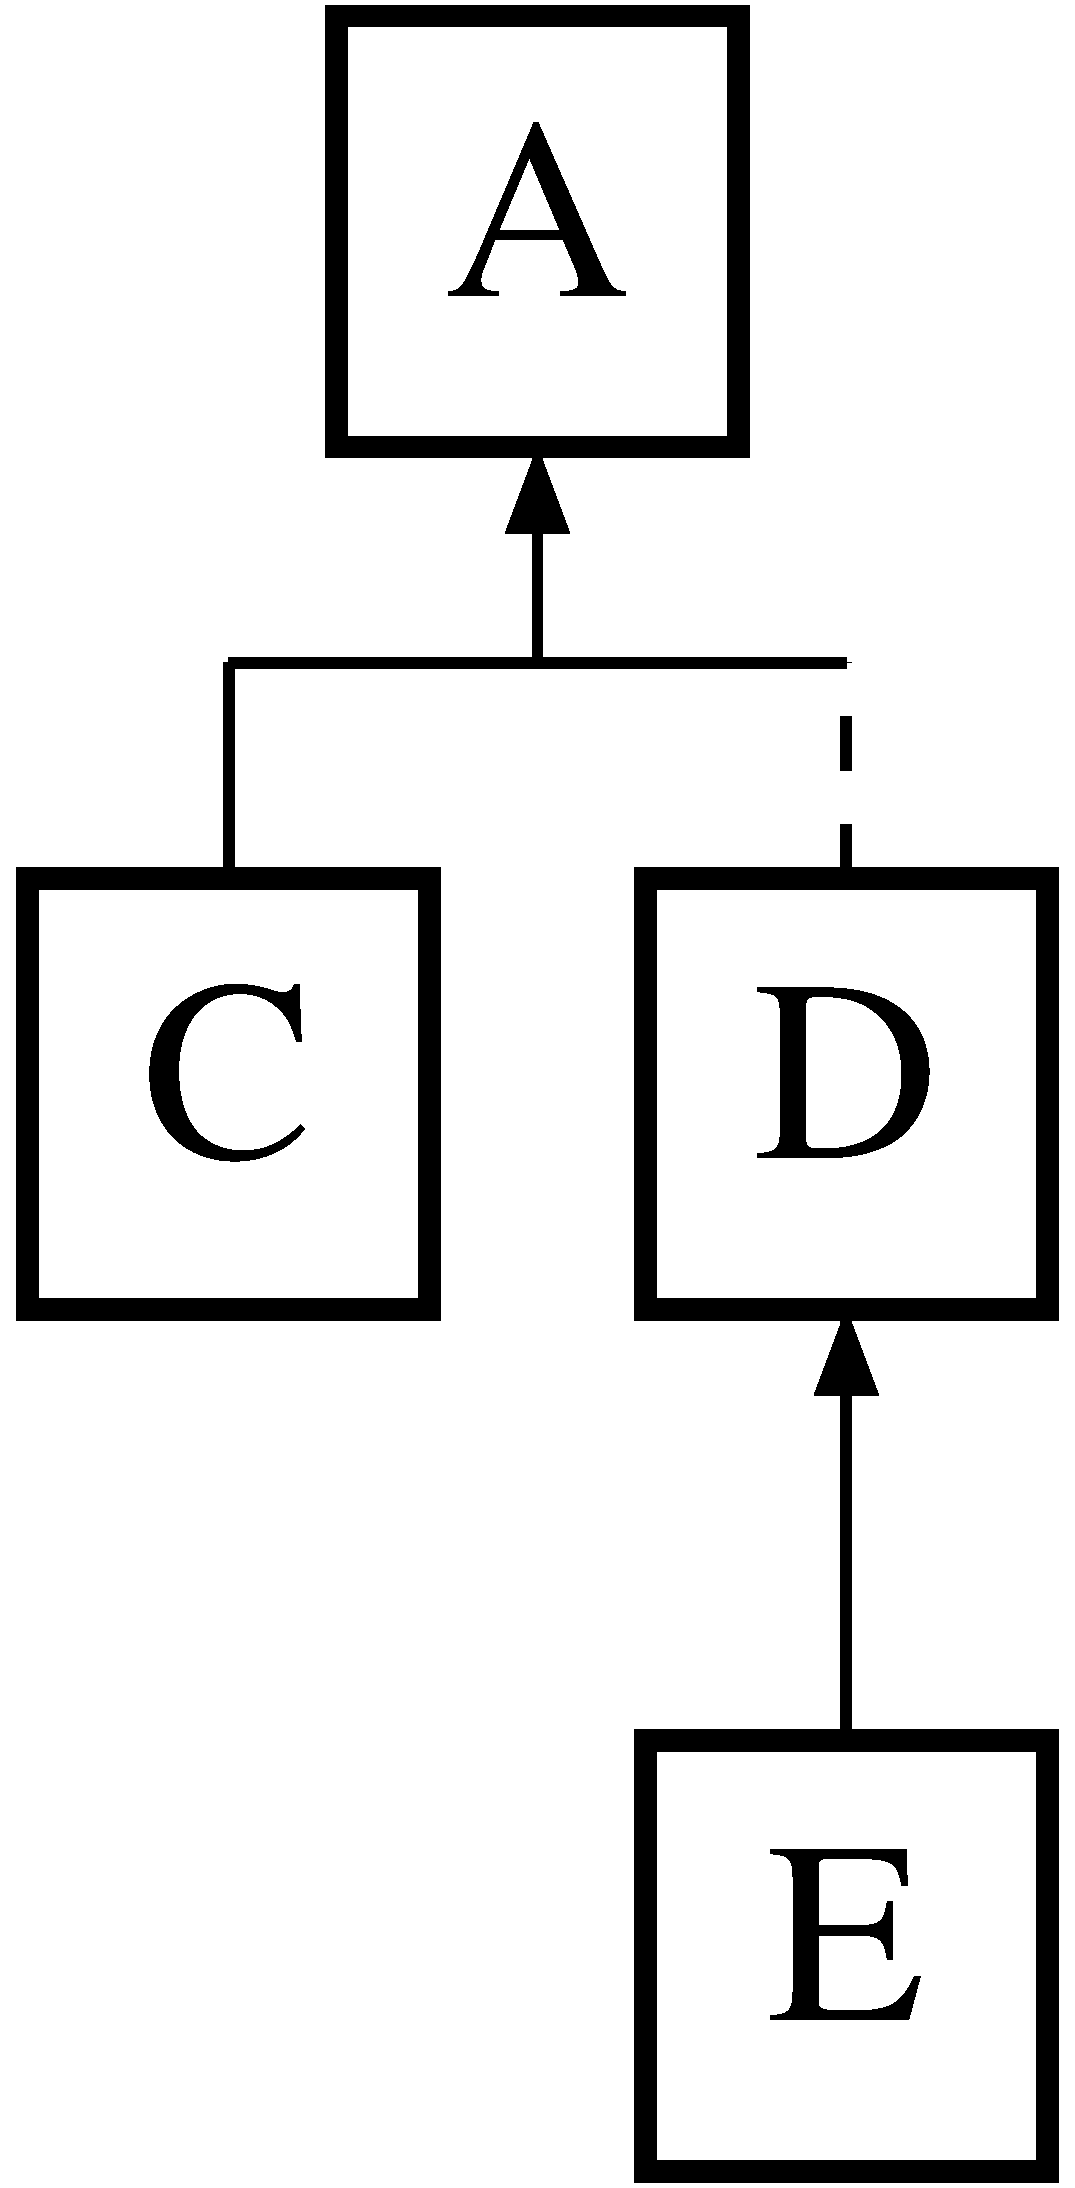
\includegraphics[height=3.000000cm]{class_a}
\end{center}
\end{figure}
\subsection*{Campos de Dados}
\begin{DoxyCompactItemize}
\item 
\hypertarget{class_a_afb4addbef001bc74a9b8dc36a11435d4}{\hyperlink{class_a}{A} $\ast$ {\bfseries m\-\_\-self}}\label{class_a_afb4addbef001bc74a9b8dc36a11435d4}

\end{DoxyCompactItemize}


A documentação para esta classe foi gerada a partir do seguinte ficheiro\-:\begin{DoxyCompactItemize}
\item 
C\-:/\-Users/teste/git/doxygen/examples/diagrams\-\_\-a.\-h\end{DoxyCompactItemize}

\hypertarget{class_access_stack}{\section{Referência à classe Access\-Stack}
\label{class_access_stack}\index{Access\-Stack@{Access\-Stack}}
}
\subsection*{Membros públicos}
\begin{DoxyCompactItemize}
\item 
\hypertarget{class_access_stack_a770760b8cb3a37199be7674943cca4e0}{void {\bfseries push} (\hyperlink{class_definition}{Definition} $\ast$scope, \hyperlink{class_file_def}{File\-Def} $\ast$file\-Scope, \hyperlink{class_definition}{Definition} $\ast$item)}\label{class_access_stack_a770760b8cb3a37199be7674943cca4e0}

\item 
\hypertarget{class_access_stack_ad56084a9ad18f00d8c7709377898a047}{void {\bfseries push} (\hyperlink{class_definition}{Definition} $\ast$scope, \hyperlink{class_file_def}{File\-Def} $\ast$file\-Scope, \hyperlink{class_definition}{Definition} $\ast$item, const \hyperlink{class_q_c_string}{Q\-C\-String} \&exp\-Scope)}\label{class_access_stack_ad56084a9ad18f00d8c7709377898a047}

\item 
\hypertarget{class_access_stack_a312e7f6c761a199c1369fbe651e084f0}{void {\bfseries pop} ()}\label{class_access_stack_a312e7f6c761a199c1369fbe651e084f0}

\item 
\hypertarget{class_access_stack_af12794e865f82afd906852a9f740ca99}{bool {\bfseries find} (\hyperlink{class_definition}{Definition} $\ast$scope, \hyperlink{class_file_def}{File\-Def} $\ast$file\-Scope, \hyperlink{class_definition}{Definition} $\ast$item)}\label{class_access_stack_af12794e865f82afd906852a9f740ca99}

\item 
\hypertarget{class_access_stack_ad0b1a28f743f50af30e0fdfc88cf6026}{bool {\bfseries find} (\hyperlink{class_definition}{Definition} $\ast$scope, \hyperlink{class_file_def}{File\-Def} $\ast$file\-Scope, \hyperlink{class_definition}{Definition} $\ast$item, const \hyperlink{class_q_c_string}{Q\-C\-String} \&exp\-Scope)}\label{class_access_stack_ad0b1a28f743f50af30e0fdfc88cf6026}

\end{DoxyCompactItemize}


\subsection{Descrição detalhada}
Helper class representing the stack of items considered while resolving the scope. 

A documentação para esta classe foi gerada a partir do seguinte ficheiro\-:\begin{DoxyCompactItemize}
\item 
C\-:/\-Users/teste/git/doxygen/src/util.\-cpp\end{DoxyCompactItemize}

\hypertarget{struct_active_row_span}{\section{Referência à estrutura Active\-Row\-Span}
\label{struct_active_row_span}\index{Active\-Row\-Span@{Active\-Row\-Span}}
}
\subsection*{Membros públicos}
\begin{DoxyCompactItemize}
\item 
\hypertarget{struct_active_row_span_a4d9d472030bddcae47e2f1b838fcc941}{{\bfseries Active\-Row\-Span} (int rows, int col)}\label{struct_active_row_span_a4d9d472030bddcae47e2f1b838fcc941}

\end{DoxyCompactItemize}
\subsection*{Campos de Dados}
\begin{DoxyCompactItemize}
\item 
\hypertarget{struct_active_row_span_a3311ae32e15ba38b689bdabe2f5184bc}{int {\bfseries rows\-Left}}\label{struct_active_row_span_a3311ae32e15ba38b689bdabe2f5184bc}

\item 
\hypertarget{struct_active_row_span_a60dae4c6e78188cd718b696e4f08fc71}{int {\bfseries column}}\label{struct_active_row_span_a60dae4c6e78188cd718b696e4f08fc71}

\end{DoxyCompactItemize}


\subsection{Descrição detalhada}
Helper class to compute the grid for an H\-T\-M\-L style table 

A documentação para esta estrutura foi gerada a partir do seguinte ficheiro\-:\begin{DoxyCompactItemize}
\item 
C\-:/\-Users/teste/git/doxygen/src/docparser.\-cpp\end{DoxyCompactItemize}

\hypertarget{class_alpha_index_table_cell}{\section{Referência à classe Alpha\-Index\-Table\-Cell}
\label{class_alpha_index_table_cell}\index{Alpha\-Index\-Table\-Cell@{Alpha\-Index\-Table\-Cell}}
}
\subsection*{Membros públicos}
\begin{DoxyCompactItemize}
\item 
\hypertarget{class_alpha_index_table_cell_a5c654622b248e963252edc7c1a5ec049}{{\bfseries Alpha\-Index\-Table\-Cell} (int row, int col, uint letter, \hyperlink{class_class_def}{Class\-Def} $\ast$cd)}\label{class_alpha_index_table_cell_a5c654622b248e963252edc7c1a5ec049}

\item 
\hypertarget{class_alpha_index_table_cell_aab2ee4c536711b2c9bd16319dacc360c}{\hyperlink{class_class_def}{Class\-Def} $\ast$ {\bfseries class\-Def} () const }\label{class_alpha_index_table_cell_aab2ee4c536711b2c9bd16319dacc360c}

\item 
\hypertarget{class_alpha_index_table_cell_ada472040436550156c7064317abe8caa}{uint {\bfseries letter} () const }\label{class_alpha_index_table_cell_ada472040436550156c7064317abe8caa}

\item 
\hypertarget{class_alpha_index_table_cell_a94244f770612e6c7739962d275ea903f}{int {\bfseries row} () const }\label{class_alpha_index_table_cell_a94244f770612e6c7739962d275ea903f}

\item 
\hypertarget{class_alpha_index_table_cell_a77699286fb6fcf791195b129badbe160}{int {\bfseries column} () const }\label{class_alpha_index_table_cell_a77699286fb6fcf791195b129badbe160}

\end{DoxyCompactItemize}


\subsection{Descrição detalhada}
Class representing a cell in the alphabetical class index. 

A documentação para esta classe foi gerada a partir do seguinte ficheiro\-:\begin{DoxyCompactItemize}
\item 
C\-:/\-Users/teste/git/doxygen/src/\hyperlink{index_8cpp}{index.\-cpp}\end{DoxyCompactItemize}

\hypertarget{class_alpha_index_table_columns}{\section{Referência à classe Alpha\-Index\-Table\-Columns}
\label{class_alpha_index_table_columns}\index{Alpha\-Index\-Table\-Columns@{Alpha\-Index\-Table\-Columns}}
}
Diagrama de heranças da classe Alpha\-Index\-Table\-Columns\begin{figure}[H]
\begin{center}
\leavevmode
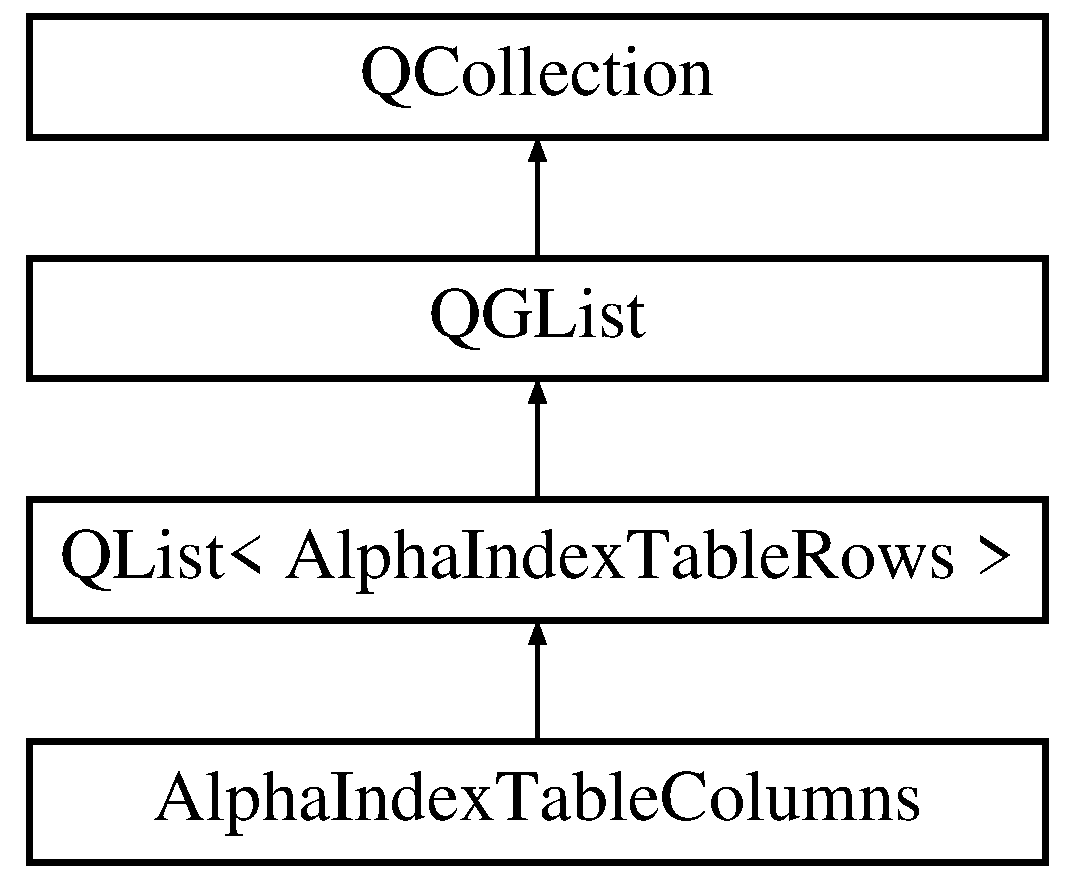
\includegraphics[height=4.000000cm]{class_alpha_index_table_columns}
\end{center}
\end{figure}
\subsection*{Additional Inherited Members}


\subsection{Descrição detalhada}
Class representing the columns in the alphabetical class index. 

A documentação para esta classe foi gerada a partir do seguinte ficheiro\-:\begin{DoxyCompactItemize}
\item 
C\-:/\-Users/teste/git/doxygen/src/\hyperlink{index_8cpp}{index.\-cpp}\end{DoxyCompactItemize}

\hypertarget{class_alpha_index_table_rows}{\section{Referência à classe Alpha\-Index\-Table\-Rows}
\label{class_alpha_index_table_rows}\index{Alpha\-Index\-Table\-Rows@{Alpha\-Index\-Table\-Rows}}
}
Diagrama de heranças da classe Alpha\-Index\-Table\-Rows\begin{figure}[H]
\begin{center}
\leavevmode
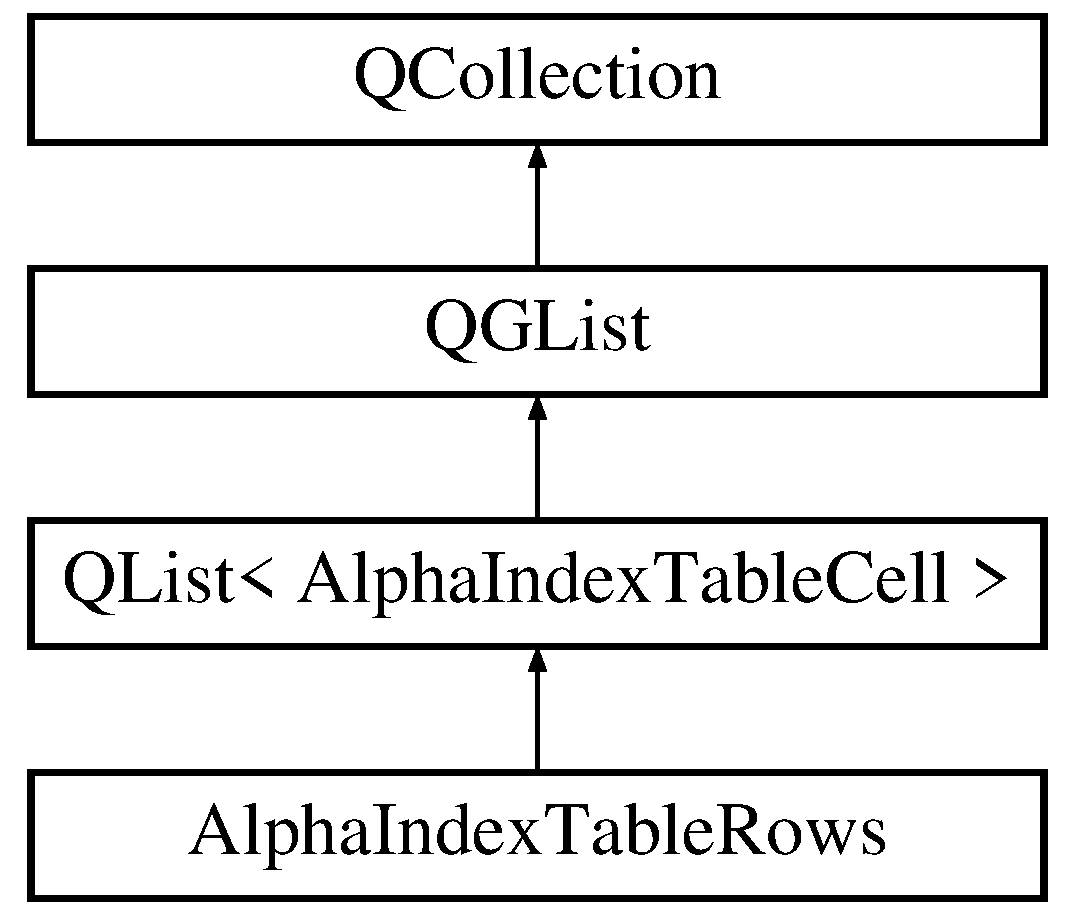
\includegraphics[height=4.000000cm]{class_alpha_index_table_rows}
\end{center}
\end{figure}
\subsection*{Additional Inherited Members}


\subsection{Descrição detalhada}
Class representing a row in the alphabetical class index. 

A documentação para esta classe foi gerada a partir do seguinte ficheiro\-:\begin{DoxyCompactItemize}
\item 
C\-:/\-Users/teste/git/doxygen/src/\hyperlink{index_8cpp}{index.\-cpp}\end{DoxyCompactItemize}

\hypertarget{class_alpha_index_table_rows_iterator}{\section{Referência à classe Alpha\-Index\-Table\-Rows\-Iterator}
\label{class_alpha_index_table_rows_iterator}\index{Alpha\-Index\-Table\-Rows\-Iterator@{Alpha\-Index\-Table\-Rows\-Iterator}}
}
Diagrama de heranças da classe Alpha\-Index\-Table\-Rows\-Iterator\begin{figure}[H]
\begin{center}
\leavevmode
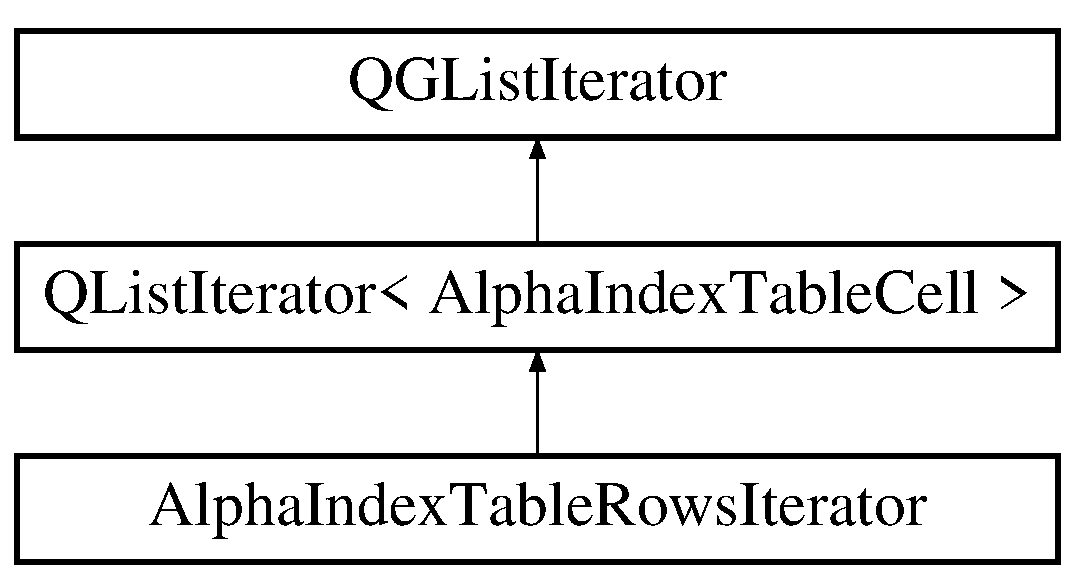
\includegraphics[height=3.000000cm]{class_alpha_index_table_rows_iterator}
\end{center}
\end{figure}
\subsection*{Membros públicos}
\begin{DoxyCompactItemize}
\item 
\hypertarget{class_alpha_index_table_rows_iterator_a02bb29d747abae2ffad7f8dd43fa95e2}{{\bfseries Alpha\-Index\-Table\-Rows\-Iterator} (const \hyperlink{class_alpha_index_table_rows}{Alpha\-Index\-Table\-Rows} \&list)}\label{class_alpha_index_table_rows_iterator_a02bb29d747abae2ffad7f8dd43fa95e2}

\end{DoxyCompactItemize}
\subsection*{Additional Inherited Members}


\subsection{Descrição detalhada}
Iterator for the cells in a row of the alphabetical class index. 

A documentação para esta classe foi gerada a partir do seguinte ficheiro\-:\begin{DoxyCompactItemize}
\item 
C\-:/\-Users/teste/git/doxygen/src/\hyperlink{index_8cpp}{index.\-cpp}\end{DoxyCompactItemize}

\hypertarget{class_anchor_handler}{\section{Referência à classe Anchor\-Handler}
\label{class_anchor_handler}\index{Anchor\-Handler@{Anchor\-Handler}}
}


Node representing an anchor.  




{\ttfamily \#include $<$dochandler.\-h$>$}

Diagrama de heranças da classe Anchor\-Handler\begin{figure}[H]
\begin{center}
\leavevmode
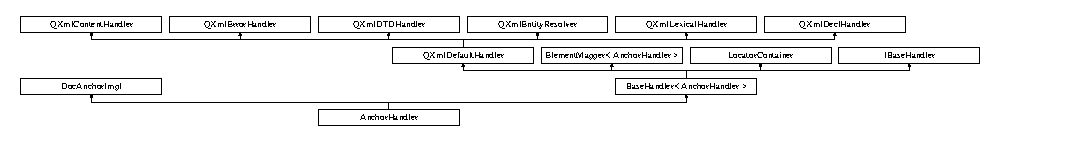
\includegraphics[height=1.461187cm]{class_anchor_handler}
\end{center}
\end{figure}
\subsection*{Membros públicos}
\begin{DoxyCompactItemize}
\item 
\hypertarget{class_anchor_handler_a6bb2c41056e6dcf6fcc4c9aad99655ad}{{\bfseries Anchor\-Handler} (\hyperlink{class_i_base_handler}{I\-Base\-Handler} $\ast$parent)}\label{class_anchor_handler_a6bb2c41056e6dcf6fcc4c9aad99655ad}

\item 
\hypertarget{class_anchor_handler_a13989618fc696558cb6fe547d7b58162}{void {\bfseries start\-Anchor} (const \hyperlink{class_q_xml_attributes}{Q\-Xml\-Attributes} \&attrib)}\label{class_anchor_handler_a13989618fc696558cb6fe547d7b58162}

\item 
\hypertarget{class_anchor_handler_af1003a9106437d3fa31091d86e6ff514}{void {\bfseries end\-Anchor} ()}\label{class_anchor_handler_af1003a9106437d3fa31091d86e6ff514}

\item 
\hypertarget{class_anchor_handler_af8e62c8a81ddf2283205cc8955de50eb}{virtual Kind {\bfseries kind} () const }\label{class_anchor_handler_af8e62c8a81ddf2283205cc8955de50eb}

\item 
\hypertarget{class_anchor_handler_acf656d73faffcdf0382f68eb78869cf4}{virtual const \hyperlink{class_i_string}{I\-String} $\ast$ {\bfseries id} () const }\label{class_anchor_handler_acf656d73faffcdf0382f68eb78869cf4}

\end{DoxyCompactItemize}
\subsection*{Additional Inherited Members}


\subsection{Descrição detalhada}
Node representing an anchor. 



A documentação para esta classe foi gerada a partir dos seguintes ficheiros\-:\begin{DoxyCompactItemize}
\item 
C\-:/\-Users/teste/git/doxygen/addon/doxmlparser/src/dochandler.\-h\item 
C\-:/\-Users/teste/git/doxygen/addon/doxmlparser/src/dochandler.\-cpp\end{DoxyCompactItemize}

\hypertarget{struct_argument}{\section{Referência à estrutura Argument}
\label{struct_argument}\index{Argument@{Argument}}
}


This class contains the information about the argument of a function or template.  




{\ttfamily \#include $<$arguments.\-h$>$}

\subsection*{Membros públicos}
\begin{DoxyCompactItemize}
\item 
\hyperlink{struct_argument_aedc8c00f523413f83bf6652cbd05bf30}{Argument} ()
\item 
\hyperlink{struct_argument_a60b6d8d358684db956863c177c00ee90}{Argument} (const \hyperlink{struct_argument}{Argument} \&a)
\item 
\hyperlink{struct_argument}{Argument} \& \hyperlink{struct_argument_aea8e40db597c56e0dd885bb20b33280c}{operator=} (const \hyperlink{struct_argument}{Argument} \&a)
\item 
bool \hyperlink{struct_argument_a585dcd381ab70014568db8ad457fc8b1}{has\-Documentation} () const 
\end{DoxyCompactItemize}
\subsection*{Campos de Dados}
\begin{DoxyCompactItemize}
\item 
\hyperlink{class_q_c_string}{Q\-C\-String} \hyperlink{struct_argument_a568fa5bb9141551201cb4822cc8ae7b7}{attrib}
\item 
\hyperlink{class_q_c_string}{Q\-C\-String} \hyperlink{struct_argument_a0d4463771e24026060ae68b04822d7af}{type}
\item 
\hyperlink{class_q_c_string}{Q\-C\-String} \hyperlink{struct_argument_a74d54ffc237b2b850e50345e7c8fa3a4}{can\-Type}
\item 
\hyperlink{class_q_c_string}{Q\-C\-String} \hyperlink{struct_argument_adc0097c7bd1e61ad32058fcde425bc7a}{name}
\item 
\hyperlink{class_q_c_string}{Q\-C\-String} \hyperlink{struct_argument_a86c3f26165f8d189358a5496e71a929d}{array}
\item 
\hyperlink{class_q_c_string}{Q\-C\-String} \hyperlink{struct_argument_a838035f10d60ad8fc6923ab1bb3f3e51}{defval}
\item 
\hyperlink{class_q_c_string}{Q\-C\-String} \hyperlink{struct_argument_a19e06f4d6586ea625f163986a2604c36}{docs}
\end{DoxyCompactItemize}


\subsection{Descrição detalhada}
This class contains the information about the argument of a function or template. 



\subsection{Documentação dos Construtores \& Destrutor}
\hypertarget{struct_argument_aedc8c00f523413f83bf6652cbd05bf30}{\index{Argument@{Argument}!Argument@{Argument}}
\index{Argument@{Argument}!Argument@{Argument}}
\subsubsection[{Argument}]{\setlength{\rightskip}{0pt plus 5cm}{\bf Argument} (
\begin{DoxyParamCaption}
{}
\end{DoxyParamCaption}
)\hspace{0.3cm}{\ttfamily [inline]}}}\label{struct_argument_aedc8c00f523413f83bf6652cbd05bf30}
Construct a new argument. \hypertarget{struct_argument_a60b6d8d358684db956863c177c00ee90}{\index{Argument@{Argument}!Argument@{Argument}}
\index{Argument@{Argument}!Argument@{Argument}}
\subsubsection[{Argument}]{\setlength{\rightskip}{0pt plus 5cm}{\bf Argument} (
\begin{DoxyParamCaption}
\item[{const {\bf Argument} \&}]{a}
\end{DoxyParamCaption}
)\hspace{0.3cm}{\ttfamily [inline]}}}\label{struct_argument_a60b6d8d358684db956863c177c00ee90}
Copy an argument (does a deep copy of all strings). 

\subsection{Documentação dos métodos}
\hypertarget{struct_argument_a585dcd381ab70014568db8ad457fc8b1}{\index{Argument@{Argument}!has\-Documentation@{has\-Documentation}}
\index{has\-Documentation@{has\-Documentation}!Argument@{Argument}}
\subsubsection[{has\-Documentation}]{\setlength{\rightskip}{0pt plus 5cm}bool has\-Documentation (
\begin{DoxyParamCaption}
{}
\end{DoxyParamCaption}
) const\hspace{0.3cm}{\ttfamily [inline]}}}\label{struct_argument_a585dcd381ab70014568db8ad457fc8b1}
return T\-R\-U\-E if this argument is documentation and the argument has a non empty name. \hypertarget{struct_argument_aea8e40db597c56e0dd885bb20b33280c}{\index{Argument@{Argument}!operator=@{operator=}}
\index{operator=@{operator=}!Argument@{Argument}}
\subsubsection[{operator=}]{\setlength{\rightskip}{0pt plus 5cm}{\bf Argument}\& operator= (
\begin{DoxyParamCaption}
\item[{const {\bf Argument} \&}]{a}
\end{DoxyParamCaption}
)\hspace{0.3cm}{\ttfamily [inline]}}}\label{struct_argument_aea8e40db597c56e0dd885bb20b33280c}
Assignment of an argument (does a deep copy of all strings). 

\subsection{Documentação dos campos e atributos}
\hypertarget{struct_argument_a86c3f26165f8d189358a5496e71a929d}{\index{Argument@{Argument}!array@{array}}
\index{array@{array}!Argument@{Argument}}
\subsubsection[{array}]{\setlength{\rightskip}{0pt plus 5cm}{\bf Q\-C\-String} array}}\label{struct_argument_a86c3f26165f8d189358a5496e71a929d}
\hyperlink{struct_argument}{Argument}'s array specifier (may be empty) \hypertarget{struct_argument_a568fa5bb9141551201cb4822cc8ae7b7}{\index{Argument@{Argument}!attrib@{attrib}}
\index{attrib@{attrib}!Argument@{Argument}}
\subsubsection[{attrib}]{\setlength{\rightskip}{0pt plus 5cm}{\bf Q\-C\-String} attrib}}\label{struct_argument_a568fa5bb9141551201cb4822cc8ae7b7}
\hyperlink{struct_argument}{Argument}'s attribute (I\-D\-L only) \hypertarget{struct_argument_a74d54ffc237b2b850e50345e7c8fa3a4}{\index{Argument@{Argument}!can\-Type@{can\-Type}}
\index{can\-Type@{can\-Type}!Argument@{Argument}}
\subsubsection[{can\-Type}]{\setlength{\rightskip}{0pt plus 5cm}{\bf Q\-C\-String} can\-Type}}\label{struct_argument_a74d54ffc237b2b850e50345e7c8fa3a4}
Cached value of canonical type (after type resolution). Empty initially. \hypertarget{struct_argument_a838035f10d60ad8fc6923ab1bb3f3e51}{\index{Argument@{Argument}!defval@{defval}}
\index{defval@{defval}!Argument@{Argument}}
\subsubsection[{defval}]{\setlength{\rightskip}{0pt plus 5cm}{\bf Q\-C\-String} defval}}\label{struct_argument_a838035f10d60ad8fc6923ab1bb3f3e51}
\hyperlink{struct_argument}{Argument}'s default value (may be empty) \hypertarget{struct_argument_a19e06f4d6586ea625f163986a2604c36}{\index{Argument@{Argument}!docs@{docs}}
\index{docs@{docs}!Argument@{Argument}}
\subsubsection[{docs}]{\setlength{\rightskip}{0pt plus 5cm}{\bf Q\-C\-String} docs}}\label{struct_argument_a19e06f4d6586ea625f163986a2604c36}
\hyperlink{struct_argument}{Argument}'s documentation (may be empty) \hypertarget{struct_argument_adc0097c7bd1e61ad32058fcde425bc7a}{\index{Argument@{Argument}!name@{name}}
\index{name@{name}!Argument@{Argument}}
\subsubsection[{name}]{\setlength{\rightskip}{0pt plus 5cm}{\bf Q\-C\-String} name}}\label{struct_argument_adc0097c7bd1e61ad32058fcde425bc7a}
\hyperlink{struct_argument}{Argument}'s name (may be empty) \hypertarget{struct_argument_a0d4463771e24026060ae68b04822d7af}{\index{Argument@{Argument}!type@{type}}
\index{type@{type}!Argument@{Argument}}
\subsubsection[{type}]{\setlength{\rightskip}{0pt plus 5cm}{\bf Q\-C\-String} type}}\label{struct_argument_a0d4463771e24026060ae68b04822d7af}
\hyperlink{struct_argument}{Argument}'s type 

A documentação para esta estrutura foi gerada a partir do seguinte ficheiro\-:\begin{DoxyCompactItemize}
\item 
C\-:/\-Users/teste/git/doxygen/src/arguments.\-h\end{DoxyCompactItemize}

\hypertarget{class_argument_context}{\section{Referência à classe Argument\-Context}
\label{class_argument_context}\index{Argument\-Context@{Argument\-Context}}
}
Diagrama de heranças da classe Argument\-Context\begin{figure}[H]
\begin{center}
\leavevmode
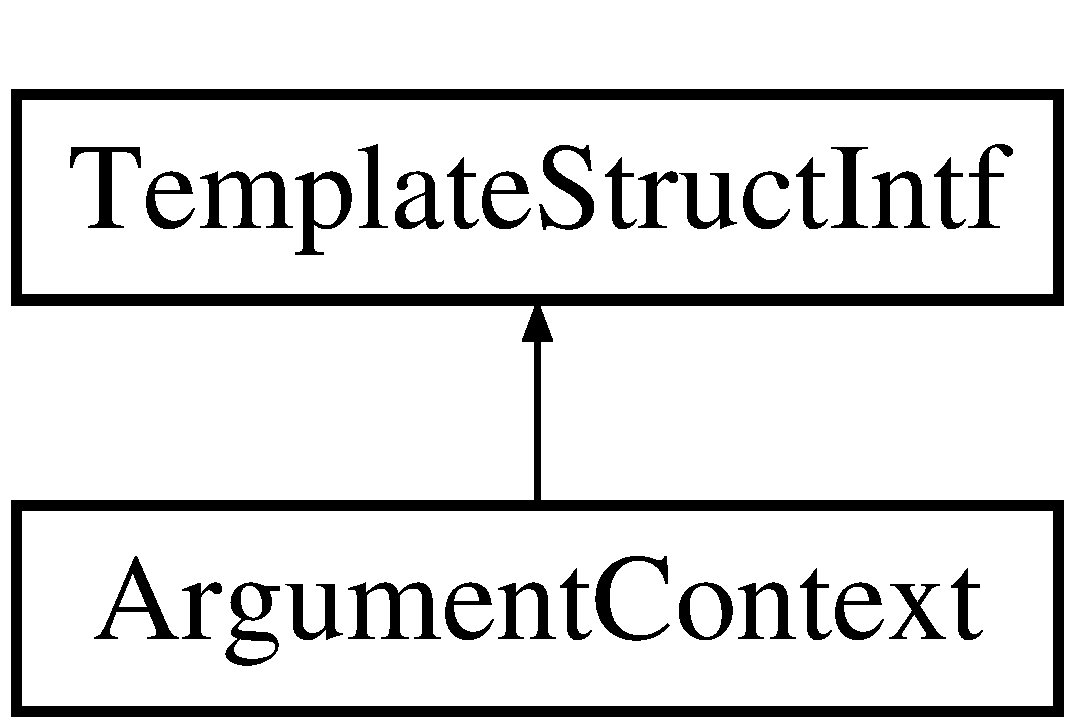
\includegraphics[height=2.000000cm]{class_argument_context}
\end{center}
\end{figure}
\subsection*{Estruturas de Dados}
\begin{DoxyCompactItemize}
\item 
class \hyperlink{class_argument_context_1_1_private}{Private}
\end{DoxyCompactItemize}
\subsection*{Membros públicos}
\begin{DoxyCompactItemize}
\item 
\hypertarget{class_argument_context_ac00834b32c1194fdc6167d91459c2d8c}{{\bfseries Argument\-Context} (const \hyperlink{struct_argument}{Argument} $\ast$arg)}\label{class_argument_context_ac00834b32c1194fdc6167d91459c2d8c}

\item 
virtual \hyperlink{class_template_variant}{Template\-Variant} \hyperlink{class_argument_context_a1bcfea01201f3ea09981a8442842c42d}{get} (const char $\ast$name) const 
\end{DoxyCompactItemize}


\subsection{Documentação dos métodos}
\hypertarget{class_argument_context_a1bcfea01201f3ea09981a8442842c42d}{\index{Argument\-Context@{Argument\-Context}!get@{get}}
\index{get@{get}!ArgumentContext@{Argument\-Context}}
\subsubsection[{get}]{\setlength{\rightskip}{0pt plus 5cm}{\bf Template\-Variant} get (
\begin{DoxyParamCaption}
\item[{const char $\ast$}]{name}
\end{DoxyParamCaption}
) const\hspace{0.3cm}{\ttfamily [virtual]}}}\label{class_argument_context_a1bcfea01201f3ea09981a8442842c42d}
Gets the value for a field name. 
\begin{DoxyParams}[1]{Parâmetros}
\mbox{\tt in}  & {\em name} & The name of the field. \\
\hline
\end{DoxyParams}


Implementa \hyperlink{class_template_struct_intf_a49a65a897ba5e4cd6cb80d681c843aab}{Template\-Struct\-Intf}.



A documentação para esta classe foi gerada a partir dos seguintes ficheiros\-:\begin{DoxyCompactItemize}
\item 
C\-:/\-Users/teste/git/doxygen/src/context.\-h\item 
C\-:/\-Users/teste/git/doxygen/src/context.\-cpp\end{DoxyCompactItemize}

\hypertarget{class_argument_list}{\section{Referência à classe Argument\-List}
\label{class_argument_list}\index{Argument\-List@{Argument\-List}}
}


This class represents an function or template argument list.  




{\ttfamily \#include $<$arguments.\-h$>$}

Diagrama de heranças da classe Argument\-List\begin{figure}[H]
\begin{center}
\leavevmode
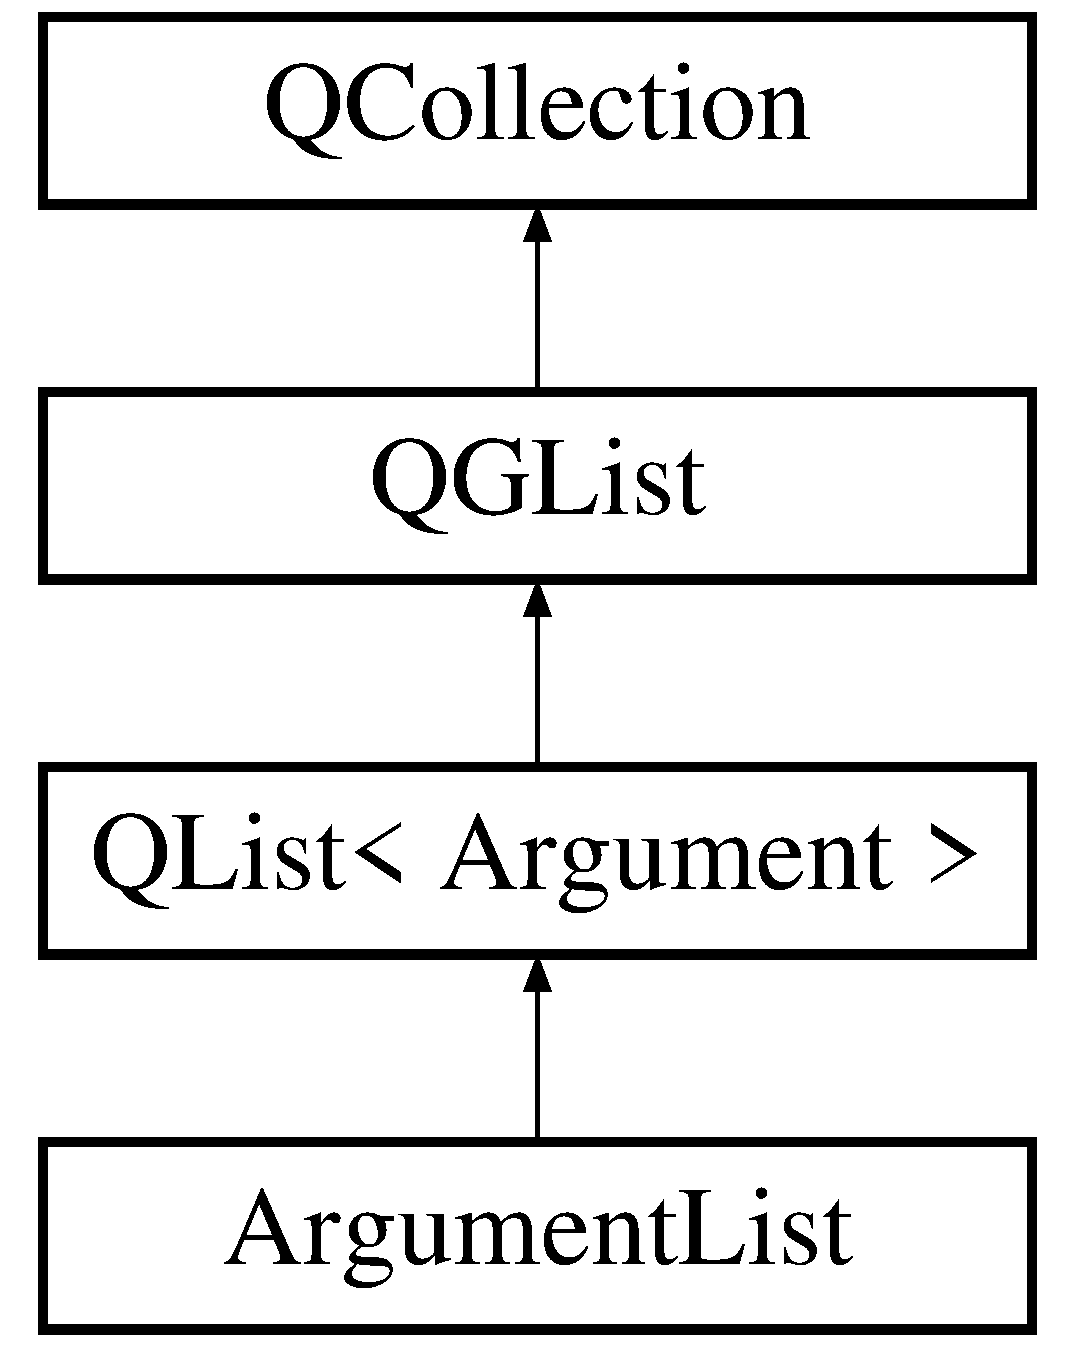
\includegraphics[height=4.000000cm]{class_argument_list}
\end{center}
\end{figure}
\subsection*{Membros públicos}
\begin{DoxyCompactItemize}
\item 
\hyperlink{class_argument_list_ab6e8f177f57931b8a4dc90e1bbf9bcf9}{Argument\-List} ()
\item 
\hyperlink{class_argument_list_a0e37716baa29c469bd5f1cc275481382}{$\sim$\-Argument\-List} ()
\item 
\hyperlink{class_argument_list}{Argument\-List} $\ast$ \hyperlink{class_argument_list_a2cfe4a2968e0438d00ef3b2405127fa6}{deep\-Copy} () const 
\item 
bool \hyperlink{class_argument_list_a585dcd381ab70014568db8ad457fc8b1}{has\-Documentation} () const 
\end{DoxyCompactItemize}
\subsection*{Membros públicos estáticos}
\begin{DoxyCompactItemize}
\item 
static \hyperlink{class_argument_list}{Argument\-List} $\ast$ \hyperlink{class_argument_list_a931d2e722c3f11a736082a0f46c22ba9}{unmarshal} (\hyperlink{class_storage_intf}{Storage\-Intf} $\ast$s)
\item 
\hypertarget{class_argument_list_a116d2c2c834eeb43147fd69379f36f9c}{static void {\bfseries marshal} (\hyperlink{class_storage_intf}{Storage\-Intf} $\ast$s, \hyperlink{class_argument_list}{Argument\-List} $\ast$arg\-List)}\label{class_argument_list_a116d2c2c834eeb43147fd69379f36f9c}

\end{DoxyCompactItemize}
\subsection*{Campos de Dados}
\begin{DoxyCompactItemize}
\item 
bool \hyperlink{class_argument_list_a9ab1475bcbf4f17b50c7b5a3110743db}{const\-Specifier}
\item 
bool \hyperlink{class_argument_list_a7d6765f3c1ff9ee13a05a1eabbefc965}{volatile\-Specifier}
\item 
bool \hyperlink{class_argument_list_a7606644da45fc7bbd695bad212ede6af}{pure\-Specifier}
\item 
\hyperlink{class_q_c_string}{Q\-C\-String} \hyperlink{class_argument_list_ac2cd23d5da83b9f380f0e0a69bcace02}{trailing\-Return\-Type}
\end{DoxyCompactItemize}
\subsection*{Additional Inherited Members}


\subsection{Descrição detalhada}
This class represents an function or template argument list. 

This class also stores some information about member that is typically put after the argument list, such as whether the member is const, volatile or pure virtual. 

\subsection{Documentação dos Construtores \& Destrutor}
\hypertarget{class_argument_list_ab6e8f177f57931b8a4dc90e1bbf9bcf9}{\index{Argument\-List@{Argument\-List}!Argument\-List@{Argument\-List}}
\index{Argument\-List@{Argument\-List}!ArgumentList@{Argument\-List}}
\subsubsection[{Argument\-List}]{\setlength{\rightskip}{0pt plus 5cm}{\bf Argument\-List} (
\begin{DoxyParamCaption}
{}
\end{DoxyParamCaption}
)\hspace{0.3cm}{\ttfamily [inline]}}}\label{class_argument_list_ab6e8f177f57931b8a4dc90e1bbf9bcf9}
Creates an empty argument list \hypertarget{class_argument_list_a0e37716baa29c469bd5f1cc275481382}{\index{Argument\-List@{Argument\-List}!$\sim$\-Argument\-List@{$\sim$\-Argument\-List}}
\index{$\sim$\-Argument\-List@{$\sim$\-Argument\-List}!ArgumentList@{Argument\-List}}
\subsubsection[{$\sim$\-Argument\-List}]{\setlength{\rightskip}{0pt plus 5cm}$\sim${\bf Argument\-List} (
\begin{DoxyParamCaption}
{}
\end{DoxyParamCaption}
)\hspace{0.3cm}{\ttfamily [inline]}}}\label{class_argument_list_a0e37716baa29c469bd5f1cc275481382}
Destroys the argument list 

\subsection{Documentação dos métodos}
\hypertarget{class_argument_list_a2cfe4a2968e0438d00ef3b2405127fa6}{\index{Argument\-List@{Argument\-List}!deep\-Copy@{deep\-Copy}}
\index{deep\-Copy@{deep\-Copy}!ArgumentList@{Argument\-List}}
\subsubsection[{deep\-Copy}]{\setlength{\rightskip}{0pt plus 5cm}{\bf Argument\-List} $\ast$ deep\-Copy (
\begin{DoxyParamCaption}
{}
\end{DoxyParamCaption}
) const}}\label{class_argument_list_a2cfe4a2968e0438d00ef3b2405127fa6}
Makes a deep copy of this object \hypertarget{class_argument_list_a585dcd381ab70014568db8ad457fc8b1}{\index{Argument\-List@{Argument\-List}!has\-Documentation@{has\-Documentation}}
\index{has\-Documentation@{has\-Documentation}!ArgumentList@{Argument\-List}}
\subsubsection[{has\-Documentation}]{\setlength{\rightskip}{0pt plus 5cm}bool has\-Documentation (
\begin{DoxyParamCaption}
{}
\end{DoxyParamCaption}
) const}}\label{class_argument_list_a585dcd381ab70014568db8ad457fc8b1}
Does any argument of this list have documentation?

the argument list is documented if one of its arguments is documented \hypertarget{class_argument_list_a931d2e722c3f11a736082a0f46c22ba9}{\index{Argument\-List@{Argument\-List}!unmarshal@{unmarshal}}
\index{unmarshal@{unmarshal}!ArgumentList@{Argument\-List}}
\subsubsection[{unmarshal}]{\setlength{\rightskip}{0pt plus 5cm}{\bf Argument\-List} $\ast$ unmarshal (
\begin{DoxyParamCaption}
\item[{{\bf Storage\-Intf} $\ast$}]{s}
\end{DoxyParamCaption}
)\hspace{0.3cm}{\ttfamily [static]}}}\label{class_argument_list_a931d2e722c3f11a736082a0f46c22ba9}
C++11 defaulted method 

\subsection{Documentação dos campos e atributos}
\hypertarget{class_argument_list_a9ab1475bcbf4f17b50c7b5a3110743db}{\index{Argument\-List@{Argument\-List}!const\-Specifier@{const\-Specifier}}
\index{const\-Specifier@{const\-Specifier}!ArgumentList@{Argument\-List}}
\subsubsection[{const\-Specifier}]{\setlength{\rightskip}{0pt plus 5cm}bool const\-Specifier}}\label{class_argument_list_a9ab1475bcbf4f17b50c7b5a3110743db}
Does the member modify the state of the class? default\-: F\-A\-L\-S\-E. \hypertarget{class_argument_list_a7606644da45fc7bbd695bad212ede6af}{\index{Argument\-List@{Argument\-List}!pure\-Specifier@{pure\-Specifier}}
\index{pure\-Specifier@{pure\-Specifier}!ArgumentList@{Argument\-List}}
\subsubsection[{pure\-Specifier}]{\setlength{\rightskip}{0pt plus 5cm}bool pure\-Specifier}}\label{class_argument_list_a7606644da45fc7bbd695bad212ede6af}
Is this a pure virtual member? default\-: F\-A\-L\-S\-E \hypertarget{class_argument_list_ac2cd23d5da83b9f380f0e0a69bcace02}{\index{Argument\-List@{Argument\-List}!trailing\-Return\-Type@{trailing\-Return\-Type}}
\index{trailing\-Return\-Type@{trailing\-Return\-Type}!ArgumentList@{Argument\-List}}
\subsubsection[{trailing\-Return\-Type}]{\setlength{\rightskip}{0pt plus 5cm}{\bf Q\-C\-String} trailing\-Return\-Type}}\label{class_argument_list_ac2cd23d5da83b9f380f0e0a69bcace02}
C++11 style Trailing return type? \hypertarget{class_argument_list_a7d6765f3c1ff9ee13a05a1eabbefc965}{\index{Argument\-List@{Argument\-List}!volatile\-Specifier@{volatile\-Specifier}}
\index{volatile\-Specifier@{volatile\-Specifier}!ArgumentList@{Argument\-List}}
\subsubsection[{volatile\-Specifier}]{\setlength{\rightskip}{0pt plus 5cm}bool volatile\-Specifier}}\label{class_argument_list_a7d6765f3c1ff9ee13a05a1eabbefc965}
Is the member volatile? default\-: F\-A\-L\-S\-E. 

A documentação para esta classe foi gerada a partir dos seguintes ficheiros\-:\begin{DoxyCompactItemize}
\item 
C\-:/\-Users/teste/git/doxygen/src/arguments.\-h\item 
C\-:/\-Users/teste/git/doxygen/src/arguments.\-cpp\end{DoxyCompactItemize}

\hypertarget{class_argument_list_context}{\section{Referência à classe Argument\-List\-Context}
\label{class_argument_list_context}\index{Argument\-List\-Context@{Argument\-List\-Context}}
}
Diagrama de heranças da classe Argument\-List\-Context\begin{figure}[H]
\begin{center}
\leavevmode
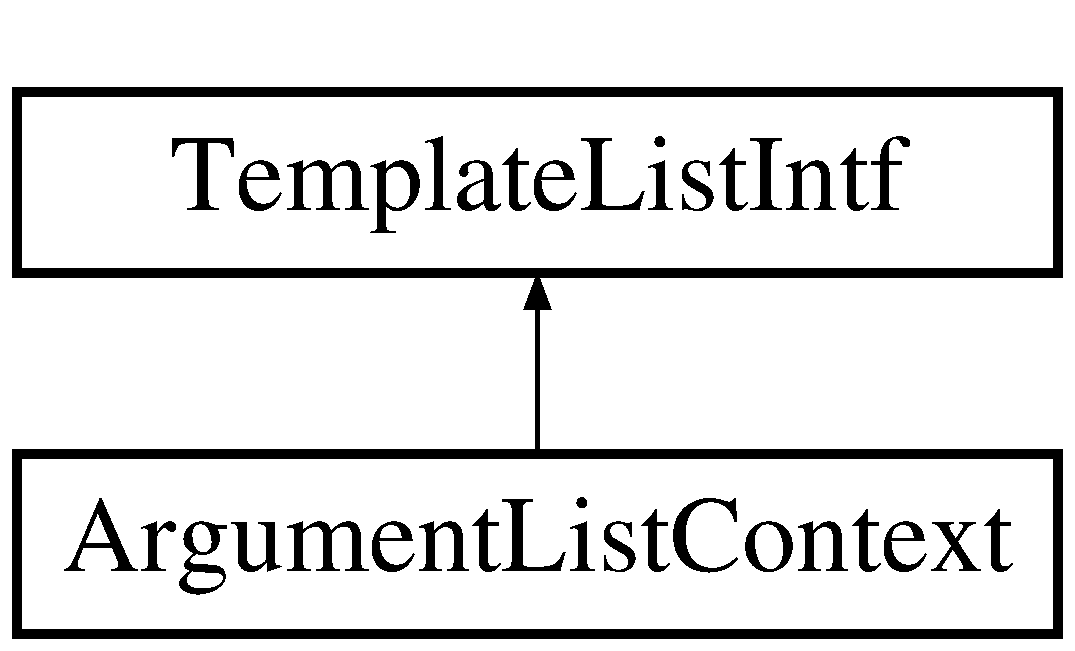
\includegraphics[height=2.000000cm]{class_argument_list_context}
\end{center}
\end{figure}
\subsection*{Estruturas de Dados}
\begin{DoxyCompactItemize}
\item 
class \hyperlink{class_argument_list_context_1_1_private}{Private}
\end{DoxyCompactItemize}
\subsection*{Membros públicos}
\begin{DoxyCompactItemize}
\item 
\hypertarget{class_argument_list_context_a575a7f15d702cbbc62f8daf44f8b1ce2}{{\bfseries Argument\-List\-Context} (const \hyperlink{class_argument_list}{Argument\-List} $\ast$al)}\label{class_argument_list_context_a575a7f15d702cbbc62f8daf44f8b1ce2}

\item 
virtual int \hyperlink{class_argument_list_context_a0745638c9967e2ed90bc96c012288c55}{count} () const 
\item 
virtual \hyperlink{class_template_variant}{Template\-Variant} \hyperlink{class_argument_list_context_a55f90d50fcb1378b2a97b9c3ad5bb162}{at} (int index) const 
\item 
virtual \\*
\hyperlink{class_template_list_intf_1_1_const_iterator}{Template\-List\-Intf\-::\-Const\-Iterator} $\ast$ \hyperlink{class_argument_list_context_a0b1d6dedc3f51750e5cba18f51022f10}{create\-Iterator} () const 
\end{DoxyCompactItemize}


\subsection{Documentação dos métodos}
\hypertarget{class_argument_list_context_a55f90d50fcb1378b2a97b9c3ad5bb162}{\index{Argument\-List\-Context@{Argument\-List\-Context}!at@{at}}
\index{at@{at}!ArgumentListContext@{Argument\-List\-Context}}
\subsubsection[{at}]{\setlength{\rightskip}{0pt plus 5cm}{\bf Template\-Variant} at (
\begin{DoxyParamCaption}
\item[{int}]{index}
\end{DoxyParamCaption}
) const\hspace{0.3cm}{\ttfamily [virtual]}}}\label{class_argument_list_context_a55f90d50fcb1378b2a97b9c3ad5bb162}
Returns the element at index position {\itshape index}. 

Implementa \hyperlink{class_template_list_intf_a6b813ba1b062c9c5b241158a4a62aea7}{Template\-List\-Intf}.

\hypertarget{class_argument_list_context_a0745638c9967e2ed90bc96c012288c55}{\index{Argument\-List\-Context@{Argument\-List\-Context}!count@{count}}
\index{count@{count}!ArgumentListContext@{Argument\-List\-Context}}
\subsubsection[{count}]{\setlength{\rightskip}{0pt plus 5cm}int count (
\begin{DoxyParamCaption}
{}
\end{DoxyParamCaption}
) const\hspace{0.3cm}{\ttfamily [virtual]}}}\label{class_argument_list_context_a0745638c9967e2ed90bc96c012288c55}
Returns the number of elements in the list 

Implementa \hyperlink{class_template_list_intf_ac5a730d48b86f871bc036571234d1332}{Template\-List\-Intf}.

\hypertarget{class_argument_list_context_a0b1d6dedc3f51750e5cba18f51022f10}{\index{Argument\-List\-Context@{Argument\-List\-Context}!create\-Iterator@{create\-Iterator}}
\index{create\-Iterator@{create\-Iterator}!ArgumentListContext@{Argument\-List\-Context}}
\subsubsection[{create\-Iterator}]{\setlength{\rightskip}{0pt plus 5cm}{\bf Template\-List\-Intf\-::\-Const\-Iterator} $\ast$ create\-Iterator (
\begin{DoxyParamCaption}
{}
\end{DoxyParamCaption}
) const\hspace{0.3cm}{\ttfamily [virtual]}}}\label{class_argument_list_context_a0b1d6dedc3f51750e5cba18f51022f10}
Creates a new iterator for this list. \begin{DoxyNote}{Nota}
the user should call delete on the returned pointer. 
\end{DoxyNote}


Implementa \hyperlink{class_template_list_intf_a972208b612df97b9d7216b3a28f0d0c3}{Template\-List\-Intf}.



A documentação para esta classe foi gerada a partir dos seguintes ficheiros\-:\begin{DoxyCompactItemize}
\item 
C\-:/\-Users/teste/git/doxygen/src/context.\-h\item 
C\-:/\-Users/teste/git/doxygen/src/context.\-cpp\end{DoxyCompactItemize}

\hypertarget{struct_q_g_array_1_1array__data}{\section{Referência à estrutura Q\-G\-Array\-:\-:array\-\_\-data}
\label{struct_q_g_array_1_1array__data}\index{Q\-G\-Array\-::array\-\_\-data@{Q\-G\-Array\-::array\-\_\-data}}
}
Diagrama de heranças da classe Q\-G\-Array\-:\-:array\-\_\-data\begin{figure}[H]
\begin{center}
\leavevmode
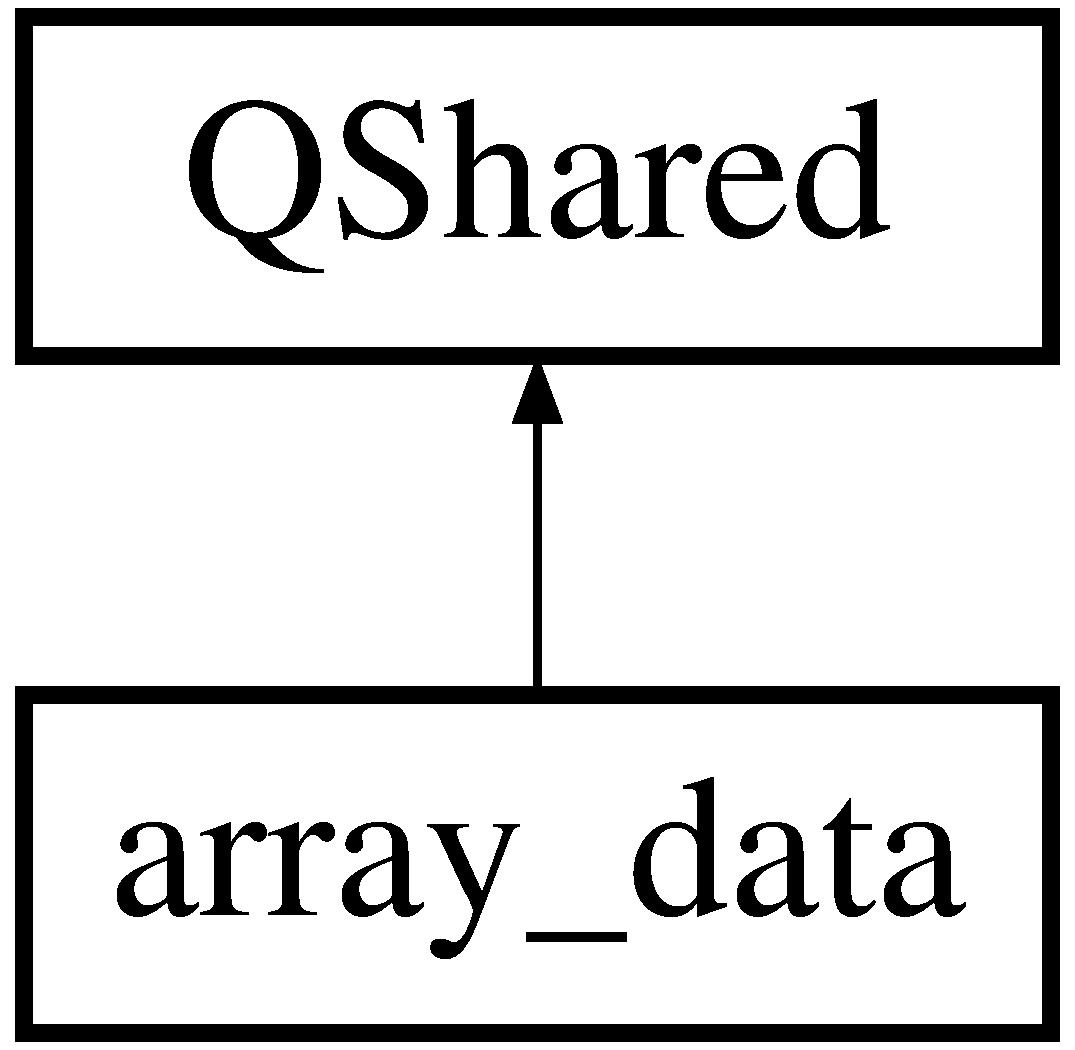
\includegraphics[height=2.000000cm]{struct_q_g_array_1_1array__data}
\end{center}
\end{figure}
\subsection*{Campos de Dados}
\begin{DoxyCompactItemize}
\item 
\hypertarget{struct_q_g_array_1_1array__data_a91a70b77df95bd8b0830b49a094c2acb}{char $\ast$ {\bfseries data}}\label{struct_q_g_array_1_1array__data_a91a70b77df95bd8b0830b49a094c2acb}

\item 
\hypertarget{struct_q_g_array_1_1array__data_adc6f7cd3b6ef14af983b1294c313bc2d}{uint {\bfseries len}}\label{struct_q_g_array_1_1array__data_adc6f7cd3b6ef14af983b1294c313bc2d}

\end{DoxyCompactItemize}
\subsection*{Additional Inherited Members}


A documentação para esta estrutura foi gerada a partir do seguinte ficheiro\-:\begin{DoxyCompactItemize}
\item 
C\-:/\-Users/teste/git/doxygen/qtools/qgarray.\-h\end{DoxyCompactItemize}

\hypertarget{class_template_filter_factory_1_1_auto_register}{\section{Referência à classe Template Template\-Filter\-Factory\-:\-:Auto\-Register$<$ T $>$}
\label{class_template_filter_factory_1_1_auto_register}\index{Template\-Filter\-Factory\-::\-Auto\-Register$<$ T $>$@{Template\-Filter\-Factory\-::\-Auto\-Register$<$ T $>$}}
}


Helper class for registering a filter function.  


\subsection*{Membros públicos}
\begin{DoxyCompactItemize}
\item 
\hypertarget{class_template_filter_factory_1_1_auto_register_acebfd9126d99a204c06188d4a3b405fe}{{\bfseries Auto\-Register} (const \hyperlink{class_q_c_string}{Q\-C\-String} \&key)}\label{class_template_filter_factory_1_1_auto_register_acebfd9126d99a204c06188d4a3b405fe}

\end{DoxyCompactItemize}


\subsection{Descrição detalhada}
\subsubsection*{template$<$class T$>$class Template\-Filter\-Factory\-::\-Auto\-Register$<$ T $>$}

Helper class for registering a filter function. 

A documentação para esta classe foi gerada a partir do seguinte ficheiro\-:\begin{DoxyCompactItemize}
\item 
C\-:/\-Users/teste/git/doxygen/src/template.\-cpp\end{DoxyCompactItemize}

\hypertarget{class_template_node_factory_1_1_auto_register}{\section{Referência à classe Template Template\-Node\-Factory\-:\-:Auto\-Register$<$ T $>$}
\label{class_template_node_factory_1_1_auto_register}\index{Template\-Node\-Factory\-::\-Auto\-Register$<$ T $>$@{Template\-Node\-Factory\-::\-Auto\-Register$<$ T $>$}}
}


Helper class for registering a template A\-S\-T node.  


\subsection*{Membros públicos}
\begin{DoxyCompactItemize}
\item 
\hypertarget{class_template_node_factory_1_1_auto_register_acebfd9126d99a204c06188d4a3b405fe}{{\bfseries Auto\-Register} (const \hyperlink{class_q_c_string}{Q\-C\-String} \&key)}\label{class_template_node_factory_1_1_auto_register_acebfd9126d99a204c06188d4a3b405fe}

\end{DoxyCompactItemize}


\subsection{Descrição detalhada}
\subsubsection*{template$<$class T$>$class Template\-Node\-Factory\-::\-Auto\-Register$<$ T $>$}

Helper class for registering a template A\-S\-T node. 

A documentação para esta classe foi gerada a partir do seguinte ficheiro\-:\begin{DoxyCompactItemize}
\item 
C\-:/\-Users/teste/git/doxygen/src/template.\-cpp\end{DoxyCompactItemize}

\hypertarget{class_b}{\section{Referência à classe B}
\label{class_b}\index{B@{B}}
}
Diagrama de heranças da classe B\begin{figure}[H]
\begin{center}
\leavevmode
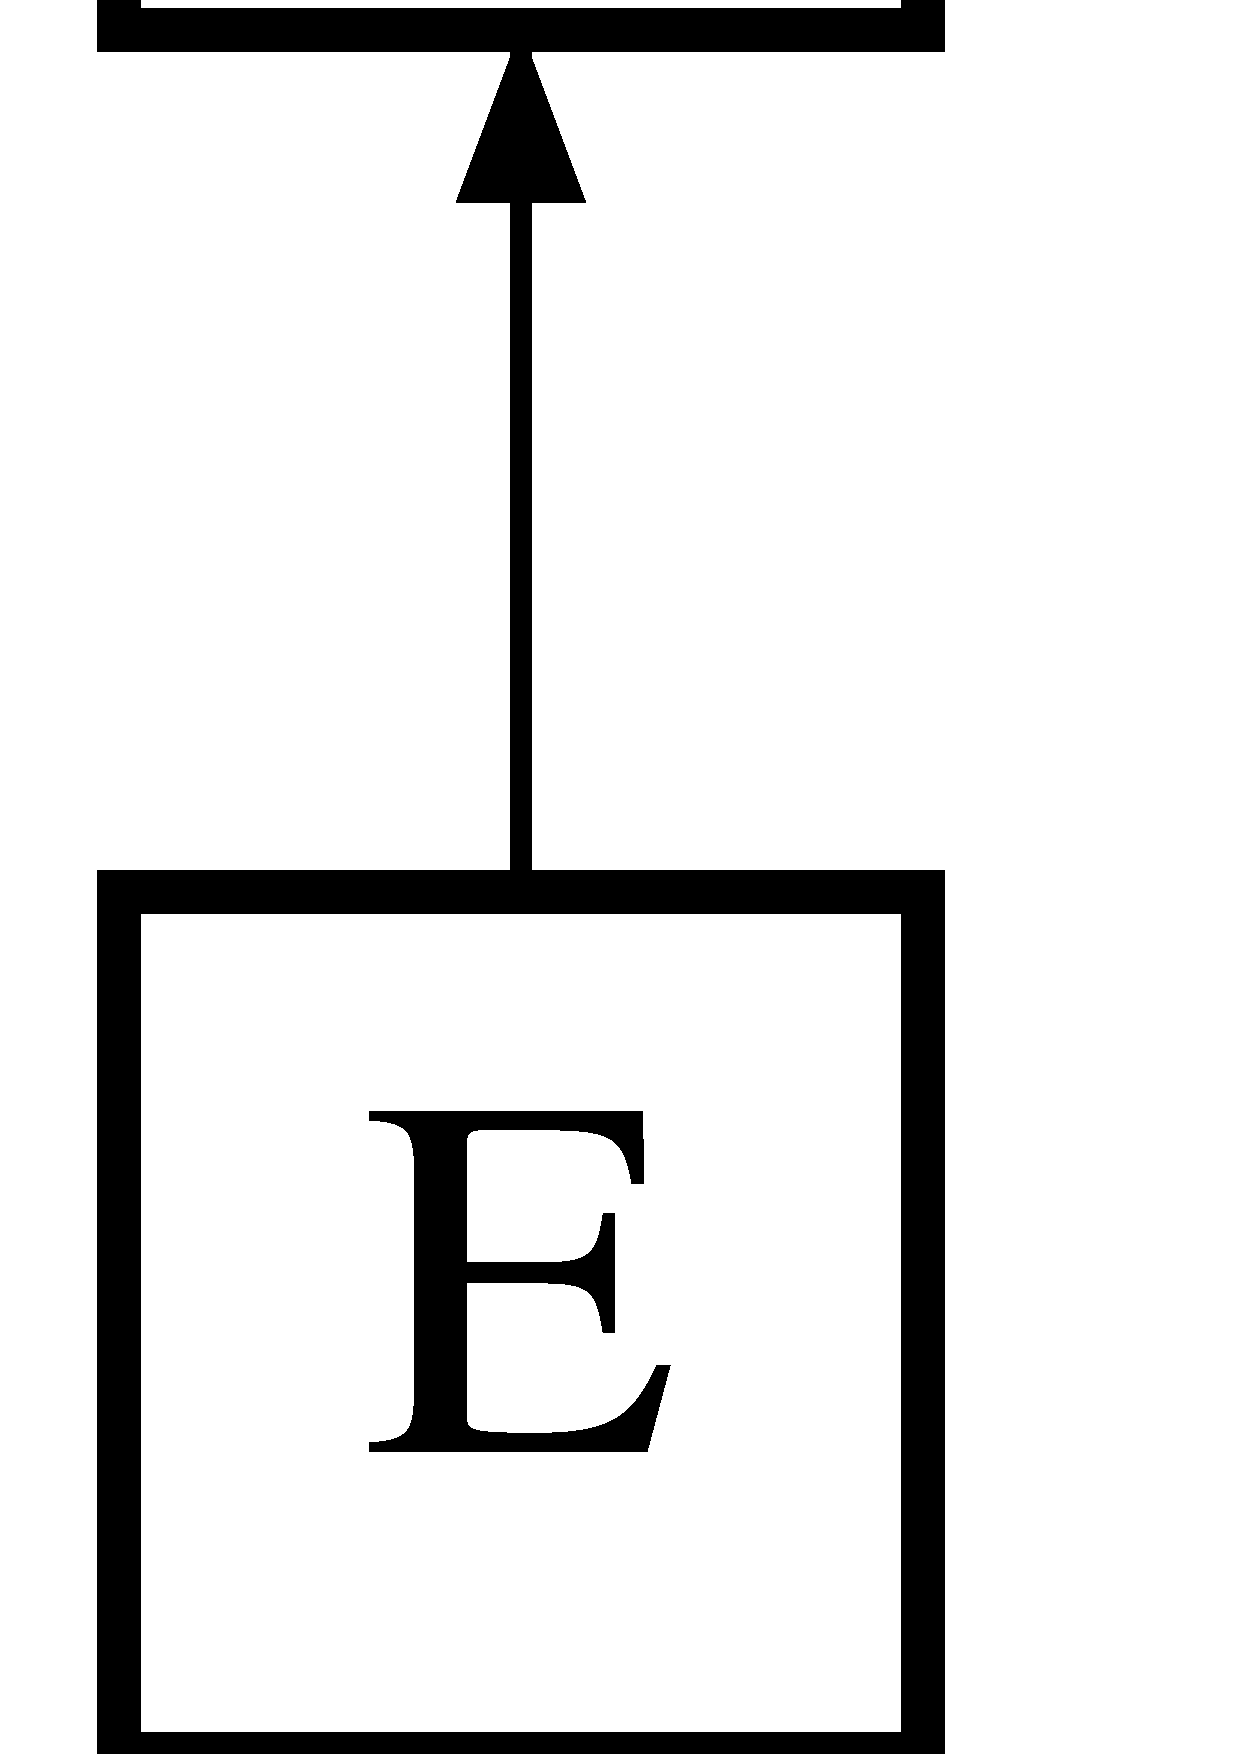
\includegraphics[height=3.000000cm]{class_b}
\end{center}
\end{figure}
\subsection*{Campos de Dados}
\begin{DoxyCompactItemize}
\item 
\hypertarget{class_b_addc7d54200781ba60c58a63744812259}{\hyperlink{class_a}{A} $\ast$ {\bfseries m\-\_\-a}}\label{class_b_addc7d54200781ba60c58a63744812259}

\end{DoxyCompactItemize}


\subsection{Descrição detalhada}
class \hyperlink{class_b}{B} 

A documentação para esta classe foi gerada a partir do seguinte ficheiro\-:\begin{DoxyCompactItemize}
\item 
C\-:/\-Users/teste/git/doxygen/examples/diagrams\-\_\-b.\-h\end{DoxyCompactItemize}

\hypertarget{struct_base_class_def}{\section{Referência à estrutura Base\-Class\-Def}
\label{struct_base_class_def}\index{Base\-Class\-Def@{Base\-Class\-Def}}
}


{\ttfamily \#include $<$classdef.\-h$>$}

\subsection*{Membros públicos}
\begin{DoxyCompactItemize}
\item 
\hypertarget{struct_base_class_def_ab47429e0ccf9dda410340a0d276ad174}{{\bfseries Base\-Class\-Def} (\hyperlink{class_class_def}{Class\-Def} $\ast$cd, const char $\ast$n, \hyperlink{types_8h_a90e352184df58cd09455fe9996cd4ded}{Protection} p, \hyperlink{types_8h_ab16236bdd10ddf4d73a9847350f0017e}{Specifier} v, const char $\ast$t)}\label{struct_base_class_def_ab47429e0ccf9dda410340a0d276ad174}

\end{DoxyCompactItemize}
\subsection*{Campos de Dados}
\begin{DoxyCompactItemize}
\item 
\hyperlink{class_class_def}{Class\-Def} $\ast$ \hyperlink{struct_base_class_def_a9ecae2706174bc69faacb7156966b12e}{class\-Def}
\item 
\hyperlink{class_q_c_string}{Q\-C\-String} \hyperlink{struct_base_class_def_a20a7352756abebcff874b7e28751d20c}{used\-Name}
\item 
\hyperlink{types_8h_a90e352184df58cd09455fe9996cd4ded}{Protection} \hyperlink{struct_base_class_def_a3f887065f93ce5f02dea21da35468e8e}{prot}
\item 
\hyperlink{types_8h_ab16236bdd10ddf4d73a9847350f0017e}{Specifier} \hyperlink{struct_base_class_def_aa05b4729c780621416429c6aac10fccf}{virt}
\item 
\hyperlink{class_q_c_string}{Q\-C\-String} \hyperlink{struct_base_class_def_aea659c4ea8200bb40a20fa289d5acc72}{templ\-Specifiers}
\end{DoxyCompactItemize}


\subsection{Descrição detalhada}
Class that contains information about an inheritance relation. 

\subsection{Documentação dos campos e atributos}
\hypertarget{struct_base_class_def_a9ecae2706174bc69faacb7156966b12e}{\index{Base\-Class\-Def@{Base\-Class\-Def}!class\-Def@{class\-Def}}
\index{class\-Def@{class\-Def}!BaseClassDef@{Base\-Class\-Def}}
\subsubsection[{class\-Def}]{\setlength{\rightskip}{0pt plus 5cm}{\bf Class\-Def}$\ast$ class\-Def}}\label{struct_base_class_def_a9ecae2706174bc69faacb7156966b12e}
Class definition that this relation inherits from. \hypertarget{struct_base_class_def_a3f887065f93ce5f02dea21da35468e8e}{\index{Base\-Class\-Def@{Base\-Class\-Def}!prot@{prot}}
\index{prot@{prot}!BaseClassDef@{Base\-Class\-Def}}
\subsubsection[{prot}]{\setlength{\rightskip}{0pt plus 5cm}{\bf Protection} prot}}\label{struct_base_class_def_a3f887065f93ce5f02dea21da35468e8e}
Protection level of the inheritance relation\-: Public, Protected, or Private \hypertarget{struct_base_class_def_aea659c4ea8200bb40a20fa289d5acc72}{\index{Base\-Class\-Def@{Base\-Class\-Def}!templ\-Specifiers@{templ\-Specifiers}}
\index{templ\-Specifiers@{templ\-Specifiers}!BaseClassDef@{Base\-Class\-Def}}
\subsubsection[{templ\-Specifiers}]{\setlength{\rightskip}{0pt plus 5cm}{\bf Q\-C\-String} templ\-Specifiers}}\label{struct_base_class_def_aea659c4ea8200bb40a20fa289d5acc72}
\hyperlink{class_template}{Template} arguments used for the base class \hypertarget{struct_base_class_def_a20a7352756abebcff874b7e28751d20c}{\index{Base\-Class\-Def@{Base\-Class\-Def}!used\-Name@{used\-Name}}
\index{used\-Name@{used\-Name}!BaseClassDef@{Base\-Class\-Def}}
\subsubsection[{used\-Name}]{\setlength{\rightskip}{0pt plus 5cm}{\bf Q\-C\-String} used\-Name}}\label{struct_base_class_def_a20a7352756abebcff874b7e28751d20c}
name used in the inheritance list (may be a typedef name instead of the class name) \hypertarget{struct_base_class_def_aa05b4729c780621416429c6aac10fccf}{\index{Base\-Class\-Def@{Base\-Class\-Def}!virt@{virt}}
\index{virt@{virt}!BaseClassDef@{Base\-Class\-Def}}
\subsubsection[{virt}]{\setlength{\rightskip}{0pt plus 5cm}{\bf Specifier} virt}}\label{struct_base_class_def_aa05b4729c780621416429c6aac10fccf}
Virtualness of the inheritance relation\-: Normal, or Virtual 

A documentação para esta estrutura foi gerada a partir do seguinte ficheiro\-:\begin{DoxyCompactItemize}
\item 
C\-:/\-Users/teste/git/doxygen/src/classdef.\-h\end{DoxyCompactItemize}

\hypertarget{class_base_class_list}{\section{Referência à classe Base\-Class\-List}
\label{class_base_class_list}\index{Base\-Class\-List@{Base\-Class\-List}}
}


{\ttfamily \#include $<$classdef.\-h$>$}

Diagrama de heranças da classe Base\-Class\-List\begin{figure}[H]
\begin{center}
\leavevmode
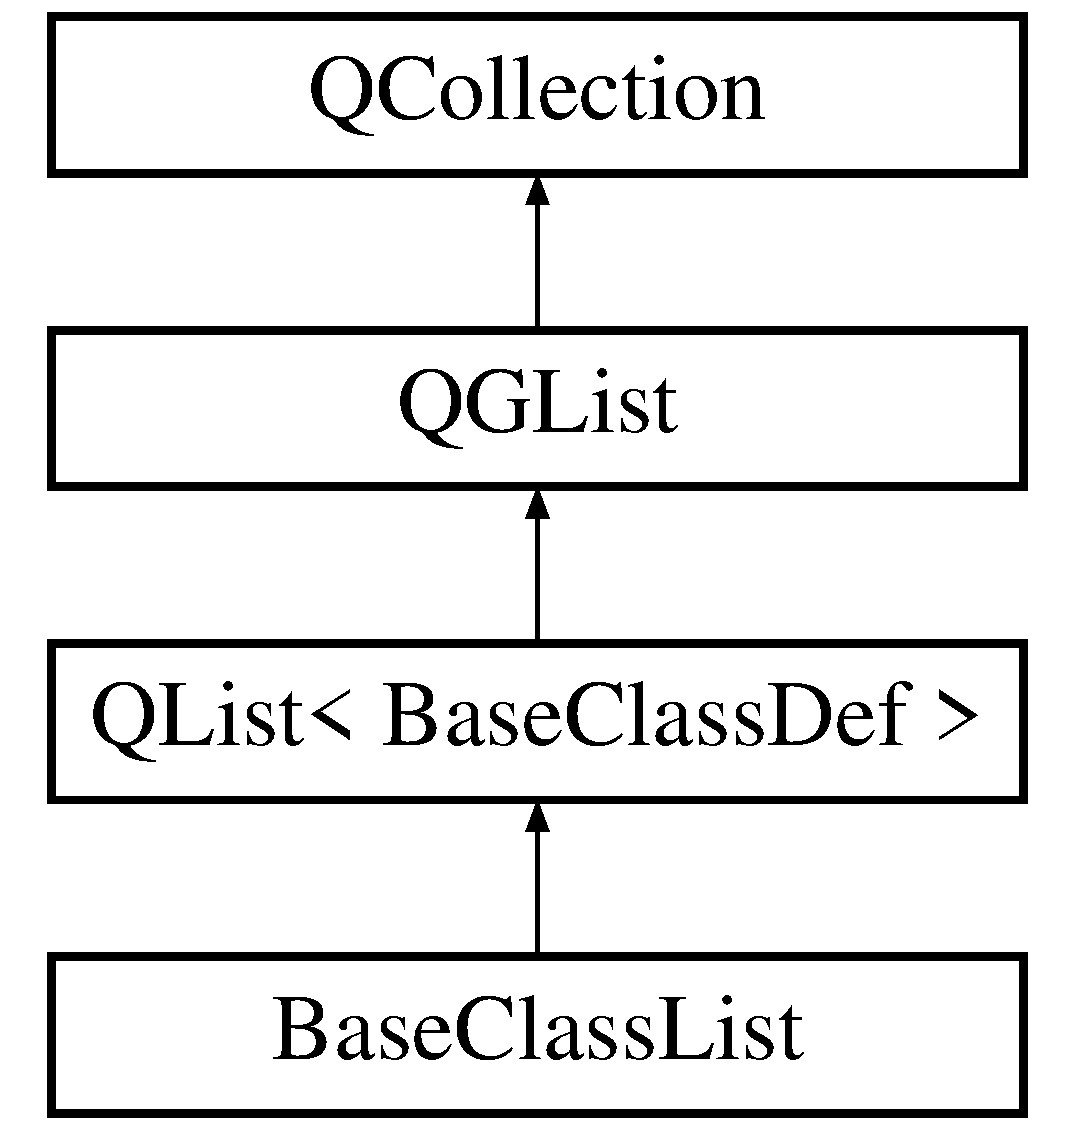
\includegraphics[height=4.000000cm]{class_base_class_list}
\end{center}
\end{figure}
\subsection*{Membros públicos}
\begin{DoxyCompactItemize}
\item 
int \hyperlink{class_base_class_list_a219450accf048597ffc7113ecde4c402}{compare\-Items} (Q\-Collection\-::\-Item item1, Q\-Collection\-::\-Item item2)
\end{DoxyCompactItemize}
\subsection*{Additional Inherited Members}


\subsection{Descrição detalhada}
List of base classes.

The classes are alphabetically sorted on name if in\-Sort() is used. 

\subsection{Documentação dos métodos}
\hypertarget{class_base_class_list_a219450accf048597ffc7113ecde4c402}{\index{Base\-Class\-List@{Base\-Class\-List}!compare\-Items@{compare\-Items}}
\index{compare\-Items@{compare\-Items}!BaseClassList@{Base\-Class\-List}}
\subsubsection[{compare\-Items}]{\setlength{\rightskip}{0pt plus 5cm}int compare\-Items (
\begin{DoxyParamCaption}
\item[{Q\-Collection\-::\-Item}]{item1, }
\item[{Q\-Collection\-::\-Item}]{item2}
\end{DoxyParamCaption}
)\hspace{0.3cm}{\ttfamily [inline]}, {\ttfamily [virtual]}}}\label{class_base_class_list_a219450accf048597ffc7113ecde4c402}
This virtual function compares two list items.

Returns\-: 
\begin{DoxyItemize}
\item 0 if {\itshape item1} == {\itshape item2} 
\item non-\/zero if {\itshape item1} != {\itshape item2} 
\end{DoxyItemize}

This function returns {\itshape int} rather than {\itshape bool} so that reimplementations can return three values and use it to sort by\-:


\begin{DoxyItemize}
\item 0 if {\itshape item1} == {\itshape item2} 
\item $>$ 0 (positive integer) if {\itshape item1} $>$ {\itshape item2} 
\item $<$ 0 (negative integer) if {\itshape item1} $<$ {\itshape item2} 
\end{DoxyItemize}

The Q\-List\-::in\-Sort() function requires that \hyperlink{class_base_class_list_a219450accf048597ffc7113ecde4c402}{compare\-Items()} is implemented as described here.

This function should not modify the list because some const functions call \hyperlink{class_base_class_list_a219450accf048597ffc7113ecde4c402}{compare\-Items()}.

The default implementation compares the pointers\-: 
\begin{DoxyCode}
\end{DoxyCode}
 

Reimplementado de \hyperlink{class_q_g_list_aac689c6d7a54b6558afbd53845183af8}{Q\-G\-List}.



A documentação para esta classe foi gerada a partir do seguinte ficheiro\-:\begin{DoxyCompactItemize}
\item 
C\-:/\-Users/teste/git/doxygen/src/classdef.\-h\end{DoxyCompactItemize}

\hypertarget{class_base_class_list_iterator}{\section{Referência à classe Base\-Class\-List\-Iterator}
\label{class_base_class_list_iterator}\index{Base\-Class\-List\-Iterator@{Base\-Class\-List\-Iterator}}
}


{\ttfamily \#include $<$classdef.\-h$>$}

Diagrama de heranças da classe Base\-Class\-List\-Iterator\begin{figure}[H]
\begin{center}
\leavevmode
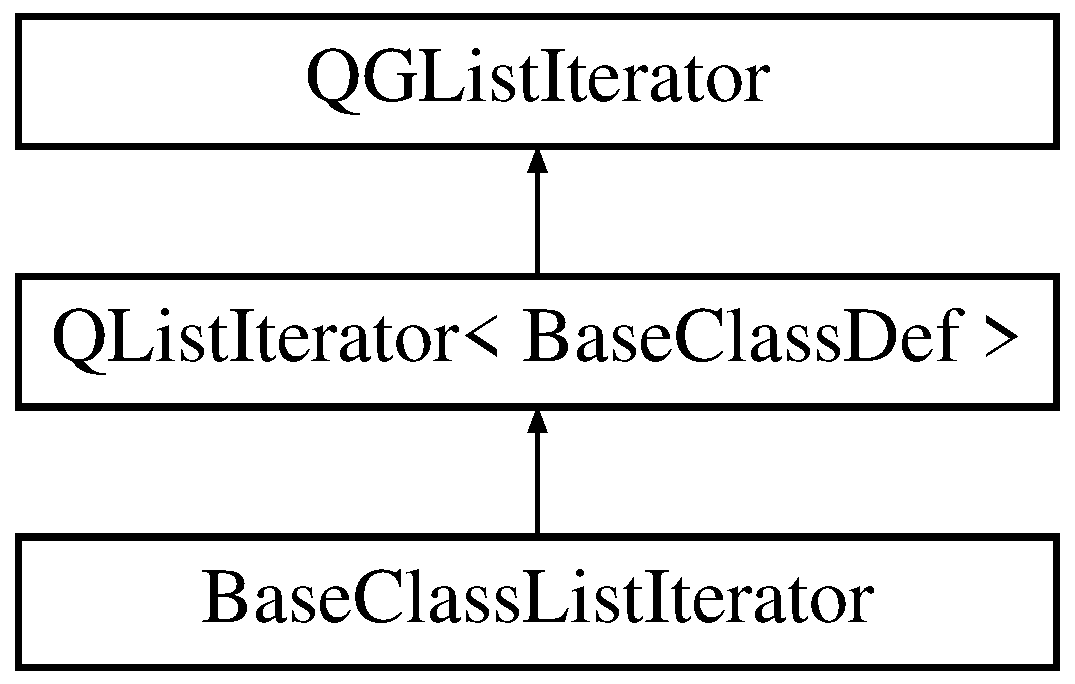
\includegraphics[height=3.000000cm]{class_base_class_list_iterator}
\end{center}
\end{figure}
\subsection*{Membros públicos}
\begin{DoxyCompactItemize}
\item 
\hypertarget{class_base_class_list_iterator_a77416faf22eb0e4fa88f537e974e2e91}{{\bfseries Base\-Class\-List\-Iterator} (const \hyperlink{class_base_class_list}{Base\-Class\-List} \&bcl)}\label{class_base_class_list_iterator_a77416faf22eb0e4fa88f537e974e2e91}

\end{DoxyCompactItemize}
\subsection*{Additional Inherited Members}


\subsection{Descrição detalhada}
Iterator for a list of base classes. 

A documentação para esta classe foi gerada a partir do seguinte ficheiro\-:\begin{DoxyCompactItemize}
\item 
C\-:/\-Users/teste/git/doxygen/src/classdef.\-h\end{DoxyCompactItemize}

\hypertarget{class_base_fall_back_handler}{\section{Referência à classe Template Base\-Fall\-Back\-Handler$<$ T $>$}
\label{class_base_fall_back_handler}\index{Base\-Fall\-Back\-Handler$<$ T $>$@{Base\-Fall\-Back\-Handler$<$ T $>$}}
}
Diagrama de heranças da classe Base\-Fall\-Back\-Handler$<$ T $>$\begin{figure}[H]
\begin{center}
\leavevmode
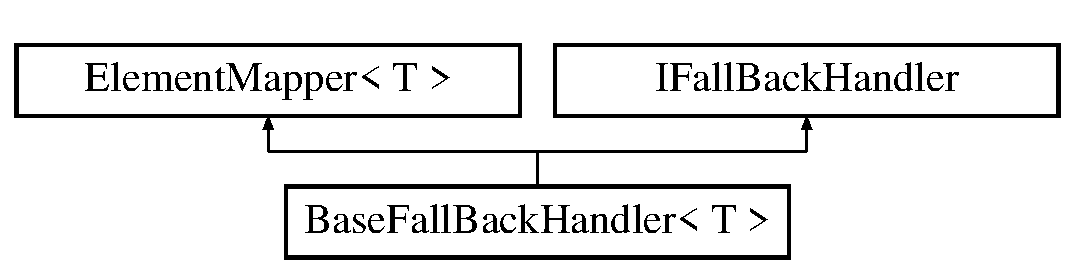
\includegraphics[height=2.000000cm]{class_base_fall_back_handler}
\end{center}
\end{figure}
\subsection*{Tipos Públicos}
\begin{DoxyCompactItemize}
\item 
\hypertarget{class_base_fall_back_handler_a99d76adba2066eddf6a2a09161d74dbd}{typedef \hyperlink{class_element_mapper}{Element\-Mapper}$<$ T $>$\\*
\-::Start\-Element\-Handler\-T {\bfseries Start\-Element\-Handler\-T}}\label{class_base_fall_back_handler_a99d76adba2066eddf6a2a09161d74dbd}

\item 
\hypertarget{class_base_fall_back_handler_addda909666f4e847e7732b0a526d0796}{typedef \hyperlink{class_element_mapper}{Element\-Mapper}$<$ T $>$\\*
\-::End\-Element\-Handler\-T {\bfseries End\-Element\-Handler\-T}}\label{class_base_fall_back_handler_addda909666f4e847e7732b0a526d0796}

\end{DoxyCompactItemize}
\subsection*{Membros públicos}
\begin{DoxyCompactItemize}
\item 
\hypertarget{class_base_fall_back_handler_a23fe44db946c758ca185dce857d2da2c}{bool {\bfseries handle\-Start\-Element} (const \hyperlink{class_q_string}{Q\-String} \&name, const \hyperlink{class_q_xml_attributes}{Q\-Xml\-Attributes} \&attrib)}\label{class_base_fall_back_handler_a23fe44db946c758ca185dce857d2da2c}

\item 
\hypertarget{class_base_fall_back_handler_a12f464e8ce7306921c37c2b0101a9dd6}{bool {\bfseries handle\-End\-Element} (const \hyperlink{class_q_string}{Q\-String} \&name)}\label{class_base_fall_back_handler_a12f464e8ce7306921c37c2b0101a9dd6}

\end{DoxyCompactItemize}
\subsection*{Additional Inherited Members}


A documentação para esta classe foi gerada a partir do seguinte ficheiro\-:\begin{DoxyCompactItemize}
\item 
C\-:/\-Users/teste/git/doxygen/addon/doxmlparser/src/basehandler.\-h\end{DoxyCompactItemize}

\hypertarget{class_base_handler}{\section{Referência à classe Template Base\-Handler$<$ T $>$}
\label{class_base_handler}\index{Base\-Handler$<$ T $>$@{Base\-Handler$<$ T $>$}}
}
Diagrama de heranças da classe Base\-Handler$<$ T $>$\begin{figure}[H]
\begin{center}
\leavevmode
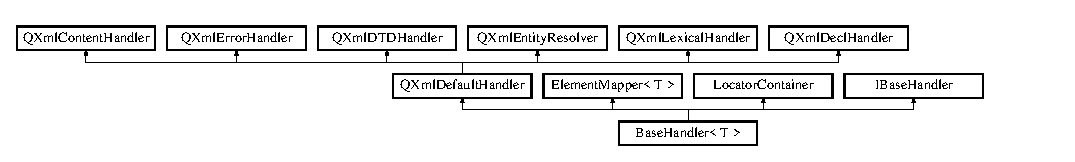
\includegraphics[height=1.726619cm]{class_base_handler}
\end{center}
\end{figure}
\subsection*{Tipos Públicos}
\begin{DoxyCompactItemize}
\item 
\hypertarget{class_base_handler_a99d76adba2066eddf6a2a09161d74dbd}{typedef \hyperlink{class_element_mapper}{Element\-Mapper}$<$ T $>$\\*
\-::Start\-Element\-Handler\-T {\bfseries Start\-Element\-Handler\-T}}\label{class_base_handler_a99d76adba2066eddf6a2a09161d74dbd}

\item 
\hypertarget{class_base_handler_addda909666f4e847e7732b0a526d0796}{typedef \hyperlink{class_element_mapper}{Element\-Mapper}$<$ T $>$\\*
\-::End\-Element\-Handler\-T {\bfseries End\-Element\-Handler\-T}}\label{class_base_handler_addda909666f4e847e7732b0a526d0796}

\end{DoxyCompactItemize}
\subsection*{Membros públicos}
\begin{DoxyCompactItemize}
\item 
virtual bool \hyperlink{class_base_handler_a2b02c429e179690d0785020713a6bd06}{start\-Document} ()
\item 
virtual bool \hyperlink{class_base_handler_af861c355ac62b4b24365ddfd226eccd7}{start\-Element} (const \hyperlink{class_q_string}{Q\-String} \&namespace\-U\-R\-I, const \hyperlink{class_q_string}{Q\-String} \&local\-Name, const \hyperlink{class_q_string}{Q\-String} \&name, const \hyperlink{class_q_xml_attributes}{Q\-Xml\-Attributes} \&attrib)
\item 
virtual bool \hyperlink{class_base_handler_a05536b83184a79912d80d986a3d60bb5}{end\-Element} (const \hyperlink{class_q_string}{Q\-String} \&namespace\-U\-R\-I, const \hyperlink{class_q_string}{Q\-String} \&local\-Name, const \hyperlink{class_q_string}{Q\-String} \&name)
\item 
bool \hyperlink{class_base_handler_a4f1b47ade1d77cb973e68738af8c422f}{skipped\-Entity} (const \hyperlink{class_q_string}{Q\-String} \&s)
\item 
virtual bool \hyperlink{class_base_handler_ae9e90bf53548ca210db99147e85d050d}{characters} (const \hyperlink{class_q_string}{Q\-String} \&ch)
\item 
\hypertarget{class_base_handler_adbcf6fe487094399d9aebc69e50c30cd}{void {\bfseries set\-Delegate} (\hyperlink{class_q_xml_default_handler}{Q\-Xml\-Default\-Handler} $\ast$delegate)}\label{class_base_handler_adbcf6fe487094399d9aebc69e50c30cd}

\item 
\hypertarget{class_base_handler_a17f9ea6414cb2dddbe01e2c3eafcff48}{\hyperlink{class_q_xml_default_handler}{Q\-Xml\-Default\-Handler} $\ast$ {\bfseries delegate} () const }\label{class_base_handler_a17f9ea6414cb2dddbe01e2c3eafcff48}

\item 
\hypertarget{class_base_handler_ab84c609b1c02f398ba297648bced9c9a}{void {\bfseries set\-Fall\-Back\-Handler} (\hyperlink{class_i_fall_back_handler}{I\-Fall\-Back\-Handler} $\ast$h)}\label{class_base_handler_ab84c609b1c02f398ba297648bced9c9a}

\item 
\hypertarget{class_base_handler_ac6ebe4f0d9d87b30868a4cc727b39365}{\hyperlink{class_i_fall_back_handler}{I\-Fall\-Back\-Handler} $\ast$ {\bfseries fall\-Back\-Handler} () const }\label{class_base_handler_ac6ebe4f0d9d87b30868a4cc727b39365}

\item 
void \hyperlink{class_base_handler_a6ea335308d212e2244af77edaff21d6a}{set\-Document\-Locator} (\hyperlink{class_q_xml_locator}{Q\-Xml\-Locator} $\ast$locator)
\end{DoxyCompactItemize}
\subsection*{Atributos Protegidos}
\begin{DoxyCompactItemize}
\item 
\hypertarget{class_base_handler_a9b402d915233c63eb8a84b8b8c9f3228}{\hyperlink{class_q_string}{Q\-String} {\bfseries m\-\_\-cur\-String}}\label{class_base_handler_a9b402d915233c63eb8a84b8b8c9f3228}

\item 
\hypertarget{class_base_handler_aa523c52792b01bb2154f3bd42fa058a4}{\hyperlink{class_q_string}{Q\-String} {\bfseries m\-\_\-skip\-Until}}\label{class_base_handler_aa523c52792b01bb2154f3bd42fa058a4}

\item 
\hypertarget{class_base_handler_aca385dcc09080a7dfcff5e1dde6d07bc}{int {\bfseries m\-\_\-skip\-Count}}\label{class_base_handler_aca385dcc09080a7dfcff5e1dde6d07bc}

\item 
\hypertarget{class_base_handler_aa9150e2d38d4d1e3b38a77c63c4b5019}{\hyperlink{class_q_xml_default_handler}{Q\-Xml\-Default\-Handler} $\ast$ {\bfseries m\-\_\-delegate\-Handler}}\label{class_base_handler_aa9150e2d38d4d1e3b38a77c63c4b5019}

\item 
\hypertarget{class_base_handler_a06798cb4dbd0a6a8f0696e836142c4d6}{\hyperlink{class_i_fall_back_handler}{I\-Fall\-Back\-Handler} $\ast$ {\bfseries m\-\_\-fall\-Back\-Handler}}\label{class_base_handler_a06798cb4dbd0a6a8f0696e836142c4d6}

\end{DoxyCompactItemize}
\subsection*{Additional Inherited Members}


\subsection{Documentação dos métodos}
\hypertarget{class_base_handler_ae9e90bf53548ca210db99147e85d050d}{\index{Base\-Handler@{Base\-Handler}!characters@{characters}}
\index{characters@{characters}!BaseHandler@{Base\-Handler}}
\subsubsection[{characters}]{\setlength{\rightskip}{0pt plus 5cm}virtual bool characters (
\begin{DoxyParamCaption}
\item[{const {\bf Q\-String} \&}]{ch}
\end{DoxyParamCaption}
)\hspace{0.3cm}{\ttfamily [inline]}, {\ttfamily [virtual]}}}\label{class_base_handler_ae9e90bf53548ca210db99147e85d050d}
called when a number of characters are received by the parser. 
\begin{DoxyParams}{Parâmetros}
{\em ch} & the characters. \\
\hline
\end{DoxyParams}


Implementa \hyperlink{class_q_xml_content_handler_a63490f0ac6e8b7794a5ebb331c3a4143}{Q\-Xml\-Content\-Handler}.

\hypertarget{class_base_handler_a05536b83184a79912d80d986a3d60bb5}{\index{Base\-Handler@{Base\-Handler}!end\-Element@{end\-Element}}
\index{end\-Element@{end\-Element}!BaseHandler@{Base\-Handler}}
\subsubsection[{end\-Element}]{\setlength{\rightskip}{0pt plus 5cm}virtual bool end\-Element (
\begin{DoxyParamCaption}
\item[{const {\bf Q\-String} \&}]{namespace\-U\-R\-I, }
\item[{const {\bf Q\-String} \&}]{local\-Name, }
\item[{const {\bf Q\-String} \&}]{q\-Name}
\end{DoxyParamCaption}
)\hspace{0.3cm}{\ttfamily [inline]}, {\ttfamily [virtual]}}}\label{class_base_handler_a05536b83184a79912d80d986a3d60bb5}
The reader calls this function when he has parsed an end element tag.

If this function returns F\-A\-L\-S\-E the reader will stop parsing and will report an error. The reader will use the function \hyperlink{class_q_xml_default_handler_af799a7684337babb971e2e0d8cda7cf1}{error\-String()} to get the error message that will be used for reporting the error.

See also the \href{xml-sax.html#namespaces}{\tt namespace description}.

\begin{DoxySeeAlso}{Veja também}
\hyperlink{class_base_handler_af861c355ac62b4b24365ddfd226eccd7}{start\-Element()} 
\end{DoxySeeAlso}


Implementa \hyperlink{class_q_xml_content_handler_ac85feb837d3634e775cc7c76df84cce0}{Q\-Xml\-Content\-Handler}.

\hypertarget{class_base_handler_a6ea335308d212e2244af77edaff21d6a}{\index{Base\-Handler@{Base\-Handler}!set\-Document\-Locator@{set\-Document\-Locator}}
\index{set\-Document\-Locator@{set\-Document\-Locator}!BaseHandler@{Base\-Handler}}
\subsubsection[{set\-Document\-Locator}]{\setlength{\rightskip}{0pt plus 5cm}void set\-Document\-Locator (
\begin{DoxyParamCaption}
\item[{{\bf Q\-Xml\-Locator} $\ast$}]{locator}
\end{DoxyParamCaption}
)\hspace{0.3cm}{\ttfamily [inline]}, {\ttfamily [virtual]}}}\label{class_base_handler_a6ea335308d212e2244af77edaff21d6a}
The reader calls this function before he starts parsing the document. The argument {\itshape locator} is a pointer to a \hyperlink{class_q_xml_locator}{Q\-Xml\-Locator} which allows the application to get the actual position of the parsing in the document.

Do not destroy the {\itshape locator}; it is destroyed when the reader is destroyed (do not use the {\itshape locator} after the reader got destroyed). 

Implementa \hyperlink{class_q_xml_content_handler_a02c1b0a6086c5d232ae919bbc5abb740}{Q\-Xml\-Content\-Handler}.

\hypertarget{class_base_handler_a4f1b47ade1d77cb973e68738af8c422f}{\index{Base\-Handler@{Base\-Handler}!skipped\-Entity@{skipped\-Entity}}
\index{skipped\-Entity@{skipped\-Entity}!BaseHandler@{Base\-Handler}}
\subsubsection[{skipped\-Entity}]{\setlength{\rightskip}{0pt plus 5cm}bool skipped\-Entity (
\begin{DoxyParamCaption}
\item[{const {\bf Q\-String} \&}]{name}
\end{DoxyParamCaption}
)\hspace{0.3cm}{\ttfamily [inline]}, {\ttfamily [virtual]}}}\label{class_base_handler_a4f1b47ade1d77cb973e68738af8c422f}
Some readers may skip entities if they have not seen the declarations (e.\-g. because they are in an external D\-T\-D). If they do so they will report it by calling this function.

If this function returns F\-A\-L\-S\-E the reader will stop parsing and will report an error. The reader will use the function \hyperlink{class_q_xml_default_handler_af799a7684337babb971e2e0d8cda7cf1}{error\-String()} to get the error message that will be used for reporting the error. 

Implementa \hyperlink{class_q_xml_content_handler_a96c291d0d5554a03b2cc445472dd1086}{Q\-Xml\-Content\-Handler}.

\hypertarget{class_base_handler_a2b02c429e179690d0785020713a6bd06}{\index{Base\-Handler@{Base\-Handler}!start\-Document@{start\-Document}}
\index{start\-Document@{start\-Document}!BaseHandler@{Base\-Handler}}
\subsubsection[{start\-Document}]{\setlength{\rightskip}{0pt plus 5cm}virtual bool start\-Document (
\begin{DoxyParamCaption}
{}
\end{DoxyParamCaption}
)\hspace{0.3cm}{\ttfamily [inline]}, {\ttfamily [virtual]}}}\label{class_base_handler_a2b02c429e179690d0785020713a6bd06}
The reader calls this function when he starts parsing the document. The reader will call this function only once before any other functions in this class or in the \hyperlink{class_q_xml_d_t_d_handler}{Q\-Xml\-D\-T\-D\-Handler} class are called (except \hyperlink{class_q_xml_content_handler_a02c1b0a6086c5d232ae919bbc5abb740}{Q\-Xml\-Content\-Handler\-::set\-Document\-Locator()}).

If this function returns F\-A\-L\-S\-E the reader will stop parsing and will report an error. The reader will use the function \hyperlink{class_q_xml_default_handler_af799a7684337babb971e2e0d8cda7cf1}{error\-String()} to get the error message that will be used for reporting the error.

\begin{DoxySeeAlso}{Veja também}
\hyperlink{class_q_xml_default_handler_aaef0fd8871f28d804dc845c47c8fbc85}{end\-Document()} 
\end{DoxySeeAlso}


Implementa \hyperlink{class_q_xml_content_handler_a394d49ec389b7b0024d98698e1ae00cb}{Q\-Xml\-Content\-Handler}.

\hypertarget{class_base_handler_af861c355ac62b4b24365ddfd226eccd7}{\index{Base\-Handler@{Base\-Handler}!start\-Element@{start\-Element}}
\index{start\-Element@{start\-Element}!BaseHandler@{Base\-Handler}}
\subsubsection[{start\-Element}]{\setlength{\rightskip}{0pt plus 5cm}virtual bool start\-Element (
\begin{DoxyParamCaption}
\item[{const {\bf Q\-String} \&}]{namespace\-U\-R\-I, }
\item[{const {\bf Q\-String} \&}]{local\-Name, }
\item[{const {\bf Q\-String} \&}]{q\-Name, }
\item[{const {\bf Q\-Xml\-Attributes} \&}]{atts}
\end{DoxyParamCaption}
)\hspace{0.3cm}{\ttfamily [inline]}, {\ttfamily [virtual]}}}\label{class_base_handler_af861c355ac62b4b24365ddfd226eccd7}
The reader calls this function when he has parsed a start element tag.

There will be a corresponding \hyperlink{class_base_handler_a05536b83184a79912d80d986a3d60bb5}{end\-Element()} call when the corresponding end element tag was read. The \hyperlink{class_base_handler_af861c355ac62b4b24365ddfd226eccd7}{start\-Element()} and \hyperlink{class_base_handler_a05536b83184a79912d80d986a3d60bb5}{end\-Element()} calls are always nested correctly. Empty element tags (e.\-g. $<$a/$>$) are reported by \hyperlink{class_base_handler_af861c355ac62b4b24365ddfd226eccd7}{start\-Element()} directly followed by a call to \hyperlink{class_base_handler_a05536b83184a79912d80d986a3d60bb5}{end\-Element()}.

The attribute list provided will contain only attributes with explicit values. The attribute list will contain attributes used for namespace declaration (i.\-e. attributes starting with xmlns) only if the namespace-\/prefix property of the reader is T\-R\-U\-E.

The argument {\itshape uri} is the namespace U\-R\-I, or the empty string if the element has no namespace U\-R\-I or if namespace processing is not being performed, {\itshape local\-Name} is the local name (without prefix), or the empty string if namespace processing is not being performed, {\itshape q\-Name} is the qualified name (with prefix), or the empty string if qualified names are not available and {\itshape atts} are the attributes attached to the element. If there are no attributes, {\itshape atts} is an empty attributes object

If this function returns F\-A\-L\-S\-E the reader will stop parsing and will report an error. The reader will use the function \hyperlink{class_q_xml_default_handler_af799a7684337babb971e2e0d8cda7cf1}{error\-String()} to get the error message that will be used for reporting the error.

See also the \href{xml-sax.html#namespaces}{\tt namespace description}.

\begin{DoxySeeAlso}{Veja também}
\hyperlink{class_base_handler_a05536b83184a79912d80d986a3d60bb5}{end\-Element()} 
\end{DoxySeeAlso}


Implementa \hyperlink{class_q_xml_content_handler_ac956b69e7f9be94f64e8e90095eb2ce0}{Q\-Xml\-Content\-Handler}.



A documentação para esta classe foi gerada a partir do seguinte ficheiro\-:\begin{DoxyCompactItemize}
\item 
C\-:/\-Users/teste/git/doxygen/addon/doxmlparser/src/basehandler.\-h\end{DoxyCompactItemize}

\hypertarget{struct_base_info}{\section{Referência à estrutura Base\-Info}
\label{struct_base_info}\index{Base\-Info@{Base\-Info}}
}


{\ttfamily \#include $<$entry.\-h$>$}

\subsection*{Membros públicos}
\begin{DoxyCompactItemize}
\item 
\hyperlink{struct_base_info_a3987140908f98e6f53512507d79ecdbd}{Base\-Info} (const char $\ast$n, \hyperlink{types_8h_a90e352184df58cd09455fe9996cd4ded}{Protection} p, \hyperlink{types_8h_ab16236bdd10ddf4d73a9847350f0017e}{Specifier} v)
\end{DoxyCompactItemize}
\subsection*{Campos de Dados}
\begin{DoxyCompactItemize}
\item 
\hypertarget{struct_base_info_adc0097c7bd1e61ad32058fcde425bc7a}{\hyperlink{class_q_c_string}{Q\-C\-String} \hyperlink{struct_base_info_adc0097c7bd1e61ad32058fcde425bc7a}{name}}\label{struct_base_info_adc0097c7bd1e61ad32058fcde425bc7a}

\begin{DoxyCompactList}\small\item\em the name of the base class \end{DoxyCompactList}\item 
\hypertarget{struct_base_info_a3f887065f93ce5f02dea21da35468e8e}{\hyperlink{types_8h_a90e352184df58cd09455fe9996cd4ded}{Protection} \hyperlink{struct_base_info_a3f887065f93ce5f02dea21da35468e8e}{prot}}\label{struct_base_info_a3f887065f93ce5f02dea21da35468e8e}

\begin{DoxyCompactList}\small\item\em inheritance type \end{DoxyCompactList}\item 
\hypertarget{struct_base_info_aa05b4729c780621416429c6aac10fccf}{\hyperlink{types_8h_ab16236bdd10ddf4d73a9847350f0017e}{Specifier} \hyperlink{struct_base_info_aa05b4729c780621416429c6aac10fccf}{virt}}\label{struct_base_info_aa05b4729c780621416429c6aac10fccf}

\begin{DoxyCompactList}\small\item\em virtualness \end{DoxyCompactList}\end{DoxyCompactItemize}


\subsection{Descrição detalhada}
This class stores information about an inheritance relation 

\subsection{Documentação dos Construtores \& Destrutor}
\hypertarget{struct_base_info_a3987140908f98e6f53512507d79ecdbd}{\index{Base\-Info@{Base\-Info}!Base\-Info@{Base\-Info}}
\index{Base\-Info@{Base\-Info}!BaseInfo@{Base\-Info}}
\subsubsection[{Base\-Info}]{\setlength{\rightskip}{0pt plus 5cm}{\bf Base\-Info} (
\begin{DoxyParamCaption}
\item[{const char $\ast$}]{n, }
\item[{{\bf Protection}}]{p, }
\item[{{\bf Specifier}}]{v}
\end{DoxyParamCaption}
)\hspace{0.3cm}{\ttfamily [inline]}}}\label{struct_base_info_a3987140908f98e6f53512507d79ecdbd}
Creates an object representing an inheritance relation 

A documentação para esta estrutura foi gerada a partir do seguinte ficheiro\-:\begin{DoxyCompactItemize}
\item 
C\-:/\-Users/teste/git/doxygen/src/entry.\-h\end{DoxyCompactItemize}

\hypertarget{class_base_iterator}{\section{Referência à classe Template Base\-Iterator$<$ Intf, Elem\-Intf, Elem\-Impl $>$}
\label{class_base_iterator}\index{Base\-Iterator$<$ Intf, Elem\-Intf, Elem\-Impl $>$@{Base\-Iterator$<$ Intf, Elem\-Intf, Elem\-Impl $>$}}
}
Diagrama de heranças da classe Base\-Iterator$<$ Intf, Elem\-Intf, Elem\-Impl $>$\begin{figure}[H]
\begin{center}
\leavevmode
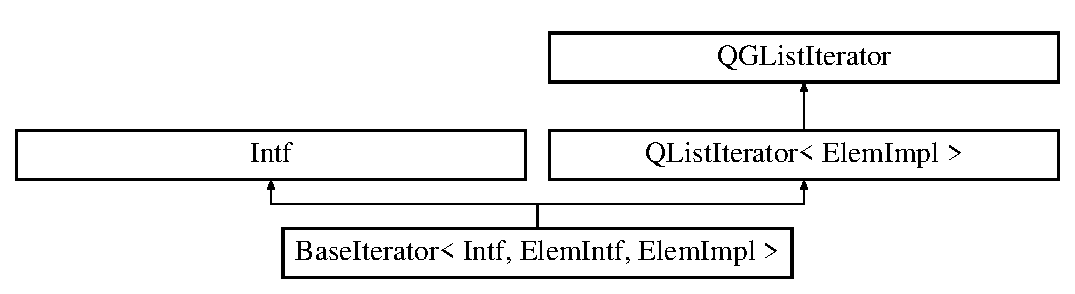
\includegraphics[height=3.000000cm]{class_base_iterator}
\end{center}
\end{figure}
\subsection*{Membros públicos}
\begin{DoxyCompactItemize}
\item 
\hypertarget{class_base_iterator_abdfa36792ec4e4e60ec2c49b57553d28}{{\bfseries Base\-Iterator} (const \hyperlink{class_q_list}{Q\-List}$<$ Elem\-Impl $>$ \&list)}\label{class_base_iterator_abdfa36792ec4e4e60ec2c49b57553d28}

\item 
\hypertarget{class_base_iterator_abf229c0e1893f20877b578ac2c7e5159}{virtual Elem\-Intf $\ast$ {\bfseries to\-First} ()}\label{class_base_iterator_abf229c0e1893f20877b578ac2c7e5159}

\item 
\hypertarget{class_base_iterator_a48309b7fc55a5c4d1b108327ead3a727}{virtual Elem\-Intf $\ast$ {\bfseries to\-Last} ()}\label{class_base_iterator_a48309b7fc55a5c4d1b108327ead3a727}

\item 
\hypertarget{class_base_iterator_a7d8f0436378f74c321dedf57fb8dab4f}{virtual Elem\-Intf $\ast$ {\bfseries to\-Next} ()}\label{class_base_iterator_a7d8f0436378f74c321dedf57fb8dab4f}

\item 
\hypertarget{class_base_iterator_a4da1240445f01ecc893d9b579be90b57}{virtual Elem\-Intf $\ast$ {\bfseries to\-Prev} ()}\label{class_base_iterator_a4da1240445f01ecc893d9b579be90b57}

\item 
\hypertarget{class_base_iterator_a1e22b4c1f1bcd62f8d167baf6fde83cb}{virtual Elem\-Intf $\ast$ {\bfseries current} () const }\label{class_base_iterator_a1e22b4c1f1bcd62f8d167baf6fde83cb}

\item 
\hypertarget{class_base_iterator_af8a84115de3507728d5e19e804529052}{virtual void {\bfseries release} ()}\label{class_base_iterator_af8a84115de3507728d5e19e804529052}

\end{DoxyCompactItemize}
\subsection*{Additional Inherited Members}


A documentação para esta classe foi gerada a partir do seguinte ficheiro\-:\begin{DoxyCompactItemize}
\item 
C\-:/\-Users/teste/git/doxygen/addon/doxmlparser/src/baseiterator.\-h\end{DoxyCompactItemize}

\hypertarget{class_base_iterator_via}{\section{Referência à classe Template Base\-Iterator\-Via$<$ Intf, Elem\-Intf, Elem\-Impl, Intermediate $>$}
\label{class_base_iterator_via}\index{Base\-Iterator\-Via$<$ Intf, Elem\-Intf, Elem\-Impl, Intermediate $>$@{Base\-Iterator\-Via$<$ Intf, Elem\-Intf, Elem\-Impl, Intermediate $>$}}
}
Diagrama de heranças da classe Base\-Iterator\-Via$<$ Intf, Elem\-Intf, Elem\-Impl, Intermediate $>$\begin{figure}[H]
\begin{center}
\leavevmode
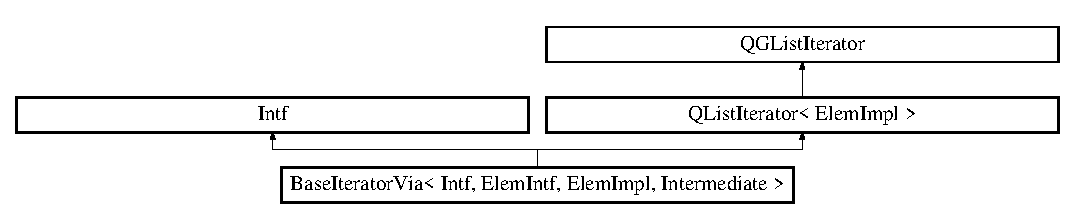
\includegraphics[height=2.500000cm]{class_base_iterator_via}
\end{center}
\end{figure}
\subsection*{Membros públicos}
\begin{DoxyCompactItemize}
\item 
\hypertarget{class_base_iterator_via_abd4ff79a5d17da775065887248d9c720}{{\bfseries Base\-Iterator\-Via} (const \hyperlink{class_q_list}{Q\-List}$<$ Elem\-Impl $>$ \&list)}\label{class_base_iterator_via_abd4ff79a5d17da775065887248d9c720}

\item 
\hypertarget{class_base_iterator_via_abf229c0e1893f20877b578ac2c7e5159}{virtual Elem\-Intf $\ast$ {\bfseries to\-First} ()}\label{class_base_iterator_via_abf229c0e1893f20877b578ac2c7e5159}

\item 
\hypertarget{class_base_iterator_via_a48309b7fc55a5c4d1b108327ead3a727}{virtual Elem\-Intf $\ast$ {\bfseries to\-Last} ()}\label{class_base_iterator_via_a48309b7fc55a5c4d1b108327ead3a727}

\item 
\hypertarget{class_base_iterator_via_a7d8f0436378f74c321dedf57fb8dab4f}{virtual Elem\-Intf $\ast$ {\bfseries to\-Next} ()}\label{class_base_iterator_via_a7d8f0436378f74c321dedf57fb8dab4f}

\item 
\hypertarget{class_base_iterator_via_a4da1240445f01ecc893d9b579be90b57}{virtual Elem\-Intf $\ast$ {\bfseries to\-Prev} ()}\label{class_base_iterator_via_a4da1240445f01ecc893d9b579be90b57}

\item 
\hypertarget{class_base_iterator_via_a1e22b4c1f1bcd62f8d167baf6fde83cb}{virtual Elem\-Intf $\ast$ {\bfseries current} () const }\label{class_base_iterator_via_a1e22b4c1f1bcd62f8d167baf6fde83cb}

\item 
\hypertarget{class_base_iterator_via_af8a84115de3507728d5e19e804529052}{virtual void {\bfseries release} ()}\label{class_base_iterator_via_af8a84115de3507728d5e19e804529052}

\end{DoxyCompactItemize}
\subsection*{Additional Inherited Members}


A documentação para esta classe foi gerada a partir do seguinte ficheiro\-:\begin{DoxyCompactItemize}
\item 
C\-:/\-Users/teste/git/doxygen/addon/doxmlparser/src/baseiterator.\-h\end{DoxyCompactItemize}

\hypertarget{class_base_output_doc_interface}{\section{Referência à classe Base\-Output\-Doc\-Interface}
\label{class_base_output_doc_interface}\index{Base\-Output\-Doc\-Interface@{Base\-Output\-Doc\-Interface}}
}


{\ttfamily \#include $<$outputgen.\-h$>$}

Diagrama de heranças da classe Base\-Output\-Doc\-Interface\begin{figure}[H]
\begin{center}
\leavevmode
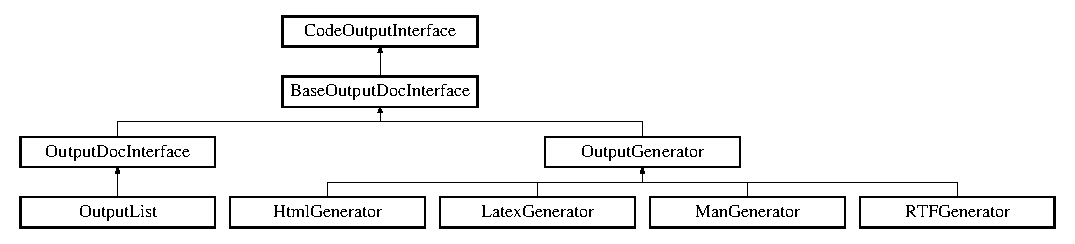
\includegraphics[height=2.835443cm]{class_base_output_doc_interface}
\end{center}
\end{figure}
\subsection*{Tipos Públicos}
\begin{DoxyCompactItemize}
\item 
enum {\bfseries Param\-List\-Types} \{ {\bfseries Param}, 
{\bfseries Ret\-Val}, 
{\bfseries Exception}
 \}
\item 
enum {\bfseries Section\-Types} \{ {\bfseries Enum\-Values}, 
{\bfseries Examples}
 \}
\end{DoxyCompactItemize}
\subsection*{Membros públicos}
\begin{DoxyCompactItemize}
\item 
\hypertarget{class_base_output_doc_interface_a4a14fbec28aa838ac6e333e0bcea0216}{virtual bool {\bfseries parse\-Text} (const \hyperlink{class_q_c_string}{Q\-C\-String} \&s)}\label{class_base_output_doc_interface_a4a14fbec28aa838ac6e333e0bcea0216}

\item 
virtual void \hyperlink{class_base_output_doc_interface_a432e618b3c8820e00496c6b242947e72}{start\-Item\-List} ()=0
\item 
virtual void \hyperlink{class_base_output_doc_interface_a6cfe1cc2a5fa5cdb1eea280df003903a}{start\-Item\-List\-Item} ()=0
\item 
virtual void \hyperlink{class_base_output_doc_interface_a8161fe76c2c66d47d0eb078be885bec7}{end\-Item\-List\-Item} ()=0
\item 
virtual void \hyperlink{class_base_output_doc_interface_a818d290261244e40e8c70562a7198156}{end\-Item\-List} ()=0
\item 
virtual void \hyperlink{class_base_output_doc_interface_a6f6bec326f718b326fb67adb943ebc27}{docify} (const char $\ast$s)=0
\item 
virtual void \hyperlink{class_base_output_doc_interface_a936e81608db3018f2bce9cd3ee58fdcd}{write\-Char} (char c)=0
\item 
virtual void \hyperlink{class_base_output_doc_interface_a78a005d8c0329ee60cd1994eb4afc58b}{write\-String} (const char $\ast$text)=0
\item 
virtual void \hyperlink{class_base_output_doc_interface_a4b8b270f90567b9201c44a6ad2ad206f}{start\-Paragraph} ()=0
\item 
virtual void \hyperlink{class_base_output_doc_interface_a9a97d4c8fb4e8ac91125f9ff2718d83d}{end\-Paragraph} ()=0
\item 
virtual void \hyperlink{class_base_output_doc_interface_aa551443db6cf9e4f51bc12c9d753f9c3}{write\-Object\-Link} (const char $\ast$ref, const char $\ast$file, const char $\ast$anchor, const char $\ast$name)=0
\item 
virtual void \hyperlink{class_base_output_doc_interface_ae514e80c628faa0b5ee62a50185f2397}{start\-Html\-Link} (const char $\ast$url)=0
\item 
virtual void \hyperlink{class_base_output_doc_interface_a463c695844e8137b388af6e1bbafc19e}{end\-Html\-Link} ()=0
\item 
virtual void \hyperlink{class_base_output_doc_interface_a9ad34c5f6672948732a87c4371d2e244}{start\-Bold} ()=0
\item 
virtual void \hyperlink{class_base_output_doc_interface_a593e371dace7c16866f8bd028905096d}{end\-Bold} ()=0
\item 
virtual void \hyperlink{class_base_output_doc_interface_ae241cdb69ca06cd0a539dd8b8a0a419f}{start\-Typewriter} ()=0
\item 
virtual void \hyperlink{class_base_output_doc_interface_a201cdc35ada3fac3f2f72adcc43308b8}{end\-Typewriter} ()=0
\item 
virtual void \hyperlink{class_base_output_doc_interface_afa6a6472913a05d8524804a27aebb56c}{start\-Emphasis} ()=0
\item 
virtual void \hyperlink{class_base_output_doc_interface_a1530746d5ac62d305ff693f0eb2bf90a}{end\-Emphasis} ()=0
\item 
virtual void \hyperlink{class_base_output_doc_interface_a649cecde411897cea447f103795d8c64}{start\-Code\-Fragment} ()=0
\item 
virtual void \hyperlink{class_base_output_doc_interface_a6d0e9c89b22affd8574d3804393d8fa5}{end\-Code\-Fragment} ()=0
\item 
virtual void \hyperlink{class_base_output_doc_interface_a5f36f83289e2b6137e9086998c5fb883}{write\-Ruler} ()=0
\item 
virtual void \hyperlink{class_base_output_doc_interface_a90167ae571c0685acd7934fde582ca7b}{start\-Description} ()=0
\item 
virtual void \hyperlink{class_base_output_doc_interface_a58e5aab2220d1da0e75a66c294cc9857}{end\-Description} ()=0
\item 
virtual void \hyperlink{class_base_output_doc_interface_a5392dc059a26e9c650ffee7d28636f74}{start\-Desc\-Item} ()=0
\item 
\hypertarget{class_base_output_doc_interface_ad0a455f0a2344f6188cde8de697b4433}{virtual void {\bfseries start\-Desc\-For\-Item} ()=0}\label{class_base_output_doc_interface_ad0a455f0a2344f6188cde8de697b4433}

\item 
\hypertarget{class_base_output_doc_interface_a737810958e3c17f65d06050a4d96515a}{virtual void {\bfseries end\-Desc\-For\-Item} ()=0}\label{class_base_output_doc_interface_a737810958e3c17f65d06050a4d96515a}

\item 
virtual void \hyperlink{class_base_output_doc_interface_ae9e2fe1d39b02fcc5a682ace36d7eafa}{end\-Desc\-Item} ()=0
\item 
\hypertarget{class_base_output_doc_interface_a6c705372da335649a67a744d1283afaf}{virtual void {\bfseries start\-Center} ()=0}\label{class_base_output_doc_interface_a6c705372da335649a67a744d1283afaf}

\item 
\hypertarget{class_base_output_doc_interface_afb04dbc9e3cf3296af0295249e3105fe}{virtual void {\bfseries end\-Center} ()=0}\label{class_base_output_doc_interface_afb04dbc9e3cf3296af0295249e3105fe}

\item 
\hypertarget{class_base_output_doc_interface_a99a7175c105390ea2dcaf4236c096af2}{virtual void {\bfseries start\-Small} ()=0}\label{class_base_output_doc_interface_a99a7175c105390ea2dcaf4236c096af2}

\item 
\hypertarget{class_base_output_doc_interface_a6e1a25540f283ea2ca1a4747ae814079}{virtual void {\bfseries end\-Small} ()=0}\label{class_base_output_doc_interface_a6e1a25540f283ea2ca1a4747ae814079}

\item 
\hypertarget{class_base_output_doc_interface_a98bc450db49fb6704f072b3da99f10b2}{virtual void {\bfseries start\-Simple\-Sect} (Section\-Types t, const char $\ast$file, const char $\ast$anchor, const char $\ast$title)=0}\label{class_base_output_doc_interface_a98bc450db49fb6704f072b3da99f10b2}

\item 
\hypertarget{class_base_output_doc_interface_a0238efa13f3d7590b574327c52569cd9}{virtual void {\bfseries end\-Simple\-Sect} ()=0}\label{class_base_output_doc_interface_a0238efa13f3d7590b574327c52569cd9}

\item 
\hypertarget{class_base_output_doc_interface_a7ec21eff08cdb4e5c08f652f45f1fcfa}{virtual void {\bfseries start\-Param\-List} (Param\-List\-Types t, const char $\ast$title)=0}\label{class_base_output_doc_interface_a7ec21eff08cdb4e5c08f652f45f1fcfa}

\item 
\hypertarget{class_base_output_doc_interface_a69fd918e53c97523cbeca8313bd70fe7}{virtual void {\bfseries end\-Param\-List} ()=0}\label{class_base_output_doc_interface_a69fd918e53c97523cbeca8313bd70fe7}

\item 
\hypertarget{class_base_output_doc_interface_a341cbab81b0062f7958b87cf6a71d4d6}{virtual void {\bfseries start\-Title} ()=0}\label{class_base_output_doc_interface_a341cbab81b0062f7958b87cf6a71d4d6}

\item 
\hypertarget{class_base_output_doc_interface_aa3935ba65cff96b85083668a719528b5}{virtual void {\bfseries end\-Title} ()=0}\label{class_base_output_doc_interface_aa3935ba65cff96b85083668a719528b5}

\item 
\hypertarget{class_base_output_doc_interface_a0d42feda33a9f9e93cb8029153f75e71}{virtual void {\bfseries write\-Anchor} (const char $\ast$file\-Name, const char $\ast$name)=0}\label{class_base_output_doc_interface_a0d42feda33a9f9e93cb8029153f75e71}

\item 
\hypertarget{class_base_output_doc_interface_ad4b9e394b4c79f853a1eca24ae4ba484}{virtual void {\bfseries start\-Section} (const char $\ast$, const char $\ast$, Section\-Info\-::\-Section\-Type)=0}\label{class_base_output_doc_interface_ad4b9e394b4c79f853a1eca24ae4ba484}

\item 
\hypertarget{class_base_output_doc_interface_af91f19bb7a7184047d63922c69a54d03}{virtual void {\bfseries end\-Section} (const char $\ast$, Section\-Info\-::\-Section\-Type)=0}\label{class_base_output_doc_interface_af91f19bb7a7184047d63922c69a54d03}

\item 
\hypertarget{class_base_output_doc_interface_a82de4067c71b25dd85188ba11ab8afe9}{virtual void {\bfseries line\-Break} (const char $\ast$style)=0}\label{class_base_output_doc_interface_a82de4067c71b25dd85188ba11ab8afe9}

\item 
\hypertarget{class_base_output_doc_interface_a74c8bc475204c698ea98a421072c41ac}{virtual void {\bfseries add\-Index\-Item} (const char $\ast$s1, const char $\ast$s2)=0}\label{class_base_output_doc_interface_a74c8bc475204c698ea98a421072c41ac}

\item 
\hypertarget{class_base_output_doc_interface_af3caea4d221cbde42831678ae6ceca91}{virtual void {\bfseries write\-Non\-Breakable\-Space} (int)=0}\label{class_base_output_doc_interface_af3caea4d221cbde42831678ae6ceca91}

\item 
\hypertarget{class_base_output_doc_interface_a6daf06bdc37871cb56b47d0eadbea62b}{virtual void {\bfseries start\-Desc\-Table} (const char $\ast$title)=0}\label{class_base_output_doc_interface_a6daf06bdc37871cb56b47d0eadbea62b}

\item 
\hypertarget{class_base_output_doc_interface_a7c632b8cacd65f2b923b2723561a017d}{virtual void {\bfseries end\-Desc\-Table} ()=0}\label{class_base_output_doc_interface_a7c632b8cacd65f2b923b2723561a017d}

\item 
\hypertarget{class_base_output_doc_interface_a531193736655add8e7d8c72416480fbe}{virtual void {\bfseries start\-Desc\-Table\-Title} ()=0}\label{class_base_output_doc_interface_a531193736655add8e7d8c72416480fbe}

\item 
\hypertarget{class_base_output_doc_interface_aaed05f66abc76e55eb0f29b7aa53b1a4}{virtual void {\bfseries end\-Desc\-Table\-Title} ()=0}\label{class_base_output_doc_interface_aaed05f66abc76e55eb0f29b7aa53b1a4}

\item 
\hypertarget{class_base_output_doc_interface_a4483cdc52a9f793056a2453461694140}{virtual void {\bfseries start\-Desc\-Table\-Data} ()=0}\label{class_base_output_doc_interface_a4483cdc52a9f793056a2453461694140}

\item 
\hypertarget{class_base_output_doc_interface_a8043221f1b448305052cd20ea217d369}{virtual void {\bfseries end\-Desc\-Table\-Data} ()=0}\label{class_base_output_doc_interface_a8043221f1b448305052cd20ea217d369}

\item 
\hypertarget{class_base_output_doc_interface_ae0957fca439bf053074d836651758546}{virtual void {\bfseries start\-Text\-Link} (const char $\ast$file, const char $\ast$anchor)=0}\label{class_base_output_doc_interface_ae0957fca439bf053074d836651758546}

\item 
\hypertarget{class_base_output_doc_interface_a640f630abbcef3317d1cee5e2b826787}{virtual void {\bfseries end\-Text\-Link} ()=0}\label{class_base_output_doc_interface_a640f630abbcef3317d1cee5e2b826787}

\item 
\hypertarget{class_base_output_doc_interface_afd43d0892b17aca482d193e2b2e87621}{virtual void {\bfseries start\-Page\-Ref} ()=0}\label{class_base_output_doc_interface_afd43d0892b17aca482d193e2b2e87621}

\item 
\hypertarget{class_base_output_doc_interface_a69133cf7a4807f45f0d6ace5b0411cc9}{virtual void {\bfseries end\-Page\-Ref} (const char $\ast$, const char $\ast$)=0}\label{class_base_output_doc_interface_a69133cf7a4807f45f0d6ace5b0411cc9}

\item 
\hypertarget{class_base_output_doc_interface_a5f305cc66aed16c1413de29887a11932}{virtual void {\bfseries start\-Subsection} ()=0}\label{class_base_output_doc_interface_a5f305cc66aed16c1413de29887a11932}

\item 
\hypertarget{class_base_output_doc_interface_a09031f1d85363c381f54acf23ea5b1c9}{virtual void {\bfseries end\-Subsection} ()=0}\label{class_base_output_doc_interface_a09031f1d85363c381f54acf23ea5b1c9}

\item 
\hypertarget{class_base_output_doc_interface_ad876de55d4b1e593752a0675e1808df2}{virtual void {\bfseries start\-Subsubsection} ()=0}\label{class_base_output_doc_interface_ad876de55d4b1e593752a0675e1808df2}

\item 
\hypertarget{class_base_output_doc_interface_ad7c34336ef42813d211e7197a019ad11}{virtual void {\bfseries end\-Subsubsection} ()=0}\label{class_base_output_doc_interface_ad7c34336ef42813d211e7197a019ad11}

\end{DoxyCompactItemize}


\subsection{Descrição detalhada}
Base Interface used for generating output outside of the comment blocks.

This abstract class is used by output generation functions to generate the output for a specific format, or a list of formats (see \hyperlink{class_output_list}{Output\-List}). This interface contains functions that generate fragments of the output. 

\subsection{Documentação dos métodos}
\hypertarget{class_base_output_doc_interface_a6f6bec326f718b326fb67adb943ebc27}{\index{Base\-Output\-Doc\-Interface@{Base\-Output\-Doc\-Interface}!docify@{docify}}
\index{docify@{docify}!BaseOutputDocInterface@{Base\-Output\-Doc\-Interface}}
\subsubsection[{docify}]{\setlength{\rightskip}{0pt plus 5cm}virtual void docify (
\begin{DoxyParamCaption}
\item[{const char $\ast$}]{s}
\end{DoxyParamCaption}
)\hspace{0.3cm}{\ttfamily [pure virtual]}}}\label{class_base_output_doc_interface_a6f6bec326f718b326fb67adb943ebc27}
Writes an A\-S\-C\-I\-I string to the output. Converts characters that have \hyperlink{class_a}{A} special meaning, like {\ttfamily \&} in html. 

Implementado em \hyperlink{class_html_generator_ab9d90b3c6f2e1105a2fe6ce2a1486f75}{Html\-Generator}, \hyperlink{class_output_list_af7ffb65da6beaf5adf9c63da246dc694}{Output\-List}, \hyperlink{class_latex_generator_ab9d90b3c6f2e1105a2fe6ce2a1486f75}{Latex\-Generator}, \hyperlink{class_man_generator_ab9d90b3c6f2e1105a2fe6ce2a1486f75}{Man\-Generator} e \hyperlink{class_r_t_f_generator_ab9d90b3c6f2e1105a2fe6ce2a1486f75}{R\-T\-F\-Generator}.

\hypertarget{class_base_output_doc_interface_a593e371dace7c16866f8bd028905096d}{\index{Base\-Output\-Doc\-Interface@{Base\-Output\-Doc\-Interface}!end\-Bold@{end\-Bold}}
\index{end\-Bold@{end\-Bold}!BaseOutputDocInterface@{Base\-Output\-Doc\-Interface}}
\subsubsection[{end\-Bold}]{\setlength{\rightskip}{0pt plus 5cm}virtual void end\-Bold (
\begin{DoxyParamCaption}
{}
\end{DoxyParamCaption}
)\hspace{0.3cm}{\ttfamily [pure virtual]}}}\label{class_base_output_doc_interface_a593e371dace7c16866f8bd028905096d}
End a section of text displayed in bold face. 

Implementado em \hyperlink{class_output_list_a1e1a209879148bfcb4b57ab294b37b90}{Output\-List}, \hyperlink{class_html_generator_a1e1a209879148bfcb4b57ab294b37b90}{Html\-Generator}, \hyperlink{class_latex_generator_a1e1a209879148bfcb4b57ab294b37b90}{Latex\-Generator}, \hyperlink{class_man_generator_a1e1a209879148bfcb4b57ab294b37b90}{Man\-Generator} e \hyperlink{class_r_t_f_generator_a1e1a209879148bfcb4b57ab294b37b90}{R\-T\-F\-Generator}.

\hypertarget{class_base_output_doc_interface_a6d0e9c89b22affd8574d3804393d8fa5}{\index{Base\-Output\-Doc\-Interface@{Base\-Output\-Doc\-Interface}!end\-Code\-Fragment@{end\-Code\-Fragment}}
\index{end\-Code\-Fragment@{end\-Code\-Fragment}!BaseOutputDocInterface@{Base\-Output\-Doc\-Interface}}
\subsubsection[{end\-Code\-Fragment}]{\setlength{\rightskip}{0pt plus 5cm}virtual void end\-Code\-Fragment (
\begin{DoxyParamCaption}
{}
\end{DoxyParamCaption}
)\hspace{0.3cm}{\ttfamily [pure virtual]}}}\label{class_base_output_doc_interface_a6d0e9c89b22affd8574d3804393d8fa5}
Ends a source code fragment 

Implementado em \hyperlink{class_output_list_a0d97d57c34ed239bcf916104a71e10bf}{Output\-List}, \hyperlink{class_html_generator_a0d97d57c34ed239bcf916104a71e10bf}{Html\-Generator}, \hyperlink{class_latex_generator_a0d97d57c34ed239bcf916104a71e10bf}{Latex\-Generator}, \hyperlink{class_man_generator_a0d97d57c34ed239bcf916104a71e10bf}{Man\-Generator} e \hyperlink{class_r_t_f_generator_a0d97d57c34ed239bcf916104a71e10bf}{R\-T\-F\-Generator}.

\hypertarget{class_base_output_doc_interface_ae9e2fe1d39b02fcc5a682ace36d7eafa}{\index{Base\-Output\-Doc\-Interface@{Base\-Output\-Doc\-Interface}!end\-Desc\-Item@{end\-Desc\-Item}}
\index{end\-Desc\-Item@{end\-Desc\-Item}!BaseOutputDocInterface@{Base\-Output\-Doc\-Interface}}
\subsubsection[{end\-Desc\-Item}]{\setlength{\rightskip}{0pt plus 5cm}virtual void end\-Desc\-Item (
\begin{DoxyParamCaption}
{}
\end{DoxyParamCaption}
)\hspace{0.3cm}{\ttfamily [pure virtual]}}}\label{class_base_output_doc_interface_ae9e2fe1d39b02fcc5a682ace36d7eafa}
Ends an item of a description list and starts the description itself\-: e.\-g. {\ttfamily $<$/dt$>$} in H\-T\-M\-L. 

Implementado em \hyperlink{class_output_list_a080b8f2fa36e665da60bcfa982386ac8}{Output\-List}, \hyperlink{class_html_generator_a080b8f2fa36e665da60bcfa982386ac8}{Html\-Generator}, \hyperlink{class_latex_generator_a080b8f2fa36e665da60bcfa982386ac8}{Latex\-Generator}, \hyperlink{class_man_generator_a080b8f2fa36e665da60bcfa982386ac8}{Man\-Generator} e \hyperlink{class_r_t_f_generator_a080b8f2fa36e665da60bcfa982386ac8}{R\-T\-F\-Generator}.

\hypertarget{class_base_output_doc_interface_a58e5aab2220d1da0e75a66c294cc9857}{\index{Base\-Output\-Doc\-Interface@{Base\-Output\-Doc\-Interface}!end\-Description@{end\-Description}}
\index{end\-Description@{end\-Description}!BaseOutputDocInterface@{Base\-Output\-Doc\-Interface}}
\subsubsection[{end\-Description}]{\setlength{\rightskip}{0pt plus 5cm}virtual void end\-Description (
\begin{DoxyParamCaption}
{}
\end{DoxyParamCaption}
)\hspace{0.3cm}{\ttfamily [pure virtual]}}}\label{class_base_output_doc_interface_a58e5aab2220d1da0e75a66c294cc9857}
Ends a description list\-: e.\-g. {\ttfamily $<$/dl$>$} in H\-T\-M\-L 

Implementado em \hyperlink{class_output_list_a5a0a6eb710a6b87c5dd8ea82b7a19dc4}{Output\-List}, \hyperlink{class_html_generator_a5a0a6eb710a6b87c5dd8ea82b7a19dc4}{Html\-Generator}, \hyperlink{class_latex_generator_a5a0a6eb710a6b87c5dd8ea82b7a19dc4}{Latex\-Generator}, \hyperlink{class_man_generator_a5a0a6eb710a6b87c5dd8ea82b7a19dc4}{Man\-Generator} e \hyperlink{class_r_t_f_generator_a5a0a6eb710a6b87c5dd8ea82b7a19dc4}{R\-T\-F\-Generator}.

\hypertarget{class_base_output_doc_interface_a1530746d5ac62d305ff693f0eb2bf90a}{\index{Base\-Output\-Doc\-Interface@{Base\-Output\-Doc\-Interface}!end\-Emphasis@{end\-Emphasis}}
\index{end\-Emphasis@{end\-Emphasis}!BaseOutputDocInterface@{Base\-Output\-Doc\-Interface}}
\subsubsection[{end\-Emphasis}]{\setlength{\rightskip}{0pt plus 5cm}virtual void end\-Emphasis (
\begin{DoxyParamCaption}
{}
\end{DoxyParamCaption}
)\hspace{0.3cm}{\ttfamily [pure virtual]}}}\label{class_base_output_doc_interface_a1530746d5ac62d305ff693f0eb2bf90a}
Ends a section of text displayed in italic. 

Implementado em \hyperlink{class_output_list_a5c4adfb425dee0e192e5b606eab0114a}{Output\-List}, \hyperlink{class_html_generator_a5c4adfb425dee0e192e5b606eab0114a}{Html\-Generator}, \hyperlink{class_latex_generator_a5c4adfb425dee0e192e5b606eab0114a}{Latex\-Generator}, \hyperlink{class_man_generator_a5c4adfb425dee0e192e5b606eab0114a}{Man\-Generator} e \hyperlink{class_r_t_f_generator_a5c4adfb425dee0e192e5b606eab0114a}{R\-T\-F\-Generator}.

\hypertarget{class_base_output_doc_interface_a463c695844e8137b388af6e1bbafc19e}{\index{Base\-Output\-Doc\-Interface@{Base\-Output\-Doc\-Interface}!end\-Html\-Link@{end\-Html\-Link}}
\index{end\-Html\-Link@{end\-Html\-Link}!BaseOutputDocInterface@{Base\-Output\-Doc\-Interface}}
\subsubsection[{end\-Html\-Link}]{\setlength{\rightskip}{0pt plus 5cm}virtual void end\-Html\-Link (
\begin{DoxyParamCaption}
{}
\end{DoxyParamCaption}
)\hspace{0.3cm}{\ttfamily [pure virtual]}}}\label{class_base_output_doc_interface_a463c695844e8137b388af6e1bbafc19e}
Ends a link started by \hyperlink{class_base_output_doc_interface_ae514e80c628faa0b5ee62a50185f2397}{start\-Html\-Link()}. 

Implementado em \hyperlink{class_html_generator_ac2ba450d319270e186e436167c8609ce}{Html\-Generator}, \hyperlink{class_output_list_ac2ba450d319270e186e436167c8609ce}{Output\-List}, \hyperlink{class_latex_generator_ac2ba450d319270e186e436167c8609ce}{Latex\-Generator}, \hyperlink{class_man_generator_ac2ba450d319270e186e436167c8609ce}{Man\-Generator} e \hyperlink{class_r_t_f_generator_ac2ba450d319270e186e436167c8609ce}{R\-T\-F\-Generator}.

\hypertarget{class_base_output_doc_interface_a818d290261244e40e8c70562a7198156}{\index{Base\-Output\-Doc\-Interface@{Base\-Output\-Doc\-Interface}!end\-Item\-List@{end\-Item\-List}}
\index{end\-Item\-List@{end\-Item\-List}!BaseOutputDocInterface@{Base\-Output\-Doc\-Interface}}
\subsubsection[{end\-Item\-List}]{\setlength{\rightskip}{0pt plus 5cm}virtual void end\-Item\-List (
\begin{DoxyParamCaption}
{}
\end{DoxyParamCaption}
)\hspace{0.3cm}{\ttfamily [pure virtual]}}}\label{class_base_output_doc_interface_a818d290261244e40e8c70562a7198156}
Ends a bullet list\-: e.\-g. {\ttfamily $<$/ul$>$} in html 

Implementado em \hyperlink{class_html_generator_ab11dc69249cdab99802fe788b9da43d5}{Html\-Generator}, \hyperlink{class_output_list_ab11dc69249cdab99802fe788b9da43d5}{Output\-List}, \hyperlink{class_latex_generator_ab11dc69249cdab99802fe788b9da43d5}{Latex\-Generator}, \hyperlink{class_man_generator_ab11dc69249cdab99802fe788b9da43d5}{Man\-Generator} e \hyperlink{class_r_t_f_generator_ab11dc69249cdab99802fe788b9da43d5}{R\-T\-F\-Generator}.

\hypertarget{class_base_output_doc_interface_a8161fe76c2c66d47d0eb078be885bec7}{\index{Base\-Output\-Doc\-Interface@{Base\-Output\-Doc\-Interface}!end\-Item\-List\-Item@{end\-Item\-List\-Item}}
\index{end\-Item\-List\-Item@{end\-Item\-List\-Item}!BaseOutputDocInterface@{Base\-Output\-Doc\-Interface}}
\subsubsection[{end\-Item\-List\-Item}]{\setlength{\rightskip}{0pt plus 5cm}virtual void end\-Item\-List\-Item (
\begin{DoxyParamCaption}
{}
\end{DoxyParamCaption}
)\hspace{0.3cm}{\ttfamily [pure virtual]}}}\label{class_base_output_doc_interface_a8161fe76c2c66d47d0eb078be885bec7}
Writes a list item for a bullet or enumerated list\-: e.\-g. {\ttfamily $<$/li$>$} in html 

Implementado em \hyperlink{class_output_list_a61efca8a19608566df04a45d16e88449}{Output\-List}, \hyperlink{class_html_generator_a61efca8a19608566df04a45d16e88449}{Html\-Generator}, \hyperlink{class_man_generator_a61efca8a19608566df04a45d16e88449}{Man\-Generator}, \hyperlink{class_latex_generator_a61efca8a19608566df04a45d16e88449}{Latex\-Generator} e \hyperlink{class_r_t_f_generator_a61efca8a19608566df04a45d16e88449}{R\-T\-F\-Generator}.

\hypertarget{class_base_output_doc_interface_a9a97d4c8fb4e8ac91125f9ff2718d83d}{\index{Base\-Output\-Doc\-Interface@{Base\-Output\-Doc\-Interface}!end\-Paragraph@{end\-Paragraph}}
\index{end\-Paragraph@{end\-Paragraph}!BaseOutputDocInterface@{Base\-Output\-Doc\-Interface}}
\subsubsection[{end\-Paragraph}]{\setlength{\rightskip}{0pt plus 5cm}virtual void end\-Paragraph (
\begin{DoxyParamCaption}
{}
\end{DoxyParamCaption}
)\hspace{0.3cm}{\ttfamily [pure virtual]}}}\label{class_base_output_doc_interface_a9a97d4c8fb4e8ac91125f9ff2718d83d}
Ends a paragraph 

Implementado em \hyperlink{class_html_generator_a3076b52ebe72e4b56c232817cf2a16f0}{Html\-Generator}, \hyperlink{class_output_list_a3076b52ebe72e4b56c232817cf2a16f0}{Output\-List}, \hyperlink{class_latex_generator_a3076b52ebe72e4b56c232817cf2a16f0}{Latex\-Generator}, \hyperlink{class_man_generator_a3076b52ebe72e4b56c232817cf2a16f0}{Man\-Generator} e \hyperlink{class_r_t_f_generator_a3076b52ebe72e4b56c232817cf2a16f0}{R\-T\-F\-Generator}.

\hypertarget{class_base_output_doc_interface_a201cdc35ada3fac3f2f72adcc43308b8}{\index{Base\-Output\-Doc\-Interface@{Base\-Output\-Doc\-Interface}!end\-Typewriter@{end\-Typewriter}}
\index{end\-Typewriter@{end\-Typewriter}!BaseOutputDocInterface@{Base\-Output\-Doc\-Interface}}
\subsubsection[{end\-Typewriter}]{\setlength{\rightskip}{0pt plus 5cm}virtual void end\-Typewriter (
\begin{DoxyParamCaption}
{}
\end{DoxyParamCaption}
)\hspace{0.3cm}{\ttfamily [pure virtual]}}}\label{class_base_output_doc_interface_a201cdc35ada3fac3f2f72adcc43308b8}
End a section of text displayed in typewriter style. 

Implementado em \hyperlink{class_output_list_acb220673316232acd7d1050553dafaf6}{Output\-List}, \hyperlink{class_html_generator_acb220673316232acd7d1050553dafaf6}{Html\-Generator}, \hyperlink{class_latex_generator_acb220673316232acd7d1050553dafaf6}{Latex\-Generator}, \hyperlink{class_man_generator_acb220673316232acd7d1050553dafaf6}{Man\-Generator} e \hyperlink{class_r_t_f_generator_acb220673316232acd7d1050553dafaf6}{R\-T\-F\-Generator}.

\hypertarget{class_base_output_doc_interface_a9ad34c5f6672948732a87c4371d2e244}{\index{Base\-Output\-Doc\-Interface@{Base\-Output\-Doc\-Interface}!start\-Bold@{start\-Bold}}
\index{start\-Bold@{start\-Bold}!BaseOutputDocInterface@{Base\-Output\-Doc\-Interface}}
\subsubsection[{start\-Bold}]{\setlength{\rightskip}{0pt plus 5cm}virtual void start\-Bold (
\begin{DoxyParamCaption}
{}
\end{DoxyParamCaption}
)\hspace{0.3cm}{\ttfamily [pure virtual]}}}\label{class_base_output_doc_interface_a9ad34c5f6672948732a87c4371d2e244}
Changes the text font to bold face. The bold section ends with \hyperlink{class_base_output_doc_interface_a593e371dace7c16866f8bd028905096d}{end\-Bold()} 

Implementado em \hyperlink{class_output_list_a6f230bea6c80b0a1847a9608c88fd45a}{Output\-List}, \hyperlink{class_html_generator_a6f230bea6c80b0a1847a9608c88fd45a}{Html\-Generator}, \hyperlink{class_latex_generator_a6f230bea6c80b0a1847a9608c88fd45a}{Latex\-Generator}, \hyperlink{class_man_generator_a6f230bea6c80b0a1847a9608c88fd45a}{Man\-Generator} e \hyperlink{class_r_t_f_generator_a6f230bea6c80b0a1847a9608c88fd45a}{R\-T\-F\-Generator}.

\hypertarget{class_base_output_doc_interface_a649cecde411897cea447f103795d8c64}{\index{Base\-Output\-Doc\-Interface@{Base\-Output\-Doc\-Interface}!start\-Code\-Fragment@{start\-Code\-Fragment}}
\index{start\-Code\-Fragment@{start\-Code\-Fragment}!BaseOutputDocInterface@{Base\-Output\-Doc\-Interface}}
\subsubsection[{start\-Code\-Fragment}]{\setlength{\rightskip}{0pt plus 5cm}virtual void start\-Code\-Fragment (
\begin{DoxyParamCaption}
{}
\end{DoxyParamCaption}
)\hspace{0.3cm}{\ttfamily [pure virtual]}}}\label{class_base_output_doc_interface_a649cecde411897cea447f103795d8c64}
Starts a source code fragment. The fragment will be fed to the code parser (see \hyperlink{code_8h_source}{code.\-h}) for syntax highlighting and cross-\/referencing. The fragment ends by a call to \hyperlink{class_base_output_doc_interface_a6d0e9c89b22affd8574d3804393d8fa5}{end\-Code\-Fragment()} 

Implementado em \hyperlink{class_output_list_a631953fed580c2b82e39426604c928ac}{Output\-List}, \hyperlink{class_html_generator_a631953fed580c2b82e39426604c928ac}{Html\-Generator}, \hyperlink{class_latex_generator_a631953fed580c2b82e39426604c928ac}{Latex\-Generator}, \hyperlink{class_man_generator_a631953fed580c2b82e39426604c928ac}{Man\-Generator} e \hyperlink{class_r_t_f_generator_a631953fed580c2b82e39426604c928ac}{R\-T\-F\-Generator}.

\hypertarget{class_base_output_doc_interface_a5392dc059a26e9c650ffee7d28636f74}{\index{Base\-Output\-Doc\-Interface@{Base\-Output\-Doc\-Interface}!start\-Desc\-Item@{start\-Desc\-Item}}
\index{start\-Desc\-Item@{start\-Desc\-Item}!BaseOutputDocInterface@{Base\-Output\-Doc\-Interface}}
\subsubsection[{start\-Desc\-Item}]{\setlength{\rightskip}{0pt plus 5cm}virtual void start\-Desc\-Item (
\begin{DoxyParamCaption}
{}
\end{DoxyParamCaption}
)\hspace{0.3cm}{\ttfamily [pure virtual]}}}\label{class_base_output_doc_interface_a5392dc059a26e9c650ffee7d28636f74}
Starts an item of a description list\-: e.\-g. {\ttfamily $<$dt$>$} in H\-T\-M\-L. 

Implementado em \hyperlink{class_output_list_ab8a6797fe2e4cb968a4c13eea7c4c968}{Output\-List}, \hyperlink{class_html_generator_ab8a6797fe2e4cb968a4c13eea7c4c968}{Html\-Generator}, \hyperlink{class_latex_generator_ab8a6797fe2e4cb968a4c13eea7c4c968}{Latex\-Generator}, \hyperlink{class_man_generator_ab8a6797fe2e4cb968a4c13eea7c4c968}{Man\-Generator} e \hyperlink{class_r_t_f_generator_ab8a6797fe2e4cb968a4c13eea7c4c968}{R\-T\-F\-Generator}.

\hypertarget{class_base_output_doc_interface_a90167ae571c0685acd7934fde582ca7b}{\index{Base\-Output\-Doc\-Interface@{Base\-Output\-Doc\-Interface}!start\-Description@{start\-Description}}
\index{start\-Description@{start\-Description}!BaseOutputDocInterface@{Base\-Output\-Doc\-Interface}}
\subsubsection[{start\-Description}]{\setlength{\rightskip}{0pt plus 5cm}virtual void start\-Description (
\begin{DoxyParamCaption}
{}
\end{DoxyParamCaption}
)\hspace{0.3cm}{\ttfamily [pure virtual]}}}\label{class_base_output_doc_interface_a90167ae571c0685acd7934fde582ca7b}
Starts a description list\-: e.\-g. {\ttfamily $<$dl$>$} in H\-T\-M\-L Items are surrounded by \hyperlink{class_base_output_doc_interface_a5392dc059a26e9c650ffee7d28636f74}{start\-Desc\-Item()} and \hyperlink{class_base_output_doc_interface_ae9e2fe1d39b02fcc5a682ace36d7eafa}{end\-Desc\-Item()} 

Implementado em \hyperlink{class_output_list_ae87205938a124b2eac0d798631d4e5e6}{Output\-List}, \hyperlink{class_html_generator_ae87205938a124b2eac0d798631d4e5e6}{Html\-Generator}, \hyperlink{class_latex_generator_ae87205938a124b2eac0d798631d4e5e6}{Latex\-Generator}, \hyperlink{class_man_generator_ae87205938a124b2eac0d798631d4e5e6}{Man\-Generator} e \hyperlink{class_r_t_f_generator_ae87205938a124b2eac0d798631d4e5e6}{R\-T\-F\-Generator}.

\hypertarget{class_base_output_doc_interface_afa6a6472913a05d8524804a27aebb56c}{\index{Base\-Output\-Doc\-Interface@{Base\-Output\-Doc\-Interface}!start\-Emphasis@{start\-Emphasis}}
\index{start\-Emphasis@{start\-Emphasis}!BaseOutputDocInterface@{Base\-Output\-Doc\-Interface}}
\subsubsection[{start\-Emphasis}]{\setlength{\rightskip}{0pt plus 5cm}virtual void start\-Emphasis (
\begin{DoxyParamCaption}
{}
\end{DoxyParamCaption}
)\hspace{0.3cm}{\ttfamily [pure virtual]}}}\label{class_base_output_doc_interface_afa6a6472913a05d8524804a27aebb56c}
Changes the text font to italic. The italic section ends with \hyperlink{class_base_output_doc_interface_a1530746d5ac62d305ff693f0eb2bf90a}{end\-Emphasis()} 

Implementado em \hyperlink{class_output_list_ab2f79d1f1a30e329f7ada3e51c04917e}{Output\-List}, \hyperlink{class_html_generator_ab2f79d1f1a30e329f7ada3e51c04917e}{Html\-Generator}, \hyperlink{class_latex_generator_ab2f79d1f1a30e329f7ada3e51c04917e}{Latex\-Generator}, \hyperlink{class_man_generator_ab2f79d1f1a30e329f7ada3e51c04917e}{Man\-Generator} e \hyperlink{class_r_t_f_generator_ab2f79d1f1a30e329f7ada3e51c04917e}{R\-T\-F\-Generator}.

\hypertarget{class_base_output_doc_interface_ae514e80c628faa0b5ee62a50185f2397}{\index{Base\-Output\-Doc\-Interface@{Base\-Output\-Doc\-Interface}!start\-Html\-Link@{start\-Html\-Link}}
\index{start\-Html\-Link@{start\-Html\-Link}!BaseOutputDocInterface@{Base\-Output\-Doc\-Interface}}
\subsubsection[{start\-Html\-Link}]{\setlength{\rightskip}{0pt plus 5cm}virtual void start\-Html\-Link (
\begin{DoxyParamCaption}
\item[{const char $\ast$}]{url}
\end{DoxyParamCaption}
)\hspace{0.3cm}{\ttfamily [pure virtual]}}}\label{class_base_output_doc_interface_ae514e80c628faa0b5ee62a50185f2397}
Starts a (link to an) \hyperlink{struct_u_r_l}{U\-R\-L} found in the documentation. 
\begin{DoxyParams}{Parâmetros}
{\em url} & The \hyperlink{struct_u_r_l}{U\-R\-L} to link to. \\
\hline
\end{DoxyParams}


Implementado em \hyperlink{class_html_generator_a0746b9c06743e1d4fe527b8317457da1}{Html\-Generator}, \hyperlink{class_output_list_a0746b9c06743e1d4fe527b8317457da1}{Output\-List}, \hyperlink{class_latex_generator_a0746b9c06743e1d4fe527b8317457da1}{Latex\-Generator}, \hyperlink{class_man_generator_a0746b9c06743e1d4fe527b8317457da1}{Man\-Generator} e \hyperlink{class_r_t_f_generator_a0746b9c06743e1d4fe527b8317457da1}{R\-T\-F\-Generator}.

\hypertarget{class_base_output_doc_interface_a432e618b3c8820e00496c6b242947e72}{\index{Base\-Output\-Doc\-Interface@{Base\-Output\-Doc\-Interface}!start\-Item\-List@{start\-Item\-List}}
\index{start\-Item\-List@{start\-Item\-List}!BaseOutputDocInterface@{Base\-Output\-Doc\-Interface}}
\subsubsection[{start\-Item\-List}]{\setlength{\rightskip}{0pt plus 5cm}virtual void start\-Item\-List (
\begin{DoxyParamCaption}
{}
\end{DoxyParamCaption}
)\hspace{0.3cm}{\ttfamily [pure virtual]}}}\label{class_base_output_doc_interface_a432e618b3c8820e00496c6b242947e72}
Start of a bullet list\-: e.\-g. {\ttfamily $<$ul$>$} in html. \hyperlink{class_base_output_doc_interface_a6cfe1cc2a5fa5cdb1eea280df003903a}{start\-Item\-List\-Item()} is Used for the bullet items. 

Implementado em \hyperlink{class_html_generator_af2a17ac8deb6919dda56ae5107ea1529}{Html\-Generator}, \hyperlink{class_output_list_af2a17ac8deb6919dda56ae5107ea1529}{Output\-List}, \hyperlink{class_latex_generator_af2a17ac8deb6919dda56ae5107ea1529}{Latex\-Generator}, \hyperlink{class_man_generator_af2a17ac8deb6919dda56ae5107ea1529}{Man\-Generator} e \hyperlink{class_r_t_f_generator_af2a17ac8deb6919dda56ae5107ea1529}{R\-T\-F\-Generator}.

\hypertarget{class_base_output_doc_interface_a6cfe1cc2a5fa5cdb1eea280df003903a}{\index{Base\-Output\-Doc\-Interface@{Base\-Output\-Doc\-Interface}!start\-Item\-List\-Item@{start\-Item\-List\-Item}}
\index{start\-Item\-List\-Item@{start\-Item\-List\-Item}!BaseOutputDocInterface@{Base\-Output\-Doc\-Interface}}
\subsubsection[{start\-Item\-List\-Item}]{\setlength{\rightskip}{0pt plus 5cm}virtual void start\-Item\-List\-Item (
\begin{DoxyParamCaption}
{}
\end{DoxyParamCaption}
)\hspace{0.3cm}{\ttfamily [pure virtual]}}}\label{class_base_output_doc_interface_a6cfe1cc2a5fa5cdb1eea280df003903a}
Writes a list item for a bullet or enumerated list\-: e.\-g. {\ttfamily $<$li$>$} in html 

Implementado em \hyperlink{class_output_list_ab4ab0e8996b14723e45e955fe68f03bc}{Output\-List}, \hyperlink{class_html_generator_ab4ab0e8996b14723e45e955fe68f03bc}{Html\-Generator}, \hyperlink{class_man_generator_ab4ab0e8996b14723e45e955fe68f03bc}{Man\-Generator}, \hyperlink{class_latex_generator_ab4ab0e8996b14723e45e955fe68f03bc}{Latex\-Generator} e \hyperlink{class_r_t_f_generator_ab4ab0e8996b14723e45e955fe68f03bc}{R\-T\-F\-Generator}.

\hypertarget{class_base_output_doc_interface_a4b8b270f90567b9201c44a6ad2ad206f}{\index{Base\-Output\-Doc\-Interface@{Base\-Output\-Doc\-Interface}!start\-Paragraph@{start\-Paragraph}}
\index{start\-Paragraph@{start\-Paragraph}!BaseOutputDocInterface@{Base\-Output\-Doc\-Interface}}
\subsubsection[{start\-Paragraph}]{\setlength{\rightskip}{0pt plus 5cm}virtual void start\-Paragraph (
\begin{DoxyParamCaption}
{}
\end{DoxyParamCaption}
)\hspace{0.3cm}{\ttfamily [pure virtual]}}}\label{class_base_output_doc_interface_a4b8b270f90567b9201c44a6ad2ad206f}
Starts a new paragraph

Starts a new paragraph 

Implementado em \hyperlink{class_html_generator_af7f590b00ecbe6117ddc09f0016df0ec}{Html\-Generator}, \hyperlink{class_output_list_af7f590b00ecbe6117ddc09f0016df0ec}{Output\-List}, \hyperlink{class_latex_generator_af7f590b00ecbe6117ddc09f0016df0ec}{Latex\-Generator}, \hyperlink{class_man_generator_af7f590b00ecbe6117ddc09f0016df0ec}{Man\-Generator} e \hyperlink{class_r_t_f_generator_af7f590b00ecbe6117ddc09f0016df0ec}{R\-T\-F\-Generator}.

\hypertarget{class_base_output_doc_interface_ae241cdb69ca06cd0a539dd8b8a0a419f}{\index{Base\-Output\-Doc\-Interface@{Base\-Output\-Doc\-Interface}!start\-Typewriter@{start\-Typewriter}}
\index{start\-Typewriter@{start\-Typewriter}!BaseOutputDocInterface@{Base\-Output\-Doc\-Interface}}
\subsubsection[{start\-Typewriter}]{\setlength{\rightskip}{0pt plus 5cm}virtual void start\-Typewriter (
\begin{DoxyParamCaption}
{}
\end{DoxyParamCaption}
)\hspace{0.3cm}{\ttfamily [pure virtual]}}}\label{class_base_output_doc_interface_ae241cdb69ca06cd0a539dd8b8a0a419f}
Changes the text font to fixed size. The section ends with \hyperlink{class_base_output_doc_interface_a201cdc35ada3fac3f2f72adcc43308b8}{end\-Typewriter()} 

Implementado em \hyperlink{class_output_list_a2e60bda5e249554e2fc264aa32d9d93e}{Output\-List}, \hyperlink{class_html_generator_a2e60bda5e249554e2fc264aa32d9d93e}{Html\-Generator}, \hyperlink{class_latex_generator_a2e60bda5e249554e2fc264aa32d9d93e}{Latex\-Generator}, \hyperlink{class_man_generator_a2e60bda5e249554e2fc264aa32d9d93e}{Man\-Generator} e \hyperlink{class_r_t_f_generator_a2e60bda5e249554e2fc264aa32d9d93e}{R\-T\-F\-Generator}.

\hypertarget{class_base_output_doc_interface_a936e81608db3018f2bce9cd3ee58fdcd}{\index{Base\-Output\-Doc\-Interface@{Base\-Output\-Doc\-Interface}!write\-Char@{write\-Char}}
\index{write\-Char@{write\-Char}!BaseOutputDocInterface@{Base\-Output\-Doc\-Interface}}
\subsubsection[{write\-Char}]{\setlength{\rightskip}{0pt plus 5cm}virtual void write\-Char (
\begin{DoxyParamCaption}
\item[{char}]{c}
\end{DoxyParamCaption}
)\hspace{0.3cm}{\ttfamily [pure virtual]}}}\label{class_base_output_doc_interface_a936e81608db3018f2bce9cd3ee58fdcd}
Writes a single A\-S\-C\-I\-I character to the output. Converts characters that have a special meaning. 

Implementado em \hyperlink{class_output_list_a0031a638b9159c2d16d2988da4b901ab}{Output\-List}, \hyperlink{class_html_generator_a0031a638b9159c2d16d2988da4b901ab}{Html\-Generator}, \hyperlink{class_latex_generator_a0031a638b9159c2d16d2988da4b901ab}{Latex\-Generator}, \hyperlink{class_man_generator_a0031a638b9159c2d16d2988da4b901ab}{Man\-Generator} e \hyperlink{class_r_t_f_generator_a0031a638b9159c2d16d2988da4b901ab}{R\-T\-F\-Generator}.

\hypertarget{class_base_output_doc_interface_aa551443db6cf9e4f51bc12c9d753f9c3}{\index{Base\-Output\-Doc\-Interface@{Base\-Output\-Doc\-Interface}!write\-Object\-Link@{write\-Object\-Link}}
\index{write\-Object\-Link@{write\-Object\-Link}!BaseOutputDocInterface@{Base\-Output\-Doc\-Interface}}
\subsubsection[{write\-Object\-Link}]{\setlength{\rightskip}{0pt plus 5cm}virtual void write\-Object\-Link (
\begin{DoxyParamCaption}
\item[{const char $\ast$}]{ref, }
\item[{const char $\ast$}]{file, }
\item[{const char $\ast$}]{anchor, }
\item[{const char $\ast$}]{name}
\end{DoxyParamCaption}
)\hspace{0.3cm}{\ttfamily [pure virtual]}}}\label{class_base_output_doc_interface_aa551443db6cf9e4f51bc12c9d753f9c3}
Writes a link to an object in the documentation. 
\begin{DoxyParams}{Parâmetros}
{\em ref} & If this is non-\/zero, the object is to be found in an external documentation file. \\
\hline
{\em file} & The file in which the object is located. \\
\hline
{\em anchor} & The anchor uniquely identifying the object within the file. \\
\hline
{\em name} & The text to display as a placeholder for the link. \\
\hline
\end{DoxyParams}


Implementado em \hyperlink{class_html_generator_a78d7e4718290246f77043de949c83081}{Html\-Generator}, \hyperlink{class_output_list_a78d7e4718290246f77043de949c83081}{Output\-List}, \hyperlink{class_latex_generator_a78d7e4718290246f77043de949c83081}{Latex\-Generator}, \hyperlink{class_man_generator_a78d7e4718290246f77043de949c83081}{Man\-Generator} e \hyperlink{class_r_t_f_generator_a78d7e4718290246f77043de949c83081}{R\-T\-F\-Generator}.

\hypertarget{class_base_output_doc_interface_a5f36f83289e2b6137e9086998c5fb883}{\index{Base\-Output\-Doc\-Interface@{Base\-Output\-Doc\-Interface}!write\-Ruler@{write\-Ruler}}
\index{write\-Ruler@{write\-Ruler}!BaseOutputDocInterface@{Base\-Output\-Doc\-Interface}}
\subsubsection[{write\-Ruler}]{\setlength{\rightskip}{0pt plus 5cm}virtual void write\-Ruler (
\begin{DoxyParamCaption}
{}
\end{DoxyParamCaption}
)\hspace{0.3cm}{\ttfamily [pure virtual]}}}\label{class_base_output_doc_interface_a5f36f83289e2b6137e9086998c5fb883}
Writes a horizontal ruler to the output 

Implementado em \hyperlink{class_output_list_a9fd641c75c5b5ee59a974c3b476584c2}{Output\-List}, \hyperlink{class_html_generator_a9fd641c75c5b5ee59a974c3b476584c2}{Html\-Generator}, \hyperlink{class_latex_generator_a9fd641c75c5b5ee59a974c3b476584c2}{Latex\-Generator}, \hyperlink{class_man_generator_a9fd641c75c5b5ee59a974c3b476584c2}{Man\-Generator} e \hyperlink{class_r_t_f_generator_a9fd641c75c5b5ee59a974c3b476584c2}{R\-T\-F\-Generator}.

\hypertarget{class_base_output_doc_interface_a78a005d8c0329ee60cd1994eb4afc58b}{\index{Base\-Output\-Doc\-Interface@{Base\-Output\-Doc\-Interface}!write\-String@{write\-String}}
\index{write\-String@{write\-String}!BaseOutputDocInterface@{Base\-Output\-Doc\-Interface}}
\subsubsection[{write\-String}]{\setlength{\rightskip}{0pt plus 5cm}virtual void write\-String (
\begin{DoxyParamCaption}
\item[{const char $\ast$}]{text}
\end{DoxyParamCaption}
)\hspace{0.3cm}{\ttfamily [pure virtual]}}}\label{class_base_output_doc_interface_a78a005d8c0329ee60cd1994eb4afc58b}
Writes an A\-S\-C\-I\-I string to the output, {\itshape without} converting special characters. 

Implementado em \hyperlink{class_html_generator_a02588a2412fdda1d3d31066be2802913}{Html\-Generator}, \hyperlink{class_output_list_a02588a2412fdda1d3d31066be2802913}{Output\-List}, \hyperlink{class_latex_generator_a02588a2412fdda1d3d31066be2802913}{Latex\-Generator}, \hyperlink{class_man_generator_a02588a2412fdda1d3d31066be2802913}{Man\-Generator} e \hyperlink{class_r_t_f_generator_a02588a2412fdda1d3d31066be2802913}{R\-T\-F\-Generator}.



A documentação para esta classe foi gerada a partir do seguinte ficheiro\-:\begin{DoxyCompactItemize}
\item 
C\-:/\-Users/teste/git/doxygen/src/outputgen.\-h\end{DoxyCompactItemize}

\hypertarget{struct_body_info}{\section{Referência à estrutura Body\-Info}
\label{struct_body_info}\index{Body\-Info@{Body\-Info}}
}


{\ttfamily \#include $<$definition.\-h$>$}

\subsection*{Campos de Dados}
\begin{DoxyCompactItemize}
\item 
\hypertarget{struct_body_info_aae69f615454d4cce6fddf760c20e9eb2}{int \hyperlink{struct_body_info_aae69f615454d4cce6fddf760c20e9eb2}{start\-Line}}\label{struct_body_info_aae69f615454d4cce6fddf760c20e9eb2}

\begin{DoxyCompactList}\small\item\em line number of the start of the definition \end{DoxyCompactList}\item 
\hypertarget{struct_body_info_ae558febfd4bb35f2cb24e572579516ba}{int \hyperlink{struct_body_info_ae558febfd4bb35f2cb24e572579516ba}{end\-Line}}\label{struct_body_info_ae558febfd4bb35f2cb24e572579516ba}

\begin{DoxyCompactList}\small\item\em line number of the end of the definition \end{DoxyCompactList}\item 
\hypertarget{struct_body_info_a2e1ae363ea84baa4340319bb5a163f25}{\hyperlink{class_file_def}{File\-Def} $\ast$ \hyperlink{struct_body_info_a2e1ae363ea84baa4340319bb5a163f25}{file\-Def}}\label{struct_body_info_a2e1ae363ea84baa4340319bb5a163f25}

\begin{DoxyCompactList}\small\item\em file definition containing the function body \end{DoxyCompactList}\end{DoxyCompactItemize}


\subsection{Descrição detalhada}
Data associated with description found in the body. 

A documentação para esta estrutura foi gerada a partir do seguinte ficheiro\-:\begin{DoxyCompactItemize}
\item 
C\-:/\-Users/teste/git/doxygen/src/definition.\-h\end{DoxyCompactItemize}

\hypertarget{struct_brief_info}{\section{Referência à estrutura Brief\-Info}
\label{struct_brief_info}\index{Brief\-Info@{Brief\-Info}}
}


{\ttfamily \#include $<$definition.\-h$>$}

\subsection*{Campos de Dados}
\begin{DoxyCompactItemize}
\item 
\hypertarget{struct_brief_info_a9910424bf5401d657c3b3fdff6fcc152}{\hyperlink{class_q_c_string}{Q\-C\-String} {\bfseries doc}}\label{struct_brief_info_a9910424bf5401d657c3b3fdff6fcc152}

\item 
\hypertarget{struct_brief_info_a2318b22a7da2a58c0bd61e3b40b7ea9c}{\hyperlink{class_q_c_string}{Q\-C\-String} {\bfseries tooltip}}\label{struct_brief_info_a2318b22a7da2a58c0bd61e3b40b7ea9c}

\item 
\hypertarget{struct_brief_info_a41ebd28ef1d7c6ade45642cb6acc1039}{int {\bfseries line}}\label{struct_brief_info_a41ebd28ef1d7c6ade45642cb6acc1039}

\item 
\hypertarget{struct_brief_info_afeb3e9dc965e44d291bbce99ea8dbcc7}{\hyperlink{class_q_c_string}{Q\-C\-String} {\bfseries file}}\label{struct_brief_info_afeb3e9dc965e44d291bbce99ea8dbcc7}

\end{DoxyCompactItemize}


\subsection{Descrição detalhada}
Data associated with a brief description. 

A documentação para esta estrutura foi gerada a partir do seguinte ficheiro\-:\begin{DoxyCompactItemize}
\item 
C\-:/\-Users/teste/git/doxygen/src/definition.\-h\end{DoxyCompactItemize}

\hypertarget{class_buf_str}{\section{Referência à classe Buf\-Str}
\label{class_buf_str}\index{Buf\-Str@{Buf\-Str}}
}


Buffer used to store strings.  




{\ttfamily \#include $<$bufstr.\-h$>$}

\subsection*{Membros públicos}
\begin{DoxyCompactItemize}
\item 
\hypertarget{class_buf_str_a80502a5b7e4671d655936afceb70d699}{{\bfseries Buf\-Str} (int size)}\label{class_buf_str_a80502a5b7e4671d655936afceb70d699}

\item 
\hypertarget{class_buf_str_a2526ae572a2d9b53c8cf2f1feeacfdf5}{void {\bfseries add\-Char} (char c)}\label{class_buf_str_a2526ae572a2d9b53c8cf2f1feeacfdf5}

\item 
\hypertarget{class_buf_str_a962fe2143b2853324ed929f10b7332e2}{void {\bfseries add\-Array} (const char $\ast$a, int len)}\label{class_buf_str_a962fe2143b2853324ed929f10b7332e2}

\item 
\hypertarget{class_buf_str_ab2bdb94cd721f02b5f2df8ee54069ee2}{void {\bfseries skip} (uint s)}\label{class_buf_str_ab2bdb94cd721f02b5f2df8ee54069ee2}

\item 
\hypertarget{class_buf_str_adce9163b3adad67be0781f8be1e92669}{void {\bfseries shrink} (uint newlen)}\label{class_buf_str_adce9163b3adad67be0781f8be1e92669}

\item 
\hypertarget{class_buf_str_a6df66cc573f9a8bd351cbbc4f4021b23}{void {\bfseries resize} (uint newlen)}\label{class_buf_str_a6df66cc573f9a8bd351cbbc4f4021b23}

\item 
\hypertarget{class_buf_str_ab8e4e3e2a7bf18888b71bdf9dda0770b}{int {\bfseries size} () const }\label{class_buf_str_ab8e4e3e2a7bf18888b71bdf9dda0770b}

\item 
\hypertarget{class_buf_str_ad9319003da5b44fcac43001237ecb9cd}{char $\ast$ {\bfseries data} () const }\label{class_buf_str_ad9319003da5b44fcac43001237ecb9cd}

\item 
\hypertarget{class_buf_str_a48ffc447358fef79b0fa1673a0713923}{char \& {\bfseries at} (uint i) const }\label{class_buf_str_a48ffc447358fef79b0fa1673a0713923}

\item 
\hypertarget{class_buf_str_a479432127ee77145cc19d6a2d1590821}{bool {\bfseries is\-Empty} () const }\label{class_buf_str_a479432127ee77145cc19d6a2d1590821}

\item 
\hypertarget{class_buf_str_abdd0820f8401e11e09a1e92ab7f4d864}{{\bfseries operator const char $\ast$} () const }\label{class_buf_str_abdd0820f8401e11e09a1e92ab7f4d864}

\item 
\hypertarget{class_buf_str_af948a7e514d827c8717e853bb092aa65}{uint {\bfseries cur\-Pos} () const }\label{class_buf_str_af948a7e514d827c8717e853bb092aa65}

\item 
\hypertarget{class_buf_str_a71685a90c5f48ad42f20f68f27f43894}{void {\bfseries drop\-From\-Start} (uint bytes)}\label{class_buf_str_a71685a90c5f48ad42f20f68f27f43894}

\end{DoxyCompactItemize}


\subsection{Descrição detalhada}
Buffer used to store strings. 

This buffer is used append characters and strings. It will automatically resize itself, yet provide efficient random access to the content. 

A documentação para esta classe foi gerada a partir do seguinte ficheiro\-:\begin{DoxyCompactItemize}
\item 
C\-:/\-Users/teste/git/doxygen/src/bufstr.\-h\end{DoxyCompactItemize}

\hypertarget{class_bug}{\section{Referência à classe Bug}
\label{class_bug}\index{Bug@{Bug}}
}
\subsection*{Membros públicos}
\begin{DoxyCompactItemize}
\item 
void \hyperlink{class_bug_ac07863d69ae41a4e395b31f73b35fbcd}{foo} ()
\end{DoxyCompactItemize}


\subsection{Descrição detalhada}
\begin{DoxyRefDesc}{Bug}
\item[\hyperlink{bug__bug000004}{Bug}]Class bug. \end{DoxyRefDesc}


\subsection{Documentação dos métodos}
\hypertarget{class_bug_ac07863d69ae41a4e395b31f73b35fbcd}{\index{Bug@{Bug}!foo@{foo}}
\index{foo@{foo}!Bug@{Bug}}
\subsubsection[{foo}]{\setlength{\rightskip}{0pt plus 5cm}void foo (
\begin{DoxyParamCaption}
{}
\end{DoxyParamCaption}
)}}\label{class_bug_ac07863d69ae41a4e395b31f73b35fbcd}
Description \begin{DoxyRefDesc}{Bug}
\item[\hyperlink{bug__bug000005}{Bug}]Function bug
\begin{DoxyItemize}
\item list item 1 in bug
\item list item 2 in bug
\end{DoxyItemize}\end{DoxyRefDesc}


More text. 

A documentação para esta classe foi gerada a partir do seguinte ficheiro\-:\begin{DoxyCompactItemize}
\item 
C\-:/\-Users/teste/git/doxygen/testing/009\-\_\-bug.\-cpp\end{DoxyCompactItemize}

\hypertarget{class_c}{\section{Referência à classe C}
\label{class_c}\index{C@{C}}
}
Diagrama de heranças da classe C\begin{figure}[H]
\begin{center}
\leavevmode

\includegraphics[height=2.000000cm]{class_c}
\end{center}
\end{figure}
\subsection*{Campos de Dados}
\begin{DoxyCompactItemize}
\item 
\hypertarget{class_c_ae04072c75ba8f2a27c527e7c37213361}{\hyperlink{class_d}{D} $\ast$ {\bfseries m\-\_\-d}}\label{class_c_ae04072c75ba8f2a27c527e7c37213361}

\end{DoxyCompactItemize}


\subsection{Descrição detalhada}
class \hyperlink{class_c}{C} 

A documentação para esta classe foi gerada a partir do seguinte ficheiro\-:\begin{DoxyCompactItemize}
\item 
C\-:/\-Users/teste/git/doxygen/examples/diagrams\-\_\-c.\-h\end{DoxyCompactItemize}

\hypertarget{class_c1}{\section{Referência à classe C1}
\label{class_c1}\index{C1@{C1}}
}


class \hyperlink{class_c1}{C1} in group 1  




\subsection{Descrição detalhada}
class \hyperlink{class_c1}{C1} in group 1 

A documentação para esta classe foi gerada a partir do seguinte ficheiro\-:\begin{DoxyCompactItemize}
\item 
C\-:/\-Users/teste/git/doxygen/examples/\hyperlink{group_8cpp}{group.\-cpp}\end{DoxyCompactItemize}

\hypertarget{class_c2}{\section{Referência à classe C2}
\label{class_c2}\index{C2@{C2}}
}


class \hyperlink{class_c2}{C2} in group 1  




\subsection{Descrição detalhada}
class \hyperlink{class_c2}{C2} in group 1 

A documentação para esta classe foi gerada a partir do seguinte ficheiro\-:\begin{DoxyCompactItemize}
\item 
C\-:/\-Users/teste/git/doxygen/examples/\hyperlink{group_8cpp}{group.\-cpp}\end{DoxyCompactItemize}

\hypertarget{class_c3}{\section{Referência à classe C3}
\label{class_c3}\index{C3@{C3}}
}


class \hyperlink{class_c3}{C3} in group 2  




\subsection{Descrição detalhada}
class \hyperlink{class_c3}{C3} in group 2 

A documentação para esta classe foi gerada a partir do seguinte ficheiro\-:\begin{DoxyCompactItemize}
\item 
C\-:/\-Users/teste/git/doxygen/examples/\hyperlink{group_8cpp}{group.\-cpp}\end{DoxyCompactItemize}

\hypertarget{class_c4}{\section{Referência à classe C4}
\label{class_c4}\index{C4@{C4}}
}


class \hyperlink{class_c4}{C4} in group 2  




\subsection{Descrição detalhada}
class \hyperlink{class_c4}{C4} in group 2 

A documentação para esta classe foi gerada a partir do seguinte ficheiro\-:\begin{DoxyCompactItemize}
\item 
C\-:/\-Users/teste/git/doxygen/examples/\hyperlink{group_8cpp}{group.\-cpp}\end{DoxyCompactItemize}

\hypertarget{class_c5}{\section{Referência à classe C5}
\label{class_c5}\index{C5@{C5}}
}


class \hyperlink{class_c5}{C5} in \hyperlink{group__group3}{the third group}.  




\subsection{Descrição detalhada}
class \hyperlink{class_c5}{C5} in \hyperlink{group__group3}{the third group}. 

A documentação para esta classe foi gerada a partir do seguinte ficheiro\-:\begin{DoxyCompactItemize}
\item 
C\-:/\-Users/teste/git/doxygen/examples/\hyperlink{group_8cpp}{group.\-cpp}\end{DoxyCompactItemize}

\hypertarget{structcamioes}{\section{Referência à estrutura camioes}
\label{structcamioes}\index{camioes@{camioes}}
}
\subsection*{Campos de Dados}
\begin{DoxyCompactItemize}
\item 
\hypertarget{structcamioes_a2c30f43104974e72e2809fb4569804b0}{int {\bfseries numero}}\label{structcamioes_a2c30f43104974e72e2809fb4569804b0}

\item 
\hypertarget{structcamioes_a0e3083e1710151292f669182e1e70215}{char {\bfseries matricula} \mbox{[}9\mbox{]}}\label{structcamioes_a0e3083e1710151292f669182e1e70215}

\item 
\hypertarget{structcamioes_a8c10fd8773d4b75976b612e2d88587cf}{int {\bfseries cm}}\label{structcamioes_a8c10fd8773d4b75976b612e2d88587cf}

\item 
\hypertarget{structcamioes_aa891d01fc7a873157d5549fa6bd8674d}{char {\bfseries dpi} \mbox{[}8\mbox{]}}\label{structcamioes_aa891d01fc7a873157d5549fa6bd8674d}

\item 
\hypertarget{structcamioes_a420b800f5434e6488ebc8a2b81d3b74b}{int {\bfseries custo}}\label{structcamioes_a420b800f5434e6488ebc8a2b81d3b74b}

\item 
\hypertarget{structcamioes_a772510714935308cfb3b2c609cca1ab7}{int {\bfseries ma}}\label{structcamioes_a772510714935308cfb3b2c609cca1ab7}

\item 
\hypertarget{structcamioes_a876d08c1d21086e4fd228744da10d028}{int {\bfseries estado}}\label{structcamioes_a876d08c1d21086e4fd228744da10d028}

\end{DoxyCompactItemize}


A documentação para esta estrutura foi gerada a partir dos seguintes ficheiros\-:\begin{DoxyCompactItemize}
\item 
C\-:/\-Users/teste/git/cemrodas\-\_\-inserir\-\_\-a\-\_\-funcionar.\-c\item 
C\-:/\-Users/teste/git/cemrodasnovo4.\-c\item 
C\-:/\-Users/teste/git/cemrodasnovo4\-\_\-old.\-c\end{DoxyCompactItemize}

\hypertarget{struct_car}{\section{Referência à estrutura Car}
\label{struct_car}\index{Car@{Car}}
}
Diagrama de heranças da classe Car\begin{figure}[H]
\begin{center}
\leavevmode
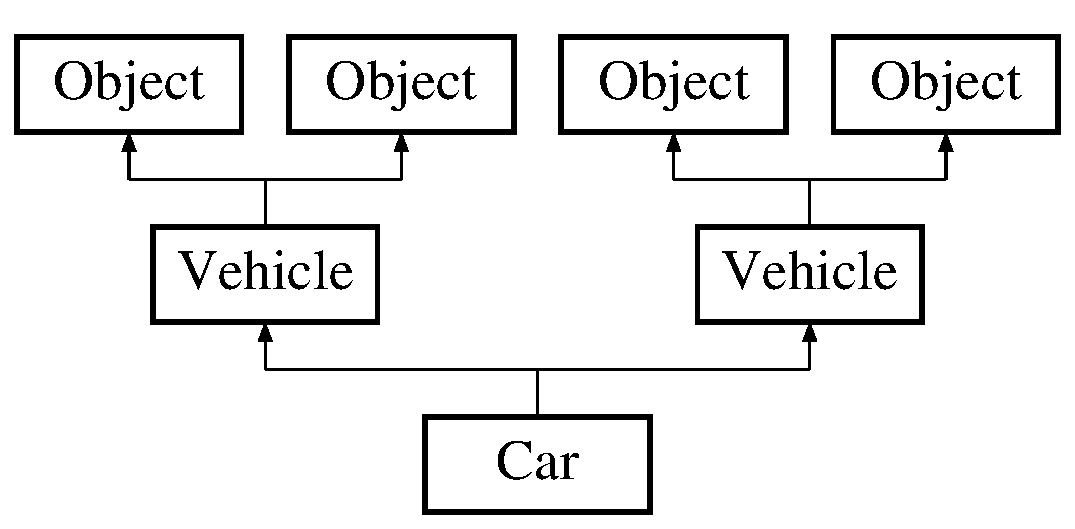
\includegraphics[height=3.000000cm]{struct_car}
\end{center}
\end{figure}
\subsection*{Atributos Protegidos}
\begin{DoxyCompactItemize}
\item 
\hypertarget{struct_car_aea78492ff0e6add272aedd448bf00b6c}{\hyperlink{struct_vehicle}{Vehicle} \hyperlink{struct_car_aea78492ff0e6add272aedd448bf00b6c}{base}}\label{struct_car_aea78492ff0e6add272aedd448bf00b6c}

\begin{DoxyCompactList}\small\item\em Base class. \end{DoxyCompactList}\end{DoxyCompactItemize}
\subsection*{Additional Inherited Members}


\subsection{Descrição detalhada}
\hyperlink{struct_car}{Car} class. 

A documentação para esta estrutura foi gerada a partir dos seguintes ficheiros\-:\begin{DoxyCompactItemize}
\item 
C\-:/\-Users/teste/git/doxygen/examples/\hyperlink{manual_8c}{manual.\-c}\item 
C\-:/\-Users/teste/git/doxygen/testing/\hyperlink{027__extends_8c}{027\-\_\-extends.\-c}\end{DoxyCompactItemize}

\hypertarget{class_child_node_handler}{\section{Referência à classe Child\-Node\-Handler}
\label{class_child_node_handler}\index{Child\-Node\-Handler@{Child\-Node\-Handler}}
}
Diagrama de heranças da classe Child\-Node\-Handler\begin{figure}[H]
\begin{center}
\leavevmode
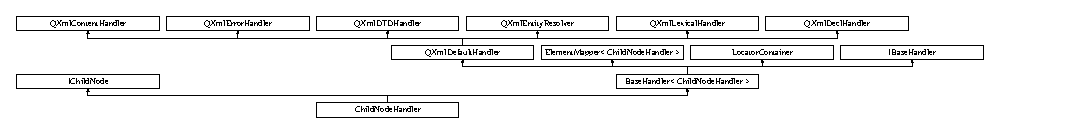
\includegraphics[height=1.355932cm]{class_child_node_handler}
\end{center}
\end{figure}
\subsection*{Membros públicos}
\begin{DoxyCompactItemize}
\item 
\hypertarget{class_child_node_handler_a3d5a6c5b130ca18f4d76a410b6dcc25a}{{\bfseries Child\-Node\-Handler} (\hyperlink{class_i_base_handler}{I\-Base\-Handler} $\ast$parent, \hyperlink{class_graph_handler}{Graph\-Handler} $\ast$gh)}\label{class_child_node_handler_a3d5a6c5b130ca18f4d76a410b6dcc25a}

\item 
\hypertarget{class_child_node_handler_a4387c021769bc2f0b08580eff7f6dc28}{void {\bfseries start\-Child\-Node} (const \hyperlink{class_q_xml_attributes}{Q\-Xml\-Attributes} \&attrib)}\label{class_child_node_handler_a4387c021769bc2f0b08580eff7f6dc28}

\item 
\hypertarget{class_child_node_handler_a4a1f286e5a73a777f2f381978857ecc4}{void {\bfseries end\-Child\-Node} ()}\label{class_child_node_handler_a4a1f286e5a73a777f2f381978857ecc4}

\item 
\hypertarget{class_child_node_handler_a9f087a53fd7db00c162608d0e76ee37d}{void {\bfseries start\-Edge\-Label} (const \hyperlink{class_q_xml_attributes}{Q\-Xml\-Attributes} \&attrib)}\label{class_child_node_handler_a9f087a53fd7db00c162608d0e76ee37d}

\item 
\hypertarget{class_child_node_handler_ad38b7d6894a18d8e1ce58c7e768009ef}{virtual \hyperlink{class_i_node}{I\-Node} $\ast$ {\bfseries node} () const }\label{class_child_node_handler_ad38b7d6894a18d8e1ce58c7e768009ef}

\item 
\hypertarget{class_child_node_handler_ab589e4767fe32492a57dc64e3fb1164b}{virtual Node\-Relation {\bfseries relation} () const }\label{class_child_node_handler_ab589e4767fe32492a57dc64e3fb1164b}

\item 
\hypertarget{class_child_node_handler_aeb87387f72da01955ee473b886744f7d}{virtual const \hyperlink{class_i_string}{I\-String} $\ast$ {\bfseries relation\-String} () const }\label{class_child_node_handler_aeb87387f72da01955ee473b886744f7d}

\item 
\hypertarget{class_child_node_handler_a05733a5ca02ddb20ee4d1075588a5506}{virtual \hyperlink{class_i_edge_label_iterator}{I\-Edge\-Label\-Iterator} $\ast$ {\bfseries edge\-Labels} () const }\label{class_child_node_handler_a05733a5ca02ddb20ee4d1075588a5506}

\end{DoxyCompactItemize}
\subsection*{Amigos}
\begin{DoxyCompactItemize}
\item 
\hypertarget{class_child_node_handler_af04914e6743dfa65bd97548d5db241fc}{class {\bfseries Edge\-Label\-Iterator}}\label{class_child_node_handler_af04914e6743dfa65bd97548d5db241fc}

\end{DoxyCompactItemize}
\subsection*{Additional Inherited Members}


A documentação para esta classe foi gerada a partir dos seguintes ficheiros\-:\begin{DoxyCompactItemize}
\item 
C\-:/\-Users/teste/git/doxygen/addon/doxmlparser/src/graphhandler.\-h\item 
C\-:/\-Users/teste/git/doxygen/addon/doxmlparser/src/graphhandler.\-cpp\end{DoxyCompactItemize}

\hypertarget{class_child_node_iterator}{\section{Referência à classe Child\-Node\-Iterator}
\label{class_child_node_iterator}\index{Child\-Node\-Iterator@{Child\-Node\-Iterator}}
}
Diagrama de heranças da classe Child\-Node\-Iterator\begin{figure}[H]
\begin{center}
\leavevmode
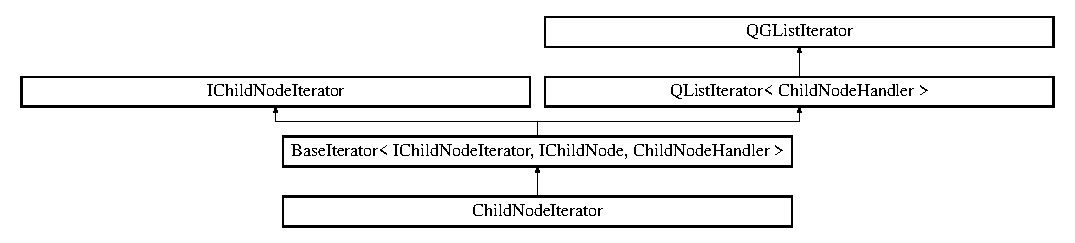
\includegraphics[height=2.814070cm]{class_child_node_iterator}
\end{center}
\end{figure}
\subsection*{Membros públicos}
\begin{DoxyCompactItemize}
\item 
\hypertarget{class_child_node_iterator_a4753b775099344ce3f16be3f5fbec0b7}{{\bfseries Child\-Node\-Iterator} (const \hyperlink{class_node_handler}{Node\-Handler} \&handler)}\label{class_child_node_iterator_a4753b775099344ce3f16be3f5fbec0b7}

\end{DoxyCompactItemize}
\subsection*{Additional Inherited Members}


A documentação para esta classe foi gerada a partir do seguinte ficheiro\-:\begin{DoxyCompactItemize}
\item 
C\-:/\-Users/teste/git/doxygen/addon/doxmlparser/src/graphhandler.\-h\end{DoxyCompactItemize}

\hypertarget{struct_cite_consts}{\section{Referência à estrutura Cite\-Consts}
\label{struct_cite_consts}\index{Cite\-Consts@{Cite\-Consts}}
}


\hyperlink{class_string}{String} constants for citations.  




{\ttfamily \#include $<$cite.\-h$>$}

\subsection*{Atributos Públicos Estáticos}
\begin{DoxyCompactItemize}
\item 
\hypertarget{struct_cite_consts_ac737530792e4fe46ec52288e6df290aa}{static const \hyperlink{class_q_c_string}{Q\-C\-String} {\bfseries file\-Name}}\label{struct_cite_consts_ac737530792e4fe46ec52288e6df290aa}

\item 
\hypertarget{struct_cite_consts_a0ff66553e77cd721fdbd3e73a97ee65b}{static const \hyperlink{class_q_c_string}{Q\-C\-String} {\bfseries anchor\-Prefix}}\label{struct_cite_consts_a0ff66553e77cd721fdbd3e73a97ee65b}

\end{DoxyCompactItemize}


\subsection{Descrição detalhada}
\hyperlink{class_string}{String} constants for citations. 

A documentação para esta estrutura foi gerada a partir dos seguintes ficheiros\-:\begin{DoxyCompactItemize}
\item 
C\-:/\-Users/teste/git/doxygen/src/cite.\-h\item 
C\-:/\-Users/teste/git/doxygen/src/cite.\-cpp\end{DoxyCompactItemize}

\hypertarget{class_cite_dict}{\section{Referência à classe Cite\-Dict}
\label{class_cite_dict}\index{Cite\-Dict@{Cite\-Dict}}
}


Cite database access class.  




{\ttfamily \#include $<$cite.\-h$>$}

\subsection*{Membros públicos}
\begin{DoxyCompactItemize}
\item 
\hyperlink{class_cite_dict_aa5c973f82a208e2167cc72a7c3cfa87e}{Cite\-Dict} (int size)
\item 
void \hyperlink{class_cite_dict_a4d291905bea29c7c01d5439367b4ea0e}{insert} (const char $\ast$label)
\item 
\hyperlink{struct_cite_info}{Cite\-Info} $\ast$ \hyperlink{class_cite_dict_a82b8ee1e48d86fdaad9690807121544b}{find} (const char $\ast$label) const 
\item 
void \hyperlink{class_cite_dict_a980f4d357d9b293e1181680db1d2959f}{generate\-Page} () const 
\item 
void \hyperlink{class_cite_dict_ac8bb3912a3ce86b15842e79d0b421204}{clear} ()
\item 
bool \hyperlink{class_cite_dict_a479432127ee77145cc19d6a2d1590821}{is\-Empty} () const 
\item 
void \hyperlink{class_cite_dict_aadd2b1f13a145a6d369a274929f862c6}{write\-Latex\-Bibliography} (\hyperlink{class_f_text_stream}{F\-Text\-Stream} \&t)
\end{DoxyCompactItemize}


\subsection{Descrição detalhada}
Cite database access class. 

This class provides access do the database of bibliographic references through the bibtex backend. 

\subsection{Documentação dos Construtores \& Destrutor}
\hypertarget{class_cite_dict_aa5c973f82a208e2167cc72a7c3cfa87e}{\index{Cite\-Dict@{Cite\-Dict}!Cite\-Dict@{Cite\-Dict}}
\index{Cite\-Dict@{Cite\-Dict}!CiteDict@{Cite\-Dict}}
\subsubsection[{Cite\-Dict}]{\setlength{\rightskip}{0pt plus 5cm}{\bf Cite\-Dict} (
\begin{DoxyParamCaption}
\item[{int}]{size}
\end{DoxyParamCaption}
)}}\label{class_cite_dict_aa5c973f82a208e2167cc72a7c3cfa87e}
Create the database, with an expected maximum of {\itshape size} entries 

\subsection{Documentação dos métodos}
\hypertarget{class_cite_dict_ac8bb3912a3ce86b15842e79d0b421204}{\index{Cite\-Dict@{Cite\-Dict}!clear@{clear}}
\index{clear@{clear}!CiteDict@{Cite\-Dict}}
\subsubsection[{clear}]{\setlength{\rightskip}{0pt plus 5cm}void clear (
\begin{DoxyParamCaption}
{}
\end{DoxyParamCaption}
)}}\label{class_cite_dict_ac8bb3912a3ce86b15842e79d0b421204}
clears the database \hypertarget{class_cite_dict_a82b8ee1e48d86fdaad9690807121544b}{\index{Cite\-Dict@{Cite\-Dict}!find@{find}}
\index{find@{find}!CiteDict@{Cite\-Dict}}
\subsubsection[{find}]{\setlength{\rightskip}{0pt plus 5cm}{\bf Cite\-Info} $\ast$ find (
\begin{DoxyParamCaption}
\item[{const char $\ast$}]{label}
\end{DoxyParamCaption}
) const}}\label{class_cite_dict_a82b8ee1e48d86fdaad9690807121544b}
Return the citation info for a given {\itshape label} \hypertarget{class_cite_dict_a980f4d357d9b293e1181680db1d2959f}{\index{Cite\-Dict@{Cite\-Dict}!generate\-Page@{generate\-Page}}
\index{generate\-Page@{generate\-Page}!CiteDict@{Cite\-Dict}}
\subsubsection[{generate\-Page}]{\setlength{\rightskip}{0pt plus 5cm}void generate\-Page (
\begin{DoxyParamCaption}
{}
\end{DoxyParamCaption}
) const}}\label{class_cite_dict_a980f4d357d9b293e1181680db1d2959f}
Generate the citations page \hypertarget{class_cite_dict_a4d291905bea29c7c01d5439367b4ea0e}{\index{Cite\-Dict@{Cite\-Dict}!insert@{insert}}
\index{insert@{insert}!CiteDict@{Cite\-Dict}}
\subsubsection[{insert}]{\setlength{\rightskip}{0pt plus 5cm}void insert (
\begin{DoxyParamCaption}
\item[{const char $\ast$}]{label}
\end{DoxyParamCaption}
)}}\label{class_cite_dict_a4d291905bea29c7c01d5439367b4ea0e}
Resolve references to citations Insert a citation identified by {\itshape label} into the database \hypertarget{class_cite_dict_a479432127ee77145cc19d6a2d1590821}{\index{Cite\-Dict@{Cite\-Dict}!is\-Empty@{is\-Empty}}
\index{is\-Empty@{is\-Empty}!CiteDict@{Cite\-Dict}}
\subsubsection[{is\-Empty}]{\setlength{\rightskip}{0pt plus 5cm}bool is\-Empty (
\begin{DoxyParamCaption}
{}
\end{DoxyParamCaption}
) const}}\label{class_cite_dict_a479432127ee77145cc19d6a2d1590821}
return T\-R\-U\-E if there are no citations. Only valid after calling resolve() \hypertarget{class_cite_dict_aadd2b1f13a145a6d369a274929f862c6}{\index{Cite\-Dict@{Cite\-Dict}!write\-Latex\-Bibliography@{write\-Latex\-Bibliography}}
\index{write\-Latex\-Bibliography@{write\-Latex\-Bibliography}!CiteDict@{Cite\-Dict}}
\subsubsection[{write\-Latex\-Bibliography}]{\setlength{\rightskip}{0pt plus 5cm}void write\-Latex\-Bibliography (
\begin{DoxyParamCaption}
\item[{{\bf F\-Text\-Stream} \&}]{t}
\end{DoxyParamCaption}
)}}\label{class_cite_dict_aadd2b1f13a145a6d369a274929f862c6}
writes the latex code for the standard bibliography section to text stream {\itshape t} 

A documentação para esta classe foi gerada a partir dos seguintes ficheiros\-:\begin{DoxyCompactItemize}
\item 
C\-:/\-Users/teste/git/doxygen/src/cite.\-h\item 
C\-:/\-Users/teste/git/doxygen/src/cite.\-cpp\end{DoxyCompactItemize}

\hypertarget{struct_cite_info}{\section{Referência à estrutura Cite\-Info}
\label{struct_cite_info}\index{Cite\-Info@{Cite\-Info}}
}


Citation-\/related data.  




{\ttfamily \#include $<$cite.\-h$>$}

\subsection*{Membros públicos}
\begin{DoxyCompactItemize}
\item 
\hypertarget{struct_cite_info_a54e566b1bb6463ba38ad08e89c882161}{{\bfseries Cite\-Info} (const char $\ast$label\-\_\-, const char $\ast$text\-\_\-=0, const char $\ast$full\-Text\-\_\-=0, const char $\ast$ref\-\_\-=0)}\label{struct_cite_info_a54e566b1bb6463ba38ad08e89c882161}

\item 
\hypertarget{struct_cite_info_a17fbd7dd6140b478f805389601caa21c}{{\bfseries Cite\-Info} (const \hyperlink{struct_cite_info}{Cite\-Info} \&o)}\label{struct_cite_info_a17fbd7dd6140b478f805389601caa21c}

\end{DoxyCompactItemize}
\subsection*{Campos de Dados}
\begin{DoxyCompactItemize}
\item 
\hypertarget{struct_cite_info_ad961cc9bd17b7533dc02fe0826647dc7}{\hyperlink{class_q_c_string}{Q\-C\-String} {\bfseries label}}\label{struct_cite_info_ad961cc9bd17b7533dc02fe0826647dc7}

\item 
\hypertarget{struct_cite_info_a4699e75142e13e15b0f7c9ada64258c3}{\hyperlink{class_q_c_string}{Q\-C\-String} {\bfseries text}}\label{struct_cite_info_a4699e75142e13e15b0f7c9ada64258c3}

\item 
\hypertarget{struct_cite_info_aaf22d92ca78ac9c777bce05e9f111ce4}{\hyperlink{class_q_c_string}{Q\-C\-String} {\bfseries full\-Text}}\label{struct_cite_info_aaf22d92ca78ac9c777bce05e9f111ce4}

\item 
\hypertarget{struct_cite_info_a12b5232acab32ee40a197f72270d4ad1}{\hyperlink{class_q_c_string}{Q\-C\-String} {\bfseries ref}}\label{struct_cite_info_a12b5232acab32ee40a197f72270d4ad1}

\end{DoxyCompactItemize}


\subsection{Descrição detalhada}
Citation-\/related data. 

A documentação para esta estrutura foi gerada a partir do seguinte ficheiro\-:\begin{DoxyCompactItemize}
\item 
C\-:/\-Users/teste/git/doxygen/src/cite.\-h\end{DoxyCompactItemize}

\hypertarget{class_clang_parser}{\section{Referência à classe Clang\-Parser}
\label{class_clang_parser}\index{Clang\-Parser@{Clang\-Parser}}
}


Wrapper for to let libclang assisted parsing.  




{\ttfamily \#include $<$clangparser.\-h$>$}

\subsection*{Membros públicos}
\begin{DoxyCompactItemize}
\item 
void \hyperlink{class_clang_parser_af7c25c56f58f21484e4ad43fd4a73554}{start} (const char $\ast$file\-Name, \hyperlink{class_q_str_list}{Q\-Str\-List} \&files\-In\-Translation\-Unit)
\item 
void \hyperlink{class_clang_parser_aca4c0e995b2d13db218e8cd378a929f1}{switch\-To\-File} (const char $\ast$file\-Name)
\item 
void \hyperlink{class_clang_parser_a6dfe1abe0d1eb3ddc1ca081de98b5342}{finish} ()
\item 
\hyperlink{class_q_c_string}{Q\-C\-String} \hyperlink{class_clang_parser_ad22e9db2f4590b9883b6b01080aad2f7}{lookup} (uint line, const char $\ast$symbol)
\item 
void \hyperlink{class_clang_parser_a63a48a31a772ed04d957f41d16ee439e}{write\-Sources} (\hyperlink{class_code_output_interface}{Code\-Output\-Interface} \&ol, \hyperlink{class_file_def}{File\-Def} $\ast$fd)
\end{DoxyCompactItemize}
\subsection*{Membros públicos estáticos}
\begin{DoxyCompactItemize}
\item 
static \hyperlink{class_clang_parser}{Clang\-Parser} $\ast$ \hyperlink{class_clang_parser_ae995ee43964e9a2d42e036a8b7c08094}{instance} ()
\end{DoxyCompactItemize}


\subsection{Descrição detalhada}
Wrapper for to let libclang assisted parsing. 

\subsection{Documentação dos métodos}
\hypertarget{class_clang_parser_a6dfe1abe0d1eb3ddc1ca081de98b5342}{\index{Clang\-Parser@{Clang\-Parser}!finish@{finish}}
\index{finish@{finish}!ClangParser@{Clang\-Parser}}
\subsubsection[{finish}]{\setlength{\rightskip}{0pt plus 5cm}void finish (
\begin{DoxyParamCaption}
{}
\end{DoxyParamCaption}
)}}\label{class_clang_parser_a6dfe1abe0d1eb3ddc1ca081de98b5342}
Finishes parsing a translation unit. Free any resources that were needed for parsing. \hypertarget{class_clang_parser_ae995ee43964e9a2d42e036a8b7c08094}{\index{Clang\-Parser@{Clang\-Parser}!instance@{instance}}
\index{instance@{instance}!ClangParser@{Clang\-Parser}}
\subsubsection[{instance}]{\setlength{\rightskip}{0pt plus 5cm}{\bf Clang\-Parser} $\ast$ instance (
\begin{DoxyParamCaption}
{}
\end{DoxyParamCaption}
)\hspace{0.3cm}{\ttfamily [static]}}}\label{class_clang_parser_ae995ee43964e9a2d42e036a8b7c08094}
Returns the one and only instance of the class \hypertarget{class_clang_parser_ad22e9db2f4590b9883b6b01080aad2f7}{\index{Clang\-Parser@{Clang\-Parser}!lookup@{lookup}}
\index{lookup@{lookup}!ClangParser@{Clang\-Parser}}
\subsubsection[{lookup}]{\setlength{\rightskip}{0pt plus 5cm}{\bf Q\-C\-String} lookup (
\begin{DoxyParamCaption}
\item[{uint}]{line, }
\item[{const char $\ast$}]{symbol}
\end{DoxyParamCaption}
)}}\label{class_clang_parser_ad22e9db2f4590b9883b6b01080aad2f7}
Looks for {\itshape symbol} which should be found at {\itshape line} and returns a clang unique reference to the symbol. \hypertarget{class_clang_parser_af7c25c56f58f21484e4ad43fd4a73554}{\index{Clang\-Parser@{Clang\-Parser}!start@{start}}
\index{start@{start}!ClangParser@{Clang\-Parser}}
\subsubsection[{start}]{\setlength{\rightskip}{0pt plus 5cm}void start (
\begin{DoxyParamCaption}
\item[{const char $\ast$}]{file\-Name, }
\item[{{\bf Q\-Str\-List} \&}]{files\-In\-Translation\-Unit}
\end{DoxyParamCaption}
)}}\label{class_clang_parser_af7c25c56f58f21484e4ad43fd4a73554}
Start parsing a file. 
\begin{DoxyParams}[1]{Parâmetros}
\mbox{\tt in}  & {\em file\-Name} & The name of the file to parse. \\
\hline
\mbox{\tt in,out}  & {\em files\-In\-Tanslation\-Unit} & Other files that are part of the input and included by the file. The function will return a subset of the files, only including the onces that were actually found during parsing. \\
\hline
\end{DoxyParams}
\hypertarget{class_clang_parser_aca4c0e995b2d13db218e8cd378a929f1}{\index{Clang\-Parser@{Clang\-Parser}!switch\-To\-File@{switch\-To\-File}}
\index{switch\-To\-File@{switch\-To\-File}!ClangParser@{Clang\-Parser}}
\subsubsection[{switch\-To\-File}]{\setlength{\rightskip}{0pt plus 5cm}void switch\-To\-File (
\begin{DoxyParamCaption}
\item[{const char $\ast$}]{file\-Name}
\end{DoxyParamCaption}
)}}\label{class_clang_parser_aca4c0e995b2d13db218e8cd378a929f1}
Switches to another file within the translation unit started with \hyperlink{class_clang_parser_af7c25c56f58f21484e4ad43fd4a73554}{start()}. 
\begin{DoxyParams}[1]{Parâmetros}
\mbox{\tt in}  & {\em The} & name of the file to switch to. \\
\hline
\end{DoxyParams}
\hypertarget{class_clang_parser_a63a48a31a772ed04d957f41d16ee439e}{\index{Clang\-Parser@{Clang\-Parser}!write\-Sources@{write\-Sources}}
\index{write\-Sources@{write\-Sources}!ClangParser@{Clang\-Parser}}
\subsubsection[{write\-Sources}]{\setlength{\rightskip}{0pt plus 5cm}void write\-Sources (
\begin{DoxyParamCaption}
\item[{{\bf Code\-Output\-Interface} \&}]{ol, }
\item[{{\bf File\-Def} $\ast$}]{fd}
\end{DoxyParamCaption}
)}}\label{class_clang_parser_a63a48a31a772ed04d957f41d16ee439e}
writes the syntax highlighted source code for a file 
\begin{DoxyParams}[1]{Parâmetros}
\mbox{\tt out}  & {\em ol} & The output generator list to write to. \\
\hline
\mbox{\tt in}  & {\em fd} & The file to write sources for. \\
\hline
\end{DoxyParams}


A documentação para esta classe foi gerada a partir dos seguintes ficheiros\-:\begin{DoxyCompactItemize}
\item 
C\-:/\-Users/teste/git/doxygen/src/clangparser.\-h\item 
C\-:/\-Users/teste/git/doxygen/src/clangparser.\-cpp\end{DoxyCompactItemize}

\hypertarget{class_c_language_scanner}{\section{Referência à classe C\-Language\-Scanner}
\label{class_c_language_scanner}\index{C\-Language\-Scanner@{C\-Language\-Scanner}}
}


C-\/like language parser using state-\/based lexical scanning.  




{\ttfamily \#include $<$scanner.\-h$>$}

Diagrama de heranças da classe C\-Language\-Scanner\begin{figure}[H]
\begin{center}
\leavevmode
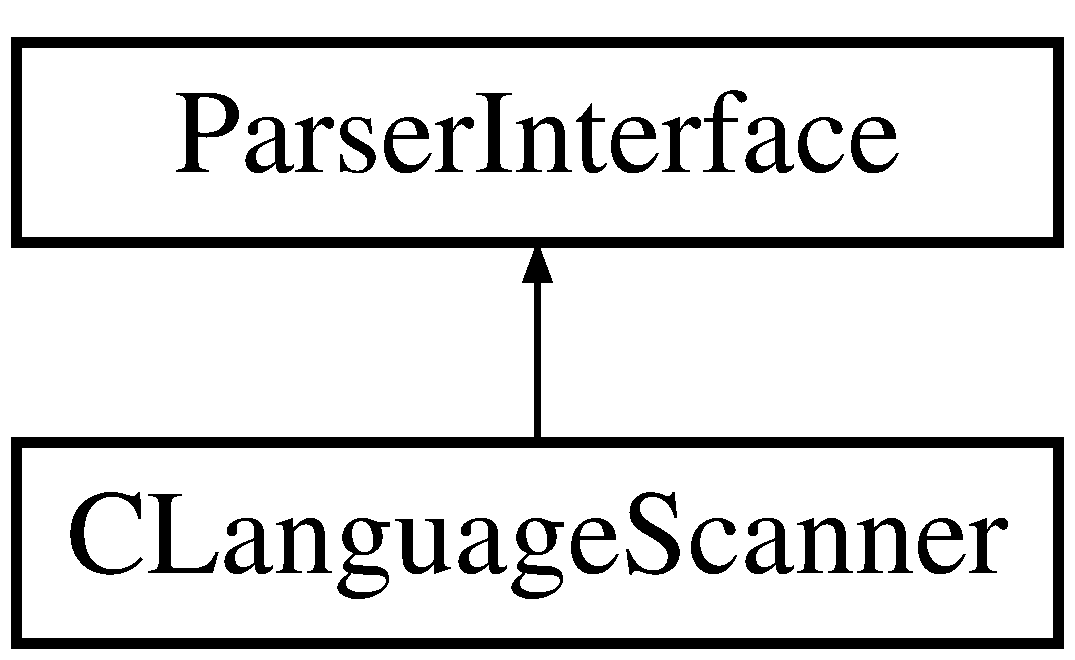
\includegraphics[height=2.000000cm]{class_c_language_scanner}
\end{center}
\end{figure}
\subsection*{Membros públicos}
\begin{DoxyCompactItemize}
\item 
void \hyperlink{class_c_language_scanner_aa33a9c80fb9c03da5570bdfd65e3d09c}{start\-Translation\-Unit} (const char $\ast$file\-Name)
\item 
void \hyperlink{class_c_language_scanner_a245c1fbfb8ba359e61d832c4e7c6c98e}{finish\-Translation\-Unit} ()
\item 
void \hyperlink{class_c_language_scanner_ab1ed2c75b61719cec6060b9f69419743}{parse\-Input} (const char $\ast$file\-Name, const char $\ast$file\-Buf, \hyperlink{class_entry}{Entry} $\ast$root, bool same\-Translation\-Unit, \hyperlink{class_q_str_list}{Q\-Str\-List} \&files\-In\-Same\-Translation\-Unit)
\item 
bool \hyperlink{class_c_language_scanner_ac49a959c40c82385233e4c75163e39ae}{needs\-Preprocessing} (const \hyperlink{class_q_c_string}{Q\-C\-String} \&extension)
\item 
void \hyperlink{class_c_language_scanner_ac614074ea2c569cabd265a6168ad36d2}{parse\-Code} (\hyperlink{class_code_output_interface}{Code\-Output\-Interface} \&code\-Out\-Intf, const char $\ast$scope\-Name, const \hyperlink{class_q_c_string}{Q\-C\-String} \&input, \hyperlink{types_8h_a9974623ce72fc23df5d64426b9178bf2}{Src\-Lang\-Ext} lang, bool is\-Example\-Block, const char $\ast$example\-Name=0, \hyperlink{class_file_def}{File\-Def} $\ast$file\-Def=0, int start\-Line=-\/1, int end\-Line=-\/1, bool inline\-Fragment=F\-A\-L\-S\-E, \hyperlink{class_member_def}{Member\-Def} $\ast$member\-Def=0, bool show\-Line\-Numbers=T\-R\-U\-E, \hyperlink{class_definition}{Definition} $\ast$search\-Ctx=0, bool collect\-X\-Refs=T\-R\-U\-E)
\item 
void \hyperlink{class_c_language_scanner_a5d8e0ded4118b6eff98aa23eb64db02c}{reset\-Code\-Parser\-State} ()
\item 
void \hyperlink{class_c_language_scanner_a022344e4fa95056a941a9e8c02334872}{parse\-Prototype} (const char $\ast$text)
\end{DoxyCompactItemize}


\subsection{Descrição detalhada}
C-\/like language parser using state-\/based lexical scanning. 

This is the language parser for doxygen. It is somewhat fuzzy and supports C++ and various languages that are closely related to C++, such as \hyperlink{class_c}{C}, \hyperlink{class_c}{C}\#, Objective-\/\-C, Java, P\-H\-P, and I\-D\-L. 

\subsection{Documentação dos métodos}
\hypertarget{class_c_language_scanner_a245c1fbfb8ba359e61d832c4e7c6c98e}{\index{C\-Language\-Scanner@{C\-Language\-Scanner}!finish\-Translation\-Unit@{finish\-Translation\-Unit}}
\index{finish\-Translation\-Unit@{finish\-Translation\-Unit}!CLanguageScanner@{C\-Language\-Scanner}}
\subsubsection[{finish\-Translation\-Unit}]{\setlength{\rightskip}{0pt plus 5cm}void finish\-Translation\-Unit (
\begin{DoxyParamCaption}
{}
\end{DoxyParamCaption}
)\hspace{0.3cm}{\ttfamily [virtual]}}}\label{class_c_language_scanner_a245c1fbfb8ba359e61d832c4e7c6c98e}
Called after all files in a translation unit have been processed. 

Implementa \hyperlink{class_parser_interface_afeb7f0c0fa300a57fbbc5bceb2795f3a}{Parser\-Interface}.

\hypertarget{class_c_language_scanner_ac49a959c40c82385233e4c75163e39ae}{\index{C\-Language\-Scanner@{C\-Language\-Scanner}!needs\-Preprocessing@{needs\-Preprocessing}}
\index{needs\-Preprocessing@{needs\-Preprocessing}!CLanguageScanner@{C\-Language\-Scanner}}
\subsubsection[{needs\-Preprocessing}]{\setlength{\rightskip}{0pt plus 5cm}bool needs\-Preprocessing (
\begin{DoxyParamCaption}
\item[{const {\bf Q\-C\-String} \&}]{extension}
\end{DoxyParamCaption}
)\hspace{0.3cm}{\ttfamily [virtual]}}}\label{class_c_language_scanner_ac49a959c40c82385233e4c75163e39ae}
Returns T\-R\-U\-E if the language identified by {\itshape extension} needs the \hyperlink{class_c}{C} preprocessor to be run before feed the result to the input parser. \begin{DoxySeeAlso}{Veja também}
\hyperlink{class_c_language_scanner_ab1ed2c75b61719cec6060b9f69419743}{parse\-Input()} 
\end{DoxySeeAlso}


Implementa \hyperlink{class_parser_interface_a9f137118e8804d57ea8ebe6a7d711703}{Parser\-Interface}.

\hypertarget{class_c_language_scanner_ac614074ea2c569cabd265a6168ad36d2}{\index{C\-Language\-Scanner@{C\-Language\-Scanner}!parse\-Code@{parse\-Code}}
\index{parse\-Code@{parse\-Code}!CLanguageScanner@{C\-Language\-Scanner}}
\subsubsection[{parse\-Code}]{\setlength{\rightskip}{0pt plus 5cm}void parse\-Code (
\begin{DoxyParamCaption}
\item[{{\bf Code\-Output\-Interface} \&}]{code\-Out\-Intf, }
\item[{const char $\ast$}]{scope\-Name, }
\item[{const {\bf Q\-C\-String} \&}]{input, }
\item[{{\bf Src\-Lang\-Ext}}]{lang, }
\item[{bool}]{is\-Example\-Block, }
\item[{const char $\ast$}]{example\-Name = {\ttfamily 0}, }
\item[{{\bf File\-Def} $\ast$}]{file\-Def = {\ttfamily 0}, }
\item[{int}]{start\-Line = {\ttfamily -\/1}, }
\item[{int}]{end\-Line = {\ttfamily -\/1}, }
\item[{bool}]{inline\-Fragment = {\ttfamily FALSE}, }
\item[{{\bf Member\-Def} $\ast$}]{member\-Def = {\ttfamily 0}, }
\item[{bool}]{show\-Line\-Numbers = {\ttfamily TRUE}, }
\item[{{\bf Definition} $\ast$}]{search\-Ctx = {\ttfamily 0}, }
\item[{bool}]{collect\-X\-Refs = {\ttfamily TRUE}}
\end{DoxyParamCaption}
)\hspace{0.3cm}{\ttfamily [virtual]}}}\label{class_c_language_scanner_ac614074ea2c569cabd265a6168ad36d2}
Parses a source file or fragment with the goal to produce highlighted and cross-\/referenced output. 
\begin{DoxyParams}[1]{Parâmetros}
\mbox{\tt in}  & {\em code\-Out\-Intf} & Abstract interface for writing the result. \\
\hline
\mbox{\tt in}  & {\em lang} & The programming language of the code fragment. \\
\hline
\mbox{\tt in}  & {\em scope\-Name} & Name of scope to which the code belongs. \\
\hline
\mbox{\tt in}  & {\em input} & Actual code in the form of a string \\
\hline
\mbox{\tt in}  & {\em is\-Example\-Block} & T\-R\-U\-E iff the code is part of an example. \\
\hline
\mbox{\tt in}  & {\em example\-Name} & Name of the example. \\
\hline
\mbox{\tt in}  & {\em file\-Def} & File definition to which the code is associated. \\
\hline
\mbox{\tt in}  & {\em start\-Line} & Starting line in case of a code fragment. \\
\hline
\mbox{\tt in}  & {\em end\-Line} & Ending line of the code fragment. \\
\hline
\mbox{\tt in}  & {\em inline\-Fragment} & Code fragment that is to be shown inline as part of the documentation. \\
\hline
\mbox{\tt in}  & {\em member\-Def} & Member definition to which the code is associated (non null in case of an inline fragment for a member). \\
\hline
\mbox{\tt in}  & {\em show\-Line\-Numbers} & if set to T\-R\-U\-E and also file\-Def is not 0, line numbers will be added to the source fragement \\
\hline
\mbox{\tt in}  & {\em search\-Ctx} & context under which search data has to be stored. \\
\hline
\mbox{\tt in}  & {\em collect\-X\-Refs} & collect cross-\/reference relations. \\
\hline
\end{DoxyParams}


Implementa \hyperlink{class_parser_interface_a8e684ab861915fbec41adfaec153d304}{Parser\-Interface}.

\hypertarget{class_c_language_scanner_ab1ed2c75b61719cec6060b9f69419743}{\index{C\-Language\-Scanner@{C\-Language\-Scanner}!parse\-Input@{parse\-Input}}
\index{parse\-Input@{parse\-Input}!CLanguageScanner@{C\-Language\-Scanner}}
\subsubsection[{parse\-Input}]{\setlength{\rightskip}{0pt plus 5cm}void parse\-Input (
\begin{DoxyParamCaption}
\item[{const char $\ast$}]{file\-Name, }
\item[{const char $\ast$}]{file\-Buf, }
\item[{{\bf Entry} $\ast$}]{root, }
\item[{bool}]{same\-Translation\-Unit, }
\item[{{\bf Q\-Str\-List} \&}]{files\-In\-Same\-Translation\-Unit}
\end{DoxyParamCaption}
)\hspace{0.3cm}{\ttfamily [virtual]}}}\label{class_c_language_scanner_ab1ed2c75b61719cec6060b9f69419743}
Parses a single input file with the goal to build an \hyperlink{class_entry}{Entry} tree. 
\begin{DoxyParams}[1]{Parâmetros}
\mbox{\tt in}  & {\em file\-Name} & The full name of the file. \\
\hline
\mbox{\tt in}  & {\em file\-Buf} & The contents of the file (zero terminated). \\
\hline
\mbox{\tt in,out}  & {\em root} & The root of the tree of \hyperlink{class_entry}{Entry} $\ast$nodes representing the information extracted from the file. \\
\hline
\mbox{\tt in}  & {\em same\-Translation\-Unit} & T\-R\-U\-E if this file was found in the same translation unit (in the files\-In\-Same\-Translation\-Unit list returned for another file). \\
\hline
\mbox{\tt in,out}  & {\em files\-In\-Same\-Translation\-Unit} & other files expected to be found in the same translation unit (used for libclang) \\
\hline
\end{DoxyParams}


Implementa \hyperlink{class_parser_interface_a1788757b1264f4d4abf6c5bee8cb50dd}{Parser\-Interface}.

\hypertarget{class_c_language_scanner_a022344e4fa95056a941a9e8c02334872}{\index{C\-Language\-Scanner@{C\-Language\-Scanner}!parse\-Prototype@{parse\-Prototype}}
\index{parse\-Prototype@{parse\-Prototype}!CLanguageScanner@{C\-Language\-Scanner}}
\subsubsection[{parse\-Prototype}]{\setlength{\rightskip}{0pt plus 5cm}void parse\-Prototype (
\begin{DoxyParamCaption}
\item[{const char $\ast$}]{text}
\end{DoxyParamCaption}
)\hspace{0.3cm}{\ttfamily [virtual]}}}\label{class_c_language_scanner_a022344e4fa95056a941a9e8c02334872}
Callback function called by the comment block scanner. It provides a string {\itshape text} containing the prototype of a function or variable. The parser should parse this and store the information in the \hyperlink{class_entry}{Entry} node that corresponds with the node for which the comment block parser was invoked. 

Implementa \hyperlink{class_parser_interface_a3cc425322ee83a0c02243a68b7bacbad}{Parser\-Interface}.

\hypertarget{class_c_language_scanner_a5d8e0ded4118b6eff98aa23eb64db02c}{\index{C\-Language\-Scanner@{C\-Language\-Scanner}!reset\-Code\-Parser\-State@{reset\-Code\-Parser\-State}}
\index{reset\-Code\-Parser\-State@{reset\-Code\-Parser\-State}!CLanguageScanner@{C\-Language\-Scanner}}
\subsubsection[{reset\-Code\-Parser\-State}]{\setlength{\rightskip}{0pt plus 5cm}void reset\-Code\-Parser\-State (
\begin{DoxyParamCaption}
{}
\end{DoxyParamCaption}
)\hspace{0.3cm}{\ttfamily [virtual]}}}\label{class_c_language_scanner_a5d8e0ded4118b6eff98aa23eb64db02c}
Resets the state of the code parser. Since multiple code fragments can together form a single example, an explicit function is used to reset the code parser state. \begin{DoxySeeAlso}{Veja também}
\hyperlink{class_c_language_scanner_ac614074ea2c569cabd265a6168ad36d2}{parse\-Code()} 
\end{DoxySeeAlso}


Implementa \hyperlink{class_parser_interface_a8b14ce8c51a4d99ae293916de928debc}{Parser\-Interface}.

\hypertarget{class_c_language_scanner_aa33a9c80fb9c03da5570bdfd65e3d09c}{\index{C\-Language\-Scanner@{C\-Language\-Scanner}!start\-Translation\-Unit@{start\-Translation\-Unit}}
\index{start\-Translation\-Unit@{start\-Translation\-Unit}!CLanguageScanner@{C\-Language\-Scanner}}
\subsubsection[{start\-Translation\-Unit}]{\setlength{\rightskip}{0pt plus 5cm}void start\-Translation\-Unit (
\begin{DoxyParamCaption}
\item[{const char $\ast$}]{file\-Name}
\end{DoxyParamCaption}
)\hspace{0.3cm}{\ttfamily [virtual]}}}\label{class_c_language_scanner_aa33a9c80fb9c03da5570bdfd65e3d09c}
Starts processing a translation unit (source files + headers). After this call \hyperlink{class_c_language_scanner_ab1ed2c75b61719cec6060b9f69419743}{parse\-Input()} is called with same\-Translation\-Unit set to F\-A\-L\-S\-E. If \hyperlink{class_c_language_scanner_ab1ed2c75b61719cec6060b9f69419743}{parse\-Input()} returns additional include files, these are also processed using \hyperlink{class_c_language_scanner_ab1ed2c75b61719cec6060b9f69419743}{parse\-Input()} with same\-Translation\-Unit set to T\-R\-U\-E. After that \hyperlink{class_c_language_scanner_a245c1fbfb8ba359e61d832c4e7c6c98e}{finish\-Translation\-Unit()} is called. 

Implementa \hyperlink{class_parser_interface_ae9d9d869020d0d90f48d67f6a211bf57}{Parser\-Interface}.



A documentação para esta classe foi gerada a partir do seguinte ficheiro\-:\begin{DoxyCompactItemize}
\item 
C\-:/\-Users/teste/git/doxygen/src/scanner.\-h\end{DoxyCompactItemize}

\hypertarget{class_class_context}{\section{Referência à classe Class\-Context}
\label{class_class_context}\index{Class\-Context@{Class\-Context}}
}
Diagrama de heranças da classe Class\-Context\begin{figure}[H]
\begin{center}
\leavevmode
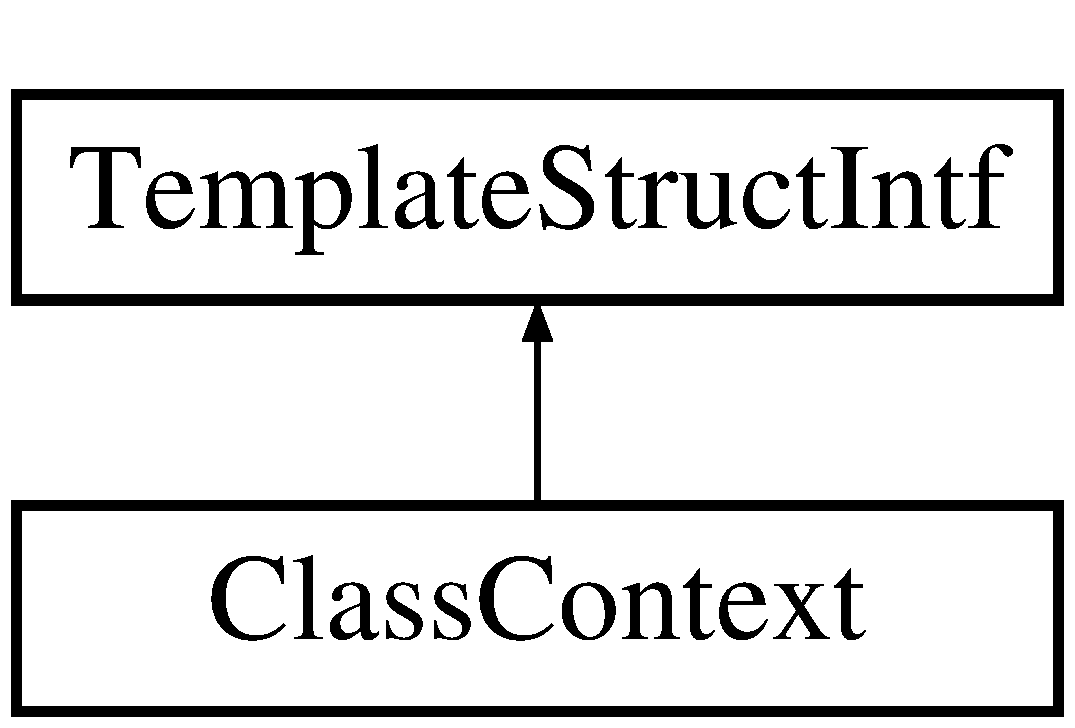
\includegraphics[height=2.000000cm]{class_class_context}
\end{center}
\end{figure}
\subsection*{Estruturas de Dados}
\begin{DoxyCompactItemize}
\item 
class \hyperlink{class_class_context_1_1_private}{Private}
\end{DoxyCompactItemize}
\subsection*{Membros públicos}
\begin{DoxyCompactItemize}
\item 
\hypertarget{class_class_context_aeda4d41cadc4effb18239b77f54640d8}{{\bfseries Class\-Context} (\hyperlink{class_class_def}{Class\-Def} $\ast$)}\label{class_class_context_aeda4d41cadc4effb18239b77f54640d8}

\item 
virtual \hyperlink{class_template_variant}{Template\-Variant} \hyperlink{class_class_context_a1bcfea01201f3ea09981a8442842c42d}{get} (const char $\ast$name) const 
\end{DoxyCompactItemize}


\subsection{Documentação dos métodos}
\hypertarget{class_class_context_a1bcfea01201f3ea09981a8442842c42d}{\index{Class\-Context@{Class\-Context}!get@{get}}
\index{get@{get}!ClassContext@{Class\-Context}}
\subsubsection[{get}]{\setlength{\rightskip}{0pt plus 5cm}{\bf Template\-Variant} get (
\begin{DoxyParamCaption}
\item[{const char $\ast$}]{name}
\end{DoxyParamCaption}
) const\hspace{0.3cm}{\ttfamily [virtual]}}}\label{class_class_context_a1bcfea01201f3ea09981a8442842c42d}
Gets the value for a field name. 
\begin{DoxyParams}[1]{Parâmetros}
\mbox{\tt in}  & {\em name} & The name of the field. \\
\hline
\end{DoxyParams}


Implementa \hyperlink{class_template_struct_intf_a49a65a897ba5e4cd6cb80d681c843aab}{Template\-Struct\-Intf}.



A documentação para esta classe foi gerada a partir dos seguintes ficheiros\-:\begin{DoxyCompactItemize}
\item 
C\-:/\-Users/teste/git/doxygen/src/context.\-h\item 
C\-:/\-Users/teste/git/doxygen/src/context.\-cpp\end{DoxyCompactItemize}

\hypertarget{class_class_def}{\section{Referência à classe Class\-Def}
\label{class_class_def}\index{Class\-Def@{Class\-Def}}
}


{\ttfamily \#include $<$classdef.\-h$>$}

Diagrama de heranças da classe Class\-Def\begin{figure}[H]
\begin{center}
\leavevmode
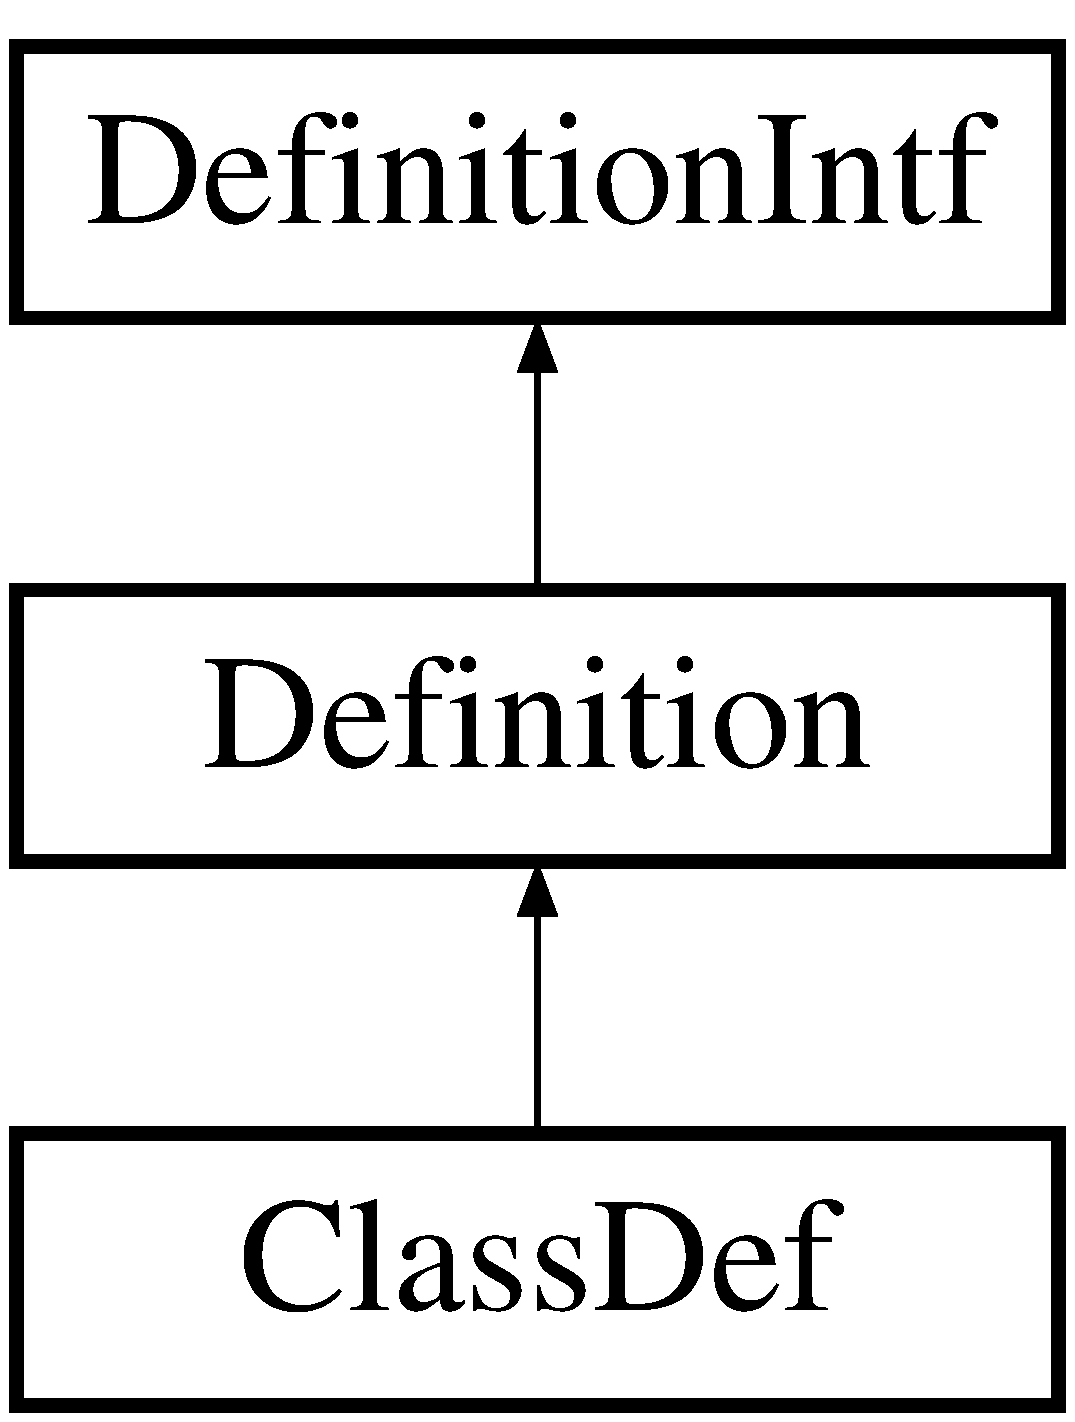
\includegraphics[height=3.000000cm]{class_class_def}
\end{center}
\end{figure}
\subsection*{Tipos Públicos}
\begin{DoxyCompactItemize}
\item 
enum \hyperlink{class_class_def_a768a6f0a6fd7e9087ff7971abbcc3f36}{Compound\-Type} \{ \\*
{\bfseries Class}, 
{\bfseries Struct}, 
{\bfseries Union}, 
{\bfseries Interface}, 
\\*
{\bfseries Protocol}, 
{\bfseries Category}, 
{\bfseries Exception}, 
{\bfseries Service}, 
\\*
{\bfseries Singleton}
 \}
\end{DoxyCompactItemize}
\subsection*{Membros públicos}
\begin{DoxyCompactItemize}
\item 
\hyperlink{class_class_def_a389341b271ebaf30cccddd1838c0f597}{Class\-Def} (const char $\ast$file\-Name, int start\-Line, int start\-Column, const char $\ast$\hyperlink{class_definition_a2c310e06c9aadc6fb218f80fcbb5c695}{name}, \hyperlink{class_class_def_a768a6f0a6fd7e9087ff7971abbcc3f36}{Compound\-Type} ct, const char $\ast$ref=0, const char $\ast$f\-Name=0, bool is\-Symbol=T\-R\-U\-E, bool is\-Java\-Enum=F\-A\-L\-S\-E)
\item 
\hyperlink{class_class_def_a0da78b18aa5068125435320465f36e31}{$\sim$\-Class\-Def} ()
\item 
\hyperlink{class_definition_intf_a2dc566dfec40397b2990e6520536ecb5}{Def\-Type} \hyperlink{class_class_def_aac410235a8bf90e471e649bd9dbf9c5e}{definition\-Type} () const 
\item 
\hyperlink{class_q_c_string}{Q\-C\-String} \hyperlink{class_class_def_af72a982ba8198cd5c98e9fc850b71df6}{get\-Output\-File\-Base} () const 
\item 
\hypertarget{class_class_def_a765bb682fdbd4e43d815fad3710f10c5}{\hyperlink{class_q_c_string}{Q\-C\-String} {\bfseries get\-Instance\-Output\-File\-Base} () const }\label{class_class_def_a765bb682fdbd4e43d815fad3710f10c5}

\item 
\hypertarget{class_class_def_ad47efa4da31f60e593a236751d7e4733}{\hyperlink{class_q_c_string}{Q\-C\-String} {\bfseries get\-File\-Base} () const }\label{class_class_def_ad47efa4da31f60e593a236751d7e4733}

\item 
\hyperlink{class_q_c_string}{Q\-C\-String} \hyperlink{class_class_def_a0b24a407e5cd41328e5c64aac0884b6f}{get\-Source\-File\-Base} () const 
\item 
\hyperlink{class_q_c_string}{Q\-C\-String} \hyperlink{class_class_def_a87b81ea7f17740033bf8fb12f796c494}{get\-Reference} () const 
\item 
bool \hyperlink{class_class_def_ab7dc8cc872f3cec2e07dace4293989aa}{is\-Reference} () const 
\item 
bool \hyperlink{class_class_def_a69fb7e260ed2bc6fa82bfe12c2aeec5a}{is\-Local} () const 
\item 
\hyperlink{class_class_s_dict}{Class\-S\-Dict} $\ast$ \hyperlink{class_class_def_a14c0b45a5896c00649594a0951ae30f7}{get\-Class\-S\-Dict} ()
\item 
bool \hyperlink{class_class_def_a585dcd381ab70014568db8ad457fc8b1}{has\-Documentation} () const 
\item 
bool \hyperlink{class_class_def_ab1e57fff5fd6e501a15f6e992a783995}{has\-Detailed\-Description} () const 
\item 
\hyperlink{class_q_c_string}{Q\-C\-String} \hyperlink{class_class_def_abfd9c72c9c6a40b1689b0671eebc044c}{display\-Name} (bool include\-Scope=T\-R\-U\-E) const 
\item 
\hyperlink{class_class_def_a768a6f0a6fd7e9087ff7971abbcc3f36}{Compound\-Type} \hyperlink{class_class_def_ae5dffc6bd9342e513fc2b9902a150abe}{compound\-Type} () const 
\item 
\hyperlink{class_q_c_string}{Q\-C\-String} \hyperlink{class_class_def_a259ebc501d584761467e254f635fd766}{compound\-Type\-String} () const 
\item 
\hyperlink{class_base_class_list}{Base\-Class\-List} $\ast$ \hyperlink{class_class_def_af817cb1006279d14dca4b6b6ba3db901}{base\-Classes} () const 
\item 
\hyperlink{class_base_class_list}{Base\-Class\-List} $\ast$ \hyperlink{class_class_def_a33f96bac2c9a43e8f6faaeca118d2c73}{sub\-Classes} () const 
\item 
\hyperlink{class_member_name_info_s_dict}{Member\-Name\-Info\-S\-Dict} $\ast$ \hyperlink{class_class_def_abbca3615e0d59730e500151d54561416}{member\-Name\-Info\-S\-Dict} () const 
\item 
\hyperlink{types_8h_a90e352184df58cd09455fe9996cd4ded}{Protection} \hyperlink{class_class_def_a149b66b75ad6cd6c17457a689e68cd9e}{protection} () const 
\item 
bool \hyperlink{class_class_def_a7ff00a84da6e47f3c64c6bf9f6316385}{is\-Linkable\-In\-Project} () const 
\item 
bool \hyperlink{class_class_def_afb5645c0dc69c2f1da67da6e33316e3b}{is\-Linkable} () const 
\item 
bool \hyperlink{class_class_def_a0903a297b1dfa5e537e21ac1bd42d433}{is\-Visible\-In\-Hierarchy} ()
\item 
\hyperlink{class_argument_list}{Argument\-List} $\ast$ \hyperlink{class_class_def_a7a7099c182d85b097ec9b4ac866db827}{template\-Arguments} () const 
\item 
\hyperlink{class_namespace_def}{Namespace\-Def} $\ast$ \hyperlink{class_class_def_a7707ce10899d1b0914f2e95b2d4ecc2a}{get\-Namespace\-Def} () const 
\item 
\hyperlink{class_file_def}{File\-Def} $\ast$ \hyperlink{class_class_def_a5a292ca6db63e5f4a6012dae2af1de08}{get\-File\-Def} () const 
\item 
\hyperlink{class_member_def}{Member\-Def} $\ast$ \hyperlink{class_class_def_ae4b1361bd609c705db962bd9bb8e1afe}{get\-Member\-By\-Name} (const \hyperlink{class_q_c_string}{Q\-C\-String} \&) const 
\item 
bool \hyperlink{class_class_def_ab521566f4d878f44bacb0a2560d993af}{is\-Base\-Class} (\hyperlink{class_class_def}{Class\-Def} $\ast$bcd, bool follow\-Instances, int level=0)
\item 
bool \hyperlink{class_class_def_a81e8ccaa1ddaa3afb6e821c31aa48a0a}{is\-Sub\-Class} (\hyperlink{class_class_def}{Class\-Def} $\ast$bcd, int level=0)
\item 
bool \hyperlink{class_class_def_a9a900cabaf8bd50fa297ea679dfc7716}{is\-Accessible\-Member} (\hyperlink{class_member_def}{Member\-Def} $\ast$md)
\item 
Q\-Dict$<$ \hyperlink{class_class_def}{Class\-Def} $>$ $\ast$ \hyperlink{class_class_def_ad40e3e5176f010fe191043509646d755}{get\-Template\-Instances} () const 
\item 
\hyperlink{class_class_def}{Class\-Def} $\ast$ \hyperlink{class_class_def_aa05f1773a95fb95fbecf82f8c67514c8}{template\-Master} () const 
\item 
bool \hyperlink{class_class_def_a623895be75dc282b0f3af5b18a0cd736}{is\-Template} () const 
\item 
\hypertarget{class_class_def_ac58018f1dfa180cc9c8c622e92e8819b}{\hyperlink{struct_include_info}{Include\-Info} $\ast$ {\bfseries include\-Info} () const }\label{class_class_def_ac58018f1dfa180cc9c8c622e92e8819b}

\item 
\hypertarget{class_class_def_a2b04ff2f8428b80903082077ddbc6388}{\hyperlink{class_uses_class_dict}{Uses\-Class\-Dict} $\ast$ {\bfseries used\-Implementation\-Classes} () const }\label{class_class_def_a2b04ff2f8428b80903082077ddbc6388}

\item 
\hypertarget{class_class_def_affe536e52200d391064d6424e4cca60a}{\hyperlink{class_uses_class_dict}{Uses\-Class\-Dict} $\ast$ {\bfseries used\-By\-Implementation\-Classes} () const }\label{class_class_def_affe536e52200d391064d6424e4cca60a}

\item 
\hypertarget{class_class_def_a750addde329b334fcd3a7778be2ab27a}{\hyperlink{class_uses_class_dict}{Uses\-Class\-Dict} $\ast$ {\bfseries used\-Interface\-Classes} () const }\label{class_class_def_a750addde329b334fcd3a7778be2ab27a}

\item 
\hypertarget{class_class_def_a2a499722bfcb37d7a130073b1582938e}{bool {\bfseries is\-Template\-Argument} () const }\label{class_class_def_a2a499722bfcb37d7a130073b1582938e}

\item 
virtual \hyperlink{class_definition}{Definition} $\ast$ \hyperlink{class_class_def_a5f4c10da520e9553c62483027168c42c}{find\-Inner\-Compound} (const char $\ast$\hyperlink{class_definition_a2c310e06c9aadc6fb218f80fcbb5c695}{name})
\item 
void \hyperlink{class_class_def_aef20cac5706a02dbb50518d24b38f464}{get\-Template\-Parameter\-Lists} (\hyperlink{class_q_list}{Q\-List}$<$ \hyperlink{class_argument_list}{Argument\-List} $>$ \&lists) const 
\item 
\hypertarget{class_class_def_ab123fdbde52be05a46788508ce1d464c}{\hyperlink{class_q_c_string}{Q\-C\-String} {\bfseries qualified\-Name\-With\-Template\-Parameters} (\hyperlink{class_q_list}{Q\-List}$<$ \hyperlink{class_argument_list}{Argument\-List} $>$ $\ast$actual\-Params=0) const }\label{class_class_def_ab123fdbde52be05a46788508ce1d464c}

\item 
bool \hyperlink{class_class_def_ac7f749737f31e5dc070351bbe5214793}{is\-Abstract} () const 
\item 
bool \hyperlink{class_class_def_ab5793e9c44df25523354dc0d0210e54f}{is\-Objective\-C} () const 
\item 
bool \hyperlink{class_class_def_a06620e645a54d46fb481d2ea594f59cf}{is\-C\-Sharp} () const 
\item 
bool \hyperlink{class_class_def_aa1c038a9fa70a19d46c1ea65cbffdb2d}{is\-Final} () const 
\item 
bool \hyperlink{class_class_def_a27367a1b9326358f119463c48350f887}{is\-Sealed} () const 
\item 
bool \hyperlink{class_class_def_a3d09e3bb6fc4144c31a80fd26d401e69}{is\-Published} () const 
\item 
bool \hyperlink{class_class_def_a9ef3fb490d8218394f1091152c631575}{is\-Extension} () const 
\item 
\hyperlink{class_class_def}{Class\-Def} $\ast$ \hyperlink{class_class_def_af897ec96b5a2136f22986353269c091a}{category\-Of} () const 
\item 
\hyperlink{class_q_c_string}{Q\-C\-String} \hyperlink{class_class_def_af0a121aefc7a4a8d9fdda94b6d845ca1}{class\-Name} () const 
\item 
\hyperlink{class_member_list}{Member\-List} $\ast$ \hyperlink{class_class_def_af9947305eeabd8e482637af1ccb4ec4e}{get\-Member\-List} (Member\-List\-Type lt)
\item 
const \hyperlink{class_q_list}{Q\-List}$<$ \hyperlink{class_member_list}{Member\-List} $>$ \& \hyperlink{class_class_def_a958ea00543faccec752fba58fcf79d43}{get\-Member\-Lists} () const 
\item 
\hyperlink{class_member_group_s_dict}{Member\-Group\-S\-Dict} $\ast$ \hyperlink{class_class_def_aebe674b96b5f7f7433f7d161e5a2f047}{get\-Member\-Group\-S\-Dict} () const 
\item 
\hypertarget{class_class_def_a61227c47a6723ba7a5940edf958606f8}{Q\-Dict$<$ int $>$ $\ast$ {\bfseries get\-Template\-Base\-Class\-Names} () const }\label{class_class_def_a61227c47a6723ba7a5940edf958606f8}

\item 
\hypertarget{class_class_def_af6ff262fde60dda76af627de607838a0}{\hyperlink{class_class_def}{Class\-Def} $\ast$ {\bfseries get\-Variable\-Instance} (const char $\ast$templ\-Spec)}\label{class_class_def_af6ff262fde60dda76af627de607838a0}

\item 
\hypertarget{class_class_def_acd998e677fa172f364757bc7c0faa82d}{bool {\bfseries is\-Used\-Only} () const }\label{class_class_def_acd998e677fa172f364757bc7c0faa82d}

\item 
\hyperlink{class_q_c_string}{Q\-C\-String} \hyperlink{class_class_def_acd17ae1d9600f864b1beb85dfb99a4f4}{anchor} () const 
\item 
\hypertarget{class_class_def_ac676e6830cd4943345b79f6e907198c3}{bool {\bfseries is\-Embedded\-In\-Outer\-Scope} () const }\label{class_class_def_ac676e6830cd4943345b79f6e907198c3}

\item 
\hypertarget{class_class_def_a1173815e97366bb5478b113f3bdb96f4}{bool {\bfseries is\-Simple} () const }\label{class_class_def_a1173815e97366bb5478b113f3bdb96f4}

\item 
\hypertarget{class_class_def_a30d0dd8dc490c9107c8b7b4182b56599}{const \hyperlink{class_class_list}{Class\-List} $\ast$ {\bfseries tagged\-Inner\-Classes} () const }\label{class_class_def_a30d0dd8dc490c9107c8b7b4182b56599}

\item 
\hypertarget{class_class_def_a64b5b53cc3bed64b6e71667b92184f0a}{\hyperlink{class_class_def}{Class\-Def} $\ast$ {\bfseries tag\-Less\-Reference} () const }\label{class_class_def_a64b5b53cc3bed64b6e71667b92184f0a}

\item 
\hypertarget{class_class_def_ad68ef9c48463aee9303ebf4027a45504}{\hyperlink{class_member_def}{Member\-Def} $\ast$ {\bfseries is\-Smart\-Pointer} () const }\label{class_class_def_ad68ef9c48463aee9303ebf4027a45504}

\item 
\hypertarget{class_class_def_a6172a152d379e7b464530108fa21abb1}{bool {\bfseries is\-Java\-Enum} () const }\label{class_class_def_a6172a152d379e7b464530108fa21abb1}

\item 
\hypertarget{class_class_def_a23dc989285849b8207359f6d9e0a0d18}{bool {\bfseries is\-Generic} () const }\label{class_class_def_a23dc989285849b8207359f6d9e0a0d18}

\item 
\hypertarget{class_class_def_ab3d57806b719dbd83a0c54e149142f01}{const \hyperlink{class_class_s_dict}{Class\-S\-Dict} $\ast$ {\bfseries inner\-Classes} () const }\label{class_class_def_ab3d57806b719dbd83a0c54e149142f01}

\item 
\hypertarget{class_class_def_adf5241b59706e696c508de8baa4c2f97}{\hyperlink{class_q_c_string}{Q\-C\-String} {\bfseries title} () const }\label{class_class_def_adf5241b59706e696c508de8baa4c2f97}

\item 
\hypertarget{class_class_def_a374129cf2856a7f42c95fb4c256e8e7d}{\hyperlink{class_q_c_string}{Q\-C\-String} {\bfseries generated\-From\-Files} () const }\label{class_class_def_a374129cf2856a7f42c95fb4c256e8e7d}

\item 
\hypertarget{class_class_def_a1590bde288fb079fc006f0e17b929332}{const \hyperlink{class_file_list}{File\-List} \& {\bfseries used\-Files} () const }\label{class_class_def_a1590bde288fb079fc006f0e17b929332}

\item 
\hypertarget{class_class_def_a297d8007cbc86485068414c78e3d625f}{\hyperlink{class_q_c_string}{Q\-C\-String} {\bfseries include\-Statement} () const }\label{class_class_def_a297d8007cbc86485068414c78e3d625f}

\item 
\hypertarget{class_class_def_a1e60384ae1b4e7337f79b85863e7ee20}{void {\bfseries insert\-Base\-Class} (\hyperlink{class_class_def}{Class\-Def} $\ast$, const char $\ast$\hyperlink{class_definition_a2c310e06c9aadc6fb218f80fcbb5c695}{name}, \hyperlink{types_8h_a90e352184df58cd09455fe9996cd4ded}{Protection} p, \hyperlink{types_8h_ab16236bdd10ddf4d73a9847350f0017e}{Specifier} s, const char $\ast$t=0)}\label{class_class_def_a1e60384ae1b4e7337f79b85863e7ee20}

\item 
\hypertarget{class_class_def_ac2ad6c1787a5b9b7c493b2d391dc0bac}{void {\bfseries insert\-Sub\-Class} (\hyperlink{class_class_def}{Class\-Def} $\ast$, \hyperlink{types_8h_a90e352184df58cd09455fe9996cd4ded}{Protection} p, \hyperlink{types_8h_ab16236bdd10ddf4d73a9847350f0017e}{Specifier} s, const char $\ast$t=0)}\label{class_class_def_ac2ad6c1787a5b9b7c493b2d391dc0bac}

\item 
\hypertarget{class_class_def_ab9db640805241ec8533233a1aaf8f3b7}{void {\bfseries set\-Include\-File} (\hyperlink{class_file_def}{File\-Def} $\ast$fd, const char $\ast$inc\-Name, bool local, bool force)}\label{class_class_def_ab9db640805241ec8533233a1aaf8f3b7}

\item 
\hypertarget{class_class_def_a873393a406532d65fd5014d07276bbc5}{void {\bfseries insert\-Member} (\hyperlink{class_member_def}{Member\-Def} $\ast$)}\label{class_class_def_a873393a406532d65fd5014d07276bbc5}

\item 
\hypertarget{class_class_def_a00c010c1921cf58a26c39133ed3ef8b3}{void {\bfseries insert\-Used\-File} (\hyperlink{class_file_def}{File\-Def} $\ast$)}\label{class_class_def_a00c010c1921cf58a26c39133ed3ef8b3}

\item 
\hypertarget{class_class_def_a6465272004bda4a4c659a6a2814154ee}{bool {\bfseries add\-Example} (const char $\ast$\hyperlink{class_class_def_acd17ae1d9600f864b1beb85dfb99a4f4}{anchor}, const char $\ast$\hyperlink{class_definition_a2c310e06c9aadc6fb218f80fcbb5c695}{name}, const char $\ast$file)}\label{class_class_def_a6465272004bda4a4c659a6a2814154ee}

\item 
void \hyperlink{class_class_def_a6c95a685fad4c9f730fed037fae718e3}{merge\-Category} (\hyperlink{class_class_def}{Class\-Def} $\ast$category)
\item 
\hypertarget{class_class_def_a77ef7c03d7ab9059874406ccceb110e8}{void {\bfseries set\-Namespace} (\hyperlink{class_namespace_def}{Namespace\-Def} $\ast$nd)}\label{class_class_def_a77ef7c03d7ab9059874406ccceb110e8}

\item 
\hypertarget{class_class_def_aaf99d2e7b4d7431a00fe3e970bc7f6e8}{void {\bfseries set\-File\-Def} (\hyperlink{class_file_def}{File\-Def} $\ast$fd)}\label{class_class_def_aaf99d2e7b4d7431a00fe3e970bc7f6e8}

\item 
\hypertarget{class_class_def_a13399806d6ed5cf731b3a67d8be20c23}{void {\bfseries set\-Sub\-Grouping} (bool enabled)}\label{class_class_def_a13399806d6ed5cf731b3a67d8be20c23}

\item 
\hypertarget{class_class_def_a6cc19181f99433807b136683170b37d0}{void {\bfseries set\-Protection} (\hyperlink{types_8h_a90e352184df58cd09455fe9996cd4ded}{Protection} p)}\label{class_class_def_a6cc19181f99433807b136683170b37d0}

\item 
\hypertarget{class_class_def_adb8b90408ea61ceefa9d635a2f13b429}{void {\bfseries set\-Group\-Def\-For\-All\-Members} (\hyperlink{class_group_def}{Group\-Def} $\ast$g, \hyperlink{struct_grouping_ae0be00a2b5dfbbc6c4558e88dddc9d81}{Grouping\-::\-Group\-Pri\-\_\-t} pri, const \hyperlink{class_q_c_string}{Q\-C\-String} \&file\-Name, int start\-Line, bool has\-Docs)}\label{class_class_def_adb8b90408ea61ceefa9d635a2f13b429}

\item 
\hypertarget{class_class_def_a98509b9197b57394494196e01c70e540}{void {\bfseries add\-Inner\-Compound} (\hyperlink{class_definition}{Definition} $\ast$d)}\label{class_class_def_a98509b9197b57394494196e01c70e540}

\item 
\hypertarget{class_class_def_a34a34cc736e598b3f87a31b8b7004e67}{\hyperlink{class_class_def}{Class\-Def} $\ast$ {\bfseries insert\-Template\-Instance} (const \hyperlink{class_q_c_string}{Q\-C\-String} \&file\-Name, int start\-Line, int start\-Column, const \hyperlink{class_q_c_string}{Q\-C\-String} \&templ\-Spec, bool \&fresh\-Instance)}\label{class_class_def_a34a34cc736e598b3f87a31b8b7004e67}

\item 
\hypertarget{class_class_def_a16de2612d86db3891ff4473360df91f2}{void {\bfseries add\-Used\-Class} (\hyperlink{class_class_def}{Class\-Def} $\ast$cd, const char $\ast$access\-Name, \hyperlink{types_8h_a90e352184df58cd09455fe9996cd4ded}{Protection} prot)}\label{class_class_def_a16de2612d86db3891ff4473360df91f2}

\item 
\hypertarget{class_class_def_acc3c6f6e4c11eab7d9e06eeb4315b5de}{void {\bfseries add\-Used\-By\-Class} (\hyperlink{class_class_def}{Class\-Def} $\ast$cd, const char $\ast$access\-Name, \hyperlink{types_8h_a90e352184df58cd09455fe9996cd4ded}{Protection} prot)}\label{class_class_def_acc3c6f6e4c11eab7d9e06eeb4315b5de}

\item 
\hypertarget{class_class_def_ac2c6a33bc8e9784c364fe26efb3c5cdf}{void {\bfseries set\-Is\-Static} (bool b)}\label{class_class_def_ac2c6a33bc8e9784c364fe26efb3c5cdf}

\item 
\hypertarget{class_class_def_aefa06ec54ea76f68fed9ec22c9a2defd}{void {\bfseries set\-Compound\-Type} (\hyperlink{class_class_def_a768a6f0a6fd7e9087ff7971abbcc3f36}{Compound\-Type} t)}\label{class_class_def_aefa06ec54ea76f68fed9ec22c9a2defd}

\item 
\hypertarget{class_class_def_a90c959892d0ff402cb479f4f673126b4}{void {\bfseries set\-Class\-Name} (const char $\ast$\hyperlink{class_definition_a2c310e06c9aadc6fb218f80fcbb5c695}{name})}\label{class_class_def_a90c959892d0ff402cb479f4f673126b4}

\item 
\hypertarget{class_class_def_adbc5b8eac2c5ec37df70fcafa90f6281}{void {\bfseries set\-Class\-Specifier} (uint64 spec)}\label{class_class_def_adbc5b8eac2c5ec37df70fcafa90f6281}

\item 
\hypertarget{class_class_def_a2092cb0ab215a3f70f9024525aa21591}{void {\bfseries set\-Template\-Arguments} (\hyperlink{class_argument_list}{Argument\-List} $\ast$al)}\label{class_class_def_a2092cb0ab215a3f70f9024525aa21591}

\item 
\hypertarget{class_class_def_a4f3404802c3c0e8943848f2043071ce2}{void {\bfseries set\-Template\-Base\-Class\-Names} (Q\-Dict$<$ int $>$ $\ast$template\-Names)}\label{class_class_def_a4f3404802c3c0e8943848f2043071ce2}

\item 
\hypertarget{class_class_def_a30f1788720afbe319d8638f4c6a8a060}{void {\bfseries set\-Template\-Master} (\hyperlink{class_class_def}{Class\-Def} $\ast$tm)}\label{class_class_def_a30f1788720afbe319d8638f4c6a8a060}

\item 
\hypertarget{class_class_def_ac805ef0f9105033770cacf6bb063547c}{void {\bfseries set\-Type\-Constraints} (\hyperlink{class_argument_list}{Argument\-List} $\ast$al)}\label{class_class_def_ac805ef0f9105033770cacf6bb063547c}

\item 
\hypertarget{class_class_def_a40795fcf3b052c11ea4f3fcf9682dad7}{void {\bfseries add\-Members\-To\-Template\-Instance} (\hyperlink{class_class_def}{Class\-Def} $\ast$cd, const char $\ast$templ\-Spec)}\label{class_class_def_a40795fcf3b052c11ea4f3fcf9682dad7}

\item 
\hypertarget{class_class_def_a9e66210b07e1de96620b6f1df719f2b2}{void {\bfseries make\-Template\-Argument} (bool b=T\-R\-U\-E)}\label{class_class_def_a9e66210b07e1de96620b6f1df719f2b2}

\item 
\hypertarget{class_class_def_ab46f4cc1c4c1225a86f6deddd20c4d2e}{void {\bfseries set\-Category\-Of} (\hyperlink{class_class_def}{Class\-Def} $\ast$cd)}\label{class_class_def_ab46f4cc1c4c1225a86f6deddd20c4d2e}

\item 
\hypertarget{class_class_def_a9be86fca6f0963b5d0b38425e2caac99}{void {\bfseries set\-Used\-Only} (bool b)}\label{class_class_def_a9be86fca6f0963b5d0b38425e2caac99}

\item 
\hypertarget{class_class_def_ac569051d53fedf74bf3499ff35f7f084}{void {\bfseries add\-Tagged\-Inner\-Class} (\hyperlink{class_class_def}{Class\-Def} $\ast$cd)}\label{class_class_def_ac569051d53fedf74bf3499ff35f7f084}

\item 
\hypertarget{class_class_def_a7d28692dbcd1f9f59d5f2d7dcfb7e3d7}{void {\bfseries set\-Tag\-Less\-Reference} (\hyperlink{class_class_def}{Class\-Def} $\ast$cd)}\label{class_class_def_a7d28692dbcd1f9f59d5f2d7dcfb7e3d7}

\item 
\hypertarget{class_class_def_ad714b0e193e95efc23bb5de8dfb76cb6}{void {\bfseries find\-Sections\-In\-Documentation} ()}\label{class_class_def_ad714b0e193e95efc23bb5de8dfb76cb6}

\item 
\hypertarget{class_class_def_ab9b8dfbf4b834e7f3e6557537a877ed9}{void {\bfseries add\-Members\-To\-Member\-Group} ()}\label{class_class_def_ab9b8dfbf4b834e7f3e6557537a877ed9}

\item 
\hypertarget{class_class_def_a6b28c57cb8b05f6fe38f771e62b9aa17}{void {\bfseries add\-List\-References} ()}\label{class_class_def_a6b28c57cb8b05f6fe38f771e62b9aa17}

\item 
\hypertarget{class_class_def_a6bd971b93180dba29a797a5472362d17}{void {\bfseries compute\-Anchors} ()}\label{class_class_def_a6bd971b93180dba29a797a5472362d17}

\item 
void \hyperlink{class_class_def_a54bb3ccc04cd653fd3056550e5e1ceb4}{merge\-Members} ()
\item 
\hypertarget{class_class_def_a8769ab4803a557422b86e565cb6b30d0}{void {\bfseries sort\-Member\-Lists} ()}\label{class_class_def_a8769ab4803a557422b86e565cb6b30d0}

\item 
\hypertarget{class_class_def_a2422e453d341daa281687fb6a4e7b76f}{void {\bfseries distribute\-Member\-Group\-Documentation} ()}\label{class_class_def_a2422e453d341daa281687fb6a4e7b76f}

\item 
\hypertarget{class_class_def_a0c85f3695c99f7b1aeb762bbdabc8d62}{void {\bfseries write\-Documentation} (\hyperlink{class_output_list}{Output\-List} \&ol)}\label{class_class_def_a0c85f3695c99f7b1aeb762bbdabc8d62}

\item 
\hypertarget{class_class_def_a453fbc9a0e3fa0905bdb3cf8fccea263}{void {\bfseries write\-Documentation\-For\-Inner\-Classes} (\hyperlink{class_output_list}{Output\-List} \&ol)}\label{class_class_def_a453fbc9a0e3fa0905bdb3cf8fccea263}

\item 
\hypertarget{class_class_def_a3ab9294ac3e907a42b200665010f9381}{void {\bfseries write\-Member\-Pages} (\hyperlink{class_output_list}{Output\-List} \&ol)}\label{class_class_def_a3ab9294ac3e907a42b200665010f9381}

\item 
\hypertarget{class_class_def_aad7a56107e2a38608e1eed2479900a2c}{void {\bfseries write\-Member\-List} (\hyperlink{class_output_list}{Output\-List} \&ol)}\label{class_class_def_aad7a56107e2a38608e1eed2479900a2c}

\item 
void \hyperlink{class_class_def_a6abd78845db5eba02bf4e71eea182274}{write\-Declaration} (\hyperlink{class_output_list}{Output\-List} \&ol, \hyperlink{class_member_def}{Member\-Def} $\ast$md, bool in\-Group, \hyperlink{class_class_def}{Class\-Def} $\ast$inherited\-From, const char $\ast$inherit\-Id)
\item 
\hypertarget{class_class_def_ad26fab38253105173dfb5b116712edb8}{void {\bfseries write\-Quick\-Member\-Links} (\hyperlink{class_output_list}{Output\-List} \&ol, \hyperlink{class_member_def}{Member\-Def} $\ast$md) const }\label{class_class_def_ad26fab38253105173dfb5b116712edb8}

\item 
\hypertarget{class_class_def_a237e7cf83c23d0d5ac812e3c37800a3f}{void {\bfseries write\-Summary\-Links} (\hyperlink{class_output_list}{Output\-List} \&ol)}\label{class_class_def_a237e7cf83c23d0d5ac812e3c37800a3f}

\item 
\hypertarget{class_class_def_ad58c00cf5c5b1d7882f427d46b2bdad7}{void {\bfseries reclassify\-Member} (\hyperlink{class_member_def}{Member\-Def} $\ast$md, Member\-Type t)}\label{class_class_def_ad58c00cf5c5b1d7882f427d46b2bdad7}

\item 
void \hyperlink{class_class_def_af6f05ddea4c40c3d792e60b01a48e7e1}{write\-Inline\-Documentation} (\hyperlink{class_output_list}{Output\-List} \&ol)
\item 
\hypertarget{class_class_def_ae5a5d13dcb983865df32a9c64f035128}{void {\bfseries write\-Declaration\-Link} (\hyperlink{class_output_list}{Output\-List} \&ol, bool \&found, const char $\ast$header, bool local\-Names)}\label{class_class_def_ae5a5d13dcb983865df32a9c64f035128}

\item 
\hypertarget{class_class_def_a1650c8a8dae0160eb845174a66478d8d}{void {\bfseries remove\-Member\-From\-Lists} (\hyperlink{class_member_def}{Member\-Def} $\ast$md)}\label{class_class_def_a1650c8a8dae0160eb845174a66478d8d}

\item 
\hypertarget{class_class_def_a8ff4b0318a265e6c51e26683bfeb6dca}{void {\bfseries add\-Grouped\-Inherited\-Members} (\hyperlink{class_output_list}{Output\-List} \&ol, Member\-List\-Type lt, \hyperlink{class_class_def}{Class\-Def} $\ast$inherited\-From, const \hyperlink{class_q_c_string}{Q\-C\-String} \&inherit\-Id)}\label{class_class_def_a8ff4b0318a265e6c51e26683bfeb6dca}

\item 
\hypertarget{class_class_def_a59989b93fab34cfa2021045eb56b8012}{int {\bfseries count\-Members\-Including\-Grouped} (Member\-List\-Type lt, \hyperlink{class_class_def}{Class\-Def} $\ast$inherited\-From, bool additional)}\label{class_class_def_a59989b93fab34cfa2021045eb56b8012}

\item 
\hypertarget{class_class_def_a9d29d3b79360c12d10be0c49af9bdb05}{int {\bfseries count\-Inheritance\-Nodes} ()}\label{class_class_def_a9d29d3b79360c12d10be0c49af9bdb05}

\end{DoxyCompactItemize}
\subsection*{Campos de Dados}
\begin{DoxyCompactItemize}
\item 
\hypertarget{class_class_def_a1df99df902f5f6e81ec3e21e9c07360e}{bool {\bfseries visited}}\label{class_class_def_a1df99df902f5f6e81ec3e21e9c07360e}

\end{DoxyCompactItemize}
\subsection*{Membros protegidos}
\begin{DoxyCompactItemize}
\item 
\hypertarget{class_class_def_acf5a375626d9599b5921a39d03453bf7}{void {\bfseries add\-Used\-Interface\-Classes} (\hyperlink{class_member_def}{Member\-Def} $\ast$md, const char $\ast$type\-Str)}\label{class_class_def_acf5a375626d9599b5921a39d03453bf7}

\item 
\hypertarget{class_class_def_aedb1f21e05c55f8b390afce2c4b456d9}{bool {\bfseries has\-Examples} ()}\label{class_class_def_aedb1f21e05c55f8b390afce2c4b456d9}

\item 
bool \hyperlink{class_class_def_a88bf73ff5acb49894f0ca3a6af172565}{has\-Non\-Reference\-Super\-Class} ()
\item 
\hypertarget{class_class_def_a2c097a052637695d49d7234503a2c22e}{void {\bfseries show\-Used\-Files} (\hyperlink{class_output_list}{Output\-List} \&ol)}\label{class_class_def_a2c097a052637695d49d7234503a2c22e}

\end{DoxyCompactItemize}


\subsection{Descrição detalhada}
\hyperlink{class_a}{A} class representing of a compound symbol.

\hyperlink{class_a}{A} compound can be a class, struct, union, interface, service, singleton, or exception. \begin{DoxyNote}{Nota}
This class should be renamed to Compound\-Def 
\end{DoxyNote}


\subsection{Documentação das enumerações}
\hypertarget{class_class_def_a768a6f0a6fd7e9087ff7971abbcc3f36}{\index{Class\-Def@{Class\-Def}!Compound\-Type@{Compound\-Type}}
\index{Compound\-Type@{Compound\-Type}!ClassDef@{Class\-Def}}
\subsubsection[{Compound\-Type}]{\setlength{\rightskip}{0pt plus 5cm}enum {\bf Compound\-Type}}}\label{class_class_def_a768a6f0a6fd7e9087ff7971abbcc3f36}
The various compound types 

\subsection{Documentação dos Construtores \& Destrutor}
\hypertarget{class_class_def_a389341b271ebaf30cccddd1838c0f597}{\index{Class\-Def@{Class\-Def}!Class\-Def@{Class\-Def}}
\index{Class\-Def@{Class\-Def}!ClassDef@{Class\-Def}}
\subsubsection[{Class\-Def}]{\setlength{\rightskip}{0pt plus 5cm}{\bf Class\-Def} (
\begin{DoxyParamCaption}
\item[{const char $\ast$}]{file\-Name, }
\item[{int}]{start\-Line, }
\item[{int}]{start\-Column, }
\item[{const char $\ast$}]{name, }
\item[{{\bf Compound\-Type}}]{ct, }
\item[{const char $\ast$}]{ref = {\ttfamily 0}, }
\item[{const char $\ast$}]{f\-Name = {\ttfamily 0}, }
\item[{bool}]{is\-Symbol = {\ttfamily TRUE}, }
\item[{bool}]{is\-Java\-Enum = {\ttfamily FALSE}}
\end{DoxyParamCaption}
)}}\label{class_class_def_a389341b271ebaf30cccddd1838c0f597}
Creates a new compound definition. 
\begin{DoxyParams}{Parâmetros}
{\em file\-Name} & full path and file name in which this compound was found. \\
\hline
{\em start\-Line} & line number where the definition of this compound starts. \\
\hline
{\em start\-Column} & column number where the definition of this compound starts. \\
\hline
{\em name} & the name of this compound (including scope) \\
\hline
{\em sym\-Id} & unique Id for this symbol \\
\hline
{\em ct} & the kind of Compound \\
\hline
{\em ref} & the tag file from which this compound is extracted or 0 if the compound doesn't come from a tag file \\
\hline
{\em f\-Name} & the file name as found in the tag file. This overwrites the file that doxygen normally generates based on the compound type \& name. \\
\hline
{\em is\-Symbol} & If T\-R\-U\-E this class name is added as a publicly visible (and referencable) symbol. \\
\hline
{\em is\-Java\-Enum} & If T\-R\-U\-E this class is actually a Java enum. I didn't add this to Compound\-Type to avoid having to adapt all translators. \\
\hline
\end{DoxyParams}
\hypertarget{class_class_def_a0da78b18aa5068125435320465f36e31}{\index{Class\-Def@{Class\-Def}!$\sim$\-Class\-Def@{$\sim$\-Class\-Def}}
\index{$\sim$\-Class\-Def@{$\sim$\-Class\-Def}!ClassDef@{Class\-Def}}
\subsubsection[{$\sim$\-Class\-Def}]{\setlength{\rightskip}{0pt plus 5cm}$\sim${\bf Class\-Def} (
\begin{DoxyParamCaption}
{}
\end{DoxyParamCaption}
)}}\label{class_class_def_a0da78b18aa5068125435320465f36e31}
Destroys a compound definition. 

\subsection{Documentação dos métodos}
\hypertarget{class_class_def_acd17ae1d9600f864b1beb85dfb99a4f4}{\index{Class\-Def@{Class\-Def}!anchor@{anchor}}
\index{anchor@{anchor}!ClassDef@{Class\-Def}}
\subsubsection[{anchor}]{\setlength{\rightskip}{0pt plus 5cm}{\bf Q\-C\-String} anchor (
\begin{DoxyParamCaption}
{}
\end{DoxyParamCaption}
) const\hspace{0.3cm}{\ttfamily [virtual]}}}\label{class_class_def_acd17ae1d9600f864b1beb85dfb99a4f4}
Returns the anchor within a page where this item can be found 

Implementa \hyperlink{class_definition_aeefc9f68d99e616f91c43a3cebf96357}{Definition}.

\hypertarget{class_class_def_af817cb1006279d14dca4b6b6ba3db901}{\index{Class\-Def@{Class\-Def}!base\-Classes@{base\-Classes}}
\index{base\-Classes@{base\-Classes}!ClassDef@{Class\-Def}}
\subsubsection[{base\-Classes}]{\setlength{\rightskip}{0pt plus 5cm}{\bf Base\-Class\-List} $\ast$ base\-Classes (
\begin{DoxyParamCaption}
{}
\end{DoxyParamCaption}
) const}}\label{class_class_def_af817cb1006279d14dca4b6b6ba3db901}
Returns the list of base classes from which this class directly inherits. \hypertarget{class_class_def_af897ec96b5a2136f22986353269c091a}{\index{Class\-Def@{Class\-Def}!category\-Of@{category\-Of}}
\index{category\-Of@{category\-Of}!ClassDef@{Class\-Def}}
\subsubsection[{category\-Of}]{\setlength{\rightskip}{0pt plus 5cm}{\bf Class\-Def} $\ast$ category\-Of (
\begin{DoxyParamCaption}
{}
\end{DoxyParamCaption}
) const}}\label{class_class_def_af897ec96b5a2136f22986353269c091a}
Returns the class of which this is a category (Objective-\/\-C only) \hypertarget{class_class_def_af0a121aefc7a4a8d9fdda94b6d845ca1}{\index{Class\-Def@{Class\-Def}!class\-Name@{class\-Name}}
\index{class\-Name@{class\-Name}!ClassDef@{Class\-Def}}
\subsubsection[{class\-Name}]{\setlength{\rightskip}{0pt plus 5cm}{\bf Q\-C\-String} class\-Name (
\begin{DoxyParamCaption}
{}
\end{DoxyParamCaption}
) const}}\label{class_class_def_af0a121aefc7a4a8d9fdda94b6d845ca1}
Returns the name of the class including outer classes, but not including namespaces. \hypertarget{class_class_def_ae5dffc6bd9342e513fc2b9902a150abe}{\index{Class\-Def@{Class\-Def}!compound\-Type@{compound\-Type}}
\index{compound\-Type@{compound\-Type}!ClassDef@{Class\-Def}}
\subsubsection[{compound\-Type}]{\setlength{\rightskip}{0pt plus 5cm}{\bf Class\-Def\-::\-Compound\-Type} compound\-Type (
\begin{DoxyParamCaption}
{}
\end{DoxyParamCaption}
) const}}\label{class_class_def_ae5dffc6bd9342e513fc2b9902a150abe}
Returns the type of compound this is, i.\-e. class/struct/union/.. \hypertarget{class_class_def_a259ebc501d584761467e254f635fd766}{\index{Class\-Def@{Class\-Def}!compound\-Type\-String@{compound\-Type\-String}}
\index{compound\-Type\-String@{compound\-Type\-String}!ClassDef@{Class\-Def}}
\subsubsection[{compound\-Type\-String}]{\setlength{\rightskip}{0pt plus 5cm}{\bf Q\-C\-String} compound\-Type\-String (
\begin{DoxyParamCaption}
{}
\end{DoxyParamCaption}
) const}}\label{class_class_def_a259ebc501d584761467e254f635fd766}
Returns the type of compound as a string \hypertarget{class_class_def_aac410235a8bf90e471e649bd9dbf9c5e}{\index{Class\-Def@{Class\-Def}!definition\-Type@{definition\-Type}}
\index{definition\-Type@{definition\-Type}!ClassDef@{Class\-Def}}
\subsubsection[{definition\-Type}]{\setlength{\rightskip}{0pt plus 5cm}{\bf Def\-Type} definition\-Type (
\begin{DoxyParamCaption}
{}
\end{DoxyParamCaption}
) const\hspace{0.3cm}{\ttfamily [inline]}, {\ttfamily [virtual]}}}\label{class_class_def_aac410235a8bf90e471e649bd9dbf9c5e}
Used for R\-T\-T\-I, this is a class 

Implementa \hyperlink{class_definition_intf_afba7add835518dbf4202846446d667b0}{Definition\-Intf}.

\hypertarget{class_class_def_abfd9c72c9c6a40b1689b0671eebc044c}{\index{Class\-Def@{Class\-Def}!display\-Name@{display\-Name}}
\index{display\-Name@{display\-Name}!ClassDef@{Class\-Def}}
\subsubsection[{display\-Name}]{\setlength{\rightskip}{0pt plus 5cm}{\bf Q\-C\-String} display\-Name (
\begin{DoxyParamCaption}
\item[{bool}]{include\-Scope = {\ttfamily TRUE}}
\end{DoxyParamCaption}
) const\hspace{0.3cm}{\ttfamily [virtual]}}}\label{class_class_def_abfd9c72c9c6a40b1689b0671eebc044c}
Returns the name as it is appears in the documentation 

Implementa \hyperlink{class_definition_a98f292cf0fb9a6a1314c7a159b7166ec}{Definition}.

\hypertarget{class_class_def_a5f4c10da520e9553c62483027168c42c}{\index{Class\-Def@{Class\-Def}!find\-Inner\-Compound@{find\-Inner\-Compound}}
\index{find\-Inner\-Compound@{find\-Inner\-Compound}!ClassDef@{Class\-Def}}
\subsubsection[{find\-Inner\-Compound}]{\setlength{\rightskip}{0pt plus 5cm}{\bf Definition} $\ast$ find\-Inner\-Compound (
\begin{DoxyParamCaption}
\item[{const char $\ast$}]{name}
\end{DoxyParamCaption}
)\hspace{0.3cm}{\ttfamily [virtual]}}}\label{class_class_def_a5f4c10da520e9553c62483027168c42c}
Returns the definition of a nested compound if available, or 0 otherwise. 
\begin{DoxyParams}{Parâmetros}
{\em name} & The name of the nested compound \\
\hline
\end{DoxyParams}


Reimplementado de \hyperlink{class_definition}{Definition}.

\hypertarget{class_class_def_a14c0b45a5896c00649594a0951ae30f7}{\index{Class\-Def@{Class\-Def}!get\-Class\-S\-Dict@{get\-Class\-S\-Dict}}
\index{get\-Class\-S\-Dict@{get\-Class\-S\-Dict}!ClassDef@{Class\-Def}}
\subsubsection[{get\-Class\-S\-Dict}]{\setlength{\rightskip}{0pt plus 5cm}{\bf Class\-S\-Dict} $\ast$ get\-Class\-S\-Dict (
\begin{DoxyParamCaption}
{}
\end{DoxyParamCaption}
)}}\label{class_class_def_a14c0b45a5896c00649594a0951ae30f7}
returns the classes nested into this class \hypertarget{class_class_def_a5a292ca6db63e5f4a6012dae2af1de08}{\index{Class\-Def@{Class\-Def}!get\-File\-Def@{get\-File\-Def}}
\index{get\-File\-Def@{get\-File\-Def}!ClassDef@{Class\-Def}}
\subsubsection[{get\-File\-Def}]{\setlength{\rightskip}{0pt plus 5cm}{\bf File\-Def} $\ast$ get\-File\-Def (
\begin{DoxyParamCaption}
{}
\end{DoxyParamCaption}
) const}}\label{class_class_def_a5a292ca6db63e5f4a6012dae2af1de08}
Returns the file in which this compound's definition can be found. Should not return 0 (but it might be a good idea to check anyway). \hypertarget{class_class_def_ae4b1361bd609c705db962bd9bb8e1afe}{\index{Class\-Def@{Class\-Def}!get\-Member\-By\-Name@{get\-Member\-By\-Name}}
\index{get\-Member\-By\-Name@{get\-Member\-By\-Name}!ClassDef@{Class\-Def}}
\subsubsection[{get\-Member\-By\-Name}]{\setlength{\rightskip}{0pt plus 5cm}{\bf Member\-Def} $\ast$ get\-Member\-By\-Name (
\begin{DoxyParamCaption}
\item[{const {\bf Q\-C\-String} \&}]{name}
\end{DoxyParamCaption}
) const}}\label{class_class_def_ae4b1361bd609c705db962bd9bb8e1afe}
Returns the Java package this class is in or 0 if not applicable. \hypertarget{class_class_def_aebe674b96b5f7f7433f7d161e5a2f047}{\index{Class\-Def@{Class\-Def}!get\-Member\-Group\-S\-Dict@{get\-Member\-Group\-S\-Dict}}
\index{get\-Member\-Group\-S\-Dict@{get\-Member\-Group\-S\-Dict}!ClassDef@{Class\-Def}}
\subsubsection[{get\-Member\-Group\-S\-Dict}]{\setlength{\rightskip}{0pt plus 5cm}{\bf Member\-Group\-S\-Dict} $\ast$ get\-Member\-Group\-S\-Dict (
\begin{DoxyParamCaption}
{}
\end{DoxyParamCaption}
) const}}\label{class_class_def_aebe674b96b5f7f7433f7d161e5a2f047}
Returns the member groups defined for this class \hypertarget{class_class_def_af9947305eeabd8e482637af1ccb4ec4e}{\index{Class\-Def@{Class\-Def}!get\-Member\-List@{get\-Member\-List}}
\index{get\-Member\-List@{get\-Member\-List}!ClassDef@{Class\-Def}}
\subsubsection[{get\-Member\-List}]{\setlength{\rightskip}{0pt plus 5cm}{\bf Member\-List} $\ast$ get\-Member\-List (
\begin{DoxyParamCaption}
\item[{Member\-List\-Type}]{lt}
\end{DoxyParamCaption}
)}}\label{class_class_def_af9947305eeabd8e482637af1ccb4ec4e}
Returns the members in the list identified by {\itshape lt} \hypertarget{class_class_def_a958ea00543faccec752fba58fcf79d43}{\index{Class\-Def@{Class\-Def}!get\-Member\-Lists@{get\-Member\-Lists}}
\index{get\-Member\-Lists@{get\-Member\-Lists}!ClassDef@{Class\-Def}}
\subsubsection[{get\-Member\-Lists}]{\setlength{\rightskip}{0pt plus 5cm}const {\bf Q\-List}$<$ {\bf Member\-List} $>$ \& get\-Member\-Lists (
\begin{DoxyParamCaption}
{}
\end{DoxyParamCaption}
) const}}\label{class_class_def_a958ea00543faccec752fba58fcf79d43}
Returns the list containing the list of members sorted per type \hypertarget{class_class_def_a7707ce10899d1b0914f2e95b2d4ecc2a}{\index{Class\-Def@{Class\-Def}!get\-Namespace\-Def@{get\-Namespace\-Def}}
\index{get\-Namespace\-Def@{get\-Namespace\-Def}!ClassDef@{Class\-Def}}
\subsubsection[{get\-Namespace\-Def}]{\setlength{\rightskip}{0pt plus 5cm}{\bf Namespace\-Def} $\ast$ get\-Namespace\-Def (
\begin{DoxyParamCaption}
{}
\end{DoxyParamCaption}
) const}}\label{class_class_def_a7707ce10899d1b0914f2e95b2d4ecc2a}
Returns the namespace this compound is in, or 0 if it has a global scope. \hypertarget{class_class_def_af72a982ba8198cd5c98e9fc850b71df6}{\index{Class\-Def@{Class\-Def}!get\-Output\-File\-Base@{get\-Output\-File\-Base}}
\index{get\-Output\-File\-Base@{get\-Output\-File\-Base}!ClassDef@{Class\-Def}}
\subsubsection[{get\-Output\-File\-Base}]{\setlength{\rightskip}{0pt plus 5cm}{\bf Q\-C\-String} get\-Output\-File\-Base (
\begin{DoxyParamCaption}
{}
\end{DoxyParamCaption}
) const\hspace{0.3cm}{\ttfamily [virtual]}}}\label{class_class_def_af72a982ba8198cd5c98e9fc850b71df6}
Returns the unique base name (without extension) of the class's file on disk 

Implementa \hyperlink{class_definition_a9d86cf13f2c63846c41ef739e4cdadf6}{Definition}.

\hypertarget{class_class_def_a87b81ea7f17740033bf8fb12f796c494}{\index{Class\-Def@{Class\-Def}!get\-Reference@{get\-Reference}}
\index{get\-Reference@{get\-Reference}!ClassDef@{Class\-Def}}
\subsubsection[{get\-Reference}]{\setlength{\rightskip}{0pt plus 5cm}{\bf Q\-C\-String} get\-Reference (
\begin{DoxyParamCaption}
{}
\end{DoxyParamCaption}
) const\hspace{0.3cm}{\ttfamily [virtual]}}}\label{class_class_def_a87b81ea7f17740033bf8fb12f796c494}
If this class originated from a tagfile, this will return the tag file reference 

Reimplementado de \hyperlink{class_definition_a87b81ea7f17740033bf8fb12f796c494}{Definition}.

\hypertarget{class_class_def_a0b24a407e5cd41328e5c64aac0884b6f}{\index{Class\-Def@{Class\-Def}!get\-Source\-File\-Base@{get\-Source\-File\-Base}}
\index{get\-Source\-File\-Base@{get\-Source\-File\-Base}!ClassDef@{Class\-Def}}
\subsubsection[{get\-Source\-File\-Base}]{\setlength{\rightskip}{0pt plus 5cm}{\bf Q\-C\-String} get\-Source\-File\-Base (
\begin{DoxyParamCaption}
{}
\end{DoxyParamCaption}
) const\hspace{0.3cm}{\ttfamily [virtual]}}}\label{class_class_def_a0b24a407e5cd41328e5c64aac0884b6f}
Returns the base name for the source code file 

Reimplementado de \hyperlink{class_definition_a0b24a407e5cd41328e5c64aac0884b6f}{Definition}.

\hypertarget{class_class_def_ad40e3e5176f010fe191043509646d755}{\index{Class\-Def@{Class\-Def}!get\-Template\-Instances@{get\-Template\-Instances}}
\index{get\-Template\-Instances@{get\-Template\-Instances}!ClassDef@{Class\-Def}}
\subsubsection[{get\-Template\-Instances}]{\setlength{\rightskip}{0pt plus 5cm}Q\-Dict$<$ {\bf Class\-Def} $>$ $\ast$ get\-Template\-Instances (
\begin{DoxyParamCaption}
{}
\end{DoxyParamCaption}
) const}}\label{class_class_def_ad40e3e5176f010fe191043509646d755}
Returns a sorted dictionary with all template instances found for this template class. Returns 0 if not a template or no instances. \hypertarget{class_class_def_aef20cac5706a02dbb50518d24b38f464}{\index{Class\-Def@{Class\-Def}!get\-Template\-Parameter\-Lists@{get\-Template\-Parameter\-Lists}}
\index{get\-Template\-Parameter\-Lists@{get\-Template\-Parameter\-Lists}!ClassDef@{Class\-Def}}
\subsubsection[{get\-Template\-Parameter\-Lists}]{\setlength{\rightskip}{0pt plus 5cm}void get\-Template\-Parameter\-Lists (
\begin{DoxyParamCaption}
\item[{{\bf Q\-List}$<$ {\bf Argument\-List} $>$ \&}]{lists}
\end{DoxyParamCaption}
) const}}\label{class_class_def_aef20cac5706a02dbb50518d24b38f464}
Returns the template parameter lists that form the template declaration of this class.

\hyperlink{struct_example}{Example}\-: {\ttfamily template$<$class T$>$ class T\-C \{\};} will return a list with one \hyperlink{class_argument_list}{Argument\-List} containing one argument with type=\char`\"{}class\char`\"{} and name=\char`\"{}\-T\char`\"{}. \hypertarget{class_class_def_ab1e57fff5fd6e501a15f6e992a783995}{\index{Class\-Def@{Class\-Def}!has\-Detailed\-Description@{has\-Detailed\-Description}}
\index{has\-Detailed\-Description@{has\-Detailed\-Description}!ClassDef@{Class\-Def}}
\subsubsection[{has\-Detailed\-Description}]{\setlength{\rightskip}{0pt plus 5cm}bool has\-Detailed\-Description (
\begin{DoxyParamCaption}
{}
\end{DoxyParamCaption}
) const}}\label{class_class_def_ab1e57fff5fd6e501a15f6e992a783995}
returns T\-R\-U\-E if this class has a non-\/empty detailed description \hypertarget{class_class_def_a585dcd381ab70014568db8ad457fc8b1}{\index{Class\-Def@{Class\-Def}!has\-Documentation@{has\-Documentation}}
\index{has\-Documentation@{has\-Documentation}!ClassDef@{Class\-Def}}
\subsubsection[{has\-Documentation}]{\setlength{\rightskip}{0pt plus 5cm}bool has\-Documentation (
\begin{DoxyParamCaption}
{}
\end{DoxyParamCaption}
) const\hspace{0.3cm}{\ttfamily [virtual]}}}\label{class_class_def_a585dcd381ab70014568db8ad457fc8b1}
returns T\-R\-U\-E if this class has documentation 

Reimplementado de \hyperlink{class_definition_a585dcd381ab70014568db8ad457fc8b1}{Definition}.

\hypertarget{class_class_def_a88bf73ff5acb49894f0ca3a6af172565}{\index{Class\-Def@{Class\-Def}!has\-Non\-Reference\-Super\-Class@{has\-Non\-Reference\-Super\-Class}}
\index{has\-Non\-Reference\-Super\-Class@{has\-Non\-Reference\-Super\-Class}!ClassDef@{Class\-Def}}
\subsubsection[{has\-Non\-Reference\-Super\-Class}]{\setlength{\rightskip}{0pt plus 5cm}bool has\-Non\-Reference\-Super\-Class (
\begin{DoxyParamCaption}
{}
\end{DoxyParamCaption}
)\hspace{0.3cm}{\ttfamily [protected]}}}\label{class_class_def_a88bf73ff5acb49894f0ca3a6af172565}
Returns {\ttfamily T\-R\-U\-E} iff this class or a class inheriting from this class is {\itshape not} defined in an external tag file. \hypertarget{class_class_def_ac7f749737f31e5dc070351bbe5214793}{\index{Class\-Def@{Class\-Def}!is\-Abstract@{is\-Abstract}}
\index{is\-Abstract@{is\-Abstract}!ClassDef@{Class\-Def}}
\subsubsection[{is\-Abstract}]{\setlength{\rightskip}{0pt plus 5cm}bool is\-Abstract (
\begin{DoxyParamCaption}
{}
\end{DoxyParamCaption}
) const}}\label{class_class_def_ac7f749737f31e5dc070351bbe5214793}
Returns T\-R\-U\-E if there is at least one pure virtual member in this class. \hypertarget{class_class_def_a9a900cabaf8bd50fa297ea679dfc7716}{\index{Class\-Def@{Class\-Def}!is\-Accessible\-Member@{is\-Accessible\-Member}}
\index{is\-Accessible\-Member@{is\-Accessible\-Member}!ClassDef@{Class\-Def}}
\subsubsection[{is\-Accessible\-Member}]{\setlength{\rightskip}{0pt plus 5cm}bool is\-Accessible\-Member (
\begin{DoxyParamCaption}
\item[{{\bf Member\-Def} $\ast$}]{md}
\end{DoxyParamCaption}
)}}\label{class_class_def_a9a900cabaf8bd50fa297ea679dfc7716}
returns T\-R\-U\-E iff {\itshape md} is a member of this class or of the the public/protected members of a base class \hypertarget{class_class_def_ab521566f4d878f44bacb0a2560d993af}{\index{Class\-Def@{Class\-Def}!is\-Base\-Class@{is\-Base\-Class}}
\index{is\-Base\-Class@{is\-Base\-Class}!ClassDef@{Class\-Def}}
\subsubsection[{is\-Base\-Class}]{\setlength{\rightskip}{0pt plus 5cm}bool is\-Base\-Class (
\begin{DoxyParamCaption}
\item[{{\bf Class\-Def} $\ast$}]{bcd, }
\item[{bool}]{follow\-Instances, }
\item[{int}]{level = {\ttfamily 0}}
\end{DoxyParamCaption}
)}}\label{class_class_def_ab521566f4d878f44bacb0a2560d993af}
Returns T\-R\-U\-E iff {\itshape bcd} is a direct or indirect base class of this class. This function will recusively traverse all branches of the inheritance tree. \hypertarget{class_class_def_a06620e645a54d46fb481d2ea594f59cf}{\index{Class\-Def@{Class\-Def}!is\-C\-Sharp@{is\-C\-Sharp}}
\index{is\-C\-Sharp@{is\-C\-Sharp}!ClassDef@{Class\-Def}}
\subsubsection[{is\-C\-Sharp}]{\setlength{\rightskip}{0pt plus 5cm}bool is\-C\-Sharp (
\begin{DoxyParamCaption}
{}
\end{DoxyParamCaption}
) const}}\label{class_class_def_a06620e645a54d46fb481d2ea594f59cf}
Returns T\-R\-U\-E if this class is implemented in \hyperlink{class_c}{C}\# \hypertarget{class_class_def_a9ef3fb490d8218394f1091152c631575}{\index{Class\-Def@{Class\-Def}!is\-Extension@{is\-Extension}}
\index{is\-Extension@{is\-Extension}!ClassDef@{Class\-Def}}
\subsubsection[{is\-Extension}]{\setlength{\rightskip}{0pt plus 5cm}bool is\-Extension (
\begin{DoxyParamCaption}
{}
\end{DoxyParamCaption}
) const}}\label{class_class_def_a9ef3fb490d8218394f1091152c631575}
Returns T\-R\-U\-E if this class represents an Objective-\/\-C 2.\-0 extension (nameless category) \hypertarget{class_class_def_aa1c038a9fa70a19d46c1ea65cbffdb2d}{\index{Class\-Def@{Class\-Def}!is\-Final@{is\-Final}}
\index{is\-Final@{is\-Final}!ClassDef@{Class\-Def}}
\subsubsection[{is\-Final}]{\setlength{\rightskip}{0pt plus 5cm}bool is\-Final (
\begin{DoxyParamCaption}
{}
\end{DoxyParamCaption}
) const}}\label{class_class_def_aa1c038a9fa70a19d46c1ea65cbffdb2d}
Returns T\-R\-U\-E if this class is marked as final \hypertarget{class_class_def_afb5645c0dc69c2f1da67da6e33316e3b}{\index{Class\-Def@{Class\-Def}!is\-Linkable@{is\-Linkable}}
\index{is\-Linkable@{is\-Linkable}!ClassDef@{Class\-Def}}
\subsubsection[{is\-Linkable}]{\setlength{\rightskip}{0pt plus 5cm}bool is\-Linkable (
\begin{DoxyParamCaption}
{}
\end{DoxyParamCaption}
) const\hspace{0.3cm}{\ttfamily [virtual]}}}\label{class_class_def_afb5645c0dc69c2f1da67da6e33316e3b}
return T\-R\-U\-E iff a link to this class is possible (either within this project, or as a cross-\/reference to another project). 

Implementa \hyperlink{class_definition_a53420387530937059d408a7e4316c375}{Definition}.

\hypertarget{class_class_def_a7ff00a84da6e47f3c64c6bf9f6316385}{\index{Class\-Def@{Class\-Def}!is\-Linkable\-In\-Project@{is\-Linkable\-In\-Project}}
\index{is\-Linkable\-In\-Project@{is\-Linkable\-In\-Project}!ClassDef@{Class\-Def}}
\subsubsection[{is\-Linkable\-In\-Project}]{\setlength{\rightskip}{0pt plus 5cm}bool is\-Linkable\-In\-Project (
\begin{DoxyParamCaption}
{}
\end{DoxyParamCaption}
) const\hspace{0.3cm}{\ttfamily [virtual]}}}\label{class_class_def_a7ff00a84da6e47f3c64c6bf9f6316385}
returns T\-R\-U\-E iff a link is possible to this item within this project.

a link to this class is possible within this project 

Implementa \hyperlink{class_definition_a2a4aa56e5209c7fbed15d5c3a3791643}{Definition}.

\hypertarget{class_class_def_a69fb7e260ed2bc6fa82bfe12c2aeec5a}{\index{Class\-Def@{Class\-Def}!is\-Local@{is\-Local}}
\index{is\-Local@{is\-Local}!ClassDef@{Class\-Def}}
\subsubsection[{is\-Local}]{\setlength{\rightskip}{0pt plus 5cm}bool is\-Local (
\begin{DoxyParamCaption}
{}
\end{DoxyParamCaption}
) const}}\label{class_class_def_a69fb7e260ed2bc6fa82bfe12c2aeec5a}
Returns T\-R\-U\-E if this is a local class definition, see E\-X\-T\-R\-A\-C\-T\-\_\-\-L\-O\-C\-A\-L\-\_\-\-C\-L\-A\-S\-S\-E\-S \hypertarget{class_class_def_ab5793e9c44df25523354dc0d0210e54f}{\index{Class\-Def@{Class\-Def}!is\-Objective\-C@{is\-Objective\-C}}
\index{is\-Objective\-C@{is\-Objective\-C}!ClassDef@{Class\-Def}}
\subsubsection[{is\-Objective\-C}]{\setlength{\rightskip}{0pt plus 5cm}bool is\-Objective\-C (
\begin{DoxyParamCaption}
{}
\end{DoxyParamCaption}
) const}}\label{class_class_def_ab5793e9c44df25523354dc0d0210e54f}
Returns T\-R\-U\-E if this class is implemented in Objective-\/\-C \hypertarget{class_class_def_a3d09e3bb6fc4144c31a80fd26d401e69}{\index{Class\-Def@{Class\-Def}!is\-Published@{is\-Published}}
\index{is\-Published@{is\-Published}!ClassDef@{Class\-Def}}
\subsubsection[{is\-Published}]{\setlength{\rightskip}{0pt plus 5cm}bool is\-Published (
\begin{DoxyParamCaption}
{}
\end{DoxyParamCaption}
) const}}\label{class_class_def_a3d09e3bb6fc4144c31a80fd26d401e69}
Returns T\-R\-U\-E if this class is marked as published \hypertarget{class_class_def_ab7dc8cc872f3cec2e07dace4293989aa}{\index{Class\-Def@{Class\-Def}!is\-Reference@{is\-Reference}}
\index{is\-Reference@{is\-Reference}!ClassDef@{Class\-Def}}
\subsubsection[{is\-Reference}]{\setlength{\rightskip}{0pt plus 5cm}bool is\-Reference (
\begin{DoxyParamCaption}
{}
\end{DoxyParamCaption}
) const\hspace{0.3cm}{\ttfamily [virtual]}}}\label{class_class_def_ab7dc8cc872f3cec2e07dace4293989aa}
Returns T\-R\-U\-E if this class is imported via a tag file 

Reimplementado de \hyperlink{class_definition_ab7dc8cc872f3cec2e07dace4293989aa}{Definition}.

\hypertarget{class_class_def_a27367a1b9326358f119463c48350f887}{\index{Class\-Def@{Class\-Def}!is\-Sealed@{is\-Sealed}}
\index{is\-Sealed@{is\-Sealed}!ClassDef@{Class\-Def}}
\subsubsection[{is\-Sealed}]{\setlength{\rightskip}{0pt plus 5cm}bool is\-Sealed (
\begin{DoxyParamCaption}
{}
\end{DoxyParamCaption}
) const}}\label{class_class_def_a27367a1b9326358f119463c48350f887}
Returns T\-R\-U\-E if this class is marked as sealed \hypertarget{class_class_def_a81e8ccaa1ddaa3afb6e821c31aa48a0a}{\index{Class\-Def@{Class\-Def}!is\-Sub\-Class@{is\-Sub\-Class}}
\index{is\-Sub\-Class@{is\-Sub\-Class}!ClassDef@{Class\-Def}}
\subsubsection[{is\-Sub\-Class}]{\setlength{\rightskip}{0pt plus 5cm}bool is\-Sub\-Class (
\begin{DoxyParamCaption}
\item[{{\bf Class\-Def} $\ast$}]{bcd, }
\item[{int}]{level = {\ttfamily 0}}
\end{DoxyParamCaption}
)}}\label{class_class_def_a81e8ccaa1ddaa3afb6e821c31aa48a0a}
Returns T\-R\-U\-E iff {\itshape bcd} is a direct or indirect sub class of this class. \hypertarget{class_class_def_a623895be75dc282b0f3af5b18a0cd736}{\index{Class\-Def@{Class\-Def}!is\-Template@{is\-Template}}
\index{is\-Template@{is\-Template}!ClassDef@{Class\-Def}}
\subsubsection[{is\-Template}]{\setlength{\rightskip}{0pt plus 5cm}bool is\-Template (
\begin{DoxyParamCaption}
{}
\end{DoxyParamCaption}
) const}}\label{class_class_def_a623895be75dc282b0f3af5b18a0cd736}
Returns T\-R\-U\-E if this class is a template \hypertarget{class_class_def_a0903a297b1dfa5e537e21ac1bd42d433}{\index{Class\-Def@{Class\-Def}!is\-Visible\-In\-Hierarchy@{is\-Visible\-In\-Hierarchy}}
\index{is\-Visible\-In\-Hierarchy@{is\-Visible\-In\-Hierarchy}!ClassDef@{Class\-Def}}
\subsubsection[{is\-Visible\-In\-Hierarchy}]{\setlength{\rightskip}{0pt plus 5cm}bool is\-Visible\-In\-Hierarchy (
\begin{DoxyParamCaption}
{}
\end{DoxyParamCaption}
)}}\label{class_class_def_a0903a297b1dfa5e537e21ac1bd42d433}
the class is visible in a class diagram, or class hierarchy \hyperlink{class_definition_a06a975cbab8499f41525eb70f95815b8}{is\-Artificial()} \&\& \hypertarget{class_class_def_abbca3615e0d59730e500151d54561416}{\index{Class\-Def@{Class\-Def}!member\-Name\-Info\-S\-Dict@{member\-Name\-Info\-S\-Dict}}
\index{member\-Name\-Info\-S\-Dict@{member\-Name\-Info\-S\-Dict}!ClassDef@{Class\-Def}}
\subsubsection[{member\-Name\-Info\-S\-Dict}]{\setlength{\rightskip}{0pt plus 5cm}{\bf Member\-Name\-Info\-S\-Dict} $\ast$ member\-Name\-Info\-S\-Dict (
\begin{DoxyParamCaption}
{}
\end{DoxyParamCaption}
) const}}\label{class_class_def_abbca3615e0d59730e500151d54561416}
Returns a dictionary of all members. This includes any inherited members. Members are sorted alphabetically. \hypertarget{class_class_def_a6c95a685fad4c9f730fed037fae718e3}{\index{Class\-Def@{Class\-Def}!merge\-Category@{merge\-Category}}
\index{merge\-Category@{merge\-Category}!ClassDef@{Class\-Def}}
\subsubsection[{merge\-Category}]{\setlength{\rightskip}{0pt plus 5cm}void merge\-Category (
\begin{DoxyParamCaption}
\item[{{\bf Class\-Def} $\ast$}]{category}
\end{DoxyParamCaption}
)}}\label{class_class_def_a6c95a685fad4c9f730fed037fae718e3}
Merges the members of a Objective-\/\-C category into this class. \hypertarget{class_class_def_a54bb3ccc04cd653fd3056550e5e1ceb4}{\index{Class\-Def@{Class\-Def}!merge\-Members@{merge\-Members}}
\index{merge\-Members@{merge\-Members}!ClassDef@{Class\-Def}}
\subsubsection[{merge\-Members}]{\setlength{\rightskip}{0pt plus 5cm}void merge\-Members (
\begin{DoxyParamCaption}
{}
\end{DoxyParamCaption}
)}}\label{class_class_def_a54bb3ccc04cd653fd3056550e5e1ceb4}
recusively merges the `all members' lists of a class base with that of this class. Must only be called for classes without subclasses! \hypertarget{class_class_def_a149b66b75ad6cd6c17457a689e68cd9e}{\index{Class\-Def@{Class\-Def}!protection@{protection}}
\index{protection@{protection}!ClassDef@{Class\-Def}}
\subsubsection[{protection}]{\setlength{\rightskip}{0pt plus 5cm}{\bf Protection} protection (
\begin{DoxyParamCaption}
{}
\end{DoxyParamCaption}
) const}}\label{class_class_def_a149b66b75ad6cd6c17457a689e68cd9e}
Return the protection level (Public,Protected,Private) in which this compound was found. \hypertarget{class_class_def_a33f96bac2c9a43e8f6faaeca118d2c73}{\index{Class\-Def@{Class\-Def}!sub\-Classes@{sub\-Classes}}
\index{sub\-Classes@{sub\-Classes}!ClassDef@{Class\-Def}}
\subsubsection[{sub\-Classes}]{\setlength{\rightskip}{0pt plus 5cm}{\bf Base\-Class\-List} $\ast$ sub\-Classes (
\begin{DoxyParamCaption}
{}
\end{DoxyParamCaption}
) const}}\label{class_class_def_a33f96bac2c9a43e8f6faaeca118d2c73}
Returns the list of sub classes that directly derive from this class \hypertarget{class_class_def_a7a7099c182d85b097ec9b4ac866db827}{\index{Class\-Def@{Class\-Def}!template\-Arguments@{template\-Arguments}}
\index{template\-Arguments@{template\-Arguments}!ClassDef@{Class\-Def}}
\subsubsection[{template\-Arguments}]{\setlength{\rightskip}{0pt plus 5cm}{\bf Argument\-List} $\ast$ template\-Arguments (
\begin{DoxyParamCaption}
{}
\end{DoxyParamCaption}
) const}}\label{class_class_def_a7a7099c182d85b097ec9b4ac866db827}
Returns the template arguments of this class Will return 0 if not applicable. \hypertarget{class_class_def_aa05f1773a95fb95fbecf82f8c67514c8}{\index{Class\-Def@{Class\-Def}!template\-Master@{template\-Master}}
\index{template\-Master@{template\-Master}!ClassDef@{Class\-Def}}
\subsubsection[{template\-Master}]{\setlength{\rightskip}{0pt plus 5cm}{\bf Class\-Def} $\ast$ template\-Master (
\begin{DoxyParamCaption}
{}
\end{DoxyParamCaption}
) const}}\label{class_class_def_aa05f1773a95fb95fbecf82f8c67514c8}
Returns the template master of which this class is an instance. Returns 0 if not applicable. \hypertarget{class_class_def_a6abd78845db5eba02bf4e71eea182274}{\index{Class\-Def@{Class\-Def}!write\-Declaration@{write\-Declaration}}
\index{write\-Declaration@{write\-Declaration}!ClassDef@{Class\-Def}}
\subsubsection[{write\-Declaration}]{\setlength{\rightskip}{0pt plus 5cm}void write\-Declaration (
\begin{DoxyParamCaption}
\item[{{\bf Output\-List} \&}]{ol, }
\item[{{\bf Member\-Def} $\ast$}]{md, }
\item[{bool}]{in\-Group, }
\item[{{\bf Class\-Def} $\ast$}]{inherited\-From, }
\item[{const char $\ast$}]{inherit\-Id}
\end{DoxyParamCaption}
)}}\label{class_class_def_a6abd78845db5eba02bf4e71eea182274}
called from \hyperlink{class_member_def_ab829c9b186aecbe88b238e9dc353e3bb}{Member\-Def\-::write\-Declaration()} to (recusively) write the definition of an anonymous struct, union or class. \hypertarget{class_class_def_af6f05ddea4c40c3d792e60b01a48e7e1}{\index{Class\-Def@{Class\-Def}!write\-Inline\-Documentation@{write\-Inline\-Documentation}}
\index{write\-Inline\-Documentation@{write\-Inline\-Documentation}!ClassDef@{Class\-Def}}
\subsubsection[{write\-Inline\-Documentation}]{\setlength{\rightskip}{0pt plus 5cm}void write\-Inline\-Documentation (
\begin{DoxyParamCaption}
\item[{{\bf Output\-List} \&}]{ol}
\end{DoxyParamCaption}
)}}\label{class_class_def_af6f05ddea4c40c3d792e60b01a48e7e1}
Write class documentation inside another container (i.\-e. a group) 

A documentação para esta classe foi gerada a partir dos seguintes ficheiros\-:\begin{DoxyCompactItemize}
\item 
C\-:/\-Users/teste/git/doxygen/src/classdef.\-h\item 
C\-:/\-Users/teste/git/doxygen/src/classdef.\-cpp\end{DoxyCompactItemize}

\hypertarget{class_class_def_impl}{\section{Referência à classe Class\-Def\-Impl}
\label{class_class_def_impl}\index{Class\-Def\-Impl@{Class\-Def\-Impl}}
}
\subsection*{Membros públicos}
\begin{DoxyCompactItemize}
\item 
\hypertarget{class_class_def_impl_a5816ee2b1949bd5bf9ef84702448795c}{void {\bfseries init} (const char $\ast$def\-File\-Name, const char $\ast$name, const \hyperlink{class_q_c_string}{Q\-C\-String} \&ct\-Str, const char $\ast$f\-Name)}\label{class_class_def_impl_a5816ee2b1949bd5bf9ef84702448795c}

\end{DoxyCompactItemize}
\subsection*{Campos de Dados}
\begin{DoxyCompactItemize}
\item 
\hyperlink{class_q_c_string}{Q\-C\-String} \hyperlink{class_class_def_impl_abb9cd3e430c4eaf05aa259fa96f32305}{file\-Name}
\item 
\hyperlink{struct_include_info}{Include\-Info} $\ast$ \hyperlink{class_class_def_impl_a0cba66a9f6ffe861a51b9be202714bb2}{inc\-Info}
\item 
\hyperlink{class_base_class_list}{Base\-Class\-List} $\ast$ \hyperlink{class_class_def_impl_a8b9018b192f2f9004f8b058ba1d4d4ed}{inherits}
\item 
\hyperlink{class_base_class_list}{Base\-Class\-List} $\ast$ \hyperlink{class_class_def_impl_a2a84a13b04588770007b79363d29cd86}{inherited\-By}
\item 
\hyperlink{class_namespace_def}{Namespace\-Def} $\ast$ \hyperlink{class_class_def_impl_aca092109e90d350747ec9ccb7d4805c6}{nspace}
\item 
\hyperlink{class_file_def}{File\-Def} $\ast$ \hyperlink{class_class_def_impl_a2e1ae363ea84baa4340319bb5a163f25}{file\-Def}
\item 
\hyperlink{class_member_name_info_s_dict}{Member\-Name\-Info\-S\-Dict} $\ast$ \hyperlink{class_class_def_impl_aa8f99065fcaf7b17dadea395ff119e81}{all\-Member\-Name\-Info\-S\-Dict}
\item 
\hyperlink{class_argument_list}{Argument\-List} $\ast$ \hyperlink{class_class_def_impl_a132135b8994a03a68bf763c6055c5a4b}{temp\-Args}
\item 
\hyperlink{class_argument_list}{Argument\-List} $\ast$ \hyperlink{class_class_def_impl_adefae2de7d374d135863ba982399500d}{type\-Constraints}
\item 
\hyperlink{class_file_list}{File\-List} \hyperlink{class_class_def_impl_adbfe1e3c296fd762e9e717e0e83358e2}{files}
\item 
\hyperlink{class_example_s_dict}{Example\-S\-Dict} $\ast$ \hyperlink{class_class_def_impl_a7726dc36df5baed8960272489b15e599}{example\-S\-Dict}
\item 
\hyperlink{class_class_def_a768a6f0a6fd7e9087ff7971abbcc3f36}{Class\-Def\-::\-Compound\-Type} \hyperlink{class_class_def_impl_a78b7fb1883960e1a8935c4254e2de05b}{comp\-Type}
\item 
\hyperlink{types_8h_a90e352184df58cd09455fe9996cd4ded}{Protection} \hyperlink{class_class_def_impl_a3f887065f93ce5f02dea21da35468e8e}{prot}
\item 
\hyperlink{class_class_s_dict}{Class\-S\-Dict} $\ast$ \hyperlink{class_class_def_impl_af8c782281ef14751085df442d8f248c8}{inner\-Classes}
\item 
\hypertarget{class_class_def_impl_a10ec86dbc94e39b3f62c9232a31826d9}{\hyperlink{class_uses_class_dict}{Uses\-Class\-Dict} $\ast$ {\bfseries uses\-Impl\-Class\-Dict}}\label{class_class_def_impl_a10ec86dbc94e39b3f62c9232a31826d9}

\item 
\hypertarget{class_class_def_impl_a9db3634550520ac64995c06ad79ec242}{\hyperlink{class_uses_class_dict}{Uses\-Class\-Dict} $\ast$ {\bfseries used\-By\-Impl\-Class\-Dict}}\label{class_class_def_impl_a9db3634550520ac64995c06ad79ec242}

\item 
\hypertarget{class_class_def_impl_ac3a5097b8f70233e00f72bd6e5fe9cd7}{\hyperlink{class_uses_class_dict}{Uses\-Class\-Dict} $\ast$ {\bfseries uses\-Intf\-Class\-Dict}}\label{class_class_def_impl_ac3a5097b8f70233e00f72bd6e5fe9cd7}

\item 
Q\-Dict$<$ \hyperlink{class_class_def}{Class\-Def} $>$ $\ast$ \hyperlink{class_class_def_impl_ab49b6d30520603cc9c97579a168808fd}{template\-Instances}
\item 
Q\-Dict$<$ \hyperlink{class_class_def}{Class\-Def} $>$ $\ast$ \hyperlink{class_class_def_impl_a06b615e222cf24da9484fa3ebdc91e3d}{variable\-Instances}
\item 
\hypertarget{class_class_def_impl_a84139386938c73eb249976aa3f2c0595}{Q\-Dict$<$ int $>$ $\ast$ {\bfseries templ\-Base\-Class\-Names}}\label{class_class_def_impl_a84139386938c73eb249976aa3f2c0595}

\item 
\hyperlink{class_class_def}{Class\-Def} $\ast$ \hyperlink{class_class_def_impl_ab15069d1a1d6d67311966eb2fbbefd37}{template\-Master}
\item 
\hyperlink{class_q_c_string}{Q\-C\-String} \hyperlink{class_class_def_impl_aa9c1e1c77226f1a726988c0e07634265}{class\-Name}
\item 
\hyperlink{class_class_def}{Class\-Def} $\ast$ \hyperlink{class_class_def_impl_a8baa5a129ba0c7fca0f16f8941cd2572}{category\-Of}
\item 
\hypertarget{class_class_def_impl_acd7d4981c3150ba315db4421de62a103}{\hyperlink{class_q_list}{Q\-List}$<$ \hyperlink{class_member_list}{Member\-List} $>$ {\bfseries member\-Lists}}\label{class_class_def_impl_acd7d4981c3150ba315db4421de62a103}

\item 
\hypertarget{class_class_def_impl_a05e5d73660b8f595312a3bc5adb93bbe}{\hyperlink{class_member_group_s_dict}{Member\-Group\-S\-Dict} $\ast$ {\bfseries member\-Group\-S\-Dict}}\label{class_class_def_impl_a05e5d73660b8f595312a3bc5adb93bbe}

\item 
bool \hyperlink{class_class_def_impl_a8b6a66ac3f44c050d77ae0b675fe6e00}{is\-Abstract}
\item 
bool \hyperlink{class_class_def_impl_a3e1d0cb67aacaa6d9c38b825147bfe5a}{is\-Static}
\item 
bool \hyperlink{class_class_def_impl_a6501a34b597a75c28ebf096b99359b32}{members\-Merged}
\item 
bool \hyperlink{class_class_def_impl_ac605c13c815eff8fc80f638813621e24}{is\-Local}
\item 
\hypertarget{class_class_def_impl_a0f08dfd420c305d532414b5a86c9b7f6}{bool {\bfseries is\-Templ\-Arg}}\label{class_class_def_impl_a0f08dfd420c305d532414b5a86c9b7f6}

\item 
bool \hyperlink{class_class_def_impl_a6c0b6dfd8da3027f83dfdbfeffce7706}{sub\-Grouping}
\item 
bool \hyperlink{class_class_def_impl_a6220c6b3d9e0fc97dbb0c56d446d37d5}{used\-Only}
\item 
\hyperlink{class_s_dict}{S\-Dict}$<$ \hyperlink{class_q_c_string}{Q\-C\-String} $>$ \hyperlink{class_class_def_impl_a70b6b23084b915bdfc841b0139d4e331}{vhdl\-Summary\-Titles}
\item 
bool \hyperlink{class_class_def_impl_af8faf5b670c25ccc13f661f3ab94d1e0}{is\-Simple}
\item 
\hyperlink{class_member_def}{Member\-Def} $\ast$ \hyperlink{class_class_def_impl_afb944a90be4237de66127e07bf39d20a}{arrow\-Operator}
\item 
\hypertarget{class_class_def_impl_a1a65fc055a96d942f15c01b42e28797b}{\hyperlink{class_class_list}{Class\-List} $\ast$ {\bfseries tagged\-Inner\-Classes}}\label{class_class_def_impl_a1a65fc055a96d942f15c01b42e28797b}

\item 
\hypertarget{class_class_def_impl_a50c4f38a125049347e84bf9dd6823ed5}{\hyperlink{class_class_def}{Class\-Def} $\ast$ {\bfseries tag\-Less\-Ref}}\label{class_class_def_impl_a50c4f38a125049347e84bf9dd6823ed5}

\item 
bool \hyperlink{class_class_def_impl_a4b9507fb8aad93504c5ef971dc9d25c3}{is\-Java\-Enum}
\item 
\hypertarget{class_class_def_impl_ad8353edb1d69060bc8a7fe42f13fba12}{bool {\bfseries is\-Generic}}\label{class_class_def_impl_ad8353edb1d69060bc8a7fe42f13fba12}

\item 
\hypertarget{class_class_def_impl_ab185cff582e0684a926b4da23bca207d}{uint64 {\bfseries spec}}\label{class_class_def_impl_ab185cff582e0684a926b4da23bca207d}

\end{DoxyCompactItemize}


\subsection{Descrição detalhada}
Private data associated with a \hyperlink{class_class_def}{Class\-Def} object. 

\subsection{Documentação dos campos e atributos}
\hypertarget{class_class_def_impl_aa8f99065fcaf7b17dadea395ff119e81}{\index{Class\-Def\-Impl@{Class\-Def\-Impl}!all\-Member\-Name\-Info\-S\-Dict@{all\-Member\-Name\-Info\-S\-Dict}}
\index{all\-Member\-Name\-Info\-S\-Dict@{all\-Member\-Name\-Info\-S\-Dict}!ClassDefImpl@{Class\-Def\-Impl}}
\subsubsection[{all\-Member\-Name\-Info\-S\-Dict}]{\setlength{\rightskip}{0pt plus 5cm}{\bf Member\-Name\-Info\-S\-Dict}$\ast$ all\-Member\-Name\-Info\-S\-Dict}}\label{class_class_def_impl_aa8f99065fcaf7b17dadea395ff119e81}
List of all members (including inherited members) \hypertarget{class_class_def_impl_afb944a90be4237de66127e07bf39d20a}{\index{Class\-Def\-Impl@{Class\-Def\-Impl}!arrow\-Operator@{arrow\-Operator}}
\index{arrow\-Operator@{arrow\-Operator}!ClassDefImpl@{Class\-Def\-Impl}}
\subsubsection[{arrow\-Operator}]{\setlength{\rightskip}{0pt plus 5cm}{\bf Member\-Def}$\ast$ arrow\-Operator}}\label{class_class_def_impl_afb944a90be4237de66127e07bf39d20a}
Does this class overloaded the -\/$>$ operator? \hypertarget{class_class_def_impl_a8baa5a129ba0c7fca0f16f8941cd2572}{\index{Class\-Def\-Impl@{Class\-Def\-Impl}!category\-Of@{category\-Of}}
\index{category\-Of@{category\-Of}!ClassDefImpl@{Class\-Def\-Impl}}
\subsubsection[{category\-Of}]{\setlength{\rightskip}{0pt plus 5cm}{\bf Class\-Def}$\ast$ category\-Of}}\label{class_class_def_impl_a8baa5a129ba0c7fca0f16f8941cd2572}
If this class is a Objective-\/\-C category, then this points to the class which is extended. \hypertarget{class_class_def_impl_aa9c1e1c77226f1a726988c0e07634265}{\index{Class\-Def\-Impl@{Class\-Def\-Impl}!class\-Name@{class\-Name}}
\index{class\-Name@{class\-Name}!ClassDefImpl@{Class\-Def\-Impl}}
\subsubsection[{class\-Name}]{\setlength{\rightskip}{0pt plus 5cm}{\bf Q\-C\-String} class\-Name}}\label{class_class_def_impl_aa9c1e1c77226f1a726988c0e07634265}
local class name which could be a typedef'ed alias name. \hypertarget{class_class_def_impl_a78b7fb1883960e1a8935c4254e2de05b}{\index{Class\-Def\-Impl@{Class\-Def\-Impl}!comp\-Type@{comp\-Type}}
\index{comp\-Type@{comp\-Type}!ClassDefImpl@{Class\-Def\-Impl}}
\subsubsection[{comp\-Type}]{\setlength{\rightskip}{0pt plus 5cm}{\bf Class\-Def\-::\-Compound\-Type} comp\-Type}}\label{class_class_def_impl_a78b7fb1883960e1a8935c4254e2de05b}
Holds the kind of \char`\"{}class\char`\"{} this is. \hypertarget{class_class_def_impl_a7726dc36df5baed8960272489b15e599}{\index{Class\-Def\-Impl@{Class\-Def\-Impl}!example\-S\-Dict@{example\-S\-Dict}}
\index{example\-S\-Dict@{example\-S\-Dict}!ClassDefImpl@{Class\-Def\-Impl}}
\subsubsection[{example\-S\-Dict}]{\setlength{\rightskip}{0pt plus 5cm}{\bf Example\-S\-Dict}$\ast$ example\-S\-Dict}}\label{class_class_def_impl_a7726dc36df5baed8960272489b15e599}
Examples that use this class \hypertarget{class_class_def_impl_a2e1ae363ea84baa4340319bb5a163f25}{\index{Class\-Def\-Impl@{Class\-Def\-Impl}!file\-Def@{file\-Def}}
\index{file\-Def@{file\-Def}!ClassDefImpl@{Class\-Def\-Impl}}
\subsubsection[{file\-Def}]{\setlength{\rightskip}{0pt plus 5cm}{\bf File\-Def}$\ast$ file\-Def}}\label{class_class_def_impl_a2e1ae363ea84baa4340319bb5a163f25}
File this class is defined in \hypertarget{class_class_def_impl_abb9cd3e430c4eaf05aa259fa96f32305}{\index{Class\-Def\-Impl@{Class\-Def\-Impl}!file\-Name@{file\-Name}}
\index{file\-Name@{file\-Name}!ClassDefImpl@{Class\-Def\-Impl}}
\subsubsection[{file\-Name}]{\setlength{\rightskip}{0pt plus 5cm}{\bf Q\-C\-String} file\-Name}}\label{class_class_def_impl_abb9cd3e430c4eaf05aa259fa96f32305}
file name that forms the base for the output file containing the class documentation. For compatibility with Qt (e.\-g. links via tag files) this name cannot be derived from the class name directly. \hypertarget{class_class_def_impl_adbfe1e3c296fd762e9e717e0e83358e2}{\index{Class\-Def\-Impl@{Class\-Def\-Impl}!files@{files}}
\index{files@{files}!ClassDefImpl@{Class\-Def\-Impl}}
\subsubsection[{files}]{\setlength{\rightskip}{0pt plus 5cm}{\bf File\-List} files}}\label{class_class_def_impl_adbfe1e3c296fd762e9e717e0e83358e2}
Files that were used for generating the class documentation. \hypertarget{class_class_def_impl_a0cba66a9f6ffe861a51b9be202714bb2}{\index{Class\-Def\-Impl@{Class\-Def\-Impl}!inc\-Info@{inc\-Info}}
\index{inc\-Info@{inc\-Info}!ClassDefImpl@{Class\-Def\-Impl}}
\subsubsection[{inc\-Info}]{\setlength{\rightskip}{0pt plus 5cm}{\bf Include\-Info}$\ast$ inc\-Info}}\label{class_class_def_impl_a0cba66a9f6ffe861a51b9be202714bb2}
Include information about the header file should be included in the documentation. 0 by default, set by set\-Include\-File(). \hypertarget{class_class_def_impl_a2a84a13b04588770007b79363d29cd86}{\index{Class\-Def\-Impl@{Class\-Def\-Impl}!inherited\-By@{inherited\-By}}
\index{inherited\-By@{inherited\-By}!ClassDefImpl@{Class\-Def\-Impl}}
\subsubsection[{inherited\-By}]{\setlength{\rightskip}{0pt plus 5cm}{\bf Base\-Class\-List}$\ast$ inherited\-By}}\label{class_class_def_impl_a2a84a13b04588770007b79363d29cd86}
List of sub-\/classes that directly derive from this class \hypertarget{class_class_def_impl_a8b9018b192f2f9004f8b058ba1d4d4ed}{\index{Class\-Def\-Impl@{Class\-Def\-Impl}!inherits@{inherits}}
\index{inherits@{inherits}!ClassDefImpl@{Class\-Def\-Impl}}
\subsubsection[{inherits}]{\setlength{\rightskip}{0pt plus 5cm}{\bf Base\-Class\-List}$\ast$ inherits}}\label{class_class_def_impl_a8b9018b192f2f9004f8b058ba1d4d4ed}
List of base class (or super-\/classes) from which this class derives directly. \hypertarget{class_class_def_impl_af8c782281ef14751085df442d8f248c8}{\index{Class\-Def\-Impl@{Class\-Def\-Impl}!inner\-Classes@{inner\-Classes}}
\index{inner\-Classes@{inner\-Classes}!ClassDefImpl@{Class\-Def\-Impl}}
\subsubsection[{inner\-Classes}]{\setlength{\rightskip}{0pt plus 5cm}{\bf Class\-S\-Dict}$\ast$ inner\-Classes}}\label{class_class_def_impl_af8c782281ef14751085df442d8f248c8}
The inner classes contained in this class. Will be 0 if there are no inner classes. \hypertarget{class_class_def_impl_a8b6a66ac3f44c050d77ae0b675fe6e00}{\index{Class\-Def\-Impl@{Class\-Def\-Impl}!is\-Abstract@{is\-Abstract}}
\index{is\-Abstract@{is\-Abstract}!ClassDefImpl@{Class\-Def\-Impl}}
\subsubsection[{is\-Abstract}]{\setlength{\rightskip}{0pt plus 5cm}bool is\-Abstract}}\label{class_class_def_impl_a8b6a66ac3f44c050d77ae0b675fe6e00}
Is this an abstact class? \hypertarget{class_class_def_impl_a4b9507fb8aad93504c5ef971dc9d25c3}{\index{Class\-Def\-Impl@{Class\-Def\-Impl}!is\-Java\-Enum@{is\-Java\-Enum}}
\index{is\-Java\-Enum@{is\-Java\-Enum}!ClassDefImpl@{Class\-Def\-Impl}}
\subsubsection[{is\-Java\-Enum}]{\setlength{\rightskip}{0pt plus 5cm}bool is\-Java\-Enum}}\label{class_class_def_impl_a4b9507fb8aad93504c5ef971dc9d25c3}
Does this class represent a Java style enum? \hypertarget{class_class_def_impl_ac605c13c815eff8fc80f638813621e24}{\index{Class\-Def\-Impl@{Class\-Def\-Impl}!is\-Local@{is\-Local}}
\index{is\-Local@{is\-Local}!ClassDefImpl@{Class\-Def\-Impl}}
\subsubsection[{is\-Local}]{\setlength{\rightskip}{0pt plus 5cm}bool is\-Local}}\label{class_class_def_impl_ac605c13c815eff8fc80f638813621e24}
T\-R\-U\-E if the class is defined in a source file rather than a header file. \hypertarget{class_class_def_impl_af8faf5b670c25ccc13f661f3ab94d1e0}{\index{Class\-Def\-Impl@{Class\-Def\-Impl}!is\-Simple@{is\-Simple}}
\index{is\-Simple@{is\-Simple}!ClassDefImpl@{Class\-Def\-Impl}}
\subsubsection[{is\-Simple}]{\setlength{\rightskip}{0pt plus 5cm}bool is\-Simple}}\label{class_class_def_impl_af8faf5b670c25ccc13f661f3ab94d1e0}
Is this a simple (non-\/nested) \hyperlink{class_c}{C} structure? \hypertarget{class_class_def_impl_a3e1d0cb67aacaa6d9c38b825147bfe5a}{\index{Class\-Def\-Impl@{Class\-Def\-Impl}!is\-Static@{is\-Static}}
\index{is\-Static@{is\-Static}!ClassDefImpl@{Class\-Def\-Impl}}
\subsubsection[{is\-Static}]{\setlength{\rightskip}{0pt plus 5cm}bool is\-Static}}\label{class_class_def_impl_a3e1d0cb67aacaa6d9c38b825147bfe5a}
Is the class part of an unnamed namespace? \hypertarget{class_class_def_impl_a6501a34b597a75c28ebf096b99359b32}{\index{Class\-Def\-Impl@{Class\-Def\-Impl}!members\-Merged@{members\-Merged}}
\index{members\-Merged@{members\-Merged}!ClassDefImpl@{Class\-Def\-Impl}}
\subsubsection[{members\-Merged}]{\setlength{\rightskip}{0pt plus 5cm}bool members\-Merged}}\label{class_class_def_impl_a6501a34b597a75c28ebf096b99359b32}
T\-R\-U\-E if classes members are merged with those of the base classes. \hypertarget{class_class_def_impl_aca092109e90d350747ec9ccb7d4805c6}{\index{Class\-Def\-Impl@{Class\-Def\-Impl}!nspace@{nspace}}
\index{nspace@{nspace}!ClassDefImpl@{Class\-Def\-Impl}}
\subsubsection[{nspace}]{\setlength{\rightskip}{0pt plus 5cm}{\bf Namespace\-Def}$\ast$ nspace}}\label{class_class_def_impl_aca092109e90d350747ec9ccb7d4805c6}
Namespace this class is part of (this is the inner most namespace in case of nested namespaces) \hypertarget{class_class_def_impl_a3f887065f93ce5f02dea21da35468e8e}{\index{Class\-Def\-Impl@{Class\-Def\-Impl}!prot@{prot}}
\index{prot@{prot}!ClassDefImpl@{Class\-Def\-Impl}}
\subsubsection[{prot}]{\setlength{\rightskip}{0pt plus 5cm}{\bf Protection} prot}}\label{class_class_def_impl_a3f887065f93ce5f02dea21da35468e8e}
The protection level in which this class was found. Typically Public, but for nested classes this can also be Protected or Private. \hypertarget{class_class_def_impl_a6c0b6dfd8da3027f83dfdbfeffce7706}{\index{Class\-Def\-Impl@{Class\-Def\-Impl}!sub\-Grouping@{sub\-Grouping}}
\index{sub\-Grouping@{sub\-Grouping}!ClassDefImpl@{Class\-Def\-Impl}}
\subsubsection[{sub\-Grouping}]{\setlength{\rightskip}{0pt plus 5cm}bool sub\-Grouping}}\label{class_class_def_impl_a6c0b6dfd8da3027f83dfdbfeffce7706}
Does this class group its user-\/grouped members as a sub-\/section of the normal (public/protected/..) groups? \hypertarget{class_class_def_impl_a132135b8994a03a68bf763c6055c5a4b}{\index{Class\-Def\-Impl@{Class\-Def\-Impl}!temp\-Args@{temp\-Args}}
\index{temp\-Args@{temp\-Args}!ClassDefImpl@{Class\-Def\-Impl}}
\subsubsection[{temp\-Args}]{\setlength{\rightskip}{0pt plus 5cm}{\bf Argument\-List}$\ast$ temp\-Args}}\label{class_class_def_impl_a132135b8994a03a68bf763c6055c5a4b}
\hyperlink{class_template}{Template} arguments of this class \hypertarget{class_class_def_impl_ab49b6d30520603cc9c97579a168808fd}{\index{Class\-Def\-Impl@{Class\-Def\-Impl}!template\-Instances@{template\-Instances}}
\index{template\-Instances@{template\-Instances}!ClassDefImpl@{Class\-Def\-Impl}}
\subsubsection[{template\-Instances}]{\setlength{\rightskip}{0pt plus 5cm}Q\-Dict$<${\bf Class\-Def}$>$$\ast$ template\-Instances}}\label{class_class_def_impl_ab49b6d30520603cc9c97579a168808fd}
\hyperlink{class_template}{Template} instances that exists of this class, the key in the dictionary is the template argument list. \hypertarget{class_class_def_impl_ab15069d1a1d6d67311966eb2fbbefd37}{\index{Class\-Def\-Impl@{Class\-Def\-Impl}!template\-Master@{template\-Master}}
\index{template\-Master@{template\-Master}!ClassDefImpl@{Class\-Def\-Impl}}
\subsubsection[{template\-Master}]{\setlength{\rightskip}{0pt plus 5cm}{\bf Class\-Def}$\ast$ template\-Master}}\label{class_class_def_impl_ab15069d1a1d6d67311966eb2fbbefd37}
The class this class is an instance of. \hypertarget{class_class_def_impl_adefae2de7d374d135863ba982399500d}{\index{Class\-Def\-Impl@{Class\-Def\-Impl}!type\-Constraints@{type\-Constraints}}
\index{type\-Constraints@{type\-Constraints}!ClassDefImpl@{Class\-Def\-Impl}}
\subsubsection[{type\-Constraints}]{\setlength{\rightskip}{0pt plus 5cm}{\bf Argument\-List}$\ast$ type\-Constraints}}\label{class_class_def_impl_adefae2de7d374d135863ba982399500d}
Type constraints for template parameters \hypertarget{class_class_def_impl_a6220c6b3d9e0fc97dbb0c56d446d37d5}{\index{Class\-Def\-Impl@{Class\-Def\-Impl}!used\-Only@{used\-Only}}
\index{used\-Only@{used\-Only}!ClassDefImpl@{Class\-Def\-Impl}}
\subsubsection[{used\-Only}]{\setlength{\rightskip}{0pt plus 5cm}bool used\-Only}}\label{class_class_def_impl_a6220c6b3d9e0fc97dbb0c56d446d37d5}
Reason of existence is a \char`\"{}use\char`\"{} relation \hypertarget{class_class_def_impl_a06b615e222cf24da9484fa3ebdc91e3d}{\index{Class\-Def\-Impl@{Class\-Def\-Impl}!variable\-Instances@{variable\-Instances}}
\index{variable\-Instances@{variable\-Instances}!ClassDefImpl@{Class\-Def\-Impl}}
\subsubsection[{variable\-Instances}]{\setlength{\rightskip}{0pt plus 5cm}Q\-Dict$<${\bf Class\-Def}$>$$\ast$ variable\-Instances}}\label{class_class_def_impl_a06b615e222cf24da9484fa3ebdc91e3d}
\hyperlink{class_template}{Template} instances that exists of this class, as defined by variables. We do N\-O\-T want to document these individually. The key in the dictionary is the template argument list. \hypertarget{class_class_def_impl_a70b6b23084b915bdfc841b0139d4e331}{\index{Class\-Def\-Impl@{Class\-Def\-Impl}!vhdl\-Summary\-Titles@{vhdl\-Summary\-Titles}}
\index{vhdl\-Summary\-Titles@{vhdl\-Summary\-Titles}!ClassDefImpl@{Class\-Def\-Impl}}
\subsubsection[{vhdl\-Summary\-Titles}]{\setlength{\rightskip}{0pt plus 5cm}{\bf S\-Dict}$<${\bf Q\-C\-String}$>$ vhdl\-Summary\-Titles}}\label{class_class_def_impl_a70b6b23084b915bdfc841b0139d4e331}
List of titles to use for the summary 

A documentação para esta classe foi gerada a partir do seguinte ficheiro\-:\begin{DoxyCompactItemize}
\item 
C\-:/\-Users/teste/git/doxygen/src/classdef.\-cpp\end{DoxyCompactItemize}

\hypertarget{class_class_diagram}{\section{Referência à classe Class\-Diagram}
\label{class_class_diagram}\index{Class\-Diagram@{Class\-Diagram}}
}


{\ttfamily \#include $<$diagram.\-h$>$}

\subsection*{Membros públicos}
\begin{DoxyCompactItemize}
\item 
\hypertarget{class_class_diagram_a7be5f9661b40afb467345b88462d8b03}{{\bfseries Class\-Diagram} (\hyperlink{class_class_def}{Class\-Def} $\ast$root)}\label{class_class_diagram_a7be5f9661b40afb467345b88462d8b03}

\item 
\hypertarget{class_class_diagram_afffd575a20d220c26cfdcf0a092419a0}{void {\bfseries write\-Figure} (\hyperlink{class_f_text_stream}{F\-Text\-Stream} \&t, const char $\ast$path, const char $\ast$file) const }\label{class_class_diagram_afffd575a20d220c26cfdcf0a092419a0}

\item 
\hypertarget{class_class_diagram_a7ce2eebb2c9b5950f6831fd6ebd2daf0}{void {\bfseries write\-Image} (\hyperlink{class_f_text_stream}{F\-Text\-Stream} \&t, const char $\ast$path, const char $\ast$rel\-Path, const char $\ast$file, bool generate\-Map=T\-R\-U\-E) const }\label{class_class_diagram_a7ce2eebb2c9b5950f6831fd6ebd2daf0}

\end{DoxyCompactItemize}


\subsection{Descrição detalhada}
Class representing a built-\/in class diagram. 

A documentação para esta classe foi gerada a partir dos seguintes ficheiros\-:\begin{DoxyCompactItemize}
\item 
C\-:/\-Users/teste/git/doxygen/src/diagram.\-h\item 
C\-:/\-Users/teste/git/doxygen/src/diagram.\-cpp\end{DoxyCompactItemize}

\hypertarget{class_class_dict}{\section{Referência à classe Class\-Dict}
\label{class_class_dict}\index{Class\-Dict@{Class\-Dict}}
}


{\ttfamily \#include $<$classlist.\-h$>$}

Diagrama de heranças da classe Class\-Dict\begin{figure}[H]
\begin{center}
\leavevmode
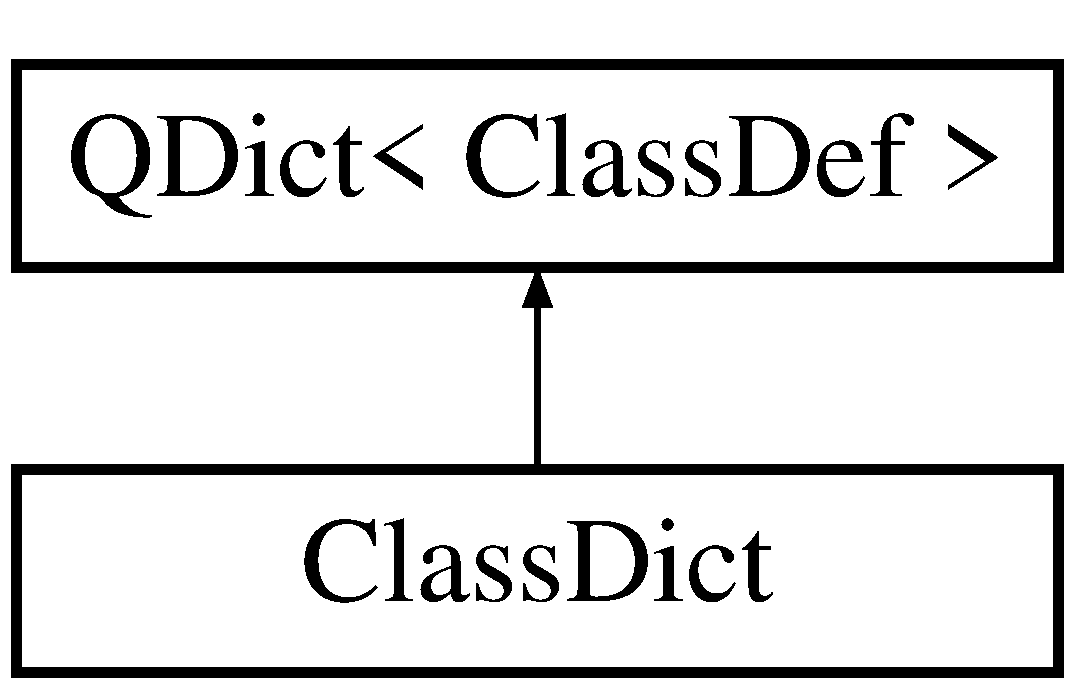
\includegraphics[height=2.000000cm]{class_class_dict}
\end{center}
\end{figure}
\subsection*{Membros públicos}
\begin{DoxyCompactItemize}
\item 
\hypertarget{class_class_dict_aed5aa24d6117e8e481356f8e8dfeb6e5}{{\bfseries Class\-Dict} (int size)}\label{class_class_dict_aed5aa24d6117e8e481356f8e8dfeb6e5}

\end{DoxyCompactItemize}


\subsection{Descrição detalhada}
An unsorted dictionary of \hyperlink{class_class_def}{Class\-Def} objects. 

A documentação para esta classe foi gerada a partir do seguinte ficheiro\-:\begin{DoxyCompactItemize}
\item 
C\-:/\-Users/teste/git/doxygen/src/classlist.\-h\end{DoxyCompactItemize}

\hypertarget{class_class_hierarchy_context}{\section{Referência à classe Class\-Hierarchy\-Context}
\label{class_class_hierarchy_context}\index{Class\-Hierarchy\-Context@{Class\-Hierarchy\-Context}}
}
Diagrama de heranças da classe Class\-Hierarchy\-Context\begin{figure}[H]
\begin{center}
\leavevmode
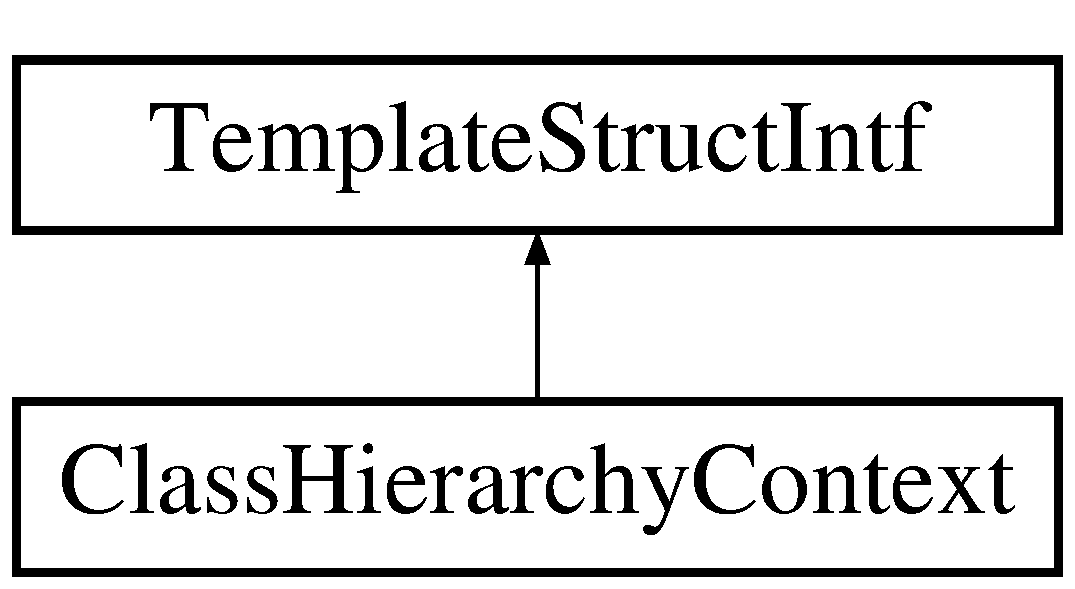
\includegraphics[height=2.000000cm]{class_class_hierarchy_context}
\end{center}
\end{figure}
\subsection*{Estruturas de Dados}
\begin{DoxyCompactItemize}
\item 
class \hyperlink{class_class_hierarchy_context_1_1_private}{Private}
\end{DoxyCompactItemize}
\subsection*{Membros públicos}
\begin{DoxyCompactItemize}
\item 
virtual \hyperlink{class_template_variant}{Template\-Variant} \hyperlink{class_class_hierarchy_context_a1bcfea01201f3ea09981a8442842c42d}{get} (const char $\ast$name) const 
\end{DoxyCompactItemize}


\subsection{Documentação dos métodos}
\hypertarget{class_class_hierarchy_context_a1bcfea01201f3ea09981a8442842c42d}{\index{Class\-Hierarchy\-Context@{Class\-Hierarchy\-Context}!get@{get}}
\index{get@{get}!ClassHierarchyContext@{Class\-Hierarchy\-Context}}
\subsubsection[{get}]{\setlength{\rightskip}{0pt plus 5cm}{\bf Template\-Variant} get (
\begin{DoxyParamCaption}
\item[{const char $\ast$}]{name}
\end{DoxyParamCaption}
) const\hspace{0.3cm}{\ttfamily [virtual]}}}\label{class_class_hierarchy_context_a1bcfea01201f3ea09981a8442842c42d}
Gets the value for a field name. 
\begin{DoxyParams}[1]{Parâmetros}
\mbox{\tt in}  & {\em name} & The name of the field. \\
\hline
\end{DoxyParams}


Implementa \hyperlink{class_template_struct_intf_a49a65a897ba5e4cd6cb80d681c843aab}{Template\-Struct\-Intf}.



A documentação para esta classe foi gerada a partir dos seguintes ficheiros\-:\begin{DoxyCompactItemize}
\item 
C\-:/\-Users/teste/git/doxygen/src/context.\-h\item 
C\-:/\-Users/teste/git/doxygen/src/context.\-cpp\end{DoxyCompactItemize}

\hypertarget{class_class_inheritance_context}{\section{Referência à classe Class\-Inheritance\-Context}
\label{class_class_inheritance_context}\index{Class\-Inheritance\-Context@{Class\-Inheritance\-Context}}
}
Diagrama de heranças da classe Class\-Inheritance\-Context\begin{figure}[H]
\begin{center}
\leavevmode
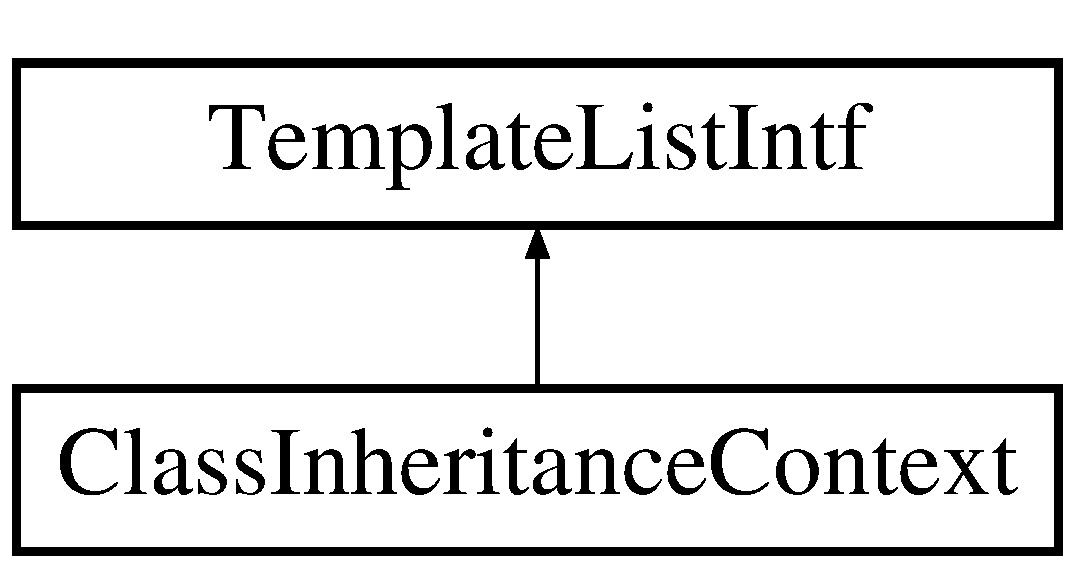
\includegraphics[height=2.000000cm]{class_class_inheritance_context}
\end{center}
\end{figure}
\subsection*{Estruturas de Dados}
\begin{DoxyCompactItemize}
\item 
class \hyperlink{class_class_inheritance_context_1_1_private}{Private}
\end{DoxyCompactItemize}
\subsection*{Membros públicos}
\begin{DoxyCompactItemize}
\item 
virtual int \hyperlink{class_class_inheritance_context_a0745638c9967e2ed90bc96c012288c55}{count} () const 
\item 
virtual \hyperlink{class_template_variant}{Template\-Variant} \hyperlink{class_class_inheritance_context_a55f90d50fcb1378b2a97b9c3ad5bb162}{at} (int index) const 
\item 
virtual \\*
\hyperlink{class_template_list_intf_1_1_const_iterator}{Template\-List\-Intf\-::\-Const\-Iterator} $\ast$ \hyperlink{class_class_inheritance_context_a0b1d6dedc3f51750e5cba18f51022f10}{create\-Iterator} () const 
\end{DoxyCompactItemize}


\subsection{Documentação dos métodos}
\hypertarget{class_class_inheritance_context_a55f90d50fcb1378b2a97b9c3ad5bb162}{\index{Class\-Inheritance\-Context@{Class\-Inheritance\-Context}!at@{at}}
\index{at@{at}!ClassInheritanceContext@{Class\-Inheritance\-Context}}
\subsubsection[{at}]{\setlength{\rightskip}{0pt plus 5cm}{\bf Template\-Variant} at (
\begin{DoxyParamCaption}
\item[{int}]{index}
\end{DoxyParamCaption}
) const\hspace{0.3cm}{\ttfamily [virtual]}}}\label{class_class_inheritance_context_a55f90d50fcb1378b2a97b9c3ad5bb162}
Returns the element at index position {\itshape index}. 

Implementa \hyperlink{class_template_list_intf_a6b813ba1b062c9c5b241158a4a62aea7}{Template\-List\-Intf}.

\hypertarget{class_class_inheritance_context_a0745638c9967e2ed90bc96c012288c55}{\index{Class\-Inheritance\-Context@{Class\-Inheritance\-Context}!count@{count}}
\index{count@{count}!ClassInheritanceContext@{Class\-Inheritance\-Context}}
\subsubsection[{count}]{\setlength{\rightskip}{0pt plus 5cm}int count (
\begin{DoxyParamCaption}
{}
\end{DoxyParamCaption}
) const\hspace{0.3cm}{\ttfamily [virtual]}}}\label{class_class_inheritance_context_a0745638c9967e2ed90bc96c012288c55}
Returns the number of elements in the list 

Implementa \hyperlink{class_template_list_intf_ac5a730d48b86f871bc036571234d1332}{Template\-List\-Intf}.

\hypertarget{class_class_inheritance_context_a0b1d6dedc3f51750e5cba18f51022f10}{\index{Class\-Inheritance\-Context@{Class\-Inheritance\-Context}!create\-Iterator@{create\-Iterator}}
\index{create\-Iterator@{create\-Iterator}!ClassInheritanceContext@{Class\-Inheritance\-Context}}
\subsubsection[{create\-Iterator}]{\setlength{\rightskip}{0pt plus 5cm}{\bf Template\-List\-Intf\-::\-Const\-Iterator} $\ast$ create\-Iterator (
\begin{DoxyParamCaption}
{}
\end{DoxyParamCaption}
) const\hspace{0.3cm}{\ttfamily [virtual]}}}\label{class_class_inheritance_context_a0b1d6dedc3f51750e5cba18f51022f10}
Creates a new iterator for this list. \begin{DoxyNote}{Nota}
the user should call delete on the returned pointer. 
\end{DoxyNote}


Implementa \hyperlink{class_template_list_intf_a972208b612df97b9d7216b3a28f0d0c3}{Template\-List\-Intf}.



A documentação para esta classe foi gerada a partir dos seguintes ficheiros\-:\begin{DoxyCompactItemize}
\item 
C\-:/\-Users/teste/git/doxygen/src/context.\-h\item 
C\-:/\-Users/teste/git/doxygen/src/context.\-cpp\end{DoxyCompactItemize}

\hypertarget{class_class_inheritance_node_context}{\section{Referência à classe Class\-Inheritance\-Node\-Context}
\label{class_class_inheritance_node_context}\index{Class\-Inheritance\-Node\-Context@{Class\-Inheritance\-Node\-Context}}
}
Diagrama de heranças da classe Class\-Inheritance\-Node\-Context\begin{figure}[H]
\begin{center}
\leavevmode
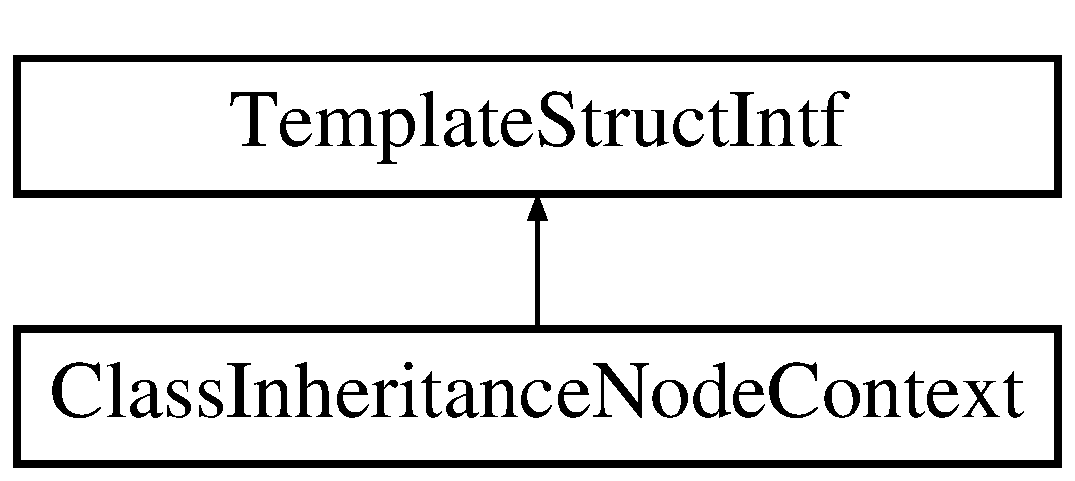
\includegraphics[height=2.000000cm]{class_class_inheritance_node_context}
\end{center}
\end{figure}
\subsection*{Estruturas de Dados}
\begin{DoxyCompactItemize}
\item 
class \hyperlink{class_class_inheritance_node_context_1_1_private}{Private}
\end{DoxyCompactItemize}
\subsection*{Membros públicos}
\begin{DoxyCompactItemize}
\item 
\hypertarget{class_class_inheritance_node_context_aff053885f98b266781de0cfba45f618c}{{\bfseries Class\-Inheritance\-Node\-Context} (\hyperlink{class_class_def}{Class\-Def} $\ast$)}\label{class_class_inheritance_node_context_aff053885f98b266781de0cfba45f618c}

\item 
virtual \hyperlink{class_template_variant}{Template\-Variant} \hyperlink{class_class_inheritance_node_context_a1bcfea01201f3ea09981a8442842c42d}{get} (const char $\ast$name) const 
\item 
\hypertarget{class_class_inheritance_node_context_ab0dba386b4767dd0290754724d47af42}{void {\bfseries add\-Children} (const \hyperlink{class_base_class_list}{Base\-Class\-List} $\ast$bcl, bool hide\-Super)}\label{class_class_inheritance_node_context_ab0dba386b4767dd0290754724d47af42}

\end{DoxyCompactItemize}


\subsection{Documentação dos métodos}
\hypertarget{class_class_inheritance_node_context_a1bcfea01201f3ea09981a8442842c42d}{\index{Class\-Inheritance\-Node\-Context@{Class\-Inheritance\-Node\-Context}!get@{get}}
\index{get@{get}!ClassInheritanceNodeContext@{Class\-Inheritance\-Node\-Context}}
\subsubsection[{get}]{\setlength{\rightskip}{0pt plus 5cm}{\bf Template\-Variant} get (
\begin{DoxyParamCaption}
\item[{const char $\ast$}]{name}
\end{DoxyParamCaption}
) const\hspace{0.3cm}{\ttfamily [virtual]}}}\label{class_class_inheritance_node_context_a1bcfea01201f3ea09981a8442842c42d}
Gets the value for a field name. 
\begin{DoxyParams}[1]{Parâmetros}
\mbox{\tt in}  & {\em name} & The name of the field. \\
\hline
\end{DoxyParams}


Implementa \hyperlink{class_template_struct_intf_a49a65a897ba5e4cd6cb80d681c843aab}{Template\-Struct\-Intf}.



A documentação para esta classe foi gerada a partir dos seguintes ficheiros\-:\begin{DoxyCompactItemize}
\item 
C\-:/\-Users/teste/git/doxygen/src/context.\-h\item 
C\-:/\-Users/teste/git/doxygen/src/context.\-cpp\end{DoxyCompactItemize}

\hypertarget{class_class_list}{\section{Referência à classe Class\-List}
\label{class_class_list}\index{Class\-List@{Class\-List}}
}


{\ttfamily \#include $<$classlist.\-h$>$}

Diagrama de heranças da classe Class\-List\begin{figure}[H]
\begin{center}
\leavevmode
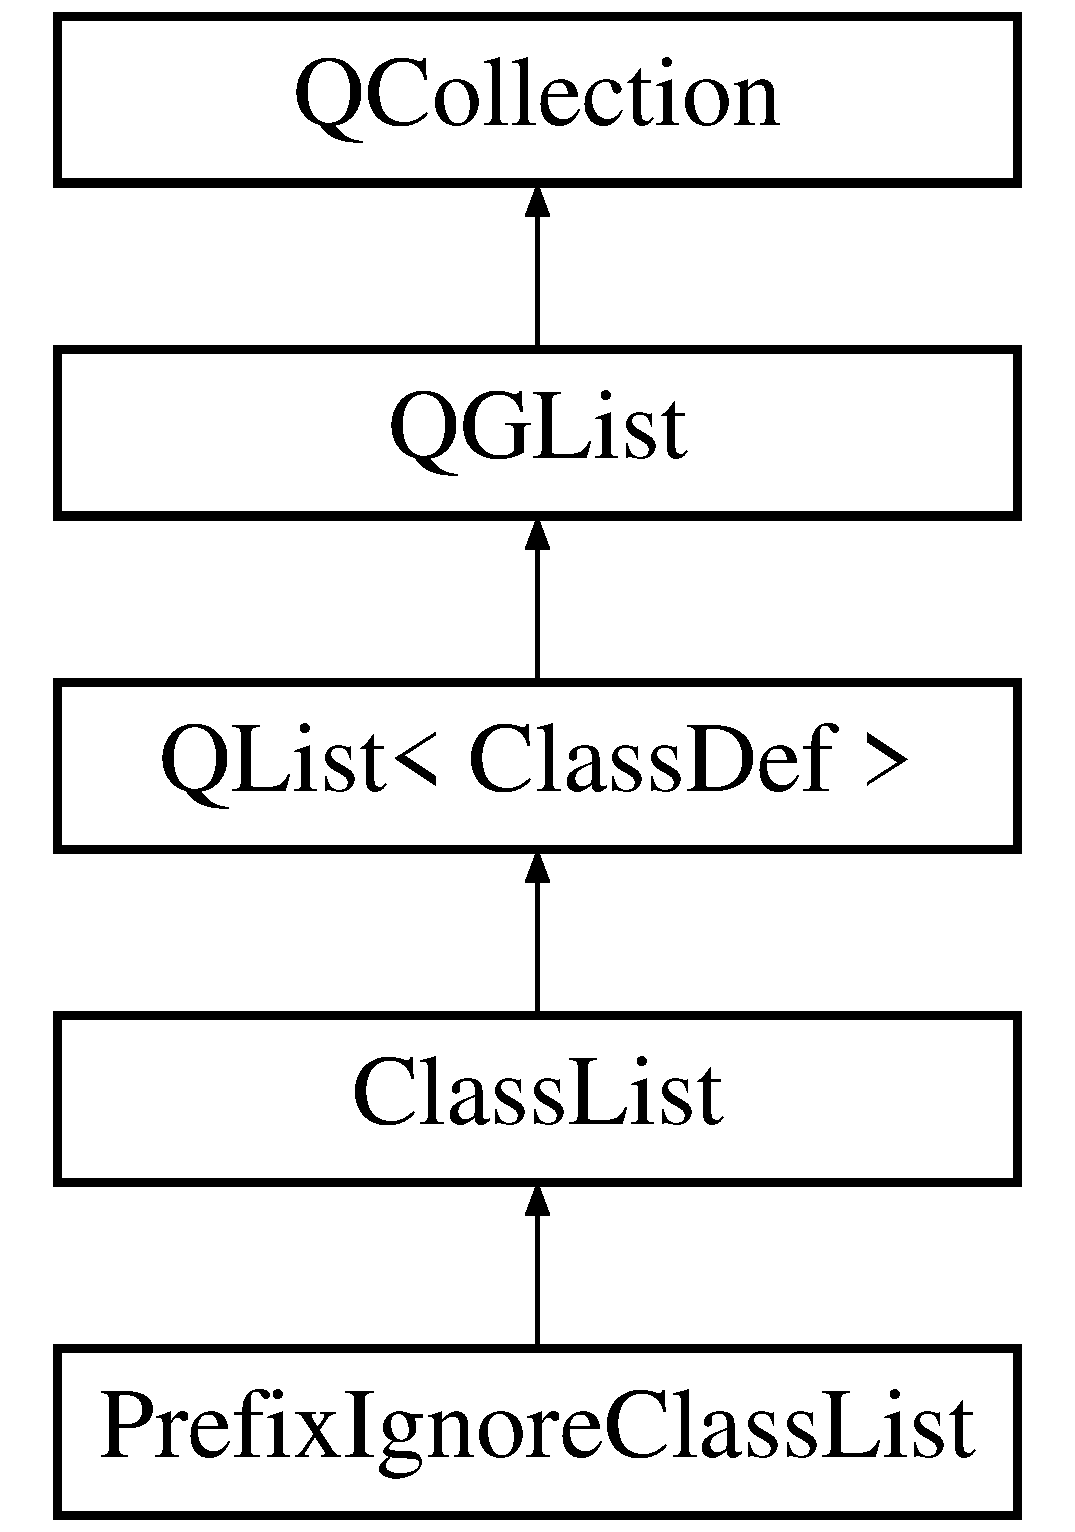
\includegraphics[height=5.000000cm]{class_class_list}
\end{center}
\end{figure}
\subsection*{Membros públicos}
\begin{DoxyCompactItemize}
\item 
int \hyperlink{class_class_list_a219450accf048597ffc7113ecde4c402}{compare\-Items} (Q\-Collection\-::\-Item item1, Q\-Collection\-::\-Item item2)
\end{DoxyCompactItemize}
\subsection*{Additional Inherited Members}


\subsection{Descrição detalhada}
\hyperlink{class_a}{A} list of \hyperlink{class_class_def}{Class\-Def} objects. 

\subsection{Documentação dos métodos}
\hypertarget{class_class_list_a219450accf048597ffc7113ecde4c402}{\index{Class\-List@{Class\-List}!compare\-Items@{compare\-Items}}
\index{compare\-Items@{compare\-Items}!ClassList@{Class\-List}}
\subsubsection[{compare\-Items}]{\setlength{\rightskip}{0pt plus 5cm}int compare\-Items (
\begin{DoxyParamCaption}
\item[{Q\-Collection\-::\-Item}]{item1, }
\item[{Q\-Collection\-::\-Item}]{item2}
\end{DoxyParamCaption}
)\hspace{0.3cm}{\ttfamily [virtual]}}}\label{class_class_list_a219450accf048597ffc7113ecde4c402}
This virtual function compares two list items.

Returns\-: 
\begin{DoxyItemize}
\item 0 if {\itshape item1} == {\itshape item2} 
\item non-\/zero if {\itshape item1} != {\itshape item2} 
\end{DoxyItemize}

This function returns {\itshape int} rather than {\itshape bool} so that reimplementations can return three values and use it to sort by\-:


\begin{DoxyItemize}
\item 0 if {\itshape item1} == {\itshape item2} 
\item $>$ 0 (positive integer) if {\itshape item1} $>$ {\itshape item2} 
\item $<$ 0 (negative integer) if {\itshape item1} $<$ {\itshape item2} 
\end{DoxyItemize}

The Q\-List\-::in\-Sort() function requires that \hyperlink{class_class_list_a219450accf048597ffc7113ecde4c402}{compare\-Items()} is implemented as described here.

This function should not modify the list because some const functions call \hyperlink{class_class_list_a219450accf048597ffc7113ecde4c402}{compare\-Items()}.

The default implementation compares the pointers\-: 
\begin{DoxyCode}
\end{DoxyCode}
 

Reimplementado de \hyperlink{class_q_g_list_aac689c6d7a54b6558afbd53845183af8}{Q\-G\-List}.



Reimplementado em \hyperlink{class_prefix_ignore_class_list_aade9045d8c0047e0427d8c6a9c048985}{Prefix\-Ignore\-Class\-List}.



A documentação para esta classe foi gerada a partir dos seguintes ficheiros\-:\begin{DoxyCompactItemize}
\item 
C\-:/\-Users/teste/git/doxygen/src/classlist.\-h\item 
C\-:/\-Users/teste/git/doxygen/src/classlist.\-cpp\end{DoxyCompactItemize}

\hypertarget{class_class_list_context}{\section{Referência à classe Class\-List\-Context}
\label{class_class_list_context}\index{Class\-List\-Context@{Class\-List\-Context}}
}
Diagrama de heranças da classe Class\-List\-Context\begin{figure}[H]
\begin{center}
\leavevmode
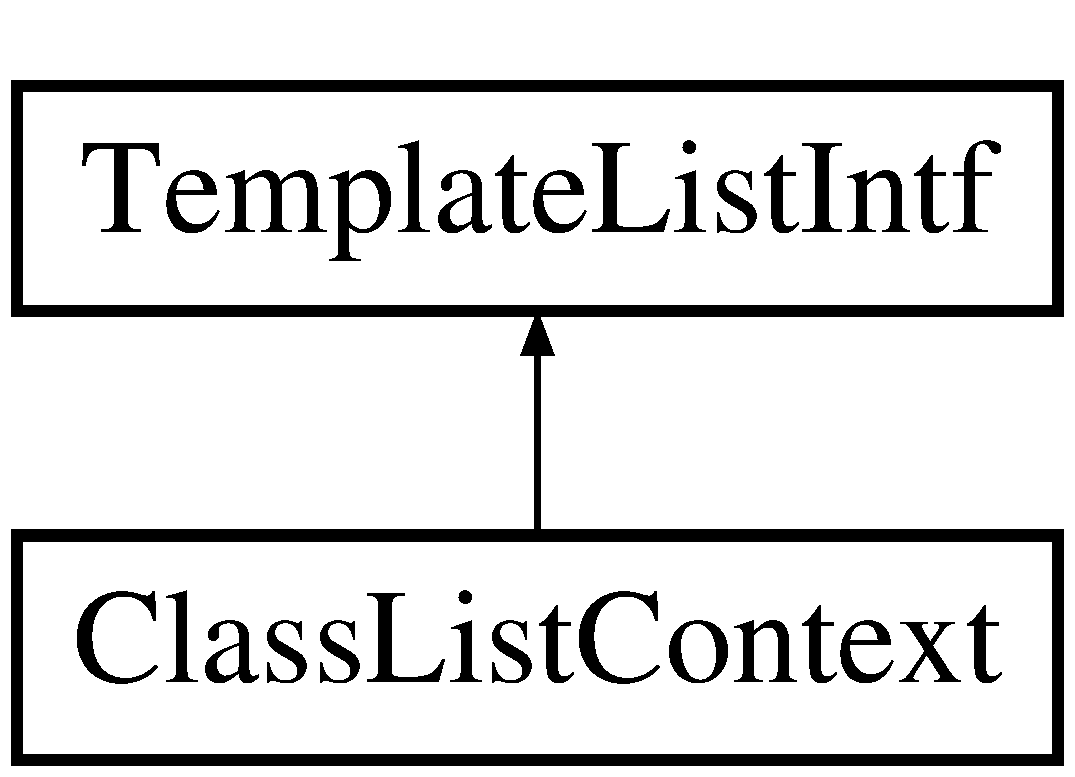
\includegraphics[height=2.000000cm]{class_class_list_context}
\end{center}
\end{figure}
\subsection*{Estruturas de Dados}
\begin{DoxyCompactItemize}
\item 
class \hyperlink{class_class_list_context_1_1_private}{Private}
\end{DoxyCompactItemize}
\subsection*{Membros públicos}
\begin{DoxyCompactItemize}
\item 
virtual int \hyperlink{class_class_list_context_a0745638c9967e2ed90bc96c012288c55}{count} () const 
\item 
virtual \hyperlink{class_template_variant}{Template\-Variant} \hyperlink{class_class_list_context_a55f90d50fcb1378b2a97b9c3ad5bb162}{at} (int index) const 
\item 
virtual \\*
\hyperlink{class_template_list_intf_1_1_const_iterator}{Template\-List\-Intf\-::\-Const\-Iterator} $\ast$ \hyperlink{class_class_list_context_a0b1d6dedc3f51750e5cba18f51022f10}{create\-Iterator} () const 
\end{DoxyCompactItemize}


\subsection{Documentação dos métodos}
\hypertarget{class_class_list_context_a55f90d50fcb1378b2a97b9c3ad5bb162}{\index{Class\-List\-Context@{Class\-List\-Context}!at@{at}}
\index{at@{at}!ClassListContext@{Class\-List\-Context}}
\subsubsection[{at}]{\setlength{\rightskip}{0pt plus 5cm}{\bf Template\-Variant} at (
\begin{DoxyParamCaption}
\item[{int}]{index}
\end{DoxyParamCaption}
) const\hspace{0.3cm}{\ttfamily [virtual]}}}\label{class_class_list_context_a55f90d50fcb1378b2a97b9c3ad5bb162}
Returns the element at index position {\itshape index}. 

Implementa \hyperlink{class_template_list_intf_a6b813ba1b062c9c5b241158a4a62aea7}{Template\-List\-Intf}.

\hypertarget{class_class_list_context_a0745638c9967e2ed90bc96c012288c55}{\index{Class\-List\-Context@{Class\-List\-Context}!count@{count}}
\index{count@{count}!ClassListContext@{Class\-List\-Context}}
\subsubsection[{count}]{\setlength{\rightskip}{0pt plus 5cm}int count (
\begin{DoxyParamCaption}
{}
\end{DoxyParamCaption}
) const\hspace{0.3cm}{\ttfamily [virtual]}}}\label{class_class_list_context_a0745638c9967e2ed90bc96c012288c55}
Returns the number of elements in the list 

Implementa \hyperlink{class_template_list_intf_ac5a730d48b86f871bc036571234d1332}{Template\-List\-Intf}.

\hypertarget{class_class_list_context_a0b1d6dedc3f51750e5cba18f51022f10}{\index{Class\-List\-Context@{Class\-List\-Context}!create\-Iterator@{create\-Iterator}}
\index{create\-Iterator@{create\-Iterator}!ClassListContext@{Class\-List\-Context}}
\subsubsection[{create\-Iterator}]{\setlength{\rightskip}{0pt plus 5cm}{\bf Template\-List\-Intf\-::\-Const\-Iterator} $\ast$ create\-Iterator (
\begin{DoxyParamCaption}
{}
\end{DoxyParamCaption}
) const\hspace{0.3cm}{\ttfamily [virtual]}}}\label{class_class_list_context_a0b1d6dedc3f51750e5cba18f51022f10}
Creates a new iterator for this list. \begin{DoxyNote}{Nota}
the user should call delete on the returned pointer. 
\end{DoxyNote}


Implementa \hyperlink{class_template_list_intf_a972208b612df97b9d7216b3a28f0d0c3}{Template\-List\-Intf}.



A documentação para esta classe foi gerada a partir dos seguintes ficheiros\-:\begin{DoxyCompactItemize}
\item 
C\-:/\-Users/teste/git/doxygen/src/context.\-h\item 
C\-:/\-Users/teste/git/doxygen/src/context.\-cpp\end{DoxyCompactItemize}

\hypertarget{class_class_list_iterator}{\section{Referência à classe Class\-List\-Iterator}
\label{class_class_list_iterator}\index{Class\-List\-Iterator@{Class\-List\-Iterator}}
}


{\ttfamily \#include $<$classlist.\-h$>$}

Diagrama de heranças da classe Class\-List\-Iterator\begin{figure}[H]
\begin{center}
\leavevmode
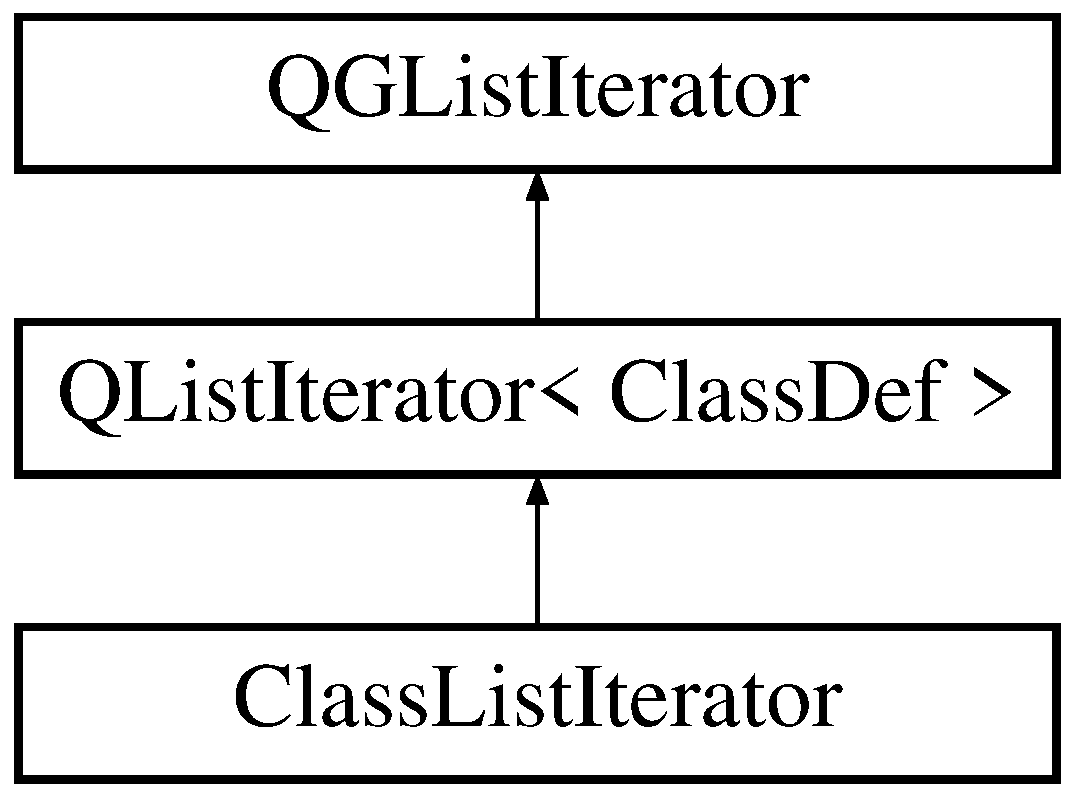
\includegraphics[height=3.000000cm]{class_class_list_iterator}
\end{center}
\end{figure}
\subsection*{Membros públicos}
\begin{DoxyCompactItemize}
\item 
\hypertarget{class_class_list_iterator_ad3e300639f5f8d3e8f66bbfc4dea90b1}{{\bfseries Class\-List\-Iterator} (const \hyperlink{class_class_list}{Class\-List} \&list)}\label{class_class_list_iterator_ad3e300639f5f8d3e8f66bbfc4dea90b1}

\end{DoxyCompactItemize}
\subsection*{Additional Inherited Members}


\subsection{Descrição detalhada}
An iterator for \hyperlink{class_class_def}{Class\-Def} objects in a \hyperlink{class_class_list}{Class\-List}. 

A documentação para esta classe foi gerada a partir dos seguintes ficheiros\-:\begin{DoxyCompactItemize}
\item 
C\-:/\-Users/teste/git/doxygen/src/classlist.\-h\item 
C\-:/\-Users/teste/git/doxygen/src/classlist.\-cpp\end{DoxyCompactItemize}

\hypertarget{class_class_s_dict}{\section{Referência à classe Class\-S\-Dict}
\label{class_class_s_dict}\index{Class\-S\-Dict@{Class\-S\-Dict}}
}


{\ttfamily \#include $<$classlist.\-h$>$}

Diagrama de heranças da classe Class\-S\-Dict\begin{figure}[H]
\begin{center}
\leavevmode
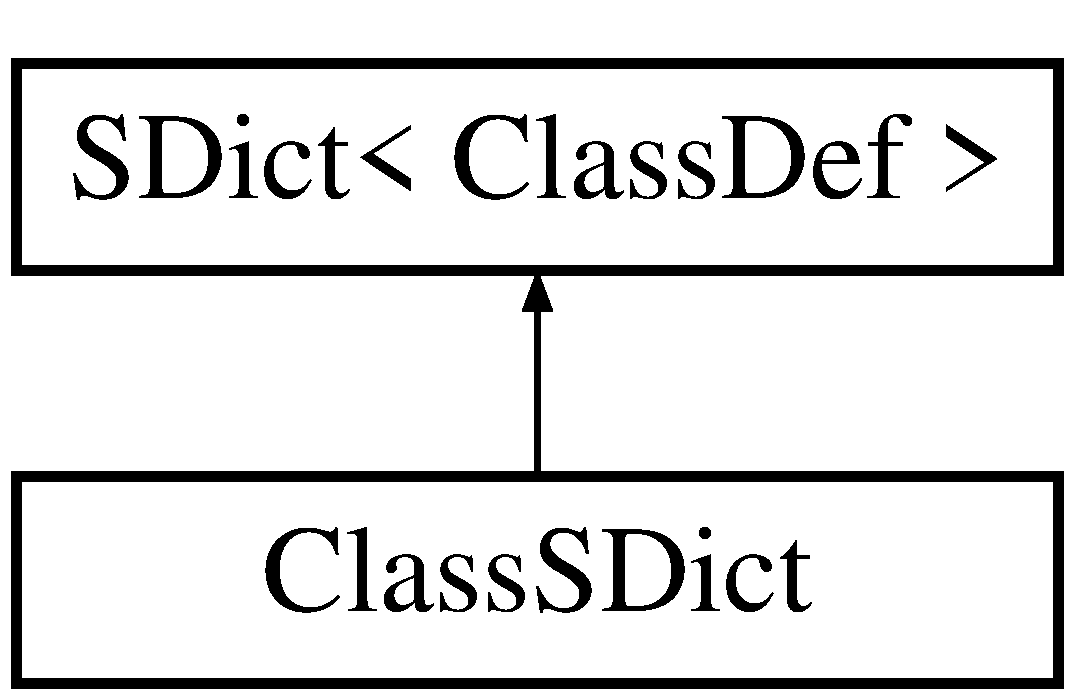
\includegraphics[height=2.000000cm]{class_class_s_dict}
\end{center}
\end{figure}
\subsection*{Membros públicos}
\begin{DoxyCompactItemize}
\item 
\hypertarget{class_class_s_dict_ac1cfb57e5f4badc70919dc2cd056b8d3}{{\bfseries Class\-S\-Dict} (int size=17)}\label{class_class_s_dict_ac1cfb57e5f4badc70919dc2cd056b8d3}

\item 
int \hyperlink{class_class_s_dict_a219450accf048597ffc7113ecde4c402}{compare\-Items} (Q\-Collection\-::\-Item item1, Q\-Collection\-::\-Item item2)
\item 
\hypertarget{class_class_s_dict_aa8443734095451ad529ee10b81f1f349}{void {\bfseries write\-Declaration} (\hyperlink{class_output_list}{Output\-List} \&ol, const \hyperlink{class_class_def_a768a6f0a6fd7e9087ff7971abbcc3f36}{Class\-Def\-::\-Compound\-Type} $\ast$filter=0, const char $\ast$header=0, bool local\-Names=F\-A\-L\-S\-E)}\label{class_class_s_dict_aa8443734095451ad529ee10b81f1f349}

\item 
\hypertarget{class_class_s_dict_afca5f10ff8e8cb05238e68c8914c524b}{void {\bfseries write\-Documentation} (\hyperlink{class_output_list}{Output\-List} \&ol, \hyperlink{class_definition}{Definition} $\ast$container=0)}\label{class_class_s_dict_afca5f10ff8e8cb05238e68c8914c524b}

\item 
\hypertarget{class_class_s_dict_a641567e9a1d7e66e7ca033f43221f3ec}{bool {\bfseries decl\-Visible} (const \hyperlink{class_class_def_a768a6f0a6fd7e9087ff7971abbcc3f36}{Class\-Def\-::\-Compound\-Type} $\ast$filter=0) const }\label{class_class_s_dict_a641567e9a1d7e66e7ca033f43221f3ec}

\end{DoxyCompactItemize}


\subsection{Descrição detalhada}
\hyperlink{class_a}{A} sorted dictionary of \hyperlink{class_class_def}{Class\-Def} objects. 

\subsection{Documentação dos métodos}
\hypertarget{class_class_s_dict_a219450accf048597ffc7113ecde4c402}{\index{Class\-S\-Dict@{Class\-S\-Dict}!compare\-Items@{compare\-Items}}
\index{compare\-Items@{compare\-Items}!ClassSDict@{Class\-S\-Dict}}
\subsubsection[{compare\-Items}]{\setlength{\rightskip}{0pt plus 5cm}int compare\-Items (
\begin{DoxyParamCaption}
\item[{Q\-Collection\-::\-Item}]{item1, }
\item[{Q\-Collection\-::\-Item}]{item2}
\end{DoxyParamCaption}
)\hspace{0.3cm}{\ttfamily [virtual]}}}\label{class_class_s_dict_a219450accf048597ffc7113ecde4c402}
Function that is used to compare two items when sorting. Overload this to properly sort items. \begin{DoxySeeAlso}{Veja também}
\hyperlink{class_s_dict_a04fd7ec8f0d222ef65b3bec5e9c1bc7a}{in\-Sort()} 
\end{DoxySeeAlso}


Reimplementado de \hyperlink{class_s_dict_aade9045d8c0047e0427d8c6a9c048985}{S\-Dict$<$ Class\-Def $>$}.



A documentação para esta classe foi gerada a partir dos seguintes ficheiros\-:\begin{DoxyCompactItemize}
\item 
C\-:/\-Users/teste/git/doxygen/src/classlist.\-h\item 
C\-:/\-Users/teste/git/doxygen/src/classlist.\-cpp\end{DoxyCompactItemize}

\hypertarget{class_class_tree_context}{\section{Referência à classe Class\-Tree\-Context}
\label{class_class_tree_context}\index{Class\-Tree\-Context@{Class\-Tree\-Context}}
}
Diagrama de heranças da classe Class\-Tree\-Context\begin{figure}[H]
\begin{center}
\leavevmode
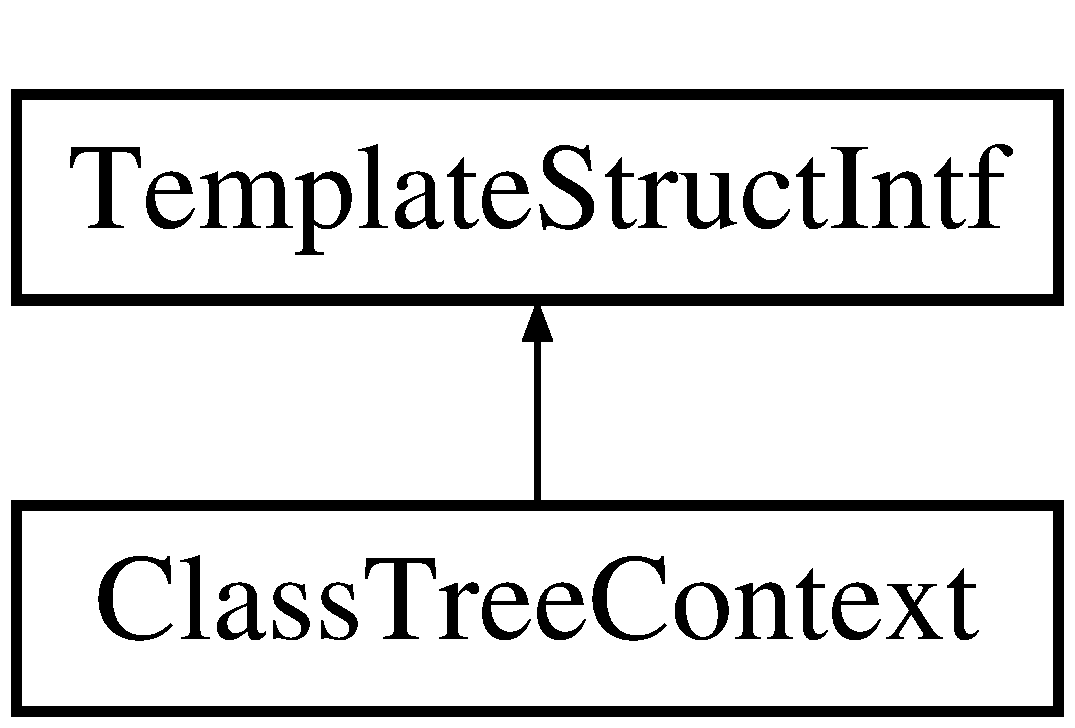
\includegraphics[height=2.000000cm]{class_class_tree_context}
\end{center}
\end{figure}
\subsection*{Estruturas de Dados}
\begin{DoxyCompactItemize}
\item 
class \hyperlink{class_class_tree_context_1_1_private}{Private}
\end{DoxyCompactItemize}
\subsection*{Membros públicos}
\begin{DoxyCompactItemize}
\item 
virtual \hyperlink{class_template_variant}{Template\-Variant} \hyperlink{class_class_tree_context_a1bcfea01201f3ea09981a8442842c42d}{get} (const char $\ast$name) const 
\end{DoxyCompactItemize}


\subsection{Documentação dos métodos}
\hypertarget{class_class_tree_context_a1bcfea01201f3ea09981a8442842c42d}{\index{Class\-Tree\-Context@{Class\-Tree\-Context}!get@{get}}
\index{get@{get}!ClassTreeContext@{Class\-Tree\-Context}}
\subsubsection[{get}]{\setlength{\rightskip}{0pt plus 5cm}{\bf Template\-Variant} get (
\begin{DoxyParamCaption}
\item[{const char $\ast$}]{name}
\end{DoxyParamCaption}
) const\hspace{0.3cm}{\ttfamily [virtual]}}}\label{class_class_tree_context_a1bcfea01201f3ea09981a8442842c42d}
Gets the value for a field name. 
\begin{DoxyParams}[1]{Parâmetros}
\mbox{\tt in}  & {\em name} & The name of the field. \\
\hline
\end{DoxyParams}


Implementa \hyperlink{class_template_struct_intf_a49a65a897ba5e4cd6cb80d681c843aab}{Template\-Struct\-Intf}.



A documentação para esta classe foi gerada a partir dos seguintes ficheiros\-:\begin{DoxyCompactItemize}
\item 
C\-:/\-Users/teste/git/doxygen/src/context.\-h\item 
C\-:/\-Users/teste/git/doxygen/src/context.\-cpp\end{DoxyCompactItemize}

\hypertarget{struct_dot_runner_1_1_cleanup_item}{\section{Referência à estrutura Dot\-Runner\-:\-:Cleanup\-Item}
\label{struct_dot_runner_1_1_cleanup_item}\index{Dot\-Runner\-::\-Cleanup\-Item@{Dot\-Runner\-::\-Cleanup\-Item}}
}
\subsection*{Campos de Dados}
\begin{DoxyCompactItemize}
\item 
\hypertarget{struct_dot_runner_1_1_cleanup_item_a71216f035ef8cbf975e0712d46e89e9b}{\hyperlink{class_q_c_string}{Q\-C\-String} {\bfseries path}}\label{struct_dot_runner_1_1_cleanup_item_a71216f035ef8cbf975e0712d46e89e9b}

\item 
\hypertarget{struct_dot_runner_1_1_cleanup_item_afeb3e9dc965e44d291bbce99ea8dbcc7}{\hyperlink{class_q_c_string}{Q\-C\-String} {\bfseries file}}\label{struct_dot_runner_1_1_cleanup_item_afeb3e9dc965e44d291bbce99ea8dbcc7}

\end{DoxyCompactItemize}


A documentação para esta estrutura foi gerada a partir do seguinte ficheiro\-:\begin{DoxyCompactItemize}
\item 
C\-:/\-Users/teste/git/doxygen/src/dot.\-h\end{DoxyCompactItemize}

\hypertarget{structclientes}{\section{Referência à estrutura clientes}
\label{structclientes}\index{clientes@{clientes}}
}
\subsection*{Campos de Dados}
\begin{DoxyCompactItemize}
\item 
\hypertarget{structclientes_a6861d035c44fb0bef558ae07c347f493}{long int {\bfseries numero}}\label{structclientes_a6861d035c44fb0bef558ae07c347f493}

\item 
\hypertarget{structclientes_a31ca3f05d944e272b57a61f356dd8f1d}{char {\bfseries nome} \mbox{[}20\mbox{]}}\label{structclientes_a31ca3f05d944e272b57a61f356dd8f1d}

\item 
\hypertarget{structclientes_a8b0d7cba87290f2f7b1fd87b6698e426}{char {\bfseries apelido} \mbox{[}30\mbox{]}}\label{structclientes_a8b0d7cba87290f2f7b1fd87b6698e426}

\item 
\hypertarget{structclientes_a1e4b5d6ebdbee2c3964c82b62c74dc83}{char {\bfseries morada} \mbox{[}100\mbox{]}}\label{structclientes_a1e4b5d6ebdbee2c3964c82b62c74dc83}

\item 
\hypertarget{structclientes_af1e9334befe5a6cbee279f37fbb7c0fd}{long int {\bfseries telefone}}\label{structclientes_af1e9334befe5a6cbee279f37fbb7c0fd}

\item 
\hypertarget{structclientes_a876d08c1d21086e4fd228744da10d028}{int {\bfseries estado}}\label{structclientes_a876d08c1d21086e4fd228744da10d028}

\end{DoxyCompactItemize}


A documentação para esta estrutura foi gerada a partir dos seguintes ficheiros\-:\begin{DoxyCompactItemize}
\item 
C\-:/\-Users/teste/git/cemrodas\-\_\-inserir\-\_\-a\-\_\-funcionar.\-c\item 
C\-:/\-Users/teste/git/cemrodasnovo4.\-c\item 
C\-:/\-Users/teste/git/cemrodasnovo4\-\_\-old.\-c\end{DoxyCompactItemize}

\hypertarget{struct_cmhl_info}{\section{Referência à estrutura Cmhl\-Info}
\label{struct_cmhl_info}\index{Cmhl\-Info@{Cmhl\-Info}}
}
\subsection*{Membros públicos}
\begin{DoxyCompactItemize}
\item 
\hypertarget{struct_cmhl_info_a54b5f2ff8c04ea814fe185b828049db3}{{\bfseries Cmhl\-Info} (const char $\ast$fn, const char $\ast$t)}\label{struct_cmhl_info_a54b5f2ff8c04ea814fe185b828049db3}

\end{DoxyCompactItemize}
\subsection*{Campos de Dados}
\begin{DoxyCompactItemize}
\item 
\hypertarget{struct_cmhl_info_a6a2fc0c236288b07ce5bd1335ca89fa2}{const char $\ast$ {\bfseries fname}}\label{struct_cmhl_info_a6a2fc0c236288b07ce5bd1335ca89fa2}

\item 
\hypertarget{struct_cmhl_info_a42bb80709d086df855babb087e63794b}{\hyperlink{class_q_c_string}{Q\-C\-String} {\bfseries title}}\label{struct_cmhl_info_a42bb80709d086df855babb087e63794b}

\end{DoxyCompactItemize}


\subsection{Descrição detalhada}
Helper class representing a class member in the navigation menu. 

A documentação para esta estrutura foi gerada a partir do seguinte ficheiro\-:\begin{DoxyCompactItemize}
\item 
C\-:/\-Users/teste/git/doxygen/src/\hyperlink{index_8cpp}{index.\-cpp}\end{DoxyCompactItemize}

\hypertarget{class_code_line_handler}{\section{Referência à classe Code\-Line\-Handler}
\label{class_code_line_handler}\index{Code\-Line\-Handler@{Code\-Line\-Handler}}
}


Node representing a line of code.  




{\ttfamily \#include $<$dochandler.\-h$>$}

Diagrama de heranças da classe Code\-Line\-Handler\begin{figure}[H]
\begin{center}
\leavevmode
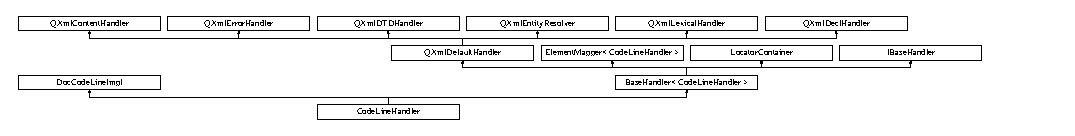
\includegraphics[height=1.385281cm]{class_code_line_handler}
\end{center}
\end{figure}
\subsection*{Membros públicos}
\begin{DoxyCompactItemize}
\item 
\hypertarget{class_code_line_handler_a65896bd5afdbb5e1465384b26f009b6b}{virtual void {\bfseries start\-Code\-Line} (const \hyperlink{class_q_xml_attributes}{Q\-Xml\-Attributes} \&)}\label{class_code_line_handler_a65896bd5afdbb5e1465384b26f009b6b}

\item 
\hypertarget{class_code_line_handler_adbe51a89cf6f9573b3434e7cfda81a7c}{virtual void {\bfseries end\-Code\-Line} ()}\label{class_code_line_handler_adbe51a89cf6f9573b3434e7cfda81a7c}

\item 
\hypertarget{class_code_line_handler_a6c05366909c31e60e5aba2ba1b93fefc}{virtual void {\bfseries start\-Line\-Number} (const \hyperlink{class_q_xml_attributes}{Q\-Xml\-Attributes} \&)}\label{class_code_line_handler_a6c05366909c31e60e5aba2ba1b93fefc}

\item 
\hypertarget{class_code_line_handler_a7a0edc3108f620b96b4972a7dea9ad91}{virtual void {\bfseries end\-Line\-Number} ()}\label{class_code_line_handler_a7a0edc3108f620b96b4972a7dea9ad91}

\item 
\hypertarget{class_code_line_handler_a30584c200aabd5885bd426b9e09c851d}{virtual void {\bfseries start\-Highlight} (const \hyperlink{class_q_xml_attributes}{Q\-Xml\-Attributes} \&)}\label{class_code_line_handler_a30584c200aabd5885bd426b9e09c851d}

\item 
\hypertarget{class_code_line_handler_a0a6ad84c50fcae905559fdcc3ca40e3c}{virtual void {\bfseries start\-Ref} (const \hyperlink{class_q_xml_attributes}{Q\-Xml\-Attributes} \&)}\label{class_code_line_handler_a0a6ad84c50fcae905559fdcc3ca40e3c}

\item 
\hypertarget{class_code_line_handler_a9b2a2f7a9ebcece375f433435d5fd615}{{\bfseries Code\-Line\-Handler} (\hyperlink{class_i_base_handler}{I\-Base\-Handler} $\ast$parent)}\label{class_code_line_handler_a9b2a2f7a9ebcece375f433435d5fd615}

\item 
\hypertarget{class_code_line_handler_af8e62c8a81ddf2283205cc8955de50eb}{virtual Kind {\bfseries kind} () const }\label{class_code_line_handler_af8e62c8a81ddf2283205cc8955de50eb}

\item 
\hypertarget{class_code_line_handler_a098a80d91a440a40f95fc5f99aa83bf3}{virtual int {\bfseries line\-Number} () const }\label{class_code_line_handler_a098a80d91a440a40f95fc5f99aa83bf3}

\item 
\hypertarget{class_code_line_handler_a2488ce15cc44de0c90c8f6116e9d5094}{virtual const \hyperlink{class_i_string}{I\-String} $\ast$ {\bfseries ref\-Id} () const }\label{class_code_line_handler_a2488ce15cc44de0c90c8f6116e9d5094}

\item 
\hypertarget{class_code_line_handler_ad94162a254e317a5e8331e7a15f8199f}{virtual \hyperlink{class_i_doc_iterator}{I\-Doc\-Iterator} $\ast$ {\bfseries code\-Elements} () const }\label{class_code_line_handler_ad94162a254e317a5e8331e7a15f8199f}

\end{DoxyCompactItemize}
\subsection*{Amigos}
\begin{DoxyCompactItemize}
\item 
\hypertarget{class_code_line_handler_a58edddfb3f15948fd8e3e8c67db55d01}{class {\bfseries Code\-Line\-Iterator}}\label{class_code_line_handler_a58edddfb3f15948fd8e3e8c67db55d01}

\end{DoxyCompactItemize}
\subsection*{Additional Inherited Members}


\subsection{Descrição detalhada}
Node representing a line of code. 



A documentação para esta classe foi gerada a partir dos seguintes ficheiros\-:\begin{DoxyCompactItemize}
\item 
C\-:/\-Users/teste/git/doxygen/addon/doxmlparser/src/dochandler.\-h\item 
C\-:/\-Users/teste/git/doxygen/addon/doxmlparser/src/dochandler.\-cpp\end{DoxyCompactItemize}

\hypertarget{class_code_line_iterator}{\section{Referência à classe Code\-Line\-Iterator}
\label{class_code_line_iterator}\index{Code\-Line\-Iterator@{Code\-Line\-Iterator}}
}
Diagrama de heranças da classe Code\-Line\-Iterator\begin{figure}[H]
\begin{center}
\leavevmode
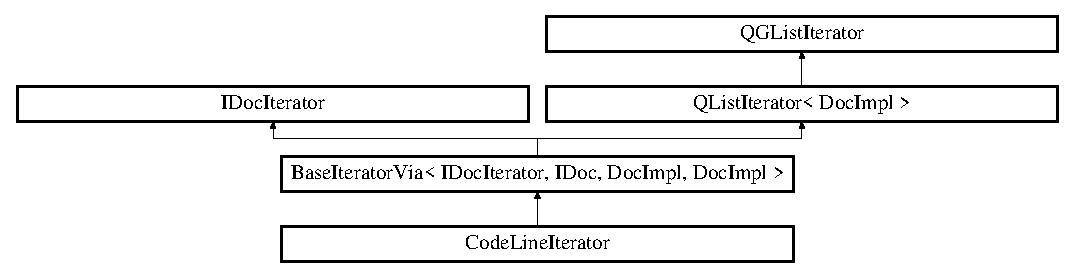
\includegraphics[height=3.294118cm]{class_code_line_iterator}
\end{center}
\end{figure}
\subsection*{Membros públicos}
\begin{DoxyCompactItemize}
\item 
\hypertarget{class_code_line_iterator_a49590b5d6e06afd21661f176f08ee32a}{{\bfseries Code\-Line\-Iterator} (const \hyperlink{class_code_line_handler}{Code\-Line\-Handler} \&handler)}\label{class_code_line_iterator_a49590b5d6e06afd21661f176f08ee32a}

\end{DoxyCompactItemize}
\subsection*{Additional Inherited Members}


A documentação para esta classe foi gerada a partir do seguinte ficheiro\-:\begin{DoxyCompactItemize}
\item 
C\-:/\-Users/teste/git/doxygen/addon/doxmlparser/src/dochandler.\-h\end{DoxyCompactItemize}

\hypertarget{class_code_output_interface}{\section{Referência à classe Code\-Output\-Interface}
\label{class_code_output_interface}\index{Code\-Output\-Interface@{Code\-Output\-Interface}}
}


{\ttfamily \#include $<$outputgen.\-h$>$}

Diagrama de heranças da classe Code\-Output\-Interface\begin{figure}[H]
\begin{center}
\leavevmode
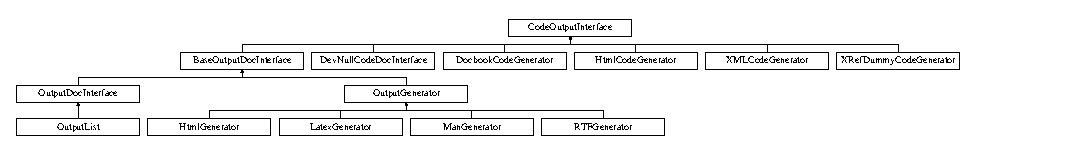
\includegraphics[height=1.590909cm]{class_code_output_interface}
\end{center}
\end{figure}
\subsection*{Membros públicos}
\begin{DoxyCompactItemize}
\item 
virtual void \hyperlink{class_code_output_interface_abc701d9798e414eae3e9694be75dfa8a}{codify} (const char $\ast$s)=0
\item 
virtual void \hyperlink{class_code_output_interface_a21e25662f2bc8efbb5bbb8503aeae97f}{write\-Code\-Link} (const char $\ast$ref, const char $\ast$file, const char $\ast$anchor, const char $\ast$name, const char $\ast$tooltip)=0
\item 
virtual void \hyperlink{class_code_output_interface_a30af4b3b6e39508a95ba3219d1ba8323}{write\-Line\-Number} (const char $\ast$ref, const char $\ast$file, const char $\ast$anchor, int line\-Number)=0
\item 
virtual void \hyperlink{class_code_output_interface_a4ab86013abbf61a86e9c300eb805939a}{write\-Tooltip} (const char $\ast$id, const \hyperlink{struct_doc_link_info}{Doc\-Link\-Info} \&doc\-Info, const char $\ast$decl, const char $\ast$desc, const \hyperlink{struct_source_link_info}{Source\-Link\-Info} \&def\-Info, const \hyperlink{struct_source_link_info}{Source\-Link\-Info} \&decl\-Info)=0
\item 
\hypertarget{class_code_output_interface_a06d83d3279f21b34d89fbc6f2a303fb8}{virtual void {\bfseries start\-Code\-Line} (bool has\-Line\-Numbers)=0}\label{class_code_output_interface_a06d83d3279f21b34d89fbc6f2a303fb8}

\item 
virtual void \hyperlink{class_code_output_interface_a542863fa8a9697696ffc4d4b24678e1f}{end\-Code\-Line} ()=0
\item 
virtual void \hyperlink{class_code_output_interface_aaa0bdadd117e161c87149d902d70c863}{start\-Font\-Class} (const char $\ast$cls\-Name)=0
\item 
virtual void \hyperlink{class_code_output_interface_adcd22acfbc1c4c011802334b78cf5f01}{end\-Font\-Class} ()=0
\item 
virtual void \hyperlink{class_code_output_interface_aa29ff881359360e41a251d1d69fae142}{write\-Code\-Anchor} (const char $\ast$name)=0
\item 
\hypertarget{class_code_output_interface_a502e52b0cfa87df3d69840bb425f41e9}{virtual void {\bfseries set\-Current\-Doc} (\hyperlink{class_definition}{Definition} $\ast$context, const char $\ast$anchor, bool is\-Source\-File)=0}\label{class_code_output_interface_a502e52b0cfa87df3d69840bb425f41e9}

\item 
\hypertarget{class_code_output_interface_a323777067b6847c3e2fa3ab8cd5ed3bc}{virtual void {\bfseries add\-Word} (const char $\ast$word, bool hi\-Priority)=0}\label{class_code_output_interface_a323777067b6847c3e2fa3ab8cd5ed3bc}

\end{DoxyCompactItemize}


\subsection{Descrição detalhada}
Output interface for code parser. 

\subsection{Documentação dos métodos}
\hypertarget{class_code_output_interface_abc701d9798e414eae3e9694be75dfa8a}{\index{Code\-Output\-Interface@{Code\-Output\-Interface}!codify@{codify}}
\index{codify@{codify}!CodeOutputInterface@{Code\-Output\-Interface}}
\subsubsection[{codify}]{\setlength{\rightskip}{0pt plus 5cm}virtual void codify (
\begin{DoxyParamCaption}
\item[{const char $\ast$}]{s}
\end{DoxyParamCaption}
)\hspace{0.3cm}{\ttfamily [pure virtual]}}}\label{class_code_output_interface_abc701d9798e414eae3e9694be75dfa8a}
Writes an code fragment to the output. This function should keep spaces visible, should break lines at a newline and should convert tabs to the right number of spaces. 

Implementado em \hyperlink{class_x_m_l_code_generator_a96b26b0cb63719fd5370a9a04d2ebb38}{X\-M\-L\-Code\-Generator}, \hyperlink{class_docbook_code_generator_a96b26b0cb63719fd5370a9a04d2ebb38}{Docbook\-Code\-Generator}, \hyperlink{class_output_list_ad58b50196a8176a68df41aabcaf6a8b7}{Output\-List}, \hyperlink{class_html_generator_a96b26b0cb63719fd5370a9a04d2ebb38}{Html\-Generator}, \hyperlink{class_latex_generator_a96b26b0cb63719fd5370a9a04d2ebb38}{Latex\-Generator}, \hyperlink{class_man_generator_a96b26b0cb63719fd5370a9a04d2ebb38}{Man\-Generator}, \hyperlink{class_r_t_f_generator_a96b26b0cb63719fd5370a9a04d2ebb38}{R\-T\-F\-Generator}, \hyperlink{class_dev_null_code_doc_interface_ae795c13518eb3523e41920859b64bae3}{Dev\-Null\-Code\-Doc\-Interface}, \hyperlink{class_x_ref_dummy_code_generator_a9e08a84e260e7b42a2dd202bfec80344}{X\-Ref\-Dummy\-Code\-Generator} e \hyperlink{class_html_code_generator_a96b26b0cb63719fd5370a9a04d2ebb38}{Html\-Code\-Generator}.

\hypertarget{class_code_output_interface_a542863fa8a9697696ffc4d4b24678e1f}{\index{Code\-Output\-Interface@{Code\-Output\-Interface}!end\-Code\-Line@{end\-Code\-Line}}
\index{end\-Code\-Line@{end\-Code\-Line}!CodeOutputInterface@{Code\-Output\-Interface}}
\subsubsection[{end\-Code\-Line}]{\setlength{\rightskip}{0pt plus 5cm}virtual void end\-Code\-Line (
\begin{DoxyParamCaption}
{}
\end{DoxyParamCaption}
)\hspace{0.3cm}{\ttfamily [pure virtual]}}}\label{class_code_output_interface_a542863fa8a9697696ffc4d4b24678e1f}
Ends a line of code started with start\-Code\-Line() 

Implementado em \hyperlink{class_x_m_l_code_generator_adbe51a89cf6f9573b3434e7cfda81a7c}{X\-M\-L\-Code\-Generator}, \hyperlink{class_output_list_adbe51a89cf6f9573b3434e7cfda81a7c}{Output\-List}, \hyperlink{class_docbook_code_generator_adbe51a89cf6f9573b3434e7cfda81a7c}{Docbook\-Code\-Generator}, \hyperlink{class_latex_generator_adbe51a89cf6f9573b3434e7cfda81a7c}{Latex\-Generator}, \hyperlink{class_man_generator_adbe51a89cf6f9573b3434e7cfda81a7c}{Man\-Generator}, \hyperlink{class_r_t_f_generator_adbe51a89cf6f9573b3434e7cfda81a7c}{R\-T\-F\-Generator}, \hyperlink{class_html_generator_adbe51a89cf6f9573b3434e7cfda81a7c}{Html\-Generator}, \hyperlink{class_dev_null_code_doc_interface_a9eac5f8973e5f7c2a4500d3daa5c125f}{Dev\-Null\-Code\-Doc\-Interface}, \hyperlink{class_x_ref_dummy_code_generator_adbe51a89cf6f9573b3434e7cfda81a7c}{X\-Ref\-Dummy\-Code\-Generator} e \hyperlink{class_html_code_generator_adbe51a89cf6f9573b3434e7cfda81a7c}{Html\-Code\-Generator}.

\hypertarget{class_code_output_interface_adcd22acfbc1c4c011802334b78cf5f01}{\index{Code\-Output\-Interface@{Code\-Output\-Interface}!end\-Font\-Class@{end\-Font\-Class}}
\index{end\-Font\-Class@{end\-Font\-Class}!CodeOutputInterface@{Code\-Output\-Interface}}
\subsubsection[{end\-Font\-Class}]{\setlength{\rightskip}{0pt plus 5cm}virtual void end\-Font\-Class (
\begin{DoxyParamCaption}
{}
\end{DoxyParamCaption}
)\hspace{0.3cm}{\ttfamily [pure virtual]}}}\label{class_code_output_interface_adcd22acfbc1c4c011802334b78cf5f01}
Ends a block started with \hyperlink{class_code_output_interface_aaa0bdadd117e161c87149d902d70c863}{start\-Font\-Class()} 

Implementado em \hyperlink{class_output_list_ab7851025d80a6d1ed6dd8e25016136e1}{Output\-List}, \hyperlink{class_x_m_l_code_generator_ab7851025d80a6d1ed6dd8e25016136e1}{X\-M\-L\-Code\-Generator}, \hyperlink{class_latex_generator_ab7851025d80a6d1ed6dd8e25016136e1}{Latex\-Generator}, \hyperlink{class_r_t_f_generator_ab7851025d80a6d1ed6dd8e25016136e1}{R\-T\-F\-Generator}, \hyperlink{class_docbook_code_generator_ab7851025d80a6d1ed6dd8e25016136e1}{Docbook\-Code\-Generator}, \hyperlink{class_man_generator_ab7851025d80a6d1ed6dd8e25016136e1}{Man\-Generator}, \hyperlink{class_html_generator_ab7851025d80a6d1ed6dd8e25016136e1}{Html\-Generator}, \hyperlink{class_dev_null_code_doc_interface_adc05c3c53aeaba27ae7d22334168c413}{Dev\-Null\-Code\-Doc\-Interface}, \hyperlink{class_x_ref_dummy_code_generator_ab7851025d80a6d1ed6dd8e25016136e1}{X\-Ref\-Dummy\-Code\-Generator} e \hyperlink{class_html_code_generator_ab7851025d80a6d1ed6dd8e25016136e1}{Html\-Code\-Generator}.

\hypertarget{class_code_output_interface_aaa0bdadd117e161c87149d902d70c863}{\index{Code\-Output\-Interface@{Code\-Output\-Interface}!start\-Font\-Class@{start\-Font\-Class}}
\index{start\-Font\-Class@{start\-Font\-Class}!CodeOutputInterface@{Code\-Output\-Interface}}
\subsubsection[{start\-Font\-Class}]{\setlength{\rightskip}{0pt plus 5cm}virtual void start\-Font\-Class (
\begin{DoxyParamCaption}
\item[{const char $\ast$}]{cls\-Name}
\end{DoxyParamCaption}
)\hspace{0.3cm}{\ttfamily [pure virtual]}}}\label{class_code_output_interface_aaa0bdadd117e161c87149d902d70c863}
Starts a block with a certain meaning. Used for syntax highlighting, which elements of the same type are rendered using the same 'font class'. 
\begin{DoxyParams}{Parâmetros}
{\em cls\-Name} & The category name. \\
\hline
\end{DoxyParams}


Implementado em \hyperlink{class_output_list_a253f5e2755f981e67662b662168aa054}{Output\-List}, \hyperlink{class_x_m_l_code_generator_a915a74cafbcb208a8d399fbf12d73769}{X\-M\-L\-Code\-Generator}, \hyperlink{class_latex_generator_ad907f4c47cf56f8aac603de5537963f0}{Latex\-Generator}, \hyperlink{class_r_t_f_generator_ad907f4c47cf56f8aac603de5537963f0}{R\-T\-F\-Generator}, \hyperlink{class_docbook_code_generator_ad907f4c47cf56f8aac603de5537963f0}{Docbook\-Code\-Generator}, \hyperlink{class_man_generator_ad907f4c47cf56f8aac603de5537963f0}{Man\-Generator}, \hyperlink{class_html_generator_a9326eecf5c7d10d7f6fece1e7fab75d8}{Html\-Generator}, \hyperlink{class_dev_null_code_doc_interface_a3595d576933897558124c28746b819f9}{Dev\-Null\-Code\-Doc\-Interface}, \hyperlink{class_x_ref_dummy_code_generator_ad907f4c47cf56f8aac603de5537963f0}{X\-Ref\-Dummy\-Code\-Generator} e \hyperlink{class_html_code_generator_a9326eecf5c7d10d7f6fece1e7fab75d8}{Html\-Code\-Generator}.

\hypertarget{class_code_output_interface_aa29ff881359360e41a251d1d69fae142}{\index{Code\-Output\-Interface@{Code\-Output\-Interface}!write\-Code\-Anchor@{write\-Code\-Anchor}}
\index{write\-Code\-Anchor@{write\-Code\-Anchor}!CodeOutputInterface@{Code\-Output\-Interface}}
\subsubsection[{write\-Code\-Anchor}]{\setlength{\rightskip}{0pt plus 5cm}virtual void write\-Code\-Anchor (
\begin{DoxyParamCaption}
\item[{const char $\ast$}]{name}
\end{DoxyParamCaption}
)\hspace{0.3cm}{\ttfamily [pure virtual]}}}\label{class_code_output_interface_aa29ff881359360e41a251d1d69fae142}
Write an anchor to a source listing. 
\begin{DoxyParams}{Parâmetros}
{\em name} & The name of the anchor. \\
\hline
\end{DoxyParams}


Implementado em \hyperlink{class_output_list_aa813b87ce15931854c2b0b9c1abb9e19}{Output\-List}, \hyperlink{class_x_m_l_code_generator_a688757a1dcb8c6bef1202433a36083a7}{X\-M\-L\-Code\-Generator}, \hyperlink{class_latex_generator_a688757a1dcb8c6bef1202433a36083a7}{Latex\-Generator}, \hyperlink{class_r_t_f_generator_a688757a1dcb8c6bef1202433a36083a7}{R\-T\-F\-Generator}, \hyperlink{class_man_generator_a688757a1dcb8c6bef1202433a36083a7}{Man\-Generator}, \hyperlink{class_docbook_code_generator_a688757a1dcb8c6bef1202433a36083a7}{Docbook\-Code\-Generator}, \hyperlink{class_html_generator_a5bdf52860d0fb01aa6bf45625d70abbc}{Html\-Generator}, \hyperlink{class_dev_null_code_doc_interface_a0bdf0a5b7ff33f368aa90d95063530ee}{Dev\-Null\-Code\-Doc\-Interface}, \hyperlink{class_x_ref_dummy_code_generator_a688757a1dcb8c6bef1202433a36083a7}{X\-Ref\-Dummy\-Code\-Generator} e \hyperlink{class_html_code_generator_a5bdf52860d0fb01aa6bf45625d70abbc}{Html\-Code\-Generator}.

\hypertarget{class_code_output_interface_a21e25662f2bc8efbb5bbb8503aeae97f}{\index{Code\-Output\-Interface@{Code\-Output\-Interface}!write\-Code\-Link@{write\-Code\-Link}}
\index{write\-Code\-Link@{write\-Code\-Link}!CodeOutputInterface@{Code\-Output\-Interface}}
\subsubsection[{write\-Code\-Link}]{\setlength{\rightskip}{0pt plus 5cm}virtual void write\-Code\-Link (
\begin{DoxyParamCaption}
\item[{const char $\ast$}]{ref, }
\item[{const char $\ast$}]{file, }
\item[{const char $\ast$}]{anchor, }
\item[{const char $\ast$}]{name, }
\item[{const char $\ast$}]{tooltip}
\end{DoxyParamCaption}
)\hspace{0.3cm}{\ttfamily [pure virtual]}}}\label{class_code_output_interface_a21e25662f2bc8efbb5bbb8503aeae97f}
Writes a link to an object in a code fragment. 
\begin{DoxyParams}{Parâmetros}
{\em ref} & If this is non-\/zero, the object is to be found in an external documentation file. \\
\hline
{\em file} & The file in which the object is located. \\
\hline
{\em anchor} & The anchor uniquely identifying the object within the file. \\
\hline
{\em name} & The text to display as a placeholder for the link. \\
\hline
{\em tooltip} & The tooltip to display when the mouse is on the link. \\
\hline
\end{DoxyParams}


Implementado em \hyperlink{class_x_m_l_code_generator_ab3866da052a840c400b4990dd2ddf61b}{X\-M\-L\-Code\-Generator}, \hyperlink{class_docbook_code_generator_ab3866da052a840c400b4990dd2ddf61b}{Docbook\-Code\-Generator}, \hyperlink{class_output_list_ab3866da052a840c400b4990dd2ddf61b}{Output\-List}, \hyperlink{class_html_generator_ab3866da052a840c400b4990dd2ddf61b}{Html\-Generator}, \hyperlink{class_latex_generator_ab3866da052a840c400b4990dd2ddf61b}{Latex\-Generator}, \hyperlink{class_man_generator_ab3866da052a840c400b4990dd2ddf61b}{Man\-Generator}, \hyperlink{class_r_t_f_generator_ab3866da052a840c400b4990dd2ddf61b}{R\-T\-F\-Generator}, \hyperlink{class_dev_null_code_doc_interface_a2ced6ffd253f23812cd3db949a305e9e}{Dev\-Null\-Code\-Doc\-Interface}, \hyperlink{class_x_ref_dummy_code_generator_aee13e3ced7a85258ae400407d4383453}{X\-Ref\-Dummy\-Code\-Generator} e \hyperlink{class_html_code_generator_ab3866da052a840c400b4990dd2ddf61b}{Html\-Code\-Generator}.

\hypertarget{class_code_output_interface_a30af4b3b6e39508a95ba3219d1ba8323}{\index{Code\-Output\-Interface@{Code\-Output\-Interface}!write\-Line\-Number@{write\-Line\-Number}}
\index{write\-Line\-Number@{write\-Line\-Number}!CodeOutputInterface@{Code\-Output\-Interface}}
\subsubsection[{write\-Line\-Number}]{\setlength{\rightskip}{0pt plus 5cm}virtual void write\-Line\-Number (
\begin{DoxyParamCaption}
\item[{const char $\ast$}]{ref, }
\item[{const char $\ast$}]{file, }
\item[{const char $\ast$}]{anchor, }
\item[{int}]{line\-Number}
\end{DoxyParamCaption}
)\hspace{0.3cm}{\ttfamily [pure virtual]}}}\label{class_code_output_interface_a30af4b3b6e39508a95ba3219d1ba8323}
Writes the line number of a source listing 
\begin{DoxyParams}{Parâmetros}
{\em ref} & External reference (when imported from a tag file) \\
\hline
{\em file} & The file part of the \hyperlink{struct_u_r_l}{U\-R\-L} pointing to the docs. \\
\hline
{\em anchor} & The anchor part of the \hyperlink{struct_u_r_l}{U\-R\-L} pointing to the docs. \\
\hline
{\em line\-Number} & The line number to write \\
\hline
\end{DoxyParams}


Implementado em \hyperlink{class_x_m_l_code_generator_a0a50ef78e830a1b1949dd97491c29c01}{X\-M\-L\-Code\-Generator}, \hyperlink{class_docbook_code_generator_a0a50ef78e830a1b1949dd97491c29c01}{Docbook\-Code\-Generator}, \hyperlink{class_output_list_a70366bf2bad21036a14d68e9ef532809}{Output\-List}, \hyperlink{class_latex_generator_a041516b65f9f2c22d2c0941419200cbb}{Latex\-Generator}, \hyperlink{class_man_generator_a041516b65f9f2c22d2c0941419200cbb}{Man\-Generator}, \hyperlink{class_r_t_f_generator_a041516b65f9f2c22d2c0941419200cbb}{R\-T\-F\-Generator}, \hyperlink{class_html_generator_a70366bf2bad21036a14d68e9ef532809}{Html\-Generator}, \hyperlink{class_dev_null_code_doc_interface_ab884475bfa9aae3d714d0583402dc7a6}{Dev\-Null\-Code\-Doc\-Interface}, \hyperlink{class_x_ref_dummy_code_generator_a68e608aa3fa63507e7545589c3325a91}{X\-Ref\-Dummy\-Code\-Generator} e \hyperlink{class_html_code_generator_a68e608aa3fa63507e7545589c3325a91}{Html\-Code\-Generator}.

\hypertarget{class_code_output_interface_a4ab86013abbf61a86e9c300eb805939a}{\index{Code\-Output\-Interface@{Code\-Output\-Interface}!write\-Tooltip@{write\-Tooltip}}
\index{write\-Tooltip@{write\-Tooltip}!CodeOutputInterface@{Code\-Output\-Interface}}
\subsubsection[{write\-Tooltip}]{\setlength{\rightskip}{0pt plus 5cm}virtual void write\-Tooltip (
\begin{DoxyParamCaption}
\item[{const char $\ast$}]{id, }
\item[{const {\bf Doc\-Link\-Info} \&}]{doc\-Info, }
\item[{const char $\ast$}]{decl, }
\item[{const char $\ast$}]{desc, }
\item[{const {\bf Source\-Link\-Info} \&}]{def\-Info, }
\item[{const {\bf Source\-Link\-Info} \&}]{decl\-Info}
\end{DoxyParamCaption}
)\hspace{0.3cm}{\ttfamily [pure virtual]}}}\label{class_code_output_interface_a4ab86013abbf61a86e9c300eb805939a}
Writes a tool tip definition 
\begin{DoxyParams}{Parâmetros}
{\em id} & unique identifier for the tooltip \\
\hline
{\em doc\-Info} & Info about the symbol's documentation. \\
\hline
{\em decl} & full declaration of the symbol (for functions) \\
\hline
{\em desc} & brief description for the symbol \\
\hline
{\em def\-Info} & Info about the symbol's definition in the source code \\
\hline
{\em decl\-Info} & Info about the symbol's declaration in the source code \\
\hline
\end{DoxyParams}


Implementado em \hyperlink{class_x_m_l_code_generator_a7ff5de02f14ba4c6b98edcaa3483e386}{X\-M\-L\-Code\-Generator}, \hyperlink{class_docbook_code_generator_a7ff5de02f14ba4c6b98edcaa3483e386}{Docbook\-Code\-Generator}, \hyperlink{class_output_list_acc6f74ac2670196668c05d4156eec872}{Output\-List}, \hyperlink{class_html_generator_acc6f74ac2670196668c05d4156eec872}{Html\-Generator}, \hyperlink{class_latex_generator_a7ff5de02f14ba4c6b98edcaa3483e386}{Latex\-Generator}, \hyperlink{class_man_generator_a7ff5de02f14ba4c6b98edcaa3483e386}{Man\-Generator}, \hyperlink{class_r_t_f_generator_a7ff5de02f14ba4c6b98edcaa3483e386}{R\-T\-F\-Generator}, \hyperlink{class_dev_null_code_doc_interface_a1009688e232ec64f703d534ece6bd8c6}{Dev\-Null\-Code\-Doc\-Interface}, \hyperlink{class_x_ref_dummy_code_generator_a1009688e232ec64f703d534ece6bd8c6}{X\-Ref\-Dummy\-Code\-Generator} e \hyperlink{class_html_code_generator_acc6f74ac2670196668c05d4156eec872}{Html\-Code\-Generator}.



A documentação para esta classe foi gerada a partir do seguinte ficheiro\-:\begin{DoxyCompactItemize}
\item 
C\-:/\-Users/teste/git/doxygen/src/outputgen.\-h\end{DoxyCompactItemize}

\hypertarget{struct_coin}{\section{Referência à estrutura Coin}
\label{struct_coin}\index{Coin@{Coin}}
}
\subsection*{Campos de Dados}
\begin{DoxyCompactItemize}
\item 
\hypertarget{struct_coin_aebcc69a36ae5072bcb13188418750393}{\hyperlink{structuivector}{uivector} {\bfseries symbols}}\label{struct_coin_aebcc69a36ae5072bcb13188418750393}

\item 
\hypertarget{struct_coin_a8128625c9e3fd04c27b82957732d8781}{float {\bfseries weight}}\label{struct_coin_a8128625c9e3fd04c27b82957732d8781}

\end{DoxyCompactItemize}


A documentação para esta estrutura foi gerada a partir do seguinte ficheiro\-:\begin{DoxyCompactItemize}
\item 
C\-:/\-Users/teste/git/doxygen/src/lodepng.\-cpp\end{DoxyCompactItemize}

\hypertarget{struct_color}{\section{Referência à estrutura Color}
\label{struct_color}\index{Color@{Color}}
}
\subsection*{Campos de Dados}
\begin{DoxyCompactItemize}
\item 
\hypertarget{struct_color_a9b2249ae0b3882aaf27e96c396a5bb13}{Byte {\bfseries red}}\label{struct_color_a9b2249ae0b3882aaf27e96c396a5bb13}

\item 
\hypertarget{struct_color_a40093bf40480ad4ae7f43bda1bb6954b}{Byte {\bfseries green}}\label{struct_color_a40093bf40480ad4ae7f43bda1bb6954b}

\item 
\hypertarget{struct_color_a101bb7f248e248bd71231690a6f515ea}{Byte {\bfseries blue}}\label{struct_color_a101bb7f248e248bd71231690a6f515ea}

\item 
\hypertarget{struct_color_a9a0673462c984cab261161ab23456e6e}{Byte {\bfseries alpha}}\label{struct_color_a9a0673462c984cab261161ab23456e6e}

\end{DoxyCompactItemize}


\subsection{Descrição detalhada}
Helper struct representing a R\-G\-B\-A color 

A documentação para esta estrutura foi gerada a partir do seguinte ficheiro\-:\begin{DoxyCompactItemize}
\item 
C\-:/\-Users/teste/git/doxygen/src/image.\-cpp\end{DoxyCompactItemize}

\hypertarget{class_colored_image}{\section{Referência à classe Colored\-Image}
\label{class_colored_image}\index{Colored\-Image@{Colored\-Image}}
}


{\ttfamily \#include $<$image.\-h$>$}

\subsection*{Membros públicos}
\begin{DoxyCompactItemize}
\item 
\hypertarget{class_colored_image_a2fff1b49986eada284eceff9be751d38}{{\bfseries Colored\-Image} (int width, int height, const uchar $\ast$grey\-Levels, const uchar $\ast$alpha\-Levels, int saturation, int hue, int gamma)}\label{class_colored_image_a2fff1b49986eada284eceff9be751d38}

\item 
\hypertarget{class_colored_image_aca0cd00ffef3eb58b9c2f03e1456709a}{bool {\bfseries save} (const char $\ast$file\-Name)}\label{class_colored_image_aca0cd00ffef3eb58b9c2f03e1456709a}

\end{DoxyCompactItemize}
\subsection*{Membros públicos estáticos}
\begin{DoxyCompactItemize}
\item 
\hypertarget{class_colored_image_a02b5f11d8528e76dedd4c01c692056b5}{static void {\bfseries hsl2rgb} (double h, double s, double l, double $\ast$p\-Red, double $\ast$p\-Green, double $\ast$p\-Blue)}\label{class_colored_image_a02b5f11d8528e76dedd4c01c692056b5}

\end{DoxyCompactItemize}


\subsection{Descrição detalhada}
Class representing a bitmap image colored based on hue/sat/gamma settings. 

A documentação para esta classe foi gerada a partir dos seguintes ficheiros\-:\begin{DoxyCompactItemize}
\item 
C\-:/\-Users/teste/git/doxygen/src/image.\-h\item 
C\-:/\-Users/teste/git/doxygen/src/image.\-cpp\end{DoxyCompactItemize}

\hypertarget{struct_colored_img_data_item}{\section{Referência à estrutura Colored\-Img\-Data\-Item}
\label{struct_colored_img_data_item}\index{Colored\-Img\-Data\-Item@{Colored\-Img\-Data\-Item}}
}


{\ttfamily \#include $<$util.\-h$>$}

\subsection*{Campos de Dados}
\begin{DoxyCompactItemize}
\item 
\hypertarget{struct_colored_img_data_item_a8f8f80d37794cde9472343e4487ba3eb}{const char $\ast$ {\bfseries name}}\label{struct_colored_img_data_item_a8f8f80d37794cde9472343e4487ba3eb}

\item 
\hypertarget{struct_colored_img_data_item_a8a31e3e5c2765d45488c75c00bacfefd}{unsigned short {\bfseries width}}\label{struct_colored_img_data_item_a8a31e3e5c2765d45488c75c00bacfefd}

\item 
\hypertarget{struct_colored_img_data_item_aa8e4172ede7827e837ac528eae04c497}{unsigned short {\bfseries height}}\label{struct_colored_img_data_item_aa8e4172ede7827e837ac528eae04c497}

\item 
\hypertarget{struct_colored_img_data_item_a8cff7748b5b3118a34d99936238e78d8}{unsigned char $\ast$ {\bfseries content}}\label{struct_colored_img_data_item_a8cff7748b5b3118a34d99936238e78d8}

\item 
\hypertarget{struct_colored_img_data_item_abade0d805ae2234f757182754514c903}{unsigned char $\ast$ {\bfseries alpha}}\label{struct_colored_img_data_item_abade0d805ae2234f757182754514c903}

\end{DoxyCompactItemize}


\subsection{Descrição detalhada}
Data associated with a H\-S\-V colored image. 

A documentação para esta estrutura foi gerada a partir do seguinte ficheiro\-:\begin{DoxyCompactItemize}
\item 
C\-:/\-Users/teste/git/doxygen/src/\hyperlink{util_8h}{util.\-h}\end{DoxyCompactItemize}

\hypertarget{class_color_picker}{\section{Referência à classe Color\-Picker}
\label{class_color_picker}\index{Color\-Picker@{Color\-Picker}}
}
Diagrama de heranças da classe Color\-Picker\begin{figure}[H]
\begin{center}
\leavevmode
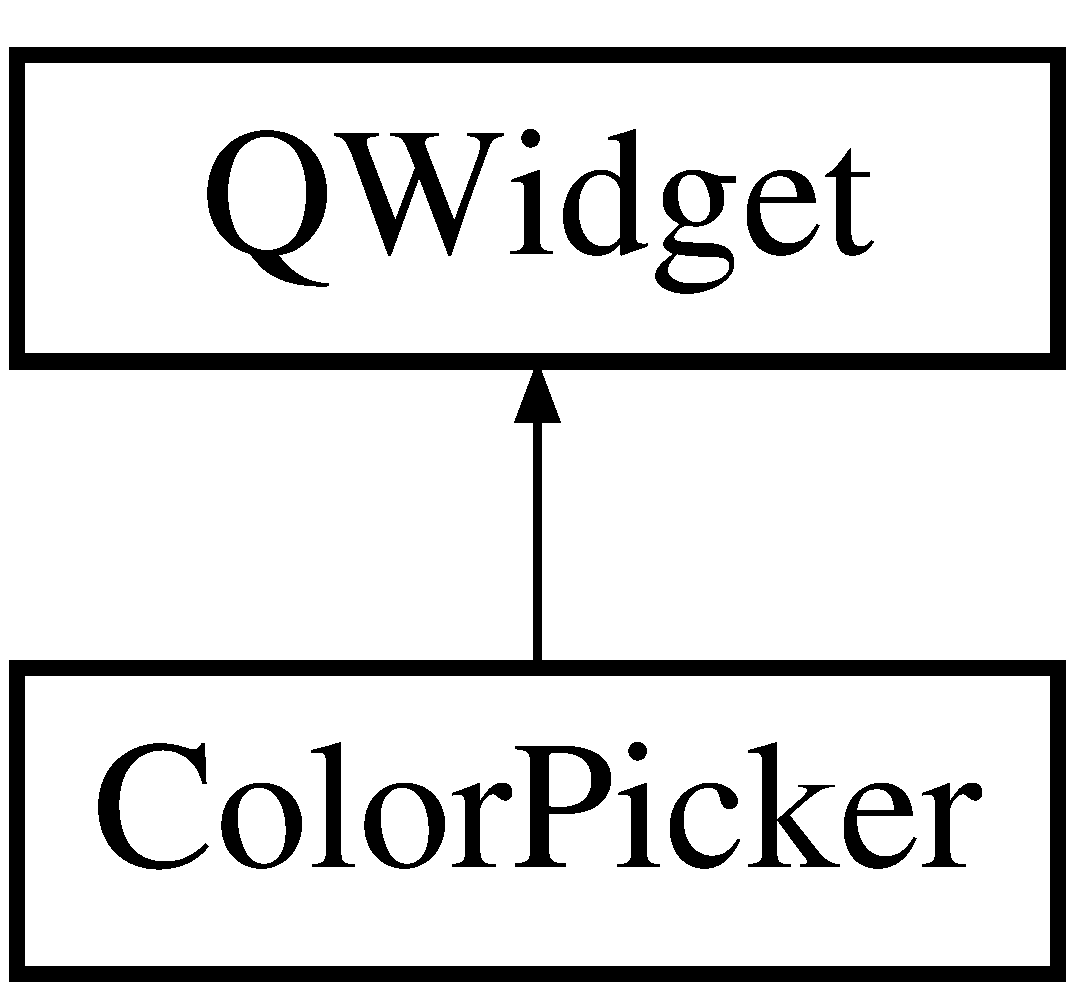
\includegraphics[height=2.000000cm]{class_color_picker}
\end{center}
\end{figure}
\subsection*{Tipos Públicos}
\begin{DoxyCompactItemize}
\item 
enum {\bfseries Mode} \{ {\bfseries Hue}, 
{\bfseries Saturation}, 
{\bfseries Gamma}
 \}
\end{DoxyCompactItemize}
\subsection*{Slots públicos}
\begin{DoxyCompactItemize}
\item 
\hypertarget{class_color_picker_a4008365835db275bd0ca457611262111}{void {\bfseries set\-Col} (int h, int s, int g)}\label{class_color_picker_a4008365835db275bd0ca457611262111}

\end{DoxyCompactItemize}
\subsection*{Sinais}
\begin{DoxyCompactItemize}
\item 
\hypertarget{class_color_picker_abd7b1508475f64dd8e1222077095c6f2}{void {\bfseries new\-Hsv} (int h, int s, int g)}\label{class_color_picker_abd7b1508475f64dd8e1222077095c6f2}

\end{DoxyCompactItemize}
\subsection*{Membros públicos}
\begin{DoxyCompactItemize}
\item 
\hypertarget{class_color_picker_aa300279e8d9fb50251e8bb41691d07c0}{{\bfseries Color\-Picker} (Mode m)}\label{class_color_picker_aa300279e8d9fb50251e8bb41691d07c0}

\end{DoxyCompactItemize}
\subsection*{Membros protegidos}
\begin{DoxyCompactItemize}
\item 
\hypertarget{class_color_picker_ad06d035e601c42cc2a3b9d1229c73d36}{void {\bfseries paint\-Event} (Q\-Paint\-Event $\ast$)}\label{class_color_picker_ad06d035e601c42cc2a3b9d1229c73d36}

\item 
\hypertarget{class_color_picker_a88e672693c2cfdbaf9af942a58a8e1dd}{void {\bfseries mouse\-Move\-Event} (Q\-Mouse\-Event $\ast$)}\label{class_color_picker_a88e672693c2cfdbaf9af942a58a8e1dd}

\item 
\hypertarget{class_color_picker_a991f0a076bd76a1ee5bda0df7fa474f4}{void {\bfseries mouse\-Press\-Event} (Q\-Mouse\-Event $\ast$)}\label{class_color_picker_a991f0a076bd76a1ee5bda0df7fa474f4}

\end{DoxyCompactItemize}


A documentação para esta classe foi gerada a partir dos seguintes ficheiros\-:\begin{DoxyCompactItemize}
\item 
C\-:/\-Users/teste/git/doxygen/addon/doxywizard/wizard.\-h\item 
C\-:/\-Users/teste/git/doxygen/addon/doxywizard/wizard.\-cpp\end{DoxyCompactItemize}

\hypertarget{struct_command_map}{\section{Referência à estrutura Command\-Map}
\label{struct_command_map}\index{Command\-Map@{Command\-Map}}
}
\subsection*{Campos de Dados}
\begin{DoxyCompactItemize}
\item 
\hypertarget{struct_command_map_acde4baff7055b0b5325e59b8f8001601}{const char $\ast$ {\bfseries cmd\-Name}}\label{struct_command_map_acde4baff7055b0b5325e59b8f8001601}

\item 
\hypertarget{struct_command_map_a1f37c5e3144a14c7848b49600cdf44db}{int {\bfseries cmd\-Id}}\label{struct_command_map_a1f37c5e3144a14c7848b49600cdf44db}

\end{DoxyCompactItemize}


\subsection{Descrição detalhada}
Call representing a mapping from a command name to a command I\-D. 

A documentação para esta estrutura foi gerada a partir do seguinte ficheiro\-:\begin{DoxyCompactItemize}
\item 
C\-:/\-Users/teste/git/doxygen/src/cmdmapper.\-cpp\end{DoxyCompactItemize}

\hypertarget{class_comp_accept}{\section{Referência à classe Template Comp\-Accept$<$ T $>$}
\label{class_comp_accept}\index{Comp\-Accept$<$ T $>$@{Comp\-Accept$<$ T $>$}}
}


{\ttfamily \#include $<$docparser.\-h$>$}

\subsection*{Membros públicos}
\begin{DoxyCompactItemize}
\item 
\hypertarget{class_comp_accept_a214a555f143a48b4b2caa08749e31399}{void {\bfseries accept} (T $\ast$obj, \hyperlink{class_doc_visitor}{Doc\-Visitor} $\ast$v)}\label{class_comp_accept_a214a555f143a48b4b2caa08749e31399}

\item 
\hypertarget{class_comp_accept_ad3fb44a64388993cc1e83bed69247ab4}{const \hyperlink{class_q_list}{Q\-List}$<$ \hyperlink{class_doc_node}{Doc\-Node} $>$ \& {\bfseries children} () const }\label{class_comp_accept_ad3fb44a64388993cc1e83bed69247ab4}

\item 
\hypertarget{class_comp_accept_a73a5719c193020c21a70945ad0930194}{\hyperlink{class_q_list}{Q\-List}$<$ \hyperlink{class_doc_node}{Doc\-Node} $>$ \& {\bfseries children} ()}\label{class_comp_accept_a73a5719c193020c21a70945ad0930194}

\end{DoxyCompactItemize}
\subsection*{Atributos Protegidos}
\begin{DoxyCompactItemize}
\item 
\hypertarget{class_comp_accept_aa23f4e1147759ed4d719c1a4cdc62615}{\hyperlink{class_q_list}{Q\-List}$<$ \hyperlink{class_doc_node}{Doc\-Node} $>$ {\bfseries m\-\_\-children}}\label{class_comp_accept_aa23f4e1147759ed4d719c1a4cdc62615}

\end{DoxyCompactItemize}


\subsection{Descrição detalhada}
\subsubsection*{template$<$class T$>$class Comp\-Accept$<$ T $>$}

Default accept implementation for compound nodes in the abstract syntax tree. 

A documentação para esta classe foi gerada a partir do seguinte ficheiro\-:\begin{DoxyCompactItemize}
\item 
C\-:/\-Users/teste/git/doxygen/src/docparser.\-h\end{DoxyCompactItemize}

\hypertarget{struct_compound_entry}{\section{Referência à estrutura Compound\-Entry}
\label{struct_compound_entry}\index{Compound\-Entry@{Compound\-Entry}}
}
Diagrama de heranças da classe Compound\-Entry\begin{figure}[H]
\begin{center}
\leavevmode
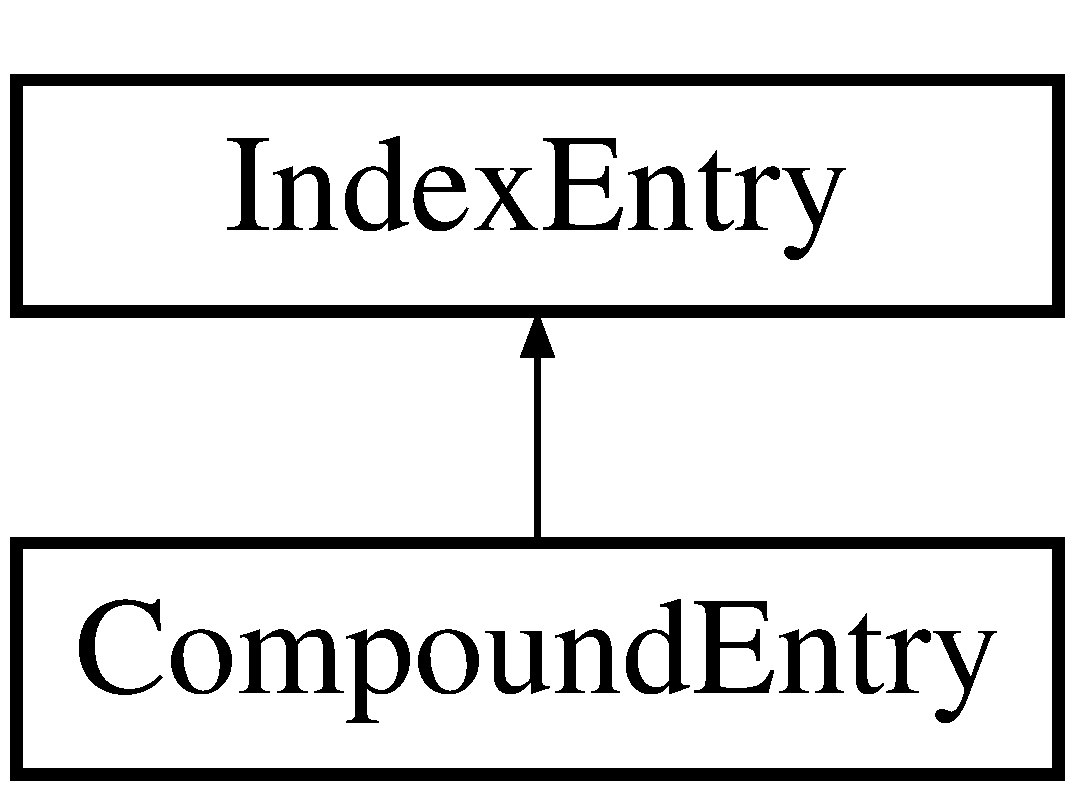
\includegraphics[height=2.000000cm]{struct_compound_entry}
\end{center}
\end{figure}
\subsection*{Membros públicos}
\begin{DoxyCompactItemize}
\item 
\hypertarget{struct_compound_entry_adfbf2243b22c31c299482b71781e5102}{{\bfseries Compound\-Entry} (int size)}\label{struct_compound_entry_adfbf2243b22c31c299482b71781e5102}

\end{DoxyCompactItemize}
\subsection*{Campos de Dados}
\begin{DoxyCompactItemize}
\item 
\hypertarget{struct_compound_entry_af6992030f752ea5f105ed04e1bb1b140}{Q\-Dict$<$ \hyperlink{struct_member_entry}{Member\-Entry} $>$ {\bfseries member\-Dict}}\label{struct_compound_entry_af6992030f752ea5f105ed04e1bb1b140}

\end{DoxyCompactItemize}


A documentação para esta estrutura foi gerada a partir do seguinte ficheiro\-:\begin{DoxyCompactItemize}
\item 
C\-:/\-Users/teste/git/doxygen/addon/doxmlparser/src/mainhandler.\-h\end{DoxyCompactItemize}

\hypertarget{class_compound_entry_iterator}{\section{Referência à classe Compound\-Entry\-Iterator}
\label{class_compound_entry_iterator}\index{Compound\-Entry\-Iterator@{Compound\-Entry\-Iterator}}
}
Diagrama de heranças da classe Compound\-Entry\-Iterator\begin{figure}[H]
\begin{center}
\leavevmode
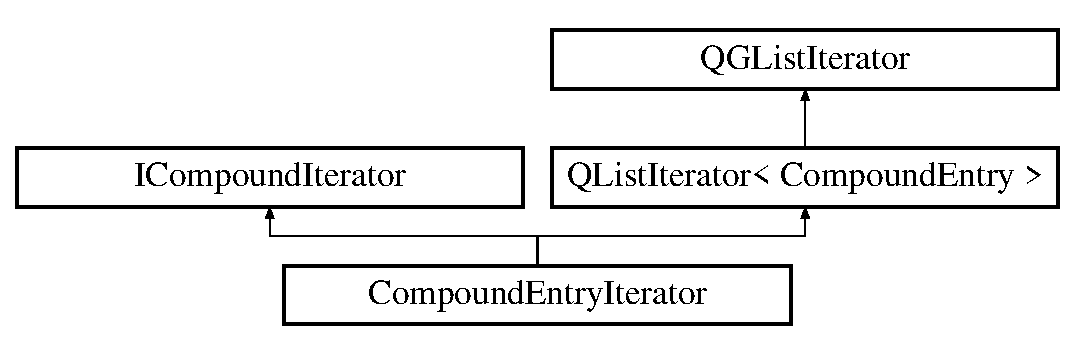
\includegraphics[height=3.000000cm]{class_compound_entry_iterator}
\end{center}
\end{figure}
\subsection*{Membros públicos}
\begin{DoxyCompactItemize}
\item 
\hypertarget{class_compound_entry_iterator_afaa091fb3cd3b2b418e16821670b6f6c}{{\bfseries Compound\-Entry\-Iterator} (const \hyperlink{class_main_handler}{Main\-Handler} $\ast$m, const \hyperlink{class_q_list}{Q\-List}$<$ \hyperlink{struct_compound_entry}{Compound\-Entry} $>$ \&list)}\label{class_compound_entry_iterator_afaa091fb3cd3b2b418e16821670b6f6c}

\item 
\hypertarget{class_compound_entry_iterator_a24528c52410032763cedaccdfbe474e5}{virtual void {\bfseries to\-First} ()}\label{class_compound_entry_iterator_a24528c52410032763cedaccdfbe474e5}

\item 
\hypertarget{class_compound_entry_iterator_ac4e23694db19ee84c4e110f9965d64e4}{virtual void {\bfseries to\-Last} ()}\label{class_compound_entry_iterator_ac4e23694db19ee84c4e110f9965d64e4}

\item 
\hypertarget{class_compound_entry_iterator_ad8ecebd1a267185e69e1b6fe4e9f331e}{virtual void {\bfseries to\-Next} ()}\label{class_compound_entry_iterator_ad8ecebd1a267185e69e1b6fe4e9f331e}

\item 
\hypertarget{class_compound_entry_iterator_a3491dc4d8ab54f0a0583ac1941f4e94f}{virtual void {\bfseries to\-Prev} ()}\label{class_compound_entry_iterator_a3491dc4d8ab54f0a0583ac1941f4e94f}

\item 
\hypertarget{class_compound_entry_iterator_aed1ddf0744f763ffafe54f63da2080bb}{virtual \hyperlink{class_i_compound}{I\-Compound} $\ast$ {\bfseries current} () const }\label{class_compound_entry_iterator_aed1ddf0744f763ffafe54f63da2080bb}

\item 
\hypertarget{class_compound_entry_iterator_af8a84115de3507728d5e19e804529052}{virtual void {\bfseries release} ()}\label{class_compound_entry_iterator_af8a84115de3507728d5e19e804529052}

\end{DoxyCompactItemize}
\subsection*{Additional Inherited Members}


A documentação para esta classe foi gerada a partir do seguinte ficheiro\-:\begin{DoxyCompactItemize}
\item 
C\-:/\-Users/teste/git/doxygen/addon/doxmlparser/src/mainhandler.\-cpp\end{DoxyCompactItemize}

\hypertarget{class_compound_error_handler}{\section{Referência à classe Compound\-Error\-Handler}
\label{class_compound_error_handler}\index{Compound\-Error\-Handler@{Compound\-Error\-Handler}}
}
Diagrama de heranças da classe Compound\-Error\-Handler\begin{figure}[H]
\begin{center}
\leavevmode
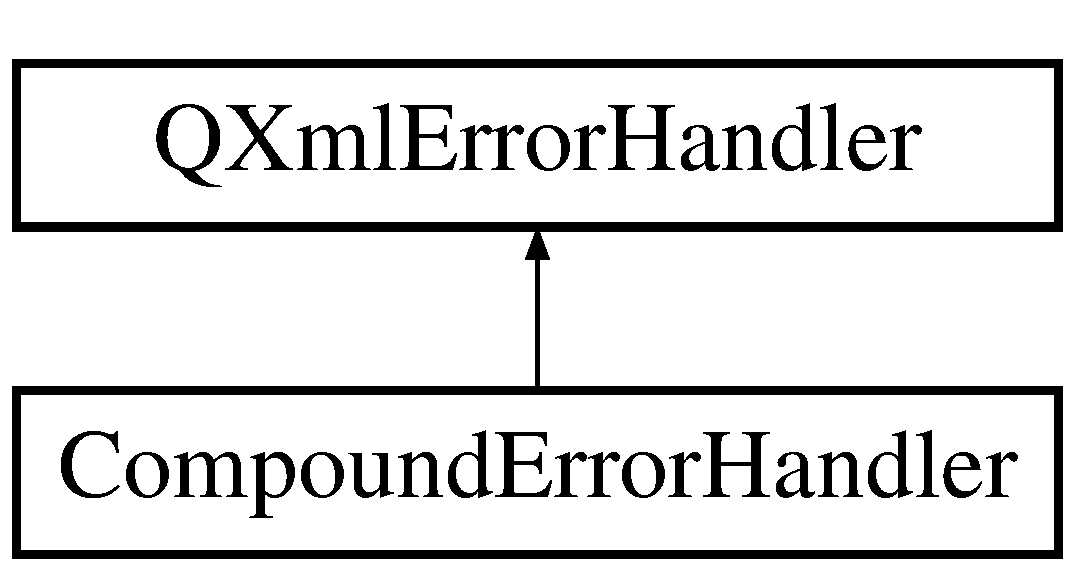
\includegraphics[height=2.000000cm]{class_compound_error_handler}
\end{center}
\end{figure}
\subsection*{Membros públicos}
\begin{DoxyCompactItemize}
\item 
bool \hyperlink{class_compound_error_handler_aac28fc998851e69a512e4f544eeff5a7}{warning} (const \hyperlink{class_q_xml_parse_exception}{Q\-Xml\-Parse\-Exception} \&)
\item 
bool \hyperlink{class_compound_error_handler_abb2a084eeba80972cfe5bd3804b2f0bd}{error} (const \hyperlink{class_q_xml_parse_exception}{Q\-Xml\-Parse\-Exception} \&)
\item 
bool \hyperlink{class_compound_error_handler_afe3fbf09765011104e0d12ee0d395619}{fatal\-Error} (const \hyperlink{class_q_xml_parse_exception}{Q\-Xml\-Parse\-Exception} \&exception)
\item 
\hyperlink{class_q_string}{Q\-String} \hyperlink{class_compound_error_handler_af799a7684337babb971e2e0d8cda7cf1}{error\-String} ()
\end{DoxyCompactItemize}


\subsection{Documentação dos métodos}
\hypertarget{class_compound_error_handler_abb2a084eeba80972cfe5bd3804b2f0bd}{\index{Compound\-Error\-Handler@{Compound\-Error\-Handler}!error@{error}}
\index{error@{error}!CompoundErrorHandler@{Compound\-Error\-Handler}}
\subsubsection[{error}]{\setlength{\rightskip}{0pt plus 5cm}bool error (
\begin{DoxyParamCaption}
\item[{const {\bf Q\-Xml\-Parse\-Exception} \&}]{exception}
\end{DoxyParamCaption}
)\hspace{0.3cm}{\ttfamily [inline]}, {\ttfamily [virtual]}}}\label{class_compound_error_handler_abb2a084eeba80972cfe5bd3804b2f0bd}
\hyperlink{class_a}{A} reader might use this function to report a recoverable error. \hyperlink{class_a}{A} recoverable error corresponds to the definiton of \char`\"{}error\char`\"{} in section 1.\-2 of the X\-M\-L 1.\-0 specification.

The reader must continue to provide normal parsing events after invoking this function.

If this function returns F\-A\-L\-S\-E the reader will stop parsing and will report an error. The reader will use the function \hyperlink{class_compound_error_handler_af799a7684337babb971e2e0d8cda7cf1}{error\-String()} to get the error message that will be used for reporting the error. 

Implementa \hyperlink{class_q_xml_error_handler_a4c3f6f44d2411175c39b0a1f45075a91}{Q\-Xml\-Error\-Handler}.

\hypertarget{class_compound_error_handler_af799a7684337babb971e2e0d8cda7cf1}{\index{Compound\-Error\-Handler@{Compound\-Error\-Handler}!error\-String@{error\-String}}
\index{error\-String@{error\-String}!CompoundErrorHandler@{Compound\-Error\-Handler}}
\subsubsection[{error\-String}]{\setlength{\rightskip}{0pt plus 5cm}{\bf Q\-String} error\-String (
\begin{DoxyParamCaption}
{}
\end{DoxyParamCaption}
)\hspace{0.3cm}{\ttfamily [inline]}, {\ttfamily [virtual]}}}\label{class_compound_error_handler_af799a7684337babb971e2e0d8cda7cf1}
The reader calls this function to get an error string if any of the handler functions returns F\-A\-L\-S\-E to him. 

Implementa \hyperlink{class_q_xml_error_handler_ac86bbbabef3a52aec7615cbbc0adb3f4}{Q\-Xml\-Error\-Handler}.

\hypertarget{class_compound_error_handler_afe3fbf09765011104e0d12ee0d395619}{\index{Compound\-Error\-Handler@{Compound\-Error\-Handler}!fatal\-Error@{fatal\-Error}}
\index{fatal\-Error@{fatal\-Error}!CompoundErrorHandler@{Compound\-Error\-Handler}}
\subsubsection[{fatal\-Error}]{\setlength{\rightskip}{0pt plus 5cm}bool fatal\-Error (
\begin{DoxyParamCaption}
\item[{const {\bf Q\-Xml\-Parse\-Exception} \&}]{exception}
\end{DoxyParamCaption}
)\hspace{0.3cm}{\ttfamily [inline]}, {\ttfamily [virtual]}}}\label{class_compound_error_handler_afe3fbf09765011104e0d12ee0d395619}
\hyperlink{class_a}{A} reader must use this function to report a non-\/recoverable error.

If this function returns T\-R\-U\-E the reader might try to go on parsing and reporting further errors; but no regular parsing events are reported. 

Implementa \hyperlink{class_q_xml_error_handler_ac797351a210314f1ca2289a40acf2694}{Q\-Xml\-Error\-Handler}.

\hypertarget{class_compound_error_handler_aac28fc998851e69a512e4f544eeff5a7}{\index{Compound\-Error\-Handler@{Compound\-Error\-Handler}!warning@{warning}}
\index{warning@{warning}!CompoundErrorHandler@{Compound\-Error\-Handler}}
\subsubsection[{warning}]{\setlength{\rightskip}{0pt plus 5cm}bool warning (
\begin{DoxyParamCaption}
\item[{const {\bf Q\-Xml\-Parse\-Exception} \&}]{exception}
\end{DoxyParamCaption}
)\hspace{0.3cm}{\ttfamily [inline]}, {\ttfamily [virtual]}}}\label{class_compound_error_handler_aac28fc998851e69a512e4f544eeff5a7}
\hyperlink{class_a}{A} reader might use this function to report a warning. Warnings are conditions that are not errors or fatal errors as defined by the X\-M\-L 1.\-0 specification.

If this function returns F\-A\-L\-S\-E the reader will stop parsing and will report an error. The reader will use the function \hyperlink{class_compound_error_handler_af799a7684337babb971e2e0d8cda7cf1}{error\-String()} to get the error message that will be used for reporting the error. 

Implementa \hyperlink{class_q_xml_error_handler_a109de9b8833092a63f6bc48f84cf241b}{Q\-Xml\-Error\-Handler}.



A documentação para esta classe foi gerada a partir do seguinte ficheiro\-:\begin{DoxyCompactItemize}
\item 
C\-:/\-Users/teste/git/doxygen/addon/doxmlparser/src/compoundhandler.\-cpp\end{DoxyCompactItemize}

\hypertarget{class_compound_handler}{\section{Referência à classe Compound\-Handler}
\label{class_compound_handler}\index{Compound\-Handler@{Compound\-Handler}}
}
Diagrama de heranças da classe Compound\-Handler\begin{figure}[H]
\begin{center}
\leavevmode
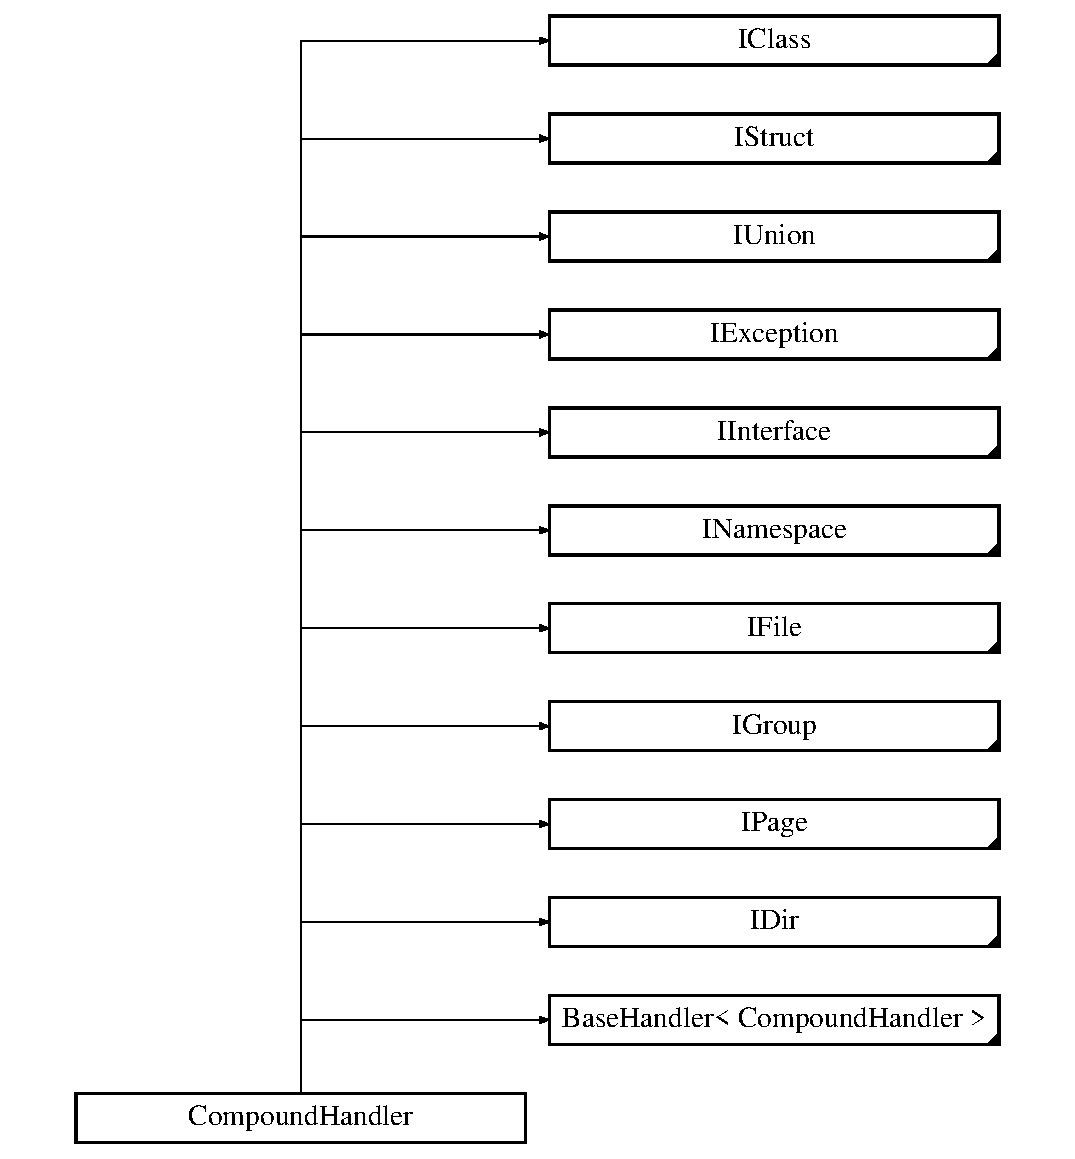
\includegraphics[height=12.000000cm]{class_compound_handler}
\end{center}
\end{figure}
\subsection*{Membros públicos}
\begin{DoxyCompactItemize}
\item 
\hypertarget{class_compound_handler_a61cef5a9912b15e7535cdffe96b75ba0}{virtual void {\bfseries start\-Section} (const \hyperlink{class_q_xml_attributes}{Q\-Xml\-Attributes} \&attrib)}\label{class_compound_handler_a61cef5a9912b15e7535cdffe96b75ba0}

\item 
\hypertarget{class_compound_handler_acf79d78c3e6bdc9e5eaa8d28eb075633}{virtual void {\bfseries start\-Compound} (const \hyperlink{class_q_xml_attributes}{Q\-Xml\-Attributes} \&attrib)}\label{class_compound_handler_acf79d78c3e6bdc9e5eaa8d28eb075633}

\item 
\hypertarget{class_compound_handler_a25876184ea64bca575eea564e0418052}{virtual void {\bfseries start\-Super\-Class} (const \hyperlink{class_q_xml_attributes}{Q\-Xml\-Attributes} \&attrib)}\label{class_compound_handler_a25876184ea64bca575eea564e0418052}

\item 
\hypertarget{class_compound_handler_a133084573eb643b37224fbf99eed48ec}{virtual void {\bfseries end\-Super\-Class} ()}\label{class_compound_handler_a133084573eb643b37224fbf99eed48ec}

\item 
\hypertarget{class_compound_handler_ab14b8210e4576fe30248a447631ab363}{virtual void {\bfseries start\-Sub\-Class} (const \hyperlink{class_q_xml_attributes}{Q\-Xml\-Attributes} \&attrib)}\label{class_compound_handler_ab14b8210e4576fe30248a447631ab363}

\item 
\hypertarget{class_compound_handler_a3a65b1f30e04a8ecac7c8cc2153a6da3}{virtual void {\bfseries end\-Sub\-Class} ()}\label{class_compound_handler_a3a65b1f30e04a8ecac7c8cc2153a6da3}

\item 
\hypertarget{class_compound_handler_a328b7b29416df23c615505ec47b9d299}{virtual void {\bfseries end\-Compound} ()}\label{class_compound_handler_a328b7b29416df23c615505ec47b9d299}

\item 
\hypertarget{class_compound_handler_afc53d2f84dac337792a2dbb55b0199e1}{virtual void {\bfseries end\-Compound\-Name} ()}\label{class_compound_handler_afc53d2f84dac337792a2dbb55b0199e1}

\item 
\hypertarget{class_compound_handler_a104aa450d7ed98aaaf929bf81eb3252e}{virtual void {\bfseries start\-Brief\-Desc} (const \hyperlink{class_q_xml_attributes}{Q\-Xml\-Attributes} \&attrib)}\label{class_compound_handler_a104aa450d7ed98aaaf929bf81eb3252e}

\item 
\hypertarget{class_compound_handler_a94f6cc704f336be42dd887b95f86a106}{virtual void {\bfseries start\-Detailed\-Desc} (const \hyperlink{class_q_xml_attributes}{Q\-Xml\-Attributes} \&attrib)}\label{class_compound_handler_a94f6cc704f336be42dd887b95f86a106}

\item 
\hypertarget{class_compound_handler_a588050483d3f93dc2854f3abdbdbfa4f}{virtual void {\bfseries start\-Location} (const \hyperlink{class_q_xml_attributes}{Q\-Xml\-Attributes} \&attrib)}\label{class_compound_handler_a588050483d3f93dc2854f3abdbdbfa4f}

\item 
\hypertarget{class_compound_handler_ae03e5c8c64478d96c0e32aa7738e16b6}{virtual void {\bfseries start\-Program\-Listing} (const \hyperlink{class_q_xml_attributes}{Q\-Xml\-Attributes} \&attrib)}\label{class_compound_handler_ae03e5c8c64478d96c0e32aa7738e16b6}

\item 
\hypertarget{class_compound_handler_ac937eeee5effa83a9bb9eb68665be9a5}{virtual void {\bfseries start\-Inheritance\-Graph} (const \hyperlink{class_q_xml_attributes}{Q\-Xml\-Attributes} \&attrib)}\label{class_compound_handler_ac937eeee5effa83a9bb9eb68665be9a5}

\item 
\hypertarget{class_compound_handler_aed5ba494e128f87ff7b51cde2cdbc4de}{virtual void {\bfseries start\-Collaboration\-Graph} (const \hyperlink{class_q_xml_attributes}{Q\-Xml\-Attributes} \&attrib)}\label{class_compound_handler_aed5ba494e128f87ff7b51cde2cdbc4de}

\item 
\hypertarget{class_compound_handler_ac2a6c80ad07801e94431c37bf8597124}{virtual void {\bfseries start\-Include\-Dependency\-Graph} (const \hyperlink{class_q_xml_attributes}{Q\-Xml\-Attributes} \&attrib)}\label{class_compound_handler_ac2a6c80ad07801e94431c37bf8597124}

\item 
\hypertarget{class_compound_handler_a44afae59dd991d586b9d2391d24be6d1}{virtual void {\bfseries start\-Included\-By\-Dependency\-Graph} (const \hyperlink{class_q_xml_attributes}{Q\-Xml\-Attributes} \&attrib)}\label{class_compound_handler_a44afae59dd991d586b9d2391d24be6d1}

\item 
\hypertarget{class_compound_handler_a3eab2f5931842aad8f91a48005110d27}{virtual void {\bfseries start\-Includes} (const \hyperlink{class_q_xml_attributes}{Q\-Xml\-Attributes} \&attrib)}\label{class_compound_handler_a3eab2f5931842aad8f91a48005110d27}

\item 
\hypertarget{class_compound_handler_ac198f1ec6ab472e650ea91aa0886daf1}{virtual void {\bfseries start\-Included\-By} (const \hyperlink{class_q_xml_attributes}{Q\-Xml\-Attributes} \&attrib)}\label{class_compound_handler_ac198f1ec6ab472e650ea91aa0886daf1}

\item 
\hypertarget{class_compound_handler_a28a537b250f8ed2c4f4ae6e39d6e90fa}{virtual void {\bfseries start\-Inner\-Dir} (const \hyperlink{class_q_xml_attributes}{Q\-Xml\-Attributes} \&attrib)}\label{class_compound_handler_a28a537b250f8ed2c4f4ae6e39d6e90fa}

\item 
\hypertarget{class_compound_handler_a0aceb3b3c7a97c1532e98b8af319fc58}{virtual void {\bfseries start\-Inner\-Class} (const \hyperlink{class_q_xml_attributes}{Q\-Xml\-Attributes} \&attrib)}\label{class_compound_handler_a0aceb3b3c7a97c1532e98b8af319fc58}

\item 
\hypertarget{class_compound_handler_ac5a087b01f8f5664a25f1ae45482daea}{virtual void {\bfseries start\-Inner\-Namespace} (const \hyperlink{class_q_xml_attributes}{Q\-Xml\-Attributes} \&attrib)}\label{class_compound_handler_ac5a087b01f8f5664a25f1ae45482daea}

\item 
\hypertarget{class_compound_handler_a99fb925c59508d61cb7b0a14646b253e}{virtual void {\bfseries start\-Inner\-File} (const \hyperlink{class_q_xml_attributes}{Q\-Xml\-Attributes} \&attrib)}\label{class_compound_handler_a99fb925c59508d61cb7b0a14646b253e}

\item 
\hypertarget{class_compound_handler_a8a562c395c5e4db336e04f75980be2cb}{virtual void {\bfseries start\-Inner\-Group} (const \hyperlink{class_q_xml_attributes}{Q\-Xml\-Attributes} \&attrib)}\label{class_compound_handler_a8a562c395c5e4db336e04f75980be2cb}

\item 
\hypertarget{class_compound_handler_a74fb73f08a5aa354b76fa132e8621157}{virtual void {\bfseries start\-Inner\-Page} (const \hyperlink{class_q_xml_attributes}{Q\-Xml\-Attributes} \&attrib)}\label{class_compound_handler_a74fb73f08a5aa354b76fa132e8621157}

\item 
\hypertarget{class_compound_handler_a542aae01d1b2fae60d3c4dd0b77f6669}{virtual void {\bfseries start\-Title} (const \hyperlink{class_q_xml_attributes}{Q\-Xml\-Attributes} \&attrib)}\label{class_compound_handler_a542aae01d1b2fae60d3c4dd0b77f6669}

\item 
\hypertarget{class_compound_handler_a2de4ded6787264c3be9d44c1b532114b}{virtual void {\bfseries start\-Template\-Param\-List} (const \hyperlink{class_q_xml_attributes}{Q\-Xml\-Attributes} \&attrib)}\label{class_compound_handler_a2de4ded6787264c3be9d44c1b532114b}

\item 
\hypertarget{class_compound_handler_a2607d3987dd3c5d47bd7ecb8d1e1adc0}{virtual void {\bfseries start\-List\-Of\-All\-Members} (const \hyperlink{class_q_xml_attributes}{Q\-Xml\-Attributes} \&attrib)}\label{class_compound_handler_a2607d3987dd3c5d47bd7ecb8d1e1adc0}

\item 
\hypertarget{class_compound_handler_a4c00c1eb3364b61f9dc7e8fd45113569}{virtual void {\bfseries addref} ()}\label{class_compound_handler_a4c00c1eb3364b61f9dc7e8fd45113569}

\item 
\hypertarget{class_compound_handler_a11ca94979b706a7feef09c5c578384ec}{{\bfseries Compound\-Handler} (const \hyperlink{class_q_string}{Q\-String} \&dir\-Name)}\label{class_compound_handler_a11ca94979b706a7feef09c5c578384ec}

\item 
\hypertarget{class_compound_handler_a5dadaa976eadd3b15085a88620511050}{bool {\bfseries parse\-X\-M\-L} (const char $\ast$comp\-Id)}\label{class_compound_handler_a5dadaa976eadd3b15085a88620511050}

\item 
\hypertarget{class_compound_handler_a477d68af87dc751b2c70936c91980873}{void {\bfseries initialize} (\hyperlink{class_main_handler}{Main\-Handler} $\ast$mh)}\label{class_compound_handler_a477d68af87dc751b2c70936c91980873}

\item 
\hypertarget{class_compound_handler_a2ed25907a4ed0d00cabb8428d9713323}{void {\bfseries insert\-Member} (\hyperlink{class_member_handler}{Member\-Handler} $\ast$mh)}\label{class_compound_handler_a2ed25907a4ed0d00cabb8428d9713323}

\item 
\hypertarget{class_compound_handler_a7336fe63ce7b7a1e6d0c3c70b2833f2a}{\hyperlink{class_i_compound}{I\-Compound} $\ast$ {\bfseries to\-I\-Compound} () const }\label{class_compound_handler_a7336fe63ce7b7a1e6d0c3c70b2833f2a}

\item 
const \hyperlink{class_i_string}{I\-String} $\ast$ \hyperlink{class_compound_handler_abc1b3c24a1bf7f630dd7790258ce3826}{name} () const 
\item 
const \hyperlink{class_i_string}{I\-String} $\ast$ \hyperlink{class_compound_handler_a7ee3d1471e529e5d04316a403f65f410}{id} () const 
\item 
\hyperlink{class_i_compound_a7063885b1cabbff5f94849960f08ecb2}{Compound\-Kind} \hyperlink{class_compound_handler_a3d58bcf4b8672eff9a550ab75b4bb17a}{kind} () const 
\item 
const \hyperlink{class_i_string}{I\-String} $\ast$ \hyperlink{class_compound_handler_afb533b27130d10febf3477338c90f1e4}{kind\-String} () const 
\item 
\hyperlink{class_i_section_iterator}{I\-Section\-Iterator} $\ast$ \hyperlink{class_compound_handler_aa53a8319489c6f3a03806ae14f5d78cf}{sections} () const 
\item 
\hyperlink{class_i_doc_root}{I\-Doc\-Root} $\ast$ \hyperlink{class_compound_handler_a90d0ec3bda5465dfb8c7b986c9bc2f1f}{brief\-Description} () const 
\item 
\hyperlink{class_i_doc_root}{I\-Doc\-Root} $\ast$ \hyperlink{class_compound_handler_a125deb50c49081b484e9a688e73382fe}{detailed\-Description} () const 
\item 
\hyperlink{class_i_member}{I\-Member} $\ast$ \hyperlink{class_compound_handler_abf35727fa0ef6d77c1768e90830186c4}{member\-By\-Id} (const char $\ast$\hyperlink{class_compound_handler_a7ee3d1471e529e5d04316a403f65f410}{id}) const 
\item 
\hyperlink{class_i_member_iterator}{I\-Member\-Iterator} $\ast$ \hyperlink{class_compound_handler_ae712b1ed3a3cf5cd2d70c0a7a8a381e6}{member\-By\-Name} (const char $\ast$\hyperlink{class_compound_handler_abc1b3c24a1bf7f630dd7790258ce3826}{name}) const 
\item 
\hypertarget{class_compound_handler_ade1cc5a0e97b9e483b009225b43e1d99}{\hyperlink{class_i_param_iterator}{I\-Param\-Iterator} $\ast$ {\bfseries template\-Parameters} () const }\label{class_compound_handler_ade1cc5a0e97b9e483b009225b43e1d99}

\item 
void \hyperlink{class_compound_handler_a23b477d0e2d399f75d585d154c346591}{release} ()
\item 
\hypertarget{class_compound_handler_a5c8bb9921e759357498282c793695189}{\hyperlink{class_i_graph}{I\-Graph} $\ast$ {\bfseries inheritance\-Graph} () const }\label{class_compound_handler_a5c8bb9921e759357498282c793695189}

\item 
\hypertarget{class_compound_handler_ae90be38977564ad7486bcb89b31fac7f}{\hyperlink{class_i_graph}{I\-Graph} $\ast$ {\bfseries collaboration\-Graph} () const }\label{class_compound_handler_ae90be38977564ad7486bcb89b31fac7f}

\item 
\hypertarget{class_compound_handler_a0d22bff00b5d9bb1c3957161638bb428}{\hyperlink{class_i_related_compound_iterator}{I\-Related\-Compound\-Iterator} $\ast$ {\bfseries base\-Compounds} () const }\label{class_compound_handler_a0d22bff00b5d9bb1c3957161638bb428}

\item 
\hypertarget{class_compound_handler_ac1d5de1d94d11ad1ede40ce178b3077f}{\hyperlink{class_i_related_compound_iterator}{I\-Related\-Compound\-Iterator} $\ast$ {\bfseries derived\-Compounds} () const }\label{class_compound_handler_ac1d5de1d94d11ad1ede40ce178b3077f}

\item 
\hypertarget{class_compound_handler_ac47414905db86943bb283b3075a71265}{\hyperlink{class_i_compound_iterator}{I\-Compound\-Iterator} $\ast$ {\bfseries nested\-Compounds} () const }\label{class_compound_handler_ac47414905db86943bb283b3075a71265}

\item 
\hypertarget{class_compound_handler_a70b66a204f763fca68b3518210f3714b}{\hyperlink{class_i_compound_iterator}{I\-Compound\-Iterator} $\ast$ {\bfseries nested\-Group} () const }\label{class_compound_handler_a70b66a204f763fca68b3518210f3714b}

\item 
\hypertarget{class_compound_handler_abce94f08d91f846fff0d9c15634735c8}{const \hyperlink{class_i_string}{I\-String} $\ast$ {\bfseries location\-File} () const }\label{class_compound_handler_abce94f08d91f846fff0d9c15634735c8}

\item 
\hypertarget{class_compound_handler_ae7a9a8fecbbcb367e094b035e86f600a}{int {\bfseries location\-Line} () const }\label{class_compound_handler_ae7a9a8fecbbcb367e094b035e86f600a}

\item 
\hypertarget{class_compound_handler_a21bb09533fb7679d628647320dd6fda4}{const \hyperlink{class_i_string}{I\-String} $\ast$ {\bfseries location\-Body\-File} () const }\label{class_compound_handler_a21bb09533fb7679d628647320dd6fda4}

\item 
\hypertarget{class_compound_handler_ad77f517c3f3a3e96f00a04ed465ae57f}{int {\bfseries location\-Body\-Start\-Line} () const }\label{class_compound_handler_ad77f517c3f3a3e96f00a04ed465ae57f}

\item 
\hypertarget{class_compound_handler_ac49937c48951825a63fa00a14204966d}{int {\bfseries location\-Body\-End\-Line} () const }\label{class_compound_handler_ac49937c48951825a63fa00a14204966d}

\item 
\hypertarget{class_compound_handler_a200d07c3abf67b299e7945b68c91328a}{\hyperlink{class_i_member_reference_iterator}{I\-Member\-Reference\-Iterator} $\ast$ {\bfseries members} () const }\label{class_compound_handler_a200d07c3abf67b299e7945b68c91328a}

\item 
\hypertarget{class_compound_handler_a03cb0e384c809a400b18e63a73f88dc3}{\hyperlink{class_i_graph}{I\-Graph} $\ast$ {\bfseries include\-Dependency\-Graph} () const }\label{class_compound_handler_a03cb0e384c809a400b18e63a73f88dc3}

\item 
\hypertarget{class_compound_handler_a93601429d19d844e63d5934e5290daf8}{\hyperlink{class_i_graph}{I\-Graph} $\ast$ {\bfseries included\-By\-Dependency\-Graph} () const }\label{class_compound_handler_a93601429d19d844e63d5934e5290daf8}

\item 
\hypertarget{class_compound_handler_a2f9218d5099157ec6a7bfaa51d799be8}{\hyperlink{class_i_doc_program_listing}{I\-Doc\-Program\-Listing} $\ast$ {\bfseries source} () const }\label{class_compound_handler_a2f9218d5099157ec6a7bfaa51d799be8}

\item 
\hypertarget{class_compound_handler_a492563e0f76df4ed8f925ffd20591d15}{\hyperlink{class_i_include_iterator}{I\-Include\-Iterator} $\ast$ {\bfseries includes} () const }\label{class_compound_handler_a492563e0f76df4ed8f925ffd20591d15}

\item 
\hypertarget{class_compound_handler_a1918ab4e5d66e9504d30a40ca5515358}{\hyperlink{class_i_include_iterator}{I\-Include\-Iterator} $\ast$ {\bfseries included\-By} () const }\label{class_compound_handler_a1918ab4e5d66e9504d30a40ca5515358}

\item 
\hypertarget{class_compound_handler_af0e7a53674849f59096520180b37c7e1}{const \hyperlink{class_i_doc_title}{I\-Doc\-Title} $\ast$ {\bfseries title} () const }\label{class_compound_handler_af0e7a53674849f59096520180b37c7e1}

\end{DoxyCompactItemize}
\subsection*{Amigos}
\begin{DoxyCompactItemize}
\item 
\hypertarget{class_compound_handler_a3ac82494777760c5bf9d85209ba95321}{class {\bfseries Related\-Compound}}\label{class_compound_handler_a3ac82494777760c5bf9d85209ba95321}

\end{DoxyCompactItemize}
\subsection*{Additional Inherited Members}


\subsection{Documentação dos métodos}
\hypertarget{class_compound_handler_a90d0ec3bda5465dfb8c7b986c9bc2f1f}{\index{Compound\-Handler@{Compound\-Handler}!brief\-Description@{brief\-Description}}
\index{brief\-Description@{brief\-Description}!CompoundHandler@{Compound\-Handler}}
\subsubsection[{brief\-Description}]{\setlength{\rightskip}{0pt plus 5cm}{\bf I\-Doc\-Root} $\ast$ brief\-Description (
\begin{DoxyParamCaption}
{}
\end{DoxyParamCaption}
) const\hspace{0.3cm}{\ttfamily [virtual]}}}\label{class_compound_handler_a90d0ec3bda5465dfb8c7b986c9bc2f1f}
Returns a tree-\/structured representation of the brief description that is attached to this compound. 

Implementa \hyperlink{class_i_compound_a8a0da25a8851dfb809394c4d6585efb2}{I\-Compound}.

\hypertarget{class_compound_handler_a125deb50c49081b484e9a688e73382fe}{\index{Compound\-Handler@{Compound\-Handler}!detailed\-Description@{detailed\-Description}}
\index{detailed\-Description@{detailed\-Description}!CompoundHandler@{Compound\-Handler}}
\subsubsection[{detailed\-Description}]{\setlength{\rightskip}{0pt plus 5cm}{\bf I\-Doc\-Root} $\ast$ detailed\-Description (
\begin{DoxyParamCaption}
{}
\end{DoxyParamCaption}
) const\hspace{0.3cm}{\ttfamily [virtual]}}}\label{class_compound_handler_a125deb50c49081b484e9a688e73382fe}
Returns a tree-\/structured representation of the detailed description that is attached to this compound. 

Implementa \hyperlink{class_i_compound_a3fd3d8b278a1e0787d51861984fdc73e}{I\-Compound}.

\hypertarget{class_compound_handler_a7ee3d1471e529e5d04316a403f65f410}{\index{Compound\-Handler@{Compound\-Handler}!id@{id}}
\index{id@{id}!CompoundHandler@{Compound\-Handler}}
\subsubsection[{id}]{\setlength{\rightskip}{0pt plus 5cm}const {\bf I\-String}$\ast$ id (
\begin{DoxyParamCaption}
{}
\end{DoxyParamCaption}
) const\hspace{0.3cm}{\ttfamily [inline]}, {\ttfamily [virtual]}}}\label{class_compound_handler_a7ee3d1471e529e5d04316a403f65f410}
Returns the id of this compound. The id is a unique string representing a specific compound object. 

Implementa \hyperlink{class_i_compound_aaba28daa272dce8bc14dde330d5b0126}{I\-Compound}.

\hypertarget{class_compound_handler_a3d58bcf4b8672eff9a550ab75b4bb17a}{\index{Compound\-Handler@{Compound\-Handler}!kind@{kind}}
\index{kind@{kind}!CompoundHandler@{Compound\-Handler}}
\subsubsection[{kind}]{\setlength{\rightskip}{0pt plus 5cm}{\bf Compound\-Kind} kind (
\begin{DoxyParamCaption}
{}
\end{DoxyParamCaption}
) const\hspace{0.3cm}{\ttfamily [inline]}, {\ttfamily [virtual]}}}\label{class_compound_handler_a3d58bcf4b8672eff9a550ab75b4bb17a}
Returns the kind of compound. See \hyperlink{class_i_compound_a7063885b1cabbff5f94849960f08ecb2}{Compound\-Kind} for possible values. 

Implementa \hyperlink{class_i_compound_aee9f3639e2f2fa0f1d9f3729fa8d4d51}{I\-Compound}.

\hypertarget{class_compound_handler_afb533b27130d10febf3477338c90f1e4}{\index{Compound\-Handler@{Compound\-Handler}!kind\-String@{kind\-String}}
\index{kind\-String@{kind\-String}!CompoundHandler@{Compound\-Handler}}
\subsubsection[{kind\-String}]{\setlength{\rightskip}{0pt plus 5cm}const {\bf I\-String}$\ast$ kind\-String (
\begin{DoxyParamCaption}
{}
\end{DoxyParamCaption}
) const\hspace{0.3cm}{\ttfamily [inline]}, {\ttfamily [virtual]}}}\label{class_compound_handler_afb533b27130d10febf3477338c90f1e4}
Returns a string representation of the compound kind. \begin{DoxySeeAlso}{Veja também}
\hyperlink{class_compound_handler_a3d58bcf4b8672eff9a550ab75b4bb17a}{kind()} 
\end{DoxySeeAlso}


Implementa \hyperlink{class_i_compound_a872363e5be82229a73bd00d212a703ce}{I\-Compound}.

\hypertarget{class_compound_handler_abf35727fa0ef6d77c1768e90830186c4}{\index{Compound\-Handler@{Compound\-Handler}!member\-By\-Id@{member\-By\-Id}}
\index{member\-By\-Id@{member\-By\-Id}!CompoundHandler@{Compound\-Handler}}
\subsubsection[{member\-By\-Id}]{\setlength{\rightskip}{0pt plus 5cm}{\bf I\-Member} $\ast$ member\-By\-Id (
\begin{DoxyParamCaption}
\item[{const char $\ast$}]{id}
\end{DoxyParamCaption}
) const\hspace{0.3cm}{\ttfamily [virtual]}}}\label{class_compound_handler_abf35727fa0ef6d77c1768e90830186c4}
Returns an interface to a member given its id. 
\begin{DoxyParams}{Parâmetros}
{\em id} & The member id. \\
\hline
\end{DoxyParams}


Implementa \hyperlink{class_i_compound_a222db2d537161310f4b3ed91533b751f}{I\-Compound}.

\hypertarget{class_compound_handler_ae712b1ed3a3cf5cd2d70c0a7a8a381e6}{\index{Compound\-Handler@{Compound\-Handler}!member\-By\-Name@{member\-By\-Name}}
\index{member\-By\-Name@{member\-By\-Name}!CompoundHandler@{Compound\-Handler}}
\subsubsection[{member\-By\-Name}]{\setlength{\rightskip}{0pt plus 5cm}{\bf I\-Member\-Iterator} $\ast$ member\-By\-Name (
\begin{DoxyParamCaption}
\item[{const char $\ast$}]{name}
\end{DoxyParamCaption}
) const\hspace{0.3cm}{\ttfamily [virtual]}}}\label{class_compound_handler_ae712b1ed3a3cf5cd2d70c0a7a8a381e6}
Returns a list of all members within the compound having a certain name. Member overloading is the reason why there can be more than one member. 
\begin{DoxyParams}{Parâmetros}
{\em name} & The name of the member. \\
\hline
\end{DoxyParams}


Implementa \hyperlink{class_i_compound_a41dab6cd9fd4d21d9f23cd5c11452147}{I\-Compound}.

\hypertarget{class_compound_handler_abc1b3c24a1bf7f630dd7790258ce3826}{\index{Compound\-Handler@{Compound\-Handler}!name@{name}}
\index{name@{name}!CompoundHandler@{Compound\-Handler}}
\subsubsection[{name}]{\setlength{\rightskip}{0pt plus 5cm}const {\bf I\-String}$\ast$ name (
\begin{DoxyParamCaption}
{}
\end{DoxyParamCaption}
) const\hspace{0.3cm}{\ttfamily [inline]}, {\ttfamily [virtual]}}}\label{class_compound_handler_abc1b3c24a1bf7f630dd7790258ce3826}
Returns the name of this compound 

Implementa \hyperlink{class_i_compound_af687440943d0a80c2b38cd5bb51b7a68}{I\-Compound}.

\hypertarget{class_compound_handler_a23b477d0e2d399f75d585d154c346591}{\index{Compound\-Handler@{Compound\-Handler}!release@{release}}
\index{release@{release}!CompoundHandler@{Compound\-Handler}}
\subsubsection[{release}]{\setlength{\rightskip}{0pt plus 5cm}void release (
\begin{DoxyParamCaption}
{}
\end{DoxyParamCaption}
)\hspace{0.3cm}{\ttfamily [virtual]}}}\label{class_compound_handler_a23b477d0e2d399f75d585d154c346591}
Decreases the reference counter for this compound. If it reaches zero, the memory for the compound will be released. 

Implementa \hyperlink{class_i_compound_aab0a52fdd148a54108e7bf49287d7c47}{I\-Compound}.

\hypertarget{class_compound_handler_aa53a8319489c6f3a03806ae14f5d78cf}{\index{Compound\-Handler@{Compound\-Handler}!sections@{sections}}
\index{sections@{sections}!CompoundHandler@{Compound\-Handler}}
\subsubsection[{sections}]{\setlength{\rightskip}{0pt plus 5cm}{\bf I\-Section\-Iterator} $\ast$ sections (
\begin{DoxyParamCaption}
{}
\end{DoxyParamCaption}
) const\hspace{0.3cm}{\ttfamily [virtual]}}}\label{class_compound_handler_aa53a8319489c6f3a03806ae14f5d78cf}
Returns an iterator for the different member sections in this compound. 

Implementa \hyperlink{class_i_compound_a27ef6c7f6cb888a9b017c06c062a13b5}{I\-Compound}.



A documentação para esta classe foi gerada a partir dos seguintes ficheiros\-:\begin{DoxyCompactItemize}
\item 
C\-:/\-Users/teste/git/doxygen/addon/doxmlparser/src/compoundhandler.\-h\item 
C\-:/\-Users/teste/git/doxygen/addon/doxmlparser/src/compoundhandler.\-cpp\end{DoxyCompactItemize}

\hypertarget{class_compound_id_iterator}{\section{Referência à classe Compound\-Id\-Iterator}
\label{class_compound_id_iterator}\index{Compound\-Id\-Iterator@{Compound\-Id\-Iterator}}
}
Diagrama de heranças da classe Compound\-Id\-Iterator\begin{figure}[H]
\begin{center}
\leavevmode
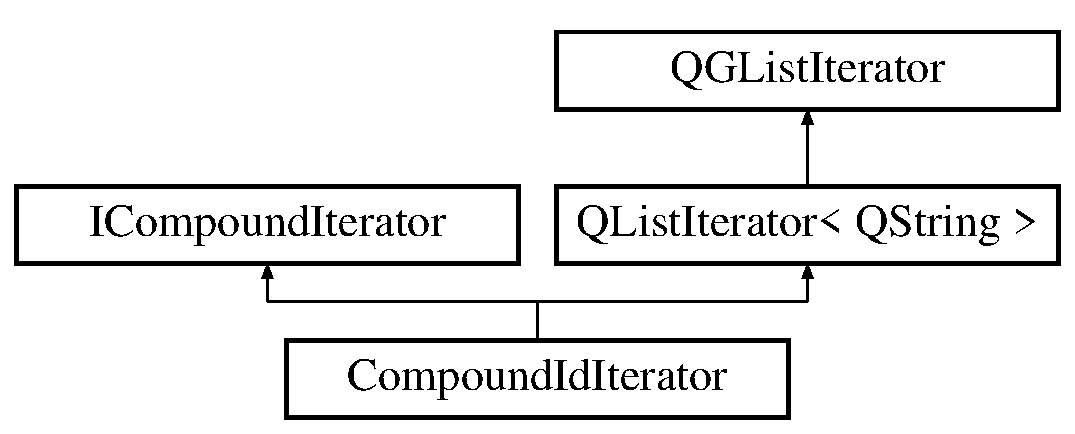
\includegraphics[height=3.000000cm]{class_compound_id_iterator}
\end{center}
\end{figure}
\subsection*{Membros públicos}
\begin{DoxyCompactItemize}
\item 
\hypertarget{class_compound_id_iterator_a9dd0b4d60acc882ad19e850d97db1962}{{\bfseries Compound\-Id\-Iterator} (const \hyperlink{class_main_handler}{Main\-Handler} $\ast$m, const \hyperlink{class_q_list}{Q\-List}$<$ \hyperlink{class_q_string}{Q\-String} $>$ \&list)}\label{class_compound_id_iterator_a9dd0b4d60acc882ad19e850d97db1962}

\item 
\hypertarget{class_compound_id_iterator_a24528c52410032763cedaccdfbe474e5}{virtual void {\bfseries to\-First} ()}\label{class_compound_id_iterator_a24528c52410032763cedaccdfbe474e5}

\item 
\hypertarget{class_compound_id_iterator_ac4e23694db19ee84c4e110f9965d64e4}{virtual void {\bfseries to\-Last} ()}\label{class_compound_id_iterator_ac4e23694db19ee84c4e110f9965d64e4}

\item 
\hypertarget{class_compound_id_iterator_ad8ecebd1a267185e69e1b6fe4e9f331e}{virtual void {\bfseries to\-Next} ()}\label{class_compound_id_iterator_ad8ecebd1a267185e69e1b6fe4e9f331e}

\item 
\hypertarget{class_compound_id_iterator_a3491dc4d8ab54f0a0583ac1941f4e94f}{virtual void {\bfseries to\-Prev} ()}\label{class_compound_id_iterator_a3491dc4d8ab54f0a0583ac1941f4e94f}

\item 
\hypertarget{class_compound_id_iterator_aed1ddf0744f763ffafe54f63da2080bb}{virtual \hyperlink{class_i_compound}{I\-Compound} $\ast$ {\bfseries current} () const }\label{class_compound_id_iterator_aed1ddf0744f763ffafe54f63da2080bb}

\item 
\hypertarget{class_compound_id_iterator_af8a84115de3507728d5e19e804529052}{virtual void {\bfseries release} ()}\label{class_compound_id_iterator_af8a84115de3507728d5e19e804529052}

\end{DoxyCompactItemize}
\subsection*{Additional Inherited Members}


A documentação para esta classe foi gerada a partir do seguinte ficheiro\-:\begin{DoxyCompactItemize}
\item 
C\-:/\-Users/teste/git/doxygen/addon/doxmlparser/src/compoundhandler.\-cpp\end{DoxyCompactItemize}

\hypertarget{class_compound_type_map}{\section{Referência à classe Compound\-Type\-Map}
\label{class_compound_type_map}\index{Compound\-Type\-Map@{Compound\-Type\-Map}}
}
\subsection*{Membros públicos}
\begin{DoxyCompactItemize}
\item 
\hypertarget{class_compound_type_map_a339e9c387c88db18ff5ad898ce3dcd05}{\hyperlink{class_i_compound_a7063885b1cabbff5f94849960f08ecb2}{I\-Compound\-::\-Compound\-Kind} {\bfseries map} (const \hyperlink{class_q_string}{Q\-String} \&s)}\label{class_compound_type_map_a339e9c387c88db18ff5ad898ce3dcd05}

\end{DoxyCompactItemize}


A documentação para esta classe foi gerada a partir do seguinte ficheiro\-:\begin{DoxyCompactItemize}
\item 
C\-:/\-Users/teste/git/doxygen/addon/doxmlparser/src/compoundhandler.\-cpp\end{DoxyCompactItemize}

\hypertarget{class_cond_parser}{\section{Referência à classe Cond\-Parser}
\label{class_cond_parser}\index{Cond\-Parser@{Cond\-Parser}}
}


{\ttfamily \#include $<$condparser.\-h$>$}

\subsection*{Membros públicos}
\begin{DoxyCompactItemize}
\item 
bool \hyperlink{class_cond_parser_ac06db5920f40e75c0788dd7978d3c1ae}{parse} (const char $\ast$file\-Name, int line\-Nr, const char $\ast$expr)
\end{DoxyCompactItemize}


\subsection{Descrição detalhada}
Copyright (\hyperlink{class_c}{C}) 1997-\/2013 by Dimitri van Heesch.

Permission to use, copy, modify, and distribute this software and its documentation under the terms of the G\-N\-U General Public License is hereby granted. No representations are made about the suitability of this software for any purpose. It is provided \char`\"{}as is\char`\"{} without express or implied warranty. See the G\-N\-U General Public License for more details.

Documents produced by \hyperlink{class_doxygen}{Doxygen} are derivative works derived from the input used in their production; they are not affected by this license.

C++ Expression parser for E\-X\-T\-A\-B\-L\-E\-D\-\_\-\-S\-E\-T\-I\-O\-N\-S in \hyperlink{class_doxygen}{Doxygen}

Features used\-: Operators\-: \&\& A\-N\-D operator $|$$|$ O\-R operator ! N\-O\-T operator 

\subsection{Documentação dos métodos}
\hypertarget{class_cond_parser_ac06db5920f40e75c0788dd7978d3c1ae}{\index{Cond\-Parser@{Cond\-Parser}!parse@{parse}}
\index{parse@{parse}!CondParser@{Cond\-Parser}}
\subsubsection[{parse}]{\setlength{\rightskip}{0pt plus 5cm}bool parse (
\begin{DoxyParamCaption}
\item[{const char $\ast$}]{file\-Name, }
\item[{int}]{line\-Nr, }
\item[{const char $\ast$}]{expr}
\end{DoxyParamCaption}
)}}\label{class_cond_parser_ac06db5920f40e75c0788dd7978d3c1ae}
Copyright (\hyperlink{class_c}{C}) 1997-\/2013 by Dimitri van Heesch.

Permission to use, copy, modify, and distribute this software and its documentation under the terms of the G\-N\-U General Public License is hereby granted. No representations are made about the suitability of this software for any purpose. It is provided \char`\"{}as is\char`\"{} without express or implied warranty. See the G\-N\-U General Public License for more details.

Documents produced by \hyperlink{class_doxygen}{Doxygen} are derivative works derived from the input used in their production; they are not affected by this license.

C++ Expression parser for E\-N\-A\-B\-L\-E\-D\-\_\-\-S\-E\-C\-T\-I\-O\-N\-S in \hyperlink{class_doxygen}{Doxygen}

Features used\-: Operators\-: \&\& A\-N\-D operator $|$$|$ O\-R operator ! N\-O\-T operator parses and evaluates the given expression. \begin{DoxyReturn}{Retorna}

\begin{DoxyItemize}
\item On error, an error message is returned.
\item On success, the result of the expression is either \char`\"{}1\char`\"{} or \char`\"{}0\char`\"{}. 
\end{DoxyItemize}
\end{DoxyReturn}


A documentação para esta classe foi gerada a partir dos seguintes ficheiros\-:\begin{DoxyCompactItemize}
\item 
C\-:/\-Users/teste/git/doxygen/src/condparser.\-h\item 
C\-:/\-Users/teste/git/doxygen/src/condparser.\-cpp\end{DoxyCompactItemize}

\hypertarget{class_config}{\section{Referência à classe Config}
\label{class_config}\index{Config@{Config}}
}


{\ttfamily \#include $<$config.\-h$>$}

\subsection*{Membros públicos}
\begin{DoxyCompactItemize}
\item 
\hyperlink{class_q_list_iterator}{Q\-List\-Iterator}$<$ \hyperlink{class_config_option}{Config\-Option} $>$ \hyperlink{class_config_a2a73a36bdb15195ceea5babf0895841e}{iterator} ()
\item 
void \hyperlink{class_config_a50b1ad2951f80e9cf5021f47bad210a5}{write\-Template} (\hyperlink{class_f_text_stream}{F\-Text\-Stream} \&t, bool short\-Index, bool update\-Only)
\item 
\hypertarget{class_config_a83d1589d35495f9e66971b911650cc7e}{void {\bfseries set\-Header} (const char $\ast$header)}\label{class_config_a83d1589d35495f9e66971b911650cc7e}

\item 
void \hyperlink{class_config_adf2580bb1cb265aed049fd1553c658c2}{convert\-Str\-To\-Val} ()
\item 
void \hyperlink{class_config_a3556bfbc11af507151d5e7b2fcfdf181}{substitute\-Environment\-Vars} ()
\item 
void \hyperlink{class_config_a83f8adca24e250bfb5c9a90a35503ae9}{check} ()
\item 
void \hyperlink{class_config_a02fd73d861ef2e4aabb38c0c9ff82947}{init} ()
\item 
bool \hyperlink{class_config_a106dcaa73bd7f5e08ecc8889d607cf12}{parse\-String} (const char $\ast$fn, const char $\ast$str)
\item 
bool \hyperlink{class_config_a2b817186f44e966ea05461d71babaa57}{parse} (const char $\ast$fn)
\item 
void \hyperlink{class_config_ae2ee59f7cc16ee42559c87e81c433039}{create} ()
\item 
void \hyperlink{class_config_ae02f59400e5a733fbe447cb67c6bd3aa}{append\-User\-Comment} (const \hyperlink{class_q_c_string}{Q\-C\-String} \&u)
\item 
\hyperlink{class_q_c_string}{Q\-C\-String} \hyperlink{class_config_a0e741f180f15929a29642359da844226}{take\-User\-Comment} ()
\end{DoxyCompactItemize}
\begin{Indent}{\bf Getting configuration values.}\par
\begin{DoxyCompactItemize}
\item 
\hyperlink{class_q_c_string}{Q\-C\-String} \& \hyperlink{class_config_a68612104bbf38f8e3f73d777f3bd641a}{get\-String} (const char $\ast$file\-Name, int num, const char $\ast$name) const 
\item 
\hyperlink{class_q_str_list}{Q\-Str\-List} \& \hyperlink{class_config_a8fb1a4b9d3bc2c3d7712d24526fea32d}{get\-List} (const char $\ast$file\-Name, int num, const char $\ast$name) const 
\item 
\hyperlink{class_q_c_string}{Q\-C\-String} \& \hyperlink{class_config_a84395f0a27ff06a395259b1aa1376433}{get\-Enum} (const char $\ast$file\-Name, int num, const char $\ast$name) const 
\item 
int \& \hyperlink{class_config_a0adeb5980707ff5556cbd43458e69b93}{get\-Int} (const char $\ast$file\-Name, int num, const char $\ast$name) const 
\item 
bool \& \hyperlink{class_config_a4636caa43638b30b87018ae139570f86}{get\-Bool} (const char $\ast$file\-Name, int num, const char $\ast$name) const 
\item 
\hyperlink{class_config_option}{Config\-Option} $\ast$ \hyperlink{class_config_a3e7953f08471ba22fa4da26a7f0042ed}{get} (const char $\ast$name) const 
\end{DoxyCompactItemize}
\end{Indent}
\begin{Indent}{\bf Adding configuration options.}\par
\begin{DoxyCompactItemize}
\item 
\hyperlink{class_config_info}{Config\-Info} $\ast$ \hyperlink{class_config_adad7d76c6e3e07109796a5ffb9f2c6e4}{add\-Info} (const char $\ast$name, const char $\ast$doc)
\item 
\hyperlink{class_config_string}{Config\-String} $\ast$ \hyperlink{class_config_a74b8275821f367fd0c588ccc223d8696}{add\-String} (const char $\ast$name, const char $\ast$doc)
\item 
\hyperlink{class_config_enum}{Config\-Enum} $\ast$ \hyperlink{class_config_ab3913dcc45810d5073e967a99fe0c2a4}{add\-Enum} (const char $\ast$name, const char $\ast$doc, const char $\ast$def\-Val)
\item 
\hyperlink{class_config_list}{Config\-List} $\ast$ \hyperlink{class_config_a9566fc8a9d1560eb4181b7e245f6ce96}{add\-List} (const char $\ast$name, const char $\ast$doc)
\item 
\hyperlink{class_config_int}{Config\-Int} $\ast$ \hyperlink{class_config_abb7be086fa3130874a722a5a9c30b308}{add\-Int} (const char $\ast$name, const char $\ast$doc, int min\-Val, int max\-Val, int def\-Val)
\item 
\hyperlink{class_config_bool}{Config\-Bool} $\ast$ \hyperlink{class_config_aa80cc6d1590c228000e21e7c0682f5b9}{add\-Bool} (const char $\ast$name, const char $\ast$doc, bool def\-Val)
\item 
\hyperlink{class_config_option}{Config\-Option} $\ast$ \hyperlink{class_config_aeef352ac0af92d9f5df0074aa74d0884}{add\-Obsolete} (const char $\ast$name)
\item 
\hyperlink{class_config_option}{Config\-Option} $\ast$ \hyperlink{class_config_a42614c703f049d415636dd0346ec0314}{add\-Disabled} (const char $\ast$name)
\end{DoxyCompactItemize}
\end{Indent}
\subsection*{Membros públicos estáticos}
\begin{DoxyCompactItemize}
\item 
static \hyperlink{class_config}{Config} $\ast$ \hyperlink{class_config_aa6def1c3b3abfdaa0df22df0b558c94d}{instance} ()
\item 
static void \hyperlink{class_config_a5946f8823f24f5bd2b1749d912ea8ba7}{delete\-Instance} ()
\end{DoxyCompactItemize}


\subsection{Descrição detalhada}
Singleton for configuration variables.

This object holds the global static variables read from a user-\/supplied configuration file. The static member \hyperlink{class_config_aa6def1c3b3abfdaa0df22df0b558c94d}{instance()} can be used to get a pointer to the one and only instance.

Set all variables to their default values by calling \hyperlink{class_config_aa6def1c3b3abfdaa0df22df0b558c94d}{Config\-::instance()}-\/$>$\hyperlink{class_config_a02fd73d861ef2e4aabb38c0c9ff82947}{init()} 

\subsection{Documentação dos métodos}
\hypertarget{class_config_aa80cc6d1590c228000e21e7c0682f5b9}{\index{Config@{Config}!add\-Bool@{add\-Bool}}
\index{add\-Bool@{add\-Bool}!Config@{Config}}
\subsubsection[{add\-Bool}]{\setlength{\rightskip}{0pt plus 5cm}{\bf Config\-Bool}$\ast$ add\-Bool (
\begin{DoxyParamCaption}
\item[{const char $\ast$}]{name, }
\item[{const char $\ast$}]{doc, }
\item[{bool}]{def\-Val}
\end{DoxyParamCaption}
)\hspace{0.3cm}{\ttfamily [inline]}}}\label{class_config_aa80cc6d1590c228000e21e7c0682f5b9}
Adds a new boolean option with {\itshape name} and documentation {\itshape doc}. The boolean has a default value of {\itshape def\-Val}. \begin{DoxyReturn}{Retorna}
An object representing the option. 
\end{DoxyReturn}
\hypertarget{class_config_a42614c703f049d415636dd0346ec0314}{\index{Config@{Config}!add\-Disabled@{add\-Disabled}}
\index{add\-Disabled@{add\-Disabled}!Config@{Config}}
\subsubsection[{add\-Disabled}]{\setlength{\rightskip}{0pt plus 5cm}{\bf Config\-Option}$\ast$ add\-Disabled (
\begin{DoxyParamCaption}
\item[{const char $\ast$}]{name}
\end{DoxyParamCaption}
)\hspace{0.3cm}{\ttfamily [inline]}}}\label{class_config_a42614c703f049d415636dd0346ec0314}
Adds an option that has been disabled at compile time. \hypertarget{class_config_ab3913dcc45810d5073e967a99fe0c2a4}{\index{Config@{Config}!add\-Enum@{add\-Enum}}
\index{add\-Enum@{add\-Enum}!Config@{Config}}
\subsubsection[{add\-Enum}]{\setlength{\rightskip}{0pt plus 5cm}{\bf Config\-Enum}$\ast$ add\-Enum (
\begin{DoxyParamCaption}
\item[{const char $\ast$}]{name, }
\item[{const char $\ast$}]{doc, }
\item[{const char $\ast$}]{def\-Val}
\end{DoxyParamCaption}
)\hspace{0.3cm}{\ttfamily [inline]}}}\label{class_config_ab3913dcc45810d5073e967a99fe0c2a4}
Adds a new enumeration option with {\itshape name} and documentation {\itshape doc} and initial value {\itshape def\-Val}. \begin{DoxyReturn}{Retorna}
An object representing the option. 
\end{DoxyReturn}
\hypertarget{class_config_adad7d76c6e3e07109796a5ffb9f2c6e4}{\index{Config@{Config}!add\-Info@{add\-Info}}
\index{add\-Info@{add\-Info}!Config@{Config}}
\subsubsection[{add\-Info}]{\setlength{\rightskip}{0pt plus 5cm}{\bf Config\-Info}$\ast$ add\-Info (
\begin{DoxyParamCaption}
\item[{const char $\ast$}]{name, }
\item[{const char $\ast$}]{doc}
\end{DoxyParamCaption}
)\hspace{0.3cm}{\ttfamily [inline]}}}\label{class_config_adad7d76c6e3e07109796a5ffb9f2c6e4}
Starts a new configuration section with {\itshape name} and description {\itshape doc}. \begin{DoxyReturn}{Retorna}
An object representing the option. 
\end{DoxyReturn}
\hypertarget{class_config_abb7be086fa3130874a722a5a9c30b308}{\index{Config@{Config}!add\-Int@{add\-Int}}
\index{add\-Int@{add\-Int}!Config@{Config}}
\subsubsection[{add\-Int}]{\setlength{\rightskip}{0pt plus 5cm}{\bf Config\-Int}$\ast$ add\-Int (
\begin{DoxyParamCaption}
\item[{const char $\ast$}]{name, }
\item[{const char $\ast$}]{doc, }
\item[{int}]{min\-Val, }
\item[{int}]{max\-Val, }
\item[{int}]{def\-Val}
\end{DoxyParamCaption}
)\hspace{0.3cm}{\ttfamily [inline]}}}\label{class_config_abb7be086fa3130874a722a5a9c30b308}
Adds a new integer option with {\itshape name} and documentation {\itshape doc}. The integer has a range between {\itshape min\-Val} and {\itshape max\-Val} and a default value of {\itshape def\-Val}. \begin{DoxyReturn}{Retorna}
An object representing the option. 
\end{DoxyReturn}
\hypertarget{class_config_a9566fc8a9d1560eb4181b7e245f6ce96}{\index{Config@{Config}!add\-List@{add\-List}}
\index{add\-List@{add\-List}!Config@{Config}}
\subsubsection[{add\-List}]{\setlength{\rightskip}{0pt plus 5cm}{\bf Config\-List}$\ast$ add\-List (
\begin{DoxyParamCaption}
\item[{const char $\ast$}]{name, }
\item[{const char $\ast$}]{doc}
\end{DoxyParamCaption}
)\hspace{0.3cm}{\ttfamily [inline]}}}\label{class_config_a9566fc8a9d1560eb4181b7e245f6ce96}
Adds a new string option with {\itshape name} and documentation {\itshape doc}. \begin{DoxyReturn}{Retorna}
An object representing the option. 
\end{DoxyReturn}
\hypertarget{class_config_aeef352ac0af92d9f5df0074aa74d0884}{\index{Config@{Config}!add\-Obsolete@{add\-Obsolete}}
\index{add\-Obsolete@{add\-Obsolete}!Config@{Config}}
\subsubsection[{add\-Obsolete}]{\setlength{\rightskip}{0pt plus 5cm}{\bf Config\-Option}$\ast$ add\-Obsolete (
\begin{DoxyParamCaption}
\item[{const char $\ast$}]{name}
\end{DoxyParamCaption}
)\hspace{0.3cm}{\ttfamily [inline]}}}\label{class_config_aeef352ac0af92d9f5df0074aa74d0884}
Adds an option that has become obsolete. \hypertarget{class_config_a74b8275821f367fd0c588ccc223d8696}{\index{Config@{Config}!add\-String@{add\-String}}
\index{add\-String@{add\-String}!Config@{Config}}
\subsubsection[{add\-String}]{\setlength{\rightskip}{0pt plus 5cm}{\bf Config\-String}$\ast$ add\-String (
\begin{DoxyParamCaption}
\item[{const char $\ast$}]{name, }
\item[{const char $\ast$}]{doc}
\end{DoxyParamCaption}
)\hspace{0.3cm}{\ttfamily [inline]}}}\label{class_config_a74b8275821f367fd0c588ccc223d8696}
Adds a new string option with {\itshape name} and documentation {\itshape doc}. \begin{DoxyReturn}{Retorna}
An object representing the option. 
\end{DoxyReturn}
\hypertarget{class_config_ae02f59400e5a733fbe447cb67c6bd3aa}{\index{Config@{Config}!append\-User\-Comment@{append\-User\-Comment}}
\index{append\-User\-Comment@{append\-User\-Comment}!Config@{Config}}
\subsubsection[{append\-User\-Comment}]{\setlength{\rightskip}{0pt plus 5cm}void append\-User\-Comment (
\begin{DoxyParamCaption}
\item[{const {\bf Q\-C\-String} \&}]{u}
\end{DoxyParamCaption}
)\hspace{0.3cm}{\ttfamily [inline]}}}\label{class_config_ae02f59400e5a733fbe447cb67c6bd3aa}
Append user comment \hypertarget{class_config_a83f8adca24e250bfb5c9a90a35503ae9}{\index{Config@{Config}!check@{check}}
\index{check@{check}!Config@{Config}}
\subsubsection[{check}]{\setlength{\rightskip}{0pt plus 5cm}void check (
\begin{DoxyParamCaption}
{}
\end{DoxyParamCaption}
)}}\label{class_config_a83f8adca24e250bfb5c9a90a35503ae9}
Checks if the values of the variable are correct, adjusts them if needed, and report any errors. \hypertarget{class_config_adf2580bb1cb265aed049fd1553c658c2}{\index{Config@{Config}!convert\-Str\-To\-Val@{convert\-Str\-To\-Val}}
\index{convert\-Str\-To\-Val@{convert\-Str\-To\-Val}!Config@{Config}}
\subsubsection[{convert\-Str\-To\-Val}]{\setlength{\rightskip}{0pt plus 5cm}void convert\-Str\-To\-Val (
\begin{DoxyParamCaption}
{}
\end{DoxyParamCaption}
)}}\label{class_config_adf2580bb1cb265aed049fd1553c658c2}
Converts the string values read from the configuration file to real values for non-\/string type options (like int, and bools) \hypertarget{class_config_ae2ee59f7cc16ee42559c87e81c433039}{\index{Config@{Config}!create@{create}}
\index{create@{create}!Config@{Config}}
\subsubsection[{create}]{\setlength{\rightskip}{0pt plus 5cm}void create (
\begin{DoxyParamCaption}
{}
\end{DoxyParamCaption}
)}}\label{class_config_ae2ee59f7cc16ee42559c87e81c433039}
Called from the constructor, will add doxygen's default options to the configuration object \hypertarget{class_config_a5946f8823f24f5bd2b1749d912ea8ba7}{\index{Config@{Config}!delete\-Instance@{delete\-Instance}}
\index{delete\-Instance@{delete\-Instance}!Config@{Config}}
\subsubsection[{delete\-Instance}]{\setlength{\rightskip}{0pt plus 5cm}static void delete\-Instance (
\begin{DoxyParamCaption}
{}
\end{DoxyParamCaption}
)\hspace{0.3cm}{\ttfamily [inline]}, {\ttfamily [static]}}}\label{class_config_a5946f8823f24f5bd2b1749d912ea8ba7}
Delete the instance \hypertarget{class_config_a3e7953f08471ba22fa4da26a7f0042ed}{\index{Config@{Config}!get@{get}}
\index{get@{get}!Config@{Config}}
\subsubsection[{get}]{\setlength{\rightskip}{0pt plus 5cm}{\bf Config\-Option}$\ast$ get (
\begin{DoxyParamCaption}
\item[{const char $\ast$}]{name}
\end{DoxyParamCaption}
) const\hspace{0.3cm}{\ttfamily [inline]}}}\label{class_config_a3e7953f08471ba22fa4da26a7f0042ed}
Returns the \hyperlink{class_config_option}{Config\-Option} corresponding with {\itshape name} or 0 if the option is not supported. \hypertarget{class_config_a4636caa43638b30b87018ae139570f86}{\index{Config@{Config}!get\-Bool@{get\-Bool}}
\index{get\-Bool@{get\-Bool}!Config@{Config}}
\subsubsection[{get\-Bool}]{\setlength{\rightskip}{0pt plus 5cm}bool\& get\-Bool (
\begin{DoxyParamCaption}
\item[{const char $\ast$}]{file\-Name, }
\item[{int}]{num, }
\item[{const char $\ast$}]{name}
\end{DoxyParamCaption}
) const}}\label{class_config_a4636caa43638b30b87018ae139570f86}
Returns the value of the boolean option with name {\itshape file\-Name}. The arguments {\itshape num} and {\itshape name} are for debugging purposes only. There is a convenience function Config\-\_\-get\-Bool() for this. \hypertarget{class_config_a84395f0a27ff06a395259b1aa1376433}{\index{Config@{Config}!get\-Enum@{get\-Enum}}
\index{get\-Enum@{get\-Enum}!Config@{Config}}
\subsubsection[{get\-Enum}]{\setlength{\rightskip}{0pt plus 5cm}{\bf Q\-C\-String}\& get\-Enum (
\begin{DoxyParamCaption}
\item[{const char $\ast$}]{file\-Name, }
\item[{int}]{num, }
\item[{const char $\ast$}]{name}
\end{DoxyParamCaption}
) const}}\label{class_config_a84395f0a27ff06a395259b1aa1376433}
Returns the value of the enum option with name {\itshape file\-Name}. The arguments {\itshape num} and {\itshape name} are for debugging purposes only. There is a convenience function Config\-\_\-get\-Enum() for this. \hypertarget{class_config_a0adeb5980707ff5556cbd43458e69b93}{\index{Config@{Config}!get\-Int@{get\-Int}}
\index{get\-Int@{get\-Int}!Config@{Config}}
\subsubsection[{get\-Int}]{\setlength{\rightskip}{0pt plus 5cm}int\& get\-Int (
\begin{DoxyParamCaption}
\item[{const char $\ast$}]{file\-Name, }
\item[{int}]{num, }
\item[{const char $\ast$}]{name}
\end{DoxyParamCaption}
) const}}\label{class_config_a0adeb5980707ff5556cbd43458e69b93}
Returns the value of the integer option with name {\itshape file\-Name}. The arguments {\itshape num} and {\itshape name} are for debugging purposes only. There is a convenience function Config\-\_\-get\-Int() for this. \hypertarget{class_config_a8fb1a4b9d3bc2c3d7712d24526fea32d}{\index{Config@{Config}!get\-List@{get\-List}}
\index{get\-List@{get\-List}!Config@{Config}}
\subsubsection[{get\-List}]{\setlength{\rightskip}{0pt plus 5cm}{\bf Q\-Str\-List}\& get\-List (
\begin{DoxyParamCaption}
\item[{const char $\ast$}]{file\-Name, }
\item[{int}]{num, }
\item[{const char $\ast$}]{name}
\end{DoxyParamCaption}
) const}}\label{class_config_a8fb1a4b9d3bc2c3d7712d24526fea32d}
Returns the value of the list option with name {\itshape file\-Name}. The arguments {\itshape num} and {\itshape name} are for debugging purposes only. There is a convenience function Config\-\_\-get\-List() for this. \hypertarget{class_config_a68612104bbf38f8e3f73d777f3bd641a}{\index{Config@{Config}!get\-String@{get\-String}}
\index{get\-String@{get\-String}!Config@{Config}}
\subsubsection[{get\-String}]{\setlength{\rightskip}{0pt plus 5cm}{\bf Q\-C\-String}\& get\-String (
\begin{DoxyParamCaption}
\item[{const char $\ast$}]{file\-Name, }
\item[{int}]{num, }
\item[{const char $\ast$}]{name}
\end{DoxyParamCaption}
) const}}\label{class_config_a68612104bbf38f8e3f73d777f3bd641a}
Returns the value of the string option with name {\itshape file\-Name}. The arguments {\itshape num} and {\itshape name} are for debugging purposes only. There is a convenience function Config\-\_\-get\-String() for this. \hypertarget{class_config_a02fd73d861ef2e4aabb38c0c9ff82947}{\index{Config@{Config}!init@{init}}
\index{init@{init}!Config@{Config}}
\subsubsection[{init}]{\setlength{\rightskip}{0pt plus 5cm}void init (
\begin{DoxyParamCaption}
{}
\end{DoxyParamCaption}
)}}\label{class_config_a02fd73d861ef2e4aabb38c0c9ff82947}
Initialize config variables to their default value \hypertarget{class_config_aa6def1c3b3abfdaa0df22df0b558c94d}{\index{Config@{Config}!instance@{instance}}
\index{instance@{instance}!Config@{Config}}
\subsubsection[{instance}]{\setlength{\rightskip}{0pt plus 5cm}static {\bf Config}$\ast$ instance (
\begin{DoxyParamCaption}
{}
\end{DoxyParamCaption}
)\hspace{0.3cm}{\ttfamily [inline]}, {\ttfamily [static]}}}\label{class_config_aa6def1c3b3abfdaa0df22df0b558c94d}
Returns the one and only instance of this class \hypertarget{class_config_a2a73a36bdb15195ceea5babf0895841e}{\index{Config@{Config}!iterator@{iterator}}
\index{iterator@{iterator}!Config@{Config}}
\subsubsection[{iterator}]{\setlength{\rightskip}{0pt plus 5cm}{\bf Q\-List\-Iterator}$<${\bf Config\-Option}$>$ iterator (
\begin{DoxyParamCaption}
{}
\end{DoxyParamCaption}
)\hspace{0.3cm}{\ttfamily [inline]}}}\label{class_config_a2a73a36bdb15195ceea5babf0895841e}
Returns an iterator that can by used to iterate over the configuration options. \hypertarget{class_config_a2b817186f44e966ea05461d71babaa57}{\index{Config@{Config}!parse@{parse}}
\index{parse@{parse}!Config@{Config}}
\subsubsection[{parse}]{\setlength{\rightskip}{0pt plus 5cm}bool parse (
\begin{DoxyParamCaption}
\item[{const char $\ast$}]{fn}
\end{DoxyParamCaption}
)}}\label{class_config_a2b817186f44e966ea05461d71babaa57}
Parse a configuration file with name {\itshape fn}. \begin{DoxyReturn}{Retorna}
T\-R\-U\-E if successful, F\-A\-L\-S\-E if the file could not be opened or read. 
\end{DoxyReturn}
\hypertarget{class_config_a106dcaa73bd7f5e08ecc8889d607cf12}{\index{Config@{Config}!parse\-String@{parse\-String}}
\index{parse\-String@{parse\-String}!Config@{Config}}
\subsubsection[{parse\-String}]{\setlength{\rightskip}{0pt plus 5cm}bool parse\-String (
\begin{DoxyParamCaption}
\item[{const char $\ast$}]{fn, }
\item[{const char $\ast$}]{str}
\end{DoxyParamCaption}
)}}\label{class_config_a106dcaa73bd7f5e08ecc8889d607cf12}
Parse a configuration data in string {\itshape str}. \begin{DoxyReturn}{Retorna}
T\-R\-U\-E if successful, or F\-A\-L\-S\-E if the string could not be parsed. 
\end{DoxyReturn}
\hypertarget{class_config_a3556bfbc11af507151d5e7b2fcfdf181}{\index{Config@{Config}!substitute\-Environment\-Vars@{substitute\-Environment\-Vars}}
\index{substitute\-Environment\-Vars@{substitute\-Environment\-Vars}!Config@{Config}}
\subsubsection[{substitute\-Environment\-Vars}]{\setlength{\rightskip}{0pt plus 5cm}void substitute\-Environment\-Vars (
\begin{DoxyParamCaption}
{}
\end{DoxyParamCaption}
)}}\label{class_config_a3556bfbc11af507151d5e7b2fcfdf181}
Replaces references to environment variable by the actual value of the environment variable. \hypertarget{class_config_a0e741f180f15929a29642359da844226}{\index{Config@{Config}!take\-User\-Comment@{take\-User\-Comment}}
\index{take\-User\-Comment@{take\-User\-Comment}!Config@{Config}}
\subsubsection[{take\-User\-Comment}]{\setlength{\rightskip}{0pt plus 5cm}{\bf Q\-C\-String} take\-User\-Comment (
\begin{DoxyParamCaption}
{}
\end{DoxyParamCaption}
)\hspace{0.3cm}{\ttfamily [inline]}}}\label{class_config_a0e741f180f15929a29642359da844226}
Take the user comment and reset it internally \begin{DoxyReturn}{Retorna}
user comment 
\end{DoxyReturn}
\hypertarget{class_config_a50b1ad2951f80e9cf5021f47bad210a5}{\index{Config@{Config}!write\-Template@{write\-Template}}
\index{write\-Template@{write\-Template}!Config@{Config}}
\subsubsection[{write\-Template}]{\setlength{\rightskip}{0pt plus 5cm}void write\-Template (
\begin{DoxyParamCaption}
\item[{{\bf F\-Text\-Stream} \&}]{t, }
\item[{bool}]{short\-Index, }
\item[{bool}]{update\-Only}
\end{DoxyParamCaption}
)}}\label{class_config_a50b1ad2951f80e9cf5021f47bad210a5}
Writes a template configuration to stream {\itshape t}. If {\itshape short\-Index} is {\ttfamily T\-R\-U\-E} the description of each configuration option will be omitted. 

A documentação para esta classe foi gerada a partir do seguinte ficheiro\-:\begin{DoxyCompactItemize}
\item 
C\-:/\-Users/teste/git/doxygen/src/config.\-h\end{DoxyCompactItemize}

\hypertarget{class_config_bool}{\section{Referência à classe Config\-Bool}
\label{class_config_bool}\index{Config\-Bool@{Config\-Bool}}
}


{\ttfamily \#include $<$config.\-h$>$}

Diagrama de heranças da classe Config\-Bool\begin{figure}[H]
\begin{center}
\leavevmode
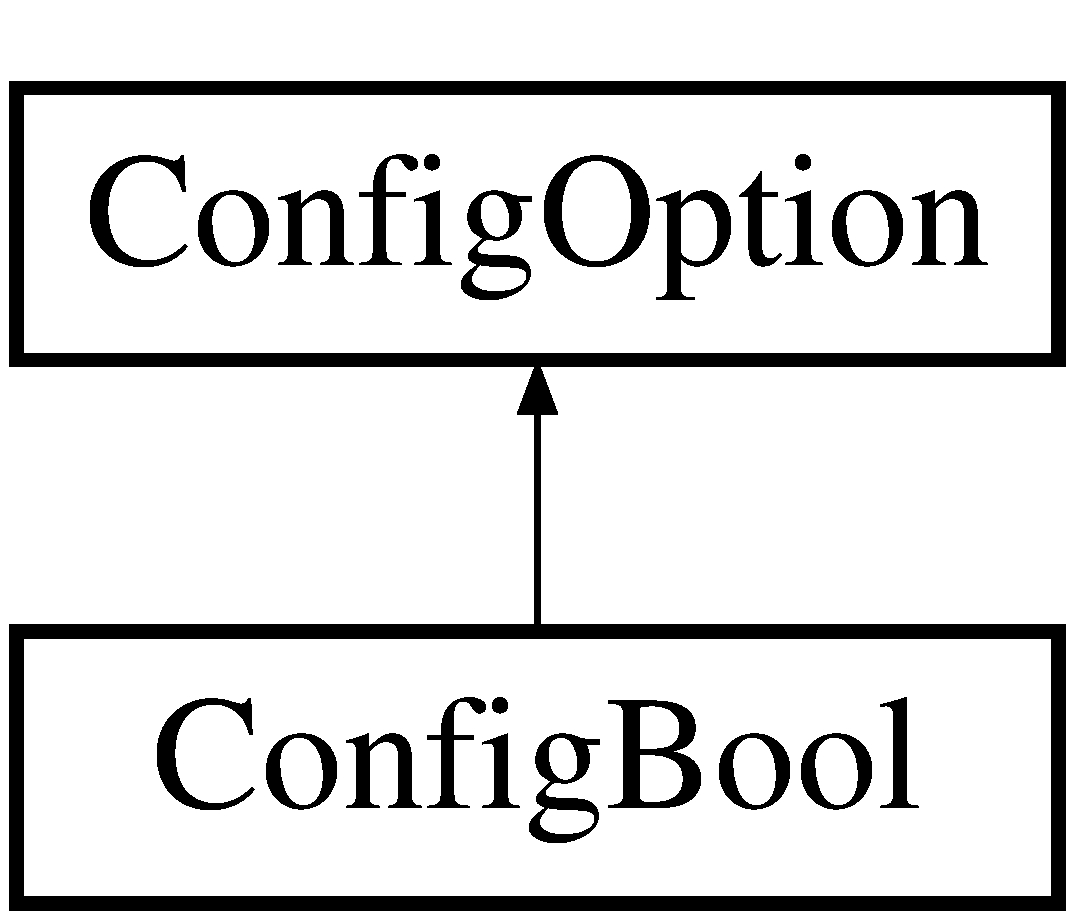
\includegraphics[height=2.000000cm]{class_config_bool}
\end{center}
\end{figure}
\subsection*{Membros públicos}
\begin{DoxyCompactItemize}
\item 
\hypertarget{class_config_bool_a3928df38242af64dde3e892e625f7e50}{{\bfseries Config\-Bool} (const char $\ast$name, const char $\ast$doc, bool def\-Val)}\label{class_config_bool_a3928df38242af64dde3e892e625f7e50}

\item 
\hypertarget{class_config_bool_a0c7ffe0fff991390d97a629f692a5854}{\hyperlink{class_q_c_string}{Q\-C\-String} $\ast$ {\bfseries value\-String\-Ref} ()}\label{class_config_bool_a0c7ffe0fff991390d97a629f692a5854}

\item 
\hypertarget{class_config_bool_a98f536bae72d94284a2d6edcbb2a1d49}{bool $\ast$ {\bfseries value\-Ref} ()}\label{class_config_bool_a98f536bae72d94284a2d6edcbb2a1d49}

\item 
\hypertarget{class_config_bool_adf2580bb1cb265aed049fd1553c658c2}{void {\bfseries convert\-Str\-To\-Val} ()}\label{class_config_bool_adf2580bb1cb265aed049fd1553c658c2}

\item 
\hypertarget{class_config_bool_a79866440425087f224d4f77311efad6a}{void {\bfseries subst\-Env\-Vars} ()}\label{class_config_bool_a79866440425087f224d4f77311efad6a}

\item 
\hypertarget{class_config_bool_ab42f4a444d994a5186f3f1c77c5444ad}{void {\bfseries set\-Value\-String} (const \hyperlink{class_q_c_string}{Q\-C\-String} \&v)}\label{class_config_bool_ab42f4a444d994a5186f3f1c77c5444ad}

\item 
\hypertarget{class_config_bool_a4972a64bbfa8f975c5704239e71c4811}{void {\bfseries write\-Template} (\hyperlink{class_f_text_stream}{F\-Text\-Stream} \&t, bool sl, bool upd)}\label{class_config_bool_a4972a64bbfa8f975c5704239e71c4811}

\item 
\hypertarget{class_config_bool_a02fd73d861ef2e4aabb38c0c9ff82947}{void {\bfseries init} ()}\label{class_config_bool_a02fd73d861ef2e4aabb38c0c9ff82947}

\end{DoxyCompactItemize}
\subsection*{Additional Inherited Members}


\subsection{Descrição detalhada}
Class representing a Boolean type option. 

A documentação para esta classe foi gerada a partir do seguinte ficheiro\-:\begin{DoxyCompactItemize}
\item 
C\-:/\-Users/teste/git/doxygen/src/config.\-h\end{DoxyCompactItemize}

\hypertarget{class_config_context}{\section{Referência à classe Config\-Context}
\label{class_config_context}\index{Config\-Context@{Config\-Context}}
}
Diagrama de heranças da classe Config\-Context\begin{figure}[H]
\begin{center}
\leavevmode
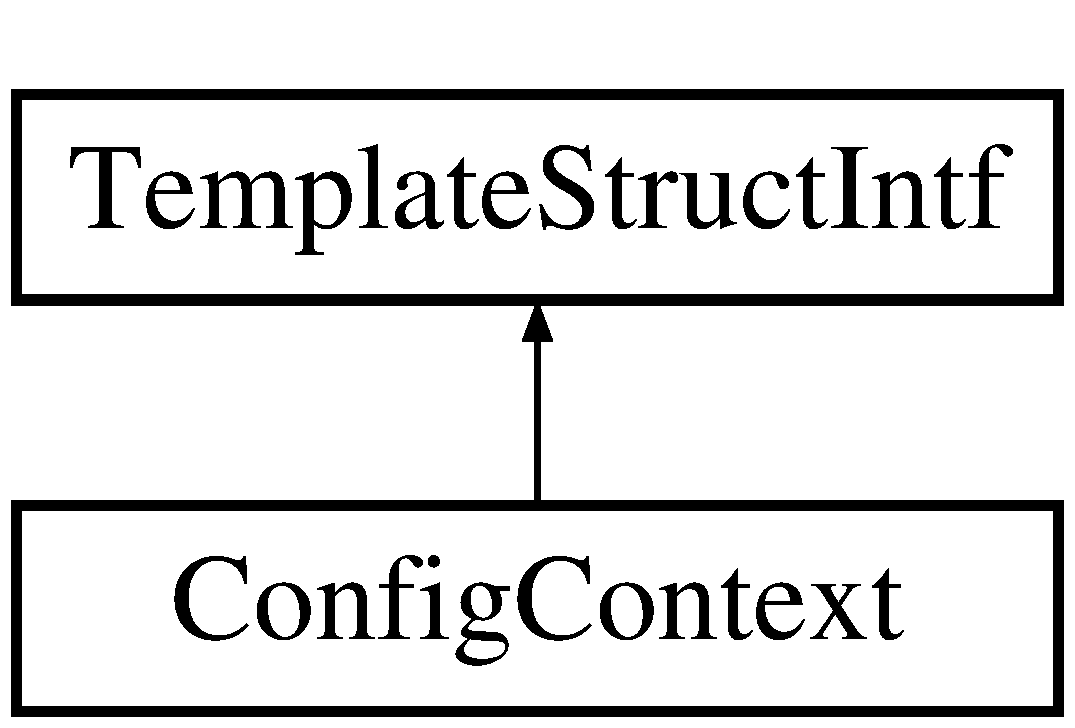
\includegraphics[height=2.000000cm]{class_config_context}
\end{center}
\end{figure}
\subsection*{Estruturas de Dados}
\begin{DoxyCompactItemize}
\item 
class \hyperlink{class_config_context_1_1_private}{Private}
\end{DoxyCompactItemize}
\subsection*{Membros públicos}
\begin{DoxyCompactItemize}
\item 
virtual \hyperlink{class_template_variant}{Template\-Variant} \hyperlink{class_config_context_a1bcfea01201f3ea09981a8442842c42d}{get} (const char $\ast$name) const 
\end{DoxyCompactItemize}


\subsection{Documentação dos métodos}
\hypertarget{class_config_context_a1bcfea01201f3ea09981a8442842c42d}{\index{Config\-Context@{Config\-Context}!get@{get}}
\index{get@{get}!ConfigContext@{Config\-Context}}
\subsubsection[{get}]{\setlength{\rightskip}{0pt plus 5cm}{\bf Template\-Variant} get (
\begin{DoxyParamCaption}
\item[{const char $\ast$}]{name}
\end{DoxyParamCaption}
) const\hspace{0.3cm}{\ttfamily [virtual]}}}\label{class_config_context_a1bcfea01201f3ea09981a8442842c42d}
Gets the value for a field name. 
\begin{DoxyParams}[1]{Parâmetros}
\mbox{\tt in}  & {\em name} & The name of the field. \\
\hline
\end{DoxyParams}


Implementa \hyperlink{class_template_struct_intf_a49a65a897ba5e4cd6cb80d681c843aab}{Template\-Struct\-Intf}.



A documentação para esta classe foi gerada a partir dos seguintes ficheiros\-:\begin{DoxyCompactItemize}
\item 
C\-:/\-Users/teste/git/doxygen/src/context.\-h\item 
C\-:/\-Users/teste/git/doxygen/src/context.\-cpp\end{DoxyCompactItemize}

\hypertarget{class_config_disabled}{\section{Referência à classe Config\-Disabled}
\label{class_config_disabled}\index{Config\-Disabled@{Config\-Disabled}}
}


{\ttfamily \#include $<$config.\-h$>$}

Diagrama de heranças da classe Config\-Disabled\begin{figure}[H]
\begin{center}
\leavevmode
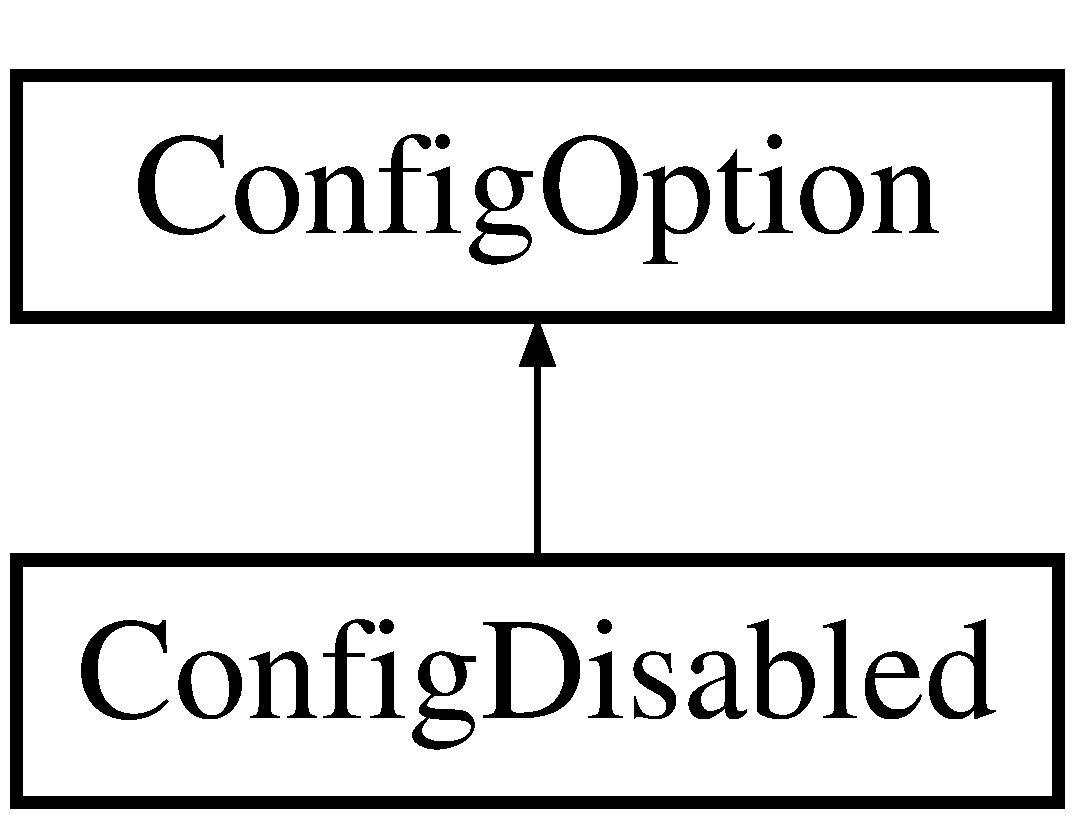
\includegraphics[height=2.000000cm]{class_config_disabled}
\end{center}
\end{figure}
\subsection*{Membros públicos}
\begin{DoxyCompactItemize}
\item 
\hypertarget{class_config_disabled_ab2755c9289b5146e929d7d9b7d7f86a2}{{\bfseries Config\-Disabled} (const char $\ast$name)}\label{class_config_disabled_ab2755c9289b5146e929d7d9b7d7f86a2}

\item 
\hypertarget{class_config_disabled_a7532aae29d4f94af257d952948ec64ca}{void {\bfseries write\-Template} (\hyperlink{class_f_text_stream}{F\-Text\-Stream} \&, bool, bool)}\label{class_config_disabled_a7532aae29d4f94af257d952948ec64ca}

\item 
\hypertarget{class_config_disabled_a79866440425087f224d4f77311efad6a}{void {\bfseries subst\-Env\-Vars} ()}\label{class_config_disabled_a79866440425087f224d4f77311efad6a}

\end{DoxyCompactItemize}
\subsection*{Additional Inherited Members}


\subsection{Descrição detalhada}
Section marker for compile time optional options 

A documentação para esta classe foi gerada a partir do seguinte ficheiro\-:\begin{DoxyCompactItemize}
\item 
C\-:/\-Users/teste/git/doxygen/src/config.\-h\end{DoxyCompactItemize}

\hypertarget{class_config_enum}{\section{Referência à classe Config\-Enum}
\label{class_config_enum}\index{Config\-Enum@{Config\-Enum}}
}


{\ttfamily \#include $<$config.\-h$>$}

Diagrama de heranças da classe Config\-Enum\begin{figure}[H]
\begin{center}
\leavevmode
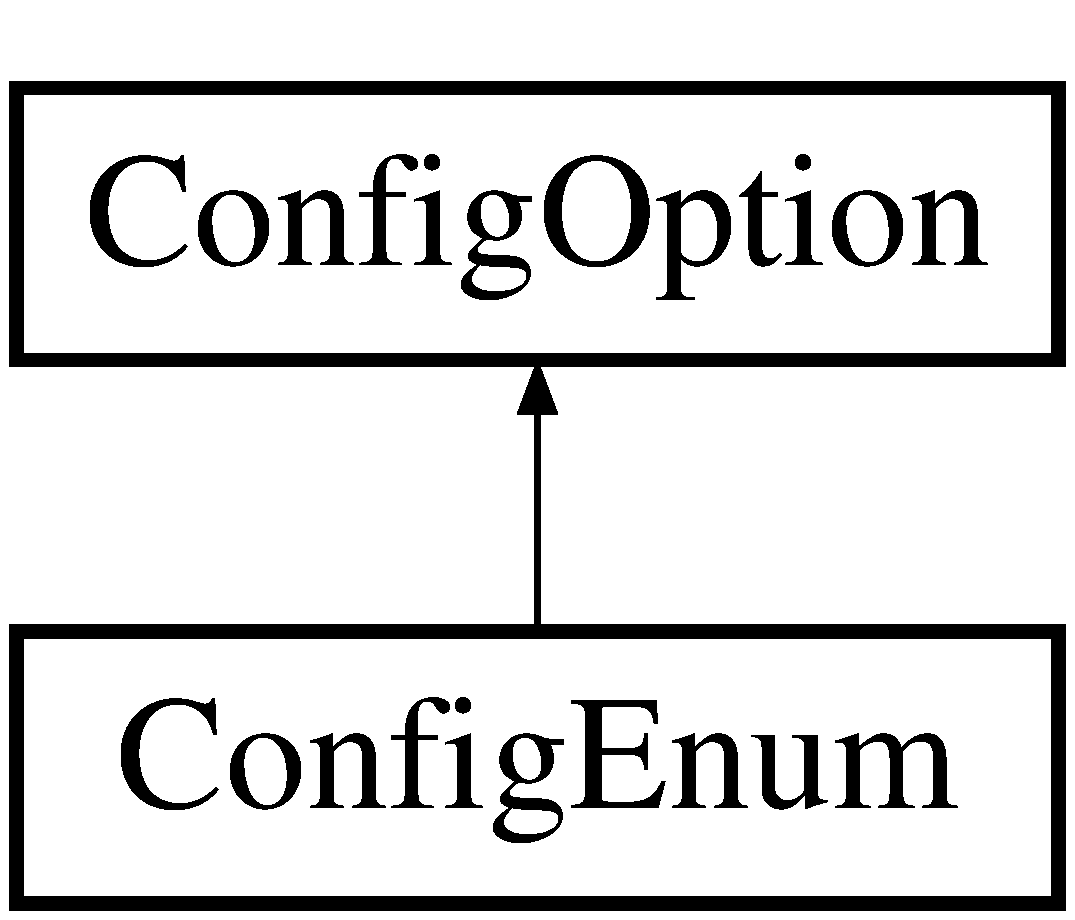
\includegraphics[height=2.000000cm]{class_config_enum}
\end{center}
\end{figure}
\subsection*{Membros públicos}
\begin{DoxyCompactItemize}
\item 
\hypertarget{class_config_enum_a6739260a09681cc4cfd7aab80fca2ebe}{{\bfseries Config\-Enum} (const char $\ast$name, const char $\ast$doc, const char $\ast$def\-Val)}\label{class_config_enum_a6739260a09681cc4cfd7aab80fca2ebe}

\item 
\hypertarget{class_config_enum_a6330b95a0b46d7452b8c0e7f61a523de}{void {\bfseries add\-Value} (const char $\ast$v)}\label{class_config_enum_a6330b95a0b46d7452b8c0e7f61a523de}

\item 
\hypertarget{class_config_enum_af993f7e0e41e6fe5975ee78724e46cdb}{\hyperlink{class_q_list_iterator}{Q\-Str\-List\-Iterator} {\bfseries iterator} ()}\label{class_config_enum_af993f7e0e41e6fe5975ee78724e46cdb}

\item 
\hypertarget{class_config_enum_a9c4fe5ca500670ba901c995ab38ec6c9}{\hyperlink{class_q_c_string}{Q\-C\-String} $\ast$ {\bfseries value\-Ref} ()}\label{class_config_enum_a9c4fe5ca500670ba901c995ab38ec6c9}

\item 
\hypertarget{class_config_enum_a79866440425087f224d4f77311efad6a}{void {\bfseries subst\-Env\-Vars} ()}\label{class_config_enum_a79866440425087f224d4f77311efad6a}

\item 
\hypertarget{class_config_enum_ad532b92c9971149d194403dff3458ba7}{void {\bfseries write\-Template} (\hyperlink{class_f_text_stream}{F\-Text\-Stream} \&t, bool sl, bool)}\label{class_config_enum_ad532b92c9971149d194403dff3458ba7}

\item 
\hypertarget{class_config_enum_a02fd73d861ef2e4aabb38c0c9ff82947}{void {\bfseries init} ()}\label{class_config_enum_a02fd73d861ef2e4aabb38c0c9ff82947}

\end{DoxyCompactItemize}
\subsection*{Additional Inherited Members}


\subsection{Descrição detalhada}
Class representing an enum type option. 

A documentação para esta classe foi gerada a partir do seguinte ficheiro\-:\begin{DoxyCompactItemize}
\item 
C\-:/\-Users/teste/git/doxygen/src/config.\-h\end{DoxyCompactItemize}

\hypertarget{class_config_info}{\section{Referência à classe Config\-Info}
\label{class_config_info}\index{Config\-Info@{Config\-Info}}
}


{\ttfamily \#include $<$config.\-h$>$}

Diagrama de heranças da classe Config\-Info\begin{figure}[H]
\begin{center}
\leavevmode
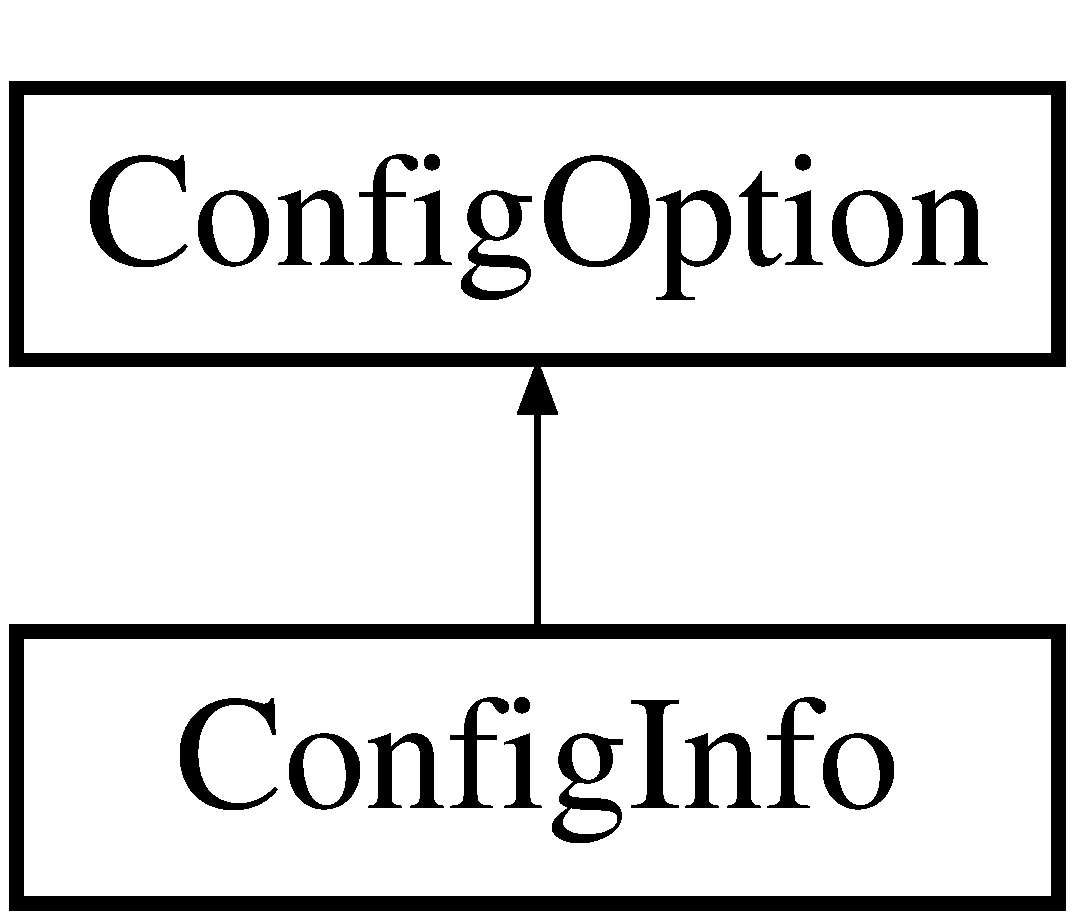
\includegraphics[height=2.000000cm]{class_config_info}
\end{center}
\end{figure}
\subsection*{Membros públicos}
\begin{DoxyCompactItemize}
\item 
\hypertarget{class_config_info_a6687fc30bb61fbadaa3bedfbbecf053f}{{\bfseries Config\-Info} (const char $\ast$name, const char $\ast$doc)}\label{class_config_info_a6687fc30bb61fbadaa3bedfbbecf053f}

\item 
\hypertarget{class_config_info_ad532b92c9971149d194403dff3458ba7}{void {\bfseries write\-Template} (\hyperlink{class_f_text_stream}{F\-Text\-Stream} \&t, bool sl, bool)}\label{class_config_info_ad532b92c9971149d194403dff3458ba7}

\item 
\hypertarget{class_config_info_a79866440425087f224d4f77311efad6a}{void {\bfseries subst\-Env\-Vars} ()}\label{class_config_info_a79866440425087f224d4f77311efad6a}

\end{DoxyCompactItemize}
\subsection*{Additional Inherited Members}


\subsection{Descrição detalhada}
Section marker for grouping the configuration options. 

A documentação para esta classe foi gerada a partir do seguinte ficheiro\-:\begin{DoxyCompactItemize}
\item 
C\-:/\-Users/teste/git/doxygen/src/config.\-h\end{DoxyCompactItemize}

\hypertarget{class_config_int}{\section{Referência à classe Config\-Int}
\label{class_config_int}\index{Config\-Int@{Config\-Int}}
}


{\ttfamily \#include $<$config.\-h$>$}

Diagrama de heranças da classe Config\-Int\begin{figure}[H]
\begin{center}
\leavevmode
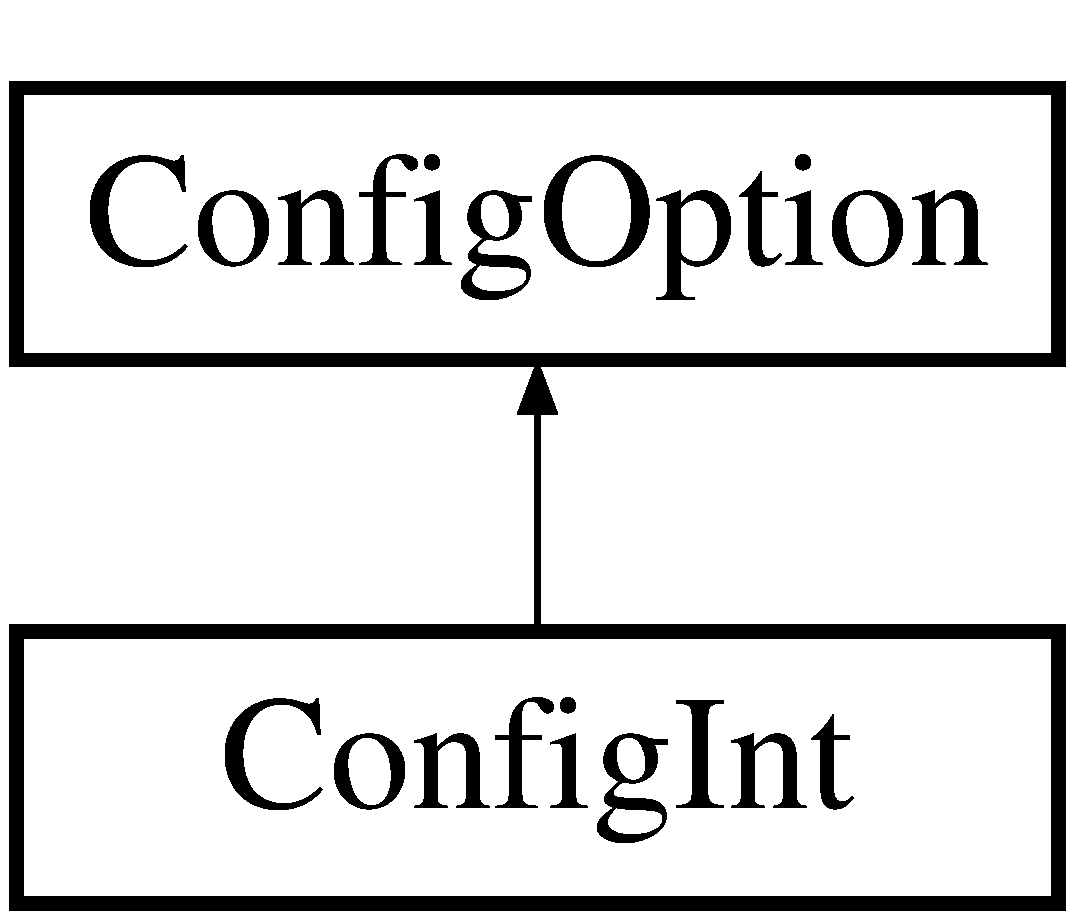
\includegraphics[height=2.000000cm]{class_config_int}
\end{center}
\end{figure}
\subsection*{Membros públicos}
\begin{DoxyCompactItemize}
\item 
\hypertarget{class_config_int_a0b1fdf5da2ff15123c2d8db0bad0f67d}{{\bfseries Config\-Int} (const char $\ast$name, const char $\ast$doc, int min\-Val, int max\-Val, int def\-Val)}\label{class_config_int_a0b1fdf5da2ff15123c2d8db0bad0f67d}

\item 
\hypertarget{class_config_int_a0c7ffe0fff991390d97a629f692a5854}{\hyperlink{class_q_c_string}{Q\-C\-String} $\ast$ {\bfseries value\-String\-Ref} ()}\label{class_config_int_a0c7ffe0fff991390d97a629f692a5854}

\item 
\hypertarget{class_config_int_a3e0fdf101c1ad2a03e61471ff3a379a0}{int $\ast$ {\bfseries value\-Ref} ()}\label{class_config_int_a3e0fdf101c1ad2a03e61471ff3a379a0}

\item 
\hypertarget{class_config_int_a89e3d61b056638d9d44366dd3a064b6c}{int {\bfseries min\-Val} () const }\label{class_config_int_a89e3d61b056638d9d44366dd3a064b6c}

\item 
\hypertarget{class_config_int_ae0f8305087ec20aed794910f0e12af43}{int {\bfseries max\-Val} () const }\label{class_config_int_ae0f8305087ec20aed794910f0e12af43}

\item 
\hypertarget{class_config_int_adf2580bb1cb265aed049fd1553c658c2}{void {\bfseries convert\-Str\-To\-Val} ()}\label{class_config_int_adf2580bb1cb265aed049fd1553c658c2}

\item 
\hypertarget{class_config_int_a79866440425087f224d4f77311efad6a}{void {\bfseries subst\-Env\-Vars} ()}\label{class_config_int_a79866440425087f224d4f77311efad6a}

\item 
\hypertarget{class_config_int_a4972a64bbfa8f975c5704239e71c4811}{void {\bfseries write\-Template} (\hyperlink{class_f_text_stream}{F\-Text\-Stream} \&t, bool sl, bool upd)}\label{class_config_int_a4972a64bbfa8f975c5704239e71c4811}

\item 
\hypertarget{class_config_int_a02fd73d861ef2e4aabb38c0c9ff82947}{void {\bfseries init} ()}\label{class_config_int_a02fd73d861ef2e4aabb38c0c9ff82947}

\end{DoxyCompactItemize}
\subsection*{Additional Inherited Members}


\subsection{Descrição detalhada}
Class representing an integer type option. 

A documentação para esta classe foi gerada a partir do seguinte ficheiro\-:\begin{DoxyCompactItemize}
\item 
C\-:/\-Users/teste/git/doxygen/src/config.\-h\end{DoxyCompactItemize}

\hypertarget{class_config_list}{\section{Referência à classe Config\-List}
\label{class_config_list}\index{Config\-List@{Config\-List}}
}


{\ttfamily \#include $<$config.\-h$>$}

Diagrama de heranças da classe Config\-List\begin{figure}[H]
\begin{center}
\leavevmode
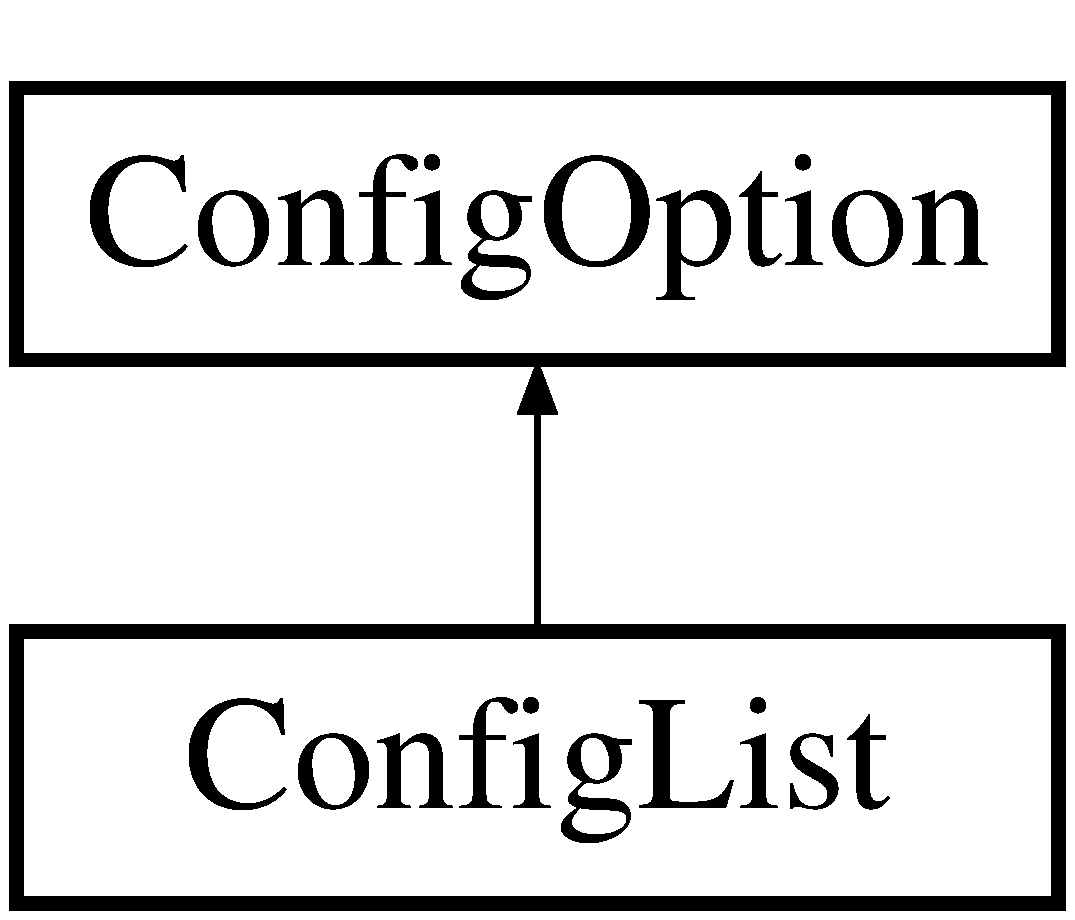
\includegraphics[height=2.000000cm]{class_config_list}
\end{center}
\end{figure}
\subsection*{Tipos Públicos}
\begin{DoxyCompactItemize}
\item 
enum {\bfseries Widget\-Type} \{ {\bfseries String}, 
{\bfseries File}, 
{\bfseries Dir}, 
{\bfseries File\-And\-Dir}
 \}
\end{DoxyCompactItemize}
\subsection*{Membros públicos}
\begin{DoxyCompactItemize}
\item 
\hypertarget{class_config_list_a9a493f3389ee46cfc97c8443c8537a1a}{{\bfseries Config\-List} (const char $\ast$name, const char $\ast$doc)}\label{class_config_list_a9a493f3389ee46cfc97c8443c8537a1a}

\item 
\hypertarget{class_config_list_a6330b95a0b46d7452b8c0e7f61a523de}{void {\bfseries add\-Value} (const char $\ast$v)}\label{class_config_list_a6330b95a0b46d7452b8c0e7f61a523de}

\item 
\hypertarget{class_config_list_aefd9d316a5af38db88268212736d35a2}{void {\bfseries set\-Widget\-Type} (Widget\-Type w)}\label{class_config_list_aefd9d316a5af38db88268212736d35a2}

\item 
\hypertarget{class_config_list_a28a506144c8747cb26dffbfb11e63ee5}{Widget\-Type {\bfseries widget\-Type} () const }\label{class_config_list_a28a506144c8747cb26dffbfb11e63ee5}

\item 
\hypertarget{class_config_list_a4761b22290018a373024647d20c8a1d8}{\hyperlink{class_q_str_list}{Q\-Str\-List} $\ast$ {\bfseries value\-Ref} ()}\label{class_config_list_a4761b22290018a373024647d20c8a1d8}

\item 
\hypertarget{class_config_list_ad532b92c9971149d194403dff3458ba7}{void {\bfseries write\-Template} (\hyperlink{class_f_text_stream}{F\-Text\-Stream} \&t, bool sl, bool)}\label{class_config_list_ad532b92c9971149d194403dff3458ba7}

\item 
\hypertarget{class_config_list_a79866440425087f224d4f77311efad6a}{void {\bfseries subst\-Env\-Vars} ()}\label{class_config_list_a79866440425087f224d4f77311efad6a}

\item 
\hypertarget{class_config_list_a02fd73d861ef2e4aabb38c0c9ff82947}{void {\bfseries init} ()}\label{class_config_list_a02fd73d861ef2e4aabb38c0c9ff82947}

\end{DoxyCompactItemize}
\subsection*{Additional Inherited Members}


\subsection{Descrição detalhada}
Class respresenting a list type option. 

A documentação para esta classe foi gerada a partir do seguinte ficheiro\-:\begin{DoxyCompactItemize}
\item 
C\-:/\-Users/teste/git/doxygen/src/config.\-h\end{DoxyCompactItemize}

\hypertarget{class_config_obsolete}{\section{Referência à classe Config\-Obsolete}
\label{class_config_obsolete}\index{Config\-Obsolete@{Config\-Obsolete}}
}


{\ttfamily \#include $<$config.\-h$>$}

Diagrama de heranças da classe Config\-Obsolete\begin{figure}[H]
\begin{center}
\leavevmode
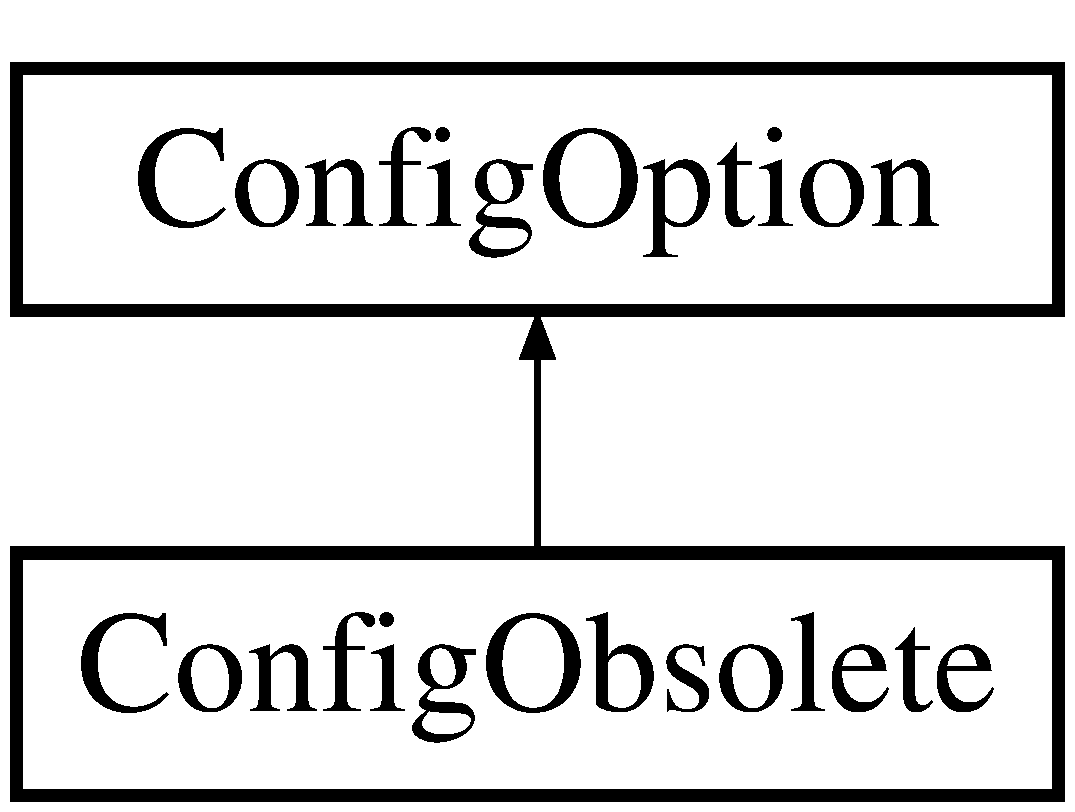
\includegraphics[height=2.000000cm]{class_config_obsolete}
\end{center}
\end{figure}
\subsection*{Membros públicos}
\begin{DoxyCompactItemize}
\item 
\hypertarget{class_config_obsolete_a9f13277a7fc777cdd0fa2e67fdad06f0}{{\bfseries Config\-Obsolete} (const char $\ast$name)}\label{class_config_obsolete_a9f13277a7fc777cdd0fa2e67fdad06f0}

\item 
\hypertarget{class_config_obsolete_a7532aae29d4f94af257d952948ec64ca}{void {\bfseries write\-Template} (\hyperlink{class_f_text_stream}{F\-Text\-Stream} \&, bool, bool)}\label{class_config_obsolete_a7532aae29d4f94af257d952948ec64ca}

\item 
\hypertarget{class_config_obsolete_a79866440425087f224d4f77311efad6a}{void {\bfseries subst\-Env\-Vars} ()}\label{class_config_obsolete_a79866440425087f224d4f77311efad6a}

\end{DoxyCompactItemize}
\subsection*{Additional Inherited Members}


\subsection{Descrição detalhada}
Section marker for obsolete options 

A documentação para esta classe foi gerada a partir do seguinte ficheiro\-:\begin{DoxyCompactItemize}
\item 
C\-:/\-Users/teste/git/doxygen/src/config.\-h\end{DoxyCompactItemize}

\hypertarget{class_config_option}{\section{Referência à classe Config\-Option}
\label{class_config_option}\index{Config\-Option@{Config\-Option}}
}


{\ttfamily \#include $<$config.\-h$>$}

Diagrama de heranças da classe Config\-Option\begin{figure}[H]
\begin{center}
\leavevmode
\includegraphics[height=9.000000cm]{class_config_option}
\end{center}
\end{figure}
\subsection*{Tipos Públicos}
\begin{DoxyCompactItemize}
\item 
enum \hyperlink{class_config_option_a976bded296a67e09242af85291a639d6}{Option\-Type} \{ \\*
{\bfseries O\-\_\-\-Info}, 
{\bfseries O\-\_\-\-List}, 
{\bfseries O\-\_\-\-Enum}, 
{\bfseries O\-\_\-\-String}, 
\\*
{\bfseries O\-\_\-\-Int}, 
{\bfseries O\-\_\-\-Bool}, 
{\bfseries O\-\_\-\-Obsolete}, 
{\bfseries O\-\_\-\-Disabled}
 \}
\item 
enum \{ \hyperlink{class_config_option_a61dadd085c1777f559549e05962b2c9eaf9043652ab6c0a36c22f6bdea78d1d5a}{M\-A\-X\-\_\-\-O\-P\-T\-I\-O\-N\-\_\-\-L\-E\-N\-G\-T\-H} = 23
 \}
\end{DoxyCompactItemize}
\subsection*{Membros públicos}
\begin{DoxyCompactItemize}
\item 
\hypertarget{class_config_option_a981c205e18e00a0f9908691190bfba90}{{\bfseries Config\-Option} (\hyperlink{class_config_option_a976bded296a67e09242af85291a639d6}{Option\-Type} t)}\label{class_config_option_a981c205e18e00a0f9908691190bfba90}

\item 
\hyperlink{class_config_option_a976bded296a67e09242af85291a639d6}{Option\-Type} \hyperlink{class_config_option_a263e7663e23978694a454c4155d10d6b}{kind} () const 
\item 
\hypertarget{class_config_option_af92302878527ec555ba9e3fe066925ff}{\hyperlink{class_q_c_string}{Q\-C\-String} {\bfseries name} () const }\label{class_config_option_af92302878527ec555ba9e3fe066925ff}

\item 
\hypertarget{class_config_option_a382d8459d465104f4b8814838d2feca9}{\hyperlink{class_q_c_string}{Q\-C\-String} {\bfseries docs} () const }\label{class_config_option_a382d8459d465104f4b8814838d2feca9}

\item 
\hypertarget{class_config_option_ac1e12df41db1966fe2ff8f8703bdd7c7}{\hyperlink{class_q_c_string}{Q\-C\-String} {\bfseries depends\-On} () const }\label{class_config_option_ac1e12df41db1966fe2ff8f8703bdd7c7}

\item 
\hypertarget{class_config_option_ab7ce57760071e4a76697349f01e8c100}{void {\bfseries add\-Dependency} (const char $\ast$dep)}\label{class_config_option_ab7ce57760071e4a76697349f01e8c100}

\item 
\hypertarget{class_config_option_a8f08440c4bcc057442af74901a62428a}{void {\bfseries set\-Encoding} (const \hyperlink{class_q_c_string}{Q\-C\-String} \&e)}\label{class_config_option_a8f08440c4bcc057442af74901a62428a}

\item 
\hypertarget{class_config_option_a91738970409db86f29ad17182728b31c}{void {\bfseries set\-User\-Comment} (const \hyperlink{class_q_c_string}{Q\-C\-String} \&u)}\label{class_config_option_a91738970409db86f29ad17182728b31c}

\end{DoxyCompactItemize}
\subsection*{Membros protegidos}
\begin{DoxyCompactItemize}
\item 
\hypertarget{class_config_option_aba8013af8fdfe2786d1a3e6aad982914}{virtual void {\bfseries write\-Template} (\hyperlink{class_f_text_stream}{F\-Text\-Stream} \&t, bool sl, bool upd)=0}\label{class_config_option_aba8013af8fdfe2786d1a3e6aad982914}

\item 
\hypertarget{class_config_option_ac2fe1963b5e322b6bdc4ea8c75e4335c}{virtual void {\bfseries convert\-Str\-To\-Val} ()}\label{class_config_option_ac2fe1963b5e322b6bdc4ea8c75e4335c}

\item 
\hypertarget{class_config_option_a3fe7c7c27837cd6f7e6809d81f00ed45}{virtual void {\bfseries subst\-Env\-Vars} ()=0}\label{class_config_option_a3fe7c7c27837cd6f7e6809d81f00ed45}

\item 
\hypertarget{class_config_option_a9339772ec5ac9fa929938109207f2863}{virtual void {\bfseries init} ()}\label{class_config_option_a9339772ec5ac9fa929938109207f2863}

\item 
\hypertarget{class_config_option_a424b529d2f4edb93222ff26191484266}{void {\bfseries write\-Bool\-Value} (\hyperlink{class_f_text_stream}{F\-Text\-Stream} \&t, bool v)}\label{class_config_option_a424b529d2f4edb93222ff26191484266}

\item 
\hypertarget{class_config_option_a3e5e7dbce7de68b4372d6683d6fa41ec}{void {\bfseries write\-Int\-Value} (\hyperlink{class_f_text_stream}{F\-Text\-Stream} \&t, int i)}\label{class_config_option_a3e5e7dbce7de68b4372d6683d6fa41ec}

\item 
\hypertarget{class_config_option_a0a1f4d85ab9e4d42e353815fd8d9ea27}{void {\bfseries write\-String\-Value} (\hyperlink{class_f_text_stream}{F\-Text\-Stream} \&t, \hyperlink{class_q_c_string}{Q\-C\-String} \&s)}\label{class_config_option_a0a1f4d85ab9e4d42e353815fd8d9ea27}

\item 
\hypertarget{class_config_option_a5b44863e1c725b636cab847e48bd5f1d}{void {\bfseries write\-String\-List} (\hyperlink{class_f_text_stream}{F\-Text\-Stream} \&t, \hyperlink{class_q_str_list}{Q\-Str\-List} \&l)}\label{class_config_option_a5b44863e1c725b636cab847e48bd5f1d}

\end{DoxyCompactItemize}
\subsection*{Atributos Protegidos}
\begin{DoxyCompactItemize}
\item 
\hypertarget{class_config_option_a67f3b0a160a31ef3857558f9cf5d28f0}{\hyperlink{class_q_c_string}{Q\-C\-String} {\bfseries m\-\_\-spaces}}\label{class_config_option_a67f3b0a160a31ef3857558f9cf5d28f0}

\item 
\hypertarget{class_config_option_a1deac18ce5712c20300cdf5e6e7d5487}{\hyperlink{class_q_c_string}{Q\-C\-String} {\bfseries m\-\_\-name}}\label{class_config_option_a1deac18ce5712c20300cdf5e6e7d5487}

\item 
\hypertarget{class_config_option_aeb3d8c4cd279017289f24f71ec706449}{\hyperlink{class_q_c_string}{Q\-C\-String} {\bfseries m\-\_\-doc}}\label{class_config_option_aeb3d8c4cd279017289f24f71ec706449}

\item 
\hypertarget{class_config_option_a004bbf8691ea97d8e6ac0a120ab039d8}{\hyperlink{class_q_c_string}{Q\-C\-String} {\bfseries m\-\_\-dependency}}\label{class_config_option_a004bbf8691ea97d8e6ac0a120ab039d8}

\item 
\hypertarget{class_config_option_a24958dbeafb4fdb30fd7c4ce73674bb1}{\hyperlink{class_q_c_string}{Q\-C\-String} {\bfseries m\-\_\-encoding}}\label{class_config_option_a24958dbeafb4fdb30fd7c4ce73674bb1}

\item 
\hypertarget{class_config_option_afe708a88a3934c8d86e521ce0140fbb5}{\hyperlink{class_q_c_string}{Q\-C\-String} {\bfseries m\-\_\-user\-Comment}}\label{class_config_option_afe708a88a3934c8d86e521ce0140fbb5}

\item 
\hypertarget{class_config_option_adbdd105aaea61a52e29a0e2ff815a18c}{\hyperlink{class_config_option_a976bded296a67e09242af85291a639d6}{Option\-Type} {\bfseries m\-\_\-kind}}\label{class_config_option_adbdd105aaea61a52e29a0e2ff815a18c}

\end{DoxyCompactItemize}
\subsection*{Amigos}
\begin{DoxyCompactItemize}
\item 
\hypertarget{class_config_option_ac3da7e21a05bf8852638db7e4dd1b81a}{class {\bfseries Config}}\label{class_config_option_ac3da7e21a05bf8852638db7e4dd1b81a}

\end{DoxyCompactItemize}


\subsection{Descrição detalhada}
Abstract base class for any configuration option. 

\subsection{Documentação das enumerações}
\hypertarget{class_config_option_a61dadd085c1777f559549e05962b2c9e}{\subsubsection[{anonymous enum}]{\setlength{\rightskip}{0pt plus 5cm}anonymous enum}}\label{class_config_option_a61dadd085c1777f559549e05962b2c9e}
\begin{Desc}
\item[Valores da enumeração]\par
\begin{description}
\index{M\-A\-X\-\_\-\-O\-P\-T\-I\-O\-N\-\_\-\-L\-E\-N\-G\-T\-H@{M\-A\-X\-\_\-\-O\-P\-T\-I\-O\-N\-\_\-\-L\-E\-N\-G\-T\-H}!Config\-Option@{Config\-Option}}\index{Config\-Option@{Config\-Option}!M\-A\-X\-\_\-\-O\-P\-T\-I\-O\-N\-\_\-\-L\-E\-N\-G\-T\-H@{M\-A\-X\-\_\-\-O\-P\-T\-I\-O\-N\-\_\-\-L\-E\-N\-G\-T\-H}}\item[{\em 
\hypertarget{class_config_option_a61dadd085c1777f559549e05962b2c9eaf9043652ab6c0a36c22f6bdea78d1d5a}{M\-A\-X\-\_\-\-O\-P\-T\-I\-O\-N\-\_\-\-L\-E\-N\-G\-T\-H}\label{class_config_option_a61dadd085c1777f559549e05962b2c9eaf9043652ab6c0a36c22f6bdea78d1d5a}
}]Maximum length of an option in the config file. Used for alignment purposes. \end{description}
\end{Desc}
\hypertarget{class_config_option_a976bded296a67e09242af85291a639d6}{\index{Config\-Option@{Config\-Option}!Option\-Type@{Option\-Type}}
\index{Option\-Type@{Option\-Type}!ConfigOption@{Config\-Option}}
\subsubsection[{Option\-Type}]{\setlength{\rightskip}{0pt plus 5cm}enum {\bf Option\-Type}}}\label{class_config_option_a976bded296a67e09242af85291a639d6}
The type of option 

\subsection{Documentação dos métodos}
\hypertarget{class_config_option_a263e7663e23978694a454c4155d10d6b}{\index{Config\-Option@{Config\-Option}!kind@{kind}}
\index{kind@{kind}!ConfigOption@{Config\-Option}}
\subsubsection[{kind}]{\setlength{\rightskip}{0pt plus 5cm}{\bf Option\-Type} kind (
\begin{DoxyParamCaption}
{}
\end{DoxyParamCaption}
) const\hspace{0.3cm}{\ttfamily [inline]}}}\label{class_config_option_a263e7663e23978694a454c4155d10d6b}
returns the kind of option this is. 

A documentação para esta classe foi gerada a partir do seguinte ficheiro\-:\begin{DoxyCompactItemize}
\item 
C\-:/\-Users/teste/git/doxygen/src/config.\-h\end{DoxyCompactItemize}

\hypertarget{class_config_string}{\section{Referência à classe Config\-String}
\label{class_config_string}\index{Config\-String@{Config\-String}}
}


{\ttfamily \#include $<$config.\-h$>$}

Diagrama de heranças da classe Config\-String\begin{figure}[H]
\begin{center}
\leavevmode
\includegraphics[height=2.000000cm]{class_config_string}
\end{center}
\end{figure}
\subsection*{Tipos Públicos}
\begin{DoxyCompactItemize}
\item 
enum {\bfseries Widget\-Type} \{ {\bfseries String}, 
{\bfseries File}, 
{\bfseries Dir}
 \}
\end{DoxyCompactItemize}
\subsection*{Membros públicos}
\begin{DoxyCompactItemize}
\item 
\hypertarget{class_config_string_af3cba8358c7cc00c53cfb032b847bff2}{{\bfseries Config\-String} (const char $\ast$name, const char $\ast$doc)}\label{class_config_string_af3cba8358c7cc00c53cfb032b847bff2}

\item 
\hypertarget{class_config_string_aefd9d316a5af38db88268212736d35a2}{void {\bfseries set\-Widget\-Type} (Widget\-Type w)}\label{class_config_string_aefd9d316a5af38db88268212736d35a2}

\item 
\hypertarget{class_config_string_a28a506144c8747cb26dffbfb11e63ee5}{Widget\-Type {\bfseries widget\-Type} () const }\label{class_config_string_a28a506144c8747cb26dffbfb11e63ee5}

\item 
\hypertarget{class_config_string_a75a19d6f32950fe626410d51f8be1fa7}{void {\bfseries set\-Default\-Value} (const char $\ast$v)}\label{class_config_string_a75a19d6f32950fe626410d51f8be1fa7}

\item 
\hypertarget{class_config_string_a9c4fe5ca500670ba901c995ab38ec6c9}{\hyperlink{class_q_c_string}{Q\-C\-String} $\ast$ {\bfseries value\-Ref} ()}\label{class_config_string_a9c4fe5ca500670ba901c995ab38ec6c9}

\item 
\hypertarget{class_config_string_ad532b92c9971149d194403dff3458ba7}{void {\bfseries write\-Template} (\hyperlink{class_f_text_stream}{F\-Text\-Stream} \&t, bool sl, bool)}\label{class_config_string_ad532b92c9971149d194403dff3458ba7}

\item 
\hypertarget{class_config_string_a79866440425087f224d4f77311efad6a}{void {\bfseries subst\-Env\-Vars} ()}\label{class_config_string_a79866440425087f224d4f77311efad6a}

\item 
\hypertarget{class_config_string_a02fd73d861ef2e4aabb38c0c9ff82947}{void {\bfseries init} ()}\label{class_config_string_a02fd73d861ef2e4aabb38c0c9ff82947}

\end{DoxyCompactItemize}
\subsection*{Additional Inherited Members}


\subsection{Descrição detalhada}
Class representing a string type option. 

A documentação para esta classe foi gerada a partir do seguinte ficheiro\-:\begin{DoxyCompactItemize}
\item 
C\-:/\-Users/teste/git/doxygen/src/config.\-h\end{DoxyCompactItemize}

\hypertarget{class_template_list_intf_1_1_const_iterator}{\section{Referência à classe Template\-List\-Intf\-:\-:Const\-Iterator}
\label{class_template_list_intf_1_1_const_iterator}\index{Template\-List\-Intf\-::\-Const\-Iterator@{Template\-List\-Intf\-::\-Const\-Iterator}}
}


Abstract interface for a iterator of a list.  




{\ttfamily \#include $<$template.\-h$>$}

Diagrama de heranças da classe Template\-List\-Intf\-:\-:Const\-Iterator\begin{figure}[H]
\begin{center}
\leavevmode
\includegraphics[height=2.000000cm]{class_template_list_intf_1_1_const_iterator}
\end{center}
\end{figure}
\subsection*{Membros públicos}
\begin{DoxyCompactItemize}
\item 
virtual \hyperlink{class_template_list_intf_1_1_const_iterator_ad4923f0e0089c0ca746b52e980367068}{$\sim$\-Const\-Iterator} ()
\item 
virtual void \hyperlink{class_template_list_intf_1_1_const_iterator_a86b87aa42e3e820d2c21ae552bd0a55d}{to\-First} ()=0
\item 
virtual void \hyperlink{class_template_list_intf_1_1_const_iterator_a9c80b2b75a3575aeea8a5b211119c6d3}{to\-Last} ()=0
\item 
virtual void \hyperlink{class_template_list_intf_1_1_const_iterator_a03ab44b53fe4f1b143b50a3ff118c831}{to\-Next} ()=0
\item 
virtual void \hyperlink{class_template_list_intf_1_1_const_iterator_a35c099174eca466a4277050c864efc8e}{to\-Prev} ()=0
\item 
\hypertarget{class_template_list_intf_1_1_const_iterator_ae3b4de44e9fb449d7052cb15cdb14d08}{virtual bool {\bfseries current} (\hyperlink{class_template_variant}{Template\-Variant} \&v) const =0}\label{class_template_list_intf_1_1_const_iterator_ae3b4de44e9fb449d7052cb15cdb14d08}

\end{DoxyCompactItemize}


\subsection{Descrição detalhada}
Abstract interface for a iterator of a list. 

\subsection{Documentação dos Construtores \& Destrutor}
\hypertarget{class_template_list_intf_1_1_const_iterator_ad4923f0e0089c0ca746b52e980367068}{\index{Template\-List\-Intf\-::\-Const\-Iterator@{Template\-List\-Intf\-::\-Const\-Iterator}!$\sim$\-Const\-Iterator@{$\sim$\-Const\-Iterator}}
\index{$\sim$\-Const\-Iterator@{$\sim$\-Const\-Iterator}!TemplateListIntf::ConstIterator@{Template\-List\-Intf\-::\-Const\-Iterator}}
\subsubsection[{$\sim$\-Const\-Iterator}]{\setlength{\rightskip}{0pt plus 5cm}virtual $\sim${\bf Const\-Iterator} (
\begin{DoxyParamCaption}
{}
\end{DoxyParamCaption}
)\hspace{0.3cm}{\ttfamily [inline]}, {\ttfamily [virtual]}}}\label{class_template_list_intf_1_1_const_iterator_ad4923f0e0089c0ca746b52e980367068}
Destructor for the iterator 

\subsection{Documentação dos métodos}
\hypertarget{class_template_list_intf_1_1_const_iterator_a86b87aa42e3e820d2c21ae552bd0a55d}{\index{Template\-List\-Intf\-::\-Const\-Iterator@{Template\-List\-Intf\-::\-Const\-Iterator}!to\-First@{to\-First}}
\index{to\-First@{to\-First}!TemplateListIntf::ConstIterator@{Template\-List\-Intf\-::\-Const\-Iterator}}
\subsubsection[{to\-First}]{\setlength{\rightskip}{0pt plus 5cm}virtual void to\-First (
\begin{DoxyParamCaption}
{}
\end{DoxyParamCaption}
)\hspace{0.3cm}{\ttfamily [pure virtual]}}}\label{class_template_list_intf_1_1_const_iterator_a86b87aa42e3e820d2c21ae552bd0a55d}
Moves iterator to the first element in the list 

Implementado em \hyperlink{class_template_list_const_iterator_a24528c52410032763cedaccdfbe474e5}{Template\-List\-Const\-Iterator} e \hyperlink{class_generic_const_iterator_a7a848bf7b9f402e97732fe5abb2c71ca}{Generic\-Const\-Iterator$<$ T $>$}.

\hypertarget{class_template_list_intf_1_1_const_iterator_a9c80b2b75a3575aeea8a5b211119c6d3}{\index{Template\-List\-Intf\-::\-Const\-Iterator@{Template\-List\-Intf\-::\-Const\-Iterator}!to\-Last@{to\-Last}}
\index{to\-Last@{to\-Last}!TemplateListIntf::ConstIterator@{Template\-List\-Intf\-::\-Const\-Iterator}}
\subsubsection[{to\-Last}]{\setlength{\rightskip}{0pt plus 5cm}virtual void to\-Last (
\begin{DoxyParamCaption}
{}
\end{DoxyParamCaption}
)\hspace{0.3cm}{\ttfamily [pure virtual]}}}\label{class_template_list_intf_1_1_const_iterator_a9c80b2b75a3575aeea8a5b211119c6d3}
Moves iterator to the last element in the list 

Implementado em \hyperlink{class_template_list_const_iterator_ac4e23694db19ee84c4e110f9965d64e4}{Template\-List\-Const\-Iterator} e \hyperlink{class_generic_const_iterator_acda76aed44e713788e17c3373ca1a0e3}{Generic\-Const\-Iterator$<$ T $>$}.

\hypertarget{class_template_list_intf_1_1_const_iterator_a03ab44b53fe4f1b143b50a3ff118c831}{\index{Template\-List\-Intf\-::\-Const\-Iterator@{Template\-List\-Intf\-::\-Const\-Iterator}!to\-Next@{to\-Next}}
\index{to\-Next@{to\-Next}!TemplateListIntf::ConstIterator@{Template\-List\-Intf\-::\-Const\-Iterator}}
\subsubsection[{to\-Next}]{\setlength{\rightskip}{0pt plus 5cm}virtual void to\-Next (
\begin{DoxyParamCaption}
{}
\end{DoxyParamCaption}
)\hspace{0.3cm}{\ttfamily [pure virtual]}}}\label{class_template_list_intf_1_1_const_iterator_a03ab44b53fe4f1b143b50a3ff118c831}
Moves iterator to the next element in the list 

Implementado em \hyperlink{class_template_list_const_iterator_ad8ecebd1a267185e69e1b6fe4e9f331e}{Template\-List\-Const\-Iterator} e \hyperlink{class_generic_const_iterator_a8389e031d03169de4d6b9c55e7946d4b}{Generic\-Const\-Iterator$<$ T $>$}.

\hypertarget{class_template_list_intf_1_1_const_iterator_a35c099174eca466a4277050c864efc8e}{\index{Template\-List\-Intf\-::\-Const\-Iterator@{Template\-List\-Intf\-::\-Const\-Iterator}!to\-Prev@{to\-Prev}}
\index{to\-Prev@{to\-Prev}!TemplateListIntf::ConstIterator@{Template\-List\-Intf\-::\-Const\-Iterator}}
\subsubsection[{to\-Prev}]{\setlength{\rightskip}{0pt plus 5cm}virtual void to\-Prev (
\begin{DoxyParamCaption}
{}
\end{DoxyParamCaption}
)\hspace{0.3cm}{\ttfamily [pure virtual]}}}\label{class_template_list_intf_1_1_const_iterator_a35c099174eca466a4277050c864efc8e}
Moves iterator to the previous element in the list 

Implementado em \hyperlink{class_template_list_const_iterator_a3491dc4d8ab54f0a0583ac1941f4e94f}{Template\-List\-Const\-Iterator} e \hyperlink{class_generic_const_iterator_af7a123b30adb797bf7aa2b5a94b060b0}{Generic\-Const\-Iterator$<$ T $>$}.



A documentação para esta classe foi gerada a partir do seguinte ficheiro\-:\begin{DoxyCompactItemize}
\item 
C\-:/\-Users/teste/git/doxygen/src/template.\-h\end{DoxyCompactItemize}

\hypertarget{struct_context_globals}{\section{Referência à estrutura Context\-Globals}
\label{struct_context_globals}\index{Context\-Globals@{Context\-Globals}}
}
\subsection*{Tipos Públicos}
\begin{DoxyCompactItemize}
\item 
enum {\bfseries Output\-Format} \{ \\*
{\bfseries Html}, 
{\bfseries Late\-X}, 
{\bfseries Rtf}, 
{\bfseries Man\-Page}, 
\\*
{\bfseries Doc\-Book}, 
{\bfseries Xml}, 
{\bfseries Tag\-File}
 \}
\end{DoxyCompactItemize}
\subsection*{Campos de Dados}
\begin{DoxyCompactItemize}
\item 
\hypertarget{struct_context_globals_a7cdd120bf494b891babda8587c098f6a}{int {\bfseries dyn\-Section\-Id}}\label{struct_context_globals_a7cdd120bf494b891babda8587c098f6a}

\item 
\hypertarget{struct_context_globals_a78adf7da3f3f4dd27b43938456bfd94d}{\hyperlink{class_q_c_string}{Q\-C\-String} {\bfseries output\-Dir}}\label{struct_context_globals_a78adf7da3f3f4dd27b43938456bfd94d}

\item 
\hypertarget{struct_context_globals_aaecb56ed832ccc0660e49ea16793fdbd}{Output\-Format {\bfseries output\-Format}}\label{struct_context_globals_aaecb56ed832ccc0660e49ea16793fdbd}

\end{DoxyCompactItemize}


A documentação para esta estrutura foi gerada a partir do seguinte ficheiro\-:\begin{DoxyCompactItemize}
\item 
C\-:/\-Users/teste/git/doxygen/src/context.\-cpp\end{DoxyCompactItemize}

\hypertarget{struct_coord_struct}{\section{Referência à estrutura Coord\-Struct}
\label{struct_coord_struct}\index{Coord\-Struct@{Coord\-Struct}}
}
\subsection*{Campos de Dados}
\begin{DoxyCompactItemize}
\item 
float \hyperlink{struct_coord_struct_ad0da36b2558901e21e7a30f6c227a45e}{x}
\item 
float \hyperlink{struct_coord_struct_aa4f0d3eebc3c443f9be81bf48561a217}{y}
\end{DoxyCompactItemize}


\subsection{Descrição detalhada}
\hyperlink{class_a}{A} coordinate pair. 

\subsection{Documentação dos campos e atributos}
\hypertarget{struct_coord_struct_ad0da36b2558901e21e7a30f6c227a45e}{\index{Coord\-Struct@{Coord\-Struct}!x@{x}}
\index{x@{x}!CoordStruct@{Coord\-Struct}}
\subsubsection[{x}]{\setlength{\rightskip}{0pt plus 5cm}float x}}\label{struct_coord_struct_ad0da36b2558901e21e7a30f6c227a45e}
The x coordinate \hypertarget{struct_coord_struct_aa4f0d3eebc3c443f9be81bf48561a217}{\index{Coord\-Struct@{Coord\-Struct}!y@{y}}
\index{y@{y}!CoordStruct@{Coord\-Struct}}
\subsubsection[{y}]{\setlength{\rightskip}{0pt plus 5cm}float y}}\label{struct_coord_struct_aa4f0d3eebc3c443f9be81bf48561a217}
The y coordinate 

A documentação para esta estrutura foi gerada a partir do seguinte ficheiro\-:\begin{DoxyCompactItemize}
\item 
C\-:/\-Users/teste/git/doxygen/examples/\hyperlink{restypedef_8cpp}{restypedef.\-cpp}\end{DoxyCompactItemize}

\hypertarget{class_copy_handler}{\section{Referência à classe Copy\-Handler}
\label{class_copy_handler}\index{Copy\-Handler@{Copy\-Handler}}
}


Node representing a copied piece of documentation.  




{\ttfamily \#include $<$dochandler.\-h$>$}

Diagrama de heranças da classe Copy\-Handler\begin{figure}[H]
\begin{center}
\leavevmode
\includegraphics[height=1.545894cm]{class_copy_handler}
\end{center}
\end{figure}
\subsection*{Membros públicos}
\begin{DoxyCompactItemize}
\item 
\hypertarget{class_copy_handler_a63681e25537a6b1c4b5f25d45423cb13}{{\bfseries Copy\-Handler} (\hyperlink{class_i_base_handler}{I\-Base\-Handler} $\ast$parent)}\label{class_copy_handler_a63681e25537a6b1c4b5f25d45423cb13}

\item 
\hypertarget{class_copy_handler_a2bb03e75295578cb36a0a27fa88d2960}{virtual void {\bfseries start\-Copy} (const \hyperlink{class_q_xml_attributes}{Q\-Xml\-Attributes} \&attrib)}\label{class_copy_handler_a2bb03e75295578cb36a0a27fa88d2960}

\item 
\hypertarget{class_copy_handler_a0a534651c87cb23d6c08da6f1b4c33f8}{virtual void {\bfseries end\-Copy} ()}\label{class_copy_handler_a0a534651c87cb23d6c08da6f1b4c33f8}

\item 
\hypertarget{class_copy_handler_abb7f955561480002949ada58092c1964}{virtual void {\bfseries start\-Paragraph} (const \hyperlink{class_q_xml_attributes}{Q\-Xml\-Attributes} \&attrib)}\label{class_copy_handler_abb7f955561480002949ada58092c1964}

\item 
\hypertarget{class_copy_handler_af8e62c8a81ddf2283205cc8955de50eb}{virtual Kind {\bfseries kind} () const }\label{class_copy_handler_af8e62c8a81ddf2283205cc8955de50eb}

\item 
\hypertarget{class_copy_handler_a6f867db5d47aa2210c77df9bc5953008}{virtual \hyperlink{class_i_doc_iterator}{I\-Doc\-Iterator} $\ast$ {\bfseries contents} () const }\label{class_copy_handler_a6f867db5d47aa2210c77df9bc5953008}

\end{DoxyCompactItemize}
\subsection*{Amigos}
\begin{DoxyCompactItemize}
\item 
\hypertarget{class_copy_handler_a6d99f95edf83a9c83db0307bc0e58e48}{class {\bfseries Copy\-Iterator}}\label{class_copy_handler_a6d99f95edf83a9c83db0307bc0e58e48}

\end{DoxyCompactItemize}
\subsection*{Additional Inherited Members}


\subsection{Descrição detalhada}
Node representing a copied piece of documentation. 



A documentação para esta classe foi gerada a partir dos seguintes ficheiros\-:\begin{DoxyCompactItemize}
\item 
C\-:/\-Users/teste/git/doxygen/addon/doxmlparser/src/dochandler.\-h\item 
C\-:/\-Users/teste/git/doxygen/addon/doxmlparser/src/dochandler.\-cpp\end{DoxyCompactItemize}

\hypertarget{class_copy_iterator}{\section{Referência à classe Copy\-Iterator}
\label{class_copy_iterator}\index{Copy\-Iterator@{Copy\-Iterator}}
}
Diagrama de heranças da classe Copy\-Iterator\begin{figure}[H]
\begin{center}
\leavevmode
\includegraphics[height=3.294118cm]{class_copy_iterator}
\end{center}
\end{figure}
\subsection*{Membros públicos}
\begin{DoxyCompactItemize}
\item 
\hypertarget{class_copy_iterator_a4227a43f629add727f8d0a35ead81dcf}{{\bfseries Copy\-Iterator} (const \hyperlink{class_copy_handler}{Copy\-Handler} \&handler)}\label{class_copy_iterator_a4227a43f629add727f8d0a35ead81dcf}

\end{DoxyCompactItemize}
\subsection*{Additional Inherited Members}


A documentação para esta classe foi gerada a partir do seguinte ficheiro\-:\begin{DoxyCompactItemize}
\item 
C\-:/\-Users/teste/git/doxygen/addon/doxmlparser/src/dochandler.\-h\end{DoxyCompactItemize}

\hypertarget{class_c_p_p_value}{\section{Referência à classe C\-P\-P\-Value}
\label{class_c_p_p_value}\index{C\-P\-P\-Value@{C\-P\-P\-Value}}
}


{\ttfamily \#include $<$cppvalue.\-h$>$}

\subsection*{Tipos Públicos}
\begin{DoxyCompactItemize}
\item 
enum {\bfseries Type} \{ {\bfseries Int}, 
{\bfseries Float}
 \}
\end{DoxyCompactItemize}
\subsection*{Membros públicos}
\begin{DoxyCompactItemize}
\item 
\hypertarget{class_c_p_p_value_ab8603ca1ecadcfaeda73aec07d7a4fde}{{\bfseries C\-P\-P\-Value} (long val=0)}\label{class_c_p_p_value_ab8603ca1ecadcfaeda73aec07d7a4fde}

\item 
\hypertarget{class_c_p_p_value_ad4bdf5d22cb0db3d92eb381d58bb44bb}{{\bfseries C\-P\-P\-Value} (double val)}\label{class_c_p_p_value_ad4bdf5d22cb0db3d92eb381d58bb44bb}

\item 
\hypertarget{class_c_p_p_value_a5665dbc337111463ad23d3dba99f7ce3}{{\bfseries operator double} () const }\label{class_c_p_p_value_a5665dbc337111463ad23d3dba99f7ce3}

\item 
\hypertarget{class_c_p_p_value_a20a235a3b8231d8f92c779347fc8eb76}{{\bfseries operator long} () const }\label{class_c_p_p_value_a20a235a3b8231d8f92c779347fc8eb76}

\item 
\hypertarget{class_c_p_p_value_a8a77824300838e6bce0461cbe181de0f}{bool {\bfseries is\-Int} () const }\label{class_c_p_p_value_a8a77824300838e6bce0461cbe181de0f}

\item 
\hypertarget{class_c_p_p_value_a3a3ab31c19c38fe926198ddc4a0a4a91}{void {\bfseries print} () const }\label{class_c_p_p_value_a3a3ab31c19c38fe926198ddc4a0a4a91}

\end{DoxyCompactItemize}


\subsection{Descrição detalhada}
\hyperlink{class_a}{A} class representing a C-\/preprocessor value. 

A documentação para esta classe foi gerada a partir do seguinte ficheiro\-:\begin{DoxyCompactItemize}
\item 
C\-:/\-Users/teste/git/doxygen/src/cppvalue.\-h\end{DoxyCompactItemize}

\hypertarget{class_d}{\section{Referência à classe D}
\label{class_d}\index{D@{D}}
}
Diagrama de heranças da classe D\begin{figure}[H]
\begin{center}
\leavevmode
\includegraphics[height=3.000000cm]{class_d}
\end{center}
\end{figure}
\subsection*{Campos de Dados}
\begin{DoxyCompactItemize}
\item 
\hypertarget{class_d_a2c74ad44b86642512c21365372440c58}{\hyperlink{class_c}{C} {\bfseries m\-\_\-c}}\label{class_d_a2c74ad44b86642512c21365372440c58}

\end{DoxyCompactItemize}
\subsection*{Additional Inherited Members}


A documentação para esta classe foi gerada a partir do seguinte ficheiro\-:\begin{DoxyCompactItemize}
\item 
C\-:/\-Users/teste/git/doxygen/examples/diagrams\-\_\-d.\-h\end{DoxyCompactItemize}

\hypertarget{class_d_bus_x_m_l_handler}{\section{Referência à classe D\-Bus\-X\-M\-L\-Handler}
\label{class_d_bus_x_m_l_handler}\index{D\-Bus\-X\-M\-L\-Handler@{D\-Bus\-X\-M\-L\-Handler}}
}
Diagrama de heranças da classe D\-Bus\-X\-M\-L\-Handler\begin{figure}[H]
\begin{center}
\leavevmode
\includegraphics[height=2.014389cm]{class_d_bus_x_m_l_handler}
\end{center}
\end{figure}
\subsection*{Membros públicos}
\begin{DoxyCompactItemize}
\item 
\hypertarget{class_d_bus_x_m_l_handler_a14a76dd17c5b063a63dda3a3ebb20c1d}{{\bfseries D\-Bus\-X\-M\-L\-Handler} (\hyperlink{class_parser_interface}{Parser\-Interface} $\ast$parser, \hyperlink{class_q_xml_simple_reader}{Q\-Xml\-Simple\-Reader} $\ast$reader, const char $\ast$file\-\_\-name, \hyperlink{class_entry}{Entry} $\ast$root)}\label{class_d_bus_x_m_l_handler_a14a76dd17c5b063a63dda3a3ebb20c1d}

\item 
\hyperlink{class_q_string}{Q\-String} \hyperlink{class_d_bus_x_m_l_handler_af799a7684337babb971e2e0d8cda7cf1}{error\-String} ()
\item 
bool \hyperlink{class_d_bus_x_m_l_handler_a2d8a6efa278f0675843ac44ddec3b9b9}{start\-Element} (const \hyperlink{class_q_string}{Q\-String} \&namespace\-U\-R\-I, const \hyperlink{class_q_string}{Q\-String} \&local\-Name, const \hyperlink{class_q_string}{Q\-String} \&q\-Name, const \hyperlink{class_q_xml_attributes}{Q\-Xml\-Attributes} \&attributes)
\item 
bool \hyperlink{class_d_bus_x_m_l_handler_abd6ff9644b2d6f0a4aab938bd9cdc593}{end\-Element} (const \hyperlink{class_q_string}{Q\-String} \&namespace\-U\-R\-I, const \hyperlink{class_q_string}{Q\-String} \&local\-Name, const \hyperlink{class_q_string}{Q\-String} \&q\-Name)
\item 
bool \hyperlink{class_d_bus_x_m_l_handler_a4c0dc64e43b1a283cc948c82ff4ad392}{characters} (const \hyperlink{class_q_string}{Q\-String} \&)
\item 
bool \hyperlink{class_d_bus_x_m_l_handler_abe6e6b6cbb1913a33b7d1350b16e9bba}{comment} (const \hyperlink{class_q_string}{Q\-String} \&comment\-\_\-)
\item 
\hypertarget{class_d_bus_x_m_l_handler_a854cece148cf8dc514dc91e7d65e2035}{void {\bfseries handle\-Comment} ()}\label{class_d_bus_x_m_l_handler_a854cece148cf8dc514dc91e7d65e2035}

\item 
\hypertarget{class_d_bus_x_m_l_handler_ae3075792029d8ed95e26b527e305d7a2}{\hyperlink{class_q_xml_locator}{Q\-Xml\-Locator} $\ast$ {\bfseries locator} ()}\label{class_d_bus_x_m_l_handler_ae3075792029d8ed95e26b527e305d7a2}

\item 
\hypertarget{class_d_bus_x_m_l_handler_a4bc010d37f882a7895ca5b642dc65735}{int {\bfseries line\-Number} ()}\label{class_d_bus_x_m_l_handler_a4bc010d37f882a7895ca5b642dc65735}

\item 
\hypertarget{class_d_bus_x_m_l_handler_a1408bb8c3d78e622b9033fc7eb1b7ff6}{void {\bfseries set\-Section} ()}\label{class_d_bus_x_m_l_handler_a1408bb8c3d78e622b9033fc7eb1b7ff6}

\end{DoxyCompactItemize}


\subsection{Descrição detalhada}
D\-Bus implementation of the generic \hyperlink{class_q_xml_default_handler}{Q\-Xml\-Default\-Handler}. 

\subsection{Documentação dos métodos}
\hypertarget{class_d_bus_x_m_l_handler_a4c0dc64e43b1a283cc948c82ff4ad392}{\index{D\-Bus\-X\-M\-L\-Handler@{D\-Bus\-X\-M\-L\-Handler}!characters@{characters}}
\index{characters@{characters}!DBusXMLHandler@{D\-Bus\-X\-M\-L\-Handler}}
\subsubsection[{characters}]{\setlength{\rightskip}{0pt plus 5cm}bool characters (
\begin{DoxyParamCaption}
\item[{const {\bf Q\-String} \&}]{ch}
\end{DoxyParamCaption}
)\hspace{0.3cm}{\ttfamily [inline]}, {\ttfamily [virtual]}}}\label{class_d_bus_x_m_l_handler_a4c0dc64e43b1a283cc948c82ff4ad392}
Does nothing. 

Reimplementado de \hyperlink{class_q_xml_default_handler_a6eb7b9d9a6138bf566cc61ae9b5e436a}{Q\-Xml\-Default\-Handler}.

\hypertarget{class_d_bus_x_m_l_handler_abe6e6b6cbb1913a33b7d1350b16e9bba}{\index{D\-Bus\-X\-M\-L\-Handler@{D\-Bus\-X\-M\-L\-Handler}!comment@{comment}}
\index{comment@{comment}!DBusXMLHandler@{D\-Bus\-X\-M\-L\-Handler}}
\subsubsection[{comment}]{\setlength{\rightskip}{0pt plus 5cm}bool comment (
\begin{DoxyParamCaption}
\item[{const {\bf Q\-String} \&}]{ch}
\end{DoxyParamCaption}
)\hspace{0.3cm}{\ttfamily [inline]}, {\ttfamily [virtual]}}}\label{class_d_bus_x_m_l_handler_abe6e6b6cbb1913a33b7d1350b16e9bba}
Does nothing. 

Reimplementado de \hyperlink{class_q_xml_default_handler_a244025ba6bd8815828678aab134064d0}{Q\-Xml\-Default\-Handler}.

\hypertarget{class_d_bus_x_m_l_handler_abd6ff9644b2d6f0a4aab938bd9cdc593}{\index{D\-Bus\-X\-M\-L\-Handler@{D\-Bus\-X\-M\-L\-Handler}!end\-Element@{end\-Element}}
\index{end\-Element@{end\-Element}!DBusXMLHandler@{D\-Bus\-X\-M\-L\-Handler}}
\subsubsection[{end\-Element}]{\setlength{\rightskip}{0pt plus 5cm}bool end\-Element (
\begin{DoxyParamCaption}
\item[{const {\bf Q\-String} \&}]{namespace\-U\-R\-I, }
\item[{const {\bf Q\-String} \&}]{local\-Name, }
\item[{const {\bf Q\-String} \&}]{q\-Name}
\end{DoxyParamCaption}
)\hspace{0.3cm}{\ttfamily [inline]}, {\ttfamily [virtual]}}}\label{class_d_bus_x_m_l_handler_abd6ff9644b2d6f0a4aab938bd9cdc593}
Does nothing. 

Reimplementado de \hyperlink{class_q_xml_default_handler_abd6ff9644b2d6f0a4aab938bd9cdc593}{Q\-Xml\-Default\-Handler}.

\hypertarget{class_d_bus_x_m_l_handler_af799a7684337babb971e2e0d8cda7cf1}{\index{D\-Bus\-X\-M\-L\-Handler@{D\-Bus\-X\-M\-L\-Handler}!error\-String@{error\-String}}
\index{error\-String@{error\-String}!DBusXMLHandler@{D\-Bus\-X\-M\-L\-Handler}}
\subsubsection[{error\-String}]{\setlength{\rightskip}{0pt plus 5cm}{\bf Q\-String} error\-String (
\begin{DoxyParamCaption}
{}
\end{DoxyParamCaption}
)\hspace{0.3cm}{\ttfamily [inline]}, {\ttfamily [virtual]}}}\label{class_d_bus_x_m_l_handler_af799a7684337babb971e2e0d8cda7cf1}
Returns the default error string. 

Reimplementado de \hyperlink{class_q_xml_default_handler_af799a7684337babb971e2e0d8cda7cf1}{Q\-Xml\-Default\-Handler}.

\hypertarget{class_d_bus_x_m_l_handler_a2d8a6efa278f0675843ac44ddec3b9b9}{\index{D\-Bus\-X\-M\-L\-Handler@{D\-Bus\-X\-M\-L\-Handler}!start\-Element@{start\-Element}}
\index{start\-Element@{start\-Element}!DBusXMLHandler@{D\-Bus\-X\-M\-L\-Handler}}
\subsubsection[{start\-Element}]{\setlength{\rightskip}{0pt plus 5cm}bool start\-Element (
\begin{DoxyParamCaption}
\item[{const {\bf Q\-String} \&}]{namespace\-U\-R\-I, }
\item[{const {\bf Q\-String} \&}]{local\-Name, }
\item[{const {\bf Q\-String} \&}]{q\-Name, }
\item[{const {\bf Q\-Xml\-Attributes} \&}]{atts}
\end{DoxyParamCaption}
)\hspace{0.3cm}{\ttfamily [inline]}, {\ttfamily [virtual]}}}\label{class_d_bus_x_m_l_handler_a2d8a6efa278f0675843ac44ddec3b9b9}
Does nothing. 

Reimplementado de \hyperlink{class_q_xml_default_handler_a0712995308713e9df1c0d389568a344b}{Q\-Xml\-Default\-Handler}.



A documentação para esta classe foi gerada a partir do seguinte ficheiro\-:\begin{DoxyCompactItemize}
\item 
C\-:/\-Users/teste/git/doxygen/src/dbusxmlscanner.\-cpp\end{DoxyCompactItemize}

\hypertarget{class_d_bus_x_m_l_scanner}{\section{Referência à classe D\-Bus\-X\-M\-L\-Scanner}
\label{class_d_bus_x_m_l_scanner}\index{D\-Bus\-X\-M\-L\-Scanner@{D\-Bus\-X\-M\-L\-Scanner}}
}


{\ttfamily \#include $<$dbusxmlscanner.\-h$>$}

Diagrama de heranças da classe D\-Bus\-X\-M\-L\-Scanner\begin{figure}[H]
\begin{center}
\leavevmode
\includegraphics[height=2.000000cm]{class_d_bus_x_m_l_scanner}
\end{center}
\end{figure}
\subsection*{Membros públicos}
\begin{DoxyCompactItemize}
\item 
void \hyperlink{class_d_bus_x_m_l_scanner_a9179d0b9461d5d683468fb6015d1643f}{start\-Translation\-Unit} (const char $\ast$)
\item 
void \hyperlink{class_d_bus_x_m_l_scanner_a245c1fbfb8ba359e61d832c4e7c6c98e}{finish\-Translation\-Unit} ()
\item 
void \hyperlink{class_d_bus_x_m_l_scanner_ab1ed2c75b61719cec6060b9f69419743}{parse\-Input} (const char $\ast$file\-Name, const char $\ast$file\-Buf, \hyperlink{class_entry}{Entry} $\ast$root, bool same\-Translation\-Unit, \hyperlink{class_q_str_list}{Q\-Str\-List} \&files\-In\-Same\-Translation\-Unit)
\item 
bool \hyperlink{class_d_bus_x_m_l_scanner_ac49a959c40c82385233e4c75163e39ae}{needs\-Preprocessing} (const \hyperlink{class_q_c_string}{Q\-C\-String} \&extension)
\item 
void \hyperlink{class_d_bus_x_m_l_scanner_ac614074ea2c569cabd265a6168ad36d2}{parse\-Code} (\hyperlink{class_code_output_interface}{Code\-Output\-Interface} \&code\-Out\-Intf, const char $\ast$scope\-Name, const \hyperlink{class_q_c_string}{Q\-C\-String} \&input, \hyperlink{types_8h_a9974623ce72fc23df5d64426b9178bf2}{Src\-Lang\-Ext} lang, bool is\-Example\-Block, const char $\ast$example\-Name=0, \hyperlink{class_file_def}{File\-Def} $\ast$file\-Def=0, int start\-Line=-\/1, int end\-Line=-\/1, bool inline\-Fragment=F\-A\-L\-S\-E, \hyperlink{class_member_def}{Member\-Def} $\ast$member\-Def=0, bool show\-Line\-Numbers=T\-R\-U\-E, \hyperlink{class_definition}{Definition} $\ast$search\-Ctx=0, bool collect\-X\-Refs=T\-R\-U\-E)
\item 
void \hyperlink{class_d_bus_x_m_l_scanner_a5d8e0ded4118b6eff98aa23eb64db02c}{reset\-Code\-Parser\-State} ()
\item 
void \hyperlink{class_d_bus_x_m_l_scanner_a022344e4fa95056a941a9e8c02334872}{parse\-Prototype} (const char $\ast$text)
\end{DoxyCompactItemize}


\subsection{Descrição detalhada}
D-\/\-Bus X\-M\-L parser.

This is the D-\/\-Bus X\-M\-L parser for doxygen. 

\subsection{Documentação dos métodos}
\hypertarget{class_d_bus_x_m_l_scanner_a245c1fbfb8ba359e61d832c4e7c6c98e}{\index{D\-Bus\-X\-M\-L\-Scanner@{D\-Bus\-X\-M\-L\-Scanner}!finish\-Translation\-Unit@{finish\-Translation\-Unit}}
\index{finish\-Translation\-Unit@{finish\-Translation\-Unit}!DBusXMLScanner@{D\-Bus\-X\-M\-L\-Scanner}}
\subsubsection[{finish\-Translation\-Unit}]{\setlength{\rightskip}{0pt plus 5cm}void finish\-Translation\-Unit (
\begin{DoxyParamCaption}
{}
\end{DoxyParamCaption}
)\hspace{0.3cm}{\ttfamily [inline]}, {\ttfamily [virtual]}}}\label{class_d_bus_x_m_l_scanner_a245c1fbfb8ba359e61d832c4e7c6c98e}
Called after all files in a translation unit have been processed. 

Implementa \hyperlink{class_parser_interface_afeb7f0c0fa300a57fbbc5bceb2795f3a}{Parser\-Interface}.

\hypertarget{class_d_bus_x_m_l_scanner_ac49a959c40c82385233e4c75163e39ae}{\index{D\-Bus\-X\-M\-L\-Scanner@{D\-Bus\-X\-M\-L\-Scanner}!needs\-Preprocessing@{needs\-Preprocessing}}
\index{needs\-Preprocessing@{needs\-Preprocessing}!DBusXMLScanner@{D\-Bus\-X\-M\-L\-Scanner}}
\subsubsection[{needs\-Preprocessing}]{\setlength{\rightskip}{0pt plus 5cm}bool needs\-Preprocessing (
\begin{DoxyParamCaption}
\item[{const {\bf Q\-C\-String} \&}]{extension}
\end{DoxyParamCaption}
)\hspace{0.3cm}{\ttfamily [virtual]}}}\label{class_d_bus_x_m_l_scanner_ac49a959c40c82385233e4c75163e39ae}
Returns T\-R\-U\-E if the language identified by {\itshape extension} needs the \hyperlink{class_c}{C} preprocessor to be run before feed the result to the input parser. \begin{DoxySeeAlso}{Veja também}
\hyperlink{class_d_bus_x_m_l_scanner_ab1ed2c75b61719cec6060b9f69419743}{parse\-Input()} 
\end{DoxySeeAlso}


Implementa \hyperlink{class_parser_interface_a9f137118e8804d57ea8ebe6a7d711703}{Parser\-Interface}.

\hypertarget{class_d_bus_x_m_l_scanner_ac614074ea2c569cabd265a6168ad36d2}{\index{D\-Bus\-X\-M\-L\-Scanner@{D\-Bus\-X\-M\-L\-Scanner}!parse\-Code@{parse\-Code}}
\index{parse\-Code@{parse\-Code}!DBusXMLScanner@{D\-Bus\-X\-M\-L\-Scanner}}
\subsubsection[{parse\-Code}]{\setlength{\rightskip}{0pt plus 5cm}void parse\-Code (
\begin{DoxyParamCaption}
\item[{{\bf Code\-Output\-Interface} \&}]{code\-Out\-Intf, }
\item[{const char $\ast$}]{scope\-Name, }
\item[{const {\bf Q\-C\-String} \&}]{input, }
\item[{{\bf Src\-Lang\-Ext}}]{lang, }
\item[{bool}]{is\-Example\-Block, }
\item[{const char $\ast$}]{example\-Name = {\ttfamily 0}, }
\item[{{\bf File\-Def} $\ast$}]{file\-Def = {\ttfamily 0}, }
\item[{int}]{start\-Line = {\ttfamily -\/1}, }
\item[{int}]{end\-Line = {\ttfamily -\/1}, }
\item[{bool}]{inline\-Fragment = {\ttfamily FALSE}, }
\item[{{\bf Member\-Def} $\ast$}]{member\-Def = {\ttfamily 0}, }
\item[{bool}]{show\-Line\-Numbers = {\ttfamily TRUE}, }
\item[{{\bf Definition} $\ast$}]{search\-Ctx = {\ttfamily 0}, }
\item[{bool}]{collect\-X\-Refs = {\ttfamily TRUE}}
\end{DoxyParamCaption}
)\hspace{0.3cm}{\ttfamily [virtual]}}}\label{class_d_bus_x_m_l_scanner_ac614074ea2c569cabd265a6168ad36d2}
Parses a source file or fragment with the goal to produce highlighted and cross-\/referenced output. 
\begin{DoxyParams}[1]{Parâmetros}
\mbox{\tt in}  & {\em code\-Out\-Intf} & Abstract interface for writing the result. \\
\hline
\mbox{\tt in}  & {\em lang} & The programming language of the code fragment. \\
\hline
\mbox{\tt in}  & {\em scope\-Name} & Name of scope to which the code belongs. \\
\hline
\mbox{\tt in}  & {\em input} & Actual code in the form of a string \\
\hline
\mbox{\tt in}  & {\em is\-Example\-Block} & T\-R\-U\-E iff the code is part of an example. \\
\hline
\mbox{\tt in}  & {\em example\-Name} & Name of the example. \\
\hline
\mbox{\tt in}  & {\em file\-Def} & File definition to which the code is associated. \\
\hline
\mbox{\tt in}  & {\em start\-Line} & Starting line in case of a code fragment. \\
\hline
\mbox{\tt in}  & {\em end\-Line} & Ending line of the code fragment. \\
\hline
\mbox{\tt in}  & {\em inline\-Fragment} & Code fragment that is to be shown inline as part of the documentation. \\
\hline
\mbox{\tt in}  & {\em member\-Def} & Member definition to which the code is associated (non null in case of an inline fragment for a member). \\
\hline
\mbox{\tt in}  & {\em show\-Line\-Numbers} & if set to T\-R\-U\-E and also file\-Def is not 0, line numbers will be added to the source fragement \\
\hline
\mbox{\tt in}  & {\em search\-Ctx} & context under which search data has to be stored. \\
\hline
\mbox{\tt in}  & {\em collect\-X\-Refs} & collect cross-\/reference relations. \\
\hline
\end{DoxyParams}


Implementa \hyperlink{class_parser_interface_a8e684ab861915fbec41adfaec153d304}{Parser\-Interface}.

\hypertarget{class_d_bus_x_m_l_scanner_ab1ed2c75b61719cec6060b9f69419743}{\index{D\-Bus\-X\-M\-L\-Scanner@{D\-Bus\-X\-M\-L\-Scanner}!parse\-Input@{parse\-Input}}
\index{parse\-Input@{parse\-Input}!DBusXMLScanner@{D\-Bus\-X\-M\-L\-Scanner}}
\subsubsection[{parse\-Input}]{\setlength{\rightskip}{0pt plus 5cm}void parse\-Input (
\begin{DoxyParamCaption}
\item[{const char $\ast$}]{file\-Name, }
\item[{const char $\ast$}]{file\-Buf, }
\item[{{\bf Entry} $\ast$}]{root, }
\item[{bool}]{same\-Translation\-Unit, }
\item[{{\bf Q\-Str\-List} \&}]{files\-In\-Same\-Translation\-Unit}
\end{DoxyParamCaption}
)\hspace{0.3cm}{\ttfamily [virtual]}}}\label{class_d_bus_x_m_l_scanner_ab1ed2c75b61719cec6060b9f69419743}
Parses a single input file with the goal to build an \hyperlink{class_entry}{Entry} tree. 
\begin{DoxyParams}[1]{Parâmetros}
\mbox{\tt in}  & {\em file\-Name} & The full name of the file. \\
\hline
\mbox{\tt in}  & {\em file\-Buf} & The contents of the file (zero terminated). \\
\hline
\mbox{\tt in,out}  & {\em root} & The root of the tree of \hyperlink{class_entry}{Entry} $\ast$nodes representing the information extracted from the file. \\
\hline
\mbox{\tt in}  & {\em same\-Translation\-Unit} & T\-R\-U\-E if this file was found in the same translation unit (in the files\-In\-Same\-Translation\-Unit list returned for another file). \\
\hline
\mbox{\tt in,out}  & {\em files\-In\-Same\-Translation\-Unit} & other files expected to be found in the same translation unit (used for libclang) \\
\hline
\end{DoxyParams}


Implementa \hyperlink{class_parser_interface_a1788757b1264f4d4abf6c5bee8cb50dd}{Parser\-Interface}.

\hypertarget{class_d_bus_x_m_l_scanner_a022344e4fa95056a941a9e8c02334872}{\index{D\-Bus\-X\-M\-L\-Scanner@{D\-Bus\-X\-M\-L\-Scanner}!parse\-Prototype@{parse\-Prototype}}
\index{parse\-Prototype@{parse\-Prototype}!DBusXMLScanner@{D\-Bus\-X\-M\-L\-Scanner}}
\subsubsection[{parse\-Prototype}]{\setlength{\rightskip}{0pt plus 5cm}void parse\-Prototype (
\begin{DoxyParamCaption}
\item[{const char $\ast$}]{text}
\end{DoxyParamCaption}
)\hspace{0.3cm}{\ttfamily [virtual]}}}\label{class_d_bus_x_m_l_scanner_a022344e4fa95056a941a9e8c02334872}
Callback function called by the comment block scanner. It provides a string {\itshape text} containing the prototype of a function or variable. The parser should parse this and store the information in the \hyperlink{class_entry}{Entry} node that corresponds with the node for which the comment block parser was invoked. 

Implementa \hyperlink{class_parser_interface_a3cc425322ee83a0c02243a68b7bacbad}{Parser\-Interface}.

\hypertarget{class_d_bus_x_m_l_scanner_a5d8e0ded4118b6eff98aa23eb64db02c}{\index{D\-Bus\-X\-M\-L\-Scanner@{D\-Bus\-X\-M\-L\-Scanner}!reset\-Code\-Parser\-State@{reset\-Code\-Parser\-State}}
\index{reset\-Code\-Parser\-State@{reset\-Code\-Parser\-State}!DBusXMLScanner@{D\-Bus\-X\-M\-L\-Scanner}}
\subsubsection[{reset\-Code\-Parser\-State}]{\setlength{\rightskip}{0pt plus 5cm}void reset\-Code\-Parser\-State (
\begin{DoxyParamCaption}
{}
\end{DoxyParamCaption}
)\hspace{0.3cm}{\ttfamily [virtual]}}}\label{class_d_bus_x_m_l_scanner_a5d8e0ded4118b6eff98aa23eb64db02c}
Resets the state of the code parser. Since multiple code fragments can together form a single example, an explicit function is used to reset the code parser state. \begin{DoxySeeAlso}{Veja também}
\hyperlink{class_d_bus_x_m_l_scanner_ac614074ea2c569cabd265a6168ad36d2}{parse\-Code()} 
\end{DoxySeeAlso}


Implementa \hyperlink{class_parser_interface_a8b14ce8c51a4d99ae293916de928debc}{Parser\-Interface}.

\hypertarget{class_d_bus_x_m_l_scanner_a9179d0b9461d5d683468fb6015d1643f}{\index{D\-Bus\-X\-M\-L\-Scanner@{D\-Bus\-X\-M\-L\-Scanner}!start\-Translation\-Unit@{start\-Translation\-Unit}}
\index{start\-Translation\-Unit@{start\-Translation\-Unit}!DBusXMLScanner@{D\-Bus\-X\-M\-L\-Scanner}}
\subsubsection[{start\-Translation\-Unit}]{\setlength{\rightskip}{0pt plus 5cm}void start\-Translation\-Unit (
\begin{DoxyParamCaption}
\item[{const char $\ast$}]{file\-Name}
\end{DoxyParamCaption}
)\hspace{0.3cm}{\ttfamily [inline]}, {\ttfamily [virtual]}}}\label{class_d_bus_x_m_l_scanner_a9179d0b9461d5d683468fb6015d1643f}
Starts processing a translation unit (source files + headers). After this call \hyperlink{class_d_bus_x_m_l_scanner_ab1ed2c75b61719cec6060b9f69419743}{parse\-Input()} is called with same\-Translation\-Unit set to F\-A\-L\-S\-E. If \hyperlink{class_d_bus_x_m_l_scanner_ab1ed2c75b61719cec6060b9f69419743}{parse\-Input()} returns additional include files, these are also processed using \hyperlink{class_d_bus_x_m_l_scanner_ab1ed2c75b61719cec6060b9f69419743}{parse\-Input()} with same\-Translation\-Unit set to T\-R\-U\-E. After that \hyperlink{class_d_bus_x_m_l_scanner_a245c1fbfb8ba359e61d832c4e7c6c98e}{finish\-Translation\-Unit()} is called. 

Implementa \hyperlink{class_parser_interface_ae9d9d869020d0d90f48d67f6a211bf57}{Parser\-Interface}.



A documentação para esta classe foi gerada a partir dos seguintes ficheiros\-:\begin{DoxyCompactItemize}
\item 
C\-:/\-Users/teste/git/doxygen/src/dbusxmlscanner.\-h\item 
C\-:/\-Users/teste/git/doxygen/src/dbusxmlscanner.\-cpp\end{DoxyCompactItemize}

\hypertarget{class_debug}{\section{Referência à classe Debug}
\label{class_debug}\index{Debug@{Debug}}
}


{\ttfamily \#include $<$debug.\-h$>$}

\subsection*{Tipos Públicos}
\begin{DoxyCompactItemize}
\item 
enum {\bfseries Debug\-Mask} \{ \\*
{\bfseries Quiet} = 0x00000000, 
{\bfseries Find\-Members} = 0x00000001, 
{\bfseries Functions} = 0x00000002, 
{\bfseries Variables} = 0x00000004, 
\\*
{\bfseries Preprocessor} = 0x00000008, 
{\bfseries Classes} = 0x00000010, 
{\bfseries Comment\-Cnv} = 0x00000020, 
{\bfseries Comment\-Scan} = 0x00000040, 
\\*
{\bfseries Validate} = 0x00000080, 
{\bfseries Print\-Tree} = 0x00000100, 
{\bfseries Time} = 0x00000200, 
{\bfseries Ext\-Cmd} = 0x00000400, 
\\*
{\bfseries Markdown} = 0x00000800, 
{\bfseries Filter\-Output} = 0x00001000, 
{\bfseries Lex} = 0x00002000
 \}
\end{DoxyCompactItemize}
\subsection*{Membros públicos estáticos}
\begin{DoxyCompactItemize}
\item 
\hypertarget{class_debug_ae113cd4c0fbcedae32db49e20c01d685}{static void {\bfseries print} (Debug\-Mask mask, int prio, const char $\ast$fmt,...)}\label{class_debug_ae113cd4c0fbcedae32db49e20c01d685}

\item 
\hypertarget{class_debug_a9348d6aa69122cca496069a0d4fbea9e}{static int {\bfseries set\-Flag} (const char $\ast$label)}\label{class_debug_a9348d6aa69122cca496069a0d4fbea9e}

\item 
\hypertarget{class_debug_a3e0f37e8fc190da7ce7e0a28dd39e880}{static void {\bfseries clear\-Flag} (const char $\ast$label)}\label{class_debug_a3e0f37e8fc190da7ce7e0a28dd39e880}

\item 
\hypertarget{class_debug_aadc3ca4ebd07b919e292fb0f25c4b563}{static bool {\bfseries is\-Flag\-Set} (Debug\-Mask mask)}\label{class_debug_aadc3ca4ebd07b919e292fb0f25c4b563}

\item 
\hypertarget{class_debug_ab1ffd9a5846e0c4c8eadc6d4679ef68a}{static void {\bfseries set\-Priority} (int p)}\label{class_debug_ab1ffd9a5846e0c4c8eadc6d4679ef68a}

\end{DoxyCompactItemize}


\subsection{Descrição detalhada}
Class containing a print function for diagnostics. 

A documentação para esta classe foi gerada a partir dos seguintes ficheiros\-:\begin{DoxyCompactItemize}
\item 
C\-:/\-Users/teste/git/doxygen/src/debug.\-h\item 
C\-:/\-Users/teste/git/doxygen/src/debug.\-cpp\end{DoxyCompactItemize}

\hypertarget{class_define}{\section{Referência à classe Define}
\label{class_define}\index{Define@{Define}}
}


{\ttfamily \#include $<$define.\-h$>$}

\subsection*{Membros públicos}
\begin{DoxyCompactItemize}
\item 
\hypertarget{class_define_a7d014c6c9a74ce90a77567bcee6b48ee}{{\bfseries Define} (const \hyperlink{class_define}{Define} \&d)}\label{class_define_a7d014c6c9a74ce90a77567bcee6b48ee}

\item 
\hypertarget{class_define_ae986ac90dc9b577cd57f318a1fd60690}{bool {\bfseries has\-Documentation} ()}\label{class_define_ae986ac90dc9b577cd57f318a1fd60690}

\end{DoxyCompactItemize}
\subsection*{Campos de Dados}
\begin{DoxyCompactItemize}
\item 
\hypertarget{class_define_adc0097c7bd1e61ad32058fcde425bc7a}{\hyperlink{class_q_c_string}{Q\-C\-String} {\bfseries name}}\label{class_define_adc0097c7bd1e61ad32058fcde425bc7a}

\item 
\hypertarget{class_define_ad983d0f0684931a8a9888636eb280198}{\hyperlink{class_q_c_string}{Q\-C\-String} {\bfseries definition}}\label{class_define_ad983d0f0684931a8a9888636eb280198}

\item 
\hypertarget{class_define_abb9cd3e430c4eaf05aa259fa96f32305}{\hyperlink{class_q_c_string}{Q\-C\-String} {\bfseries file\-Name}}\label{class_define_abb9cd3e430c4eaf05aa259fa96f32305}

\item 
\hypertarget{class_define_a9910424bf5401d657c3b3fdff6fcc152}{\hyperlink{class_q_c_string}{Q\-C\-String} {\bfseries doc}}\label{class_define_a9910424bf5401d657c3b3fdff6fcc152}

\item 
\hypertarget{class_define_ae58e255b2a13ba38c9d7cbe225ed91cc}{\hyperlink{class_q_c_string}{Q\-C\-String} {\bfseries brief}}\label{class_define_ae58e255b2a13ba38c9d7cbe225ed91cc}

\item 
\hypertarget{class_define_a5691dacbac7b651cd43288adc0d0328b}{\hyperlink{class_q_c_string}{Q\-C\-String} {\bfseries args}}\label{class_define_a5691dacbac7b651cd43288adc0d0328b}

\item 
\hypertarget{class_define_a77f4824b029885f469aa2903eabf92d4}{\hyperlink{class_q_c_string}{Q\-C\-String} {\bfseries anchor}}\label{class_define_a77f4824b029885f469aa2903eabf92d4}

\item 
\hypertarget{class_define_a2e1ae363ea84baa4340319bb5a163f25}{\hyperlink{class_file_def}{File\-Def} $\ast$ {\bfseries file\-Def}}\label{class_define_a2e1ae363ea84baa4340319bb5a163f25}

\item 
\hypertarget{class_define_a2d3b6675bc1d699b8aae4dcaf0841949}{int {\bfseries line\-Nr}}\label{class_define_a2d3b6675bc1d699b8aae4dcaf0841949}

\item 
\hypertarget{class_define_a6e0c1d6c3e53f3c9432cd83689f7bd38}{int {\bfseries column\-Nr}}\label{class_define_a6e0c1d6c3e53f3c9432cd83689f7bd38}

\item 
\hypertarget{class_define_a070f871efc2b5964c94459464dce54bb}{int {\bfseries nargs}}\label{class_define_a070f871efc2b5964c94459464dce54bb}

\item 
\hypertarget{class_define_a7d3874f78ae0d205bb24c02a0e7f3a0f}{bool {\bfseries undef}}\label{class_define_a7d3874f78ae0d205bb24c02a0e7f3a0f}

\item 
\hypertarget{class_define_ad9af1e0a17619341b9ded7aad7797207}{bool {\bfseries var\-Args}}\label{class_define_ad9af1e0a17619341b9ded7aad7797207}

\item 
\hypertarget{class_define_ac076c75a61bd09492fd288a39eb218af}{bool {\bfseries is\-Predefined}}\label{class_define_ac076c75a61bd09492fd288a39eb218af}

\item 
\hypertarget{class_define_ad3fa6e8bdef5d6b3907754ca2cc1c394}{bool {\bfseries non\-Recursive}}\label{class_define_ad3fa6e8bdef5d6b3907754ca2cc1c394}

\end{DoxyCompactItemize}


\subsection{Descrição detalhada}
\hyperlink{class_a}{A} class representing a macro definition. 

A documentação para esta classe foi gerada a partir dos seguintes ficheiros\-:\begin{DoxyCompactItemize}
\item 
C\-:/\-Users/teste/git/doxygen/src/define.\-h\item 
C\-:/\-Users/teste/git/doxygen/src/define.\-cpp\end{DoxyCompactItemize}

\hypertarget{class_define_list}{\section{Referência à classe Define\-List}
\label{class_define_list}\index{Define\-List@{Define\-List}}
}


{\ttfamily \#include $<$define.\-h$>$}

Diagrama de heranças da classe Define\-List\begin{figure}[H]
\begin{center}
\leavevmode
\includegraphics[height=4.000000cm]{class_define_list}
\end{center}
\end{figure}
\subsection*{Membros públicos}
\begin{DoxyCompactItemize}
\item 
int \hyperlink{class_define_list_a44ca4833fab8a8d30ea70614e7d47753}{compare\-Items} (Q\-Collection\-::\-Item i1, Q\-Collection\-::\-Item i2)
\end{DoxyCompactItemize}
\subsection*{Additional Inherited Members}


\subsection{Descrição detalhada}
\hyperlink{class_a}{A} list of \hyperlink{class_define}{Define} objects. 

\subsection{Documentação dos métodos}
\hypertarget{class_define_list_a44ca4833fab8a8d30ea70614e7d47753}{\index{Define\-List@{Define\-List}!compare\-Items@{compare\-Items}}
\index{compare\-Items@{compare\-Items}!DefineList@{Define\-List}}
\subsubsection[{compare\-Items}]{\setlength{\rightskip}{0pt plus 5cm}int compare\-Items (
\begin{DoxyParamCaption}
\item[{Q\-Collection\-::\-Item}]{item1, }
\item[{Q\-Collection\-::\-Item}]{item2}
\end{DoxyParamCaption}
)\hspace{0.3cm}{\ttfamily [inline]}, {\ttfamily [virtual]}}}\label{class_define_list_a44ca4833fab8a8d30ea70614e7d47753}
This virtual function compares two list items.

Returns\-: 
\begin{DoxyItemize}
\item 0 if {\itshape item1} == {\itshape item2} 
\item non-\/zero if {\itshape item1} != {\itshape item2} 
\end{DoxyItemize}

This function returns {\itshape int} rather than {\itshape bool} so that reimplementations can return three values and use it to sort by\-:


\begin{DoxyItemize}
\item 0 if {\itshape item1} == {\itshape item2} 
\item $>$ 0 (positive integer) if {\itshape item1} $>$ {\itshape item2} 
\item $<$ 0 (negative integer) if {\itshape item1} $<$ {\itshape item2} 
\end{DoxyItemize}

The Q\-List\-::in\-Sort() function requires that \hyperlink{class_define_list_a44ca4833fab8a8d30ea70614e7d47753}{compare\-Items()} is implemented as described here.

This function should not modify the list because some const functions call \hyperlink{class_define_list_a44ca4833fab8a8d30ea70614e7d47753}{compare\-Items()}.

The default implementation compares the pointers\-: 
\begin{DoxyCode}
\end{DoxyCode}
 

Reimplementado de \hyperlink{class_q_g_list_aac689c6d7a54b6558afbd53845183af8}{Q\-G\-List}.



A documentação para esta classe foi gerada a partir do seguinte ficheiro\-:\begin{DoxyCompactItemize}
\item 
C\-:/\-Users/teste/git/doxygen/src/define.\-h\end{DoxyCompactItemize}

\hypertarget{class_define_name}{\section{Referência à classe Define\-Name}
\label{class_define_name}\index{Define\-Name@{Define\-Name}}
}


{\ttfamily \#include $<$define.\-h$>$}

Diagrama de heranças da classe Define\-Name\begin{figure}[H]
\begin{center}
\leavevmode
\includegraphics[height=4.000000cm]{class_define_name}
\end{center}
\end{figure}
\subsection*{Membros públicos}
\begin{DoxyCompactItemize}
\item 
\hypertarget{class_define_name_a7130a8c2ca86cb0c37ec05a3f51c43dc}{{\bfseries Define\-Name} (const char $\ast$n)}\label{class_define_name_a7130a8c2ca86cb0c37ec05a3f51c43dc}

\item 
\hypertarget{class_define_name_a16b954faad2e6bfbc2cb78724023a6e2}{const char $\ast$ {\bfseries name\-String} () const }\label{class_define_name_a16b954faad2e6bfbc2cb78724023a6e2}

\item 
int \hyperlink{class_define_name_a44ca4833fab8a8d30ea70614e7d47753}{compare\-Items} (Q\-Collection\-::\-Item i1, Q\-Collection\-::\-Item i2)
\end{DoxyCompactItemize}
\subsection*{Additional Inherited Members}


\subsection{Descrição detalhada}
\hyperlink{class_a}{A} list of \hyperlink{class_define}{Define} objects associated with a specific name. 

\subsection{Documentação dos métodos}
\hypertarget{class_define_name_a44ca4833fab8a8d30ea70614e7d47753}{\index{Define\-Name@{Define\-Name}!compare\-Items@{compare\-Items}}
\index{compare\-Items@{compare\-Items}!DefineName@{Define\-Name}}
\subsubsection[{compare\-Items}]{\setlength{\rightskip}{0pt plus 5cm}int compare\-Items (
\begin{DoxyParamCaption}
\item[{Q\-Collection\-::\-Item}]{item1, }
\item[{Q\-Collection\-::\-Item}]{item2}
\end{DoxyParamCaption}
)\hspace{0.3cm}{\ttfamily [inline]}, {\ttfamily [virtual]}}}\label{class_define_name_a44ca4833fab8a8d30ea70614e7d47753}
This virtual function compares two list items.

Returns\-: 
\begin{DoxyItemize}
\item 0 if {\itshape item1} == {\itshape item2} 
\item non-\/zero if {\itshape item1} != {\itshape item2} 
\end{DoxyItemize}

This function returns {\itshape int} rather than {\itshape bool} so that reimplementations can return three values and use it to sort by\-:


\begin{DoxyItemize}
\item 0 if {\itshape item1} == {\itshape item2} 
\item $>$ 0 (positive integer) if {\itshape item1} $>$ {\itshape item2} 
\item $<$ 0 (negative integer) if {\itshape item1} $<$ {\itshape item2} 
\end{DoxyItemize}

The Q\-List\-::in\-Sort() function requires that \hyperlink{class_define_name_a44ca4833fab8a8d30ea70614e7d47753}{compare\-Items()} is implemented as described here.

This function should not modify the list because some const functions call \hyperlink{class_define_name_a44ca4833fab8a8d30ea70614e7d47753}{compare\-Items()}.

The default implementation compares the pointers\-: 
\begin{DoxyCode}
\end{DoxyCode}
 

Reimplementado de \hyperlink{class_q_g_list_aac689c6d7a54b6558afbd53845183af8}{Q\-G\-List}.



A documentação para esta classe foi gerada a partir do seguinte ficheiro\-:\begin{DoxyCompactItemize}
\item 
C\-:/\-Users/teste/git/doxygen/src/define.\-h\end{DoxyCompactItemize}

\hypertarget{class_define_name_list}{\section{Referência à classe Define\-Name\-List}
\label{class_define_name_list}\index{Define\-Name\-List@{Define\-Name\-List}}
}


{\ttfamily \#include $<$define.\-h$>$}

Diagrama de heranças da classe Define\-Name\-List\begin{figure}[H]
\begin{center}
\leavevmode
\includegraphics[height=4.000000cm]{class_define_name_list}
\end{center}
\end{figure}
\subsection*{Membros públicos}
\begin{DoxyCompactItemize}
\item 
int \hyperlink{class_define_name_list_a44ca4833fab8a8d30ea70614e7d47753}{compare\-Items} (Q\-Collection\-::\-Item i1, Q\-Collection\-::\-Item i2)
\end{DoxyCompactItemize}
\subsection*{Additional Inherited Members}


\subsection{Descrição detalhada}
\hyperlink{class_a}{A} list of \hyperlink{class_define_name}{Define\-Name} objects. 

\subsection{Documentação dos métodos}
\hypertarget{class_define_name_list_a44ca4833fab8a8d30ea70614e7d47753}{\index{Define\-Name\-List@{Define\-Name\-List}!compare\-Items@{compare\-Items}}
\index{compare\-Items@{compare\-Items}!DefineNameList@{Define\-Name\-List}}
\subsubsection[{compare\-Items}]{\setlength{\rightskip}{0pt plus 5cm}int compare\-Items (
\begin{DoxyParamCaption}
\item[{Q\-Collection\-::\-Item}]{item1, }
\item[{Q\-Collection\-::\-Item}]{item2}
\end{DoxyParamCaption}
)\hspace{0.3cm}{\ttfamily [inline]}, {\ttfamily [virtual]}}}\label{class_define_name_list_a44ca4833fab8a8d30ea70614e7d47753}
This virtual function compares two list items.

Returns\-: 
\begin{DoxyItemize}
\item 0 if {\itshape item1} == {\itshape item2} 
\item non-\/zero if {\itshape item1} != {\itshape item2} 
\end{DoxyItemize}

This function returns {\itshape int} rather than {\itshape bool} so that reimplementations can return three values and use it to sort by\-:


\begin{DoxyItemize}
\item 0 if {\itshape item1} == {\itshape item2} 
\item $>$ 0 (positive integer) if {\itshape item1} $>$ {\itshape item2} 
\item $<$ 0 (negative integer) if {\itshape item1} $<$ {\itshape item2} 
\end{DoxyItemize}

The Q\-List\-::in\-Sort() function requires that \hyperlink{class_define_name_list_a44ca4833fab8a8d30ea70614e7d47753}{compare\-Items()} is implemented as described here.

This function should not modify the list because some const functions call \hyperlink{class_define_name_list_a44ca4833fab8a8d30ea70614e7d47753}{compare\-Items()}.

The default implementation compares the pointers\-: 
\begin{DoxyCode}
\end{DoxyCode}
 

Reimplementado de \hyperlink{class_q_g_list_aac689c6d7a54b6558afbd53845183af8}{Q\-G\-List}.



A documentação para esta classe foi gerada a partir do seguinte ficheiro\-:\begin{DoxyCompactItemize}
\item 
C\-:/\-Users/teste/git/doxygen/src/define.\-h\end{DoxyCompactItemize}

\hypertarget{class_definition}{\section{Referência à classe Definition}
\label{class_definition}\index{Definition@{Definition}}
}


{\ttfamily \#include $<$definition.\-h$>$}

Diagrama de heranças da classe Definition\begin{figure}[H]
\begin{center}
\leavevmode
\includegraphics[height=2.264151cm]{class_definition}
\end{center}
\end{figure}
\subsection*{Membros públicos}
\begin{DoxyCompactItemize}
\item 
\hyperlink{class_definition_a3c3736c3c9b1ba3dae3799258cddd27c}{Definition} (const char $\ast$def\-File\-Name, int def\-Line, int def\-Column, const char $\ast$\hyperlink{class_definition_a2c310e06c9aadc6fb218f80fcbb5c695}{name}, const char $\ast$b=0, const char $\ast$d=0, bool is\-Symbol=T\-R\-U\-E)
\item 
virtual \hyperlink{class_definition_af8b3205a2cff0e941e6b026e81440ec6}{$\sim$\-Definition} ()
\item 
const \hyperlink{class_q_c_string}{Q\-C\-String} \& \hyperlink{class_definition_a2c310e06c9aadc6fb218f80fcbb5c695}{name} () const 
\item 
virtual \hyperlink{class_q_c_string}{Q\-C\-String} \hyperlink{class_definition_a98f292cf0fb9a6a1314c7a159b7166ec}{display\-Name} (bool include\-Scope=T\-R\-U\-E) const =0
\item 
\hyperlink{class_q_c_string}{Q\-C\-String} \hyperlink{class_definition_a85adac6c21b9f8e8f374c9b915f875ee}{local\-Name} () const 
\item 
virtual \hyperlink{class_q_c_string}{Q\-C\-String} \hyperlink{class_definition_ab8b1c377b3cff112fdca997c37007944}{qualified\-Name} () const 
\item 
\hyperlink{class_q_c_string}{Q\-C\-String} \hyperlink{class_definition_a2abf0816f6db6ed419d97a01d1242f1a}{symbol\-Name} () const 
\item 
virtual \hyperlink{class_q_c_string}{Q\-C\-String} \hyperlink{class_definition_a9d86cf13f2c63846c41ef739e4cdadf6}{get\-Output\-File\-Base} () const =0
\item 
virtual \hyperlink{class_q_c_string}{Q\-C\-String} \hyperlink{class_definition_aeefc9f68d99e616f91c43a3cebf96357}{anchor} () const =0
\item 
virtual \hyperlink{class_q_c_string}{Q\-C\-String} \hyperlink{class_definition_a0b24a407e5cd41328e5c64aac0884b6f}{get\-Source\-File\-Base} () const 
\item 
virtual \hyperlink{class_q_c_string}{Q\-C\-String} \hyperlink{class_definition_a32dc5ecc852dac51949439819e97cc24}{get\-Source\-Anchor} () const 
\item 
\hyperlink{class_q_c_string}{Q\-C\-String} \hyperlink{class_definition_a093581bd7e1c230cb0c851b46798592d}{documentation} () const 
\item 
int \hyperlink{class_definition_a3c2a6c87ac432d8a6db51bc52b2379da}{doc\-Line} () const 
\item 
\hyperlink{class_q_c_string}{Q\-C\-String} \hyperlink{class_definition_afadeeb679bb7bda0ad5b4f358f0d33e2}{doc\-File} () const 
\item 
\hyperlink{class_q_c_string}{Q\-C\-String} \hyperlink{class_definition_a84c7fb6a4f2b359bdcaa779ff5635579}{brief\-Description} (bool abbreviate=F\-A\-L\-S\-E) const 
\item 
\hyperlink{class_q_c_string}{Q\-C\-String} \hyperlink{class_definition_abdc2cc8aea016db82f5432401ac10439}{brief\-Description\-As\-Tooltip} () const 
\item 
int \hyperlink{class_definition_aca87df70fcd505c2458a6ad75a1ede61}{brief\-Line} () const 
\item 
\hyperlink{class_q_c_string}{Q\-C\-String} \hyperlink{class_definition_aebb6648f7eccccf1306a4e8189a5944e}{inbody\-Documentation} () const 
\item 
\hyperlink{class_q_c_string}{Q\-C\-String} \hyperlink{class_definition_a69f697410a918873614549085444faa4}{inbody\-File} () const 
\item 
int \hyperlink{class_definition_ae4b412e67989226ad3ce76f08f3ffaad}{inbody\-Line} () const 
\item 
\hyperlink{class_q_c_string}{Q\-C\-String} \hyperlink{class_definition_a14b9cbdcc30535bcfd2e435667dea5fe}{brief\-File} () const 
\item 
\hyperlink{class_q_c_string}{Q\-C\-String} \hyperlink{class_definition_a15571178c7169aca27071a81b64d5a90}{get\-Def\-File\-Name} () const 
\item 
\hyperlink{class_q_c_string}{Q\-C\-String} \hyperlink{class_definition_aaa008a94c11636ae0724d216a9a93eb6}{get\-Def\-File\-Extension} () const 
\item 
int \hyperlink{class_definition_ad0cd42d7ec8233af1c414312feaf9dc2}{get\-Def\-Line} () const 
\item 
int \hyperlink{class_definition_a7b5b9b0cf12b422bc40a5e5a3aa47489}{get\-Def\-Column} () const 
\item 
virtual bool \hyperlink{class_definition_a585dcd381ab70014568db8ad457fc8b1}{has\-Documentation} () const 
\item 
virtual bool \hyperlink{class_definition_af1f0e7584db0d4b918f9c55c9c8ab80a}{has\-User\-Documentation} () const 
\item 
virtual bool \hyperlink{class_definition_a2a4aa56e5209c7fbed15d5c3a3791643}{is\-Linkable\-In\-Project} () const =0
\item 
virtual bool \hyperlink{class_definition_a53420387530937059d408a7e4316c375}{is\-Linkable} () const =0
\item 
virtual bool \hyperlink{class_definition_afadf7236b478e199e25cd5cc6f4b5ce4}{is\-Visible\-In\-Project} () const 
\item 
virtual bool \hyperlink{class_definition_a08422ee75ab02691943c1ca87e2bc563}{is\-Visible} () const 
\item 
bool \hyperlink{class_definition_a4968ab065e464b725f9e01fdc4f1c607}{is\-Hidden} () const 
\item 
bool \hyperlink{class_definition_a06a975cbab8499f41525eb70f95815b8}{is\-Artificial} () const 
\item 
virtual \hyperlink{class_q_c_string}{Q\-C\-String} \hyperlink{class_definition_a87b81ea7f17740033bf8fb12f796c494}{get\-Reference} () const 
\item 
virtual bool \hyperlink{class_definition_ab7dc8cc872f3cec2e07dace4293989aa}{is\-Reference} () const 
\item 
int \hyperlink{class_definition_a2710939b1b9101f428f203f6de224dbc}{get\-Start\-Body\-Line} () const 
\item 
int \hyperlink{class_definition_a8f5b9cecf6b3c7fc528fe1b5fcda0843}{get\-End\-Body\-Line} () const 
\item 
\hyperlink{class_file_def}{File\-Def} $\ast$ \hyperlink{class_definition_a1f41ecc8895188e421173ae7c095c43d}{get\-Body\-Def} () const 
\item 
\hyperlink{types_8h_a9974623ce72fc23df5d64426b9178bf2}{Src\-Lang\-Ext} \hyperlink{class_definition_a31277e4ef87d16d309b3fc5cece4ae65}{get\-Language} () const 
\item 
\hypertarget{class_definition_a73f68d6e0aaf6dcd34488958847e17db}{\hyperlink{class_group_list}{Group\-List} $\ast$ {\bfseries part\-Of\-Groups} () const }\label{class_definition_a73f68d6e0aaf6dcd34488958847e17db}

\item 
\hypertarget{class_definition_a0e27debbb81eb41c3346e4302f04e4c4}{\hyperlink{class_q_list}{Q\-List}$<$ \hyperlink{struct_list_item_info}{List\-Item\-Info} $>$ $\ast$ {\bfseries xref\-List\-Items} () const }\label{class_definition_a0e27debbb81eb41c3346e4302f04e4c4}

\item 
\hypertarget{class_definition_a5f4c10da520e9553c62483027168c42c}{virtual \hyperlink{class_definition}{Definition} $\ast$ {\bfseries find\-Inner\-Compound} (const char $\ast$\hyperlink{class_definition_a2c310e06c9aadc6fb218f80fcbb5c695}{name})}\label{class_definition_a5f4c10da520e9553c62483027168c42c}

\item 
\hypertarget{class_definition_a810fdea11067b8943db696963a28b691}{virtual \hyperlink{class_definition}{Definition} $\ast$ {\bfseries get\-Outer\-Scope} () const }\label{class_definition_a810fdea11067b8943db696963a28b691}

\item 
\hypertarget{class_definition_a63338ee84c8ee7835cd4d6c64bf6e190}{\hyperlink{class_member_s_dict}{Member\-S\-Dict} $\ast$ {\bfseries get\-References\-Members} () const }\label{class_definition_a63338ee84c8ee7835cd4d6c64bf6e190}

\item 
\hypertarget{class_definition_a8a1b34011aa8ad70d3bbe4ed36017cf2}{\hyperlink{class_member_s_dict}{Member\-S\-Dict} $\ast$ {\bfseries get\-Referenced\-By\-Members} () const }\label{class_definition_a8a1b34011aa8ad70d3bbe4ed36017cf2}

\item 
\hypertarget{class_definition_a38acc58f067938aaedeef6cf2f28de3d}{bool {\bfseries has\-Sections} () const }\label{class_definition_a38acc58f067938aaedeef6cf2f28de3d}

\item 
bool \hyperlink{class_definition_ae27579a021a1cc9eb9773665996b2641}{has\-Brief\-Description} () const 
\item 
\hypertarget{class_definition_a16d494b2a3ca96cb4fcb0560a52b52f2}{\hyperlink{class_q_c_string}{Q\-C\-String} {\bfseries id} () const }\label{class_definition_a16d494b2a3ca96cb4fcb0560a52b52f2}

\item 
void \hyperlink{class_definition_ab3a256e7d9fad73fa57de7c1fedf51c5}{set\-Name} (const char $\ast$\hyperlink{class_definition_a2c310e06c9aadc6fb218f80fcbb5c695}{name})
\item 
void \hyperlink{class_definition_aa8915a727f5acd71a7e264d86e888835}{set\-Id} (const char $\ast$\hyperlink{class_definition_a2c310e06c9aadc6fb218f80fcbb5c695}{name})
\item 
virtual void \hyperlink{class_definition_a49660f42e3320c1022ef04edfbc7c850}{set\-Documentation} (const char $\ast$d, const char $\ast$\hyperlink{class_definition_afadeeb679bb7bda0ad5b4f358f0d33e2}{doc\-File}, int \hyperlink{class_definition_a3c2a6c87ac432d8a6db51bc52b2379da}{doc\-Line}, bool strip\-White\-Space=T\-R\-U\-E)
\item 
virtual void \hyperlink{class_definition_a98a2e802a5477e4ece9cd859cb07ec31}{set\-Brief\-Description} (const char $\ast$b, const char $\ast$\hyperlink{class_definition_a14b9cbdcc30535bcfd2e435667dea5fe}{brief\-File}, int \hyperlink{class_definition_aca87df70fcd505c2458a6ad75a1ede61}{brief\-Line})
\item 
virtual void \hyperlink{class_definition_ae1d28023753b529dd5a2c5d77e076843}{set\-Inbody\-Documentation} (const char $\ast$d, const char $\ast$\hyperlink{class_definition_afadeeb679bb7bda0ad5b4f358f0d33e2}{doc\-File}, int \hyperlink{class_definition_a3c2a6c87ac432d8a6db51bc52b2379da}{doc\-Line})
\item 
void \hyperlink{class_definition_a194917eb0e2f76ca5575658b55982c19}{set\-Reference} (const char $\ast$r)
\item 
void \hyperlink{class_definition_a5dff1a1ee0bf59807d724b07a99aad6d}{add\-Sections\-To\-Definition} (\hyperlink{class_q_list}{Q\-List}$<$ \hyperlink{struct_section_info}{Section\-Info} $>$ $\ast$anchor\-List)
\item 
\hypertarget{class_definition_ab075bb8e6647768c630064feac926b6d}{void {\bfseries set\-Body\-Segment} (int bls, int ble)}\label{class_definition_ab075bb8e6647768c630064feac926b6d}

\item 
\hypertarget{class_definition_a55f5ec0489ebade250ca45bc47ddcb9d}{void {\bfseries set\-Body\-Def} (\hyperlink{class_file_def}{File\-Def} $\ast$fd)}\label{class_definition_a55f5ec0489ebade250ca45bc47ddcb9d}

\item 
\hypertarget{class_definition_a50c00beeefc48cb6e38f299c677f3600}{void {\bfseries add\-Source\-Referenced\-By} (\hyperlink{class_member_def}{Member\-Def} $\ast$d)}\label{class_definition_a50c00beeefc48cb6e38f299c677f3600}

\item 
\hypertarget{class_definition_ab8506636e378947c77f8f01bb5bbe4bd}{void {\bfseries add\-Source\-References} (\hyperlink{class_member_def}{Member\-Def} $\ast$d)}\label{class_definition_ab8506636e378947c77f8f01bb5bbe4bd}

\item 
\hypertarget{class_definition_af54a06ad3eb9e93865968f0e10903184}{void {\bfseries set\-Ref\-Items} (const \hyperlink{class_q_list}{Q\-List}$<$ \hyperlink{struct_list_item_info}{List\-Item\-Info} $>$ $\ast$sli)}\label{class_definition_af54a06ad3eb9e93865968f0e10903184}

\item 
\hypertarget{class_definition_a1dae67d56622e5a9d2728e96afcc4547}{void {\bfseries merge\-Ref\-Items} (\hyperlink{class_definition}{Definition} $\ast$d)}\label{class_definition_a1dae67d56622e5a9d2728e96afcc4547}

\item 
\hypertarget{class_definition_a98509b9197b57394494196e01c70e540}{virtual void {\bfseries add\-Inner\-Compound} (\hyperlink{class_definition}{Definition} $\ast$d)}\label{class_definition_a98509b9197b57394494196e01c70e540}

\item 
\hypertarget{class_definition_a24ec2740d4516947e2578b95a281a58a}{virtual void {\bfseries set\-Outer\-Scope} (\hyperlink{class_definition}{Definition} $\ast$d)}\label{class_definition_a24ec2740d4516947e2578b95a281a58a}

\item 
\hypertarget{class_definition_a85f8b66f6d9e9acf89ae056554f82776}{virtual void {\bfseries set\-Hidden} (bool b)}\label{class_definition_a85f8b66f6d9e9acf89ae056554f82776}

\item 
\hypertarget{class_definition_ab33b7297907416d26747d5ad190f1638}{void {\bfseries set\-Artificial} (bool b)}\label{class_definition_ab33b7297907416d26747d5ad190f1638}

\item 
\hypertarget{class_definition_aab9d4a8a3085093c50fff4c540cfd6b1}{void {\bfseries set\-Language} (\hyperlink{types_8h_a9974623ce72fc23df5d64426b9178bf2}{Src\-Lang\-Ext} lang)}\label{class_definition_aab9d4a8a3085093c50fff4c540cfd6b1}

\item 
\hypertarget{class_definition_a7cbc481b496c988c7998afc0f6f3105f}{\hyperlink{class_q_c_string}{Q\-C\-String} {\bfseries convert\-Name\-To\-File} (const char $\ast$\hyperlink{class_definition_a2c310e06c9aadc6fb218f80fcbb5c695}{name}, bool allow\-Dots=F\-A\-L\-S\-E) const }\label{class_definition_a7cbc481b496c988c7998afc0f6f3105f}

\item 
void \hyperlink{class_definition_a3743f2020b717483a31b241d35c373be}{write\-Source\-Def} (\hyperlink{class_output_list}{Output\-List} \&ol, const char $\ast$scope\-Name)
\item 
void \hyperlink{class_definition_ad05e364c8393849dc22ac69568d96fc5}{write\-Inline\-Code} (\hyperlink{class_output_list}{Output\-List} \&ol, const char $\ast$scope\-Name)
\item 
\hypertarget{class_definition_ac96c5b1845765ffca222e47c437dfe35}{void {\bfseries write\-Source\-Refs} (\hyperlink{class_output_list}{Output\-List} \&ol, const char $\ast$scope\-Name)}\label{class_definition_ac96c5b1845765ffca222e47c437dfe35}

\item 
\hypertarget{class_definition_a0e46032a2257272d2ada587f3ce79388}{void {\bfseries write\-Source\-Reffed\-By} (\hyperlink{class_output_list}{Output\-List} \&ol, const char $\ast$scope\-Name)}\label{class_definition_a0e46032a2257272d2ada587f3ce79388}

\item 
\hypertarget{class_definition_a0304edb36523800ca53a7ee6f23832b7}{void {\bfseries make\-Part\-Of\-Group} (\hyperlink{class_group_def}{Group\-Def} $\ast$gd)}\label{class_definition_a0304edb36523800ca53a7ee6f23832b7}

\item 
\hypertarget{class_definition_ab65ecb79aadef32e39c5425889f61e0b}{void {\bfseries write\-Navigation\-Path} (\hyperlink{class_output_list}{Output\-List} \&ol) const }\label{class_definition_ab65ecb79aadef32e39c5425889f61e0b}

\item 
\hyperlink{class_q_c_string}{Q\-C\-String} \hyperlink{class_definition_a145ca0e33e5be8b0d08c98e220df90b6}{navigation\-Path\-As\-String} () const 
\item 
\hypertarget{class_definition_ab725f086c32e8031bd6b7ef3872b16b7}{virtual void {\bfseries write\-Quick\-Member\-Links} (\hyperlink{class_output_list}{Output\-List} \&, \hyperlink{class_member_def}{Member\-Def} $\ast$) const }\label{class_definition_ab725f086c32e8031bd6b7ef3872b16b7}

\item 
\hypertarget{class_definition_a9729aba18075a7633d2ab82b44bedda9}{virtual void {\bfseries write\-Summary\-Links} (\hyperlink{class_output_list}{Output\-List} \&)}\label{class_definition_a9729aba18075a7633d2ab82b44bedda9}

\item 
\hypertarget{class_definition_a9bb8b27ede967f9a5a02ef02647a9faa}{\hyperlink{class_q_c_string}{Q\-C\-String} {\bfseries path\-Fragment} () const }\label{class_definition_a9bb8b27ede967f9a5a02ef02647a9faa}

\item 
void \hyperlink{class_definition_a0ff8658509384f90b086887377cb2276}{write\-Doc\-Anchors\-To\-Tag\-File} ()
\item 
\hypertarget{class_definition_aec1d365c4ce42c7cccb98c105a8f5ddd}{void {\bfseries set\-Local\-Name} (const \hyperlink{class_q_c_string}{Q\-C\-String} \hyperlink{class_definition_a2c310e06c9aadc6fb218f80fcbb5c695}{name})}\label{class_definition_aec1d365c4ce42c7cccb98c105a8f5ddd}

\item 
\hypertarget{class_definition_a710d558cced0b8b8f015ada3d8536851}{void {\bfseries add\-Sections\-To\-Index} ()}\label{class_definition_a710d558cced0b8b8f015ada3d8536851}

\item 
\hypertarget{class_definition_a8f24b0dbc9f7cb7cfe6c7ce809d62eb2}{void {\bfseries write\-Toc} (\hyperlink{class_output_list}{Output\-List} \&ol)}\label{class_definition_a8f24b0dbc9f7cb7cfe6c7ce809d62eb2}

\end{DoxyCompactItemize}
\subsection*{Membros protegidos}
\begin{DoxyCompactItemize}
\item 
\hypertarget{class_definition_a2c438e546c793e8827074fbf926f1207}{{\bfseries Definition} (const \hyperlink{class_definition}{Definition} \&d)}\label{class_definition_a2c438e546c793e8827074fbf926f1207}

\end{DoxyCompactItemize}
\subsection*{Additional Inherited Members}


\subsection{Descrição detalhada}
The common base class of all entity definitions found in the sources.

This can be a class or a member function, or a file, or a namespace, etc. Use \hyperlink{class_definition_intf_afba7add835518dbf4202846446d667b0}{definition\-Type()} to find which type of definition this is. 

\subsection{Documentação dos Construtores \& Destrutor}
\hypertarget{class_definition_a3c3736c3c9b1ba3dae3799258cddd27c}{\index{Definition@{Definition}!Definition@{Definition}}
\index{Definition@{Definition}!Definition@{Definition}}
\subsubsection[{Definition}]{\setlength{\rightskip}{0pt plus 5cm}{\bf Definition} (
\begin{DoxyParamCaption}
\item[{const char $\ast$}]{def\-File\-Name, }
\item[{int}]{def\-Line, }
\item[{int}]{def\-Column, }
\item[{const char $\ast$}]{name, }
\item[{const char $\ast$}]{b = {\ttfamily 0}, }
\item[{const char $\ast$}]{d = {\ttfamily 0}, }
\item[{bool}]{is\-Symbol = {\ttfamily TRUE}}
\end{DoxyParamCaption}
)}}\label{class_definition_a3c3736c3c9b1ba3dae3799258cddd27c}
Create a new definition \hypertarget{class_definition_af8b3205a2cff0e941e6b026e81440ec6}{\index{Definition@{Definition}!$\sim$\-Definition@{$\sim$\-Definition}}
\index{$\sim$\-Definition@{$\sim$\-Definition}!Definition@{Definition}}
\subsubsection[{$\sim$\-Definition}]{\setlength{\rightskip}{0pt plus 5cm}$\sim${\bf Definition} (
\begin{DoxyParamCaption}
{}
\end{DoxyParamCaption}
)\hspace{0.3cm}{\ttfamily [virtual]}}}\label{class_definition_af8b3205a2cff0e941e6b026e81440ec6}
Destroys the definition 

\subsection{Documentação dos métodos}
\hypertarget{class_definition_a5dff1a1ee0bf59807d724b07a99aad6d}{\index{Definition@{Definition}!add\-Sections\-To\-Definition@{add\-Sections\-To\-Definition}}
\index{add\-Sections\-To\-Definition@{add\-Sections\-To\-Definition}!Definition@{Definition}}
\subsubsection[{add\-Sections\-To\-Definition}]{\setlength{\rightskip}{0pt plus 5cm}void add\-Sections\-To\-Definition (
\begin{DoxyParamCaption}
\item[{{\bf Q\-List}$<$ {\bf Section\-Info} $>$ $\ast$}]{anchor\-List}
\end{DoxyParamCaption}
)}}\label{class_definition_a5dff1a1ee0bf59807d724b07a99aad6d}
Add the list of anchors that mark the sections that are found in the documentation. \hypertarget{class_definition_aeefc9f68d99e616f91c43a3cebf96357}{\index{Definition@{Definition}!anchor@{anchor}}
\index{anchor@{anchor}!Definition@{Definition}}
\subsubsection[{anchor}]{\setlength{\rightskip}{0pt plus 5cm}virtual {\bf Q\-C\-String} anchor (
\begin{DoxyParamCaption}
{}
\end{DoxyParamCaption}
) const\hspace{0.3cm}{\ttfamily [pure virtual]}}}\label{class_definition_aeefc9f68d99e616f91c43a3cebf96357}
Returns the anchor within a page where this item can be found 

Implementado em \hyperlink{class_class_def_acd17ae1d9600f864b1beb85dfb99a4f4}{Class\-Def}, \hyperlink{class_file_def_acd17ae1d9600f864b1beb85dfb99a4f4}{File\-Def}, \hyperlink{class_member_def_acd17ae1d9600f864b1beb85dfb99a4f4}{Member\-Def}, \hyperlink{class_dir_def_acd17ae1d9600f864b1beb85dfb99a4f4}{Dir\-Def}, \hyperlink{class_group_def_acd17ae1d9600f864b1beb85dfb99a4f4}{Group\-Def}, \hyperlink{class_page_def_acd17ae1d9600f864b1beb85dfb99a4f4}{Page\-Def} e \hyperlink{class_namespace_def_acd17ae1d9600f864b1beb85dfb99a4f4}{Namespace\-Def}.

\hypertarget{class_definition_a84c7fb6a4f2b359bdcaa779ff5635579}{\index{Definition@{Definition}!brief\-Description@{brief\-Description}}
\index{brief\-Description@{brief\-Description}!Definition@{Definition}}
\subsubsection[{brief\-Description}]{\setlength{\rightskip}{0pt plus 5cm}{\bf Q\-C\-String} brief\-Description (
\begin{DoxyParamCaption}
\item[{bool}]{abbreviate = {\ttfamily FALSE}}
\end{DoxyParamCaption}
) const}}\label{class_definition_a84c7fb6a4f2b359bdcaa779ff5635579}
Returns the brief description of this definition. This can include commands. \hypertarget{class_definition_abdc2cc8aea016db82f5432401ac10439}{\index{Definition@{Definition}!brief\-Description\-As\-Tooltip@{brief\-Description\-As\-Tooltip}}
\index{brief\-Description\-As\-Tooltip@{brief\-Description\-As\-Tooltip}!Definition@{Definition}}
\subsubsection[{brief\-Description\-As\-Tooltip}]{\setlength{\rightskip}{0pt plus 5cm}{\bf Q\-C\-String} brief\-Description\-As\-Tooltip (
\begin{DoxyParamCaption}
{}
\end{DoxyParamCaption}
) const}}\label{class_definition_abdc2cc8aea016db82f5432401ac10439}
Returns a plain text version of the brief description suitable for use as a tool tip. \hypertarget{class_definition_a14b9cbdcc30535bcfd2e435667dea5fe}{\index{Definition@{Definition}!brief\-File@{brief\-File}}
\index{brief\-File@{brief\-File}!Definition@{Definition}}
\subsubsection[{brief\-File}]{\setlength{\rightskip}{0pt plus 5cm}{\bf Q\-C\-String} brief\-File (
\begin{DoxyParamCaption}
{}
\end{DoxyParamCaption}
) const}}\label{class_definition_a14b9cbdcc30535bcfd2e435667dea5fe}
Returns the file in which the brief description was found. This can differ from \hyperlink{class_definition_a15571178c7169aca27071a81b64d5a90}{get\-Def\-File\-Name()}. \hypertarget{class_definition_aca87df70fcd505c2458a6ad75a1ede61}{\index{Definition@{Definition}!brief\-Line@{brief\-Line}}
\index{brief\-Line@{brief\-Line}!Definition@{Definition}}
\subsubsection[{brief\-Line}]{\setlength{\rightskip}{0pt plus 5cm}int brief\-Line (
\begin{DoxyParamCaption}
{}
\end{DoxyParamCaption}
) const}}\label{class_definition_aca87df70fcd505c2458a6ad75a1ede61}
Returns the line number at which the brief description was found. \hypertarget{class_definition_a98f292cf0fb9a6a1314c7a159b7166ec}{\index{Definition@{Definition}!display\-Name@{display\-Name}}
\index{display\-Name@{display\-Name}!Definition@{Definition}}
\subsubsection[{display\-Name}]{\setlength{\rightskip}{0pt plus 5cm}virtual {\bf Q\-C\-String} display\-Name (
\begin{DoxyParamCaption}
\item[{bool}]{include\-Scope = {\ttfamily TRUE}}
\end{DoxyParamCaption}
) const\hspace{0.3cm}{\ttfamily [pure virtual]}}}\label{class_definition_a98f292cf0fb9a6a1314c7a159b7166ec}
Returns the name of the definition as it appears in the output 

Implementado em \hyperlink{class_member_def_a67d09f414df966d11bbeba6298307bdf}{Member\-Def}, \hyperlink{class_class_def_abfd9c72c9c6a40b1689b0671eebc044c}{Class\-Def}, \hyperlink{class_file_def_a67d09f414df966d11bbeba6298307bdf}{File\-Def}, \hyperlink{class_namespace_def_a67d09f414df966d11bbeba6298307bdf}{Namespace\-Def}, \hyperlink{class_page_def_a67d09f414df966d11bbeba6298307bdf}{Page\-Def}, \hyperlink{class_dir_def_a67d09f414df966d11bbeba6298307bdf}{Dir\-Def} e \hyperlink{class_group_def_a67d09f414df966d11bbeba6298307bdf}{Group\-Def}.

\hypertarget{class_definition_afadeeb679bb7bda0ad5b4f358f0d33e2}{\index{Definition@{Definition}!doc\-File@{doc\-File}}
\index{doc\-File@{doc\-File}!Definition@{Definition}}
\subsubsection[{doc\-File}]{\setlength{\rightskip}{0pt plus 5cm}{\bf Q\-C\-String} doc\-File (
\begin{DoxyParamCaption}
{}
\end{DoxyParamCaption}
) const}}\label{class_definition_afadeeb679bb7bda0ad5b4f358f0d33e2}
Returns the file in which the detailed documentation block was found. This can differ from \hyperlink{class_definition_a15571178c7169aca27071a81b64d5a90}{get\-Def\-File\-Name()}. \hypertarget{class_definition_a3c2a6c87ac432d8a6db51bc52b2379da}{\index{Definition@{Definition}!doc\-Line@{doc\-Line}}
\index{doc\-Line@{doc\-Line}!Definition@{Definition}}
\subsubsection[{doc\-Line}]{\setlength{\rightskip}{0pt plus 5cm}int doc\-Line (
\begin{DoxyParamCaption}
{}
\end{DoxyParamCaption}
) const}}\label{class_definition_a3c2a6c87ac432d8a6db51bc52b2379da}
Returns the line number at which the detailed documentation was found. \hypertarget{class_definition_a093581bd7e1c230cb0c851b46798592d}{\index{Definition@{Definition}!documentation@{documentation}}
\index{documentation@{documentation}!Definition@{Definition}}
\subsubsection[{documentation}]{\setlength{\rightskip}{0pt plus 5cm}{\bf Q\-C\-String} documentation (
\begin{DoxyParamCaption}
{}
\end{DoxyParamCaption}
) const}}\label{class_definition_a093581bd7e1c230cb0c851b46798592d}
Returns the detailed description of this definition \hypertarget{class_definition_a1f41ecc8895188e421173ae7c095c43d}{\index{Definition@{Definition}!get\-Body\-Def@{get\-Body\-Def}}
\index{get\-Body\-Def@{get\-Body\-Def}!Definition@{Definition}}
\subsubsection[{get\-Body\-Def}]{\setlength{\rightskip}{0pt plus 5cm}{\bf File\-Def} $\ast$ get\-Body\-Def (
\begin{DoxyParamCaption}
{}
\end{DoxyParamCaption}
) const}}\label{class_definition_a1f41ecc8895188e421173ae7c095c43d}
Returns the file in which the body of this item is located or 0 if no body is available. \hypertarget{class_definition_a7b5b9b0cf12b422bc40a5e5a3aa47489}{\index{Definition@{Definition}!get\-Def\-Column@{get\-Def\-Column}}
\index{get\-Def\-Column@{get\-Def\-Column}!Definition@{Definition}}
\subsubsection[{get\-Def\-Column}]{\setlength{\rightskip}{0pt plus 5cm}int get\-Def\-Column (
\begin{DoxyParamCaption}
{}
\end{DoxyParamCaption}
) const\hspace{0.3cm}{\ttfamily [inline]}}}\label{class_definition_a7b5b9b0cf12b422bc40a5e5a3aa47489}
returns the column number at which the definition was found \hypertarget{class_definition_aaa008a94c11636ae0724d216a9a93eb6}{\index{Definition@{Definition}!get\-Def\-File\-Extension@{get\-Def\-File\-Extension}}
\index{get\-Def\-File\-Extension@{get\-Def\-File\-Extension}!Definition@{Definition}}
\subsubsection[{get\-Def\-File\-Extension}]{\setlength{\rightskip}{0pt plus 5cm}{\bf Q\-C\-String} get\-Def\-File\-Extension (
\begin{DoxyParamCaption}
{}
\end{DoxyParamCaption}
) const}}\label{class_definition_aaa008a94c11636ae0724d216a9a93eb6}
returns the extension of the file in which this definition was found \hypertarget{class_definition_a15571178c7169aca27071a81b64d5a90}{\index{Definition@{Definition}!get\-Def\-File\-Name@{get\-Def\-File\-Name}}
\index{get\-Def\-File\-Name@{get\-Def\-File\-Name}!Definition@{Definition}}
\subsubsection[{get\-Def\-File\-Name}]{\setlength{\rightskip}{0pt plus 5cm}{\bf Q\-C\-String} get\-Def\-File\-Name (
\begin{DoxyParamCaption}
{}
\end{DoxyParamCaption}
) const}}\label{class_definition_a15571178c7169aca27071a81b64d5a90}
returns the file in which this definition was found \hypertarget{class_definition_ad0cd42d7ec8233af1c414312feaf9dc2}{\index{Definition@{Definition}!get\-Def\-Line@{get\-Def\-Line}}
\index{get\-Def\-Line@{get\-Def\-Line}!Definition@{Definition}}
\subsubsection[{get\-Def\-Line}]{\setlength{\rightskip}{0pt plus 5cm}int get\-Def\-Line (
\begin{DoxyParamCaption}
{}
\end{DoxyParamCaption}
) const\hspace{0.3cm}{\ttfamily [inline]}}}\label{class_definition_ad0cd42d7ec8233af1c414312feaf9dc2}
returns the line number at which the definition was found \hypertarget{class_definition_a8f5b9cecf6b3c7fc528fe1b5fcda0843}{\index{Definition@{Definition}!get\-End\-Body\-Line@{get\-End\-Body\-Line}}
\index{get\-End\-Body\-Line@{get\-End\-Body\-Line}!Definition@{Definition}}
\subsubsection[{get\-End\-Body\-Line}]{\setlength{\rightskip}{0pt plus 5cm}int get\-End\-Body\-Line (
\begin{DoxyParamCaption}
{}
\end{DoxyParamCaption}
) const}}\label{class_definition_a8f5b9cecf6b3c7fc528fe1b5fcda0843}
Returns the last line of the body of this item (applicable to classes and functions). \hypertarget{class_definition_a31277e4ef87d16d309b3fc5cece4ae65}{\index{Definition@{Definition}!get\-Language@{get\-Language}}
\index{get\-Language@{get\-Language}!Definition@{Definition}}
\subsubsection[{get\-Language}]{\setlength{\rightskip}{0pt plus 5cm}{\bf Src\-Lang\-Ext} get\-Language (
\begin{DoxyParamCaption}
{}
\end{DoxyParamCaption}
) const}}\label{class_definition_a31277e4ef87d16d309b3fc5cece4ae65}
Returns the programming language this definition was written in. \hypertarget{class_definition_a9d86cf13f2c63846c41ef739e4cdadf6}{\index{Definition@{Definition}!get\-Output\-File\-Base@{get\-Output\-File\-Base}}
\index{get\-Output\-File\-Base@{get\-Output\-File\-Base}!Definition@{Definition}}
\subsubsection[{get\-Output\-File\-Base}]{\setlength{\rightskip}{0pt plus 5cm}virtual {\bf Q\-C\-String} get\-Output\-File\-Base (
\begin{DoxyParamCaption}
{}
\end{DoxyParamCaption}
) const\hspace{0.3cm}{\ttfamily [pure virtual]}}}\label{class_definition_a9d86cf13f2c63846c41ef739e4cdadf6}
Returns the base file name (without extension) of this definition. as it is referenced to/written to disk. 

Implementado em \hyperlink{class_class_def_af72a982ba8198cd5c98e9fc850b71df6}{Class\-Def}, \hyperlink{class_file_def_af72a982ba8198cd5c98e9fc850b71df6}{File\-Def}, \hyperlink{class_member_def_af72a982ba8198cd5c98e9fc850b71df6}{Member\-Def}, \hyperlink{class_dir_def_af72a982ba8198cd5c98e9fc850b71df6}{Dir\-Def}, \hyperlink{class_group_def_af72a982ba8198cd5c98e9fc850b71df6}{Group\-Def}, \hyperlink{class_page_def_af72a982ba8198cd5c98e9fc850b71df6}{Page\-Def} e \hyperlink{class_namespace_def_af72a982ba8198cd5c98e9fc850b71df6}{Namespace\-Def}.

\hypertarget{class_definition_a87b81ea7f17740033bf8fb12f796c494}{\index{Definition@{Definition}!get\-Reference@{get\-Reference}}
\index{get\-Reference@{get\-Reference}!Definition@{Definition}}
\subsubsection[{get\-Reference}]{\setlength{\rightskip}{0pt plus 5cm}{\bf Q\-C\-String} get\-Reference (
\begin{DoxyParamCaption}
{}
\end{DoxyParamCaption}
) const\hspace{0.3cm}{\ttfamily [virtual]}}}\label{class_definition_a87b81ea7f17740033bf8fb12f796c494}
If this definition was imported via a tag file, this function returns the tagfile for the external project. This can be translated into an external link target via Doxygen\-::tag\-Destination\-Dict 

Reimplementado em \hyperlink{class_class_def_a87b81ea7f17740033bf8fb12f796c494}{Class\-Def} e \hyperlink{class_member_def_a87b81ea7f17740033bf8fb12f796c494}{Member\-Def}.

\hypertarget{class_definition_a32dc5ecc852dac51949439819e97cc24}{\index{Definition@{Definition}!get\-Source\-Anchor@{get\-Source\-Anchor}}
\index{get\-Source\-Anchor@{get\-Source\-Anchor}!Definition@{Definition}}
\subsubsection[{get\-Source\-Anchor}]{\setlength{\rightskip}{0pt plus 5cm}{\bf Q\-C\-String} get\-Source\-Anchor (
\begin{DoxyParamCaption}
{}
\end{DoxyParamCaption}
) const\hspace{0.3cm}{\ttfamily [virtual]}}}\label{class_definition_a32dc5ecc852dac51949439819e97cc24}
Returns the anchor of the source listing of this definition. \hypertarget{class_definition_a0b24a407e5cd41328e5c64aac0884b6f}{\index{Definition@{Definition}!get\-Source\-File\-Base@{get\-Source\-File\-Base}}
\index{get\-Source\-File\-Base@{get\-Source\-File\-Base}!Definition@{Definition}}
\subsubsection[{get\-Source\-File\-Base}]{\setlength{\rightskip}{0pt plus 5cm}{\bf Q\-C\-String} get\-Source\-File\-Base (
\begin{DoxyParamCaption}
{}
\end{DoxyParamCaption}
) const\hspace{0.3cm}{\ttfamily [virtual]}}}\label{class_definition_a0b24a407e5cd41328e5c64aac0884b6f}
Returns the name of the source listing of this definition. 

Reimplementado em \hyperlink{class_class_def_a0b24a407e5cd41328e5c64aac0884b6f}{Class\-Def} e \hyperlink{class_file_def_a0b24a407e5cd41328e5c64aac0884b6f}{File\-Def}.

\hypertarget{class_definition_a2710939b1b9101f428f203f6de224dbc}{\index{Definition@{Definition}!get\-Start\-Body\-Line@{get\-Start\-Body\-Line}}
\index{get\-Start\-Body\-Line@{get\-Start\-Body\-Line}!Definition@{Definition}}
\subsubsection[{get\-Start\-Body\-Line}]{\setlength{\rightskip}{0pt plus 5cm}int get\-Start\-Body\-Line (
\begin{DoxyParamCaption}
{}
\end{DoxyParamCaption}
) const}}\label{class_definition_a2710939b1b9101f428f203f6de224dbc}
Returns the first line of the body of this item (applicable to classes and functions). \hypertarget{class_definition_ae27579a021a1cc9eb9773665996b2641}{\index{Definition@{Definition}!has\-Brief\-Description@{has\-Brief\-Description}}
\index{has\-Brief\-Description@{has\-Brief\-Description}!Definition@{Definition}}
\subsubsection[{has\-Brief\-Description}]{\setlength{\rightskip}{0pt plus 5cm}bool has\-Brief\-Description (
\begin{DoxyParamCaption}
{}
\end{DoxyParamCaption}
) const}}\label{class_definition_ae27579a021a1cc9eb9773665996b2641}
returns T\-R\-U\-E if this class has a brief description \hypertarget{class_definition_a585dcd381ab70014568db8ad457fc8b1}{\index{Definition@{Definition}!has\-Documentation@{has\-Documentation}}
\index{has\-Documentation@{has\-Documentation}!Definition@{Definition}}
\subsubsection[{has\-Documentation}]{\setlength{\rightskip}{0pt plus 5cm}bool has\-Documentation (
\begin{DoxyParamCaption}
{}
\end{DoxyParamCaption}
) const\hspace{0.3cm}{\ttfamily [virtual]}}}\label{class_definition_a585dcd381ab70014568db8ad457fc8b1}
Returns T\-R\-U\-E iff the definition is documented (which could be generated documentation) \begin{DoxySeeAlso}{Veja também}
\hyperlink{class_definition_af1f0e7584db0d4b918f9c55c9c8ab80a}{has\-User\-Documentation()} 
\end{DoxySeeAlso}


Reimplementado em \hyperlink{class_member_def_a585dcd381ab70014568db8ad457fc8b1}{Member\-Def} e \hyperlink{class_class_def_a585dcd381ab70014568db8ad457fc8b1}{Class\-Def}.

\hypertarget{class_definition_af1f0e7584db0d4b918f9c55c9c8ab80a}{\index{Definition@{Definition}!has\-User\-Documentation@{has\-User\-Documentation}}
\index{has\-User\-Documentation@{has\-User\-Documentation}!Definition@{Definition}}
\subsubsection[{has\-User\-Documentation}]{\setlength{\rightskip}{0pt plus 5cm}bool has\-User\-Documentation (
\begin{DoxyParamCaption}
{}
\end{DoxyParamCaption}
) const\hspace{0.3cm}{\ttfamily [virtual]}}}\label{class_definition_af1f0e7584db0d4b918f9c55c9c8ab80a}
Returns T\-R\-U\-E iff the definition is documented by the user. \hypertarget{class_definition_aebb6648f7eccccf1306a4e8189a5944e}{\index{Definition@{Definition}!inbody\-Documentation@{inbody\-Documentation}}
\index{inbody\-Documentation@{inbody\-Documentation}!Definition@{Definition}}
\subsubsection[{inbody\-Documentation}]{\setlength{\rightskip}{0pt plus 5cm}{\bf Q\-C\-String} inbody\-Documentation (
\begin{DoxyParamCaption}
{}
\end{DoxyParamCaption}
) const}}\label{class_definition_aebb6648f7eccccf1306a4e8189a5944e}
Returns the documentation found inside the body of a member \hypertarget{class_definition_a69f697410a918873614549085444faa4}{\index{Definition@{Definition}!inbody\-File@{inbody\-File}}
\index{inbody\-File@{inbody\-File}!Definition@{Definition}}
\subsubsection[{inbody\-File}]{\setlength{\rightskip}{0pt plus 5cm}{\bf Q\-C\-String} inbody\-File (
\begin{DoxyParamCaption}
{}
\end{DoxyParamCaption}
) const}}\label{class_definition_a69f697410a918873614549085444faa4}
Returns the file in which the in body documentation was found \hypertarget{class_definition_ae4b412e67989226ad3ce76f08f3ffaad}{\index{Definition@{Definition}!inbody\-Line@{inbody\-Line}}
\index{inbody\-Line@{inbody\-Line}!Definition@{Definition}}
\subsubsection[{inbody\-Line}]{\setlength{\rightskip}{0pt plus 5cm}int inbody\-Line (
\begin{DoxyParamCaption}
{}
\end{DoxyParamCaption}
) const}}\label{class_definition_ae4b412e67989226ad3ce76f08f3ffaad}
Returns the line at which the first in body documentation part was found \hypertarget{class_definition_a06a975cbab8499f41525eb70f95815b8}{\index{Definition@{Definition}!is\-Artificial@{is\-Artificial}}
\index{is\-Artificial@{is\-Artificial}!Definition@{Definition}}
\subsubsection[{is\-Artificial}]{\setlength{\rightskip}{0pt plus 5cm}bool is\-Artificial (
\begin{DoxyParamCaption}
{}
\end{DoxyParamCaption}
) const}}\label{class_definition_a06a975cbab8499f41525eb70f95815b8}
returns T\-R\-U\-E if this entity was artificially introduced, for instance because it is used to show a template instantiation relation. \hypertarget{class_definition_a4968ab065e464b725f9e01fdc4f1c607}{\index{Definition@{Definition}!is\-Hidden@{is\-Hidden}}
\index{is\-Hidden@{is\-Hidden}!Definition@{Definition}}
\subsubsection[{is\-Hidden}]{\setlength{\rightskip}{0pt plus 5cm}bool is\-Hidden (
\begin{DoxyParamCaption}
{}
\end{DoxyParamCaption}
) const}}\label{class_definition_a4968ab065e464b725f9e01fdc4f1c607}
Returns T\-R\-U\-E iff this item is supposed to be hidden from the output. \hypertarget{class_definition_a53420387530937059d408a7e4316c375}{\index{Definition@{Definition}!is\-Linkable@{is\-Linkable}}
\index{is\-Linkable@{is\-Linkable}!Definition@{Definition}}
\subsubsection[{is\-Linkable}]{\setlength{\rightskip}{0pt plus 5cm}virtual bool is\-Linkable (
\begin{DoxyParamCaption}
{}
\end{DoxyParamCaption}
) const\hspace{0.3cm}{\ttfamily [pure virtual]}}}\label{class_definition_a53420387530937059d408a7e4316c375}
Returns T\-R\-U\-E iff it is possible to link to this item. This can be a link to another project imported via a tag file. 

Implementado em \hyperlink{class_member_def_afb5645c0dc69c2f1da67da6e33316e3b}{Member\-Def}, \hyperlink{class_class_def_afb5645c0dc69c2f1da67da6e33316e3b}{Class\-Def}, \hyperlink{class_file_def_afb5645c0dc69c2f1da67da6e33316e3b}{File\-Def}, \hyperlink{class_namespace_def_afb5645c0dc69c2f1da67da6e33316e3b}{Namespace\-Def}, \hyperlink{class_group_def_afb5645c0dc69c2f1da67da6e33316e3b}{Group\-Def}, \hyperlink{class_dir_def_afb5645c0dc69c2f1da67da6e33316e3b}{Dir\-Def} e \hyperlink{class_page_def_afb5645c0dc69c2f1da67da6e33316e3b}{Page\-Def}.

\hypertarget{class_definition_a2a4aa56e5209c7fbed15d5c3a3791643}{\index{Definition@{Definition}!is\-Linkable\-In\-Project@{is\-Linkable\-In\-Project}}
\index{is\-Linkable\-In\-Project@{is\-Linkable\-In\-Project}!Definition@{Definition}}
\subsubsection[{is\-Linkable\-In\-Project}]{\setlength{\rightskip}{0pt plus 5cm}virtual bool is\-Linkable\-In\-Project (
\begin{DoxyParamCaption}
{}
\end{DoxyParamCaption}
) const\hspace{0.3cm}{\ttfamily [pure virtual]}}}\label{class_definition_a2a4aa56e5209c7fbed15d5c3a3791643}
Returns T\-R\-U\-E iff it is possible to link to this item within this project. 

Implementado em \hyperlink{class_member_def_a7ff00a84da6e47f3c64c6bf9f6316385}{Member\-Def}, \hyperlink{class_class_def_a7ff00a84da6e47f3c64c6bf9f6316385}{Class\-Def}, \hyperlink{class_file_def_a7ff00a84da6e47f3c64c6bf9f6316385}{File\-Def}, \hyperlink{class_namespace_def_a7ff00a84da6e47f3c64c6bf9f6316385}{Namespace\-Def}, \hyperlink{class_group_def_a7ff00a84da6e47f3c64c6bf9f6316385}{Group\-Def}, \hyperlink{class_dir_def_a7ff00a84da6e47f3c64c6bf9f6316385}{Dir\-Def} e \hyperlink{class_page_def_a7ff00a84da6e47f3c64c6bf9f6316385}{Page\-Def}.

\hypertarget{class_definition_ab7dc8cc872f3cec2e07dace4293989aa}{\index{Definition@{Definition}!is\-Reference@{is\-Reference}}
\index{is\-Reference@{is\-Reference}!Definition@{Definition}}
\subsubsection[{is\-Reference}]{\setlength{\rightskip}{0pt plus 5cm}bool is\-Reference (
\begin{DoxyParamCaption}
{}
\end{DoxyParamCaption}
) const\hspace{0.3cm}{\ttfamily [virtual]}}}\label{class_definition_ab7dc8cc872f3cec2e07dace4293989aa}
Returns T\-R\-U\-E if this definition is imported via a tag file. 

Reimplementado em \hyperlink{class_class_def_ab7dc8cc872f3cec2e07dace4293989aa}{Class\-Def}.

\hypertarget{class_definition_a08422ee75ab02691943c1ca87e2bc563}{\index{Definition@{Definition}!is\-Visible@{is\-Visible}}
\index{is\-Visible@{is\-Visible}!Definition@{Definition}}
\subsubsection[{is\-Visible}]{\setlength{\rightskip}{0pt plus 5cm}bool is\-Visible (
\begin{DoxyParamCaption}
{}
\end{DoxyParamCaption}
) const\hspace{0.3cm}{\ttfamily [virtual]}}}\label{class_definition_a08422ee75ab02691943c1ca87e2bc563}
Returns T\-R\-U\-E iff the name may appear in the output \hypertarget{class_definition_afadf7236b478e199e25cd5cc6f4b5ce4}{\index{Definition@{Definition}!is\-Visible\-In\-Project@{is\-Visible\-In\-Project}}
\index{is\-Visible\-In\-Project@{is\-Visible\-In\-Project}!Definition@{Definition}}
\subsubsection[{is\-Visible\-In\-Project}]{\setlength{\rightskip}{0pt plus 5cm}bool is\-Visible\-In\-Project (
\begin{DoxyParamCaption}
{}
\end{DoxyParamCaption}
) const\hspace{0.3cm}{\ttfamily [virtual]}}}\label{class_definition_afadf7236b478e199e25cd5cc6f4b5ce4}
Returns T\-R\-U\-E iff the name is part of this project and may appear in the output \hypertarget{class_definition_a85adac6c21b9f8e8f374c9b915f875ee}{\index{Definition@{Definition}!local\-Name@{local\-Name}}
\index{local\-Name@{local\-Name}!Definition@{Definition}}
\subsubsection[{local\-Name}]{\setlength{\rightskip}{0pt plus 5cm}{\bf Q\-C\-String} local\-Name (
\begin{DoxyParamCaption}
{}
\end{DoxyParamCaption}
) const}}\label{class_definition_a85adac6c21b9f8e8f374c9b915f875ee}
Returns the local name without any scope qualifiers. \hypertarget{class_definition_a2c310e06c9aadc6fb218f80fcbb5c695}{\index{Definition@{Definition}!name@{name}}
\index{name@{name}!Definition@{Definition}}
\subsubsection[{name}]{\setlength{\rightskip}{0pt plus 5cm}const {\bf Q\-C\-String}\& name (
\begin{DoxyParamCaption}
{}
\end{DoxyParamCaption}
) const\hspace{0.3cm}{\ttfamily [inline]}}}\label{class_definition_a2c310e06c9aadc6fb218f80fcbb5c695}
Returns the name of the definition \hypertarget{class_definition_a145ca0e33e5be8b0d08c98e220df90b6}{\index{Definition@{Definition}!navigation\-Path\-As\-String@{navigation\-Path\-As\-String}}
\index{navigation\-Path\-As\-String@{navigation\-Path\-As\-String}!Definition@{Definition}}
\subsubsection[{navigation\-Path\-As\-String}]{\setlength{\rightskip}{0pt plus 5cm}{\bf Q\-C\-String} navigation\-Path\-As\-String (
\begin{DoxyParamCaption}
{}
\end{DoxyParamCaption}
) const}}\label{class_definition_a145ca0e33e5be8b0d08c98e220df90b6}
Returns the string used in the footer for \$navpath when G\-E\-N\-E\-R\-A\-T\-E\-\_\-\-T\-R\-E\-E\-V\-I\-E\-W is enabled \hypertarget{class_definition_ab8b1c377b3cff112fdca997c37007944}{\index{Definition@{Definition}!qualified\-Name@{qualified\-Name}}
\index{qualified\-Name@{qualified\-Name}!Definition@{Definition}}
\subsubsection[{qualified\-Name}]{\setlength{\rightskip}{0pt plus 5cm}{\bf Q\-C\-String} qualified\-Name (
\begin{DoxyParamCaption}
{}
\end{DoxyParamCaption}
) const\hspace{0.3cm}{\ttfamily [virtual]}}}\label{class_definition_ab8b1c377b3cff112fdca997c37007944}
Returns the fully qualified name of this definition 

Reimplementado em \hyperlink{class_member_def_ab8b1c377b3cff112fdca997c37007944}{Member\-Def}.

\hypertarget{class_definition_a98a2e802a5477e4ece9cd859cb07ec31}{\index{Definition@{Definition}!set\-Brief\-Description@{set\-Brief\-Description}}
\index{set\-Brief\-Description@{set\-Brief\-Description}!Definition@{Definition}}
\subsubsection[{set\-Brief\-Description}]{\setlength{\rightskip}{0pt plus 5cm}void set\-Brief\-Description (
\begin{DoxyParamCaption}
\item[{const char $\ast$}]{b, }
\item[{const char $\ast$}]{brief\-File, }
\item[{int}]{brief\-Line}
\end{DoxyParamCaption}
)\hspace{0.3cm}{\ttfamily [virtual]}}}\label{class_definition_a98a2e802a5477e4ece9cd859cb07ec31}
Sets the brief description of this definition to {\itshape b}. \hyperlink{class_a}{A} dot is added to the sentence if not available. 

Reimplementado em \hyperlink{class_member_def_a98a2e802a5477e4ece9cd859cb07ec31}{Member\-Def}.

\hypertarget{class_definition_a49660f42e3320c1022ef04edfbc7c850}{\index{Definition@{Definition}!set\-Documentation@{set\-Documentation}}
\index{set\-Documentation@{set\-Documentation}!Definition@{Definition}}
\subsubsection[{set\-Documentation}]{\setlength{\rightskip}{0pt plus 5cm}void set\-Documentation (
\begin{DoxyParamCaption}
\item[{const char $\ast$}]{d, }
\item[{const char $\ast$}]{doc\-File, }
\item[{int}]{doc\-Line, }
\item[{bool}]{strip\-White\-Space = {\ttfamily TRUE}}
\end{DoxyParamCaption}
)\hspace{0.3cm}{\ttfamily [virtual]}}}\label{class_definition_a49660f42e3320c1022ef04edfbc7c850}
Sets the documentation of this definition to {\itshape d}. 

Reimplementado em \hyperlink{class_member_def_a49660f42e3320c1022ef04edfbc7c850}{Member\-Def}.

\hypertarget{class_definition_aa8915a727f5acd71a7e264d86e888835}{\index{Definition@{Definition}!set\-Id@{set\-Id}}
\index{set\-Id@{set\-Id}!Definition@{Definition}}
\subsubsection[{set\-Id}]{\setlength{\rightskip}{0pt plus 5cm}void set\-Id (
\begin{DoxyParamCaption}
\item[{const char $\ast$}]{name}
\end{DoxyParamCaption}
)}}\label{class_definition_aa8915a727f5acd71a7e264d86e888835}
Sets a unique id for the symbol. Used for libclang integration. \hypertarget{class_definition_ae1d28023753b529dd5a2c5d77e076843}{\index{Definition@{Definition}!set\-Inbody\-Documentation@{set\-Inbody\-Documentation}}
\index{set\-Inbody\-Documentation@{set\-Inbody\-Documentation}!Definition@{Definition}}
\subsubsection[{set\-Inbody\-Documentation}]{\setlength{\rightskip}{0pt plus 5cm}void set\-Inbody\-Documentation (
\begin{DoxyParamCaption}
\item[{const char $\ast$}]{d, }
\item[{const char $\ast$}]{doc\-File, }
\item[{int}]{doc\-Line}
\end{DoxyParamCaption}
)\hspace{0.3cm}{\ttfamily [virtual]}}}\label{class_definition_ae1d28023753b529dd5a2c5d77e076843}
Set the documentation that was found inside the body of an item. If there was already some documentation set, the new documentation will be appended. 

Reimplementado em \hyperlink{class_member_def_a0ba4fab93cc2151a4c5c88279846f8fd}{Member\-Def}.

\hypertarget{class_definition_ab3a256e7d9fad73fa57de7c1fedf51c5}{\index{Definition@{Definition}!set\-Name@{set\-Name}}
\index{set\-Name@{set\-Name}!Definition@{Definition}}
\subsubsection[{set\-Name}]{\setlength{\rightskip}{0pt plus 5cm}void set\-Name (
\begin{DoxyParamCaption}
\item[{const char $\ast$}]{name}
\end{DoxyParamCaption}
)}}\label{class_definition_ab3a256e7d9fad73fa57de7c1fedf51c5}
Sets a new {\itshape name} for the definition \hypertarget{class_definition_a194917eb0e2f76ca5575658b55982c19}{\index{Definition@{Definition}!set\-Reference@{set\-Reference}}
\index{set\-Reference@{set\-Reference}!Definition@{Definition}}
\subsubsection[{set\-Reference}]{\setlength{\rightskip}{0pt plus 5cm}void set\-Reference (
\begin{DoxyParamCaption}
\item[{const char $\ast$}]{r}
\end{DoxyParamCaption}
)}}\label{class_definition_a194917eb0e2f76ca5575658b55982c19}
Sets the tag file id via which this definition was imported. \hypertarget{class_definition_a2abf0816f6db6ed419d97a01d1242f1a}{\index{Definition@{Definition}!symbol\-Name@{symbol\-Name}}
\index{symbol\-Name@{symbol\-Name}!Definition@{Definition}}
\subsubsection[{symbol\-Name}]{\setlength{\rightskip}{0pt plus 5cm}{\bf Q\-C\-String} symbol\-Name (
\begin{DoxyParamCaption}
{}
\end{DoxyParamCaption}
) const}}\label{class_definition_a2abf0816f6db6ed419d97a01d1242f1a}
Returns the name of this definition as it appears in the symbol map. \hypertarget{class_definition_a0ff8658509384f90b086887377cb2276}{\index{Definition@{Definition}!write\-Doc\-Anchors\-To\-Tag\-File@{write\-Doc\-Anchors\-To\-Tag\-File}}
\index{write\-Doc\-Anchors\-To\-Tag\-File@{write\-Doc\-Anchors\-To\-Tag\-File}!Definition@{Definition}}
\subsubsection[{write\-Doc\-Anchors\-To\-Tag\-File}]{\setlength{\rightskip}{0pt plus 5cm}void write\-Doc\-Anchors\-To\-Tag\-File (
\begin{DoxyParamCaption}
{}
\end{DoxyParamCaption}
)}}\label{class_definition_a0ff8658509384f90b086887377cb2276}
Writes the documentation anchors of the definition to the Doxygen\-::tag\-File stream. \hypertarget{class_definition_ad05e364c8393849dc22ac69568d96fc5}{\index{Definition@{Definition}!write\-Inline\-Code@{write\-Inline\-Code}}
\index{write\-Inline\-Code@{write\-Inline\-Code}!Definition@{Definition}}
\subsubsection[{write\-Inline\-Code}]{\setlength{\rightskip}{0pt plus 5cm}void write\-Inline\-Code (
\begin{DoxyParamCaption}
\item[{{\bf Output\-List} \&}]{ol, }
\item[{const char $\ast$}]{scope\-Name}
\end{DoxyParamCaption}
)}}\label{class_definition_ad05e364c8393849dc22ac69568d96fc5}
Write code of this definition into the documentation \hypertarget{class_definition_a3743f2020b717483a31b241d35c373be}{\index{Definition@{Definition}!write\-Source\-Def@{write\-Source\-Def}}
\index{write\-Source\-Def@{write\-Source\-Def}!Definition@{Definition}}
\subsubsection[{write\-Source\-Def}]{\setlength{\rightskip}{0pt plus 5cm}void write\-Source\-Def (
\begin{DoxyParamCaption}
\item[{{\bf Output\-List} \&}]{ol, }
\item[{const char $\ast$}]{scope\-Name}
\end{DoxyParamCaption}
)}}\label{class_definition_a3743f2020b717483a31b241d35c373be}
Write a reference to the source code defining this definition 

A documentação para esta classe foi gerada a partir dos seguintes ficheiros\-:\begin{DoxyCompactItemize}
\item 
C\-:/\-Users/teste/git/doxygen/src/definition.\-h\item 
C\-:/\-Users/teste/git/doxygen/src/definition.\-cpp\end{DoxyCompactItemize}

\hypertarget{class_definition_context}{\section{Referência à classe Template Definition\-Context$<$ T $>$}
\label{class_definition_context}\index{Definition\-Context$<$ T $>$@{Definition\-Context$<$ T $>$}}
}
Diagrama de heranças da classe Definition\-Context$<$ T $>$\begin{figure}[H]
\begin{center}
\leavevmode
\includegraphics[height=2.000000cm]{class_definition_context}
\end{center}
\end{figure}
\subsection*{Membros públicos}
\begin{DoxyCompactItemize}
\item 
\hypertarget{class_definition_context_a2b272b53b992fdf52c054942a9aeb154}{{\bfseries Definition\-Context} (\hyperlink{class_definition}{Definition} $\ast$d)}\label{class_definition_context_a2b272b53b992fdf52c054942a9aeb154}

\item 
\hypertarget{class_definition_context_ae9e01c2e41d8bdd7446faf2a1ab28a44}{\hyperlink{class_template_variant}{Template\-Variant} {\bfseries file\-Name} () const }\label{class_definition_context_ae9e01c2e41d8bdd7446faf2a1ab28a44}

\item 
\hypertarget{class_definition_context_ae5fdff7237531f6591c012be117d8089}{\hyperlink{class_template_variant}{Template\-Variant} {\bfseries anchor} () const }\label{class_definition_context_ae5fdff7237531f6591c012be117d8089}

\item 
\hypertarget{class_definition_context_ac7b517d78ad829afb09612030661abc6}{\hyperlink{class_template_variant}{Template\-Variant} {\bfseries source\-File\-Name} () const }\label{class_definition_context_ac7b517d78ad829afb09612030661abc6}

\item 
\hypertarget{class_definition_context_ac42e47d354b98985e6de36cff248533c}{\hyperlink{class_template_variant}{Template\-Variant} {\bfseries is\-Linkable} () const }\label{class_definition_context_ac42e47d354b98985e6de36cff248533c}

\item 
\hypertarget{class_definition_context_aca9d2a1c1ed1a1990e86f01d02fd26db}{\hyperlink{class_template_variant}{Template\-Variant} {\bfseries is\-Linkable\-In\-Project} () const }\label{class_definition_context_aca9d2a1c1ed1a1990e86f01d02fd26db}

\item 
\hypertarget{class_definition_context_af98912d3b2af14adadc5c221338ec7e9}{\hyperlink{class_template_variant}{Template\-Variant} {\bfseries name} () const }\label{class_definition_context_af98912d3b2af14adadc5c221338ec7e9}

\item 
\hypertarget{class_definition_context_ac2c3c7862d7a2f691079813c7704b34e}{\hyperlink{class_template_variant}{Template\-Variant} {\bfseries bare\-Name} () const }\label{class_definition_context_ac2c3c7862d7a2f691079813c7704b34e}

\item 
\hypertarget{class_definition_context_a70249a4951b4dc99a4366b16e770fd81}{\hyperlink{class_q_c_string}{Q\-C\-String} {\bfseries rel\-Path\-As\-String} () const }\label{class_definition_context_a70249a4951b4dc99a4366b16e770fd81}

\item 
\hypertarget{class_definition_context_a68d3623b40481f2d31009257086699e4}{\hyperlink{class_template_variant}{Template\-Variant} {\bfseries rel\-Path} () const }\label{class_definition_context_a68d3623b40481f2d31009257086699e4}

\item 
\hypertarget{class_definition_context_a95547bd35e8be9312cb84a158e222338}{\hyperlink{class_template_variant}{Template\-Variant} {\bfseries details} () const }\label{class_definition_context_a95547bd35e8be9312cb84a158e222338}

\item 
\hypertarget{class_definition_context_a794a6d57cdb8529d969151189f489d73}{\hyperlink{class_template_variant}{Template\-Variant} {\bfseries brief} () const }\label{class_definition_context_a794a6d57cdb8529d969151189f489d73}

\item 
\hypertarget{class_definition_context_ab384299b426a83d6a80e23c55d976e34}{\hyperlink{class_template_variant}{Template\-Variant} {\bfseries dyn\-Section\-Id} () const }\label{class_definition_context_ab384299b426a83d6a80e23c55d976e34}

\item 
\hypertarget{class_definition_context_a3752491f44e48b1767da0de718900693}{\hyperlink{class_template_variant}{Template\-Variant} {\bfseries language} () const }\label{class_definition_context_a3752491f44e48b1767da0de718900693}

\end{DoxyCompactItemize}


A documentação para esta classe foi gerada a partir do seguinte ficheiro\-:\begin{DoxyCompactItemize}
\item 
C\-:/\-Users/teste/git/doxygen/src/context.\-cpp\end{DoxyCompactItemize}

\hypertarget{class_definition_impl}{\section{Referência à classe Definition\-Impl}
\label{class_definition_impl}\index{Definition\-Impl@{Definition\-Impl}}
}
\subsection*{Membros públicos}
\begin{DoxyCompactItemize}
\item 
\hypertarget{class_definition_impl_a3f3d6d6e976bb0f343febef3c6341172}{void {\bfseries init} (const char $\ast$df, const char $\ast$n)}\label{class_definition_impl_a3f3d6d6e976bb0f343febef3c6341172}

\end{DoxyCompactItemize}
\subsection*{Campos de Dados}
\begin{DoxyCompactItemize}
\item 
\hypertarget{class_definition_impl_a4082a9dfe4e179a51276f333c4eac762}{\hyperlink{class_section_dict}{Section\-Dict} $\ast$ {\bfseries section\-Dict}}\label{class_definition_impl_a4082a9dfe4e179a51276f333c4eac762}

\item 
\hypertarget{class_definition_impl_a8ee4433995799ccb8244ce127035e198}{\hyperlink{class_member_s_dict}{Member\-S\-Dict} $\ast$ {\bfseries source\-Ref\-By\-Dict}}\label{class_definition_impl_a8ee4433995799ccb8244ce127035e198}

\item 
\hypertarget{class_definition_impl_aff4a3f7703749db478f72e43381b51ed}{\hyperlink{class_member_s_dict}{Member\-S\-Dict} $\ast$ {\bfseries source\-Refs\-Dict}}\label{class_definition_impl_aff4a3f7703749db478f72e43381b51ed}

\item 
\hypertarget{class_definition_impl_a20e6435e40b83471cc1f1a8fc6cdbeff}{\hyperlink{class_q_list}{Q\-List}$<$ \hyperlink{struct_list_item_info}{List\-Item\-Info} $>$ $\ast$ {\bfseries xref\-List\-Items}}\label{class_definition_impl_a20e6435e40b83471cc1f1a8fc6cdbeff}

\item 
\hypertarget{class_definition_impl_a19403871d00e63b996c78ed16038d56f}{\hyperlink{class_group_list}{Group\-List} $\ast$ {\bfseries part\-Of\-Groups}}\label{class_definition_impl_a19403871d00e63b996c78ed16038d56f}

\item 
\hypertarget{class_definition_impl_a1f9b1ab52754c7c407e163777459df2c}{\hyperlink{struct_doc_info}{Doc\-Info} $\ast$ {\bfseries details}}\label{class_definition_impl_a1f9b1ab52754c7c407e163777459df2c}

\item 
\hypertarget{class_definition_impl_ae777022f6ffb57c1fab7564bfb2f4da2}{\hyperlink{struct_doc_info}{Doc\-Info} $\ast$ {\bfseries inbody\-Docs}}\label{class_definition_impl_ae777022f6ffb57c1fab7564bfb2f4da2}

\item 
\hypertarget{class_definition_impl_a749de0a96e9f5f0a310a78497add7f14}{\hyperlink{struct_brief_info}{Brief\-Info} $\ast$ {\bfseries brief}}\label{class_definition_impl_a749de0a96e9f5f0a310a78497add7f14}

\item 
\hypertarget{class_definition_impl_a867674f2300f27197853b453ed49c108}{\hyperlink{struct_body_info}{Body\-Info} $\ast$ {\bfseries body}}\label{class_definition_impl_a867674f2300f27197853b453ed49c108}

\item 
\hypertarget{class_definition_impl_a94562699ea9fa9685d5b260ca1730410}{\hyperlink{class_q_c_string}{Q\-C\-String} {\bfseries brief\-Signatures}}\label{class_definition_impl_a94562699ea9fa9685d5b260ca1730410}

\item 
\hypertarget{class_definition_impl_a981cfdbf4254d4b15854b894c69a441f}{\hyperlink{class_q_c_string}{Q\-C\-String} {\bfseries doc\-Signatures}}\label{class_definition_impl_a981cfdbf4254d4b15854b894c69a441f}

\item 
\hypertarget{class_definition_impl_a97cdc3790eeb69f4c5db6d455d0519d6}{\hyperlink{class_q_c_string}{Q\-C\-String} {\bfseries local\-Name}}\label{class_definition_impl_a97cdc3790eeb69f4c5db6d455d0519d6}

\item 
\hypertarget{class_definition_impl_a78775514c774f5400ae4cae013f6a1f7}{\hyperlink{class_q_c_string}{Q\-C\-String} {\bfseries qualified\-Name}}\label{class_definition_impl_a78775514c774f5400ae4cae013f6a1f7}

\item 
\hypertarget{class_definition_impl_a12b5232acab32ee40a197f72270d4ad1}{\hyperlink{class_q_c_string}{Q\-C\-String} {\bfseries ref}}\label{class_definition_impl_a12b5232acab32ee40a197f72270d4ad1}

\item 
\hypertarget{class_definition_impl_a4aefc4965852492e2f02de00f05e6698}{bool {\bfseries hidden}}\label{class_definition_impl_a4aefc4965852492e2f02de00f05e6698}

\item 
\hypertarget{class_definition_impl_a5ced6d42bdcf474a1ac9adeff147d43a}{bool {\bfseries is\-Artificial}}\label{class_definition_impl_a5ced6d42bdcf474a1ac9adeff147d43a}

\item 
\hypertarget{class_definition_impl_a06ae626f01a66daf7220dae7653c1619}{\hyperlink{class_definition}{Definition} $\ast$ {\bfseries outer\-Scope}}\label{class_definition_impl_a06ae626f01a66daf7220dae7653c1619}

\item 
\hypertarget{class_definition_impl_a1118cbc5b2878340c3c087c195858034}{\hyperlink{class_q_c_string}{Q\-C\-String} {\bfseries def\-File\-Name}}\label{class_definition_impl_a1118cbc5b2878340c3c087c195858034}

\item 
\hypertarget{class_definition_impl_a4919b957a22129164ae312019c604a50}{\hyperlink{class_q_c_string}{Q\-C\-String} {\bfseries def\-File\-Ext}}\label{class_definition_impl_a4919b957a22129164ae312019c604a50}

\item 
\hypertarget{class_definition_impl_a8fb5884a6d7ef3c2caf306ee89a7f79e}{\hyperlink{types_8h_a9974623ce72fc23df5d64426b9178bf2}{Src\-Lang\-Ext} {\bfseries lang}}\label{class_definition_impl_a8fb5884a6d7ef3c2caf306ee89a7f79e}

\item 
\hypertarget{class_definition_impl_ac4d9c74c3dc66b375a8567a153a09fc2}{\hyperlink{class_q_c_string}{Q\-C\-String} {\bfseries id}}\label{class_definition_impl_ac4d9c74c3dc66b375a8567a153a09fc2}

\end{DoxyCompactItemize}


\subsection{Descrição detalhada}
Private data associated with a Symbol \hyperlink{class_definition}{Definition} object. 

A documentação para esta classe foi gerada a partir do seguinte ficheiro\-:\begin{DoxyCompactItemize}
\item 
C\-:/\-Users/teste/git/doxygen/src/definition.\-cpp\end{DoxyCompactItemize}

\hypertarget{class_definition_intf}{\section{Referência à classe Definition\-Intf}
\label{class_definition_intf}\index{Definition\-Intf@{Definition\-Intf}}
}


{\ttfamily \#include $<$definition.\-h$>$}

Diagrama de heranças da classe Definition\-Intf\begin{figure}[H]
\begin{center}
\leavevmode
\includegraphics[height=2.264151cm]{class_definition_intf}
\end{center}
\end{figure}
\subsection*{Tipos Públicos}
\begin{DoxyCompactItemize}
\item 
enum \hyperlink{class_definition_intf_a2dc566dfec40397b2990e6520536ecb5}{Def\-Type} \{ \\*
{\bfseries Type\-Class} = 0, 
{\bfseries Type\-File} = 1, 
{\bfseries Type\-Namespace} = 2, 
{\bfseries Type\-Member} = 3, 
\\*
{\bfseries Type\-Group} = 4, 
{\bfseries Type\-Package} = 5, 
{\bfseries Type\-Page} = 6, 
{\bfseries Type\-Dir} = 7, 
\\*
{\bfseries Type\-Symbol\-List} = 8
 \}
\end{DoxyCompactItemize}
\subsection*{Membros públicos}
\begin{DoxyCompactItemize}
\item 
virtual \hyperlink{class_definition_intf_a2dc566dfec40397b2990e6520536ecb5}{Def\-Type} \hyperlink{class_definition_intf_afba7add835518dbf4202846446d667b0}{definition\-Type} () const =0
\end{DoxyCompactItemize}


\subsection{Descrição detalhada}
Abstract interface for a \hyperlink{class_definition}{Definition} or \hyperlink{class_definition_list}{Definition\-List} 

\subsection{Documentação das enumerações}
\hypertarget{class_definition_intf_a2dc566dfec40397b2990e6520536ecb5}{\index{Definition\-Intf@{Definition\-Intf}!Def\-Type@{Def\-Type}}
\index{Def\-Type@{Def\-Type}!DefinitionIntf@{Definition\-Intf}}
\subsubsection[{Def\-Type}]{\setlength{\rightskip}{0pt plus 5cm}enum {\bf Def\-Type}}}\label{class_definition_intf_a2dc566dfec40397b2990e6520536ecb5}
Types of derived classes 

\subsection{Documentação dos métodos}
\hypertarget{class_definition_intf_afba7add835518dbf4202846446d667b0}{\index{Definition\-Intf@{Definition\-Intf}!definition\-Type@{definition\-Type}}
\index{definition\-Type@{definition\-Type}!DefinitionIntf@{Definition\-Intf}}
\subsubsection[{definition\-Type}]{\setlength{\rightskip}{0pt plus 5cm}virtual {\bf Def\-Type} definition\-Type (
\begin{DoxyParamCaption}
{}
\end{DoxyParamCaption}
) const\hspace{0.3cm}{\ttfamily [pure virtual]}}}\label{class_definition_intf_afba7add835518dbf4202846446d667b0}
Use this for dynamic inspection of the type of the derived class 

Implementado em \hyperlink{class_definition_list_aac410235a8bf90e471e649bd9dbf9c5e}{Definition\-List}, \hyperlink{class_class_def_aac410235a8bf90e471e649bd9dbf9c5e}{Class\-Def}, \hyperlink{class_file_def_aac410235a8bf90e471e649bd9dbf9c5e}{File\-Def}, \hyperlink{class_member_def_aac410235a8bf90e471e649bd9dbf9c5e}{Member\-Def}, \hyperlink{class_dir_def_aac410235a8bf90e471e649bd9dbf9c5e}{Dir\-Def}, \hyperlink{class_group_def_aac410235a8bf90e471e649bd9dbf9c5e}{Group\-Def}, \hyperlink{class_namespace_def_aac410235a8bf90e471e649bd9dbf9c5e}{Namespace\-Def} e \hyperlink{class_page_def_aac410235a8bf90e471e649bd9dbf9c5e}{Page\-Def}.



A documentação para esta classe foi gerada a partir do seguinte ficheiro\-:\begin{DoxyCompactItemize}
\item 
C\-:/\-Users/teste/git/doxygen/src/definition.\-h\end{DoxyCompactItemize}

\hypertarget{class_definition_list}{\section{Referência à classe Definition\-List}
\label{class_definition_list}\index{Definition\-List@{Definition\-List}}
}


{\ttfamily \#include $<$definition.\-h$>$}

Diagrama de heranças da classe Definition\-List\begin{figure}[H]
\begin{center}
\leavevmode
\includegraphics[height=4.000000cm]{class_definition_list}
\end{center}
\end{figure}
\subsection*{Membros públicos}
\begin{DoxyCompactItemize}
\item 
\hyperlink{class_definition_intf_a2dc566dfec40397b2990e6520536ecb5}{Def\-Type} \hyperlink{class_definition_list_aac410235a8bf90e471e649bd9dbf9c5e}{definition\-Type} () const 
\item 
int \hyperlink{class_definition_list_a219450accf048597ffc7113ecde4c402}{compare\-Items} (Q\-Collection\-::\-Item item1, Q\-Collection\-::\-Item item2)
\end{DoxyCompactItemize}
\subsection*{Additional Inherited Members}


\subsection{Descrição detalhada}
\hyperlink{class_a}{A} list of \hyperlink{class_definition}{Definition} objects. 

\subsection{Documentação dos métodos}
\hypertarget{class_definition_list_a219450accf048597ffc7113ecde4c402}{\index{Definition\-List@{Definition\-List}!compare\-Items@{compare\-Items}}
\index{compare\-Items@{compare\-Items}!DefinitionList@{Definition\-List}}
\subsubsection[{compare\-Items}]{\setlength{\rightskip}{0pt plus 5cm}int compare\-Items (
\begin{DoxyParamCaption}
\item[{Q\-Collection\-::\-Item}]{item1, }
\item[{Q\-Collection\-::\-Item}]{item2}
\end{DoxyParamCaption}
)\hspace{0.3cm}{\ttfamily [inline]}, {\ttfamily [virtual]}}}\label{class_definition_list_a219450accf048597ffc7113ecde4c402}
This virtual function compares two list items.

Returns\-: 
\begin{DoxyItemize}
\item 0 if {\itshape item1} == {\itshape item2} 
\item non-\/zero if {\itshape item1} != {\itshape item2} 
\end{DoxyItemize}

This function returns {\itshape int} rather than {\itshape bool} so that reimplementations can return three values and use it to sort by\-:


\begin{DoxyItemize}
\item 0 if {\itshape item1} == {\itshape item2} 
\item $>$ 0 (positive integer) if {\itshape item1} $>$ {\itshape item2} 
\item $<$ 0 (negative integer) if {\itshape item1} $<$ {\itshape item2} 
\end{DoxyItemize}

The Q\-List\-::in\-Sort() function requires that \hyperlink{class_definition_list_a219450accf048597ffc7113ecde4c402}{compare\-Items()} is implemented as described here.

This function should not modify the list because some const functions call \hyperlink{class_definition_list_a219450accf048597ffc7113ecde4c402}{compare\-Items()}.

The default implementation compares the pointers\-: 
\begin{DoxyCode}
\end{DoxyCode}
 

Reimplementado de \hyperlink{class_q_g_list_aac689c6d7a54b6558afbd53845183af8}{Q\-G\-List}.

\hypertarget{class_definition_list_aac410235a8bf90e471e649bd9dbf9c5e}{\index{Definition\-List@{Definition\-List}!definition\-Type@{definition\-Type}}
\index{definition\-Type@{definition\-Type}!DefinitionList@{Definition\-List}}
\subsubsection[{definition\-Type}]{\setlength{\rightskip}{0pt plus 5cm}{\bf Def\-Type} definition\-Type (
\begin{DoxyParamCaption}
{}
\end{DoxyParamCaption}
) const\hspace{0.3cm}{\ttfamily [inline]}, {\ttfamily [virtual]}}}\label{class_definition_list_aac410235a8bf90e471e649bd9dbf9c5e}
Use this for dynamic inspection of the type of the derived class 

Implementa \hyperlink{class_definition_intf_afba7add835518dbf4202846446d667b0}{Definition\-Intf}.



A documentação para esta classe foi gerada a partir do seguinte ficheiro\-:\begin{DoxyCompactItemize}
\item 
C\-:/\-Users/teste/git/doxygen/src/definition.\-h\end{DoxyCompactItemize}

\hypertarget{class_definition_list_iterator}{\section{Referência à classe Definition\-List\-Iterator}
\label{class_definition_list_iterator}\index{Definition\-List\-Iterator@{Definition\-List\-Iterator}}
}


{\ttfamily \#include $<$definition.\-h$>$}

Diagrama de heranças da classe Definition\-List\-Iterator\begin{figure}[H]
\begin{center}
\leavevmode
\includegraphics[height=3.000000cm]{class_definition_list_iterator}
\end{center}
\end{figure}
\subsection*{Membros públicos}
\begin{DoxyCompactItemize}
\item 
\hypertarget{class_definition_list_iterator_aa8fe3cf2ebdcd24b3b002a6579249c66}{{\bfseries Definition\-List\-Iterator} (const \hyperlink{class_definition_list}{Definition\-List} \&l)}\label{class_definition_list_iterator_aa8fe3cf2ebdcd24b3b002a6579249c66}

\end{DoxyCompactItemize}
\subsection*{Additional Inherited Members}


\subsection{Descrição detalhada}
An iterator for \hyperlink{class_definition}{Definition} objects in a \hyperlink{class_definition_list}{Definition\-List}. 

A documentação para esta classe foi gerada a partir do seguinte ficheiro\-:\begin{DoxyCompactItemize}
\item 
C\-:/\-Users/teste/git/doxygen/src/definition.\-h\end{DoxyCompactItemize}

\hypertarget{class_deprecated}{\section{Referência à classe Deprecated}
\label{class_deprecated}\index{Deprecated@{Deprecated}}
}
\subsection*{Membros públicos}
\begin{DoxyCompactItemize}
\item 
void \hyperlink{class_deprecated_a487953490cf61d125b0b17a33ee02038}{deprecated} ()
\end{DoxyCompactItemize}


\subsection{Descrição detalhada}
\begin{DoxyRefDesc}{Desaprovado}
\item[\hyperlink{deprecated__deprecated000001}{Desaprovado}]This class is deprecated \end{DoxyRefDesc}


\subsection{Documentação dos métodos}
\hypertarget{class_deprecated_a487953490cf61d125b0b17a33ee02038}{\index{Deprecated@{Deprecated}!deprecated@{deprecated}}
\index{deprecated@{deprecated}!Deprecated@{Deprecated}}
\subsubsection[{deprecated}]{\setlength{\rightskip}{0pt plus 5cm}void deprecated (
\begin{DoxyParamCaption}
{}
\end{DoxyParamCaption}
)}}\label{class_deprecated_a487953490cf61d125b0b17a33ee02038}
Do deprecated things. \begin{DoxyRefDesc}{Desaprovado}
\item[\hyperlink{deprecated__deprecated000002}{Desaprovado}]No not use this function anymore. \end{DoxyRefDesc}


A documentação para esta classe foi gerada a partir do seguinte ficheiro\-:\begin{DoxyCompactItemize}
\item 
C\-:/\-Users/teste/git/doxygen/testing/009\-\_\-bug.\-cpp\end{DoxyCompactItemize}

\hypertarget{class_dev_null_code_doc_interface}{\section{Referência à classe Dev\-Null\-Code\-Doc\-Interface}
\label{class_dev_null_code_doc_interface}\index{Dev\-Null\-Code\-Doc\-Interface@{Dev\-Null\-Code\-Doc\-Interface}}
}
Diagrama de heranças da classe Dev\-Null\-Code\-Doc\-Interface\begin{figure}[H]
\begin{center}
\leavevmode
\includegraphics[height=2.000000cm]{class_dev_null_code_doc_interface}
\end{center}
\end{figure}
\subsection*{Membros públicos}
\begin{DoxyCompactItemize}
\item 
virtual void \hyperlink{class_dev_null_code_doc_interface_ae795c13518eb3523e41920859b64bae3}{codify} (const char $\ast$)
\item 
virtual void \hyperlink{class_dev_null_code_doc_interface_a2ced6ffd253f23812cd3db949a305e9e}{write\-Code\-Link} (const char $\ast$, const char $\ast$, const char $\ast$, const char $\ast$, const char $\ast$)
\item 
virtual void \hyperlink{class_dev_null_code_doc_interface_a1009688e232ec64f703d534ece6bd8c6}{write\-Tooltip} (const char $\ast$, const \hyperlink{struct_doc_link_info}{Doc\-Link\-Info} \&, const char $\ast$, const char $\ast$, const \hyperlink{struct_source_link_info}{Source\-Link\-Info} \&, const \hyperlink{struct_source_link_info}{Source\-Link\-Info} \&)
\item 
virtual void \hyperlink{class_dev_null_code_doc_interface_ab884475bfa9aae3d714d0583402dc7a6}{write\-Line\-Number} (const char $\ast$, const char $\ast$, const char $\ast$, int)
\item 
\hypertarget{class_dev_null_code_doc_interface_af3e5b954e395f5273acb62f73cda0a8d}{virtual void {\bfseries start\-Code\-Line} (bool)}\label{class_dev_null_code_doc_interface_af3e5b954e395f5273acb62f73cda0a8d}

\item 
virtual void \hyperlink{class_dev_null_code_doc_interface_a9eac5f8973e5f7c2a4500d3daa5c125f}{end\-Code\-Line} ()
\item 
virtual void \hyperlink{class_dev_null_code_doc_interface_a3595d576933897558124c28746b819f9}{start\-Font\-Class} (const char $\ast$)
\item 
virtual void \hyperlink{class_dev_null_code_doc_interface_adc05c3c53aeaba27ae7d22334168c413}{end\-Font\-Class} ()
\item 
virtual void \hyperlink{class_dev_null_code_doc_interface_a0bdf0a5b7ff33f368aa90d95063530ee}{write\-Code\-Anchor} (const char $\ast$)
\item 
\hypertarget{class_dev_null_code_doc_interface_a78007617a719be9aba2ccc98916ffdf6}{virtual void {\bfseries linkable\-Symbol} (int, const char $\ast$, \hyperlink{class_definition}{Definition} $\ast$, \hyperlink{class_definition}{Definition} $\ast$)}\label{class_dev_null_code_doc_interface_a78007617a719be9aba2ccc98916ffdf6}

\item 
\hypertarget{class_dev_null_code_doc_interface_aedb1597afe8199dd35e7a711b0eed0a2}{virtual void {\bfseries set\-Current\-Doc} (\hyperlink{class_definition}{Definition} $\ast$, const char $\ast$, bool)}\label{class_dev_null_code_doc_interface_aedb1597afe8199dd35e7a711b0eed0a2}

\item 
\hypertarget{class_dev_null_code_doc_interface_a67d2d799c60ab1f24173643ad2136e23}{virtual void {\bfseries add\-Word} (const char $\ast$, bool)}\label{class_dev_null_code_doc_interface_a67d2d799c60ab1f24173643ad2136e23}

\end{DoxyCompactItemize}


\subsection{Descrição detalhada}
Class implementing \hyperlink{class_code_output_interface}{Code\-Output\-Interface} by throwing away everything. 

\subsection{Documentação dos métodos}
\hypertarget{class_dev_null_code_doc_interface_ae795c13518eb3523e41920859b64bae3}{\index{Dev\-Null\-Code\-Doc\-Interface@{Dev\-Null\-Code\-Doc\-Interface}!codify@{codify}}
\index{codify@{codify}!DevNullCodeDocInterface@{Dev\-Null\-Code\-Doc\-Interface}}
\subsubsection[{codify}]{\setlength{\rightskip}{0pt plus 5cm}virtual void codify (
\begin{DoxyParamCaption}
\item[{const char $\ast$}]{s}
\end{DoxyParamCaption}
)\hspace{0.3cm}{\ttfamily [inline]}, {\ttfamily [virtual]}}}\label{class_dev_null_code_doc_interface_ae795c13518eb3523e41920859b64bae3}
Writes an code fragment to the output. This function should keep spaces visible, should break lines at a newline and should convert tabs to the right number of spaces. 

Implementa \hyperlink{class_code_output_interface_abc701d9798e414eae3e9694be75dfa8a}{Code\-Output\-Interface}.

\hypertarget{class_dev_null_code_doc_interface_a9eac5f8973e5f7c2a4500d3daa5c125f}{\index{Dev\-Null\-Code\-Doc\-Interface@{Dev\-Null\-Code\-Doc\-Interface}!end\-Code\-Line@{end\-Code\-Line}}
\index{end\-Code\-Line@{end\-Code\-Line}!DevNullCodeDocInterface@{Dev\-Null\-Code\-Doc\-Interface}}
\subsubsection[{end\-Code\-Line}]{\setlength{\rightskip}{0pt plus 5cm}virtual void end\-Code\-Line (
\begin{DoxyParamCaption}
{}
\end{DoxyParamCaption}
)\hspace{0.3cm}{\ttfamily [inline]}, {\ttfamily [virtual]}}}\label{class_dev_null_code_doc_interface_a9eac5f8973e5f7c2a4500d3daa5c125f}
Ends a line of code started with start\-Code\-Line() 

Implementa \hyperlink{class_code_output_interface_a542863fa8a9697696ffc4d4b24678e1f}{Code\-Output\-Interface}.

\hypertarget{class_dev_null_code_doc_interface_adc05c3c53aeaba27ae7d22334168c413}{\index{Dev\-Null\-Code\-Doc\-Interface@{Dev\-Null\-Code\-Doc\-Interface}!end\-Font\-Class@{end\-Font\-Class}}
\index{end\-Font\-Class@{end\-Font\-Class}!DevNullCodeDocInterface@{Dev\-Null\-Code\-Doc\-Interface}}
\subsubsection[{end\-Font\-Class}]{\setlength{\rightskip}{0pt plus 5cm}virtual void end\-Font\-Class (
\begin{DoxyParamCaption}
{}
\end{DoxyParamCaption}
)\hspace{0.3cm}{\ttfamily [inline]}, {\ttfamily [virtual]}}}\label{class_dev_null_code_doc_interface_adc05c3c53aeaba27ae7d22334168c413}
Ends a block started with \hyperlink{class_dev_null_code_doc_interface_a3595d576933897558124c28746b819f9}{start\-Font\-Class()} 

Implementa \hyperlink{class_code_output_interface_adcd22acfbc1c4c011802334b78cf5f01}{Code\-Output\-Interface}.

\hypertarget{class_dev_null_code_doc_interface_a3595d576933897558124c28746b819f9}{\index{Dev\-Null\-Code\-Doc\-Interface@{Dev\-Null\-Code\-Doc\-Interface}!start\-Font\-Class@{start\-Font\-Class}}
\index{start\-Font\-Class@{start\-Font\-Class}!DevNullCodeDocInterface@{Dev\-Null\-Code\-Doc\-Interface}}
\subsubsection[{start\-Font\-Class}]{\setlength{\rightskip}{0pt plus 5cm}virtual void start\-Font\-Class (
\begin{DoxyParamCaption}
\item[{const char $\ast$}]{cls\-Name}
\end{DoxyParamCaption}
)\hspace{0.3cm}{\ttfamily [inline]}, {\ttfamily [virtual]}}}\label{class_dev_null_code_doc_interface_a3595d576933897558124c28746b819f9}
Starts a block with a certain meaning. Used for syntax highlighting, which elements of the same type are rendered using the same 'font class'. 
\begin{DoxyParams}{Parâmetros}
{\em cls\-Name} & The category name. \\
\hline
\end{DoxyParams}


Implementa \hyperlink{class_code_output_interface_aaa0bdadd117e161c87149d902d70c863}{Code\-Output\-Interface}.

\hypertarget{class_dev_null_code_doc_interface_a0bdf0a5b7ff33f368aa90d95063530ee}{\index{Dev\-Null\-Code\-Doc\-Interface@{Dev\-Null\-Code\-Doc\-Interface}!write\-Code\-Anchor@{write\-Code\-Anchor}}
\index{write\-Code\-Anchor@{write\-Code\-Anchor}!DevNullCodeDocInterface@{Dev\-Null\-Code\-Doc\-Interface}}
\subsubsection[{write\-Code\-Anchor}]{\setlength{\rightskip}{0pt plus 5cm}virtual void write\-Code\-Anchor (
\begin{DoxyParamCaption}
\item[{const char $\ast$}]{name}
\end{DoxyParamCaption}
)\hspace{0.3cm}{\ttfamily [inline]}, {\ttfamily [virtual]}}}\label{class_dev_null_code_doc_interface_a0bdf0a5b7ff33f368aa90d95063530ee}
Write an anchor to a source listing. 
\begin{DoxyParams}{Parâmetros}
{\em name} & The name of the anchor. \\
\hline
\end{DoxyParams}


Implementa \hyperlink{class_code_output_interface_aa29ff881359360e41a251d1d69fae142}{Code\-Output\-Interface}.

\hypertarget{class_dev_null_code_doc_interface_a2ced6ffd253f23812cd3db949a305e9e}{\index{Dev\-Null\-Code\-Doc\-Interface@{Dev\-Null\-Code\-Doc\-Interface}!write\-Code\-Link@{write\-Code\-Link}}
\index{write\-Code\-Link@{write\-Code\-Link}!DevNullCodeDocInterface@{Dev\-Null\-Code\-Doc\-Interface}}
\subsubsection[{write\-Code\-Link}]{\setlength{\rightskip}{0pt plus 5cm}virtual void write\-Code\-Link (
\begin{DoxyParamCaption}
\item[{const char $\ast$}]{ref, }
\item[{const char $\ast$}]{file, }
\item[{const char $\ast$}]{anchor, }
\item[{const char $\ast$}]{name, }
\item[{const char $\ast$}]{tooltip}
\end{DoxyParamCaption}
)\hspace{0.3cm}{\ttfamily [inline]}, {\ttfamily [virtual]}}}\label{class_dev_null_code_doc_interface_a2ced6ffd253f23812cd3db949a305e9e}
Writes a link to an object in a code fragment. 
\begin{DoxyParams}{Parâmetros}
{\em ref} & If this is non-\/zero, the object is to be found in an external documentation file. \\
\hline
{\em file} & The file in which the object is located. \\
\hline
{\em anchor} & The anchor uniquely identifying the object within the file. \\
\hline
{\em name} & The text to display as a placeholder for the link. \\
\hline
{\em tooltip} & The tooltip to display when the mouse is on the link. \\
\hline
\end{DoxyParams}


Implementa \hyperlink{class_code_output_interface_a21e25662f2bc8efbb5bbb8503aeae97f}{Code\-Output\-Interface}.

\hypertarget{class_dev_null_code_doc_interface_ab884475bfa9aae3d714d0583402dc7a6}{\index{Dev\-Null\-Code\-Doc\-Interface@{Dev\-Null\-Code\-Doc\-Interface}!write\-Line\-Number@{write\-Line\-Number}}
\index{write\-Line\-Number@{write\-Line\-Number}!DevNullCodeDocInterface@{Dev\-Null\-Code\-Doc\-Interface}}
\subsubsection[{write\-Line\-Number}]{\setlength{\rightskip}{0pt plus 5cm}virtual void write\-Line\-Number (
\begin{DoxyParamCaption}
\item[{const char $\ast$}]{ref, }
\item[{const char $\ast$}]{file, }
\item[{const char $\ast$}]{anchor, }
\item[{int}]{line\-Number}
\end{DoxyParamCaption}
)\hspace{0.3cm}{\ttfamily [inline]}, {\ttfamily [virtual]}}}\label{class_dev_null_code_doc_interface_ab884475bfa9aae3d714d0583402dc7a6}
Writes the line number of a source listing 
\begin{DoxyParams}{Parâmetros}
{\em ref} & External reference (when imported from a tag file) \\
\hline
{\em file} & The file part of the \hyperlink{struct_u_r_l}{U\-R\-L} pointing to the docs. \\
\hline
{\em anchor} & The anchor part of the \hyperlink{struct_u_r_l}{U\-R\-L} pointing to the docs. \\
\hline
{\em line\-Number} & The line number to write \\
\hline
\end{DoxyParams}


Implementa \hyperlink{class_code_output_interface_a30af4b3b6e39508a95ba3219d1ba8323}{Code\-Output\-Interface}.

\hypertarget{class_dev_null_code_doc_interface_a1009688e232ec64f703d534ece6bd8c6}{\index{Dev\-Null\-Code\-Doc\-Interface@{Dev\-Null\-Code\-Doc\-Interface}!write\-Tooltip@{write\-Tooltip}}
\index{write\-Tooltip@{write\-Tooltip}!DevNullCodeDocInterface@{Dev\-Null\-Code\-Doc\-Interface}}
\subsubsection[{write\-Tooltip}]{\setlength{\rightskip}{0pt plus 5cm}virtual void write\-Tooltip (
\begin{DoxyParamCaption}
\item[{const char $\ast$}]{id, }
\item[{const {\bf Doc\-Link\-Info} \&}]{doc\-Info, }
\item[{const char $\ast$}]{decl, }
\item[{const char $\ast$}]{desc, }
\item[{const {\bf Source\-Link\-Info} \&}]{def\-Info, }
\item[{const {\bf Source\-Link\-Info} \&}]{decl\-Info}
\end{DoxyParamCaption}
)\hspace{0.3cm}{\ttfamily [inline]}, {\ttfamily [virtual]}}}\label{class_dev_null_code_doc_interface_a1009688e232ec64f703d534ece6bd8c6}
Writes a tool tip definition 
\begin{DoxyParams}{Parâmetros}
{\em id} & unique identifier for the tooltip \\
\hline
{\em doc\-Info} & Info about the symbol's documentation. \\
\hline
{\em decl} & full declaration of the symbol (for functions) \\
\hline
{\em desc} & brief description for the symbol \\
\hline
{\em def\-Info} & Info about the symbol's definition in the source code \\
\hline
{\em decl\-Info} & Info about the symbol's declaration in the source code \\
\hline
\end{DoxyParams}


Implementa \hyperlink{class_code_output_interface_a4ab86013abbf61a86e9c300eb805939a}{Code\-Output\-Interface}.



A documentação para esta classe foi gerada a partir do seguinte ficheiro\-:\begin{DoxyCompactItemize}
\item 
C\-:/\-Users/teste/git/doxygen/src/filedef.\-cpp\end{DoxyCompactItemize}

\hypertarget{class_diagram_item}{\section{Referência à classe Diagram\-Item}
\label{class_diagram_item}\index{Diagram\-Item@{Diagram\-Item}}
}
\subsection*{Membros públicos}
\begin{DoxyCompactItemize}
\item 
\hypertarget{class_diagram_item_a3fd516891ec2a8f0b704ba619f4515d2}{{\bfseries Diagram\-Item} (\hyperlink{class_diagram_item}{Diagram\-Item} $\ast$p, int number, \hyperlink{class_class_def}{Class\-Def} $\ast$cd, \hyperlink{types_8h_a90e352184df58cd09455fe9996cd4ded}{Protection} prot, \hyperlink{types_8h_ab16236bdd10ddf4d73a9847350f0017e}{Specifier} virt, const char $\ast$ts)}\label{class_diagram_item_a3fd516891ec2a8f0b704ba619f4515d2}

\item 
\hypertarget{class_diagram_item_a9205822f6142d072844690dc09ab24bd}{\hyperlink{class_q_c_string}{Q\-C\-String} {\bfseries label} () const }\label{class_diagram_item_a9205822f6142d072844690dc09ab24bd}

\item 
\hypertarget{class_diagram_item_a11c453b194f4619b5dedc0c80187a91f}{\hyperlink{class_q_c_string}{Q\-C\-String} {\bfseries file\-Name} () const }\label{class_diagram_item_a11c453b194f4619b5dedc0c80187a91f}

\item 
\hypertarget{class_diagram_item_a3ac1427f77b30cd854a2e9fb4ea546ef}{\hyperlink{class_diagram_item}{Diagram\-Item} $\ast$ {\bfseries parent\-Item} ()}\label{class_diagram_item_a3ac1427f77b30cd854a2e9fb4ea546ef}

\item 
\hypertarget{class_diagram_item_a1eb5e43f2c03b3b55e40c9075f663438}{\hyperlink{class_diagram_item_list}{Diagram\-Item\-List} $\ast$ {\bfseries get\-Children} ()}\label{class_diagram_item_a1eb5e43f2c03b3b55e40c9075f663438}

\item 
\hypertarget{class_diagram_item_a197790ff9182adf29b482ea8fa2c9828}{void {\bfseries move} (int dx, int dy)}\label{class_diagram_item_a197790ff9182adf29b482ea8fa2c9828}

\item 
\hypertarget{class_diagram_item_aaadfa6cc06bbdd43c8d81e10e80f621e}{int {\bfseries x\-Pos} () const }\label{class_diagram_item_aaadfa6cc06bbdd43c8d81e10e80f621e}

\item 
\hypertarget{class_diagram_item_a028f1385610733ebccfb8010c1aae3c8}{int {\bfseries y\-Pos} () const }\label{class_diagram_item_a028f1385610733ebccfb8010c1aae3c8}

\item 
\hypertarget{class_diagram_item_a4079a2d7ddc27321a5a2cee907eb82e7}{int {\bfseries avg\-Child\-Pos} () const }\label{class_diagram_item_a4079a2d7ddc27321a5a2cee907eb82e7}

\item 
\hypertarget{class_diagram_item_a18aec3d8320c866509e3ba3b1dbed5a4}{int {\bfseries num\-Children} () const }\label{class_diagram_item_a18aec3d8320c866509e3ba3b1dbed5a4}

\item 
\hypertarget{class_diagram_item_a30ad97450ef5360beb14d4cc93b5fce1}{void {\bfseries add\-Child} (\hyperlink{class_diagram_item}{Diagram\-Item} $\ast$di)}\label{class_diagram_item_a30ad97450ef5360beb14d4cc93b5fce1}

\item 
\hypertarget{class_diagram_item_a45ddffab98cef97adf64bf713afd1a12}{int {\bfseries number} () const }\label{class_diagram_item_a45ddffab98cef97adf64bf713afd1a12}

\item 
\hypertarget{class_diagram_item_a149b66b75ad6cd6c17457a689e68cd9e}{\hyperlink{types_8h_a90e352184df58cd09455fe9996cd4ded}{Protection} {\bfseries protection} () const }\label{class_diagram_item_a149b66b75ad6cd6c17457a689e68cd9e}

\item 
\hypertarget{class_diagram_item_ac7df5a21fb382dc1a5cbc997f6575278}{\hyperlink{types_8h_ab16236bdd10ddf4d73a9847350f0017e}{Specifier} {\bfseries virtualness} () const }\label{class_diagram_item_ac7df5a21fb382dc1a5cbc997f6575278}

\item 
\hypertarget{class_diagram_item_a4e571251833d573e5f11f2b00391c22c}{void {\bfseries put\-In\-List} ()}\label{class_diagram_item_a4e571251833d573e5f11f2b00391c22c}

\item 
\hypertarget{class_diagram_item_abb220b76c0d4561e74c48953da7e579c}{bool {\bfseries is\-In\-List} () const }\label{class_diagram_item_abb220b76c0d4561e74c48953da7e579c}

\item 
\hypertarget{class_diagram_item_ad4dedf239d5d5a0b6b8c078f63fd81a2}{\hyperlink{class_class_def}{Class\-Def} $\ast$ {\bfseries get\-Class\-Def} () const }\label{class_diagram_item_ad4dedf239d5d5a0b6b8c078f63fd81a2}

\end{DoxyCompactItemize}


\subsection{Descrição detalhada}
Class representing a single node in the built-\/in class diagram 

A documentação para esta classe foi gerada a partir do seguinte ficheiro\-:\begin{DoxyCompactItemize}
\item 
C\-:/\-Users/teste/git/doxygen/src/diagram.\-cpp\end{DoxyCompactItemize}

\hypertarget{class_diagram_item_list}{\section{Referência à classe Diagram\-Item\-List}
\label{class_diagram_item_list}\index{Diagram\-Item\-List@{Diagram\-Item\-List}}
}
Diagrama de heranças da classe Diagram\-Item\-List\begin{figure}[H]
\begin{center}
\leavevmode
\includegraphics[height=4.000000cm]{class_diagram_item_list}
\end{center}
\end{figure}
\subsection*{Additional Inherited Members}


\subsection{Descrição detalhada}
Class representing a list of \hyperlink{class_diagram_item}{Diagram\-Item} object. 

A documentação para esta classe foi gerada a partir do seguinte ficheiro\-:\begin{DoxyCompactItemize}
\item 
C\-:/\-Users/teste/git/doxygen/src/diagram.\-cpp\end{DoxyCompactItemize}

\hypertarget{class_diagram_row}{\section{Referência à classe Diagram\-Row}
\label{class_diagram_row}\index{Diagram\-Row@{Diagram\-Row}}
}
Diagrama de heranças da classe Diagram\-Row\begin{figure}[H]
\begin{center}
\leavevmode
\includegraphics[height=4.000000cm]{class_diagram_row}
\end{center}
\end{figure}
\subsection*{Membros públicos}
\begin{DoxyCompactItemize}
\item 
\hypertarget{class_diagram_row_a9c9d4a9355b0bc88cbb3b92abca772a2}{{\bfseries Diagram\-Row} (\hyperlink{class_tree_diagram}{Tree\-Diagram} $\ast$d, int l)}\label{class_diagram_row_a9c9d4a9355b0bc88cbb3b92abca772a2}

\item 
\hypertarget{class_diagram_row_ac4a32db83188ff1e4e7cef315b3bd4f7}{void {\bfseries insert\-Class} (\hyperlink{class_diagram_item}{Diagram\-Item} $\ast$parent, \hyperlink{class_class_def}{Class\-Def} $\ast$cd, bool do\-Bases, \hyperlink{types_8h_a90e352184df58cd09455fe9996cd4ded}{Protection} prot, \hyperlink{types_8h_ab16236bdd10ddf4d73a9847350f0017e}{Specifier} virt, const char $\ast$ts)}\label{class_diagram_row_ac4a32db83188ff1e4e7cef315b3bd4f7}

\item 
\hypertarget{class_diagram_row_afec7ebf45f016b1be11f3ac8e60745e4}{uint {\bfseries number} ()}\label{class_diagram_row_afec7ebf45f016b1be11f3ac8e60745e4}

\end{DoxyCompactItemize}
\subsection*{Additional Inherited Members}


\subsection{Descrição detalhada}
Class representing a row in the built-\/in class diagram 

A documentação para esta classe foi gerada a partir do seguinte ficheiro\-:\begin{DoxyCompactItemize}
\item 
C\-:/\-Users/teste/git/doxygen/src/diagram.\-cpp\end{DoxyCompactItemize}

\hypertarget{class_diagram_row_iterator}{\section{Referência à classe Diagram\-Row\-Iterator}
\label{class_diagram_row_iterator}\index{Diagram\-Row\-Iterator@{Diagram\-Row\-Iterator}}
}
Diagrama de heranças da classe Diagram\-Row\-Iterator\begin{figure}[H]
\begin{center}
\leavevmode
\includegraphics[height=3.000000cm]{class_diagram_row_iterator}
\end{center}
\end{figure}
\subsection*{Membros públicos}
\begin{DoxyCompactItemize}
\item 
\hypertarget{class_diagram_row_iterator_adfd44cfe393b0e339d68ead7e3623f46}{{\bfseries Diagram\-Row\-Iterator} (const \hyperlink{class_q_list}{Q\-List}$<$ \hyperlink{class_diagram_row}{Diagram\-Row} $>$ \&d)}\label{class_diagram_row_iterator_adfd44cfe393b0e339d68ead7e3623f46}

\end{DoxyCompactItemize}
\subsection*{Additional Inherited Members}


\subsection{Descrição detalhada}
Class representing iterator for the rows in the built-\/in class diagram. 

A documentação para esta classe foi gerada a partir do seguinte ficheiro\-:\begin{DoxyCompactItemize}
\item 
C\-:/\-Users/teste/git/doxygen/src/diagram.\-cpp\end{DoxyCompactItemize}

\hypertarget{class_dir_context}{\section{Referência à classe Dir\-Context}
\label{class_dir_context}\index{Dir\-Context@{Dir\-Context}}
}
Diagrama de heranças da classe Dir\-Context\begin{figure}[H]
\begin{center}
\leavevmode
\includegraphics[height=2.000000cm]{class_dir_context}
\end{center}
\end{figure}
\subsection*{Estruturas de Dados}
\begin{DoxyCompactItemize}
\item 
class \hyperlink{class_dir_context_1_1_private}{Private}
\end{DoxyCompactItemize}
\subsection*{Membros públicos}
\begin{DoxyCompactItemize}
\item 
\hypertarget{class_dir_context_ade0081f304ff00945e6563831d359270}{{\bfseries Dir\-Context} (\hyperlink{class_dir_def}{Dir\-Def} $\ast$)}\label{class_dir_context_ade0081f304ff00945e6563831d359270}

\item 
virtual \hyperlink{class_template_variant}{Template\-Variant} \hyperlink{class_dir_context_a1bcfea01201f3ea09981a8442842c42d}{get} (const char $\ast$name) const 
\end{DoxyCompactItemize}


\subsection{Documentação dos métodos}
\hypertarget{class_dir_context_a1bcfea01201f3ea09981a8442842c42d}{\index{Dir\-Context@{Dir\-Context}!get@{get}}
\index{get@{get}!DirContext@{Dir\-Context}}
\subsubsection[{get}]{\setlength{\rightskip}{0pt plus 5cm}{\bf Template\-Variant} get (
\begin{DoxyParamCaption}
\item[{const char $\ast$}]{name}
\end{DoxyParamCaption}
) const\hspace{0.3cm}{\ttfamily [virtual]}}}\label{class_dir_context_a1bcfea01201f3ea09981a8442842c42d}
Gets the value for a field name. 
\begin{DoxyParams}[1]{Parâmetros}
\mbox{\tt in}  & {\em name} & The name of the field. \\
\hline
\end{DoxyParams}


Implementa \hyperlink{class_template_struct_intf_a49a65a897ba5e4cd6cb80d681c843aab}{Template\-Struct\-Intf}.



A documentação para esta classe foi gerada a partir dos seguintes ficheiros\-:\begin{DoxyCompactItemize}
\item 
C\-:/\-Users/teste/git/doxygen/src/context.\-h\item 
C\-:/\-Users/teste/git/doxygen/src/context.\-cpp\end{DoxyCompactItemize}

\hypertarget{class_dir_def}{\section{Referência à classe Dir\-Def}
\label{class_dir_def}\index{Dir\-Def@{Dir\-Def}}
}


{\ttfamily \#include $<$dirdef.\-h$>$}

Diagrama de heranças da classe Dir\-Def\begin{figure}[H]
\begin{center}
\leavevmode
\includegraphics[height=3.000000cm]{class_dir_def}
\end{center}
\end{figure}
\subsection*{Membros públicos}
\begin{DoxyCompactItemize}
\item 
\hypertarget{class_dir_def_af059611a05df9f478febc3fe5b792ff0}{{\bfseries Dir\-Def} (const char $\ast$path)}\label{class_dir_def_af059611a05df9f478febc3fe5b792ff0}

\item 
\hyperlink{class_definition_intf_a2dc566dfec40397b2990e6520536ecb5}{Def\-Type} \hyperlink{class_dir_def_aac410235a8bf90e471e649bd9dbf9c5e}{definition\-Type} () const 
\item 
\hyperlink{class_q_c_string}{Q\-C\-String} \hyperlink{class_dir_def_af72a982ba8198cd5c98e9fc850b71df6}{get\-Output\-File\-Base} () const 
\item 
\hyperlink{class_q_c_string}{Q\-C\-String} \hyperlink{class_dir_def_acd17ae1d9600f864b1beb85dfb99a4f4}{anchor} () const 
\item 
bool \hyperlink{class_dir_def_a7ff00a84da6e47f3c64c6bf9f6316385}{is\-Linkable\-In\-Project} () const 
\item 
bool \hyperlink{class_dir_def_afb5645c0dc69c2f1da67da6e33316e3b}{is\-Linkable} () const 
\item 
\hyperlink{class_q_c_string}{Q\-C\-String} \hyperlink{class_dir_def_a67d09f414df966d11bbeba6298307bdf}{display\-Name} (bool=T\-R\-U\-E) const 
\item 
\hypertarget{class_dir_def_a1768aec725e6e8d6824efbc6c7438b12}{\hyperlink{class_q_c_string}{Q\-C\-String} {\bfseries short\-Name} () const }\label{class_dir_def_a1768aec725e6e8d6824efbc6c7438b12}

\item 
\hypertarget{class_dir_def_aaa2e95b878344e83e44008e3d08cbb6a}{void {\bfseries add\-Sub\-Dir} (\hyperlink{class_dir_def}{Dir\-Def} $\ast$subdir)}\label{class_dir_def_aaa2e95b878344e83e44008e3d08cbb6a}

\item 
\hypertarget{class_dir_def_ae8440604622065ec26bb615bbaf1a16e}{\hyperlink{class_file_list}{File\-List} $\ast$ {\bfseries get\-Files} () const }\label{class_dir_def_ae8440604622065ec26bb615bbaf1a16e}

\item 
\hypertarget{class_dir_def_af3efe9b1bf1318fd627ece0d7e8bac04}{void {\bfseries add\-File} (\hyperlink{class_file_def}{File\-Def} $\ast$fd)}\label{class_dir_def_af3efe9b1bf1318fd627ece0d7e8bac04}

\item 
\hypertarget{class_dir_def_a17cde499205d91b455284cd37758a8cb}{const \hyperlink{class_dir_list}{Dir\-List} \& {\bfseries sub\-Dirs} () const }\label{class_dir_def_a17cde499205d91b455284cd37758a8cb}

\item 
\hypertarget{class_dir_def_a4e82b08f079de43b46df0a4c6e48d5a2}{bool {\bfseries is\-Cluster} () const }\label{class_dir_def_a4e82b08f079de43b46df0a4c6e48d5a2}

\item 
\hypertarget{class_dir_def_a82c2056cb8c65be6ecfc66a160eb3c0f}{int {\bfseries level} () const }\label{class_dir_def_a82c2056cb8c65be6ecfc66a160eb3c0f}

\item 
\hypertarget{class_dir_def_ac83d5b0439aa42dcfced369c80347e6a}{\hyperlink{class_dir_def}{Dir\-Def} $\ast$ {\bfseries parent} () const }\label{class_dir_def_ac83d5b0439aa42dcfced369c80347e6a}

\item 
\hypertarget{class_dir_def_a9af75ec49f33783104fee0d855b4ddae}{int {\bfseries dir\-Count} () const }\label{class_dir_def_a9af75ec49f33783104fee0d855b4ddae}

\item 
\hypertarget{class_dir_def_a0318344ef012bc0f50b92202302cad22}{const Q\-Dict$<$ \hyperlink{class_used_dir}{Used\-Dir} $>$ $\ast$ {\bfseries used\-Dirs} () const }\label{class_dir_def_a0318344ef012bc0f50b92202302cad22}

\item 
\hypertarget{class_dir_def_ab3752c7015e92ded6a7faae1bb76b8b8}{bool {\bfseries is\-Parent\-Of} (\hyperlink{class_dir_def}{Dir\-Def} $\ast$dir) const }\label{class_dir_def_ab3752c7015e92ded6a7faae1bb76b8b8}

\item 
\hypertarget{class_dir_def_a5ffe3359a147cba31cb95fd8cff44815}{bool {\bfseries dep\-Graph\-Is\-Trivial} () const }\label{class_dir_def_a5ffe3359a147cba31cb95fd8cff44815}

\item 
\hypertarget{class_dir_def_af02d9e727efec6ebc3cc446b249d8fa2}{\hyperlink{class_q_c_string}{Q\-C\-String} {\bfseries short\-Title} () const }\label{class_dir_def_af02d9e727efec6ebc3cc446b249d8fa2}

\item 
\hypertarget{class_dir_def_a0c85f3695c99f7b1aeb762bbdabc8d62}{void {\bfseries write\-Documentation} (\hyperlink{class_output_list}{Output\-List} \&ol)}\label{class_dir_def_a0c85f3695c99f7b1aeb762bbdabc8d62}

\item 
\hypertarget{class_dir_def_a8a4c2ace87655b1d62d28c38d287d244}{void {\bfseries write\-Dep\-Graph} (\hyperlink{class_f_text_stream}{F\-Text\-Stream} \&t)}\label{class_dir_def_a8a4c2ace87655b1d62d28c38d287d244}

\item 
\hypertarget{class_dir_def_a4ca29204a56ab01ca0b1f5e7365d08fc}{void {\bfseries set\-Disk\-Name} (const \hyperlink{class_q_c_string}{Q\-C\-String} \&\hyperlink{class_definition_a2c310e06c9aadc6fb218f80fcbb5c695}{name})}\label{class_dir_def_a4ca29204a56ab01ca0b1f5e7365d08fc}

\end{DoxyCompactItemize}
\subsection*{Membros públicos estáticos}
\begin{DoxyCompactItemize}
\item 
static \hyperlink{class_dir_def}{Dir\-Def} $\ast$ \hyperlink{class_dir_def_ab01ce958d77b8742a94d2f70e09b999d}{merge\-Directory\-In\-Tree} (const \hyperlink{class_q_c_string}{Q\-C\-String} \&path)
\end{DoxyCompactItemize}
\subsection*{Campos de Dados}
\begin{DoxyCompactItemize}
\item 
\hypertarget{class_dir_def_a1df99df902f5f6e81ec3e21e9c07360e}{bool {\bfseries visited}}\label{class_dir_def_a1df99df902f5f6e81ec3e21e9c07360e}

\end{DoxyCompactItemize}
\subsection*{Amigos}
\begin{DoxyCompactItemize}
\item 
\hypertarget{class_dir_def_abf61ee43dee8d980a631843cd26b71cb}{void {\bfseries compute\-Dir\-Dependencies} ()}\label{class_dir_def_abf61ee43dee8d980a631843cd26b71cb}

\end{DoxyCompactItemize}
\subsection*{Additional Inherited Members}


\subsection{Descrição detalhada}
\hyperlink{class_a}{A} model of a directory symbol. 

\subsection{Documentação dos métodos}
\hypertarget{class_dir_def_acd17ae1d9600f864b1beb85dfb99a4f4}{\index{Dir\-Def@{Dir\-Def}!anchor@{anchor}}
\index{anchor@{anchor}!DirDef@{Dir\-Def}}
\subsubsection[{anchor}]{\setlength{\rightskip}{0pt plus 5cm}{\bf Q\-C\-String} anchor (
\begin{DoxyParamCaption}
{}
\end{DoxyParamCaption}
) const\hspace{0.3cm}{\ttfamily [inline]}, {\ttfamily [virtual]}}}\label{class_dir_def_acd17ae1d9600f864b1beb85dfb99a4f4}
Returns the anchor within a page where this item can be found 

Implementa \hyperlink{class_definition_aeefc9f68d99e616f91c43a3cebf96357}{Definition}.

\hypertarget{class_dir_def_aac410235a8bf90e471e649bd9dbf9c5e}{\index{Dir\-Def@{Dir\-Def}!definition\-Type@{definition\-Type}}
\index{definition\-Type@{definition\-Type}!DirDef@{Dir\-Def}}
\subsubsection[{definition\-Type}]{\setlength{\rightskip}{0pt plus 5cm}{\bf Def\-Type} definition\-Type (
\begin{DoxyParamCaption}
{}
\end{DoxyParamCaption}
) const\hspace{0.3cm}{\ttfamily [inline]}, {\ttfamily [virtual]}}}\label{class_dir_def_aac410235a8bf90e471e649bd9dbf9c5e}
Use this for dynamic inspection of the type of the derived class 

Implementa \hyperlink{class_definition_intf_afba7add835518dbf4202846446d667b0}{Definition\-Intf}.

\hypertarget{class_dir_def_a67d09f414df966d11bbeba6298307bdf}{\index{Dir\-Def@{Dir\-Def}!display\-Name@{display\-Name}}
\index{display\-Name@{display\-Name}!DirDef@{Dir\-Def}}
\subsubsection[{display\-Name}]{\setlength{\rightskip}{0pt plus 5cm}{\bf Q\-C\-String} display\-Name (
\begin{DoxyParamCaption}
\item[{bool}]{include\-Scope = {\ttfamily TRUE}}
\end{DoxyParamCaption}
) const\hspace{0.3cm}{\ttfamily [inline]}, {\ttfamily [virtual]}}}\label{class_dir_def_a67d09f414df966d11bbeba6298307bdf}
Returns the name of the definition as it appears in the output 

Implementa \hyperlink{class_definition_a98f292cf0fb9a6a1314c7a159b7166ec}{Definition}.

\hypertarget{class_dir_def_af72a982ba8198cd5c98e9fc850b71df6}{\index{Dir\-Def@{Dir\-Def}!get\-Output\-File\-Base@{get\-Output\-File\-Base}}
\index{get\-Output\-File\-Base@{get\-Output\-File\-Base}!DirDef@{Dir\-Def}}
\subsubsection[{get\-Output\-File\-Base}]{\setlength{\rightskip}{0pt plus 5cm}{\bf Q\-C\-String} get\-Output\-File\-Base (
\begin{DoxyParamCaption}
{}
\end{DoxyParamCaption}
) const\hspace{0.3cm}{\ttfamily [virtual]}}}\label{class_dir_def_af72a982ba8198cd5c98e9fc850b71df6}
Returns the base file name (without extension) of this definition. as it is referenced to/written to disk. 

Implementa \hyperlink{class_definition_a9d86cf13f2c63846c41ef739e4cdadf6}{Definition}.

\hypertarget{class_dir_def_afb5645c0dc69c2f1da67da6e33316e3b}{\index{Dir\-Def@{Dir\-Def}!is\-Linkable@{is\-Linkable}}
\index{is\-Linkable@{is\-Linkable}!DirDef@{Dir\-Def}}
\subsubsection[{is\-Linkable}]{\setlength{\rightskip}{0pt plus 5cm}bool is\-Linkable (
\begin{DoxyParamCaption}
{}
\end{DoxyParamCaption}
) const\hspace{0.3cm}{\ttfamily [virtual]}}}\label{class_dir_def_afb5645c0dc69c2f1da67da6e33316e3b}
Returns T\-R\-U\-E iff it is possible to link to this item. This can be a link to another project imported via a tag file. 

Implementa \hyperlink{class_definition_a53420387530937059d408a7e4316c375}{Definition}.

\hypertarget{class_dir_def_a7ff00a84da6e47f3c64c6bf9f6316385}{\index{Dir\-Def@{Dir\-Def}!is\-Linkable\-In\-Project@{is\-Linkable\-In\-Project}}
\index{is\-Linkable\-In\-Project@{is\-Linkable\-In\-Project}!DirDef@{Dir\-Def}}
\subsubsection[{is\-Linkable\-In\-Project}]{\setlength{\rightskip}{0pt plus 5cm}bool is\-Linkable\-In\-Project (
\begin{DoxyParamCaption}
{}
\end{DoxyParamCaption}
) const\hspace{0.3cm}{\ttfamily [virtual]}}}\label{class_dir_def_a7ff00a84da6e47f3c64c6bf9f6316385}
Returns T\-R\-U\-E iff it is possible to link to this item within this project. 

Implementa \hyperlink{class_definition_a2a4aa56e5209c7fbed15d5c3a3791643}{Definition}.

\hypertarget{class_dir_def_ab01ce958d77b8742a94d2f70e09b999d}{\index{Dir\-Def@{Dir\-Def}!merge\-Directory\-In\-Tree@{merge\-Directory\-In\-Tree}}
\index{merge\-Directory\-In\-Tree@{merge\-Directory\-In\-Tree}!DirDef@{Dir\-Def}}
\subsubsection[{merge\-Directory\-In\-Tree}]{\setlength{\rightskip}{0pt plus 5cm}{\bf Dir\-Def} $\ast$ merge\-Directory\-In\-Tree (
\begin{DoxyParamCaption}
\item[{const {\bf Q\-C\-String} \&}]{path}
\end{DoxyParamCaption}
)\hspace{0.3cm}{\ttfamily [static]}}}\label{class_dir_def_ab01ce958d77b8742a94d2f70e09b999d}
strip part of {\itshape path} if it matches one of the paths in the Config\-\_\-get\-List(\char`\"{}\-S\-T\-R\-I\-P\-\_\-\-F\-R\-O\-M\-\_\-\-P\-A\-T\-H\char`\"{}) list 

A documentação para esta classe foi gerada a partir dos seguintes ficheiros\-:\begin{DoxyCompactItemize}
\item 
C\-:/\-Users/teste/git/doxygen/src/dirdef.\-h\item 
C\-:/\-Users/teste/git/doxygen/src/dirdef.\-cpp\end{DoxyCompactItemize}

\hypertarget{class_directory}{\section{Referência à classe Directory}
\label{class_directory}\index{Directory@{Directory}}
}


{\ttfamily \#include $<$filedef.\-h$>$}

Diagrama de heranças da classe Directory\begin{figure}[H]
\begin{center}
\leavevmode
\includegraphics[height=2.000000cm]{class_directory}
\end{center}
\end{figure}
\subsection*{Membros públicos}
\begin{DoxyCompactItemize}
\item 
\hypertarget{class_directory_a375ff702e1d9da1dbdcca413c2b3b4a6}{{\bfseries Directory} (\hyperlink{class_directory}{Directory} $\ast$parent, const \hyperlink{class_q_c_string}{Q\-C\-String} \&name)}\label{class_directory_a375ff702e1d9da1dbdcca413c2b3b4a6}

\item 
\hypertarget{class_directory_a579fc690f341ad074871cc9482b18f8d}{void {\bfseries add\-Child} (\hyperlink{class_dir_entry}{Dir\-Entry} $\ast$d)}\label{class_directory_a579fc690f341ad074871cc9482b18f8d}

\item 
\hypertarget{class_directory_a883ddd88827f60bb67a0982b5bf1631c}{\hyperlink{class_q_list}{Q\-List}$<$ \hyperlink{class_dir_entry}{Dir\-Entry} $>$ \& {\bfseries children} ()}\label{class_directory_a883ddd88827f60bb67a0982b5bf1631c}

\item 
\hypertarget{class_directory_a06c979a9146e234fd250464b51d974d5}{void {\bfseries rename} (const \hyperlink{class_q_c_string}{Q\-C\-String} \&name)}\label{class_directory_a06c979a9146e234fd250464b51d974d5}

\item 
\hypertarget{class_directory_a803fce0d9fe9759b9d7c6a66edfed0a4}{void {\bfseries re\-Parent} (\hyperlink{class_directory}{Directory} $\ast$parent)}\label{class_directory_a803fce0d9fe9759b9d7c6a66edfed0a4}

\end{DoxyCompactItemize}
\subsection*{Additional Inherited Members}


\subsection{Descrição detalhada}
Class representing a directory tree of \hyperlink{class_dir_entry}{Dir\-Entry} objects. 

A documentação para esta classe foi gerada a partir do seguinte ficheiro\-:\begin{DoxyCompactItemize}
\item 
C\-:/\-Users/teste/git/doxygen/src/filedef.\-h\end{DoxyCompactItemize}

\hypertarget{class_dir_entry}{\section{Referência à classe Dir\-Entry}
\label{class_dir_entry}\index{Dir\-Entry@{Dir\-Entry}}
}


{\ttfamily \#include $<$filedef.\-h$>$}

Diagrama de heranças da classe Dir\-Entry\begin{figure}[H]
\begin{center}
\leavevmode
\includegraphics[height=2.000000cm]{class_dir_entry}
\end{center}
\end{figure}
\subsection*{Tipos Públicos}
\begin{DoxyCompactItemize}
\item 
enum {\bfseries Entry\-Kind} \{ {\bfseries Dir}, 
{\bfseries File}
 \}
\end{DoxyCompactItemize}
\subsection*{Membros públicos}
\begin{DoxyCompactItemize}
\item 
\hypertarget{class_dir_entry_a07bb9cbc558c9aec87682b62e1e52185}{{\bfseries Dir\-Entry} (\hyperlink{class_dir_entry}{Dir\-Entry} $\ast$parent, \hyperlink{class_file_def}{File\-Def} $\ast$fd)}\label{class_dir_entry_a07bb9cbc558c9aec87682b62e1e52185}

\item 
\hypertarget{class_dir_entry_a8fa81e65af05f08ca59b2566564a0278}{{\bfseries Dir\-Entry} (\hyperlink{class_dir_entry}{Dir\-Entry} $\ast$parent, \hyperlink{class_q_c_string}{Q\-C\-String} name)}\label{class_dir_entry_a8fa81e65af05f08ca59b2566564a0278}

\item 
\hypertarget{class_dir_entry_a87b7ba4fd70b2ee4f02606c2d0a0cd8e}{Entry\-Kind {\bfseries kind} () const }\label{class_dir_entry_a87b7ba4fd70b2ee4f02606c2d0a0cd8e}

\item 
\hypertarget{class_dir_entry_a92e8e1e1c1e776ac3807f68236ab4b5a}{\hyperlink{class_file_def}{File\-Def} $\ast$ {\bfseries file} () const }\label{class_dir_entry_a92e8e1e1c1e776ac3807f68236ab4b5a}

\item 
\hypertarget{class_dir_entry_a8dad52a23ff99a58cb64461598a11d5c}{bool {\bfseries is\-Last} () const }\label{class_dir_entry_a8dad52a23ff99a58cb64461598a11d5c}

\item 
\hypertarget{class_dir_entry_a6a8a2e6b69f530395300f40677c59480}{void {\bfseries set\-Last} (bool b)}\label{class_dir_entry_a6a8a2e6b69f530395300f40677c59480}

\item 
\hypertarget{class_dir_entry_a5b986e9d888f90365f8957660e07cd18}{\hyperlink{class_dir_entry}{Dir\-Entry} $\ast$ {\bfseries parent} () const }\label{class_dir_entry_a5b986e9d888f90365f8957660e07cd18}

\item 
\hypertarget{class_dir_entry_af92302878527ec555ba9e3fe066925ff}{\hyperlink{class_q_c_string}{Q\-C\-String} {\bfseries name} () const }\label{class_dir_entry_af92302878527ec555ba9e3fe066925ff}

\item 
\hypertarget{class_dir_entry_a477fe63d10df1c3d9675d8652b7bcfa4}{\hyperlink{class_q_c_string}{Q\-C\-String} {\bfseries path} () const }\label{class_dir_entry_a477fe63d10df1c3d9675d8652b7bcfa4}

\end{DoxyCompactItemize}
\subsection*{Atributos Protegidos}
\begin{DoxyCompactItemize}
\item 
\hypertarget{class_dir_entry_ae299cbbaa468775d17cfff33e149236b}{\hyperlink{class_dir_entry}{Dir\-Entry} $\ast$ {\bfseries m\-\_\-parent}}\label{class_dir_entry_ae299cbbaa468775d17cfff33e149236b}

\item 
\hypertarget{class_dir_entry_a1deac18ce5712c20300cdf5e6e7d5487}{\hyperlink{class_q_c_string}{Q\-C\-String} {\bfseries m\-\_\-name}}\label{class_dir_entry_a1deac18ce5712c20300cdf5e6e7d5487}

\end{DoxyCompactItemize}


\subsection{Descrição detalhada}
Class representing an entry (file or sub directory) in a directory 

A documentação para esta classe foi gerada a partir do seguinte ficheiro\-:\begin{DoxyCompactItemize}
\item 
C\-:/\-Users/teste/git/doxygen/src/filedef.\-h\end{DoxyCompactItemize}

\hypertarget{class_dir_file_context}{\section{Referência à classe Dir\-File\-Context}
\label{class_dir_file_context}\index{Dir\-File\-Context@{Dir\-File\-Context}}
}
Diagrama de heranças da classe Dir\-File\-Context\begin{figure}[H]
\begin{center}
\leavevmode
\includegraphics[height=2.000000cm]{class_dir_file_context}
\end{center}
\end{figure}
\subsection*{Estruturas de Dados}
\begin{DoxyCompactItemize}
\item 
class \hyperlink{class_dir_file_context_1_1_private}{Private}
\end{DoxyCompactItemize}
\subsection*{Membros públicos}
\begin{DoxyCompactItemize}
\item 
virtual int \hyperlink{class_dir_file_context_a0745638c9967e2ed90bc96c012288c55}{count} () const 
\item 
virtual \hyperlink{class_template_variant}{Template\-Variant} \hyperlink{class_dir_file_context_a55f90d50fcb1378b2a97b9c3ad5bb162}{at} (int index) const 
\item 
virtual \\*
\hyperlink{class_template_list_intf_1_1_const_iterator}{Template\-List\-Intf\-::\-Const\-Iterator} $\ast$ \hyperlink{class_dir_file_context_a0b1d6dedc3f51750e5cba18f51022f10}{create\-Iterator} () const 
\item 
\hypertarget{class_dir_file_context_ad285fe6be53fad502748853e9c9ec464}{void {\bfseries add\-Dirs} (const \hyperlink{class_dir_s_dict}{Dir\-S\-Dict} \&)}\label{class_dir_file_context_ad285fe6be53fad502748853e9c9ec464}

\item 
\hypertarget{class_dir_file_context_a911849f4dd4f9ec00f9cf203d8a942fd}{void {\bfseries add\-Dirs} (const \hyperlink{class_dir_list}{Dir\-List} \&)}\label{class_dir_file_context_a911849f4dd4f9ec00f9cf203d8a942fd}

\item 
\hypertarget{class_dir_file_context_a9c8bcd4b510e8530f2c6d106f66b8c54}{void {\bfseries add\-Files} (const \hyperlink{class_file_name_list}{File\-Name\-List} \&)}\label{class_dir_file_context_a9c8bcd4b510e8530f2c6d106f66b8c54}

\item 
\hypertarget{class_dir_file_context_a2f57ef9c5e4f019508fd520029392594}{void {\bfseries add\-Files} (const \hyperlink{class_file_list}{File\-List} \&)}\label{class_dir_file_context_a2f57ef9c5e4f019508fd520029392594}

\end{DoxyCompactItemize}


\subsection{Documentação dos métodos}
\hypertarget{class_dir_file_context_a55f90d50fcb1378b2a97b9c3ad5bb162}{\index{Dir\-File\-Context@{Dir\-File\-Context}!at@{at}}
\index{at@{at}!DirFileContext@{Dir\-File\-Context}}
\subsubsection[{at}]{\setlength{\rightskip}{0pt plus 5cm}{\bf Template\-Variant} at (
\begin{DoxyParamCaption}
\item[{int}]{index}
\end{DoxyParamCaption}
) const\hspace{0.3cm}{\ttfamily [virtual]}}}\label{class_dir_file_context_a55f90d50fcb1378b2a97b9c3ad5bb162}
Returns the element at index position {\itshape index}. 

Implementa \hyperlink{class_template_list_intf_a6b813ba1b062c9c5b241158a4a62aea7}{Template\-List\-Intf}.

\hypertarget{class_dir_file_context_a0745638c9967e2ed90bc96c012288c55}{\index{Dir\-File\-Context@{Dir\-File\-Context}!count@{count}}
\index{count@{count}!DirFileContext@{Dir\-File\-Context}}
\subsubsection[{count}]{\setlength{\rightskip}{0pt plus 5cm}int count (
\begin{DoxyParamCaption}
{}
\end{DoxyParamCaption}
) const\hspace{0.3cm}{\ttfamily [virtual]}}}\label{class_dir_file_context_a0745638c9967e2ed90bc96c012288c55}
Returns the number of elements in the list 

Implementa \hyperlink{class_template_list_intf_ac5a730d48b86f871bc036571234d1332}{Template\-List\-Intf}.

\hypertarget{class_dir_file_context_a0b1d6dedc3f51750e5cba18f51022f10}{\index{Dir\-File\-Context@{Dir\-File\-Context}!create\-Iterator@{create\-Iterator}}
\index{create\-Iterator@{create\-Iterator}!DirFileContext@{Dir\-File\-Context}}
\subsubsection[{create\-Iterator}]{\setlength{\rightskip}{0pt plus 5cm}{\bf Template\-List\-Intf\-::\-Const\-Iterator} $\ast$ create\-Iterator (
\begin{DoxyParamCaption}
{}
\end{DoxyParamCaption}
) const\hspace{0.3cm}{\ttfamily [virtual]}}}\label{class_dir_file_context_a0b1d6dedc3f51750e5cba18f51022f10}
Creates a new iterator for this list. \begin{DoxyNote}{Nota}
the user should call delete on the returned pointer. 
\end{DoxyNote}


Implementa \hyperlink{class_template_list_intf_a972208b612df97b9d7216b3a28f0d0c3}{Template\-List\-Intf}.



A documentação para esta classe foi gerada a partir dos seguintes ficheiros\-:\begin{DoxyCompactItemize}
\item 
C\-:/\-Users/teste/git/doxygen/src/context.\-h\item 
C\-:/\-Users/teste/git/doxygen/src/context.\-cpp\end{DoxyCompactItemize}

\hypertarget{class_dir_file_node_context}{\section{Referência à classe Dir\-File\-Node\-Context}
\label{class_dir_file_node_context}\index{Dir\-File\-Node\-Context@{Dir\-File\-Node\-Context}}
}
Diagrama de heranças da classe Dir\-File\-Node\-Context\begin{figure}[H]
\begin{center}
\leavevmode
\includegraphics[height=2.000000cm]{class_dir_file_node_context}
\end{center}
\end{figure}
\subsection*{Estruturas de Dados}
\begin{DoxyCompactItemize}
\item 
class \hyperlink{class_dir_file_node_context_1_1_private}{Private}
\end{DoxyCompactItemize}
\subsection*{Membros públicos}
\begin{DoxyCompactItemize}
\item 
\hypertarget{class_dir_file_node_context_aeeb24205d90ad7358e1d67eb648b1af2}{{\bfseries Dir\-File\-Node\-Context} (\hyperlink{class_definition}{Definition} $\ast$)}\label{class_dir_file_node_context_aeeb24205d90ad7358e1d67eb648b1af2}

\item 
virtual \hyperlink{class_template_variant}{Template\-Variant} \hyperlink{class_dir_file_node_context_a1bcfea01201f3ea09981a8442842c42d}{get} (const char $\ast$name) const 
\end{DoxyCompactItemize}


\subsection{Documentação dos métodos}
\hypertarget{class_dir_file_node_context_a1bcfea01201f3ea09981a8442842c42d}{\index{Dir\-File\-Node\-Context@{Dir\-File\-Node\-Context}!get@{get}}
\index{get@{get}!DirFileNodeContext@{Dir\-File\-Node\-Context}}
\subsubsection[{get}]{\setlength{\rightskip}{0pt plus 5cm}{\bf Template\-Variant} get (
\begin{DoxyParamCaption}
\item[{const char $\ast$}]{name}
\end{DoxyParamCaption}
) const\hspace{0.3cm}{\ttfamily [virtual]}}}\label{class_dir_file_node_context_a1bcfea01201f3ea09981a8442842c42d}
Gets the value for a field name. 
\begin{DoxyParams}[1]{Parâmetros}
\mbox{\tt in}  & {\em name} & The name of the field. \\
\hline
\end{DoxyParams}


Implementa \hyperlink{class_template_struct_intf_a49a65a897ba5e4cd6cb80d681c843aab}{Template\-Struct\-Intf}.



A documentação para esta classe foi gerada a partir dos seguintes ficheiros\-:\begin{DoxyCompactItemize}
\item 
C\-:/\-Users/teste/git/doxygen/src/context.\-h\item 
C\-:/\-Users/teste/git/doxygen/src/context.\-cpp\end{DoxyCompactItemize}

\hypertarget{class_dir_list}{\section{Referência à classe Dir\-List}
\label{class_dir_list}\index{Dir\-List@{Dir\-List}}
}


{\ttfamily \#include $<$dirdef.\-h$>$}

Diagrama de heranças da classe Dir\-List\begin{figure}[H]
\begin{center}
\leavevmode
\includegraphics[height=4.000000cm]{class_dir_list}
\end{center}
\end{figure}
\subsection*{Membros públicos}
\begin{DoxyCompactItemize}
\item 
int \hyperlink{class_dir_list_a219450accf048597ffc7113ecde4c402}{compare\-Items} (Q\-Collection\-::\-Item item1, Q\-Collection\-::\-Item item2)
\end{DoxyCompactItemize}
\subsection*{Additional Inherited Members}


\subsection{Descrição detalhada}
\hyperlink{class_a}{A} list of directories. 

\subsection{Documentação dos métodos}
\hypertarget{class_dir_list_a219450accf048597ffc7113ecde4c402}{\index{Dir\-List@{Dir\-List}!compare\-Items@{compare\-Items}}
\index{compare\-Items@{compare\-Items}!DirList@{Dir\-List}}
\subsubsection[{compare\-Items}]{\setlength{\rightskip}{0pt plus 5cm}int compare\-Items (
\begin{DoxyParamCaption}
\item[{Q\-Collection\-::\-Item}]{item1, }
\item[{Q\-Collection\-::\-Item}]{item2}
\end{DoxyParamCaption}
)\hspace{0.3cm}{\ttfamily [inline]}, {\ttfamily [virtual]}}}\label{class_dir_list_a219450accf048597ffc7113ecde4c402}
This virtual function compares two list items.

Returns\-: 
\begin{DoxyItemize}
\item 0 if {\itshape item1} == {\itshape item2} 
\item non-\/zero if {\itshape item1} != {\itshape item2} 
\end{DoxyItemize}

This function returns {\itshape int} rather than {\itshape bool} so that reimplementations can return three values and use it to sort by\-:


\begin{DoxyItemize}
\item 0 if {\itshape item1} == {\itshape item2} 
\item $>$ 0 (positive integer) if {\itshape item1} $>$ {\itshape item2} 
\item $<$ 0 (negative integer) if {\itshape item1} $<$ {\itshape item2} 
\end{DoxyItemize}

The Q\-List\-::in\-Sort() function requires that \hyperlink{class_dir_list_a219450accf048597ffc7113ecde4c402}{compare\-Items()} is implemented as described here.

This function should not modify the list because some const functions call \hyperlink{class_dir_list_a219450accf048597ffc7113ecde4c402}{compare\-Items()}.

The default implementation compares the pointers\-: 
\begin{DoxyCode}
\end{DoxyCode}
 

Reimplementado de \hyperlink{class_q_g_list_aac689c6d7a54b6558afbd53845183af8}{Q\-G\-List}.



A documentação para esta classe foi gerada a partir do seguinte ficheiro\-:\begin{DoxyCompactItemize}
\item 
C\-:/\-Users/teste/git/doxygen/src/dirdef.\-h\end{DoxyCompactItemize}

\hypertarget{class_dir_relation}{\section{Referência à classe Dir\-Relation}
\label{class_dir_relation}\index{Dir\-Relation@{Dir\-Relation}}
}


{\ttfamily \#include $<$dirdef.\-h$>$}

\subsection*{Membros públicos}
\begin{DoxyCompactItemize}
\item 
\hypertarget{class_dir_relation_a9bfbded189c5059967f1ed79e54319a3}{{\bfseries Dir\-Relation} (const \hyperlink{class_q_c_string}{Q\-C\-String} \&name, \hyperlink{class_dir_def}{Dir\-Def} $\ast$src, \hyperlink{class_used_dir}{Used\-Dir} $\ast$dst)}\label{class_dir_relation_a9bfbded189c5059967f1ed79e54319a3}

\item 
\hypertarget{class_dir_relation_aff111292cfb4d3878e276c5e9add1f36}{\hyperlink{class_dir_def}{Dir\-Def} $\ast$ {\bfseries source} () const }\label{class_dir_relation_aff111292cfb4d3878e276c5e9add1f36}

\item 
\hypertarget{class_dir_relation_adcc414d75dec8f467e71c180db09678c}{\hyperlink{class_used_dir}{Used\-Dir} $\ast$ {\bfseries destination} () const }\label{class_dir_relation_adcc414d75dec8f467e71c180db09678c}

\item 
\hypertarget{class_dir_relation_a0c85f3695c99f7b1aeb762bbdabc8d62}{void {\bfseries write\-Documentation} (\hyperlink{class_output_list}{Output\-List} \&ol)}\label{class_dir_relation_a0c85f3695c99f7b1aeb762bbdabc8d62}

\item 
\hypertarget{class_dir_relation_af72a982ba8198cd5c98e9fc850b71df6}{\hyperlink{class_q_c_string}{Q\-C\-String} {\bfseries get\-Output\-File\-Base} () const }\label{class_dir_relation_af72a982ba8198cd5c98e9fc850b71df6}

\end{DoxyCompactItemize}


\subsection{Descrição detalhada}
\hyperlink{class_a}{A} usage relation between two directories. 

A documentação para esta classe foi gerada a partir dos seguintes ficheiros\-:\begin{DoxyCompactItemize}
\item 
C\-:/\-Users/teste/git/doxygen/src/dirdef.\-h\item 
C\-:/\-Users/teste/git/doxygen/src/dirdef.\-cpp\end{DoxyCompactItemize}

\hypertarget{class_dir_s_dict}{\section{Referência à classe Dir\-S\-Dict}
\label{class_dir_s_dict}\index{Dir\-S\-Dict@{Dir\-S\-Dict}}
}


{\ttfamily \#include $<$dirdef.\-h$>$}

Diagrama de heranças da classe Dir\-S\-Dict\begin{figure}[H]
\begin{center}
\leavevmode
\includegraphics[height=2.000000cm]{class_dir_s_dict}
\end{center}
\end{figure}
\subsection*{Membros públicos}
\begin{DoxyCompactItemize}
\item 
\hypertarget{class_dir_s_dict_a63b9efa64259a326e324792b83348b6d}{{\bfseries Dir\-S\-Dict} (int size)}\label{class_dir_s_dict_a63b9efa64259a326e324792b83348b6d}

\item 
int \hyperlink{class_dir_s_dict_a219450accf048597ffc7113ecde4c402}{compare\-Items} (Q\-Collection\-::\-Item item1, Q\-Collection\-::\-Item item2)
\end{DoxyCompactItemize}


\subsection{Descrição detalhada}
\hyperlink{class_a}{A} sorted dictionary of \hyperlink{class_dir_def}{Dir\-Def} objects. 

\subsection{Documentação dos métodos}
\hypertarget{class_dir_s_dict_a219450accf048597ffc7113ecde4c402}{\index{Dir\-S\-Dict@{Dir\-S\-Dict}!compare\-Items@{compare\-Items}}
\index{compare\-Items@{compare\-Items}!DirSDict@{Dir\-S\-Dict}}
\subsubsection[{compare\-Items}]{\setlength{\rightskip}{0pt plus 5cm}int compare\-Items (
\begin{DoxyParamCaption}
\item[{Q\-Collection\-::\-Item}]{item1, }
\item[{Q\-Collection\-::\-Item}]{item2}
\end{DoxyParamCaption}
)\hspace{0.3cm}{\ttfamily [inline]}, {\ttfamily [virtual]}}}\label{class_dir_s_dict_a219450accf048597ffc7113ecde4c402}
Function that is used to compare two items when sorting. Overload this to properly sort items. \begin{DoxySeeAlso}{Veja também}
\hyperlink{class_s_dict_a04fd7ec8f0d222ef65b3bec5e9c1bc7a}{in\-Sort()} 
\end{DoxySeeAlso}


Reimplementado de \hyperlink{class_s_dict_aade9045d8c0047e0427d8c6a9c048985}{S\-Dict$<$ Dir\-Def $>$}.



A documentação para esta classe foi gerada a partir do seguinte ficheiro\-:\begin{DoxyCompactItemize}
\item 
C\-:/\-Users/teste/git/doxygen/src/dirdef.\-h\end{DoxyCompactItemize}

\hypertarget{class_doc_anchor}{\section{Referência à classe Doc\-Anchor}
\label{class_doc_anchor}\index{Doc\-Anchor@{Doc\-Anchor}}
}


{\ttfamily \#include $<$docparser.\-h$>$}

Diagrama de heranças da classe Doc\-Anchor\begin{figure}[H]
\begin{center}
\leavevmode
\includegraphics[height=2.000000cm]{class_doc_anchor}
\end{center}
\end{figure}
\subsection*{Membros públicos}
\begin{DoxyCompactItemize}
\item 
\hypertarget{class_doc_anchor_a703281c1ff8797d8be34b442fcd6d1fe}{{\bfseries Doc\-Anchor} (\hyperlink{class_doc_node}{Doc\-Node} $\ast$\hyperlink{class_doc_node_abd7f070d6b0a38b4da71c2806578d19d}{parent}, const \hyperlink{class_q_c_string}{Q\-C\-String} \&id, bool new\-Anchor)}\label{class_doc_anchor_a703281c1ff8797d8be34b442fcd6d1fe}

\item 
\hyperlink{class_doc_node_aa10c9e8951b8ccf714a59ec321bdac5b}{Kind} \hyperlink{class_doc_anchor_aa9d037bed9f9a083d0cd01485637d843}{kind} () const 
\item 
\hypertarget{class_doc_anchor_acd17ae1d9600f864b1beb85dfb99a4f4}{\hyperlink{class_q_c_string}{Q\-C\-String} {\bfseries anchor} () const }\label{class_doc_anchor_acd17ae1d9600f864b1beb85dfb99a4f4}

\item 
\hypertarget{class_doc_anchor_aeaa8cdb0fbabc1058b7d3813f2fd223b}{\hyperlink{class_q_c_string}{Q\-C\-String} {\bfseries file} () const }\label{class_doc_anchor_aeaa8cdb0fbabc1058b7d3813f2fd223b}

\item 
void \hyperlink{class_doc_anchor_a7ba716e854ae2f8f87a4eb2140e302b6}{accept} (\hyperlink{class_doc_visitor}{Doc\-Visitor} $\ast$v)
\end{DoxyCompactItemize}
\subsection*{Additional Inherited Members}


\subsection{Descrição detalhada}
Node representing an anchor 

\subsection{Documentação dos métodos}
\hypertarget{class_doc_anchor_a7ba716e854ae2f8f87a4eb2140e302b6}{\index{Doc\-Anchor@{Doc\-Anchor}!accept@{accept}}
\index{accept@{accept}!DocAnchor@{Doc\-Anchor}}
\subsubsection[{accept}]{\setlength{\rightskip}{0pt plus 5cm}void accept (
\begin{DoxyParamCaption}
\item[{{\bf Doc\-Visitor} $\ast$}]{v}
\end{DoxyParamCaption}
)\hspace{0.3cm}{\ttfamily [inline]}, {\ttfamily [virtual]}}}\label{class_doc_anchor_a7ba716e854ae2f8f87a4eb2140e302b6}
Acceptor function for node visitors. Part of the visitor pattern. 
\begin{DoxyParams}{Parâmetros}
{\em v} & Abstract visitor. \\
\hline
\end{DoxyParams}


Implementa \hyperlink{class_doc_node_ac0816c4a3ba0fb0ca95538f82e13df27}{Doc\-Node}.

\hypertarget{class_doc_anchor_aa9d037bed9f9a083d0cd01485637d843}{\index{Doc\-Anchor@{Doc\-Anchor}!kind@{kind}}
\index{kind@{kind}!DocAnchor@{Doc\-Anchor}}
\subsubsection[{kind}]{\setlength{\rightskip}{0pt plus 5cm}{\bf Kind} kind (
\begin{DoxyParamCaption}
{}
\end{DoxyParamCaption}
) const\hspace{0.3cm}{\ttfamily [inline]}, {\ttfamily [virtual]}}}\label{class_doc_anchor_aa9d037bed9f9a083d0cd01485637d843}
Returns the kind of node. Provides runtime type information 

Implementa \hyperlink{class_doc_node_a27e5d1dde6c9e861b52afa5a95f71d2d}{Doc\-Node}.



A documentação para esta classe foi gerada a partir dos seguintes ficheiros\-:\begin{DoxyCompactItemize}
\item 
C\-:/\-Users/teste/git/doxygen/src/docparser.\-h\item 
C\-:/\-Users/teste/git/doxygen/src/docparser.\-cpp\end{DoxyCompactItemize}

\hypertarget{class_doc_auto_list}{\section{Referência à classe Doc\-Auto\-List}
\label{class_doc_auto_list}\index{Doc\-Auto\-List@{Doc\-Auto\-List}}
}


{\ttfamily \#include $<$docparser.\-h$>$}

Diagrama de heranças da classe Doc\-Auto\-List\begin{figure}[H]
\begin{center}
\leavevmode
\includegraphics[height=2.000000cm]{class_doc_auto_list}
\end{center}
\end{figure}
\subsection*{Membros públicos}
\begin{DoxyCompactItemize}
\item 
\hypertarget{class_doc_auto_list_ad35aac43d2b56f2e7b59d643bb15c193}{{\bfseries Doc\-Auto\-List} (\hyperlink{class_doc_node}{Doc\-Node} $\ast$\hyperlink{class_doc_node_abd7f070d6b0a38b4da71c2806578d19d}{parent}, int indent, bool is\-Enum\-List, int depth)}\label{class_doc_auto_list_ad35aac43d2b56f2e7b59d643bb15c193}

\item 
\hyperlink{class_doc_node_aa10c9e8951b8ccf714a59ec321bdac5b}{Kind} \hyperlink{class_doc_auto_list_aa9d037bed9f9a083d0cd01485637d843}{kind} () const 
\item 
\hypertarget{class_doc_auto_list_a7eccf0b9b18da62d308f81dba6db172f}{bool {\bfseries is\-Enum\-List} () const }\label{class_doc_auto_list_a7eccf0b9b18da62d308f81dba6db172f}

\item 
\hypertarget{class_doc_auto_list_ae94194a3bbb081b2e956a6699306c1a9}{int {\bfseries indent} () const }\label{class_doc_auto_list_ae94194a3bbb081b2e956a6699306c1a9}

\item 
\hypertarget{class_doc_auto_list_a3275d1392d01b26af1c8cd52b0d10745}{int {\bfseries depth} () const }\label{class_doc_auto_list_a3275d1392d01b26af1c8cd52b0d10745}

\item 
void \hyperlink{class_doc_auto_list_a7ba716e854ae2f8f87a4eb2140e302b6}{accept} (\hyperlink{class_doc_visitor}{Doc\-Visitor} $\ast$v)
\item 
\hypertarget{class_doc_auto_list_a67007fc2be130666fbf3b065022756f4}{int {\bfseries parse} ()}\label{class_doc_auto_list_a67007fc2be130666fbf3b065022756f4}

\end{DoxyCompactItemize}
\subsection*{Additional Inherited Members}


\subsection{Descrição detalhada}
Node representing an auto List 

\subsection{Documentação dos métodos}
\hypertarget{class_doc_auto_list_a7ba716e854ae2f8f87a4eb2140e302b6}{\index{Doc\-Auto\-List@{Doc\-Auto\-List}!accept@{accept}}
\index{accept@{accept}!DocAutoList@{Doc\-Auto\-List}}
\subsubsection[{accept}]{\setlength{\rightskip}{0pt plus 5cm}void accept (
\begin{DoxyParamCaption}
\item[{{\bf Doc\-Visitor} $\ast$}]{v}
\end{DoxyParamCaption}
)\hspace{0.3cm}{\ttfamily [inline]}, {\ttfamily [virtual]}}}\label{class_doc_auto_list_a7ba716e854ae2f8f87a4eb2140e302b6}
Acceptor function for node visitors. Part of the visitor pattern. 
\begin{DoxyParams}{Parâmetros}
{\em v} & Abstract visitor. \\
\hline
\end{DoxyParams}


Implementa \hyperlink{class_doc_node_ac0816c4a3ba0fb0ca95538f82e13df27}{Doc\-Node}.

\hypertarget{class_doc_auto_list_aa9d037bed9f9a083d0cd01485637d843}{\index{Doc\-Auto\-List@{Doc\-Auto\-List}!kind@{kind}}
\index{kind@{kind}!DocAutoList@{Doc\-Auto\-List}}
\subsubsection[{kind}]{\setlength{\rightskip}{0pt plus 5cm}{\bf Kind} kind (
\begin{DoxyParamCaption}
{}
\end{DoxyParamCaption}
) const\hspace{0.3cm}{\ttfamily [inline]}, {\ttfamily [virtual]}}}\label{class_doc_auto_list_aa9d037bed9f9a083d0cd01485637d843}
Returns the kind of node. Provides runtime type information 

Implementa \hyperlink{class_doc_node_a27e5d1dde6c9e861b52afa5a95f71d2d}{Doc\-Node}.



A documentação para esta classe foi gerada a partir dos seguintes ficheiros\-:\begin{DoxyCompactItemize}
\item 
C\-:/\-Users/teste/git/doxygen/src/docparser.\-h\item 
C\-:/\-Users/teste/git/doxygen/src/docparser.\-cpp\end{DoxyCompactItemize}

\hypertarget{class_doc_auto_list_item}{\section{Referência à classe Doc\-Auto\-List\-Item}
\label{class_doc_auto_list_item}\index{Doc\-Auto\-List\-Item@{Doc\-Auto\-List\-Item}}
}


{\ttfamily \#include $<$docparser.\-h$>$}

Diagrama de heranças da classe Doc\-Auto\-List\-Item\begin{figure}[H]
\begin{center}
\leavevmode
\includegraphics[height=2.000000cm]{class_doc_auto_list_item}
\end{center}
\end{figure}
\subsection*{Membros públicos}
\begin{DoxyCompactItemize}
\item 
\hypertarget{class_doc_auto_list_item_a74791bba93fd11247263b9cefe97aa44}{{\bfseries Doc\-Auto\-List\-Item} (\hyperlink{class_doc_node}{Doc\-Node} $\ast$\hyperlink{class_doc_node_abd7f070d6b0a38b4da71c2806578d19d}{parent}, int indent, int num)}\label{class_doc_auto_list_item_a74791bba93fd11247263b9cefe97aa44}

\item 
\hyperlink{class_doc_node_aa10c9e8951b8ccf714a59ec321bdac5b}{Kind} \hyperlink{class_doc_auto_list_item_aa9d037bed9f9a083d0cd01485637d843}{kind} () const 
\item 
\hypertarget{class_doc_auto_list_item_aab230540db83077dc3c2bf369d007c1e}{int {\bfseries item\-Number} () const }\label{class_doc_auto_list_item_aab230540db83077dc3c2bf369d007c1e}

\item 
void \hyperlink{class_doc_auto_list_item_a7ba716e854ae2f8f87a4eb2140e302b6}{accept} (\hyperlink{class_doc_visitor}{Doc\-Visitor} $\ast$v)
\item 
\hypertarget{class_doc_auto_list_item_a67007fc2be130666fbf3b065022756f4}{int {\bfseries parse} ()}\label{class_doc_auto_list_item_a67007fc2be130666fbf3b065022756f4}

\end{DoxyCompactItemize}
\subsection*{Additional Inherited Members}


\subsection{Descrição detalhada}
Node representing an item of a auto list 

\subsection{Documentação dos métodos}
\hypertarget{class_doc_auto_list_item_a7ba716e854ae2f8f87a4eb2140e302b6}{\index{Doc\-Auto\-List\-Item@{Doc\-Auto\-List\-Item}!accept@{accept}}
\index{accept@{accept}!DocAutoListItem@{Doc\-Auto\-List\-Item}}
\subsubsection[{accept}]{\setlength{\rightskip}{0pt plus 5cm}void accept (
\begin{DoxyParamCaption}
\item[{{\bf Doc\-Visitor} $\ast$}]{v}
\end{DoxyParamCaption}
)\hspace{0.3cm}{\ttfamily [inline]}, {\ttfamily [virtual]}}}\label{class_doc_auto_list_item_a7ba716e854ae2f8f87a4eb2140e302b6}
Acceptor function for node visitors. Part of the visitor pattern. 
\begin{DoxyParams}{Parâmetros}
{\em v} & Abstract visitor. \\
\hline
\end{DoxyParams}


Implementa \hyperlink{class_doc_node_ac0816c4a3ba0fb0ca95538f82e13df27}{Doc\-Node}.

\hypertarget{class_doc_auto_list_item_aa9d037bed9f9a083d0cd01485637d843}{\index{Doc\-Auto\-List\-Item@{Doc\-Auto\-List\-Item}!kind@{kind}}
\index{kind@{kind}!DocAutoListItem@{Doc\-Auto\-List\-Item}}
\subsubsection[{kind}]{\setlength{\rightskip}{0pt plus 5cm}{\bf Kind} kind (
\begin{DoxyParamCaption}
{}
\end{DoxyParamCaption}
) const\hspace{0.3cm}{\ttfamily [inline]}, {\ttfamily [virtual]}}}\label{class_doc_auto_list_item_aa9d037bed9f9a083d0cd01485637d843}
Returns the kind of node. Provides runtime type information 

Implementa \hyperlink{class_doc_node_a27e5d1dde6c9e861b52afa5a95f71d2d}{Doc\-Node}.



A documentação para esta classe foi gerada a partir dos seguintes ficheiros\-:\begin{DoxyCompactItemize}
\item 
C\-:/\-Users/teste/git/doxygen/src/docparser.\-h\item 
C\-:/\-Users/teste/git/doxygen/src/docparser.\-cpp\end{DoxyCompactItemize}

\hypertarget{class_docbook_code_generator}{\section{Referência à classe Docbook\-Code\-Generator}
\label{class_docbook_code_generator}\index{Docbook\-Code\-Generator@{Docbook\-Code\-Generator}}
}
Diagrama de heranças da classe Docbook\-Code\-Generator\begin{figure}[H]
\begin{center}
\leavevmode
\includegraphics[height=2.000000cm]{class_docbook_code_generator}
\end{center}
\end{figure}
\subsection*{Membros públicos}
\begin{DoxyCompactItemize}
\item 
\hypertarget{class_docbook_code_generator_a590637fe9cb25b4989d0e5bd1a7001e4}{{\bfseries Docbook\-Code\-Generator} (\hyperlink{class_f_text_stream}{F\-Text\-Stream} \&t)}\label{class_docbook_code_generator_a590637fe9cb25b4989d0e5bd1a7001e4}

\item 
void \hyperlink{class_docbook_code_generator_a96b26b0cb63719fd5370a9a04d2ebb38}{codify} (const char $\ast$text)
\item 
void \hyperlink{class_docbook_code_generator_ab3866da052a840c400b4990dd2ddf61b}{write\-Code\-Link} (const char $\ast$ref, const char $\ast$file, const char $\ast$anchor, const char $\ast$name, const char $\ast$tooltip)
\item 
void \hyperlink{class_docbook_code_generator_a7ff5de02f14ba4c6b98edcaa3483e386}{write\-Tooltip} (const char $\ast$, const \hyperlink{struct_doc_link_info}{Doc\-Link\-Info} \&, const char $\ast$, const char $\ast$, const \hyperlink{struct_source_link_info}{Source\-Link\-Info} \&, const \hyperlink{struct_source_link_info}{Source\-Link\-Info} \&)
\item 
\hypertarget{class_docbook_code_generator_aa76dc2000bd743981f13bb8953b51499}{void {\bfseries start\-Code\-Line} (bool)}\label{class_docbook_code_generator_aa76dc2000bd743981f13bb8953b51499}

\item 
void \hyperlink{class_docbook_code_generator_adbe51a89cf6f9573b3434e7cfda81a7c}{end\-Code\-Line} ()
\item 
void \hyperlink{class_docbook_code_generator_ad907f4c47cf56f8aac603de5537963f0}{start\-Font\-Class} (const char $\ast$)
\item 
void \hyperlink{class_docbook_code_generator_ab7851025d80a6d1ed6dd8e25016136e1}{end\-Font\-Class} ()
\item 
void \hyperlink{class_docbook_code_generator_a688757a1dcb8c6bef1202433a36083a7}{write\-Code\-Anchor} (const char $\ast$)
\item 
void \hyperlink{class_docbook_code_generator_a0a50ef78e830a1b1949dd97491c29c01}{write\-Line\-Number} (const char $\ast$ext\-Ref, const char $\ast$comp\-Id, const char $\ast$anchor\-Id, int l)
\item 
\hypertarget{class_docbook_code_generator_a71a2ac1fad218c1ccb067138cdfaae22}{void {\bfseries set\-Current\-Doc} (\hyperlink{class_definition}{Definition} $\ast$, const char $\ast$, bool)}\label{class_docbook_code_generator_a71a2ac1fad218c1ccb067138cdfaae22}

\item 
\hypertarget{class_docbook_code_generator_a1243ea01d31796d179387017700b7d12}{void {\bfseries add\-Word} (const char $\ast$, bool)}\label{class_docbook_code_generator_a1243ea01d31796d179387017700b7d12}

\item 
\hypertarget{class_docbook_code_generator_a6dfe1abe0d1eb3ddc1ca081de98b5342}{void {\bfseries finish} ()}\label{class_docbook_code_generator_a6dfe1abe0d1eb3ddc1ca081de98b5342}

\end{DoxyCompactItemize}


\subsection{Documentação dos métodos}
\hypertarget{class_docbook_code_generator_a96b26b0cb63719fd5370a9a04d2ebb38}{\index{Docbook\-Code\-Generator@{Docbook\-Code\-Generator}!codify@{codify}}
\index{codify@{codify}!DocbookCodeGenerator@{Docbook\-Code\-Generator}}
\subsubsection[{codify}]{\setlength{\rightskip}{0pt plus 5cm}void codify (
\begin{DoxyParamCaption}
\item[{const char $\ast$}]{s}
\end{DoxyParamCaption}
)\hspace{0.3cm}{\ttfamily [inline]}, {\ttfamily [virtual]}}}\label{class_docbook_code_generator_a96b26b0cb63719fd5370a9a04d2ebb38}
Writes an code fragment to the output. This function should keep spaces visible, should break lines at a newline and should convert tabs to the right number of spaces. 

Implementa \hyperlink{class_code_output_interface_abc701d9798e414eae3e9694be75dfa8a}{Code\-Output\-Interface}.

\hypertarget{class_docbook_code_generator_adbe51a89cf6f9573b3434e7cfda81a7c}{\index{Docbook\-Code\-Generator@{Docbook\-Code\-Generator}!end\-Code\-Line@{end\-Code\-Line}}
\index{end\-Code\-Line@{end\-Code\-Line}!DocbookCodeGenerator@{Docbook\-Code\-Generator}}
\subsubsection[{end\-Code\-Line}]{\setlength{\rightskip}{0pt plus 5cm}void end\-Code\-Line (
\begin{DoxyParamCaption}
{}
\end{DoxyParamCaption}
)\hspace{0.3cm}{\ttfamily [inline]}, {\ttfamily [virtual]}}}\label{class_docbook_code_generator_adbe51a89cf6f9573b3434e7cfda81a7c}
Ends a line of code started with start\-Code\-Line() 

Implementa \hyperlink{class_code_output_interface_a542863fa8a9697696ffc4d4b24678e1f}{Code\-Output\-Interface}.

\hypertarget{class_docbook_code_generator_ab7851025d80a6d1ed6dd8e25016136e1}{\index{Docbook\-Code\-Generator@{Docbook\-Code\-Generator}!end\-Font\-Class@{end\-Font\-Class}}
\index{end\-Font\-Class@{end\-Font\-Class}!DocbookCodeGenerator@{Docbook\-Code\-Generator}}
\subsubsection[{end\-Font\-Class}]{\setlength{\rightskip}{0pt plus 5cm}void end\-Font\-Class (
\begin{DoxyParamCaption}
{}
\end{DoxyParamCaption}
)\hspace{0.3cm}{\ttfamily [inline]}, {\ttfamily [virtual]}}}\label{class_docbook_code_generator_ab7851025d80a6d1ed6dd8e25016136e1}
Ends a block started with \hyperlink{class_docbook_code_generator_ad907f4c47cf56f8aac603de5537963f0}{start\-Font\-Class()} 

Implementa \hyperlink{class_code_output_interface_adcd22acfbc1c4c011802334b78cf5f01}{Code\-Output\-Interface}.

\hypertarget{class_docbook_code_generator_ad907f4c47cf56f8aac603de5537963f0}{\index{Docbook\-Code\-Generator@{Docbook\-Code\-Generator}!start\-Font\-Class@{start\-Font\-Class}}
\index{start\-Font\-Class@{start\-Font\-Class}!DocbookCodeGenerator@{Docbook\-Code\-Generator}}
\subsubsection[{start\-Font\-Class}]{\setlength{\rightskip}{0pt plus 5cm}void start\-Font\-Class (
\begin{DoxyParamCaption}
\item[{const char $\ast$}]{cls\-Name}
\end{DoxyParamCaption}
)\hspace{0.3cm}{\ttfamily [inline]}, {\ttfamily [virtual]}}}\label{class_docbook_code_generator_ad907f4c47cf56f8aac603de5537963f0}
Starts a block with a certain meaning. Used for syntax highlighting, which elements of the same type are rendered using the same 'font class'. 
\begin{DoxyParams}{Parâmetros}
{\em cls\-Name} & The category name. \\
\hline
\end{DoxyParams}


Implementa \hyperlink{class_code_output_interface_aaa0bdadd117e161c87149d902d70c863}{Code\-Output\-Interface}.

\hypertarget{class_docbook_code_generator_a688757a1dcb8c6bef1202433a36083a7}{\index{Docbook\-Code\-Generator@{Docbook\-Code\-Generator}!write\-Code\-Anchor@{write\-Code\-Anchor}}
\index{write\-Code\-Anchor@{write\-Code\-Anchor}!DocbookCodeGenerator@{Docbook\-Code\-Generator}}
\subsubsection[{write\-Code\-Anchor}]{\setlength{\rightskip}{0pt plus 5cm}void write\-Code\-Anchor (
\begin{DoxyParamCaption}
\item[{const char $\ast$}]{name}
\end{DoxyParamCaption}
)\hspace{0.3cm}{\ttfamily [inline]}, {\ttfamily [virtual]}}}\label{class_docbook_code_generator_a688757a1dcb8c6bef1202433a36083a7}
Write an anchor to a source listing. 
\begin{DoxyParams}{Parâmetros}
{\em name} & The name of the anchor. \\
\hline
\end{DoxyParams}


Implementa \hyperlink{class_code_output_interface_aa29ff881359360e41a251d1d69fae142}{Code\-Output\-Interface}.

\hypertarget{class_docbook_code_generator_ab3866da052a840c400b4990dd2ddf61b}{\index{Docbook\-Code\-Generator@{Docbook\-Code\-Generator}!write\-Code\-Link@{write\-Code\-Link}}
\index{write\-Code\-Link@{write\-Code\-Link}!DocbookCodeGenerator@{Docbook\-Code\-Generator}}
\subsubsection[{write\-Code\-Link}]{\setlength{\rightskip}{0pt plus 5cm}void write\-Code\-Link (
\begin{DoxyParamCaption}
\item[{const char $\ast$}]{ref, }
\item[{const char $\ast$}]{file, }
\item[{const char $\ast$}]{anchor, }
\item[{const char $\ast$}]{name, }
\item[{const char $\ast$}]{tooltip}
\end{DoxyParamCaption}
)\hspace{0.3cm}{\ttfamily [inline]}, {\ttfamily [virtual]}}}\label{class_docbook_code_generator_ab3866da052a840c400b4990dd2ddf61b}
Writes a link to an object in a code fragment. 
\begin{DoxyParams}{Parâmetros}
{\em ref} & If this is non-\/zero, the object is to be found in an external documentation file. \\
\hline
{\em file} & The file in which the object is located. \\
\hline
{\em anchor} & The anchor uniquely identifying the object within the file. \\
\hline
{\em name} & The text to display as a placeholder for the link. \\
\hline
{\em tooltip} & The tooltip to display when the mouse is on the link. \\
\hline
\end{DoxyParams}


Implementa \hyperlink{class_code_output_interface_a21e25662f2bc8efbb5bbb8503aeae97f}{Code\-Output\-Interface}.

\hypertarget{class_docbook_code_generator_a0a50ef78e830a1b1949dd97491c29c01}{\index{Docbook\-Code\-Generator@{Docbook\-Code\-Generator}!write\-Line\-Number@{write\-Line\-Number}}
\index{write\-Line\-Number@{write\-Line\-Number}!DocbookCodeGenerator@{Docbook\-Code\-Generator}}
\subsubsection[{write\-Line\-Number}]{\setlength{\rightskip}{0pt plus 5cm}void write\-Line\-Number (
\begin{DoxyParamCaption}
\item[{const char $\ast$}]{ref, }
\item[{const char $\ast$}]{file, }
\item[{const char $\ast$}]{anchor, }
\item[{int}]{line\-Number}
\end{DoxyParamCaption}
)\hspace{0.3cm}{\ttfamily [inline]}, {\ttfamily [virtual]}}}\label{class_docbook_code_generator_a0a50ef78e830a1b1949dd97491c29c01}
Writes the line number of a source listing 
\begin{DoxyParams}{Parâmetros}
{\em ref} & External reference (when imported from a tag file) \\
\hline
{\em file} & The file part of the \hyperlink{struct_u_r_l}{U\-R\-L} pointing to the docs. \\
\hline
{\em anchor} & The anchor part of the \hyperlink{struct_u_r_l}{U\-R\-L} pointing to the docs. \\
\hline
{\em line\-Number} & The line number to write \\
\hline
\end{DoxyParams}


Implementa \hyperlink{class_code_output_interface_a30af4b3b6e39508a95ba3219d1ba8323}{Code\-Output\-Interface}.

\hypertarget{class_docbook_code_generator_a7ff5de02f14ba4c6b98edcaa3483e386}{\index{Docbook\-Code\-Generator@{Docbook\-Code\-Generator}!write\-Tooltip@{write\-Tooltip}}
\index{write\-Tooltip@{write\-Tooltip}!DocbookCodeGenerator@{Docbook\-Code\-Generator}}
\subsubsection[{write\-Tooltip}]{\setlength{\rightskip}{0pt plus 5cm}void write\-Tooltip (
\begin{DoxyParamCaption}
\item[{const char $\ast$}]{id, }
\item[{const {\bf Doc\-Link\-Info} \&}]{doc\-Info, }
\item[{const char $\ast$}]{decl, }
\item[{const char $\ast$}]{desc, }
\item[{const {\bf Source\-Link\-Info} \&}]{def\-Info, }
\item[{const {\bf Source\-Link\-Info} \&}]{decl\-Info}
\end{DoxyParamCaption}
)\hspace{0.3cm}{\ttfamily [inline]}, {\ttfamily [virtual]}}}\label{class_docbook_code_generator_a7ff5de02f14ba4c6b98edcaa3483e386}
Writes a tool tip definition 
\begin{DoxyParams}{Parâmetros}
{\em id} & unique identifier for the tooltip \\
\hline
{\em doc\-Info} & Info about the symbol's documentation. \\
\hline
{\em decl} & full declaration of the symbol (for functions) \\
\hline
{\em desc} & brief description for the symbol \\
\hline
{\em def\-Info} & Info about the symbol's definition in the source code \\
\hline
{\em decl\-Info} & Info about the symbol's declaration in the source code \\
\hline
\end{DoxyParams}


Implementa \hyperlink{class_code_output_interface_a4ab86013abbf61a86e9c300eb805939a}{Code\-Output\-Interface}.



A documentação para esta classe foi gerada a partir do seguinte ficheiro\-:\begin{DoxyCompactItemize}
\item 
C\-:/\-Users/teste/git/doxygen/src/docbookgen.\-cpp\end{DoxyCompactItemize}

\hypertarget{class_docbook_doc_visitor}{\section{Referência à classe Docbook\-Doc\-Visitor}
\label{class_docbook_doc_visitor}\index{Docbook\-Doc\-Visitor@{Docbook\-Doc\-Visitor}}
}


Concrete visitor implementation for Docbook output.  




{\ttfamily \#include $<$docbookvisitor.\-h$>$}

Diagrama de heranças da classe Docbook\-Doc\-Visitor\begin{figure}[H]
\begin{center}
\leavevmode
\includegraphics[height=2.000000cm]{class_docbook_doc_visitor}
\end{center}
\end{figure}
\subsection*{Membros públicos}
\begin{DoxyCompactItemize}
\item 
\hypertarget{class_docbook_doc_visitor_a93a95f57640466e390161b3423bc4fa8}{{\bfseries Docbook\-Doc\-Visitor} (\hyperlink{class_f_text_stream}{F\-Text\-Stream} \&t, \hyperlink{class_code_output_interface}{Code\-Output\-Interface} \&ci)}\label{class_docbook_doc_visitor_a93a95f57640466e390161b3423bc4fa8}

\item 
\hypertarget{class_docbook_doc_visitor_ac60f6c2f041b955124e3ba6b63111ca5}{void {\bfseries visit} (\hyperlink{class_doc_word}{Doc\-Word} $\ast$)}\label{class_docbook_doc_visitor_ac60f6c2f041b955124e3ba6b63111ca5}

\item 
\hypertarget{class_docbook_doc_visitor_ab957281f81eaa9db582ac66f014ef342}{void {\bfseries visit} (\hyperlink{class_doc_linked_word}{Doc\-Linked\-Word} $\ast$)}\label{class_docbook_doc_visitor_ab957281f81eaa9db582ac66f014ef342}

\item 
\hypertarget{class_docbook_doc_visitor_a8e427da6441fcfec76f860101da1b132}{void {\bfseries visit} (\hyperlink{class_doc_white_space}{Doc\-White\-Space} $\ast$)}\label{class_docbook_doc_visitor_a8e427da6441fcfec76f860101da1b132}

\item 
\hypertarget{class_docbook_doc_visitor_aba7904fef0b15b1ff249f41815d3b739}{void {\bfseries visit} (\hyperlink{class_doc_symbol}{Doc\-Symbol} $\ast$)}\label{class_docbook_doc_visitor_aba7904fef0b15b1ff249f41815d3b739}

\item 
\hypertarget{class_docbook_doc_visitor_a38b6defe4c1e4aa2fb6bbc944f58f93c}{void {\bfseries visit} (\hyperlink{class_doc_u_r_l}{Doc\-U\-R\-L} $\ast$)}\label{class_docbook_doc_visitor_a38b6defe4c1e4aa2fb6bbc944f58f93c}

\item 
\hypertarget{class_docbook_doc_visitor_a1719b7dfc3a83b7976ff5997f56cd474}{void {\bfseries visit} (\hyperlink{class_doc_line_break}{Doc\-Line\-Break} $\ast$)}\label{class_docbook_doc_visitor_a1719b7dfc3a83b7976ff5997f56cd474}

\item 
\hypertarget{class_docbook_doc_visitor_aeed3d42f5e96c4016fbc6ab678f5549a}{void {\bfseries visit} (\hyperlink{class_doc_hor_ruler}{Doc\-Hor\-Ruler} $\ast$)}\label{class_docbook_doc_visitor_aeed3d42f5e96c4016fbc6ab678f5549a}

\item 
\hypertarget{class_docbook_doc_visitor_aae0d756bcc1c03888a7437db4621995c}{void {\bfseries visit} (\hyperlink{class_doc_style_change}{Doc\-Style\-Change} $\ast$)}\label{class_docbook_doc_visitor_aae0d756bcc1c03888a7437db4621995c}

\item 
\hypertarget{class_docbook_doc_visitor_a0d0ed87143dc9d5de76d4223797dcaf2}{void {\bfseries visit} (\hyperlink{class_doc_verbatim}{Doc\-Verbatim} $\ast$)}\label{class_docbook_doc_visitor_a0d0ed87143dc9d5de76d4223797dcaf2}

\item 
\hypertarget{class_docbook_doc_visitor_a73aa5f978fcf860bd1176718013d8785}{void {\bfseries visit} (\hyperlink{class_doc_anchor}{Doc\-Anchor} $\ast$)}\label{class_docbook_doc_visitor_a73aa5f978fcf860bd1176718013d8785}

\item 
\hypertarget{class_docbook_doc_visitor_ae387311bc9fd0421f9d8fffc384c7edd}{void {\bfseries visit} (\hyperlink{class_doc_include}{Doc\-Include} $\ast$)}\label{class_docbook_doc_visitor_ae387311bc9fd0421f9d8fffc384c7edd}

\item 
\hypertarget{class_docbook_doc_visitor_ab9c728b382d6b1e7bb556cd7a6884f80}{void {\bfseries visit} (\hyperlink{class_doc_inc_operator}{Doc\-Inc\-Operator} $\ast$)}\label{class_docbook_doc_visitor_ab9c728b382d6b1e7bb556cd7a6884f80}

\item 
\hypertarget{class_docbook_doc_visitor_a5eae476a1a5edf3417d87ab18eb77b4e}{void {\bfseries visit} (\hyperlink{class_doc_formula}{Doc\-Formula} $\ast$)}\label{class_docbook_doc_visitor_a5eae476a1a5edf3417d87ab18eb77b4e}

\item 
\hypertarget{class_docbook_doc_visitor_ab70a88c026c2da9c61342b32529b73e4}{void {\bfseries visit} (\hyperlink{class_doc_index_entry}{Doc\-Index\-Entry} $\ast$)}\label{class_docbook_doc_visitor_ab70a88c026c2da9c61342b32529b73e4}

\item 
\hypertarget{class_docbook_doc_visitor_a146f6fa686e740af8cbff12303f04666}{void {\bfseries visit} (\hyperlink{class_doc_simple_sect_sep}{Doc\-Simple\-Sect\-Sep} $\ast$)}\label{class_docbook_doc_visitor_a146f6fa686e740af8cbff12303f04666}

\item 
\hypertarget{class_docbook_doc_visitor_ae85b41a5a3737ab55e1c97b920cb9c17}{void {\bfseries visit} (\hyperlink{class_doc_cite}{Doc\-Cite} $\ast$)}\label{class_docbook_doc_visitor_ae85b41a5a3737ab55e1c97b920cb9c17}

\item 
\hypertarget{class_docbook_doc_visitor_a3209b00a102e9ad673c91fc90725c8bb}{void {\bfseries visit\-Pre} (\hyperlink{class_doc_auto_list}{Doc\-Auto\-List} $\ast$)}\label{class_docbook_doc_visitor_a3209b00a102e9ad673c91fc90725c8bb}

\item 
\hypertarget{class_docbook_doc_visitor_a72a62f335310e75e8ad4fc299dc32b7e}{void {\bfseries visit\-Post} (\hyperlink{class_doc_auto_list}{Doc\-Auto\-List} $\ast$)}\label{class_docbook_doc_visitor_a72a62f335310e75e8ad4fc299dc32b7e}

\item 
\hypertarget{class_docbook_doc_visitor_ae81f16c80ac241b2445f2f5d5e5de76b}{void {\bfseries visit\-Pre} (\hyperlink{class_doc_auto_list_item}{Doc\-Auto\-List\-Item} $\ast$)}\label{class_docbook_doc_visitor_ae81f16c80ac241b2445f2f5d5e5de76b}

\item 
\hypertarget{class_docbook_doc_visitor_a90756444d1bc51cbed594cca99390bc0}{void {\bfseries visit\-Post} (\hyperlink{class_doc_auto_list_item}{Doc\-Auto\-List\-Item} $\ast$)}\label{class_docbook_doc_visitor_a90756444d1bc51cbed594cca99390bc0}

\item 
\hypertarget{class_docbook_doc_visitor_a867724f0487cd995fe17adb143c11dc1}{void {\bfseries visit\-Pre} (\hyperlink{class_doc_para}{Doc\-Para} $\ast$)}\label{class_docbook_doc_visitor_a867724f0487cd995fe17adb143c11dc1}

\item 
\hypertarget{class_docbook_doc_visitor_a77060f474140b858936a7186148c6402}{void {\bfseries visit\-Post} (\hyperlink{class_doc_para}{Doc\-Para} $\ast$)}\label{class_docbook_doc_visitor_a77060f474140b858936a7186148c6402}

\item 
\hypertarget{class_docbook_doc_visitor_a2551b8a54ebb0696b92cd359338a3fb1}{void {\bfseries visit\-Pre} (\hyperlink{class_doc_root}{Doc\-Root} $\ast$)}\label{class_docbook_doc_visitor_a2551b8a54ebb0696b92cd359338a3fb1}

\item 
\hypertarget{class_docbook_doc_visitor_acea43cc4e509e32ea0581acd6bbe627d}{void {\bfseries visit\-Post} (\hyperlink{class_doc_root}{Doc\-Root} $\ast$)}\label{class_docbook_doc_visitor_acea43cc4e509e32ea0581acd6bbe627d}

\item 
\hypertarget{class_docbook_doc_visitor_ae1a0aa686314e3307523665dbb33c778}{void {\bfseries visit\-Pre} (\hyperlink{class_doc_simple_sect}{Doc\-Simple\-Sect} $\ast$)}\label{class_docbook_doc_visitor_ae1a0aa686314e3307523665dbb33c778}

\item 
\hypertarget{class_docbook_doc_visitor_a641026b54d8c4afadf97a275695990bf}{void {\bfseries visit\-Post} (\hyperlink{class_doc_simple_sect}{Doc\-Simple\-Sect} $\ast$)}\label{class_docbook_doc_visitor_a641026b54d8c4afadf97a275695990bf}

\item 
\hypertarget{class_docbook_doc_visitor_a31fda826a20c58290cf5925541e777c6}{void {\bfseries visit\-Pre} (\hyperlink{class_doc_title}{Doc\-Title} $\ast$)}\label{class_docbook_doc_visitor_a31fda826a20c58290cf5925541e777c6}

\item 
\hypertarget{class_docbook_doc_visitor_a51829d08d85ab11f89373f273cbe022f}{void {\bfseries visit\-Post} (\hyperlink{class_doc_title}{Doc\-Title} $\ast$)}\label{class_docbook_doc_visitor_a51829d08d85ab11f89373f273cbe022f}

\item 
\hypertarget{class_docbook_doc_visitor_a7ae26c7b84cdf0d7199561d188ff6fad}{void {\bfseries visit\-Pre} (\hyperlink{class_doc_simple_list}{Doc\-Simple\-List} $\ast$)}\label{class_docbook_doc_visitor_a7ae26c7b84cdf0d7199561d188ff6fad}

\item 
\hypertarget{class_docbook_doc_visitor_a851a056ae789ee15f02cb2654b75562b}{void {\bfseries visit\-Post} (\hyperlink{class_doc_simple_list}{Doc\-Simple\-List} $\ast$)}\label{class_docbook_doc_visitor_a851a056ae789ee15f02cb2654b75562b}

\item 
\hypertarget{class_docbook_doc_visitor_a90c56f4370e05e6e8b138c2bedd0296e}{void {\bfseries visit\-Pre} (\hyperlink{class_doc_simple_list_item}{Doc\-Simple\-List\-Item} $\ast$)}\label{class_docbook_doc_visitor_a90c56f4370e05e6e8b138c2bedd0296e}

\item 
\hypertarget{class_docbook_doc_visitor_aaa9e432191639a9b06410aea119c0b47}{void {\bfseries visit\-Post} (\hyperlink{class_doc_simple_list_item}{Doc\-Simple\-List\-Item} $\ast$)}\label{class_docbook_doc_visitor_aaa9e432191639a9b06410aea119c0b47}

\item 
\hypertarget{class_docbook_doc_visitor_afe9d326ed8f420dabf86431a2bdc5d7b}{void {\bfseries visit\-Pre} (\hyperlink{class_doc_section}{Doc\-Section} $\ast$)}\label{class_docbook_doc_visitor_afe9d326ed8f420dabf86431a2bdc5d7b}

\item 
\hypertarget{class_docbook_doc_visitor_a115a375c515c713df689123dfb9a4f76}{void {\bfseries visit\-Post} (\hyperlink{class_doc_section}{Doc\-Section} $\ast$)}\label{class_docbook_doc_visitor_a115a375c515c713df689123dfb9a4f76}

\item 
\hypertarget{class_docbook_doc_visitor_ade1fd9137b4adf035114df32529e9105}{void {\bfseries visit\-Pre} (\hyperlink{class_doc_html_list}{Doc\-Html\-List} $\ast$)}\label{class_docbook_doc_visitor_ade1fd9137b4adf035114df32529e9105}

\item 
\hypertarget{class_docbook_doc_visitor_a4699922880c108d92cb1d634111d6939}{void {\bfseries visit\-Post} (\hyperlink{class_doc_html_list}{Doc\-Html\-List} $\ast$)}\label{class_docbook_doc_visitor_a4699922880c108d92cb1d634111d6939}

\item 
\hypertarget{class_docbook_doc_visitor_a238d048c1273177e8d270aeb5b885d6b}{void {\bfseries visit\-Pre} (\hyperlink{class_doc_html_list_item}{Doc\-Html\-List\-Item} $\ast$)}\label{class_docbook_doc_visitor_a238d048c1273177e8d270aeb5b885d6b}

\item 
\hypertarget{class_docbook_doc_visitor_a918eb418615e01e883fae97e7ab2cec9}{void {\bfseries visit\-Post} (\hyperlink{class_doc_html_list_item}{Doc\-Html\-List\-Item} $\ast$)}\label{class_docbook_doc_visitor_a918eb418615e01e883fae97e7ab2cec9}

\item 
\hypertarget{class_docbook_doc_visitor_abfa7ded7f7cd2dacf77f6009c2669a30}{void {\bfseries visit\-Pre} (\hyperlink{class_doc_html_desc_list}{Doc\-Html\-Desc\-List} $\ast$)}\label{class_docbook_doc_visitor_abfa7ded7f7cd2dacf77f6009c2669a30}

\item 
\hypertarget{class_docbook_doc_visitor_a019c10e352df0e3ce676f2860d20d984}{void {\bfseries visit\-Post} (\hyperlink{class_doc_html_desc_list}{Doc\-Html\-Desc\-List} $\ast$)}\label{class_docbook_doc_visitor_a019c10e352df0e3ce676f2860d20d984}

\item 
\hypertarget{class_docbook_doc_visitor_a710d46f82dd3ecdd385d66c06ab25bad}{void {\bfseries visit\-Pre} (\hyperlink{class_doc_html_desc_title}{Doc\-Html\-Desc\-Title} $\ast$)}\label{class_docbook_doc_visitor_a710d46f82dd3ecdd385d66c06ab25bad}

\item 
\hypertarget{class_docbook_doc_visitor_ade64110ba0ec45f54c037a1cef8799a5}{void {\bfseries visit\-Post} (\hyperlink{class_doc_html_desc_title}{Doc\-Html\-Desc\-Title} $\ast$)}\label{class_docbook_doc_visitor_ade64110ba0ec45f54c037a1cef8799a5}

\item 
\hypertarget{class_docbook_doc_visitor_ac127a45238ab82cb59fec03023005e39}{void {\bfseries visit\-Pre} (\hyperlink{class_doc_html_desc_data}{Doc\-Html\-Desc\-Data} $\ast$)}\label{class_docbook_doc_visitor_ac127a45238ab82cb59fec03023005e39}

\item 
\hypertarget{class_docbook_doc_visitor_ad86f447094c8d38aa0dc1fb05d540786}{void {\bfseries visit\-Post} (\hyperlink{class_doc_html_desc_data}{Doc\-Html\-Desc\-Data} $\ast$)}\label{class_docbook_doc_visitor_ad86f447094c8d38aa0dc1fb05d540786}

\item 
\hypertarget{class_docbook_doc_visitor_a7e7285fc33fbcb7cf0d71535a7133186}{void {\bfseries visit\-Pre} (\hyperlink{class_doc_html_table}{Doc\-Html\-Table} $\ast$)}\label{class_docbook_doc_visitor_a7e7285fc33fbcb7cf0d71535a7133186}

\item 
\hypertarget{class_docbook_doc_visitor_acdcc8e1548d956d5def9cd7b2082b2ba}{void {\bfseries visit\-Post} (\hyperlink{class_doc_html_table}{Doc\-Html\-Table} $\ast$)}\label{class_docbook_doc_visitor_acdcc8e1548d956d5def9cd7b2082b2ba}

\item 
\hypertarget{class_docbook_doc_visitor_af9ea2d68baf30b6cf04a98c51fd05795}{void {\bfseries visit\-Pre} (\hyperlink{class_doc_html_row}{Doc\-Html\-Row} $\ast$)}\label{class_docbook_doc_visitor_af9ea2d68baf30b6cf04a98c51fd05795}

\item 
\hypertarget{class_docbook_doc_visitor_a4a1242ead9ec20a3a9bcbdb0d4f43dd3}{void {\bfseries visit\-Post} (\hyperlink{class_doc_html_row}{Doc\-Html\-Row} $\ast$)}\label{class_docbook_doc_visitor_a4a1242ead9ec20a3a9bcbdb0d4f43dd3}

\item 
\hypertarget{class_docbook_doc_visitor_a8c7ae2bc05b08ff2ad47600db6af8161}{void {\bfseries visit\-Pre} (\hyperlink{class_doc_html_cell}{Doc\-Html\-Cell} $\ast$)}\label{class_docbook_doc_visitor_a8c7ae2bc05b08ff2ad47600db6af8161}

\item 
\hypertarget{class_docbook_doc_visitor_ae0ba5e6d83fa4eccac442c2680cc8ca5}{void {\bfseries visit\-Post} (\hyperlink{class_doc_html_cell}{Doc\-Html\-Cell} $\ast$)}\label{class_docbook_doc_visitor_ae0ba5e6d83fa4eccac442c2680cc8ca5}

\item 
\hypertarget{class_docbook_doc_visitor_a6ec2bea199a14a2d252027ad2063521f}{void {\bfseries visit\-Pre} (\hyperlink{class_doc_html_caption}{Doc\-Html\-Caption} $\ast$)}\label{class_docbook_doc_visitor_a6ec2bea199a14a2d252027ad2063521f}

\item 
\hypertarget{class_docbook_doc_visitor_a842c2d6835ec8a891b01a6a763fab13b}{void {\bfseries visit\-Post} (\hyperlink{class_doc_html_caption}{Doc\-Html\-Caption} $\ast$)}\label{class_docbook_doc_visitor_a842c2d6835ec8a891b01a6a763fab13b}

\item 
\hypertarget{class_docbook_doc_visitor_a678bbcbeea14183403ae3ce0a55f8018}{void {\bfseries visit\-Pre} (\hyperlink{class_doc_internal}{Doc\-Internal} $\ast$)}\label{class_docbook_doc_visitor_a678bbcbeea14183403ae3ce0a55f8018}

\item 
\hypertarget{class_docbook_doc_visitor_a5acb3c91c5d02e461a57c038e9d5b257}{void {\bfseries visit\-Post} (\hyperlink{class_doc_internal}{Doc\-Internal} $\ast$)}\label{class_docbook_doc_visitor_a5acb3c91c5d02e461a57c038e9d5b257}

\item 
\hypertarget{class_docbook_doc_visitor_a1b6e72603be34e20e249661b156f11f9}{void {\bfseries visit\-Pre} (\hyperlink{class_doc_h_ref}{Doc\-H\-Ref} $\ast$)}\label{class_docbook_doc_visitor_a1b6e72603be34e20e249661b156f11f9}

\item 
\hypertarget{class_docbook_doc_visitor_a15e01eb60c55c8b2c71bb3a72d3a7800}{void {\bfseries visit\-Post} (\hyperlink{class_doc_h_ref}{Doc\-H\-Ref} $\ast$)}\label{class_docbook_doc_visitor_a15e01eb60c55c8b2c71bb3a72d3a7800}

\item 
\hypertarget{class_docbook_doc_visitor_a1f8f242d5f24d36265505211ade61070}{void {\bfseries visit\-Pre} (\hyperlink{class_doc_html_header}{Doc\-Html\-Header} $\ast$)}\label{class_docbook_doc_visitor_a1f8f242d5f24d36265505211ade61070}

\item 
\hypertarget{class_docbook_doc_visitor_a5a3cd6a8bf46e174c381e8a6ac619f1c}{void {\bfseries visit\-Post} (\hyperlink{class_doc_html_header}{Doc\-Html\-Header} $\ast$)}\label{class_docbook_doc_visitor_a5a3cd6a8bf46e174c381e8a6ac619f1c}

\item 
\hypertarget{class_docbook_doc_visitor_a4f4fa20e4ac5cc200705745fd9084176}{void {\bfseries visit\-Pre} (\hyperlink{class_doc_image}{Doc\-Image} $\ast$)}\label{class_docbook_doc_visitor_a4f4fa20e4ac5cc200705745fd9084176}

\item 
\hypertarget{class_docbook_doc_visitor_a00a3396e48918c7f6607afe3da304902}{void {\bfseries visit\-Post} (\hyperlink{class_doc_image}{Doc\-Image} $\ast$)}\label{class_docbook_doc_visitor_a00a3396e48918c7f6607afe3da304902}

\item 
\hypertarget{class_docbook_doc_visitor_a0cd4dc6089254333ccc861b2bac7b6da}{void {\bfseries visit\-Pre} (\hyperlink{class_doc_dot_file}{Doc\-Dot\-File} $\ast$)}\label{class_docbook_doc_visitor_a0cd4dc6089254333ccc861b2bac7b6da}

\item 
\hypertarget{class_docbook_doc_visitor_a03da0dc5b177142482c87bd942e1166e}{void {\bfseries visit\-Post} (\hyperlink{class_doc_dot_file}{Doc\-Dot\-File} $\ast$)}\label{class_docbook_doc_visitor_a03da0dc5b177142482c87bd942e1166e}

\item 
\hypertarget{class_docbook_doc_visitor_adadfd8d286b35480e7637a2092a94540}{void {\bfseries visit\-Pre} (\hyperlink{class_doc_msc_file}{Doc\-Msc\-File} $\ast$)}\label{class_docbook_doc_visitor_adadfd8d286b35480e7637a2092a94540}

\item 
\hypertarget{class_docbook_doc_visitor_aabb0285ae78613041f4a5b2ec54b022e}{void {\bfseries visit\-Post} (\hyperlink{class_doc_msc_file}{Doc\-Msc\-File} $\ast$)}\label{class_docbook_doc_visitor_aabb0285ae78613041f4a5b2ec54b022e}

\item 
\hypertarget{class_docbook_doc_visitor_a70eb2d64ff197e7e9bf9ca40f852f679}{void {\bfseries visit\-Pre} (\hyperlink{class_doc_dia_file}{Doc\-Dia\-File} $\ast$)}\label{class_docbook_doc_visitor_a70eb2d64ff197e7e9bf9ca40f852f679}

\item 
\hypertarget{class_docbook_doc_visitor_a01e6b39a9daa07a151bceb5a54a6694e}{void {\bfseries visit\-Post} (\hyperlink{class_doc_dia_file}{Doc\-Dia\-File} $\ast$)}\label{class_docbook_doc_visitor_a01e6b39a9daa07a151bceb5a54a6694e}

\item 
\hypertarget{class_docbook_doc_visitor_a10a026d1e10b09941a91708e9d8f6d31}{void {\bfseries visit\-Pre} (\hyperlink{class_doc_link}{Doc\-Link} $\ast$)}\label{class_docbook_doc_visitor_a10a026d1e10b09941a91708e9d8f6d31}

\item 
\hypertarget{class_docbook_doc_visitor_abe21e5b960360e938ed2c42f07511e1d}{void {\bfseries visit\-Post} (\hyperlink{class_doc_link}{Doc\-Link} $\ast$)}\label{class_docbook_doc_visitor_abe21e5b960360e938ed2c42f07511e1d}

\item 
\hypertarget{class_docbook_doc_visitor_adb457a5851a0ebdaabe9180b18c65e4b}{void {\bfseries visit\-Pre} (\hyperlink{class_doc_ref}{Doc\-Ref} $\ast$)}\label{class_docbook_doc_visitor_adb457a5851a0ebdaabe9180b18c65e4b}

\item 
\hypertarget{class_docbook_doc_visitor_acd7fbeee977cc999d95b5c1c720cafdd}{void {\bfseries visit\-Post} (\hyperlink{class_doc_ref}{Doc\-Ref} $\ast$)}\label{class_docbook_doc_visitor_acd7fbeee977cc999d95b5c1c720cafdd}

\item 
\hypertarget{class_docbook_doc_visitor_a2395953369cc120bd22e2cb59837f68f}{void {\bfseries visit\-Pre} (\hyperlink{class_doc_sec_ref_item}{Doc\-Sec\-Ref\-Item} $\ast$)}\label{class_docbook_doc_visitor_a2395953369cc120bd22e2cb59837f68f}

\item 
\hypertarget{class_docbook_doc_visitor_a05778081a59d011ddf135d9b4c36b7ef}{void {\bfseries visit\-Post} (\hyperlink{class_doc_sec_ref_item}{Doc\-Sec\-Ref\-Item} $\ast$)}\label{class_docbook_doc_visitor_a05778081a59d011ddf135d9b4c36b7ef}

\item 
\hypertarget{class_docbook_doc_visitor_a29244f92f7fe7e6f21c7c5bb063af758}{void {\bfseries visit\-Pre} (\hyperlink{class_doc_sec_ref_list}{Doc\-Sec\-Ref\-List} $\ast$)}\label{class_docbook_doc_visitor_a29244f92f7fe7e6f21c7c5bb063af758}

\item 
\hypertarget{class_docbook_doc_visitor_ab7d4a91409ea31fa14ea48a0c3fe55a2}{void {\bfseries visit\-Post} (\hyperlink{class_doc_sec_ref_list}{Doc\-Sec\-Ref\-List} $\ast$)}\label{class_docbook_doc_visitor_ab7d4a91409ea31fa14ea48a0c3fe55a2}

\item 
\hypertarget{class_docbook_doc_visitor_a00bc3c9536226038a04676028ed6074d}{void {\bfseries visit\-Pre} (\hyperlink{class_doc_param_sect}{Doc\-Param\-Sect} $\ast$)}\label{class_docbook_doc_visitor_a00bc3c9536226038a04676028ed6074d}

\item 
\hypertarget{class_docbook_doc_visitor_a928d442b79c443f67d2dbef7f53db5b3}{void {\bfseries visit\-Post} (\hyperlink{class_doc_param_sect}{Doc\-Param\-Sect} $\ast$)}\label{class_docbook_doc_visitor_a928d442b79c443f67d2dbef7f53db5b3}

\item 
\hypertarget{class_docbook_doc_visitor_a81bbb20554f8f9ef3d259b730975a7e3}{void {\bfseries visit\-Pre} (\hyperlink{class_doc_param_list}{Doc\-Param\-List} $\ast$)}\label{class_docbook_doc_visitor_a81bbb20554f8f9ef3d259b730975a7e3}

\item 
\hypertarget{class_docbook_doc_visitor_adb11761abc89ff3f5e0e0d3a7a37c7eb}{void {\bfseries visit\-Post} (\hyperlink{class_doc_param_list}{Doc\-Param\-List} $\ast$)}\label{class_docbook_doc_visitor_adb11761abc89ff3f5e0e0d3a7a37c7eb}

\item 
\hypertarget{class_docbook_doc_visitor_abddf8f0f53574681b3ab671cad4b77a6}{void {\bfseries visit\-Pre} (\hyperlink{class_doc_x_ref_item}{Doc\-X\-Ref\-Item} $\ast$)}\label{class_docbook_doc_visitor_abddf8f0f53574681b3ab671cad4b77a6}

\item 
\hypertarget{class_docbook_doc_visitor_a943dca7dbe6ac74621879e319755604e}{void {\bfseries visit\-Post} (\hyperlink{class_doc_x_ref_item}{Doc\-X\-Ref\-Item} $\ast$)}\label{class_docbook_doc_visitor_a943dca7dbe6ac74621879e319755604e}

\item 
\hypertarget{class_docbook_doc_visitor_a8170c5076f1faf5e278fa7855c68894e}{void {\bfseries visit\-Pre} (\hyperlink{class_doc_internal_ref}{Doc\-Internal\-Ref} $\ast$)}\label{class_docbook_doc_visitor_a8170c5076f1faf5e278fa7855c68894e}

\item 
\hypertarget{class_docbook_doc_visitor_ac6d43c507d821f1aeab19dc4cad59e9e}{void {\bfseries visit\-Post} (\hyperlink{class_doc_internal_ref}{Doc\-Internal\-Ref} $\ast$)}\label{class_docbook_doc_visitor_ac6d43c507d821f1aeab19dc4cad59e9e}

\item 
\hypertarget{class_docbook_doc_visitor_a32a2c7b9f8fcb11c828bad69c4a7af24}{void {\bfseries visit\-Pre} (\hyperlink{class_doc_copy}{Doc\-Copy} $\ast$)}\label{class_docbook_doc_visitor_a32a2c7b9f8fcb11c828bad69c4a7af24}

\item 
\hypertarget{class_docbook_doc_visitor_a3c5a2d4c6eb561791002ea9e9b31d6b0}{void {\bfseries visit\-Post} (\hyperlink{class_doc_copy}{Doc\-Copy} $\ast$)}\label{class_docbook_doc_visitor_a3c5a2d4c6eb561791002ea9e9b31d6b0}

\item 
\hypertarget{class_docbook_doc_visitor_a5012fce104ce563ffe30db40c637f3b6}{void {\bfseries visit\-Pre} (\hyperlink{class_doc_text}{Doc\-Text} $\ast$)}\label{class_docbook_doc_visitor_a5012fce104ce563ffe30db40c637f3b6}

\item 
\hypertarget{class_docbook_doc_visitor_aa882ec172e5371049d4fa06710e9dd65}{void {\bfseries visit\-Post} (\hyperlink{class_doc_text}{Doc\-Text} $\ast$)}\label{class_docbook_doc_visitor_aa882ec172e5371049d4fa06710e9dd65}

\item 
\hypertarget{class_docbook_doc_visitor_a077910036b8f0a10c891bcee8cabb6f9}{void {\bfseries visit\-Pre} (\hyperlink{class_doc_html_block_quote}{Doc\-Html\-Block\-Quote} $\ast$)}\label{class_docbook_doc_visitor_a077910036b8f0a10c891bcee8cabb6f9}

\item 
\hypertarget{class_docbook_doc_visitor_a52c088bd7da086101ebe146d4fa12d03}{void {\bfseries visit\-Post} (\hyperlink{class_doc_html_block_quote}{Doc\-Html\-Block\-Quote} $\ast$)}\label{class_docbook_doc_visitor_a52c088bd7da086101ebe146d4fa12d03}

\item 
\hypertarget{class_docbook_doc_visitor_ab7c53055027c60e0a3a9f4f93e9c3d85}{void {\bfseries visit\-Pre} (\hyperlink{class_doc_vhdl_flow}{Doc\-Vhdl\-Flow} $\ast$)}\label{class_docbook_doc_visitor_ab7c53055027c60e0a3a9f4f93e9c3d85}

\item 
\hypertarget{class_docbook_doc_visitor_a79febe42f6e032c27aad9a418f979eca}{void {\bfseries visit\-Post} (\hyperlink{class_doc_vhdl_flow}{Doc\-Vhdl\-Flow} $\ast$)}\label{class_docbook_doc_visitor_a79febe42f6e032c27aad9a418f979eca}

\item 
\hypertarget{class_docbook_doc_visitor_acc4035c695184dd01a26145a88c1a588}{void {\bfseries visit\-Pre} (\hyperlink{class_doc_par_block}{Doc\-Par\-Block} $\ast$)}\label{class_docbook_doc_visitor_acc4035c695184dd01a26145a88c1a588}

\item 
\hypertarget{class_docbook_doc_visitor_a4bd3a84f45e2f6dc6420638ee8e4ee27}{void {\bfseries visit\-Post} (\hyperlink{class_doc_par_block}{Doc\-Par\-Block} $\ast$)}\label{class_docbook_doc_visitor_a4bd3a84f45e2f6dc6420638ee8e4ee27}

\end{DoxyCompactItemize}


\subsection{Descrição detalhada}
Concrete visitor implementation for Docbook output. 

A documentação para esta classe foi gerada a partir dos seguintes ficheiros\-:\begin{DoxyCompactItemize}
\item 
C\-:/\-Users/teste/git/doxygen/src/docbookvisitor.\-h\item 
C\-:/\-Users/teste/git/doxygen/src/docbookvisitor.\-cpp\end{DoxyCompactItemize}

\hypertarget{class_docbook_section_mapper}{\section{Referência à classe Docbook\-Section\-Mapper}
\label{class_docbook_section_mapper}\index{Docbook\-Section\-Mapper@{Docbook\-Section\-Mapper}}
}
Diagrama de heranças da classe Docbook\-Section\-Mapper\begin{figure}[H]
\begin{center}
\leavevmode
\includegraphics[height=4.000000cm]{class_docbook_section_mapper}
\end{center}
\end{figure}
\subsection*{Additional Inherited Members}


A documentação para esta classe foi gerada a partir do seguinte ficheiro\-:\begin{DoxyCompactItemize}
\item 
C\-:/\-Users/teste/git/doxygen/src/docbookgen.\-cpp\end{DoxyCompactItemize}

\hypertarget{class_doc_cite}{\section{Referência à classe Doc\-Cite}
\label{class_doc_cite}\index{Doc\-Cite@{Doc\-Cite}}
}


{\ttfamily \#include $<$docparser.\-h$>$}

Diagrama de heranças da classe Doc\-Cite\begin{figure}[H]
\begin{center}
\leavevmode
\includegraphics[height=2.000000cm]{class_doc_cite}
\end{center}
\end{figure}
\subsection*{Membros públicos}
\begin{DoxyCompactItemize}
\item 
\hypertarget{class_doc_cite_a50b52dd071ad57a275625e13c65dd954}{{\bfseries Doc\-Cite} (\hyperlink{class_doc_node}{Doc\-Node} $\ast$\hyperlink{class_doc_node_abd7f070d6b0a38b4da71c2806578d19d}{parent}, const \hyperlink{class_q_c_string}{Q\-C\-String} \&target, const \hyperlink{class_q_c_string}{Q\-C\-String} \&context)}\label{class_doc_cite_a50b52dd071ad57a275625e13c65dd954}

\item 
\hyperlink{class_doc_node_aa10c9e8951b8ccf714a59ec321bdac5b}{Kind} \hyperlink{class_doc_cite_aa9d037bed9f9a083d0cd01485637d843}{kind} () const 
\item 
\hypertarget{class_doc_cite_aeaa8cdb0fbabc1058b7d3813f2fd223b}{\hyperlink{class_q_c_string}{Q\-C\-String} {\bfseries file} () const }\label{class_doc_cite_aeaa8cdb0fbabc1058b7d3813f2fd223b}

\item 
\hypertarget{class_doc_cite_a3aa6799d4713d51d9cc4862af165671c}{\hyperlink{class_q_c_string}{Q\-C\-String} {\bfseries rel\-Path} () const }\label{class_doc_cite_a3aa6799d4713d51d9cc4862af165671c}

\item 
\hypertarget{class_doc_cite_aba9c65e4f9c616d6552a1b5d5e9519a6}{\hyperlink{class_q_c_string}{Q\-C\-String} {\bfseries ref} () const }\label{class_doc_cite_aba9c65e4f9c616d6552a1b5d5e9519a6}

\item 
\hypertarget{class_doc_cite_acd17ae1d9600f864b1beb85dfb99a4f4}{\hyperlink{class_q_c_string}{Q\-C\-String} {\bfseries anchor} () const }\label{class_doc_cite_acd17ae1d9600f864b1beb85dfb99a4f4}

\item 
\hypertarget{class_doc_cite_a367883e6ba4151924745ee021c01b5e7}{\hyperlink{class_q_c_string}{Q\-C\-String} {\bfseries text} () const }\label{class_doc_cite_a367883e6ba4151924745ee021c01b5e7}

\item 
void \hyperlink{class_doc_cite_a7ba716e854ae2f8f87a4eb2140e302b6}{accept} (\hyperlink{class_doc_visitor}{Doc\-Visitor} $\ast$v)
\end{DoxyCompactItemize}
\subsection*{Additional Inherited Members}


\subsection{Descrição detalhada}
Node representing a citation of some bibliographic reference 

\subsection{Documentação dos métodos}
\hypertarget{class_doc_cite_a7ba716e854ae2f8f87a4eb2140e302b6}{\index{Doc\-Cite@{Doc\-Cite}!accept@{accept}}
\index{accept@{accept}!DocCite@{Doc\-Cite}}
\subsubsection[{accept}]{\setlength{\rightskip}{0pt plus 5cm}void accept (
\begin{DoxyParamCaption}
\item[{{\bf Doc\-Visitor} $\ast$}]{v}
\end{DoxyParamCaption}
)\hspace{0.3cm}{\ttfamily [inline]}, {\ttfamily [virtual]}}}\label{class_doc_cite_a7ba716e854ae2f8f87a4eb2140e302b6}
Acceptor function for node visitors. Part of the visitor pattern. 
\begin{DoxyParams}{Parâmetros}
{\em v} & Abstract visitor. \\
\hline
\end{DoxyParams}


Implementa \hyperlink{class_doc_node_ac0816c4a3ba0fb0ca95538f82e13df27}{Doc\-Node}.

\hypertarget{class_doc_cite_aa9d037bed9f9a083d0cd01485637d843}{\index{Doc\-Cite@{Doc\-Cite}!kind@{kind}}
\index{kind@{kind}!DocCite@{Doc\-Cite}}
\subsubsection[{kind}]{\setlength{\rightskip}{0pt plus 5cm}{\bf Kind} kind (
\begin{DoxyParamCaption}
{}
\end{DoxyParamCaption}
) const\hspace{0.3cm}{\ttfamily [inline]}, {\ttfamily [virtual]}}}\label{class_doc_cite_aa9d037bed9f9a083d0cd01485637d843}
Returns the kind of node. Provides runtime type information 

Implementa \hyperlink{class_doc_node_a27e5d1dde6c9e861b52afa5a95f71d2d}{Doc\-Node}.



A documentação para esta classe foi gerada a partir dos seguintes ficheiros\-:\begin{DoxyCompactItemize}
\item 
C\-:/\-Users/teste/git/doxygen/src/docparser.\-h\item 
C\-:/\-Users/teste/git/doxygen/src/docparser.\-cpp\end{DoxyCompactItemize}

\hypertarget{class_doc_copy}{\section{Referência à classe Doc\-Copy}
\label{class_doc_copy}\index{Doc\-Copy@{Doc\-Copy}}
}


{\ttfamily \#include $<$docparser.\-h$>$}

Diagrama de heranças da classe Doc\-Copy\begin{figure}[H]
\begin{center}
\leavevmode
\includegraphics[height=2.000000cm]{class_doc_copy}
\end{center}
\end{figure}
\subsection*{Membros públicos}
\begin{DoxyCompactItemize}
\item 
\hypertarget{class_doc_copy_aea6ea18979e9ae698cdcba819ffc8c29}{{\bfseries Doc\-Copy} (\hyperlink{class_doc_node}{Doc\-Node} $\ast$\hyperlink{class_doc_node_abd7f070d6b0a38b4da71c2806578d19d}{parent}, const \hyperlink{class_q_c_string}{Q\-C\-String} \&link, bool copy\-Brief, bool copy\-Details)}\label{class_doc_copy_aea6ea18979e9ae698cdcba819ffc8c29}

\item 
\hyperlink{class_doc_node_aa10c9e8951b8ccf714a59ec321bdac5b}{Kind} \hyperlink{class_doc_copy_aa9d037bed9f9a083d0cd01485637d843}{kind} () const 
\item 
\hypertarget{class_doc_copy_a0dadd403bf834d1f682439809db48075}{\hyperlink{class_q_c_string}{Q\-C\-String} {\bfseries link} () const }\label{class_doc_copy_a0dadd403bf834d1f682439809db48075}

\item 
void \hyperlink{class_doc_copy_af347f2f0efd50d074840dce223fdf2a8}{accept} (\hyperlink{class_doc_visitor}{Doc\-Visitor} $\ast$)
\item 
\hypertarget{class_doc_copy_a705ebd54b4beac967c2a71c6c708daff}{void {\bfseries parse} (\hyperlink{class_q_list}{Q\-List}$<$ \hyperlink{class_doc_node}{Doc\-Node} $>$ \&children)}\label{class_doc_copy_a705ebd54b4beac967c2a71c6c708daff}

\end{DoxyCompactItemize}
\subsection*{Additional Inherited Members}


\subsection{Descrição detalhada}
Node representing a copy of documentation block. 

\subsection{Documentação dos métodos}
\hypertarget{class_doc_copy_af347f2f0efd50d074840dce223fdf2a8}{\index{Doc\-Copy@{Doc\-Copy}!accept@{accept}}
\index{accept@{accept}!DocCopy@{Doc\-Copy}}
\subsubsection[{accept}]{\setlength{\rightskip}{0pt plus 5cm}void accept (
\begin{DoxyParamCaption}
\item[{{\bf Doc\-Visitor} $\ast$}]{v}
\end{DoxyParamCaption}
)\hspace{0.3cm}{\ttfamily [inline]}, {\ttfamily [virtual]}}}\label{class_doc_copy_af347f2f0efd50d074840dce223fdf2a8}
Acceptor function for node visitors. Part of the visitor pattern. 
\begin{DoxyParams}{Parâmetros}
{\em v} & Abstract visitor. \\
\hline
\end{DoxyParams}


Implementa \hyperlink{class_doc_node_ac0816c4a3ba0fb0ca95538f82e13df27}{Doc\-Node}.

\hypertarget{class_doc_copy_aa9d037bed9f9a083d0cd01485637d843}{\index{Doc\-Copy@{Doc\-Copy}!kind@{kind}}
\index{kind@{kind}!DocCopy@{Doc\-Copy}}
\subsubsection[{kind}]{\setlength{\rightskip}{0pt plus 5cm}{\bf Kind} kind (
\begin{DoxyParamCaption}
{}
\end{DoxyParamCaption}
) const\hspace{0.3cm}{\ttfamily [inline]}, {\ttfamily [virtual]}}}\label{class_doc_copy_aa9d037bed9f9a083d0cd01485637d843}
Returns the kind of node. Provides runtime type information 

Implementa \hyperlink{class_doc_node_a27e5d1dde6c9e861b52afa5a95f71d2d}{Doc\-Node}.



A documentação para esta classe foi gerada a partir dos seguintes ficheiros\-:\begin{DoxyCompactItemize}
\item 
C\-:/\-Users/teste/git/doxygen/src/docparser.\-h\item 
C\-:/\-Users/teste/git/doxygen/src/docparser.\-cpp\end{DoxyCompactItemize}

\hypertarget{class_doc_dia_file}{\section{Referência à classe Doc\-Dia\-File}
\label{class_doc_dia_file}\index{Doc\-Dia\-File@{Doc\-Dia\-File}}
}


{\ttfamily \#include $<$docparser.\-h$>$}

Diagrama de heranças da classe Doc\-Dia\-File\begin{figure}[H]
\begin{center}
\leavevmode
\includegraphics[height=2.000000cm]{class_doc_dia_file}
\end{center}
\end{figure}
\subsection*{Membros públicos}
\begin{DoxyCompactItemize}
\item 
\hypertarget{class_doc_dia_file_a783d2d6c1965d3a9cbe5ad7acc127eb3}{{\bfseries Doc\-Dia\-File} (\hyperlink{class_doc_node}{Doc\-Node} $\ast$\hyperlink{class_doc_node_abd7f070d6b0a38b4da71c2806578d19d}{parent}, const \hyperlink{class_q_c_string}{Q\-C\-String} \&name, const \hyperlink{class_q_c_string}{Q\-C\-String} \&context)}\label{class_doc_dia_file_a783d2d6c1965d3a9cbe5ad7acc127eb3}

\item 
\hypertarget{class_doc_dia_file_ad7c704b34912678d95c13243cacf9d7f}{void {\bfseries parse} ()}\label{class_doc_dia_file_ad7c704b34912678d95c13243cacf9d7f}

\item 
\hyperlink{class_doc_node_aa10c9e8951b8ccf714a59ec321bdac5b}{Kind} \hyperlink{class_doc_dia_file_aa9d037bed9f9a083d0cd01485637d843}{kind} () const 
\item 
\hypertarget{class_doc_dia_file_af92302878527ec555ba9e3fe066925ff}{\hyperlink{class_q_c_string}{Q\-C\-String} {\bfseries name} () const }\label{class_doc_dia_file_af92302878527ec555ba9e3fe066925ff}

\item 
\hypertarget{class_doc_dia_file_aeaa8cdb0fbabc1058b7d3813f2fd223b}{\hyperlink{class_q_c_string}{Q\-C\-String} {\bfseries file} () const }\label{class_doc_dia_file_aeaa8cdb0fbabc1058b7d3813f2fd223b}

\item 
\hypertarget{class_doc_dia_file_a3aa6799d4713d51d9cc4862af165671c}{\hyperlink{class_q_c_string}{Q\-C\-String} {\bfseries rel\-Path} () const }\label{class_doc_dia_file_a3aa6799d4713d51d9cc4862af165671c}

\item 
\hypertarget{class_doc_dia_file_a47d6a6a9de9fe305f0a40bc7ab568e28}{bool {\bfseries has\-Caption} () const }\label{class_doc_dia_file_a47d6a6a9de9fe305f0a40bc7ab568e28}

\item 
\hypertarget{class_doc_dia_file_a3b2930dfedd2909fb77430aee4aba6fa}{\hyperlink{class_q_c_string}{Q\-C\-String} {\bfseries width} () const }\label{class_doc_dia_file_a3b2930dfedd2909fb77430aee4aba6fa}

\item 
\hypertarget{class_doc_dia_file_ab6aa5410ea982fcf57c2dbb7e9701858}{\hyperlink{class_q_c_string}{Q\-C\-String} {\bfseries height} () const }\label{class_doc_dia_file_ab6aa5410ea982fcf57c2dbb7e9701858}

\item 
\hypertarget{class_doc_dia_file_a4d6bb4ed13678cf22ef5cb414076d9f5}{\hyperlink{class_q_c_string}{Q\-C\-String} {\bfseries context} () const }\label{class_doc_dia_file_a4d6bb4ed13678cf22ef5cb414076d9f5}

\item 
void \hyperlink{class_doc_dia_file_a7ba716e854ae2f8f87a4eb2140e302b6}{accept} (\hyperlink{class_doc_visitor}{Doc\-Visitor} $\ast$v)
\end{DoxyCompactItemize}
\subsection*{Additional Inherited Members}


\subsection{Descrição detalhada}
Node representing a dia file 

\subsection{Documentação dos métodos}
\hypertarget{class_doc_dia_file_a7ba716e854ae2f8f87a4eb2140e302b6}{\index{Doc\-Dia\-File@{Doc\-Dia\-File}!accept@{accept}}
\index{accept@{accept}!DocDiaFile@{Doc\-Dia\-File}}
\subsubsection[{accept}]{\setlength{\rightskip}{0pt plus 5cm}void accept (
\begin{DoxyParamCaption}
\item[{{\bf Doc\-Visitor} $\ast$}]{v}
\end{DoxyParamCaption}
)\hspace{0.3cm}{\ttfamily [inline]}, {\ttfamily [virtual]}}}\label{class_doc_dia_file_a7ba716e854ae2f8f87a4eb2140e302b6}
Acceptor function for node visitors. Part of the visitor pattern. 
\begin{DoxyParams}{Parâmetros}
{\em v} & Abstract visitor. \\
\hline
\end{DoxyParams}


Implementa \hyperlink{class_doc_node_ac0816c4a3ba0fb0ca95538f82e13df27}{Doc\-Node}.

\hypertarget{class_doc_dia_file_aa9d037bed9f9a083d0cd01485637d843}{\index{Doc\-Dia\-File@{Doc\-Dia\-File}!kind@{kind}}
\index{kind@{kind}!DocDiaFile@{Doc\-Dia\-File}}
\subsubsection[{kind}]{\setlength{\rightskip}{0pt plus 5cm}{\bf Kind} kind (
\begin{DoxyParamCaption}
{}
\end{DoxyParamCaption}
) const\hspace{0.3cm}{\ttfamily [inline]}, {\ttfamily [virtual]}}}\label{class_doc_dia_file_aa9d037bed9f9a083d0cd01485637d843}
Returns the kind of node. Provides runtime type information 

Implementa \hyperlink{class_doc_node_a27e5d1dde6c9e861b52afa5a95f71d2d}{Doc\-Node}.



A documentação para esta classe foi gerada a partir dos seguintes ficheiros\-:\begin{DoxyCompactItemize}
\item 
C\-:/\-Users/teste/git/doxygen/src/docparser.\-h\item 
C\-:/\-Users/teste/git/doxygen/src/docparser.\-cpp\end{DoxyCompactItemize}

\hypertarget{class_doc_dot_file}{\section{Referência à classe Doc\-Dot\-File}
\label{class_doc_dot_file}\index{Doc\-Dot\-File@{Doc\-Dot\-File}}
}


{\ttfamily \#include $<$docparser.\-h$>$}

Diagrama de heranças da classe Doc\-Dot\-File\begin{figure}[H]
\begin{center}
\leavevmode
\includegraphics[height=2.000000cm]{class_doc_dot_file}
\end{center}
\end{figure}
\subsection*{Membros públicos}
\begin{DoxyCompactItemize}
\item 
\hypertarget{class_doc_dot_file_a84098690eb63411b71b5e9c64b1cbd78}{{\bfseries Doc\-Dot\-File} (\hyperlink{class_doc_node}{Doc\-Node} $\ast$\hyperlink{class_doc_node_abd7f070d6b0a38b4da71c2806578d19d}{parent}, const \hyperlink{class_q_c_string}{Q\-C\-String} \&name, const \hyperlink{class_q_c_string}{Q\-C\-String} \&context)}\label{class_doc_dot_file_a84098690eb63411b71b5e9c64b1cbd78}

\item 
\hypertarget{class_doc_dot_file_ad7c704b34912678d95c13243cacf9d7f}{void {\bfseries parse} ()}\label{class_doc_dot_file_ad7c704b34912678d95c13243cacf9d7f}

\item 
\hyperlink{class_doc_node_aa10c9e8951b8ccf714a59ec321bdac5b}{Kind} \hyperlink{class_doc_dot_file_aa9d037bed9f9a083d0cd01485637d843}{kind} () const 
\item 
\hypertarget{class_doc_dot_file_af92302878527ec555ba9e3fe066925ff}{\hyperlink{class_q_c_string}{Q\-C\-String} {\bfseries name} () const }\label{class_doc_dot_file_af92302878527ec555ba9e3fe066925ff}

\item 
\hypertarget{class_doc_dot_file_aeaa8cdb0fbabc1058b7d3813f2fd223b}{\hyperlink{class_q_c_string}{Q\-C\-String} {\bfseries file} () const }\label{class_doc_dot_file_aeaa8cdb0fbabc1058b7d3813f2fd223b}

\item 
\hypertarget{class_doc_dot_file_a3aa6799d4713d51d9cc4862af165671c}{\hyperlink{class_q_c_string}{Q\-C\-String} {\bfseries rel\-Path} () const }\label{class_doc_dot_file_a3aa6799d4713d51d9cc4862af165671c}

\item 
\hypertarget{class_doc_dot_file_a47d6a6a9de9fe305f0a40bc7ab568e28}{bool {\bfseries has\-Caption} () const }\label{class_doc_dot_file_a47d6a6a9de9fe305f0a40bc7ab568e28}

\item 
\hypertarget{class_doc_dot_file_a3b2930dfedd2909fb77430aee4aba6fa}{\hyperlink{class_q_c_string}{Q\-C\-String} {\bfseries width} () const }\label{class_doc_dot_file_a3b2930dfedd2909fb77430aee4aba6fa}

\item 
\hypertarget{class_doc_dot_file_ab6aa5410ea982fcf57c2dbb7e9701858}{\hyperlink{class_q_c_string}{Q\-C\-String} {\bfseries height} () const }\label{class_doc_dot_file_ab6aa5410ea982fcf57c2dbb7e9701858}

\item 
\hypertarget{class_doc_dot_file_a4d6bb4ed13678cf22ef5cb414076d9f5}{\hyperlink{class_q_c_string}{Q\-C\-String} {\bfseries context} () const }\label{class_doc_dot_file_a4d6bb4ed13678cf22ef5cb414076d9f5}

\item 
void \hyperlink{class_doc_dot_file_a7ba716e854ae2f8f87a4eb2140e302b6}{accept} (\hyperlink{class_doc_visitor}{Doc\-Visitor} $\ast$v)
\end{DoxyCompactItemize}
\subsection*{Additional Inherited Members}


\subsection{Descrição detalhada}
Node representing a dot file 

\subsection{Documentação dos métodos}
\hypertarget{class_doc_dot_file_a7ba716e854ae2f8f87a4eb2140e302b6}{\index{Doc\-Dot\-File@{Doc\-Dot\-File}!accept@{accept}}
\index{accept@{accept}!DocDotFile@{Doc\-Dot\-File}}
\subsubsection[{accept}]{\setlength{\rightskip}{0pt plus 5cm}void accept (
\begin{DoxyParamCaption}
\item[{{\bf Doc\-Visitor} $\ast$}]{v}
\end{DoxyParamCaption}
)\hspace{0.3cm}{\ttfamily [inline]}, {\ttfamily [virtual]}}}\label{class_doc_dot_file_a7ba716e854ae2f8f87a4eb2140e302b6}
Acceptor function for node visitors. Part of the visitor pattern. 
\begin{DoxyParams}{Parâmetros}
{\em v} & Abstract visitor. \\
\hline
\end{DoxyParams}


Implementa \hyperlink{class_doc_node_ac0816c4a3ba0fb0ca95538f82e13df27}{Doc\-Node}.

\hypertarget{class_doc_dot_file_aa9d037bed9f9a083d0cd01485637d843}{\index{Doc\-Dot\-File@{Doc\-Dot\-File}!kind@{kind}}
\index{kind@{kind}!DocDotFile@{Doc\-Dot\-File}}
\subsubsection[{kind}]{\setlength{\rightskip}{0pt plus 5cm}{\bf Kind} kind (
\begin{DoxyParamCaption}
{}
\end{DoxyParamCaption}
) const\hspace{0.3cm}{\ttfamily [inline]}, {\ttfamily [virtual]}}}\label{class_doc_dot_file_aa9d037bed9f9a083d0cd01485637d843}
Returns the kind of node. Provides runtime type information 

Implementa \hyperlink{class_doc_node_a27e5d1dde6c9e861b52afa5a95f71d2d}{Doc\-Node}.



A documentação para esta classe foi gerada a partir dos seguintes ficheiros\-:\begin{DoxyCompactItemize}
\item 
C\-:/\-Users/teste/git/doxygen/src/docparser.\-h\item 
C\-:/\-Users/teste/git/doxygen/src/docparser.\-cpp\end{DoxyCompactItemize}

\hypertarget{class_doc_formula}{\section{Referência à classe Doc\-Formula}
\label{class_doc_formula}\index{Doc\-Formula@{Doc\-Formula}}
}


{\ttfamily \#include $<$docparser.\-h$>$}

Diagrama de heranças da classe Doc\-Formula\begin{figure}[H]
\begin{center}
\leavevmode
\includegraphics[height=2.000000cm]{class_doc_formula}
\end{center}
\end{figure}
\subsection*{Membros públicos}
\begin{DoxyCompactItemize}
\item 
\hypertarget{class_doc_formula_a7f244857076eb29b11e4351066fd8417}{{\bfseries Doc\-Formula} (\hyperlink{class_doc_node}{Doc\-Node} $\ast$\hyperlink{class_doc_node_abd7f070d6b0a38b4da71c2806578d19d}{parent}, int id)}\label{class_doc_formula_a7f244857076eb29b11e4351066fd8417}

\item 
\hyperlink{class_doc_node_aa10c9e8951b8ccf714a59ec321bdac5b}{Kind} \hyperlink{class_doc_formula_aa9d037bed9f9a083d0cd01485637d843}{kind} () const 
\item 
\hypertarget{class_doc_formula_af92302878527ec555ba9e3fe066925ff}{\hyperlink{class_q_c_string}{Q\-C\-String} {\bfseries name} () const }\label{class_doc_formula_af92302878527ec555ba9e3fe066925ff}

\item 
\hypertarget{class_doc_formula_a367883e6ba4151924745ee021c01b5e7}{\hyperlink{class_q_c_string}{Q\-C\-String} {\bfseries text} () const }\label{class_doc_formula_a367883e6ba4151924745ee021c01b5e7}

\item 
\hypertarget{class_doc_formula_a3aa6799d4713d51d9cc4862af165671c}{\hyperlink{class_q_c_string}{Q\-C\-String} {\bfseries rel\-Path} () const }\label{class_doc_formula_a3aa6799d4713d51d9cc4862af165671c}

\item 
\hypertarget{class_doc_formula_ae0c063cfb2479f614be43b9d2f92ba63}{int {\bfseries id} () const }\label{class_doc_formula_ae0c063cfb2479f614be43b9d2f92ba63}

\item 
void \hyperlink{class_doc_formula_a7ba716e854ae2f8f87a4eb2140e302b6}{accept} (\hyperlink{class_doc_visitor}{Doc\-Visitor} $\ast$v)
\item 
\hypertarget{class_doc_formula_a4a3aafabdcfff5a81ef37790d77d30fc}{bool {\bfseries is\-Inline} ()}\label{class_doc_formula_a4a3aafabdcfff5a81ef37790d77d30fc}

\end{DoxyCompactItemize}
\subsection*{Additional Inherited Members}


\subsection{Descrição detalhada}
Node representing an item of a cross-\/referenced list 

\subsection{Documentação dos métodos}
\hypertarget{class_doc_formula_a7ba716e854ae2f8f87a4eb2140e302b6}{\index{Doc\-Formula@{Doc\-Formula}!accept@{accept}}
\index{accept@{accept}!DocFormula@{Doc\-Formula}}
\subsubsection[{accept}]{\setlength{\rightskip}{0pt plus 5cm}void accept (
\begin{DoxyParamCaption}
\item[{{\bf Doc\-Visitor} $\ast$}]{v}
\end{DoxyParamCaption}
)\hspace{0.3cm}{\ttfamily [inline]}, {\ttfamily [virtual]}}}\label{class_doc_formula_a7ba716e854ae2f8f87a4eb2140e302b6}
Acceptor function for node visitors. Part of the visitor pattern. 
\begin{DoxyParams}{Parâmetros}
{\em v} & Abstract visitor. \\
\hline
\end{DoxyParams}


Implementa \hyperlink{class_doc_node_ac0816c4a3ba0fb0ca95538f82e13df27}{Doc\-Node}.

\hypertarget{class_doc_formula_aa9d037bed9f9a083d0cd01485637d843}{\index{Doc\-Formula@{Doc\-Formula}!kind@{kind}}
\index{kind@{kind}!DocFormula@{Doc\-Formula}}
\subsubsection[{kind}]{\setlength{\rightskip}{0pt plus 5cm}{\bf Kind} kind (
\begin{DoxyParamCaption}
{}
\end{DoxyParamCaption}
) const\hspace{0.3cm}{\ttfamily [inline]}, {\ttfamily [virtual]}}}\label{class_doc_formula_aa9d037bed9f9a083d0cd01485637d843}
Returns the kind of node. Provides runtime type information 

Implementa \hyperlink{class_doc_node_a27e5d1dde6c9e861b52afa5a95f71d2d}{Doc\-Node}.



A documentação para esta classe foi gerada a partir dos seguintes ficheiros\-:\begin{DoxyCompactItemize}
\item 
C\-:/\-Users/teste/git/doxygen/src/docparser.\-h\item 
C\-:/\-Users/teste/git/doxygen/src/docparser.\-cpp\end{DoxyCompactItemize}

\hypertarget{class_doc_handler}{\section{Referência à classe Doc\-Handler}
\label{class_doc_handler}\index{Doc\-Handler@{Doc\-Handler}}
}


Node representing a documentation block.  




{\ttfamily \#include $<$dochandler.\-h$>$}

Diagrama de heranças da classe Doc\-Handler\begin{figure}[H]
\begin{center}
\leavevmode
\includegraphics[height=1.600000cm]{class_doc_handler}
\end{center}
\end{figure}
\subsection*{Membros públicos}
\begin{DoxyCompactItemize}
\item 
\hypertarget{class_doc_handler_ad84dac4fe252a8dd4fe893fd9b7d1658}{virtual void {\bfseries start\-Doc} (const \hyperlink{class_q_xml_attributes}{Q\-Xml\-Attributes} \&attrib)}\label{class_doc_handler_ad84dac4fe252a8dd4fe893fd9b7d1658}

\item 
\hypertarget{class_doc_handler_a815eab18c432189f195bd4e38b54b19f}{virtual void {\bfseries end\-Doc} ()}\label{class_doc_handler_a815eab18c432189f195bd4e38b54b19f}

\item 
\hypertarget{class_doc_handler_abb7f955561480002949ada58092c1964}{virtual void {\bfseries start\-Paragraph} (const \hyperlink{class_q_xml_attributes}{Q\-Xml\-Attributes} \&attrib)}\label{class_doc_handler_abb7f955561480002949ada58092c1964}

\item 
\hypertarget{class_doc_handler_a2c6f3a579b66785157c13f793b7a0507}{virtual void {\bfseries start\-Sect1} (const \hyperlink{class_q_xml_attributes}{Q\-Xml\-Attributes} \&attrib)}\label{class_doc_handler_a2c6f3a579b66785157c13f793b7a0507}

\item 
\hypertarget{class_doc_handler_a542aae01d1b2fae60d3c4dd0b77f6669}{virtual void {\bfseries start\-Title} (const \hyperlink{class_q_xml_attributes}{Q\-Xml\-Attributes} \&attrib)}\label{class_doc_handler_a542aae01d1b2fae60d3c4dd0b77f6669}

\item 
\hypertarget{class_doc_handler_ae252c8def30c9ccd26a72227211e309e}{virtual void {\bfseries start\-Internal} (const \hyperlink{class_q_xml_attributes}{Q\-Xml\-Attributes} \&attrib)}\label{class_doc_handler_ae252c8def30c9ccd26a72227211e309e}

\item 
\hypertarget{class_doc_handler_aa350f51b7bc161d7dbf3528c1e2a5511}{{\bfseries Doc\-Handler} (\hyperlink{class_i_base_handler}{I\-Base\-Handler} $\ast$parent)}\label{class_doc_handler_aa350f51b7bc161d7dbf3528c1e2a5511}

\item 
\hypertarget{class_doc_handler_af8e62c8a81ddf2283205cc8955de50eb}{virtual Kind {\bfseries kind} () const }\label{class_doc_handler_af8e62c8a81ddf2283205cc8955de50eb}

\item 
\hypertarget{class_doc_handler_a6f867db5d47aa2210c77df9bc5953008}{virtual \hyperlink{class_i_doc_iterator}{I\-Doc\-Iterator} $\ast$ {\bfseries contents} () const }\label{class_doc_handler_a6f867db5d47aa2210c77df9bc5953008}

\item 
\hypertarget{class_doc_handler_afdba1256a0346488b335029a23b1f18b}{virtual \hyperlink{class_i_doc_internal}{I\-Doc\-Internal} $\ast$ {\bfseries internal} () const }\label{class_doc_handler_afdba1256a0346488b335029a23b1f18b}

\end{DoxyCompactItemize}
\subsection*{Amigos}
\begin{DoxyCompactItemize}
\item 
\hypertarget{class_doc_handler_a531bd66459994eb17758adefa70d27dd}{class {\bfseries Doc\-Iterator}}\label{class_doc_handler_a531bd66459994eb17758adefa70d27dd}

\end{DoxyCompactItemize}
\subsection*{Additional Inherited Members}


\subsection{Descrição detalhada}
Node representing a documentation block. 



A documentação para esta classe foi gerada a partir dos seguintes ficheiros\-:\begin{DoxyCompactItemize}
\item 
C\-:/\-Users/teste/git/doxygen/addon/doxmlparser/src/dochandler.\-h\item 
C\-:/\-Users/teste/git/doxygen/addon/doxmlparser/src/dochandler.\-cpp\end{DoxyCompactItemize}

\hypertarget{class_doc_hor_ruler}{\section{Referência à classe Doc\-Hor\-Ruler}
\label{class_doc_hor_ruler}\index{Doc\-Hor\-Ruler@{Doc\-Hor\-Ruler}}
}


{\ttfamily \#include $<$docparser.\-h$>$}

Diagrama de heranças da classe Doc\-Hor\-Ruler\begin{figure}[H]
\begin{center}
\leavevmode
\includegraphics[height=2.000000cm]{class_doc_hor_ruler}
\end{center}
\end{figure}
\subsection*{Membros públicos}
\begin{DoxyCompactItemize}
\item 
\hypertarget{class_doc_hor_ruler_a254a9b2b4c17c3a91460dc639413e80d}{{\bfseries Doc\-Hor\-Ruler} (\hyperlink{class_doc_node}{Doc\-Node} $\ast$\hyperlink{class_doc_node_abd7f070d6b0a38b4da71c2806578d19d}{parent})}\label{class_doc_hor_ruler_a254a9b2b4c17c3a91460dc639413e80d}

\item 
\hyperlink{class_doc_node_aa10c9e8951b8ccf714a59ec321bdac5b}{Kind} \hyperlink{class_doc_hor_ruler_aa9d037bed9f9a083d0cd01485637d843}{kind} () const 
\item 
void \hyperlink{class_doc_hor_ruler_a7ba716e854ae2f8f87a4eb2140e302b6}{accept} (\hyperlink{class_doc_visitor}{Doc\-Visitor} $\ast$v)
\end{DoxyCompactItemize}
\subsection*{Additional Inherited Members}


\subsection{Descrição detalhada}
Node representing a horizonal ruler 

\subsection{Documentação dos métodos}
\hypertarget{class_doc_hor_ruler_a7ba716e854ae2f8f87a4eb2140e302b6}{\index{Doc\-Hor\-Ruler@{Doc\-Hor\-Ruler}!accept@{accept}}
\index{accept@{accept}!DocHorRuler@{Doc\-Hor\-Ruler}}
\subsubsection[{accept}]{\setlength{\rightskip}{0pt plus 5cm}void accept (
\begin{DoxyParamCaption}
\item[{{\bf Doc\-Visitor} $\ast$}]{v}
\end{DoxyParamCaption}
)\hspace{0.3cm}{\ttfamily [inline]}, {\ttfamily [virtual]}}}\label{class_doc_hor_ruler_a7ba716e854ae2f8f87a4eb2140e302b6}
Acceptor function for node visitors. Part of the visitor pattern. 
\begin{DoxyParams}{Parâmetros}
{\em v} & Abstract visitor. \\
\hline
\end{DoxyParams}


Implementa \hyperlink{class_doc_node_ac0816c4a3ba0fb0ca95538f82e13df27}{Doc\-Node}.

\hypertarget{class_doc_hor_ruler_aa9d037bed9f9a083d0cd01485637d843}{\index{Doc\-Hor\-Ruler@{Doc\-Hor\-Ruler}!kind@{kind}}
\index{kind@{kind}!DocHorRuler@{Doc\-Hor\-Ruler}}
\subsubsection[{kind}]{\setlength{\rightskip}{0pt plus 5cm}{\bf Kind} kind (
\begin{DoxyParamCaption}
{}
\end{DoxyParamCaption}
) const\hspace{0.3cm}{\ttfamily [inline]}, {\ttfamily [virtual]}}}\label{class_doc_hor_ruler_aa9d037bed9f9a083d0cd01485637d843}
Returns the kind of node. Provides runtime type information 

Implementa \hyperlink{class_doc_node_a27e5d1dde6c9e861b52afa5a95f71d2d}{Doc\-Node}.



A documentação para esta classe foi gerada a partir do seguinte ficheiro\-:\begin{DoxyCompactItemize}
\item 
C\-:/\-Users/teste/git/doxygen/src/docparser.\-h\end{DoxyCompactItemize}

\hypertarget{class_doc_h_ref}{\section{Referência à classe Doc\-H\-Ref}
\label{class_doc_h_ref}\index{Doc\-H\-Ref@{Doc\-H\-Ref}}
}


{\ttfamily \#include $<$docparser.\-h$>$}

Diagrama de heranças da classe Doc\-H\-Ref\begin{figure}[H]
\begin{center}
\leavevmode
\includegraphics[height=2.000000cm]{class_doc_h_ref}
\end{center}
\end{figure}
\subsection*{Membros públicos}
\begin{DoxyCompactItemize}
\item 
\hypertarget{class_doc_h_ref_a0b5093a843abebf6e61128699e544535}{{\bfseries Doc\-H\-Ref} (\hyperlink{class_doc_node}{Doc\-Node} $\ast$\hyperlink{class_doc_node_abd7f070d6b0a38b4da71c2806578d19d}{parent}, const \hyperlink{class_html_attrib_list}{Html\-Attrib\-List} \&attribs, const \hyperlink{class_q_c_string}{Q\-C\-String} \&url, const \hyperlink{class_q_c_string}{Q\-C\-String} \&rel\-Path)}\label{class_doc_h_ref_a0b5093a843abebf6e61128699e544535}

\item 
\hypertarget{class_doc_h_ref_a67007fc2be130666fbf3b065022756f4}{int {\bfseries parse} ()}\label{class_doc_h_ref_a67007fc2be130666fbf3b065022756f4}

\item 
\hypertarget{class_doc_h_ref_a33ca03a1959afc82bd99d7c515a9f599}{\hyperlink{class_q_c_string}{Q\-C\-String} {\bfseries url} () const }\label{class_doc_h_ref_a33ca03a1959afc82bd99d7c515a9f599}

\item 
\hypertarget{class_doc_h_ref_a3aa6799d4713d51d9cc4862af165671c}{\hyperlink{class_q_c_string}{Q\-C\-String} {\bfseries rel\-Path} () const }\label{class_doc_h_ref_a3aa6799d4713d51d9cc4862af165671c}

\item 
\hyperlink{class_doc_node_aa10c9e8951b8ccf714a59ec321bdac5b}{Kind} \hyperlink{class_doc_h_ref_aa9d037bed9f9a083d0cd01485637d843}{kind} () const 
\item 
void \hyperlink{class_doc_h_ref_a7ba716e854ae2f8f87a4eb2140e302b6}{accept} (\hyperlink{class_doc_visitor}{Doc\-Visitor} $\ast$v)
\item 
\hypertarget{class_doc_h_ref_aae3c838ea3d3273b35d07e9965a8985e}{const \hyperlink{class_html_attrib_list}{Html\-Attrib\-List} \& {\bfseries attribs} () const }\label{class_doc_h_ref_aae3c838ea3d3273b35d07e9965a8985e}

\end{DoxyCompactItemize}
\subsection*{Additional Inherited Members}


\subsection{Descrição detalhada}
Node representing a Hypertext reference 

\subsection{Documentação dos métodos}
\hypertarget{class_doc_h_ref_a7ba716e854ae2f8f87a4eb2140e302b6}{\index{Doc\-H\-Ref@{Doc\-H\-Ref}!accept@{accept}}
\index{accept@{accept}!DocHRef@{Doc\-H\-Ref}}
\subsubsection[{accept}]{\setlength{\rightskip}{0pt plus 5cm}void accept (
\begin{DoxyParamCaption}
\item[{{\bf Doc\-Visitor} $\ast$}]{v}
\end{DoxyParamCaption}
)\hspace{0.3cm}{\ttfamily [inline]}, {\ttfamily [virtual]}}}\label{class_doc_h_ref_a7ba716e854ae2f8f87a4eb2140e302b6}
Acceptor function for node visitors. Part of the visitor pattern. 
\begin{DoxyParams}{Parâmetros}
{\em v} & Abstract visitor. \\
\hline
\end{DoxyParams}


Implementa \hyperlink{class_doc_node_ac0816c4a3ba0fb0ca95538f82e13df27}{Doc\-Node}.

\hypertarget{class_doc_h_ref_aa9d037bed9f9a083d0cd01485637d843}{\index{Doc\-H\-Ref@{Doc\-H\-Ref}!kind@{kind}}
\index{kind@{kind}!DocHRef@{Doc\-H\-Ref}}
\subsubsection[{kind}]{\setlength{\rightskip}{0pt plus 5cm}{\bf Kind} kind (
\begin{DoxyParamCaption}
{}
\end{DoxyParamCaption}
) const\hspace{0.3cm}{\ttfamily [inline]}, {\ttfamily [virtual]}}}\label{class_doc_h_ref_aa9d037bed9f9a083d0cd01485637d843}
Returns the kind of node. Provides runtime type information 

Implementa \hyperlink{class_doc_node_a27e5d1dde6c9e861b52afa5a95f71d2d}{Doc\-Node}.



A documentação para esta classe foi gerada a partir dos seguintes ficheiros\-:\begin{DoxyCompactItemize}
\item 
C\-:/\-Users/teste/git/doxygen/src/docparser.\-h\item 
C\-:/\-Users/teste/git/doxygen/src/docparser.\-cpp\end{DoxyCompactItemize}

\hypertarget{class_doc_html_block_quote}{\section{Referência à classe Doc\-Html\-Block\-Quote}
\label{class_doc_html_block_quote}\index{Doc\-Html\-Block\-Quote@{Doc\-Html\-Block\-Quote}}
}


{\ttfamily \#include $<$docparser.\-h$>$}

Diagrama de heranças da classe Doc\-Html\-Block\-Quote\begin{figure}[H]
\begin{center}
\leavevmode
\includegraphics[height=2.000000cm]{class_doc_html_block_quote}
\end{center}
\end{figure}
\subsection*{Membros públicos}
\begin{DoxyCompactItemize}
\item 
\hypertarget{class_doc_html_block_quote_acd90b4b9875edada791a6a8ee8960dfe}{{\bfseries Doc\-Html\-Block\-Quote} (\hyperlink{class_doc_node}{Doc\-Node} $\ast$\hyperlink{class_doc_node_abd7f070d6b0a38b4da71c2806578d19d}{parent}, const \hyperlink{class_html_attrib_list}{Html\-Attrib\-List} \&attribs)}\label{class_doc_html_block_quote_acd90b4b9875edada791a6a8ee8960dfe}

\item 
\hyperlink{class_doc_node_aa10c9e8951b8ccf714a59ec321bdac5b}{Kind} \hyperlink{class_doc_html_block_quote_aa9d037bed9f9a083d0cd01485637d843}{kind} () const 
\item 
\hypertarget{class_doc_html_block_quote_a67007fc2be130666fbf3b065022756f4}{int {\bfseries parse} ()}\label{class_doc_html_block_quote_a67007fc2be130666fbf3b065022756f4}

\item 
void \hyperlink{class_doc_html_block_quote_a7ba716e854ae2f8f87a4eb2140e302b6}{accept} (\hyperlink{class_doc_visitor}{Doc\-Visitor} $\ast$v)
\item 
\hypertarget{class_doc_html_block_quote_aae3c838ea3d3273b35d07e9965a8985e}{const \hyperlink{class_html_attrib_list}{Html\-Attrib\-List} \& {\bfseries attribs} () const }\label{class_doc_html_block_quote_aae3c838ea3d3273b35d07e9965a8985e}

\end{DoxyCompactItemize}
\subsection*{Additional Inherited Members}


\subsection{Descrição detalhada}
Node representing an H\-T\-M\-L blockquote 

\subsection{Documentação dos métodos}
\hypertarget{class_doc_html_block_quote_a7ba716e854ae2f8f87a4eb2140e302b6}{\index{Doc\-Html\-Block\-Quote@{Doc\-Html\-Block\-Quote}!accept@{accept}}
\index{accept@{accept}!DocHtmlBlockQuote@{Doc\-Html\-Block\-Quote}}
\subsubsection[{accept}]{\setlength{\rightskip}{0pt plus 5cm}void accept (
\begin{DoxyParamCaption}
\item[{{\bf Doc\-Visitor} $\ast$}]{v}
\end{DoxyParamCaption}
)\hspace{0.3cm}{\ttfamily [inline]}, {\ttfamily [virtual]}}}\label{class_doc_html_block_quote_a7ba716e854ae2f8f87a4eb2140e302b6}
Acceptor function for node visitors. Part of the visitor pattern. 
\begin{DoxyParams}{Parâmetros}
{\em v} & Abstract visitor. \\
\hline
\end{DoxyParams}


Implementa \hyperlink{class_doc_node_ac0816c4a3ba0fb0ca95538f82e13df27}{Doc\-Node}.

\hypertarget{class_doc_html_block_quote_aa9d037bed9f9a083d0cd01485637d843}{\index{Doc\-Html\-Block\-Quote@{Doc\-Html\-Block\-Quote}!kind@{kind}}
\index{kind@{kind}!DocHtmlBlockQuote@{Doc\-Html\-Block\-Quote}}
\subsubsection[{kind}]{\setlength{\rightskip}{0pt plus 5cm}{\bf Kind} kind (
\begin{DoxyParamCaption}
{}
\end{DoxyParamCaption}
) const\hspace{0.3cm}{\ttfamily [inline]}, {\ttfamily [virtual]}}}\label{class_doc_html_block_quote_aa9d037bed9f9a083d0cd01485637d843}
Returns the kind of node. Provides runtime type information 

Implementa \hyperlink{class_doc_node_a27e5d1dde6c9e861b52afa5a95f71d2d}{Doc\-Node}.



A documentação para esta classe foi gerada a partir dos seguintes ficheiros\-:\begin{DoxyCompactItemize}
\item 
C\-:/\-Users/teste/git/doxygen/src/docparser.\-h\item 
C\-:/\-Users/teste/git/doxygen/src/docparser.\-cpp\end{DoxyCompactItemize}

\hypertarget{class_doc_html_caption}{\section{Referência à classe Doc\-Html\-Caption}
\label{class_doc_html_caption}\index{Doc\-Html\-Caption@{Doc\-Html\-Caption}}
}


{\ttfamily \#include $<$docparser.\-h$>$}

Diagrama de heranças da classe Doc\-Html\-Caption\begin{figure}[H]
\begin{center}
\leavevmode
\includegraphics[height=2.000000cm]{class_doc_html_caption}
\end{center}
\end{figure}
\subsection*{Membros públicos}
\begin{DoxyCompactItemize}
\item 
\hypertarget{class_doc_html_caption_ae3c9a3a6817e0dc31f524763a52db77c}{{\bfseries Doc\-Html\-Caption} (\hyperlink{class_doc_node}{Doc\-Node} $\ast$\hyperlink{class_doc_node_abd7f070d6b0a38b4da71c2806578d19d}{parent}, const \hyperlink{class_html_attrib_list}{Html\-Attrib\-List} \&attribs)}\label{class_doc_html_caption_ae3c9a3a6817e0dc31f524763a52db77c}

\item 
\hyperlink{class_doc_node_aa10c9e8951b8ccf714a59ec321bdac5b}{Kind} \hyperlink{class_doc_html_caption_aa9d037bed9f9a083d0cd01485637d843}{kind} () const 
\item 
void \hyperlink{class_doc_html_caption_a7ba716e854ae2f8f87a4eb2140e302b6}{accept} (\hyperlink{class_doc_visitor}{Doc\-Visitor} $\ast$v)
\item 
\hypertarget{class_doc_html_caption_aae3c838ea3d3273b35d07e9965a8985e}{const \hyperlink{class_html_attrib_list}{Html\-Attrib\-List} \& {\bfseries attribs} () const }\label{class_doc_html_caption_aae3c838ea3d3273b35d07e9965a8985e}

\item 
\hypertarget{class_doc_html_caption_a67007fc2be130666fbf3b065022756f4}{int {\bfseries parse} ()}\label{class_doc_html_caption_a67007fc2be130666fbf3b065022756f4}

\end{DoxyCompactItemize}
\subsection*{Additional Inherited Members}


\subsection{Descrição detalhada}
Node representing a H\-T\-M\-L table caption 

\subsection{Documentação dos métodos}
\hypertarget{class_doc_html_caption_a7ba716e854ae2f8f87a4eb2140e302b6}{\index{Doc\-Html\-Caption@{Doc\-Html\-Caption}!accept@{accept}}
\index{accept@{accept}!DocHtmlCaption@{Doc\-Html\-Caption}}
\subsubsection[{accept}]{\setlength{\rightskip}{0pt plus 5cm}void accept (
\begin{DoxyParamCaption}
\item[{{\bf Doc\-Visitor} $\ast$}]{v}
\end{DoxyParamCaption}
)\hspace{0.3cm}{\ttfamily [inline]}, {\ttfamily [virtual]}}}\label{class_doc_html_caption_a7ba716e854ae2f8f87a4eb2140e302b6}
Acceptor function for node visitors. Part of the visitor pattern. 
\begin{DoxyParams}{Parâmetros}
{\em v} & Abstract visitor. \\
\hline
\end{DoxyParams}


Implementa \hyperlink{class_doc_node_ac0816c4a3ba0fb0ca95538f82e13df27}{Doc\-Node}.

\hypertarget{class_doc_html_caption_aa9d037bed9f9a083d0cd01485637d843}{\index{Doc\-Html\-Caption@{Doc\-Html\-Caption}!kind@{kind}}
\index{kind@{kind}!DocHtmlCaption@{Doc\-Html\-Caption}}
\subsubsection[{kind}]{\setlength{\rightskip}{0pt plus 5cm}{\bf Kind} kind (
\begin{DoxyParamCaption}
{}
\end{DoxyParamCaption}
) const\hspace{0.3cm}{\ttfamily [inline]}, {\ttfamily [virtual]}}}\label{class_doc_html_caption_aa9d037bed9f9a083d0cd01485637d843}
Returns the kind of node. Provides runtime type information 

Implementa \hyperlink{class_doc_node_a27e5d1dde6c9e861b52afa5a95f71d2d}{Doc\-Node}.



A documentação para esta classe foi gerada a partir dos seguintes ficheiros\-:\begin{DoxyCompactItemize}
\item 
C\-:/\-Users/teste/git/doxygen/src/docparser.\-h\item 
C\-:/\-Users/teste/git/doxygen/src/docparser.\-cpp\end{DoxyCompactItemize}

\hypertarget{class_doc_html_cell}{\section{Referência à classe Doc\-Html\-Cell}
\label{class_doc_html_cell}\index{Doc\-Html\-Cell@{Doc\-Html\-Cell}}
}


{\ttfamily \#include $<$docparser.\-h$>$}

Diagrama de heranças da classe Doc\-Html\-Cell\begin{figure}[H]
\begin{center}
\leavevmode
\includegraphics[height=2.000000cm]{class_doc_html_cell}
\end{center}
\end{figure}
\subsection*{Tipos Públicos}
\begin{DoxyCompactItemize}
\item 
enum {\bfseries Alignment} \{ {\bfseries Left}, 
{\bfseries Right}, 
{\bfseries Center}
 \}
\end{DoxyCompactItemize}
\subsection*{Membros públicos}
\begin{DoxyCompactItemize}
\item 
\hypertarget{class_doc_html_cell_a39afff40d81ee75c88309cc6ef405328}{{\bfseries Doc\-Html\-Cell} (\hyperlink{class_doc_node}{Doc\-Node} $\ast$\hyperlink{class_doc_node_abd7f070d6b0a38b4da71c2806578d19d}{parent}, const \hyperlink{class_html_attrib_list}{Html\-Attrib\-List} \&attribs, bool is\-Heading)}\label{class_doc_html_cell_a39afff40d81ee75c88309cc6ef405328}

\item 
\hypertarget{class_doc_html_cell_ade05d6ce722372f5c6779febf0ffab8b}{bool {\bfseries is\-Heading} () const }\label{class_doc_html_cell_ade05d6ce722372f5c6779febf0ffab8b}

\item 
\hypertarget{class_doc_html_cell_af018468130393cdae58e14a36980f94c}{bool {\bfseries is\-First} () const }\label{class_doc_html_cell_af018468130393cdae58e14a36980f94c}

\item 
\hypertarget{class_doc_html_cell_a8dad52a23ff99a58cb64461598a11d5c}{bool {\bfseries is\-Last} () const }\label{class_doc_html_cell_a8dad52a23ff99a58cb64461598a11d5c}

\item 
\hyperlink{class_doc_node_aa10c9e8951b8ccf714a59ec321bdac5b}{Kind} \hyperlink{class_doc_html_cell_aa9d037bed9f9a083d0cd01485637d843}{kind} () const 
\item 
void \hyperlink{class_doc_html_cell_a7ba716e854ae2f8f87a4eb2140e302b6}{accept} (\hyperlink{class_doc_visitor}{Doc\-Visitor} $\ast$v)
\item 
\hypertarget{class_doc_html_cell_a7d3af17d92bf948006d448691283290c}{void {\bfseries mark\-First} (bool v=T\-R\-U\-E)}\label{class_doc_html_cell_a7d3af17d92bf948006d448691283290c}

\item 
\hypertarget{class_doc_html_cell_a9d9fd09f1f4baa960c94af1d41c60f95}{void {\bfseries mark\-Last} (bool v=T\-R\-U\-E)}\label{class_doc_html_cell_a9d9fd09f1f4baa960c94af1d41c60f95}

\item 
\hypertarget{class_doc_html_cell_aae3c838ea3d3273b35d07e9965a8985e}{const \hyperlink{class_html_attrib_list}{Html\-Attrib\-List} \& {\bfseries attribs} () const }\label{class_doc_html_cell_aae3c838ea3d3273b35d07e9965a8985e}

\item 
\hypertarget{class_doc_html_cell_a67007fc2be130666fbf3b065022756f4}{int {\bfseries parse} ()}\label{class_doc_html_cell_a67007fc2be130666fbf3b065022756f4}

\item 
\hypertarget{class_doc_html_cell_a80866a0f93fec97bbcf5b54a48fd8ead}{int {\bfseries parse\-Xml} ()}\label{class_doc_html_cell_a80866a0f93fec97bbcf5b54a48fd8ead}

\item 
\hypertarget{class_doc_html_cell_a21ddbe149bd2ad1a2114e9adcd847923}{int {\bfseries row\-Index} () const }\label{class_doc_html_cell_a21ddbe149bd2ad1a2114e9adcd847923}

\item 
\hypertarget{class_doc_html_cell_a586db6ec9546460ae663e065e7107c97}{int {\bfseries column\-Index} () const }\label{class_doc_html_cell_a586db6ec9546460ae663e065e7107c97}

\item 
\hypertarget{class_doc_html_cell_a826ce56ff11d3637d36287bfd47fcdfc}{int {\bfseries row\-Span} () const }\label{class_doc_html_cell_a826ce56ff11d3637d36287bfd47fcdfc}

\item 
\hypertarget{class_doc_html_cell_aab9e80af34d11279544bea2b178cb7e8}{int {\bfseries col\-Span} () const }\label{class_doc_html_cell_aab9e80af34d11279544bea2b178cb7e8}

\item 
\hypertarget{class_doc_html_cell_aa539b506521f7f3d14c1befb6add5586}{Alignment {\bfseries alignment} () const }\label{class_doc_html_cell_aa539b506521f7f3d14c1befb6add5586}

\end{DoxyCompactItemize}
\subsection*{Amigos}
\begin{DoxyCompactItemize}
\item 
\hypertarget{class_doc_html_cell_a1f7413118a8c0d90c891a2695a7cb90d}{class {\bfseries Doc\-Html\-Table}}\label{class_doc_html_cell_a1f7413118a8c0d90c891a2695a7cb90d}

\end{DoxyCompactItemize}
\subsection*{Additional Inherited Members}


\subsection{Descrição detalhada}
Node representing a H\-T\-M\-L table cell 

\subsection{Documentação dos métodos}
\hypertarget{class_doc_html_cell_a7ba716e854ae2f8f87a4eb2140e302b6}{\index{Doc\-Html\-Cell@{Doc\-Html\-Cell}!accept@{accept}}
\index{accept@{accept}!DocHtmlCell@{Doc\-Html\-Cell}}
\subsubsection[{accept}]{\setlength{\rightskip}{0pt plus 5cm}void accept (
\begin{DoxyParamCaption}
\item[{{\bf Doc\-Visitor} $\ast$}]{v}
\end{DoxyParamCaption}
)\hspace{0.3cm}{\ttfamily [inline]}, {\ttfamily [virtual]}}}\label{class_doc_html_cell_a7ba716e854ae2f8f87a4eb2140e302b6}
Acceptor function for node visitors. Part of the visitor pattern. 
\begin{DoxyParams}{Parâmetros}
{\em v} & Abstract visitor. \\
\hline
\end{DoxyParams}


Implementa \hyperlink{class_doc_node_ac0816c4a3ba0fb0ca95538f82e13df27}{Doc\-Node}.

\hypertarget{class_doc_html_cell_aa9d037bed9f9a083d0cd01485637d843}{\index{Doc\-Html\-Cell@{Doc\-Html\-Cell}!kind@{kind}}
\index{kind@{kind}!DocHtmlCell@{Doc\-Html\-Cell}}
\subsubsection[{kind}]{\setlength{\rightskip}{0pt plus 5cm}{\bf Kind} kind (
\begin{DoxyParamCaption}
{}
\end{DoxyParamCaption}
) const\hspace{0.3cm}{\ttfamily [inline]}, {\ttfamily [virtual]}}}\label{class_doc_html_cell_aa9d037bed9f9a083d0cd01485637d843}
Returns the kind of node. Provides runtime type information 

Implementa \hyperlink{class_doc_node_a27e5d1dde6c9e861b52afa5a95f71d2d}{Doc\-Node}.



A documentação para esta classe foi gerada a partir dos seguintes ficheiros\-:\begin{DoxyCompactItemize}
\item 
C\-:/\-Users/teste/git/doxygen/src/docparser.\-h\item 
C\-:/\-Users/teste/git/doxygen/src/docparser.\-cpp\end{DoxyCompactItemize}

\hypertarget{class_doc_html_desc_data}{\section{Referência à classe Doc\-Html\-Desc\-Data}
\label{class_doc_html_desc_data}\index{Doc\-Html\-Desc\-Data@{Doc\-Html\-Desc\-Data}}
}


{\ttfamily \#include $<$docparser.\-h$>$}

Diagrama de heranças da classe Doc\-Html\-Desc\-Data\begin{figure}[H]
\begin{center}
\leavevmode
\includegraphics[height=2.000000cm]{class_doc_html_desc_data}
\end{center}
\end{figure}
\subsection*{Membros públicos}
\begin{DoxyCompactItemize}
\item 
\hypertarget{class_doc_html_desc_data_acdea9f257d291976325841af3f3edcf1}{{\bfseries Doc\-Html\-Desc\-Data} (\hyperlink{class_doc_node}{Doc\-Node} $\ast$\hyperlink{class_doc_node_abd7f070d6b0a38b4da71c2806578d19d}{parent})}\label{class_doc_html_desc_data_acdea9f257d291976325841af3f3edcf1}

\item 
\hyperlink{class_doc_node_aa10c9e8951b8ccf714a59ec321bdac5b}{Kind} \hyperlink{class_doc_html_desc_data_aa9d037bed9f9a083d0cd01485637d843}{kind} () const 
\item 
\hypertarget{class_doc_html_desc_data_aae3c838ea3d3273b35d07e9965a8985e}{const \hyperlink{class_html_attrib_list}{Html\-Attrib\-List} \& {\bfseries attribs} () const }\label{class_doc_html_desc_data_aae3c838ea3d3273b35d07e9965a8985e}

\item 
void \hyperlink{class_doc_html_desc_data_a7ba716e854ae2f8f87a4eb2140e302b6}{accept} (\hyperlink{class_doc_visitor}{Doc\-Visitor} $\ast$v)
\item 
\hypertarget{class_doc_html_desc_data_a67007fc2be130666fbf3b065022756f4}{int {\bfseries parse} ()}\label{class_doc_html_desc_data_a67007fc2be130666fbf3b065022756f4}

\end{DoxyCompactItemize}
\subsection*{Additional Inherited Members}


\subsection{Descrição detalhada}
Node representing a H\-T\-M\-L description data 

\subsection{Documentação dos métodos}
\hypertarget{class_doc_html_desc_data_a7ba716e854ae2f8f87a4eb2140e302b6}{\index{Doc\-Html\-Desc\-Data@{Doc\-Html\-Desc\-Data}!accept@{accept}}
\index{accept@{accept}!DocHtmlDescData@{Doc\-Html\-Desc\-Data}}
\subsubsection[{accept}]{\setlength{\rightskip}{0pt plus 5cm}void accept (
\begin{DoxyParamCaption}
\item[{{\bf Doc\-Visitor} $\ast$}]{v}
\end{DoxyParamCaption}
)\hspace{0.3cm}{\ttfamily [inline]}, {\ttfamily [virtual]}}}\label{class_doc_html_desc_data_a7ba716e854ae2f8f87a4eb2140e302b6}
Acceptor function for node visitors. Part of the visitor pattern. 
\begin{DoxyParams}{Parâmetros}
{\em v} & Abstract visitor. \\
\hline
\end{DoxyParams}


Implementa \hyperlink{class_doc_node_ac0816c4a3ba0fb0ca95538f82e13df27}{Doc\-Node}.

\hypertarget{class_doc_html_desc_data_aa9d037bed9f9a083d0cd01485637d843}{\index{Doc\-Html\-Desc\-Data@{Doc\-Html\-Desc\-Data}!kind@{kind}}
\index{kind@{kind}!DocHtmlDescData@{Doc\-Html\-Desc\-Data}}
\subsubsection[{kind}]{\setlength{\rightskip}{0pt plus 5cm}{\bf Kind} kind (
\begin{DoxyParamCaption}
{}
\end{DoxyParamCaption}
) const\hspace{0.3cm}{\ttfamily [inline]}, {\ttfamily [virtual]}}}\label{class_doc_html_desc_data_aa9d037bed9f9a083d0cd01485637d843}
Returns the kind of node. Provides runtime type information 

Implementa \hyperlink{class_doc_node_a27e5d1dde6c9e861b52afa5a95f71d2d}{Doc\-Node}.



A documentação para esta classe foi gerada a partir dos seguintes ficheiros\-:\begin{DoxyCompactItemize}
\item 
C\-:/\-Users/teste/git/doxygen/src/docparser.\-h\item 
C\-:/\-Users/teste/git/doxygen/src/docparser.\-cpp\end{DoxyCompactItemize}

\hypertarget{class_doc_html_desc_list}{\section{Referência à classe Doc\-Html\-Desc\-List}
\label{class_doc_html_desc_list}\index{Doc\-Html\-Desc\-List@{Doc\-Html\-Desc\-List}}
}


{\ttfamily \#include $<$docparser.\-h$>$}

Diagrama de heranças da classe Doc\-Html\-Desc\-List\begin{figure}[H]
\begin{center}
\leavevmode
\includegraphics[height=2.000000cm]{class_doc_html_desc_list}
\end{center}
\end{figure}
\subsection*{Membros públicos}
\begin{DoxyCompactItemize}
\item 
\hypertarget{class_doc_html_desc_list_aba18b62383d6d1f61e7e25875c5b86be}{{\bfseries Doc\-Html\-Desc\-List} (\hyperlink{class_doc_node}{Doc\-Node} $\ast$\hyperlink{class_doc_node_abd7f070d6b0a38b4da71c2806578d19d}{parent}, const \hyperlink{class_html_attrib_list}{Html\-Attrib\-List} \&attribs)}\label{class_doc_html_desc_list_aba18b62383d6d1f61e7e25875c5b86be}

\item 
\hyperlink{class_doc_node_aa10c9e8951b8ccf714a59ec321bdac5b}{Kind} \hyperlink{class_doc_html_desc_list_aa9d037bed9f9a083d0cd01485637d843}{kind} () const 
\item 
\hypertarget{class_doc_html_desc_list_aae3c838ea3d3273b35d07e9965a8985e}{const \hyperlink{class_html_attrib_list}{Html\-Attrib\-List} \& {\bfseries attribs} () const }\label{class_doc_html_desc_list_aae3c838ea3d3273b35d07e9965a8985e}

\item 
void \hyperlink{class_doc_html_desc_list_a7ba716e854ae2f8f87a4eb2140e302b6}{accept} (\hyperlink{class_doc_visitor}{Doc\-Visitor} $\ast$v)
\item 
\hypertarget{class_doc_html_desc_list_a67007fc2be130666fbf3b065022756f4}{int {\bfseries parse} ()}\label{class_doc_html_desc_list_a67007fc2be130666fbf3b065022756f4}

\end{DoxyCompactItemize}
\subsection*{Additional Inherited Members}


\subsection{Descrição detalhada}
Node representing a Html description list 

\subsection{Documentação dos métodos}
\hypertarget{class_doc_html_desc_list_a7ba716e854ae2f8f87a4eb2140e302b6}{\index{Doc\-Html\-Desc\-List@{Doc\-Html\-Desc\-List}!accept@{accept}}
\index{accept@{accept}!DocHtmlDescList@{Doc\-Html\-Desc\-List}}
\subsubsection[{accept}]{\setlength{\rightskip}{0pt plus 5cm}void accept (
\begin{DoxyParamCaption}
\item[{{\bf Doc\-Visitor} $\ast$}]{v}
\end{DoxyParamCaption}
)\hspace{0.3cm}{\ttfamily [inline]}, {\ttfamily [virtual]}}}\label{class_doc_html_desc_list_a7ba716e854ae2f8f87a4eb2140e302b6}
Acceptor function for node visitors. Part of the visitor pattern. 
\begin{DoxyParams}{Parâmetros}
{\em v} & Abstract visitor. \\
\hline
\end{DoxyParams}


Implementa \hyperlink{class_doc_node_ac0816c4a3ba0fb0ca95538f82e13df27}{Doc\-Node}.

\hypertarget{class_doc_html_desc_list_aa9d037bed9f9a083d0cd01485637d843}{\index{Doc\-Html\-Desc\-List@{Doc\-Html\-Desc\-List}!kind@{kind}}
\index{kind@{kind}!DocHtmlDescList@{Doc\-Html\-Desc\-List}}
\subsubsection[{kind}]{\setlength{\rightskip}{0pt plus 5cm}{\bf Kind} kind (
\begin{DoxyParamCaption}
{}
\end{DoxyParamCaption}
) const\hspace{0.3cm}{\ttfamily [inline]}, {\ttfamily [virtual]}}}\label{class_doc_html_desc_list_aa9d037bed9f9a083d0cd01485637d843}
Returns the kind of node. Provides runtime type information 

Implementa \hyperlink{class_doc_node_a27e5d1dde6c9e861b52afa5a95f71d2d}{Doc\-Node}.



A documentação para esta classe foi gerada a partir dos seguintes ficheiros\-:\begin{DoxyCompactItemize}
\item 
C\-:/\-Users/teste/git/doxygen/src/docparser.\-h\item 
C\-:/\-Users/teste/git/doxygen/src/docparser.\-cpp\end{DoxyCompactItemize}

\hypertarget{class_doc_html_desc_title}{\section{Referência à classe Doc\-Html\-Desc\-Title}
\label{class_doc_html_desc_title}\index{Doc\-Html\-Desc\-Title@{Doc\-Html\-Desc\-Title}}
}


{\ttfamily \#include $<$docparser.\-h$>$}

Diagrama de heranças da classe Doc\-Html\-Desc\-Title\begin{figure}[H]
\begin{center}
\leavevmode
\includegraphics[height=2.000000cm]{class_doc_html_desc_title}
\end{center}
\end{figure}
\subsection*{Membros públicos}
\begin{DoxyCompactItemize}
\item 
\hypertarget{class_doc_html_desc_title_ad5108ae1832471bde530724f52ac5e29}{{\bfseries Doc\-Html\-Desc\-Title} (\hyperlink{class_doc_node}{Doc\-Node} $\ast$\hyperlink{class_doc_node_abd7f070d6b0a38b4da71c2806578d19d}{parent}, const \hyperlink{class_html_attrib_list}{Html\-Attrib\-List} \&attribs)}\label{class_doc_html_desc_title_ad5108ae1832471bde530724f52ac5e29}

\item 
\hyperlink{class_doc_node_aa10c9e8951b8ccf714a59ec321bdac5b}{Kind} \hyperlink{class_doc_html_desc_title_aa9d037bed9f9a083d0cd01485637d843}{kind} () const 
\item 
\hypertarget{class_doc_html_desc_title_aae3c838ea3d3273b35d07e9965a8985e}{const \hyperlink{class_html_attrib_list}{Html\-Attrib\-List} \& {\bfseries attribs} () const }\label{class_doc_html_desc_title_aae3c838ea3d3273b35d07e9965a8985e}

\item 
void \hyperlink{class_doc_html_desc_title_a7ba716e854ae2f8f87a4eb2140e302b6}{accept} (\hyperlink{class_doc_visitor}{Doc\-Visitor} $\ast$v)
\item 
\hypertarget{class_doc_html_desc_title_a67007fc2be130666fbf3b065022756f4}{int {\bfseries parse} ()}\label{class_doc_html_desc_title_a67007fc2be130666fbf3b065022756f4}

\end{DoxyCompactItemize}
\subsection*{Additional Inherited Members}


\subsection{Descrição detalhada}
Node representing a Html description item 

\subsection{Documentação dos métodos}
\hypertarget{class_doc_html_desc_title_a7ba716e854ae2f8f87a4eb2140e302b6}{\index{Doc\-Html\-Desc\-Title@{Doc\-Html\-Desc\-Title}!accept@{accept}}
\index{accept@{accept}!DocHtmlDescTitle@{Doc\-Html\-Desc\-Title}}
\subsubsection[{accept}]{\setlength{\rightskip}{0pt plus 5cm}void accept (
\begin{DoxyParamCaption}
\item[{{\bf Doc\-Visitor} $\ast$}]{v}
\end{DoxyParamCaption}
)\hspace{0.3cm}{\ttfamily [inline]}, {\ttfamily [virtual]}}}\label{class_doc_html_desc_title_a7ba716e854ae2f8f87a4eb2140e302b6}
Acceptor function for node visitors. Part of the visitor pattern. 
\begin{DoxyParams}{Parâmetros}
{\em v} & Abstract visitor. \\
\hline
\end{DoxyParams}


Implementa \hyperlink{class_doc_node_ac0816c4a3ba0fb0ca95538f82e13df27}{Doc\-Node}.

\hypertarget{class_doc_html_desc_title_aa9d037bed9f9a083d0cd01485637d843}{\index{Doc\-Html\-Desc\-Title@{Doc\-Html\-Desc\-Title}!kind@{kind}}
\index{kind@{kind}!DocHtmlDescTitle@{Doc\-Html\-Desc\-Title}}
\subsubsection[{kind}]{\setlength{\rightskip}{0pt plus 5cm}{\bf Kind} kind (
\begin{DoxyParamCaption}
{}
\end{DoxyParamCaption}
) const\hspace{0.3cm}{\ttfamily [inline]}, {\ttfamily [virtual]}}}\label{class_doc_html_desc_title_aa9d037bed9f9a083d0cd01485637d843}
Returns the kind of node. Provides runtime type information 

Implementa \hyperlink{class_doc_node_a27e5d1dde6c9e861b52afa5a95f71d2d}{Doc\-Node}.



A documentação para esta classe foi gerada a partir dos seguintes ficheiros\-:\begin{DoxyCompactItemize}
\item 
C\-:/\-Users/teste/git/doxygen/src/docparser.\-h\item 
C\-:/\-Users/teste/git/doxygen/src/docparser.\-cpp\end{DoxyCompactItemize}

\hypertarget{class_doc_html_header}{\section{Referência à classe Doc\-Html\-Header}
\label{class_doc_html_header}\index{Doc\-Html\-Header@{Doc\-Html\-Header}}
}


{\ttfamily \#include $<$docparser.\-h$>$}

Diagrama de heranças da classe Doc\-Html\-Header\begin{figure}[H]
\begin{center}
\leavevmode
\includegraphics[height=2.000000cm]{class_doc_html_header}
\end{center}
\end{figure}
\subsection*{Membros públicos}
\begin{DoxyCompactItemize}
\item 
\hypertarget{class_doc_html_header_acfa867a065764f883993028ed324b2b0}{{\bfseries Doc\-Html\-Header} (\hyperlink{class_doc_node}{Doc\-Node} $\ast$\hyperlink{class_doc_node_abd7f070d6b0a38b4da71c2806578d19d}{parent}, const \hyperlink{class_html_attrib_list}{Html\-Attrib\-List} \&attribs, int level)}\label{class_doc_html_header_acfa867a065764f883993028ed324b2b0}

\item 
\hypertarget{class_doc_html_header_a82c2056cb8c65be6ecfc66a160eb3c0f}{int {\bfseries level} () const }\label{class_doc_html_header_a82c2056cb8c65be6ecfc66a160eb3c0f}

\item 
\hyperlink{class_doc_node_aa10c9e8951b8ccf714a59ec321bdac5b}{Kind} \hyperlink{class_doc_html_header_aa9d037bed9f9a083d0cd01485637d843}{kind} () const 
\item 
\hypertarget{class_doc_html_header_aae3c838ea3d3273b35d07e9965a8985e}{const \hyperlink{class_html_attrib_list}{Html\-Attrib\-List} \& {\bfseries attribs} () const }\label{class_doc_html_header_aae3c838ea3d3273b35d07e9965a8985e}

\item 
void \hyperlink{class_doc_html_header_a7ba716e854ae2f8f87a4eb2140e302b6}{accept} (\hyperlink{class_doc_visitor}{Doc\-Visitor} $\ast$v)
\item 
\hypertarget{class_doc_html_header_a67007fc2be130666fbf3b065022756f4}{int {\bfseries parse} ()}\label{class_doc_html_header_a67007fc2be130666fbf3b065022756f4}

\end{DoxyCompactItemize}
\subsection*{Additional Inherited Members}


\subsection{Descrição detalhada}
Node Html heading 

\subsection{Documentação dos métodos}
\hypertarget{class_doc_html_header_a7ba716e854ae2f8f87a4eb2140e302b6}{\index{Doc\-Html\-Header@{Doc\-Html\-Header}!accept@{accept}}
\index{accept@{accept}!DocHtmlHeader@{Doc\-Html\-Header}}
\subsubsection[{accept}]{\setlength{\rightskip}{0pt plus 5cm}void accept (
\begin{DoxyParamCaption}
\item[{{\bf Doc\-Visitor} $\ast$}]{v}
\end{DoxyParamCaption}
)\hspace{0.3cm}{\ttfamily [inline]}, {\ttfamily [virtual]}}}\label{class_doc_html_header_a7ba716e854ae2f8f87a4eb2140e302b6}
Acceptor function for node visitors. Part of the visitor pattern. 
\begin{DoxyParams}{Parâmetros}
{\em v} & Abstract visitor. \\
\hline
\end{DoxyParams}


Implementa \hyperlink{class_doc_node_ac0816c4a3ba0fb0ca95538f82e13df27}{Doc\-Node}.

\hypertarget{class_doc_html_header_aa9d037bed9f9a083d0cd01485637d843}{\index{Doc\-Html\-Header@{Doc\-Html\-Header}!kind@{kind}}
\index{kind@{kind}!DocHtmlHeader@{Doc\-Html\-Header}}
\subsubsection[{kind}]{\setlength{\rightskip}{0pt plus 5cm}{\bf Kind} kind (
\begin{DoxyParamCaption}
{}
\end{DoxyParamCaption}
) const\hspace{0.3cm}{\ttfamily [inline]}, {\ttfamily [virtual]}}}\label{class_doc_html_header_aa9d037bed9f9a083d0cd01485637d843}
Returns the kind of node. Provides runtime type information 

Implementa \hyperlink{class_doc_node_a27e5d1dde6c9e861b52afa5a95f71d2d}{Doc\-Node}.



A documentação para esta classe foi gerada a partir dos seguintes ficheiros\-:\begin{DoxyCompactItemize}
\item 
C\-:/\-Users/teste/git/doxygen/src/docparser.\-h\item 
C\-:/\-Users/teste/git/doxygen/src/docparser.\-cpp\end{DoxyCompactItemize}

\hypertarget{class_doc_html_list}{\section{Referência à classe Doc\-Html\-List}
\label{class_doc_html_list}\index{Doc\-Html\-List@{Doc\-Html\-List}}
}


{\ttfamily \#include $<$docparser.\-h$>$}

Diagrama de heranças da classe Doc\-Html\-List\begin{figure}[H]
\begin{center}
\leavevmode
\includegraphics[height=2.000000cm]{class_doc_html_list}
\end{center}
\end{figure}
\subsection*{Tipos Públicos}
\begin{DoxyCompactItemize}
\item 
enum {\bfseries Type} \{ {\bfseries Unordered}, 
{\bfseries Ordered}
 \}
\end{DoxyCompactItemize}
\subsection*{Membros públicos}
\begin{DoxyCompactItemize}
\item 
\hypertarget{class_doc_html_list_a59a60afa9ad63b59b70081ddf2d996bc}{{\bfseries Doc\-Html\-List} (\hyperlink{class_doc_node}{Doc\-Node} $\ast$\hyperlink{class_doc_node_abd7f070d6b0a38b4da71c2806578d19d}{parent}, const \hyperlink{class_html_attrib_list}{Html\-Attrib\-List} \&attribs, Type t)}\label{class_doc_html_list_a59a60afa9ad63b59b70081ddf2d996bc}

\item 
\hyperlink{class_doc_node_aa10c9e8951b8ccf714a59ec321bdac5b}{Kind} \hyperlink{class_doc_html_list_aa9d037bed9f9a083d0cd01485637d843}{kind} () const 
\item 
\hypertarget{class_doc_html_list_afbd0fa31db28593e9669c3c56711c0a7}{Type {\bfseries type} () const }\label{class_doc_html_list_afbd0fa31db28593e9669c3c56711c0a7}

\item 
void \hyperlink{class_doc_html_list_a7ba716e854ae2f8f87a4eb2140e302b6}{accept} (\hyperlink{class_doc_visitor}{Doc\-Visitor} $\ast$v)
\item 
\hypertarget{class_doc_html_list_aae3c838ea3d3273b35d07e9965a8985e}{const \hyperlink{class_html_attrib_list}{Html\-Attrib\-List} \& {\bfseries attribs} () const }\label{class_doc_html_list_aae3c838ea3d3273b35d07e9965a8985e}

\item 
\hypertarget{class_doc_html_list_a67007fc2be130666fbf3b065022756f4}{int {\bfseries parse} ()}\label{class_doc_html_list_a67007fc2be130666fbf3b065022756f4}

\item 
\hypertarget{class_doc_html_list_a80866a0f93fec97bbcf5b54a48fd8ead}{int {\bfseries parse\-Xml} ()}\label{class_doc_html_list_a80866a0f93fec97bbcf5b54a48fd8ead}

\end{DoxyCompactItemize}
\subsection*{Additional Inherited Members}


\subsection{Descrição detalhada}
Node representing a Html list 

\subsection{Documentação dos métodos}
\hypertarget{class_doc_html_list_a7ba716e854ae2f8f87a4eb2140e302b6}{\index{Doc\-Html\-List@{Doc\-Html\-List}!accept@{accept}}
\index{accept@{accept}!DocHtmlList@{Doc\-Html\-List}}
\subsubsection[{accept}]{\setlength{\rightskip}{0pt plus 5cm}void accept (
\begin{DoxyParamCaption}
\item[{{\bf Doc\-Visitor} $\ast$}]{v}
\end{DoxyParamCaption}
)\hspace{0.3cm}{\ttfamily [inline]}, {\ttfamily [virtual]}}}\label{class_doc_html_list_a7ba716e854ae2f8f87a4eb2140e302b6}
Acceptor function for node visitors. Part of the visitor pattern. 
\begin{DoxyParams}{Parâmetros}
{\em v} & Abstract visitor. \\
\hline
\end{DoxyParams}


Implementa \hyperlink{class_doc_node_ac0816c4a3ba0fb0ca95538f82e13df27}{Doc\-Node}.

\hypertarget{class_doc_html_list_aa9d037bed9f9a083d0cd01485637d843}{\index{Doc\-Html\-List@{Doc\-Html\-List}!kind@{kind}}
\index{kind@{kind}!DocHtmlList@{Doc\-Html\-List}}
\subsubsection[{kind}]{\setlength{\rightskip}{0pt plus 5cm}{\bf Kind} kind (
\begin{DoxyParamCaption}
{}
\end{DoxyParamCaption}
) const\hspace{0.3cm}{\ttfamily [inline]}, {\ttfamily [virtual]}}}\label{class_doc_html_list_aa9d037bed9f9a083d0cd01485637d843}
Returns the kind of node. Provides runtime type information 

Implementa \hyperlink{class_doc_node_a27e5d1dde6c9e861b52afa5a95f71d2d}{Doc\-Node}.



A documentação para esta classe foi gerada a partir dos seguintes ficheiros\-:\begin{DoxyCompactItemize}
\item 
C\-:/\-Users/teste/git/doxygen/src/docparser.\-h\item 
C\-:/\-Users/teste/git/doxygen/src/docparser.\-cpp\end{DoxyCompactItemize}

\hypertarget{class_doc_html_list_item}{\section{Referência à classe Doc\-Html\-List\-Item}
\label{class_doc_html_list_item}\index{Doc\-Html\-List\-Item@{Doc\-Html\-List\-Item}}
}


{\ttfamily \#include $<$docparser.\-h$>$}

Diagrama de heranças da classe Doc\-Html\-List\-Item\begin{figure}[H]
\begin{center}
\leavevmode
\includegraphics[height=2.000000cm]{class_doc_html_list_item}
\end{center}
\end{figure}
\subsection*{Membros públicos}
\begin{DoxyCompactItemize}
\item 
\hypertarget{class_doc_html_list_item_a82c698e6c0ad89c5ec664beaaefa18cd}{{\bfseries Doc\-Html\-List\-Item} (\hyperlink{class_doc_node}{Doc\-Node} $\ast$\hyperlink{class_doc_node_abd7f070d6b0a38b4da71c2806578d19d}{parent}, const \hyperlink{class_html_attrib_list}{Html\-Attrib\-List} \&attribs, int num)}\label{class_doc_html_list_item_a82c698e6c0ad89c5ec664beaaefa18cd}

\item 
\hyperlink{class_doc_node_aa10c9e8951b8ccf714a59ec321bdac5b}{Kind} \hyperlink{class_doc_html_list_item_aa9d037bed9f9a083d0cd01485637d843}{kind} () const 
\item 
\hypertarget{class_doc_html_list_item_aab230540db83077dc3c2bf369d007c1e}{int {\bfseries item\-Number} () const }\label{class_doc_html_list_item_aab230540db83077dc3c2bf369d007c1e}

\item 
\hypertarget{class_doc_html_list_item_aae3c838ea3d3273b35d07e9965a8985e}{const \hyperlink{class_html_attrib_list}{Html\-Attrib\-List} \& {\bfseries attribs} () const }\label{class_doc_html_list_item_aae3c838ea3d3273b35d07e9965a8985e}

\item 
void \hyperlink{class_doc_html_list_item_a7ba716e854ae2f8f87a4eb2140e302b6}{accept} (\hyperlink{class_doc_visitor}{Doc\-Visitor} $\ast$v)
\item 
\hypertarget{class_doc_html_list_item_a67007fc2be130666fbf3b065022756f4}{int {\bfseries parse} ()}\label{class_doc_html_list_item_a67007fc2be130666fbf3b065022756f4}

\item 
\hypertarget{class_doc_html_list_item_a80866a0f93fec97bbcf5b54a48fd8ead}{int {\bfseries parse\-Xml} ()}\label{class_doc_html_list_item_a80866a0f93fec97bbcf5b54a48fd8ead}

\end{DoxyCompactItemize}
\subsection*{Additional Inherited Members}


\subsection{Descrição detalhada}
Node representing a H\-T\-M\-L list item 

\subsection{Documentação dos métodos}
\hypertarget{class_doc_html_list_item_a7ba716e854ae2f8f87a4eb2140e302b6}{\index{Doc\-Html\-List\-Item@{Doc\-Html\-List\-Item}!accept@{accept}}
\index{accept@{accept}!DocHtmlListItem@{Doc\-Html\-List\-Item}}
\subsubsection[{accept}]{\setlength{\rightskip}{0pt plus 5cm}void accept (
\begin{DoxyParamCaption}
\item[{{\bf Doc\-Visitor} $\ast$}]{v}
\end{DoxyParamCaption}
)\hspace{0.3cm}{\ttfamily [inline]}, {\ttfamily [virtual]}}}\label{class_doc_html_list_item_a7ba716e854ae2f8f87a4eb2140e302b6}
Acceptor function for node visitors. Part of the visitor pattern. 
\begin{DoxyParams}{Parâmetros}
{\em v} & Abstract visitor. \\
\hline
\end{DoxyParams}


Implementa \hyperlink{class_doc_node_ac0816c4a3ba0fb0ca95538f82e13df27}{Doc\-Node}.

\hypertarget{class_doc_html_list_item_aa9d037bed9f9a083d0cd01485637d843}{\index{Doc\-Html\-List\-Item@{Doc\-Html\-List\-Item}!kind@{kind}}
\index{kind@{kind}!DocHtmlListItem@{Doc\-Html\-List\-Item}}
\subsubsection[{kind}]{\setlength{\rightskip}{0pt plus 5cm}{\bf Kind} kind (
\begin{DoxyParamCaption}
{}
\end{DoxyParamCaption}
) const\hspace{0.3cm}{\ttfamily [inline]}, {\ttfamily [virtual]}}}\label{class_doc_html_list_item_aa9d037bed9f9a083d0cd01485637d843}
Returns the kind of node. Provides runtime type information 

Implementa \hyperlink{class_doc_node_a27e5d1dde6c9e861b52afa5a95f71d2d}{Doc\-Node}.



A documentação para esta classe foi gerada a partir dos seguintes ficheiros\-:\begin{DoxyCompactItemize}
\item 
C\-:/\-Users/teste/git/doxygen/src/docparser.\-h\item 
C\-:/\-Users/teste/git/doxygen/src/docparser.\-cpp\end{DoxyCompactItemize}

\hypertarget{class_doc_html_row}{\section{Referência à classe Doc\-Html\-Row}
\label{class_doc_html_row}\index{Doc\-Html\-Row@{Doc\-Html\-Row}}
}


{\ttfamily \#include $<$docparser.\-h$>$}

Diagrama de heranças da classe Doc\-Html\-Row\begin{figure}[H]
\begin{center}
\leavevmode
\includegraphics[height=2.000000cm]{class_doc_html_row}
\end{center}
\end{figure}
\subsection*{Membros públicos}
\begin{DoxyCompactItemize}
\item 
\hypertarget{class_doc_html_row_a193766a39245f6ed12b98a53313164aa}{{\bfseries Doc\-Html\-Row} (\hyperlink{class_doc_node}{Doc\-Node} $\ast$\hyperlink{class_doc_node_abd7f070d6b0a38b4da71c2806578d19d}{parent}, const \hyperlink{class_html_attrib_list}{Html\-Attrib\-List} \&attribs)}\label{class_doc_html_row_a193766a39245f6ed12b98a53313164aa}

\item 
\hyperlink{class_doc_node_aa10c9e8951b8ccf714a59ec321bdac5b}{Kind} \hyperlink{class_doc_html_row_aa9d037bed9f9a083d0cd01485637d843}{kind} () const 
\item 
\hypertarget{class_doc_html_row_a96cdea1e3d8455770c8e2270d0cb0dde}{uint {\bfseries num\-Cells} () const }\label{class_doc_html_row_a96cdea1e3d8455770c8e2270d0cb0dde}

\item 
void \hyperlink{class_doc_html_row_a7ba716e854ae2f8f87a4eb2140e302b6}{accept} (\hyperlink{class_doc_visitor}{Doc\-Visitor} $\ast$v)
\item 
\hypertarget{class_doc_html_row_aae3c838ea3d3273b35d07e9965a8985e}{const \hyperlink{class_html_attrib_list}{Html\-Attrib\-List} \& {\bfseries attribs} () const }\label{class_doc_html_row_aae3c838ea3d3273b35d07e9965a8985e}

\item 
\hypertarget{class_doc_html_row_a67007fc2be130666fbf3b065022756f4}{int {\bfseries parse} ()}\label{class_doc_html_row_a67007fc2be130666fbf3b065022756f4}

\item 
\hypertarget{class_doc_html_row_a33071bf8f5ad1a907f383db6b1568f58}{int {\bfseries parse\-Xml} (bool header)}\label{class_doc_html_row_a33071bf8f5ad1a907f383db6b1568f58}

\item 
\hypertarget{class_doc_html_row_ade05d6ce722372f5c6779febf0ffab8b}{bool {\bfseries is\-Heading} () const }\label{class_doc_html_row_ade05d6ce722372f5c6779febf0ffab8b}

\item 
\hypertarget{class_doc_html_row_a2ac16a4c3a2e91f19599e99e340a16a9}{void {\bfseries set\-Visible\-Cells} (int n)}\label{class_doc_html_row_a2ac16a4c3a2e91f19599e99e340a16a9}

\item 
\hypertarget{class_doc_html_row_a750473e5d7b3ec89c8b3dbd68ac4975f}{int {\bfseries visible\-Cells} () const }\label{class_doc_html_row_a750473e5d7b3ec89c8b3dbd68ac4975f}

\item 
\hypertarget{class_doc_html_row_a21ddbe149bd2ad1a2114e9adcd847923}{int {\bfseries row\-Index} () const }\label{class_doc_html_row_a21ddbe149bd2ad1a2114e9adcd847923}

\end{DoxyCompactItemize}
\subsection*{Amigos}
\begin{DoxyCompactItemize}
\item 
\hypertarget{class_doc_html_row_a1f7413118a8c0d90c891a2695a7cb90d}{class {\bfseries Doc\-Html\-Table}}\label{class_doc_html_row_a1f7413118a8c0d90c891a2695a7cb90d}

\end{DoxyCompactItemize}
\subsection*{Additional Inherited Members}


\subsection{Descrição detalhada}
Node representing a H\-T\-M\-L table row 

\subsection{Documentação dos métodos}
\hypertarget{class_doc_html_row_a7ba716e854ae2f8f87a4eb2140e302b6}{\index{Doc\-Html\-Row@{Doc\-Html\-Row}!accept@{accept}}
\index{accept@{accept}!DocHtmlRow@{Doc\-Html\-Row}}
\subsubsection[{accept}]{\setlength{\rightskip}{0pt plus 5cm}void accept (
\begin{DoxyParamCaption}
\item[{{\bf Doc\-Visitor} $\ast$}]{v}
\end{DoxyParamCaption}
)\hspace{0.3cm}{\ttfamily [inline]}, {\ttfamily [virtual]}}}\label{class_doc_html_row_a7ba716e854ae2f8f87a4eb2140e302b6}
Acceptor function for node visitors. Part of the visitor pattern. 
\begin{DoxyParams}{Parâmetros}
{\em v} & Abstract visitor. \\
\hline
\end{DoxyParams}


Implementa \hyperlink{class_doc_node_ac0816c4a3ba0fb0ca95538f82e13df27}{Doc\-Node}.

\hypertarget{class_doc_html_row_aa9d037bed9f9a083d0cd01485637d843}{\index{Doc\-Html\-Row@{Doc\-Html\-Row}!kind@{kind}}
\index{kind@{kind}!DocHtmlRow@{Doc\-Html\-Row}}
\subsubsection[{kind}]{\setlength{\rightskip}{0pt plus 5cm}{\bf Kind} kind (
\begin{DoxyParamCaption}
{}
\end{DoxyParamCaption}
) const\hspace{0.3cm}{\ttfamily [inline]}, {\ttfamily [virtual]}}}\label{class_doc_html_row_aa9d037bed9f9a083d0cd01485637d843}
Returns the kind of node. Provides runtime type information 

Implementa \hyperlink{class_doc_node_a27e5d1dde6c9e861b52afa5a95f71d2d}{Doc\-Node}.



A documentação para esta classe foi gerada a partir dos seguintes ficheiros\-:\begin{DoxyCompactItemize}
\item 
C\-:/\-Users/teste/git/doxygen/src/docparser.\-h\item 
C\-:/\-Users/teste/git/doxygen/src/docparser.\-cpp\end{DoxyCompactItemize}

\hypertarget{class_doc_html_table}{\section{Referência à classe Doc\-Html\-Table}
\label{class_doc_html_table}\index{Doc\-Html\-Table@{Doc\-Html\-Table}}
}


{\ttfamily \#include $<$docparser.\-h$>$}

Diagrama de heranças da classe Doc\-Html\-Table\begin{figure}[H]
\begin{center}
\leavevmode
\includegraphics[height=2.000000cm]{class_doc_html_table}
\end{center}
\end{figure}
\subsection*{Membros públicos}
\begin{DoxyCompactItemize}
\item 
\hypertarget{class_doc_html_table_ab8ecf9614fa201ed80eee21e854dea5e}{{\bfseries Doc\-Html\-Table} (\hyperlink{class_doc_node}{Doc\-Node} $\ast$\hyperlink{class_doc_node_abd7f070d6b0a38b4da71c2806578d19d}{parent}, const \hyperlink{class_html_attrib_list}{Html\-Attrib\-List} \&attribs)}\label{class_doc_html_table_ab8ecf9614fa201ed80eee21e854dea5e}

\item 
\hyperlink{class_doc_node_aa10c9e8951b8ccf714a59ec321bdac5b}{Kind} \hyperlink{class_doc_html_table_aa9d037bed9f9a083d0cd01485637d843}{kind} () const 
\item 
\hypertarget{class_doc_html_table_af5dbc46a07c66cfaec7d20b49f094ce5}{uint {\bfseries num\-Rows} () const }\label{class_doc_html_table_af5dbc46a07c66cfaec7d20b49f094ce5}

\item 
\hypertarget{class_doc_html_table_ace0ce23c9f57e5f9760e58f715154f6f}{bool {\bfseries has\-Caption} ()}\label{class_doc_html_table_ace0ce23c9f57e5f9760e58f715154f6f}

\item 
\hypertarget{class_doc_html_table_aae3c838ea3d3273b35d07e9965a8985e}{const \hyperlink{class_html_attrib_list}{Html\-Attrib\-List} \& {\bfseries attribs} () const }\label{class_doc_html_table_aae3c838ea3d3273b35d07e9965a8985e}

\item 
\hypertarget{class_doc_html_table_a67007fc2be130666fbf3b065022756f4}{int {\bfseries parse} ()}\label{class_doc_html_table_a67007fc2be130666fbf3b065022756f4}

\item 
\hypertarget{class_doc_html_table_a80866a0f93fec97bbcf5b54a48fd8ead}{int {\bfseries parse\-Xml} ()}\label{class_doc_html_table_a80866a0f93fec97bbcf5b54a48fd8ead}

\item 
\hypertarget{class_doc_html_table_a306b318fcd13f893d7fa776a853a1948}{uint {\bfseries num\-Columns} () const }\label{class_doc_html_table_a306b318fcd13f893d7fa776a853a1948}

\item 
void \hyperlink{class_doc_html_table_a7ba716e854ae2f8f87a4eb2140e302b6}{accept} (\hyperlink{class_doc_visitor}{Doc\-Visitor} $\ast$v)
\end{DoxyCompactItemize}
\subsection*{Additional Inherited Members}


\subsection{Descrição detalhada}
Node representing a H\-T\-M\-L table 

\subsection{Documentação dos métodos}
\hypertarget{class_doc_html_table_a7ba716e854ae2f8f87a4eb2140e302b6}{\index{Doc\-Html\-Table@{Doc\-Html\-Table}!accept@{accept}}
\index{accept@{accept}!DocHtmlTable@{Doc\-Html\-Table}}
\subsubsection[{accept}]{\setlength{\rightskip}{0pt plus 5cm}void accept (
\begin{DoxyParamCaption}
\item[{{\bf Doc\-Visitor} $\ast$}]{v}
\end{DoxyParamCaption}
)\hspace{0.3cm}{\ttfamily [virtual]}}}\label{class_doc_html_table_a7ba716e854ae2f8f87a4eb2140e302b6}
Acceptor function for node visitors. Part of the visitor pattern. 
\begin{DoxyParams}{Parâmetros}
{\em v} & Abstract visitor. \\
\hline
\end{DoxyParams}


Implementa \hyperlink{class_doc_node_ac0816c4a3ba0fb0ca95538f82e13df27}{Doc\-Node}.

\hypertarget{class_doc_html_table_aa9d037bed9f9a083d0cd01485637d843}{\index{Doc\-Html\-Table@{Doc\-Html\-Table}!kind@{kind}}
\index{kind@{kind}!DocHtmlTable@{Doc\-Html\-Table}}
\subsubsection[{kind}]{\setlength{\rightskip}{0pt plus 5cm}{\bf Kind} kind (
\begin{DoxyParamCaption}
{}
\end{DoxyParamCaption}
) const\hspace{0.3cm}{\ttfamily [inline]}, {\ttfamily [virtual]}}}\label{class_doc_html_table_aa9d037bed9f9a083d0cd01485637d843}
Returns the kind of node. Provides runtime type information 

Implementa \hyperlink{class_doc_node_a27e5d1dde6c9e861b52afa5a95f71d2d}{Doc\-Node}.



A documentação para esta classe foi gerada a partir dos seguintes ficheiros\-:\begin{DoxyCompactItemize}
\item 
C\-:/\-Users/teste/git/doxygen/src/docparser.\-h\item 
C\-:/\-Users/teste/git/doxygen/src/docparser.\-cpp\end{DoxyCompactItemize}

\hypertarget{class_doc_image}{\section{Referência à classe Doc\-Image}
\label{class_doc_image}\index{Doc\-Image@{Doc\-Image}}
}


{\ttfamily \#include $<$docparser.\-h$>$}

Diagrama de heranças da classe Doc\-Image\begin{figure}[H]
\begin{center}
\leavevmode
\includegraphics[height=2.000000cm]{class_doc_image}
\end{center}
\end{figure}
\subsection*{Tipos Públicos}
\begin{DoxyCompactItemize}
\item 
enum {\bfseries Type} \{ {\bfseries Html}, 
{\bfseries Latex}, 
{\bfseries Rtf}
 \}
\end{DoxyCompactItemize}
\subsection*{Membros públicos}
\begin{DoxyCompactItemize}
\item 
\hypertarget{class_doc_image_a1b9d15173d6ad35c83147ae625a7ff87}{{\bfseries Doc\-Image} (\hyperlink{class_doc_node}{Doc\-Node} $\ast$\hyperlink{class_doc_node_abd7f070d6b0a38b4da71c2806578d19d}{parent}, const \hyperlink{class_html_attrib_list}{Html\-Attrib\-List} \&attribs, const \hyperlink{class_q_c_string}{Q\-C\-String} \&name, Type t, const \hyperlink{class_q_c_string}{Q\-C\-String} \&url=\hyperlink{class_q_c_string}{Q\-C\-String}())}\label{class_doc_image_a1b9d15173d6ad35c83147ae625a7ff87}

\item 
\hyperlink{class_doc_node_aa10c9e8951b8ccf714a59ec321bdac5b}{Kind} \hyperlink{class_doc_image_aa9d037bed9f9a083d0cd01485637d843}{kind} () const 
\item 
\hypertarget{class_doc_image_afbd0fa31db28593e9669c3c56711c0a7}{Type {\bfseries type} () const }\label{class_doc_image_afbd0fa31db28593e9669c3c56711c0a7}

\item 
\hypertarget{class_doc_image_af92302878527ec555ba9e3fe066925ff}{\hyperlink{class_q_c_string}{Q\-C\-String} {\bfseries name} () const }\label{class_doc_image_af92302878527ec555ba9e3fe066925ff}

\item 
\hypertarget{class_doc_image_a47d6a6a9de9fe305f0a40bc7ab568e28}{bool {\bfseries has\-Caption} () const }\label{class_doc_image_a47d6a6a9de9fe305f0a40bc7ab568e28}

\item 
\hypertarget{class_doc_image_a3b2930dfedd2909fb77430aee4aba6fa}{\hyperlink{class_q_c_string}{Q\-C\-String} {\bfseries width} () const }\label{class_doc_image_a3b2930dfedd2909fb77430aee4aba6fa}

\item 
\hypertarget{class_doc_image_ab6aa5410ea982fcf57c2dbb7e9701858}{\hyperlink{class_q_c_string}{Q\-C\-String} {\bfseries height} () const }\label{class_doc_image_ab6aa5410ea982fcf57c2dbb7e9701858}

\item 
\hypertarget{class_doc_image_a3aa6799d4713d51d9cc4862af165671c}{\hyperlink{class_q_c_string}{Q\-C\-String} {\bfseries rel\-Path} () const }\label{class_doc_image_a3aa6799d4713d51d9cc4862af165671c}

\item 
\hypertarget{class_doc_image_a33ca03a1959afc82bd99d7c515a9f599}{\hyperlink{class_q_c_string}{Q\-C\-String} {\bfseries url} () const }\label{class_doc_image_a33ca03a1959afc82bd99d7c515a9f599}

\item 
\hypertarget{class_doc_image_aae3c838ea3d3273b35d07e9965a8985e}{const \hyperlink{class_html_attrib_list}{Html\-Attrib\-List} \& {\bfseries attribs} () const }\label{class_doc_image_aae3c838ea3d3273b35d07e9965a8985e}

\item 
void \hyperlink{class_doc_image_a7ba716e854ae2f8f87a4eb2140e302b6}{accept} (\hyperlink{class_doc_visitor}{Doc\-Visitor} $\ast$v)
\item 
\hypertarget{class_doc_image_ad7c704b34912678d95c13243cacf9d7f}{void {\bfseries parse} ()}\label{class_doc_image_ad7c704b34912678d95c13243cacf9d7f}

\end{DoxyCompactItemize}
\subsection*{Additional Inherited Members}


\subsection{Descrição detalhada}
Node representing an image 

\subsection{Documentação dos métodos}
\hypertarget{class_doc_image_a7ba716e854ae2f8f87a4eb2140e302b6}{\index{Doc\-Image@{Doc\-Image}!accept@{accept}}
\index{accept@{accept}!DocImage@{Doc\-Image}}
\subsubsection[{accept}]{\setlength{\rightskip}{0pt plus 5cm}void accept (
\begin{DoxyParamCaption}
\item[{{\bf Doc\-Visitor} $\ast$}]{v}
\end{DoxyParamCaption}
)\hspace{0.3cm}{\ttfamily [inline]}, {\ttfamily [virtual]}}}\label{class_doc_image_a7ba716e854ae2f8f87a4eb2140e302b6}
Acceptor function for node visitors. Part of the visitor pattern. 
\begin{DoxyParams}{Parâmetros}
{\em v} & Abstract visitor. \\
\hline
\end{DoxyParams}


Implementa \hyperlink{class_doc_node_ac0816c4a3ba0fb0ca95538f82e13df27}{Doc\-Node}.

\hypertarget{class_doc_image_aa9d037bed9f9a083d0cd01485637d843}{\index{Doc\-Image@{Doc\-Image}!kind@{kind}}
\index{kind@{kind}!DocImage@{Doc\-Image}}
\subsubsection[{kind}]{\setlength{\rightskip}{0pt plus 5cm}{\bf Kind} kind (
\begin{DoxyParamCaption}
{}
\end{DoxyParamCaption}
) const\hspace{0.3cm}{\ttfamily [inline]}, {\ttfamily [virtual]}}}\label{class_doc_image_aa9d037bed9f9a083d0cd01485637d843}
Returns the kind of node. Provides runtime type information 

Implementa \hyperlink{class_doc_node_a27e5d1dde6c9e861b52afa5a95f71d2d}{Doc\-Node}.



A documentação para esta classe foi gerada a partir dos seguintes ficheiros\-:\begin{DoxyCompactItemize}
\item 
C\-:/\-Users/teste/git/doxygen/src/docparser.\-h\item 
C\-:/\-Users/teste/git/doxygen/src/docparser.\-cpp\end{DoxyCompactItemize}

\hypertarget{class_doc_impl}{\section{Referência à classe Doc\-Impl}
\label{class_doc_impl}\index{Doc\-Impl@{Doc\-Impl}}
}
Diagrama de heranças da classe Doc\-Impl\begin{figure}[H]
\begin{center}
\leavevmode
\includegraphics[height=2.000000cm]{class_doc_impl}
\end{center}
\end{figure}
\subsection*{Additional Inherited Members}


A documentação para esta classe foi gerada a partir do seguinte ficheiro\-:\begin{DoxyCompactItemize}
\item 
C\-:/\-Users/teste/git/doxygen/addon/doxmlparser/src/dochandler.\-h\end{DoxyCompactItemize}

\hypertarget{class_doc_include}{\section{Referência à classe Doc\-Include}
\label{class_doc_include}\index{Doc\-Include@{Doc\-Include}}
}


{\ttfamily \#include $<$docparser.\-h$>$}

Diagrama de heranças da classe Doc\-Include\begin{figure}[H]
\begin{center}
\leavevmode
\includegraphics[height=2.000000cm]{class_doc_include}
\end{center}
\end{figure}
\subsection*{Tipos Públicos}
\begin{DoxyCompactItemize}
\item 
enum {\bfseries Type} \{ \\*
{\bfseries Include}, 
{\bfseries Dont\-Include}, 
{\bfseries Verb\-Include}, 
{\bfseries Html\-Include}, 
\\*
{\bfseries Inc\-With\-Lines}, 
{\bfseries Snippet}
 \}
\end{DoxyCompactItemize}
\subsection*{Membros públicos}
\begin{DoxyCompactItemize}
\item 
\hypertarget{class_doc_include_afef0700c8e7aefc2aab69622288d7923}{{\bfseries Doc\-Include} (\hyperlink{class_doc_node}{Doc\-Node} $\ast$\hyperlink{class_doc_node_abd7f070d6b0a38b4da71c2806578d19d}{parent}, const \hyperlink{class_q_c_string}{Q\-C\-String} \&file, const \hyperlink{class_q_c_string}{Q\-C\-String} context, Type t, bool is\-Example, const \hyperlink{class_q_c_string}{Q\-C\-String} example\-File, const \hyperlink{class_q_c_string}{Q\-C\-String} block\-Id)}\label{class_doc_include_afef0700c8e7aefc2aab69622288d7923}

\item 
\hyperlink{class_doc_node_aa10c9e8951b8ccf714a59ec321bdac5b}{Kind} \hyperlink{class_doc_include_aa9d037bed9f9a083d0cd01485637d843}{kind} () const 
\item 
\hypertarget{class_doc_include_aeaa8cdb0fbabc1058b7d3813f2fd223b}{\hyperlink{class_q_c_string}{Q\-C\-String} {\bfseries file} () const }\label{class_doc_include_aeaa8cdb0fbabc1058b7d3813f2fd223b}

\item 
\hypertarget{class_doc_include_a51ab61cd9213c69a0eff943ab5f8ce7f}{\hyperlink{class_q_c_string}{Q\-C\-String} {\bfseries extension} () const }\label{class_doc_include_a51ab61cd9213c69a0eff943ab5f8ce7f}

\item 
\hypertarget{class_doc_include_afbd0fa31db28593e9669c3c56711c0a7}{Type {\bfseries type} () const }\label{class_doc_include_afbd0fa31db28593e9669c3c56711c0a7}

\item 
\hypertarget{class_doc_include_a367883e6ba4151924745ee021c01b5e7}{\hyperlink{class_q_c_string}{Q\-C\-String} {\bfseries text} () const }\label{class_doc_include_a367883e6ba4151924745ee021c01b5e7}

\item 
\hypertarget{class_doc_include_a4d6bb4ed13678cf22ef5cb414076d9f5}{\hyperlink{class_q_c_string}{Q\-C\-String} {\bfseries context} () const }\label{class_doc_include_a4d6bb4ed13678cf22ef5cb414076d9f5}

\item 
\hypertarget{class_doc_include_a98277f3ec4789b7b1914c0cfc17d90fa}{\hyperlink{class_q_c_string}{Q\-C\-String} {\bfseries block\-Id} () const }\label{class_doc_include_a98277f3ec4789b7b1914c0cfc17d90fa}

\item 
\hypertarget{class_doc_include_ae2846c41642c97e04ab0f3e354c3edc0}{bool {\bfseries is\-Example} () const }\label{class_doc_include_ae2846c41642c97e04ab0f3e354c3edc0}

\item 
\hypertarget{class_doc_include_ab8e6a9216fc7af8e172e0b929f523cb2}{\hyperlink{class_q_c_string}{Q\-C\-String} {\bfseries example\-File} () const }\label{class_doc_include_ab8e6a9216fc7af8e172e0b929f523cb2}

\item 
void \hyperlink{class_doc_include_a7ba716e854ae2f8f87a4eb2140e302b6}{accept} (\hyperlink{class_doc_visitor}{Doc\-Visitor} $\ast$v)
\item 
\hypertarget{class_doc_include_ad7c704b34912678d95c13243cacf9d7f}{void {\bfseries parse} ()}\label{class_doc_include_ad7c704b34912678d95c13243cacf9d7f}

\end{DoxyCompactItemize}
\subsection*{Additional Inherited Members}


\subsection{Descrição detalhada}
Node representing an included text block from file 

\subsection{Documentação dos métodos}
\hypertarget{class_doc_include_a7ba716e854ae2f8f87a4eb2140e302b6}{\index{Doc\-Include@{Doc\-Include}!accept@{accept}}
\index{accept@{accept}!DocInclude@{Doc\-Include}}
\subsubsection[{accept}]{\setlength{\rightskip}{0pt plus 5cm}void accept (
\begin{DoxyParamCaption}
\item[{{\bf Doc\-Visitor} $\ast$}]{v}
\end{DoxyParamCaption}
)\hspace{0.3cm}{\ttfamily [inline]}, {\ttfamily [virtual]}}}\label{class_doc_include_a7ba716e854ae2f8f87a4eb2140e302b6}
Acceptor function for node visitors. Part of the visitor pattern. 
\begin{DoxyParams}{Parâmetros}
{\em v} & Abstract visitor. \\
\hline
\end{DoxyParams}


Implementa \hyperlink{class_doc_node_ac0816c4a3ba0fb0ca95538f82e13df27}{Doc\-Node}.

\hypertarget{class_doc_include_aa9d037bed9f9a083d0cd01485637d843}{\index{Doc\-Include@{Doc\-Include}!kind@{kind}}
\index{kind@{kind}!DocInclude@{Doc\-Include}}
\subsubsection[{kind}]{\setlength{\rightskip}{0pt plus 5cm}{\bf Kind} kind (
\begin{DoxyParamCaption}
{}
\end{DoxyParamCaption}
) const\hspace{0.3cm}{\ttfamily [inline]}, {\ttfamily [virtual]}}}\label{class_doc_include_aa9d037bed9f9a083d0cd01485637d843}
Returns the kind of node. Provides runtime type information 

Implementa \hyperlink{class_doc_node_a27e5d1dde6c9e861b52afa5a95f71d2d}{Doc\-Node}.



A documentação para esta classe foi gerada a partir dos seguintes ficheiros\-:\begin{DoxyCompactItemize}
\item 
C\-:/\-Users/teste/git/doxygen/src/docparser.\-h\item 
C\-:/\-Users/teste/git/doxygen/src/docparser.\-cpp\end{DoxyCompactItemize}

\hypertarget{class_doc_inc_operator}{\section{Referência à classe Doc\-Inc\-Operator}
\label{class_doc_inc_operator}\index{Doc\-Inc\-Operator@{Doc\-Inc\-Operator}}
}


{\ttfamily \#include $<$docparser.\-h$>$}

Diagrama de heranças da classe Doc\-Inc\-Operator\begin{figure}[H]
\begin{center}
\leavevmode
\includegraphics[height=2.000000cm]{class_doc_inc_operator}
\end{center}
\end{figure}
\subsection*{Tipos Públicos}
\begin{DoxyCompactItemize}
\item 
enum {\bfseries Type} \{ {\bfseries Line}, 
{\bfseries Skip\-Line}, 
{\bfseries Skip}, 
{\bfseries Until}
 \}
\end{DoxyCompactItemize}
\subsection*{Membros públicos}
\begin{DoxyCompactItemize}
\item 
\hypertarget{class_doc_inc_operator_a0e27457501634cc8b8087b23540eb395}{{\bfseries Doc\-Inc\-Operator} (\hyperlink{class_doc_node}{Doc\-Node} $\ast$\hyperlink{class_doc_node_abd7f070d6b0a38b4da71c2806578d19d}{parent}, Type t, const \hyperlink{class_q_c_string}{Q\-C\-String} \&pat, const \hyperlink{class_q_c_string}{Q\-C\-String} \&context, bool is\-Example, const \hyperlink{class_q_c_string}{Q\-C\-String} \&example\-File)}\label{class_doc_inc_operator_a0e27457501634cc8b8087b23540eb395}

\item 
\hyperlink{class_doc_node_aa10c9e8951b8ccf714a59ec321bdac5b}{Kind} \hyperlink{class_doc_inc_operator_aa9d037bed9f9a083d0cd01485637d843}{kind} () const 
\item 
\hypertarget{class_doc_inc_operator_afbd0fa31db28593e9669c3c56711c0a7}{Type {\bfseries type} () const }\label{class_doc_inc_operator_afbd0fa31db28593e9669c3c56711c0a7}

\item 
\hypertarget{class_doc_inc_operator_a367883e6ba4151924745ee021c01b5e7}{\hyperlink{class_q_c_string}{Q\-C\-String} {\bfseries text} () const }\label{class_doc_inc_operator_a367883e6ba4151924745ee021c01b5e7}

\item 
\hypertarget{class_doc_inc_operator_af38e77edbe06b9cb201001d58a50f49d}{\hyperlink{class_q_c_string}{Q\-C\-String} {\bfseries pattern} () const }\label{class_doc_inc_operator_af38e77edbe06b9cb201001d58a50f49d}

\item 
\hypertarget{class_doc_inc_operator_a4d6bb4ed13678cf22ef5cb414076d9f5}{\hyperlink{class_q_c_string}{Q\-C\-String} {\bfseries context} () const }\label{class_doc_inc_operator_a4d6bb4ed13678cf22ef5cb414076d9f5}

\item 
void \hyperlink{class_doc_inc_operator_a7ba716e854ae2f8f87a4eb2140e302b6}{accept} (\hyperlink{class_doc_visitor}{Doc\-Visitor} $\ast$v)
\item 
\hypertarget{class_doc_inc_operator_af018468130393cdae58e14a36980f94c}{bool {\bfseries is\-First} () const }\label{class_doc_inc_operator_af018468130393cdae58e14a36980f94c}

\item 
\hypertarget{class_doc_inc_operator_a8dad52a23ff99a58cb64461598a11d5c}{bool {\bfseries is\-Last} () const }\label{class_doc_inc_operator_a8dad52a23ff99a58cb64461598a11d5c}

\item 
\hypertarget{class_doc_inc_operator_a7d3af17d92bf948006d448691283290c}{void {\bfseries mark\-First} (bool v=T\-R\-U\-E)}\label{class_doc_inc_operator_a7d3af17d92bf948006d448691283290c}

\item 
\hypertarget{class_doc_inc_operator_a9d9fd09f1f4baa960c94af1d41c60f95}{void {\bfseries mark\-Last} (bool v=T\-R\-U\-E)}\label{class_doc_inc_operator_a9d9fd09f1f4baa960c94af1d41c60f95}

\item 
\hypertarget{class_doc_inc_operator_ae2846c41642c97e04ab0f3e354c3edc0}{bool {\bfseries is\-Example} () const }\label{class_doc_inc_operator_ae2846c41642c97e04ab0f3e354c3edc0}

\item 
\hypertarget{class_doc_inc_operator_ab8e6a9216fc7af8e172e0b929f523cb2}{\hyperlink{class_q_c_string}{Q\-C\-String} {\bfseries example\-File} () const }\label{class_doc_inc_operator_ab8e6a9216fc7af8e172e0b929f523cb2}

\item 
\hypertarget{class_doc_inc_operator_ad7c704b34912678d95c13243cacf9d7f}{void {\bfseries parse} ()}\label{class_doc_inc_operator_ad7c704b34912678d95c13243cacf9d7f}

\end{DoxyCompactItemize}
\subsection*{Additional Inherited Members}


\subsection{Descrição detalhada}
Node representing a include/dontinclude operator block 

\subsection{Documentação dos métodos}
\hypertarget{class_doc_inc_operator_a7ba716e854ae2f8f87a4eb2140e302b6}{\index{Doc\-Inc\-Operator@{Doc\-Inc\-Operator}!accept@{accept}}
\index{accept@{accept}!DocIncOperator@{Doc\-Inc\-Operator}}
\subsubsection[{accept}]{\setlength{\rightskip}{0pt plus 5cm}void accept (
\begin{DoxyParamCaption}
\item[{{\bf Doc\-Visitor} $\ast$}]{v}
\end{DoxyParamCaption}
)\hspace{0.3cm}{\ttfamily [inline]}, {\ttfamily [virtual]}}}\label{class_doc_inc_operator_a7ba716e854ae2f8f87a4eb2140e302b6}
Acceptor function for node visitors. Part of the visitor pattern. 
\begin{DoxyParams}{Parâmetros}
{\em v} & Abstract visitor. \\
\hline
\end{DoxyParams}


Implementa \hyperlink{class_doc_node_ac0816c4a3ba0fb0ca95538f82e13df27}{Doc\-Node}.

\hypertarget{class_doc_inc_operator_aa9d037bed9f9a083d0cd01485637d843}{\index{Doc\-Inc\-Operator@{Doc\-Inc\-Operator}!kind@{kind}}
\index{kind@{kind}!DocIncOperator@{Doc\-Inc\-Operator}}
\subsubsection[{kind}]{\setlength{\rightskip}{0pt plus 5cm}{\bf Kind} kind (
\begin{DoxyParamCaption}
{}
\end{DoxyParamCaption}
) const\hspace{0.3cm}{\ttfamily [inline]}, {\ttfamily [virtual]}}}\label{class_doc_inc_operator_aa9d037bed9f9a083d0cd01485637d843}
Returns the kind of node. Provides runtime type information 

Implementa \hyperlink{class_doc_node_a27e5d1dde6c9e861b52afa5a95f71d2d}{Doc\-Node}.



A documentação para esta classe foi gerada a partir dos seguintes ficheiros\-:\begin{DoxyCompactItemize}
\item 
C\-:/\-Users/teste/git/doxygen/src/docparser.\-h\item 
C\-:/\-Users/teste/git/doxygen/src/docparser.\-cpp\end{DoxyCompactItemize}

\hypertarget{class_doc_index_entry}{\section{Referência à classe Doc\-Index\-Entry}
\label{class_doc_index_entry}\index{Doc\-Index\-Entry@{Doc\-Index\-Entry}}
}


{\ttfamily \#include $<$docparser.\-h$>$}

Diagrama de heranças da classe Doc\-Index\-Entry\begin{figure}[H]
\begin{center}
\leavevmode
\includegraphics[height=2.000000cm]{class_doc_index_entry}
\end{center}
\end{figure}
\subsection*{Membros públicos}
\begin{DoxyCompactItemize}
\item 
\hypertarget{class_doc_index_entry_a86acebd12e4a62349306f3f1dae84f17}{{\bfseries Doc\-Index\-Entry} (\hyperlink{class_doc_node}{Doc\-Node} $\ast$\hyperlink{class_doc_node_abd7f070d6b0a38b4da71c2806578d19d}{parent}, \hyperlink{class_definition}{Definition} $\ast$scope, \hyperlink{class_member_def}{Member\-Def} $\ast$md)}\label{class_doc_index_entry_a86acebd12e4a62349306f3f1dae84f17}

\item 
\hyperlink{class_doc_node_aa10c9e8951b8ccf714a59ec321bdac5b}{Kind} \hyperlink{class_doc_index_entry_aa9d037bed9f9a083d0cd01485637d843}{kind} () const 
\item 
\hypertarget{class_doc_index_entry_a67007fc2be130666fbf3b065022756f4}{int {\bfseries parse} ()}\label{class_doc_index_entry_a67007fc2be130666fbf3b065022756f4}

\item 
\hypertarget{class_doc_index_entry_aef81f1b8388a5858832ef218a6b36e8d}{\hyperlink{class_definition}{Definition} $\ast$ {\bfseries scope} () const }\label{class_doc_index_entry_aef81f1b8388a5858832ef218a6b36e8d}

\item 
\hypertarget{class_doc_index_entry_a391f646a4e260ddd20fe97ea9b65e221}{\hyperlink{class_member_def}{Member\-Def} $\ast$ {\bfseries member} () const }\label{class_doc_index_entry_a391f646a4e260ddd20fe97ea9b65e221}

\item 
\hypertarget{class_doc_index_entry_a0d1456e5bb56d286443a5cb2bb8d97e2}{\hyperlink{class_q_c_string}{Q\-C\-String} {\bfseries entry} () const }\label{class_doc_index_entry_a0d1456e5bb56d286443a5cb2bb8d97e2}

\item 
void \hyperlink{class_doc_index_entry_a7ba716e854ae2f8f87a4eb2140e302b6}{accept} (\hyperlink{class_doc_visitor}{Doc\-Visitor} $\ast$v)
\end{DoxyCompactItemize}
\subsection*{Additional Inherited Members}


\subsection{Descrição detalhada}
Node representing an entry in the index. 

\subsection{Documentação dos métodos}
\hypertarget{class_doc_index_entry_a7ba716e854ae2f8f87a4eb2140e302b6}{\index{Doc\-Index\-Entry@{Doc\-Index\-Entry}!accept@{accept}}
\index{accept@{accept}!DocIndexEntry@{Doc\-Index\-Entry}}
\subsubsection[{accept}]{\setlength{\rightskip}{0pt plus 5cm}void accept (
\begin{DoxyParamCaption}
\item[{{\bf Doc\-Visitor} $\ast$}]{v}
\end{DoxyParamCaption}
)\hspace{0.3cm}{\ttfamily [inline]}, {\ttfamily [virtual]}}}\label{class_doc_index_entry_a7ba716e854ae2f8f87a4eb2140e302b6}
Acceptor function for node visitors. Part of the visitor pattern. 
\begin{DoxyParams}{Parâmetros}
{\em v} & Abstract visitor. \\
\hline
\end{DoxyParams}


Implementa \hyperlink{class_doc_node_ac0816c4a3ba0fb0ca95538f82e13df27}{Doc\-Node}.

\hypertarget{class_doc_index_entry_aa9d037bed9f9a083d0cd01485637d843}{\index{Doc\-Index\-Entry@{Doc\-Index\-Entry}!kind@{kind}}
\index{kind@{kind}!DocIndexEntry@{Doc\-Index\-Entry}}
\subsubsection[{kind}]{\setlength{\rightskip}{0pt plus 5cm}{\bf Kind} kind (
\begin{DoxyParamCaption}
{}
\end{DoxyParamCaption}
) const\hspace{0.3cm}{\ttfamily [inline]}, {\ttfamily [virtual]}}}\label{class_doc_index_entry_aa9d037bed9f9a083d0cd01485637d843}
Returns the kind of node. Provides runtime type information 

Implementa \hyperlink{class_doc_node_a27e5d1dde6c9e861b52afa5a95f71d2d}{Doc\-Node}.



A documentação para esta classe foi gerada a partir dos seguintes ficheiros\-:\begin{DoxyCompactItemize}
\item 
C\-:/\-Users/teste/git/doxygen/src/docparser.\-h\item 
C\-:/\-Users/teste/git/doxygen/src/docparser.\-cpp\end{DoxyCompactItemize}

\hypertarget{struct_doc_info}{\section{Referência à estrutura Doc\-Info}
\label{struct_doc_info}\index{Doc\-Info@{Doc\-Info}}
}


{\ttfamily \#include $<$definition.\-h$>$}

\subsection*{Campos de Dados}
\begin{DoxyCompactItemize}
\item 
\hypertarget{struct_doc_info_a9910424bf5401d657c3b3fdff6fcc152}{\hyperlink{class_q_c_string}{Q\-C\-String} {\bfseries doc}}\label{struct_doc_info_a9910424bf5401d657c3b3fdff6fcc152}

\item 
\hypertarget{struct_doc_info_a41ebd28ef1d7c6ade45642cb6acc1039}{int {\bfseries line}}\label{struct_doc_info_a41ebd28ef1d7c6ade45642cb6acc1039}

\item 
\hypertarget{struct_doc_info_afeb3e9dc965e44d291bbce99ea8dbcc7}{\hyperlink{class_q_c_string}{Q\-C\-String} {\bfseries file}}\label{struct_doc_info_afeb3e9dc965e44d291bbce99ea8dbcc7}

\end{DoxyCompactItemize}


\subsection{Descrição detalhada}
Data associated with a detailed description. 

A documentação para esta estrutura foi gerada a partir do seguinte ficheiro\-:\begin{DoxyCompactItemize}
\item 
C\-:/\-Users/teste/git/doxygen/src/definition.\-h\end{DoxyCompactItemize}

\hypertarget{class_doc_internal}{\section{Referência à classe Doc\-Internal}
\label{class_doc_internal}\index{Doc\-Internal@{Doc\-Internal}}
}


{\ttfamily \#include $<$docparser.\-h$>$}

Diagrama de heranças da classe Doc\-Internal\begin{figure}[H]
\begin{center}
\leavevmode
\includegraphics[height=2.000000cm]{class_doc_internal}
\end{center}
\end{figure}
\subsection*{Membros públicos}
\begin{DoxyCompactItemize}
\item 
\hypertarget{class_doc_internal_a36adc36e20541e80f5e13bc8a5e3df8e}{{\bfseries Doc\-Internal} (\hyperlink{class_doc_node}{Doc\-Node} $\ast$\hyperlink{class_doc_node_abd7f070d6b0a38b4da71c2806578d19d}{parent})}\label{class_doc_internal_a36adc36e20541e80f5e13bc8a5e3df8e}

\item 
\hypertarget{class_doc_internal_aeb9000bd66b24b2d31c79d29537be71e}{int {\bfseries parse} (int)}\label{class_doc_internal_aeb9000bd66b24b2d31c79d29537be71e}

\item 
\hyperlink{class_doc_node_aa10c9e8951b8ccf714a59ec321bdac5b}{Kind} \hyperlink{class_doc_internal_aa9d037bed9f9a083d0cd01485637d843}{kind} () const 
\item 
void \hyperlink{class_doc_internal_a7ba716e854ae2f8f87a4eb2140e302b6}{accept} (\hyperlink{class_doc_visitor}{Doc\-Visitor} $\ast$v)
\end{DoxyCompactItemize}
\subsection*{Additional Inherited Members}


\subsection{Descrição detalhada}
Node representing an internal section of documentation 

\subsection{Documentação dos métodos}
\hypertarget{class_doc_internal_a7ba716e854ae2f8f87a4eb2140e302b6}{\index{Doc\-Internal@{Doc\-Internal}!accept@{accept}}
\index{accept@{accept}!DocInternal@{Doc\-Internal}}
\subsubsection[{accept}]{\setlength{\rightskip}{0pt plus 5cm}void accept (
\begin{DoxyParamCaption}
\item[{{\bf Doc\-Visitor} $\ast$}]{v}
\end{DoxyParamCaption}
)\hspace{0.3cm}{\ttfamily [inline]}, {\ttfamily [virtual]}}}\label{class_doc_internal_a7ba716e854ae2f8f87a4eb2140e302b6}
Acceptor function for node visitors. Part of the visitor pattern. 
\begin{DoxyParams}{Parâmetros}
{\em v} & Abstract visitor. \\
\hline
\end{DoxyParams}


Implementa \hyperlink{class_doc_node_ac0816c4a3ba0fb0ca95538f82e13df27}{Doc\-Node}.

\hypertarget{class_doc_internal_aa9d037bed9f9a083d0cd01485637d843}{\index{Doc\-Internal@{Doc\-Internal}!kind@{kind}}
\index{kind@{kind}!DocInternal@{Doc\-Internal}}
\subsubsection[{kind}]{\setlength{\rightskip}{0pt plus 5cm}{\bf Kind} kind (
\begin{DoxyParamCaption}
{}
\end{DoxyParamCaption}
) const\hspace{0.3cm}{\ttfamily [inline]}, {\ttfamily [virtual]}}}\label{class_doc_internal_aa9d037bed9f9a083d0cd01485637d843}
Returns the kind of node. Provides runtime type information 

Implementa \hyperlink{class_doc_node_a27e5d1dde6c9e861b52afa5a95f71d2d}{Doc\-Node}.



A documentação para esta classe foi gerada a partir dos seguintes ficheiros\-:\begin{DoxyCompactItemize}
\item 
C\-:/\-Users/teste/git/doxygen/src/docparser.\-h\item 
C\-:/\-Users/teste/git/doxygen/src/docparser.\-cpp\end{DoxyCompactItemize}

\hypertarget{class_doc_internal_handler}{\section{Referência à classe Doc\-Internal\-Handler}
\label{class_doc_internal_handler}\index{Doc\-Internal\-Handler@{Doc\-Internal\-Handler}}
}
Diagrama de heranças da classe Doc\-Internal\-Handler\begin{figure}[H]
\begin{center}
\leavevmode
\includegraphics[height=1.322314cm]{class_doc_internal_handler}
\end{center}
\end{figure}
\subsection*{Membros públicos}
\begin{DoxyCompactItemize}
\item 
\hypertarget{class_doc_internal_handler_a4fd6c20eba27af8b1124eaddccc371f2}{{\bfseries Doc\-Internal\-Handler} (\hyperlink{class_i_base_handler}{I\-Base\-Handler} $\ast$parent, int level)}\label{class_doc_internal_handler_a4fd6c20eba27af8b1124eaddccc371f2}

\item 
\hypertarget{class_doc_internal_handler_ae252c8def30c9ccd26a72227211e309e}{virtual void {\bfseries start\-Internal} (const \hyperlink{class_q_xml_attributes}{Q\-Xml\-Attributes} \&attrib)}\label{class_doc_internal_handler_ae252c8def30c9ccd26a72227211e309e}

\item 
\hypertarget{class_doc_internal_handler_a4920198df41054e7526e61a6f5c8d10e}{virtual void {\bfseries end\-Internal} ()}\label{class_doc_internal_handler_a4920198df41054e7526e61a6f5c8d10e}

\item 
\hypertarget{class_doc_internal_handler_a5a04b885f45ed0122118e983edbf83ca}{virtual void {\bfseries start\-Sub\-Section} (const \hyperlink{class_q_xml_attributes}{Q\-Xml\-Attributes} \&attrib)}\label{class_doc_internal_handler_a5a04b885f45ed0122118e983edbf83ca}

\item 
\hypertarget{class_doc_internal_handler_abb7f955561480002949ada58092c1964}{virtual void {\bfseries start\-Paragraph} (const \hyperlink{class_q_xml_attributes}{Q\-Xml\-Attributes} \&attrib)}\label{class_doc_internal_handler_abb7f955561480002949ada58092c1964}

\item 
\hypertarget{class_doc_internal_handler_af8e62c8a81ddf2283205cc8955de50eb}{virtual Kind {\bfseries kind} () const }\label{class_doc_internal_handler_af8e62c8a81ddf2283205cc8955de50eb}

\item 
\hypertarget{class_doc_internal_handler_ad870cd6bfbcecf45d470752b1ff5ff42}{virtual \hyperlink{class_i_doc_iterator}{I\-Doc\-Iterator} $\ast$ {\bfseries paragraphs} () const }\label{class_doc_internal_handler_ad870cd6bfbcecf45d470752b1ff5ff42}

\item 
\hypertarget{class_doc_internal_handler_a165e4fe99efe201a9372b5eccc78bacd}{virtual \hyperlink{class_i_doc_iterator}{I\-Doc\-Iterator} $\ast$ {\bfseries sub\-Sections} () const }\label{class_doc_internal_handler_a165e4fe99efe201a9372b5eccc78bacd}

\end{DoxyCompactItemize}
\subsection*{Amigos}
\begin{DoxyCompactItemize}
\item 
\hypertarget{class_doc_internal_handler_a1fd597f22ffe4116c894d88e4cf681fc}{class {\bfseries Doc\-Internal\-Para\-Iterator}}\label{class_doc_internal_handler_a1fd597f22ffe4116c894d88e4cf681fc}

\item 
\hypertarget{class_doc_internal_handler_a36c6a46fa570a2203116c27a992e1c4e}{class {\bfseries Doc\-Internal\-Sub\-Iterator}}\label{class_doc_internal_handler_a36c6a46fa570a2203116c27a992e1c4e}

\end{DoxyCompactItemize}
\subsection*{Additional Inherited Members}


A documentação para esta classe foi gerada a partir dos seguintes ficheiros\-:\begin{DoxyCompactItemize}
\item 
C\-:/\-Users/teste/git/doxygen/addon/doxmlparser/src/dochandler.\-h\item 
C\-:/\-Users/teste/git/doxygen/addon/doxmlparser/src/dochandler.\-cpp\end{DoxyCompactItemize}

\hypertarget{class_doc_internal_para_iterator}{\section{Referência à classe Doc\-Internal\-Para\-Iterator}
\label{class_doc_internal_para_iterator}\index{Doc\-Internal\-Para\-Iterator@{Doc\-Internal\-Para\-Iterator}}
}
Diagrama de heranças da classe Doc\-Internal\-Para\-Iterator\begin{figure}[H]
\begin{center}
\leavevmode
\includegraphics[height=3.294118cm]{class_doc_internal_para_iterator}
\end{center}
\end{figure}
\subsection*{Membros públicos}
\begin{DoxyCompactItemize}
\item 
\hypertarget{class_doc_internal_para_iterator_a78c406d3d599ba12c1e7a2bcc7765bdc}{{\bfseries Doc\-Internal\-Para\-Iterator} (const \hyperlink{class_doc_internal_handler}{Doc\-Internal\-Handler} \&handler)}\label{class_doc_internal_para_iterator_a78c406d3d599ba12c1e7a2bcc7765bdc}

\end{DoxyCompactItemize}
\subsection*{Additional Inherited Members}


A documentação para esta classe foi gerada a partir do seguinte ficheiro\-:\begin{DoxyCompactItemize}
\item 
C\-:/\-Users/teste/git/doxygen/addon/doxmlparser/src/dochandler.\-h\end{DoxyCompactItemize}

\hypertarget{class_doc_internal_ref}{\section{Referência à classe Doc\-Internal\-Ref}
\label{class_doc_internal_ref}\index{Doc\-Internal\-Ref@{Doc\-Internal\-Ref}}
}


{\ttfamily \#include $<$docparser.\-h$>$}

Diagrama de heranças da classe Doc\-Internal\-Ref\begin{figure}[H]
\begin{center}
\leavevmode
\includegraphics[height=2.000000cm]{class_doc_internal_ref}
\end{center}
\end{figure}
\subsection*{Membros públicos}
\begin{DoxyCompactItemize}
\item 
\hypertarget{class_doc_internal_ref_a9785f8769202b673a742119ac40adc5e}{{\bfseries Doc\-Internal\-Ref} (\hyperlink{class_doc_node}{Doc\-Node} $\ast$\hyperlink{class_doc_node_abd7f070d6b0a38b4da71c2806578d19d}{parent}, const \hyperlink{class_q_c_string}{Q\-C\-String} \&target)}\label{class_doc_internal_ref_a9785f8769202b673a742119ac40adc5e}

\item 
\hypertarget{class_doc_internal_ref_ad7c704b34912678d95c13243cacf9d7f}{void {\bfseries parse} ()}\label{class_doc_internal_ref_ad7c704b34912678d95c13243cacf9d7f}

\item 
\hyperlink{class_doc_node_aa10c9e8951b8ccf714a59ec321bdac5b}{Kind} \hyperlink{class_doc_internal_ref_aa9d037bed9f9a083d0cd01485637d843}{kind} () const 
\item 
\hypertarget{class_doc_internal_ref_aeaa8cdb0fbabc1058b7d3813f2fd223b}{\hyperlink{class_q_c_string}{Q\-C\-String} {\bfseries file} () const }\label{class_doc_internal_ref_aeaa8cdb0fbabc1058b7d3813f2fd223b}

\item 
\hypertarget{class_doc_internal_ref_a3aa6799d4713d51d9cc4862af165671c}{\hyperlink{class_q_c_string}{Q\-C\-String} {\bfseries rel\-Path} () const }\label{class_doc_internal_ref_a3aa6799d4713d51d9cc4862af165671c}

\item 
\hypertarget{class_doc_internal_ref_acd17ae1d9600f864b1beb85dfb99a4f4}{\hyperlink{class_q_c_string}{Q\-C\-String} {\bfseries anchor} () const }\label{class_doc_internal_ref_acd17ae1d9600f864b1beb85dfb99a4f4}

\item 
void \hyperlink{class_doc_internal_ref_a7ba716e854ae2f8f87a4eb2140e302b6}{accept} (\hyperlink{class_doc_visitor}{Doc\-Visitor} $\ast$v)
\end{DoxyCompactItemize}
\subsection*{Additional Inherited Members}


\subsection{Descrição detalhada}
Node representing an internal reference to some item 

\subsection{Documentação dos métodos}
\hypertarget{class_doc_internal_ref_a7ba716e854ae2f8f87a4eb2140e302b6}{\index{Doc\-Internal\-Ref@{Doc\-Internal\-Ref}!accept@{accept}}
\index{accept@{accept}!DocInternalRef@{Doc\-Internal\-Ref}}
\subsubsection[{accept}]{\setlength{\rightskip}{0pt plus 5cm}void accept (
\begin{DoxyParamCaption}
\item[{{\bf Doc\-Visitor} $\ast$}]{v}
\end{DoxyParamCaption}
)\hspace{0.3cm}{\ttfamily [inline]}, {\ttfamily [virtual]}}}\label{class_doc_internal_ref_a7ba716e854ae2f8f87a4eb2140e302b6}
Acceptor function for node visitors. Part of the visitor pattern. 
\begin{DoxyParams}{Parâmetros}
{\em v} & Abstract visitor. \\
\hline
\end{DoxyParams}


Implementa \hyperlink{class_doc_node_ac0816c4a3ba0fb0ca95538f82e13df27}{Doc\-Node}.

\hypertarget{class_doc_internal_ref_aa9d037bed9f9a083d0cd01485637d843}{\index{Doc\-Internal\-Ref@{Doc\-Internal\-Ref}!kind@{kind}}
\index{kind@{kind}!DocInternalRef@{Doc\-Internal\-Ref}}
\subsubsection[{kind}]{\setlength{\rightskip}{0pt plus 5cm}{\bf Kind} kind (
\begin{DoxyParamCaption}
{}
\end{DoxyParamCaption}
) const\hspace{0.3cm}{\ttfamily [inline]}, {\ttfamily [virtual]}}}\label{class_doc_internal_ref_aa9d037bed9f9a083d0cd01485637d843}
Returns the kind of node. Provides runtime type information 

Implementa \hyperlink{class_doc_node_a27e5d1dde6c9e861b52afa5a95f71d2d}{Doc\-Node}.



A documentação para esta classe foi gerada a partir dos seguintes ficheiros\-:\begin{DoxyCompactItemize}
\item 
C\-:/\-Users/teste/git/doxygen/src/docparser.\-h\item 
C\-:/\-Users/teste/git/doxygen/src/docparser.\-cpp\end{DoxyCompactItemize}

\hypertarget{class_doc_internal_sub_iterator}{\section{Referência à classe Doc\-Internal\-Sub\-Iterator}
\label{class_doc_internal_sub_iterator}\index{Doc\-Internal\-Sub\-Iterator@{Doc\-Internal\-Sub\-Iterator}}
}
Diagrama de heranças da classe Doc\-Internal\-Sub\-Iterator\begin{figure}[H]
\begin{center}
\leavevmode
\includegraphics[height=3.294118cm]{class_doc_internal_sub_iterator}
\end{center}
\end{figure}
\subsection*{Membros públicos}
\begin{DoxyCompactItemize}
\item 
\hypertarget{class_doc_internal_sub_iterator_ab8538e95542af7c2401a181974533c04}{{\bfseries Doc\-Internal\-Sub\-Iterator} (const \hyperlink{class_doc_internal_handler}{Doc\-Internal\-Handler} \&handler)}\label{class_doc_internal_sub_iterator_ab8538e95542af7c2401a181974533c04}

\end{DoxyCompactItemize}
\subsection*{Additional Inherited Members}


A documentação para esta classe foi gerada a partir do seguinte ficheiro\-:\begin{DoxyCompactItemize}
\item 
C\-:/\-Users/teste/git/doxygen/addon/doxmlparser/src/dochandler.\-h\end{DoxyCompactItemize}

\hypertarget{class_doc_intf}{\section{Referência à classe Doc\-Intf}
\label{class_doc_intf}\index{Doc\-Intf@{Doc\-Intf}}
}
Diagrama de heranças da classe Doc\-Intf\begin{figure}[H]
\begin{center}
\leavevmode
\includegraphics[height=2.000000cm]{class_doc_intf}
\end{center}
\end{figure}
\subsection*{Membros públicos}
\begin{DoxyCompactItemize}
\item 
\hypertarget{class_doc_intf_a16cc97f95e9979252a839b120e602c09}{virtual void {\bfseries set\-Header} (const char $\ast$header)=0}\label{class_doc_intf_a16cc97f95e9979252a839b120e602c09}

\item 
\hypertarget{class_doc_intf_a706df1d9f991b775563fc642219d90d5}{virtual void {\bfseries add} (const char $\ast$name, const char $\ast$docs)=0}\label{class_doc_intf_a706df1d9f991b775563fc642219d90d5}

\end{DoxyCompactItemize}


A documentação para esta classe foi gerada a partir do seguinte ficheiro\-:\begin{DoxyCompactItemize}
\item 
C\-:/\-Users/teste/git/doxygen/addon/doxywizard/docintf.\-h\end{DoxyCompactItemize}

\hypertarget{class_doc_iterator}{\section{Referência à classe Doc\-Iterator}
\label{class_doc_iterator}\index{Doc\-Iterator@{Doc\-Iterator}}
}
Diagrama de heranças da classe Doc\-Iterator\begin{figure}[H]
\begin{center}
\leavevmode
\includegraphics[height=3.294118cm]{class_doc_iterator}
\end{center}
\end{figure}
\subsection*{Membros públicos}
\begin{DoxyCompactItemize}
\item 
\hypertarget{class_doc_iterator_a65c62ef091f3f8f2607235022a9ca709}{{\bfseries Doc\-Iterator} (const \hyperlink{class_doc_handler}{Doc\-Handler} \&handler)}\label{class_doc_iterator_a65c62ef091f3f8f2607235022a9ca709}

\end{DoxyCompactItemize}
\subsection*{Additional Inherited Members}


A documentação para esta classe foi gerada a partir do seguinte ficheiro\-:\begin{DoxyCompactItemize}
\item 
C\-:/\-Users/teste/git/doxygen/addon/doxmlparser/src/dochandler.\-h\end{DoxyCompactItemize}

\hypertarget{class_doc_line_break}{\section{Referência à classe Doc\-Line\-Break}
\label{class_doc_line_break}\index{Doc\-Line\-Break@{Doc\-Line\-Break}}
}


{\ttfamily \#include $<$docparser.\-h$>$}

Diagrama de heranças da classe Doc\-Line\-Break\begin{figure}[H]
\begin{center}
\leavevmode
\includegraphics[height=2.000000cm]{class_doc_line_break}
\end{center}
\end{figure}
\subsection*{Membros públicos}
\begin{DoxyCompactItemize}
\item 
\hypertarget{class_doc_line_break_a955c43a086a27c23242f3f7e1b359037}{{\bfseries Doc\-Line\-Break} (\hyperlink{class_doc_node}{Doc\-Node} $\ast$\hyperlink{class_doc_node_abd7f070d6b0a38b4da71c2806578d19d}{parent})}\label{class_doc_line_break_a955c43a086a27c23242f3f7e1b359037}

\item 
\hyperlink{class_doc_node_aa10c9e8951b8ccf714a59ec321bdac5b}{Kind} \hyperlink{class_doc_line_break_aa9d037bed9f9a083d0cd01485637d843}{kind} () const 
\item 
void \hyperlink{class_doc_line_break_a7ba716e854ae2f8f87a4eb2140e302b6}{accept} (\hyperlink{class_doc_visitor}{Doc\-Visitor} $\ast$v)
\end{DoxyCompactItemize}
\subsection*{Additional Inherited Members}


\subsection{Descrição detalhada}
Node representing a line break 

\subsection{Documentação dos métodos}
\hypertarget{class_doc_line_break_a7ba716e854ae2f8f87a4eb2140e302b6}{\index{Doc\-Line\-Break@{Doc\-Line\-Break}!accept@{accept}}
\index{accept@{accept}!DocLineBreak@{Doc\-Line\-Break}}
\subsubsection[{accept}]{\setlength{\rightskip}{0pt plus 5cm}void accept (
\begin{DoxyParamCaption}
\item[{{\bf Doc\-Visitor} $\ast$}]{v}
\end{DoxyParamCaption}
)\hspace{0.3cm}{\ttfamily [inline]}, {\ttfamily [virtual]}}}\label{class_doc_line_break_a7ba716e854ae2f8f87a4eb2140e302b6}
Acceptor function for node visitors. Part of the visitor pattern. 
\begin{DoxyParams}{Parâmetros}
{\em v} & Abstract visitor. \\
\hline
\end{DoxyParams}


Implementa \hyperlink{class_doc_node_ac0816c4a3ba0fb0ca95538f82e13df27}{Doc\-Node}.

\hypertarget{class_doc_line_break_aa9d037bed9f9a083d0cd01485637d843}{\index{Doc\-Line\-Break@{Doc\-Line\-Break}!kind@{kind}}
\index{kind@{kind}!DocLineBreak@{Doc\-Line\-Break}}
\subsubsection[{kind}]{\setlength{\rightskip}{0pt plus 5cm}{\bf Kind} kind (
\begin{DoxyParamCaption}
{}
\end{DoxyParamCaption}
) const\hspace{0.3cm}{\ttfamily [inline]}, {\ttfamily [virtual]}}}\label{class_doc_line_break_aa9d037bed9f9a083d0cd01485637d843}
Returns the kind of node. Provides runtime type information 

Implementa \hyperlink{class_doc_node_a27e5d1dde6c9e861b52afa5a95f71d2d}{Doc\-Node}.



A documentação para esta classe foi gerada a partir do seguinte ficheiro\-:\begin{DoxyCompactItemize}
\item 
C\-:/\-Users/teste/git/doxygen/src/docparser.\-h\end{DoxyCompactItemize}

\hypertarget{class_doc_link}{\section{Referência à classe Doc\-Link}
\label{class_doc_link}\index{Doc\-Link@{Doc\-Link}}
}


{\ttfamily \#include $<$docparser.\-h$>$}

Diagrama de heranças da classe Doc\-Link\begin{figure}[H]
\begin{center}
\leavevmode
\includegraphics[height=2.000000cm]{class_doc_link}
\end{center}
\end{figure}
\subsection*{Membros públicos}
\begin{DoxyCompactItemize}
\item 
\hypertarget{class_doc_link_a9702e86fc365e901e41b40853ef5ff6e}{{\bfseries Doc\-Link} (\hyperlink{class_doc_node}{Doc\-Node} $\ast$\hyperlink{class_doc_node_abd7f070d6b0a38b4da71c2806578d19d}{parent}, const \hyperlink{class_q_c_string}{Q\-C\-String} \&target)}\label{class_doc_link_a9702e86fc365e901e41b40853ef5ff6e}

\item 
\hypertarget{class_doc_link_a516738f6495e33170db35f77857c7ca1}{\hyperlink{class_q_c_string}{Q\-C\-String} {\bfseries parse} (bool, bool is\-Xml\-Link=F\-A\-L\-S\-E)}\label{class_doc_link_a516738f6495e33170db35f77857c7ca1}

\item 
\hyperlink{class_doc_node_aa10c9e8951b8ccf714a59ec321bdac5b}{Kind} \hyperlink{class_doc_link_aa9d037bed9f9a083d0cd01485637d843}{kind} () const 
\item 
\hypertarget{class_doc_link_aeaa8cdb0fbabc1058b7d3813f2fd223b}{\hyperlink{class_q_c_string}{Q\-C\-String} {\bfseries file} () const }\label{class_doc_link_aeaa8cdb0fbabc1058b7d3813f2fd223b}

\item 
\hypertarget{class_doc_link_a3aa6799d4713d51d9cc4862af165671c}{\hyperlink{class_q_c_string}{Q\-C\-String} {\bfseries rel\-Path} () const }\label{class_doc_link_a3aa6799d4713d51d9cc4862af165671c}

\item 
\hypertarget{class_doc_link_aba9c65e4f9c616d6552a1b5d5e9519a6}{\hyperlink{class_q_c_string}{Q\-C\-String} {\bfseries ref} () const }\label{class_doc_link_aba9c65e4f9c616d6552a1b5d5e9519a6}

\item 
\hypertarget{class_doc_link_acd17ae1d9600f864b1beb85dfb99a4f4}{\hyperlink{class_q_c_string}{Q\-C\-String} {\bfseries anchor} () const }\label{class_doc_link_acd17ae1d9600f864b1beb85dfb99a4f4}

\item 
void \hyperlink{class_doc_link_a7ba716e854ae2f8f87a4eb2140e302b6}{accept} (\hyperlink{class_doc_visitor}{Doc\-Visitor} $\ast$v)
\end{DoxyCompactItemize}
\subsection*{Additional Inherited Members}


\subsection{Descrição detalhada}
Node representing a link to some item 

\subsection{Documentação dos métodos}
\hypertarget{class_doc_link_a7ba716e854ae2f8f87a4eb2140e302b6}{\index{Doc\-Link@{Doc\-Link}!accept@{accept}}
\index{accept@{accept}!DocLink@{Doc\-Link}}
\subsubsection[{accept}]{\setlength{\rightskip}{0pt plus 5cm}void accept (
\begin{DoxyParamCaption}
\item[{{\bf Doc\-Visitor} $\ast$}]{v}
\end{DoxyParamCaption}
)\hspace{0.3cm}{\ttfamily [inline]}, {\ttfamily [virtual]}}}\label{class_doc_link_a7ba716e854ae2f8f87a4eb2140e302b6}
Acceptor function for node visitors. Part of the visitor pattern. 
\begin{DoxyParams}{Parâmetros}
{\em v} & Abstract visitor. \\
\hline
\end{DoxyParams}


Implementa \hyperlink{class_doc_node_ac0816c4a3ba0fb0ca95538f82e13df27}{Doc\-Node}.

\hypertarget{class_doc_link_aa9d037bed9f9a083d0cd01485637d843}{\index{Doc\-Link@{Doc\-Link}!kind@{kind}}
\index{kind@{kind}!DocLink@{Doc\-Link}}
\subsubsection[{kind}]{\setlength{\rightskip}{0pt plus 5cm}{\bf Kind} kind (
\begin{DoxyParamCaption}
{}
\end{DoxyParamCaption}
) const\hspace{0.3cm}{\ttfamily [inline]}, {\ttfamily [virtual]}}}\label{class_doc_link_aa9d037bed9f9a083d0cd01485637d843}
Returns the kind of node. Provides runtime type information 

Implementa \hyperlink{class_doc_node_a27e5d1dde6c9e861b52afa5a95f71d2d}{Doc\-Node}.



A documentação para esta classe foi gerada a partir dos seguintes ficheiros\-:\begin{DoxyCompactItemize}
\item 
C\-:/\-Users/teste/git/doxygen/src/docparser.\-h\item 
C\-:/\-Users/teste/git/doxygen/src/docparser.\-cpp\end{DoxyCompactItemize}

\hypertarget{class_doc_linked_word}{\section{Referência à classe Doc\-Linked\-Word}
\label{class_doc_linked_word}\index{Doc\-Linked\-Word@{Doc\-Linked\-Word}}
}


{\ttfamily \#include $<$docparser.\-h$>$}

Diagrama de heranças da classe Doc\-Linked\-Word\begin{figure}[H]
\begin{center}
\leavevmode
\includegraphics[height=2.000000cm]{class_doc_linked_word}
\end{center}
\end{figure}
\subsection*{Membros públicos}
\begin{DoxyCompactItemize}
\item 
\hypertarget{class_doc_linked_word_a1a7650cea89b2e814e8a4f64fa3c4269}{{\bfseries Doc\-Linked\-Word} (\hyperlink{class_doc_node}{Doc\-Node} $\ast$\hyperlink{class_doc_node_abd7f070d6b0a38b4da71c2806578d19d}{parent}, const \hyperlink{class_q_c_string}{Q\-C\-String} \&word, const \hyperlink{class_q_c_string}{Q\-C\-String} \&ref, const \hyperlink{class_q_c_string}{Q\-C\-String} \&file, const \hyperlink{class_q_c_string}{Q\-C\-String} \&anchor, const \hyperlink{class_q_c_string}{Q\-C\-String} \&tooltip)}\label{class_doc_linked_word_a1a7650cea89b2e814e8a4f64fa3c4269}

\item 
\hypertarget{class_doc_linked_word_a2c052f8584abb7e8711181e45c0ef55e}{\hyperlink{class_q_c_string}{Q\-C\-String} {\bfseries word} () const }\label{class_doc_linked_word_a2c052f8584abb7e8711181e45c0ef55e}

\item 
\hyperlink{class_doc_node_aa10c9e8951b8ccf714a59ec321bdac5b}{Kind} \hyperlink{class_doc_linked_word_aa9d037bed9f9a083d0cd01485637d843}{kind} () const 
\item 
\hypertarget{class_doc_linked_word_aeaa8cdb0fbabc1058b7d3813f2fd223b}{\hyperlink{class_q_c_string}{Q\-C\-String} {\bfseries file} () const }\label{class_doc_linked_word_aeaa8cdb0fbabc1058b7d3813f2fd223b}

\item 
\hypertarget{class_doc_linked_word_a3aa6799d4713d51d9cc4862af165671c}{\hyperlink{class_q_c_string}{Q\-C\-String} {\bfseries rel\-Path} () const }\label{class_doc_linked_word_a3aa6799d4713d51d9cc4862af165671c}

\item 
\hypertarget{class_doc_linked_word_aba9c65e4f9c616d6552a1b5d5e9519a6}{\hyperlink{class_q_c_string}{Q\-C\-String} {\bfseries ref} () const }\label{class_doc_linked_word_aba9c65e4f9c616d6552a1b5d5e9519a6}

\item 
\hypertarget{class_doc_linked_word_acd17ae1d9600f864b1beb85dfb99a4f4}{\hyperlink{class_q_c_string}{Q\-C\-String} {\bfseries anchor} () const }\label{class_doc_linked_word_acd17ae1d9600f864b1beb85dfb99a4f4}

\item 
\hypertarget{class_doc_linked_word_a186eaac9fc06de396dbea8aa794da8aa}{\hyperlink{class_q_c_string}{Q\-C\-String} {\bfseries tooltip} () const }\label{class_doc_linked_word_a186eaac9fc06de396dbea8aa794da8aa}

\item 
void \hyperlink{class_doc_linked_word_a7ba716e854ae2f8f87a4eb2140e302b6}{accept} (\hyperlink{class_doc_visitor}{Doc\-Visitor} $\ast$v)
\end{DoxyCompactItemize}
\subsection*{Additional Inherited Members}


\subsection{Descrição detalhada}
Node representing a word that can be linked to something 

\subsection{Documentação dos métodos}
\hypertarget{class_doc_linked_word_a7ba716e854ae2f8f87a4eb2140e302b6}{\index{Doc\-Linked\-Word@{Doc\-Linked\-Word}!accept@{accept}}
\index{accept@{accept}!DocLinkedWord@{Doc\-Linked\-Word}}
\subsubsection[{accept}]{\setlength{\rightskip}{0pt plus 5cm}void accept (
\begin{DoxyParamCaption}
\item[{{\bf Doc\-Visitor} $\ast$}]{v}
\end{DoxyParamCaption}
)\hspace{0.3cm}{\ttfamily [inline]}, {\ttfamily [virtual]}}}\label{class_doc_linked_word_a7ba716e854ae2f8f87a4eb2140e302b6}
Acceptor function for node visitors. Part of the visitor pattern. 
\begin{DoxyParams}{Parâmetros}
{\em v} & Abstract visitor. \\
\hline
\end{DoxyParams}


Implementa \hyperlink{class_doc_node_ac0816c4a3ba0fb0ca95538f82e13df27}{Doc\-Node}.

\hypertarget{class_doc_linked_word_aa9d037bed9f9a083d0cd01485637d843}{\index{Doc\-Linked\-Word@{Doc\-Linked\-Word}!kind@{kind}}
\index{kind@{kind}!DocLinkedWord@{Doc\-Linked\-Word}}
\subsubsection[{kind}]{\setlength{\rightskip}{0pt plus 5cm}{\bf Kind} kind (
\begin{DoxyParamCaption}
{}
\end{DoxyParamCaption}
) const\hspace{0.3cm}{\ttfamily [inline]}, {\ttfamily [virtual]}}}\label{class_doc_linked_word_aa9d037bed9f9a083d0cd01485637d843}
Returns the kind of node. Provides runtime type information 

Implementa \hyperlink{class_doc_node_a27e5d1dde6c9e861b52afa5a95f71d2d}{Doc\-Node}.



A documentação para esta classe foi gerada a partir dos seguintes ficheiros\-:\begin{DoxyCompactItemize}
\item 
C\-:/\-Users/teste/git/doxygen/src/docparser.\-h\item 
C\-:/\-Users/teste/git/doxygen/src/docparser.\-cpp\end{DoxyCompactItemize}

\hypertarget{struct_doc_link_info}{\section{Referência à estrutura Doc\-Link\-Info}
\label{struct_doc_link_info}\index{Doc\-Link\-Info@{Doc\-Link\-Info}}
}
\subsection*{Campos de Dados}
\begin{DoxyCompactItemize}
\item 
\hypertarget{struct_doc_link_info_adc0097c7bd1e61ad32058fcde425bc7a}{\hyperlink{class_q_c_string}{Q\-C\-String} {\bfseries name}}\label{struct_doc_link_info_adc0097c7bd1e61ad32058fcde425bc7a}

\item 
\hypertarget{struct_doc_link_info_a12b5232acab32ee40a197f72270d4ad1}{\hyperlink{class_q_c_string}{Q\-C\-String} {\bfseries ref}}\label{struct_doc_link_info_a12b5232acab32ee40a197f72270d4ad1}

\item 
\hypertarget{struct_doc_link_info_ae460a12583d5413f9b10d653d645416e}{\hyperlink{class_q_c_string}{Q\-C\-String} {\bfseries url}}\label{struct_doc_link_info_ae460a12583d5413f9b10d653d645416e}

\item 
\hypertarget{struct_doc_link_info_a77f4824b029885f469aa2903eabf92d4}{\hyperlink{class_q_c_string}{Q\-C\-String} {\bfseries anchor}}\label{struct_doc_link_info_a77f4824b029885f469aa2903eabf92d4}

\end{DoxyCompactItemize}


A documentação para esta estrutura foi gerada a partir do seguinte ficheiro\-:\begin{DoxyCompactItemize}
\item 
C\-:/\-Users/teste/git/doxygen/src/outputgen.\-h\end{DoxyCompactItemize}

\hypertarget{class_doc_msc_file}{\section{Referência à classe Doc\-Msc\-File}
\label{class_doc_msc_file}\index{Doc\-Msc\-File@{Doc\-Msc\-File}}
}


{\ttfamily \#include $<$docparser.\-h$>$}

Diagrama de heranças da classe Doc\-Msc\-File\begin{figure}[H]
\begin{center}
\leavevmode
\includegraphics[height=2.000000cm]{class_doc_msc_file}
\end{center}
\end{figure}
\subsection*{Membros públicos}
\begin{DoxyCompactItemize}
\item 
\hypertarget{class_doc_msc_file_ae0eea7aca4ada6762b37e4c5092c8c9c}{{\bfseries Doc\-Msc\-File} (\hyperlink{class_doc_node}{Doc\-Node} $\ast$\hyperlink{class_doc_node_abd7f070d6b0a38b4da71c2806578d19d}{parent}, const \hyperlink{class_q_c_string}{Q\-C\-String} \&name, const \hyperlink{class_q_c_string}{Q\-C\-String} \&context)}\label{class_doc_msc_file_ae0eea7aca4ada6762b37e4c5092c8c9c}

\item 
\hypertarget{class_doc_msc_file_ad7c704b34912678d95c13243cacf9d7f}{void {\bfseries parse} ()}\label{class_doc_msc_file_ad7c704b34912678d95c13243cacf9d7f}

\item 
\hyperlink{class_doc_node_aa10c9e8951b8ccf714a59ec321bdac5b}{Kind} \hyperlink{class_doc_msc_file_aa9d037bed9f9a083d0cd01485637d843}{kind} () const 
\item 
\hypertarget{class_doc_msc_file_af92302878527ec555ba9e3fe066925ff}{\hyperlink{class_q_c_string}{Q\-C\-String} {\bfseries name} () const }\label{class_doc_msc_file_af92302878527ec555ba9e3fe066925ff}

\item 
\hypertarget{class_doc_msc_file_aeaa8cdb0fbabc1058b7d3813f2fd223b}{\hyperlink{class_q_c_string}{Q\-C\-String} {\bfseries file} () const }\label{class_doc_msc_file_aeaa8cdb0fbabc1058b7d3813f2fd223b}

\item 
\hypertarget{class_doc_msc_file_a3aa6799d4713d51d9cc4862af165671c}{\hyperlink{class_q_c_string}{Q\-C\-String} {\bfseries rel\-Path} () const }\label{class_doc_msc_file_a3aa6799d4713d51d9cc4862af165671c}

\item 
\hypertarget{class_doc_msc_file_a47d6a6a9de9fe305f0a40bc7ab568e28}{bool {\bfseries has\-Caption} () const }\label{class_doc_msc_file_a47d6a6a9de9fe305f0a40bc7ab568e28}

\item 
\hypertarget{class_doc_msc_file_a3b2930dfedd2909fb77430aee4aba6fa}{\hyperlink{class_q_c_string}{Q\-C\-String} {\bfseries width} () const }\label{class_doc_msc_file_a3b2930dfedd2909fb77430aee4aba6fa}

\item 
\hypertarget{class_doc_msc_file_ab6aa5410ea982fcf57c2dbb7e9701858}{\hyperlink{class_q_c_string}{Q\-C\-String} {\bfseries height} () const }\label{class_doc_msc_file_ab6aa5410ea982fcf57c2dbb7e9701858}

\item 
\hypertarget{class_doc_msc_file_a4d6bb4ed13678cf22ef5cb414076d9f5}{\hyperlink{class_q_c_string}{Q\-C\-String} {\bfseries context} () const }\label{class_doc_msc_file_a4d6bb4ed13678cf22ef5cb414076d9f5}

\item 
void \hyperlink{class_doc_msc_file_a7ba716e854ae2f8f87a4eb2140e302b6}{accept} (\hyperlink{class_doc_visitor}{Doc\-Visitor} $\ast$v)
\end{DoxyCompactItemize}
\subsection*{Additional Inherited Members}


\subsection{Descrição detalhada}
Node representing a msc file 

\subsection{Documentação dos métodos}
\hypertarget{class_doc_msc_file_a7ba716e854ae2f8f87a4eb2140e302b6}{\index{Doc\-Msc\-File@{Doc\-Msc\-File}!accept@{accept}}
\index{accept@{accept}!DocMscFile@{Doc\-Msc\-File}}
\subsubsection[{accept}]{\setlength{\rightskip}{0pt plus 5cm}void accept (
\begin{DoxyParamCaption}
\item[{{\bf Doc\-Visitor} $\ast$}]{v}
\end{DoxyParamCaption}
)\hspace{0.3cm}{\ttfamily [inline]}, {\ttfamily [virtual]}}}\label{class_doc_msc_file_a7ba716e854ae2f8f87a4eb2140e302b6}
Acceptor function for node visitors. Part of the visitor pattern. 
\begin{DoxyParams}{Parâmetros}
{\em v} & Abstract visitor. \\
\hline
\end{DoxyParams}


Implementa \hyperlink{class_doc_node_ac0816c4a3ba0fb0ca95538f82e13df27}{Doc\-Node}.

\hypertarget{class_doc_msc_file_aa9d037bed9f9a083d0cd01485637d843}{\index{Doc\-Msc\-File@{Doc\-Msc\-File}!kind@{kind}}
\index{kind@{kind}!DocMscFile@{Doc\-Msc\-File}}
\subsubsection[{kind}]{\setlength{\rightskip}{0pt plus 5cm}{\bf Kind} kind (
\begin{DoxyParamCaption}
{}
\end{DoxyParamCaption}
) const\hspace{0.3cm}{\ttfamily [inline]}, {\ttfamily [virtual]}}}\label{class_doc_msc_file_aa9d037bed9f9a083d0cd01485637d843}
Returns the kind of node. Provides runtime type information 

Implementa \hyperlink{class_doc_node_a27e5d1dde6c9e861b52afa5a95f71d2d}{Doc\-Node}.



A documentação para esta classe foi gerada a partir dos seguintes ficheiros\-:\begin{DoxyCompactItemize}
\item 
C\-:/\-Users/teste/git/doxygen/src/docparser.\-h\item 
C\-:/\-Users/teste/git/doxygen/src/docparser.\-cpp\end{DoxyCompactItemize}

\hypertarget{class_doc_node}{\section{Referência à classe Doc\-Node}
\label{class_doc_node}\index{Doc\-Node@{Doc\-Node}}
}


{\ttfamily \#include $<$docparser.\-h$>$}

Diagrama de heranças da classe Doc\-Node\begin{figure}[H]
\begin{center}
\leavevmode
\includegraphics[height=12.000000cm]{class_doc_node}
\end{center}
\end{figure}
\subsection*{Tipos Públicos}
\begin{DoxyCompactItemize}
\item 
enum \hyperlink{class_doc_node_aa10c9e8951b8ccf714a59ec321bdac5b}{Kind} \{ \\*
{\bfseries Kind\-\_\-\-Root} = 0, 
{\bfseries Kind\-\_\-\-Word} = 1, 
{\bfseries Kind\-\_\-\-White\-Space} = 2, 
{\bfseries Kind\-\_\-\-Para} = 3, 
\\*
{\bfseries Kind\-\_\-\-Auto\-List} = 4, 
{\bfseries Kind\-\_\-\-Auto\-List\-Item} = 5, 
{\bfseries Kind\-\_\-\-Symbol} = 6, 
{\bfseries Kind\-\_\-\-U\-R\-L} = 7, 
\\*
{\bfseries Kind\-\_\-\-Style\-Change} = 8, 
{\bfseries Kind\-\_\-\-Simple\-Sect} = 9, 
{\bfseries Kind\-\_\-\-Title} = 10, 
{\bfseries Kind\-\_\-\-Simple\-List} = 11, 
\\*
{\bfseries Kind\-\_\-\-Simple\-List\-Item} = 12, 
{\bfseries Kind\-\_\-\-Section} = 13, 
{\bfseries Kind\-\_\-\-Verbatim} = 14, 
{\bfseries Kind\-\_\-\-X\-Ref\-Item} = 15, 
\\*
{\bfseries Kind\-\_\-\-Html\-List} = 16, 
{\bfseries Kind\-\_\-\-Html\-List\-Item} = 17, 
{\bfseries Kind\-\_\-\-Html\-Desc\-List} = 18, 
{\bfseries Kind\-\_\-\-Html\-Desc\-Data} = 19, 
\\*
{\bfseries Kind\-\_\-\-Html\-Desc\-Title} = 20, 
{\bfseries Kind\-\_\-\-Html\-Table} = 21, 
{\bfseries Kind\-\_\-\-Html\-Row} = 22, 
{\bfseries Kind\-\_\-\-Html\-Cell} = 23, 
\\*
{\bfseries Kind\-\_\-\-Html\-Caption} = 24, 
{\bfseries Kind\-\_\-\-Line\-Break} = 25, 
{\bfseries Kind\-\_\-\-Hor\-Ruler} = 26, 
{\bfseries Kind\-\_\-\-Anchor} = 27, 
\\*
{\bfseries Kind\-\_\-\-Index\-Entry} = 28, 
{\bfseries Kind\-\_\-\-Internal} = 29, 
{\bfseries Kind\-\_\-\-H\-Ref} = 30, 
{\bfseries Kind\-\_\-\-Include} = 31, 
\\*
{\bfseries Kind\-\_\-\-Inc\-Operator} = 32, 
{\bfseries Kind\-\_\-\-Html\-Header} = 33, 
{\bfseries Kind\-\_\-\-Image} = 34, 
{\bfseries Kind\-\_\-\-Dot\-File} = 35, 
\\*
{\bfseries Kind\-\_\-\-Link} = 36, 
{\bfseries Kind\-\_\-\-Ref} = 37, 
{\bfseries Kind\-\_\-\-Formula} = 38, 
{\bfseries Kind\-\_\-\-Sec\-Ref\-Item} = 39, 
\\*
{\bfseries Kind\-\_\-\-Sec\-Ref\-List} = 40, 
{\bfseries Kind\-\_\-\-Simple\-Sect\-Sep} = 41, 
{\bfseries Kind\-\_\-\-Linked\-Word} = 42, 
{\bfseries Kind\-\_\-\-Param\-Sect} = 43, 
\\*
{\bfseries Kind\-\_\-\-Param\-List} = 44, 
{\bfseries Kind\-\_\-\-Internal\-Ref} = 45, 
{\bfseries Kind\-\_\-\-Copy} = 46, 
{\bfseries Kind\-\_\-\-Text} = 47, 
\\*
{\bfseries Kind\-\_\-\-Msc\-File} = 48, 
{\bfseries Kind\-\_\-\-Html\-Block\-Quote} = 49, 
{\bfseries Kind\-\_\-\-Vhdl\-Flow} = 50, 
{\bfseries Kind\-\_\-\-Par\-Block} = 51, 
\\*
{\bfseries Kind\-\_\-\-Dia\-File} = 52
 \}
\end{DoxyCompactItemize}
\subsection*{Membros públicos}
\begin{DoxyCompactItemize}
\item 
\hyperlink{class_doc_node_a85b3e7c9c197e48f2b210b668ea5aec4}{Doc\-Node} ()
\item 
virtual \hyperlink{class_doc_node_a64df84e99c9f1fb86ee5e3cf58c434ce}{$\sim$\-Doc\-Node} ()
\item 
virtual \hyperlink{class_doc_node_aa10c9e8951b8ccf714a59ec321bdac5b}{Kind} \hyperlink{class_doc_node_a27e5d1dde6c9e861b52afa5a95f71d2d}{kind} () const =0
\item 
\hyperlink{class_doc_node}{Doc\-Node} $\ast$ \hyperlink{class_doc_node_abd7f070d6b0a38b4da71c2806578d19d}{parent} () const 
\item 
void \hyperlink{class_doc_node_adcaa123fed05d66506a35064f1433862}{set\-Parent} (\hyperlink{class_doc_node}{Doc\-Node} $\ast$\hyperlink{class_doc_node_abd7f070d6b0a38b4da71c2806578d19d}{parent})
\item 
virtual void \hyperlink{class_doc_node_ac0816c4a3ba0fb0ca95538f82e13df27}{accept} (\hyperlink{class_doc_visitor}{Doc\-Visitor} $\ast$v)=0
\item 
bool \hyperlink{class_doc_node_a6395a7400b9297af50d4d3baa37e85ef}{is\-Preformatted} () const 
\end{DoxyCompactItemize}
\subsection*{Membros protegidos}
\begin{DoxyCompactItemize}
\item 
void \hyperlink{class_doc_node_aae66233eebee9a77e6a8911964b77fc2}{set\-Inside\-Preformatted} (bool p)
\end{DoxyCompactItemize}
\subsection*{Atributos Protegidos}
\begin{DoxyCompactItemize}
\item 
\hypertarget{class_doc_node_a888ab7f0c504025c9386aaec166d1a13}{\hyperlink{class_doc_node}{Doc\-Node} $\ast$ {\bfseries m\-\_\-parent}}\label{class_doc_node_a888ab7f0c504025c9386aaec166d1a13}

\end{DoxyCompactItemize}


\subsection{Descrição detalhada}
Abstract node interface with type information. 

\subsection{Documentação das enumerações}
\hypertarget{class_doc_node_aa10c9e8951b8ccf714a59ec321bdac5b}{\index{Doc\-Node@{Doc\-Node}!Kind@{Kind}}
\index{Kind@{Kind}!DocNode@{Doc\-Node}}
\subsubsection[{Kind}]{\setlength{\rightskip}{0pt plus 5cm}enum {\bf Kind}}}\label{class_doc_node_aa10c9e8951b8ccf714a59ec321bdac5b}
Available node types. 

\subsection{Documentação dos Construtores \& Destrutor}
\hypertarget{class_doc_node_a85b3e7c9c197e48f2b210b668ea5aec4}{\index{Doc\-Node@{Doc\-Node}!Doc\-Node@{Doc\-Node}}
\index{Doc\-Node@{Doc\-Node}!DocNode@{Doc\-Node}}
\subsubsection[{Doc\-Node}]{\setlength{\rightskip}{0pt plus 5cm}{\bf Doc\-Node} (
\begin{DoxyParamCaption}
{}
\end{DoxyParamCaption}
)\hspace{0.3cm}{\ttfamily [inline]}}}\label{class_doc_node_a85b3e7c9c197e48f2b210b668ea5aec4}
Creates a new node \hypertarget{class_doc_node_a64df84e99c9f1fb86ee5e3cf58c434ce}{\index{Doc\-Node@{Doc\-Node}!$\sim$\-Doc\-Node@{$\sim$\-Doc\-Node}}
\index{$\sim$\-Doc\-Node@{$\sim$\-Doc\-Node}!DocNode@{Doc\-Node}}
\subsubsection[{$\sim$\-Doc\-Node}]{\setlength{\rightskip}{0pt plus 5cm}virtual $\sim${\bf Doc\-Node} (
\begin{DoxyParamCaption}
{}
\end{DoxyParamCaption}
)\hspace{0.3cm}{\ttfamily [inline]}, {\ttfamily [virtual]}}}\label{class_doc_node_a64df84e99c9f1fb86ee5e3cf58c434ce}
Destroys a node. 

\subsection{Documentação dos métodos}
\hypertarget{class_doc_node_ac0816c4a3ba0fb0ca95538f82e13df27}{\index{Doc\-Node@{Doc\-Node}!accept@{accept}}
\index{accept@{accept}!DocNode@{Doc\-Node}}
\subsubsection[{accept}]{\setlength{\rightskip}{0pt plus 5cm}virtual void accept (
\begin{DoxyParamCaption}
\item[{{\bf Doc\-Visitor} $\ast$}]{v}
\end{DoxyParamCaption}
)\hspace{0.3cm}{\ttfamily [pure virtual]}}}\label{class_doc_node_ac0816c4a3ba0fb0ca95538f82e13df27}
Acceptor function for node visitors. Part of the visitor pattern. 
\begin{DoxyParams}{Parâmetros}
{\em v} & Abstract visitor. \\
\hline
\end{DoxyParams}


Implementado em \hyperlink{class_doc_root_a7ba716e854ae2f8f87a4eb2140e302b6}{Doc\-Root}, \hyperlink{class_doc_text_a7ba716e854ae2f8f87a4eb2140e302b6}{Doc\-Text}, \hyperlink{class_doc_html_block_quote_a7ba716e854ae2f8f87a4eb2140e302b6}{Doc\-Html\-Block\-Quote}, \hyperlink{class_doc_html_table_a7ba716e854ae2f8f87a4eb2140e302b6}{Doc\-Html\-Table}, \hyperlink{class_doc_html_row_a7ba716e854ae2f8f87a4eb2140e302b6}{Doc\-Html\-Row}, \hyperlink{class_doc_html_caption_a7ba716e854ae2f8f87a4eb2140e302b6}{Doc\-Html\-Caption}, \hyperlink{class_doc_html_cell_a7ba716e854ae2f8f87a4eb2140e302b6}{Doc\-Html\-Cell}, \hyperlink{class_doc_html_desc_data_a7ba716e854ae2f8f87a4eb2140e302b6}{Doc\-Html\-Desc\-Data}, \hyperlink{class_doc_html_list_item_a7ba716e854ae2f8f87a4eb2140e302b6}{Doc\-Html\-List\-Item}, \hyperlink{class_doc_simple_list_item_a7ba716e854ae2f8f87a4eb2140e302b6}{Doc\-Simple\-List\-Item}, \hyperlink{class_doc_param_list_a7ba716e854ae2f8f87a4eb2140e302b6}{Doc\-Param\-List}, \hyperlink{class_doc_para_a7ba716e854ae2f8f87a4eb2140e302b6}{Doc\-Para}, \hyperlink{class_doc_param_sect_a7ba716e854ae2f8f87a4eb2140e302b6}{Doc\-Param\-Sect}, \hyperlink{class_doc_simple_sect_sep_a7ba716e854ae2f8f87a4eb2140e302b6}{Doc\-Simple\-Sect\-Sep}, \hyperlink{class_doc_simple_sect_a7ba716e854ae2f8f87a4eb2140e302b6}{Doc\-Simple\-Sect}, \hyperlink{class_doc_html_list_a7ba716e854ae2f8f87a4eb2140e302b6}{Doc\-Html\-List}, \hyperlink{class_doc_simple_list_a7ba716e854ae2f8f87a4eb2140e302b6}{Doc\-Simple\-List}, \hyperlink{class_doc_par_block_a7ba716e854ae2f8f87a4eb2140e302b6}{Doc\-Par\-Block}, \hyperlink{class_doc_internal_a7ba716e854ae2f8f87a4eb2140e302b6}{Doc\-Internal}, \hyperlink{class_doc_sec_ref_list_a7ba716e854ae2f8f87a4eb2140e302b6}{Doc\-Sec\-Ref\-List}, \hyperlink{class_doc_sec_ref_item_a7ba716e854ae2f8f87a4eb2140e302b6}{Doc\-Sec\-Ref\-Item}, \hyperlink{class_doc_section_a7ba716e854ae2f8f87a4eb2140e302b6}{Doc\-Section}, \hyperlink{class_doc_html_desc_list_a7ba716e854ae2f8f87a4eb2140e302b6}{Doc\-Html\-Desc\-List}, \hyperlink{class_doc_html_desc_title_a7ba716e854ae2f8f87a4eb2140e302b6}{Doc\-Html\-Desc\-Title}, \hyperlink{class_doc_html_header_a7ba716e854ae2f8f87a4eb2140e302b6}{Doc\-Html\-Header}, \hyperlink{class_doc_h_ref_a7ba716e854ae2f8f87a4eb2140e302b6}{Doc\-H\-Ref}, \hyperlink{class_doc_internal_ref_a7ba716e854ae2f8f87a4eb2140e302b6}{Doc\-Internal\-Ref}, \hyperlink{class_doc_ref_a7ba716e854ae2f8f87a4eb2140e302b6}{Doc\-Ref}, \hyperlink{class_doc_link_a7ba716e854ae2f8f87a4eb2140e302b6}{Doc\-Link}, \hyperlink{class_doc_vhdl_flow_a7ba716e854ae2f8f87a4eb2140e302b6}{Doc\-Vhdl\-Flow}, \hyperlink{class_doc_dia_file_a7ba716e854ae2f8f87a4eb2140e302b6}{Doc\-Dia\-File}, \hyperlink{class_doc_msc_file_a7ba716e854ae2f8f87a4eb2140e302b6}{Doc\-Msc\-File}, \hyperlink{class_doc_dot_file_a7ba716e854ae2f8f87a4eb2140e302b6}{Doc\-Dot\-File}, \hyperlink{class_doc_image_a7ba716e854ae2f8f87a4eb2140e302b6}{Doc\-Image}, \hyperlink{class_doc_x_ref_item_a7ba716e854ae2f8f87a4eb2140e302b6}{Doc\-X\-Ref\-Item}, \hyperlink{class_doc_title_a7ba716e854ae2f8f87a4eb2140e302b6}{Doc\-Title}, \hyperlink{class_doc_auto_list_item_a7ba716e854ae2f8f87a4eb2140e302b6}{Doc\-Auto\-List\-Item}, \hyperlink{class_doc_auto_list_a7ba716e854ae2f8f87a4eb2140e302b6}{Doc\-Auto\-List}, \hyperlink{class_doc_copy_af347f2f0efd50d074840dce223fdf2a8}{Doc\-Copy}, \hyperlink{class_doc_index_entry_a7ba716e854ae2f8f87a4eb2140e302b6}{Doc\-Index\-Entry}, \hyperlink{class_doc_formula_a7ba716e854ae2f8f87a4eb2140e302b6}{Doc\-Formula}, \hyperlink{class_doc_inc_operator_a7ba716e854ae2f8f87a4eb2140e302b6}{Doc\-Inc\-Operator}, \hyperlink{class_doc_include_a7ba716e854ae2f8f87a4eb2140e302b6}{Doc\-Include}, \hyperlink{class_doc_verbatim_a7ba716e854ae2f8f87a4eb2140e302b6}{Doc\-Verbatim}, \hyperlink{class_doc_white_space_a7ba716e854ae2f8f87a4eb2140e302b6}{Doc\-White\-Space}, \hyperlink{class_doc_symbol_a7ba716e854ae2f8f87a4eb2140e302b6}{Doc\-Symbol}, \hyperlink{class_doc_style_change_a7ba716e854ae2f8f87a4eb2140e302b6}{Doc\-Style\-Change}, \hyperlink{class_doc_cite_a7ba716e854ae2f8f87a4eb2140e302b6}{Doc\-Cite}, \hyperlink{class_doc_anchor_a7ba716e854ae2f8f87a4eb2140e302b6}{Doc\-Anchor}, \hyperlink{class_doc_hor_ruler_a7ba716e854ae2f8f87a4eb2140e302b6}{Doc\-Hor\-Ruler}, \hyperlink{class_doc_line_break_a7ba716e854ae2f8f87a4eb2140e302b6}{Doc\-Line\-Break}, \hyperlink{class_doc_u_r_l_a7ba716e854ae2f8f87a4eb2140e302b6}{Doc\-U\-R\-L}, \hyperlink{class_doc_linked_word_a7ba716e854ae2f8f87a4eb2140e302b6}{Doc\-Linked\-Word} e \hyperlink{class_doc_word_a7ba716e854ae2f8f87a4eb2140e302b6}{Doc\-Word}.

\hypertarget{class_doc_node_a6395a7400b9297af50d4d3baa37e85ef}{\index{Doc\-Node@{Doc\-Node}!is\-Preformatted@{is\-Preformatted}}
\index{is\-Preformatted@{is\-Preformatted}!DocNode@{Doc\-Node}}
\subsubsection[{is\-Preformatted}]{\setlength{\rightskip}{0pt plus 5cm}bool is\-Preformatted (
\begin{DoxyParamCaption}
{}
\end{DoxyParamCaption}
) const\hspace{0.3cm}{\ttfamily [inline]}}}\label{class_doc_node_a6395a7400b9297af50d4d3baa37e85ef}
Returns T\-R\-U\-E iff this node is inside a preformatted section \hypertarget{class_doc_node_a27e5d1dde6c9e861b52afa5a95f71d2d}{\index{Doc\-Node@{Doc\-Node}!kind@{kind}}
\index{kind@{kind}!DocNode@{Doc\-Node}}
\subsubsection[{kind}]{\setlength{\rightskip}{0pt plus 5cm}virtual {\bf Kind} kind (
\begin{DoxyParamCaption}
{}
\end{DoxyParamCaption}
) const\hspace{0.3cm}{\ttfamily [pure virtual]}}}\label{class_doc_node_a27e5d1dde6c9e861b52afa5a95f71d2d}
Returns the kind of node. Provides runtime type information 

Implementado em \hyperlink{class_doc_root_aa9d037bed9f9a083d0cd01485637d843}{Doc\-Root}, \hyperlink{class_doc_text_aa9d037bed9f9a083d0cd01485637d843}{Doc\-Text}, \hyperlink{class_doc_html_block_quote_aa9d037bed9f9a083d0cd01485637d843}{Doc\-Html\-Block\-Quote}, \hyperlink{class_doc_html_table_aa9d037bed9f9a083d0cd01485637d843}{Doc\-Html\-Table}, \hyperlink{class_doc_html_row_aa9d037bed9f9a083d0cd01485637d843}{Doc\-Html\-Row}, \hyperlink{class_doc_html_caption_aa9d037bed9f9a083d0cd01485637d843}{Doc\-Html\-Caption}, \hyperlink{class_doc_html_cell_aa9d037bed9f9a083d0cd01485637d843}{Doc\-Html\-Cell}, \hyperlink{class_doc_html_desc_data_aa9d037bed9f9a083d0cd01485637d843}{Doc\-Html\-Desc\-Data}, \hyperlink{class_doc_html_list_item_aa9d037bed9f9a083d0cd01485637d843}{Doc\-Html\-List\-Item}, \hyperlink{class_doc_simple_list_item_aa9d037bed9f9a083d0cd01485637d843}{Doc\-Simple\-List\-Item}, \hyperlink{class_doc_param_list_aa9d037bed9f9a083d0cd01485637d843}{Doc\-Param\-List}, \hyperlink{class_doc_para_aa9d037bed9f9a083d0cd01485637d843}{Doc\-Para}, \hyperlink{class_doc_param_sect_aa9d037bed9f9a083d0cd01485637d843}{Doc\-Param\-Sect}, \hyperlink{class_doc_simple_sect_sep_aa9d037bed9f9a083d0cd01485637d843}{Doc\-Simple\-Sect\-Sep}, \hyperlink{class_doc_simple_sect_aa9d037bed9f9a083d0cd01485637d843}{Doc\-Simple\-Sect}, \hyperlink{class_doc_html_list_aa9d037bed9f9a083d0cd01485637d843}{Doc\-Html\-List}, \hyperlink{class_doc_simple_list_aa9d037bed9f9a083d0cd01485637d843}{Doc\-Simple\-List}, \hyperlink{class_doc_par_block_aa9d037bed9f9a083d0cd01485637d843}{Doc\-Par\-Block}, \hyperlink{class_doc_internal_aa9d037bed9f9a083d0cd01485637d843}{Doc\-Internal}, \hyperlink{class_doc_sec_ref_list_aa9d037bed9f9a083d0cd01485637d843}{Doc\-Sec\-Ref\-List}, \hyperlink{class_doc_sec_ref_item_aa9d037bed9f9a083d0cd01485637d843}{Doc\-Sec\-Ref\-Item}, \hyperlink{class_doc_section_aa9d037bed9f9a083d0cd01485637d843}{Doc\-Section}, \hyperlink{class_doc_html_desc_list_aa9d037bed9f9a083d0cd01485637d843}{Doc\-Html\-Desc\-List}, \hyperlink{class_doc_html_desc_title_aa9d037bed9f9a083d0cd01485637d843}{Doc\-Html\-Desc\-Title}, \hyperlink{class_doc_html_header_aa9d037bed9f9a083d0cd01485637d843}{Doc\-Html\-Header}, \hyperlink{class_doc_h_ref_aa9d037bed9f9a083d0cd01485637d843}{Doc\-H\-Ref}, \hyperlink{class_doc_internal_ref_aa9d037bed9f9a083d0cd01485637d843}{Doc\-Internal\-Ref}, \hyperlink{class_doc_ref_aa9d037bed9f9a083d0cd01485637d843}{Doc\-Ref}, \hyperlink{class_doc_link_aa9d037bed9f9a083d0cd01485637d843}{Doc\-Link}, \hyperlink{class_doc_vhdl_flow_aa9d037bed9f9a083d0cd01485637d843}{Doc\-Vhdl\-Flow}, \hyperlink{class_doc_dia_file_aa9d037bed9f9a083d0cd01485637d843}{Doc\-Dia\-File}, \hyperlink{class_doc_msc_file_aa9d037bed9f9a083d0cd01485637d843}{Doc\-Msc\-File}, \hyperlink{class_doc_dot_file_aa9d037bed9f9a083d0cd01485637d843}{Doc\-Dot\-File}, \hyperlink{class_doc_image_aa9d037bed9f9a083d0cd01485637d843}{Doc\-Image}, \hyperlink{class_doc_x_ref_item_aa9d037bed9f9a083d0cd01485637d843}{Doc\-X\-Ref\-Item}, \hyperlink{class_doc_title_aa9d037bed9f9a083d0cd01485637d843}{Doc\-Title}, \hyperlink{class_doc_auto_list_item_aa9d037bed9f9a083d0cd01485637d843}{Doc\-Auto\-List\-Item}, \hyperlink{class_doc_auto_list_aa9d037bed9f9a083d0cd01485637d843}{Doc\-Auto\-List}, \hyperlink{class_doc_copy_aa9d037bed9f9a083d0cd01485637d843}{Doc\-Copy}, \hyperlink{class_doc_index_entry_aa9d037bed9f9a083d0cd01485637d843}{Doc\-Index\-Entry}, \hyperlink{class_doc_formula_aa9d037bed9f9a083d0cd01485637d843}{Doc\-Formula}, \hyperlink{class_doc_inc_operator_aa9d037bed9f9a083d0cd01485637d843}{Doc\-Inc\-Operator}, \hyperlink{class_doc_include_aa9d037bed9f9a083d0cd01485637d843}{Doc\-Include}, \hyperlink{class_doc_verbatim_aa9d037bed9f9a083d0cd01485637d843}{Doc\-Verbatim}, \hyperlink{class_doc_white_space_aa9d037bed9f9a083d0cd01485637d843}{Doc\-White\-Space}, \hyperlink{class_doc_symbol_aa9d037bed9f9a083d0cd01485637d843}{Doc\-Symbol}, \hyperlink{class_doc_style_change_aa9d037bed9f9a083d0cd01485637d843}{Doc\-Style\-Change}, \hyperlink{class_doc_cite_aa9d037bed9f9a083d0cd01485637d843}{Doc\-Cite}, \hyperlink{class_doc_anchor_aa9d037bed9f9a083d0cd01485637d843}{Doc\-Anchor}, \hyperlink{class_doc_hor_ruler_aa9d037bed9f9a083d0cd01485637d843}{Doc\-Hor\-Ruler}, \hyperlink{class_doc_line_break_aa9d037bed9f9a083d0cd01485637d843}{Doc\-Line\-Break}, \hyperlink{class_doc_u_r_l_aa9d037bed9f9a083d0cd01485637d843}{Doc\-U\-R\-L}, \hyperlink{class_doc_linked_word_aa9d037bed9f9a083d0cd01485637d843}{Doc\-Linked\-Word} e \hyperlink{class_doc_word_aa9d037bed9f9a083d0cd01485637d843}{Doc\-Word}.

\hypertarget{class_doc_node_abd7f070d6b0a38b4da71c2806578d19d}{\index{Doc\-Node@{Doc\-Node}!parent@{parent}}
\index{parent@{parent}!DocNode@{Doc\-Node}}
\subsubsection[{parent}]{\setlength{\rightskip}{0pt plus 5cm}{\bf Doc\-Node}$\ast$ parent (
\begin{DoxyParamCaption}
{}
\end{DoxyParamCaption}
) const\hspace{0.3cm}{\ttfamily [inline]}}}\label{class_doc_node_abd7f070d6b0a38b4da71c2806578d19d}
Returns the parent of this node or 0 for the root node. \hypertarget{class_doc_node_aae66233eebee9a77e6a8911964b77fc2}{\index{Doc\-Node@{Doc\-Node}!set\-Inside\-Preformatted@{set\-Inside\-Preformatted}}
\index{set\-Inside\-Preformatted@{set\-Inside\-Preformatted}!DocNode@{Doc\-Node}}
\subsubsection[{set\-Inside\-Preformatted}]{\setlength{\rightskip}{0pt plus 5cm}void set\-Inside\-Preformatted (
\begin{DoxyParamCaption}
\item[{bool}]{p}
\end{DoxyParamCaption}
)\hspace{0.3cm}{\ttfamily [inline]}, {\ttfamily [protected]}}}\label{class_doc_node_aae66233eebee9a77e6a8911964b77fc2}
Sets whether or not this item is inside a preformatted section \hypertarget{class_doc_node_adcaa123fed05d66506a35064f1433862}{\index{Doc\-Node@{Doc\-Node}!set\-Parent@{set\-Parent}}
\index{set\-Parent@{set\-Parent}!DocNode@{Doc\-Node}}
\subsubsection[{set\-Parent}]{\setlength{\rightskip}{0pt plus 5cm}void set\-Parent (
\begin{DoxyParamCaption}
\item[{{\bf Doc\-Node} $\ast$}]{parent}
\end{DoxyParamCaption}
)\hspace{0.3cm}{\ttfamily [inline]}}}\label{class_doc_node_adcaa123fed05d66506a35064f1433862}
Sets a new parent for this node. 

A documentação para esta classe foi gerada a partir do seguinte ficheiro\-:\begin{DoxyCompactItemize}
\item 
C\-:/\-Users/teste/git/doxygen/src/docparser.\-h\end{DoxyCompactItemize}

\hypertarget{class_doc_para}{\section{Referência à classe Doc\-Para}
\label{class_doc_para}\index{Doc\-Para@{Doc\-Para}}
}


{\ttfamily \#include $<$docparser.\-h$>$}

Diagrama de heranças da classe Doc\-Para\begin{figure}[H]
\begin{center}
\leavevmode
\includegraphics[height=2.000000cm]{class_doc_para}
\end{center}
\end{figure}
\subsection*{Membros públicos}
\begin{DoxyCompactItemize}
\item 
\hypertarget{class_doc_para_af998526b3607cfff282fe4ec1cdd89dc}{{\bfseries Doc\-Para} (\hyperlink{class_doc_node}{Doc\-Node} $\ast$\hyperlink{class_doc_node_abd7f070d6b0a38b4da71c2806578d19d}{parent})}\label{class_doc_para_af998526b3607cfff282fe4ec1cdd89dc}

\item 
\hypertarget{class_doc_para_a67007fc2be130666fbf3b065022756f4}{int {\bfseries parse} ()}\label{class_doc_para_a67007fc2be130666fbf3b065022756f4}

\item 
\hyperlink{class_doc_node_aa10c9e8951b8ccf714a59ec321bdac5b}{Kind} \hyperlink{class_doc_para_aa9d037bed9f9a083d0cd01485637d843}{kind} () const 
\item 
\hypertarget{class_doc_para_a479432127ee77145cc19d6a2d1590821}{bool {\bfseries is\-Empty} () const }\label{class_doc_para_a479432127ee77145cc19d6a2d1590821}

\item 
void \hyperlink{class_doc_para_a7ba716e854ae2f8f87a4eb2140e302b6}{accept} (\hyperlink{class_doc_visitor}{Doc\-Visitor} $\ast$v)
\item 
\hypertarget{class_doc_para_a7d3af17d92bf948006d448691283290c}{void {\bfseries mark\-First} (bool v=T\-R\-U\-E)}\label{class_doc_para_a7d3af17d92bf948006d448691283290c}

\item 
\hypertarget{class_doc_para_a9d9fd09f1f4baa960c94af1d41c60f95}{void {\bfseries mark\-Last} (bool v=T\-R\-U\-E)}\label{class_doc_para_a9d9fd09f1f4baa960c94af1d41c60f95}

\item 
\hypertarget{class_doc_para_af018468130393cdae58e14a36980f94c}{bool {\bfseries is\-First} () const }\label{class_doc_para_af018468130393cdae58e14a36980f94c}

\item 
\hypertarget{class_doc_para_a8dad52a23ff99a58cb64461598a11d5c}{bool {\bfseries is\-Last} () const }\label{class_doc_para_a8dad52a23ff99a58cb64461598a11d5c}

\item 
\hypertarget{class_doc_para_a916eeb692e39b5bf5a6c372aa4e2f408}{int {\bfseries handle\-Command} (const \hyperlink{class_q_c_string}{Q\-C\-String} \&cmd\-Name)}\label{class_doc_para_a916eeb692e39b5bf5a6c372aa4e2f408}

\item 
\hypertarget{class_doc_para_aae84d445337c17ec41654c0cef59f221}{int {\bfseries handle\-Html\-Start\-Tag} (const \hyperlink{class_q_c_string}{Q\-C\-String} \&tag\-Name, const \hyperlink{class_html_attrib_list}{Html\-Attrib\-List} \&tag\-Html\-Attribs)}\label{class_doc_para_aae84d445337c17ec41654c0cef59f221}

\item 
\hypertarget{class_doc_para_a778e5a7e835ca115b14c98f68dbe1660}{int {\bfseries handle\-Html\-End\-Tag} (const \hyperlink{class_q_c_string}{Q\-C\-String} \&tag\-Name)}\label{class_doc_para_a778e5a7e835ca115b14c98f68dbe1660}

\item 
\hypertarget{class_doc_para_aa1402fc83d107341925d545b7b350534}{int {\bfseries handle\-Simple\-Section} (Doc\-Simple\-Sect\-::\-Type t, bool xml\-Context=F\-A\-L\-S\-E)}\label{class_doc_para_aa1402fc83d107341925d545b7b350534}

\item 
\hypertarget{class_doc_para_ac30f10029ee4c282f1c49de937f4d33a}{int {\bfseries handle\-X\-Ref\-Item} ()}\label{class_doc_para_ac30f10029ee4c282f1c49de937f4d33a}

\item 
\hypertarget{class_doc_para_aab67e10ab6b6ac1b5f607ac5717c488b}{int {\bfseries handle\-Param\-Section} (const \hyperlink{class_q_c_string}{Q\-C\-String} \&cmd\-Name, Doc\-Param\-Sect\-::\-Type t, bool xml\-Context, int direction)}\label{class_doc_para_aab67e10ab6b6ac1b5f607ac5717c488b}

\item 
\hypertarget{class_doc_para_acef9856367355ae85a8c5d96b4b5c5a5}{void {\bfseries handle\-Include\-Operator} (const \hyperlink{class_q_c_string}{Q\-C\-String} \&cmd\-Name, Doc\-Inc\-Operator\-::\-Type t)}\label{class_doc_para_acef9856367355ae85a8c5d96b4b5c5a5}

\item 
\hypertarget{class_doc_para_afaed3ebd951d07067ffda80577aa08b3}{void {\bfseries handle\-Image} (const \hyperlink{class_q_c_string}{Q\-C\-String} \&cmd\-Name)}\label{class_doc_para_afaed3ebd951d07067ffda80577aa08b3}

\item 
\hypertarget{class_doc_para_a1a30a82ed71801e1765208a56779fafb}{void {\bfseries handle\-Dot\-File} (const \hyperlink{class_q_c_string}{Q\-C\-String} \&cmd\-Name)}\label{class_doc_para_a1a30a82ed71801e1765208a56779fafb}

\item 
\hypertarget{class_doc_para_aa553f3eea1480175ba5cb85774329f34}{void {\bfseries handle\-Msc\-File} (const \hyperlink{class_q_c_string}{Q\-C\-String} \&cmd\-Name)}\label{class_doc_para_aa553f3eea1480175ba5cb85774329f34}

\item 
\hypertarget{class_doc_para_aa1c1fcd2daeed53d9476e09504e720ab}{void {\bfseries handle\-Dia\-File} (const \hyperlink{class_q_c_string}{Q\-C\-String} \&cmd\-Name)}\label{class_doc_para_aa1c1fcd2daeed53d9476e09504e720ab}

\item 
\hypertarget{class_doc_para_a2cb86c60d771893d3905ca6836dbc133}{void {\bfseries handle\-Include} (const \hyperlink{class_q_c_string}{Q\-C\-String} \&cmd\-Name, Doc\-Include\-::\-Type t)}\label{class_doc_para_a2cb86c60d771893d3905ca6836dbc133}

\item 
\hypertarget{class_doc_para_afd401f62790198180f1550306ae1f6b4}{void {\bfseries handle\-Link} (const \hyperlink{class_q_c_string}{Q\-C\-String} \&cmd\-Name, bool is\-Java\-Link)}\label{class_doc_para_afd401f62790198180f1550306ae1f6b4}

\item 
\hypertarget{class_doc_para_a6b156cfca8b2af612f7653e893c84c34}{void {\bfseries handle\-Cite} ()}\label{class_doc_para_a6b156cfca8b2af612f7653e893c84c34}

\item 
\hypertarget{class_doc_para_aafbc7e581b3f3e2e0f19d13130ec7fc7}{void {\bfseries handle\-Ref} (const \hyperlink{class_q_c_string}{Q\-C\-String} \&cmd\-Name)}\label{class_doc_para_aafbc7e581b3f3e2e0f19d13130ec7fc7}

\item 
\hypertarget{class_doc_para_acf0c85554f36460d3d121338f7b6609f}{void {\bfseries handle\-Section} (const \hyperlink{class_q_c_string}{Q\-C\-String} \&cmd\-Name)}\label{class_doc_para_acf0c85554f36460d3d121338f7b6609f}

\item 
\hypertarget{class_doc_para_a3ab331cf94c7fd761ebbfa9c41448c95}{void {\bfseries handle\-Inherit\-Doc} ()}\label{class_doc_para_a3ab331cf94c7fd761ebbfa9c41448c95}

\item 
\hypertarget{class_doc_para_aa5d5b71860d0a47d79fd1762ac61355f}{void {\bfseries handle\-Vhdl\-Flow} ()}\label{class_doc_para_aa5d5b71860d0a47d79fd1762ac61355f}

\item 
\hypertarget{class_doc_para_a0de36ad3db47e286ec5d7213b6d4e561}{int {\bfseries handle\-Start\-Code} ()}\label{class_doc_para_a0de36ad3db47e286ec5d7213b6d4e561}

\item 
\hypertarget{class_doc_para_a1427e442f50ab9ab7e3c614d284c2340}{int {\bfseries handle\-Html\-Header} (const \hyperlink{class_html_attrib_list}{Html\-Attrib\-List} \&tag\-Html\-Attribs, int level)}\label{class_doc_para_a1427e442f50ab9ab7e3c614d284c2340}

\item 
\hypertarget{class_doc_para_a8ccf294bf9703886d07c208def70e46c}{bool {\bfseries inject\-Token} (int tok, const \hyperlink{class_q_c_string}{Q\-C\-String} \&tok\-Text)}\label{class_doc_para_a8ccf294bf9703886d07c208def70e46c}

\end{DoxyCompactItemize}
\subsection*{Additional Inherited Members}


\subsection{Descrição detalhada}
Node representing a paragraph in the documentation tree 

\subsection{Documentação dos métodos}
\hypertarget{class_doc_para_a7ba716e854ae2f8f87a4eb2140e302b6}{\index{Doc\-Para@{Doc\-Para}!accept@{accept}}
\index{accept@{accept}!DocPara@{Doc\-Para}}
\subsubsection[{accept}]{\setlength{\rightskip}{0pt plus 5cm}void accept (
\begin{DoxyParamCaption}
\item[{{\bf Doc\-Visitor} $\ast$}]{v}
\end{DoxyParamCaption}
)\hspace{0.3cm}{\ttfamily [inline]}, {\ttfamily [virtual]}}}\label{class_doc_para_a7ba716e854ae2f8f87a4eb2140e302b6}
Acceptor function for node visitors. Part of the visitor pattern. 
\begin{DoxyParams}{Parâmetros}
{\em v} & Abstract visitor. \\
\hline
\end{DoxyParams}


Implementa \hyperlink{class_doc_node_ac0816c4a3ba0fb0ca95538f82e13df27}{Doc\-Node}.

\hypertarget{class_doc_para_aa9d037bed9f9a083d0cd01485637d843}{\index{Doc\-Para@{Doc\-Para}!kind@{kind}}
\index{kind@{kind}!DocPara@{Doc\-Para}}
\subsubsection[{kind}]{\setlength{\rightskip}{0pt plus 5cm}{\bf Kind} kind (
\begin{DoxyParamCaption}
{}
\end{DoxyParamCaption}
) const\hspace{0.3cm}{\ttfamily [inline]}, {\ttfamily [virtual]}}}\label{class_doc_para_aa9d037bed9f9a083d0cd01485637d843}
Returns the kind of node. Provides runtime type information 

Implementa \hyperlink{class_doc_node_a27e5d1dde6c9e861b52afa5a95f71d2d}{Doc\-Node}.



A documentação para esta classe foi gerada a partir dos seguintes ficheiros\-:\begin{DoxyCompactItemize}
\item 
C\-:/\-Users/teste/git/doxygen/src/docparser.\-h\item 
C\-:/\-Users/teste/git/doxygen/src/docparser.\-cpp\end{DoxyCompactItemize}

\hypertarget{class_doc_param_list}{\section{Referência à classe Doc\-Param\-List}
\label{class_doc_param_list}\index{Doc\-Param\-List@{Doc\-Param\-List}}
}


{\ttfamily \#include $<$docparser.\-h$>$}

Diagrama de heranças da classe Doc\-Param\-List\begin{figure}[H]
\begin{center}
\leavevmode
\includegraphics[height=2.000000cm]{class_doc_param_list}
\end{center}
\end{figure}
\subsection*{Membros públicos}
\begin{DoxyCompactItemize}
\item 
\hypertarget{class_doc_param_list_ab5b8ec9b5c4fb3999ba0e73dc8e6bab6}{{\bfseries Doc\-Param\-List} (\hyperlink{class_doc_node}{Doc\-Node} $\ast$\hyperlink{class_doc_node_abd7f070d6b0a38b4da71c2806578d19d}{parent}, Doc\-Param\-Sect\-::\-Type t, Doc\-Param\-Sect\-::\-Direction d)}\label{class_doc_param_list_ab5b8ec9b5c4fb3999ba0e73dc8e6bab6}

\item 
\hyperlink{class_doc_node_aa10c9e8951b8ccf714a59ec321bdac5b}{Kind} \hyperlink{class_doc_param_list_aa9d037bed9f9a083d0cd01485637d843}{kind} () const 
\item 
\hypertarget{class_doc_param_list_a60337157a73e42f1a2f9d3be59273cac}{const \hyperlink{class_q_list}{Q\-List}$<$ \hyperlink{class_doc_node}{Doc\-Node} $>$ \& {\bfseries parameters} ()}\label{class_doc_param_list_a60337157a73e42f1a2f9d3be59273cac}

\item 
\hypertarget{class_doc_param_list_a776cb80ed2834017999952345117137f}{const \hyperlink{class_q_list}{Q\-List}$<$ \hyperlink{class_doc_node}{Doc\-Node} $>$ \& {\bfseries param\-Types} ()}\label{class_doc_param_list_a776cb80ed2834017999952345117137f}

\item 
\hypertarget{class_doc_param_list_aca8cacee236486cfcd39aa8709b984ec}{Doc\-Param\-Sect\-::\-Type {\bfseries type} () const }\label{class_doc_param_list_aca8cacee236486cfcd39aa8709b984ec}

\item 
\hypertarget{class_doc_param_list_ad2ddb3f2bc142b21085ff1a6ca8eec42}{Doc\-Param\-Sect\-::\-Direction {\bfseries direction} () const }\label{class_doc_param_list_ad2ddb3f2bc142b21085ff1a6ca8eec42}

\item 
\hypertarget{class_doc_param_list_a74f775b4b45a5f17bcf8372d1eeba3a7}{void {\bfseries mark\-First} (bool b=T\-R\-U\-E)}\label{class_doc_param_list_a74f775b4b45a5f17bcf8372d1eeba3a7}

\item 
\hypertarget{class_doc_param_list_a9f8e3e33b1f62d2e178e0009218fb2f3}{void {\bfseries mark\-Last} (bool b=T\-R\-U\-E)}\label{class_doc_param_list_a9f8e3e33b1f62d2e178e0009218fb2f3}

\item 
\hypertarget{class_doc_param_list_af018468130393cdae58e14a36980f94c}{bool {\bfseries is\-First} () const }\label{class_doc_param_list_af018468130393cdae58e14a36980f94c}

\item 
\hypertarget{class_doc_param_list_a8dad52a23ff99a58cb64461598a11d5c}{bool {\bfseries is\-Last} () const }\label{class_doc_param_list_a8dad52a23ff99a58cb64461598a11d5c}

\item 
void \hyperlink{class_doc_param_list_a7ba716e854ae2f8f87a4eb2140e302b6}{accept} (\hyperlink{class_doc_visitor}{Doc\-Visitor} $\ast$v)
\item 
\hypertarget{class_doc_param_list_a36ad6413c592dd5e8403caad8ec0ff1e}{int {\bfseries parse} (const \hyperlink{class_q_c_string}{Q\-C\-String} \&cmd\-Name)}\label{class_doc_param_list_a36ad6413c592dd5e8403caad8ec0ff1e}

\item 
\hypertarget{class_doc_param_list_aac770b047f96af8ba85faaadd2003625}{int {\bfseries parse\-Xml} (const \hyperlink{class_q_c_string}{Q\-C\-String} \&param\-Name)}\label{class_doc_param_list_aac770b047f96af8ba85faaadd2003625}

\end{DoxyCompactItemize}
\subsection*{Additional Inherited Members}


\subsection{Descrição detalhada}
Node representing a parameter list. 

\subsection{Documentação dos métodos}
\hypertarget{class_doc_param_list_a7ba716e854ae2f8f87a4eb2140e302b6}{\index{Doc\-Param\-List@{Doc\-Param\-List}!accept@{accept}}
\index{accept@{accept}!DocParamList@{Doc\-Param\-List}}
\subsubsection[{accept}]{\setlength{\rightskip}{0pt plus 5cm}void accept (
\begin{DoxyParamCaption}
\item[{{\bf Doc\-Visitor} $\ast$}]{v}
\end{DoxyParamCaption}
)\hspace{0.3cm}{\ttfamily [inline]}, {\ttfamily [virtual]}}}\label{class_doc_param_list_a7ba716e854ae2f8f87a4eb2140e302b6}
Acceptor function for node visitors. Part of the visitor pattern. 
\begin{DoxyParams}{Parâmetros}
{\em v} & Abstract visitor. \\
\hline
\end{DoxyParams}


Implementa \hyperlink{class_doc_node_ac0816c4a3ba0fb0ca95538f82e13df27}{Doc\-Node}.

\hypertarget{class_doc_param_list_aa9d037bed9f9a083d0cd01485637d843}{\index{Doc\-Param\-List@{Doc\-Param\-List}!kind@{kind}}
\index{kind@{kind}!DocParamList@{Doc\-Param\-List}}
\subsubsection[{kind}]{\setlength{\rightskip}{0pt plus 5cm}{\bf Kind} kind (
\begin{DoxyParamCaption}
{}
\end{DoxyParamCaption}
) const\hspace{0.3cm}{\ttfamily [inline]}, {\ttfamily [virtual]}}}\label{class_doc_param_list_aa9d037bed9f9a083d0cd01485637d843}
Returns the kind of node. Provides runtime type information 

Implementa \hyperlink{class_doc_node_a27e5d1dde6c9e861b52afa5a95f71d2d}{Doc\-Node}.



A documentação para esta classe foi gerada a partir dos seguintes ficheiros\-:\begin{DoxyCompactItemize}
\item 
C\-:/\-Users/teste/git/doxygen/src/docparser.\-h\item 
C\-:/\-Users/teste/git/doxygen/src/docparser.\-cpp\end{DoxyCompactItemize}

\hypertarget{class_doc_param_sect}{\section{Referência à classe Doc\-Param\-Sect}
\label{class_doc_param_sect}\index{Doc\-Param\-Sect@{Doc\-Param\-Sect}}
}


{\ttfamily \#include $<$docparser.\-h$>$}

Diagrama de heranças da classe Doc\-Param\-Sect\begin{figure}[H]
\begin{center}
\leavevmode
\includegraphics[height=2.000000cm]{class_doc_param_sect}
\end{center}
\end{figure}
\subsection*{Tipos Públicos}
\begin{DoxyCompactItemize}
\item 
enum {\bfseries Type} \{ \\*
{\bfseries Unknown}, 
{\bfseries Param}, 
{\bfseries Ret\-Val}, 
{\bfseries Exception}, 
\\*
{\bfseries Template\-Param}
 \}
\item 
enum {\bfseries Direction} \{ {\bfseries In} =1, 
{\bfseries Out} =2, 
{\bfseries In\-Out} =3, 
{\bfseries Unspecified} =0
 \}
\end{DoxyCompactItemize}
\subsection*{Membros públicos}
\begin{DoxyCompactItemize}
\item 
\hypertarget{class_doc_param_sect_ae96564829064f89e6fb9d150310abab3}{{\bfseries Doc\-Param\-Sect} (\hyperlink{class_doc_node}{Doc\-Node} $\ast$\hyperlink{class_doc_node_abd7f070d6b0a38b4da71c2806578d19d}{parent}, Type t)}\label{class_doc_param_sect_ae96564829064f89e6fb9d150310abab3}

\item 
\hypertarget{class_doc_param_sect_ac28235ccef499a09ce2954659d96001d}{int {\bfseries parse} (const \hyperlink{class_q_c_string}{Q\-C\-String} \&cmd\-Name, bool xml\-Context, Direction d)}\label{class_doc_param_sect_ac28235ccef499a09ce2954659d96001d}

\item 
\hyperlink{class_doc_node_aa10c9e8951b8ccf714a59ec321bdac5b}{Kind} \hyperlink{class_doc_param_sect_aa9d037bed9f9a083d0cd01485637d843}{kind} () const 
\item 
\hypertarget{class_doc_param_sect_afbd0fa31db28593e9669c3c56711c0a7}{Type {\bfseries type} () const }\label{class_doc_param_sect_afbd0fa31db28593e9669c3c56711c0a7}

\item 
void \hyperlink{class_doc_param_sect_a7ba716e854ae2f8f87a4eb2140e302b6}{accept} (\hyperlink{class_doc_visitor}{Doc\-Visitor} $\ast$v)
\item 
\hypertarget{class_doc_param_sect_ad497b7c108a850de8e004d10f52946b5}{bool {\bfseries has\-In\-Out\-Specifier} () const }\label{class_doc_param_sect_ad497b7c108a850de8e004d10f52946b5}

\item 
\hypertarget{class_doc_param_sect_ae8b4c3b2b2f2cf54b77867e2f52cd922}{bool {\bfseries has\-Type\-Specifier} () const }\label{class_doc_param_sect_ae8b4c3b2b2f2cf54b77867e2f52cd922}

\end{DoxyCompactItemize}
\subsection*{Amigos}
\begin{DoxyCompactItemize}
\item 
\hypertarget{class_doc_param_sect_a8d559bee17ecf9f9dc8f39029d78e567}{class {\bfseries Doc\-Param\-List}}\label{class_doc_param_sect_a8d559bee17ecf9f9dc8f39029d78e567}

\end{DoxyCompactItemize}
\subsection*{Additional Inherited Members}


\subsection{Descrição detalhada}
Node representing a parameter section 

\subsection{Documentação dos métodos}
\hypertarget{class_doc_param_sect_a7ba716e854ae2f8f87a4eb2140e302b6}{\index{Doc\-Param\-Sect@{Doc\-Param\-Sect}!accept@{accept}}
\index{accept@{accept}!DocParamSect@{Doc\-Param\-Sect}}
\subsubsection[{accept}]{\setlength{\rightskip}{0pt plus 5cm}void accept (
\begin{DoxyParamCaption}
\item[{{\bf Doc\-Visitor} $\ast$}]{v}
\end{DoxyParamCaption}
)\hspace{0.3cm}{\ttfamily [inline]}, {\ttfamily [virtual]}}}\label{class_doc_param_sect_a7ba716e854ae2f8f87a4eb2140e302b6}
Acceptor function for node visitors. Part of the visitor pattern. 
\begin{DoxyParams}{Parâmetros}
{\em v} & Abstract visitor. \\
\hline
\end{DoxyParams}


Implementa \hyperlink{class_doc_node_ac0816c4a3ba0fb0ca95538f82e13df27}{Doc\-Node}.

\hypertarget{class_doc_param_sect_aa9d037bed9f9a083d0cd01485637d843}{\index{Doc\-Param\-Sect@{Doc\-Param\-Sect}!kind@{kind}}
\index{kind@{kind}!DocParamSect@{Doc\-Param\-Sect}}
\subsubsection[{kind}]{\setlength{\rightskip}{0pt plus 5cm}{\bf Kind} kind (
\begin{DoxyParamCaption}
{}
\end{DoxyParamCaption}
) const\hspace{0.3cm}{\ttfamily [inline]}, {\ttfamily [virtual]}}}\label{class_doc_param_sect_aa9d037bed9f9a083d0cd01485637d843}
Returns the kind of node. Provides runtime type information 

Implementa \hyperlink{class_doc_node_a27e5d1dde6c9e861b52afa5a95f71d2d}{Doc\-Node}.



A documentação para esta classe foi gerada a partir dos seguintes ficheiros\-:\begin{DoxyCompactItemize}
\item 
C\-:/\-Users/teste/git/doxygen/src/docparser.\-h\item 
C\-:/\-Users/teste/git/doxygen/src/docparser.\-cpp\end{DoxyCompactItemize}

\hypertarget{class_doc_par_block}{\section{Referência à classe Doc\-Par\-Block}
\label{class_doc_par_block}\index{Doc\-Par\-Block@{Doc\-Par\-Block}}
}


{\ttfamily \#include $<$docparser.\-h$>$}

Diagrama de heranças da classe Doc\-Par\-Block\begin{figure}[H]
\begin{center}
\leavevmode
\includegraphics[height=2.000000cm]{class_doc_par_block}
\end{center}
\end{figure}
\subsection*{Membros públicos}
\begin{DoxyCompactItemize}
\item 
\hypertarget{class_doc_par_block_a50a9a036b539e0e66232a589ee02a459}{{\bfseries Doc\-Par\-Block} (\hyperlink{class_doc_node}{Doc\-Node} $\ast$\hyperlink{class_doc_node_abd7f070d6b0a38b4da71c2806578d19d}{parent})}\label{class_doc_par_block_a50a9a036b539e0e66232a589ee02a459}

\item 
\hypertarget{class_doc_par_block_a67007fc2be130666fbf3b065022756f4}{int {\bfseries parse} ()}\label{class_doc_par_block_a67007fc2be130666fbf3b065022756f4}

\item 
\hyperlink{class_doc_node_aa10c9e8951b8ccf714a59ec321bdac5b}{Kind} \hyperlink{class_doc_par_block_aa9d037bed9f9a083d0cd01485637d843}{kind} () const 
\item 
void \hyperlink{class_doc_par_block_a7ba716e854ae2f8f87a4eb2140e302b6}{accept} (\hyperlink{class_doc_visitor}{Doc\-Visitor} $\ast$v)
\end{DoxyCompactItemize}
\subsection*{Additional Inherited Members}


\subsection{Descrição detalhada}
Node representing an block of paragraphs 

\subsection{Documentação dos métodos}
\hypertarget{class_doc_par_block_a7ba716e854ae2f8f87a4eb2140e302b6}{\index{Doc\-Par\-Block@{Doc\-Par\-Block}!accept@{accept}}
\index{accept@{accept}!DocParBlock@{Doc\-Par\-Block}}
\subsubsection[{accept}]{\setlength{\rightskip}{0pt plus 5cm}void accept (
\begin{DoxyParamCaption}
\item[{{\bf Doc\-Visitor} $\ast$}]{v}
\end{DoxyParamCaption}
)\hspace{0.3cm}{\ttfamily [inline]}, {\ttfamily [virtual]}}}\label{class_doc_par_block_a7ba716e854ae2f8f87a4eb2140e302b6}
Acceptor function for node visitors. Part of the visitor pattern. 
\begin{DoxyParams}{Parâmetros}
{\em v} & Abstract visitor. \\
\hline
\end{DoxyParams}


Implementa \hyperlink{class_doc_node_ac0816c4a3ba0fb0ca95538f82e13df27}{Doc\-Node}.

\hypertarget{class_doc_par_block_aa9d037bed9f9a083d0cd01485637d843}{\index{Doc\-Par\-Block@{Doc\-Par\-Block}!kind@{kind}}
\index{kind@{kind}!DocParBlock@{Doc\-Par\-Block}}
\subsubsection[{kind}]{\setlength{\rightskip}{0pt plus 5cm}{\bf Kind} kind (
\begin{DoxyParamCaption}
{}
\end{DoxyParamCaption}
) const\hspace{0.3cm}{\ttfamily [inline]}, {\ttfamily [virtual]}}}\label{class_doc_par_block_aa9d037bed9f9a083d0cd01485637d843}
Returns the kind of node. Provides runtime type information 

Implementa \hyperlink{class_doc_node_a27e5d1dde6c9e861b52afa5a95f71d2d}{Doc\-Node}.



A documentação para esta classe foi gerada a partir dos seguintes ficheiros\-:\begin{DoxyCompactItemize}
\item 
C\-:/\-Users/teste/git/doxygen/src/docparser.\-h\item 
C\-:/\-Users/teste/git/doxygen/src/docparser.\-cpp\end{DoxyCompactItemize}

\hypertarget{struct_doc_parser_context}{\section{Referência à estrutura Doc\-Parser\-Context}
\label{struct_doc_parser_context}\index{Doc\-Parser\-Context@{Doc\-Parser\-Context}}
}
\subsection*{Campos de Dados}
\begin{DoxyCompactItemize}
\item 
\hypertarget{struct_doc_parser_context_a0641da13746785310e209e397df50342}{\hyperlink{class_definition}{Definition} $\ast$ {\bfseries scope}}\label{struct_doc_parser_context_a0641da13746785310e209e397df50342}

\item 
\hypertarget{struct_doc_parser_context_a62c191b491f85b6b360c82e5dccfcc78}{\hyperlink{class_q_c_string}{Q\-C\-String} {\bfseries context}}\label{struct_doc_parser_context_a62c191b491f85b6b360c82e5dccfcc78}

\item 
\hypertarget{struct_doc_parser_context_a15f29895c5238bd2a169d4de3a3be3a6}{bool {\bfseries in\-See\-Block}}\label{struct_doc_parser_context_a15f29895c5238bd2a169d4de3a3be3a6}

\item 
\hypertarget{struct_doc_parser_context_a5b2e079854f155adaa9d6fc7d54ef273}{bool {\bfseries xml\-Comment}}\label{struct_doc_parser_context_a5b2e079854f155adaa9d6fc7d54ef273}

\item 
\hypertarget{struct_doc_parser_context_abbbd9d6d1f8ef50c02d6b9af04224730}{bool {\bfseries inside\-Html\-Link}}\label{struct_doc_parser_context_abbbd9d6d1f8ef50c02d6b9af04224730}

\item 
\hypertarget{struct_doc_parser_context_a304a9e839974dc889cd5dc0cf3452bee}{\hyperlink{class_q_stack}{Q\-Stack}$<$ \hyperlink{class_doc_node}{Doc\-Node} $>$ {\bfseries node\-Stack}}\label{struct_doc_parser_context_a304a9e839974dc889cd5dc0cf3452bee}

\item 
\hypertarget{struct_doc_parser_context_a5805827e620773617e44c7e046e4c8a7}{\hyperlink{class_q_stack}{Q\-Stack}$<$ \hyperlink{class_doc_style_change}{Doc\-Style\-Change} $>$ {\bfseries style\-Stack}}\label{struct_doc_parser_context_a5805827e620773617e44c7e046e4c8a7}

\item 
\hypertarget{struct_doc_parser_context_a05ee42b5a2c71142a36b172990976463}{\hyperlink{class_q_stack}{Q\-Stack}$<$ \hyperlink{class_doc_style_change}{Doc\-Style\-Change} $>$ {\bfseries initial\-Style\-Stack}}\label{struct_doc_parser_context_a05ee42b5a2c71142a36b172990976463}

\item 
\hypertarget{struct_doc_parser_context_a1aa0a49fb3b22bcd21ea0482070a2b93}{\hyperlink{class_q_list}{Q\-List}$<$ \hyperlink{class_definition}{Definition} $>$ {\bfseries copy\-Stack}}\label{struct_doc_parser_context_a1aa0a49fb3b22bcd21ea0482070a2b93}

\item 
\hypertarget{struct_doc_parser_context_abb9cd3e430c4eaf05aa259fa96f32305}{\hyperlink{class_q_c_string}{Q\-C\-String} {\bfseries file\-Name}}\label{struct_doc_parser_context_abb9cd3e430c4eaf05aa259fa96f32305}

\item 
\hypertarget{struct_doc_parser_context_afcef5f77de13d4a0ec733abee00e8484}{\hyperlink{class_q_c_string}{Q\-C\-String} {\bfseries rel\-Path}}\label{struct_doc_parser_context_afcef5f77de13d4a0ec733abee00e8484}

\item 
\hypertarget{struct_doc_parser_context_aa4970bcae50388a2d9078bcba282c200}{bool {\bfseries has\-Param\-Command}}\label{struct_doc_parser_context_aa4970bcae50388a2d9078bcba282c200}

\item 
\hypertarget{struct_doc_parser_context_a9afba8003232f0edb180efa072ba13f9}{bool {\bfseries has\-Return\-Command}}\label{struct_doc_parser_context_a9afba8003232f0edb180efa072ba13f9}

\item 
\hypertarget{struct_doc_parser_context_a07ff13b1e1745350150981d8adfab254}{\hyperlink{class_member_def}{Member\-Def} $\ast$ {\bfseries member\-Def}}\label{struct_doc_parser_context_a07ff13b1e1745350150981d8adfab254}

\item 
\hypertarget{struct_doc_parser_context_aca6b99fd844215a27d9356ff04b6b526}{Q\-Dict$<$ void $>$ {\bfseries params\-Found}}\label{struct_doc_parser_context_aca6b99fd844215a27d9356ff04b6b526}

\item 
\hypertarget{struct_doc_parser_context_ad8442db6bd05d7088139591a340045d1}{bool {\bfseries is\-Example}}\label{struct_doc_parser_context_ad8442db6bd05d7088139591a340045d1}

\item 
\hypertarget{struct_doc_parser_context_adac7c1fccd5f53fca6b718624417eeaf}{\hyperlink{class_q_c_string}{Q\-C\-String} {\bfseries example\-Name}}\label{struct_doc_parser_context_adac7c1fccd5f53fca6b718624417eeaf}

\item 
\hypertarget{struct_doc_parser_context_a4082a9dfe4e179a51276f333c4eac762}{\hyperlink{class_section_dict}{Section\-Dict} $\ast$ {\bfseries section\-Dict}}\label{struct_doc_parser_context_a4082a9dfe4e179a51276f333c4eac762}

\item 
\hypertarget{struct_doc_parser_context_a73ff32935591a81929780b705461c72a}{\hyperlink{class_q_c_string}{Q\-C\-String} {\bfseries search\-Url}}\label{struct_doc_parser_context_a73ff32935591a81929780b705461c72a}

\item 
\hypertarget{struct_doc_parser_context_a9bb775ad92fadab1d19f017e4fd0517e}{\hyperlink{class_q_c_string}{Q\-C\-String} {\bfseries include\-File\-Text}}\label{struct_doc_parser_context_a9bb775ad92fadab1d19f017e4fd0517e}

\item 
\hypertarget{struct_doc_parser_context_a983b30e2838bc40cfec82176314efcdc}{uint {\bfseries include\-File\-Offset}}\label{struct_doc_parser_context_a983b30e2838bc40cfec82176314efcdc}

\item 
\hypertarget{struct_doc_parser_context_abcb99604da9aa690b4dba02ebb5769b9}{uint {\bfseries include\-File\-Length}}\label{struct_doc_parser_context_abcb99604da9aa690b4dba02ebb5769b9}

\item 
\hypertarget{struct_doc_parser_context_a14742d8bac34e63074d9ac9a99289ab0}{\hyperlink{struct_token_info}{Token\-Info} $\ast$ {\bfseries token}}\label{struct_doc_parser_context_a14742d8bac34e63074d9ac9a99289ab0}

\end{DoxyCompactItemize}


\subsection{Descrição detalhada}
Parser's context to store all global variables. 

A documentação para esta estrutura foi gerada a partir do seguinte ficheiro\-:\begin{DoxyCompactItemize}
\item 
C\-:/\-Users/teste/git/doxygen/src/docparser.\-cpp\end{DoxyCompactItemize}

\hypertarget{class_doc_ref}{\section{Referência à classe Doc\-Ref}
\label{class_doc_ref}\index{Doc\-Ref@{Doc\-Ref}}
}


{\ttfamily \#include $<$docparser.\-h$>$}

Diagrama de heranças da classe Doc\-Ref\begin{figure}[H]
\begin{center}
\leavevmode
\includegraphics[height=2.000000cm]{class_doc_ref}
\end{center}
\end{figure}
\subsection*{Membros públicos}
\begin{DoxyCompactItemize}
\item 
\hypertarget{class_doc_ref_a13d1126d1bd5838a3f318d36736ec1c4}{{\bfseries Doc\-Ref} (\hyperlink{class_doc_node}{Doc\-Node} $\ast$\hyperlink{class_doc_node_abd7f070d6b0a38b4da71c2806578d19d}{parent}, const \hyperlink{class_q_c_string}{Q\-C\-String} \&target, const \hyperlink{class_q_c_string}{Q\-C\-String} \&context)}\label{class_doc_ref_a13d1126d1bd5838a3f318d36736ec1c4}

\item 
\hypertarget{class_doc_ref_ad7c704b34912678d95c13243cacf9d7f}{void {\bfseries parse} ()}\label{class_doc_ref_ad7c704b34912678d95c13243cacf9d7f}

\item 
\hyperlink{class_doc_node_aa10c9e8951b8ccf714a59ec321bdac5b}{Kind} \hyperlink{class_doc_ref_aa9d037bed9f9a083d0cd01485637d843}{kind} () const 
\item 
\hypertarget{class_doc_ref_aeaa8cdb0fbabc1058b7d3813f2fd223b}{\hyperlink{class_q_c_string}{Q\-C\-String} {\bfseries file} () const }\label{class_doc_ref_aeaa8cdb0fbabc1058b7d3813f2fd223b}

\item 
\hypertarget{class_doc_ref_a3aa6799d4713d51d9cc4862af165671c}{\hyperlink{class_q_c_string}{Q\-C\-String} {\bfseries rel\-Path} () const }\label{class_doc_ref_a3aa6799d4713d51d9cc4862af165671c}

\item 
\hypertarget{class_doc_ref_aba9c65e4f9c616d6552a1b5d5e9519a6}{\hyperlink{class_q_c_string}{Q\-C\-String} {\bfseries ref} () const }\label{class_doc_ref_aba9c65e4f9c616d6552a1b5d5e9519a6}

\item 
\hypertarget{class_doc_ref_acd17ae1d9600f864b1beb85dfb99a4f4}{\hyperlink{class_q_c_string}{Q\-C\-String} {\bfseries anchor} () const }\label{class_doc_ref_acd17ae1d9600f864b1beb85dfb99a4f4}

\item 
\hypertarget{class_doc_ref_afd4ac3ebbdc43f879f54b4658997d72a}{\hyperlink{class_q_c_string}{Q\-C\-String} {\bfseries target\-Title} () const }\label{class_doc_ref_afd4ac3ebbdc43f879f54b4658997d72a}

\item 
\hypertarget{class_doc_ref_a4f5b9d0d50cfb5fd8520a00eb09e9e7e}{bool {\bfseries has\-Link\-Text} () const }\label{class_doc_ref_a4f5b9d0d50cfb5fd8520a00eb09e9e7e}

\item 
\hypertarget{class_doc_ref_a66c2576369f232329d33fe2d95ff5d26}{bool {\bfseries ref\-To\-Anchor} () const }\label{class_doc_ref_a66c2576369f232329d33fe2d95ff5d26}

\item 
\hypertarget{class_doc_ref_a18fe83d356f1465919ff0b886cb3ca9e}{bool {\bfseries ref\-To\-Section} () const }\label{class_doc_ref_a18fe83d356f1465919ff0b886cb3ca9e}

\item 
\hypertarget{class_doc_ref_aeb4bfe39a848dbcbcf8f1feaf76c9411}{bool {\bfseries is\-Sub\-Page} () const }\label{class_doc_ref_aeb4bfe39a848dbcbcf8f1feaf76c9411}

\item 
void \hyperlink{class_doc_ref_a7ba716e854ae2f8f87a4eb2140e302b6}{accept} (\hyperlink{class_doc_visitor}{Doc\-Visitor} $\ast$v)
\end{DoxyCompactItemize}
\subsection*{Additional Inherited Members}


\subsection{Descrição detalhada}
Node representing a reference to some item 

\subsection{Documentação dos métodos}
\hypertarget{class_doc_ref_a7ba716e854ae2f8f87a4eb2140e302b6}{\index{Doc\-Ref@{Doc\-Ref}!accept@{accept}}
\index{accept@{accept}!DocRef@{Doc\-Ref}}
\subsubsection[{accept}]{\setlength{\rightskip}{0pt plus 5cm}void accept (
\begin{DoxyParamCaption}
\item[{{\bf Doc\-Visitor} $\ast$}]{v}
\end{DoxyParamCaption}
)\hspace{0.3cm}{\ttfamily [inline]}, {\ttfamily [virtual]}}}\label{class_doc_ref_a7ba716e854ae2f8f87a4eb2140e302b6}
Acceptor function for node visitors. Part of the visitor pattern. 
\begin{DoxyParams}{Parâmetros}
{\em v} & Abstract visitor. \\
\hline
\end{DoxyParams}


Implementa \hyperlink{class_doc_node_ac0816c4a3ba0fb0ca95538f82e13df27}{Doc\-Node}.

\hypertarget{class_doc_ref_aa9d037bed9f9a083d0cd01485637d843}{\index{Doc\-Ref@{Doc\-Ref}!kind@{kind}}
\index{kind@{kind}!DocRef@{Doc\-Ref}}
\subsubsection[{kind}]{\setlength{\rightskip}{0pt plus 5cm}{\bf Kind} kind (
\begin{DoxyParamCaption}
{}
\end{DoxyParamCaption}
) const\hspace{0.3cm}{\ttfamily [inline]}, {\ttfamily [virtual]}}}\label{class_doc_ref_aa9d037bed9f9a083d0cd01485637d843}
Returns the kind of node. Provides runtime type information 

Implementa \hyperlink{class_doc_node_a27e5d1dde6c9e861b52afa5a95f71d2d}{Doc\-Node}.



A documentação para esta classe foi gerada a partir dos seguintes ficheiros\-:\begin{DoxyCompactItemize}
\item 
C\-:/\-Users/teste/git/doxygen/src/docparser.\-h\item 
C\-:/\-Users/teste/git/doxygen/src/docparser.\-cpp\end{DoxyCompactItemize}

\hypertarget{class_doc_root}{\section{Referência à classe Doc\-Root}
\label{class_doc_root}\index{Doc\-Root@{Doc\-Root}}
}


{\ttfamily \#include $<$docparser.\-h$>$}

Diagrama de heranças da classe Doc\-Root\begin{figure}[H]
\begin{center}
\leavevmode
\includegraphics[height=2.000000cm]{class_doc_root}
\end{center}
\end{figure}
\subsection*{Membros públicos}
\begin{DoxyCompactItemize}
\item 
\hypertarget{class_doc_root_a8f85d5fa2b23cfee46deddde18a637c7}{{\bfseries Doc\-Root} (bool indent, bool sl)}\label{class_doc_root_a8f85d5fa2b23cfee46deddde18a637c7}

\item 
\hyperlink{class_doc_node_aa10c9e8951b8ccf714a59ec321bdac5b}{Kind} \hyperlink{class_doc_root_aa9d037bed9f9a083d0cd01485637d843}{kind} () const 
\item 
void \hyperlink{class_doc_root_a7ba716e854ae2f8f87a4eb2140e302b6}{accept} (\hyperlink{class_doc_visitor}{Doc\-Visitor} $\ast$v)
\item 
\hypertarget{class_doc_root_ad7c704b34912678d95c13243cacf9d7f}{void {\bfseries parse} ()}\label{class_doc_root_ad7c704b34912678d95c13243cacf9d7f}

\item 
\hypertarget{class_doc_root_a5cfe68974358924752bf7e7f5a687570}{bool {\bfseries indent} () const }\label{class_doc_root_a5cfe68974358924752bf7e7f5a687570}

\item 
\hypertarget{class_doc_root_aea7a99477670fd5f6d7a438ce5afe39a}{bool {\bfseries single\-Line} () const }\label{class_doc_root_aea7a99477670fd5f6d7a438ce5afe39a}

\item 
\hypertarget{class_doc_root_a479432127ee77145cc19d6a2d1590821}{bool {\bfseries is\-Empty} () const }\label{class_doc_root_a479432127ee77145cc19d6a2d1590821}

\end{DoxyCompactItemize}
\subsection*{Additional Inherited Members}


\subsection{Descrição detalhada}
Root node of documentation tree 

\subsection{Documentação dos métodos}
\hypertarget{class_doc_root_a7ba716e854ae2f8f87a4eb2140e302b6}{\index{Doc\-Root@{Doc\-Root}!accept@{accept}}
\index{accept@{accept}!DocRoot@{Doc\-Root}}
\subsubsection[{accept}]{\setlength{\rightskip}{0pt plus 5cm}void accept (
\begin{DoxyParamCaption}
\item[{{\bf Doc\-Visitor} $\ast$}]{v}
\end{DoxyParamCaption}
)\hspace{0.3cm}{\ttfamily [inline]}, {\ttfamily [virtual]}}}\label{class_doc_root_a7ba716e854ae2f8f87a4eb2140e302b6}
Acceptor function for node visitors. Part of the visitor pattern. 
\begin{DoxyParams}{Parâmetros}
{\em v} & Abstract visitor. \\
\hline
\end{DoxyParams}


Implementa \hyperlink{class_doc_node_ac0816c4a3ba0fb0ca95538f82e13df27}{Doc\-Node}.

\hypertarget{class_doc_root_aa9d037bed9f9a083d0cd01485637d843}{\index{Doc\-Root@{Doc\-Root}!kind@{kind}}
\index{kind@{kind}!DocRoot@{Doc\-Root}}
\subsubsection[{kind}]{\setlength{\rightskip}{0pt plus 5cm}{\bf Kind} kind (
\begin{DoxyParamCaption}
{}
\end{DoxyParamCaption}
) const\hspace{0.3cm}{\ttfamily [inline]}, {\ttfamily [virtual]}}}\label{class_doc_root_aa9d037bed9f9a083d0cd01485637d843}
Returns the kind of node. Provides runtime type information 

Implementa \hyperlink{class_doc_node_a27e5d1dde6c9e861b52afa5a95f71d2d}{Doc\-Node}.



A documentação para esta classe foi gerada a partir dos seguintes ficheiros\-:\begin{DoxyCompactItemize}
\item 
C\-:/\-Users/teste/git/doxygen/src/docparser.\-h\item 
C\-:/\-Users/teste/git/doxygen/src/docparser.\-cpp\end{DoxyCompactItemize}

\hypertarget{class_doc_sec_ref_item}{\section{Referência à classe Doc\-Sec\-Ref\-Item}
\label{class_doc_sec_ref_item}\index{Doc\-Sec\-Ref\-Item@{Doc\-Sec\-Ref\-Item}}
}


{\ttfamily \#include $<$docparser.\-h$>$}

Diagrama de heranças da classe Doc\-Sec\-Ref\-Item\begin{figure}[H]
\begin{center}
\leavevmode
\includegraphics[height=2.000000cm]{class_doc_sec_ref_item}
\end{center}
\end{figure}
\subsection*{Membros públicos}
\begin{DoxyCompactItemize}
\item 
\hypertarget{class_doc_sec_ref_item_a1b31ddded260cb4784a9b5102c4e5711}{{\bfseries Doc\-Sec\-Ref\-Item} (\hyperlink{class_doc_node}{Doc\-Node} $\ast$\hyperlink{class_doc_node_abd7f070d6b0a38b4da71c2806578d19d}{parent}, const \hyperlink{class_q_c_string}{Q\-C\-String} \&target)}\label{class_doc_sec_ref_item_a1b31ddded260cb4784a9b5102c4e5711}

\item 
\hyperlink{class_doc_node_aa10c9e8951b8ccf714a59ec321bdac5b}{Kind} \hyperlink{class_doc_sec_ref_item_aa9d037bed9f9a083d0cd01485637d843}{kind} () const 
\item 
\hypertarget{class_doc_sec_ref_item_ac714b703f05b9edb9713eae27348d34c}{\hyperlink{class_q_c_string}{Q\-C\-String} {\bfseries target} () const }\label{class_doc_sec_ref_item_ac714b703f05b9edb9713eae27348d34c}

\item 
\hypertarget{class_doc_sec_ref_item_aeaa8cdb0fbabc1058b7d3813f2fd223b}{\hyperlink{class_q_c_string}{Q\-C\-String} {\bfseries file} () const }\label{class_doc_sec_ref_item_aeaa8cdb0fbabc1058b7d3813f2fd223b}

\item 
\hypertarget{class_doc_sec_ref_item_acd17ae1d9600f864b1beb85dfb99a4f4}{\hyperlink{class_q_c_string}{Q\-C\-String} {\bfseries anchor} () const }\label{class_doc_sec_ref_item_acd17ae1d9600f864b1beb85dfb99a4f4}

\item 
void \hyperlink{class_doc_sec_ref_item_a7ba716e854ae2f8f87a4eb2140e302b6}{accept} (\hyperlink{class_doc_visitor}{Doc\-Visitor} $\ast$v)
\item 
\hypertarget{class_doc_sec_ref_item_ad7c704b34912678d95c13243cacf9d7f}{void {\bfseries parse} ()}\label{class_doc_sec_ref_item_ad7c704b34912678d95c13243cacf9d7f}

\end{DoxyCompactItemize}
\subsection*{Additional Inherited Members}


\subsection{Descrição detalhada}
Node representing a reference to a section 

\subsection{Documentação dos métodos}
\hypertarget{class_doc_sec_ref_item_a7ba716e854ae2f8f87a4eb2140e302b6}{\index{Doc\-Sec\-Ref\-Item@{Doc\-Sec\-Ref\-Item}!accept@{accept}}
\index{accept@{accept}!DocSecRefItem@{Doc\-Sec\-Ref\-Item}}
\subsubsection[{accept}]{\setlength{\rightskip}{0pt plus 5cm}void accept (
\begin{DoxyParamCaption}
\item[{{\bf Doc\-Visitor} $\ast$}]{v}
\end{DoxyParamCaption}
)\hspace{0.3cm}{\ttfamily [inline]}, {\ttfamily [virtual]}}}\label{class_doc_sec_ref_item_a7ba716e854ae2f8f87a4eb2140e302b6}
Acceptor function for node visitors. Part of the visitor pattern. 
\begin{DoxyParams}{Parâmetros}
{\em v} & Abstract visitor. \\
\hline
\end{DoxyParams}


Implementa \hyperlink{class_doc_node_ac0816c4a3ba0fb0ca95538f82e13df27}{Doc\-Node}.

\hypertarget{class_doc_sec_ref_item_aa9d037bed9f9a083d0cd01485637d843}{\index{Doc\-Sec\-Ref\-Item@{Doc\-Sec\-Ref\-Item}!kind@{kind}}
\index{kind@{kind}!DocSecRefItem@{Doc\-Sec\-Ref\-Item}}
\subsubsection[{kind}]{\setlength{\rightskip}{0pt plus 5cm}{\bf Kind} kind (
\begin{DoxyParamCaption}
{}
\end{DoxyParamCaption}
) const\hspace{0.3cm}{\ttfamily [inline]}, {\ttfamily [virtual]}}}\label{class_doc_sec_ref_item_aa9d037bed9f9a083d0cd01485637d843}
Returns the kind of node. Provides runtime type information 

Implementa \hyperlink{class_doc_node_a27e5d1dde6c9e861b52afa5a95f71d2d}{Doc\-Node}.



A documentação para esta classe foi gerada a partir dos seguintes ficheiros\-:\begin{DoxyCompactItemize}
\item 
C\-:/\-Users/teste/git/doxygen/src/docparser.\-h\item 
C\-:/\-Users/teste/git/doxygen/src/docparser.\-cpp\end{DoxyCompactItemize}

\hypertarget{class_doc_sec_ref_list}{\section{Referência à classe Doc\-Sec\-Ref\-List}
\label{class_doc_sec_ref_list}\index{Doc\-Sec\-Ref\-List@{Doc\-Sec\-Ref\-List}}
}


{\ttfamily \#include $<$docparser.\-h$>$}

Diagrama de heranças da classe Doc\-Sec\-Ref\-List\begin{figure}[H]
\begin{center}
\leavevmode
\includegraphics[height=2.000000cm]{class_doc_sec_ref_list}
\end{center}
\end{figure}
\subsection*{Membros públicos}
\begin{DoxyCompactItemize}
\item 
\hypertarget{class_doc_sec_ref_list_a3c0e466a77580fbc6dc736ad932e12cf}{{\bfseries Doc\-Sec\-Ref\-List} (\hyperlink{class_doc_node}{Doc\-Node} $\ast$\hyperlink{class_doc_node_abd7f070d6b0a38b4da71c2806578d19d}{parent})}\label{class_doc_sec_ref_list_a3c0e466a77580fbc6dc736ad932e12cf}

\item 
\hypertarget{class_doc_sec_ref_list_ad7c704b34912678d95c13243cacf9d7f}{void {\bfseries parse} ()}\label{class_doc_sec_ref_list_ad7c704b34912678d95c13243cacf9d7f}

\item 
\hyperlink{class_doc_node_aa10c9e8951b8ccf714a59ec321bdac5b}{Kind} \hyperlink{class_doc_sec_ref_list_aa9d037bed9f9a083d0cd01485637d843}{kind} () const 
\item 
void \hyperlink{class_doc_sec_ref_list_a7ba716e854ae2f8f87a4eb2140e302b6}{accept} (\hyperlink{class_doc_visitor}{Doc\-Visitor} $\ast$v)
\end{DoxyCompactItemize}
\subsection*{Additional Inherited Members}


\subsection{Descrição detalhada}
Node representing a list of section references 

\subsection{Documentação dos métodos}
\hypertarget{class_doc_sec_ref_list_a7ba716e854ae2f8f87a4eb2140e302b6}{\index{Doc\-Sec\-Ref\-List@{Doc\-Sec\-Ref\-List}!accept@{accept}}
\index{accept@{accept}!DocSecRefList@{Doc\-Sec\-Ref\-List}}
\subsubsection[{accept}]{\setlength{\rightskip}{0pt plus 5cm}void accept (
\begin{DoxyParamCaption}
\item[{{\bf Doc\-Visitor} $\ast$}]{v}
\end{DoxyParamCaption}
)\hspace{0.3cm}{\ttfamily [inline]}, {\ttfamily [virtual]}}}\label{class_doc_sec_ref_list_a7ba716e854ae2f8f87a4eb2140e302b6}
Acceptor function for node visitors. Part of the visitor pattern. 
\begin{DoxyParams}{Parâmetros}
{\em v} & Abstract visitor. \\
\hline
\end{DoxyParams}


Implementa \hyperlink{class_doc_node_ac0816c4a3ba0fb0ca95538f82e13df27}{Doc\-Node}.

\hypertarget{class_doc_sec_ref_list_aa9d037bed9f9a083d0cd01485637d843}{\index{Doc\-Sec\-Ref\-List@{Doc\-Sec\-Ref\-List}!kind@{kind}}
\index{kind@{kind}!DocSecRefList@{Doc\-Sec\-Ref\-List}}
\subsubsection[{kind}]{\setlength{\rightskip}{0pt plus 5cm}{\bf Kind} kind (
\begin{DoxyParamCaption}
{}
\end{DoxyParamCaption}
) const\hspace{0.3cm}{\ttfamily [inline]}, {\ttfamily [virtual]}}}\label{class_doc_sec_ref_list_aa9d037bed9f9a083d0cd01485637d843}
Returns the kind of node. Provides runtime type information 

Implementa \hyperlink{class_doc_node_a27e5d1dde6c9e861b52afa5a95f71d2d}{Doc\-Node}.



A documentação para esta classe foi gerada a partir dos seguintes ficheiros\-:\begin{DoxyCompactItemize}
\item 
C\-:/\-Users/teste/git/doxygen/src/docparser.\-h\item 
C\-:/\-Users/teste/git/doxygen/src/docparser.\-cpp\end{DoxyCompactItemize}

\hypertarget{class_doc_section}{\section{Referência à classe Doc\-Section}
\label{class_doc_section}\index{Doc\-Section@{Doc\-Section}}
}


{\ttfamily \#include $<$docparser.\-h$>$}

Diagrama de heranças da classe Doc\-Section\begin{figure}[H]
\begin{center}
\leavevmode
\includegraphics[height=2.000000cm]{class_doc_section}
\end{center}
\end{figure}
\subsection*{Membros públicos}
\begin{DoxyCompactItemize}
\item 
\hypertarget{class_doc_section_aa46ba44934373a7978ec11f59ce541b8}{{\bfseries Doc\-Section} (\hyperlink{class_doc_node}{Doc\-Node} $\ast$\hyperlink{class_doc_node_abd7f070d6b0a38b4da71c2806578d19d}{parent}, int level, const \hyperlink{class_q_c_string}{Q\-C\-String} \&id)}\label{class_doc_section_aa46ba44934373a7978ec11f59ce541b8}

\item 
\hyperlink{class_doc_node_aa10c9e8951b8ccf714a59ec321bdac5b}{Kind} \hyperlink{class_doc_section_aa9d037bed9f9a083d0cd01485637d843}{kind} () const 
\item 
\hypertarget{class_doc_section_a82c2056cb8c65be6ecfc66a160eb3c0f}{int {\bfseries level} () const }\label{class_doc_section_a82c2056cb8c65be6ecfc66a160eb3c0f}

\item 
\hypertarget{class_doc_section_adf5241b59706e696c508de8baa4c2f97}{\hyperlink{class_q_c_string}{Q\-C\-String} {\bfseries title} () const }\label{class_doc_section_adf5241b59706e696c508de8baa4c2f97}

\item 
\hypertarget{class_doc_section_acd17ae1d9600f864b1beb85dfb99a4f4}{\hyperlink{class_q_c_string}{Q\-C\-String} {\bfseries anchor} () const }\label{class_doc_section_acd17ae1d9600f864b1beb85dfb99a4f4}

\item 
\hypertarget{class_doc_section_a16d494b2a3ca96cb4fcb0560a52b52f2}{\hyperlink{class_q_c_string}{Q\-C\-String} {\bfseries id} () const }\label{class_doc_section_a16d494b2a3ca96cb4fcb0560a52b52f2}

\item 
\hypertarget{class_doc_section_aeaa8cdb0fbabc1058b7d3813f2fd223b}{\hyperlink{class_q_c_string}{Q\-C\-String} {\bfseries file} () const }\label{class_doc_section_aeaa8cdb0fbabc1058b7d3813f2fd223b}

\item 
void \hyperlink{class_doc_section_a7ba716e854ae2f8f87a4eb2140e302b6}{accept} (\hyperlink{class_doc_visitor}{Doc\-Visitor} $\ast$v)
\item 
\hypertarget{class_doc_section_a67007fc2be130666fbf3b065022756f4}{int {\bfseries parse} ()}\label{class_doc_section_a67007fc2be130666fbf3b065022756f4}

\end{DoxyCompactItemize}
\subsection*{Additional Inherited Members}


\subsection{Descrição detalhada}
Node representing a normal section 

\subsection{Documentação dos métodos}
\hypertarget{class_doc_section_a7ba716e854ae2f8f87a4eb2140e302b6}{\index{Doc\-Section@{Doc\-Section}!accept@{accept}}
\index{accept@{accept}!DocSection@{Doc\-Section}}
\subsubsection[{accept}]{\setlength{\rightskip}{0pt plus 5cm}void accept (
\begin{DoxyParamCaption}
\item[{{\bf Doc\-Visitor} $\ast$}]{v}
\end{DoxyParamCaption}
)\hspace{0.3cm}{\ttfamily [inline]}, {\ttfamily [virtual]}}}\label{class_doc_section_a7ba716e854ae2f8f87a4eb2140e302b6}
Acceptor function for node visitors. Part of the visitor pattern. 
\begin{DoxyParams}{Parâmetros}
{\em v} & Abstract visitor. \\
\hline
\end{DoxyParams}


Implementa \hyperlink{class_doc_node_ac0816c4a3ba0fb0ca95538f82e13df27}{Doc\-Node}.

\hypertarget{class_doc_section_aa9d037bed9f9a083d0cd01485637d843}{\index{Doc\-Section@{Doc\-Section}!kind@{kind}}
\index{kind@{kind}!DocSection@{Doc\-Section}}
\subsubsection[{kind}]{\setlength{\rightskip}{0pt plus 5cm}{\bf Kind} kind (
\begin{DoxyParamCaption}
{}
\end{DoxyParamCaption}
) const\hspace{0.3cm}{\ttfamily [inline]}, {\ttfamily [virtual]}}}\label{class_doc_section_aa9d037bed9f9a083d0cd01485637d843}
Returns the kind of node. Provides runtime type information 

Implementa \hyperlink{class_doc_node_a27e5d1dde6c9e861b52afa5a95f71d2d}{Doc\-Node}.



A documentação para esta classe foi gerada a partir dos seguintes ficheiros\-:\begin{DoxyCompactItemize}
\item 
C\-:/\-Users/teste/git/doxygen/src/docparser.\-h\item 
C\-:/\-Users/teste/git/doxygen/src/docparser.\-cpp\end{DoxyCompactItemize}

\hypertarget{class_doc_section_handler}{\section{Referência à classe Doc\-Section\-Handler}
\label{class_doc_section_handler}\index{Doc\-Section\-Handler@{Doc\-Section\-Handler}}
}


Node representing a section.  




{\ttfamily \#include $<$dochandler.\-h$>$}

Diagrama de heranças da classe Doc\-Section\-Handler\begin{figure}[H]
\begin{center}
\leavevmode
\includegraphics[height=1.322314cm]{class_doc_section_handler}
\end{center}
\end{figure}
\subsection*{Membros públicos}
\begin{DoxyCompactItemize}
\item 
\hypertarget{class_doc_section_handler_a47e1935cb5b57a9bd94eec34d4b38dcd}{{\bfseries Doc\-Section\-Handler} (\hyperlink{class_i_base_handler}{I\-Base\-Handler} $\ast$parent, int level)}\label{class_doc_section_handler_a47e1935cb5b57a9bd94eec34d4b38dcd}

\item 
\hypertarget{class_doc_section_handler_a0fa8ce98fd4e4f49362faacb168284b8}{virtual void {\bfseries start\-Doc\-Section} (const \hyperlink{class_q_xml_attributes}{Q\-Xml\-Attributes} \&attrib)}\label{class_doc_section_handler_a0fa8ce98fd4e4f49362faacb168284b8}

\item 
\hypertarget{class_doc_section_handler_a2638fc35f54646c3dea5d947c6cdd09d}{virtual void {\bfseries end\-Doc\-Section} ()}\label{class_doc_section_handler_a2638fc35f54646c3dea5d947c6cdd09d}

\item 
\hypertarget{class_doc_section_handler_a542aae01d1b2fae60d3c4dd0b77f6669}{virtual void {\bfseries start\-Title} (const \hyperlink{class_q_xml_attributes}{Q\-Xml\-Attributes} \&attrib)}\label{class_doc_section_handler_a542aae01d1b2fae60d3c4dd0b77f6669}

\item 
\hypertarget{class_doc_section_handler_a5a04b885f45ed0122118e983edbf83ca}{virtual void {\bfseries start\-Sub\-Section} (const \hyperlink{class_q_xml_attributes}{Q\-Xml\-Attributes} \&attrib)}\label{class_doc_section_handler_a5a04b885f45ed0122118e983edbf83ca}

\item 
\hypertarget{class_doc_section_handler_abb7f955561480002949ada58092c1964}{virtual void {\bfseries start\-Paragraph} (const \hyperlink{class_q_xml_attributes}{Q\-Xml\-Attributes} \&attrib)}\label{class_doc_section_handler_abb7f955561480002949ada58092c1964}

\item 
\hypertarget{class_doc_section_handler_ae252c8def30c9ccd26a72227211e309e}{virtual void {\bfseries start\-Internal} (const \hyperlink{class_q_xml_attributes}{Q\-Xml\-Attributes} \&attrib)}\label{class_doc_section_handler_ae252c8def30c9ccd26a72227211e309e}

\item 
\hypertarget{class_doc_section_handler_af8e62c8a81ddf2283205cc8955de50eb}{virtual Kind {\bfseries kind} () const }\label{class_doc_section_handler_af8e62c8a81ddf2283205cc8955de50eb}

\item 
\hypertarget{class_doc_section_handler_acf656d73faffcdf0382f68eb78869cf4}{virtual const \hyperlink{class_i_string}{I\-String} $\ast$ {\bfseries id} () const }\label{class_doc_section_handler_acf656d73faffcdf0382f68eb78869cf4}

\item 
\hypertarget{class_doc_section_handler_acbe435a60855d7a5389f88ee1d174de9}{virtual int {\bfseries level} () const }\label{class_doc_section_handler_acbe435a60855d7a5389f88ee1d174de9}

\item 
\hypertarget{class_doc_section_handler_ae3befd9a880aecec91df393b09c7ea86}{virtual \hyperlink{class_i_doc_title}{I\-Doc\-Title} $\ast$ {\bfseries title} () const }\label{class_doc_section_handler_ae3befd9a880aecec91df393b09c7ea86}

\item 
\hypertarget{class_doc_section_handler_ad870cd6bfbcecf45d470752b1ff5ff42}{virtual \hyperlink{class_i_doc_iterator}{I\-Doc\-Iterator} $\ast$ {\bfseries paragraphs} () const }\label{class_doc_section_handler_ad870cd6bfbcecf45d470752b1ff5ff42}

\item 
\hypertarget{class_doc_section_handler_a165e4fe99efe201a9372b5eccc78bacd}{virtual \hyperlink{class_i_doc_iterator}{I\-Doc\-Iterator} $\ast$ {\bfseries sub\-Sections} () const }\label{class_doc_section_handler_a165e4fe99efe201a9372b5eccc78bacd}

\item 
\hypertarget{class_doc_section_handler_afdba1256a0346488b335029a23b1f18b}{virtual \hyperlink{class_i_doc_internal}{I\-Doc\-Internal} $\ast$ {\bfseries internal} () const }\label{class_doc_section_handler_afdba1256a0346488b335029a23b1f18b}

\end{DoxyCompactItemize}
\subsection*{Amigos}
\begin{DoxyCompactItemize}
\item 
\hypertarget{class_doc_section_handler_a00e1b67a8135cef1d0459b44297d45d6}{class {\bfseries Doc\-Section\-Para\-Iterator}}\label{class_doc_section_handler_a00e1b67a8135cef1d0459b44297d45d6}

\item 
\hypertarget{class_doc_section_handler_ab4008c030968a91d2d5e3a0f31baddcb}{class {\bfseries Doc\-Section\-Sub\-Iterator}}\label{class_doc_section_handler_ab4008c030968a91d2d5e3a0f31baddcb}

\end{DoxyCompactItemize}
\subsection*{Additional Inherited Members}


\subsection{Descrição detalhada}
Node representing a section. 



A documentação para esta classe foi gerada a partir dos seguintes ficheiros\-:\begin{DoxyCompactItemize}
\item 
C\-:/\-Users/teste/git/doxygen/addon/doxmlparser/src/dochandler.\-h\item 
C\-:/\-Users/teste/git/doxygen/addon/doxmlparser/src/dochandler.\-cpp\end{DoxyCompactItemize}

\hypertarget{class_doc_section_para_iterator}{\section{Referência à classe Doc\-Section\-Para\-Iterator}
\label{class_doc_section_para_iterator}\index{Doc\-Section\-Para\-Iterator@{Doc\-Section\-Para\-Iterator}}
}
Diagrama de heranças da classe Doc\-Section\-Para\-Iterator\begin{figure}[H]
\begin{center}
\leavevmode
\includegraphics[height=3.294118cm]{class_doc_section_para_iterator}
\end{center}
\end{figure}
\subsection*{Membros públicos}
\begin{DoxyCompactItemize}
\item 
\hypertarget{class_doc_section_para_iterator_ab8f8e59c363887e1d1ba3bbcd27d5df6}{{\bfseries Doc\-Section\-Para\-Iterator} (const \hyperlink{class_doc_section_handler}{Doc\-Section\-Handler} \&handler)}\label{class_doc_section_para_iterator_ab8f8e59c363887e1d1ba3bbcd27d5df6}

\end{DoxyCompactItemize}
\subsection*{Additional Inherited Members}


A documentação para esta classe foi gerada a partir do seguinte ficheiro\-:\begin{DoxyCompactItemize}
\item 
C\-:/\-Users/teste/git/doxygen/addon/doxmlparser/src/dochandler.\-h\end{DoxyCompactItemize}

\hypertarget{class_doc_section_sub_iterator}{\section{Referência à classe Doc\-Section\-Sub\-Iterator}
\label{class_doc_section_sub_iterator}\index{Doc\-Section\-Sub\-Iterator@{Doc\-Section\-Sub\-Iterator}}
}
Diagrama de heranças da classe Doc\-Section\-Sub\-Iterator\begin{figure}[H]
\begin{center}
\leavevmode
\includegraphics[height=3.294118cm]{class_doc_section_sub_iterator}
\end{center}
\end{figure}
\subsection*{Membros públicos}
\begin{DoxyCompactItemize}
\item 
\hypertarget{class_doc_section_sub_iterator_ade50911bbc633eedcc3005727d8699f9}{{\bfseries Doc\-Section\-Sub\-Iterator} (const \hyperlink{class_doc_section_handler}{Doc\-Section\-Handler} \&handler)}\label{class_doc_section_sub_iterator_ade50911bbc633eedcc3005727d8699f9}

\end{DoxyCompactItemize}
\subsection*{Additional Inherited Members}


A documentação para esta classe foi gerada a partir do seguinte ficheiro\-:\begin{DoxyCompactItemize}
\item 
C\-:/\-Users/teste/git/doxygen/addon/doxmlparser/src/dochandler.\-h\end{DoxyCompactItemize}

\hypertarget{class_doc_sets}{\section{Referência à classe Doc\-Sets}
\label{class_doc_sets}\index{Doc\-Sets@{Doc\-Sets}}
}


{\ttfamily \#include $<$docsets.\-h$>$}

Diagrama de heranças da classe Doc\-Sets\begin{figure}[H]
\begin{center}
\leavevmode
\includegraphics[height=2.000000cm]{class_doc_sets}
\end{center}
\end{figure}
\subsection*{Membros públicos}
\begin{DoxyCompactItemize}
\item 
\hypertarget{class_doc_sets_a25a40b6614565f755233080a384c35f1}{void {\bfseries initialize} ()}\label{class_doc_sets_a25a40b6614565f755233080a384c35f1}

\item 
\hypertarget{class_doc_sets_a32d626626eee0bc4ade146973f6abb1c}{void {\bfseries finalize} ()}\label{class_doc_sets_a32d626626eee0bc4ade146973f6abb1c}

\item 
\hypertarget{class_doc_sets_a96772b5eeae8044b3308f63fb040c253}{void {\bfseries inc\-Contents\-Depth} ()}\label{class_doc_sets_a96772b5eeae8044b3308f63fb040c253}

\item 
\hypertarget{class_doc_sets_a3a6a2629dd91105d0048f0d0a9f7f983}{void {\bfseries dec\-Contents\-Depth} ()}\label{class_doc_sets_a3a6a2629dd91105d0048f0d0a9f7f983}

\item 
\hypertarget{class_doc_sets_a2037325cd2bf36b4a134b87dbb107a94}{void {\bfseries add\-Contents\-Item} (bool is\-Dir, const char $\ast$name, const char $\ast$ref, const char $\ast$file, const char $\ast$anchor, bool separate\-Index, bool add\-To\-Nav\-Index, \hyperlink{class_definition}{Definition} $\ast$def)}\label{class_doc_sets_a2037325cd2bf36b4a134b87dbb107a94}

\item 
\hypertarget{class_doc_sets_acae96bcfb2681e31a0e64854dd3809fe}{void {\bfseries add\-Index\-Item} (\hyperlink{class_definition}{Definition} $\ast$context, \hyperlink{class_member_def}{Member\-Def} $\ast$md, const char $\ast$section\-Anchor, const char $\ast$title)}\label{class_doc_sets_acae96bcfb2681e31a0e64854dd3809fe}

\item 
\hypertarget{class_doc_sets_a8e569c4ea40f30de2accf0a87b7d8d30}{void {\bfseries add\-Index\-File} (const char $\ast$name)}\label{class_doc_sets_a8e569c4ea40f30de2accf0a87b7d8d30}

\item 
\hypertarget{class_doc_sets_ae96a05963365ea76e95ac32a7cce3fb2}{void {\bfseries add\-Image\-File} (const char $\ast$)}\label{class_doc_sets_ae96a05963365ea76e95ac32a7cce3fb2}

\item 
\hypertarget{class_doc_sets_a373a41a11f6707488992a715912f6f06}{void {\bfseries add\-Style\-Sheet\-File} (const char $\ast$)}\label{class_doc_sets_a373a41a11f6707488992a715912f6f06}

\end{DoxyCompactItemize}


\subsection{Descrição detalhada}
\hyperlink{class_a}{A} class that generates docset files.

These files can be used to create context help for use within Apple's Xcode 3.\-0 development environment 

A documentação para esta classe foi gerada a partir dos seguintes ficheiros\-:\begin{DoxyCompactItemize}
\item 
C\-:/\-Users/teste/git/doxygen/src/docsets.\-h\item 
C\-:/\-Users/teste/git/doxygen/src/docsets.\-cpp\end{DoxyCompactItemize}

\hypertarget{class_doc_simple_list}{\section{Referência à classe Doc\-Simple\-List}
\label{class_doc_simple_list}\index{Doc\-Simple\-List@{Doc\-Simple\-List}}
}


{\ttfamily \#include $<$docparser.\-h$>$}

Diagrama de heranças da classe Doc\-Simple\-List\begin{figure}[H]
\begin{center}
\leavevmode
\includegraphics[height=2.000000cm]{class_doc_simple_list}
\end{center}
\end{figure}
\subsection*{Membros públicos}
\begin{DoxyCompactItemize}
\item 
\hypertarget{class_doc_simple_list_aad6ef0004fe01a0c5b70711f1f0f8701}{{\bfseries Doc\-Simple\-List} (\hyperlink{class_doc_node}{Doc\-Node} $\ast$\hyperlink{class_doc_node_abd7f070d6b0a38b4da71c2806578d19d}{parent})}\label{class_doc_simple_list_aad6ef0004fe01a0c5b70711f1f0f8701}

\item 
\hyperlink{class_doc_node_aa10c9e8951b8ccf714a59ec321bdac5b}{Kind} \hyperlink{class_doc_simple_list_aa9d037bed9f9a083d0cd01485637d843}{kind} () const 
\item 
void \hyperlink{class_doc_simple_list_a7ba716e854ae2f8f87a4eb2140e302b6}{accept} (\hyperlink{class_doc_visitor}{Doc\-Visitor} $\ast$v)
\item 
\hypertarget{class_doc_simple_list_a67007fc2be130666fbf3b065022756f4}{int {\bfseries parse} ()}\label{class_doc_simple_list_a67007fc2be130666fbf3b065022756f4}

\end{DoxyCompactItemize}
\subsection*{Additional Inherited Members}


\subsection{Descrição detalhada}
Node representing a simple list 

\subsection{Documentação dos métodos}
\hypertarget{class_doc_simple_list_a7ba716e854ae2f8f87a4eb2140e302b6}{\index{Doc\-Simple\-List@{Doc\-Simple\-List}!accept@{accept}}
\index{accept@{accept}!DocSimpleList@{Doc\-Simple\-List}}
\subsubsection[{accept}]{\setlength{\rightskip}{0pt plus 5cm}void accept (
\begin{DoxyParamCaption}
\item[{{\bf Doc\-Visitor} $\ast$}]{v}
\end{DoxyParamCaption}
)\hspace{0.3cm}{\ttfamily [inline]}, {\ttfamily [virtual]}}}\label{class_doc_simple_list_a7ba716e854ae2f8f87a4eb2140e302b6}
Acceptor function for node visitors. Part of the visitor pattern. 
\begin{DoxyParams}{Parâmetros}
{\em v} & Abstract visitor. \\
\hline
\end{DoxyParams}


Implementa \hyperlink{class_doc_node_ac0816c4a3ba0fb0ca95538f82e13df27}{Doc\-Node}.

\hypertarget{class_doc_simple_list_aa9d037bed9f9a083d0cd01485637d843}{\index{Doc\-Simple\-List@{Doc\-Simple\-List}!kind@{kind}}
\index{kind@{kind}!DocSimpleList@{Doc\-Simple\-List}}
\subsubsection[{kind}]{\setlength{\rightskip}{0pt plus 5cm}{\bf Kind} kind (
\begin{DoxyParamCaption}
{}
\end{DoxyParamCaption}
) const\hspace{0.3cm}{\ttfamily [inline]}, {\ttfamily [virtual]}}}\label{class_doc_simple_list_aa9d037bed9f9a083d0cd01485637d843}
Returns the kind of node. Provides runtime type information 

Implementa \hyperlink{class_doc_node_a27e5d1dde6c9e861b52afa5a95f71d2d}{Doc\-Node}.



A documentação para esta classe foi gerada a partir dos seguintes ficheiros\-:\begin{DoxyCompactItemize}
\item 
C\-:/\-Users/teste/git/doxygen/src/docparser.\-h\item 
C\-:/\-Users/teste/git/doxygen/src/docparser.\-cpp\end{DoxyCompactItemize}

\hypertarget{class_doc_simple_list_item}{\section{Referência à classe Doc\-Simple\-List\-Item}
\label{class_doc_simple_list_item}\index{Doc\-Simple\-List\-Item@{Doc\-Simple\-List\-Item}}
}


{\ttfamily \#include $<$docparser.\-h$>$}

Diagrama de heranças da classe Doc\-Simple\-List\-Item\begin{figure}[H]
\begin{center}
\leavevmode
\includegraphics[height=2.000000cm]{class_doc_simple_list_item}
\end{center}
\end{figure}
\subsection*{Membros públicos}
\begin{DoxyCompactItemize}
\item 
\hypertarget{class_doc_simple_list_item_a111c39f5a85222f1fa3decff84a9b6ca}{{\bfseries Doc\-Simple\-List\-Item} (\hyperlink{class_doc_node}{Doc\-Node} $\ast$\hyperlink{class_doc_node_abd7f070d6b0a38b4da71c2806578d19d}{parent})}\label{class_doc_simple_list_item_a111c39f5a85222f1fa3decff84a9b6ca}

\item 
\hypertarget{class_doc_simple_list_item_a67007fc2be130666fbf3b065022756f4}{int {\bfseries parse} ()}\label{class_doc_simple_list_item_a67007fc2be130666fbf3b065022756f4}

\item 
\hyperlink{class_doc_node_aa10c9e8951b8ccf714a59ec321bdac5b}{Kind} \hyperlink{class_doc_simple_list_item_aa9d037bed9f9a083d0cd01485637d843}{kind} () const 
\item 
void \hyperlink{class_doc_simple_list_item_a7ba716e854ae2f8f87a4eb2140e302b6}{accept} (\hyperlink{class_doc_visitor}{Doc\-Visitor} $\ast$v)
\end{DoxyCompactItemize}
\subsection*{Additional Inherited Members}


\subsection{Descrição detalhada}
Node representing a simple list item 

\subsection{Documentação dos métodos}
\hypertarget{class_doc_simple_list_item_a7ba716e854ae2f8f87a4eb2140e302b6}{\index{Doc\-Simple\-List\-Item@{Doc\-Simple\-List\-Item}!accept@{accept}}
\index{accept@{accept}!DocSimpleListItem@{Doc\-Simple\-List\-Item}}
\subsubsection[{accept}]{\setlength{\rightskip}{0pt plus 5cm}void accept (
\begin{DoxyParamCaption}
\item[{{\bf Doc\-Visitor} $\ast$}]{v}
\end{DoxyParamCaption}
)\hspace{0.3cm}{\ttfamily [inline]}, {\ttfamily [virtual]}}}\label{class_doc_simple_list_item_a7ba716e854ae2f8f87a4eb2140e302b6}
Acceptor function for node visitors. Part of the visitor pattern. 
\begin{DoxyParams}{Parâmetros}
{\em v} & Abstract visitor. \\
\hline
\end{DoxyParams}


Implementa \hyperlink{class_doc_node_ac0816c4a3ba0fb0ca95538f82e13df27}{Doc\-Node}.

\hypertarget{class_doc_simple_list_item_aa9d037bed9f9a083d0cd01485637d843}{\index{Doc\-Simple\-List\-Item@{Doc\-Simple\-List\-Item}!kind@{kind}}
\index{kind@{kind}!DocSimpleListItem@{Doc\-Simple\-List\-Item}}
\subsubsection[{kind}]{\setlength{\rightskip}{0pt plus 5cm}{\bf Kind} kind (
\begin{DoxyParamCaption}
{}
\end{DoxyParamCaption}
) const\hspace{0.3cm}{\ttfamily [inline]}, {\ttfamily [virtual]}}}\label{class_doc_simple_list_item_aa9d037bed9f9a083d0cd01485637d843}
Returns the kind of node. Provides runtime type information 

Implementa \hyperlink{class_doc_node_a27e5d1dde6c9e861b52afa5a95f71d2d}{Doc\-Node}.



A documentação para esta classe foi gerada a partir dos seguintes ficheiros\-:\begin{DoxyCompactItemize}
\item 
C\-:/\-Users/teste/git/doxygen/src/docparser.\-h\item 
C\-:/\-Users/teste/git/doxygen/src/docparser.\-cpp\end{DoxyCompactItemize}

\hypertarget{class_doc_simple_sect}{\section{Referência à classe Doc\-Simple\-Sect}
\label{class_doc_simple_sect}\index{Doc\-Simple\-Sect@{Doc\-Simple\-Sect}}
}


{\ttfamily \#include $<$docparser.\-h$>$}

Diagrama de heranças da classe Doc\-Simple\-Sect\begin{figure}[H]
\begin{center}
\leavevmode
\includegraphics[height=2.000000cm]{class_doc_simple_sect}
\end{center}
\end{figure}
\subsection*{Tipos Públicos}
\begin{DoxyCompactItemize}
\item 
enum {\bfseries Type} \{ \\*
{\bfseries Unknown}, 
{\bfseries See}, 
{\bfseries Return}, 
{\bfseries Author}, 
\\*
{\bfseries Authors}, 
{\bfseries Version}, 
{\bfseries Since}, 
{\bfseries Date}, 
\\*
{\bfseries Note}, 
{\bfseries Warning}, 
{\bfseries Copyright}, 
{\bfseries Pre}, 
\\*
{\bfseries Post}, 
{\bfseries Invar}, 
{\bfseries Remark}, 
{\bfseries Attention}, 
\\*
{\bfseries User}, 
{\bfseries Rcs}
 \}
\end{DoxyCompactItemize}
\subsection*{Membros públicos}
\begin{DoxyCompactItemize}
\item 
\hypertarget{class_doc_simple_sect_a6c03ea1ae4f562b5eee3b48e7a4b2d15}{{\bfseries Doc\-Simple\-Sect} (\hyperlink{class_doc_node}{Doc\-Node} $\ast$\hyperlink{class_doc_node_abd7f070d6b0a38b4da71c2806578d19d}{parent}, Type t)}\label{class_doc_simple_sect_a6c03ea1ae4f562b5eee3b48e7a4b2d15}

\item 
\hyperlink{class_doc_node_aa10c9e8951b8ccf714a59ec321bdac5b}{Kind} \hyperlink{class_doc_simple_sect_aa9d037bed9f9a083d0cd01485637d843}{kind} () const 
\item 
\hypertarget{class_doc_simple_sect_afbd0fa31db28593e9669c3c56711c0a7}{Type {\bfseries type} () const }\label{class_doc_simple_sect_afbd0fa31db28593e9669c3c56711c0a7}

\item 
\hypertarget{class_doc_simple_sect_a03c324f066838fd9e960d88136aea8d9}{\hyperlink{class_q_c_string}{Q\-C\-String} {\bfseries type\-String} () const }\label{class_doc_simple_sect_a03c324f066838fd9e960d88136aea8d9}

\item 
void \hyperlink{class_doc_simple_sect_a7ba716e854ae2f8f87a4eb2140e302b6}{accept} (\hyperlink{class_doc_visitor}{Doc\-Visitor} $\ast$v)
\item 
\hypertarget{class_doc_simple_sect_a6a59be2fad3a5ecb0741466bed4f2194}{int {\bfseries parse} (bool user\-Title, bool needs\-Separator)}\label{class_doc_simple_sect_a6a59be2fad3a5ecb0741466bed4f2194}

\item 
\hypertarget{class_doc_simple_sect_a5c5308a4245ba3068b4a075efac3c0bd}{int {\bfseries parse\-Rcs} ()}\label{class_doc_simple_sect_a5c5308a4245ba3068b4a075efac3c0bd}

\item 
\hypertarget{class_doc_simple_sect_a80866a0f93fec97bbcf5b54a48fd8ead}{int {\bfseries parse\-Xml} ()}\label{class_doc_simple_sect_a80866a0f93fec97bbcf5b54a48fd8ead}

\item 
\hypertarget{class_doc_simple_sect_a5be8d002fb7efa3fcae60d242d2c03cb}{void {\bfseries append\-Link\-Word} (const \hyperlink{class_q_c_string}{Q\-C\-String} \&word)}\label{class_doc_simple_sect_a5be8d002fb7efa3fcae60d242d2c03cb}

\end{DoxyCompactItemize}
\subsection*{Additional Inherited Members}


\subsection{Descrição detalhada}
Node representing a simple section 

\subsection{Documentação dos métodos}
\hypertarget{class_doc_simple_sect_a7ba716e854ae2f8f87a4eb2140e302b6}{\index{Doc\-Simple\-Sect@{Doc\-Simple\-Sect}!accept@{accept}}
\index{accept@{accept}!DocSimpleSect@{Doc\-Simple\-Sect}}
\subsubsection[{accept}]{\setlength{\rightskip}{0pt plus 5cm}void accept (
\begin{DoxyParamCaption}
\item[{{\bf Doc\-Visitor} $\ast$}]{v}
\end{DoxyParamCaption}
)\hspace{0.3cm}{\ttfamily [virtual]}}}\label{class_doc_simple_sect_a7ba716e854ae2f8f87a4eb2140e302b6}
Acceptor function for node visitors. Part of the visitor pattern. 
\begin{DoxyParams}{Parâmetros}
{\em v} & Abstract visitor. \\
\hline
\end{DoxyParams}


Implementa \hyperlink{class_doc_node_ac0816c4a3ba0fb0ca95538f82e13df27}{Doc\-Node}.

\hypertarget{class_doc_simple_sect_aa9d037bed9f9a083d0cd01485637d843}{\index{Doc\-Simple\-Sect@{Doc\-Simple\-Sect}!kind@{kind}}
\index{kind@{kind}!DocSimpleSect@{Doc\-Simple\-Sect}}
\subsubsection[{kind}]{\setlength{\rightskip}{0pt plus 5cm}{\bf Kind} kind (
\begin{DoxyParamCaption}
{}
\end{DoxyParamCaption}
) const\hspace{0.3cm}{\ttfamily [inline]}, {\ttfamily [virtual]}}}\label{class_doc_simple_sect_aa9d037bed9f9a083d0cd01485637d843}
Returns the kind of node. Provides runtime type information 

Implementa \hyperlink{class_doc_node_a27e5d1dde6c9e861b52afa5a95f71d2d}{Doc\-Node}.



A documentação para esta classe foi gerada a partir dos seguintes ficheiros\-:\begin{DoxyCompactItemize}
\item 
C\-:/\-Users/teste/git/doxygen/src/docparser.\-h\item 
C\-:/\-Users/teste/git/doxygen/src/docparser.\-cpp\end{DoxyCompactItemize}

\hypertarget{class_doc_simple_sect_sep}{\section{Referência à classe Doc\-Simple\-Sect\-Sep}
\label{class_doc_simple_sect_sep}\index{Doc\-Simple\-Sect\-Sep@{Doc\-Simple\-Sect\-Sep}}
}


{\ttfamily \#include $<$docparser.\-h$>$}

Diagrama de heranças da classe Doc\-Simple\-Sect\-Sep\begin{figure}[H]
\begin{center}
\leavevmode
\includegraphics[height=2.000000cm]{class_doc_simple_sect_sep}
\end{center}
\end{figure}
\subsection*{Membros públicos}
\begin{DoxyCompactItemize}
\item 
\hypertarget{class_doc_simple_sect_sep_a2ad061e6492e1a57b400ffc958265b0f}{{\bfseries Doc\-Simple\-Sect\-Sep} (\hyperlink{class_doc_node}{Doc\-Node} $\ast$\hyperlink{class_doc_node_abd7f070d6b0a38b4da71c2806578d19d}{parent})}\label{class_doc_simple_sect_sep_a2ad061e6492e1a57b400ffc958265b0f}

\item 
\hyperlink{class_doc_node_aa10c9e8951b8ccf714a59ec321bdac5b}{Kind} \hyperlink{class_doc_simple_sect_sep_aa9d037bed9f9a083d0cd01485637d843}{kind} () const 
\item 
void \hyperlink{class_doc_simple_sect_sep_a7ba716e854ae2f8f87a4eb2140e302b6}{accept} (\hyperlink{class_doc_visitor}{Doc\-Visitor} $\ast$v)
\end{DoxyCompactItemize}
\subsection*{Additional Inherited Members}


\subsection{Descrição detalhada}
Node representing a separator between two simple sections of the same type. 

\subsection{Documentação dos métodos}
\hypertarget{class_doc_simple_sect_sep_a7ba716e854ae2f8f87a4eb2140e302b6}{\index{Doc\-Simple\-Sect\-Sep@{Doc\-Simple\-Sect\-Sep}!accept@{accept}}
\index{accept@{accept}!DocSimpleSectSep@{Doc\-Simple\-Sect\-Sep}}
\subsubsection[{accept}]{\setlength{\rightskip}{0pt plus 5cm}void accept (
\begin{DoxyParamCaption}
\item[{{\bf Doc\-Visitor} $\ast$}]{v}
\end{DoxyParamCaption}
)\hspace{0.3cm}{\ttfamily [inline]}, {\ttfamily [virtual]}}}\label{class_doc_simple_sect_sep_a7ba716e854ae2f8f87a4eb2140e302b6}
Acceptor function for node visitors. Part of the visitor pattern. 
\begin{DoxyParams}{Parâmetros}
{\em v} & Abstract visitor. \\
\hline
\end{DoxyParams}


Implementa \hyperlink{class_doc_node_ac0816c4a3ba0fb0ca95538f82e13df27}{Doc\-Node}.

\hypertarget{class_doc_simple_sect_sep_aa9d037bed9f9a083d0cd01485637d843}{\index{Doc\-Simple\-Sect\-Sep@{Doc\-Simple\-Sect\-Sep}!kind@{kind}}
\index{kind@{kind}!DocSimpleSectSep@{Doc\-Simple\-Sect\-Sep}}
\subsubsection[{kind}]{\setlength{\rightskip}{0pt plus 5cm}{\bf Kind} kind (
\begin{DoxyParamCaption}
{}
\end{DoxyParamCaption}
) const\hspace{0.3cm}{\ttfamily [inline]}, {\ttfamily [virtual]}}}\label{class_doc_simple_sect_sep_aa9d037bed9f9a083d0cd01485637d843}
Returns the kind of node. Provides runtime type information 

Implementa \hyperlink{class_doc_node_a27e5d1dde6c9e861b52afa5a95f71d2d}{Doc\-Node}.



A documentação para esta classe foi gerada a partir do seguinte ficheiro\-:\begin{DoxyCompactItemize}
\item 
C\-:/\-Users/teste/git/doxygen/src/docparser.\-h\end{DoxyCompactItemize}

\hypertarget{class_doc_style_change}{\section{Referência à classe Doc\-Style\-Change}
\label{class_doc_style_change}\index{Doc\-Style\-Change@{Doc\-Style\-Change}}
}


{\ttfamily \#include $<$docparser.\-h$>$}

Diagrama de heranças da classe Doc\-Style\-Change\begin{figure}[H]
\begin{center}
\leavevmode
\includegraphics[height=2.000000cm]{class_doc_style_change}
\end{center}
\end{figure}
\subsection*{Tipos Públicos}
\begin{DoxyCompactItemize}
\item 
enum {\bfseries Style} \{ \\*
{\bfseries Bold}, 
{\bfseries Italic}, 
{\bfseries Code}, 
{\bfseries Center}, 
\\*
{\bfseries Small}, 
{\bfseries Subscript}, 
{\bfseries Superscript}, 
{\bfseries Preformatted}, 
\\*
{\bfseries Span}, 
{\bfseries Div}
 \}
\end{DoxyCompactItemize}
\subsection*{Membros públicos}
\begin{DoxyCompactItemize}
\item 
\hypertarget{class_doc_style_change_ac18d7c97d0c1bbb1c1217b3a3d053a03}{{\bfseries Doc\-Style\-Change} (\hyperlink{class_doc_node}{Doc\-Node} $\ast$\hyperlink{class_doc_node_abd7f070d6b0a38b4da71c2806578d19d}{parent}, uint position, Style s, bool enable, const \hyperlink{class_html_attrib_list}{Html\-Attrib\-List} $\ast$attribs=0)}\label{class_doc_style_change_ac18d7c97d0c1bbb1c1217b3a3d053a03}

\item 
\hyperlink{class_doc_node_aa10c9e8951b8ccf714a59ec321bdac5b}{Kind} \hyperlink{class_doc_style_change_aa9d037bed9f9a083d0cd01485637d843}{kind} () const 
\item 
\hypertarget{class_doc_style_change_aeab0714e3be7962800a3410bbbc0494b}{Style {\bfseries style} () const }\label{class_doc_style_change_aeab0714e3be7962800a3410bbbc0494b}

\item 
\hypertarget{class_doc_style_change_af8f5db16dd2aad770a82c6630d44b014}{const char $\ast$ {\bfseries style\-String} () const }\label{class_doc_style_change_af8f5db16dd2aad770a82c6630d44b014}

\item 
\hypertarget{class_doc_style_change_a95a85353493246b0fd221ecfe92b1693}{bool {\bfseries enable} () const }\label{class_doc_style_change_a95a85353493246b0fd221ecfe92b1693}

\item 
\hypertarget{class_doc_style_change_a7aaa3b8207a9f91310dbc6392a64cbce}{uint {\bfseries position} () const }\label{class_doc_style_change_a7aaa3b8207a9f91310dbc6392a64cbce}

\item 
void \hyperlink{class_doc_style_change_a7ba716e854ae2f8f87a4eb2140e302b6}{accept} (\hyperlink{class_doc_visitor}{Doc\-Visitor} $\ast$v)
\item 
\hypertarget{class_doc_style_change_aae3c838ea3d3273b35d07e9965a8985e}{const \hyperlink{class_html_attrib_list}{Html\-Attrib\-List} \& {\bfseries attribs} () const }\label{class_doc_style_change_aae3c838ea3d3273b35d07e9965a8985e}

\end{DoxyCompactItemize}
\subsection*{Additional Inherited Members}


\subsection{Descrição detalhada}
Node representing a style change 

\subsection{Documentação dos métodos}
\hypertarget{class_doc_style_change_a7ba716e854ae2f8f87a4eb2140e302b6}{\index{Doc\-Style\-Change@{Doc\-Style\-Change}!accept@{accept}}
\index{accept@{accept}!DocStyleChange@{Doc\-Style\-Change}}
\subsubsection[{accept}]{\setlength{\rightskip}{0pt plus 5cm}void accept (
\begin{DoxyParamCaption}
\item[{{\bf Doc\-Visitor} $\ast$}]{v}
\end{DoxyParamCaption}
)\hspace{0.3cm}{\ttfamily [inline]}, {\ttfamily [virtual]}}}\label{class_doc_style_change_a7ba716e854ae2f8f87a4eb2140e302b6}
Acceptor function for node visitors. Part of the visitor pattern. 
\begin{DoxyParams}{Parâmetros}
{\em v} & Abstract visitor. \\
\hline
\end{DoxyParams}


Implementa \hyperlink{class_doc_node_ac0816c4a3ba0fb0ca95538f82e13df27}{Doc\-Node}.

\hypertarget{class_doc_style_change_aa9d037bed9f9a083d0cd01485637d843}{\index{Doc\-Style\-Change@{Doc\-Style\-Change}!kind@{kind}}
\index{kind@{kind}!DocStyleChange@{Doc\-Style\-Change}}
\subsubsection[{kind}]{\setlength{\rightskip}{0pt plus 5cm}{\bf Kind} kind (
\begin{DoxyParamCaption}
{}
\end{DoxyParamCaption}
) const\hspace{0.3cm}{\ttfamily [inline]}, {\ttfamily [virtual]}}}\label{class_doc_style_change_aa9d037bed9f9a083d0cd01485637d843}
Returns the kind of node. Provides runtime type information 

Implementa \hyperlink{class_doc_node_a27e5d1dde6c9e861b52afa5a95f71d2d}{Doc\-Node}.



A documentação para esta classe foi gerada a partir dos seguintes ficheiros\-:\begin{DoxyCompactItemize}
\item 
C\-:/\-Users/teste/git/doxygen/src/docparser.\-h\item 
C\-:/\-Users/teste/git/doxygen/src/docparser.\-cpp\end{DoxyCompactItemize}

\hypertarget{class_doc_symbol}{\section{Referência à classe Doc\-Symbol}
\label{class_doc_symbol}\index{Doc\-Symbol@{Doc\-Symbol}}
}


{\ttfamily \#include $<$docparser.\-h$>$}

Diagrama de heranças da classe Doc\-Symbol\begin{figure}[H]
\begin{center}
\leavevmode
\includegraphics[height=2.000000cm]{class_doc_symbol}
\end{center}
\end{figure}
\subsection*{Tipos Públicos}
\begin{DoxyCompactItemize}
\item 
enum {\bfseries Sym\-Type} \{ \\*
{\bfseries Unknown} =0, 
{\bfseries B\-Slash}, 
{\bfseries At}, 
{\bfseries Less}, 
\\*
{\bfseries Greater}, 
{\bfseries Amp}, 
{\bfseries Dollar}, 
{\bfseries Hash}, 
\\*
{\bfseries Double\-Colon}, 
{\bfseries Percent}, 
{\bfseries Copy}, 
{\bfseries Tm}, 
\\*
{\bfseries Reg}, 
{\bfseries Apos}, 
{\bfseries Quot}, 
{\bfseries Uml}, 
\\*
{\bfseries Acute}, 
{\bfseries Grave}, 
{\bfseries Circ}, 
{\bfseries Tilde}, 
\\*
{\bfseries Szlig}, 
{\bfseries Cedil}, 
{\bfseries Ring}, 
{\bfseries Nbsp}, 
\\*
{\bfseries Slash}, 
{\bfseries Lsquo}, 
{\bfseries Rsquo}, 
{\bfseries Ldquo}, 
\\*
{\bfseries Rdquo}, 
{\bfseries Ndash}, 
{\bfseries Mdash}, 
{\bfseries Aelig}, 
\\*
{\bfseries A\-Elig}, 
{\bfseries Grk\-Gamma}, 
{\bfseries Grk\-Delta}, 
{\bfseries Grk\-Theta}, 
\\*
{\bfseries Grk\-Lambda}, 
{\bfseries Grk\-Xi}, 
{\bfseries Grk\-Pi}, 
{\bfseries Grk\-Sigma}, 
\\*
{\bfseries Grk\-Upsilon}, 
{\bfseries Grk\-Phi}, 
{\bfseries Grk\-Psi}, 
{\bfseries Grk\-Omega}, 
\\*
{\bfseries Grkalpha}, 
{\bfseries Grkbeta}, 
{\bfseries Grkgamma}, 
{\bfseries Grkdelta}, 
\\*
{\bfseries Grkepsilon}, 
{\bfseries Grkzeta}, 
{\bfseries Grketa}, 
{\bfseries Grktheta}, 
\\*
{\bfseries Grkiota}, 
{\bfseries Grkkappa}, 
{\bfseries Grklambda}, 
{\bfseries Grkmu}, 
\\*
{\bfseries Grknu}, 
{\bfseries Grkxi}, 
{\bfseries Grkpi}, 
{\bfseries Grkrho}, 
\\*
{\bfseries Grksigma}, 
{\bfseries Grktau}, 
{\bfseries Grkupsilon}, 
{\bfseries Grkphi}, 
\\*
{\bfseries Grkchi}, 
{\bfseries Grkpsi}, 
{\bfseries Grkomega}, 
{\bfseries Grkvarsigma}, 
\\*
{\bfseries Section}, 
{\bfseries Degree}, 
{\bfseries Prime}, 
{\bfseries Double\-Prime}, 
\\*
{\bfseries Infinity}, 
{\bfseries Empty\-Set}, 
{\bfseries Plus\-Minus}, 
{\bfseries Times}, 
\\*
{\bfseries Minus}, 
{\bfseries Center\-Dot}, 
{\bfseries Partial}, 
{\bfseries Nabla}, 
\\*
{\bfseries Square\-Root}, 
{\bfseries Perpendicular}, 
{\bfseries Sum}, 
{\bfseries Integral}, 
\\*
{\bfseries Product}, 
{\bfseries Similar}, 
{\bfseries Approx}, 
{\bfseries Not\-Equal}, 
\\*
{\bfseries Equivalent}, 
{\bfseries Proportional}, 
{\bfseries Less\-Equal}, 
{\bfseries Greater\-Equal}, 
\\*
{\bfseries Left\-Arrow}, 
{\bfseries Right\-Arrow}, 
{\bfseries Set\-In}, 
{\bfseries Set\-Not\-In}, 
\\*
{\bfseries Left\-Ceil}, 
{\bfseries Right\-Ceil}, 
{\bfseries Left\-Floor}, 
{\bfseries Right\-Floor}, 
\\*
{\bfseries Pipe}
 \}
\end{DoxyCompactItemize}
\subsection*{Membros públicos}
\begin{DoxyCompactItemize}
\item 
\hypertarget{class_doc_symbol_a5b5dbf6558f9850b47e8d22b7b11cb9c}{{\bfseries Doc\-Symbol} (\hyperlink{class_doc_node}{Doc\-Node} $\ast$\hyperlink{class_doc_node_abd7f070d6b0a38b4da71c2806578d19d}{parent}, Sym\-Type s, char letter='\textbackslash{}0')}\label{class_doc_symbol_a5b5dbf6558f9850b47e8d22b7b11cb9c}

\item 
\hypertarget{class_doc_symbol_a5dd6ac90076baf0f269002683c9088fe}{Sym\-Type {\bfseries symbol} () const }\label{class_doc_symbol_a5dd6ac90076baf0f269002683c9088fe}

\item 
\hypertarget{class_doc_symbol_a6a08adb667b210e9a46bbb928f5ba219}{char {\bfseries letter} () const }\label{class_doc_symbol_a6a08adb667b210e9a46bbb928f5ba219}

\item 
\hyperlink{class_doc_node_aa10c9e8951b8ccf714a59ec321bdac5b}{Kind} \hyperlink{class_doc_symbol_aa9d037bed9f9a083d0cd01485637d843}{kind} () const 
\item 
void \hyperlink{class_doc_symbol_a7ba716e854ae2f8f87a4eb2140e302b6}{accept} (\hyperlink{class_doc_visitor}{Doc\-Visitor} $\ast$v)
\end{DoxyCompactItemize}
\subsection*{Membros públicos estáticos}
\begin{DoxyCompactItemize}
\item 
\hypertarget{class_doc_symbol_ae966d0d4130915925d5d62c04e92715a}{static Sym\-Type {\bfseries decode\-Symbol} (const \hyperlink{class_q_c_string}{Q\-C\-String} \&sym\-Name, char $\ast$letter)}\label{class_doc_symbol_ae966d0d4130915925d5d62c04e92715a}

\end{DoxyCompactItemize}
\subsection*{Additional Inherited Members}


\subsection{Descrição detalhada}
Node representing a special symbol 

\subsection{Documentação dos métodos}
\hypertarget{class_doc_symbol_a7ba716e854ae2f8f87a4eb2140e302b6}{\index{Doc\-Symbol@{Doc\-Symbol}!accept@{accept}}
\index{accept@{accept}!DocSymbol@{Doc\-Symbol}}
\subsubsection[{accept}]{\setlength{\rightskip}{0pt plus 5cm}void accept (
\begin{DoxyParamCaption}
\item[{{\bf Doc\-Visitor} $\ast$}]{v}
\end{DoxyParamCaption}
)\hspace{0.3cm}{\ttfamily [inline]}, {\ttfamily [virtual]}}}\label{class_doc_symbol_a7ba716e854ae2f8f87a4eb2140e302b6}
Acceptor function for node visitors. Part of the visitor pattern. 
\begin{DoxyParams}{Parâmetros}
{\em v} & Abstract visitor. \\
\hline
\end{DoxyParams}


Implementa \hyperlink{class_doc_node_ac0816c4a3ba0fb0ca95538f82e13df27}{Doc\-Node}.

\hypertarget{class_doc_symbol_aa9d037bed9f9a083d0cd01485637d843}{\index{Doc\-Symbol@{Doc\-Symbol}!kind@{kind}}
\index{kind@{kind}!DocSymbol@{Doc\-Symbol}}
\subsubsection[{kind}]{\setlength{\rightskip}{0pt plus 5cm}{\bf Kind} kind (
\begin{DoxyParamCaption}
{}
\end{DoxyParamCaption}
) const\hspace{0.3cm}{\ttfamily [inline]}, {\ttfamily [virtual]}}}\label{class_doc_symbol_aa9d037bed9f9a083d0cd01485637d843}
Returns the kind of node. Provides runtime type information 

Implementa \hyperlink{class_doc_node_a27e5d1dde6c9e861b52afa5a95f71d2d}{Doc\-Node}.



A documentação para esta classe foi gerada a partir dos seguintes ficheiros\-:\begin{DoxyCompactItemize}
\item 
C\-:/\-Users/teste/git/doxygen/src/docparser.\-h\item 
C\-:/\-Users/teste/git/doxygen/src/docparser.\-cpp\end{DoxyCompactItemize}

\hypertarget{class_doc_text}{\section{Referência à classe Doc\-Text}
\label{class_doc_text}\index{Doc\-Text@{Doc\-Text}}
}


{\ttfamily \#include $<$docparser.\-h$>$}

Diagrama de heranças da classe Doc\-Text\begin{figure}[H]
\begin{center}
\leavevmode
\includegraphics[height=2.000000cm]{class_doc_text}
\end{center}
\end{figure}
\subsection*{Membros públicos}
\begin{DoxyCompactItemize}
\item 
\hyperlink{class_doc_node_aa10c9e8951b8ccf714a59ec321bdac5b}{Kind} \hyperlink{class_doc_text_aa9d037bed9f9a083d0cd01485637d843}{kind} () const 
\item 
void \hyperlink{class_doc_text_a7ba716e854ae2f8f87a4eb2140e302b6}{accept} (\hyperlink{class_doc_visitor}{Doc\-Visitor} $\ast$v)
\item 
\hypertarget{class_doc_text_ad7c704b34912678d95c13243cacf9d7f}{void {\bfseries parse} ()}\label{class_doc_text_ad7c704b34912678d95c13243cacf9d7f}

\item 
\hypertarget{class_doc_text_a479432127ee77145cc19d6a2d1590821}{bool {\bfseries is\-Empty} () const }\label{class_doc_text_a479432127ee77145cc19d6a2d1590821}

\end{DoxyCompactItemize}
\subsection*{Additional Inherited Members}


\subsection{Descrição detalhada}
Root node of a text fragment 

\subsection{Documentação dos métodos}
\hypertarget{class_doc_text_a7ba716e854ae2f8f87a4eb2140e302b6}{\index{Doc\-Text@{Doc\-Text}!accept@{accept}}
\index{accept@{accept}!DocText@{Doc\-Text}}
\subsubsection[{accept}]{\setlength{\rightskip}{0pt plus 5cm}void accept (
\begin{DoxyParamCaption}
\item[{{\bf Doc\-Visitor} $\ast$}]{v}
\end{DoxyParamCaption}
)\hspace{0.3cm}{\ttfamily [inline]}, {\ttfamily [virtual]}}}\label{class_doc_text_a7ba716e854ae2f8f87a4eb2140e302b6}
Acceptor function for node visitors. Part of the visitor pattern. 
\begin{DoxyParams}{Parâmetros}
{\em v} & Abstract visitor. \\
\hline
\end{DoxyParams}


Implementa \hyperlink{class_doc_node_ac0816c4a3ba0fb0ca95538f82e13df27}{Doc\-Node}.

\hypertarget{class_doc_text_aa9d037bed9f9a083d0cd01485637d843}{\index{Doc\-Text@{Doc\-Text}!kind@{kind}}
\index{kind@{kind}!DocText@{Doc\-Text}}
\subsubsection[{kind}]{\setlength{\rightskip}{0pt plus 5cm}{\bf Kind} kind (
\begin{DoxyParamCaption}
{}
\end{DoxyParamCaption}
) const\hspace{0.3cm}{\ttfamily [inline]}, {\ttfamily [virtual]}}}\label{class_doc_text_aa9d037bed9f9a083d0cd01485637d843}
Returns the kind of node. Provides runtime type information 

Implementa \hyperlink{class_doc_node_a27e5d1dde6c9e861b52afa5a95f71d2d}{Doc\-Node}.



A documentação para esta classe foi gerada a partir dos seguintes ficheiros\-:\begin{DoxyCompactItemize}
\item 
C\-:/\-Users/teste/git/doxygen/src/docparser.\-h\item 
C\-:/\-Users/teste/git/doxygen/src/docparser.\-cpp\end{DoxyCompactItemize}

\hypertarget{class_doc_title}{\section{Referência à classe Doc\-Title}
\label{class_doc_title}\index{Doc\-Title@{Doc\-Title}}
}


{\ttfamily \#include $<$docparser.\-h$>$}

Diagrama de heranças da classe Doc\-Title\begin{figure}[H]
\begin{center}
\leavevmode
\includegraphics[height=2.000000cm]{class_doc_title}
\end{center}
\end{figure}
\subsection*{Membros públicos}
\begin{DoxyCompactItemize}
\item 
\hypertarget{class_doc_title_acf791290e5e5ce49558bc638d07a88c2}{{\bfseries Doc\-Title} (\hyperlink{class_doc_node}{Doc\-Node} $\ast$\hyperlink{class_doc_node_abd7f070d6b0a38b4da71c2806578d19d}{parent})}\label{class_doc_title_acf791290e5e5ce49558bc638d07a88c2}

\item 
\hypertarget{class_doc_title_ad7c704b34912678d95c13243cacf9d7f}{void {\bfseries parse} ()}\label{class_doc_title_ad7c704b34912678d95c13243cacf9d7f}

\item 
\hypertarget{class_doc_title_a18dbba533de86937f3bcbed9f17330f2}{void {\bfseries parse\-From\-String} (const \hyperlink{class_q_c_string}{Q\-C\-String} \&title)}\label{class_doc_title_a18dbba533de86937f3bcbed9f17330f2}

\item 
\hyperlink{class_doc_node_aa10c9e8951b8ccf714a59ec321bdac5b}{Kind} \hyperlink{class_doc_title_aa9d037bed9f9a083d0cd01485637d843}{kind} () const 
\item 
void \hyperlink{class_doc_title_a7ba716e854ae2f8f87a4eb2140e302b6}{accept} (\hyperlink{class_doc_visitor}{Doc\-Visitor} $\ast$v)
\end{DoxyCompactItemize}
\subsection*{Additional Inherited Members}


\subsection{Descrição detalhada}
Node representing a simple section title 

\subsection{Documentação dos métodos}
\hypertarget{class_doc_title_a7ba716e854ae2f8f87a4eb2140e302b6}{\index{Doc\-Title@{Doc\-Title}!accept@{accept}}
\index{accept@{accept}!DocTitle@{Doc\-Title}}
\subsubsection[{accept}]{\setlength{\rightskip}{0pt plus 5cm}void accept (
\begin{DoxyParamCaption}
\item[{{\bf Doc\-Visitor} $\ast$}]{v}
\end{DoxyParamCaption}
)\hspace{0.3cm}{\ttfamily [inline]}, {\ttfamily [virtual]}}}\label{class_doc_title_a7ba716e854ae2f8f87a4eb2140e302b6}
Acceptor function for node visitors. Part of the visitor pattern. 
\begin{DoxyParams}{Parâmetros}
{\em v} & Abstract visitor. \\
\hline
\end{DoxyParams}


Implementa \hyperlink{class_doc_node_ac0816c4a3ba0fb0ca95538f82e13df27}{Doc\-Node}.

\hypertarget{class_doc_title_aa9d037bed9f9a083d0cd01485637d843}{\index{Doc\-Title@{Doc\-Title}!kind@{kind}}
\index{kind@{kind}!DocTitle@{Doc\-Title}}
\subsubsection[{kind}]{\setlength{\rightskip}{0pt plus 5cm}{\bf Kind} kind (
\begin{DoxyParamCaption}
{}
\end{DoxyParamCaption}
) const\hspace{0.3cm}{\ttfamily [inline]}, {\ttfamily [virtual]}}}\label{class_doc_title_aa9d037bed9f9a083d0cd01485637d843}
Returns the kind of node. Provides runtime type information 

Implementa \hyperlink{class_doc_node_a27e5d1dde6c9e861b52afa5a95f71d2d}{Doc\-Node}.



A documentação para esta classe foi gerada a partir dos seguintes ficheiros\-:\begin{DoxyCompactItemize}
\item 
C\-:/\-Users/teste/git/doxygen/src/docparser.\-h\item 
C\-:/\-Users/teste/git/doxygen/src/docparser.\-cpp\end{DoxyCompactItemize}

\hypertarget{class_doc_u_r_l}{\section{Referência à classe Doc\-U\-R\-L}
\label{class_doc_u_r_l}\index{Doc\-U\-R\-L@{Doc\-U\-R\-L}}
}


{\ttfamily \#include $<$docparser.\-h$>$}

Diagrama de heranças da classe Doc\-U\-R\-L\begin{figure}[H]
\begin{center}
\leavevmode
\includegraphics[height=2.000000cm]{class_doc_u_r_l}
\end{center}
\end{figure}
\subsection*{Membros públicos}
\begin{DoxyCompactItemize}
\item 
\hypertarget{class_doc_u_r_l_ac4b0cd5c2109c4563e7c6e7387486626}{{\bfseries Doc\-U\-R\-L} (\hyperlink{class_doc_node}{Doc\-Node} $\ast$\hyperlink{class_doc_node_abd7f070d6b0a38b4da71c2806578d19d}{parent}, const \hyperlink{class_q_c_string}{Q\-C\-String} \&url, bool is\-Email)}\label{class_doc_u_r_l_ac4b0cd5c2109c4563e7c6e7387486626}

\item 
\hypertarget{class_doc_u_r_l_a33ca03a1959afc82bd99d7c515a9f599}{\hyperlink{class_q_c_string}{Q\-C\-String} {\bfseries url} () const }\label{class_doc_u_r_l_a33ca03a1959afc82bd99d7c515a9f599}

\item 
\hyperlink{class_doc_node_aa10c9e8951b8ccf714a59ec321bdac5b}{Kind} \hyperlink{class_doc_u_r_l_aa9d037bed9f9a083d0cd01485637d843}{kind} () const 
\item 
void \hyperlink{class_doc_u_r_l_a7ba716e854ae2f8f87a4eb2140e302b6}{accept} (\hyperlink{class_doc_visitor}{Doc\-Visitor} $\ast$v)
\item 
\hypertarget{class_doc_u_r_l_ac8d879b64a37a6ec7371eb7e7e05202d}{bool {\bfseries is\-Email} () const }\label{class_doc_u_r_l_ac8d879b64a37a6ec7371eb7e7e05202d}

\end{DoxyCompactItemize}
\subsection*{Additional Inherited Members}


\subsection{Descrição detalhada}
Node representing an \hyperlink{struct_u_r_l}{U\-R\-L} (or email address) 

\subsection{Documentação dos métodos}
\hypertarget{class_doc_u_r_l_a7ba716e854ae2f8f87a4eb2140e302b6}{\index{Doc\-U\-R\-L@{Doc\-U\-R\-L}!accept@{accept}}
\index{accept@{accept}!DocURL@{Doc\-U\-R\-L}}
\subsubsection[{accept}]{\setlength{\rightskip}{0pt plus 5cm}void accept (
\begin{DoxyParamCaption}
\item[{{\bf Doc\-Visitor} $\ast$}]{v}
\end{DoxyParamCaption}
)\hspace{0.3cm}{\ttfamily [inline]}, {\ttfamily [virtual]}}}\label{class_doc_u_r_l_a7ba716e854ae2f8f87a4eb2140e302b6}
Acceptor function for node visitors. Part of the visitor pattern. 
\begin{DoxyParams}{Parâmetros}
{\em v} & Abstract visitor. \\
\hline
\end{DoxyParams}


Implementa \hyperlink{class_doc_node_ac0816c4a3ba0fb0ca95538f82e13df27}{Doc\-Node}.

\hypertarget{class_doc_u_r_l_aa9d037bed9f9a083d0cd01485637d843}{\index{Doc\-U\-R\-L@{Doc\-U\-R\-L}!kind@{kind}}
\index{kind@{kind}!DocURL@{Doc\-U\-R\-L}}
\subsubsection[{kind}]{\setlength{\rightskip}{0pt plus 5cm}{\bf Kind} kind (
\begin{DoxyParamCaption}
{}
\end{DoxyParamCaption}
) const\hspace{0.3cm}{\ttfamily [inline]}, {\ttfamily [virtual]}}}\label{class_doc_u_r_l_aa9d037bed9f9a083d0cd01485637d843}
Returns the kind of node. Provides runtime type information 

Implementa \hyperlink{class_doc_node_a27e5d1dde6c9e861b52afa5a95f71d2d}{Doc\-Node}.



A documentação para esta classe foi gerada a partir do seguinte ficheiro\-:\begin{DoxyCompactItemize}
\item 
C\-:/\-Users/teste/git/doxygen/src/docparser.\-h\end{DoxyCompactItemize}

\hypertarget{class_doc_verbatim}{\section{Referência à classe Doc\-Verbatim}
\label{class_doc_verbatim}\index{Doc\-Verbatim@{Doc\-Verbatim}}
}


{\ttfamily \#include $<$docparser.\-h$>$}

Diagrama de heranças da classe Doc\-Verbatim\begin{figure}[H]
\begin{center}
\leavevmode
\includegraphics[height=2.000000cm]{class_doc_verbatim}
\end{center}
\end{figure}
\subsection*{Tipos Públicos}
\begin{DoxyCompactItemize}
\item 
enum {\bfseries Type} \{ \\*
{\bfseries Code}, 
{\bfseries Html\-Only}, 
{\bfseries Man\-Only}, 
{\bfseries Latex\-Only}, 
\\*
{\bfseries Rtf\-Only}, 
{\bfseries Xml\-Only}, 
{\bfseries Verbatim}, 
{\bfseries Dot}, 
\\*
{\bfseries Msc}, 
{\bfseries Docbook\-Only}
 \}
\end{DoxyCompactItemize}
\subsection*{Membros públicos}
\begin{DoxyCompactItemize}
\item 
\hypertarget{class_doc_verbatim_a5b274aae17b72b09d195e58678f2a5f5}{{\bfseries Doc\-Verbatim} (\hyperlink{class_doc_node}{Doc\-Node} $\ast$\hyperlink{class_doc_node_abd7f070d6b0a38b4da71c2806578d19d}{parent}, const \hyperlink{class_q_c_string}{Q\-C\-String} \&context, const \hyperlink{class_q_c_string}{Q\-C\-String} \&text, Type t, bool is\-Example, const \hyperlink{class_q_c_string}{Q\-C\-String} \&example\-File, const \hyperlink{class_q_c_string}{Q\-C\-String} \&lang=\hyperlink{class_q_c_string}{Q\-C\-String}())}\label{class_doc_verbatim_a5b274aae17b72b09d195e58678f2a5f5}

\item 
\hyperlink{class_doc_node_aa10c9e8951b8ccf714a59ec321bdac5b}{Kind} \hyperlink{class_doc_verbatim_aa9d037bed9f9a083d0cd01485637d843}{kind} () const 
\item 
\hypertarget{class_doc_verbatim_afbd0fa31db28593e9669c3c56711c0a7}{Type {\bfseries type} () const }\label{class_doc_verbatim_afbd0fa31db28593e9669c3c56711c0a7}

\item 
\hypertarget{class_doc_verbatim_a367883e6ba4151924745ee021c01b5e7}{\hyperlink{class_q_c_string}{Q\-C\-String} {\bfseries text} () const }\label{class_doc_verbatim_a367883e6ba4151924745ee021c01b5e7}

\item 
\hypertarget{class_doc_verbatim_a4d6bb4ed13678cf22ef5cb414076d9f5}{\hyperlink{class_q_c_string}{Q\-C\-String} {\bfseries context} () const }\label{class_doc_verbatim_a4d6bb4ed13678cf22ef5cb414076d9f5}

\item 
void \hyperlink{class_doc_verbatim_a7ba716e854ae2f8f87a4eb2140e302b6}{accept} (\hyperlink{class_doc_visitor}{Doc\-Visitor} $\ast$v)
\item 
\hypertarget{class_doc_verbatim_ae2846c41642c97e04ab0f3e354c3edc0}{bool {\bfseries is\-Example} () const }\label{class_doc_verbatim_ae2846c41642c97e04ab0f3e354c3edc0}

\item 
\hypertarget{class_doc_verbatim_ab8e6a9216fc7af8e172e0b929f523cb2}{\hyperlink{class_q_c_string}{Q\-C\-String} {\bfseries example\-File} () const }\label{class_doc_verbatim_ab8e6a9216fc7af8e172e0b929f523cb2}

\item 
\hypertarget{class_doc_verbatim_a3aa6799d4713d51d9cc4862af165671c}{\hyperlink{class_q_c_string}{Q\-C\-String} {\bfseries rel\-Path} () const }\label{class_doc_verbatim_a3aa6799d4713d51d9cc4862af165671c}

\item 
\hypertarget{class_doc_verbatim_ae212ea32dc6fd91f6b870d81f253a306}{\hyperlink{class_q_c_string}{Q\-C\-String} {\bfseries language} () const }\label{class_doc_verbatim_ae212ea32dc6fd91f6b870d81f253a306}

\end{DoxyCompactItemize}
\subsection*{Additional Inherited Members}


\subsection{Descrição detalhada}
Node representing a verbatim, unparsed text fragment 

\subsection{Documentação dos métodos}
\hypertarget{class_doc_verbatim_a7ba716e854ae2f8f87a4eb2140e302b6}{\index{Doc\-Verbatim@{Doc\-Verbatim}!accept@{accept}}
\index{accept@{accept}!DocVerbatim@{Doc\-Verbatim}}
\subsubsection[{accept}]{\setlength{\rightskip}{0pt plus 5cm}void accept (
\begin{DoxyParamCaption}
\item[{{\bf Doc\-Visitor} $\ast$}]{v}
\end{DoxyParamCaption}
)\hspace{0.3cm}{\ttfamily [inline]}, {\ttfamily [virtual]}}}\label{class_doc_verbatim_a7ba716e854ae2f8f87a4eb2140e302b6}
Acceptor function for node visitors. Part of the visitor pattern. 
\begin{DoxyParams}{Parâmetros}
{\em v} & Abstract visitor. \\
\hline
\end{DoxyParams}


Implementa \hyperlink{class_doc_node_ac0816c4a3ba0fb0ca95538f82e13df27}{Doc\-Node}.

\hypertarget{class_doc_verbatim_aa9d037bed9f9a083d0cd01485637d843}{\index{Doc\-Verbatim@{Doc\-Verbatim}!kind@{kind}}
\index{kind@{kind}!DocVerbatim@{Doc\-Verbatim}}
\subsubsection[{kind}]{\setlength{\rightskip}{0pt plus 5cm}{\bf Kind} kind (
\begin{DoxyParamCaption}
{}
\end{DoxyParamCaption}
) const\hspace{0.3cm}{\ttfamily [inline]}, {\ttfamily [virtual]}}}\label{class_doc_verbatim_aa9d037bed9f9a083d0cd01485637d843}
Returns the kind of node. Provides runtime type information 

Implementa \hyperlink{class_doc_node_a27e5d1dde6c9e861b52afa5a95f71d2d}{Doc\-Node}.



A documentação para esta classe foi gerada a partir dos seguintes ficheiros\-:\begin{DoxyCompactItemize}
\item 
C\-:/\-Users/teste/git/doxygen/src/docparser.\-h\item 
C\-:/\-Users/teste/git/doxygen/src/docparser.\-cpp\end{DoxyCompactItemize}

\hypertarget{class_doc_vhdl_flow}{\section{Referência à classe Doc\-Vhdl\-Flow}
\label{class_doc_vhdl_flow}\index{Doc\-Vhdl\-Flow@{Doc\-Vhdl\-Flow}}
}


{\ttfamily \#include $<$docparser.\-h$>$}

Diagrama de heranças da classe Doc\-Vhdl\-Flow\begin{figure}[H]
\begin{center}
\leavevmode
\includegraphics[height=2.000000cm]{class_doc_vhdl_flow}
\end{center}
\end{figure}
\subsection*{Membros públicos}
\begin{DoxyCompactItemize}
\item 
\hypertarget{class_doc_vhdl_flow_a9bf582980316b13010f6557fffd982b9}{{\bfseries Doc\-Vhdl\-Flow} (\hyperlink{class_doc_node}{Doc\-Node} $\ast$\hyperlink{class_doc_node_abd7f070d6b0a38b4da71c2806578d19d}{parent})}\label{class_doc_vhdl_flow_a9bf582980316b13010f6557fffd982b9}

\item 
\hypertarget{class_doc_vhdl_flow_ad7c704b34912678d95c13243cacf9d7f}{void {\bfseries parse} ()}\label{class_doc_vhdl_flow_ad7c704b34912678d95c13243cacf9d7f}

\item 
\hyperlink{class_doc_node_aa10c9e8951b8ccf714a59ec321bdac5b}{Kind} \hyperlink{class_doc_vhdl_flow_aa9d037bed9f9a083d0cd01485637d843}{kind} () const 
\item 
\hypertarget{class_doc_vhdl_flow_ace0ce23c9f57e5f9760e58f715154f6f}{bool {\bfseries has\-Caption} ()}\label{class_doc_vhdl_flow_ace0ce23c9f57e5f9760e58f715154f6f}

\item 
void \hyperlink{class_doc_vhdl_flow_a7ba716e854ae2f8f87a4eb2140e302b6}{accept} (\hyperlink{class_doc_visitor}{Doc\-Visitor} $\ast$v)
\end{DoxyCompactItemize}
\subsection*{Additional Inherited Members}


\subsection{Descrição detalhada}
Node representing a V\-H\-D\-L flow chart 

\subsection{Documentação dos métodos}
\hypertarget{class_doc_vhdl_flow_a7ba716e854ae2f8f87a4eb2140e302b6}{\index{Doc\-Vhdl\-Flow@{Doc\-Vhdl\-Flow}!accept@{accept}}
\index{accept@{accept}!DocVhdlFlow@{Doc\-Vhdl\-Flow}}
\subsubsection[{accept}]{\setlength{\rightskip}{0pt plus 5cm}void accept (
\begin{DoxyParamCaption}
\item[{{\bf Doc\-Visitor} $\ast$}]{v}
\end{DoxyParamCaption}
)\hspace{0.3cm}{\ttfamily [inline]}, {\ttfamily [virtual]}}}\label{class_doc_vhdl_flow_a7ba716e854ae2f8f87a4eb2140e302b6}
Acceptor function for node visitors. Part of the visitor pattern. 
\begin{DoxyParams}{Parâmetros}
{\em v} & Abstract visitor. \\
\hline
\end{DoxyParams}


Implementa \hyperlink{class_doc_node_ac0816c4a3ba0fb0ca95538f82e13df27}{Doc\-Node}.

\hypertarget{class_doc_vhdl_flow_aa9d037bed9f9a083d0cd01485637d843}{\index{Doc\-Vhdl\-Flow@{Doc\-Vhdl\-Flow}!kind@{kind}}
\index{kind@{kind}!DocVhdlFlow@{Doc\-Vhdl\-Flow}}
\subsubsection[{kind}]{\setlength{\rightskip}{0pt plus 5cm}{\bf Kind} kind (
\begin{DoxyParamCaption}
{}
\end{DoxyParamCaption}
) const\hspace{0.3cm}{\ttfamily [inline]}, {\ttfamily [virtual]}}}\label{class_doc_vhdl_flow_aa9d037bed9f9a083d0cd01485637d843}
Returns the kind of node. Provides runtime type information 

Implementa \hyperlink{class_doc_node_a27e5d1dde6c9e861b52afa5a95f71d2d}{Doc\-Node}.



A documentação para esta classe foi gerada a partir dos seguintes ficheiros\-:\begin{DoxyCompactItemize}
\item 
C\-:/\-Users/teste/git/doxygen/src/docparser.\-h\item 
C\-:/\-Users/teste/git/doxygen/src/docparser.\-cpp\end{DoxyCompactItemize}

\hypertarget{class_doc_visitor}{\section{Referência à classe Doc\-Visitor}
\label{class_doc_visitor}\index{Doc\-Visitor@{Doc\-Visitor}}
}


Abstract visitor that participates in the visitor pattern.  




{\ttfamily \#include $<$docvisitor.\-h$>$}

Diagrama de heranças da classe Doc\-Visitor\begin{figure}[H]
\begin{center}
\leavevmode
\includegraphics[height=10.000000cm]{class_doc_visitor}
\end{center}
\end{figure}
\subsection*{Membros públicos}
\begin{DoxyCompactItemize}
\item 
\hypertarget{class_doc_visitor_a5788c8cf69f4477289a24661c5aba524}{{\bfseries Doc\-Visitor} (int id)}\label{class_doc_visitor_a5788c8cf69f4477289a24661c5aba524}

\item 
\hypertarget{class_doc_visitor_ae0c063cfb2479f614be43b9d2f92ba63}{int {\bfseries id} () const }\label{class_doc_visitor_ae0c063cfb2479f614be43b9d2f92ba63}

\end{DoxyCompactItemize}
\begin{Indent}{\bf Visitor functions for leaf nodes}\par
\begin{DoxyCompactItemize}
\item 
\hypertarget{class_doc_visitor_a639366ff4da6bf52cc53be001393f27c}{virtual void {\bfseries visit} (\hyperlink{class_doc_word}{Doc\-Word} $\ast$)=0}\label{class_doc_visitor_a639366ff4da6bf52cc53be001393f27c}

\item 
\hypertarget{class_doc_visitor_a6d649b7088a4e64e0315b5b549e81934}{virtual void {\bfseries visit} (\hyperlink{class_doc_white_space}{Doc\-White\-Space} $\ast$)=0}\label{class_doc_visitor_a6d649b7088a4e64e0315b5b549e81934}

\item 
\hypertarget{class_doc_visitor_abb345e421d0f25f85511d98a1f87349c}{virtual void {\bfseries visit} (\hyperlink{class_doc_symbol}{Doc\-Symbol} $\ast$)=0}\label{class_doc_visitor_abb345e421d0f25f85511d98a1f87349c}

\item 
\hypertarget{class_doc_visitor_a68b8f4233e6c155f9eec7553ba34d6d7}{virtual void {\bfseries visit} (\hyperlink{class_doc_u_r_l}{Doc\-U\-R\-L} $\ast$)=0}\label{class_doc_visitor_a68b8f4233e6c155f9eec7553ba34d6d7}

\item 
\hypertarget{class_doc_visitor_a68406d6ebe2e4626061a718c612153f1}{virtual void {\bfseries visit} (\hyperlink{class_doc_style_change}{Doc\-Style\-Change} $\ast$)=0}\label{class_doc_visitor_a68406d6ebe2e4626061a718c612153f1}

\item 
\hypertarget{class_doc_visitor_af01472b7dc82ae2afa212a3823a4a357}{virtual void {\bfseries visit} (\hyperlink{class_doc_verbatim}{Doc\-Verbatim} $\ast$)=0}\label{class_doc_visitor_af01472b7dc82ae2afa212a3823a4a357}

\item 
\hypertarget{class_doc_visitor_a4bc7c68dfb94cb0f588fbe29adff6b5a}{virtual void {\bfseries visit} (\hyperlink{class_doc_line_break}{Doc\-Line\-Break} $\ast$)=0}\label{class_doc_visitor_a4bc7c68dfb94cb0f588fbe29adff6b5a}

\item 
\hypertarget{class_doc_visitor_aefc6d5413479dba6cd6dc1f97deeb05a}{virtual void {\bfseries visit} (\hyperlink{class_doc_hor_ruler}{Doc\-Hor\-Ruler} $\ast$)=0}\label{class_doc_visitor_aefc6d5413479dba6cd6dc1f97deeb05a}

\item 
\hypertarget{class_doc_visitor_ad96c04990e4abcdfe09108a5419cd40f}{virtual void {\bfseries visit} (\hyperlink{class_doc_anchor}{Doc\-Anchor} $\ast$)=0}\label{class_doc_visitor_ad96c04990e4abcdfe09108a5419cd40f}

\item 
\hypertarget{class_doc_visitor_a8e8526ed7f78ee7758164a3ca8fd156e}{virtual void {\bfseries visit} (\hyperlink{class_doc_include}{Doc\-Include} $\ast$)=0}\label{class_doc_visitor_a8e8526ed7f78ee7758164a3ca8fd156e}

\item 
\hypertarget{class_doc_visitor_ac434204c8f9d319d062c9404de338dcd}{virtual void {\bfseries visit} (\hyperlink{class_doc_inc_operator}{Doc\-Inc\-Operator} $\ast$)=0}\label{class_doc_visitor_ac434204c8f9d319d062c9404de338dcd}

\item 
\hypertarget{class_doc_visitor_a2787a35db9e8eaec29c79dc6995f7d4b}{virtual void {\bfseries visit} (\hyperlink{class_doc_formula}{Doc\-Formula} $\ast$)=0}\label{class_doc_visitor_a2787a35db9e8eaec29c79dc6995f7d4b}

\item 
\hypertarget{class_doc_visitor_a4034c6aabd2d2c3da2ef794636067d43}{virtual void {\bfseries visit} (\hyperlink{class_doc_linked_word}{Doc\-Linked\-Word} $\ast$)=0}\label{class_doc_visitor_a4034c6aabd2d2c3da2ef794636067d43}

\item 
\hypertarget{class_doc_visitor_aea840d5558c8587d9022798049f13d43}{virtual void {\bfseries visit} (\hyperlink{class_doc_index_entry}{Doc\-Index\-Entry} $\ast$)=0}\label{class_doc_visitor_aea840d5558c8587d9022798049f13d43}

\item 
\hypertarget{class_doc_visitor_a1b18ef0587c0ce8b047c9d2cef8d876c}{virtual void {\bfseries visit} (\hyperlink{class_doc_simple_sect_sep}{Doc\-Simple\-Sect\-Sep} $\ast$)=0}\label{class_doc_visitor_a1b18ef0587c0ce8b047c9d2cef8d876c}

\item 
\hypertarget{class_doc_visitor_a934842994fd5726b81d693edcdab6536}{virtual void {\bfseries visit} (\hyperlink{class_doc_cite}{Doc\-Cite} $\ast$)=0}\label{class_doc_visitor_a934842994fd5726b81d693edcdab6536}

\end{DoxyCompactItemize}
\end{Indent}
\begin{Indent}{\bf Visitor functions for internal nodes}\par
\begin{DoxyCompactItemize}
\item 
\hypertarget{class_doc_visitor_a7db40f0c40c8fd5aa0d705465ed4cc79}{virtual void {\bfseries visit\-Pre} (\hyperlink{class_doc_auto_list}{Doc\-Auto\-List} $\ast$)=0}\label{class_doc_visitor_a7db40f0c40c8fd5aa0d705465ed4cc79}

\item 
\hypertarget{class_doc_visitor_a949026affa428cabcc9b7a9791ec9d03}{virtual void {\bfseries visit\-Post} (\hyperlink{class_doc_auto_list}{Doc\-Auto\-List} $\ast$)=0}\label{class_doc_visitor_a949026affa428cabcc9b7a9791ec9d03}

\item 
\hypertarget{class_doc_visitor_a69d92f2a6999722473164f61eecffccc}{virtual void {\bfseries visit\-Pre} (\hyperlink{class_doc_auto_list_item}{Doc\-Auto\-List\-Item} $\ast$)=0}\label{class_doc_visitor_a69d92f2a6999722473164f61eecffccc}

\item 
\hypertarget{class_doc_visitor_a27eb9c9d9b6cc41aea3400ad72582b74}{virtual void {\bfseries visit\-Post} (\hyperlink{class_doc_auto_list_item}{Doc\-Auto\-List\-Item} $\ast$)=0}\label{class_doc_visitor_a27eb9c9d9b6cc41aea3400ad72582b74}

\item 
\hypertarget{class_doc_visitor_a1d9d7fd54874ce3a2be4bdc95d0c8111}{virtual void {\bfseries visit\-Pre} (\hyperlink{class_doc_para}{Doc\-Para} $\ast$)=0}\label{class_doc_visitor_a1d9d7fd54874ce3a2be4bdc95d0c8111}

\item 
\hypertarget{class_doc_visitor_af1a62d0c2075d8998d492c89209f0acd}{virtual void {\bfseries visit\-Post} (\hyperlink{class_doc_para}{Doc\-Para} $\ast$)=0}\label{class_doc_visitor_af1a62d0c2075d8998d492c89209f0acd}

\item 
\hypertarget{class_doc_visitor_a0e77f4120e16fddcf77a023587ddaff2}{virtual void {\bfseries visit\-Pre} (\hyperlink{class_doc_root}{Doc\-Root} $\ast$)=0}\label{class_doc_visitor_a0e77f4120e16fddcf77a023587ddaff2}

\item 
\hypertarget{class_doc_visitor_a1f5ed2b9d7742dded755e7fbad611085}{virtual void {\bfseries visit\-Post} (\hyperlink{class_doc_root}{Doc\-Root} $\ast$)=0}\label{class_doc_visitor_a1f5ed2b9d7742dded755e7fbad611085}

\item 
\hypertarget{class_doc_visitor_a58b184a72a5e49352bcd7248304b683f}{virtual void {\bfseries visit\-Pre} (\hyperlink{class_doc_simple_sect}{Doc\-Simple\-Sect} $\ast$)=0}\label{class_doc_visitor_a58b184a72a5e49352bcd7248304b683f}

\item 
\hypertarget{class_doc_visitor_a9c8d36b36cc4ef1b265c7a003e39abfe}{virtual void {\bfseries visit\-Post} (\hyperlink{class_doc_simple_sect}{Doc\-Simple\-Sect} $\ast$)=0}\label{class_doc_visitor_a9c8d36b36cc4ef1b265c7a003e39abfe}

\item 
\hypertarget{class_doc_visitor_a800e36caad1e3ab276522b3dc1d228f5}{virtual void {\bfseries visit\-Pre} (\hyperlink{class_doc_title}{Doc\-Title} $\ast$)=0}\label{class_doc_visitor_a800e36caad1e3ab276522b3dc1d228f5}

\item 
\hypertarget{class_doc_visitor_adbbadfebc2cf15c119376b1b53cc1dd0}{virtual void {\bfseries visit\-Post} (\hyperlink{class_doc_title}{Doc\-Title} $\ast$)=0}\label{class_doc_visitor_adbbadfebc2cf15c119376b1b53cc1dd0}

\item 
\hypertarget{class_doc_visitor_af27f49b3426e2d199df6fef23a545239}{virtual void {\bfseries visit\-Pre} (\hyperlink{class_doc_simple_list}{Doc\-Simple\-List} $\ast$)=0}\label{class_doc_visitor_af27f49b3426e2d199df6fef23a545239}

\item 
\hypertarget{class_doc_visitor_a3487914d2ac2f72f7209bce8ae6bb205}{virtual void {\bfseries visit\-Post} (\hyperlink{class_doc_simple_list}{Doc\-Simple\-List} $\ast$)=0}\label{class_doc_visitor_a3487914d2ac2f72f7209bce8ae6bb205}

\item 
\hypertarget{class_doc_visitor_aea8263c97927e14cfe090b9d3826be6a}{virtual void {\bfseries visit\-Pre} (\hyperlink{class_doc_simple_list_item}{Doc\-Simple\-List\-Item} $\ast$)=0}\label{class_doc_visitor_aea8263c97927e14cfe090b9d3826be6a}

\item 
\hypertarget{class_doc_visitor_a8a2f8a8e4e12fda3f4cb50284e4a1c1d}{virtual void {\bfseries visit\-Post} (\hyperlink{class_doc_simple_list_item}{Doc\-Simple\-List\-Item} $\ast$)=0}\label{class_doc_visitor_a8a2f8a8e4e12fda3f4cb50284e4a1c1d}

\item 
\hypertarget{class_doc_visitor_a8169b04d99b5af4ee7ce4b47309640fb}{virtual void {\bfseries visit\-Pre} (\hyperlink{class_doc_section}{Doc\-Section} $\ast$)=0}\label{class_doc_visitor_a8169b04d99b5af4ee7ce4b47309640fb}

\item 
\hypertarget{class_doc_visitor_a53e357416fb6af018c1450baaa432aba}{virtual void {\bfseries visit\-Post} (\hyperlink{class_doc_section}{Doc\-Section} $\ast$)=0}\label{class_doc_visitor_a53e357416fb6af018c1450baaa432aba}

\item 
\hypertarget{class_doc_visitor_a262bc75c5ef827d089ed2ab9bd5f8bfa}{virtual void {\bfseries visit\-Pre} (\hyperlink{class_doc_html_list}{Doc\-Html\-List} $\ast$)=0}\label{class_doc_visitor_a262bc75c5ef827d089ed2ab9bd5f8bfa}

\item 
\hypertarget{class_doc_visitor_a8fe57ac7574cfce15781894aa27dbb9c}{virtual void {\bfseries visit\-Post} (\hyperlink{class_doc_html_list_item}{Doc\-Html\-List\-Item} $\ast$)=0}\label{class_doc_visitor_a8fe57ac7574cfce15781894aa27dbb9c}

\item 
\hypertarget{class_doc_visitor_a98c620a46839999bd1281d1d36d6e4b3}{virtual void {\bfseries visit\-Pre} (\hyperlink{class_doc_html_list_item}{Doc\-Html\-List\-Item} $\ast$)=0}\label{class_doc_visitor_a98c620a46839999bd1281d1d36d6e4b3}

\item 
\hypertarget{class_doc_visitor_a911fc3b85e67d4e2e9152d42ab801f53}{virtual void {\bfseries visit\-Post} (\hyperlink{class_doc_html_list}{Doc\-Html\-List} $\ast$)=0}\label{class_doc_visitor_a911fc3b85e67d4e2e9152d42ab801f53}

\item 
\hypertarget{class_doc_visitor_a3c63967494bc7d136ebc789d901693af}{virtual void {\bfseries visit\-Pre} (\hyperlink{class_doc_html_desc_list}{Doc\-Html\-Desc\-List} $\ast$)=0}\label{class_doc_visitor_a3c63967494bc7d136ebc789d901693af}

\item 
\hypertarget{class_doc_visitor_a63bb1f3f45333c5fc1aaf22947ed28e3}{virtual void {\bfseries visit\-Post} (\hyperlink{class_doc_html_desc_list}{Doc\-Html\-Desc\-List} $\ast$)=0}\label{class_doc_visitor_a63bb1f3f45333c5fc1aaf22947ed28e3}

\item 
\hypertarget{class_doc_visitor_a332273081c72590b6739cc8e0424122e}{virtual void {\bfseries visit\-Pre} (\hyperlink{class_doc_html_desc_title}{Doc\-Html\-Desc\-Title} $\ast$)=0}\label{class_doc_visitor_a332273081c72590b6739cc8e0424122e}

\item 
\hypertarget{class_doc_visitor_ac4bbcbe8a8240a30f68c9a55383c9ce0}{virtual void {\bfseries visit\-Post} (\hyperlink{class_doc_html_desc_title}{Doc\-Html\-Desc\-Title} $\ast$)=0}\label{class_doc_visitor_ac4bbcbe8a8240a30f68c9a55383c9ce0}

\item 
\hypertarget{class_doc_visitor_a77e524922648c49676d61a12349c4643}{virtual void {\bfseries visit\-Pre} (\hyperlink{class_doc_html_desc_data}{Doc\-Html\-Desc\-Data} $\ast$)=0}\label{class_doc_visitor_a77e524922648c49676d61a12349c4643}

\item 
\hypertarget{class_doc_visitor_aab67936352fb69210078d3aa128ca1d2}{virtual void {\bfseries visit\-Post} (\hyperlink{class_doc_html_desc_data}{Doc\-Html\-Desc\-Data} $\ast$)=0}\label{class_doc_visitor_aab67936352fb69210078d3aa128ca1d2}

\item 
\hypertarget{class_doc_visitor_a0c9c56507c8d4e0f990b431021e5577a}{virtual void {\bfseries visit\-Pre} (\hyperlink{class_doc_html_table}{Doc\-Html\-Table} $\ast$)=0}\label{class_doc_visitor_a0c9c56507c8d4e0f990b431021e5577a}

\item 
\hypertarget{class_doc_visitor_a3f7bdd9e71157225885d54bc2dc24cce}{virtual void {\bfseries visit\-Post} (\hyperlink{class_doc_html_row}{Doc\-Html\-Row} $\ast$)=0}\label{class_doc_visitor_a3f7bdd9e71157225885d54bc2dc24cce}

\item 
\hypertarget{class_doc_visitor_ac7e0450c242ec3054252db1f39a04c67}{virtual void {\bfseries visit\-Pre} (\hyperlink{class_doc_html_cell}{Doc\-Html\-Cell} $\ast$)=0}\label{class_doc_visitor_ac7e0450c242ec3054252db1f39a04c67}

\item 
\hypertarget{class_doc_visitor_a80198c3ae94b26fbbc930d97cbd22a8e}{virtual void {\bfseries visit\-Post} (\hyperlink{class_doc_html_cell}{Doc\-Html\-Cell} $\ast$)=0}\label{class_doc_visitor_a80198c3ae94b26fbbc930d97cbd22a8e}

\item 
\hypertarget{class_doc_visitor_a3fcceee875fc80d6893a03ee236d5d32}{virtual void {\bfseries visit\-Pre} (\hyperlink{class_doc_html_row}{Doc\-Html\-Row} $\ast$)=0}\label{class_doc_visitor_a3fcceee875fc80d6893a03ee236d5d32}

\item 
\hypertarget{class_doc_visitor_a92087c2672fd1c168e717ee8b4ad107c}{virtual void {\bfseries visit\-Post} (\hyperlink{class_doc_html_table}{Doc\-Html\-Table} $\ast$)=0}\label{class_doc_visitor_a92087c2672fd1c168e717ee8b4ad107c}

\item 
\hypertarget{class_doc_visitor_a7302b60d952c241c38cc721a0cddb9fe}{virtual void {\bfseries visit\-Pre} (\hyperlink{class_doc_html_caption}{Doc\-Html\-Caption} $\ast$)=0}\label{class_doc_visitor_a7302b60d952c241c38cc721a0cddb9fe}

\item 
\hypertarget{class_doc_visitor_ac9155c19a066494e3fb042b56ec773c8}{virtual void {\bfseries visit\-Post} (\hyperlink{class_doc_html_caption}{Doc\-Html\-Caption} $\ast$)=0}\label{class_doc_visitor_ac9155c19a066494e3fb042b56ec773c8}

\item 
\hypertarget{class_doc_visitor_a0c7afc97825f0335a5299948d72819ff}{virtual void {\bfseries visit\-Pre} (\hyperlink{class_doc_internal}{Doc\-Internal} $\ast$)=0}\label{class_doc_visitor_a0c7afc97825f0335a5299948d72819ff}

\item 
\hypertarget{class_doc_visitor_a2df1d467dd4c36cc33146f1580b4249b}{virtual void {\bfseries visit\-Post} (\hyperlink{class_doc_internal}{Doc\-Internal} $\ast$)=0}\label{class_doc_visitor_a2df1d467dd4c36cc33146f1580b4249b}

\item 
\hypertarget{class_doc_visitor_aaff061a8a7af6e04380ee8a293f50bc3}{virtual void {\bfseries visit\-Pre} (\hyperlink{class_doc_h_ref}{Doc\-H\-Ref} $\ast$)=0}\label{class_doc_visitor_aaff061a8a7af6e04380ee8a293f50bc3}

\item 
\hypertarget{class_doc_visitor_adc9e49617b9ab1fafd803d3db1d920c3}{virtual void {\bfseries visit\-Post} (\hyperlink{class_doc_h_ref}{Doc\-H\-Ref} $\ast$)=0}\label{class_doc_visitor_adc9e49617b9ab1fafd803d3db1d920c3}

\item 
\hypertarget{class_doc_visitor_ac3dddce73e60d892d90792b4223f6afc}{virtual void {\bfseries visit\-Pre} (\hyperlink{class_doc_html_header}{Doc\-Html\-Header} $\ast$)=0}\label{class_doc_visitor_ac3dddce73e60d892d90792b4223f6afc}

\item 
\hypertarget{class_doc_visitor_a34fecdb0b08cae03fbdc07b2cd2340d6}{virtual void {\bfseries visit\-Post} (\hyperlink{class_doc_html_header}{Doc\-Html\-Header} $\ast$)=0}\label{class_doc_visitor_a34fecdb0b08cae03fbdc07b2cd2340d6}

\item 
\hypertarget{class_doc_visitor_a76164b71ac1fff597a930f2b51e51024}{virtual void {\bfseries visit\-Pre} (\hyperlink{class_doc_image}{Doc\-Image} $\ast$)=0}\label{class_doc_visitor_a76164b71ac1fff597a930f2b51e51024}

\item 
\hypertarget{class_doc_visitor_a873f0fd70722264e385b6a4ca4cb1f22}{virtual void {\bfseries visit\-Post} (\hyperlink{class_doc_image}{Doc\-Image} $\ast$)=0}\label{class_doc_visitor_a873f0fd70722264e385b6a4ca4cb1f22}

\item 
\hypertarget{class_doc_visitor_a939a483628a23790d79d29dc5128eb00}{virtual void {\bfseries visit\-Pre} (\hyperlink{class_doc_dot_file}{Doc\-Dot\-File} $\ast$)=0}\label{class_doc_visitor_a939a483628a23790d79d29dc5128eb00}

\item 
\hypertarget{class_doc_visitor_aae577a94552340b17d7b8a32447c3608}{virtual void {\bfseries visit\-Post} (\hyperlink{class_doc_dot_file}{Doc\-Dot\-File} $\ast$)=0}\label{class_doc_visitor_aae577a94552340b17d7b8a32447c3608}

\item 
\hypertarget{class_doc_visitor_aba133fb1a113bf28608001a89065fd6a}{virtual void {\bfseries visit\-Pre} (\hyperlink{class_doc_msc_file}{Doc\-Msc\-File} $\ast$)=0}\label{class_doc_visitor_aba133fb1a113bf28608001a89065fd6a}

\item 
\hypertarget{class_doc_visitor_aecea98d5a4115060ad044a7132878747}{virtual void {\bfseries visit\-Post} (\hyperlink{class_doc_msc_file}{Doc\-Msc\-File} $\ast$)=0}\label{class_doc_visitor_aecea98d5a4115060ad044a7132878747}

\item 
\hypertarget{class_doc_visitor_a0db6e5b09313d31dd7770e581eb6c0d8}{virtual void {\bfseries visit\-Pre} (\hyperlink{class_doc_dia_file}{Doc\-Dia\-File} $\ast$)=0}\label{class_doc_visitor_a0db6e5b09313d31dd7770e581eb6c0d8}

\item 
\hypertarget{class_doc_visitor_a09e45f060e4b7778fdb769f3483f0daf}{virtual void {\bfseries visit\-Post} (\hyperlink{class_doc_dia_file}{Doc\-Dia\-File} $\ast$)=0}\label{class_doc_visitor_a09e45f060e4b7778fdb769f3483f0daf}

\item 
\hypertarget{class_doc_visitor_af2c3159161519d669868163b937a9aef}{virtual void {\bfseries visit\-Pre} (\hyperlink{class_doc_link}{Doc\-Link} $\ast$)=0}\label{class_doc_visitor_af2c3159161519d669868163b937a9aef}

\item 
\hypertarget{class_doc_visitor_a27c00cc819a58b573881b9f4eeb3f71b}{virtual void {\bfseries visit\-Post} (\hyperlink{class_doc_link}{Doc\-Link} $\ast$)=0}\label{class_doc_visitor_a27c00cc819a58b573881b9f4eeb3f71b}

\item 
\hypertarget{class_doc_visitor_ae1fc6becfd623fc1b9a37e0a590adef1}{virtual void {\bfseries visit\-Pre} (\hyperlink{class_doc_ref}{Doc\-Ref} $\ast$)=0}\label{class_doc_visitor_ae1fc6becfd623fc1b9a37e0a590adef1}

\item 
\hypertarget{class_doc_visitor_acea1a5e4dc3047e414cd516de34f85be}{virtual void {\bfseries visit\-Post} (\hyperlink{class_doc_ref}{Doc\-Ref} $\ast$)=0}\label{class_doc_visitor_acea1a5e4dc3047e414cd516de34f85be}

\item 
\hypertarget{class_doc_visitor_a1a8051e54b2fea8a2bc1bd9f32d8e998}{virtual void {\bfseries visit\-Pre} (\hyperlink{class_doc_sec_ref_item}{Doc\-Sec\-Ref\-Item} $\ast$)=0}\label{class_doc_visitor_a1a8051e54b2fea8a2bc1bd9f32d8e998}

\item 
\hypertarget{class_doc_visitor_a50755f620e7518f28e12bcc0ac8c3799}{virtual void {\bfseries visit\-Post} (\hyperlink{class_doc_sec_ref_item}{Doc\-Sec\-Ref\-Item} $\ast$)=0}\label{class_doc_visitor_a50755f620e7518f28e12bcc0ac8c3799}

\item 
\hypertarget{class_doc_visitor_a43fc68f810c2fb61fd327f4d704cd193}{virtual void {\bfseries visit\-Pre} (\hyperlink{class_doc_sec_ref_list}{Doc\-Sec\-Ref\-List} $\ast$)=0}\label{class_doc_visitor_a43fc68f810c2fb61fd327f4d704cd193}

\item 
\hypertarget{class_doc_visitor_a7d7caa43f20a6b5bc359bf7e413c859d}{virtual void {\bfseries visit\-Post} (\hyperlink{class_doc_sec_ref_list}{Doc\-Sec\-Ref\-List} $\ast$)=0}\label{class_doc_visitor_a7d7caa43f20a6b5bc359bf7e413c859d}

\item 
\hypertarget{class_doc_visitor_a51d90de7d00016aa5bc19cfd95a8d1e9}{virtual void {\bfseries visit\-Pre} (\hyperlink{class_doc_param_sect}{Doc\-Param\-Sect} $\ast$)=0}\label{class_doc_visitor_a51d90de7d00016aa5bc19cfd95a8d1e9}

\item 
\hypertarget{class_doc_visitor_ab9cd1c618b22d27c3b878a9a1c4ef29b}{virtual void {\bfseries visit\-Post} (\hyperlink{class_doc_param_sect}{Doc\-Param\-Sect} $\ast$)=0}\label{class_doc_visitor_ab9cd1c618b22d27c3b878a9a1c4ef29b}

\item 
\hypertarget{class_doc_visitor_a9b498bfb2358247f9556ed4827ffd2fe}{virtual void {\bfseries visit\-Pre} (\hyperlink{class_doc_param_list}{Doc\-Param\-List} $\ast$)=0}\label{class_doc_visitor_a9b498bfb2358247f9556ed4827ffd2fe}

\item 
\hypertarget{class_doc_visitor_a0234a9305d123a0957e764daf80573c3}{virtual void {\bfseries visit\-Post} (\hyperlink{class_doc_param_list}{Doc\-Param\-List} $\ast$)=0}\label{class_doc_visitor_a0234a9305d123a0957e764daf80573c3}

\item 
\hypertarget{class_doc_visitor_a173a2fccfdd1af9c57df92b26093e534}{virtual void {\bfseries visit\-Pre} (\hyperlink{class_doc_x_ref_item}{Doc\-X\-Ref\-Item} $\ast$)=0}\label{class_doc_visitor_a173a2fccfdd1af9c57df92b26093e534}

\item 
\hypertarget{class_doc_visitor_a28bb4193a70ff11df25eccaca3447b89}{virtual void {\bfseries visit\-Post} (\hyperlink{class_doc_x_ref_item}{Doc\-X\-Ref\-Item} $\ast$)=0}\label{class_doc_visitor_a28bb4193a70ff11df25eccaca3447b89}

\item 
\hypertarget{class_doc_visitor_a0934f58eb0dd17493940562d3cc7d6f4}{virtual void {\bfseries visit\-Pre} (\hyperlink{class_doc_internal_ref}{Doc\-Internal\-Ref} $\ast$)=0}\label{class_doc_visitor_a0934f58eb0dd17493940562d3cc7d6f4}

\item 
\hypertarget{class_doc_visitor_a9444dc6ff174c62d06c6e400ba02aba7}{virtual void {\bfseries visit\-Post} (\hyperlink{class_doc_internal_ref}{Doc\-Internal\-Ref} $\ast$)=0}\label{class_doc_visitor_a9444dc6ff174c62d06c6e400ba02aba7}

\item 
\hypertarget{class_doc_visitor_af98a8843c343a69590cec15524551c48}{virtual void {\bfseries visit\-Pre} (\hyperlink{class_doc_copy}{Doc\-Copy} $\ast$)=0}\label{class_doc_visitor_af98a8843c343a69590cec15524551c48}

\item 
\hypertarget{class_doc_visitor_ad6f6308011a8eaf7219fa03a596df263}{virtual void {\bfseries visit\-Post} (\hyperlink{class_doc_copy}{Doc\-Copy} $\ast$)=0}\label{class_doc_visitor_ad6f6308011a8eaf7219fa03a596df263}

\item 
\hypertarget{class_doc_visitor_a06dfa5cf96f5c9025427a0c480304e19}{virtual void {\bfseries visit\-Pre} (\hyperlink{class_doc_text}{Doc\-Text} $\ast$)=0}\label{class_doc_visitor_a06dfa5cf96f5c9025427a0c480304e19}

\item 
\hypertarget{class_doc_visitor_ab99b67cf01ea59ef0c476202902767f6}{virtual void {\bfseries visit\-Post} (\hyperlink{class_doc_text}{Doc\-Text} $\ast$)=0}\label{class_doc_visitor_ab99b67cf01ea59ef0c476202902767f6}

\item 
\hypertarget{class_doc_visitor_aeb845b4798c0c136414304efd3b53dd3}{virtual void {\bfseries visit\-Pre} (\hyperlink{class_doc_html_block_quote}{Doc\-Html\-Block\-Quote} $\ast$)=0}\label{class_doc_visitor_aeb845b4798c0c136414304efd3b53dd3}

\item 
\hypertarget{class_doc_visitor_ac1ca00674093440402ea008e528a1e42}{virtual void {\bfseries visit\-Post} (\hyperlink{class_doc_html_block_quote}{Doc\-Html\-Block\-Quote} $\ast$)=0}\label{class_doc_visitor_ac1ca00674093440402ea008e528a1e42}

\item 
\hypertarget{class_doc_visitor_a1b14a39a51ed2c44e8ff823bbc996b5c}{virtual void {\bfseries visit\-Pre} (\hyperlink{class_doc_vhdl_flow}{Doc\-Vhdl\-Flow} $\ast$)=0}\label{class_doc_visitor_a1b14a39a51ed2c44e8ff823bbc996b5c}

\item 
\hypertarget{class_doc_visitor_a86f06904a68599cb9d75f4b67faf5879}{virtual void {\bfseries visit\-Post} (\hyperlink{class_doc_vhdl_flow}{Doc\-Vhdl\-Flow} $\ast$)=0}\label{class_doc_visitor_a86f06904a68599cb9d75f4b67faf5879}

\item 
\hypertarget{class_doc_visitor_a8c2703ad4001f82bd8b3977e9ea2349e}{virtual void {\bfseries visit\-Pre} (\hyperlink{class_doc_par_block}{Doc\-Par\-Block} $\ast$)=0}\label{class_doc_visitor_a8c2703ad4001f82bd8b3977e9ea2349e}

\item 
\hypertarget{class_doc_visitor_a2ee919f6eab841312b6a7a5e887bb846}{virtual void {\bfseries visit\-Post} (\hyperlink{class_doc_par_block}{Doc\-Par\-Block} $\ast$)=0}\label{class_doc_visitor_a2ee919f6eab841312b6a7a5e887bb846}

\end{DoxyCompactItemize}
\end{Indent}


\subsection{Descrição detalhada}
Abstract visitor that participates in the visitor pattern. 

A documentação para esta classe foi gerada a partir do seguinte ficheiro\-:\begin{DoxyCompactItemize}
\item 
C\-:/\-Users/teste/git/doxygen/src/docvisitor.\-h\end{DoxyCompactItemize}

\hypertarget{class_doc_white_space}{\section{Referência à classe Doc\-White\-Space}
\label{class_doc_white_space}\index{Doc\-White\-Space@{Doc\-White\-Space}}
}


{\ttfamily \#include $<$docparser.\-h$>$}

Diagrama de heranças da classe Doc\-White\-Space\begin{figure}[H]
\begin{center}
\leavevmode
\includegraphics[height=2.000000cm]{class_doc_white_space}
\end{center}
\end{figure}
\subsection*{Membros públicos}
\begin{DoxyCompactItemize}
\item 
\hypertarget{class_doc_white_space_ab2e6fabbb92b4bf04a1d87e8968a8ab2}{{\bfseries Doc\-White\-Space} (\hyperlink{class_doc_node}{Doc\-Node} $\ast$\hyperlink{class_doc_node_abd7f070d6b0a38b4da71c2806578d19d}{parent}, const \hyperlink{class_q_c_string}{Q\-C\-String} \&chars)}\label{class_doc_white_space_ab2e6fabbb92b4bf04a1d87e8968a8ab2}

\item 
\hyperlink{class_doc_node_aa10c9e8951b8ccf714a59ec321bdac5b}{Kind} \hyperlink{class_doc_white_space_aa9d037bed9f9a083d0cd01485637d843}{kind} () const 
\item 
\hypertarget{class_doc_white_space_a8c20444a85add53ffd7d1f9f52b40842}{\hyperlink{class_q_c_string}{Q\-C\-String} {\bfseries chars} () const }\label{class_doc_white_space_a8c20444a85add53ffd7d1f9f52b40842}

\item 
void \hyperlink{class_doc_white_space_a7ba716e854ae2f8f87a4eb2140e302b6}{accept} (\hyperlink{class_doc_visitor}{Doc\-Visitor} $\ast$v)
\end{DoxyCompactItemize}
\subsection*{Additional Inherited Members}


\subsection{Descrição detalhada}
Node representing some amount of white space 

\subsection{Documentação dos métodos}
\hypertarget{class_doc_white_space_a7ba716e854ae2f8f87a4eb2140e302b6}{\index{Doc\-White\-Space@{Doc\-White\-Space}!accept@{accept}}
\index{accept@{accept}!DocWhiteSpace@{Doc\-White\-Space}}
\subsubsection[{accept}]{\setlength{\rightskip}{0pt plus 5cm}void accept (
\begin{DoxyParamCaption}
\item[{{\bf Doc\-Visitor} $\ast$}]{v}
\end{DoxyParamCaption}
)\hspace{0.3cm}{\ttfamily [inline]}, {\ttfamily [virtual]}}}\label{class_doc_white_space_a7ba716e854ae2f8f87a4eb2140e302b6}
Acceptor function for node visitors. Part of the visitor pattern. 
\begin{DoxyParams}{Parâmetros}
{\em v} & Abstract visitor. \\
\hline
\end{DoxyParams}


Implementa \hyperlink{class_doc_node_ac0816c4a3ba0fb0ca95538f82e13df27}{Doc\-Node}.

\hypertarget{class_doc_white_space_aa9d037bed9f9a083d0cd01485637d843}{\index{Doc\-White\-Space@{Doc\-White\-Space}!kind@{kind}}
\index{kind@{kind}!DocWhiteSpace@{Doc\-White\-Space}}
\subsubsection[{kind}]{\setlength{\rightskip}{0pt plus 5cm}{\bf Kind} kind (
\begin{DoxyParamCaption}
{}
\end{DoxyParamCaption}
) const\hspace{0.3cm}{\ttfamily [inline]}, {\ttfamily [virtual]}}}\label{class_doc_white_space_aa9d037bed9f9a083d0cd01485637d843}
Returns the kind of node. Provides runtime type information 

Implementa \hyperlink{class_doc_node_a27e5d1dde6c9e861b52afa5a95f71d2d}{Doc\-Node}.



A documentação para esta classe foi gerada a partir do seguinte ficheiro\-:\begin{DoxyCompactItemize}
\item 
C\-:/\-Users/teste/git/doxygen/src/docparser.\-h\end{DoxyCompactItemize}

\hypertarget{class_doc_word}{\section{Referência à classe Doc\-Word}
\label{class_doc_word}\index{Doc\-Word@{Doc\-Word}}
}


{\ttfamily \#include $<$docparser.\-h$>$}

Diagrama de heranças da classe Doc\-Word\begin{figure}[H]
\begin{center}
\leavevmode
\includegraphics[height=2.000000cm]{class_doc_word}
\end{center}
\end{figure}
\subsection*{Membros públicos}
\begin{DoxyCompactItemize}
\item 
\hypertarget{class_doc_word_a4b8d58b209dc556a5a0c2bb843d4c5ea}{{\bfseries Doc\-Word} (\hyperlink{class_doc_node}{Doc\-Node} $\ast$\hyperlink{class_doc_node_abd7f070d6b0a38b4da71c2806578d19d}{parent}, const \hyperlink{class_q_c_string}{Q\-C\-String} \&word)}\label{class_doc_word_a4b8d58b209dc556a5a0c2bb843d4c5ea}

\item 
\hypertarget{class_doc_word_a2c052f8584abb7e8711181e45c0ef55e}{\hyperlink{class_q_c_string}{Q\-C\-String} {\bfseries word} () const }\label{class_doc_word_a2c052f8584abb7e8711181e45c0ef55e}

\item 
\hyperlink{class_doc_node_aa10c9e8951b8ccf714a59ec321bdac5b}{Kind} \hyperlink{class_doc_word_aa9d037bed9f9a083d0cd01485637d843}{kind} () const 
\item 
void \hyperlink{class_doc_word_a7ba716e854ae2f8f87a4eb2140e302b6}{accept} (\hyperlink{class_doc_visitor}{Doc\-Visitor} $\ast$v)
\end{DoxyCompactItemize}
\subsection*{Additional Inherited Members}


\subsection{Descrição detalhada}
Node representing a word 

\subsection{Documentação dos métodos}
\hypertarget{class_doc_word_a7ba716e854ae2f8f87a4eb2140e302b6}{\index{Doc\-Word@{Doc\-Word}!accept@{accept}}
\index{accept@{accept}!DocWord@{Doc\-Word}}
\subsubsection[{accept}]{\setlength{\rightskip}{0pt plus 5cm}void accept (
\begin{DoxyParamCaption}
\item[{{\bf Doc\-Visitor} $\ast$}]{v}
\end{DoxyParamCaption}
)\hspace{0.3cm}{\ttfamily [inline]}, {\ttfamily [virtual]}}}\label{class_doc_word_a7ba716e854ae2f8f87a4eb2140e302b6}
Acceptor function for node visitors. Part of the visitor pattern. 
\begin{DoxyParams}{Parâmetros}
{\em v} & Abstract visitor. \\
\hline
\end{DoxyParams}


Implementa \hyperlink{class_doc_node_ac0816c4a3ba0fb0ca95538f82e13df27}{Doc\-Node}.

\hypertarget{class_doc_word_aa9d037bed9f9a083d0cd01485637d843}{\index{Doc\-Word@{Doc\-Word}!kind@{kind}}
\index{kind@{kind}!DocWord@{Doc\-Word}}
\subsubsection[{kind}]{\setlength{\rightskip}{0pt plus 5cm}{\bf Kind} kind (
\begin{DoxyParamCaption}
{}
\end{DoxyParamCaption}
) const\hspace{0.3cm}{\ttfamily [inline]}, {\ttfamily [virtual]}}}\label{class_doc_word_aa9d037bed9f9a083d0cd01485637d843}
Returns the kind of node. Provides runtime type information 

Implementa \hyperlink{class_doc_node_a27e5d1dde6c9e861b52afa5a95f71d2d}{Doc\-Node}.



A documentação para esta classe foi gerada a partir dos seguintes ficheiros\-:\begin{DoxyCompactItemize}
\item 
C\-:/\-Users/teste/git/doxygen/src/docparser.\-h\item 
C\-:/\-Users/teste/git/doxygen/src/docparser.\-cpp\end{DoxyCompactItemize}

\hypertarget{class_doc_x_ref_item}{\section{Referência à classe Doc\-X\-Ref\-Item}
\label{class_doc_x_ref_item}\index{Doc\-X\-Ref\-Item@{Doc\-X\-Ref\-Item}}
}


{\ttfamily \#include $<$docparser.\-h$>$}

Diagrama de heranças da classe Doc\-X\-Ref\-Item\begin{figure}[H]
\begin{center}
\leavevmode
\includegraphics[height=2.000000cm]{class_doc_x_ref_item}
\end{center}
\end{figure}
\subsection*{Membros públicos}
\begin{DoxyCompactItemize}
\item 
\hypertarget{class_doc_x_ref_item_a96fb92409830e0b3557d44ecea952457}{{\bfseries Doc\-X\-Ref\-Item} (\hyperlink{class_doc_node}{Doc\-Node} $\ast$\hyperlink{class_doc_node_abd7f070d6b0a38b4da71c2806578d19d}{parent}, int id, const char $\ast$key)}\label{class_doc_x_ref_item_a96fb92409830e0b3557d44ecea952457}

\item 
\hyperlink{class_doc_node_aa10c9e8951b8ccf714a59ec321bdac5b}{Kind} \hyperlink{class_doc_x_ref_item_aa9d037bed9f9a083d0cd01485637d843}{kind} () const 
\item 
\hypertarget{class_doc_x_ref_item_aeaa8cdb0fbabc1058b7d3813f2fd223b}{\hyperlink{class_q_c_string}{Q\-C\-String} {\bfseries file} () const }\label{class_doc_x_ref_item_aeaa8cdb0fbabc1058b7d3813f2fd223b}

\item 
\hypertarget{class_doc_x_ref_item_acd17ae1d9600f864b1beb85dfb99a4f4}{\hyperlink{class_q_c_string}{Q\-C\-String} {\bfseries anchor} () const }\label{class_doc_x_ref_item_acd17ae1d9600f864b1beb85dfb99a4f4}

\item 
\hypertarget{class_doc_x_ref_item_adf5241b59706e696c508de8baa4c2f97}{\hyperlink{class_q_c_string}{Q\-C\-String} {\bfseries title} () const }\label{class_doc_x_ref_item_adf5241b59706e696c508de8baa4c2f97}

\item 
\hypertarget{class_doc_x_ref_item_a3aa6799d4713d51d9cc4862af165671c}{\hyperlink{class_q_c_string}{Q\-C\-String} {\bfseries rel\-Path} () const }\label{class_doc_x_ref_item_a3aa6799d4713d51d9cc4862af165671c}

\item 
\hypertarget{class_doc_x_ref_item_a9e2cde000c58bff4b99b36c60a972d88}{\hyperlink{class_q_c_string}{Q\-C\-String} {\bfseries key} () const }\label{class_doc_x_ref_item_a9e2cde000c58bff4b99b36c60a972d88}

\item 
void \hyperlink{class_doc_x_ref_item_a7ba716e854ae2f8f87a4eb2140e302b6}{accept} (\hyperlink{class_doc_visitor}{Doc\-Visitor} $\ast$v)
\item 
\hypertarget{class_doc_x_ref_item_a1e17a5c9f8b518e6aea8ba0adb9113c4}{bool {\bfseries parse} ()}\label{class_doc_x_ref_item_a1e17a5c9f8b518e6aea8ba0adb9113c4}

\end{DoxyCompactItemize}
\subsection*{Additional Inherited Members}


\subsection{Descrição detalhada}
Node representing an item of a cross-\/referenced list 

\subsection{Documentação dos métodos}
\hypertarget{class_doc_x_ref_item_a7ba716e854ae2f8f87a4eb2140e302b6}{\index{Doc\-X\-Ref\-Item@{Doc\-X\-Ref\-Item}!accept@{accept}}
\index{accept@{accept}!DocXRefItem@{Doc\-X\-Ref\-Item}}
\subsubsection[{accept}]{\setlength{\rightskip}{0pt plus 5cm}void accept (
\begin{DoxyParamCaption}
\item[{{\bf Doc\-Visitor} $\ast$}]{v}
\end{DoxyParamCaption}
)\hspace{0.3cm}{\ttfamily [inline]}, {\ttfamily [virtual]}}}\label{class_doc_x_ref_item_a7ba716e854ae2f8f87a4eb2140e302b6}
Acceptor function for node visitors. Part of the visitor pattern. 
\begin{DoxyParams}{Parâmetros}
{\em v} & Abstract visitor. \\
\hline
\end{DoxyParams}


Implementa \hyperlink{class_doc_node_ac0816c4a3ba0fb0ca95538f82e13df27}{Doc\-Node}.

\hypertarget{class_doc_x_ref_item_aa9d037bed9f9a083d0cd01485637d843}{\index{Doc\-X\-Ref\-Item@{Doc\-X\-Ref\-Item}!kind@{kind}}
\index{kind@{kind}!DocXRefItem@{Doc\-X\-Ref\-Item}}
\subsubsection[{kind}]{\setlength{\rightskip}{0pt plus 5cm}{\bf Kind} kind (
\begin{DoxyParamCaption}
{}
\end{DoxyParamCaption}
) const\hspace{0.3cm}{\ttfamily [inline]}, {\ttfamily [virtual]}}}\label{class_doc_x_ref_item_aa9d037bed9f9a083d0cd01485637d843}
Returns the kind of node. Provides runtime type information 

Implementa \hyperlink{class_doc_node_a27e5d1dde6c9e861b52afa5a95f71d2d}{Doc\-Node}.



A documentação para esta classe foi gerada a partir dos seguintes ficheiros\-:\begin{DoxyCompactItemize}
\item 
C\-:/\-Users/teste/git/doxygen/src/docparser.\-h\item 
C\-:/\-Users/teste/git/doxygen/src/docparser.\-cpp\end{DoxyCompactItemize}

\hypertarget{class_dot_call_graph}{\section{Referência à classe Dot\-Call\-Graph}
\label{class_dot_call_graph}\index{Dot\-Call\-Graph@{Dot\-Call\-Graph}}
}


{\ttfamily \#include $<$dot.\-h$>$}

\subsection*{Membros públicos}
\begin{DoxyCompactItemize}
\item 
\hypertarget{class_dot_call_graph_addda538e29290fcdd48d03a949313976}{{\bfseries Dot\-Call\-Graph} (\hyperlink{class_member_def}{Member\-Def} $\ast$md, bool inverse)}\label{class_dot_call_graph_addda538e29290fcdd48d03a949313976}

\item 
\hypertarget{class_dot_call_graph_af0f58a9e435e7e0e753813e6e40018e6}{\hyperlink{class_q_c_string}{Q\-C\-String} {\bfseries write\-Graph} (\hyperlink{class_f_text_stream}{F\-Text\-Stream} \&t, Graph\-Output\-Format f, const char $\ast$path, const char $\ast$file\-Name, const char $\ast$rel\-Path, bool write\-Image\-Map=T\-R\-U\-E, int graph\-Id=-\/1) const }\label{class_dot_call_graph_af0f58a9e435e7e0e753813e6e40018e6}

\item 
\hypertarget{class_dot_call_graph_af5d32ca8ecafb68b247ef4e57752094d}{void {\bfseries build\-Graph} (\hyperlink{class_dot_node}{Dot\-Node} $\ast$n, \hyperlink{class_member_def}{Member\-Def} $\ast$md, int distance)}\label{class_dot_call_graph_af5d32ca8ecafb68b247ef4e57752094d}

\item 
\hypertarget{class_dot_call_graph_a3359ce63bc7239a94a35485704af1993}{bool {\bfseries is\-Trivial} () const }\label{class_dot_call_graph_a3359ce63bc7239a94a35485704af1993}

\item 
\hypertarget{class_dot_call_graph_a5867a12e614d417ec919a945ffa92cb1}{bool {\bfseries is\-Too\-Big} () const }\label{class_dot_call_graph_a5867a12e614d417ec919a945ffa92cb1}

\item 
\hypertarget{class_dot_call_graph_a666c1654548768635077efd9c692b7ae}{void {\bfseries determine\-Visible\-Nodes} (\hyperlink{class_q_list}{Q\-List}$<$ \hyperlink{class_dot_node}{Dot\-Node} $>$ \&queue, int \&max\-Nodes)}\label{class_dot_call_graph_a666c1654548768635077efd9c692b7ae}

\item 
\hypertarget{class_dot_call_graph_a815120386942a141454a1fec30d2d546}{void {\bfseries determine\-Truncated\-Nodes} (\hyperlink{class_q_list}{Q\-List}$<$ \hyperlink{class_dot_node}{Dot\-Node} $>$ \&queue)}\label{class_dot_call_graph_a815120386942a141454a1fec30d2d546}

\end{DoxyCompactItemize}


\subsection{Descrição detalhada}
Representation of an call graph 

A documentação para esta classe foi gerada a partir dos seguintes ficheiros\-:\begin{DoxyCompactItemize}
\item 
C\-:/\-Users/teste/git/doxygen/src/dot.\-h\item 
C\-:/\-Users/teste/git/doxygen/src/dot.\-cpp\end{DoxyCompactItemize}

\hypertarget{class_dot_class_graph}{\section{Referência à classe Dot\-Class\-Graph}
\label{class_dot_class_graph}\index{Dot\-Class\-Graph@{Dot\-Class\-Graph}}
}


{\ttfamily \#include $<$dot.\-h$>$}

\subsection*{Membros públicos}
\begin{DoxyCompactItemize}
\item 
\hypertarget{class_dot_class_graph_af03afc12ef6b73b6dd653ff60da82e4b}{{\bfseries Dot\-Class\-Graph} (\hyperlink{class_class_def}{Class\-Def} $\ast$cd, Dot\-Node\-::\-Graph\-Type t)}\label{class_dot_class_graph_af03afc12ef6b73b6dd653ff60da82e4b}

\item 
\hypertarget{class_dot_class_graph_a3359ce63bc7239a94a35485704af1993}{bool {\bfseries is\-Trivial} () const }\label{class_dot_class_graph_a3359ce63bc7239a94a35485704af1993}

\item 
\hypertarget{class_dot_class_graph_a5867a12e614d417ec919a945ffa92cb1}{bool {\bfseries is\-Too\-Big} () const }\label{class_dot_class_graph_a5867a12e614d417ec919a945ffa92cb1}

\item 
\hypertarget{class_dot_class_graph_ad47ec9ba97ad3266c56b0bab2a412d9a}{\hyperlink{class_q_c_string}{Q\-C\-String} {\bfseries write\-Graph} (\hyperlink{class_f_text_stream}{F\-Text\-Stream} \&t, Graph\-Output\-Format f, const char $\ast$path, const char $\ast$file\-Name, const char $\ast$rel\-Path, bool T\-B\-Rank=T\-R\-U\-E, bool image\-Map=T\-R\-U\-E, int graph\-Id=-\/1) const }\label{class_dot_class_graph_ad47ec9ba97ad3266c56b0bab2a412d9a}

\item 
\hypertarget{class_dot_class_graph_acb326c95f60ee5e186e386f41c2d1e9e}{void {\bfseries write\-X\-M\-L} (\hyperlink{class_f_text_stream}{F\-Text\-Stream} \&t)}\label{class_dot_class_graph_acb326c95f60ee5e186e386f41c2d1e9e}

\item 
\hypertarget{class_dot_class_graph_ac8e038a04d11565bfe448e7a67513890}{void {\bfseries write\-Docbook} (\hyperlink{class_f_text_stream}{F\-Text\-Stream} \&t)}\label{class_dot_class_graph_ac8e038a04d11565bfe448e7a67513890}

\item 
\hypertarget{class_dot_class_graph_a7d3f6914c7a8c359003d9ad36c908905}{void {\bfseries write\-D\-E\-F} (\hyperlink{class_f_text_stream}{F\-Text\-Stream} \&t)}\label{class_dot_class_graph_a7d3f6914c7a8c359003d9ad36c908905}

\item 
\hypertarget{class_dot_class_graph_a0852c594a36fbcc44f5c947d6bf60646}{\hyperlink{class_q_c_string}{Q\-C\-String} {\bfseries disk\-Name} () const }\label{class_dot_class_graph_a0852c594a36fbcc44f5c947d6bf60646}

\end{DoxyCompactItemize}


\subsection{Descrição detalhada}
Representation of a class inheritance or dependency graph 

A documentação para esta classe foi gerada a partir dos seguintes ficheiros\-:\begin{DoxyCompactItemize}
\item 
C\-:/\-Users/teste/git/doxygen/src/dot.\-h\item 
C\-:/\-Users/teste/git/doxygen/src/dot.\-cpp\end{DoxyCompactItemize}

\hypertarget{class_dot_dir_deps}{\section{Referência à classe Dot\-Dir\-Deps}
\label{class_dot_dir_deps}\index{Dot\-Dir\-Deps@{Dot\-Dir\-Deps}}
}


{\ttfamily \#include $<$dot.\-h$>$}

\subsection*{Membros públicos}
\begin{DoxyCompactItemize}
\item 
\hypertarget{class_dot_dir_deps_a0acf1197384f7e360280c1a187501f6b}{{\bfseries Dot\-Dir\-Deps} (\hyperlink{class_dir_def}{Dir\-Def} $\ast$dir)}\label{class_dot_dir_deps_a0acf1197384f7e360280c1a187501f6b}

\item 
\hypertarget{class_dot_dir_deps_a3359ce63bc7239a94a35485704af1993}{bool {\bfseries is\-Trivial} () const }\label{class_dot_dir_deps_a3359ce63bc7239a94a35485704af1993}

\item 
\hypertarget{class_dot_dir_deps_aecb89fe622864fe35a4da24c4e3d9564}{\hyperlink{class_q_c_string}{Q\-C\-String} {\bfseries write\-Graph} (\hyperlink{class_f_text_stream}{F\-Text\-Stream} \&out, Graph\-Output\-Format format, const char $\ast$path, const char $\ast$file\-Name, const char $\ast$rel\-Path, bool write\-Image\-Map=T\-R\-U\-E, int graph\-Id=-\/1) const }\label{class_dot_dir_deps_aecb89fe622864fe35a4da24c4e3d9564}

\end{DoxyCompactItemize}


\subsection{Descrição detalhada}
Representation of an directory dependency graph 

A documentação para esta classe foi gerada a partir dos seguintes ficheiros\-:\begin{DoxyCompactItemize}
\item 
C\-:/\-Users/teste/git/doxygen/src/dot.\-h\item 
C\-:/\-Users/teste/git/doxygen/src/dot.\-cpp\end{DoxyCompactItemize}

\hypertarget{class_dot_file_handler}{\section{Referência à classe Dot\-File\-Handler}
\label{class_dot_file_handler}\index{Dot\-File\-Handler@{Dot\-File\-Handler}}
}


Node representing a dot file.  




{\ttfamily \#include $<$dochandler.\-h$>$}

Diagrama de heranças da classe Dot\-File\-Handler\begin{figure}[H]
\begin{center}
\leavevmode
\includegraphics[height=1.474654cm]{class_dot_file_handler}
\end{center}
\end{figure}
\subsection*{Membros públicos}
\begin{DoxyCompactItemize}
\item 
\hypertarget{class_dot_file_handler_af427e1f0304c5634e5fc4052b766853a}{{\bfseries Dot\-File\-Handler} (\hyperlink{class_i_base_handler}{I\-Base\-Handler} $\ast$parent)}\label{class_dot_file_handler_af427e1f0304c5634e5fc4052b766853a}

\item 
\hypertarget{class_dot_file_handler_aeed29696a81bd6c507050a848768e748}{void {\bfseries start\-Dot\-File} (const \hyperlink{class_q_xml_attributes}{Q\-Xml\-Attributes} \&attrib)}\label{class_dot_file_handler_aeed29696a81bd6c507050a848768e748}

\item 
\hypertarget{class_dot_file_handler_a6d3aff24a1c21d1f6386a3b03b9f02a2}{void {\bfseries end\-Dot\-File} ()}\label{class_dot_file_handler_a6d3aff24a1c21d1f6386a3b03b9f02a2}

\item 
\hypertarget{class_dot_file_handler_af8e62c8a81ddf2283205cc8955de50eb}{virtual Kind {\bfseries kind} () const }\label{class_dot_file_handler_af8e62c8a81ddf2283205cc8955de50eb}

\item 
\hypertarget{class_dot_file_handler_a61b3e127d271cd613cc928e35f60125e}{virtual const \hyperlink{class_i_string}{I\-String} $\ast$ {\bfseries name} () const }\label{class_dot_file_handler_a61b3e127d271cd613cc928e35f60125e}

\item 
\hypertarget{class_dot_file_handler_a044136005e1897ffcdd89f6c73c25c80}{virtual const \hyperlink{class_i_string}{I\-String} $\ast$ {\bfseries caption} () const }\label{class_dot_file_handler_a044136005e1897ffcdd89f6c73c25c80}

\end{DoxyCompactItemize}
\subsection*{Additional Inherited Members}


\subsection{Descrição detalhada}
Node representing a dot file. 



A documentação para esta classe foi gerada a partir dos seguintes ficheiros\-:\begin{DoxyCompactItemize}
\item 
C\-:/\-Users/teste/git/doxygen/addon/doxmlparser/src/dochandler.\-h\item 
C\-:/\-Users/teste/git/doxygen/addon/doxmlparser/src/dochandler.\-cpp\end{DoxyCompactItemize}

\hypertarget{class_dot_file_patcher}{\section{Referência à classe Dot\-File\-Patcher}
\label{class_dot_file_patcher}\index{Dot\-File\-Patcher@{Dot\-File\-Patcher}}
}


{\ttfamily \#include $<$dot.\-h$>$}

\subsection*{Estruturas de Dados}
\begin{DoxyCompactItemize}
\item 
struct \hyperlink{struct_dot_file_patcher_1_1_map}{Map}
\end{DoxyCompactItemize}
\subsection*{Membros públicos}
\begin{DoxyCompactItemize}
\item 
\hypertarget{class_dot_file_patcher_ac556ae7fe2ed1199eee7698a58b0f574}{{\bfseries Dot\-File\-Patcher} (const char $\ast$patch\-File)}\label{class_dot_file_patcher_ac556ae7fe2ed1199eee7698a58b0f574}

\item 
\hypertarget{class_dot_file_patcher_ade2bd71a051104f985ec798fddfd6255}{int {\bfseries add\-Map} (const \hyperlink{class_q_c_string}{Q\-C\-String} \&map\-File, const \hyperlink{class_q_c_string}{Q\-C\-String} \&rel\-Path, bool url\-Only, const \hyperlink{class_q_c_string}{Q\-C\-String} \&context, const \hyperlink{class_q_c_string}{Q\-C\-String} \&label)}\label{class_dot_file_patcher_ade2bd71a051104f985ec798fddfd6255}

\item 
\hypertarget{class_dot_file_patcher_a1dab4a26ebe581010dd47fce9b252433}{int {\bfseries add\-Figure} (const \hyperlink{class_q_c_string}{Q\-C\-String} \&base\-Name, const \hyperlink{class_q_c_string}{Q\-C\-String} \&figure\-Name, bool height\-Check)}\label{class_dot_file_patcher_a1dab4a26ebe581010dd47fce9b252433}

\item 
\hypertarget{class_dot_file_patcher_a33e2ade632be272cabd3dcd5ca649517}{int {\bfseries add\-S\-V\-G\-Conversion} (const \hyperlink{class_q_c_string}{Q\-C\-String} \&rel\-Path, bool url\-Only, const \hyperlink{class_q_c_string}{Q\-C\-String} \&context, bool zoomable, int graph\-Id)}\label{class_dot_file_patcher_a33e2ade632be272cabd3dcd5ca649517}

\item 
\hypertarget{class_dot_file_patcher_a4fed8e639326ca3e917bfd7440af5b91}{int {\bfseries add\-S\-V\-G\-Object} (const \hyperlink{class_q_c_string}{Q\-C\-String} \&base\-Name, const \hyperlink{class_q_c_string}{Q\-C\-String} \&figure\-Name, const \hyperlink{class_q_c_string}{Q\-C\-String} \&rel\-Path)}\label{class_dot_file_patcher_a4fed8e639326ca3e917bfd7440af5b91}

\item 
\hypertarget{class_dot_file_patcher_a149ad6701e3e2414cb566bb414029841}{bool {\bfseries run} ()}\label{class_dot_file_patcher_a149ad6701e3e2414cb566bb414029841}

\item 
\hypertarget{class_dot_file_patcher_aeaa8cdb0fbabc1058b7d3813f2fd223b}{\hyperlink{class_q_c_string}{Q\-C\-String} {\bfseries file} () const }\label{class_dot_file_patcher_aeaa8cdb0fbabc1058b7d3813f2fd223b}

\end{DoxyCompactItemize}


\subsection{Descrição detalhada}
Helper class to insert a set of map file into an output file 

A documentação para esta classe foi gerada a partir dos seguintes ficheiros\-:\begin{DoxyCompactItemize}
\item 
C\-:/\-Users/teste/git/doxygen/src/dot.\-h\item 
C\-:/\-Users/teste/git/doxygen/src/dot.\-cpp\end{DoxyCompactItemize}

\hypertarget{class_dot_gfx_hierarchy_table}{\section{Referência à classe Dot\-Gfx\-Hierarchy\-Table}
\label{class_dot_gfx_hierarchy_table}\index{Dot\-Gfx\-Hierarchy\-Table@{Dot\-Gfx\-Hierarchy\-Table}}
}


{\ttfamily \#include $<$dot.\-h$>$}

\subsection*{Membros públicos}
\begin{DoxyCompactItemize}
\item 
\hypertarget{class_dot_gfx_hierarchy_table_a556f527ebfb8e954093e69e3784e7daf}{void {\bfseries write\-Graph} (\hyperlink{class_f_text_stream}{F\-Text\-Stream} \&t, const char $\ast$path, const char $\ast$file\-Name) const }\label{class_dot_gfx_hierarchy_table_a556f527ebfb8e954093e69e3784e7daf}

\end{DoxyCompactItemize}


\subsection{Descrição detalhada}
Represents a graphical class hierarchy 

A documentação para esta classe foi gerada a partir dos seguintes ficheiros\-:\begin{DoxyCompactItemize}
\item 
C\-:/\-Users/teste/git/doxygen/src/dot.\-h\item 
C\-:/\-Users/teste/git/doxygen/src/dot.\-cpp\end{DoxyCompactItemize}

\hypertarget{class_dot_group_collaboration}{\section{Referência à classe Dot\-Group\-Collaboration}
\label{class_dot_group_collaboration}\index{Dot\-Group\-Collaboration@{Dot\-Group\-Collaboration}}
}


{\ttfamily \#include $<$dot.\-h$>$}

\subsection*{Estruturas de Dados}
\begin{DoxyCompactItemize}
\item 
class \hyperlink{class_dot_group_collaboration_1_1_edge}{Edge}
\item 
class \hyperlink{class_dot_group_collaboration_1_1_link}{Link}
\end{DoxyCompactItemize}
\subsection*{Tipos Públicos}
\begin{DoxyCompactItemize}
\item 
enum {\bfseries Edge\-Type} \{ \\*
{\bfseries tmember} = 0, 
{\bfseries tclass}, 
{\bfseries tnamespace}, 
{\bfseries tfile}, 
\\*
{\bfseries tpages}, 
{\bfseries tdir}, 
{\bfseries thierarchy}
 \}
\end{DoxyCompactItemize}
\subsection*{Membros públicos}
\begin{DoxyCompactItemize}
\item 
\hypertarget{class_dot_group_collaboration_a091a39a49ee129b7edea38977304338b}{{\bfseries Dot\-Group\-Collaboration} (\hyperlink{class_group_def}{Group\-Def} $\ast$gd)}\label{class_dot_group_collaboration_a091a39a49ee129b7edea38977304338b}

\item 
\hypertarget{class_dot_group_collaboration_af38e6b184648a9550723bd18107ef428}{\hyperlink{class_q_c_string}{Q\-C\-String} {\bfseries write\-Graph} (\hyperlink{class_f_text_stream}{F\-Text\-Stream} \&t, Graph\-Output\-Format format, const char $\ast$path, const char $\ast$file\-Name, const char $\ast$rel\-Path, bool write\-Image\-Map=T\-R\-U\-E, int graph\-Id=-\/1) const }\label{class_dot_group_collaboration_af38e6b184648a9550723bd18107ef428}

\item 
\hypertarget{class_dot_group_collaboration_a59fddf91d09ee3668a67fc59d87e4e9e}{void {\bfseries build\-Graph} (\hyperlink{class_group_def}{Group\-Def} $\ast$gd)}\label{class_dot_group_collaboration_a59fddf91d09ee3668a67fc59d87e4e9e}

\item 
\hypertarget{class_dot_group_collaboration_a3359ce63bc7239a94a35485704af1993}{bool {\bfseries is\-Trivial} () const }\label{class_dot_group_collaboration_a3359ce63bc7239a94a35485704af1993}

\end{DoxyCompactItemize}


\subsection{Descrição detalhada}
Representation of a group collaboration graph 

A documentação para esta classe foi gerada a partir dos seguintes ficheiros\-:\begin{DoxyCompactItemize}
\item 
C\-:/\-Users/teste/git/doxygen/src/dot.\-h\item 
C\-:/\-Users/teste/git/doxygen/src/dot.\-cpp\end{DoxyCompactItemize}

\hypertarget{class_dot_incl_dep_graph}{\section{Referência à classe Dot\-Incl\-Dep\-Graph}
\label{class_dot_incl_dep_graph}\index{Dot\-Incl\-Dep\-Graph@{Dot\-Incl\-Dep\-Graph}}
}


{\ttfamily \#include $<$dot.\-h$>$}

\subsection*{Membros públicos}
\begin{DoxyCompactItemize}
\item 
\hypertarget{class_dot_incl_dep_graph_ae26ffa57903feccc13cdf3ad86440e3c}{{\bfseries Dot\-Incl\-Dep\-Graph} (\hyperlink{class_file_def}{File\-Def} $\ast$fd, bool inverse)}\label{class_dot_incl_dep_graph_ae26ffa57903feccc13cdf3ad86440e3c}

\item 
\hypertarget{class_dot_incl_dep_graph_af0f58a9e435e7e0e753813e6e40018e6}{\hyperlink{class_q_c_string}{Q\-C\-String} {\bfseries write\-Graph} (\hyperlink{class_f_text_stream}{F\-Text\-Stream} \&t, Graph\-Output\-Format f, const char $\ast$path, const char $\ast$file\-Name, const char $\ast$rel\-Path, bool write\-Image\-Map=T\-R\-U\-E, int graph\-Id=-\/1) const }\label{class_dot_incl_dep_graph_af0f58a9e435e7e0e753813e6e40018e6}

\item 
\hypertarget{class_dot_incl_dep_graph_a3359ce63bc7239a94a35485704af1993}{bool {\bfseries is\-Trivial} () const }\label{class_dot_incl_dep_graph_a3359ce63bc7239a94a35485704af1993}

\item 
\hypertarget{class_dot_incl_dep_graph_a5867a12e614d417ec919a945ffa92cb1}{bool {\bfseries is\-Too\-Big} () const }\label{class_dot_incl_dep_graph_a5867a12e614d417ec919a945ffa92cb1}

\item 
\hypertarget{class_dot_incl_dep_graph_a0852c594a36fbcc44f5c947d6bf60646}{\hyperlink{class_q_c_string}{Q\-C\-String} {\bfseries disk\-Name} () const }\label{class_dot_incl_dep_graph_a0852c594a36fbcc44f5c947d6bf60646}

\item 
\hypertarget{class_dot_incl_dep_graph_acb326c95f60ee5e186e386f41c2d1e9e}{void {\bfseries write\-X\-M\-L} (\hyperlink{class_f_text_stream}{F\-Text\-Stream} \&t)}\label{class_dot_incl_dep_graph_acb326c95f60ee5e186e386f41c2d1e9e}

\item 
\hypertarget{class_dot_incl_dep_graph_ac8e038a04d11565bfe448e7a67513890}{void {\bfseries write\-Docbook} (\hyperlink{class_f_text_stream}{F\-Text\-Stream} \&t)}\label{class_dot_incl_dep_graph_ac8e038a04d11565bfe448e7a67513890}

\end{DoxyCompactItemize}


\subsection{Descrição detalhada}
Representation of an include dependency graph 

A documentação para esta classe foi gerada a partir dos seguintes ficheiros\-:\begin{DoxyCompactItemize}
\item 
C\-:/\-Users/teste/git/doxygen/src/dot.\-h\item 
C\-:/\-Users/teste/git/doxygen/src/dot.\-cpp\end{DoxyCompactItemize}

\hypertarget{class_dot_manager}{\section{Referência à classe Dot\-Manager}
\label{class_dot_manager}\index{Dot\-Manager@{Dot\-Manager}}
}


{\ttfamily \#include $<$dot.\-h$>$}

\subsection*{Membros públicos}
\begin{DoxyCompactItemize}
\item 
\hypertarget{class_dot_manager_aae22c9810950bac301e29a4bfc009fd4}{void {\bfseries add\-Run} (\hyperlink{class_dot_runner}{Dot\-Runner} $\ast$run)}\label{class_dot_manager_aae22c9810950bac301e29a4bfc009fd4}

\item 
\hypertarget{class_dot_manager_af3f933773f2704f55f97fa64d2809525}{int {\bfseries add\-Map} (const \hyperlink{class_q_c_string}{Q\-C\-String} \&file, const \hyperlink{class_q_c_string}{Q\-C\-String} \&map\-File, const \hyperlink{class_q_c_string}{Q\-C\-String} \&rel\-Path, bool url\-Only, const \hyperlink{class_q_c_string}{Q\-C\-String} \&context, const \hyperlink{class_q_c_string}{Q\-C\-String} \&label)}\label{class_dot_manager_af3f933773f2704f55f97fa64d2809525}

\item 
\hypertarget{class_dot_manager_afe8f0c8a63bf51b4157742942d8a1f97}{int {\bfseries add\-Figure} (const \hyperlink{class_q_c_string}{Q\-C\-String} \&file, const \hyperlink{class_q_c_string}{Q\-C\-String} \&base\-Name, const \hyperlink{class_q_c_string}{Q\-C\-String} \&figure\-Name, bool height\-Check)}\label{class_dot_manager_afe8f0c8a63bf51b4157742942d8a1f97}

\item 
\hypertarget{class_dot_manager_a9c7f05e7114508569578de2c0d73f436}{int {\bfseries add\-S\-V\-G\-Conversion} (const \hyperlink{class_q_c_string}{Q\-C\-String} \&file, const \hyperlink{class_q_c_string}{Q\-C\-String} \&rel\-Path, bool url\-Only, const \hyperlink{class_q_c_string}{Q\-C\-String} \&context, bool zoomable, int graph\-Id)}\label{class_dot_manager_a9c7f05e7114508569578de2c0d73f436}

\item 
\hypertarget{class_dot_manager_a6ebfc8523ad42ab342190851711b94cd}{int {\bfseries add\-S\-V\-G\-Object} (const \hyperlink{class_q_c_string}{Q\-C\-String} \&file, const \hyperlink{class_q_c_string}{Q\-C\-String} \&base\-Name, const \hyperlink{class_q_c_string}{Q\-C\-String} \&figure\-N\-Ame, const \hyperlink{class_q_c_string}{Q\-C\-String} \&rel\-Path)}\label{class_dot_manager_a6ebfc8523ad42ab342190851711b94cd}

\item 
\hypertarget{class_dot_manager_a149ad6701e3e2414cb566bb414029841}{bool {\bfseries run} ()}\label{class_dot_manager_a149ad6701e3e2414cb566bb414029841}

\end{DoxyCompactItemize}
\subsection*{Membros públicos estáticos}
\begin{DoxyCompactItemize}
\item 
\hypertarget{class_dot_manager_a55f157cd5688aec166be06dd47a99e32}{static \hyperlink{class_dot_manager}{Dot\-Manager} $\ast$ {\bfseries instance} ()}\label{class_dot_manager_a55f157cd5688aec166be06dd47a99e32}

\end{DoxyCompactItemize}


\subsection{Descrição detalhada}
Singleton that manages dot relation actions 

A documentação para esta classe foi gerada a partir dos seguintes ficheiros\-:\begin{DoxyCompactItemize}
\item 
C\-:/\-Users/teste/git/doxygen/src/dot.\-h\item 
C\-:/\-Users/teste/git/doxygen/src/dot.\-cpp\end{DoxyCompactItemize}

\hypertarget{class_dot_node}{\section{Referência à classe Dot\-Node}
\label{class_dot_node}\index{Dot\-Node@{Dot\-Node}}
}


{\ttfamily \#include $<$dot.\-h$>$}

\subsection*{Tipos Públicos}
\begin{DoxyCompactItemize}
\item 
enum {\bfseries Graph\-Type} \{ \\*
{\bfseries Dependency}, 
{\bfseries Inheritance}, 
{\bfseries Collaboration}, 
{\bfseries Hierarchy}, 
\\*
{\bfseries Call\-Graph}
 \}
\item 
enum {\bfseries Trunc\-State} \{ {\bfseries Unknown}, 
{\bfseries Truncated}, 
{\bfseries Untruncated}
 \}
\end{DoxyCompactItemize}
\subsection*{Membros públicos}
\begin{DoxyCompactItemize}
\item 
\hypertarget{class_dot_node_ac6d52a1b11a78dbd86d35cd74c61ddee}{{\bfseries Dot\-Node} (int n, const char $\ast$lab, const char $\ast$tip, const char $\ast$url, bool root\-Node=F\-A\-L\-S\-E, \hyperlink{class_class_def}{Class\-Def} $\ast$cd=0)}\label{class_dot_node_ac6d52a1b11a78dbd86d35cd74c61ddee}

\item 
\hypertarget{class_dot_node_a446f1a7f04df73887525e7a77f57c727}{void {\bfseries add\-Child} (\hyperlink{class_dot_node}{Dot\-Node} $\ast$n, int edge\-Color=Edge\-Info\-::\-Purple, int edge\-Style=Edge\-Info\-::\-Solid, const char $\ast$edge\-Lab=0, const char $\ast$edge\-U\-R\-L=0, int edge\-Lab\-Col=-\/1)}\label{class_dot_node_a446f1a7f04df73887525e7a77f57c727}

\item 
\hypertarget{class_dot_node_a2a5f24a87fc3b33e75a3ec58a2ba60b6}{void {\bfseries add\-Parent} (\hyperlink{class_dot_node}{Dot\-Node} $\ast$n)}\label{class_dot_node_a2a5f24a87fc3b33e75a3ec58a2ba60b6}

\item 
\hypertarget{class_dot_node_a69cff802868fc101e276a219d8faec80}{void {\bfseries delete\-Node} (\hyperlink{class_dot_node_list}{Dot\-Node\-List} \&deleted\-List, \hyperlink{class_s_dict}{S\-Dict}$<$ \hyperlink{class_dot_node}{Dot\-Node} $>$ $\ast$skip\-Nodes=0)}\label{class_dot_node_a69cff802868fc101e276a219d8faec80}

\item 
\hypertarget{class_dot_node_a8aa6709d7a54cbfa9fe9d17cf1408063}{void {\bfseries remove\-Child} (\hyperlink{class_dot_node}{Dot\-Node} $\ast$n)}\label{class_dot_node_a8aa6709d7a54cbfa9fe9d17cf1408063}

\item 
\hypertarget{class_dot_node_af7660478bb09d2c6c39ed66adf30f853}{void {\bfseries remove\-Parent} (\hyperlink{class_dot_node}{Dot\-Node} $\ast$n)}\label{class_dot_node_af7660478bb09d2c6c39ed66adf30f853}

\item 
\hypertarget{class_dot_node_a32f2819561b47966a1a4b77208b2c91d}{int {\bfseries find\-Parent} (\hyperlink{class_dot_node}{Dot\-Node} $\ast$n)}\label{class_dot_node_a32f2819561b47966a1a4b77208b2c91d}

\item 
\hypertarget{class_dot_node_adce0e80724a7f8b03d6115c4fb390142}{void {\bfseries write} (\hyperlink{class_f_text_stream}{F\-Text\-Stream} \&t, Graph\-Type gt, Graph\-Output\-Format f, bool top\-Down, bool to\-Children, bool back\-Arrows, bool re\-Number)}\label{class_dot_node_adce0e80724a7f8b03d6115c4fb390142}

\item 
\hypertarget{class_dot_node_a4fdd7ed1077622f2b8875de9ab00444d}{void {\bfseries clear\-Write\-Flag} ()}\label{class_dot_node_a4fdd7ed1077622f2b8875de9ab00444d}

\item 
\hypertarget{class_dot_node_a6e90f9a13417cd8d7989aa73e61ea664}{void {\bfseries write\-X\-M\-L} (\hyperlink{class_f_text_stream}{F\-Text\-Stream} \&t, bool is\-Class\-Graph)}\label{class_dot_node_a6e90f9a13417cd8d7989aa73e61ea664}

\item 
\hypertarget{class_dot_node_ac27bdbadcf320a3d3506f568cdd0392a}{void {\bfseries write\-Docbook} (\hyperlink{class_f_text_stream}{F\-Text\-Stream} \&t, bool is\-Class\-Graph)}\label{class_dot_node_ac27bdbadcf320a3d3506f568cdd0392a}

\item 
\hypertarget{class_dot_node_a7d3f6914c7a8c359003d9ad36c908905}{void {\bfseries write\-D\-E\-F} (\hyperlink{class_f_text_stream}{F\-Text\-Stream} \&t)}\label{class_dot_node_a7d3f6914c7a8c359003d9ad36c908905}

\item 
\hypertarget{class_dot_node_a9205822f6142d072844690dc09ab24bd}{\hyperlink{class_q_c_string}{Q\-C\-String} {\bfseries label} () const }\label{class_dot_node_a9205822f6142d072844690dc09ab24bd}

\item 
\hypertarget{class_dot_node_a45ddffab98cef97adf64bf713afd1a12}{int {\bfseries number} () const }\label{class_dot_node_a45ddffab98cef97adf64bf713afd1a12}

\item 
\hypertarget{class_dot_node_a08422ee75ab02691943c1ca87e2bc563}{bool {\bfseries is\-Visible} () const }\label{class_dot_node_a08422ee75ab02691943c1ca87e2bc563}

\item 
\hypertarget{class_dot_node_a7b0dc639fcc936ff39af0ed97d6891d4}{Trunc\-State {\bfseries is\-Truncated} () const }\label{class_dot_node_a7b0dc639fcc936ff39af0ed97d6891d4}

\item 
\hypertarget{class_dot_node_a206378a631dd19fec079641bc058632d}{int {\bfseries distance} () const }\label{class_dot_node_a206378a631dd19fec079641bc058632d}

\end{DoxyCompactItemize}
\subsection*{Campos de Dados}
\begin{DoxyCompactItemize}
\item 
\hypertarget{class_dot_node_a5dbbc271a47898c250445e572a5f844f}{int {\bfseries m\-\_\-subgraph\-Id}}\label{class_dot_node_a5dbbc271a47898c250445e572a5f844f}

\end{DoxyCompactItemize}
\subsection*{Amigos}
\begin{DoxyCompactItemize}
\item 
\hypertarget{class_dot_node_a17f4bf1cb76060fb23b5d2e4d49a578c}{class {\bfseries Dot\-Gfx\-Hierarchy\-Table}}\label{class_dot_node_a17f4bf1cb76060fb23b5d2e4d49a578c}

\item 
\hypertarget{class_dot_node_aa0285f25f08e09a51d2d402e2f7f697f}{class {\bfseries Dot\-Class\-Graph}}\label{class_dot_node_aa0285f25f08e09a51d2d402e2f7f697f}

\item 
\hypertarget{class_dot_node_af4dd0198d517a07b979a10cb13a77148}{class {\bfseries Dot\-Incl\-Dep\-Graph}}\label{class_dot_node_af4dd0198d517a07b979a10cb13a77148}

\item 
\hypertarget{class_dot_node_a8782e47c20d8314fd3b24f1dc3fe081a}{class {\bfseries Dot\-Node\-List}}\label{class_dot_node_a8782e47c20d8314fd3b24f1dc3fe081a}

\item 
\hypertarget{class_dot_node_a6dc1c2df4e772dc9740f210dc2a7e522}{class {\bfseries Dot\-Call\-Graph}}\label{class_dot_node_a6dc1c2df4e772dc9740f210dc2a7e522}

\item 
\hypertarget{class_dot_node_a32f81573a55b09d3b8f7d8b7ce6b2fbf}{class {\bfseries Dot\-Group\-Collaboration}}\label{class_dot_node_a32f81573a55b09d3b8f7d8b7ce6b2fbf}

\item 
\hyperlink{class_q_c_string}{Q\-C\-String} \hyperlink{class_dot_node_a884f8a9fb5f3d91efe1b967011f8f98c}{compute\-Md5\-Signature} (\hyperlink{class_dot_node}{Dot\-Node} $\ast$root, Graph\-Type gt, Graph\-Output\-Format f, bool lr\-Rank, bool render\-Parents, bool back\-Arrows, const \hyperlink{class_q_c_string}{Q\-C\-String} \&title, \hyperlink{class_q_c_string}{Q\-C\-String} \&graph\-Str)
\end{DoxyCompactItemize}


\subsection{Descrição detalhada}
\hyperlink{class_a}{A} node in a dot graph 

\subsection{Documentação das classes amigas e funções relacionadas}
\hypertarget{class_dot_node_a884f8a9fb5f3d91efe1b967011f8f98c}{\index{Dot\-Node@{Dot\-Node}!compute\-Md5\-Signature@{compute\-Md5\-Signature}}
\index{compute\-Md5\-Signature@{compute\-Md5\-Signature}!DotNode@{Dot\-Node}}
\subsubsection[{compute\-Md5\-Signature}]{\setlength{\rightskip}{0pt plus 5cm}{\bf Q\-C\-String} compute\-Md5\-Signature (
\begin{DoxyParamCaption}
\item[{{\bf Dot\-Node} $\ast$}]{root, }
\item[{Dot\-Node\-::\-Graph\-Type}]{gt, }
\item[{Graph\-Output\-Format}]{f, }
\item[{bool}]{lr\-Rank, }
\item[{bool}]{render\-Parents, }
\item[{bool}]{back\-Arrows, }
\item[{const {\bf Q\-C\-String} \&}]{title, }
\item[{{\bf Q\-C\-String} \&}]{graph\-Str}
\end{DoxyParamCaption}
)\hspace{0.3cm}{\ttfamily [friend]}}}\label{class_dot_node_a884f8a9fb5f3d91efe1b967011f8f98c}
Computes a 16 byte md5 checksum for a given dot graph. The md5 checksum is returned as a 32 character A\-S\-C\-I\-I string. 

A documentação para esta classe foi gerada a partir dos seguintes ficheiros\-:\begin{DoxyCompactItemize}
\item 
C\-:/\-Users/teste/git/doxygen/src/dot.\-h\item 
C\-:/\-Users/teste/git/doxygen/src/dot.\-cpp\end{DoxyCompactItemize}

\hypertarget{class_dot_node_list}{\section{Referência à classe Dot\-Node\-List}
\label{class_dot_node_list}\index{Dot\-Node\-List@{Dot\-Node\-List}}
}
Diagrama de heranças da classe Dot\-Node\-List\begin{figure}[H]
\begin{center}
\leavevmode
\includegraphics[height=4.000000cm]{class_dot_node_list}
\end{center}
\end{figure}
\subsection*{Membros públicos}
\begin{DoxyCompactItemize}
\item 
int \hyperlink{class_dot_node_list_a219450accf048597ffc7113ecde4c402}{compare\-Items} (Q\-Collection\-::\-Item item1, Q\-Collection\-::\-Item item2)
\end{DoxyCompactItemize}
\subsection*{Additional Inherited Members}


\subsection{Descrição detalhada}
Class representing a list of \hyperlink{class_dot_node}{Dot\-Node} objects. 

\subsection{Documentação dos métodos}
\hypertarget{class_dot_node_list_a219450accf048597ffc7113ecde4c402}{\index{Dot\-Node\-List@{Dot\-Node\-List}!compare\-Items@{compare\-Items}}
\index{compare\-Items@{compare\-Items}!DotNodeList@{Dot\-Node\-List}}
\subsubsection[{compare\-Items}]{\setlength{\rightskip}{0pt plus 5cm}int compare\-Items (
\begin{DoxyParamCaption}
\item[{Q\-Collection\-::\-Item}]{item1, }
\item[{Q\-Collection\-::\-Item}]{item2}
\end{DoxyParamCaption}
)\hspace{0.3cm}{\ttfamily [inline]}, {\ttfamily [virtual]}}}\label{class_dot_node_list_a219450accf048597ffc7113ecde4c402}
This virtual function compares two list items.

Returns\-: 
\begin{DoxyItemize}
\item 0 if {\itshape item1} == {\itshape item2} 
\item non-\/zero if {\itshape item1} != {\itshape item2} 
\end{DoxyItemize}

This function returns {\itshape int} rather than {\itshape bool} so that reimplementations can return three values and use it to sort by\-:


\begin{DoxyItemize}
\item 0 if {\itshape item1} == {\itshape item2} 
\item $>$ 0 (positive integer) if {\itshape item1} $>$ {\itshape item2} 
\item $<$ 0 (negative integer) if {\itshape item1} $<$ {\itshape item2} 
\end{DoxyItemize}

The Q\-List\-::in\-Sort() function requires that \hyperlink{class_dot_node_list_a219450accf048597ffc7113ecde4c402}{compare\-Items()} is implemented as described here.

This function should not modify the list because some const functions call \hyperlink{class_dot_node_list_a219450accf048597ffc7113ecde4c402}{compare\-Items()}.

The default implementation compares the pointers\-: 
\begin{DoxyCode}
\end{DoxyCode}
 

Reimplementado de \hyperlink{class_q_g_list_aac689c6d7a54b6558afbd53845183af8}{Q\-G\-List}.



A documentação para esta classe foi gerada a partir do seguinte ficheiro\-:\begin{DoxyCompactItemize}
\item 
C\-:/\-Users/teste/git/doxygen/src/dot.\-cpp\end{DoxyCompactItemize}

\hypertarget{class_dot_runner}{\section{Referência à classe Dot\-Runner}
\label{class_dot_runner}\index{Dot\-Runner@{Dot\-Runner}}
}


{\ttfamily \#include $<$dot.\-h$>$}

\subsection*{Estruturas de Dados}
\begin{DoxyCompactItemize}
\item 
struct \hyperlink{struct_dot_runner_1_1_cleanup_item}{Cleanup\-Item}
\end{DoxyCompactItemize}
\subsection*{Membros públicos}
\begin{DoxyCompactItemize}
\item 
\hyperlink{class_dot_runner_a312875d6d56dd6a78ed071ed03006441}{Dot\-Runner} (const \hyperlink{class_q_c_string}{Q\-C\-String} \&file, const \hyperlink{class_q_c_string}{Q\-C\-String} \&font\-Path, bool check\-Result, const \hyperlink{class_q_c_string}{Q\-C\-String} \&image\-Name=\hyperlink{class_q_c_string}{Q\-C\-String}())
\item 
void \hyperlink{class_dot_runner_a665457eb869b66c8cc35d52795f94a35}{add\-Job} (const char $\ast$format, const char $\ast$output)
\item 
\hypertarget{class_dot_runner_a7b47144dbd469da37be13635f32382c5}{void {\bfseries add\-Post\-Processing} (const char $\ast$cmd, const char $\ast$args)}\label{class_dot_runner_a7b47144dbd469da37be13635f32382c5}

\item 
\hypertarget{class_dot_runner_a80bc7660f0979c68949cfd909a0ac413}{void {\bfseries prevent\-Clean\-Up} ()}\label{class_dot_runner_a80bc7660f0979c68949cfd909a0ac413}

\item 
bool \hyperlink{class_dot_runner_a149ad6701e3e2414cb566bb414029841}{run} ()
\item 
\hypertarget{class_dot_runner_a6581b49f8f6769894c5dab70d6a6f622}{\hyperlink{struct_dot_runner_1_1_cleanup_item}{Cleanup\-Item} {\bfseries cleanup} () const }\label{class_dot_runner_a6581b49f8f6769894c5dab70d6a6f622}

\end{DoxyCompactItemize}


\subsection{Descrição detalhada}
Helper class to run dot from doxygen. 

\subsection{Documentação dos Construtores \& Destrutor}
\hypertarget{class_dot_runner_a312875d6d56dd6a78ed071ed03006441}{\index{Dot\-Runner@{Dot\-Runner}!Dot\-Runner@{Dot\-Runner}}
\index{Dot\-Runner@{Dot\-Runner}!DotRunner@{Dot\-Runner}}
\subsubsection[{Dot\-Runner}]{\setlength{\rightskip}{0pt plus 5cm}{\bf Dot\-Runner} (
\begin{DoxyParamCaption}
\item[{const {\bf Q\-C\-String} \&}]{file, }
\item[{const {\bf Q\-C\-String} \&}]{font\-Path, }
\item[{bool}]{check\-Result, }
\item[{const {\bf Q\-C\-String} \&}]{image\-Name = {\ttfamily {\bf Q\-C\-String}()}}
\end{DoxyParamCaption}
)}}\label{class_dot_runner_a312875d6d56dd6a78ed071ed03006441}
Creates a runner for a dot {\itshape file}. 

\subsection{Documentação dos métodos}
\hypertarget{class_dot_runner_a665457eb869b66c8cc35d52795f94a35}{\index{Dot\-Runner@{Dot\-Runner}!add\-Job@{add\-Job}}
\index{add\-Job@{add\-Job}!DotRunner@{Dot\-Runner}}
\subsubsection[{add\-Job}]{\setlength{\rightskip}{0pt plus 5cm}void add\-Job (
\begin{DoxyParamCaption}
\item[{const char $\ast$}]{format, }
\item[{const char $\ast$}]{output}
\end{DoxyParamCaption}
)}}\label{class_dot_runner_a665457eb869b66c8cc35d52795f94a35}
Adds an additional job to the run. Performing multiple jobs one file can be faster. \hypertarget{class_dot_runner_a149ad6701e3e2414cb566bb414029841}{\index{Dot\-Runner@{Dot\-Runner}!run@{run}}
\index{run@{run}!DotRunner@{Dot\-Runner}}
\subsubsection[{run}]{\setlength{\rightskip}{0pt plus 5cm}bool run (
\begin{DoxyParamCaption}
{}
\end{DoxyParamCaption}
)}}\label{class_dot_runner_a149ad6701e3e2414cb566bb414029841}
Runs dot for all jobs added. 

A documentação para esta classe foi gerada a partir dos seguintes ficheiros\-:\begin{DoxyCompactItemize}
\item 
C\-:/\-Users/teste/git/doxygen/src/dot.\-h\item 
C\-:/\-Users/teste/git/doxygen/src/dot.\-cpp\end{DoxyCompactItemize}

\hypertarget{class_dot_runner_queue}{\section{Referência à classe Dot\-Runner\-Queue}
\label{class_dot_runner_queue}\index{Dot\-Runner\-Queue@{Dot\-Runner\-Queue}}
}


{\ttfamily \#include $<$dot.\-h$>$}

\subsection*{Membros públicos}
\begin{DoxyCompactItemize}
\item 
\hypertarget{class_dot_runner_queue_a88038caea674eb6d165edffaeed3db4f}{void {\bfseries enqueue} (\hyperlink{class_dot_runner}{Dot\-Runner} $\ast$runner)}\label{class_dot_runner_queue_a88038caea674eb6d165edffaeed3db4f}

\item 
\hypertarget{class_dot_runner_queue_a64eaeddb48ef9f4a9f7a469e2f3c5107}{\hyperlink{class_dot_runner}{Dot\-Runner} $\ast$ {\bfseries dequeue} ()}\label{class_dot_runner_queue_a64eaeddb48ef9f4a9f7a469e2f3c5107}

\item 
\hypertarget{class_dot_runner_queue_a774149fc271ebaba2aabcd183a836e8f}{uint {\bfseries count} () const }\label{class_dot_runner_queue_a774149fc271ebaba2aabcd183a836e8f}

\end{DoxyCompactItemize}


\subsection{Descrição detalhada}
Queue of dot jobs to run. 

A documentação para esta classe foi gerada a partir dos seguintes ficheiros\-:\begin{DoxyCompactItemize}
\item 
C\-:/\-Users/teste/git/doxygen/src/dot.\-h\item 
C\-:/\-Users/teste/git/doxygen/src/dot.\-cpp\end{DoxyCompactItemize}

\hypertarget{class_dot_worker_thread}{\section{Referência à classe Dot\-Worker\-Thread}
\label{class_dot_worker_thread}\index{Dot\-Worker\-Thread@{Dot\-Worker\-Thread}}
}


{\ttfamily \#include $<$dot.\-h$>$}

Diagrama de heranças da classe Dot\-Worker\-Thread\begin{figure}[H]
\begin{center}
\leavevmode
\includegraphics[height=2.000000cm]{class_dot_worker_thread}
\end{center}
\end{figure}
\subsection*{Membros públicos}
\begin{DoxyCompactItemize}
\item 
\hypertarget{class_dot_worker_thread_a4b58057d8c8426cb6e14e64c9c1fcafe}{{\bfseries Dot\-Worker\-Thread} (\hyperlink{class_dot_runner_queue}{Dot\-Runner\-Queue} $\ast$queue)}\label{class_dot_worker_thread_a4b58057d8c8426cb6e14e64c9c1fcafe}

\item 
\hypertarget{class_dot_worker_thread_a13a43e6d814de94978c515cb084873b1}{void {\bfseries run} ()}\label{class_dot_worker_thread_a13a43e6d814de94978c515cb084873b1}

\item 
\hypertarget{class_dot_worker_thread_a4b66d5e31b5dc18b314c8a68163263bd}{void {\bfseries cleanup} ()}\label{class_dot_worker_thread_a4b66d5e31b5dc18b314c8a68163263bd}

\end{DoxyCompactItemize}
\subsection*{Additional Inherited Members}


\subsection{Descrição detalhada}
Worker thread to execute a dot run 

A documentação para esta classe foi gerada a partir dos seguintes ficheiros\-:\begin{DoxyCompactItemize}
\item 
C\-:/\-Users/teste/git/doxygen/src/dot.\-h\item 
C\-:/\-Users/teste/git/doxygen/src/dot.\-cpp\end{DoxyCompactItemize}

\hypertarget{class_doxygen}{\section{Referência à classe Doxygen}
\label{class_doxygen}\index{Doxygen@{Doxygen}}
}


This class serves as a namespace for global variables used by doxygen.  




{\ttfamily \#include $<$doxygen.\-h$>$}

\subsection*{Atributos Públicos Estáticos}
\begin{DoxyCompactItemize}
\item 
\hypertarget{class_doxygen_ab38b78878d0fd26776f7f0f072715b0d}{static \hyperlink{class_class_s_dict}{Class\-S\-Dict} $\ast$ {\bfseries class\-S\-Dict} = 0}\label{class_doxygen_ab38b78878d0fd26776f7f0f072715b0d}

\item 
\hypertarget{class_doxygen_a291bb9bf31f0baafab9db7d608868b03}{static \hyperlink{class_class_s_dict}{Class\-S\-Dict} $\ast$ {\bfseries hidden\-Classes} = 0}\label{class_doxygen_a291bb9bf31f0baafab9db7d608868b03}

\item 
\hypertarget{class_doxygen_a5db683e78914d8aff67e925fff195ea2}{static \hyperlink{class_page_s_dict}{Page\-S\-Dict} $\ast$ {\bfseries example\-S\-Dict} = 0}\label{class_doxygen_a5db683e78914d8aff67e925fff195ea2}

\item 
\hypertarget{class_doxygen_a73f317c28b4e47558490385afed23c97}{static \hyperlink{class_page_s_dict}{Page\-S\-Dict} $\ast$ {\bfseries page\-S\-Dict} = 0}\label{class_doxygen_a73f317c28b4e47558490385afed23c97}

\item 
\hypertarget{class_doxygen_a9033adf4d859592f588600611b69a86c}{static \hyperlink{class_page_def}{Page\-Def} $\ast$ {\bfseries main\-Page} = 0}\label{class_doxygen_a9033adf4d859592f588600611b69a86c}

\item 
\hypertarget{class_doxygen_aa2bf95c358c8d7317ee46610d614eba7}{static bool {\bfseries inside\-Main\-Page} = F\-A\-L\-S\-E}\label{class_doxygen_aa2bf95c358c8d7317ee46610d614eba7}

\item 
\hypertarget{class_doxygen_ab914240aa8e8fdbc235030dca63a7f24}{static \hyperlink{class_file_name_dict}{File\-Name\-Dict} $\ast$ {\bfseries include\-Name\-Dict} = 0}\label{class_doxygen_ab914240aa8e8fdbc235030dca63a7f24}

\item 
\hypertarget{class_doxygen_a2eb3c990b5afe1bd3d8d5b89d23413b3}{static \hyperlink{class_file_name_dict}{File\-Name\-Dict} $\ast$ {\bfseries example\-Name\-Dict} = 0}\label{class_doxygen_a2eb3c990b5afe1bd3d8d5b89d23413b3}

\item 
\hypertarget{class_doxygen_a027de66f674b57b526767dc4698531bb}{static Q\-Dict$<$ void $>$ {\bfseries input\-Paths}}\label{class_doxygen_a027de66f674b57b526767dc4698531bb}

\item 
\hypertarget{class_doxygen_a1a7e96c076a3e01b3ae371953b853441}{static \hyperlink{class_file_name_dict}{File\-Name\-Dict} $\ast$ {\bfseries input\-Name\-Dict} = 0}\label{class_doxygen_a1a7e96c076a3e01b3ae371953b853441}

\item 
\hypertarget{class_doxygen_aae2878ecb51cc6a3a82a53406d7ece85}{static \hyperlink{class_file_name_list}{File\-Name\-List} $\ast$ {\bfseries input\-Name\-List} = 0}\label{class_doxygen_aae2878ecb51cc6a3a82a53406d7ece85}

\item 
\hypertarget{class_doxygen_afeea1d4892ed5a394fd792f98478c450}{static \hyperlink{class_file_name_dict}{File\-Name\-Dict} $\ast$ {\bfseries image\-Name\-Dict} = 0}\label{class_doxygen_afeea1d4892ed5a394fd792f98478c450}

\item 
\hypertarget{class_doxygen_a5c093a4bc682b54ff16f6a130ce3e625}{static \hyperlink{class_file_name_dict}{File\-Name\-Dict} $\ast$ {\bfseries dot\-File\-Name\-Dict} = 0}\label{class_doxygen_a5c093a4bc682b54ff16f6a130ce3e625}

\item 
\hypertarget{class_doxygen_a5f7f8e642e1e190171783b0ec7f95bac}{static \hyperlink{class_file_name_dict}{File\-Name\-Dict} $\ast$ {\bfseries msc\-File\-Name\-Dict} = 0}\label{class_doxygen_a5f7f8e642e1e190171783b0ec7f95bac}

\item 
\hypertarget{class_doxygen_af2f235dd1f4edab83adf20874924fd34}{static \hyperlink{class_file_name_dict}{File\-Name\-Dict} $\ast$ {\bfseries dia\-File\-Name\-Dict} = 0}\label{class_doxygen_af2f235dd1f4edab83adf20874924fd34}

\item 
\hypertarget{class_doxygen_a7aa96cd3c04b89fd541ea01af596a50f}{static \hyperlink{class_q_str_list}{Q\-Str\-List} {\bfseries tagfile\-List}}\label{class_doxygen_a7aa96cd3c04b89fd541ea01af596a50f}

\item 
\hypertarget{class_doxygen_a5edbd2ce3e57ea275c5751a17fc72f6b}{static \hyperlink{class_member_name_s_dict}{Member\-Name\-S\-Dict} $\ast$ {\bfseries member\-Name\-S\-Dict} = 0}\label{class_doxygen_a5edbd2ce3e57ea275c5751a17fc72f6b}

\item 
\hypertarget{class_doxygen_a466c09d3db497e7375fbf87523adba60}{static \hyperlink{class_member_name_s_dict}{Member\-Name\-S\-Dict} $\ast$ {\bfseries function\-Name\-S\-Dict} = 0}\label{class_doxygen_a466c09d3db497e7375fbf87523adba60}

\item 
\hypertarget{class_doxygen_a99c073c740a84dcd653829573652cf6c}{static \hyperlink{class_f_text_stream}{F\-Text\-Stream} {\bfseries tag\-File}}\label{class_doxygen_a99c073c740a84dcd653829573652cf6c}

\item 
\hypertarget{class_doxygen_a52b7e4bf19467f80dcfb4ff9fd659e53}{static \hyperlink{class_section_dict}{Section\-Dict} $\ast$ {\bfseries section\-Dict} = 0}\label{class_doxygen_a52b7e4bf19467f80dcfb4ff9fd659e53}

\item 
\hypertarget{class_doxygen_ae2fc43319cfb3ad8dae252bde6e7e013}{static \hyperlink{class_string_dict}{String\-Dict} {\bfseries namespace\-Alias\-Dict}}\label{class_doxygen_ae2fc43319cfb3ad8dae252bde6e7e013}

\item 
\hypertarget{class_doxygen_ae338166e96615f4fe99f4b15229f4c02}{static \hyperlink{class_group_s_dict}{Group\-S\-Dict} $\ast$ {\bfseries group\-S\-Dict} = 0}\label{class_doxygen_ae338166e96615f4fe99f4b15229f4c02}

\item 
\hypertarget{class_doxygen_a322d5760710e566ea14c3663babe55dc}{static \hyperlink{class_namespace_s_dict}{Namespace\-S\-Dict} $\ast$ {\bfseries namespace\-S\-Dict} = 0}\label{class_doxygen_a322d5760710e566ea14c3663babe55dc}

\item 
\hypertarget{class_doxygen_a9693b9f6c49d8299b711fe07d968e02f}{static \hyperlink{class_formula_list}{Formula\-List} $\ast$ {\bfseries formula\-List} = 0}\label{class_doxygen_a9693b9f6c49d8299b711fe07d968e02f}

\item 
\hypertarget{class_doxygen_a4a309f19a0ec34a3c69129aa768b9d27}{static \hyperlink{class_formula_dict}{Formula\-Dict} $\ast$ {\bfseries formula\-Dict} = 0}\label{class_doxygen_a4a309f19a0ec34a3c69129aa768b9d27}

\item 
\hypertarget{class_doxygen_a2369813a8aff3cfbcbdc136c46e4e056}{static \hyperlink{class_formula_dict}{Formula\-Dict} $\ast$ {\bfseries formula\-Name\-Dict} = 0}\label{class_doxygen_a2369813a8aff3cfbcbdc136c46e4e056}

\item 
\hypertarget{class_doxygen_a8ac87f41e091fbb8588e7ffeb45d95e7}{static \hyperlink{class_string_dict}{String\-Dict} {\bfseries tag\-Destination\-Dict}}\label{class_doxygen_a8ac87f41e091fbb8588e7ffeb45d95e7}

\item 
\hypertarget{class_doxygen_af90c1249145bd247303f77106d3962ca}{static \hyperlink{class_string_dict}{String\-Dict} {\bfseries alias\-Dict}}\label{class_doxygen_af90c1249145bd247303f77106d3962ca}

\item 
\hypertarget{class_doxygen_aa3497ff52b258c6e11ee796e134067a1}{static \hyperlink{class_q_int_dict}{Q\-Int\-Dict}$<$ \hyperlink{struct_member_group_info}{Member\-Group\-Info} $>$ {\bfseries mem\-Grp\-Info\-Dict}}\label{class_doxygen_aa3497ff52b258c6e11ee796e134067a1}

\item 
\hypertarget{class_doxygen_a8975ec8fc93c78ed2178fd83980114f9}{static Q\-Dict$<$ void $>$ {\bfseries expand\-As\-Defined\-Dict}}\label{class_doxygen_a8975ec8fc93c78ed2178fd83980114f9}

\item 
\hypertarget{class_doxygen_ac7b2d3c69b96657a57cfd34607a90a02}{static \hyperlink{class_namespace_def}{Namespace\-Def} $\ast$ {\bfseries global\-Scope} = 0}\label{class_doxygen_ac7b2d3c69b96657a57cfd34607a90a02}

\item 
\hypertarget{class_doxygen_a472397f01e4a41c07938268677d11792}{static Q\-Dict$<$ \hyperlink{class_ref_list}{Ref\-List} $>$ $\ast$ {\bfseries xref\-Lists} = new Q\-Dict$<$\hyperlink{class_ref_list}{Ref\-List}$>$}\label{class_doxygen_a472397f01e4a41c07938268677d11792}

\item 
\hypertarget{class_doxygen_a4f43a445e703bbb5d310d4ed31f76ad5}{static \hyperlink{class_q_c_string}{Q\-C\-String} {\bfseries html\-File\-Extension}}\label{class_doxygen_a4f43a445e703bbb5d310d4ed31f76ad5}

\item 
\hypertarget{class_doxygen_aa923ac4d38e7e0d29884836e54ee38ed}{static bool {\bfseries parse\-Sources\-Needed} = F\-A\-L\-S\-E}\label{class_doxygen_aa923ac4d38e7e0d29884836e54ee38ed}

\item 
\hypertarget{class_doxygen_ae57f90e261afb610d950f3a9662475d1}{static \hyperlink{class_q_time}{Q\-Time} {\bfseries running\-Time}}\label{class_doxygen_ae57f90e261afb610d950f3a9662475d1}

\item 
\hypertarget{class_doxygen_a954d5f4b08fa823d4d6ecf39507c1bc1}{static \hyperlink{class_search_index_intf}{Search\-Index\-Intf} $\ast$ {\bfseries search\-Index} =0}\label{class_doxygen_a954d5f4b08fa823d4d6ecf39507c1bc1}

\item 
\hypertarget{class_doxygen_a9de084c64420b57dd0f7e0a1041ebe4f}{static Q\-Dict$<$ \hyperlink{class_definition_intf}{Definition\-Intf} $>$ $\ast$ {\bfseries symbol\-Map} = 0}\label{class_doxygen_a9de084c64420b57dd0f7e0a1041ebe4f}

\item 
\hypertarget{class_doxygen_af190e79477bca2fd6063c0900a033201}{static Q\-Dict$<$ \hyperlink{class_definition}{Definition} $>$ $\ast$ {\bfseries clang\-Usr\-Map} = 0}\label{class_doxygen_af190e79477bca2fd6063c0900a033201}

\item 
\hypertarget{class_doxygen_a01f99782fdd3206f3b1d0d8e161ece23}{static bool {\bfseries output\-To\-Wizard} =F\-A\-L\-S\-E}\label{class_doxygen_a01f99782fdd3206f3b1d0d8e161ece23}

\item 
\hypertarget{class_doxygen_aa3daf2871d0a35796e21a6085bc08ce1}{static Q\-Dict$<$ int $>$ $\ast$ {\bfseries html\-Dir\-Map} = 0}\label{class_doxygen_aa3daf2871d0a35796e21a6085bc08ce1}

\item 
\hypertarget{class_doxygen_a4d96511abc81050928efff02b0ae688a}{static \hyperlink{class_q_cache}{Q\-Cache}$<$ \hyperlink{struct_lookup_info}{Lookup\-Info} $>$ $\ast$ {\bfseries lookup\-Cache}}\label{class_doxygen_a4d96511abc81050928efff02b0ae688a}

\item 
\hypertarget{class_doxygen_aaecb2a521795f9c7dc8f447308099477}{static \hyperlink{class_dir_s_dict}{Dir\-S\-Dict} $\ast$ {\bfseries directories}}\label{class_doxygen_aaecb2a521795f9c7dc8f447308099477}

\item 
\hypertarget{class_doxygen_a997d3ef6953e1a7a825f2c7c8d80b4f1}{static \hyperlink{class_s_dict}{S\-Dict}$<$ \hyperlink{class_dir_relation}{Dir\-Relation} $>$ {\bfseries dir\-Relations}}\label{class_doxygen_a997d3ef6953e1a7a825f2c7c8d80b4f1}

\item 
\hypertarget{class_doxygen_a4b5f6268fe498ff0581ade09e3b92bf6}{static \hyperlink{class_parser_manager}{Parser\-Manager} $\ast$ {\bfseries parser\-Manager} = 0}\label{class_doxygen_a4b5f6268fe498ff0581ade09e3b92bf6}

\item 
\hypertarget{class_doxygen_ac07fb219221abab55713ca63b9869afa}{static bool {\bfseries suppress\-Doc\-Warnings} = F\-A\-L\-S\-E}\label{class_doxygen_ac07fb219221abab55713ca63b9869afa}

\item 
\hypertarget{class_doxygen_aeee5211d9dfa858ca8d9aa79da96e446}{static \hyperlink{class_store}{Store} $\ast$ {\bfseries symbol\-Storage}}\label{class_doxygen_aeee5211d9dfa858ca8d9aa79da96e446}

\item 
\hypertarget{class_doxygen_a801bf8c9d9dac35220f368405deeed13}{static \hyperlink{class_q_c_string}{Q\-C\-String} {\bfseries obj\-D\-B\-File\-Name}}\label{class_doxygen_a801bf8c9d9dac35220f368405deeed13}

\item 
\hypertarget{class_doxygen_ae3bfe16588975de30201669310514228}{static \hyperlink{class_q_c_string}{Q\-C\-String} {\bfseries entry\-D\-B\-File\-Name}}\label{class_doxygen_ae3bfe16588975de30201669310514228}

\item 
\hypertarget{class_doxygen_a01913e8e84d66de6a0963289b9d54f07}{static \hyperlink{class_cite_dict}{Cite\-Dict} $\ast$ {\bfseries cite\-Dict} =0}\label{class_doxygen_a01913e8e84d66de6a0963289b9d54f07}

\item 
\hypertarget{class_doxygen_a5f7d9e3582f802d22b46ee6cd14a8ac3}{static bool {\bfseries gather\-Defines} = T\-R\-U\-E}\label{class_doxygen_a5f7d9e3582f802d22b46ee6cd14a8ac3}

\item 
\hypertarget{class_doxygen_aaec0b8b76e2c91a179bb1b308f44a16a}{static bool {\bfseries user\-Comments} = F\-A\-L\-S\-E}\label{class_doxygen_aaec0b8b76e2c91a179bb1b308f44a16a}

\item 
\hypertarget{class_doxygen_aad2d4f015dd00ce7453deef64ad7f057}{static \hyperlink{class_index_list}{Index\-List} $\ast$ {\bfseries index\-List}}\label{class_doxygen_aad2d4f015dd00ce7453deef64ad7f057}

\item 
\hypertarget{class_doxygen_a9112431297511309edbf1bcb14edc093}{static int {\bfseries subpage\-Nesting\-Level} = 0}\label{class_doxygen_a9112431297511309edbf1bcb14edc093}

\item 
\hypertarget{class_doxygen_abcf012de2672e6bbcf0a98a08bf8bbef}{static \hyperlink{class_q_c_string}{Q\-C\-String} {\bfseries spaces}}\label{class_doxygen_abcf012de2672e6bbcf0a98a08bf8bbef}

\item 
\hypertarget{class_doxygen_a2e9f7d58d05cbea6b34b92dcae8b2ad9}{static bool {\bfseries generating\-Xml\-Output} = F\-A\-L\-S\-E}\label{class_doxygen_a2e9f7d58d05cbea6b34b92dcae8b2ad9}

\item 
\hypertarget{class_doxygen_aed3d5eae313cfe56a7f187b303d0a858}{static bool {\bfseries markdown\-Support} = T\-R\-U\-E}\label{class_doxygen_aed3d5eae313cfe56a7f187b303d0a858}

\item 
\hypertarget{class_doxygen_a0b13eadb3cb65ea3858590f394e006f2}{static \hyperlink{class_generics_s_dict}{Generics\-S\-Dict} $\ast$ {\bfseries generics\-Dict}}\label{class_doxygen_a0b13eadb3cb65ea3858590f394e006f2}

\end{DoxyCompactItemize}


\subsection{Descrição detalhada}
This class serves as a namespace for global variables used by doxygen. 

All fields in this class are public and static, so they can be used directly. 

A documentação para esta classe foi gerada a partir dos seguintes ficheiros\-:\begin{DoxyCompactItemize}
\item 
C\-:/\-Users/teste/git/doxygen/src/doxygen.\-h\item 
C\-:/\-Users/teste/git/doxygen/src/doxygen.\-cpp\end{DoxyCompactItemize}

\hypertarget{class_doxygen_context}{\section{Referência à classe Doxygen\-Context}
\label{class_doxygen_context}\index{Doxygen\-Context@{Doxygen\-Context}}
}
Diagrama de heranças da classe Doxygen\-Context\begin{figure}[H]
\begin{center}
\leavevmode
\includegraphics[height=2.000000cm]{class_doxygen_context}
\end{center}
\end{figure}
\subsection*{Estruturas de Dados}
\begin{DoxyCompactItemize}
\item 
class \hyperlink{class_doxygen_context_1_1_private}{Private}
\end{DoxyCompactItemize}
\subsection*{Membros públicos}
\begin{DoxyCompactItemize}
\item 
virtual \hyperlink{class_template_variant}{Template\-Variant} \hyperlink{class_doxygen_context_a1bcfea01201f3ea09981a8442842c42d}{get} (const char $\ast$name) const 
\end{DoxyCompactItemize}


\subsection{Documentação dos métodos}
\hypertarget{class_doxygen_context_a1bcfea01201f3ea09981a8442842c42d}{\index{Doxygen\-Context@{Doxygen\-Context}!get@{get}}
\index{get@{get}!DoxygenContext@{Doxygen\-Context}}
\subsubsection[{get}]{\setlength{\rightskip}{0pt plus 5cm}{\bf Template\-Variant} get (
\begin{DoxyParamCaption}
\item[{const char $\ast$}]{name}
\end{DoxyParamCaption}
) const\hspace{0.3cm}{\ttfamily [virtual]}}}\label{class_doxygen_context_a1bcfea01201f3ea09981a8442842c42d}
Gets the value for a field name. 
\begin{DoxyParams}[1]{Parâmetros}
\mbox{\tt in}  & {\em name} & The name of the field. \\
\hline
\end{DoxyParams}


Implementa \hyperlink{class_template_struct_intf_a49a65a897ba5e4cd6cb80d681c843aab}{Template\-Struct\-Intf}.



A documentação para esta classe foi gerada a partir dos seguintes ficheiros\-:\begin{DoxyCompactItemize}
\item 
C\-:/\-Users/teste/git/doxygen/src/context.\-h\item 
C\-:/\-Users/teste/git/doxygen/src/context.\-cpp\end{DoxyCompactItemize}

\hypertarget{class_e}{\section{Referência à classe E}
\label{class_e}\index{E@{E}}
}
Diagrama de heranças da classe E\begin{figure}[H]
\begin{center}
\leavevmode
\includegraphics[height=3.000000cm]{class_e}
\end{center}
\end{figure}
\subsection*{Additional Inherited Members}


A documentação para esta classe foi gerada a partir do seguinte ficheiro\-:\begin{DoxyCompactItemize}
\item 
C\-:/\-Users/teste/git/doxygen/examples/diagrams\-\_\-e.\-h\end{DoxyCompactItemize}

\hypertarget{class_eclipse_help}{\section{Referência à classe Eclipse\-Help}
\label{class_eclipse_help}\index{Eclipse\-Help@{Eclipse\-Help}}
}


{\ttfamily \#include $<$eclipsehelp.\-h$>$}

Diagrama de heranças da classe Eclipse\-Help\begin{figure}[H]
\begin{center}
\leavevmode
\includegraphics[height=2.000000cm]{class_eclipse_help}
\end{center}
\end{figure}
\subsection*{Membros públicos}
\begin{DoxyCompactItemize}
\item 
virtual void \hyperlink{class_eclipse_help_a25a40b6614565f755233080a384c35f1}{initialize} ()
\begin{DoxyCompactList}\small\item\em Initialize the Eclipse generator. \end{DoxyCompactList}\item 
virtual void \hyperlink{class_eclipse_help_a32d626626eee0bc4ade146973f6abb1c}{finalize} ()
\begin{DoxyCompactList}\small\item\em Finish generation of the Eclipse specific help files. \end{DoxyCompactList}\item 
\hypertarget{class_eclipse_help_a96772b5eeae8044b3308f63fb040c253}{virtual void \hyperlink{class_eclipse_help_a96772b5eeae8044b3308f63fb040c253}{inc\-Contents\-Depth} ()}\label{class_eclipse_help_a96772b5eeae8044b3308f63fb040c253}

\begin{DoxyCompactList}\small\item\em Increase the level of content hierarchy. \end{DoxyCompactList}\item 
virtual void \hyperlink{class_eclipse_help_a3a6a2629dd91105d0048f0d0a9f7f983}{dec\-Contents\-Depth} ()
\begin{DoxyCompactList}\small\item\em Decrease the level of content hierarchy. \end{DoxyCompactList}\item 
virtual void \hyperlink{class_eclipse_help_a2037325cd2bf36b4a134b87dbb107a94}{add\-Contents\-Item} (bool is\-Dir, const char $\ast$name, const char $\ast$ref, const char $\ast$file, const char $\ast$anchor, bool separate\-Index, bool add\-To\-Nav\-Index, \hyperlink{class_definition}{Definition} $\ast$def)
\begin{DoxyCompactList}\small\item\em Add an item to the content. \end{DoxyCompactList}\item 
\hypertarget{class_eclipse_help_acae96bcfb2681e31a0e64854dd3809fe}{virtual void {\bfseries add\-Index\-Item} (\hyperlink{class_definition}{Definition} $\ast$context, \hyperlink{class_member_def}{Member\-Def} $\ast$md, const char $\ast$section\-Anchor, const char $\ast$title)}\label{class_eclipse_help_acae96bcfb2681e31a0e64854dd3809fe}

\item 
\hypertarget{class_eclipse_help_a8e569c4ea40f30de2accf0a87b7d8d30}{virtual void {\bfseries add\-Index\-File} (const char $\ast$name)}\label{class_eclipse_help_a8e569c4ea40f30de2accf0a87b7d8d30}

\item 
\hypertarget{class_eclipse_help_aefbd88dbfc0690476b7430a480dcec6c}{virtual void {\bfseries add\-Image\-File} (const char $\ast$name)}\label{class_eclipse_help_aefbd88dbfc0690476b7430a480dcec6c}

\item 
\hypertarget{class_eclipse_help_a6c501a6ffa3459c75470e5c532073ff5}{virtual void {\bfseries add\-Style\-Sheet\-File} (const char $\ast$name)}\label{class_eclipse_help_a6c501a6ffa3459c75470e5c532073ff5}

\end{DoxyCompactItemize}


\subsection{Descrição detalhada}
Generator for Eclipse help files.

This class generates the Eclipse specific help files. These files can be used to generate a help plugin readable by the Eclipse I\-D\-E. 

\subsection{Documentação dos métodos}
\hypertarget{class_eclipse_help_a2037325cd2bf36b4a134b87dbb107a94}{\index{Eclipse\-Help@{Eclipse\-Help}!add\-Contents\-Item@{add\-Contents\-Item}}
\index{add\-Contents\-Item@{add\-Contents\-Item}!EclipseHelp@{Eclipse\-Help}}
\subsubsection[{add\-Contents\-Item}]{\setlength{\rightskip}{0pt plus 5cm}void add\-Contents\-Item (
\begin{DoxyParamCaption}
\item[{bool}]{is\-Dir, }
\item[{const char $\ast$}]{name, }
\item[{const char $\ast$}]{ref, }
\item[{const char $\ast$}]{file, }
\item[{const char $\ast$}]{anchor, }
\item[{bool}]{separate\-Index, }
\item[{bool}]{add\-To\-Nav\-Index, }
\item[{{\bf Definition} $\ast$}]{def}
\end{DoxyParamCaption}
)\hspace{0.3cm}{\ttfamily [virtual]}}}\label{class_eclipse_help_a2037325cd2bf36b4a134b87dbb107a94}


Add an item to the content. 


\begin{DoxyParams}{Parâmetros}
{\em is\-Dir} & Flag whether the argument {\itshape file} is a directory or a file entry \\
\hline
{\em name} & Name of the item \\
\hline
{\em ref} & \hyperlink{struct_u_r_l}{U\-R\-L} of the item \\
\hline
{\em file} & Name of a file which the item is defined in (without extension) \\
\hline
{\em anchor} & Name of an anchor of the item. \\
\hline
{\em separate\-Index} & not used. \\
\hline
{\em add\-To\-Nav\-Index} & not used. \\
\hline
{\em def} & not used. \\
\hline
\end{DoxyParams}


Implementa \hyperlink{class_index_intf}{Index\-Intf}.

\hypertarget{class_eclipse_help_a3a6a2629dd91105d0048f0d0a9f7f983}{\index{Eclipse\-Help@{Eclipse\-Help}!dec\-Contents\-Depth@{dec\-Contents\-Depth}}
\index{dec\-Contents\-Depth@{dec\-Contents\-Depth}!EclipseHelp@{Eclipse\-Help}}
\subsubsection[{dec\-Contents\-Depth}]{\setlength{\rightskip}{0pt plus 5cm}void dec\-Contents\-Depth (
\begin{DoxyParamCaption}
{}
\end{DoxyParamCaption}
)\hspace{0.3cm}{\ttfamily [virtual]}}}\label{class_eclipse_help_a3a6a2629dd91105d0048f0d0a9f7f983}


Decrease the level of content hierarchy. 

It closes currently opened topic tag. 

Implementa \hyperlink{class_index_intf}{Index\-Intf}.

\hypertarget{class_eclipse_help_a32d626626eee0bc4ade146973f6abb1c}{\index{Eclipse\-Help@{Eclipse\-Help}!finalize@{finalize}}
\index{finalize@{finalize}!EclipseHelp@{Eclipse\-Help}}
\subsubsection[{finalize}]{\setlength{\rightskip}{0pt plus 5cm}void finalize (
\begin{DoxyParamCaption}
{}
\end{DoxyParamCaption}
)\hspace{0.3cm}{\ttfamily [virtual]}}}\label{class_eclipse_help_a32d626626eee0bc4ade146973f6abb1c}


Finish generation of the Eclipse specific help files. 

This method writes footers of the files and closes them. \begin{DoxySeeAlso}{Veja também}
\hyperlink{class_eclipse_help_a25a40b6614565f755233080a384c35f1}{initialize()} 
\end{DoxySeeAlso}


Implementa \hyperlink{class_index_intf}{Index\-Intf}.

\hypertarget{class_eclipse_help_a25a40b6614565f755233080a384c35f1}{\index{Eclipse\-Help@{Eclipse\-Help}!initialize@{initialize}}
\index{initialize@{initialize}!EclipseHelp@{Eclipse\-Help}}
\subsubsection[{initialize}]{\setlength{\rightskip}{0pt plus 5cm}void initialize (
\begin{DoxyParamCaption}
{}
\end{DoxyParamCaption}
)\hspace{0.3cm}{\ttfamily [virtual]}}}\label{class_eclipse_help_a25a40b6614565f755233080a384c35f1}


Initialize the Eclipse generator. 

This method opens the X\-M\-L T\-O\-C file and writes headers of the files. \begin{DoxySeeAlso}{Veja também}
\hyperlink{class_eclipse_help_a32d626626eee0bc4ade146973f6abb1c}{finalize()} 
\end{DoxySeeAlso}


Implementa \hyperlink{class_index_intf}{Index\-Intf}.



A documentação para esta classe foi gerada a partir dos seguintes ficheiros\-:\begin{DoxyCompactItemize}
\item 
C\-:/\-Users/teste/git/doxygen/src/eclipsehelp.\-h\item 
C\-:/\-Users/teste/git/doxygen/src/eclipsehelp.\-cpp\end{DoxyCompactItemize}

\hypertarget{class_dot_group_collaboration_1_1_edge}{\section{Referência à classe Dot\-Group\-Collaboration\-:\-:Edge}
\label{class_dot_group_collaboration_1_1_edge}\index{Dot\-Group\-Collaboration\-::\-Edge@{Dot\-Group\-Collaboration\-::\-Edge}}
}
\subsection*{Membros públicos}
\begin{DoxyCompactItemize}
\item 
\hypertarget{class_dot_group_collaboration_1_1_edge_a1399449b9e5f633b5bb942cc7e9183bd}{{\bfseries Edge} (\hyperlink{class_dot_node}{Dot\-Node} $\ast$start, \hyperlink{class_dot_node}{Dot\-Node} $\ast$end, Edge\-Type type)}\label{class_dot_group_collaboration_1_1_edge_a1399449b9e5f633b5bb942cc7e9183bd}

\item 
\hypertarget{class_dot_group_collaboration_1_1_edge_aa118f11bc90190461bbc0fba3fbe8b58}{void {\bfseries write} (\hyperlink{class_f_text_stream}{F\-Text\-Stream} \&t) const }\label{class_dot_group_collaboration_1_1_edge_aa118f11bc90190461bbc0fba3fbe8b58}

\end{DoxyCompactItemize}
\subsection*{Campos de Dados}
\begin{DoxyCompactItemize}
\item 
\hypertarget{class_dot_group_collaboration_1_1_edge_a3f08b466c40f5471bdeb24862b6ba1ec}{\hyperlink{class_dot_node}{Dot\-Node} $\ast$ {\bfseries p\-N\-Start}}\label{class_dot_group_collaboration_1_1_edge_a3f08b466c40f5471bdeb24862b6ba1ec}

\item 
\hypertarget{class_dot_group_collaboration_1_1_edge_a18ad99735bc66264827ff697b7acb56d}{\hyperlink{class_dot_node}{Dot\-Node} $\ast$ {\bfseries p\-N\-End}}\label{class_dot_group_collaboration_1_1_edge_a18ad99735bc66264827ff697b7acb56d}

\item 
\hypertarget{class_dot_group_collaboration_1_1_edge_ae48f8777b221a50f7252458723a66c97}{Edge\-Type {\bfseries e\-Type}}\label{class_dot_group_collaboration_1_1_edge_ae48f8777b221a50f7252458723a66c97}

\item 
\hypertarget{class_dot_group_collaboration_1_1_edge_a2c79c4abca703b5da3ea629dbf9f6d6b}{\hyperlink{class_q_list}{Q\-List}$<$ \hyperlink{class_dot_group_collaboration_1_1_link}{Link} $>$ {\bfseries links}}\label{class_dot_group_collaboration_1_1_edge_a2c79c4abca703b5da3ea629dbf9f6d6b}

\end{DoxyCompactItemize}


A documentação para esta classe foi gerada a partir dos seguintes ficheiros\-:\begin{DoxyCompactItemize}
\item 
C\-:/\-Users/teste/git/doxygen/src/dot.\-h\item 
C\-:/\-Users/teste/git/doxygen/src/dot.\-cpp\end{DoxyCompactItemize}

\hypertarget{struct_edge_info}{\section{Referência à estrutura Edge\-Info}
\label{struct_edge_info}\index{Edge\-Info@{Edge\-Info}}
}


{\ttfamily \#include $<$dot.\-h$>$}

\subsection*{Tipos Públicos}
\begin{DoxyCompactItemize}
\item 
enum {\bfseries Colors} \{ \\*
{\bfseries Blue} =0, 
{\bfseries Green} =1, 
{\bfseries Red} =2, 
{\bfseries Purple} =3, 
\\*
{\bfseries Grey} =4, 
{\bfseries Orange} =5
 \}
\item 
enum {\bfseries Styles} \{ {\bfseries Solid} =0, 
{\bfseries Dashed} =1
 \}
\end{DoxyCompactItemize}
\subsection*{Campos de Dados}
\begin{DoxyCompactItemize}
\item 
\hypertarget{struct_edge_info_a03e3e5b49fa92c6da19f81575466db57}{int {\bfseries m\-\_\-color}}\label{struct_edge_info_a03e3e5b49fa92c6da19f81575466db57}

\item 
\hypertarget{struct_edge_info_aef3058359d2aa854578485fe41004603}{int {\bfseries m\-\_\-style}}\label{struct_edge_info_aef3058359d2aa854578485fe41004603}

\item 
\hypertarget{struct_edge_info_a8b86da2954d4b434ff27bfea991c4e89}{\hyperlink{class_q_c_string}{Q\-C\-String} {\bfseries m\-\_\-label}}\label{struct_edge_info_a8b86da2954d4b434ff27bfea991c4e89}

\item 
\hypertarget{struct_edge_info_a4e37a33f6ef47405831f56b468059a3d}{\hyperlink{class_q_c_string}{Q\-C\-String} {\bfseries m\-\_\-url}}\label{struct_edge_info_a4e37a33f6ef47405831f56b468059a3d}

\item 
\hypertarget{struct_edge_info_a3f80efa9c1e4c6bbbadbe98f62a94cfc}{int {\bfseries m\-\_\-lab\-Color}}\label{struct_edge_info_a3f80efa9c1e4c6bbbadbe98f62a94cfc}

\end{DoxyCompactItemize}


\subsection{Descrição detalhada}
Attributes of an edge of a dot graph 

A documentação para esta estrutura foi gerada a partir do seguinte ficheiro\-:\begin{DoxyCompactItemize}
\item 
C\-:/\-Users/teste/git/doxygen/src/dot.\-h\end{DoxyCompactItemize}

\hypertarget{class_edge_label_handler}{\section{Referência à classe Edge\-Label\-Handler}
\label{class_edge_label_handler}\index{Edge\-Label\-Handler@{Edge\-Label\-Handler}}
}
Diagrama de heranças da classe Edge\-Label\-Handler\begin{figure}[H]
\begin{center}
\leavevmode
\includegraphics[height=1.350211cm]{class_edge_label_handler}
\end{center}
\end{figure}
\subsection*{Membros públicos}
\begin{DoxyCompactItemize}
\item 
\hypertarget{class_edge_label_handler_a35df764f2bc4d057bf1908f8ab1bce33}{{\bfseries Edge\-Label\-Handler} (\hyperlink{class_i_base_handler}{I\-Base\-Handler} $\ast$parent)}\label{class_edge_label_handler_a35df764f2bc4d057bf1908f8ab1bce33}

\item 
\hypertarget{class_edge_label_handler_a9f087a53fd7db00c162608d0e76ee37d}{void {\bfseries start\-Edge\-Label} (const \hyperlink{class_q_xml_attributes}{Q\-Xml\-Attributes} \&attrib)}\label{class_edge_label_handler_a9f087a53fd7db00c162608d0e76ee37d}

\item 
\hypertarget{class_edge_label_handler_a86bb4d908d0ffc8cfcfe9df9430c132e}{void {\bfseries end\-Edge\-Label} ()}\label{class_edge_label_handler_a86bb4d908d0ffc8cfcfe9df9430c132e}

\item 
\hypertarget{class_edge_label_handler_a697b0f76328ea9fba4738c74a07cb8c7}{virtual const \hyperlink{class_i_string}{I\-String} $\ast$ {\bfseries label} () const }\label{class_edge_label_handler_a697b0f76328ea9fba4738c74a07cb8c7}

\end{DoxyCompactItemize}
\subsection*{Amigos}
\begin{DoxyCompactItemize}
\item 
\hypertarget{class_edge_label_handler_af04914e6743dfa65bd97548d5db241fc}{class {\bfseries Edge\-Label\-Iterator}}\label{class_edge_label_handler_af04914e6743dfa65bd97548d5db241fc}

\end{DoxyCompactItemize}
\subsection*{Additional Inherited Members}


A documentação para esta classe foi gerada a partir dos seguintes ficheiros\-:\begin{DoxyCompactItemize}
\item 
C\-:/\-Users/teste/git/doxygen/addon/doxmlparser/src/graphhandler.\-h\item 
C\-:/\-Users/teste/git/doxygen/addon/doxmlparser/src/graphhandler.\-cpp\end{DoxyCompactItemize}

\hypertarget{class_edge_label_iterator}{\section{Referência à classe Edge\-Label\-Iterator}
\label{class_edge_label_iterator}\index{Edge\-Label\-Iterator@{Edge\-Label\-Iterator}}
}
Diagrama de heranças da classe Edge\-Label\-Iterator\begin{figure}[H]
\begin{center}
\leavevmode
\includegraphics[height=2.793018cm]{class_edge_label_iterator}
\end{center}
\end{figure}
\subsection*{Membros públicos}
\begin{DoxyCompactItemize}
\item 
\hypertarget{class_edge_label_iterator_a700855f0bd5c943f4a70e45aa3a9acc9}{{\bfseries Edge\-Label\-Iterator} (const \hyperlink{class_child_node_handler}{Child\-Node\-Handler} \&handler)}\label{class_edge_label_iterator_a700855f0bd5c943f4a70e45aa3a9acc9}

\end{DoxyCompactItemize}
\subsection*{Additional Inherited Members}


A documentação para esta classe foi gerada a partir do seguinte ficheiro\-:\begin{DoxyCompactItemize}
\item 
C\-:/\-Users/teste/git/doxygen/addon/doxmlparser/src/graphhandler.\-h\end{DoxyCompactItemize}

\hypertarget{struct_edge_properties}{\section{Referência à estrutura Edge\-Properties}
\label{struct_edge_properties}\index{Edge\-Properties@{Edge\-Properties}}
}
\subsection*{Campos de Dados}
\begin{DoxyCompactItemize}
\item 
\hypertarget{struct_edge_properties_aad338634d07e883452400e5f9d35b6c2}{const char $\ast$const $\ast$ {\bfseries edge\-Color\-Map}}\label{struct_edge_properties_aad338634d07e883452400e5f9d35b6c2}

\item 
\hypertarget{struct_edge_properties_a4d9fa5e52496d22fdafb1a7b8103e0f1}{const char $\ast$const $\ast$ {\bfseries arrow\-Style\-Map}}\label{struct_edge_properties_a4d9fa5e52496d22fdafb1a7b8103e0f1}

\item 
\hypertarget{struct_edge_properties_aea58b14939298c6f66403492a548ead2}{const char $\ast$const $\ast$ {\bfseries edge\-Style\-Map}}\label{struct_edge_properties_aea58b14939298c6f66403492a548ead2}

\end{DoxyCompactItemize}


\subsection{Descrição detalhada}
Helper struct holding the properties of a edge in a dot graph. 

A documentação para esta estrutura foi gerada a partir do seguinte ficheiro\-:\begin{DoxyCompactItemize}
\item 
C\-:/\-Users/teste/git/doxygen/src/dot.\-cpp\end{DoxyCompactItemize}

\hypertarget{class_edge_relation_mapper}{\section{Referência à classe Edge\-Relation\-Mapper}
\label{class_edge_relation_mapper}\index{Edge\-Relation\-Mapper@{Edge\-Relation\-Mapper}}
}
\subsection*{Membros públicos}
\begin{DoxyCompactItemize}
\item 
\hypertarget{class_edge_relation_mapper_a869e429ca75084b91a14bf2a27ce721e}{I\-Child\-Node\-::\-Node\-Relation {\bfseries string\-To\-Node\-Relation} (const \hyperlink{class_q_string}{Q\-String} \&nr\-Str)}\label{class_edge_relation_mapper_a869e429ca75084b91a14bf2a27ce721e}

\end{DoxyCompactItemize}


A documentação para esta classe foi gerada a partir do seguinte ficheiro\-:\begin{DoxyCompactItemize}
\item 
C\-:/\-Users/teste/git/doxygen/addon/doxmlparser/src/graphhandler.\-cpp\end{DoxyCompactItemize}

\hypertarget{class_element_mapper}{\section{Referência à classe Template Element\-Mapper$<$ T $>$}
\label{class_element_mapper}\index{Element\-Mapper$<$ T $>$@{Element\-Mapper$<$ T $>$}}
}
Diagrama de heranças da classe Element\-Mapper$<$ T $>$\begin{figure}[H]
\begin{center}
\leavevmode
\includegraphics[height=2.000000cm]{class_element_mapper}
\end{center}
\end{figure}
\subsection*{Tipos Públicos}
\begin{DoxyCompactItemize}
\item 
\hypertarget{class_element_mapper_a7fbdca30fec26b41fcafe15f141eb0c3}{typedef Start\-Element\-Handler {\bfseries Start\-Element\-Handler\-T}}\label{class_element_mapper_a7fbdca30fec26b41fcafe15f141eb0c3}

\item 
\hypertarget{class_element_mapper_ab2b23b4cfde331e105a135c8a8bc822b}{typedef End\-Element\-Handler {\bfseries End\-Element\-Handler\-T}}\label{class_element_mapper_ab2b23b4cfde331e105a135c8a8bc822b}

\end{DoxyCompactItemize}
\subsection*{Membros públicos}
\begin{DoxyCompactItemize}
\item 
\hypertarget{class_element_mapper_a26e48b0ba4476d488c5069ab7e8ce19b}{void {\bfseries add\-Start\-Handler} (const char $\ast$key)}\label{class_element_mapper_a26e48b0ba4476d488c5069ab7e8ce19b}

\item 
\hypertarget{class_element_mapper_a6471194c02e11370340dac4b66bf576d}{void {\bfseries add\-Start\-Handler} (const char $\ast$key, T $\ast$obj, void(T\-::$\ast$handler)(const \hyperlink{class_q_xml_attributes}{Q\-Xml\-Attributes} \&))}\label{class_element_mapper_a6471194c02e11370340dac4b66bf576d}

\item 
\hypertarget{class_element_mapper_af13a53826c48920ddc1b4ba524668e94}{void {\bfseries add\-End\-Handler} (const char $\ast$key)}\label{class_element_mapper_af13a53826c48920ddc1b4ba524668e94}

\item 
\hypertarget{class_element_mapper_a5b3db543c1665575aed0a32080368364}{void {\bfseries add\-End\-Handler} (const char $\ast$key, T $\ast$obj, void(T\-::$\ast$handler)())}\label{class_element_mapper_a5b3db543c1665575aed0a32080368364}

\end{DoxyCompactItemize}
\subsection*{Atributos Protegidos}
\begin{DoxyCompactItemize}
\item 
\hypertarget{class_element_mapper_a5cafc3b674d0af64a5dc5f8343abd912}{Q\-Dict$<$ Start\-Element\-Handler\-T $>$ {\bfseries m\-\_\-start\-Handlers}}\label{class_element_mapper_a5cafc3b674d0af64a5dc5f8343abd912}

\item 
\hypertarget{class_element_mapper_ab2e4a3fe7d1cb4561350f7a1894038d9}{Q\-Dict$<$ End\-Element\-Handler\-T $>$ {\bfseries m\-\_\-end\-Handlers}}\label{class_element_mapper_ab2e4a3fe7d1cb4561350f7a1894038d9}

\end{DoxyCompactItemize}


A documentação para esta classe foi gerada a partir do seguinte ficheiro\-:\begin{DoxyCompactItemize}
\item 
C\-:/\-Users/teste/git/doxygen/addon/doxmlparser/src/basehandler.\-h\end{DoxyCompactItemize}

\hypertarget{class_e_mail_handler}{\section{Referência à classe E\-Mail\-Handler}
\label{class_e_mail_handler}\index{E\-Mail\-Handler@{E\-Mail\-Handler}}
}
Diagrama de heranças da classe E\-Mail\-Handler\begin{figure}[H]
\begin{center}
\leavevmode
\includegraphics[height=1.531100cm]{class_e_mail_handler}
\end{center}
\end{figure}
\subsection*{Membros públicos}
\begin{DoxyCompactItemize}
\item 
\hypertarget{class_e_mail_handler_ab5e67ccdb0e8545996b12fb6977b1086}{{\bfseries E\-Mail\-Handler} (\hyperlink{class_i_base_handler}{I\-Base\-Handler} $\ast$parent)}\label{class_e_mail_handler_ab5e67ccdb0e8545996b12fb6977b1086}

\item 
\hypertarget{class_e_mail_handler_a10b3ee7bb8e8ffea0fa0db0a366e7c68}{void {\bfseries start\-E\-Mail} (const \hyperlink{class_q_xml_attributes}{Q\-Xml\-Attributes} \&attrib)}\label{class_e_mail_handler_a10b3ee7bb8e8ffea0fa0db0a366e7c68}

\item 
\hypertarget{class_e_mail_handler_afa50ecee29f7ff839744e58f1522a2a3}{void {\bfseries end\-E\-Mail} ()}\label{class_e_mail_handler_afa50ecee29f7ff839744e58f1522a2a3}

\item 
\hypertarget{class_e_mail_handler_af8e62c8a81ddf2283205cc8955de50eb}{virtual Kind {\bfseries kind} () const }\label{class_e_mail_handler_af8e62c8a81ddf2283205cc8955de50eb}

\item 
\hypertarget{class_e_mail_handler_afa428bc3170a5b0a1cc8546873e783db}{virtual const \hyperlink{class_i_string}{I\-String} $\ast$ {\bfseries address} () const }\label{class_e_mail_handler_afa428bc3170a5b0a1cc8546873e783db}

\end{DoxyCompactItemize}
\subsection*{Additional Inherited Members}


A documentação para esta classe foi gerada a partir dos seguintes ficheiros\-:\begin{DoxyCompactItemize}
\item 
C\-:/\-Users/teste/git/doxygen/addon/doxmlparser/src/dochandler.\-h\item 
C\-:/\-Users/teste/git/doxygen/addon/doxmlparser/src/dochandler.\-cpp\end{DoxyCompactItemize}

\hypertarget{class_entry}{\section{Referência à classe Entry}
\label{class_entry}\index{Entry@{Entry}}
}


{\ttfamily \#include $<$entry.\-h$>$}

\subsection*{Tipos Públicos}
\begin{DoxyCompactItemize}
\item 
enum \hyperlink{class_entry_a6ff2d3555e17f89856c76b840772d461}{Sections} \{ \\*
{\bfseries C\-L\-A\-S\-S\-\_\-\-S\-E\-C} = 0x00000001, 
{\bfseries N\-A\-M\-E\-S\-P\-A\-C\-E\-\_\-\-S\-E\-C} = 0x00000010, 
{\bfseries C\-O\-M\-P\-O\-U\-N\-D\-\_\-\-M\-A\-S\-K} = C\-L\-A\-S\-S\-\_\-\-S\-E\-C, 
{\bfseries S\-C\-O\-P\-E\-\_\-\-M\-A\-S\-K} = C\-O\-M\-P\-O\-U\-N\-D\-\_\-\-M\-A\-S\-K $|$ N\-A\-M\-E\-S\-P\-A\-C\-E\-\_\-\-S\-E\-C, 
\\*
{\bfseries C\-L\-A\-S\-S\-D\-O\-C\-\_\-\-S\-E\-C} = 0x00000800, 
{\bfseries S\-T\-R\-U\-C\-T\-D\-O\-C\-\_\-\-S\-E\-C} = 0x00001000, 
{\bfseries U\-N\-I\-O\-N\-D\-O\-C\-\_\-\-S\-E\-C} = 0x00002000, 
{\bfseries E\-X\-C\-E\-P\-T\-I\-O\-N\-D\-O\-C\-\_\-\-S\-E\-C} = 0x00004000, 
\\*
{\bfseries N\-A\-M\-E\-S\-P\-A\-C\-E\-D\-O\-C\-\_\-\-S\-E\-C} = 0x00008000, 
{\bfseries I\-N\-T\-E\-R\-F\-A\-C\-E\-D\-O\-C\-\_\-\-S\-E\-C} = 0x00010000, 
{\bfseries P\-R\-O\-T\-O\-C\-O\-L\-D\-O\-C\-\_\-\-S\-E\-C} = 0x00020000, 
{\bfseries C\-A\-T\-E\-G\-O\-R\-Y\-D\-O\-C\-\_\-\-S\-E\-C} = 0x00040000, 
\\*
{\bfseries S\-E\-R\-V\-I\-C\-E\-D\-O\-C\-\_\-\-S\-E\-C} = 0x00080000, 
{\bfseries S\-I\-N\-G\-L\-E\-T\-O\-N\-D\-O\-C\-\_\-\-S\-E\-C} = 0x00100000, 
{\bfseries C\-O\-M\-P\-O\-U\-N\-D\-D\-O\-C\-\_\-\-M\-A\-S\-K}, 
{\bfseries S\-O\-U\-R\-C\-E\-\_\-\-S\-E\-C} = 0x00400000, 
\\*
{\bfseries H\-E\-A\-D\-E\-R\-\_\-\-S\-E\-C} = 0x00800000, 
{\bfseries F\-I\-L\-E\-\_\-\-M\-A\-S\-K} = S\-O\-U\-R\-C\-E\-\_\-\-S\-E\-C $|$ H\-E\-A\-D\-E\-R\-\_\-\-S\-E\-C, 
{\bfseries E\-N\-U\-M\-D\-O\-C\-\_\-\-S\-E\-C} = 0x01000000, 
{\bfseries E\-N\-U\-M\-\_\-\-S\-E\-C} = 0x02000000, 
\\*
{\bfseries E\-M\-P\-T\-Y\-\_\-\-S\-E\-C} = 0x03000000, 
{\bfseries P\-A\-G\-E\-D\-O\-C\-\_\-\-S\-E\-C} = 0x04000000, 
{\bfseries V\-A\-R\-I\-A\-B\-L\-E\-\_\-\-S\-E\-C} = 0x05000000, 
{\bfseries F\-U\-N\-C\-T\-I\-O\-N\-\_\-\-S\-E\-C} = 0x06000000, 
\\*
{\bfseries T\-Y\-P\-E\-D\-E\-F\-\_\-\-S\-E\-C} = 0x07000000, 
{\bfseries M\-E\-M\-B\-E\-R\-D\-O\-C\-\_\-\-S\-E\-C} = 0x08000000, 
{\bfseries O\-V\-E\-R\-L\-O\-A\-D\-D\-O\-C\-\_\-\-S\-E\-C} = 0x09000000, 
{\bfseries E\-X\-A\-M\-P\-L\-E\-\_\-\-S\-E\-C} = 0x0a000000, 
\\*
{\bfseries V\-A\-R\-I\-A\-B\-L\-E\-D\-O\-C\-\_\-\-S\-E\-C} = 0x0b000000, 
{\bfseries F\-I\-L\-E\-D\-O\-C\-\_\-\-S\-E\-C} = 0x0c000000, 
{\bfseries D\-E\-F\-I\-N\-E\-D\-O\-C\-\_\-\-S\-E\-C} = 0x0d000000, 
{\bfseries I\-N\-C\-L\-U\-D\-E\-\_\-\-S\-E\-C} = 0x0e000000, 
\\*
{\bfseries D\-E\-F\-I\-N\-E\-\_\-\-S\-E\-C} = 0x0f000000, 
{\bfseries G\-R\-O\-U\-P\-D\-O\-C\-\_\-\-S\-E\-C} = 0x10000000, 
{\bfseries U\-S\-I\-N\-G\-D\-I\-R\-\_\-\-S\-E\-C} = 0x11000000, 
{\bfseries M\-A\-I\-N\-P\-A\-G\-E\-D\-O\-C\-\_\-\-S\-E\-C} = 0x12000000, 
\\*
{\bfseries M\-E\-M\-B\-E\-R\-G\-R\-P\-\_\-\-S\-E\-C} = 0x13000000, 
{\bfseries U\-S\-I\-N\-G\-D\-E\-C\-L\-\_\-\-S\-E\-C} = 0x14000000, 
{\bfseries P\-A\-C\-K\-A\-G\-E\-\_\-\-S\-E\-C} = 0x15000000, 
{\bfseries P\-A\-C\-K\-A\-G\-E\-D\-O\-C\-\_\-\-S\-E\-C} = 0x16000000, 
\\*
{\bfseries O\-B\-J\-C\-I\-M\-P\-L\-\_\-\-S\-E\-C} = 0x17000000, 
{\bfseries D\-I\-R\-D\-O\-C\-\_\-\-S\-E\-C} = 0x18000000, 
{\bfseries E\-X\-P\-O\-R\-T\-E\-D\-\_\-\-I\-N\-T\-E\-R\-F\-A\-C\-E\-\_\-\-S\-E\-C} = 0x19000000, 
{\bfseries I\-N\-C\-L\-U\-D\-E\-D\-\_\-\-S\-E\-R\-V\-I\-C\-E\-\_\-\-S\-E\-C} = 0x1\-A000000
 \}
\item 
enum \hyperlink{class_entry_ac51ac416856cada4f7237ba7da7f3938}{Group\-Doc\-Type} \{ \hyperlink{class_entry_ac51ac416856cada4f7237ba7da7f3938a0ff533df76bb839903674baa032f7954}{G\-R\-O\-U\-P\-D\-O\-C\-\_\-\-N\-O\-R\-M\-A\-L}, 
\hyperlink{class_entry_ac51ac416856cada4f7237ba7da7f3938a78841583472139a970c65120decf9ddf}{G\-R\-O\-U\-P\-D\-O\-C\-\_\-\-A\-D\-D}, 
\hyperlink{class_entry_ac51ac416856cada4f7237ba7da7f3938ab4cca3a9646f958088c5ed9a5799cf4e}{G\-R\-O\-U\-P\-D\-O\-C\-\_\-\-W\-E\-A\-K}
 \}
\end{DoxyCompactItemize}
\subsection*{Membros públicos}
\begin{DoxyCompactItemize}
\item 
\hypertarget{class_entry_a81e72a4ed093c655d6c927ce5aad613a}{{\bfseries Entry} (const \hyperlink{class_entry}{Entry} \&)}\label{class_entry_a81e72a4ed093c655d6c927ce5aad613a}

\item 
int \hyperlink{class_entry_a3c4029b904a61a9873e6d12785ce19a1}{get\-Size} ()
\item 
\hypertarget{class_entry_afa7d682919e0bf1789926d35c2623275}{void {\bfseries add\-Special\-List\-Item} (const char $\ast$list\-Name, int index)}\label{class_entry_afa7d682919e0bf1789926d35c2623275}

\item 
\hypertarget{class_entry_a2f8fb900ff4b8719653c068a5ee56435}{void {\bfseries create\-Navigation\-Index} (\hyperlink{class_entry_nav}{Entry\-Nav} $\ast$root\-Nav, \hyperlink{class_file_storage}{File\-Storage} $\ast$storage, \hyperlink{class_file_def}{File\-Def} $\ast$fd)}\label{class_entry_a2f8fb900ff4b8719653c068a5ee56435}

\item 
\hypertarget{class_entry_ad8755d91fef6458f89ad39aa0e1b8af0}{void {\bfseries set\-Parent} (\hyperlink{class_entry}{Entry} $\ast$\hyperlink{class_entry_a91b186338f7942fb250257a72cc4f24d}{parent})}\label{class_entry_ad8755d91fef6458f89ad39aa0e1b8af0}

\item 
\hyperlink{class_entry}{Entry} $\ast$ \hyperlink{class_entry_a91b186338f7942fb250257a72cc4f24d}{parent} () const 
\item 
const \hyperlink{class_q_list}{Q\-List}$<$ \hyperlink{class_entry}{Entry} $>$ $\ast$ \hyperlink{class_entry_ada9c959bb88621579f8b3efe4fd309b0}{children} () const 
\item 
void \hyperlink{class_entry_aa73476091529bb28701f01b8256281f7}{add\-Sub\-Entry} (\hyperlink{class_entry}{Entry} $\ast$e)
\item 
\hyperlink{class_entry}{Entry} $\ast$ \hyperlink{class_entry_a2bb4eeecfb6d1f565b27d83099f0ea4e}{remove\-Sub\-Entry} (\hyperlink{class_entry}{Entry} $\ast$e)
\item 
void \hyperlink{class_entry_ad20897c5c8bd47f5d4005989bead0e55}{reset} ()
\item 
void \hyperlink{class_entry_a7724557fcfa85c6aa15bc9cc6d5353f5}{marshall} (\hyperlink{class_storage_intf}{Storage\-Intf} $\ast$)
\item 
void \hyperlink{class_entry_a7d8a1be06f5f14602fcdab73352224cd}{unmarshall} (\hyperlink{class_storage_intf}{Storage\-Intf} $\ast$)
\item 
\hypertarget{class_entry_aca769d162f9505de5608a2eb9c3086d6}{const char $\ast$ \hyperlink{class_entry_aca769d162f9505de5608a2eb9c3086d6}{group\-Doc\-Cmd} () const }\label{class_entry_aca769d162f9505de5608a2eb9c3086d6}

\begin{DoxyCompactList}\small\item\em return the command name used to define G\-R\-O\-U\-P\-D\-O\-C\-\_\-\-S\-E\-C \end{DoxyCompactList}\item 
\hypertarget{class_entry_a5db3115a83b3912e36706a4270871229}{\hyperlink{struct_grouping_ae0be00a2b5dfbbc6c4558e88dddc9d81}{Grouping\-::\-Group\-Pri\-\_\-t} {\bfseries grouping\-Pri} () const }\label{class_entry_a5db3115a83b3912e36706a4270871229}

\end{DoxyCompactItemize}
\subsection*{Campos de Dados}
\begin{DoxyCompactItemize}
\item 
\hypertarget{class_entry_ab217561ce555727ff977aa053656a686}{int \hyperlink{class_entry_ab217561ce555727ff977aa053656a686}{section}}\label{class_entry_ab217561ce555727ff977aa053656a686}

\begin{DoxyCompactList}\small\item\em entry type (see Sections); \end{DoxyCompactList}\item 
\hypertarget{class_entry_a0d4463771e24026060ae68b04822d7af}{\hyperlink{class_q_c_string}{Q\-C\-String} \hyperlink{class_entry_a0d4463771e24026060ae68b04822d7af}{type}}\label{class_entry_a0d4463771e24026060ae68b04822d7af}

\begin{DoxyCompactList}\small\item\em member type \end{DoxyCompactList}\item 
\hypertarget{class_entry_adc0097c7bd1e61ad32058fcde425bc7a}{\hyperlink{class_q_c_string}{Q\-C\-String} \hyperlink{class_entry_adc0097c7bd1e61ad32058fcde425bc7a}{name}}\label{class_entry_adc0097c7bd1e61ad32058fcde425bc7a}

\begin{DoxyCompactList}\small\item\em member name \end{DoxyCompactList}\item 
\hypertarget{class_entry_abb1162dded11db5cb67c8ce3d52ec4e4}{\hyperlink{struct_tag_info}{Tag\-Info} $\ast$ \hyperlink{class_entry_abb1162dded11db5cb67c8ce3d52ec4e4}{tag\-Info}}\label{class_entry_abb1162dded11db5cb67c8ce3d52ec4e4}

\begin{DoxyCompactList}\small\item\em tag file info \end{DoxyCompactList}\item 
\hypertarget{class_entry_aaadb86b22caf2b07f0b45b35bfdbe25f}{\hyperlink{types_8h_a90e352184df58cd09455fe9996cd4ded}{Protection} \hyperlink{class_entry_aaadb86b22caf2b07f0b45b35bfdbe25f}{protection}}\label{class_entry_aaadb86b22caf2b07f0b45b35bfdbe25f}

\begin{DoxyCompactList}\small\item\em class protection \end{DoxyCompactList}\item 
\hypertarget{class_entry_a33ee87c9268990e6e381e2b622a3a330}{\hyperlink{types_8h_a0872178db42722c310fe6117189ed441}{Method\-Types} \hyperlink{class_entry_a33ee87c9268990e6e381e2b622a3a330}{mtype}}\label{class_entry_a33ee87c9268990e6e381e2b622a3a330}

\begin{DoxyCompactList}\small\item\em signal, slot, (dcop) method, or property? \end{DoxyCompactList}\item 
\hypertarget{class_entry_ab185cff582e0684a926b4da23bca207d}{uint64 \hyperlink{class_entry_ab185cff582e0684a926b4da23bca207d}{spec}}\label{class_entry_ab185cff582e0684a926b4da23bca207d}

\begin{DoxyCompactList}\small\item\em class/member specifiers \end{DoxyCompactList}\item 
\hypertarget{class_entry_ace9aa92b66f9f1477ec56188a77416ee}{int \hyperlink{class_entry_ace9aa92b66f9f1477ec56188a77416ee}{init\-Lines}}\label{class_entry_ace9aa92b66f9f1477ec56188a77416ee}

\begin{DoxyCompactList}\small\item\em define/variable initializer lines to show \end{DoxyCompactList}\item 
\hypertarget{class_entry_a56b4ed32e2ef0fbae76b125d7ad98acd}{bool \hyperlink{class_entry_a56b4ed32e2ef0fbae76b125d7ad98acd}{stat}}\label{class_entry_a56b4ed32e2ef0fbae76b125d7ad98acd}

\begin{DoxyCompactList}\small\item\em static ? \end{DoxyCompactList}\item 
\hypertarget{class_entry_aff7273087cbd5150e8a1d35121b767b5}{bool \hyperlink{class_entry_aff7273087cbd5150e8a1d35121b767b5}{explicit\-External}}\label{class_entry_aff7273087cbd5150e8a1d35121b767b5}

\begin{DoxyCompactList}\small\item\em explicitly defined as external? \end{DoxyCompactList}\item 
\hypertarget{class_entry_a98b3155ab216f9fbf72c95d6c22bdeb5}{bool \hyperlink{class_entry_a98b3155ab216f9fbf72c95d6c22bdeb5}{proto}}\label{class_entry_a98b3155ab216f9fbf72c95d6c22bdeb5}

\begin{DoxyCompactList}\small\item\em prototype ? \end{DoxyCompactList}\item 
\hypertarget{class_entry_a6c0b6dfd8da3027f83dfdbfeffce7706}{bool \hyperlink{class_entry_a6c0b6dfd8da3027f83dfdbfeffce7706}{sub\-Grouping}}\label{class_entry_a6c0b6dfd8da3027f83dfdbfeffce7706}

\begin{DoxyCompactList}\small\item\em automatically group class members? \end{DoxyCompactList}\item 
\hypertarget{class_entry_a96821a926ce09ac135f980b6b23e82d7}{bool \hyperlink{class_entry_a96821a926ce09ac135f980b6b23e82d7}{call\-Graph}}\label{class_entry_a96821a926ce09ac135f980b6b23e82d7}

\begin{DoxyCompactList}\small\item\em do we need to draw the call graph? \end{DoxyCompactList}\item 
\hypertarget{class_entry_af314ff2b6a29ca01c32849ae6e65d4d6}{bool \hyperlink{class_entry_af314ff2b6a29ca01c32849ae6e65d4d6}{caller\-Graph}}\label{class_entry_af314ff2b6a29ca01c32849ae6e65d4d6}

\begin{DoxyCompactList}\small\item\em do we need to draw the caller graph? \end{DoxyCompactList}\item 
\hypertarget{class_entry_aa05b4729c780621416429c6aac10fccf}{\hyperlink{types_8h_ab16236bdd10ddf4d73a9847350f0017e}{Specifier} \hyperlink{class_entry_aa05b4729c780621416429c6aac10fccf}{virt}}\label{class_entry_aa05b4729c780621416429c6aac10fccf}

\begin{DoxyCompactList}\small\item\em virtualness of the entry \end{DoxyCompactList}\item 
\hypertarget{class_entry_a5691dacbac7b651cd43288adc0d0328b}{\hyperlink{class_q_c_string}{Q\-C\-String} \hyperlink{class_entry_a5691dacbac7b651cd43288adc0d0328b}{args}}\label{class_entry_a5691dacbac7b651cd43288adc0d0328b}

\begin{DoxyCompactList}\small\item\em member argument string \end{DoxyCompactList}\item 
\hypertarget{class_entry_a3bef1412e2350a4b21ad3fcecb18771a}{\hyperlink{class_q_c_string}{Q\-C\-String} \hyperlink{class_entry_a3bef1412e2350a4b21ad3fcecb18771a}{bitfields}}\label{class_entry_a3bef1412e2350a4b21ad3fcecb18771a}

\begin{DoxyCompactList}\small\item\em member's bit fields \end{DoxyCompactList}\item 
\hypertarget{class_entry_ab7d5b9036bd044781194964d2dfd59bd}{\hyperlink{class_argument_list}{Argument\-List} $\ast$ \hyperlink{class_entry_ab7d5b9036bd044781194964d2dfd59bd}{arg\-List}}\label{class_entry_ab7d5b9036bd044781194964d2dfd59bd}

\begin{DoxyCompactList}\small\item\em member arguments as a list \end{DoxyCompactList}\item 
\hypertarget{class_entry_ae5ebd428a5652b1bd0cf92f0d98618bf}{\hyperlink{class_q_list}{Q\-List}$<$ \hyperlink{class_argument_list}{Argument\-List} $>$ $\ast$ \hyperlink{class_entry_ae5ebd428a5652b1bd0cf92f0d98618bf}{t\-Arg\-Lists}}\label{class_entry_ae5ebd428a5652b1bd0cf92f0d98618bf}

\begin{DoxyCompactList}\small\item\em template argument declarations \end{DoxyCompactList}\item 
\hypertarget{class_entry_adf5793d76eb2b16815a8017bed81468c}{\hyperlink{class_q_g_string}{Q\-G\-String} \hyperlink{class_entry_adf5793d76eb2b16815a8017bed81468c}{program}}\label{class_entry_adf5793d76eb2b16815a8017bed81468c}

\begin{DoxyCompactList}\small\item\em the program text \end{DoxyCompactList}\item 
\hypertarget{class_entry_a5efc3fc94544cf734c02ea402c536238}{\hyperlink{class_q_g_string}{Q\-G\-String} \hyperlink{class_entry_a5efc3fc94544cf734c02ea402c536238}{initializer}}\label{class_entry_a5efc3fc94544cf734c02ea402c536238}

\begin{DoxyCompactList}\small\item\em initial value (for variables) \end{DoxyCompactList}\item 
\hypertarget{class_entry_acfe66de2209d5fd9ea9f104c3062456b}{\hyperlink{class_q_c_string}{Q\-C\-String} \hyperlink{class_entry_acfe66de2209d5fd9ea9f104c3062456b}{include\-File}}\label{class_entry_acfe66de2209d5fd9ea9f104c3062456b}

\begin{DoxyCompactList}\small\item\em include file (2 arg of \textbackslash{}class, must be unique) \end{DoxyCompactList}\item 
\hypertarget{class_entry_ab79d462c125865b06a1d6f9ee3e66260}{\hyperlink{class_q_c_string}{Q\-C\-String} \hyperlink{class_entry_ab79d462c125865b06a1d6f9ee3e66260}{include\-Name}}\label{class_entry_ab79d462c125865b06a1d6f9ee3e66260}

\begin{DoxyCompactList}\small\item\em include name (3 arg of \textbackslash{}class) \end{DoxyCompactList}\item 
\hypertarget{class_entry_a9910424bf5401d657c3b3fdff6fcc152}{\hyperlink{class_q_c_string}{Q\-C\-String} \hyperlink{class_entry_a9910424bf5401d657c3b3fdff6fcc152}{doc}}\label{class_entry_a9910424bf5401d657c3b3fdff6fcc152}

\begin{DoxyCompactList}\small\item\em documentation block (partly parsed) \end{DoxyCompactList}\item 
\hypertarget{class_entry_a6abf8fcedd015c9c2e235d332d2bdb9b}{int \hyperlink{class_entry_a6abf8fcedd015c9c2e235d332d2bdb9b}{doc\-Line}}\label{class_entry_a6abf8fcedd015c9c2e235d332d2bdb9b}

\begin{DoxyCompactList}\small\item\em line number at which the documentation was found \end{DoxyCompactList}\item 
\hypertarget{class_entry_a9e442ea1f041f60c49f78a7716ef5e20}{\hyperlink{class_q_c_string}{Q\-C\-String} \hyperlink{class_entry_a9e442ea1f041f60c49f78a7716ef5e20}{doc\-File}}\label{class_entry_a9e442ea1f041f60c49f78a7716ef5e20}

\begin{DoxyCompactList}\small\item\em file in which the documentation was found \end{DoxyCompactList}\item 
\hypertarget{class_entry_ae58e255b2a13ba38c9d7cbe225ed91cc}{\hyperlink{class_q_c_string}{Q\-C\-String} \hyperlink{class_entry_ae58e255b2a13ba38c9d7cbe225ed91cc}{brief}}\label{class_entry_ae58e255b2a13ba38c9d7cbe225ed91cc}

\begin{DoxyCompactList}\small\item\em brief description (doc block) \end{DoxyCompactList}\item 
\hypertarget{class_entry_a6391b011b6da7907bebc9c8cee6b2754}{int \hyperlink{class_entry_a6391b011b6da7907bebc9c8cee6b2754}{brief\-Line}}\label{class_entry_a6391b011b6da7907bebc9c8cee6b2754}

\begin{DoxyCompactList}\small\item\em line number at which the brief desc. was found \end{DoxyCompactList}\item 
\hypertarget{class_entry_af327d9fd2f66ee986a26518240cae024}{\hyperlink{class_q_c_string}{Q\-C\-String} \hyperlink{class_entry_af327d9fd2f66ee986a26518240cae024}{brief\-File}}\label{class_entry_af327d9fd2f66ee986a26518240cae024}

\begin{DoxyCompactList}\small\item\em file in which the brief desc. was found \end{DoxyCompactList}\item 
\hypertarget{class_entry_a40e93805b4cee362f6244037609e8fcd}{\hyperlink{class_q_c_string}{Q\-C\-String} \hyperlink{class_entry_a40e93805b4cee362f6244037609e8fcd}{inbody\-Docs}}\label{class_entry_a40e93805b4cee362f6244037609e8fcd}

\begin{DoxyCompactList}\small\item\em documentation inside the body of a function \end{DoxyCompactList}\item 
\hypertarget{class_entry_a4e3cb6f22c256238cb85a53b53b58ecc}{int \hyperlink{class_entry_a4e3cb6f22c256238cb85a53b53b58ecc}{inbody\-Line}}\label{class_entry_a4e3cb6f22c256238cb85a53b53b58ecc}

\begin{DoxyCompactList}\small\item\em line number at which the body doc was found \end{DoxyCompactList}\item 
\hypertarget{class_entry_a1ee854f4b1e91af928cf49d00b3f757c}{\hyperlink{class_q_c_string}{Q\-C\-String} \hyperlink{class_entry_a1ee854f4b1e91af928cf49d00b3f757c}{inbody\-File}}\label{class_entry_a1ee854f4b1e91af928cf49d00b3f757c}

\begin{DoxyCompactList}\small\item\em file in which the body doc was found \end{DoxyCompactList}\item 
\hypertarget{class_entry_a3f1236e1519f2053aa7f6852a2d10c8a}{\hyperlink{class_q_c_string}{Q\-C\-String} \hyperlink{class_entry_a3f1236e1519f2053aa7f6852a2d10c8a}{relates}}\label{class_entry_a3f1236e1519f2053aa7f6852a2d10c8a}

\begin{DoxyCompactList}\small\item\em related class (doc block) \end{DoxyCompactList}\item 
\hypertarget{class_entry_a8ea807048e777094c808256e2fbf3775}{\hyperlink{types_8h_aa370e9ca1d3ff266cab92689bcc37d9e}{Relates\-Type} \hyperlink{class_entry_a8ea807048e777094c808256e2fbf3775}{relates\-Type}}\label{class_entry_a8ea807048e777094c808256e2fbf3775}

\begin{DoxyCompactList}\small\item\em how relates is handled \end{DoxyCompactList}\item 
\hypertarget{class_entry_abea14364ae37e59a4283801a3e825fac}{\hyperlink{class_q_c_string}{Q\-C\-String} \hyperlink{class_entry_abea14364ae37e59a4283801a3e825fac}{read}}\label{class_entry_abea14364ae37e59a4283801a3e825fac}

\begin{DoxyCompactList}\small\item\em property read accessor \end{DoxyCompactList}\item 
\hypertarget{class_entry_a73384a275627dc3584d6924c03fba6b2}{\hyperlink{class_q_c_string}{Q\-C\-String} \hyperlink{class_entry_a73384a275627dc3584d6924c03fba6b2}{write}}\label{class_entry_a73384a275627dc3584d6924c03fba6b2}

\begin{DoxyCompactList}\small\item\em property write accessor \end{DoxyCompactList}\item 
\hypertarget{class_entry_adea7bafd4e6307efe73aafc679b304f9}{\hyperlink{class_q_c_string}{Q\-C\-String} \hyperlink{class_entry_adea7bafd4e6307efe73aafc679b304f9}{inside}}\label{class_entry_adea7bafd4e6307efe73aafc679b304f9}

\begin{DoxyCompactList}\small\item\em name of the class in which documents are found \end{DoxyCompactList}\item 
\hypertarget{class_entry_a280291809e546dd34aba1403610c285a}{\hyperlink{class_q_c_string}{Q\-C\-String} \hyperlink{class_entry_a280291809e546dd34aba1403610c285a}{exception}}\label{class_entry_a280291809e546dd34aba1403610c285a}

\begin{DoxyCompactList}\small\item\em throw specification \end{DoxyCompactList}\item 
\hypertarget{class_entry_af23889e5103d8fe74c2e27e379c13b7c}{\hyperlink{class_argument_list}{Argument\-List} $\ast$ \hyperlink{class_entry_af23889e5103d8fe74c2e27e379c13b7c}{type\-Constr}}\label{class_entry_af23889e5103d8fe74c2e27e379c13b7c}

\begin{DoxyCompactList}\small\item\em where clause (\hyperlink{class_c}{C}\#) for type constraints \end{DoxyCompactList}\item 
\hypertarget{class_entry_a65f510d2097d6d763dbfe0d9d338985c}{int \hyperlink{class_entry_a65f510d2097d6d763dbfe0d9d338985c}{body\-Line}}\label{class_entry_a65f510d2097d6d763dbfe0d9d338985c}

\begin{DoxyCompactList}\small\item\em line number of the definition in the source \end{DoxyCompactList}\item 
\hypertarget{class_entry_a525bd36b30664a88951a5ddaa21b716d}{int \hyperlink{class_entry_a525bd36b30664a88951a5ddaa21b716d}{end\-Body\-Line}}\label{class_entry_a525bd36b30664a88951a5ddaa21b716d}

\begin{DoxyCompactList}\small\item\em line number where the definition ends \end{DoxyCompactList}\item 
\hypertarget{class_entry_ad0a0e82223e5b37e410022d8ffe6ec3b}{int \hyperlink{class_entry_ad0a0e82223e5b37e410022d8ffe6ec3b}{m\-Grp\-Id}}\label{class_entry_ad0a0e82223e5b37e410022d8ffe6ec3b}

\begin{DoxyCompactList}\small\item\em member group id \end{DoxyCompactList}\item 
\hypertarget{class_entry_a15940f265602de9ceb62a5aa0b8cd878}{\hyperlink{class_q_list}{Q\-List}$<$ \hyperlink{struct_base_info}{Base\-Info} $>$ $\ast$ \hyperlink{class_entry_a15940f265602de9ceb62a5aa0b8cd878}{extends}}\label{class_entry_a15940f265602de9ceb62a5aa0b8cd878}

\begin{DoxyCompactList}\small\item\em list of base classes \end{DoxyCompactList}\item 
\hypertarget{class_entry_ada3048eb609f8d3206b28001468be458}{\hyperlink{class_q_list}{Q\-List}$<$ \hyperlink{struct_grouping}{Grouping} $>$ $\ast$ \hyperlink{class_entry_ada3048eb609f8d3206b28001468be458}{groups}}\label{class_entry_ada3048eb609f8d3206b28001468be458}

\begin{DoxyCompactList}\small\item\em list of groups this entry belongs to \end{DoxyCompactList}\item 
\hypertarget{class_entry_afa8445c98ad707c1defc8261c9ce0b37}{\hyperlink{class_q_list}{Q\-List}$<$ \hyperlink{struct_section_info}{Section\-Info} $>$ $\ast$ \hyperlink{class_entry_afa8445c98ad707c1defc8261c9ce0b37}{anchors}}\label{class_entry_afa8445c98ad707c1defc8261c9ce0b37}

\begin{DoxyCompactList}\small\item\em list of anchors defined in this entry \end{DoxyCompactList}\item 
\hypertarget{class_entry_abb9cd3e430c4eaf05aa259fa96f32305}{\hyperlink{class_q_c_string}{Q\-C\-String} \hyperlink{class_entry_abb9cd3e430c4eaf05aa259fa96f32305}{file\-Name}}\label{class_entry_abb9cd3e430c4eaf05aa259fa96f32305}

\begin{DoxyCompactList}\small\item\em file this entry was extracted from \end{DoxyCompactList}\item 
\hypertarget{class_entry_aae69f615454d4cce6fddf760c20e9eb2}{int \hyperlink{class_entry_aae69f615454d4cce6fddf760c20e9eb2}{start\-Line}}\label{class_entry_aae69f615454d4cce6fddf760c20e9eb2}

\begin{DoxyCompactList}\small\item\em start line of entry in the source \end{DoxyCompactList}\item 
\hypertarget{class_entry_a812398f271aebf690d281beac813fd64}{int \hyperlink{class_entry_a812398f271aebf690d281beac813fd64}{start\-Column}}\label{class_entry_a812398f271aebf690d281beac813fd64}

\begin{DoxyCompactList}\small\item\em start column of entry in the source \end{DoxyCompactList}\item 
\hypertarget{class_entry_ab7e21392b0b15c2488254deb7a88ae43}{\hyperlink{class_q_list}{Q\-List}$<$ \hyperlink{struct_list_item_info}{List\-Item\-Info} $>$ $\ast$ \hyperlink{class_entry_ab7e21392b0b15c2488254deb7a88ae43}{sli}}\label{class_entry_ab7e21392b0b15c2488254deb7a88ae43}

\begin{DoxyCompactList}\small\item\em special lists (test/todo/bug/deprecated/..) this entry is in \end{DoxyCompactList}\item 
\hypertarget{class_entry_a8fb5884a6d7ef3c2caf306ee89a7f79e}{\hyperlink{types_8h_a9974623ce72fc23df5d64426b9178bf2}{Src\-Lang\-Ext} \hyperlink{class_entry_a8fb5884a6d7ef3c2caf306ee89a7f79e}{lang}}\label{class_entry_a8fb5884a6d7ef3c2caf306ee89a7f79e}

\begin{DoxyCompactList}\small\item\em programming language in which this entry was found \end{DoxyCompactList}\item 
\hypertarget{class_entry_a4aefc4965852492e2f02de00f05e6698}{bool \hyperlink{class_entry_a4aefc4965852492e2f02de00f05e6698}{hidden}}\label{class_entry_a4aefc4965852492e2f02de00f05e6698}

\begin{DoxyCompactList}\small\item\em does this represent an entity that is hidden from the output \end{DoxyCompactList}\item 
\hypertarget{class_entry_a222a9730f2a9e6da0081d74932318d87}{bool \hyperlink{class_entry_a222a9730f2a9e6da0081d74932318d87}{artificial}}\label{class_entry_a222a9730f2a9e6da0081d74932318d87}

\begin{DoxyCompactList}\small\item\em Artificially introduced item. \end{DoxyCompactList}\item 
\hypertarget{class_entry_a02055a6eda1a64400d38b3ed37ba9328}{\hyperlink{class_entry_ac51ac416856cada4f7237ba7da7f3938}{Group\-Doc\-Type} {\bfseries group\-Doc\-Type}}\label{class_entry_a02055a6eda1a64400d38b3ed37ba9328}

\item 
\hypertarget{class_entry_ac4d9c74c3dc66b375a8567a153a09fc2}{\hyperlink{class_q_c_string}{Q\-C\-String} \hyperlink{class_entry_ac4d9c74c3dc66b375a8567a153a09fc2}{id}}\label{class_entry_ac4d9c74c3dc66b375a8567a153a09fc2}

\begin{DoxyCompactList}\small\item\em libclang id \end{DoxyCompactList}\end{DoxyCompactItemize}
\subsection*{Atributos Públicos Estáticos}
\begin{DoxyCompactItemize}
\item 
\hypertarget{class_entry_a2b0e47b5cd4ac15479171542157550af}{static const uint64 {\bfseries Template} = (1\-U\-L\-L$<$$<$0)}\label{class_entry_a2b0e47b5cd4ac15479171542157550af}

\item 
\hypertarget{class_entry_ad359a15af7b39222378e853f0fe4013b}{static const uint64 {\bfseries Generic} = (1\-U\-L\-L$<$$<$1)}\label{class_entry_ad359a15af7b39222378e853f0fe4013b}

\item 
\hypertarget{class_entry_a976e7874bcc453799a28ff08632dfa3f}{static const uint64 {\bfseries Ref} = (1\-U\-L\-L$<$$<$2)}\label{class_entry_a976e7874bcc453799a28ff08632dfa3f}

\item 
\hypertarget{class_entry_a7bac6187b40d57420acf709dbde30f4b}{static const uint64 {\bfseries Value} = (1\-U\-L\-L$<$$<$3)}\label{class_entry_a7bac6187b40d57420acf709dbde30f4b}

\item 
\hypertarget{class_entry_a2d78a9f33d664808c94018b3c263059b}{static const uint64 {\bfseries Interface} = (1\-U\-L\-L$<$$<$4)}\label{class_entry_a2d78a9f33d664808c94018b3c263059b}

\item 
\hypertarget{class_entry_ae23e2515fe8a737f60e9d563daeabb34}{static const uint64 {\bfseries Struct} = (1\-U\-L\-L$<$$<$5)}\label{class_entry_ae23e2515fe8a737f60e9d563daeabb34}

\item 
\hypertarget{class_entry_a87d0202cdb45a47ff533b24588975e7f}{static const uint64 {\bfseries Union} = (1\-U\-L\-L$<$$<$6)}\label{class_entry_a87d0202cdb45a47ff533b24588975e7f}

\item 
\hypertarget{class_entry_a88b35594247ef004425a1705ddaf9e6a}{static const uint64 {\bfseries Exception} = (1\-U\-L\-L$<$$<$7)}\label{class_entry_a88b35594247ef004425a1705ddaf9e6a}

\item 
\hypertarget{class_entry_a228b4fdcf3fe490bc5dfc7ac471d84d8}{static const uint64 {\bfseries Protocol} = (1\-U\-L\-L$<$$<$8)}\label{class_entry_a228b4fdcf3fe490bc5dfc7ac471d84d8}

\item 
\hypertarget{class_entry_a8553ff79a2eb448d989de84158be11f7}{static const uint64 {\bfseries Category} = (1\-U\-L\-L$<$$<$9)}\label{class_entry_a8553ff79a2eb448d989de84158be11f7}

\item 
\hypertarget{class_entry_adf493d36e7824c58e7c5d3e990ccb2db}{static const uint64 {\bfseries Sealed\-Class} = (1\-U\-L\-L$<$$<$10)}\label{class_entry_adf493d36e7824c58e7c5d3e990ccb2db}

\item 
\hypertarget{class_entry_afe4ac42aa2931726328b75e133127c1a}{static const uint64 {\bfseries Abstract\-Class} = (1\-U\-L\-L$<$$<$11)}\label{class_entry_afe4ac42aa2931726328b75e133127c1a}

\item 
\hypertarget{class_entry_ae9e0131ab0b75769cdf2e78ab49d2f1b}{static const uint64 {\bfseries Enum} = (1\-U\-L\-L$<$$<$12)}\label{class_entry_ae9e0131ab0b75769cdf2e78ab49d2f1b}

\item 
\hypertarget{class_entry_af169e4da0c224420f2b0932916f776b5}{static const uint64 {\bfseries Service} = (1\-U\-L\-L$<$$<$13)}\label{class_entry_af169e4da0c224420f2b0932916f776b5}

\item 
\hypertarget{class_entry_ae2beb99a622ad9c36683b722f7ce3f1f}{static const uint64 {\bfseries Singleton} = (1\-U\-L\-L$<$$<$14)}\label{class_entry_ae2beb99a622ad9c36683b722f7ce3f1f}

\item 
\hypertarget{class_entry_a48c58c5654f0e249c909f7469952da28}{static const uint64 {\bfseries Inline} = (1\-U\-L\-L$<$$<$24)}\label{class_entry_a48c58c5654f0e249c909f7469952da28}

\item 
\hypertarget{class_entry_a4a3e77dca7768313c9414811eaff7ec2}{static const uint64 {\bfseries Explicit} = (1\-U\-L\-L$<$$<$25)}\label{class_entry_a4a3e77dca7768313c9414811eaff7ec2}

\item 
\hypertarget{class_entry_a64a009c590753ba70702ea6ca136e7d4}{static const uint64 {\bfseries Mutable} = (1\-U\-L\-L$<$$<$26)}\label{class_entry_a64a009c590753ba70702ea6ca136e7d4}

\item 
\hypertarget{class_entry_a815f31685203283ae3efd08535f246ff}{static const uint64 {\bfseries Settable} = (1\-U\-L\-L$<$$<$27)}\label{class_entry_a815f31685203283ae3efd08535f246ff}

\item 
\hypertarget{class_entry_a60716f4c18230f0c525942d717ddc1a9}{static const uint64 {\bfseries Gettable} = (1\-U\-L\-L$<$$<$28)}\label{class_entry_a60716f4c18230f0c525942d717ddc1a9}

\item 
\hypertarget{class_entry_ad03632f35c9065e21a438a80e3f132bd}{static const uint64 {\bfseries Readable} = (1\-U\-L\-L$<$$<$29)}\label{class_entry_ad03632f35c9065e21a438a80e3f132bd}

\item 
\hypertarget{class_entry_ac27432292f9fe943794a08ca75adcb7f}{static const uint64 {\bfseries Writable} = (1\-U\-L\-L$<$$<$30)}\label{class_entry_ac27432292f9fe943794a08ca75adcb7f}

\item 
\hypertarget{class_entry_a4428b3fe059de0241a4ced90352f1b48}{static const uint64 {\bfseries Final} = (1\-U\-L\-L$<$$<$31)}\label{class_entry_a4428b3fe059de0241a4ced90352f1b48}

\item 
\hypertarget{class_entry_aa584f178f9face10dc1d5d790b96dcb5}{static const uint64 {\bfseries Abstract} = (1\-U\-L\-L$<$$<$32)}\label{class_entry_aa584f178f9face10dc1d5d790b96dcb5}

\item 
\hypertarget{class_entry_abcdd502e91eac117a635b51f7ed5b0cd}{static const uint64 {\bfseries Addable} = (1\-U\-L\-L$<$$<$33)}\label{class_entry_abcdd502e91eac117a635b51f7ed5b0cd}

\item 
\hypertarget{class_entry_a094d98fd6de6d0a7a1e8153e09d38fd3}{static const uint64 {\bfseries Removable} = (1\-U\-L\-L$<$$<$34)}\label{class_entry_a094d98fd6de6d0a7a1e8153e09d38fd3}

\item 
\hypertarget{class_entry_a65f63e50efa370d68e64e0acc5226aea}{static const uint64 {\bfseries Raisable} = (1\-U\-L\-L$<$$<$35)}\label{class_entry_a65f63e50efa370d68e64e0acc5226aea}

\item 
\hypertarget{class_entry_a80b8d1eb8fe7f4a2facaaab46860e238}{static const uint64 {\bfseries Override} = (1\-U\-L\-L$<$$<$36)}\label{class_entry_a80b8d1eb8fe7f4a2facaaab46860e238}

\item 
\hypertarget{class_entry_aef5749e3ed01ac73ab20a0e70333b53d}{static const uint64 {\bfseries New} = (1\-U\-L\-L$<$$<$37)}\label{class_entry_aef5749e3ed01ac73ab20a0e70333b53d}

\item 
\hypertarget{class_entry_a387ed35a765c7a28bffdd4ce07720532}{static const uint64 {\bfseries Sealed} = (1\-U\-L\-L$<$$<$38)}\label{class_entry_a387ed35a765c7a28bffdd4ce07720532}

\item 
\hypertarget{class_entry_aa574a05a8ab18400f14ecefde3d4a778}{static const uint64 {\bfseries Initonly} = (1\-U\-L\-L$<$$<$39)}\label{class_entry_aa574a05a8ab18400f14ecefde3d4a778}

\item 
\hypertarget{class_entry_a1323402c743aadde59a1f73175ce865c}{static const uint64 {\bfseries Optional} = (1\-U\-L\-L$<$$<$40)}\label{class_entry_a1323402c743aadde59a1f73175ce865c}

\item 
\hypertarget{class_entry_aa58fc110cd216a818832212682fc7a51}{static const uint64 {\bfseries Required} = (1\-U\-L\-L$<$$<$41)}\label{class_entry_aa58fc110cd216a818832212682fc7a51}

\item 
\hypertarget{class_entry_af0e79c69ed19fc9a9f5f840b2a364707}{static const uint64 {\bfseries Non\-Atomic} = (1\-U\-L\-L$<$$<$42)}\label{class_entry_af0e79c69ed19fc9a9f5f840b2a364707}

\item 
\hypertarget{class_entry_a4e82a183e0a7ac9b83ff735e2e423b01}{static const uint64 {\bfseries Copy} = (1\-U\-L\-L$<$$<$43)}\label{class_entry_a4e82a183e0a7ac9b83ff735e2e423b01}

\item 
\hypertarget{class_entry_a774a5ed06801b4c9486d2a581221ccf6}{static const uint64 {\bfseries Retain} = (1\-U\-L\-L$<$$<$44)}\label{class_entry_a774a5ed06801b4c9486d2a581221ccf6}

\item 
\hypertarget{class_entry_a1323e5a35a8f98e88ad9efce3ec4fb03}{static const uint64 {\bfseries Assign} = (1\-U\-L\-L$<$$<$45)}\label{class_entry_a1323e5a35a8f98e88ad9efce3ec4fb03}

\item 
\hypertarget{class_entry_a2456f0bdcde215139014d6fd67322809}{static const uint64 {\bfseries Strong} = (1\-U\-L\-L$<$$<$46)}\label{class_entry_a2456f0bdcde215139014d6fd67322809}

\item 
\hypertarget{class_entry_a6473ce0978e316c2323da5727c1da1b4}{static const uint64 {\bfseries Weak} = (1\-U\-L\-L$<$$<$47)}\label{class_entry_a6473ce0978e316c2323da5727c1da1b4}

\item 
\hypertarget{class_entry_a61bf7fa059ac0b1eb8c243bef3c5e5b6}{static const uint64 {\bfseries Unretained} = (1\-U\-L\-L$<$$<$48)}\label{class_entry_a61bf7fa059ac0b1eb8c243bef3c5e5b6}

\item 
\hypertarget{class_entry_aa1aec4360744c5de6187875757aca55d}{static const uint64 {\bfseries Alias} = (1\-U\-L\-L$<$$<$49)}\label{class_entry_aa1aec4360744c5de6187875757aca55d}

\item 
\hypertarget{class_entry_ad102a60ca7fc04ba3e974e58076e30a0}{static const uint64 {\bfseries Const\-Exp} = (1\-U\-L\-L$<$$<$50)}\label{class_entry_ad102a60ca7fc04ba3e974e58076e30a0}

\item 
\hypertarget{class_entry_a91674b60f1520366e44a48f57309f1cf}{static const uint64 {\bfseries Default} = (1\-U\-L\-L$<$$<$51)}\label{class_entry_a91674b60f1520366e44a48f57309f1cf}

\item 
\hypertarget{class_entry_a0cff8bb2f7efc049b59a65735b093cb3}{static const uint64 {\bfseries Delete} = (1\-U\-L\-L$<$$<$52)}\label{class_entry_a0cff8bb2f7efc049b59a65735b093cb3}

\item 
\hypertarget{class_entry_aa14389baa12c2800f010ed33b3fb04d1}{static const uint64 {\bfseries No\-Except} = (1\-U\-L\-L$<$$<$53)}\label{class_entry_aa14389baa12c2800f010ed33b3fb04d1}

\item 
\hypertarget{class_entry_a67d649daf5b928759597e1f52d5aa212}{static const uint64 {\bfseries Attribute} = (1\-U\-L\-L$<$$<$54)}\label{class_entry_a67d649daf5b928759597e1f52d5aa212}

\item 
\hypertarget{class_entry_afa75e8bcb10826642331314eba1f85d6}{static const uint64 {\bfseries Property} = (1\-U\-L\-L$<$$<$55)}\label{class_entry_afa75e8bcb10826642331314eba1f85d6}

\item 
\hypertarget{class_entry_acc065c94e57bcf994bb28a5ecba65fb8}{static const uint64 {\bfseries Readonly} = (1\-U\-L\-L$<$$<$56)}\label{class_entry_acc065c94e57bcf994bb28a5ecba65fb8}

\item 
\hypertarget{class_entry_adf9fb8196ee2db26a7b9a07897f2643c}{static const uint64 {\bfseries Bound} = (1\-U\-L\-L$<$$<$57)}\label{class_entry_adf9fb8196ee2db26a7b9a07897f2643c}

\item 
\hypertarget{class_entry_a3270eee7656c68d357ba98edf099d74e}{static const uint64 {\bfseries Constrained} = (1\-U\-L\-L$<$$<$58)}\label{class_entry_a3270eee7656c68d357ba98edf099d74e}

\item 
\hypertarget{class_entry_a7106fe96f7abc67a366bfbbd2e1ee850}{static const uint64 {\bfseries Transient} = (1\-U\-L\-L$<$$<$59)}\label{class_entry_a7106fe96f7abc67a366bfbbd2e1ee850}

\item 
\hypertarget{class_entry_a37ff3f5c63fef677986b82f4f528c116}{static const uint64 {\bfseries Maybe\-Void} = (1\-U\-L\-L$<$$<$60)}\label{class_entry_a37ff3f5c63fef677986b82f4f528c116}

\item 
\hypertarget{class_entry_aa225a5e178d805c02e80adb3f67490b6}{static const uint64 {\bfseries Maybe\-Default} = (1\-U\-L\-L$<$$<$61)}\label{class_entry_aa225a5e178d805c02e80adb3f67490b6}

\item 
\hypertarget{class_entry_a33ee40d8e6f015305a4d3559f18f56d9}{static const uint64 {\bfseries Maybe\-Ambiguous} = (1\-U\-L\-L$<$$<$62)}\label{class_entry_a33ee40d8e6f015305a4d3559f18f56d9}

\item 
\hypertarget{class_entry_a195b099e5245f59a8d7ef10cf78b1fcd}{static const uint64 {\bfseries Published} = (1\-U\-L\-L$<$$<$63)}\label{class_entry_a195b099e5245f59a8d7ef10cf78b1fcd}

\item 
\hypertarget{class_entry_a86cf672daa4e0ad11ad10efc894d19c8}{static int \hyperlink{class_entry_a86cf672daa4e0ad11ad10efc894d19c8}{num} =0}\label{class_entry_a86cf672daa4e0ad11ad10efc894d19c8}

\begin{DoxyCompactList}\small\item\em counts the total number of entries \end{DoxyCompactList}\end{DoxyCompactItemize}


\subsection{Descrição detalhada}
Represents an unstructured piece of information, about an entity found in the sources.

parse\-Main() in scanner.\-l will generate a tree of these entries. 

\subsection{Documentação das enumerações}
\hypertarget{class_entry_ac51ac416856cada4f7237ba7da7f3938}{\index{Entry@{Entry}!Group\-Doc\-Type@{Group\-Doc\-Type}}
\index{Group\-Doc\-Type@{Group\-Doc\-Type}!Entry@{Entry}}
\subsubsection[{Group\-Doc\-Type}]{\setlength{\rightskip}{0pt plus 5cm}enum {\bf Group\-Doc\-Type}}}\label{class_entry_ac51ac416856cada4f7237ba7da7f3938}
\begin{Desc}
\item[Valores da enumeração]\par
\begin{description}
\index{G\-R\-O\-U\-P\-D\-O\-C\-\_\-\-N\-O\-R\-M\-A\-L@{G\-R\-O\-U\-P\-D\-O\-C\-\_\-\-N\-O\-R\-M\-A\-L}!Entry@{Entry}}\index{Entry@{Entry}!G\-R\-O\-U\-P\-D\-O\-C\-\_\-\-N\-O\-R\-M\-A\-L@{G\-R\-O\-U\-P\-D\-O\-C\-\_\-\-N\-O\-R\-M\-A\-L}}\item[{\em 
\hypertarget{class_entry_ac51ac416856cada4f7237ba7da7f3938a0ff533df76bb839903674baa032f7954}{G\-R\-O\-U\-P\-D\-O\-C\-\_\-\-N\-O\-R\-M\-A\-L}\label{class_entry_ac51ac416856cada4f7237ba7da7f3938a0ff533df76bb839903674baa032f7954}
}]defgroup \index{G\-R\-O\-U\-P\-D\-O\-C\-\_\-\-A\-D\-D@{G\-R\-O\-U\-P\-D\-O\-C\-\_\-\-A\-D\-D}!Entry@{Entry}}\index{Entry@{Entry}!G\-R\-O\-U\-P\-D\-O\-C\-\_\-\-A\-D\-D@{G\-R\-O\-U\-P\-D\-O\-C\-\_\-\-A\-D\-D}}\item[{\em 
\hypertarget{class_entry_ac51ac416856cada4f7237ba7da7f3938a78841583472139a970c65120decf9ddf}{G\-R\-O\-U\-P\-D\-O\-C\-\_\-\-A\-D\-D}\label{class_entry_ac51ac416856cada4f7237ba7da7f3938a78841583472139a970c65120decf9ddf}
}]addgroup \index{G\-R\-O\-U\-P\-D\-O\-C\-\_\-\-W\-E\-A\-K@{G\-R\-O\-U\-P\-D\-O\-C\-\_\-\-W\-E\-A\-K}!Entry@{Entry}}\index{Entry@{Entry}!G\-R\-O\-U\-P\-D\-O\-C\-\_\-\-W\-E\-A\-K@{G\-R\-O\-U\-P\-D\-O\-C\-\_\-\-W\-E\-A\-K}}\item[{\em 
\hypertarget{class_entry_ac51ac416856cada4f7237ba7da7f3938ab4cca3a9646f958088c5ed9a5799cf4e}{G\-R\-O\-U\-P\-D\-O\-C\-\_\-\-W\-E\-A\-K}\label{class_entry_ac51ac416856cada4f7237ba7da7f3938ab4cca3a9646f958088c5ed9a5799cf4e}
}]weakgroup \end{description}
\end{Desc}
\hypertarget{class_entry_a6ff2d3555e17f89856c76b840772d461}{\index{Entry@{Entry}!Sections@{Sections}}
\index{Sections@{Sections}!Entry@{Entry}}
\subsubsection[{Sections}]{\setlength{\rightskip}{0pt plus 5cm}enum {\bf Sections}}}\label{class_entry_a6ff2d3555e17f89856c76b840772d461}
Kind of entries that are supported 

\subsection{Documentação dos métodos}
\hypertarget{class_entry_aa73476091529bb28701f01b8256281f7}{\index{Entry@{Entry}!add\-Sub\-Entry@{add\-Sub\-Entry}}
\index{add\-Sub\-Entry@{add\-Sub\-Entry}!Entry@{Entry}}
\subsubsection[{add\-Sub\-Entry}]{\setlength{\rightskip}{0pt plus 5cm}void add\-Sub\-Entry (
\begin{DoxyParamCaption}
\item[{{\bf Entry} $\ast$}]{e}
\end{DoxyParamCaption}
)}}\label{class_entry_aa73476091529bb28701f01b8256281f7}
Adds entry {\itshape e} as a child to this entry \hypertarget{class_entry_ada9c959bb88621579f8b3efe4fd309b0}{\index{Entry@{Entry}!children@{children}}
\index{children@{children}!Entry@{Entry}}
\subsubsection[{children}]{\setlength{\rightskip}{0pt plus 5cm}const {\bf Q\-List}$<${\bf Entry}$>$$\ast$ children (
\begin{DoxyParamCaption}
{}
\end{DoxyParamCaption}
) const\hspace{0.3cm}{\ttfamily [inline]}}}\label{class_entry_ada9c959bb88621579f8b3efe4fd309b0}
Returns the list of children for this \hyperlink{class_entry}{Entry} \begin{DoxySeeAlso}{Veja também}
\hyperlink{class_entry_aa73476091529bb28701f01b8256281f7}{add\-Sub\-Entry()} and \hyperlink{class_entry_a2bb4eeecfb6d1f565b27d83099f0ea4e}{remove\-Sub\-Entry()} 
\end{DoxySeeAlso}
\hypertarget{class_entry_a3c4029b904a61a9873e6d12785ce19a1}{\index{Entry@{Entry}!get\-Size@{get\-Size}}
\index{get\-Size@{get\-Size}!Entry@{Entry}}
\subsubsection[{get\-Size}]{\setlength{\rightskip}{0pt plus 5cm}int get\-Size (
\begin{DoxyParamCaption}
{}
\end{DoxyParamCaption}
)}}\label{class_entry_a3c4029b904a61a9873e6d12785ce19a1}
Returns the static size of the \hyperlink{class_entry}{Entry} (so excluding any dynamic memory) \hypertarget{class_entry_a7724557fcfa85c6aa15bc9cc6d5353f5}{\index{Entry@{Entry}!marshall@{marshall}}
\index{marshall@{marshall}!Entry@{Entry}}
\subsubsection[{marshall}]{\setlength{\rightskip}{0pt plus 5cm}void marshall (
\begin{DoxyParamCaption}
\item[{{\bf Storage\-Intf} $\ast$}]{}
\end{DoxyParamCaption}
)}}\label{class_entry_a7724557fcfa85c6aa15bc9cc6d5353f5}
Serialize this entry to a persistent storage stream. \hypertarget{class_entry_a91b186338f7942fb250257a72cc4f24d}{\index{Entry@{Entry}!parent@{parent}}
\index{parent@{parent}!Entry@{Entry}}
\subsubsection[{parent}]{\setlength{\rightskip}{0pt plus 5cm}{\bf Entry}$\ast$ parent (
\begin{DoxyParamCaption}
{}
\end{DoxyParamCaption}
) const\hspace{0.3cm}{\ttfamily [inline]}}}\label{class_entry_a91b186338f7942fb250257a72cc4f24d}
Returns the parent for this \hyperlink{class_entry}{Entry} or 0 if this entry has no parent. \hypertarget{class_entry_a2bb4eeecfb6d1f565b27d83099f0ea4e}{\index{Entry@{Entry}!remove\-Sub\-Entry@{remove\-Sub\-Entry}}
\index{remove\-Sub\-Entry@{remove\-Sub\-Entry}!Entry@{Entry}}
\subsubsection[{remove\-Sub\-Entry}]{\setlength{\rightskip}{0pt plus 5cm}{\bf Entry} $\ast$ remove\-Sub\-Entry (
\begin{DoxyParamCaption}
\item[{{\bf Entry} $\ast$}]{e}
\end{DoxyParamCaption}
)}}\label{class_entry_a2bb4eeecfb6d1f565b27d83099f0ea4e}
Removes entry {\itshape e} from the list of children. Returns a pointer to the entry or 0 if the entry was not a child. Note the entry will not be deleted. \hypertarget{class_entry_ad20897c5c8bd47f5d4005989bead0e55}{\index{Entry@{Entry}!reset@{reset}}
\index{reset@{reset}!Entry@{Entry}}
\subsubsection[{reset}]{\setlength{\rightskip}{0pt plus 5cm}void reset (
\begin{DoxyParamCaption}
{}
\end{DoxyParamCaption}
)}}\label{class_entry_ad20897c5c8bd47f5d4005989bead0e55}
Restore the state of this \hyperlink{class_entry}{Entry} to the default value it has at construction time. \hypertarget{class_entry_a7d8a1be06f5f14602fcdab73352224cd}{\index{Entry@{Entry}!unmarshall@{unmarshall}}
\index{unmarshall@{unmarshall}!Entry@{Entry}}
\subsubsection[{unmarshall}]{\setlength{\rightskip}{0pt plus 5cm}void unmarshall (
\begin{DoxyParamCaption}
\item[{{\bf Storage\-Intf} $\ast$}]{}
\end{DoxyParamCaption}
)}}\label{class_entry_a7d8a1be06f5f14602fcdab73352224cd}
Reinitialize this entry from a persistent storage stream. 

A documentação para esta classe foi gerada a partir dos seguintes ficheiros\-:\begin{DoxyCompactItemize}
\item 
C\-:/\-Users/teste/git/doxygen/src/entry.\-h\item 
C\-:/\-Users/teste/git/doxygen/src/entry.\-cpp\end{DoxyCompactItemize}

\hypertarget{class_entry_handler}{\section{Referência à classe Entry\-Handler}
\label{class_entry_handler}\index{Entry\-Handler@{Entry\-Handler}}
}


Node representing an entry in the table entry.  




{\ttfamily \#include $<$dochandler.\-h$>$}

Diagrama de heranças da classe Entry\-Handler\begin{figure}[H]
\begin{center}
\leavevmode
\includegraphics[height=1.545894cm]{class_entry_handler}
\end{center}
\end{figure}
\subsection*{Membros públicos}
\begin{DoxyCompactItemize}
\item 
\hypertarget{class_entry_handler_acb087cca1ea9e2026162c18aa7c028ca}{{\bfseries Entry\-Handler} (\hyperlink{class_i_base_handler}{I\-Base\-Handler} $\ast$parent)}\label{class_entry_handler_acb087cca1ea9e2026162c18aa7c028ca}

\item 
\hypertarget{class_entry_handler_ac235cd02462379ae5f73c64fa4141c50}{void {\bfseries start\-Entry} (const \hyperlink{class_q_xml_attributes}{Q\-Xml\-Attributes} \&attrib)}\label{class_entry_handler_ac235cd02462379ae5f73c64fa4141c50}

\item 
\hypertarget{class_entry_handler_a55ff6789223e054ec7aebc9e893dc7b3}{void {\bfseries end\-Entry} ()}\label{class_entry_handler_a55ff6789223e054ec7aebc9e893dc7b3}

\item 
\hypertarget{class_entry_handler_abb7f955561480002949ada58092c1964}{void {\bfseries start\-Paragraph} (const \hyperlink{class_q_xml_attributes}{Q\-Xml\-Attributes} \&attrib)}\label{class_entry_handler_abb7f955561480002949ada58092c1964}

\item 
\hypertarget{class_entry_handler_af8e62c8a81ddf2283205cc8955de50eb}{virtual Kind {\bfseries kind} () const }\label{class_entry_handler_af8e62c8a81ddf2283205cc8955de50eb}

\item 
\hypertarget{class_entry_handler_a6f867db5d47aa2210c77df9bc5953008}{virtual \hyperlink{class_i_doc_iterator}{I\-Doc\-Iterator} $\ast$ {\bfseries contents} () const }\label{class_entry_handler_a6f867db5d47aa2210c77df9bc5953008}

\end{DoxyCompactItemize}
\subsection*{Amigos}
\begin{DoxyCompactItemize}
\item 
\hypertarget{class_entry_handler_a9dcc4c9cf395c516267b6a3804c38c76}{class {\bfseries Entry\-Iterator}}\label{class_entry_handler_a9dcc4c9cf395c516267b6a3804c38c76}

\end{DoxyCompactItemize}
\subsection*{Additional Inherited Members}


\subsection{Descrição detalhada}
Node representing an entry in the table entry. 



A documentação para esta classe foi gerada a partir dos seguintes ficheiros\-:\begin{DoxyCompactItemize}
\item 
C\-:/\-Users/teste/git/doxygen/addon/doxmlparser/src/dochandler.\-h\item 
C\-:/\-Users/teste/git/doxygen/addon/doxmlparser/src/dochandler.\-cpp\end{DoxyCompactItemize}

\hypertarget{class_entry_iterator}{\section{Referência à classe Entry\-Iterator}
\label{class_entry_iterator}\index{Entry\-Iterator@{Entry\-Iterator}}
}
Diagrama de heranças da classe Entry\-Iterator\begin{figure}[H]
\begin{center}
\leavevmode
\includegraphics[height=3.294118cm]{class_entry_iterator}
\end{center}
\end{figure}
\subsection*{Membros públicos}
\begin{DoxyCompactItemize}
\item 
\hypertarget{class_entry_iterator_aed035ecad00ade946166bd2c293cfbe0}{{\bfseries Entry\-Iterator} (const \hyperlink{class_entry_handler}{Entry\-Handler} \&handler)}\label{class_entry_iterator_aed035ecad00ade946166bd2c293cfbe0}

\end{DoxyCompactItemize}
\subsection*{Additional Inherited Members}


A documentação para esta classe foi gerada a partir do seguinte ficheiro\-:\begin{DoxyCompactItemize}
\item 
C\-:/\-Users/teste/git/doxygen/addon/doxmlparser/src/dochandler.\-h\end{DoxyCompactItemize}

\hypertarget{class_entry_nav}{\section{Referência à classe Entry\-Nav}
\label{class_entry_nav}\index{Entry\-Nav@{Entry\-Nav}}
}


{\ttfamily \#include $<$entry.\-h$>$}

\subsection*{Membros públicos}
\begin{DoxyCompactItemize}
\item 
\hypertarget{class_entry_nav_a941a76ca9bbfb2be735c0758ed69600d}{{\bfseries Entry\-Nav} (\hyperlink{class_entry_nav}{Entry\-Nav} $\ast$parent, \hyperlink{class_entry}{Entry} $\ast$e)}\label{class_entry_nav_a941a76ca9bbfb2be735c0758ed69600d}

\item 
\hypertarget{class_entry_nav_a2f6cf657944d22216f8fb8ef156254c2}{void {\bfseries add\-Child} (\hyperlink{class_entry_nav}{Entry\-Nav} $\ast$)}\label{class_entry_nav_a2f6cf657944d22216f8fb8ef156254c2}

\item 
\hypertarget{class_entry_nav_a01f0f9155d1a602479a171be7e85f250}{bool {\bfseries load\-Entry} (\hyperlink{class_file_storage}{File\-Storage} $\ast$storage)}\label{class_entry_nav_a01f0f9155d1a602479a171be7e85f250}

\item 
\hypertarget{class_entry_nav_a80c62156ea1d2a0b7e81727002786f41}{bool {\bfseries save\-Entry} (\hyperlink{class_entry}{Entry} $\ast$e, \hyperlink{class_file_storage}{File\-Storage} $\ast$storage)}\label{class_entry_nav_a80c62156ea1d2a0b7e81727002786f41}

\item 
\hypertarget{class_entry_nav_ab3125be2faca69b4f73e67af9b4dbc98}{void {\bfseries set\-Entry} (\hyperlink{class_entry}{Entry} $\ast$e)}\label{class_entry_nav_ab3125be2faca69b4f73e67af9b4dbc98}

\item 
\hypertarget{class_entry_nav_ab80523e614455295217753c3869ac309}{void {\bfseries release\-Entry} ()}\label{class_entry_nav_ab80523e614455295217753c3869ac309}

\item 
\hypertarget{class_entry_nav_aff69524700397548f4b68cb18b7a8c98}{void {\bfseries change\-Section} (int section)}\label{class_entry_nav_aff69524700397548f4b68cb18b7a8c98}

\item 
\hypertarget{class_entry_nav_aaf99d2e7b4d7431a00fe3e970bc7f6e8}{void {\bfseries set\-File\-Def} (\hyperlink{class_file_def}{File\-Def} $\ast$fd)}\label{class_entry_nav_aaf99d2e7b4d7431a00fe3e970bc7f6e8}

\item 
\hypertarget{class_entry_nav_aec32fc35e858f7292693597fe189ac25}{\hyperlink{class_entry}{Entry} $\ast$ {\bfseries entry} () const }\label{class_entry_nav_aec32fc35e858f7292693597fe189ac25}

\item 
\hypertarget{class_entry_nav_a809ffcaa201168c4501010c16fb012eb}{int {\bfseries section} () const }\label{class_entry_nav_a809ffcaa201168c4501010c16fb012eb}

\item 
\hypertarget{class_entry_nav_a6851a45596153abed2c99e73b5e69015}{\hyperlink{types_8h_a9974623ce72fc23df5d64426b9178bf2}{Src\-Lang\-Ext} {\bfseries lang} () const }\label{class_entry_nav_a6851a45596153abed2c99e73b5e69015}

\item 
\hypertarget{class_entry_nav_a389bc2d712e8ac443808bda2931cd001}{const \hyperlink{class_q_c_string}{Q\-C\-String} \& {\bfseries type} () const }\label{class_entry_nav_a389bc2d712e8ac443808bda2931cd001}

\item 
\hypertarget{class_entry_nav_a2c310e06c9aadc6fb218f80fcbb5c695}{const \hyperlink{class_q_c_string}{Q\-C\-String} \& {\bfseries name} () const }\label{class_entry_nav_a2c310e06c9aadc6fb218f80fcbb5c695}

\item 
\hypertarget{class_entry_nav_a6aaa67344b770066a14efec5d12d0f3e}{\hyperlink{struct_tag_info}{Tag\-Info} $\ast$ {\bfseries tag\-Info} () const }\label{class_entry_nav_a6aaa67344b770066a14efec5d12d0f3e}

\item 
\hypertarget{class_entry_nav_a1de288573116167a337af9cc7ee40c2a}{const \hyperlink{class_q_list}{Q\-List}$<$ \hyperlink{class_entry_nav}{Entry\-Nav} $>$ $\ast$ {\bfseries children} () const }\label{class_entry_nav_a1de288573116167a337af9cc7ee40c2a}

\item 
\hypertarget{class_entry_nav_a49d6e5d92c9080740183f50c74081402}{\hyperlink{class_entry_nav}{Entry\-Nav} $\ast$ {\bfseries parent} () const }\label{class_entry_nav_a49d6e5d92c9080740183f50c74081402}

\item 
\hypertarget{class_entry_nav_af8f927f77e7ab9ec6d052e73731e0810}{\hyperlink{class_file_def}{File\-Def} $\ast$ {\bfseries file\-Def} () const }\label{class_entry_nav_af8f927f77e7ab9ec6d052e73731e0810}

\end{DoxyCompactItemize}


\subsection{Descrição detalhada}
Wrapper for a node in the \hyperlink{class_entry}{Entry} tree.

Allows navigating through the \hyperlink{class_entry}{Entry} tree and load and storing \hyperlink{class_entry}{Entry} objects persistently to disk. 

A documentação para esta classe foi gerada a partir dos seguintes ficheiros\-:\begin{DoxyCompactItemize}
\item 
C\-:/\-Users/teste/git/doxygen/src/entry.\-h\item 
C\-:/\-Users/teste/git/doxygen/src/entry.\-cpp\end{DoxyCompactItemize}

\hypertarget{class_error_handler}{\section{Referência à classe Error\-Handler}
\label{class_error_handler}\index{Error\-Handler@{Error\-Handler}}
}
Diagrama de heranças da classe Error\-Handler\begin{figure}[H]
\begin{center}
\leavevmode
\includegraphics[height=2.000000cm]{class_error_handler}
\end{center}
\end{figure}
\subsection*{Membros públicos}
\begin{DoxyCompactItemize}
\item 
bool \hyperlink{class_error_handler_aac28fc998851e69a512e4f544eeff5a7}{warning} (const \hyperlink{class_q_xml_parse_exception}{Q\-Xml\-Parse\-Exception} \&)
\item 
bool \hyperlink{class_error_handler_abb2a084eeba80972cfe5bd3804b2f0bd}{error} (const \hyperlink{class_q_xml_parse_exception}{Q\-Xml\-Parse\-Exception} \&)
\item 
bool \hyperlink{class_error_handler_afe3fbf09765011104e0d12ee0d395619}{fatal\-Error} (const \hyperlink{class_q_xml_parse_exception}{Q\-Xml\-Parse\-Exception} \&exception)
\item 
\hyperlink{class_q_string}{Q\-String} \hyperlink{class_error_handler_af799a7684337babb971e2e0d8cda7cf1}{error\-String} ()
\end{DoxyCompactItemize}


\subsection{Documentação dos métodos}
\hypertarget{class_error_handler_abb2a084eeba80972cfe5bd3804b2f0bd}{\index{Error\-Handler@{Error\-Handler}!error@{error}}
\index{error@{error}!ErrorHandler@{Error\-Handler}}
\subsubsection[{error}]{\setlength{\rightskip}{0pt plus 5cm}bool error (
\begin{DoxyParamCaption}
\item[{const {\bf Q\-Xml\-Parse\-Exception} \&}]{exception}
\end{DoxyParamCaption}
)\hspace{0.3cm}{\ttfamily [inline]}, {\ttfamily [virtual]}}}\label{class_error_handler_abb2a084eeba80972cfe5bd3804b2f0bd}
\hyperlink{class_a}{A} reader might use this function to report a recoverable error. \hyperlink{class_a}{A} recoverable error corresponds to the definiton of \char`\"{}error\char`\"{} in section 1.\-2 of the X\-M\-L 1.\-0 specification.

The reader must continue to provide normal parsing events after invoking this function.

If this function returns F\-A\-L\-S\-E the reader will stop parsing and will report an error. The reader will use the function \hyperlink{class_error_handler_af799a7684337babb971e2e0d8cda7cf1}{error\-String()} to get the error message that will be used for reporting the error. 

Implementa \hyperlink{class_q_xml_error_handler_a4c3f6f44d2411175c39b0a1f45075a91}{Q\-Xml\-Error\-Handler}.

\hypertarget{class_error_handler_af799a7684337babb971e2e0d8cda7cf1}{\index{Error\-Handler@{Error\-Handler}!error\-String@{error\-String}}
\index{error\-String@{error\-String}!ErrorHandler@{Error\-Handler}}
\subsubsection[{error\-String}]{\setlength{\rightskip}{0pt plus 5cm}{\bf Q\-String} error\-String (
\begin{DoxyParamCaption}
{}
\end{DoxyParamCaption}
)\hspace{0.3cm}{\ttfamily [inline]}, {\ttfamily [virtual]}}}\label{class_error_handler_af799a7684337babb971e2e0d8cda7cf1}
The reader calls this function to get an error string if any of the handler functions returns F\-A\-L\-S\-E to him. 

Implementa \hyperlink{class_q_xml_error_handler_ac86bbbabef3a52aec7615cbbc0adb3f4}{Q\-Xml\-Error\-Handler}.

\hypertarget{class_error_handler_afe3fbf09765011104e0d12ee0d395619}{\index{Error\-Handler@{Error\-Handler}!fatal\-Error@{fatal\-Error}}
\index{fatal\-Error@{fatal\-Error}!ErrorHandler@{Error\-Handler}}
\subsubsection[{fatal\-Error}]{\setlength{\rightskip}{0pt plus 5cm}bool fatal\-Error (
\begin{DoxyParamCaption}
\item[{const {\bf Q\-Xml\-Parse\-Exception} \&}]{exception}
\end{DoxyParamCaption}
)\hspace{0.3cm}{\ttfamily [inline]}, {\ttfamily [virtual]}}}\label{class_error_handler_afe3fbf09765011104e0d12ee0d395619}
\hyperlink{class_a}{A} reader must use this function to report a non-\/recoverable error.

If this function returns T\-R\-U\-E the reader might try to go on parsing and reporting further errors; but no regular parsing events are reported. 

Implementa \hyperlink{class_q_xml_error_handler_ac797351a210314f1ca2289a40acf2694}{Q\-Xml\-Error\-Handler}.

\hypertarget{class_error_handler_aac28fc998851e69a512e4f544eeff5a7}{\index{Error\-Handler@{Error\-Handler}!warning@{warning}}
\index{warning@{warning}!ErrorHandler@{Error\-Handler}}
\subsubsection[{warning}]{\setlength{\rightskip}{0pt plus 5cm}bool warning (
\begin{DoxyParamCaption}
\item[{const {\bf Q\-Xml\-Parse\-Exception} \&}]{exception}
\end{DoxyParamCaption}
)\hspace{0.3cm}{\ttfamily [inline]}, {\ttfamily [virtual]}}}\label{class_error_handler_aac28fc998851e69a512e4f544eeff5a7}
\hyperlink{class_a}{A} reader might use this function to report a warning. Warnings are conditions that are not errors or fatal errors as defined by the X\-M\-L 1.\-0 specification.

If this function returns F\-A\-L\-S\-E the reader will stop parsing and will report an error. The reader will use the function \hyperlink{class_error_handler_af799a7684337babb971e2e0d8cda7cf1}{error\-String()} to get the error message that will be used for reporting the error. 

Implementa \hyperlink{class_q_xml_error_handler_a109de9b8833092a63f6bc48f84cf241b}{Q\-Xml\-Error\-Handler}.



A documentação para esta classe foi gerada a partir do seguinte ficheiro\-:\begin{DoxyCompactItemize}
\item 
C\-:/\-Users/teste/git/doxygen/addon/doxmlparser/src/mainhandler.\-cpp\end{DoxyCompactItemize}

\hypertarget{class_event_queue}{\section{Referência à classe Event\-Queue}
\label{class_event_queue}\index{Event\-Queue@{Event\-Queue}}
}
Diagrama de heranças da classe Event\-Queue\begin{figure}[H]
\begin{center}
\leavevmode
\includegraphics[height=4.000000cm]{class_event_queue}
\end{center}
\end{figure}
\subsection*{Additional Inherited Members}


A documentação para esta classe foi gerada a partir do seguinte ficheiro\-:\begin{DoxyCompactItemize}
\item 
C\-:/\-Users/teste/git/doxygen/qtools/qwaitcondition\-\_\-win32.\-cpp\end{DoxyCompactItemize}

\hypertarget{struct_example}{\section{Referência à estrutura Example}
\label{struct_example}\index{Example@{Example}}
}


{\ttfamily \#include $<$example.\-h$>$}

\subsection*{Campos de Dados}
\begin{DoxyCompactItemize}
\item 
\hypertarget{struct_example_a77f4824b029885f469aa2903eabf92d4}{\hyperlink{class_q_c_string}{Q\-C\-String} {\bfseries anchor}}\label{struct_example_a77f4824b029885f469aa2903eabf92d4}

\item 
\hypertarget{struct_example_adc0097c7bd1e61ad32058fcde425bc7a}{\hyperlink{class_q_c_string}{Q\-C\-String} {\bfseries name}}\label{struct_example_adc0097c7bd1e61ad32058fcde425bc7a}

\item 
\hypertarget{struct_example_afeb3e9dc965e44d291bbce99ea8dbcc7}{\hyperlink{class_q_c_string}{Q\-C\-String} {\bfseries file}}\label{struct_example_afeb3e9dc965e44d291bbce99ea8dbcc7}

\end{DoxyCompactItemize}


\subsection{Descrição detalhada}
Data associated with an example. 

A documentação para esta estrutura foi gerada a partir do seguinte ficheiro\-:\begin{DoxyCompactItemize}
\item 
C\-:/\-Users/teste/git/doxygen/src/example.\-h\end{DoxyCompactItemize}

\hypertarget{class_example_list_context}{\section{Referência à classe Example\-List\-Context}
\label{class_example_list_context}\index{Example\-List\-Context@{Example\-List\-Context}}
}
Diagrama de heranças da classe Example\-List\-Context\begin{figure}[H]
\begin{center}
\leavevmode
\includegraphics[height=2.000000cm]{class_example_list_context}
\end{center}
\end{figure}
\subsection*{Estruturas de Dados}
\begin{DoxyCompactItemize}
\item 
class \hyperlink{class_example_list_context_1_1_private}{Private}
\end{DoxyCompactItemize}
\subsection*{Membros públicos}
\begin{DoxyCompactItemize}
\item 
virtual \hyperlink{class_template_variant}{Template\-Variant} \hyperlink{class_example_list_context_a1bcfea01201f3ea09981a8442842c42d}{get} (const char $\ast$name) const 
\end{DoxyCompactItemize}


\subsection{Documentação dos métodos}
\hypertarget{class_example_list_context_a1bcfea01201f3ea09981a8442842c42d}{\index{Example\-List\-Context@{Example\-List\-Context}!get@{get}}
\index{get@{get}!ExampleListContext@{Example\-List\-Context}}
\subsubsection[{get}]{\setlength{\rightskip}{0pt plus 5cm}{\bf Template\-Variant} get (
\begin{DoxyParamCaption}
\item[{const char $\ast$}]{name}
\end{DoxyParamCaption}
) const\hspace{0.3cm}{\ttfamily [virtual]}}}\label{class_example_list_context_a1bcfea01201f3ea09981a8442842c42d}
Gets the value for a field name. 
\begin{DoxyParams}[1]{Parâmetros}
\mbox{\tt in}  & {\em name} & The name of the field. \\
\hline
\end{DoxyParams}


Implementa \hyperlink{class_template_struct_intf_a49a65a897ba5e4cd6cb80d681c843aab}{Template\-Struct\-Intf}.



A documentação para esta classe foi gerada a partir dos seguintes ficheiros\-:\begin{DoxyCompactItemize}
\item 
C\-:/\-Users/teste/git/doxygen/src/context.\-h\item 
C\-:/\-Users/teste/git/doxygen/src/context.\-cpp\end{DoxyCompactItemize}

\hypertarget{class_example_s_dict}{\section{Referência à classe Example\-S\-Dict}
\label{class_example_s_dict}\index{Example\-S\-Dict@{Example\-S\-Dict}}
}


{\ttfamily \#include $<$example.\-h$>$}

Diagrama de heranças da classe Example\-S\-Dict\begin{figure}[H]
\begin{center}
\leavevmode
\includegraphics[height=2.000000cm]{class_example_s_dict}
\end{center}
\end{figure}
\subsection*{Membros públicos}
\begin{DoxyCompactItemize}
\item 
\hypertarget{class_example_s_dict_adaab059dc945b320583cd8de94cb81b2}{{\bfseries Example\-S\-Dict} (int size=17)}\label{class_example_s_dict_adaab059dc945b320583cd8de94cb81b2}

\item 
int \hyperlink{class_example_s_dict_a219450accf048597ffc7113ecde4c402}{compare\-Items} (Q\-Collection\-::\-Item item1, Q\-Collection\-::\-Item item2)
\end{DoxyCompactItemize}


\subsection{Descrição detalhada}
\hyperlink{class_a}{A} sorted dictionary of \hyperlink{struct_example}{Example} objects. 

\subsection{Documentação dos métodos}
\hypertarget{class_example_s_dict_a219450accf048597ffc7113ecde4c402}{\index{Example\-S\-Dict@{Example\-S\-Dict}!compare\-Items@{compare\-Items}}
\index{compare\-Items@{compare\-Items}!ExampleSDict@{Example\-S\-Dict}}
\subsubsection[{compare\-Items}]{\setlength{\rightskip}{0pt plus 5cm}int compare\-Items (
\begin{DoxyParamCaption}
\item[{Q\-Collection\-::\-Item}]{item1, }
\item[{Q\-Collection\-::\-Item}]{item2}
\end{DoxyParamCaption}
)\hspace{0.3cm}{\ttfamily [inline]}, {\ttfamily [virtual]}}}\label{class_example_s_dict_a219450accf048597ffc7113ecde4c402}
Function that is used to compare two items when sorting. Overload this to properly sort items. \begin{DoxySeeAlso}{Veja também}
\hyperlink{class_s_dict_a04fd7ec8f0d222ef65b3bec5e9c1bc7a}{in\-Sort()} 
\end{DoxySeeAlso}


Reimplementado de \hyperlink{class_s_dict_aade9045d8c0047e0427d8c6a9c048985}{S\-Dict$<$ Example $>$}.



A documentação para esta classe foi gerada a partir do seguinte ficheiro\-:\begin{DoxyCompactItemize}
\item 
C\-:/\-Users/teste/git/doxygen/src/example.\-h\end{DoxyCompactItemize}

\hypertarget{class_expert}{\section{Referência à classe Expert}
\label{class_expert}\index{Expert@{Expert}}
}
Diagrama de heranças da classe Expert\begin{figure}[H]
\begin{center}
\leavevmode
\includegraphics[height=2.000000cm]{class_expert}
\end{center}
\end{figure}
\subsection*{Slots públicos}
\begin{DoxyCompactItemize}
\item 
\hypertarget{class_expert_a4628e5899bb6ce6ba82fd0b291d1fb1c}{void {\bfseries activate\-Topic} (Q\-Tree\-Widget\-Item $\ast$, Q\-Tree\-Widget\-Item $\ast$)}\label{class_expert_a4628e5899bb6ce6ba82fd0b291d1fb1c}

\item 
\hypertarget{class_expert_a8100bd1020b2b303e33ef27548c391b1}{Q\-Widget $\ast$ {\bfseries create\-Topic\-Widget} (Q\-Dom\-Element \&elem)}\label{class_expert_a8100bd1020b2b303e33ef27548c391b1}

\end{DoxyCompactItemize}
\subsection*{Sinais}
\begin{DoxyCompactItemize}
\item 
\hypertarget{class_expert_a5d42414aede4a6105b6956c0aca81fa0}{void {\bfseries changed} ()}\label{class_expert_a5d42414aede4a6105b6956c0aca81fa0}

\end{DoxyCompactItemize}
\subsection*{Membros públicos}
\begin{DoxyCompactItemize}
\item 
\hypertarget{class_expert_aaf7577cd0bea70f9f3463daff408f109}{void {\bfseries load\-Settings} (Q\-Settings $\ast$)}\label{class_expert_aaf7577cd0bea70f9f3463daff408f109}

\item 
\hypertarget{class_expert_a898d0b7c011edae3399d1af98e61f23d}{void {\bfseries save\-Settings} (Q\-Settings $\ast$)}\label{class_expert_a898d0b7c011edae3399d1af98e61f23d}

\item 
\hypertarget{class_expert_a7c2c676b7cf5006690dc56330f9091b7}{void {\bfseries load\-Config} (const \hyperlink{class_q_string}{Q\-String} \&file\-Name)}\label{class_expert_a7c2c676b7cf5006690dc56330f9091b7}

\item 
\hypertarget{class_expert_ae0e179390ef2007cf8f9129ee8a5e82e}{bool {\bfseries write\-Config} (\hyperlink{class_q_text_stream}{Q\-Text\-Stream} \&t, bool brief)}\label{class_expert_ae0e179390ef2007cf8f9129ee8a5e82e}

\item 
\hypertarget{class_expert_a68c90c243f380003ae39e7f8cc2795d2}{\hyperlink{class_q_array}{Q\-Byte\-Array} {\bfseries save\-Inner\-State} () const }\label{class_expert_a68c90c243f380003ae39e7f8cc2795d2}

\item 
\hypertarget{class_expert_ac5c51eb3106d59ecdac6f99de80ec698}{bool {\bfseries restore\-Inner\-State} (const \hyperlink{class_q_array}{Q\-Byte\-Array} \&state)}\label{class_expert_ac5c51eb3106d59ecdac6f99de80ec698}

\item 
\hypertarget{class_expert_afed30532e42e36e3e9eaef3aa9cdf9b0}{const Q\-Hash$<$ \hyperlink{class_q_string}{Q\-String}, \hyperlink{class_input}{Input} $\ast$ $>$ \& {\bfseries model\-Data} () const }\label{class_expert_afed30532e42e36e3e9eaef3aa9cdf9b0}

\item 
\hypertarget{class_expert_afe2b0b115ecb686b03a3499a21aa633c}{void {\bfseries reset\-To\-Defaults} ()}\label{class_expert_afe2b0b115ecb686b03a3499a21aa633c}

\item 
\hypertarget{class_expert_a32f7f351e7a78daa4fad9c4fc8351e5a}{bool {\bfseries html\-Output\-Present} (const \hyperlink{class_q_string}{Q\-String} \&working\-Dir) const }\label{class_expert_a32f7f351e7a78daa4fad9c4fc8351e5a}

\item 
\hypertarget{class_expert_a602272e20aa140da019705532c7e80ba}{bool {\bfseries pdf\-Output\-Present} (const \hyperlink{class_q_string}{Q\-String} \&working\-Dir) const }\label{class_expert_a602272e20aa140da019705532c7e80ba}

\item 
\hypertarget{class_expert_a25ebc73d404aeaffb78ac0608637ebbc}{\hyperlink{class_q_string}{Q\-String} {\bfseries get\-Html\-Output\-Index} (const \hyperlink{class_q_string}{Q\-String} \&working\-Dir) const }\label{class_expert_a25ebc73d404aeaffb78ac0608637ebbc}

\item 
\hypertarget{class_expert_ab443f5d6063a4253a86e3175235718a6}{void {\bfseries set\-Header} (const char $\ast$name)}\label{class_expert_ab443f5d6063a4253a86e3175235718a6}

\item 
\hypertarget{class_expert_a0cc68b0b84a379aeeda8da77e2c42706}{void {\bfseries add} (const char $\ast$name, const char $\ast$doc)}\label{class_expert_a0cc68b0b84a379aeeda8da77e2c42706}

\end{DoxyCompactItemize}


A documentação para esta classe foi gerada a partir dos seguintes ficheiros\-:\begin{DoxyCompactItemize}
\item 
C\-:/\-Users/teste/git/doxygen/addon/doxywizard/expert.\-h\item 
C\-:/\-Users/teste/git/doxygen/addon/doxywizard/expert.\-cpp\end{DoxyCompactItemize}

\hypertarget{class_expr_ast}{\section{Referência à classe Expr\-Ast}
\label{class_expr_ast}\index{Expr\-Ast@{Expr\-Ast}}
}


Base class for all nodes in the abstract syntax tree of an expression.  


Diagrama de heranças da classe Expr\-Ast\begin{figure}[H]
\begin{center}
\leavevmode
\includegraphics[height=9.000000cm]{class_expr_ast}
\end{center}
\end{figure}
\subsection*{Membros públicos}
\begin{DoxyCompactItemize}
\item 
\hypertarget{class_expr_ast_af33b31cdb1179449bc274eec57c73f39}{virtual \hyperlink{class_template_variant}{Template\-Variant} {\bfseries resolve} (\hyperlink{class_template_context}{Template\-Context} $\ast$)}\label{class_expr_ast_af33b31cdb1179449bc274eec57c73f39}

\end{DoxyCompactItemize}


\subsection{Descrição detalhada}
Base class for all nodes in the abstract syntax tree of an expression. 

A documentação para esta classe foi gerada a partir do seguinte ficheiro\-:\begin{DoxyCompactItemize}
\item 
C\-:/\-Users/teste/git/doxygen/src/template.\-cpp\end{DoxyCompactItemize}

\hypertarget{class_expr_ast_binary}{\section{Referência à classe Expr\-Ast\-Binary}
\label{class_expr_ast_binary}\index{Expr\-Ast\-Binary@{Expr\-Ast\-Binary}}
}


Class representing a binary operator in the A\-S\-T.  


Diagrama de heranças da classe Expr\-Ast\-Binary\begin{figure}[H]
\begin{center}
\leavevmode
\includegraphics[height=2.000000cm]{class_expr_ast_binary}
\end{center}
\end{figure}
\subsection*{Membros públicos}
\begin{DoxyCompactItemize}
\item 
\hypertarget{class_expr_ast_binary_af2ad9201fcfbdc20c1157711ad23bb8c}{{\bfseries Expr\-Ast\-Binary} (Operator\-::\-Type op, \hyperlink{class_expr_ast}{Expr\-Ast} $\ast$lhs, \hyperlink{class_expr_ast}{Expr\-Ast} $\ast$rhs)}\label{class_expr_ast_binary_af2ad9201fcfbdc20c1157711ad23bb8c}

\item 
\hypertarget{class_expr_ast_binary_a19e3231655a2513f6467bc2b7cf1a9ed}{virtual \hyperlink{class_template_variant}{Template\-Variant} {\bfseries resolve} (\hyperlink{class_template_context}{Template\-Context} $\ast$c)}\label{class_expr_ast_binary_a19e3231655a2513f6467bc2b7cf1a9ed}

\end{DoxyCompactItemize}


\subsection{Descrição detalhada}
Class representing a binary operator in the A\-S\-T. 

A documentação para esta classe foi gerada a partir do seguinte ficheiro\-:\begin{DoxyCompactItemize}
\item 
C\-:/\-Users/teste/git/doxygen/src/template.\-cpp\end{DoxyCompactItemize}

\hypertarget{class_expr_ast_filter}{\section{Referência à classe Expr\-Ast\-Filter}
\label{class_expr_ast_filter}\index{Expr\-Ast\-Filter@{Expr\-Ast\-Filter}}
}


Class representing a filter in the A\-S\-T.  


Diagrama de heranças da classe Expr\-Ast\-Filter\begin{figure}[H]
\begin{center}
\leavevmode
\includegraphics[height=2.000000cm]{class_expr_ast_filter}
\end{center}
\end{figure}
\subsection*{Membros públicos}
\begin{DoxyCompactItemize}
\item 
\hypertarget{class_expr_ast_filter_a72151f54b91547927aa73d83aa647780}{{\bfseries Expr\-Ast\-Filter} (const char $\ast$name, \hyperlink{class_expr_ast}{Expr\-Ast} $\ast$arg)}\label{class_expr_ast_filter_a72151f54b91547927aa73d83aa647780}

\item 
\hypertarget{class_expr_ast_filter_a2c310e06c9aadc6fb218f80fcbb5c695}{const \hyperlink{class_q_c_string}{Q\-C\-String} \& {\bfseries name} () const }\label{class_expr_ast_filter_a2c310e06c9aadc6fb218f80fcbb5c695}

\item 
\hypertarget{class_expr_ast_filter_acd47ec0b5a544470c6ea6fdff72cadcc}{\hyperlink{class_template_variant}{Template\-Variant} {\bfseries apply} (const \hyperlink{class_template_variant}{Template\-Variant} \&v, \hyperlink{class_template_context}{Template\-Context} $\ast$c)}\label{class_expr_ast_filter_acd47ec0b5a544470c6ea6fdff72cadcc}

\end{DoxyCompactItemize}


\subsection{Descrição detalhada}
Class representing a filter in the A\-S\-T. 

A documentação para esta classe foi gerada a partir do seguinte ficheiro\-:\begin{DoxyCompactItemize}
\item 
C\-:/\-Users/teste/git/doxygen/src/template.\-cpp\end{DoxyCompactItemize}

\hypertarget{class_expr_ast_filter_appl}{\section{Referência à classe Expr\-Ast\-Filter\-Appl}
\label{class_expr_ast_filter_appl}\index{Expr\-Ast\-Filter\-Appl@{Expr\-Ast\-Filter\-Appl}}
}


Class representing a filter applied to an expression in the A\-S\-T.  


Diagrama de heranças da classe Expr\-Ast\-Filter\-Appl\begin{figure}[H]
\begin{center}
\leavevmode
\includegraphics[height=2.000000cm]{class_expr_ast_filter_appl}
\end{center}
\end{figure}
\subsection*{Membros públicos}
\begin{DoxyCompactItemize}
\item 
\hypertarget{class_expr_ast_filter_appl_a303f68780b5a23698976b95ccfdcce18}{{\bfseries Expr\-Ast\-Filter\-Appl} (\hyperlink{class_expr_ast}{Expr\-Ast} $\ast$expr, \hyperlink{class_expr_ast_filter}{Expr\-Ast\-Filter} $\ast$filter)}\label{class_expr_ast_filter_appl_a303f68780b5a23698976b95ccfdcce18}

\item 
\hypertarget{class_expr_ast_filter_appl_a19e3231655a2513f6467bc2b7cf1a9ed}{virtual \hyperlink{class_template_variant}{Template\-Variant} {\bfseries resolve} (\hyperlink{class_template_context}{Template\-Context} $\ast$c)}\label{class_expr_ast_filter_appl_a19e3231655a2513f6467bc2b7cf1a9ed}

\end{DoxyCompactItemize}


\subsection{Descrição detalhada}
Class representing a filter applied to an expression in the A\-S\-T. 

A documentação para esta classe foi gerada a partir do seguinte ficheiro\-:\begin{DoxyCompactItemize}
\item 
C\-:/\-Users/teste/git/doxygen/src/template.\-cpp\end{DoxyCompactItemize}

\hypertarget{class_expr_ast_function_variable}{\section{Referência à classe Expr\-Ast\-Function\-Variable}
\label{class_expr_ast_function_variable}\index{Expr\-Ast\-Function\-Variable@{Expr\-Ast\-Function\-Variable}}
}
Diagrama de heranças da classe Expr\-Ast\-Function\-Variable\begin{figure}[H]
\begin{center}
\leavevmode
\includegraphics[height=2.000000cm]{class_expr_ast_function_variable}
\end{center}
\end{figure}
\subsection*{Membros públicos}
\begin{DoxyCompactItemize}
\item 
\hypertarget{class_expr_ast_function_variable_a165ded8d778124ff2a7ebbd8fd0e38f0}{{\bfseries Expr\-Ast\-Function\-Variable} (\hyperlink{class_expr_ast}{Expr\-Ast} $\ast$\hyperlink{018__def_8c_a335628f2e9085305224b4f9cc6e95ed5}{var}, const \hyperlink{class_q_list}{Q\-List}$<$ \hyperlink{class_expr_ast}{Expr\-Ast} $>$ \&args)}\label{class_expr_ast_function_variable_a165ded8d778124ff2a7ebbd8fd0e38f0}

\item 
\hypertarget{class_expr_ast_function_variable_a19e3231655a2513f6467bc2b7cf1a9ed}{virtual \hyperlink{class_template_variant}{Template\-Variant} {\bfseries resolve} (\hyperlink{class_template_context}{Template\-Context} $\ast$c)}\label{class_expr_ast_function_variable_a19e3231655a2513f6467bc2b7cf1a9ed}

\end{DoxyCompactItemize}


A documentação para esta classe foi gerada a partir do seguinte ficheiro\-:\begin{DoxyCompactItemize}
\item 
C\-:/\-Users/teste/git/doxygen/src/template.\-cpp\end{DoxyCompactItemize}

\hypertarget{class_expr_ast_literal}{\section{Referência à classe Expr\-Ast\-Literal}
\label{class_expr_ast_literal}\index{Expr\-Ast\-Literal@{Expr\-Ast\-Literal}}
}


Class representing a string literal in the A\-S\-T.  


Diagrama de heranças da classe Expr\-Ast\-Literal\begin{figure}[H]
\begin{center}
\leavevmode
\includegraphics[height=2.000000cm]{class_expr_ast_literal}
\end{center}
\end{figure}
\subsection*{Membros públicos}
\begin{DoxyCompactItemize}
\item 
\hypertarget{class_expr_ast_literal_af1f81ffee34aec0a3d668f37527dfa7a}{{\bfseries Expr\-Ast\-Literal} (const char $\ast$lit)}\label{class_expr_ast_literal_af1f81ffee34aec0a3d668f37527dfa7a}

\item 
\hypertarget{class_expr_ast_literal_a394553272fc3e31cf6fd32abf53e9c80}{const \hyperlink{class_q_c_string}{Q\-C\-String} \& {\bfseries literal} () const }\label{class_expr_ast_literal_a394553272fc3e31cf6fd32abf53e9c80}

\item 
\hypertarget{class_expr_ast_literal_af33b31cdb1179449bc274eec57c73f39}{virtual \hyperlink{class_template_variant}{Template\-Variant} {\bfseries resolve} (\hyperlink{class_template_context}{Template\-Context} $\ast$)}\label{class_expr_ast_literal_af33b31cdb1179449bc274eec57c73f39}

\end{DoxyCompactItemize}


\subsection{Descrição detalhada}
Class representing a string literal in the A\-S\-T. 

A documentação para esta classe foi gerada a partir do seguinte ficheiro\-:\begin{DoxyCompactItemize}
\item 
C\-:/\-Users/teste/git/doxygen/src/template.\-cpp\end{DoxyCompactItemize}

\hypertarget{class_expr_ast_negate}{\section{Referência à classe Expr\-Ast\-Negate}
\label{class_expr_ast_negate}\index{Expr\-Ast\-Negate@{Expr\-Ast\-Negate}}
}


Class representing a negation (not) operator in the A\-S\-T.  


Diagrama de heranças da classe Expr\-Ast\-Negate\begin{figure}[H]
\begin{center}
\leavevmode
\includegraphics[height=2.000000cm]{class_expr_ast_negate}
\end{center}
\end{figure}
\subsection*{Membros públicos}
\begin{DoxyCompactItemize}
\item 
\hypertarget{class_expr_ast_negate_a11c436458b10e789b80cc445761e4a5e}{{\bfseries Expr\-Ast\-Negate} (\hyperlink{class_expr_ast}{Expr\-Ast} $\ast$expr)}\label{class_expr_ast_negate_a11c436458b10e789b80cc445761e4a5e}

\item 
\hypertarget{class_expr_ast_negate_a19e3231655a2513f6467bc2b7cf1a9ed}{virtual \hyperlink{class_template_variant}{Template\-Variant} {\bfseries resolve} (\hyperlink{class_template_context}{Template\-Context} $\ast$c)}\label{class_expr_ast_negate_a19e3231655a2513f6467bc2b7cf1a9ed}

\end{DoxyCompactItemize}


\subsection{Descrição detalhada}
Class representing a negation (not) operator in the A\-S\-T. 

A documentação para esta classe foi gerada a partir do seguinte ficheiro\-:\begin{DoxyCompactItemize}
\item 
C\-:/\-Users/teste/git/doxygen/src/template.\-cpp\end{DoxyCompactItemize}

\hypertarget{class_expr_ast_number}{\section{Referência à classe Expr\-Ast\-Number}
\label{class_expr_ast_number}\index{Expr\-Ast\-Number@{Expr\-Ast\-Number}}
}


Class representing a number in the A\-S\-T.  


Diagrama de heranças da classe Expr\-Ast\-Number\begin{figure}[H]
\begin{center}
\leavevmode
\includegraphics[height=2.000000cm]{class_expr_ast_number}
\end{center}
\end{figure}
\subsection*{Membros públicos}
\begin{DoxyCompactItemize}
\item 
\hypertarget{class_expr_ast_number_af27c45e67ddafbac2d5722dc1c350166}{{\bfseries Expr\-Ast\-Number} (int num)}\label{class_expr_ast_number_af27c45e67ddafbac2d5722dc1c350166}

\item 
\hypertarget{class_expr_ast_number_a45ddffab98cef97adf64bf713afd1a12}{int {\bfseries number} () const }\label{class_expr_ast_number_a45ddffab98cef97adf64bf713afd1a12}

\item 
\hypertarget{class_expr_ast_number_af33b31cdb1179449bc274eec57c73f39}{virtual \hyperlink{class_template_variant}{Template\-Variant} {\bfseries resolve} (\hyperlink{class_template_context}{Template\-Context} $\ast$)}\label{class_expr_ast_number_af33b31cdb1179449bc274eec57c73f39}

\end{DoxyCompactItemize}


\subsection{Descrição detalhada}
Class representing a number in the A\-S\-T. 

A documentação para esta classe foi gerada a partir do seguinte ficheiro\-:\begin{DoxyCompactItemize}
\item 
C\-:/\-Users/teste/git/doxygen/src/template.\-cpp\end{DoxyCompactItemize}

\hypertarget{class_expr_ast_variable}{\section{Referência à classe Expr\-Ast\-Variable}
\label{class_expr_ast_variable}\index{Expr\-Ast\-Variable@{Expr\-Ast\-Variable}}
}


Class representing a variable in the A\-S\-T.  


Diagrama de heranças da classe Expr\-Ast\-Variable\begin{figure}[H]
\begin{center}
\leavevmode
\includegraphics[height=2.000000cm]{class_expr_ast_variable}
\end{center}
\end{figure}
\subsection*{Membros públicos}
\begin{DoxyCompactItemize}
\item 
\hypertarget{class_expr_ast_variable_aaa9a090942773f5387bc6b0577c2ae76}{{\bfseries Expr\-Ast\-Variable} (const char $\ast$name)}\label{class_expr_ast_variable_aaa9a090942773f5387bc6b0577c2ae76}

\item 
\hypertarget{class_expr_ast_variable_a2c310e06c9aadc6fb218f80fcbb5c695}{const \hyperlink{class_q_c_string}{Q\-C\-String} \& {\bfseries name} () const }\label{class_expr_ast_variable_a2c310e06c9aadc6fb218f80fcbb5c695}

\item 
\hypertarget{class_expr_ast_variable_a19e3231655a2513f6467bc2b7cf1a9ed}{virtual \hyperlink{class_template_variant}{Template\-Variant} {\bfseries resolve} (\hyperlink{class_template_context}{Template\-Context} $\ast$c)}\label{class_expr_ast_variable_a19e3231655a2513f6467bc2b7cf1a9ed}

\end{DoxyCompactItemize}


\subsection{Descrição detalhada}
Class representing a variable in the A\-S\-T. 

A documentação para esta classe foi gerada a partir do seguinte ficheiro\-:\begin{DoxyCompactItemize}
\item 
C\-:/\-Users/teste/git/doxygen/src/template.\-cpp\end{DoxyCompactItemize}

\hypertarget{class_expression_parser}{\section{Referência à classe Expression\-Parser}
\label{class_expression_parser}\index{Expression\-Parser@{Expression\-Parser}}
}


Recursive decent parser for Django style template expressions.  


\subsection*{Membros públicos}
\begin{DoxyCompactItemize}
\item 
\hypertarget{class_expression_parser_a21920276a86dbb84fa0509ed4b26e228}{{\bfseries Expression\-Parser} (const \hyperlink{class_q_c_string}{Q\-C\-String} \&template\-Name, int line)}\label{class_expression_parser_a21920276a86dbb84fa0509ed4b26e228}

\item 
\hypertarget{class_expression_parser_aad261b47c08ac7a2f335fc906a8f35de}{\hyperlink{class_expr_ast}{Expr\-Ast} $\ast$ {\bfseries parse} (const char $\ast$expr)}\label{class_expression_parser_aad261b47c08ac7a2f335fc906a8f35de}

\item 
\hypertarget{class_expression_parser_a6dfb2345cab0a40e734ae2a51cb64c1f}{\hyperlink{class_expr_ast}{Expr\-Ast} $\ast$ {\bfseries parse\-Primary} (const char $\ast$expr)}\label{class_expression_parser_a6dfb2345cab0a40e734ae2a51cb64c1f}

\item 
\hypertarget{class_expression_parser_a27b6b2fe606de24e0424d05405b28627}{\hyperlink{class_expr_ast}{Expr\-Ast} $\ast$ {\bfseries parse\-Variable} (const char $\ast$var\-Expr)}\label{class_expression_parser_a27b6b2fe606de24e0424d05405b28627}

\end{DoxyCompactItemize}


\subsection{Descrição detalhada}
Recursive decent parser for Django style template expressions. 

A documentação para esta classe foi gerada a partir do seguinte ficheiro\-:\begin{DoxyCompactItemize}
\item 
C\-:/\-Users/teste/git/doxygen/src/template.\-cpp\end{DoxyCompactItemize}

\hypertarget{class_file_context}{\section{Referência à classe File\-Context}
\label{class_file_context}\index{File\-Context@{File\-Context}}
}
Diagrama de heranças da classe File\-Context\begin{figure}[H]
\begin{center}
\leavevmode
\includegraphics[height=2.000000cm]{class_file_context}
\end{center}
\end{figure}
\subsection*{Estruturas de Dados}
\begin{DoxyCompactItemize}
\item 
class \hyperlink{class_file_context_1_1_private}{Private}
\end{DoxyCompactItemize}
\subsection*{Membros públicos}
\begin{DoxyCompactItemize}
\item 
\hypertarget{class_file_context_a0002876442f9866e301defee87271d2a}{{\bfseries File\-Context} (\hyperlink{class_file_def}{File\-Def} $\ast$)}\label{class_file_context_a0002876442f9866e301defee87271d2a}

\item 
virtual \hyperlink{class_template_variant}{Template\-Variant} \hyperlink{class_file_context_a1bcfea01201f3ea09981a8442842c42d}{get} (const char $\ast$name) const 
\end{DoxyCompactItemize}


\subsection{Documentação dos métodos}
\hypertarget{class_file_context_a1bcfea01201f3ea09981a8442842c42d}{\index{File\-Context@{File\-Context}!get@{get}}
\index{get@{get}!FileContext@{File\-Context}}
\subsubsection[{get}]{\setlength{\rightskip}{0pt plus 5cm}{\bf Template\-Variant} get (
\begin{DoxyParamCaption}
\item[{const char $\ast$}]{name}
\end{DoxyParamCaption}
) const\hspace{0.3cm}{\ttfamily [virtual]}}}\label{class_file_context_a1bcfea01201f3ea09981a8442842c42d}
Gets the value for a field name. 
\begin{DoxyParams}[1]{Parâmetros}
\mbox{\tt in}  & {\em name} & The name of the field. \\
\hline
\end{DoxyParams}


Implementa \hyperlink{class_template_struct_intf_a49a65a897ba5e4cd6cb80d681c843aab}{Template\-Struct\-Intf}.



A documentação para esta classe foi gerada a partir dos seguintes ficheiros\-:\begin{DoxyCompactItemize}
\item 
C\-:/\-Users/teste/git/doxygen/src/context.\-h\item 
C\-:/\-Users/teste/git/doxygen/src/context.\-cpp\end{DoxyCompactItemize}

\hypertarget{class_file_def}{\section{Referência à classe File\-Def}
\label{class_file_def}\index{File\-Def@{File\-Def}}
}


{\ttfamily \#include $<$filedef.\-h$>$}

Diagrama de heranças da classe File\-Def\begin{figure}[H]
\begin{center}
\leavevmode
\includegraphics[height=3.000000cm]{class_file_def}
\end{center}
\end{figure}
\subsection*{Membros públicos}
\begin{DoxyCompactItemize}
\item 
\hyperlink{class_file_def_acaabbab8536678caa09ba6c9414946ba}{File\-Def} (const char $\ast$p, const char $\ast$n, const char $\ast$ref=0, const char $\ast$dn=0)
\item 
\hyperlink{class_file_def_a5b5fa61b49fc6b2d797fd94363e0baf2}{$\sim$\-File\-Def} ()
\item 
\hyperlink{class_definition_intf_a2dc566dfec40397b2990e6520536ecb5}{Def\-Type} \hyperlink{class_file_def_aac410235a8bf90e471e649bd9dbf9c5e}{definition\-Type} () const 
\item 
\hyperlink{class_q_c_string}{Q\-C\-String} \hyperlink{class_file_def_af92302878527ec555ba9e3fe066925ff}{name} () const 
\item 
\hyperlink{class_q_c_string}{Q\-C\-String} \hyperlink{class_file_def_a67d09f414df966d11bbeba6298307bdf}{display\-Name} (bool=T\-R\-U\-E) const 
\item 
\hypertarget{class_file_def_a11c453b194f4619b5dedc0c80187a91f}{\hyperlink{class_q_c_string}{Q\-C\-String} {\bfseries file\-Name} () const }\label{class_file_def_a11c453b194f4619b5dedc0c80187a91f}

\item 
\hyperlink{class_q_c_string}{Q\-C\-String} \hyperlink{class_file_def_af72a982ba8198cd5c98e9fc850b71df6}{get\-Output\-File\-Base} () const 
\item 
\hyperlink{class_q_c_string}{Q\-C\-String} \hyperlink{class_file_def_acd17ae1d9600f864b1beb85dfb99a4f4}{anchor} () const 
\item 
\hypertarget{class_file_def_ad47efa4da31f60e593a236751d7e4733}{\hyperlink{class_q_c_string}{Q\-C\-String} {\bfseries get\-File\-Base} () const }\label{class_file_def_ad47efa4da31f60e593a236751d7e4733}

\item 
\hyperlink{class_q_c_string}{Q\-C\-String} \hyperlink{class_file_def_a0b24a407e5cd41328e5c64aac0884b6f}{get\-Source\-File\-Base} () const 
\item 
\hyperlink{class_q_c_string}{Q\-C\-String} \hyperlink{class_file_def_aaa4c35b205fb8f45538c090fa61fcf84}{include\-Name} () const 
\item 
\hyperlink{class_q_c_string}{Q\-C\-String} \hyperlink{class_file_def_a4c8aa83f34d2f4c3f126837545048793}{abs\-File\-Path} () const 
\item 
\hyperlink{class_q_c_string}{Q\-C\-String} \hyperlink{class_file_def_af8ec7b9a168991b847b3f00cae767c02}{doc\-Name} () const 
\item 
bool \hyperlink{class_file_def_a7e78a100e87f823c18b96902f0dadc3b}{is\-Source} () const 
\item 
\hypertarget{class_file_def_a4c659f1da0b253b765bd6039ac114198}{bool {\bfseries is\-Documentation\-File} () const }\label{class_file_def_a4c659f1da0b253b765bd6039ac114198}

\item 
\hypertarget{class_file_def_aee482dd3e4a5968849e75f6ac02954e6}{\hyperlink{class_definition}{Definition} $\ast$ {\bfseries get\-Source\-Definition} (int line\-Nr) const }\label{class_file_def_aee482dd3e4a5968849e75f6ac02954e6}

\item 
\hypertarget{class_file_def_a15022659dd6ce876a1402a6503b33e2d}{\hyperlink{class_member_def}{Member\-Def} $\ast$ {\bfseries get\-Source\-Member} (int line\-Nr) const }\label{class_file_def_a15022659dd6ce876a1402a6503b33e2d}

\item 
\hyperlink{class_q_c_string}{Q\-C\-String} \hyperlink{class_file_def_a69eb2ae36c9531c5900b4ebe1e128af1}{get\-Path} () const 
\item 
\hyperlink{class_q_c_string}{Q\-C\-String} \hyperlink{class_file_def_a8e74a61bce5ac00e2350935c122bed89}{get\-Version} () const 
\item 
bool \hyperlink{class_file_def_a7ff00a84da6e47f3c64c6bf9f6316385}{is\-Linkable\-In\-Project} () const 
\item 
bool \hyperlink{class_file_def_afb5645c0dc69c2f1da67da6e33316e3b}{is\-Linkable} () const 
\item 
\hypertarget{class_file_def_a72295b17b1c80f5ab100af953409c373}{bool {\bfseries is\-Included} (const \hyperlink{class_q_c_string}{Q\-C\-String} \&\hyperlink{class_file_def_af92302878527ec555ba9e3fe066925ff}{name}) const }\label{class_file_def_a72295b17b1c80f5ab100af953409c373}

\item 
\hypertarget{class_file_def_a7a0fb0d63d3bbd17f6e51f25d657fdfe}{Package\-Def $\ast$ {\bfseries package\-Def} () const }\label{class_file_def_a7a0fb0d63d3bbd17f6e51f25d657fdfe}

\item 
\hypertarget{class_file_def_ac192aa4dfe8a77916af6236dfd50f4f2}{\hyperlink{class_dir_def}{Dir\-Def} $\ast$ {\bfseries get\-Dir\-Def} () const }\label{class_file_def_ac192aa4dfe8a77916af6236dfd50f4f2}

\item 
\hypertarget{class_file_def_a0ba0265415127e99dc450025df698d6c}{\hyperlink{class_namespace_s_dict}{Namespace\-S\-Dict} $\ast$ {\bfseries get\-Used\-Namespaces} () const }\label{class_file_def_a0ba0265415127e99dc450025df698d6c}

\item 
\hypertarget{class_file_def_aa1d1137c64e631b590cbe235e2962144}{\hyperlink{class_s_dict}{S\-Dict}$<$ \hyperlink{class_definition}{Definition} $>$ $\ast$ {\bfseries get\-Used\-Classes} () const }\label{class_file_def_aa1d1137c64e631b590cbe235e2962144}

\item 
\hypertarget{class_file_def_aa607da3efeb98e50303f3941de1204d2}{\hyperlink{class_q_list}{Q\-List}$<$ \hyperlink{struct_include_info}{Include\-Info} $>$ $\ast$ {\bfseries include\-File\-List} () const }\label{class_file_def_aa607da3efeb98e50303f3941de1204d2}

\item 
\hypertarget{class_file_def_a07e6403ece8a3f4495831f098c669651}{\hyperlink{class_q_list}{Q\-List}$<$ \hyperlink{struct_include_info}{Include\-Info} $>$ $\ast$ {\bfseries included\-By\-File\-List} () const }\label{class_file_def_a07e6403ece8a3f4495831f098c669651}

\item 
\hypertarget{class_file_def_a79bede0bc994c3969f2e8006d19e4c1e}{void {\bfseries get\-All\-Include\-Files\-Recursively} (\hyperlink{class_q_str_list}{Q\-Str\-List} \&inc\-Files) const }\label{class_file_def_a79bede0bc994c3969f2e8006d19e4c1e}

\item 
\hypertarget{class_file_def_ad83336a442ba60d58c394f209406d8c2}{\hyperlink{class_member_list}{Member\-List} $\ast$ {\bfseries get\-Member\-List} (Member\-List\-Type lt) const }\label{class_file_def_ad83336a442ba60d58c394f209406d8c2}

\item 
\hypertarget{class_file_def_a07df9da2a270da9811acecc6f1b3f302}{const \hyperlink{class_q_list}{Q\-List}$<$ \hyperlink{class_member_list}{Member\-List} $>$ \& {\bfseries get\-Member\-Lists} () const }\label{class_file_def_a07df9da2a270da9811acecc6f1b3f302}

\item 
\hypertarget{class_file_def_a614eab46ad0165205bfc3367124bce0a}{\hyperlink{class_member_group_s_dict}{Member\-Group\-S\-Dict} $\ast$ {\bfseries get\-Member\-Group\-S\-Dict} () const }\label{class_file_def_a614eab46ad0165205bfc3367124bce0a}

\item 
\hypertarget{class_file_def_ad03a0f967ecf828380d717ce5d4f4d30}{\hyperlink{class_namespace_s_dict}{Namespace\-S\-Dict} $\ast$ {\bfseries get\-Namespace\-S\-Dict} () const }\label{class_file_def_ad03a0f967ecf828380d717ce5d4f4d30}

\item 
\hypertarget{class_file_def_a9f94a6deac6af811489656badd13fa82}{\hyperlink{class_class_s_dict}{Class\-S\-Dict} $\ast$ {\bfseries get\-Class\-S\-Dict} () const }\label{class_file_def_a9f94a6deac6af811489656badd13fa82}

\item 
\hypertarget{class_file_def_adf5241b59706e696c508de8baa4c2f97}{\hyperlink{class_q_c_string}{Q\-C\-String} {\bfseries title} () const }\label{class_file_def_adf5241b59706e696c508de8baa4c2f97}

\item 
\hypertarget{class_file_def_aed62fab5156232f7baf284f7cc5bedd5}{void {\bfseries add\-Source\-Ref} (int line, \hyperlink{class_definition}{Definition} $\ast$d, \hyperlink{class_member_def}{Member\-Def} $\ast$md)}\label{class_file_def_aed62fab5156232f7baf284f7cc5bedd5}

\item 
void \hyperlink{class_file_def_a0c85f3695c99f7b1aeb762bbdabc8d62}{write\-Documentation} (\hyperlink{class_output_list}{Output\-List} \&ol)
\item 
\hypertarget{class_file_def_a3ab9294ac3e907a42b200665010f9381}{void {\bfseries write\-Member\-Pages} (\hyperlink{class_output_list}{Output\-List} \&ol)}\label{class_file_def_a3ab9294ac3e907a42b200665010f9381}

\item 
\hypertarget{class_file_def_a17f78962f99b43ea249eb44b0ae0a8d2}{void {\bfseries write\-Quick\-Member\-Links} (\hyperlink{class_output_list}{Output\-List} \&ol, \hyperlink{class_member_def}{Member\-Def} $\ast$current\-Md) const }\label{class_file_def_a17f78962f99b43ea249eb44b0ae0a8d2}

\item 
\hypertarget{class_file_def_a237e7cf83c23d0d5ac812e3c37800a3f}{void {\bfseries write\-Summary\-Links} (\hyperlink{class_output_list}{Output\-List} \&ol)}\label{class_file_def_a237e7cf83c23d0d5ac812e3c37800a3f}

\item 
\hypertarget{class_file_def_ae699eb51d713ac53014a6c57b771757d}{void {\bfseries start\-Parsing} ()}\label{class_file_def_ae699eb51d713ac53014a6c57b771757d}

\item 
void \hyperlink{class_file_def_a2e1a2d2a95a8a49fd2537f9b05fbc296}{write\-Source} (\hyperlink{class_output_list}{Output\-List} \&ol, bool same\-Tu, \hyperlink{class_q_str_list}{Q\-Str\-List} \&files\-In\-Same\-Tu)
\item 
\hypertarget{class_file_def_a487963228800e21986055bc85cfc7fc0}{void {\bfseries parse\-Source} (bool same\-Tu, \hyperlink{class_q_str_list}{Q\-Str\-List} \&files\-In\-Same\-Tu)}\label{class_file_def_a487963228800e21986055bc85cfc7fc0}

\item 
\hypertarget{class_file_def_a2b9b94a5e993877c10be053a1f50741b}{void {\bfseries finish\-Parsing} ()}\label{class_file_def_a2b9b94a5e993877c10be053a1f50741b}

\item 
void \hyperlink{class_file_def_a107a8239a6007765234a4f336ae11bbd}{insert\-Member} (\hyperlink{class_member_def}{Member\-Def} $\ast$md)
\item 
void \hyperlink{class_file_def_abdd378f66d1535111afbe9ab9dd17bec}{insert\-Class} (\hyperlink{class_class_def}{Class\-Def} $\ast$cd)
\item 
void \hyperlink{class_file_def_a778cb0bbf18f1e3b863cf9509d9b4987}{insert\-Namespace} (\hyperlink{class_namespace_def}{Namespace\-Def} $\ast$nd)
\item 
void \hyperlink{class_file_def_a6bd971b93180dba29a797a5472362d17}{compute\-Anchors} ()
\item 
\hypertarget{class_file_def_a1a12d2cc3797cece82b59f1ecfcb9e66}{void {\bfseries set\-Package\-Def} (Package\-Def $\ast$pd)}\label{class_file_def_a1a12d2cc3797cece82b59f1ecfcb9e66}

\item 
\hypertarget{class_file_def_a085b7588aeb04c36f37b9c7309b05155}{void {\bfseries set\-Dir\-Def} (\hyperlink{class_dir_def}{Dir\-Def} $\ast$dd)}\label{class_file_def_a085b7588aeb04c36f37b9c7309b05155}

\item 
\hypertarget{class_file_def_af8ebd51a7679e1ac3649bbb72f629f34}{void {\bfseries add\-Using\-Directive} (\hyperlink{class_namespace_def}{Namespace\-Def} $\ast$nd)}\label{class_file_def_af8ebd51a7679e1ac3649bbb72f629f34}

\item 
\hypertarget{class_file_def_a050db52ff34cd330ec6d84f62eae5b04}{void {\bfseries add\-Using\-Declaration} (\hyperlink{class_definition}{Definition} $\ast$def)}\label{class_file_def_a050db52ff34cd330ec6d84f62eae5b04}

\item 
\hypertarget{class_file_def_ae982cd945c697ac5324aa95785b23f55}{void {\bfseries combine\-Using\-Relations} ()}\label{class_file_def_ae982cd945c697ac5324aa95785b23f55}

\item 
\hypertarget{class_file_def_ad7d131c27ff33e46fdb25ad03142bdf0}{bool {\bfseries generate\-Source\-File} () const }\label{class_file_def_ad7d131c27ff33e46fdb25ad03142bdf0}

\item 
\hypertarget{class_file_def_a8769ab4803a557422b86e565cb6b30d0}{void {\bfseries sort\-Member\-Lists} ()}\label{class_file_def_a8769ab4803a557422b86e565cb6b30d0}

\item 
\hypertarget{class_file_def_a2287f9baf90c5a5ec9579617b88f9728}{void {\bfseries add\-Include\-Dependency} (\hyperlink{class_file_def}{File\-Def} $\ast$fd, const char $\ast$inc\-Name, bool local, bool imported, bool indirect)}\label{class_file_def_a2287f9baf90c5a5ec9579617b88f9728}

\item 
\hypertarget{class_file_def_ab5e0d86bbeb8516c1da7dda95e94945e}{void {\bfseries add\-Included\-By\-Dependency} (\hyperlink{class_file_def}{File\-Def} $\ast$fd, const char $\ast$inc\-Name, bool local, bool imported)}\label{class_file_def_ab5e0d86bbeb8516c1da7dda95e94945e}

\item 
\hypertarget{class_file_def_ab9b8dfbf4b834e7f3e6557537a877ed9}{void {\bfseries add\-Members\-To\-Member\-Group} ()}\label{class_file_def_ab9b8dfbf4b834e7f3e6557537a877ed9}

\item 
\hypertarget{class_file_def_a2422e453d341daa281687fb6a4e7b76f}{void {\bfseries distribute\-Member\-Group\-Documentation} ()}\label{class_file_def_a2422e453d341daa281687fb6a4e7b76f}

\item 
\hypertarget{class_file_def_ad714b0e193e95efc23bb5de8dfb76cb6}{void {\bfseries find\-Sections\-In\-Documentation} ()}\label{class_file_def_ad714b0e193e95efc23bb5de8dfb76cb6}

\item 
\hypertarget{class_file_def_a7d532f2d18c4a7dc8f3d91f38be7ecd9}{void {\bfseries add\-Included\-Using\-Directives} ()}\label{class_file_def_a7d532f2d18c4a7dc8f3d91f38be7ecd9}

\item 
\hypertarget{class_file_def_a6b28c57cb8b05f6fe38f771e62b9aa17}{void {\bfseries add\-List\-References} ()}\label{class_file_def_a6b28c57cb8b05f6fe38f771e62b9aa17}

\end{DoxyCompactItemize}
\subsection*{Campos de Dados}
\begin{DoxyCompactItemize}
\item 
\hypertarget{class_file_def_a1df99df902f5f6e81ec3e21e9c07360e}{bool {\bfseries visited}}\label{class_file_def_a1df99df902f5f6e81ec3e21e9c07360e}

\end{DoxyCompactItemize}
\subsection*{Membros protegidos}
\begin{DoxyCompactItemize}
\item 
void \hyperlink{class_file_def_a58bd03e1a48023002f814d6a336630b3}{acquire\-File\-Version} ()
\end{DoxyCompactItemize}
\subsection*{Amigos}
\begin{DoxyCompactItemize}
\item 
\hypertarget{class_file_def_a5038284eb3ca46435712b365a038056a}{class {\bfseries File\-Name}}\label{class_file_def_a5038284eb3ca46435712b365a038056a}

\item 
\hypertarget{class_file_def_a35cc830de6fcd806519b598217001e5a}{void {\bfseries generated\-File\-Names} ()}\label{class_file_def_a35cc830de6fcd806519b598217001e5a}

\end{DoxyCompactItemize}
\subsection*{Additional Inherited Members}


\subsection{Descrição detalhada}
\hyperlink{class_a}{A} model of a file symbol.

An object of this class contains all file information that is gathered. This includes the members and compounds defined in the file.

The member \hyperlink{class_file_def_a0c85f3695c99f7b1aeb762bbdabc8d62}{write\-Documentation()} can be used to generate the page of documentation to H\-T\-M\-L and La\-Te\-X. 

\subsection{Documentação dos Construtores \& Destrutor}
\hypertarget{class_file_def_acaabbab8536678caa09ba6c9414946ba}{\index{File\-Def@{File\-Def}!File\-Def@{File\-Def}}
\index{File\-Def@{File\-Def}!FileDef@{File\-Def}}
\subsubsection[{File\-Def}]{\setlength{\rightskip}{0pt plus 5cm}{\bf File\-Def} (
\begin{DoxyParamCaption}
\item[{const char $\ast$}]{p, }
\item[{const char $\ast$}]{nm, }
\item[{const char $\ast$}]{lref = {\ttfamily 0}, }
\item[{const char $\ast$}]{dn = {\ttfamily 0}}
\end{DoxyParamCaption}
)}}\label{class_file_def_acaabbab8536678caa09ba6c9414946ba}
create a new file definition, where {\itshape p} is the file path, {\itshape nm} the file name, and {\itshape lref} is an H\-T\-M\-L anchor name if the file was read from a tag file or 0 otherwise \hypertarget{class_file_def_a5b5fa61b49fc6b2d797fd94363e0baf2}{\index{File\-Def@{File\-Def}!$\sim$\-File\-Def@{$\sim$\-File\-Def}}
\index{$\sim$\-File\-Def@{$\sim$\-File\-Def}!FileDef@{File\-Def}}
\subsubsection[{$\sim$\-File\-Def}]{\setlength{\rightskip}{0pt plus 5cm}$\sim${\bf File\-Def} (
\begin{DoxyParamCaption}
{}
\end{DoxyParamCaption}
)}}\label{class_file_def_a5b5fa61b49fc6b2d797fd94363e0baf2}
destroy the file definition 

\subsection{Documentação dos métodos}
\hypertarget{class_file_def_a4c8aa83f34d2f4c3f126837545048793}{\index{File\-Def@{File\-Def}!abs\-File\-Path@{abs\-File\-Path}}
\index{abs\-File\-Path@{abs\-File\-Path}!FileDef@{File\-Def}}
\subsubsection[{abs\-File\-Path}]{\setlength{\rightskip}{0pt plus 5cm}{\bf Q\-C\-String} abs\-File\-Path (
\begin{DoxyParamCaption}
{}
\end{DoxyParamCaption}
) const\hspace{0.3cm}{\ttfamily [inline]}}}\label{class_file_def_a4c8aa83f34d2f4c3f126837545048793}
Returns the absolute path including the file name. \hypertarget{class_file_def_a58bd03e1a48023002f814d6a336630b3}{\index{File\-Def@{File\-Def}!acquire\-File\-Version@{acquire\-File\-Version}}
\index{acquire\-File\-Version@{acquire\-File\-Version}!FileDef@{File\-Def}}
\subsubsection[{acquire\-File\-Version}]{\setlength{\rightskip}{0pt plus 5cm}void acquire\-File\-Version (
\begin{DoxyParamCaption}
{}
\end{DoxyParamCaption}
)\hspace{0.3cm}{\ttfamily [protected]}}}\label{class_file_def_a58bd03e1a48023002f814d6a336630b3}
Retrieves the file version from version control system. \hypertarget{class_file_def_acd17ae1d9600f864b1beb85dfb99a4f4}{\index{File\-Def@{File\-Def}!anchor@{anchor}}
\index{anchor@{anchor}!FileDef@{File\-Def}}
\subsubsection[{anchor}]{\setlength{\rightskip}{0pt plus 5cm}{\bf Q\-C\-String} anchor (
\begin{DoxyParamCaption}
{}
\end{DoxyParamCaption}
) const\hspace{0.3cm}{\ttfamily [inline]}, {\ttfamily [virtual]}}}\label{class_file_def_acd17ae1d9600f864b1beb85dfb99a4f4}
Returns the anchor within a page where this item can be found 

Implementa \hyperlink{class_definition_aeefc9f68d99e616f91c43a3cebf96357}{Definition}.

\hypertarget{class_file_def_a6bd971b93180dba29a797a5472362d17}{\index{File\-Def@{File\-Def}!compute\-Anchors@{compute\-Anchors}}
\index{compute\-Anchors@{compute\-Anchors}!FileDef@{File\-Def}}
\subsubsection[{compute\-Anchors}]{\setlength{\rightskip}{0pt plus 5cm}void compute\-Anchors (
\begin{DoxyParamCaption}
{}
\end{DoxyParamCaption}
)}}\label{class_file_def_a6bd971b93180dba29a797a5472362d17}
Compute the H\-T\-M\-L anchor names for all members in the class \hypertarget{class_file_def_aac410235a8bf90e471e649bd9dbf9c5e}{\index{File\-Def@{File\-Def}!definition\-Type@{definition\-Type}}
\index{definition\-Type@{definition\-Type}!FileDef@{File\-Def}}
\subsubsection[{definition\-Type}]{\setlength{\rightskip}{0pt plus 5cm}{\bf Def\-Type} definition\-Type (
\begin{DoxyParamCaption}
{}
\end{DoxyParamCaption}
) const\hspace{0.3cm}{\ttfamily [inline]}, {\ttfamily [virtual]}}}\label{class_file_def_aac410235a8bf90e471e649bd9dbf9c5e}
Use this for dynamic inspection of the type of the derived class 

Implementa \hyperlink{class_definition_intf_afba7add835518dbf4202846446d667b0}{Definition\-Intf}.

\hypertarget{class_file_def_a67d09f414df966d11bbeba6298307bdf}{\index{File\-Def@{File\-Def}!display\-Name@{display\-Name}}
\index{display\-Name@{display\-Name}!FileDef@{File\-Def}}
\subsubsection[{display\-Name}]{\setlength{\rightskip}{0pt plus 5cm}{\bf Q\-C\-String} display\-Name (
\begin{DoxyParamCaption}
\item[{bool}]{include\-Scope = {\ttfamily TRUE}}
\end{DoxyParamCaption}
) const\hspace{0.3cm}{\ttfamily [inline]}, {\ttfamily [virtual]}}}\label{class_file_def_a67d09f414df966d11bbeba6298307bdf}
Returns the name of the definition as it appears in the output 

Implementa \hyperlink{class_definition_a98f292cf0fb9a6a1314c7a159b7166ec}{Definition}.

\hypertarget{class_file_def_af8ec7b9a168991b847b3f00cae767c02}{\index{File\-Def@{File\-Def}!doc\-Name@{doc\-Name}}
\index{doc\-Name@{doc\-Name}!FileDef@{File\-Def}}
\subsubsection[{doc\-Name}]{\setlength{\rightskip}{0pt plus 5cm}{\bf Q\-C\-String} doc\-Name (
\begin{DoxyParamCaption}
{}
\end{DoxyParamCaption}
) const\hspace{0.3cm}{\ttfamily [inline]}}}\label{class_file_def_af8ec7b9a168991b847b3f00cae767c02}
Returns the name as it is used in the documentation \hypertarget{class_file_def_af72a982ba8198cd5c98e9fc850b71df6}{\index{File\-Def@{File\-Def}!get\-Output\-File\-Base@{get\-Output\-File\-Base}}
\index{get\-Output\-File\-Base@{get\-Output\-File\-Base}!FileDef@{File\-Def}}
\subsubsection[{get\-Output\-File\-Base}]{\setlength{\rightskip}{0pt plus 5cm}{\bf Q\-C\-String} get\-Output\-File\-Base (
\begin{DoxyParamCaption}
{}
\end{DoxyParamCaption}
) const\hspace{0.3cm}{\ttfamily [inline]}, {\ttfamily [virtual]}}}\label{class_file_def_af72a982ba8198cd5c98e9fc850b71df6}
Returns the base file name (without extension) of this definition. as it is referenced to/written to disk. 

Implementa \hyperlink{class_definition_a9d86cf13f2c63846c41ef739e4cdadf6}{Definition}.

\hypertarget{class_file_def_a69eb2ae36c9531c5900b4ebe1e128af1}{\index{File\-Def@{File\-Def}!get\-Path@{get\-Path}}
\index{get\-Path@{get\-Path}!FileDef@{File\-Def}}
\subsubsection[{get\-Path}]{\setlength{\rightskip}{0pt plus 5cm}{\bf Q\-C\-String} get\-Path (
\begin{DoxyParamCaption}
{}
\end{DoxyParamCaption}
) const\hspace{0.3cm}{\ttfamily [inline]}}}\label{class_file_def_a69eb2ae36c9531c5900b4ebe1e128af1}
Returns the absolute path of this file. \hypertarget{class_file_def_a0b24a407e5cd41328e5c64aac0884b6f}{\index{File\-Def@{File\-Def}!get\-Source\-File\-Base@{get\-Source\-File\-Base}}
\index{get\-Source\-File\-Base@{get\-Source\-File\-Base}!FileDef@{File\-Def}}
\subsubsection[{get\-Source\-File\-Base}]{\setlength{\rightskip}{0pt plus 5cm}{\bf Q\-C\-String} get\-Source\-File\-Base (
\begin{DoxyParamCaption}
{}
\end{DoxyParamCaption}
) const\hspace{0.3cm}{\ttfamily [virtual]}}}\label{class_file_def_a0b24a407e5cd41328e5c64aac0884b6f}
Returns the name of the source listing of this definition. 

Reimplementado de \hyperlink{class_definition_a0b24a407e5cd41328e5c64aac0884b6f}{Definition}.

\hypertarget{class_file_def_a8e74a61bce5ac00e2350935c122bed89}{\index{File\-Def@{File\-Def}!get\-Version@{get\-Version}}
\index{get\-Version@{get\-Version}!FileDef@{File\-Def}}
\subsubsection[{get\-Version}]{\setlength{\rightskip}{0pt plus 5cm}{\bf Q\-C\-String} get\-Version (
\begin{DoxyParamCaption}
{}
\end{DoxyParamCaption}
) const\hspace{0.3cm}{\ttfamily [inline]}}}\label{class_file_def_a8e74a61bce5ac00e2350935c122bed89}
Returns version of this file. \hypertarget{class_file_def_aaa4c35b205fb8f45538c090fa61fcf84}{\index{File\-Def@{File\-Def}!include\-Name@{include\-Name}}
\index{include\-Name@{include\-Name}!FileDef@{File\-Def}}
\subsubsection[{include\-Name}]{\setlength{\rightskip}{0pt plus 5cm}{\bf Q\-C\-String} include\-Name (
\begin{DoxyParamCaption}
{}
\end{DoxyParamCaption}
) const}}\label{class_file_def_aaa4c35b205fb8f45538c090fa61fcf84}
Returns the name of the verbatim copy of this file (if any). \hypertarget{class_file_def_abdd378f66d1535111afbe9ab9dd17bec}{\index{File\-Def@{File\-Def}!insert\-Class@{insert\-Class}}
\index{insert\-Class@{insert\-Class}!FileDef@{File\-Def}}
\subsubsection[{insert\-Class}]{\setlength{\rightskip}{0pt plus 5cm}void insert\-Class (
\begin{DoxyParamCaption}
\item[{{\bf Class\-Def} $\ast$}]{cd}
\end{DoxyParamCaption}
)}}\label{class_file_def_abdd378f66d1535111afbe9ab9dd17bec}
Adds compound definition {\itshape cd} to the list of all compounds of this file \hypertarget{class_file_def_a107a8239a6007765234a4f336ae11bbd}{\index{File\-Def@{File\-Def}!insert\-Member@{insert\-Member}}
\index{insert\-Member@{insert\-Member}!FileDef@{File\-Def}}
\subsubsection[{insert\-Member}]{\setlength{\rightskip}{0pt plus 5cm}void insert\-Member (
\begin{DoxyParamCaption}
\item[{{\bf Member\-Def} $\ast$}]{md}
\end{DoxyParamCaption}
)}}\label{class_file_def_a107a8239a6007765234a4f336ae11bbd}
Adds member definition {\itshape md} to the list of all members of this file \hypertarget{class_file_def_a778cb0bbf18f1e3b863cf9509d9b4987}{\index{File\-Def@{File\-Def}!insert\-Namespace@{insert\-Namespace}}
\index{insert\-Namespace@{insert\-Namespace}!FileDef@{File\-Def}}
\subsubsection[{insert\-Namespace}]{\setlength{\rightskip}{0pt plus 5cm}void insert\-Namespace (
\begin{DoxyParamCaption}
\item[{{\bf Namespace\-Def} $\ast$}]{nd}
\end{DoxyParamCaption}
)}}\label{class_file_def_a778cb0bbf18f1e3b863cf9509d9b4987}
Adds namespace definition {\itshape nd} to the list of all compounds of this file \hypertarget{class_file_def_afb5645c0dc69c2f1da67da6e33316e3b}{\index{File\-Def@{File\-Def}!is\-Linkable@{is\-Linkable}}
\index{is\-Linkable@{is\-Linkable}!FileDef@{File\-Def}}
\subsubsection[{is\-Linkable}]{\setlength{\rightskip}{0pt plus 5cm}bool is\-Linkable (
\begin{DoxyParamCaption}
{}
\end{DoxyParamCaption}
) const\hspace{0.3cm}{\ttfamily [inline]}, {\ttfamily [virtual]}}}\label{class_file_def_afb5645c0dc69c2f1da67da6e33316e3b}
Returns T\-R\-U\-E iff it is possible to link to this item. This can be a link to another project imported via a tag file. 

Implementa \hyperlink{class_definition_a53420387530937059d408a7e4316c375}{Definition}.

\hypertarget{class_file_def_a7ff00a84da6e47f3c64c6bf9f6316385}{\index{File\-Def@{File\-Def}!is\-Linkable\-In\-Project@{is\-Linkable\-In\-Project}}
\index{is\-Linkable\-In\-Project@{is\-Linkable\-In\-Project}!FileDef@{File\-Def}}
\subsubsection[{is\-Linkable\-In\-Project}]{\setlength{\rightskip}{0pt plus 5cm}bool is\-Linkable\-In\-Project (
\begin{DoxyParamCaption}
{}
\end{DoxyParamCaption}
) const\hspace{0.3cm}{\ttfamily [virtual]}}}\label{class_file_def_a7ff00a84da6e47f3c64c6bf9f6316385}
Returns T\-R\-U\-E iff it is possible to link to this item within this project. 

Implementa \hyperlink{class_definition_a2a4aa56e5209c7fbed15d5c3a3791643}{Definition}.

\hypertarget{class_file_def_a7e78a100e87f823c18b96902f0dadc3b}{\index{File\-Def@{File\-Def}!is\-Source@{is\-Source}}
\index{is\-Source@{is\-Source}!FileDef@{File\-Def}}
\subsubsection[{is\-Source}]{\setlength{\rightskip}{0pt plus 5cm}bool is\-Source (
\begin{DoxyParamCaption}
{}
\end{DoxyParamCaption}
) const\hspace{0.3cm}{\ttfamily [inline]}}}\label{class_file_def_a7e78a100e87f823c18b96902f0dadc3b}
Returns T\-R\-U\-E if this file is a source file. \hypertarget{class_file_def_af92302878527ec555ba9e3fe066925ff}{\index{File\-Def@{File\-Def}!name@{name}}
\index{name@{name}!FileDef@{File\-Def}}
\subsubsection[{name}]{\setlength{\rightskip}{0pt plus 5cm}{\bf Q\-C\-String} name (
\begin{DoxyParamCaption}
{}
\end{DoxyParamCaption}
) const}}\label{class_file_def_af92302878527ec555ba9e3fe066925ff}
Returns the unique file name (this may include part of the path). \hypertarget{class_file_def_a0c85f3695c99f7b1aeb762bbdabc8d62}{\index{File\-Def@{File\-Def}!write\-Documentation@{write\-Documentation}}
\index{write\-Documentation@{write\-Documentation}!FileDef@{File\-Def}}
\subsubsection[{write\-Documentation}]{\setlength{\rightskip}{0pt plus 5cm}void write\-Documentation (
\begin{DoxyParamCaption}
\item[{{\bf Output\-List} \&}]{ol}
\end{DoxyParamCaption}
)}}\label{class_file_def_a0c85f3695c99f7b1aeb762bbdabc8d62}
Write the documentation page for this file to the file of output generators {\itshape ol}. \hypertarget{class_file_def_a2e1a2d2a95a8a49fd2537f9b05fbc296}{\index{File\-Def@{File\-Def}!write\-Source@{write\-Source}}
\index{write\-Source@{write\-Source}!FileDef@{File\-Def}}
\subsubsection[{write\-Source}]{\setlength{\rightskip}{0pt plus 5cm}void write\-Source (
\begin{DoxyParamCaption}
\item[{{\bf Output\-List} \&}]{ol, }
\item[{bool}]{same\-Tu, }
\item[{{\bf Q\-Str\-List} \&}]{files\-In\-Same\-Tu}
\end{DoxyParamCaption}
)}}\label{class_file_def_a2e1a2d2a95a8a49fd2537f9b05fbc296}
Write a source listing of this file to the output 

A documentação para esta classe foi gerada a partir dos seguintes ficheiros\-:\begin{DoxyCompactItemize}
\item 
C\-:/\-Users/teste/git/doxygen/src/filedef.\-h\item 
C\-:/\-Users/teste/git/doxygen/src/filedef.\-cpp\end{DoxyCompactItemize}

\hypertarget{class_file_list}{\section{Referência à classe File\-List}
\label{class_file_list}\index{File\-List@{File\-List}}
}


{\ttfamily \#include $<$filedef.\-h$>$}

Diagrama de heranças da classe File\-List\begin{figure}[H]
\begin{center}
\leavevmode
\includegraphics[height=5.000000cm]{class_file_list}
\end{center}
\end{figure}
\subsection*{Membros públicos}
\begin{DoxyCompactItemize}
\item 
\hypertarget{class_file_list_ae7f36b9ba9aa69a3778f5605c2c97211}{{\bfseries File\-List} (const char $\ast$path)}\label{class_file_list_ae7f36b9ba9aa69a3778f5605c2c97211}

\item 
\hypertarget{class_file_list_a477fe63d10df1c3d9675d8652b7bcfa4}{\hyperlink{class_q_c_string}{Q\-C\-String} {\bfseries path} () const }\label{class_file_list_a477fe63d10df1c3d9675d8652b7bcfa4}

\item 
int \hyperlink{class_file_list_a219450accf048597ffc7113ecde4c402}{compare\-Items} (Q\-Collection\-::\-Item item1, Q\-Collection\-::\-Item item2)
\end{DoxyCompactItemize}
\subsection*{Additional Inherited Members}


\subsection{Descrição detalhada}
Class representing a list of \hyperlink{class_file_def}{File\-Def} objects. 

\subsection{Documentação dos métodos}
\hypertarget{class_file_list_a219450accf048597ffc7113ecde4c402}{\index{File\-List@{File\-List}!compare\-Items@{compare\-Items}}
\index{compare\-Items@{compare\-Items}!FileList@{File\-List}}
\subsubsection[{compare\-Items}]{\setlength{\rightskip}{0pt plus 5cm}int compare\-Items (
\begin{DoxyParamCaption}
\item[{Q\-Collection\-::\-Item}]{item1, }
\item[{Q\-Collection\-::\-Item}]{item2}
\end{DoxyParamCaption}
)\hspace{0.3cm}{\ttfamily [inline]}, {\ttfamily [virtual]}}}\label{class_file_list_a219450accf048597ffc7113ecde4c402}
This virtual function compares two list items.

Returns\-: 
\begin{DoxyItemize}
\item 0 if {\itshape item1} == {\itshape item2} 
\item non-\/zero if {\itshape item1} != {\itshape item2} 
\end{DoxyItemize}

This function returns {\itshape int} rather than {\itshape bool} so that reimplementations can return three values and use it to sort by\-:


\begin{DoxyItemize}
\item 0 if {\itshape item1} == {\itshape item2} 
\item $>$ 0 (positive integer) if {\itshape item1} $>$ {\itshape item2} 
\item $<$ 0 (negative integer) if {\itshape item1} $<$ {\itshape item2} 
\end{DoxyItemize}

The Q\-List\-::in\-Sort() function requires that \hyperlink{class_file_list_a219450accf048597ffc7113ecde4c402}{compare\-Items()} is implemented as described here.

This function should not modify the list because some const functions call \hyperlink{class_file_list_a219450accf048597ffc7113ecde4c402}{compare\-Items()}.

The default implementation compares the pointers\-: 
\begin{DoxyCode}
\end{DoxyCode}
 

Reimplementado de \hyperlink{class_q_g_list_aac689c6d7a54b6558afbd53845183af8}{Q\-G\-List}.



Reimplementado em \hyperlink{class_file_name_a219450accf048597ffc7113ecde4c402}{File\-Name}.



A documentação para esta classe foi gerada a partir do seguinte ficheiro\-:\begin{DoxyCompactItemize}
\item 
C\-:/\-Users/teste/git/doxygen/src/filedef.\-h\end{DoxyCompactItemize}

\hypertarget{class_file_list_context}{\section{Referência à classe File\-List\-Context}
\label{class_file_list_context}\index{File\-List\-Context@{File\-List\-Context}}
}
Diagrama de heranças da classe File\-List\-Context\begin{figure}[H]
\begin{center}
\leavevmode
\includegraphics[height=2.000000cm]{class_file_list_context}
\end{center}
\end{figure}
\subsection*{Estruturas de Dados}
\begin{DoxyCompactItemize}
\item 
class \hyperlink{class_file_list_context_1_1_private}{Private}
\end{DoxyCompactItemize}
\subsection*{Membros públicos}
\begin{DoxyCompactItemize}
\item 
virtual int \hyperlink{class_file_list_context_a0745638c9967e2ed90bc96c012288c55}{count} () const 
\item 
virtual \hyperlink{class_template_variant}{Template\-Variant} \hyperlink{class_file_list_context_a55f90d50fcb1378b2a97b9c3ad5bb162}{at} (int index) const 
\item 
virtual \\*
\hyperlink{class_template_list_intf_1_1_const_iterator}{Template\-List\-Intf\-::\-Const\-Iterator} $\ast$ \hyperlink{class_file_list_context_a0b1d6dedc3f51750e5cba18f51022f10}{create\-Iterator} () const 
\end{DoxyCompactItemize}


\subsection{Documentação dos métodos}
\hypertarget{class_file_list_context_a55f90d50fcb1378b2a97b9c3ad5bb162}{\index{File\-List\-Context@{File\-List\-Context}!at@{at}}
\index{at@{at}!FileListContext@{File\-List\-Context}}
\subsubsection[{at}]{\setlength{\rightskip}{0pt plus 5cm}{\bf Template\-Variant} at (
\begin{DoxyParamCaption}
\item[{int}]{index}
\end{DoxyParamCaption}
) const\hspace{0.3cm}{\ttfamily [virtual]}}}\label{class_file_list_context_a55f90d50fcb1378b2a97b9c3ad5bb162}
Returns the element at index position {\itshape index}. 

Implementa \hyperlink{class_template_list_intf_a6b813ba1b062c9c5b241158a4a62aea7}{Template\-List\-Intf}.

\hypertarget{class_file_list_context_a0745638c9967e2ed90bc96c012288c55}{\index{File\-List\-Context@{File\-List\-Context}!count@{count}}
\index{count@{count}!FileListContext@{File\-List\-Context}}
\subsubsection[{count}]{\setlength{\rightskip}{0pt plus 5cm}int count (
\begin{DoxyParamCaption}
{}
\end{DoxyParamCaption}
) const\hspace{0.3cm}{\ttfamily [virtual]}}}\label{class_file_list_context_a0745638c9967e2ed90bc96c012288c55}
Returns the number of elements in the list 

Implementa \hyperlink{class_template_list_intf_ac5a730d48b86f871bc036571234d1332}{Template\-List\-Intf}.

\hypertarget{class_file_list_context_a0b1d6dedc3f51750e5cba18f51022f10}{\index{File\-List\-Context@{File\-List\-Context}!create\-Iterator@{create\-Iterator}}
\index{create\-Iterator@{create\-Iterator}!FileListContext@{File\-List\-Context}}
\subsubsection[{create\-Iterator}]{\setlength{\rightskip}{0pt plus 5cm}{\bf Template\-List\-Intf\-::\-Const\-Iterator} $\ast$ create\-Iterator (
\begin{DoxyParamCaption}
{}
\end{DoxyParamCaption}
) const\hspace{0.3cm}{\ttfamily [virtual]}}}\label{class_file_list_context_a0b1d6dedc3f51750e5cba18f51022f10}
Creates a new iterator for this list. \begin{DoxyNote}{Nota}
the user should call delete on the returned pointer. 
\end{DoxyNote}


Implementa \hyperlink{class_template_list_intf_a972208b612df97b9d7216b3a28f0d0c3}{Template\-List\-Intf}.



A documentação para esta classe foi gerada a partir dos seguintes ficheiros\-:\begin{DoxyCompactItemize}
\item 
C\-:/\-Users/teste/git/doxygen/src/context.\-h\item 
C\-:/\-Users/teste/git/doxygen/src/context.\-cpp\end{DoxyCompactItemize}

\hypertarget{class_file_name}{\section{Referência à classe File\-Name}
\label{class_file_name}\index{File\-Name@{File\-Name}}
}


{\ttfamily \#include $<$filename.\-h$>$}

Diagrama de heranças da classe File\-Name\begin{figure}[H]
\begin{center}
\leavevmode
\includegraphics[height=5.000000cm]{class_file_name}
\end{center}
\end{figure}
\subsection*{Membros públicos}
\begin{DoxyCompactItemize}
\item 
\hypertarget{class_file_name_ac426a5de1bbcca52739f152071603259}{{\bfseries File\-Name} (const char $\ast$fn, const char $\ast$name)}\label{class_file_name_ac426a5de1bbcca52739f152071603259}

\item 
\hypertarget{class_file_name_a69ea99cfdfc030ff3e5c938cc158b329}{const char $\ast$ {\bfseries file\-Name} () const }\label{class_file_name_a69ea99cfdfc030ff3e5c938cc158b329}

\item 
\hypertarget{class_file_name_ad4c1d4d93c3a44a05d525002226359d8}{const char $\ast$ {\bfseries full\-Name} () const }\label{class_file_name_ad4c1d4d93c3a44a05d525002226359d8}

\item 
\hypertarget{class_file_name_a9887211fd6309b5672ee9d5bfdd251f7}{void {\bfseries generate\-Disk\-Names} ()}\label{class_file_name_a9887211fd6309b5672ee9d5bfdd251f7}

\item 
int \hyperlink{class_file_name_a219450accf048597ffc7113ecde4c402}{compare\-Items} (Q\-Collection\-::\-Item item1, Q\-Collection\-::\-Item item2)
\end{DoxyCompactItemize}
\subsection*{Additional Inherited Members}


\subsection{Descrição detalhada}
Class representing all files with a certain base name 

\subsection{Documentação dos métodos}
\hypertarget{class_file_name_a219450accf048597ffc7113ecde4c402}{\index{File\-Name@{File\-Name}!compare\-Items@{compare\-Items}}
\index{compare\-Items@{compare\-Items}!FileName@{File\-Name}}
\subsubsection[{compare\-Items}]{\setlength{\rightskip}{0pt plus 5cm}int compare\-Items (
\begin{DoxyParamCaption}
\item[{Q\-Collection\-::\-Item}]{item1, }
\item[{Q\-Collection\-::\-Item}]{item2}
\end{DoxyParamCaption}
)\hspace{0.3cm}{\ttfamily [virtual]}}}\label{class_file_name_a219450accf048597ffc7113ecde4c402}
This virtual function compares two list items.

Returns\-: 
\begin{DoxyItemize}
\item 0 if {\itshape item1} == {\itshape item2} 
\item non-\/zero if {\itshape item1} != {\itshape item2} 
\end{DoxyItemize}

This function returns {\itshape int} rather than {\itshape bool} so that reimplementations can return three values and use it to sort by\-:


\begin{DoxyItemize}
\item 0 if {\itshape item1} == {\itshape item2} 
\item $>$ 0 (positive integer) if {\itshape item1} $>$ {\itshape item2} 
\item $<$ 0 (negative integer) if {\itshape item1} $<$ {\itshape item2} 
\end{DoxyItemize}

The Q\-List\-::in\-Sort() function requires that \hyperlink{class_file_name_a219450accf048597ffc7113ecde4c402}{compare\-Items()} is implemented as described here.

This function should not modify the list because some const functions call \hyperlink{class_file_name_a219450accf048597ffc7113ecde4c402}{compare\-Items()}.

The default implementation compares the pointers\-: 
\begin{DoxyCode}
\end{DoxyCode}
 

Reimplementado de \hyperlink{class_file_list_a219450accf048597ffc7113ecde4c402}{File\-List}.



A documentação para esta classe foi gerada a partir dos seguintes ficheiros\-:\begin{DoxyCompactItemize}
\item 
C\-:/\-Users/teste/git/doxygen/src/filename.\-h\item 
C\-:/\-Users/teste/git/doxygen/src/filename.\-cpp\end{DoxyCompactItemize}

\hypertarget{class_file_name_dict}{\section{Referência à classe File\-Name\-Dict}
\label{class_file_name_dict}\index{File\-Name\-Dict@{File\-Name\-Dict}}
}


{\ttfamily \#include $<$filename.\-h$>$}

Diagrama de heranças da classe File\-Name\-Dict\begin{figure}[H]
\begin{center}
\leavevmode
\includegraphics[height=2.000000cm]{class_file_name_dict}
\end{center}
\end{figure}
\subsection*{Membros públicos}
\begin{DoxyCompactItemize}
\item 
\hypertarget{class_file_name_dict_a5e5772dfc6b0bcd3c916380bf5e9225c}{{\bfseries File\-Name\-Dict} (uint size)}\label{class_file_name_dict_a5e5772dfc6b0bcd3c916380bf5e9225c}

\end{DoxyCompactItemize}


\subsection{Descrição detalhada}
Unsorted dictionary of \hyperlink{class_file_name}{File\-Name} objects. 

A documentação para esta classe foi gerada a partir dos seguintes ficheiros\-:\begin{DoxyCompactItemize}
\item 
C\-:/\-Users/teste/git/doxygen/src/filename.\-h\item 
C\-:/\-Users/teste/git/doxygen/src/filename.\-cpp\end{DoxyCompactItemize}

\hypertarget{class_file_name_iterator}{\section{Referência à classe File\-Name\-Iterator}
\label{class_file_name_iterator}\index{File\-Name\-Iterator@{File\-Name\-Iterator}}
}


{\ttfamily \#include $<$filename.\-h$>$}

Diagrama de heranças da classe File\-Name\-Iterator\begin{figure}[H]
\begin{center}
\leavevmode
\includegraphics[height=3.000000cm]{class_file_name_iterator}
\end{center}
\end{figure}
\subsection*{Membros públicos}
\begin{DoxyCompactItemize}
\item 
\hypertarget{class_file_name_iterator_a3366e5162d7d9c95911fa5e0850a2ffd}{{\bfseries File\-Name\-Iterator} (const \hyperlink{class_file_name}{File\-Name} \&list)}\label{class_file_name_iterator_a3366e5162d7d9c95911fa5e0850a2ffd}

\end{DoxyCompactItemize}
\subsection*{Additional Inherited Members}


\subsection{Descrição detalhada}
Iterator for \hyperlink{class_file_def}{File\-Def} objects in a \hyperlink{class_file_name}{File\-Name} list. 

A documentação para esta classe foi gerada a partir dos seguintes ficheiros\-:\begin{DoxyCompactItemize}
\item 
C\-:/\-Users/teste/git/doxygen/src/filename.\-h\item 
C\-:/\-Users/teste/git/doxygen/src/filename.\-cpp\end{DoxyCompactItemize}

\hypertarget{class_file_name_list}{\section{Referência à classe File\-Name\-List}
\label{class_file_name_list}\index{File\-Name\-List@{File\-Name\-List}}
}


{\ttfamily \#include $<$filename.\-h$>$}

Diagrama de heranças da classe File\-Name\-List\begin{figure}[H]
\begin{center}
\leavevmode
\includegraphics[height=4.000000cm]{class_file_name_list}
\end{center}
\end{figure}
\subsection*{Membros públicos}
\begin{DoxyCompactItemize}
\item 
\hypertarget{class_file_name_list_a9887211fd6309b5672ee9d5bfdd251f7}{void {\bfseries generate\-Disk\-Names} ()}\label{class_file_name_list_a9887211fd6309b5672ee9d5bfdd251f7}

\item 
int \hyperlink{class_file_name_list_a219450accf048597ffc7113ecde4c402}{compare\-Items} (Q\-Collection\-::\-Item item1, Q\-Collection\-::\-Item item2)
\end{DoxyCompactItemize}
\subsection*{Additional Inherited Members}


\subsection{Descrição detalhada}
Class representing a list of \hyperlink{class_file_name}{File\-Name} objects. 

\subsection{Documentação dos métodos}
\hypertarget{class_file_name_list_a219450accf048597ffc7113ecde4c402}{\index{File\-Name\-List@{File\-Name\-List}!compare\-Items@{compare\-Items}}
\index{compare\-Items@{compare\-Items}!FileNameList@{File\-Name\-List}}
\subsubsection[{compare\-Items}]{\setlength{\rightskip}{0pt plus 5cm}int compare\-Items (
\begin{DoxyParamCaption}
\item[{Q\-Collection\-::\-Item}]{item1, }
\item[{Q\-Collection\-::\-Item}]{item2}
\end{DoxyParamCaption}
)\hspace{0.3cm}{\ttfamily [virtual]}}}\label{class_file_name_list_a219450accf048597ffc7113ecde4c402}
This virtual function compares two list items.

Returns\-: 
\begin{DoxyItemize}
\item 0 if {\itshape item1} == {\itshape item2} 
\item non-\/zero if {\itshape item1} != {\itshape item2} 
\end{DoxyItemize}

This function returns {\itshape int} rather than {\itshape bool} so that reimplementations can return three values and use it to sort by\-:


\begin{DoxyItemize}
\item 0 if {\itshape item1} == {\itshape item2} 
\item $>$ 0 (positive integer) if {\itshape item1} $>$ {\itshape item2} 
\item $<$ 0 (negative integer) if {\itshape item1} $<$ {\itshape item2} 
\end{DoxyItemize}

The Q\-List\-::in\-Sort() function requires that \hyperlink{class_file_name_list_a219450accf048597ffc7113ecde4c402}{compare\-Items()} is implemented as described here.

This function should not modify the list because some const functions call \hyperlink{class_file_name_list_a219450accf048597ffc7113ecde4c402}{compare\-Items()}.

The default implementation compares the pointers\-: 
\begin{DoxyCode}
\end{DoxyCode}
 

Reimplementado de \hyperlink{class_q_g_list_aac689c6d7a54b6558afbd53845183af8}{Q\-G\-List}.



A documentação para esta classe foi gerada a partir dos seguintes ficheiros\-:\begin{DoxyCompactItemize}
\item 
C\-:/\-Users/teste/git/doxygen/src/filename.\-h\item 
C\-:/\-Users/teste/git/doxygen/src/filename.\-cpp\end{DoxyCompactItemize}

\hypertarget{class_file_name_list_iterator}{\section{Referência à classe File\-Name\-List\-Iterator}
\label{class_file_name_list_iterator}\index{File\-Name\-List\-Iterator@{File\-Name\-List\-Iterator}}
}


{\ttfamily \#include $<$filename.\-h$>$}

Diagrama de heranças da classe File\-Name\-List\-Iterator\begin{figure}[H]
\begin{center}
\leavevmode
\includegraphics[height=3.000000cm]{class_file_name_list_iterator}
\end{center}
\end{figure}
\subsection*{Membros públicos}
\begin{DoxyCompactItemize}
\item 
\hypertarget{class_file_name_list_iterator_a285297bfdbad70eea72d7b7fd675c709}{{\bfseries File\-Name\-List\-Iterator} (const \hyperlink{class_file_name_list}{File\-Name\-List} \&list)}\label{class_file_name_list_iterator_a285297bfdbad70eea72d7b7fd675c709}

\end{DoxyCompactItemize}
\subsection*{Additional Inherited Members}


\subsection{Descrição detalhada}
Iterator for \hyperlink{class_file_name}{File\-Name} objects in a \hyperlink{class_file_name_list}{File\-Name\-List}. 

A documentação para esta classe foi gerada a partir dos seguintes ficheiros\-:\begin{DoxyCompactItemize}
\item 
C\-:/\-Users/teste/git/doxygen/src/filename.\-h\item 
C\-:/\-Users/teste/git/doxygen/src/filename.\-cpp\end{DoxyCompactItemize}

\hypertarget{class_file_pair}{\section{Referência à classe File\-Pair}
\label{class_file_pair}\index{File\-Pair@{File\-Pair}}
}


{\ttfamily \#include $<$dirdef.\-h$>$}

\subsection*{Membros públicos}
\begin{DoxyCompactItemize}
\item 
\hypertarget{class_file_pair_a2d07052e3513f9f38f743d70efa6de07}{{\bfseries File\-Pair} (\hyperlink{class_file_def}{File\-Def} $\ast$src, \hyperlink{class_file_def}{File\-Def} $\ast$dst)}\label{class_file_pair_a2d07052e3513f9f38f743d70efa6de07}

\item 
\hypertarget{class_file_pair_ac85853cc8ce296e863d9d5ed65b3e48a}{const \hyperlink{class_file_def}{File\-Def} $\ast$ {\bfseries source} () const }\label{class_file_pair_ac85853cc8ce296e863d9d5ed65b3e48a}

\item 
\hypertarget{class_file_pair_aa9b344a0b5fac1205cf3604cfa0e8735}{const \hyperlink{class_file_def}{File\-Def} $\ast$ {\bfseries destination} () const }\label{class_file_pair_aa9b344a0b5fac1205cf3604cfa0e8735}

\end{DoxyCompactItemize}


\subsection{Descrição detalhada}
Class representing a pair of \hyperlink{class_file_def}{File\-Def} objects 

A documentação para esta classe foi gerada a partir do seguinte ficheiro\-:\begin{DoxyCompactItemize}
\item 
C\-:/\-Users/teste/git/doxygen/src/dirdef.\-h\end{DoxyCompactItemize}

\hypertarget{class_file_pair_dict}{\section{Referência à classe File\-Pair\-Dict}
\label{class_file_pair_dict}\index{File\-Pair\-Dict@{File\-Pair\-Dict}}
}


{\ttfamily \#include $<$dirdef.\-h$>$}

Diagrama de heranças da classe File\-Pair\-Dict\begin{figure}[H]
\begin{center}
\leavevmode
\includegraphics[height=2.000000cm]{class_file_pair_dict}
\end{center}
\end{figure}
\subsection*{Membros públicos}
\begin{DoxyCompactItemize}
\item 
\hypertarget{class_file_pair_dict_a4cd1686d88dff8446eb5d3fec0e4d9e5}{{\bfseries File\-Pair\-Dict} (int size)}\label{class_file_pair_dict_a4cd1686d88dff8446eb5d3fec0e4d9e5}

\item 
int \hyperlink{class_file_pair_dict_a219450accf048597ffc7113ecde4c402}{compare\-Items} (Q\-Collection\-::\-Item item1, Q\-Collection\-::\-Item item2)
\end{DoxyCompactItemize}


\subsection{Descrição detalhada}
\hyperlink{class_a}{A} sorted dictionary of \hyperlink{class_file_pair}{File\-Pair} objects. 

\subsection{Documentação dos métodos}
\hypertarget{class_file_pair_dict_a219450accf048597ffc7113ecde4c402}{\index{File\-Pair\-Dict@{File\-Pair\-Dict}!compare\-Items@{compare\-Items}}
\index{compare\-Items@{compare\-Items}!FilePairDict@{File\-Pair\-Dict}}
\subsubsection[{compare\-Items}]{\setlength{\rightskip}{0pt plus 5cm}int compare\-Items (
\begin{DoxyParamCaption}
\item[{Q\-Collection\-::\-Item}]{item1, }
\item[{Q\-Collection\-::\-Item}]{item2}
\end{DoxyParamCaption}
)\hspace{0.3cm}{\ttfamily [virtual]}}}\label{class_file_pair_dict_a219450accf048597ffc7113ecde4c402}
Function that is used to compare two items when sorting. Overload this to properly sort items. \begin{DoxySeeAlso}{Veja também}
\hyperlink{class_s_dict_a04fd7ec8f0d222ef65b3bec5e9c1bc7a}{in\-Sort()} 
\end{DoxySeeAlso}


Reimplementado de \hyperlink{class_s_dict_aade9045d8c0047e0427d8c6a9c048985}{S\-Dict$<$ File\-Pair $>$}.



A documentação para esta classe foi gerada a partir dos seguintes ficheiros\-:\begin{DoxyCompactItemize}
\item 
C\-:/\-Users/teste/git/doxygen/src/dirdef.\-h\item 
C\-:/\-Users/teste/git/doxygen/src/dirdef.\-cpp\end{DoxyCompactItemize}

\hypertarget{class_file_storage}{\section{Referência à classe File\-Storage}
\label{class_file_storage}\index{File\-Storage@{File\-Storage}}
}


\hyperlink{class_store}{Store} implementation based on a file. Writing is linear, after that the file is re-\/opened for reading. Reading is random (seek+read).  




{\ttfamily \#include $<$filestorage.\-h$>$}

Diagrama de heranças da classe File\-Storage\begin{figure}[H]
\begin{center}
\leavevmode
\includegraphics[height=2.000000cm]{class_file_storage}
\end{center}
\end{figure}
\subsection*{Membros públicos}
\begin{DoxyCompactItemize}
\item 
\hypertarget{class_file_storage_aeeb2d55a90d83620b798e85e1550c288}{{\bfseries File\-Storage} (const \hyperlink{class_q_string}{Q\-String} \&name)}\label{class_file_storage_aeeb2d55a90d83620b798e85e1550c288}

\item 
int \hyperlink{class_file_storage_a8e47d0de1e7f98cc7af54d4f44e09186}{read} (char $\ast$buf, uint size)
\item 
int \hyperlink{class_file_storage_a92a061380ba3dac165ee1a5e92617a6a}{write} (const char $\ast$buf, uint size)
\item 
\hypertarget{class_file_storage_a2c4ec4ed8d34c778b4e7c7b4db3de4b2}{bool {\bfseries open} (int m)}\label{class_file_storage_a2c4ec4ed8d34c778b4e7c7b4db3de4b2}

\item 
\hypertarget{class_file_storage_a0d12eec06745bfbf5249f984717fab38}{bool {\bfseries seek} (int64 pos)}\label{class_file_storage_a0d12eec06745bfbf5249f984717fab38}

\item 
\hypertarget{class_file_storage_af9f2e0fc2971f8c517ce322c5bce4805}{int64 {\bfseries pos} () const }\label{class_file_storage_af9f2e0fc2971f8c517ce322c5bce4805}

\item 
\hypertarget{class_file_storage_a5ae591df94fc66ccb85cbb6565368bca}{void {\bfseries close} ()}\label{class_file_storage_a5ae591df94fc66ccb85cbb6565368bca}

\item 
\hypertarget{class_file_storage_ab3a256e7d9fad73fa57de7c1fedf51c5}{void {\bfseries set\-Name} (const char $\ast$name)}\label{class_file_storage_ab3a256e7d9fad73fa57de7c1fedf51c5}

\end{DoxyCompactItemize}


\subsection{Descrição detalhada}
\hyperlink{class_store}{Store} implementation based on a file. Writing is linear, after that the file is re-\/opened for reading. Reading is random (seek+read). 

\subsection{Documentação dos métodos}
\hypertarget{class_file_storage_a8e47d0de1e7f98cc7af54d4f44e09186}{\index{File\-Storage@{File\-Storage}!read@{read}}
\index{read@{read}!FileStorage@{File\-Storage}}
\subsubsection[{read}]{\setlength{\rightskip}{0pt plus 5cm}int read (
\begin{DoxyParamCaption}
\item[{char $\ast$}]{buf, }
\item[{uint}]{size}
\end{DoxyParamCaption}
)\hspace{0.3cm}{\ttfamily [inline]}, {\ttfamily [virtual]}}}\label{class_file_storage_a8e47d0de1e7f98cc7af54d4f44e09186}
Read {\itshape size} bytes from the store into {\itshape buf}. 

Implementa \hyperlink{class_storage_intf_ac258f6e9306c3c5737d1a3b27714bf06}{Storage\-Intf}.

\hypertarget{class_file_storage_a92a061380ba3dac165ee1a5e92617a6a}{\index{File\-Storage@{File\-Storage}!write@{write}}
\index{write@{write}!FileStorage@{File\-Storage}}
\subsubsection[{write}]{\setlength{\rightskip}{0pt plus 5cm}int write (
\begin{DoxyParamCaption}
\item[{const char $\ast$}]{buf, }
\item[{uint}]{size}
\end{DoxyParamCaption}
)\hspace{0.3cm}{\ttfamily [inline]}, {\ttfamily [virtual]}}}\label{class_file_storage_a92a061380ba3dac165ee1a5e92617a6a}
Write {\itshape size} bytes from {\itshape buf} into the store. 

Implementa \hyperlink{class_storage_intf_adac272aa714d1615b328630b6e9df7c6}{Storage\-Intf}.



A documentação para esta classe foi gerada a partir do seguinte ficheiro\-:\begin{DoxyCompactItemize}
\item 
C\-:/\-Users/teste/git/doxygen/src/filestorage.\-h\end{DoxyCompactItemize}

\hypertarget{class_file_tree_context}{\section{Referência à classe File\-Tree\-Context}
\label{class_file_tree_context}\index{File\-Tree\-Context@{File\-Tree\-Context}}
}
Diagrama de heranças da classe File\-Tree\-Context\begin{figure}[H]
\begin{center}
\leavevmode
\includegraphics[height=2.000000cm]{class_file_tree_context}
\end{center}
\end{figure}
\subsection*{Estruturas de Dados}
\begin{DoxyCompactItemize}
\item 
class \hyperlink{class_file_tree_context_1_1_private}{Private}
\end{DoxyCompactItemize}
\subsection*{Membros públicos}
\begin{DoxyCompactItemize}
\item 
virtual \hyperlink{class_template_variant}{Template\-Variant} \hyperlink{class_file_tree_context_a1bcfea01201f3ea09981a8442842c42d}{get} (const char $\ast$name) const 
\end{DoxyCompactItemize}


\subsection{Documentação dos métodos}
\hypertarget{class_file_tree_context_a1bcfea01201f3ea09981a8442842c42d}{\index{File\-Tree\-Context@{File\-Tree\-Context}!get@{get}}
\index{get@{get}!FileTreeContext@{File\-Tree\-Context}}
\subsubsection[{get}]{\setlength{\rightskip}{0pt plus 5cm}{\bf Template\-Variant} get (
\begin{DoxyParamCaption}
\item[{const char $\ast$}]{name}
\end{DoxyParamCaption}
) const\hspace{0.3cm}{\ttfamily [virtual]}}}\label{class_file_tree_context_a1bcfea01201f3ea09981a8442842c42d}
Gets the value for a field name. 
\begin{DoxyParams}[1]{Parâmetros}
\mbox{\tt in}  & {\em name} & The name of the field. \\
\hline
\end{DoxyParams}


Implementa \hyperlink{class_template_struct_intf_a49a65a897ba5e4cd6cb80d681c843aab}{Template\-Struct\-Intf}.



A documentação para esta classe foi gerada a partir dos seguintes ficheiros\-:\begin{DoxyCompactItemize}
\item 
C\-:/\-Users/teste/git/doxygen/src/context.\-h\item 
C\-:/\-Users/teste/git/doxygen/src/context.\-cpp\end{DoxyCompactItemize}

\hypertarget{class_filter_add}{\section{Referência à classe Filter\-Add}
\label{class_filter_add}\index{Filter\-Add@{Filter\-Add}}
}


The implementation of the \char`\"{}add\char`\"{} filter.  


\subsection*{Membros públicos estáticos}
\begin{DoxyCompactItemize}
\item 
\hypertarget{class_filter_add_a8148c5dd3b48023ad0244f71a40eb5c3}{static int {\bfseries variant\-Int\-Value} (const \hyperlink{class_template_variant}{Template\-Variant} \&v, bool \&is\-Int)}\label{class_filter_add_a8148c5dd3b48023ad0244f71a40eb5c3}

\item 
\hypertarget{class_filter_add_a3987885c759841073f6ba1225c0cd2b8}{static \hyperlink{class_template_variant}{Template\-Variant} {\bfseries apply} (const \hyperlink{class_template_variant}{Template\-Variant} \&v, const \hyperlink{class_template_variant}{Template\-Variant} \&arg)}\label{class_filter_add_a3987885c759841073f6ba1225c0cd2b8}

\end{DoxyCompactItemize}


\subsection{Descrição detalhada}
The implementation of the \char`\"{}add\char`\"{} filter. 

A documentação para esta classe foi gerada a partir do seguinte ficheiro\-:\begin{DoxyCompactItemize}
\item 
C\-:/\-Users/teste/git/doxygen/src/template.\-cpp\end{DoxyCompactItemize}

\hypertarget{class_filter_default}{\section{Referência à classe Filter\-Default}
\label{class_filter_default}\index{Filter\-Default@{Filter\-Default}}
}


The implementation of the \char`\"{}default\char`\"{} filter.  


\subsection*{Membros públicos estáticos}
\begin{DoxyCompactItemize}
\item 
\hypertarget{class_filter_default_a3987885c759841073f6ba1225c0cd2b8}{static \hyperlink{class_template_variant}{Template\-Variant} {\bfseries apply} (const \hyperlink{class_template_variant}{Template\-Variant} \&v, const \hyperlink{class_template_variant}{Template\-Variant} \&arg)}\label{class_filter_default_a3987885c759841073f6ba1225c0cd2b8}

\end{DoxyCompactItemize}


\subsection{Descrição detalhada}
The implementation of the \char`\"{}default\char`\"{} filter. 

A documentação para esta classe foi gerada a partir do seguinte ficheiro\-:\begin{DoxyCompactItemize}
\item 
C\-:/\-Users/teste/git/doxygen/src/template.\-cpp\end{DoxyCompactItemize}

\hypertarget{class_filter_length}{\section{Referência à classe Filter\-Length}
\label{class_filter_length}\index{Filter\-Length@{Filter\-Length}}
}


The implementation of the \char`\"{}length\char`\"{} filter.  


\subsection*{Membros públicos estáticos}
\begin{DoxyCompactItemize}
\item 
\hypertarget{class_filter_length_ab7b829ea4352fa331a604fe7ea3e89c8}{static \hyperlink{class_template_variant}{Template\-Variant} {\bfseries apply} (const \hyperlink{class_template_variant}{Template\-Variant} \&v, const \hyperlink{class_template_variant}{Template\-Variant} \&)}\label{class_filter_length_ab7b829ea4352fa331a604fe7ea3e89c8}

\end{DoxyCompactItemize}


\subsection{Descrição detalhada}
The implementation of the \char`\"{}length\char`\"{} filter. 

A documentação para esta classe foi gerada a partir do seguinte ficheiro\-:\begin{DoxyCompactItemize}
\item 
C\-:/\-Users/teste/git/doxygen/src/template.\-cpp\end{DoxyCompactItemize}

\hypertarget{class_filter_no_wrap}{\section{Referência à classe Filter\-No\-Wrap}
\label{class_filter_no_wrap}\index{Filter\-No\-Wrap@{Filter\-No\-Wrap}}
}


The implementation of the \char`\"{}default\char`\"{} filter.  


\subsection*{Membros públicos estáticos}
\begin{DoxyCompactItemize}
\item 
\hypertarget{class_filter_no_wrap_ab7b829ea4352fa331a604fe7ea3e89c8}{static \hyperlink{class_template_variant}{Template\-Variant} {\bfseries apply} (const \hyperlink{class_template_variant}{Template\-Variant} \&v, const \hyperlink{class_template_variant}{Template\-Variant} \&)}\label{class_filter_no_wrap_ab7b829ea4352fa331a604fe7ea3e89c8}

\end{DoxyCompactItemize}


\subsection{Descrição detalhada}
The implementation of the \char`\"{}default\char`\"{} filter. 

A documentação para esta classe foi gerada a partir do seguinte ficheiro\-:\begin{DoxyCompactItemize}
\item 
C\-:/\-Users/teste/git/doxygen/src/template.\-cpp\end{DoxyCompactItemize}

\hypertarget{class_filter_prepend}{\section{Referência à classe Filter\-Prepend}
\label{class_filter_prepend}\index{Filter\-Prepend@{Filter\-Prepend}}
}


The implementation of the \char`\"{}prepend\char`\"{} filter.  


\subsection*{Membros públicos estáticos}
\begin{DoxyCompactItemize}
\item 
\hypertarget{class_filter_prepend_a3987885c759841073f6ba1225c0cd2b8}{static \hyperlink{class_template_variant}{Template\-Variant} {\bfseries apply} (const \hyperlink{class_template_variant}{Template\-Variant} \&v, const \hyperlink{class_template_variant}{Template\-Variant} \&arg)}\label{class_filter_prepend_a3987885c759841073f6ba1225c0cd2b8}

\end{DoxyCompactItemize}


\subsection{Descrição detalhada}
The implementation of the \char`\"{}prepend\char`\"{} filter. 

A documentação para esta classe foi gerada a partir do seguinte ficheiro\-:\begin{DoxyCompactItemize}
\item 
C\-:/\-Users/teste/git/doxygen/src/template.\-cpp\end{DoxyCompactItemize}

\hypertarget{class_filter_strip_path}{\section{Referência à classe Filter\-Strip\-Path}
\label{class_filter_strip_path}\index{Filter\-Strip\-Path@{Filter\-Strip\-Path}}
}


The implementation of the \char`\"{}default\char`\"{} filter.  


\subsection*{Membros públicos estáticos}
\begin{DoxyCompactItemize}
\item 
\hypertarget{class_filter_strip_path_ab7b829ea4352fa331a604fe7ea3e89c8}{static \hyperlink{class_template_variant}{Template\-Variant} {\bfseries apply} (const \hyperlink{class_template_variant}{Template\-Variant} \&v, const \hyperlink{class_template_variant}{Template\-Variant} \&)}\label{class_filter_strip_path_ab7b829ea4352fa331a604fe7ea3e89c8}

\end{DoxyCompactItemize}


\subsection{Descrição detalhada}
The implementation of the \char`\"{}default\char`\"{} filter. 

A documentação para esta classe foi gerada a partir do seguinte ficheiro\-:\begin{DoxyCompactItemize}
\item 
C\-:/\-Users/teste/git/doxygen/src/template.\-cpp\end{DoxyCompactItemize}

\hypertarget{struct_find_file_cache_elem}{\section{Referência à estrutura Find\-File\-Cache\-Elem}
\label{struct_find_file_cache_elem}\index{Find\-File\-Cache\-Elem@{Find\-File\-Cache\-Elem}}
}
\subsection*{Membros públicos}
\begin{DoxyCompactItemize}
\item 
\hypertarget{struct_find_file_cache_elem_adb524cbb91be9a488863f9833436cc6c}{{\bfseries Find\-File\-Cache\-Elem} (\hyperlink{class_file_def}{File\-Def} $\ast$fd, bool ambig)}\label{struct_find_file_cache_elem_adb524cbb91be9a488863f9833436cc6c}

\end{DoxyCompactItemize}
\subsection*{Campos de Dados}
\begin{DoxyCompactItemize}
\item 
\hypertarget{struct_find_file_cache_elem_a2e1ae363ea84baa4340319bb5a163f25}{\hyperlink{class_file_def}{File\-Def} $\ast$ {\bfseries file\-Def}}\label{struct_find_file_cache_elem_a2e1ae363ea84baa4340319bb5a163f25}

\item 
\hypertarget{struct_find_file_cache_elem_afb9935acf7f4e4f66770204ab6e8e556}{bool {\bfseries is\-Ambig}}\label{struct_find_file_cache_elem_afb9935acf7f4e4f66770204ab6e8e556}

\end{DoxyCompactItemize}


\subsection{Descrição detalhada}
Cache element for the file name to \hyperlink{class_file_def}{File\-Def} mapping cache. 

A documentação para esta estrutura foi gerada a partir do seguinte ficheiro\-:\begin{DoxyCompactItemize}
\item 
C\-:/\-Users/teste/git/doxygen/src/util.\-cpp\end{DoxyCompactItemize}

\hypertarget{class_flow_chart}{\section{Referência à classe Flow\-Chart}
\label{class_flow_chart}\index{Flow\-Chart@{Flow\-Chart}}
}
\subsection*{Tipos Públicos}
\begin{DoxyCompactItemize}
\item 
enum {\bfseries node\-Types} \{ \\*
{\bfseries I\-F\-\_\-\-N\-O} = 1$<$$<$1, 
{\bfseries E\-L\-S\-I\-F\-\_\-\-N\-O} = 1$<$$<$2, 
{\bfseries E\-L\-S\-E\-\_\-\-N\-O} = 1$<$$<$3, 
{\bfseries C\-A\-S\-E\-\_\-\-N\-O} = 1$<$$<$4, 
\\*
{\bfseries W\-H\-E\-N\-\_\-\-N\-O} = 1$<$$<$5, 
{\bfseries E\-X\-I\-T\-\_\-\-N\-O} = 1$<$$<$6, 
{\bfseries E\-N\-D\-\_\-\-N\-O} = 1$<$$<$7, 
{\bfseries T\-E\-X\-T\-\_\-\-N\-O} = 1$<$$<$8, 
\\*
{\bfseries S\-T\-A\-R\-T\-\_\-\-N\-O} = 1$<$$<$9, 
{\bfseries E\-N\-D\-I\-F\-\_\-\-N\-O} = 1$<$$<$10, 
{\bfseries F\-O\-R\-\_\-\-N\-O} = 1$<$$<$11, 
{\bfseries W\-H\-I\-L\-E\-\_\-\-N\-O} = 1$<$$<$12, 
\\*
{\bfseries E\-N\-D\-\_\-\-L\-O\-O\-P} = 1$<$$<$13, 
{\bfseries E\-N\-D\-\_\-\-C\-A\-S\-E} = 1$<$$<$14, 
{\bfseries V\-A\-R\-I\-A\-B\-L\-E\-\_\-\-N\-O} = 1$<$$<$15, 
{\bfseries R\-E\-T\-U\-R\-N\-\_\-\-N\-O} = 1$<$$<$16, 
\\*
{\bfseries L\-O\-O\-P\-\_\-\-N\-O} = 1$<$$<$17, 
{\bfseries N\-E\-X\-T\-\_\-\-N\-O} = 1$<$$<$18, 
{\bfseries E\-M\-P\-T\-Y\-\_\-\-N\-O} = 1$<$$<$19, 
{\bfseries C\-O\-M\-M\-E\-N\-T\-\_\-\-N\-O} = 1$<$$<$20, 
\\*
{\bfseries B\-E\-G\-I\-N\-\_\-\-N\-O} = 1$<$$<$21
 \}
\end{DoxyCompactItemize}
\subsection*{Membros públicos}
\begin{DoxyCompactItemize}
\item 
\hypertarget{class_flow_chart_a1fe8cbb301fa9c48e5d70df0435d6f37}{{\bfseries Flow\-Chart} (int typ, const char $\ast$t, const char $\ast$ex, const char $\ast$label=0)}\label{class_flow_chart_a1fe8cbb301fa9c48e5d70df0435d6f37}

\end{DoxyCompactItemize}
\subsection*{Membros públicos estáticos}
\begin{DoxyCompactItemize}
\item 
\hypertarget{class_flow_chart_a352e5c221ab62d0ac5ad560028f80ccb}{static void {\bfseries create\-S\-V\-G} ()}\label{class_flow_chart_a352e5c221ab62d0ac5ad560028f80ccb}

\item 
\hypertarget{class_flow_chart_a9b769b1304d209cc77cf29814acfa854}{static void {\bfseries start\-Dot} (\hyperlink{class_f_text_stream}{F\-Text\-Stream} \&t)}\label{class_flow_chart_a9b769b1304d209cc77cf29814acfa854}

\item 
\hypertarget{class_flow_chart_a7475f497672a2e94b069484347b637e7}{static void {\bfseries end\-Dot} (\hyperlink{class_f_text_stream}{F\-Text\-Stream} \&t)}\label{class_flow_chart_a7475f497672a2e94b069484347b637e7}

\item 
\hypertarget{class_flow_chart_ae444d08ff2ef621e17a085ac3d5b4d49}{static void {\bfseries codify} (\hyperlink{class_f_text_stream}{F\-Text\-Stream} \&t, const char $\ast$str)}\label{class_flow_chart_ae444d08ff2ef621e17a085ac3d5b4d49}

\item 
\hypertarget{class_flow_chart_a3dbf9249c71dbe01b88ab296b899ca95}{static void {\bfseries write\-Shape} (\hyperlink{class_f_text_stream}{F\-Text\-Stream} \&t, const \hyperlink{class_flow_chart}{Flow\-Chart} $\ast$fl)}\label{class_flow_chart_a3dbf9249c71dbe01b88ab296b899ca95}

\item 
\hypertarget{class_flow_chart_ada21a02bec3838187e8c34c9ecaa1732}{static void {\bfseries write\-Edge} (\hyperlink{class_f_text_stream}{F\-Text\-Stream} \&t, int fl\-\_\-from, int fl\-\_\-to, int i, bool b\-From=F\-A\-L\-S\-E, bool b\-To=F\-A\-L\-S\-E)}\label{class_flow_chart_ada21a02bec3838187e8c34c9ecaa1732}

\item 
\hypertarget{class_flow_chart_a9c26f59b62514e144fc20baf83551b86}{static void {\bfseries write\-Edge} (\hyperlink{class_f_text_stream}{F\-Text\-Stream} \&t, const \hyperlink{class_flow_chart}{Flow\-Chart} $\ast$fl\-\_\-from, const \hyperlink{class_flow_chart}{Flow\-Chart} $\ast$fl\-\_\-to, int i)}\label{class_flow_chart_a9c26f59b62514e144fc20baf83551b86}

\item 
\hypertarget{class_flow_chart_a0c703f16c3e0e7a553ba220e607b0499}{static void {\bfseries write\-Flow\-Links} (\hyperlink{class_f_text_stream}{F\-Text\-Stream} \&t)}\label{class_flow_chart_a0c703f16c3e0e7a553ba220e607b0499}

\item 
\hypertarget{class_flow_chart_a5453a46f0c6caf84eb262e8dd3b245d9}{static \hyperlink{class_q_c_string}{Q\-C\-String} {\bfseries get\-Node\-Name} (int n)}\label{class_flow_chart_a5453a46f0c6caf84eb262e8dd3b245d9}

\item 
\hypertarget{class_flow_chart_af89f20f5e1dcfef2d3c96661deacd265}{static void {\bfseries col\-Text\-Nodes} ()}\label{class_flow_chart_af89f20f5e1dcfef2d3c96661deacd265}

\item 
\hypertarget{class_flow_chart_adb650dc770f391944034e4d0cd13f4f1}{static int {\bfseries get\-Next\-Text\-Link} (const \hyperlink{class_flow_chart}{Flow\-Chart} $\ast$fl, uint index)}\label{class_flow_chart_adb650dc770f391944034e4d0cd13f4f1}

\item 
\hypertarget{class_flow_chart_adf46cfab36f43f01d565a37fda0f2360}{static int {\bfseries get\-Next\-If\-Link} (const \hyperlink{class_flow_chart}{Flow\-Chart} $\ast$, uint)}\label{class_flow_chart_adf46cfab36f43f01d565a37fda0f2360}

\item 
\hypertarget{class_flow_chart_a4747ea073655ff81cb8131a71ce162c6}{static int {\bfseries get\-Next\-Node} (int, int)}\label{class_flow_chart_a4747ea073655ff81cb8131a71ce162c6}

\item 
\hypertarget{class_flow_chart_a9e228eb13a595658b37f12ab9b7ca059}{static int {\bfseries find\-Node} (int index, int stamp, int type)}\label{class_flow_chart_a9e228eb13a595658b37f12ab9b7ca059}

\item 
\hypertarget{class_flow_chart_a5e46ab1e085d83b2ae0098ffa6f0777d}{static int {\bfseries find\-Node} (int index, int type)}\label{class_flow_chart_a5e46ab1e085d83b2ae0098ffa6f0777d}

\item 
\hypertarget{class_flow_chart_ac91e24f637c965d7754091e9fb9743ce}{static int {\bfseries find\-Next\-Loop} (int j, int stamp)}\label{class_flow_chart_ac91e24f637c965d7754091e9fb9743ce}

\item 
\hypertarget{class_flow_chart_ab88ec11da65512f5864191d6de262fbf}{static int {\bfseries find\-Prev\-Loop} (int j, int stamp, bool endif=F\-A\-L\-S\-E)}\label{class_flow_chart_ab88ec11da65512f5864191d6de262fbf}

\item 
\hypertarget{class_flow_chart_a9f3964d3c047588a2add731bdb21836b}{static int {\bfseries find\-Label} (int j, \hyperlink{class_q_c_string}{Q\-C\-String} \&)}\label{class_flow_chart_a9f3964d3c047588a2add731bdb21836b}

\item 
\hypertarget{class_flow_chart_a67e04d0555e2b1636177a690678a6475}{static void {\bfseries del\-Flow\-List} ()}\label{class_flow_chart_a67e04d0555e2b1636177a690678a6475}

\item 
\hypertarget{class_flow_chart_a54d7c658970da0de89bdf27b742bbfaf}{static const char $\ast$ {\bfseries get\-Node\-Type} (int c)}\label{class_flow_chart_a54d7c658970da0de89bdf27b742bbfaf}

\item 
\hypertarget{class_flow_chart_aecb6d5c965b6e53a761553fdc21a82ff}{static void {\bfseries add\-Flow\-Chart} (int type, const char $\ast$text, const char $\ast$exp, const char $\ast$label=N\-U\-L\-L)}\label{class_flow_chart_aecb6d5c965b6e53a761553fdc21a82ff}

\item 
\hypertarget{class_flow_chart_a8c2918861c2b19e1db8d38f45e05f302}{static void {\bfseries move\-To\-Prev\-Level} ()}\label{class_flow_chart_a8c2918861c2b19e1db8d38f45e05f302}

\item 
\hypertarget{class_flow_chart_a8478b0a1e74689fe3ce9103d53f36d66}{static int {\bfseries get\-Time\-Stamp} ()}\label{class_flow_chart_a8478b0a1e74689fe3ce9103d53f36d66}

\item 
\hypertarget{class_flow_chart_a7fee738dadd5f77768409e47641292cc}{static void {\bfseries write\-Flow\-Chart} ()}\label{class_flow_chart_a7fee738dadd5f77768409e47641292cc}

\item 
\hypertarget{class_flow_chart_a114de9f6639178cf5554f997e19d6e6c}{static void {\bfseries align\-Func\-Proc} (\hyperlink{class_q_c_string}{Q\-C\-String} \&q, const \hyperlink{class_argument_list}{Argument\-List} $\ast$al, bool is\-Func)}\label{class_flow_chart_a114de9f6639178cf5554f997e19d6e6c}

\item 
\hypertarget{class_flow_chart_a797b835cc99ae253de7a3c26d5308cfc}{static \hyperlink{class_q_c_string}{Q\-C\-String} {\bfseries convert\-Name\-To\-File\-Name} ()}\label{class_flow_chart_a797b835cc99ae253de7a3c26d5308cfc}

\item 
\hypertarget{class_flow_chart_af6d04df492d01f0496344aeb4be13edb}{static void {\bfseries print\-Node} (const \hyperlink{class_flow_chart}{Flow\-Chart} $\ast$n)}\label{class_flow_chart_af6d04df492d01f0496344aeb4be13edb}

\item 
\hypertarget{class_flow_chart_a1960f2d8ec6e4ed5d727921d93f6aa9b}{static void {\bfseries print\-Flow\-Tree} ()}\label{class_flow_chart_a1960f2d8ec6e4ed5d727921d93f6aa9b}

\item 
\hypertarget{class_flow_chart_a4fcec195075c5ed58a1b47272c2eb9d7}{static void {\bfseries build\-Comment\-Nodes} (\hyperlink{class_f_text_stream}{F\-Text\-Stream} \&t)}\label{class_flow_chart_a4fcec195075c5ed58a1b47272c2eb9d7}

\item 
\hypertarget{class_flow_chart_a46d54f53f2b4e728ddfb96e55f983979}{static void {\bfseries align\-Comment\-Node} (\hyperlink{class_f_text_stream}{F\-Text\-Stream} \&t, \hyperlink{class_q_c_string}{Q\-C\-String} com)}\label{class_flow_chart_a46d54f53f2b4e728ddfb96e55f983979}

\end{DoxyCompactItemize}
\subsection*{Atributos Públicos Estáticos}
\begin{DoxyCompactItemize}
\item 
\hypertarget{class_flow_chart_aaaf66169c62322d1d58dc20291e1b2a2}{static \hyperlink{class_q_list}{Q\-List}$<$ \hyperlink{class_flow_chart}{Flow\-Chart} $>$ {\bfseries flow\-List}}\label{class_flow_chart_aaaf66169c62322d1d58dc20291e1b2a2}

\end{DoxyCompactItemize}


A documentação para esta classe foi gerada a partir dos seguintes ficheiros\-:\begin{DoxyCompactItemize}
\item 
C\-:/\-Users/teste/git/doxygen/src/vhdldocgen.\-h\item 
C\-:/\-Users/teste/git/doxygen/src/vhdldocgen.\-cpp\end{DoxyCompactItemize}

\hypertarget{struct_fmhl_info}{\section{Referência à estrutura Fmhl\-Info}
\label{struct_fmhl_info}\index{Fmhl\-Info@{Fmhl\-Info}}
}
\subsection*{Membros públicos}
\begin{DoxyCompactItemize}
\item 
\hypertarget{struct_fmhl_info_a066b8a17cd24f0601a2a770830d1758b}{{\bfseries Fmhl\-Info} (const char $\ast$fn, const char $\ast$t)}\label{struct_fmhl_info_a066b8a17cd24f0601a2a770830d1758b}

\end{DoxyCompactItemize}
\subsection*{Campos de Dados}
\begin{DoxyCompactItemize}
\item 
\hypertarget{struct_fmhl_info_a6a2fc0c236288b07ce5bd1335ca89fa2}{const char $\ast$ {\bfseries fname}}\label{struct_fmhl_info_a6a2fc0c236288b07ce5bd1335ca89fa2}

\item 
\hypertarget{struct_fmhl_info_a42bb80709d086df855babb087e63794b}{\hyperlink{class_q_c_string}{Q\-C\-String} {\bfseries title}}\label{struct_fmhl_info_a42bb80709d086df855babb087e63794b}

\end{DoxyCompactItemize}


\subsection{Descrição detalhada}
Helper class representing a file member in the navigation menu. 

A documentação para esta estrutura foi gerada a partir do seguinte ficheiro\-:\begin{DoxyCompactItemize}
\item 
C\-:/\-Users/teste/git/doxygen/src/\hyperlink{index_8cpp}{index.\-cpp}\end{DoxyCompactItemize}

\hypertarget{class_formula}{\section{Referência à classe Formula}
\label{class_formula}\index{Formula@{Formula}}
}


{\ttfamily \#include $<$formula.\-h$>$}

\subsection*{Membros públicos}
\begin{DoxyCompactItemize}
\item 
\hypertarget{class_formula_ac3a44b2c8c327b3300f19cd96ad7403e}{{\bfseries Formula} (const char $\ast$text)}\label{class_formula_ac3a44b2c8c327b3300f19cd96ad7403e}

\item 
\hypertarget{class_formula_a67283be3f45257d1e0c474c563ebb6b6}{int {\bfseries get\-Id} ()}\label{class_formula_a67283be3f45257d1e0c474c563ebb6b6}

\item 
\hypertarget{class_formula_afa27ddbdc07cd9fb9de60154491f7e40}{\hyperlink{class_q_c_string}{Q\-C\-String} {\bfseries get\-Formula\-Text} () const }\label{class_formula_afa27ddbdc07cd9fb9de60154491f7e40}

\end{DoxyCompactItemize}


\subsection{Descrição detalhada}
Class representing a formula in the output. 

A documentação para esta classe foi gerada a partir dos seguintes ficheiros\-:\begin{DoxyCompactItemize}
\item 
C\-:/\-Users/teste/git/doxygen/src/formula.\-h\item 
C\-:/\-Users/teste/git/doxygen/src/formula.\-cpp\end{DoxyCompactItemize}

\hypertarget{class_formula_dict}{\section{Referência à classe Formula\-Dict}
\label{class_formula_dict}\index{Formula\-Dict@{Formula\-Dict}}
}


{\ttfamily \#include $<$formula.\-h$>$}

Diagrama de heranças da classe Formula\-Dict\begin{figure}[H]
\begin{center}
\leavevmode
\includegraphics[height=2.000000cm]{class_formula_dict}
\end{center}
\end{figure}
\subsection*{Membros públicos}
\begin{DoxyCompactItemize}
\item 
\hypertarget{class_formula_dict_a48f22d61a94a5af7dde4b3af9289624e}{{\bfseries Formula\-Dict} (uint size)}\label{class_formula_dict_a48f22d61a94a5af7dde4b3af9289624e}

\end{DoxyCompactItemize}


\subsection{Descrição detalhada}
Unsorted dictionary of \hyperlink{class_formula}{Formula} objects. 

A documentação para esta classe foi gerada a partir do seguinte ficheiro\-:\begin{DoxyCompactItemize}
\item 
C\-:/\-Users/teste/git/doxygen/src/formula.\-h\end{DoxyCompactItemize}

\hypertarget{class_formula_handler}{\section{Referência à classe Formula\-Handler}
\label{class_formula_handler}\index{Formula\-Handler@{Formula\-Handler}}
}


Node representing a formula.  




{\ttfamily \#include $<$dochandler.\-h$>$}

Diagrama de heranças da classe Formula\-Handler\begin{figure}[H]
\begin{center}
\leavevmode
\includegraphics[height=1.434978cm]{class_formula_handler}
\end{center}
\end{figure}
\subsection*{Membros públicos}
\begin{DoxyCompactItemize}
\item 
\hypertarget{class_formula_handler_acc774237d14f4aa8f2d4b3b10b831ffd}{{\bfseries Formula\-Handler} (\hyperlink{class_i_base_handler}{I\-Base\-Handler} $\ast$parent)}\label{class_formula_handler_acc774237d14f4aa8f2d4b3b10b831ffd}

\item 
\hypertarget{class_formula_handler_a26fc2208b8728045a78a977ae9e1961c}{void {\bfseries start\-Formula} (const \hyperlink{class_q_xml_attributes}{Q\-Xml\-Attributes} \&attrib)}\label{class_formula_handler_a26fc2208b8728045a78a977ae9e1961c}

\item 
\hypertarget{class_formula_handler_a7f6afdcd4e783a74f497291d72538152}{void {\bfseries end\-Formula} ()}\label{class_formula_handler_a7f6afdcd4e783a74f497291d72538152}

\item 
\hypertarget{class_formula_handler_af8e62c8a81ddf2283205cc8955de50eb}{virtual Kind {\bfseries kind} () const }\label{class_formula_handler_af8e62c8a81ddf2283205cc8955de50eb}

\item 
\hypertarget{class_formula_handler_acf656d73faffcdf0382f68eb78869cf4}{virtual const \hyperlink{class_i_string}{I\-String} $\ast$ {\bfseries id} () const }\label{class_formula_handler_acf656d73faffcdf0382f68eb78869cf4}

\item 
\hypertarget{class_formula_handler_a38ed11cab67ca9bf8d04302e53b86a69}{virtual const \hyperlink{class_i_string}{I\-String} $\ast$ {\bfseries text} () const }\label{class_formula_handler_a38ed11cab67ca9bf8d04302e53b86a69}

\end{DoxyCompactItemize}
\subsection*{Additional Inherited Members}


\subsection{Descrição detalhada}
Node representing a formula. 



A documentação para esta classe foi gerada a partir dos seguintes ficheiros\-:\begin{DoxyCompactItemize}
\item 
C\-:/\-Users/teste/git/doxygen/addon/doxmlparser/src/dochandler.\-h\item 
C\-:/\-Users/teste/git/doxygen/addon/doxmlparser/src/dochandler.\-cpp\end{DoxyCompactItemize}

\hypertarget{class_formula_list}{\section{Referência à classe Formula\-List}
\label{class_formula_list}\index{Formula\-List@{Formula\-List}}
}


{\ttfamily \#include $<$formula.\-h$>$}

Diagrama de heranças da classe Formula\-List\begin{figure}[H]
\begin{center}
\leavevmode
\includegraphics[height=4.000000cm]{class_formula_list}
\end{center}
\end{figure}
\subsection*{Membros públicos}
\begin{DoxyCompactItemize}
\item 
\hypertarget{class_formula_list_aca457a5e8f7fae3abae28c9f507561c5}{void {\bfseries generate\-Bitmaps} (const char $\ast$path)}\label{class_formula_list_aca457a5e8f7fae3abae28c9f507561c5}

\end{DoxyCompactItemize}
\subsection*{Additional Inherited Members}


\subsection{Descrição detalhada}
\hyperlink{class_a}{A} list of \hyperlink{class_formula}{Formula} objects. 

A documentação para esta classe foi gerada a partir dos seguintes ficheiros\-:\begin{DoxyCompactItemize}
\item 
C\-:/\-Users/teste/git/doxygen/src/formula.\-h\item 
C\-:/\-Users/teste/git/doxygen/src/formula.\-cpp\end{DoxyCompactItemize}

\hypertarget{class_formula_list_iterator}{\section{Referência à classe Formula\-List\-Iterator}
\label{class_formula_list_iterator}\index{Formula\-List\-Iterator@{Formula\-List\-Iterator}}
}


{\ttfamily \#include $<$formula.\-h$>$}

Diagrama de heranças da classe Formula\-List\-Iterator\begin{figure}[H]
\begin{center}
\leavevmode
\includegraphics[height=3.000000cm]{class_formula_list_iterator}
\end{center}
\end{figure}
\subsection*{Membros públicos}
\begin{DoxyCompactItemize}
\item 
\hypertarget{class_formula_list_iterator_ab5bde26d5f7fc4eb7aec0f77188977fb}{{\bfseries Formula\-List\-Iterator} (const \hyperlink{class_formula_list}{Formula\-List} \&l)}\label{class_formula_list_iterator_ab5bde26d5f7fc4eb7aec0f77188977fb}

\end{DoxyCompactItemize}
\subsection*{Additional Inherited Members}


\subsection{Descrição detalhada}
Iterator for \hyperlink{class_formula}{Formula} objects in a \hyperlink{class_formula_list}{Formula\-List}. 

A documentação para esta classe foi gerada a partir do seguinte ficheiro\-:\begin{DoxyCompactItemize}
\item 
C\-:/\-Users/teste/git/doxygen/src/formula.\-h\end{DoxyCompactItemize}

\hypertarget{class_fortran_language_scanner}{\section{Referência à classe Fortran\-Language\-Scanner}
\label{class_fortran_language_scanner}\index{Fortran\-Language\-Scanner@{Fortran\-Language\-Scanner}}
}


Fortran language parser using state-\/based lexical scanning.  




{\ttfamily \#include $<$fortranscanner.\-h$>$}

Diagrama de heranças da classe Fortran\-Language\-Scanner\begin{figure}[H]
\begin{center}
\leavevmode
\includegraphics[height=2.000000cm]{class_fortran_language_scanner}
\end{center}
\end{figure}
\subsection*{Membros públicos}
\begin{DoxyCompactItemize}
\item 
void \hyperlink{class_fortran_language_scanner_a9179d0b9461d5d683468fb6015d1643f}{start\-Translation\-Unit} (const char $\ast$)
\item 
void \hyperlink{class_fortran_language_scanner_a245c1fbfb8ba359e61d832c4e7c6c98e}{finish\-Translation\-Unit} ()
\item 
void \hyperlink{class_fortran_language_scanner_ab1ed2c75b61719cec6060b9f69419743}{parse\-Input} (const char $\ast$file\-Name, const char $\ast$file\-Buf, \hyperlink{class_entry}{Entry} $\ast$root, bool same\-Translation\-Unit, \hyperlink{class_q_str_list}{Q\-Str\-List} \&files\-In\-Same\-Translation\-Unit)
\item 
bool \hyperlink{class_fortran_language_scanner_ac49a959c40c82385233e4c75163e39ae}{needs\-Preprocessing} (const \hyperlink{class_q_c_string}{Q\-C\-String} \&extension)
\item 
void \hyperlink{class_fortran_language_scanner_ac614074ea2c569cabd265a6168ad36d2}{parse\-Code} (\hyperlink{class_code_output_interface}{Code\-Output\-Interface} \&code\-Out\-Intf, const char $\ast$scope\-Name, const \hyperlink{class_q_c_string}{Q\-C\-String} \&input, \hyperlink{types_8h_a9974623ce72fc23df5d64426b9178bf2}{Src\-Lang\-Ext} lang, bool is\-Example\-Block, const char $\ast$example\-Name=0, \hyperlink{class_file_def}{File\-Def} $\ast$file\-Def=0, int start\-Line=-\/1, int end\-Line=-\/1, bool inline\-Fragment=F\-A\-L\-S\-E, \hyperlink{class_member_def}{Member\-Def} $\ast$member\-Def=0, bool show\-Line\-Numbers=T\-R\-U\-E, \hyperlink{class_definition}{Definition} $\ast$search\-Ctx=0, bool collect\-X\-Refs=T\-R\-U\-E)
\item 
void \hyperlink{class_fortran_language_scanner_a5d8e0ded4118b6eff98aa23eb64db02c}{reset\-Code\-Parser\-State} ()
\item 
void \hyperlink{class_fortran_language_scanner_a022344e4fa95056a941a9e8c02334872}{parse\-Prototype} (const char $\ast$text)
\end{DoxyCompactItemize}


\subsection{Descrição detalhada}
Fortran language parser using state-\/based lexical scanning. 

This is the Fortran language parser for doxygen. 

\subsection{Documentação dos métodos}
\hypertarget{class_fortran_language_scanner_a245c1fbfb8ba359e61d832c4e7c6c98e}{\index{Fortran\-Language\-Scanner@{Fortran\-Language\-Scanner}!finish\-Translation\-Unit@{finish\-Translation\-Unit}}
\index{finish\-Translation\-Unit@{finish\-Translation\-Unit}!FortranLanguageScanner@{Fortran\-Language\-Scanner}}
\subsubsection[{finish\-Translation\-Unit}]{\setlength{\rightskip}{0pt plus 5cm}void finish\-Translation\-Unit (
\begin{DoxyParamCaption}
{}
\end{DoxyParamCaption}
)\hspace{0.3cm}{\ttfamily [inline]}, {\ttfamily [virtual]}}}\label{class_fortran_language_scanner_a245c1fbfb8ba359e61d832c4e7c6c98e}
Called after all files in a translation unit have been processed. 

Implementa \hyperlink{class_parser_interface_afeb7f0c0fa300a57fbbc5bceb2795f3a}{Parser\-Interface}.

\hypertarget{class_fortran_language_scanner_ac49a959c40c82385233e4c75163e39ae}{\index{Fortran\-Language\-Scanner@{Fortran\-Language\-Scanner}!needs\-Preprocessing@{needs\-Preprocessing}}
\index{needs\-Preprocessing@{needs\-Preprocessing}!FortranLanguageScanner@{Fortran\-Language\-Scanner}}
\subsubsection[{needs\-Preprocessing}]{\setlength{\rightskip}{0pt plus 5cm}bool needs\-Preprocessing (
\begin{DoxyParamCaption}
\item[{const {\bf Q\-C\-String} \&}]{extension}
\end{DoxyParamCaption}
)\hspace{0.3cm}{\ttfamily [virtual]}}}\label{class_fortran_language_scanner_ac49a959c40c82385233e4c75163e39ae}
Returns T\-R\-U\-E if the language identified by {\itshape extension} needs the \hyperlink{class_c}{C} preprocessor to be run before feed the result to the input parser. \begin{DoxySeeAlso}{Veja também}
\hyperlink{class_fortran_language_scanner_ab1ed2c75b61719cec6060b9f69419743}{parse\-Input()} 
\end{DoxySeeAlso}


Implementa \hyperlink{class_parser_interface_a9f137118e8804d57ea8ebe6a7d711703}{Parser\-Interface}.

\hypertarget{class_fortran_language_scanner_ac614074ea2c569cabd265a6168ad36d2}{\index{Fortran\-Language\-Scanner@{Fortran\-Language\-Scanner}!parse\-Code@{parse\-Code}}
\index{parse\-Code@{parse\-Code}!FortranLanguageScanner@{Fortran\-Language\-Scanner}}
\subsubsection[{parse\-Code}]{\setlength{\rightskip}{0pt plus 5cm}void parse\-Code (
\begin{DoxyParamCaption}
\item[{{\bf Code\-Output\-Interface} \&}]{code\-Out\-Intf, }
\item[{const char $\ast$}]{scope\-Name, }
\item[{const {\bf Q\-C\-String} \&}]{input, }
\item[{{\bf Src\-Lang\-Ext}}]{lang, }
\item[{bool}]{is\-Example\-Block, }
\item[{const char $\ast$}]{example\-Name = {\ttfamily 0}, }
\item[{{\bf File\-Def} $\ast$}]{file\-Def = {\ttfamily 0}, }
\item[{int}]{start\-Line = {\ttfamily -\/1}, }
\item[{int}]{end\-Line = {\ttfamily -\/1}, }
\item[{bool}]{inline\-Fragment = {\ttfamily FALSE}, }
\item[{{\bf Member\-Def} $\ast$}]{member\-Def = {\ttfamily 0}, }
\item[{bool}]{show\-Line\-Numbers = {\ttfamily TRUE}, }
\item[{{\bf Definition} $\ast$}]{search\-Ctx = {\ttfamily 0}, }
\item[{bool}]{collect\-X\-Refs = {\ttfamily TRUE}}
\end{DoxyParamCaption}
)\hspace{0.3cm}{\ttfamily [virtual]}}}\label{class_fortran_language_scanner_ac614074ea2c569cabd265a6168ad36d2}
Parses a source file or fragment with the goal to produce highlighted and cross-\/referenced output. 
\begin{DoxyParams}[1]{Parâmetros}
\mbox{\tt in}  & {\em code\-Out\-Intf} & Abstract interface for writing the result. \\
\hline
\mbox{\tt in}  & {\em lang} & The programming language of the code fragment. \\
\hline
\mbox{\tt in}  & {\em scope\-Name} & Name of scope to which the code belongs. \\
\hline
\mbox{\tt in}  & {\em input} & Actual code in the form of a string \\
\hline
\mbox{\tt in}  & {\em is\-Example\-Block} & T\-R\-U\-E iff the code is part of an example. \\
\hline
\mbox{\tt in}  & {\em example\-Name} & Name of the example. \\
\hline
\mbox{\tt in}  & {\em file\-Def} & File definition to which the code is associated. \\
\hline
\mbox{\tt in}  & {\em start\-Line} & Starting line in case of a code fragment. \\
\hline
\mbox{\tt in}  & {\em end\-Line} & Ending line of the code fragment. \\
\hline
\mbox{\tt in}  & {\em inline\-Fragment} & Code fragment that is to be shown inline as part of the documentation. \\
\hline
\mbox{\tt in}  & {\em member\-Def} & Member definition to which the code is associated (non null in case of an inline fragment for a member). \\
\hline
\mbox{\tt in}  & {\em show\-Line\-Numbers} & if set to T\-R\-U\-E and also file\-Def is not 0, line numbers will be added to the source fragement \\
\hline
\mbox{\tt in}  & {\em search\-Ctx} & context under which search data has to be stored. \\
\hline
\mbox{\tt in}  & {\em collect\-X\-Refs} & collect cross-\/reference relations. \\
\hline
\end{DoxyParams}


Implementa \hyperlink{class_parser_interface_a8e684ab861915fbec41adfaec153d304}{Parser\-Interface}.

\hypertarget{class_fortran_language_scanner_ab1ed2c75b61719cec6060b9f69419743}{\index{Fortran\-Language\-Scanner@{Fortran\-Language\-Scanner}!parse\-Input@{parse\-Input}}
\index{parse\-Input@{parse\-Input}!FortranLanguageScanner@{Fortran\-Language\-Scanner}}
\subsubsection[{parse\-Input}]{\setlength{\rightskip}{0pt plus 5cm}void parse\-Input (
\begin{DoxyParamCaption}
\item[{const char $\ast$}]{file\-Name, }
\item[{const char $\ast$}]{file\-Buf, }
\item[{{\bf Entry} $\ast$}]{root, }
\item[{bool}]{same\-Translation\-Unit, }
\item[{{\bf Q\-Str\-List} \&}]{files\-In\-Same\-Translation\-Unit}
\end{DoxyParamCaption}
)\hspace{0.3cm}{\ttfamily [virtual]}}}\label{class_fortran_language_scanner_ab1ed2c75b61719cec6060b9f69419743}
Parses a single input file with the goal to build an \hyperlink{class_entry}{Entry} tree. 
\begin{DoxyParams}[1]{Parâmetros}
\mbox{\tt in}  & {\em file\-Name} & The full name of the file. \\
\hline
\mbox{\tt in}  & {\em file\-Buf} & The contents of the file (zero terminated). \\
\hline
\mbox{\tt in,out}  & {\em root} & The root of the tree of \hyperlink{class_entry}{Entry} $\ast$nodes representing the information extracted from the file. \\
\hline
\mbox{\tt in}  & {\em same\-Translation\-Unit} & T\-R\-U\-E if this file was found in the same translation unit (in the files\-In\-Same\-Translation\-Unit list returned for another file). \\
\hline
\mbox{\tt in,out}  & {\em files\-In\-Same\-Translation\-Unit} & other files expected to be found in the same translation unit (used for libclang) \\
\hline
\end{DoxyParams}


Implementa \hyperlink{class_parser_interface_a1788757b1264f4d4abf6c5bee8cb50dd}{Parser\-Interface}.

\hypertarget{class_fortran_language_scanner_a022344e4fa95056a941a9e8c02334872}{\index{Fortran\-Language\-Scanner@{Fortran\-Language\-Scanner}!parse\-Prototype@{parse\-Prototype}}
\index{parse\-Prototype@{parse\-Prototype}!FortranLanguageScanner@{Fortran\-Language\-Scanner}}
\subsubsection[{parse\-Prototype}]{\setlength{\rightskip}{0pt plus 5cm}void parse\-Prototype (
\begin{DoxyParamCaption}
\item[{const char $\ast$}]{text}
\end{DoxyParamCaption}
)\hspace{0.3cm}{\ttfamily [virtual]}}}\label{class_fortran_language_scanner_a022344e4fa95056a941a9e8c02334872}
Callback function called by the comment block scanner. It provides a string {\itshape text} containing the prototype of a function or variable. The parser should parse this and store the information in the \hyperlink{class_entry}{Entry} node that corresponds with the node for which the comment block parser was invoked. 

Implementa \hyperlink{class_parser_interface_a3cc425322ee83a0c02243a68b7bacbad}{Parser\-Interface}.

\hypertarget{class_fortran_language_scanner_a5d8e0ded4118b6eff98aa23eb64db02c}{\index{Fortran\-Language\-Scanner@{Fortran\-Language\-Scanner}!reset\-Code\-Parser\-State@{reset\-Code\-Parser\-State}}
\index{reset\-Code\-Parser\-State@{reset\-Code\-Parser\-State}!FortranLanguageScanner@{Fortran\-Language\-Scanner}}
\subsubsection[{reset\-Code\-Parser\-State}]{\setlength{\rightskip}{0pt plus 5cm}void reset\-Code\-Parser\-State (
\begin{DoxyParamCaption}
{}
\end{DoxyParamCaption}
)\hspace{0.3cm}{\ttfamily [virtual]}}}\label{class_fortran_language_scanner_a5d8e0ded4118b6eff98aa23eb64db02c}
Resets the state of the code parser. Since multiple code fragments can together form a single example, an explicit function is used to reset the code parser state. \begin{DoxySeeAlso}{Veja também}
\hyperlink{class_fortran_language_scanner_ac614074ea2c569cabd265a6168ad36d2}{parse\-Code()} 
\end{DoxySeeAlso}


Implementa \hyperlink{class_parser_interface_a8b14ce8c51a4d99ae293916de928debc}{Parser\-Interface}.

\hypertarget{class_fortran_language_scanner_a9179d0b9461d5d683468fb6015d1643f}{\index{Fortran\-Language\-Scanner@{Fortran\-Language\-Scanner}!start\-Translation\-Unit@{start\-Translation\-Unit}}
\index{start\-Translation\-Unit@{start\-Translation\-Unit}!FortranLanguageScanner@{Fortran\-Language\-Scanner}}
\subsubsection[{start\-Translation\-Unit}]{\setlength{\rightskip}{0pt plus 5cm}void start\-Translation\-Unit (
\begin{DoxyParamCaption}
\item[{const char $\ast$}]{file\-Name}
\end{DoxyParamCaption}
)\hspace{0.3cm}{\ttfamily [inline]}, {\ttfamily [virtual]}}}\label{class_fortran_language_scanner_a9179d0b9461d5d683468fb6015d1643f}
Starts processing a translation unit (source files + headers). After this call \hyperlink{class_fortran_language_scanner_ab1ed2c75b61719cec6060b9f69419743}{parse\-Input()} is called with same\-Translation\-Unit set to F\-A\-L\-S\-E. If \hyperlink{class_fortran_language_scanner_ab1ed2c75b61719cec6060b9f69419743}{parse\-Input()} returns additional include files, these are also processed using \hyperlink{class_fortran_language_scanner_ab1ed2c75b61719cec6060b9f69419743}{parse\-Input()} with same\-Translation\-Unit set to T\-R\-U\-E. After that \hyperlink{class_fortran_language_scanner_a245c1fbfb8ba359e61d832c4e7c6c98e}{finish\-Translation\-Unit()} is called. 

Implementa \hyperlink{class_parser_interface_ae9d9d869020d0d90f48d67f6a211bf57}{Parser\-Interface}.



A documentação para esta classe foi gerada a partir do seguinte ficheiro\-:\begin{DoxyCompactItemize}
\item 
C\-:/\-Users/teste/git/doxygen/src/fortranscanner.\-h\end{DoxyCompactItemize}

\hypertarget{struct_fragment}{\section{Referência à estrutura Fragment}
\label{struct_fragment}\index{Fragment@{Fragment}}
}
\subsection*{Membros públicos}
\begin{DoxyCompactItemize}
\item 
\hypertarget{struct_fragment_ac9df7359999f76bd6b28c8568bcb76ea}{{\bfseries Fragment} (const std\-::string \&t, int occ)}\label{struct_fragment_ac9df7359999f76bd6b28c8568bcb76ea}

\end{DoxyCompactItemize}
\subsection*{Campos de Dados}
\begin{DoxyCompactItemize}
\item 
\hypertarget{struct_fragment_a23c058547fbc73b5659191844a9f258c}{std\-::string {\bfseries text}}\label{struct_fragment_a23c058547fbc73b5659191844a9f258c}

\item 
\hypertarget{struct_fragment_a326d0f330d407b41a99ba6cefd67fd2c}{int {\bfseries occurrences}}\label{struct_fragment_a326d0f330d407b41a99ba6cefd67fd2c}

\end{DoxyCompactItemize}


\subsection{Descrição detalhada}
Class that holds a text fragment 

A documentação para esta estrutura foi gerada a partir do seguinte ficheiro\-:\begin{DoxyCompactItemize}
\item 
C\-:/\-Users/teste/git/doxygen/addon/doxysearch/doxysearch.\-cpp\end{DoxyCompactItemize}

\hypertarget{struct_fragment__greater}{\section{Referência à estrutura Fragment\-\_\-greater}
\label{struct_fragment__greater}\index{Fragment\-\_\-greater@{Fragment\-\_\-greater}}
}
\subsection*{Membros públicos}
\begin{DoxyCompactItemize}
\item 
\hypertarget{struct_fragment__greater_acbe2c40778bd9c10141aea941662f50d}{bool {\bfseries operator()} (const \hyperlink{struct_fragment}{Fragment} \&p1, const \hyperlink{struct_fragment}{Fragment} \&p2)}\label{struct_fragment__greater_acbe2c40778bd9c10141aea941662f50d}

\end{DoxyCompactItemize}


\subsection{Descrição detalhada}
Class representing the '$>$' operator for \hyperlink{struct_fragment}{Fragment} objects based on occurrence. 

A documentação para esta estrutura foi gerada a partir do seguinte ficheiro\-:\begin{DoxyCompactItemize}
\item 
C\-:/\-Users/teste/git/doxygen/addon/doxysearch/doxysearch.\-cpp\end{DoxyCompactItemize}

\hypertarget{class_f_text_stream}{\section{Referência à classe F\-Text\-Stream}
\label{class_f_text_stream}\index{F\-Text\-Stream@{F\-Text\-Stream}}
}


Simplified and optimized version of \hyperlink{class_q_text_stream}{Q\-Text\-Stream}.  




{\ttfamily \#include $<$ftextstream.\-h$>$}

\subsection*{Membros públicos}
\begin{DoxyCompactItemize}
\item 
\hypertarget{class_f_text_stream_ae992445180e9b32ae14b077227c64b05}{{\bfseries F\-Text\-Stream} (\hyperlink{class_q_i_o_device}{Q\-I\-O\-Device} $\ast$)}\label{class_f_text_stream_ae992445180e9b32ae14b077227c64b05}

\item 
\hypertarget{class_f_text_stream_ac1c3659c27865726acf55dd7690f0aac}{{\bfseries F\-Text\-Stream} (\hyperlink{class_q_g_string}{Q\-G\-String} $\ast$)}\label{class_f_text_stream_ac1c3659c27865726acf55dd7690f0aac}

\item 
\hypertarget{class_f_text_stream_a9017edd1bb470132ebbd815116991268}{{\bfseries F\-Text\-Stream} (F\-I\-L\-E $\ast$)}\label{class_f_text_stream_a9017edd1bb470132ebbd815116991268}

\item 
\hypertarget{class_f_text_stream_a18846d79bf14c21d749e27eef80bb6a0}{\hyperlink{class_q_i_o_device}{Q\-I\-O\-Device} $\ast$ {\bfseries device} () const }\label{class_f_text_stream_a18846d79bf14c21d749e27eef80bb6a0}

\item 
\hypertarget{class_f_text_stream_a98230cf62c8603a7d0706e3044030f1b}{void {\bfseries set\-Device} (\hyperlink{class_q_i_o_device}{Q\-I\-O\-Device} $\ast$)}\label{class_f_text_stream_a98230cf62c8603a7d0706e3044030f1b}

\item 
\hypertarget{class_f_text_stream_aa6b00e03249023ce66f02861f5a6ffae}{void {\bfseries unset\-Device} ()}\label{class_f_text_stream_aa6b00e03249023ce66f02861f5a6ffae}

\item 
\hypertarget{class_f_text_stream_a6ec4a8c795fce9edfecabc2e4f2506db}{\hyperlink{class_f_text_stream}{F\-Text\-Stream} \& {\bfseries operator$<$$<$} (char)}\label{class_f_text_stream_a6ec4a8c795fce9edfecabc2e4f2506db}

\item 
\hypertarget{class_f_text_stream_a18a376dd9dbf35080e71a29ad359828b}{\hyperlink{class_f_text_stream}{F\-Text\-Stream} \& {\bfseries operator$<$$<$} (const char $\ast$)}\label{class_f_text_stream_a18a376dd9dbf35080e71a29ad359828b}

\item 
\hypertarget{class_f_text_stream_a65f52b345d81364d7b020389bc81085b}{\hyperlink{class_f_text_stream}{F\-Text\-Stream} \& {\bfseries operator$<$$<$} (const \hyperlink{class_q_string}{Q\-String} \&)}\label{class_f_text_stream_a65f52b345d81364d7b020389bc81085b}

\item 
\hypertarget{class_f_text_stream_a03d08c65a80bb128425f4b65aa938989}{\hyperlink{class_f_text_stream}{F\-Text\-Stream} \& {\bfseries operator$<$$<$} (const \hyperlink{class_q_c_string}{Q\-C\-String} \&)}\label{class_f_text_stream_a03d08c65a80bb128425f4b65aa938989}

\item 
\hypertarget{class_f_text_stream_a261a638bb2486eacdc463e0a1c596afd}{\hyperlink{class_f_text_stream}{F\-Text\-Stream} \& {\bfseries operator$<$$<$} (signed short)}\label{class_f_text_stream_a261a638bb2486eacdc463e0a1c596afd}

\item 
\hypertarget{class_f_text_stream_aa44f7955f5268a03efdb715479ce0194}{\hyperlink{class_f_text_stream}{F\-Text\-Stream} \& {\bfseries operator$<$$<$} (unsigned short)}\label{class_f_text_stream_aa44f7955f5268a03efdb715479ce0194}

\item 
\hypertarget{class_f_text_stream_a7575ffde2d5cec9d8f0d2bed01de93c2}{\hyperlink{class_f_text_stream}{F\-Text\-Stream} \& {\bfseries operator$<$$<$} (signed int)}\label{class_f_text_stream_a7575ffde2d5cec9d8f0d2bed01de93c2}

\item 
\hypertarget{class_f_text_stream_af05c56758928920d5dea42d5496ee5ef}{\hyperlink{class_f_text_stream}{F\-Text\-Stream} \& {\bfseries operator$<$$<$} (unsigned int)}\label{class_f_text_stream_af05c56758928920d5dea42d5496ee5ef}

\item 
\hypertarget{class_f_text_stream_a574e6dc62c8cd0ff87dc998968ad86d6}{\hyperlink{class_f_text_stream}{F\-Text\-Stream} \& {\bfseries operator$<$$<$} (signed long)}\label{class_f_text_stream_a574e6dc62c8cd0ff87dc998968ad86d6}

\item 
\hypertarget{class_f_text_stream_ac89d5b33f6af573dbefdba9ff5c2c2bf}{\hyperlink{class_f_text_stream}{F\-Text\-Stream} \& {\bfseries operator$<$$<$} (unsigned long)}\label{class_f_text_stream_ac89d5b33f6af573dbefdba9ff5c2c2bf}

\item 
\hypertarget{class_f_text_stream_a04008619eb6be1fe4de2bf3479d8190a}{\hyperlink{class_f_text_stream}{F\-Text\-Stream} \& {\bfseries operator$<$$<$} (float)}\label{class_f_text_stream_a04008619eb6be1fe4de2bf3479d8190a}

\item 
\hypertarget{class_f_text_stream_a8d893f90c3bb35af43d973c75866a138}{\hyperlink{class_f_text_stream}{F\-Text\-Stream} \& {\bfseries operator$<$$<$} (double)}\label{class_f_text_stream_a8d893f90c3bb35af43d973c75866a138}

\end{DoxyCompactItemize}


\subsection{Descrição detalhada}
Simplified and optimized version of \hyperlink{class_q_text_stream}{Q\-Text\-Stream}. 

A documentação para esta classe foi gerada a partir dos seguintes ficheiros\-:\begin{DoxyCompactItemize}
\item 
C\-:/\-Users/teste/git/doxygen/src/ftextstream.\-h\item 
C\-:/\-Users/teste/git/doxygen/src/ftextstream.\-cpp\end{DoxyCompactItemize}

\hypertarget{class_f_t_v_help}{\section{Referência à classe F\-T\-V\-Help}
\label{class_f_t_v_help}\index{F\-T\-V\-Help@{F\-T\-V\-Help}}
}


{\ttfamily \#include $<$ftvhelp.\-h$>$}

Diagrama de heranças da classe F\-T\-V\-Help\begin{figure}[H]
\begin{center}
\leavevmode
\includegraphics[height=2.000000cm]{class_f_t_v_help}
\end{center}
\end{figure}
\subsection*{Membros públicos}
\begin{DoxyCompactItemize}
\item 
\hyperlink{class_f_t_v_help_a7b01144f49143ee8b8948bf4ee92b8db}{F\-T\-V\-Help} (bool L\-T\-I)
\item 
\hyperlink{class_f_t_v_help_a8e25384e4ec0e139e08b0c8656526692}{$\sim$\-F\-T\-V\-Help} ()
\item 
void \hyperlink{class_f_t_v_help_a25a40b6614565f755233080a384c35f1}{initialize} ()
\item 
void \hyperlink{class_f_t_v_help_a32d626626eee0bc4ade146973f6abb1c}{finalize} ()
\item 
void \hyperlink{class_f_t_v_help_a96772b5eeae8044b3308f63fb040c253}{inc\-Contents\-Depth} ()
\item 
void \hyperlink{class_f_t_v_help_a3a6a2629dd91105d0048f0d0a9f7f983}{dec\-Contents\-Depth} ()
\item 
void \hyperlink{class_f_t_v_help_a2037325cd2bf36b4a134b87dbb107a94}{add\-Contents\-Item} (bool is\-Dir, const char $\ast$name, const char $\ast$ref, const char $\ast$file, const char $\ast$anchor, bool separate\-Index, bool add\-To\-Nav\-Index, \hyperlink{class_definition}{Definition} $\ast$def)
\item 
\hypertarget{class_f_t_v_help_a835bbbbea9382c2a4e0c149f08711736}{void {\bfseries add\-Index\-Item} (\hyperlink{class_definition}{Definition} $\ast$, \hyperlink{class_member_def}{Member\-Def} $\ast$, const char $\ast$, const char $\ast$)}\label{class_f_t_v_help_a835bbbbea9382c2a4e0c149f08711736}

\item 
\hypertarget{class_f_t_v_help_a48a737bbb7a16b67c9ccbaf9e6cb0fe8}{void {\bfseries add\-Index\-File} (const char $\ast$)}\label{class_f_t_v_help_a48a737bbb7a16b67c9ccbaf9e6cb0fe8}

\item 
\hypertarget{class_f_t_v_help_ae96a05963365ea76e95ac32a7cce3fb2}{void {\bfseries add\-Image\-File} (const char $\ast$)}\label{class_f_t_v_help_ae96a05963365ea76e95ac32a7cce3fb2}

\item 
\hypertarget{class_f_t_v_help_a373a41a11f6707488992a715912f6f06}{void {\bfseries add\-Style\-Sheet\-File} (const char $\ast$)}\label{class_f_t_v_help_a373a41a11f6707488992a715912f6f06}

\item 
\hypertarget{class_f_t_v_help_a191f63d2f9bef6b4937d154c1585d2e6}{void {\bfseries generate\-Tree\-View} ()}\label{class_f_t_v_help_a191f63d2f9bef6b4937d154c1585d2e6}

\item 
\hypertarget{class_f_t_v_help_a2f560c1832d33db082730b03d025a20c}{void {\bfseries generate\-Tree\-View\-Inline} (\hyperlink{class_f_text_stream}{F\-Text\-Stream} \&t)}\label{class_f_t_v_help_a2f560c1832d33db082730b03d025a20c}

\item 
\hypertarget{class_f_t_v_help_a0c2afd4f49542796a6b3b36ea9c0b5f0}{void {\bfseries generate\-Tree\-View\-Scripts} ()}\label{class_f_t_v_help_a0c2afd4f49542796a6b3b36ea9c0b5f0}

\end{DoxyCompactItemize}
\subsection*{Membros públicos estáticos}
\begin{DoxyCompactItemize}
\item 
\hypertarget{class_f_t_v_help_a87b6a291ec7be129de2486fe965d4cf7}{static void {\bfseries generate\-Tree\-View\-Images} ()}\label{class_f_t_v_help_a87b6a291ec7be129de2486fe965d4cf7}

\end{DoxyCompactItemize}


\subsection{Descrição detalhada}
\hyperlink{class_a}{A} class that generates a dynamic tree view side panel. 

\subsection{Documentação dos Construtores \& Destrutor}
\hypertarget{class_f_t_v_help_a7b01144f49143ee8b8948bf4ee92b8db}{\index{F\-T\-V\-Help@{F\-T\-V\-Help}!F\-T\-V\-Help@{F\-T\-V\-Help}}
\index{F\-T\-V\-Help@{F\-T\-V\-Help}!FTVHelp@{F\-T\-V\-Help}}
\subsubsection[{F\-T\-V\-Help}]{\setlength{\rightskip}{0pt plus 5cm}{\bf F\-T\-V\-Help} (
\begin{DoxyParamCaption}
\item[{bool}]{T\-L\-I}
\end{DoxyParamCaption}
)}}\label{class_f_t_v_help_a7b01144f49143ee8b8948bf4ee92b8db}
Constructs an ftv help object. The object has to be \hyperlink{class_f_t_v_help_a25a40b6614565f755233080a384c35f1}{initialized} before it can be used. \hypertarget{class_f_t_v_help_a8e25384e4ec0e139e08b0c8656526692}{\index{F\-T\-V\-Help@{F\-T\-V\-Help}!$\sim$\-F\-T\-V\-Help@{$\sim$\-F\-T\-V\-Help}}
\index{$\sim$\-F\-T\-V\-Help@{$\sim$\-F\-T\-V\-Help}!FTVHelp@{F\-T\-V\-Help}}
\subsubsection[{$\sim$\-F\-T\-V\-Help}]{\setlength{\rightskip}{0pt plus 5cm}$\sim${\bf F\-T\-V\-Help} (
\begin{DoxyParamCaption}
{}
\end{DoxyParamCaption}
)}}\label{class_f_t_v_help_a8e25384e4ec0e139e08b0c8656526692}
Destroys the ftv help object. 

\subsection{Documentação dos métodos}
\hypertarget{class_f_t_v_help_a2037325cd2bf36b4a134b87dbb107a94}{\index{F\-T\-V\-Help@{F\-T\-V\-Help}!add\-Contents\-Item@{add\-Contents\-Item}}
\index{add\-Contents\-Item@{add\-Contents\-Item}!FTVHelp@{F\-T\-V\-Help}}
\subsubsection[{add\-Contents\-Item}]{\setlength{\rightskip}{0pt plus 5cm}void add\-Contents\-Item (
\begin{DoxyParamCaption}
\item[{bool}]{is\-Dir, }
\item[{const char $\ast$}]{name, }
\item[{const char $\ast$}]{ref, }
\item[{const char $\ast$}]{file, }
\item[{const char $\ast$}]{anchor, }
\item[{bool}]{separate\-Index, }
\item[{bool}]{add\-To\-Nav\-Index, }
\item[{{\bf Definition} $\ast$}]{def}
\end{DoxyParamCaption}
)\hspace{0.3cm}{\ttfamily [virtual]}}}\label{class_f_t_v_help_a2037325cd2bf36b4a134b87dbb107a94}
Add a list item to the contents file. 
\begin{DoxyParams}{Parâmetros}
{\em is\-Dir} & T\-R\-U\-E if the item is a directory, F\-A\-L\-S\-E if it is a text \\
\hline
{\em ref} & the \hyperlink{struct_u_r_l}{U\-R\-L} of to the item. \\
\hline
{\em file} & the file containing the definition of the item \\
\hline
{\em anchor} & the anchor within the file. \\
\hline
{\em name} & the name of the item. \\
\hline
{\em separate\-Index} & put the entries in a separate index file \\
\hline
{\em add\-To\-Nav\-Index} & add this entry to the quick navigation index \\
\hline
{\em def} & \hyperlink{class_definition}{Definition} corresponding to this entry \\
\hline
\end{DoxyParams}


Implementa \hyperlink{class_index_intf}{Index\-Intf}.

\hypertarget{class_f_t_v_help_a3a6a2629dd91105d0048f0d0a9f7f983}{\index{F\-T\-V\-Help@{F\-T\-V\-Help}!dec\-Contents\-Depth@{dec\-Contents\-Depth}}
\index{dec\-Contents\-Depth@{dec\-Contents\-Depth}!FTVHelp@{F\-T\-V\-Help}}
\subsubsection[{dec\-Contents\-Depth}]{\setlength{\rightskip}{0pt plus 5cm}void dec\-Contents\-Depth (
\begin{DoxyParamCaption}
{}
\end{DoxyParamCaption}
)\hspace{0.3cm}{\ttfamily [virtual]}}}\label{class_f_t_v_help_a3a6a2629dd91105d0048f0d0a9f7f983}
Decrease the level of the contents hierarchy. This will end the current sublist. \begin{DoxySeeAlso}{Veja também}
\hyperlink{class_f_t_v_help_a96772b5eeae8044b3308f63fb040c253}{inc\-Contents\-Depth()} 
\end{DoxySeeAlso}


Implementa \hyperlink{class_index_intf}{Index\-Intf}.

\hypertarget{class_f_t_v_help_a32d626626eee0bc4ade146973f6abb1c}{\index{F\-T\-V\-Help@{F\-T\-V\-Help}!finalize@{finalize}}
\index{finalize@{finalize}!FTVHelp@{F\-T\-V\-Help}}
\subsubsection[{finalize}]{\setlength{\rightskip}{0pt plus 5cm}void finalize (
\begin{DoxyParamCaption}
{}
\end{DoxyParamCaption}
)\hspace{0.3cm}{\ttfamily [virtual]}}}\label{class_f_t_v_help_a32d626626eee0bc4ade146973f6abb1c}
Finalizes the F\-T\-V help. This will finish and close the contents file (index.\-js). \begin{DoxySeeAlso}{Veja também}
\hyperlink{class_f_t_v_help_a25a40b6614565f755233080a384c35f1}{initialize()} 
\end{DoxySeeAlso}


Implementa \hyperlink{class_index_intf}{Index\-Intf}.

\hypertarget{class_f_t_v_help_a96772b5eeae8044b3308f63fb040c253}{\index{F\-T\-V\-Help@{F\-T\-V\-Help}!inc\-Contents\-Depth@{inc\-Contents\-Depth}}
\index{inc\-Contents\-Depth@{inc\-Contents\-Depth}!FTVHelp@{F\-T\-V\-Help}}
\subsubsection[{inc\-Contents\-Depth}]{\setlength{\rightskip}{0pt plus 5cm}void inc\-Contents\-Depth (
\begin{DoxyParamCaption}
{}
\end{DoxyParamCaption}
)\hspace{0.3cm}{\ttfamily [virtual]}}}\label{class_f_t_v_help_a96772b5eeae8044b3308f63fb040c253}
Increase the level of the contents hierarchy. This will start a new sublist in contents file. \begin{DoxySeeAlso}{Veja também}
\hyperlink{class_f_t_v_help_a3a6a2629dd91105d0048f0d0a9f7f983}{dec\-Contents\-Depth()} 
\end{DoxySeeAlso}


Implementa \hyperlink{class_index_intf}{Index\-Intf}.

\hypertarget{class_f_t_v_help_a25a40b6614565f755233080a384c35f1}{\index{F\-T\-V\-Help@{F\-T\-V\-Help}!initialize@{initialize}}
\index{initialize@{initialize}!FTVHelp@{F\-T\-V\-Help}}
\subsubsection[{initialize}]{\setlength{\rightskip}{0pt plus 5cm}void initialize (
\begin{DoxyParamCaption}
{}
\end{DoxyParamCaption}
)\hspace{0.3cm}{\ttfamily [virtual]}}}\label{class_f_t_v_help_a25a40b6614565f755233080a384c35f1}
This will create a folder tree view table of contents file (tree.\-js). \begin{DoxySeeAlso}{Veja também}
\hyperlink{class_f_t_v_help_a32d626626eee0bc4ade146973f6abb1c}{finalize()} 
\end{DoxySeeAlso}


Implementa \hyperlink{class_index_intf}{Index\-Intf}.



A documentação para esta classe foi gerada a partir dos seguintes ficheiros\-:\begin{DoxyCompactItemize}
\item 
C\-:/\-Users/teste/git/doxygen/src/ftvhelp.\-h\item 
C\-:/\-Users/teste/git/doxygen/src/ftvhelp.\-cpp\end{DoxyCompactItemize}

\hypertarget{struct_f_t_v_image_info}{\section{Referência à estrutura F\-T\-V\-Image\-Info}
\label{struct_f_t_v_image_info}\index{F\-T\-V\-Image\-Info@{F\-T\-V\-Image\-Info}}
}
\subsection*{Campos de Dados}
\begin{DoxyCompactItemize}
\item 
\hypertarget{struct_f_t_v_image_info_afe608fa398c7860414524eb994d542a2}{const char $\ast$ {\bfseries alt}}\label{struct_f_t_v_image_info_afe608fa398c7860414524eb994d542a2}

\item 
\hypertarget{struct_f_t_v_image_info_a8f8f80d37794cde9472343e4487ba3eb}{const char $\ast$ {\bfseries name}}\label{struct_f_t_v_image_info_a8f8f80d37794cde9472343e4487ba3eb}

\item 
\hypertarget{struct_f_t_v_image_info_afb8a18b1a8a5a679a5c4bbb52769b49e}{const unsigned char $\ast$ {\bfseries data}}\label{struct_f_t_v_image_info_afb8a18b1a8a5a679a5c4bbb52769b49e}

\item 
\hypertarget{struct_f_t_v_image_info_a8a31e3e5c2765d45488c75c00bacfefd}{unsigned short {\bfseries width}}\label{struct_f_t_v_image_info_a8a31e3e5c2765d45488c75c00bacfefd}

\item 
\hypertarget{struct_f_t_v_image_info_aa8e4172ede7827e837ac528eae04c497}{unsigned short {\bfseries height}}\label{struct_f_t_v_image_info_aa8e4172ede7827e837ac528eae04c497}

\end{DoxyCompactItemize}


A documentação para esta estrutura foi gerada a partir do seguinte ficheiro\-:\begin{DoxyCompactItemize}
\item 
C\-:/\-Users/teste/git/doxygen/src/ftvhelp.\-cpp\end{DoxyCompactItemize}

\hypertarget{struct_f_t_v_node}{\section{Referência à estrutura F\-T\-V\-Node}
\label{struct_f_t_v_node}\index{F\-T\-V\-Node@{F\-T\-V\-Node}}
}
\subsection*{Membros públicos}
\begin{DoxyCompactItemize}
\item 
\hypertarget{struct_f_t_v_node_a0eeb62cac812cf49bd71aac68f857b44}{{\bfseries F\-T\-V\-Node} (bool dir, const char $\ast$r, const char $\ast$f, const char $\ast$a, const char $\ast$n, bool sep\-Index, bool nav\-Index, \hyperlink{class_definition}{Definition} $\ast$df)}\label{struct_f_t_v_node_a0eeb62cac812cf49bd71aac68f857b44}

\item 
\hypertarget{struct_f_t_v_node_a8cd405814f754bedd55f19a67e989434}{int {\bfseries compute\-Tree\-Depth} (int level) const }\label{struct_f_t_v_node_a8cd405814f754bedd55f19a67e989434}

\item 
\hypertarget{struct_f_t_v_node_ab96e1726dd475826dfe84a038129babf}{int {\bfseries num\-Nodes\-At\-Level} (int level, int max\-Level) const }\label{struct_f_t_v_node_ab96e1726dd475826dfe84a038129babf}

\end{DoxyCompactItemize}
\subsection*{Campos de Dados}
\begin{DoxyCompactItemize}
\item 
\hypertarget{struct_f_t_v_node_a1d738c2f114161b66492e9702e886b9e}{bool {\bfseries is\-Last}}\label{struct_f_t_v_node_a1d738c2f114161b66492e9702e886b9e}

\item 
\hypertarget{struct_f_t_v_node_a11eca48986f10d7be05646379cc06283}{bool {\bfseries is\-Dir}}\label{struct_f_t_v_node_a11eca48986f10d7be05646379cc06283}

\item 
\hypertarget{struct_f_t_v_node_a12b5232acab32ee40a197f72270d4ad1}{\hyperlink{class_q_c_string}{Q\-C\-String} {\bfseries ref}}\label{struct_f_t_v_node_a12b5232acab32ee40a197f72270d4ad1}

\item 
\hypertarget{struct_f_t_v_node_afeb3e9dc965e44d291bbce99ea8dbcc7}{\hyperlink{class_q_c_string}{Q\-C\-String} {\bfseries file}}\label{struct_f_t_v_node_afeb3e9dc965e44d291bbce99ea8dbcc7}

\item 
\hypertarget{struct_f_t_v_node_a77f4824b029885f469aa2903eabf92d4}{\hyperlink{class_q_c_string}{Q\-C\-String} {\bfseries anchor}}\label{struct_f_t_v_node_a77f4824b029885f469aa2903eabf92d4}

\item 
\hypertarget{struct_f_t_v_node_adc0097c7bd1e61ad32058fcde425bc7a}{\hyperlink{class_q_c_string}{Q\-C\-String} {\bfseries name}}\label{struct_f_t_v_node_adc0097c7bd1e61ad32058fcde425bc7a}

\item 
\hypertarget{struct_f_t_v_node_a750b5d744c39a06bfb13e6eb010e35d0}{int {\bfseries index}}\label{struct_f_t_v_node_a750b5d744c39a06bfb13e6eb010e35d0}

\item 
\hypertarget{struct_f_t_v_node_ac4a163c15a4ef70cd7f81fba836b38b8}{\hyperlink{class_q_list}{Q\-List}$<$ \hyperlink{struct_f_t_v_node}{F\-T\-V\-Node} $>$ {\bfseries children}}\label{struct_f_t_v_node_ac4a163c15a4ef70cd7f81fba836b38b8}

\item 
\hypertarget{struct_f_t_v_node_a1a4d5419273f6e11b9d42a0f183e82d4}{\hyperlink{struct_f_t_v_node}{F\-T\-V\-Node} $\ast$ {\bfseries parent}}\label{struct_f_t_v_node_a1a4d5419273f6e11b9d42a0f183e82d4}

\item 
\hypertarget{struct_f_t_v_node_ab20ebfc443f60ac4be46876f85890516}{bool {\bfseries separate\-Index}}\label{struct_f_t_v_node_ab20ebfc443f60ac4be46876f85890516}

\item 
\hypertarget{struct_f_t_v_node_a8a22df0d0d08ee0413d3058d6e59ea6e}{bool {\bfseries add\-To\-Nav\-Index}}\label{struct_f_t_v_node_a8a22df0d0d08ee0413d3058d6e59ea6e}

\item 
\hypertarget{struct_f_t_v_node_a452d54a1b171236a489d68f123081e38}{\hyperlink{class_definition}{Definition} $\ast$ {\bfseries def}}\label{struct_f_t_v_node_a452d54a1b171236a489d68f123081e38}

\end{DoxyCompactItemize}


A documentação para esta estrutura foi gerada a partir do seguinte ficheiro\-:\begin{DoxyCompactItemize}
\item 
C\-:/\-Users/teste/git/doxygen/src/ftvhelp.\-cpp\end{DoxyCompactItemize}

\hypertarget{class_generic_const_iterator}{\section{Referência à classe Template Generic\-Const\-Iterator$<$ T $>$}
\label{class_generic_const_iterator}\index{Generic\-Const\-Iterator$<$ T $>$@{Generic\-Const\-Iterator$<$ T $>$}}
}
Diagrama de heranças da classe Generic\-Const\-Iterator$<$ T $>$\begin{figure}[H]
\begin{center}
\leavevmode
\includegraphics[height=2.000000cm]{class_generic_const_iterator}
\end{center}
\end{figure}
\subsection*{Membros públicos}
\begin{DoxyCompactItemize}
\item 
\hypertarget{class_generic_const_iterator_a479207049184abd9d96fd6e26e1c7f36}{{\bfseries Generic\-Const\-Iterator} (const \hyperlink{class_q_list}{Q\-List}$<$ T $>$ \&list)}\label{class_generic_const_iterator_a479207049184abd9d96fd6e26e1c7f36}

\item 
void \hyperlink{class_generic_const_iterator_a7a848bf7b9f402e97732fe5abb2c71ca}{to\-First} ()
\item 
void \hyperlink{class_generic_const_iterator_acda76aed44e713788e17c3373ca1a0e3}{to\-Last} ()
\item 
void \hyperlink{class_generic_const_iterator_a8389e031d03169de4d6b9c55e7946d4b}{to\-Next} ()
\item 
void \hyperlink{class_generic_const_iterator_af7a123b30adb797bf7aa2b5a94b060b0}{to\-Prev} ()
\item 
\hypertarget{class_generic_const_iterator_af90a5d73dd4a1337f735d24ef3fc73c4}{bool {\bfseries current} (\hyperlink{class_template_variant}{Template\-Variant} \&v) const }\label{class_generic_const_iterator_af90a5d73dd4a1337f735d24ef3fc73c4}

\end{DoxyCompactItemize}


\subsection{Documentação dos métodos}
\hypertarget{class_generic_const_iterator_a7a848bf7b9f402e97732fe5abb2c71ca}{\index{Generic\-Const\-Iterator@{Generic\-Const\-Iterator}!to\-First@{to\-First}}
\index{to\-First@{to\-First}!GenericConstIterator@{Generic\-Const\-Iterator}}
\subsubsection[{to\-First}]{\setlength{\rightskip}{0pt plus 5cm}void to\-First (
\begin{DoxyParamCaption}
{}
\end{DoxyParamCaption}
)\hspace{0.3cm}{\ttfamily [inline]}, {\ttfamily [virtual]}}}\label{class_generic_const_iterator_a7a848bf7b9f402e97732fe5abb2c71ca}
Moves iterator to the first element in the list 

Implementa \hyperlink{class_template_list_intf_1_1_const_iterator_a86b87aa42e3e820d2c21ae552bd0a55d}{Template\-List\-Intf\-::\-Const\-Iterator}.

\hypertarget{class_generic_const_iterator_acda76aed44e713788e17c3373ca1a0e3}{\index{Generic\-Const\-Iterator@{Generic\-Const\-Iterator}!to\-Last@{to\-Last}}
\index{to\-Last@{to\-Last}!GenericConstIterator@{Generic\-Const\-Iterator}}
\subsubsection[{to\-Last}]{\setlength{\rightskip}{0pt plus 5cm}void to\-Last (
\begin{DoxyParamCaption}
{}
\end{DoxyParamCaption}
)\hspace{0.3cm}{\ttfamily [inline]}, {\ttfamily [virtual]}}}\label{class_generic_const_iterator_acda76aed44e713788e17c3373ca1a0e3}
Moves iterator to the last element in the list 

Implementa \hyperlink{class_template_list_intf_1_1_const_iterator_a9c80b2b75a3575aeea8a5b211119c6d3}{Template\-List\-Intf\-::\-Const\-Iterator}.

\hypertarget{class_generic_const_iterator_a8389e031d03169de4d6b9c55e7946d4b}{\index{Generic\-Const\-Iterator@{Generic\-Const\-Iterator}!to\-Next@{to\-Next}}
\index{to\-Next@{to\-Next}!GenericConstIterator@{Generic\-Const\-Iterator}}
\subsubsection[{to\-Next}]{\setlength{\rightskip}{0pt plus 5cm}void to\-Next (
\begin{DoxyParamCaption}
{}
\end{DoxyParamCaption}
)\hspace{0.3cm}{\ttfamily [inline]}, {\ttfamily [virtual]}}}\label{class_generic_const_iterator_a8389e031d03169de4d6b9c55e7946d4b}
Moves iterator to the next element in the list 

Implementa \hyperlink{class_template_list_intf_1_1_const_iterator_a03ab44b53fe4f1b143b50a3ff118c831}{Template\-List\-Intf\-::\-Const\-Iterator}.

\hypertarget{class_generic_const_iterator_af7a123b30adb797bf7aa2b5a94b060b0}{\index{Generic\-Const\-Iterator@{Generic\-Const\-Iterator}!to\-Prev@{to\-Prev}}
\index{to\-Prev@{to\-Prev}!GenericConstIterator@{Generic\-Const\-Iterator}}
\subsubsection[{to\-Prev}]{\setlength{\rightskip}{0pt plus 5cm}void to\-Prev (
\begin{DoxyParamCaption}
{}
\end{DoxyParamCaption}
)\hspace{0.3cm}{\ttfamily [inline]}, {\ttfamily [virtual]}}}\label{class_generic_const_iterator_af7a123b30adb797bf7aa2b5a94b060b0}
Moves iterator to the previous element in the list 

Implementa \hyperlink{class_template_list_intf_1_1_const_iterator_a35c099174eca466a4277050c864efc8e}{Template\-List\-Intf\-::\-Const\-Iterator}.



A documentação para esta classe foi gerada a partir do seguinte ficheiro\-:\begin{DoxyCompactItemize}
\item 
C\-:/\-Users/teste/git/doxygen/src/context.\-cpp\end{DoxyCompactItemize}

\hypertarget{class_generic_node_list_context}{\section{Referência à classe Template Generic\-Node\-List\-Context$<$ T $>$}
\label{class_generic_node_list_context}\index{Generic\-Node\-List\-Context$<$ T $>$@{Generic\-Node\-List\-Context$<$ T $>$}}
}
Diagrama de heranças da classe Generic\-Node\-List\-Context$<$ T $>$\begin{figure}[H]
\begin{center}
\leavevmode
\includegraphics[height=2.000000cm]{class_generic_node_list_context}
\end{center}
\end{figure}
\subsection*{Membros públicos}
\begin{DoxyCompactItemize}
\item 
int \hyperlink{class_generic_node_list_context_a0745638c9967e2ed90bc96c012288c55}{count} () const 
\item 
\hyperlink{class_template_variant}{Template\-Variant} \hyperlink{class_generic_node_list_context_a55f90d50fcb1378b2a97b9c3ad5bb162}{at} (int index) const 
\item 
\hyperlink{class_template_list_intf_1_1_const_iterator}{Template\-List\-Intf\-::\-Const\-Iterator} $\ast$ \hyperlink{class_generic_node_list_context_ac47c74a58be692c052b883b5d5f9fcb4}{create\-Iterator} () const 
\item 
\hypertarget{class_generic_node_list_context_a642d5f0782f108e0a8e76028245532d7}{void {\bfseries append} (T $\ast$ctn)}\label{class_generic_node_list_context_a642d5f0782f108e0a8e76028245532d7}

\item 
\hypertarget{class_generic_node_list_context_a479432127ee77145cc19d6a2d1590821}{bool {\bfseries is\-Empty} () const }\label{class_generic_node_list_context_a479432127ee77145cc19d6a2d1590821}

\end{DoxyCompactItemize}


\subsection{Documentação dos métodos}
\hypertarget{class_generic_node_list_context_a55f90d50fcb1378b2a97b9c3ad5bb162}{\index{Generic\-Node\-List\-Context@{Generic\-Node\-List\-Context}!at@{at}}
\index{at@{at}!GenericNodeListContext@{Generic\-Node\-List\-Context}}
\subsubsection[{at}]{\setlength{\rightskip}{0pt plus 5cm}{\bf Template\-Variant} at (
\begin{DoxyParamCaption}
\item[{int}]{index}
\end{DoxyParamCaption}
) const\hspace{0.3cm}{\ttfamily [inline]}, {\ttfamily [virtual]}}}\label{class_generic_node_list_context_a55f90d50fcb1378b2a97b9c3ad5bb162}
Returns the element at index position {\itshape index}. 

Implementa \hyperlink{class_template_list_intf_a6b813ba1b062c9c5b241158a4a62aea7}{Template\-List\-Intf}.

\hypertarget{class_generic_node_list_context_a0745638c9967e2ed90bc96c012288c55}{\index{Generic\-Node\-List\-Context@{Generic\-Node\-List\-Context}!count@{count}}
\index{count@{count}!GenericNodeListContext@{Generic\-Node\-List\-Context}}
\subsubsection[{count}]{\setlength{\rightskip}{0pt plus 5cm}int count (
\begin{DoxyParamCaption}
{}
\end{DoxyParamCaption}
) const\hspace{0.3cm}{\ttfamily [inline]}, {\ttfamily [virtual]}}}\label{class_generic_node_list_context_a0745638c9967e2ed90bc96c012288c55}
Returns the number of elements in the list 

Implementa \hyperlink{class_template_list_intf_ac5a730d48b86f871bc036571234d1332}{Template\-List\-Intf}.

\hypertarget{class_generic_node_list_context_ac47c74a58be692c052b883b5d5f9fcb4}{\index{Generic\-Node\-List\-Context@{Generic\-Node\-List\-Context}!create\-Iterator@{create\-Iterator}}
\index{create\-Iterator@{create\-Iterator}!GenericNodeListContext@{Generic\-Node\-List\-Context}}
\subsubsection[{create\-Iterator}]{\setlength{\rightskip}{0pt plus 5cm}{\bf Template\-List\-Intf\-::\-Const\-Iterator}$\ast$ create\-Iterator (
\begin{DoxyParamCaption}
{}
\end{DoxyParamCaption}
) const\hspace{0.3cm}{\ttfamily [inline]}, {\ttfamily [virtual]}}}\label{class_generic_node_list_context_ac47c74a58be692c052b883b5d5f9fcb4}
Creates a new iterator for this list. \begin{DoxyNote}{Nota}
the user should call delete on the returned pointer. 
\end{DoxyNote}


Implementa \hyperlink{class_template_list_intf_a972208b612df97b9d7216b3a28f0d0c3}{Template\-List\-Intf}.



A documentação para esta classe foi gerada a partir do seguinte ficheiro\-:\begin{DoxyCompactItemize}
\item 
C\-:/\-Users/teste/git/doxygen/src/context.\-cpp\end{DoxyCompactItemize}

\hypertarget{class_generics_collection}{\section{Referência à classe Generics\-Collection}
\label{class_generics_collection}\index{Generics\-Collection@{Generics\-Collection}}
}
Diagrama de heranças da classe Generics\-Collection\begin{figure}[H]
\begin{center}
\leavevmode
\includegraphics[height=4.000000cm]{class_generics_collection}
\end{center}
\end{figure}
\subsection*{Additional Inherited Members}


A documentação para esta classe foi gerada a partir do seguinte ficheiro\-:\begin{DoxyCompactItemize}
\item 
C\-:/\-Users/teste/git/doxygen/src/classlist.\-h\end{DoxyCompactItemize}

\hypertarget{class_generics_s_dict}{\section{Referência à classe Generics\-S\-Dict}
\label{class_generics_s_dict}\index{Generics\-S\-Dict@{Generics\-S\-Dict}}
}
\subsection*{Membros públicos}
\begin{DoxyCompactItemize}
\item 
\hypertarget{class_generics_s_dict_a4f65792066978462eb2de1e6c6e835c4}{void {\bfseries insert} (const \hyperlink{class_q_c_string}{Q\-C\-String} \&key, \hyperlink{class_class_def}{Class\-Def} $\ast$cd)}\label{class_generics_s_dict_a4f65792066978462eb2de1e6c6e835c4}

\item 
\hypertarget{class_generics_s_dict_a63e89df556bc1bbbded2b204d0b0c0db}{\hyperlink{class_class_def}{Class\-Def} $\ast$ {\bfseries find} (const \hyperlink{class_q_c_string}{Q\-C\-String} \&key)}\label{class_generics_s_dict_a63e89df556bc1bbbded2b204d0b0c0db}

\end{DoxyCompactItemize}


A documentação para esta classe foi gerada a partir dos seguintes ficheiros\-:\begin{DoxyCompactItemize}
\item 
C\-:/\-Users/teste/git/doxygen/src/classlist.\-h\item 
C\-:/\-Users/teste/git/doxygen/src/classlist.\-cpp\end{DoxyCompactItemize}

\hypertarget{class_graph_handler}{\section{Referência à classe Graph\-Handler}
\label{class_graph_handler}\index{Graph\-Handler@{Graph\-Handler}}
}
Diagrama de heranças da classe Graph\-Handler\begin{figure}[H]
\begin{center}
\leavevmode
\includegraphics[height=1.509434cm]{class_graph_handler}
\end{center}
\end{figure}
\subsection*{Membros públicos}
\begin{DoxyCompactItemize}
\item 
\hypertarget{class_graph_handler_afcfc92ea70569c61889a466f09e40c4c}{{\bfseries Graph\-Handler} (\hyperlink{class_i_base_handler}{I\-Base\-Handler} $\ast$parent, const char $\ast$end\-Tag)}\label{class_graph_handler_afcfc92ea70569c61889a466f09e40c4c}

\item 
\hypertarget{class_graph_handler_a60b5c5f6660b99d927aec6e3d7c57add}{void {\bfseries start\-Graph} (const \hyperlink{class_q_xml_attributes}{Q\-Xml\-Attributes} \&attrib)}\label{class_graph_handler_a60b5c5f6660b99d927aec6e3d7c57add}

\item 
\hypertarget{class_graph_handler_adbb8cad490f1653019277c60b353d5cb}{void {\bfseries end\-Graph} ()}\label{class_graph_handler_adbb8cad490f1653019277c60b353d5cb}

\item 
\hypertarget{class_graph_handler_a83956918f974591de4c7abe4f194060c}{void {\bfseries start\-Node} (const \hyperlink{class_q_xml_attributes}{Q\-Xml\-Attributes} \&attrib)}\label{class_graph_handler_a83956918f974591de4c7abe4f194060c}

\item 
\hypertarget{class_graph_handler_a0d4a97971c99c73b47a63b93250f88dc}{\hyperlink{class_node_handler}{Node\-Handler} $\ast$ {\bfseries get\-Node\-By\-Id} (const \hyperlink{class_q_string}{Q\-String} \&id) const }\label{class_graph_handler_a0d4a97971c99c73b47a63b93250f88dc}

\item 
\hypertarget{class_graph_handler_a835f764d0f939028f4baa62adea6a3e4}{virtual \hyperlink{class_i_node_iterator}{I\-Node\-Iterator} $\ast$ {\bfseries nodes} () const }\label{class_graph_handler_a835f764d0f939028f4baa62adea6a3e4}

\end{DoxyCompactItemize}
\subsection*{Amigos}
\begin{DoxyCompactItemize}
\item 
\hypertarget{class_graph_handler_ac5a1d2c6036b7ba1894a7c3b8d96a312}{class {\bfseries Node\-Iterator}}\label{class_graph_handler_ac5a1d2c6036b7ba1894a7c3b8d96a312}

\end{DoxyCompactItemize}
\subsection*{Additional Inherited Members}


A documentação para esta classe foi gerada a partir dos seguintes ficheiros\-:\begin{DoxyCompactItemize}
\item 
C\-:/\-Users/teste/git/doxygen/addon/doxmlparser/src/graphhandler.\-h\item 
C\-:/\-Users/teste/git/doxygen/addon/doxmlparser/src/graphhandler.\-cpp\end{DoxyCompactItemize}

\hypertarget{class_group_def}{\section{Referência à classe Group\-Def}
\label{class_group_def}\index{Group\-Def@{Group\-Def}}
}


{\ttfamily \#include $<$groupdef.\-h$>$}

Diagrama de heranças da classe Group\-Def\begin{figure}[H]
\begin{center}
\leavevmode
\includegraphics[height=3.000000cm]{class_group_def}
\end{center}
\end{figure}
\subsection*{Membros públicos}
\begin{DoxyCompactItemize}
\item 
\hypertarget{class_group_def_aa708d8a2d557fdef1d17b0f4300049c6}{{\bfseries Group\-Def} (const char $\ast$file\-Name, int line, const char $\ast$\hyperlink{class_definition_a2c310e06c9aadc6fb218f80fcbb5c695}{name}, const char $\ast$title, const char $\ast$ref\-File\-Name=0)}\label{class_group_def_aa708d8a2d557fdef1d17b0f4300049c6}

\item 
\hyperlink{class_definition_intf_a2dc566dfec40397b2990e6520536ecb5}{Def\-Type} \hyperlink{class_group_def_aac410235a8bf90e471e649bd9dbf9c5e}{definition\-Type} () const 
\item 
\hyperlink{class_q_c_string}{Q\-C\-String} \hyperlink{class_group_def_af72a982ba8198cd5c98e9fc850b71df6}{get\-Output\-File\-Base} () const 
\item 
\hyperlink{class_q_c_string}{Q\-C\-String} \hyperlink{class_group_def_acd17ae1d9600f864b1beb85dfb99a4f4}{anchor} () const 
\item 
\hyperlink{class_q_c_string}{Q\-C\-String} \hyperlink{class_group_def_a67d09f414df966d11bbeba6298307bdf}{display\-Name} (bool=T\-R\-U\-E) const 
\item 
\hypertarget{class_group_def_a7f1a76d809e3fe2d6d33e45d2099992c}{const char $\ast$ {\bfseries group\-Title} () const }\label{class_group_def_a7f1a76d809e3fe2d6d33e45d2099992c}

\item 
\hypertarget{class_group_def_a87582078e180326fb761f95d9694a809}{void {\bfseries set\-Group\-Title} (const char $\ast$newtitle)}\label{class_group_def_a87582078e180326fb761f95d9694a809}

\item 
\hypertarget{class_group_def_aee17a67a0887fd32c52f3be1d9f4f378}{bool {\bfseries has\-Group\-Title} () const }\label{class_group_def_aee17a67a0887fd32c52f3be1d9f4f378}

\item 
\hypertarget{class_group_def_a69d23df7845329f2d8711d56c2ab0495}{void {\bfseries add\-File} (const \hyperlink{class_file_def}{File\-Def} $\ast$def)}\label{class_group_def_a69d23df7845329f2d8711d56c2ab0495}

\item 
\hypertarget{class_group_def_ab25e6422e3bd42375bafc86acfb48183}{bool {\bfseries add\-Class} (const \hyperlink{class_class_def}{Class\-Def} $\ast$def)}\label{class_group_def_ab25e6422e3bd42375bafc86acfb48183}

\item 
\hypertarget{class_group_def_abef69d12494e2e1e7e788bf6d9b9032f}{bool {\bfseries add\-Namespace} (const \hyperlink{class_namespace_def}{Namespace\-Def} $\ast$def)}\label{class_group_def_abef69d12494e2e1e7e788bf6d9b9032f}

\item 
\hypertarget{class_group_def_ae95a01367722f4c1feac0e995232e4ea}{void {\bfseries add\-Group} (const \hyperlink{class_group_def}{Group\-Def} $\ast$def)}\label{class_group_def_ae95a01367722f4c1feac0e995232e4ea}

\item 
\hypertarget{class_group_def_a772e44636e2f558472466e70ac3e46f5}{void {\bfseries add\-Parent\-Group} (const \hyperlink{class_group_def}{Group\-Def} $\ast$def)}\label{class_group_def_a772e44636e2f558472466e70ac3e46f5}

\item 
\hypertarget{class_group_def_a28718a777a0c246d08c23842741eb133}{void {\bfseries add\-Page} (\hyperlink{class_page_def}{Page\-Def} $\ast$def)}\label{class_group_def_a28718a777a0c246d08c23842741eb133}

\item 
\hypertarget{class_group_def_aa87b410d479ad62c8f69baef5e39d8de}{void {\bfseries add\-Example} (const \hyperlink{class_page_def}{Page\-Def} $\ast$def)}\label{class_group_def_aa87b410d479ad62c8f69baef5e39d8de}

\item 
\hypertarget{class_group_def_a674cfcae5032aa515086228ae2232d7b}{void {\bfseries add\-Dir} (const \hyperlink{class_dir_def}{Dir\-Def} $\ast$dd)}\label{class_group_def_a674cfcae5032aa515086228ae2232d7b}

\item 
\hypertarget{class_group_def_a8c2b76fd6ab6d3ba06c4067854e58c4b}{bool {\bfseries insert\-Member} (\hyperlink{class_member_def}{Member\-Def} $\ast$def, bool doc\-Only=F\-A\-L\-S\-E)}\label{class_group_def_a8c2b76fd6ab6d3ba06c4067854e58c4b}

\item 
\hypertarget{class_group_def_ae7bbe27bfcf2efed4a583ece2de5c381}{void {\bfseries remove\-Member} (\hyperlink{class_member_def}{Member\-Def} $\ast$md)}\label{class_group_def_ae7bbe27bfcf2efed4a583ece2de5c381}

\item 
\hypertarget{class_group_def_aabbaeae63edcd333a7456f38e1eac5fa}{bool {\bfseries contains\-Group} (const \hyperlink{class_group_def}{Group\-Def} $\ast$def)}\label{class_group_def_aabbaeae63edcd333a7456f38e1eac5fa}

\item 
\hypertarget{class_group_def_a0c85f3695c99f7b1aeb762bbdabc8d62}{void {\bfseries write\-Documentation} (\hyperlink{class_output_list}{Output\-List} \&ol)}\label{class_group_def_a0c85f3695c99f7b1aeb762bbdabc8d62}

\item 
\hypertarget{class_group_def_a3ab9294ac3e907a42b200665010f9381}{void {\bfseries write\-Member\-Pages} (\hyperlink{class_output_list}{Output\-List} \&ol)}\label{class_group_def_a3ab9294ac3e907a42b200665010f9381}

\item 
\hypertarget{class_group_def_a17f78962f99b43ea249eb44b0ae0a8d2}{void {\bfseries write\-Quick\-Member\-Links} (\hyperlink{class_output_list}{Output\-List} \&ol, \hyperlink{class_member_def}{Member\-Def} $\ast$current\-Md) const }\label{class_group_def_a17f78962f99b43ea249eb44b0ae0a8d2}

\item 
\hypertarget{class_group_def_a468d850088059ac3c439ff21c13a4d21}{int {\bfseries count\-Members} () const }\label{class_group_def_a468d850088059ac3c439ff21c13a4d21}

\item 
bool \hyperlink{class_group_def_a7ff00a84da6e47f3c64c6bf9f6316385}{is\-Linkable\-In\-Project} () const 
\item 
bool \hyperlink{class_group_def_afb5645c0dc69c2f1da67da6e33316e3b}{is\-Linkable} () const 
\item 
\hypertarget{class_group_def_a3f5c7adcad4202cdf75d47240c3796a7}{bool {\bfseries is\-A\-Sub\-Group} () const }\label{class_group_def_a3f5c7adcad4202cdf75d47240c3796a7}

\item 
void \hyperlink{class_group_def_a6bd971b93180dba29a797a5472362d17}{compute\-Anchors} ()
\item 
\hypertarget{class_group_def_ab9b8dfbf4b834e7f3e6557537a877ed9}{void {\bfseries add\-Members\-To\-Member\-Group} ()}\label{class_group_def_ab9b8dfbf4b834e7f3e6557537a877ed9}

\item 
\hypertarget{class_group_def_a2422e453d341daa281687fb6a4e7b76f}{void {\bfseries distribute\-Member\-Group\-Documentation} ()}\label{class_group_def_a2422e453d341daa281687fb6a4e7b76f}

\item 
\hypertarget{class_group_def_ad714b0e193e95efc23bb5de8dfb76cb6}{void {\bfseries find\-Sections\-In\-Documentation} ()}\label{class_group_def_ad714b0e193e95efc23bb5de8dfb76cb6}

\item 
\hypertarget{class_group_def_a6b28c57cb8b05f6fe38f771e62b9aa17}{void {\bfseries add\-List\-References} ()}\label{class_group_def_a6b28c57cb8b05f6fe38f771e62b9aa17}

\item 
\hypertarget{class_group_def_a8769ab4803a557422b86e565cb6b30d0}{void {\bfseries sort\-Member\-Lists} ()}\label{class_group_def_a8769ab4803a557422b86e565cb6b30d0}

\item 
\hypertarget{class_group_def_a8b29ecc6076179b0de17be1fc85bbb04}{void {\bfseries set\-Group\-Scope} (\hyperlink{class_definition}{Definition} $\ast$d)}\label{class_group_def_a8b29ecc6076179b0de17be1fc85bbb04}

\item 
\hypertarget{class_group_def_aad7ad84d7eb717b2fbd2c49d5b813f10}{\hyperlink{class_definition}{Definition} $\ast$ {\bfseries get\-Group\-Scope} () const }\label{class_group_def_aad7ad84d7eb717b2fbd2c49d5b813f10}

\item 
\hypertarget{class_group_def_ad83336a442ba60d58c394f209406d8c2}{\hyperlink{class_member_list}{Member\-List} $\ast$ {\bfseries get\-Member\-List} (Member\-List\-Type lt) const }\label{class_group_def_ad83336a442ba60d58c394f209406d8c2}

\item 
\hypertarget{class_group_def_a07df9da2a270da9811acecc6f1b3f302}{const \hyperlink{class_q_list}{Q\-List}$<$ \hyperlink{class_member_list}{Member\-List} $>$ \& {\bfseries get\-Member\-Lists} () const }\label{class_group_def_a07df9da2a270da9811acecc6f1b3f302}

\item 
\hypertarget{class_group_def_a614eab46ad0165205bfc3367124bce0a}{\hyperlink{class_member_group_s_dict}{Member\-Group\-S\-Dict} $\ast$ {\bfseries get\-Member\-Group\-S\-Dict} () const }\label{class_group_def_a614eab46ad0165205bfc3367124bce0a}

\item 
\hypertarget{class_group_def_ae8440604622065ec26bb615bbaf1a16e}{\hyperlink{class_file_list}{File\-List} $\ast$ {\bfseries get\-Files} () const }\label{class_group_def_ae8440604622065ec26bb615bbaf1a16e}

\item 
\hypertarget{class_group_def_a5d26911bf215743666b18290bdccc16d}{\hyperlink{class_class_s_dict}{Class\-S\-Dict} $\ast$ {\bfseries get\-Classes} () const }\label{class_group_def_a5d26911bf215743666b18290bdccc16d}

\item 
\hypertarget{class_group_def_a8d8ad3bfd0a1e3f5ae6fb57eb11a6823}{\hyperlink{class_namespace_s_dict}{Namespace\-S\-Dict} $\ast$ {\bfseries get\-Namespaces} () const }\label{class_group_def_a8d8ad3bfd0a1e3f5ae6fb57eb11a6823}

\item 
\hypertarget{class_group_def_ad68ce7e3a3d46bf7e8d25bef20122374}{\hyperlink{class_group_list}{Group\-List} $\ast$ {\bfseries get\-Sub\-Groups} () const }\label{class_group_def_ad68ce7e3a3d46bf7e8d25bef20122374}

\item 
\hypertarget{class_group_def_aba178af288e8cb8e4b21582ba441cc6f}{\hyperlink{class_page_s_dict}{Page\-S\-Dict} $\ast$ {\bfseries get\-Pages} () const }\label{class_group_def_aba178af288e8cb8e4b21582ba441cc6f}

\item 
\hypertarget{class_group_def_ab7716fa327041be925cae6e9ac3fb749}{\hyperlink{class_dir_list}{Dir\-List} $\ast$ {\bfseries get\-Dirs} () const }\label{class_group_def_ab7716fa327041be925cae6e9ac3fb749}

\item 
\hypertarget{class_group_def_af2f4d2ea055393d3fe420136aaafb9e2}{\hyperlink{class_page_s_dict}{Page\-S\-Dict} $\ast$ {\bfseries get\-Examples} () const }\label{class_group_def_af2f4d2ea055393d3fe420136aaafb9e2}

\item 
\hypertarget{class_group_def_a19852fdd7293315e076d664b8ad0b46d}{void {\bfseries sort\-Sub\-Groups} ()}\label{class_group_def_a19852fdd7293315e076d664b8ad0b46d}

\end{DoxyCompactItemize}
\subsection*{Campos de Dados}
\begin{DoxyCompactItemize}
\item 
\hypertarget{class_group_def_a1df99df902f5f6e81ec3e21e9c07360e}{bool {\bfseries visited}}\label{class_group_def_a1df99df902f5f6e81ec3e21e9c07360e}

\end{DoxyCompactItemize}
\subsection*{Membros protegidos}
\begin{DoxyCompactItemize}
\item 
\hypertarget{class_group_def_a192469bf9fb535cd184b156defd3714a}{void {\bfseries add\-Member\-List\-To\-Group} (\hyperlink{class_member_list}{Member\-List} $\ast$, bool(Member\-Def\-::$\ast$)() const)}\label{class_group_def_a192469bf9fb535cd184b156defd3714a}

\end{DoxyCompactItemize}
\subsection*{Additional Inherited Members}


\subsection{Descrição detalhada}
\hyperlink{class_a}{A} model of a group of symbols. 

\subsection{Documentação dos métodos}
\hypertarget{class_group_def_acd17ae1d9600f864b1beb85dfb99a4f4}{\index{Group\-Def@{Group\-Def}!anchor@{anchor}}
\index{anchor@{anchor}!GroupDef@{Group\-Def}}
\subsubsection[{anchor}]{\setlength{\rightskip}{0pt plus 5cm}{\bf Q\-C\-String} anchor (
\begin{DoxyParamCaption}
{}
\end{DoxyParamCaption}
) const\hspace{0.3cm}{\ttfamily [inline]}, {\ttfamily [virtual]}}}\label{class_group_def_acd17ae1d9600f864b1beb85dfb99a4f4}
Returns the anchor within a page where this item can be found 

Implementa \hyperlink{class_definition_aeefc9f68d99e616f91c43a3cebf96357}{Definition}.

\hypertarget{class_group_def_a6bd971b93180dba29a797a5472362d17}{\index{Group\-Def@{Group\-Def}!compute\-Anchors@{compute\-Anchors}}
\index{compute\-Anchors@{compute\-Anchors}!GroupDef@{Group\-Def}}
\subsubsection[{compute\-Anchors}]{\setlength{\rightskip}{0pt plus 5cm}void compute\-Anchors (
\begin{DoxyParamCaption}
{}
\end{DoxyParamCaption}
)}}\label{class_group_def_a6bd971b93180dba29a797a5472362d17}
Compute the H\-T\-M\-L anchor names for all members in the group \hypertarget{class_group_def_aac410235a8bf90e471e649bd9dbf9c5e}{\index{Group\-Def@{Group\-Def}!definition\-Type@{definition\-Type}}
\index{definition\-Type@{definition\-Type}!GroupDef@{Group\-Def}}
\subsubsection[{definition\-Type}]{\setlength{\rightskip}{0pt plus 5cm}{\bf Def\-Type} definition\-Type (
\begin{DoxyParamCaption}
{}
\end{DoxyParamCaption}
) const\hspace{0.3cm}{\ttfamily [inline]}, {\ttfamily [virtual]}}}\label{class_group_def_aac410235a8bf90e471e649bd9dbf9c5e}
Use this for dynamic inspection of the type of the derived class 

Implementa \hyperlink{class_definition_intf_afba7add835518dbf4202846446d667b0}{Definition\-Intf}.

\hypertarget{class_group_def_a67d09f414df966d11bbeba6298307bdf}{\index{Group\-Def@{Group\-Def}!display\-Name@{display\-Name}}
\index{display\-Name@{display\-Name}!GroupDef@{Group\-Def}}
\subsubsection[{display\-Name}]{\setlength{\rightskip}{0pt plus 5cm}{\bf Q\-C\-String} display\-Name (
\begin{DoxyParamCaption}
\item[{bool}]{include\-Scope = {\ttfamily TRUE}}
\end{DoxyParamCaption}
) const\hspace{0.3cm}{\ttfamily [inline]}, {\ttfamily [virtual]}}}\label{class_group_def_a67d09f414df966d11bbeba6298307bdf}
Returns the name of the definition as it appears in the output 

Implementa \hyperlink{class_definition_a98f292cf0fb9a6a1314c7a159b7166ec}{Definition}.

\hypertarget{class_group_def_af72a982ba8198cd5c98e9fc850b71df6}{\index{Group\-Def@{Group\-Def}!get\-Output\-File\-Base@{get\-Output\-File\-Base}}
\index{get\-Output\-File\-Base@{get\-Output\-File\-Base}!GroupDef@{Group\-Def}}
\subsubsection[{get\-Output\-File\-Base}]{\setlength{\rightskip}{0pt plus 5cm}{\bf Q\-C\-String} get\-Output\-File\-Base (
\begin{DoxyParamCaption}
{}
\end{DoxyParamCaption}
) const\hspace{0.3cm}{\ttfamily [virtual]}}}\label{class_group_def_af72a982ba8198cd5c98e9fc850b71df6}
Returns the base file name (without extension) of this definition. as it is referenced to/written to disk. 

Implementa \hyperlink{class_definition_a9d86cf13f2c63846c41ef739e4cdadf6}{Definition}.

\hypertarget{class_group_def_afb5645c0dc69c2f1da67da6e33316e3b}{\index{Group\-Def@{Group\-Def}!is\-Linkable@{is\-Linkable}}
\index{is\-Linkable@{is\-Linkable}!GroupDef@{Group\-Def}}
\subsubsection[{is\-Linkable}]{\setlength{\rightskip}{0pt plus 5cm}bool is\-Linkable (
\begin{DoxyParamCaption}
{}
\end{DoxyParamCaption}
) const\hspace{0.3cm}{\ttfamily [virtual]}}}\label{class_group_def_afb5645c0dc69c2f1da67da6e33316e3b}
Returns T\-R\-U\-E iff it is possible to link to this item. This can be a link to another project imported via a tag file. 

Implementa \hyperlink{class_definition_a53420387530937059d408a7e4316c375}{Definition}.

\hypertarget{class_group_def_a7ff00a84da6e47f3c64c6bf9f6316385}{\index{Group\-Def@{Group\-Def}!is\-Linkable\-In\-Project@{is\-Linkable\-In\-Project}}
\index{is\-Linkable\-In\-Project@{is\-Linkable\-In\-Project}!GroupDef@{Group\-Def}}
\subsubsection[{is\-Linkable\-In\-Project}]{\setlength{\rightskip}{0pt plus 5cm}bool is\-Linkable\-In\-Project (
\begin{DoxyParamCaption}
{}
\end{DoxyParamCaption}
) const\hspace{0.3cm}{\ttfamily [virtual]}}}\label{class_group_def_a7ff00a84da6e47f3c64c6bf9f6316385}
Returns T\-R\-U\-E iff it is possible to link to this item within this project. 

Implementa \hyperlink{class_definition_a2a4aa56e5209c7fbed15d5c3a3791643}{Definition}.



A documentação para esta classe foi gerada a partir dos seguintes ficheiros\-:\begin{DoxyCompactItemize}
\item 
C\-:/\-Users/teste/git/doxygen/src/groupdef.\-h\item 
C\-:/\-Users/teste/git/doxygen/src/groupdef.\-cpp\end{DoxyCompactItemize}

\hypertarget{struct_grouping}{\section{Referência à estrutura Grouping}
\label{struct_grouping}\index{Grouping@{Grouping}}
}


{\ttfamily \#include $<$types.\-h$>$}

\subsection*{Tipos Públicos}
\begin{DoxyCompactItemize}
\item 
enum \hyperlink{struct_grouping_ae0be00a2b5dfbbc6c4558e88dddc9d81}{Group\-Pri\-\_\-t} \{ \\*
{\bfseries G\-R\-O\-U\-P\-I\-N\-G\-\_\-\-L\-O\-W\-E\-S\-T}, 
\hyperlink{struct_grouping_ae0be00a2b5dfbbc6c4558e88dddc9d81a6053156b166a5a8f7d14fef970007496}{G\-R\-O\-U\-P\-I\-N\-G\-\_\-\-A\-U\-T\-O\-\_\-\-W\-E\-A\-K} = G\-R\-O\-U\-P\-I\-N\-G\-\_\-\-L\-O\-W\-E\-S\-T, 
\hyperlink{struct_grouping_ae0be00a2b5dfbbc6c4558e88dddc9d81a92c24d1f1d0dae3cfcab9b707997f2be}{G\-R\-O\-U\-P\-I\-N\-G\-\_\-\-A\-U\-T\-O\-\_\-\-A\-D\-D}, 
\hyperlink{struct_grouping_ae0be00a2b5dfbbc6c4558e88dddc9d81a66b2fede7b9cecce0573f55995f3c69d}{G\-R\-O\-U\-P\-I\-N\-G\-\_\-\-A\-U\-T\-O\-\_\-\-D\-E\-F}, 
\\*
{\bfseries G\-R\-O\-U\-P\-I\-N\-G\-\_\-\-A\-U\-T\-O\-\_\-\-H\-I\-G\-H\-E\-S\-T} = G\-R\-O\-U\-P\-I\-N\-G\-\_\-\-A\-U\-T\-O\-\_\-\-D\-E\-F, 
\hyperlink{struct_grouping_ae0be00a2b5dfbbc6c4558e88dddc9d81aea9fe59d5df9216d58ad5c17e1974778}{G\-R\-O\-U\-P\-I\-N\-G\-\_\-\-I\-N\-G\-R\-O\-U\-P}, 
{\bfseries G\-R\-O\-U\-P\-I\-N\-G\-\_\-\-H\-I\-G\-H\-E\-S\-T} = G\-R\-O\-U\-P\-I\-N\-G\-\_\-\-I\-N\-G\-R\-O\-U\-P
 \}
\end{DoxyCompactItemize}
\subsection*{Membros públicos}
\begin{DoxyCompactItemize}
\item 
\hypertarget{struct_grouping_a343ddc7c910745b191f9f87ef624a040}{{\bfseries Grouping} (const char $\ast$gn, \hyperlink{struct_grouping_ae0be00a2b5dfbbc6c4558e88dddc9d81}{Group\-Pri\-\_\-t} p)}\label{struct_grouping_a343ddc7c910745b191f9f87ef624a040}

\item 
\hypertarget{struct_grouping_a4827d9b9a46b77499df6bec3aa034d48}{{\bfseries Grouping} (const \hyperlink{struct_grouping}{Grouping} \&g)}\label{struct_grouping_a4827d9b9a46b77499df6bec3aa034d48}

\end{DoxyCompactItemize}
\subsection*{Membros públicos estáticos}
\begin{DoxyCompactItemize}
\item 
\hypertarget{struct_grouping_a77a963a02fdbcb486b2a9d322b8c8113}{static const char $\ast$ {\bfseries get\-Group\-Pri\-Name} (\hyperlink{struct_grouping_ae0be00a2b5dfbbc6c4558e88dddc9d81}{Group\-Pri\-\_\-t} priority)}\label{struct_grouping_a77a963a02fdbcb486b2a9d322b8c8113}

\end{DoxyCompactItemize}
\subsection*{Campos de Dados}
\begin{DoxyCompactItemize}
\item 
\hypertarget{struct_grouping_a579c9909db32b370557bc85e357d2714}{\hyperlink{class_q_c_string}{Q\-C\-String} \hyperlink{struct_grouping_a579c9909db32b370557bc85e357d2714}{groupname}}\label{struct_grouping_a579c9909db32b370557bc85e357d2714}

\begin{DoxyCompactList}\small\item\em name of the group \end{DoxyCompactList}\item 
\hypertarget{struct_grouping_aab16c1a638f5ca9bb1a3528ee96c2229}{\hyperlink{struct_grouping_ae0be00a2b5dfbbc6c4558e88dddc9d81}{Group\-Pri\-\_\-t} \hyperlink{struct_grouping_aab16c1a638f5ca9bb1a3528ee96c2229}{pri}}\label{struct_grouping_aab16c1a638f5ca9bb1a3528ee96c2229}

\begin{DoxyCompactList}\small\item\em priority of this definition \end{DoxyCompactList}\end{DoxyCompactItemize}


\subsection{Descrição detalhada}
\hyperlink{struct_grouping}{Grouping} info 

\subsection{Documentação das enumerações}
\hypertarget{struct_grouping_ae0be00a2b5dfbbc6c4558e88dddc9d81}{\index{Grouping@{Grouping}!Group\-Pri\-\_\-t@{Group\-Pri\-\_\-t}}
\index{Group\-Pri\-\_\-t@{Group\-Pri\-\_\-t}!Grouping@{Grouping}}
\subsubsection[{Group\-Pri\-\_\-t}]{\setlength{\rightskip}{0pt plus 5cm}enum {\bf Group\-Pri\-\_\-t}}}\label{struct_grouping_ae0be00a2b5dfbbc6c4558e88dddc9d81}
\hyperlink{struct_grouping}{Grouping} priority \begin{Desc}
\item[Valores da enumeração]\par
\begin{description}
\index{G\-R\-O\-U\-P\-I\-N\-G\-\_\-\-A\-U\-T\-O\-\_\-\-W\-E\-A\-K@{G\-R\-O\-U\-P\-I\-N\-G\-\_\-\-A\-U\-T\-O\-\_\-\-W\-E\-A\-K}!Grouping@{Grouping}}\index{Grouping@{Grouping}!G\-R\-O\-U\-P\-I\-N\-G\-\_\-\-A\-U\-T\-O\-\_\-\-W\-E\-A\-K@{G\-R\-O\-U\-P\-I\-N\-G\-\_\-\-A\-U\-T\-O\-\_\-\-W\-E\-A\-K}}\item[{\em 
\hypertarget{struct_grouping_ae0be00a2b5dfbbc6c4558e88dddc9d81a6053156b166a5a8f7d14fef970007496}{G\-R\-O\-U\-P\-I\-N\-G\-\_\-\-A\-U\-T\-O\-\_\-\-W\-E\-A\-K}\label{struct_grouping_ae0be00a2b5dfbbc6c4558e88dddc9d81a6053156b166a5a8f7d14fef970007496}
}]membership in group was defined via @weakgroup \index{G\-R\-O\-U\-P\-I\-N\-G\-\_\-\-A\-U\-T\-O\-\_\-\-A\-D\-D@{G\-R\-O\-U\-P\-I\-N\-G\-\_\-\-A\-U\-T\-O\-\_\-\-A\-D\-D}!Grouping@{Grouping}}\index{Grouping@{Grouping}!G\-R\-O\-U\-P\-I\-N\-G\-\_\-\-A\-U\-T\-O\-\_\-\-A\-D\-D@{G\-R\-O\-U\-P\-I\-N\-G\-\_\-\-A\-U\-T\-O\-\_\-\-A\-D\-D}}\item[{\em 
\hypertarget{struct_grouping_ae0be00a2b5dfbbc6c4558e88dddc9d81a92c24d1f1d0dae3cfcab9b707997f2be}{G\-R\-O\-U\-P\-I\-N\-G\-\_\-\-A\-U\-T\-O\-\_\-\-A\-D\-D}\label{struct_grouping_ae0be00a2b5dfbbc6c4558e88dddc9d81a92c24d1f1d0dae3cfcab9b707997f2be}
}]membership in group was defined via @add\mbox{[}to\mbox{]}group \index{G\-R\-O\-U\-P\-I\-N\-G\-\_\-\-A\-U\-T\-O\-\_\-\-D\-E\-F@{G\-R\-O\-U\-P\-I\-N\-G\-\_\-\-A\-U\-T\-O\-\_\-\-D\-E\-F}!Grouping@{Grouping}}\index{Grouping@{Grouping}!G\-R\-O\-U\-P\-I\-N\-G\-\_\-\-A\-U\-T\-O\-\_\-\-D\-E\-F@{G\-R\-O\-U\-P\-I\-N\-G\-\_\-\-A\-U\-T\-O\-\_\-\-D\-E\-F}}\item[{\em 
\hypertarget{struct_grouping_ae0be00a2b5dfbbc6c4558e88dddc9d81a66b2fede7b9cecce0573f55995f3c69d}{G\-R\-O\-U\-P\-I\-N\-G\-\_\-\-A\-U\-T\-O\-\_\-\-D\-E\-F}\label{struct_grouping_ae0be00a2b5dfbbc6c4558e88dddc9d81a66b2fede7b9cecce0573f55995f3c69d}
}]membership in group was defined via @defgroup \index{G\-R\-O\-U\-P\-I\-N\-G\-\_\-\-I\-N\-G\-R\-O\-U\-P@{G\-R\-O\-U\-P\-I\-N\-G\-\_\-\-I\-N\-G\-R\-O\-U\-P}!Grouping@{Grouping}}\index{Grouping@{Grouping}!G\-R\-O\-U\-P\-I\-N\-G\-\_\-\-I\-N\-G\-R\-O\-U\-P@{G\-R\-O\-U\-P\-I\-N\-G\-\_\-\-I\-N\-G\-R\-O\-U\-P}}\item[{\em 
\hypertarget{struct_grouping_ae0be00a2b5dfbbc6c4558e88dddc9d81aea9fe59d5df9216d58ad5c17e1974778}{G\-R\-O\-U\-P\-I\-N\-G\-\_\-\-I\-N\-G\-R\-O\-U\-P}\label{struct_grouping_ae0be00a2b5dfbbc6c4558e88dddc9d81aea9fe59d5df9216d58ad5c17e1974778}
}]membership in group was defined by @ingroup \end{description}
\end{Desc}


A documentação para esta estrutura foi gerada a partir do seguinte ficheiro\-:\begin{DoxyCompactItemize}
\item 
C\-:/\-Users/teste/git/doxygen/src/\hyperlink{types_8h}{types.\-h}\end{DoxyCompactItemize}

\hypertarget{class_group_list}{\section{Referência à classe Group\-List}
\label{class_group_list}\index{Group\-List@{Group\-List}}
}


{\ttfamily \#include $<$groupdef.\-h$>$}

Diagrama de heranças da classe Group\-List\begin{figure}[H]
\begin{center}
\leavevmode
\includegraphics[height=4.000000cm]{class_group_list}
\end{center}
\end{figure}
\subsection*{Membros públicos}
\begin{DoxyCompactItemize}
\item 
int \hyperlink{class_group_list_a219450accf048597ffc7113ecde4c402}{compare\-Items} (Q\-Collection\-::\-Item item1, Q\-Collection\-::\-Item item2)
\end{DoxyCompactItemize}
\subsection*{Additional Inherited Members}


\subsection{Descrição detalhada}
\hyperlink{class_a}{A} list of \hyperlink{class_group_def}{Group\-Def} objects. 

\subsection{Documentação dos métodos}
\hypertarget{class_group_list_a219450accf048597ffc7113ecde4c402}{\index{Group\-List@{Group\-List}!compare\-Items@{compare\-Items}}
\index{compare\-Items@{compare\-Items}!GroupList@{Group\-List}}
\subsubsection[{compare\-Items}]{\setlength{\rightskip}{0pt plus 5cm}int compare\-Items (
\begin{DoxyParamCaption}
\item[{Q\-Collection\-::\-Item}]{item1, }
\item[{Q\-Collection\-::\-Item}]{item2}
\end{DoxyParamCaption}
)\hspace{0.3cm}{\ttfamily [inline]}, {\ttfamily [virtual]}}}\label{class_group_list_a219450accf048597ffc7113ecde4c402}
This virtual function compares two list items.

Returns\-: 
\begin{DoxyItemize}
\item 0 if {\itshape item1} == {\itshape item2} 
\item non-\/zero if {\itshape item1} != {\itshape item2} 
\end{DoxyItemize}

This function returns {\itshape int} rather than {\itshape bool} so that reimplementations can return three values and use it to sort by\-:


\begin{DoxyItemize}
\item 0 if {\itshape item1} == {\itshape item2} 
\item $>$ 0 (positive integer) if {\itshape item1} $>$ {\itshape item2} 
\item $<$ 0 (negative integer) if {\itshape item1} $<$ {\itshape item2} 
\end{DoxyItemize}

The Q\-List\-::in\-Sort() function requires that \hyperlink{class_group_list_a219450accf048597ffc7113ecde4c402}{compare\-Items()} is implemented as described here.

This function should not modify the list because some const functions call \hyperlink{class_group_list_a219450accf048597ffc7113ecde4c402}{compare\-Items()}.

The default implementation compares the pointers\-: 
\begin{DoxyCode}
\end{DoxyCode}
 

Reimplementado de \hyperlink{class_q_g_list_aac689c6d7a54b6558afbd53845183af8}{Q\-G\-List}.



A documentação para esta classe foi gerada a partir do seguinte ficheiro\-:\begin{DoxyCompactItemize}
\item 
C\-:/\-Users/teste/git/doxygen/src/groupdef.\-h\end{DoxyCompactItemize}

\hypertarget{class_group_list_iterator}{\section{Referência à classe Group\-List\-Iterator}
\label{class_group_list_iterator}\index{Group\-List\-Iterator@{Group\-List\-Iterator}}
}


{\ttfamily \#include $<$groupdef.\-h$>$}

Diagrama de heranças da classe Group\-List\-Iterator\begin{figure}[H]
\begin{center}
\leavevmode
\includegraphics[height=3.000000cm]{class_group_list_iterator}
\end{center}
\end{figure}
\subsection*{Membros públicos}
\begin{DoxyCompactItemize}
\item 
\hypertarget{class_group_list_iterator_ab1913a5c06252bd7e30f4785709aeef9}{{\bfseries Group\-List\-Iterator} (const \hyperlink{class_group_list}{Group\-List} \&l)}\label{class_group_list_iterator_ab1913a5c06252bd7e30f4785709aeef9}

\end{DoxyCompactItemize}
\subsection*{Additional Inherited Members}


\subsection{Descrição detalhada}
An iterator for \hyperlink{class_group_def}{Group\-Def} objects in a \hyperlink{class_group_list}{Group\-List}. 

A documentação para esta classe foi gerada a partir do seguinte ficheiro\-:\begin{DoxyCompactItemize}
\item 
C\-:/\-Users/teste/git/doxygen/src/groupdef.\-h\end{DoxyCompactItemize}

\hypertarget{class_group_s_dict}{\section{Referência à classe Group\-S\-Dict}
\label{class_group_s_dict}\index{Group\-S\-Dict@{Group\-S\-Dict}}
}


{\ttfamily \#include $<$groupdef.\-h$>$}

Diagrama de heranças da classe Group\-S\-Dict\begin{figure}[H]
\begin{center}
\leavevmode
\includegraphics[height=2.000000cm]{class_group_s_dict}
\end{center}
\end{figure}
\subsection*{Membros públicos}
\begin{DoxyCompactItemize}
\item 
\hypertarget{class_group_s_dict_aba4a0c29d675c77f4e1c94465f3062bc}{{\bfseries Group\-S\-Dict} (uint size)}\label{class_group_s_dict_aba4a0c29d675c77f4e1c94465f3062bc}

\item 
int \hyperlink{class_group_s_dict_a219450accf048597ffc7113ecde4c402}{compare\-Items} (Q\-Collection\-::\-Item item1, Q\-Collection\-::\-Item item2)
\end{DoxyCompactItemize}


\subsection{Descrição detalhada}
\hyperlink{class_a}{A} sorted dictionary of \hyperlink{class_group_def}{Group\-Def} objects. 

\subsection{Documentação dos métodos}
\hypertarget{class_group_s_dict_a219450accf048597ffc7113ecde4c402}{\index{Group\-S\-Dict@{Group\-S\-Dict}!compare\-Items@{compare\-Items}}
\index{compare\-Items@{compare\-Items}!GroupSDict@{Group\-S\-Dict}}
\subsubsection[{compare\-Items}]{\setlength{\rightskip}{0pt plus 5cm}int compare\-Items (
\begin{DoxyParamCaption}
\item[{Q\-Collection\-::\-Item}]{item1, }
\item[{Q\-Collection\-::\-Item}]{item2}
\end{DoxyParamCaption}
)\hspace{0.3cm}{\ttfamily [inline]}, {\ttfamily [virtual]}}}\label{class_group_s_dict_a219450accf048597ffc7113ecde4c402}
Function that is used to compare two items when sorting. Overload this to properly sort items. \begin{DoxySeeAlso}{Veja também}
\hyperlink{class_s_dict_a04fd7ec8f0d222ef65b3bec5e9c1bc7a}{in\-Sort()} 
\end{DoxySeeAlso}


Reimplementado de \hyperlink{class_s_dict_aade9045d8c0047e0427d8c6a9c048985}{S\-Dict$<$ Group\-Def $>$}.



A documentação para esta classe foi gerada a partir do seguinte ficheiro\-:\begin{DoxyCompactItemize}
\item 
C\-:/\-Users/teste/git/doxygen/src/groupdef.\-h\end{DoxyCompactItemize}

\hypertarget{class_grow_buf}{\section{Referência à classe Grow\-Buf}
\label{class_grow_buf}\index{Grow\-Buf@{Grow\-Buf}}
}


{\ttfamily \#include $<$growbuf.\-h$>$}

\subsection*{Membros públicos}
\begin{DoxyCompactItemize}
\item 
\hypertarget{class_grow_buf_ac8bb3912a3ce86b15842e79d0b421204}{void {\bfseries clear} ()}\label{class_grow_buf_ac8bb3912a3ce86b15842e79d0b421204}

\item 
\hypertarget{class_grow_buf_a2526ae572a2d9b53c8cf2f1feeacfdf5}{void {\bfseries add\-Char} (char c)}\label{class_grow_buf_a2526ae572a2d9b53c8cf2f1feeacfdf5}

\item 
\hypertarget{class_grow_buf_a0b2677964a704d3fc789f92ba01510a3}{void {\bfseries add\-Str} (const char $\ast$s)}\label{class_grow_buf_a0b2677964a704d3fc789f92ba01510a3}

\item 
\hypertarget{class_grow_buf_af79f48e01a81308676f3ea749b5d54bc}{void {\bfseries add\-Str} (const char $\ast$s, int n)}\label{class_grow_buf_af79f48e01a81308676f3ea749b5d54bc}

\item 
\hypertarget{class_grow_buf_a6e9f5186c82a9aadd0b1357123d84a18}{const char $\ast$ {\bfseries get} ()}\label{class_grow_buf_a6e9f5186c82a9aadd0b1357123d84a18}

\item 
\hypertarget{class_grow_buf_a7ab481e63e608f9919d5aad5ed176f1d}{int {\bfseries get\-Pos} () const }\label{class_grow_buf_a7ab481e63e608f9919d5aad5ed176f1d}

\item 
\hypertarget{class_grow_buf_ac00c40980488626b822239930c521124}{char {\bfseries at} (int i) const }\label{class_grow_buf_ac00c40980488626b822239930c521124}

\end{DoxyCompactItemize}


\subsection{Descrição detalhada}
Class representing a string buffer optimised for growing. 

A documentação para esta classe foi gerada a partir do seguinte ficheiro\-:\begin{DoxyCompactItemize}
\item 
C\-:/\-Users/teste/git/doxygen/src/growbuf.\-h\end{DoxyCompactItemize}

\hypertarget{class_hello}{\section{Referência à classe Hello}
\label{class_hello}\index{Hello@{Hello}}
}
Diagrama de heranças da classe Hello\begin{figure}[H]
\begin{center}
\leavevmode
\includegraphics[height=2.000000cm]{class_hello}
\end{center}
\end{figure}
\subsection*{Sinais}
\begin{DoxyCompactItemize}
\item 
\hypertarget{class_hello_a263c24e31a1115d0b7b016189a710cb8}{void {\bfseries clicked} ()}\label{class_hello_a263c24e31a1115d0b7b016189a710cb8}

\end{DoxyCompactItemize}
\subsection*{Membros públicos}
\begin{DoxyCompactItemize}
\item 
\hypertarget{class_hello_a7b84bece673b4d41f5c679d641c2b66d}{{\bfseries Hello} (const char $\ast$text, Q\-Widget $\ast$parent=0, const char $\ast$name=0)}\label{class_hello_a7b84bece673b4d41f5c679d641c2b66d}

\end{DoxyCompactItemize}
\subsection*{Membros protegidos}
\begin{DoxyCompactItemize}
\item 
\hypertarget{class_hello_a158642bef03883cc4157b8b40e1aa0ea}{void {\bfseries mouse\-Release\-Event} (Q\-Mouse\-Event $\ast$)}\label{class_hello_a158642bef03883cc4157b8b40e1aa0ea}

\item 
\hypertarget{class_hello_ad06d035e601c42cc2a3b9d1229c73d36}{void {\bfseries paint\-Event} (Q\-Paint\-Event $\ast$)}\label{class_hello_ad06d035e601c42cc2a3b9d1229c73d36}

\end{DoxyCompactItemize}


A documentação para esta classe foi gerada a partir dos seguintes ficheiros\-:\begin{DoxyCompactItemize}
\item 
C\-:/\-Users/teste/git/doxygen/tmake/example/hello.\-h\item 
C\-:/\-Users/teste/git/doxygen/tmake/example/hello.\-cpp\end{DoxyCompactItemize}

\hypertarget{class_help_label}{\section{Referência à classe Help\-Label}
\label{class_help_label}\index{Help\-Label@{Help\-Label}}
}
Diagrama de heranças da classe Help\-Label\begin{figure}[H]
\begin{center}
\leavevmode
\includegraphics[height=2.000000cm]{class_help_label}
\end{center}
\end{figure}
\subsection*{Sinais}
\begin{DoxyCompactItemize}
\item 
\hypertarget{class_help_label_a2759dad6560aaf485b16356d7142d69d}{void {\bfseries enter} ()}\label{class_help_label_a2759dad6560aaf485b16356d7142d69d}

\item 
\hypertarget{class_help_label_ad20897c5c8bd47f5d4005989bead0e55}{void {\bfseries reset} ()}\label{class_help_label_ad20897c5c8bd47f5d4005989bead0e55}

\end{DoxyCompactItemize}
\subsection*{Membros públicos}
\begin{DoxyCompactItemize}
\item 
\hypertarget{class_help_label_ad774b80bcac95812aa2d18269999209d}{{\bfseries Help\-Label} (const \hyperlink{class_q_string}{Q\-String} \&text)}\label{class_help_label_ad774b80bcac95812aa2d18269999209d}

\end{DoxyCompactItemize}
\subsection*{Membros protegidos}
\begin{DoxyCompactItemize}
\item 
\hypertarget{class_help_label_a5edce8f98a7b7ab40e4c7b8787475e39}{void {\bfseries enter\-Event} (Q\-Event $\ast$event)}\label{class_help_label_a5edce8f98a7b7ab40e4c7b8787475e39}

\end{DoxyCompactItemize}


A documentação para esta classe foi gerada a partir do seguinte ficheiro\-:\begin{DoxyCompactItemize}
\item 
C\-:/\-Users/teste/git/doxygen/addon/doxywizard/helplabel.\-h\end{DoxyCompactItemize}

\hypertarget{class_highlight_handler}{\section{Referência à classe Highlight\-Handler}
\label{class_highlight_handler}\index{Highlight\-Handler@{Highlight\-Handler}}
}


Node representing a highlighted text fragment.  




{\ttfamily \#include $<$dochandler.\-h$>$}

Diagrama de heranças da classe Highlight\-Handler\begin{figure}[H]
\begin{center}
\leavevmode
\includegraphics[height=1.415929cm]{class_highlight_handler}
\end{center}
\end{figure}
\subsection*{Membros públicos}
\begin{DoxyCompactItemize}
\item 
\hypertarget{class_highlight_handler_af48cb6c9cd3afdb2d23c166623c598aa}{{\bfseries Highlight\-Handler} (\hyperlink{class_i_base_handler}{I\-Base\-Handler} $\ast$parent)}\label{class_highlight_handler_af48cb6c9cd3afdb2d23c166623c598aa}

\item 
\hypertarget{class_highlight_handler_a50ea02cd8ee243f8af6f3e9008caa6bc}{void {\bfseries start\-Highlight} (const \hyperlink{class_q_xml_attributes}{Q\-Xml\-Attributes} \&attrib)}\label{class_highlight_handler_a50ea02cd8ee243f8af6f3e9008caa6bc}

\item 
\hypertarget{class_highlight_handler_ad3afc000b762971700fd9d3491bd95a7}{void {\bfseries end\-Highlight} ()}\label{class_highlight_handler_ad3afc000b762971700fd9d3491bd95a7}

\item 
\hypertarget{class_highlight_handler_a0a6ad84c50fcae905559fdcc3ca40e3c}{virtual void {\bfseries start\-Ref} (const \hyperlink{class_q_xml_attributes}{Q\-Xml\-Attributes} \&)}\label{class_highlight_handler_a0a6ad84c50fcae905559fdcc3ca40e3c}

\item 
\hypertarget{class_highlight_handler_a4cec6c7d6be6552dcef5816b2fee3ec4}{virtual void {\bfseries start\-Space} (const \hyperlink{class_q_xml_attributes}{Q\-Xml\-Attributes} \&)}\label{class_highlight_handler_a4cec6c7d6be6552dcef5816b2fee3ec4}

\item 
\hypertarget{class_highlight_handler_af8e62c8a81ddf2283205cc8955de50eb}{virtual Kind {\bfseries kind} () const }\label{class_highlight_handler_af8e62c8a81ddf2283205cc8955de50eb}

\item 
\hypertarget{class_highlight_handler_ae3456514a4f6be5b93fdb01f6435ad2b}{virtual Highlight\-Kind {\bfseries highlight\-Kind} () const }\label{class_highlight_handler_ae3456514a4f6be5b93fdb01f6435ad2b}

\item 
\hypertarget{class_highlight_handler_ad94162a254e317a5e8331e7a15f8199f}{virtual \hyperlink{class_i_doc_iterator}{I\-Doc\-Iterator} $\ast$ {\bfseries code\-Elements} () const }\label{class_highlight_handler_ad94162a254e317a5e8331e7a15f8199f}

\end{DoxyCompactItemize}
\subsection*{Amigos}
\begin{DoxyCompactItemize}
\item 
\hypertarget{class_highlight_handler_a7aed790946df29e2ccac4eaa47911412}{class {\bfseries Highlight\-Iterator}}\label{class_highlight_handler_a7aed790946df29e2ccac4eaa47911412}

\end{DoxyCompactItemize}
\subsection*{Additional Inherited Members}


\subsection{Descrição detalhada}
Node representing a highlighted text fragment. 



A documentação para esta classe foi gerada a partir dos seguintes ficheiros\-:\begin{DoxyCompactItemize}
\item 
C\-:/\-Users/teste/git/doxygen/addon/doxmlparser/src/dochandler.\-h\item 
C\-:/\-Users/teste/git/doxygen/addon/doxmlparser/src/dochandler.\-cpp\end{DoxyCompactItemize}

\hypertarget{class_highlight_iterator}{\section{Referência à classe Highlight\-Iterator}
\label{class_highlight_iterator}\index{Highlight\-Iterator@{Highlight\-Iterator}}
}
Diagrama de heranças da classe Highlight\-Iterator\begin{figure}[H]
\begin{center}
\leavevmode
\includegraphics[height=3.294118cm]{class_highlight_iterator}
\end{center}
\end{figure}
\subsection*{Membros públicos}
\begin{DoxyCompactItemize}
\item 
\hypertarget{class_highlight_iterator_a2bca825f549545588db30a4c58985f15}{{\bfseries Highlight\-Iterator} (const \hyperlink{class_highlight_handler}{Highlight\-Handler} \&handler)}\label{class_highlight_iterator_a2bca825f549545588db30a4c58985f15}

\end{DoxyCompactItemize}
\subsection*{Additional Inherited Members}


A documentação para esta classe foi gerada a partir do seguinte ficheiro\-:\begin{DoxyCompactItemize}
\item 
C\-:/\-Users/teste/git/doxygen/addon/doxmlparser/src/dochandler.\-h\end{DoxyCompactItemize}

\hypertarget{class_highlight_mapper}{\section{Referência à classe Highlight\-Mapper}
\label{class_highlight_mapper}\index{Highlight\-Mapper@{Highlight\-Mapper}}
}
\subsection*{Membros públicos}
\begin{DoxyCompactItemize}
\item 
\hypertarget{class_highlight_mapper_a731762274c9c3376504468126b9df473}{Highlight\-Handler\-::\-Highlight\-Kind {\bfseries string\-To\-Kind} (const \hyperlink{class_q_string}{Q\-String} \&kind\-Str)}\label{class_highlight_mapper_a731762274c9c3376504468126b9df473}

\end{DoxyCompactItemize}


A documentação para esta classe foi gerada a partir do seguinte ficheiro\-:\begin{DoxyCompactItemize}
\item 
C\-:/\-Users/teste/git/doxygen/addon/doxmlparser/src/dochandler.\-cpp\end{DoxyCompactItemize}

\hypertarget{class_h_ruler_handler}{\section{Referência à classe H\-Ruler\-Handler}
\label{class_h_ruler_handler}\index{H\-Ruler\-Handler@{H\-Ruler\-Handler}}
}
Diagrama de heranças da classe H\-Ruler\-Handler\begin{figure}[H]
\begin{center}
\leavevmode
\includegraphics[height=1.481482cm]{class_h_ruler_handler}
\end{center}
\end{figure}
\subsection*{Membros públicos}
\begin{DoxyCompactItemize}
\item 
\hypertarget{class_h_ruler_handler_aad7f945f51cb73f8cc76ac419ff53a85}{{\bfseries H\-Ruler\-Handler} (\hyperlink{class_i_base_handler}{I\-Base\-Handler} $\ast$parent)}\label{class_h_ruler_handler_aad7f945f51cb73f8cc76ac419ff53a85}

\item 
\hypertarget{class_h_ruler_handler_a732b339fe1cad4aad37026bf49e56139}{void {\bfseries start\-H\-Ruler} (const \hyperlink{class_q_xml_attributes}{Q\-Xml\-Attributes} \&attrib)}\label{class_h_ruler_handler_a732b339fe1cad4aad37026bf49e56139}

\item 
\hypertarget{class_h_ruler_handler_a52e19233aa8c107a9d9f544a392e2339}{void {\bfseries end\-H\-Ruler} ()}\label{class_h_ruler_handler_a52e19233aa8c107a9d9f544a392e2339}

\item 
\hypertarget{class_h_ruler_handler_af8e62c8a81ddf2283205cc8955de50eb}{virtual Kind {\bfseries kind} () const }\label{class_h_ruler_handler_af8e62c8a81ddf2283205cc8955de50eb}

\end{DoxyCompactItemize}
\subsection*{Additional Inherited Members}


A documentação para esta classe foi gerada a partir dos seguintes ficheiros\-:\begin{DoxyCompactItemize}
\item 
C\-:/\-Users/teste/git/doxygen/addon/doxmlparser/src/dochandler.\-h\item 
C\-:/\-Users/teste/git/doxygen/addon/doxmlparser/src/dochandler.\-cpp\end{DoxyCompactItemize}

\hypertarget{struct_htags}{\section{Referência à estrutura Htags}
\label{struct_htags}\index{Htags@{Htags}}
}


{\ttfamily \#include $<$htags.\-h$>$}

\subsection*{Membros públicos estáticos}
\begin{DoxyCompactItemize}
\item 
static bool \hyperlink{struct_htags_a133f92b5f4e903f4437a88f8fb874170}{load\-Filemap} (const \hyperlink{class_q_c_string}{Q\-C\-String} \&htmldir)
\item 
static \hyperlink{class_q_c_string}{Q\-C\-String} \hyperlink{struct_htags_ab235c80852b32ac76ee0e1a43729758f}{path2\-U\-R\-L} (const \hyperlink{class_q_c_string}{Q\-C\-String} \&path)
\item 
static bool \hyperlink{struct_htags_ac35b091c2e7f1ee94a7e9cf3d64a0b6f}{execute} (const \hyperlink{class_q_c_string}{Q\-C\-String} \&htmldir)
\end{DoxyCompactItemize}
\subsection*{Atributos Públicos Estáticos}
\begin{DoxyCompactItemize}
\item 
\hypertarget{struct_htags_abf1b84276494d6e9546d51762617f6b3}{static bool {\bfseries use\-Htags} = F\-A\-L\-S\-E}\label{struct_htags_abf1b84276494d6e9546d51762617f6b3}

\end{DoxyCompactItemize}


\subsection{Descrição detalhada}
This class is a namespace for H\-T\-A\-G\-S related functions 

\subsection{Documentação dos métodos}
\hypertarget{struct_htags_ac35b091c2e7f1ee94a7e9cf3d64a0b6f}{\index{Htags@{Htags}!execute@{execute}}
\index{execute@{execute}!Htags@{Htags}}
\subsubsection[{execute}]{\setlength{\rightskip}{0pt plus 5cm}bool execute (
\begin{DoxyParamCaption}
\item[{const {\bf Q\-C\-String} \&}]{htmldir}
\end{DoxyParamCaption}
)\hspace{0.3cm}{\ttfamily [static]}}}\label{struct_htags_ac35b091c2e7f1ee94a7e9cf3d64a0b6f}
constructs command line of htags(1) and executes it. 
\begin{DoxyRetVals}{Valores retornados}
{\em T\-R\-U\-E} & success \\
\hline
{\em F\-A\-L\-S\-E} & an error has occurred. \\
\hline
\end{DoxyRetVals}
\hypertarget{struct_htags_a133f92b5f4e903f4437a88f8fb874170}{\index{Htags@{Htags}!load\-Filemap@{load\-Filemap}}
\index{load\-Filemap@{load\-Filemap}!Htags@{Htags}}
\subsubsection[{load\-Filemap}]{\setlength{\rightskip}{0pt plus 5cm}bool load\-Filemap (
\begin{DoxyParamCaption}
\item[{const {\bf Q\-C\-String} \&}]{html\-Dir}
\end{DoxyParamCaption}
)\hspace{0.3cm}{\ttfamily [static]}}}\label{struct_htags_a133f92b5f4e903f4437a88f8fb874170}
load filemap and make index. 
\begin{DoxyParams}{Parâmetros}
{\em html\-Dir} & of H\-T\-M\-L directory generated by htags(1). \\
\hline
\end{DoxyParams}

\begin{DoxyRetVals}{Valores retornados}
{\em T\-R\-U\-E} & success \\
\hline
{\em F\-A\-L\-S\-E} & error \\
\hline
\end{DoxyRetVals}
\hypertarget{struct_htags_ab235c80852b32ac76ee0e1a43729758f}{\index{Htags@{Htags}!path2\-U\-R\-L@{path2\-U\-R\-L}}
\index{path2\-U\-R\-L@{path2\-U\-R\-L}!Htags@{Htags}}
\subsubsection[{path2\-U\-R\-L}]{\setlength{\rightskip}{0pt plus 5cm}{\bf Q\-C\-String} path2\-U\-R\-L (
\begin{DoxyParamCaption}
\item[{const {\bf Q\-C\-String} \&}]{path}
\end{DoxyParamCaption}
)\hspace{0.3cm}{\ttfamily [static]}}}\label{struct_htags_ab235c80852b32ac76ee0e1a43729758f}
convert path name into the url in the hypertext generated by htags. 
\begin{DoxyParams}{Parâmetros}
{\em path} & path name \\
\hline
\end{DoxyParams}
\begin{DoxyReturn}{Retorna}
\hyperlink{struct_u_r_l}{U\-R\-L} N\-U\-L\-L\-: not found. 
\end{DoxyReturn}


A documentação para esta estrutura foi gerada a partir dos seguintes ficheiros\-:\begin{DoxyCompactItemize}
\item 
C\-:/\-Users/teste/git/doxygen/src/htags.\-h\item 
C\-:/\-Users/teste/git/doxygen/src/htags.\-cpp\end{DoxyCompactItemize}

\hypertarget{struct_html_attrib}{\section{Referência à estrutura Html\-Attrib}
\label{struct_html_attrib}\index{Html\-Attrib@{Html\-Attrib}}
}


{\ttfamily \#include $<$htmlattrib.\-h$>$}

\subsection*{Campos de Dados}
\begin{DoxyCompactItemize}
\item 
\hypertarget{struct_html_attrib_adc0097c7bd1e61ad32058fcde425bc7a}{\hyperlink{class_q_c_string}{Q\-C\-String} {\bfseries name}}\label{struct_html_attrib_adc0097c7bd1e61ad32058fcde425bc7a}

\item 
\hypertarget{struct_html_attrib_a8cf8ea05f44c555fbad45f6c04e3bb11}{\hyperlink{class_q_c_string}{Q\-C\-String} {\bfseries value}}\label{struct_html_attrib_a8cf8ea05f44c555fbad45f6c04e3bb11}

\end{DoxyCompactItemize}


\subsection{Descrição detalhada}
\hyperlink{class_a}{A} Html option. \hyperlink{class_a}{A} name, value pair 

A documentação para esta estrutura foi gerada a partir do seguinte ficheiro\-:\begin{DoxyCompactItemize}
\item 
C\-:/\-Users/teste/git/doxygen/src/htmlattrib.\-h\end{DoxyCompactItemize}

\hypertarget{class_html_attrib_list}{\section{Referência à classe Html\-Attrib\-List}
\label{class_html_attrib_list}\index{Html\-Attrib\-List@{Html\-Attrib\-List}}
}


\hyperlink{class_a}{A} list of Html attributes.  




{\ttfamily \#include $<$htmlattrib.\-h$>$}

Diagrama de heranças da classe Html\-Attrib\-List\begin{figure}[H]
\begin{center}
\leavevmode
\includegraphics[height=4.000000cm]{class_html_attrib_list}
\end{center}
\end{figure}
\subsection*{Membros públicos}
\begin{DoxyCompactItemize}
\item 
\hypertarget{class_html_attrib_list_a321802ff7449ec16ec340cd0c8836e30}{{\bfseries Html\-Attrib\-List} (const \hyperlink{class_html_attrib_list}{Html\-Attrib\-List} \&l)}\label{class_html_attrib_list_a321802ff7449ec16ec340cd0c8836e30}

\item 
\hypertarget{class_html_attrib_list_aeddda686df4c1839dc5172614ce93875}{\hyperlink{class_html_attrib_list}{Html\-Attrib\-List} \& {\bfseries operator=} (const \hyperlink{class_html_attrib_list}{Html\-Attrib\-List} \&l)}\label{class_html_attrib_list_aeddda686df4c1839dc5172614ce93875}

\item 
\hypertarget{class_html_attrib_list_ad4ce9954a89740d8e6ca376329b113c8}{\hyperlink{class_q_c_string}{Q\-C\-String} {\bfseries find} (const \hyperlink{class_q_c_string}{Q\-C\-String} name) const }\label{class_html_attrib_list_ad4ce9954a89740d8e6ca376329b113c8}

\item 
\hypertarget{class_html_attrib_list_accfeb508e965628127257559e6f9955d}{\hyperlink{class_q_c_string}{Q\-C\-String} {\bfseries to\-String} () const }\label{class_html_attrib_list_accfeb508e965628127257559e6f9955d}

\end{DoxyCompactItemize}
\subsection*{Additional Inherited Members}


\subsection{Descrição detalhada}
\hyperlink{class_a}{A} list of Html attributes. 

The Html attributes are deeply copied into the list. 

A documentação para esta classe foi gerada a partir do seguinte ficheiro\-:\begin{DoxyCompactItemize}
\item 
C\-:/\-Users/teste/git/doxygen/src/htmlattrib.\-h\end{DoxyCompactItemize}

\hypertarget{class_html_attrib_list_iterator}{\section{Referência à classe Html\-Attrib\-List\-Iterator}
\label{class_html_attrib_list_iterator}\index{Html\-Attrib\-List\-Iterator@{Html\-Attrib\-List\-Iterator}}
}


Html attribute list iterator.  




{\ttfamily \#include $<$htmlattrib.\-h$>$}

Diagrama de heranças da classe Html\-Attrib\-List\-Iterator\begin{figure}[H]
\begin{center}
\leavevmode
\includegraphics[height=3.000000cm]{class_html_attrib_list_iterator}
\end{center}
\end{figure}
\subsection*{Membros públicos}
\begin{DoxyCompactItemize}
\item 
\hypertarget{class_html_attrib_list_iterator_a94311511d39b25adba4711204ad1d9ae}{{\bfseries Html\-Attrib\-List\-Iterator} (const \hyperlink{class_html_attrib_list}{Html\-Attrib\-List} \&l)}\label{class_html_attrib_list_iterator_a94311511d39b25adba4711204ad1d9ae}

\end{DoxyCompactItemize}
\subsection*{Additional Inherited Members}


\subsection{Descrição detalhada}
Html attribute list iterator. 

A documentação para esta classe foi gerada a partir do seguinte ficheiro\-:\begin{DoxyCompactItemize}
\item 
C\-:/\-Users/teste/git/doxygen/src/htmlattrib.\-h\end{DoxyCompactItemize}

\hypertarget{class_html_code_generator}{\section{Referência à classe Html\-Code\-Generator}
\label{class_html_code_generator}\index{Html\-Code\-Generator@{Html\-Code\-Generator}}
}
Diagrama de heranças da classe Html\-Code\-Generator\begin{figure}[H]
\begin{center}
\leavevmode
\includegraphics[height=2.000000cm]{class_html_code_generator}
\end{center}
\end{figure}
\subsection*{Membros públicos}
\begin{DoxyCompactItemize}
\item 
\hypertarget{class_html_code_generator_a8f7a4670e31644dfa1721de745151b1d}{{\bfseries Html\-Code\-Generator} (\hyperlink{class_f_text_stream}{F\-Text\-Stream} \&t, const \hyperlink{class_q_c_string}{Q\-C\-String} \&rel\-Path)}\label{class_html_code_generator_a8f7a4670e31644dfa1721de745151b1d}

\item 
\hypertarget{class_html_code_generator_aaa10b058cc2604073709f59c74d1b36a}{void {\bfseries set\-Text\-Stream} (\hyperlink{class_f_text_stream}{F\-Text\-Stream} \&t)}\label{class_html_code_generator_aaa10b058cc2604073709f59c74d1b36a}

\item 
\hypertarget{class_html_code_generator_a8da29834bee1e0ff4dd5343679d8a41f}{void {\bfseries set\-Relative\-Path} (const \hyperlink{class_q_c_string}{Q\-C\-String} \&path)}\label{class_html_code_generator_a8da29834bee1e0ff4dd5343679d8a41f}

\item 
void \hyperlink{class_html_code_generator_a96b26b0cb63719fd5370a9a04d2ebb38}{codify} (const char $\ast$text)
\item 
void \hyperlink{class_html_code_generator_ab3866da052a840c400b4990dd2ddf61b}{write\-Code\-Link} (const char $\ast$ref, const char $\ast$file, const char $\ast$anchor, const char $\ast$name, const char $\ast$tooltip)
\item 
void \hyperlink{class_html_code_generator_acc6f74ac2670196668c05d4156eec872}{write\-Tooltip} (const char $\ast$id, const \hyperlink{struct_doc_link_info}{Doc\-Link\-Info} \&doc\-Info, const char $\ast$decl, const char $\ast$desc, const \hyperlink{struct_source_link_info}{Source\-Link\-Info} \&def\-Info, const \hyperlink{struct_source_link_info}{Source\-Link\-Info} \&decl\-Info)
\item 
void \hyperlink{class_html_code_generator_a68e608aa3fa63507e7545589c3325a91}{write\-Line\-Number} (const char $\ast$, const char $\ast$, const char $\ast$, int)
\item 
\hypertarget{class_html_code_generator_aa76dc2000bd743981f13bb8953b51499}{void {\bfseries start\-Code\-Line} (bool)}\label{class_html_code_generator_aa76dc2000bd743981f13bb8953b51499}

\item 
void \hyperlink{class_html_code_generator_adbe51a89cf6f9573b3434e7cfda81a7c}{end\-Code\-Line} ()
\item 
void \hyperlink{class_html_code_generator_a9326eecf5c7d10d7f6fece1e7fab75d8}{start\-Font\-Class} (const char $\ast$s)
\item 
void \hyperlink{class_html_code_generator_ab7851025d80a6d1ed6dd8e25016136e1}{end\-Font\-Class} ()
\item 
void \hyperlink{class_html_code_generator_a5bdf52860d0fb01aa6bf45625d70abbc}{write\-Code\-Anchor} (const char $\ast$anchor)
\item 
\hypertarget{class_html_code_generator_a71a2ac1fad218c1ccb067138cdfaae22}{void {\bfseries set\-Current\-Doc} (\hyperlink{class_definition}{Definition} $\ast$, const char $\ast$, bool)}\label{class_html_code_generator_a71a2ac1fad218c1ccb067138cdfaae22}

\item 
\hypertarget{class_html_code_generator_a1243ea01d31796d179387017700b7d12}{void {\bfseries add\-Word} (const char $\ast$, bool)}\label{class_html_code_generator_a1243ea01d31796d179387017700b7d12}

\end{DoxyCompactItemize}


\subsection{Documentação dos métodos}
\hypertarget{class_html_code_generator_a96b26b0cb63719fd5370a9a04d2ebb38}{\index{Html\-Code\-Generator@{Html\-Code\-Generator}!codify@{codify}}
\index{codify@{codify}!HtmlCodeGenerator@{Html\-Code\-Generator}}
\subsubsection[{codify}]{\setlength{\rightskip}{0pt plus 5cm}void codify (
\begin{DoxyParamCaption}
\item[{const char $\ast$}]{s}
\end{DoxyParamCaption}
)\hspace{0.3cm}{\ttfamily [virtual]}}}\label{class_html_code_generator_a96b26b0cb63719fd5370a9a04d2ebb38}
Writes an code fragment to the output. This function should keep spaces visible, should break lines at a newline and should convert tabs to the right number of spaces. 

Implementa \hyperlink{class_code_output_interface_abc701d9798e414eae3e9694be75dfa8a}{Code\-Output\-Interface}.

\hypertarget{class_html_code_generator_adbe51a89cf6f9573b3434e7cfda81a7c}{\index{Html\-Code\-Generator@{Html\-Code\-Generator}!end\-Code\-Line@{end\-Code\-Line}}
\index{end\-Code\-Line@{end\-Code\-Line}!HtmlCodeGenerator@{Html\-Code\-Generator}}
\subsubsection[{end\-Code\-Line}]{\setlength{\rightskip}{0pt plus 5cm}void end\-Code\-Line (
\begin{DoxyParamCaption}
{}
\end{DoxyParamCaption}
)\hspace{0.3cm}{\ttfamily [virtual]}}}\label{class_html_code_generator_adbe51a89cf6f9573b3434e7cfda81a7c}
Ends a line of code started with start\-Code\-Line() 

Implementa \hyperlink{class_code_output_interface_a542863fa8a9697696ffc4d4b24678e1f}{Code\-Output\-Interface}.

\hypertarget{class_html_code_generator_ab7851025d80a6d1ed6dd8e25016136e1}{\index{Html\-Code\-Generator@{Html\-Code\-Generator}!end\-Font\-Class@{end\-Font\-Class}}
\index{end\-Font\-Class@{end\-Font\-Class}!HtmlCodeGenerator@{Html\-Code\-Generator}}
\subsubsection[{end\-Font\-Class}]{\setlength{\rightskip}{0pt plus 5cm}void end\-Font\-Class (
\begin{DoxyParamCaption}
{}
\end{DoxyParamCaption}
)\hspace{0.3cm}{\ttfamily [virtual]}}}\label{class_html_code_generator_ab7851025d80a6d1ed6dd8e25016136e1}
Ends a block started with \hyperlink{class_html_code_generator_a9326eecf5c7d10d7f6fece1e7fab75d8}{start\-Font\-Class()} 

Implementa \hyperlink{class_code_output_interface_adcd22acfbc1c4c011802334b78cf5f01}{Code\-Output\-Interface}.

\hypertarget{class_html_code_generator_a9326eecf5c7d10d7f6fece1e7fab75d8}{\index{Html\-Code\-Generator@{Html\-Code\-Generator}!start\-Font\-Class@{start\-Font\-Class}}
\index{start\-Font\-Class@{start\-Font\-Class}!HtmlCodeGenerator@{Html\-Code\-Generator}}
\subsubsection[{start\-Font\-Class}]{\setlength{\rightskip}{0pt plus 5cm}void start\-Font\-Class (
\begin{DoxyParamCaption}
\item[{const char $\ast$}]{cls\-Name}
\end{DoxyParamCaption}
)\hspace{0.3cm}{\ttfamily [virtual]}}}\label{class_html_code_generator_a9326eecf5c7d10d7f6fece1e7fab75d8}
Starts a block with a certain meaning. Used for syntax highlighting, which elements of the same type are rendered using the same 'font class'. 
\begin{DoxyParams}{Parâmetros}
{\em cls\-Name} & The category name. \\
\hline
\end{DoxyParams}


Implementa \hyperlink{class_code_output_interface_aaa0bdadd117e161c87149d902d70c863}{Code\-Output\-Interface}.

\hypertarget{class_html_code_generator_a5bdf52860d0fb01aa6bf45625d70abbc}{\index{Html\-Code\-Generator@{Html\-Code\-Generator}!write\-Code\-Anchor@{write\-Code\-Anchor}}
\index{write\-Code\-Anchor@{write\-Code\-Anchor}!HtmlCodeGenerator@{Html\-Code\-Generator}}
\subsubsection[{write\-Code\-Anchor}]{\setlength{\rightskip}{0pt plus 5cm}void write\-Code\-Anchor (
\begin{DoxyParamCaption}
\item[{const char $\ast$}]{name}
\end{DoxyParamCaption}
)\hspace{0.3cm}{\ttfamily [virtual]}}}\label{class_html_code_generator_a5bdf52860d0fb01aa6bf45625d70abbc}
Write an anchor to a source listing. 
\begin{DoxyParams}{Parâmetros}
{\em name} & The name of the anchor. \\
\hline
\end{DoxyParams}


Implementa \hyperlink{class_code_output_interface_aa29ff881359360e41a251d1d69fae142}{Code\-Output\-Interface}.

\hypertarget{class_html_code_generator_ab3866da052a840c400b4990dd2ddf61b}{\index{Html\-Code\-Generator@{Html\-Code\-Generator}!write\-Code\-Link@{write\-Code\-Link}}
\index{write\-Code\-Link@{write\-Code\-Link}!HtmlCodeGenerator@{Html\-Code\-Generator}}
\subsubsection[{write\-Code\-Link}]{\setlength{\rightskip}{0pt plus 5cm}void write\-Code\-Link (
\begin{DoxyParamCaption}
\item[{const char $\ast$}]{ref, }
\item[{const char $\ast$}]{file, }
\item[{const char $\ast$}]{anchor, }
\item[{const char $\ast$}]{name, }
\item[{const char $\ast$}]{tooltip}
\end{DoxyParamCaption}
)\hspace{0.3cm}{\ttfamily [virtual]}}}\label{class_html_code_generator_ab3866da052a840c400b4990dd2ddf61b}
Writes a link to an object in a code fragment. 
\begin{DoxyParams}{Parâmetros}
{\em ref} & If this is non-\/zero, the object is to be found in an external documentation file. \\
\hline
{\em file} & The file in which the object is located. \\
\hline
{\em anchor} & The anchor uniquely identifying the object within the file. \\
\hline
{\em name} & The text to display as a placeholder for the link. \\
\hline
{\em tooltip} & The tooltip to display when the mouse is on the link. \\
\hline
\end{DoxyParams}


Implementa \hyperlink{class_code_output_interface_a21e25662f2bc8efbb5bbb8503aeae97f}{Code\-Output\-Interface}.

\hypertarget{class_html_code_generator_a68e608aa3fa63507e7545589c3325a91}{\index{Html\-Code\-Generator@{Html\-Code\-Generator}!write\-Line\-Number@{write\-Line\-Number}}
\index{write\-Line\-Number@{write\-Line\-Number}!HtmlCodeGenerator@{Html\-Code\-Generator}}
\subsubsection[{write\-Line\-Number}]{\setlength{\rightskip}{0pt plus 5cm}void write\-Line\-Number (
\begin{DoxyParamCaption}
\item[{const char $\ast$}]{ref, }
\item[{const char $\ast$}]{file, }
\item[{const char $\ast$}]{anchor, }
\item[{int}]{line\-Number}
\end{DoxyParamCaption}
)\hspace{0.3cm}{\ttfamily [virtual]}}}\label{class_html_code_generator_a68e608aa3fa63507e7545589c3325a91}
Writes the line number of a source listing 
\begin{DoxyParams}{Parâmetros}
{\em ref} & External reference (when imported from a tag file) \\
\hline
{\em file} & The file part of the \hyperlink{struct_u_r_l}{U\-R\-L} pointing to the docs. \\
\hline
{\em anchor} & The anchor part of the \hyperlink{struct_u_r_l}{U\-R\-L} pointing to the docs. \\
\hline
{\em line\-Number} & The line number to write \\
\hline
\end{DoxyParams}


Implementa \hyperlink{class_code_output_interface_a30af4b3b6e39508a95ba3219d1ba8323}{Code\-Output\-Interface}.

\hypertarget{class_html_code_generator_acc6f74ac2670196668c05d4156eec872}{\index{Html\-Code\-Generator@{Html\-Code\-Generator}!write\-Tooltip@{write\-Tooltip}}
\index{write\-Tooltip@{write\-Tooltip}!HtmlCodeGenerator@{Html\-Code\-Generator}}
\subsubsection[{write\-Tooltip}]{\setlength{\rightskip}{0pt plus 5cm}void write\-Tooltip (
\begin{DoxyParamCaption}
\item[{const char $\ast$}]{id, }
\item[{const {\bf Doc\-Link\-Info} \&}]{doc\-Info, }
\item[{const char $\ast$}]{decl, }
\item[{const char $\ast$}]{desc, }
\item[{const {\bf Source\-Link\-Info} \&}]{def\-Info, }
\item[{const {\bf Source\-Link\-Info} \&}]{decl\-Info}
\end{DoxyParamCaption}
)\hspace{0.3cm}{\ttfamily [virtual]}}}\label{class_html_code_generator_acc6f74ac2670196668c05d4156eec872}
Writes a tool tip definition 
\begin{DoxyParams}{Parâmetros}
{\em id} & unique identifier for the tooltip \\
\hline
{\em doc\-Info} & Info about the symbol's documentation. \\
\hline
{\em decl} & full declaration of the symbol (for functions) \\
\hline
{\em desc} & brief description for the symbol \\
\hline
{\em def\-Info} & Info about the symbol's definition in the source code \\
\hline
{\em decl\-Info} & Info about the symbol's declaration in the source code \\
\hline
\end{DoxyParams}


Implementa \hyperlink{class_code_output_interface_a4ab86013abbf61a86e9c300eb805939a}{Code\-Output\-Interface}.



A documentação para esta classe foi gerada a partir dos seguintes ficheiros\-:\begin{DoxyCompactItemize}
\item 
C\-:/\-Users/teste/git/doxygen/src/htmlgen.\-h\item 
C\-:/\-Users/teste/git/doxygen/src/htmlgen.\-cpp\end{DoxyCompactItemize}

\hypertarget{class_html_doc_visitor}{\section{Referência à classe Html\-Doc\-Visitor}
\label{class_html_doc_visitor}\index{Html\-Doc\-Visitor@{Html\-Doc\-Visitor}}
}


Concrete visitor implementation for H\-T\-M\-L output.  




{\ttfamily \#include $<$htmldocvisitor.\-h$>$}

Diagrama de heranças da classe Html\-Doc\-Visitor\begin{figure}[H]
\begin{center}
\leavevmode
\includegraphics[height=2.000000cm]{class_html_doc_visitor}
\end{center}
\end{figure}
\subsection*{Membros públicos}
\begin{DoxyCompactItemize}
\item 
\hypertarget{class_html_doc_visitor_ab41798ee9a0dbf6babb4bfcf344a8f5f}{{\bfseries Html\-Doc\-Visitor} (\hyperlink{class_f_text_stream}{F\-Text\-Stream} \&t, \hyperlink{class_code_output_interface}{Code\-Output\-Interface} \&ci, \hyperlink{class_definition}{Definition} $\ast$ctx)}\label{class_html_doc_visitor_ab41798ee9a0dbf6babb4bfcf344a8f5f}

\item 
\hypertarget{class_html_doc_visitor_ac60f6c2f041b955124e3ba6b63111ca5}{void {\bfseries visit} (\hyperlink{class_doc_word}{Doc\-Word} $\ast$)}\label{class_html_doc_visitor_ac60f6c2f041b955124e3ba6b63111ca5}

\item 
\hypertarget{class_html_doc_visitor_ab957281f81eaa9db582ac66f014ef342}{void {\bfseries visit} (\hyperlink{class_doc_linked_word}{Doc\-Linked\-Word} $\ast$)}\label{class_html_doc_visitor_ab957281f81eaa9db582ac66f014ef342}

\item 
\hypertarget{class_html_doc_visitor_a8e427da6441fcfec76f860101da1b132}{void {\bfseries visit} (\hyperlink{class_doc_white_space}{Doc\-White\-Space} $\ast$)}\label{class_html_doc_visitor_a8e427da6441fcfec76f860101da1b132}

\item 
\hypertarget{class_html_doc_visitor_aba7904fef0b15b1ff249f41815d3b739}{void {\bfseries visit} (\hyperlink{class_doc_symbol}{Doc\-Symbol} $\ast$)}\label{class_html_doc_visitor_aba7904fef0b15b1ff249f41815d3b739}

\item 
\hypertarget{class_html_doc_visitor_a38b6defe4c1e4aa2fb6bbc944f58f93c}{void {\bfseries visit} (\hyperlink{class_doc_u_r_l}{Doc\-U\-R\-L} $\ast$)}\label{class_html_doc_visitor_a38b6defe4c1e4aa2fb6bbc944f58f93c}

\item 
\hypertarget{class_html_doc_visitor_a1719b7dfc3a83b7976ff5997f56cd474}{void {\bfseries visit} (\hyperlink{class_doc_line_break}{Doc\-Line\-Break} $\ast$)}\label{class_html_doc_visitor_a1719b7dfc3a83b7976ff5997f56cd474}

\item 
\hypertarget{class_html_doc_visitor_aeed3d42f5e96c4016fbc6ab678f5549a}{void {\bfseries visit} (\hyperlink{class_doc_hor_ruler}{Doc\-Hor\-Ruler} $\ast$)}\label{class_html_doc_visitor_aeed3d42f5e96c4016fbc6ab678f5549a}

\item 
\hypertarget{class_html_doc_visitor_aae0d756bcc1c03888a7437db4621995c}{void {\bfseries visit} (\hyperlink{class_doc_style_change}{Doc\-Style\-Change} $\ast$)}\label{class_html_doc_visitor_aae0d756bcc1c03888a7437db4621995c}

\item 
\hypertarget{class_html_doc_visitor_a0d0ed87143dc9d5de76d4223797dcaf2}{void {\bfseries visit} (\hyperlink{class_doc_verbatim}{Doc\-Verbatim} $\ast$)}\label{class_html_doc_visitor_a0d0ed87143dc9d5de76d4223797dcaf2}

\item 
\hypertarget{class_html_doc_visitor_a73aa5f978fcf860bd1176718013d8785}{void {\bfseries visit} (\hyperlink{class_doc_anchor}{Doc\-Anchor} $\ast$)}\label{class_html_doc_visitor_a73aa5f978fcf860bd1176718013d8785}

\item 
\hypertarget{class_html_doc_visitor_ae387311bc9fd0421f9d8fffc384c7edd}{void {\bfseries visit} (\hyperlink{class_doc_include}{Doc\-Include} $\ast$)}\label{class_html_doc_visitor_ae387311bc9fd0421f9d8fffc384c7edd}

\item 
\hypertarget{class_html_doc_visitor_ab9c728b382d6b1e7bb556cd7a6884f80}{void {\bfseries visit} (\hyperlink{class_doc_inc_operator}{Doc\-Inc\-Operator} $\ast$)}\label{class_html_doc_visitor_ab9c728b382d6b1e7bb556cd7a6884f80}

\item 
\hypertarget{class_html_doc_visitor_a5eae476a1a5edf3417d87ab18eb77b4e}{void {\bfseries visit} (\hyperlink{class_doc_formula}{Doc\-Formula} $\ast$)}\label{class_html_doc_visitor_a5eae476a1a5edf3417d87ab18eb77b4e}

\item 
\hypertarget{class_html_doc_visitor_ab70a88c026c2da9c61342b32529b73e4}{void {\bfseries visit} (\hyperlink{class_doc_index_entry}{Doc\-Index\-Entry} $\ast$)}\label{class_html_doc_visitor_ab70a88c026c2da9c61342b32529b73e4}

\item 
\hypertarget{class_html_doc_visitor_a146f6fa686e740af8cbff12303f04666}{void {\bfseries visit} (\hyperlink{class_doc_simple_sect_sep}{Doc\-Simple\-Sect\-Sep} $\ast$)}\label{class_html_doc_visitor_a146f6fa686e740af8cbff12303f04666}

\item 
\hypertarget{class_html_doc_visitor_ae85b41a5a3737ab55e1c97b920cb9c17}{void {\bfseries visit} (\hyperlink{class_doc_cite}{Doc\-Cite} $\ast$)}\label{class_html_doc_visitor_ae85b41a5a3737ab55e1c97b920cb9c17}

\item 
\hypertarget{class_html_doc_visitor_a3209b00a102e9ad673c91fc90725c8bb}{void {\bfseries visit\-Pre} (\hyperlink{class_doc_auto_list}{Doc\-Auto\-List} $\ast$)}\label{class_html_doc_visitor_a3209b00a102e9ad673c91fc90725c8bb}

\item 
\hypertarget{class_html_doc_visitor_a72a62f335310e75e8ad4fc299dc32b7e}{void {\bfseries visit\-Post} (\hyperlink{class_doc_auto_list}{Doc\-Auto\-List} $\ast$)}\label{class_html_doc_visitor_a72a62f335310e75e8ad4fc299dc32b7e}

\item 
\hypertarget{class_html_doc_visitor_ae81f16c80ac241b2445f2f5d5e5de76b}{void {\bfseries visit\-Pre} (\hyperlink{class_doc_auto_list_item}{Doc\-Auto\-List\-Item} $\ast$)}\label{class_html_doc_visitor_ae81f16c80ac241b2445f2f5d5e5de76b}

\item 
\hypertarget{class_html_doc_visitor_a90756444d1bc51cbed594cca99390bc0}{void {\bfseries visit\-Post} (\hyperlink{class_doc_auto_list_item}{Doc\-Auto\-List\-Item} $\ast$)}\label{class_html_doc_visitor_a90756444d1bc51cbed594cca99390bc0}

\item 
\hypertarget{class_html_doc_visitor_a867724f0487cd995fe17adb143c11dc1}{void {\bfseries visit\-Pre} (\hyperlink{class_doc_para}{Doc\-Para} $\ast$)}\label{class_html_doc_visitor_a867724f0487cd995fe17adb143c11dc1}

\item 
\hypertarget{class_html_doc_visitor_a77060f474140b858936a7186148c6402}{void {\bfseries visit\-Post} (\hyperlink{class_doc_para}{Doc\-Para} $\ast$)}\label{class_html_doc_visitor_a77060f474140b858936a7186148c6402}

\item 
\hypertarget{class_html_doc_visitor_a2551b8a54ebb0696b92cd359338a3fb1}{void {\bfseries visit\-Pre} (\hyperlink{class_doc_root}{Doc\-Root} $\ast$)}\label{class_html_doc_visitor_a2551b8a54ebb0696b92cd359338a3fb1}

\item 
\hypertarget{class_html_doc_visitor_acea43cc4e509e32ea0581acd6bbe627d}{void {\bfseries visit\-Post} (\hyperlink{class_doc_root}{Doc\-Root} $\ast$)}\label{class_html_doc_visitor_acea43cc4e509e32ea0581acd6bbe627d}

\item 
\hypertarget{class_html_doc_visitor_ae1a0aa686314e3307523665dbb33c778}{void {\bfseries visit\-Pre} (\hyperlink{class_doc_simple_sect}{Doc\-Simple\-Sect} $\ast$)}\label{class_html_doc_visitor_ae1a0aa686314e3307523665dbb33c778}

\item 
\hypertarget{class_html_doc_visitor_a641026b54d8c4afadf97a275695990bf}{void {\bfseries visit\-Post} (\hyperlink{class_doc_simple_sect}{Doc\-Simple\-Sect} $\ast$)}\label{class_html_doc_visitor_a641026b54d8c4afadf97a275695990bf}

\item 
\hypertarget{class_html_doc_visitor_a31fda826a20c58290cf5925541e777c6}{void {\bfseries visit\-Pre} (\hyperlink{class_doc_title}{Doc\-Title} $\ast$)}\label{class_html_doc_visitor_a31fda826a20c58290cf5925541e777c6}

\item 
\hypertarget{class_html_doc_visitor_a51829d08d85ab11f89373f273cbe022f}{void {\bfseries visit\-Post} (\hyperlink{class_doc_title}{Doc\-Title} $\ast$)}\label{class_html_doc_visitor_a51829d08d85ab11f89373f273cbe022f}

\item 
\hypertarget{class_html_doc_visitor_a7ae26c7b84cdf0d7199561d188ff6fad}{void {\bfseries visit\-Pre} (\hyperlink{class_doc_simple_list}{Doc\-Simple\-List} $\ast$)}\label{class_html_doc_visitor_a7ae26c7b84cdf0d7199561d188ff6fad}

\item 
\hypertarget{class_html_doc_visitor_a851a056ae789ee15f02cb2654b75562b}{void {\bfseries visit\-Post} (\hyperlink{class_doc_simple_list}{Doc\-Simple\-List} $\ast$)}\label{class_html_doc_visitor_a851a056ae789ee15f02cb2654b75562b}

\item 
\hypertarget{class_html_doc_visitor_a90c56f4370e05e6e8b138c2bedd0296e}{void {\bfseries visit\-Pre} (\hyperlink{class_doc_simple_list_item}{Doc\-Simple\-List\-Item} $\ast$)}\label{class_html_doc_visitor_a90c56f4370e05e6e8b138c2bedd0296e}

\item 
\hypertarget{class_html_doc_visitor_aaa9e432191639a9b06410aea119c0b47}{void {\bfseries visit\-Post} (\hyperlink{class_doc_simple_list_item}{Doc\-Simple\-List\-Item} $\ast$)}\label{class_html_doc_visitor_aaa9e432191639a9b06410aea119c0b47}

\item 
\hypertarget{class_html_doc_visitor_afe9d326ed8f420dabf86431a2bdc5d7b}{void {\bfseries visit\-Pre} (\hyperlink{class_doc_section}{Doc\-Section} $\ast$)}\label{class_html_doc_visitor_afe9d326ed8f420dabf86431a2bdc5d7b}

\item 
\hypertarget{class_html_doc_visitor_a115a375c515c713df689123dfb9a4f76}{void {\bfseries visit\-Post} (\hyperlink{class_doc_section}{Doc\-Section} $\ast$)}\label{class_html_doc_visitor_a115a375c515c713df689123dfb9a4f76}

\item 
\hypertarget{class_html_doc_visitor_ade1fd9137b4adf035114df32529e9105}{void {\bfseries visit\-Pre} (\hyperlink{class_doc_html_list}{Doc\-Html\-List} $\ast$)}\label{class_html_doc_visitor_ade1fd9137b4adf035114df32529e9105}

\item 
\hypertarget{class_html_doc_visitor_a4699922880c108d92cb1d634111d6939}{void {\bfseries visit\-Post} (\hyperlink{class_doc_html_list}{Doc\-Html\-List} $\ast$)}\label{class_html_doc_visitor_a4699922880c108d92cb1d634111d6939}

\item 
\hypertarget{class_html_doc_visitor_a238d048c1273177e8d270aeb5b885d6b}{void {\bfseries visit\-Pre} (\hyperlink{class_doc_html_list_item}{Doc\-Html\-List\-Item} $\ast$)}\label{class_html_doc_visitor_a238d048c1273177e8d270aeb5b885d6b}

\item 
\hypertarget{class_html_doc_visitor_a918eb418615e01e883fae97e7ab2cec9}{void {\bfseries visit\-Post} (\hyperlink{class_doc_html_list_item}{Doc\-Html\-List\-Item} $\ast$)}\label{class_html_doc_visitor_a918eb418615e01e883fae97e7ab2cec9}

\item 
\hypertarget{class_html_doc_visitor_abfa7ded7f7cd2dacf77f6009c2669a30}{void {\bfseries visit\-Pre} (\hyperlink{class_doc_html_desc_list}{Doc\-Html\-Desc\-List} $\ast$)}\label{class_html_doc_visitor_abfa7ded7f7cd2dacf77f6009c2669a30}

\item 
\hypertarget{class_html_doc_visitor_a019c10e352df0e3ce676f2860d20d984}{void {\bfseries visit\-Post} (\hyperlink{class_doc_html_desc_list}{Doc\-Html\-Desc\-List} $\ast$)}\label{class_html_doc_visitor_a019c10e352df0e3ce676f2860d20d984}

\item 
\hypertarget{class_html_doc_visitor_a710d46f82dd3ecdd385d66c06ab25bad}{void {\bfseries visit\-Pre} (\hyperlink{class_doc_html_desc_title}{Doc\-Html\-Desc\-Title} $\ast$)}\label{class_html_doc_visitor_a710d46f82dd3ecdd385d66c06ab25bad}

\item 
\hypertarget{class_html_doc_visitor_ade64110ba0ec45f54c037a1cef8799a5}{void {\bfseries visit\-Post} (\hyperlink{class_doc_html_desc_title}{Doc\-Html\-Desc\-Title} $\ast$)}\label{class_html_doc_visitor_ade64110ba0ec45f54c037a1cef8799a5}

\item 
\hypertarget{class_html_doc_visitor_ac127a45238ab82cb59fec03023005e39}{void {\bfseries visit\-Pre} (\hyperlink{class_doc_html_desc_data}{Doc\-Html\-Desc\-Data} $\ast$)}\label{class_html_doc_visitor_ac127a45238ab82cb59fec03023005e39}

\item 
\hypertarget{class_html_doc_visitor_ad86f447094c8d38aa0dc1fb05d540786}{void {\bfseries visit\-Post} (\hyperlink{class_doc_html_desc_data}{Doc\-Html\-Desc\-Data} $\ast$)}\label{class_html_doc_visitor_ad86f447094c8d38aa0dc1fb05d540786}

\item 
\hypertarget{class_html_doc_visitor_a7e7285fc33fbcb7cf0d71535a7133186}{void {\bfseries visit\-Pre} (\hyperlink{class_doc_html_table}{Doc\-Html\-Table} $\ast$)}\label{class_html_doc_visitor_a7e7285fc33fbcb7cf0d71535a7133186}

\item 
\hypertarget{class_html_doc_visitor_acdcc8e1548d956d5def9cd7b2082b2ba}{void {\bfseries visit\-Post} (\hyperlink{class_doc_html_table}{Doc\-Html\-Table} $\ast$)}\label{class_html_doc_visitor_acdcc8e1548d956d5def9cd7b2082b2ba}

\item 
\hypertarget{class_html_doc_visitor_af9ea2d68baf30b6cf04a98c51fd05795}{void {\bfseries visit\-Pre} (\hyperlink{class_doc_html_row}{Doc\-Html\-Row} $\ast$)}\label{class_html_doc_visitor_af9ea2d68baf30b6cf04a98c51fd05795}

\item 
\hypertarget{class_html_doc_visitor_a4a1242ead9ec20a3a9bcbdb0d4f43dd3}{void {\bfseries visit\-Post} (\hyperlink{class_doc_html_row}{Doc\-Html\-Row} $\ast$)}\label{class_html_doc_visitor_a4a1242ead9ec20a3a9bcbdb0d4f43dd3}

\item 
\hypertarget{class_html_doc_visitor_a8c7ae2bc05b08ff2ad47600db6af8161}{void {\bfseries visit\-Pre} (\hyperlink{class_doc_html_cell}{Doc\-Html\-Cell} $\ast$)}\label{class_html_doc_visitor_a8c7ae2bc05b08ff2ad47600db6af8161}

\item 
\hypertarget{class_html_doc_visitor_ae0ba5e6d83fa4eccac442c2680cc8ca5}{void {\bfseries visit\-Post} (\hyperlink{class_doc_html_cell}{Doc\-Html\-Cell} $\ast$)}\label{class_html_doc_visitor_ae0ba5e6d83fa4eccac442c2680cc8ca5}

\item 
\hypertarget{class_html_doc_visitor_a6ec2bea199a14a2d252027ad2063521f}{void {\bfseries visit\-Pre} (\hyperlink{class_doc_html_caption}{Doc\-Html\-Caption} $\ast$)}\label{class_html_doc_visitor_a6ec2bea199a14a2d252027ad2063521f}

\item 
\hypertarget{class_html_doc_visitor_a842c2d6835ec8a891b01a6a763fab13b}{void {\bfseries visit\-Post} (\hyperlink{class_doc_html_caption}{Doc\-Html\-Caption} $\ast$)}\label{class_html_doc_visitor_a842c2d6835ec8a891b01a6a763fab13b}

\item 
\hypertarget{class_html_doc_visitor_a678bbcbeea14183403ae3ce0a55f8018}{void {\bfseries visit\-Pre} (\hyperlink{class_doc_internal}{Doc\-Internal} $\ast$)}\label{class_html_doc_visitor_a678bbcbeea14183403ae3ce0a55f8018}

\item 
\hypertarget{class_html_doc_visitor_a5acb3c91c5d02e461a57c038e9d5b257}{void {\bfseries visit\-Post} (\hyperlink{class_doc_internal}{Doc\-Internal} $\ast$)}\label{class_html_doc_visitor_a5acb3c91c5d02e461a57c038e9d5b257}

\item 
\hypertarget{class_html_doc_visitor_a1b6e72603be34e20e249661b156f11f9}{void {\bfseries visit\-Pre} (\hyperlink{class_doc_h_ref}{Doc\-H\-Ref} $\ast$)}\label{class_html_doc_visitor_a1b6e72603be34e20e249661b156f11f9}

\item 
\hypertarget{class_html_doc_visitor_a15e01eb60c55c8b2c71bb3a72d3a7800}{void {\bfseries visit\-Post} (\hyperlink{class_doc_h_ref}{Doc\-H\-Ref} $\ast$)}\label{class_html_doc_visitor_a15e01eb60c55c8b2c71bb3a72d3a7800}

\item 
\hypertarget{class_html_doc_visitor_a1f8f242d5f24d36265505211ade61070}{void {\bfseries visit\-Pre} (\hyperlink{class_doc_html_header}{Doc\-Html\-Header} $\ast$)}\label{class_html_doc_visitor_a1f8f242d5f24d36265505211ade61070}

\item 
\hypertarget{class_html_doc_visitor_a5a3cd6a8bf46e174c381e8a6ac619f1c}{void {\bfseries visit\-Post} (\hyperlink{class_doc_html_header}{Doc\-Html\-Header} $\ast$)}\label{class_html_doc_visitor_a5a3cd6a8bf46e174c381e8a6ac619f1c}

\item 
\hypertarget{class_html_doc_visitor_a4f4fa20e4ac5cc200705745fd9084176}{void {\bfseries visit\-Pre} (\hyperlink{class_doc_image}{Doc\-Image} $\ast$)}\label{class_html_doc_visitor_a4f4fa20e4ac5cc200705745fd9084176}

\item 
\hypertarget{class_html_doc_visitor_a00a3396e48918c7f6607afe3da304902}{void {\bfseries visit\-Post} (\hyperlink{class_doc_image}{Doc\-Image} $\ast$)}\label{class_html_doc_visitor_a00a3396e48918c7f6607afe3da304902}

\item 
\hypertarget{class_html_doc_visitor_a0cd4dc6089254333ccc861b2bac7b6da}{void {\bfseries visit\-Pre} (\hyperlink{class_doc_dot_file}{Doc\-Dot\-File} $\ast$)}\label{class_html_doc_visitor_a0cd4dc6089254333ccc861b2bac7b6da}

\item 
\hypertarget{class_html_doc_visitor_a03da0dc5b177142482c87bd942e1166e}{void {\bfseries visit\-Post} (\hyperlink{class_doc_dot_file}{Doc\-Dot\-File} $\ast$)}\label{class_html_doc_visitor_a03da0dc5b177142482c87bd942e1166e}

\item 
\hypertarget{class_html_doc_visitor_adadfd8d286b35480e7637a2092a94540}{void {\bfseries visit\-Pre} (\hyperlink{class_doc_msc_file}{Doc\-Msc\-File} $\ast$)}\label{class_html_doc_visitor_adadfd8d286b35480e7637a2092a94540}

\item 
\hypertarget{class_html_doc_visitor_aabb0285ae78613041f4a5b2ec54b022e}{void {\bfseries visit\-Post} (\hyperlink{class_doc_msc_file}{Doc\-Msc\-File} $\ast$)}\label{class_html_doc_visitor_aabb0285ae78613041f4a5b2ec54b022e}

\item 
\hypertarget{class_html_doc_visitor_a70eb2d64ff197e7e9bf9ca40f852f679}{void {\bfseries visit\-Pre} (\hyperlink{class_doc_dia_file}{Doc\-Dia\-File} $\ast$)}\label{class_html_doc_visitor_a70eb2d64ff197e7e9bf9ca40f852f679}

\item 
\hypertarget{class_html_doc_visitor_a01e6b39a9daa07a151bceb5a54a6694e}{void {\bfseries visit\-Post} (\hyperlink{class_doc_dia_file}{Doc\-Dia\-File} $\ast$)}\label{class_html_doc_visitor_a01e6b39a9daa07a151bceb5a54a6694e}

\item 
\hypertarget{class_html_doc_visitor_a10a026d1e10b09941a91708e9d8f6d31}{void {\bfseries visit\-Pre} (\hyperlink{class_doc_link}{Doc\-Link} $\ast$)}\label{class_html_doc_visitor_a10a026d1e10b09941a91708e9d8f6d31}

\item 
\hypertarget{class_html_doc_visitor_abe21e5b960360e938ed2c42f07511e1d}{void {\bfseries visit\-Post} (\hyperlink{class_doc_link}{Doc\-Link} $\ast$)}\label{class_html_doc_visitor_abe21e5b960360e938ed2c42f07511e1d}

\item 
\hypertarget{class_html_doc_visitor_adb457a5851a0ebdaabe9180b18c65e4b}{void {\bfseries visit\-Pre} (\hyperlink{class_doc_ref}{Doc\-Ref} $\ast$)}\label{class_html_doc_visitor_adb457a5851a0ebdaabe9180b18c65e4b}

\item 
\hypertarget{class_html_doc_visitor_acd7fbeee977cc999d95b5c1c720cafdd}{void {\bfseries visit\-Post} (\hyperlink{class_doc_ref}{Doc\-Ref} $\ast$)}\label{class_html_doc_visitor_acd7fbeee977cc999d95b5c1c720cafdd}

\item 
\hypertarget{class_html_doc_visitor_a2395953369cc120bd22e2cb59837f68f}{void {\bfseries visit\-Pre} (\hyperlink{class_doc_sec_ref_item}{Doc\-Sec\-Ref\-Item} $\ast$)}\label{class_html_doc_visitor_a2395953369cc120bd22e2cb59837f68f}

\item 
\hypertarget{class_html_doc_visitor_a05778081a59d011ddf135d9b4c36b7ef}{void {\bfseries visit\-Post} (\hyperlink{class_doc_sec_ref_item}{Doc\-Sec\-Ref\-Item} $\ast$)}\label{class_html_doc_visitor_a05778081a59d011ddf135d9b4c36b7ef}

\item 
\hypertarget{class_html_doc_visitor_a29244f92f7fe7e6f21c7c5bb063af758}{void {\bfseries visit\-Pre} (\hyperlink{class_doc_sec_ref_list}{Doc\-Sec\-Ref\-List} $\ast$)}\label{class_html_doc_visitor_a29244f92f7fe7e6f21c7c5bb063af758}

\item 
\hypertarget{class_html_doc_visitor_ab7d4a91409ea31fa14ea48a0c3fe55a2}{void {\bfseries visit\-Post} (\hyperlink{class_doc_sec_ref_list}{Doc\-Sec\-Ref\-List} $\ast$)}\label{class_html_doc_visitor_ab7d4a91409ea31fa14ea48a0c3fe55a2}

\item 
\hypertarget{class_html_doc_visitor_a00bc3c9536226038a04676028ed6074d}{void {\bfseries visit\-Pre} (\hyperlink{class_doc_param_sect}{Doc\-Param\-Sect} $\ast$)}\label{class_html_doc_visitor_a00bc3c9536226038a04676028ed6074d}

\item 
\hypertarget{class_html_doc_visitor_a928d442b79c443f67d2dbef7f53db5b3}{void {\bfseries visit\-Post} (\hyperlink{class_doc_param_sect}{Doc\-Param\-Sect} $\ast$)}\label{class_html_doc_visitor_a928d442b79c443f67d2dbef7f53db5b3}

\item 
\hypertarget{class_html_doc_visitor_a81bbb20554f8f9ef3d259b730975a7e3}{void {\bfseries visit\-Pre} (\hyperlink{class_doc_param_list}{Doc\-Param\-List} $\ast$)}\label{class_html_doc_visitor_a81bbb20554f8f9ef3d259b730975a7e3}

\item 
\hypertarget{class_html_doc_visitor_adb11761abc89ff3f5e0e0d3a7a37c7eb}{void {\bfseries visit\-Post} (\hyperlink{class_doc_param_list}{Doc\-Param\-List} $\ast$)}\label{class_html_doc_visitor_adb11761abc89ff3f5e0e0d3a7a37c7eb}

\item 
\hypertarget{class_html_doc_visitor_abddf8f0f53574681b3ab671cad4b77a6}{void {\bfseries visit\-Pre} (\hyperlink{class_doc_x_ref_item}{Doc\-X\-Ref\-Item} $\ast$)}\label{class_html_doc_visitor_abddf8f0f53574681b3ab671cad4b77a6}

\item 
\hypertarget{class_html_doc_visitor_a943dca7dbe6ac74621879e319755604e}{void {\bfseries visit\-Post} (\hyperlink{class_doc_x_ref_item}{Doc\-X\-Ref\-Item} $\ast$)}\label{class_html_doc_visitor_a943dca7dbe6ac74621879e319755604e}

\item 
\hypertarget{class_html_doc_visitor_a8170c5076f1faf5e278fa7855c68894e}{void {\bfseries visit\-Pre} (\hyperlink{class_doc_internal_ref}{Doc\-Internal\-Ref} $\ast$)}\label{class_html_doc_visitor_a8170c5076f1faf5e278fa7855c68894e}

\item 
\hypertarget{class_html_doc_visitor_ac6d43c507d821f1aeab19dc4cad59e9e}{void {\bfseries visit\-Post} (\hyperlink{class_doc_internal_ref}{Doc\-Internal\-Ref} $\ast$)}\label{class_html_doc_visitor_ac6d43c507d821f1aeab19dc4cad59e9e}

\item 
\hypertarget{class_html_doc_visitor_a32a2c7b9f8fcb11c828bad69c4a7af24}{void {\bfseries visit\-Pre} (\hyperlink{class_doc_copy}{Doc\-Copy} $\ast$)}\label{class_html_doc_visitor_a32a2c7b9f8fcb11c828bad69c4a7af24}

\item 
\hypertarget{class_html_doc_visitor_a3c5a2d4c6eb561791002ea9e9b31d6b0}{void {\bfseries visit\-Post} (\hyperlink{class_doc_copy}{Doc\-Copy} $\ast$)}\label{class_html_doc_visitor_a3c5a2d4c6eb561791002ea9e9b31d6b0}

\item 
\hypertarget{class_html_doc_visitor_a5012fce104ce563ffe30db40c637f3b6}{void {\bfseries visit\-Pre} (\hyperlink{class_doc_text}{Doc\-Text} $\ast$)}\label{class_html_doc_visitor_a5012fce104ce563ffe30db40c637f3b6}

\item 
\hypertarget{class_html_doc_visitor_aa882ec172e5371049d4fa06710e9dd65}{void {\bfseries visit\-Post} (\hyperlink{class_doc_text}{Doc\-Text} $\ast$)}\label{class_html_doc_visitor_aa882ec172e5371049d4fa06710e9dd65}

\item 
\hypertarget{class_html_doc_visitor_a077910036b8f0a10c891bcee8cabb6f9}{void {\bfseries visit\-Pre} (\hyperlink{class_doc_html_block_quote}{Doc\-Html\-Block\-Quote} $\ast$)}\label{class_html_doc_visitor_a077910036b8f0a10c891bcee8cabb6f9}

\item 
\hypertarget{class_html_doc_visitor_a52c088bd7da086101ebe146d4fa12d03}{void {\bfseries visit\-Post} (\hyperlink{class_doc_html_block_quote}{Doc\-Html\-Block\-Quote} $\ast$)}\label{class_html_doc_visitor_a52c088bd7da086101ebe146d4fa12d03}

\item 
\hypertarget{class_html_doc_visitor_ab7c53055027c60e0a3a9f4f93e9c3d85}{void {\bfseries visit\-Pre} (\hyperlink{class_doc_vhdl_flow}{Doc\-Vhdl\-Flow} $\ast$)}\label{class_html_doc_visitor_ab7c53055027c60e0a3a9f4f93e9c3d85}

\item 
\hypertarget{class_html_doc_visitor_a79febe42f6e032c27aad9a418f979eca}{void {\bfseries visit\-Post} (\hyperlink{class_doc_vhdl_flow}{Doc\-Vhdl\-Flow} $\ast$)}\label{class_html_doc_visitor_a79febe42f6e032c27aad9a418f979eca}

\item 
\hypertarget{class_html_doc_visitor_acc4035c695184dd01a26145a88c1a588}{void {\bfseries visit\-Pre} (\hyperlink{class_doc_par_block}{Doc\-Par\-Block} $\ast$)}\label{class_html_doc_visitor_acc4035c695184dd01a26145a88c1a588}

\item 
\hypertarget{class_html_doc_visitor_a4bd3a84f45e2f6dc6420638ee8e4ee27}{void {\bfseries visit\-Post} (\hyperlink{class_doc_par_block}{Doc\-Par\-Block} $\ast$)}\label{class_html_doc_visitor_a4bd3a84f45e2f6dc6420638ee8e4ee27}

\end{DoxyCompactItemize}


\subsection{Descrição detalhada}
Concrete visitor implementation for H\-T\-M\-L output. 

A documentação para esta classe foi gerada a partir dos seguintes ficheiros\-:\begin{DoxyCompactItemize}
\item 
C\-:/\-Users/teste/git/doxygen/src/htmldocvisitor.\-h\item 
C\-:/\-Users/teste/git/doxygen/src/htmldocvisitor.\-cpp\end{DoxyCompactItemize}

\hypertarget{class_html_escaper}{\section{Referência à classe Html\-Escaper}
\label{class_html_escaper}\index{Html\-Escaper@{Html\-Escaper}}
}
Diagrama de heranças da classe Html\-Escaper\begin{figure}[H]
\begin{center}
\leavevmode
\includegraphics[height=2.000000cm]{class_html_escaper}
\end{center}
\end{figure}
\subsection*{Membros públicos}
\begin{DoxyCompactItemize}
\item 
\hyperlink{class_q_c_string}{Q\-C\-String} \hyperlink{class_html_escaper_a496eb103b81067cfc100d56e71e68136}{escape} (const \hyperlink{class_q_c_string}{Q\-C\-String} \&s)
\end{DoxyCompactItemize}


\subsection{Documentação dos métodos}
\hypertarget{class_html_escaper_a496eb103b81067cfc100d56e71e68136}{\index{Html\-Escaper@{Html\-Escaper}!escape@{escape}}
\index{escape@{escape}!HtmlEscaper@{Html\-Escaper}}
\subsubsection[{escape}]{\setlength{\rightskip}{0pt plus 5cm}{\bf Q\-C\-String} escape (
\begin{DoxyParamCaption}
\item[{const {\bf Q\-C\-String} \&}]{input}
\end{DoxyParamCaption}
)\hspace{0.3cm}{\ttfamily [inline]}, {\ttfamily [virtual]}}}\label{class_html_escaper_a496eb103b81067cfc100d56e71e68136}
Returns the {\itshape input} after escaping certain characters 

Implementa \hyperlink{class_template_escape_intf_acb7ece8de55cc019691fb25ab01017c9}{Template\-Escape\-Intf}.



A documentação para esta classe foi gerada a partir do seguinte ficheiro\-:\begin{DoxyCompactItemize}
\item 
C\-:/\-Users/teste/git/doxygen/src/context.\-cpp\end{DoxyCompactItemize}

\hypertarget{class_html_generator}{\section{Referência à classe Html\-Generator}
\label{class_html_generator}\index{Html\-Generator@{Html\-Generator}}
}


{\ttfamily \#include $<$htmlgen.\-h$>$}

Diagrama de heranças da classe Html\-Generator\begin{figure}[H]
\begin{center}
\leavevmode
\includegraphics[height=4.000000cm]{class_html_generator}
\end{center}
\end{figure}
\subsection*{Membros públicos}
\begin{DoxyCompactItemize}
\item 
\hypertarget{class_html_generator_a486f22824bd83c5308a0d70ffac6f758}{void {\bfseries enable} ()}\label{class_html_generator_a486f22824bd83c5308a0d70ffac6f758}

\item 
\hypertarget{class_html_generator_a8cfbbe53c1cf6e3054736daea3044c0f}{void {\bfseries disable} ()}\label{class_html_generator_a8cfbbe53c1cf6e3054736daea3044c0f}

\item 
\hypertarget{class_html_generator_a4cb683868aced938e5825344efcabbac}{void {\bfseries enable\-If} (Output\-Type o)}\label{class_html_generator_a4cb683868aced938e5825344efcabbac}

\item 
\hypertarget{class_html_generator_a7631c8cb9b2794dd29fbf9fc4f4e3fdc}{void {\bfseries disable\-If} (Output\-Type o)}\label{class_html_generator_a7631c8cb9b2794dd29fbf9fc4f4e3fdc}

\item 
\hypertarget{class_html_generator_a50896e6fa0a1ae81a11e07bc2d86bcbb}{void {\bfseries disable\-If\-Not} (Output\-Type o)}\label{class_html_generator_a50896e6fa0a1ae81a11e07bc2d86bcbb}

\item 
\hypertarget{class_html_generator_a79a2b8ce4bca9910d02b7a54ea547aba}{bool {\bfseries is\-Enabled} (Output\-Type o)}\label{class_html_generator_a79a2b8ce4bca9910d02b7a54ea547aba}

\item 
\hypertarget{class_html_generator_a256fd8270e935e213d393fb88d0f3737}{\hyperlink{class_output_generator}{Output\-Generator} $\ast$ {\bfseries get} (Output\-Type o)}\label{class_html_generator_a256fd8270e935e213d393fb88d0f3737}

\item 
void \hyperlink{class_html_generator_a96b26b0cb63719fd5370a9a04d2ebb38}{codify} (const char $\ast$text)
\item 
void \hyperlink{class_html_generator_ab3866da052a840c400b4990dd2ddf61b}{write\-Code\-Link} (const char $\ast$ref, const char $\ast$file, const char $\ast$anchor, const char $\ast$name, const char $\ast$tooltip)
\item 
void \hyperlink{class_html_generator_a70366bf2bad21036a14d68e9ef532809}{write\-Line\-Number} (const char $\ast$ref, const char $\ast$file, const char $\ast$anchor, int line\-Number)
\item 
void \hyperlink{class_html_generator_acc6f74ac2670196668c05d4156eec872}{write\-Tooltip} (const char $\ast$id, const \hyperlink{struct_doc_link_info}{Doc\-Link\-Info} \&doc\-Info, const char $\ast$decl, const char $\ast$desc, const \hyperlink{struct_source_link_info}{Source\-Link\-Info} \&def\-Info, const \hyperlink{struct_source_link_info}{Source\-Link\-Info} \&decl\-Info)
\item 
\hypertarget{class_html_generator_a87ce1b5dc3773f8bb8c74ca64d99022f}{void {\bfseries start\-Code\-Line} (bool has\-Line\-Numbers)}\label{class_html_generator_a87ce1b5dc3773f8bb8c74ca64d99022f}

\item 
void \hyperlink{class_html_generator_adbe51a89cf6f9573b3434e7cfda81a7c}{end\-Code\-Line} ()
\item 
void \hyperlink{class_html_generator_a9326eecf5c7d10d7f6fece1e7fab75d8}{start\-Font\-Class} (const char $\ast$s)
\item 
void \hyperlink{class_html_generator_ab7851025d80a6d1ed6dd8e25016136e1}{end\-Font\-Class} ()
\item 
void \hyperlink{class_html_generator_a5bdf52860d0fb01aa6bf45625d70abbc}{write\-Code\-Anchor} (const char $\ast$anchor)
\item 
\hypertarget{class_html_generator_a619be3ae6560f96acfc84607ea2d0cd2}{void {\bfseries set\-Current\-Doc} (\hyperlink{class_definition}{Definition} $\ast$context, const char $\ast$anchor, bool is\-Source\-File)}\label{class_html_generator_a619be3ae6560f96acfc84607ea2d0cd2}

\item 
\hypertarget{class_html_generator_aef206d2620c6a5bc4afcb9a3874dc6b2}{void {\bfseries add\-Word} (const char $\ast$word, bool hi\-Priority)}\label{class_html_generator_aef206d2620c6a5bc4afcb9a3874dc6b2}

\item 
\hypertarget{class_html_generator_a3cd433489757d690eee323e816d9c663}{void {\bfseries write\-Doc} (\hyperlink{class_doc_node}{Doc\-Node} $\ast$, \hyperlink{class_definition}{Definition} $\ast$, \hyperlink{class_member_def}{Member\-Def} $\ast$)}\label{class_html_generator_a3cd433489757d690eee323e816d9c663}

\item 
\hypertarget{class_html_generator_a642331f37add1aa818a86124a5fe4723}{void {\bfseries start\-File} (const char $\ast$name, const char $\ast$man\-Name, const char $\ast$title)}\label{class_html_generator_a642331f37add1aa818a86124a5fe4723}

\item 
\hypertarget{class_html_generator_a7a5851ef00c52f6045b3175cfbcb76d2}{void {\bfseries write\-Footer} (const char $\ast$nav\-Path)}\label{class_html_generator_a7a5851ef00c52f6045b3175cfbcb76d2}

\item 
\hypertarget{class_html_generator_a91124168a972dfb54e63eb80980bd7c4}{void {\bfseries end\-File} ()}\label{class_html_generator_a91124168a972dfb54e63eb80980bd7c4}

\item 
\hypertarget{class_html_generator_a20bbd4d45e3f01305dd709f5a9cc9952}{void {\bfseries clear\-Buffer} ()}\label{class_html_generator_a20bbd4d45e3f01305dd709f5a9cc9952}

\item 
\hypertarget{class_html_generator_ac9f113172cc5a97370c617e213bcef3d}{void {\bfseries write\-Search\-Info} ()}\label{class_html_generator_ac9f113172cc5a97370c617e213bcef3d}

\item 
\hypertarget{class_html_generator_a0ba12f00bd57920ac19800f88c278225}{void {\bfseries start\-Index\-Section} (Index\-Sections)}\label{class_html_generator_a0ba12f00bd57920ac19800f88c278225}

\item 
\hypertarget{class_html_generator_aae16fa3289b7840fb25c82a4879d72b6}{void {\bfseries end\-Index\-Section} (Index\-Sections)}\label{class_html_generator_aae16fa3289b7840fb25c82a4879d72b6}

\item 
\hypertarget{class_html_generator_a22ca64ac305373bb358d6ef3d6bfde5e}{void {\bfseries write\-Page\-Link} (const char $\ast$, bool)}\label{class_html_generator_a22ca64ac305373bb358d6ef3d6bfde5e}

\item 
\hypertarget{class_html_generator_ab49b9a957bcd7cdd43e97cf46ee3fd5b}{void {\bfseries start\-Project\-Number} ()}\label{class_html_generator_ab49b9a957bcd7cdd43e97cf46ee3fd5b}

\item 
\hypertarget{class_html_generator_adb778208eb7fefd771008cfeab951888}{void {\bfseries end\-Project\-Number} ()}\label{class_html_generator_adb778208eb7fefd771008cfeab951888}

\item 
\hypertarget{class_html_generator_ad3736313034c23173b4eac01d95b43d3}{void {\bfseries write\-Style\-Info} (int part)}\label{class_html_generator_ad3736313034c23173b4eac01d95b43d3}

\item 
\hypertarget{class_html_generator_a3f80d51c2cd9ad266f0dc628d4c349da}{void {\bfseries start\-Title\-Head} (const char $\ast$)}\label{class_html_generator_a3f80d51c2cd9ad266f0dc628d4c349da}

\item 
\hypertarget{class_html_generator_a9a24c735543f9033745a0179c5633d4c}{void {\bfseries end\-Title\-Head} (const char $\ast$, const char $\ast$)}\label{class_html_generator_a9a24c735543f9033745a0179c5633d4c}

\item 
\hypertarget{class_html_generator_a1259e131d6695a4bb53ec5e36692840a}{void {\bfseries start\-Title} ()}\label{class_html_generator_a1259e131d6695a4bb53ec5e36692840a}

\item 
\hypertarget{class_html_generator_a7b02cc485cad21197a018533aa05fe79}{void {\bfseries end\-Title} ()}\label{class_html_generator_a7b02cc485cad21197a018533aa05fe79}

\item 
void \hyperlink{class_html_generator_af7f590b00ecbe6117ddc09f0016df0ec}{start\-Paragraph} ()
\item 
void \hyperlink{class_html_generator_a3076b52ebe72e4b56c232817cf2a16f0}{end\-Paragraph} ()
\item 
void \hyperlink{class_html_generator_a02588a2412fdda1d3d31066be2802913}{write\-String} (const char $\ast$text)
\item 
\hypertarget{class_html_generator_a54bfbe844dbbb52acf519e07a207c2e0}{void {\bfseries start\-Index\-List\-Item} ()}\label{class_html_generator_a54bfbe844dbbb52acf519e07a207c2e0}

\item 
\hypertarget{class_html_generator_aec53f232bba59300d9a4fd4b1cf0f753}{void {\bfseries end\-Index\-List\-Item} ()}\label{class_html_generator_aec53f232bba59300d9a4fd4b1cf0f753}

\item 
\hypertarget{class_html_generator_a9b31ceb5ba1248cb820bad23a8c6624a}{void {\bfseries start\-Index\-List} ()}\label{class_html_generator_a9b31ceb5ba1248cb820bad23a8c6624a}

\item 
\hypertarget{class_html_generator_a38fc8c258fcd3d6196e12c1a51018c9a}{void {\bfseries end\-Index\-List} ()}\label{class_html_generator_a38fc8c258fcd3d6196e12c1a51018c9a}

\item 
\hypertarget{class_html_generator_a35efacde67c233f22b5a11becdaaaa13}{void {\bfseries start\-Index\-Key} ()}\label{class_html_generator_a35efacde67c233f22b5a11becdaaaa13}

\item 
\hypertarget{class_html_generator_a22c9a476a4b39fc3cffecf763b39b05c}{void {\bfseries end\-Index\-Key} ()}\label{class_html_generator_a22c9a476a4b39fc3cffecf763b39b05c}

\item 
\hypertarget{class_html_generator_a86fbd00ac27865e07b0bbc613647fc85}{void {\bfseries start\-Index\-Value} (bool)}\label{class_html_generator_a86fbd00ac27865e07b0bbc613647fc85}

\item 
\hypertarget{class_html_generator_a130d05863092eaa6de041b744e4750f8}{void {\bfseries end\-Index\-Value} (const char $\ast$, bool)}\label{class_html_generator_a130d05863092eaa6de041b744e4750f8}

\item 
void \hyperlink{class_html_generator_af2a17ac8deb6919dda56ae5107ea1529}{start\-Item\-List} ()
\item 
void \hyperlink{class_html_generator_ab11dc69249cdab99802fe788b9da43d5}{end\-Item\-List} ()
\item 
\hypertarget{class_html_generator_ad7ab1d36b425503e9dd9656ca85ec6db}{void {\bfseries start\-Index\-Item} (const char $\ast$ref, const char $\ast$file)}\label{class_html_generator_ad7ab1d36b425503e9dd9656ca85ec6db}

\item 
\hypertarget{class_html_generator_a05f165444ace049ae9353f93a55da1c6}{void {\bfseries end\-Index\-Item} (const char $\ast$ref, const char $\ast$file)}\label{class_html_generator_a05f165444ace049ae9353f93a55da1c6}

\item 
void \hyperlink{class_html_generator_ab9d90b3c6f2e1105a2fe6ce2a1486f75}{docify} (const char $\ast$text)
\item 
void \hyperlink{class_html_generator_a78d7e4718290246f77043de949c83081}{write\-Object\-Link} (const char $\ast$ref, const char $\ast$file, const char $\ast$anchor, const char $\ast$name)
\item 
\hypertarget{class_html_generator_a7eb8349051c2985097c470a8ad97fdca}{void {\bfseries start\-Text\-Link} (const char $\ast$file, const char $\ast$anchor)}\label{class_html_generator_a7eb8349051c2985097c470a8ad97fdca}

\item 
\hypertarget{class_html_generator_a98515ca43c32f8bc616925eb3c683b6e}{void {\bfseries end\-Text\-Link} ()}\label{class_html_generator_a98515ca43c32f8bc616925eb3c683b6e}

\item 
void \hyperlink{class_html_generator_a0746b9c06743e1d4fe527b8317457da1}{start\-Html\-Link} (const char $\ast$url)
\item 
void \hyperlink{class_html_generator_ac2ba450d319270e186e436167c8609ce}{end\-Html\-Link} ()
\item 
void \hyperlink{class_html_generator_a2e60bda5e249554e2fc264aa32d9d93e}{start\-Typewriter} ()
\item 
void \hyperlink{class_html_generator_acb220673316232acd7d1050553dafaf6}{end\-Typewriter} ()
\item 
\hypertarget{class_html_generator_ac9eee86f35f465f0160ccea844c3b80d}{void {\bfseries start\-Group\-Header} (int)}\label{class_html_generator_ac9eee86f35f465f0160ccea844c3b80d}

\item 
\hypertarget{class_html_generator_ae267a69e7fa49c697d1cdce247d81b38}{void {\bfseries end\-Group\-Header} (int)}\label{class_html_generator_ae267a69e7fa49c697d1cdce247d81b38}

\item 
void \hyperlink{class_html_generator_ab4ab0e8996b14723e45e955fe68f03bc}{start\-Item\-List\-Item} ()
\item 
void \hyperlink{class_html_generator_a61efca8a19608566df04a45d16e88449}{end\-Item\-List\-Item} ()
\item 
\hypertarget{class_html_generator_aa363f7f143f8451b0fd035e9856f1b87}{void {\bfseries start\-Member\-Sections} ()}\label{class_html_generator_aa363f7f143f8451b0fd035e9856f1b87}

\item 
\hypertarget{class_html_generator_a2f9645e00372366ad64476dbc66cd5ac}{void {\bfseries end\-Member\-Sections} ()}\label{class_html_generator_a2f9645e00372366ad64476dbc66cd5ac}

\item 
\hypertarget{class_html_generator_add9e7a492a43830dd3c77cd0e5c06884}{void {\bfseries start\-Header\-Section} ()}\label{class_html_generator_add9e7a492a43830dd3c77cd0e5c06884}

\item 
\hypertarget{class_html_generator_aeca202ed7306f7d9aa20f8e707d96301}{void {\bfseries end\-Header\-Section} ()}\label{class_html_generator_aeca202ed7306f7d9aa20f8e707d96301}

\item 
\hypertarget{class_html_generator_ae6947537ee279d8d1fe810bc69b3fc7f}{void {\bfseries start\-Member\-Header} (const char $\ast$)}\label{class_html_generator_ae6947537ee279d8d1fe810bc69b3fc7f}

\item 
\hypertarget{class_html_generator_a618c1bfc8806d29116abac6b5817c137}{void {\bfseries end\-Member\-Header} ()}\label{class_html_generator_a618c1bfc8806d29116abac6b5817c137}

\item 
\hypertarget{class_html_generator_a7cf4dbf258928f842c9e96807345bc7a}{void {\bfseries start\-Member\-Subtitle} ()}\label{class_html_generator_a7cf4dbf258928f842c9e96807345bc7a}

\item 
\hypertarget{class_html_generator_a8073c2e7983bc4cd328e4229f51f3bbf}{void {\bfseries end\-Member\-Subtitle} ()}\label{class_html_generator_a8073c2e7983bc4cd328e4229f51f3bbf}

\item 
\hypertarget{class_html_generator_a45f1ccc157c1f0a3797f633881b4945e}{void {\bfseries start\-Member\-Doc\-List} ()}\label{class_html_generator_a45f1ccc157c1f0a3797f633881b4945e}

\item 
\hypertarget{class_html_generator_a1c5248e846cc6987215cd7ae768f7f7c}{void {\bfseries end\-Member\-Doc\-List} ()}\label{class_html_generator_a1c5248e846cc6987215cd7ae768f7f7c}

\item 
\hypertarget{class_html_generator_a951526ac3cd02dd43391d611259ec6ab}{void {\bfseries start\-Member\-List} ()}\label{class_html_generator_a951526ac3cd02dd43391d611259ec6ab}

\item 
\hypertarget{class_html_generator_a71bf3ec847372dc87b57e6fbbdf012ea}{void {\bfseries end\-Member\-List} ()}\label{class_html_generator_a71bf3ec847372dc87b57e6fbbdf012ea}

\item 
\hypertarget{class_html_generator_a427e41a09413570a1c7abf7ee6666385}{void {\bfseries start\-Inline\-Header} ()}\label{class_html_generator_a427e41a09413570a1c7abf7ee6666385}

\item 
\hypertarget{class_html_generator_a0d624d7b38eb45de11d16e311a2cc75b}{void {\bfseries end\-Inline\-Header} ()}\label{class_html_generator_a0d624d7b38eb45de11d16e311a2cc75b}

\item 
\hypertarget{class_html_generator_a5dee2d22c83c4357c0c9e9acbe803d35}{void {\bfseries start\-Anon\-Type\-Scope} (int)}\label{class_html_generator_a5dee2d22c83c4357c0c9e9acbe803d35}

\item 
\hypertarget{class_html_generator_a13707ca1d4a5dfff74ed86d22e0245e5}{void {\bfseries end\-Anon\-Type\-Scope} (int)}\label{class_html_generator_a13707ca1d4a5dfff74ed86d22e0245e5}

\item 
\hypertarget{class_html_generator_a0d558af66619c57425427e369b72b33b}{void {\bfseries start\-Member\-Item} (const char $\ast$anchor, int, const char $\ast$inherit\-Id)}\label{class_html_generator_a0d558af66619c57425427e369b72b33b}

\item 
\hypertarget{class_html_generator_aeca4b74189a714a52d2e5837e453a0d6}{void {\bfseries end\-Member\-Item} ()}\label{class_html_generator_aeca4b74189a714a52d2e5837e453a0d6}

\item 
\hypertarget{class_html_generator_abeb4730c77d34d8a191a957032cd4008}{void {\bfseries start\-Member\-Template\-Params} ()}\label{class_html_generator_abeb4730c77d34d8a191a957032cd4008}

\item 
\hypertarget{class_html_generator_a134f062c16fa5e97c706661cbb1112d0}{void {\bfseries end\-Member\-Template\-Params} (const char $\ast$anchor, const char $\ast$inherit\-Id)}\label{class_html_generator_a134f062c16fa5e97c706661cbb1112d0}

\item 
\hypertarget{class_html_generator_ab9d164d85715527cff385a3d599ccf7b}{void {\bfseries start\-Member\-Group\-Header} (bool)}\label{class_html_generator_ab9d164d85715527cff385a3d599ccf7b}

\item 
\hypertarget{class_html_generator_a7e1a44a13d8b22dc7929a9cdbd94b725}{void {\bfseries end\-Member\-Group\-Header} ()}\label{class_html_generator_a7e1a44a13d8b22dc7929a9cdbd94b725}

\item 
\hypertarget{class_html_generator_aa8c7357f48d452ccd00a331623c4674a}{void {\bfseries start\-Member\-Group\-Docs} ()}\label{class_html_generator_aa8c7357f48d452ccd00a331623c4674a}

\item 
\hypertarget{class_html_generator_a0e63ff5117b5bd3305323117412c6ff1}{void {\bfseries end\-Member\-Group\-Docs} ()}\label{class_html_generator_a0e63ff5117b5bd3305323117412c6ff1}

\item 
\hypertarget{class_html_generator_a00a5eb19d218888ab778e3a2805f78a6}{void {\bfseries start\-Member\-Group} ()}\label{class_html_generator_a00a5eb19d218888ab778e3a2805f78a6}

\item 
\hypertarget{class_html_generator_af7073e7872d1d67efd015ff1855c8b02}{void {\bfseries end\-Member\-Group} (bool)}\label{class_html_generator_af7073e7872d1d67efd015ff1855c8b02}

\item 
\hypertarget{class_html_generator_a77394a193203024cb6dc72bea70ab195}{void {\bfseries insert\-Member\-Align} (bool)}\label{class_html_generator_a77394a193203024cb6dc72bea70ab195}

\item 
\hypertarget{class_html_generator_a7177e849629a299d3e7ec5f93e875295}{void {\bfseries start\-Member\-Description} (const char $\ast$anchor, const char $\ast$inherit\-Id)}\label{class_html_generator_a7177e849629a299d3e7ec5f93e875295}

\item 
\hypertarget{class_html_generator_a0dd91ddf8c2ef96803ec72c46964fdfd}{void {\bfseries end\-Member\-Description} ()}\label{class_html_generator_a0dd91ddf8c2ef96803ec72c46964fdfd}

\item 
\hypertarget{class_html_generator_adc7e1ef5ab7013afb090683808aec804}{void {\bfseries start\-Member\-Declaration} ()}\label{class_html_generator_adc7e1ef5ab7013afb090683808aec804}

\item 
\hypertarget{class_html_generator_a01efe005797c900e146b39b5b7be446f}{void {\bfseries end\-Member\-Declaration} (const char $\ast$anchor, const char $\ast$inherit\-Id)}\label{class_html_generator_a01efe005797c900e146b39b5b7be446f}

\item 
\hypertarget{class_html_generator_aa2c613cc72d6c92ca6ab9a8e6af0948c}{void {\bfseries write\-Inherited\-Section\-Title} (const char $\ast$id, const char $\ast$ref, const char $\ast$file, const char $\ast$anchor, const char $\ast$title, const char $\ast$name)}\label{class_html_generator_aa2c613cc72d6c92ca6ab9a8e6af0948c}

\item 
void \hyperlink{class_html_generator_a9fd641c75c5b5ee59a974c3b476584c2}{write\-Ruler} ()
\item 
\hypertarget{class_html_generator_a0405d062b549d2c71662810825769c32}{void {\bfseries write\-Anchor} (const char $\ast$, const char $\ast$name)}\label{class_html_generator_a0405d062b549d2c71662810825769c32}

\item 
void \hyperlink{class_html_generator_a631953fed580c2b82e39426604c928ac}{start\-Code\-Fragment} ()
\item 
void \hyperlink{class_html_generator_a0d97d57c34ed239bcf916104a71e10bf}{end\-Code\-Fragment} ()
\item 
void \hyperlink{class_html_generator_ab2f79d1f1a30e329f7ada3e51c04917e}{start\-Emphasis} ()
\item 
void \hyperlink{class_html_generator_a5c4adfb425dee0e192e5b606eab0114a}{end\-Emphasis} ()
\item 
void \hyperlink{class_html_generator_a6f230bea6c80b0a1847a9608c88fd45a}{start\-Bold} ()
\item 
void \hyperlink{class_html_generator_a1e1a209879148bfcb4b57ab294b37b90}{end\-Bold} ()
\item 
void \hyperlink{class_html_generator_ae87205938a124b2eac0d798631d4e5e6}{start\-Description} ()
\item 
void \hyperlink{class_html_generator_a5a0a6eb710a6b87c5dd8ea82b7a19dc4}{end\-Description} ()
\item 
void \hyperlink{class_html_generator_ab8a6797fe2e4cb968a4c13eea7c4c968}{start\-Desc\-Item} ()
\item 
void \hyperlink{class_html_generator_a080b8f2fa36e665da60bcfa982386ac8}{end\-Desc\-Item} ()
\item 
\hypertarget{class_html_generator_aaeedab997793b96cdfc94f8b628d5a80}{void {\bfseries start\-Desc\-For\-Item} ()}\label{class_html_generator_aaeedab997793b96cdfc94f8b628d5a80}

\item 
\hypertarget{class_html_generator_a5cae5c5213649bfad6105e91ac818870}{void {\bfseries end\-Desc\-For\-Item} ()}\label{class_html_generator_a5cae5c5213649bfad6105e91ac818870}

\item 
\hypertarget{class_html_generator_a4505ab23c2fade4a288bea75c131cd7a}{void {\bfseries line\-Break} (const char $\ast$style)}\label{class_html_generator_a4505ab23c2fade4a288bea75c131cd7a}

\item 
void \hyperlink{class_html_generator_a0031a638b9159c2d16d2988da4b901ab}{write\-Char} (char c)
\item 
\hypertarget{class_html_generator_ad767ef57c71199afc7cd587b07bf36c8}{void {\bfseries start\-Member\-Doc} (const char $\ast$, const char $\ast$, const char $\ast$, const char $\ast$, bool)}\label{class_html_generator_ad767ef57c71199afc7cd587b07bf36c8}

\item 
\hypertarget{class_html_generator_ab4c60a384c219329e0dfd963e34336eb}{void {\bfseries end\-Member\-Doc} (bool)}\label{class_html_generator_ab4c60a384c219329e0dfd963e34336eb}

\item 
\hypertarget{class_html_generator_ae53ee4f22f957f141bdf9df8b626d61c}{void {\bfseries start\-Doxy\-Anchor} (const char $\ast$f\-Name, const char $\ast$man\-Name, const char $\ast$anchor, const char $\ast$name, const char $\ast$args)}\label{class_html_generator_ae53ee4f22f957f141bdf9df8b626d61c}

\item 
\hypertarget{class_html_generator_ab086b8f05ad2ba785b25d770ad285301}{void {\bfseries end\-Doxy\-Anchor} (const char $\ast$f\-Name, const char $\ast$anchor)}\label{class_html_generator_ab086b8f05ad2ba785b25d770ad285301}

\item 
\hypertarget{class_html_generator_a0024111efcef4c86c58a90626442526b}{void {\bfseries write\-Latex\-Spacing} ()}\label{class_html_generator_a0024111efcef4c86c58a90626442526b}

\item 
\hypertarget{class_html_generator_a33695af2d50fc8c46a5ba1eb806e7ab5}{void {\bfseries write\-Start\-Anno\-Item} (const char $\ast$type, const char $\ast$file, const char $\ast$path, const char $\ast$name)}\label{class_html_generator_a33695af2d50fc8c46a5ba1eb806e7ab5}

\item 
\hypertarget{class_html_generator_a8d74d69722dad80dc302ed06c14dfa87}{void {\bfseries write\-End\-Anno\-Item} (const char $\ast$)}\label{class_html_generator_a8d74d69722dad80dc302ed06c14dfa87}

\item 
\hypertarget{class_html_generator_a0e68709c755fc3aef30de8ee8ccb3080}{void {\bfseries start\-Subsection} ()}\label{class_html_generator_a0e68709c755fc3aef30de8ee8ccb3080}

\item 
\hypertarget{class_html_generator_a3fb66f3466cdfc1a0a77b8b6282dc0e8}{void {\bfseries end\-Subsection} ()}\label{class_html_generator_a3fb66f3466cdfc1a0a77b8b6282dc0e8}

\item 
\hypertarget{class_html_generator_a990a0621ea42a9028bb4162b40be4f61}{void {\bfseries start\-Subsubsection} ()}\label{class_html_generator_a990a0621ea42a9028bb4162b40be4f61}

\item 
\hypertarget{class_html_generator_af3a0a92b5bad729bb6eeafb07ca54b8f}{void {\bfseries end\-Subsubsection} ()}\label{class_html_generator_af3a0a92b5bad729bb6eeafb07ca54b8f}

\item 
\hypertarget{class_html_generator_abdafeba989f102a3656f6b3341ddc79b}{void {\bfseries start\-Center} ()}\label{class_html_generator_abdafeba989f102a3656f6b3341ddc79b}

\item 
\hypertarget{class_html_generator_a3e879450d54b627a5d86065b831ca0ac}{void {\bfseries end\-Center} ()}\label{class_html_generator_a3e879450d54b627a5d86065b831ca0ac}

\item 
\hypertarget{class_html_generator_a3a61d98acef498d905bd2c3f070a02a1}{void {\bfseries start\-Small} ()}\label{class_html_generator_a3a61d98acef498d905bd2c3f070a02a1}

\item 
\hypertarget{class_html_generator_afd1e7cfc27d1c1aa0638c9c4f94ee469}{void {\bfseries end\-Small} ()}\label{class_html_generator_afd1e7cfc27d1c1aa0638c9c4f94ee469}

\item 
\hypertarget{class_html_generator_af78a3d7bf076c8f5e6bb859460a3437d}{void {\bfseries start\-Simple\-Sect} (Section\-Types, const char $\ast$, const char $\ast$, const char $\ast$)}\label{class_html_generator_af78a3d7bf076c8f5e6bb859460a3437d}

\item 
\hypertarget{class_html_generator_a845408bbcbfed31523c20fd170dd8b45}{void {\bfseries end\-Simple\-Sect} ()}\label{class_html_generator_a845408bbcbfed31523c20fd170dd8b45}

\item 
\hypertarget{class_html_generator_a914331c46e99ec8e8278a658f058bd15}{void {\bfseries start\-Param\-List} (Param\-List\-Types, const char $\ast$)}\label{class_html_generator_a914331c46e99ec8e8278a658f058bd15}

\item 
\hypertarget{class_html_generator_a0cea756e6f65da408378bedffe2b67d1}{void {\bfseries end\-Param\-List} ()}\label{class_html_generator_a0cea756e6f65da408378bedffe2b67d1}

\item 
\hypertarget{class_html_generator_a32fffbabcb45b670e3a6ac0471b99c50}{void {\bfseries start\-Section} (const char $\ast$, const char $\ast$, Section\-Info\-::\-Section\-Type)}\label{class_html_generator_a32fffbabcb45b670e3a6ac0471b99c50}

\item 
\hypertarget{class_html_generator_ab32c634e6ee9223b4c5d77b1e3d8c082}{void {\bfseries end\-Section} (const char $\ast$, Section\-Info\-::\-Section\-Type)}\label{class_html_generator_ab32c634e6ee9223b4c5d77b1e3d8c082}

\item 
\hypertarget{class_html_generator_a6a680849ac320b2cbb670773aa5c9feb}{void {\bfseries add\-Index\-Item} (const char $\ast$, const char $\ast$)}\label{class_html_generator_a6a680849ac320b2cbb670773aa5c9feb}

\item 
\hypertarget{class_html_generator_a34fb23b9705fd9c97bfb8730b5667822}{void {\bfseries start\-Indent} ()}\label{class_html_generator_a34fb23b9705fd9c97bfb8730b5667822}

\item 
\hypertarget{class_html_generator_a3e925c49464a35005365e14899e6c0a8}{void {\bfseries end\-Indent} ()}\label{class_html_generator_a3e925c49464a35005365e14899e6c0a8}

\item 
\hypertarget{class_html_generator_acba0caaf7ea5f4acb9b4bf3ccbf2ee68}{void {\bfseries write\-Synopsis} ()}\label{class_html_generator_acba0caaf7ea5f4acb9b4bf3ccbf2ee68}

\item 
\hypertarget{class_html_generator_ab9f199144725218464219039e2e7284e}{void {\bfseries start\-Class\-Diagram} ()}\label{class_html_generator_ab9f199144725218464219039e2e7284e}

\item 
\hypertarget{class_html_generator_a723ed80335c8a31791b12302cf6f9cc5}{void {\bfseries end\-Class\-Diagram} (const \hyperlink{class_class_diagram}{Class\-Diagram} \&, const char $\ast$, const char $\ast$)}\label{class_html_generator_a723ed80335c8a31791b12302cf6f9cc5}

\item 
\hypertarget{class_html_generator_acb1f8019fc7ab54bdba19c92ef4a223d}{void {\bfseries start\-Page\-Ref} ()}\label{class_html_generator_acb1f8019fc7ab54bdba19c92ef4a223d}

\item 
\hypertarget{class_html_generator_a0e845e76703cf2a22b8c801febfe14c8}{void {\bfseries end\-Page\-Ref} (const char $\ast$, const char $\ast$)}\label{class_html_generator_a0e845e76703cf2a22b8c801febfe14c8}

\item 
\hypertarget{class_html_generator_a1003d38afed51e3e932a61be3b2d71a4}{void {\bfseries start\-Quick\-Indices} ()}\label{class_html_generator_a1003d38afed51e3e932a61be3b2d71a4}

\item 
\hypertarget{class_html_generator_a8ccfa7b4cc697673db66d95470901da6}{void {\bfseries end\-Quick\-Indices} ()}\label{class_html_generator_a8ccfa7b4cc697673db66d95470901da6}

\item 
\hypertarget{class_html_generator_aa08d5576403aaf7dbdadd40cfdd2ccd7}{void {\bfseries write\-Split\-Bar} (const char $\ast$name)}\label{class_html_generator_aa08d5576403aaf7dbdadd40cfdd2ccd7}

\item 
\hypertarget{class_html_generator_a73bd5b677298d5d38c3adeee45889d82}{void {\bfseries write\-Navigation\-Path} (const char $\ast$s)}\label{class_html_generator_a73bd5b677298d5d38c3adeee45889d82}

\item 
\hypertarget{class_html_generator_ac7d0ac7d2abfeba04c9c22a3974221ae}{void {\bfseries write\-Logo} ()}\label{class_html_generator_ac7d0ac7d2abfeba04c9c22a3974221ae}

\item 
\hypertarget{class_html_generator_aaabc3321e0f41d7c76fc03bfb77ca26a}{void {\bfseries write\-Quick\-Links} (bool compact, Highlighted\-Item hli, const char $\ast$file)}\label{class_html_generator_aaabc3321e0f41d7c76fc03bfb77ca26a}

\item 
\hypertarget{class_html_generator_a365f727475781694161eeed7a18c650d}{void {\bfseries write\-Summary\-Link} (const char $\ast$file, const char $\ast$anchor, const char $\ast$title, bool first)}\label{class_html_generator_a365f727475781694161eeed7a18c650d}

\item 
\hypertarget{class_html_generator_a4d02a081921a34660b9f11e7c32a303f}{void {\bfseries start\-Contents} ()}\label{class_html_generator_a4d02a081921a34660b9f11e7c32a303f}

\item 
\hypertarget{class_html_generator_a89af32c9958f2fc61301a25e7b3360c7}{void {\bfseries end\-Contents} ()}\label{class_html_generator_a89af32c9958f2fc61301a25e7b3360c7}

\item 
\hypertarget{class_html_generator_a7c7ac7747fa458bcc89aa71c0764459b}{void {\bfseries write\-Non\-Breakable\-Space} (int)}\label{class_html_generator_a7c7ac7747fa458bcc89aa71c0764459b}

\item 
\hypertarget{class_html_generator_a6f7fc449c9d4d715c169881f1a54eea2}{void {\bfseries start\-Desc\-Table} (const char $\ast$title)}\label{class_html_generator_a6f7fc449c9d4d715c169881f1a54eea2}

\item 
\hypertarget{class_html_generator_aea3e3db6190b6ec4e0f5c3988cacb40c}{void {\bfseries end\-Desc\-Table} ()}\label{class_html_generator_aea3e3db6190b6ec4e0f5c3988cacb40c}

\item 
\hypertarget{class_html_generator_a5ab1218802d388186a056cba7ea439e2}{void {\bfseries start\-Desc\-Table\-Title} ()}\label{class_html_generator_a5ab1218802d388186a056cba7ea439e2}

\item 
\hypertarget{class_html_generator_a25c810f32509fa5a79d86d96a3d4a275}{void {\bfseries end\-Desc\-Table\-Title} ()}\label{class_html_generator_a25c810f32509fa5a79d86d96a3d4a275}

\item 
\hypertarget{class_html_generator_ade74ab43d9c69e30b4344e7d176bd07e}{void {\bfseries start\-Desc\-Table\-Data} ()}\label{class_html_generator_ade74ab43d9c69e30b4344e7d176bd07e}

\item 
\hypertarget{class_html_generator_aba60999e7c19eb5c546be43e157de98d}{void {\bfseries end\-Desc\-Table\-Data} ()}\label{class_html_generator_aba60999e7c19eb5c546be43e157de98d}

\item 
\hypertarget{class_html_generator_a3ea98cf1d0374587532fd534eb207de3}{void {\bfseries start\-Dot\-Graph} ()}\label{class_html_generator_a3ea98cf1d0374587532fd534eb207de3}

\item 
\hypertarget{class_html_generator_a823fd139095f21ebf78ec23a90cb7a24}{void {\bfseries end\-Dot\-Graph} (const \hyperlink{class_dot_class_graph}{Dot\-Class\-Graph} \&g)}\label{class_html_generator_a823fd139095f21ebf78ec23a90cb7a24}

\item 
\hypertarget{class_html_generator_a94461be722782868a8ecb74a7fe44a35}{void {\bfseries start\-Incl\-Dep\-Graph} ()}\label{class_html_generator_a94461be722782868a8ecb74a7fe44a35}

\item 
\hypertarget{class_html_generator_af66232045963e5255faf33c600fb1be3}{void {\bfseries end\-Incl\-Dep\-Graph} (const \hyperlink{class_dot_incl_dep_graph}{Dot\-Incl\-Dep\-Graph} \&g)}\label{class_html_generator_af66232045963e5255faf33c600fb1be3}

\item 
\hypertarget{class_html_generator_ac75e421f535cd69ad8b286bb5682f98a}{void {\bfseries start\-Group\-Collaboration} ()}\label{class_html_generator_ac75e421f535cd69ad8b286bb5682f98a}

\item 
\hypertarget{class_html_generator_abf4d1f5c7a6de661874865317e848973}{void {\bfseries end\-Group\-Collaboration} (const \hyperlink{class_dot_group_collaboration}{Dot\-Group\-Collaboration} \&g)}\label{class_html_generator_abf4d1f5c7a6de661874865317e848973}

\item 
\hypertarget{class_html_generator_a8b9ae07c2a7ca51c0100e5258c16b663}{void {\bfseries start\-Call\-Graph} ()}\label{class_html_generator_a8b9ae07c2a7ca51c0100e5258c16b663}

\item 
\hypertarget{class_html_generator_acdc4833b30336e37e5d0940e49595b70}{void {\bfseries end\-Call\-Graph} (const \hyperlink{class_dot_call_graph}{Dot\-Call\-Graph} \&g)}\label{class_html_generator_acdc4833b30336e37e5d0940e49595b70}

\item 
\hypertarget{class_html_generator_a071f06d58679ecf7077e1bb4335b798c}{void {\bfseries start\-Dir\-Dep\-Graph} ()}\label{class_html_generator_a071f06d58679ecf7077e1bb4335b798c}

\item 
\hypertarget{class_html_generator_a074b02c465c6db3a6252095c906511ab}{void {\bfseries end\-Dir\-Dep\-Graph} (const \hyperlink{class_dot_dir_deps}{Dot\-Dir\-Deps} \&g)}\label{class_html_generator_a074b02c465c6db3a6252095c906511ab}

\item 
\hypertarget{class_html_generator_ade237967fa53c8c01a1477ebe3fe79e9}{void {\bfseries write\-Graphical\-Hierarchy} (const \hyperlink{class_dot_gfx_hierarchy_table}{Dot\-Gfx\-Hierarchy\-Table} \&g)}\label{class_html_generator_ade237967fa53c8c01a1477ebe3fe79e9}

\item 
\hypertarget{class_html_generator_ae8ef4194fc15fa0d64074879660110f0}{void {\bfseries start\-Text\-Block} (bool)}\label{class_html_generator_ae8ef4194fc15fa0d64074879660110f0}

\item 
\hypertarget{class_html_generator_a478d722be3ebb3a3c0974f9f840a80e8}{void {\bfseries end\-Text\-Block} (bool)}\label{class_html_generator_a478d722be3ebb3a3c0974f9f840a80e8}

\item 
\hypertarget{class_html_generator_a9fcbfbb9afd01da287ac464c1da0d778}{void {\bfseries last\-Index\-Page} ()}\label{class_html_generator_a9fcbfbb9afd01da287ac464c1da0d778}

\item 
\hypertarget{class_html_generator_a69e0980a62e287e8543cc10ac407483b}{void {\bfseries start\-Member\-Doc\-Prefix\-Item} ()}\label{class_html_generator_a69e0980a62e287e8543cc10ac407483b}

\item 
\hypertarget{class_html_generator_a797315065ef118ee81fc1828eb5f7e5d}{void {\bfseries end\-Member\-Doc\-Prefix\-Item} ()}\label{class_html_generator_a797315065ef118ee81fc1828eb5f7e5d}

\item 
\hypertarget{class_html_generator_a75e84ed33d454731b67946c1eec42c8e}{void {\bfseries start\-Member\-Doc\-Name} (bool)}\label{class_html_generator_a75e84ed33d454731b67946c1eec42c8e}

\item 
\hypertarget{class_html_generator_ab8f5f35025a2dfa4026e02e5e586b27e}{void {\bfseries end\-Member\-Doc\-Name} ()}\label{class_html_generator_ab8f5f35025a2dfa4026e02e5e586b27e}

\item 
\hypertarget{class_html_generator_a563b7005db4ba17663f4f4b32b816b94}{void {\bfseries start\-Parameter\-Type} (bool first, const char $\ast$key)}\label{class_html_generator_a563b7005db4ba17663f4f4b32b816b94}

\item 
\hypertarget{class_html_generator_a1e61ed71851d9423940748df3342715b}{void {\bfseries end\-Parameter\-Type} ()}\label{class_html_generator_a1e61ed71851d9423940748df3342715b}

\item 
\hypertarget{class_html_generator_aaa80b6d46b0b3f69f5604a6394aad2de}{void {\bfseries start\-Parameter\-Name} (bool)}\label{class_html_generator_aaa80b6d46b0b3f69f5604a6394aad2de}

\item 
\hypertarget{class_html_generator_a6cb400e2e9f3c7d165a0b7ecf471ae08}{void {\bfseries end\-Parameter\-Name} (bool last, bool empty\-List, bool close\-Bracket)}\label{class_html_generator_a6cb400e2e9f3c7d165a0b7ecf471ae08}

\item 
\hypertarget{class_html_generator_a61b1ab9b798f5af0ec297a1b70b943eb}{void {\bfseries start\-Parameter\-List} (bool)}\label{class_html_generator_a61b1ab9b798f5af0ec297a1b70b943eb}

\item 
\hypertarget{class_html_generator_a18eb29acbeb3f72b0d8f4ea23b21f054}{void {\bfseries end\-Parameter\-List} ()}\label{class_html_generator_a18eb29acbeb3f72b0d8f4ea23b21f054}

\item 
\hypertarget{class_html_generator_afe0983cd10a7702e0bf3c3596b9f7b87}{virtual void {\bfseries exception\-Entry} (const char $\ast$, bool)}\label{class_html_generator_afe0983cd10a7702e0bf3c3596b9f7b87}

\item 
\hypertarget{class_html_generator_afe53ac5dd11e37006dd610540fc634a2}{void {\bfseries start\-Constraint\-List} (const char $\ast$)}\label{class_html_generator_afe53ac5dd11e37006dd610540fc634a2}

\item 
\hypertarget{class_html_generator_afd7a8f4d6caba86120db8bff0fa37422}{void {\bfseries start\-Constraint\-Param} ()}\label{class_html_generator_afd7a8f4d6caba86120db8bff0fa37422}

\item 
\hypertarget{class_html_generator_a01ad4ae7d141c58991b7a9575a67b6cb}{void {\bfseries end\-Constraint\-Param} ()}\label{class_html_generator_a01ad4ae7d141c58991b7a9575a67b6cb}

\item 
\hypertarget{class_html_generator_a6cb814426440dc7cc3d419d38b2e7d9b}{void {\bfseries start\-Constraint\-Type} ()}\label{class_html_generator_a6cb814426440dc7cc3d419d38b2e7d9b}

\item 
\hypertarget{class_html_generator_aa1459dd03b28f1af11a8b2a2a59339b2}{void {\bfseries end\-Constraint\-Type} ()}\label{class_html_generator_aa1459dd03b28f1af11a8b2a2a59339b2}

\item 
\hypertarget{class_html_generator_a8656767d36d6246287ba0c6697a66663}{void {\bfseries start\-Constraint\-Docs} ()}\label{class_html_generator_a8656767d36d6246287ba0c6697a66663}

\item 
\hypertarget{class_html_generator_aa25401ec889debd3be29cab509260442}{void {\bfseries end\-Constraint\-Docs} ()}\label{class_html_generator_aa25401ec889debd3be29cab509260442}

\item 
\hypertarget{class_html_generator_a3933f6db5a43b8de6b152d9c525bfde9}{void {\bfseries end\-Constraint\-List} ()}\label{class_html_generator_a3933f6db5a43b8de6b152d9c525bfde9}

\item 
\hypertarget{class_html_generator_af817990b78bf9afa5a2ef48400c3a688}{void {\bfseries start\-Member\-Doc\-Simple} ()}\label{class_html_generator_af817990b78bf9afa5a2ef48400c3a688}

\item 
\hypertarget{class_html_generator_aa630e29ae22b40def24a62d2586e8808}{void {\bfseries end\-Member\-Doc\-Simple} ()}\label{class_html_generator_aa630e29ae22b40def24a62d2586e8808}

\item 
\hypertarget{class_html_generator_a64d71adb23a46d9cd81eefa97d926cf6}{void {\bfseries start\-Inline\-Member\-Type} ()}\label{class_html_generator_a64d71adb23a46d9cd81eefa97d926cf6}

\item 
\hypertarget{class_html_generator_a908e01a4310b5e9fe1e6493a87c3f30e}{void {\bfseries end\-Inline\-Member\-Type} ()}\label{class_html_generator_a908e01a4310b5e9fe1e6493a87c3f30e}

\item 
\hypertarget{class_html_generator_a3307ae57ec582f244a790325900c1c96}{void {\bfseries start\-Inline\-Member\-Name} ()}\label{class_html_generator_a3307ae57ec582f244a790325900c1c96}

\item 
\hypertarget{class_html_generator_a41cbfeb50f86a4c1531e2012dbcbb209}{void {\bfseries end\-Inline\-Member\-Name} ()}\label{class_html_generator_a41cbfeb50f86a4c1531e2012dbcbb209}

\item 
\hypertarget{class_html_generator_a2a23f25caeb56aba89bc2b2c4147a2d2}{void {\bfseries start\-Inline\-Member\-Doc} ()}\label{class_html_generator_a2a23f25caeb56aba89bc2b2c4147a2d2}

\item 
\hypertarget{class_html_generator_a7a50d2a68d8d8805c86482012f422cba}{void {\bfseries end\-Inline\-Member\-Doc} ()}\label{class_html_generator_a7a50d2a68d8d8805c86482012f422cba}

\item 
\hypertarget{class_html_generator_aa1c00a079e425e24bbbb9291a698cbf2}{void {\bfseries start\-Labels} ()}\label{class_html_generator_aa1c00a079e425e24bbbb9291a698cbf2}

\item 
\hypertarget{class_html_generator_a4877c6f161162a399bf051570dee0c4a}{void {\bfseries write\-Label} (const char $\ast$l, bool is\-Last)}\label{class_html_generator_a4877c6f161162a399bf051570dee0c4a}

\item 
\hypertarget{class_html_generator_a26e386d6fcaae518c16e018bee486a61}{void {\bfseries end\-Labels} ()}\label{class_html_generator_a26e386d6fcaae518c16e018bee486a61}

\end{DoxyCompactItemize}
\subsection*{Membros públicos estáticos}
\begin{DoxyCompactItemize}
\item 
\hypertarget{class_html_generator_a02fd73d861ef2e4aabb38c0c9ff82947}{static void {\bfseries init} ()}\label{class_html_generator_a02fd73d861ef2e4aabb38c0c9ff82947}

\item 
\hypertarget{class_html_generator_a7514095bf4f9d60188adb23a9ac59589}{static void {\bfseries write\-Style\-Sheet\-File} (\hyperlink{class_q_file}{Q\-File} \&f)}\label{class_html_generator_a7514095bf4f9d60188adb23a9ac59589}

\item 
\hypertarget{class_html_generator_a847f8381b1254e8544ec3295757f2601}{static void {\bfseries write\-Header\-File} (\hyperlink{class_q_file}{Q\-File} \&f, const char $\ast$cssname)}\label{class_html_generator_a847f8381b1254e8544ec3295757f2601}

\item 
\hypertarget{class_html_generator_a51e7cc306518949f9b2166187b5154c8}{static void {\bfseries write\-Footer\-File} (\hyperlink{class_q_file}{Q\-File} \&f)}\label{class_html_generator_a51e7cc306518949f9b2166187b5154c8}

\item 
\hypertarget{class_html_generator_a7274b2e58ba353281f0ee2c80f89e696}{static void \hyperlink{class_html_generator_a7274b2e58ba353281f0ee2c80f89e696}{write\-Tab\-Data} ()}\label{class_html_generator_a7274b2e58ba353281f0ee2c80f89e696}

\begin{DoxyCompactList}\small\item\em Additional initialization after indices have been created. \end{DoxyCompactList}\item 
\hypertarget{class_html_generator_a93c7e1e5d04469009ed7d692a29e6dee}{static void {\bfseries write\-Search\-Info} (\hyperlink{class_f_text_stream}{F\-Text\-Stream} \&t, const \hyperlink{class_q_c_string}{Q\-C\-String} \&rel\-Path)}\label{class_html_generator_a93c7e1e5d04469009ed7d692a29e6dee}

\item 
\hypertarget{class_html_generator_a0728833314255c89fef66380ba55a761}{static void {\bfseries write\-Search\-Data} (const char $\ast$dir)}\label{class_html_generator_a0728833314255c89fef66380ba55a761}

\item 
\hypertarget{class_html_generator_a3284d6c3ab3f1e9c2d9d3e53abe9a8a7}{static void {\bfseries write\-Search\-Page} ()}\label{class_html_generator_a3284d6c3ab3f1e9c2d9d3e53abe9a8a7}

\item 
\hypertarget{class_html_generator_ad46a9d8471be9a282f9c1dcf294d8650}{static void {\bfseries write\-External\-Search\-Page} ()}\label{class_html_generator_ad46a9d8471be9a282f9c1dcf294d8650}

\item 
\hypertarget{class_html_generator_a27fbe25b8e005ae806ba44bb5d9591fa}{static \hyperlink{class_q_c_string}{Q\-C\-String} {\bfseries write\-Logo\-As\-String} (const char $\ast$path)}\label{class_html_generator_a27fbe25b8e005ae806ba44bb5d9591fa}

\item 
\hypertarget{class_html_generator_aa18c98886cff6cfcf06f849713ecc815}{static \hyperlink{class_q_c_string}{Q\-C\-String} {\bfseries write\-Split\-Bar\-As\-String} (const char $\ast$name, const char $\ast$relpath)}\label{class_html_generator_aa18c98886cff6cfcf06f849713ecc815}

\end{DoxyCompactItemize}
\subsection*{Additional Inherited Members}


\subsection{Descrição detalhada}
Generator for H\-T\-M\-L output 

\subsection{Documentação dos métodos}
\hypertarget{class_html_generator_a96b26b0cb63719fd5370a9a04d2ebb38}{\index{Html\-Generator@{Html\-Generator}!codify@{codify}}
\index{codify@{codify}!HtmlGenerator@{Html\-Generator}}
\subsubsection[{codify}]{\setlength{\rightskip}{0pt plus 5cm}void codify (
\begin{DoxyParamCaption}
\item[{const char $\ast$}]{s}
\end{DoxyParamCaption}
)\hspace{0.3cm}{\ttfamily [inline]}, {\ttfamily [virtual]}}}\label{class_html_generator_a96b26b0cb63719fd5370a9a04d2ebb38}
Writes an code fragment to the output. This function should keep spaces visible, should break lines at a newline and should convert tabs to the right number of spaces. 

Implementa \hyperlink{class_code_output_interface_abc701d9798e414eae3e9694be75dfa8a}{Code\-Output\-Interface}.

\hypertarget{class_html_generator_ab9d90b3c6f2e1105a2fe6ce2a1486f75}{\index{Html\-Generator@{Html\-Generator}!docify@{docify}}
\index{docify@{docify}!HtmlGenerator@{Html\-Generator}}
\subsubsection[{docify}]{\setlength{\rightskip}{0pt plus 5cm}void docify (
\begin{DoxyParamCaption}
\item[{const char $\ast$}]{s}
\end{DoxyParamCaption}
)\hspace{0.3cm}{\ttfamily [virtual]}}}\label{class_html_generator_ab9d90b3c6f2e1105a2fe6ce2a1486f75}
Writes an A\-S\-C\-I\-I string to the output. Converts characters that have \hyperlink{class_a}{A} special meaning, like {\ttfamily \&} in html. 

Implementa \hyperlink{class_base_output_doc_interface_a6f6bec326f718b326fb67adb943ebc27}{Base\-Output\-Doc\-Interface}.

\hypertarget{class_html_generator_a1e1a209879148bfcb4b57ab294b37b90}{\index{Html\-Generator@{Html\-Generator}!end\-Bold@{end\-Bold}}
\index{end\-Bold@{end\-Bold}!HtmlGenerator@{Html\-Generator}}
\subsubsection[{end\-Bold}]{\setlength{\rightskip}{0pt plus 5cm}void end\-Bold (
\begin{DoxyParamCaption}
{}
\end{DoxyParamCaption}
)\hspace{0.3cm}{\ttfamily [inline]}, {\ttfamily [virtual]}}}\label{class_html_generator_a1e1a209879148bfcb4b57ab294b37b90}
End a section of text displayed in bold face. 

Implementa \hyperlink{class_base_output_doc_interface_a593e371dace7c16866f8bd028905096d}{Base\-Output\-Doc\-Interface}.

\hypertarget{class_html_generator_a0d97d57c34ed239bcf916104a71e10bf}{\index{Html\-Generator@{Html\-Generator}!end\-Code\-Fragment@{end\-Code\-Fragment}}
\index{end\-Code\-Fragment@{end\-Code\-Fragment}!HtmlGenerator@{Html\-Generator}}
\subsubsection[{end\-Code\-Fragment}]{\setlength{\rightskip}{0pt plus 5cm}void end\-Code\-Fragment (
\begin{DoxyParamCaption}
{}
\end{DoxyParamCaption}
)\hspace{0.3cm}{\ttfamily [inline]}, {\ttfamily [virtual]}}}\label{class_html_generator_a0d97d57c34ed239bcf916104a71e10bf}
Ends a source code fragment 

Implementa \hyperlink{class_base_output_doc_interface_a6d0e9c89b22affd8574d3804393d8fa5}{Base\-Output\-Doc\-Interface}.

\hypertarget{class_html_generator_adbe51a89cf6f9573b3434e7cfda81a7c}{\index{Html\-Generator@{Html\-Generator}!end\-Code\-Line@{end\-Code\-Line}}
\index{end\-Code\-Line@{end\-Code\-Line}!HtmlGenerator@{Html\-Generator}}
\subsubsection[{end\-Code\-Line}]{\setlength{\rightskip}{0pt plus 5cm}void end\-Code\-Line (
\begin{DoxyParamCaption}
{}
\end{DoxyParamCaption}
)\hspace{0.3cm}{\ttfamily [inline]}, {\ttfamily [virtual]}}}\label{class_html_generator_adbe51a89cf6f9573b3434e7cfda81a7c}
Ends a line of code started with start\-Code\-Line() 

Implementa \hyperlink{class_code_output_interface_a542863fa8a9697696ffc4d4b24678e1f}{Code\-Output\-Interface}.

\hypertarget{class_html_generator_a080b8f2fa36e665da60bcfa982386ac8}{\index{Html\-Generator@{Html\-Generator}!end\-Desc\-Item@{end\-Desc\-Item}}
\index{end\-Desc\-Item@{end\-Desc\-Item}!HtmlGenerator@{Html\-Generator}}
\subsubsection[{end\-Desc\-Item}]{\setlength{\rightskip}{0pt plus 5cm}void end\-Desc\-Item (
\begin{DoxyParamCaption}
{}
\end{DoxyParamCaption}
)\hspace{0.3cm}{\ttfamily [inline]}, {\ttfamily [virtual]}}}\label{class_html_generator_a080b8f2fa36e665da60bcfa982386ac8}
Ends an item of a description list and starts the description itself\-: e.\-g. {\ttfamily $<$/dt$>$} in H\-T\-M\-L. 

Implementa \hyperlink{class_base_output_doc_interface_ae9e2fe1d39b02fcc5a682ace36d7eafa}{Base\-Output\-Doc\-Interface}.

\hypertarget{class_html_generator_a5a0a6eb710a6b87c5dd8ea82b7a19dc4}{\index{Html\-Generator@{Html\-Generator}!end\-Description@{end\-Description}}
\index{end\-Description@{end\-Description}!HtmlGenerator@{Html\-Generator}}
\subsubsection[{end\-Description}]{\setlength{\rightskip}{0pt plus 5cm}void end\-Description (
\begin{DoxyParamCaption}
{}
\end{DoxyParamCaption}
)\hspace{0.3cm}{\ttfamily [inline]}, {\ttfamily [virtual]}}}\label{class_html_generator_a5a0a6eb710a6b87c5dd8ea82b7a19dc4}
Ends a description list\-: e.\-g. {\ttfamily $<$/dl$>$} in H\-T\-M\-L 

Implementa \hyperlink{class_base_output_doc_interface_a58e5aab2220d1da0e75a66c294cc9857}{Base\-Output\-Doc\-Interface}.

\hypertarget{class_html_generator_a5c4adfb425dee0e192e5b606eab0114a}{\index{Html\-Generator@{Html\-Generator}!end\-Emphasis@{end\-Emphasis}}
\index{end\-Emphasis@{end\-Emphasis}!HtmlGenerator@{Html\-Generator}}
\subsubsection[{end\-Emphasis}]{\setlength{\rightskip}{0pt plus 5cm}void end\-Emphasis (
\begin{DoxyParamCaption}
{}
\end{DoxyParamCaption}
)\hspace{0.3cm}{\ttfamily [inline]}, {\ttfamily [virtual]}}}\label{class_html_generator_a5c4adfb425dee0e192e5b606eab0114a}
Ends a section of text displayed in italic. 

Implementa \hyperlink{class_base_output_doc_interface_a1530746d5ac62d305ff693f0eb2bf90a}{Base\-Output\-Doc\-Interface}.

\hypertarget{class_html_generator_ab7851025d80a6d1ed6dd8e25016136e1}{\index{Html\-Generator@{Html\-Generator}!end\-Font\-Class@{end\-Font\-Class}}
\index{end\-Font\-Class@{end\-Font\-Class}!HtmlGenerator@{Html\-Generator}}
\subsubsection[{end\-Font\-Class}]{\setlength{\rightskip}{0pt plus 5cm}void end\-Font\-Class (
\begin{DoxyParamCaption}
{}
\end{DoxyParamCaption}
)\hspace{0.3cm}{\ttfamily [inline]}, {\ttfamily [virtual]}}}\label{class_html_generator_ab7851025d80a6d1ed6dd8e25016136e1}
Ends a block started with \hyperlink{class_html_generator_a9326eecf5c7d10d7f6fece1e7fab75d8}{start\-Font\-Class()} 

Implementa \hyperlink{class_code_output_interface_adcd22acfbc1c4c011802334b78cf5f01}{Code\-Output\-Interface}.

\hypertarget{class_html_generator_ac2ba450d319270e186e436167c8609ce}{\index{Html\-Generator@{Html\-Generator}!end\-Html\-Link@{end\-Html\-Link}}
\index{end\-Html\-Link@{end\-Html\-Link}!HtmlGenerator@{Html\-Generator}}
\subsubsection[{end\-Html\-Link}]{\setlength{\rightskip}{0pt plus 5cm}void end\-Html\-Link (
\begin{DoxyParamCaption}
{}
\end{DoxyParamCaption}
)\hspace{0.3cm}{\ttfamily [virtual]}}}\label{class_html_generator_ac2ba450d319270e186e436167c8609ce}
Ends a link started by \hyperlink{class_html_generator_a0746b9c06743e1d4fe527b8317457da1}{start\-Html\-Link()}. 

Implementa \hyperlink{class_base_output_doc_interface_a463c695844e8137b388af6e1bbafc19e}{Base\-Output\-Doc\-Interface}.

\hypertarget{class_html_generator_ab11dc69249cdab99802fe788b9da43d5}{\index{Html\-Generator@{Html\-Generator}!end\-Item\-List@{end\-Item\-List}}
\index{end\-Item\-List@{end\-Item\-List}!HtmlGenerator@{Html\-Generator}}
\subsubsection[{end\-Item\-List}]{\setlength{\rightskip}{0pt plus 5cm}void end\-Item\-List (
\begin{DoxyParamCaption}
{}
\end{DoxyParamCaption}
)\hspace{0.3cm}{\ttfamily [inline]}, {\ttfamily [virtual]}}}\label{class_html_generator_ab11dc69249cdab99802fe788b9da43d5}
Ends a bullet list\-: e.\-g. {\ttfamily $<$/ul$>$} in html 

Implementa \hyperlink{class_base_output_doc_interface_a818d290261244e40e8c70562a7198156}{Base\-Output\-Doc\-Interface}.

\hypertarget{class_html_generator_a61efca8a19608566df04a45d16e88449}{\index{Html\-Generator@{Html\-Generator}!end\-Item\-List\-Item@{end\-Item\-List\-Item}}
\index{end\-Item\-List\-Item@{end\-Item\-List\-Item}!HtmlGenerator@{Html\-Generator}}
\subsubsection[{end\-Item\-List\-Item}]{\setlength{\rightskip}{0pt plus 5cm}void end\-Item\-List\-Item (
\begin{DoxyParamCaption}
{}
\end{DoxyParamCaption}
)\hspace{0.3cm}{\ttfamily [inline]}, {\ttfamily [virtual]}}}\label{class_html_generator_a61efca8a19608566df04a45d16e88449}
Writes a list item for a bullet or enumerated list\-: e.\-g. {\ttfamily $<$/li$>$} in html 

Implementa \hyperlink{class_base_output_doc_interface_a8161fe76c2c66d47d0eb078be885bec7}{Base\-Output\-Doc\-Interface}.

\hypertarget{class_html_generator_a3076b52ebe72e4b56c232817cf2a16f0}{\index{Html\-Generator@{Html\-Generator}!end\-Paragraph@{end\-Paragraph}}
\index{end\-Paragraph@{end\-Paragraph}!HtmlGenerator@{Html\-Generator}}
\subsubsection[{end\-Paragraph}]{\setlength{\rightskip}{0pt plus 5cm}void end\-Paragraph (
\begin{DoxyParamCaption}
{}
\end{DoxyParamCaption}
)\hspace{0.3cm}{\ttfamily [virtual]}}}\label{class_html_generator_a3076b52ebe72e4b56c232817cf2a16f0}
Ends a paragraph 

Implementa \hyperlink{class_base_output_doc_interface_a9a97d4c8fb4e8ac91125f9ff2718d83d}{Base\-Output\-Doc\-Interface}.

\hypertarget{class_html_generator_acb220673316232acd7d1050553dafaf6}{\index{Html\-Generator@{Html\-Generator}!end\-Typewriter@{end\-Typewriter}}
\index{end\-Typewriter@{end\-Typewriter}!HtmlGenerator@{Html\-Generator}}
\subsubsection[{end\-Typewriter}]{\setlength{\rightskip}{0pt plus 5cm}void end\-Typewriter (
\begin{DoxyParamCaption}
{}
\end{DoxyParamCaption}
)\hspace{0.3cm}{\ttfamily [inline]}, {\ttfamily [virtual]}}}\label{class_html_generator_acb220673316232acd7d1050553dafaf6}
End a section of text displayed in typewriter style. 

Implementa \hyperlink{class_base_output_doc_interface_a201cdc35ada3fac3f2f72adcc43308b8}{Base\-Output\-Doc\-Interface}.

\hypertarget{class_html_generator_a6f230bea6c80b0a1847a9608c88fd45a}{\index{Html\-Generator@{Html\-Generator}!start\-Bold@{start\-Bold}}
\index{start\-Bold@{start\-Bold}!HtmlGenerator@{Html\-Generator}}
\subsubsection[{start\-Bold}]{\setlength{\rightskip}{0pt plus 5cm}void start\-Bold (
\begin{DoxyParamCaption}
{}
\end{DoxyParamCaption}
)\hspace{0.3cm}{\ttfamily [inline]}, {\ttfamily [virtual]}}}\label{class_html_generator_a6f230bea6c80b0a1847a9608c88fd45a}
Changes the text font to bold face. The bold section ends with \hyperlink{class_html_generator_a1e1a209879148bfcb4b57ab294b37b90}{end\-Bold()} 

Implementa \hyperlink{class_base_output_doc_interface_a9ad34c5f6672948732a87c4371d2e244}{Base\-Output\-Doc\-Interface}.

\hypertarget{class_html_generator_a631953fed580c2b82e39426604c928ac}{\index{Html\-Generator@{Html\-Generator}!start\-Code\-Fragment@{start\-Code\-Fragment}}
\index{start\-Code\-Fragment@{start\-Code\-Fragment}!HtmlGenerator@{Html\-Generator}}
\subsubsection[{start\-Code\-Fragment}]{\setlength{\rightskip}{0pt plus 5cm}void start\-Code\-Fragment (
\begin{DoxyParamCaption}
{}
\end{DoxyParamCaption}
)\hspace{0.3cm}{\ttfamily [inline]}, {\ttfamily [virtual]}}}\label{class_html_generator_a631953fed580c2b82e39426604c928ac}
Starts a source code fragment. The fragment will be fed to the code parser (see \hyperlink{code_8h_source}{code.\-h}) for syntax highlighting and cross-\/referencing. The fragment ends by a call to \hyperlink{class_html_generator_a0d97d57c34ed239bcf916104a71e10bf}{end\-Code\-Fragment()} 

Implementa \hyperlink{class_base_output_doc_interface_a649cecde411897cea447f103795d8c64}{Base\-Output\-Doc\-Interface}.

\hypertarget{class_html_generator_ab8a6797fe2e4cb968a4c13eea7c4c968}{\index{Html\-Generator@{Html\-Generator}!start\-Desc\-Item@{start\-Desc\-Item}}
\index{start\-Desc\-Item@{start\-Desc\-Item}!HtmlGenerator@{Html\-Generator}}
\subsubsection[{start\-Desc\-Item}]{\setlength{\rightskip}{0pt plus 5cm}void start\-Desc\-Item (
\begin{DoxyParamCaption}
{}
\end{DoxyParamCaption}
)\hspace{0.3cm}{\ttfamily [inline]}, {\ttfamily [virtual]}}}\label{class_html_generator_ab8a6797fe2e4cb968a4c13eea7c4c968}
Starts an item of a description list\-: e.\-g. {\ttfamily $<$dt$>$} in H\-T\-M\-L. 

Implementa \hyperlink{class_base_output_doc_interface_a5392dc059a26e9c650ffee7d28636f74}{Base\-Output\-Doc\-Interface}.

\hypertarget{class_html_generator_ae87205938a124b2eac0d798631d4e5e6}{\index{Html\-Generator@{Html\-Generator}!start\-Description@{start\-Description}}
\index{start\-Description@{start\-Description}!HtmlGenerator@{Html\-Generator}}
\subsubsection[{start\-Description}]{\setlength{\rightskip}{0pt plus 5cm}void start\-Description (
\begin{DoxyParamCaption}
{}
\end{DoxyParamCaption}
)\hspace{0.3cm}{\ttfamily [inline]}, {\ttfamily [virtual]}}}\label{class_html_generator_ae87205938a124b2eac0d798631d4e5e6}
Starts a description list\-: e.\-g. {\ttfamily $<$dl$>$} in H\-T\-M\-L Items are surrounded by \hyperlink{class_html_generator_ab8a6797fe2e4cb968a4c13eea7c4c968}{start\-Desc\-Item()} and \hyperlink{class_html_generator_a080b8f2fa36e665da60bcfa982386ac8}{end\-Desc\-Item()} 

Implementa \hyperlink{class_base_output_doc_interface_a90167ae571c0685acd7934fde582ca7b}{Base\-Output\-Doc\-Interface}.

\hypertarget{class_html_generator_ab2f79d1f1a30e329f7ada3e51c04917e}{\index{Html\-Generator@{Html\-Generator}!start\-Emphasis@{start\-Emphasis}}
\index{start\-Emphasis@{start\-Emphasis}!HtmlGenerator@{Html\-Generator}}
\subsubsection[{start\-Emphasis}]{\setlength{\rightskip}{0pt plus 5cm}void start\-Emphasis (
\begin{DoxyParamCaption}
{}
\end{DoxyParamCaption}
)\hspace{0.3cm}{\ttfamily [inline]}, {\ttfamily [virtual]}}}\label{class_html_generator_ab2f79d1f1a30e329f7ada3e51c04917e}
Changes the text font to italic. The italic section ends with \hyperlink{class_html_generator_a5c4adfb425dee0e192e5b606eab0114a}{end\-Emphasis()} 

Implementa \hyperlink{class_base_output_doc_interface_afa6a6472913a05d8524804a27aebb56c}{Base\-Output\-Doc\-Interface}.

\hypertarget{class_html_generator_a9326eecf5c7d10d7f6fece1e7fab75d8}{\index{Html\-Generator@{Html\-Generator}!start\-Font\-Class@{start\-Font\-Class}}
\index{start\-Font\-Class@{start\-Font\-Class}!HtmlGenerator@{Html\-Generator}}
\subsubsection[{start\-Font\-Class}]{\setlength{\rightskip}{0pt plus 5cm}void start\-Font\-Class (
\begin{DoxyParamCaption}
\item[{const char $\ast$}]{cls\-Name}
\end{DoxyParamCaption}
)\hspace{0.3cm}{\ttfamily [inline]}, {\ttfamily [virtual]}}}\label{class_html_generator_a9326eecf5c7d10d7f6fece1e7fab75d8}
Starts a block with a certain meaning. Used for syntax highlighting, which elements of the same type are rendered using the same 'font class'. 
\begin{DoxyParams}{Parâmetros}
{\em cls\-Name} & The category name. \\
\hline
\end{DoxyParams}


Implementa \hyperlink{class_code_output_interface_aaa0bdadd117e161c87149d902d70c863}{Code\-Output\-Interface}.

\hypertarget{class_html_generator_a0746b9c06743e1d4fe527b8317457da1}{\index{Html\-Generator@{Html\-Generator}!start\-Html\-Link@{start\-Html\-Link}}
\index{start\-Html\-Link@{start\-Html\-Link}!HtmlGenerator@{Html\-Generator}}
\subsubsection[{start\-Html\-Link}]{\setlength{\rightskip}{0pt plus 5cm}void start\-Html\-Link (
\begin{DoxyParamCaption}
\item[{const char $\ast$}]{url}
\end{DoxyParamCaption}
)\hspace{0.3cm}{\ttfamily [virtual]}}}\label{class_html_generator_a0746b9c06743e1d4fe527b8317457da1}
Starts a (link to an) \hyperlink{struct_u_r_l}{U\-R\-L} found in the documentation. 
\begin{DoxyParams}{Parâmetros}
{\em url} & The \hyperlink{struct_u_r_l}{U\-R\-L} to link to. \\
\hline
\end{DoxyParams}


Implementa \hyperlink{class_base_output_doc_interface_ae514e80c628faa0b5ee62a50185f2397}{Base\-Output\-Doc\-Interface}.

\hypertarget{class_html_generator_af2a17ac8deb6919dda56ae5107ea1529}{\index{Html\-Generator@{Html\-Generator}!start\-Item\-List@{start\-Item\-List}}
\index{start\-Item\-List@{start\-Item\-List}!HtmlGenerator@{Html\-Generator}}
\subsubsection[{start\-Item\-List}]{\setlength{\rightskip}{0pt plus 5cm}void start\-Item\-List (
\begin{DoxyParamCaption}
{}
\end{DoxyParamCaption}
)\hspace{0.3cm}{\ttfamily [inline]}, {\ttfamily [virtual]}}}\label{class_html_generator_af2a17ac8deb6919dda56ae5107ea1529}
Start of a bullet list\-: e.\-g. {\ttfamily $<$ul$>$} in html. \hyperlink{class_html_generator_ab4ab0e8996b14723e45e955fe68f03bc}{start\-Item\-List\-Item()} is Used for the bullet items. 

Implementa \hyperlink{class_base_output_doc_interface_a432e618b3c8820e00496c6b242947e72}{Base\-Output\-Doc\-Interface}.

\hypertarget{class_html_generator_ab4ab0e8996b14723e45e955fe68f03bc}{\index{Html\-Generator@{Html\-Generator}!start\-Item\-List\-Item@{start\-Item\-List\-Item}}
\index{start\-Item\-List\-Item@{start\-Item\-List\-Item}!HtmlGenerator@{Html\-Generator}}
\subsubsection[{start\-Item\-List\-Item}]{\setlength{\rightskip}{0pt plus 5cm}void start\-Item\-List\-Item (
\begin{DoxyParamCaption}
{}
\end{DoxyParamCaption}
)\hspace{0.3cm}{\ttfamily [inline]}, {\ttfamily [virtual]}}}\label{class_html_generator_ab4ab0e8996b14723e45e955fe68f03bc}
Writes a list item for a bullet or enumerated list\-: e.\-g. {\ttfamily $<$li$>$} in html 

Implementa \hyperlink{class_base_output_doc_interface_a6cfe1cc2a5fa5cdb1eea280df003903a}{Base\-Output\-Doc\-Interface}.

\hypertarget{class_html_generator_af7f590b00ecbe6117ddc09f0016df0ec}{\index{Html\-Generator@{Html\-Generator}!start\-Paragraph@{start\-Paragraph}}
\index{start\-Paragraph@{start\-Paragraph}!HtmlGenerator@{Html\-Generator}}
\subsubsection[{start\-Paragraph}]{\setlength{\rightskip}{0pt plus 5cm}void start\-Paragraph (
\begin{DoxyParamCaption}
{}
\end{DoxyParamCaption}
)\hspace{0.3cm}{\ttfamily [virtual]}}}\label{class_html_generator_af7f590b00ecbe6117ddc09f0016df0ec}
Starts a new paragraph

Starts a new paragraph 

Implementa \hyperlink{class_base_output_doc_interface_a4b8b270f90567b9201c44a6ad2ad206f}{Base\-Output\-Doc\-Interface}.

\hypertarget{class_html_generator_a2e60bda5e249554e2fc264aa32d9d93e}{\index{Html\-Generator@{Html\-Generator}!start\-Typewriter@{start\-Typewriter}}
\index{start\-Typewriter@{start\-Typewriter}!HtmlGenerator@{Html\-Generator}}
\subsubsection[{start\-Typewriter}]{\setlength{\rightskip}{0pt plus 5cm}void start\-Typewriter (
\begin{DoxyParamCaption}
{}
\end{DoxyParamCaption}
)\hspace{0.3cm}{\ttfamily [inline]}, {\ttfamily [virtual]}}}\label{class_html_generator_a2e60bda5e249554e2fc264aa32d9d93e}
Changes the text font to fixed size. The section ends with \hyperlink{class_html_generator_acb220673316232acd7d1050553dafaf6}{end\-Typewriter()} 

Implementa \hyperlink{class_base_output_doc_interface_ae241cdb69ca06cd0a539dd8b8a0a419f}{Base\-Output\-Doc\-Interface}.

\hypertarget{class_html_generator_a0031a638b9159c2d16d2988da4b901ab}{\index{Html\-Generator@{Html\-Generator}!write\-Char@{write\-Char}}
\index{write\-Char@{write\-Char}!HtmlGenerator@{Html\-Generator}}
\subsubsection[{write\-Char}]{\setlength{\rightskip}{0pt plus 5cm}void write\-Char (
\begin{DoxyParamCaption}
\item[{char}]{c}
\end{DoxyParamCaption}
)\hspace{0.3cm}{\ttfamily [virtual]}}}\label{class_html_generator_a0031a638b9159c2d16d2988da4b901ab}
Writes a single A\-S\-C\-I\-I character to the output. Converts characters that have a special meaning. 

Implementa \hyperlink{class_base_output_doc_interface_a936e81608db3018f2bce9cd3ee58fdcd}{Base\-Output\-Doc\-Interface}.

\hypertarget{class_html_generator_a5bdf52860d0fb01aa6bf45625d70abbc}{\index{Html\-Generator@{Html\-Generator}!write\-Code\-Anchor@{write\-Code\-Anchor}}
\index{write\-Code\-Anchor@{write\-Code\-Anchor}!HtmlGenerator@{Html\-Generator}}
\subsubsection[{write\-Code\-Anchor}]{\setlength{\rightskip}{0pt plus 5cm}void write\-Code\-Anchor (
\begin{DoxyParamCaption}
\item[{const char $\ast$}]{name}
\end{DoxyParamCaption}
)\hspace{0.3cm}{\ttfamily [inline]}, {\ttfamily [virtual]}}}\label{class_html_generator_a5bdf52860d0fb01aa6bf45625d70abbc}
Write an anchor to a source listing. 
\begin{DoxyParams}{Parâmetros}
{\em name} & The name of the anchor. \\
\hline
\end{DoxyParams}


Implementa \hyperlink{class_code_output_interface_aa29ff881359360e41a251d1d69fae142}{Code\-Output\-Interface}.

\hypertarget{class_html_generator_ab3866da052a840c400b4990dd2ddf61b}{\index{Html\-Generator@{Html\-Generator}!write\-Code\-Link@{write\-Code\-Link}}
\index{write\-Code\-Link@{write\-Code\-Link}!HtmlGenerator@{Html\-Generator}}
\subsubsection[{write\-Code\-Link}]{\setlength{\rightskip}{0pt plus 5cm}void write\-Code\-Link (
\begin{DoxyParamCaption}
\item[{const char $\ast$}]{ref, }
\item[{const char $\ast$}]{file, }
\item[{const char $\ast$}]{anchor, }
\item[{const char $\ast$}]{name, }
\item[{const char $\ast$}]{tooltip}
\end{DoxyParamCaption}
)\hspace{0.3cm}{\ttfamily [inline]}, {\ttfamily [virtual]}}}\label{class_html_generator_ab3866da052a840c400b4990dd2ddf61b}
Writes a link to an object in a code fragment. 
\begin{DoxyParams}{Parâmetros}
{\em ref} & If this is non-\/zero, the object is to be found in an external documentation file. \\
\hline
{\em file} & The file in which the object is located. \\
\hline
{\em anchor} & The anchor uniquely identifying the object within the file. \\
\hline
{\em name} & The text to display as a placeholder for the link. \\
\hline
{\em tooltip} & The tooltip to display when the mouse is on the link. \\
\hline
\end{DoxyParams}


Implementa \hyperlink{class_code_output_interface_a21e25662f2bc8efbb5bbb8503aeae97f}{Code\-Output\-Interface}.

\hypertarget{class_html_generator_a70366bf2bad21036a14d68e9ef532809}{\index{Html\-Generator@{Html\-Generator}!write\-Line\-Number@{write\-Line\-Number}}
\index{write\-Line\-Number@{write\-Line\-Number}!HtmlGenerator@{Html\-Generator}}
\subsubsection[{write\-Line\-Number}]{\setlength{\rightskip}{0pt plus 5cm}void write\-Line\-Number (
\begin{DoxyParamCaption}
\item[{const char $\ast$}]{ref, }
\item[{const char $\ast$}]{file, }
\item[{const char $\ast$}]{anchor, }
\item[{int}]{line\-Number}
\end{DoxyParamCaption}
)\hspace{0.3cm}{\ttfamily [inline]}, {\ttfamily [virtual]}}}\label{class_html_generator_a70366bf2bad21036a14d68e9ef532809}
Writes the line number of a source listing 
\begin{DoxyParams}{Parâmetros}
{\em ref} & External reference (when imported from a tag file) \\
\hline
{\em file} & The file part of the \hyperlink{struct_u_r_l}{U\-R\-L} pointing to the docs. \\
\hline
{\em anchor} & The anchor part of the \hyperlink{struct_u_r_l}{U\-R\-L} pointing to the docs. \\
\hline
{\em line\-Number} & The line number to write \\
\hline
\end{DoxyParams}


Implementa \hyperlink{class_code_output_interface_a30af4b3b6e39508a95ba3219d1ba8323}{Code\-Output\-Interface}.

\hypertarget{class_html_generator_a78d7e4718290246f77043de949c83081}{\index{Html\-Generator@{Html\-Generator}!write\-Object\-Link@{write\-Object\-Link}}
\index{write\-Object\-Link@{write\-Object\-Link}!HtmlGenerator@{Html\-Generator}}
\subsubsection[{write\-Object\-Link}]{\setlength{\rightskip}{0pt plus 5cm}void write\-Object\-Link (
\begin{DoxyParamCaption}
\item[{const char $\ast$}]{ref, }
\item[{const char $\ast$}]{file, }
\item[{const char $\ast$}]{anchor, }
\item[{const char $\ast$}]{name}
\end{DoxyParamCaption}
)\hspace{0.3cm}{\ttfamily [virtual]}}}\label{class_html_generator_a78d7e4718290246f77043de949c83081}
Writes a link to an object in the documentation. 
\begin{DoxyParams}{Parâmetros}
{\em ref} & If this is non-\/zero, the object is to be found in an external documentation file. \\
\hline
{\em file} & The file in which the object is located. \\
\hline
{\em anchor} & The anchor uniquely identifying the object within the file. \\
\hline
{\em name} & The text to display as a placeholder for the link. \\
\hline
\end{DoxyParams}


Implementa \hyperlink{class_base_output_doc_interface_aa551443db6cf9e4f51bc12c9d753f9c3}{Base\-Output\-Doc\-Interface}.

\hypertarget{class_html_generator_a9fd641c75c5b5ee59a974c3b476584c2}{\index{Html\-Generator@{Html\-Generator}!write\-Ruler@{write\-Ruler}}
\index{write\-Ruler@{write\-Ruler}!HtmlGenerator@{Html\-Generator}}
\subsubsection[{write\-Ruler}]{\setlength{\rightskip}{0pt plus 5cm}void write\-Ruler (
\begin{DoxyParamCaption}
{}
\end{DoxyParamCaption}
)\hspace{0.3cm}{\ttfamily [inline]}, {\ttfamily [virtual]}}}\label{class_html_generator_a9fd641c75c5b5ee59a974c3b476584c2}
Writes a horizontal ruler to the output 

Implementa \hyperlink{class_base_output_doc_interface_a5f36f83289e2b6137e9086998c5fb883}{Base\-Output\-Doc\-Interface}.

\hypertarget{class_html_generator_a02588a2412fdda1d3d31066be2802913}{\index{Html\-Generator@{Html\-Generator}!write\-String@{write\-String}}
\index{write\-String@{write\-String}!HtmlGenerator@{Html\-Generator}}
\subsubsection[{write\-String}]{\setlength{\rightskip}{0pt plus 5cm}void write\-String (
\begin{DoxyParamCaption}
\item[{const char $\ast$}]{text}
\end{DoxyParamCaption}
)\hspace{0.3cm}{\ttfamily [virtual]}}}\label{class_html_generator_a02588a2412fdda1d3d31066be2802913}
Writes an A\-S\-C\-I\-I string to the output, {\itshape without} converting special characters. 

Implementa \hyperlink{class_base_output_doc_interface_a78a005d8c0329ee60cd1994eb4afc58b}{Base\-Output\-Doc\-Interface}.

\hypertarget{class_html_generator_acc6f74ac2670196668c05d4156eec872}{\index{Html\-Generator@{Html\-Generator}!write\-Tooltip@{write\-Tooltip}}
\index{write\-Tooltip@{write\-Tooltip}!HtmlGenerator@{Html\-Generator}}
\subsubsection[{write\-Tooltip}]{\setlength{\rightskip}{0pt plus 5cm}void write\-Tooltip (
\begin{DoxyParamCaption}
\item[{const char $\ast$}]{id, }
\item[{const {\bf Doc\-Link\-Info} \&}]{doc\-Info, }
\item[{const char $\ast$}]{decl, }
\item[{const char $\ast$}]{desc, }
\item[{const {\bf Source\-Link\-Info} \&}]{def\-Info, }
\item[{const {\bf Source\-Link\-Info} \&}]{decl\-Info}
\end{DoxyParamCaption}
)\hspace{0.3cm}{\ttfamily [inline]}, {\ttfamily [virtual]}}}\label{class_html_generator_acc6f74ac2670196668c05d4156eec872}
Writes a tool tip definition 
\begin{DoxyParams}{Parâmetros}
{\em id} & unique identifier for the tooltip \\
\hline
{\em doc\-Info} & Info about the symbol's documentation. \\
\hline
{\em decl} & full declaration of the symbol (for functions) \\
\hline
{\em desc} & brief description for the symbol \\
\hline
{\em def\-Info} & Info about the symbol's definition in the source code \\
\hline
{\em decl\-Info} & Info about the symbol's declaration in the source code \\
\hline
\end{DoxyParams}


Implementa \hyperlink{class_code_output_interface_a4ab86013abbf61a86e9c300eb805939a}{Code\-Output\-Interface}.



A documentação para esta classe foi gerada a partir dos seguintes ficheiros\-:\begin{DoxyCompactItemize}
\item 
C\-:/\-Users/teste/git/doxygen/src/htmlgen.\-h\item 
C\-:/\-Users/teste/git/doxygen/src/htmlgen.\-cpp\end{DoxyCompactItemize}

\hypertarget{class_html_help}{\section{Referência à classe Html\-Help}
\label{class_html_help}\index{Html\-Help@{Html\-Help}}
}


{\ttfamily \#include $<$htmlhelp.\-h$>$}

Diagrama de heranças da classe Html\-Help\begin{figure}[H]
\begin{center}
\leavevmode
\includegraphics[height=2.000000cm]{class_html_help}
\end{center}
\end{figure}
\subsection*{Membros públicos}
\begin{DoxyCompactItemize}
\item 
\hyperlink{class_html_help_af779198851136d1f58cc241632b410f7}{Html\-Help} ()
\item 
void \hyperlink{class_html_help_a25a40b6614565f755233080a384c35f1}{initialize} ()
\item 
void \hyperlink{class_html_help_a32d626626eee0bc4ade146973f6abb1c}{finalize} ()
\item 
void \hyperlink{class_html_help_a96772b5eeae8044b3308f63fb040c253}{inc\-Contents\-Depth} ()
\item 
void \hyperlink{class_html_help_a3a6a2629dd91105d0048f0d0a9f7f983}{dec\-Contents\-Depth} ()
\item 
void \hyperlink{class_html_help_a2037325cd2bf36b4a134b87dbb107a94}{add\-Contents\-Item} (bool is\-Dir, const char $\ast$name, const char $\ast$ref, const char $\ast$file, const char $\ast$anchor, bool separate\-Index, bool add\-To\-Nav\-Index, \hyperlink{class_definition}{Definition} $\ast$def)
\item 
\hypertarget{class_html_help_acae96bcfb2681e31a0e64854dd3809fe}{void {\bfseries add\-Index\-Item} (\hyperlink{class_definition}{Definition} $\ast$context, \hyperlink{class_member_def}{Member\-Def} $\ast$md, const char $\ast$section\-Anchor, const char $\ast$title)}\label{class_html_help_acae96bcfb2681e31a0e64854dd3809fe}

\item 
\hypertarget{class_html_help_a8e569c4ea40f30de2accf0a87b7d8d30}{void {\bfseries add\-Index\-File} (const char $\ast$name)}\label{class_html_help_a8e569c4ea40f30de2accf0a87b7d8d30}

\item 
\hypertarget{class_html_help_ae96a05963365ea76e95ac32a7cce3fb2}{void {\bfseries add\-Image\-File} (const char $\ast$)}\label{class_html_help_ae96a05963365ea76e95ac32a7cce3fb2}

\item 
\hypertarget{class_html_help_a373a41a11f6707488992a715912f6f06}{void {\bfseries add\-Style\-Sheet\-File} (const char $\ast$)}\label{class_html_help_a373a41a11f6707488992a715912f6f06}

\end{DoxyCompactItemize}
\subsection*{Amigos}
\begin{DoxyCompactItemize}
\item 
\hypertarget{class_html_help_a6ba39d6a831c897c93a68738d9a721f3}{class {\bfseries Html\-Help\-Index}}\label{class_html_help_a6ba39d6a831c897c93a68738d9a721f3}

\end{DoxyCompactItemize}


\subsection{Descrição detalhada}
\hyperlink{class_a}{A} class that generated the H\-T\-M\-L Help specific files.

These files can be used with the Microsoft H\-T\-M\-L Help workshop to generate compressed H\-T\-M\-L files (.chm). 

\subsection{Documentação dos Construtores \& Destrutor}
\hypertarget{class_html_help_af779198851136d1f58cc241632b410f7}{\index{Html\-Help@{Html\-Help}!Html\-Help@{Html\-Help}}
\index{Html\-Help@{Html\-Help}!HtmlHelp@{Html\-Help}}
\subsubsection[{Html\-Help}]{\setlength{\rightskip}{0pt plus 5cm}{\bf Html\-Help} (
\begin{DoxyParamCaption}
{}
\end{DoxyParamCaption}
)}}\label{class_html_help_af779198851136d1f58cc241632b410f7}
Constructs an html object. The object has to be \hyperlink{class_html_help_a25a40b6614565f755233080a384c35f1}{initialized} before it can be used. 

\subsection{Documentação dos métodos}
\hypertarget{class_html_help_a2037325cd2bf36b4a134b87dbb107a94}{\index{Html\-Help@{Html\-Help}!add\-Contents\-Item@{add\-Contents\-Item}}
\index{add\-Contents\-Item@{add\-Contents\-Item}!HtmlHelp@{Html\-Help}}
\subsubsection[{add\-Contents\-Item}]{\setlength{\rightskip}{0pt plus 5cm}void add\-Contents\-Item (
\begin{DoxyParamCaption}
\item[{bool}]{is\-Dir, }
\item[{const char $\ast$}]{name, }
\item[{const char $\ast$}]{ref, }
\item[{const char $\ast$}]{file, }
\item[{const char $\ast$}]{anchor, }
\item[{bool}]{separate\-Index, }
\item[{bool}]{add\-To\-Nav\-Index, }
\item[{{\bf Definition} $\ast$}]{def}
\end{DoxyParamCaption}
)\hspace{0.3cm}{\ttfamily [virtual]}}}\label{class_html_help_a2037325cd2bf36b4a134b87dbb107a94}
Add an list item to the contents file. 
\begin{DoxyParams}{Parâmetros}
{\em is\-Dir} & boolean indicating if this is a dir or file entry \\
\hline
{\em name} & the name of the item. \\
\hline
{\em ref} & the \hyperlink{struct_u_r_l}{U\-R\-L} of to the item. \\
\hline
{\em file} & the file in which the item is defined. \\
\hline
{\em anchor} & the anchor of the item. \\
\hline
{\em separate\-Index} & not used. \\
\hline
{\em add\-To\-Nav\-Index} & not used. \\
\hline
{\em def} & not used. \\
\hline
\end{DoxyParams}


Implementa \hyperlink{class_index_intf}{Index\-Intf}.

\hypertarget{class_html_help_a3a6a2629dd91105d0048f0d0a9f7f983}{\index{Html\-Help@{Html\-Help}!dec\-Contents\-Depth@{dec\-Contents\-Depth}}
\index{dec\-Contents\-Depth@{dec\-Contents\-Depth}!HtmlHelp@{Html\-Help}}
\subsubsection[{dec\-Contents\-Depth}]{\setlength{\rightskip}{0pt plus 5cm}void dec\-Contents\-Depth (
\begin{DoxyParamCaption}
{}
\end{DoxyParamCaption}
)\hspace{0.3cm}{\ttfamily [virtual]}}}\label{class_html_help_a3a6a2629dd91105d0048f0d0a9f7f983}
Decrease the level of the contents hierarchy. This will end the unnumber H\-T\-M\-L list. \begin{DoxySeeAlso}{Veja também}
\hyperlink{class_html_help_a96772b5eeae8044b3308f63fb040c253}{inc\-Contents\-Depth()} 
\end{DoxySeeAlso}


Implementa \hyperlink{class_index_intf}{Index\-Intf}.

\hypertarget{class_html_help_a32d626626eee0bc4ade146973f6abb1c}{\index{Html\-Help@{Html\-Help}!finalize@{finalize}}
\index{finalize@{finalize}!HtmlHelp@{Html\-Help}}
\subsubsection[{finalize}]{\setlength{\rightskip}{0pt plus 5cm}void finalize (
\begin{DoxyParamCaption}
{}
\end{DoxyParamCaption}
)\hspace{0.3cm}{\ttfamily [virtual]}}}\label{class_html_help_a32d626626eee0bc4ade146973f6abb1c}
Finalizes the H\-T\-M\-L help. This will finish and close the contents file (index.\-hhc) and the index file (index.\-hhk). \begin{DoxySeeAlso}{Veja também}
\hyperlink{class_html_help_a25a40b6614565f755233080a384c35f1}{initialize()} 
\end{DoxySeeAlso}


Implementa \hyperlink{class_index_intf}{Index\-Intf}.

\hypertarget{class_html_help_a96772b5eeae8044b3308f63fb040c253}{\index{Html\-Help@{Html\-Help}!inc\-Contents\-Depth@{inc\-Contents\-Depth}}
\index{inc\-Contents\-Depth@{inc\-Contents\-Depth}!HtmlHelp@{Html\-Help}}
\subsubsection[{inc\-Contents\-Depth}]{\setlength{\rightskip}{0pt plus 5cm}void inc\-Contents\-Depth (
\begin{DoxyParamCaption}
{}
\end{DoxyParamCaption}
)\hspace{0.3cm}{\ttfamily [virtual]}}}\label{class_html_help_a96772b5eeae8044b3308f63fb040c253}
Increase the level of the contents hierarchy. This will start a new unnumbered H\-T\-M\-L list in contents file. \begin{DoxySeeAlso}{Veja também}
\hyperlink{class_html_help_a3a6a2629dd91105d0048f0d0a9f7f983}{dec\-Contents\-Depth()} 
\end{DoxySeeAlso}


Implementa \hyperlink{class_index_intf}{Index\-Intf}.

\hypertarget{class_html_help_a25a40b6614565f755233080a384c35f1}{\index{Html\-Help@{Html\-Help}!initialize@{initialize}}
\index{initialize@{initialize}!HtmlHelp@{Html\-Help}}
\subsubsection[{initialize}]{\setlength{\rightskip}{0pt plus 5cm}void initialize (
\begin{DoxyParamCaption}
{}
\end{DoxyParamCaption}
)\hspace{0.3cm}{\ttfamily [virtual]}}}\label{class_html_help_a25a40b6614565f755233080a384c35f1}
This will create a contents file (index.\-hhc) and a index file (index.\-hhk) and write the header of those files. It also creates a project file (index.\-hhp) \begin{DoxySeeAlso}{Veja também}
\hyperlink{class_html_help_a32d626626eee0bc4ade146973f6abb1c}{finalize()} 
\end{DoxySeeAlso}


Implementa \hyperlink{class_index_intf}{Index\-Intf}.



A documentação para esta classe foi gerada a partir dos seguintes ficheiros\-:\begin{DoxyCompactItemize}
\item 
C\-:/\-Users/teste/git/doxygen/src/htmlhelp.\-h\item 
C\-:/\-Users/teste/git/doxygen/src/htmlhelp.\-cpp\end{DoxyCompactItemize}

\hypertarget{class_html_help_index}{\section{Referência à classe Html\-Help\-Index}
\label{class_html_help_index}\index{Html\-Help\-Index@{Html\-Help\-Index}}
}
\subsection*{Membros públicos}
\begin{DoxyCompactItemize}
\item 
\hyperlink{class_html_help_index_abd8844cb8b52636ebf61b3fbbf06d6f3}{Html\-Help\-Index} (\hyperlink{class_html_help}{Html\-Help} $\ast$help)
\item 
\hyperlink{class_html_help_index_a832c2f8f89f244500fa9bfd62d3949d7}{$\sim$\-Html\-Help\-Index} ()
\item 
void \hyperlink{class_html_help_index_aaa2b7a11c0408e9650bbff40df609be6}{add\-Item} (const char $\ast$first, const char $\ast$second, const char $\ast$url, const char $\ast$anchor, bool has\-Link, bool reversed)
\item 
void \hyperlink{class_html_help_index_aab9e6bc2aec2b10a53939fcb57496376}{write\-Fields} (\hyperlink{class_f_text_stream}{F\-Text\-Stream} \&t)
\end{DoxyCompactItemize}


\subsection{Descrição detalhada}
\hyperlink{class_a}{A} helper class for \hyperlink{class_html_help}{Html\-Help} that manages a two level index in alphabetical order. 

\subsection{Documentação dos Construtores \& Destrutor}
\hypertarget{class_html_help_index_abd8844cb8b52636ebf61b3fbbf06d6f3}{\index{Html\-Help\-Index@{Html\-Help\-Index}!Html\-Help\-Index@{Html\-Help\-Index}}
\index{Html\-Help\-Index@{Html\-Help\-Index}!HtmlHelpIndex@{Html\-Help\-Index}}
\subsubsection[{Html\-Help\-Index}]{\setlength{\rightskip}{0pt plus 5cm}{\bf Html\-Help\-Index} (
\begin{DoxyParamCaption}
\item[{{\bf Html\-Help} $\ast$}]{help}
\end{DoxyParamCaption}
)}}\label{class_html_help_index_abd8844cb8b52636ebf61b3fbbf06d6f3}
Constructs a new \hyperlink{class_html_help}{Html\-Help} index \hypertarget{class_html_help_index_a832c2f8f89f244500fa9bfd62d3949d7}{\index{Html\-Help\-Index@{Html\-Help\-Index}!$\sim$\-Html\-Help\-Index@{$\sim$\-Html\-Help\-Index}}
\index{$\sim$\-Html\-Help\-Index@{$\sim$\-Html\-Help\-Index}!HtmlHelpIndex@{Html\-Help\-Index}}
\subsubsection[{$\sim$\-Html\-Help\-Index}]{\setlength{\rightskip}{0pt plus 5cm}$\sim${\bf Html\-Help\-Index} (
\begin{DoxyParamCaption}
{}
\end{DoxyParamCaption}
)}}\label{class_html_help_index_a832c2f8f89f244500fa9bfd62d3949d7}
Destroys the \hyperlink{class_html_help}{Html\-Help} index 

\subsection{Documentação dos métodos}
\hypertarget{class_html_help_index_aaa2b7a11c0408e9650bbff40df609be6}{\index{Html\-Help\-Index@{Html\-Help\-Index}!add\-Item@{add\-Item}}
\index{add\-Item@{add\-Item}!HtmlHelpIndex@{Html\-Help\-Index}}
\subsubsection[{add\-Item}]{\setlength{\rightskip}{0pt plus 5cm}void add\-Item (
\begin{DoxyParamCaption}
\item[{const char $\ast$}]{level1, }
\item[{const char $\ast$}]{level2, }
\item[{const char $\ast$}]{url, }
\item[{const char $\ast$}]{anchor, }
\item[{bool}]{has\-Link, }
\item[{bool}]{reversed}
\end{DoxyParamCaption}
)}}\label{class_html_help_index_aaa2b7a11c0408e9650bbff40df609be6}
Stores an item in the index if it is not already present. Items are stored in alphetical order, by sorting on the concatenation of {\itshape level1} and {\itshape level2} (if present).


\begin{DoxyParams}{Parâmetros}
{\em level1} & the string at level 1 in the index. \\
\hline
{\em level2} & the string at level 2 in the index (or 0 if not applicable). \\
\hline
{\em url} & the url of the documentation (without .html extension). \\
\hline
{\em anchor} & the anchor of the documentation within the page. \\
\hline
{\em has\-Link} & if true, the url (without anchor) can be used in the level1 item, when writing the header of a list of level2 items. \\
\hline
{\em reversed} & T\-R\-U\-E if level1 is the member name and level2 the compound name. \\
\hline
\end{DoxyParams}
\hypertarget{class_html_help_index_aab9e6bc2aec2b10a53939fcb57496376}{\index{Html\-Help\-Index@{Html\-Help\-Index}!write\-Fields@{write\-Fields}}
\index{write\-Fields@{write\-Fields}!HtmlHelpIndex@{Html\-Help\-Index}}
\subsubsection[{write\-Fields}]{\setlength{\rightskip}{0pt plus 5cm}void write\-Fields (
\begin{DoxyParamCaption}
\item[{{\bf F\-Text\-Stream} \&}]{t}
\end{DoxyParamCaption}
)}}\label{class_html_help_index_aab9e6bc2aec2b10a53939fcb57496376}
Writes the sorted list of index items into a html like list.

An list of calls with {\ttfamily name = level1,level2} as follows\-: 
\begin{DoxyPre}
  a1,b1
  a1,b2
  a2,b1
  a2,b2
  a3
  a4,b1
\end{DoxyPre}


Will result in the following list\-:


\begin{DoxyPre}
  a1       -> link to url if hasLink==TRUE
    b1     -> link to url::anchor
    b2     -> link to url::anchor
  a2       -> link to url if hasLink==TRUE
    b1     -> link to url::anchor
    b2     -> link to url::anchor
  a3       -> link to url if hasLink==TRUE
  a4       -> link to url if hasLink==TRUE
    b1     -> link to url::anchor 
\end{DoxyPre}
 

A documentação para esta classe foi gerada a partir do seguinte ficheiro\-:\begin{DoxyCompactItemize}
\item 
C\-:/\-Users/teste/git/doxygen/src/htmlhelp.\-cpp\end{DoxyCompactItemize}

\hypertarget{class_html_spaceless}{\section{Referência à classe Html\-Spaceless}
\label{class_html_spaceless}\index{Html\-Spaceless@{Html\-Spaceless}}
}
Diagrama de heranças da classe Html\-Spaceless\begin{figure}[H]
\begin{center}
\leavevmode
\includegraphics[height=2.000000cm]{class_html_spaceless}
\end{center}
\end{figure}
\subsection*{Membros públicos}
\begin{DoxyCompactItemize}
\item 
\hyperlink{class_q_c_string}{Q\-C\-String} \hyperlink{class_html_spaceless_a8256e6a3c523de2b48b385b77e5d5327}{remove} (const \hyperlink{class_q_c_string}{Q\-C\-String} \&s)
\end{DoxyCompactItemize}


\subsection{Documentação dos métodos}
\hypertarget{class_html_spaceless_a8256e6a3c523de2b48b385b77e5d5327}{\index{Html\-Spaceless@{Html\-Spaceless}!remove@{remove}}
\index{remove@{remove}!HtmlSpaceless@{Html\-Spaceless}}
\subsubsection[{remove}]{\setlength{\rightskip}{0pt plus 5cm}{\bf Q\-C\-String} remove (
\begin{DoxyParamCaption}
\item[{const {\bf Q\-C\-String} \&}]{input}
\end{DoxyParamCaption}
)\hspace{0.3cm}{\ttfamily [inline]}, {\ttfamily [virtual]}}}\label{class_html_spaceless_a8256e6a3c523de2b48b385b77e5d5327}
Returns the {\itshape input} after removing redundant whitespace 

Implementa \hyperlink{class_template_spaceless_intf_abdb1dea6ae323aacff9461f1ee438589}{Template\-Spaceless\-Intf}.



A documentação para esta classe foi gerada a partir do seguinte ficheiro\-:\begin{DoxyCompactItemize}
\item 
C\-:/\-Users/teste/git/doxygen/src/context.\-cpp\end{DoxyCompactItemize}

\hypertarget{struct_huffman_tree}{\section{Referência à estrutura Huffman\-Tree}
\label{struct_huffman_tree}\index{Huffman\-Tree@{Huffman\-Tree}}
}
\subsection*{Campos de Dados}
\begin{DoxyCompactItemize}
\item 
\hypertarget{struct_huffman_tree_a81d41b1c8042a66426ad906302d2431e}{\hyperlink{structuivector}{uivector} {\bfseries tree2d}}\label{struct_huffman_tree_a81d41b1c8042a66426ad906302d2431e}

\item 
\hypertarget{struct_huffman_tree_a22f273147e59a21b329117c1db7b66bd}{\hyperlink{structuivector}{uivector} {\bfseries tree1d}}\label{struct_huffman_tree_a22f273147e59a21b329117c1db7b66bd}

\item 
\hypertarget{struct_huffman_tree_a968b2fdfd34d5f397cc6a9b6406cd2b8}{\hyperlink{structuivector}{uivector} {\bfseries lengths}}\label{struct_huffman_tree_a968b2fdfd34d5f397cc6a9b6406cd2b8}

\item 
\hypertarget{struct_huffman_tree_ab95e54900e2478c033b0798b5c023157}{unsigned {\bfseries maxbitlen}}\label{struct_huffman_tree_ab95e54900e2478c033b0798b5c023157}

\item 
\hypertarget{struct_huffman_tree_a1f6528f6253f4ca2c2c0b9fd5d27cb4e}{unsigned {\bfseries numcodes}}\label{struct_huffman_tree_a1f6528f6253f4ca2c2c0b9fd5d27cb4e}

\end{DoxyCompactItemize}


A documentação para esta estrutura foi gerada a partir do seguinte ficheiro\-:\begin{DoxyCompactItemize}
\item 
C\-:/\-Users/teste/git/doxygen/src/lodepng.\-cpp\end{DoxyCompactItemize}

\hypertarget{class_i_base_handler}{\section{Referência à classe I\-Base\-Handler}
\label{class_i_base_handler}\index{I\-Base\-Handler@{I\-Base\-Handler}}
}
Diagrama de heranças da classe I\-Base\-Handler\begin{figure}[H]
\begin{center}
\leavevmode
\includegraphics[height=12.000000cm]{class_i_base_handler}
\end{center}
\end{figure}
\subsection*{Membros públicos}
\begin{DoxyCompactItemize}
\item 
\hypertarget{class_i_base_handler_a1bb5a3da0d9de444ef729b6c26958206}{virtual void {\bfseries set\-Delegate} (\hyperlink{class_q_xml_default_handler}{Q\-Xml\-Default\-Handler} $\ast$delegate)=0}\label{class_i_base_handler_a1bb5a3da0d9de444ef729b6c26958206}

\item 
\hypertarget{class_i_base_handler_a643c8e968262a1a9e032e7a5fead1a52}{virtual \hyperlink{class_q_xml_default_handler}{Q\-Xml\-Default\-Handler} $\ast$ {\bfseries delegate} () const =0}\label{class_i_base_handler_a643c8e968262a1a9e032e7a5fead1a52}

\end{DoxyCompactItemize}


A documentação para esta classe foi gerada a partir do seguinte ficheiro\-:\begin{DoxyCompactItemize}
\item 
C\-:/\-Users/teste/git/doxygen/addon/doxmlparser/src/basehandler.\-h\end{DoxyCompactItemize}

\hypertarget{class_i_child_node}{\section{Referência à classe I\-Child\-Node}
\label{class_i_child_node}\index{I\-Child\-Node@{I\-Child\-Node}}
}
Diagrama de heranças da classe I\-Child\-Node\begin{figure}[H]
\begin{center}
\leavevmode
\includegraphics[height=2.000000cm]{class_i_child_node}
\end{center}
\end{figure}
\subsection*{Tipos Públicos}
\begin{DoxyCompactItemize}
\item 
enum {\bfseries Node\-Relation} \{ \\*
{\bfseries Public\-Inheritance}, 
{\bfseries Protected\-Inheritance}, 
{\bfseries Private\-Inheritance}, 
{\bfseries Usage}, 
\\*
{\bfseries Template\-Instance}
 \}
\end{DoxyCompactItemize}
\subsection*{Membros públicos}
\begin{DoxyCompactItemize}
\item 
\hypertarget{class_i_child_node_a1d498f9bd4f308f4af8b8ee1e3db11ea}{virtual \hyperlink{class_i_node}{I\-Node} $\ast$ {\bfseries node} () const =0}\label{class_i_child_node_a1d498f9bd4f308f4af8b8ee1e3db11ea}

\item 
\hypertarget{class_i_child_node_a2cdd6721bdfee15c1b713489b5665b3e}{virtual Node\-Relation {\bfseries relation} () const =0}\label{class_i_child_node_a2cdd6721bdfee15c1b713489b5665b3e}

\item 
\hypertarget{class_i_child_node_abf6319a14b7b3404f4fe3cfc3cbc6e06}{virtual const \hyperlink{class_i_string}{I\-String} $\ast$ {\bfseries relation\-String} () const =0}\label{class_i_child_node_abf6319a14b7b3404f4fe3cfc3cbc6e06}

\item 
\hypertarget{class_i_child_node_a5816ab9ede6fc06a279a1903abd47233}{virtual \hyperlink{class_i_edge_label_iterator}{I\-Edge\-Label\-Iterator} $\ast$ {\bfseries edge\-Labels} () const =0}\label{class_i_child_node_a5816ab9ede6fc06a279a1903abd47233}

\end{DoxyCompactItemize}


A documentação para esta classe foi gerada a partir do seguinte ficheiro\-:\begin{DoxyCompactItemize}
\item 
C\-:/\-Users/teste/git/doxygen/addon/doxmlparser/include/\hyperlink{include_2doxmlintf_8h}{doxmlintf.\-h}\end{DoxyCompactItemize}

\hypertarget{class_i_child_node_iterator}{\section{Referência à classe I\-Child\-Node\-Iterator}
\label{class_i_child_node_iterator}\index{I\-Child\-Node\-Iterator@{I\-Child\-Node\-Iterator}}
}
Diagrama de heranças da classe I\-Child\-Node\-Iterator\begin{figure}[H]
\begin{center}
\leavevmode
\includegraphics[height=3.000000cm]{class_i_child_node_iterator}
\end{center}
\end{figure}
\subsection*{Membros públicos}
\begin{DoxyCompactItemize}
\item 
\hypertarget{class_i_child_node_iterator_a20044593fb3d2f2a74208cb4176dafdc}{virtual \hyperlink{class_i_child_node}{I\-Child\-Node} $\ast$ {\bfseries to\-First} ()=0}\label{class_i_child_node_iterator_a20044593fb3d2f2a74208cb4176dafdc}

\item 
\hypertarget{class_i_child_node_iterator_ad1964cf5ddaad40e39fe3efb81f4a131}{virtual \hyperlink{class_i_child_node}{I\-Child\-Node} $\ast$ {\bfseries to\-Last} ()=0}\label{class_i_child_node_iterator_ad1964cf5ddaad40e39fe3efb81f4a131}

\item 
\hypertarget{class_i_child_node_iterator_a1ad45145488731f9b2f056bfb52f7745}{virtual \hyperlink{class_i_child_node}{I\-Child\-Node} $\ast$ {\bfseries to\-Next} ()=0}\label{class_i_child_node_iterator_a1ad45145488731f9b2f056bfb52f7745}

\item 
\hypertarget{class_i_child_node_iterator_a2310b5dc8239d5e55533519643d24011}{virtual \hyperlink{class_i_child_node}{I\-Child\-Node} $\ast$ {\bfseries to\-Prev} ()=0}\label{class_i_child_node_iterator_a2310b5dc8239d5e55533519643d24011}

\item 
\hypertarget{class_i_child_node_iterator_a9895859a5f90f2437bc0943e38333d36}{virtual \hyperlink{class_i_child_node}{I\-Child\-Node} $\ast$ {\bfseries current} () const =0}\label{class_i_child_node_iterator_a9895859a5f90f2437bc0943e38333d36}

\item 
\hypertarget{class_i_child_node_iterator_aab0a52fdd148a54108e7bf49287d7c47}{virtual void {\bfseries release} ()=0}\label{class_i_child_node_iterator_aab0a52fdd148a54108e7bf49287d7c47}

\end{DoxyCompactItemize}


A documentação para esta classe foi gerada a partir do seguinte ficheiro\-:\begin{DoxyCompactItemize}
\item 
C\-:/\-Users/teste/git/doxygen/addon/doxmlparser/include/\hyperlink{include_2doxmlintf_8h}{doxmlintf.\-h}\end{DoxyCompactItemize}

\hypertarget{class_i_class}{\section{Referência à classe I\-Class}
\label{class_i_class}\index{I\-Class@{I\-Class}}
}


The interface to a class in the object model.  




{\ttfamily \#include $<$doxmlintf.\-h$>$}

Diagrama de heranças da classe I\-Class\begin{figure}[H]
\begin{center}
\leavevmode
\includegraphics[height=3.000000cm]{class_i_class}
\end{center}
\end{figure}
\subsection*{Membros públicos}
\begin{DoxyCompactItemize}
\item 
\hypertarget{class_i_class_aa0f48f4f6f602c735b956bdb9a921169}{virtual \hyperlink{class_i_graph}{I\-Graph} $\ast$ {\bfseries inheritance\-Graph} () const =0}\label{class_i_class_aa0f48f4f6f602c735b956bdb9a921169}

\item 
\hypertarget{class_i_class_ac0a8903f0c46ce72a0fab09c752bb295}{virtual \hyperlink{class_i_graph}{I\-Graph} $\ast$ {\bfseries collaboration\-Graph} () const =0}\label{class_i_class_ac0a8903f0c46ce72a0fab09c752bb295}

\item 
\hypertarget{class_i_class_a226f8a714bede3ebbac649e35dee67f1}{virtual \hyperlink{class_i_related_compound_iterator}{I\-Related\-Compound\-Iterator} $\ast$ {\bfseries base\-Compounds} () const =0}\label{class_i_class_a226f8a714bede3ebbac649e35dee67f1}

\item 
\hypertarget{class_i_class_a90c089115e36f8a84f78d172a249a4fd}{virtual \hyperlink{class_i_related_compound_iterator}{I\-Related\-Compound\-Iterator} $\ast$ {\bfseries derived\-Compounds} () const =0}\label{class_i_class_a90c089115e36f8a84f78d172a249a4fd}

\item 
\hypertarget{class_i_class_a6a1aab20f15a204af0b8d3e8470817bd}{virtual \hyperlink{class_i_compound_iterator}{I\-Compound\-Iterator} $\ast$ {\bfseries nested\-Compounds} () const =0}\label{class_i_class_a6a1aab20f15a204af0b8d3e8470817bd}

\item 
\hypertarget{class_i_class_a833b65bb6ef7e77fad6519309499d2ac}{virtual \hyperlink{class_i_param_iterator}{I\-Param\-Iterator} $\ast$ {\bfseries template\-Parameters} () const =0}\label{class_i_class_a833b65bb6ef7e77fad6519309499d2ac}

\item 
\hypertarget{class_i_class_a379530604a2eb817e4d46a9f70cd08cb}{virtual const \hyperlink{class_i_string}{I\-String} $\ast$ {\bfseries location\-File} () const =0}\label{class_i_class_a379530604a2eb817e4d46a9f70cd08cb}

\item 
\hypertarget{class_i_class_a47cd57dc825961bb4dad2ef542bd036c}{virtual int {\bfseries location\-Line} () const =0}\label{class_i_class_a47cd57dc825961bb4dad2ef542bd036c}

\item 
\hypertarget{class_i_class_a24471e2c5b8c378f3b8d2ac94ed6f698}{virtual const \hyperlink{class_i_string}{I\-String} $\ast$ {\bfseries location\-Body\-File} () const =0}\label{class_i_class_a24471e2c5b8c378f3b8d2ac94ed6f698}

\item 
\hypertarget{class_i_class_a343f2223ac6f03570d47586987504b63}{virtual int {\bfseries location\-Body\-Start\-Line} () const =0}\label{class_i_class_a343f2223ac6f03570d47586987504b63}

\item 
\hypertarget{class_i_class_a0a92a291dc5cf7af0d319b65ff4b4811}{virtual int {\bfseries location\-Body\-End\-Line} () const =0}\label{class_i_class_a0a92a291dc5cf7af0d319b65ff4b4811}

\end{DoxyCompactItemize}
\subsection*{Additional Inherited Members}


\subsection{Descrição detalhada}
The interface to a class in the object model. 

A documentação para esta classe foi gerada a partir do seguinte ficheiro\-:\begin{DoxyCompactItemize}
\item 
C\-:/\-Users/teste/git/doxygen/addon/doxmlparser/include/\hyperlink{include_2doxmlintf_8h}{doxmlintf.\-h}\end{DoxyCompactItemize}

\hypertarget{class_i_compound}{\section{Referência à classe I\-Compound}
\label{class_i_compound}\index{I\-Compound@{I\-Compound}}
}


The interface to a compound in the object model.  




{\ttfamily \#include $<$doxmlintf.\-h$>$}

Diagrama de heranças da classe I\-Compound\begin{figure}[H]
\begin{center}
\leavevmode
\includegraphics[height=11.000000cm]{class_i_compound}
\end{center}
\end{figure}
\subsection*{Tipos Públicos}
\begin{DoxyCompactItemize}
\item 
enum \hyperlink{class_i_compound_a7063885b1cabbff5f94849960f08ecb2}{Compound\-Kind} \{ \\*
{\bfseries Invalid} =0, 
{\bfseries Class}, 
{\bfseries Struct}, 
{\bfseries Union}, 
\\*
{\bfseries Interface}, 
{\bfseries Protocol}, 
{\bfseries Category}, 
{\bfseries Exception}, 
\\*
{\bfseries File}, 
{\bfseries Namespace}, 
{\bfseries Group}, 
{\bfseries Page}, 
\\*
{\bfseries Example}, 
{\bfseries Dir}
 \}
\end{DoxyCompactItemize}
\subsection*{Membros públicos}
\begin{DoxyCompactItemize}
\item 
virtual const \hyperlink{class_i_string}{I\-String} $\ast$ \hyperlink{class_i_compound_af687440943d0a80c2b38cd5bb51b7a68}{name} () const =0
\item 
virtual const \hyperlink{class_i_string}{I\-String} $\ast$ \hyperlink{class_i_compound_aaba28daa272dce8bc14dde330d5b0126}{id} () const =0
\item 
virtual \hyperlink{class_i_compound_a7063885b1cabbff5f94849960f08ecb2}{Compound\-Kind} \hyperlink{class_i_compound_aee9f3639e2f2fa0f1d9f3729fa8d4d51}{kind} () const =0
\item 
virtual const \hyperlink{class_i_string}{I\-String} $\ast$ \hyperlink{class_i_compound_a872363e5be82229a73bd00d212a703ce}{kind\-String} () const =0
\item 
virtual \hyperlink{class_i_section_iterator}{I\-Section\-Iterator} $\ast$ \hyperlink{class_i_compound_a27ef6c7f6cb888a9b017c06c062a13b5}{sections} () const =0
\item 
virtual \hyperlink{class_i_doc_root}{I\-Doc\-Root} $\ast$ \hyperlink{class_i_compound_a8a0da25a8851dfb809394c4d6585efb2}{brief\-Description} () const =0
\item 
virtual \hyperlink{class_i_doc_root}{I\-Doc\-Root} $\ast$ \hyperlink{class_i_compound_a3fd3d8b278a1e0787d51861984fdc73e}{detailed\-Description} () const =0
\item 
virtual \hyperlink{class_i_member}{I\-Member} $\ast$ \hyperlink{class_i_compound_a222db2d537161310f4b3ed91533b751f}{member\-By\-Id} (const char $\ast$\hyperlink{class_i_compound_aaba28daa272dce8bc14dde330d5b0126}{id}) const =0
\item 
virtual \hyperlink{class_i_member_iterator}{I\-Member\-Iterator} $\ast$ \hyperlink{class_i_compound_a41dab6cd9fd4d21d9f23cd5c11452147}{member\-By\-Name} (const char $\ast$\hyperlink{class_i_compound_af687440943d0a80c2b38cd5bb51b7a68}{name}) const =0
\item 
virtual void \hyperlink{class_i_compound_aab0a52fdd148a54108e7bf49287d7c47}{release} ()=0
\end{DoxyCompactItemize}


\subsection{Descrição detalhada}
The interface to a compound in the object model. 

\hyperlink{class_a}{A} compound has a name which can be obtained via the \hyperlink{class_i_compound_af687440943d0a80c2b38cd5bb51b7a68}{name()} method and a unique id, which is return via the \hyperlink{class_i_compound_aaba28daa272dce8bc14dde330d5b0126}{id()} method. \hyperlink{class_a}{A} compound consists zero or more members which are grouped into sections. The \hyperlink{class_i_compound_a27ef6c7f6cb888a9b017c06c062a13b5}{sections()} method can be used to access the individual sections. Alternatively, members can be obtained by name or id. There are different types of compounds. The \hyperlink{class_i_compound_aee9f3639e2f2fa0f1d9f3729fa8d4d51}{kind()} method returns what kind of compound this is. Depending on the return value one can dynamically cast an interface pointer to an more specialised interface that provides additional methods. \hyperlink{struct_example}{Example}\-: 
\begin{DoxyCode}
*  \hyperlink{class_i_compound}{ICompound} *comp=...;
*  \textcolor{keywordflow}{if} (comp->\hyperlink{class_i_compound_aee9f3639e2f2fa0f1d9f3729fa8d4d51}{kind}()==ICompound::Class)
*  \{
*    \hyperlink{class_i_class}{IClass} *cls = \textcolor{keyword}{dynamic\_cast<}\hyperlink{class_i_class}{IClass}*\textcolor{keyword}{>}(comp);
*    \textcolor{comment}{// use methods of IClass}
*  \}
*  
\end{DoxyCode}
 The documentation that is provided by a compound is available via the \hyperlink{class_i_compound_a8a0da25a8851dfb809394c4d6585efb2}{brief\-Description()} and \hyperlink{class_i_compound_a3fd3d8b278a1e0787d51861984fdc73e}{detailed\-Description()} methods. To avoid excessive memory usage, \hyperlink{class_i_compound_aab0a52fdd148a54108e7bf49287d7c47}{release()} should be called (once) on each compound interface pointer that is no longer needed. 

\subsection{Documentação das enumerações}
\hypertarget{class_i_compound_a7063885b1cabbff5f94849960f08ecb2}{\index{I\-Compound@{I\-Compound}!Compound\-Kind@{Compound\-Kind}}
\index{Compound\-Kind@{Compound\-Kind}!ICompound@{I\-Compound}}
\subsubsection[{Compound\-Kind}]{\setlength{\rightskip}{0pt plus 5cm}enum {\bf Compound\-Kind}}}\label{class_i_compound_a7063885b1cabbff5f94849960f08ecb2}
Represents the kind of compounds recognised by doxygen. 

\subsection{Documentação dos métodos}
\hypertarget{class_i_compound_a8a0da25a8851dfb809394c4d6585efb2}{\index{I\-Compound@{I\-Compound}!brief\-Description@{brief\-Description}}
\index{brief\-Description@{brief\-Description}!ICompound@{I\-Compound}}
\subsubsection[{brief\-Description}]{\setlength{\rightskip}{0pt plus 5cm}virtual {\bf I\-Doc\-Root}$\ast$ brief\-Description (
\begin{DoxyParamCaption}
{}
\end{DoxyParamCaption}
) const\hspace{0.3cm}{\ttfamily [pure virtual]}}}\label{class_i_compound_a8a0da25a8851dfb809394c4d6585efb2}
Returns a tree-\/structured representation of the brief description that is attached to this compound. 

Implementado em \hyperlink{class_compound_handler_a90d0ec3bda5465dfb8c7b986c9bc2f1f}{Compound\-Handler}.

\hypertarget{class_i_compound_a3fd3d8b278a1e0787d51861984fdc73e}{\index{I\-Compound@{I\-Compound}!detailed\-Description@{detailed\-Description}}
\index{detailed\-Description@{detailed\-Description}!ICompound@{I\-Compound}}
\subsubsection[{detailed\-Description}]{\setlength{\rightskip}{0pt plus 5cm}virtual {\bf I\-Doc\-Root}$\ast$ detailed\-Description (
\begin{DoxyParamCaption}
{}
\end{DoxyParamCaption}
) const\hspace{0.3cm}{\ttfamily [pure virtual]}}}\label{class_i_compound_a3fd3d8b278a1e0787d51861984fdc73e}
Returns a tree-\/structured representation of the detailed description that is attached to this compound. 

Implementado em \hyperlink{class_compound_handler_a125deb50c49081b484e9a688e73382fe}{Compound\-Handler}.

\hypertarget{class_i_compound_aaba28daa272dce8bc14dde330d5b0126}{\index{I\-Compound@{I\-Compound}!id@{id}}
\index{id@{id}!ICompound@{I\-Compound}}
\subsubsection[{id}]{\setlength{\rightskip}{0pt plus 5cm}virtual const {\bf I\-String}$\ast$ id (
\begin{DoxyParamCaption}
{}
\end{DoxyParamCaption}
) const\hspace{0.3cm}{\ttfamily [pure virtual]}}}\label{class_i_compound_aaba28daa272dce8bc14dde330d5b0126}
Returns the id of this compound. The id is a unique string representing a specific compound object. 

Implementado em \hyperlink{class_compound_handler_a7ee3d1471e529e5d04316a403f65f410}{Compound\-Handler}.

\hypertarget{class_i_compound_aee9f3639e2f2fa0f1d9f3729fa8d4d51}{\index{I\-Compound@{I\-Compound}!kind@{kind}}
\index{kind@{kind}!ICompound@{I\-Compound}}
\subsubsection[{kind}]{\setlength{\rightskip}{0pt plus 5cm}virtual {\bf Compound\-Kind} kind (
\begin{DoxyParamCaption}
{}
\end{DoxyParamCaption}
) const\hspace{0.3cm}{\ttfamily [pure virtual]}}}\label{class_i_compound_aee9f3639e2f2fa0f1d9f3729fa8d4d51}
Returns the kind of compound. See \hyperlink{class_i_compound_a7063885b1cabbff5f94849960f08ecb2}{Compound\-Kind} for possible values. 

Implementado em \hyperlink{class_compound_handler_a3d58bcf4b8672eff9a550ab75b4bb17a}{Compound\-Handler}.

\hypertarget{class_i_compound_a872363e5be82229a73bd00d212a703ce}{\index{I\-Compound@{I\-Compound}!kind\-String@{kind\-String}}
\index{kind\-String@{kind\-String}!ICompound@{I\-Compound}}
\subsubsection[{kind\-String}]{\setlength{\rightskip}{0pt plus 5cm}virtual const {\bf I\-String}$\ast$ kind\-String (
\begin{DoxyParamCaption}
{}
\end{DoxyParamCaption}
) const\hspace{0.3cm}{\ttfamily [pure virtual]}}}\label{class_i_compound_a872363e5be82229a73bd00d212a703ce}
Returns a string representation of the compound kind. \begin{DoxySeeAlso}{Veja também}
\hyperlink{class_i_compound_aee9f3639e2f2fa0f1d9f3729fa8d4d51}{kind()} 
\end{DoxySeeAlso}


Implementado em \hyperlink{class_compound_handler_afb533b27130d10febf3477338c90f1e4}{Compound\-Handler}.

\hypertarget{class_i_compound_a222db2d537161310f4b3ed91533b751f}{\index{I\-Compound@{I\-Compound}!member\-By\-Id@{member\-By\-Id}}
\index{member\-By\-Id@{member\-By\-Id}!ICompound@{I\-Compound}}
\subsubsection[{member\-By\-Id}]{\setlength{\rightskip}{0pt plus 5cm}virtual {\bf I\-Member}$\ast$ member\-By\-Id (
\begin{DoxyParamCaption}
\item[{const char $\ast$}]{id}
\end{DoxyParamCaption}
) const\hspace{0.3cm}{\ttfamily [pure virtual]}}}\label{class_i_compound_a222db2d537161310f4b3ed91533b751f}
Returns an interface to a member given its id. 
\begin{DoxyParams}{Parâmetros}
{\em id} & The member id. \\
\hline
\end{DoxyParams}


Implementado em \hyperlink{class_compound_handler_abf35727fa0ef6d77c1768e90830186c4}{Compound\-Handler}.

\hypertarget{class_i_compound_a41dab6cd9fd4d21d9f23cd5c11452147}{\index{I\-Compound@{I\-Compound}!member\-By\-Name@{member\-By\-Name}}
\index{member\-By\-Name@{member\-By\-Name}!ICompound@{I\-Compound}}
\subsubsection[{member\-By\-Name}]{\setlength{\rightskip}{0pt plus 5cm}virtual {\bf I\-Member\-Iterator}$\ast$ member\-By\-Name (
\begin{DoxyParamCaption}
\item[{const char $\ast$}]{name}
\end{DoxyParamCaption}
) const\hspace{0.3cm}{\ttfamily [pure virtual]}}}\label{class_i_compound_a41dab6cd9fd4d21d9f23cd5c11452147}
Returns a list of all members within the compound having a certain name. Member overloading is the reason why there can be more than one member. 
\begin{DoxyParams}{Parâmetros}
{\em name} & The name of the member. \\
\hline
\end{DoxyParams}


Implementado em \hyperlink{class_compound_handler_ae712b1ed3a3cf5cd2d70c0a7a8a381e6}{Compound\-Handler}.

\hypertarget{class_i_compound_af687440943d0a80c2b38cd5bb51b7a68}{\index{I\-Compound@{I\-Compound}!name@{name}}
\index{name@{name}!ICompound@{I\-Compound}}
\subsubsection[{name}]{\setlength{\rightskip}{0pt plus 5cm}virtual const {\bf I\-String}$\ast$ name (
\begin{DoxyParamCaption}
{}
\end{DoxyParamCaption}
) const\hspace{0.3cm}{\ttfamily [pure virtual]}}}\label{class_i_compound_af687440943d0a80c2b38cd5bb51b7a68}
Returns the name of this compound 

Implementado em \hyperlink{class_compound_handler_abc1b3c24a1bf7f630dd7790258ce3826}{Compound\-Handler}.

\hypertarget{class_i_compound_aab0a52fdd148a54108e7bf49287d7c47}{\index{I\-Compound@{I\-Compound}!release@{release}}
\index{release@{release}!ICompound@{I\-Compound}}
\subsubsection[{release}]{\setlength{\rightskip}{0pt plus 5cm}virtual void release (
\begin{DoxyParamCaption}
{}
\end{DoxyParamCaption}
)\hspace{0.3cm}{\ttfamily [pure virtual]}}}\label{class_i_compound_aab0a52fdd148a54108e7bf49287d7c47}
Decreases the reference counter for this compound. If it reaches zero, the memory for the compound will be released. 

Implementado em \hyperlink{class_compound_handler_a23b477d0e2d399f75d585d154c346591}{Compound\-Handler}.

\hypertarget{class_i_compound_a27ef6c7f6cb888a9b017c06c062a13b5}{\index{I\-Compound@{I\-Compound}!sections@{sections}}
\index{sections@{sections}!ICompound@{I\-Compound}}
\subsubsection[{sections}]{\setlength{\rightskip}{0pt plus 5cm}virtual {\bf I\-Section\-Iterator}$\ast$ sections (
\begin{DoxyParamCaption}
{}
\end{DoxyParamCaption}
) const\hspace{0.3cm}{\ttfamily [pure virtual]}}}\label{class_i_compound_a27ef6c7f6cb888a9b017c06c062a13b5}
Returns an iterator for the different member sections in this compound. 

Implementado em \hyperlink{class_compound_handler_aa53a8319489c6f3a03806ae14f5d78cf}{Compound\-Handler}.



A documentação para esta classe foi gerada a partir do seguinte ficheiro\-:\begin{DoxyCompactItemize}
\item 
C\-:/\-Users/teste/git/doxygen/addon/doxmlparser/include/\hyperlink{include_2doxmlintf_8h}{doxmlintf.\-h}\end{DoxyCompactItemize}

\hypertarget{class_i_compound_iterator}{\section{Referência à classe I\-Compound\-Iterator}
\label{class_i_compound_iterator}\index{I\-Compound\-Iterator@{I\-Compound\-Iterator}}
}
Diagrama de heranças da classe I\-Compound\-Iterator\begin{figure}[H]
\begin{center}
\leavevmode
\includegraphics[height=2.000000cm]{class_i_compound_iterator}
\end{center}
\end{figure}
\subsection*{Membros públicos}
\begin{DoxyCompactItemize}
\item 
\hypertarget{class_i_compound_iterator_a86b87aa42e3e820d2c21ae552bd0a55d}{virtual void {\bfseries to\-First} ()=0}\label{class_i_compound_iterator_a86b87aa42e3e820d2c21ae552bd0a55d}

\item 
\hypertarget{class_i_compound_iterator_a9c80b2b75a3575aeea8a5b211119c6d3}{virtual void {\bfseries to\-Last} ()=0}\label{class_i_compound_iterator_a9c80b2b75a3575aeea8a5b211119c6d3}

\item 
\hypertarget{class_i_compound_iterator_a03ab44b53fe4f1b143b50a3ff118c831}{virtual void {\bfseries to\-Next} ()=0}\label{class_i_compound_iterator_a03ab44b53fe4f1b143b50a3ff118c831}

\item 
\hypertarget{class_i_compound_iterator_a35c099174eca466a4277050c864efc8e}{virtual void {\bfseries to\-Prev} ()=0}\label{class_i_compound_iterator_a35c099174eca466a4277050c864efc8e}

\item 
\hypertarget{class_i_compound_iterator_a9d4d6403b46da6392d5b5ac030da532f}{virtual \hyperlink{class_i_compound}{I\-Compound} $\ast$ {\bfseries current} () const =0}\label{class_i_compound_iterator_a9d4d6403b46da6392d5b5ac030da532f}

\item 
\hypertarget{class_i_compound_iterator_aab0a52fdd148a54108e7bf49287d7c47}{virtual void {\bfseries release} ()=0}\label{class_i_compound_iterator_aab0a52fdd148a54108e7bf49287d7c47}

\end{DoxyCompactItemize}


A documentação para esta classe foi gerada a partir do seguinte ficheiro\-:\begin{DoxyCompactItemize}
\item 
C\-:/\-Users/teste/git/doxygen/addon/doxmlparser/include/\hyperlink{include_2doxmlintf_8h}{doxmlintf.\-h}\end{DoxyCompactItemize}

\hypertarget{class_i_d_c_o_p}{\section{Referência à classe I\-D\-C\-O\-P}
\label{class_i_d_c_o_p}\index{I\-D\-C\-O\-P@{I\-D\-C\-O\-P}}
}
Diagrama de heranças da classe I\-D\-C\-O\-P\begin{figure}[H]
\begin{center}
\leavevmode
\includegraphics[height=3.000000cm]{class_i_d_c_o_p}
\end{center}
\end{figure}
\subsection*{Additional Inherited Members}


A documentação para esta classe foi gerada a partir do seguinte ficheiro\-:\begin{DoxyCompactItemize}
\item 
C\-:/\-Users/teste/git/doxygen/addon/doxmlparser/include/\hyperlink{include_2doxmlintf_8h}{doxmlintf.\-h}\end{DoxyCompactItemize}

\hypertarget{class_i_define}{\section{Referência à classe I\-Define}
\label{class_i_define}\index{I\-Define@{I\-Define}}
}
Diagrama de heranças da classe I\-Define\begin{figure}[H]
\begin{center}
\leavevmode
\includegraphics[height=3.000000cm]{class_i_define}
\end{center}
\end{figure}
\subsection*{Additional Inherited Members}


A documentação para esta classe foi gerada a partir do seguinte ficheiro\-:\begin{DoxyCompactItemize}
\item 
C\-:/\-Users/teste/git/doxygen/addon/doxmlparser/include/\hyperlink{include_2doxmlintf_8h}{doxmlintf.\-h}\end{DoxyCompactItemize}

\hypertarget{class_i_dir}{\section{Referência à classe I\-Dir}
\label{class_i_dir}\index{I\-Dir@{I\-Dir}}
}


Interface to a directory in the object model.  




{\ttfamily \#include $<$doxmlintf.\-h$>$}

Diagrama de heranças da classe I\-Dir\begin{figure}[H]
\begin{center}
\leavevmode
\includegraphics[height=3.000000cm]{class_i_dir}
\end{center}
\end{figure}
\subsection*{Membros públicos}
\begin{DoxyCompactItemize}
\item 
\hypertarget{class_i_dir_a6a1aab20f15a204af0b8d3e8470817bd}{virtual \hyperlink{class_i_compound_iterator}{I\-Compound\-Iterator} $\ast$ {\bfseries nested\-Compounds} () const =0}\label{class_i_dir_a6a1aab20f15a204af0b8d3e8470817bd}

\end{DoxyCompactItemize}
\subsection*{Additional Inherited Members}


\subsection{Descrição detalhada}
Interface to a directory in the object model. 

A documentação para esta classe foi gerada a partir do seguinte ficheiro\-:\begin{DoxyCompactItemize}
\item 
C\-:/\-Users/teste/git/doxygen/addon/doxmlparser/include/\hyperlink{include_2doxmlintf_8h}{doxmlintf.\-h}\end{DoxyCompactItemize}

\hypertarget{class_i_doc}{\section{Referência à classe I\-Doc}
\label{class_i_doc}\index{I\-Doc@{I\-Doc}}
}
Diagrama de heranças da classe I\-Doc\begin{figure}[H]
\begin{center}
\leavevmode
\includegraphics[height=12.000000cm]{class_i_doc}
\end{center}
\end{figure}
\subsection*{Tipos Públicos}
\begin{DoxyCompactItemize}
\item 
enum {\bfseries Kind} \{ \\*
{\bfseries Invalid} = 0, 
{\bfseries Para}, 
{\bfseries Text}, 
{\bfseries Markup\-Modifier}, 
\\*
{\bfseries Itemized\-List}, 
{\bfseries Ordered\-List}, 
{\bfseries List\-Item}, 
{\bfseries Parameter\-List}, 
\\*
{\bfseries Parameter}, 
{\bfseries Simple\-Sect}, 
{\bfseries Title}, 
{\bfseries Ref}, 
\\*
{\bfseries Variable\-List}, 
{\bfseries Variable\-List\-Entry}, 
{\bfseries H\-Ruler}, 
{\bfseries Line\-Break}, 
\\*
{\bfseries U\-Link}, 
{\bfseries E\-Mail}, 
{\bfseries Link}, 
{\bfseries Program\-Listing}, 
\\*
{\bfseries Code\-Line}, 
{\bfseries Highlight}, 
{\bfseries Formula}, 
{\bfseries Image}, 
\\*
{\bfseries Dot\-File}, 
{\bfseries Index\-Entry}, 
{\bfseries Table}, 
{\bfseries Row}, 
\\*
{\bfseries Entry}, 
{\bfseries Section}, 
{\bfseries Verbatim}, 
{\bfseries Copy}, 
\\*
{\bfseries Toc\-List}, 
{\bfseries Toc\-Item}, 
{\bfseries Anchor}, 
{\bfseries Symbol}, 
\\*
{\bfseries Internal}, 
{\bfseries Root}, 
{\bfseries Parameter\-Item}
 \}
\end{DoxyCompactItemize}
\subsection*{Membros públicos}
\begin{DoxyCompactItemize}
\item 
\hypertarget{class_i_doc_a27e5d1dde6c9e861b52afa5a95f71d2d}{virtual Kind {\bfseries kind} () const =0}\label{class_i_doc_a27e5d1dde6c9e861b52afa5a95f71d2d}

\end{DoxyCompactItemize}


A documentação para esta classe foi gerada a partir do seguinte ficheiro\-:\begin{DoxyCompactItemize}
\item 
C\-:/\-Users/teste/git/doxygen/addon/doxmlparser/include/\hyperlink{include_2doxmlintf_8h}{doxmlintf.\-h}\end{DoxyCompactItemize}

\hypertarget{class_i_doc_anchor}{\section{Referência à classe I\-Doc\-Anchor}
\label{class_i_doc_anchor}\index{I\-Doc\-Anchor@{I\-Doc\-Anchor}}
}
Diagrama de heranças da classe I\-Doc\-Anchor\begin{figure}[H]
\begin{center}
\leavevmode
\includegraphics[height=2.000000cm]{class_i_doc_anchor}
\end{center}
\end{figure}
\subsection*{Membros públicos}
\begin{DoxyCompactItemize}
\item 
\hypertarget{class_i_doc_anchor_aaba28daa272dce8bc14dde330d5b0126}{virtual const \hyperlink{class_i_string}{I\-String} $\ast$ {\bfseries id} () const =0}\label{class_i_doc_anchor_aaba28daa272dce8bc14dde330d5b0126}

\end{DoxyCompactItemize}
\subsection*{Additional Inherited Members}


A documentação para esta classe foi gerada a partir do seguinte ficheiro\-:\begin{DoxyCompactItemize}
\item 
C\-:/\-Users/teste/git/doxygen/addon/doxmlparser/include/\hyperlink{include_2doxmlintf_8h}{doxmlintf.\-h}\end{DoxyCompactItemize}

\hypertarget{class_i_doc_code_line}{\section{Referência à classe I\-Doc\-Code\-Line}
\label{class_i_doc_code_line}\index{I\-Doc\-Code\-Line@{I\-Doc\-Code\-Line}}
}
Diagrama de heranças da classe I\-Doc\-Code\-Line\begin{figure}[H]
\begin{center}
\leavevmode
\includegraphics[height=2.000000cm]{class_i_doc_code_line}
\end{center}
\end{figure}
\subsection*{Membros públicos}
\begin{DoxyCompactItemize}
\item 
\hypertarget{class_i_doc_code_line_afcc78a2cbad51348ce6a23a0ef5ac1bd}{virtual int {\bfseries line\-Number} () const =0}\label{class_i_doc_code_line_afcc78a2cbad51348ce6a23a0ef5ac1bd}

\item 
\hypertarget{class_i_doc_code_line_a60f519e58362b0fc9165a31c906379e6}{virtual const \hyperlink{class_i_string}{I\-String} $\ast$ {\bfseries ref\-Id} () const =0}\label{class_i_doc_code_line_a60f519e58362b0fc9165a31c906379e6}

\item 
\hypertarget{class_i_doc_code_line_a94e4f28936edc9131e98d0d12dd89ae1}{virtual \hyperlink{class_i_doc_iterator}{I\-Doc\-Iterator} $\ast$ {\bfseries code\-Elements} () const =0}\label{class_i_doc_code_line_a94e4f28936edc9131e98d0d12dd89ae1}

\end{DoxyCompactItemize}
\subsection*{Additional Inherited Members}


A documentação para esta classe foi gerada a partir do seguinte ficheiro\-:\begin{DoxyCompactItemize}
\item 
C\-:/\-Users/teste/git/doxygen/addon/doxmlparser/include/\hyperlink{include_2doxmlintf_8h}{doxmlintf.\-h}\end{DoxyCompactItemize}

\hypertarget{class_i_doc_copy}{\section{Referência à classe I\-Doc\-Copy}
\label{class_i_doc_copy}\index{I\-Doc\-Copy@{I\-Doc\-Copy}}
}
Diagrama de heranças da classe I\-Doc\-Copy\begin{figure}[H]
\begin{center}
\leavevmode
\includegraphics[height=2.000000cm]{class_i_doc_copy}
\end{center}
\end{figure}
\subsection*{Membros públicos}
\begin{DoxyCompactItemize}
\item 
\hypertarget{class_i_doc_copy_aff89b69139ea695b04d666fe2c1f963b}{virtual \hyperlink{class_i_doc_iterator}{I\-Doc\-Iterator} $\ast$ {\bfseries contents} () const =0}\label{class_i_doc_copy_aff89b69139ea695b04d666fe2c1f963b}

\end{DoxyCompactItemize}
\subsection*{Additional Inherited Members}


A documentação para esta classe foi gerada a partir do seguinte ficheiro\-:\begin{DoxyCompactItemize}
\item 
C\-:/\-Users/teste/git/doxygen/addon/doxmlparser/include/\hyperlink{include_2doxmlintf_8h}{doxmlintf.\-h}\end{DoxyCompactItemize}

\hypertarget{class_i_doc_dot_file}{\section{Referência à classe I\-Doc\-Dot\-File}
\label{class_i_doc_dot_file}\index{I\-Doc\-Dot\-File@{I\-Doc\-Dot\-File}}
}
Diagrama de heranças da classe I\-Doc\-Dot\-File\begin{figure}[H]
\begin{center}
\leavevmode
\includegraphics[height=2.000000cm]{class_i_doc_dot_file}
\end{center}
\end{figure}
\subsection*{Membros públicos}
\begin{DoxyCompactItemize}
\item 
\hypertarget{class_i_doc_dot_file_af687440943d0a80c2b38cd5bb51b7a68}{virtual const \hyperlink{class_i_string}{I\-String} $\ast$ {\bfseries name} () const =0}\label{class_i_doc_dot_file_af687440943d0a80c2b38cd5bb51b7a68}

\item 
\hypertarget{class_i_doc_dot_file_a905140ec6bc1486d8f85deaa25657f28}{virtual const \hyperlink{class_i_string}{I\-String} $\ast$ {\bfseries caption} () const =0}\label{class_i_doc_dot_file_a905140ec6bc1486d8f85deaa25657f28}

\end{DoxyCompactItemize}
\subsection*{Additional Inherited Members}


A documentação para esta classe foi gerada a partir do seguinte ficheiro\-:\begin{DoxyCompactItemize}
\item 
C\-:/\-Users/teste/git/doxygen/addon/doxmlparser/include/\hyperlink{include_2doxmlintf_8h}{doxmlintf.\-h}\end{DoxyCompactItemize}

\hypertarget{class_i_doc_e_mail}{\section{Referência à classe I\-Doc\-E\-Mail}
\label{class_i_doc_e_mail}\index{I\-Doc\-E\-Mail@{I\-Doc\-E\-Mail}}
}
Diagrama de heranças da classe I\-Doc\-E\-Mail\begin{figure}[H]
\begin{center}
\leavevmode
\includegraphics[height=2.000000cm]{class_i_doc_e_mail}
\end{center}
\end{figure}
\subsection*{Membros públicos}
\begin{DoxyCompactItemize}
\item 
\hypertarget{class_i_doc_e_mail_a416ea585f69784c953f70891a21904aa}{virtual const \hyperlink{class_i_string}{I\-String} $\ast$ {\bfseries address} () const =0}\label{class_i_doc_e_mail_a416ea585f69784c953f70891a21904aa}

\end{DoxyCompactItemize}
\subsection*{Additional Inherited Members}


A documentação para esta classe foi gerada a partir do seguinte ficheiro\-:\begin{DoxyCompactItemize}
\item 
C\-:/\-Users/teste/git/doxygen/addon/doxmlparser/include/\hyperlink{include_2doxmlintf_8h}{doxmlintf.\-h}\end{DoxyCompactItemize}

\hypertarget{class_i_doc_entry}{\section{Referência à classe I\-Doc\-Entry}
\label{class_i_doc_entry}\index{I\-Doc\-Entry@{I\-Doc\-Entry}}
}
Diagrama de heranças da classe I\-Doc\-Entry\begin{figure}[H]
\begin{center}
\leavevmode
\includegraphics[height=2.000000cm]{class_i_doc_entry}
\end{center}
\end{figure}
\subsection*{Membros públicos}
\begin{DoxyCompactItemize}
\item 
\hypertarget{class_i_doc_entry_aff89b69139ea695b04d666fe2c1f963b}{virtual \hyperlink{class_i_doc_iterator}{I\-Doc\-Iterator} $\ast$ {\bfseries contents} () const =0}\label{class_i_doc_entry_aff89b69139ea695b04d666fe2c1f963b}

\end{DoxyCompactItemize}
\subsection*{Additional Inherited Members}


A documentação para esta classe foi gerada a partir do seguinte ficheiro\-:\begin{DoxyCompactItemize}
\item 
C\-:/\-Users/teste/git/doxygen/addon/doxmlparser/include/\hyperlink{include_2doxmlintf_8h}{doxmlintf.\-h}\end{DoxyCompactItemize}

\hypertarget{class_i_doc_formula}{\section{Referência à classe I\-Doc\-Formula}
\label{class_i_doc_formula}\index{I\-Doc\-Formula@{I\-Doc\-Formula}}
}
Diagrama de heranças da classe I\-Doc\-Formula\begin{figure}[H]
\begin{center}
\leavevmode
\includegraphics[height=2.000000cm]{class_i_doc_formula}
\end{center}
\end{figure}
\subsection*{Membros públicos}
\begin{DoxyCompactItemize}
\item 
\hypertarget{class_i_doc_formula_aaba28daa272dce8bc14dde330d5b0126}{virtual const \hyperlink{class_i_string}{I\-String} $\ast$ {\bfseries id} () const =0}\label{class_i_doc_formula_aaba28daa272dce8bc14dde330d5b0126}

\item 
\hypertarget{class_i_doc_formula_aa487ae4b2bd6e3e7975ff2efe2666148}{virtual const \hyperlink{class_i_string}{I\-String} $\ast$ {\bfseries text} () const =0}\label{class_i_doc_formula_aa487ae4b2bd6e3e7975ff2efe2666148}

\end{DoxyCompactItemize}
\subsection*{Additional Inherited Members}


A documentação para esta classe foi gerada a partir do seguinte ficheiro\-:\begin{DoxyCompactItemize}
\item 
C\-:/\-Users/teste/git/doxygen/addon/doxmlparser/include/\hyperlink{include_2doxmlintf_8h}{doxmlintf.\-h}\end{DoxyCompactItemize}

\hypertarget{class_i_doc_highlight}{\section{Referência à classe I\-Doc\-Highlight}
\label{class_i_doc_highlight}\index{I\-Doc\-Highlight@{I\-Doc\-Highlight}}
}
Diagrama de heranças da classe I\-Doc\-Highlight\begin{figure}[H]
\begin{center}
\leavevmode
\includegraphics[height=2.000000cm]{class_i_doc_highlight}
\end{center}
\end{figure}
\subsection*{Tipos Públicos}
\begin{DoxyCompactItemize}
\item 
enum {\bfseries Highlight\-Kind} \{ \\*
{\bfseries Invalid} =0, 
{\bfseries Comment}, 
{\bfseries Keyword}, 
{\bfseries Keyword\-Type}, 
\\*
{\bfseries Keyword\-Flow}, 
{\bfseries Char\-Literal}, 
{\bfseries String\-Literal}, 
{\bfseries Preprocessor}
 \}
\end{DoxyCompactItemize}
\subsection*{Membros públicos}
\begin{DoxyCompactItemize}
\item 
\hypertarget{class_i_doc_highlight_afbba17891d4bc718da7751c68145c452}{virtual Highlight\-Kind {\bfseries highlight\-Kind} () const =0}\label{class_i_doc_highlight_afbba17891d4bc718da7751c68145c452}

\item 
\hypertarget{class_i_doc_highlight_a94e4f28936edc9131e98d0d12dd89ae1}{virtual \hyperlink{class_i_doc_iterator}{I\-Doc\-Iterator} $\ast$ {\bfseries code\-Elements} () const =0}\label{class_i_doc_highlight_a94e4f28936edc9131e98d0d12dd89ae1}

\end{DoxyCompactItemize}


A documentação para esta classe foi gerada a partir do seguinte ficheiro\-:\begin{DoxyCompactItemize}
\item 
C\-:/\-Users/teste/git/doxygen/addon/doxmlparser/include/\hyperlink{include_2doxmlintf_8h}{doxmlintf.\-h}\end{DoxyCompactItemize}

\hypertarget{class_i_doc_h_ruler}{\section{Referência à classe I\-Doc\-H\-Ruler}
\label{class_i_doc_h_ruler}\index{I\-Doc\-H\-Ruler@{I\-Doc\-H\-Ruler}}
}
Diagrama de heranças da classe I\-Doc\-H\-Ruler\begin{figure}[H]
\begin{center}
\leavevmode
\includegraphics[height=2.000000cm]{class_i_doc_h_ruler}
\end{center}
\end{figure}
\subsection*{Additional Inherited Members}


A documentação para esta classe foi gerada a partir do seguinte ficheiro\-:\begin{DoxyCompactItemize}
\item 
C\-:/\-Users/teste/git/doxygen/addon/doxmlparser/include/\hyperlink{include_2doxmlintf_8h}{doxmlintf.\-h}\end{DoxyCompactItemize}

\hypertarget{class_i_doc_image}{\section{Referência à classe I\-Doc\-Image}
\label{class_i_doc_image}\index{I\-Doc\-Image@{I\-Doc\-Image}}
}
Diagrama de heranças da classe I\-Doc\-Image\begin{figure}[H]
\begin{center}
\leavevmode
\includegraphics[height=2.000000cm]{class_i_doc_image}
\end{center}
\end{figure}
\subsection*{Membros públicos}
\begin{DoxyCompactItemize}
\item 
\hypertarget{class_i_doc_image_af687440943d0a80c2b38cd5bb51b7a68}{virtual const \hyperlink{class_i_string}{I\-String} $\ast$ {\bfseries name} () const =0}\label{class_i_doc_image_af687440943d0a80c2b38cd5bb51b7a68}

\item 
\hypertarget{class_i_doc_image_a905140ec6bc1486d8f85deaa25657f28}{virtual const \hyperlink{class_i_string}{I\-String} $\ast$ {\bfseries caption} () const =0}\label{class_i_doc_image_a905140ec6bc1486d8f85deaa25657f28}

\end{DoxyCompactItemize}
\subsection*{Additional Inherited Members}


A documentação para esta classe foi gerada a partir do seguinte ficheiro\-:\begin{DoxyCompactItemize}
\item 
C\-:/\-Users/teste/git/doxygen/addon/doxmlparser/include/\hyperlink{include_2doxmlintf_8h}{doxmlintf.\-h}\end{DoxyCompactItemize}

\hypertarget{class_i_doc_index_entry}{\section{Referência à classe I\-Doc\-Index\-Entry}
\label{class_i_doc_index_entry}\index{I\-Doc\-Index\-Entry@{I\-Doc\-Index\-Entry}}
}
Diagrama de heranças da classe I\-Doc\-Index\-Entry\begin{figure}[H]
\begin{center}
\leavevmode
\includegraphics[height=2.000000cm]{class_i_doc_index_entry}
\end{center}
\end{figure}
\subsection*{Membros públicos}
\begin{DoxyCompactItemize}
\item 
\hypertarget{class_i_doc_index_entry_a5f0a97c2c9e2fa3bd3a5b0c62f432ec1}{virtual const \hyperlink{class_i_string}{I\-String} $\ast$ {\bfseries primary} () const =0}\label{class_i_doc_index_entry_a5f0a97c2c9e2fa3bd3a5b0c62f432ec1}

\item 
\hypertarget{class_i_doc_index_entry_aee8845a5939fddc57d2faa03ac41a5cc}{virtual const \hyperlink{class_i_string}{I\-String} $\ast$ {\bfseries secondary} () const =0}\label{class_i_doc_index_entry_aee8845a5939fddc57d2faa03ac41a5cc}

\end{DoxyCompactItemize}
\subsection*{Additional Inherited Members}


A documentação para esta classe foi gerada a partir do seguinte ficheiro\-:\begin{DoxyCompactItemize}
\item 
C\-:/\-Users/teste/git/doxygen/addon/doxmlparser/include/\hyperlink{include_2doxmlintf_8h}{doxmlintf.\-h}\end{DoxyCompactItemize}

\hypertarget{class_i_doc_internal}{\section{Referência à classe I\-Doc\-Internal}
\label{class_i_doc_internal}\index{I\-Doc\-Internal@{I\-Doc\-Internal}}
}
Diagrama de heranças da classe I\-Doc\-Internal\begin{figure}[H]
\begin{center}
\leavevmode
\includegraphics[height=2.000000cm]{class_i_doc_internal}
\end{center}
\end{figure}
\subsection*{Membros públicos}
\begin{DoxyCompactItemize}
\item 
\hypertarget{class_i_doc_internal_ae1fe3e12effaa793bab3244c2cf6482e}{virtual \hyperlink{class_i_doc_iterator}{I\-Doc\-Iterator} $\ast$ {\bfseries paragraphs} () const =0}\label{class_i_doc_internal_ae1fe3e12effaa793bab3244c2cf6482e}

\item 
\hypertarget{class_i_doc_internal_a378ec891d6d588e15b2a3675ac9095b0}{virtual \hyperlink{class_i_doc_iterator}{I\-Doc\-Iterator} $\ast$ {\bfseries sub\-Sections} () const =0}\label{class_i_doc_internal_a378ec891d6d588e15b2a3675ac9095b0}

\end{DoxyCompactItemize}
\subsection*{Additional Inherited Members}


A documentação para esta classe foi gerada a partir do seguinte ficheiro\-:\begin{DoxyCompactItemize}
\item 
C\-:/\-Users/teste/git/doxygen/addon/doxmlparser/include/\hyperlink{include_2doxmlintf_8h}{doxmlintf.\-h}\end{DoxyCompactItemize}

\hypertarget{class_i_doc_itemized_list}{\section{Referência à classe I\-Doc\-Itemized\-List}
\label{class_i_doc_itemized_list}\index{I\-Doc\-Itemized\-List@{I\-Doc\-Itemized\-List}}
}
Diagrama de heranças da classe I\-Doc\-Itemized\-List\begin{figure}[H]
\begin{center}
\leavevmode
\includegraphics[height=2.000000cm]{class_i_doc_itemized_list}
\end{center}
\end{figure}
\subsection*{Membros públicos}
\begin{DoxyCompactItemize}
\item 
\hypertarget{class_i_doc_itemized_list_ad6ead2baea7fba8812ab68d4125fc932}{virtual \hyperlink{class_i_doc_iterator}{I\-Doc\-Iterator} $\ast$ {\bfseries elements} () const =0}\label{class_i_doc_itemized_list_ad6ead2baea7fba8812ab68d4125fc932}

\end{DoxyCompactItemize}
\subsection*{Additional Inherited Members}


A documentação para esta classe foi gerada a partir do seguinte ficheiro\-:\begin{DoxyCompactItemize}
\item 
C\-:/\-Users/teste/git/doxygen/addon/doxmlparser/include/\hyperlink{include_2doxmlintf_8h}{doxmlintf.\-h}\end{DoxyCompactItemize}

\hypertarget{class_i_doc_iterator}{\section{Referência à classe I\-Doc\-Iterator}
\label{class_i_doc_iterator}\index{I\-Doc\-Iterator@{I\-Doc\-Iterator}}
}
Diagrama de heranças da classe I\-Doc\-Iterator\begin{figure}[H]
\begin{center}
\leavevmode
\includegraphics[height=2.723112cm]{class_i_doc_iterator}
\end{center}
\end{figure}
\subsection*{Membros públicos}
\begin{DoxyCompactItemize}
\item 
\hypertarget{class_i_doc_iterator_a50e965afb8abd6b7b1dd4784f2888982}{virtual \hyperlink{class_i_doc}{I\-Doc} $\ast$ {\bfseries to\-First} ()=0}\label{class_i_doc_iterator_a50e965afb8abd6b7b1dd4784f2888982}

\item 
\hypertarget{class_i_doc_iterator_a5795c1ab523817e879d72191f3366e4b}{virtual \hyperlink{class_i_doc}{I\-Doc} $\ast$ {\bfseries to\-Last} ()=0}\label{class_i_doc_iterator_a5795c1ab523817e879d72191f3366e4b}

\item 
\hypertarget{class_i_doc_iterator_af97f6699dfe2ae191498c8dc5f646f2b}{virtual \hyperlink{class_i_doc}{I\-Doc} $\ast$ {\bfseries to\-Next} ()=0}\label{class_i_doc_iterator_af97f6699dfe2ae191498c8dc5f646f2b}

\item 
\hypertarget{class_i_doc_iterator_ac17595a4f94d9cff78079ac23818b89a}{virtual \hyperlink{class_i_doc}{I\-Doc} $\ast$ {\bfseries to\-Prev} ()=0}\label{class_i_doc_iterator_ac17595a4f94d9cff78079ac23818b89a}

\item 
\hypertarget{class_i_doc_iterator_ab18bd217b2f89d03c1e21adc26bc7a4d}{virtual \hyperlink{class_i_doc}{I\-Doc} $\ast$ {\bfseries current} () const =0}\label{class_i_doc_iterator_ab18bd217b2f89d03c1e21adc26bc7a4d}

\item 
\hypertarget{class_i_doc_iterator_aab0a52fdd148a54108e7bf49287d7c47}{virtual void {\bfseries release} ()=0}\label{class_i_doc_iterator_aab0a52fdd148a54108e7bf49287d7c47}

\end{DoxyCompactItemize}


A documentação para esta classe foi gerada a partir do seguinte ficheiro\-:\begin{DoxyCompactItemize}
\item 
C\-:/\-Users/teste/git/doxygen/addon/doxmlparser/include/\hyperlink{include_2doxmlintf_8h}{doxmlintf.\-h}\end{DoxyCompactItemize}

\hypertarget{class_i_doc_line_break}{\section{Referência à classe I\-Doc\-Line\-Break}
\label{class_i_doc_line_break}\index{I\-Doc\-Line\-Break@{I\-Doc\-Line\-Break}}
}
Diagrama de heranças da classe I\-Doc\-Line\-Break\begin{figure}[H]
\begin{center}
\leavevmode
\includegraphics[height=2.000000cm]{class_i_doc_line_break}
\end{center}
\end{figure}
\subsection*{Additional Inherited Members}


A documentação para esta classe foi gerada a partir do seguinte ficheiro\-:\begin{DoxyCompactItemize}
\item 
C\-:/\-Users/teste/git/doxygen/addon/doxmlparser/include/\hyperlink{include_2doxmlintf_8h}{doxmlintf.\-h}\end{DoxyCompactItemize}

\hypertarget{class_i_doc_link}{\section{Referência à classe I\-Doc\-Link}
\label{class_i_doc_link}\index{I\-Doc\-Link@{I\-Doc\-Link}}
}
Diagrama de heranças da classe I\-Doc\-Link\begin{figure}[H]
\begin{center}
\leavevmode
\includegraphics[height=2.000000cm]{class_i_doc_link}
\end{center}
\end{figure}
\subsection*{Membros públicos}
\begin{DoxyCompactItemize}
\item 
\hypertarget{class_i_doc_link_a60f519e58362b0fc9165a31c906379e6}{virtual const \hyperlink{class_i_string}{I\-String} $\ast$ {\bfseries ref\-Id} () const =0}\label{class_i_doc_link_a60f519e58362b0fc9165a31c906379e6}

\item 
\hypertarget{class_i_doc_link_aa487ae4b2bd6e3e7975ff2efe2666148}{virtual const \hyperlink{class_i_string}{I\-String} $\ast$ {\bfseries text} () const =0}\label{class_i_doc_link_aa487ae4b2bd6e3e7975ff2efe2666148}

\end{DoxyCompactItemize}
\subsection*{Additional Inherited Members}


A documentação para esta classe foi gerada a partir do seguinte ficheiro\-:\begin{DoxyCompactItemize}
\item 
C\-:/\-Users/teste/git/doxygen/addon/doxmlparser/include/\hyperlink{include_2doxmlintf_8h}{doxmlintf.\-h}\end{DoxyCompactItemize}

\hypertarget{class_i_doc_list_item}{\section{Referência à classe I\-Doc\-List\-Item}
\label{class_i_doc_list_item}\index{I\-Doc\-List\-Item@{I\-Doc\-List\-Item}}
}
Diagrama de heranças da classe I\-Doc\-List\-Item\begin{figure}[H]
\begin{center}
\leavevmode
\includegraphics[height=2.000000cm]{class_i_doc_list_item}
\end{center}
\end{figure}
\subsection*{Membros públicos}
\begin{DoxyCompactItemize}
\item 
\hypertarget{class_i_doc_list_item_aff89b69139ea695b04d666fe2c1f963b}{virtual \hyperlink{class_i_doc_iterator}{I\-Doc\-Iterator} $\ast$ {\bfseries contents} () const =0}\label{class_i_doc_list_item_aff89b69139ea695b04d666fe2c1f963b}

\end{DoxyCompactItemize}
\subsection*{Additional Inherited Members}


A documentação para esta classe foi gerada a partir do seguinte ficheiro\-:\begin{DoxyCompactItemize}
\item 
C\-:/\-Users/teste/git/doxygen/addon/doxmlparser/include/\hyperlink{include_2doxmlintf_8h}{doxmlintf.\-h}\end{DoxyCompactItemize}

\hypertarget{class_i_doc_markup}{\section{Referência à classe I\-Doc\-Markup}
\label{class_i_doc_markup}\index{I\-Doc\-Markup@{I\-Doc\-Markup}}
}
Diagrama de heranças da classe I\-Doc\-Markup\begin{figure}[H]
\begin{center}
\leavevmode
\includegraphics[height=3.000000cm]{class_i_doc_markup}
\end{center}
\end{figure}
\subsection*{Tipos Públicos}
\begin{DoxyCompactItemize}
\item 
enum {\bfseries Markup} \{ \\*
{\bfseries Normal} = 0x000, 
{\bfseries Bold} = 0x001, 
{\bfseries Emphasis} = 0x002, 
{\bfseries Computer\-Output} = 0x004, 
\\*
{\bfseries Subscript} = 0x008, 
{\bfseries Superscript} = 0x010, 
{\bfseries Small\-Font} = 0x020, 
{\bfseries Center} = 0x040, 
\\*
{\bfseries Preformatted} = 0x080, 
{\bfseries Heading} = 0x100
 \}
\end{DoxyCompactItemize}
\subsection*{Additional Inherited Members}


A documentação para esta classe foi gerada a partir do seguinte ficheiro\-:\begin{DoxyCompactItemize}
\item 
C\-:/\-Users/teste/git/doxygen/addon/doxmlparser/include/\hyperlink{include_2doxmlintf_8h}{doxmlintf.\-h}\end{DoxyCompactItemize}

\hypertarget{class_i_doc_markup_modifier}{\section{Referência à classe I\-Doc\-Markup\-Modifier}
\label{class_i_doc_markup_modifier}\index{I\-Doc\-Markup\-Modifier@{I\-Doc\-Markup\-Modifier}}
}
Diagrama de heranças da classe I\-Doc\-Markup\-Modifier\begin{figure}[H]
\begin{center}
\leavevmode
\includegraphics[height=2.000000cm]{class_i_doc_markup_modifier}
\end{center}
\end{figure}
\subsection*{Membros públicos}
\begin{DoxyCompactItemize}
\item 
\hypertarget{class_i_doc_markup_modifier_ac90e60f81a12700b6f94e534d625ba25}{virtual bool {\bfseries enabled} () const =0}\label{class_i_doc_markup_modifier_ac90e60f81a12700b6f94e534d625ba25}

\item 
\hypertarget{class_i_doc_markup_modifier_a4edbcfbfc6c605d6a13e127989409892}{virtual int {\bfseries markup} () const =0}\label{class_i_doc_markup_modifier_a4edbcfbfc6c605d6a13e127989409892}

\item 
\hypertarget{class_i_doc_markup_modifier_af2be1503cf9bf69306401b7d8023605b}{virtual int {\bfseries heading\-Level} () const =0}\label{class_i_doc_markup_modifier_af2be1503cf9bf69306401b7d8023605b}

\end{DoxyCompactItemize}
\subsection*{Additional Inherited Members}


A documentação para esta classe foi gerada a partir do seguinte ficheiro\-:\begin{DoxyCompactItemize}
\item 
C\-:/\-Users/teste/git/doxygen/addon/doxmlparser/include/\hyperlink{include_2doxmlintf_8h}{doxmlintf.\-h}\end{DoxyCompactItemize}

\hypertarget{class_i_doc_ordered_list}{\section{Referência à classe I\-Doc\-Ordered\-List}
\label{class_i_doc_ordered_list}\index{I\-Doc\-Ordered\-List@{I\-Doc\-Ordered\-List}}
}
Diagrama de heranças da classe I\-Doc\-Ordered\-List\begin{figure}[H]
\begin{center}
\leavevmode
\includegraphics[height=2.000000cm]{class_i_doc_ordered_list}
\end{center}
\end{figure}
\subsection*{Membros públicos}
\begin{DoxyCompactItemize}
\item 
\hypertarget{class_i_doc_ordered_list_ad6ead2baea7fba8812ab68d4125fc932}{virtual \hyperlink{class_i_doc_iterator}{I\-Doc\-Iterator} $\ast$ {\bfseries elements} () const =0}\label{class_i_doc_ordered_list_ad6ead2baea7fba8812ab68d4125fc932}

\end{DoxyCompactItemize}
\subsection*{Additional Inherited Members}


A documentação para esta classe foi gerada a partir do seguinte ficheiro\-:\begin{DoxyCompactItemize}
\item 
C\-:/\-Users/teste/git/doxygen/addon/doxmlparser/include/\hyperlink{include_2doxmlintf_8h}{doxmlintf.\-h}\end{DoxyCompactItemize}

\hypertarget{class_i_doc_para}{\section{Referência à classe I\-Doc\-Para}
\label{class_i_doc_para}\index{I\-Doc\-Para@{I\-Doc\-Para}}
}
Diagrama de heranças da classe I\-Doc\-Para\begin{figure}[H]
\begin{center}
\leavevmode
\includegraphics[height=2.000000cm]{class_i_doc_para}
\end{center}
\end{figure}
\subsection*{Membros públicos}
\begin{DoxyCompactItemize}
\item 
\hypertarget{class_i_doc_para_aff89b69139ea695b04d666fe2c1f963b}{virtual \hyperlink{class_i_doc_iterator}{I\-Doc\-Iterator} $\ast$ {\bfseries contents} () const =0}\label{class_i_doc_para_aff89b69139ea695b04d666fe2c1f963b}

\end{DoxyCompactItemize}
\subsection*{Additional Inherited Members}


A documentação para esta classe foi gerada a partir do seguinte ficheiro\-:\begin{DoxyCompactItemize}
\item 
C\-:/\-Users/teste/git/doxygen/addon/doxmlparser/include/\hyperlink{include_2doxmlintf_8h}{doxmlintf.\-h}\end{DoxyCompactItemize}

\hypertarget{class_i_doc_parameter}{\section{Referência à classe I\-Doc\-Parameter}
\label{class_i_doc_parameter}\index{I\-Doc\-Parameter@{I\-Doc\-Parameter}}
}
Diagrama de heranças da classe I\-Doc\-Parameter\begin{figure}[H]
\begin{center}
\leavevmode
\includegraphics[height=2.000000cm]{class_i_doc_parameter}
\end{center}
\end{figure}
\subsection*{Membros públicos}
\begin{DoxyCompactItemize}
\item 
\hypertarget{class_i_doc_parameter_af687440943d0a80c2b38cd5bb51b7a68}{virtual const \hyperlink{class_i_string}{I\-String} $\ast$ {\bfseries name} () const =0}\label{class_i_doc_parameter_af687440943d0a80c2b38cd5bb51b7a68}

\end{DoxyCompactItemize}
\subsection*{Additional Inherited Members}


A documentação para esta classe foi gerada a partir do seguinte ficheiro\-:\begin{DoxyCompactItemize}
\item 
C\-:/\-Users/teste/git/doxygen/addon/doxmlparser/include/\hyperlink{include_2doxmlintf_8h}{doxmlintf.\-h}\end{DoxyCompactItemize}

\hypertarget{class_i_doc_parameter_item}{\section{Referência à classe I\-Doc\-Parameter\-Item}
\label{class_i_doc_parameter_item}\index{I\-Doc\-Parameter\-Item@{I\-Doc\-Parameter\-Item}}
}
Diagrama de heranças da classe I\-Doc\-Parameter\-Item\begin{figure}[H]
\begin{center}
\leavevmode
\includegraphics[height=2.000000cm]{class_i_doc_parameter_item}
\end{center}
\end{figure}
\subsection*{Membros públicos}
\begin{DoxyCompactItemize}
\item 
\hypertarget{class_i_doc_parameter_item_ae1a9d4aefdfea801289588267fc3ae67}{virtual \hyperlink{class_i_doc_iterator}{I\-Doc\-Iterator} $\ast$ {\bfseries param\-Names} () const =0}\label{class_i_doc_parameter_item_ae1a9d4aefdfea801289588267fc3ae67}

\item 
\hypertarget{class_i_doc_parameter_item_a66d14328150513d657e222a22970e2e5}{virtual \hyperlink{class_i_doc_para}{I\-Doc\-Para} $\ast$ {\bfseries description} () const =0}\label{class_i_doc_parameter_item_a66d14328150513d657e222a22970e2e5}

\end{DoxyCompactItemize}
\subsection*{Additional Inherited Members}


A documentação para esta classe foi gerada a partir do seguinte ficheiro\-:\begin{DoxyCompactItemize}
\item 
C\-:/\-Users/teste/git/doxygen/addon/doxmlparser/include/\hyperlink{include_2doxmlintf_8h}{doxmlintf.\-h}\end{DoxyCompactItemize}

\hypertarget{class_i_doc_parameter_list}{\section{Referência à classe I\-Doc\-Parameter\-List}
\label{class_i_doc_parameter_list}\index{I\-Doc\-Parameter\-List@{I\-Doc\-Parameter\-List}}
}
Diagrama de heranças da classe I\-Doc\-Parameter\-List\begin{figure}[H]
\begin{center}
\leavevmode
\includegraphics[height=2.000000cm]{class_i_doc_parameter_list}
\end{center}
\end{figure}
\subsection*{Tipos Públicos}
\begin{DoxyCompactItemize}
\item 
enum {\bfseries Types} \{ {\bfseries Param}, 
{\bfseries Ret\-Val}, 
{\bfseries Exception}
 \}
\end{DoxyCompactItemize}
\subsection*{Membros públicos}
\begin{DoxyCompactItemize}
\item 
\hypertarget{class_i_doc_parameter_list_a9e39fa1a6cb0a5f53d870eb6956595e5}{virtual Types {\bfseries sect\-Type} () const =0}\label{class_i_doc_parameter_list_a9e39fa1a6cb0a5f53d870eb6956595e5}

\item 
\hypertarget{class_i_doc_parameter_list_af57c3bd57e740fc2022d7c642dbea1ed}{virtual \hyperlink{class_i_doc_iterator}{I\-Doc\-Iterator} $\ast$ {\bfseries params} () const =0}\label{class_i_doc_parameter_list_af57c3bd57e740fc2022d7c642dbea1ed}

\end{DoxyCompactItemize}


A documentação para esta classe foi gerada a partir do seguinte ficheiro\-:\begin{DoxyCompactItemize}
\item 
C\-:/\-Users/teste/git/doxygen/addon/doxmlparser/include/\hyperlink{include_2doxmlintf_8h}{doxmlintf.\-h}\end{DoxyCompactItemize}

\hypertarget{class_i_doc_program_listing}{\section{Referência à classe I\-Doc\-Program\-Listing}
\label{class_i_doc_program_listing}\index{I\-Doc\-Program\-Listing@{I\-Doc\-Program\-Listing}}
}
Diagrama de heranças da classe I\-Doc\-Program\-Listing\begin{figure}[H]
\begin{center}
\leavevmode
\includegraphics[height=2.000000cm]{class_i_doc_program_listing}
\end{center}
\end{figure}
\subsection*{Membros públicos}
\begin{DoxyCompactItemize}
\item 
\hypertarget{class_i_doc_program_listing_a30db0397a24e99838ab9610e8f8c115c}{virtual \hyperlink{class_i_doc_iterator}{I\-Doc\-Iterator} $\ast$ {\bfseries code\-Lines} () const =0}\label{class_i_doc_program_listing_a30db0397a24e99838ab9610e8f8c115c}

\end{DoxyCompactItemize}
\subsection*{Additional Inherited Members}


A documentação para esta classe foi gerada a partir do seguinte ficheiro\-:\begin{DoxyCompactItemize}
\item 
C\-:/\-Users/teste/git/doxygen/addon/doxmlparser/include/\hyperlink{include_2doxmlintf_8h}{doxmlintf.\-h}\end{DoxyCompactItemize}

\hypertarget{class_i_doc_ref}{\section{Referência à classe I\-Doc\-Ref}
\label{class_i_doc_ref}\index{I\-Doc\-Ref@{I\-Doc\-Ref}}
}
Diagrama de heranças da classe I\-Doc\-Ref\begin{figure}[H]
\begin{center}
\leavevmode
\includegraphics[height=2.000000cm]{class_i_doc_ref}
\end{center}
\end{figure}
\subsection*{Tipos Públicos}
\begin{DoxyCompactItemize}
\item 
enum {\bfseries Target\-Kind} \{ {\bfseries Member}, 
{\bfseries Compound}
 \}
\end{DoxyCompactItemize}
\subsection*{Membros públicos}
\begin{DoxyCompactItemize}
\item 
\hypertarget{class_i_doc_ref_a60f519e58362b0fc9165a31c906379e6}{virtual const \hyperlink{class_i_string}{I\-String} $\ast$ {\bfseries ref\-Id} () const =0}\label{class_i_doc_ref_a60f519e58362b0fc9165a31c906379e6}

\item 
\hypertarget{class_i_doc_ref_a314ccf3219b104bf5e61b8387f936ab2}{virtual Target\-Kind {\bfseries target\-Kind} () const =0}\label{class_i_doc_ref_a314ccf3219b104bf5e61b8387f936ab2}

\item 
\hypertarget{class_i_doc_ref_ae2c03b2601e3685813ab583bd9bf1057}{virtual const \hyperlink{class_i_string}{I\-String} $\ast$ {\bfseries external} () const =0}\label{class_i_doc_ref_ae2c03b2601e3685813ab583bd9bf1057}

\item 
\hypertarget{class_i_doc_ref_aa487ae4b2bd6e3e7975ff2efe2666148}{virtual const \hyperlink{class_i_string}{I\-String} $\ast$ {\bfseries text} () const =0}\label{class_i_doc_ref_aa487ae4b2bd6e3e7975ff2efe2666148}

\end{DoxyCompactItemize}


A documentação para esta classe foi gerada a partir do seguinte ficheiro\-:\begin{DoxyCompactItemize}
\item 
C\-:/\-Users/teste/git/doxygen/addon/doxmlparser/include/\hyperlink{include_2doxmlintf_8h}{doxmlintf.\-h}\end{DoxyCompactItemize}

\hypertarget{class_i_doc_root}{\section{Referência à classe I\-Doc\-Root}
\label{class_i_doc_root}\index{I\-Doc\-Root@{I\-Doc\-Root}}
}
Diagrama de heranças da classe I\-Doc\-Root\begin{figure}[H]
\begin{center}
\leavevmode
\includegraphics[height=2.000000cm]{class_i_doc_root}
\end{center}
\end{figure}
\subsection*{Membros públicos}
\begin{DoxyCompactItemize}
\item 
\hypertarget{class_i_doc_root_aff89b69139ea695b04d666fe2c1f963b}{virtual \hyperlink{class_i_doc_iterator}{I\-Doc\-Iterator} $\ast$ {\bfseries contents} () const =0}\label{class_i_doc_root_aff89b69139ea695b04d666fe2c1f963b}

\item 
\hypertarget{class_i_doc_root_a7ab2b3fa1ceaafef96db28149f7312bd}{virtual \hyperlink{class_i_doc_internal}{I\-Doc\-Internal} $\ast$ {\bfseries internal} () const =0}\label{class_i_doc_root_a7ab2b3fa1ceaafef96db28149f7312bd}

\end{DoxyCompactItemize}
\subsection*{Additional Inherited Members}


A documentação para esta classe foi gerada a partir do seguinte ficheiro\-:\begin{DoxyCompactItemize}
\item 
C\-:/\-Users/teste/git/doxygen/addon/doxmlparser/include/\hyperlink{include_2doxmlintf_8h}{doxmlintf.\-h}\end{DoxyCompactItemize}

\hypertarget{class_i_doc_row}{\section{Referência à classe I\-Doc\-Row}
\label{class_i_doc_row}\index{I\-Doc\-Row@{I\-Doc\-Row}}
}
Diagrama de heranças da classe I\-Doc\-Row\begin{figure}[H]
\begin{center}
\leavevmode
\includegraphics[height=2.000000cm]{class_i_doc_row}
\end{center}
\end{figure}
\subsection*{Membros públicos}
\begin{DoxyCompactItemize}
\item 
\hypertarget{class_i_doc_row_a891aa4ad580c8eee95af66338c4d7c14}{virtual \hyperlink{class_i_doc_iterator}{I\-Doc\-Iterator} $\ast$ {\bfseries entries} () const =0}\label{class_i_doc_row_a891aa4ad580c8eee95af66338c4d7c14}

\end{DoxyCompactItemize}
\subsection*{Additional Inherited Members}


A documentação para esta classe foi gerada a partir do seguinte ficheiro\-:\begin{DoxyCompactItemize}
\item 
C\-:/\-Users/teste/git/doxygen/addon/doxmlparser/include/\hyperlink{include_2doxmlintf_8h}{doxmlintf.\-h}\end{DoxyCompactItemize}

\hypertarget{class_i_doc_section}{\section{Referência à classe I\-Doc\-Section}
\label{class_i_doc_section}\index{I\-Doc\-Section@{I\-Doc\-Section}}
}
Diagrama de heranças da classe I\-Doc\-Section\begin{figure}[H]
\begin{center}
\leavevmode
\includegraphics[height=2.000000cm]{class_i_doc_section}
\end{center}
\end{figure}
\subsection*{Membros públicos}
\begin{DoxyCompactItemize}
\item 
\hypertarget{class_i_doc_section_aaba28daa272dce8bc14dde330d5b0126}{virtual const \hyperlink{class_i_string}{I\-String} $\ast$ {\bfseries id} () const =0}\label{class_i_doc_section_aaba28daa272dce8bc14dde330d5b0126}

\item 
\hypertarget{class_i_doc_section_a802f73dd5a174329560646ae062b3ef7}{virtual int {\bfseries level} () const =0}\label{class_i_doc_section_a802f73dd5a174329560646ae062b3ef7}

\item 
\hypertarget{class_i_doc_section_a1ee1dd58be84d0895b21f8f37d7dbd4f}{virtual \hyperlink{class_i_doc_title}{I\-Doc\-Title} $\ast$ {\bfseries title} () const =0}\label{class_i_doc_section_a1ee1dd58be84d0895b21f8f37d7dbd4f}

\item 
\hypertarget{class_i_doc_section_ae1fe3e12effaa793bab3244c2cf6482e}{virtual \hyperlink{class_i_doc_iterator}{I\-Doc\-Iterator} $\ast$ {\bfseries paragraphs} () const =0}\label{class_i_doc_section_ae1fe3e12effaa793bab3244c2cf6482e}

\item 
\hypertarget{class_i_doc_section_a378ec891d6d588e15b2a3675ac9095b0}{virtual \hyperlink{class_i_doc_iterator}{I\-Doc\-Iterator} $\ast$ {\bfseries sub\-Sections} () const =0}\label{class_i_doc_section_a378ec891d6d588e15b2a3675ac9095b0}

\item 
\hypertarget{class_i_doc_section_a7ab2b3fa1ceaafef96db28149f7312bd}{virtual \hyperlink{class_i_doc_internal}{I\-Doc\-Internal} $\ast$ {\bfseries internal} () const =0}\label{class_i_doc_section_a7ab2b3fa1ceaafef96db28149f7312bd}

\end{DoxyCompactItemize}
\subsection*{Additional Inherited Members}


A documentação para esta classe foi gerada a partir do seguinte ficheiro\-:\begin{DoxyCompactItemize}
\item 
C\-:/\-Users/teste/git/doxygen/addon/doxmlparser/include/\hyperlink{include_2doxmlintf_8h}{doxmlintf.\-h}\end{DoxyCompactItemize}

\hypertarget{class_i_doc_simple_sect}{\section{Referência à classe I\-Doc\-Simple\-Sect}
\label{class_i_doc_simple_sect}\index{I\-Doc\-Simple\-Sect@{I\-Doc\-Simple\-Sect}}
}
Diagrama de heranças da classe I\-Doc\-Simple\-Sect\begin{figure}[H]
\begin{center}
\leavevmode
\includegraphics[height=2.000000cm]{class_i_doc_simple_sect}
\end{center}
\end{figure}
\subsection*{Tipos Públicos}
\begin{DoxyCompactItemize}
\item 
enum {\bfseries Types} \{ \\*
{\bfseries Invalid} = 0, 
{\bfseries See}, 
{\bfseries Return}, 
{\bfseries Author}, 
\\*
{\bfseries Version}, 
{\bfseries Since}, 
{\bfseries Date}, 
{\bfseries Bug}, 
\\*
{\bfseries Note}, 
{\bfseries Warning}, 
{\bfseries Par}, 
{\bfseries Deprecated}, 
\\*
{\bfseries Pre}, 
{\bfseries Post}, 
{\bfseries Invar}, 
{\bfseries Remark}, 
\\*
{\bfseries Attention}, 
{\bfseries Todo}, 
{\bfseries Test}, 
{\bfseries R\-C\-S}, 
\\*
{\bfseries Enum\-Values}, 
{\bfseries Examples}
 \}
\end{DoxyCompactItemize}
\subsection*{Membros públicos}
\begin{DoxyCompactItemize}
\item 
\hypertarget{class_i_doc_simple_sect_a07f9c6361a316c0899d7e7338d045ec5}{virtual Types {\bfseries type} () const =0}\label{class_i_doc_simple_sect_a07f9c6361a316c0899d7e7338d045ec5}

\item 
\hypertarget{class_i_doc_simple_sect_a6b227ab8a5260d41d25327b442fe90a6}{virtual const \hyperlink{class_i_string}{I\-String} $\ast$ {\bfseries type\-String} () const =0}\label{class_i_doc_simple_sect_a6b227ab8a5260d41d25327b442fe90a6}

\item 
\hypertarget{class_i_doc_simple_sect_a1ee1dd58be84d0895b21f8f37d7dbd4f}{virtual \hyperlink{class_i_doc_title}{I\-Doc\-Title} $\ast$ {\bfseries title} () const =0}\label{class_i_doc_simple_sect_a1ee1dd58be84d0895b21f8f37d7dbd4f}

\item 
\hypertarget{class_i_doc_simple_sect_a66d14328150513d657e222a22970e2e5}{virtual \hyperlink{class_i_doc_para}{I\-Doc\-Para} $\ast$ {\bfseries description} () const =0}\label{class_i_doc_simple_sect_a66d14328150513d657e222a22970e2e5}

\end{DoxyCompactItemize}


A documentação para esta classe foi gerada a partir do seguinte ficheiro\-:\begin{DoxyCompactItemize}
\item 
C\-:/\-Users/teste/git/doxygen/addon/doxmlparser/include/\hyperlink{include_2doxmlintf_8h}{doxmlintf.\-h}\end{DoxyCompactItemize}

\hypertarget{class_i_doc_symbol}{\section{Referência à classe I\-Doc\-Symbol}
\label{class_i_doc_symbol}\index{I\-Doc\-Symbol@{I\-Doc\-Symbol}}
}
Diagrama de heranças da classe I\-Doc\-Symbol\begin{figure}[H]
\begin{center}
\leavevmode
\includegraphics[height=2.000000cm]{class_i_doc_symbol}
\end{center}
\end{figure}
\subsection*{Tipos Públicos}
\begin{DoxyCompactItemize}
\item 
enum {\bfseries Types} \{ \\*
{\bfseries Invalid} = 0, 
{\bfseries Umlaut}, 
{\bfseries Acute}, 
{\bfseries Grave}, 
\\*
{\bfseries Circ}, 
{\bfseries Tilde}, 
{\bfseries Szlig}, 
{\bfseries Cedil}, 
\\*
{\bfseries Ring}, 
{\bfseries Nbsp}, 
{\bfseries Copy}
 \}
\end{DoxyCompactItemize}
\subsection*{Membros públicos}
\begin{DoxyCompactItemize}
\item 
\hypertarget{class_i_doc_symbol_a07f9c6361a316c0899d7e7338d045ec5}{virtual Types {\bfseries type} () const =0}\label{class_i_doc_symbol_a07f9c6361a316c0899d7e7338d045ec5}

\item 
\hypertarget{class_i_doc_symbol_a6b227ab8a5260d41d25327b442fe90a6}{virtual const \hyperlink{class_i_string}{I\-String} $\ast$ {\bfseries type\-String} () const =0}\label{class_i_doc_symbol_a6b227ab8a5260d41d25327b442fe90a6}

\item 
\hypertarget{class_i_doc_symbol_aaf412e5fddb6553d7a1c7bb57ac8e4c7}{virtual char {\bfseries letter} () const =0}\label{class_i_doc_symbol_aaf412e5fddb6553d7a1c7bb57ac8e4c7}

\end{DoxyCompactItemize}


A documentação para esta classe foi gerada a partir do seguinte ficheiro\-:\begin{DoxyCompactItemize}
\item 
C\-:/\-Users/teste/git/doxygen/addon/doxmlparser/include/\hyperlink{include_2doxmlintf_8h}{doxmlintf.\-h}\end{DoxyCompactItemize}

\hypertarget{class_i_doc_table}{\section{Referência à classe I\-Doc\-Table}
\label{class_i_doc_table}\index{I\-Doc\-Table@{I\-Doc\-Table}}
}
Diagrama de heranças da classe I\-Doc\-Table\begin{figure}[H]
\begin{center}
\leavevmode
\includegraphics[height=2.000000cm]{class_i_doc_table}
\end{center}
\end{figure}
\subsection*{Membros públicos}
\begin{DoxyCompactItemize}
\item 
\hypertarget{class_i_doc_table_a96d4cbad0adaa932d1942c81e2401c50}{virtual \hyperlink{class_i_doc_iterator}{I\-Doc\-Iterator} $\ast$ {\bfseries rows} () const =0}\label{class_i_doc_table_a96d4cbad0adaa932d1942c81e2401c50}

\item 
\hypertarget{class_i_doc_table_a0b976ffae4503c43eeaf224e767e6f4b}{virtual int {\bfseries num\-Columns} () const =0}\label{class_i_doc_table_a0b976ffae4503c43eeaf224e767e6f4b}

\item 
\hypertarget{class_i_doc_table_a905140ec6bc1486d8f85deaa25657f28}{virtual const \hyperlink{class_i_string}{I\-String} $\ast$ {\bfseries caption} () const =0}\label{class_i_doc_table_a905140ec6bc1486d8f85deaa25657f28}

\end{DoxyCompactItemize}
\subsection*{Additional Inherited Members}


A documentação para esta classe foi gerada a partir do seguinte ficheiro\-:\begin{DoxyCompactItemize}
\item 
C\-:/\-Users/teste/git/doxygen/addon/doxmlparser/include/\hyperlink{include_2doxmlintf_8h}{doxmlintf.\-h}\end{DoxyCompactItemize}

\hypertarget{class_i_doc_text}{\section{Referência à classe I\-Doc\-Text}
\label{class_i_doc_text}\index{I\-Doc\-Text@{I\-Doc\-Text}}
}
Diagrama de heranças da classe I\-Doc\-Text\begin{figure}[H]
\begin{center}
\leavevmode
\includegraphics[height=3.000000cm]{class_i_doc_text}
\end{center}
\end{figure}
\subsection*{Membros públicos}
\begin{DoxyCompactItemize}
\item 
\hypertarget{class_i_doc_text_aa487ae4b2bd6e3e7975ff2efe2666148}{virtual const \hyperlink{class_i_string}{I\-String} $\ast$ {\bfseries text} () const =0}\label{class_i_doc_text_aa487ae4b2bd6e3e7975ff2efe2666148}

\item 
\hypertarget{class_i_doc_text_a4edbcfbfc6c605d6a13e127989409892}{virtual int {\bfseries markup} () const =0}\label{class_i_doc_text_a4edbcfbfc6c605d6a13e127989409892}

\item 
\hypertarget{class_i_doc_text_af2be1503cf9bf69306401b7d8023605b}{virtual int {\bfseries heading\-Level} () const =0}\label{class_i_doc_text_af2be1503cf9bf69306401b7d8023605b}

\end{DoxyCompactItemize}
\subsection*{Additional Inherited Members}


A documentação para esta classe foi gerada a partir do seguinte ficheiro\-:\begin{DoxyCompactItemize}
\item 
C\-:/\-Users/teste/git/doxygen/addon/doxmlparser/include/\hyperlink{include_2doxmlintf_8h}{doxmlintf.\-h}\end{DoxyCompactItemize}

\hypertarget{class_i_doc_title}{\section{Referência à classe I\-Doc\-Title}
\label{class_i_doc_title}\index{I\-Doc\-Title@{I\-Doc\-Title}}
}
Diagrama de heranças da classe I\-Doc\-Title\begin{figure}[H]
\begin{center}
\leavevmode
\includegraphics[height=2.000000cm]{class_i_doc_title}
\end{center}
\end{figure}
\subsection*{Membros públicos}
\begin{DoxyCompactItemize}
\item 
\hypertarget{class_i_doc_title_a086416474b77e9705c01383d6f311487}{virtual \hyperlink{class_i_doc_iterator}{I\-Doc\-Iterator} $\ast$ {\bfseries title} () const =0}\label{class_i_doc_title_a086416474b77e9705c01383d6f311487}

\end{DoxyCompactItemize}
\subsection*{Additional Inherited Members}


A documentação para esta classe foi gerada a partir do seguinte ficheiro\-:\begin{DoxyCompactItemize}
\item 
C\-:/\-Users/teste/git/doxygen/addon/doxmlparser/include/\hyperlink{include_2doxmlintf_8h}{doxmlintf.\-h}\end{DoxyCompactItemize}

\hypertarget{class_i_doc_toc_item}{\section{Referência à classe I\-Doc\-Toc\-Item}
\label{class_i_doc_toc_item}\index{I\-Doc\-Toc\-Item@{I\-Doc\-Toc\-Item}}
}
Diagrama de heranças da classe I\-Doc\-Toc\-Item\begin{figure}[H]
\begin{center}
\leavevmode
\includegraphics[height=2.000000cm]{class_i_doc_toc_item}
\end{center}
\end{figure}
\subsection*{Membros públicos}
\begin{DoxyCompactItemize}
\item 
\hypertarget{class_i_doc_toc_item_aaba28daa272dce8bc14dde330d5b0126}{virtual const \hyperlink{class_i_string}{I\-String} $\ast$ {\bfseries id} () const =0}\label{class_i_doc_toc_item_aaba28daa272dce8bc14dde330d5b0126}

\item 
\hypertarget{class_i_doc_toc_item_ab8ea72b0b2ad8ac6d7feebdab99018d4}{virtual const \hyperlink{class_i_string}{I\-String} $\ast$ {\bfseries title} () const =0}\label{class_i_doc_toc_item_ab8ea72b0b2ad8ac6d7feebdab99018d4}

\end{DoxyCompactItemize}
\subsection*{Additional Inherited Members}


A documentação para esta classe foi gerada a partir do seguinte ficheiro\-:\begin{DoxyCompactItemize}
\item 
C\-:/\-Users/teste/git/doxygen/addon/doxmlparser/include/\hyperlink{include_2doxmlintf_8h}{doxmlintf.\-h}\end{DoxyCompactItemize}

\hypertarget{class_i_doc_toc_list}{\section{Referência à classe I\-Doc\-Toc\-List}
\label{class_i_doc_toc_list}\index{I\-Doc\-Toc\-List@{I\-Doc\-Toc\-List}}
}
Diagrama de heranças da classe I\-Doc\-Toc\-List\begin{figure}[H]
\begin{center}
\leavevmode
\includegraphics[height=2.000000cm]{class_i_doc_toc_list}
\end{center}
\end{figure}
\subsection*{Membros públicos}
\begin{DoxyCompactItemize}
\item 
\hypertarget{class_i_doc_toc_list_ad6ead2baea7fba8812ab68d4125fc932}{virtual \hyperlink{class_i_doc_iterator}{I\-Doc\-Iterator} $\ast$ {\bfseries elements} () const =0}\label{class_i_doc_toc_list_ad6ead2baea7fba8812ab68d4125fc932}

\end{DoxyCompactItemize}
\subsection*{Additional Inherited Members}


A documentação para esta classe foi gerada a partir do seguinte ficheiro\-:\begin{DoxyCompactItemize}
\item 
C\-:/\-Users/teste/git/doxygen/addon/doxmlparser/include/\hyperlink{include_2doxmlintf_8h}{doxmlintf.\-h}\end{DoxyCompactItemize}

\hypertarget{class_i_doc_u_link}{\section{Referência à classe I\-Doc\-U\-Link}
\label{class_i_doc_u_link}\index{I\-Doc\-U\-Link@{I\-Doc\-U\-Link}}
}
Diagrama de heranças da classe I\-Doc\-U\-Link\begin{figure}[H]
\begin{center}
\leavevmode
\includegraphics[height=2.000000cm]{class_i_doc_u_link}
\end{center}
\end{figure}
\subsection*{Membros públicos}
\begin{DoxyCompactItemize}
\item 
\hypertarget{class_i_doc_u_link_a0ae902996e9b5ad702147ebe3308e991}{virtual const \hyperlink{class_i_string}{I\-String} $\ast$ {\bfseries url} () const =0}\label{class_i_doc_u_link_a0ae902996e9b5ad702147ebe3308e991}

\item 
\hypertarget{class_i_doc_u_link_aa487ae4b2bd6e3e7975ff2efe2666148}{virtual const \hyperlink{class_i_string}{I\-String} $\ast$ {\bfseries text} () const =0}\label{class_i_doc_u_link_aa487ae4b2bd6e3e7975ff2efe2666148}

\end{DoxyCompactItemize}
\subsection*{Additional Inherited Members}


A documentação para esta classe foi gerada a partir do seguinte ficheiro\-:\begin{DoxyCompactItemize}
\item 
C\-:/\-Users/teste/git/doxygen/addon/doxmlparser/include/\hyperlink{include_2doxmlintf_8h}{doxmlintf.\-h}\end{DoxyCompactItemize}

\hypertarget{class_i_doc_variable_list}{\section{Referência à classe I\-Doc\-Variable\-List}
\label{class_i_doc_variable_list}\index{I\-Doc\-Variable\-List@{I\-Doc\-Variable\-List}}
}
Diagrama de heranças da classe I\-Doc\-Variable\-List\begin{figure}[H]
\begin{center}
\leavevmode
\includegraphics[height=2.000000cm]{class_i_doc_variable_list}
\end{center}
\end{figure}
\subsection*{Membros públicos}
\begin{DoxyCompactItemize}
\item 
\hypertarget{class_i_doc_variable_list_a891aa4ad580c8eee95af66338c4d7c14}{virtual \hyperlink{class_i_doc_iterator}{I\-Doc\-Iterator} $\ast$ {\bfseries entries} () const =0}\label{class_i_doc_variable_list_a891aa4ad580c8eee95af66338c4d7c14}

\end{DoxyCompactItemize}
\subsection*{Additional Inherited Members}


A documentação para esta classe foi gerada a partir do seguinte ficheiro\-:\begin{DoxyCompactItemize}
\item 
C\-:/\-Users/teste/git/doxygen/addon/doxmlparser/include/\hyperlink{include_2doxmlintf_8h}{doxmlintf.\-h}\end{DoxyCompactItemize}

\hypertarget{class_i_doc_variable_list_entry}{\section{Referência à classe I\-Doc\-Variable\-List\-Entry}
\label{class_i_doc_variable_list_entry}\index{I\-Doc\-Variable\-List\-Entry@{I\-Doc\-Variable\-List\-Entry}}
}
Diagrama de heranças da classe I\-Doc\-Variable\-List\-Entry\begin{figure}[H]
\begin{center}
\leavevmode
\includegraphics[height=2.000000cm]{class_i_doc_variable_list_entry}
\end{center}
\end{figure}
\subsection*{Membros públicos}
\begin{DoxyCompactItemize}
\item 
\hypertarget{class_i_doc_variable_list_entry_a936ff992ec209d8aa37201b6ba174c38}{virtual \hyperlink{class_i_linked_text_iterator}{I\-Linked\-Text\-Iterator} $\ast$ {\bfseries term} () const =0}\label{class_i_doc_variable_list_entry_a936ff992ec209d8aa37201b6ba174c38}

\item 
\hypertarget{class_i_doc_variable_list_entry_a66d14328150513d657e222a22970e2e5}{virtual \hyperlink{class_i_doc_para}{I\-Doc\-Para} $\ast$ {\bfseries description} () const =0}\label{class_i_doc_variable_list_entry_a66d14328150513d657e222a22970e2e5}

\end{DoxyCompactItemize}
\subsection*{Additional Inherited Members}


A documentação para esta classe foi gerada a partir do seguinte ficheiro\-:\begin{DoxyCompactItemize}
\item 
C\-:/\-Users/teste/git/doxygen/addon/doxmlparser/include/\hyperlink{include_2doxmlintf_8h}{doxmlintf.\-h}\end{DoxyCompactItemize}

\hypertarget{class_i_doc_verbatim}{\section{Referência à classe I\-Doc\-Verbatim}
\label{class_i_doc_verbatim}\index{I\-Doc\-Verbatim@{I\-Doc\-Verbatim}}
}
Diagrama de heranças da classe I\-Doc\-Verbatim\begin{figure}[H]
\begin{center}
\leavevmode
\includegraphics[height=2.000000cm]{class_i_doc_verbatim}
\end{center}
\end{figure}
\subsection*{Tipos Públicos}
\begin{DoxyCompactItemize}
\item 
enum {\bfseries Types} \{ {\bfseries Invalid} = 0, 
{\bfseries Html\-Only}, 
{\bfseries Latex\-Only}, 
{\bfseries Verbatim}
 \}
\end{DoxyCompactItemize}
\subsection*{Membros públicos}
\begin{DoxyCompactItemize}
\item 
\hypertarget{class_i_doc_verbatim_aa487ae4b2bd6e3e7975ff2efe2666148}{virtual const \hyperlink{class_i_string}{I\-String} $\ast$ {\bfseries text} () const =0}\label{class_i_doc_verbatim_aa487ae4b2bd6e3e7975ff2efe2666148}

\item 
\hypertarget{class_i_doc_verbatim_a07f9c6361a316c0899d7e7338d045ec5}{virtual Types {\bfseries type} () const =0}\label{class_i_doc_verbatim_a07f9c6361a316c0899d7e7338d045ec5}

\end{DoxyCompactItemize}


A documentação para esta classe foi gerada a partir do seguinte ficheiro\-:\begin{DoxyCompactItemize}
\item 
C\-:/\-Users/teste/git/doxygen/addon/doxmlparser/include/\hyperlink{include_2doxmlintf_8h}{doxmlintf.\-h}\end{DoxyCompactItemize}

\hypertarget{class_i_doxygen}{\section{Referência à classe I\-Doxygen}
\label{class_i_doxygen}\index{I\-Doxygen@{I\-Doxygen}}
}


{\ttfamily \#include $<$doxmlintf.\-h$>$}

Diagrama de heranças da classe I\-Doxygen\begin{figure}[H]
\begin{center}
\leavevmode
\includegraphics[height=2.000000cm]{class_i_doxygen}
\end{center}
\end{figure}
\subsection*{Membros públicos}
\begin{DoxyCompactItemize}
\item 
virtual \hyperlink{class_i_compound_iterator}{I\-Compound\-Iterator} $\ast$ \hyperlink{class_i_doxygen_a848771b4fe232e6e5cc20bbd24003b9a}{compounds} () const =0
\item 
virtual \hyperlink{class_i_compound}{I\-Compound} $\ast$ \hyperlink{class_i_doxygen_a8f9881ed1ce72c6175004c6900355678}{compound\-By\-Id} (const char $\ast$id) const =0
\item 
virtual \hyperlink{class_i_compound}{I\-Compound} $\ast$ \hyperlink{class_i_doxygen_a4be0c48735978cad12566bdfee123054}{compound\-By\-Name} (const char $\ast$name) const =0
\item 
virtual \hyperlink{class_i_compound}{I\-Compound} $\ast$ \hyperlink{class_i_doxygen_a9d0c3279715cf30bb39adbdb82945e83}{member\-By\-Id} (const char $\ast$id) const =0
\item 
virtual \hyperlink{class_i_compound_iterator}{I\-Compound\-Iterator} $\ast$ \hyperlink{class_i_doxygen_afa621c85f293a87627cd28a3acfb1170}{member\-By\-Name} (const char $\ast$name) const =0
\item 
virtual void \hyperlink{class_i_doxygen_aab0a52fdd148a54108e7bf49287d7c47}{release} ()=0
\item 
virtual void \hyperlink{class_i_doxygen_ae089fad5798566af9e2448199adf6c70}{set\-Debug\-Level} (int level)=0
\item 
virtual bool \hyperlink{class_i_doxygen_a61aec31e08104687be1d5d7a0aad1cd2}{read\-X\-M\-L\-Dir} (const char $\ast$xml\-Dir\-Name)=0
\end{DoxyCompactItemize}


\subsection{Descrição detalhada}
Root node of the object model. 

\subsection{Documentação dos métodos}
\hypertarget{class_i_doxygen_a8f9881ed1ce72c6175004c6900355678}{\index{I\-Doxygen@{I\-Doxygen}!compound\-By\-Id@{compound\-By\-Id}}
\index{compound\-By\-Id@{compound\-By\-Id}!IDoxygen@{I\-Doxygen}}
\subsubsection[{compound\-By\-Id}]{\setlength{\rightskip}{0pt plus 5cm}virtual {\bf I\-Compound}$\ast$ compound\-By\-Id (
\begin{DoxyParamCaption}
\item[{const char $\ast$}]{id}
\end{DoxyParamCaption}
) const\hspace{0.3cm}{\ttfamily [pure virtual]}}}\label{class_i_doxygen_a8f9881ed1ce72c6175004c6900355678}
Returns a compound given its unique {\itshape id}. If you have a compound id this function is much more efficient than iterating over the compound list. Returns 0 if the id is not valid. 

Implementado em \hyperlink{class_main_handler_a8a551a5dbcc8fb5ce6408e5ef798130e}{Main\-Handler}.

\hypertarget{class_i_doxygen_a4be0c48735978cad12566bdfee123054}{\index{I\-Doxygen@{I\-Doxygen}!compound\-By\-Name@{compound\-By\-Name}}
\index{compound\-By\-Name@{compound\-By\-Name}!IDoxygen@{I\-Doxygen}}
\subsubsection[{compound\-By\-Name}]{\setlength{\rightskip}{0pt plus 5cm}virtual {\bf I\-Compound}$\ast$ compound\-By\-Name (
\begin{DoxyParamCaption}
\item[{const char $\ast$}]{name}
\end{DoxyParamCaption}
) const\hspace{0.3cm}{\ttfamily [pure virtual]}}}\label{class_i_doxygen_a4be0c48735978cad12566bdfee123054}
Returns a compound given its name (including the scope). Returns 0 if the name is not found in the project. 

Implementado em \hyperlink{class_main_handler_abc1ec546239f33d12da9f41a7dc01e9c}{Main\-Handler}.

\hypertarget{class_i_doxygen_a848771b4fe232e6e5cc20bbd24003b9a}{\index{I\-Doxygen@{I\-Doxygen}!compounds@{compounds}}
\index{compounds@{compounds}!IDoxygen@{I\-Doxygen}}
\subsubsection[{compounds}]{\setlength{\rightskip}{0pt plus 5cm}virtual {\bf I\-Compound\-Iterator}$\ast$ compounds (
\begin{DoxyParamCaption}
{}
\end{DoxyParamCaption}
) const\hspace{0.3cm}{\ttfamily [pure virtual]}}}\label{class_i_doxygen_a848771b4fe232e6e5cc20bbd24003b9a}
Returns an iterator that can be used to iterate over the list of compounds found in the project. 

Implementado em \hyperlink{class_main_handler_a094bceefa82be4001c5bdc060bee0171}{Main\-Handler}.

\hypertarget{class_i_doxygen_a9d0c3279715cf30bb39adbdb82945e83}{\index{I\-Doxygen@{I\-Doxygen}!member\-By\-Id@{member\-By\-Id}}
\index{member\-By\-Id@{member\-By\-Id}!IDoxygen@{I\-Doxygen}}
\subsubsection[{member\-By\-Id}]{\setlength{\rightskip}{0pt plus 5cm}virtual {\bf I\-Compound}$\ast$ member\-By\-Id (
\begin{DoxyParamCaption}
\item[{const char $\ast$}]{id}
\end{DoxyParamCaption}
) const\hspace{0.3cm}{\ttfamily [pure virtual]}}}\label{class_i_doxygen_a9d0c3279715cf30bb39adbdb82945e83}
Returns an interface to a compound containing a member given it the member's id. Given the \hyperlink{class_i_compound}{I\-Compound} interface one can use the same id to obtain the \hyperlink{class_i_member}{I\-Member} interface. 
\begin{DoxyParams}{Parâmetros}
{\em id} & The member id. \\
\hline
\end{DoxyParams}


Implementado em \hyperlink{class_main_handler_a5bc9b0aac0b44a78f926c8f80b470b1a}{Main\-Handler}.

\hypertarget{class_i_doxygen_afa621c85f293a87627cd28a3acfb1170}{\index{I\-Doxygen@{I\-Doxygen}!member\-By\-Name@{member\-By\-Name}}
\index{member\-By\-Name@{member\-By\-Name}!IDoxygen@{I\-Doxygen}}
\subsubsection[{member\-By\-Name}]{\setlength{\rightskip}{0pt plus 5cm}virtual {\bf I\-Compound\-Iterator}$\ast$ member\-By\-Name (
\begin{DoxyParamCaption}
\item[{const char $\ast$}]{name}
\end{DoxyParamCaption}
) const\hspace{0.3cm}{\ttfamily [pure virtual]}}}\label{class_i_doxygen_afa621c85f293a87627cd28a3acfb1170}
Returns a list of all compounds containing at least one members with a certain name. Each compound can be asked to return the list of members with that name. 
\begin{DoxyParams}{Parâmetros}
{\em name} & The name of the member. \\
\hline
\end{DoxyParams}


Implementado em \hyperlink{class_main_handler_a6109b11df22ec70c933b33fde1138238}{Main\-Handler}.

\hypertarget{class_i_doxygen_a61aec31e08104687be1d5d7a0aad1cd2}{\index{I\-Doxygen@{I\-Doxygen}!read\-X\-M\-L\-Dir@{read\-X\-M\-L\-Dir}}
\index{read\-X\-M\-L\-Dir@{read\-X\-M\-L\-Dir}!IDoxygen@{I\-Doxygen}}
\subsubsection[{read\-X\-M\-L\-Dir}]{\setlength{\rightskip}{0pt plus 5cm}virtual bool read\-X\-M\-L\-Dir (
\begin{DoxyParamCaption}
\item[{const char $\ast$}]{xml\-Dir\-Name}
\end{DoxyParamCaption}
)\hspace{0.3cm}{\ttfamily [pure virtual]}}}\label{class_i_doxygen_a61aec31e08104687be1d5d7a0aad1cd2}
Reads an X\-M\-L directory produced by doxygen and builds up a data structure representing the contents of the X\-M\-L files in the directory. 

Implementado em \hyperlink{class_main_handler_af20949652fe80babe62bc80ebccaba77}{Main\-Handler}.

\hypertarget{class_i_doxygen_aab0a52fdd148a54108e7bf49287d7c47}{\index{I\-Doxygen@{I\-Doxygen}!release@{release}}
\index{release@{release}!IDoxygen@{I\-Doxygen}}
\subsubsection[{release}]{\setlength{\rightskip}{0pt plus 5cm}virtual void release (
\begin{DoxyParamCaption}
{}
\end{DoxyParamCaption}
)\hspace{0.3cm}{\ttfamily [pure virtual]}}}\label{class_i_doxygen_aab0a52fdd148a54108e7bf49287d7c47}
Releases the memory for the object hierarchy obtained by created\-Objec\-Model\-From\-X\-M\-L(). First release all iterators before calling this function. 

Implementado em \hyperlink{class_main_handler_a23b477d0e2d399f75d585d154c346591}{Main\-Handler}.

\hypertarget{class_i_doxygen_ae089fad5798566af9e2448199adf6c70}{\index{I\-Doxygen@{I\-Doxygen}!set\-Debug\-Level@{set\-Debug\-Level}}
\index{set\-Debug\-Level@{set\-Debug\-Level}!IDoxygen@{I\-Doxygen}}
\subsubsection[{set\-Debug\-Level}]{\setlength{\rightskip}{0pt plus 5cm}virtual void set\-Debug\-Level (
\begin{DoxyParamCaption}
\item[{int}]{level}
\end{DoxyParamCaption}
)\hspace{0.3cm}{\ttfamily [pure virtual]}}}\label{class_i_doxygen_ae089fad5798566af9e2448199adf6c70}
Sets the debug level.
\begin{DoxyItemize}
\item 0 all debugging messages are disabled (the default).
\item 1 display important messages only
\item 2 display any messages. 
\end{DoxyItemize}

Implementado em \hyperlink{class_main_handler_a00e20221233b98be6399e76e26131b5b}{Main\-Handler}.



A documentação para esta classe foi gerada a partir do seguinte ficheiro\-:\begin{DoxyCompactItemize}
\item 
C\-:/\-Users/teste/git/doxygen/addon/doxmlparser/include/\hyperlink{include_2doxmlintf_8h}{doxmlintf.\-h}\end{DoxyCompactItemize}

\hypertarget{class_i_edge_label}{\section{Referência à classe I\-Edge\-Label}
\label{class_i_edge_label}\index{I\-Edge\-Label@{I\-Edge\-Label}}
}
Diagrama de heranças da classe I\-Edge\-Label\begin{figure}[H]
\begin{center}
\leavevmode
\includegraphics[height=2.000000cm]{class_i_edge_label}
\end{center}
\end{figure}
\subsection*{Membros públicos}
\begin{DoxyCompactItemize}
\item 
\hypertarget{class_i_edge_label_adff3c8a34a7b7f000c1a12aaf919b5f7}{virtual const \hyperlink{class_i_string}{I\-String} $\ast$ {\bfseries label} () const =0}\label{class_i_edge_label_adff3c8a34a7b7f000c1a12aaf919b5f7}

\end{DoxyCompactItemize}


A documentação para esta classe foi gerada a partir do seguinte ficheiro\-:\begin{DoxyCompactItemize}
\item 
C\-:/\-Users/teste/git/doxygen/addon/doxmlparser/include/\hyperlink{include_2doxmlintf_8h}{doxmlintf.\-h}\end{DoxyCompactItemize}

\hypertarget{class_i_edge_label_iterator}{\section{Referência à classe I\-Edge\-Label\-Iterator}
\label{class_i_edge_label_iterator}\index{I\-Edge\-Label\-Iterator@{I\-Edge\-Label\-Iterator}}
}
Diagrama de heranças da classe I\-Edge\-Label\-Iterator\begin{figure}[H]
\begin{center}
\leavevmode
\includegraphics[height=3.000000cm]{class_i_edge_label_iterator}
\end{center}
\end{figure}
\subsection*{Membros públicos}
\begin{DoxyCompactItemize}
\item 
\hypertarget{class_i_edge_label_iterator_ac05fd6efc0563fee8dd0452bae125888}{virtual \hyperlink{class_i_edge_label}{I\-Edge\-Label} $\ast$ {\bfseries to\-First} ()=0}\label{class_i_edge_label_iterator_ac05fd6efc0563fee8dd0452bae125888}

\item 
\hypertarget{class_i_edge_label_iterator_a5970b50a68ab06fdf06f1f1e0183df38}{virtual \hyperlink{class_i_edge_label}{I\-Edge\-Label} $\ast$ {\bfseries to\-Last} ()=0}\label{class_i_edge_label_iterator_a5970b50a68ab06fdf06f1f1e0183df38}

\item 
\hypertarget{class_i_edge_label_iterator_ac39c48d8656f1e6dac011971c30901d0}{virtual \hyperlink{class_i_edge_label}{I\-Edge\-Label} $\ast$ {\bfseries to\-Next} ()=0}\label{class_i_edge_label_iterator_ac39c48d8656f1e6dac011971c30901d0}

\item 
\hypertarget{class_i_edge_label_iterator_a6d6ee5b70a58590fa4530af3ceb97219}{virtual \hyperlink{class_i_edge_label}{I\-Edge\-Label} $\ast$ {\bfseries to\-Prev} ()=0}\label{class_i_edge_label_iterator_a6d6ee5b70a58590fa4530af3ceb97219}

\item 
\hypertarget{class_i_edge_label_iterator_aac2706d149988e928cb4b78eae07191f}{virtual \hyperlink{class_i_edge_label}{I\-Edge\-Label} $\ast$ {\bfseries current} () const =0}\label{class_i_edge_label_iterator_aac2706d149988e928cb4b78eae07191f}

\item 
\hypertarget{class_i_edge_label_iterator_aab0a52fdd148a54108e7bf49287d7c47}{virtual void {\bfseries release} ()=0}\label{class_i_edge_label_iterator_aab0a52fdd148a54108e7bf49287d7c47}

\end{DoxyCompactItemize}


A documentação para esta classe foi gerada a partir do seguinte ficheiro\-:\begin{DoxyCompactItemize}
\item 
C\-:/\-Users/teste/git/doxygen/addon/doxmlparser/include/\hyperlink{include_2doxmlintf_8h}{doxmlintf.\-h}\end{DoxyCompactItemize}

\hypertarget{class_i_enum}{\section{Referência à classe I\-Enum}
\label{class_i_enum}\index{I\-Enum@{I\-Enum}}
}
Diagrama de heranças da classe I\-Enum\begin{figure}[H]
\begin{center}
\leavevmode
\includegraphics[height=3.000000cm]{class_i_enum}
\end{center}
\end{figure}
\subsection*{Membros públicos}
\begin{DoxyCompactItemize}
\item 
\hypertarget{class_i_enum_abd1a22e3e2c02379854fe7ae471b28ba}{virtual \hyperlink{class_i_member_iterator}{I\-Member\-Iterator} $\ast$ {\bfseries enum\-Values} () const =0}\label{class_i_enum_abd1a22e3e2c02379854fe7ae471b28ba}

\end{DoxyCompactItemize}
\subsection*{Additional Inherited Members}


A documentação para esta classe foi gerada a partir do seguinte ficheiro\-:\begin{DoxyCompactItemize}
\item 
C\-:/\-Users/teste/git/doxygen/addon/doxmlparser/include/\hyperlink{include_2doxmlintf_8h}{doxmlintf.\-h}\end{DoxyCompactItemize}

\hypertarget{class_i_enum_value}{\section{Referência à classe I\-Enum\-Value}
\label{class_i_enum_value}\index{I\-Enum\-Value@{I\-Enum\-Value}}
}
Diagrama de heranças da classe I\-Enum\-Value\begin{figure}[H]
\begin{center}
\leavevmode
\includegraphics[height=3.000000cm]{class_i_enum_value}
\end{center}
\end{figure}
\subsection*{Membros públicos}
\begin{DoxyCompactItemize}
\item 
\hypertarget{class_i_enum_value_af687440943d0a80c2b38cd5bb51b7a68}{virtual const \hyperlink{class_i_string}{I\-String} $\ast$ {\bfseries name} () const =0}\label{class_i_enum_value_af687440943d0a80c2b38cd5bb51b7a68}

\end{DoxyCompactItemize}
\subsection*{Additional Inherited Members}


A documentação para esta classe foi gerada a partir do seguinte ficheiro\-:\begin{DoxyCompactItemize}
\item 
C\-:/\-Users/teste/git/doxygen/addon/doxmlparser/include/\hyperlink{include_2doxmlintf_8h}{doxmlintf.\-h}\end{DoxyCompactItemize}

\hypertarget{class_i_exception}{\section{Referência à classe I\-Exception}
\label{class_i_exception}\index{I\-Exception@{I\-Exception}}
}


The interface to a Java/\-I\-D\-L exception in the object model.  




{\ttfamily \#include $<$doxmlintf.\-h$>$}

Diagrama de heranças da classe I\-Exception\begin{figure}[H]
\begin{center}
\leavevmode
\includegraphics[height=3.000000cm]{class_i_exception}
\end{center}
\end{figure}
\subsection*{Additional Inherited Members}


\subsection{Descrição detalhada}
The interface to a Java/\-I\-D\-L exception in the object model. 

A documentação para esta classe foi gerada a partir do seguinte ficheiro\-:\begin{DoxyCompactItemize}
\item 
C\-:/\-Users/teste/git/doxygen/addon/doxmlparser/include/\hyperlink{include_2doxmlintf_8h}{doxmlintf.\-h}\end{DoxyCompactItemize}

\hypertarget{class_i_fall_back_handler}{\section{Referência à classe I\-Fall\-Back\-Handler}
\label{class_i_fall_back_handler}\index{I\-Fall\-Back\-Handler@{I\-Fall\-Back\-Handler}}
}
Diagrama de heranças da classe I\-Fall\-Back\-Handler\begin{figure}[H]
\begin{center}
\leavevmode
\includegraphics[height=3.000000cm]{class_i_fall_back_handler}
\end{center}
\end{figure}
\subsection*{Membros públicos}
\begin{DoxyCompactItemize}
\item 
\hypertarget{class_i_fall_back_handler_ab5b407720be07a3e795ab91615ea5eba}{virtual bool {\bfseries handle\-Start\-Element} (const \hyperlink{class_q_string}{Q\-String} \&name, const \hyperlink{class_q_xml_attributes}{Q\-Xml\-Attributes} \&attrib)=0}\label{class_i_fall_back_handler_ab5b407720be07a3e795ab91615ea5eba}

\item 
\hypertarget{class_i_fall_back_handler_ac90ffe52bca4efd330da0b4f9cdcb4b1}{virtual bool {\bfseries handle\-End\-Element} (const \hyperlink{class_q_string}{Q\-String} \&name)=0}\label{class_i_fall_back_handler_ac90ffe52bca4efd330da0b4f9cdcb4b1}

\end{DoxyCompactItemize}


A documentação para esta classe foi gerada a partir do seguinte ficheiro\-:\begin{DoxyCompactItemize}
\item 
C\-:/\-Users/teste/git/doxygen/addon/doxmlparser/src/basehandler.\-h\end{DoxyCompactItemize}

\hypertarget{class_i_file}{\section{Referência à classe I\-File}
\label{class_i_file}\index{I\-File@{I\-File}}
}


The interface to a file in the object model.  




{\ttfamily \#include $<$doxmlintf.\-h$>$}

Diagrama de heranças da classe I\-File\begin{figure}[H]
\begin{center}
\leavevmode
\includegraphics[height=3.000000cm]{class_i_file}
\end{center}
\end{figure}
\subsection*{Membros públicos}
\begin{DoxyCompactItemize}
\item 
\hypertarget{class_i_file_a742349cf2493aac5e253bb435b39bdc1}{virtual \hyperlink{class_i_graph}{I\-Graph} $\ast$ {\bfseries include\-Dependency\-Graph} () const =0}\label{class_i_file_a742349cf2493aac5e253bb435b39bdc1}

\item 
\hypertarget{class_i_file_aee60779e3e6c06d4289f193a6034a95e}{virtual \hyperlink{class_i_graph}{I\-Graph} $\ast$ {\bfseries included\-By\-Dependency\-Graph} () const =0}\label{class_i_file_aee60779e3e6c06d4289f193a6034a95e}

\item 
\hypertarget{class_i_file_ac80e16c727c4b03d70311aeb7c712d54}{virtual \hyperlink{class_i_doc_program_listing}{I\-Doc\-Program\-Listing} $\ast$ {\bfseries source} () const =0}\label{class_i_file_ac80e16c727c4b03d70311aeb7c712d54}

\item 
\hypertarget{class_i_file_a6a1aab20f15a204af0b8d3e8470817bd}{virtual \hyperlink{class_i_compound_iterator}{I\-Compound\-Iterator} $\ast$ {\bfseries nested\-Compounds} () const =0}\label{class_i_file_a6a1aab20f15a204af0b8d3e8470817bd}

\item 
\hypertarget{class_i_file_afd488b4e57cb89a77d85d1f37743d7b6}{virtual \hyperlink{class_i_include_iterator}{I\-Include\-Iterator} $\ast$ {\bfseries includes} () const =0}\label{class_i_file_afd488b4e57cb89a77d85d1f37743d7b6}

\item 
\hypertarget{class_i_file_aa9bd86a6cd63cb027e738f19265b32be}{virtual \hyperlink{class_i_include_iterator}{I\-Include\-Iterator} $\ast$ {\bfseries included\-By} () const =0}\label{class_i_file_aa9bd86a6cd63cb027e738f19265b32be}

\end{DoxyCompactItemize}
\subsection*{Additional Inherited Members}


\subsection{Descrição detalhada}
The interface to a file in the object model. 

A documentação para esta classe foi gerada a partir do seguinte ficheiro\-:\begin{DoxyCompactItemize}
\item 
C\-:/\-Users/teste/git/doxygen/addon/doxmlparser/include/\hyperlink{include_2doxmlintf_8h}{doxmlintf.\-h}\end{DoxyCompactItemize}

\hypertarget{class_i_friend}{\section{Referência à classe I\-Friend}
\label{class_i_friend}\index{I\-Friend@{I\-Friend}}
}
Diagrama de heranças da classe I\-Friend\begin{figure}[H]
\begin{center}
\leavevmode
\includegraphics[height=3.000000cm]{class_i_friend}
\end{center}
\end{figure}
\subsection*{Additional Inherited Members}


A documentação para esta classe foi gerada a partir do seguinte ficheiro\-:\begin{DoxyCompactItemize}
\item 
C\-:/\-Users/teste/git/doxygen/addon/doxmlparser/include/\hyperlink{include_2doxmlintf_8h}{doxmlintf.\-h}\end{DoxyCompactItemize}

\hypertarget{class_i_function}{\section{Referência à classe I\-Function}
\label{class_i_function}\index{I\-Function@{I\-Function}}
}
Diagrama de heranças da classe I\-Function\begin{figure}[H]
\begin{center}
\leavevmode
\includegraphics[height=3.000000cm]{class_i_function}
\end{center}
\end{figure}
\subsection*{Additional Inherited Members}


A documentação para esta classe foi gerada a partir do seguinte ficheiro\-:\begin{DoxyCompactItemize}
\item 
C\-:/\-Users/teste/git/doxygen/addon/doxmlparser/include/\hyperlink{include_2doxmlintf_8h}{doxmlintf.\-h}\end{DoxyCompactItemize}

\hypertarget{class_i_graph}{\section{Referência à classe I\-Graph}
\label{class_i_graph}\index{I\-Graph@{I\-Graph}}
}
Diagrama de heranças da classe I\-Graph\begin{figure}[H]
\begin{center}
\leavevmode
\includegraphics[height=2.000000cm]{class_i_graph}
\end{center}
\end{figure}
\subsection*{Membros públicos}
\begin{DoxyCompactItemize}
\item 
\hypertarget{class_i_graph_ac69427e84eb41c4eedeb0add8dbba5e0}{virtual \hyperlink{class_i_node_iterator}{I\-Node\-Iterator} $\ast$ {\bfseries nodes} () const =0}\label{class_i_graph_ac69427e84eb41c4eedeb0add8dbba5e0}

\end{DoxyCompactItemize}


A documentação para esta classe foi gerada a partir do seguinte ficheiro\-:\begin{DoxyCompactItemize}
\item 
C\-:/\-Users/teste/git/doxygen/addon/doxmlparser/include/\hyperlink{include_2doxmlintf_8h}{doxmlintf.\-h}\end{DoxyCompactItemize}

\hypertarget{class_i_group}{\section{Referência à classe I\-Group}
\label{class_i_group}\index{I\-Group@{I\-Group}}
}


The interface to a group in the object model.  




{\ttfamily \#include $<$doxmlintf.\-h$>$}

Diagrama de heranças da classe I\-Group\begin{figure}[H]
\begin{center}
\leavevmode
\includegraphics[height=3.000000cm]{class_i_group}
\end{center}
\end{figure}
\subsection*{Membros públicos}
\begin{DoxyCompactItemize}
\item 
\hypertarget{class_i_group_a6a1aab20f15a204af0b8d3e8470817bd}{virtual \hyperlink{class_i_compound_iterator}{I\-Compound\-Iterator} $\ast$ {\bfseries nested\-Compounds} () const =0}\label{class_i_group_a6a1aab20f15a204af0b8d3e8470817bd}

\end{DoxyCompactItemize}
\subsection*{Additional Inherited Members}


\subsection{Descrição detalhada}
The interface to a group in the object model. 

A documentação para esta classe foi gerada a partir do seguinte ficheiro\-:\begin{DoxyCompactItemize}
\item 
C\-:/\-Users/teste/git/doxygen/addon/doxmlparser/include/\hyperlink{include_2doxmlintf_8h}{doxmlintf.\-h}\end{DoxyCompactItemize}

\hypertarget{class_i_include}{\section{Referência à classe I\-Include}
\label{class_i_include}\index{I\-Include@{I\-Include}}
}


Include relation.  




{\ttfamily \#include $<$doxmlintf.\-h$>$}

Diagrama de heranças da classe I\-Include\begin{figure}[H]
\begin{center}
\leavevmode
\includegraphics[height=2.000000cm]{class_i_include}
\end{center}
\end{figure}
\subsection*{Membros públicos}
\begin{DoxyCompactItemize}
\item 
\hypertarget{class_i_include_af687440943d0a80c2b38cd5bb51b7a68}{virtual const \hyperlink{class_i_string}{I\-String} $\ast$ {\bfseries name} () const =0}\label{class_i_include_af687440943d0a80c2b38cd5bb51b7a68}

\item 
\hypertarget{class_i_include_a60f519e58362b0fc9165a31c906379e6}{virtual const \hyperlink{class_i_string}{I\-String} $\ast$ {\bfseries ref\-Id} () const =0}\label{class_i_include_a60f519e58362b0fc9165a31c906379e6}

\item 
\hypertarget{class_i_include_abcff9a3274fb91b8427f6badb859e696}{virtual bool {\bfseries is\-Local} () const =0}\label{class_i_include_abcff9a3274fb91b8427f6badb859e696}

\end{DoxyCompactItemize}


\subsection{Descrição detalhada}
Include relation. 

A documentação para esta classe foi gerada a partir do seguinte ficheiro\-:\begin{DoxyCompactItemize}
\item 
C\-:/\-Users/teste/git/doxygen/addon/doxmlparser/include/\hyperlink{include_2doxmlintf_8h}{doxmlintf.\-h}\end{DoxyCompactItemize}

\hypertarget{class_i_include_iterator}{\section{Referência à classe I\-Include\-Iterator}
\label{class_i_include_iterator}\index{I\-Include\-Iterator@{I\-Include\-Iterator}}
}
Diagrama de heranças da classe I\-Include\-Iterator\begin{figure}[H]
\begin{center}
\leavevmode
\includegraphics[height=3.000000cm]{class_i_include_iterator}
\end{center}
\end{figure}
\subsection*{Membros públicos}
\begin{DoxyCompactItemize}
\item 
\hypertarget{class_i_include_iterator_a361e78d5bba1f48d20f3cd5fba16d1a9}{virtual \hyperlink{class_i_include}{I\-Include} $\ast$ {\bfseries to\-First} ()=0}\label{class_i_include_iterator_a361e78d5bba1f48d20f3cd5fba16d1a9}

\item 
\hypertarget{class_i_include_iterator_a1a9dddb5cecc7455c4508c367afbc4e3}{virtual \hyperlink{class_i_include}{I\-Include} $\ast$ {\bfseries to\-Last} ()=0}\label{class_i_include_iterator_a1a9dddb5cecc7455c4508c367afbc4e3}

\item 
\hypertarget{class_i_include_iterator_ae33f75f1a3a4fd4c28286e02cb160bc2}{virtual \hyperlink{class_i_include}{I\-Include} $\ast$ {\bfseries to\-Next} ()=0}\label{class_i_include_iterator_ae33f75f1a3a4fd4c28286e02cb160bc2}

\item 
\hypertarget{class_i_include_iterator_a16dfee187dea25f27447785e6cb78426}{virtual \hyperlink{class_i_include}{I\-Include} $\ast$ {\bfseries to\-Prev} ()=0}\label{class_i_include_iterator_a16dfee187dea25f27447785e6cb78426}

\item 
\hypertarget{class_i_include_iterator_abf0ffbe4c563891e2523de72630c2332}{virtual \hyperlink{class_i_include}{I\-Include} $\ast$ {\bfseries current} () const =0}\label{class_i_include_iterator_abf0ffbe4c563891e2523de72630c2332}

\item 
\hypertarget{class_i_include_iterator_aab0a52fdd148a54108e7bf49287d7c47}{virtual void {\bfseries release} ()=0}\label{class_i_include_iterator_aab0a52fdd148a54108e7bf49287d7c47}

\end{DoxyCompactItemize}


A documentação para esta classe foi gerada a partir do seguinte ficheiro\-:\begin{DoxyCompactItemize}
\item 
C\-:/\-Users/teste/git/doxygen/addon/doxmlparser/include/\hyperlink{include_2doxmlintf_8h}{doxmlintf.\-h}\end{DoxyCompactItemize}

\hypertarget{class_i_interface}{\section{Referência à classe I\-Interface}
\label{class_i_interface}\index{I\-Interface@{I\-Interface}}
}


The interface to a Java/\-I\-D\-L interface in the object model.  




{\ttfamily \#include $<$doxmlintf.\-h$>$}

Diagrama de heranças da classe I\-Interface\begin{figure}[H]
\begin{center}
\leavevmode
\includegraphics[height=3.000000cm]{class_i_interface}
\end{center}
\end{figure}
\subsection*{Membros públicos}
\begin{DoxyCompactItemize}
\item 
\hypertarget{class_i_interface_a226f8a714bede3ebbac649e35dee67f1}{virtual \hyperlink{class_i_related_compound_iterator}{I\-Related\-Compound\-Iterator} $\ast$ {\bfseries base\-Compounds} () const =0}\label{class_i_interface_a226f8a714bede3ebbac649e35dee67f1}

\item 
\hypertarget{class_i_interface_a90c089115e36f8a84f78d172a249a4fd}{virtual \hyperlink{class_i_related_compound_iterator}{I\-Related\-Compound\-Iterator} $\ast$ {\bfseries derived\-Compounds} () const =0}\label{class_i_interface_a90c089115e36f8a84f78d172a249a4fd}

\end{DoxyCompactItemize}
\subsection*{Additional Inherited Members}


\subsection{Descrição detalhada}
The interface to a Java/\-I\-D\-L interface in the object model. 

A documentação para esta classe foi gerada a partir do seguinte ficheiro\-:\begin{DoxyCompactItemize}
\item 
C\-:/\-Users/teste/git/doxygen/addon/doxmlparser/include/\hyperlink{include_2doxmlintf_8h}{doxmlintf.\-h}\end{DoxyCompactItemize}

\hypertarget{class_i_linked_text}{\section{Referência à classe I\-Linked\-Text}
\label{class_i_linked_text}\index{I\-Linked\-Text@{I\-Linked\-Text}}
}


Base interface for hyperlinked text.  




{\ttfamily \#include $<$doxmlintf.\-h$>$}

Diagrama de heranças da classe I\-Linked\-Text\begin{figure}[H]
\begin{center}
\leavevmode
\includegraphics[height=3.000000cm]{class_i_linked_text}
\end{center}
\end{figure}
\subsection*{Tipos Públicos}
\begin{DoxyCompactItemize}
\item 
enum {\bfseries Kind} \{ {\bfseries Kind\-\_\-\-Text}, 
{\bfseries Kind\-\_\-\-Ref}
 \}
\end{DoxyCompactItemize}
\subsection*{Membros públicos}
\begin{DoxyCompactItemize}
\item 
\hypertarget{class_i_linked_text_a27e5d1dde6c9e861b52afa5a95f71d2d}{virtual Kind {\bfseries kind} () const =0}\label{class_i_linked_text_a27e5d1dde6c9e861b52afa5a95f71d2d}

\end{DoxyCompactItemize}


\subsection{Descrição detalhada}
Base interface for hyperlinked text. 

Depending on the result of kind() the interface is extended by \hyperlink{class_i_l_t___text}{I\-L\-T\-\_\-\-Text} or \hyperlink{class_i_l_t___ref}{I\-L\-T\-\_\-\-Ref}. 

A documentação para esta classe foi gerada a partir do seguinte ficheiro\-:\begin{DoxyCompactItemize}
\item 
C\-:/\-Users/teste/git/doxygen/addon/doxmlparser/include/\hyperlink{include_2doxmlintf_8h}{doxmlintf.\-h}\end{DoxyCompactItemize}

\hypertarget{class_i_linked_text_iterator}{\section{Referência à classe I\-Linked\-Text\-Iterator}
\label{class_i_linked_text_iterator}\index{I\-Linked\-Text\-Iterator@{I\-Linked\-Text\-Iterator}}
}


Iterates over a list of \hyperlink{class_i_linked_text}{I\-Linked\-Text} fragments.  




{\ttfamily \#include $<$doxmlintf.\-h$>$}

Diagrama de heranças da classe I\-Linked\-Text\-Iterator\begin{figure}[H]
\begin{center}
\leavevmode
\includegraphics[height=3.000000cm]{class_i_linked_text_iterator}
\end{center}
\end{figure}
\subsection*{Membros públicos}
\begin{DoxyCompactItemize}
\item 
\hypertarget{class_i_linked_text_iterator_a0e236964be1832fee7aa88017918682e}{virtual \hyperlink{class_i_linked_text}{I\-Linked\-Text} $\ast$ {\bfseries to\-First} ()=0}\label{class_i_linked_text_iterator_a0e236964be1832fee7aa88017918682e}

\item 
\hypertarget{class_i_linked_text_iterator_a0b487b536ac4b7ea1714486bf7267e81}{virtual \hyperlink{class_i_linked_text}{I\-Linked\-Text} $\ast$ {\bfseries to\-Last} ()=0}\label{class_i_linked_text_iterator_a0b487b536ac4b7ea1714486bf7267e81}

\item 
\hypertarget{class_i_linked_text_iterator_ac842016483f56f955311466610dbc251}{virtual \hyperlink{class_i_linked_text}{I\-Linked\-Text} $\ast$ {\bfseries to\-Next} ()=0}\label{class_i_linked_text_iterator_ac842016483f56f955311466610dbc251}

\item 
\hypertarget{class_i_linked_text_iterator_a4d610a4d8674cb6d157fb85edd34919b}{virtual \hyperlink{class_i_linked_text}{I\-Linked\-Text} $\ast$ {\bfseries to\-Prev} ()=0}\label{class_i_linked_text_iterator_a4d610a4d8674cb6d157fb85edd34919b}

\item 
\hypertarget{class_i_linked_text_iterator_a20526ebb543a8ee2d0f5ca3ad7ab6096}{virtual \hyperlink{class_i_linked_text}{I\-Linked\-Text} $\ast$ {\bfseries current} () const =0}\label{class_i_linked_text_iterator_a20526ebb543a8ee2d0f5ca3ad7ab6096}

\item 
\hypertarget{class_i_linked_text_iterator_aab0a52fdd148a54108e7bf49287d7c47}{virtual void {\bfseries release} ()=0}\label{class_i_linked_text_iterator_aab0a52fdd148a54108e7bf49287d7c47}

\end{DoxyCompactItemize}


\subsection{Descrição detalhada}
Iterates over a list of \hyperlink{class_i_linked_text}{I\-Linked\-Text} fragments. 

A documentação para esta classe foi gerada a partir do seguinte ficheiro\-:\begin{DoxyCompactItemize}
\item 
C\-:/\-Users/teste/git/doxygen/addon/doxmlparser/include/\hyperlink{include_2doxmlintf_8h}{doxmlintf.\-h}\end{DoxyCompactItemize}

\hypertarget{class_i_l_t___ref}{\section{Referência à classe I\-L\-T\-\_\-\-Ref}
\label{class_i_l_t___ref}\index{I\-L\-T\-\_\-\-Ref@{I\-L\-T\-\_\-\-Ref}}
}


Reference to an object.  




{\ttfamily \#include $<$doxmlintf.\-h$>$}

Diagrama de heranças da classe I\-L\-T\-\_\-\-Ref\begin{figure}[H]
\begin{center}
\leavevmode
\includegraphics[height=3.000000cm]{class_i_l_t___ref}
\end{center}
\end{figure}
\subsection*{Tipos Públicos}
\begin{DoxyCompactItemize}
\item 
enum {\bfseries Target\-Kind} \{ {\bfseries Member}, 
{\bfseries Compound}
 \}
\end{DoxyCompactItemize}
\subsection*{Membros públicos}
\begin{DoxyCompactItemize}
\item 
\hypertarget{class_i_l_t___ref_aaba28daa272dce8bc14dde330d5b0126}{virtual const \hyperlink{class_i_string}{I\-String} $\ast$ {\bfseries id} () const =0}\label{class_i_l_t___ref_aaba28daa272dce8bc14dde330d5b0126}

\item 
\hypertarget{class_i_l_t___ref_a314ccf3219b104bf5e61b8387f936ab2}{virtual Target\-Kind {\bfseries target\-Kind} () const =0}\label{class_i_l_t___ref_a314ccf3219b104bf5e61b8387f936ab2}

\item 
\hypertarget{class_i_l_t___ref_ae2c03b2601e3685813ab583bd9bf1057}{virtual const \hyperlink{class_i_string}{I\-String} $\ast$ {\bfseries external} () const =0}\label{class_i_l_t___ref_ae2c03b2601e3685813ab583bd9bf1057}

\item 
\hypertarget{class_i_l_t___ref_aa487ae4b2bd6e3e7975ff2efe2666148}{virtual const \hyperlink{class_i_string}{I\-String} $\ast$ {\bfseries text} () const =0}\label{class_i_l_t___ref_aa487ae4b2bd6e3e7975ff2efe2666148}

\end{DoxyCompactItemize}


\subsection{Descrição detalhada}
Reference to an object. 

A documentação para esta classe foi gerada a partir do seguinte ficheiro\-:\begin{DoxyCompactItemize}
\item 
C\-:/\-Users/teste/git/doxygen/addon/doxmlparser/include/\hyperlink{include_2doxmlintf_8h}{doxmlintf.\-h}\end{DoxyCompactItemize}

\hypertarget{class_i_l_t___text}{\section{Referência à classe I\-L\-T\-\_\-\-Text}
\label{class_i_l_t___text}\index{I\-L\-T\-\_\-\-Text@{I\-L\-T\-\_\-\-Text}}
}


Plain text fragment.  




{\ttfamily \#include $<$doxmlintf.\-h$>$}

Diagrama de heranças da classe I\-L\-T\-\_\-\-Text\begin{figure}[H]
\begin{center}
\leavevmode
\includegraphics[height=3.000000cm]{class_i_l_t___text}
\end{center}
\end{figure}
\subsection*{Membros públicos}
\begin{DoxyCompactItemize}
\item 
\hypertarget{class_i_l_t___text_aa487ae4b2bd6e3e7975ff2efe2666148}{virtual const \hyperlink{class_i_string}{I\-String} $\ast$ {\bfseries text} () const =0}\label{class_i_l_t___text_aa487ae4b2bd6e3e7975ff2efe2666148}

\end{DoxyCompactItemize}
\subsection*{Additional Inherited Members}


\subsection{Descrição detalhada}
Plain text fragment. 

A documentação para esta classe foi gerada a partir do seguinte ficheiro\-:\begin{DoxyCompactItemize}
\item 
C\-:/\-Users/teste/git/doxygen/addon/doxmlparser/include/\hyperlink{include_2doxmlintf_8h}{doxmlintf.\-h}\end{DoxyCompactItemize}

\hypertarget{class_image}{\section{Referência à classe Image}
\label{class_image}\index{Image@{Image}}
}


{\ttfamily \#include $<$image.\-h$>$}

\subsection*{Membros públicos}
\begin{DoxyCompactItemize}
\item 
\hypertarget{class_image_aa2ab8232143bbfefb6f49fa988b5dc98}{{\bfseries Image} (int w, int h)}\label{class_image_aa2ab8232143bbfefb6f49fa988b5dc98}

\item 
\hypertarget{class_image_a059eb54d99be83c87b3e6c7d22334798}{void {\bfseries set\-Pixel} (int x, int y, uchar val)}\label{class_image_a059eb54d99be83c87b3e6c7d22334798}

\item 
\hypertarget{class_image_a8b62a67325ea7a33a500ed3e30168bbf}{uchar {\bfseries get\-Pixel} (int x, int y) const }\label{class_image_a8b62a67325ea7a33a500ed3e30168bbf}

\item 
\hypertarget{class_image_adc1b18d0881f64884a6a1c3f679e9952}{void {\bfseries write\-Char} (int x, int y, char c, uchar fg)}\label{class_image_adc1b18d0881f64884a6a1c3f679e9952}

\item 
\hypertarget{class_image_aff7a848014d71c7e25598b753ad6a987}{void {\bfseries write\-String} (int x, int y, const char $\ast$s, uchar fg)}\label{class_image_aff7a848014d71c7e25598b753ad6a987}

\item 
\hypertarget{class_image_a45e162d49e410219b919c46033b25959}{void {\bfseries draw\-Horz\-Line} (int y, int xs, int xe, uchar col\-Index, uint mask)}\label{class_image_a45e162d49e410219b919c46033b25959}

\item 
\hypertarget{class_image_a26e4ec981f73670ea3d0843440cd7a69}{void {\bfseries draw\-Horz\-Arrow} (int y, int xs, int xe, uchar col\-Index, uint mask)}\label{class_image_a26e4ec981f73670ea3d0843440cd7a69}

\item 
\hypertarget{class_image_a2b4a57cc4f5a2d59030e627ef3951f6a}{void {\bfseries draw\-Vert\-Line} (int x, int ys, int ye, uchar col\-Index, uint mask)}\label{class_image_a2b4a57cc4f5a2d59030e627ef3951f6a}

\item 
\hypertarget{class_image_a55cc4b04b1aa3ac4702b7fce1a20b7b5}{void {\bfseries draw\-Vert\-Arrow} (int x, int ys, int ye, uchar col\-Index, uint mask)}\label{class_image_a55cc4b04b1aa3ac4702b7fce1a20b7b5}

\item 
\hypertarget{class_image_a402af1ab2710b30fad1abde7fb903201}{void {\bfseries draw\-Rect} (int x, int y, int width, int height, uchar col\-Index, uint mask)}\label{class_image_a402af1ab2710b30fad1abde7fb903201}

\item 
\hypertarget{class_image_a58c36e995a469c7cef551b8b320efe8c}{void {\bfseries fill\-Rect} (int x, int y, int width, int height, uchar col\-Index, uint mask)}\label{class_image_a58c36e995a469c7cef551b8b320efe8c}

\item 
\hypertarget{class_image_a22e07798f434bb321c842664fe46ac88}{bool {\bfseries save} (const char $\ast$file\-Name, int mode=0)}\label{class_image_a22e07798f434bb321c842664fe46ac88}

\item 
\hypertarget{class_image_a290563bfc82e1ad627ac10bda066729e}{uint {\bfseries get\-Width} () const }\label{class_image_a290563bfc82e1ad627ac10bda066729e}

\item 
\hypertarget{class_image_ae84b5088898ed1f2a0ca2da13d7ebfe8}{uint {\bfseries get\-Height} () const }\label{class_image_ae84b5088898ed1f2a0ca2da13d7ebfe8}

\item 
\hypertarget{class_image_a89e09937c5a7c7895f61597d73212afc}{uchar $\ast$ {\bfseries get\-Data} () const }\label{class_image_a89e09937c5a7c7895f61597d73212afc}

\end{DoxyCompactItemize}
\subsection*{Membros públicos estáticos}
\begin{DoxyCompactItemize}
\item 
\hypertarget{class_image_ad852761eb588da8bc8241791f343783a}{static uint {\bfseries string\-Length} (const char $\ast$s)}\label{class_image_ad852761eb588da8bc8241791f343783a}

\end{DoxyCompactItemize}
\subsection*{Amigos}
\begin{DoxyCompactItemize}
\item 
\hypertarget{class_image_a6e1a5dfb3e352b50accfb9c02e2060cf}{uint {\bfseries string\-Length} (const char $\ast$s)}\label{class_image_a6e1a5dfb3e352b50accfb9c02e2060cf}

\end{DoxyCompactItemize}


\subsection{Descrição detalhada}
Class representing a bitmap image generated by doxygen. 

A documentação para esta classe foi gerada a partir dos seguintes ficheiros\-:\begin{DoxyCompactItemize}
\item 
C\-:/\-Users/teste/git/doxygen/src/image.\-h\item 
C\-:/\-Users/teste/git/doxygen/src/image.\-cpp\end{DoxyCompactItemize}

\hypertarget{class_image_handler}{\section{Referência à classe Image\-Handler}
\label{class_image_handler}\index{Image\-Handler@{Image\-Handler}}
}


Node representing an image.  




{\ttfamily \#include $<$dochandler.\-h$>$}

Diagrama de heranças da classe Image\-Handler\begin{figure}[H]
\begin{center}
\leavevmode
\includegraphics[height=1.523810cm]{class_image_handler}
\end{center}
\end{figure}
\subsection*{Membros públicos}
\begin{DoxyCompactItemize}
\item 
\hypertarget{class_image_handler_a2e0dbef6bfbd45fdcf0fcf6c2a46ea54}{{\bfseries Image\-Handler} (\hyperlink{class_i_base_handler}{I\-Base\-Handler} $\ast$parent)}\label{class_image_handler_a2e0dbef6bfbd45fdcf0fcf6c2a46ea54}

\item 
\hypertarget{class_image_handler_a56db971619d18aec03a3ac9e5554b271}{void {\bfseries start\-Image} (const \hyperlink{class_q_xml_attributes}{Q\-Xml\-Attributes} \&attrib)}\label{class_image_handler_a56db971619d18aec03a3ac9e5554b271}

\item 
\hypertarget{class_image_handler_ab2bcf675cff0d1a62d6a9232e83060ad}{void {\bfseries end\-Image} ()}\label{class_image_handler_ab2bcf675cff0d1a62d6a9232e83060ad}

\item 
\hypertarget{class_image_handler_af8e62c8a81ddf2283205cc8955de50eb}{virtual Kind {\bfseries kind} () const }\label{class_image_handler_af8e62c8a81ddf2283205cc8955de50eb}

\item 
\hypertarget{class_image_handler_a61b3e127d271cd613cc928e35f60125e}{virtual const \hyperlink{class_i_string}{I\-String} $\ast$ {\bfseries name} () const }\label{class_image_handler_a61b3e127d271cd613cc928e35f60125e}

\item 
\hypertarget{class_image_handler_a044136005e1897ffcdd89f6c73c25c80}{virtual const \hyperlink{class_i_string}{I\-String} $\ast$ {\bfseries caption} () const }\label{class_image_handler_a044136005e1897ffcdd89f6c73c25c80}

\end{DoxyCompactItemize}
\subsection*{Additional Inherited Members}


\subsection{Descrição detalhada}
Node representing an image. 



A documentação para esta classe foi gerada a partir dos seguintes ficheiros\-:\begin{DoxyCompactItemize}
\item 
C\-:/\-Users/teste/git/doxygen/addon/doxmlparser/src/dochandler.\-h\item 
C\-:/\-Users/teste/git/doxygen/addon/doxmlparser/src/dochandler.\-cpp\end{DoxyCompactItemize}

\hypertarget{class_i_member}{\section{Referência à classe I\-Member}
\label{class_i_member}\index{I\-Member@{I\-Member}}
}
Diagrama de heranças da classe I\-Member\begin{figure}[H]
\begin{center}
\leavevmode
\includegraphics[height=12.000000cm]{class_i_member}
\end{center}
\end{figure}
\subsection*{Tipos Públicos}
\begin{DoxyCompactItemize}
\item 
enum {\bfseries Member\-Kind} \{ \\*
{\bfseries Invalid} =0, 
{\bfseries Define}, 
{\bfseries Property}, 
{\bfseries Variable}, 
\\*
{\bfseries Typedef}, 
{\bfseries Enum}, 
{\bfseries Function}, 
{\bfseries Signal}, 
\\*
{\bfseries Prototype}, 
{\bfseries Friend}, 
{\bfseries D\-C\-O\-P}, 
{\bfseries Slot}, 
\\*
{\bfseries Enum\-Value}
 \}
\end{DoxyCompactItemize}
\subsection*{Membros públicos}
\begin{DoxyCompactItemize}
\item 
\hypertarget{class_i_member_aa6da37037d5aeb4945ada6a9a8f4ce0e}{virtual \hyperlink{class_i_compound}{I\-Compound} $\ast$ {\bfseries compound} () const =0}\label{class_i_member_aa6da37037d5aeb4945ada6a9a8f4ce0e}

\item 
\hypertarget{class_i_member_a1341a30d5dbc93faead9c8290fdf9c5f}{virtual \hyperlink{class_i_section}{I\-Section} $\ast$ {\bfseries section} () const =0}\label{class_i_member_a1341a30d5dbc93faead9c8290fdf9c5f}

\item 
\hypertarget{class_i_member_a1e16eda229a3778eaa7c76032a3ee4c6}{virtual Member\-Kind {\bfseries kind} () const =0}\label{class_i_member_a1e16eda229a3778eaa7c76032a3ee4c6}

\item 
\hypertarget{class_i_member_a872363e5be82229a73bd00d212a703ce}{virtual const \hyperlink{class_i_string}{I\-String} $\ast$ {\bfseries kind\-String} () const =0}\label{class_i_member_a872363e5be82229a73bd00d212a703ce}

\item 
\hypertarget{class_i_member_aaba28daa272dce8bc14dde330d5b0126}{virtual const \hyperlink{class_i_string}{I\-String} $\ast$ {\bfseries id} () const =0}\label{class_i_member_aaba28daa272dce8bc14dde330d5b0126}

\item 
\hypertarget{class_i_member_a5dc0cca2aef85806942cccf37d73c47b}{virtual const \hyperlink{class_i_string}{I\-String} $\ast$ {\bfseries protection} () const =0}\label{class_i_member_a5dc0cca2aef85806942cccf37d73c47b}

\item 
\hypertarget{class_i_member_a31a31d651b7fb29db639dd1da1148bae}{virtual const \hyperlink{class_i_string}{I\-String} $\ast$ {\bfseries virtualness} () const =0}\label{class_i_member_a31a31d651b7fb29db639dd1da1148bae}

\item 
\hypertarget{class_i_member_a5b2b394697f0afec4166e6342738dfab}{virtual \hyperlink{class_i_linked_text_iterator}{I\-Linked\-Text\-Iterator} $\ast$ {\bfseries type} () const =0}\label{class_i_member_a5b2b394697f0afec4166e6342738dfab}

\item 
\hypertarget{class_i_member_a6b227ab8a5260d41d25327b442fe90a6}{virtual const \hyperlink{class_i_string}{I\-String} $\ast$ {\bfseries type\-String} () const =0}\label{class_i_member_a6b227ab8a5260d41d25327b442fe90a6}

\item 
\hypertarget{class_i_member_af687440943d0a80c2b38cd5bb51b7a68}{virtual const \hyperlink{class_i_string}{I\-String} $\ast$ {\bfseries name} () const =0}\label{class_i_member_af687440943d0a80c2b38cd5bb51b7a68}

\item 
\hypertarget{class_i_member_a981bb3f4a489c31ca2e17582cc687019}{virtual const \hyperlink{class_i_string}{I\-String} $\ast$ {\bfseries read\-Accessor} () const =0}\label{class_i_member_a981bb3f4a489c31ca2e17582cc687019}

\item 
\hypertarget{class_i_member_a3c64b76bbd02b44584152827575552f3}{virtual const \hyperlink{class_i_string}{I\-String} $\ast$ {\bfseries write\-Accessor} () const =0}\label{class_i_member_a3c64b76bbd02b44584152827575552f3}

\item 
\hypertarget{class_i_member_a8963fa87be4decd328e09f3901c17605}{virtual const \hyperlink{class_i_string}{I\-String} $\ast$ {\bfseries definition} () const =0}\label{class_i_member_a8963fa87be4decd328e09f3901c17605}

\item 
\hypertarget{class_i_member_a536e580cd8790da912087a4c99704fed}{virtual const \hyperlink{class_i_string}{I\-String} $\ast$ {\bfseries argsstring} () const =0}\label{class_i_member_a536e580cd8790da912087a4c99704fed}

\item 
\hypertarget{class_i_member_a7c3a9ca9e5a52323ee7807583d6a0a78}{virtual bool {\bfseries is\-Const} () const =0}\label{class_i_member_a7c3a9ca9e5a52323ee7807583d6a0a78}

\item 
\hypertarget{class_i_member_adab44fe34e47715b3f6e199f9e97a36e}{virtual bool {\bfseries is\-Volatile} () const =0}\label{class_i_member_adab44fe34e47715b3f6e199f9e97a36e}

\item 
\hypertarget{class_i_member_a0ed1f9eef230e6f2ccae812d1037aa0f}{virtual bool {\bfseries is\-Static} () const =0}\label{class_i_member_a0ed1f9eef230e6f2ccae812d1037aa0f}

\item 
\hypertarget{class_i_member_a87310d5423d451c310fdad45417ef5aa}{virtual bool {\bfseries is\-Explicit} () const =0}\label{class_i_member_a87310d5423d451c310fdad45417ef5aa}

\item 
\hypertarget{class_i_member_aa755498f7637d8881301d54cfce973cc}{virtual bool {\bfseries is\-Inline} () const =0}\label{class_i_member_aa755498f7637d8881301d54cfce973cc}

\item 
\hypertarget{class_i_member_acd97458dd9b872498c78f10026b085b7}{virtual bool {\bfseries is\-Mutable} () const =0}\label{class_i_member_acd97458dd9b872498c78f10026b085b7}

\item 
\hypertarget{class_i_member_ae29f9260a18b006742e8d518504f128e}{virtual bool {\bfseries is\-Readable} () const =0}\label{class_i_member_ae29f9260a18b006742e8d518504f128e}

\item 
\hypertarget{class_i_member_ae7b9eff6518e77dddc274851bf2ae330}{virtual bool {\bfseries is\-Writable} () const =0}\label{class_i_member_ae7b9eff6518e77dddc274851bf2ae330}

\item 
\hypertarget{class_i_member_aaf64111a0b0ad336375c861b6d9e7d37}{virtual \hyperlink{class_i_param_iterator}{I\-Param\-Iterator} $\ast$ {\bfseries parameters} () const =0}\label{class_i_member_aaf64111a0b0ad336375c861b6d9e7d37}

\item 
\hypertarget{class_i_member_a833b65bb6ef7e77fad6519309499d2ac}{virtual \hyperlink{class_i_param_iterator}{I\-Param\-Iterator} $\ast$ {\bfseries template\-Parameters} () const =0}\label{class_i_member_a833b65bb6ef7e77fad6519309499d2ac}

\item 
\hypertarget{class_i_member_ac0ad5b9f3517a82e39b75d6b801fc6bf}{virtual \hyperlink{class_i_linked_text_iterator}{I\-Linked\-Text\-Iterator} $\ast$ {\bfseries initializer} () const =0}\label{class_i_member_ac0ad5b9f3517a82e39b75d6b801fc6bf}

\item 
\hypertarget{class_i_member_afd0b9d17562744a785b45069a7529f90}{virtual \hyperlink{class_i_linked_text_iterator}{I\-Linked\-Text\-Iterator} $\ast$ {\bfseries exceptions} () const =0}\label{class_i_member_afd0b9d17562744a785b45069a7529f90}

\item 
\hypertarget{class_i_member_a89d26d675bb0da08d642cad3efdb3c34}{virtual \hyperlink{class_i_member_reference_iterator}{I\-Member\-Reference\-Iterator} $\ast$ {\bfseries references} () const =0}\label{class_i_member_a89d26d675bb0da08d642cad3efdb3c34}

\item 
\hypertarget{class_i_member_ace1b899b39b81b3fcc9e99a45acd7c67}{virtual \hyperlink{class_i_member_reference_iterator}{I\-Member\-Reference\-Iterator} $\ast$ {\bfseries referenced\-By} () const =0}\label{class_i_member_ace1b899b39b81b3fcc9e99a45acd7c67}

\item 
\hypertarget{class_i_member_a6920c03ad68066a98e6a6eaf918d8b0a}{virtual const \hyperlink{class_i_string}{I\-String} $\ast$ {\bfseries body\-File} () const =0}\label{class_i_member_a6920c03ad68066a98e6a6eaf918d8b0a}

\item 
\hypertarget{class_i_member_a98336c30f79bed6227dce1de2be7884c}{virtual int {\bfseries body\-Start} () const =0}\label{class_i_member_a98336c30f79bed6227dce1de2be7884c}

\item 
\hypertarget{class_i_member_a7c0447e79b207d4c076a34565111aef6}{virtual int {\bfseries body\-End} () const =0}\label{class_i_member_a7c0447e79b207d4c076a34565111aef6}

\item 
\hypertarget{class_i_member_a918f17fb17e28feaa3101799be8507e5}{virtual const \hyperlink{class_i_string}{I\-String} $\ast$ {\bfseries definition\-File} () const =0}\label{class_i_member_a918f17fb17e28feaa3101799be8507e5}

\item 
\hypertarget{class_i_member_a04795f8087d1d23109456de2519809f7}{virtual int {\bfseries definition\-Line} () const =0}\label{class_i_member_a04795f8087d1d23109456de2519809f7}

\item 
\hypertarget{class_i_member_a8ccd37324cd81d39f99f617162ec6279}{virtual \hyperlink{class_i_member_reference}{I\-Member\-Reference} $\ast$ {\bfseries reimplements} () const =0}\label{class_i_member_a8ccd37324cd81d39f99f617162ec6279}

\item 
\hypertarget{class_i_member_a756204c5017caf98240849bcbfccbc28}{virtual \hyperlink{class_i_member_reference_iterator}{I\-Member\-Reference\-Iterator} $\ast$ {\bfseries reimplemented\-By} () const =0}\label{class_i_member_a756204c5017caf98240849bcbfccbc28}

\item 
\hypertarget{class_i_member_a8a0da25a8851dfb809394c4d6585efb2}{virtual \hyperlink{class_i_doc_root}{I\-Doc\-Root} $\ast$ {\bfseries brief\-Description} () const =0}\label{class_i_member_a8a0da25a8851dfb809394c4d6585efb2}

\item 
\hypertarget{class_i_member_a3fd3d8b278a1e0787d51861984fdc73e}{virtual \hyperlink{class_i_doc_root}{I\-Doc\-Root} $\ast$ {\bfseries detailed\-Description} () const =0}\label{class_i_member_a3fd3d8b278a1e0787d51861984fdc73e}

\item 
\hypertarget{class_i_member_a5ac08a9c710fb5ef98c48edea3be6d4a}{virtual \hyperlink{class_i_doc_root}{I\-Doc\-Root} $\ast$ {\bfseries inbody\-Description} () const =0}\label{class_i_member_a5ac08a9c710fb5ef98c48edea3be6d4a}

\end{DoxyCompactItemize}


A documentação para esta classe foi gerada a partir do seguinte ficheiro\-:\begin{DoxyCompactItemize}
\item 
C\-:/\-Users/teste/git/doxygen/addon/doxmlparser/include/\hyperlink{include_2doxmlintf_8h}{doxmlintf.\-h}\end{DoxyCompactItemize}

\hypertarget{class_i_member_iterator}{\section{Referência à classe I\-Member\-Iterator}
\label{class_i_member_iterator}\index{I\-Member\-Iterator@{I\-Member\-Iterator}}
}
Diagrama de heranças da classe I\-Member\-Iterator\begin{figure}[H]
\begin{center}
\leavevmode
\includegraphics[height=3.000000cm]{class_i_member_iterator}
\end{center}
\end{figure}
\subsection*{Membros públicos}
\begin{DoxyCompactItemize}
\item 
\hypertarget{class_i_member_iterator_aebaf9b0e55a768886b12533e764380cf}{virtual \hyperlink{class_i_member}{I\-Member} $\ast$ {\bfseries to\-First} ()=0}\label{class_i_member_iterator_aebaf9b0e55a768886b12533e764380cf}

\item 
\hypertarget{class_i_member_iterator_ac6fefcb4f8e82a9c120090936b1beb71}{virtual \hyperlink{class_i_member}{I\-Member} $\ast$ {\bfseries to\-Last} ()=0}\label{class_i_member_iterator_ac6fefcb4f8e82a9c120090936b1beb71}

\item 
\hypertarget{class_i_member_iterator_af947ccaa3be651665fd5310ff1db014d}{virtual \hyperlink{class_i_member}{I\-Member} $\ast$ {\bfseries to\-Next} ()=0}\label{class_i_member_iterator_af947ccaa3be651665fd5310ff1db014d}

\item 
\hypertarget{class_i_member_iterator_a1cd0e141fe57aabd39ace075923c7640}{virtual \hyperlink{class_i_member}{I\-Member} $\ast$ {\bfseries to\-Prev} ()=0}\label{class_i_member_iterator_a1cd0e141fe57aabd39ace075923c7640}

\item 
\hypertarget{class_i_member_iterator_a3d3848ca10dd9dbfd3c74e0044be972a}{virtual \hyperlink{class_i_member}{I\-Member} $\ast$ {\bfseries current} () const =0}\label{class_i_member_iterator_a3d3848ca10dd9dbfd3c74e0044be972a}

\item 
\hypertarget{class_i_member_iterator_aab0a52fdd148a54108e7bf49287d7c47}{virtual void {\bfseries release} ()=0}\label{class_i_member_iterator_aab0a52fdd148a54108e7bf49287d7c47}

\end{DoxyCompactItemize}


A documentação para esta classe foi gerada a partir do seguinte ficheiro\-:\begin{DoxyCompactItemize}
\item 
C\-:/\-Users/teste/git/doxygen/addon/doxmlparser/include/\hyperlink{include_2doxmlintf_8h}{doxmlintf.\-h}\end{DoxyCompactItemize}

\hypertarget{class_i_member_reference}{\section{Referência à classe I\-Member\-Reference}
\label{class_i_member_reference}\index{I\-Member\-Reference@{I\-Member\-Reference}}
}
Diagrama de heranças da classe I\-Member\-Reference\begin{figure}[H]
\begin{center}
\leavevmode
\includegraphics[height=2.000000cm]{class_i_member_reference}
\end{center}
\end{figure}
\subsection*{Membros públicos}
\begin{DoxyCompactItemize}
\item 
\hypertarget{class_i_member_reference_a97592ca5d1407af95df5295ef9a1500a}{virtual \hyperlink{class_i_member}{I\-Member} $\ast$ {\bfseries member} () const =0}\label{class_i_member_reference_a97592ca5d1407af95df5295ef9a1500a}

\item 
\hypertarget{class_i_member_reference_af687440943d0a80c2b38cd5bb51b7a68}{virtual const \hyperlink{class_i_string}{I\-String} $\ast$ {\bfseries name} () const =0}\label{class_i_member_reference_af687440943d0a80c2b38cd5bb51b7a68}

\item 
\hypertarget{class_i_member_reference_af025b621d68637f1f029f4fa7e15bc39}{virtual const \hyperlink{class_i_string}{I\-String} $\ast$ {\bfseries scope} () const =0}\label{class_i_member_reference_af025b621d68637f1f029f4fa7e15bc39}

\item 
\hypertarget{class_i_member_reference_a5dc0cca2aef85806942cccf37d73c47b}{virtual const \hyperlink{class_i_string}{I\-String} $\ast$ {\bfseries protection} () const =0}\label{class_i_member_reference_a5dc0cca2aef85806942cccf37d73c47b}

\item 
\hypertarget{class_i_member_reference_a31a31d651b7fb29db639dd1da1148bae}{virtual const \hyperlink{class_i_string}{I\-String} $\ast$ {\bfseries virtualness} () const =0}\label{class_i_member_reference_a31a31d651b7fb29db639dd1da1148bae}

\item 
\hypertarget{class_i_member_reference_a2af1bf46ad15d33980b7b3e40a6efa2c}{virtual const \hyperlink{class_i_string}{I\-String} $\ast$ {\bfseries ambiguity\-Scope} () const =0}\label{class_i_member_reference_a2af1bf46ad15d33980b7b3e40a6efa2c}

\end{DoxyCompactItemize}


A documentação para esta classe foi gerada a partir do seguinte ficheiro\-:\begin{DoxyCompactItemize}
\item 
C\-:/\-Users/teste/git/doxygen/addon/doxmlparser/include/\hyperlink{include_2doxmlintf_8h}{doxmlintf.\-h}\end{DoxyCompactItemize}

\hypertarget{class_i_member_reference_iterator}{\section{Referência à classe I\-Member\-Reference\-Iterator}
\label{class_i_member_reference_iterator}\index{I\-Member\-Reference\-Iterator@{I\-Member\-Reference\-Iterator}}
}
Diagrama de heranças da classe I\-Member\-Reference\-Iterator\begin{figure}[H]
\begin{center}
\leavevmode
\includegraphics[height=3.000000cm]{class_i_member_reference_iterator}
\end{center}
\end{figure}
\subsection*{Membros públicos}
\begin{DoxyCompactItemize}
\item 
\hypertarget{class_i_member_reference_iterator_a376ee9c0c65e3612c0ada72a5a4bc227}{virtual \hyperlink{class_i_member_reference}{I\-Member\-Reference} $\ast$ {\bfseries to\-First} ()=0}\label{class_i_member_reference_iterator_a376ee9c0c65e3612c0ada72a5a4bc227}

\item 
\hypertarget{class_i_member_reference_iterator_ad54a933b0be08e133d0b1361fe3ac530}{virtual \hyperlink{class_i_member_reference}{I\-Member\-Reference} $\ast$ {\bfseries to\-Last} ()=0}\label{class_i_member_reference_iterator_ad54a933b0be08e133d0b1361fe3ac530}

\item 
\hypertarget{class_i_member_reference_iterator_ae336cea93d20ce4bec7209b5bb8227cc}{virtual \hyperlink{class_i_member_reference}{I\-Member\-Reference} $\ast$ {\bfseries to\-Next} ()=0}\label{class_i_member_reference_iterator_ae336cea93d20ce4bec7209b5bb8227cc}

\item 
\hypertarget{class_i_member_reference_iterator_ac1c8afda52d200de8eeb4d90e0708f6d}{virtual \hyperlink{class_i_member_reference}{I\-Member\-Reference} $\ast$ {\bfseries to\-Prev} ()=0}\label{class_i_member_reference_iterator_ac1c8afda52d200de8eeb4d90e0708f6d}

\item 
\hypertarget{class_i_member_reference_iterator_a3356d3301ca81d82efe79a0425a5241e}{virtual \hyperlink{class_i_member_reference}{I\-Member\-Reference} $\ast$ {\bfseries current} () const =0}\label{class_i_member_reference_iterator_a3356d3301ca81d82efe79a0425a5241e}

\item 
\hypertarget{class_i_member_reference_iterator_aab0a52fdd148a54108e7bf49287d7c47}{virtual void {\bfseries release} ()=0}\label{class_i_member_reference_iterator_aab0a52fdd148a54108e7bf49287d7c47}

\end{DoxyCompactItemize}


A documentação para esta classe foi gerada a partir do seguinte ficheiro\-:\begin{DoxyCompactItemize}
\item 
C\-:/\-Users/teste/git/doxygen/addon/doxmlparser/include/\hyperlink{include_2doxmlintf_8h}{doxmlintf.\-h}\end{DoxyCompactItemize}

\hypertarget{structimg__data__item}{\section{Referência à estrutura img\-\_\-data\-\_\-item}
\label{structimg__data__item}\index{img\-\_\-data\-\_\-item@{img\-\_\-data\-\_\-item}}
}
\subsection*{Campos de Dados}
\begin{DoxyCompactItemize}
\item 
\hypertarget{structimg__data__item_a8f8f80d37794cde9472343e4487ba3eb}{const char $\ast$ {\bfseries name}}\label{structimg__data__item_a8f8f80d37794cde9472343e4487ba3eb}

\item 
\hypertarget{structimg__data__item_a8cff7748b5b3118a34d99936238e78d8}{unsigned char $\ast$ {\bfseries content}}\label{structimg__data__item_a8cff7748b5b3118a34d99936238e78d8}

\item 
\hypertarget{structimg__data__item_a77124bd5f7e31e6fffc19f335da0c23f}{unsigned int {\bfseries len}}\label{structimg__data__item_a77124bd5f7e31e6fffc19f335da0c23f}

\end{DoxyCompactItemize}


A documentação para esta estrutura foi gerada a partir do seguinte ficheiro\-:\begin{DoxyCompactItemize}
\item 
C\-:/\-Users/teste/git/doxygen/src/htmlgen.\-cpp\end{DoxyCompactItemize}

\hypertarget{class_i_namespace}{\section{Referência à classe I\-Namespace}
\label{class_i_namespace}\index{I\-Namespace@{I\-Namespace}}
}


The interface to a namespace in the object model.  




{\ttfamily \#include $<$doxmlintf.\-h$>$}

Diagrama de heranças da classe I\-Namespace\begin{figure}[H]
\begin{center}
\leavevmode
\includegraphics[height=3.000000cm]{class_i_namespace}
\end{center}
\end{figure}
\subsection*{Membros públicos}
\begin{DoxyCompactItemize}
\item 
\hypertarget{class_i_namespace_a6a1aab20f15a204af0b8d3e8470817bd}{virtual \hyperlink{class_i_compound_iterator}{I\-Compound\-Iterator} $\ast$ {\bfseries nested\-Compounds} () const =0}\label{class_i_namespace_a6a1aab20f15a204af0b8d3e8470817bd}

\end{DoxyCompactItemize}
\subsection*{Additional Inherited Members}


\subsection{Descrição detalhada}
The interface to a namespace in the object model. 

A documentação para esta classe foi gerada a partir do seguinte ficheiro\-:\begin{DoxyCompactItemize}
\item 
C\-:/\-Users/teste/git/doxygen/addon/doxmlparser/include/\hyperlink{include_2doxmlintf_8h}{doxmlintf.\-h}\end{DoxyCompactItemize}

\hypertarget{class_include_handler}{\section{Referência à classe Include\-Handler}
\label{class_include_handler}\index{Include\-Handler@{Include\-Handler}}
}
Diagrama de heranças da classe Include\-Handler\begin{figure}[H]
\begin{center}
\leavevmode
\includegraphics[height=1.467890cm]{class_include_handler}
\end{center}
\end{figure}
\subsection*{Membros públicos}
\begin{DoxyCompactItemize}
\item 
\hypertarget{class_include_handler_a7a92bf4a2f7faea5fabf917394a33c94}{{\bfseries Include\-Handler} (\hyperlink{class_i_base_handler}{I\-Base\-Handler} $\ast$parent, const char $\ast$endtag)}\label{class_include_handler_a7a92bf4a2f7faea5fabf917394a33c94}

\item 
\hypertarget{class_include_handler_abdbf8364f1bfddda9458731fc58e54ff}{void {\bfseries start\-Include} (const \hyperlink{class_q_xml_attributes}{Q\-Xml\-Attributes} \&attrib)}\label{class_include_handler_abdbf8364f1bfddda9458731fc58e54ff}

\item 
\hypertarget{class_include_handler_a2c254a690fa44fcb4871b1fb83d0958e}{void {\bfseries end\-Include} ()}\label{class_include_handler_a2c254a690fa44fcb4871b1fb83d0958e}

\item 
\hypertarget{class_include_handler_a61b3e127d271cd613cc928e35f60125e}{virtual const \hyperlink{class_i_string}{I\-String} $\ast$ {\bfseries name} () const }\label{class_include_handler_a61b3e127d271cd613cc928e35f60125e}

\item 
\hypertarget{class_include_handler_a2488ce15cc44de0c90c8f6116e9d5094}{virtual const \hyperlink{class_i_string}{I\-String} $\ast$ {\bfseries ref\-Id} () const }\label{class_include_handler_a2488ce15cc44de0c90c8f6116e9d5094}

\item 
\hypertarget{class_include_handler_ae0dcee8e04f5bb097c824116db30081c}{virtual bool {\bfseries is\-Local} () const }\label{class_include_handler_ae0dcee8e04f5bb097c824116db30081c}

\end{DoxyCompactItemize}
\subsection*{Additional Inherited Members}


A documentação para esta classe foi gerada a partir dos seguintes ficheiros\-:\begin{DoxyCompactItemize}
\item 
C\-:/\-Users/teste/git/doxygen/addon/doxmlparser/src/compoundhandler.\-h\item 
C\-:/\-Users/teste/git/doxygen/addon/doxmlparser/src/compoundhandler.\-cpp\end{DoxyCompactItemize}

\hypertarget{struct_include_info}{\section{Referência à estrutura Include\-Info}
\label{struct_include_info}\index{Include\-Info@{Include\-Info}}
}


{\ttfamily \#include $<$filedef.\-h$>$}

\subsection*{Campos de Dados}
\begin{DoxyCompactItemize}
\item 
\hypertarget{struct_include_info_a2e1ae363ea84baa4340319bb5a163f25}{\hyperlink{class_file_def}{File\-Def} $\ast$ {\bfseries file\-Def}}\label{struct_include_info_a2e1ae363ea84baa4340319bb5a163f25}

\item 
\hypertarget{struct_include_info_ab79d462c125865b06a1d6f9ee3e66260}{\hyperlink{class_q_c_string}{Q\-C\-String} {\bfseries include\-Name}}\label{struct_include_info_ab79d462c125865b06a1d6f9ee3e66260}

\item 
\hypertarget{struct_include_info_ac7dea507466f9f8d216a8c8db5f445fd}{bool {\bfseries local}}\label{struct_include_info_ac7dea507466f9f8d216a8c8db5f445fd}

\item 
\hypertarget{struct_include_info_a205acc7b1107b239562e9ee6e6e64e2e}{bool {\bfseries imported}}\label{struct_include_info_a205acc7b1107b239562e9ee6e6e64e2e}

\item 
\hypertarget{struct_include_info_a9a5250a0c844eba2b009bc5e35978614}{bool {\bfseries indirect}}\label{struct_include_info_a9a5250a0c844eba2b009bc5e35978614}

\end{DoxyCompactItemize}


\subsection{Descrição detalhada}
Class representing the data associated with a \#include statement. 

A documentação para esta estrutura foi gerada a partir do seguinte ficheiro\-:\begin{DoxyCompactItemize}
\item 
C\-:/\-Users/teste/git/doxygen/src/filedef.\-h\end{DoxyCompactItemize}

\hypertarget{class_include_info_context}{\section{Referência à classe Include\-Info\-Context}
\label{class_include_info_context}\index{Include\-Info\-Context@{Include\-Info\-Context}}
}
Diagrama de heranças da classe Include\-Info\-Context\begin{figure}[H]
\begin{center}
\leavevmode
\includegraphics[height=2.000000cm]{class_include_info_context}
\end{center}
\end{figure}
\subsection*{Estruturas de Dados}
\begin{DoxyCompactItemize}
\item 
class \hyperlink{class_include_info_context_1_1_private}{Private}
\end{DoxyCompactItemize}
\subsection*{Membros públicos}
\begin{DoxyCompactItemize}
\item 
\hypertarget{class_include_info_context_a0455262e686cebbb4a4112826274da5b}{{\bfseries Include\-Info\-Context} (\hyperlink{struct_include_info}{Include\-Info} $\ast$, \hyperlink{types_8h_a9974623ce72fc23df5d64426b9178bf2}{Src\-Lang\-Ext} lang)}\label{class_include_info_context_a0455262e686cebbb4a4112826274da5b}

\item 
virtual \hyperlink{class_template_variant}{Template\-Variant} \hyperlink{class_include_info_context_a1bcfea01201f3ea09981a8442842c42d}{get} (const char $\ast$name) const 
\end{DoxyCompactItemize}


\subsection{Documentação dos métodos}
\hypertarget{class_include_info_context_a1bcfea01201f3ea09981a8442842c42d}{\index{Include\-Info\-Context@{Include\-Info\-Context}!get@{get}}
\index{get@{get}!IncludeInfoContext@{Include\-Info\-Context}}
\subsubsection[{get}]{\setlength{\rightskip}{0pt plus 5cm}{\bf Template\-Variant} get (
\begin{DoxyParamCaption}
\item[{const char $\ast$}]{name}
\end{DoxyParamCaption}
) const\hspace{0.3cm}{\ttfamily [virtual]}}}\label{class_include_info_context_a1bcfea01201f3ea09981a8442842c42d}
Gets the value for a field name. 
\begin{DoxyParams}[1]{Parâmetros}
\mbox{\tt in}  & {\em name} & The name of the field. \\
\hline
\end{DoxyParams}


Implementa \hyperlink{class_template_struct_intf_a49a65a897ba5e4cd6cb80d681c843aab}{Template\-Struct\-Intf}.



A documentação para esta classe foi gerada a partir dos seguintes ficheiros\-:\begin{DoxyCompactItemize}
\item 
C\-:/\-Users/teste/git/doxygen/src/context.\-h\item 
C\-:/\-Users/teste/git/doxygen/src/context.\-cpp\end{DoxyCompactItemize}

\hypertarget{class_include_iterator}{\section{Referência à classe Include\-Iterator}
\label{class_include_iterator}\index{Include\-Iterator@{Include\-Iterator}}
}
Diagrama de heranças da classe Include\-Iterator\begin{figure}[H]
\begin{center}
\leavevmode
\includegraphics[height=3.255814cm]{class_include_iterator}
\end{center}
\end{figure}
\subsection*{Membros públicos}
\begin{DoxyCompactItemize}
\item 
\hypertarget{class_include_iterator_a819b91bc41d55f06ee0a18f15d3f2821}{{\bfseries Include\-Iterator} (const \hyperlink{class_q_list}{Q\-List}$<$ \hyperlink{class_include_handler}{Include\-Handler} $>$ \&list)}\label{class_include_iterator_a819b91bc41d55f06ee0a18f15d3f2821}

\end{DoxyCompactItemize}
\subsection*{Additional Inherited Members}


A documentação para esta classe foi gerada a partir do seguinte ficheiro\-:\begin{DoxyCompactItemize}
\item 
C\-:/\-Users/teste/git/doxygen/addon/doxmlparser/src/compoundhandler.\-h\end{DoxyCompactItemize}

\hypertarget{struct_index_entry}{\section{Referência à estrutura Index\-Entry}
\label{struct_index_entry}\index{Index\-Entry@{Index\-Entry}}
}
Diagrama de heranças da classe Index\-Entry\begin{figure}[H]
\begin{center}
\leavevmode
\includegraphics[height=2.000000cm]{struct_index_entry}
\end{center}
\end{figure}
\subsection*{Campos de Dados}
\begin{DoxyCompactItemize}
\item 
\hypertarget{struct_index_entry_a9bebc603f023273c485ffbb601a0bfea}{\hyperlink{class_q_string}{Q\-String} {\bfseries id}}\label{struct_index_entry_a9bebc603f023273c485ffbb601a0bfea}

\item 
\hypertarget{struct_index_entry_abc29e461e01cc0c712944f8f47f91331}{\hyperlink{class_q_string}{Q\-String} {\bfseries name}}\label{struct_index_entry_abc29e461e01cc0c712944f8f47f91331}

\end{DoxyCompactItemize}


A documentação para esta estrutura foi gerada a partir do seguinte ficheiro\-:\begin{DoxyCompactItemize}
\item 
C\-:/\-Users/teste/git/doxygen/addon/doxmlparser/src/mainhandler.\-h\end{DoxyCompactItemize}

\hypertarget{class_index_entry_handler}{\section{Referência à classe Index\-Entry\-Handler}
\label{class_index_entry_handler}\index{Index\-Entry\-Handler@{Index\-Entry\-Handler}}
}


Node representing an entry in the index.  




{\ttfamily \#include $<$dochandler.\-h$>$}

Diagrama de heranças da classe Index\-Entry\-Handler\begin{figure}[H]
\begin{center}
\leavevmode
\includegraphics[height=1.350211cm]{class_index_entry_handler}
\end{center}
\end{figure}
\subsection*{Membros públicos}
\begin{DoxyCompactItemize}
\item 
\hypertarget{class_index_entry_handler_a660b2f52004eb49480c0dfa379f0da71}{{\bfseries Index\-Entry\-Handler} (\hyperlink{class_i_base_handler}{I\-Base\-Handler} $\ast$parent)}\label{class_index_entry_handler_a660b2f52004eb49480c0dfa379f0da71}

\item 
\hypertarget{class_index_entry_handler_aaac87623a02b661089a61bc607a4fae7}{void {\bfseries start\-Index\-Entry} (const \hyperlink{class_q_xml_attributes}{Q\-Xml\-Attributes} \&attrib)}\label{class_index_entry_handler_aaac87623a02b661089a61bc607a4fae7}

\item 
\hypertarget{class_index_entry_handler_aad07d55e7fc43ed87880ee36a1d7412e}{void {\bfseries end\-Index\-Entry} ()}\label{class_index_entry_handler_aad07d55e7fc43ed87880ee36a1d7412e}

\item 
\hypertarget{class_index_entry_handler_aab91966e5584c9b89daf08426a084f3b}{void {\bfseries start\-Primary\-I\-E} (const \hyperlink{class_q_xml_attributes}{Q\-Xml\-Attributes} \&attrib)}\label{class_index_entry_handler_aab91966e5584c9b89daf08426a084f3b}

\item 
\hypertarget{class_index_entry_handler_a6a5a0a63d5d440a333019fe3083fbcfc}{void {\bfseries end\-Primary\-I\-E} ()}\label{class_index_entry_handler_a6a5a0a63d5d440a333019fe3083fbcfc}

\item 
\hypertarget{class_index_entry_handler_a4f1f2c26d96c5d4bcbd16299f1733921}{void {\bfseries start\-Secondary\-I\-E} (const \hyperlink{class_q_xml_attributes}{Q\-Xml\-Attributes} \&attrib)}\label{class_index_entry_handler_a4f1f2c26d96c5d4bcbd16299f1733921}

\item 
\hypertarget{class_index_entry_handler_a292db547941f43bfd11a97be41ea9252}{void {\bfseries end\-Secondary\-I\-E} ()}\label{class_index_entry_handler_a292db547941f43bfd11a97be41ea9252}

\item 
\hypertarget{class_index_entry_handler_af8e62c8a81ddf2283205cc8955de50eb}{virtual Kind {\bfseries kind} () const }\label{class_index_entry_handler_af8e62c8a81ddf2283205cc8955de50eb}

\item 
\hypertarget{class_index_entry_handler_a0896187e0e755e77099d521d200601b0}{virtual const \hyperlink{class_i_string}{I\-String} $\ast$ {\bfseries primary} () const }\label{class_index_entry_handler_a0896187e0e755e77099d521d200601b0}

\item 
\hypertarget{class_index_entry_handler_a651a85a9d466fe1f882116a55da5cfca}{virtual const \hyperlink{class_i_string}{I\-String} $\ast$ {\bfseries secondary} () const }\label{class_index_entry_handler_a651a85a9d466fe1f882116a55da5cfca}

\end{DoxyCompactItemize}
\subsection*{Additional Inherited Members}


\subsection{Descrição detalhada}
Node representing an entry in the index. 



A documentação para esta classe foi gerada a partir dos seguintes ficheiros\-:\begin{DoxyCompactItemize}
\item 
C\-:/\-Users/teste/git/doxygen/addon/doxmlparser/src/dochandler.\-h\item 
C\-:/\-Users/teste/git/doxygen/addon/doxmlparser/src/dochandler.\-cpp\end{DoxyCompactItemize}

\hypertarget{struct_index_field}{\section{Referência à estrutura Index\-Field}
\label{struct_index_field}\index{Index\-Field@{Index\-Field}}
}
\subsection*{Campos de Dados}
\begin{DoxyCompactItemize}
\item 
\hypertarget{struct_index_field_adc0097c7bd1e61ad32058fcde425bc7a}{\hyperlink{class_q_c_string}{Q\-C\-String} {\bfseries name}}\label{struct_index_field_adc0097c7bd1e61ad32058fcde425bc7a}

\item 
\hypertarget{struct_index_field_ae460a12583d5413f9b10d653d645416e}{\hyperlink{class_q_c_string}{Q\-C\-String} {\bfseries url}}\label{struct_index_field_ae460a12583d5413f9b10d653d645416e}

\item 
\hypertarget{struct_index_field_a77f4824b029885f469aa2903eabf92d4}{\hyperlink{class_q_c_string}{Q\-C\-String} {\bfseries anchor}}\label{struct_index_field_a77f4824b029885f469aa2903eabf92d4}

\item 
\hypertarget{struct_index_field_abc06c90a7055096af0d2bcb98ebe4d97}{bool {\bfseries link}}\label{struct_index_field_abc06c90a7055096af0d2bcb98ebe4d97}

\item 
\hypertarget{struct_index_field_adf0003dbe20bfc38bc26c553be43c6fd}{bool {\bfseries reversed}}\label{struct_index_field_adf0003dbe20bfc38bc26c553be43c6fd}

\end{DoxyCompactItemize}


\subsection{Descrição detalhada}
Class representing a field in the H\-T\-M\-L help index. 

A documentação para esta estrutura foi gerada a partir do seguinte ficheiro\-:\begin{DoxyCompactItemize}
\item 
C\-:/\-Users/teste/git/doxygen/src/htmlhelp.\-cpp\end{DoxyCompactItemize}

\hypertarget{class_index_field_s_dict}{\section{Referência à classe Index\-Field\-S\-Dict}
\label{class_index_field_s_dict}\index{Index\-Field\-S\-Dict@{Index\-Field\-S\-Dict}}
}
Diagrama de heranças da classe Index\-Field\-S\-Dict\begin{figure}[H]
\begin{center}
\leavevmode
\includegraphics[height=2.000000cm]{class_index_field_s_dict}
\end{center}
\end{figure}
\subsection*{Membros públicos}
\begin{DoxyCompactItemize}
\item 
int \hyperlink{class_index_field_s_dict_a219450accf048597ffc7113ecde4c402}{compare\-Items} (Q\-Collection\-::\-Item item1, Q\-Collection\-::\-Item item2)
\end{DoxyCompactItemize}


\subsection{Descrição detalhada}
Sorted dictionary of \hyperlink{struct_index_field}{Index\-Field} objects. 

\subsection{Documentação dos métodos}
\hypertarget{class_index_field_s_dict_a219450accf048597ffc7113ecde4c402}{\index{Index\-Field\-S\-Dict@{Index\-Field\-S\-Dict}!compare\-Items@{compare\-Items}}
\index{compare\-Items@{compare\-Items}!IndexFieldSDict@{Index\-Field\-S\-Dict}}
\subsubsection[{compare\-Items}]{\setlength{\rightskip}{0pt plus 5cm}int compare\-Items (
\begin{DoxyParamCaption}
\item[{Q\-Collection\-::\-Item}]{item1, }
\item[{Q\-Collection\-::\-Item}]{item2}
\end{DoxyParamCaption}
)\hspace{0.3cm}{\ttfamily [inline]}, {\ttfamily [virtual]}}}\label{class_index_field_s_dict_a219450accf048597ffc7113ecde4c402}
Function that is used to compare two items when sorting. Overload this to properly sort items. \begin{DoxySeeAlso}{Veja também}
\hyperlink{class_s_dict_a04fd7ec8f0d222ef65b3bec5e9c1bc7a}{in\-Sort()} 
\end{DoxySeeAlso}


Reimplementado de \hyperlink{class_s_dict_aade9045d8c0047e0427d8c6a9c048985}{S\-Dict$<$ Index\-Field $>$}.



A documentação para esta classe foi gerada a partir do seguinte ficheiro\-:\begin{DoxyCompactItemize}
\item 
C\-:/\-Users/teste/git/doxygen/src/htmlhelp.\-cpp\end{DoxyCompactItemize}

\hypertarget{class_index_intf}{\section{Referência à classe Index\-Intf}
\label{class_index_intf}\index{Index\-Intf@{Index\-Intf}}
}


Abstract interface for index generators.  




{\ttfamily \#include $<$index.\-h$>$}

Diagrama de heranças da classe Index\-Intf\begin{figure}[H]
\begin{center}
\leavevmode
\includegraphics[height=2.000000cm]{class_index_intf}
\end{center}
\end{figure}
\subsection*{Membros públicos}
\begin{DoxyCompactItemize}
\item 
\hypertarget{class_index_intf_aa5085af8ee5e5c39b4c20c60231e5c92}{virtual void {\bfseries initialize} ()=0}\label{class_index_intf_aa5085af8ee5e5c39b4c20c60231e5c92}

\item 
\hypertarget{class_index_intf_a5882b5eaf11f8b1561d5bb4ecdc217c3}{virtual void {\bfseries finalize} ()=0}\label{class_index_intf_a5882b5eaf11f8b1561d5bb4ecdc217c3}

\item 
\hypertarget{class_index_intf_a911c5d13349c86d473948cf482079aec}{virtual void {\bfseries inc\-Contents\-Depth} ()=0}\label{class_index_intf_a911c5d13349c86d473948cf482079aec}

\item 
\hypertarget{class_index_intf_a1327a5e7eabd10a3aac7ba01f33c86b6}{virtual void {\bfseries dec\-Contents\-Depth} ()=0}\label{class_index_intf_a1327a5e7eabd10a3aac7ba01f33c86b6}

\item 
\hypertarget{class_index_intf_a204183863bfd48725da7de591714dd94}{virtual void {\bfseries add\-Contents\-Item} (bool is\-Dir, const char $\ast$name, const char $\ast$ref, const char $\ast$file, const char $\ast$anchor, bool separate\-Index, bool add\-To\-Nav\-Index, \hyperlink{class_definition}{Definition} $\ast$def)=0}\label{class_index_intf_a204183863bfd48725da7de591714dd94}

\item 
\hypertarget{class_index_intf_a996e1909e4e4e19e11c3affb40819259}{virtual void {\bfseries add\-Index\-Item} (\hyperlink{class_definition}{Definition} $\ast$context, \hyperlink{class_member_def}{Member\-Def} $\ast$md, const char $\ast$section\-Anchor, const char $\ast$title)=0}\label{class_index_intf_a996e1909e4e4e19e11c3affb40819259}

\item 
\hypertarget{class_index_intf_a2120174cec4574bfc2602ab95468c9f6}{virtual void {\bfseries add\-Index\-File} (const char $\ast$name)=0}\label{class_index_intf_a2120174cec4574bfc2602ab95468c9f6}

\item 
\hypertarget{class_index_intf_adc21deacb458ca278be70e9229c84b24}{virtual void {\bfseries add\-Image\-File} (const char $\ast$name)=0}\label{class_index_intf_adc21deacb458ca278be70e9229c84b24}

\item 
\hypertarget{class_index_intf_a6d8744b862ebb6ab750c143bc083c453}{virtual void {\bfseries add\-Style\-Sheet\-File} (const char $\ast$name)=0}\label{class_index_intf_a6d8744b862ebb6ab750c143bc083c453}

\end{DoxyCompactItemize}


\subsection{Descrição detalhada}
Abstract interface for index generators. 

A documentação para esta classe foi gerada a partir do seguinte ficheiro\-:\begin{DoxyCompactItemize}
\item 
C\-:/\-Users/teste/git/doxygen/src/index.\-h\end{DoxyCompactItemize}

\hypertarget{class_index_list}{\section{Referência à classe Index\-List}
\label{class_index_list}\index{Index\-List@{Index\-List}}
}


\hyperlink{class_a}{A} list of index interfaces.  




{\ttfamily \#include $<$index.\-h$>$}

Diagrama de heranças da classe Index\-List\begin{figure}[H]
\begin{center}
\leavevmode
\includegraphics[height=2.000000cm]{class_index_list}
\end{center}
\end{figure}
\subsection*{Membros públicos}
\begin{DoxyCompactItemize}
\item 
\hyperlink{class_index_list_a07a99092edd15c653e57afb84f5ba33e}{Index\-List} ()
\item 
void \hyperlink{class_index_list_aaef2ed6fcf52afb255b6c6752805a5ab}{add\-Index} (\hyperlink{class_index_intf}{Index\-Intf} $\ast$intf)
\item 
\hypertarget{class_index_list_a8cfbbe53c1cf6e3054736daea3044c0f}{void {\bfseries disable} ()}\label{class_index_list_a8cfbbe53c1cf6e3054736daea3044c0f}

\item 
\hypertarget{class_index_list_a486f22824bd83c5308a0d70ffac6f758}{void {\bfseries enable} ()}\label{class_index_list_a486f22824bd83c5308a0d70ffac6f758}

\item 
\hypertarget{class_index_list_ae2931e09e0fd8eac15c83f0254b4e4ac}{bool {\bfseries is\-Enabled} () const }\label{class_index_list_ae2931e09e0fd8eac15c83f0254b4e4ac}

\item 
\hypertarget{class_index_list_a25a40b6614565f755233080a384c35f1}{void {\bfseries initialize} ()}\label{class_index_list_a25a40b6614565f755233080a384c35f1}

\item 
\hypertarget{class_index_list_a32d626626eee0bc4ade146973f6abb1c}{void {\bfseries finalize} ()}\label{class_index_list_a32d626626eee0bc4ade146973f6abb1c}

\item 
\hypertarget{class_index_list_a96772b5eeae8044b3308f63fb040c253}{void {\bfseries inc\-Contents\-Depth} ()}\label{class_index_list_a96772b5eeae8044b3308f63fb040c253}

\item 
\hypertarget{class_index_list_a3a6a2629dd91105d0048f0d0a9f7f983}{void {\bfseries dec\-Contents\-Depth} ()}\label{class_index_list_a3a6a2629dd91105d0048f0d0a9f7f983}

\item 
\hypertarget{class_index_list_aa49d319f9fb9c90b564389911af4aac3}{void {\bfseries add\-Contents\-Item} (bool is\-Dir, const char $\ast$name, const char $\ast$ref, const char $\ast$file, const char $\ast$anchor, bool separate\-Index=F\-A\-L\-S\-E, bool add\-To\-Nav\-Index=F\-A\-L\-S\-E, \hyperlink{class_definition}{Definition} $\ast$def=0)}\label{class_index_list_aa49d319f9fb9c90b564389911af4aac3}

\item 
\hypertarget{class_index_list_ae5e1f2ab9489a1fb7798dcc9cce58fae}{void {\bfseries add\-Index\-Item} (\hyperlink{class_definition}{Definition} $\ast$context, \hyperlink{class_member_def}{Member\-Def} $\ast$md, const char $\ast$section\-Anchor=0, const char $\ast$title=0)}\label{class_index_list_ae5e1f2ab9489a1fb7798dcc9cce58fae}

\item 
\hypertarget{class_index_list_a8e569c4ea40f30de2accf0a87b7d8d30}{void {\bfseries add\-Index\-File} (const char $\ast$name)}\label{class_index_list_a8e569c4ea40f30de2accf0a87b7d8d30}

\item 
\hypertarget{class_index_list_aefbd88dbfc0690476b7430a480dcec6c}{void {\bfseries add\-Image\-File} (const char $\ast$name)}\label{class_index_list_aefbd88dbfc0690476b7430a480dcec6c}

\item 
\hypertarget{class_index_list_a6c501a6ffa3459c75470e5c532073ff5}{void {\bfseries add\-Style\-Sheet\-File} (const char $\ast$name)}\label{class_index_list_a6c501a6ffa3459c75470e5c532073ff5}

\end{DoxyCompactItemize}


\subsection{Descrição detalhada}
\hyperlink{class_a}{A} list of index interfaces. 

This class itself implements all methods of \hyperlink{class_index_intf}{Index\-Intf} and just forwards the calls to all items in the list. 

\subsection{Documentação dos Construtores \& Destrutor}
\hypertarget{class_index_list_a07a99092edd15c653e57afb84f5ba33e}{\index{Index\-List@{Index\-List}!Index\-List@{Index\-List}}
\index{Index\-List@{Index\-List}!IndexList@{Index\-List}}
\subsubsection[{Index\-List}]{\setlength{\rightskip}{0pt plus 5cm}{\bf Index\-List} (
\begin{DoxyParamCaption}
{}
\end{DoxyParamCaption}
)\hspace{0.3cm}{\ttfamily [inline]}}}\label{class_index_list_a07a99092edd15c653e57afb84f5ba33e}
Creates a list of indexes 

\subsection{Documentação dos métodos}
\hypertarget{class_index_list_aaef2ed6fcf52afb255b6c6752805a5ab}{\index{Index\-List@{Index\-List}!add\-Index@{add\-Index}}
\index{add\-Index@{add\-Index}!IndexList@{Index\-List}}
\subsubsection[{add\-Index}]{\setlength{\rightskip}{0pt plus 5cm}void add\-Index (
\begin{DoxyParamCaption}
\item[{{\bf Index\-Intf} $\ast$}]{intf}
\end{DoxyParamCaption}
)\hspace{0.3cm}{\ttfamily [inline]}}}\label{class_index_list_aaef2ed6fcf52afb255b6c6752805a5ab}
Add an index generator to the list 

A documentação para esta classe foi gerada a partir do seguinte ficheiro\-:\begin{DoxyCompactItemize}
\item 
C\-:/\-Users/teste/git/doxygen/src/index.\-h\end{DoxyCompactItemize}

\hypertarget{class_index_word}{\section{Referência à classe Index\-Word}
\label{class_index_word}\index{Index\-Word@{Index\-Word}}
}
\subsection*{Membros públicos}
\begin{DoxyCompactItemize}
\item 
\hypertarget{class_index_word_a57c3aebbf32978973f715adfbf2dd123}{{\bfseries Index\-Word} (const char $\ast$word)}\label{class_index_word_a57c3aebbf32978973f715adfbf2dd123}

\item 
\hypertarget{class_index_word_aec59668f3698d10edfd664e096086091}{void {\bfseries add\-Url\-Index} (int, bool)}\label{class_index_word_aec59668f3698d10edfd664e096086091}

\item 
\hypertarget{class_index_word_a103e5c6e3c2ebf78fdeb427da95df409}{const \hyperlink{class_q_int_dict}{Q\-Int\-Dict}$<$ \hyperlink{struct_u_r_l_info}{U\-R\-L\-Info} $>$ \& {\bfseries urls} () const }\label{class_index_word_a103e5c6e3c2ebf78fdeb427da95df409}

\item 
\hypertarget{class_index_word_a2c052f8584abb7e8711181e45c0ef55e}{\hyperlink{class_q_c_string}{Q\-C\-String} {\bfseries word} () const }\label{class_index_word_a2c052f8584abb7e8711181e45c0ef55e}

\end{DoxyCompactItemize}


A documentação para esta classe foi gerada a partir dos seguintes ficheiros\-:\begin{DoxyCompactItemize}
\item 
C\-:/\-Users/teste/git/doxygen/src/searchindex.\-h\item 
C\-:/\-Users/teste/git/doxygen/src/searchindex.\-cpp\end{DoxyCompactItemize}

\hypertarget{class_inheritance_list_context}{\section{Referência à classe Inheritance\-List\-Context}
\label{class_inheritance_list_context}\index{Inheritance\-List\-Context@{Inheritance\-List\-Context}}
}
Diagrama de heranças da classe Inheritance\-List\-Context\begin{figure}[H]
\begin{center}
\leavevmode
\includegraphics[height=2.000000cm]{class_inheritance_list_context}
\end{center}
\end{figure}
\subsection*{Estruturas de Dados}
\begin{DoxyCompactItemize}
\item 
class \hyperlink{class_inheritance_list_context_1_1_private}{Private}
\end{DoxyCompactItemize}
\subsection*{Membros públicos}
\begin{DoxyCompactItemize}
\item 
\hypertarget{class_inheritance_list_context_ae31b0fc9e6ed68f71f087a46476dc0af}{{\bfseries Inheritance\-List\-Context} (const \hyperlink{class_base_class_list}{Base\-Class\-List} $\ast$list, bool base\-Classes)}\label{class_inheritance_list_context_ae31b0fc9e6ed68f71f087a46476dc0af}

\item 
virtual int \hyperlink{class_inheritance_list_context_a0745638c9967e2ed90bc96c012288c55}{count} () const 
\item 
virtual \hyperlink{class_template_variant}{Template\-Variant} \hyperlink{class_inheritance_list_context_a55f90d50fcb1378b2a97b9c3ad5bb162}{at} (int index) const 
\item 
virtual \\*
\hyperlink{class_template_list_intf_1_1_const_iterator}{Template\-List\-Intf\-::\-Const\-Iterator} $\ast$ \hyperlink{class_inheritance_list_context_a0b1d6dedc3f51750e5cba18f51022f10}{create\-Iterator} () const 
\end{DoxyCompactItemize}


\subsection{Documentação dos métodos}
\hypertarget{class_inheritance_list_context_a55f90d50fcb1378b2a97b9c3ad5bb162}{\index{Inheritance\-List\-Context@{Inheritance\-List\-Context}!at@{at}}
\index{at@{at}!InheritanceListContext@{Inheritance\-List\-Context}}
\subsubsection[{at}]{\setlength{\rightskip}{0pt plus 5cm}{\bf Template\-Variant} at (
\begin{DoxyParamCaption}
\item[{int}]{index}
\end{DoxyParamCaption}
) const\hspace{0.3cm}{\ttfamily [virtual]}}}\label{class_inheritance_list_context_a55f90d50fcb1378b2a97b9c3ad5bb162}
Returns the element at index position {\itshape index}. 

Implementa \hyperlink{class_template_list_intf_a6b813ba1b062c9c5b241158a4a62aea7}{Template\-List\-Intf}.

\hypertarget{class_inheritance_list_context_a0745638c9967e2ed90bc96c012288c55}{\index{Inheritance\-List\-Context@{Inheritance\-List\-Context}!count@{count}}
\index{count@{count}!InheritanceListContext@{Inheritance\-List\-Context}}
\subsubsection[{count}]{\setlength{\rightskip}{0pt plus 5cm}int count (
\begin{DoxyParamCaption}
{}
\end{DoxyParamCaption}
) const\hspace{0.3cm}{\ttfamily [virtual]}}}\label{class_inheritance_list_context_a0745638c9967e2ed90bc96c012288c55}
Returns the number of elements in the list 

Implementa \hyperlink{class_template_list_intf_ac5a730d48b86f871bc036571234d1332}{Template\-List\-Intf}.

\hypertarget{class_inheritance_list_context_a0b1d6dedc3f51750e5cba18f51022f10}{\index{Inheritance\-List\-Context@{Inheritance\-List\-Context}!create\-Iterator@{create\-Iterator}}
\index{create\-Iterator@{create\-Iterator}!InheritanceListContext@{Inheritance\-List\-Context}}
\subsubsection[{create\-Iterator}]{\setlength{\rightskip}{0pt plus 5cm}{\bf Template\-List\-Intf\-::\-Const\-Iterator} $\ast$ create\-Iterator (
\begin{DoxyParamCaption}
{}
\end{DoxyParamCaption}
) const\hspace{0.3cm}{\ttfamily [virtual]}}}\label{class_inheritance_list_context_a0b1d6dedc3f51750e5cba18f51022f10}
Creates a new iterator for this list. \begin{DoxyNote}{Nota}
the user should call delete on the returned pointer. 
\end{DoxyNote}


Implementa \hyperlink{class_template_list_intf_a972208b612df97b9d7216b3a28f0d0c3}{Template\-List\-Intf}.



A documentação para esta classe foi gerada a partir dos seguintes ficheiros\-:\begin{DoxyCompactItemize}
\item 
C\-:/\-Users/teste/git/doxygen/src/context.\-h\item 
C\-:/\-Users/teste/git/doxygen/src/context.\-cpp\end{DoxyCompactItemize}

\hypertarget{class_inheritance_node_context}{\section{Referência à classe Inheritance\-Node\-Context}
\label{class_inheritance_node_context}\index{Inheritance\-Node\-Context@{Inheritance\-Node\-Context}}
}
Diagrama de heranças da classe Inheritance\-Node\-Context\begin{figure}[H]
\begin{center}
\leavevmode
\includegraphics[height=2.000000cm]{class_inheritance_node_context}
\end{center}
\end{figure}
\subsection*{Estruturas de Dados}
\begin{DoxyCompactItemize}
\item 
class \hyperlink{class_inheritance_node_context_1_1_private}{Private}
\end{DoxyCompactItemize}
\subsection*{Membros públicos}
\begin{DoxyCompactItemize}
\item 
\hypertarget{class_inheritance_node_context_a2f53095e845f360303fa62f21e557a3b}{{\bfseries Inheritance\-Node\-Context} (\hyperlink{class_class_def}{Class\-Def} $\ast$cd, const \hyperlink{class_q_c_string}{Q\-C\-String} \&name)}\label{class_inheritance_node_context_a2f53095e845f360303fa62f21e557a3b}

\item 
virtual \hyperlink{class_template_variant}{Template\-Variant} \hyperlink{class_inheritance_node_context_a1bcfea01201f3ea09981a8442842c42d}{get} (const char $\ast$name) const 
\end{DoxyCompactItemize}


\subsection{Documentação dos métodos}
\hypertarget{class_inheritance_node_context_a1bcfea01201f3ea09981a8442842c42d}{\index{Inheritance\-Node\-Context@{Inheritance\-Node\-Context}!get@{get}}
\index{get@{get}!InheritanceNodeContext@{Inheritance\-Node\-Context}}
\subsubsection[{get}]{\setlength{\rightskip}{0pt plus 5cm}{\bf Template\-Variant} get (
\begin{DoxyParamCaption}
\item[{const char $\ast$}]{name}
\end{DoxyParamCaption}
) const\hspace{0.3cm}{\ttfamily [virtual]}}}\label{class_inheritance_node_context_a1bcfea01201f3ea09981a8442842c42d}
Gets the value for a field name. 
\begin{DoxyParams}[1]{Parâmetros}
\mbox{\tt in}  & {\em name} & The name of the field. \\
\hline
\end{DoxyParams}


Implementa \hyperlink{class_template_struct_intf_a49a65a897ba5e4cd6cb80d681c843aab}{Template\-Struct\-Intf}.



A documentação para esta classe foi gerada a partir dos seguintes ficheiros\-:\begin{DoxyCompactItemize}
\item 
C\-:/\-Users/teste/git/doxygen/src/context.\-h\item 
C\-:/\-Users/teste/git/doxygen/src/context.\-cpp\end{DoxyCompactItemize}

\hypertarget{class_i_node}{\section{Referência à classe I\-Node}
\label{class_i_node}\index{I\-Node@{I\-Node}}
}
Diagrama de heranças da classe I\-Node\begin{figure}[H]
\begin{center}
\leavevmode
\includegraphics[height=2.000000cm]{class_i_node}
\end{center}
\end{figure}
\subsection*{Membros públicos}
\begin{DoxyCompactItemize}
\item 
\hypertarget{class_i_node_aaba28daa272dce8bc14dde330d5b0126}{virtual const \hyperlink{class_i_string}{I\-String} $\ast$ {\bfseries id} () const =0}\label{class_i_node_aaba28daa272dce8bc14dde330d5b0126}

\item 
\hypertarget{class_i_node_adff3c8a34a7b7f000c1a12aaf919b5f7}{virtual const \hyperlink{class_i_string}{I\-String} $\ast$ {\bfseries label} () const =0}\label{class_i_node_adff3c8a34a7b7f000c1a12aaf919b5f7}

\item 
\hypertarget{class_i_node_a63e11f2f5883efabd53e1b6fee520f77}{virtual const \hyperlink{class_i_string}{I\-String} $\ast$ {\bfseries link\-Id} () const =0}\label{class_i_node_a63e11f2f5883efabd53e1b6fee520f77}

\item 
\hypertarget{class_i_node_a06b6c9e2cf39a46aec539347df731f5e}{virtual \hyperlink{class_i_child_node_iterator}{I\-Child\-Node\-Iterator} $\ast$ {\bfseries children} () const =0}\label{class_i_node_a06b6c9e2cf39a46aec539347df731f5e}

\end{DoxyCompactItemize}


A documentação para esta classe foi gerada a partir do seguinte ficheiro\-:\begin{DoxyCompactItemize}
\item 
C\-:/\-Users/teste/git/doxygen/addon/doxmlparser/include/\hyperlink{include_2doxmlintf_8h}{doxmlintf.\-h}\end{DoxyCompactItemize}

\hypertarget{class_i_node_iterator}{\section{Referência à classe I\-Node\-Iterator}
\label{class_i_node_iterator}\index{I\-Node\-Iterator@{I\-Node\-Iterator}}
}
Diagrama de heranças da classe I\-Node\-Iterator\begin{figure}[H]
\begin{center}
\leavevmode
\includegraphics[height=3.000000cm]{class_i_node_iterator}
\end{center}
\end{figure}
\subsection*{Membros públicos}
\begin{DoxyCompactItemize}
\item 
\hypertarget{class_i_node_iterator_a23c7f3336350e6390875dfe7973cef75}{virtual \hyperlink{class_i_node}{I\-Node} $\ast$ {\bfseries to\-First} ()=0}\label{class_i_node_iterator_a23c7f3336350e6390875dfe7973cef75}

\item 
\hypertarget{class_i_node_iterator_aa055f6aea670fdae9927aa2eb23312a2}{virtual \hyperlink{class_i_node}{I\-Node} $\ast$ {\bfseries to\-Last} ()=0}\label{class_i_node_iterator_aa055f6aea670fdae9927aa2eb23312a2}

\item 
\hypertarget{class_i_node_iterator_af3de0e6e1a8b66259750163ad6db3b3d}{virtual \hyperlink{class_i_node}{I\-Node} $\ast$ {\bfseries to\-Next} ()=0}\label{class_i_node_iterator_af3de0e6e1a8b66259750163ad6db3b3d}

\item 
\hypertarget{class_i_node_iterator_a2a4d7fd91a3f2c417d80babb04888ec8}{virtual \hyperlink{class_i_node}{I\-Node} $\ast$ {\bfseries to\-Prev} ()=0}\label{class_i_node_iterator_a2a4d7fd91a3f2c417d80babb04888ec8}

\item 
\hypertarget{class_i_node_iterator_a007bbea14d7e41470822733006b64936}{virtual \hyperlink{class_i_node}{I\-Node} $\ast$ {\bfseries current} () const =0}\label{class_i_node_iterator_a007bbea14d7e41470822733006b64936}

\item 
\hypertarget{class_i_node_iterator_aab0a52fdd148a54108e7bf49287d7c47}{virtual void {\bfseries release} ()=0}\label{class_i_node_iterator_aab0a52fdd148a54108e7bf49287d7c47}

\end{DoxyCompactItemize}


A documentação para esta classe foi gerada a partir do seguinte ficheiro\-:\begin{DoxyCompactItemize}
\item 
C\-:/\-Users/teste/git/doxygen/addon/doxmlparser/include/\hyperlink{include_2doxmlintf_8h}{doxmlintf.\-h}\end{DoxyCompactItemize}

\hypertarget{class_input}{\section{Referência à classe Input}
\label{class_input}\index{Input@{Input}}
}
Diagrama de heranças da classe Input\begin{figure}[H]
\begin{center}
\leavevmode
\includegraphics[height=2.000000cm]{class_input}
\end{center}
\end{figure}
\subsection*{Tipos Públicos}
\begin{DoxyCompactItemize}
\item 
enum {\bfseries Kind} \{ \\*
{\bfseries Bool}, 
{\bfseries Int}, 
{\bfseries String}, 
{\bfseries Str\-List}, 
\\*
{\bfseries Obsolete}
 \}
\end{DoxyCompactItemize}
\subsection*{Membros públicos}
\begin{DoxyCompactItemize}
\item 
\hypertarget{class_input_ac1b843e50d2ec08a19b88ef22346be89}{virtual Q\-Variant \& {\bfseries value} ()=0}\label{class_input_ac1b843e50d2ec08a19b88ef22346be89}

\item 
\hypertarget{class_input_a99b02345a8a15d3c5ea2844a2253f510}{virtual void {\bfseries update} ()=0}\label{class_input_a99b02345a8a15d3c5ea2844a2253f510}

\item 
\hypertarget{class_input_a27e5d1dde6c9e861b52afa5a95f71d2d}{virtual Kind {\bfseries kind} () const =0}\label{class_input_a27e5d1dde6c9e861b52afa5a95f71d2d}

\item 
\hypertarget{class_input_a6d012487844166e3f34716d55ae4571e}{virtual \hyperlink{class_q_string}{Q\-String} {\bfseries docs} () const =0}\label{class_input_a6d012487844166e3f34716d55ae4571e}

\item 
\hypertarget{class_input_a1990f0e4a33413b929369fd70b83cf6d}{virtual \hyperlink{class_q_string}{Q\-String} {\bfseries id} () const =0}\label{class_input_a1990f0e4a33413b929369fd70b83cf6d}

\item 
\hypertarget{class_input_ac1c21ec1e1da960910aabd25cc3e4eb8}{virtual \hyperlink{class_q_string}{Q\-String} {\bfseries template\-Docs} () const =0}\label{class_input_ac1c21ec1e1da960910aabd25cc3e4eb8}

\item 
\hypertarget{class_input_abd4c8c3466e00b7ae7727ec994adc62e}{virtual void {\bfseries add\-Dependency} (\hyperlink{class_input}{Input} $\ast$option)=0}\label{class_input_abd4c8c3466e00b7ae7727ec994adc62e}

\item 
\hypertarget{class_input_ae6d4c50b9e08e4568fc0a7739ee3ecbe}{virtual void {\bfseries set\-Enabled} (bool)=0}\label{class_input_ae6d4c50b9e08e4568fc0a7739ee3ecbe}

\item 
\hypertarget{class_input_add41f2b3348461c2c4a0372341032a01}{virtual void {\bfseries update\-Dependencies} ()=0}\label{class_input_add41f2b3348461c2c4a0372341032a01}

\item 
\hypertarget{class_input_a20dcbdfbd0ec77afc802522bb7e379c1}{virtual void {\bfseries reset} ()=0}\label{class_input_a20dcbdfbd0ec77afc802522bb7e379c1}

\item 
\hypertarget{class_input_a522b865b3cbe98b3e7f62ceccd3b58e1}{virtual void {\bfseries write\-Value} (\hyperlink{class_q_text_stream}{Q\-Text\-Stream} \&t, \hyperlink{class_q_text_codec}{Q\-Text\-Codec} $\ast$codec)=0}\label{class_input_a522b865b3cbe98b3e7f62ceccd3b58e1}

\item 
\hypertarget{class_input_a02f3070538602675a6d08a56b2f49df6}{virtual void {\bfseries set\-Template\-Docs} (const \hyperlink{class_q_string}{Q\-String} \&docs)=0}\label{class_input_a02f3070538602675a6d08a56b2f49df6}

\end{DoxyCompactItemize}


A documentação para esta classe foi gerada a partir do seguinte ficheiro\-:\begin{DoxyCompactItemize}
\item 
C\-:/\-Users/teste/git/doxygen/addon/doxywizard/input.\-h\end{DoxyCompactItemize}

\hypertarget{class_input_bool}{\section{Referência à classe Input\-Bool}
\label{class_input_bool}\index{Input\-Bool@{Input\-Bool}}
}
Diagrama de heranças da classe Input\-Bool\begin{figure}[H]
\begin{center}
\leavevmode
\includegraphics[height=2.000000cm]{class_input_bool}
\end{center}
\end{figure}
\subsection*{Slots públicos}
\begin{DoxyCompactItemize}
\item 
\hypertarget{class_input_bool_ad20897c5c8bd47f5d4005989bead0e55}{void {\bfseries reset} ()}\label{class_input_bool_ad20897c5c8bd47f5d4005989bead0e55}

\item 
\hypertarget{class_input_bool_a21a0b97f6bb68fb2efe4ec33140d9fd5}{void {\bfseries set\-Value} (bool)}\label{class_input_bool_a21a0b97f6bb68fb2efe4ec33140d9fd5}

\end{DoxyCompactItemize}
\subsection*{Sinais}
\begin{DoxyCompactItemize}
\item 
\hypertarget{class_input_bool_a5d42414aede4a6105b6956c0aca81fa0}{void {\bfseries changed} ()}\label{class_input_bool_a5d42414aede4a6105b6956c0aca81fa0}

\item 
\hypertarget{class_input_bool_a5e7e3df500f49c026bf1942462a83dd2}{void {\bfseries toggle} (\hyperlink{class_q_string}{Q\-String}, bool)}\label{class_input_bool_a5e7e3df500f49c026bf1942462a83dd2}

\item 
\hypertarget{class_input_bool_af32333a92f81f1f8570f1ddc0e5443d5}{void {\bfseries show\-Help} (\hyperlink{class_input}{Input} $\ast$)}\label{class_input_bool_af32333a92f81f1f8570f1ddc0e5443d5}

\end{DoxyCompactItemize}
\subsection*{Membros públicos}
\begin{DoxyCompactItemize}
\item 
\hypertarget{class_input_bool_ac4b706a3c11d9ae06a181620f39630aa}{{\bfseries Input\-Bool} (Q\-Grid\-Layout $\ast$layout, int \&row, const \hyperlink{class_q_string}{Q\-String} \&id, bool enabled, const \hyperlink{class_q_string}{Q\-String} \&docs)}\label{class_input_bool_ac4b706a3c11d9ae06a181620f39630aa}

\item 
\hypertarget{class_input_bool_a5dd524f67ae7ed0efa64313fe71e4605}{Q\-Variant \& {\bfseries value} ()}\label{class_input_bool_a5dd524f67ae7ed0efa64313fe71e4605}

\item 
\hypertarget{class_input_bool_ac5c54df7ed3b930268c8d7752c101725}{void {\bfseries update} ()}\label{class_input_bool_ac5c54df7ed3b930268c8d7752c101725}

\item 
\hypertarget{class_input_bool_aa9d037bed9f9a083d0cd01485637d843}{Kind {\bfseries kind} () const }\label{class_input_bool_aa9d037bed9f9a083d0cd01485637d843}

\item 
\hypertarget{class_input_bool_ab817379a6af112723841e17901826ec2}{\hyperlink{class_q_string}{Q\-String} {\bfseries docs} () const }\label{class_input_bool_ab817379a6af112723841e17901826ec2}

\item 
\hypertarget{class_input_bool_a06be2d738a4fe9fdb941cb24161b26c0}{\hyperlink{class_q_string}{Q\-String} {\bfseries id} () const }\label{class_input_bool_a06be2d738a4fe9fdb941cb24161b26c0}

\item 
\hypertarget{class_input_bool_a76f4a83c9cf30eb78d2b5f276cf649de}{\hyperlink{class_q_string}{Q\-String} {\bfseries template\-Docs} () const }\label{class_input_bool_a76f4a83c9cf30eb78d2b5f276cf649de}

\item 
\hypertarget{class_input_bool_a310c9519b5a7b38a6c504e2827d5eae5}{void {\bfseries add\-Dependency} (\hyperlink{class_input}{Input} $\ast$option)}\label{class_input_bool_a310c9519b5a7b38a6c504e2827d5eae5}

\item 
\hypertarget{class_input_bool_ac34148588ffb4fc781ecfff97baa742c}{void {\bfseries set\-Enabled} (bool)}\label{class_input_bool_ac34148588ffb4fc781ecfff97baa742c}

\item 
\hypertarget{class_input_bool_a37cd3bc28aa6e7a7845bbaca9b007da2}{void {\bfseries update\-Dependencies} ()}\label{class_input_bool_a37cd3bc28aa6e7a7845bbaca9b007da2}

\item 
\hypertarget{class_input_bool_a9a9359fba2cb1dfbac6a19e36adbadf9}{void {\bfseries write\-Value} (\hyperlink{class_q_text_stream}{Q\-Text\-Stream} \&t, \hyperlink{class_q_text_codec}{Q\-Text\-Codec} $\ast$codec)}\label{class_input_bool_a9a9359fba2cb1dfbac6a19e36adbadf9}

\item 
\hypertarget{class_input_bool_a3736660c3a13fe78902eb7a843e7eb3f}{void {\bfseries set\-Template\-Docs} (const \hyperlink{class_q_string}{Q\-String} \&docs)}\label{class_input_bool_a3736660c3a13fe78902eb7a843e7eb3f}

\end{DoxyCompactItemize}
\subsection*{Additional Inherited Members}


A documentação para esta classe foi gerada a partir dos seguintes ficheiros\-:\begin{DoxyCompactItemize}
\item 
C\-:/\-Users/teste/git/doxygen/addon/doxywizard/inputbool.\-h\item 
C\-:/\-Users/teste/git/doxygen/addon/doxywizard/inputbool.\-cpp\end{DoxyCompactItemize}

\hypertarget{class_input_int}{\section{Referência à classe Input\-Int}
\label{class_input_int}\index{Input\-Int@{Input\-Int}}
}
Diagrama de heranças da classe Input\-Int\begin{figure}[H]
\begin{center}
\leavevmode
\includegraphics[height=2.000000cm]{class_input_int}
\end{center}
\end{figure}
\subsection*{Slots públicos}
\begin{DoxyCompactItemize}
\item 
\hypertarget{class_input_int_ad20897c5c8bd47f5d4005989bead0e55}{void {\bfseries reset} ()}\label{class_input_int_ad20897c5c8bd47f5d4005989bead0e55}

\item 
\hypertarget{class_input_int_ac050679e5c1c866f6491e283584699b3}{void {\bfseries set\-Value} (int val)}\label{class_input_int_ac050679e5c1c866f6491e283584699b3}

\end{DoxyCompactItemize}
\subsection*{Sinais}
\begin{DoxyCompactItemize}
\item 
\hypertarget{class_input_int_a5d42414aede4a6105b6956c0aca81fa0}{void {\bfseries changed} ()}\label{class_input_int_a5d42414aede4a6105b6956c0aca81fa0}

\item 
\hypertarget{class_input_int_af32333a92f81f1f8570f1ddc0e5443d5}{void {\bfseries show\-Help} (\hyperlink{class_input}{Input} $\ast$)}\label{class_input_int_af32333a92f81f1f8570f1ddc0e5443d5}

\end{DoxyCompactItemize}
\subsection*{Membros públicos}
\begin{DoxyCompactItemize}
\item 
\hypertarget{class_input_int_afcceb25f05542483d16e1bfac0a65b95}{{\bfseries Input\-Int} (Q\-Grid\-Layout $\ast$layout, int \&row, const \hyperlink{class_q_string}{Q\-String} \&id, int def\-Val, int min\-Val, int max\-Val, const \hyperlink{class_q_string}{Q\-String} \&docs)}\label{class_input_int_afcceb25f05542483d16e1bfac0a65b95}

\item 
\hypertarget{class_input_int_a5dd524f67ae7ed0efa64313fe71e4605}{Q\-Variant \& {\bfseries value} ()}\label{class_input_int_a5dd524f67ae7ed0efa64313fe71e4605}

\item 
\hypertarget{class_input_int_ac5c54df7ed3b930268c8d7752c101725}{void {\bfseries update} ()}\label{class_input_int_ac5c54df7ed3b930268c8d7752c101725}

\item 
\hypertarget{class_input_int_aa9d037bed9f9a083d0cd01485637d843}{Kind {\bfseries kind} () const }\label{class_input_int_aa9d037bed9f9a083d0cd01485637d843}

\item 
\hypertarget{class_input_int_ab817379a6af112723841e17901826ec2}{\hyperlink{class_q_string}{Q\-String} {\bfseries docs} () const }\label{class_input_int_ab817379a6af112723841e17901826ec2}

\item 
\hypertarget{class_input_int_a06be2d738a4fe9fdb941cb24161b26c0}{\hyperlink{class_q_string}{Q\-String} {\bfseries id} () const }\label{class_input_int_a06be2d738a4fe9fdb941cb24161b26c0}

\item 
\hypertarget{class_input_int_a76f4a83c9cf30eb78d2b5f276cf649de}{\hyperlink{class_q_string}{Q\-String} {\bfseries template\-Docs} () const }\label{class_input_int_a76f4a83c9cf30eb78d2b5f276cf649de}

\item 
\hypertarget{class_input_int_a8bbd578a6cbf94a9a9250d0969df2dee}{void {\bfseries add\-Dependency} (\hyperlink{class_input}{Input} $\ast$)}\label{class_input_int_a8bbd578a6cbf94a9a9250d0969df2dee}

\item 
\hypertarget{class_input_int_ac34148588ffb4fc781ecfff97baa742c}{void {\bfseries set\-Enabled} (bool)}\label{class_input_int_ac34148588ffb4fc781ecfff97baa742c}

\item 
\hypertarget{class_input_int_a37cd3bc28aa6e7a7845bbaca9b007da2}{void {\bfseries update\-Dependencies} ()}\label{class_input_int_a37cd3bc28aa6e7a7845bbaca9b007da2}

\item 
\hypertarget{class_input_int_a9a9359fba2cb1dfbac6a19e36adbadf9}{void {\bfseries write\-Value} (\hyperlink{class_q_text_stream}{Q\-Text\-Stream} \&t, \hyperlink{class_q_text_codec}{Q\-Text\-Codec} $\ast$codec)}\label{class_input_int_a9a9359fba2cb1dfbac6a19e36adbadf9}

\item 
\hypertarget{class_input_int_a3736660c3a13fe78902eb7a843e7eb3f}{void {\bfseries set\-Template\-Docs} (const \hyperlink{class_q_string}{Q\-String} \&docs)}\label{class_input_int_a3736660c3a13fe78902eb7a843e7eb3f}

\end{DoxyCompactItemize}
\subsection*{Additional Inherited Members}


A documentação para esta classe foi gerada a partir dos seguintes ficheiros\-:\begin{DoxyCompactItemize}
\item 
C\-:/\-Users/teste/git/doxygen/addon/doxywizard/inputint.\-h\item 
C\-:/\-Users/teste/git/doxygen/addon/doxywizard/inputint.\-cpp\end{DoxyCompactItemize}

\hypertarget{class_input_string}{\section{Referência à classe Input\-String}
\label{class_input_string}\index{Input\-String@{Input\-String}}
}
Diagrama de heranças da classe Input\-String\begin{figure}[H]
\begin{center}
\leavevmode
\includegraphics[height=2.000000cm]{class_input_string}
\end{center}
\end{figure}
\subsection*{Tipos Públicos}
\begin{DoxyCompactItemize}
\item 
enum {\bfseries String\-Mode} \{ {\bfseries String\-Free} =0, 
{\bfseries String\-File} =1, 
{\bfseries String\-Dir} =2, 
{\bfseries String\-Fixed} =3
 \}
\end{DoxyCompactItemize}
\subsection*{Slots públicos}
\begin{DoxyCompactItemize}
\item 
\hypertarget{class_input_string_ad20897c5c8bd47f5d4005989bead0e55}{void {\bfseries reset} ()}\label{class_input_string_ad20897c5c8bd47f5d4005989bead0e55}

\item 
\hypertarget{class_input_string_a67f8a02b574a45c9067e3e5ba33e7b8c}{void {\bfseries set\-Value} (const \hyperlink{class_q_string}{Q\-String} \&)}\label{class_input_string_a67f8a02b574a45c9067e3e5ba33e7b8c}

\end{DoxyCompactItemize}
\subsection*{Sinais}
\begin{DoxyCompactItemize}
\item 
\hypertarget{class_input_string_a5d42414aede4a6105b6956c0aca81fa0}{void {\bfseries changed} ()}\label{class_input_string_a5d42414aede4a6105b6956c0aca81fa0}

\item 
\hypertarget{class_input_string_af32333a92f81f1f8570f1ddc0e5443d5}{void {\bfseries show\-Help} (\hyperlink{class_input}{Input} $\ast$)}\label{class_input_string_af32333a92f81f1f8570f1ddc0e5443d5}

\end{DoxyCompactItemize}
\subsection*{Membros públicos}
\begin{DoxyCompactItemize}
\item 
\hypertarget{class_input_string_aea5ceb7af09cd30e652132a3e8c14d4e}{{\bfseries Input\-String} (Q\-Grid\-Layout $\ast$layout, int \&row, const \hyperlink{class_q_string}{Q\-String} \&id, const \hyperlink{class_q_string}{Q\-String} \&s, String\-Mode m, const \hyperlink{class_q_string}{Q\-String} \&docs, const \hyperlink{class_q_string}{Q\-String} \&abs\-Path=\hyperlink{class_q_string}{Q\-String}())}\label{class_input_string_aea5ceb7af09cd30e652132a3e8c14d4e}

\item 
\hypertarget{class_input_string_a9aa786714a8df08747b73b206bf20adb}{void {\bfseries add\-Value} (\hyperlink{class_q_string}{Q\-String} s)}\label{class_input_string_a9aa786714a8df08747b73b206bf20adb}

\item 
\hypertarget{class_input_string_a931e435785e38acd1e3ecceb2f7ca6bc}{void {\bfseries set\-Default} ()}\label{class_input_string_a931e435785e38acd1e3ecceb2f7ca6bc}

\item 
\hypertarget{class_input_string_a5dd524f67ae7ed0efa64313fe71e4605}{Q\-Variant \& {\bfseries value} ()}\label{class_input_string_a5dd524f67ae7ed0efa64313fe71e4605}

\item 
\hypertarget{class_input_string_ac5c54df7ed3b930268c8d7752c101725}{void {\bfseries update} ()}\label{class_input_string_ac5c54df7ed3b930268c8d7752c101725}

\item 
\hypertarget{class_input_string_aa9d037bed9f9a083d0cd01485637d843}{Kind {\bfseries kind} () const }\label{class_input_string_aa9d037bed9f9a083d0cd01485637d843}

\item 
\hypertarget{class_input_string_ab817379a6af112723841e17901826ec2}{\hyperlink{class_q_string}{Q\-String} {\bfseries docs} () const }\label{class_input_string_ab817379a6af112723841e17901826ec2}

\item 
\hypertarget{class_input_string_a06be2d738a4fe9fdb941cb24161b26c0}{\hyperlink{class_q_string}{Q\-String} {\bfseries id} () const }\label{class_input_string_a06be2d738a4fe9fdb941cb24161b26c0}

\item 
\hypertarget{class_input_string_a76f4a83c9cf30eb78d2b5f276cf649de}{\hyperlink{class_q_string}{Q\-String} {\bfseries template\-Docs} () const }\label{class_input_string_a76f4a83c9cf30eb78d2b5f276cf649de}

\item 
\hypertarget{class_input_string_a8bbd578a6cbf94a9a9250d0969df2dee}{void {\bfseries add\-Dependency} (\hyperlink{class_input}{Input} $\ast$)}\label{class_input_string_a8bbd578a6cbf94a9a9250d0969df2dee}

\item 
\hypertarget{class_input_string_ac34148588ffb4fc781ecfff97baa742c}{void {\bfseries set\-Enabled} (bool)}\label{class_input_string_ac34148588ffb4fc781ecfff97baa742c}

\item 
\hypertarget{class_input_string_a37cd3bc28aa6e7a7845bbaca9b007da2}{void {\bfseries update\-Dependencies} ()}\label{class_input_string_a37cd3bc28aa6e7a7845bbaca9b007da2}

\item 
\hypertarget{class_input_string_a9a9359fba2cb1dfbac6a19e36adbadf9}{void {\bfseries write\-Value} (\hyperlink{class_q_text_stream}{Q\-Text\-Stream} \&t, \hyperlink{class_q_text_codec}{Q\-Text\-Codec} $\ast$codec)}\label{class_input_string_a9a9359fba2cb1dfbac6a19e36adbadf9}

\item 
\hypertarget{class_input_string_a3736660c3a13fe78902eb7a843e7eb3f}{void {\bfseries set\-Template\-Docs} (const \hyperlink{class_q_string}{Q\-String} \&docs)}\label{class_input_string_a3736660c3a13fe78902eb7a843e7eb3f}

\end{DoxyCompactItemize}


A documentação para esta classe foi gerada a partir dos seguintes ficheiros\-:\begin{DoxyCompactItemize}
\item 
C\-:/\-Users/teste/git/doxygen/addon/doxywizard/inputstring.\-h\item 
C\-:/\-Users/teste/git/doxygen/addon/doxywizard/inputstring.\-cpp\end{DoxyCompactItemize}

\hypertarget{class_input_str_list}{\section{Referência à classe Input\-Str\-List}
\label{class_input_str_list}\index{Input\-Str\-List@{Input\-Str\-List}}
}
Diagrama de heranças da classe Input\-Str\-List\begin{figure}[H]
\begin{center}
\leavevmode
\includegraphics[height=2.000000cm]{class_input_str_list}
\end{center}
\end{figure}
\subsection*{Tipos Públicos}
\begin{DoxyCompactItemize}
\item 
enum {\bfseries List\-Mode} \{ {\bfseries List\-String} = 0, 
{\bfseries List\-File} = 1, 
{\bfseries List\-Dir} = 2, 
{\bfseries List\-File\-Dir} = List\-File $|$ List\-Dir
 \}
\end{DoxyCompactItemize}
\subsection*{Slots públicos}
\begin{DoxyCompactItemize}
\item 
\hypertarget{class_input_str_list_ad20897c5c8bd47f5d4005989bead0e55}{void {\bfseries reset} ()}\label{class_input_str_list_ad20897c5c8bd47f5d4005989bead0e55}

\end{DoxyCompactItemize}
\subsection*{Sinais}
\begin{DoxyCompactItemize}
\item 
\hypertarget{class_input_str_list_a5d42414aede4a6105b6956c0aca81fa0}{void {\bfseries changed} ()}\label{class_input_str_list_a5d42414aede4a6105b6956c0aca81fa0}

\item 
\hypertarget{class_input_str_list_af32333a92f81f1f8570f1ddc0e5443d5}{void {\bfseries show\-Help} (\hyperlink{class_input}{Input} $\ast$)}\label{class_input_str_list_af32333a92f81f1f8570f1ddc0e5443d5}

\end{DoxyCompactItemize}
\subsection*{Membros públicos}
\begin{DoxyCompactItemize}
\item 
\hypertarget{class_input_str_list_a4bd3d15c3f4355de6c693291c9adaba9}{{\bfseries Input\-Str\-List} (Q\-Grid\-Layout $\ast$layout, int \&row, const \hyperlink{class_q_string}{Q\-String} \&id, const \hyperlink{class_q_string_list}{Q\-String\-List} \&sl, List\-Mode v, const \hyperlink{class_q_string}{Q\-String} \&docs)}\label{class_input_str_list_a4bd3d15c3f4355de6c693291c9adaba9}

\item 
\hypertarget{class_input_str_list_a5aeec1b3233a5f7f7ff4c0ed69c294b9}{void {\bfseries set\-Value} (const \hyperlink{class_q_string_list}{Q\-String\-List} \&sl)}\label{class_input_str_list_a5aeec1b3233a5f7f7ff4c0ed69c294b9}

\item 
\hypertarget{class_input_str_list_a5dd524f67ae7ed0efa64313fe71e4605}{Q\-Variant \& {\bfseries value} ()}\label{class_input_str_list_a5dd524f67ae7ed0efa64313fe71e4605}

\item 
\hypertarget{class_input_str_list_ac5c54df7ed3b930268c8d7752c101725}{void {\bfseries update} ()}\label{class_input_str_list_ac5c54df7ed3b930268c8d7752c101725}

\item 
\hypertarget{class_input_str_list_aa9d037bed9f9a083d0cd01485637d843}{Kind {\bfseries kind} () const }\label{class_input_str_list_aa9d037bed9f9a083d0cd01485637d843}

\item 
\hypertarget{class_input_str_list_ab817379a6af112723841e17901826ec2}{\hyperlink{class_q_string}{Q\-String} {\bfseries docs} () const }\label{class_input_str_list_ab817379a6af112723841e17901826ec2}

\item 
\hypertarget{class_input_str_list_a06be2d738a4fe9fdb941cb24161b26c0}{\hyperlink{class_q_string}{Q\-String} {\bfseries id} () const }\label{class_input_str_list_a06be2d738a4fe9fdb941cb24161b26c0}

\item 
\hypertarget{class_input_str_list_a76f4a83c9cf30eb78d2b5f276cf649de}{\hyperlink{class_q_string}{Q\-String} {\bfseries template\-Docs} () const }\label{class_input_str_list_a76f4a83c9cf30eb78d2b5f276cf649de}

\item 
\hypertarget{class_input_str_list_a8bbd578a6cbf94a9a9250d0969df2dee}{void {\bfseries add\-Dependency} (\hyperlink{class_input}{Input} $\ast$)}\label{class_input_str_list_a8bbd578a6cbf94a9a9250d0969df2dee}

\item 
\hypertarget{class_input_str_list_ac34148588ffb4fc781ecfff97baa742c}{void {\bfseries set\-Enabled} (bool)}\label{class_input_str_list_ac34148588ffb4fc781ecfff97baa742c}

\item 
\hypertarget{class_input_str_list_a37cd3bc28aa6e7a7845bbaca9b007da2}{void {\bfseries update\-Dependencies} ()}\label{class_input_str_list_a37cd3bc28aa6e7a7845bbaca9b007da2}

\item 
\hypertarget{class_input_str_list_a9a9359fba2cb1dfbac6a19e36adbadf9}{void {\bfseries write\-Value} (\hyperlink{class_q_text_stream}{Q\-Text\-Stream} \&t, \hyperlink{class_q_text_codec}{Q\-Text\-Codec} $\ast$codec)}\label{class_input_str_list_a9a9359fba2cb1dfbac6a19e36adbadf9}

\item 
\hypertarget{class_input_str_list_a3736660c3a13fe78902eb7a843e7eb3f}{void {\bfseries set\-Template\-Docs} (const \hyperlink{class_q_string}{Q\-String} \&docs)}\label{class_input_str_list_a3736660c3a13fe78902eb7a843e7eb3f}

\end{DoxyCompactItemize}


A documentação para esta classe foi gerada a partir dos seguintes ficheiros\-:\begin{DoxyCompactItemize}
\item 
C\-:/\-Users/teste/git/doxygen/addon/doxywizard/inputstrlist.\-h\item 
C\-:/\-Users/teste/git/doxygen/addon/doxywizard/inputstrlist.\-cpp\end{DoxyCompactItemize}

\hypertarget{interface_integer}{\section{Referência à classe Integer}
\label{interface_integer}\index{Integer@{Integer}}
}
Diagrama de heranças da classe Integer\begin{figure}[H]
\begin{center}
\leavevmode
\includegraphics[height=2.000000cm]{interface_integer}
\end{center}
\end{figure}
\subsection*{Instance Methods}
\begin{DoxyCompactItemize}
\item 
(int) -\/ \hyperlink{interface_integer_a1d91bf3b439b10037a6baf4c0018058e}{integer}
\item 
(id) -\/ \hyperlink{interface_integer_ab4fd5938ef37fbc93d6207135c1ca91c}{integer\-:}
\end{DoxyCompactItemize}
\subsection*{Atributos Protegidos}
\begin{DoxyCompactItemize}
\item 
int \hyperlink{interface_integer_adece183191b0e700e039e59101e06105}{integer}
\end{DoxyCompactItemize}


\subsection{Descrição detalhada}
An interface 

\subsection{Method Documentation}
\hypertarget{interface_integer_a1d91bf3b439b10037a6baf4c0018058e}{\index{Integer@{Integer}!integer@{integer}}
\index{integer@{integer}!Integer@{Integer}}
\subsubsection[{integer}]{\setlength{\rightskip}{0pt plus 5cm}-\/ (int) integer 
\begin{DoxyParamCaption}
{}
\end{DoxyParamCaption}
}}\label{interface_integer_a1d91bf3b439b10037a6baf4c0018058e}
getter \hypertarget{interface_integer_ab4fd5938ef37fbc93d6207135c1ca91c}{\index{Integer@{Integer}!integer\-:@{integer\-:}}
\index{integer\-:@{integer\-:}!Integer@{Integer}}
\subsubsection[{integer\-:}]{\setlength{\rightskip}{0pt plus 5cm}-\/ (id) integer\-: 
\begin{DoxyParamCaption}
\item[{(int)}]{\-\_\-integer}
\end{DoxyParamCaption}
}}\label{interface_integer_ab4fd5938ef37fbc93d6207135c1ca91c}
setter 

\subsection{Documentação dos campos e atributos}
\hypertarget{interface_integer_adece183191b0e700e039e59101e06105}{\index{Integer@{Integer}!integer@{integer}}
\index{integer@{integer}!Integer@{Integer}}
\subsubsection[{integer}]{\setlength{\rightskip}{0pt plus 5cm}-\/ (int) integer\hspace{0.3cm}{\ttfamily [protected]}}}\label{interface_integer_adece183191b0e700e039e59101e06105}
data member 

A documentação para esta classe foi gerada a partir do seguinte ficheiro\-:\begin{DoxyCompactItemize}
\item 
C\-:/\-Users/teste/git/doxygen/testing/011\-\_\-category.\-m\end{DoxyCompactItemize}

\hypertarget{category_integer_07_arithmetic_08}{\section{Referência à categoria Integer(Arithmetic)}
\label{category_integer_07_arithmetic_08}\index{Integer(\-Arithmetic)@{Integer(\-Arithmetic)}}
}
\subsection*{Instance Methods}
\begin{DoxyCompactItemize}
\item 
(id) -\/ \hyperlink{category_integer_07_arithmetic_08_a86ece405429d514275bed00f2e13266e}{add\-:}
\item 
(id) -\/ \hyperlink{category_integer_07_arithmetic_08_a1189253a7bf0d0d4cb86d23bd2a09bab}{sub\-:}
\end{DoxyCompactItemize}


\subsection{Descrição detalhada}
\hyperlink{class_a}{A} category 

\subsection{Method Documentation}
\hypertarget{category_integer_07_arithmetic_08_a86ece405429d514275bed00f2e13266e}{\index{Integer(\-Arithmetic)@{Integer(\-Arithmetic)}!add\-:@{add\-:}}
\index{add\-:@{add\-:}!Integer(Arithmetic)@{Integer(\-Arithmetic)}}
\subsubsection[{add\-:}]{\setlength{\rightskip}{0pt plus 5cm}-\/ (id) add\-: 
\begin{DoxyParamCaption}
\item[{({\bf Integer} $\ast$)}]{addend}
\end{DoxyParamCaption}
}}\label{category_integer_07_arithmetic_08_a86ece405429d514275bed00f2e13266e}
add operation \hypertarget{category_integer_07_arithmetic_08_a1189253a7bf0d0d4cb86d23bd2a09bab}{\index{Integer(\-Arithmetic)@{Integer(\-Arithmetic)}!sub\-:@{sub\-:}}
\index{sub\-:@{sub\-:}!Integer(Arithmetic)@{Integer(\-Arithmetic)}}
\subsubsection[{sub\-:}]{\setlength{\rightskip}{0pt plus 5cm}-\/ (id) sub\-: 
\begin{DoxyParamCaption}
\item[{({\bf Integer} $\ast$)}]{subtrahend}
\end{DoxyParamCaption}
}}\label{category_integer_07_arithmetic_08_a1189253a7bf0d0d4cb86d23bd2a09bab}
substract operation 

A documentação para esta categoria foi gerada a partir do seguinte ficheiro\-:\begin{DoxyCompactItemize}
\item 
C\-:/\-Users/teste/git/doxygen/testing/011\-\_\-category.\-m\end{DoxyCompactItemize}

\hypertarget{class_i_page}{\section{Referência à classe I\-Page}
\label{class_i_page}\index{I\-Page@{I\-Page}}
}


The interface to a page in the object model.  




{\ttfamily \#include $<$doxmlintf.\-h$>$}

Diagrama de heranças da classe I\-Page\begin{figure}[H]
\begin{center}
\leavevmode
\includegraphics[height=3.000000cm]{class_i_page}
\end{center}
\end{figure}
\subsection*{Membros públicos}
\begin{DoxyCompactItemize}
\item 
\hypertarget{class_i_page_a36d773b9e5389c7c051fcf1c6b3e74bf}{virtual const \hyperlink{class_i_doc_title}{I\-Doc\-Title} $\ast$ {\bfseries title} () const =0}\label{class_i_page_a36d773b9e5389c7c051fcf1c6b3e74bf}

\end{DoxyCompactItemize}
\subsection*{Additional Inherited Members}


\subsection{Descrição detalhada}
The interface to a page in the object model. 

A documentação para esta classe foi gerada a partir do seguinte ficheiro\-:\begin{DoxyCompactItemize}
\item 
C\-:/\-Users/teste/git/doxygen/addon/doxmlparser/include/\hyperlink{include_2doxmlintf_8h}{doxmlintf.\-h}\end{DoxyCompactItemize}

\hypertarget{class_i_param}{\section{Referência à classe I\-Param}
\label{class_i_param}\index{I\-Param@{I\-Param}}
}


Representation of a parameter of a function.  




{\ttfamily \#include $<$doxmlintf.\-h$>$}

Diagrama de heranças da classe I\-Param\begin{figure}[H]
\begin{center}
\leavevmode
\includegraphics[height=2.000000cm]{class_i_param}
\end{center}
\end{figure}
\subsection*{Membros públicos}
\begin{DoxyCompactItemize}
\item 
\hypertarget{class_i_param_a5b2b394697f0afec4166e6342738dfab}{virtual \hyperlink{class_i_linked_text_iterator}{I\-Linked\-Text\-Iterator} $\ast$ {\bfseries type} () const =0}\label{class_i_param_a5b2b394697f0afec4166e6342738dfab}

\item 
\hypertarget{class_i_param_a5afabdd4ed864a2015701be4bd867071}{virtual const \hyperlink{class_i_string}{I\-String} $\ast$ {\bfseries declaration\-Name} () const =0}\label{class_i_param_a5afabdd4ed864a2015701be4bd867071}

\item 
\hypertarget{class_i_param_a2a9d02bc1b22c13af3ac0c2faacaadc3}{virtual const \hyperlink{class_i_string}{I\-String} $\ast$ {\bfseries definition\-Name} () const =0}\label{class_i_param_a2a9d02bc1b22c13af3ac0c2faacaadc3}

\item 
\hypertarget{class_i_param_a1c3c75f558f642af1140392dbcaf971e}{virtual const \hyperlink{class_i_string}{I\-String} $\ast$ {\bfseries attrib} () const =0}\label{class_i_param_a1c3c75f558f642af1140392dbcaf971e}

\item 
\hypertarget{class_i_param_a5830df6c6e87ec3fda3c0a6c56969668}{virtual const \hyperlink{class_i_string}{I\-String} $\ast$ {\bfseries array\-Specifier} () const =0}\label{class_i_param_a5830df6c6e87ec3fda3c0a6c56969668}

\item 
\hypertarget{class_i_param_a3aad025c280f7585e695ce282a0aac89}{virtual \hyperlink{class_i_linked_text_iterator}{I\-Linked\-Text\-Iterator} $\ast$ {\bfseries default\-Value} () const =0}\label{class_i_param_a3aad025c280f7585e695ce282a0aac89}

\item 
\hypertarget{class_i_param_a8a0da25a8851dfb809394c4d6585efb2}{virtual \hyperlink{class_i_doc_root}{I\-Doc\-Root} $\ast$ {\bfseries brief\-Description} () const =0}\label{class_i_param_a8a0da25a8851dfb809394c4d6585efb2}

\end{DoxyCompactItemize}


\subsection{Descrição detalhada}
Representation of a parameter of a function. 

A documentação para esta classe foi gerada a partir do seguinte ficheiro\-:\begin{DoxyCompactItemize}
\item 
C\-:/\-Users/teste/git/doxygen/addon/doxmlparser/include/\hyperlink{include_2doxmlintf_8h}{doxmlintf.\-h}\end{DoxyCompactItemize}

\hypertarget{class_i_param_iterator}{\section{Referência à classe I\-Param\-Iterator}
\label{class_i_param_iterator}\index{I\-Param\-Iterator@{I\-Param\-Iterator}}
}
Diagrama de heranças da classe I\-Param\-Iterator\begin{figure}[H]
\begin{center}
\leavevmode
\includegraphics[height=3.000000cm]{class_i_param_iterator}
\end{center}
\end{figure}
\subsection*{Membros públicos}
\begin{DoxyCompactItemize}
\item 
\hypertarget{class_i_param_iterator_a9b14cfd233966f6ec76dc80d342d7c01}{virtual \hyperlink{class_i_param}{I\-Param} $\ast$ {\bfseries to\-First} ()=0}\label{class_i_param_iterator_a9b14cfd233966f6ec76dc80d342d7c01}

\item 
\hypertarget{class_i_param_iterator_a710376089f3094b7ba7e7a2d23bb454f}{virtual \hyperlink{class_i_param}{I\-Param} $\ast$ {\bfseries to\-Last} ()=0}\label{class_i_param_iterator_a710376089f3094b7ba7e7a2d23bb454f}

\item 
\hypertarget{class_i_param_iterator_a9ff685223eebd37303dabfd92a7ac2bb}{virtual \hyperlink{class_i_param}{I\-Param} $\ast$ {\bfseries to\-Next} ()=0}\label{class_i_param_iterator_a9ff685223eebd37303dabfd92a7ac2bb}

\item 
\hypertarget{class_i_param_iterator_a010b7f2813a0971680de9549176027c8}{virtual \hyperlink{class_i_param}{I\-Param} $\ast$ {\bfseries to\-Prev} ()=0}\label{class_i_param_iterator_a010b7f2813a0971680de9549176027c8}

\item 
\hypertarget{class_i_param_iterator_a62d333e6c06050b5c0c36de5c3c4c5da}{virtual \hyperlink{class_i_param}{I\-Param} $\ast$ {\bfseries current} () const =0}\label{class_i_param_iterator_a62d333e6c06050b5c0c36de5c3c4c5da}

\item 
\hypertarget{class_i_param_iterator_aab0a52fdd148a54108e7bf49287d7c47}{virtual void {\bfseries release} ()=0}\label{class_i_param_iterator_aab0a52fdd148a54108e7bf49287d7c47}

\end{DoxyCompactItemize}


A documentação para esta classe foi gerada a partir do seguinte ficheiro\-:\begin{DoxyCompactItemize}
\item 
C\-:/\-Users/teste/git/doxygen/addon/doxmlparser/include/\hyperlink{include_2doxmlintf_8h}{doxmlintf.\-h}\end{DoxyCompactItemize}

\hypertarget{class_i_property}{\section{Referência à classe I\-Property}
\label{class_i_property}\index{I\-Property@{I\-Property}}
}
Diagrama de heranças da classe I\-Property\begin{figure}[H]
\begin{center}
\leavevmode
\includegraphics[height=3.000000cm]{class_i_property}
\end{center}
\end{figure}
\subsection*{Additional Inherited Members}


A documentação para esta classe foi gerada a partir do seguinte ficheiro\-:\begin{DoxyCompactItemize}
\item 
C\-:/\-Users/teste/git/doxygen/addon/doxmlparser/include/\hyperlink{include_2doxmlintf_8h}{doxmlintf.\-h}\end{DoxyCompactItemize}

\hypertarget{class_i_prototype}{\section{Referência à classe I\-Prototype}
\label{class_i_prototype}\index{I\-Prototype@{I\-Prototype}}
}
Diagrama de heranças da classe I\-Prototype\begin{figure}[H]
\begin{center}
\leavevmode
\includegraphics[height=3.000000cm]{class_i_prototype}
\end{center}
\end{figure}
\subsection*{Additional Inherited Members}


A documentação para esta classe foi gerada a partir do seguinte ficheiro\-:\begin{DoxyCompactItemize}
\item 
C\-:/\-Users/teste/git/doxygen/addon/doxmlparser/include/\hyperlink{include_2doxmlintf_8h}{doxmlintf.\-h}\end{DoxyCompactItemize}

\hypertarget{class_i_related_compound}{\section{Referência à classe I\-Related\-Compound}
\label{class_i_related_compound}\index{I\-Related\-Compound@{I\-Related\-Compound}}
}
Diagrama de heranças da classe I\-Related\-Compound\begin{figure}[H]
\begin{center}
\leavevmode
\includegraphics[height=2.000000cm]{class_i_related_compound}
\end{center}
\end{figure}
\subsection*{Tipos Públicos}
\begin{DoxyCompactItemize}
\item 
enum {\bfseries Protection} \{ {\bfseries Public}, 
{\bfseries Protected}, 
{\bfseries Private}
 \}
\item 
enum {\bfseries Kind} \{ {\bfseries Normal}, 
{\bfseries Virtual}
 \}
\end{DoxyCompactItemize}
\subsection*{Membros públicos}
\begin{DoxyCompactItemize}
\item 
\hypertarget{class_i_related_compound_aa6da37037d5aeb4945ada6a9a8f4ce0e}{virtual \hyperlink{class_i_compound}{I\-Compound} $\ast$ {\bfseries compound} () const =0}\label{class_i_related_compound_aa6da37037d5aeb4945ada6a9a8f4ce0e}

\item 
\hypertarget{class_i_related_compound_a31e264b7491a497774b3c237ce4de628}{virtual Protection {\bfseries protection} () const =0}\label{class_i_related_compound_a31e264b7491a497774b3c237ce4de628}

\item 
\hypertarget{class_i_related_compound_a27e5d1dde6c9e861b52afa5a95f71d2d}{virtual Kind {\bfseries kind} () const =0}\label{class_i_related_compound_a27e5d1dde6c9e861b52afa5a95f71d2d}

\item 
\hypertarget{class_i_related_compound_af687440943d0a80c2b38cd5bb51b7a68}{virtual const \hyperlink{class_i_string}{I\-String} $\ast$ {\bfseries name} () const =0}\label{class_i_related_compound_af687440943d0a80c2b38cd5bb51b7a68}

\end{DoxyCompactItemize}


A documentação para esta classe foi gerada a partir do seguinte ficheiro\-:\begin{DoxyCompactItemize}
\item 
C\-:/\-Users/teste/git/doxygen/addon/doxmlparser/include/\hyperlink{include_2doxmlintf_8h}{doxmlintf.\-h}\end{DoxyCompactItemize}

\hypertarget{class_i_related_compound_iterator}{\section{Referência à classe I\-Related\-Compound\-Iterator}
\label{class_i_related_compound_iterator}\index{I\-Related\-Compound\-Iterator@{I\-Related\-Compound\-Iterator}}
}
Diagrama de heranças da classe I\-Related\-Compound\-Iterator\begin{figure}[H]
\begin{center}
\leavevmode
\includegraphics[height=3.000000cm]{class_i_related_compound_iterator}
\end{center}
\end{figure}
\subsection*{Membros públicos}
\begin{DoxyCompactItemize}
\item 
\hypertarget{class_i_related_compound_iterator_adeeef739b0f2910daded6d917c927629}{virtual \hyperlink{class_i_related_compound}{I\-Related\-Compound} $\ast$ {\bfseries to\-First} ()=0}\label{class_i_related_compound_iterator_adeeef739b0f2910daded6d917c927629}

\item 
\hypertarget{class_i_related_compound_iterator_a1a78039baea88369c5761d84f88a562b}{virtual \hyperlink{class_i_related_compound}{I\-Related\-Compound} $\ast$ {\bfseries to\-Last} ()=0}\label{class_i_related_compound_iterator_a1a78039baea88369c5761d84f88a562b}

\item 
\hypertarget{class_i_related_compound_iterator_a71c17163af9899b4cbc7b4bc0bb549fe}{virtual \hyperlink{class_i_related_compound}{I\-Related\-Compound} $\ast$ {\bfseries to\-Next} ()=0}\label{class_i_related_compound_iterator_a71c17163af9899b4cbc7b4bc0bb549fe}

\item 
\hypertarget{class_i_related_compound_iterator_a560bf77abb2867f1eca387fd67de4a97}{virtual \hyperlink{class_i_related_compound}{I\-Related\-Compound} $\ast$ {\bfseries to\-Prev} ()=0}\label{class_i_related_compound_iterator_a560bf77abb2867f1eca387fd67de4a97}

\item 
\hypertarget{class_i_related_compound_iterator_ab90384b93f3a427408b112446dede9c8}{virtual \hyperlink{class_i_related_compound}{I\-Related\-Compound} $\ast$ {\bfseries current} () const =0}\label{class_i_related_compound_iterator_ab90384b93f3a427408b112446dede9c8}

\item 
\hypertarget{class_i_related_compound_iterator_aab0a52fdd148a54108e7bf49287d7c47}{virtual void {\bfseries release} ()=0}\label{class_i_related_compound_iterator_aab0a52fdd148a54108e7bf49287d7c47}

\end{DoxyCompactItemize}


A documentação para esta classe foi gerada a partir do seguinte ficheiro\-:\begin{DoxyCompactItemize}
\item 
C\-:/\-Users/teste/git/doxygen/addon/doxmlparser/include/\hyperlink{include_2doxmlintf_8h}{doxmlintf.\-h}\end{DoxyCompactItemize}

\hypertarget{class_i_section}{\section{Referência à classe I\-Section}
\label{class_i_section}\index{I\-Section@{I\-Section}}
}


The interface to a section in the object model.  




{\ttfamily \#include $<$doxmlintf.\-h$>$}

Diagrama de heranças da classe I\-Section\begin{figure}[H]
\begin{center}
\leavevmode
\includegraphics[height=3.000000cm]{class_i_section}
\end{center}
\end{figure}
\subsection*{Tipos Públicos}
\begin{DoxyCompactItemize}
\item 
enum \hyperlink{class_i_section_a7082fb45267dee090a2ecc569f5b1c9c}{Section\-Kind} \{ \\*
{\bfseries Invalid} =0, 
\hyperlink{class_i_section_a7082fb45267dee090a2ecc569f5b1c9caf5d101fd635fe6be29203478416558be}{User\-Defined}, 
\hyperlink{class_i_section_a7082fb45267dee090a2ecc569f5b1c9ca60317a995b8372f8a6071a8009774630}{Pub\-Types}, 
\hyperlink{class_i_section_a7082fb45267dee090a2ecc569f5b1c9ca556a03ab3a52c61ea653bfe3ed499643}{Pub\-Funcs}, 
\\*
\hyperlink{class_i_section_a7082fb45267dee090a2ecc569f5b1c9ca21312350a49f011d4126e09a2b819371}{Pub\-Attribs}, 
\hyperlink{class_i_section_a7082fb45267dee090a2ecc569f5b1c9ca01bf32ed728cd771a633e7fad6fcdb27}{Pub\-Slots}, 
\hyperlink{class_i_section_a7082fb45267dee090a2ecc569f5b1c9ca55cb4e6ccadc6e2e1fd4a94ef1bd1b9c}{Signals}, 
\hyperlink{class_i_section_a7082fb45267dee090a2ecc569f5b1c9caa45b47219be67149b0b9f729a33d404b}{D\-C\-O\-P\-Funcs}, 
\\*
\hyperlink{class_i_section_a7082fb45267dee090a2ecc569f5b1c9cab0404ffef733441150fb5ee322fec245}{Properties}, 
\hyperlink{class_i_section_a7082fb45267dee090a2ecc569f5b1c9caf2a85594ef4e6d915c7bd7c606333053}{Events}, 
\hyperlink{class_i_section_a7082fb45267dee090a2ecc569f5b1c9ca79ec8ad196a97cee565f59de87554c49}{Pub\-Stat\-Funcs}, 
\hyperlink{class_i_section_a7082fb45267dee090a2ecc569f5b1c9ca65ff0e26aeef0f7f6f9182425bba436b}{Pub\-Stat\-Attribs}, 
\\*
\hyperlink{class_i_section_a7082fb45267dee090a2ecc569f5b1c9cad70523ef53b48266397b1c319d0ebacf}{Pro\-Types}, 
\hyperlink{class_i_section_a7082fb45267dee090a2ecc569f5b1c9caaf65b08f99761e52f045391971cff31c}{Pro\-Funcs}, 
\hyperlink{class_i_section_a7082fb45267dee090a2ecc569f5b1c9ca6b3b392acdc0fa820fdd7b547c533c45}{Pro\-Attribs}, 
\hyperlink{class_i_section_a7082fb45267dee090a2ecc569f5b1c9ca08e2af8f1fa12c43d557ca7b5dbfc4ba}{Pro\-Slots}, 
\\*
\hyperlink{class_i_section_a7082fb45267dee090a2ecc569f5b1c9cabb6cdde38337267bb490ecce43eb9232}{Pro\-Stat\-Funcs}, 
\hyperlink{class_i_section_a7082fb45267dee090a2ecc569f5b1c9cadc618036101508f3aa215d4f0de23b63}{Pro\-Stat\-Attribs}, 
\hyperlink{class_i_section_a7082fb45267dee090a2ecc569f5b1c9ca723000a525c03db6948af4dbb999d7fd}{Pac\-Types}, 
\hyperlink{class_i_section_a7082fb45267dee090a2ecc569f5b1c9cad3ef9535dd9803c21fe384a526c54895}{Pac\-Funcs}, 
\\*
\hyperlink{class_i_section_a7082fb45267dee090a2ecc569f5b1c9cae18151040e8924b513098eb4793ff373}{Pac\-Attribs}, 
\hyperlink{class_i_section_a7082fb45267dee090a2ecc569f5b1c9ca246cc983eb5a963b861f3b2a57209e6e}{Pac\-Stat\-Funcs}, 
\hyperlink{class_i_section_a7082fb45267dee090a2ecc569f5b1c9caa0c9b48bae3c35c5912bc3db5b848e96}{Pac\-Stat\-Attribs}, 
\hyperlink{class_i_section_a7082fb45267dee090a2ecc569f5b1c9ca58026e87e35d590d4c806afd1bb6560f}{Pri\-Types}, 
\\*
\hyperlink{class_i_section_a7082fb45267dee090a2ecc569f5b1c9ca9b2bd4cdbdd0d5b78e6014256a0f68da}{Pri\-Funcs}, 
\hyperlink{class_i_section_a7082fb45267dee090a2ecc569f5b1c9caac58438646a45a33ba3dddb3c76dc107}{Pri\-Attribs}, 
\hyperlink{class_i_section_a7082fb45267dee090a2ecc569f5b1c9ca1fac43ecfad8f0edf92f42070b9a8640}{Pri\-Slots}, 
\hyperlink{class_i_section_a7082fb45267dee090a2ecc569f5b1c9ca02de5772e123ec76e144723158eee0d8}{Pri\-Stat\-Funcs}, 
\\*
\hyperlink{class_i_section_a7082fb45267dee090a2ecc569f5b1c9ca6d19298e9abcf707d415c5b4b180e32f}{Pri\-Stat\-Attribs}, 
\hyperlink{class_i_section_a7082fb45267dee090a2ecc569f5b1c9ca4cc9c1652ed05f6853b07937ac13fc35}{Friend}, 
\hyperlink{class_i_section_a7082fb45267dee090a2ecc569f5b1c9ca5bf154a6832af5d6e94c52690d7494f6}{Related}, 
\hyperlink{class_i_section_a7082fb45267dee090a2ecc569f5b1c9ca7dff91f5fa1d8e85710898c97712ee15}{Defines}, 
\\*
\hyperlink{class_i_section_a7082fb45267dee090a2ecc569f5b1c9ca4802daa5f835fce24157e71514387fa4}{Prototypes}, 
\hyperlink{class_i_section_a7082fb45267dee090a2ecc569f5b1c9ca6b09a7389d2476faf62b2e4a1afb6d57}{Typedefs}, 
\hyperlink{class_i_section_a7082fb45267dee090a2ecc569f5b1c9ca3b31115a04961d5ebe0683cbbbd1909c}{Enums}, 
\hyperlink{class_i_section_a7082fb45267dee090a2ecc569f5b1c9ca60fe6c4c525893f09d49fb65b21e81a8}{Functions}, 
\\*
\hyperlink{class_i_section_a7082fb45267dee090a2ecc569f5b1c9ca3bc10f934b76f8b634d575efd8643d3c}{Variables}
 \}
\end{DoxyCompactItemize}
\subsection*{Membros públicos}
\begin{DoxyCompactItemize}
\item 
virtual const \hyperlink{class_i_string}{I\-String} $\ast$ \hyperlink{class_i_section_a872363e5be82229a73bd00d212a703ce}{kind\-String} () const =0
\item 
virtual \hyperlink{class_i_section_a7082fb45267dee090a2ecc569f5b1c9c}{Section\-Kind} \hyperlink{class_i_section_a617d30f543abdf8614e2871ec0b536d6}{kind} () const =0
\item 
virtual \hyperlink{class_i_doc_root}{I\-Doc\-Root} $\ast$ \hyperlink{class_i_section_a0145bb35d9da4aa7f6c0fa8ab0b9e53e}{description} () const =0
\item 
virtual \hyperlink{class_i_member_iterator}{I\-Member\-Iterator} $\ast$ \hyperlink{class_i_section_a6e3f5469efd047863c45ad0233aa24b4}{members} () const =0
\item 
virtual bool \hyperlink{class_i_section_a0ed1f9eef230e6f2ccae812d1037aa0f}{is\-Static} () const =0
\item 
virtual bool \hyperlink{class_i_section_a5954b680bdf4e18ae1a76373cac918fb}{is\-Public} () const =0
\item 
virtual bool \hyperlink{class_i_section_ade1810b0e67ddcbc8c99894e1c2356ab}{is\-Private} () const =0
\item 
virtual bool \hyperlink{class_i_section_acc747e2ee4b6c31b9bb40390e3cbbf0e}{is\-Protected} () const =0
\end{DoxyCompactItemize}


\subsection{Descrição detalhada}
The interface to a section in the object model. 

\hyperlink{class_a}{A} compound can have a number of sections, where each section contains a set of members with the properties implied by the section kind. The \hyperlink{class_i_section_a617d30f543abdf8614e2871ec0b536d6}{kind()} method returns the kind of the section. The members of the section can be accessed via \hyperlink{class_i_section_a6e3f5469efd047863c45ad0233aa24b4}{members()}. Apart from using \hyperlink{class_i_section_a617d30f543abdf8614e2871ec0b536d6}{kind()}, some of the individual properties of the section can also be inspected via \hyperlink{class_i_section_a0ed1f9eef230e6f2ccae812d1037aa0f}{is\-Static()}, \hyperlink{class_i_section_a5954b680bdf4e18ae1a76373cac918fb}{is\-Public()}, \hyperlink{class_i_section_acc747e2ee4b6c31b9bb40390e3cbbf0e}{is\-Protected()} and \hyperlink{class_i_section_ade1810b0e67ddcbc8c99894e1c2356ab}{is\-Private()}. 

\subsection{Documentação das enumerações}
\hypertarget{class_i_section_a7082fb45267dee090a2ecc569f5b1c9c}{\index{I\-Section@{I\-Section}!Section\-Kind@{Section\-Kind}}
\index{Section\-Kind@{Section\-Kind}!ISection@{I\-Section}}
\subsubsection[{Section\-Kind}]{\setlength{\rightskip}{0pt plus 5cm}enum {\bf Section\-Kind}}}\label{class_i_section_a7082fb45267dee090a2ecc569f5b1c9c}
Possible section types \begin{Desc}
\item[Valores da enumeração]\par
\begin{description}
\index{User\-Defined@{User\-Defined}!I\-Section@{I\-Section}}\index{I\-Section@{I\-Section}!User\-Defined@{User\-Defined}}\item[{\em 
\hypertarget{class_i_section_a7082fb45267dee090a2ecc569f5b1c9caf5d101fd635fe6be29203478416558be}{User\-Defined}\label{class_i_section_a7082fb45267dee090a2ecc569f5b1c9caf5d101fd635fe6be29203478416558be}
}]\hyperlink{class_a}{A} user defined member group. \index{Pub\-Types@{Pub\-Types}!I\-Section@{I\-Section}}\index{I\-Section@{I\-Section}!Pub\-Types@{Pub\-Types}}\item[{\em 
\hypertarget{class_i_section_a7082fb45267dee090a2ecc569f5b1c9ca60317a995b8372f8a6071a8009774630}{Pub\-Types}\label{class_i_section_a7082fb45267dee090a2ecc569f5b1c9ca60317a995b8372f8a6071a8009774630}
}]Public member typedefs. \index{Pub\-Funcs@{Pub\-Funcs}!I\-Section@{I\-Section}}\index{I\-Section@{I\-Section}!Pub\-Funcs@{Pub\-Funcs}}\item[{\em 
\hypertarget{class_i_section_a7082fb45267dee090a2ecc569f5b1c9ca556a03ab3a52c61ea653bfe3ed499643}{Pub\-Funcs}\label{class_i_section_a7082fb45267dee090a2ecc569f5b1c9ca556a03ab3a52c61ea653bfe3ed499643}
}]Public member functions. \index{Pub\-Attribs@{Pub\-Attribs}!I\-Section@{I\-Section}}\index{I\-Section@{I\-Section}!Pub\-Attribs@{Pub\-Attribs}}\item[{\em 
\hypertarget{class_i_section_a7082fb45267dee090a2ecc569f5b1c9ca21312350a49f011d4126e09a2b819371}{Pub\-Attribs}\label{class_i_section_a7082fb45267dee090a2ecc569f5b1c9ca21312350a49f011d4126e09a2b819371}
}]Public member attributes. \index{Pub\-Slots@{Pub\-Slots}!I\-Section@{I\-Section}}\index{I\-Section@{I\-Section}!Pub\-Slots@{Pub\-Slots}}\item[{\em 
\hypertarget{class_i_section_a7082fb45267dee090a2ecc569f5b1c9ca01bf32ed728cd771a633e7fad6fcdb27}{Pub\-Slots}\label{class_i_section_a7082fb45267dee090a2ecc569f5b1c9ca01bf32ed728cd771a633e7fad6fcdb27}
}]Public Qt Slots. \index{Signals@{Signals}!I\-Section@{I\-Section}}\index{I\-Section@{I\-Section}!Signals@{Signals}}\item[{\em 
\hypertarget{class_i_section_a7082fb45267dee090a2ecc569f5b1c9ca55cb4e6ccadc6e2e1fd4a94ef1bd1b9c}{Signals}\label{class_i_section_a7082fb45267dee090a2ecc569f5b1c9ca55cb4e6ccadc6e2e1fd4a94ef1bd1b9c}
}]Qt Signals. \index{D\-C\-O\-P\-Funcs@{D\-C\-O\-P\-Funcs}!I\-Section@{I\-Section}}\index{I\-Section@{I\-Section}!D\-C\-O\-P\-Funcs@{D\-C\-O\-P\-Funcs}}\item[{\em 
\hypertarget{class_i_section_a7082fb45267dee090a2ecc569f5b1c9caa45b47219be67149b0b9f729a33d404b}{D\-C\-O\-P\-Funcs}\label{class_i_section_a7082fb45267dee090a2ecc569f5b1c9caa45b47219be67149b0b9f729a33d404b}
}]K\-D\-E-\/\-D\-C\-O\-P interface functions. \index{Properties@{Properties}!I\-Section@{I\-Section}}\index{I\-Section@{I\-Section}!Properties@{Properties}}\item[{\em 
\hypertarget{class_i_section_a7082fb45267dee090a2ecc569f5b1c9cab0404ffef733441150fb5ee322fec245}{Properties}\label{class_i_section_a7082fb45267dee090a2ecc569f5b1c9cab0404ffef733441150fb5ee322fec245}
}]I\-D\-L properties. \index{Events@{Events}!I\-Section@{I\-Section}}\index{I\-Section@{I\-Section}!Events@{Events}}\item[{\em 
\hypertarget{class_i_section_a7082fb45267dee090a2ecc569f5b1c9caf2a85594ef4e6d915c7bd7c606333053}{Events}\label{class_i_section_a7082fb45267dee090a2ecc569f5b1c9caf2a85594ef4e6d915c7bd7c606333053}
}]\hyperlink{class_c}{C}\# events. \index{Pub\-Stat\-Funcs@{Pub\-Stat\-Funcs}!I\-Section@{I\-Section}}\index{I\-Section@{I\-Section}!Pub\-Stat\-Funcs@{Pub\-Stat\-Funcs}}\item[{\em 
\hypertarget{class_i_section_a7082fb45267dee090a2ecc569f5b1c9ca79ec8ad196a97cee565f59de87554c49}{Pub\-Stat\-Funcs}\label{class_i_section_a7082fb45267dee090a2ecc569f5b1c9ca79ec8ad196a97cee565f59de87554c49}
}]Public static member functions. \index{Pub\-Stat\-Attribs@{Pub\-Stat\-Attribs}!I\-Section@{I\-Section}}\index{I\-Section@{I\-Section}!Pub\-Stat\-Attribs@{Pub\-Stat\-Attribs}}\item[{\em 
\hypertarget{class_i_section_a7082fb45267dee090a2ecc569f5b1c9ca65ff0e26aeef0f7f6f9182425bba436b}{Pub\-Stat\-Attribs}\label{class_i_section_a7082fb45267dee090a2ecc569f5b1c9ca65ff0e26aeef0f7f6f9182425bba436b}
}]Public static attributes. \index{Pro\-Types@{Pro\-Types}!I\-Section@{I\-Section}}\index{I\-Section@{I\-Section}!Pro\-Types@{Pro\-Types}}\item[{\em 
\hypertarget{class_i_section_a7082fb45267dee090a2ecc569f5b1c9cad70523ef53b48266397b1c319d0ebacf}{Pro\-Types}\label{class_i_section_a7082fb45267dee090a2ecc569f5b1c9cad70523ef53b48266397b1c319d0ebacf}
}]Protected member typedefs. \index{Pro\-Funcs@{Pro\-Funcs}!I\-Section@{I\-Section}}\index{I\-Section@{I\-Section}!Pro\-Funcs@{Pro\-Funcs}}\item[{\em 
\hypertarget{class_i_section_a7082fb45267dee090a2ecc569f5b1c9caaf65b08f99761e52f045391971cff31c}{Pro\-Funcs}\label{class_i_section_a7082fb45267dee090a2ecc569f5b1c9caaf65b08f99761e52f045391971cff31c}
}]Protected member functions. \index{Pro\-Attribs@{Pro\-Attribs}!I\-Section@{I\-Section}}\index{I\-Section@{I\-Section}!Pro\-Attribs@{Pro\-Attribs}}\item[{\em 
\hypertarget{class_i_section_a7082fb45267dee090a2ecc569f5b1c9ca6b3b392acdc0fa820fdd7b547c533c45}{Pro\-Attribs}\label{class_i_section_a7082fb45267dee090a2ecc569f5b1c9ca6b3b392acdc0fa820fdd7b547c533c45}
}]Protected member attributes. \index{Pro\-Slots@{Pro\-Slots}!I\-Section@{I\-Section}}\index{I\-Section@{I\-Section}!Pro\-Slots@{Pro\-Slots}}\item[{\em 
\hypertarget{class_i_section_a7082fb45267dee090a2ecc569f5b1c9ca08e2af8f1fa12c43d557ca7b5dbfc4ba}{Pro\-Slots}\label{class_i_section_a7082fb45267dee090a2ecc569f5b1c9ca08e2af8f1fa12c43d557ca7b5dbfc4ba}
}]Protected slots. \index{Pro\-Stat\-Funcs@{Pro\-Stat\-Funcs}!I\-Section@{I\-Section}}\index{I\-Section@{I\-Section}!Pro\-Stat\-Funcs@{Pro\-Stat\-Funcs}}\item[{\em 
\hypertarget{class_i_section_a7082fb45267dee090a2ecc569f5b1c9cabb6cdde38337267bb490ecce43eb9232}{Pro\-Stat\-Funcs}\label{class_i_section_a7082fb45267dee090a2ecc569f5b1c9cabb6cdde38337267bb490ecce43eb9232}
}]Protected static member functions. \index{Pro\-Stat\-Attribs@{Pro\-Stat\-Attribs}!I\-Section@{I\-Section}}\index{I\-Section@{I\-Section}!Pro\-Stat\-Attribs@{Pro\-Stat\-Attribs}}\item[{\em 
\hypertarget{class_i_section_a7082fb45267dee090a2ecc569f5b1c9cadc618036101508f3aa215d4f0de23b63}{Pro\-Stat\-Attribs}\label{class_i_section_a7082fb45267dee090a2ecc569f5b1c9cadc618036101508f3aa215d4f0de23b63}
}]Protected static member attributes. \index{Pac\-Types@{Pac\-Types}!I\-Section@{I\-Section}}\index{I\-Section@{I\-Section}!Pac\-Types@{Pac\-Types}}\item[{\em 
\hypertarget{class_i_section_a7082fb45267dee090a2ecc569f5b1c9ca723000a525c03db6948af4dbb999d7fd}{Pac\-Types}\label{class_i_section_a7082fb45267dee090a2ecc569f5b1c9ca723000a525c03db6948af4dbb999d7fd}
}]Package member typedefs. \index{Pac\-Funcs@{Pac\-Funcs}!I\-Section@{I\-Section}}\index{I\-Section@{I\-Section}!Pac\-Funcs@{Pac\-Funcs}}\item[{\em 
\hypertarget{class_i_section_a7082fb45267dee090a2ecc569f5b1c9cad3ef9535dd9803c21fe384a526c54895}{Pac\-Funcs}\label{class_i_section_a7082fb45267dee090a2ecc569f5b1c9cad3ef9535dd9803c21fe384a526c54895}
}]Package member functions. \index{Pac\-Attribs@{Pac\-Attribs}!I\-Section@{I\-Section}}\index{I\-Section@{I\-Section}!Pac\-Attribs@{Pac\-Attribs}}\item[{\em 
\hypertarget{class_i_section_a7082fb45267dee090a2ecc569f5b1c9cae18151040e8924b513098eb4793ff373}{Pac\-Attribs}\label{class_i_section_a7082fb45267dee090a2ecc569f5b1c9cae18151040e8924b513098eb4793ff373}
}]Package member attributes. \index{Pac\-Stat\-Funcs@{Pac\-Stat\-Funcs}!I\-Section@{I\-Section}}\index{I\-Section@{I\-Section}!Pac\-Stat\-Funcs@{Pac\-Stat\-Funcs}}\item[{\em 
\hypertarget{class_i_section_a7082fb45267dee090a2ecc569f5b1c9ca246cc983eb5a963b861f3b2a57209e6e}{Pac\-Stat\-Funcs}\label{class_i_section_a7082fb45267dee090a2ecc569f5b1c9ca246cc983eb5a963b861f3b2a57209e6e}
}]Package static member functions. \index{Pac\-Stat\-Attribs@{Pac\-Stat\-Attribs}!I\-Section@{I\-Section}}\index{I\-Section@{I\-Section}!Pac\-Stat\-Attribs@{Pac\-Stat\-Attribs}}\item[{\em 
\hypertarget{class_i_section_a7082fb45267dee090a2ecc569f5b1c9caa0c9b48bae3c35c5912bc3db5b848e96}{Pac\-Stat\-Attribs}\label{class_i_section_a7082fb45267dee090a2ecc569f5b1c9caa0c9b48bae3c35c5912bc3db5b848e96}
}]Package static member attributes. \index{Pri\-Types@{Pri\-Types}!I\-Section@{I\-Section}}\index{I\-Section@{I\-Section}!Pri\-Types@{Pri\-Types}}\item[{\em 
\hypertarget{class_i_section_a7082fb45267dee090a2ecc569f5b1c9ca58026e87e35d590d4c806afd1bb6560f}{Pri\-Types}\label{class_i_section_a7082fb45267dee090a2ecc569f5b1c9ca58026e87e35d590d4c806afd1bb6560f}
}]Private member typedefs. \index{Pri\-Funcs@{Pri\-Funcs}!I\-Section@{I\-Section}}\index{I\-Section@{I\-Section}!Pri\-Funcs@{Pri\-Funcs}}\item[{\em 
\hypertarget{class_i_section_a7082fb45267dee090a2ecc569f5b1c9ca9b2bd4cdbdd0d5b78e6014256a0f68da}{Pri\-Funcs}\label{class_i_section_a7082fb45267dee090a2ecc569f5b1c9ca9b2bd4cdbdd0d5b78e6014256a0f68da}
}]Private member functions. \index{Pri\-Attribs@{Pri\-Attribs}!I\-Section@{I\-Section}}\index{I\-Section@{I\-Section}!Pri\-Attribs@{Pri\-Attribs}}\item[{\em 
\hypertarget{class_i_section_a7082fb45267dee090a2ecc569f5b1c9caac58438646a45a33ba3dddb3c76dc107}{Pri\-Attribs}\label{class_i_section_a7082fb45267dee090a2ecc569f5b1c9caac58438646a45a33ba3dddb3c76dc107}
}]Private member attributes. \index{Pri\-Slots@{Pri\-Slots}!I\-Section@{I\-Section}}\index{I\-Section@{I\-Section}!Pri\-Slots@{Pri\-Slots}}\item[{\em 
\hypertarget{class_i_section_a7082fb45267dee090a2ecc569f5b1c9ca1fac43ecfad8f0edf92f42070b9a8640}{Pri\-Slots}\label{class_i_section_a7082fb45267dee090a2ecc569f5b1c9ca1fac43ecfad8f0edf92f42070b9a8640}
}]Private Qt slots. \index{Pri\-Stat\-Funcs@{Pri\-Stat\-Funcs}!I\-Section@{I\-Section}}\index{I\-Section@{I\-Section}!Pri\-Stat\-Funcs@{Pri\-Stat\-Funcs}}\item[{\em 
\hypertarget{class_i_section_a7082fb45267dee090a2ecc569f5b1c9ca02de5772e123ec76e144723158eee0d8}{Pri\-Stat\-Funcs}\label{class_i_section_a7082fb45267dee090a2ecc569f5b1c9ca02de5772e123ec76e144723158eee0d8}
}]Private static member functions. \index{Pri\-Stat\-Attribs@{Pri\-Stat\-Attribs}!I\-Section@{I\-Section}}\index{I\-Section@{I\-Section}!Pri\-Stat\-Attribs@{Pri\-Stat\-Attribs}}\item[{\em 
\hypertarget{class_i_section_a7082fb45267dee090a2ecc569f5b1c9ca6d19298e9abcf707d415c5b4b180e32f}{Pri\-Stat\-Attribs}\label{class_i_section_a7082fb45267dee090a2ecc569f5b1c9ca6d19298e9abcf707d415c5b4b180e32f}
}]Private static member attributes. \index{Friend@{Friend}!I\-Section@{I\-Section}}\index{I\-Section@{I\-Section}!Friend@{Friend}}\item[{\em 
\hypertarget{class_i_section_a7082fb45267dee090a2ecc569f5b1c9ca4cc9c1652ed05f6853b07937ac13fc35}{Friend}\label{class_i_section_a7082fb45267dee090a2ecc569f5b1c9ca4cc9c1652ed05f6853b07937ac13fc35}
}]Friends. \index{Related@{Related}!I\-Section@{I\-Section}}\index{I\-Section@{I\-Section}!Related@{Related}}\item[{\em 
\hypertarget{class_i_section_a7082fb45267dee090a2ecc569f5b1c9ca5bf154a6832af5d6e94c52690d7494f6}{Related}\label{class_i_section_a7082fb45267dee090a2ecc569f5b1c9ca5bf154a6832af5d6e94c52690d7494f6}
}]Function marked as related. \index{Defines@{Defines}!I\-Section@{I\-Section}}\index{I\-Section@{I\-Section}!Defines@{Defines}}\item[{\em 
\hypertarget{class_i_section_a7082fb45267dee090a2ecc569f5b1c9ca7dff91f5fa1d8e85710898c97712ee15}{Defines}\label{class_i_section_a7082fb45267dee090a2ecc569f5b1c9ca7dff91f5fa1d8e85710898c97712ee15}
}]Preprocessor defines. \index{Prototypes@{Prototypes}!I\-Section@{I\-Section}}\index{I\-Section@{I\-Section}!Prototypes@{Prototypes}}\item[{\em 
\hypertarget{class_i_section_a7082fb45267dee090a2ecc569f5b1c9ca4802daa5f835fce24157e71514387fa4}{Prototypes}\label{class_i_section_a7082fb45267dee090a2ecc569f5b1c9ca4802daa5f835fce24157e71514387fa4}
}]Global function prototypes. \index{Typedefs@{Typedefs}!I\-Section@{I\-Section}}\index{I\-Section@{I\-Section}!Typedefs@{Typedefs}}\item[{\em 
\hypertarget{class_i_section_a7082fb45267dee090a2ecc569f5b1c9ca6b09a7389d2476faf62b2e4a1afb6d57}{Typedefs}\label{class_i_section_a7082fb45267dee090a2ecc569f5b1c9ca6b09a7389d2476faf62b2e4a1afb6d57}
}]Global typedefs. \index{Enums@{Enums}!I\-Section@{I\-Section}}\index{I\-Section@{I\-Section}!Enums@{Enums}}\item[{\em 
\hypertarget{class_i_section_a7082fb45267dee090a2ecc569f5b1c9ca3b31115a04961d5ebe0683cbbbd1909c}{Enums}\label{class_i_section_a7082fb45267dee090a2ecc569f5b1c9ca3b31115a04961d5ebe0683cbbbd1909c}
}]Enumerations. \index{Functions@{Functions}!I\-Section@{I\-Section}}\index{I\-Section@{I\-Section}!Functions@{Functions}}\item[{\em 
\hypertarget{class_i_section_a7082fb45267dee090a2ecc569f5b1c9ca60fe6c4c525893f09d49fb65b21e81a8}{Functions}\label{class_i_section_a7082fb45267dee090a2ecc569f5b1c9ca60fe6c4c525893f09d49fb65b21e81a8}
}]Global functions. \index{Variables@{Variables}!I\-Section@{I\-Section}}\index{I\-Section@{I\-Section}!Variables@{Variables}}\item[{\em 
\hypertarget{class_i_section_a7082fb45267dee090a2ecc569f5b1c9ca3bc10f934b76f8b634d575efd8643d3c}{Variables}\label{class_i_section_a7082fb45267dee090a2ecc569f5b1c9ca3bc10f934b76f8b634d575efd8643d3c}
}]Global variables. \end{description}
\end{Desc}


\subsection{Documentação dos métodos}
\hypertarget{class_i_section_a0145bb35d9da4aa7f6c0fa8ab0b9e53e}{\index{I\-Section@{I\-Section}!description@{description}}
\index{description@{description}!ISection@{I\-Section}}
\subsubsection[{description}]{\setlength{\rightskip}{0pt plus 5cm}virtual {\bf I\-Doc\-Root}$\ast$ description (
\begin{DoxyParamCaption}
{}
\end{DoxyParamCaption}
) const\hspace{0.3cm}{\ttfamily [pure virtual]}}}\label{class_i_section_a0145bb35d9da4aa7f6c0fa8ab0b9e53e}
Returns the description attached to this section (for user defined sections, also known as member groups). 

Implementado em \hyperlink{class_section_handler_a82b3b70f767b9723b25005aeb6b4c335}{Section\-Handler}.

\hypertarget{class_i_section_ade1810b0e67ddcbc8c99894e1c2356ab}{\index{I\-Section@{I\-Section}!is\-Private@{is\-Private}}
\index{is\-Private@{is\-Private}!ISection@{I\-Section}}
\subsubsection[{is\-Private}]{\setlength{\rightskip}{0pt plus 5cm}virtual bool is\-Private (
\begin{DoxyParamCaption}
{}
\end{DoxyParamCaption}
) const\hspace{0.3cm}{\ttfamily [pure virtual]}}}\label{class_i_section_ade1810b0e67ddcbc8c99894e1c2356ab}
Returns {\ttfamily true} if this section belongs to a private section of a class 

Implementado em \hyperlink{class_section_handler_a950c4be289e9abc8ac9047bf79da29ab}{Section\-Handler}.

\hypertarget{class_i_section_acc747e2ee4b6c31b9bb40390e3cbbf0e}{\index{I\-Section@{I\-Section}!is\-Protected@{is\-Protected}}
\index{is\-Protected@{is\-Protected}!ISection@{I\-Section}}
\subsubsection[{is\-Protected}]{\setlength{\rightskip}{0pt plus 5cm}virtual bool is\-Protected (
\begin{DoxyParamCaption}
{}
\end{DoxyParamCaption}
) const\hspace{0.3cm}{\ttfamily [pure virtual]}}}\label{class_i_section_acc747e2ee4b6c31b9bb40390e3cbbf0e}
Returns {\ttfamily true} if this section belongs to a protected section of a class 

Implementado em \hyperlink{class_section_handler_a7f22afb2637680b08324f3c9da9433da}{Section\-Handler}.

\hypertarget{class_i_section_a5954b680bdf4e18ae1a76373cac918fb}{\index{I\-Section@{I\-Section}!is\-Public@{is\-Public}}
\index{is\-Public@{is\-Public}!ISection@{I\-Section}}
\subsubsection[{is\-Public}]{\setlength{\rightskip}{0pt plus 5cm}virtual bool is\-Public (
\begin{DoxyParamCaption}
{}
\end{DoxyParamCaption}
) const\hspace{0.3cm}{\ttfamily [pure virtual]}}}\label{class_i_section_a5954b680bdf4e18ae1a76373cac918fb}
Returns {\ttfamily true} if this section belongs to a public section of a class 

Implementado em \hyperlink{class_section_handler_a0a0ba391ac373fa2e8ea6af7c9ee4e77}{Section\-Handler}.

\hypertarget{class_i_section_a0ed1f9eef230e6f2ccae812d1037aa0f}{\index{I\-Section@{I\-Section}!is\-Static@{is\-Static}}
\index{is\-Static@{is\-Static}!ISection@{I\-Section}}
\subsubsection[{is\-Static}]{\setlength{\rightskip}{0pt plus 5cm}virtual bool is\-Static (
\begin{DoxyParamCaption}
{}
\end{DoxyParamCaption}
) const\hspace{0.3cm}{\ttfamily [pure virtual]}}}\label{class_i_section_a0ed1f9eef230e6f2ccae812d1037aa0f}
Returns {\ttfamily true} if this section contains statics 

Implementado em \hyperlink{class_section_handler_ae185e7061f648b432db7a949d84571a0}{Section\-Handler}.

\hypertarget{class_i_section_a617d30f543abdf8614e2871ec0b536d6}{\index{I\-Section@{I\-Section}!kind@{kind}}
\index{kind@{kind}!ISection@{I\-Section}}
\subsubsection[{kind}]{\setlength{\rightskip}{0pt plus 5cm}virtual {\bf Section\-Kind} kind (
\begin{DoxyParamCaption}
{}
\end{DoxyParamCaption}
) const\hspace{0.3cm}{\ttfamily [pure virtual]}}}\label{class_i_section_a617d30f543abdf8614e2871ec0b536d6}
Returns what kind of section this is 

Implementado em \hyperlink{class_section_handler_a7e3aadffc7b3089136879aa53c04cb5a}{Section\-Handler}.

\hypertarget{class_i_section_a872363e5be82229a73bd00d212a703ce}{\index{I\-Section@{I\-Section}!kind\-String@{kind\-String}}
\index{kind\-String@{kind\-String}!ISection@{I\-Section}}
\subsubsection[{kind\-String}]{\setlength{\rightskip}{0pt plus 5cm}virtual const {\bf I\-String}$\ast$ kind\-String (
\begin{DoxyParamCaption}
{}
\end{DoxyParamCaption}
) const\hspace{0.3cm}{\ttfamily [pure virtual]}}}\label{class_i_section_a872363e5be82229a73bd00d212a703ce}
Returns a string representation of the value returned by \hyperlink{class_i_section_a617d30f543abdf8614e2871ec0b536d6}{kind()} 

Implementado em \hyperlink{class_section_handler_a9d1b8d88b3f77b9e3326cd04cac62504}{Section\-Handler}.

\hypertarget{class_i_section_a6e3f5469efd047863c45ad0233aa24b4}{\index{I\-Section@{I\-Section}!members@{members}}
\index{members@{members}!ISection@{I\-Section}}
\subsubsection[{members}]{\setlength{\rightskip}{0pt plus 5cm}virtual {\bf I\-Member\-Iterator}$\ast$ members (
\begin{DoxyParamCaption}
{}
\end{DoxyParamCaption}
) const\hspace{0.3cm}{\ttfamily [pure virtual]}}}\label{class_i_section_a6e3f5469efd047863c45ad0233aa24b4}
Returns an iterator for the members of this section 

Implementado em \hyperlink{class_section_handler_a94b970d37313c8530611b18b37b992bc}{Section\-Handler}.



A documentação para esta classe foi gerada a partir do seguinte ficheiro\-:\begin{DoxyCompactItemize}
\item 
C\-:/\-Users/teste/git/doxygen/addon/doxmlparser/include/\hyperlink{include_2doxmlintf_8h}{doxmlintf.\-h}\end{DoxyCompactItemize}

\hypertarget{class_i_section_iterator}{\section{Referência à classe I\-Section\-Iterator}
\label{class_i_section_iterator}\index{I\-Section\-Iterator@{I\-Section\-Iterator}}
}
Diagrama de heranças da classe I\-Section\-Iterator\begin{figure}[H]
\begin{center}
\leavevmode
\includegraphics[height=3.000000cm]{class_i_section_iterator}
\end{center}
\end{figure}
\subsection*{Membros públicos}
\begin{DoxyCompactItemize}
\item 
\hypertarget{class_i_section_iterator_ab4099f8964924a0bc3388ee722116345}{virtual \hyperlink{class_i_section}{I\-Section} $\ast$ {\bfseries to\-First} ()=0}\label{class_i_section_iterator_ab4099f8964924a0bc3388ee722116345}

\item 
\hypertarget{class_i_section_iterator_a44545eaccbc3a31774b0bcae0570c3fb}{virtual \hyperlink{class_i_section}{I\-Section} $\ast$ {\bfseries to\-Last} ()=0}\label{class_i_section_iterator_a44545eaccbc3a31774b0bcae0570c3fb}

\item 
\hypertarget{class_i_section_iterator_a3a3567ed22a8e3cb94ed9a4ba36cb3a4}{virtual \hyperlink{class_i_section}{I\-Section} $\ast$ {\bfseries to\-Next} ()=0}\label{class_i_section_iterator_a3a3567ed22a8e3cb94ed9a4ba36cb3a4}

\item 
\hypertarget{class_i_section_iterator_aeb69e1c5cb8367eef8904de83272baf8}{virtual \hyperlink{class_i_section}{I\-Section} $\ast$ {\bfseries to\-Prev} ()=0}\label{class_i_section_iterator_aeb69e1c5cb8367eef8904de83272baf8}

\item 
\hypertarget{class_i_section_iterator_afa670e9cbbae64edefb94e35c5551d08}{virtual \hyperlink{class_i_section}{I\-Section} $\ast$ {\bfseries current} () const =0}\label{class_i_section_iterator_afa670e9cbbae64edefb94e35c5551d08}

\item 
\hypertarget{class_i_section_iterator_aab0a52fdd148a54108e7bf49287d7c47}{virtual void {\bfseries release} ()=0}\label{class_i_section_iterator_aab0a52fdd148a54108e7bf49287d7c47}

\end{DoxyCompactItemize}


A documentação para esta classe foi gerada a partir do seguinte ficheiro\-:\begin{DoxyCompactItemize}
\item 
C\-:/\-Users/teste/git/doxygen/addon/doxmlparser/include/\hyperlink{include_2doxmlintf_8h}{doxmlintf.\-h}\end{DoxyCompactItemize}

\hypertarget{class_i_signal}{\section{Referência à classe I\-Signal}
\label{class_i_signal}\index{I\-Signal@{I\-Signal}}
}
Diagrama de heranças da classe I\-Signal\begin{figure}[H]
\begin{center}
\leavevmode
\includegraphics[height=3.000000cm]{class_i_signal}
\end{center}
\end{figure}
\subsection*{Additional Inherited Members}


A documentação para esta classe foi gerada a partir do seguinte ficheiro\-:\begin{DoxyCompactItemize}
\item 
C\-:/\-Users/teste/git/doxygen/addon/doxmlparser/include/\hyperlink{include_2doxmlintf_8h}{doxmlintf.\-h}\end{DoxyCompactItemize}

\hypertarget{class_i_slot}{\section{Referência à classe I\-Slot}
\label{class_i_slot}\index{I\-Slot@{I\-Slot}}
}
Diagrama de heranças da classe I\-Slot\begin{figure}[H]
\begin{center}
\leavevmode
\includegraphics[height=3.000000cm]{class_i_slot}
\end{center}
\end{figure}
\subsection*{Additional Inherited Members}


A documentação para esta classe foi gerada a partir do seguinte ficheiro\-:\begin{DoxyCompactItemize}
\item 
C\-:/\-Users/teste/git/doxygen/addon/doxmlparser/include/\hyperlink{include_2doxmlintf_8h}{doxmlintf.\-h}\end{DoxyCompactItemize}

\hypertarget{class_i_string}{\section{Referência à classe I\-String}
\label{class_i_string}\index{I\-String@{I\-String}}
}


Read only interface to a string.  




{\ttfamily \#include $<$doxmlintf.\-h$>$}

Diagrama de heranças da classe I\-String\begin{figure}[H]
\begin{center}
\leavevmode
\includegraphics[height=2.000000cm]{class_i_string}
\end{center}
\end{figure}
\subsection*{Membros públicos}
\begin{DoxyCompactItemize}
\item 
virtual const char $\ast$ \hyperlink{class_i_string_a04a794e826e8f86a3349dd1e6f50f2e2}{latin1} () const =0
\item 
virtual const char $\ast$ \hyperlink{class_i_string_a9f3cf0c1f0c333269bff7ba2fb86c8cc}{utf8} () const =0
\item 
virtual unsigned short \hyperlink{class_i_string_ab7f1e75958f6dce8ee31b6c0d8a8d21f}{unicode\-Char\-At} (int index) const =0
\item 
virtual bool \hyperlink{class_i_string_a0429f9eb647b986ea609536de0143219}{is\-Empty} () const =0
\item 
virtual int \hyperlink{class_i_string_a2baf0487209466bdc41c491b9b40fb32}{length} () const =0
\end{DoxyCompactItemize}


\subsection{Descrição detalhada}
Read only interface to a string. 

\subsection{Documentação dos métodos}
\hypertarget{class_i_string_a0429f9eb647b986ea609536de0143219}{\index{I\-String@{I\-String}!is\-Empty@{is\-Empty}}
\index{is\-Empty@{is\-Empty}!IString@{I\-String}}
\subsubsection[{is\-Empty}]{\setlength{\rightskip}{0pt plus 5cm}virtual bool is\-Empty (
\begin{DoxyParamCaption}
{}
\end{DoxyParamCaption}
) const\hspace{0.3cm}{\ttfamily [pure virtual]}}}\label{class_i_string_a0429f9eb647b986ea609536de0143219}
Returns true if this string is empty or false otherwise 

Implementado em \hyperlink{class_string_impl_a479432127ee77145cc19d6a2d1590821}{String\-Impl}.

\hypertarget{class_i_string_a04a794e826e8f86a3349dd1e6f50f2e2}{\index{I\-String@{I\-String}!latin1@{latin1}}
\index{latin1@{latin1}!IString@{I\-String}}
\subsubsection[{latin1}]{\setlength{\rightskip}{0pt plus 5cm}virtual const char$\ast$ latin1 (
\begin{DoxyParamCaption}
{}
\end{DoxyParamCaption}
) const\hspace{0.3cm}{\ttfamily [pure virtual]}}}\label{class_i_string_a04a794e826e8f86a3349dd1e6f50f2e2}
Returns a latin1 character representation of the string. 

Implementado em \hyperlink{class_string_impl_a09fbe42f18f9a02a40c43f16441d91fe}{String\-Impl}.

\hypertarget{class_i_string_a2baf0487209466bdc41c491b9b40fb32}{\index{I\-String@{I\-String}!length@{length}}
\index{length@{length}!IString@{I\-String}}
\subsubsection[{length}]{\setlength{\rightskip}{0pt plus 5cm}virtual int length (
\begin{DoxyParamCaption}
{}
\end{DoxyParamCaption}
) const\hspace{0.3cm}{\ttfamily [pure virtual]}}}\label{class_i_string_a2baf0487209466bdc41c491b9b40fb32}
Returns the number of characters in the string. 

Implementado em \hyperlink{class_string_impl_a57b988236ee6a3a5e572d126d3fbccc1}{String\-Impl}.

\hypertarget{class_i_string_ab7f1e75958f6dce8ee31b6c0d8a8d21f}{\index{I\-String@{I\-String}!unicode\-Char\-At@{unicode\-Char\-At}}
\index{unicode\-Char\-At@{unicode\-Char\-At}!IString@{I\-String}}
\subsubsection[{unicode\-Char\-At}]{\setlength{\rightskip}{0pt plus 5cm}virtual unsigned short unicode\-Char\-At (
\begin{DoxyParamCaption}
\item[{int}]{index}
\end{DoxyParamCaption}
) const\hspace{0.3cm}{\ttfamily [pure virtual]}}}\label{class_i_string_ab7f1e75958f6dce8ee31b6c0d8a8d21f}
Returns a 16-\/bit unicode character representation of the character at position {\itshape index} in the string. The first character is at index 0. 

Implementado em \hyperlink{class_string_impl_aa6da5680d890fcccd1d5086b07d1c348}{String\-Impl}.

\hypertarget{class_i_string_a9f3cf0c1f0c333269bff7ba2fb86c8cc}{\index{I\-String@{I\-String}!utf8@{utf8}}
\index{utf8@{utf8}!IString@{I\-String}}
\subsubsection[{utf8}]{\setlength{\rightskip}{0pt plus 5cm}virtual const char$\ast$ utf8 (
\begin{DoxyParamCaption}
{}
\end{DoxyParamCaption}
) const\hspace{0.3cm}{\ttfamily [pure virtual]}}}\label{class_i_string_a9f3cf0c1f0c333269bff7ba2fb86c8cc}
Returns a utf8 character representation of the string. 

Implementado em \hyperlink{class_string_impl_aa12de8c3161c3670af576c0bcbf2ea6f}{String\-Impl}.



A documentação para esta classe foi gerada a partir do seguinte ficheiro\-:\begin{DoxyCompactItemize}
\item 
C\-:/\-Users/teste/git/doxygen/addon/doxmlparser/include/\hyperlink{include_2doxmlintf_8h}{doxmlintf.\-h}\end{DoxyCompactItemize}

\hypertarget{class_i_struct}{\section{Referência à classe I\-Struct}
\label{class_i_struct}\index{I\-Struct@{I\-Struct}}
}


The interface to a struct in the object model.  




{\ttfamily \#include $<$doxmlintf.\-h$>$}

Diagrama de heranças da classe I\-Struct\begin{figure}[H]
\begin{center}
\leavevmode
\includegraphics[height=3.000000cm]{class_i_struct}
\end{center}
\end{figure}
\subsection*{Membros públicos}
\begin{DoxyCompactItemize}
\item 
\hypertarget{class_i_struct_a6a1aab20f15a204af0b8d3e8470817bd}{virtual \hyperlink{class_i_compound_iterator}{I\-Compound\-Iterator} $\ast$ {\bfseries nested\-Compounds} () const =0}\label{class_i_struct_a6a1aab20f15a204af0b8d3e8470817bd}

\item 
\hypertarget{class_i_struct_a226f8a714bede3ebbac649e35dee67f1}{virtual \hyperlink{class_i_related_compound_iterator}{I\-Related\-Compound\-Iterator} $\ast$ {\bfseries base\-Compounds} () const =0}\label{class_i_struct_a226f8a714bede3ebbac649e35dee67f1}

\item 
\hypertarget{class_i_struct_a90c089115e36f8a84f78d172a249a4fd}{virtual \hyperlink{class_i_related_compound_iterator}{I\-Related\-Compound\-Iterator} $\ast$ {\bfseries derived\-Compounds} () const =0}\label{class_i_struct_a90c089115e36f8a84f78d172a249a4fd}

\item 
\hypertarget{class_i_struct_a379530604a2eb817e4d46a9f70cd08cb}{virtual const \hyperlink{class_i_string}{I\-String} $\ast$ {\bfseries location\-File} () const =0}\label{class_i_struct_a379530604a2eb817e4d46a9f70cd08cb}

\item 
\hypertarget{class_i_struct_a47cd57dc825961bb4dad2ef542bd036c}{virtual int {\bfseries location\-Line} () const =0}\label{class_i_struct_a47cd57dc825961bb4dad2ef542bd036c}

\item 
\hypertarget{class_i_struct_a343f2223ac6f03570d47586987504b63}{virtual int {\bfseries location\-Body\-Start\-Line} () const =0}\label{class_i_struct_a343f2223ac6f03570d47586987504b63}

\item 
\hypertarget{class_i_struct_a0a92a291dc5cf7af0d319b65ff4b4811}{virtual int {\bfseries location\-Body\-End\-Line} () const =0}\label{class_i_struct_a0a92a291dc5cf7af0d319b65ff4b4811}

\end{DoxyCompactItemize}
\subsection*{Additional Inherited Members}


\subsection{Descrição detalhada}
The interface to a struct in the object model. 

A documentação para esta classe foi gerada a partir do seguinte ficheiro\-:\begin{DoxyCompactItemize}
\item 
C\-:/\-Users/teste/git/doxygen/addon/doxmlparser/include/\hyperlink{include_2doxmlintf_8h}{doxmlintf.\-h}\end{DoxyCompactItemize}

\hypertarget{classns_1_1itcl__class}{\section{Referência à classe itcl\-\_\-class}
\label{classns_1_1itcl__class}\index{itcl\-\_\-class@{itcl\-\_\-class}}
}
\subsection*{Membros públicos}
\begin{DoxyCompactItemize}
\item 
\hyperlink{classns_1_1itcl__class_a774a51943bf6609f7582ee38c55a13f0}{constructor} args
\item 
\hyperlink{classns_1_1itcl__class_aa04747d49a3a74e75fcfdaf017a73877}{destructor}
\item 
\hyperlink{classns_1_1itcl__class_ac6935d07ea2c4734cdc930c839ee8c8b}{itcl\-\_\-method\-\_\-x} arg
\item 
\hyperlink{classns_1_1itcl__class_aebc048061815775e39d37da80986eaad}{itcl\-\_\-method\-\_\-y} arg
\item 
\hyperlink{classns_1_1itcl__class_a173dffcfe26dd79837a07bbdcf68b0ca}{itcl\-\_\-method\-\_\-z} arg
\item 
\hypertarget{classns_1_1itcl__class_af59b0413efa3edddf396f90765a7dbb0}{{\bfseries itcl\-\_\-method\-\_\-x} argx}\label{classns_1_1itcl__class_af59b0413efa3edddf396f90765a7dbb0}

\end{DoxyCompactItemize}
\subsection*{Atributos Públicos Estáticos}
\begin{DoxyCompactItemize}
\item 
\hyperlink{classns_1_1itcl__class_ad36615943b6e0b072f672602111414e7}{itcl\-\_\-\-Var}
\item 
\hypertarget{classns_1_1itcl__class_abef47039b3eb290a7ee36c12a800fd6e}{{\bfseries itcl\-\_\-var2}}\label{classns_1_1itcl__class_abef47039b3eb290a7ee36c12a800fd6e}

\end{DoxyCompactItemize}
\subsection*{Atributos Protegidos Estáticos}
\begin{DoxyCompactItemize}
\item 
\hypertarget{classns_1_1itcl__class_a1cf74cf501971e5432041e21fd6968a3}{\hyperlink{classns_1_1itcl__class_a1cf74cf501971e5432041e21fd6968a3}{itcl\-\_\-var1}}\label{classns_1_1itcl__class_a1cf74cf501971e5432041e21fd6968a3}

\begin{DoxyCompactList}\small\item\em Documented itcl var {\ttfamily itcl\-\_\-var1} . \end{DoxyCompactList}\end{DoxyCompactItemize}


\subsection{Descrição detalhada}
Documented itcl class {\ttfamily \hyperlink{classns_1_1itcl__class}{itcl\-\_\-class}} . 

\subsection{Documentação dos Construtores \& Destrutor}
\hypertarget{classns_1_1itcl__class_a774a51943bf6609f7582ee38c55a13f0}{\index{ns\-::itcl\-\_\-class@{ns\-::itcl\-\_\-class}!constructor@{constructor}}
\index{constructor@{constructor}!ns::itcl_class@{ns\-::itcl\-\_\-class}}
\subsubsection[{constructor}]{\setlength{\rightskip}{0pt plus 5cm}constructor 
\begin{DoxyParamCaption}
\item[{}]{args }
\end{DoxyParamCaption}
}}\label{classns_1_1itcl__class_a774a51943bf6609f7582ee38c55a13f0}
Create object. \hypertarget{classns_1_1itcl__class_aa04747d49a3a74e75fcfdaf017a73877}{\index{ns\-::itcl\-\_\-class@{ns\-::itcl\-\_\-class}!destructor@{destructor}}
\index{destructor@{destructor}!ns::itcl_class@{ns\-::itcl\-\_\-class}}
\subsubsection[{destructor}]{\setlength{\rightskip}{0pt plus 5cm}destructor }}\label{classns_1_1itcl__class_aa04747d49a3a74e75fcfdaf017a73877}
Destroy object. 

\subsection{Documentação dos métodos}
\hypertarget{classns_1_1itcl__class_ac6935d07ea2c4734cdc930c839ee8c8b}{\index{ns\-::itcl\-\_\-class@{ns\-::itcl\-\_\-class}!itcl\-\_\-method\-\_\-x@{itcl\-\_\-method\-\_\-x}}
\index{itcl\-\_\-method\-\_\-x@{itcl\-\_\-method\-\_\-x}!ns::itcl_class@{ns\-::itcl\-\_\-class}}
\subsubsection[{itcl\-\_\-method\-\_\-x}]{\setlength{\rightskip}{0pt plus 5cm}itcl\-\_\-method\-\_\-x 
\begin{DoxyParamCaption}
\item[{}]{arg }
\end{DoxyParamCaption}
}}\label{classns_1_1itcl__class_ac6935d07ea2c4734cdc930c839ee8c8b}
Documented itcl method {\ttfamily itcl\-\_\-method\-\_\-x} . param\mbox{[}in\mbox{]} arg \hyperlink{struct_argument}{Argument} \hypertarget{classns_1_1itcl__class_aebc048061815775e39d37da80986eaad}{\index{ns\-::itcl\-\_\-class@{ns\-::itcl\-\_\-class}!itcl\-\_\-method\-\_\-y@{itcl\-\_\-method\-\_\-y}}
\index{itcl\-\_\-method\-\_\-y@{itcl\-\_\-method\-\_\-y}!ns::itcl_class@{ns\-::itcl\-\_\-class}}
\subsubsection[{itcl\-\_\-method\-\_\-y}]{\setlength{\rightskip}{0pt plus 5cm}itcl\-\_\-method\-\_\-y 
\begin{DoxyParamCaption}
\item[{}]{arg }
\end{DoxyParamCaption}
}}\label{classns_1_1itcl__class_aebc048061815775e39d37da80986eaad}
Documented itcl method {\ttfamily itcl\-\_\-method\-\_\-y} . param\mbox{[}in\mbox{]} arg \hyperlink{struct_argument}{Argument} \hypertarget{classns_1_1itcl__class_a173dffcfe26dd79837a07bbdcf68b0ca}{\index{ns\-::itcl\-\_\-class@{ns\-::itcl\-\_\-class}!itcl\-\_\-method\-\_\-z@{itcl\-\_\-method\-\_\-z}}
\index{itcl\-\_\-method\-\_\-z@{itcl\-\_\-method\-\_\-z}!ns::itcl_class@{ns\-::itcl\-\_\-class}}
\subsubsection[{itcl\-\_\-method\-\_\-z}]{\setlength{\rightskip}{0pt plus 5cm}itcl\-\_\-method\-\_\-z 
\begin{DoxyParamCaption}
\item[{}]{arg }
\end{DoxyParamCaption}
}}\label{classns_1_1itcl__class_a173dffcfe26dd79837a07bbdcf68b0ca}
Documented itcl method {\ttfamily itcl\-\_\-method\-\_\-z} . param\mbox{[}in\mbox{]} arg \hyperlink{struct_argument}{Argument} 

\subsection{Documentação dos campos e atributos}
\hypertarget{classns_1_1itcl__class_ad36615943b6e0b072f672602111414e7}{\index{ns\-::itcl\-\_\-class@{ns\-::itcl\-\_\-class}!itcl\-\_\-\-Var@{itcl\-\_\-\-Var}}
\index{itcl\-\_\-\-Var@{itcl\-\_\-\-Var}!ns::itcl_class@{ns\-::itcl\-\_\-class}}
\subsubsection[{itcl\-\_\-\-Var}]{\setlength{\rightskip}{0pt plus 5cm}itcl\-\_\-\-Var\hspace{0.3cm}{\ttfamily [static]}}}\label{classns_1_1itcl__class_ad36615943b6e0b072f672602111414e7}
Documented common itcl var {\ttfamily itcl\-\_\-\-Var} . 

A documentação para esta classe foi gerada a partir do seguinte ficheiro\-:\begin{DoxyCompactItemize}
\item 
C\-:/\-Users/teste/git/doxygen/examples/\hyperlink{tclexample_8tcl}{tclexample.\-tcl}\end{DoxyCompactItemize}

\hypertarget{class_itemized_list_handler}{\section{Referência à classe Itemized\-List\-Handler}
\label{class_itemized_list_handler}\index{Itemized\-List\-Handler@{Itemized\-List\-Handler}}
}


Node representing list of items.  




{\ttfamily \#include $<$dochandler.\-h$>$}

Diagrama de heranças da classe Itemized\-List\-Handler\begin{figure}[H]
\begin{center}
\leavevmode
\includegraphics[height=1.327801cm]{class_itemized_list_handler}
\end{center}
\end{figure}
\subsection*{Membros públicos}
\begin{DoxyCompactItemize}
\item 
\hypertarget{class_itemized_list_handler_afda33c8ab1f6395f1cb5e718b301a52b}{{\bfseries Itemized\-List\-Handler} (\hyperlink{class_i_base_handler}{I\-Base\-Handler} $\ast$parent)}\label{class_itemized_list_handler_afda33c8ab1f6395f1cb5e718b301a52b}

\item 
\hypertarget{class_itemized_list_handler_a6e3b6970626df600d93059a32587663f}{virtual void {\bfseries start\-Itemized\-List} (const \hyperlink{class_q_xml_attributes}{Q\-Xml\-Attributes} \&attrib)}\label{class_itemized_list_handler_a6e3b6970626df600d93059a32587663f}

\item 
\hypertarget{class_itemized_list_handler_a1a39ff5c2da04231321391b5fa27f4d0}{virtual void {\bfseries end\-Itemized\-List} ()}\label{class_itemized_list_handler_a1a39ff5c2da04231321391b5fa27f4d0}

\item 
\hypertarget{class_itemized_list_handler_a2e22616a37d1757cd6a2a0aadffd27ac}{virtual void {\bfseries start\-Itemized\-List\-Item} (const \hyperlink{class_q_xml_attributes}{Q\-Xml\-Attributes} \&attrib)}\label{class_itemized_list_handler_a2e22616a37d1757cd6a2a0aadffd27ac}

\item 
\hypertarget{class_itemized_list_handler_af8e62c8a81ddf2283205cc8955de50eb}{virtual Kind {\bfseries kind} () const }\label{class_itemized_list_handler_af8e62c8a81ddf2283205cc8955de50eb}

\item 
\hypertarget{class_itemized_list_handler_a3852144fad03681468c2c73e84c29c30}{virtual \hyperlink{class_i_doc_iterator}{I\-Doc\-Iterator} $\ast$ {\bfseries elements} () const }\label{class_itemized_list_handler_a3852144fad03681468c2c73e84c29c30}

\end{DoxyCompactItemize}
\subsection*{Amigos}
\begin{DoxyCompactItemize}
\item 
\hypertarget{class_itemized_list_handler_a5a3b499fbbf2a34a8e8e167b74140467}{class {\bfseries Itemized\-List\-Iterator}}\label{class_itemized_list_handler_a5a3b499fbbf2a34a8e8e167b74140467}

\end{DoxyCompactItemize}
\subsection*{Additional Inherited Members}


\subsection{Descrição detalhada}
Node representing list of items. 



A documentação para esta classe foi gerada a partir dos seguintes ficheiros\-:\begin{DoxyCompactItemize}
\item 
C\-:/\-Users/teste/git/doxygen/addon/doxmlparser/src/dochandler.\-h\item 
C\-:/\-Users/teste/git/doxygen/addon/doxmlparser/src/dochandler.\-cpp\end{DoxyCompactItemize}

\hypertarget{class_itemized_list_iterator}{\section{Referência à classe Itemized\-List\-Iterator}
\label{class_itemized_list_iterator}\index{Itemized\-List\-Iterator@{Itemized\-List\-Iterator}}
}
Diagrama de heranças da classe Itemized\-List\-Iterator\begin{figure}[H]
\begin{center}
\leavevmode
\includegraphics[height=3.294118cm]{class_itemized_list_iterator}
\end{center}
\end{figure}
\subsection*{Membros públicos}
\begin{DoxyCompactItemize}
\item 
\hypertarget{class_itemized_list_iterator_a480e8cac7a4c31e67d8da7dcbec9bd17}{{\bfseries Itemized\-List\-Iterator} (const \hyperlink{class_itemized_list_handler}{Itemized\-List\-Handler} \&handler)}\label{class_itemized_list_iterator_a480e8cac7a4c31e67d8da7dcbec9bd17}

\end{DoxyCompactItemize}
\subsection*{Additional Inherited Members}


A documentação para esta classe foi gerada a partir do seguinte ficheiro\-:\begin{DoxyCompactItemize}
\item 
C\-:/\-Users/teste/git/doxygen/addon/doxmlparser/src/dochandler.\-h\end{DoxyCompactItemize}

\hypertarget{class_s_dict_1_1_iterator}{\section{Referência à classe S\-Dict$<$ T $>$\-:\-:Iterator}
\label{class_s_dict_1_1_iterator}\index{S\-Dict$<$ T $>$\-::\-Iterator@{S\-Dict$<$ T $>$\-::\-Iterator}}
}


{\ttfamily \#include $<$sortdict.\-h$>$}

\subsection*{Membros públicos}
\begin{DoxyCompactItemize}
\item 
\hyperlink{class_s_dict_1_1_iterator_ad287eb9501988e339d0fba2a38637fb7}{Iterator} (const \hyperlink{class_s_dict}{S\-Dict}$<$ T $>$ \&dict)
\item 
virtual \hyperlink{class_s_dict_1_1_iterator_a47b331bac1d130f2bab2c40e76ccb54a}{$\sim$\-Iterator} ()
\item 
T $\ast$ \hyperlink{class_s_dict_1_1_iterator_ade77b001f496006e7017c1ec8620aeb3}{to\-First} () const 
\item 
T $\ast$ \hyperlink{class_s_dict_1_1_iterator_a72d0e5c78c00ed44b21f29f12ae487e0}{to\-Last} () const 
\item 
T $\ast$ \hyperlink{class_s_dict_1_1_iterator_ae616144a9897ce6137bce90597583bab}{current} () const 
\item 
T $\ast$ \hyperlink{class_s_dict_1_1_iterator_a47eb98449264b3d96cf72c29fa3e9049}{operator++} ()
\item 
T $\ast$ \hyperlink{class_s_dict_1_1_iterator_af941a0327bceddd0cbce3539c100d54d}{operator-\/-\/} ()
\end{DoxyCompactItemize}


\subsection{Descrição detalhada}
\subsubsection*{template$<$class T$>$class S\-Dict$<$ T $>$\-::\-Iterator}

Simple iterator for \hyperlink{class_s_dict}{S\-Dict}. It iterates in the order in which the elements are stored. 

\subsection{Documentação dos Construtores \& Destrutor}
\hypertarget{class_s_dict_1_1_iterator_ad287eb9501988e339d0fba2a38637fb7}{\index{S\-Dict\-::\-Iterator@{S\-Dict\-::\-Iterator}!Iterator@{Iterator}}
\index{Iterator@{Iterator}!SDict::Iterator@{S\-Dict\-::\-Iterator}}
\subsubsection[{Iterator}]{\setlength{\rightskip}{0pt plus 5cm}{\bf Iterator} (
\begin{DoxyParamCaption}
\item[{const {\bf S\-Dict}$<$ T $>$ \&}]{dict}
\end{DoxyParamCaption}
)\hspace{0.3cm}{\ttfamily [inline]}}}\label{class_s_dict_1_1_iterator_ad287eb9501988e339d0fba2a38637fb7}
Create an iterator given the dictionary. \hypertarget{class_s_dict_1_1_iterator_a47b331bac1d130f2bab2c40e76ccb54a}{\index{S\-Dict\-::\-Iterator@{S\-Dict\-::\-Iterator}!$\sim$\-Iterator@{$\sim$\-Iterator}}
\index{$\sim$\-Iterator@{$\sim$\-Iterator}!SDict::Iterator@{S\-Dict\-::\-Iterator}}
\subsubsection[{$\sim$\-Iterator}]{\setlength{\rightskip}{0pt plus 5cm}virtual $\sim${\bf Iterator} (
\begin{DoxyParamCaption}
{}
\end{DoxyParamCaption}
)\hspace{0.3cm}{\ttfamily [inline]}, {\ttfamily [virtual]}}}\label{class_s_dict_1_1_iterator_a47b331bac1d130f2bab2c40e76ccb54a}
Destroys the dictionary 

\subsection{Documentação dos métodos}
\hypertarget{class_s_dict_1_1_iterator_ae616144a9897ce6137bce90597583bab}{\index{S\-Dict\-::\-Iterator@{S\-Dict\-::\-Iterator}!current@{current}}
\index{current@{current}!SDict::Iterator@{S\-Dict\-::\-Iterator}}
\subsubsection[{current}]{\setlength{\rightskip}{0pt plus 5cm}T$\ast$ current (
\begin{DoxyParamCaption}
{}
\end{DoxyParamCaption}
) const\hspace{0.3cm}{\ttfamily [inline]}}}\label{class_s_dict_1_1_iterator_ae616144a9897ce6137bce90597583bab}
Returns the current compound \hypertarget{class_s_dict_1_1_iterator_a47eb98449264b3d96cf72c29fa3e9049}{\index{S\-Dict\-::\-Iterator@{S\-Dict\-::\-Iterator}!operator++@{operator++}}
\index{operator++@{operator++}!SDict::Iterator@{S\-Dict\-::\-Iterator}}
\subsubsection[{operator++}]{\setlength{\rightskip}{0pt plus 5cm}T$\ast$ operator++ (
\begin{DoxyParamCaption}
{}
\end{DoxyParamCaption}
)\hspace{0.3cm}{\ttfamily [inline]}}}\label{class_s_dict_1_1_iterator_a47eb98449264b3d96cf72c29fa3e9049}
Moves the iterator to the next element. \begin{DoxyReturn}{Retorna}
the new \char`\"{}current\char`\"{} element, or zero if the iterator was already pointing at the last element. 
\end{DoxyReturn}
\hypertarget{class_s_dict_1_1_iterator_af941a0327bceddd0cbce3539c100d54d}{\index{S\-Dict\-::\-Iterator@{S\-Dict\-::\-Iterator}!operator-\/-\/@{operator-\/-\/}}
\index{operator-\/-\/@{operator-\/-\/}!SDict::Iterator@{S\-Dict\-::\-Iterator}}
\subsubsection[{operator-\/-\/}]{\setlength{\rightskip}{0pt plus 5cm}T$\ast$ operator-\/-\/ (
\begin{DoxyParamCaption}
{}
\end{DoxyParamCaption}
)\hspace{0.3cm}{\ttfamily [inline]}}}\label{class_s_dict_1_1_iterator_af941a0327bceddd0cbce3539c100d54d}
Moves the iterator to the previous element. \begin{DoxyReturn}{Retorna}
the new \char`\"{}current\char`\"{} element, or zero if the iterator was already pointing at the first element. 
\end{DoxyReturn}
\hypertarget{class_s_dict_1_1_iterator_ade77b001f496006e7017c1ec8620aeb3}{\index{S\-Dict\-::\-Iterator@{S\-Dict\-::\-Iterator}!to\-First@{to\-First}}
\index{to\-First@{to\-First}!SDict::Iterator@{S\-Dict\-::\-Iterator}}
\subsubsection[{to\-First}]{\setlength{\rightskip}{0pt plus 5cm}T$\ast$ to\-First (
\begin{DoxyParamCaption}
{}
\end{DoxyParamCaption}
) const\hspace{0.3cm}{\ttfamily [inline]}}}\label{class_s_dict_1_1_iterator_ade77b001f496006e7017c1ec8620aeb3}
Set the iterator to the first element in the list. \begin{DoxyReturn}{Retorna}
The first compound, or zero if the list was empty. 
\end{DoxyReturn}
\hypertarget{class_s_dict_1_1_iterator_a72d0e5c78c00ed44b21f29f12ae487e0}{\index{S\-Dict\-::\-Iterator@{S\-Dict\-::\-Iterator}!to\-Last@{to\-Last}}
\index{to\-Last@{to\-Last}!SDict::Iterator@{S\-Dict\-::\-Iterator}}
\subsubsection[{to\-Last}]{\setlength{\rightskip}{0pt plus 5cm}T$\ast$ to\-Last (
\begin{DoxyParamCaption}
{}
\end{DoxyParamCaption}
) const\hspace{0.3cm}{\ttfamily [inline]}}}\label{class_s_dict_1_1_iterator_a72d0e5c78c00ed44b21f29f12ae487e0}
Set the iterator to the last element in the list. \begin{DoxyReturn}{Retorna}
The first compound, or zero if the list was empty. 
\end{DoxyReturn}


A documentação para esta classe foi gerada a partir do seguinte ficheiro\-:\begin{DoxyCompactItemize}
\item 
C\-:/\-Users/teste/git/doxygen/src/sortdict.\-h\end{DoxyCompactItemize}

\hypertarget{class_s_int_dict_1_1_iterator}{\section{Referência à classe S\-Int\-Dict$<$ T $>$\-:\-:Iterator}
\label{class_s_int_dict_1_1_iterator}\index{S\-Int\-Dict$<$ T $>$\-::\-Iterator@{S\-Int\-Dict$<$ T $>$\-::\-Iterator}}
}


{\ttfamily \#include $<$sortdict.\-h$>$}

\subsection*{Membros públicos}
\begin{DoxyCompactItemize}
\item 
\hyperlink{class_s_int_dict_1_1_iterator_a3e86eb187d55fed1b0e6d352e834df8c}{Iterator} (const \hyperlink{class_s_int_dict}{S\-Int\-Dict}$<$ T $>$ \&dict)
\item 
virtual \hyperlink{class_s_int_dict_1_1_iterator_a47b331bac1d130f2bab2c40e76ccb54a}{$\sim$\-Iterator} ()
\item 
T $\ast$ \hyperlink{class_s_int_dict_1_1_iterator_ade77b001f496006e7017c1ec8620aeb3}{to\-First} () const 
\item 
T $\ast$ \hyperlink{class_s_int_dict_1_1_iterator_a72d0e5c78c00ed44b21f29f12ae487e0}{to\-Last} () const 
\item 
T $\ast$ \hyperlink{class_s_int_dict_1_1_iterator_ae616144a9897ce6137bce90597583bab}{current} () const 
\item 
T $\ast$ \hyperlink{class_s_int_dict_1_1_iterator_a47eb98449264b3d96cf72c29fa3e9049}{operator++} ()
\item 
T $\ast$ \hyperlink{class_s_int_dict_1_1_iterator_af941a0327bceddd0cbce3539c100d54d}{operator-\/-\/} ()
\end{DoxyCompactItemize}


\subsection{Descrição detalhada}
\subsubsection*{template$<$class T$>$class S\-Int\-Dict$<$ T $>$\-::\-Iterator}

Simple iterator for \hyperlink{class_s_dict}{S\-Dict}. It iterates in the order in which the elements are stored. 

\subsection{Documentação dos Construtores \& Destrutor}
\hypertarget{class_s_int_dict_1_1_iterator_a3e86eb187d55fed1b0e6d352e834df8c}{\index{S\-Int\-Dict\-::\-Iterator@{S\-Int\-Dict\-::\-Iterator}!Iterator@{Iterator}}
\index{Iterator@{Iterator}!SIntDict::Iterator@{S\-Int\-Dict\-::\-Iterator}}
\subsubsection[{Iterator}]{\setlength{\rightskip}{0pt plus 5cm}{\bf Iterator} (
\begin{DoxyParamCaption}
\item[{const {\bf S\-Int\-Dict}$<$ T $>$ \&}]{dict}
\end{DoxyParamCaption}
)\hspace{0.3cm}{\ttfamily [inline]}}}\label{class_s_int_dict_1_1_iterator_a3e86eb187d55fed1b0e6d352e834df8c}
Create an iterator given the dictionary. \hypertarget{class_s_int_dict_1_1_iterator_a47b331bac1d130f2bab2c40e76ccb54a}{\index{S\-Int\-Dict\-::\-Iterator@{S\-Int\-Dict\-::\-Iterator}!$\sim$\-Iterator@{$\sim$\-Iterator}}
\index{$\sim$\-Iterator@{$\sim$\-Iterator}!SIntDict::Iterator@{S\-Int\-Dict\-::\-Iterator}}
\subsubsection[{$\sim$\-Iterator}]{\setlength{\rightskip}{0pt plus 5cm}virtual $\sim${\bf Iterator} (
\begin{DoxyParamCaption}
{}
\end{DoxyParamCaption}
)\hspace{0.3cm}{\ttfamily [inline]}, {\ttfamily [virtual]}}}\label{class_s_int_dict_1_1_iterator_a47b331bac1d130f2bab2c40e76ccb54a}
Destroys the dictionary 

\subsection{Documentação dos métodos}
\hypertarget{class_s_int_dict_1_1_iterator_ae616144a9897ce6137bce90597583bab}{\index{S\-Int\-Dict\-::\-Iterator@{S\-Int\-Dict\-::\-Iterator}!current@{current}}
\index{current@{current}!SIntDict::Iterator@{S\-Int\-Dict\-::\-Iterator}}
\subsubsection[{current}]{\setlength{\rightskip}{0pt plus 5cm}T$\ast$ current (
\begin{DoxyParamCaption}
{}
\end{DoxyParamCaption}
) const\hspace{0.3cm}{\ttfamily [inline]}}}\label{class_s_int_dict_1_1_iterator_ae616144a9897ce6137bce90597583bab}
Returns the current compound \hypertarget{class_s_int_dict_1_1_iterator_a47eb98449264b3d96cf72c29fa3e9049}{\index{S\-Int\-Dict\-::\-Iterator@{S\-Int\-Dict\-::\-Iterator}!operator++@{operator++}}
\index{operator++@{operator++}!SIntDict::Iterator@{S\-Int\-Dict\-::\-Iterator}}
\subsubsection[{operator++}]{\setlength{\rightskip}{0pt plus 5cm}T$\ast$ operator++ (
\begin{DoxyParamCaption}
{}
\end{DoxyParamCaption}
)\hspace{0.3cm}{\ttfamily [inline]}}}\label{class_s_int_dict_1_1_iterator_a47eb98449264b3d96cf72c29fa3e9049}
Moves the iterator to the next element. \begin{DoxyReturn}{Retorna}
the new \char`\"{}current\char`\"{} element, or zero if the iterator was already pointing at the last element. 
\end{DoxyReturn}
\hypertarget{class_s_int_dict_1_1_iterator_af941a0327bceddd0cbce3539c100d54d}{\index{S\-Int\-Dict\-::\-Iterator@{S\-Int\-Dict\-::\-Iterator}!operator-\/-\/@{operator-\/-\/}}
\index{operator-\/-\/@{operator-\/-\/}!SIntDict::Iterator@{S\-Int\-Dict\-::\-Iterator}}
\subsubsection[{operator-\/-\/}]{\setlength{\rightskip}{0pt plus 5cm}T$\ast$ operator-\/-\/ (
\begin{DoxyParamCaption}
{}
\end{DoxyParamCaption}
)\hspace{0.3cm}{\ttfamily [inline]}}}\label{class_s_int_dict_1_1_iterator_af941a0327bceddd0cbce3539c100d54d}
Moves the iterator to the previous element. \begin{DoxyReturn}{Retorna}
the new \char`\"{}current\char`\"{} element, or zero if the iterator was already pointing at the first element. 
\end{DoxyReturn}
\hypertarget{class_s_int_dict_1_1_iterator_ade77b001f496006e7017c1ec8620aeb3}{\index{S\-Int\-Dict\-::\-Iterator@{S\-Int\-Dict\-::\-Iterator}!to\-First@{to\-First}}
\index{to\-First@{to\-First}!SIntDict::Iterator@{S\-Int\-Dict\-::\-Iterator}}
\subsubsection[{to\-First}]{\setlength{\rightskip}{0pt plus 5cm}T$\ast$ to\-First (
\begin{DoxyParamCaption}
{}
\end{DoxyParamCaption}
) const\hspace{0.3cm}{\ttfamily [inline]}}}\label{class_s_int_dict_1_1_iterator_ade77b001f496006e7017c1ec8620aeb3}
Set the iterator to the first element in the list. \begin{DoxyReturn}{Retorna}
The first compound, or zero if the list was empty. 
\end{DoxyReturn}
\hypertarget{class_s_int_dict_1_1_iterator_a72d0e5c78c00ed44b21f29f12ae487e0}{\index{S\-Int\-Dict\-::\-Iterator@{S\-Int\-Dict\-::\-Iterator}!to\-Last@{to\-Last}}
\index{to\-Last@{to\-Last}!SIntDict::Iterator@{S\-Int\-Dict\-::\-Iterator}}
\subsubsection[{to\-Last}]{\setlength{\rightskip}{0pt plus 5cm}T$\ast$ to\-Last (
\begin{DoxyParamCaption}
{}
\end{DoxyParamCaption}
) const\hspace{0.3cm}{\ttfamily [inline]}}}\label{class_s_int_dict_1_1_iterator_a72d0e5c78c00ed44b21f29f12ae487e0}
Set the iterator to the last element in the list. \begin{DoxyReturn}{Retorna}
The first compound, or zero if the list was empty. 
\end{DoxyReturn}


A documentação para esta classe foi gerada a partir do seguinte ficheiro\-:\begin{DoxyCompactItemize}
\item 
C\-:/\-Users/teste/git/doxygen/src/sortdict.\-h\end{DoxyCompactItemize}

\hypertarget{class_s_dict_1_1_iterator_dict}{\section{Referência à classe S\-Dict$<$ T $>$\-:\-:Iterator\-Dict}
\label{class_s_dict_1_1_iterator_dict}\index{S\-Dict$<$ T $>$\-::\-Iterator\-Dict@{S\-Dict$<$ T $>$\-::\-Iterator\-Dict}}
}


{\ttfamily \#include $<$sortdict.\-h$>$}

\subsection*{Membros públicos}
\begin{DoxyCompactItemize}
\item 
\hyperlink{class_s_dict_1_1_iterator_dict_acd1d836184c2f293a9c063ea514ef0da}{Iterator\-Dict} (const \hyperlink{class_s_dict}{S\-Dict}$<$ T $>$ \&dict)
\item 
virtual \hyperlink{class_s_dict_1_1_iterator_dict_a324edae396b1a9728b0fe0c61b4ae750}{$\sim$\-Iterator\-Dict} ()
\item 
T $\ast$ \hyperlink{class_s_dict_1_1_iterator_dict_ade77b001f496006e7017c1ec8620aeb3}{to\-First} () const 
\item 
T $\ast$ \hyperlink{class_s_dict_1_1_iterator_dict_a72d0e5c78c00ed44b21f29f12ae487e0}{to\-Last} () const 
\item 
T $\ast$ \hyperlink{class_s_dict_1_1_iterator_dict_ae616144a9897ce6137bce90597583bab}{current} () const 
\item 
\hyperlink{class_q_c_string}{Q\-C\-String} \hyperlink{class_s_dict_1_1_iterator_dict_a41f42dd5584886e768f693e8b60b3bd0}{current\-Key} () const 
\item 
T $\ast$ \hyperlink{class_s_dict_1_1_iterator_dict_a47eb98449264b3d96cf72c29fa3e9049}{operator++} ()
\item 
T $\ast$ \hyperlink{class_s_dict_1_1_iterator_dict_af941a0327bceddd0cbce3539c100d54d}{operator-\/-\/} ()
\end{DoxyCompactItemize}


\subsection{Descrição detalhada}
\subsubsection*{template$<$class T$>$class S\-Dict$<$ T $>$\-::\-Iterator\-Dict}

Simple iterator for \hyperlink{class_s_dict}{S\-Dict}. It iterates over the dictionary elements in an unsorted way, but does provide information about the element's key. 

\subsection{Documentação dos Construtores \& Destrutor}
\hypertarget{class_s_dict_1_1_iterator_dict_acd1d836184c2f293a9c063ea514ef0da}{\index{S\-Dict\-::\-Iterator\-Dict@{S\-Dict\-::\-Iterator\-Dict}!Iterator\-Dict@{Iterator\-Dict}}
\index{Iterator\-Dict@{Iterator\-Dict}!SDict::IteratorDict@{S\-Dict\-::\-Iterator\-Dict}}
\subsubsection[{Iterator\-Dict}]{\setlength{\rightskip}{0pt plus 5cm}{\bf Iterator\-Dict} (
\begin{DoxyParamCaption}
\item[{const {\bf S\-Dict}$<$ T $>$ \&}]{dict}
\end{DoxyParamCaption}
)\hspace{0.3cm}{\ttfamily [inline]}}}\label{class_s_dict_1_1_iterator_dict_acd1d836184c2f293a9c063ea514ef0da}
Create an iterator given the dictionary. \hypertarget{class_s_dict_1_1_iterator_dict_a324edae396b1a9728b0fe0c61b4ae750}{\index{S\-Dict\-::\-Iterator\-Dict@{S\-Dict\-::\-Iterator\-Dict}!$\sim$\-Iterator\-Dict@{$\sim$\-Iterator\-Dict}}
\index{$\sim$\-Iterator\-Dict@{$\sim$\-Iterator\-Dict}!SDict::IteratorDict@{S\-Dict\-::\-Iterator\-Dict}}
\subsubsection[{$\sim$\-Iterator\-Dict}]{\setlength{\rightskip}{0pt plus 5cm}virtual $\sim${\bf Iterator\-Dict} (
\begin{DoxyParamCaption}
{}
\end{DoxyParamCaption}
)\hspace{0.3cm}{\ttfamily [inline]}, {\ttfamily [virtual]}}}\label{class_s_dict_1_1_iterator_dict_a324edae396b1a9728b0fe0c61b4ae750}
Destroys the dictionary 

\subsection{Documentação dos métodos}
\hypertarget{class_s_dict_1_1_iterator_dict_ae616144a9897ce6137bce90597583bab}{\index{S\-Dict\-::\-Iterator\-Dict@{S\-Dict\-::\-Iterator\-Dict}!current@{current}}
\index{current@{current}!SDict::IteratorDict@{S\-Dict\-::\-Iterator\-Dict}}
\subsubsection[{current}]{\setlength{\rightskip}{0pt plus 5cm}T$\ast$ current (
\begin{DoxyParamCaption}
{}
\end{DoxyParamCaption}
) const\hspace{0.3cm}{\ttfamily [inline]}}}\label{class_s_dict_1_1_iterator_dict_ae616144a9897ce6137bce90597583bab}
Returns the current compound \hypertarget{class_s_dict_1_1_iterator_dict_a41f42dd5584886e768f693e8b60b3bd0}{\index{S\-Dict\-::\-Iterator\-Dict@{S\-Dict\-::\-Iterator\-Dict}!current\-Key@{current\-Key}}
\index{current\-Key@{current\-Key}!SDict::IteratorDict@{S\-Dict\-::\-Iterator\-Dict}}
\subsubsection[{current\-Key}]{\setlength{\rightskip}{0pt plus 5cm}{\bf Q\-C\-String} current\-Key (
\begin{DoxyParamCaption}
{}
\end{DoxyParamCaption}
) const\hspace{0.3cm}{\ttfamily [inline]}}}\label{class_s_dict_1_1_iterator_dict_a41f42dd5584886e768f693e8b60b3bd0}
Returns the current key \hypertarget{class_s_dict_1_1_iterator_dict_a47eb98449264b3d96cf72c29fa3e9049}{\index{S\-Dict\-::\-Iterator\-Dict@{S\-Dict\-::\-Iterator\-Dict}!operator++@{operator++}}
\index{operator++@{operator++}!SDict::IteratorDict@{S\-Dict\-::\-Iterator\-Dict}}
\subsubsection[{operator++}]{\setlength{\rightskip}{0pt plus 5cm}T$\ast$ operator++ (
\begin{DoxyParamCaption}
{}
\end{DoxyParamCaption}
)\hspace{0.3cm}{\ttfamily [inline]}}}\label{class_s_dict_1_1_iterator_dict_a47eb98449264b3d96cf72c29fa3e9049}
Moves the iterator to the next element. \begin{DoxyReturn}{Retorna}
the new \char`\"{}current\char`\"{} element, or zero if the iterator was already pointing at the last element. 
\end{DoxyReturn}
\hypertarget{class_s_dict_1_1_iterator_dict_af941a0327bceddd0cbce3539c100d54d}{\index{S\-Dict\-::\-Iterator\-Dict@{S\-Dict\-::\-Iterator\-Dict}!operator-\/-\/@{operator-\/-\/}}
\index{operator-\/-\/@{operator-\/-\/}!SDict::IteratorDict@{S\-Dict\-::\-Iterator\-Dict}}
\subsubsection[{operator-\/-\/}]{\setlength{\rightskip}{0pt plus 5cm}T$\ast$ operator-\/-\/ (
\begin{DoxyParamCaption}
{}
\end{DoxyParamCaption}
)\hspace{0.3cm}{\ttfamily [inline]}}}\label{class_s_dict_1_1_iterator_dict_af941a0327bceddd0cbce3539c100d54d}
Moves the iterator to the previous element. \begin{DoxyReturn}{Retorna}
the new \char`\"{}current\char`\"{} element, or zero if the iterator was already pointing at the first element. 
\end{DoxyReturn}
\hypertarget{class_s_dict_1_1_iterator_dict_ade77b001f496006e7017c1ec8620aeb3}{\index{S\-Dict\-::\-Iterator\-Dict@{S\-Dict\-::\-Iterator\-Dict}!to\-First@{to\-First}}
\index{to\-First@{to\-First}!SDict::IteratorDict@{S\-Dict\-::\-Iterator\-Dict}}
\subsubsection[{to\-First}]{\setlength{\rightskip}{0pt plus 5cm}T$\ast$ to\-First (
\begin{DoxyParamCaption}
{}
\end{DoxyParamCaption}
) const\hspace{0.3cm}{\ttfamily [inline]}}}\label{class_s_dict_1_1_iterator_dict_ade77b001f496006e7017c1ec8620aeb3}
Set the iterator to the first element in the list. \begin{DoxyReturn}{Retorna}
The first compound, or zero if the list was empty. 
\end{DoxyReturn}
\hypertarget{class_s_dict_1_1_iterator_dict_a72d0e5c78c00ed44b21f29f12ae487e0}{\index{S\-Dict\-::\-Iterator\-Dict@{S\-Dict\-::\-Iterator\-Dict}!to\-Last@{to\-Last}}
\index{to\-Last@{to\-Last}!SDict::IteratorDict@{S\-Dict\-::\-Iterator\-Dict}}
\subsubsection[{to\-Last}]{\setlength{\rightskip}{0pt plus 5cm}T$\ast$ to\-Last (
\begin{DoxyParamCaption}
{}
\end{DoxyParamCaption}
) const\hspace{0.3cm}{\ttfamily [inline]}}}\label{class_s_dict_1_1_iterator_dict_a72d0e5c78c00ed44b21f29f12ae487e0}
Set the iterator to the last element in the list. \begin{DoxyReturn}{Retorna}
The first compound, or zero if the list was empty. 
\end{DoxyReturn}


A documentação para esta classe foi gerada a partir do seguinte ficheiro\-:\begin{DoxyCompactItemize}
\item 
C\-:/\-Users/teste/git/doxygen/src/sortdict.\-h\end{DoxyCompactItemize}

\hypertarget{class_s_int_dict_1_1_iterator_dict}{\section{Referência à classe S\-Int\-Dict$<$ T $>$\-:\-:Iterator\-Dict}
\label{class_s_int_dict_1_1_iterator_dict}\index{S\-Int\-Dict$<$ T $>$\-::\-Iterator\-Dict@{S\-Int\-Dict$<$ T $>$\-::\-Iterator\-Dict}}
}


{\ttfamily \#include $<$sortdict.\-h$>$}

\subsection*{Membros públicos}
\begin{DoxyCompactItemize}
\item 
\hyperlink{class_s_int_dict_1_1_iterator_dict_a9f5d0d4dc77ee768de45996cf8ae3dd5}{Iterator\-Dict} (const \hyperlink{class_s_int_dict}{S\-Int\-Dict}$<$ T $>$ \&dict)
\item 
virtual \hyperlink{class_s_int_dict_1_1_iterator_dict_a324edae396b1a9728b0fe0c61b4ae750}{$\sim$\-Iterator\-Dict} ()
\item 
T $\ast$ \hyperlink{class_s_int_dict_1_1_iterator_dict_ade77b001f496006e7017c1ec8620aeb3}{to\-First} () const 
\item 
T $\ast$ \hyperlink{class_s_int_dict_1_1_iterator_dict_a72d0e5c78c00ed44b21f29f12ae487e0}{to\-Last} () const 
\item 
T $\ast$ \hyperlink{class_s_int_dict_1_1_iterator_dict_ae616144a9897ce6137bce90597583bab}{current} () const 
\item 
int \hyperlink{class_s_int_dict_1_1_iterator_dict_a271363e05cfd14fdc3376c9d874de01c}{current\-Key} () const 
\item 
T $\ast$ \hyperlink{class_s_int_dict_1_1_iterator_dict_a47eb98449264b3d96cf72c29fa3e9049}{operator++} ()
\item 
T $\ast$ \hyperlink{class_s_int_dict_1_1_iterator_dict_af941a0327bceddd0cbce3539c100d54d}{operator-\/-\/} ()
\end{DoxyCompactItemize}


\subsection{Descrição detalhada}
\subsubsection*{template$<$class T$>$class S\-Int\-Dict$<$ T $>$\-::\-Iterator\-Dict}

Simple iterator for \hyperlink{class_s_dict}{S\-Dict}. It iterates over the dictionary elements in an unsorted way, but does provide information about the element's key. 

\subsection{Documentação dos Construtores \& Destrutor}
\hypertarget{class_s_int_dict_1_1_iterator_dict_a9f5d0d4dc77ee768de45996cf8ae3dd5}{\index{S\-Int\-Dict\-::\-Iterator\-Dict@{S\-Int\-Dict\-::\-Iterator\-Dict}!Iterator\-Dict@{Iterator\-Dict}}
\index{Iterator\-Dict@{Iterator\-Dict}!SIntDict::IteratorDict@{S\-Int\-Dict\-::\-Iterator\-Dict}}
\subsubsection[{Iterator\-Dict}]{\setlength{\rightskip}{0pt plus 5cm}{\bf Iterator\-Dict} (
\begin{DoxyParamCaption}
\item[{const {\bf S\-Int\-Dict}$<$ T $>$ \&}]{dict}
\end{DoxyParamCaption}
)\hspace{0.3cm}{\ttfamily [inline]}}}\label{class_s_int_dict_1_1_iterator_dict_a9f5d0d4dc77ee768de45996cf8ae3dd5}
Create an iterator given the dictionary. \hypertarget{class_s_int_dict_1_1_iterator_dict_a324edae396b1a9728b0fe0c61b4ae750}{\index{S\-Int\-Dict\-::\-Iterator\-Dict@{S\-Int\-Dict\-::\-Iterator\-Dict}!$\sim$\-Iterator\-Dict@{$\sim$\-Iterator\-Dict}}
\index{$\sim$\-Iterator\-Dict@{$\sim$\-Iterator\-Dict}!SIntDict::IteratorDict@{S\-Int\-Dict\-::\-Iterator\-Dict}}
\subsubsection[{$\sim$\-Iterator\-Dict}]{\setlength{\rightskip}{0pt plus 5cm}virtual $\sim${\bf Iterator\-Dict} (
\begin{DoxyParamCaption}
{}
\end{DoxyParamCaption}
)\hspace{0.3cm}{\ttfamily [inline]}, {\ttfamily [virtual]}}}\label{class_s_int_dict_1_1_iterator_dict_a324edae396b1a9728b0fe0c61b4ae750}
Destroys the dictionary 

\subsection{Documentação dos métodos}
\hypertarget{class_s_int_dict_1_1_iterator_dict_ae616144a9897ce6137bce90597583bab}{\index{S\-Int\-Dict\-::\-Iterator\-Dict@{S\-Int\-Dict\-::\-Iterator\-Dict}!current@{current}}
\index{current@{current}!SIntDict::IteratorDict@{S\-Int\-Dict\-::\-Iterator\-Dict}}
\subsubsection[{current}]{\setlength{\rightskip}{0pt plus 5cm}T$\ast$ current (
\begin{DoxyParamCaption}
{}
\end{DoxyParamCaption}
) const\hspace{0.3cm}{\ttfamily [inline]}}}\label{class_s_int_dict_1_1_iterator_dict_ae616144a9897ce6137bce90597583bab}
Returns the current compound \hypertarget{class_s_int_dict_1_1_iterator_dict_a271363e05cfd14fdc3376c9d874de01c}{\index{S\-Int\-Dict\-::\-Iterator\-Dict@{S\-Int\-Dict\-::\-Iterator\-Dict}!current\-Key@{current\-Key}}
\index{current\-Key@{current\-Key}!SIntDict::IteratorDict@{S\-Int\-Dict\-::\-Iterator\-Dict}}
\subsubsection[{current\-Key}]{\setlength{\rightskip}{0pt plus 5cm}int current\-Key (
\begin{DoxyParamCaption}
{}
\end{DoxyParamCaption}
) const\hspace{0.3cm}{\ttfamily [inline]}}}\label{class_s_int_dict_1_1_iterator_dict_a271363e05cfd14fdc3376c9d874de01c}
Returns the current key \hypertarget{class_s_int_dict_1_1_iterator_dict_a47eb98449264b3d96cf72c29fa3e9049}{\index{S\-Int\-Dict\-::\-Iterator\-Dict@{S\-Int\-Dict\-::\-Iterator\-Dict}!operator++@{operator++}}
\index{operator++@{operator++}!SIntDict::IteratorDict@{S\-Int\-Dict\-::\-Iterator\-Dict}}
\subsubsection[{operator++}]{\setlength{\rightskip}{0pt plus 5cm}T$\ast$ operator++ (
\begin{DoxyParamCaption}
{}
\end{DoxyParamCaption}
)\hspace{0.3cm}{\ttfamily [inline]}}}\label{class_s_int_dict_1_1_iterator_dict_a47eb98449264b3d96cf72c29fa3e9049}
Moves the iterator to the next element. \begin{DoxyReturn}{Retorna}
the new \char`\"{}current\char`\"{} element, or zero if the iterator was already pointing at the last element. 
\end{DoxyReturn}
\hypertarget{class_s_int_dict_1_1_iterator_dict_af941a0327bceddd0cbce3539c100d54d}{\index{S\-Int\-Dict\-::\-Iterator\-Dict@{S\-Int\-Dict\-::\-Iterator\-Dict}!operator-\/-\/@{operator-\/-\/}}
\index{operator-\/-\/@{operator-\/-\/}!SIntDict::IteratorDict@{S\-Int\-Dict\-::\-Iterator\-Dict}}
\subsubsection[{operator-\/-\/}]{\setlength{\rightskip}{0pt plus 5cm}T$\ast$ operator-\/-\/ (
\begin{DoxyParamCaption}
{}
\end{DoxyParamCaption}
)\hspace{0.3cm}{\ttfamily [inline]}}}\label{class_s_int_dict_1_1_iterator_dict_af941a0327bceddd0cbce3539c100d54d}
Moves the iterator to the previous element. \begin{DoxyReturn}{Retorna}
the new \char`\"{}current\char`\"{} element, or zero if the iterator was already pointing at the first element. 
\end{DoxyReturn}
\hypertarget{class_s_int_dict_1_1_iterator_dict_ade77b001f496006e7017c1ec8620aeb3}{\index{S\-Int\-Dict\-::\-Iterator\-Dict@{S\-Int\-Dict\-::\-Iterator\-Dict}!to\-First@{to\-First}}
\index{to\-First@{to\-First}!SIntDict::IteratorDict@{S\-Int\-Dict\-::\-Iterator\-Dict}}
\subsubsection[{to\-First}]{\setlength{\rightskip}{0pt plus 5cm}T$\ast$ to\-First (
\begin{DoxyParamCaption}
{}
\end{DoxyParamCaption}
) const\hspace{0.3cm}{\ttfamily [inline]}}}\label{class_s_int_dict_1_1_iterator_dict_ade77b001f496006e7017c1ec8620aeb3}
Set the iterator to the first element in the list. \begin{DoxyReturn}{Retorna}
The first compound, or zero if the list was empty. 
\end{DoxyReturn}
\hypertarget{class_s_int_dict_1_1_iterator_dict_a72d0e5c78c00ed44b21f29f12ae487e0}{\index{S\-Int\-Dict\-::\-Iterator\-Dict@{S\-Int\-Dict\-::\-Iterator\-Dict}!to\-Last@{to\-Last}}
\index{to\-Last@{to\-Last}!SIntDict::IteratorDict@{S\-Int\-Dict\-::\-Iterator\-Dict}}
\subsubsection[{to\-Last}]{\setlength{\rightskip}{0pt plus 5cm}T$\ast$ to\-Last (
\begin{DoxyParamCaption}
{}
\end{DoxyParamCaption}
) const\hspace{0.3cm}{\ttfamily [inline]}}}\label{class_s_int_dict_1_1_iterator_dict_a72d0e5c78c00ed44b21f29f12ae487e0}
Set the iterator to the last element in the list. \begin{DoxyReturn}{Retorna}
The first compound, or zero if the list was empty. 
\end{DoxyReturn}


A documentação para esta classe foi gerada a partir do seguinte ficheiro\-:\begin{DoxyCompactItemize}
\item 
C\-:/\-Users/teste/git/doxygen/src/sortdict.\-h\end{DoxyCompactItemize}

\hypertarget{class_i_typedef}{\section{Referência à classe I\-Typedef}
\label{class_i_typedef}\index{I\-Typedef@{I\-Typedef}}
}
Diagrama de heranças da classe I\-Typedef\begin{figure}[H]
\begin{center}
\leavevmode
\includegraphics[height=3.000000cm]{class_i_typedef}
\end{center}
\end{figure}
\subsection*{Additional Inherited Members}


A documentação para esta classe foi gerada a partir do seguinte ficheiro\-:\begin{DoxyCompactItemize}
\item 
C\-:/\-Users/teste/git/doxygen/addon/doxmlparser/include/\hyperlink{include_2doxmlintf_8h}{doxmlintf.\-h}\end{DoxyCompactItemize}

\hypertarget{class_i_union}{\section{Referência à classe I\-Union}
\label{class_i_union}\index{I\-Union@{I\-Union}}
}


The interface to a union in the object model.  




{\ttfamily \#include $<$doxmlintf.\-h$>$}

Diagrama de heranças da classe I\-Union\begin{figure}[H]
\begin{center}
\leavevmode
\includegraphics[height=3.000000cm]{class_i_union}
\end{center}
\end{figure}
\subsection*{Membros públicos}
\begin{DoxyCompactItemize}
\item 
\hypertarget{class_i_union_a6a1aab20f15a204af0b8d3e8470817bd}{virtual \hyperlink{class_i_compound_iterator}{I\-Compound\-Iterator} $\ast$ {\bfseries nested\-Compounds} () const =0}\label{class_i_union_a6a1aab20f15a204af0b8d3e8470817bd}

\end{DoxyCompactItemize}
\subsection*{Additional Inherited Members}


\subsection{Descrição detalhada}
The interface to a union in the object model. 

A documentação para esta classe foi gerada a partir do seguinte ficheiro\-:\begin{DoxyCompactItemize}
\item 
C\-:/\-Users/teste/git/doxygen/addon/doxmlparser/include/\hyperlink{include_2doxmlintf_8h}{doxmlintf.\-h}\end{DoxyCompactItemize}

\hypertarget{class_i_user_defined}{\section{Referência à classe I\-User\-Defined}
\label{class_i_user_defined}\index{I\-User\-Defined@{I\-User\-Defined}}
}
Diagrama de heranças da classe I\-User\-Defined\begin{figure}[H]
\begin{center}
\leavevmode
\includegraphics[height=3.000000cm]{class_i_user_defined}
\end{center}
\end{figure}
\subsection*{Membros públicos}
\begin{DoxyCompactItemize}
\item 
\hypertarget{class_i_user_defined_ac11175970871c697eed34682d6e43d06}{virtual const \hyperlink{class_i_string}{I\-String} $\ast$ {\bfseries header} () const =0}\label{class_i_user_defined_ac11175970871c697eed34682d6e43d06}

\end{DoxyCompactItemize}
\subsection*{Additional Inherited Members}


A documentação para esta classe foi gerada a partir do seguinte ficheiro\-:\begin{DoxyCompactItemize}
\item 
C\-:/\-Users/teste/git/doxygen/addon/doxmlparser/include/\hyperlink{include_2doxmlintf_8h}{doxmlintf.\-h}\end{DoxyCompactItemize}

\hypertarget{class_i_variable}{\section{Referência à classe I\-Variable}
\label{class_i_variable}\index{I\-Variable@{I\-Variable}}
}
Diagrama de heranças da classe I\-Variable\begin{figure}[H]
\begin{center}
\leavevmode
\includegraphics[height=3.000000cm]{class_i_variable}
\end{center}
\end{figure}
\subsection*{Additional Inherited Members}


A documentação para esta classe foi gerada a partir do seguinte ficheiro\-:\begin{DoxyCompactItemize}
\item 
C\-:/\-Users/teste/git/doxygen/addon/doxmlparser/include/\hyperlink{include_2doxmlintf_8h}{doxmlintf.\-h}\end{DoxyCompactItemize}

\hypertarget{struct_label_map}{\section{Referência à estrutura Label\-Map}
\label{struct_label_map}\index{Label\-Map@{Label\-Map}}
}
\subsection*{Campos de Dados}
\begin{DoxyCompactItemize}
\item 
\hypertarget{struct_label_map_a8f8f80d37794cde9472343e4487ba3eb}{const char $\ast$ {\bfseries name}}\label{struct_label_map_a8f8f80d37794cde9472343e4487ba3eb}

\item 
\hypertarget{struct_label_map_ac5e60c63e2ac08efe777115f21f067c0}{Debug\-::\-Debug\-Mask {\bfseries event}}\label{struct_label_map_ac5e60c63e2ac08efe777115f21f067c0}

\end{DoxyCompactItemize}


\subsection{Descrição detalhada}
Helper struct representing a mapping from debug label to a debug I\-D 

A documentação para esta estrutura foi gerada a partir do seguinte ficheiro\-:\begin{DoxyCompactItemize}
\item 
C\-:/\-Users/teste/git/doxygen/src/debug.\-cpp\end{DoxyCompactItemize}

\hypertarget{class_label_mapper}{\section{Referência à classe Label\-Mapper}
\label{class_label_mapper}\index{Label\-Mapper@{Label\-Mapper}}
}
\subsection*{Membros públicos}
\begin{DoxyCompactItemize}
\item 
\hypertarget{class_label_mapper_ae86036d7a6584ee436443e93daaa941e}{Debug\-::\-Debug\-Mask $\ast$ {\bfseries find} (const char $\ast$s) const }\label{class_label_mapper_ae86036d7a6584ee436443e93daaa941e}

\end{DoxyCompactItemize}


\subsection{Descrição detalhada}
Class representing a mapping from debug labels to debug I\-Ds. 

A documentação para esta classe foi gerada a partir do seguinte ficheiro\-:\begin{DoxyCompactItemize}
\item 
C\-:/\-Users/teste/git/doxygen/src/debug.\-cpp\end{DoxyCompactItemize}

\hypertarget{class_latex_doc_visitor}{\section{Referência à classe Latex\-Doc\-Visitor}
\label{class_latex_doc_visitor}\index{Latex\-Doc\-Visitor@{Latex\-Doc\-Visitor}}
}


Concrete visitor implementation for La\-Te\-X output.  




{\ttfamily \#include $<$latexdocvisitor.\-h$>$}

Diagrama de heranças da classe Latex\-Doc\-Visitor\begin{figure}[H]
\begin{center}
\leavevmode
\includegraphics[height=2.000000cm]{class_latex_doc_visitor}
\end{center}
\end{figure}
\subsection*{Membros públicos}
\begin{DoxyCompactItemize}
\item 
\hypertarget{class_latex_doc_visitor_a42b34af70d97c146eacac9437ccc131e}{{\bfseries Latex\-Doc\-Visitor} (\hyperlink{class_f_text_stream}{F\-Text\-Stream} \&t, \hyperlink{class_code_output_interface}{Code\-Output\-Interface} \&ci, const char $\ast$lang\-Ext, bool inside\-Tabbing)}\label{class_latex_doc_visitor_a42b34af70d97c146eacac9437ccc131e}

\item 
\hypertarget{class_latex_doc_visitor_ac60f6c2f041b955124e3ba6b63111ca5}{void {\bfseries visit} (\hyperlink{class_doc_word}{Doc\-Word} $\ast$)}\label{class_latex_doc_visitor_ac60f6c2f041b955124e3ba6b63111ca5}

\item 
\hypertarget{class_latex_doc_visitor_ab957281f81eaa9db582ac66f014ef342}{void {\bfseries visit} (\hyperlink{class_doc_linked_word}{Doc\-Linked\-Word} $\ast$)}\label{class_latex_doc_visitor_ab957281f81eaa9db582ac66f014ef342}

\item 
\hypertarget{class_latex_doc_visitor_a8e427da6441fcfec76f860101da1b132}{void {\bfseries visit} (\hyperlink{class_doc_white_space}{Doc\-White\-Space} $\ast$)}\label{class_latex_doc_visitor_a8e427da6441fcfec76f860101da1b132}

\item 
\hypertarget{class_latex_doc_visitor_aba7904fef0b15b1ff249f41815d3b739}{void {\bfseries visit} (\hyperlink{class_doc_symbol}{Doc\-Symbol} $\ast$)}\label{class_latex_doc_visitor_aba7904fef0b15b1ff249f41815d3b739}

\item 
\hypertarget{class_latex_doc_visitor_a38b6defe4c1e4aa2fb6bbc944f58f93c}{void {\bfseries visit} (\hyperlink{class_doc_u_r_l}{Doc\-U\-R\-L} $\ast$)}\label{class_latex_doc_visitor_a38b6defe4c1e4aa2fb6bbc944f58f93c}

\item 
\hypertarget{class_latex_doc_visitor_a1719b7dfc3a83b7976ff5997f56cd474}{void {\bfseries visit} (\hyperlink{class_doc_line_break}{Doc\-Line\-Break} $\ast$)}\label{class_latex_doc_visitor_a1719b7dfc3a83b7976ff5997f56cd474}

\item 
\hypertarget{class_latex_doc_visitor_aeed3d42f5e96c4016fbc6ab678f5549a}{void {\bfseries visit} (\hyperlink{class_doc_hor_ruler}{Doc\-Hor\-Ruler} $\ast$)}\label{class_latex_doc_visitor_aeed3d42f5e96c4016fbc6ab678f5549a}

\item 
\hypertarget{class_latex_doc_visitor_aae0d756bcc1c03888a7437db4621995c}{void {\bfseries visit} (\hyperlink{class_doc_style_change}{Doc\-Style\-Change} $\ast$)}\label{class_latex_doc_visitor_aae0d756bcc1c03888a7437db4621995c}

\item 
\hypertarget{class_latex_doc_visitor_a0d0ed87143dc9d5de76d4223797dcaf2}{void {\bfseries visit} (\hyperlink{class_doc_verbatim}{Doc\-Verbatim} $\ast$)}\label{class_latex_doc_visitor_a0d0ed87143dc9d5de76d4223797dcaf2}

\item 
\hypertarget{class_latex_doc_visitor_a73aa5f978fcf860bd1176718013d8785}{void {\bfseries visit} (\hyperlink{class_doc_anchor}{Doc\-Anchor} $\ast$)}\label{class_latex_doc_visitor_a73aa5f978fcf860bd1176718013d8785}

\item 
\hypertarget{class_latex_doc_visitor_ae387311bc9fd0421f9d8fffc384c7edd}{void {\bfseries visit} (\hyperlink{class_doc_include}{Doc\-Include} $\ast$)}\label{class_latex_doc_visitor_ae387311bc9fd0421f9d8fffc384c7edd}

\item 
\hypertarget{class_latex_doc_visitor_ab9c728b382d6b1e7bb556cd7a6884f80}{void {\bfseries visit} (\hyperlink{class_doc_inc_operator}{Doc\-Inc\-Operator} $\ast$)}\label{class_latex_doc_visitor_ab9c728b382d6b1e7bb556cd7a6884f80}

\item 
\hypertarget{class_latex_doc_visitor_a5eae476a1a5edf3417d87ab18eb77b4e}{void {\bfseries visit} (\hyperlink{class_doc_formula}{Doc\-Formula} $\ast$)}\label{class_latex_doc_visitor_a5eae476a1a5edf3417d87ab18eb77b4e}

\item 
\hypertarget{class_latex_doc_visitor_ab70a88c026c2da9c61342b32529b73e4}{void {\bfseries visit} (\hyperlink{class_doc_index_entry}{Doc\-Index\-Entry} $\ast$)}\label{class_latex_doc_visitor_ab70a88c026c2da9c61342b32529b73e4}

\item 
\hypertarget{class_latex_doc_visitor_a146f6fa686e740af8cbff12303f04666}{void {\bfseries visit} (\hyperlink{class_doc_simple_sect_sep}{Doc\-Simple\-Sect\-Sep} $\ast$)}\label{class_latex_doc_visitor_a146f6fa686e740af8cbff12303f04666}

\item 
\hypertarget{class_latex_doc_visitor_ae85b41a5a3737ab55e1c97b920cb9c17}{void {\bfseries visit} (\hyperlink{class_doc_cite}{Doc\-Cite} $\ast$)}\label{class_latex_doc_visitor_ae85b41a5a3737ab55e1c97b920cb9c17}

\item 
\hypertarget{class_latex_doc_visitor_a3209b00a102e9ad673c91fc90725c8bb}{void {\bfseries visit\-Pre} (\hyperlink{class_doc_auto_list}{Doc\-Auto\-List} $\ast$)}\label{class_latex_doc_visitor_a3209b00a102e9ad673c91fc90725c8bb}

\item 
\hypertarget{class_latex_doc_visitor_a72a62f335310e75e8ad4fc299dc32b7e}{void {\bfseries visit\-Post} (\hyperlink{class_doc_auto_list}{Doc\-Auto\-List} $\ast$)}\label{class_latex_doc_visitor_a72a62f335310e75e8ad4fc299dc32b7e}

\item 
\hypertarget{class_latex_doc_visitor_ae81f16c80ac241b2445f2f5d5e5de76b}{void {\bfseries visit\-Pre} (\hyperlink{class_doc_auto_list_item}{Doc\-Auto\-List\-Item} $\ast$)}\label{class_latex_doc_visitor_ae81f16c80ac241b2445f2f5d5e5de76b}

\item 
\hypertarget{class_latex_doc_visitor_a90756444d1bc51cbed594cca99390bc0}{void {\bfseries visit\-Post} (\hyperlink{class_doc_auto_list_item}{Doc\-Auto\-List\-Item} $\ast$)}\label{class_latex_doc_visitor_a90756444d1bc51cbed594cca99390bc0}

\item 
\hypertarget{class_latex_doc_visitor_a867724f0487cd995fe17adb143c11dc1}{void {\bfseries visit\-Pre} (\hyperlink{class_doc_para}{Doc\-Para} $\ast$)}\label{class_latex_doc_visitor_a867724f0487cd995fe17adb143c11dc1}

\item 
\hypertarget{class_latex_doc_visitor_a77060f474140b858936a7186148c6402}{void {\bfseries visit\-Post} (\hyperlink{class_doc_para}{Doc\-Para} $\ast$)}\label{class_latex_doc_visitor_a77060f474140b858936a7186148c6402}

\item 
\hypertarget{class_latex_doc_visitor_a2551b8a54ebb0696b92cd359338a3fb1}{void {\bfseries visit\-Pre} (\hyperlink{class_doc_root}{Doc\-Root} $\ast$)}\label{class_latex_doc_visitor_a2551b8a54ebb0696b92cd359338a3fb1}

\item 
\hypertarget{class_latex_doc_visitor_acea43cc4e509e32ea0581acd6bbe627d}{void {\bfseries visit\-Post} (\hyperlink{class_doc_root}{Doc\-Root} $\ast$)}\label{class_latex_doc_visitor_acea43cc4e509e32ea0581acd6bbe627d}

\item 
\hypertarget{class_latex_doc_visitor_ae1a0aa686314e3307523665dbb33c778}{void {\bfseries visit\-Pre} (\hyperlink{class_doc_simple_sect}{Doc\-Simple\-Sect} $\ast$)}\label{class_latex_doc_visitor_ae1a0aa686314e3307523665dbb33c778}

\item 
\hypertarget{class_latex_doc_visitor_a641026b54d8c4afadf97a275695990bf}{void {\bfseries visit\-Post} (\hyperlink{class_doc_simple_sect}{Doc\-Simple\-Sect} $\ast$)}\label{class_latex_doc_visitor_a641026b54d8c4afadf97a275695990bf}

\item 
\hypertarget{class_latex_doc_visitor_a31fda826a20c58290cf5925541e777c6}{void {\bfseries visit\-Pre} (\hyperlink{class_doc_title}{Doc\-Title} $\ast$)}\label{class_latex_doc_visitor_a31fda826a20c58290cf5925541e777c6}

\item 
\hypertarget{class_latex_doc_visitor_a51829d08d85ab11f89373f273cbe022f}{void {\bfseries visit\-Post} (\hyperlink{class_doc_title}{Doc\-Title} $\ast$)}\label{class_latex_doc_visitor_a51829d08d85ab11f89373f273cbe022f}

\item 
\hypertarget{class_latex_doc_visitor_a7ae26c7b84cdf0d7199561d188ff6fad}{void {\bfseries visit\-Pre} (\hyperlink{class_doc_simple_list}{Doc\-Simple\-List} $\ast$)}\label{class_latex_doc_visitor_a7ae26c7b84cdf0d7199561d188ff6fad}

\item 
\hypertarget{class_latex_doc_visitor_a851a056ae789ee15f02cb2654b75562b}{void {\bfseries visit\-Post} (\hyperlink{class_doc_simple_list}{Doc\-Simple\-List} $\ast$)}\label{class_latex_doc_visitor_a851a056ae789ee15f02cb2654b75562b}

\item 
\hypertarget{class_latex_doc_visitor_a90c56f4370e05e6e8b138c2bedd0296e}{void {\bfseries visit\-Pre} (\hyperlink{class_doc_simple_list_item}{Doc\-Simple\-List\-Item} $\ast$)}\label{class_latex_doc_visitor_a90c56f4370e05e6e8b138c2bedd0296e}

\item 
\hypertarget{class_latex_doc_visitor_aaa9e432191639a9b06410aea119c0b47}{void {\bfseries visit\-Post} (\hyperlink{class_doc_simple_list_item}{Doc\-Simple\-List\-Item} $\ast$)}\label{class_latex_doc_visitor_aaa9e432191639a9b06410aea119c0b47}

\item 
\hypertarget{class_latex_doc_visitor_a8c6a7ee9335f8f8a9b2590776c9a5c42}{void {\bfseries visit\-Pre} (\hyperlink{class_doc_section}{Doc\-Section} $\ast$s)}\label{class_latex_doc_visitor_a8c6a7ee9335f8f8a9b2590776c9a5c42}

\item 
\hypertarget{class_latex_doc_visitor_a115a375c515c713df689123dfb9a4f76}{void {\bfseries visit\-Post} (\hyperlink{class_doc_section}{Doc\-Section} $\ast$)}\label{class_latex_doc_visitor_a115a375c515c713df689123dfb9a4f76}

\item 
\hypertarget{class_latex_doc_visitor_acd5ed08697152427f70924280aaac14b}{void {\bfseries visit\-Pre} (\hyperlink{class_doc_html_list}{Doc\-Html\-List} $\ast$s)}\label{class_latex_doc_visitor_acd5ed08697152427f70924280aaac14b}

\item 
\hypertarget{class_latex_doc_visitor_af4e6398e0f816ca6fa91d51ebdf3e474}{void {\bfseries visit\-Post} (\hyperlink{class_doc_html_list}{Doc\-Html\-List} $\ast$s)}\label{class_latex_doc_visitor_af4e6398e0f816ca6fa91d51ebdf3e474}

\item 
\hypertarget{class_latex_doc_visitor_a238d048c1273177e8d270aeb5b885d6b}{void {\bfseries visit\-Pre} (\hyperlink{class_doc_html_list_item}{Doc\-Html\-List\-Item} $\ast$)}\label{class_latex_doc_visitor_a238d048c1273177e8d270aeb5b885d6b}

\item 
\hypertarget{class_latex_doc_visitor_a918eb418615e01e883fae97e7ab2cec9}{void {\bfseries visit\-Post} (\hyperlink{class_doc_html_list_item}{Doc\-Html\-List\-Item} $\ast$)}\label{class_latex_doc_visitor_a918eb418615e01e883fae97e7ab2cec9}

\item 
\hypertarget{class_latex_doc_visitor_abfa7ded7f7cd2dacf77f6009c2669a30}{void {\bfseries visit\-Pre} (\hyperlink{class_doc_html_desc_list}{Doc\-Html\-Desc\-List} $\ast$)}\label{class_latex_doc_visitor_abfa7ded7f7cd2dacf77f6009c2669a30}

\item 
\hypertarget{class_latex_doc_visitor_a019c10e352df0e3ce676f2860d20d984}{void {\bfseries visit\-Post} (\hyperlink{class_doc_html_desc_list}{Doc\-Html\-Desc\-List} $\ast$)}\label{class_latex_doc_visitor_a019c10e352df0e3ce676f2860d20d984}

\item 
\hypertarget{class_latex_doc_visitor_a710d46f82dd3ecdd385d66c06ab25bad}{void {\bfseries visit\-Pre} (\hyperlink{class_doc_html_desc_title}{Doc\-Html\-Desc\-Title} $\ast$)}\label{class_latex_doc_visitor_a710d46f82dd3ecdd385d66c06ab25bad}

\item 
\hypertarget{class_latex_doc_visitor_ade64110ba0ec45f54c037a1cef8799a5}{void {\bfseries visit\-Post} (\hyperlink{class_doc_html_desc_title}{Doc\-Html\-Desc\-Title} $\ast$)}\label{class_latex_doc_visitor_ade64110ba0ec45f54c037a1cef8799a5}

\item 
\hypertarget{class_latex_doc_visitor_ac127a45238ab82cb59fec03023005e39}{void {\bfseries visit\-Pre} (\hyperlink{class_doc_html_desc_data}{Doc\-Html\-Desc\-Data} $\ast$)}\label{class_latex_doc_visitor_ac127a45238ab82cb59fec03023005e39}

\item 
\hypertarget{class_latex_doc_visitor_ad86f447094c8d38aa0dc1fb05d540786}{void {\bfseries visit\-Post} (\hyperlink{class_doc_html_desc_data}{Doc\-Html\-Desc\-Data} $\ast$)}\label{class_latex_doc_visitor_ad86f447094c8d38aa0dc1fb05d540786}

\item 
\hypertarget{class_latex_doc_visitor_a22fd505801a101914b8a1e90d6556353}{void {\bfseries visit\-Pre} (\hyperlink{class_doc_html_table}{Doc\-Html\-Table} $\ast$t)}\label{class_latex_doc_visitor_a22fd505801a101914b8a1e90d6556353}

\item 
\hypertarget{class_latex_doc_visitor_ad0e3173bba67703eb2593c694620ca0d}{void {\bfseries visit\-Post} (\hyperlink{class_doc_html_table}{Doc\-Html\-Table} $\ast$t)}\label{class_latex_doc_visitor_ad0e3173bba67703eb2593c694620ca0d}

\item 
\hypertarget{class_latex_doc_visitor_a6ec2bea199a14a2d252027ad2063521f}{void {\bfseries visit\-Pre} (\hyperlink{class_doc_html_caption}{Doc\-Html\-Caption} $\ast$)}\label{class_latex_doc_visitor_a6ec2bea199a14a2d252027ad2063521f}

\item 
\hypertarget{class_latex_doc_visitor_a842c2d6835ec8a891b01a6a763fab13b}{void {\bfseries visit\-Post} (\hyperlink{class_doc_html_caption}{Doc\-Html\-Caption} $\ast$)}\label{class_latex_doc_visitor_a842c2d6835ec8a891b01a6a763fab13b}

\item 
\hypertarget{class_latex_doc_visitor_af9ea2d68baf30b6cf04a98c51fd05795}{void {\bfseries visit\-Pre} (\hyperlink{class_doc_html_row}{Doc\-Html\-Row} $\ast$)}\label{class_latex_doc_visitor_af9ea2d68baf30b6cf04a98c51fd05795}

\item 
\hypertarget{class_latex_doc_visitor_a4a1242ead9ec20a3a9bcbdb0d4f43dd3}{void {\bfseries visit\-Post} (\hyperlink{class_doc_html_row}{Doc\-Html\-Row} $\ast$)}\label{class_latex_doc_visitor_a4a1242ead9ec20a3a9bcbdb0d4f43dd3}

\item 
\hypertarget{class_latex_doc_visitor_a8c7ae2bc05b08ff2ad47600db6af8161}{void {\bfseries visit\-Pre} (\hyperlink{class_doc_html_cell}{Doc\-Html\-Cell} $\ast$)}\label{class_latex_doc_visitor_a8c7ae2bc05b08ff2ad47600db6af8161}

\item 
\hypertarget{class_latex_doc_visitor_ae0ba5e6d83fa4eccac442c2680cc8ca5}{void {\bfseries visit\-Post} (\hyperlink{class_doc_html_cell}{Doc\-Html\-Cell} $\ast$)}\label{class_latex_doc_visitor_ae0ba5e6d83fa4eccac442c2680cc8ca5}

\item 
\hypertarget{class_latex_doc_visitor_a678bbcbeea14183403ae3ce0a55f8018}{void {\bfseries visit\-Pre} (\hyperlink{class_doc_internal}{Doc\-Internal} $\ast$)}\label{class_latex_doc_visitor_a678bbcbeea14183403ae3ce0a55f8018}

\item 
\hypertarget{class_latex_doc_visitor_a5acb3c91c5d02e461a57c038e9d5b257}{void {\bfseries visit\-Post} (\hyperlink{class_doc_internal}{Doc\-Internal} $\ast$)}\label{class_latex_doc_visitor_a5acb3c91c5d02e461a57c038e9d5b257}

\item 
\hypertarget{class_latex_doc_visitor_a1b6e72603be34e20e249661b156f11f9}{void {\bfseries visit\-Pre} (\hyperlink{class_doc_h_ref}{Doc\-H\-Ref} $\ast$)}\label{class_latex_doc_visitor_a1b6e72603be34e20e249661b156f11f9}

\item 
\hypertarget{class_latex_doc_visitor_a15e01eb60c55c8b2c71bb3a72d3a7800}{void {\bfseries visit\-Post} (\hyperlink{class_doc_h_ref}{Doc\-H\-Ref} $\ast$)}\label{class_latex_doc_visitor_a15e01eb60c55c8b2c71bb3a72d3a7800}

\item 
\hypertarget{class_latex_doc_visitor_a1f8f242d5f24d36265505211ade61070}{void {\bfseries visit\-Pre} (\hyperlink{class_doc_html_header}{Doc\-Html\-Header} $\ast$)}\label{class_latex_doc_visitor_a1f8f242d5f24d36265505211ade61070}

\item 
\hypertarget{class_latex_doc_visitor_a5a3cd6a8bf46e174c381e8a6ac619f1c}{void {\bfseries visit\-Post} (\hyperlink{class_doc_html_header}{Doc\-Html\-Header} $\ast$)}\label{class_latex_doc_visitor_a5a3cd6a8bf46e174c381e8a6ac619f1c}

\item 
\hypertarget{class_latex_doc_visitor_a4f4fa20e4ac5cc200705745fd9084176}{void {\bfseries visit\-Pre} (\hyperlink{class_doc_image}{Doc\-Image} $\ast$)}\label{class_latex_doc_visitor_a4f4fa20e4ac5cc200705745fd9084176}

\item 
\hypertarget{class_latex_doc_visitor_a00a3396e48918c7f6607afe3da304902}{void {\bfseries visit\-Post} (\hyperlink{class_doc_image}{Doc\-Image} $\ast$)}\label{class_latex_doc_visitor_a00a3396e48918c7f6607afe3da304902}

\item 
\hypertarget{class_latex_doc_visitor_a0cd4dc6089254333ccc861b2bac7b6da}{void {\bfseries visit\-Pre} (\hyperlink{class_doc_dot_file}{Doc\-Dot\-File} $\ast$)}\label{class_latex_doc_visitor_a0cd4dc6089254333ccc861b2bac7b6da}

\item 
\hypertarget{class_latex_doc_visitor_a03da0dc5b177142482c87bd942e1166e}{void {\bfseries visit\-Post} (\hyperlink{class_doc_dot_file}{Doc\-Dot\-File} $\ast$)}\label{class_latex_doc_visitor_a03da0dc5b177142482c87bd942e1166e}

\item 
\hypertarget{class_latex_doc_visitor_adadfd8d286b35480e7637a2092a94540}{void {\bfseries visit\-Pre} (\hyperlink{class_doc_msc_file}{Doc\-Msc\-File} $\ast$)}\label{class_latex_doc_visitor_adadfd8d286b35480e7637a2092a94540}

\item 
\hypertarget{class_latex_doc_visitor_aabb0285ae78613041f4a5b2ec54b022e}{void {\bfseries visit\-Post} (\hyperlink{class_doc_msc_file}{Doc\-Msc\-File} $\ast$)}\label{class_latex_doc_visitor_aabb0285ae78613041f4a5b2ec54b022e}

\item 
\hypertarget{class_latex_doc_visitor_a70eb2d64ff197e7e9bf9ca40f852f679}{void {\bfseries visit\-Pre} (\hyperlink{class_doc_dia_file}{Doc\-Dia\-File} $\ast$)}\label{class_latex_doc_visitor_a70eb2d64ff197e7e9bf9ca40f852f679}

\item 
\hypertarget{class_latex_doc_visitor_a01e6b39a9daa07a151bceb5a54a6694e}{void {\bfseries visit\-Post} (\hyperlink{class_doc_dia_file}{Doc\-Dia\-File} $\ast$)}\label{class_latex_doc_visitor_a01e6b39a9daa07a151bceb5a54a6694e}

\item 
\hypertarget{class_latex_doc_visitor_aa3c8ff7480637a407d860871ad80c5a1}{void {\bfseries visit\-Pre} (\hyperlink{class_doc_link}{Doc\-Link} $\ast$lnk)}\label{class_latex_doc_visitor_aa3c8ff7480637a407d860871ad80c5a1}

\item 
\hypertarget{class_latex_doc_visitor_abe21e5b960360e938ed2c42f07511e1d}{void {\bfseries visit\-Post} (\hyperlink{class_doc_link}{Doc\-Link} $\ast$)}\label{class_latex_doc_visitor_abe21e5b960360e938ed2c42f07511e1d}

\item 
\hypertarget{class_latex_doc_visitor_aff99656eea1746a5f3e4e7069e263040}{void {\bfseries visit\-Pre} (\hyperlink{class_doc_ref}{Doc\-Ref} $\ast$ref)}\label{class_latex_doc_visitor_aff99656eea1746a5f3e4e7069e263040}

\item 
\hypertarget{class_latex_doc_visitor_acd7fbeee977cc999d95b5c1c720cafdd}{void {\bfseries visit\-Post} (\hyperlink{class_doc_ref}{Doc\-Ref} $\ast$)}\label{class_latex_doc_visitor_acd7fbeee977cc999d95b5c1c720cafdd}

\item 
\hypertarget{class_latex_doc_visitor_a2395953369cc120bd22e2cb59837f68f}{void {\bfseries visit\-Pre} (\hyperlink{class_doc_sec_ref_item}{Doc\-Sec\-Ref\-Item} $\ast$)}\label{class_latex_doc_visitor_a2395953369cc120bd22e2cb59837f68f}

\item 
\hypertarget{class_latex_doc_visitor_a05778081a59d011ddf135d9b4c36b7ef}{void {\bfseries visit\-Post} (\hyperlink{class_doc_sec_ref_item}{Doc\-Sec\-Ref\-Item} $\ast$)}\label{class_latex_doc_visitor_a05778081a59d011ddf135d9b4c36b7ef}

\item 
\hypertarget{class_latex_doc_visitor_a29244f92f7fe7e6f21c7c5bb063af758}{void {\bfseries visit\-Pre} (\hyperlink{class_doc_sec_ref_list}{Doc\-Sec\-Ref\-List} $\ast$)}\label{class_latex_doc_visitor_a29244f92f7fe7e6f21c7c5bb063af758}

\item 
\hypertarget{class_latex_doc_visitor_ab7d4a91409ea31fa14ea48a0c3fe55a2}{void {\bfseries visit\-Post} (\hyperlink{class_doc_sec_ref_list}{Doc\-Sec\-Ref\-List} $\ast$)}\label{class_latex_doc_visitor_ab7d4a91409ea31fa14ea48a0c3fe55a2}

\item 
\hypertarget{class_latex_doc_visitor_a00bc3c9536226038a04676028ed6074d}{void {\bfseries visit\-Pre} (\hyperlink{class_doc_param_sect}{Doc\-Param\-Sect} $\ast$)}\label{class_latex_doc_visitor_a00bc3c9536226038a04676028ed6074d}

\item 
\hypertarget{class_latex_doc_visitor_a928d442b79c443f67d2dbef7f53db5b3}{void {\bfseries visit\-Post} (\hyperlink{class_doc_param_sect}{Doc\-Param\-Sect} $\ast$)}\label{class_latex_doc_visitor_a928d442b79c443f67d2dbef7f53db5b3}

\item 
\hypertarget{class_latex_doc_visitor_a81bbb20554f8f9ef3d259b730975a7e3}{void {\bfseries visit\-Pre} (\hyperlink{class_doc_param_list}{Doc\-Param\-List} $\ast$)}\label{class_latex_doc_visitor_a81bbb20554f8f9ef3d259b730975a7e3}

\item 
\hypertarget{class_latex_doc_visitor_adb11761abc89ff3f5e0e0d3a7a37c7eb}{void {\bfseries visit\-Post} (\hyperlink{class_doc_param_list}{Doc\-Param\-List} $\ast$)}\label{class_latex_doc_visitor_adb11761abc89ff3f5e0e0d3a7a37c7eb}

\item 
\hypertarget{class_latex_doc_visitor_abddf8f0f53574681b3ab671cad4b77a6}{void {\bfseries visit\-Pre} (\hyperlink{class_doc_x_ref_item}{Doc\-X\-Ref\-Item} $\ast$)}\label{class_latex_doc_visitor_abddf8f0f53574681b3ab671cad4b77a6}

\item 
\hypertarget{class_latex_doc_visitor_a943dca7dbe6ac74621879e319755604e}{void {\bfseries visit\-Post} (\hyperlink{class_doc_x_ref_item}{Doc\-X\-Ref\-Item} $\ast$)}\label{class_latex_doc_visitor_a943dca7dbe6ac74621879e319755604e}

\item 
\hypertarget{class_latex_doc_visitor_a8170c5076f1faf5e278fa7855c68894e}{void {\bfseries visit\-Pre} (\hyperlink{class_doc_internal_ref}{Doc\-Internal\-Ref} $\ast$)}\label{class_latex_doc_visitor_a8170c5076f1faf5e278fa7855c68894e}

\item 
\hypertarget{class_latex_doc_visitor_ac6d43c507d821f1aeab19dc4cad59e9e}{void {\bfseries visit\-Post} (\hyperlink{class_doc_internal_ref}{Doc\-Internal\-Ref} $\ast$)}\label{class_latex_doc_visitor_ac6d43c507d821f1aeab19dc4cad59e9e}

\item 
\hypertarget{class_latex_doc_visitor_a32a2c7b9f8fcb11c828bad69c4a7af24}{void {\bfseries visit\-Pre} (\hyperlink{class_doc_copy}{Doc\-Copy} $\ast$)}\label{class_latex_doc_visitor_a32a2c7b9f8fcb11c828bad69c4a7af24}

\item 
\hypertarget{class_latex_doc_visitor_a3c5a2d4c6eb561791002ea9e9b31d6b0}{void {\bfseries visit\-Post} (\hyperlink{class_doc_copy}{Doc\-Copy} $\ast$)}\label{class_latex_doc_visitor_a3c5a2d4c6eb561791002ea9e9b31d6b0}

\item 
\hypertarget{class_latex_doc_visitor_a5012fce104ce563ffe30db40c637f3b6}{void {\bfseries visit\-Pre} (\hyperlink{class_doc_text}{Doc\-Text} $\ast$)}\label{class_latex_doc_visitor_a5012fce104ce563ffe30db40c637f3b6}

\item 
\hypertarget{class_latex_doc_visitor_aa882ec172e5371049d4fa06710e9dd65}{void {\bfseries visit\-Post} (\hyperlink{class_doc_text}{Doc\-Text} $\ast$)}\label{class_latex_doc_visitor_aa882ec172e5371049d4fa06710e9dd65}

\item 
\hypertarget{class_latex_doc_visitor_a077910036b8f0a10c891bcee8cabb6f9}{void {\bfseries visit\-Pre} (\hyperlink{class_doc_html_block_quote}{Doc\-Html\-Block\-Quote} $\ast$)}\label{class_latex_doc_visitor_a077910036b8f0a10c891bcee8cabb6f9}

\item 
\hypertarget{class_latex_doc_visitor_a52c088bd7da086101ebe146d4fa12d03}{void {\bfseries visit\-Post} (\hyperlink{class_doc_html_block_quote}{Doc\-Html\-Block\-Quote} $\ast$)}\label{class_latex_doc_visitor_a52c088bd7da086101ebe146d4fa12d03}

\item 
\hypertarget{class_latex_doc_visitor_ab7c53055027c60e0a3a9f4f93e9c3d85}{void {\bfseries visit\-Pre} (\hyperlink{class_doc_vhdl_flow}{Doc\-Vhdl\-Flow} $\ast$)}\label{class_latex_doc_visitor_ab7c53055027c60e0a3a9f4f93e9c3d85}

\item 
\hypertarget{class_latex_doc_visitor_a79febe42f6e032c27aad9a418f979eca}{void {\bfseries visit\-Post} (\hyperlink{class_doc_vhdl_flow}{Doc\-Vhdl\-Flow} $\ast$)}\label{class_latex_doc_visitor_a79febe42f6e032c27aad9a418f979eca}

\item 
\hypertarget{class_latex_doc_visitor_acc4035c695184dd01a26145a88c1a588}{void {\bfseries visit\-Pre} (\hyperlink{class_doc_par_block}{Doc\-Par\-Block} $\ast$)}\label{class_latex_doc_visitor_acc4035c695184dd01a26145a88c1a588}

\item 
\hypertarget{class_latex_doc_visitor_a4bd3a84f45e2f6dc6420638ee8e4ee27}{void {\bfseries visit\-Post} (\hyperlink{class_doc_par_block}{Doc\-Par\-Block} $\ast$)}\label{class_latex_doc_visitor_a4bd3a84f45e2f6dc6420638ee8e4ee27}

\end{DoxyCompactItemize}


\subsection{Descrição detalhada}
Concrete visitor implementation for La\-Te\-X output. 

A documentação para esta classe foi gerada a partir dos seguintes ficheiros\-:\begin{DoxyCompactItemize}
\item 
C\-:/\-Users/teste/git/doxygen/src/latexdocvisitor.\-h\item 
C\-:/\-Users/teste/git/doxygen/src/latexdocvisitor.\-cpp\end{DoxyCompactItemize}

\hypertarget{class_latex_generator}{\section{Referência à classe Latex\-Generator}
\label{class_latex_generator}\index{Latex\-Generator@{Latex\-Generator}}
}


{\ttfamily \#include $<$latexgen.\-h$>$}

Diagrama de heranças da classe Latex\-Generator\begin{figure}[H]
\begin{center}
\leavevmode
\includegraphics[height=4.000000cm]{class_latex_generator}
\end{center}
\end{figure}
\subsection*{Membros públicos}
\begin{DoxyCompactItemize}
\item 
\hypertarget{class_latex_generator_a486f22824bd83c5308a0d70ffac6f758}{void {\bfseries enable} ()}\label{class_latex_generator_a486f22824bd83c5308a0d70ffac6f758}

\item 
\hypertarget{class_latex_generator_a8cfbbe53c1cf6e3054736daea3044c0f}{void {\bfseries disable} ()}\label{class_latex_generator_a8cfbbe53c1cf6e3054736daea3044c0f}

\item 
\hypertarget{class_latex_generator_a4cb683868aced938e5825344efcabbac}{void {\bfseries enable\-If} (Output\-Type o)}\label{class_latex_generator_a4cb683868aced938e5825344efcabbac}

\item 
\hypertarget{class_latex_generator_a7631c8cb9b2794dd29fbf9fc4f4e3fdc}{void {\bfseries disable\-If} (Output\-Type o)}\label{class_latex_generator_a7631c8cb9b2794dd29fbf9fc4f4e3fdc}

\item 
\hypertarget{class_latex_generator_a50896e6fa0a1ae81a11e07bc2d86bcbb}{void {\bfseries disable\-If\-Not} (Output\-Type o)}\label{class_latex_generator_a50896e6fa0a1ae81a11e07bc2d86bcbb}

\item 
\hypertarget{class_latex_generator_a79a2b8ce4bca9910d02b7a54ea547aba}{bool {\bfseries is\-Enabled} (Output\-Type o)}\label{class_latex_generator_a79a2b8ce4bca9910d02b7a54ea547aba}

\item 
\hypertarget{class_latex_generator_a256fd8270e935e213d393fb88d0f3737}{\hyperlink{class_output_generator}{Output\-Generator} $\ast$ {\bfseries get} (Output\-Type o)}\label{class_latex_generator_a256fd8270e935e213d393fb88d0f3737}

\item 
\hypertarget{class_latex_generator_adbd55e51e886fc8520258d6a17038903}{void {\bfseries write\-Doc} (\hyperlink{class_doc_node}{Doc\-Node} $\ast$, \hyperlink{class_definition}{Definition} $\ast$ctx, \hyperlink{class_member_def}{Member\-Def} $\ast$)}\label{class_latex_generator_adbd55e51e886fc8520258d6a17038903}

\item 
\hypertarget{class_latex_generator_a642331f37add1aa818a86124a5fe4723}{void {\bfseries start\-File} (const char $\ast$name, const char $\ast$man\-Name, const char $\ast$title)}\label{class_latex_generator_a642331f37add1aa818a86124a5fe4723}

\item 
\hypertarget{class_latex_generator_ac9f113172cc5a97370c617e213bcef3d}{void {\bfseries write\-Search\-Info} ()}\label{class_latex_generator_ac9f113172cc5a97370c617e213bcef3d}

\item 
\hypertarget{class_latex_generator_a7cb0aadeb3100061424e260f61ccfd25}{void {\bfseries write\-Footer} (const char $\ast$)}\label{class_latex_generator_a7cb0aadeb3100061424e260f61ccfd25}

\item 
\hypertarget{class_latex_generator_a91124168a972dfb54e63eb80980bd7c4}{void {\bfseries end\-File} ()}\label{class_latex_generator_a91124168a972dfb54e63eb80980bd7c4}

\item 
\hypertarget{class_latex_generator_a20bbd4d45e3f01305dd709f5a9cc9952}{void {\bfseries clear\-Buffer} ()}\label{class_latex_generator_a20bbd4d45e3f01305dd709f5a9cc9952}

\item 
\hypertarget{class_latex_generator_a0ba12f00bd57920ac19800f88c278225}{void {\bfseries start\-Index\-Section} (Index\-Sections)}\label{class_latex_generator_a0ba12f00bd57920ac19800f88c278225}

\item 
\hypertarget{class_latex_generator_aae16fa3289b7840fb25c82a4879d72b6}{void {\bfseries end\-Index\-Section} (Index\-Sections)}\label{class_latex_generator_aae16fa3289b7840fb25c82a4879d72b6}

\item 
\hypertarget{class_latex_generator_a22ca64ac305373bb358d6ef3d6bfde5e}{void {\bfseries write\-Page\-Link} (const char $\ast$, bool)}\label{class_latex_generator_a22ca64ac305373bb358d6ef3d6bfde5e}

\item 
\hypertarget{class_latex_generator_ab49b9a957bcd7cdd43e97cf46ee3fd5b}{void {\bfseries start\-Project\-Number} ()}\label{class_latex_generator_ab49b9a957bcd7cdd43e97cf46ee3fd5b}

\item 
\hypertarget{class_latex_generator_adb778208eb7fefd771008cfeab951888}{void {\bfseries end\-Project\-Number} ()}\label{class_latex_generator_adb778208eb7fefd771008cfeab951888}

\item 
\hypertarget{class_latex_generator_ad3736313034c23173b4eac01d95b43d3}{void {\bfseries write\-Style\-Info} (int part)}\label{class_latex_generator_ad3736313034c23173b4eac01d95b43d3}

\item 
\hypertarget{class_latex_generator_a3f80d51c2cd9ad266f0dc628d4c349da}{void {\bfseries start\-Title\-Head} (const char $\ast$)}\label{class_latex_generator_a3f80d51c2cd9ad266f0dc628d4c349da}

\item 
\hypertarget{class_latex_generator_a1259e131d6695a4bb53ec5e36692840a}{void {\bfseries start\-Title} ()}\label{class_latex_generator_a1259e131d6695a4bb53ec5e36692840a}

\item 
\hypertarget{class_latex_generator_a095d838ffc4c59e810a264f887698285}{void {\bfseries end\-Title\-Head} (const char $\ast$, const char $\ast$name)}\label{class_latex_generator_a095d838ffc4c59e810a264f887698285}

\item 
\hypertarget{class_latex_generator_a7b02cc485cad21197a018533aa05fe79}{void {\bfseries end\-Title} ()}\label{class_latex_generator_a7b02cc485cad21197a018533aa05fe79}

\item 
\hypertarget{class_latex_generator_ab2d43850490bfdac83306b85c7c6265f}{void {\bfseries new\-Paragraph} ()}\label{class_latex_generator_ab2d43850490bfdac83306b85c7c6265f}

\item 
void \hyperlink{class_latex_generator_af7f590b00ecbe6117ddc09f0016df0ec}{start\-Paragraph} ()
\item 
void \hyperlink{class_latex_generator_a3076b52ebe72e4b56c232817cf2a16f0}{end\-Paragraph} ()
\item 
void \hyperlink{class_latex_generator_a02588a2412fdda1d3d31066be2802913}{write\-String} (const char $\ast$text)
\item 
\hypertarget{class_latex_generator_a54bfbe844dbbb52acf519e07a207c2e0}{void {\bfseries start\-Index\-List\-Item} ()}\label{class_latex_generator_a54bfbe844dbbb52acf519e07a207c2e0}

\item 
\hypertarget{class_latex_generator_aec53f232bba59300d9a4fd4b1cf0f753}{void {\bfseries end\-Index\-List\-Item} ()}\label{class_latex_generator_aec53f232bba59300d9a4fd4b1cf0f753}

\item 
\hypertarget{class_latex_generator_a9b31ceb5ba1248cb820bad23a8c6624a}{void {\bfseries start\-Index\-List} ()}\label{class_latex_generator_a9b31ceb5ba1248cb820bad23a8c6624a}

\item 
\hypertarget{class_latex_generator_a38fc8c258fcd3d6196e12c1a51018c9a}{void {\bfseries end\-Index\-List} ()}\label{class_latex_generator_a38fc8c258fcd3d6196e12c1a51018c9a}

\item 
\hypertarget{class_latex_generator_a35efacde67c233f22b5a11becdaaaa13}{void {\bfseries start\-Index\-Key} ()}\label{class_latex_generator_a35efacde67c233f22b5a11becdaaaa13}

\item 
\hypertarget{class_latex_generator_a22c9a476a4b39fc3cffecf763b39b05c}{void {\bfseries end\-Index\-Key} ()}\label{class_latex_generator_a22c9a476a4b39fc3cffecf763b39b05c}

\item 
\hypertarget{class_latex_generator_a86fbd00ac27865e07b0bbc613647fc85}{void {\bfseries start\-Index\-Value} (bool)}\label{class_latex_generator_a86fbd00ac27865e07b0bbc613647fc85}

\item 
\hypertarget{class_latex_generator_a130d05863092eaa6de041b744e4750f8}{void {\bfseries end\-Index\-Value} (const char $\ast$, bool)}\label{class_latex_generator_a130d05863092eaa6de041b744e4750f8}

\item 
void \hyperlink{class_latex_generator_af2a17ac8deb6919dda56ae5107ea1529}{start\-Item\-List} ()
\item 
void \hyperlink{class_latex_generator_ab11dc69249cdab99802fe788b9da43d5}{end\-Item\-List} ()
\item 
\hypertarget{class_latex_generator_ad7ab1d36b425503e9dd9656ca85ec6db}{void {\bfseries start\-Index\-Item} (const char $\ast$ref, const char $\ast$file)}\label{class_latex_generator_ad7ab1d36b425503e9dd9656ca85ec6db}

\item 
\hypertarget{class_latex_generator_a05f165444ace049ae9353f93a55da1c6}{void {\bfseries end\-Index\-Item} (const char $\ast$ref, const char $\ast$file)}\label{class_latex_generator_a05f165444ace049ae9353f93a55da1c6}

\item 
void \hyperlink{class_latex_generator_ab9d90b3c6f2e1105a2fe6ce2a1486f75}{docify} (const char $\ast$text)
\item 
void \hyperlink{class_latex_generator_a96b26b0cb63719fd5370a9a04d2ebb38}{codify} (const char $\ast$text)
\item 
void \hyperlink{class_latex_generator_a78d7e4718290246f77043de949c83081}{write\-Object\-Link} (const char $\ast$ref, const char $\ast$file, const char $\ast$anchor, const char $\ast$name)
\item 
void \hyperlink{class_latex_generator_ab3866da052a840c400b4990dd2ddf61b}{write\-Code\-Link} (const char $\ast$ref, const char $\ast$file, const char $\ast$anchor, const char $\ast$name, const char $\ast$tooltip)
\item 
void \hyperlink{class_latex_generator_a7ff5de02f14ba4c6b98edcaa3483e386}{write\-Tooltip} (const char $\ast$, const \hyperlink{struct_doc_link_info}{Doc\-Link\-Info} \&, const char $\ast$, const char $\ast$, const \hyperlink{struct_source_link_info}{Source\-Link\-Info} \&, const \hyperlink{struct_source_link_info}{Source\-Link\-Info} \&)
\item 
\hypertarget{class_latex_generator_aa1b23d9bacbb6cb75e204111a9f4484c}{void {\bfseries start\-Text\-Link} (const char $\ast$, const char $\ast$)}\label{class_latex_generator_aa1b23d9bacbb6cb75e204111a9f4484c}

\item 
\hypertarget{class_latex_generator_a98515ca43c32f8bc616925eb3c683b6e}{void {\bfseries end\-Text\-Link} ()}\label{class_latex_generator_a98515ca43c32f8bc616925eb3c683b6e}

\item 
void \hyperlink{class_latex_generator_a0746b9c06743e1d4fe527b8317457da1}{start\-Html\-Link} (const char $\ast$url)
\item 
void \hyperlink{class_latex_generator_ac2ba450d319270e186e436167c8609ce}{end\-Html\-Link} ()
\item 
void \hyperlink{class_latex_generator_a2e60bda5e249554e2fc264aa32d9d93e}{start\-Typewriter} ()
\item 
void \hyperlink{class_latex_generator_acb220673316232acd7d1050553dafaf6}{end\-Typewriter} ()
\item 
\hypertarget{class_latex_generator_ac9eee86f35f465f0160ccea844c3b80d}{void {\bfseries start\-Group\-Header} (int)}\label{class_latex_generator_ac9eee86f35f465f0160ccea844c3b80d}

\item 
\hypertarget{class_latex_generator_ae267a69e7fa49c697d1cdce247d81b38}{void {\bfseries end\-Group\-Header} (int)}\label{class_latex_generator_ae267a69e7fa49c697d1cdce247d81b38}

\item 
void \hyperlink{class_latex_generator_ab4ab0e8996b14723e45e955fe68f03bc}{start\-Item\-List\-Item} ()
\item 
void \hyperlink{class_latex_generator_a61efca8a19608566df04a45d16e88449}{end\-Item\-List\-Item} ()
\item 
\hypertarget{class_latex_generator_aa363f7f143f8451b0fd035e9856f1b87}{void {\bfseries start\-Member\-Sections} ()}\label{class_latex_generator_aa363f7f143f8451b0fd035e9856f1b87}

\item 
\hypertarget{class_latex_generator_a2f9645e00372366ad64476dbc66cd5ac}{void {\bfseries end\-Member\-Sections} ()}\label{class_latex_generator_a2f9645e00372366ad64476dbc66cd5ac}

\item 
\hypertarget{class_latex_generator_add9e7a492a43830dd3c77cd0e5c06884}{void {\bfseries start\-Header\-Section} ()}\label{class_latex_generator_add9e7a492a43830dd3c77cd0e5c06884}

\item 
\hypertarget{class_latex_generator_aeca202ed7306f7d9aa20f8e707d96301}{void {\bfseries end\-Header\-Section} ()}\label{class_latex_generator_aeca202ed7306f7d9aa20f8e707d96301}

\item 
\hypertarget{class_latex_generator_ae6947537ee279d8d1fe810bc69b3fc7f}{void {\bfseries start\-Member\-Header} (const char $\ast$)}\label{class_latex_generator_ae6947537ee279d8d1fe810bc69b3fc7f}

\item 
\hypertarget{class_latex_generator_a618c1bfc8806d29116abac6b5817c137}{void {\bfseries end\-Member\-Header} ()}\label{class_latex_generator_a618c1bfc8806d29116abac6b5817c137}

\item 
\hypertarget{class_latex_generator_a7cf4dbf258928f842c9e96807345bc7a}{void {\bfseries start\-Member\-Subtitle} ()}\label{class_latex_generator_a7cf4dbf258928f842c9e96807345bc7a}

\item 
\hypertarget{class_latex_generator_a8073c2e7983bc4cd328e4229f51f3bbf}{void {\bfseries end\-Member\-Subtitle} ()}\label{class_latex_generator_a8073c2e7983bc4cd328e4229f51f3bbf}

\item 
\hypertarget{class_latex_generator_a45f1ccc157c1f0a3797f633881b4945e}{void {\bfseries start\-Member\-Doc\-List} ()}\label{class_latex_generator_a45f1ccc157c1f0a3797f633881b4945e}

\item 
\hypertarget{class_latex_generator_a1c5248e846cc6987215cd7ae768f7f7c}{void {\bfseries end\-Member\-Doc\-List} ()}\label{class_latex_generator_a1c5248e846cc6987215cd7ae768f7f7c}

\item 
\hypertarget{class_latex_generator_a951526ac3cd02dd43391d611259ec6ab}{void {\bfseries start\-Member\-List} ()}\label{class_latex_generator_a951526ac3cd02dd43391d611259ec6ab}

\item 
\hypertarget{class_latex_generator_a71bf3ec847372dc87b57e6fbbdf012ea}{void {\bfseries end\-Member\-List} ()}\label{class_latex_generator_a71bf3ec847372dc87b57e6fbbdf012ea}

\item 
\hypertarget{class_latex_generator_a427e41a09413570a1c7abf7ee6666385}{void {\bfseries start\-Inline\-Header} ()}\label{class_latex_generator_a427e41a09413570a1c7abf7ee6666385}

\item 
\hypertarget{class_latex_generator_a0d624d7b38eb45de11d16e311a2cc75b}{void {\bfseries end\-Inline\-Header} ()}\label{class_latex_generator_a0d624d7b38eb45de11d16e311a2cc75b}

\item 
\hypertarget{class_latex_generator_a5dee2d22c83c4357c0c9e9acbe803d35}{void {\bfseries start\-Anon\-Type\-Scope} (int)}\label{class_latex_generator_a5dee2d22c83c4357c0c9e9acbe803d35}

\item 
\hypertarget{class_latex_generator_a13707ca1d4a5dfff74ed86d22e0245e5}{void {\bfseries end\-Anon\-Type\-Scope} (int)}\label{class_latex_generator_a13707ca1d4a5dfff74ed86d22e0245e5}

\item 
\hypertarget{class_latex_generator_a257ca738d112b7e65d99e9e767f7c979}{void {\bfseries start\-Member\-Item} (const char $\ast$, int, const char $\ast$)}\label{class_latex_generator_a257ca738d112b7e65d99e9e767f7c979}

\item 
\hypertarget{class_latex_generator_aeca4b74189a714a52d2e5837e453a0d6}{void {\bfseries end\-Member\-Item} ()}\label{class_latex_generator_aeca4b74189a714a52d2e5837e453a0d6}

\item 
\hypertarget{class_latex_generator_abeb4730c77d34d8a191a957032cd4008}{void {\bfseries start\-Member\-Template\-Params} ()}\label{class_latex_generator_abeb4730c77d34d8a191a957032cd4008}

\item 
\hypertarget{class_latex_generator_ab9823a1d24c83284ff21781c8caa8487}{void {\bfseries end\-Member\-Template\-Params} (const char $\ast$, const char $\ast$)}\label{class_latex_generator_ab9823a1d24c83284ff21781c8caa8487}

\item 
\hypertarget{class_latex_generator_ab9d164d85715527cff385a3d599ccf7b}{void {\bfseries start\-Member\-Group\-Header} (bool)}\label{class_latex_generator_ab9d164d85715527cff385a3d599ccf7b}

\item 
\hypertarget{class_latex_generator_a7e1a44a13d8b22dc7929a9cdbd94b725}{void {\bfseries end\-Member\-Group\-Header} ()}\label{class_latex_generator_a7e1a44a13d8b22dc7929a9cdbd94b725}

\item 
\hypertarget{class_latex_generator_aa8c7357f48d452ccd00a331623c4674a}{void {\bfseries start\-Member\-Group\-Docs} ()}\label{class_latex_generator_aa8c7357f48d452ccd00a331623c4674a}

\item 
\hypertarget{class_latex_generator_a0e63ff5117b5bd3305323117412c6ff1}{void {\bfseries end\-Member\-Group\-Docs} ()}\label{class_latex_generator_a0e63ff5117b5bd3305323117412c6ff1}

\item 
\hypertarget{class_latex_generator_a00a5eb19d218888ab778e3a2805f78a6}{void {\bfseries start\-Member\-Group} ()}\label{class_latex_generator_a00a5eb19d218888ab778e3a2805f78a6}

\item 
\hypertarget{class_latex_generator_af7073e7872d1d67efd015ff1855c8b02}{void {\bfseries end\-Member\-Group} (bool)}\label{class_latex_generator_af7073e7872d1d67efd015ff1855c8b02}

\item 
\hypertarget{class_latex_generator_a77394a193203024cb6dc72bea70ab195}{void {\bfseries insert\-Member\-Align} (bool)}\label{class_latex_generator_a77394a193203024cb6dc72bea70ab195}

\item 
void \hyperlink{class_latex_generator_a9fd641c75c5b5ee59a974c3b476584c2}{write\-Ruler} ()
\item 
\hypertarget{class_latex_generator_ad10e211d7701ea029222192f10efdf8e}{void {\bfseries write\-Anchor} (const char $\ast$file\-Name, const char $\ast$name)}\label{class_latex_generator_ad10e211d7701ea029222192f10efdf8e}

\item 
void \hyperlink{class_latex_generator_a631953fed580c2b82e39426604c928ac}{start\-Code\-Fragment} ()
\item 
void \hyperlink{class_latex_generator_a0d97d57c34ed239bcf916104a71e10bf}{end\-Code\-Fragment} ()
\item 
void \hyperlink{class_latex_generator_a041516b65f9f2c22d2c0941419200cbb}{write\-Line\-Number} (const char $\ast$, const char $\ast$, const char $\ast$, int l)
\item 
\hypertarget{class_latex_generator_a87ce1b5dc3773f8bb8c74ca64d99022f}{void {\bfseries start\-Code\-Line} (bool has\-Line\-Numbers)}\label{class_latex_generator_a87ce1b5dc3773f8bb8c74ca64d99022f}

\item 
void \hyperlink{class_latex_generator_adbe51a89cf6f9573b3434e7cfda81a7c}{end\-Code\-Line} ()
\item 
void \hyperlink{class_latex_generator_ab2f79d1f1a30e329f7ada3e51c04917e}{start\-Emphasis} ()
\item 
void \hyperlink{class_latex_generator_a5c4adfb425dee0e192e5b606eab0114a}{end\-Emphasis} ()
\item 
void \hyperlink{class_latex_generator_a6f230bea6c80b0a1847a9608c88fd45a}{start\-Bold} ()
\item 
void \hyperlink{class_latex_generator_a1e1a209879148bfcb4b57ab294b37b90}{end\-Bold} ()
\item 
void \hyperlink{class_latex_generator_ae87205938a124b2eac0d798631d4e5e6}{start\-Description} ()
\item 
void \hyperlink{class_latex_generator_a5a0a6eb710a6b87c5dd8ea82b7a19dc4}{end\-Description} ()
\item 
void \hyperlink{class_latex_generator_ab8a6797fe2e4cb968a4c13eea7c4c968}{start\-Desc\-Item} ()
\item 
void \hyperlink{class_latex_generator_a080b8f2fa36e665da60bcfa982386ac8}{end\-Desc\-Item} ()
\item 
\hypertarget{class_latex_generator_a8c56a0949062c0b6a199c9d9f16a67a5}{void {\bfseries line\-Break} (const char $\ast$style=0)}\label{class_latex_generator_a8c56a0949062c0b6a199c9d9f16a67a5}

\item 
\hypertarget{class_latex_generator_ad767ef57c71199afc7cd587b07bf36c8}{void {\bfseries start\-Member\-Doc} (const char $\ast$, const char $\ast$, const char $\ast$, const char $\ast$, bool)}\label{class_latex_generator_ad767ef57c71199afc7cd587b07bf36c8}

\item 
\hypertarget{class_latex_generator_ab4c60a384c219329e0dfd963e34336eb}{void {\bfseries end\-Member\-Doc} (bool)}\label{class_latex_generator_ab4c60a384c219329e0dfd963e34336eb}

\item 
\hypertarget{class_latex_generator_adbd5f10ab281c6d42fa535ae5834ee60}{void {\bfseries start\-Doxy\-Anchor} (const char $\ast$, const char $\ast$, const char $\ast$, const char $\ast$, const char $\ast$)}\label{class_latex_generator_adbd5f10ab281c6d42fa535ae5834ee60}

\item 
\hypertarget{class_latex_generator_acb8477967f0385b221e6adcc8c9cc67a}{void {\bfseries end\-Doxy\-Anchor} (const char $\ast$, const char $\ast$)}\label{class_latex_generator_acb8477967f0385b221e6adcc8c9cc67a}

\item 
void \hyperlink{class_latex_generator_a0031a638b9159c2d16d2988da4b901ab}{write\-Char} (char c)
\item 
\hypertarget{class_latex_generator_a0024111efcef4c86c58a90626442526b}{void {\bfseries write\-Latex\-Spacing} ()}\label{class_latex_generator_a0024111efcef4c86c58a90626442526b}

\item 
\hypertarget{class_latex_generator_a33695af2d50fc8c46a5ba1eb806e7ab5}{void {\bfseries write\-Start\-Anno\-Item} (const char $\ast$type, const char $\ast$file, const char $\ast$path, const char $\ast$name)}\label{class_latex_generator_a33695af2d50fc8c46a5ba1eb806e7ab5}

\item 
\hypertarget{class_latex_generator_aab3b8288c28235bcf5a4b99a84a8c87a}{void {\bfseries write\-End\-Anno\-Item} (const char $\ast$name)}\label{class_latex_generator_aab3b8288c28235bcf5a4b99a84a8c87a}

\item 
\hypertarget{class_latex_generator_a0e68709c755fc3aef30de8ee8ccb3080}{void {\bfseries start\-Subsection} ()}\label{class_latex_generator_a0e68709c755fc3aef30de8ee8ccb3080}

\item 
\hypertarget{class_latex_generator_a3fb66f3466cdfc1a0a77b8b6282dc0e8}{void {\bfseries end\-Subsection} ()}\label{class_latex_generator_a3fb66f3466cdfc1a0a77b8b6282dc0e8}

\item 
\hypertarget{class_latex_generator_a990a0621ea42a9028bb4162b40be4f61}{void {\bfseries start\-Subsubsection} ()}\label{class_latex_generator_a990a0621ea42a9028bb4162b40be4f61}

\item 
\hypertarget{class_latex_generator_af3a0a92b5bad729bb6eeafb07ca54b8f}{void {\bfseries end\-Subsubsection} ()}\label{class_latex_generator_af3a0a92b5bad729bb6eeafb07ca54b8f}

\item 
\hypertarget{class_latex_generator_abdafeba989f102a3656f6b3341ddc79b}{void {\bfseries start\-Center} ()}\label{class_latex_generator_abdafeba989f102a3656f6b3341ddc79b}

\item 
\hypertarget{class_latex_generator_a3e879450d54b627a5d86065b831ca0ac}{void {\bfseries end\-Center} ()}\label{class_latex_generator_a3e879450d54b627a5d86065b831ca0ac}

\item 
\hypertarget{class_latex_generator_a3a61d98acef498d905bd2c3f070a02a1}{void {\bfseries start\-Small} ()}\label{class_latex_generator_a3a61d98acef498d905bd2c3f070a02a1}

\item 
\hypertarget{class_latex_generator_afd1e7cfc27d1c1aa0638c9c4f94ee469}{void {\bfseries end\-Small} ()}\label{class_latex_generator_afd1e7cfc27d1c1aa0638c9c4f94ee469}

\item 
\hypertarget{class_latex_generator_abc55523ac9a74887fb868ad11d0956a0}{void {\bfseries start\-Member\-Description} (const char $\ast$, const char $\ast$)}\label{class_latex_generator_abc55523ac9a74887fb868ad11d0956a0}

\item 
\hypertarget{class_latex_generator_a0dd91ddf8c2ef96803ec72c46964fdfd}{void {\bfseries end\-Member\-Description} ()}\label{class_latex_generator_a0dd91ddf8c2ef96803ec72c46964fdfd}

\item 
\hypertarget{class_latex_generator_adc7e1ef5ab7013afb090683808aec804}{void {\bfseries start\-Member\-Declaration} ()}\label{class_latex_generator_adc7e1ef5ab7013afb090683808aec804}

\item 
\hypertarget{class_latex_generator_a72e9196e0361b6a7c0388f61047141dc}{void {\bfseries end\-Member\-Declaration} (const char $\ast$, const char $\ast$)}\label{class_latex_generator_a72e9196e0361b6a7c0388f61047141dc}

\item 
\hypertarget{class_latex_generator_a78c22cc38dae09d7200a1f4d3b9a3e50}{void {\bfseries write\-Inherited\-Section\-Title} (const char $\ast$, const char $\ast$, const char $\ast$, const char $\ast$, const char $\ast$, const char $\ast$)}\label{class_latex_generator_a78c22cc38dae09d7200a1f4d3b9a3e50}

\item 
\hypertarget{class_latex_generator_a9c0bb2efe62ee473e0751b8db35e847a}{void {\bfseries start\-Desc\-List} (Section\-Types)}\label{class_latex_generator_a9c0bb2efe62ee473e0751b8db35e847a}

\item 
\hypertarget{class_latex_generator_ab6e97c139518cd722a4da899d4bcf366}{void {\bfseries end\-Desc\-List} ()}\label{class_latex_generator_ab6e97c139518cd722a4da899d4bcf366}

\item 
\hypertarget{class_latex_generator_af78a3d7bf076c8f5e6bb859460a3437d}{void {\bfseries start\-Simple\-Sect} (Section\-Types, const char $\ast$, const char $\ast$, const char $\ast$)}\label{class_latex_generator_af78a3d7bf076c8f5e6bb859460a3437d}

\item 
\hypertarget{class_latex_generator_a845408bbcbfed31523c20fd170dd8b45}{void {\bfseries end\-Simple\-Sect} ()}\label{class_latex_generator_a845408bbcbfed31523c20fd170dd8b45}

\item 
\hypertarget{class_latex_generator_a1f8233d3d8c28205b99a8fd06ecdad02}{void {\bfseries start\-Param\-List} (Param\-List\-Types, const char $\ast$title)}\label{class_latex_generator_a1f8233d3d8c28205b99a8fd06ecdad02}

\item 
\hypertarget{class_latex_generator_a0cea756e6f65da408378bedffe2b67d1}{void {\bfseries end\-Param\-List} ()}\label{class_latex_generator_a0cea756e6f65da408378bedffe2b67d1}

\item 
\hypertarget{class_latex_generator_aaeedab997793b96cdfc94f8b628d5a80}{void {\bfseries start\-Desc\-For\-Item} ()}\label{class_latex_generator_aaeedab997793b96cdfc94f8b628d5a80}

\item 
\hypertarget{class_latex_generator_a5cae5c5213649bfad6105e91ac818870}{void {\bfseries end\-Desc\-For\-Item} ()}\label{class_latex_generator_a5cae5c5213649bfad6105e91ac818870}

\item 
\hypertarget{class_latex_generator_a32fffbabcb45b670e3a6ac0471b99c50}{void {\bfseries start\-Section} (const char $\ast$, const char $\ast$, Section\-Info\-::\-Section\-Type)}\label{class_latex_generator_a32fffbabcb45b670e3a6ac0471b99c50}

\item 
\hypertarget{class_latex_generator_ab32c634e6ee9223b4c5d77b1e3d8c082}{void {\bfseries end\-Section} (const char $\ast$, Section\-Info\-::\-Section\-Type)}\label{class_latex_generator_ab32c634e6ee9223b4c5d77b1e3d8c082}

\item 
\hypertarget{class_latex_generator_a6a680849ac320b2cbb670773aa5c9feb}{void {\bfseries add\-Index\-Item} (const char $\ast$, const char $\ast$)}\label{class_latex_generator_a6a680849ac320b2cbb670773aa5c9feb}

\item 
\hypertarget{class_latex_generator_a34fb23b9705fd9c97bfb8730b5667822}{void {\bfseries start\-Indent} ()}\label{class_latex_generator_a34fb23b9705fd9c97bfb8730b5667822}

\item 
\hypertarget{class_latex_generator_a3e925c49464a35005365e14899e6c0a8}{void {\bfseries end\-Indent} ()}\label{class_latex_generator_a3e925c49464a35005365e14899e6c0a8}

\item 
\hypertarget{class_latex_generator_acba0caaf7ea5f4acb9b4bf3ccbf2ee68}{void {\bfseries write\-Synopsis} ()}\label{class_latex_generator_acba0caaf7ea5f4acb9b4bf3ccbf2ee68}

\item 
\hypertarget{class_latex_generator_ab9f199144725218464219039e2e7284e}{void {\bfseries start\-Class\-Diagram} ()}\label{class_latex_generator_ab9f199144725218464219039e2e7284e}

\item 
\hypertarget{class_latex_generator_a723ed80335c8a31791b12302cf6f9cc5}{void {\bfseries end\-Class\-Diagram} (const \hyperlink{class_class_diagram}{Class\-Diagram} \&, const char $\ast$, const char $\ast$)}\label{class_latex_generator_a723ed80335c8a31791b12302cf6f9cc5}

\item 
\hypertarget{class_latex_generator_acb1f8019fc7ab54bdba19c92ef4a223d}{void {\bfseries start\-Page\-Ref} ()}\label{class_latex_generator_acb1f8019fc7ab54bdba19c92ef4a223d}

\item 
\hypertarget{class_latex_generator_a0e845e76703cf2a22b8c801febfe14c8}{void {\bfseries end\-Page\-Ref} (const char $\ast$, const char $\ast$)}\label{class_latex_generator_a0e845e76703cf2a22b8c801febfe14c8}

\item 
\hypertarget{class_latex_generator_a1003d38afed51e3e932a61be3b2d71a4}{void {\bfseries start\-Quick\-Indices} ()}\label{class_latex_generator_a1003d38afed51e3e932a61be3b2d71a4}

\item 
\hypertarget{class_latex_generator_a8ccfa7b4cc697673db66d95470901da6}{void {\bfseries end\-Quick\-Indices} ()}\label{class_latex_generator_a8ccfa7b4cc697673db66d95470901da6}

\item 
\hypertarget{class_latex_generator_a465317b1419a8fc5bfb7cb94cddbfc98}{void {\bfseries write\-Split\-Bar} (const char $\ast$)}\label{class_latex_generator_a465317b1419a8fc5bfb7cb94cddbfc98}

\item 
\hypertarget{class_latex_generator_aa3b9c49f8e870752e8751d1a6c72b2c0}{void {\bfseries write\-Navigation\-Path} (const char $\ast$)}\label{class_latex_generator_aa3b9c49f8e870752e8751d1a6c72b2c0}

\item 
\hypertarget{class_latex_generator_ac7d0ac7d2abfeba04c9c22a3974221ae}{void {\bfseries write\-Logo} ()}\label{class_latex_generator_ac7d0ac7d2abfeba04c9c22a3974221ae}

\item 
\hypertarget{class_latex_generator_aa2ca76705a3c909c124824bbaee17e61}{void {\bfseries write\-Quick\-Links} (bool, Highlighted\-Item, const char $\ast$)}\label{class_latex_generator_aa2ca76705a3c909c124824bbaee17e61}

\item 
\hypertarget{class_latex_generator_ad1487847ca7844acf3cd6b0f114b651a}{void {\bfseries write\-Summary\-Link} (const char $\ast$, const char $\ast$, const char $\ast$, bool)}\label{class_latex_generator_ad1487847ca7844acf3cd6b0f114b651a}

\item 
\hypertarget{class_latex_generator_a4d02a081921a34660b9f11e7c32a303f}{void {\bfseries start\-Contents} ()}\label{class_latex_generator_a4d02a081921a34660b9f11e7c32a303f}

\item 
\hypertarget{class_latex_generator_a89af32c9958f2fc61301a25e7b3360c7}{void {\bfseries end\-Contents} ()}\label{class_latex_generator_a89af32c9958f2fc61301a25e7b3360c7}

\item 
\hypertarget{class_latex_generator_a7c7ac7747fa458bcc89aa71c0764459b}{void {\bfseries write\-Non\-Breakable\-Space} (int)}\label{class_latex_generator_a7c7ac7747fa458bcc89aa71c0764459b}

\item 
\hypertarget{class_latex_generator_a6f7fc449c9d4d715c169881f1a54eea2}{void {\bfseries start\-Desc\-Table} (const char $\ast$title)}\label{class_latex_generator_a6f7fc449c9d4d715c169881f1a54eea2}

\item 
\hypertarget{class_latex_generator_aea3e3db6190b6ec4e0f5c3988cacb40c}{void {\bfseries end\-Desc\-Table} ()}\label{class_latex_generator_aea3e3db6190b6ec4e0f5c3988cacb40c}

\item 
\hypertarget{class_latex_generator_a5ab1218802d388186a056cba7ea439e2}{void {\bfseries start\-Desc\-Table\-Title} ()}\label{class_latex_generator_a5ab1218802d388186a056cba7ea439e2}

\item 
\hypertarget{class_latex_generator_a25c810f32509fa5a79d86d96a3d4a275}{void {\bfseries end\-Desc\-Table\-Title} ()}\label{class_latex_generator_a25c810f32509fa5a79d86d96a3d4a275}

\item 
\hypertarget{class_latex_generator_ade74ab43d9c69e30b4344e7d176bd07e}{void {\bfseries start\-Desc\-Table\-Data} ()}\label{class_latex_generator_ade74ab43d9c69e30b4344e7d176bd07e}

\item 
\hypertarget{class_latex_generator_aba60999e7c19eb5c546be43e157de98d}{void {\bfseries end\-Desc\-Table\-Data} ()}\label{class_latex_generator_aba60999e7c19eb5c546be43e157de98d}

\item 
\hypertarget{class_latex_generator_a9fcbfbb9afd01da287ac464c1da0d778}{void {\bfseries last\-Index\-Page} ()}\label{class_latex_generator_a9fcbfbb9afd01da287ac464c1da0d778}

\item 
\hypertarget{class_latex_generator_a3ea98cf1d0374587532fd534eb207de3}{void {\bfseries start\-Dot\-Graph} ()}\label{class_latex_generator_a3ea98cf1d0374587532fd534eb207de3}

\item 
\hypertarget{class_latex_generator_abb7b25f84e637dfb1f2e6aa48ed261ad}{void {\bfseries end\-Dot\-Graph} (const \hyperlink{class_dot_class_graph}{Dot\-Class\-Graph} \&)}\label{class_latex_generator_abb7b25f84e637dfb1f2e6aa48ed261ad}

\item 
\hypertarget{class_latex_generator_a94461be722782868a8ecb74a7fe44a35}{void {\bfseries start\-Incl\-Dep\-Graph} ()}\label{class_latex_generator_a94461be722782868a8ecb74a7fe44a35}

\item 
\hypertarget{class_latex_generator_ac5b96f27fcdca2efe79600038e10cfc4}{void {\bfseries end\-Incl\-Dep\-Graph} (const \hyperlink{class_dot_incl_dep_graph}{Dot\-Incl\-Dep\-Graph} \&)}\label{class_latex_generator_ac5b96f27fcdca2efe79600038e10cfc4}

\item 
\hypertarget{class_latex_generator_a8b9ae07c2a7ca51c0100e5258c16b663}{void {\bfseries start\-Call\-Graph} ()}\label{class_latex_generator_a8b9ae07c2a7ca51c0100e5258c16b663}

\item 
\hypertarget{class_latex_generator_ac75e421f535cd69ad8b286bb5682f98a}{void {\bfseries start\-Group\-Collaboration} ()}\label{class_latex_generator_ac75e421f535cd69ad8b286bb5682f98a}

\item 
\hypertarget{class_latex_generator_abf4d1f5c7a6de661874865317e848973}{void {\bfseries end\-Group\-Collaboration} (const \hyperlink{class_dot_group_collaboration}{Dot\-Group\-Collaboration} \&g)}\label{class_latex_generator_abf4d1f5c7a6de661874865317e848973}

\item 
\hypertarget{class_latex_generator_a93d8bcfaeaaa615386cf736ad2f2259b}{void {\bfseries end\-Call\-Graph} (const \hyperlink{class_dot_call_graph}{Dot\-Call\-Graph} \&)}\label{class_latex_generator_a93d8bcfaeaaa615386cf736ad2f2259b}

\item 
\hypertarget{class_latex_generator_a071f06d58679ecf7077e1bb4335b798c}{void {\bfseries start\-Dir\-Dep\-Graph} ()}\label{class_latex_generator_a071f06d58679ecf7077e1bb4335b798c}

\item 
\hypertarget{class_latex_generator_a074b02c465c6db3a6252095c906511ab}{void {\bfseries end\-Dir\-Dep\-Graph} (const \hyperlink{class_dot_dir_deps}{Dot\-Dir\-Deps} \&g)}\label{class_latex_generator_a074b02c465c6db3a6252095c906511ab}

\item 
\hypertarget{class_latex_generator_a74e60d52299a8b1d0e08397d3d362f48}{void {\bfseries write\-Graphical\-Hierarchy} (const \hyperlink{class_dot_gfx_hierarchy_table}{Dot\-Gfx\-Hierarchy\-Table} \&)}\label{class_latex_generator_a74e60d52299a8b1d0e08397d3d362f48}

\item 
\hypertarget{class_latex_generator_ae8ef4194fc15fa0d64074879660110f0}{void {\bfseries start\-Text\-Block} (bool)}\label{class_latex_generator_ae8ef4194fc15fa0d64074879660110f0}

\item 
\hypertarget{class_latex_generator_a478d722be3ebb3a3c0974f9f840a80e8}{void {\bfseries end\-Text\-Block} (bool)}\label{class_latex_generator_a478d722be3ebb3a3c0974f9f840a80e8}

\item 
\hypertarget{class_latex_generator_a69e0980a62e287e8543cc10ac407483b}{void {\bfseries start\-Member\-Doc\-Prefix\-Item} ()}\label{class_latex_generator_a69e0980a62e287e8543cc10ac407483b}

\item 
\hypertarget{class_latex_generator_a797315065ef118ee81fc1828eb5f7e5d}{void {\bfseries end\-Member\-Doc\-Prefix\-Item} ()}\label{class_latex_generator_a797315065ef118ee81fc1828eb5f7e5d}

\item 
\hypertarget{class_latex_generator_a75e84ed33d454731b67946c1eec42c8e}{void {\bfseries start\-Member\-Doc\-Name} (bool)}\label{class_latex_generator_a75e84ed33d454731b67946c1eec42c8e}

\item 
\hypertarget{class_latex_generator_ab8f5f35025a2dfa4026e02e5e586b27e}{void {\bfseries end\-Member\-Doc\-Name} ()}\label{class_latex_generator_ab8f5f35025a2dfa4026e02e5e586b27e}

\item 
\hypertarget{class_latex_generator_a16e366b8ae01f3d7dea6bef22426a623}{void {\bfseries start\-Parameter\-Type} (bool, const char $\ast$)}\label{class_latex_generator_a16e366b8ae01f3d7dea6bef22426a623}

\item 
\hypertarget{class_latex_generator_a1e61ed71851d9423940748df3342715b}{void {\bfseries end\-Parameter\-Type} ()}\label{class_latex_generator_a1e61ed71851d9423940748df3342715b}

\item 
\hypertarget{class_latex_generator_aaa80b6d46b0b3f69f5604a6394aad2de}{void {\bfseries start\-Parameter\-Name} (bool)}\label{class_latex_generator_aaa80b6d46b0b3f69f5604a6394aad2de}

\item 
\hypertarget{class_latex_generator_a2eb32de99cf4ffa66d38b4d1dc304ad4}{void {\bfseries end\-Parameter\-Name} (bool, bool, bool)}\label{class_latex_generator_a2eb32de99cf4ffa66d38b4d1dc304ad4}

\item 
\hypertarget{class_latex_generator_a61b1ab9b798f5af0ec297a1b70b943eb}{void {\bfseries start\-Parameter\-List} (bool)}\label{class_latex_generator_a61b1ab9b798f5af0ec297a1b70b943eb}

\item 
\hypertarget{class_latex_generator_a18eb29acbeb3f72b0d8f4ea23b21f054}{void {\bfseries end\-Parameter\-List} ()}\label{class_latex_generator_a18eb29acbeb3f72b0d8f4ea23b21f054}

\item 
\hypertarget{class_latex_generator_afe0983cd10a7702e0bf3c3596b9f7b87}{void {\bfseries exception\-Entry} (const char $\ast$, bool)}\label{class_latex_generator_afe0983cd10a7702e0bf3c3596b9f7b87}

\item 
\hypertarget{class_latex_generator_afe53ac5dd11e37006dd610540fc634a2}{void {\bfseries start\-Constraint\-List} (const char $\ast$)}\label{class_latex_generator_afe53ac5dd11e37006dd610540fc634a2}

\item 
\hypertarget{class_latex_generator_afd7a8f4d6caba86120db8bff0fa37422}{void {\bfseries start\-Constraint\-Param} ()}\label{class_latex_generator_afd7a8f4d6caba86120db8bff0fa37422}

\item 
\hypertarget{class_latex_generator_a01ad4ae7d141c58991b7a9575a67b6cb}{void {\bfseries end\-Constraint\-Param} ()}\label{class_latex_generator_a01ad4ae7d141c58991b7a9575a67b6cb}

\item 
\hypertarget{class_latex_generator_a6cb814426440dc7cc3d419d38b2e7d9b}{void {\bfseries start\-Constraint\-Type} ()}\label{class_latex_generator_a6cb814426440dc7cc3d419d38b2e7d9b}

\item 
\hypertarget{class_latex_generator_aa1459dd03b28f1af11a8b2a2a59339b2}{void {\bfseries end\-Constraint\-Type} ()}\label{class_latex_generator_aa1459dd03b28f1af11a8b2a2a59339b2}

\item 
\hypertarget{class_latex_generator_a8656767d36d6246287ba0c6697a66663}{void {\bfseries start\-Constraint\-Docs} ()}\label{class_latex_generator_a8656767d36d6246287ba0c6697a66663}

\item 
\hypertarget{class_latex_generator_aa25401ec889debd3be29cab509260442}{void {\bfseries end\-Constraint\-Docs} ()}\label{class_latex_generator_aa25401ec889debd3be29cab509260442}

\item 
\hypertarget{class_latex_generator_a3933f6db5a43b8de6b152d9c525bfde9}{void {\bfseries end\-Constraint\-List} ()}\label{class_latex_generator_a3933f6db5a43b8de6b152d9c525bfde9}

\item 
\hypertarget{class_latex_generator_af817990b78bf9afa5a2ef48400c3a688}{void {\bfseries start\-Member\-Doc\-Simple} ()}\label{class_latex_generator_af817990b78bf9afa5a2ef48400c3a688}

\item 
\hypertarget{class_latex_generator_aa630e29ae22b40def24a62d2586e8808}{void {\bfseries end\-Member\-Doc\-Simple} ()}\label{class_latex_generator_aa630e29ae22b40def24a62d2586e8808}

\item 
\hypertarget{class_latex_generator_a64d71adb23a46d9cd81eefa97d926cf6}{void {\bfseries start\-Inline\-Member\-Type} ()}\label{class_latex_generator_a64d71adb23a46d9cd81eefa97d926cf6}

\item 
\hypertarget{class_latex_generator_a908e01a4310b5e9fe1e6493a87c3f30e}{void {\bfseries end\-Inline\-Member\-Type} ()}\label{class_latex_generator_a908e01a4310b5e9fe1e6493a87c3f30e}

\item 
\hypertarget{class_latex_generator_a3307ae57ec582f244a790325900c1c96}{void {\bfseries start\-Inline\-Member\-Name} ()}\label{class_latex_generator_a3307ae57ec582f244a790325900c1c96}

\item 
\hypertarget{class_latex_generator_a41cbfeb50f86a4c1531e2012dbcbb209}{void {\bfseries end\-Inline\-Member\-Name} ()}\label{class_latex_generator_a41cbfeb50f86a4c1531e2012dbcbb209}

\item 
\hypertarget{class_latex_generator_a2a23f25caeb56aba89bc2b2c4147a2d2}{void {\bfseries start\-Inline\-Member\-Doc} ()}\label{class_latex_generator_a2a23f25caeb56aba89bc2b2c4147a2d2}

\item 
\hypertarget{class_latex_generator_a7a50d2a68d8d8805c86482012f422cba}{void {\bfseries end\-Inline\-Member\-Doc} ()}\label{class_latex_generator_a7a50d2a68d8d8805c86482012f422cba}

\item 
\hypertarget{class_latex_generator_aa1c00a079e425e24bbbb9291a698cbf2}{void {\bfseries start\-Labels} ()}\label{class_latex_generator_aa1c00a079e425e24bbbb9291a698cbf2}

\item 
\hypertarget{class_latex_generator_a4877c6f161162a399bf051570dee0c4a}{void {\bfseries write\-Label} (const char $\ast$l, bool is\-Last)}\label{class_latex_generator_a4877c6f161162a399bf051570dee0c4a}

\item 
\hypertarget{class_latex_generator_a26e386d6fcaae518c16e018bee486a61}{void {\bfseries end\-Labels} ()}\label{class_latex_generator_a26e386d6fcaae518c16e018bee486a61}

\item 
void \hyperlink{class_latex_generator_ad907f4c47cf56f8aac603de5537963f0}{start\-Font\-Class} (const char $\ast$)
\item 
void \hyperlink{class_latex_generator_ab7851025d80a6d1ed6dd8e25016136e1}{end\-Font\-Class} ()
\item 
void \hyperlink{class_latex_generator_a688757a1dcb8c6bef1202433a36083a7}{write\-Code\-Anchor} (const char $\ast$)
\item 
\hypertarget{class_latex_generator_a71a2ac1fad218c1ccb067138cdfaae22}{void {\bfseries set\-Current\-Doc} (\hyperlink{class_definition}{Definition} $\ast$, const char $\ast$, bool)}\label{class_latex_generator_a71a2ac1fad218c1ccb067138cdfaae22}

\item 
\hypertarget{class_latex_generator_a1243ea01d31796d179387017700b7d12}{void {\bfseries add\-Word} (const char $\ast$, bool)}\label{class_latex_generator_a1243ea01d31796d179387017700b7d12}

\end{DoxyCompactItemize}
\subsection*{Membros públicos estáticos}
\begin{DoxyCompactItemize}
\item 
\hypertarget{class_latex_generator_a02fd73d861ef2e4aabb38c0c9ff82947}{static void {\bfseries init} ()}\label{class_latex_generator_a02fd73d861ef2e4aabb38c0c9ff82947}

\item 
\hypertarget{class_latex_generator_a7514095bf4f9d60188adb23a9ac59589}{static void {\bfseries write\-Style\-Sheet\-File} (\hyperlink{class_q_file}{Q\-File} \&f)}\label{class_latex_generator_a7514095bf4f9d60188adb23a9ac59589}

\item 
\hypertarget{class_latex_generator_aba8f88db2787327cd350fae2cff4cd34}{static void {\bfseries write\-Header\-File} (\hyperlink{class_q_file}{Q\-File} \&f)}\label{class_latex_generator_aba8f88db2787327cd350fae2cff4cd34}

\item 
\hypertarget{class_latex_generator_a51e7cc306518949f9b2166187b5154c8}{static void {\bfseries write\-Footer\-File} (\hyperlink{class_q_file}{Q\-File} \&f)}\label{class_latex_generator_a51e7cc306518949f9b2166187b5154c8}

\end{DoxyCompactItemize}
\subsection*{Additional Inherited Members}


\subsection{Descrição detalhada}
Generator for La\-Te\-X output. 

\subsection{Documentação dos métodos}
\hypertarget{class_latex_generator_a96b26b0cb63719fd5370a9a04d2ebb38}{\index{Latex\-Generator@{Latex\-Generator}!codify@{codify}}
\index{codify@{codify}!LatexGenerator@{Latex\-Generator}}
\subsubsection[{codify}]{\setlength{\rightskip}{0pt plus 5cm}void codify (
\begin{DoxyParamCaption}
\item[{const char $\ast$}]{s}
\end{DoxyParamCaption}
)\hspace{0.3cm}{\ttfamily [virtual]}}}\label{class_latex_generator_a96b26b0cb63719fd5370a9a04d2ebb38}
Writes an code fragment to the output. This function should keep spaces visible, should break lines at a newline and should convert tabs to the right number of spaces. 

Implementa \hyperlink{class_code_output_interface_abc701d9798e414eae3e9694be75dfa8a}{Code\-Output\-Interface}.

\hypertarget{class_latex_generator_ab9d90b3c6f2e1105a2fe6ce2a1486f75}{\index{Latex\-Generator@{Latex\-Generator}!docify@{docify}}
\index{docify@{docify}!LatexGenerator@{Latex\-Generator}}
\subsubsection[{docify}]{\setlength{\rightskip}{0pt plus 5cm}void docify (
\begin{DoxyParamCaption}
\item[{const char $\ast$}]{s}
\end{DoxyParamCaption}
)\hspace{0.3cm}{\ttfamily [virtual]}}}\label{class_latex_generator_ab9d90b3c6f2e1105a2fe6ce2a1486f75}
Writes an A\-S\-C\-I\-I string to the output. Converts characters that have \hyperlink{class_a}{A} special meaning, like {\ttfamily \&} in html. 

Implementa \hyperlink{class_base_output_doc_interface_a6f6bec326f718b326fb67adb943ebc27}{Base\-Output\-Doc\-Interface}.

\hypertarget{class_latex_generator_a1e1a209879148bfcb4b57ab294b37b90}{\index{Latex\-Generator@{Latex\-Generator}!end\-Bold@{end\-Bold}}
\index{end\-Bold@{end\-Bold}!LatexGenerator@{Latex\-Generator}}
\subsubsection[{end\-Bold}]{\setlength{\rightskip}{0pt plus 5cm}void end\-Bold (
\begin{DoxyParamCaption}
{}
\end{DoxyParamCaption}
)\hspace{0.3cm}{\ttfamily [inline]}, {\ttfamily [virtual]}}}\label{class_latex_generator_a1e1a209879148bfcb4b57ab294b37b90}
End a section of text displayed in bold face. 

Implementa \hyperlink{class_base_output_doc_interface_a593e371dace7c16866f8bd028905096d}{Base\-Output\-Doc\-Interface}.

\hypertarget{class_latex_generator_a0d97d57c34ed239bcf916104a71e10bf}{\index{Latex\-Generator@{Latex\-Generator}!end\-Code\-Fragment@{end\-Code\-Fragment}}
\index{end\-Code\-Fragment@{end\-Code\-Fragment}!LatexGenerator@{Latex\-Generator}}
\subsubsection[{end\-Code\-Fragment}]{\setlength{\rightskip}{0pt plus 5cm}void end\-Code\-Fragment (
\begin{DoxyParamCaption}
{}
\end{DoxyParamCaption}
)\hspace{0.3cm}{\ttfamily [virtual]}}}\label{class_latex_generator_a0d97d57c34ed239bcf916104a71e10bf}
Ends a source code fragment 

Implementa \hyperlink{class_base_output_doc_interface_a6d0e9c89b22affd8574d3804393d8fa5}{Base\-Output\-Doc\-Interface}.

\hypertarget{class_latex_generator_adbe51a89cf6f9573b3434e7cfda81a7c}{\index{Latex\-Generator@{Latex\-Generator}!end\-Code\-Line@{end\-Code\-Line}}
\index{end\-Code\-Line@{end\-Code\-Line}!LatexGenerator@{Latex\-Generator}}
\subsubsection[{end\-Code\-Line}]{\setlength{\rightskip}{0pt plus 5cm}void end\-Code\-Line (
\begin{DoxyParamCaption}
{}
\end{DoxyParamCaption}
)\hspace{0.3cm}{\ttfamily [virtual]}}}\label{class_latex_generator_adbe51a89cf6f9573b3434e7cfda81a7c}
Ends a line of code started with start\-Code\-Line() 

Implementa \hyperlink{class_code_output_interface_a542863fa8a9697696ffc4d4b24678e1f}{Code\-Output\-Interface}.

\hypertarget{class_latex_generator_a080b8f2fa36e665da60bcfa982386ac8}{\index{Latex\-Generator@{Latex\-Generator}!end\-Desc\-Item@{end\-Desc\-Item}}
\index{end\-Desc\-Item@{end\-Desc\-Item}!LatexGenerator@{Latex\-Generator}}
\subsubsection[{end\-Desc\-Item}]{\setlength{\rightskip}{0pt plus 5cm}void end\-Desc\-Item (
\begin{DoxyParamCaption}
{}
\end{DoxyParamCaption}
)\hspace{0.3cm}{\ttfamily [virtual]}}}\label{class_latex_generator_a080b8f2fa36e665da60bcfa982386ac8}
Ends an item of a description list and starts the description itself\-: e.\-g. {\ttfamily $<$/dt$>$} in H\-T\-M\-L. 

Implementa \hyperlink{class_base_output_doc_interface_ae9e2fe1d39b02fcc5a682ace36d7eafa}{Base\-Output\-Doc\-Interface}.

\hypertarget{class_latex_generator_a5a0a6eb710a6b87c5dd8ea82b7a19dc4}{\index{Latex\-Generator@{Latex\-Generator}!end\-Description@{end\-Description}}
\index{end\-Description@{end\-Description}!LatexGenerator@{Latex\-Generator}}
\subsubsection[{end\-Description}]{\setlength{\rightskip}{0pt plus 5cm}void end\-Description (
\begin{DoxyParamCaption}
{}
\end{DoxyParamCaption}
)\hspace{0.3cm}{\ttfamily [virtual]}}}\label{class_latex_generator_a5a0a6eb710a6b87c5dd8ea82b7a19dc4}
Ends a description list\-: e.\-g. {\ttfamily $<$/dl$>$} in H\-T\-M\-L 

Implementa \hyperlink{class_base_output_doc_interface_a58e5aab2220d1da0e75a66c294cc9857}{Base\-Output\-Doc\-Interface}.

\hypertarget{class_latex_generator_a5c4adfb425dee0e192e5b606eab0114a}{\index{Latex\-Generator@{Latex\-Generator}!end\-Emphasis@{end\-Emphasis}}
\index{end\-Emphasis@{end\-Emphasis}!LatexGenerator@{Latex\-Generator}}
\subsubsection[{end\-Emphasis}]{\setlength{\rightskip}{0pt plus 5cm}void end\-Emphasis (
\begin{DoxyParamCaption}
{}
\end{DoxyParamCaption}
)\hspace{0.3cm}{\ttfamily [inline]}, {\ttfamily [virtual]}}}\label{class_latex_generator_a5c4adfb425dee0e192e5b606eab0114a}
Ends a section of text displayed in italic. 

Implementa \hyperlink{class_base_output_doc_interface_a1530746d5ac62d305ff693f0eb2bf90a}{Base\-Output\-Doc\-Interface}.

\hypertarget{class_latex_generator_ab7851025d80a6d1ed6dd8e25016136e1}{\index{Latex\-Generator@{Latex\-Generator}!end\-Font\-Class@{end\-Font\-Class}}
\index{end\-Font\-Class@{end\-Font\-Class}!LatexGenerator@{Latex\-Generator}}
\subsubsection[{end\-Font\-Class}]{\setlength{\rightskip}{0pt plus 5cm}void end\-Font\-Class (
\begin{DoxyParamCaption}
{}
\end{DoxyParamCaption}
)\hspace{0.3cm}{\ttfamily [virtual]}}}\label{class_latex_generator_ab7851025d80a6d1ed6dd8e25016136e1}
Ends a block started with \hyperlink{class_latex_generator_ad907f4c47cf56f8aac603de5537963f0}{start\-Font\-Class()} 

Implementa \hyperlink{class_code_output_interface_adcd22acfbc1c4c011802334b78cf5f01}{Code\-Output\-Interface}.

\hypertarget{class_latex_generator_ac2ba450d319270e186e436167c8609ce}{\index{Latex\-Generator@{Latex\-Generator}!end\-Html\-Link@{end\-Html\-Link}}
\index{end\-Html\-Link@{end\-Html\-Link}!LatexGenerator@{Latex\-Generator}}
\subsubsection[{end\-Html\-Link}]{\setlength{\rightskip}{0pt plus 5cm}void end\-Html\-Link (
\begin{DoxyParamCaption}
{}
\end{DoxyParamCaption}
)\hspace{0.3cm}{\ttfamily [virtual]}}}\label{class_latex_generator_ac2ba450d319270e186e436167c8609ce}
Ends a link started by \hyperlink{class_latex_generator_a0746b9c06743e1d4fe527b8317457da1}{start\-Html\-Link()}. 

Implementa \hyperlink{class_base_output_doc_interface_a463c695844e8137b388af6e1bbafc19e}{Base\-Output\-Doc\-Interface}.

\hypertarget{class_latex_generator_ab11dc69249cdab99802fe788b9da43d5}{\index{Latex\-Generator@{Latex\-Generator}!end\-Item\-List@{end\-Item\-List}}
\index{end\-Item\-List@{end\-Item\-List}!LatexGenerator@{Latex\-Generator}}
\subsubsection[{end\-Item\-List}]{\setlength{\rightskip}{0pt plus 5cm}void end\-Item\-List (
\begin{DoxyParamCaption}
{}
\end{DoxyParamCaption}
)\hspace{0.3cm}{\ttfamily [inline]}, {\ttfamily [virtual]}}}\label{class_latex_generator_ab11dc69249cdab99802fe788b9da43d5}
Ends a bullet list\-: e.\-g. {\ttfamily $<$/ul$>$} in html 

Implementa \hyperlink{class_base_output_doc_interface_a818d290261244e40e8c70562a7198156}{Base\-Output\-Doc\-Interface}.

\hypertarget{class_latex_generator_a61efca8a19608566df04a45d16e88449}{\index{Latex\-Generator@{Latex\-Generator}!end\-Item\-List\-Item@{end\-Item\-List\-Item}}
\index{end\-Item\-List\-Item@{end\-Item\-List\-Item}!LatexGenerator@{Latex\-Generator}}
\subsubsection[{end\-Item\-List\-Item}]{\setlength{\rightskip}{0pt plus 5cm}void end\-Item\-List\-Item (
\begin{DoxyParamCaption}
{}
\end{DoxyParamCaption}
)\hspace{0.3cm}{\ttfamily [inline]}, {\ttfamily [virtual]}}}\label{class_latex_generator_a61efca8a19608566df04a45d16e88449}
Writes a list item for a bullet or enumerated list\-: e.\-g. {\ttfamily $<$/li$>$} in html 

Implementa \hyperlink{class_base_output_doc_interface_a8161fe76c2c66d47d0eb078be885bec7}{Base\-Output\-Doc\-Interface}.

\hypertarget{class_latex_generator_a3076b52ebe72e4b56c232817cf2a16f0}{\index{Latex\-Generator@{Latex\-Generator}!end\-Paragraph@{end\-Paragraph}}
\index{end\-Paragraph@{end\-Paragraph}!LatexGenerator@{Latex\-Generator}}
\subsubsection[{end\-Paragraph}]{\setlength{\rightskip}{0pt plus 5cm}void end\-Paragraph (
\begin{DoxyParamCaption}
{}
\end{DoxyParamCaption}
)\hspace{0.3cm}{\ttfamily [virtual]}}}\label{class_latex_generator_a3076b52ebe72e4b56c232817cf2a16f0}
Ends a paragraph 

Implementa \hyperlink{class_base_output_doc_interface_a9a97d4c8fb4e8ac91125f9ff2718d83d}{Base\-Output\-Doc\-Interface}.

\hypertarget{class_latex_generator_acb220673316232acd7d1050553dafaf6}{\index{Latex\-Generator@{Latex\-Generator}!end\-Typewriter@{end\-Typewriter}}
\index{end\-Typewriter@{end\-Typewriter}!LatexGenerator@{Latex\-Generator}}
\subsubsection[{end\-Typewriter}]{\setlength{\rightskip}{0pt plus 5cm}void end\-Typewriter (
\begin{DoxyParamCaption}
{}
\end{DoxyParamCaption}
)\hspace{0.3cm}{\ttfamily [inline]}, {\ttfamily [virtual]}}}\label{class_latex_generator_acb220673316232acd7d1050553dafaf6}
End a section of text displayed in typewriter style. 

Implementa \hyperlink{class_base_output_doc_interface_a201cdc35ada3fac3f2f72adcc43308b8}{Base\-Output\-Doc\-Interface}.

\hypertarget{class_latex_generator_a6f230bea6c80b0a1847a9608c88fd45a}{\index{Latex\-Generator@{Latex\-Generator}!start\-Bold@{start\-Bold}}
\index{start\-Bold@{start\-Bold}!LatexGenerator@{Latex\-Generator}}
\subsubsection[{start\-Bold}]{\setlength{\rightskip}{0pt plus 5cm}void start\-Bold (
\begin{DoxyParamCaption}
{}
\end{DoxyParamCaption}
)\hspace{0.3cm}{\ttfamily [inline]}, {\ttfamily [virtual]}}}\label{class_latex_generator_a6f230bea6c80b0a1847a9608c88fd45a}
Changes the text font to bold face. The bold section ends with \hyperlink{class_latex_generator_a1e1a209879148bfcb4b57ab294b37b90}{end\-Bold()} 

Implementa \hyperlink{class_base_output_doc_interface_a9ad34c5f6672948732a87c4371d2e244}{Base\-Output\-Doc\-Interface}.

\hypertarget{class_latex_generator_a631953fed580c2b82e39426604c928ac}{\index{Latex\-Generator@{Latex\-Generator}!start\-Code\-Fragment@{start\-Code\-Fragment}}
\index{start\-Code\-Fragment@{start\-Code\-Fragment}!LatexGenerator@{Latex\-Generator}}
\subsubsection[{start\-Code\-Fragment}]{\setlength{\rightskip}{0pt plus 5cm}void start\-Code\-Fragment (
\begin{DoxyParamCaption}
{}
\end{DoxyParamCaption}
)\hspace{0.3cm}{\ttfamily [virtual]}}}\label{class_latex_generator_a631953fed580c2b82e39426604c928ac}
Starts a source code fragment. The fragment will be fed to the code parser (see \hyperlink{code_8h_source}{code.\-h}) for syntax highlighting and cross-\/referencing. The fragment ends by a call to \hyperlink{class_latex_generator_a0d97d57c34ed239bcf916104a71e10bf}{end\-Code\-Fragment()} 

Implementa \hyperlink{class_base_output_doc_interface_a649cecde411897cea447f103795d8c64}{Base\-Output\-Doc\-Interface}.

\hypertarget{class_latex_generator_ab8a6797fe2e4cb968a4c13eea7c4c968}{\index{Latex\-Generator@{Latex\-Generator}!start\-Desc\-Item@{start\-Desc\-Item}}
\index{start\-Desc\-Item@{start\-Desc\-Item}!LatexGenerator@{Latex\-Generator}}
\subsubsection[{start\-Desc\-Item}]{\setlength{\rightskip}{0pt plus 5cm}void start\-Desc\-Item (
\begin{DoxyParamCaption}
{}
\end{DoxyParamCaption}
)\hspace{0.3cm}{\ttfamily [virtual]}}}\label{class_latex_generator_ab8a6797fe2e4cb968a4c13eea7c4c968}
Starts an item of a description list\-: e.\-g. {\ttfamily $<$dt$>$} in H\-T\-M\-L. 

Implementa \hyperlink{class_base_output_doc_interface_a5392dc059a26e9c650ffee7d28636f74}{Base\-Output\-Doc\-Interface}.

\hypertarget{class_latex_generator_ae87205938a124b2eac0d798631d4e5e6}{\index{Latex\-Generator@{Latex\-Generator}!start\-Description@{start\-Description}}
\index{start\-Description@{start\-Description}!LatexGenerator@{Latex\-Generator}}
\subsubsection[{start\-Description}]{\setlength{\rightskip}{0pt plus 5cm}void start\-Description (
\begin{DoxyParamCaption}
{}
\end{DoxyParamCaption}
)\hspace{0.3cm}{\ttfamily [virtual]}}}\label{class_latex_generator_ae87205938a124b2eac0d798631d4e5e6}
Starts a description list\-: e.\-g. {\ttfamily $<$dl$>$} in H\-T\-M\-L Items are surrounded by \hyperlink{class_latex_generator_ab8a6797fe2e4cb968a4c13eea7c4c968}{start\-Desc\-Item()} and \hyperlink{class_latex_generator_a080b8f2fa36e665da60bcfa982386ac8}{end\-Desc\-Item()} 

Implementa \hyperlink{class_base_output_doc_interface_a90167ae571c0685acd7934fde582ca7b}{Base\-Output\-Doc\-Interface}.

\hypertarget{class_latex_generator_ab2f79d1f1a30e329f7ada3e51c04917e}{\index{Latex\-Generator@{Latex\-Generator}!start\-Emphasis@{start\-Emphasis}}
\index{start\-Emphasis@{start\-Emphasis}!LatexGenerator@{Latex\-Generator}}
\subsubsection[{start\-Emphasis}]{\setlength{\rightskip}{0pt plus 5cm}void start\-Emphasis (
\begin{DoxyParamCaption}
{}
\end{DoxyParamCaption}
)\hspace{0.3cm}{\ttfamily [inline]}, {\ttfamily [virtual]}}}\label{class_latex_generator_ab2f79d1f1a30e329f7ada3e51c04917e}
Changes the text font to italic. The italic section ends with \hyperlink{class_latex_generator_a5c4adfb425dee0e192e5b606eab0114a}{end\-Emphasis()} 

Implementa \hyperlink{class_base_output_doc_interface_afa6a6472913a05d8524804a27aebb56c}{Base\-Output\-Doc\-Interface}.

\hypertarget{class_latex_generator_ad907f4c47cf56f8aac603de5537963f0}{\index{Latex\-Generator@{Latex\-Generator}!start\-Font\-Class@{start\-Font\-Class}}
\index{start\-Font\-Class@{start\-Font\-Class}!LatexGenerator@{Latex\-Generator}}
\subsubsection[{start\-Font\-Class}]{\setlength{\rightskip}{0pt plus 5cm}void start\-Font\-Class (
\begin{DoxyParamCaption}
\item[{const char $\ast$}]{cls\-Name}
\end{DoxyParamCaption}
)\hspace{0.3cm}{\ttfamily [virtual]}}}\label{class_latex_generator_ad907f4c47cf56f8aac603de5537963f0}
Starts a block with a certain meaning. Used for syntax highlighting, which elements of the same type are rendered using the same 'font class'. 
\begin{DoxyParams}{Parâmetros}
{\em cls\-Name} & The category name. \\
\hline
\end{DoxyParams}


Implementa \hyperlink{class_code_output_interface_aaa0bdadd117e161c87149d902d70c863}{Code\-Output\-Interface}.

\hypertarget{class_latex_generator_a0746b9c06743e1d4fe527b8317457da1}{\index{Latex\-Generator@{Latex\-Generator}!start\-Html\-Link@{start\-Html\-Link}}
\index{start\-Html\-Link@{start\-Html\-Link}!LatexGenerator@{Latex\-Generator}}
\subsubsection[{start\-Html\-Link}]{\setlength{\rightskip}{0pt plus 5cm}void start\-Html\-Link (
\begin{DoxyParamCaption}
\item[{const char $\ast$}]{url}
\end{DoxyParamCaption}
)\hspace{0.3cm}{\ttfamily [virtual]}}}\label{class_latex_generator_a0746b9c06743e1d4fe527b8317457da1}
Starts a (link to an) \hyperlink{struct_u_r_l}{U\-R\-L} found in the documentation. 
\begin{DoxyParams}{Parâmetros}
{\em url} & The \hyperlink{struct_u_r_l}{U\-R\-L} to link to. \\
\hline
\end{DoxyParams}


Implementa \hyperlink{class_base_output_doc_interface_ae514e80c628faa0b5ee62a50185f2397}{Base\-Output\-Doc\-Interface}.

\hypertarget{class_latex_generator_af2a17ac8deb6919dda56ae5107ea1529}{\index{Latex\-Generator@{Latex\-Generator}!start\-Item\-List@{start\-Item\-List}}
\index{start\-Item\-List@{start\-Item\-List}!LatexGenerator@{Latex\-Generator}}
\subsubsection[{start\-Item\-List}]{\setlength{\rightskip}{0pt plus 5cm}void start\-Item\-List (
\begin{DoxyParamCaption}
{}
\end{DoxyParamCaption}
)\hspace{0.3cm}{\ttfamily [inline]}, {\ttfamily [virtual]}}}\label{class_latex_generator_af2a17ac8deb6919dda56ae5107ea1529}
Start of a bullet list\-: e.\-g. {\ttfamily $<$ul$>$} in html. \hyperlink{class_latex_generator_ab4ab0e8996b14723e45e955fe68f03bc}{start\-Item\-List\-Item()} is Used for the bullet items. 

Implementa \hyperlink{class_base_output_doc_interface_a432e618b3c8820e00496c6b242947e72}{Base\-Output\-Doc\-Interface}.

\hypertarget{class_latex_generator_ab4ab0e8996b14723e45e955fe68f03bc}{\index{Latex\-Generator@{Latex\-Generator}!start\-Item\-List\-Item@{start\-Item\-List\-Item}}
\index{start\-Item\-List\-Item@{start\-Item\-List\-Item}!LatexGenerator@{Latex\-Generator}}
\subsubsection[{start\-Item\-List\-Item}]{\setlength{\rightskip}{0pt plus 5cm}void start\-Item\-List\-Item (
\begin{DoxyParamCaption}
{}
\end{DoxyParamCaption}
)\hspace{0.3cm}{\ttfamily [inline]}, {\ttfamily [virtual]}}}\label{class_latex_generator_ab4ab0e8996b14723e45e955fe68f03bc}
Writes a list item for a bullet or enumerated list\-: e.\-g. {\ttfamily $<$li$>$} in html 

Implementa \hyperlink{class_base_output_doc_interface_a6cfe1cc2a5fa5cdb1eea280df003903a}{Base\-Output\-Doc\-Interface}.

\hypertarget{class_latex_generator_af7f590b00ecbe6117ddc09f0016df0ec}{\index{Latex\-Generator@{Latex\-Generator}!start\-Paragraph@{start\-Paragraph}}
\index{start\-Paragraph@{start\-Paragraph}!LatexGenerator@{Latex\-Generator}}
\subsubsection[{start\-Paragraph}]{\setlength{\rightskip}{0pt plus 5cm}void start\-Paragraph (
\begin{DoxyParamCaption}
{}
\end{DoxyParamCaption}
)\hspace{0.3cm}{\ttfamily [virtual]}}}\label{class_latex_generator_af7f590b00ecbe6117ddc09f0016df0ec}
Starts a new paragraph

Starts a new paragraph 

Implementa \hyperlink{class_base_output_doc_interface_a4b8b270f90567b9201c44a6ad2ad206f}{Base\-Output\-Doc\-Interface}.

\hypertarget{class_latex_generator_a2e60bda5e249554e2fc264aa32d9d93e}{\index{Latex\-Generator@{Latex\-Generator}!start\-Typewriter@{start\-Typewriter}}
\index{start\-Typewriter@{start\-Typewriter}!LatexGenerator@{Latex\-Generator}}
\subsubsection[{start\-Typewriter}]{\setlength{\rightskip}{0pt plus 5cm}void start\-Typewriter (
\begin{DoxyParamCaption}
{}
\end{DoxyParamCaption}
)\hspace{0.3cm}{\ttfamily [inline]}, {\ttfamily [virtual]}}}\label{class_latex_generator_a2e60bda5e249554e2fc264aa32d9d93e}
Changes the text font to fixed size. The section ends with \hyperlink{class_latex_generator_acb220673316232acd7d1050553dafaf6}{end\-Typewriter()} 

Implementa \hyperlink{class_base_output_doc_interface_ae241cdb69ca06cd0a539dd8b8a0a419f}{Base\-Output\-Doc\-Interface}.

\hypertarget{class_latex_generator_a0031a638b9159c2d16d2988da4b901ab}{\index{Latex\-Generator@{Latex\-Generator}!write\-Char@{write\-Char}}
\index{write\-Char@{write\-Char}!LatexGenerator@{Latex\-Generator}}
\subsubsection[{write\-Char}]{\setlength{\rightskip}{0pt plus 5cm}void write\-Char (
\begin{DoxyParamCaption}
\item[{char}]{c}
\end{DoxyParamCaption}
)\hspace{0.3cm}{\ttfamily [virtual]}}}\label{class_latex_generator_a0031a638b9159c2d16d2988da4b901ab}
Writes a single A\-S\-C\-I\-I character to the output. Converts characters that have a special meaning. 

Implementa \hyperlink{class_base_output_doc_interface_a936e81608db3018f2bce9cd3ee58fdcd}{Base\-Output\-Doc\-Interface}.

\hypertarget{class_latex_generator_a688757a1dcb8c6bef1202433a36083a7}{\index{Latex\-Generator@{Latex\-Generator}!write\-Code\-Anchor@{write\-Code\-Anchor}}
\index{write\-Code\-Anchor@{write\-Code\-Anchor}!LatexGenerator@{Latex\-Generator}}
\subsubsection[{write\-Code\-Anchor}]{\setlength{\rightskip}{0pt plus 5cm}void write\-Code\-Anchor (
\begin{DoxyParamCaption}
\item[{const char $\ast$}]{name}
\end{DoxyParamCaption}
)\hspace{0.3cm}{\ttfamily [inline]}, {\ttfamily [virtual]}}}\label{class_latex_generator_a688757a1dcb8c6bef1202433a36083a7}
Write an anchor to a source listing. 
\begin{DoxyParams}{Parâmetros}
{\em name} & The name of the anchor. \\
\hline
\end{DoxyParams}


Implementa \hyperlink{class_code_output_interface_aa29ff881359360e41a251d1d69fae142}{Code\-Output\-Interface}.

\hypertarget{class_latex_generator_ab3866da052a840c400b4990dd2ddf61b}{\index{Latex\-Generator@{Latex\-Generator}!write\-Code\-Link@{write\-Code\-Link}}
\index{write\-Code\-Link@{write\-Code\-Link}!LatexGenerator@{Latex\-Generator}}
\subsubsection[{write\-Code\-Link}]{\setlength{\rightskip}{0pt plus 5cm}void write\-Code\-Link (
\begin{DoxyParamCaption}
\item[{const char $\ast$}]{ref, }
\item[{const char $\ast$}]{file, }
\item[{const char $\ast$}]{anchor, }
\item[{const char $\ast$}]{name, }
\item[{const char $\ast$}]{tooltip}
\end{DoxyParamCaption}
)\hspace{0.3cm}{\ttfamily [virtual]}}}\label{class_latex_generator_ab3866da052a840c400b4990dd2ddf61b}
Writes a link to an object in a code fragment. 
\begin{DoxyParams}{Parâmetros}
{\em ref} & If this is non-\/zero, the object is to be found in an external documentation file. \\
\hline
{\em file} & The file in which the object is located. \\
\hline
{\em anchor} & The anchor uniquely identifying the object within the file. \\
\hline
{\em name} & The text to display as a placeholder for the link. \\
\hline
{\em tooltip} & The tooltip to display when the mouse is on the link. \\
\hline
\end{DoxyParams}


Implementa \hyperlink{class_code_output_interface_a21e25662f2bc8efbb5bbb8503aeae97f}{Code\-Output\-Interface}.

\hypertarget{class_latex_generator_a041516b65f9f2c22d2c0941419200cbb}{\index{Latex\-Generator@{Latex\-Generator}!write\-Line\-Number@{write\-Line\-Number}}
\index{write\-Line\-Number@{write\-Line\-Number}!LatexGenerator@{Latex\-Generator}}
\subsubsection[{write\-Line\-Number}]{\setlength{\rightskip}{0pt plus 5cm}void write\-Line\-Number (
\begin{DoxyParamCaption}
\item[{const char $\ast$}]{ref, }
\item[{const char $\ast$}]{file, }
\item[{const char $\ast$}]{anchor, }
\item[{int}]{line\-Number}
\end{DoxyParamCaption}
)\hspace{0.3cm}{\ttfamily [virtual]}}}\label{class_latex_generator_a041516b65f9f2c22d2c0941419200cbb}
Writes the line number of a source listing 
\begin{DoxyParams}{Parâmetros}
{\em ref} & External reference (when imported from a tag file) \\
\hline
{\em file} & The file part of the \hyperlink{struct_u_r_l}{U\-R\-L} pointing to the docs. \\
\hline
{\em anchor} & The anchor part of the \hyperlink{struct_u_r_l}{U\-R\-L} pointing to the docs. \\
\hline
{\em line\-Number} & The line number to write \\
\hline
\end{DoxyParams}


Implementa \hyperlink{class_code_output_interface_a30af4b3b6e39508a95ba3219d1ba8323}{Code\-Output\-Interface}.

\hypertarget{class_latex_generator_a78d7e4718290246f77043de949c83081}{\index{Latex\-Generator@{Latex\-Generator}!write\-Object\-Link@{write\-Object\-Link}}
\index{write\-Object\-Link@{write\-Object\-Link}!LatexGenerator@{Latex\-Generator}}
\subsubsection[{write\-Object\-Link}]{\setlength{\rightskip}{0pt plus 5cm}void write\-Object\-Link (
\begin{DoxyParamCaption}
\item[{const char $\ast$}]{ref, }
\item[{const char $\ast$}]{file, }
\item[{const char $\ast$}]{anchor, }
\item[{const char $\ast$}]{name}
\end{DoxyParamCaption}
)\hspace{0.3cm}{\ttfamily [virtual]}}}\label{class_latex_generator_a78d7e4718290246f77043de949c83081}
Writes a link to an object in the documentation. 
\begin{DoxyParams}{Parâmetros}
{\em ref} & If this is non-\/zero, the object is to be found in an external documentation file. \\
\hline
{\em file} & The file in which the object is located. \\
\hline
{\em anchor} & The anchor uniquely identifying the object within the file. \\
\hline
{\em name} & The text to display as a placeholder for the link. \\
\hline
\end{DoxyParams}


Implementa \hyperlink{class_base_output_doc_interface_aa551443db6cf9e4f51bc12c9d753f9c3}{Base\-Output\-Doc\-Interface}.

\hypertarget{class_latex_generator_a9fd641c75c5b5ee59a974c3b476584c2}{\index{Latex\-Generator@{Latex\-Generator}!write\-Ruler@{write\-Ruler}}
\index{write\-Ruler@{write\-Ruler}!LatexGenerator@{Latex\-Generator}}
\subsubsection[{write\-Ruler}]{\setlength{\rightskip}{0pt plus 5cm}void write\-Ruler (
\begin{DoxyParamCaption}
{}
\end{DoxyParamCaption}
)\hspace{0.3cm}{\ttfamily [inline]}, {\ttfamily [virtual]}}}\label{class_latex_generator_a9fd641c75c5b5ee59a974c3b476584c2}
Writes a horizontal ruler to the output 

Implementa \hyperlink{class_base_output_doc_interface_a5f36f83289e2b6137e9086998c5fb883}{Base\-Output\-Doc\-Interface}.

\hypertarget{class_latex_generator_a02588a2412fdda1d3d31066be2802913}{\index{Latex\-Generator@{Latex\-Generator}!write\-String@{write\-String}}
\index{write\-String@{write\-String}!LatexGenerator@{Latex\-Generator}}
\subsubsection[{write\-String}]{\setlength{\rightskip}{0pt plus 5cm}void write\-String (
\begin{DoxyParamCaption}
\item[{const char $\ast$}]{text}
\end{DoxyParamCaption}
)\hspace{0.3cm}{\ttfamily [virtual]}}}\label{class_latex_generator_a02588a2412fdda1d3d31066be2802913}
Writes an A\-S\-C\-I\-I string to the output, {\itshape without} converting special characters. 

Implementa \hyperlink{class_base_output_doc_interface_a78a005d8c0329ee60cd1994eb4afc58b}{Base\-Output\-Doc\-Interface}.

\hypertarget{class_latex_generator_a7ff5de02f14ba4c6b98edcaa3483e386}{\index{Latex\-Generator@{Latex\-Generator}!write\-Tooltip@{write\-Tooltip}}
\index{write\-Tooltip@{write\-Tooltip}!LatexGenerator@{Latex\-Generator}}
\subsubsection[{write\-Tooltip}]{\setlength{\rightskip}{0pt plus 5cm}void write\-Tooltip (
\begin{DoxyParamCaption}
\item[{const char $\ast$}]{id, }
\item[{const {\bf Doc\-Link\-Info} \&}]{doc\-Info, }
\item[{const char $\ast$}]{decl, }
\item[{const char $\ast$}]{desc, }
\item[{const {\bf Source\-Link\-Info} \&}]{def\-Info, }
\item[{const {\bf Source\-Link\-Info} \&}]{decl\-Info}
\end{DoxyParamCaption}
)\hspace{0.3cm}{\ttfamily [inline]}, {\ttfamily [virtual]}}}\label{class_latex_generator_a7ff5de02f14ba4c6b98edcaa3483e386}
Writes a tool tip definition 
\begin{DoxyParams}{Parâmetros}
{\em id} & unique identifier for the tooltip \\
\hline
{\em doc\-Info} & Info about the symbol's documentation. \\
\hline
{\em decl} & full declaration of the symbol (for functions) \\
\hline
{\em desc} & brief description for the symbol \\
\hline
{\em def\-Info} & Info about the symbol's definition in the source code \\
\hline
{\em decl\-Info} & Info about the symbol's declaration in the source code \\
\hline
\end{DoxyParams}


Implementa \hyperlink{class_code_output_interface_a4ab86013abbf61a86e9c300eb805939a}{Code\-Output\-Interface}.



A documentação para esta classe foi gerada a partir dos seguintes ficheiros\-:\begin{DoxyCompactItemize}
\item 
C\-:/\-Users/teste/git/doxygen/src/latexgen.\-h\item 
C\-:/\-Users/teste/git/doxygen/src/latexgen.\-cpp\end{DoxyCompactItemize}

\hypertarget{struct_layout_doc_entry}{\section{Referência à estrutura Layout\-Doc\-Entry}
\label{struct_layout_doc_entry}\index{Layout\-Doc\-Entry@{Layout\-Doc\-Entry}}
}


Base class representing a piece of a documentation page.  




{\ttfamily \#include $<$layout.\-h$>$}

Diagrama de heranças da classe Layout\-Doc\-Entry\begin{figure}[H]
\begin{center}
\leavevmode
\includegraphics[height=3.000000cm]{struct_layout_doc_entry}
\end{center}
\end{figure}
\subsection*{Tipos Públicos}
\begin{DoxyCompactItemize}
\item 
enum {\bfseries Kind} \{ \\*
{\bfseries Member\-Groups}, 
{\bfseries Member\-Decl\-Start}, 
{\bfseries Member\-Decl\-End}, 
{\bfseries Member\-Decl}, 
\\*
{\bfseries Member\-Def\-Start}, 
{\bfseries Member\-Def\-End}, 
{\bfseries Member\-Def}, 
{\bfseries Brief\-Desc}, 
\\*
{\bfseries Detailed\-Desc}, 
{\bfseries Author\-Section}, 
{\bfseries Class\-Includes}, 
{\bfseries Class\-Inline\-Classes}, 
\\*
{\bfseries Class\-Inheritance\-Graph}, 
{\bfseries Class\-Nested\-Classes}, 
{\bfseries Class\-Collaboration\-Graph}, 
{\bfseries Class\-All\-Members\-Link}, 
\\*
{\bfseries Class\-Used\-Files}, 
{\bfseries Namespace\-Nested\-Namespaces}, 
{\bfseries Namespace\-Nested\-Constant\-Groups}, 
{\bfseries Namespace\-Classes}, 
\\*
{\bfseries Namespace\-Inline\-Classes}, 
{\bfseries File\-Classes}, 
{\bfseries File\-Namespaces}, 
{\bfseries File\-Constant\-Groups}, 
\\*
{\bfseries File\-Includes}, 
{\bfseries File\-Include\-Graph}, 
{\bfseries File\-Included\-By\-Graph}, 
{\bfseries File\-Source\-Link}, 
\\*
{\bfseries File\-Inline\-Classes}, 
{\bfseries Group\-Classes}, 
{\bfseries Group\-Inline\-Classes}, 
{\bfseries Group\-Namespaces}, 
\\*
{\bfseries Group\-Dirs}, 
{\bfseries Group\-Nested\-Groups}, 
{\bfseries Group\-Files}, 
{\bfseries Group\-Graph}, 
\\*
{\bfseries Group\-Page\-Docs}, 
{\bfseries Dir\-Sub\-Dirs}, 
{\bfseries Dir\-Files}, 
{\bfseries Dir\-Graph}
 \}
\end{DoxyCompactItemize}
\subsection*{Membros públicos}
\begin{DoxyCompactItemize}
\item 
\hypertarget{struct_layout_doc_entry_a27e5d1dde6c9e861b52afa5a95f71d2d}{virtual Kind {\bfseries kind} () const =0}\label{struct_layout_doc_entry_a27e5d1dde6c9e861b52afa5a95f71d2d}

\end{DoxyCompactItemize}


\subsection{Descrição detalhada}
Base class representing a piece of a documentation page. 

A documentação para esta estrutura foi gerada a partir do seguinte ficheiro\-:\begin{DoxyCompactItemize}
\item 
C\-:/\-Users/teste/git/doxygen/src/layout.\-h\end{DoxyCompactItemize}

\hypertarget{struct_layout_doc_entry_member_decl}{\section{Referência à estrutura Layout\-Doc\-Entry\-Member\-Decl}
\label{struct_layout_doc_entry_member_decl}\index{Layout\-Doc\-Entry\-Member\-Decl@{Layout\-Doc\-Entry\-Member\-Decl}}
}


Represents of a member declaration list with configurable title and subtitle.  




{\ttfamily \#include $<$layout.\-h$>$}

Diagrama de heranças da classe Layout\-Doc\-Entry\-Member\-Decl\begin{figure}[H]
\begin{center}
\leavevmode
\includegraphics[height=2.000000cm]{struct_layout_doc_entry_member_decl}
\end{center}
\end{figure}
\subsection*{Membros públicos}
\begin{DoxyCompactItemize}
\item 
\hypertarget{struct_layout_doc_entry_member_decl_af744eba69585f2a3035c70b093ce05b0}{{\bfseries Layout\-Doc\-Entry\-Member\-Decl} (Member\-List\-Type tp, const \hyperlink{class_q_c_string}{Q\-C\-String} \&tl, const \hyperlink{class_q_c_string}{Q\-C\-String} \&ss)}\label{struct_layout_doc_entry_member_decl_af744eba69585f2a3035c70b093ce05b0}

\item 
\hypertarget{struct_layout_doc_entry_member_decl_aa9d037bed9f9a083d0cd01485637d843}{Kind {\bfseries kind} () const }\label{struct_layout_doc_entry_member_decl_aa9d037bed9f9a083d0cd01485637d843}

\item 
\hypertarget{struct_layout_doc_entry_member_decl_a14d417557eb866a95f7bd071619d8ed9}{\hyperlink{class_q_c_string}{Q\-C\-String} {\bfseries title} (\hyperlink{types_8h_a9974623ce72fc23df5d64426b9178bf2}{Src\-Lang\-Ext} lang) const }\label{struct_layout_doc_entry_member_decl_a14d417557eb866a95f7bd071619d8ed9}

\item 
\hypertarget{struct_layout_doc_entry_member_decl_afe5489737acdf6cdd3642ec78910df2e}{\hyperlink{class_q_c_string}{Q\-C\-String} {\bfseries subtitle} (\hyperlink{types_8h_a9974623ce72fc23df5d64426b9178bf2}{Src\-Lang\-Ext} lang) const }\label{struct_layout_doc_entry_member_decl_afe5489737acdf6cdd3642ec78910df2e}

\end{DoxyCompactItemize}
\subsection*{Campos de Dados}
\begin{DoxyCompactItemize}
\item 
\hypertarget{struct_layout_doc_entry_member_decl_ac52a09d0822d464897136e74d416ac69}{Member\-List\-Type {\bfseries type}}\label{struct_layout_doc_entry_member_decl_ac52a09d0822d464897136e74d416ac69}

\end{DoxyCompactItemize}
\subsection*{Additional Inherited Members}


\subsection{Descrição detalhada}
Represents of a member declaration list with configurable title and subtitle. 

A documentação para esta estrutura foi gerada a partir dos seguintes ficheiros\-:\begin{DoxyCompactItemize}
\item 
C\-:/\-Users/teste/git/doxygen/src/layout.\-h\item 
C\-:/\-Users/teste/git/doxygen/src/layout.\-cpp\end{DoxyCompactItemize}

\hypertarget{struct_layout_doc_entry_member_def}{\section{Referência à estrutura Layout\-Doc\-Entry\-Member\-Def}
\label{struct_layout_doc_entry_member_def}\index{Layout\-Doc\-Entry\-Member\-Def@{Layout\-Doc\-Entry\-Member\-Def}}
}


Represents of a member definition list with configurable title.  




{\ttfamily \#include $<$layout.\-h$>$}

Diagrama de heranças da classe Layout\-Doc\-Entry\-Member\-Def\begin{figure}[H]
\begin{center}
\leavevmode
\includegraphics[height=2.000000cm]{struct_layout_doc_entry_member_def}
\end{center}
\end{figure}
\subsection*{Membros públicos}
\begin{DoxyCompactItemize}
\item 
\hypertarget{struct_layout_doc_entry_member_def_a36e27fe9b08d70d9d335c3853d15b2f0}{{\bfseries Layout\-Doc\-Entry\-Member\-Def} (Member\-List\-Type tp, const \hyperlink{class_q_c_string}{Q\-C\-String} \&tl)}\label{struct_layout_doc_entry_member_def_a36e27fe9b08d70d9d335c3853d15b2f0}

\item 
\hypertarget{struct_layout_doc_entry_member_def_aa9d037bed9f9a083d0cd01485637d843}{Kind {\bfseries kind} () const }\label{struct_layout_doc_entry_member_def_aa9d037bed9f9a083d0cd01485637d843}

\item 
\hypertarget{struct_layout_doc_entry_member_def_a14d417557eb866a95f7bd071619d8ed9}{\hyperlink{class_q_c_string}{Q\-C\-String} {\bfseries title} (\hyperlink{types_8h_a9974623ce72fc23df5d64426b9178bf2}{Src\-Lang\-Ext} lang) const }\label{struct_layout_doc_entry_member_def_a14d417557eb866a95f7bd071619d8ed9}

\end{DoxyCompactItemize}
\subsection*{Campos de Dados}
\begin{DoxyCompactItemize}
\item 
\hypertarget{struct_layout_doc_entry_member_def_ac52a09d0822d464897136e74d416ac69}{Member\-List\-Type {\bfseries type}}\label{struct_layout_doc_entry_member_def_ac52a09d0822d464897136e74d416ac69}

\end{DoxyCompactItemize}
\subsection*{Additional Inherited Members}


\subsection{Descrição detalhada}
Represents of a member definition list with configurable title. 

A documentação para esta estrutura foi gerada a partir dos seguintes ficheiros\-:\begin{DoxyCompactItemize}
\item 
C\-:/\-Users/teste/git/doxygen/src/layout.\-h\item 
C\-:/\-Users/teste/git/doxygen/src/layout.\-cpp\end{DoxyCompactItemize}

\hypertarget{struct_layout_doc_entry_section}{\section{Referência à estrutura Layout\-Doc\-Entry\-Section}
\label{struct_layout_doc_entry_section}\index{Layout\-Doc\-Entry\-Section@{Layout\-Doc\-Entry\-Section}}
}
Diagrama de heranças da classe Layout\-Doc\-Entry\-Section\begin{figure}[H]
\begin{center}
\leavevmode
\includegraphics[height=3.000000cm]{struct_layout_doc_entry_section}
\end{center}
\end{figure}
\subsection*{Membros públicos}
\begin{DoxyCompactItemize}
\item 
\hypertarget{struct_layout_doc_entry_section_a24a3d3db7eeb16a0aa048b5ce4dc4a44}{{\bfseries Layout\-Doc\-Entry\-Section} (Kind k, const \hyperlink{class_q_c_string}{Q\-C\-String} \&tl)}\label{struct_layout_doc_entry_section_a24a3d3db7eeb16a0aa048b5ce4dc4a44}

\item 
\hypertarget{struct_layout_doc_entry_section_a14d417557eb866a95f7bd071619d8ed9}{\hyperlink{class_q_c_string}{Q\-C\-String} {\bfseries title} (\hyperlink{types_8h_a9974623ce72fc23df5d64426b9178bf2}{Src\-Lang\-Ext} lang) const }\label{struct_layout_doc_entry_section_a14d417557eb866a95f7bd071619d8ed9}

\end{DoxyCompactItemize}
\subsection*{Additional Inherited Members}


A documentação para esta estrutura foi gerada a partir dos seguintes ficheiros\-:\begin{DoxyCompactItemize}
\item 
C\-:/\-Users/teste/git/doxygen/src/layout.\-h\item 
C\-:/\-Users/teste/git/doxygen/src/layout.\-cpp\end{DoxyCompactItemize}

\hypertarget{struct_layout_doc_entry_simple}{\section{Referência à estrutura Layout\-Doc\-Entry\-Simple}
\label{struct_layout_doc_entry_simple}\index{Layout\-Doc\-Entry\-Simple@{Layout\-Doc\-Entry\-Simple}}
}


Represents of a piece of a documentation page without configurable parts.  




{\ttfamily \#include $<$layout.\-h$>$}

Diagrama de heranças da classe Layout\-Doc\-Entry\-Simple\begin{figure}[H]
\begin{center}
\leavevmode
\includegraphics[height=3.000000cm]{struct_layout_doc_entry_simple}
\end{center}
\end{figure}
\subsection*{Membros públicos}
\begin{DoxyCompactItemize}
\item 
\hypertarget{struct_layout_doc_entry_simple_a4dbfd6b0b79bf64e78e1fb9758da6bf8}{{\bfseries Layout\-Doc\-Entry\-Simple} (Kind k)}\label{struct_layout_doc_entry_simple_a4dbfd6b0b79bf64e78e1fb9758da6bf8}

\item 
\hypertarget{struct_layout_doc_entry_simple_aa9d037bed9f9a083d0cd01485637d843}{Kind {\bfseries kind} () const }\label{struct_layout_doc_entry_simple_aa9d037bed9f9a083d0cd01485637d843}

\end{DoxyCompactItemize}
\subsection*{Additional Inherited Members}


\subsection{Descrição detalhada}
Represents of a piece of a documentation page without configurable parts. 

A documentação para esta estrutura foi gerada a partir do seguinte ficheiro\-:\begin{DoxyCompactItemize}
\item 
C\-:/\-Users/teste/git/doxygen/src/layout.\-h\end{DoxyCompactItemize}

\hypertarget{class_layout_doc_manager}{\section{Referência à classe Layout\-Doc\-Manager}
\label{class_layout_doc_manager}\index{Layout\-Doc\-Manager@{Layout\-Doc\-Manager}}
}


Singleton providing access to the (user configurable) layout of the documentation.  




{\ttfamily \#include $<$layout.\-h$>$}

\subsection*{Estruturas de Dados}
\begin{DoxyCompactItemize}
\item 
class \hyperlink{class_layout_doc_manager_1_1_private}{Private}
\end{DoxyCompactItemize}
\subsection*{Tipos Públicos}
\begin{DoxyCompactItemize}
\item 
enum {\bfseries Layout\-Part} \{ \\*
{\bfseries Class}, 
{\bfseries Namespace}, 
{\bfseries File}, 
{\bfseries Group}, 
\\*
{\bfseries Directory}, 
{\bfseries Nr\-Parts}
 \}
\end{DoxyCompactItemize}
\subsection*{Membros públicos}
\begin{DoxyCompactItemize}
\item 
const \hyperlink{class_q_list}{Q\-List}$<$ \hyperlink{struct_layout_doc_entry}{Layout\-Doc\-Entry} $>$ \& \hyperlink{class_layout_doc_manager_ade15ae2bae0d9ab35842edeea4e8f821}{doc\-Entries} (Layout\-Part part) const 
\item 
\hyperlink{struct_layout_nav_entry}{Layout\-Nav\-Entry} $\ast$ \hyperlink{class_layout_doc_manager_ad77cc28bdbb6dcfc6914628ec9c13f0d}{root\-Nav\-Entry} () const 
\item 
void \hyperlink{class_layout_doc_manager_a7c44290019e76b7ab5b4b1a6587aed8d}{parse} (\hyperlink{class_q_text_stream}{Q\-Text\-Stream} \&t, const char $\ast$file\-Name)
\item 
\hypertarget{class_layout_doc_manager_a02fd73d861ef2e4aabb38c0c9ff82947}{void {\bfseries init} ()}\label{class_layout_doc_manager_a02fd73d861ef2e4aabb38c0c9ff82947}

\end{DoxyCompactItemize}
\subsection*{Membros públicos estáticos}
\begin{DoxyCompactItemize}
\item 
static \hyperlink{class_layout_doc_manager}{Layout\-Doc\-Manager} \& \hyperlink{class_layout_doc_manager_a71438c8d0950671039760608959fa0e2}{instance} ()
\end{DoxyCompactItemize}
\subsection*{Amigos}
\begin{DoxyCompactItemize}
\item 
\hypertarget{class_layout_doc_manager_aaa876b66a7f0c8c8766635655c0dff49}{class {\bfseries Layout\-Parser}}\label{class_layout_doc_manager_aaa876b66a7f0c8c8766635655c0dff49}

\end{DoxyCompactItemize}


\subsection{Descrição detalhada}
Singleton providing access to the (user configurable) layout of the documentation. 

\subsection{Documentação dos métodos}
\hypertarget{class_layout_doc_manager_ade15ae2bae0d9ab35842edeea4e8f821}{\index{Layout\-Doc\-Manager@{Layout\-Doc\-Manager}!doc\-Entries@{doc\-Entries}}
\index{doc\-Entries@{doc\-Entries}!LayoutDocManager@{Layout\-Doc\-Manager}}
\subsubsection[{doc\-Entries}]{\setlength{\rightskip}{0pt plus 5cm}const {\bf Q\-List}$<$ {\bf Layout\-Doc\-Entry} $>$ \& doc\-Entries (
\begin{DoxyParamCaption}
\item[{Layout\-Doc\-Manager\-::\-Layout\-Part}]{part}
\end{DoxyParamCaption}
) const}}\label{class_layout_doc_manager_ade15ae2bae0d9ab35842edeea4e8f821}
Returns the list of \hyperlink{struct_layout_doc_entry}{Layout\-Doc\-Entry}'s in representation order for a given page identified by {\itshape part}. \hypertarget{class_layout_doc_manager_a71438c8d0950671039760608959fa0e2}{\index{Layout\-Doc\-Manager@{Layout\-Doc\-Manager}!instance@{instance}}
\index{instance@{instance}!LayoutDocManager@{Layout\-Doc\-Manager}}
\subsubsection[{instance}]{\setlength{\rightskip}{0pt plus 5cm}{\bf Layout\-Doc\-Manager} \& instance (
\begin{DoxyParamCaption}
{}
\end{DoxyParamCaption}
)\hspace{0.3cm}{\ttfamily [static]}}}\label{class_layout_doc_manager_a71438c8d0950671039760608959fa0e2}
Returns a reference to this singleton. \hypertarget{class_layout_doc_manager_a7c44290019e76b7ab5b4b1a6587aed8d}{\index{Layout\-Doc\-Manager@{Layout\-Doc\-Manager}!parse@{parse}}
\index{parse@{parse}!LayoutDocManager@{Layout\-Doc\-Manager}}
\subsubsection[{parse}]{\setlength{\rightskip}{0pt plus 5cm}void parse (
\begin{DoxyParamCaption}
\item[{{\bf Q\-Text\-Stream} \&}]{t, }
\item[{const char $\ast$}]{file\-Name}
\end{DoxyParamCaption}
)}}\label{class_layout_doc_manager_a7c44290019e76b7ab5b4b1a6587aed8d}
Parses a user provided layout \hypertarget{class_layout_doc_manager_ad77cc28bdbb6dcfc6914628ec9c13f0d}{\index{Layout\-Doc\-Manager@{Layout\-Doc\-Manager}!root\-Nav\-Entry@{root\-Nav\-Entry}}
\index{root\-Nav\-Entry@{root\-Nav\-Entry}!LayoutDocManager@{Layout\-Doc\-Manager}}
\subsubsection[{root\-Nav\-Entry}]{\setlength{\rightskip}{0pt plus 5cm}{\bf Layout\-Nav\-Entry} $\ast$ root\-Nav\-Entry (
\begin{DoxyParamCaption}
{}
\end{DoxyParamCaption}
) const}}\label{class_layout_doc_manager_ad77cc28bdbb6dcfc6914628ec9c13f0d}
returns the (invisible) root of the navigation tree. 

A documentação para esta classe foi gerada a partir dos seguintes ficheiros\-:\begin{DoxyCompactItemize}
\item 
C\-:/\-Users/teste/git/doxygen/src/layout.\-h\item 
C\-:/\-Users/teste/git/doxygen/src/layout.\-cpp\end{DoxyCompactItemize}

\hypertarget{class_layout_error_handler}{\section{Referência à classe Layout\-Error\-Handler}
\label{class_layout_error_handler}\index{Layout\-Error\-Handler@{Layout\-Error\-Handler}}
}
Diagrama de heranças da classe Layout\-Error\-Handler\begin{figure}[H]
\begin{center}
\leavevmode
\includegraphics[height=2.000000cm]{class_layout_error_handler}
\end{center}
\end{figure}
\subsection*{Membros públicos}
\begin{DoxyCompactItemize}
\item 
\hypertarget{class_layout_error_handler_af98df751546e95abc354c3dee545c12a}{{\bfseries Layout\-Error\-Handler} (const char $\ast$fn)}\label{class_layout_error_handler_af98df751546e95abc354c3dee545c12a}

\item 
bool \hyperlink{class_layout_error_handler_aed90bd0b5272f7a5042451fa8f20c5ba}{warning} (const \hyperlink{class_q_xml_parse_exception}{Q\-Xml\-Parse\-Exception} \&exception)
\item 
bool \hyperlink{class_layout_error_handler_a17e6cc63b7ee45c29ef1883227aa3ef8}{error} (const \hyperlink{class_q_xml_parse_exception}{Q\-Xml\-Parse\-Exception} \&exception)
\item 
bool \hyperlink{class_layout_error_handler_afe3fbf09765011104e0d12ee0d395619}{fatal\-Error} (const \hyperlink{class_q_xml_parse_exception}{Q\-Xml\-Parse\-Exception} \&exception)
\item 
\hyperlink{class_q_string}{Q\-String} \hyperlink{class_layout_error_handler_af799a7684337babb971e2e0d8cda7cf1}{error\-String} ()
\end{DoxyCompactItemize}


\subsection{Documentação dos métodos}
\hypertarget{class_layout_error_handler_a17e6cc63b7ee45c29ef1883227aa3ef8}{\index{Layout\-Error\-Handler@{Layout\-Error\-Handler}!error@{error}}
\index{error@{error}!LayoutErrorHandler@{Layout\-Error\-Handler}}
\subsubsection[{error}]{\setlength{\rightskip}{0pt plus 5cm}bool error (
\begin{DoxyParamCaption}
\item[{const {\bf Q\-Xml\-Parse\-Exception} \&}]{exception}
\end{DoxyParamCaption}
)\hspace{0.3cm}{\ttfamily [inline]}, {\ttfamily [virtual]}}}\label{class_layout_error_handler_a17e6cc63b7ee45c29ef1883227aa3ef8}
\hyperlink{class_a}{A} reader might use this function to report a recoverable error. \hyperlink{class_a}{A} recoverable error corresponds to the definiton of \char`\"{}error\char`\"{} in section 1.\-2 of the X\-M\-L 1.\-0 specification.

The reader must continue to provide normal parsing events after invoking this function.

If this function returns F\-A\-L\-S\-E the reader will stop parsing and will report an error. The reader will use the function \hyperlink{class_layout_error_handler_af799a7684337babb971e2e0d8cda7cf1}{error\-String()} to get the error message that will be used for reporting the error. 

Implementa \hyperlink{class_q_xml_error_handler_a4c3f6f44d2411175c39b0a1f45075a91}{Q\-Xml\-Error\-Handler}.

\hypertarget{class_layout_error_handler_af799a7684337babb971e2e0d8cda7cf1}{\index{Layout\-Error\-Handler@{Layout\-Error\-Handler}!error\-String@{error\-String}}
\index{error\-String@{error\-String}!LayoutErrorHandler@{Layout\-Error\-Handler}}
\subsubsection[{error\-String}]{\setlength{\rightskip}{0pt plus 5cm}{\bf Q\-String} error\-String (
\begin{DoxyParamCaption}
{}
\end{DoxyParamCaption}
)\hspace{0.3cm}{\ttfamily [inline]}, {\ttfamily [virtual]}}}\label{class_layout_error_handler_af799a7684337babb971e2e0d8cda7cf1}
The reader calls this function to get an error string if any of the handler functions returns F\-A\-L\-S\-E to him. 

Implementa \hyperlink{class_q_xml_error_handler_ac86bbbabef3a52aec7615cbbc0adb3f4}{Q\-Xml\-Error\-Handler}.

\hypertarget{class_layout_error_handler_afe3fbf09765011104e0d12ee0d395619}{\index{Layout\-Error\-Handler@{Layout\-Error\-Handler}!fatal\-Error@{fatal\-Error}}
\index{fatal\-Error@{fatal\-Error}!LayoutErrorHandler@{Layout\-Error\-Handler}}
\subsubsection[{fatal\-Error}]{\setlength{\rightskip}{0pt plus 5cm}bool fatal\-Error (
\begin{DoxyParamCaption}
\item[{const {\bf Q\-Xml\-Parse\-Exception} \&}]{exception}
\end{DoxyParamCaption}
)\hspace{0.3cm}{\ttfamily [inline]}, {\ttfamily [virtual]}}}\label{class_layout_error_handler_afe3fbf09765011104e0d12ee0d395619}
\hyperlink{class_a}{A} reader must use this function to report a non-\/recoverable error.

If this function returns T\-R\-U\-E the reader might try to go on parsing and reporting further errors; but no regular parsing events are reported. 

Implementa \hyperlink{class_q_xml_error_handler_ac797351a210314f1ca2289a40acf2694}{Q\-Xml\-Error\-Handler}.

\hypertarget{class_layout_error_handler_aed90bd0b5272f7a5042451fa8f20c5ba}{\index{Layout\-Error\-Handler@{Layout\-Error\-Handler}!warning@{warning}}
\index{warning@{warning}!LayoutErrorHandler@{Layout\-Error\-Handler}}
\subsubsection[{warning}]{\setlength{\rightskip}{0pt plus 5cm}bool warning (
\begin{DoxyParamCaption}
\item[{const {\bf Q\-Xml\-Parse\-Exception} \&}]{exception}
\end{DoxyParamCaption}
)\hspace{0.3cm}{\ttfamily [inline]}, {\ttfamily [virtual]}}}\label{class_layout_error_handler_aed90bd0b5272f7a5042451fa8f20c5ba}
\hyperlink{class_a}{A} reader might use this function to report a warning. Warnings are conditions that are not errors or fatal errors as defined by the X\-M\-L 1.\-0 specification.

If this function returns F\-A\-L\-S\-E the reader will stop parsing and will report an error. The reader will use the function \hyperlink{class_layout_error_handler_af799a7684337babb971e2e0d8cda7cf1}{error\-String()} to get the error message that will be used for reporting the error. 

Implementa \hyperlink{class_q_xml_error_handler_a109de9b8833092a63f6bc48f84cf241b}{Q\-Xml\-Error\-Handler}.



A documentação para esta classe foi gerada a partir do seguinte ficheiro\-:\begin{DoxyCompactItemize}
\item 
C\-:/\-Users/teste/git/doxygen/src/layout.\-cpp\end{DoxyCompactItemize}

\hypertarget{struct_layout_nav_entry}{\section{Referência à estrutura Layout\-Nav\-Entry}
\label{struct_layout_nav_entry}\index{Layout\-Nav\-Entry@{Layout\-Nav\-Entry}}
}


Base class for the layout of a navigation item at the top of the H\-T\-M\-L pages.  




{\ttfamily \#include $<$layout.\-h$>$}

\subsection*{Tipos Públicos}
\begin{DoxyCompactItemize}
\item 
enum {\bfseries Kind} \{ \\*
{\bfseries Main\-Page}, 
{\bfseries Pages}, 
{\bfseries Modules}, 
{\bfseries Namespaces}, 
\\*
{\bfseries Namespace\-List}, 
{\bfseries Namespace\-Members}, 
{\bfseries Classes}, 
{\bfseries Class\-List}, 
\\*
{\bfseries Class\-Index}, 
{\bfseries Class\-Hierarchy}, 
{\bfseries Class\-Members}, 
{\bfseries Files}, 
\\*
{\bfseries File\-List}, 
{\bfseries File\-Globals}, 
{\bfseries Examples}, 
{\bfseries User}, 
\\*
{\bfseries User\-Group}
 \}
\end{DoxyCompactItemize}
\subsection*{Membros públicos}
\begin{DoxyCompactItemize}
\item 
\hypertarget{struct_layout_nav_entry_aaf8e4783172c8bc1810d4f166aca1ed6}{{\bfseries Layout\-Nav\-Entry} (\hyperlink{struct_layout_nav_entry}{Layout\-Nav\-Entry} $\ast$parent, Kind k, bool vs, const \hyperlink{class_q_c_string}{Q\-C\-String} \&bf, const \hyperlink{class_q_c_string}{Q\-C\-String} \&tl, const \hyperlink{class_q_c_string}{Q\-C\-String} \&intro, bool prepend=F\-A\-L\-S\-E)}\label{struct_layout_nav_entry_aaf8e4783172c8bc1810d4f166aca1ed6}

\item 
\hypertarget{struct_layout_nav_entry_ae3becba3d5a12aeef0fa8fbe6e29c892}{\hyperlink{struct_layout_nav_entry}{Layout\-Nav\-Entry} $\ast$ {\bfseries parent} () const }\label{struct_layout_nav_entry_ae3becba3d5a12aeef0fa8fbe6e29c892}

\item 
\hypertarget{struct_layout_nav_entry_aa9d037bed9f9a083d0cd01485637d843}{Kind {\bfseries kind} () const }\label{struct_layout_nav_entry_aa9d037bed9f9a083d0cd01485637d843}

\item 
\hypertarget{struct_layout_nav_entry_a1dda37c37ec67d8605b84452767403d9}{\hyperlink{class_q_c_string}{Q\-C\-String} {\bfseries base\-File} () const }\label{struct_layout_nav_entry_a1dda37c37ec67d8605b84452767403d9}

\item 
\hypertarget{struct_layout_nav_entry_adf5241b59706e696c508de8baa4c2f97}{\hyperlink{class_q_c_string}{Q\-C\-String} {\bfseries title} () const }\label{struct_layout_nav_entry_adf5241b59706e696c508de8baa4c2f97}

\item 
\hypertarget{struct_layout_nav_entry_ac90ba2b5b7db86905c2b30192e4c53eb}{\hyperlink{class_q_c_string}{Q\-C\-String} {\bfseries intro} () const }\label{struct_layout_nav_entry_ac90ba2b5b7db86905c2b30192e4c53eb}

\item 
\hypertarget{struct_layout_nav_entry_a33ca03a1959afc82bd99d7c515a9f599}{\hyperlink{class_q_c_string}{Q\-C\-String} {\bfseries url} () const }\label{struct_layout_nav_entry_a33ca03a1959afc82bd99d7c515a9f599}

\item 
\hypertarget{struct_layout_nav_entry_aac61ea8e617a34587fb183c1ee6466ad}{bool {\bfseries visible} ()}\label{struct_layout_nav_entry_aac61ea8e617a34587fb183c1ee6466ad}

\item 
\hypertarget{struct_layout_nav_entry_ac8bb3912a3ce86b15842e79d0b421204}{void {\bfseries clear} ()}\label{struct_layout_nav_entry_ac8bb3912a3ce86b15842e79d0b421204}

\item 
\hypertarget{struct_layout_nav_entry_afedaca377f98b816c27447ad30e92f77}{void {\bfseries add\-Child} (\hyperlink{struct_layout_nav_entry}{Layout\-Nav\-Entry} $\ast$e)}\label{struct_layout_nav_entry_afedaca377f98b816c27447ad30e92f77}

\item 
\hypertarget{struct_layout_nav_entry_a8c7fd25e523c314739c516c3fa028f2c}{void {\bfseries prepend\-Child} (\hyperlink{struct_layout_nav_entry}{Layout\-Nav\-Entry} $\ast$e)}\label{struct_layout_nav_entry_a8c7fd25e523c314739c516c3fa028f2c}

\item 
\hypertarget{struct_layout_nav_entry_ad023a2b72cfbfd45b3f4ec65c2953667}{const \hyperlink{class_q_list}{Q\-List}$<$ \hyperlink{struct_layout_nav_entry}{Layout\-Nav\-Entry} $>$ \& {\bfseries children} () const }\label{struct_layout_nav_entry_ad023a2b72cfbfd45b3f4ec65c2953667}

\item 
\hypertarget{struct_layout_nav_entry_accc2741668a42b0d2f4a41ff6c095cee}{\hyperlink{struct_layout_nav_entry}{Layout\-Nav\-Entry} $\ast$ {\bfseries find} (Layout\-Nav\-Entry\-::\-Kind k, const char $\ast$file=0) const }\label{struct_layout_nav_entry_accc2741668a42b0d2f4a41ff6c095cee}

\end{DoxyCompactItemize}
\subsection*{Amigos}
\begin{DoxyCompactItemize}
\item 
\hypertarget{struct_layout_nav_entry_af6431c54f9737e0168be5926d2d9b5e9}{class {\bfseries Layout\-Doc\-Manager}}\label{struct_layout_nav_entry_af6431c54f9737e0168be5926d2d9b5e9}

\end{DoxyCompactItemize}


\subsection{Descrição detalhada}
Base class for the layout of a navigation item at the top of the H\-T\-M\-L pages. 

A documentação para esta estrutura foi gerada a partir dos seguintes ficheiros\-:\begin{DoxyCompactItemize}
\item 
C\-:/\-Users/teste/git/doxygen/src/layout.\-h\item 
C\-:/\-Users/teste/git/doxygen/src/layout.\-cpp\end{DoxyCompactItemize}

\hypertarget{class_layout_parser}{\section{Referência à classe Layout\-Parser}
\label{class_layout_parser}\index{Layout\-Parser@{Layout\-Parser}}
}
Diagrama de heranças da classe Layout\-Parser\begin{figure}[H]
\begin{center}
\leavevmode
\includegraphics[height=2.014389cm]{class_layout_parser}
\end{center}
\end{figure}
\subsection*{Membros públicos}
\begin{DoxyCompactItemize}
\item 
\hypertarget{class_layout_parser_a02fd73d861ef2e4aabb38c0c9ff82947}{void {\bfseries init} ()}\label{class_layout_parser_a02fd73d861ef2e4aabb38c0c9ff82947}

\item 
\hypertarget{class_layout_parser_ad98c656b9ff25329e4ef4991768cbf5f}{void {\bfseries start\-Simple\-Entry} (Layout\-Doc\-Entry\-::\-Kind k, const \hyperlink{class_q_xml_attributes}{Q\-Xml\-Attributes} \&attrib)}\label{class_layout_parser_ad98c656b9ff25329e4ef4991768cbf5f}

\item 
\hypertarget{class_layout_parser_a5ed3e6c61daa6582ad7b9d54cc1809df}{void {\bfseries start\-Section\-Entry} (Layout\-Doc\-Entry\-::\-Kind k, const \hyperlink{class_q_xml_attributes}{Q\-Xml\-Attributes} \&attrib, const \hyperlink{class_q_c_string}{Q\-C\-String} \&title)}\label{class_layout_parser_a5ed3e6c61daa6582ad7b9d54cc1809df}

\item 
\hypertarget{class_layout_parser_ad7f339a9ac7ba7fdecb3d20b48d65dfa}{void {\bfseries start\-Member\-Decl\-Entry} (const \hyperlink{class_q_xml_attributes}{Q\-Xml\-Attributes} \&attrib, Member\-List\-Type type, const \hyperlink{class_q_c_string}{Q\-C\-String} \&title, const \hyperlink{class_q_c_string}{Q\-C\-String} \&subscript)}\label{class_layout_parser_ad7f339a9ac7ba7fdecb3d20b48d65dfa}

\item 
\hypertarget{class_layout_parser_a7b5ed25ef87b61a43713e86d2257a6fd}{void {\bfseries start\-Member\-Def\-Entry} (const \hyperlink{class_q_xml_attributes}{Q\-Xml\-Attributes} \&attrib, Member\-List\-Type type, const \hyperlink{class_q_c_string}{Q\-C\-String} \&title, const \hyperlink{class_q_c_string}{Q\-C\-String} \&)}\label{class_layout_parser_a7b5ed25ef87b61a43713e86d2257a6fd}

\item 
\hypertarget{class_layout_parser_a1fb579d0cd3324fa30f97c9c22e4fc1e}{void {\bfseries start\-Layout} (const \hyperlink{class_q_xml_attributes}{Q\-Xml\-Attributes} \&)}\label{class_layout_parser_a1fb579d0cd3324fa30f97c9c22e4fc1e}

\item 
\hypertarget{class_layout_parser_a386a02b33ca464e243fe6bd45293e973}{void {\bfseries end\-Layout} ()}\label{class_layout_parser_a386a02b33ca464e243fe6bd45293e973}

\item 
\hypertarget{class_layout_parser_abf33001024bdcf7aec88f3c31ed7d8ef}{void {\bfseries start\-Nav\-Index} (const \hyperlink{class_q_xml_attributes}{Q\-Xml\-Attributes} \&)}\label{class_layout_parser_abf33001024bdcf7aec88f3c31ed7d8ef}

\item 
\hypertarget{class_layout_parser_a0eaa5b06c83a36b36ec04c32223aded9}{void {\bfseries end\-Nav\-Index} ()}\label{class_layout_parser_a0eaa5b06c83a36b36ec04c32223aded9}

\item 
\hypertarget{class_layout_parser_aed0acf3c875810d4052f268dee99ea95}{void {\bfseries start\-Nav\-Entry} (const \hyperlink{class_q_xml_attributes}{Q\-Xml\-Attributes} \&attrib)}\label{class_layout_parser_aed0acf3c875810d4052f268dee99ea95}

\item 
\hypertarget{class_layout_parser_ae63c7ce549b9d00662dd79269b92614b}{void {\bfseries end\-Nav\-Entry} ()}\label{class_layout_parser_ae63c7ce549b9d00662dd79269b92614b}

\item 
\hypertarget{class_layout_parser_a72880c3a880f15cb86e940cf4d1a0328}{void {\bfseries start\-Class} (const \hyperlink{class_q_xml_attributes}{Q\-Xml\-Attributes} \&)}\label{class_layout_parser_a72880c3a880f15cb86e940cf4d1a0328}

\item 
\hypertarget{class_layout_parser_a20c59e445095d01be3716c04bfadb73a}{void {\bfseries end\-Class} ()}\label{class_layout_parser_a20c59e445095d01be3716c04bfadb73a}

\item 
\hypertarget{class_layout_parser_a92ab470ceeef96f5188c648e5837463d}{void {\bfseries start\-Namespace} (const \hyperlink{class_q_xml_attributes}{Q\-Xml\-Attributes} \&)}\label{class_layout_parser_a92ab470ceeef96f5188c648e5837463d}

\item 
\hypertarget{class_layout_parser_a911c2a5aab798e0531c2a5757f90a88c}{void {\bfseries end\-Namespace} ()}\label{class_layout_parser_a911c2a5aab798e0531c2a5757f90a88c}

\item 
\hypertarget{class_layout_parser_ad3719b9668399533a6f2cf41bef67501}{void {\bfseries start\-File} (const \hyperlink{class_q_xml_attributes}{Q\-Xml\-Attributes} \&)}\label{class_layout_parser_ad3719b9668399533a6f2cf41bef67501}

\item 
\hypertarget{class_layout_parser_a91124168a972dfb54e63eb80980bd7c4}{void {\bfseries end\-File} ()}\label{class_layout_parser_a91124168a972dfb54e63eb80980bd7c4}

\item 
\hypertarget{class_layout_parser_a86a428bf466a3b64fd85d6ca7bf5b1f3}{void {\bfseries start\-Group} (const \hyperlink{class_q_xml_attributes}{Q\-Xml\-Attributes} \&)}\label{class_layout_parser_a86a428bf466a3b64fd85d6ca7bf5b1f3}

\item 
\hypertarget{class_layout_parser_af964cd7bde81d0f118ea09e201e155dd}{void {\bfseries end\-Group} ()}\label{class_layout_parser_af964cd7bde81d0f118ea09e201e155dd}

\item 
\hypertarget{class_layout_parser_ae14475337ad99e146f20f4b7808c72bd}{void {\bfseries start\-Directory} (const \hyperlink{class_q_xml_attributes}{Q\-Xml\-Attributes} \&)}\label{class_layout_parser_ae14475337ad99e146f20f4b7808c72bd}

\item 
\hypertarget{class_layout_parser_a49c2176dcdac2ebde29fe79bc49f8896}{void {\bfseries end\-Directory} ()}\label{class_layout_parser_a49c2176dcdac2ebde29fe79bc49f8896}

\item 
\hypertarget{class_layout_parser_ae677048d5ae480f426c95655f4646fbc}{void {\bfseries start\-Member\-Def} (const \hyperlink{class_q_xml_attributes}{Q\-Xml\-Attributes} \&)}\label{class_layout_parser_ae677048d5ae480f426c95655f4646fbc}

\item 
\hypertarget{class_layout_parser_a73b2d6cbc55c754fce411773933a674f}{void {\bfseries end\-Member\-Def} ()}\label{class_layout_parser_a73b2d6cbc55c754fce411773933a674f}

\item 
\hypertarget{class_layout_parser_a2690ab9cdf2dbaf5448c3f3928a59fdd}{void {\bfseries start\-Member\-Decl} (const \hyperlink{class_q_xml_attributes}{Q\-Xml\-Attributes} \&)}\label{class_layout_parser_a2690ab9cdf2dbaf5448c3f3928a59fdd}

\item 
\hypertarget{class_layout_parser_a91ab0b2fe78af54f3d87f97fe134e1cf}{void {\bfseries end\-Member\-Decl} ()}\label{class_layout_parser_a91ab0b2fe78af54f3d87f97fe134e1cf}

\item 
bool \hyperlink{class_layout_parser_a3ebad496b56e71d502ae20cafd62d524}{start\-Element} (const \hyperlink{class_q_string}{Q\-String} \&, const \hyperlink{class_q_string}{Q\-String} \&, const \hyperlink{class_q_string}{Q\-String} \&name, const \hyperlink{class_q_xml_attributes}{Q\-Xml\-Attributes} \&attrib)
\item 
bool \hyperlink{class_layout_parser_abd7a2eb8d83ec76ec743ddd66a11d2af}{end\-Element} (const \hyperlink{class_q_string}{Q\-String} \&, const \hyperlink{class_q_string}{Q\-String} \&, const \hyperlink{class_q_string}{Q\-String} \&name)
\item 
bool \hyperlink{class_layout_parser_af5342502614ae37eaa64a8d3e404027d}{start\-Document} ()
\end{DoxyCompactItemize}
\subsection*{Membros públicos estáticos}
\begin{DoxyCompactItemize}
\item 
\hypertarget{class_layout_parser_a67e409299995dd90bf857cff987b0b42}{static \hyperlink{class_layout_parser}{Layout\-Parser} \& {\bfseries instance} ()}\label{class_layout_parser_a67e409299995dd90bf857cff987b0b42}

\end{DoxyCompactItemize}


\subsection{Documentação dos métodos}
\hypertarget{class_layout_parser_abd7a2eb8d83ec76ec743ddd66a11d2af}{\index{Layout\-Parser@{Layout\-Parser}!end\-Element@{end\-Element}}
\index{end\-Element@{end\-Element}!LayoutParser@{Layout\-Parser}}
\subsubsection[{end\-Element}]{\setlength{\rightskip}{0pt plus 5cm}bool end\-Element (
\begin{DoxyParamCaption}
\item[{const {\bf Q\-String} \&}]{namespace\-U\-R\-I, }
\item[{const {\bf Q\-String} \&}]{local\-Name, }
\item[{const {\bf Q\-String} \&}]{q\-Name}
\end{DoxyParamCaption}
)\hspace{0.3cm}{\ttfamily [inline]}, {\ttfamily [virtual]}}}\label{class_layout_parser_abd7a2eb8d83ec76ec743ddd66a11d2af}
Does nothing. 

Reimplementado de \hyperlink{class_q_xml_default_handler_abd6ff9644b2d6f0a4aab938bd9cdc593}{Q\-Xml\-Default\-Handler}.

\hypertarget{class_layout_parser_af5342502614ae37eaa64a8d3e404027d}{\index{Layout\-Parser@{Layout\-Parser}!start\-Document@{start\-Document}}
\index{start\-Document@{start\-Document}!LayoutParser@{Layout\-Parser}}
\subsubsection[{start\-Document}]{\setlength{\rightskip}{0pt plus 5cm}bool start\-Document (
\begin{DoxyParamCaption}
{}
\end{DoxyParamCaption}
)\hspace{0.3cm}{\ttfamily [inline]}, {\ttfamily [virtual]}}}\label{class_layout_parser_af5342502614ae37eaa64a8d3e404027d}
Does nothing. 

Reimplementado de \hyperlink{class_q_xml_default_handler_af5342502614ae37eaa64a8d3e404027d}{Q\-Xml\-Default\-Handler}.

\hypertarget{class_layout_parser_a3ebad496b56e71d502ae20cafd62d524}{\index{Layout\-Parser@{Layout\-Parser}!start\-Element@{start\-Element}}
\index{start\-Element@{start\-Element}!LayoutParser@{Layout\-Parser}}
\subsubsection[{start\-Element}]{\setlength{\rightskip}{0pt plus 5cm}bool start\-Element (
\begin{DoxyParamCaption}
\item[{const {\bf Q\-String} \&}]{namespace\-U\-R\-I, }
\item[{const {\bf Q\-String} \&}]{local\-Name, }
\item[{const {\bf Q\-String} \&}]{q\-Name, }
\item[{const {\bf Q\-Xml\-Attributes} \&}]{atts}
\end{DoxyParamCaption}
)\hspace{0.3cm}{\ttfamily [inline]}, {\ttfamily [virtual]}}}\label{class_layout_parser_a3ebad496b56e71d502ae20cafd62d524}
Does nothing. 

Reimplementado de \hyperlink{class_q_xml_default_handler_a0712995308713e9df1c0d389568a344b}{Q\-Xml\-Default\-Handler}.



A documentação para esta classe foi gerada a partir do seguinte ficheiro\-:\begin{DoxyCompactItemize}
\item 
C\-:/\-Users/teste/git/doxygen/src/layout.\-cpp\end{DoxyCompactItemize}

\hypertarget{class_letter_to_index_map}{\section{Referência à classe Template Letter\-To\-Index\-Map$<$ T $>$}
\label{class_letter_to_index_map}\index{Letter\-To\-Index\-Map$<$ T $>$@{Letter\-To\-Index\-Map$<$ T $>$}}
}


maps a unicode character code to a list of T\-::\-Element\-Type's  




{\ttfamily \#include $<$util.\-h$>$}

Diagrama de heranças da classe Letter\-To\-Index\-Map$<$ T $>$\begin{figure}[H]
\begin{center}
\leavevmode
\includegraphics[height=2.000000cm]{class_letter_to_index_map}
\end{center}
\end{figure}
\subsection*{Membros públicos}
\begin{DoxyCompactItemize}
\item 
int \hyperlink{class_letter_to_index_map_a219450accf048597ffc7113ecde4c402}{compare\-Items} (Q\-Collection\-::\-Item item1, Q\-Collection\-::\-Item item2)
\item 
\hypertarget{class_letter_to_index_map_a348e851a4bddff93c998b0cf7c1565d6}{void {\bfseries append} (uint letter, typename T\-::\-Element\-Type $\ast$elem)}\label{class_letter_to_index_map_a348e851a4bddff93c998b0cf7c1565d6}

\end{DoxyCompactItemize}


\subsection{Descrição detalhada}
\subsubsection*{template$<$class T$>$class Letter\-To\-Index\-Map$<$ T $>$}

maps a unicode character code to a list of T\-::\-Element\-Type's 

\subsection{Documentação dos métodos}
\hypertarget{class_letter_to_index_map_a219450accf048597ffc7113ecde4c402}{\index{Letter\-To\-Index\-Map@{Letter\-To\-Index\-Map}!compare\-Items@{compare\-Items}}
\index{compare\-Items@{compare\-Items}!LetterToIndexMap@{Letter\-To\-Index\-Map}}
\subsubsection[{compare\-Items}]{\setlength{\rightskip}{0pt plus 5cm}int compare\-Items (
\begin{DoxyParamCaption}
\item[{Q\-Collection\-::\-Item}]{item1, }
\item[{Q\-Collection\-::\-Item}]{item2}
\end{DoxyParamCaption}
)\hspace{0.3cm}{\ttfamily [inline]}, {\ttfamily [virtual]}}}\label{class_letter_to_index_map_a219450accf048597ffc7113ecde4c402}
Function that is used to compare two items when sorting. Overload this to properly sort items. \begin{DoxySeeAlso}{Veja também}
\hyperlink{class_s_int_dict_a6e5a0e6ac53cfeded70eab9966864388}{in\-Sort()} 
\end{DoxySeeAlso}


Reimplementado de \hyperlink{class_s_int_dict_aade9045d8c0047e0427d8c6a9c048985}{S\-Int\-Dict$<$ T $>$}.



A documentação para esta classe foi gerada a partir do seguinte ficheiro\-:\begin{DoxyCompactItemize}
\item 
C\-:/\-Users/teste/git/doxygen/src/\hyperlink{util_8h}{util.\-h}\end{DoxyCompactItemize}

\hypertarget{class_line_break_handler}{\section{Referência à classe Line\-Break\-Handler}
\label{class_line_break_handler}\index{Line\-Break\-Handler@{Line\-Break\-Handler}}
}
Diagrama de heranças da classe Line\-Break\-Handler\begin{figure}[H]
\begin{center}
\leavevmode
\includegraphics[height=1.367521cm]{class_line_break_handler}
\end{center}
\end{figure}
\subsection*{Membros públicos}
\begin{DoxyCompactItemize}
\item 
\hypertarget{class_line_break_handler_a5bab92ffe05154d2ae9f634f8909fe7b}{{\bfseries Line\-Break\-Handler} (\hyperlink{class_i_base_handler}{I\-Base\-Handler} $\ast$parent)}\label{class_line_break_handler_a5bab92ffe05154d2ae9f634f8909fe7b}

\item 
\hypertarget{class_line_break_handler_a4ef850515992ba3cdd4e09897a4517c5}{void {\bfseries start\-Line\-Break} (const \hyperlink{class_q_xml_attributes}{Q\-Xml\-Attributes} \&attrib)}\label{class_line_break_handler_a4ef850515992ba3cdd4e09897a4517c5}

\item 
\hypertarget{class_line_break_handler_a985adfd59b8c8c55633a46ecb9893ef9}{void {\bfseries end\-Line\-Break} ()}\label{class_line_break_handler_a985adfd59b8c8c55633a46ecb9893ef9}

\item 
\hypertarget{class_line_break_handler_af8e62c8a81ddf2283205cc8955de50eb}{virtual Kind {\bfseries kind} () const }\label{class_line_break_handler_af8e62c8a81ddf2283205cc8955de50eb}

\end{DoxyCompactItemize}
\subsection*{Additional Inherited Members}


A documentação para esta classe foi gerada a partir dos seguintes ficheiros\-:\begin{DoxyCompactItemize}
\item 
C\-:/\-Users/teste/git/doxygen/addon/doxmlparser/src/dochandler.\-h\item 
C\-:/\-Users/teste/git/doxygen/addon/doxmlparser/src/dochandler.\-cpp\end{DoxyCompactItemize}

\hypertarget{class_dot_group_collaboration_1_1_link}{\section{Referência à classe Dot\-Group\-Collaboration\-:\-:Link}
\label{class_dot_group_collaboration_1_1_link}\index{Dot\-Group\-Collaboration\-::\-Link@{Dot\-Group\-Collaboration\-::\-Link}}
}
\subsection*{Membros públicos}
\begin{DoxyCompactItemize}
\item 
\hypertarget{class_dot_group_collaboration_1_1_link_aa2f03df7cbffe16d96be51228010c262}{{\bfseries Link} (const \hyperlink{class_q_c_string}{Q\-C\-String} lab, const \hyperlink{class_q_c_string}{Q\-C\-String} \&u)}\label{class_dot_group_collaboration_1_1_link_aa2f03df7cbffe16d96be51228010c262}

\end{DoxyCompactItemize}
\subsection*{Campos de Dados}
\begin{DoxyCompactItemize}
\item 
\hypertarget{class_dot_group_collaboration_1_1_link_ad961cc9bd17b7533dc02fe0826647dc7}{\hyperlink{class_q_c_string}{Q\-C\-String} {\bfseries label}}\label{class_dot_group_collaboration_1_1_link_ad961cc9bd17b7533dc02fe0826647dc7}

\item 
\hypertarget{class_dot_group_collaboration_1_1_link_ae460a12583d5413f9b10d653d645416e}{\hyperlink{class_q_c_string}{Q\-C\-String} {\bfseries url}}\label{class_dot_group_collaboration_1_1_link_ae460a12583d5413f9b10d653d645416e}

\end{DoxyCompactItemize}


A documentação para esta classe foi gerada a partir do seguinte ficheiro\-:\begin{DoxyCompactItemize}
\item 
C\-:/\-Users/teste/git/doxygen/src/dot.\-h\end{DoxyCompactItemize}

\hypertarget{class_linked_text_handler}{\section{Referência à classe Linked\-Text\-Handler}
\label{class_linked_text_handler}\index{Linked\-Text\-Handler@{Linked\-Text\-Handler}}
}
Diagrama de heranças da classe Linked\-Text\-Handler\begin{figure}[H]
\begin{center}
\leavevmode
\includegraphics[height=1.350211cm]{class_linked_text_handler}
\end{center}
\end{figure}
\subsection*{Membros públicos}
\begin{DoxyCompactItemize}
\item 
\hypertarget{class_linked_text_handler_a9f2a72aab41e8ac949ad16de3d96dc0a}{{\bfseries Linked\-Text\-Handler} (\hyperlink{class_i_base_handler}{I\-Base\-Handler} $\ast$parent, \hyperlink{class_q_list}{Q\-List}$<$ \hyperlink{class_linked_text_impl}{Linked\-Text\-Impl} $>$ \&children)}\label{class_linked_text_handler_a9f2a72aab41e8ac949ad16de3d96dc0a}

\item 
\hypertarget{class_linked_text_handler_a9175953c17170b1501fa785a677bbe4d}{virtual void {\bfseries start} (const char $\ast$end\-Tag)}\label{class_linked_text_handler_a9175953c17170b1501fa785a677bbe4d}

\item 
\hypertarget{class_linked_text_handler_aaf81d3fdaf258088d7692fa70cece087}{virtual void {\bfseries end} ()}\label{class_linked_text_handler_aaf81d3fdaf258088d7692fa70cece087}

\item 
\hypertarget{class_linked_text_handler_a64b60752227d7af719398c2683cb17bf}{virtual void {\bfseries start\-Ref} (const \hyperlink{class_q_xml_attributes}{Q\-Xml\-Attributes} \&attrib)}\label{class_linked_text_handler_a64b60752227d7af719398c2683cb17bf}

\item 
\hypertarget{class_linked_text_handler_a5eda546cbda5a0080fd4b49b62ce964e}{virtual void {\bfseries end\-Ref} ()}\label{class_linked_text_handler_a5eda546cbda5a0080fd4b49b62ce964e}

\end{DoxyCompactItemize}
\subsection*{Membros públicos estáticos}
\begin{DoxyCompactItemize}
\item 
\hypertarget{class_linked_text_handler_afd1d867900cda2d0deac9884cb5f8c19}{static \hyperlink{class_q_string}{Q\-String} {\bfseries to\-String} (const \hyperlink{class_q_list}{Q\-List}$<$ \hyperlink{class_linked_text_impl}{Linked\-Text\-Impl} $>$ \&list)}\label{class_linked_text_handler_afd1d867900cda2d0deac9884cb5f8c19}

\end{DoxyCompactItemize}
\subsection*{Additional Inherited Members}


A documentação para esta classe foi gerada a partir dos seguintes ficheiros\-:\begin{DoxyCompactItemize}
\item 
C\-:/\-Users/teste/git/doxygen/addon/doxmlparser/src/linkedtexthandler.\-h\item 
C\-:/\-Users/teste/git/doxygen/addon/doxmlparser/src/linkedtexthandler.\-cpp\end{DoxyCompactItemize}

\hypertarget{class_linked_text_impl}{\section{Referência à classe Linked\-Text\-Impl}
\label{class_linked_text_impl}\index{Linked\-Text\-Impl@{Linked\-Text\-Impl}}
}
Diagrama de heranças da classe Linked\-Text\-Impl\begin{figure}[H]
\begin{center}
\leavevmode
\includegraphics[height=3.000000cm]{class_linked_text_impl}
\end{center}
\end{figure}
\subsection*{Additional Inherited Members}


A documentação para esta classe foi gerada a partir do seguinte ficheiro\-:\begin{DoxyCompactItemize}
\item 
C\-:/\-Users/teste/git/doxygen/addon/doxmlparser/src/linkedtexthandler.\-h\end{DoxyCompactItemize}

\hypertarget{class_linked_text_iterator}{\section{Referência à classe Linked\-Text\-Iterator}
\label{class_linked_text_iterator}\index{Linked\-Text\-Iterator@{Linked\-Text\-Iterator}}
}
Diagrama de heranças da classe Linked\-Text\-Iterator\begin{figure}[H]
\begin{center}
\leavevmode
\includegraphics[height=2.962963cm]{class_linked_text_iterator}
\end{center}
\end{figure}
\subsection*{Membros públicos}
\begin{DoxyCompactItemize}
\item 
\hypertarget{class_linked_text_iterator_aeadb91a8f468106862c3e44967387810}{{\bfseries Linked\-Text\-Iterator} (const \hyperlink{class_q_list}{Q\-List}$<$ \hyperlink{class_linked_text_impl}{Linked\-Text\-Impl} $>$ \&list)}\label{class_linked_text_iterator_aeadb91a8f468106862c3e44967387810}

\end{DoxyCompactItemize}
\subsection*{Additional Inherited Members}


A documentação para esta classe foi gerada a partir do seguinte ficheiro\-:\begin{DoxyCompactItemize}
\item 
C\-:/\-Users/teste/git/doxygen/addon/doxmlparser/src/linkedtexthandler.\-h\end{DoxyCompactItemize}

\hypertarget{class_link_handler}{\section{Referência à classe Link\-Handler}
\label{class_link_handler}\index{Link\-Handler@{Link\-Handler}}
}
Diagrama de heranças da classe Link\-Handler\begin{figure}[H]
\begin{center}
\leavevmode
\includegraphics[height=1.600000cm]{class_link_handler}
\end{center}
\end{figure}
\subsection*{Membros públicos}
\begin{DoxyCompactItemize}
\item 
\hypertarget{class_link_handler_a6a69557d8918d7af227e077b9eddcb3a}{{\bfseries Link\-Handler} (\hyperlink{class_i_base_handler}{I\-Base\-Handler} $\ast$parent)}\label{class_link_handler_a6a69557d8918d7af227e077b9eddcb3a}

\item 
\hypertarget{class_link_handler_a537fb712d08bab9c4ad5812a84f7a4b3}{void {\bfseries start\-Link} (const \hyperlink{class_q_xml_attributes}{Q\-Xml\-Attributes} \&attrib)}\label{class_link_handler_a537fb712d08bab9c4ad5812a84f7a4b3}

\item 
\hypertarget{class_link_handler_a195e23a7cfb9bc3cdc5e2fb4ca18d603}{void {\bfseries end\-Link} ()}\label{class_link_handler_a195e23a7cfb9bc3cdc5e2fb4ca18d603}

\item 
\hypertarget{class_link_handler_af8e62c8a81ddf2283205cc8955de50eb}{virtual Kind {\bfseries kind} () const }\label{class_link_handler_af8e62c8a81ddf2283205cc8955de50eb}

\item 
\hypertarget{class_link_handler_a2488ce15cc44de0c90c8f6116e9d5094}{virtual const \hyperlink{class_i_string}{I\-String} $\ast$ {\bfseries ref\-Id} () const }\label{class_link_handler_a2488ce15cc44de0c90c8f6116e9d5094}

\item 
\hypertarget{class_link_handler_a38ed11cab67ca9bf8d04302e53b86a69}{virtual const \hyperlink{class_i_string}{I\-String} $\ast$ {\bfseries text} () const }\label{class_link_handler_a38ed11cab67ca9bf8d04302e53b86a69}

\end{DoxyCompactItemize}
\subsection*{Additional Inherited Members}


A documentação para esta classe foi gerada a partir dos seguintes ficheiros\-:\begin{DoxyCompactItemize}
\item 
C\-:/\-Users/teste/git/doxygen/addon/doxmlparser/src/dochandler.\-h\item 
C\-:/\-Users/teste/git/doxygen/addon/doxmlparser/src/dochandler.\-cpp\end{DoxyCompactItemize}

\hypertarget{struct_link_ref}{\section{Referência à estrutura Link\-Ref}
\label{struct_link_ref}\index{Link\-Ref@{Link\-Ref}}
}
\subsection*{Membros públicos}
\begin{DoxyCompactItemize}
\item 
\hypertarget{struct_link_ref_a92f09d4009266179b674b48c1514e568}{{\bfseries Link\-Ref} (const \hyperlink{class_q_c_string}{Q\-C\-String} \&l, const \hyperlink{class_q_c_string}{Q\-C\-String} \&t)}\label{struct_link_ref_a92f09d4009266179b674b48c1514e568}

\end{DoxyCompactItemize}
\subsection*{Campos de Dados}
\begin{DoxyCompactItemize}
\item 
\hypertarget{struct_link_ref_a4e8e3bd5675cdcae4a19397176f610fc}{\hyperlink{class_q_c_string}{Q\-C\-String} {\bfseries link}}\label{struct_link_ref_a4e8e3bd5675cdcae4a19397176f610fc}

\item 
\hypertarget{struct_link_ref_a42bb80709d086df855babb087e63794b}{\hyperlink{class_q_c_string}{Q\-C\-String} {\bfseries title}}\label{struct_link_ref_a42bb80709d086df855babb087e63794b}

\end{DoxyCompactItemize}


A documentação para esta estrutura foi gerada a partir do seguinte ficheiro\-:\begin{DoxyCompactItemize}
\item 
C\-:/\-Users/teste/git/doxygen/src/markdown.\-cpp\end{DoxyCompactItemize}

\hypertarget{class_list_item_handler}{\section{Referência à classe List\-Item\-Handler}
\label{class_list_item_handler}\index{List\-Item\-Handler@{List\-Item\-Handler}}
}


Node representing a list item.  




{\ttfamily \#include $<$dochandler.\-h$>$}

Diagrama de heranças da classe List\-Item\-Handler\begin{figure}[H]
\begin{center}
\leavevmode
\includegraphics[height=1.467890cm]{class_list_item_handler}
\end{center}
\end{figure}
\subsection*{Membros públicos}
\begin{DoxyCompactItemize}
\item 
\hypertarget{class_list_item_handler_a6fd8923a8e3f8acc6c439f615e3659c9}{{\bfseries List\-Item\-Handler} (\hyperlink{class_i_base_handler}{I\-Base\-Handler} $\ast$parent)}\label{class_list_item_handler_a6fd8923a8e3f8acc6c439f615e3659c9}

\item 
\hypertarget{class_list_item_handler_a1d5575fc3ee8b524bd469a184fe15b05}{virtual void {\bfseries start\-List\-Item} (const \hyperlink{class_q_xml_attributes}{Q\-Xml\-Attributes} \&attrib)}\label{class_list_item_handler_a1d5575fc3ee8b524bd469a184fe15b05}

\item 
\hypertarget{class_list_item_handler_aa72b7b349a306308193cb0a90710041d}{virtual void {\bfseries end\-List\-Item} ()}\label{class_list_item_handler_aa72b7b349a306308193cb0a90710041d}

\item 
\hypertarget{class_list_item_handler_abb7f955561480002949ada58092c1964}{virtual void {\bfseries start\-Paragraph} (const \hyperlink{class_q_xml_attributes}{Q\-Xml\-Attributes} \&attrib)}\label{class_list_item_handler_abb7f955561480002949ada58092c1964}

\item 
\hypertarget{class_list_item_handler_af8e62c8a81ddf2283205cc8955de50eb}{virtual Kind {\bfseries kind} () const }\label{class_list_item_handler_af8e62c8a81ddf2283205cc8955de50eb}

\item 
\hypertarget{class_list_item_handler_a6f867db5d47aa2210c77df9bc5953008}{virtual \hyperlink{class_i_doc_iterator}{I\-Doc\-Iterator} $\ast$ {\bfseries contents} () const }\label{class_list_item_handler_a6f867db5d47aa2210c77df9bc5953008}

\end{DoxyCompactItemize}
\subsection*{Amigos}
\begin{DoxyCompactItemize}
\item 
\hypertarget{class_list_item_handler_a3a88ab28cd536f79e87cabca42245259}{class {\bfseries List\-Item\-Iterator}}\label{class_list_item_handler_a3a88ab28cd536f79e87cabca42245259}

\end{DoxyCompactItemize}
\subsection*{Additional Inherited Members}


\subsection{Descrição detalhada}
Node representing a list item. 



A documentação para esta classe foi gerada a partir dos seguintes ficheiros\-:\begin{DoxyCompactItemize}
\item 
C\-:/\-Users/teste/git/doxygen/addon/doxmlparser/src/dochandler.\-h\item 
C\-:/\-Users/teste/git/doxygen/addon/doxmlparser/src/dochandler.\-cpp\end{DoxyCompactItemize}

\hypertarget{struct_list_item_info}{\section{Referência à estrutura List\-Item\-Info}
\label{struct_list_item_info}\index{List\-Item\-Info@{List\-Item\-Info}}
}
\subsection*{Campos de Dados}
\begin{DoxyCompactItemize}
\item 
\hypertarget{struct_list_item_info_a0d4463771e24026060ae68b04822d7af}{\hyperlink{class_q_c_string}{Q\-C\-String} {\bfseries type}}\label{struct_list_item_info_a0d4463771e24026060ae68b04822d7af}

\item 
\hypertarget{struct_list_item_info_a1621aecf4ccdef66f01ede205a5e804b}{int {\bfseries item\-Id}}\label{struct_list_item_info_a1621aecf4ccdef66f01ede205a5e804b}

\end{DoxyCompactItemize}


A documentação para esta estrutura foi gerada a partir do seguinte ficheiro\-:\begin{DoxyCompactItemize}
\item 
C\-:/\-Users/teste/git/doxygen/src/\hyperlink{types_8h}{types.\-h}\end{DoxyCompactItemize}

\hypertarget{class_list_item_iterator}{\section{Referência à classe List\-Item\-Iterator}
\label{class_list_item_iterator}\index{List\-Item\-Iterator@{List\-Item\-Iterator}}
}
Diagrama de heranças da classe List\-Item\-Iterator\begin{figure}[H]
\begin{center}
\leavevmode
\includegraphics[height=3.294118cm]{class_list_item_iterator}
\end{center}
\end{figure}
\subsection*{Membros públicos}
\begin{DoxyCompactItemize}
\item 
\hypertarget{class_list_item_iterator_a73121dff278c5da0d7b9ce1a99f7fe64}{{\bfseries List\-Item\-Iterator} (const \hyperlink{class_list_item_handler}{List\-Item\-Handler} \&handler)}\label{class_list_item_iterator_a73121dff278c5da0d7b9ce1a99f7fe64}

\end{DoxyCompactItemize}
\subsection*{Additional Inherited Members}


A documentação para esta classe foi gerada a partir do seguinte ficheiro\-:\begin{DoxyCompactItemize}
\item 
C\-:/\-Users/teste/git/doxygen/addon/doxmlparser/src/dochandler.\-h\end{DoxyCompactItemize}

\hypertarget{class_list_of_all_members_handler}{\section{Referência à classe List\-Of\-All\-Members\-Handler}
\label{class_list_of_all_members_handler}\index{List\-Of\-All\-Members\-Handler@{List\-Of\-All\-Members\-Handler}}
}
Diagrama de heranças da classe List\-Of\-All\-Members\-Handler\begin{figure}[H]
\begin{center}
\leavevmode
\includegraphics[height=1.155235cm]{class_list_of_all_members_handler}
\end{center}
\end{figure}
\subsection*{Membros públicos}
\begin{DoxyCompactItemize}
\item 
\hypertarget{class_list_of_all_members_handler_a01468590a99c462fcde01bef28afdadf}{virtual void {\bfseries start\-Member} (const \hyperlink{class_q_xml_attributes}{Q\-Xml\-Attributes} \&attrib)}\label{class_list_of_all_members_handler_a01468590a99c462fcde01bef28afdadf}

\item 
\hypertarget{class_list_of_all_members_handler_a96036f328d26533f71146ef58e6de87f}{virtual void {\bfseries start\-Name} (const \hyperlink{class_q_xml_attributes}{Q\-Xml\-Attributes} \&attrib)}\label{class_list_of_all_members_handler_a96036f328d26533f71146ef58e6de87f}

\item 
\hypertarget{class_list_of_all_members_handler_a868f8da2b2359477e050549430602266}{virtual void {\bfseries end\-Name} ()}\label{class_list_of_all_members_handler_a868f8da2b2359477e050549430602266}

\item 
\hypertarget{class_list_of_all_members_handler_abb067eb64da1d695e2fad106bef49d7e}{virtual void {\bfseries start\-Scope} (const \hyperlink{class_q_xml_attributes}{Q\-Xml\-Attributes} \&attrib)}\label{class_list_of_all_members_handler_abb067eb64da1d695e2fad106bef49d7e}

\item 
\hypertarget{class_list_of_all_members_handler_a8a2e50703fcc9455d917fbf5eb74f5a0}{virtual void {\bfseries end\-Scope} ()}\label{class_list_of_all_members_handler_a8a2e50703fcc9455d917fbf5eb74f5a0}

\item 
\hypertarget{class_list_of_all_members_handler_a2607d3987dd3c5d47bd7ecb8d1e1adc0}{virtual void {\bfseries start\-List\-Of\-All\-Members} (const \hyperlink{class_q_xml_attributes}{Q\-Xml\-Attributes} \&attrib)}\label{class_list_of_all_members_handler_a2607d3987dd3c5d47bd7ecb8d1e1adc0}

\item 
\hypertarget{class_list_of_all_members_handler_a8ee98ede16ad434d1cf9f21e29ab9543}{virtual void {\bfseries end\-List\-Of\-All\-Members} ()}\label{class_list_of_all_members_handler_a8ee98ede16ad434d1cf9f21e29ab9543}

\item 
\hypertarget{class_list_of_all_members_handler_a15cdef68112d822da369cebc3586e6fa}{{\bfseries List\-Of\-All\-Members\-Handler} (\hyperlink{class_i_base_handler}{I\-Base\-Handler} $\ast$parent)}\label{class_list_of_all_members_handler_a15cdef68112d822da369cebc3586e6fa}

\item 
\hypertarget{class_list_of_all_members_handler_a477d68af87dc751b2c70936c91980873}{void {\bfseries initialize} (\hyperlink{class_main_handler}{Main\-Handler} $\ast$mh)}\label{class_list_of_all_members_handler_a477d68af87dc751b2c70936c91980873}

\item 
\hypertarget{class_list_of_all_members_handler_a200d07c3abf67b299e7945b68c91328a}{virtual \hyperlink{class_i_member_reference_iterator}{I\-Member\-Reference\-Iterator} $\ast$ {\bfseries members} () const }\label{class_list_of_all_members_handler_a200d07c3abf67b299e7945b68c91328a}

\end{DoxyCompactItemize}
\subsection*{Atributos Protegidos}
\begin{DoxyCompactItemize}
\item 
\hypertarget{class_list_of_all_members_handler_aa0a1ac08246d69ae9f7569f843516fcf}{\hyperlink{class_i_base_handler}{I\-Base\-Handler} $\ast$ {\bfseries m\-\_\-parent}}\label{class_list_of_all_members_handler_aa0a1ac08246d69ae9f7569f843516fcf}

\item 
\hypertarget{class_list_of_all_members_handler_a71e6a4255ea1128db9c65fa71fe4c9b5}{\hyperlink{class_q_list}{Q\-List}$<$ \hyperlink{class_member_reference}{Member\-Reference} $>$ {\bfseries m\-\_\-members}}\label{class_list_of_all_members_handler_a71e6a4255ea1128db9c65fa71fe4c9b5}

\end{DoxyCompactItemize}
\subsection*{Additional Inherited Members}


A documentação para esta classe foi gerada a partir dos seguintes ficheiros\-:\begin{DoxyCompactItemize}
\item 
C\-:/\-Users/teste/git/doxygen/addon/doxmlparser/src/loamhandler.\-h\item 
C\-:/\-Users/teste/git/doxygen/addon/doxmlparser/src/loamhandler.\-cpp\end{DoxyCompactItemize}

\hypertarget{struct_locator_container}{\section{Referência à estrutura Locator\-Container}
\label{struct_locator_container}\index{Locator\-Container@{Locator\-Container}}
}
Diagrama de heranças da classe Locator\-Container\begin{figure}[H]
\begin{center}
\leavevmode
\includegraphics[height=12.000000cm]{struct_locator_container}
\end{center}
\end{figure}
\subsection*{Atributos Públicos Estáticos}
\begin{DoxyCompactItemize}
\item 
\hypertarget{struct_locator_container_aef5a19a4af3a1e5314a72cd286d97eb4}{static \hyperlink{class_q_xml_locator}{Q\-Xml\-Locator} $\ast$ {\bfseries s\-\_\-the\-Locator} =0}\label{struct_locator_container_aef5a19a4af3a1e5314a72cd286d97eb4}

\end{DoxyCompactItemize}


A documentação para esta estrutura foi gerada a partir dos seguintes ficheiros\-:\begin{DoxyCompactItemize}
\item 
C\-:/\-Users/teste/git/doxygen/addon/doxmlparser/src/basehandler.\-h\item 
C\-:/\-Users/teste/git/doxygen/addon/doxmlparser/src/basehandler.\-cpp\end{DoxyCompactItemize}

\hypertarget{struct_lode_p_n_g___encoder}{\section{Referência à estrutura Lode\-P\-N\-G\-\_\-\-Encoder}
\label{struct_lode_p_n_g___encoder}\index{Lode\-P\-N\-G\-\_\-\-Encoder@{Lode\-P\-N\-G\-\_\-\-Encoder}}
}
\subsection*{Campos de Dados}
\begin{DoxyCompactItemize}
\item 
\hypertarget{struct_lode_p_n_g___encoder_af8f1ce07b4e2fba9a520ffad1aa5c3cc}{\hyperlink{struct_lode_p_n_g___encode_settings}{Lode\-P\-N\-G\-\_\-\-Encode\-Settings} {\bfseries settings}}\label{struct_lode_p_n_g___encoder_af8f1ce07b4e2fba9a520ffad1aa5c3cc}

\item 
\hypertarget{struct_lode_p_n_g___encoder_a43c2a19c1eff7edb91e2f1606f17c641}{\hyperlink{struct_lode_p_n_g___info_png}{Lode\-P\-N\-G\-\_\-\-Info\-Png} {\bfseries info\-Png}}\label{struct_lode_p_n_g___encoder_a43c2a19c1eff7edb91e2f1606f17c641}

\item 
\hypertarget{struct_lode_p_n_g___encoder_ab77dba1a2759d0020eef88b5bc8b9b2b}{\hyperlink{struct_lode_p_n_g___info_raw}{Lode\-P\-N\-G\-\_\-\-Info\-Raw} {\bfseries info\-Raw}}\label{struct_lode_p_n_g___encoder_ab77dba1a2759d0020eef88b5bc8b9b2b}

\item 
\hypertarget{struct_lode_p_n_g___encoder_aa25790aaf38769a83aeb3bf66ba2adc3}{unsigned {\bfseries error}}\label{struct_lode_p_n_g___encoder_aa25790aaf38769a83aeb3bf66ba2adc3}

\end{DoxyCompactItemize}


A documentação para esta estrutura foi gerada a partir do seguinte ficheiro\-:\begin{DoxyCompactItemize}
\item 
C\-:/\-Users/teste/git/doxygen/src/lodepng.\-h\end{DoxyCompactItemize}

\hypertarget{struct_lode_p_n_g___encode_settings}{\section{Referência à estrutura Lode\-P\-N\-G\-\_\-\-Encode\-Settings}
\label{struct_lode_p_n_g___encode_settings}\index{Lode\-P\-N\-G\-\_\-\-Encode\-Settings@{Lode\-P\-N\-G\-\_\-\-Encode\-Settings}}
}
\subsection*{Campos de Dados}
\begin{DoxyCompactItemize}
\item 
\hypertarget{struct_lode_p_n_g___encode_settings_ac308c49bd30070b3917a4f0ce6ae385c}{\hyperlink{struct_lode_zlib___deflate_settings}{Lode\-Zlib\-\_\-\-Deflate\-Settings} {\bfseries zlibsettings}}\label{struct_lode_p_n_g___encode_settings_ac308c49bd30070b3917a4f0ce6ae385c}

\item 
\hypertarget{struct_lode_p_n_g___encode_settings_ae8d055143456abfa987a9d51f4b8b091}{unsigned {\bfseries auto\-Leave\-Out\-Alpha\-Channel}}\label{struct_lode_p_n_g___encode_settings_ae8d055143456abfa987a9d51f4b8b091}

\item 
\hypertarget{struct_lode_p_n_g___encode_settings_a0c2622313692f415ee26f02879da56c6}{unsigned {\bfseries force\-\_\-palette}}\label{struct_lode_p_n_g___encode_settings_a0c2622313692f415ee26f02879da56c6}

\end{DoxyCompactItemize}


A documentação para esta estrutura foi gerada a partir do seguinte ficheiro\-:\begin{DoxyCompactItemize}
\item 
C\-:/\-Users/teste/git/doxygen/src/lodepng.\-h\end{DoxyCompactItemize}

\hypertarget{struct_lode_p_n_g___info_color}{\section{Referência à estrutura Lode\-P\-N\-G\-\_\-\-Info\-Color}
\label{struct_lode_p_n_g___info_color}\index{Lode\-P\-N\-G\-\_\-\-Info\-Color@{Lode\-P\-N\-G\-\_\-\-Info\-Color}}
}
\subsection*{Campos de Dados}
\begin{DoxyCompactItemize}
\item 
\hypertarget{struct_lode_p_n_g___info_color_a16155a24a5416612848168557aedb3f7}{unsigned {\bfseries color\-Type}}\label{struct_lode_p_n_g___info_color_a16155a24a5416612848168557aedb3f7}

\item 
\hypertarget{struct_lode_p_n_g___info_color_af8408d26f49644b872a5ae8ec6ee6026}{unsigned {\bfseries bit\-Depth}}\label{struct_lode_p_n_g___info_color_af8408d26f49644b872a5ae8ec6ee6026}

\item 
\hypertarget{struct_lode_p_n_g___info_color_a874996f145fbbb66344682ea66e29aad}{unsigned char $\ast$ {\bfseries palette}}\label{struct_lode_p_n_g___info_color_a874996f145fbbb66344682ea66e29aad}

\item 
\hypertarget{struct_lode_p_n_g___info_color_ad9923bee8bdaa85a3efdca8192351e31}{size\-\_\-t {\bfseries palettesize}}\label{struct_lode_p_n_g___info_color_ad9923bee8bdaa85a3efdca8192351e31}

\item 
\hypertarget{struct_lode_p_n_g___info_color_a13a45586bf7b983ec8dca6784edf26f4}{unsigned {\bfseries key\-\_\-defined}}\label{struct_lode_p_n_g___info_color_a13a45586bf7b983ec8dca6784edf26f4}

\item 
\hypertarget{struct_lode_p_n_g___info_color_af7be991db500f2892d3aa6d0e0beea9a}{unsigned {\bfseries key\-\_\-r}}\label{struct_lode_p_n_g___info_color_af7be991db500f2892d3aa6d0e0beea9a}

\item 
\hypertarget{struct_lode_p_n_g___info_color_a0831d86bc165c7de67874180efd6391f}{unsigned {\bfseries key\-\_\-g}}\label{struct_lode_p_n_g___info_color_a0831d86bc165c7de67874180efd6391f}

\item 
\hypertarget{struct_lode_p_n_g___info_color_a96d1683a8dcf2c75a92e3e66299688b0}{unsigned {\bfseries key\-\_\-b}}\label{struct_lode_p_n_g___info_color_a96d1683a8dcf2c75a92e3e66299688b0}

\end{DoxyCompactItemize}


A documentação para esta estrutura foi gerada a partir do seguinte ficheiro\-:\begin{DoxyCompactItemize}
\item 
C\-:/\-Users/teste/git/doxygen/src/lodepng.\-h\end{DoxyCompactItemize}

\hypertarget{struct_lode_p_n_g___info_png}{\section{Referência à estrutura Lode\-P\-N\-G\-\_\-\-Info\-Png}
\label{struct_lode_p_n_g___info_png}\index{Lode\-P\-N\-G\-\_\-\-Info\-Png@{Lode\-P\-N\-G\-\_\-\-Info\-Png}}
}
\subsection*{Campos de Dados}
\begin{DoxyCompactItemize}
\item 
\hypertarget{struct_lode_p_n_g___info_png_a7fa72fbc1c4226b0615406b9d8f540ed}{unsigned {\bfseries width}}\label{struct_lode_p_n_g___info_png_a7fa72fbc1c4226b0615406b9d8f540ed}

\item 
\hypertarget{struct_lode_p_n_g___info_png_aca36c0160c03c1526c37eb18fff3fe3d}{unsigned {\bfseries height}}\label{struct_lode_p_n_g___info_png_aca36c0160c03c1526c37eb18fff3fe3d}

\item 
\hypertarget{struct_lode_p_n_g___info_png_acc04cffbc39b26a9738dc41a64a5a0ce}{unsigned {\bfseries compression\-Method}}\label{struct_lode_p_n_g___info_png_acc04cffbc39b26a9738dc41a64a5a0ce}

\item 
\hypertarget{struct_lode_p_n_g___info_png_a060bebffd05950eadcfdf24cda3bcffa}{unsigned {\bfseries filter\-Method}}\label{struct_lode_p_n_g___info_png_a060bebffd05950eadcfdf24cda3bcffa}

\item 
\hypertarget{struct_lode_p_n_g___info_png_a916601748eacd64915b22838328ed5c5}{unsigned {\bfseries interlace\-Method}}\label{struct_lode_p_n_g___info_png_a916601748eacd64915b22838328ed5c5}

\item 
\hypertarget{struct_lode_p_n_g___info_png_aacf3bf4b386d02634eee23d7bf75bc5d}{\hyperlink{struct_lode_p_n_g___info_color}{Lode\-P\-N\-G\-\_\-\-Info\-Color} {\bfseries color}}\label{struct_lode_p_n_g___info_png_aacf3bf4b386d02634eee23d7bf75bc5d}

\end{DoxyCompactItemize}


A documentação para esta estrutura foi gerada a partir do seguinte ficheiro\-:\begin{DoxyCompactItemize}
\item 
C\-:/\-Users/teste/git/doxygen/src/lodepng.\-h\end{DoxyCompactItemize}

\hypertarget{struct_lode_p_n_g___info_raw}{\section{Referência à estrutura Lode\-P\-N\-G\-\_\-\-Info\-Raw}
\label{struct_lode_p_n_g___info_raw}\index{Lode\-P\-N\-G\-\_\-\-Info\-Raw@{Lode\-P\-N\-G\-\_\-\-Info\-Raw}}
}
\subsection*{Campos de Dados}
\begin{DoxyCompactItemize}
\item 
\hypertarget{struct_lode_p_n_g___info_raw_aacf3bf4b386d02634eee23d7bf75bc5d}{\hyperlink{struct_lode_p_n_g___info_color}{Lode\-P\-N\-G\-\_\-\-Info\-Color} {\bfseries color}}\label{struct_lode_p_n_g___info_raw_aacf3bf4b386d02634eee23d7bf75bc5d}

\end{DoxyCompactItemize}


A documentação para esta estrutura foi gerada a partir do seguinte ficheiro\-:\begin{DoxyCompactItemize}
\item 
C\-:/\-Users/teste/git/doxygen/src/lodepng.\-h\end{DoxyCompactItemize}

\hypertarget{struct_lode_zlib___deflate_settings}{\section{Referência à estrutura Lode\-Zlib\-\_\-\-Deflate\-Settings}
\label{struct_lode_zlib___deflate_settings}\index{Lode\-Zlib\-\_\-\-Deflate\-Settings@{Lode\-Zlib\-\_\-\-Deflate\-Settings}}
}
\subsection*{Campos de Dados}
\begin{DoxyCompactItemize}
\item 
\hypertarget{struct_lode_zlib___deflate_settings_abf13567b374a52521724a0f8bb185998}{unsigned {\bfseries btype}}\label{struct_lode_zlib___deflate_settings_abf13567b374a52521724a0f8bb185998}

\item 
\hypertarget{struct_lode_zlib___deflate_settings_a43b60eff0e884eac68a660d4c2fba346}{unsigned {\bfseries use\-L\-Z77}}\label{struct_lode_zlib___deflate_settings_a43b60eff0e884eac68a660d4c2fba346}

\item 
\hypertarget{struct_lode_zlib___deflate_settings_a4492a486c4b23b57fad9a45cab046028}{unsigned {\bfseries window\-Size}}\label{struct_lode_zlib___deflate_settings_a4492a486c4b23b57fad9a45cab046028}

\end{DoxyCompactItemize}


A documentação para esta estrutura foi gerada a partir do seguinte ficheiro\-:\begin{DoxyCompactItemize}
\item 
C\-:/\-Users/teste/git/doxygen/src/lodepng.\-h\end{DoxyCompactItemize}

\hypertarget{struct_lookup_info}{\section{Referência à estrutura Lookup\-Info}
\label{struct_lookup_info}\index{Lookup\-Info@{Lookup\-Info}}
}
\subsection*{Membros públicos}
\begin{DoxyCompactItemize}
\item 
\hypertarget{struct_lookup_info_a99219df5d3ee05bde9ed501a3df36625}{{\bfseries Lookup\-Info} (\hyperlink{class_class_def}{Class\-Def} $\ast$cd, \hyperlink{class_member_def}{Member\-Def} $\ast$td, \hyperlink{class_q_c_string}{Q\-C\-String} ts, \hyperlink{class_q_c_string}{Q\-C\-String} rt)}\label{struct_lookup_info_a99219df5d3ee05bde9ed501a3df36625}

\end{DoxyCompactItemize}
\subsection*{Campos de Dados}
\begin{DoxyCompactItemize}
\item 
\hypertarget{struct_lookup_info_a9ecae2706174bc69faacb7156966b12e}{\hyperlink{class_class_def}{Class\-Def} $\ast$ {\bfseries class\-Def}}\label{struct_lookup_info_a9ecae2706174bc69faacb7156966b12e}

\item 
\hypertarget{struct_lookup_info_af0a145c155563dda69863421befbdac3}{\hyperlink{class_member_def}{Member\-Def} $\ast$ {\bfseries type\-Def}}\label{struct_lookup_info_af0a145c155563dda69863421befbdac3}

\item 
\hypertarget{struct_lookup_info_a9f49692ba930267b7dfbdbc9a231cae9}{\hyperlink{class_q_c_string}{Q\-C\-String} {\bfseries templ\-Spec}}\label{struct_lookup_info_a9f49692ba930267b7dfbdbc9a231cae9}

\item 
\hypertarget{struct_lookup_info_a5a854e81e0e348b24d0b42d5cb121d3d}{\hyperlink{class_q_c_string}{Q\-C\-String} {\bfseries resolved\-Type}}\label{struct_lookup_info_a5a854e81e0e348b24d0b42d5cb121d3d}

\end{DoxyCompactItemize}


A documentação para esta estrutura foi gerada a partir do seguinte ficheiro\-:\begin{DoxyCompactItemize}
\item 
C\-:/\-Users/teste/git/doxygen/src/doxygen.\-h\end{DoxyCompactItemize}

\hypertarget{class_l_t___ref}{\section{Referência à classe L\-T\-\_\-\-Ref}
\label{class_l_t___ref}\index{L\-T\-\_\-\-Ref@{L\-T\-\_\-\-Ref}}
}
Diagrama de heranças da classe L\-T\-\_\-\-Ref\begin{figure}[H]
\begin{center}
\leavevmode
\includegraphics[height=3.000000cm]{class_l_t___ref}
\end{center}
\end{figure}
\subsection*{Membros públicos}
\begin{DoxyCompactItemize}
\item 
\hypertarget{class_l_t___ref_a0c33ab38867b7b410e9b302e4c8577d2}{void {\bfseries set\-Ref\-Id} (const \hyperlink{class_q_string}{Q\-String} \&ref\-Id)}\label{class_l_t___ref_a0c33ab38867b7b410e9b302e4c8577d2}

\item 
\hypertarget{class_l_t___ref_a02afb4d423475b9587fbe642e77bce5d}{void {\bfseries set\-Text} (const \hyperlink{class_q_string}{Q\-String} \&text)}\label{class_l_t___ref_a02afb4d423475b9587fbe642e77bce5d}

\item 
\hypertarget{class_l_t___ref_a2c191dbcd1fd4aeb15a48f6acb865321}{void {\bfseries set\-Ext\-Id} (const \hyperlink{class_q_string}{Q\-String} \&ext\-Id)}\label{class_l_t___ref_a2c191dbcd1fd4aeb15a48f6acb865321}

\item 
\hypertarget{class_l_t___ref_a10fdb101372fdc41f68e44755e12353c}{void {\bfseries set\-Target\-Kind} (Target\-Kind k)}\label{class_l_t___ref_a10fdb101372fdc41f68e44755e12353c}

\item 
\hypertarget{class_l_t___ref_a38ed11cab67ca9bf8d04302e53b86a69}{virtual const \hyperlink{class_i_string}{I\-String} $\ast$ {\bfseries text} () const }\label{class_l_t___ref_a38ed11cab67ca9bf8d04302e53b86a69}

\item 
\hypertarget{class_l_t___ref_acf656d73faffcdf0382f68eb78869cf4}{virtual const \hyperlink{class_i_string}{I\-String} $\ast$ {\bfseries id} () const }\label{class_l_t___ref_acf656d73faffcdf0382f68eb78869cf4}

\item 
\hypertarget{class_l_t___ref_a80540c89e6b5cfa5c1ad130337f08db2}{virtual Target\-Kind {\bfseries target\-Kind} () const }\label{class_l_t___ref_a80540c89e6b5cfa5c1ad130337f08db2}

\item 
\hypertarget{class_l_t___ref_a03ca7bf90446b86c6fd7fff2829a150a}{virtual const \hyperlink{class_i_string}{I\-String} $\ast$ {\bfseries external} () const }\label{class_l_t___ref_a03ca7bf90446b86c6fd7fff2829a150a}

\item 
\hypertarget{class_l_t___ref_af8e62c8a81ddf2283205cc8955de50eb}{virtual Kind {\bfseries kind} () const }\label{class_l_t___ref_af8e62c8a81ddf2283205cc8955de50eb}

\end{DoxyCompactItemize}
\subsection*{Additional Inherited Members}


A documentação para esta classe foi gerada a partir do seguinte ficheiro\-:\begin{DoxyCompactItemize}
\item 
C\-:/\-Users/teste/git/doxygen/addon/doxmlparser/src/linkedtexthandler.\-cpp\end{DoxyCompactItemize}

\hypertarget{class_l_t___text}{\section{Referência à classe L\-T\-\_\-\-Text}
\label{class_l_t___text}\index{L\-T\-\_\-\-Text@{L\-T\-\_\-\-Text}}
}
Diagrama de heranças da classe L\-T\-\_\-\-Text\begin{figure}[H]
\begin{center}
\leavevmode
\includegraphics[height=3.000000cm]{class_l_t___text}
\end{center}
\end{figure}
\subsection*{Membros públicos}
\begin{DoxyCompactItemize}
\item 
\hypertarget{class_l_t___text_add2b685db1079f60a258b952a505b810}{{\bfseries L\-T\-\_\-\-Text} (const \hyperlink{class_q_string}{Q\-String} \&text)}\label{class_l_t___text_add2b685db1079f60a258b952a505b810}

\item 
\hypertarget{class_l_t___text_a38ed11cab67ca9bf8d04302e53b86a69}{virtual const \hyperlink{class_i_string}{I\-String} $\ast$ {\bfseries text} () const }\label{class_l_t___text_a38ed11cab67ca9bf8d04302e53b86a69}

\item 
\hypertarget{class_l_t___text_af8e62c8a81ddf2283205cc8955de50eb}{virtual Kind {\bfseries kind} () const }\label{class_l_t___text_af8e62c8a81ddf2283205cc8955de50eb}

\end{DoxyCompactItemize}
\subsection*{Additional Inherited Members}


A documentação para esta classe foi gerada a partir do seguinte ficheiro\-:\begin{DoxyCompactItemize}
\item 
C\-:/\-Users/teste/git/doxygen/addon/doxmlparser/src/linkedtexthandler.\-cpp\end{DoxyCompactItemize}

\hypertarget{class_main_handler}{\section{Referência à classe Main\-Handler}
\label{class_main_handler}\index{Main\-Handler@{Main\-Handler}}
}
Diagrama de heranças da classe Main\-Handler\begin{figure}[H]
\begin{center}
\leavevmode
\includegraphics[height=1.560976cm]{class_main_handler}
\end{center}
\end{figure}
\subsection*{Membros públicos}
\begin{DoxyCompactItemize}
\item 
\hypertarget{class_main_handler_acf79d78c3e6bdc9e5eaa8d28eb075633}{virtual void {\bfseries start\-Compound} (const \hyperlink{class_q_xml_attributes}{Q\-Xml\-Attributes} \&attrib)}\label{class_main_handler_acf79d78c3e6bdc9e5eaa8d28eb075633}

\item 
\hypertarget{class_main_handler_a01468590a99c462fcde01bef28afdadf}{virtual void {\bfseries start\-Member} (const \hyperlink{class_q_xml_attributes}{Q\-Xml\-Attributes} \&attrib)}\label{class_main_handler_a01468590a99c462fcde01bef28afdadf}

\item 
\hypertarget{class_main_handler_aad5c72a5dfbeff28021ccce9a5c307cd}{virtual void {\bfseries end\-Member} ()}\label{class_main_handler_aad5c72a5dfbeff28021ccce9a5c307cd}

\item 
\hypertarget{class_main_handler_a96036f328d26533f71146ef58e6de87f}{virtual void {\bfseries start\-Name} (const \hyperlink{class_q_xml_attributes}{Q\-Xml\-Attributes} \&attrib)}\label{class_main_handler_a96036f328d26533f71146ef58e6de87f}

\item 
\hypertarget{class_main_handler_a868f8da2b2359477e050549430602266}{virtual void {\bfseries end\-Name} ()}\label{class_main_handler_a868f8da2b2359477e050549430602266}

\item 
\hyperlink{class_i_compound_iterator}{I\-Compound\-Iterator} $\ast$ \hyperlink{class_main_handler_a094bceefa82be4001c5bdc060bee0171}{compounds} () const 
\item 
\hyperlink{class_i_compound}{I\-Compound} $\ast$ \hyperlink{class_main_handler_a8a551a5dbcc8fb5ce6408e5ef798130e}{compound\-By\-Id} (const char $\ast$id) const 
\item 
virtual \hyperlink{class_i_compound}{I\-Compound} $\ast$ \hyperlink{class_main_handler_abc1ec546239f33d12da9f41a7dc01e9c}{compound\-By\-Name} (const char $\ast$name) const 
\item 
virtual \hyperlink{class_i_compound}{I\-Compound} $\ast$ \hyperlink{class_main_handler_a5bc9b0aac0b44a78f926c8f80b470b1a}{member\-By\-Id} (const char $\ast$id) const 
\item 
virtual \hyperlink{class_i_compound_iterator}{I\-Compound\-Iterator} $\ast$ \hyperlink{class_main_handler_a6109b11df22ec70c933b33fde1138238}{member\-By\-Name} (const char $\ast$name) const 
\item 
virtual void \hyperlink{class_main_handler_a23b477d0e2d399f75d585d154c346591}{release} ()
\item 
void \hyperlink{class_main_handler_a00e20221233b98be6399e76e26131b5b}{set\-Debug\-Level} (int level)
\item 
bool \hyperlink{class_main_handler_af20949652fe80babe62bc80ebccaba77}{read\-X\-M\-L\-Dir} (const char $\ast$dir\-Name)
\item 
\hypertarget{class_main_handler_accd2600060dbaee3a3b41aed4034c63c}{void {\bfseries dump} ()}\label{class_main_handler_accd2600060dbaee3a3b41aed4034c63c}

\item 
\hypertarget{class_main_handler_a39dc0f5748e818d16b534f1802444812}{void {\bfseries unload\-Compound} (\hyperlink{class_compound_handler}{Compound\-Handler} $\ast$ch)}\label{class_main_handler_a39dc0f5748e818d16b534f1802444812}

\end{DoxyCompactItemize}
\subsection*{Additional Inherited Members}


\subsection{Documentação dos métodos}
\hypertarget{class_main_handler_a8a551a5dbcc8fb5ce6408e5ef798130e}{\index{Main\-Handler@{Main\-Handler}!compound\-By\-Id@{compound\-By\-Id}}
\index{compound\-By\-Id@{compound\-By\-Id}!MainHandler@{Main\-Handler}}
\subsubsection[{compound\-By\-Id}]{\setlength{\rightskip}{0pt plus 5cm}{\bf I\-Compound} $\ast$ compound\-By\-Id (
\begin{DoxyParamCaption}
\item[{const char $\ast$}]{id}
\end{DoxyParamCaption}
) const\hspace{0.3cm}{\ttfamily [virtual]}}}\label{class_main_handler_a8a551a5dbcc8fb5ce6408e5ef798130e}
Returns a compound given its unique {\itshape id}. If you have a compound id this function is much more efficient than iterating over the compound list. Returns 0 if the id is not valid. 

Implementa \hyperlink{class_i_doxygen_a8f9881ed1ce72c6175004c6900355678}{I\-Doxygen}.

\hypertarget{class_main_handler_abc1ec546239f33d12da9f41a7dc01e9c}{\index{Main\-Handler@{Main\-Handler}!compound\-By\-Name@{compound\-By\-Name}}
\index{compound\-By\-Name@{compound\-By\-Name}!MainHandler@{Main\-Handler}}
\subsubsection[{compound\-By\-Name}]{\setlength{\rightskip}{0pt plus 5cm}{\bf I\-Compound} $\ast$ compound\-By\-Name (
\begin{DoxyParamCaption}
\item[{const char $\ast$}]{name}
\end{DoxyParamCaption}
) const\hspace{0.3cm}{\ttfamily [virtual]}}}\label{class_main_handler_abc1ec546239f33d12da9f41a7dc01e9c}
Returns a compound given its name (including the scope). Returns 0 if the name is not found in the project. 

Implementa \hyperlink{class_i_doxygen_a4be0c48735978cad12566bdfee123054}{I\-Doxygen}.

\hypertarget{class_main_handler_a094bceefa82be4001c5bdc060bee0171}{\index{Main\-Handler@{Main\-Handler}!compounds@{compounds}}
\index{compounds@{compounds}!MainHandler@{Main\-Handler}}
\subsubsection[{compounds}]{\setlength{\rightskip}{0pt plus 5cm}{\bf I\-Compound\-Iterator} $\ast$ compounds (
\begin{DoxyParamCaption}
{}
\end{DoxyParamCaption}
) const\hspace{0.3cm}{\ttfamily [virtual]}}}\label{class_main_handler_a094bceefa82be4001c5bdc060bee0171}
Returns an iterator that can be used to iterate over the list of compounds found in the project. 

Implementa \hyperlink{class_i_doxygen_a848771b4fe232e6e5cc20bbd24003b9a}{I\-Doxygen}.

\hypertarget{class_main_handler_a5bc9b0aac0b44a78f926c8f80b470b1a}{\index{Main\-Handler@{Main\-Handler}!member\-By\-Id@{member\-By\-Id}}
\index{member\-By\-Id@{member\-By\-Id}!MainHandler@{Main\-Handler}}
\subsubsection[{member\-By\-Id}]{\setlength{\rightskip}{0pt plus 5cm}{\bf I\-Compound} $\ast$ member\-By\-Id (
\begin{DoxyParamCaption}
\item[{const char $\ast$}]{id}
\end{DoxyParamCaption}
) const\hspace{0.3cm}{\ttfamily [virtual]}}}\label{class_main_handler_a5bc9b0aac0b44a78f926c8f80b470b1a}
Returns an interface to a compound containing a member given it the member's id. Given the \hyperlink{class_i_compound}{I\-Compound} interface one can use the same id to obtain the \hyperlink{class_i_member}{I\-Member} interface. 
\begin{DoxyParams}{Parâmetros}
{\em id} & The member id. \\
\hline
\end{DoxyParams}


Implementa \hyperlink{class_i_doxygen_a9d0c3279715cf30bb39adbdb82945e83}{I\-Doxygen}.

\hypertarget{class_main_handler_a6109b11df22ec70c933b33fde1138238}{\index{Main\-Handler@{Main\-Handler}!member\-By\-Name@{member\-By\-Name}}
\index{member\-By\-Name@{member\-By\-Name}!MainHandler@{Main\-Handler}}
\subsubsection[{member\-By\-Name}]{\setlength{\rightskip}{0pt plus 5cm}{\bf I\-Compound\-Iterator} $\ast$ member\-By\-Name (
\begin{DoxyParamCaption}
\item[{const char $\ast$}]{name}
\end{DoxyParamCaption}
) const\hspace{0.3cm}{\ttfamily [virtual]}}}\label{class_main_handler_a6109b11df22ec70c933b33fde1138238}
Returns a list of all compounds containing at least one members with a certain name. Each compound can be asked to return the list of members with that name. 
\begin{DoxyParams}{Parâmetros}
{\em name} & The name of the member. \\
\hline
\end{DoxyParams}


Implementa \hyperlink{class_i_doxygen_afa621c85f293a87627cd28a3acfb1170}{I\-Doxygen}.

\hypertarget{class_main_handler_af20949652fe80babe62bc80ebccaba77}{\index{Main\-Handler@{Main\-Handler}!read\-X\-M\-L\-Dir@{read\-X\-M\-L\-Dir}}
\index{read\-X\-M\-L\-Dir@{read\-X\-M\-L\-Dir}!MainHandler@{Main\-Handler}}
\subsubsection[{read\-X\-M\-L\-Dir}]{\setlength{\rightskip}{0pt plus 5cm}bool read\-X\-M\-L\-Dir (
\begin{DoxyParamCaption}
\item[{const char $\ast$}]{xml\-Dir\-Name}
\end{DoxyParamCaption}
)\hspace{0.3cm}{\ttfamily [virtual]}}}\label{class_main_handler_af20949652fe80babe62bc80ebccaba77}
Reads an X\-M\-L directory produced by doxygen and builds up a data structure representing the contents of the X\-M\-L files in the directory. 

Implementa \hyperlink{class_i_doxygen_a61aec31e08104687be1d5d7a0aad1cd2}{I\-Doxygen}.

\hypertarget{class_main_handler_a23b477d0e2d399f75d585d154c346591}{\index{Main\-Handler@{Main\-Handler}!release@{release}}
\index{release@{release}!MainHandler@{Main\-Handler}}
\subsubsection[{release}]{\setlength{\rightskip}{0pt plus 5cm}void release (
\begin{DoxyParamCaption}
{}
\end{DoxyParamCaption}
)\hspace{0.3cm}{\ttfamily [virtual]}}}\label{class_main_handler_a23b477d0e2d399f75d585d154c346591}
Releases the memory for the object hierarchy obtained by created\-Objec\-Model\-From\-X\-M\-L(). First release all iterators before calling this function. 

Implementa \hyperlink{class_i_doxygen_aab0a52fdd148a54108e7bf49287d7c47}{I\-Doxygen}.

\hypertarget{class_main_handler_a00e20221233b98be6399e76e26131b5b}{\index{Main\-Handler@{Main\-Handler}!set\-Debug\-Level@{set\-Debug\-Level}}
\index{set\-Debug\-Level@{set\-Debug\-Level}!MainHandler@{Main\-Handler}}
\subsubsection[{set\-Debug\-Level}]{\setlength{\rightskip}{0pt plus 5cm}void set\-Debug\-Level (
\begin{DoxyParamCaption}
\item[{int}]{level}
\end{DoxyParamCaption}
)\hspace{0.3cm}{\ttfamily [virtual]}}}\label{class_main_handler_a00e20221233b98be6399e76e26131b5b}
Sets the debug level.
\begin{DoxyItemize}
\item 0 all debugging messages are disabled (the default).
\item 1 display important messages only
\item 2 display any messages. 
\end{DoxyItemize}

Implementa \hyperlink{class_i_doxygen_ae089fad5798566af9e2448199adf6c70}{I\-Doxygen}.



A documentação para esta classe foi gerada a partir dos seguintes ficheiros\-:\begin{DoxyCompactItemize}
\item 
C\-:/\-Users/teste/git/doxygen/addon/doxmlparser/src/mainhandler.\-h\item 
C\-:/\-Users/teste/git/doxygen/addon/doxmlparser/src/mainhandler.\-cpp\end{DoxyCompactItemize}

\hypertarget{class_main_window}{\section{Referência à classe Main\-Window}
\label{class_main_window}\index{Main\-Window@{Main\-Window}}
}
Diagrama de heranças da classe Main\-Window\begin{figure}[H]
\begin{center}
\leavevmode
\includegraphics[height=2.000000cm]{class_main_window}
\end{center}
\end{figure}
\subsection*{Slots públicos}
\begin{DoxyCompactItemize}
\item 
\hypertarget{class_main_window_a70adbc55a0c16718127c2f400f46495e}{void {\bfseries manual} ()}\label{class_main_window_a70adbc55a0c16718127c2f400f46495e}

\item 
\hypertarget{class_main_window_a789158f29284880f41199bede88272e3}{void {\bfseries about} ()}\label{class_main_window_a789158f29284880f41199bede88272e3}

\item 
\hypertarget{class_main_window_aa56758df5b40a88070ccad5830673433}{void {\bfseries open\-Config} ()}\label{class_main_window_aa56758df5b40a88070ccad5830673433}

\item 
\hypertarget{class_main_window_a185d7f2d6e216d095034529d9e9d6776}{bool {\bfseries save\-Config} ()}\label{class_main_window_a185d7f2d6e216d095034529d9e9d6776}

\item 
\hypertarget{class_main_window_a156df245613d542d684ff6f087d909d8}{bool {\bfseries save\-Config\-As} ()}\label{class_main_window_a156df245613d542d684ff6f087d909d8}

\item 
\hypertarget{class_main_window_a04c130b314c63a6263ad2e37d67fe3bb}{void {\bfseries make\-Defaults} ()}\label{class_main_window_a04c130b314c63a6263ad2e37d67fe3bb}

\item 
\hypertarget{class_main_window_afe2b0b115ecb686b03a3499a21aa633c}{void {\bfseries reset\-To\-Defaults} ()}\label{class_main_window_afe2b0b115ecb686b03a3499a21aa633c}

\item 
\hypertarget{class_main_window_a009df6083e6b01d195344a3354786bb8}{void {\bfseries select\-Tab} (int)}\label{class_main_window_a009df6083e6b01d195344a3354786bb8}

\item 
\hypertarget{class_main_window_a2463a3acef2df4c951ce942a3229e44e}{void {\bfseries quit} ()}\label{class_main_window_a2463a3acef2df4c951ce942a3229e44e}

\end{DoxyCompactItemize}
\subsection*{Membros públicos}
\begin{DoxyCompactItemize}
\item 
\hypertarget{class_main_window_a9f2b2bae73ef6d27dff7822ee47d4915}{void {\bfseries load\-Config\-From\-File} (const \hyperlink{class_q_string}{Q\-String} \&file\-Name)}\label{class_main_window_a9f2b2bae73ef6d27dff7822ee47d4915}

\item 
\hypertarget{class_main_window_a1165e1d4439a045e94970c9fbc73bb3c}{void {\bfseries load\-Settings} ()}\label{class_main_window_a1165e1d4439a045e94970c9fbc73bb3c}

\item 
\hypertarget{class_main_window_ac7142ee2baa705d2dd402769467d5a4e}{void {\bfseries save\-Settings} ()}\label{class_main_window_ac7142ee2baa705d2dd402769467d5a4e}

\item 
\hypertarget{class_main_window_a5de2bd09256045c0b96e5a0be780fa85}{void {\bfseries close\-Event} (Q\-Close\-Event $\ast$event)}\label{class_main_window_a5de2bd09256045c0b96e5a0be780fa85}

\item 
\hypertarget{class_main_window_a53864467d25cefb7062584e229616aa2}{\hyperlink{class_q_string}{Q\-String} {\bfseries config\-File\-Name} () const }\label{class_main_window_a53864467d25cefb7062584e229616aa2}

\item 
\hypertarget{class_main_window_af5384ac1cb903cb08c3dd584b91ec166}{void {\bfseries update\-Title} ()}\label{class_main_window_af5384ac1cb903cb08c3dd584b91ec166}

\end{DoxyCompactItemize}
\subsection*{Membros públicos estáticos}
\begin{DoxyCompactItemize}
\item 
\hypertarget{class_main_window_a695ba1ad3fa913d74074a3cbe199349d}{static \hyperlink{class_main_window}{Main\-Window} \& {\bfseries instance} ()}\label{class_main_window_a695ba1ad3fa913d74074a3cbe199349d}

\end{DoxyCompactItemize}


A documentação para esta classe foi gerada a partir dos seguintes ficheiros\-:\begin{DoxyCompactItemize}
\item 
C\-:/\-Users/teste/git/doxygen/addon/doxywizard/doxywizard.\-h\item 
C\-:/\-Users/teste/git/doxygen/addon/doxywizard/doxywizard.\-cpp\end{DoxyCompactItemize}

\hypertarget{class_man_doc_visitor}{\section{Referência à classe Man\-Doc\-Visitor}
\label{class_man_doc_visitor}\index{Man\-Doc\-Visitor@{Man\-Doc\-Visitor}}
}


Concrete visitor implementation for La\-Te\-X output.  




{\ttfamily \#include $<$mandocvisitor.\-h$>$}

Diagrama de heranças da classe Man\-Doc\-Visitor\begin{figure}[H]
\begin{center}
\leavevmode
\includegraphics[height=2.000000cm]{class_man_doc_visitor}
\end{center}
\end{figure}
\subsection*{Membros públicos}
\begin{DoxyCompactItemize}
\item 
\hypertarget{class_man_doc_visitor_aae8c3a5f8e8c4c5fd1fcecbb84c59e29}{{\bfseries Man\-Doc\-Visitor} (\hyperlink{class_f_text_stream}{F\-Text\-Stream} \&t, \hyperlink{class_code_output_interface}{Code\-Output\-Interface} \&ci, const char $\ast$lang\-Ext)}\label{class_man_doc_visitor_aae8c3a5f8e8c4c5fd1fcecbb84c59e29}

\item 
\hypertarget{class_man_doc_visitor_ac60f6c2f041b955124e3ba6b63111ca5}{void {\bfseries visit} (\hyperlink{class_doc_word}{Doc\-Word} $\ast$)}\label{class_man_doc_visitor_ac60f6c2f041b955124e3ba6b63111ca5}

\item 
\hypertarget{class_man_doc_visitor_ab957281f81eaa9db582ac66f014ef342}{void {\bfseries visit} (\hyperlink{class_doc_linked_word}{Doc\-Linked\-Word} $\ast$)}\label{class_man_doc_visitor_ab957281f81eaa9db582ac66f014ef342}

\item 
\hypertarget{class_man_doc_visitor_a8e427da6441fcfec76f860101da1b132}{void {\bfseries visit} (\hyperlink{class_doc_white_space}{Doc\-White\-Space} $\ast$)}\label{class_man_doc_visitor_a8e427da6441fcfec76f860101da1b132}

\item 
\hypertarget{class_man_doc_visitor_aba7904fef0b15b1ff249f41815d3b739}{void {\bfseries visit} (\hyperlink{class_doc_symbol}{Doc\-Symbol} $\ast$)}\label{class_man_doc_visitor_aba7904fef0b15b1ff249f41815d3b739}

\item 
\hypertarget{class_man_doc_visitor_a38b6defe4c1e4aa2fb6bbc944f58f93c}{void {\bfseries visit} (\hyperlink{class_doc_u_r_l}{Doc\-U\-R\-L} $\ast$)}\label{class_man_doc_visitor_a38b6defe4c1e4aa2fb6bbc944f58f93c}

\item 
\hypertarget{class_man_doc_visitor_a1719b7dfc3a83b7976ff5997f56cd474}{void {\bfseries visit} (\hyperlink{class_doc_line_break}{Doc\-Line\-Break} $\ast$)}\label{class_man_doc_visitor_a1719b7dfc3a83b7976ff5997f56cd474}

\item 
\hypertarget{class_man_doc_visitor_aeed3d42f5e96c4016fbc6ab678f5549a}{void {\bfseries visit} (\hyperlink{class_doc_hor_ruler}{Doc\-Hor\-Ruler} $\ast$)}\label{class_man_doc_visitor_aeed3d42f5e96c4016fbc6ab678f5549a}

\item 
\hypertarget{class_man_doc_visitor_aae0d756bcc1c03888a7437db4621995c}{void {\bfseries visit} (\hyperlink{class_doc_style_change}{Doc\-Style\-Change} $\ast$)}\label{class_man_doc_visitor_aae0d756bcc1c03888a7437db4621995c}

\item 
\hypertarget{class_man_doc_visitor_a0d0ed87143dc9d5de76d4223797dcaf2}{void {\bfseries visit} (\hyperlink{class_doc_verbatim}{Doc\-Verbatim} $\ast$)}\label{class_man_doc_visitor_a0d0ed87143dc9d5de76d4223797dcaf2}

\item 
\hypertarget{class_man_doc_visitor_a73aa5f978fcf860bd1176718013d8785}{void {\bfseries visit} (\hyperlink{class_doc_anchor}{Doc\-Anchor} $\ast$)}\label{class_man_doc_visitor_a73aa5f978fcf860bd1176718013d8785}

\item 
\hypertarget{class_man_doc_visitor_ae387311bc9fd0421f9d8fffc384c7edd}{void {\bfseries visit} (\hyperlink{class_doc_include}{Doc\-Include} $\ast$)}\label{class_man_doc_visitor_ae387311bc9fd0421f9d8fffc384c7edd}

\item 
\hypertarget{class_man_doc_visitor_ab9c728b382d6b1e7bb556cd7a6884f80}{void {\bfseries visit} (\hyperlink{class_doc_inc_operator}{Doc\-Inc\-Operator} $\ast$)}\label{class_man_doc_visitor_ab9c728b382d6b1e7bb556cd7a6884f80}

\item 
\hypertarget{class_man_doc_visitor_a5eae476a1a5edf3417d87ab18eb77b4e}{void {\bfseries visit} (\hyperlink{class_doc_formula}{Doc\-Formula} $\ast$)}\label{class_man_doc_visitor_a5eae476a1a5edf3417d87ab18eb77b4e}

\item 
\hypertarget{class_man_doc_visitor_ab70a88c026c2da9c61342b32529b73e4}{void {\bfseries visit} (\hyperlink{class_doc_index_entry}{Doc\-Index\-Entry} $\ast$)}\label{class_man_doc_visitor_ab70a88c026c2da9c61342b32529b73e4}

\item 
\hypertarget{class_man_doc_visitor_a146f6fa686e740af8cbff12303f04666}{void {\bfseries visit} (\hyperlink{class_doc_simple_sect_sep}{Doc\-Simple\-Sect\-Sep} $\ast$)}\label{class_man_doc_visitor_a146f6fa686e740af8cbff12303f04666}

\item 
\hypertarget{class_man_doc_visitor_ae85b41a5a3737ab55e1c97b920cb9c17}{void {\bfseries visit} (\hyperlink{class_doc_cite}{Doc\-Cite} $\ast$)}\label{class_man_doc_visitor_ae85b41a5a3737ab55e1c97b920cb9c17}

\item 
\hypertarget{class_man_doc_visitor_a3209b00a102e9ad673c91fc90725c8bb}{void {\bfseries visit\-Pre} (\hyperlink{class_doc_auto_list}{Doc\-Auto\-List} $\ast$)}\label{class_man_doc_visitor_a3209b00a102e9ad673c91fc90725c8bb}

\item 
\hypertarget{class_man_doc_visitor_a72a62f335310e75e8ad4fc299dc32b7e}{void {\bfseries visit\-Post} (\hyperlink{class_doc_auto_list}{Doc\-Auto\-List} $\ast$)}\label{class_man_doc_visitor_a72a62f335310e75e8ad4fc299dc32b7e}

\item 
\hypertarget{class_man_doc_visitor_ae81f16c80ac241b2445f2f5d5e5de76b}{void {\bfseries visit\-Pre} (\hyperlink{class_doc_auto_list_item}{Doc\-Auto\-List\-Item} $\ast$)}\label{class_man_doc_visitor_ae81f16c80ac241b2445f2f5d5e5de76b}

\item 
\hypertarget{class_man_doc_visitor_a90756444d1bc51cbed594cca99390bc0}{void {\bfseries visit\-Post} (\hyperlink{class_doc_auto_list_item}{Doc\-Auto\-List\-Item} $\ast$)}\label{class_man_doc_visitor_a90756444d1bc51cbed594cca99390bc0}

\item 
\hypertarget{class_man_doc_visitor_a867724f0487cd995fe17adb143c11dc1}{void {\bfseries visit\-Pre} (\hyperlink{class_doc_para}{Doc\-Para} $\ast$)}\label{class_man_doc_visitor_a867724f0487cd995fe17adb143c11dc1}

\item 
\hypertarget{class_man_doc_visitor_a77060f474140b858936a7186148c6402}{void {\bfseries visit\-Post} (\hyperlink{class_doc_para}{Doc\-Para} $\ast$)}\label{class_man_doc_visitor_a77060f474140b858936a7186148c6402}

\item 
\hypertarget{class_man_doc_visitor_a2551b8a54ebb0696b92cd359338a3fb1}{void {\bfseries visit\-Pre} (\hyperlink{class_doc_root}{Doc\-Root} $\ast$)}\label{class_man_doc_visitor_a2551b8a54ebb0696b92cd359338a3fb1}

\item 
\hypertarget{class_man_doc_visitor_acea43cc4e509e32ea0581acd6bbe627d}{void {\bfseries visit\-Post} (\hyperlink{class_doc_root}{Doc\-Root} $\ast$)}\label{class_man_doc_visitor_acea43cc4e509e32ea0581acd6bbe627d}

\item 
\hypertarget{class_man_doc_visitor_ae1a0aa686314e3307523665dbb33c778}{void {\bfseries visit\-Pre} (\hyperlink{class_doc_simple_sect}{Doc\-Simple\-Sect} $\ast$)}\label{class_man_doc_visitor_ae1a0aa686314e3307523665dbb33c778}

\item 
\hypertarget{class_man_doc_visitor_a641026b54d8c4afadf97a275695990bf}{void {\bfseries visit\-Post} (\hyperlink{class_doc_simple_sect}{Doc\-Simple\-Sect} $\ast$)}\label{class_man_doc_visitor_a641026b54d8c4afadf97a275695990bf}

\item 
\hypertarget{class_man_doc_visitor_a31fda826a20c58290cf5925541e777c6}{void {\bfseries visit\-Pre} (\hyperlink{class_doc_title}{Doc\-Title} $\ast$)}\label{class_man_doc_visitor_a31fda826a20c58290cf5925541e777c6}

\item 
\hypertarget{class_man_doc_visitor_a51829d08d85ab11f89373f273cbe022f}{void {\bfseries visit\-Post} (\hyperlink{class_doc_title}{Doc\-Title} $\ast$)}\label{class_man_doc_visitor_a51829d08d85ab11f89373f273cbe022f}

\item 
\hypertarget{class_man_doc_visitor_a7ae26c7b84cdf0d7199561d188ff6fad}{void {\bfseries visit\-Pre} (\hyperlink{class_doc_simple_list}{Doc\-Simple\-List} $\ast$)}\label{class_man_doc_visitor_a7ae26c7b84cdf0d7199561d188ff6fad}

\item 
\hypertarget{class_man_doc_visitor_a851a056ae789ee15f02cb2654b75562b}{void {\bfseries visit\-Post} (\hyperlink{class_doc_simple_list}{Doc\-Simple\-List} $\ast$)}\label{class_man_doc_visitor_a851a056ae789ee15f02cb2654b75562b}

\item 
\hypertarget{class_man_doc_visitor_a90c56f4370e05e6e8b138c2bedd0296e}{void {\bfseries visit\-Pre} (\hyperlink{class_doc_simple_list_item}{Doc\-Simple\-List\-Item} $\ast$)}\label{class_man_doc_visitor_a90c56f4370e05e6e8b138c2bedd0296e}

\item 
\hypertarget{class_man_doc_visitor_aaa9e432191639a9b06410aea119c0b47}{void {\bfseries visit\-Post} (\hyperlink{class_doc_simple_list_item}{Doc\-Simple\-List\-Item} $\ast$)}\label{class_man_doc_visitor_aaa9e432191639a9b06410aea119c0b47}

\item 
\hypertarget{class_man_doc_visitor_a8c6a7ee9335f8f8a9b2590776c9a5c42}{void {\bfseries visit\-Pre} (\hyperlink{class_doc_section}{Doc\-Section} $\ast$s)}\label{class_man_doc_visitor_a8c6a7ee9335f8f8a9b2590776c9a5c42}

\item 
\hypertarget{class_man_doc_visitor_a115a375c515c713df689123dfb9a4f76}{void {\bfseries visit\-Post} (\hyperlink{class_doc_section}{Doc\-Section} $\ast$)}\label{class_man_doc_visitor_a115a375c515c713df689123dfb9a4f76}

\item 
\hypertarget{class_man_doc_visitor_acd5ed08697152427f70924280aaac14b}{void {\bfseries visit\-Pre} (\hyperlink{class_doc_html_list}{Doc\-Html\-List} $\ast$s)}\label{class_man_doc_visitor_acd5ed08697152427f70924280aaac14b}

\item 
\hypertarget{class_man_doc_visitor_af4e6398e0f816ca6fa91d51ebdf3e474}{void {\bfseries visit\-Post} (\hyperlink{class_doc_html_list}{Doc\-Html\-List} $\ast$s)}\label{class_man_doc_visitor_af4e6398e0f816ca6fa91d51ebdf3e474}

\item 
\hypertarget{class_man_doc_visitor_a238d048c1273177e8d270aeb5b885d6b}{void {\bfseries visit\-Pre} (\hyperlink{class_doc_html_list_item}{Doc\-Html\-List\-Item} $\ast$)}\label{class_man_doc_visitor_a238d048c1273177e8d270aeb5b885d6b}

\item 
\hypertarget{class_man_doc_visitor_a918eb418615e01e883fae97e7ab2cec9}{void {\bfseries visit\-Post} (\hyperlink{class_doc_html_list_item}{Doc\-Html\-List\-Item} $\ast$)}\label{class_man_doc_visitor_a918eb418615e01e883fae97e7ab2cec9}

\item 
\hypertarget{class_man_doc_visitor_abfa7ded7f7cd2dacf77f6009c2669a30}{void {\bfseries visit\-Pre} (\hyperlink{class_doc_html_desc_list}{Doc\-Html\-Desc\-List} $\ast$)}\label{class_man_doc_visitor_abfa7ded7f7cd2dacf77f6009c2669a30}

\item 
\hypertarget{class_man_doc_visitor_a019c10e352df0e3ce676f2860d20d984}{void {\bfseries visit\-Post} (\hyperlink{class_doc_html_desc_list}{Doc\-Html\-Desc\-List} $\ast$)}\label{class_man_doc_visitor_a019c10e352df0e3ce676f2860d20d984}

\item 
\hypertarget{class_man_doc_visitor_a710d46f82dd3ecdd385d66c06ab25bad}{void {\bfseries visit\-Pre} (\hyperlink{class_doc_html_desc_title}{Doc\-Html\-Desc\-Title} $\ast$)}\label{class_man_doc_visitor_a710d46f82dd3ecdd385d66c06ab25bad}

\item 
\hypertarget{class_man_doc_visitor_ade64110ba0ec45f54c037a1cef8799a5}{void {\bfseries visit\-Post} (\hyperlink{class_doc_html_desc_title}{Doc\-Html\-Desc\-Title} $\ast$)}\label{class_man_doc_visitor_ade64110ba0ec45f54c037a1cef8799a5}

\item 
\hypertarget{class_man_doc_visitor_ac127a45238ab82cb59fec03023005e39}{void {\bfseries visit\-Pre} (\hyperlink{class_doc_html_desc_data}{Doc\-Html\-Desc\-Data} $\ast$)}\label{class_man_doc_visitor_ac127a45238ab82cb59fec03023005e39}

\item 
\hypertarget{class_man_doc_visitor_ad86f447094c8d38aa0dc1fb05d540786}{void {\bfseries visit\-Post} (\hyperlink{class_doc_html_desc_data}{Doc\-Html\-Desc\-Data} $\ast$)}\label{class_man_doc_visitor_ad86f447094c8d38aa0dc1fb05d540786}

\item 
\hypertarget{class_man_doc_visitor_a22fd505801a101914b8a1e90d6556353}{void {\bfseries visit\-Pre} (\hyperlink{class_doc_html_table}{Doc\-Html\-Table} $\ast$t)}\label{class_man_doc_visitor_a22fd505801a101914b8a1e90d6556353}

\item 
\hypertarget{class_man_doc_visitor_ad0e3173bba67703eb2593c694620ca0d}{void {\bfseries visit\-Post} (\hyperlink{class_doc_html_table}{Doc\-Html\-Table} $\ast$t)}\label{class_man_doc_visitor_ad0e3173bba67703eb2593c694620ca0d}

\item 
\hypertarget{class_man_doc_visitor_a6ec2bea199a14a2d252027ad2063521f}{void {\bfseries visit\-Pre} (\hyperlink{class_doc_html_caption}{Doc\-Html\-Caption} $\ast$)}\label{class_man_doc_visitor_a6ec2bea199a14a2d252027ad2063521f}

\item 
\hypertarget{class_man_doc_visitor_a842c2d6835ec8a891b01a6a763fab13b}{void {\bfseries visit\-Post} (\hyperlink{class_doc_html_caption}{Doc\-Html\-Caption} $\ast$)}\label{class_man_doc_visitor_a842c2d6835ec8a891b01a6a763fab13b}

\item 
\hypertarget{class_man_doc_visitor_af9ea2d68baf30b6cf04a98c51fd05795}{void {\bfseries visit\-Pre} (\hyperlink{class_doc_html_row}{Doc\-Html\-Row} $\ast$)}\label{class_man_doc_visitor_af9ea2d68baf30b6cf04a98c51fd05795}

\item 
\hypertarget{class_man_doc_visitor_a4a1242ead9ec20a3a9bcbdb0d4f43dd3}{void {\bfseries visit\-Post} (\hyperlink{class_doc_html_row}{Doc\-Html\-Row} $\ast$)}\label{class_man_doc_visitor_a4a1242ead9ec20a3a9bcbdb0d4f43dd3}

\item 
\hypertarget{class_man_doc_visitor_a8c7ae2bc05b08ff2ad47600db6af8161}{void {\bfseries visit\-Pre} (\hyperlink{class_doc_html_cell}{Doc\-Html\-Cell} $\ast$)}\label{class_man_doc_visitor_a8c7ae2bc05b08ff2ad47600db6af8161}

\item 
\hypertarget{class_man_doc_visitor_ae0ba5e6d83fa4eccac442c2680cc8ca5}{void {\bfseries visit\-Post} (\hyperlink{class_doc_html_cell}{Doc\-Html\-Cell} $\ast$)}\label{class_man_doc_visitor_ae0ba5e6d83fa4eccac442c2680cc8ca5}

\item 
\hypertarget{class_man_doc_visitor_a678bbcbeea14183403ae3ce0a55f8018}{void {\bfseries visit\-Pre} (\hyperlink{class_doc_internal}{Doc\-Internal} $\ast$)}\label{class_man_doc_visitor_a678bbcbeea14183403ae3ce0a55f8018}

\item 
\hypertarget{class_man_doc_visitor_a5acb3c91c5d02e461a57c038e9d5b257}{void {\bfseries visit\-Post} (\hyperlink{class_doc_internal}{Doc\-Internal} $\ast$)}\label{class_man_doc_visitor_a5acb3c91c5d02e461a57c038e9d5b257}

\item 
\hypertarget{class_man_doc_visitor_a1b6e72603be34e20e249661b156f11f9}{void {\bfseries visit\-Pre} (\hyperlink{class_doc_h_ref}{Doc\-H\-Ref} $\ast$)}\label{class_man_doc_visitor_a1b6e72603be34e20e249661b156f11f9}

\item 
\hypertarget{class_man_doc_visitor_a15e01eb60c55c8b2c71bb3a72d3a7800}{void {\bfseries visit\-Post} (\hyperlink{class_doc_h_ref}{Doc\-H\-Ref} $\ast$)}\label{class_man_doc_visitor_a15e01eb60c55c8b2c71bb3a72d3a7800}

\item 
\hypertarget{class_man_doc_visitor_a1f8f242d5f24d36265505211ade61070}{void {\bfseries visit\-Pre} (\hyperlink{class_doc_html_header}{Doc\-Html\-Header} $\ast$)}\label{class_man_doc_visitor_a1f8f242d5f24d36265505211ade61070}

\item 
\hypertarget{class_man_doc_visitor_a5a3cd6a8bf46e174c381e8a6ac619f1c}{void {\bfseries visit\-Post} (\hyperlink{class_doc_html_header}{Doc\-Html\-Header} $\ast$)}\label{class_man_doc_visitor_a5a3cd6a8bf46e174c381e8a6ac619f1c}

\item 
\hypertarget{class_man_doc_visitor_a4f4fa20e4ac5cc200705745fd9084176}{void {\bfseries visit\-Pre} (\hyperlink{class_doc_image}{Doc\-Image} $\ast$)}\label{class_man_doc_visitor_a4f4fa20e4ac5cc200705745fd9084176}

\item 
\hypertarget{class_man_doc_visitor_a00a3396e48918c7f6607afe3da304902}{void {\bfseries visit\-Post} (\hyperlink{class_doc_image}{Doc\-Image} $\ast$)}\label{class_man_doc_visitor_a00a3396e48918c7f6607afe3da304902}

\item 
\hypertarget{class_man_doc_visitor_a0cd4dc6089254333ccc861b2bac7b6da}{void {\bfseries visit\-Pre} (\hyperlink{class_doc_dot_file}{Doc\-Dot\-File} $\ast$)}\label{class_man_doc_visitor_a0cd4dc6089254333ccc861b2bac7b6da}

\item 
\hypertarget{class_man_doc_visitor_a03da0dc5b177142482c87bd942e1166e}{void {\bfseries visit\-Post} (\hyperlink{class_doc_dot_file}{Doc\-Dot\-File} $\ast$)}\label{class_man_doc_visitor_a03da0dc5b177142482c87bd942e1166e}

\item 
\hypertarget{class_man_doc_visitor_adadfd8d286b35480e7637a2092a94540}{void {\bfseries visit\-Pre} (\hyperlink{class_doc_msc_file}{Doc\-Msc\-File} $\ast$)}\label{class_man_doc_visitor_adadfd8d286b35480e7637a2092a94540}

\item 
\hypertarget{class_man_doc_visitor_aabb0285ae78613041f4a5b2ec54b022e}{void {\bfseries visit\-Post} (\hyperlink{class_doc_msc_file}{Doc\-Msc\-File} $\ast$)}\label{class_man_doc_visitor_aabb0285ae78613041f4a5b2ec54b022e}

\item 
\hypertarget{class_man_doc_visitor_a70eb2d64ff197e7e9bf9ca40f852f679}{void {\bfseries visit\-Pre} (\hyperlink{class_doc_dia_file}{Doc\-Dia\-File} $\ast$)}\label{class_man_doc_visitor_a70eb2d64ff197e7e9bf9ca40f852f679}

\item 
\hypertarget{class_man_doc_visitor_a01e6b39a9daa07a151bceb5a54a6694e}{void {\bfseries visit\-Post} (\hyperlink{class_doc_dia_file}{Doc\-Dia\-File} $\ast$)}\label{class_man_doc_visitor_a01e6b39a9daa07a151bceb5a54a6694e}

\item 
\hypertarget{class_man_doc_visitor_aa3c8ff7480637a407d860871ad80c5a1}{void {\bfseries visit\-Pre} (\hyperlink{class_doc_link}{Doc\-Link} $\ast$lnk)}\label{class_man_doc_visitor_aa3c8ff7480637a407d860871ad80c5a1}

\item 
\hypertarget{class_man_doc_visitor_abe21e5b960360e938ed2c42f07511e1d}{void {\bfseries visit\-Post} (\hyperlink{class_doc_link}{Doc\-Link} $\ast$)}\label{class_man_doc_visitor_abe21e5b960360e938ed2c42f07511e1d}

\item 
\hypertarget{class_man_doc_visitor_aff99656eea1746a5f3e4e7069e263040}{void {\bfseries visit\-Pre} (\hyperlink{class_doc_ref}{Doc\-Ref} $\ast$ref)}\label{class_man_doc_visitor_aff99656eea1746a5f3e4e7069e263040}

\item 
\hypertarget{class_man_doc_visitor_acd7fbeee977cc999d95b5c1c720cafdd}{void {\bfseries visit\-Post} (\hyperlink{class_doc_ref}{Doc\-Ref} $\ast$)}\label{class_man_doc_visitor_acd7fbeee977cc999d95b5c1c720cafdd}

\item 
\hypertarget{class_man_doc_visitor_a2395953369cc120bd22e2cb59837f68f}{void {\bfseries visit\-Pre} (\hyperlink{class_doc_sec_ref_item}{Doc\-Sec\-Ref\-Item} $\ast$)}\label{class_man_doc_visitor_a2395953369cc120bd22e2cb59837f68f}

\item 
\hypertarget{class_man_doc_visitor_a05778081a59d011ddf135d9b4c36b7ef}{void {\bfseries visit\-Post} (\hyperlink{class_doc_sec_ref_item}{Doc\-Sec\-Ref\-Item} $\ast$)}\label{class_man_doc_visitor_a05778081a59d011ddf135d9b4c36b7ef}

\item 
\hypertarget{class_man_doc_visitor_a29244f92f7fe7e6f21c7c5bb063af758}{void {\bfseries visit\-Pre} (\hyperlink{class_doc_sec_ref_list}{Doc\-Sec\-Ref\-List} $\ast$)}\label{class_man_doc_visitor_a29244f92f7fe7e6f21c7c5bb063af758}

\item 
\hypertarget{class_man_doc_visitor_ab7d4a91409ea31fa14ea48a0c3fe55a2}{void {\bfseries visit\-Post} (\hyperlink{class_doc_sec_ref_list}{Doc\-Sec\-Ref\-List} $\ast$)}\label{class_man_doc_visitor_ab7d4a91409ea31fa14ea48a0c3fe55a2}

\item 
\hypertarget{class_man_doc_visitor_a00bc3c9536226038a04676028ed6074d}{void {\bfseries visit\-Pre} (\hyperlink{class_doc_param_sect}{Doc\-Param\-Sect} $\ast$)}\label{class_man_doc_visitor_a00bc3c9536226038a04676028ed6074d}

\item 
\hypertarget{class_man_doc_visitor_a928d442b79c443f67d2dbef7f53db5b3}{void {\bfseries visit\-Post} (\hyperlink{class_doc_param_sect}{Doc\-Param\-Sect} $\ast$)}\label{class_man_doc_visitor_a928d442b79c443f67d2dbef7f53db5b3}

\item 
\hypertarget{class_man_doc_visitor_a81bbb20554f8f9ef3d259b730975a7e3}{void {\bfseries visit\-Pre} (\hyperlink{class_doc_param_list}{Doc\-Param\-List} $\ast$)}\label{class_man_doc_visitor_a81bbb20554f8f9ef3d259b730975a7e3}

\item 
\hypertarget{class_man_doc_visitor_adb11761abc89ff3f5e0e0d3a7a37c7eb}{void {\bfseries visit\-Post} (\hyperlink{class_doc_param_list}{Doc\-Param\-List} $\ast$)}\label{class_man_doc_visitor_adb11761abc89ff3f5e0e0d3a7a37c7eb}

\item 
\hypertarget{class_man_doc_visitor_abddf8f0f53574681b3ab671cad4b77a6}{void {\bfseries visit\-Pre} (\hyperlink{class_doc_x_ref_item}{Doc\-X\-Ref\-Item} $\ast$)}\label{class_man_doc_visitor_abddf8f0f53574681b3ab671cad4b77a6}

\item 
\hypertarget{class_man_doc_visitor_a943dca7dbe6ac74621879e319755604e}{void {\bfseries visit\-Post} (\hyperlink{class_doc_x_ref_item}{Doc\-X\-Ref\-Item} $\ast$)}\label{class_man_doc_visitor_a943dca7dbe6ac74621879e319755604e}

\item 
\hypertarget{class_man_doc_visitor_a8170c5076f1faf5e278fa7855c68894e}{void {\bfseries visit\-Pre} (\hyperlink{class_doc_internal_ref}{Doc\-Internal\-Ref} $\ast$)}\label{class_man_doc_visitor_a8170c5076f1faf5e278fa7855c68894e}

\item 
\hypertarget{class_man_doc_visitor_ac6d43c507d821f1aeab19dc4cad59e9e}{void {\bfseries visit\-Post} (\hyperlink{class_doc_internal_ref}{Doc\-Internal\-Ref} $\ast$)}\label{class_man_doc_visitor_ac6d43c507d821f1aeab19dc4cad59e9e}

\item 
\hypertarget{class_man_doc_visitor_a32a2c7b9f8fcb11c828bad69c4a7af24}{void {\bfseries visit\-Pre} (\hyperlink{class_doc_copy}{Doc\-Copy} $\ast$)}\label{class_man_doc_visitor_a32a2c7b9f8fcb11c828bad69c4a7af24}

\item 
\hypertarget{class_man_doc_visitor_a3c5a2d4c6eb561791002ea9e9b31d6b0}{void {\bfseries visit\-Post} (\hyperlink{class_doc_copy}{Doc\-Copy} $\ast$)}\label{class_man_doc_visitor_a3c5a2d4c6eb561791002ea9e9b31d6b0}

\item 
\hypertarget{class_man_doc_visitor_a5012fce104ce563ffe30db40c637f3b6}{void {\bfseries visit\-Pre} (\hyperlink{class_doc_text}{Doc\-Text} $\ast$)}\label{class_man_doc_visitor_a5012fce104ce563ffe30db40c637f3b6}

\item 
\hypertarget{class_man_doc_visitor_aa882ec172e5371049d4fa06710e9dd65}{void {\bfseries visit\-Post} (\hyperlink{class_doc_text}{Doc\-Text} $\ast$)}\label{class_man_doc_visitor_aa882ec172e5371049d4fa06710e9dd65}

\item 
\hypertarget{class_man_doc_visitor_a077910036b8f0a10c891bcee8cabb6f9}{void {\bfseries visit\-Pre} (\hyperlink{class_doc_html_block_quote}{Doc\-Html\-Block\-Quote} $\ast$)}\label{class_man_doc_visitor_a077910036b8f0a10c891bcee8cabb6f9}

\item 
\hypertarget{class_man_doc_visitor_a52c088bd7da086101ebe146d4fa12d03}{void {\bfseries visit\-Post} (\hyperlink{class_doc_html_block_quote}{Doc\-Html\-Block\-Quote} $\ast$)}\label{class_man_doc_visitor_a52c088bd7da086101ebe146d4fa12d03}

\item 
\hypertarget{class_man_doc_visitor_ab7c53055027c60e0a3a9f4f93e9c3d85}{void {\bfseries visit\-Pre} (\hyperlink{class_doc_vhdl_flow}{Doc\-Vhdl\-Flow} $\ast$)}\label{class_man_doc_visitor_ab7c53055027c60e0a3a9f4f93e9c3d85}

\item 
\hypertarget{class_man_doc_visitor_a79febe42f6e032c27aad9a418f979eca}{void {\bfseries visit\-Post} (\hyperlink{class_doc_vhdl_flow}{Doc\-Vhdl\-Flow} $\ast$)}\label{class_man_doc_visitor_a79febe42f6e032c27aad9a418f979eca}

\item 
\hypertarget{class_man_doc_visitor_acc4035c695184dd01a26145a88c1a588}{void {\bfseries visit\-Pre} (\hyperlink{class_doc_par_block}{Doc\-Par\-Block} $\ast$)}\label{class_man_doc_visitor_acc4035c695184dd01a26145a88c1a588}

\item 
\hypertarget{class_man_doc_visitor_a4bd3a84f45e2f6dc6420638ee8e4ee27}{void {\bfseries visit\-Post} (\hyperlink{class_doc_par_block}{Doc\-Par\-Block} $\ast$)}\label{class_man_doc_visitor_a4bd3a84f45e2f6dc6420638ee8e4ee27}

\end{DoxyCompactItemize}


\subsection{Descrição detalhada}
Concrete visitor implementation for La\-Te\-X output. 

A documentação para esta classe foi gerada a partir dos seguintes ficheiros\-:\begin{DoxyCompactItemize}
\item 
C\-:/\-Users/teste/git/doxygen/src/mandocvisitor.\-h\item 
C\-:/\-Users/teste/git/doxygen/src/mandocvisitor.\-cpp\end{DoxyCompactItemize}

\hypertarget{class_man_generator}{\section{Referência à classe Man\-Generator}
\label{class_man_generator}\index{Man\-Generator@{Man\-Generator}}
}


{\ttfamily \#include $<$mangen.\-h$>$}

Diagrama de heranças da classe Man\-Generator\begin{figure}[H]
\begin{center}
\leavevmode
\includegraphics[height=4.000000cm]{class_man_generator}
\end{center}
\end{figure}
\subsection*{Membros públicos}
\begin{DoxyCompactItemize}
\item 
\hypertarget{class_man_generator_a486f22824bd83c5308a0d70ffac6f758}{void {\bfseries enable} ()}\label{class_man_generator_a486f22824bd83c5308a0d70ffac6f758}

\item 
\hypertarget{class_man_generator_a8cfbbe53c1cf6e3054736daea3044c0f}{void {\bfseries disable} ()}\label{class_man_generator_a8cfbbe53c1cf6e3054736daea3044c0f}

\item 
\hypertarget{class_man_generator_a4cb683868aced938e5825344efcabbac}{void {\bfseries enable\-If} (Output\-Type o)}\label{class_man_generator_a4cb683868aced938e5825344efcabbac}

\item 
\hypertarget{class_man_generator_a7631c8cb9b2794dd29fbf9fc4f4e3fdc}{void {\bfseries disable\-If} (Output\-Type o)}\label{class_man_generator_a7631c8cb9b2794dd29fbf9fc4f4e3fdc}

\item 
\hypertarget{class_man_generator_a50896e6fa0a1ae81a11e07bc2d86bcbb}{void {\bfseries disable\-If\-Not} (Output\-Type o)}\label{class_man_generator_a50896e6fa0a1ae81a11e07bc2d86bcbb}

\item 
\hypertarget{class_man_generator_a79a2b8ce4bca9910d02b7a54ea547aba}{bool {\bfseries is\-Enabled} (Output\-Type o)}\label{class_man_generator_a79a2b8ce4bca9910d02b7a54ea547aba}

\item 
\hypertarget{class_man_generator_a256fd8270e935e213d393fb88d0f3737}{\hyperlink{class_output_generator}{Output\-Generator} $\ast$ {\bfseries get} (Output\-Type o)}\label{class_man_generator_a256fd8270e935e213d393fb88d0f3737}

\item 
\hypertarget{class_man_generator_a3cd433489757d690eee323e816d9c663}{void {\bfseries write\-Doc} (\hyperlink{class_doc_node}{Doc\-Node} $\ast$, \hyperlink{class_definition}{Definition} $\ast$, \hyperlink{class_member_def}{Member\-Def} $\ast$)}\label{class_man_generator_a3cd433489757d690eee323e816d9c663}

\item 
\hypertarget{class_man_generator_a642331f37add1aa818a86124a5fe4723}{void {\bfseries start\-File} (const char $\ast$name, const char $\ast$man\-Name, const char $\ast$title)}\label{class_man_generator_a642331f37add1aa818a86124a5fe4723}

\item 
\hypertarget{class_man_generator_ac9f113172cc5a97370c617e213bcef3d}{void {\bfseries write\-Search\-Info} ()}\label{class_man_generator_ac9f113172cc5a97370c617e213bcef3d}

\item 
\hypertarget{class_man_generator_a7cb0aadeb3100061424e260f61ccfd25}{void {\bfseries write\-Footer} (const char $\ast$)}\label{class_man_generator_a7cb0aadeb3100061424e260f61ccfd25}

\item 
\hypertarget{class_man_generator_a91124168a972dfb54e63eb80980bd7c4}{void {\bfseries end\-File} ()}\label{class_man_generator_a91124168a972dfb54e63eb80980bd7c4}

\item 
\hypertarget{class_man_generator_a20bbd4d45e3f01305dd709f5a9cc9952}{void {\bfseries clear\-Buffer} ()}\label{class_man_generator_a20bbd4d45e3f01305dd709f5a9cc9952}

\item 
\hypertarget{class_man_generator_a0ba12f00bd57920ac19800f88c278225}{void {\bfseries start\-Index\-Section} (Index\-Sections)}\label{class_man_generator_a0ba12f00bd57920ac19800f88c278225}

\item 
\hypertarget{class_man_generator_aae16fa3289b7840fb25c82a4879d72b6}{void {\bfseries end\-Index\-Section} (Index\-Sections)}\label{class_man_generator_aae16fa3289b7840fb25c82a4879d72b6}

\item 
\hypertarget{class_man_generator_a22ca64ac305373bb358d6ef3d6bfde5e}{void {\bfseries write\-Page\-Link} (const char $\ast$, bool)}\label{class_man_generator_a22ca64ac305373bb358d6ef3d6bfde5e}

\item 
\hypertarget{class_man_generator_ab49b9a957bcd7cdd43e97cf46ee3fd5b}{void {\bfseries start\-Project\-Number} ()}\label{class_man_generator_ab49b9a957bcd7cdd43e97cf46ee3fd5b}

\item 
\hypertarget{class_man_generator_adb778208eb7fefd771008cfeab951888}{void {\bfseries end\-Project\-Number} ()}\label{class_man_generator_adb778208eb7fefd771008cfeab951888}

\item 
\hypertarget{class_man_generator_a244095934b85eb4f4ddaabc4df11aa15}{void {\bfseries write\-Style\-Info} (int)}\label{class_man_generator_a244095934b85eb4f4ddaabc4df11aa15}

\item 
\hypertarget{class_man_generator_a3f80d51c2cd9ad266f0dc628d4c349da}{void {\bfseries start\-Title\-Head} (const char $\ast$)}\label{class_man_generator_a3f80d51c2cd9ad266f0dc628d4c349da}

\item 
\hypertarget{class_man_generator_a9a24c735543f9033745a0179c5633d4c}{void {\bfseries end\-Title\-Head} (const char $\ast$, const char $\ast$)}\label{class_man_generator_a9a24c735543f9033745a0179c5633d4c}

\item 
\hypertarget{class_man_generator_a1259e131d6695a4bb53ec5e36692840a}{void {\bfseries start\-Title} ()}\label{class_man_generator_a1259e131d6695a4bb53ec5e36692840a}

\item 
\hypertarget{class_man_generator_a7b02cc485cad21197a018533aa05fe79}{void {\bfseries end\-Title} ()}\label{class_man_generator_a7b02cc485cad21197a018533aa05fe79}

\item 
\hypertarget{class_man_generator_ab2d43850490bfdac83306b85c7c6265f}{void {\bfseries new\-Paragraph} ()}\label{class_man_generator_ab2d43850490bfdac83306b85c7c6265f}

\item 
void \hyperlink{class_man_generator_af7f590b00ecbe6117ddc09f0016df0ec}{start\-Paragraph} ()
\item 
void \hyperlink{class_man_generator_a3076b52ebe72e4b56c232817cf2a16f0}{end\-Paragraph} ()
\item 
void \hyperlink{class_man_generator_a02588a2412fdda1d3d31066be2802913}{write\-String} (const char $\ast$text)
\item 
\hypertarget{class_man_generator_a54bfbe844dbbb52acf519e07a207c2e0}{void {\bfseries start\-Index\-List\-Item} ()}\label{class_man_generator_a54bfbe844dbbb52acf519e07a207c2e0}

\item 
\hypertarget{class_man_generator_aec53f232bba59300d9a4fd4b1cf0f753}{void {\bfseries end\-Index\-List\-Item} ()}\label{class_man_generator_aec53f232bba59300d9a4fd4b1cf0f753}

\item 
\hypertarget{class_man_generator_a9b31ceb5ba1248cb820bad23a8c6624a}{void {\bfseries start\-Index\-List} ()}\label{class_man_generator_a9b31ceb5ba1248cb820bad23a8c6624a}

\item 
\hypertarget{class_man_generator_a38fc8c258fcd3d6196e12c1a51018c9a}{void {\bfseries end\-Index\-List} ()}\label{class_man_generator_a38fc8c258fcd3d6196e12c1a51018c9a}

\item 
\hypertarget{class_man_generator_a35efacde67c233f22b5a11becdaaaa13}{void {\bfseries start\-Index\-Key} ()}\label{class_man_generator_a35efacde67c233f22b5a11becdaaaa13}

\item 
\hypertarget{class_man_generator_a22c9a476a4b39fc3cffecf763b39b05c}{void {\bfseries end\-Index\-Key} ()}\label{class_man_generator_a22c9a476a4b39fc3cffecf763b39b05c}

\item 
\hypertarget{class_man_generator_a86fbd00ac27865e07b0bbc613647fc85}{void {\bfseries start\-Index\-Value} (bool)}\label{class_man_generator_a86fbd00ac27865e07b0bbc613647fc85}

\item 
\hypertarget{class_man_generator_a130d05863092eaa6de041b744e4750f8}{void {\bfseries end\-Index\-Value} (const char $\ast$, bool)}\label{class_man_generator_a130d05863092eaa6de041b744e4750f8}

\item 
void \hyperlink{class_man_generator_af2a17ac8deb6919dda56ae5107ea1529}{start\-Item\-List} ()
\item 
void \hyperlink{class_man_generator_ab11dc69249cdab99802fe788b9da43d5}{end\-Item\-List} ()
\item 
\hypertarget{class_man_generator_ad7ab1d36b425503e9dd9656ca85ec6db}{void {\bfseries start\-Index\-Item} (const char $\ast$ref, const char $\ast$file)}\label{class_man_generator_ad7ab1d36b425503e9dd9656ca85ec6db}

\item 
\hypertarget{class_man_generator_a05f165444ace049ae9353f93a55da1c6}{void {\bfseries end\-Index\-Item} (const char $\ast$ref, const char $\ast$file)}\label{class_man_generator_a05f165444ace049ae9353f93a55da1c6}

\item 
void \hyperlink{class_man_generator_ab9d90b3c6f2e1105a2fe6ce2a1486f75}{docify} (const char $\ast$text)
\item 
void \hyperlink{class_man_generator_a96b26b0cb63719fd5370a9a04d2ebb38}{codify} (const char $\ast$text)
\item 
void \hyperlink{class_man_generator_a78d7e4718290246f77043de949c83081}{write\-Object\-Link} (const char $\ast$ref, const char $\ast$file, const char $\ast$anchor, const char $\ast$name)
\item 
void \hyperlink{class_man_generator_ab3866da052a840c400b4990dd2ddf61b}{write\-Code\-Link} (const char $\ast$ref, const char $\ast$file, const char $\ast$anchor, const char $\ast$name, const char $\ast$tooltip)
\item 
void \hyperlink{class_man_generator_a7ff5de02f14ba4c6b98edcaa3483e386}{write\-Tooltip} (const char $\ast$, const \hyperlink{struct_doc_link_info}{Doc\-Link\-Info} \&, const char $\ast$, const char $\ast$, const \hyperlink{struct_source_link_info}{Source\-Link\-Info} \&, const \hyperlink{struct_source_link_info}{Source\-Link\-Info} \&)
\item 
\hypertarget{class_man_generator_aa1b23d9bacbb6cb75e204111a9f4484c}{void {\bfseries start\-Text\-Link} (const char $\ast$, const char $\ast$)}\label{class_man_generator_aa1b23d9bacbb6cb75e204111a9f4484c}

\item 
\hypertarget{class_man_generator_a98515ca43c32f8bc616925eb3c683b6e}{void {\bfseries end\-Text\-Link} ()}\label{class_man_generator_a98515ca43c32f8bc616925eb3c683b6e}

\item 
void \hyperlink{class_man_generator_a0746b9c06743e1d4fe527b8317457da1}{start\-Html\-Link} (const char $\ast$url)
\item 
void \hyperlink{class_man_generator_ac2ba450d319270e186e436167c8609ce}{end\-Html\-Link} ()
\item 
void \hyperlink{class_man_generator_a2e60bda5e249554e2fc264aa32d9d93e}{start\-Typewriter} ()
\item 
void \hyperlink{class_man_generator_acb220673316232acd7d1050553dafaf6}{end\-Typewriter} ()
\item 
\hypertarget{class_man_generator_ac9eee86f35f465f0160ccea844c3b80d}{void {\bfseries start\-Group\-Header} (int)}\label{class_man_generator_ac9eee86f35f465f0160ccea844c3b80d}

\item 
\hypertarget{class_man_generator_ae267a69e7fa49c697d1cdce247d81b38}{void {\bfseries end\-Group\-Header} (int)}\label{class_man_generator_ae267a69e7fa49c697d1cdce247d81b38}

\item 
\hypertarget{class_man_generator_aa363f7f143f8451b0fd035e9856f1b87}{void {\bfseries start\-Member\-Sections} ()}\label{class_man_generator_aa363f7f143f8451b0fd035e9856f1b87}

\item 
\hypertarget{class_man_generator_a2f9645e00372366ad64476dbc66cd5ac}{void {\bfseries end\-Member\-Sections} ()}\label{class_man_generator_a2f9645e00372366ad64476dbc66cd5ac}

\item 
\hypertarget{class_man_generator_add9e7a492a43830dd3c77cd0e5c06884}{void {\bfseries start\-Header\-Section} ()}\label{class_man_generator_add9e7a492a43830dd3c77cd0e5c06884}

\item 
\hypertarget{class_man_generator_aeca202ed7306f7d9aa20f8e707d96301}{void {\bfseries end\-Header\-Section} ()}\label{class_man_generator_aeca202ed7306f7d9aa20f8e707d96301}

\item 
\hypertarget{class_man_generator_ae6947537ee279d8d1fe810bc69b3fc7f}{void {\bfseries start\-Member\-Header} (const char $\ast$)}\label{class_man_generator_ae6947537ee279d8d1fe810bc69b3fc7f}

\item 
\hypertarget{class_man_generator_a618c1bfc8806d29116abac6b5817c137}{void {\bfseries end\-Member\-Header} ()}\label{class_man_generator_a618c1bfc8806d29116abac6b5817c137}

\item 
\hypertarget{class_man_generator_a77394a193203024cb6dc72bea70ab195}{void {\bfseries insert\-Member\-Align} (bool)}\label{class_man_generator_a77394a193203024cb6dc72bea70ab195}

\item 
\hypertarget{class_man_generator_a7cf4dbf258928f842c9e96807345bc7a}{void {\bfseries start\-Member\-Subtitle} ()}\label{class_man_generator_a7cf4dbf258928f842c9e96807345bc7a}

\item 
\hypertarget{class_man_generator_a8073c2e7983bc4cd328e4229f51f3bbf}{void {\bfseries end\-Member\-Subtitle} ()}\label{class_man_generator_a8073c2e7983bc4cd328e4229f51f3bbf}

\item 
void \hyperlink{class_man_generator_ab4ab0e8996b14723e45e955fe68f03bc}{start\-Item\-List\-Item} ()
\item 
void \hyperlink{class_man_generator_a61efca8a19608566df04a45d16e88449}{end\-Item\-List\-Item} ()
\item 
\hypertarget{class_man_generator_a45f1ccc157c1f0a3797f633881b4945e}{void {\bfseries start\-Member\-Doc\-List} ()}\label{class_man_generator_a45f1ccc157c1f0a3797f633881b4945e}

\item 
\hypertarget{class_man_generator_a1c5248e846cc6987215cd7ae768f7f7c}{void {\bfseries end\-Member\-Doc\-List} ()}\label{class_man_generator_a1c5248e846cc6987215cd7ae768f7f7c}

\item 
\hypertarget{class_man_generator_a951526ac3cd02dd43391d611259ec6ab}{void {\bfseries start\-Member\-List} ()}\label{class_man_generator_a951526ac3cd02dd43391d611259ec6ab}

\item 
\hypertarget{class_man_generator_a71bf3ec847372dc87b57e6fbbdf012ea}{void {\bfseries end\-Member\-List} ()}\label{class_man_generator_a71bf3ec847372dc87b57e6fbbdf012ea}

\item 
\hypertarget{class_man_generator_a427e41a09413570a1c7abf7ee6666385}{void {\bfseries start\-Inline\-Header} ()}\label{class_man_generator_a427e41a09413570a1c7abf7ee6666385}

\item 
\hypertarget{class_man_generator_a0d624d7b38eb45de11d16e311a2cc75b}{void {\bfseries end\-Inline\-Header} ()}\label{class_man_generator_a0d624d7b38eb45de11d16e311a2cc75b}

\item 
\hypertarget{class_man_generator_a5dee2d22c83c4357c0c9e9acbe803d35}{void {\bfseries start\-Anon\-Type\-Scope} (int)}\label{class_man_generator_a5dee2d22c83c4357c0c9e9acbe803d35}

\item 
\hypertarget{class_man_generator_a13707ca1d4a5dfff74ed86d22e0245e5}{void {\bfseries end\-Anon\-Type\-Scope} (int)}\label{class_man_generator_a13707ca1d4a5dfff74ed86d22e0245e5}

\item 
\hypertarget{class_man_generator_a257ca738d112b7e65d99e9e767f7c979}{void {\bfseries start\-Member\-Item} (const char $\ast$, int, const char $\ast$)}\label{class_man_generator_a257ca738d112b7e65d99e9e767f7c979}

\item 
\hypertarget{class_man_generator_aeca4b74189a714a52d2e5837e453a0d6}{void {\bfseries end\-Member\-Item} ()}\label{class_man_generator_aeca4b74189a714a52d2e5837e453a0d6}

\item 
\hypertarget{class_man_generator_abeb4730c77d34d8a191a957032cd4008}{void {\bfseries start\-Member\-Template\-Params} ()}\label{class_man_generator_abeb4730c77d34d8a191a957032cd4008}

\item 
\hypertarget{class_man_generator_ab9823a1d24c83284ff21781c8caa8487}{void {\bfseries end\-Member\-Template\-Params} (const char $\ast$, const char $\ast$)}\label{class_man_generator_ab9823a1d24c83284ff21781c8caa8487}

\item 
\hypertarget{class_man_generator_ab9d164d85715527cff385a3d599ccf7b}{void {\bfseries start\-Member\-Group\-Header} (bool)}\label{class_man_generator_ab9d164d85715527cff385a3d599ccf7b}

\item 
\hypertarget{class_man_generator_a7e1a44a13d8b22dc7929a9cdbd94b725}{void {\bfseries end\-Member\-Group\-Header} ()}\label{class_man_generator_a7e1a44a13d8b22dc7929a9cdbd94b725}

\item 
\hypertarget{class_man_generator_aa8c7357f48d452ccd00a331623c4674a}{void {\bfseries start\-Member\-Group\-Docs} ()}\label{class_man_generator_aa8c7357f48d452ccd00a331623c4674a}

\item 
\hypertarget{class_man_generator_a0e63ff5117b5bd3305323117412c6ff1}{void {\bfseries end\-Member\-Group\-Docs} ()}\label{class_man_generator_a0e63ff5117b5bd3305323117412c6ff1}

\item 
\hypertarget{class_man_generator_a00a5eb19d218888ab778e3a2805f78a6}{void {\bfseries start\-Member\-Group} ()}\label{class_man_generator_a00a5eb19d218888ab778e3a2805f78a6}

\item 
\hypertarget{class_man_generator_af7073e7872d1d67efd015ff1855c8b02}{void {\bfseries end\-Member\-Group} (bool)}\label{class_man_generator_af7073e7872d1d67efd015ff1855c8b02}

\item 
void \hyperlink{class_man_generator_a9fd641c75c5b5ee59a974c3b476584c2}{write\-Ruler} ()
\item 
\hypertarget{class_man_generator_aefb2abba9c0550fb151db55e044bb6fc}{void {\bfseries write\-Anchor} (const char $\ast$, const char $\ast$)}\label{class_man_generator_aefb2abba9c0550fb151db55e044bb6fc}

\item 
void \hyperlink{class_man_generator_a631953fed580c2b82e39426604c928ac}{start\-Code\-Fragment} ()
\item 
void \hyperlink{class_man_generator_a0d97d57c34ed239bcf916104a71e10bf}{end\-Code\-Fragment} ()
\item 
void \hyperlink{class_man_generator_a041516b65f9f2c22d2c0941419200cbb}{write\-Line\-Number} (const char $\ast$, const char $\ast$, const char $\ast$, int l)
\item 
\hypertarget{class_man_generator_aa76dc2000bd743981f13bb8953b51499}{void {\bfseries start\-Code\-Line} (bool)}\label{class_man_generator_aa76dc2000bd743981f13bb8953b51499}

\item 
void \hyperlink{class_man_generator_adbe51a89cf6f9573b3434e7cfda81a7c}{end\-Code\-Line} ()
\item 
void \hyperlink{class_man_generator_ab2f79d1f1a30e329f7ada3e51c04917e}{start\-Emphasis} ()
\item 
void \hyperlink{class_man_generator_a5c4adfb425dee0e192e5b606eab0114a}{end\-Emphasis} ()
\item 
void \hyperlink{class_man_generator_a6f230bea6c80b0a1847a9608c88fd45a}{start\-Bold} ()
\item 
void \hyperlink{class_man_generator_a1e1a209879148bfcb4b57ab294b37b90}{end\-Bold} ()
\item 
void \hyperlink{class_man_generator_ae87205938a124b2eac0d798631d4e5e6}{start\-Description} ()
\item 
void \hyperlink{class_man_generator_a5a0a6eb710a6b87c5dd8ea82b7a19dc4}{end\-Description} ()
\item 
void \hyperlink{class_man_generator_ab8a6797fe2e4cb968a4c13eea7c4c968}{start\-Desc\-Item} ()
\item 
void \hyperlink{class_man_generator_a080b8f2fa36e665da60bcfa982386ac8}{end\-Desc\-Item} ()
\item 
\hypertarget{class_man_generator_afb02437d493261127019c39243668d76}{void {\bfseries line\-Break} (const char $\ast$)}\label{class_man_generator_afb02437d493261127019c39243668d76}

\item 
void \hyperlink{class_man_generator_a0031a638b9159c2d16d2988da4b901ab}{write\-Char} (char c)
\item 
\hypertarget{class_man_generator_ad767ef57c71199afc7cd587b07bf36c8}{void {\bfseries start\-Member\-Doc} (const char $\ast$, const char $\ast$, const char $\ast$, const char $\ast$, bool)}\label{class_man_generator_ad767ef57c71199afc7cd587b07bf36c8}

\item 
\hypertarget{class_man_generator_ab4c60a384c219329e0dfd963e34336eb}{void {\bfseries end\-Member\-Doc} (bool)}\label{class_man_generator_ab4c60a384c219329e0dfd963e34336eb}

\item 
\hypertarget{class_man_generator_adbd5f10ab281c6d42fa535ae5834ee60}{void {\bfseries start\-Doxy\-Anchor} (const char $\ast$, const char $\ast$, const char $\ast$, const char $\ast$, const char $\ast$)}\label{class_man_generator_adbd5f10ab281c6d42fa535ae5834ee60}

\item 
\hypertarget{class_man_generator_acb8477967f0385b221e6adcc8c9cc67a}{void {\bfseries end\-Doxy\-Anchor} (const char $\ast$, const char $\ast$)}\label{class_man_generator_acb8477967f0385b221e6adcc8c9cc67a}

\item 
\hypertarget{class_man_generator_a0024111efcef4c86c58a90626442526b}{void {\bfseries write\-Latex\-Spacing} ()}\label{class_man_generator_a0024111efcef4c86c58a90626442526b}

\item 
\hypertarget{class_man_generator_a33695af2d50fc8c46a5ba1eb806e7ab5}{void {\bfseries write\-Start\-Anno\-Item} (const char $\ast$type, const char $\ast$file, const char $\ast$path, const char $\ast$name)}\label{class_man_generator_a33695af2d50fc8c46a5ba1eb806e7ab5}

\item 
\hypertarget{class_man_generator_a8d74d69722dad80dc302ed06c14dfa87}{void {\bfseries write\-End\-Anno\-Item} (const char $\ast$)}\label{class_man_generator_a8d74d69722dad80dc302ed06c14dfa87}

\item 
\hypertarget{class_man_generator_a0e68709c755fc3aef30de8ee8ccb3080}{void {\bfseries start\-Subsection} ()}\label{class_man_generator_a0e68709c755fc3aef30de8ee8ccb3080}

\item 
\hypertarget{class_man_generator_a3fb66f3466cdfc1a0a77b8b6282dc0e8}{void {\bfseries end\-Subsection} ()}\label{class_man_generator_a3fb66f3466cdfc1a0a77b8b6282dc0e8}

\item 
\hypertarget{class_man_generator_a990a0621ea42a9028bb4162b40be4f61}{void {\bfseries start\-Subsubsection} ()}\label{class_man_generator_a990a0621ea42a9028bb4162b40be4f61}

\item 
\hypertarget{class_man_generator_af3a0a92b5bad729bb6eeafb07ca54b8f}{void {\bfseries end\-Subsubsection} ()}\label{class_man_generator_af3a0a92b5bad729bb6eeafb07ca54b8f}

\item 
\hypertarget{class_man_generator_abdafeba989f102a3656f6b3341ddc79b}{void {\bfseries start\-Center} ()}\label{class_man_generator_abdafeba989f102a3656f6b3341ddc79b}

\item 
\hypertarget{class_man_generator_a3e879450d54b627a5d86065b831ca0ac}{void {\bfseries end\-Center} ()}\label{class_man_generator_a3e879450d54b627a5d86065b831ca0ac}

\item 
\hypertarget{class_man_generator_a3a61d98acef498d905bd2c3f070a02a1}{void {\bfseries start\-Small} ()}\label{class_man_generator_a3a61d98acef498d905bd2c3f070a02a1}

\item 
\hypertarget{class_man_generator_afd1e7cfc27d1c1aa0638c9c4f94ee469}{void {\bfseries end\-Small} ()}\label{class_man_generator_afd1e7cfc27d1c1aa0638c9c4f94ee469}

\item 
\hypertarget{class_man_generator_abc55523ac9a74887fb868ad11d0956a0}{void {\bfseries start\-Member\-Description} (const char $\ast$, const char $\ast$)}\label{class_man_generator_abc55523ac9a74887fb868ad11d0956a0}

\item 
\hypertarget{class_man_generator_a0dd91ddf8c2ef96803ec72c46964fdfd}{void {\bfseries end\-Member\-Description} ()}\label{class_man_generator_a0dd91ddf8c2ef96803ec72c46964fdfd}

\item 
\hypertarget{class_man_generator_adc7e1ef5ab7013afb090683808aec804}{void {\bfseries start\-Member\-Declaration} ()}\label{class_man_generator_adc7e1ef5ab7013afb090683808aec804}

\item 
\hypertarget{class_man_generator_a72e9196e0361b6a7c0388f61047141dc}{void {\bfseries end\-Member\-Declaration} (const char $\ast$, const char $\ast$)}\label{class_man_generator_a72e9196e0361b6a7c0388f61047141dc}

\item 
\hypertarget{class_man_generator_a78c22cc38dae09d7200a1f4d3b9a3e50}{void {\bfseries write\-Inherited\-Section\-Title} (const char $\ast$, const char $\ast$, const char $\ast$, const char $\ast$, const char $\ast$, const char $\ast$)}\label{class_man_generator_a78c22cc38dae09d7200a1f4d3b9a3e50}

\item 
\hypertarget{class_man_generator_a9c0bb2efe62ee473e0751b8db35e847a}{void {\bfseries start\-Desc\-List} (Section\-Types)}\label{class_man_generator_a9c0bb2efe62ee473e0751b8db35e847a}

\item 
\hypertarget{class_man_generator_ab6e97c139518cd722a4da899d4bcf366}{void {\bfseries end\-Desc\-List} ()}\label{class_man_generator_ab6e97c139518cd722a4da899d4bcf366}

\item 
\hypertarget{class_man_generator_af78a3d7bf076c8f5e6bb859460a3437d}{void {\bfseries start\-Simple\-Sect} (Section\-Types, const char $\ast$, const char $\ast$, const char $\ast$)}\label{class_man_generator_af78a3d7bf076c8f5e6bb859460a3437d}

\item 
\hypertarget{class_man_generator_a845408bbcbfed31523c20fd170dd8b45}{void {\bfseries end\-Simple\-Sect} ()}\label{class_man_generator_a845408bbcbfed31523c20fd170dd8b45}

\item 
\hypertarget{class_man_generator_a1f8233d3d8c28205b99a8fd06ecdad02}{void {\bfseries start\-Param\-List} (Param\-List\-Types, const char $\ast$title)}\label{class_man_generator_a1f8233d3d8c28205b99a8fd06ecdad02}

\item 
\hypertarget{class_man_generator_a0cea756e6f65da408378bedffe2b67d1}{void {\bfseries end\-Param\-List} ()}\label{class_man_generator_a0cea756e6f65da408378bedffe2b67d1}

\item 
\hypertarget{class_man_generator_aaeedab997793b96cdfc94f8b628d5a80}{void {\bfseries start\-Desc\-For\-Item} ()}\label{class_man_generator_aaeedab997793b96cdfc94f8b628d5a80}

\item 
\hypertarget{class_man_generator_a5cae5c5213649bfad6105e91ac818870}{void {\bfseries end\-Desc\-For\-Item} ()}\label{class_man_generator_a5cae5c5213649bfad6105e91ac818870}

\item 
\hypertarget{class_man_generator_a32fffbabcb45b670e3a6ac0471b99c50}{void {\bfseries start\-Section} (const char $\ast$, const char $\ast$, Section\-Info\-::\-Section\-Type)}\label{class_man_generator_a32fffbabcb45b670e3a6ac0471b99c50}

\item 
\hypertarget{class_man_generator_ab32c634e6ee9223b4c5d77b1e3d8c082}{void {\bfseries end\-Section} (const char $\ast$, Section\-Info\-::\-Section\-Type)}\label{class_man_generator_ab32c634e6ee9223b4c5d77b1e3d8c082}

\item 
\hypertarget{class_man_generator_a6a680849ac320b2cbb670773aa5c9feb}{void {\bfseries add\-Index\-Item} (const char $\ast$, const char $\ast$)}\label{class_man_generator_a6a680849ac320b2cbb670773aa5c9feb}

\item 
\hypertarget{class_man_generator_a34fb23b9705fd9c97bfb8730b5667822}{void {\bfseries start\-Indent} ()}\label{class_man_generator_a34fb23b9705fd9c97bfb8730b5667822}

\item 
\hypertarget{class_man_generator_a3e925c49464a35005365e14899e6c0a8}{void {\bfseries end\-Indent} ()}\label{class_man_generator_a3e925c49464a35005365e14899e6c0a8}

\item 
\hypertarget{class_man_generator_acba0caaf7ea5f4acb9b4bf3ccbf2ee68}{void {\bfseries write\-Synopsis} ()}\label{class_man_generator_acba0caaf7ea5f4acb9b4bf3ccbf2ee68}

\item 
\hypertarget{class_man_generator_ab9f199144725218464219039e2e7284e}{void {\bfseries start\-Class\-Diagram} ()}\label{class_man_generator_ab9f199144725218464219039e2e7284e}

\item 
\hypertarget{class_man_generator_a723ed80335c8a31791b12302cf6f9cc5}{void {\bfseries end\-Class\-Diagram} (const \hyperlink{class_class_diagram}{Class\-Diagram} \&, const char $\ast$, const char $\ast$)}\label{class_man_generator_a723ed80335c8a31791b12302cf6f9cc5}

\item 
\hypertarget{class_man_generator_acb1f8019fc7ab54bdba19c92ef4a223d}{void {\bfseries start\-Page\-Ref} ()}\label{class_man_generator_acb1f8019fc7ab54bdba19c92ef4a223d}

\item 
\hypertarget{class_man_generator_a0e845e76703cf2a22b8c801febfe14c8}{void {\bfseries end\-Page\-Ref} (const char $\ast$, const char $\ast$)}\label{class_man_generator_a0e845e76703cf2a22b8c801febfe14c8}

\item 
\hypertarget{class_man_generator_a1003d38afed51e3e932a61be3b2d71a4}{void {\bfseries start\-Quick\-Indices} ()}\label{class_man_generator_a1003d38afed51e3e932a61be3b2d71a4}

\item 
\hypertarget{class_man_generator_a8ccfa7b4cc697673db66d95470901da6}{void {\bfseries end\-Quick\-Indices} ()}\label{class_man_generator_a8ccfa7b4cc697673db66d95470901da6}

\item 
\hypertarget{class_man_generator_a465317b1419a8fc5bfb7cb94cddbfc98}{void {\bfseries write\-Split\-Bar} (const char $\ast$)}\label{class_man_generator_a465317b1419a8fc5bfb7cb94cddbfc98}

\item 
\hypertarget{class_man_generator_aa3b9c49f8e870752e8751d1a6c72b2c0}{void {\bfseries write\-Navigation\-Path} (const char $\ast$)}\label{class_man_generator_aa3b9c49f8e870752e8751d1a6c72b2c0}

\item 
\hypertarget{class_man_generator_ac7d0ac7d2abfeba04c9c22a3974221ae}{void {\bfseries write\-Logo} ()}\label{class_man_generator_ac7d0ac7d2abfeba04c9c22a3974221ae}

\item 
\hypertarget{class_man_generator_aa2ca76705a3c909c124824bbaee17e61}{void {\bfseries write\-Quick\-Links} (bool, Highlighted\-Item, const char $\ast$)}\label{class_man_generator_aa2ca76705a3c909c124824bbaee17e61}

\item 
\hypertarget{class_man_generator_ad1487847ca7844acf3cd6b0f114b651a}{void {\bfseries write\-Summary\-Link} (const char $\ast$, const char $\ast$, const char $\ast$, bool)}\label{class_man_generator_ad1487847ca7844acf3cd6b0f114b651a}

\item 
\hypertarget{class_man_generator_a4d02a081921a34660b9f11e7c32a303f}{void {\bfseries start\-Contents} ()}\label{class_man_generator_a4d02a081921a34660b9f11e7c32a303f}

\item 
\hypertarget{class_man_generator_a89af32c9958f2fc61301a25e7b3360c7}{void {\bfseries end\-Contents} ()}\label{class_man_generator_a89af32c9958f2fc61301a25e7b3360c7}

\item 
\hypertarget{class_man_generator_a45641257483d7292885bfe860a76eefd}{void {\bfseries write\-Non\-Breakable\-Space} (int n)}\label{class_man_generator_a45641257483d7292885bfe860a76eefd}

\item 
\hypertarget{class_man_generator_a5f9cb338e3b52f56988215545549ea37}{void {\bfseries start\-Desc\-Table} (const char $\ast$t)}\label{class_man_generator_a5f9cb338e3b52f56988215545549ea37}

\item 
\hypertarget{class_man_generator_aea3e3db6190b6ec4e0f5c3988cacb40c}{void {\bfseries end\-Desc\-Table} ()}\label{class_man_generator_aea3e3db6190b6ec4e0f5c3988cacb40c}

\item 
\hypertarget{class_man_generator_a5ab1218802d388186a056cba7ea439e2}{void {\bfseries start\-Desc\-Table\-Title} ()}\label{class_man_generator_a5ab1218802d388186a056cba7ea439e2}

\item 
\hypertarget{class_man_generator_a25c810f32509fa5a79d86d96a3d4a275}{void {\bfseries end\-Desc\-Table\-Title} ()}\label{class_man_generator_a25c810f32509fa5a79d86d96a3d4a275}

\item 
\hypertarget{class_man_generator_ade74ab43d9c69e30b4344e7d176bd07e}{void {\bfseries start\-Desc\-Table\-Data} ()}\label{class_man_generator_ade74ab43d9c69e30b4344e7d176bd07e}

\item 
\hypertarget{class_man_generator_aba60999e7c19eb5c546be43e157de98d}{void {\bfseries end\-Desc\-Table\-Data} ()}\label{class_man_generator_aba60999e7c19eb5c546be43e157de98d}

\item 
\hypertarget{class_man_generator_a3ea98cf1d0374587532fd534eb207de3}{void {\bfseries start\-Dot\-Graph} ()}\label{class_man_generator_a3ea98cf1d0374587532fd534eb207de3}

\item 
\hypertarget{class_man_generator_abb7b25f84e637dfb1f2e6aa48ed261ad}{void {\bfseries end\-Dot\-Graph} (const \hyperlink{class_dot_class_graph}{Dot\-Class\-Graph} \&)}\label{class_man_generator_abb7b25f84e637dfb1f2e6aa48ed261ad}

\item 
\hypertarget{class_man_generator_a94461be722782868a8ecb74a7fe44a35}{void {\bfseries start\-Incl\-Dep\-Graph} ()}\label{class_man_generator_a94461be722782868a8ecb74a7fe44a35}

\item 
\hypertarget{class_man_generator_ac5b96f27fcdca2efe79600038e10cfc4}{void {\bfseries end\-Incl\-Dep\-Graph} (const \hyperlink{class_dot_incl_dep_graph}{Dot\-Incl\-Dep\-Graph} \&)}\label{class_man_generator_ac5b96f27fcdca2efe79600038e10cfc4}

\item 
\hypertarget{class_man_generator_ac75e421f535cd69ad8b286bb5682f98a}{void {\bfseries start\-Group\-Collaboration} ()}\label{class_man_generator_ac75e421f535cd69ad8b286bb5682f98a}

\item 
\hypertarget{class_man_generator_ac769fd92c5888827b91589717f49bbaa}{void {\bfseries end\-Group\-Collaboration} (const \hyperlink{class_dot_group_collaboration}{Dot\-Group\-Collaboration} \&)}\label{class_man_generator_ac769fd92c5888827b91589717f49bbaa}

\item 
\hypertarget{class_man_generator_a8b9ae07c2a7ca51c0100e5258c16b663}{void {\bfseries start\-Call\-Graph} ()}\label{class_man_generator_a8b9ae07c2a7ca51c0100e5258c16b663}

\item 
\hypertarget{class_man_generator_a93d8bcfaeaaa615386cf736ad2f2259b}{void {\bfseries end\-Call\-Graph} (const \hyperlink{class_dot_call_graph}{Dot\-Call\-Graph} \&)}\label{class_man_generator_a93d8bcfaeaaa615386cf736ad2f2259b}

\item 
\hypertarget{class_man_generator_a071f06d58679ecf7077e1bb4335b798c}{void {\bfseries start\-Dir\-Dep\-Graph} ()}\label{class_man_generator_a071f06d58679ecf7077e1bb4335b798c}

\item 
\hypertarget{class_man_generator_a7f15432eebece4868b2a289c4fdf201e}{void {\bfseries end\-Dir\-Dep\-Graph} (const \hyperlink{class_dot_dir_deps}{Dot\-Dir\-Deps} \&)}\label{class_man_generator_a7f15432eebece4868b2a289c4fdf201e}

\item 
\hypertarget{class_man_generator_a74e60d52299a8b1d0e08397d3d362f48}{void {\bfseries write\-Graphical\-Hierarchy} (const \hyperlink{class_dot_gfx_hierarchy_table}{Dot\-Gfx\-Hierarchy\-Table} \&)}\label{class_man_generator_a74e60d52299a8b1d0e08397d3d362f48}

\item 
\hypertarget{class_man_generator_ae8ef4194fc15fa0d64074879660110f0}{void {\bfseries start\-Text\-Block} (bool)}\label{class_man_generator_ae8ef4194fc15fa0d64074879660110f0}

\item 
\hypertarget{class_man_generator_a478d722be3ebb3a3c0974f9f840a80e8}{void {\bfseries end\-Text\-Block} (bool)}\label{class_man_generator_a478d722be3ebb3a3c0974f9f840a80e8}

\item 
\hypertarget{class_man_generator_a9fcbfbb9afd01da287ac464c1da0d778}{void {\bfseries last\-Index\-Page} ()}\label{class_man_generator_a9fcbfbb9afd01da287ac464c1da0d778}

\item 
\hypertarget{class_man_generator_a69e0980a62e287e8543cc10ac407483b}{void {\bfseries start\-Member\-Doc\-Prefix\-Item} ()}\label{class_man_generator_a69e0980a62e287e8543cc10ac407483b}

\item 
\hypertarget{class_man_generator_a797315065ef118ee81fc1828eb5f7e5d}{void {\bfseries end\-Member\-Doc\-Prefix\-Item} ()}\label{class_man_generator_a797315065ef118ee81fc1828eb5f7e5d}

\item 
\hypertarget{class_man_generator_a75e84ed33d454731b67946c1eec42c8e}{void {\bfseries start\-Member\-Doc\-Name} (bool)}\label{class_man_generator_a75e84ed33d454731b67946c1eec42c8e}

\item 
\hypertarget{class_man_generator_ab8f5f35025a2dfa4026e02e5e586b27e}{void {\bfseries end\-Member\-Doc\-Name} ()}\label{class_man_generator_ab8f5f35025a2dfa4026e02e5e586b27e}

\item 
\hypertarget{class_man_generator_a16e366b8ae01f3d7dea6bef22426a623}{void {\bfseries start\-Parameter\-Type} (bool, const char $\ast$)}\label{class_man_generator_a16e366b8ae01f3d7dea6bef22426a623}

\item 
\hypertarget{class_man_generator_a1e61ed71851d9423940748df3342715b}{void {\bfseries end\-Parameter\-Type} ()}\label{class_man_generator_a1e61ed71851d9423940748df3342715b}

\item 
\hypertarget{class_man_generator_aaa80b6d46b0b3f69f5604a6394aad2de}{void {\bfseries start\-Parameter\-Name} (bool)}\label{class_man_generator_aaa80b6d46b0b3f69f5604a6394aad2de}

\item 
\hypertarget{class_man_generator_a2eb32de99cf4ffa66d38b4d1dc304ad4}{void {\bfseries end\-Parameter\-Name} (bool, bool, bool)}\label{class_man_generator_a2eb32de99cf4ffa66d38b4d1dc304ad4}

\item 
\hypertarget{class_man_generator_a61b1ab9b798f5af0ec297a1b70b943eb}{void {\bfseries start\-Parameter\-List} (bool)}\label{class_man_generator_a61b1ab9b798f5af0ec297a1b70b943eb}

\item 
\hypertarget{class_man_generator_a18eb29acbeb3f72b0d8f4ea23b21f054}{void {\bfseries end\-Parameter\-List} ()}\label{class_man_generator_a18eb29acbeb3f72b0d8f4ea23b21f054}

\item 
\hypertarget{class_man_generator_afe0983cd10a7702e0bf3c3596b9f7b87}{void {\bfseries exception\-Entry} (const char $\ast$, bool)}\label{class_man_generator_afe0983cd10a7702e0bf3c3596b9f7b87}

\item 
void \hyperlink{class_man_generator_ad907f4c47cf56f8aac603de5537963f0}{start\-Font\-Class} (const char $\ast$)
\item 
void \hyperlink{class_man_generator_ab7851025d80a6d1ed6dd8e25016136e1}{end\-Font\-Class} ()
\item 
\hypertarget{class_man_generator_afe53ac5dd11e37006dd610540fc634a2}{void {\bfseries start\-Constraint\-List} (const char $\ast$)}\label{class_man_generator_afe53ac5dd11e37006dd610540fc634a2}

\item 
\hypertarget{class_man_generator_afd7a8f4d6caba86120db8bff0fa37422}{void {\bfseries start\-Constraint\-Param} ()}\label{class_man_generator_afd7a8f4d6caba86120db8bff0fa37422}

\item 
\hypertarget{class_man_generator_a01ad4ae7d141c58991b7a9575a67b6cb}{void {\bfseries end\-Constraint\-Param} ()}\label{class_man_generator_a01ad4ae7d141c58991b7a9575a67b6cb}

\item 
\hypertarget{class_man_generator_a6cb814426440dc7cc3d419d38b2e7d9b}{void {\bfseries start\-Constraint\-Type} ()}\label{class_man_generator_a6cb814426440dc7cc3d419d38b2e7d9b}

\item 
\hypertarget{class_man_generator_aa1459dd03b28f1af11a8b2a2a59339b2}{void {\bfseries end\-Constraint\-Type} ()}\label{class_man_generator_aa1459dd03b28f1af11a8b2a2a59339b2}

\item 
\hypertarget{class_man_generator_a8656767d36d6246287ba0c6697a66663}{void {\bfseries start\-Constraint\-Docs} ()}\label{class_man_generator_a8656767d36d6246287ba0c6697a66663}

\item 
\hypertarget{class_man_generator_aa25401ec889debd3be29cab509260442}{void {\bfseries end\-Constraint\-Docs} ()}\label{class_man_generator_aa25401ec889debd3be29cab509260442}

\item 
\hypertarget{class_man_generator_a3933f6db5a43b8de6b152d9c525bfde9}{void {\bfseries end\-Constraint\-List} ()}\label{class_man_generator_a3933f6db5a43b8de6b152d9c525bfde9}

\item 
\hypertarget{class_man_generator_af817990b78bf9afa5a2ef48400c3a688}{void {\bfseries start\-Member\-Doc\-Simple} ()}\label{class_man_generator_af817990b78bf9afa5a2ef48400c3a688}

\item 
\hypertarget{class_man_generator_aa630e29ae22b40def24a62d2586e8808}{void {\bfseries end\-Member\-Doc\-Simple} ()}\label{class_man_generator_aa630e29ae22b40def24a62d2586e8808}

\item 
\hypertarget{class_man_generator_a64d71adb23a46d9cd81eefa97d926cf6}{void {\bfseries start\-Inline\-Member\-Type} ()}\label{class_man_generator_a64d71adb23a46d9cd81eefa97d926cf6}

\item 
\hypertarget{class_man_generator_a908e01a4310b5e9fe1e6493a87c3f30e}{void {\bfseries end\-Inline\-Member\-Type} ()}\label{class_man_generator_a908e01a4310b5e9fe1e6493a87c3f30e}

\item 
\hypertarget{class_man_generator_a3307ae57ec582f244a790325900c1c96}{void {\bfseries start\-Inline\-Member\-Name} ()}\label{class_man_generator_a3307ae57ec582f244a790325900c1c96}

\item 
\hypertarget{class_man_generator_a41cbfeb50f86a4c1531e2012dbcbb209}{void {\bfseries end\-Inline\-Member\-Name} ()}\label{class_man_generator_a41cbfeb50f86a4c1531e2012dbcbb209}

\item 
\hypertarget{class_man_generator_a2a23f25caeb56aba89bc2b2c4147a2d2}{void {\bfseries start\-Inline\-Member\-Doc} ()}\label{class_man_generator_a2a23f25caeb56aba89bc2b2c4147a2d2}

\item 
\hypertarget{class_man_generator_a7a50d2a68d8d8805c86482012f422cba}{void {\bfseries end\-Inline\-Member\-Doc} ()}\label{class_man_generator_a7a50d2a68d8d8805c86482012f422cba}

\item 
\hypertarget{class_man_generator_aa1c00a079e425e24bbbb9291a698cbf2}{void {\bfseries start\-Labels} ()}\label{class_man_generator_aa1c00a079e425e24bbbb9291a698cbf2}

\item 
\hypertarget{class_man_generator_a4877c6f161162a399bf051570dee0c4a}{void {\bfseries write\-Label} (const char $\ast$l, bool is\-Last)}\label{class_man_generator_a4877c6f161162a399bf051570dee0c4a}

\item 
\hypertarget{class_man_generator_a26e386d6fcaae518c16e018bee486a61}{void {\bfseries end\-Labels} ()}\label{class_man_generator_a26e386d6fcaae518c16e018bee486a61}

\item 
void \hyperlink{class_man_generator_a688757a1dcb8c6bef1202433a36083a7}{write\-Code\-Anchor} (const char $\ast$)
\item 
\hypertarget{class_man_generator_a71a2ac1fad218c1ccb067138cdfaae22}{void {\bfseries set\-Current\-Doc} (\hyperlink{class_definition}{Definition} $\ast$, const char $\ast$, bool)}\label{class_man_generator_a71a2ac1fad218c1ccb067138cdfaae22}

\item 
\hypertarget{class_man_generator_a1243ea01d31796d179387017700b7d12}{void {\bfseries add\-Word} (const char $\ast$, bool)}\label{class_man_generator_a1243ea01d31796d179387017700b7d12}

\end{DoxyCompactItemize}
\subsection*{Membros públicos estáticos}
\begin{DoxyCompactItemize}
\item 
\hypertarget{class_man_generator_a02fd73d861ef2e4aabb38c0c9ff82947}{static void {\bfseries init} ()}\label{class_man_generator_a02fd73d861ef2e4aabb38c0c9ff82947}

\end{DoxyCompactItemize}
\subsection*{Additional Inherited Members}


\subsection{Descrição detalhada}
Generator for Man page output. 

\subsection{Documentação dos métodos}
\hypertarget{class_man_generator_a96b26b0cb63719fd5370a9a04d2ebb38}{\index{Man\-Generator@{Man\-Generator}!codify@{codify}}
\index{codify@{codify}!ManGenerator@{Man\-Generator}}
\subsubsection[{codify}]{\setlength{\rightskip}{0pt plus 5cm}void codify (
\begin{DoxyParamCaption}
\item[{const char $\ast$}]{s}
\end{DoxyParamCaption}
)\hspace{0.3cm}{\ttfamily [virtual]}}}\label{class_man_generator_a96b26b0cb63719fd5370a9a04d2ebb38}
Writes an code fragment to the output. This function should keep spaces visible, should break lines at a newline and should convert tabs to the right number of spaces. 

Implementa \hyperlink{class_code_output_interface_abc701d9798e414eae3e9694be75dfa8a}{Code\-Output\-Interface}.

\hypertarget{class_man_generator_ab9d90b3c6f2e1105a2fe6ce2a1486f75}{\index{Man\-Generator@{Man\-Generator}!docify@{docify}}
\index{docify@{docify}!ManGenerator@{Man\-Generator}}
\subsubsection[{docify}]{\setlength{\rightskip}{0pt plus 5cm}void docify (
\begin{DoxyParamCaption}
\item[{const char $\ast$}]{s}
\end{DoxyParamCaption}
)\hspace{0.3cm}{\ttfamily [virtual]}}}\label{class_man_generator_ab9d90b3c6f2e1105a2fe6ce2a1486f75}
Writes an A\-S\-C\-I\-I string to the output. Converts characters that have \hyperlink{class_a}{A} special meaning, like {\ttfamily \&} in html. 

Implementa \hyperlink{class_base_output_doc_interface_a6f6bec326f718b326fb67adb943ebc27}{Base\-Output\-Doc\-Interface}.

\hypertarget{class_man_generator_a1e1a209879148bfcb4b57ab294b37b90}{\index{Man\-Generator@{Man\-Generator}!end\-Bold@{end\-Bold}}
\index{end\-Bold@{end\-Bold}!ManGenerator@{Man\-Generator}}
\subsubsection[{end\-Bold}]{\setlength{\rightskip}{0pt plus 5cm}void end\-Bold (
\begin{DoxyParamCaption}
{}
\end{DoxyParamCaption}
)\hspace{0.3cm}{\ttfamily [inline]}, {\ttfamily [virtual]}}}\label{class_man_generator_a1e1a209879148bfcb4b57ab294b37b90}
End a section of text displayed in bold face. 

Implementa \hyperlink{class_base_output_doc_interface_a593e371dace7c16866f8bd028905096d}{Base\-Output\-Doc\-Interface}.

\hypertarget{class_man_generator_a0d97d57c34ed239bcf916104a71e10bf}{\index{Man\-Generator@{Man\-Generator}!end\-Code\-Fragment@{end\-Code\-Fragment}}
\index{end\-Code\-Fragment@{end\-Code\-Fragment}!ManGenerator@{Man\-Generator}}
\subsubsection[{end\-Code\-Fragment}]{\setlength{\rightskip}{0pt plus 5cm}void end\-Code\-Fragment (
\begin{DoxyParamCaption}
{}
\end{DoxyParamCaption}
)\hspace{0.3cm}{\ttfamily [virtual]}}}\label{class_man_generator_a0d97d57c34ed239bcf916104a71e10bf}
Ends a source code fragment 

Implementa \hyperlink{class_base_output_doc_interface_a6d0e9c89b22affd8574d3804393d8fa5}{Base\-Output\-Doc\-Interface}.

\hypertarget{class_man_generator_adbe51a89cf6f9573b3434e7cfda81a7c}{\index{Man\-Generator@{Man\-Generator}!end\-Code\-Line@{end\-Code\-Line}}
\index{end\-Code\-Line@{end\-Code\-Line}!ManGenerator@{Man\-Generator}}
\subsubsection[{end\-Code\-Line}]{\setlength{\rightskip}{0pt plus 5cm}void end\-Code\-Line (
\begin{DoxyParamCaption}
{}
\end{DoxyParamCaption}
)\hspace{0.3cm}{\ttfamily [inline]}, {\ttfamily [virtual]}}}\label{class_man_generator_adbe51a89cf6f9573b3434e7cfda81a7c}
Ends a line of code started with start\-Code\-Line() 

Implementa \hyperlink{class_code_output_interface_a542863fa8a9697696ffc4d4b24678e1f}{Code\-Output\-Interface}.

\hypertarget{class_man_generator_a080b8f2fa36e665da60bcfa982386ac8}{\index{Man\-Generator@{Man\-Generator}!end\-Desc\-Item@{end\-Desc\-Item}}
\index{end\-Desc\-Item@{end\-Desc\-Item}!ManGenerator@{Man\-Generator}}
\subsubsection[{end\-Desc\-Item}]{\setlength{\rightskip}{0pt plus 5cm}void end\-Desc\-Item (
\begin{DoxyParamCaption}
{}
\end{DoxyParamCaption}
)\hspace{0.3cm}{\ttfamily [virtual]}}}\label{class_man_generator_a080b8f2fa36e665da60bcfa982386ac8}
Ends an item of a description list and starts the description itself\-: e.\-g. {\ttfamily $<$/dt$>$} in H\-T\-M\-L. 

Implementa \hyperlink{class_base_output_doc_interface_ae9e2fe1d39b02fcc5a682ace36d7eafa}{Base\-Output\-Doc\-Interface}.

\hypertarget{class_man_generator_a5a0a6eb710a6b87c5dd8ea82b7a19dc4}{\index{Man\-Generator@{Man\-Generator}!end\-Description@{end\-Description}}
\index{end\-Description@{end\-Description}!ManGenerator@{Man\-Generator}}
\subsubsection[{end\-Description}]{\setlength{\rightskip}{0pt plus 5cm}void end\-Description (
\begin{DoxyParamCaption}
{}
\end{DoxyParamCaption}
)\hspace{0.3cm}{\ttfamily [inline]}, {\ttfamily [virtual]}}}\label{class_man_generator_a5a0a6eb710a6b87c5dd8ea82b7a19dc4}
Ends a description list\-: e.\-g. {\ttfamily $<$/dl$>$} in H\-T\-M\-L 

Implementa \hyperlink{class_base_output_doc_interface_a58e5aab2220d1da0e75a66c294cc9857}{Base\-Output\-Doc\-Interface}.

\hypertarget{class_man_generator_a5c4adfb425dee0e192e5b606eab0114a}{\index{Man\-Generator@{Man\-Generator}!end\-Emphasis@{end\-Emphasis}}
\index{end\-Emphasis@{end\-Emphasis}!ManGenerator@{Man\-Generator}}
\subsubsection[{end\-Emphasis}]{\setlength{\rightskip}{0pt plus 5cm}void end\-Emphasis (
\begin{DoxyParamCaption}
{}
\end{DoxyParamCaption}
)\hspace{0.3cm}{\ttfamily [inline]}, {\ttfamily [virtual]}}}\label{class_man_generator_a5c4adfb425dee0e192e5b606eab0114a}
Ends a section of text displayed in italic. 

Implementa \hyperlink{class_base_output_doc_interface_a1530746d5ac62d305ff693f0eb2bf90a}{Base\-Output\-Doc\-Interface}.

\hypertarget{class_man_generator_ab7851025d80a6d1ed6dd8e25016136e1}{\index{Man\-Generator@{Man\-Generator}!end\-Font\-Class@{end\-Font\-Class}}
\index{end\-Font\-Class@{end\-Font\-Class}!ManGenerator@{Man\-Generator}}
\subsubsection[{end\-Font\-Class}]{\setlength{\rightskip}{0pt plus 5cm}void end\-Font\-Class (
\begin{DoxyParamCaption}
{}
\end{DoxyParamCaption}
)\hspace{0.3cm}{\ttfamily [inline]}, {\ttfamily [virtual]}}}\label{class_man_generator_ab7851025d80a6d1ed6dd8e25016136e1}
Ends a block started with \hyperlink{class_man_generator_ad907f4c47cf56f8aac603de5537963f0}{start\-Font\-Class()} 

Implementa \hyperlink{class_code_output_interface_adcd22acfbc1c4c011802334b78cf5f01}{Code\-Output\-Interface}.

\hypertarget{class_man_generator_ac2ba450d319270e186e436167c8609ce}{\index{Man\-Generator@{Man\-Generator}!end\-Html\-Link@{end\-Html\-Link}}
\index{end\-Html\-Link@{end\-Html\-Link}!ManGenerator@{Man\-Generator}}
\subsubsection[{end\-Html\-Link}]{\setlength{\rightskip}{0pt plus 5cm}void end\-Html\-Link (
\begin{DoxyParamCaption}
{}
\end{DoxyParamCaption}
)\hspace{0.3cm}{\ttfamily [virtual]}}}\label{class_man_generator_ac2ba450d319270e186e436167c8609ce}
Ends a link started by \hyperlink{class_man_generator_a0746b9c06743e1d4fe527b8317457da1}{start\-Html\-Link()}. 

Implementa \hyperlink{class_base_output_doc_interface_a463c695844e8137b388af6e1bbafc19e}{Base\-Output\-Doc\-Interface}.

\hypertarget{class_man_generator_ab11dc69249cdab99802fe788b9da43d5}{\index{Man\-Generator@{Man\-Generator}!end\-Item\-List@{end\-Item\-List}}
\index{end\-Item\-List@{end\-Item\-List}!ManGenerator@{Man\-Generator}}
\subsubsection[{end\-Item\-List}]{\setlength{\rightskip}{0pt plus 5cm}void end\-Item\-List (
\begin{DoxyParamCaption}
{}
\end{DoxyParamCaption}
)\hspace{0.3cm}{\ttfamily [inline]}, {\ttfamily [virtual]}}}\label{class_man_generator_ab11dc69249cdab99802fe788b9da43d5}
Ends a bullet list\-: e.\-g. {\ttfamily $<$/ul$>$} in html 

Implementa \hyperlink{class_base_output_doc_interface_a818d290261244e40e8c70562a7198156}{Base\-Output\-Doc\-Interface}.

\hypertarget{class_man_generator_a61efca8a19608566df04a45d16e88449}{\index{Man\-Generator@{Man\-Generator}!end\-Item\-List\-Item@{end\-Item\-List\-Item}}
\index{end\-Item\-List\-Item@{end\-Item\-List\-Item}!ManGenerator@{Man\-Generator}}
\subsubsection[{end\-Item\-List\-Item}]{\setlength{\rightskip}{0pt plus 5cm}void end\-Item\-List\-Item (
\begin{DoxyParamCaption}
{}
\end{DoxyParamCaption}
)\hspace{0.3cm}{\ttfamily [virtual]}}}\label{class_man_generator_a61efca8a19608566df04a45d16e88449}
Writes a list item for a bullet or enumerated list\-: e.\-g. {\ttfamily $<$/li$>$} in html 

Implementa \hyperlink{class_base_output_doc_interface_a8161fe76c2c66d47d0eb078be885bec7}{Base\-Output\-Doc\-Interface}.

\hypertarget{class_man_generator_a3076b52ebe72e4b56c232817cf2a16f0}{\index{Man\-Generator@{Man\-Generator}!end\-Paragraph@{end\-Paragraph}}
\index{end\-Paragraph@{end\-Paragraph}!ManGenerator@{Man\-Generator}}
\subsubsection[{end\-Paragraph}]{\setlength{\rightskip}{0pt plus 5cm}void end\-Paragraph (
\begin{DoxyParamCaption}
{}
\end{DoxyParamCaption}
)\hspace{0.3cm}{\ttfamily [virtual]}}}\label{class_man_generator_a3076b52ebe72e4b56c232817cf2a16f0}
Ends a paragraph 

Implementa \hyperlink{class_base_output_doc_interface_a9a97d4c8fb4e8ac91125f9ff2718d83d}{Base\-Output\-Doc\-Interface}.

\hypertarget{class_man_generator_acb220673316232acd7d1050553dafaf6}{\index{Man\-Generator@{Man\-Generator}!end\-Typewriter@{end\-Typewriter}}
\index{end\-Typewriter@{end\-Typewriter}!ManGenerator@{Man\-Generator}}
\subsubsection[{end\-Typewriter}]{\setlength{\rightskip}{0pt plus 5cm}void end\-Typewriter (
\begin{DoxyParamCaption}
{}
\end{DoxyParamCaption}
)\hspace{0.3cm}{\ttfamily [inline]}, {\ttfamily [virtual]}}}\label{class_man_generator_acb220673316232acd7d1050553dafaf6}
End a section of text displayed in typewriter style. 

Implementa \hyperlink{class_base_output_doc_interface_a201cdc35ada3fac3f2f72adcc43308b8}{Base\-Output\-Doc\-Interface}.

\hypertarget{class_man_generator_a6f230bea6c80b0a1847a9608c88fd45a}{\index{Man\-Generator@{Man\-Generator}!start\-Bold@{start\-Bold}}
\index{start\-Bold@{start\-Bold}!ManGenerator@{Man\-Generator}}
\subsubsection[{start\-Bold}]{\setlength{\rightskip}{0pt plus 5cm}void start\-Bold (
\begin{DoxyParamCaption}
{}
\end{DoxyParamCaption}
)\hspace{0.3cm}{\ttfamily [inline]}, {\ttfamily [virtual]}}}\label{class_man_generator_a6f230bea6c80b0a1847a9608c88fd45a}
Changes the text font to bold face. The bold section ends with \hyperlink{class_man_generator_a1e1a209879148bfcb4b57ab294b37b90}{end\-Bold()} 

Implementa \hyperlink{class_base_output_doc_interface_a9ad34c5f6672948732a87c4371d2e244}{Base\-Output\-Doc\-Interface}.

\hypertarget{class_man_generator_a631953fed580c2b82e39426604c928ac}{\index{Man\-Generator@{Man\-Generator}!start\-Code\-Fragment@{start\-Code\-Fragment}}
\index{start\-Code\-Fragment@{start\-Code\-Fragment}!ManGenerator@{Man\-Generator}}
\subsubsection[{start\-Code\-Fragment}]{\setlength{\rightskip}{0pt plus 5cm}void start\-Code\-Fragment (
\begin{DoxyParamCaption}
{}
\end{DoxyParamCaption}
)\hspace{0.3cm}{\ttfamily [virtual]}}}\label{class_man_generator_a631953fed580c2b82e39426604c928ac}
Starts a source code fragment. The fragment will be fed to the code parser (see \hyperlink{code_8h_source}{code.\-h}) for syntax highlighting and cross-\/referencing. The fragment ends by a call to \hyperlink{class_man_generator_a0d97d57c34ed239bcf916104a71e10bf}{end\-Code\-Fragment()} 

Implementa \hyperlink{class_base_output_doc_interface_a649cecde411897cea447f103795d8c64}{Base\-Output\-Doc\-Interface}.

\hypertarget{class_man_generator_ab8a6797fe2e4cb968a4c13eea7c4c968}{\index{Man\-Generator@{Man\-Generator}!start\-Desc\-Item@{start\-Desc\-Item}}
\index{start\-Desc\-Item@{start\-Desc\-Item}!ManGenerator@{Man\-Generator}}
\subsubsection[{start\-Desc\-Item}]{\setlength{\rightskip}{0pt plus 5cm}void start\-Desc\-Item (
\begin{DoxyParamCaption}
{}
\end{DoxyParamCaption}
)\hspace{0.3cm}{\ttfamily [virtual]}}}\label{class_man_generator_ab8a6797fe2e4cb968a4c13eea7c4c968}
Starts an item of a description list\-: e.\-g. {\ttfamily $<$dt$>$} in H\-T\-M\-L. 

Implementa \hyperlink{class_base_output_doc_interface_a5392dc059a26e9c650ffee7d28636f74}{Base\-Output\-Doc\-Interface}.

\hypertarget{class_man_generator_ae87205938a124b2eac0d798631d4e5e6}{\index{Man\-Generator@{Man\-Generator}!start\-Description@{start\-Description}}
\index{start\-Description@{start\-Description}!ManGenerator@{Man\-Generator}}
\subsubsection[{start\-Description}]{\setlength{\rightskip}{0pt plus 5cm}void start\-Description (
\begin{DoxyParamCaption}
{}
\end{DoxyParamCaption}
)\hspace{0.3cm}{\ttfamily [inline]}, {\ttfamily [virtual]}}}\label{class_man_generator_ae87205938a124b2eac0d798631d4e5e6}
Starts a description list\-: e.\-g. {\ttfamily $<$dl$>$} in H\-T\-M\-L Items are surrounded by \hyperlink{class_man_generator_ab8a6797fe2e4cb968a4c13eea7c4c968}{start\-Desc\-Item()} and \hyperlink{class_man_generator_a080b8f2fa36e665da60bcfa982386ac8}{end\-Desc\-Item()} 

Implementa \hyperlink{class_base_output_doc_interface_a90167ae571c0685acd7934fde582ca7b}{Base\-Output\-Doc\-Interface}.

\hypertarget{class_man_generator_ab2f79d1f1a30e329f7ada3e51c04917e}{\index{Man\-Generator@{Man\-Generator}!start\-Emphasis@{start\-Emphasis}}
\index{start\-Emphasis@{start\-Emphasis}!ManGenerator@{Man\-Generator}}
\subsubsection[{start\-Emphasis}]{\setlength{\rightskip}{0pt plus 5cm}void start\-Emphasis (
\begin{DoxyParamCaption}
{}
\end{DoxyParamCaption}
)\hspace{0.3cm}{\ttfamily [inline]}, {\ttfamily [virtual]}}}\label{class_man_generator_ab2f79d1f1a30e329f7ada3e51c04917e}
Changes the text font to italic. The italic section ends with \hyperlink{class_man_generator_a5c4adfb425dee0e192e5b606eab0114a}{end\-Emphasis()} 

Implementa \hyperlink{class_base_output_doc_interface_afa6a6472913a05d8524804a27aebb56c}{Base\-Output\-Doc\-Interface}.

\hypertarget{class_man_generator_ad907f4c47cf56f8aac603de5537963f0}{\index{Man\-Generator@{Man\-Generator}!start\-Font\-Class@{start\-Font\-Class}}
\index{start\-Font\-Class@{start\-Font\-Class}!ManGenerator@{Man\-Generator}}
\subsubsection[{start\-Font\-Class}]{\setlength{\rightskip}{0pt plus 5cm}void start\-Font\-Class (
\begin{DoxyParamCaption}
\item[{const char $\ast$}]{cls\-Name}
\end{DoxyParamCaption}
)\hspace{0.3cm}{\ttfamily [inline]}, {\ttfamily [virtual]}}}\label{class_man_generator_ad907f4c47cf56f8aac603de5537963f0}
Starts a block with a certain meaning. Used for syntax highlighting, which elements of the same type are rendered using the same 'font class'. 
\begin{DoxyParams}{Parâmetros}
{\em cls\-Name} & The category name. \\
\hline
\end{DoxyParams}


Implementa \hyperlink{class_code_output_interface_aaa0bdadd117e161c87149d902d70c863}{Code\-Output\-Interface}.

\hypertarget{class_man_generator_a0746b9c06743e1d4fe527b8317457da1}{\index{Man\-Generator@{Man\-Generator}!start\-Html\-Link@{start\-Html\-Link}}
\index{start\-Html\-Link@{start\-Html\-Link}!ManGenerator@{Man\-Generator}}
\subsubsection[{start\-Html\-Link}]{\setlength{\rightskip}{0pt plus 5cm}void start\-Html\-Link (
\begin{DoxyParamCaption}
\item[{const char $\ast$}]{url}
\end{DoxyParamCaption}
)\hspace{0.3cm}{\ttfamily [virtual]}}}\label{class_man_generator_a0746b9c06743e1d4fe527b8317457da1}
Starts a (link to an) \hyperlink{struct_u_r_l}{U\-R\-L} found in the documentation. 
\begin{DoxyParams}{Parâmetros}
{\em url} & The \hyperlink{struct_u_r_l}{U\-R\-L} to link to. \\
\hline
\end{DoxyParams}


Implementa \hyperlink{class_base_output_doc_interface_ae514e80c628faa0b5ee62a50185f2397}{Base\-Output\-Doc\-Interface}.

\hypertarget{class_man_generator_af2a17ac8deb6919dda56ae5107ea1529}{\index{Man\-Generator@{Man\-Generator}!start\-Item\-List@{start\-Item\-List}}
\index{start\-Item\-List@{start\-Item\-List}!ManGenerator@{Man\-Generator}}
\subsubsection[{start\-Item\-List}]{\setlength{\rightskip}{0pt plus 5cm}void start\-Item\-List (
\begin{DoxyParamCaption}
{}
\end{DoxyParamCaption}
)\hspace{0.3cm}{\ttfamily [inline]}, {\ttfamily [virtual]}}}\label{class_man_generator_af2a17ac8deb6919dda56ae5107ea1529}
Start of a bullet list\-: e.\-g. {\ttfamily $<$ul$>$} in html. \hyperlink{class_man_generator_ab4ab0e8996b14723e45e955fe68f03bc}{start\-Item\-List\-Item()} is Used for the bullet items. 

Implementa \hyperlink{class_base_output_doc_interface_a432e618b3c8820e00496c6b242947e72}{Base\-Output\-Doc\-Interface}.

\hypertarget{class_man_generator_ab4ab0e8996b14723e45e955fe68f03bc}{\index{Man\-Generator@{Man\-Generator}!start\-Item\-List\-Item@{start\-Item\-List\-Item}}
\index{start\-Item\-List\-Item@{start\-Item\-List\-Item}!ManGenerator@{Man\-Generator}}
\subsubsection[{start\-Item\-List\-Item}]{\setlength{\rightskip}{0pt plus 5cm}void start\-Item\-List\-Item (
\begin{DoxyParamCaption}
{}
\end{DoxyParamCaption}
)\hspace{0.3cm}{\ttfamily [virtual]}}}\label{class_man_generator_ab4ab0e8996b14723e45e955fe68f03bc}
Writes a list item for a bullet or enumerated list\-: e.\-g. {\ttfamily $<$li$>$} in html 

Implementa \hyperlink{class_base_output_doc_interface_a6cfe1cc2a5fa5cdb1eea280df003903a}{Base\-Output\-Doc\-Interface}.

\hypertarget{class_man_generator_af7f590b00ecbe6117ddc09f0016df0ec}{\index{Man\-Generator@{Man\-Generator}!start\-Paragraph@{start\-Paragraph}}
\index{start\-Paragraph@{start\-Paragraph}!ManGenerator@{Man\-Generator}}
\subsubsection[{start\-Paragraph}]{\setlength{\rightskip}{0pt plus 5cm}void start\-Paragraph (
\begin{DoxyParamCaption}
{}
\end{DoxyParamCaption}
)\hspace{0.3cm}{\ttfamily [virtual]}}}\label{class_man_generator_af7f590b00ecbe6117ddc09f0016df0ec}
Starts a new paragraph

Starts a new paragraph 

Implementa \hyperlink{class_base_output_doc_interface_a4b8b270f90567b9201c44a6ad2ad206f}{Base\-Output\-Doc\-Interface}.

\hypertarget{class_man_generator_a2e60bda5e249554e2fc264aa32d9d93e}{\index{Man\-Generator@{Man\-Generator}!start\-Typewriter@{start\-Typewriter}}
\index{start\-Typewriter@{start\-Typewriter}!ManGenerator@{Man\-Generator}}
\subsubsection[{start\-Typewriter}]{\setlength{\rightskip}{0pt plus 5cm}void start\-Typewriter (
\begin{DoxyParamCaption}
{}
\end{DoxyParamCaption}
)\hspace{0.3cm}{\ttfamily [inline]}, {\ttfamily [virtual]}}}\label{class_man_generator_a2e60bda5e249554e2fc264aa32d9d93e}
Changes the text font to fixed size. The section ends with \hyperlink{class_man_generator_acb220673316232acd7d1050553dafaf6}{end\-Typewriter()} 

Implementa \hyperlink{class_base_output_doc_interface_ae241cdb69ca06cd0a539dd8b8a0a419f}{Base\-Output\-Doc\-Interface}.

\hypertarget{class_man_generator_a0031a638b9159c2d16d2988da4b901ab}{\index{Man\-Generator@{Man\-Generator}!write\-Char@{write\-Char}}
\index{write\-Char@{write\-Char}!ManGenerator@{Man\-Generator}}
\subsubsection[{write\-Char}]{\setlength{\rightskip}{0pt plus 5cm}void write\-Char (
\begin{DoxyParamCaption}
\item[{char}]{c}
\end{DoxyParamCaption}
)\hspace{0.3cm}{\ttfamily [virtual]}}}\label{class_man_generator_a0031a638b9159c2d16d2988da4b901ab}
Writes a single A\-S\-C\-I\-I character to the output. Converts characters that have a special meaning. 

Implementa \hyperlink{class_base_output_doc_interface_a936e81608db3018f2bce9cd3ee58fdcd}{Base\-Output\-Doc\-Interface}.

\hypertarget{class_man_generator_a688757a1dcb8c6bef1202433a36083a7}{\index{Man\-Generator@{Man\-Generator}!write\-Code\-Anchor@{write\-Code\-Anchor}}
\index{write\-Code\-Anchor@{write\-Code\-Anchor}!ManGenerator@{Man\-Generator}}
\subsubsection[{write\-Code\-Anchor}]{\setlength{\rightskip}{0pt plus 5cm}void write\-Code\-Anchor (
\begin{DoxyParamCaption}
\item[{const char $\ast$}]{name}
\end{DoxyParamCaption}
)\hspace{0.3cm}{\ttfamily [inline]}, {\ttfamily [virtual]}}}\label{class_man_generator_a688757a1dcb8c6bef1202433a36083a7}
Write an anchor to a source listing. 
\begin{DoxyParams}{Parâmetros}
{\em name} & The name of the anchor. \\
\hline
\end{DoxyParams}


Implementa \hyperlink{class_code_output_interface_aa29ff881359360e41a251d1d69fae142}{Code\-Output\-Interface}.

\hypertarget{class_man_generator_ab3866da052a840c400b4990dd2ddf61b}{\index{Man\-Generator@{Man\-Generator}!write\-Code\-Link@{write\-Code\-Link}}
\index{write\-Code\-Link@{write\-Code\-Link}!ManGenerator@{Man\-Generator}}
\subsubsection[{write\-Code\-Link}]{\setlength{\rightskip}{0pt plus 5cm}void write\-Code\-Link (
\begin{DoxyParamCaption}
\item[{const char $\ast$}]{ref, }
\item[{const char $\ast$}]{file, }
\item[{const char $\ast$}]{anchor, }
\item[{const char $\ast$}]{name, }
\item[{const char $\ast$}]{tooltip}
\end{DoxyParamCaption}
)\hspace{0.3cm}{\ttfamily [virtual]}}}\label{class_man_generator_ab3866da052a840c400b4990dd2ddf61b}
Writes a link to an object in a code fragment. 
\begin{DoxyParams}{Parâmetros}
{\em ref} & If this is non-\/zero, the object is to be found in an external documentation file. \\
\hline
{\em file} & The file in which the object is located. \\
\hline
{\em anchor} & The anchor uniquely identifying the object within the file. \\
\hline
{\em name} & The text to display as a placeholder for the link. \\
\hline
{\em tooltip} & The tooltip to display when the mouse is on the link. \\
\hline
\end{DoxyParams}


Implementa \hyperlink{class_code_output_interface_a21e25662f2bc8efbb5bbb8503aeae97f}{Code\-Output\-Interface}.

\hypertarget{class_man_generator_a041516b65f9f2c22d2c0941419200cbb}{\index{Man\-Generator@{Man\-Generator}!write\-Line\-Number@{write\-Line\-Number}}
\index{write\-Line\-Number@{write\-Line\-Number}!ManGenerator@{Man\-Generator}}
\subsubsection[{write\-Line\-Number}]{\setlength{\rightskip}{0pt plus 5cm}void write\-Line\-Number (
\begin{DoxyParamCaption}
\item[{const char $\ast$}]{ref, }
\item[{const char $\ast$}]{file, }
\item[{const char $\ast$}]{anchor, }
\item[{int}]{line\-Number}
\end{DoxyParamCaption}
)\hspace{0.3cm}{\ttfamily [inline]}, {\ttfamily [virtual]}}}\label{class_man_generator_a041516b65f9f2c22d2c0941419200cbb}
Writes the line number of a source listing 
\begin{DoxyParams}{Parâmetros}
{\em ref} & External reference (when imported from a tag file) \\
\hline
{\em file} & The file part of the \hyperlink{struct_u_r_l}{U\-R\-L} pointing to the docs. \\
\hline
{\em anchor} & The anchor part of the \hyperlink{struct_u_r_l}{U\-R\-L} pointing to the docs. \\
\hline
{\em line\-Number} & The line number to write \\
\hline
\end{DoxyParams}


Implementa \hyperlink{class_code_output_interface_a30af4b3b6e39508a95ba3219d1ba8323}{Code\-Output\-Interface}.

\hypertarget{class_man_generator_a78d7e4718290246f77043de949c83081}{\index{Man\-Generator@{Man\-Generator}!write\-Object\-Link@{write\-Object\-Link}}
\index{write\-Object\-Link@{write\-Object\-Link}!ManGenerator@{Man\-Generator}}
\subsubsection[{write\-Object\-Link}]{\setlength{\rightskip}{0pt plus 5cm}void write\-Object\-Link (
\begin{DoxyParamCaption}
\item[{const char $\ast$}]{ref, }
\item[{const char $\ast$}]{file, }
\item[{const char $\ast$}]{anchor, }
\item[{const char $\ast$}]{name}
\end{DoxyParamCaption}
)\hspace{0.3cm}{\ttfamily [virtual]}}}\label{class_man_generator_a78d7e4718290246f77043de949c83081}
Writes a link to an object in the documentation. 
\begin{DoxyParams}{Parâmetros}
{\em ref} & If this is non-\/zero, the object is to be found in an external documentation file. \\
\hline
{\em file} & The file in which the object is located. \\
\hline
{\em anchor} & The anchor uniquely identifying the object within the file. \\
\hline
{\em name} & The text to display as a placeholder for the link. \\
\hline
\end{DoxyParams}


Implementa \hyperlink{class_base_output_doc_interface_aa551443db6cf9e4f51bc12c9d753f9c3}{Base\-Output\-Doc\-Interface}.

\hypertarget{class_man_generator_a9fd641c75c5b5ee59a974c3b476584c2}{\index{Man\-Generator@{Man\-Generator}!write\-Ruler@{write\-Ruler}}
\index{write\-Ruler@{write\-Ruler}!ManGenerator@{Man\-Generator}}
\subsubsection[{write\-Ruler}]{\setlength{\rightskip}{0pt plus 5cm}void write\-Ruler (
\begin{DoxyParamCaption}
{}
\end{DoxyParamCaption}
)\hspace{0.3cm}{\ttfamily [inline]}, {\ttfamily [virtual]}}}\label{class_man_generator_a9fd641c75c5b5ee59a974c3b476584c2}
Writes a horizontal ruler to the output 

Implementa \hyperlink{class_base_output_doc_interface_a5f36f83289e2b6137e9086998c5fb883}{Base\-Output\-Doc\-Interface}.

\hypertarget{class_man_generator_a02588a2412fdda1d3d31066be2802913}{\index{Man\-Generator@{Man\-Generator}!write\-String@{write\-String}}
\index{write\-String@{write\-String}!ManGenerator@{Man\-Generator}}
\subsubsection[{write\-String}]{\setlength{\rightskip}{0pt plus 5cm}void write\-String (
\begin{DoxyParamCaption}
\item[{const char $\ast$}]{text}
\end{DoxyParamCaption}
)\hspace{0.3cm}{\ttfamily [virtual]}}}\label{class_man_generator_a02588a2412fdda1d3d31066be2802913}
Writes an A\-S\-C\-I\-I string to the output, {\itshape without} converting special characters. 

Implementa \hyperlink{class_base_output_doc_interface_a78a005d8c0329ee60cd1994eb4afc58b}{Base\-Output\-Doc\-Interface}.

\hypertarget{class_man_generator_a7ff5de02f14ba4c6b98edcaa3483e386}{\index{Man\-Generator@{Man\-Generator}!write\-Tooltip@{write\-Tooltip}}
\index{write\-Tooltip@{write\-Tooltip}!ManGenerator@{Man\-Generator}}
\subsubsection[{write\-Tooltip}]{\setlength{\rightskip}{0pt plus 5cm}void write\-Tooltip (
\begin{DoxyParamCaption}
\item[{const char $\ast$}]{id, }
\item[{const {\bf Doc\-Link\-Info} \&}]{doc\-Info, }
\item[{const char $\ast$}]{decl, }
\item[{const char $\ast$}]{desc, }
\item[{const {\bf Source\-Link\-Info} \&}]{def\-Info, }
\item[{const {\bf Source\-Link\-Info} \&}]{decl\-Info}
\end{DoxyParamCaption}
)\hspace{0.3cm}{\ttfamily [inline]}, {\ttfamily [virtual]}}}\label{class_man_generator_a7ff5de02f14ba4c6b98edcaa3483e386}
Writes a tool tip definition 
\begin{DoxyParams}{Parâmetros}
{\em id} & unique identifier for the tooltip \\
\hline
{\em doc\-Info} & Info about the symbol's documentation. \\
\hline
{\em decl} & full declaration of the symbol (for functions) \\
\hline
{\em desc} & brief description for the symbol \\
\hline
{\em def\-Info} & Info about the symbol's definition in the source code \\
\hline
{\em decl\-Info} & Info about the symbol's declaration in the source code \\
\hline
\end{DoxyParams}


Implementa \hyperlink{class_code_output_interface_a4ab86013abbf61a86e9c300eb805939a}{Code\-Output\-Interface}.



A documentação para esta classe foi gerada a partir dos seguintes ficheiros\-:\begin{DoxyCompactItemize}
\item 
C\-:/\-Users/teste/git/doxygen/src/mangen.\-h\item 
C\-:/\-Users/teste/git/doxygen/src/mangen.\-cpp\end{DoxyCompactItemize}

\hypertarget{struct_dot_file_patcher_1_1_map}{\section{Referência à estrutura Dot\-File\-Patcher\-:\-:Map}
\label{struct_dot_file_patcher_1_1_map}\index{Dot\-File\-Patcher\-::\-Map@{Dot\-File\-Patcher\-::\-Map}}
}
\subsection*{Campos de Dados}
\begin{DoxyCompactItemize}
\item 
\hypertarget{struct_dot_file_patcher_1_1_map_ade343aa3f9d3076a979be0f143501b0d}{\hyperlink{class_q_c_string}{Q\-C\-String} {\bfseries map\-File}}\label{struct_dot_file_patcher_1_1_map_ade343aa3f9d3076a979be0f143501b0d}

\item 
\hypertarget{struct_dot_file_patcher_1_1_map_afcef5f77de13d4a0ec733abee00e8484}{\hyperlink{class_q_c_string}{Q\-C\-String} {\bfseries rel\-Path}}\label{struct_dot_file_patcher_1_1_map_afcef5f77de13d4a0ec733abee00e8484}

\item 
\hypertarget{struct_dot_file_patcher_1_1_map_a4e928c043fa4cda9598f10f41e5ab641}{bool {\bfseries url\-Only}}\label{struct_dot_file_patcher_1_1_map_a4e928c043fa4cda9598f10f41e5ab641}

\item 
\hypertarget{struct_dot_file_patcher_1_1_map_a62c191b491f85b6b360c82e5dccfcc78}{\hyperlink{class_q_c_string}{Q\-C\-String} {\bfseries context}}\label{struct_dot_file_patcher_1_1_map_a62c191b491f85b6b360c82e5dccfcc78}

\item 
\hypertarget{struct_dot_file_patcher_1_1_map_ad961cc9bd17b7533dc02fe0826647dc7}{\hyperlink{class_q_c_string}{Q\-C\-String} {\bfseries label}}\label{struct_dot_file_patcher_1_1_map_ad961cc9bd17b7533dc02fe0826647dc7}

\item 
\hypertarget{struct_dot_file_patcher_1_1_map_ab1995f4bc72bcb5dd384a92ca0f25390}{bool {\bfseries zoomable}}\label{struct_dot_file_patcher_1_1_map_ab1995f4bc72bcb5dd384a92ca0f25390}

\item 
\hypertarget{struct_dot_file_patcher_1_1_map_a8529c3ca809cd20535b40eed427cfc2a}{int {\bfseries graph\-Id}}\label{struct_dot_file_patcher_1_1_map_a8529c3ca809cd20535b40eed427cfc2a}

\end{DoxyCompactItemize}


A documentação para esta estrutura foi gerada a partir do seguinte ficheiro\-:\begin{DoxyCompactItemize}
\item 
C\-:/\-Users/teste/git/doxygen/src/dot.\-h\end{DoxyCompactItemize}

\hypertarget{class_mapper}{\section{Referência à classe Mapper}
\label{class_mapper}\index{Mapper@{Mapper}}
}


{\ttfamily \#include $<$cmdmapper.\-h$>$}

\subsection*{Membros públicos}
\begin{DoxyCompactItemize}
\item 
\hypertarget{class_mapper_ac98509cac817b369f60a3cc909431528}{int {\bfseries map} (const char $\ast$n)}\label{class_mapper_ac98509cac817b369f60a3cc909431528}

\item 
\hypertarget{class_mapper_affdbd3a19becc7066733f8812fd3bde5}{{\bfseries Mapper} (const \hyperlink{struct_command_map}{Command\-Map} $\ast$cm, bool case\-Sensitive)}\label{class_mapper_affdbd3a19becc7066733f8812fd3bde5}

\end{DoxyCompactItemize}


\subsection{Descrição detalhada}
Class representing a mapping from command names to command I\-Ds. 

A documentação para esta classe foi gerada a partir dos seguintes ficheiros\-:\begin{DoxyCompactItemize}
\item 
C\-:/\-Users/teste/git/doxygen/src/cmdmapper.\-h\item 
C\-:/\-Users/teste/git/doxygen/src/cmdmapper.\-cpp\end{DoxyCompactItemize}

\hypertarget{struct_mappers}{\section{Referência à estrutura Mappers}
\label{struct_mappers}\index{Mappers@{Mappers}}
}


{\ttfamily \#include $<$cmdmapper.\-h$>$}

\subsection*{Membros públicos estáticos}
\begin{DoxyCompactItemize}
\item 
\hypertarget{struct_mappers_ab39643bb8c42ccfd73dbba2ae92405f7}{static void {\bfseries free\-Mappers} ()}\label{struct_mappers_ab39643bb8c42ccfd73dbba2ae92405f7}

\end{DoxyCompactItemize}
\subsection*{Atributos Públicos Estáticos}
\begin{DoxyCompactItemize}
\item 
\hypertarget{struct_mappers_a7b95fbbdf33dbea8f36a33b7057b2585}{static \hyperlink{class_mapper}{Mapper} $\ast$ {\bfseries cmd\-Mapper} = new \hyperlink{class_mapper}{Mapper}(cmd\-Map,T\-R\-U\-E)}\label{struct_mappers_a7b95fbbdf33dbea8f36a33b7057b2585}

\item 
\hypertarget{struct_mappers_a4542039e12e4b0ff98f0c3048b872ef8}{static \hyperlink{class_mapper}{Mapper} $\ast$ {\bfseries html\-Tag\-Mapper} = new \hyperlink{class_mapper}{Mapper}(html\-Tag\-Map,F\-A\-L\-S\-E)}\label{struct_mappers_a4542039e12e4b0ff98f0c3048b872ef8}

\end{DoxyCompactItemize}


\subsection{Descrição detalhada}
Class representing a namespace for the doxygen and H\-T\-M\-L command mappers. 

A documentação para esta estrutura foi gerada a partir dos seguintes ficheiros\-:\begin{DoxyCompactItemize}
\item 
C\-:/\-Users/teste/git/doxygen/src/cmdmapper.\-h\item 
C\-:/\-Users/teste/git/doxygen/src/cmdmapper.\-cpp\end{DoxyCompactItemize}

\hypertarget{class_markdown_file_parser}{\section{Referência à classe Markdown\-File\-Parser}
\label{class_markdown_file_parser}\index{Markdown\-File\-Parser@{Markdown\-File\-Parser}}
}
Diagrama de heranças da classe Markdown\-File\-Parser\begin{figure}[H]
\begin{center}
\leavevmode
\includegraphics[height=2.000000cm]{class_markdown_file_parser}
\end{center}
\end{figure}
\subsection*{Membros públicos}
\begin{DoxyCompactItemize}
\item 
void \hyperlink{class_markdown_file_parser_a9179d0b9461d5d683468fb6015d1643f}{start\-Translation\-Unit} (const char $\ast$)
\item 
void \hyperlink{class_markdown_file_parser_a245c1fbfb8ba359e61d832c4e7c6c98e}{finish\-Translation\-Unit} ()
\item 
void \hyperlink{class_markdown_file_parser_ab1ed2c75b61719cec6060b9f69419743}{parse\-Input} (const char $\ast$file\-Name, const char $\ast$file\-Buf, \hyperlink{class_entry}{Entry} $\ast$root, bool same\-Translation\-Unit, \hyperlink{class_q_str_list}{Q\-Str\-List} \&files\-In\-Same\-Translation\-Unit)
\item 
bool \hyperlink{class_markdown_file_parser_a6301dcea1a10e944a29dd655611f671e}{needs\-Preprocessing} (const \hyperlink{class_q_c_string}{Q\-C\-String} \&)
\item 
void \hyperlink{class_markdown_file_parser_ac614074ea2c569cabd265a6168ad36d2}{parse\-Code} (\hyperlink{class_code_output_interface}{Code\-Output\-Interface} \&code\-Out\-Intf, const char $\ast$scope\-Name, const \hyperlink{class_q_c_string}{Q\-C\-String} \&input, \hyperlink{types_8h_a9974623ce72fc23df5d64426b9178bf2}{Src\-Lang\-Ext} lang, bool is\-Example\-Block, const char $\ast$example\-Name=0, \hyperlink{class_file_def}{File\-Def} $\ast$file\-Def=0, int start\-Line=-\/1, int end\-Line=-\/1, bool inline\-Fragment=F\-A\-L\-S\-E, \hyperlink{class_member_def}{Member\-Def} $\ast$member\-Def=0, bool show\-Line\-Numbers=T\-R\-U\-E, \hyperlink{class_definition}{Definition} $\ast$search\-Ctx=0, bool collect\-X\-Refs=T\-R\-U\-E)
\item 
void \hyperlink{class_markdown_file_parser_a5d8e0ded4118b6eff98aa23eb64db02c}{reset\-Code\-Parser\-State} ()
\item 
void \hyperlink{class_markdown_file_parser_a022344e4fa95056a941a9e8c02334872}{parse\-Prototype} (const char $\ast$text)
\end{DoxyCompactItemize}


\subsection{Documentação dos métodos}
\hypertarget{class_markdown_file_parser_a245c1fbfb8ba359e61d832c4e7c6c98e}{\index{Markdown\-File\-Parser@{Markdown\-File\-Parser}!finish\-Translation\-Unit@{finish\-Translation\-Unit}}
\index{finish\-Translation\-Unit@{finish\-Translation\-Unit}!MarkdownFileParser@{Markdown\-File\-Parser}}
\subsubsection[{finish\-Translation\-Unit}]{\setlength{\rightskip}{0pt plus 5cm}void finish\-Translation\-Unit (
\begin{DoxyParamCaption}
{}
\end{DoxyParamCaption}
)\hspace{0.3cm}{\ttfamily [inline]}, {\ttfamily [virtual]}}}\label{class_markdown_file_parser_a245c1fbfb8ba359e61d832c4e7c6c98e}
Called after all files in a translation unit have been processed. 

Implementa \hyperlink{class_parser_interface_afeb7f0c0fa300a57fbbc5bceb2795f3a}{Parser\-Interface}.

\hypertarget{class_markdown_file_parser_a6301dcea1a10e944a29dd655611f671e}{\index{Markdown\-File\-Parser@{Markdown\-File\-Parser}!needs\-Preprocessing@{needs\-Preprocessing}}
\index{needs\-Preprocessing@{needs\-Preprocessing}!MarkdownFileParser@{Markdown\-File\-Parser}}
\subsubsection[{needs\-Preprocessing}]{\setlength{\rightskip}{0pt plus 5cm}bool needs\-Preprocessing (
\begin{DoxyParamCaption}
\item[{const {\bf Q\-C\-String} \&}]{extension}
\end{DoxyParamCaption}
)\hspace{0.3cm}{\ttfamily [inline]}, {\ttfamily [virtual]}}}\label{class_markdown_file_parser_a6301dcea1a10e944a29dd655611f671e}
Returns T\-R\-U\-E if the language identified by {\itshape extension} needs the \hyperlink{class_c}{C} preprocessor to be run before feed the result to the input parser. \begin{DoxySeeAlso}{Veja também}
\hyperlink{class_markdown_file_parser_ab1ed2c75b61719cec6060b9f69419743}{parse\-Input()} 
\end{DoxySeeAlso}


Implementa \hyperlink{class_parser_interface_a9f137118e8804d57ea8ebe6a7d711703}{Parser\-Interface}.

\hypertarget{class_markdown_file_parser_ac614074ea2c569cabd265a6168ad36d2}{\index{Markdown\-File\-Parser@{Markdown\-File\-Parser}!parse\-Code@{parse\-Code}}
\index{parse\-Code@{parse\-Code}!MarkdownFileParser@{Markdown\-File\-Parser}}
\subsubsection[{parse\-Code}]{\setlength{\rightskip}{0pt plus 5cm}void parse\-Code (
\begin{DoxyParamCaption}
\item[{{\bf Code\-Output\-Interface} \&}]{code\-Out\-Intf, }
\item[{const char $\ast$}]{scope\-Name, }
\item[{const {\bf Q\-C\-String} \&}]{input, }
\item[{{\bf Src\-Lang\-Ext}}]{lang, }
\item[{bool}]{is\-Example\-Block, }
\item[{const char $\ast$}]{example\-Name = {\ttfamily 0}, }
\item[{{\bf File\-Def} $\ast$}]{file\-Def = {\ttfamily 0}, }
\item[{int}]{start\-Line = {\ttfamily -\/1}, }
\item[{int}]{end\-Line = {\ttfamily -\/1}, }
\item[{bool}]{inline\-Fragment = {\ttfamily FALSE}, }
\item[{{\bf Member\-Def} $\ast$}]{member\-Def = {\ttfamily 0}, }
\item[{bool}]{show\-Line\-Numbers = {\ttfamily TRUE}, }
\item[{{\bf Definition} $\ast$}]{search\-Ctx = {\ttfamily 0}, }
\item[{bool}]{collect\-X\-Refs = {\ttfamily TRUE}}
\end{DoxyParamCaption}
)\hspace{0.3cm}{\ttfamily [virtual]}}}\label{class_markdown_file_parser_ac614074ea2c569cabd265a6168ad36d2}
Parses a source file or fragment with the goal to produce highlighted and cross-\/referenced output. 
\begin{DoxyParams}[1]{Parâmetros}
\mbox{\tt in}  & {\em code\-Out\-Intf} & Abstract interface for writing the result. \\
\hline
\mbox{\tt in}  & {\em lang} & The programming language of the code fragment. \\
\hline
\mbox{\tt in}  & {\em scope\-Name} & Name of scope to which the code belongs. \\
\hline
\mbox{\tt in}  & {\em input} & Actual code in the form of a string \\
\hline
\mbox{\tt in}  & {\em is\-Example\-Block} & T\-R\-U\-E iff the code is part of an example. \\
\hline
\mbox{\tt in}  & {\em example\-Name} & Name of the example. \\
\hline
\mbox{\tt in}  & {\em file\-Def} & File definition to which the code is associated. \\
\hline
\mbox{\tt in}  & {\em start\-Line} & Starting line in case of a code fragment. \\
\hline
\mbox{\tt in}  & {\em end\-Line} & Ending line of the code fragment. \\
\hline
\mbox{\tt in}  & {\em inline\-Fragment} & Code fragment that is to be shown inline as part of the documentation. \\
\hline
\mbox{\tt in}  & {\em member\-Def} & Member definition to which the code is associated (non null in case of an inline fragment for a member). \\
\hline
\mbox{\tt in}  & {\em show\-Line\-Numbers} & if set to T\-R\-U\-E and also file\-Def is not 0, line numbers will be added to the source fragement \\
\hline
\mbox{\tt in}  & {\em search\-Ctx} & context under which search data has to be stored. \\
\hline
\mbox{\tt in}  & {\em collect\-X\-Refs} & collect cross-\/reference relations. \\
\hline
\end{DoxyParams}


Implementa \hyperlink{class_parser_interface_a8e684ab861915fbec41adfaec153d304}{Parser\-Interface}.

\hypertarget{class_markdown_file_parser_ab1ed2c75b61719cec6060b9f69419743}{\index{Markdown\-File\-Parser@{Markdown\-File\-Parser}!parse\-Input@{parse\-Input}}
\index{parse\-Input@{parse\-Input}!MarkdownFileParser@{Markdown\-File\-Parser}}
\subsubsection[{parse\-Input}]{\setlength{\rightskip}{0pt plus 5cm}void parse\-Input (
\begin{DoxyParamCaption}
\item[{const char $\ast$}]{file\-Name, }
\item[{const char $\ast$}]{file\-Buf, }
\item[{{\bf Entry} $\ast$}]{root, }
\item[{bool}]{same\-Translation\-Unit, }
\item[{{\bf Q\-Str\-List} \&}]{files\-In\-Same\-Translation\-Unit}
\end{DoxyParamCaption}
)\hspace{0.3cm}{\ttfamily [virtual]}}}\label{class_markdown_file_parser_ab1ed2c75b61719cec6060b9f69419743}
Parses a single input file with the goal to build an \hyperlink{class_entry}{Entry} tree. 
\begin{DoxyParams}[1]{Parâmetros}
\mbox{\tt in}  & {\em file\-Name} & The full name of the file. \\
\hline
\mbox{\tt in}  & {\em file\-Buf} & The contents of the file (zero terminated). \\
\hline
\mbox{\tt in,out}  & {\em root} & The root of the tree of \hyperlink{class_entry}{Entry} $\ast$nodes representing the information extracted from the file. \\
\hline
\mbox{\tt in}  & {\em same\-Translation\-Unit} & T\-R\-U\-E if this file was found in the same translation unit (in the files\-In\-Same\-Translation\-Unit list returned for another file). \\
\hline
\mbox{\tt in,out}  & {\em files\-In\-Same\-Translation\-Unit} & other files expected to be found in the same translation unit (used for libclang) \\
\hline
\end{DoxyParams}


Implementa \hyperlink{class_parser_interface_a1788757b1264f4d4abf6c5bee8cb50dd}{Parser\-Interface}.

\hypertarget{class_markdown_file_parser_a022344e4fa95056a941a9e8c02334872}{\index{Markdown\-File\-Parser@{Markdown\-File\-Parser}!parse\-Prototype@{parse\-Prototype}}
\index{parse\-Prototype@{parse\-Prototype}!MarkdownFileParser@{Markdown\-File\-Parser}}
\subsubsection[{parse\-Prototype}]{\setlength{\rightskip}{0pt plus 5cm}void parse\-Prototype (
\begin{DoxyParamCaption}
\item[{const char $\ast$}]{text}
\end{DoxyParamCaption}
)\hspace{0.3cm}{\ttfamily [virtual]}}}\label{class_markdown_file_parser_a022344e4fa95056a941a9e8c02334872}
Callback function called by the comment block scanner. It provides a string {\itshape text} containing the prototype of a function or variable. The parser should parse this and store the information in the \hyperlink{class_entry}{Entry} node that corresponds with the node for which the comment block parser was invoked. 

Implementa \hyperlink{class_parser_interface_a3cc425322ee83a0c02243a68b7bacbad}{Parser\-Interface}.

\hypertarget{class_markdown_file_parser_a5d8e0ded4118b6eff98aa23eb64db02c}{\index{Markdown\-File\-Parser@{Markdown\-File\-Parser}!reset\-Code\-Parser\-State@{reset\-Code\-Parser\-State}}
\index{reset\-Code\-Parser\-State@{reset\-Code\-Parser\-State}!MarkdownFileParser@{Markdown\-File\-Parser}}
\subsubsection[{reset\-Code\-Parser\-State}]{\setlength{\rightskip}{0pt plus 5cm}void reset\-Code\-Parser\-State (
\begin{DoxyParamCaption}
{}
\end{DoxyParamCaption}
)\hspace{0.3cm}{\ttfamily [virtual]}}}\label{class_markdown_file_parser_a5d8e0ded4118b6eff98aa23eb64db02c}
Resets the state of the code parser. Since multiple code fragments can together form a single example, an explicit function is used to reset the code parser state. \begin{DoxySeeAlso}{Veja também}
\hyperlink{class_markdown_file_parser_ac614074ea2c569cabd265a6168ad36d2}{parse\-Code()} 
\end{DoxySeeAlso}


Implementa \hyperlink{class_parser_interface_a8b14ce8c51a4d99ae293916de928debc}{Parser\-Interface}.

\hypertarget{class_markdown_file_parser_a9179d0b9461d5d683468fb6015d1643f}{\index{Markdown\-File\-Parser@{Markdown\-File\-Parser}!start\-Translation\-Unit@{start\-Translation\-Unit}}
\index{start\-Translation\-Unit@{start\-Translation\-Unit}!MarkdownFileParser@{Markdown\-File\-Parser}}
\subsubsection[{start\-Translation\-Unit}]{\setlength{\rightskip}{0pt plus 5cm}void start\-Translation\-Unit (
\begin{DoxyParamCaption}
\item[{const char $\ast$}]{file\-Name}
\end{DoxyParamCaption}
)\hspace{0.3cm}{\ttfamily [inline]}, {\ttfamily [virtual]}}}\label{class_markdown_file_parser_a9179d0b9461d5d683468fb6015d1643f}
Starts processing a translation unit (source files + headers). After this call \hyperlink{class_markdown_file_parser_ab1ed2c75b61719cec6060b9f69419743}{parse\-Input()} is called with same\-Translation\-Unit set to F\-A\-L\-S\-E. If \hyperlink{class_markdown_file_parser_ab1ed2c75b61719cec6060b9f69419743}{parse\-Input()} returns additional include files, these are also processed using \hyperlink{class_markdown_file_parser_ab1ed2c75b61719cec6060b9f69419743}{parse\-Input()} with same\-Translation\-Unit set to T\-R\-U\-E. After that \hyperlink{class_markdown_file_parser_a245c1fbfb8ba359e61d832c4e7c6c98e}{finish\-Translation\-Unit()} is called. 

Implementa \hyperlink{class_parser_interface_ae9d9d869020d0d90f48d67f6a211bf57}{Parser\-Interface}.



A documentação para esta classe foi gerada a partir dos seguintes ficheiros\-:\begin{DoxyCompactItemize}
\item 
C\-:/\-Users/teste/git/doxygen/src/markdown.\-h\item 
C\-:/\-Users/teste/git/doxygen/src/markdown.\-cpp\end{DoxyCompactItemize}

\hypertarget{struct_marker}{\section{Referência à estrutura Marker}
\label{struct_marker}\index{Marker@{Marker}}
}
\subsection*{Membros públicos}
\begin{DoxyCompactItemize}
\item 
\hypertarget{struct_marker_a3d0248ca77b10d330f9d238eae30988a}{{\bfseries Marker} (int p, int n, int s)}\label{struct_marker_a3d0248ca77b10d330f9d238eae30988a}

\end{DoxyCompactItemize}
\subsection*{Campos de Dados}
\begin{DoxyCompactItemize}
\item 
\hypertarget{struct_marker_a1910d262855b71da353ed0d07a6c7823}{int {\bfseries pos}}\label{struct_marker_a1910d262855b71da353ed0d07a6c7823}

\item 
\hypertarget{struct_marker_a7106e2abc437ad981830d14176d15f09}{int {\bfseries number}}\label{struct_marker_a7106e2abc437ad981830d14176d15f09}

\item 
\hypertarget{struct_marker_a439227feff9d7f55384e8780cfc2eb82}{int {\bfseries size}}\label{struct_marker_a439227feff9d7f55384e8780cfc2eb82}

\end{DoxyCompactItemize}


A documentação para esta estrutura foi gerada a partir do seguinte ficheiro\-:\begin{DoxyCompactItemize}
\item 
C\-:/\-Users/teste/git/doxygen/src/util.\-cpp\end{DoxyCompactItemize}

\hypertarget{class_markup_handler}{\section{Referência à classe Markup\-Handler}
\label{class_markup_handler}\index{Markup\-Handler@{Markup\-Handler}}
}


Handles markup commands in the X\-M\-L input.  




{\ttfamily \#include $<$dochandler.\-h$>$}

Diagrama de heranças da classe Markup\-Handler\begin{figure}[H]
\begin{center}
\leavevmode
\includegraphics[height=3.000000cm]{class_markup_handler}
\end{center}
\end{figure}
\subsection*{Membros públicos}
\begin{DoxyCompactItemize}
\item 
\hypertarget{class_markup_handler_a02ec44ff00721bc085214b349a3b1ca3}{{\bfseries Markup\-Handler} (\hyperlink{class_q_list}{Q\-List}$<$ \hyperlink{class_doc_impl}{Doc\-Impl} $>$ \&children, \hyperlink{class_q_string}{Q\-String} \&cur\-String)}\label{class_markup_handler_a02ec44ff00721bc085214b349a3b1ca3}

\item 
\hypertarget{class_markup_handler_a11bc90614b58fbc8eb3b568e54ee0ed1}{int {\bfseries markup} () const }\label{class_markup_handler_a11bc90614b58fbc8eb3b568e54ee0ed1}

\item 
\hypertarget{class_markup_handler_ae3609471d366b419b41b3de2fd61506a}{int {\bfseries heading\-Level} () const }\label{class_markup_handler_ae3609471d366b419b41b3de2fd61506a}

\item 
\hypertarget{class_markup_handler_a391f7c0034cfbe4c473cd746fceb3ae7}{virtual void {\bfseries start\-Bold} (const \hyperlink{class_q_xml_attributes}{Q\-Xml\-Attributes} \&attrib)}\label{class_markup_handler_a391f7c0034cfbe4c473cd746fceb3ae7}

\item 
\hypertarget{class_markup_handler_a1e1a209879148bfcb4b57ab294b37b90}{virtual void {\bfseries end\-Bold} ()}\label{class_markup_handler_a1e1a209879148bfcb4b57ab294b37b90}

\item 
\hypertarget{class_markup_handler_a86448e626681e679fd2386bd668440ab}{virtual void {\bfseries start\-Emphasis} (const \hyperlink{class_q_xml_attributes}{Q\-Xml\-Attributes} \&attrib)}\label{class_markup_handler_a86448e626681e679fd2386bd668440ab}

\item 
\hypertarget{class_markup_handler_a5c4adfb425dee0e192e5b606eab0114a}{virtual void {\bfseries end\-Emphasis} ()}\label{class_markup_handler_a5c4adfb425dee0e192e5b606eab0114a}

\item 
\hypertarget{class_markup_handler_a33d2e58a7857922b74266a02c26a5ddb}{virtual void {\bfseries start\-Computer\-Output} (const \hyperlink{class_q_xml_attributes}{Q\-Xml\-Attributes} \&attrib)}\label{class_markup_handler_a33d2e58a7857922b74266a02c26a5ddb}

\item 
\hypertarget{class_markup_handler_adcfd33d9c5287f140244c720113a8cf0}{virtual void {\bfseries end\-Computer\-Output} ()}\label{class_markup_handler_adcfd33d9c5287f140244c720113a8cf0}

\item 
\hypertarget{class_markup_handler_a463b21644cadab009299d81e737cf7cf}{virtual void {\bfseries start\-Center} (const \hyperlink{class_q_xml_attributes}{Q\-Xml\-Attributes} \&attrib)}\label{class_markup_handler_a463b21644cadab009299d81e737cf7cf}

\item 
\hypertarget{class_markup_handler_a3e879450d54b627a5d86065b831ca0ac}{virtual void {\bfseries end\-Center} ()}\label{class_markup_handler_a3e879450d54b627a5d86065b831ca0ac}

\item 
\hypertarget{class_markup_handler_a70b1c40b4d13fd3e783525a5bac8638a}{virtual void {\bfseries start\-Small\-Font} (const \hyperlink{class_q_xml_attributes}{Q\-Xml\-Attributes} \&attrib)}\label{class_markup_handler_a70b1c40b4d13fd3e783525a5bac8638a}

\item 
\hypertarget{class_markup_handler_afc1a751e22c0af28d6b29a259d1506d2}{virtual void {\bfseries end\-Small\-Font} ()}\label{class_markup_handler_afc1a751e22c0af28d6b29a259d1506d2}

\item 
\hypertarget{class_markup_handler_aa4d880b7f129c8ef2e9039fd1b7d2ff0}{virtual void {\bfseries start\-Subscript} (const \hyperlink{class_q_xml_attributes}{Q\-Xml\-Attributes} \&attrib)}\label{class_markup_handler_aa4d880b7f129c8ef2e9039fd1b7d2ff0}

\item 
\hypertarget{class_markup_handler_af39bf393a482165d89403843ec1504ec}{virtual void {\bfseries end\-Subscript} ()}\label{class_markup_handler_af39bf393a482165d89403843ec1504ec}

\item 
\hypertarget{class_markup_handler_aeaa0a2b35af043f590836b6f5f300de2}{virtual void {\bfseries start\-Superscript} (const \hyperlink{class_q_xml_attributes}{Q\-Xml\-Attributes} \&attrib)}\label{class_markup_handler_aeaa0a2b35af043f590836b6f5f300de2}

\item 
\hypertarget{class_markup_handler_a1da4da5cd6d06ee545b340a77b3f52d2}{virtual void {\bfseries end\-Superscript} ()}\label{class_markup_handler_a1da4da5cd6d06ee545b340a77b3f52d2}

\item 
\hypertarget{class_markup_handler_aed149f2dd750e7d4805f502ac7552b43}{virtual void {\bfseries start\-Preformatted} (const \hyperlink{class_q_xml_attributes}{Q\-Xml\-Attributes} \&attrib)}\label{class_markup_handler_aed149f2dd750e7d4805f502ac7552b43}

\item 
\hypertarget{class_markup_handler_a416fcc8eabff213fb9b80e385d6031fc}{virtual void {\bfseries end\-Preformatted} ()}\label{class_markup_handler_a416fcc8eabff213fb9b80e385d6031fc}

\item 
\hypertarget{class_markup_handler_a6c6397e2572235f15bbbce4f624cc00a}{virtual void {\bfseries start\-Heading1} (const \hyperlink{class_q_xml_attributes}{Q\-Xml\-Attributes} \&attrib)}\label{class_markup_handler_a6c6397e2572235f15bbbce4f624cc00a}

\item 
\hypertarget{class_markup_handler_a7a459781c3019c1ffdd231b1ea314bef}{virtual void {\bfseries end\-Heading1} ()}\label{class_markup_handler_a7a459781c3019c1ffdd231b1ea314bef}

\item 
\hypertarget{class_markup_handler_a834b7e8f26d2139f1af8fd036c19a083}{virtual void {\bfseries start\-Heading2} (const \hyperlink{class_q_xml_attributes}{Q\-Xml\-Attributes} \&attrib)}\label{class_markup_handler_a834b7e8f26d2139f1af8fd036c19a083}

\item 
\hypertarget{class_markup_handler_aa76a934299a9599a775dada256ba3e84}{virtual void {\bfseries end\-Heading2} ()}\label{class_markup_handler_aa76a934299a9599a775dada256ba3e84}

\item 
\hypertarget{class_markup_handler_a4bb025d00a30c7c09296a942ad7caf91}{virtual void {\bfseries start\-Heading3} (const \hyperlink{class_q_xml_attributes}{Q\-Xml\-Attributes} \&attrib)}\label{class_markup_handler_a4bb025d00a30c7c09296a942ad7caf91}

\item 
\hypertarget{class_markup_handler_a168b287ad3d75038f7f474538e58391f}{virtual void {\bfseries end\-Heading3} ()}\label{class_markup_handler_a168b287ad3d75038f7f474538e58391f}

\item 
\hypertarget{class_markup_handler_a8762f7a7a2f21117eb834f8b9afcb2bc}{virtual void {\bfseries start\-Heading4} (const \hyperlink{class_q_xml_attributes}{Q\-Xml\-Attributes} \&attrib)}\label{class_markup_handler_a8762f7a7a2f21117eb834f8b9afcb2bc}

\item 
\hypertarget{class_markup_handler_a2c181b1e88a2bd36f341a7f632043525}{virtual void {\bfseries end\-Heading4} ()}\label{class_markup_handler_a2c181b1e88a2bd36f341a7f632043525}

\item 
\hypertarget{class_markup_handler_a6feeb7aa0d7032dc0542a1ea28453d4b}{virtual void {\bfseries start\-Heading5} (const \hyperlink{class_q_xml_attributes}{Q\-Xml\-Attributes} \&attrib)}\label{class_markup_handler_a6feeb7aa0d7032dc0542a1ea28453d4b}

\item 
\hypertarget{class_markup_handler_a49544515a0d978e7f63e330fc2fb1dcc}{virtual void {\bfseries end\-Heading5} ()}\label{class_markup_handler_a49544515a0d978e7f63e330fc2fb1dcc}

\item 
\hypertarget{class_markup_handler_ab5f95c0f322515e5bcc1bd63b2dee0bd}{virtual void {\bfseries start\-Heading6} (const \hyperlink{class_q_xml_attributes}{Q\-Xml\-Attributes} \&attrib)}\label{class_markup_handler_ab5f95c0f322515e5bcc1bd63b2dee0bd}

\item 
\hypertarget{class_markup_handler_a6e4b7c736cfc129267fd6e1bcc1a5de0}{virtual void {\bfseries end\-Heading6} ()}\label{class_markup_handler_a6e4b7c736cfc129267fd6e1bcc1a5de0}

\end{DoxyCompactItemize}
\subsection*{Additional Inherited Members}


\subsection{Descrição detalhada}
Handles markup commands in the X\-M\-L input. 



A documentação para esta classe foi gerada a partir dos seguintes ficheiros\-:\begin{DoxyCompactItemize}
\item 
C\-:/\-Users/teste/git/doxygen/addon/doxmlparser/src/dochandler.\-h\item 
C\-:/\-Users/teste/git/doxygen/addon/doxmlparser/src/dochandler.\-cpp\end{DoxyCompactItemize}

\hypertarget{class_markup_modifier_node}{\section{Referência à classe Markup\-Modifier\-Node}
\label{class_markup_modifier_node}\index{Markup\-Modifier\-Node@{Markup\-Modifier\-Node}}
}


Node representing a change in the markup style.  




{\ttfamily \#include $<$dochandler.\-h$>$}

Diagrama de heranças da classe Markup\-Modifier\-Node\begin{figure}[H]
\begin{center}
\leavevmode
\includegraphics[height=2.000000cm]{class_markup_modifier_node}
\end{center}
\end{figure}
\subsection*{Membros públicos}
\begin{DoxyCompactItemize}
\item 
\hypertarget{class_markup_modifier_node_a1ee1ea18cbc30a5b4c76e00f27cabfe4}{{\bfseries Markup\-Modifier\-Node} (int markup, bool enabled, int level=0)}\label{class_markup_modifier_node_a1ee1ea18cbc30a5b4c76e00f27cabfe4}

\item 
\hypertarget{class_markup_modifier_node_af8e62c8a81ddf2283205cc8955de50eb}{virtual Kind {\bfseries kind} () const }\label{class_markup_modifier_node_af8e62c8a81ddf2283205cc8955de50eb}

\item 
\hypertarget{class_markup_modifier_node_a1ab8977897dfa8f13ee985f9a10457c3}{virtual bool {\bfseries enabled} () const }\label{class_markup_modifier_node_a1ab8977897dfa8f13ee985f9a10457c3}

\item 
\hypertarget{class_markup_modifier_node_a078c178bc3d5ae1b49603c380f6ab0b9}{virtual int {\bfseries markup} () const }\label{class_markup_modifier_node_a078c178bc3d5ae1b49603c380f6ab0b9}

\item 
\hypertarget{class_markup_modifier_node_a5b2ef967a93a14add13c4debc0641feb}{virtual int {\bfseries heading\-Level} () const }\label{class_markup_modifier_node_a5b2ef967a93a14add13c4debc0641feb}

\end{DoxyCompactItemize}


\subsection{Descrição detalhada}
Node representing a change in the markup style. 



A documentação para esta classe foi gerada a partir do seguinte ficheiro\-:\begin{DoxyCompactItemize}
\item 
C\-:/\-Users/teste/git/doxygen/addon/doxmlparser/src/dochandler.\-h\end{DoxyCompactItemize}

\hypertarget{struct_m_d5_context}{\section{Referência à estrutura M\-D5\-Context}
\label{struct_m_d5_context}\index{M\-D5\-Context@{M\-D5\-Context}}
}
\subsection*{Campos de Dados}
\begin{DoxyCompactItemize}
\item 
\hypertarget{struct_m_d5_context_a457f60cd269808b7362913ec365ae345}{U\-W\-O\-R\-D32 {\bfseries buf} \mbox{[}4\mbox{]}}\label{struct_m_d5_context_a457f60cd269808b7362913ec365ae345}

\item 
\hypertarget{struct_m_d5_context_ac633e12d30e4ae171f62c4f19412dbb2}{U\-W\-O\-R\-D32 {\bfseries bytes} \mbox{[}2\mbox{]}}\label{struct_m_d5_context_ac633e12d30e4ae171f62c4f19412dbb2}

\item 
\hypertarget{struct_m_d5_context_a9078df8e72d87921b600f0bb1db3eae2}{U\-W\-O\-R\-D32 {\bfseries in} \mbox{[}16\mbox{]}}\label{struct_m_d5_context_a9078df8e72d87921b600f0bb1db3eae2}

\end{DoxyCompactItemize}


A documentação para esta estrutura foi gerada a partir do seguinte ficheiro\-:\begin{DoxyCompactItemize}
\item 
C\-:/\-Users/teste/git/doxygen/libmd5/md5.\-h\end{DoxyCompactItemize}

\hypertarget{class_member_context}{\section{Referência à classe Member\-Context}
\label{class_member_context}\index{Member\-Context@{Member\-Context}}
}
Diagrama de heranças da classe Member\-Context\begin{figure}[H]
\begin{center}
\leavevmode
\includegraphics[height=2.000000cm]{class_member_context}
\end{center}
\end{figure}
\subsection*{Estruturas de Dados}
\begin{DoxyCompactItemize}
\item 
class \hyperlink{class_member_context_1_1_private}{Private}
\end{DoxyCompactItemize}
\subsection*{Membros públicos}
\begin{DoxyCompactItemize}
\item 
\hypertarget{class_member_context_aee0d0f6f0bd113a965fb9a17d0104f3b}{{\bfseries Member\-Context} (\hyperlink{class_member_def}{Member\-Def} $\ast$)}\label{class_member_context_aee0d0f6f0bd113a965fb9a17d0104f3b}

\item 
virtual \hyperlink{class_template_variant}{Template\-Variant} \hyperlink{class_member_context_a1bcfea01201f3ea09981a8442842c42d}{get} (const char $\ast$name) const 
\end{DoxyCompactItemize}


\subsection{Documentação dos métodos}
\hypertarget{class_member_context_a1bcfea01201f3ea09981a8442842c42d}{\index{Member\-Context@{Member\-Context}!get@{get}}
\index{get@{get}!MemberContext@{Member\-Context}}
\subsubsection[{get}]{\setlength{\rightskip}{0pt plus 5cm}{\bf Template\-Variant} get (
\begin{DoxyParamCaption}
\item[{const char $\ast$}]{name}
\end{DoxyParamCaption}
) const\hspace{0.3cm}{\ttfamily [virtual]}}}\label{class_member_context_a1bcfea01201f3ea09981a8442842c42d}
Gets the value for a field name. 
\begin{DoxyParams}[1]{Parâmetros}
\mbox{\tt in}  & {\em name} & The name of the field. \\
\hline
\end{DoxyParams}


Implementa \hyperlink{class_template_struct_intf_a49a65a897ba5e4cd6cb80d681c843aab}{Template\-Struct\-Intf}.



A documentação para esta classe foi gerada a partir dos seguintes ficheiros\-:\begin{DoxyCompactItemize}
\item 
C\-:/\-Users/teste/git/doxygen/src/context.\-h\item 
C\-:/\-Users/teste/git/doxygen/src/context.\-cpp\end{DoxyCompactItemize}

\hypertarget{class_member_def}{\section{Referência à classe Member\-Def}
\label{class_member_def}\index{Member\-Def@{Member\-Def}}
}


{\ttfamily \#include $<$memberdef.\-h$>$}

Diagrama de heranças da classe Member\-Def\begin{figure}[H]
\begin{center}
\leavevmode
\includegraphics[height=3.000000cm]{class_member_def}
\end{center}
\end{figure}
\subsection*{Membros públicos}
\begin{DoxyCompactItemize}
\item 
\hyperlink{class_member_def_a99a23c621060bfd3d01cf65d5c235011}{Member\-Def} (const char $\ast$def\-File\-Name, int def\-Line, int def\-Column, const char $\ast$type, const char $\ast$\hyperlink{class_definition_a2c310e06c9aadc6fb218f80fcbb5c695}{name}, const char $\ast$args, const char $\ast$excp, \hyperlink{types_8h_a90e352184df58cd09455fe9996cd4ded}{Protection} prot, \hyperlink{types_8h_ab16236bdd10ddf4d73a9847350f0017e}{Specifier} virt, bool stat, \hyperlink{types_8h_a9d625fe894d9313ec78df1d78553f32e}{Relationship} related, Member\-Type t, const \hyperlink{class_argument_list}{Argument\-List} $\ast$tal, const \hyperlink{class_argument_list}{Argument\-List} $\ast$al)
\item 
\hyperlink{class_member_def_abf79fd4952640be8c59f27a53c56d0c9}{$\sim$\-Member\-Def} ()
\item 
\hyperlink{class_definition_intf_a2dc566dfec40397b2990e6520536ecb5}{Def\-Type} \hyperlink{class_member_def_aac410235a8bf90e471e649bd9dbf9c5e}{definition\-Type} () const 
\item 
\hypertarget{class_member_def_a58301c739a95a209f09029971dd02cf2}{\hyperlink{class_member_def}{Member\-Def} $\ast$ {\bfseries deep\-Copy} () const }\label{class_member_def_a58301c739a95a209f09029971dd02cf2}

\item 
\hypertarget{class_member_def_a8afcab28f955d5caad49d4b0bdd0fb2c}{void {\bfseries move\-To} (\hyperlink{class_definition}{Definition} $\ast$)}\label{class_member_def_a8afcab28f955d5caad49d4b0bdd0fb2c}

\item 
\hyperlink{class_q_c_string}{Q\-C\-String} \hyperlink{class_member_def_af72a982ba8198cd5c98e9fc850b71df6}{get\-Output\-File\-Base} () const 
\item 
\hyperlink{class_q_c_string}{Q\-C\-String} \hyperlink{class_member_def_a87b81ea7f17740033bf8fb12f796c494}{get\-Reference} () const 
\item 
\hyperlink{class_q_c_string}{Q\-C\-String} \hyperlink{class_member_def_acd17ae1d9600f864b1beb85dfb99a4f4}{anchor} () const 
\item 
\hypertarget{class_member_def_a849fb32859fc1b0d0b3def83e2141de9}{const char $\ast$ {\bfseries declaration} () const }\label{class_member_def_a849fb32859fc1b0d0b3def83e2141de9}

\item 
\hypertarget{class_member_def_add42594d9a7e4e6c693a0a8062f8facc}{const char $\ast$ {\bfseries definition} () const }\label{class_member_def_add42594d9a7e4e6c693a0a8062f8facc}

\item 
\hypertarget{class_member_def_a716dc78d0795a1eff4d74b74b619c6b2}{const char $\ast$ {\bfseries type\-String} () const }\label{class_member_def_a716dc78d0795a1eff4d74b74b619c6b2}

\item 
\hypertarget{class_member_def_a68660344495cb352fd3dc59408045c4a}{const char $\ast$ {\bfseries args\-String} () const }\label{class_member_def_a68660344495cb352fd3dc59408045c4a}

\item 
\hypertarget{class_member_def_ae634cc305bc2c02b44a7e3721a1dd8cb}{const char $\ast$ {\bfseries excp\-String} () const }\label{class_member_def_ae634cc305bc2c02b44a7e3721a1dd8cb}

\item 
\hypertarget{class_member_def_a3bb35d09a74a2f637070b9edab3423fa}{const char $\ast$ {\bfseries bitfield\-String} () const }\label{class_member_def_a3bb35d09a74a2f637070b9edab3423fa}

\item 
\hypertarget{class_member_def_a52ddcff5d57c4e8007eb1527a9f2102c}{const char $\ast$ {\bfseries extra\-Type\-Chars} () const }\label{class_member_def_a52ddcff5d57c4e8007eb1527a9f2102c}

\item 
\hypertarget{class_member_def_ac3a6783cc1e75b1f8269e0ea4cbe54bf}{const \hyperlink{class_q_c_string}{Q\-C\-String} \& {\bfseries initializer} () const }\label{class_member_def_ac3a6783cc1e75b1f8269e0ea4cbe54bf}

\item 
\hypertarget{class_member_def_afcee1637a8950215bb35eb8ebda387b1}{int {\bfseries initializer\-Lines} () const }\label{class_member_def_afcee1637a8950215bb35eb8ebda387b1}

\item 
\hypertarget{class_member_def_a89485cc934a033fe0ff759e82e174fee}{uint64 {\bfseries get\-Member\-Specifiers} () const }\label{class_member_def_a89485cc934a033fe0ff759e82e174fee}

\item 
\hypertarget{class_member_def_a4cecfa66326b48ac26fbf475320f1825}{\hyperlink{class_member_list}{Member\-List} $\ast$ {\bfseries get\-Section\-List} (\hyperlink{class_definition}{Definition} $\ast$d) const }\label{class_member_def_a4cecfa66326b48ac26fbf475320f1825}

\item 
\hypertarget{class_member_def_ada821e779721f4f441a3b97092b78087}{\hyperlink{class_class_def}{Class\-Def} $\ast$ {\bfseries get\-Class\-Def} () const }\label{class_member_def_ada821e779721f4f441a3b97092b78087}

\item 
\hypertarget{class_member_def_a5a292ca6db63e5f4a6012dae2af1de08}{\hyperlink{class_file_def}{File\-Def} $\ast$ {\bfseries get\-File\-Def} () const }\label{class_member_def_a5a292ca6db63e5f4a6012dae2af1de08}

\item 
\hypertarget{class_member_def_a7707ce10899d1b0914f2e95b2d4ecc2a}{\hyperlink{class_namespace_def}{Namespace\-Def} $\ast$ {\bfseries get\-Namespace\-Def} () const }\label{class_member_def_a7707ce10899d1b0914f2e95b2d4ecc2a}

\item 
\hypertarget{class_member_def_ac725d838fc8bf5fac4e612bc90214199}{const char $\ast$ {\bfseries get\-Read\-Accessor} () const }\label{class_member_def_ac725d838fc8bf5fac4e612bc90214199}

\item 
\hypertarget{class_member_def_ae72032ebafb05df45aebb622713cdeed}{const char $\ast$ {\bfseries get\-Write\-Accessor} () const }\label{class_member_def_ae72032ebafb05df45aebb622713cdeed}

\item 
\hypertarget{class_member_def_a55e586cb0de5d6be71e43e08c218790a}{\hyperlink{class_group_def}{Group\-Def} $\ast$ {\bfseries get\-Group\-Def} () const }\label{class_member_def_a55e586cb0de5d6be71e43e08c218790a}

\item 
\hypertarget{class_member_def_ad5b3e9832f14abeb50f6daf0d3ce1d40}{\hyperlink{struct_grouping_ae0be00a2b5dfbbc6c4558e88dddc9d81}{Grouping\-::\-Group\-Pri\-\_\-t} {\bfseries get\-Group\-Pri} () const }\label{class_member_def_ad5b3e9832f14abeb50f6daf0d3ce1d40}

\item 
\hypertarget{class_member_def_af4efcc2a41c812d11801ee920e269da9}{const char $\ast$ {\bfseries get\-Group\-File\-Name} () const }\label{class_member_def_af4efcc2a41c812d11801ee920e269da9}

\item 
\hypertarget{class_member_def_a9366e889ccddd834017223ff8245f2aa}{int {\bfseries get\-Group\-Start\-Line} () const }\label{class_member_def_a9366e889ccddd834017223ff8245f2aa}

\item 
\hypertarget{class_member_def_a9249b746390f493eaed8c9e9e07bb616}{bool {\bfseries get\-Group\-Has\-Docs} () const }\label{class_member_def_a9249b746390f493eaed8c9e9e07bb616}

\item 
\hyperlink{class_q_c_string}{Q\-C\-String} \hyperlink{class_member_def_ab8b1c377b3cff112fdca997c37007944}{qualified\-Name} () const 
\item 
\hypertarget{class_member_def_abb21b91f09af3a120cc83a750b09fb85}{\hyperlink{class_q_c_string}{Q\-C\-String} {\bfseries obj\-C\-Method\-Name} (bool local\-Link, bool show\-Static) const }\label{class_member_def_abb21b91f09af3a120cc83a750b09fb85}

\item 
\hypertarget{class_member_def_a149b66b75ad6cd6c17457a689e68cd9e}{\hyperlink{types_8h_a90e352184df58cd09455fe9996cd4ded}{Protection} {\bfseries protection} () const }\label{class_member_def_a149b66b75ad6cd6c17457a689e68cd9e}

\item 
\hypertarget{class_member_def_ab219c1d82183fa38d9b2e5c831379fa8}{\hyperlink{types_8h_ab16236bdd10ddf4d73a9847350f0017e}{Specifier} {\bfseries virtualness} (int count=0) const }\label{class_member_def_ab219c1d82183fa38d9b2e5c831379fa8}

\item 
\hypertarget{class_member_def_a4185ff800def732db2b10383099fdbbd}{Member\-Type {\bfseries member\-Type} () const }\label{class_member_def_a4185ff800def732db2b10383099fdbbd}

\item 
\hypertarget{class_member_def_a8752924926fe1365b7f0089c32a80eda}{\hyperlink{class_q_c_string}{Q\-C\-String} {\bfseries member\-Type\-Name} () const }\label{class_member_def_a8752924926fe1365b7f0089c32a80eda}

\item 
\hypertarget{class_member_def_ab0fae4d9d9a3aa33411f72858436d75d}{bool {\bfseries is\-Signal} () const }\label{class_member_def_ab0fae4d9d9a3aa33411f72858436d75d}

\item 
\hypertarget{class_member_def_af3f8ed0da6b1d81642a5b45ab005e076}{bool {\bfseries is\-Slot} () const }\label{class_member_def_af3f8ed0da6b1d81642a5b45ab005e076}

\item 
\hypertarget{class_member_def_a97b9fd0a9dd72476a300bc8ef5b11a02}{bool {\bfseries is\-Variable} () const }\label{class_member_def_a97b9fd0a9dd72476a300bc8ef5b11a02}

\item 
\hypertarget{class_member_def_a1cf52b33cfc2c1b989c7b10edea84905}{bool {\bfseries is\-Enumerate} () const }\label{class_member_def_a1cf52b33cfc2c1b989c7b10edea84905}

\item 
\hypertarget{class_member_def_a2ef2ec9858eeb569205f38d4ee3cbde0}{bool {\bfseries is\-Enum\-Value} () const }\label{class_member_def_a2ef2ec9858eeb569205f38d4ee3cbde0}

\item 
\hypertarget{class_member_def_afd7114061459fbbf175b3ee9b90e9471}{bool {\bfseries is\-Typedef} () const }\label{class_member_def_afd7114061459fbbf175b3ee9b90e9471}

\item 
\hypertarget{class_member_def_a708d9062d7209170526841fe64b1b799}{bool {\bfseries is\-Function} () const }\label{class_member_def_a708d9062d7209170526841fe64b1b799}

\item 
\hypertarget{class_member_def_a5e12da312ca1bfea285cfca0d852dac3}{bool {\bfseries is\-Function\-Ptr} () const }\label{class_member_def_a5e12da312ca1bfea285cfca0d852dac3}

\item 
\hypertarget{class_member_def_afba76483abe2c546572f5962e59e9279}{bool {\bfseries is\-Define} () const }\label{class_member_def_afba76483abe2c546572f5962e59e9279}

\item 
\hypertarget{class_member_def_a0fc7904e9482055954585d6026000222}{bool {\bfseries is\-Friend} () const }\label{class_member_def_a0fc7904e9482055954585d6026000222}

\item 
\hypertarget{class_member_def_a88233a65e413f8cde0c42d5cc394d2ce}{bool {\bfseries is\-D\-C\-O\-P} () const }\label{class_member_def_a88233a65e413f8cde0c42d5cc394d2ce}

\item 
\hypertarget{class_member_def_af347d82581ab0fc61c35e3053111810c}{bool {\bfseries is\-Property} () const }\label{class_member_def_af347d82581ab0fc61c35e3053111810c}

\item 
\hypertarget{class_member_def_aa19ab5f65b2647817208c5c1483201d9}{bool {\bfseries is\-Event} () const }\label{class_member_def_aa19ab5f65b2647817208c5c1483201d9}

\item 
\hypertarget{class_member_def_aa6ed013eb35dd40fb3d8af3b9dba3e95}{bool {\bfseries is\-Related} () const }\label{class_member_def_aa6ed013eb35dd40fb3d8af3b9dba3e95}

\item 
\hypertarget{class_member_def_a8044ae42724b21a777fa12278cff44f1}{bool {\bfseries is\-Foreign} () const }\label{class_member_def_a8044ae42724b21a777fa12278cff44f1}

\item 
\hypertarget{class_member_def_a51c3ab7d3991f6fb562449ae8dbc1b4d}{bool {\bfseries is\-Static} () const }\label{class_member_def_a51c3ab7d3991f6fb562449ae8dbc1b4d}

\item 
\hypertarget{class_member_def_a362d1e6d60eefd85f7f0b87ab64dbbc7}{bool {\bfseries is\-Inline} () const }\label{class_member_def_a362d1e6d60eefd85f7f0b87ab64dbbc7}

\item 
\hypertarget{class_member_def_a36159243d4e4db337e57ed1e0c5d786c}{bool {\bfseries is\-Explicit} () const }\label{class_member_def_a36159243d4e4db337e57ed1e0c5d786c}

\item 
\hypertarget{class_member_def_ad687aabba553d1c66bfc253ec7e5bd05}{bool {\bfseries is\-Mutable} () const }\label{class_member_def_ad687aabba553d1c66bfc253ec7e5bd05}

\item 
\hypertarget{class_member_def_a25581cee2554e23c914e98c85598d5da}{bool {\bfseries is\-Gettable} () const }\label{class_member_def_a25581cee2554e23c914e98c85598d5da}

\item 
\hypertarget{class_member_def_aefc2aadc79e043027d6c4c70922f20f3}{bool {\bfseries is\-Settable} () const }\label{class_member_def_aefc2aadc79e043027d6c4c70922f20f3}

\item 
\hypertarget{class_member_def_a3d7f091ba732d3899bcb34dde9fbfd63}{bool {\bfseries is\-Readable} () const }\label{class_member_def_a3d7f091ba732d3899bcb34dde9fbfd63}

\item 
\hypertarget{class_member_def_aa741717fa726eea03300fdde9934808a}{bool {\bfseries is\-Writable} () const }\label{class_member_def_aa741717fa726eea03300fdde9934808a}

\item 
\hypertarget{class_member_def_aeb9fcd7d98d281d9957e18be63a27afc}{bool {\bfseries is\-Addable} () const }\label{class_member_def_aeb9fcd7d98d281d9957e18be63a27afc}

\item 
\hypertarget{class_member_def_ac2a12abea399f80266334ae3b971440f}{bool {\bfseries is\-Removable} () const }\label{class_member_def_ac2a12abea399f80266334ae3b971440f}

\item 
\hypertarget{class_member_def_acfd20097de4b4f38c47204b173702b84}{bool {\bfseries is\-Raisable} () const }\label{class_member_def_acfd20097de4b4f38c47204b173702b84}

\item 
\hypertarget{class_member_def_aa1c038a9fa70a19d46c1ea65cbffdb2d}{bool {\bfseries is\-Final} () const }\label{class_member_def_aa1c038a9fa70a19d46c1ea65cbffdb2d}

\item 
\hypertarget{class_member_def_ac7f749737f31e5dc070351bbe5214793}{bool {\bfseries is\-Abstract} () const }\label{class_member_def_ac7f749737f31e5dc070351bbe5214793}

\item 
\hypertarget{class_member_def_adb28e90744ce12442666df691cf7d9fd}{bool {\bfseries is\-Override} () const }\label{class_member_def_adb28e90744ce12442666df691cf7d9fd}

\item 
\hypertarget{class_member_def_a7e1594bcca6354df2f55d21f6c0a9bdc}{bool {\bfseries is\-Initonly} () const }\label{class_member_def_a7e1594bcca6354df2f55d21f6c0a9bdc}

\item 
\hypertarget{class_member_def_a86197a0f1fafbbbad4641f5b1a0fd0df}{bool {\bfseries is\-Optional} () const }\label{class_member_def_a86197a0f1fafbbbad4641f5b1a0fd0df}

\item 
\hypertarget{class_member_def_a8c303397983b17e65d96b31dc3de32ba}{bool {\bfseries is\-Required} () const }\label{class_member_def_a8c303397983b17e65d96b31dc3de32ba}

\item 
\hypertarget{class_member_def_afe6013c2f92e8157b36a8179c03719a4}{bool {\bfseries is\-Non\-Atomic} () const }\label{class_member_def_afe6013c2f92e8157b36a8179c03719a4}

\item 
\hypertarget{class_member_def_a8dc6e53c404b351ec295caff43de3a48}{bool {\bfseries is\-Copy} () const }\label{class_member_def_a8dc6e53c404b351ec295caff43de3a48}

\item 
\hypertarget{class_member_def_a6f77bc59e9021774b99d41af3e3c93fb}{bool {\bfseries is\-Assign} () const }\label{class_member_def_a6f77bc59e9021774b99d41af3e3c93fb}

\item 
\hypertarget{class_member_def_a25fbf3d9ebb3dd743cbb8f0fedeb3439}{bool {\bfseries is\-Retain} () const }\label{class_member_def_a25fbf3d9ebb3dd743cbb8f0fedeb3439}

\item 
\hypertarget{class_member_def_a18cd5d5f7ca6a240a19fbd47bf7ec1c5}{bool {\bfseries is\-Weak} () const }\label{class_member_def_a18cd5d5f7ca6a240a19fbd47bf7ec1c5}

\item 
\hypertarget{class_member_def_a5787e596d0063658fdbb40052ccdb92b}{bool {\bfseries is\-Strong} () const }\label{class_member_def_a5787e596d0063658fdbb40052ccdb92b}

\item 
\hypertarget{class_member_def_a7ef58cb2b669c56310d3174f1c118848}{bool {\bfseries is\-Unretained} () const }\label{class_member_def_a7ef58cb2b669c56310d3174f1c118848}

\item 
\hypertarget{class_member_def_ae748845e045e651d3aa27aa78186c5a3}{bool {\bfseries is\-New} () const }\label{class_member_def_ae748845e045e651d3aa27aa78186c5a3}

\item 
\hypertarget{class_member_def_a27367a1b9326358f119463c48350f887}{bool {\bfseries is\-Sealed} () const }\label{class_member_def_a27367a1b9326358f119463c48350f887}

\item 
\hypertarget{class_member_def_a10cc3288572b8c326f51384f83e7b6f6}{bool {\bfseries is\-Implementation} () const }\label{class_member_def_a10cc3288572b8c326f51384f83e7b6f6}

\item 
\hypertarget{class_member_def_a731541a36097d39e200fb8872b0f5a97}{bool {\bfseries is\-External} () const }\label{class_member_def_a731541a36097d39e200fb8872b0f5a97}

\item 
\hypertarget{class_member_def_a9ee5c10e5314f0524bc791135fd0323f}{bool {\bfseries is\-Alias} () const }\label{class_member_def_a9ee5c10e5314f0524bc791135fd0323f}

\item 
\hypertarget{class_member_def_a3c0ebe326f24d183b76e69b2db54f04f}{bool {\bfseries is\-Default} () const }\label{class_member_def_a3c0ebe326f24d183b76e69b2db54f04f}

\item 
\hypertarget{class_member_def_aa429b5e11583d414b7a76e751f030eea}{bool {\bfseries is\-Delete} () const }\label{class_member_def_aa429b5e11583d414b7a76e751f030eea}

\item 
\hypertarget{class_member_def_a6f20baea7bd5d1c81448f4cefa9a2238}{bool {\bfseries is\-No\-Except} () const }\label{class_member_def_a6f20baea7bd5d1c81448f4cefa9a2238}

\item 
\hypertarget{class_member_def_a4b9b1d587183ba11e1bfbed01a9f742f}{bool {\bfseries is\-Attribute} () const }\label{class_member_def_a4b9b1d587183ba11e1bfbed01a9f742f}

\item 
\hypertarget{class_member_def_a7963b5f788bd2d4cfe94f4981ebf8fea}{bool {\bfseries is\-U\-N\-O\-Property} () const }\label{class_member_def_a7963b5f788bd2d4cfe94f4981ebf8fea}

\item 
\hypertarget{class_member_def_aa1cf0d851c469110f2269696ebb99856}{bool {\bfseries is\-Readonly} () const }\label{class_member_def_aa1cf0d851c469110f2269696ebb99856}

\item 
\hypertarget{class_member_def_a3b29f170eb389b769be3eeb459c7c9ea}{bool {\bfseries is\-Bound} () const }\label{class_member_def_a3b29f170eb389b769be3eeb459c7c9ea}

\item 
\hypertarget{class_member_def_a4bcfe804203d694b0e7b10aa5b88cddc}{bool {\bfseries is\-Constrained} () const }\label{class_member_def_a4bcfe804203d694b0e7b10aa5b88cddc}

\item 
\hypertarget{class_member_def_aca8c42607b5a378a5cbc1cd8b0368d4d}{bool {\bfseries is\-Transient} () const }\label{class_member_def_aca8c42607b5a378a5cbc1cd8b0368d4d}

\item 
\hypertarget{class_member_def_a77f1d6d43f39deb7c3e23fd88dff48fe}{bool {\bfseries is\-Maybe\-Void} () const }\label{class_member_def_a77f1d6d43f39deb7c3e23fd88dff48fe}

\item 
\hypertarget{class_member_def_a0fb09db995987f24d06706e8eb1ace27}{bool {\bfseries is\-Maybe\-Default} () const }\label{class_member_def_a0fb09db995987f24d06706e8eb1ace27}

\item 
\hypertarget{class_member_def_aca4724e952f9893b02932a582f55f19e}{bool {\bfseries is\-Maybe\-Ambiguous} () const }\label{class_member_def_aca4724e952f9893b02932a582f55f19e}

\item 
\hypertarget{class_member_def_a3d09e3bb6fc4144c31a80fd26d401e69}{bool {\bfseries is\-Published} () const }\label{class_member_def_a3d09e3bb6fc4144c31a80fd26d401e69}

\item 
\hypertarget{class_member_def_a955950fa1fbd2f54e03c14261facc1b6}{bool {\bfseries is\-Template\-Specialization} () const }\label{class_member_def_a955950fa1fbd2f54e03c14261facc1b6}

\item 
\hypertarget{class_member_def_a19486dbf4843b02193f7c027107d0526}{bool {\bfseries has\-Documented\-Params} () const }\label{class_member_def_a19486dbf4843b02193f7c027107d0526}

\item 
\hypertarget{class_member_def_aac5265e89cb172f5c65404481bbf8eb6}{bool {\bfseries has\-Documented\-Return\-Type} () const }\label{class_member_def_aac5265e89cb172f5c65404481bbf8eb6}

\item 
\hypertarget{class_member_def_a17cdfebf29c3d08353e41aa701611490}{bool {\bfseries is\-Obj\-C\-Method} () const }\label{class_member_def_a17cdfebf29c3d08353e41aa701611490}

\item 
\hypertarget{class_member_def_a19bd1538e8499a467e7538a4defd4c05}{bool {\bfseries is\-Obj\-C\-Property} () const }\label{class_member_def_a19bd1538e8499a467e7538a4defd4c05}

\item 
\hypertarget{class_member_def_a4ec8e77add4ce0a4994a0993699b01d7}{bool {\bfseries is\-Constructor} () const }\label{class_member_def_a4ec8e77add4ce0a4994a0993699b01d7}

\item 
\hypertarget{class_member_def_ac375a1091c1191ddacd3931ee7c19a05}{bool {\bfseries is\-Destructor} () const }\label{class_member_def_ac375a1091c1191ddacd3931ee7c19a05}

\item 
\hypertarget{class_member_def_aca09b933ed4b1e2592d28cb156053b86}{bool {\bfseries has\-One\-Line\-Initializer} () const }\label{class_member_def_aca09b933ed4b1e2592d28cb156053b86}

\item 
\hypertarget{class_member_def_a7c5f28c289e2a6ba84dbec765e462345}{bool {\bfseries has\-Multi\-Line\-Initializer} () const }\label{class_member_def_a7c5f28c289e2a6ba84dbec765e462345}

\item 
\hypertarget{class_member_def_a00e0153113da065bcaed837f6098d7ac}{bool {\bfseries protection\-Visible} () const }\label{class_member_def_a00e0153113da065bcaed837f6098d7ac}

\item 
\hypertarget{class_member_def_ae74f5d38d99f585b2c6624b7e08ceff3}{bool {\bfseries show\-In\-Call\-Graph} () const }\label{class_member_def_ae74f5d38d99f585b2c6624b7e08ceff3}

\item 
\hypertarget{class_member_def_af5e60e030027845efcf00ce2d73c0cb7}{bool {\bfseries is\-Strong\-Enum\-Value} () const }\label{class_member_def_af5e60e030027845efcf00ce2d73c0cb7}

\item 
bool \hyperlink{class_member_def_a7ff00a84da6e47f3c64c6bf9f6316385}{is\-Linkable\-In\-Project} () const 
\item 
bool \hyperlink{class_member_def_afb5645c0dc69c2f1da67da6e33316e3b}{is\-Linkable} () const 
\item 
bool \hyperlink{class_member_def_a585dcd381ab70014568db8ad457fc8b1}{has\-Documentation} () const 
\item 
bool \hyperlink{class_member_def_adbe69a2ff48ebe408bf56d8f01509942}{is\-Brief\-Section\-Visible} () const 
\item 
\hypertarget{class_member_def_ad7baff8b9ee4a2857d147d23a2c89c86}{bool {\bfseries is\-Detailed\-Section\-Visible} (bool in\-Group, bool in\-File) const }\label{class_member_def_ad7baff8b9ee4a2857d147d23a2c89c86}

\item 
\hypertarget{class_member_def_a0babea827533bcaf56f976fc59504bf9}{bool {\bfseries is\-Detailed\-Section\-Linkable} () const }\label{class_member_def_a0babea827533bcaf56f976fc59504bf9}

\item 
\hypertarget{class_member_def_a113cd56379fd1fcc70708f95e2ffbb73}{bool {\bfseries is\-Friend\-Class} () const }\label{class_member_def_a113cd56379fd1fcc70708f95e2ffbb73}

\item 
\hypertarget{class_member_def_a41bb618437fe812c4258089f4e1389b9}{bool {\bfseries is\-Documented\-Friend\-Class} () const }\label{class_member_def_a41bb618437fe812c4258089f4e1389b9}

\item 
\hypertarget{class_member_def_a5ad3b0daf1ded995a41ed34bcc96ba2f}{\hyperlink{class_member_def}{Member\-Def} $\ast$ {\bfseries reimplements} () const }\label{class_member_def_a5ad3b0daf1ded995a41ed34bcc96ba2f}

\item 
\hypertarget{class_member_def_a0ef5b2b4e78a6184a2f1dd49883088cb}{\hyperlink{class_member_list}{Member\-List} $\ast$ {\bfseries reimplemented\-By} () const }\label{class_member_def_a0ef5b2b4e78a6184a2f1dd49883088cb}

\item 
\hypertarget{class_member_def_a6b607d110ab1b2cb0e2f49a8889ac36c}{bool {\bfseries is\-Reimplemented\-By} (\hyperlink{class_class_def}{Class\-Def} $\ast$cd) const }\label{class_member_def_a6b607d110ab1b2cb0e2f49a8889ac36c}

\item 
\hypertarget{class_member_def_aa533657737e04b5575ba2f2748fc2e2b}{\hyperlink{class_class_def}{Class\-Def} $\ast$ {\bfseries related\-Also} () const }\label{class_member_def_aa533657737e04b5575ba2f2748fc2e2b}

\item 
\hypertarget{class_member_def_afb57b17aa62282ec237b3a1832edd6ca}{bool {\bfseries has\-Documented\-Enum\-Values} () const }\label{class_member_def_afb57b17aa62282ec237b3a1832edd6ca}

\item 
\hypertarget{class_member_def_a61d889cb4a58fcc8ab1225d14c845422}{\hyperlink{class_member_def}{Member\-Def} $\ast$ {\bfseries get\-Anonymous\-Enum\-Type} () const }\label{class_member_def_a61d889cb4a58fcc8ab1225d14c845422}

\item 
\hypertarget{class_member_def_a99d5f9772aebf20cea992924077e975d}{bool {\bfseries is\-Docs\-For\-Definition} () const }\label{class_member_def_a99d5f9772aebf20cea992924077e975d}

\item 
\hypertarget{class_member_def_a755d1d2713a2694e50e9a76e3c0d7f49}{\hyperlink{class_member_def}{Member\-Def} $\ast$ {\bfseries get\-Enum\-Scope} () const }\label{class_member_def_a755d1d2713a2694e50e9a76e3c0d7f49}

\item 
\hypertarget{class_member_def_a4ebdcd9db34fe93b83b72adeb6509c3a}{\hyperlink{class_member_list}{Member\-List} $\ast$ {\bfseries enum\-Field\-List} () const }\label{class_member_def_a4ebdcd9db34fe93b83b72adeb6509c3a}

\item 
\hypertarget{class_member_def_ae6674ba0bc7403b6dac65154e0986f0c}{void {\bfseries set\-Enum\-Base\-Type} (const \hyperlink{class_q_c_string}{Q\-C\-String} \&type)}\label{class_member_def_ae6674ba0bc7403b6dac65154e0986f0c}

\item 
\hypertarget{class_member_def_a7fbaac55be7d0189ac4ce094d47a2951}{\hyperlink{class_q_c_string}{Q\-C\-String} {\bfseries enum\-Base\-Type} () const }\label{class_member_def_a7fbaac55be7d0189ac4ce094d47a2951}

\item 
\hypertarget{class_member_def_aedb1f21e05c55f8b390afce2c4b456d9}{bool {\bfseries has\-Examples} ()}\label{class_member_def_aedb1f21e05c55f8b390afce2c4b456d9}

\item 
\hypertarget{class_member_def_a02b5e94ada4b0e05383dbe689881e978}{\hyperlink{class_example_s_dict}{Example\-S\-Dict} $\ast$ {\bfseries get\-Examples} () const }\label{class_member_def_a02b5e94ada4b0e05383dbe689881e978}

\item 
\hypertarget{class_member_def_ae0d29f1a0dfb97f4324cdc3b1c4fa389}{bool {\bfseries is\-Prototype} () const }\label{class_member_def_ae0d29f1a0dfb97f4324cdc3b1c4fa389}

\item 
\hypertarget{class_member_def_a32f94de82277f8c4386eddc1546c899f}{\hyperlink{class_argument_list}{Argument\-List} $\ast$ {\bfseries argument\-List} () const }\label{class_member_def_a32f94de82277f8c4386eddc1546c899f}

\item 
\hypertarget{class_member_def_ab9a875b127e3d3bc784a99b8f2c3ff15}{\hyperlink{class_argument_list}{Argument\-List} $\ast$ {\bfseries decl\-Argument\-List} () const }\label{class_member_def_ab9a875b127e3d3bc784a99b8f2c3ff15}

\item 
\hypertarget{class_member_def_a7a7099c182d85b097ec9b4ac866db827}{\hyperlink{class_argument_list}{Argument\-List} $\ast$ {\bfseries template\-Arguments} () const }\label{class_member_def_a7a7099c182d85b097ec9b4ac866db827}

\item 
\hypertarget{class_member_def_a431e4308c43d92b7769a3ec67e730d11}{\hyperlink{class_q_list}{Q\-List}$<$ \hyperlink{class_argument_list}{Argument\-List} $>$ $\ast$ {\bfseries definition\-Template\-Parameter\-Lists} () const }\label{class_member_def_a431e4308c43d92b7769a3ec67e730d11}

\item 
\hypertarget{class_member_def_a675a7039f278ab149ae9429e6b159540}{int {\bfseries get\-Member\-Group\-Id} () const }\label{class_member_def_a675a7039f278ab149ae9429e6b159540}

\item 
\hypertarget{class_member_def_ae63067cb47048c7a49aa0f239224864e}{\hyperlink{class_member_group}{Member\-Group} $\ast$ {\bfseries get\-Member\-Group} () const }\label{class_member_def_ae63067cb47048c7a49aa0f239224864e}

\item 
\hypertarget{class_member_def_acc04b7fd7472d0b6071432f57b662703}{bool {\bfseries from\-Anonymous\-Scope} () const }\label{class_member_def_acc04b7fd7472d0b6071432f57b662703}

\item 
\hypertarget{class_member_def_a09be41b5c2bfcb0df2de2a7cb33da0ba}{bool {\bfseries anonymous\-Decl\-Shown} () const }\label{class_member_def_a09be41b5c2bfcb0df2de2a7cb33da0ba}

\item 
\hypertarget{class_member_def_adbba13949f96dc1f71d3440e59bc3a9a}{bool {\bfseries has\-Call\-Graph} () const }\label{class_member_def_adbba13949f96dc1f71d3440e59bc3a9a}

\item 
\hypertarget{class_member_def_aef0ec53bbc5da5eebdb53daaad7a0b65}{bool {\bfseries has\-Caller\-Graph} () const }\label{class_member_def_aef0ec53bbc5da5eebdb53daaad7a0b65}

\item 
\hypertarget{class_member_def_a0061c7443420efd7c6f683d9b70e2b3f}{bool {\bfseries visible\-Member\-Group} (bool hide\-No\-Header)}\label{class_member_def_a0061c7443420efd7c6f683d9b70e2b3f}

\item 
\hypertarget{class_member_def_af101fe3cd3ad71dfedac32479fe11087}{\hyperlink{class_member_def}{Member\-Def} $\ast$ {\bfseries template\-Master} () const }\label{class_member_def_af101fe3cd3ad71dfedac32479fe11087}

\item 
\hypertarget{class_member_def_a5c845a148f8120b99a833fd743c7f117}{\hyperlink{class_q_c_string}{Q\-C\-String} {\bfseries get\-Scope\-String} () const }\label{class_member_def_a5c845a148f8120b99a833fd743c7f117}

\item 
\hyperlink{class_class_def}{Class\-Def} $\ast$ \hyperlink{class_member_def_a8abd06d384175121e4076ecc16648631}{get\-Class\-Def\-Of\-Anonymous\-Type} ()
\item 
\hypertarget{class_member_def_aaf069ecb320e1a19dc290b83e561844f}{bool {\bfseries is\-Typedef\-Val\-Cached} () const }\label{class_member_def_aaf069ecb320e1a19dc290b83e561844f}

\item 
\hypertarget{class_member_def_a1cdcdf786c3cea05f388a675aa98e170}{\hyperlink{class_class_def}{Class\-Def} $\ast$ {\bfseries get\-Cached\-Typedef\-Val} () const }\label{class_member_def_a1cdcdf786c3cea05f388a675aa98e170}

\item 
\hypertarget{class_member_def_ae261cff57024cf9a1279eaacb2cbf1c3}{\hyperlink{class_q_c_string}{Q\-C\-String} {\bfseries get\-Cached\-Typedef\-Templ\-Spec} () const }\label{class_member_def_ae261cff57024cf9a1279eaacb2cbf1c3}

\item 
\hypertarget{class_member_def_a21bd550e666b32616d8cd868ec16d3aa}{\hyperlink{class_q_c_string}{Q\-C\-String} {\bfseries get\-Cached\-Resolved\-Typedef} () const }\label{class_member_def_a21bd550e666b32616d8cd868ec16d3aa}

\item 
\hypertarget{class_member_def_ae23311b86a005bbaf6b48cb5fe6d336c}{\hyperlink{class_member_def}{Member\-Def} $\ast$ {\bfseries member\-Definition} () const }\label{class_member_def_ae23311b86a005bbaf6b48cb5fe6d336c}

\item 
\hypertarget{class_member_def_aaa1fe9621965d6c30dcdb57e44621fa7}{\hyperlink{class_member_def}{Member\-Def} $\ast$ {\bfseries member\-Declaration} () const }\label{class_member_def_aaa1fe9621965d6c30dcdb57e44621fa7}

\item 
\hypertarget{class_member_def_ac29078d777a4dae21c5f80a0b6215fdd}{\hyperlink{class_member_def}{Member\-Def} $\ast$ {\bfseries inherits\-Docs\-From} () const }\label{class_member_def_ac29078d777a4dae21c5f80a0b6215fdd}

\item 
\hypertarget{class_member_def_a145384ff8ccaa2b0bd298e815886f94b}{\hyperlink{class_member_def}{Member\-Def} $\ast$ {\bfseries get\-Group\-Alias} () const }\label{class_member_def_a145384ff8ccaa2b0bd298e815886f94b}

\item 
\hypertarget{class_member_def_ac2b88776b2be98cd8fe118aff086c31f}{\hyperlink{class_class_def}{Class\-Def} $\ast$ {\bfseries category} () const }\label{class_member_def_ac2b88776b2be98cd8fe118aff086c31f}

\item 
\hypertarget{class_member_def_a3d77dbe1e3028e6616438976ca3929e5}{\hyperlink{class_member_def}{Member\-Def} $\ast$ {\bfseries category\-Relation} () const }\label{class_member_def_a3d77dbe1e3028e6616438976ca3929e5}

\item 
\hyperlink{class_q_c_string}{Q\-C\-String} \hyperlink{class_member_def_a67d09f414df966d11bbeba6298307bdf}{display\-Name} (bool=T\-R\-U\-E) const 
\item 
\hypertarget{class_member_def_a4c6630ebfdf09320ebc9ee8d87ca91f5}{\hyperlink{class_q_c_string}{Q\-C\-String} {\bfseries get\-Decl\-Type} () const }\label{class_member_def_a4c6630ebfdf09320ebc9ee8d87ca91f5}

\item 
\hypertarget{class_member_def_a758f5b0c542433f8950d5074b782ec94}{void {\bfseries set\-Member\-Type} (Member\-Type t)}\label{class_member_def_a758f5b0c542433f8950d5074b782ec94}

\item 
\hypertarget{class_member_def_a439127b49dfa4c941e255988ac0be428}{void {\bfseries set\-Definition} (const char $\ast$d)}\label{class_member_def_a439127b49dfa4c941e255988ac0be428}

\item 
\hypertarget{class_member_def_aaf99d2e7b4d7431a00fe3e970bc7f6e8}{void {\bfseries set\-File\-Def} (\hyperlink{class_file_def}{File\-Def} $\ast$fd)}\label{class_member_def_aaf99d2e7b4d7431a00fe3e970bc7f6e8}

\item 
\hypertarget{class_member_def_a3830bc7b5425eff7551c69da00ee85f1}{void {\bfseries set\-Anchor} ()}\label{class_member_def_a3830bc7b5425eff7551c69da00ee85f1}

\item 
\hypertarget{class_member_def_a6cc19181f99433807b136683170b37d0}{void {\bfseries set\-Protection} (\hyperlink{types_8h_a90e352184df58cd09455fe9996cd4ded}{Protection} p)}\label{class_member_def_a6cc19181f99433807b136683170b37d0}

\item 
\hypertarget{class_member_def_a8e58d27743b10686c867d9fab2010815}{void {\bfseries set\-Member\-Specifiers} (uint64 s)}\label{class_member_def_a8e58d27743b10686c867d9fab2010815}

\item 
\hypertarget{class_member_def_a1e676aa6ed5578c12176f5022b83a6ac}{void {\bfseries merge\-Member\-Specifiers} (uint64 s)}\label{class_member_def_a1e676aa6ed5578c12176f5022b83a6ac}

\item 
\hypertarget{class_member_def_a9e26a8a9348d03987f97bc1ac0dc9d88}{void {\bfseries set\-Initializer} (const char $\ast$i)}\label{class_member_def_a9e26a8a9348d03987f97bc1ac0dc9d88}

\item 
\hypertarget{class_member_def_ad7fc78a5a4d87df7128eb43b7c64d4fb}{void {\bfseries set\-Bitfields} (const char $\ast$s)}\label{class_member_def_ad7fc78a5a4d87df7128eb43b7c64d4fb}

\item 
\hypertarget{class_member_def_a7f801b33c676ae4bd80f377121583eb1}{void {\bfseries set\-Max\-Init\-Lines} (int lines)}\label{class_member_def_a7f801b33c676ae4bd80f377121583eb1}

\item 
\hypertarget{class_member_def_a56222a89592e068b4a73f7969fb701f5}{void {\bfseries set\-Member\-Class} (\hyperlink{class_class_def}{Class\-Def} $\ast$cd)}\label{class_member_def_a56222a89592e068b4a73f7969fb701f5}

\item 
\hypertarget{class_member_def_a0a95e576e13d3ce3b9f3657a44bd8473}{void {\bfseries set\-Section\-List} (\hyperlink{class_definition}{Definition} $\ast$d, \hyperlink{class_member_list}{Member\-List} $\ast$sl)}\label{class_member_def_a0a95e576e13d3ce3b9f3657a44bd8473}

\item 
\hypertarget{class_member_def_a34fe33a7a7a7d05a9c118c64d2ef7208}{void {\bfseries set\-Group\-Def} (\hyperlink{class_group_def}{Group\-Def} $\ast$gd, \hyperlink{struct_grouping_ae0be00a2b5dfbbc6c4558e88dddc9d81}{Grouping\-::\-Group\-Pri\-\_\-t} pri, const \hyperlink{class_q_c_string}{Q\-C\-String} \&file\-Name, int start\-Line, bool has\-Docs, \hyperlink{class_member_def}{Member\-Def} $\ast$member=0)}\label{class_member_def_a34fe33a7a7a7d05a9c118c64d2ef7208}

\item 
\hypertarget{class_member_def_a42bd4e948829380ac872e105d3ba728d}{void {\bfseries set\-Explicit\-External} (bool b)}\label{class_member_def_a42bd4e948829380ac872e105d3ba728d}

\item 
\hypertarget{class_member_def_a63f83e3624daf45fbb8434402897d1c3}{void {\bfseries set\-Read\-Accessor} (const char $\ast$r)}\label{class_member_def_a63f83e3624daf45fbb8434402897d1c3}

\item 
\hypertarget{class_member_def_a3d23938f0eed33a3131bdbbf8a04cfe9}{void {\bfseries set\-Write\-Accessor} (const char $\ast$w)}\label{class_member_def_a3d23938f0eed33a3131bdbbf8a04cfe9}

\item 
\hypertarget{class_member_def_a20653f6c472e3354b57e3bf1ebb00af7}{void {\bfseries set\-Template\-Specialization} (bool b)}\label{class_member_def_a20653f6c472e3354b57e3bf1ebb00af7}

\item 
\hypertarget{class_member_def_a0bca84ab5a332ff314c08cdec6e80646}{void {\bfseries make\-Related} ()}\label{class_member_def_a0bca84ab5a332ff314c08cdec6e80646}

\item 
\hypertarget{class_member_def_ae466a431c2ff05f45b757c53b81090f2}{void {\bfseries make\-Foreign} ()}\label{class_member_def_ae466a431c2ff05f45b757c53b81090f2}

\item 
\hypertarget{class_member_def_a8e3f1cdfdfb3a8da8de747988db419a3}{void {\bfseries set\-Has\-Documented\-Params} (bool b)}\label{class_member_def_a8e3f1cdfdfb3a8da8de747988db419a3}

\item 
\hypertarget{class_member_def_a0003c8229baa08e03abb9dd2ec21e285}{void {\bfseries set\-Has\-Documented\-Return\-Type} (bool b)}\label{class_member_def_a0003c8229baa08e03abb9dd2ec21e285}

\item 
\hypertarget{class_member_def_ace38f1a2c8a000f53143a9833eb7bedb}{void {\bfseries set\-Inherits\-Docs\-From} (\hyperlink{class_member_def}{Member\-Def} $\ast$md)}\label{class_member_def_ace38f1a2c8a000f53143a9833eb7bedb}

\item 
\hypertarget{class_member_def_a50c7be7b75a805f08d3224f8f87a95fb}{void {\bfseries set\-Tag\-Info} (\hyperlink{struct_tag_info}{Tag\-Info} $\ast$i)}\label{class_member_def_a50c7be7b75a805f08d3224f8f87a95fb}

\item 
\hypertarget{class_member_def_af07568eb8fefc8e96e4ff3181bfb56bb}{void {\bfseries set\-Args\-String} (const char $\ast$as)}\label{class_member_def_af07568eb8fefc8e96e4ff3181bfb56bb}

\item 
\hypertarget{class_member_def_a2c827dcde6226452362880faccbf6fc1}{void {\bfseries set\-Reimplements} (\hyperlink{class_member_def}{Member\-Def} $\ast$md)}\label{class_member_def_a2c827dcde6226452362880faccbf6fc1}

\item 
\hypertarget{class_member_def_a4cd56a221460a096bc2db31be0bdbfc9}{void {\bfseries insert\-Reimplemented\-By} (\hyperlink{class_member_def}{Member\-Def} $\ast$md)}\label{class_member_def_a4cd56a221460a096bc2db31be0bdbfc9}

\item 
\hypertarget{class_member_def_a975e978e761a68db89d9116a67ffc5a7}{void {\bfseries set\-Related\-Also} (\hyperlink{class_class_def}{Class\-Def} $\ast$cd)}\label{class_member_def_a975e978e761a68db89d9116a67ffc5a7}

\item 
\hypertarget{class_member_def_ac7bdfab2bda2d3cf1fa02b0139303bed}{void {\bfseries insert\-Enum\-Field} (\hyperlink{class_member_def}{Member\-Def} $\ast$md)}\label{class_member_def_ac7bdfab2bda2d3cf1fa02b0139303bed}

\item 
\hypertarget{class_member_def_a25b6d48ab2cae3dc8a22cbe46c96e00c}{void {\bfseries set\-Enum\-Scope} (\hyperlink{class_member_def}{Member\-Def} $\ast$md, bool lives\-Inside\-Enum=F\-A\-L\-S\-E)}\label{class_member_def_a25b6d48ab2cae3dc8a22cbe46c96e00c}

\item 
\hypertarget{class_member_def_ad4cb074fa224adc1f4a80f1c806f87f3}{void {\bfseries set\-Enum\-Class\-Scope} (\hyperlink{class_class_def}{Class\-Def} $\ast$cd)}\label{class_member_def_ad4cb074fa224adc1f4a80f1c806f87f3}

\item 
\hypertarget{class_member_def_ac392c68e53ca3630252a0b6f7c5142ba}{void {\bfseries set\-Documented\-Enum\-Values} (bool value)}\label{class_member_def_ac392c68e53ca3630252a0b6f7c5142ba}

\item 
\hypertarget{class_member_def_a82642b47e585b90debbfcbd7978f68c2}{void {\bfseries set\-Anonymous\-Enum\-Type} (\hyperlink{class_member_def}{Member\-Def} $\ast$md)}\label{class_member_def_a82642b47e585b90debbfcbd7978f68c2}

\item 
\hypertarget{class_member_def_a6465272004bda4a4c659a6a2814154ee}{bool {\bfseries add\-Example} (const char $\ast$\hyperlink{class_member_def_acd17ae1d9600f864b1beb85dfb99a4f4}{anchor}, const char $\ast$\hyperlink{class_definition_a2c310e06c9aadc6fb218f80fcbb5c695}{name}, const char $\ast$file)}\label{class_member_def_a6465272004bda4a4c659a6a2814154ee}

\item 
\hypertarget{class_member_def_af3297b54d2b6f0f0aeae089eed468fa3}{void {\bfseries set\-Prototype} (bool p)}\label{class_member_def_af3297b54d2b6f0f0aeae089eed468fa3}

\item 
\hypertarget{class_member_def_a81fee11b0f473321fe88e113b54a585d}{void {\bfseries set\-Argument\-List} (\hyperlink{class_argument_list}{Argument\-List} $\ast$al)}\label{class_member_def_a81fee11b0f473321fe88e113b54a585d}

\item 
\hypertarget{class_member_def_abfb6acf3a7f72e76c2fea358d89d138b}{void {\bfseries set\-Decl\-Argument\-List} (\hyperlink{class_argument_list}{Argument\-List} $\ast$al)}\label{class_member_def_abfb6acf3a7f72e76c2fea358d89d138b}

\item 
\hypertarget{class_member_def_a5c99626a86e852bb96089bbfedd1b3ca}{void {\bfseries set\-Definition\-Template\-Parameter\-Lists} (\hyperlink{class_q_list}{Q\-List}$<$ \hyperlink{class_argument_list}{Argument\-List} $>$ $\ast$lists)}\label{class_member_def_a5c99626a86e852bb96089bbfedd1b3ca}

\item 
\hypertarget{class_member_def_ac805ef0f9105033770cacf6bb063547c}{void {\bfseries set\-Type\-Constraints} (\hyperlink{class_argument_list}{Argument\-List} $\ast$al)}\label{class_member_def_ac805ef0f9105033770cacf6bb063547c}

\item 
\hypertarget{class_member_def_a019017f3a56a0c3e4212a9a78eaf586f}{void {\bfseries set\-Type} (const char $\ast$t)}\label{class_member_def_a019017f3a56a0c3e4212a9a78eaf586f}

\item 
\hypertarget{class_member_def_afd053b937d5e9c3aa7df5de15d2c3b5d}{void {\bfseries set\-Accessor\-Type} (\hyperlink{class_class_def}{Class\-Def} $\ast$cd, const char $\ast$t)}\label{class_member_def_afd053b937d5e9c3aa7df5de15d2c3b5d}

\item 
\hypertarget{class_member_def_a77ef7c03d7ab9059874406ccceb110e8}{void {\bfseries set\-Namespace} (\hyperlink{class_namespace_def}{Namespace\-Def} $\ast$nd)}\label{class_member_def_a77ef7c03d7ab9059874406ccceb110e8}

\item 
\hypertarget{class_member_def_a7ecbf301bd88c17e08399ffa5b9a7b98}{void {\bfseries set\-Member\-Group} (\hyperlink{class_member_group}{Member\-Group} $\ast$grp)}\label{class_member_def_a7ecbf301bd88c17e08399ffa5b9a7b98}

\item 
\hypertarget{class_member_def_a81e574cc0afb9b53fbd684d1b9efe234}{void {\bfseries set\-Member\-Group\-Id} (int id)}\label{class_member_def_a81e574cc0afb9b53fbd684d1b9efe234}

\item 
\hypertarget{class_member_def_a232954314c4a9444ceef78f28f17e29f}{void {\bfseries make\-Implementation\-Detail} ()}\label{class_member_def_a232954314c4a9444ceef78f28f17e29f}

\item 
\hypertarget{class_member_def_a051dd452c36a7c146a9bed54a3dcbf7d}{void {\bfseries set\-From\-Anonymous\-Scope} (bool b)}\label{class_member_def_a051dd452c36a7c146a9bed54a3dcbf7d}

\item 
\hypertarget{class_member_def_a6facf8cfc4022f4f13dd088382e3d863}{void {\bfseries set\-From\-Anonymous\-Member} (\hyperlink{class_member_def}{Member\-Def} $\ast$m)}\label{class_member_def_a6facf8cfc4022f4f13dd088382e3d863}

\item 
\hypertarget{class_member_def_a4ea74558274c17b18275ccde5525f320}{void {\bfseries enable\-Call\-Graph} (bool e)}\label{class_member_def_a4ea74558274c17b18275ccde5525f320}

\item 
\hypertarget{class_member_def_a2a53a513b1ef9afcff95f28e473a80d9}{void {\bfseries enable\-Caller\-Graph} (bool e)}\label{class_member_def_a2a53a513b1ef9afcff95f28e473a80d9}

\item 
\hypertarget{class_member_def_a39b4fa936910fa99550d9eccfb296659}{void {\bfseries set\-Template\-Master} (\hyperlink{class_member_def}{Member\-Def} $\ast$mt)}\label{class_member_def_a39b4fa936910fa99550d9eccfb296659}

\item 
\hypertarget{class_member_def_a688207d19a334955916121b9cb47e953}{void {\bfseries add\-List\-Reference} (\hyperlink{class_definition}{Definition} $\ast$d)}\label{class_member_def_a688207d19a334955916121b9cb47e953}

\item 
\hypertarget{class_member_def_a1375f641b5adf8fc8d3a5a0e1677d64f}{void {\bfseries set\-Docs\-For\-Definition} (bool b)}\label{class_member_def_a1375f641b5adf8fc8d3a5a0e1677d64f}

\item 
\hypertarget{class_member_def_a21912edfa1724fa46419bd10bc833aec}{void {\bfseries set\-Group\-Alias} (\hyperlink{class_member_def}{Member\-Def} $\ast$md)}\label{class_member_def_a21912edfa1724fa46419bd10bc833aec}

\item 
\hypertarget{class_member_def_a97ffab107f298fb19c4162d4ef9853a6}{void {\bfseries cache\-Typedef\-Val} (\hyperlink{class_class_def}{Class\-Def} $\ast$val, const \hyperlink{class_q_c_string}{Q\-C\-String} \&templ\-Spec, const \hyperlink{class_q_c_string}{Q\-C\-String} \&resolved\-Type)}\label{class_member_def_a97ffab107f298fb19c4162d4ef9853a6}

\item 
\hypertarget{class_member_def_a465592f31b1af25a9276fcbc573073c1}{void {\bfseries invalidate\-Typedef\-Val\-Cache} ()}\label{class_member_def_a465592f31b1af25a9276fcbc573073c1}

\item 
\hypertarget{class_member_def_a5ac5f55451786007f15b2332fe144f9e}{void {\bfseries invalidate\-Cached\-Argument\-Types} ()}\label{class_member_def_a5ac5f55451786007f15b2332fe144f9e}

\item 
\hypertarget{class_member_def_abc86464ab08dee8bd0ebe6406d2373d3}{void {\bfseries set\-Member\-Definition} (\hyperlink{class_member_def}{Member\-Def} $\ast$md)}\label{class_member_def_abc86464ab08dee8bd0ebe6406d2373d3}

\item 
\hypertarget{class_member_def_a245fb4454fe5d663c9ba9658f11ab1ef}{void {\bfseries set\-Member\-Declaration} (\hyperlink{class_member_def}{Member\-Def} $\ast$md)}\label{class_member_def_a245fb4454fe5d663c9ba9658f11ab1ef}

\item 
\hypertarget{class_member_def_a3c5df6647cbbd6f7b77490a1a29f3c72}{void {\bfseries set\-Anonymous\-Used} ()}\label{class_member_def_a3c5df6647cbbd6f7b77490a1a29f3c72}

\item 
\hypertarget{class_member_def_a7a2191f57cdd48f13329e7fcc548aa09}{void {\bfseries copy\-Argument\-Names} (\hyperlink{class_member_def}{Member\-Def} $\ast$bmd)}\label{class_member_def_a7a2191f57cdd48f13329e7fcc548aa09}

\item 
\hypertarget{class_member_def_a3c2f962d3a925484de8383145b823ca1}{void {\bfseries set\-Category} (\hyperlink{class_class_def}{Class\-Def} $\ast$)}\label{class_member_def_a3c2f962d3a925484de8383145b823ca1}

\item 
\hypertarget{class_member_def_abb8d2d80d5bb841f1ede6e665a5f9fbf}{void {\bfseries set\-Category\-Relation} (\hyperlink{class_member_def}{Member\-Def} $\ast$)}\label{class_member_def_abb8d2d80d5bb841f1ede6e665a5f9fbf}

\item 
void \hyperlink{class_member_def_a49660f42e3320c1022ef04edfbc7c850}{set\-Documentation} (const char $\ast$d, const char $\ast$\hyperlink{class_definition_afadeeb679bb7bda0ad5b4f358f0d33e2}{doc\-File}, int \hyperlink{class_definition_a3c2a6c87ac432d8a6db51bc52b2379da}{doc\-Line}, bool strip\-White\-Space=T\-R\-U\-E)
\item 
void \hyperlink{class_member_def_a98a2e802a5477e4ece9cd859cb07ec31}{set\-Brief\-Description} (const char $\ast$b, const char $\ast$\hyperlink{class_definition_a14b9cbdcc30535bcfd2e435667dea5fe}{brief\-File}, int \hyperlink{class_definition_aca87df70fcd505c2458a6ad75a1ede61}{brief\-Line})
\item 
void \hyperlink{class_member_def_a0ba4fab93cc2151a4c5c88279846f8fd}{set\-Inbody\-Documentation} (const char $\ast$d, const char $\ast$\hyperlink{class_definition_a69f697410a918873614549085444faa4}{inbody\-File}, int \hyperlink{class_definition_ae4b412e67989226ad3ce76f08f3ffaad}{inbody\-Line})
\item 
\hypertarget{class_member_def_a85f8b66f6d9e9acf89ae056554f82776}{void {\bfseries set\-Hidden} (bool b)}\label{class_member_def_a85f8b66f6d9e9acf89ae056554f82776}

\item 
void \hyperlink{class_member_def_ab829c9b186aecbe88b238e9dc353e3bb}{write\-Declaration} (\hyperlink{class_output_list}{Output\-List} \&ol, \hyperlink{class_class_def}{Class\-Def} $\ast$cd, \hyperlink{class_namespace_def}{Namespace\-Def} $\ast$nd, \hyperlink{class_file_def}{File\-Def} $\ast$fd, \hyperlink{class_group_def}{Group\-Def} $\ast$gd, bool in\-Group, const \hyperlink{class_definition_intf_a2dc566dfec40397b2990e6520536ecb5}{Def\-Type} compound\-Type, \hyperlink{class_class_def}{Class\-Def} $\ast$inherit\-From=0, const char $\ast$inherit\-Id=0)
\item 
void \hyperlink{class_member_def_abfc62bd6218ead893a878df26c1e3c12}{write\-Documentation} (\hyperlink{class_member_list}{Member\-List} $\ast$ml, \hyperlink{class_output_list}{Output\-List} \&ol, const char $\ast$scope\-Name, \hyperlink{class_definition}{Definition} $\ast$container, bool in\-Group, bool show\-Enum\-Values=F\-A\-L\-S\-E, bool show\-Inline=F\-A\-L\-S\-E)
\item 
\hypertarget{class_member_def_ab79ebce2ca5a57b470136cf2e8e950a1}{void {\bfseries write\-Member\-Doc\-Simple} (\hyperlink{class_output_list}{Output\-List} \&ol, \hyperlink{class_definition}{Definition} $\ast$container)}\label{class_member_def_ab79ebce2ca5a57b470136cf2e8e950a1}

\item 
\hypertarget{class_member_def_aeb585c0cbbb796f99b6ca61326ec059a}{void {\bfseries write\-Enum\-Declaration} (\hyperlink{class_output_list}{Output\-List} \&type\-Decl, \hyperlink{class_class_def}{Class\-Def} $\ast$cd, \hyperlink{class_namespace_def}{Namespace\-Def} $\ast$nd, \hyperlink{class_file_def}{File\-Def} $\ast$fd, \hyperlink{class_group_def}{Group\-Def} $\ast$gd, const \hyperlink{class_definition_intf_a2dc566dfec40397b2990e6520536ecb5}{Def\-Type} compound\-Type)}\label{class_member_def_aeb585c0cbbb796f99b6ca61326ec059a}

\item 
\hypertarget{class_member_def_a5ba4d6d8b1d7b571c2a7ff87b1e27ea1}{void {\bfseries warn\-If\-Undocumented} ()}\label{class_member_def_a5ba4d6d8b1d7b571c2a7ff87b1e27ea1}

\item 
\hypertarget{class_member_def_ad6819227b0e540b6c850a10684d548c8}{\hyperlink{class_member_def}{Member\-Def} $\ast$ {\bfseries create\-Template\-Instance\-Member} (\hyperlink{class_argument_list}{Argument\-List} $\ast$formal\-Args, \hyperlink{class_argument_list}{Argument\-List} $\ast$actual\-Args)}\label{class_member_def_ad6819227b0e540b6c850a10684d548c8}

\item 
\hypertarget{class_member_def_ad714b0e193e95efc23bb5de8dfb76cb6}{void {\bfseries find\-Sections\-In\-Documentation} ()}\label{class_member_def_ad714b0e193e95efc23bb5de8dfb76cb6}

\end{DoxyCompactItemize}
\subsection*{Campos de Dados}
\begin{DoxyCompactItemize}
\item 
\hypertarget{class_member_def_a1df99df902f5f6e81ec3e21e9c07360e}{bool {\bfseries visited}}\label{class_member_def_a1df99df902f5f6e81ec3e21e9c07360e}

\end{DoxyCompactItemize}
\subsection*{Membros protegidos}
\begin{DoxyCompactItemize}
\item 
\hypertarget{class_member_def_a5e5c162b785bfad12bcff67ea0d7f232}{void {\bfseries flush\-To\-Disk} () const }\label{class_member_def_a5e5c162b785bfad12bcff67ea0d7f232}

\item 
\hypertarget{class_member_def_ab314b200ae76bd2d213e1710ea172f81}{void {\bfseries load\-From\-Disk} () const }\label{class_member_def_ab314b200ae76bd2d213e1710ea172f81}

\end{DoxyCompactItemize}
\subsection*{Additional Inherited Members}


\subsection{Descrição detalhada}
\hyperlink{class_a}{A} model of a class/file/namespace member symbol. 

\subsection{Documentação dos Construtores \& Destrutor}
\hypertarget{class_member_def_a99a23c621060bfd3d01cf65d5c235011}{\index{Member\-Def@{Member\-Def}!Member\-Def@{Member\-Def}}
\index{Member\-Def@{Member\-Def}!MemberDef@{Member\-Def}}
\subsubsection[{Member\-Def}]{\setlength{\rightskip}{0pt plus 5cm}{\bf Member\-Def} (
\begin{DoxyParamCaption}
\item[{const char $\ast$}]{df, }
\item[{int}]{dl, }
\item[{int}]{dc, }
\item[{const char $\ast$}]{t, }
\item[{const char $\ast$}]{na, }
\item[{const char $\ast$}]{a, }
\item[{const char $\ast$}]{e, }
\item[{{\bf Protection}}]{p, }
\item[{{\bf Specifier}}]{v, }
\item[{bool}]{s, }
\item[{{\bf Relationship}}]{r, }
\item[{Member\-Type}]{mt, }
\item[{const {\bf Argument\-List} $\ast$}]{tal, }
\item[{const {\bf Argument\-List} $\ast$}]{al}
\end{DoxyParamCaption}
)}}\label{class_member_def_a99a23c621060bfd3d01cf65d5c235011}
Creates a new member definition.


\begin{DoxyParams}{Parâmetros}
{\em df} & File containing the definition of this member. \\
\hline
{\em dl} & Line at which the member definition was found. \\
\hline
{\em dc} & Column at which the member definition was found. \\
\hline
{\em t} & \hyperlink{class_a}{A} string representing the type of the member. \\
\hline
{\em na} & \hyperlink{class_a}{A} string representing the name of the member. \\
\hline
{\em a} & \hyperlink{class_a}{A} string representing the arguments of the member. \\
\hline
{\em e} & \hyperlink{class_a}{A} string representing the throw clause of the members. \\
\hline
{\em p} & The protection context of the member, possible values are\-: {\ttfamily Public}, {\ttfamily Protected}, {\ttfamily Private}. \\
\hline
{\em v} & The degree of `virtualness' of the member, possible values are\-: {\ttfamily Normal}, {\ttfamily Virtual}, {\ttfamily Pure}. \\
\hline
{\em s} & \hyperlink{class_a}{A} boolean that is true iff the member is static. \\
\hline
{\em r} & The relationship between the class and the member. \\
\hline
{\em mt} & The kind of member. See \#\-Member\-Type for a list of all types. \\
\hline
{\em tal} & The template arguments of this member. \\
\hline
{\em al} & The arguments of this member. This is a structured form of the string past as argument {\itshape a}. \\
\hline
\end{DoxyParams}
\hypertarget{class_member_def_abf79fd4952640be8c59f27a53c56d0c9}{\index{Member\-Def@{Member\-Def}!$\sim$\-Member\-Def@{$\sim$\-Member\-Def}}
\index{$\sim$\-Member\-Def@{$\sim$\-Member\-Def}!MemberDef@{Member\-Def}}
\subsubsection[{$\sim$\-Member\-Def}]{\setlength{\rightskip}{0pt plus 5cm}$\sim${\bf Member\-Def} (
\begin{DoxyParamCaption}
{}
\end{DoxyParamCaption}
)}}\label{class_member_def_abf79fd4952640be8c59f27a53c56d0c9}
Destroys the member definition. 

\subsection{Documentação dos métodos}
\hypertarget{class_member_def_acd17ae1d9600f864b1beb85dfb99a4f4}{\index{Member\-Def@{Member\-Def}!anchor@{anchor}}
\index{anchor@{anchor}!MemberDef@{Member\-Def}}
\subsubsection[{anchor}]{\setlength{\rightskip}{0pt plus 5cm}{\bf Q\-C\-String} anchor (
\begin{DoxyParamCaption}
{}
\end{DoxyParamCaption}
) const\hspace{0.3cm}{\ttfamily [virtual]}}}\label{class_member_def_acd17ae1d9600f864b1beb85dfb99a4f4}
Returns the anchor within a page where this item can be found 

Implementa \hyperlink{class_definition_aeefc9f68d99e616f91c43a3cebf96357}{Definition}.

\hypertarget{class_member_def_aac410235a8bf90e471e649bd9dbf9c5e}{\index{Member\-Def@{Member\-Def}!definition\-Type@{definition\-Type}}
\index{definition\-Type@{definition\-Type}!MemberDef@{Member\-Def}}
\subsubsection[{definition\-Type}]{\setlength{\rightskip}{0pt plus 5cm}{\bf Def\-Type} definition\-Type (
\begin{DoxyParamCaption}
{}
\end{DoxyParamCaption}
) const\hspace{0.3cm}{\ttfamily [inline]}, {\ttfamily [virtual]}}}\label{class_member_def_aac410235a8bf90e471e649bd9dbf9c5e}
Use this for dynamic inspection of the type of the derived class 

Implementa \hyperlink{class_definition_intf_afba7add835518dbf4202846446d667b0}{Definition\-Intf}.

\hypertarget{class_member_def_a67d09f414df966d11bbeba6298307bdf}{\index{Member\-Def@{Member\-Def}!display\-Name@{display\-Name}}
\index{display\-Name@{display\-Name}!MemberDef@{Member\-Def}}
\subsubsection[{display\-Name}]{\setlength{\rightskip}{0pt plus 5cm}{\bf Q\-C\-String} display\-Name (
\begin{DoxyParamCaption}
\item[{bool}]{include\-Scope = {\ttfamily TRUE}}
\end{DoxyParamCaption}
) const\hspace{0.3cm}{\ttfamily [virtual]}}}\label{class_member_def_a67d09f414df966d11bbeba6298307bdf}
Returns the name of the definition as it appears in the output 

Implementa \hyperlink{class_definition_a98f292cf0fb9a6a1314c7a159b7166ec}{Definition}.

\hypertarget{class_member_def_a8abd06d384175121e4076ecc16648631}{\index{Member\-Def@{Member\-Def}!get\-Class\-Def\-Of\-Anonymous\-Type@{get\-Class\-Def\-Of\-Anonymous\-Type}}
\index{get\-Class\-Def\-Of\-Anonymous\-Type@{get\-Class\-Def\-Of\-Anonymous\-Type}!MemberDef@{Member\-Def}}
\subsubsection[{get\-Class\-Def\-Of\-Anonymous\-Type}]{\setlength{\rightskip}{0pt plus 5cm}{\bf Class\-Def} $\ast$ get\-Class\-Def\-Of\-Anonymous\-Type (
\begin{DoxyParamCaption}
{}
\end{DoxyParamCaption}
)}}\label{class_member_def_a8abd06d384175121e4076ecc16648631}
If this member has an anonymous class/struct/union as its type, then this method will return the \hyperlink{class_class_def}{Class\-Def} that describes this return type. \hypertarget{class_member_def_af72a982ba8198cd5c98e9fc850b71df6}{\index{Member\-Def@{Member\-Def}!get\-Output\-File\-Base@{get\-Output\-File\-Base}}
\index{get\-Output\-File\-Base@{get\-Output\-File\-Base}!MemberDef@{Member\-Def}}
\subsubsection[{get\-Output\-File\-Base}]{\setlength{\rightskip}{0pt plus 5cm}{\bf Q\-C\-String} get\-Output\-File\-Base (
\begin{DoxyParamCaption}
{}
\end{DoxyParamCaption}
) const\hspace{0.3cm}{\ttfamily [virtual]}}}\label{class_member_def_af72a982ba8198cd5c98e9fc850b71df6}
Returns the base file name (without extension) of this definition. as it is referenced to/written to disk. 

Implementa \hyperlink{class_definition_a9d86cf13f2c63846c41ef739e4cdadf6}{Definition}.

\hypertarget{class_member_def_a87b81ea7f17740033bf8fb12f796c494}{\index{Member\-Def@{Member\-Def}!get\-Reference@{get\-Reference}}
\index{get\-Reference@{get\-Reference}!MemberDef@{Member\-Def}}
\subsubsection[{get\-Reference}]{\setlength{\rightskip}{0pt plus 5cm}{\bf Q\-C\-String} get\-Reference (
\begin{DoxyParamCaption}
{}
\end{DoxyParamCaption}
) const\hspace{0.3cm}{\ttfamily [virtual]}}}\label{class_member_def_a87b81ea7f17740033bf8fb12f796c494}
If this definition was imported via a tag file, this function returns the tagfile for the external project. This can be translated into an external link target via Doxygen\-::tag\-Destination\-Dict 

Reimplementado de \hyperlink{class_definition_a87b81ea7f17740033bf8fb12f796c494}{Definition}.

\hypertarget{class_member_def_a585dcd381ab70014568db8ad457fc8b1}{\index{Member\-Def@{Member\-Def}!has\-Documentation@{has\-Documentation}}
\index{has\-Documentation@{has\-Documentation}!MemberDef@{Member\-Def}}
\subsubsection[{has\-Documentation}]{\setlength{\rightskip}{0pt plus 5cm}bool has\-Documentation (
\begin{DoxyParamCaption}
{}
\end{DoxyParamCaption}
) const\hspace{0.3cm}{\ttfamily [virtual]}}}\label{class_member_def_a585dcd381ab70014568db8ad457fc8b1}
Returns T\-R\-U\-E iff the definition is documented (which could be generated documentation) \begin{DoxySeeAlso}{Veja também}
\hyperlink{class_definition_af1f0e7584db0d4b918f9c55c9c8ab80a}{has\-User\-Documentation()} 
\end{DoxySeeAlso}


Reimplementado de \hyperlink{class_definition_a585dcd381ab70014568db8ad457fc8b1}{Definition}.

\hypertarget{class_member_def_adbe69a2ff48ebe408bf56d8f01509942}{\index{Member\-Def@{Member\-Def}!is\-Brief\-Section\-Visible@{is\-Brief\-Section\-Visible}}
\index{is\-Brief\-Section\-Visible@{is\-Brief\-Section\-Visible}!MemberDef@{Member\-Def}}
\subsubsection[{is\-Brief\-Section\-Visible}]{\setlength{\rightskip}{0pt plus 5cm}bool is\-Brief\-Section\-Visible (
\begin{DoxyParamCaption}
{}
\end{DoxyParamCaption}
) const}}\label{class_member_def_adbe69a2ff48ebe408bf56d8f01509942}
This methods returns T\-R\-U\-E iff the brief section (also known as declaration section) is visible in the documentation. \hypertarget{class_member_def_afb5645c0dc69c2f1da67da6e33316e3b}{\index{Member\-Def@{Member\-Def}!is\-Linkable@{is\-Linkable}}
\index{is\-Linkable@{is\-Linkable}!MemberDef@{Member\-Def}}
\subsubsection[{is\-Linkable}]{\setlength{\rightskip}{0pt plus 5cm}bool is\-Linkable (
\begin{DoxyParamCaption}
{}
\end{DoxyParamCaption}
) const\hspace{0.3cm}{\ttfamily [virtual]}}}\label{class_member_def_afb5645c0dc69c2f1da67da6e33316e3b}
Returns T\-R\-U\-E iff it is possible to link to this item. This can be a link to another project imported via a tag file. 

Implementa \hyperlink{class_definition_a53420387530937059d408a7e4316c375}{Definition}.

\hypertarget{class_member_def_a7ff00a84da6e47f3c64c6bf9f6316385}{\index{Member\-Def@{Member\-Def}!is\-Linkable\-In\-Project@{is\-Linkable\-In\-Project}}
\index{is\-Linkable\-In\-Project@{is\-Linkable\-In\-Project}!MemberDef@{Member\-Def}}
\subsubsection[{is\-Linkable\-In\-Project}]{\setlength{\rightskip}{0pt plus 5cm}bool is\-Linkable\-In\-Project (
\begin{DoxyParamCaption}
{}
\end{DoxyParamCaption}
) const\hspace{0.3cm}{\ttfamily [virtual]}}}\label{class_member_def_a7ff00a84da6e47f3c64c6bf9f6316385}
Returns T\-R\-U\-E iff it is possible to link to this item within this project. 

Implementa \hyperlink{class_definition_a2a4aa56e5209c7fbed15d5c3a3791643}{Definition}.

\hypertarget{class_member_def_ab8b1c377b3cff112fdca997c37007944}{\index{Member\-Def@{Member\-Def}!qualified\-Name@{qualified\-Name}}
\index{qualified\-Name@{qualified\-Name}!MemberDef@{Member\-Def}}
\subsubsection[{qualified\-Name}]{\setlength{\rightskip}{0pt plus 5cm}{\bf Q\-C\-String} qualified\-Name (
\begin{DoxyParamCaption}
{}
\end{DoxyParamCaption}
) const\hspace{0.3cm}{\ttfamily [virtual]}}}\label{class_member_def_ab8b1c377b3cff112fdca997c37007944}
Returns the fully qualified name of this definition 

Reimplementado de \hyperlink{class_definition_ab8b1c377b3cff112fdca997c37007944}{Definition}.

\hypertarget{class_member_def_a98a2e802a5477e4ece9cd859cb07ec31}{\index{Member\-Def@{Member\-Def}!set\-Brief\-Description@{set\-Brief\-Description}}
\index{set\-Brief\-Description@{set\-Brief\-Description}!MemberDef@{Member\-Def}}
\subsubsection[{set\-Brief\-Description}]{\setlength{\rightskip}{0pt plus 5cm}void set\-Brief\-Description (
\begin{DoxyParamCaption}
\item[{const char $\ast$}]{b, }
\item[{const char $\ast$}]{brief\-File, }
\item[{int}]{brief\-Line}
\end{DoxyParamCaption}
)\hspace{0.3cm}{\ttfamily [virtual]}}}\label{class_member_def_a98a2e802a5477e4ece9cd859cb07ec31}
Sets the brief description of this definition to {\itshape b}. \hyperlink{class_a}{A} dot is added to the sentence if not available. 

Reimplementado de \hyperlink{class_definition_a98a2e802a5477e4ece9cd859cb07ec31}{Definition}.

\hypertarget{class_member_def_a49660f42e3320c1022ef04edfbc7c850}{\index{Member\-Def@{Member\-Def}!set\-Documentation@{set\-Documentation}}
\index{set\-Documentation@{set\-Documentation}!MemberDef@{Member\-Def}}
\subsubsection[{set\-Documentation}]{\setlength{\rightskip}{0pt plus 5cm}void set\-Documentation (
\begin{DoxyParamCaption}
\item[{const char $\ast$}]{d, }
\item[{const char $\ast$}]{doc\-File, }
\item[{int}]{doc\-Line, }
\item[{bool}]{strip\-White\-Space = {\ttfamily TRUE}}
\end{DoxyParamCaption}
)\hspace{0.3cm}{\ttfamily [virtual]}}}\label{class_member_def_a49660f42e3320c1022ef04edfbc7c850}
Sets the documentation of this definition to {\itshape d}. 

Reimplementado de \hyperlink{class_definition_a49660f42e3320c1022ef04edfbc7c850}{Definition}.

\hypertarget{class_member_def_a0ba4fab93cc2151a4c5c88279846f8fd}{\index{Member\-Def@{Member\-Def}!set\-Inbody\-Documentation@{set\-Inbody\-Documentation}}
\index{set\-Inbody\-Documentation@{set\-Inbody\-Documentation}!MemberDef@{Member\-Def}}
\subsubsection[{set\-Inbody\-Documentation}]{\setlength{\rightskip}{0pt plus 5cm}void set\-Inbody\-Documentation (
\begin{DoxyParamCaption}
\item[{const char $\ast$}]{d, }
\item[{const char $\ast$}]{doc\-File, }
\item[{int}]{doc\-Line}
\end{DoxyParamCaption}
)\hspace{0.3cm}{\ttfamily [virtual]}}}\label{class_member_def_a0ba4fab93cc2151a4c5c88279846f8fd}
Set the documentation that was found inside the body of an item. If there was already some documentation set, the new documentation will be appended. 

Reimplementado de \hyperlink{class_definition_ae1d28023753b529dd5a2c5d77e076843}{Definition}.

\hypertarget{class_member_def_ab829c9b186aecbe88b238e9dc353e3bb}{\index{Member\-Def@{Member\-Def}!write\-Declaration@{write\-Declaration}}
\index{write\-Declaration@{write\-Declaration}!MemberDef@{Member\-Def}}
\subsubsection[{write\-Declaration}]{\setlength{\rightskip}{0pt plus 5cm}void write\-Declaration (
\begin{DoxyParamCaption}
\item[{{\bf Output\-List} \&}]{ol, }
\item[{{\bf Class\-Def} $\ast$}]{cd, }
\item[{{\bf Namespace\-Def} $\ast$}]{nd, }
\item[{{\bf File\-Def} $\ast$}]{fd, }
\item[{{\bf Group\-Def} $\ast$}]{gd, }
\item[{bool}]{in\-Group, }
\item[{const {\bf Def\-Type}}]{compound\-Type, }
\item[{{\bf Class\-Def} $\ast$}]{inherit\-From = {\ttfamily 0}, }
\item[{const char $\ast$}]{inherit\-Id = {\ttfamily 0}}
\end{DoxyParamCaption}
)}}\label{class_member_def_ab829c9b186aecbe88b238e9dc353e3bb}
printf(\char`\"{}start\-Member\-Item for \%s\textbackslash{}n\char`\"{},\hyperlink{class_definition_a2c310e06c9aadc6fb218f80fcbb5c695}{name()}.data());

init.\-is\-Empty() \&\& init\-Lines==0 \&\& // one line initializer \hypertarget{class_member_def_abfc62bd6218ead893a878df26c1e3c12}{\index{Member\-Def@{Member\-Def}!write\-Documentation@{write\-Documentation}}
\index{write\-Documentation@{write\-Documentation}!MemberDef@{Member\-Def}}
\subsubsection[{write\-Documentation}]{\setlength{\rightskip}{0pt plus 5cm}void write\-Documentation (
\begin{DoxyParamCaption}
\item[{{\bf Member\-List} $\ast$}]{ml, }
\item[{{\bf Output\-List} \&}]{ol, }
\item[{const char $\ast$}]{sc\-Name, }
\item[{{\bf Definition} $\ast$}]{container, }
\item[{bool}]{in\-Group, }
\item[{bool}]{show\-Enum\-Values = {\ttfamily FALSE}, }
\item[{bool}]{show\-Inline = {\ttfamily FALSE}}
\end{DoxyParamCaption}
)}}\label{class_member_def_abfc62bd6218ead893a878df26c1e3c12}
Writes the \char`\"{}detailed documentation\char`\"{} section of this member to all active output formats. 

A documentação para esta classe foi gerada a partir dos seguintes ficheiros\-:\begin{DoxyCompactItemize}
\item 
C\-:/\-Users/teste/git/doxygen/src/memberdef.\-h\item 
C\-:/\-Users/teste/git/doxygen/src/memberdef.\-cpp\end{DoxyCompactItemize}

\hypertarget{class_member_def_impl}{\section{Referência à classe Member\-Def\-Impl}
\label{class_member_def_impl}\index{Member\-Def\-Impl@{Member\-Def\-Impl}}
}
\subsection*{Membros públicos}
\begin{DoxyCompactItemize}
\item 
\hypertarget{class_member_def_impl_a377256593cc02abe7259493be16c4ef8}{void {\bfseries init} (\hyperlink{class_definition}{Definition} $\ast$def, const char $\ast$t, const char $\ast$a, const char $\ast$e, \hyperlink{types_8h_a90e352184df58cd09455fe9996cd4ded}{Protection} p, \hyperlink{types_8h_ab16236bdd10ddf4d73a9847350f0017e}{Specifier} v, bool s, \hyperlink{types_8h_a9d625fe894d9313ec78df1d78553f32e}{Relationship} r, Member\-Type mt, const \hyperlink{class_argument_list}{Argument\-List} $\ast$tal, const \hyperlink{class_argument_list}{Argument\-List} $\ast$al)}\label{class_member_def_impl_a377256593cc02abe7259493be16c4ef8}

\end{DoxyCompactItemize}
\subsection*{Campos de Dados}
\begin{DoxyCompactItemize}
\item 
\hypertarget{class_member_def_impl_a9ecae2706174bc69faacb7156966b12e}{\hyperlink{class_class_def}{Class\-Def} $\ast$ {\bfseries class\-Def}}\label{class_member_def_impl_a9ecae2706174bc69faacb7156966b12e}

\item 
\hypertarget{class_member_def_impl_a2e1ae363ea84baa4340319bb5a163f25}{\hyperlink{class_file_def}{File\-Def} $\ast$ {\bfseries file\-Def}}\label{class_member_def_impl_a2e1ae363ea84baa4340319bb5a163f25}

\item 
\hypertarget{class_member_def_impl_aca092109e90d350747ec9ccb7d4805c6}{\hyperlink{class_namespace_def}{Namespace\-Def} $\ast$ {\bfseries nspace}}\label{class_member_def_impl_aca092109e90d350747ec9ccb7d4805c6}

\item 
\hypertarget{class_member_def_impl_a251e07ca44a7dd08cb8f9c569306205d}{\hyperlink{class_member_def}{Member\-Def} $\ast$ {\bfseries enum\-Scope}}\label{class_member_def_impl_a251e07ca44a7dd08cb8f9c569306205d}

\item 
\hypertarget{class_member_def_impl_a5e63c205dc770274c37c1118c5b29440}{bool {\bfseries lives\-Inside\-Enum}}\label{class_member_def_impl_a5e63c205dc770274c37c1118c5b29440}

\item 
\hypertarget{class_member_def_impl_a716f4989ca739e2fb12c5ed0bad7ff1d}{\hyperlink{class_member_def}{Member\-Def} $\ast$ {\bfseries ann\-Enum\-Type}}\label{class_member_def_impl_a716f4989ca739e2fb12c5ed0bad7ff1d}

\item 
\hypertarget{class_member_def_impl_a2a19827260e0b2f83f6d3c6774ad1652}{\hyperlink{class_member_list}{Member\-List} $\ast$ {\bfseries enum\-Fields}}\label{class_member_def_impl_a2a19827260e0b2f83f6d3c6774ad1652}

\item 
\hypertarget{class_member_def_impl_a4b808de89a9aed374a8dd1ff26cc4eeb}{\hyperlink{class_member_def}{Member\-Def} $\ast$ {\bfseries redefines}}\label{class_member_def_impl_a4b808de89a9aed374a8dd1ff26cc4eeb}

\item 
\hypertarget{class_member_def_impl_ae86a3e2f55c3f697de3ef982b03e141e}{\hyperlink{class_member_list}{Member\-List} $\ast$ {\bfseries redefined\-By}}\label{class_member_def_impl_ae86a3e2f55c3f697de3ef982b03e141e}

\item 
\hypertarget{class_member_def_impl_a628ecd61e2dfe6b393154200891db4db}{\hyperlink{class_member_def}{Member\-Def} $\ast$ {\bfseries mem\-Def}}\label{class_member_def_impl_a628ecd61e2dfe6b393154200891db4db}

\item 
\hypertarget{class_member_def_impl_ad744171fb4142a28d48d5865ff922cb7}{\hyperlink{class_member_def}{Member\-Def} $\ast$ {\bfseries mem\-Dec}}\label{class_member_def_impl_ad744171fb4142a28d48d5865ff922cb7}

\item 
\hypertarget{class_member_def_impl_a066448ad42a5172d80bd60f44ac3c058}{\hyperlink{class_class_def}{Class\-Def} $\ast$ {\bfseries related\-Also}}\label{class_member_def_impl_a066448ad42a5172d80bd60f44ac3c058}

\item 
\hypertarget{class_member_def_impl_a7726dc36df5baed8960272489b15e599}{\hyperlink{class_example_s_dict}{Example\-S\-Dict} $\ast$ {\bfseries example\-S\-Dict}}\label{class_member_def_impl_a7726dc36df5baed8960272489b15e599}

\item 
\hypertarget{class_member_def_impl_a0d4463771e24026060ae68b04822d7af}{\hyperlink{class_q_c_string}{Q\-C\-String} {\bfseries type}}\label{class_member_def_impl_a0d4463771e24026060ae68b04822d7af}

\item 
\hypertarget{class_member_def_impl_a4cf0d9c63dd7ddcf6a0920f88a6f58d9}{\hyperlink{class_q_c_string}{Q\-C\-String} {\bfseries accessor\-Type}}\label{class_member_def_impl_a4cf0d9c63dd7ddcf6a0920f88a6f58d9}

\item 
\hypertarget{class_member_def_impl_a2b6e491acbb7d97d8e8f85a3bcc584a1}{\hyperlink{class_class_def}{Class\-Def} $\ast$ {\bfseries accessor\-Class}}\label{class_member_def_impl_a2b6e491acbb7d97d8e8f85a3bcc584a1}

\item 
\hypertarget{class_member_def_impl_a5691dacbac7b651cd43288adc0d0328b}{\hyperlink{class_q_c_string}{Q\-C\-String} {\bfseries args}}\label{class_member_def_impl_a5691dacbac7b651cd43288adc0d0328b}

\item 
\hypertarget{class_member_def_impl_ae214fedb5015f593869aacf271ec5d0e}{\hyperlink{class_q_c_string}{Q\-C\-String} {\bfseries def}}\label{class_member_def_impl_ae214fedb5015f593869aacf271ec5d0e}

\item 
\hypertarget{class_member_def_impl_af4a4508d8fea2dfffb28dd1c3861e7fc}{\hyperlink{class_q_c_string}{Q\-C\-String} {\bfseries anc}}\label{class_member_def_impl_af4a4508d8fea2dfffb28dd1c3861e7fc}

\item 
\hypertarget{class_member_def_impl_aa05b4729c780621416429c6aac10fccf}{\hyperlink{types_8h_ab16236bdd10ddf4d73a9847350f0017e}{Specifier} {\bfseries virt}}\label{class_member_def_impl_aa05b4729c780621416429c6aac10fccf}

\item 
\hypertarget{class_member_def_impl_a3f887065f93ce5f02dea21da35468e8e}{\hyperlink{types_8h_a90e352184df58cd09455fe9996cd4ded}{Protection} {\bfseries prot}}\label{class_member_def_impl_a3f887065f93ce5f02dea21da35468e8e}

\item 
\hypertarget{class_member_def_impl_a5dfee3f66bc37165367db96a7f4cad15}{\hyperlink{class_q_c_string}{Q\-C\-String} {\bfseries decl}}\label{class_member_def_impl_a5dfee3f66bc37165367db96a7f4cad15}

\item 
\hypertarget{class_member_def_impl_a3bef1412e2350a4b21ad3fcecb18771a}{\hyperlink{class_q_c_string}{Q\-C\-String} {\bfseries bitfields}}\label{class_member_def_impl_a3bef1412e2350a4b21ad3fcecb18771a}

\item 
\hypertarget{class_member_def_impl_abea14364ae37e59a4283801a3e825fac}{\hyperlink{class_q_c_string}{Q\-C\-String} {\bfseries read}}\label{class_member_def_impl_abea14364ae37e59a4283801a3e825fac}

\item 
\hypertarget{class_member_def_impl_a73384a275627dc3584d6924c03fba6b2}{\hyperlink{class_q_c_string}{Q\-C\-String} {\bfseries write}}\label{class_member_def_impl_a73384a275627dc3584d6924c03fba6b2}

\item 
\hypertarget{class_member_def_impl_a280291809e546dd34aba1403610c285a}{\hyperlink{class_q_c_string}{Q\-C\-String} {\bfseries exception}}\label{class_member_def_impl_a280291809e546dd34aba1403610c285a}

\item 
\hypertarget{class_member_def_impl_a8cc707933449cdf7e8533472ab380d1d}{\hyperlink{class_q_c_string}{Q\-C\-String} {\bfseries initializer}}\label{class_member_def_impl_a8cc707933449cdf7e8533472ab380d1d}

\item 
\hypertarget{class_member_def_impl_ac921263b218ceeba6fcaa86cc231758f}{\hyperlink{class_q_c_string}{Q\-C\-String} {\bfseries extra\-Type\-Chars}}\label{class_member_def_impl_ac921263b218ceeba6fcaa86cc231758f}

\item 
\hypertarget{class_member_def_impl_a0dd60c29122dea0445a4886a53bdbf7b}{\hyperlink{class_q_c_string}{Q\-C\-String} {\bfseries enum\-Base\-Type}}\label{class_member_def_impl_a0dd60c29122dea0445a4886a53bdbf7b}

\item 
\hypertarget{class_member_def_impl_ace9aa92b66f9f1477ec56188a77416ee}{int {\bfseries init\-Lines}}\label{class_member_def_impl_ace9aa92b66f9f1477ec56188a77416ee}

\item 
\hypertarget{class_member_def_impl_ae1f79a7094a97950740218bca643e8ab}{uint64 {\bfseries mem\-Spec}}\label{class_member_def_impl_ae1f79a7094a97950740218bca643e8ab}

\item 
\hypertarget{class_member_def_impl_a0d37a97ce95753a4d6e5f999103b8cad}{Member\-Type {\bfseries mtype}}\label{class_member_def_impl_a0d37a97ce95753a4d6e5f999103b8cad}

\item 
\hypertarget{class_member_def_impl_a1b2e77efa578fba5423919ececee625f}{int {\bfseries max\-Init\-Lines}}\label{class_member_def_impl_a1b2e77efa578fba5423919ececee625f}

\item 
\hypertarget{class_member_def_impl_abdc8f13ba3a8c9b42a6623e6f4000459}{int {\bfseries user\-Init\-Lines}}\label{class_member_def_impl_abdc8f13ba3a8c9b42a6623e6f4000459}

\item 
\hypertarget{class_member_def_impl_a48aa44b3c1f74f6134f347313af61c8d}{\hyperlink{class_member_def}{Member\-Def} $\ast$ {\bfseries ann\-Memb}}\label{class_member_def_impl_a48aa44b3c1f74f6134f347313af61c8d}

\item 
\hypertarget{class_member_def_impl_a8e9b07f5e84b3019ed4871e666d17963}{\hyperlink{class_argument_list}{Argument\-List} $\ast$ {\bfseries def\-Arg\-List}}\label{class_member_def_impl_a8e9b07f5e84b3019ed4871e666d17963}

\item 
\hypertarget{class_member_def_impl_a0bfd8fbcadc09c9836bd991ea69cf9a8}{\hyperlink{class_argument_list}{Argument\-List} $\ast$ {\bfseries decl\-Arg\-List}}\label{class_member_def_impl_a0bfd8fbcadc09c9836bd991ea69cf9a8}

\item 
\hypertarget{class_member_def_impl_a56fbef47c034310b65c2b03b586dcc39}{\hyperlink{class_argument_list}{Argument\-List} $\ast$ {\bfseries t\-Arg\-List}}\label{class_member_def_impl_a56fbef47c034310b65c2b03b586dcc39}

\item 
\hypertarget{class_member_def_impl_adefae2de7d374d135863ba982399500d}{\hyperlink{class_argument_list}{Argument\-List} $\ast$ {\bfseries type\-Constraints}}\label{class_member_def_impl_adefae2de7d374d135863ba982399500d}

\item 
\hypertarget{class_member_def_impl_a79628d118baa18a6644108d21b9a6c82}{\hyperlink{class_member_def}{Member\-Def} $\ast$ {\bfseries template\-Master}}\label{class_member_def_impl_a79628d118baa18a6644108d21b9a6c82}

\item 
\hypertarget{class_member_def_impl_a177ee9018d3f970c05b3e3ff9a33292f}{\hyperlink{class_q_list}{Q\-List}$<$ \hyperlink{class_argument_list}{Argument\-List} $>$ $\ast$ {\bfseries def\-Tmp\-Arg\-Lists}}\label{class_member_def_impl_a177ee9018d3f970c05b3e3ff9a33292f}

\item 
\hypertarget{class_member_def_impl_ac47122a92b11c1a45ace5e0900104f26}{\hyperlink{class_class_def}{Class\-Def} $\ast$ {\bfseries cached\-Anonymous\-Type}}\label{class_member_def_impl_ac47122a92b11c1a45ace5e0900104f26}

\item 
\hypertarget{class_member_def_impl_ac3e4f2c5f49701d4aece56d0634bac0a}{\hyperlink{class_s_dict}{S\-Dict}$<$ \hyperlink{class_member_list}{Member\-List} $>$ $\ast$ {\bfseries class\-Section\-S\-Dict}}\label{class_member_def_impl_ac3e4f2c5f49701d4aece56d0634bac0a}

\item 
\hypertarget{class_member_def_impl_a01391a5a59be86d7f465888af8775ba7}{\hyperlink{class_member_def}{Member\-Def} $\ast$ {\bfseries group\-Alias}}\label{class_member_def_impl_a01391a5a59be86d7f465888af8775ba7}

\item 
\hypertarget{class_member_def_impl_acb6479c54a976644f1bab7b77f402c97}{int {\bfseries grp\-Id}}\label{class_member_def_impl_acb6479c54a976644f1bab7b77f402c97}

\item 
\hypertarget{class_member_def_impl_a1a3e1eb25e5d0558a26c46dc40543209}{\hyperlink{class_member_group}{Member\-Group} $\ast$ {\bfseries member\-Group}}\label{class_member_def_impl_a1a3e1eb25e5d0558a26c46dc40543209}

\item 
\hypertarget{class_member_def_impl_a8194b66b5088f4fa41f58dbd67613fa8}{\hyperlink{class_group_def}{Group\-Def} $\ast$ {\bfseries group}}\label{class_member_def_impl_a8194b66b5088f4fa41f58dbd67613fa8}

\item 
\hypertarget{class_member_def_impl_a34f4c9e481ba9d72044219fe8771f802}{\hyperlink{struct_grouping_ae0be00a2b5dfbbc6c4558e88dddc9d81}{Grouping\-::\-Group\-Pri\-\_\-t} {\bfseries grouppri}}\label{class_member_def_impl_a34f4c9e481ba9d72044219fe8771f802}

\item 
\hypertarget{class_member_def_impl_a9177910aef30c17288101da9b312be38}{\hyperlink{class_q_c_string}{Q\-C\-String} {\bfseries group\-File\-Name}}\label{class_member_def_impl_a9177910aef30c17288101da9b312be38}

\item 
\hypertarget{class_member_def_impl_a7ac11044d8e50e8c2690b66e33d125e4}{int {\bfseries group\-Start\-Line}}\label{class_member_def_impl_a7ac11044d8e50e8c2690b66e33d125e4}

\item 
\hypertarget{class_member_def_impl_a0f6df7cefef89a858d766f0e5e37b4c3}{\hyperlink{class_member_def}{Member\-Def} $\ast$ {\bfseries group\-Member}}\label{class_member_def_impl_a0f6df7cefef89a858d766f0e5e37b4c3}

\item 
\hypertarget{class_member_def_impl_a9743f4d3619eb85f19f0c6e7cb0d09bf}{bool {\bfseries is\-Typedef\-Val\-Cached}}\label{class_member_def_impl_a9743f4d3619eb85f19f0c6e7cb0d09bf}

\item 
\hypertarget{class_member_def_impl_a54e7f0bdff861ce8d99e6e3b7fa48d0f}{\hyperlink{class_class_def}{Class\-Def} $\ast$ {\bfseries cached\-Typedef\-Value}}\label{class_member_def_impl_a54e7f0bdff861ce8d99e6e3b7fa48d0f}

\item 
\hypertarget{class_member_def_impl_a0571f5e3c6301ce2d7edc56d629a31ea}{\hyperlink{class_q_c_string}{Q\-C\-String} {\bfseries cached\-Typedef\-Templ\-Spec}}\label{class_member_def_impl_a0571f5e3c6301ce2d7edc56d629a31ea}

\item 
\hypertarget{class_member_def_impl_a24c8bce6a4cce7743e22226732ea6fea}{\hyperlink{class_q_c_string}{Q\-C\-String} {\bfseries cached\-Resolved\-Type}}\label{class_member_def_impl_a24c8bce6a4cce7743e22226732ea6fea}

\item 
\hypertarget{class_member_def_impl_ac3421c1ced1ea728aeb446ec5d249bca}{\hyperlink{class_member_def}{Member\-Def} $\ast$ {\bfseries doc\-Provider}}\label{class_member_def_impl_ac3421c1ced1ea728aeb446ec5d249bca}

\item 
\hypertarget{class_member_def_impl_a38538eb5c7e270138088e94ff6196ca0}{\hyperlink{class_q_c_string}{Q\-C\-String} {\bfseries explicit\-Output\-File\-Base}}\label{class_member_def_impl_a38538eb5c7e270138088e94ff6196ca0}

\item 
\hypertarget{class_member_def_impl_a6e0b92bca69aa2ffc9d30592fc12973f}{bool {\bfseries impl\-Only}}\label{class_member_def_impl_a6e0b92bca69aa2ffc9d30592fc12973f}

\item 
\hypertarget{class_member_def_impl_ad402728c6ceff601fc9d5a46d7370a7e}{bool {\bfseries has\-Documented\-Params}}\label{class_member_def_impl_ad402728c6ceff601fc9d5a46d7370a7e}

\item 
\hypertarget{class_member_def_impl_a9b47eb21f18e883bdaba2f4eca02cb10}{bool {\bfseries has\-Documented\-Return\-Type}}\label{class_member_def_impl_a9b47eb21f18e883bdaba2f4eca02cb10}

\item 
\hypertarget{class_member_def_impl_a01fddd3d17e186fe2e9b526e851ae48b}{bool {\bfseries is\-D\-Member}}\label{class_member_def_impl_a01fddd3d17e186fe2e9b526e851ae48b}

\item 
\hypertarget{class_member_def_impl_a8c17449dc4fcf100f2d697a854253afb}{\hyperlink{types_8h_a9d625fe894d9313ec78df1d78553f32e}{Relationship} {\bfseries related}}\label{class_member_def_impl_a8c17449dc4fcf100f2d697a854253afb}

\item 
\hypertarget{class_member_def_impl_a56b4ed32e2ef0fbae76b125d7ad98acd}{bool {\bfseries stat}}\label{class_member_def_impl_a56b4ed32e2ef0fbae76b125d7ad98acd}

\item 
\hypertarget{class_member_def_impl_a98b3155ab216f9fbf72c95d6c22bdeb5}{bool {\bfseries proto}}\label{class_member_def_impl_a98b3155ab216f9fbf72c95d6c22bdeb5}

\item 
\hypertarget{class_member_def_impl_a51c0e7f5994dfdc7e11775fcc2ee9c5a}{bool {\bfseries doc\-Enum\-Values}}\label{class_member_def_impl_a51c0e7f5994dfdc7e11775fcc2ee9c5a}

\item 
\hypertarget{class_member_def_impl_a0bda62ad15f8efc088de1e423aac1029}{bool {\bfseries ann\-Scope}}\label{class_member_def_impl_a0bda62ad15f8efc088de1e423aac1029}

\item 
\hypertarget{class_member_def_impl_a62ad188b2795bc50b7a973052dc6a419}{bool {\bfseries ann\-Used}}\label{class_member_def_impl_a62ad188b2795bc50b7a973052dc6a419}

\item 
\hypertarget{class_member_def_impl_aa6b9c5746da214120c1c05d3f3388555}{bool {\bfseries has\-Call\-Graph}}\label{class_member_def_impl_aa6b9c5746da214120c1c05d3f3388555}

\item 
\hypertarget{class_member_def_impl_aff5654f9e83ca62661a63d704cd45487}{bool {\bfseries has\-Caller\-Graph}}\label{class_member_def_impl_aff5654f9e83ca62661a63d704cd45487}

\item 
\hypertarget{class_member_def_impl_aad4291b6a97209ba1b314cf1bd627b75}{bool {\bfseries expl\-Ext}}\label{class_member_def_impl_aad4291b6a97209ba1b314cf1bd627b75}

\item 
\hypertarget{class_member_def_impl_a8ea64174a54e96d4876ca69dc2bceacd}{bool {\bfseries tspec}}\label{class_member_def_impl_a8ea64174a54e96d4876ca69dc2bceacd}

\item 
\hypertarget{class_member_def_impl_a69c8f731eadc0ce0ec06d3ddb7143a4d}{bool {\bfseries group\-Has\-Docs}}\label{class_member_def_impl_a69c8f731eadc0ce0ec06d3ddb7143a4d}

\item 
\hypertarget{class_member_def_impl_aa32967e84cf87f2da11dd6548bcadce5}{bool {\bfseries docs\-For\-Definition}}\label{class_member_def_impl_aa32967e84cf87f2da11dd6548bcadce5}

\item 
\hypertarget{class_member_def_impl_a7c44d0e8f021ffb55bc7f40700c06b53}{\hyperlink{class_class_def}{Class\-Def} $\ast$ {\bfseries category}}\label{class_member_def_impl_a7c44d0e8f021ffb55bc7f40700c06b53}

\item 
\hypertarget{class_member_def_impl_ab05716e92e6286f98f6ad3e5e44c483e}{\hyperlink{class_member_def}{Member\-Def} $\ast$ {\bfseries category\-Relation}}\label{class_member_def_impl_ab05716e92e6286f98f6ad3e5e44c483e}

\item 
\hypertarget{class_member_def_impl_a9c34a92f90392b36ffde0ba21b0bae2f}{unsigned {\bfseries tag\-Data\-Written}}\label{class_member_def_impl_a9c34a92f90392b36ffde0ba21b0bae2f}

\end{DoxyCompactItemize}


A documentação para esta classe foi gerada a partir do seguinte ficheiro\-:\begin{DoxyCompactItemize}
\item 
C\-:/\-Users/teste/git/doxygen/src/memberdef.\-cpp\end{DoxyCompactItemize}

\hypertarget{class_member_dict}{\section{Referência à classe Member\-Dict}
\label{class_member_dict}\index{Member\-Dict@{Member\-Dict}}
}


{\ttfamily \#include $<$memberlist.\-h$>$}

Diagrama de heranças da classe Member\-Dict\begin{figure}[H]
\begin{center}
\leavevmode
\includegraphics[height=2.000000cm]{class_member_dict}
\end{center}
\end{figure}
\subsection*{Membros públicos}
\begin{DoxyCompactItemize}
\item 
\hypertarget{class_member_dict_a7410581936263530860db31e55a89987}{{\bfseries Member\-Dict} (int size)}\label{class_member_dict_a7410581936263530860db31e55a89987}

\end{DoxyCompactItemize}


\subsection{Descrição detalhada}
An unsorted dictionary of \hyperlink{class_member_def}{Member\-Def} objects. 

A documentação para esta classe foi gerada a partir do seguinte ficheiro\-:\begin{DoxyCompactItemize}
\item 
C\-:/\-Users/teste/git/doxygen/src/memberlist.\-h\end{DoxyCompactItemize}

\hypertarget{struct_member_entry}{\section{Referência à estrutura Member\-Entry}
\label{struct_member_entry}\index{Member\-Entry@{Member\-Entry}}
}
Diagrama de heranças da classe Member\-Entry\begin{figure}[H]
\begin{center}
\leavevmode
\includegraphics[height=2.000000cm]{struct_member_entry}
\end{center}
\end{figure}
\subsection*{Campos de Dados}
\begin{DoxyCompactItemize}
\item 
\hypertarget{struct_member_entry_a65a246137f33f77344ef7ba61c96466a}{\hyperlink{struct_compound_entry}{Compound\-Entry} $\ast$ {\bfseries compound}}\label{struct_member_entry_a65a246137f33f77344ef7ba61c96466a}

\end{DoxyCompactItemize}


A documentação para esta estrutura foi gerada a partir do seguinte ficheiro\-:\begin{DoxyCompactItemize}
\item 
C\-:/\-Users/teste/git/doxygen/addon/doxmlparser/src/mainhandler.\-h\end{DoxyCompactItemize}

\hypertarget{class_member_group}{\section{Referência à classe Member\-Group}
\label{class_member_group}\index{Member\-Group@{Member\-Group}}
}


{\ttfamily \#include $<$membergroup.\-h$>$}

\subsection*{Membros públicos}
\begin{DoxyCompactItemize}
\item 
\hypertarget{class_member_group_ab39b2c638fe7c1375e0394c1f09745dc}{{\bfseries Member\-Group} (\hyperlink{class_definition}{Definition} $\ast$parent, int id, const char $\ast$header, const char $\ast$docs, const char $\ast$doc\-File)}\label{class_member_group_ab39b2c638fe7c1375e0394c1f09745dc}

\item 
\hypertarget{class_member_group_a52f5e6511683872e9a51ddb5cd7717b9}{\hyperlink{class_q_c_string}{Q\-C\-String} {\bfseries header} () const }\label{class_member_group_a52f5e6511683872e9a51ddb5cd7717b9}

\item 
\hypertarget{class_member_group_a06ba55aff58094f368a7077501f88d12}{int {\bfseries group\-Id} () const }\label{class_member_group_a06ba55aff58094f368a7077501f88d12}

\item 
\hypertarget{class_member_group_a107a8239a6007765234a4f336ae11bbd}{void {\bfseries insert\-Member} (\hyperlink{class_member_def}{Member\-Def} $\ast$md)}\label{class_member_group_a107a8239a6007765234a4f336ae11bbd}

\item 
\hypertarget{class_member_group_a6adda041c962425489d8ed36c20824ad}{void {\bfseries set\-Anchors} ()}\label{class_member_group_a6adda041c962425489d8ed36c20824ad}

\item 
\hypertarget{class_member_group_acbdf8ec068deb7744a5f1f38acfa88a2}{void {\bfseries write\-Plain\-Declarations} (\hyperlink{class_output_list}{Output\-List} \&ol, \hyperlink{class_class_def}{Class\-Def} $\ast$cd, \hyperlink{class_namespace_def}{Namespace\-Def} $\ast$nd, \hyperlink{class_file_def}{File\-Def} $\ast$fd, \hyperlink{class_group_def}{Group\-Def} $\ast$gd, \hyperlink{class_class_def}{Class\-Def} $\ast$inherited\-From, const char $\ast$inherit\-Id)}\label{class_member_group_acbdf8ec068deb7744a5f1f38acfa88a2}

\item 
\hypertarget{class_member_group_ae837850dba6810b86f437b10a4420a74}{void {\bfseries write\-Declarations} (\hyperlink{class_output_list}{Output\-List} \&ol, \hyperlink{class_class_def}{Class\-Def} $\ast$cd, \hyperlink{class_namespace_def}{Namespace\-Def} $\ast$nd, \hyperlink{class_file_def}{File\-Def} $\ast$fd, \hyperlink{class_group_def}{Group\-Def} $\ast$gd, bool show\-Inline=F\-A\-L\-S\-E)}\label{class_member_group_ae837850dba6810b86f437b10a4420a74}

\item 
\hypertarget{class_member_group_a0af025345da36ab191ed6154f6dc48fe}{void {\bfseries write\-Documentation} (\hyperlink{class_output_list}{Output\-List} \&ol, const char $\ast$scope\-Name, \hyperlink{class_definition}{Definition} $\ast$container, bool show\-Enum\-Values, bool show\-Inline)}\label{class_member_group_a0af025345da36ab191ed6154f6dc48fe}

\item 
\hypertarget{class_member_group_a94ed17cbea99b53687b20c95c414dfe9}{void {\bfseries write\-Documentation\-Page} (\hyperlink{class_output_list}{Output\-List} \&ol, const char $\ast$scope\-Name, \hyperlink{class_definition}{Definition} $\ast$container)}\label{class_member_group_a94ed17cbea99b53687b20c95c414dfe9}

\item 
\hypertarget{class_member_group_a183b07c421376d2c3e714291c1ccecab}{void {\bfseries add\-Grouped\-Inherited\-Members} (\hyperlink{class_output_list}{Output\-List} \&ol, \hyperlink{class_class_def}{Class\-Def} $\ast$cd, Member\-List\-Type lt, \hyperlink{class_class_def}{Class\-Def} $\ast$inherited\-From, const \hyperlink{class_q_c_string}{Q\-C\-String} \&inherit\-Id)}\label{class_member_group_a183b07c421376d2c3e714291c1ccecab}

\item 
\hypertarget{class_member_group_adafaa3fbeebd74c6772763df63ae8682}{\hyperlink{class_q_c_string}{Q\-C\-String} {\bfseries documentation} ()}\label{class_member_group_adafaa3fbeebd74c6772763df63ae8682}

\item 
\hypertarget{class_member_group_ac0a2eb5a741a4a475c604e2ee7aff039}{bool {\bfseries all\-Members\-In\-Same\-Section} ()}\label{class_member_group_ac0a2eb5a741a4a475c604e2ee7aff039}

\item 
void \hyperlink{class_member_group_ae11fa89cfea3d77e1a73b662c3046588}{add\-To\-Declaration\-Section} ()
\item 
\hypertarget{class_member_group_aee5e3e59f983ea15ff1167278f216369}{int {\bfseries count\-Dec\-Members} (\hyperlink{class_group_def}{Group\-Def} $\ast$gd=0)}\label{class_member_group_aee5e3e59f983ea15ff1167278f216369}

\item 
\hypertarget{class_member_group_a68e6a5a77625319c07cbf3f95e142bea}{int {\bfseries count\-Doc\-Members} ()}\label{class_member_group_a68e6a5a77625319c07cbf3f95e142bea}

\item 
\hypertarget{class_member_group_a1c06ff0dbfa086589fe30939ffe00bef}{int {\bfseries count\-Grouped\-Inherited\-Members} (Member\-List\-Type lt)}\label{class_member_group_a1c06ff0dbfa086589fe30939ffe00bef}

\item 
\hypertarget{class_member_group_a2422e453d341daa281687fb6a4e7b76f}{void {\bfseries distribute\-Member\-Group\-Documentation} ()}\label{class_member_group_a2422e453d341daa281687fb6a4e7b76f}

\item 
\hypertarget{class_member_group_ad714b0e193e95efc23bb5de8dfb76cb6}{void {\bfseries find\-Sections\-In\-Documentation} ()}\label{class_member_group_ad714b0e193e95efc23bb5de8dfb76cb6}

\item 
\hypertarget{class_member_group_ac684733d82b26133be4e6fd47443d83f}{int {\bfseries var\-Count} () const }\label{class_member_group_ac684733d82b26133be4e6fd47443d83f}

\item 
\hypertarget{class_member_group_a4993708d453535869dee1b8b99fcc71c}{int {\bfseries func\-Count} () const }\label{class_member_group_a4993708d453535869dee1b8b99fcc71c}

\item 
\hypertarget{class_member_group_ac9567fb822ca9dc34a8f81274a737a43}{int {\bfseries enum\-Count} () const }\label{class_member_group_ac9567fb822ca9dc34a8f81274a737a43}

\item 
\hypertarget{class_member_group_ac262de798638c225648f3c872be6b818}{int {\bfseries enum\-Value\-Count} () const }\label{class_member_group_ac262de798638c225648f3c872be6b818}

\item 
\hypertarget{class_member_group_a5b9c676247b39b4954ad23fa5bbf9e44}{int {\bfseries typedef\-Count} () const }\label{class_member_group_a5b9c676247b39b4954ad23fa5bbf9e44}

\item 
\hypertarget{class_member_group_ad5f4ba0c47bb31003b8db0501b66d585}{int {\bfseries proto\-Count} () const }\label{class_member_group_ad5f4ba0c47bb31003b8db0501b66d585}

\item 
\hypertarget{class_member_group_afeab0f0806bf85ae112d70d3f59d0ced}{int {\bfseries define\-Count} () const }\label{class_member_group_afeab0f0806bf85ae112d70d3f59d0ced}

\item 
\hypertarget{class_member_group_a8f80ae93edcb369f2676530f693f4938}{int {\bfseries friend\-Count} () const }\label{class_member_group_a8f80ae93edcb369f2676530f693f4938}

\item 
\hypertarget{class_member_group_a08247bad0051f28e6868e0f7da7864e5}{int {\bfseries num\-Dec\-Members} () const }\label{class_member_group_a08247bad0051f28e6868e0f7da7864e5}

\item 
\hypertarget{class_member_group_ab6e1e3c9200fa51d1751fed0c4ce7d7f}{int {\bfseries num\-Doc\-Members} () const }\label{class_member_group_ab6e1e3c9200fa51d1751fed0c4ce7d7f}

\item 
\hypertarget{class_member_group_af68ae71d4aa30721620cc315f8e68484}{int {\bfseries count\-Inheritable\-Members} (\hyperlink{class_class_def}{Class\-Def} $\ast$inherited\-From) const }\label{class_member_group_af68ae71d4aa30721620cc315f8e68484}

\item 
\hypertarget{class_member_group_a45d0951873af89710bd66de2b6f22f2d}{void {\bfseries set\-In\-Group} (bool b)}\label{class_member_group_a45d0951873af89710bd66de2b6f22f2d}

\item 
\hypertarget{class_member_group_a021d8c537b524952b3aef0e13d45f381}{void {\bfseries add\-List\-References} (\hyperlink{class_definition}{Definition} $\ast$d)}\label{class_member_group_a021d8c537b524952b3aef0e13d45f381}

\item 
\hypertarget{class_member_group_af54a06ad3eb9e93865968f0e10903184}{void {\bfseries set\-Ref\-Items} (const \hyperlink{class_q_list}{Q\-List}$<$ \hyperlink{struct_list_item_info}{List\-Item\-Info} $>$ $\ast$sli)}\label{class_member_group_af54a06ad3eb9e93865968f0e10903184}

\item 
\hypertarget{class_member_group_a6155474eb368f46d153b09aa2299edc4}{\hyperlink{class_member_list}{Member\-List} $\ast$ {\bfseries members} () const }\label{class_member_group_a6155474eb368f46d153b09aa2299edc4}

\item 
\hypertarget{class_member_group_afce352fa838f4e27c9b2878222903587}{\hyperlink{class_definition}{Definition} $\ast$ {\bfseries parent} () const }\label{class_member_group_afce352fa838f4e27c9b2878222903587}

\item 
\hypertarget{class_member_group_acd17ae1d9600f864b1beb85dfb99a4f4}{\hyperlink{class_q_c_string}{Q\-C\-String} {\bfseries anchor} () const }\label{class_member_group_acd17ae1d9600f864b1beb85dfb99a4f4}

\item 
\hypertarget{class_member_group_afe4468956cf875cb0e851e7a5453b657}{void {\bfseries marshal} (\hyperlink{class_storage_intf}{Storage\-Intf} $\ast$s)}\label{class_member_group_afe4468956cf875cb0e851e7a5453b657}

\item 
\hypertarget{class_member_group_aa32479629433537e552d4a66df9acf60}{void {\bfseries unmarshal} (\hyperlink{class_storage_intf}{Storage\-Intf} $\ast$s)}\label{class_member_group_aa32479629433537e552d4a66df9acf60}

\end{DoxyCompactItemize}


\subsection{Descrição detalhada}
\hyperlink{class_a}{A} class representing a group of members. 

\subsection{Documentação dos métodos}
\hypertarget{class_member_group_ae11fa89cfea3d77e1a73b662c3046588}{\index{Member\-Group@{Member\-Group}!add\-To\-Declaration\-Section@{add\-To\-Declaration\-Section}}
\index{add\-To\-Declaration\-Section@{add\-To\-Declaration\-Section}!MemberGroup@{Member\-Group}}
\subsubsection[{add\-To\-Declaration\-Section}]{\setlength{\rightskip}{0pt plus 5cm}void add\-To\-Declaration\-Section (
\begin{DoxyParamCaption}
{}
\end{DoxyParamCaption}
)}}\label{class_member_group_ae11fa89cfea3d77e1a73b662c3046588}
Add this group as a subsection of the declaration section, instead of rendering it in its own section 

A documentação para esta classe foi gerada a partir dos seguintes ficheiros\-:\begin{DoxyCompactItemize}
\item 
C\-:/\-Users/teste/git/doxygen/src/membergroup.\-h\item 
C\-:/\-Users/teste/git/doxygen/src/membergroup.\-cpp\end{DoxyCompactItemize}

\hypertarget{struct_member_group_info}{\section{Referência à estrutura Member\-Group\-Info}
\label{struct_member_group_info}\index{Member\-Group\-Info@{Member\-Group\-Info}}
}


{\ttfamily \#include $<$membergroup.\-h$>$}

\subsection*{Membros públicos}
\begin{DoxyCompactItemize}
\item 
\hypertarget{struct_member_group_info_af54a06ad3eb9e93865968f0e10903184}{void {\bfseries set\-Ref\-Items} (const \hyperlink{class_q_list}{Q\-List}$<$ \hyperlink{struct_list_item_info}{List\-Item\-Info} $>$ $\ast$sli)}\label{struct_member_group_info_af54a06ad3eb9e93865968f0e10903184}

\end{DoxyCompactItemize}
\subsection*{Campos de Dados}
\begin{DoxyCompactItemize}
\item 
\hypertarget{struct_member_group_info_aa1dbe2e4faebc985447597460735f914}{\hyperlink{class_q_c_string}{Q\-C\-String} {\bfseries header}}\label{struct_member_group_info_aa1dbe2e4faebc985447597460735f914}

\item 
\hypertarget{struct_member_group_info_a9910424bf5401d657c3b3fdff6fcc152}{\hyperlink{class_q_c_string}{Q\-C\-String} {\bfseries doc}}\label{struct_member_group_info_a9910424bf5401d657c3b3fdff6fcc152}

\item 
\hypertarget{struct_member_group_info_a9e442ea1f041f60c49f78a7716ef5e20}{\hyperlink{class_q_c_string}{Q\-C\-String} {\bfseries doc\-File}}\label{struct_member_group_info_a9e442ea1f041f60c49f78a7716ef5e20}

\item 
\hypertarget{struct_member_group_info_afc85c315b8374e53c0dda99c1505d225}{\hyperlink{class_q_c_string}{Q\-C\-String} {\bfseries compound\-Name}}\label{struct_member_group_info_afc85c315b8374e53c0dda99c1505d225}

\item 
\hypertarget{struct_member_group_info_a9aa1ad59f0e655e3a8a19c86cbcc5a1d}{\hyperlink{class_q_list}{Q\-List}$<$ \hyperlink{struct_list_item_info}{List\-Item\-Info} $>$ $\ast$ {\bfseries m\-\_\-sli}}\label{struct_member_group_info_a9aa1ad59f0e655e3a8a19c86cbcc5a1d}

\end{DoxyCompactItemize}


\subsection{Descrição detalhada}
Data collected for a member group 

A documentação para esta estrutura foi gerada a partir dos seguintes ficheiros\-:\begin{DoxyCompactItemize}
\item 
C\-:/\-Users/teste/git/doxygen/src/membergroup.\-h\item 
C\-:/\-Users/teste/git/doxygen/src/membergroup.\-cpp\end{DoxyCompactItemize}

\hypertarget{class_member_group_list}{\section{Referência à classe Member\-Group\-List}
\label{class_member_group_list}\index{Member\-Group\-List@{Member\-Group\-List}}
}


{\ttfamily \#include $<$membergroup.\-h$>$}

Diagrama de heranças da classe Member\-Group\-List\begin{figure}[H]
\begin{center}
\leavevmode
\includegraphics[height=4.000000cm]{class_member_group_list}
\end{center}
\end{figure}
\subsection*{Additional Inherited Members}


\subsection{Descrição detalhada}
\hyperlink{class_a}{A} list of \hyperlink{class_member_group}{Member\-Group} objects. 

A documentação para esta classe foi gerada a partir do seguinte ficheiro\-:\begin{DoxyCompactItemize}
\item 
C\-:/\-Users/teste/git/doxygen/src/membergroup.\-h\end{DoxyCompactItemize}

\hypertarget{class_member_group_list_iterator}{\section{Referência à classe Member\-Group\-List\-Iterator}
\label{class_member_group_list_iterator}\index{Member\-Group\-List\-Iterator@{Member\-Group\-List\-Iterator}}
}


{\ttfamily \#include $<$membergroup.\-h$>$}

Diagrama de heranças da classe Member\-Group\-List\-Iterator\begin{figure}[H]
\begin{center}
\leavevmode
\includegraphics[height=3.000000cm]{class_member_group_list_iterator}
\end{center}
\end{figure}
\subsection*{Membros públicos}
\begin{DoxyCompactItemize}
\item 
\hypertarget{class_member_group_list_iterator_aab389284cac00526214a6ccf178c25bd}{{\bfseries Member\-Group\-List\-Iterator} (const \hyperlink{class_member_group_list}{Member\-Group\-List} \&l)}\label{class_member_group_list_iterator_aab389284cac00526214a6ccf178c25bd}

\end{DoxyCompactItemize}
\subsection*{Additional Inherited Members}


\subsection{Descrição detalhada}
An iterator for \hyperlink{class_member_group}{Member\-Group} objects in a \hyperlink{class_member_group_list}{Member\-Group\-List}. 

A documentação para esta classe foi gerada a partir do seguinte ficheiro\-:\begin{DoxyCompactItemize}
\item 
C\-:/\-Users/teste/git/doxygen/src/membergroup.\-h\end{DoxyCompactItemize}

\hypertarget{class_member_group_s_dict}{\section{Referência à classe Member\-Group\-S\-Dict}
\label{class_member_group_s_dict}\index{Member\-Group\-S\-Dict@{Member\-Group\-S\-Dict}}
}


{\ttfamily \#include $<$membergroup.\-h$>$}

Diagrama de heranças da classe Member\-Group\-S\-Dict\begin{figure}[H]
\begin{center}
\leavevmode
\includegraphics[height=2.000000cm]{class_member_group_s_dict}
\end{center}
\end{figure}
\subsection*{Membros públicos}
\begin{DoxyCompactItemize}
\item 
\hypertarget{class_member_group_s_dict_a1e698246558663223d5e2ca16b5171ba}{{\bfseries Member\-Group\-S\-Dict} (int size=17)}\label{class_member_group_s_dict_a1e698246558663223d5e2ca16b5171ba}

\item 
int \hyperlink{class_member_group_s_dict_a219450accf048597ffc7113ecde4c402}{compare\-Items} (Q\-Collection\-::\-Item item1, Q\-Collection\-::\-Item item2)
\end{DoxyCompactItemize}


\subsection{Descrição detalhada}
\hyperlink{class_a}{A} sorted dictionary of \hyperlink{class_member_group}{Member\-Group} objects. 

\subsection{Documentação dos métodos}
\hypertarget{class_member_group_s_dict_a219450accf048597ffc7113ecde4c402}{\index{Member\-Group\-S\-Dict@{Member\-Group\-S\-Dict}!compare\-Items@{compare\-Items}}
\index{compare\-Items@{compare\-Items}!MemberGroupSDict@{Member\-Group\-S\-Dict}}
\subsubsection[{compare\-Items}]{\setlength{\rightskip}{0pt plus 5cm}int compare\-Items (
\begin{DoxyParamCaption}
\item[{Q\-Collection\-::\-Item}]{item1, }
\item[{Q\-Collection\-::\-Item}]{item2}
\end{DoxyParamCaption}
)\hspace{0.3cm}{\ttfamily [inline]}, {\ttfamily [virtual]}}}\label{class_member_group_s_dict_a219450accf048597ffc7113ecde4c402}
Function that is used to compare two items when sorting. Overload this to properly sort items. \begin{DoxySeeAlso}{Veja também}
\hyperlink{class_s_int_dict_a6e5a0e6ac53cfeded70eab9966864388}{in\-Sort()} 
\end{DoxySeeAlso}


Reimplementado de \hyperlink{class_s_int_dict_aade9045d8c0047e0427d8c6a9c048985}{S\-Int\-Dict$<$ Member\-Group $>$}.



A documentação para esta classe foi gerada a partir do seguinte ficheiro\-:\begin{DoxyCompactItemize}
\item 
C\-:/\-Users/teste/git/doxygen/src/membergroup.\-h\end{DoxyCompactItemize}

\hypertarget{class_member_handler}{\section{Referência à classe Member\-Handler}
\label{class_member_handler}\index{Member\-Handler@{Member\-Handler}}
}
Diagrama de heranças da classe Member\-Handler\begin{figure}[H]
\begin{center}
\leavevmode
\includegraphics[height=12.000000cm]{class_member_handler}
\end{center}
\end{figure}
\subsection*{Membros públicos}
\begin{DoxyCompactItemize}
\item 
\hypertarget{class_member_handler_a01468590a99c462fcde01bef28afdadf}{virtual void {\bfseries start\-Member} (const \hyperlink{class_q_xml_attributes}{Q\-Xml\-Attributes} \&attrib)}\label{class_member_handler_a01468590a99c462fcde01bef28afdadf}

\item 
\hypertarget{class_member_handler_aad5c72a5dfbeff28021ccce9a5c307cd}{virtual void {\bfseries end\-Member} ()}\label{class_member_handler_aad5c72a5dfbeff28021ccce9a5c307cd}

\item 
\hypertarget{class_member_handler_a0adc3c16cf5e35e11e1ef98e905b91e8}{virtual void {\bfseries start\-Param} (const \hyperlink{class_q_xml_attributes}{Q\-Xml\-Attributes} \&attrib)}\label{class_member_handler_a0adc3c16cf5e35e11e1ef98e905b91e8}

\item 
\hypertarget{class_member_handler_ae14fe251be3b5f4a32cd4cd60c4ff4f0}{virtual void {\bfseries start\-Type} (const \hyperlink{class_q_xml_attributes}{Q\-Xml\-Attributes} \&attrib)}\label{class_member_handler_ae14fe251be3b5f4a32cd4cd60c4ff4f0}

\item 
\hypertarget{class_member_handler_a96036f328d26533f71146ef58e6de87f}{virtual void {\bfseries start\-Name} (const \hyperlink{class_q_xml_attributes}{Q\-Xml\-Attributes} \&attrib)}\label{class_member_handler_a96036f328d26533f71146ef58e6de87f}

\item 
\hypertarget{class_member_handler_a868f8da2b2359477e050549430602266}{virtual void {\bfseries end\-Name} ()}\label{class_member_handler_a868f8da2b2359477e050549430602266}

\item 
\hypertarget{class_member_handler_a2a132b37d786cce0acb4143924da1381}{virtual void {\bfseries start\-Read} (const \hyperlink{class_q_xml_attributes}{Q\-Xml\-Attributes} \&attrib)}\label{class_member_handler_a2a132b37d786cce0acb4143924da1381}

\item 
\hypertarget{class_member_handler_a1143ed396d1273198dd270fd13a1d1fb}{virtual void {\bfseries end\-Read} ()}\label{class_member_handler_a1143ed396d1273198dd270fd13a1d1fb}

\item 
\hypertarget{class_member_handler_a149815c30a56b146b8c9011a551fd499}{virtual void {\bfseries start\-Write} (const \hyperlink{class_q_xml_attributes}{Q\-Xml\-Attributes} \&attrib)}\label{class_member_handler_a149815c30a56b146b8c9011a551fd499}

\item 
\hypertarget{class_member_handler_a0d0efd284dfcdce56797f4923df93668}{virtual void {\bfseries end\-Write} ()}\label{class_member_handler_a0d0efd284dfcdce56797f4923df93668}

\item 
\hypertarget{class_member_handler_aeab3d571ffa1d5ea2e5279d87362d708}{virtual void {\bfseries start\-Definition} (const \hyperlink{class_q_xml_attributes}{Q\-Xml\-Attributes} \&attrib)}\label{class_member_handler_aeab3d571ffa1d5ea2e5279d87362d708}

\item 
\hypertarget{class_member_handler_aaf89a775fd92ec8042a6b830992475c1}{virtual void {\bfseries end\-Definition} ()}\label{class_member_handler_aaf89a775fd92ec8042a6b830992475c1}

\item 
\hypertarget{class_member_handler_af4fc5488362a0abf28f0ee7da842b728}{virtual void {\bfseries start\-Args\-String} (const \hyperlink{class_q_xml_attributes}{Q\-Xml\-Attributes} \&attrib)}\label{class_member_handler_af4fc5488362a0abf28f0ee7da842b728}

\item 
\hypertarget{class_member_handler_aa136384e92596b8789436065c8b40633}{virtual void {\bfseries end\-Args\-String} ()}\label{class_member_handler_aa136384e92596b8789436065c8b40633}

\item 
\hypertarget{class_member_handler_a104aa450d7ed98aaaf929bf81eb3252e}{virtual void {\bfseries start\-Brief\-Desc} (const \hyperlink{class_q_xml_attributes}{Q\-Xml\-Attributes} \&attrib)}\label{class_member_handler_a104aa450d7ed98aaaf929bf81eb3252e}

\item 
\hypertarget{class_member_handler_a94f6cc704f336be42dd887b95f86a106}{virtual void {\bfseries start\-Detailed\-Desc} (const \hyperlink{class_q_xml_attributes}{Q\-Xml\-Attributes} \&attrib)}\label{class_member_handler_a94f6cc704f336be42dd887b95f86a106}

\item 
\hypertarget{class_member_handler_ad7d997f3d9e850a7355a0eda7bfb5f75}{virtual void {\bfseries start\-Inbody\-Desc} (const \hyperlink{class_q_xml_attributes}{Q\-Xml\-Attributes} \&attrib)}\label{class_member_handler_ad7d997f3d9e850a7355a0eda7bfb5f75}

\item 
\hypertarget{class_member_handler_a588050483d3f93dc2854f3abdbdbfa4f}{virtual void {\bfseries start\-Location} (const \hyperlink{class_q_xml_attributes}{Q\-Xml\-Attributes} \&attrib)}\label{class_member_handler_a588050483d3f93dc2854f3abdbdbfa4f}

\item 
\hypertarget{class_member_handler_abe7c1aac16eaff3100c51452f57da3b3}{virtual void {\bfseries start\-References} (const \hyperlink{class_q_xml_attributes}{Q\-Xml\-Attributes} \&attrib)}\label{class_member_handler_abe7c1aac16eaff3100c51452f57da3b3}

\item 
\hypertarget{class_member_handler_ab2fa42532cb79e84acf4d811be505d95}{virtual void {\bfseries end\-References} ()}\label{class_member_handler_ab2fa42532cb79e84acf4d811be505d95}

\item 
\hypertarget{class_member_handler_a69998add0bb3e4f16f17b3327f4f5aa3}{virtual void {\bfseries start\-Referenced\-By} (const \hyperlink{class_q_xml_attributes}{Q\-Xml\-Attributes} \&attrib)}\label{class_member_handler_a69998add0bb3e4f16f17b3327f4f5aa3}

\item 
\hypertarget{class_member_handler_afaabe5a8c9cc30a475d2b36fc28567c6}{virtual void {\bfseries end\-Referenced\-By} ()}\label{class_member_handler_afaabe5a8c9cc30a475d2b36fc28567c6}

\item 
\hypertarget{class_member_handler_aedc0fddad2e2192995d55d2a759cbc2c}{virtual void {\bfseries start\-Reimplements} (const \hyperlink{class_q_xml_attributes}{Q\-Xml\-Attributes} \&attrib)}\label{class_member_handler_aedc0fddad2e2192995d55d2a759cbc2c}

\item 
\hypertarget{class_member_handler_a96e3939c1ac1297fba2df9d8624d16a2}{virtual void {\bfseries end\-Reimplements} ()}\label{class_member_handler_a96e3939c1ac1297fba2df9d8624d16a2}

\item 
\hypertarget{class_member_handler_a245d139399a694cadcf551b92e4c2c65}{virtual void {\bfseries start\-Reimplemented\-By} (const \hyperlink{class_q_xml_attributes}{Q\-Xml\-Attributes} \&attrib)}\label{class_member_handler_a245d139399a694cadcf551b92e4c2c65}

\item 
\hypertarget{class_member_handler_a775ccd3b12307249500b23c0bdb29eee}{virtual void {\bfseries end\-Reimplemented\-By} ()}\label{class_member_handler_a775ccd3b12307249500b23c0bdb29eee}

\item 
\hypertarget{class_member_handler_ac94228dc28efdaf60c482d81cec34230}{virtual void {\bfseries start\-Initializer} (const \hyperlink{class_q_xml_attributes}{Q\-Xml\-Attributes} \&attrib)}\label{class_member_handler_ac94228dc28efdaf60c482d81cec34230}

\item 
\hypertarget{class_member_handler_a8303d91d3a89ab42bce7698a71e74888}{virtual void {\bfseries start\-Exception} (const \hyperlink{class_q_xml_attributes}{Q\-Xml\-Attributes} \&attrib)}\label{class_member_handler_a8303d91d3a89ab42bce7698a71e74888}

\item 
\hypertarget{class_member_handler_a66d8cf46d4c2a79dc2bfd75e3f2e8f14}{virtual void {\bfseries start\-Enum\-Value} (const \hyperlink{class_q_xml_attributes}{Q\-Xml\-Attributes} \&attrib)}\label{class_member_handler_a66d8cf46d4c2a79dc2bfd75e3f2e8f14}

\item 
\hypertarget{class_member_handler_a23d6f8d505fda4cb4503be5b3b918885}{virtual void {\bfseries start\-Enum\-Value2} (const \hyperlink{class_q_xml_attributes}{Q\-Xml\-Attributes} \&attrib)}\label{class_member_handler_a23d6f8d505fda4cb4503be5b3b918885}

\item 
\hypertarget{class_member_handler_a2de4ded6787264c3be9d44c1b532114b}{virtual void {\bfseries start\-Template\-Param\-List} (const \hyperlink{class_q_xml_attributes}{Q\-Xml\-Attributes} \&attrib)}\label{class_member_handler_a2de4ded6787264c3be9d44c1b532114b}

\item 
\hypertarget{class_member_handler_aed63efd221f19c6393c9793cdc757dac}{virtual void {\bfseries end\-Template\-Param\-List} ()}\label{class_member_handler_aed63efd221f19c6393c9793cdc757dac}

\item 
\hypertarget{class_member_handler_a20ca817cf509b43896f8177c5547ff47}{{\bfseries Member\-Handler} (\hyperlink{class_i_base_handler}{I\-Base\-Handler} $\ast$parent)}\label{class_member_handler_a20ca817cf509b43896f8177c5547ff47}

\item 
\hypertarget{class_member_handler_aa2377116cf3d80b3fed3cd9963fd509d}{virtual \hyperlink{class_i_compound}{I\-Compound} $\ast$ {\bfseries compound} () const }\label{class_member_handler_aa2377116cf3d80b3fed3cd9963fd509d}

\item 
\hypertarget{class_member_handler_ab055d77ae7c7d74e1327edb7938d344d}{virtual \hyperlink{class_i_section}{I\-Section} $\ast$ {\bfseries section} () const }\label{class_member_handler_ab055d77ae7c7d74e1327edb7938d344d}

\item 
\hypertarget{class_member_handler_a35004f3c736124161c1351001abb8d48}{virtual Member\-Kind {\bfseries kind} () const }\label{class_member_handler_a35004f3c736124161c1351001abb8d48}

\item 
\hypertarget{class_member_handler_a9d1b8d88b3f77b9e3326cd04cac62504}{virtual const \hyperlink{class_i_string}{I\-String} $\ast$ {\bfseries kind\-String} () const }\label{class_member_handler_a9d1b8d88b3f77b9e3326cd04cac62504}

\item 
\hypertarget{class_member_handler_acf656d73faffcdf0382f68eb78869cf4}{virtual const \hyperlink{class_i_string}{I\-String} $\ast$ {\bfseries id} () const }\label{class_member_handler_acf656d73faffcdf0382f68eb78869cf4}

\item 
\hypertarget{class_member_handler_a24b1e5cd2d99544d15743ba66fe7a3f3}{virtual const \hyperlink{class_i_string}{I\-String} $\ast$ {\bfseries protection} () const }\label{class_member_handler_a24b1e5cd2d99544d15743ba66fe7a3f3}

\item 
\hypertarget{class_member_handler_afbdd0994aec9f99296d2fe6579920f51}{virtual const \hyperlink{class_i_string}{I\-String} $\ast$ {\bfseries virtualness} () const }\label{class_member_handler_afbdd0994aec9f99296d2fe6579920f51}

\item 
\hypertarget{class_member_handler_a61b3e127d271cd613cc928e35f60125e}{virtual const \hyperlink{class_i_string}{I\-String} $\ast$ {\bfseries name} () const }\label{class_member_handler_a61b3e127d271cd613cc928e35f60125e}

\item 
\hypertarget{class_member_handler_a8f908c926b5be0d4fabf5944a1ab3085}{virtual const \hyperlink{class_i_string}{I\-String} $\ast$ {\bfseries read\-Accessor} () const }\label{class_member_handler_a8f908c926b5be0d4fabf5944a1ab3085}

\item 
\hypertarget{class_member_handler_a136f2d99f1fdc289ffdaa918966cc39d}{virtual const \hyperlink{class_i_string}{I\-String} $\ast$ {\bfseries write\-Accessor} () const }\label{class_member_handler_a136f2d99f1fdc289ffdaa918966cc39d}

\item 
\hypertarget{class_member_handler_a95585ac96c7483141edb28366affdb66}{virtual const \hyperlink{class_i_string}{I\-String} $\ast$ {\bfseries definition} () const }\label{class_member_handler_a95585ac96c7483141edb28366affdb66}

\item 
\hypertarget{class_member_handler_a78aef56ed82dd0d000b358224a7f35dc}{virtual const \hyperlink{class_i_string}{I\-String} $\ast$ {\bfseries argsstring} () const }\label{class_member_handler_a78aef56ed82dd0d000b358224a7f35dc}

\item 
\hypertarget{class_member_handler_af4ff6f6839274d00abac93fc4c9e68bf}{virtual bool {\bfseries is\-Const} () const }\label{class_member_handler_af4ff6f6839274d00abac93fc4c9e68bf}

\item 
\hypertarget{class_member_handler_aaaa77b3ac88cb639fd6a7d655cab8554}{virtual bool {\bfseries is\-Volatile} () const }\label{class_member_handler_aaaa77b3ac88cb639fd6a7d655cab8554}

\item 
\hypertarget{class_member_handler_ae185e7061f648b432db7a949d84571a0}{virtual bool {\bfseries is\-Static} () const }\label{class_member_handler_ae185e7061f648b432db7a949d84571a0}

\item 
\hypertarget{class_member_handler_a6ad32998e149df05bb1cacca0c68c2ae}{virtual bool {\bfseries is\-Explicit} () const }\label{class_member_handler_a6ad32998e149df05bb1cacca0c68c2ae}

\item 
\hypertarget{class_member_handler_ab8bf37b923a7b33012e00437d02ef70f}{virtual bool {\bfseries is\-Inline} () const }\label{class_member_handler_ab8bf37b923a7b33012e00437d02ef70f}

\item 
\hypertarget{class_member_handler_aa130785921af6fb9c79f2a23f2e79b38}{virtual bool {\bfseries is\-Mutable} () const }\label{class_member_handler_aa130785921af6fb9c79f2a23f2e79b38}

\item 
\hypertarget{class_member_handler_a486a4676104731e390c72700dcd1d46e}{virtual bool {\bfseries is\-Readable} () const }\label{class_member_handler_a486a4676104731e390c72700dcd1d46e}

\item 
\hypertarget{class_member_handler_a79e0e1fe7a27973cc8f2b946b955a42b}{virtual bool {\bfseries is\-Writable} () const }\label{class_member_handler_a79e0e1fe7a27973cc8f2b946b955a42b}

\item 
\hypertarget{class_member_handler_a7c773516fe041391bb91401006470799}{virtual \hyperlink{class_i_linked_text_iterator}{I\-Linked\-Text\-Iterator} $\ast$ {\bfseries type} () const }\label{class_member_handler_a7c773516fe041391bb91401006470799}

\item 
\hypertarget{class_member_handler_ad8188f047f7ef827d179734f929cac2a}{virtual const \hyperlink{class_i_string}{I\-String} $\ast$ {\bfseries type\-String} () const }\label{class_member_handler_ad8188f047f7ef827d179734f929cac2a}

\item 
\hypertarget{class_member_handler_ae4eddfacb5556e94018ed258a2899e33}{virtual \hyperlink{class_i_param_iterator}{I\-Param\-Iterator} $\ast$ {\bfseries parameters} () const }\label{class_member_handler_ae4eddfacb5556e94018ed258a2899e33}

\item 
\hypertarget{class_member_handler_ade1cc5a0e97b9e483b009225b43e1d99}{virtual \hyperlink{class_i_param_iterator}{I\-Param\-Iterator} $\ast$ {\bfseries template\-Parameters} () const }\label{class_member_handler_ade1cc5a0e97b9e483b009225b43e1d99}

\item 
\hypertarget{class_member_handler_a5e004771456ffaf2fe5ca849f3fced68}{virtual \hyperlink{class_i_member_reference_iterator}{I\-Member\-Reference\-Iterator} $\ast$ {\bfseries references} () const }\label{class_member_handler_a5e004771456ffaf2fe5ca849f3fced68}

\item 
\hypertarget{class_member_handler_a6cfe4e69a648ad56fc325ba84bd49b1f}{virtual \hyperlink{class_i_member_reference_iterator}{I\-Member\-Reference\-Iterator} $\ast$ {\bfseries referenced\-By} () const }\label{class_member_handler_a6cfe4e69a648ad56fc325ba84bd49b1f}

\item 
\hypertarget{class_member_handler_ae363c717c243c1dea8edaf3a44400c92}{virtual \hyperlink{class_i_linked_text_iterator}{I\-Linked\-Text\-Iterator} $\ast$ {\bfseries initializer} () const }\label{class_member_handler_ae363c717c243c1dea8edaf3a44400c92}

\item 
\hypertarget{class_member_handler_ad25b9d56776d0b81a6a0ffd2148d7d72}{virtual \hyperlink{class_i_linked_text_iterator}{I\-Linked\-Text\-Iterator} $\ast$ {\bfseries exceptions} () const }\label{class_member_handler_ad25b9d56776d0b81a6a0ffd2148d7d72}

\item 
\hypertarget{class_member_handler_a9ffba18376091558598ac7e08e3c1013}{virtual const \hyperlink{class_i_string}{I\-String} $\ast$ {\bfseries body\-File} () const }\label{class_member_handler_a9ffba18376091558598ac7e08e3c1013}

\item 
\hypertarget{class_member_handler_a8e2f62b2a69f00c43615a0faf28fbf81}{virtual int {\bfseries body\-Start} () const }\label{class_member_handler_a8e2f62b2a69f00c43615a0faf28fbf81}

\item 
\hypertarget{class_member_handler_a4f09d7d2cdf7a04b08b3fcee1dc09e77}{virtual int {\bfseries body\-End} () const }\label{class_member_handler_a4f09d7d2cdf7a04b08b3fcee1dc09e77}

\item 
\hypertarget{class_member_handler_af23fb08ef9808259ff1839cea642a30f}{virtual const \hyperlink{class_i_string}{I\-String} $\ast$ {\bfseries definition\-File} () const }\label{class_member_handler_af23fb08ef9808259ff1839cea642a30f}

\item 
\hypertarget{class_member_handler_a69cbbe0e4a5afa541e87c08ac6dafb35}{virtual int {\bfseries definition\-Line} () const }\label{class_member_handler_a69cbbe0e4a5afa541e87c08ac6dafb35}

\item 
\hypertarget{class_member_handler_ae81dda2c58e420f321ec8160b2a96b13}{virtual \hyperlink{class_i_member_reference}{I\-Member\-Reference} $\ast$ {\bfseries reimplements} () const }\label{class_member_handler_ae81dda2c58e420f321ec8160b2a96b13}

\item 
\hypertarget{class_member_handler_a682af23590792ff2bd6108f4f8f44d6d}{virtual \hyperlink{class_i_member_reference_iterator}{I\-Member\-Reference\-Iterator} $\ast$ {\bfseries reimplemented\-By} () const }\label{class_member_handler_a682af23590792ff2bd6108f4f8f44d6d}

\item 
\hypertarget{class_member_handler_a90d0ec3bda5465dfb8c7b986c9bc2f1f}{virtual \hyperlink{class_i_doc_root}{I\-Doc\-Root} $\ast$ {\bfseries brief\-Description} () const }\label{class_member_handler_a90d0ec3bda5465dfb8c7b986c9bc2f1f}

\item 
\hypertarget{class_member_handler_a125deb50c49081b484e9a688e73382fe}{virtual \hyperlink{class_i_doc_root}{I\-Doc\-Root} $\ast$ {\bfseries detailed\-Description} () const }\label{class_member_handler_a125deb50c49081b484e9a688e73382fe}

\item 
\hypertarget{class_member_handler_afb71a91a7df82ed8ac91d4ced0ebff72}{virtual \hyperlink{class_i_doc_root}{I\-Doc\-Root} $\ast$ {\bfseries inbody\-Description} () const }\label{class_member_handler_afb71a91a7df82ed8ac91d4ced0ebff72}

\item 
\hypertarget{class_member_handler_a4c312258bdcba4e3e7c582316ed96495}{virtual \hyperlink{class_i_member_iterator}{I\-Member\-Iterator} $\ast$ {\bfseries enum\-Values} () const }\label{class_member_handler_a4c312258bdcba4e3e7c582316ed96495}

\item 
\hypertarget{class_member_handler_ae0b91c6d4aea68cbf73c2d19d03a247c}{void {\bfseries initialize} (\hyperlink{class_main_handler}{Main\-Handler} $\ast$m)}\label{class_member_handler_ae0b91c6d4aea68cbf73c2d19d03a247c}

\item 
\hypertarget{class_member_handler_aef2ce94622ad38d172b7bb8922bb9d07}{void {\bfseries set\-Compound\-Handler} (\hyperlink{class_compound_handler}{Compound\-Handler} $\ast$c)}\label{class_member_handler_aef2ce94622ad38d172b7bb8922bb9d07}

\item 
\hypertarget{class_member_handler_ab46c08d79000afea9f1920453991cdf1}{void {\bfseries set\-Section\-Handler} (\hyperlink{class_section_handler}{Section\-Handler} $\ast$s)}\label{class_member_handler_ab46c08d79000afea9f1920453991cdf1}

\end{DoxyCompactItemize}
\subsection*{Additional Inherited Members}


A documentação para esta classe foi gerada a partir dos seguintes ficheiros\-:\begin{DoxyCompactItemize}
\item 
C\-:/\-Users/teste/git/doxygen/addon/doxmlparser/src/memberhandler.\-h\item 
C\-:/\-Users/teste/git/doxygen/addon/doxmlparser/src/memberhandler.\-cpp\end{DoxyCompactItemize}

\hypertarget{class_member_index_list}{\section{Referência à classe Member\-Index\-List}
\label{class_member_index_list}\index{Member\-Index\-List@{Member\-Index\-List}}
}
Diagrama de heranças da classe Member\-Index\-List\begin{figure}[H]
\begin{center}
\leavevmode
\includegraphics[height=4.000000cm]{class_member_index_list}
\end{center}
\end{figure}
\subsection*{Tipos Públicos}
\begin{DoxyCompactItemize}
\item 
\hypertarget{class_member_index_list_aa5618c67c4d943763781d0a3a2929dd6}{typedef \hyperlink{class_member_def}{Member\-Def} {\bfseries Element\-Type}}\label{class_member_index_list_aa5618c67c4d943763781d0a3a2929dd6}

\end{DoxyCompactItemize}
\subsection*{Membros públicos}
\begin{DoxyCompactItemize}
\item 
\hypertarget{class_member_index_list_afdbfb40217051524fd361e026dc3b6ed}{{\bfseries Member\-Index\-List} (uint letter)}\label{class_member_index_list_afdbfb40217051524fd361e026dc3b6ed}

\item 
int \hyperlink{class_member_index_list_a219450accf048597ffc7113ecde4c402}{compare\-Items} (Q\-Collection\-::\-Item item1, Q\-Collection\-::\-Item item2)
\item 
\hypertarget{class_member_index_list_ada472040436550156c7064317abe8caa}{uint {\bfseries letter} () const }\label{class_member_index_list_ada472040436550156c7064317abe8caa}

\end{DoxyCompactItemize}
\subsection*{Additional Inherited Members}


\subsection{Documentação dos métodos}
\hypertarget{class_member_index_list_a219450accf048597ffc7113ecde4c402}{\index{Member\-Index\-List@{Member\-Index\-List}!compare\-Items@{compare\-Items}}
\index{compare\-Items@{compare\-Items}!MemberIndexList@{Member\-Index\-List}}
\subsubsection[{compare\-Items}]{\setlength{\rightskip}{0pt plus 5cm}int compare\-Items (
\begin{DoxyParamCaption}
\item[{Q\-Collection\-::\-Item}]{item1, }
\item[{Q\-Collection\-::\-Item}]{item2}
\end{DoxyParamCaption}
)\hspace{0.3cm}{\ttfamily [inline]}, {\ttfamily [virtual]}}}\label{class_member_index_list_a219450accf048597ffc7113ecde4c402}
This virtual function compares two list items.

Returns\-: 
\begin{DoxyItemize}
\item 0 if {\itshape item1} == {\itshape item2} 
\item non-\/zero if {\itshape item1} != {\itshape item2} 
\end{DoxyItemize}

This function returns {\itshape int} rather than {\itshape bool} so that reimplementations can return three values and use it to sort by\-:


\begin{DoxyItemize}
\item 0 if {\itshape item1} == {\itshape item2} 
\item $>$ 0 (positive integer) if {\itshape item1} $>$ {\itshape item2} 
\item $<$ 0 (negative integer) if {\itshape item1} $<$ {\itshape item2} 
\end{DoxyItemize}

The Q\-List\-::in\-Sort() function requires that \hyperlink{class_member_index_list_a219450accf048597ffc7113ecde4c402}{compare\-Items()} is implemented as described here.

This function should not modify the list because some const functions call \hyperlink{class_member_index_list_a219450accf048597ffc7113ecde4c402}{compare\-Items()}.

The default implementation compares the pointers\-: 
\begin{DoxyCode}
\end{DoxyCode}
 

Reimplementado de \hyperlink{class_q_g_list_aac689c6d7a54b6558afbd53845183af8}{Q\-G\-List}.



A documentação para esta classe foi gerada a partir do seguinte ficheiro\-:\begin{DoxyCompactItemize}
\item 
C\-:/\-Users/teste/git/doxygen/src/\hyperlink{index_8cpp}{index.\-cpp}\end{DoxyCompactItemize}

\hypertarget{struct_member_info}{\section{Referência à estrutura Member\-Info}
\label{struct_member_info}\index{Member\-Info@{Member\-Info}}
}


{\ttfamily \#include $<$membername.\-h$>$}

\subsection*{Membros públicos}
\begin{DoxyCompactItemize}
\item 
\hypertarget{struct_member_info_a386329486fb1b9b451d5d199bb331235}{{\bfseries Member\-Info} (\hyperlink{class_member_def}{Member\-Def} $\ast$md, \hyperlink{types_8h_a90e352184df58cd09455fe9996cd4ded}{Protection} p, \hyperlink{types_8h_ab16236bdd10ddf4d73a9847350f0017e}{Specifier} v, bool inh)}\label{struct_member_info_a386329486fb1b9b451d5d199bb331235}

\end{DoxyCompactItemize}
\subsection*{Campos de Dados}
\begin{DoxyCompactItemize}
\item 
\hypertarget{struct_member_info_a07ff13b1e1745350150981d8adfab254}{\hyperlink{class_member_def}{Member\-Def} $\ast$ {\bfseries member\-Def}}\label{struct_member_info_a07ff13b1e1745350150981d8adfab254}

\item 
\hypertarget{struct_member_info_a3f887065f93ce5f02dea21da35468e8e}{\hyperlink{types_8h_a90e352184df58cd09455fe9996cd4ded}{Protection} {\bfseries prot}}\label{struct_member_info_a3f887065f93ce5f02dea21da35468e8e}

\item 
\hypertarget{struct_member_info_aa05b4729c780621416429c6aac10fccf}{\hyperlink{types_8h_ab16236bdd10ddf4d73a9847350f0017e}{Specifier} {\bfseries virt}}\label{struct_member_info_aa05b4729c780621416429c6aac10fccf}

\item 
\hypertarget{struct_member_info_a95daa5fde13e5a911b6caf2f2aa928d2}{bool {\bfseries inherited}}\label{struct_member_info_a95daa5fde13e5a911b6caf2f2aa928d2}

\item 
\hypertarget{struct_member_info_a287dcac5c87736cb02ef13b50338ef0e}{\hyperlink{class_q_c_string}{Q\-C\-String} {\bfseries scope\-Path}}\label{struct_member_info_a287dcac5c87736cb02ef13b50338ef0e}

\item 
\hypertarget{struct_member_info_a085db8491a3b65ce01dfc9f9c9b722d8}{\hyperlink{class_q_c_string}{Q\-C\-String} {\bfseries ambiguity\-Resolution\-Scope}}\label{struct_member_info_a085db8491a3b65ce01dfc9f9c9b722d8}

\item 
\hypertarget{struct_member_info_a5751a8acfbf92bf0903428f5151c08df}{\hyperlink{class_class_def}{Class\-Def} $\ast$ {\bfseries ambig\-Class}}\label{struct_member_info_a5751a8acfbf92bf0903428f5151c08df}

\end{DoxyCompactItemize}


\subsection{Descrição detalhada}
Data associated with a \hyperlink{class_member_def}{Member\-Def} in an inheritance relation. 

A documentação para esta estrutura foi gerada a partir do seguinte ficheiro\-:\begin{DoxyCompactItemize}
\item 
C\-:/\-Users/teste/git/doxygen/src/membername.\-h\end{DoxyCompactItemize}

\hypertarget{class_member_iterator}{\section{Referência à classe Member\-Iterator}
\label{class_member_iterator}\index{Member\-Iterator@{Member\-Iterator}}
}
Diagrama de heranças da classe Member\-Iterator\begin{figure}[H]
\begin{center}
\leavevmode
\includegraphics[height=2.551253cm]{class_member_iterator}
\end{center}
\end{figure}
\subsection*{Membros públicos}
\begin{DoxyCompactItemize}
\item 
\hypertarget{class_member_iterator_a463f5817db8e2e69351dc1672c59454b}{{\bfseries Member\-Iterator} (const \hyperlink{class_q_list}{Q\-List}$<$ \hyperlink{class_member_handler}{Member\-Handler} $>$ \&list)}\label{class_member_iterator_a463f5817db8e2e69351dc1672c59454b}

\end{DoxyCompactItemize}
\subsection*{Additional Inherited Members}


A documentação para esta classe foi gerada a partir do seguinte ficheiro\-:\begin{DoxyCompactItemize}
\item 
C\-:/\-Users/teste/git/doxygen/addon/doxmlparser/src/memberhandler.\-h\end{DoxyCompactItemize}

\hypertarget{class_member_list}{\section{Referência à classe Member\-List}
\label{class_member_list}\index{Member\-List@{Member\-List}}
}


{\ttfamily \#include $<$memberlist.\-h$>$}

Diagrama de heranças da classe Member\-List\begin{figure}[H]
\begin{center}
\leavevmode
\includegraphics[height=4.000000cm]{class_member_list}
\end{center}
\end{figure}
\subsection*{Membros públicos}
\begin{DoxyCompactItemize}
\item 
\hypertarget{class_member_list_a0746462c45286ae27566d8937cccbe8b}{{\bfseries Member\-List} (Member\-List\-Type lt)}\label{class_member_list_a0746462c45286ae27566d8937cccbe8b}

\item 
\hypertarget{class_member_list_a126bbb7a1f64f312b822403ef4feff0b}{Member\-List\-Type {\bfseries list\-Type} () const }\label{class_member_list_a126bbb7a1f64f312b822403ef4feff0b}

\item 
\hypertarget{class_member_list_a2e82f47db139bbfee49b7666e66ebd9c}{\hyperlink{class_q_c_string}{Q\-C\-String} {\bfseries list\-Type\-As\-String} (Member\-List\-Type type) const }\label{class_member_list_a2e82f47db139bbfee49b7666e66ebd9c}

\item 
\hypertarget{class_member_list_a5ae140d3f0307a03df7fade72966a195}{bool {\bfseries insert} (uint index, const \hyperlink{class_member_def}{Member\-Def} $\ast$md)}\label{class_member_list_a5ae140d3f0307a03df7fade72966a195}

\item 
\hypertarget{class_member_list_a17db5d6eea83a53ba7c7b611af2b6c85}{void {\bfseries in\-Sort} (const \hyperlink{class_member_def}{Member\-Def} $\ast$md)}\label{class_member_list_a17db5d6eea83a53ba7c7b611af2b6c85}

\item 
\hypertarget{class_member_list_a3445f1cb9045aeb25dace8332c3ddf48}{void {\bfseries append} (const \hyperlink{class_member_def}{Member\-Def} $\ast$md)}\label{class_member_list_a3445f1cb9045aeb25dace8332c3ddf48}

\item 
int \hyperlink{class_member_list_a219450accf048597ffc7113ecde4c402}{compare\-Items} (Q\-Collection\-::\-Item item1, Q\-Collection\-::\-Item item2)
\item 
\hypertarget{class_member_list_ac684733d82b26133be4e6fd47443d83f}{int {\bfseries var\-Count} () const }\label{class_member_list_ac684733d82b26133be4e6fd47443d83f}

\item 
\hypertarget{class_member_list_a4993708d453535869dee1b8b99fcc71c}{int {\bfseries func\-Count} () const }\label{class_member_list_a4993708d453535869dee1b8b99fcc71c}

\item 
\hypertarget{class_member_list_ac9567fb822ca9dc34a8f81274a737a43}{int {\bfseries enum\-Count} () const }\label{class_member_list_ac9567fb822ca9dc34a8f81274a737a43}

\item 
\hypertarget{class_member_list_ac262de798638c225648f3c872be6b818}{int {\bfseries enum\-Value\-Count} () const }\label{class_member_list_ac262de798638c225648f3c872be6b818}

\item 
\hypertarget{class_member_list_a5b9c676247b39b4954ad23fa5bbf9e44}{int {\bfseries typedef\-Count} () const }\label{class_member_list_a5b9c676247b39b4954ad23fa5bbf9e44}

\item 
\hypertarget{class_member_list_ad5f4ba0c47bb31003b8db0501b66d585}{int {\bfseries proto\-Count} () const }\label{class_member_list_ad5f4ba0c47bb31003b8db0501b66d585}

\item 
\hypertarget{class_member_list_afeab0f0806bf85ae112d70d3f59d0ced}{int {\bfseries define\-Count} () const }\label{class_member_list_afeab0f0806bf85ae112d70d3f59d0ced}

\item 
\hypertarget{class_member_list_a8f80ae93edcb369f2676530f693f4938}{int {\bfseries friend\-Count} () const }\label{class_member_list_a8f80ae93edcb369f2676530f693f4938}

\item 
\hypertarget{class_member_list_a08247bad0051f28e6868e0f7da7864e5}{int {\bfseries num\-Dec\-Members} () const }\label{class_member_list_a08247bad0051f28e6868e0f7da7864e5}

\item 
\hypertarget{class_member_list_ab6e1e3c9200fa51d1751fed0c4ce7d7f}{int {\bfseries num\-Doc\-Members} () const }\label{class_member_list_ab6e1e3c9200fa51d1751fed0c4ce7d7f}

\item 
\hypertarget{class_member_list_ad7bf91d8cad2c1ba2318941fac75102d}{bool {\bfseries needs\-Sorting} () const }\label{class_member_list_ad7bf91d8cad2c1ba2318941fac75102d}

\item 
void \hyperlink{class_member_list_a1482ff648fcc820f761afb54c74025ed}{count\-Dec\-Members} (bool count\-Enum\-Values=F\-A\-L\-S\-E, \hyperlink{class_group_def}{Group\-Def} $\ast$gd=0)
\item 
\hypertarget{class_member_list_aed2279d1767047c5f5be70b04cb63a40}{void {\bfseries count\-Doc\-Members} (bool count\-Enum\-Values=F\-A\-L\-S\-E)}\label{class_member_list_aed2279d1767047c5f5be70b04cb63a40}

\item 
\hypertarget{class_member_list_af68ae71d4aa30721620cc315f8e68484}{int {\bfseries count\-Inheritable\-Members} (\hyperlink{class_class_def}{Class\-Def} $\ast$inherited\-From) const }\label{class_member_list_af68ae71d4aa30721620cc315f8e68484}

\item 
\hypertarget{class_member_list_ace650828cd522de0258c3f95cc2372b9}{void {\bfseries write\-Plain\-Declarations} (\hyperlink{class_output_list}{Output\-List} \&ol, \hyperlink{class_class_def}{Class\-Def} $\ast$cd, \hyperlink{class_namespace_def}{Namespace\-Def} $\ast$nd, \hyperlink{class_file_def}{File\-Def} $\ast$fd, \hyperlink{class_group_def}{Group\-Def} $\ast$gd, const \hyperlink{class_definition_intf_a2dc566dfec40397b2990e6520536ecb5}{Definition\-Intf\-::\-Def\-Type} compound\-Type, \hyperlink{class_class_def}{Class\-Def} $\ast$inherited\-From, const char $\ast$inherit\-Id)}\label{class_member_list_ace650828cd522de0258c3f95cc2372b9}

\item 
void \hyperlink{class_member_list_aea865e6d1782ac9bde5fa744b01de52d}{write\-Declarations} (\hyperlink{class_output_list}{Output\-List} \&ol, \hyperlink{class_class_def}{Class\-Def} $\ast$cd, \hyperlink{class_namespace_def}{Namespace\-Def} $\ast$nd, \hyperlink{class_file_def}{File\-Def} $\ast$fd, \hyperlink{class_group_def}{Group\-Def} $\ast$gd, const char $\ast$title, const char $\ast$subtitle, const \hyperlink{class_definition_intf_a2dc566dfec40397b2990e6520536ecb5}{Definition\-Intf\-::\-Def\-Type} compound\-Type, bool show\-Enum\-Values=F\-A\-L\-S\-E, bool show\-Inline=F\-A\-L\-S\-E, \hyperlink{class_class_def}{Class\-Def} $\ast$inherited\-From=0, Member\-List\-Type lt=Member\-List\-Type\-\_\-pub\-Methods)
\item 
\hypertarget{class_member_list_a16fd835dcfb25ac6c47033f6652167ea}{void {\bfseries write\-Documentation} (\hyperlink{class_output_list}{Output\-List} \&ol, const char $\ast$scope\-Name, \hyperlink{class_definition}{Definition} $\ast$container, const char $\ast$title, bool show\-Enum\-Values=F\-A\-L\-S\-E, bool show\-Inline=F\-A\-L\-S\-E)}\label{class_member_list_a16fd835dcfb25ac6c47033f6652167ea}

\item 
\hypertarget{class_member_list_a1dcba083216ec60854c53e17b81eb12f}{void {\bfseries write\-Simple\-Documentation} (\hyperlink{class_output_list}{Output\-List} \&ol, \hyperlink{class_definition}{Definition} $\ast$container)}\label{class_member_list_a1dcba083216ec60854c53e17b81eb12f}

\item 
\hypertarget{class_member_list_a94ed17cbea99b53687b20c95c414dfe9}{void {\bfseries write\-Documentation\-Page} (\hyperlink{class_output_list}{Output\-List} \&ol, const char $\ast$scope\-Name, \hyperlink{class_definition}{Definition} $\ast$container)}\label{class_member_list_a94ed17cbea99b53687b20c95c414dfe9}

\item 
\hypertarget{class_member_list_aedd04700c60d04c1dbcce71a94a22eac}{bool {\bfseries decl\-Visible} () const }\label{class_member_list_aedd04700c60d04c1dbcce71a94a22eac}

\item 
\hypertarget{class_member_list_a800de0531af7a794101cd82dcbc58359}{void {\bfseries add\-Member\-Group} (\hyperlink{class_member_group}{Member\-Group} $\ast$mg)}\label{class_member_list_a800de0531af7a794101cd82dcbc58359}

\item 
\hypertarget{class_member_list_afe13942dbccdc38f4eca7c5bffee20b4}{void {\bfseries set\-In\-Group} (bool in\-Group)}\label{class_member_list_afe13942dbccdc38f4eca7c5bffee20b4}

\item 
\hypertarget{class_member_list_af759ec4fc3c2e3ae8d97a1c9c134597c}{void {\bfseries set\-In\-File} (bool in\-File)}\label{class_member_list_af759ec4fc3c2e3ae8d97a1c9c134597c}

\item 
\hypertarget{class_member_list_a32f0a0cb5d2eb858724274323273a007}{void {\bfseries add\-List\-References} (\hyperlink{class_definition}{Definition} $\ast$def)}\label{class_member_list_a32f0a0cb5d2eb858724274323273a007}

\item 
\hypertarget{class_member_list_ad714b0e193e95efc23bb5de8dfb76cb6}{void {\bfseries find\-Sections\-In\-Documentation} ()}\label{class_member_list_ad714b0e193e95efc23bb5de8dfb76cb6}

\item 
\hypertarget{class_member_list_af75e6ecce24a4652211c1edb00c269a5}{void {\bfseries set\-Needs\-Sorting} (bool b)}\label{class_member_list_af75e6ecce24a4652211c1edb00c269a5}

\item 
\hypertarget{class_member_list_ae7ce2ca476057cec833444ddb27b7671}{\hyperlink{class_member_group_list}{Member\-Group\-List} $\ast$ {\bfseries get\-Member\-Group\-List} () const }\label{class_member_list_ae7ce2ca476057cec833444ddb27b7671}

\item 
\hypertarget{class_member_list_afe4468956cf875cb0e851e7a5453b657}{void {\bfseries marshal} (\hyperlink{class_storage_intf}{Storage\-Intf} $\ast$s)}\label{class_member_list_afe4468956cf875cb0e851e7a5453b657}

\item 
\hypertarget{class_member_list_aa32479629433537e552d4a66df9acf60}{void {\bfseries unmarshal} (\hyperlink{class_storage_intf}{Storage\-Intf} $\ast$s)}\label{class_member_list_aa32479629433537e552d4a66df9acf60}

\end{DoxyCompactItemize}
\subsection*{Additional Inherited Members}


\subsection{Descrição detalhada}
\hyperlink{class_a}{A} list of \hyperlink{class_member_def}{Member\-Def} objects. 

\subsection{Documentação dos métodos}
\hypertarget{class_member_list_a219450accf048597ffc7113ecde4c402}{\index{Member\-List@{Member\-List}!compare\-Items@{compare\-Items}}
\index{compare\-Items@{compare\-Items}!MemberList@{Member\-List}}
\subsubsection[{compare\-Items}]{\setlength{\rightskip}{0pt plus 5cm}int compare\-Items (
\begin{DoxyParamCaption}
\item[{Q\-Collection\-::\-Item}]{item1, }
\item[{Q\-Collection\-::\-Item}]{item2}
\end{DoxyParamCaption}
)\hspace{0.3cm}{\ttfamily [virtual]}}}\label{class_member_list_a219450accf048597ffc7113ecde4c402}
This virtual function compares two list items.

Returns\-: 
\begin{DoxyItemize}
\item 0 if {\itshape item1} == {\itshape item2} 
\item non-\/zero if {\itshape item1} != {\itshape item2} 
\end{DoxyItemize}

This function returns {\itshape int} rather than {\itshape bool} so that reimplementations can return three values and use it to sort by\-:


\begin{DoxyItemize}
\item 0 if {\itshape item1} == {\itshape item2} 
\item $>$ 0 (positive integer) if {\itshape item1} $>$ {\itshape item2} 
\item $<$ 0 (negative integer) if {\itshape item1} $<$ {\itshape item2} 
\end{DoxyItemize}

The Q\-List\-::in\-Sort() function requires that \hyperlink{class_member_list_a219450accf048597ffc7113ecde4c402}{compare\-Items()} is implemented as described here.

This function should not modify the list because some const functions call \hyperlink{class_member_list_a219450accf048597ffc7113ecde4c402}{compare\-Items()}.

The default implementation compares the pointers\-: 
\begin{DoxyCode}
\end{DoxyCode}
 

Reimplementado de \hyperlink{class_q_g_list_aac689c6d7a54b6558afbd53845183af8}{Q\-G\-List}.

\hypertarget{class_member_list_a1482ff648fcc820f761afb54c74025ed}{\index{Member\-List@{Member\-List}!count\-Dec\-Members@{count\-Dec\-Members}}
\index{count\-Dec\-Members@{count\-Dec\-Members}!MemberList@{Member\-List}}
\subsubsection[{count\-Dec\-Members}]{\setlength{\rightskip}{0pt plus 5cm}void count\-Dec\-Members (
\begin{DoxyParamCaption}
\item[{bool}]{count\-Enum\-Values = {\ttfamily FALSE}, }
\item[{{\bf Group\-Def} $\ast$}]{gd = {\ttfamily 0}}
\end{DoxyParamCaption}
)}}\label{class_member_list_a1482ff648fcc820f761afb54c74025ed}
Count the number of members in this list that are visible in the declaration part of a compound's documentation page. \hypertarget{class_member_list_aea865e6d1782ac9bde5fa744b01de52d}{\index{Member\-List@{Member\-List}!write\-Declarations@{write\-Declarations}}
\index{write\-Declarations@{write\-Declarations}!MemberList@{Member\-List}}
\subsubsection[{write\-Declarations}]{\setlength{\rightskip}{0pt plus 5cm}void write\-Declarations (
\begin{DoxyParamCaption}
\item[{{\bf Output\-List} \&}]{ol, }
\item[{{\bf Class\-Def} $\ast$}]{cd, }
\item[{{\bf Namespace\-Def} $\ast$}]{nd, }
\item[{{\bf File\-Def} $\ast$}]{fd, }
\item[{{\bf Group\-Def} $\ast$}]{gd, }
\item[{const char $\ast$}]{title, }
\item[{const char $\ast$}]{subtitle, }
\item[{const {\bf Definition\-Intf\-::\-Def\-Type}}]{compound\-Type, }
\item[{bool}]{show\-Enum\-Values = {\ttfamily FALSE}, }
\item[{bool}]{show\-Inline = {\ttfamily FALSE}, }
\item[{{\bf Class\-Def} $\ast$}]{inherited\-From = {\ttfamily 0}, }
\item[{Member\-List\-Type}]{lt = {\ttfamily MemberListType\-\_\-pubMethods}}
\end{DoxyParamCaption}
)}}\label{class_member_list_aea865e6d1782ac9bde5fa744b01de52d}
Writes the list of members to the output. 
\begin{DoxyParams}{Parâmetros}
{\em ol} & Output list to write to \\
\hline
{\em cd} & non-\/null if this list is part of class documentation. \\
\hline
{\em nd} & non-\/null if this list is part of namespace documentation. \\
\hline
{\em fd} & non-\/null if this list is part of file documentation. \\
\hline
{\em gd} & non-\/null if this list is part of group documentation. \\
\hline
{\em title} & Title to use for the member list. \\
\hline
{\em subtitle} & Sub title to use for the member list. \\
\hline
{\em compound\-Type} & Container type for this member list. \\
\hline
{\em show\-Enum\-Values} & Obsolete, always set to F\-A\-L\-S\-E. \\
\hline
{\em show\-Inline} & if set to T\-R\-U\-E if title is rendered differently \\
\hline
{\em inherited\-From} & if not 0, the list is shown inside the given class as inherited members, parameter cd points to the class containing the members. \\
\hline
\end{DoxyParams}


A documentação para esta classe foi gerada a partir dos seguintes ficheiros\-:\begin{DoxyCompactItemize}
\item 
C\-:/\-Users/teste/git/doxygen/src/memberlist.\-h\item 
C\-:/\-Users/teste/git/doxygen/src/memberlist.\-cpp\end{DoxyCompactItemize}

\hypertarget{class_member_list_context}{\section{Referência à classe Member\-List\-Context}
\label{class_member_list_context}\index{Member\-List\-Context@{Member\-List\-Context}}
}
Diagrama de heranças da classe Member\-List\-Context\begin{figure}[H]
\begin{center}
\leavevmode
\includegraphics[height=2.000000cm]{class_member_list_context}
\end{center}
\end{figure}
\subsection*{Estruturas de Dados}
\begin{DoxyCompactItemize}
\item 
class \hyperlink{class_member_list_context_1_1_private}{Private}
\end{DoxyCompactItemize}
\subsection*{Membros públicos}
\begin{DoxyCompactItemize}
\item 
\hypertarget{class_member_list_context_a1d465dd62e91bf13c517a02d8361a812}{{\bfseries Member\-List\-Context} (const \hyperlink{class_member_list}{Member\-List} $\ast$ml)}\label{class_member_list_context_a1d465dd62e91bf13c517a02d8361a812}

\item 
virtual int \hyperlink{class_member_list_context_a0745638c9967e2ed90bc96c012288c55}{count} () const 
\item 
virtual \hyperlink{class_template_variant}{Template\-Variant} \hyperlink{class_member_list_context_a55f90d50fcb1378b2a97b9c3ad5bb162}{at} (int index) const 
\item 
virtual \\*
\hyperlink{class_template_list_intf_1_1_const_iterator}{Template\-List\-Intf\-::\-Const\-Iterator} $\ast$ \hyperlink{class_member_list_context_a0b1d6dedc3f51750e5cba18f51022f10}{create\-Iterator} () const 
\end{DoxyCompactItemize}


\subsection{Documentação dos métodos}
\hypertarget{class_member_list_context_a55f90d50fcb1378b2a97b9c3ad5bb162}{\index{Member\-List\-Context@{Member\-List\-Context}!at@{at}}
\index{at@{at}!MemberListContext@{Member\-List\-Context}}
\subsubsection[{at}]{\setlength{\rightskip}{0pt plus 5cm}{\bf Template\-Variant} at (
\begin{DoxyParamCaption}
\item[{int}]{index}
\end{DoxyParamCaption}
) const\hspace{0.3cm}{\ttfamily [virtual]}}}\label{class_member_list_context_a55f90d50fcb1378b2a97b9c3ad5bb162}
Returns the element at index position {\itshape index}. 

Implementa \hyperlink{class_template_list_intf_a6b813ba1b062c9c5b241158a4a62aea7}{Template\-List\-Intf}.

\hypertarget{class_member_list_context_a0745638c9967e2ed90bc96c012288c55}{\index{Member\-List\-Context@{Member\-List\-Context}!count@{count}}
\index{count@{count}!MemberListContext@{Member\-List\-Context}}
\subsubsection[{count}]{\setlength{\rightskip}{0pt plus 5cm}int count (
\begin{DoxyParamCaption}
{}
\end{DoxyParamCaption}
) const\hspace{0.3cm}{\ttfamily [virtual]}}}\label{class_member_list_context_a0745638c9967e2ed90bc96c012288c55}
Returns the number of elements in the list 

Implementa \hyperlink{class_template_list_intf_ac5a730d48b86f871bc036571234d1332}{Template\-List\-Intf}.

\hypertarget{class_member_list_context_a0b1d6dedc3f51750e5cba18f51022f10}{\index{Member\-List\-Context@{Member\-List\-Context}!create\-Iterator@{create\-Iterator}}
\index{create\-Iterator@{create\-Iterator}!MemberListContext@{Member\-List\-Context}}
\subsubsection[{create\-Iterator}]{\setlength{\rightskip}{0pt plus 5cm}{\bf Template\-List\-Intf\-::\-Const\-Iterator} $\ast$ create\-Iterator (
\begin{DoxyParamCaption}
{}
\end{DoxyParamCaption}
) const\hspace{0.3cm}{\ttfamily [virtual]}}}\label{class_member_list_context_a0b1d6dedc3f51750e5cba18f51022f10}
Creates a new iterator for this list. \begin{DoxyNote}{Nota}
the user should call delete on the returned pointer. 
\end{DoxyNote}


Implementa \hyperlink{class_template_list_intf_a972208b612df97b9d7216b3a28f0d0c3}{Template\-List\-Intf}.



A documentação para esta classe foi gerada a partir dos seguintes ficheiros\-:\begin{DoxyCompactItemize}
\item 
C\-:/\-Users/teste/git/doxygen/src/context.\-h\item 
C\-:/\-Users/teste/git/doxygen/src/context.\-cpp\end{DoxyCompactItemize}

\hypertarget{class_member_list_info_context}{\section{Referência à classe Member\-List\-Info\-Context}
\label{class_member_list_info_context}\index{Member\-List\-Info\-Context@{Member\-List\-Info\-Context}}
}
Diagrama de heranças da classe Member\-List\-Info\-Context\begin{figure}[H]
\begin{center}
\leavevmode
\includegraphics[height=2.000000cm]{class_member_list_info_context}
\end{center}
\end{figure}
\subsection*{Estruturas de Dados}
\begin{DoxyCompactItemize}
\item 
class \hyperlink{class_member_list_info_context_1_1_private}{Private}
\end{DoxyCompactItemize}
\subsection*{Membros públicos}
\begin{DoxyCompactItemize}
\item 
\hypertarget{class_member_list_info_context_adf9af26c327a5e09b4f7ee51c350e36c}{{\bfseries Member\-List\-Info\-Context} (const \hyperlink{class_member_list}{Member\-List} $\ast$ml, const \hyperlink{class_q_c_string}{Q\-C\-String} \&title, const \hyperlink{class_q_c_string}{Q\-C\-String} \&subtitle=\hyperlink{class_q_c_string}{Q\-C\-String}())}\label{class_member_list_info_context_adf9af26c327a5e09b4f7ee51c350e36c}

\item 
virtual \hyperlink{class_template_variant}{Template\-Variant} \hyperlink{class_member_list_info_context_a1bcfea01201f3ea09981a8442842c42d}{get} (const char $\ast$name) const 
\end{DoxyCompactItemize}


\subsection{Documentação dos métodos}
\hypertarget{class_member_list_info_context_a1bcfea01201f3ea09981a8442842c42d}{\index{Member\-List\-Info\-Context@{Member\-List\-Info\-Context}!get@{get}}
\index{get@{get}!MemberListInfoContext@{Member\-List\-Info\-Context}}
\subsubsection[{get}]{\setlength{\rightskip}{0pt plus 5cm}{\bf Template\-Variant} get (
\begin{DoxyParamCaption}
\item[{const char $\ast$}]{name}
\end{DoxyParamCaption}
) const\hspace{0.3cm}{\ttfamily [virtual]}}}\label{class_member_list_info_context_a1bcfea01201f3ea09981a8442842c42d}
Gets the value for a field name. 
\begin{DoxyParams}[1]{Parâmetros}
\mbox{\tt in}  & {\em name} & The name of the field. \\
\hline
\end{DoxyParams}


Implementa \hyperlink{class_template_struct_intf_a49a65a897ba5e4cd6cb80d681c843aab}{Template\-Struct\-Intf}.



A documentação para esta classe foi gerada a partir dos seguintes ficheiros\-:\begin{DoxyCompactItemize}
\item 
C\-:/\-Users/teste/git/doxygen/src/context.\-h\item 
C\-:/\-Users/teste/git/doxygen/src/context.\-cpp\end{DoxyCompactItemize}

\hypertarget{class_member_list_iterator}{\section{Referência à classe Member\-List\-Iterator}
\label{class_member_list_iterator}\index{Member\-List\-Iterator@{Member\-List\-Iterator}}
}


{\ttfamily \#include $<$memberlist.\-h$>$}

Diagrama de heranças da classe Member\-List\-Iterator\begin{figure}[H]
\begin{center}
\leavevmode
\includegraphics[height=3.000000cm]{class_member_list_iterator}
\end{center}
\end{figure}
\subsection*{Membros públicos}
\begin{DoxyCompactItemize}
\item 
\hypertarget{class_member_list_iterator_a5df23d858cd9fc79d971100222c1160c}{{\bfseries Member\-List\-Iterator} (const \hyperlink{class_q_list}{Q\-List}$<$ \hyperlink{class_member_def}{Member\-Def} $>$ \&list)}\label{class_member_list_iterator_a5df23d858cd9fc79d971100222c1160c}

\end{DoxyCompactItemize}
\subsection*{Additional Inherited Members}


\subsection{Descrição detalhada}
An iterator for \hyperlink{class_member_def}{Member\-Def} objects in a \hyperlink{class_member_list}{Member\-List}. 

A documentação para esta classe foi gerada a partir dos seguintes ficheiros\-:\begin{DoxyCompactItemize}
\item 
C\-:/\-Users/teste/git/doxygen/src/memberlist.\-h\item 
C\-:/\-Users/teste/git/doxygen/src/memberlist.\-cpp\end{DoxyCompactItemize}

\hypertarget{class_member_name}{\section{Referência à classe Member\-Name}
\label{class_member_name}\index{Member\-Name@{Member\-Name}}
}


{\ttfamily \#include $<$membername.\-h$>$}

Diagrama de heranças da classe Member\-Name\begin{figure}[H]
\begin{center}
\leavevmode
\includegraphics[height=4.000000cm]{class_member_name}
\end{center}
\end{figure}
\subsection*{Membros públicos}
\begin{DoxyCompactItemize}
\item 
\hypertarget{class_member_name_a38522b6be0668457bb1cf89a3bc9fc58}{{\bfseries Member\-Name} (const char $\ast$name)}\label{class_member_name_a38522b6be0668457bb1cf89a3bc9fc58}

\item 
\hypertarget{class_member_name_a95981d16e8c133c83b27e3d5cac18f36}{const char $\ast$ {\bfseries member\-Name} () const }\label{class_member_name_a95981d16e8c133c83b27e3d5cac18f36}

\item 
int \hyperlink{class_member_name_a219450accf048597ffc7113ecde4c402}{compare\-Items} (Q\-Collection\-::\-Item item1, Q\-Collection\-::\-Item item2)
\end{DoxyCompactItemize}
\subsection*{Additional Inherited Members}


\subsection{Descrição detalhada}
Class representing all \hyperlink{class_member_def}{Member\-Def} objects with the same name 

\subsection{Documentação dos métodos}
\hypertarget{class_member_name_a219450accf048597ffc7113ecde4c402}{\index{Member\-Name@{Member\-Name}!compare\-Items@{compare\-Items}}
\index{compare\-Items@{compare\-Items}!MemberName@{Member\-Name}}
\subsubsection[{compare\-Items}]{\setlength{\rightskip}{0pt plus 5cm}int compare\-Items (
\begin{DoxyParamCaption}
\item[{Q\-Collection\-::\-Item}]{item1, }
\item[{Q\-Collection\-::\-Item}]{item2}
\end{DoxyParamCaption}
)\hspace{0.3cm}{\ttfamily [virtual]}}}\label{class_member_name_a219450accf048597ffc7113ecde4c402}
This virtual function compares two list items.

Returns\-: 
\begin{DoxyItemize}
\item 0 if {\itshape item1} == {\itshape item2} 
\item non-\/zero if {\itshape item1} != {\itshape item2} 
\end{DoxyItemize}

This function returns {\itshape int} rather than {\itshape bool} so that reimplementations can return three values and use it to sort by\-:


\begin{DoxyItemize}
\item 0 if {\itshape item1} == {\itshape item2} 
\item $>$ 0 (positive integer) if {\itshape item1} $>$ {\itshape item2} 
\item $<$ 0 (negative integer) if {\itshape item1} $<$ {\itshape item2} 
\end{DoxyItemize}

The Q\-List\-::in\-Sort() function requires that \hyperlink{class_member_name_a219450accf048597ffc7113ecde4c402}{compare\-Items()} is implemented as described here.

This function should not modify the list because some const functions call \hyperlink{class_member_name_a219450accf048597ffc7113ecde4c402}{compare\-Items()}.

The default implementation compares the pointers\-: 
\begin{DoxyCode}
\end{DoxyCode}
 

Reimplementado de \hyperlink{class_q_g_list_aac689c6d7a54b6558afbd53845183af8}{Q\-G\-List}.



A documentação para esta classe foi gerada a partir dos seguintes ficheiros\-:\begin{DoxyCompactItemize}
\item 
C\-:/\-Users/teste/git/doxygen/src/membername.\-h\item 
C\-:/\-Users/teste/git/doxygen/src/membername.\-cpp\end{DoxyCompactItemize}

\hypertarget{class_member_name_info}{\section{Referência à classe Member\-Name\-Info}
\label{class_member_name_info}\index{Member\-Name\-Info@{Member\-Name\-Info}}
}


{\ttfamily \#include $<$membername.\-h$>$}

Diagrama de heranças da classe Member\-Name\-Info\begin{figure}[H]
\begin{center}
\leavevmode
\includegraphics[height=4.000000cm]{class_member_name_info}
\end{center}
\end{figure}
\subsection*{Membros públicos}
\begin{DoxyCompactItemize}
\item 
\hypertarget{class_member_name_info_a1ca60e6efca6dab0386f13fb3fb6a09f}{{\bfseries Member\-Name\-Info} (const char $\ast$name)}\label{class_member_name_info_a1ca60e6efca6dab0386f13fb3fb6a09f}

\item 
\hypertarget{class_member_name_info_a95981d16e8c133c83b27e3d5cac18f36}{const char $\ast$ {\bfseries member\-Name} () const }\label{class_member_name_info_a95981d16e8c133c83b27e3d5cac18f36}

\item 
int \hyperlink{class_member_name_info_a219450accf048597ffc7113ecde4c402}{compare\-Items} (Q\-Collection\-::\-Item item1, Q\-Collection\-::\-Item item2)
\end{DoxyCompactItemize}
\subsection*{Additional Inherited Members}


\subsection{Descrição detalhada}
Class representing all \hyperlink{struct_member_info}{Member\-Info} objects with the same name 

\subsection{Documentação dos métodos}
\hypertarget{class_member_name_info_a219450accf048597ffc7113ecde4c402}{\index{Member\-Name\-Info@{Member\-Name\-Info}!compare\-Items@{compare\-Items}}
\index{compare\-Items@{compare\-Items}!MemberNameInfo@{Member\-Name\-Info}}
\subsubsection[{compare\-Items}]{\setlength{\rightskip}{0pt plus 5cm}int compare\-Items (
\begin{DoxyParamCaption}
\item[{Q\-Collection\-::\-Item}]{item1, }
\item[{Q\-Collection\-::\-Item}]{item2}
\end{DoxyParamCaption}
)\hspace{0.3cm}{\ttfamily [virtual]}}}\label{class_member_name_info_a219450accf048597ffc7113ecde4c402}
This virtual function compares two list items.

Returns\-: 
\begin{DoxyItemize}
\item 0 if {\itshape item1} == {\itshape item2} 
\item non-\/zero if {\itshape item1} != {\itshape item2} 
\end{DoxyItemize}

This function returns {\itshape int} rather than {\itshape bool} so that reimplementations can return three values and use it to sort by\-:


\begin{DoxyItemize}
\item 0 if {\itshape item1} == {\itshape item2} 
\item $>$ 0 (positive integer) if {\itshape item1} $>$ {\itshape item2} 
\item $<$ 0 (negative integer) if {\itshape item1} $<$ {\itshape item2} 
\end{DoxyItemize}

The Q\-List\-::in\-Sort() function requires that \hyperlink{class_member_name_info_a219450accf048597ffc7113ecde4c402}{compare\-Items()} is implemented as described here.

This function should not modify the list because some const functions call \hyperlink{class_member_name_info_a219450accf048597ffc7113ecde4c402}{compare\-Items()}.

The default implementation compares the pointers\-: 
\begin{DoxyCode}
\end{DoxyCode}
 

Reimplementado de \hyperlink{class_q_g_list_aac689c6d7a54b6558afbd53845183af8}{Q\-G\-List}.



A documentação para esta classe foi gerada a partir dos seguintes ficheiros\-:\begin{DoxyCompactItemize}
\item 
C\-:/\-Users/teste/git/doxygen/src/membername.\-h\item 
C\-:/\-Users/teste/git/doxygen/src/membername.\-cpp\end{DoxyCompactItemize}

\hypertarget{class_member_name_info_iterator}{\section{Referência à classe Member\-Name\-Info\-Iterator}
\label{class_member_name_info_iterator}\index{Member\-Name\-Info\-Iterator@{Member\-Name\-Info\-Iterator}}
}


{\ttfamily \#include $<$membername.\-h$>$}

Diagrama de heranças da classe Member\-Name\-Info\-Iterator\begin{figure}[H]
\begin{center}
\leavevmode
\includegraphics[height=3.000000cm]{class_member_name_info_iterator}
\end{center}
\end{figure}
\subsection*{Membros públicos}
\begin{DoxyCompactItemize}
\item 
\hypertarget{class_member_name_info_iterator_a268eced4cde4d144c1e482f7610fc997}{{\bfseries Member\-Name\-Info\-Iterator} (const \hyperlink{class_member_name_info}{Member\-Name\-Info} \&mnii)}\label{class_member_name_info_iterator_a268eced4cde4d144c1e482f7610fc997}

\end{DoxyCompactItemize}
\subsection*{Additional Inherited Members}


\subsection{Descrição detalhada}
Iterator for \hyperlink{struct_member_info}{Member\-Info} objects in a \hyperlink{class_member_name_info}{Member\-Name\-Info} list. 

A documentação para esta classe foi gerada a partir do seguinte ficheiro\-:\begin{DoxyCompactItemize}
\item 
C\-:/\-Users/teste/git/doxygen/src/membername.\-h\end{DoxyCompactItemize}

\hypertarget{class_member_name_info_s_dict}{\section{Referência à classe Member\-Name\-Info\-S\-Dict}
\label{class_member_name_info_s_dict}\index{Member\-Name\-Info\-S\-Dict@{Member\-Name\-Info\-S\-Dict}}
}


{\ttfamily \#include $<$membername.\-h$>$}

Diagrama de heranças da classe Member\-Name\-Info\-S\-Dict\begin{figure}[H]
\begin{center}
\leavevmode
\includegraphics[height=2.000000cm]{class_member_name_info_s_dict}
\end{center}
\end{figure}
\subsection*{Membros públicos}
\begin{DoxyCompactItemize}
\item 
\hypertarget{class_member_name_info_s_dict_ac6e2ba8a6b120cf67587e62361c83d47}{{\bfseries Member\-Name\-Info\-S\-Dict} (int size)}\label{class_member_name_info_s_dict_ac6e2ba8a6b120cf67587e62361c83d47}

\item 
int \hyperlink{class_member_name_info_s_dict_a219450accf048597ffc7113ecde4c402}{compare\-Items} (Q\-Collection\-::\-Item item1, Q\-Collection\-::\-Item item2)
\end{DoxyCompactItemize}


\subsection{Descrição detalhada}
Sorted dictionary of \hyperlink{class_member_name_info}{Member\-Name\-Info} objects. 

\subsection{Documentação dos métodos}
\hypertarget{class_member_name_info_s_dict_a219450accf048597ffc7113ecde4c402}{\index{Member\-Name\-Info\-S\-Dict@{Member\-Name\-Info\-S\-Dict}!compare\-Items@{compare\-Items}}
\index{compare\-Items@{compare\-Items}!MemberNameInfoSDict@{Member\-Name\-Info\-S\-Dict}}
\subsubsection[{compare\-Items}]{\setlength{\rightskip}{0pt plus 5cm}int compare\-Items (
\begin{DoxyParamCaption}
\item[{Q\-Collection\-::\-Item}]{item1, }
\item[{Q\-Collection\-::\-Item}]{item2}
\end{DoxyParamCaption}
)\hspace{0.3cm}{\ttfamily [inline]}, {\ttfamily [virtual]}}}\label{class_member_name_info_s_dict_a219450accf048597ffc7113ecde4c402}
Function that is used to compare two items when sorting. Overload this to properly sort items. \begin{DoxySeeAlso}{Veja também}
\hyperlink{class_s_dict_a04fd7ec8f0d222ef65b3bec5e9c1bc7a}{in\-Sort()} 
\end{DoxySeeAlso}


Reimplementado de \hyperlink{class_s_dict_aade9045d8c0047e0427d8c6a9c048985}{S\-Dict$<$ Member\-Name\-Info $>$}.



A documentação para esta classe foi gerada a partir do seguinte ficheiro\-:\begin{DoxyCompactItemize}
\item 
C\-:/\-Users/teste/git/doxygen/src/membername.\-h\end{DoxyCompactItemize}

\hypertarget{class_member_name_iterator}{\section{Referência à classe Member\-Name\-Iterator}
\label{class_member_name_iterator}\index{Member\-Name\-Iterator@{Member\-Name\-Iterator}}
}


{\ttfamily \#include $<$membername.\-h$>$}

Diagrama de heranças da classe Member\-Name\-Iterator\begin{figure}[H]
\begin{center}
\leavevmode
\includegraphics[height=3.000000cm]{class_member_name_iterator}
\end{center}
\end{figure}
\subsection*{Membros públicos}
\begin{DoxyCompactItemize}
\item 
\hypertarget{class_member_name_iterator_abef3e9c206b16fb693b7e4f5edce7012}{{\bfseries Member\-Name\-Iterator} (const \hyperlink{class_member_name}{Member\-Name} \&list)}\label{class_member_name_iterator_abef3e9c206b16fb693b7e4f5edce7012}

\end{DoxyCompactItemize}
\subsection*{Additional Inherited Members}


\subsection{Descrição detalhada}
Iterator for \hyperlink{class_member_def}{Member\-Def} objects in a \hyperlink{class_member_name}{Member\-Name} list. 

A documentação para esta classe foi gerada a partir dos seguintes ficheiros\-:\begin{DoxyCompactItemize}
\item 
C\-:/\-Users/teste/git/doxygen/src/membername.\-h\item 
C\-:/\-Users/teste/git/doxygen/src/membername.\-cpp\end{DoxyCompactItemize}

\hypertarget{class_member_name_s_dict}{\section{Referência à classe Member\-Name\-S\-Dict}
\label{class_member_name_s_dict}\index{Member\-Name\-S\-Dict@{Member\-Name\-S\-Dict}}
}


{\ttfamily \#include $<$membername.\-h$>$}

Diagrama de heranças da classe Member\-Name\-S\-Dict\begin{figure}[H]
\begin{center}
\leavevmode
\includegraphics[height=2.000000cm]{class_member_name_s_dict}
\end{center}
\end{figure}
\subsection*{Membros públicos}
\begin{DoxyCompactItemize}
\item 
\hypertarget{class_member_name_s_dict_aaa723a0724ff4b24fc5fbe857b0140db}{{\bfseries Member\-Name\-S\-Dict} (int size)}\label{class_member_name_s_dict_aaa723a0724ff4b24fc5fbe857b0140db}

\item 
int \hyperlink{class_member_name_s_dict_a219450accf048597ffc7113ecde4c402}{compare\-Items} (Q\-Collection\-::\-Item item1, Q\-Collection\-::\-Item item2)
\end{DoxyCompactItemize}


\subsection{Descrição detalhada}
Sorted dictionary of \hyperlink{class_member_name}{Member\-Name} objects. 

\subsection{Documentação dos métodos}
\hypertarget{class_member_name_s_dict_a219450accf048597ffc7113ecde4c402}{\index{Member\-Name\-S\-Dict@{Member\-Name\-S\-Dict}!compare\-Items@{compare\-Items}}
\index{compare\-Items@{compare\-Items}!MemberNameSDict@{Member\-Name\-S\-Dict}}
\subsubsection[{compare\-Items}]{\setlength{\rightskip}{0pt plus 5cm}int compare\-Items (
\begin{DoxyParamCaption}
\item[{Q\-Collection\-::\-Item}]{item1, }
\item[{Q\-Collection\-::\-Item}]{item2}
\end{DoxyParamCaption}
)\hspace{0.3cm}{\ttfamily [virtual]}}}\label{class_member_name_s_dict_a219450accf048597ffc7113ecde4c402}
Function that is used to compare two items when sorting. Overload this to properly sort items. \begin{DoxySeeAlso}{Veja também}
\hyperlink{class_s_dict_a04fd7ec8f0d222ef65b3bec5e9c1bc7a}{in\-Sort()} 
\end{DoxySeeAlso}


Reimplementado de \hyperlink{class_s_dict_aade9045d8c0047e0427d8c6a9c048985}{S\-Dict$<$ Member\-Name $>$}.



A documentação para esta classe foi gerada a partir dos seguintes ficheiros\-:\begin{DoxyCompactItemize}
\item 
C\-:/\-Users/teste/git/doxygen/src/membername.\-h\item 
C\-:/\-Users/teste/git/doxygen/src/membername.\-cpp\end{DoxyCompactItemize}

\hypertarget{class_member_reference}{\section{Referência à classe Member\-Reference}
\label{class_member_reference}\index{Member\-Reference@{Member\-Reference}}
}
Diagrama de heranças da classe Member\-Reference\begin{figure}[H]
\begin{center}
\leavevmode
\includegraphics[height=2.000000cm]{class_member_reference}
\end{center}
\end{figure}
\subsection*{Membros públicos}
\begin{DoxyCompactItemize}
\item 
\hypertarget{class_member_reference_a3db97c8ef39fd285ef6c96542ea50e11}{virtual \hyperlink{class_i_member}{I\-Member} $\ast$ {\bfseries member} () const }\label{class_member_reference_a3db97c8ef39fd285ef6c96542ea50e11}

\item 
\hypertarget{class_member_reference_a61b3e127d271cd613cc928e35f60125e}{virtual const \hyperlink{class_i_string}{I\-String} $\ast$ {\bfseries name} () const }\label{class_member_reference_a61b3e127d271cd613cc928e35f60125e}

\item 
\hypertarget{class_member_reference_a6a6e1de7787ea3956283635410ed1c58}{virtual const \hyperlink{class_i_string}{I\-String} $\ast$ {\bfseries scope} () const }\label{class_member_reference_a6a6e1de7787ea3956283635410ed1c58}

\item 
\hypertarget{class_member_reference_a24b1e5cd2d99544d15743ba66fe7a3f3}{virtual const \hyperlink{class_i_string}{I\-String} $\ast$ {\bfseries protection} () const }\label{class_member_reference_a24b1e5cd2d99544d15743ba66fe7a3f3}

\item 
\hypertarget{class_member_reference_afbdd0994aec9f99296d2fe6579920f51}{virtual const \hyperlink{class_i_string}{I\-String} $\ast$ {\bfseries virtualness} () const }\label{class_member_reference_afbdd0994aec9f99296d2fe6579920f51}

\item 
\hypertarget{class_member_reference_aa4e6ffd81018dfb52209c64ca2b530af}{virtual const \hyperlink{class_i_string}{I\-String} $\ast$ {\bfseries ambiguity\-Scope} () const }\label{class_member_reference_aa4e6ffd81018dfb52209c64ca2b530af}

\item 
\hypertarget{class_member_reference_ae0b91c6d4aea68cbf73c2d19d03a247c}{void {\bfseries initialize} (\hyperlink{class_main_handler}{Main\-Handler} $\ast$m)}\label{class_member_reference_ae0b91c6d4aea68cbf73c2d19d03a247c}

\end{DoxyCompactItemize}
\subsection*{Campos de Dados}
\begin{DoxyCompactItemize}
\item 
\hypertarget{class_member_reference_a4062ed590f1d018556a6f767bf12e81f}{\hyperlink{class_q_string}{Q\-String} {\bfseries m\-\_\-mem\-Id}}\label{class_member_reference_a4062ed590f1d018556a6f767bf12e81f}

\item 
\hypertarget{class_member_reference_afdcb07277fce2648f1930b0e4e52f123}{\hyperlink{class_string_impl}{String\-Impl} {\bfseries m\-\_\-name}}\label{class_member_reference_afdcb07277fce2648f1930b0e4e52f123}

\item 
\hypertarget{class_member_reference_a1ba348c66c88dcb063ce0686588d9d39}{\hyperlink{class_string_impl}{String\-Impl} {\bfseries m\-\_\-scope}}\label{class_member_reference_a1ba348c66c88dcb063ce0686588d9d39}

\item 
\hypertarget{class_member_reference_a68c5ec3c42f5c8a38781ceb50b154dda}{\hyperlink{class_string_impl}{String\-Impl} {\bfseries m\-\_\-virtualness}}\label{class_member_reference_a68c5ec3c42f5c8a38781ceb50b154dda}

\item 
\hypertarget{class_member_reference_ac11b17c91672571eabab54aaa46c6b6b}{\hyperlink{class_string_impl}{String\-Impl} {\bfseries m\-\_\-protection}}\label{class_member_reference_ac11b17c91672571eabab54aaa46c6b6b}

\item 
\hypertarget{class_member_reference_ad7dc23ba9b51b7a2d2e471853ab00362}{\hyperlink{class_string_impl}{String\-Impl} {\bfseries m\-\_\-ambiguity\-Scope}}\label{class_member_reference_ad7dc23ba9b51b7a2d2e471853ab00362}

\item 
\hypertarget{class_member_reference_adcec7e13ff02e96d2b73b0fa7ae61dd2}{\hyperlink{class_main_handler}{Main\-Handler} $\ast$ {\bfseries m\-\_\-main\-Handler}}\label{class_member_reference_adcec7e13ff02e96d2b73b0fa7ae61dd2}

\end{DoxyCompactItemize}


A documentação para esta classe foi gerada a partir dos seguintes ficheiros\-:\begin{DoxyCompactItemize}
\item 
C\-:/\-Users/teste/git/doxygen/addon/doxmlparser/src/memberhandler.\-h\item 
C\-:/\-Users/teste/git/doxygen/addon/doxmlparser/src/memberhandler.\-cpp\end{DoxyCompactItemize}

\hypertarget{class_member_reference_iterator}{\section{Referência à classe Member\-Reference\-Iterator}
\label{class_member_reference_iterator}\index{Member\-Reference\-Iterator@{Member\-Reference\-Iterator}}
}
Diagrama de heranças da classe Member\-Reference\-Iterator\begin{figure}[H]
\begin{center}
\leavevmode
\includegraphics[height=2.281059cm]{class_member_reference_iterator}
\end{center}
\end{figure}
\subsection*{Membros públicos}
\begin{DoxyCompactItemize}
\item 
\hypertarget{class_member_reference_iterator_ac0ef9735f15891ce56ab0322d3a7b518}{{\bfseries Member\-Reference\-Iterator} (const \hyperlink{class_q_list}{Q\-List}$<$ \hyperlink{class_member_reference}{Member\-Reference} $>$ \&list)}\label{class_member_reference_iterator_ac0ef9735f15891ce56ab0322d3a7b518}

\end{DoxyCompactItemize}
\subsection*{Additional Inherited Members}


A documentação para esta classe foi gerada a partir do seguinte ficheiro\-:\begin{DoxyCompactItemize}
\item 
C\-:/\-Users/teste/git/doxygen/addon/doxmlparser/src/memberhandler.\-h\end{DoxyCompactItemize}

\hypertarget{class_member_s_dict}{\section{Referência à classe Member\-S\-Dict}
\label{class_member_s_dict}\index{Member\-S\-Dict@{Member\-S\-Dict}}
}


{\ttfamily \#include $<$memberlist.\-h$>$}

Diagrama de heranças da classe Member\-S\-Dict\begin{figure}[H]
\begin{center}
\leavevmode
\includegraphics[height=2.000000cm]{class_member_s_dict}
\end{center}
\end{figure}
\subsection*{Membros públicos}
\begin{DoxyCompactItemize}
\item 
\hypertarget{class_member_s_dict_a0f454f7ec343700d111e7ebf560fd4b7}{{\bfseries Member\-S\-Dict} (int size=17)}\label{class_member_s_dict_a0f454f7ec343700d111e7ebf560fd4b7}

\item 
int \hyperlink{class_member_s_dict_a219450accf048597ffc7113ecde4c402}{compare\-Items} (Q\-Collection\-::\-Item item1, Q\-Collection\-::\-Item item2)
\end{DoxyCompactItemize}


\subsection{Descrição detalhada}
\hyperlink{class_a}{A} sorted dictionary of \hyperlink{class_member_def}{Member\-Def} objects. 

\subsection{Documentação dos métodos}
\hypertarget{class_member_s_dict_a219450accf048597ffc7113ecde4c402}{\index{Member\-S\-Dict@{Member\-S\-Dict}!compare\-Items@{compare\-Items}}
\index{compare\-Items@{compare\-Items}!MemberSDict@{Member\-S\-Dict}}
\subsubsection[{compare\-Items}]{\setlength{\rightskip}{0pt plus 5cm}int compare\-Items (
\begin{DoxyParamCaption}
\item[{Q\-Collection\-::\-Item}]{item1, }
\item[{Q\-Collection\-::\-Item}]{item2}
\end{DoxyParamCaption}
)\hspace{0.3cm}{\ttfamily [virtual]}}}\label{class_member_s_dict_a219450accf048597ffc7113ecde4c402}
Function that is used to compare two items when sorting. Overload this to properly sort items. \begin{DoxySeeAlso}{Veja também}
\hyperlink{class_s_dict_a04fd7ec8f0d222ef65b3bec5e9c1bc7a}{in\-Sort()} 
\end{DoxySeeAlso}


Reimplementado de \hyperlink{class_s_dict_aade9045d8c0047e0427d8c6a9c048985}{S\-Dict$<$ Member\-Def $>$}.



A documentação para esta classe foi gerada a partir dos seguintes ficheiros\-:\begin{DoxyCompactItemize}
\item 
C\-:/\-Users/teste/git/doxygen/src/memberlist.\-h\item 
C\-:/\-Users/teste/git/doxygen/src/memberlist.\-cpp\end{DoxyCompactItemize}

\hypertarget{class_member_type_map}{\section{Referência à classe Member\-Type\-Map}
\label{class_member_type_map}\index{Member\-Type\-Map@{Member\-Type\-Map}}
}
\subsection*{Membros públicos}
\begin{DoxyCompactItemize}
\item 
\hypertarget{class_member_type_map_ac3db3e87c7b5d9c8e53d2a1ac36c4a2d}{I\-Member\-::\-Member\-Kind {\bfseries map} (const \hyperlink{class_q_string}{Q\-String} \&s)}\label{class_member_type_map_ac3db3e87c7b5d9c8e53d2a1ac36c4a2d}

\end{DoxyCompactItemize}


A documentação para esta classe foi gerada a partir do seguinte ficheiro\-:\begin{DoxyCompactItemize}
\item 
C\-:/\-Users/teste/git/doxygen/addon/doxmlparser/src/memberhandler.\-cpp\end{DoxyCompactItemize}

\hypertarget{class_module_context}{\section{Referência à classe Module\-Context}
\label{class_module_context}\index{Module\-Context@{Module\-Context}}
}
Diagrama de heranças da classe Module\-Context\begin{figure}[H]
\begin{center}
\leavevmode
\includegraphics[height=2.000000cm]{class_module_context}
\end{center}
\end{figure}
\subsection*{Estruturas de Dados}
\begin{DoxyCompactItemize}
\item 
class \hyperlink{class_module_context_1_1_private}{Private}
\end{DoxyCompactItemize}
\subsection*{Membros públicos}
\begin{DoxyCompactItemize}
\item 
\hypertarget{class_module_context_ae5b60e2a89d13fbe2d1492805afe4dbd}{{\bfseries Module\-Context} (\hyperlink{class_group_def}{Group\-Def} $\ast$)}\label{class_module_context_ae5b60e2a89d13fbe2d1492805afe4dbd}

\item 
virtual \hyperlink{class_template_variant}{Template\-Variant} \hyperlink{class_module_context_a1bcfea01201f3ea09981a8442842c42d}{get} (const char $\ast$name) const 
\end{DoxyCompactItemize}


\subsection{Documentação dos métodos}
\hypertarget{class_module_context_a1bcfea01201f3ea09981a8442842c42d}{\index{Module\-Context@{Module\-Context}!get@{get}}
\index{get@{get}!ModuleContext@{Module\-Context}}
\subsubsection[{get}]{\setlength{\rightskip}{0pt plus 5cm}{\bf Template\-Variant} get (
\begin{DoxyParamCaption}
\item[{const char $\ast$}]{name}
\end{DoxyParamCaption}
) const\hspace{0.3cm}{\ttfamily [virtual]}}}\label{class_module_context_a1bcfea01201f3ea09981a8442842c42d}
Gets the value for a field name. 
\begin{DoxyParams}[1]{Parâmetros}
\mbox{\tt in}  & {\em name} & The name of the field. \\
\hline
\end{DoxyParams}


Implementa \hyperlink{class_template_struct_intf_a49a65a897ba5e4cd6cb80d681c843aab}{Template\-Struct\-Intf}.



A documentação para esta classe foi gerada a partir dos seguintes ficheiros\-:\begin{DoxyCompactItemize}
\item 
C\-:/\-Users/teste/git/doxygen/src/context.\-h\item 
C\-:/\-Users/teste/git/doxygen/src/context.\-cpp\end{DoxyCompactItemize}

\hypertarget{class_module_list_context}{\section{Referência à classe Module\-List\-Context}
\label{class_module_list_context}\index{Module\-List\-Context@{Module\-List\-Context}}
}
Diagrama de heranças da classe Module\-List\-Context\begin{figure}[H]
\begin{center}
\leavevmode
\includegraphics[height=2.000000cm]{class_module_list_context}
\end{center}
\end{figure}
\subsection*{Estruturas de Dados}
\begin{DoxyCompactItemize}
\item 
class \hyperlink{class_module_list_context_1_1_private}{Private}
\end{DoxyCompactItemize}
\subsection*{Membros públicos}
\begin{DoxyCompactItemize}
\item 
virtual int \hyperlink{class_module_list_context_a0745638c9967e2ed90bc96c012288c55}{count} () const 
\item 
virtual \hyperlink{class_template_variant}{Template\-Variant} \hyperlink{class_module_list_context_a55f90d50fcb1378b2a97b9c3ad5bb162}{at} (int index) const 
\item 
virtual \\*
\hyperlink{class_template_list_intf_1_1_const_iterator}{Template\-List\-Intf\-::\-Const\-Iterator} $\ast$ \hyperlink{class_module_list_context_a0b1d6dedc3f51750e5cba18f51022f10}{create\-Iterator} () const 
\item 
\hypertarget{class_module_list_context_aadf702ac770522dd95ca2f4937f3ce82}{void {\bfseries add\-Modules} (const \hyperlink{class_group_s_dict}{Group\-S\-Dict} \&)}\label{class_module_list_context_aadf702ac770522dd95ca2f4937f3ce82}

\item 
\hypertarget{class_module_list_context_aa96741e87f306b682fd0fc93f29a346b}{void {\bfseries add\-Modules} (const \hyperlink{class_group_list}{Group\-List} \&)}\label{class_module_list_context_aa96741e87f306b682fd0fc93f29a346b}

\end{DoxyCompactItemize}


\subsection{Documentação dos métodos}
\hypertarget{class_module_list_context_a55f90d50fcb1378b2a97b9c3ad5bb162}{\index{Module\-List\-Context@{Module\-List\-Context}!at@{at}}
\index{at@{at}!ModuleListContext@{Module\-List\-Context}}
\subsubsection[{at}]{\setlength{\rightskip}{0pt plus 5cm}{\bf Template\-Variant} at (
\begin{DoxyParamCaption}
\item[{int}]{index}
\end{DoxyParamCaption}
) const\hspace{0.3cm}{\ttfamily [virtual]}}}\label{class_module_list_context_a55f90d50fcb1378b2a97b9c3ad5bb162}
Returns the element at index position {\itshape index}. 

Implementa \hyperlink{class_template_list_intf_a6b813ba1b062c9c5b241158a4a62aea7}{Template\-List\-Intf}.

\hypertarget{class_module_list_context_a0745638c9967e2ed90bc96c012288c55}{\index{Module\-List\-Context@{Module\-List\-Context}!count@{count}}
\index{count@{count}!ModuleListContext@{Module\-List\-Context}}
\subsubsection[{count}]{\setlength{\rightskip}{0pt plus 5cm}int count (
\begin{DoxyParamCaption}
{}
\end{DoxyParamCaption}
) const\hspace{0.3cm}{\ttfamily [virtual]}}}\label{class_module_list_context_a0745638c9967e2ed90bc96c012288c55}
Returns the number of elements in the list 

Implementa \hyperlink{class_template_list_intf_ac5a730d48b86f871bc036571234d1332}{Template\-List\-Intf}.

\hypertarget{class_module_list_context_a0b1d6dedc3f51750e5cba18f51022f10}{\index{Module\-List\-Context@{Module\-List\-Context}!create\-Iterator@{create\-Iterator}}
\index{create\-Iterator@{create\-Iterator}!ModuleListContext@{Module\-List\-Context}}
\subsubsection[{create\-Iterator}]{\setlength{\rightskip}{0pt plus 5cm}{\bf Template\-List\-Intf\-::\-Const\-Iterator} $\ast$ create\-Iterator (
\begin{DoxyParamCaption}
{}
\end{DoxyParamCaption}
) const\hspace{0.3cm}{\ttfamily [virtual]}}}\label{class_module_list_context_a0b1d6dedc3f51750e5cba18f51022f10}
Creates a new iterator for this list. \begin{DoxyNote}{Nota}
the user should call delete on the returned pointer. 
\end{DoxyNote}


Implementa \hyperlink{class_template_list_intf_a972208b612df97b9d7216b3a28f0d0c3}{Template\-List\-Intf}.



A documentação para esta classe foi gerada a partir dos seguintes ficheiros\-:\begin{DoxyCompactItemize}
\item 
C\-:/\-Users/teste/git/doxygen/src/context.\-h\item 
C\-:/\-Users/teste/git/doxygen/src/context.\-cpp\end{DoxyCompactItemize}

\hypertarget{class_module_node_context}{\section{Referência à classe Module\-Node\-Context}
\label{class_module_node_context}\index{Module\-Node\-Context@{Module\-Node\-Context}}
}
Diagrama de heranças da classe Module\-Node\-Context\begin{figure}[H]
\begin{center}
\leavevmode
\includegraphics[height=2.000000cm]{class_module_node_context}
\end{center}
\end{figure}
\subsection*{Estruturas de Dados}
\begin{DoxyCompactItemize}
\item 
class \hyperlink{class_module_node_context_1_1_private}{Private}
\end{DoxyCompactItemize}
\subsection*{Membros públicos}
\begin{DoxyCompactItemize}
\item 
\hypertarget{class_module_node_context_a0fd4e2e7a6bf793c8c0117373c782cb7}{{\bfseries Module\-Node\-Context} (\hyperlink{class_group_def}{Group\-Def} $\ast$)}\label{class_module_node_context_a0fd4e2e7a6bf793c8c0117373c782cb7}

\item 
virtual \hyperlink{class_template_variant}{Template\-Variant} \hyperlink{class_module_node_context_a1bcfea01201f3ea09981a8442842c42d}{get} (const char $\ast$name) const 
\end{DoxyCompactItemize}


\subsection{Documentação dos métodos}
\hypertarget{class_module_node_context_a1bcfea01201f3ea09981a8442842c42d}{\index{Module\-Node\-Context@{Module\-Node\-Context}!get@{get}}
\index{get@{get}!ModuleNodeContext@{Module\-Node\-Context}}
\subsubsection[{get}]{\setlength{\rightskip}{0pt plus 5cm}{\bf Template\-Variant} get (
\begin{DoxyParamCaption}
\item[{const char $\ast$}]{name}
\end{DoxyParamCaption}
) const\hspace{0.3cm}{\ttfamily [virtual]}}}\label{class_module_node_context_a1bcfea01201f3ea09981a8442842c42d}
Gets the value for a field name. 
\begin{DoxyParams}[1]{Parâmetros}
\mbox{\tt in}  & {\em name} & The name of the field. \\
\hline
\end{DoxyParams}


Implementa \hyperlink{class_template_struct_intf_a49a65a897ba5e4cd6cb80d681c843aab}{Template\-Struct\-Intf}.



A documentação para esta classe foi gerada a partir dos seguintes ficheiros\-:\begin{DoxyCompactItemize}
\item 
C\-:/\-Users/teste/git/doxygen/src/context.\-h\item 
C\-:/\-Users/teste/git/doxygen/src/context.\-cpp\end{DoxyCompactItemize}

\hypertarget{class_module_tree_context}{\section{Referência à classe Module\-Tree\-Context}
\label{class_module_tree_context}\index{Module\-Tree\-Context@{Module\-Tree\-Context}}
}
Diagrama de heranças da classe Module\-Tree\-Context\begin{figure}[H]
\begin{center}
\leavevmode
\includegraphics[height=2.000000cm]{class_module_tree_context}
\end{center}
\end{figure}
\subsection*{Estruturas de Dados}
\begin{DoxyCompactItemize}
\item 
class \hyperlink{class_module_tree_context_1_1_private}{Private}
\end{DoxyCompactItemize}
\subsection*{Membros públicos}
\begin{DoxyCompactItemize}
\item 
virtual \hyperlink{class_template_variant}{Template\-Variant} \hyperlink{class_module_tree_context_a1bcfea01201f3ea09981a8442842c42d}{get} (const char $\ast$name) const 
\end{DoxyCompactItemize}


\subsection{Documentação dos métodos}
\hypertarget{class_module_tree_context_a1bcfea01201f3ea09981a8442842c42d}{\index{Module\-Tree\-Context@{Module\-Tree\-Context}!get@{get}}
\index{get@{get}!ModuleTreeContext@{Module\-Tree\-Context}}
\subsubsection[{get}]{\setlength{\rightskip}{0pt plus 5cm}{\bf Template\-Variant} get (
\begin{DoxyParamCaption}
\item[{const char $\ast$}]{name}
\end{DoxyParamCaption}
) const\hspace{0.3cm}{\ttfamily [virtual]}}}\label{class_module_tree_context_a1bcfea01201f3ea09981a8442842c42d}
Gets the value for a field name. 
\begin{DoxyParams}[1]{Parâmetros}
\mbox{\tt in}  & {\em name} & The name of the field. \\
\hline
\end{DoxyParams}


Implementa \hyperlink{class_template_struct_intf_a49a65a897ba5e4cd6cb80d681c843aab}{Template\-Struct\-Intf}.



A documentação para esta classe foi gerada a partir dos seguintes ficheiros\-:\begin{DoxyCompactItemize}
\item 
C\-:/\-Users/teste/git/doxygen/src/context.\-h\item 
C\-:/\-Users/teste/git/doxygen/src/context.\-cpp\end{DoxyCompactItemize}

\hypertarget{classmux__using__with}{\section{mux\-\_\-using\-\_\-with Entity Reference}
\label{classmux__using__with}\index{mux\-\_\-using\-\_\-with@{mux\-\_\-using\-\_\-with}}
}


Mux entity brief description.  


\subsection*{Libraries}
 \begin{DoxyCompactItemize}
\item 
\hypertarget{classmux__using__with_a0a6af6eef40212dbaf130d57ce711256}{\hyperlink{classmux__using__with_a0a6af6eef40212dbaf130d57ce711256}{ieee} }\label{classmux__using__with_a0a6af6eef40212dbaf130d57ce711256}

\begin{DoxyCompactList}\small\item\em Use standard library. \end{DoxyCompactList}\end{DoxyCompactItemize}
\subsection*{Use Clauses}
 \begin{DoxyCompactItemize}
\item 
\hypertarget{classmux__using__with_a43ecb358105806229eb7a3074fc4d577}{\hyperlink{classmux__using__with_a43ecb358105806229eb7a3074fc4d577}{ieee.\-std\-\_\-logic\-\_\-1164.\-all}   }\label{classmux__using__with_a43ecb358105806229eb7a3074fc4d577}

\begin{DoxyCompactList}\small\item\em Use logic elements. \end{DoxyCompactList}\end{DoxyCompactItemize}
\subsection*{Ports}
 \begin{DoxyCompactItemize}
\item 
\hyperlink{classmux__using__with_a9e076453aeaf245e322b6cb7ce164dd0}{din\-\_\-0}  {\bfseries {\bfseries \textcolor{vhdlkeyword}{in}\textcolor{vhdlchar}{ }}} {\bfseries \textcolor{comment}{std\-\_\-logic}\textcolor{vhdlchar}{ }} 
\begin{DoxyCompactList}\small\item\em Mux first input. \end{DoxyCompactList}\item 
\hypertarget{classmux__using__with_a65fe7160db1634ef7450a2791198cd8b}{\hyperlink{classmux__using__with_a65fe7160db1634ef7450a2791198cd8b}{din\-\_\-1}  {\bfseries {\bfseries \textcolor{vhdlkeyword}{in}\textcolor{vhdlchar}{ }}} {\bfseries \textcolor{comment}{std\-\_\-logic}\textcolor{vhdlchar}{ }} }\label{classmux__using__with_a65fe7160db1634ef7450a2791198cd8b}

\begin{DoxyCompactList}\small\item\em Mux Second input. \end{DoxyCompactList}\item 
\hypertarget{classmux__using__with_a344be399cc271d1666c12696d6747573}{\hyperlink{classmux__using__with_a344be399cc271d1666c12696d6747573}{sel}  {\bfseries {\bfseries \textcolor{vhdlkeyword}{in}\textcolor{vhdlchar}{ }}} {\bfseries \textcolor{comment}{std\-\_\-logic}\textcolor{vhdlchar}{ }} }\label{classmux__using__with_a344be399cc271d1666c12696d6747573}

\begin{DoxyCompactList}\small\item\em Select input. \end{DoxyCompactList}\item 
\hypertarget{classmux__using__with_acd863d61ee7580b365eee40129ca6144}{\hyperlink{classmux__using__with_acd863d61ee7580b365eee40129ca6144}{mux\-\_\-out}  {\bfseries {\bfseries \textcolor{vhdlkeyword}{out}\textcolor{vhdlchar}{ }}} {\bfseries \textcolor{comment}{std\-\_\-logic}\textcolor{vhdlchar}{ }} }\label{classmux__using__with_acd863d61ee7580b365eee40129ca6144}

\begin{DoxyCompactList}\small\item\em Mux output. \end{DoxyCompactList}\end{DoxyCompactItemize}


\subsection{Descrição detalhada}
Mux entity brief description. 

\subsection{Documentação dos campos e atributos}
\hypertarget{classmux__using__with_a9e076453aeaf245e322b6cb7ce164dd0}{\index{mux\-\_\-using\-\_\-with@{mux\-\_\-using\-\_\-with}!din\-\_\-0@{din\-\_\-0}}
\index{din\-\_\-0@{din\-\_\-0}!mux_using_with@{mux\-\_\-using\-\_\-with}}
\subsubsection[{din\-\_\-0}]{\setlength{\rightskip}{0pt plus 5cm}{\bf din\-\_\-0} {\bfseries \textcolor{vhdlkeyword}{in}\textcolor{vhdlchar}{ }} {\bfseries \textcolor{comment}{std\-\_\-logic}\textcolor{vhdlchar}{ }} \hspace{0.3cm}{\ttfamily [Port]}}}\label{classmux__using__with_a9e076453aeaf245e322b6cb7ce164dd0}


Mux first input. 

Detailed description of this mux design element. 

A documentação para esta classe foi gerada a partir do seguinte ficheiro\-:\begin{DoxyCompactItemize}
\item 
C\-:/\-Users/teste/git/doxygen/examples/\hyperlink{mux_8vhdl}{mux.\-vhdl}\end{DoxyCompactItemize}

\hypertarget{class_namespace_context}{\section{Referência à classe Namespace\-Context}
\label{class_namespace_context}\index{Namespace\-Context@{Namespace\-Context}}
}
Diagrama de heranças da classe Namespace\-Context\begin{figure}[H]
\begin{center}
\leavevmode
\includegraphics[height=2.000000cm]{class_namespace_context}
\end{center}
\end{figure}
\subsection*{Estruturas de Dados}
\begin{DoxyCompactItemize}
\item 
class \hyperlink{class_namespace_context_1_1_private}{Private}
\end{DoxyCompactItemize}
\subsection*{Membros públicos}
\begin{DoxyCompactItemize}
\item 
\hypertarget{class_namespace_context_a3f3f75dcc1a72040e19cfa0de63e0bbe}{{\bfseries Namespace\-Context} (\hyperlink{class_namespace_def}{Namespace\-Def} $\ast$)}\label{class_namespace_context_a3f3f75dcc1a72040e19cfa0de63e0bbe}

\item 
virtual \hyperlink{class_template_variant}{Template\-Variant} \hyperlink{class_namespace_context_a1bcfea01201f3ea09981a8442842c42d}{get} (const char $\ast$name) const 
\end{DoxyCompactItemize}


\subsection{Documentação dos métodos}
\hypertarget{class_namespace_context_a1bcfea01201f3ea09981a8442842c42d}{\index{Namespace\-Context@{Namespace\-Context}!get@{get}}
\index{get@{get}!NamespaceContext@{Namespace\-Context}}
\subsubsection[{get}]{\setlength{\rightskip}{0pt plus 5cm}{\bf Template\-Variant} get (
\begin{DoxyParamCaption}
\item[{const char $\ast$}]{name}
\end{DoxyParamCaption}
) const\hspace{0.3cm}{\ttfamily [virtual]}}}\label{class_namespace_context_a1bcfea01201f3ea09981a8442842c42d}
Gets the value for a field name. 
\begin{DoxyParams}[1]{Parâmetros}
\mbox{\tt in}  & {\em name} & The name of the field. \\
\hline
\end{DoxyParams}


Implementa \hyperlink{class_template_struct_intf_a49a65a897ba5e4cd6cb80d681c843aab}{Template\-Struct\-Intf}.



A documentação para esta classe foi gerada a partir dos seguintes ficheiros\-:\begin{DoxyCompactItemize}
\item 
C\-:/\-Users/teste/git/doxygen/src/context.\-h\item 
C\-:/\-Users/teste/git/doxygen/src/context.\-cpp\end{DoxyCompactItemize}

\hypertarget{class_namespace_def}{\section{Referência à classe Namespace\-Def}
\label{class_namespace_def}\index{Namespace\-Def@{Namespace\-Def}}
}


{\ttfamily \#include $<$namespacedef.\-h$>$}

Diagrama de heranças da classe Namespace\-Def\begin{figure}[H]
\begin{center}
\leavevmode
\includegraphics[height=3.000000cm]{class_namespace_def}
\end{center}
\end{figure}
\subsection*{Membros públicos}
\begin{DoxyCompactItemize}
\item 
\hypertarget{class_namespace_def_ac4dacc4c21f76feab6e228823cd7c65e}{{\bfseries Namespace\-Def} (const char $\ast$def\-File\-Name, int def\-Line, int def\-Column, const char $\ast$\hyperlink{class_definition_a2c310e06c9aadc6fb218f80fcbb5c695}{name}, const char $\ast$ref=0, const char $\ast$ref\-File=0, const char $\ast$type=0, bool is\-Published=false)}\label{class_namespace_def_ac4dacc4c21f76feab6e228823cd7c65e}

\item 
\hyperlink{class_definition_intf_a2dc566dfec40397b2990e6520536ecb5}{Def\-Type} \hyperlink{class_namespace_def_aac410235a8bf90e471e649bd9dbf9c5e}{definition\-Type} () const 
\item 
\hyperlink{class_q_c_string}{Q\-C\-String} \hyperlink{class_namespace_def_af72a982ba8198cd5c98e9fc850b71df6}{get\-Output\-File\-Base} () const 
\item 
\hyperlink{class_q_c_string}{Q\-C\-String} \hyperlink{class_namespace_def_acd17ae1d9600f864b1beb85dfb99a4f4}{anchor} () const 
\item 
\hypertarget{class_namespace_def_a88e8b08885f0858e7f795eb689c10d8b}{void {\bfseries insert\-Used\-File} (\hyperlink{class_file_def}{File\-Def} $\ast$fd)}\label{class_namespace_def_a88e8b08885f0858e7f795eb689c10d8b}

\item 
\hypertarget{class_namespace_def_a0c85f3695c99f7b1aeb762bbdabc8d62}{void {\bfseries write\-Documentation} (\hyperlink{class_output_list}{Output\-List} \&ol)}\label{class_namespace_def_a0c85f3695c99f7b1aeb762bbdabc8d62}

\item 
\hypertarget{class_namespace_def_a3ab9294ac3e907a42b200665010f9381}{void {\bfseries write\-Member\-Pages} (\hyperlink{class_output_list}{Output\-List} \&ol)}\label{class_namespace_def_a3ab9294ac3e907a42b200665010f9381}

\item 
\hypertarget{class_namespace_def_a17f78962f99b43ea249eb44b0ae0a8d2}{void {\bfseries write\-Quick\-Member\-Links} (\hyperlink{class_output_list}{Output\-List} \&ol, \hyperlink{class_member_def}{Member\-Def} $\ast$current\-Md) const }\label{class_namespace_def_a17f78962f99b43ea249eb44b0ae0a8d2}

\item 
\hypertarget{class_namespace_def_abdd378f66d1535111afbe9ab9dd17bec}{void {\bfseries insert\-Class} (\hyperlink{class_class_def}{Class\-Def} $\ast$cd)}\label{class_namespace_def_abdd378f66d1535111afbe9ab9dd17bec}

\item 
\hypertarget{class_namespace_def_a778cb0bbf18f1e3b863cf9509d9b4987}{void {\bfseries insert\-Namespace} (\hyperlink{class_namespace_def}{Namespace\-Def} $\ast$nd)}\label{class_namespace_def_a778cb0bbf18f1e3b863cf9509d9b4987}

\item 
\hypertarget{class_namespace_def_a107a8239a6007765234a4f336ae11bbd}{void {\bfseries insert\-Member} (\hyperlink{class_member_def}{Member\-Def} $\ast$md)}\label{class_namespace_def_a107a8239a6007765234a4f336ae11bbd}

\item 
\hypertarget{class_namespace_def_a6bd971b93180dba29a797a5472362d17}{void {\bfseries compute\-Anchors} ()}\label{class_namespace_def_a6bd971b93180dba29a797a5472362d17}

\item 
\hypertarget{class_namespace_def_ae44cc0e1f5ef3536d89c2ee1bac7fe2d}{int {\bfseries count\-Members} ()}\label{class_namespace_def_ae44cc0e1f5ef3536d89c2ee1bac7fe2d}

\item 
\hypertarget{class_namespace_def_af8ebd51a7679e1ac3649bbb72f629f34}{void {\bfseries add\-Using\-Directive} (\hyperlink{class_namespace_def}{Namespace\-Def} $\ast$nd)}\label{class_namespace_def_af8ebd51a7679e1ac3649bbb72f629f34}

\item 
\hypertarget{class_namespace_def_a0ba0265415127e99dc450025df698d6c}{\hyperlink{class_namespace_s_dict}{Namespace\-S\-Dict} $\ast$ {\bfseries get\-Used\-Namespaces} () const }\label{class_namespace_def_a0ba0265415127e99dc450025df698d6c}

\item 
\hypertarget{class_namespace_def_a050db52ff34cd330ec6d84f62eae5b04}{void {\bfseries add\-Using\-Declaration} (\hyperlink{class_definition}{Definition} $\ast$def)}\label{class_namespace_def_a050db52ff34cd330ec6d84f62eae5b04}

\item 
\hypertarget{class_namespace_def_aa1d1137c64e631b590cbe235e2962144}{\hyperlink{class_s_dict}{S\-Dict}$<$ \hyperlink{class_definition}{Definition} $>$ $\ast$ {\bfseries get\-Used\-Classes} () const }\label{class_namespace_def_aa1d1137c64e631b590cbe235e2962144}

\item 
\hypertarget{class_namespace_def_ae982cd945c697ac5324aa95785b23f55}{void {\bfseries combine\-Using\-Relations} ()}\label{class_namespace_def_ae982cd945c697ac5324aa95785b23f55}

\item 
\hyperlink{class_q_c_string}{Q\-C\-String} \hyperlink{class_namespace_def_a67d09f414df966d11bbeba6298307bdf}{display\-Name} (bool=T\-R\-U\-E) const 
\item 
\hypertarget{class_namespace_def_a85adac6c21b9f8e8f374c9b915f875ee}{\hyperlink{class_q_c_string}{Q\-C\-String} {\bfseries local\-Name} () const }\label{class_namespace_def_a85adac6c21b9f8e8f374c9b915f875ee}

\item 
\hypertarget{class_namespace_def_ab426995b59092748c591ba94032c02ec}{bool {\bfseries is\-Constant\-Group} () const }\label{class_namespace_def_ab426995b59092748c591ba94032c02ec}

\item 
\hypertarget{class_namespace_def_ac63aab9e66c02c1c0c46dc4aa2452e11}{bool {\bfseries is\-Module} () const }\label{class_namespace_def_ac63aab9e66c02c1c0c46dc4aa2452e11}

\item 
bool \hyperlink{class_namespace_def_a7ff00a84da6e47f3c64c6bf9f6316385}{is\-Linkable\-In\-Project} () const 
\item 
bool \hyperlink{class_namespace_def_afb5645c0dc69c2f1da67da6e33316e3b}{is\-Linkable} () const 
\item 
\hypertarget{class_namespace_def_ab9b8dfbf4b834e7f3e6557537a877ed9}{void {\bfseries add\-Members\-To\-Member\-Group} ()}\label{class_namespace_def_ab9b8dfbf4b834e7f3e6557537a877ed9}

\item 
\hypertarget{class_namespace_def_a2422e453d341daa281687fb6a4e7b76f}{void {\bfseries distribute\-Member\-Group\-Documentation} ()}\label{class_namespace_def_a2422e453d341daa281687fb6a4e7b76f}

\item 
\hypertarget{class_namespace_def_ad714b0e193e95efc23bb5de8dfb76cb6}{void {\bfseries find\-Sections\-In\-Documentation} ()}\label{class_namespace_def_ad714b0e193e95efc23bb5de8dfb76cb6}

\item 
\hypertarget{class_namespace_def_a8769ab4803a557422b86e565cb6b30d0}{void {\bfseries sort\-Member\-Lists} ()}\label{class_namespace_def_a8769ab4803a557422b86e565cb6b30d0}

\item 
\hypertarget{class_namespace_def_a5f4c10da520e9553c62483027168c42c}{virtual \hyperlink{class_definition}{Definition} $\ast$ {\bfseries find\-Inner\-Compound} (const char $\ast$\hyperlink{class_definition_a2c310e06c9aadc6fb218f80fcbb5c695}{name})}\label{class_namespace_def_a5f4c10da520e9553c62483027168c42c}

\item 
\hypertarget{class_namespace_def_a98509b9197b57394494196e01c70e540}{void {\bfseries add\-Inner\-Compound} (\hyperlink{class_definition}{Definition} $\ast$d)}\label{class_namespace_def_a98509b9197b57394494196e01c70e540}

\item 
\hypertarget{class_namespace_def_a6b28c57cb8b05f6fe38f771e62b9aa17}{void {\bfseries add\-List\-References} ()}\label{class_namespace_def_a6b28c57cb8b05f6fe38f771e62b9aa17}

\item 
\hypertarget{class_namespace_def_ad83336a442ba60d58c394f209406d8c2}{\hyperlink{class_member_list}{Member\-List} $\ast$ {\bfseries get\-Member\-List} (Member\-List\-Type lt) const }\label{class_namespace_def_ad83336a442ba60d58c394f209406d8c2}

\item 
\hypertarget{class_namespace_def_a07df9da2a270da9811acecc6f1b3f302}{const \hyperlink{class_q_list}{Q\-List}$<$ \hyperlink{class_member_list}{Member\-List} $>$ \& {\bfseries get\-Member\-Lists} () const }\label{class_namespace_def_a07df9da2a270da9811acecc6f1b3f302}

\item 
\hypertarget{class_namespace_def_ae4b1361bd609c705db962bd9bb8e1afe}{\hyperlink{class_member_def}{Member\-Def} $\ast$ {\bfseries get\-Member\-By\-Name} (const \hyperlink{class_q_c_string}{Q\-C\-String} \&) const }\label{class_namespace_def_ae4b1361bd609c705db962bd9bb8e1afe}

\item 
\hyperlink{class_member_group_s_dict}{Member\-Group\-S\-Dict} $\ast$ \hyperlink{class_namespace_def_a614eab46ad0165205bfc3367124bce0a}{get\-Member\-Group\-S\-Dict} () const 
\item 
\hyperlink{class_class_s_dict}{Class\-S\-Dict} $\ast$ \hyperlink{class_namespace_def_a9f94a6deac6af811489656badd13fa82}{get\-Class\-S\-Dict} () const 
\item 
\hyperlink{class_namespace_s_dict}{Namespace\-S\-Dict} $\ast$ \hyperlink{class_namespace_def_ad03a0f967ecf828380d717ce5d4f4d30}{get\-Namespace\-S\-Dict} () const 
\item 
\hypertarget{class_namespace_def_adf5241b59706e696c508de8baa4c2f97}{\hyperlink{class_q_c_string}{Q\-C\-String} {\bfseries title} () const }\label{class_namespace_def_adf5241b59706e696c508de8baa4c2f97}

\end{DoxyCompactItemize}
\subsection*{Campos de Dados}
\begin{DoxyCompactItemize}
\item 
\hypertarget{class_namespace_def_a1df99df902f5f6e81ec3e21e9c07360e}{bool {\bfseries visited}}\label{class_namespace_def_a1df99df902f5f6e81ec3e21e9c07360e}

\end{DoxyCompactItemize}
\subsection*{Additional Inherited Members}


\subsection{Descrição detalhada}
\hyperlink{class_a}{A} model of a namespace symbol. 

\subsection{Documentação dos métodos}
\hypertarget{class_namespace_def_acd17ae1d9600f864b1beb85dfb99a4f4}{\index{Namespace\-Def@{Namespace\-Def}!anchor@{anchor}}
\index{anchor@{anchor}!NamespaceDef@{Namespace\-Def}}
\subsubsection[{anchor}]{\setlength{\rightskip}{0pt plus 5cm}{\bf Q\-C\-String} anchor (
\begin{DoxyParamCaption}
{}
\end{DoxyParamCaption}
) const\hspace{0.3cm}{\ttfamily [inline]}, {\ttfamily [virtual]}}}\label{class_namespace_def_acd17ae1d9600f864b1beb85dfb99a4f4}
Returns the anchor within a page where this item can be found 

Implementa \hyperlink{class_definition_aeefc9f68d99e616f91c43a3cebf96357}{Definition}.

\hypertarget{class_namespace_def_aac410235a8bf90e471e649bd9dbf9c5e}{\index{Namespace\-Def@{Namespace\-Def}!definition\-Type@{definition\-Type}}
\index{definition\-Type@{definition\-Type}!NamespaceDef@{Namespace\-Def}}
\subsubsection[{definition\-Type}]{\setlength{\rightskip}{0pt plus 5cm}{\bf Def\-Type} definition\-Type (
\begin{DoxyParamCaption}
{}
\end{DoxyParamCaption}
) const\hspace{0.3cm}{\ttfamily [inline]}, {\ttfamily [virtual]}}}\label{class_namespace_def_aac410235a8bf90e471e649bd9dbf9c5e}
Use this for dynamic inspection of the type of the derived class 

Implementa \hyperlink{class_definition_intf_afba7add835518dbf4202846446d667b0}{Definition\-Intf}.

\hypertarget{class_namespace_def_a67d09f414df966d11bbeba6298307bdf}{\index{Namespace\-Def@{Namespace\-Def}!display\-Name@{display\-Name}}
\index{display\-Name@{display\-Name}!NamespaceDef@{Namespace\-Def}}
\subsubsection[{display\-Name}]{\setlength{\rightskip}{0pt plus 5cm}{\bf Q\-C\-String} display\-Name (
\begin{DoxyParamCaption}
\item[{bool}]{include\-Scope = {\ttfamily TRUE}}
\end{DoxyParamCaption}
) const\hspace{0.3cm}{\ttfamily [virtual]}}}\label{class_namespace_def_a67d09f414df966d11bbeba6298307bdf}
Returns the name of the definition as it appears in the output 

Implementa \hyperlink{class_definition_a98f292cf0fb9a6a1314c7a159b7166ec}{Definition}.

\hypertarget{class_namespace_def_a9f94a6deac6af811489656badd13fa82}{\index{Namespace\-Def@{Namespace\-Def}!get\-Class\-S\-Dict@{get\-Class\-S\-Dict}}
\index{get\-Class\-S\-Dict@{get\-Class\-S\-Dict}!NamespaceDef@{Namespace\-Def}}
\subsubsection[{get\-Class\-S\-Dict}]{\setlength{\rightskip}{0pt plus 5cm}{\bf Class\-S\-Dict}$\ast$ get\-Class\-S\-Dict (
\begin{DoxyParamCaption}
{}
\end{DoxyParamCaption}
) const\hspace{0.3cm}{\ttfamily [inline]}}}\label{class_namespace_def_a9f94a6deac6af811489656badd13fa82}
Returns the classes contained in this namespace \hypertarget{class_namespace_def_a614eab46ad0165205bfc3367124bce0a}{\index{Namespace\-Def@{Namespace\-Def}!get\-Member\-Group\-S\-Dict@{get\-Member\-Group\-S\-Dict}}
\index{get\-Member\-Group\-S\-Dict@{get\-Member\-Group\-S\-Dict}!NamespaceDef@{Namespace\-Def}}
\subsubsection[{get\-Member\-Group\-S\-Dict}]{\setlength{\rightskip}{0pt plus 5cm}{\bf Member\-Group\-S\-Dict}$\ast$ get\-Member\-Group\-S\-Dict (
\begin{DoxyParamCaption}
{}
\end{DoxyParamCaption}
) const\hspace{0.3cm}{\ttfamily [inline]}}}\label{class_namespace_def_a614eab46ad0165205bfc3367124bce0a}
Returns the user defined member groups \hypertarget{class_namespace_def_ad03a0f967ecf828380d717ce5d4f4d30}{\index{Namespace\-Def@{Namespace\-Def}!get\-Namespace\-S\-Dict@{get\-Namespace\-S\-Dict}}
\index{get\-Namespace\-S\-Dict@{get\-Namespace\-S\-Dict}!NamespaceDef@{Namespace\-Def}}
\subsubsection[{get\-Namespace\-S\-Dict}]{\setlength{\rightskip}{0pt plus 5cm}{\bf Namespace\-S\-Dict}$\ast$ get\-Namespace\-S\-Dict (
\begin{DoxyParamCaption}
{}
\end{DoxyParamCaption}
) const\hspace{0.3cm}{\ttfamily [inline]}}}\label{class_namespace_def_ad03a0f967ecf828380d717ce5d4f4d30}
Returns the namespaces contained in this namespace \hypertarget{class_namespace_def_af72a982ba8198cd5c98e9fc850b71df6}{\index{Namespace\-Def@{Namespace\-Def}!get\-Output\-File\-Base@{get\-Output\-File\-Base}}
\index{get\-Output\-File\-Base@{get\-Output\-File\-Base}!NamespaceDef@{Namespace\-Def}}
\subsubsection[{get\-Output\-File\-Base}]{\setlength{\rightskip}{0pt plus 5cm}{\bf Q\-C\-String} get\-Output\-File\-Base (
\begin{DoxyParamCaption}
{}
\end{DoxyParamCaption}
) const\hspace{0.3cm}{\ttfamily [virtual]}}}\label{class_namespace_def_af72a982ba8198cd5c98e9fc850b71df6}
Returns the base file name (without extension) of this definition. as it is referenced to/written to disk. 

Implementa \hyperlink{class_definition_a9d86cf13f2c63846c41ef739e4cdadf6}{Definition}.

\hypertarget{class_namespace_def_afb5645c0dc69c2f1da67da6e33316e3b}{\index{Namespace\-Def@{Namespace\-Def}!is\-Linkable@{is\-Linkable}}
\index{is\-Linkable@{is\-Linkable}!NamespaceDef@{Namespace\-Def}}
\subsubsection[{is\-Linkable}]{\setlength{\rightskip}{0pt plus 5cm}bool is\-Linkable (
\begin{DoxyParamCaption}
{}
\end{DoxyParamCaption}
) const\hspace{0.3cm}{\ttfamily [virtual]}}}\label{class_namespace_def_afb5645c0dc69c2f1da67da6e33316e3b}
Returns T\-R\-U\-E iff it is possible to link to this item. This can be a link to another project imported via a tag file. 

Implementa \hyperlink{class_definition_a53420387530937059d408a7e4316c375}{Definition}.

\hypertarget{class_namespace_def_a7ff00a84da6e47f3c64c6bf9f6316385}{\index{Namespace\-Def@{Namespace\-Def}!is\-Linkable\-In\-Project@{is\-Linkable\-In\-Project}}
\index{is\-Linkable\-In\-Project@{is\-Linkable\-In\-Project}!NamespaceDef@{Namespace\-Def}}
\subsubsection[{is\-Linkable\-In\-Project}]{\setlength{\rightskip}{0pt plus 5cm}bool is\-Linkable\-In\-Project (
\begin{DoxyParamCaption}
{}
\end{DoxyParamCaption}
) const\hspace{0.3cm}{\ttfamily [virtual]}}}\label{class_namespace_def_a7ff00a84da6e47f3c64c6bf9f6316385}
Returns T\-R\-U\-E iff it is possible to link to this item within this project. 

Implementa \hyperlink{class_definition_a2a4aa56e5209c7fbed15d5c3a3791643}{Definition}.



A documentação para esta classe foi gerada a partir dos seguintes ficheiros\-:\begin{DoxyCompactItemize}
\item 
C\-:/\-Users/teste/git/doxygen/src/namespacedef.\-h\item 
C\-:/\-Users/teste/git/doxygen/src/namespacedef.\-cpp\end{DoxyCompactItemize}

\hypertarget{class_namespace_dict}{\section{Referência à classe Namespace\-Dict}
\label{class_namespace_dict}\index{Namespace\-Dict@{Namespace\-Dict}}
}


{\ttfamily \#include $<$namespacedef.\-h$>$}

Diagrama de heranças da classe Namespace\-Dict\begin{figure}[H]
\begin{center}
\leavevmode
\includegraphics[height=2.000000cm]{class_namespace_dict}
\end{center}
\end{figure}
\subsection*{Membros públicos}
\begin{DoxyCompactItemize}
\item 
\hypertarget{class_namespace_dict_a1592c184060a66763e24c130e651b2c3}{{\bfseries Namespace\-Dict} (int size)}\label{class_namespace_dict_a1592c184060a66763e24c130e651b2c3}

\end{DoxyCompactItemize}


\subsection{Descrição detalhada}
An unsorted dictionary of \hyperlink{class_namespace_def}{Namespace\-Def} objects. 

A documentação para esta classe foi gerada a partir do seguinte ficheiro\-:\begin{DoxyCompactItemize}
\item 
C\-:/\-Users/teste/git/doxygen/src/namespacedef.\-h\end{DoxyCompactItemize}

\hypertarget{class_namespace_list}{\section{Referência à classe Namespace\-List}
\label{class_namespace_list}\index{Namespace\-List@{Namespace\-List}}
}


{\ttfamily \#include $<$namespacedef.\-h$>$}

Diagrama de heranças da classe Namespace\-List\begin{figure}[H]
\begin{center}
\leavevmode
\includegraphics[height=4.000000cm]{class_namespace_list}
\end{center}
\end{figure}
\subsection*{Membros públicos}
\begin{DoxyCompactItemize}
\item 
int \hyperlink{class_namespace_list_a219450accf048597ffc7113ecde4c402}{compare\-Items} (Q\-Collection\-::\-Item item1, Q\-Collection\-::\-Item item2)
\end{DoxyCompactItemize}
\subsection*{Additional Inherited Members}


\subsection{Descrição detalhada}
\hyperlink{class_a}{A} list of \hyperlink{class_namespace_def}{Namespace\-Def} objects. 

\subsection{Documentação dos métodos}
\hypertarget{class_namespace_list_a219450accf048597ffc7113ecde4c402}{\index{Namespace\-List@{Namespace\-List}!compare\-Items@{compare\-Items}}
\index{compare\-Items@{compare\-Items}!NamespaceList@{Namespace\-List}}
\subsubsection[{compare\-Items}]{\setlength{\rightskip}{0pt plus 5cm}int compare\-Items (
\begin{DoxyParamCaption}
\item[{Q\-Collection\-::\-Item}]{item1, }
\item[{Q\-Collection\-::\-Item}]{item2}
\end{DoxyParamCaption}
)\hspace{0.3cm}{\ttfamily [inline]}, {\ttfamily [virtual]}}}\label{class_namespace_list_a219450accf048597ffc7113ecde4c402}
This virtual function compares two list items.

Returns\-: 
\begin{DoxyItemize}
\item 0 if {\itshape item1} == {\itshape item2} 
\item non-\/zero if {\itshape item1} != {\itshape item2} 
\end{DoxyItemize}

This function returns {\itshape int} rather than {\itshape bool} so that reimplementations can return three values and use it to sort by\-:


\begin{DoxyItemize}
\item 0 if {\itshape item1} == {\itshape item2} 
\item $>$ 0 (positive integer) if {\itshape item1} $>$ {\itshape item2} 
\item $<$ 0 (negative integer) if {\itshape item1} $<$ {\itshape item2} 
\end{DoxyItemize}

The Q\-List\-::in\-Sort() function requires that \hyperlink{class_namespace_list_a219450accf048597ffc7113ecde4c402}{compare\-Items()} is implemented as described here.

This function should not modify the list because some const functions call \hyperlink{class_namespace_list_a219450accf048597ffc7113ecde4c402}{compare\-Items()}.

The default implementation compares the pointers\-: 
\begin{DoxyCode}
\end{DoxyCode}
 

Reimplementado de \hyperlink{class_q_g_list_aac689c6d7a54b6558afbd53845183af8}{Q\-G\-List}.



A documentação para esta classe foi gerada a partir do seguinte ficheiro\-:\begin{DoxyCompactItemize}
\item 
C\-:/\-Users/teste/git/doxygen/src/namespacedef.\-h\end{DoxyCompactItemize}

\hypertarget{class_namespace_list_context}{\section{Referência à classe Namespace\-List\-Context}
\label{class_namespace_list_context}\index{Namespace\-List\-Context@{Namespace\-List\-Context}}
}
Diagrama de heranças da classe Namespace\-List\-Context\begin{figure}[H]
\begin{center}
\leavevmode
\includegraphics[height=2.000000cm]{class_namespace_list_context}
\end{center}
\end{figure}
\subsection*{Estruturas de Dados}
\begin{DoxyCompactItemize}
\item 
class \hyperlink{class_namespace_list_context_1_1_private}{Private}
\end{DoxyCompactItemize}
\subsection*{Membros públicos}
\begin{DoxyCompactItemize}
\item 
virtual int \hyperlink{class_namespace_list_context_a0745638c9967e2ed90bc96c012288c55}{count} () const 
\item 
virtual \hyperlink{class_template_variant}{Template\-Variant} \hyperlink{class_namespace_list_context_a55f90d50fcb1378b2a97b9c3ad5bb162}{at} (int index) const 
\item 
virtual \\*
\hyperlink{class_template_list_intf_1_1_const_iterator}{Template\-List\-Intf\-::\-Const\-Iterator} $\ast$ \hyperlink{class_namespace_list_context_a0b1d6dedc3f51750e5cba18f51022f10}{create\-Iterator} () const 
\end{DoxyCompactItemize}


\subsection{Documentação dos métodos}
\hypertarget{class_namespace_list_context_a55f90d50fcb1378b2a97b9c3ad5bb162}{\index{Namespace\-List\-Context@{Namespace\-List\-Context}!at@{at}}
\index{at@{at}!NamespaceListContext@{Namespace\-List\-Context}}
\subsubsection[{at}]{\setlength{\rightskip}{0pt plus 5cm}{\bf Template\-Variant} at (
\begin{DoxyParamCaption}
\item[{int}]{index}
\end{DoxyParamCaption}
) const\hspace{0.3cm}{\ttfamily [virtual]}}}\label{class_namespace_list_context_a55f90d50fcb1378b2a97b9c3ad5bb162}
Returns the element at index position {\itshape index}. 

Implementa \hyperlink{class_template_list_intf_a6b813ba1b062c9c5b241158a4a62aea7}{Template\-List\-Intf}.

\hypertarget{class_namespace_list_context_a0745638c9967e2ed90bc96c012288c55}{\index{Namespace\-List\-Context@{Namespace\-List\-Context}!count@{count}}
\index{count@{count}!NamespaceListContext@{Namespace\-List\-Context}}
\subsubsection[{count}]{\setlength{\rightskip}{0pt plus 5cm}int count (
\begin{DoxyParamCaption}
{}
\end{DoxyParamCaption}
) const\hspace{0.3cm}{\ttfamily [virtual]}}}\label{class_namespace_list_context_a0745638c9967e2ed90bc96c012288c55}
Returns the number of elements in the list 

Implementa \hyperlink{class_template_list_intf_ac5a730d48b86f871bc036571234d1332}{Template\-List\-Intf}.

\hypertarget{class_namespace_list_context_a0b1d6dedc3f51750e5cba18f51022f10}{\index{Namespace\-List\-Context@{Namespace\-List\-Context}!create\-Iterator@{create\-Iterator}}
\index{create\-Iterator@{create\-Iterator}!NamespaceListContext@{Namespace\-List\-Context}}
\subsubsection[{create\-Iterator}]{\setlength{\rightskip}{0pt plus 5cm}{\bf Template\-List\-Intf\-::\-Const\-Iterator} $\ast$ create\-Iterator (
\begin{DoxyParamCaption}
{}
\end{DoxyParamCaption}
) const\hspace{0.3cm}{\ttfamily [virtual]}}}\label{class_namespace_list_context_a0b1d6dedc3f51750e5cba18f51022f10}
Creates a new iterator for this list. \begin{DoxyNote}{Nota}
the user should call delete on the returned pointer. 
\end{DoxyNote}


Implementa \hyperlink{class_template_list_intf_a972208b612df97b9d7216b3a28f0d0c3}{Template\-List\-Intf}.



A documentação para esta classe foi gerada a partir dos seguintes ficheiros\-:\begin{DoxyCompactItemize}
\item 
C\-:/\-Users/teste/git/doxygen/src/context.\-h\item 
C\-:/\-Users/teste/git/doxygen/src/context.\-cpp\end{DoxyCompactItemize}

\hypertarget{class_namespace_list_iterator}{\section{Referência à classe Namespace\-List\-Iterator}
\label{class_namespace_list_iterator}\index{Namespace\-List\-Iterator@{Namespace\-List\-Iterator}}
}


{\ttfamily \#include $<$namespacedef.\-h$>$}

Diagrama de heranças da classe Namespace\-List\-Iterator\begin{figure}[H]
\begin{center}
\leavevmode
\includegraphics[height=3.000000cm]{class_namespace_list_iterator}
\end{center}
\end{figure}
\subsection*{Membros públicos}
\begin{DoxyCompactItemize}
\item 
\hypertarget{class_namespace_list_iterator_a991298fcb321286c8692abbbd06f3ec4}{{\bfseries Namespace\-List\-Iterator} (const \hyperlink{class_namespace_list}{Namespace\-List} \&l)}\label{class_namespace_list_iterator_a991298fcb321286c8692abbbd06f3ec4}

\end{DoxyCompactItemize}
\subsection*{Additional Inherited Members}


\subsection{Descrição detalhada}
An iterator for \hyperlink{class_namespace_def}{Namespace\-Def} objects in a \hyperlink{class_namespace_list}{Namespace\-List}. 

A documentação para esta classe foi gerada a partir do seguinte ficheiro\-:\begin{DoxyCompactItemize}
\item 
C\-:/\-Users/teste/git/doxygen/src/namespacedef.\-h\end{DoxyCompactItemize}

\hypertarget{class_namespace_s_dict}{\section{Referência à classe Namespace\-S\-Dict}
\label{class_namespace_s_dict}\index{Namespace\-S\-Dict@{Namespace\-S\-Dict}}
}


{\ttfamily \#include $<$namespacedef.\-h$>$}

Diagrama de heranças da classe Namespace\-S\-Dict\begin{figure}[H]
\begin{center}
\leavevmode
\includegraphics[height=2.000000cm]{class_namespace_s_dict}
\end{center}
\end{figure}
\subsection*{Membros públicos}
\begin{DoxyCompactItemize}
\item 
\hypertarget{class_namespace_s_dict_a0690c8a755935a9f22b7d6f9b080bef0}{{\bfseries Namespace\-S\-Dict} (int size=17)}\label{class_namespace_s_dict_a0690c8a755935a9f22b7d6f9b080bef0}

\item 
int \hyperlink{class_namespace_s_dict_a219450accf048597ffc7113ecde4c402}{compare\-Items} (Q\-Collection\-::\-Item item1, Q\-Collection\-::\-Item item2)
\item 
\hypertarget{class_namespace_s_dict_a81b0935f3c4ca045b96af8632524ec38}{void {\bfseries write\-Declaration} (\hyperlink{class_output_list}{Output\-List} \&ol, const char $\ast$title, bool is\-Constant\-Group=false, bool local\-Name=F\-A\-L\-S\-E)}\label{class_namespace_s_dict_a81b0935f3c4ca045b96af8632524ec38}

\item 
\hypertarget{class_namespace_s_dict_aedd04700c60d04c1dbcce71a94a22eac}{bool {\bfseries decl\-Visible} () const }\label{class_namespace_s_dict_aedd04700c60d04c1dbcce71a94a22eac}

\end{DoxyCompactItemize}


\subsection{Descrição detalhada}
\hyperlink{class_a}{A} sorted dictionary of \hyperlink{class_namespace_def}{Namespace\-Def} objects. 

\subsection{Documentação dos métodos}
\hypertarget{class_namespace_s_dict_a219450accf048597ffc7113ecde4c402}{\index{Namespace\-S\-Dict@{Namespace\-S\-Dict}!compare\-Items@{compare\-Items}}
\index{compare\-Items@{compare\-Items}!NamespaceSDict@{Namespace\-S\-Dict}}
\subsubsection[{compare\-Items}]{\setlength{\rightskip}{0pt plus 5cm}int compare\-Items (
\begin{DoxyParamCaption}
\item[{Q\-Collection\-::\-Item}]{item1, }
\item[{Q\-Collection\-::\-Item}]{item2}
\end{DoxyParamCaption}
)\hspace{0.3cm}{\ttfamily [inline]}, {\ttfamily [virtual]}}}\label{class_namespace_s_dict_a219450accf048597ffc7113ecde4c402}
Function that is used to compare two items when sorting. Overload this to properly sort items. \begin{DoxySeeAlso}{Veja também}
\hyperlink{class_s_dict_a04fd7ec8f0d222ef65b3bec5e9c1bc7a}{in\-Sort()} 
\end{DoxySeeAlso}


Reimplementado de \hyperlink{class_s_dict_aade9045d8c0047e0427d8c6a9c048985}{S\-Dict$<$ Namespace\-Def $>$}.



A documentação para esta classe foi gerada a partir dos seguintes ficheiros\-:\begin{DoxyCompactItemize}
\item 
C\-:/\-Users/teste/git/doxygen/src/namespacedef.\-h\item 
C\-:/\-Users/teste/git/doxygen/src/namespacedef.\-cpp\end{DoxyCompactItemize}

\hypertarget{class_namespace_tree_context}{\section{Referência à classe Namespace\-Tree\-Context}
\label{class_namespace_tree_context}\index{Namespace\-Tree\-Context@{Namespace\-Tree\-Context}}
}
Diagrama de heranças da classe Namespace\-Tree\-Context\begin{figure}[H]
\begin{center}
\leavevmode
\includegraphics[height=2.000000cm]{class_namespace_tree_context}
\end{center}
\end{figure}
\subsection*{Estruturas de Dados}
\begin{DoxyCompactItemize}
\item 
class \hyperlink{class_namespace_tree_context_1_1_private}{Private}
\end{DoxyCompactItemize}
\subsection*{Membros públicos}
\begin{DoxyCompactItemize}
\item 
virtual \hyperlink{class_template_variant}{Template\-Variant} \hyperlink{class_namespace_tree_context_a1bcfea01201f3ea09981a8442842c42d}{get} (const char $\ast$name) const 
\end{DoxyCompactItemize}


\subsection{Documentação dos métodos}
\hypertarget{class_namespace_tree_context_a1bcfea01201f3ea09981a8442842c42d}{\index{Namespace\-Tree\-Context@{Namespace\-Tree\-Context}!get@{get}}
\index{get@{get}!NamespaceTreeContext@{Namespace\-Tree\-Context}}
\subsubsection[{get}]{\setlength{\rightskip}{0pt plus 5cm}{\bf Template\-Variant} get (
\begin{DoxyParamCaption}
\item[{const char $\ast$}]{name}
\end{DoxyParamCaption}
) const\hspace{0.3cm}{\ttfamily [virtual]}}}\label{class_namespace_tree_context_a1bcfea01201f3ea09981a8442842c42d}
Gets the value for a field name. 
\begin{DoxyParams}[1]{Parâmetros}
\mbox{\tt in}  & {\em name} & The name of the field. \\
\hline
\end{DoxyParams}


Implementa \hyperlink{class_template_struct_intf_a49a65a897ba5e4cd6cb80d681c843aab}{Template\-Struct\-Intf}.



A documentação para esta classe foi gerada a partir dos seguintes ficheiros\-:\begin{DoxyCompactItemize}
\item 
C\-:/\-Users/teste/git/doxygen/src/context.\-h\item 
C\-:/\-Users/teste/git/doxygen/src/context.\-cpp\end{DoxyCompactItemize}

\hypertarget{struct_nav_index_entry}{\section{Referência à estrutura Nav\-Index\-Entry}
\label{struct_nav_index_entry}\index{Nav\-Index\-Entry@{Nav\-Index\-Entry}}
}
\subsection*{Membros públicos}
\begin{DoxyCompactItemize}
\item 
\hypertarget{struct_nav_index_entry_a84460f99f27bb108d08d17330ff61217}{{\bfseries Nav\-Index\-Entry} (const \hyperlink{class_q_c_string}{Q\-C\-String} \&u, const \hyperlink{class_q_c_string}{Q\-C\-String} \&p)}\label{struct_nav_index_entry_a84460f99f27bb108d08d17330ff61217}

\end{DoxyCompactItemize}
\subsection*{Campos de Dados}
\begin{DoxyCompactItemize}
\item 
\hypertarget{struct_nav_index_entry_ae460a12583d5413f9b10d653d645416e}{\hyperlink{class_q_c_string}{Q\-C\-String} {\bfseries url}}\label{struct_nav_index_entry_ae460a12583d5413f9b10d653d645416e}

\item 
\hypertarget{struct_nav_index_entry_a71216f035ef8cbf975e0712d46e89e9b}{\hyperlink{class_q_c_string}{Q\-C\-String} {\bfseries path}}\label{struct_nav_index_entry_a71216f035ef8cbf975e0712d46e89e9b}

\end{DoxyCompactItemize}


A documentação para esta estrutura foi gerada a partir do seguinte ficheiro\-:\begin{DoxyCompactItemize}
\item 
C\-:/\-Users/teste/git/doxygen/src/ftvhelp.\-cpp\end{DoxyCompactItemize}

\hypertarget{class_nav_index_entry_list}{\section{Referência à classe Nav\-Index\-Entry\-List}
\label{class_nav_index_entry_list}\index{Nav\-Index\-Entry\-List@{Nav\-Index\-Entry\-List}}
}
Diagrama de heranças da classe Nav\-Index\-Entry\-List\begin{figure}[H]
\begin{center}
\leavevmode
\includegraphics[height=4.000000cm]{class_nav_index_entry_list}
\end{center}
\end{figure}
\subsection*{Membros públicos}
\begin{DoxyCompactItemize}
\item 
int \hyperlink{class_nav_index_entry_list_a219450accf048597ffc7113ecde4c402}{compare\-Items} (Q\-Collection\-::\-Item item1, Q\-Collection\-::\-Item item2)
\end{DoxyCompactItemize}
\subsection*{Additional Inherited Members}


\subsection{Documentação dos métodos}
\hypertarget{class_nav_index_entry_list_a219450accf048597ffc7113ecde4c402}{\index{Nav\-Index\-Entry\-List@{Nav\-Index\-Entry\-List}!compare\-Items@{compare\-Items}}
\index{compare\-Items@{compare\-Items}!NavIndexEntryList@{Nav\-Index\-Entry\-List}}
\subsubsection[{compare\-Items}]{\setlength{\rightskip}{0pt plus 5cm}int compare\-Items (
\begin{DoxyParamCaption}
\item[{Q\-Collection\-::\-Item}]{item1, }
\item[{Q\-Collection\-::\-Item}]{item2}
\end{DoxyParamCaption}
)\hspace{0.3cm}{\ttfamily [inline]}, {\ttfamily [virtual]}}}\label{class_nav_index_entry_list_a219450accf048597ffc7113ecde4c402}
This virtual function compares two list items.

Returns\-: 
\begin{DoxyItemize}
\item 0 if {\itshape item1} == {\itshape item2} 
\item non-\/zero if {\itshape item1} != {\itshape item2} 
\end{DoxyItemize}

This function returns {\itshape int} rather than {\itshape bool} so that reimplementations can return three values and use it to sort by\-:


\begin{DoxyItemize}
\item 0 if {\itshape item1} == {\itshape item2} 
\item $>$ 0 (positive integer) if {\itshape item1} $>$ {\itshape item2} 
\item $<$ 0 (negative integer) if {\itshape item1} $<$ {\itshape item2} 
\end{DoxyItemize}

The Q\-List\-::in\-Sort() function requires that \hyperlink{class_nav_index_entry_list_a219450accf048597ffc7113ecde4c402}{compare\-Items()} is implemented as described here.

This function should not modify the list because some const functions call \hyperlink{class_nav_index_entry_list_a219450accf048597ffc7113ecde4c402}{compare\-Items()}.

The default implementation compares the pointers\-: 
\begin{DoxyCode}
\end{DoxyCode}
 

Reimplementado de \hyperlink{class_q_g_list_aac689c6d7a54b6558afbd53845183af8}{Q\-G\-List}.



A documentação para esta classe foi gerada a partir do seguinte ficheiro\-:\begin{DoxyCompactItemize}
\item 
C\-:/\-Users/teste/git/doxygen/src/ftvhelp.\-cpp\end{DoxyCompactItemize}

\hypertarget{class_nested_class_list_context}{\section{Referência à classe Nested\-Class\-List\-Context}
\label{class_nested_class_list_context}\index{Nested\-Class\-List\-Context@{Nested\-Class\-List\-Context}}
}
Diagrama de heranças da classe Nested\-Class\-List\-Context\begin{figure}[H]
\begin{center}
\leavevmode
\includegraphics[height=2.000000cm]{class_nested_class_list_context}
\end{center}
\end{figure}
\subsection*{Estruturas de Dados}
\begin{DoxyCompactItemize}
\item 
class \hyperlink{class_nested_class_list_context_1_1_private}{Private}
\end{DoxyCompactItemize}
\subsection*{Membros públicos}
\begin{DoxyCompactItemize}
\item 
virtual int \hyperlink{class_nested_class_list_context_a0745638c9967e2ed90bc96c012288c55}{count} () const 
\item 
virtual \hyperlink{class_template_variant}{Template\-Variant} \hyperlink{class_nested_class_list_context_a55f90d50fcb1378b2a97b9c3ad5bb162}{at} (int index) const 
\item 
virtual \\*
\hyperlink{class_template_list_intf_1_1_const_iterator}{Template\-List\-Intf\-::\-Const\-Iterator} $\ast$ \hyperlink{class_nested_class_list_context_a0b1d6dedc3f51750e5cba18f51022f10}{create\-Iterator} () const 
\item 
\hypertarget{class_nested_class_list_context_afd9611d84cd0245aaab51a55afbf235e}{void {\bfseries append} (\hyperlink{class_class_def}{Class\-Def} $\ast$cd)}\label{class_nested_class_list_context_afd9611d84cd0245aaab51a55afbf235e}

\end{DoxyCompactItemize}


\subsection{Documentação dos métodos}
\hypertarget{class_nested_class_list_context_a55f90d50fcb1378b2a97b9c3ad5bb162}{\index{Nested\-Class\-List\-Context@{Nested\-Class\-List\-Context}!at@{at}}
\index{at@{at}!NestedClassListContext@{Nested\-Class\-List\-Context}}
\subsubsection[{at}]{\setlength{\rightskip}{0pt plus 5cm}{\bf Template\-Variant} at (
\begin{DoxyParamCaption}
\item[{int}]{index}
\end{DoxyParamCaption}
) const\hspace{0.3cm}{\ttfamily [virtual]}}}\label{class_nested_class_list_context_a55f90d50fcb1378b2a97b9c3ad5bb162}
Returns the element at index position {\itshape index}. 

Implementa \hyperlink{class_template_list_intf_a6b813ba1b062c9c5b241158a4a62aea7}{Template\-List\-Intf}.

\hypertarget{class_nested_class_list_context_a0745638c9967e2ed90bc96c012288c55}{\index{Nested\-Class\-List\-Context@{Nested\-Class\-List\-Context}!count@{count}}
\index{count@{count}!NestedClassListContext@{Nested\-Class\-List\-Context}}
\subsubsection[{count}]{\setlength{\rightskip}{0pt plus 5cm}int count (
\begin{DoxyParamCaption}
{}
\end{DoxyParamCaption}
) const\hspace{0.3cm}{\ttfamily [virtual]}}}\label{class_nested_class_list_context_a0745638c9967e2ed90bc96c012288c55}
Returns the number of elements in the list 

Implementa \hyperlink{class_template_list_intf_ac5a730d48b86f871bc036571234d1332}{Template\-List\-Intf}.

\hypertarget{class_nested_class_list_context_a0b1d6dedc3f51750e5cba18f51022f10}{\index{Nested\-Class\-List\-Context@{Nested\-Class\-List\-Context}!create\-Iterator@{create\-Iterator}}
\index{create\-Iterator@{create\-Iterator}!NestedClassListContext@{Nested\-Class\-List\-Context}}
\subsubsection[{create\-Iterator}]{\setlength{\rightskip}{0pt plus 5cm}{\bf Template\-List\-Intf\-::\-Const\-Iterator} $\ast$ create\-Iterator (
\begin{DoxyParamCaption}
{}
\end{DoxyParamCaption}
) const\hspace{0.3cm}{\ttfamily [virtual]}}}\label{class_nested_class_list_context_a0b1d6dedc3f51750e5cba18f51022f10}
Creates a new iterator for this list. \begin{DoxyNote}{Nota}
the user should call delete on the returned pointer. 
\end{DoxyNote}


Implementa \hyperlink{class_template_list_intf_a972208b612df97b9d7216b3a28f0d0c3}{Template\-List\-Intf}.



A documentação para esta classe foi gerada a partir dos seguintes ficheiros\-:\begin{DoxyCompactItemize}
\item 
C\-:/\-Users/teste/git/doxygen/src/context.\-h\item 
C\-:/\-Users/teste/git/doxygen/src/context.\-cpp\end{DoxyCompactItemize}

\hypertarget{class_nesting_context}{\section{Referência à classe Nesting\-Context}
\label{class_nesting_context}\index{Nesting\-Context@{Nesting\-Context}}
}
Diagrama de heranças da classe Nesting\-Context\begin{figure}[H]
\begin{center}
\leavevmode
\includegraphics[height=2.000000cm]{class_nesting_context}
\end{center}
\end{figure}
\subsection*{Estruturas de Dados}
\begin{DoxyCompactItemize}
\item 
class \hyperlink{class_nesting_context_1_1_private}{Private}
\end{DoxyCompactItemize}
\subsection*{Membros públicos}
\begin{DoxyCompactItemize}
\item 
virtual int \hyperlink{class_nesting_context_a0745638c9967e2ed90bc96c012288c55}{count} () const 
\item 
virtual \hyperlink{class_template_variant}{Template\-Variant} \hyperlink{class_nesting_context_a55f90d50fcb1378b2a97b9c3ad5bb162}{at} (int index) const 
\item 
virtual \\*
\hyperlink{class_template_list_intf_1_1_const_iterator}{Template\-List\-Intf\-::\-Const\-Iterator} $\ast$ \hyperlink{class_nesting_context_a0b1d6dedc3f51750e5cba18f51022f10}{create\-Iterator} () const 
\item 
\hypertarget{class_nesting_context_af079a2e7358b50382a0035949511374f}{void {\bfseries add\-Namespaces} (const \hyperlink{class_namespace_s_dict}{Namespace\-S\-Dict} \&ns\-Dict, bool root\-Only, bool add\-Classes)}\label{class_nesting_context_af079a2e7358b50382a0035949511374f}

\item 
\hypertarget{class_nesting_context_a817b872b1eaea343ea0e3002964eb73b}{void {\bfseries add\-Classes} (const \hyperlink{class_class_s_dict}{Class\-S\-Dict} \&cl\-Dict, bool root\-Only)}\label{class_nesting_context_a817b872b1eaea343ea0e3002964eb73b}

\end{DoxyCompactItemize}


\subsection{Documentação dos métodos}
\hypertarget{class_nesting_context_a55f90d50fcb1378b2a97b9c3ad5bb162}{\index{Nesting\-Context@{Nesting\-Context}!at@{at}}
\index{at@{at}!NestingContext@{Nesting\-Context}}
\subsubsection[{at}]{\setlength{\rightskip}{0pt plus 5cm}{\bf Template\-Variant} at (
\begin{DoxyParamCaption}
\item[{int}]{index}
\end{DoxyParamCaption}
) const\hspace{0.3cm}{\ttfamily [virtual]}}}\label{class_nesting_context_a55f90d50fcb1378b2a97b9c3ad5bb162}
Returns the element at index position {\itshape index}. 

Implementa \hyperlink{class_template_list_intf_a6b813ba1b062c9c5b241158a4a62aea7}{Template\-List\-Intf}.

\hypertarget{class_nesting_context_a0745638c9967e2ed90bc96c012288c55}{\index{Nesting\-Context@{Nesting\-Context}!count@{count}}
\index{count@{count}!NestingContext@{Nesting\-Context}}
\subsubsection[{count}]{\setlength{\rightskip}{0pt plus 5cm}int count (
\begin{DoxyParamCaption}
{}
\end{DoxyParamCaption}
) const\hspace{0.3cm}{\ttfamily [virtual]}}}\label{class_nesting_context_a0745638c9967e2ed90bc96c012288c55}
Returns the number of elements in the list 

Implementa \hyperlink{class_template_list_intf_ac5a730d48b86f871bc036571234d1332}{Template\-List\-Intf}.

\hypertarget{class_nesting_context_a0b1d6dedc3f51750e5cba18f51022f10}{\index{Nesting\-Context@{Nesting\-Context}!create\-Iterator@{create\-Iterator}}
\index{create\-Iterator@{create\-Iterator}!NestingContext@{Nesting\-Context}}
\subsubsection[{create\-Iterator}]{\setlength{\rightskip}{0pt plus 5cm}{\bf Template\-List\-Intf\-::\-Const\-Iterator} $\ast$ create\-Iterator (
\begin{DoxyParamCaption}
{}
\end{DoxyParamCaption}
) const\hspace{0.3cm}{\ttfamily [virtual]}}}\label{class_nesting_context_a0b1d6dedc3f51750e5cba18f51022f10}
Creates a new iterator for this list. \begin{DoxyNote}{Nota}
the user should call delete on the returned pointer. 
\end{DoxyNote}


Implementa \hyperlink{class_template_list_intf_a972208b612df97b9d7216b3a28f0d0c3}{Template\-List\-Intf}.



A documentação para esta classe foi gerada a partir dos seguintes ficheiros\-:\begin{DoxyCompactItemize}
\item 
C\-:/\-Users/teste/git/doxygen/src/context.\-h\item 
C\-:/\-Users/teste/git/doxygen/src/context.\-cpp\end{DoxyCompactItemize}

\hypertarget{class_nesting_node_context}{\section{Referência à classe Nesting\-Node\-Context}
\label{class_nesting_node_context}\index{Nesting\-Node\-Context@{Nesting\-Node\-Context}}
}
Diagrama de heranças da classe Nesting\-Node\-Context\begin{figure}[H]
\begin{center}
\leavevmode
\includegraphics[height=2.000000cm]{class_nesting_node_context}
\end{center}
\end{figure}
\subsection*{Estruturas de Dados}
\begin{DoxyCompactItemize}
\item 
class \hyperlink{class_nesting_node_context_1_1_private}{Private}
\end{DoxyCompactItemize}
\subsection*{Membros públicos}
\begin{DoxyCompactItemize}
\item 
\hypertarget{class_nesting_node_context_a89637eecc04157103f74625ddecdce20}{{\bfseries Nesting\-Node\-Context} (\hyperlink{class_definition}{Definition} $\ast$, bool add\-Classes)}\label{class_nesting_node_context_a89637eecc04157103f74625ddecdce20}

\item 
virtual \hyperlink{class_template_variant}{Template\-Variant} \hyperlink{class_nesting_node_context_a1bcfea01201f3ea09981a8442842c42d}{get} (const char $\ast$name) const 
\end{DoxyCompactItemize}


\subsection{Documentação dos métodos}
\hypertarget{class_nesting_node_context_a1bcfea01201f3ea09981a8442842c42d}{\index{Nesting\-Node\-Context@{Nesting\-Node\-Context}!get@{get}}
\index{get@{get}!NestingNodeContext@{Nesting\-Node\-Context}}
\subsubsection[{get}]{\setlength{\rightskip}{0pt plus 5cm}{\bf Template\-Variant} get (
\begin{DoxyParamCaption}
\item[{const char $\ast$}]{name}
\end{DoxyParamCaption}
) const\hspace{0.3cm}{\ttfamily [virtual]}}}\label{class_nesting_node_context_a1bcfea01201f3ea09981a8442842c42d}
Gets the value for a field name. 
\begin{DoxyParams}[1]{Parâmetros}
\mbox{\tt in}  & {\em name} & The name of the field. \\
\hline
\end{DoxyParams}


Implementa \hyperlink{class_template_struct_intf_a49a65a897ba5e4cd6cb80d681c843aab}{Template\-Struct\-Intf}.



A documentação para esta classe foi gerada a partir dos seguintes ficheiros\-:\begin{DoxyCompactItemize}
\item 
C\-:/\-Users/teste/git/doxygen/src/context.\-h\item 
C\-:/\-Users/teste/git/doxygen/src/context.\-cpp\end{DoxyCompactItemize}

\hypertarget{struct_nmhl_info}{\section{Referência à estrutura Nmhl\-Info}
\label{struct_nmhl_info}\index{Nmhl\-Info@{Nmhl\-Info}}
}
\subsection*{Membros públicos}
\begin{DoxyCompactItemize}
\item 
\hypertarget{struct_nmhl_info_a7654f2fda52a1232aeb52a61432769b9}{{\bfseries Nmhl\-Info} (const char $\ast$fn, const char $\ast$t)}\label{struct_nmhl_info_a7654f2fda52a1232aeb52a61432769b9}

\end{DoxyCompactItemize}
\subsection*{Campos de Dados}
\begin{DoxyCompactItemize}
\item 
\hypertarget{struct_nmhl_info_a6a2fc0c236288b07ce5bd1335ca89fa2}{const char $\ast$ {\bfseries fname}}\label{struct_nmhl_info_a6a2fc0c236288b07ce5bd1335ca89fa2}

\item 
\hypertarget{struct_nmhl_info_a42bb80709d086df855babb087e63794b}{\hyperlink{class_q_c_string}{Q\-C\-String} {\bfseries title}}\label{struct_nmhl_info_a42bb80709d086df855babb087e63794b}

\end{DoxyCompactItemize}


\subsection{Descrição detalhada}
Helper class representing a namespace member in the navigation menu. 

A documentação para esta estrutura foi gerada a partir do seguinte ficheiro\-:\begin{DoxyCompactItemize}
\item 
C\-:/\-Users/teste/git/doxygen/src/\hyperlink{index_8cpp}{index.\-cpp}\end{DoxyCompactItemize}

\hypertarget{class_node_handler}{\section{Referência à classe Node\-Handler}
\label{class_node_handler}\index{Node\-Handler@{Node\-Handler}}
}
Diagrama de heranças da classe Node\-Handler\begin{figure}[H]
\begin{center}
\leavevmode
\includegraphics[height=1.545894cm]{class_node_handler}
\end{center}
\end{figure}
\subsection*{Membros públicos}
\begin{DoxyCompactItemize}
\item 
\hypertarget{class_node_handler_ad8877961981fe68380ad0bcc79fce7ac}{{\bfseries Node\-Handler} (\hyperlink{class_graph_handler}{Graph\-Handler} $\ast$gh)}\label{class_node_handler_ad8877961981fe68380ad0bcc79fce7ac}

\item 
\hypertarget{class_node_handler_a83956918f974591de4c7abe4f194060c}{void {\bfseries start\-Node} (const \hyperlink{class_q_xml_attributes}{Q\-Xml\-Attributes} \&attrib)}\label{class_node_handler_a83956918f974591de4c7abe4f194060c}

\item 
\hypertarget{class_node_handler_a91894c1a2d6607200f926582c301791b}{void {\bfseries end\-Node} ()}\label{class_node_handler_a91894c1a2d6607200f926582c301791b}

\item 
\hypertarget{class_node_handler_a2b663a7dc2bd0f3497886f13d78939f2}{void {\bfseries start\-Label} (const \hyperlink{class_q_xml_attributes}{Q\-Xml\-Attributes} \&attrib)}\label{class_node_handler_a2b663a7dc2bd0f3497886f13d78939f2}

\item 
\hypertarget{class_node_handler_ad9ea8a232968cff5cbdb533a1c9fee52}{void {\bfseries end\-Label} ()}\label{class_node_handler_ad9ea8a232968cff5cbdb533a1c9fee52}

\item 
\hypertarget{class_node_handler_a537fb712d08bab9c4ad5812a84f7a4b3}{void {\bfseries start\-Link} (const \hyperlink{class_q_xml_attributes}{Q\-Xml\-Attributes} \&attrib)}\label{class_node_handler_a537fb712d08bab9c4ad5812a84f7a4b3}

\item 
\hypertarget{class_node_handler_a195e23a7cfb9bc3cdc5e2fb4ca18d603}{void {\bfseries end\-Link} ()}\label{class_node_handler_a195e23a7cfb9bc3cdc5e2fb4ca18d603}

\item 
\hypertarget{class_node_handler_a4387c021769bc2f0b08580eff7f6dc28}{void {\bfseries start\-Child\-Node} (const \hyperlink{class_q_xml_attributes}{Q\-Xml\-Attributes} \&attrib)}\label{class_node_handler_a4387c021769bc2f0b08580eff7f6dc28}

\item 
\hypertarget{class_node_handler_acf656d73faffcdf0382f68eb78869cf4}{virtual const \hyperlink{class_i_string}{I\-String} $\ast$ {\bfseries id} () const }\label{class_node_handler_acf656d73faffcdf0382f68eb78869cf4}

\item 
\hypertarget{class_node_handler_a697b0f76328ea9fba4738c74a07cb8c7}{virtual const \hyperlink{class_i_string}{I\-String} $\ast$ {\bfseries label} () const }\label{class_node_handler_a697b0f76328ea9fba4738c74a07cb8c7}

\item 
\hypertarget{class_node_handler_a06fe1b45860c3fa9ea8a94c7ba4357ff}{virtual const \hyperlink{class_i_string}{I\-String} $\ast$ {\bfseries link\-Id} () const }\label{class_node_handler_a06fe1b45860c3fa9ea8a94c7ba4357ff}

\item 
\hypertarget{class_node_handler_ae6cfbc5c0523bc9bf8902cf95b45f8ec}{virtual \hyperlink{class_i_child_node_iterator}{I\-Child\-Node\-Iterator} $\ast$ {\bfseries children} () const }\label{class_node_handler_ae6cfbc5c0523bc9bf8902cf95b45f8ec}

\end{DoxyCompactItemize}
\subsection*{Amigos}
\begin{DoxyCompactItemize}
\item 
\hypertarget{class_node_handler_a667d8ca5ea4d4cddbf115f89fb093c21}{class {\bfseries Child\-Node\-Iterator}}\label{class_node_handler_a667d8ca5ea4d4cddbf115f89fb093c21}

\end{DoxyCompactItemize}
\subsection*{Additional Inherited Members}


A documentação para esta classe foi gerada a partir dos seguintes ficheiros\-:\begin{DoxyCompactItemize}
\item 
C\-:/\-Users/teste/git/doxygen/addon/doxmlparser/src/graphhandler.\-h\item 
C\-:/\-Users/teste/git/doxygen/addon/doxmlparser/src/graphhandler.\-cpp\end{DoxyCompactItemize}

\hypertarget{class_node_iterator}{\section{Referência à classe Node\-Iterator}
\label{class_node_iterator}\index{Node\-Iterator@{Node\-Iterator}}
}
Diagrama de heranças da classe Node\-Iterator\begin{figure}[H]
\begin{center}
\leavevmode
\includegraphics[height=3.601286cm]{class_node_iterator}
\end{center}
\end{figure}
\subsection*{Membros públicos}
\begin{DoxyCompactItemize}
\item 
\hypertarget{class_node_iterator_ad43eb32d0ffca9aa34a6812d9a9278a6}{{\bfseries Node\-Iterator} (const \hyperlink{class_graph_handler}{Graph\-Handler} \&handler)}\label{class_node_iterator_ad43eb32d0ffca9aa34a6812d9a9278a6}

\end{DoxyCompactItemize}
\subsection*{Additional Inherited Members}


A documentação para esta classe foi gerada a partir do seguinte ficheiro\-:\begin{DoxyCompactItemize}
\item 
C\-:/\-Users/teste/git/doxygen/addon/doxmlparser/src/graphhandler.\-h\end{DoxyCompactItemize}

\hypertarget{class_no_wheel_combo_box}{\section{Referência à classe No\-Wheel\-Combo\-Box}
\label{class_no_wheel_combo_box}\index{No\-Wheel\-Combo\-Box@{No\-Wheel\-Combo\-Box}}
}
Diagrama de heranças da classe No\-Wheel\-Combo\-Box\begin{figure}[H]
\begin{center}
\leavevmode
\includegraphics[height=2.000000cm]{class_no_wheel_combo_box}
\end{center}
\end{figure}
\subsection*{Membros protegidos}
\begin{DoxyCompactItemize}
\item 
\hypertarget{class_no_wheel_combo_box_ab02de04457ef8554159ce7795177b057}{void {\bfseries wheel\-Event} (Q\-Wheel\-Event $\ast$e)}\label{class_no_wheel_combo_box_ab02de04457ef8554159ce7795177b057}

\end{DoxyCompactItemize}


A documentação para esta classe foi gerada a partir do seguinte ficheiro\-:\begin{DoxyCompactItemize}
\item 
C\-:/\-Users/teste/git/doxygen/addon/doxywizard/inputstring.\-cpp\end{DoxyCompactItemize}

\hypertarget{class_no_wheel_spin_box}{\section{Referência à classe No\-Wheel\-Spin\-Box}
\label{class_no_wheel_spin_box}\index{No\-Wheel\-Spin\-Box@{No\-Wheel\-Spin\-Box}}
}
Diagrama de heranças da classe No\-Wheel\-Spin\-Box\begin{figure}[H]
\begin{center}
\leavevmode
\includegraphics[height=2.000000cm]{class_no_wheel_spin_box}
\end{center}
\end{figure}
\subsection*{Membros protegidos}
\begin{DoxyCompactItemize}
\item 
\hypertarget{class_no_wheel_spin_box_ab02de04457ef8554159ce7795177b057}{void {\bfseries wheel\-Event} (Q\-Wheel\-Event $\ast$e)}\label{class_no_wheel_spin_box_ab02de04457ef8554159ce7795177b057}

\end{DoxyCompactItemize}


A documentação para esta classe foi gerada a partir do seguinte ficheiro\-:\begin{DoxyCompactItemize}
\item 
C\-:/\-Users/teste/git/doxygen/addon/doxywizard/inputint.\-cpp\end{DoxyCompactItemize}

\hypertarget{struct_q_string_1_1_null}{\section{Referência à estrutura Q\-String\-:\-:Null}
\label{struct_q_string_1_1_null}\index{Q\-String\-::\-Null@{Q\-String\-::\-Null}}
}


A documentação para esta estrutura foi gerada a partir do seguinte ficheiro\-:\begin{DoxyCompactItemize}
\item 
C\-:/\-Users/teste/git/doxygen/qtools/qstring.\-h\end{DoxyCompactItemize}

\hypertarget{class_obj_cache}{\section{Referência à classe Obj\-Cache}
\label{class_obj_cache}\index{Obj\-Cache@{Obj\-Cache}}
}


Cache for objects.  




{\ttfamily \#include $<$objcache.\-h$>$}

\subsection*{Membros públicos}
\begin{DoxyCompactItemize}
\item 
\hyperlink{class_obj_cache_a351d5e64b9ea1f2e5d08bafc14bd1092}{Obj\-Cache} (unsigned int log\-Size)
\item 
\hyperlink{class_obj_cache_ace7a3c9ec0ffcb449cbd3b80e00f326d}{$\sim$\-Obj\-Cache} ()
\item 
int \hyperlink{class_obj_cache_ae872802a47cdedc65dde17904896d21e}{add} (void $\ast$obj, void $\ast$$\ast$victim)
\item 
void \hyperlink{class_obj_cache_a802ab97442f11fa78e2736893a8c9811}{use} (int handle)
\item 
void \hyperlink{class_obj_cache_a12b865801b36fe33b5543d4388c4f2a0}{del} (int handle)
\item 
void \hyperlink{class_obj_cache_a810b39ea58bf7c15b2734f509b32c72b}{print\-L\-R\-U} ()
\item 
void \hyperlink{class_obj_cache_a0beecd7e864561c9474bc80e993556bf}{print\-Stats} ()
\item 
int \hyperlink{class_obj_cache_ab8e4e3e2a7bf18888b71bdf9dda0770b}{size} () const 
\item 
int \hyperlink{class_obj_cache_a0745638c9967e2ed90bc96c012288c55}{count} () const 
\item 
\hypertarget{class_obj_cache_ab5211b6adcb89c296fcc3b6f60b8b6c7}{int {\bfseries hits} () const }\label{class_obj_cache_ab5211b6adcb89c296fcc3b6f60b8b6c7}

\item 
\hypertarget{class_obj_cache_ad9a016e5d65ed3c1d57ade79ac7d4e35}{int {\bfseries misses} () const }\label{class_obj_cache_ad9a016e5d65ed3c1d57ade79ac7d4e35}

\end{DoxyCompactItemize}


\subsection{Descrição detalhada}
Cache for objects. 

This cache is used to decide which objects should remain in memory. It uses a least recently used policy (L\-R\-U) to decide which object should make room for a new object when the cache is full. An object should be added using \hyperlink{class_obj_cache_ae872802a47cdedc65dde17904896d21e}{add()}, and then \hyperlink{class_obj_cache_a802ab97442f11fa78e2736893a8c9811}{use()} should be called when the object is used. 

\subsection{Documentação dos Construtores \& Destrutor}
\hypertarget{class_obj_cache_a351d5e64b9ea1f2e5d08bafc14bd1092}{\index{Obj\-Cache@{Obj\-Cache}!Obj\-Cache@{Obj\-Cache}}
\index{Obj\-Cache@{Obj\-Cache}!ObjCache@{Obj\-Cache}}
\subsubsection[{Obj\-Cache}]{\setlength{\rightskip}{0pt plus 5cm}{\bf Obj\-Cache} (
\begin{DoxyParamCaption}
\item[{unsigned int}]{log\-Size}
\end{DoxyParamCaption}
)}}\label{class_obj_cache_a351d5e64b9ea1f2e5d08bafc14bd1092}
Creates the cache. The number of elements in the cache is 2 to the power of {\itshape log\-Size}. \hypertarget{class_obj_cache_ace7a3c9ec0ffcb449cbd3b80e00f326d}{\index{Obj\-Cache@{Obj\-Cache}!$\sim$\-Obj\-Cache@{$\sim$\-Obj\-Cache}}
\index{$\sim$\-Obj\-Cache@{$\sim$\-Obj\-Cache}!ObjCache@{Obj\-Cache}}
\subsubsection[{$\sim$\-Obj\-Cache}]{\setlength{\rightskip}{0pt plus 5cm}$\sim${\bf Obj\-Cache} (
\begin{DoxyParamCaption}
{}
\end{DoxyParamCaption}
)}}\label{class_obj_cache_ace7a3c9ec0ffcb449cbd3b80e00f326d}
Deletes the cache and free all internal data-\/structures used. 

\subsection{Documentação dos métodos}
\hypertarget{class_obj_cache_ae872802a47cdedc65dde17904896d21e}{\index{Obj\-Cache@{Obj\-Cache}!add@{add}}
\index{add@{add}!ObjCache@{Obj\-Cache}}
\subsubsection[{add}]{\setlength{\rightskip}{0pt plus 5cm}int add (
\begin{DoxyParamCaption}
\item[{void $\ast$}]{obj, }
\item[{void $\ast$$\ast$}]{victim}
\end{DoxyParamCaption}
)}}\label{class_obj_cache_ae872802a47cdedc65dde17904896d21e}
Adds {\itshape obj} to the cache. When victim is not null, this object is removed from the cache to make room for {\itshape obj}. Returns a handle to the object, which can be used by the \hyperlink{class_obj_cache_a802ab97442f11fa78e2736893a8c9811}{use()} function, each time the object is used. \hypertarget{class_obj_cache_a0745638c9967e2ed90bc96c012288c55}{\index{Obj\-Cache@{Obj\-Cache}!count@{count}}
\index{count@{count}!ObjCache@{Obj\-Cache}}
\subsubsection[{count}]{\setlength{\rightskip}{0pt plus 5cm}int count (
\begin{DoxyParamCaption}
{}
\end{DoxyParamCaption}
) const\hspace{0.3cm}{\ttfamily [inline]}}}\label{class_obj_cache_a0745638c9967e2ed90bc96c012288c55}
number of elements in the cache \hypertarget{class_obj_cache_a12b865801b36fe33b5543d4388c4f2a0}{\index{Obj\-Cache@{Obj\-Cache}!del@{del}}
\index{del@{del}!ObjCache@{Obj\-Cache}}
\subsubsection[{del}]{\setlength{\rightskip}{0pt plus 5cm}void del (
\begin{DoxyParamCaption}
\item[{int}]{handle}
\end{DoxyParamCaption}
)}}\label{class_obj_cache_a12b865801b36fe33b5543d4388c4f2a0}
Removes the item identified by {\itshape handle} from the cache. \begin{DoxySeeAlso}{Veja também}
\hyperlink{class_obj_cache_ae872802a47cdedc65dde17904896d21e}{add()} 
\end{DoxySeeAlso}
\hypertarget{class_obj_cache_a810b39ea58bf7c15b2734f509b32c72b}{\index{Obj\-Cache@{Obj\-Cache}!print\-L\-R\-U@{print\-L\-R\-U}}
\index{print\-L\-R\-U@{print\-L\-R\-U}!ObjCache@{Obj\-Cache}}
\subsubsection[{print\-L\-R\-U}]{\setlength{\rightskip}{0pt plus 5cm}void print\-L\-R\-U (
\begin{DoxyParamCaption}
{}
\end{DoxyParamCaption}
)}}\label{class_obj_cache_a810b39ea58bf7c15b2734f509b32c72b}
\hyperlink{class_debug}{Debug} function. Prints the L\-R\-U list \hypertarget{class_obj_cache_a0beecd7e864561c9474bc80e993556bf}{\index{Obj\-Cache@{Obj\-Cache}!print\-Stats@{print\-Stats}}
\index{print\-Stats@{print\-Stats}!ObjCache@{Obj\-Cache}}
\subsubsection[{print\-Stats}]{\setlength{\rightskip}{0pt plus 5cm}void print\-Stats (
\begin{DoxyParamCaption}
{}
\end{DoxyParamCaption}
)}}\label{class_obj_cache_a0beecd7e864561c9474bc80e993556bf}
Print miss/hits statistics \hypertarget{class_obj_cache_ab8e4e3e2a7bf18888b71bdf9dda0770b}{\index{Obj\-Cache@{Obj\-Cache}!size@{size}}
\index{size@{size}!ObjCache@{Obj\-Cache}}
\subsubsection[{size}]{\setlength{\rightskip}{0pt plus 5cm}int size (
\begin{DoxyParamCaption}
{}
\end{DoxyParamCaption}
) const\hspace{0.3cm}{\ttfamily [inline]}}}\label{class_obj_cache_ab8e4e3e2a7bf18888b71bdf9dda0770b}
total size of the cache \hypertarget{class_obj_cache_a802ab97442f11fa78e2736893a8c9811}{\index{Obj\-Cache@{Obj\-Cache}!use@{use}}
\index{use@{use}!ObjCache@{Obj\-Cache}}
\subsubsection[{use}]{\setlength{\rightskip}{0pt plus 5cm}void use (
\begin{DoxyParamCaption}
\item[{int}]{handle}
\end{DoxyParamCaption}
)\hspace{0.3cm}{\ttfamily [inline]}}}\label{class_obj_cache_a802ab97442f11fa78e2736893a8c9811}
Indicates that this object is used. This will move the object to the front of the internal L\-R\-U list to make sure it is removed last. The parameter {\itshape handle} is returned when called \hyperlink{class_obj_cache_ae872802a47cdedc65dde17904896d21e}{add()}. 

A documentação para esta classe foi gerada a partir dos seguintes ficheiros\-:\begin{DoxyCompactItemize}
\item 
C\-:/\-Users/teste/git/doxygen/src/objcache.\-h\item 
C\-:/\-Users/teste/git/doxygen/src/objcache.\-cpp\end{DoxyCompactItemize}

\hypertarget{struct_object}{\section{Referência à estrutura Object}
\label{struct_object}\index{Object@{Object}}
}
Diagrama de heranças da classe Object\begin{figure}[H]
\begin{center}
\leavevmode
\includegraphics[height=6.000000cm]{struct_object}
\end{center}
\end{figure}
\subsection*{Membros públicos}
\begin{DoxyCompactItemize}
\item 
static \hyperlink{struct_object}{Object} $\ast$ \hyperlink{struct_object_a71225073d06a793b9a6ea9263ed37b12}{obj\-Ref} (\hyperlink{struct_object}{Object} $\ast$obj)
\item 
static \hyperlink{struct_object}{Object} $\ast$ \hyperlink{struct_object_a924ee0cecc906d148022b3f0d6325cfb}{obj\-Unref} (\hyperlink{struct_object}{Object} $\ast$obj)
\end{DoxyCompactItemize}


\subsection{Descrição detalhada}
Base object class. 

\subsection{Documentação dos métodos}
\hypertarget{struct_object_a71225073d06a793b9a6ea9263ed37b12}{\index{Object@{Object}!obj\-Ref@{obj\-Ref}}
\index{obj\-Ref@{obj\-Ref}!Object@{Object}}
\subsubsection[{obj\-Ref}]{\setlength{\rightskip}{0pt plus 5cm}static {\bf Object} $\ast$ obj\-Ref (
\begin{DoxyParamCaption}
\item[{{\bf Object} $\ast$}]{obj}
\end{DoxyParamCaption}
)}}\label{struct_object_a71225073d06a793b9a6ea9263ed37b12}
Increments object reference count by one. \hypertarget{struct_object_a924ee0cecc906d148022b3f0d6325cfb}{\index{Object@{Object}!obj\-Unref@{obj\-Unref}}
\index{obj\-Unref@{obj\-Unref}!Object@{Object}}
\subsubsection[{obj\-Unref}]{\setlength{\rightskip}{0pt plus 5cm}static {\bf Object} $\ast$ obj\-Unref (
\begin{DoxyParamCaption}
\item[{{\bf Object} $\ast$}]{obj}
\end{DoxyParamCaption}
)}}\label{struct_object_a924ee0cecc906d148022b3f0d6325cfb}
Decrements object reference count by one. 

A documentação para esta estrutura foi gerada a partir dos seguintes ficheiros\-:\begin{DoxyCompactItemize}
\item 
C\-:/\-Users/teste/git/doxygen/examples/\hyperlink{manual_8c}{manual.\-c}\item 
C\-:/\-Users/teste/git/doxygen/testing/\hyperlink{027__extends_8c}{027\-\_\-extends.\-c}\end{DoxyCompactItemize}

\hypertarget{classns_1_1oo__class}{\section{Referência à classe oo\-\_\-class}
\label{classns_1_1oo__class}\index{oo\-\_\-class@{oo\-\_\-class}}
}
\subsection*{Membros públicos}
\begin{DoxyCompactItemize}
\item 
\hyperlink{classns_1_1oo__class_a774a51943bf6609f7582ee38c55a13f0}{constructor} args
\item 
\hyperlink{classns_1_1oo__class_aa04747d49a3a74e75fcfdaf017a73877}{destructor}
\item 
\hyperlink{classns_1_1oo__class_aa4571e8afadc9c5c0d0f45a5ffa4cecb}{oo\-\_\-method\-\_\-z} arg
\end{DoxyCompactItemize}
\subsection*{Atributos Públicos Estáticos}
\begin{DoxyCompactItemize}
\item 
\hyperlink{classns_1_1oo__class_a0db9c0f77e13b0938595c27ae93fc47d}{oo\-\_\-var}
\item 
\hyperlink{classns_1_1oo__class_ab81ae08f4b693af6731d12ee2827971b}{oo\-\_\-var\-\_\-out}
\end{DoxyCompactItemize}
\subsection*{Membros protegidos}
\begin{DoxyCompactItemize}
\item 
\hyperlink{classns_1_1oo__class_a93b2189732a4ddb6583f19c1a4406e10}{oo\-\_\-method\-\_\-y} arg
\end{DoxyCompactItemize}


\subsection{Descrição detalhada}
Documented oo class {\ttfamily \hyperlink{classns_1_1oo__class}{oo\-\_\-class}} . 

\subsection{Documentação dos Construtores \& Destrutor}
\hypertarget{classns_1_1oo__class_a774a51943bf6609f7582ee38c55a13f0}{\index{ns\-::oo\-\_\-class@{ns\-::oo\-\_\-class}!constructor@{constructor}}
\index{constructor@{constructor}!ns::oo_class@{ns\-::oo\-\_\-class}}
\subsubsection[{constructor}]{\setlength{\rightskip}{0pt plus 5cm}constructor 
\begin{DoxyParamCaption}
\item[{}]{args }
\end{DoxyParamCaption}
}}\label{classns_1_1oo__class_a774a51943bf6609f7582ee38c55a13f0}
Create object. Configure with args \hypertarget{classns_1_1oo__class_aa04747d49a3a74e75fcfdaf017a73877}{\index{ns\-::oo\-\_\-class@{ns\-::oo\-\_\-class}!destructor@{destructor}}
\index{destructor@{destructor}!ns::oo_class@{ns\-::oo\-\_\-class}}
\subsubsection[{destructor}]{\setlength{\rightskip}{0pt plus 5cm}destructor }}\label{classns_1_1oo__class_aa04747d49a3a74e75fcfdaf017a73877}
Destroy object. Exit. 

\subsection{Documentação dos métodos}
\hypertarget{classns_1_1oo__class_a93b2189732a4ddb6583f19c1a4406e10}{\index{ns\-::oo\-\_\-class@{ns\-::oo\-\_\-class}!oo\-\_\-method\-\_\-y@{oo\-\_\-method\-\_\-y}}
\index{oo\-\_\-method\-\_\-y@{oo\-\_\-method\-\_\-y}!ns::oo_class@{ns\-::oo\-\_\-class}}
\subsubsection[{oo\-\_\-method\-\_\-y}]{\setlength{\rightskip}{0pt plus 5cm}oo\-\_\-method\-\_\-y 
\begin{DoxyParamCaption}
\item[{}]{arg }
\end{DoxyParamCaption}
\hspace{0.3cm}{\ttfamily [protected]}}}\label{classns_1_1oo__class_a93b2189732a4ddb6583f19c1a4406e10}
Documented oo method {\ttfamily oo\-\_\-method\-\_\-y} . param\mbox{[}in\mbox{]} arg \hyperlink{struct_argument}{Argument} \hypertarget{classns_1_1oo__class_aa4571e8afadc9c5c0d0f45a5ffa4cecb}{\index{ns\-::oo\-\_\-class@{ns\-::oo\-\_\-class}!oo\-\_\-method\-\_\-z@{oo\-\_\-method\-\_\-z}}
\index{oo\-\_\-method\-\_\-z@{oo\-\_\-method\-\_\-z}!ns::oo_class@{ns\-::oo\-\_\-class}}
\subsubsection[{oo\-\_\-method\-\_\-z}]{\setlength{\rightskip}{0pt plus 5cm}oo\-\_\-method\-\_\-z 
\begin{DoxyParamCaption}
\item[{}]{arg }
\end{DoxyParamCaption}
}}\label{classns_1_1oo__class_aa4571e8afadc9c5c0d0f45a5ffa4cecb}
Documented oo method {\ttfamily oo\-\_\-method\-\_\-z} . param\mbox{[}in\mbox{]} arg \hyperlink{struct_argument}{Argument} 

\subsection{Documentação dos campos e atributos}
\hypertarget{classns_1_1oo__class_a0db9c0f77e13b0938595c27ae93fc47d}{\index{ns\-::oo\-\_\-class@{ns\-::oo\-\_\-class}!oo\-\_\-var@{oo\-\_\-var}}
\index{oo\-\_\-var@{oo\-\_\-var}!ns::oo_class@{ns\-::oo\-\_\-class}}
\subsubsection[{oo\-\_\-var}]{\setlength{\rightskip}{0pt plus 5cm}oo\-\_\-var\hspace{0.3cm}{\ttfamily [static]}}}\label{classns_1_1oo__class_a0db9c0f77e13b0938595c27ae93fc47d}
Documented oo var {\ttfamily oo\-\_\-var} . Defined inside class \hypertarget{classns_1_1oo__class_ab81ae08f4b693af6731d12ee2827971b}{\index{ns\-::oo\-\_\-class@{ns\-::oo\-\_\-class}!oo\-\_\-var\-\_\-out@{oo\-\_\-var\-\_\-out}}
\index{oo\-\_\-var\-\_\-out@{oo\-\_\-var\-\_\-out}!ns::oo_class@{ns\-::oo\-\_\-class}}
\subsubsection[{oo\-\_\-var\-\_\-out}]{\setlength{\rightskip}{0pt plus 5cm}oo\-\_\-var\-\_\-out\hspace{0.3cm}{\ttfamily [static]}}}\label{classns_1_1oo__class_ab81ae08f4b693af6731d12ee2827971b}
Outside defined variable {\ttfamily oo\-\_\-var\-\_\-out} . Inside \hyperlink{classns_1_1oo__class}{oo\-\_\-class} 

A documentação para esta classe foi gerada a partir do seguinte ficheiro\-:\begin{DoxyCompactItemize}
\item 
C\-:/\-Users/teste/git/doxygen/examples/\hyperlink{tclexample_8tcl}{tclexample.\-tcl}\end{DoxyCompactItemize}

\hypertarget{class_operator}{\section{Referência à classe Operator}
\label{class_operator}\index{Operator@{Operator}}
}


Class representing operators that can appear in template expressions.  


\subsection*{Tipos Públicos}
\begin{DoxyCompactItemize}
\item 
enum {\bfseries Type} \{ \\*
{\bfseries Or}, 
{\bfseries And}, 
{\bfseries Not}, 
{\bfseries In}, 
\\*
{\bfseries Equal}, 
{\bfseries Not\-Equal}, 
{\bfseries Less}, 
{\bfseries Greater}, 
\\*
{\bfseries Less\-Equal}, 
{\bfseries Greater\-Equal}, 
{\bfseries Filter}, 
{\bfseries Colon}, 
\\*
{\bfseries Comma}, 
{\bfseries Last}
 \}
\end{DoxyCompactItemize}
\subsection*{Membros públicos estáticos}
\begin{DoxyCompactItemize}
\item 
\hypertarget{class_operator_a9d952536c7ca061f1dab292757c05875}{static const char $\ast$ {\bfseries to\-String} (Type op)}\label{class_operator_a9d952536c7ca061f1dab292757c05875}

\end{DoxyCompactItemize}


\subsection{Descrição detalhada}
Class representing operators that can appear in template expressions. 

A documentação para esta classe foi gerada a partir do seguinte ficheiro\-:\begin{DoxyCompactItemize}
\item 
C\-:/\-Users/teste/git/doxygen/src/template.\-cpp\end{DoxyCompactItemize}

\hypertarget{class_ordered_list_handler}{\section{Referência à classe Ordered\-List\-Handler}
\label{class_ordered_list_handler}\index{Ordered\-List\-Handler@{Ordered\-List\-Handler}}
}


Node representing list of items.  




{\ttfamily \#include $<$dochandler.\-h$>$}

Diagrama de heranças da classe Ordered\-List\-Handler\begin{figure}[H]
\begin{center}
\leavevmode
\includegraphics[height=1.311475cm]{class_ordered_list_handler}
\end{center}
\end{figure}
\subsection*{Membros públicos}
\begin{DoxyCompactItemize}
\item 
\hypertarget{class_ordered_list_handler_acd6fbf8594d6402e724d4a4891abaf95}{{\bfseries Ordered\-List\-Handler} (\hyperlink{class_i_base_handler}{I\-Base\-Handler} $\ast$parent)}\label{class_ordered_list_handler_acd6fbf8594d6402e724d4a4891abaf95}

\item 
\hypertarget{class_ordered_list_handler_a367102893cc80ee76a6efd268fddcf50}{virtual void {\bfseries start\-Ordered\-List} (const \hyperlink{class_q_xml_attributes}{Q\-Xml\-Attributes} \&attrib)}\label{class_ordered_list_handler_a367102893cc80ee76a6efd268fddcf50}

\item 
\hypertarget{class_ordered_list_handler_ab999d69a6c4ab4fe4ee330d654ddfde2}{virtual void {\bfseries end\-Ordered\-List} ()}\label{class_ordered_list_handler_ab999d69a6c4ab4fe4ee330d654ddfde2}

\item 
\hypertarget{class_ordered_list_handler_ab1c7eb2ba21b9cd7194b8b4e18b0edc9}{virtual void {\bfseries start\-Ordered\-List\-Item} (const \hyperlink{class_q_xml_attributes}{Q\-Xml\-Attributes} \&attrib)}\label{class_ordered_list_handler_ab1c7eb2ba21b9cd7194b8b4e18b0edc9}

\item 
\hypertarget{class_ordered_list_handler_af8e62c8a81ddf2283205cc8955de50eb}{virtual Kind {\bfseries kind} () const }\label{class_ordered_list_handler_af8e62c8a81ddf2283205cc8955de50eb}

\item 
\hypertarget{class_ordered_list_handler_a3852144fad03681468c2c73e84c29c30}{virtual \hyperlink{class_i_doc_iterator}{I\-Doc\-Iterator} $\ast$ {\bfseries elements} () const }\label{class_ordered_list_handler_a3852144fad03681468c2c73e84c29c30}

\end{DoxyCompactItemize}
\subsection*{Amigos}
\begin{DoxyCompactItemize}
\item 
\hypertarget{class_ordered_list_handler_acf24a8e48a5a671162b6c6f410c30079}{class {\bfseries Ordered\-List\-Iterator}}\label{class_ordered_list_handler_acf24a8e48a5a671162b6c6f410c30079}

\end{DoxyCompactItemize}
\subsection*{Additional Inherited Members}


\subsection{Descrição detalhada}
Node representing list of items. 



A documentação para esta classe foi gerada a partir dos seguintes ficheiros\-:\begin{DoxyCompactItemize}
\item 
C\-:/\-Users/teste/git/doxygen/addon/doxmlparser/src/dochandler.\-h\item 
C\-:/\-Users/teste/git/doxygen/addon/doxmlparser/src/dochandler.\-cpp\end{DoxyCompactItemize}

\hypertarget{class_ordered_list_iterator}{\section{Referência à classe Ordered\-List\-Iterator}
\label{class_ordered_list_iterator}\index{Ordered\-List\-Iterator@{Ordered\-List\-Iterator}}
}
Diagrama de heranças da classe Ordered\-List\-Iterator\begin{figure}[H]
\begin{center}
\leavevmode
\includegraphics[height=3.294118cm]{class_ordered_list_iterator}
\end{center}
\end{figure}
\subsection*{Membros públicos}
\begin{DoxyCompactItemize}
\item 
\hypertarget{class_ordered_list_iterator_af4a71aeccab24a1af122ac3aa8a5c8e4}{{\bfseries Ordered\-List\-Iterator} (const \hyperlink{class_ordered_list_handler}{Ordered\-List\-Handler} \&handler)}\label{class_ordered_list_iterator_af4a71aeccab24a1af122ac3aa8a5c8e4}

\end{DoxyCompactItemize}
\subsection*{Additional Inherited Members}


A documentação para esta classe foi gerada a partir do seguinte ficheiro\-:\begin{DoxyCompactItemize}
\item 
C\-:/\-Users/teste/git/doxygen/addon/doxmlparser/src/dochandler.\-h\end{DoxyCompactItemize}

\hypertarget{class_output_doc_interface}{\section{Referência à classe Output\-Doc\-Interface}
\label{class_output_doc_interface}\index{Output\-Doc\-Interface@{Output\-Doc\-Interface}}
}


{\ttfamily \#include $<$outputgen.\-h$>$}

Diagrama de heranças da classe Output\-Doc\-Interface\begin{figure}[H]
\begin{center}
\leavevmode
\includegraphics[height=4.000000cm]{class_output_doc_interface}
\end{center}
\end{figure}
\subsection*{Membros públicos}
\begin{DoxyCompactItemize}
\item 
virtual void \hyperlink{class_output_doc_interface_ae51277470e8341fec8500f34b01ef7c4}{disable\-All\-But} (Output\-Generator\-::\-Output\-Type o)=0
\item 
virtual void \hyperlink{class_output_doc_interface_a320d024acf52e5030cbd115038dd63b4}{enable\-All} ()=0
\item 
virtual void \hyperlink{class_output_doc_interface_ad28260bd5a78968243fe123f42719d1e}{disable\-All} ()=0
\item 
virtual void \hyperlink{class_output_doc_interface_a179ce9b58cecdbe5a430c4bf741aff80}{disable} (Output\-Generator\-::\-Output\-Type o)=0
\item 
virtual void \hyperlink{class_output_doc_interface_ae04d1c59d6fbb2fa89ad44d9ef01a298}{enable} (Output\-Generator\-::\-Output\-Type o)=0
\item 
virtual bool \hyperlink{class_output_doc_interface_aab8dbaf4e1d5b4993fe18d75ce533f93}{is\-Enabled} (Output\-Generator\-::\-Output\-Type o)=0
\item 
virtual void \hyperlink{class_output_doc_interface_a0ad42fd0ab4788718130d1033012c1a6}{push\-Generator\-State} ()=0
\item 
virtual void \hyperlink{class_output_doc_interface_a7ecb0cf2cfdfd572cfd2713c750a0f12}{pop\-Generator\-State} ()=0
\end{DoxyCompactItemize}
\subsection*{Additional Inherited Members}


\subsection{Descrição detalhada}
Interface used for generating documentation.

This abstract class is used by several functions to generate the output for a specific format. This interface contains some state saving and changing functions for dealing with format specific output. 

\subsection{Documentação dos métodos}
\hypertarget{class_output_doc_interface_a179ce9b58cecdbe5a430c4bf741aff80}{\index{Output\-Doc\-Interface@{Output\-Doc\-Interface}!disable@{disable}}
\index{disable@{disable}!OutputDocInterface@{Output\-Doc\-Interface}}
\subsubsection[{disable}]{\setlength{\rightskip}{0pt plus 5cm}virtual void disable (
\begin{DoxyParamCaption}
\item[{Output\-Generator\-::\-Output\-Type}]{o}
\end{DoxyParamCaption}
)\hspace{0.3cm}{\ttfamily [pure virtual]}}}\label{class_output_doc_interface_a179ce9b58cecdbe5a430c4bf741aff80}
Disables a specific output format (useful for \hyperlink{class_output_list}{Output\-List} only) 

Implementado em \hyperlink{class_output_list_a518c3abda47a43b82e5ec04ee06a3f94}{Output\-List}.

\hypertarget{class_output_doc_interface_ad28260bd5a78968243fe123f42719d1e}{\index{Output\-Doc\-Interface@{Output\-Doc\-Interface}!disable\-All@{disable\-All}}
\index{disable\-All@{disable\-All}!OutputDocInterface@{Output\-Doc\-Interface}}
\subsubsection[{disable\-All}]{\setlength{\rightskip}{0pt plus 5cm}virtual void disable\-All (
\begin{DoxyParamCaption}
{}
\end{DoxyParamCaption}
)\hspace{0.3cm}{\ttfamily [pure virtual]}}}\label{class_output_doc_interface_ad28260bd5a78968243fe123f42719d1e}
Disables all output formats (useful for \hyperlink{class_output_list}{Output\-List} only) 

Implementado em \hyperlink{class_output_list_a238885c747f586049b766fa4fcd5ec12}{Output\-List}.

\hypertarget{class_output_doc_interface_ae51277470e8341fec8500f34b01ef7c4}{\index{Output\-Doc\-Interface@{Output\-Doc\-Interface}!disable\-All\-But@{disable\-All\-But}}
\index{disable\-All\-But@{disable\-All\-But}!OutputDocInterface@{Output\-Doc\-Interface}}
\subsubsection[{disable\-All\-But}]{\setlength{\rightskip}{0pt plus 5cm}virtual void disable\-All\-But (
\begin{DoxyParamCaption}
\item[{Output\-Generator\-::\-Output\-Type}]{o}
\end{DoxyParamCaption}
)\hspace{0.3cm}{\ttfamily [pure virtual]}}}\label{class_output_doc_interface_ae51277470e8341fec8500f34b01ef7c4}
Create a new output generator. This can later by appended to the current one using append().

Disables all output formats except format {\itshape o} (useful for \hyperlink{class_output_list}{Output\-List} only) 

Implementado em \hyperlink{class_output_list_af6f08b1d8f3504c943adc7626e6336fb}{Output\-List}.

\hypertarget{class_output_doc_interface_ae04d1c59d6fbb2fa89ad44d9ef01a298}{\index{Output\-Doc\-Interface@{Output\-Doc\-Interface}!enable@{enable}}
\index{enable@{enable}!OutputDocInterface@{Output\-Doc\-Interface}}
\subsubsection[{enable}]{\setlength{\rightskip}{0pt plus 5cm}virtual void enable (
\begin{DoxyParamCaption}
\item[{Output\-Generator\-::\-Output\-Type}]{o}
\end{DoxyParamCaption}
)\hspace{0.3cm}{\ttfamily [pure virtual]}}}\label{class_output_doc_interface_ae04d1c59d6fbb2fa89ad44d9ef01a298}
Enables a specific output format (useful for \hyperlink{class_output_list}{Output\-List} only) 

Implementado em \hyperlink{class_output_list_af50cca806934038f9eb543edaddf998f}{Output\-List}.

\hypertarget{class_output_doc_interface_a320d024acf52e5030cbd115038dd63b4}{\index{Output\-Doc\-Interface@{Output\-Doc\-Interface}!enable\-All@{enable\-All}}
\index{enable\-All@{enable\-All}!OutputDocInterface@{Output\-Doc\-Interface}}
\subsubsection[{enable\-All}]{\setlength{\rightskip}{0pt plus 5cm}virtual void enable\-All (
\begin{DoxyParamCaption}
{}
\end{DoxyParamCaption}
)\hspace{0.3cm}{\ttfamily [pure virtual]}}}\label{class_output_doc_interface_a320d024acf52e5030cbd115038dd63b4}
Enables all output formats as far as they have been enabled in the config file. (useful for \hyperlink{class_output_list}{Output\-List} only) 

Implementado em \hyperlink{class_output_list_ae076f3f35c07044ed812b78871741c15}{Output\-List}.

\hypertarget{class_output_doc_interface_aab8dbaf4e1d5b4993fe18d75ce533f93}{\index{Output\-Doc\-Interface@{Output\-Doc\-Interface}!is\-Enabled@{is\-Enabled}}
\index{is\-Enabled@{is\-Enabled}!OutputDocInterface@{Output\-Doc\-Interface}}
\subsubsection[{is\-Enabled}]{\setlength{\rightskip}{0pt plus 5cm}virtual bool is\-Enabled (
\begin{DoxyParamCaption}
\item[{Output\-Generator\-::\-Output\-Type}]{o}
\end{DoxyParamCaption}
)\hspace{0.3cm}{\ttfamily [pure virtual]}}}\label{class_output_doc_interface_aab8dbaf4e1d5b4993fe18d75ce533f93}
Check whether a specific output format is currently enabled (useful for \hyperlink{class_output_list}{Output\-List} only) 

Implementado em \hyperlink{class_output_list_ad28f007ae83273a7d1ca6a6b46979af9}{Output\-List}.

\hypertarget{class_output_doc_interface_a7ecb0cf2cfdfd572cfd2713c750a0f12}{\index{Output\-Doc\-Interface@{Output\-Doc\-Interface}!pop\-Generator\-State@{pop\-Generator\-State}}
\index{pop\-Generator\-State@{pop\-Generator\-State}!OutputDocInterface@{Output\-Doc\-Interface}}
\subsubsection[{pop\-Generator\-State}]{\setlength{\rightskip}{0pt plus 5cm}virtual void pop\-Generator\-State (
\begin{DoxyParamCaption}
{}
\end{DoxyParamCaption}
)\hspace{0.3cm}{\ttfamily [pure virtual]}}}\label{class_output_doc_interface_a7ecb0cf2cfdfd572cfd2713c750a0f12}
Pops the state of the current generator (or list of generators) on a stack. Should be preceded by a call the \hyperlink{class_output_doc_interface_a0ad42fd0ab4788718130d1033012c1a6}{push\-Generator\-State()}. 

Implementado em \hyperlink{class_output_list_a9fd3c9d8d193a665b4b1c233ae573753}{Output\-List}.

\hypertarget{class_output_doc_interface_a0ad42fd0ab4788718130d1033012c1a6}{\index{Output\-Doc\-Interface@{Output\-Doc\-Interface}!push\-Generator\-State@{push\-Generator\-State}}
\index{push\-Generator\-State@{push\-Generator\-State}!OutputDocInterface@{Output\-Doc\-Interface}}
\subsubsection[{push\-Generator\-State}]{\setlength{\rightskip}{0pt plus 5cm}virtual void push\-Generator\-State (
\begin{DoxyParamCaption}
{}
\end{DoxyParamCaption}
)\hspace{0.3cm}{\ttfamily [pure virtual]}}}\label{class_output_doc_interface_a0ad42fd0ab4788718130d1033012c1a6}
Appends the output generated by generator {\itshape g} to this generator.

Pushes the state of the current generator (or list of generators) on a stack. 

Implementado em \hyperlink{class_output_list_aff968dbb6182903ac3a2c899cf1078f3}{Output\-List}.



A documentação para esta classe foi gerada a partir do seguinte ficheiro\-:\begin{DoxyCompactItemize}
\item 
C\-:/\-Users/teste/git/doxygen/src/outputgen.\-h\end{DoxyCompactItemize}

\hypertarget{class_output_generator}{\section{Referência à classe Output\-Generator}
\label{class_output_generator}\index{Output\-Generator@{Output\-Generator}}
}


{\ttfamily \#include $<$outputgen.\-h$>$}

Diagrama de heranças da classe Output\-Generator\begin{figure}[H]
\begin{center}
\leavevmode
\includegraphics[height=3.544304cm]{class_output_generator}
\end{center}
\end{figure}
\subsection*{Tipos Públicos}
\begin{DoxyCompactItemize}
\item 
enum {\bfseries Output\-Type} \{ \\*
{\bfseries Html}, 
{\bfseries Latex}, 
{\bfseries Man}, 
{\bfseries R\-T\-F}, 
\\*
{\bfseries X\-M\-L}, 
{\bfseries D\-E\-F}, 
{\bfseries Perl}
 \}
\end{DoxyCompactItemize}
\subsection*{Membros públicos}
\begin{DoxyCompactItemize}
\item 
\hypertarget{class_output_generator_ad1c349e10e4417179f5eb3cb519670b5}{virtual void {\bfseries enable} ()=0}\label{class_output_generator_ad1c349e10e4417179f5eb3cb519670b5}

\item 
\hypertarget{class_output_generator_ac79a817a699d8fb54e52bf6895db1b0d}{virtual void {\bfseries disable} ()=0}\label{class_output_generator_ac79a817a699d8fb54e52bf6895db1b0d}

\item 
\hypertarget{class_output_generator_af61bfdfc8a2eec6a8b5fdba07c498aef}{virtual void {\bfseries enable\-If} (Output\-Type o)=0}\label{class_output_generator_af61bfdfc8a2eec6a8b5fdba07c498aef}

\item 
\hypertarget{class_output_generator_a7896f34a4678d25b8e17358853393483}{virtual void {\bfseries disable\-If} (Output\-Type o)=0}\label{class_output_generator_a7896f34a4678d25b8e17358853393483}

\item 
\hypertarget{class_output_generator_ab22087d8d000fa5c1177776cb50859f8}{virtual void {\bfseries disable\-If\-Not} (Output\-Type o)=0}\label{class_output_generator_ab22087d8d000fa5c1177776cb50859f8}

\item 
\hypertarget{class_output_generator_ac678da11fb4771270ac71df624b3c926}{virtual bool {\bfseries is\-Enabled} (Output\-Type o)=0}\label{class_output_generator_ac678da11fb4771270ac71df624b3c926}

\item 
\hypertarget{class_output_generator_a868acf27ae48eac48e24f546853fdfe1}{virtual \hyperlink{class_output_generator}{Output\-Generator} $\ast$ {\bfseries get} (Output\-Type o)=0}\label{class_output_generator_a868acf27ae48eac48e24f546853fdfe1}

\item 
\hypertarget{class_output_generator_a623f6878d1b90ffef03c07892ba076ab}{void {\bfseries start\-Plain\-File} (const char $\ast$name)}\label{class_output_generator_a623f6878d1b90ffef03c07892ba076ab}

\item 
\hypertarget{class_output_generator_aae907beb90359ecdfe4086e0a571b8f4}{void {\bfseries end\-Plain\-File} ()}\label{class_output_generator_aae907beb90359ecdfe4086e0a571b8f4}

\item 
\hypertarget{class_output_generator_ae2931e09e0fd8eac15c83f0254b4e4ac}{bool {\bfseries is\-Enabled} () const }\label{class_output_generator_ae2931e09e0fd8eac15c83f0254b4e4ac}

\item 
\hypertarget{class_output_generator_aff968dbb6182903ac3a2c899cf1078f3}{void {\bfseries push\-Generator\-State} ()}\label{class_output_generator_aff968dbb6182903ac3a2c899cf1078f3}

\item 
\hypertarget{class_output_generator_a9fd3c9d8d193a665b4b1c233ae573753}{void {\bfseries pop\-Generator\-State} ()}\label{class_output_generator_a9fd3c9d8d193a665b4b1c233ae573753}

\item 
\hypertarget{class_output_generator_afc7cddcd264f5a03354e49ef05784e83}{virtual void {\bfseries write\-Doc} (\hyperlink{class_doc_node}{Doc\-Node} $\ast$, \hyperlink{class_definition}{Definition} $\ast$ctx, \hyperlink{class_member_def}{Member\-Def} $\ast$md)=0}\label{class_output_generator_afc7cddcd264f5a03354e49ef05784e83}

\item 
\hypertarget{class_output_generator_ad3b720cb3c3605739030faabe156e3ff}{virtual void {\bfseries start\-File} (const char $\ast$name, const char $\ast$man\-Name, const char $\ast$title)=0}\label{class_output_generator_ad3b720cb3c3605739030faabe156e3ff}

\item 
\hypertarget{class_output_generator_aafe95bf864709d9e591b900136928aab}{virtual void {\bfseries write\-Search\-Info} ()=0}\label{class_output_generator_aafe95bf864709d9e591b900136928aab}

\item 
\hypertarget{class_output_generator_acfbf34d1085ca4a3c6fc4ce1c9be5f9d}{virtual void {\bfseries write\-Footer} (const char $\ast$nav\-Path)=0}\label{class_output_generator_acfbf34d1085ca4a3c6fc4ce1c9be5f9d}

\item 
\hypertarget{class_output_generator_af3f282b18cf0e7d60c3674337acf747a}{virtual void {\bfseries end\-File} ()=0}\label{class_output_generator_af3f282b18cf0e7d60c3674337acf747a}

\item 
\hypertarget{class_output_generator_af5c81bee72c090f72d73eb4fb470fabc}{virtual void {\bfseries start\-Index\-Section} (Index\-Sections)=0}\label{class_output_generator_af5c81bee72c090f72d73eb4fb470fabc}

\item 
\hypertarget{class_output_generator_a4b6f3553560521c8aa313bfe4f820001}{virtual void {\bfseries end\-Index\-Section} (Index\-Sections)=0}\label{class_output_generator_a4b6f3553560521c8aa313bfe4f820001}

\item 
\hypertarget{class_output_generator_a34c550e9e9cba42dd5fba7bd4ef17e0f}{virtual void {\bfseries write\-Page\-Link} (const char $\ast$, bool)=0}\label{class_output_generator_a34c550e9e9cba42dd5fba7bd4ef17e0f}

\item 
\hypertarget{class_output_generator_a164ca4dcb6254535769f3bc3d153bed3}{virtual void {\bfseries start\-Project\-Number} ()=0}\label{class_output_generator_a164ca4dcb6254535769f3bc3d153bed3}

\item 
\hypertarget{class_output_generator_aeae79d7a64fc0e95f95def0022c234db}{virtual void {\bfseries end\-Project\-Number} ()=0}\label{class_output_generator_aeae79d7a64fc0e95f95def0022c234db}

\item 
\hypertarget{class_output_generator_a8841c4fcb11681355165553ff903c126}{virtual void {\bfseries write\-Style\-Info} (int part)=0}\label{class_output_generator_a8841c4fcb11681355165553ff903c126}

\item 
\hypertarget{class_output_generator_a67496244469ef1db6ee60cd4e1b34985}{virtual void {\bfseries start\-Title\-Head} (const char $\ast$)=0}\label{class_output_generator_a67496244469ef1db6ee60cd4e1b34985}

\item 
\hypertarget{class_output_generator_a30a8c9315646694a749f4beea3f2f85b}{virtual void {\bfseries end\-Title\-Head} (const char $\ast$file\-Name, const char $\ast$name)=0}\label{class_output_generator_a30a8c9315646694a749f4beea3f2f85b}

\item 
\hypertarget{class_output_generator_a8734517c29046db92a0a5ae6017ce3db}{virtual void {\bfseries start\-Index\-List\-Item} ()=0}\label{class_output_generator_a8734517c29046db92a0a5ae6017ce3db}

\item 
\hypertarget{class_output_generator_a594d144516beb23d9eb7c4aac34cf45c}{virtual void {\bfseries end\-Index\-List\-Item} ()=0}\label{class_output_generator_a594d144516beb23d9eb7c4aac34cf45c}

\item 
\hypertarget{class_output_generator_a1db7789483c8ed8ae71371f7605bcf15}{virtual void {\bfseries start\-Index\-List} ()=0}\label{class_output_generator_a1db7789483c8ed8ae71371f7605bcf15}

\item 
\hypertarget{class_output_generator_a1377e470a5f2972f35a89239ba34221d}{virtual void {\bfseries end\-Index\-List} ()=0}\label{class_output_generator_a1377e470a5f2972f35a89239ba34221d}

\item 
\hypertarget{class_output_generator_a4f3838b3a6b0d2594a0d93ba00312617}{virtual void {\bfseries start\-Index\-Key} ()=0}\label{class_output_generator_a4f3838b3a6b0d2594a0d93ba00312617}

\item 
\hypertarget{class_output_generator_aaed675ff16608b70d75adb554658d56e}{virtual void {\bfseries end\-Index\-Key} ()=0}\label{class_output_generator_aaed675ff16608b70d75adb554658d56e}

\item 
\hypertarget{class_output_generator_a2be3dc0cff541cdce435b8d613d85c4b}{virtual void {\bfseries start\-Index\-Value} (bool)=0}\label{class_output_generator_a2be3dc0cff541cdce435b8d613d85c4b}

\item 
\hypertarget{class_output_generator_a5d95cb9cf1cb6e9563db7604e5c4995e}{virtual void {\bfseries end\-Index\-Value} (const char $\ast$, bool)=0}\label{class_output_generator_a5d95cb9cf1cb6e9563db7604e5c4995e}

\item 
\hypertarget{class_output_generator_aecb6d3a0bdd5c905d97002b6915c9cbb}{virtual void {\bfseries start\-Index\-Item} (const char $\ast$ref, const char $\ast$file)=0}\label{class_output_generator_aecb6d3a0bdd5c905d97002b6915c9cbb}

\item 
\hypertarget{class_output_generator_ac20769a9985e386a216cebb88b95d848}{virtual void {\bfseries end\-Index\-Item} (const char $\ast$ref, const char $\ast$file)=0}\label{class_output_generator_ac20769a9985e386a216cebb88b95d848}

\item 
\hypertarget{class_output_generator_a644d6a8510261196929fdb74dff3d535}{virtual void {\bfseries start\-Group\-Header} (int)=0}\label{class_output_generator_a644d6a8510261196929fdb74dff3d535}

\item 
\hypertarget{class_output_generator_af5bd29ba793df68e8992476fafe8a0ce}{virtual void {\bfseries end\-Group\-Header} (int)=0}\label{class_output_generator_af5bd29ba793df68e8992476fafe8a0ce}

\item 
\hypertarget{class_output_generator_a010d590ae7589a13307b985324ba5c1c}{virtual void {\bfseries start\-Member\-Sections} ()=0}\label{class_output_generator_a010d590ae7589a13307b985324ba5c1c}

\item 
\hypertarget{class_output_generator_a3d64bd937ba680693baa4bb044461943}{virtual void {\bfseries end\-Member\-Sections} ()=0}\label{class_output_generator_a3d64bd937ba680693baa4bb044461943}

\item 
\hypertarget{class_output_generator_aa9d65dc6613e160e36f98f1a55145983}{virtual void {\bfseries start\-Header\-Section} ()=0}\label{class_output_generator_aa9d65dc6613e160e36f98f1a55145983}

\item 
\hypertarget{class_output_generator_ae2e1913df6b1656bc1a27fff130c6dcd}{virtual void {\bfseries end\-Header\-Section} ()=0}\label{class_output_generator_ae2e1913df6b1656bc1a27fff130c6dcd}

\item 
\hypertarget{class_output_generator_aa8016e58e5d5bb9c2724c40fa6fdb79b}{virtual void {\bfseries start\-Member\-Header} (const char $\ast$anchor)=0}\label{class_output_generator_aa8016e58e5d5bb9c2724c40fa6fdb79b}

\item 
\hypertarget{class_output_generator_a0c923fbcf45dfbca8093e104d0bc1507}{virtual void {\bfseries end\-Member\-Header} ()=0}\label{class_output_generator_a0c923fbcf45dfbca8093e104d0bc1507}

\item 
\hypertarget{class_output_generator_a5ab26ee597e0c10bc7be8895bb7a5912}{virtual void {\bfseries start\-Member\-Subtitle} ()=0}\label{class_output_generator_a5ab26ee597e0c10bc7be8895bb7a5912}

\item 
\hypertarget{class_output_generator_ab21258c822bf395b598eb26cdc5c6141}{virtual void {\bfseries end\-Member\-Subtitle} ()=0}\label{class_output_generator_ab21258c822bf395b598eb26cdc5c6141}

\item 
\hypertarget{class_output_generator_ae9666ee46968303181fd14f5083738bb}{virtual void {\bfseries start\-Member\-Doc\-List} ()=0}\label{class_output_generator_ae9666ee46968303181fd14f5083738bb}

\item 
\hypertarget{class_output_generator_a15c515639f8fec2f51e7d2e3bb2f1218}{virtual void {\bfseries end\-Member\-Doc\-List} ()=0}\label{class_output_generator_a15c515639f8fec2f51e7d2e3bb2f1218}

\item 
\hypertarget{class_output_generator_adc4165b6e7d27eb5abc28ff78465fd16}{virtual void {\bfseries start\-Member\-List} ()=0}\label{class_output_generator_adc4165b6e7d27eb5abc28ff78465fd16}

\item 
\hypertarget{class_output_generator_ac05733489de3eb28a87ddaf320c70b97}{virtual void {\bfseries end\-Member\-List} ()=0}\label{class_output_generator_ac05733489de3eb28a87ddaf320c70b97}

\item 
\hypertarget{class_output_generator_a1336e0da6fc4d269bbc001e39a961c6e}{virtual void {\bfseries start\-Inline\-Header} ()=0}\label{class_output_generator_a1336e0da6fc4d269bbc001e39a961c6e}

\item 
\hypertarget{class_output_generator_a062f6fc54b726155c833a6f8b9cc1cfa}{virtual void {\bfseries end\-Inline\-Header} ()=0}\label{class_output_generator_a062f6fc54b726155c833a6f8b9cc1cfa}

\item 
\hypertarget{class_output_generator_a64f32fcb6936120b814a906dfb08d46d}{virtual void {\bfseries start\-Anon\-Type\-Scope} (int)=0}\label{class_output_generator_a64f32fcb6936120b814a906dfb08d46d}

\item 
\hypertarget{class_output_generator_ab28edc66275af2c6d0857371babc2781}{virtual void {\bfseries end\-Anon\-Type\-Scope} (int)=0}\label{class_output_generator_ab28edc66275af2c6d0857371babc2781}

\item 
\hypertarget{class_output_generator_ae7a2358a2130c772ea1fb58157d8eff6}{virtual void {\bfseries start\-Member\-Item} (const char $\ast$, int, const char $\ast$)=0}\label{class_output_generator_ae7a2358a2130c772ea1fb58157d8eff6}

\item 
\hypertarget{class_output_generator_a64c1b56c3825737400731e38aff68c51}{virtual void {\bfseries end\-Member\-Item} ()=0}\label{class_output_generator_a64c1b56c3825737400731e38aff68c51}

\item 
\hypertarget{class_output_generator_a4797b2161babe0834e1f97f551a54301}{virtual void {\bfseries start\-Member\-Template\-Params} ()=0}\label{class_output_generator_a4797b2161babe0834e1f97f551a54301}

\item 
\hypertarget{class_output_generator_a508fca5f65543e658d63e3f42fd8f73a}{virtual void {\bfseries end\-Member\-Template\-Params} (const char $\ast$, const char $\ast$)=0}\label{class_output_generator_a508fca5f65543e658d63e3f42fd8f73a}

\item 
\hypertarget{class_output_generator_a21395eee356948ffad75ffc98e65b7ce}{virtual void {\bfseries start\-Member\-Group\-Header} (bool)=0}\label{class_output_generator_a21395eee356948ffad75ffc98e65b7ce}

\item 
\hypertarget{class_output_generator_aa924743645737b06c487c1672fd7e80e}{virtual void {\bfseries end\-Member\-Group\-Header} ()=0}\label{class_output_generator_aa924743645737b06c487c1672fd7e80e}

\item 
\hypertarget{class_output_generator_a6b85576be8bd705e5785e3135c38693b}{virtual void {\bfseries start\-Member\-Group\-Docs} ()=0}\label{class_output_generator_a6b85576be8bd705e5785e3135c38693b}

\item 
\hypertarget{class_output_generator_a838e36848183bc08fe517338514df666}{virtual void {\bfseries end\-Member\-Group\-Docs} ()=0}\label{class_output_generator_a838e36848183bc08fe517338514df666}

\item 
\hypertarget{class_output_generator_a05262f1f36ce8e6b8c96aceef43ef517}{virtual void {\bfseries start\-Member\-Group} ()=0}\label{class_output_generator_a05262f1f36ce8e6b8c96aceef43ef517}

\item 
\hypertarget{class_output_generator_aad65f94cf70ed1c4f3256bf69d9b3b2c}{virtual void {\bfseries end\-Member\-Group} (bool)=0}\label{class_output_generator_aad65f94cf70ed1c4f3256bf69d9b3b2c}

\item 
\hypertarget{class_output_generator_a344e6e0d7c41ab6908c4851d6ad53a58}{virtual void {\bfseries insert\-Member\-Align} (bool)=0}\label{class_output_generator_a344e6e0d7c41ab6908c4851d6ad53a58}

\item 
\hypertarget{class_output_generator_ac97537be0bb34779be50da00d3466fb6}{virtual void {\bfseries start\-Member\-Doc} (const char $\ast$, const char $\ast$, const char $\ast$, const char $\ast$, bool)=0}\label{class_output_generator_ac97537be0bb34779be50da00d3466fb6}

\item 
\hypertarget{class_output_generator_a7d6e3a0baf7d81c339e55046e0d72a5b}{virtual void {\bfseries end\-Member\-Doc} (bool)=0}\label{class_output_generator_a7d6e3a0baf7d81c339e55046e0d72a5b}

\item 
\hypertarget{class_output_generator_af8073ae51ea25299c2bee922a66b7472}{virtual void {\bfseries start\-Doxy\-Anchor} (const char $\ast$f\-Name, const char $\ast$man\-Name, const char $\ast$anchor, const char $\ast$name, const char $\ast$args)=0}\label{class_output_generator_af8073ae51ea25299c2bee922a66b7472}

\item 
\hypertarget{class_output_generator_adc285e0e8b5b5b5106516b4e4039b6c6}{virtual void {\bfseries end\-Doxy\-Anchor} (const char $\ast$file\-Name, const char $\ast$anchor)=0}\label{class_output_generator_adc285e0e8b5b5b5106516b4e4039b6c6}

\item 
\hypertarget{class_output_generator_a9fe591a329885a3a726fd0fb4d4064df}{virtual void {\bfseries write\-Latex\-Spacing} ()=0}\label{class_output_generator_a9fe591a329885a3a726fd0fb4d4064df}

\item 
\hypertarget{class_output_generator_a58f0d0455416383d6fd71c2935b8c02c}{virtual void {\bfseries write\-Start\-Anno\-Item} (const char $\ast$type, const char $\ast$file, const char $\ast$path, const char $\ast$name)=0}\label{class_output_generator_a58f0d0455416383d6fd71c2935b8c02c}

\item 
\hypertarget{class_output_generator_ab64eef8ab1186fc238963a6b8850bd7e}{virtual void {\bfseries write\-End\-Anno\-Item} (const char $\ast$name)=0}\label{class_output_generator_ab64eef8ab1186fc238963a6b8850bd7e}

\item 
\hypertarget{class_output_generator_ab719d2002c925662fc7ab30e571fedd5}{virtual void {\bfseries start\-Member\-Description} (const char $\ast$anchor, const char $\ast$inherit\-Id)=0}\label{class_output_generator_ab719d2002c925662fc7ab30e571fedd5}

\item 
\hypertarget{class_output_generator_a1aad53781817549fe9f7bf98da8eab9d}{virtual void {\bfseries end\-Member\-Description} ()=0}\label{class_output_generator_a1aad53781817549fe9f7bf98da8eab9d}

\item 
\hypertarget{class_output_generator_a56736a451172a8f55560324cce507b53}{virtual void {\bfseries start\-Member\-Declaration} ()=0}\label{class_output_generator_a56736a451172a8f55560324cce507b53}

\item 
\hypertarget{class_output_generator_aa6a0c6885e4378750a150a9195b9f5b3}{virtual void {\bfseries end\-Member\-Declaration} (const char $\ast$anchor, const char $\ast$inherit\-Id)=0}\label{class_output_generator_aa6a0c6885e4378750a150a9195b9f5b3}

\item 
\hypertarget{class_output_generator_ae248a25065376defbc168b3a1eeed3c9}{virtual void {\bfseries write\-Inherited\-Section\-Title} (const char $\ast$id, const char $\ast$ref, const char $\ast$file, const char $\ast$anchor, const char $\ast$title, const char $\ast$name)=0}\label{class_output_generator_ae248a25065376defbc168b3a1eeed3c9}

\item 
\hypertarget{class_output_generator_a4091ec8981ffe99e19dc2e86a46abaed}{virtual void {\bfseries start\-Indent} ()=0}\label{class_output_generator_a4091ec8981ffe99e19dc2e86a46abaed}

\item 
\hypertarget{class_output_generator_a43b0d8886e5c8572921638b2e51abd85}{virtual void {\bfseries end\-Indent} ()=0}\label{class_output_generator_a43b0d8886e5c8572921638b2e51abd85}

\item 
\hypertarget{class_output_generator_af075d4cee3182ebf95b10b8276f09d87}{virtual void {\bfseries write\-Synopsis} ()=0}\label{class_output_generator_af075d4cee3182ebf95b10b8276f09d87}

\item 
\hypertarget{class_output_generator_a24874d2a82168b3710c2825d6f59b2b2}{virtual void {\bfseries start\-Class\-Diagram} ()=0}\label{class_output_generator_a24874d2a82168b3710c2825d6f59b2b2}

\item 
\hypertarget{class_output_generator_a0e4e5cafa63be108c71527b936b20ade}{virtual void {\bfseries end\-Class\-Diagram} (const \hyperlink{class_class_diagram}{Class\-Diagram} \&, const char $\ast$, const char $\ast$)=0}\label{class_output_generator_a0e4e5cafa63be108c71527b936b20ade}

\item 
\hypertarget{class_output_generator_a02593f58db2323eda785e1c9b3900a98}{virtual void {\bfseries start\-Dot\-Graph} ()=0}\label{class_output_generator_a02593f58db2323eda785e1c9b3900a98}

\item 
\hypertarget{class_output_generator_aa5bf95cee606028b354033bbc0b8bc3a}{virtual void {\bfseries end\-Dot\-Graph} (const \hyperlink{class_dot_class_graph}{Dot\-Class\-Graph} \&g)=0}\label{class_output_generator_aa5bf95cee606028b354033bbc0b8bc3a}

\item 
\hypertarget{class_output_generator_aab939d081d0f4a60a01ef99ee62d2324}{virtual void {\bfseries start\-Incl\-Dep\-Graph} ()=0}\label{class_output_generator_aab939d081d0f4a60a01ef99ee62d2324}

\item 
\hypertarget{class_output_generator_aca5c1dbac82d1b66d5fbfebcb1711632}{virtual void {\bfseries end\-Incl\-Dep\-Graph} (const \hyperlink{class_dot_incl_dep_graph}{Dot\-Incl\-Dep\-Graph} \&g)=0}\label{class_output_generator_aca5c1dbac82d1b66d5fbfebcb1711632}

\item 
\hypertarget{class_output_generator_a8f6ba5502347200c65ed6496db94f1b5}{virtual void {\bfseries start\-Group\-Collaboration} ()=0}\label{class_output_generator_a8f6ba5502347200c65ed6496db94f1b5}

\item 
\hypertarget{class_output_generator_a5fa81b08226d2772da2e486b6a1ff8cf}{virtual void {\bfseries end\-Group\-Collaboration} (const \hyperlink{class_dot_group_collaboration}{Dot\-Group\-Collaboration} \&g)=0}\label{class_output_generator_a5fa81b08226d2772da2e486b6a1ff8cf}

\item 
\hypertarget{class_output_generator_a5a2bfb0ad846a5e33ab7c969f6d42264}{virtual void {\bfseries start\-Call\-Graph} ()=0}\label{class_output_generator_a5a2bfb0ad846a5e33ab7c969f6d42264}

\item 
\hypertarget{class_output_generator_aab9e193b9be9004be28eed645204cfaf}{virtual void {\bfseries end\-Call\-Graph} (const \hyperlink{class_dot_call_graph}{Dot\-Call\-Graph} \&g)=0}\label{class_output_generator_aab9e193b9be9004be28eed645204cfaf}

\item 
\hypertarget{class_output_generator_afc54c6bab244824c9e7d28994fedd86e}{virtual void {\bfseries start\-Dir\-Dep\-Graph} ()=0}\label{class_output_generator_afc54c6bab244824c9e7d28994fedd86e}

\item 
\hypertarget{class_output_generator_aba07050fb95d7e66a708bac2a5e66784}{virtual void {\bfseries end\-Dir\-Dep\-Graph} (const \hyperlink{class_dot_dir_deps}{Dot\-Dir\-Deps} \&g)=0}\label{class_output_generator_aba07050fb95d7e66a708bac2a5e66784}

\item 
\hypertarget{class_output_generator_aff9d99a9a761fecaba7e46d035c71136}{virtual void {\bfseries write\-Graphical\-Hierarchy} (const \hyperlink{class_dot_gfx_hierarchy_table}{Dot\-Gfx\-Hierarchy\-Table} \&g)=0}\label{class_output_generator_aff9d99a9a761fecaba7e46d035c71136}

\item 
\hypertarget{class_output_generator_a8da17f829e7c67fc5f850f2ac84ba70a}{virtual void {\bfseries start\-Quick\-Indices} ()=0}\label{class_output_generator_a8da17f829e7c67fc5f850f2ac84ba70a}

\item 
\hypertarget{class_output_generator_a3564a997cc2a3cbd67dabae7fbb7e5a3}{virtual void {\bfseries end\-Quick\-Indices} ()=0}\label{class_output_generator_a3564a997cc2a3cbd67dabae7fbb7e5a3}

\item 
\hypertarget{class_output_generator_a418ab0c46840d3efc542b734997492b1}{virtual void {\bfseries write\-Split\-Bar} (const char $\ast$)=0}\label{class_output_generator_a418ab0c46840d3efc542b734997492b1}

\item 
\hypertarget{class_output_generator_aed29914cc8bcf0c7a54fa0d338bd61ef}{virtual void {\bfseries write\-Navigation\-Path} (const char $\ast$)=0}\label{class_output_generator_aed29914cc8bcf0c7a54fa0d338bd61ef}

\item 
\hypertarget{class_output_generator_a36f3c6dc6caac24d3f980e4445d19b7e}{virtual void {\bfseries write\-Logo} ()=0}\label{class_output_generator_a36f3c6dc6caac24d3f980e4445d19b7e}

\item 
\hypertarget{class_output_generator_a996c1265b6a93b7452ab8ee8105b1840}{virtual void {\bfseries write\-Quick\-Links} (bool compact, Highlighted\-Item hli, const char $\ast$file)=0}\label{class_output_generator_a996c1265b6a93b7452ab8ee8105b1840}

\item 
\hypertarget{class_output_generator_a927ac1b98592fc45db3e35f6de9454dc}{virtual void {\bfseries write\-Summary\-Link} (const char $\ast$file, const char $\ast$anchor, const char $\ast$title, bool first)=0}\label{class_output_generator_a927ac1b98592fc45db3e35f6de9454dc}

\item 
\hypertarget{class_output_generator_a2cfbbdedde62639c38bcfd3d87ad7e58}{virtual void {\bfseries start\-Contents} ()=0}\label{class_output_generator_a2cfbbdedde62639c38bcfd3d87ad7e58}

\item 
\hypertarget{class_output_generator_a4557a724d39ab6b885ad6184fb365bce}{virtual void {\bfseries end\-Contents} ()=0}\label{class_output_generator_a4557a724d39ab6b885ad6184fb365bce}

\item 
\hypertarget{class_output_generator_a4a6465d2afbe0f569f06b46fe61a9d3b}{virtual void {\bfseries start\-Text\-Block} (bool)=0}\label{class_output_generator_a4a6465d2afbe0f569f06b46fe61a9d3b}

\item 
\hypertarget{class_output_generator_a76a29344b123d5cf9d6b3f2beda91e37}{virtual void {\bfseries end\-Text\-Block} (bool)=0}\label{class_output_generator_a76a29344b123d5cf9d6b3f2beda91e37}

\item 
\hypertarget{class_output_generator_a807abe0bc4d8ed37abf379562ba2ca9a}{virtual void {\bfseries last\-Index\-Page} ()=0}\label{class_output_generator_a807abe0bc4d8ed37abf379562ba2ca9a}

\item 
\hypertarget{class_output_generator_a658f416ccd2f8a8a46cd22331b9fd253}{virtual void {\bfseries start\-Member\-Doc\-Prefix\-Item} ()=0}\label{class_output_generator_a658f416ccd2f8a8a46cd22331b9fd253}

\item 
\hypertarget{class_output_generator_a290a53ddb1c41fe9f6fd30fa7ae50e46}{virtual void {\bfseries end\-Member\-Doc\-Prefix\-Item} ()=0}\label{class_output_generator_a290a53ddb1c41fe9f6fd30fa7ae50e46}

\item 
\hypertarget{class_output_generator_a647356de3a1db311a86c3e74f36e2cc1}{virtual void {\bfseries start\-Member\-Doc\-Name} (bool)=0}\label{class_output_generator_a647356de3a1db311a86c3e74f36e2cc1}

\item 
\hypertarget{class_output_generator_aa7865c3949eb72b2087b4434a71f0ce0}{virtual void {\bfseries end\-Member\-Doc\-Name} ()=0}\label{class_output_generator_aa7865c3949eb72b2087b4434a71f0ce0}

\item 
\hypertarget{class_output_generator_a8d442ef684f2434a56359080bef2146d}{virtual void {\bfseries start\-Parameter\-Type} (bool, const char $\ast$key)=0}\label{class_output_generator_a8d442ef684f2434a56359080bef2146d}

\item 
\hypertarget{class_output_generator_a91242bab78594acdf011da8b149a10b0}{virtual void {\bfseries end\-Parameter\-Type} ()=0}\label{class_output_generator_a91242bab78594acdf011da8b149a10b0}

\item 
\hypertarget{class_output_generator_a202ebaaf60fff4ecc99efa8187a93e58}{virtual void {\bfseries start\-Parameter\-Name} (bool)=0}\label{class_output_generator_a202ebaaf60fff4ecc99efa8187a93e58}

\item 
\hypertarget{class_output_generator_ae46f7c2c2ebc81fbadde05ef3ab98e7a}{virtual void {\bfseries end\-Parameter\-Name} (bool, bool, bool)=0}\label{class_output_generator_ae46f7c2c2ebc81fbadde05ef3ab98e7a}

\item 
\hypertarget{class_output_generator_a38c1e9ee2b26d0a2d52ddaa27febe1a4}{virtual void {\bfseries start\-Parameter\-List} (bool)=0}\label{class_output_generator_a38c1e9ee2b26d0a2d52ddaa27febe1a4}

\item 
\hypertarget{class_output_generator_abe288d69535956eace1c2ec800d42462}{virtual void {\bfseries end\-Parameter\-List} ()=0}\label{class_output_generator_abe288d69535956eace1c2ec800d42462}

\item 
\hypertarget{class_output_generator_a6457aaa12a5e7b0ce705ff7b0fc6ea24}{virtual void {\bfseries exception\-Entry} (const char $\ast$, bool)=0}\label{class_output_generator_a6457aaa12a5e7b0ce705ff7b0fc6ea24}

\item 
\hypertarget{class_output_generator_a2b807a9ee2395c0c9638235aaa76994d}{virtual void {\bfseries start\-Constraint\-List} (const char $\ast$)=0}\label{class_output_generator_a2b807a9ee2395c0c9638235aaa76994d}

\item 
\hypertarget{class_output_generator_ae761c551059f61fd9189f60f8bb234b3}{virtual void {\bfseries start\-Constraint\-Param} ()=0}\label{class_output_generator_ae761c551059f61fd9189f60f8bb234b3}

\item 
\hypertarget{class_output_generator_af6d0d5b31d81faa7b510ed3e3f8b5832}{virtual void {\bfseries end\-Constraint\-Param} ()=0}\label{class_output_generator_af6d0d5b31d81faa7b510ed3e3f8b5832}

\item 
\hypertarget{class_output_generator_a1c7dbf67753cdc9c3902ed6a5e681c2d}{virtual void {\bfseries start\-Constraint\-Type} ()=0}\label{class_output_generator_a1c7dbf67753cdc9c3902ed6a5e681c2d}

\item 
\hypertarget{class_output_generator_a0d7e6fe649a6087f82d0df66b2f16034}{virtual void {\bfseries end\-Constraint\-Type} ()=0}\label{class_output_generator_a0d7e6fe649a6087f82d0df66b2f16034}

\item 
\hypertarget{class_output_generator_a3a4a27be2de61a4e7398c9876cb949a0}{virtual void {\bfseries start\-Constraint\-Docs} ()=0}\label{class_output_generator_a3a4a27be2de61a4e7398c9876cb949a0}

\item 
\hypertarget{class_output_generator_a9120cf264c450a768c2c91a0d6bd0f4c}{virtual void {\bfseries end\-Constraint\-Docs} ()=0}\label{class_output_generator_a9120cf264c450a768c2c91a0d6bd0f4c}

\item 
\hypertarget{class_output_generator_a7d4c7f5b821872328c692c92f6b67d12}{virtual void {\bfseries end\-Constraint\-List} ()=0}\label{class_output_generator_a7d4c7f5b821872328c692c92f6b67d12}

\item 
\hypertarget{class_output_generator_ab4b256a08d0f8c06e25bc6aee5653694}{virtual void {\bfseries start\-Member\-Doc\-Simple} ()=0}\label{class_output_generator_ab4b256a08d0f8c06e25bc6aee5653694}

\item 
\hypertarget{class_output_generator_a77be51fbae17af8736f487b4602433b9}{virtual void {\bfseries end\-Member\-Doc\-Simple} ()=0}\label{class_output_generator_a77be51fbae17af8736f487b4602433b9}

\item 
\hypertarget{class_output_generator_a708cd1724d284b2701b380e861800d44}{virtual void {\bfseries start\-Inline\-Member\-Type} ()=0}\label{class_output_generator_a708cd1724d284b2701b380e861800d44}

\item 
\hypertarget{class_output_generator_a54866c5cebbfa44f4a5a51582dc2173b}{virtual void {\bfseries end\-Inline\-Member\-Type} ()=0}\label{class_output_generator_a54866c5cebbfa44f4a5a51582dc2173b}

\item 
\hypertarget{class_output_generator_ac676062693a39b1bedb81d1e94f286e0}{virtual void {\bfseries start\-Inline\-Member\-Name} ()=0}\label{class_output_generator_ac676062693a39b1bedb81d1e94f286e0}

\item 
\hypertarget{class_output_generator_a42116489368796033520680725833b2e}{virtual void {\bfseries end\-Inline\-Member\-Name} ()=0}\label{class_output_generator_a42116489368796033520680725833b2e}

\item 
\hypertarget{class_output_generator_a97f0b6b44ba2fce9befed89e62c73fb7}{virtual void {\bfseries start\-Inline\-Member\-Doc} ()=0}\label{class_output_generator_a97f0b6b44ba2fce9befed89e62c73fb7}

\item 
\hypertarget{class_output_generator_a27b62a8ce27b511d80b8226f2de8a08b}{virtual void {\bfseries end\-Inline\-Member\-Doc} ()=0}\label{class_output_generator_a27b62a8ce27b511d80b8226f2de8a08b}

\item 
\hypertarget{class_output_generator_ad17557822db29cbceb48a7016e181161}{virtual void {\bfseries start\-Labels} ()=0}\label{class_output_generator_ad17557822db29cbceb48a7016e181161}

\item 
\hypertarget{class_output_generator_a91552af585dcdf2032856eb1660f3049}{virtual void {\bfseries write\-Label} (const char $\ast$, bool)=0}\label{class_output_generator_a91552af585dcdf2032856eb1660f3049}

\item 
\hypertarget{class_output_generator_a4536dd84004221fa699bac8063d7454f}{virtual void {\bfseries end\-Labels} ()=0}\label{class_output_generator_a4536dd84004221fa699bac8063d7454f}

\end{DoxyCompactItemize}
\subsection*{Atributos Protegidos}
\begin{DoxyCompactItemize}
\item 
\hypertarget{class_output_generator_a88469b5382152f6561677e5875d55b92}{\hyperlink{class_f_text_stream}{F\-Text\-Stream} {\bfseries t}}\label{class_output_generator_a88469b5382152f6561677e5875d55b92}

\item 
\hypertarget{class_output_generator_a125b00c9cda309940cdd1fe058d0aa68}{\hyperlink{class_q_file}{Q\-File} $\ast$ {\bfseries file}}\label{class_output_generator_a125b00c9cda309940cdd1fe058d0aa68}

\item 
\hypertarget{class_output_generator_abb9cd3e430c4eaf05aa259fa96f32305}{\hyperlink{class_q_c_string}{Q\-C\-String} {\bfseries file\-Name}}\label{class_output_generator_abb9cd3e430c4eaf05aa259fa96f32305}

\item 
\hypertarget{class_output_generator_a033c5874d30946a0beab9dc743147f57}{\hyperlink{class_q_c_string}{Q\-C\-String} {\bfseries dir}}\label{class_output_generator_a033c5874d30946a0beab9dc743147f57}

\item 
\hypertarget{class_output_generator_a03c996f9fcf0e10baeb3e700be0c409a}{bool {\bfseries active}}\label{class_output_generator_a03c996f9fcf0e10baeb3e700be0c409a}

\item 
\hypertarget{class_output_generator_a4a02cc4ad8f9b92d3e389221ce8b088b}{\hyperlink{class_q_stack}{Q\-Stack}$<$ bool $>$ $\ast$ {\bfseries gen\-Stack}}\label{class_output_generator_a4a02cc4ad8f9b92d3e389221ce8b088b}

\end{DoxyCompactItemize}


\subsection{Descrição detalhada}
Abstract output generator.

Subclass this class to add support for a new output format 

A documentação para esta classe foi gerada a partir dos seguintes ficheiros\-:\begin{DoxyCompactItemize}
\item 
C\-:/\-Users/teste/git/doxygen/src/outputgen.\-h\item 
C\-:/\-Users/teste/git/doxygen/src/outputgen.\-cpp\end{DoxyCompactItemize}

\hypertarget{class_output_list}{\section{Referência à classe Output\-List}
\label{class_output_list}\index{Output\-List@{Output\-List}}
}


{\ttfamily \#include $<$outputlist.\-h$>$}

Diagrama de heranças da classe Output\-List\begin{figure}[H]
\begin{center}
\leavevmode
\includegraphics[height=4.000000cm]{class_output_list}
\end{center}
\end{figure}
\subsection*{Membros públicos}
\begin{DoxyCompactItemize}
\item 
\hypertarget{class_output_list_a1cf20ef0a626c7a04e5d2623b05e6a77}{{\bfseries Output\-List} (bool)}\label{class_output_list_a1cf20ef0a626c7a04e5d2623b05e6a77}

\item 
\hypertarget{class_output_list_aa3dbc8949501869dd4ded010b0a19cb9}{void {\bfseries add} (const \hyperlink{class_output_generator}{Output\-Generator} $\ast$)}\label{class_output_list_aa3dbc8949501869dd4ded010b0a19cb9}

\item 
\hypertarget{class_output_list_a774149fc271ebaba2aabcd183a836e8f}{uint {\bfseries count} () const }\label{class_output_list_a774149fc271ebaba2aabcd183a836e8f}

\item 
void \hyperlink{class_output_list_af6f08b1d8f3504c943adc7626e6336fb}{disable\-All\-But} (Output\-Generator\-::\-Output\-Type o)
\item 
void \hyperlink{class_output_list_ae076f3f35c07044ed812b78871741c15}{enable\-All} ()
\item 
void \hyperlink{class_output_list_a238885c747f586049b766fa4fcd5ec12}{disable\-All} ()
\item 
void \hyperlink{class_output_list_a518c3abda47a43b82e5ec04ee06a3f94}{disable} (Output\-Generator\-::\-Output\-Type o)
\item 
void \hyperlink{class_output_list_af50cca806934038f9eb543edaddf998f}{enable} (Output\-Generator\-::\-Output\-Type o)
\item 
bool \hyperlink{class_output_list_ad28f007ae83273a7d1ca6a6b46979af9}{is\-Enabled} (Output\-Generator\-::\-Output\-Type o)
\item 
void \hyperlink{class_output_list_aff968dbb6182903ac3a2c899cf1078f3}{push\-Generator\-State} ()
\item 
void \hyperlink{class_output_list_a9fd3c9d8d193a665b4b1c233ae573753}{pop\-Generator\-State} ()
\item 
\hypertarget{class_output_list_a197b538c4355c7fa65472cea5e6f16bf}{bool {\bfseries generate\-Doc} (const char $\ast$file\-Name, int start\-Line, \hyperlink{class_definition}{Definition} $\ast$ctx, \hyperlink{class_member_def}{Member\-Def} $\ast$md, const \hyperlink{class_q_c_string}{Q\-C\-String} \&doc\-Str, bool index\-Words, bool is\-Example, const char $\ast$example\-Name=0, bool single\-Line=F\-A\-L\-S\-E, bool link\-From\-Index=F\-A\-L\-S\-E)}\label{class_output_list_a197b538c4355c7fa65472cea5e6f16bf}

\item 
\hypertarget{class_output_list_ac54c840e6ab878d410506981d9410392}{void {\bfseries write\-Doc} (\hyperlink{class_doc_root}{Doc\-Root} $\ast$root, \hyperlink{class_definition}{Definition} $\ast$ctx, \hyperlink{class_member_def}{Member\-Def} $\ast$md)}\label{class_output_list_ac54c840e6ab878d410506981d9410392}

\item 
\hypertarget{class_output_list_af5eeeade05278369878897381f462a59}{bool {\bfseries parse\-Text} (const \hyperlink{class_q_c_string}{Q\-C\-String} \&text\-Str)}\label{class_output_list_af5eeeade05278369878897381f462a59}

\item 
\hypertarget{class_output_list_a6622e00de24d36580d74ec8c3941dc01}{void {\bfseries start\-Index\-Section} (Index\-Sections is)}\label{class_output_list_a6622e00de24d36580d74ec8c3941dc01}

\item 
\hypertarget{class_output_list_a05d47fdb387791ffa5aba68a8cd7d64c}{void {\bfseries end\-Index\-Section} (Index\-Sections is)}\label{class_output_list_a05d47fdb387791ffa5aba68a8cd7d64c}

\item 
\hypertarget{class_output_list_a3b1a0594e6edabdfc1ef16c721a521a4}{void {\bfseries write\-Page\-Link} (const char $\ast$name, bool first)}\label{class_output_list_a3b1a0594e6edabdfc1ef16c721a521a4}

\item 
\hypertarget{class_output_list_ab49b9a957bcd7cdd43e97cf46ee3fd5b}{void {\bfseries start\-Project\-Number} ()}\label{class_output_list_ab49b9a957bcd7cdd43e97cf46ee3fd5b}

\item 
\hypertarget{class_output_list_adb778208eb7fefd771008cfeab951888}{void {\bfseries end\-Project\-Number} ()}\label{class_output_list_adb778208eb7fefd771008cfeab951888}

\item 
\hypertarget{class_output_list_ad3736313034c23173b4eac01d95b43d3}{void {\bfseries write\-Style\-Info} (int part)}\label{class_output_list_ad3736313034c23173b4eac01d95b43d3}

\item 
\hypertarget{class_output_list_a642331f37add1aa818a86124a5fe4723}{void {\bfseries start\-File} (const char $\ast$name, const char $\ast$man\-Name, const char $\ast$title)}\label{class_output_list_a642331f37add1aa818a86124a5fe4723}

\item 
\hypertarget{class_output_list_ac9f113172cc5a97370c617e213bcef3d}{void {\bfseries write\-Search\-Info} ()}\label{class_output_list_ac9f113172cc5a97370c617e213bcef3d}

\item 
\hypertarget{class_output_list_a7a5851ef00c52f6045b3175cfbcb76d2}{void {\bfseries write\-Footer} (const char $\ast$nav\-Path)}\label{class_output_list_a7a5851ef00c52f6045b3175cfbcb76d2}

\item 
\hypertarget{class_output_list_a91124168a972dfb54e63eb80980bd7c4}{void {\bfseries end\-File} ()}\label{class_output_list_a91124168a972dfb54e63eb80980bd7c4}

\item 
\hypertarget{class_output_list_a5c1610aed78932790e393969eb5caf3b}{void {\bfseries start\-Title\-Head} (const char $\ast$file\-Name)}\label{class_output_list_a5c1610aed78932790e393969eb5caf3b}

\item 
\hypertarget{class_output_list_a5c092681d24734b7879d57f03dd95d88}{void {\bfseries end\-Title\-Head} (const char $\ast$file\-Name, const char $\ast$name)}\label{class_output_list_a5c092681d24734b7879d57f03dd95d88}

\item 
\hypertarget{class_output_list_a1259e131d6695a4bb53ec5e36692840a}{void {\bfseries start\-Title} ()}\label{class_output_list_a1259e131d6695a4bb53ec5e36692840a}

\item 
\hypertarget{class_output_list_a7b02cc485cad21197a018533aa05fe79}{void {\bfseries end\-Title} ()}\label{class_output_list_a7b02cc485cad21197a018533aa05fe79}

\item 
void \hyperlink{class_output_list_af7f590b00ecbe6117ddc09f0016df0ec}{start\-Paragraph} ()
\item 
void \hyperlink{class_output_list_a3076b52ebe72e4b56c232817cf2a16f0}{end\-Paragraph} ()
\item 
void \hyperlink{class_output_list_a02588a2412fdda1d3d31066be2802913}{write\-String} (const char $\ast$text)
\item 
\hypertarget{class_output_list_a54bfbe844dbbb52acf519e07a207c2e0}{void {\bfseries start\-Index\-List\-Item} ()}\label{class_output_list_a54bfbe844dbbb52acf519e07a207c2e0}

\item 
\hypertarget{class_output_list_aec53f232bba59300d9a4fd4b1cf0f753}{void {\bfseries end\-Index\-List\-Item} ()}\label{class_output_list_aec53f232bba59300d9a4fd4b1cf0f753}

\item 
\hypertarget{class_output_list_a9b31ceb5ba1248cb820bad23a8c6624a}{void {\bfseries start\-Index\-List} ()}\label{class_output_list_a9b31ceb5ba1248cb820bad23a8c6624a}

\item 
\hypertarget{class_output_list_a38fc8c258fcd3d6196e12c1a51018c9a}{void {\bfseries end\-Index\-List} ()}\label{class_output_list_a38fc8c258fcd3d6196e12c1a51018c9a}

\item 
\hypertarget{class_output_list_a35efacde67c233f22b5a11becdaaaa13}{void {\bfseries start\-Index\-Key} ()}\label{class_output_list_a35efacde67c233f22b5a11becdaaaa13}

\item 
\hypertarget{class_output_list_a22c9a476a4b39fc3cffecf763b39b05c}{void {\bfseries end\-Index\-Key} ()}\label{class_output_list_a22c9a476a4b39fc3cffecf763b39b05c}

\item 
\hypertarget{class_output_list_a0e2219f3dc9f2eae72b2a55db6e45405}{void {\bfseries start\-Index\-Value} (bool b)}\label{class_output_list_a0e2219f3dc9f2eae72b2a55db6e45405}

\item 
\hypertarget{class_output_list_a28c8ce454459964df73fdcc19ece1f37}{void {\bfseries end\-Index\-Value} (const char $\ast$name, bool b)}\label{class_output_list_a28c8ce454459964df73fdcc19ece1f37}

\item 
void \hyperlink{class_output_list_af2a17ac8deb6919dda56ae5107ea1529}{start\-Item\-List} ()
\item 
void \hyperlink{class_output_list_ab11dc69249cdab99802fe788b9da43d5}{end\-Item\-List} ()
\item 
\hypertarget{class_output_list_ad7ab1d36b425503e9dd9656ca85ec6db}{void {\bfseries start\-Index\-Item} (const char $\ast$ref, const char $\ast$file)}\label{class_output_list_ad7ab1d36b425503e9dd9656ca85ec6db}

\item 
\hypertarget{class_output_list_a05f165444ace049ae9353f93a55da1c6}{void {\bfseries end\-Index\-Item} (const char $\ast$ref, const char $\ast$file)}\label{class_output_list_a05f165444ace049ae9353f93a55da1c6}

\item 
void \hyperlink{class_output_list_af7ffb65da6beaf5adf9c63da246dc694}{docify} (const char $\ast$s)
\item 
void \hyperlink{class_output_list_ad58b50196a8176a68df41aabcaf6a8b7}{codify} (const char $\ast$s)
\item 
void \hyperlink{class_output_list_a78d7e4718290246f77043de949c83081}{write\-Object\-Link} (const char $\ast$ref, const char $\ast$file, const char $\ast$anchor, const char $\ast$name)
\item 
void \hyperlink{class_output_list_ab3866da052a840c400b4990dd2ddf61b}{write\-Code\-Link} (const char $\ast$ref, const char $\ast$file, const char $\ast$anchor, const char $\ast$name, const char $\ast$tooltip)
\item 
void \hyperlink{class_output_list_acc6f74ac2670196668c05d4156eec872}{write\-Tooltip} (const char $\ast$id, const \hyperlink{struct_doc_link_info}{Doc\-Link\-Info} \&doc\-Info, const char $\ast$decl, const char $\ast$desc, const \hyperlink{struct_source_link_info}{Source\-Link\-Info} \&def\-Info, const \hyperlink{struct_source_link_info}{Source\-Link\-Info} \&decl\-Info)
\item 
\hypertarget{class_output_list_a7eb8349051c2985097c470a8ad97fdca}{void {\bfseries start\-Text\-Link} (const char $\ast$file, const char $\ast$anchor)}\label{class_output_list_a7eb8349051c2985097c470a8ad97fdca}

\item 
\hypertarget{class_output_list_a98515ca43c32f8bc616925eb3c683b6e}{void {\bfseries end\-Text\-Link} ()}\label{class_output_list_a98515ca43c32f8bc616925eb3c683b6e}

\item 
void \hyperlink{class_output_list_a0746b9c06743e1d4fe527b8317457da1}{start\-Html\-Link} (const char $\ast$url)
\item 
void \hyperlink{class_output_list_ac2ba450d319270e186e436167c8609ce}{end\-Html\-Link} ()
\item 
\hypertarget{class_output_list_a33695af2d50fc8c46a5ba1eb806e7ab5}{void {\bfseries write\-Start\-Anno\-Item} (const char $\ast$type, const char $\ast$file, const char $\ast$path, const char $\ast$name)}\label{class_output_list_a33695af2d50fc8c46a5ba1eb806e7ab5}

\item 
\hypertarget{class_output_list_aab3b8288c28235bcf5a4b99a84a8c87a}{void {\bfseries write\-End\-Anno\-Item} (const char $\ast$name)}\label{class_output_list_aab3b8288c28235bcf5a4b99a84a8c87a}

\item 
void \hyperlink{class_output_list_a2e60bda5e249554e2fc264aa32d9d93e}{start\-Typewriter} ()
\item 
void \hyperlink{class_output_list_acb220673316232acd7d1050553dafaf6}{end\-Typewriter} ()
\item 
\hypertarget{class_output_list_a05d08c1406c9e84fe3e434b95258d6e5}{void {\bfseries start\-Group\-Header} (int extra\-Levels=0)}\label{class_output_list_a05d08c1406c9e84fe3e434b95258d6e5}

\item 
\hypertarget{class_output_list_ad5eb40fd96c56af8bc48c212af40d8a2}{void {\bfseries end\-Group\-Header} (int extra\-Levels=0)}\label{class_output_list_ad5eb40fd96c56af8bc48c212af40d8a2}

\item 
void \hyperlink{class_output_list_ab4ab0e8996b14723e45e955fe68f03bc}{start\-Item\-List\-Item} ()
\item 
void \hyperlink{class_output_list_a61efca8a19608566df04a45d16e88449}{end\-Item\-List\-Item} ()
\item 
\hypertarget{class_output_list_aa363f7f143f8451b0fd035e9856f1b87}{void {\bfseries start\-Member\-Sections} ()}\label{class_output_list_aa363f7f143f8451b0fd035e9856f1b87}

\item 
\hypertarget{class_output_list_a2f9645e00372366ad64476dbc66cd5ac}{void {\bfseries end\-Member\-Sections} ()}\label{class_output_list_a2f9645e00372366ad64476dbc66cd5ac}

\item 
\hypertarget{class_output_list_add9e7a492a43830dd3c77cd0e5c06884}{void {\bfseries start\-Header\-Section} ()}\label{class_output_list_add9e7a492a43830dd3c77cd0e5c06884}

\item 
\hypertarget{class_output_list_aeca202ed7306f7d9aa20f8e707d96301}{void {\bfseries end\-Header\-Section} ()}\label{class_output_list_aeca202ed7306f7d9aa20f8e707d96301}

\item 
\hypertarget{class_output_list_a76b6507db2808c715c537895bdb93b78}{void {\bfseries start\-Member\-Header} (const char $\ast$anchor)}\label{class_output_list_a76b6507db2808c715c537895bdb93b78}

\item 
\hypertarget{class_output_list_a618c1bfc8806d29116abac6b5817c137}{void {\bfseries end\-Member\-Header} ()}\label{class_output_list_a618c1bfc8806d29116abac6b5817c137}

\item 
\hypertarget{class_output_list_a7cf4dbf258928f842c9e96807345bc7a}{void {\bfseries start\-Member\-Subtitle} ()}\label{class_output_list_a7cf4dbf258928f842c9e96807345bc7a}

\item 
\hypertarget{class_output_list_a8073c2e7983bc4cd328e4229f51f3bbf}{void {\bfseries end\-Member\-Subtitle} ()}\label{class_output_list_a8073c2e7983bc4cd328e4229f51f3bbf}

\item 
\hypertarget{class_output_list_a45f1ccc157c1f0a3797f633881b4945e}{void {\bfseries start\-Member\-Doc\-List} ()}\label{class_output_list_a45f1ccc157c1f0a3797f633881b4945e}

\item 
\hypertarget{class_output_list_a1c5248e846cc6987215cd7ae768f7f7c}{void {\bfseries end\-Member\-Doc\-List} ()}\label{class_output_list_a1c5248e846cc6987215cd7ae768f7f7c}

\item 
\hypertarget{class_output_list_a951526ac3cd02dd43391d611259ec6ab}{void {\bfseries start\-Member\-List} ()}\label{class_output_list_a951526ac3cd02dd43391d611259ec6ab}

\item 
\hypertarget{class_output_list_a71bf3ec847372dc87b57e6fbbdf012ea}{void {\bfseries end\-Member\-List} ()}\label{class_output_list_a71bf3ec847372dc87b57e6fbbdf012ea}

\item 
\hypertarget{class_output_list_a427e41a09413570a1c7abf7ee6666385}{void {\bfseries start\-Inline\-Header} ()}\label{class_output_list_a427e41a09413570a1c7abf7ee6666385}

\item 
\hypertarget{class_output_list_a0d624d7b38eb45de11d16e311a2cc75b}{void {\bfseries end\-Inline\-Header} ()}\label{class_output_list_a0d624d7b38eb45de11d16e311a2cc75b}

\item 
\hypertarget{class_output_list_aa918ceb52929e7004152c28541bddf30}{void {\bfseries start\-Anon\-Type\-Scope} (int i1)}\label{class_output_list_aa918ceb52929e7004152c28541bddf30}

\item 
\hypertarget{class_output_list_abc69932b9f8bfefde63c20cbaa959ff5}{void {\bfseries end\-Anon\-Type\-Scope} (int i1)}\label{class_output_list_abc69932b9f8bfefde63c20cbaa959ff5}

\item 
\hypertarget{class_output_list_a93880b73d428345edb028629b084253e}{void {\bfseries start\-Member\-Item} (const char $\ast$anchor, int i1, const char $\ast$id=0)}\label{class_output_list_a93880b73d428345edb028629b084253e}

\item 
\hypertarget{class_output_list_aeca4b74189a714a52d2e5837e453a0d6}{void {\bfseries end\-Member\-Item} ()}\label{class_output_list_aeca4b74189a714a52d2e5837e453a0d6}

\item 
\hypertarget{class_output_list_abeb4730c77d34d8a191a957032cd4008}{void {\bfseries start\-Member\-Template\-Params} ()}\label{class_output_list_abeb4730c77d34d8a191a957032cd4008}

\item 
\hypertarget{class_output_list_a134f062c16fa5e97c706661cbb1112d0}{void {\bfseries end\-Member\-Template\-Params} (const char $\ast$anchor, const char $\ast$inherit\-Id)}\label{class_output_list_a134f062c16fa5e97c706661cbb1112d0}

\item 
\hypertarget{class_output_list_aaffb8da1d4abc1634d78343398aaf837}{void {\bfseries start\-Member\-Group\-Header} (bool b)}\label{class_output_list_aaffb8da1d4abc1634d78343398aaf837}

\item 
\hypertarget{class_output_list_a7e1a44a13d8b22dc7929a9cdbd94b725}{void {\bfseries end\-Member\-Group\-Header} ()}\label{class_output_list_a7e1a44a13d8b22dc7929a9cdbd94b725}

\item 
\hypertarget{class_output_list_aa8c7357f48d452ccd00a331623c4674a}{void {\bfseries start\-Member\-Group\-Docs} ()}\label{class_output_list_aa8c7357f48d452ccd00a331623c4674a}

\item 
\hypertarget{class_output_list_a0e63ff5117b5bd3305323117412c6ff1}{void {\bfseries end\-Member\-Group\-Docs} ()}\label{class_output_list_a0e63ff5117b5bd3305323117412c6ff1}

\item 
\hypertarget{class_output_list_a00a5eb19d218888ab778e3a2805f78a6}{void {\bfseries start\-Member\-Group} ()}\label{class_output_list_a00a5eb19d218888ab778e3a2805f78a6}

\item 
\hypertarget{class_output_list_ab0445d7ef83a9d4c7fa20dedf431ca52}{void {\bfseries end\-Member\-Group} (bool last)}\label{class_output_list_ab0445d7ef83a9d4c7fa20dedf431ca52}

\item 
\hypertarget{class_output_list_a9ee5fe2ccc63b3017f8769d37fc17f8e}{void {\bfseries insert\-Member\-Align} (bool templ=F\-A\-L\-S\-E)}\label{class_output_list_a9ee5fe2ccc63b3017f8769d37fc17f8e}

\item 
void \hyperlink{class_output_list_a9fd641c75c5b5ee59a974c3b476584c2}{write\-Ruler} ()
\item 
\hypertarget{class_output_list_ad10e211d7701ea029222192f10efdf8e}{void {\bfseries write\-Anchor} (const char $\ast$file\-Name, const char $\ast$name)}\label{class_output_list_ad10e211d7701ea029222192f10efdf8e}

\item 
void \hyperlink{class_output_list_a631953fed580c2b82e39426604c928ac}{start\-Code\-Fragment} ()
\item 
void \hyperlink{class_output_list_a0d97d57c34ed239bcf916104a71e10bf}{end\-Code\-Fragment} ()
\item 
\hypertarget{class_output_list_a87ce1b5dc3773f8bb8c74ca64d99022f}{void {\bfseries start\-Code\-Line} (bool has\-Line\-Numbers)}\label{class_output_list_a87ce1b5dc3773f8bb8c74ca64d99022f}

\item 
void \hyperlink{class_output_list_adbe51a89cf6f9573b3434e7cfda81a7c}{end\-Code\-Line} ()
\item 
void \hyperlink{class_output_list_a70366bf2bad21036a14d68e9ef532809}{write\-Line\-Number} (const char $\ast$ref, const char $\ast$file, const char $\ast$anchor, int line\-Number)
\item 
void \hyperlink{class_output_list_ab2f79d1f1a30e329f7ada3e51c04917e}{start\-Emphasis} ()
\item 
void \hyperlink{class_output_list_a5c4adfb425dee0e192e5b606eab0114a}{end\-Emphasis} ()
\item 
void \hyperlink{class_output_list_a0031a638b9159c2d16d2988da4b901ab}{write\-Char} (char c)
\item 
\hypertarget{class_output_list_aa198e247536d4f5cfc5266a5ad6a8097}{void {\bfseries start\-Member\-Doc} (const char $\ast$cl\-Name, const char $\ast$mem\-Name, const char $\ast$anchor, const char $\ast$title, bool show\-Inline)}\label{class_output_list_aa198e247536d4f5cfc5266a5ad6a8097}

\item 
\hypertarget{class_output_list_a9f9b6887e1f87c3c55ddffa4a447f057}{void {\bfseries end\-Member\-Doc} (bool has\-Args)}\label{class_output_list_a9f9b6887e1f87c3c55ddffa4a447f057}

\item 
\hypertarget{class_output_list_ae53ee4f22f957f141bdf9df8b626d61c}{void {\bfseries start\-Doxy\-Anchor} (const char $\ast$f\-Name, const char $\ast$man\-Name, const char $\ast$anchor, const char $\ast$name, const char $\ast$args)}\label{class_output_list_ae53ee4f22f957f141bdf9df8b626d61c}

\item 
\hypertarget{class_output_list_a057bd00d784fc019acec20fc9eee199d}{void {\bfseries end\-Doxy\-Anchor} (const char $\ast$fn, const char $\ast$anchor)}\label{class_output_list_a057bd00d784fc019acec20fc9eee199d}

\item 
\hypertarget{class_output_list_a0024111efcef4c86c58a90626442526b}{void {\bfseries write\-Latex\-Spacing} ()}\label{class_output_list_a0024111efcef4c86c58a90626442526b}

\item 
void \hyperlink{class_output_list_ae87205938a124b2eac0d798631d4e5e6}{start\-Description} ()
\item 
void \hyperlink{class_output_list_a5a0a6eb710a6b87c5dd8ea82b7a19dc4}{end\-Description} ()
\item 
void \hyperlink{class_output_list_ab8a6797fe2e4cb968a4c13eea7c4c968}{start\-Desc\-Item} ()
\item 
void \hyperlink{class_output_list_a080b8f2fa36e665da60bcfa982386ac8}{end\-Desc\-Item} ()
\item 
\hypertarget{class_output_list_aaeedab997793b96cdfc94f8b628d5a80}{void {\bfseries start\-Desc\-For\-Item} ()}\label{class_output_list_aaeedab997793b96cdfc94f8b628d5a80}

\item 
\hypertarget{class_output_list_a5cae5c5213649bfad6105e91ac818870}{void {\bfseries end\-Desc\-For\-Item} ()}\label{class_output_list_a5cae5c5213649bfad6105e91ac818870}

\item 
\hypertarget{class_output_list_a0e68709c755fc3aef30de8ee8ccb3080}{void {\bfseries start\-Subsection} ()}\label{class_output_list_a0e68709c755fc3aef30de8ee8ccb3080}

\item 
\hypertarget{class_output_list_a3fb66f3466cdfc1a0a77b8b6282dc0e8}{void {\bfseries end\-Subsection} ()}\label{class_output_list_a3fb66f3466cdfc1a0a77b8b6282dc0e8}

\item 
\hypertarget{class_output_list_a990a0621ea42a9028bb4162b40be4f61}{void {\bfseries start\-Subsubsection} ()}\label{class_output_list_a990a0621ea42a9028bb4162b40be4f61}

\item 
\hypertarget{class_output_list_af3a0a92b5bad729bb6eeafb07ca54b8f}{void {\bfseries end\-Subsubsection} ()}\label{class_output_list_af3a0a92b5bad729bb6eeafb07ca54b8f}

\item 
\hypertarget{class_output_list_abdafeba989f102a3656f6b3341ddc79b}{void {\bfseries start\-Center} ()}\label{class_output_list_abdafeba989f102a3656f6b3341ddc79b}

\item 
\hypertarget{class_output_list_a3e879450d54b627a5d86065b831ca0ac}{void {\bfseries end\-Center} ()}\label{class_output_list_a3e879450d54b627a5d86065b831ca0ac}

\item 
\hypertarget{class_output_list_a3a61d98acef498d905bd2c3f070a02a1}{void {\bfseries start\-Small} ()}\label{class_output_list_a3a61d98acef498d905bd2c3f070a02a1}

\item 
\hypertarget{class_output_list_afd1e7cfc27d1c1aa0638c9c4f94ee469}{void {\bfseries end\-Small} ()}\label{class_output_list_afd1e7cfc27d1c1aa0638c9c4f94ee469}

\item 
\hypertarget{class_output_list_a8c56a0949062c0b6a199c9d9f16a67a5}{void {\bfseries line\-Break} (const char $\ast$style=0)}\label{class_output_list_a8c56a0949062c0b6a199c9d9f16a67a5}

\item 
void \hyperlink{class_output_list_a6f230bea6c80b0a1847a9608c88fd45a}{start\-Bold} ()
\item 
void \hyperlink{class_output_list_a1e1a209879148bfcb4b57ab294b37b90}{end\-Bold} ()
\item 
\hypertarget{class_output_list_afb918c1df08cac5747a4ff2d3d3a04c3}{void {\bfseries start\-Member\-Description} (const char $\ast$anchor, const char $\ast$inherit\-Id=0)}\label{class_output_list_afb918c1df08cac5747a4ff2d3d3a04c3}

\item 
\hypertarget{class_output_list_a0dd91ddf8c2ef96803ec72c46964fdfd}{void {\bfseries end\-Member\-Description} ()}\label{class_output_list_a0dd91ddf8c2ef96803ec72c46964fdfd}

\item 
\hypertarget{class_output_list_adc7e1ef5ab7013afb090683808aec804}{void {\bfseries start\-Member\-Declaration} ()}\label{class_output_list_adc7e1ef5ab7013afb090683808aec804}

\item 
\hypertarget{class_output_list_a01efe005797c900e146b39b5b7be446f}{void {\bfseries end\-Member\-Declaration} (const char $\ast$anchor, const char $\ast$inherit\-Id)}\label{class_output_list_a01efe005797c900e146b39b5b7be446f}

\item 
\hypertarget{class_output_list_aa2c613cc72d6c92ca6ab9a8e6af0948c}{void {\bfseries write\-Inherited\-Section\-Title} (const char $\ast$id, const char $\ast$ref, const char $\ast$file, const char $\ast$anchor, const char $\ast$title, const char $\ast$name)}\label{class_output_list_aa2c613cc72d6c92ca6ab9a8e6af0948c}

\item 
\hypertarget{class_output_list_a8d8f83f72ee98aa7784cde735ea2e9e9}{void {\bfseries start\-Simple\-Sect} (Section\-Types t, const char $\ast$file, const char $\ast$anchor, const char $\ast$title)}\label{class_output_list_a8d8f83f72ee98aa7784cde735ea2e9e9}

\item 
\hypertarget{class_output_list_a845408bbcbfed31523c20fd170dd8b45}{void {\bfseries end\-Simple\-Sect} ()}\label{class_output_list_a845408bbcbfed31523c20fd170dd8b45}

\item 
\hypertarget{class_output_list_a690d000267c59d01eec35f2c76d60a95}{void {\bfseries start\-Param\-List} (Param\-List\-Types t, const char $\ast$title)}\label{class_output_list_a690d000267c59d01eec35f2c76d60a95}

\item 
\hypertarget{class_output_list_a0cea756e6f65da408378bedffe2b67d1}{void {\bfseries end\-Param\-List} ()}\label{class_output_list_a0cea756e6f65da408378bedffe2b67d1}

\item 
\hypertarget{class_output_list_a34fb23b9705fd9c97bfb8730b5667822}{void {\bfseries start\-Indent} ()}\label{class_output_list_a34fb23b9705fd9c97bfb8730b5667822}

\item 
\hypertarget{class_output_list_a3e925c49464a35005365e14899e6c0a8}{void {\bfseries end\-Indent} ()}\label{class_output_list_a3e925c49464a35005365e14899e6c0a8}

\item 
\hypertarget{class_output_list_a49cd81f5922e473e13f3a232e4c860dc}{void {\bfseries start\-Section} (const char $\ast$lab, const char $\ast$title, Section\-Info\-::\-Section\-Type t)}\label{class_output_list_a49cd81f5922e473e13f3a232e4c860dc}

\item 
\hypertarget{class_output_list_a63e9f586117c9b5372199256461c7661}{void {\bfseries end\-Section} (const char $\ast$lab, Section\-Info\-::\-Section\-Type t)}\label{class_output_list_a63e9f586117c9b5372199256461c7661}

\item 
\hypertarget{class_output_list_a3810699d4deafedb9c887394aaedb0af}{void {\bfseries add\-Index\-Item} (const char $\ast$s1, const char $\ast$s2)}\label{class_output_list_a3810699d4deafedb9c887394aaedb0af}

\item 
\hypertarget{class_output_list_acba0caaf7ea5f4acb9b4bf3ccbf2ee68}{void {\bfseries write\-Synopsis} ()}\label{class_output_list_acba0caaf7ea5f4acb9b4bf3ccbf2ee68}

\item 
\hypertarget{class_output_list_ab9f199144725218464219039e2e7284e}{void {\bfseries start\-Class\-Diagram} ()}\label{class_output_list_ab9f199144725218464219039e2e7284e}

\item 
\hypertarget{class_output_list_a85eb98a2abcc5acd52fe8fd1bc43d326}{void {\bfseries end\-Class\-Diagram} (const \hyperlink{class_class_diagram}{Class\-Diagram} \&d, const char $\ast$f, const char $\ast$n)}\label{class_output_list_a85eb98a2abcc5acd52fe8fd1bc43d326}

\item 
\hypertarget{class_output_list_acb1f8019fc7ab54bdba19c92ef4a223d}{void {\bfseries start\-Page\-Ref} ()}\label{class_output_list_acb1f8019fc7ab54bdba19c92ef4a223d}

\item 
\hypertarget{class_output_list_acfa5dfc6f9fbbf61ddcf987046642cc9}{void {\bfseries end\-Page\-Ref} (const char $\ast$c, const char $\ast$a)}\label{class_output_list_acfa5dfc6f9fbbf61ddcf987046642cc9}

\item 
\hypertarget{class_output_list_a1003d38afed51e3e932a61be3b2d71a4}{void {\bfseries start\-Quick\-Indices} ()}\label{class_output_list_a1003d38afed51e3e932a61be3b2d71a4}

\item 
\hypertarget{class_output_list_a8ccfa7b4cc697673db66d95470901da6}{void {\bfseries end\-Quick\-Indices} ()}\label{class_output_list_a8ccfa7b4cc697673db66d95470901da6}

\item 
\hypertarget{class_output_list_aa08d5576403aaf7dbdadd40cfdd2ccd7}{void {\bfseries write\-Split\-Bar} (const char $\ast$name)}\label{class_output_list_aa08d5576403aaf7dbdadd40cfdd2ccd7}

\item 
\hypertarget{class_output_list_a73bd5b677298d5d38c3adeee45889d82}{void {\bfseries write\-Navigation\-Path} (const char $\ast$s)}\label{class_output_list_a73bd5b677298d5d38c3adeee45889d82}

\item 
\hypertarget{class_output_list_ac7d0ac7d2abfeba04c9c22a3974221ae}{void {\bfseries write\-Logo} ()}\label{class_output_list_ac7d0ac7d2abfeba04c9c22a3974221ae}

\item 
\hypertarget{class_output_list_aaabc3321e0f41d7c76fc03bfb77ca26a}{void {\bfseries write\-Quick\-Links} (bool compact, Highlighted\-Item hli, const char $\ast$file)}\label{class_output_list_aaabc3321e0f41d7c76fc03bfb77ca26a}

\item 
\hypertarget{class_output_list_a365f727475781694161eeed7a18c650d}{void {\bfseries write\-Summary\-Link} (const char $\ast$file, const char $\ast$anchor, const char $\ast$title, bool first)}\label{class_output_list_a365f727475781694161eeed7a18c650d}

\item 
\hypertarget{class_output_list_a4d02a081921a34660b9f11e7c32a303f}{void {\bfseries start\-Contents} ()}\label{class_output_list_a4d02a081921a34660b9f11e7c32a303f}

\item 
\hypertarget{class_output_list_a89af32c9958f2fc61301a25e7b3360c7}{void {\bfseries end\-Contents} ()}\label{class_output_list_a89af32c9958f2fc61301a25e7b3360c7}

\item 
\hypertarget{class_output_list_a288d1e41483923656614e1b96da0971c}{void {\bfseries write\-Non\-Breakable\-Space} (int num)}\label{class_output_list_a288d1e41483923656614e1b96da0971c}

\item 
\hypertarget{class_output_list_a6f7fc449c9d4d715c169881f1a54eea2}{void {\bfseries start\-Desc\-Table} (const char $\ast$title)}\label{class_output_list_a6f7fc449c9d4d715c169881f1a54eea2}

\item 
\hypertarget{class_output_list_aea3e3db6190b6ec4e0f5c3988cacb40c}{void {\bfseries end\-Desc\-Table} ()}\label{class_output_list_aea3e3db6190b6ec4e0f5c3988cacb40c}

\item 
\hypertarget{class_output_list_a5ab1218802d388186a056cba7ea439e2}{void {\bfseries start\-Desc\-Table\-Title} ()}\label{class_output_list_a5ab1218802d388186a056cba7ea439e2}

\item 
\hypertarget{class_output_list_a25c810f32509fa5a79d86d96a3d4a275}{void {\bfseries end\-Desc\-Table\-Title} ()}\label{class_output_list_a25c810f32509fa5a79d86d96a3d4a275}

\item 
\hypertarget{class_output_list_ade74ab43d9c69e30b4344e7d176bd07e}{void {\bfseries start\-Desc\-Table\-Data} ()}\label{class_output_list_ade74ab43d9c69e30b4344e7d176bd07e}

\item 
\hypertarget{class_output_list_aba60999e7c19eb5c546be43e157de98d}{void {\bfseries end\-Desc\-Table\-Data} ()}\label{class_output_list_aba60999e7c19eb5c546be43e157de98d}

\item 
\hypertarget{class_output_list_a3ea98cf1d0374587532fd534eb207de3}{void {\bfseries start\-Dot\-Graph} ()}\label{class_output_list_a3ea98cf1d0374587532fd534eb207de3}

\item 
\hypertarget{class_output_list_a823fd139095f21ebf78ec23a90cb7a24}{void {\bfseries end\-Dot\-Graph} (const \hyperlink{class_dot_class_graph}{Dot\-Class\-Graph} \&g)}\label{class_output_list_a823fd139095f21ebf78ec23a90cb7a24}

\item 
\hypertarget{class_output_list_a94461be722782868a8ecb74a7fe44a35}{void {\bfseries start\-Incl\-Dep\-Graph} ()}\label{class_output_list_a94461be722782868a8ecb74a7fe44a35}

\item 
\hypertarget{class_output_list_af66232045963e5255faf33c600fb1be3}{void {\bfseries end\-Incl\-Dep\-Graph} (const \hyperlink{class_dot_incl_dep_graph}{Dot\-Incl\-Dep\-Graph} \&g)}\label{class_output_list_af66232045963e5255faf33c600fb1be3}

\item 
\hypertarget{class_output_list_a8b9ae07c2a7ca51c0100e5258c16b663}{void {\bfseries start\-Call\-Graph} ()}\label{class_output_list_a8b9ae07c2a7ca51c0100e5258c16b663}

\item 
\hypertarget{class_output_list_acdc4833b30336e37e5d0940e49595b70}{void {\bfseries end\-Call\-Graph} (const \hyperlink{class_dot_call_graph}{Dot\-Call\-Graph} \&g)}\label{class_output_list_acdc4833b30336e37e5d0940e49595b70}

\item 
\hypertarget{class_output_list_a071f06d58679ecf7077e1bb4335b798c}{void {\bfseries start\-Dir\-Dep\-Graph} ()}\label{class_output_list_a071f06d58679ecf7077e1bb4335b798c}

\item 
\hypertarget{class_output_list_a074b02c465c6db3a6252095c906511ab}{void {\bfseries end\-Dir\-Dep\-Graph} (const \hyperlink{class_dot_dir_deps}{Dot\-Dir\-Deps} \&g)}\label{class_output_list_a074b02c465c6db3a6252095c906511ab}

\item 
\hypertarget{class_output_list_ac75e421f535cd69ad8b286bb5682f98a}{void {\bfseries start\-Group\-Collaboration} ()}\label{class_output_list_ac75e421f535cd69ad8b286bb5682f98a}

\item 
\hypertarget{class_output_list_abf4d1f5c7a6de661874865317e848973}{void {\bfseries end\-Group\-Collaboration} (const \hyperlink{class_dot_group_collaboration}{Dot\-Group\-Collaboration} \&g)}\label{class_output_list_abf4d1f5c7a6de661874865317e848973}

\item 
\hypertarget{class_output_list_ade237967fa53c8c01a1477ebe3fe79e9}{void {\bfseries write\-Graphical\-Hierarchy} (const \hyperlink{class_dot_gfx_hierarchy_table}{Dot\-Gfx\-Hierarchy\-Table} \&g)}\label{class_output_list_ade237967fa53c8c01a1477ebe3fe79e9}

\item 
\hypertarget{class_output_list_a6861203fdfa560494f56b850c00dc20c}{void {\bfseries start\-Text\-Block} (bool dense=F\-A\-L\-S\-E)}\label{class_output_list_a6861203fdfa560494f56b850c00dc20c}

\item 
\hypertarget{class_output_list_aec142c7c44bd4460dd45032869c22d8e}{void {\bfseries end\-Text\-Block} (bool para\-Break=F\-A\-L\-S\-E)}\label{class_output_list_aec142c7c44bd4460dd45032869c22d8e}

\item 
\hypertarget{class_output_list_a9fcbfbb9afd01da287ac464c1da0d778}{void {\bfseries last\-Index\-Page} ()}\label{class_output_list_a9fcbfbb9afd01da287ac464c1da0d778}

\item 
\hypertarget{class_output_list_a69e0980a62e287e8543cc10ac407483b}{void {\bfseries start\-Member\-Doc\-Prefix\-Item} ()}\label{class_output_list_a69e0980a62e287e8543cc10ac407483b}

\item 
\hypertarget{class_output_list_a797315065ef118ee81fc1828eb5f7e5d}{void {\bfseries end\-Member\-Doc\-Prefix\-Item} ()}\label{class_output_list_a797315065ef118ee81fc1828eb5f7e5d}

\item 
\hypertarget{class_output_list_a2abf88a5aa423056ec6e9bcef68f6094}{void {\bfseries start\-Member\-Doc\-Name} (bool align)}\label{class_output_list_a2abf88a5aa423056ec6e9bcef68f6094}

\item 
\hypertarget{class_output_list_ab8f5f35025a2dfa4026e02e5e586b27e}{void {\bfseries end\-Member\-Doc\-Name} ()}\label{class_output_list_ab8f5f35025a2dfa4026e02e5e586b27e}

\item 
\hypertarget{class_output_list_a563b7005db4ba17663f4f4b32b816b94}{void {\bfseries start\-Parameter\-Type} (bool first, const char $\ast$key)}\label{class_output_list_a563b7005db4ba17663f4f4b32b816b94}

\item 
\hypertarget{class_output_list_a1e61ed71851d9423940748df3342715b}{void {\bfseries end\-Parameter\-Type} ()}\label{class_output_list_a1e61ed71851d9423940748df3342715b}

\item 
\hypertarget{class_output_list_adc242083cf16355c806cca0244f4cd9e}{void {\bfseries start\-Parameter\-Name} (bool one)}\label{class_output_list_adc242083cf16355c806cca0244f4cd9e}

\item 
\hypertarget{class_output_list_a0c0d481e87d25ee396fb723755b03cf9}{void {\bfseries end\-Parameter\-Name} (bool last, bool one, bool bracket)}\label{class_output_list_a0c0d481e87d25ee396fb723755b03cf9}

\item 
\hypertarget{class_output_list_a8e132c555a794fce66878c0b0bc020f1}{void {\bfseries start\-Parameter\-List} (bool open\-Bracket)}\label{class_output_list_a8e132c555a794fce66878c0b0bc020f1}

\item 
\hypertarget{class_output_list_a18eb29acbeb3f72b0d8f4ea23b21f054}{void {\bfseries end\-Parameter\-List} ()}\label{class_output_list_a18eb29acbeb3f72b0d8f4ea23b21f054}

\item 
\hypertarget{class_output_list_af9649c307bacff5a122096b1c997aa61}{void {\bfseries exception\-Entry} (const char $\ast$prefix, bool close\-Bracket)}\label{class_output_list_af9649c307bacff5a122096b1c997aa61}

\item 
\hypertarget{class_output_list_aac7d7fcb1bc8612b62674284916df03b}{void {\bfseries start\-Constraint\-List} (const char $\ast$header)}\label{class_output_list_aac7d7fcb1bc8612b62674284916df03b}

\item 
\hypertarget{class_output_list_afd7a8f4d6caba86120db8bff0fa37422}{void {\bfseries start\-Constraint\-Param} ()}\label{class_output_list_afd7a8f4d6caba86120db8bff0fa37422}

\item 
\hypertarget{class_output_list_a01ad4ae7d141c58991b7a9575a67b6cb}{void {\bfseries end\-Constraint\-Param} ()}\label{class_output_list_a01ad4ae7d141c58991b7a9575a67b6cb}

\item 
\hypertarget{class_output_list_a6cb814426440dc7cc3d419d38b2e7d9b}{void {\bfseries start\-Constraint\-Type} ()}\label{class_output_list_a6cb814426440dc7cc3d419d38b2e7d9b}

\item 
\hypertarget{class_output_list_aa1459dd03b28f1af11a8b2a2a59339b2}{void {\bfseries end\-Constraint\-Type} ()}\label{class_output_list_aa1459dd03b28f1af11a8b2a2a59339b2}

\item 
\hypertarget{class_output_list_a8656767d36d6246287ba0c6697a66663}{void {\bfseries start\-Constraint\-Docs} ()}\label{class_output_list_a8656767d36d6246287ba0c6697a66663}

\item 
\hypertarget{class_output_list_aa25401ec889debd3be29cab509260442}{void {\bfseries end\-Constraint\-Docs} ()}\label{class_output_list_aa25401ec889debd3be29cab509260442}

\item 
\hypertarget{class_output_list_a3933f6db5a43b8de6b152d9c525bfde9}{void {\bfseries end\-Constraint\-List} ()}\label{class_output_list_a3933f6db5a43b8de6b152d9c525bfde9}

\item 
\hypertarget{class_output_list_af817990b78bf9afa5a2ef48400c3a688}{void {\bfseries start\-Member\-Doc\-Simple} ()}\label{class_output_list_af817990b78bf9afa5a2ef48400c3a688}

\item 
\hypertarget{class_output_list_aa630e29ae22b40def24a62d2586e8808}{void {\bfseries end\-Member\-Doc\-Simple} ()}\label{class_output_list_aa630e29ae22b40def24a62d2586e8808}

\item 
\hypertarget{class_output_list_a64d71adb23a46d9cd81eefa97d926cf6}{void {\bfseries start\-Inline\-Member\-Type} ()}\label{class_output_list_a64d71adb23a46d9cd81eefa97d926cf6}

\item 
\hypertarget{class_output_list_a908e01a4310b5e9fe1e6493a87c3f30e}{void {\bfseries end\-Inline\-Member\-Type} ()}\label{class_output_list_a908e01a4310b5e9fe1e6493a87c3f30e}

\item 
\hypertarget{class_output_list_a3307ae57ec582f244a790325900c1c96}{void {\bfseries start\-Inline\-Member\-Name} ()}\label{class_output_list_a3307ae57ec582f244a790325900c1c96}

\item 
\hypertarget{class_output_list_a41cbfeb50f86a4c1531e2012dbcbb209}{void {\bfseries end\-Inline\-Member\-Name} ()}\label{class_output_list_a41cbfeb50f86a4c1531e2012dbcbb209}

\item 
\hypertarget{class_output_list_a2a23f25caeb56aba89bc2b2c4147a2d2}{void {\bfseries start\-Inline\-Member\-Doc} ()}\label{class_output_list_a2a23f25caeb56aba89bc2b2c4147a2d2}

\item 
\hypertarget{class_output_list_a7a50d2a68d8d8805c86482012f422cba}{void {\bfseries end\-Inline\-Member\-Doc} ()}\label{class_output_list_a7a50d2a68d8d8805c86482012f422cba}

\item 
\hypertarget{class_output_list_aa1c00a079e425e24bbbb9291a698cbf2}{void {\bfseries start\-Labels} ()}\label{class_output_list_aa1c00a079e425e24bbbb9291a698cbf2}

\item 
\hypertarget{class_output_list_a4877c6f161162a399bf051570dee0c4a}{void {\bfseries write\-Label} (const char $\ast$l, bool is\-Last)}\label{class_output_list_a4877c6f161162a399bf051570dee0c4a}

\item 
\hypertarget{class_output_list_a26e386d6fcaae518c16e018bee486a61}{void {\bfseries end\-Labels} ()}\label{class_output_list_a26e386d6fcaae518c16e018bee486a61}

\item 
void \hyperlink{class_output_list_a253f5e2755f981e67662b662168aa054}{start\-Font\-Class} (const char $\ast$c)
\item 
void \hyperlink{class_output_list_ab7851025d80a6d1ed6dd8e25016136e1}{end\-Font\-Class} ()
\item 
void \hyperlink{class_output_list_aa813b87ce15931854c2b0b9c1abb9e19}{write\-Code\-Anchor} (const char $\ast$name)
\item 
\hypertarget{class_output_list_a619be3ae6560f96acfc84607ea2d0cd2}{void {\bfseries set\-Current\-Doc} (\hyperlink{class_definition}{Definition} $\ast$context, const char $\ast$anchor, bool is\-Source\-File)}\label{class_output_list_a619be3ae6560f96acfc84607ea2d0cd2}

\item 
\hypertarget{class_output_list_aef206d2620c6a5bc4afcb9a3874dc6b2}{void {\bfseries add\-Word} (const char $\ast$word, bool hi\-Priority)}\label{class_output_list_aef206d2620c6a5bc4afcb9a3874dc6b2}

\item 
\hypertarget{class_output_list_a623f6878d1b90ffef03c07892ba076ab}{void {\bfseries start\-Plain\-File} (const char $\ast$name)}\label{class_output_list_a623f6878d1b90ffef03c07892ba076ab}

\item 
\hypertarget{class_output_list_aae907beb90359ecdfe4086e0a571b8f4}{void {\bfseries end\-Plain\-File} ()}\label{class_output_list_aae907beb90359ecdfe4086e0a571b8f4}

\end{DoxyCompactItemize}
\subsection*{Additional Inherited Members}


\subsection{Descrição detalhada}
Class representing a list of output generators that are written to in parallel. 

\subsection{Documentação dos métodos}
\hypertarget{class_output_list_ad58b50196a8176a68df41aabcaf6a8b7}{\index{Output\-List@{Output\-List}!codify@{codify}}
\index{codify@{codify}!OutputList@{Output\-List}}
\subsubsection[{codify}]{\setlength{\rightskip}{0pt plus 5cm}void codify (
\begin{DoxyParamCaption}
\item[{const char $\ast$}]{s}
\end{DoxyParamCaption}
)\hspace{0.3cm}{\ttfamily [inline]}, {\ttfamily [virtual]}}}\label{class_output_list_ad58b50196a8176a68df41aabcaf6a8b7}
Writes an code fragment to the output. This function should keep spaces visible, should break lines at a newline and should convert tabs to the right number of spaces. 

Implementa \hyperlink{class_code_output_interface_abc701d9798e414eae3e9694be75dfa8a}{Code\-Output\-Interface}.

\hypertarget{class_output_list_a518c3abda47a43b82e5ec04ee06a3f94}{\index{Output\-List@{Output\-List}!disable@{disable}}
\index{disable@{disable}!OutputList@{Output\-List}}
\subsubsection[{disable}]{\setlength{\rightskip}{0pt plus 5cm}void disable (
\begin{DoxyParamCaption}
\item[{Output\-Generator\-::\-Output\-Type}]{o}
\end{DoxyParamCaption}
)\hspace{0.3cm}{\ttfamily [virtual]}}}\label{class_output_list_a518c3abda47a43b82e5ec04ee06a3f94}
Disables a specific output format (useful for \hyperlink{class_output_list}{Output\-List} only) 

Implementa \hyperlink{class_output_doc_interface_a179ce9b58cecdbe5a430c4bf741aff80}{Output\-Doc\-Interface}.

\hypertarget{class_output_list_a238885c747f586049b766fa4fcd5ec12}{\index{Output\-List@{Output\-List}!disable\-All@{disable\-All}}
\index{disable\-All@{disable\-All}!OutputList@{Output\-List}}
\subsubsection[{disable\-All}]{\setlength{\rightskip}{0pt plus 5cm}void disable\-All (
\begin{DoxyParamCaption}
{}
\end{DoxyParamCaption}
)\hspace{0.3cm}{\ttfamily [virtual]}}}\label{class_output_list_a238885c747f586049b766fa4fcd5ec12}
Disables all output formats (useful for \hyperlink{class_output_list}{Output\-List} only) 

Implementa \hyperlink{class_output_doc_interface_ad28260bd5a78968243fe123f42719d1e}{Output\-Doc\-Interface}.

\hypertarget{class_output_list_af6f08b1d8f3504c943adc7626e6336fb}{\index{Output\-List@{Output\-List}!disable\-All\-But@{disable\-All\-But}}
\index{disable\-All\-But@{disable\-All\-But}!OutputList@{Output\-List}}
\subsubsection[{disable\-All\-But}]{\setlength{\rightskip}{0pt plus 5cm}void disable\-All\-But (
\begin{DoxyParamCaption}
\item[{Output\-Generator\-::\-Output\-Type}]{o}
\end{DoxyParamCaption}
)\hspace{0.3cm}{\ttfamily [virtual]}}}\label{class_output_list_af6f08b1d8f3504c943adc7626e6336fb}
Create a new output generator. This can later by appended to the current one using append().

Disables all output formats except format {\itshape o} (useful for \hyperlink{class_output_list}{Output\-List} only) 

Implementa \hyperlink{class_output_doc_interface_ae51277470e8341fec8500f34b01ef7c4}{Output\-Doc\-Interface}.

\hypertarget{class_output_list_af7ffb65da6beaf5adf9c63da246dc694}{\index{Output\-List@{Output\-List}!docify@{docify}}
\index{docify@{docify}!OutputList@{Output\-List}}
\subsubsection[{docify}]{\setlength{\rightskip}{0pt plus 5cm}void docify (
\begin{DoxyParamCaption}
\item[{const char $\ast$}]{s}
\end{DoxyParamCaption}
)\hspace{0.3cm}{\ttfamily [inline]}, {\ttfamily [virtual]}}}\label{class_output_list_af7ffb65da6beaf5adf9c63da246dc694}
Writes an A\-S\-C\-I\-I string to the output. Converts characters that have \hyperlink{class_a}{A} special meaning, like {\ttfamily \&} in html. 

Implementa \hyperlink{class_base_output_doc_interface_a6f6bec326f718b326fb67adb943ebc27}{Base\-Output\-Doc\-Interface}.

\hypertarget{class_output_list_af50cca806934038f9eb543edaddf998f}{\index{Output\-List@{Output\-List}!enable@{enable}}
\index{enable@{enable}!OutputList@{Output\-List}}
\subsubsection[{enable}]{\setlength{\rightskip}{0pt plus 5cm}void enable (
\begin{DoxyParamCaption}
\item[{Output\-Generator\-::\-Output\-Type}]{o}
\end{DoxyParamCaption}
)\hspace{0.3cm}{\ttfamily [virtual]}}}\label{class_output_list_af50cca806934038f9eb543edaddf998f}
Enables a specific output format (useful for \hyperlink{class_output_list}{Output\-List} only) 

Implementa \hyperlink{class_output_doc_interface_ae04d1c59d6fbb2fa89ad44d9ef01a298}{Output\-Doc\-Interface}.

\hypertarget{class_output_list_ae076f3f35c07044ed812b78871741c15}{\index{Output\-List@{Output\-List}!enable\-All@{enable\-All}}
\index{enable\-All@{enable\-All}!OutputList@{Output\-List}}
\subsubsection[{enable\-All}]{\setlength{\rightskip}{0pt plus 5cm}void enable\-All (
\begin{DoxyParamCaption}
{}
\end{DoxyParamCaption}
)\hspace{0.3cm}{\ttfamily [virtual]}}}\label{class_output_list_ae076f3f35c07044ed812b78871741c15}
Enables all output formats as far as they have been enabled in the config file. (useful for \hyperlink{class_output_list}{Output\-List} only) 

Implementa \hyperlink{class_output_doc_interface_a320d024acf52e5030cbd115038dd63b4}{Output\-Doc\-Interface}.

\hypertarget{class_output_list_a1e1a209879148bfcb4b57ab294b37b90}{\index{Output\-List@{Output\-List}!end\-Bold@{end\-Bold}}
\index{end\-Bold@{end\-Bold}!OutputList@{Output\-List}}
\subsubsection[{end\-Bold}]{\setlength{\rightskip}{0pt plus 5cm}void end\-Bold (
\begin{DoxyParamCaption}
{}
\end{DoxyParamCaption}
)\hspace{0.3cm}{\ttfamily [inline]}, {\ttfamily [virtual]}}}\label{class_output_list_a1e1a209879148bfcb4b57ab294b37b90}
End a section of text displayed in bold face. 

Implementa \hyperlink{class_base_output_doc_interface_a593e371dace7c16866f8bd028905096d}{Base\-Output\-Doc\-Interface}.

\hypertarget{class_output_list_a0d97d57c34ed239bcf916104a71e10bf}{\index{Output\-List@{Output\-List}!end\-Code\-Fragment@{end\-Code\-Fragment}}
\index{end\-Code\-Fragment@{end\-Code\-Fragment}!OutputList@{Output\-List}}
\subsubsection[{end\-Code\-Fragment}]{\setlength{\rightskip}{0pt plus 5cm}void end\-Code\-Fragment (
\begin{DoxyParamCaption}
{}
\end{DoxyParamCaption}
)\hspace{0.3cm}{\ttfamily [inline]}, {\ttfamily [virtual]}}}\label{class_output_list_a0d97d57c34ed239bcf916104a71e10bf}
Ends a source code fragment 

Implementa \hyperlink{class_base_output_doc_interface_a6d0e9c89b22affd8574d3804393d8fa5}{Base\-Output\-Doc\-Interface}.

\hypertarget{class_output_list_adbe51a89cf6f9573b3434e7cfda81a7c}{\index{Output\-List@{Output\-List}!end\-Code\-Line@{end\-Code\-Line}}
\index{end\-Code\-Line@{end\-Code\-Line}!OutputList@{Output\-List}}
\subsubsection[{end\-Code\-Line}]{\setlength{\rightskip}{0pt plus 5cm}void end\-Code\-Line (
\begin{DoxyParamCaption}
{}
\end{DoxyParamCaption}
)\hspace{0.3cm}{\ttfamily [inline]}, {\ttfamily [virtual]}}}\label{class_output_list_adbe51a89cf6f9573b3434e7cfda81a7c}
Ends a line of code started with start\-Code\-Line() 

Implementa \hyperlink{class_code_output_interface_a542863fa8a9697696ffc4d4b24678e1f}{Code\-Output\-Interface}.

\hypertarget{class_output_list_a080b8f2fa36e665da60bcfa982386ac8}{\index{Output\-List@{Output\-List}!end\-Desc\-Item@{end\-Desc\-Item}}
\index{end\-Desc\-Item@{end\-Desc\-Item}!OutputList@{Output\-List}}
\subsubsection[{end\-Desc\-Item}]{\setlength{\rightskip}{0pt plus 5cm}void end\-Desc\-Item (
\begin{DoxyParamCaption}
{}
\end{DoxyParamCaption}
)\hspace{0.3cm}{\ttfamily [inline]}, {\ttfamily [virtual]}}}\label{class_output_list_a080b8f2fa36e665da60bcfa982386ac8}
Ends an item of a description list and starts the description itself\-: e.\-g. {\ttfamily $<$/dt$>$} in H\-T\-M\-L. 

Implementa \hyperlink{class_base_output_doc_interface_ae9e2fe1d39b02fcc5a682ace36d7eafa}{Base\-Output\-Doc\-Interface}.

\hypertarget{class_output_list_a5a0a6eb710a6b87c5dd8ea82b7a19dc4}{\index{Output\-List@{Output\-List}!end\-Description@{end\-Description}}
\index{end\-Description@{end\-Description}!OutputList@{Output\-List}}
\subsubsection[{end\-Description}]{\setlength{\rightskip}{0pt plus 5cm}void end\-Description (
\begin{DoxyParamCaption}
{}
\end{DoxyParamCaption}
)\hspace{0.3cm}{\ttfamily [inline]}, {\ttfamily [virtual]}}}\label{class_output_list_a5a0a6eb710a6b87c5dd8ea82b7a19dc4}
Ends a description list\-: e.\-g. {\ttfamily $<$/dl$>$} in H\-T\-M\-L 

Implementa \hyperlink{class_base_output_doc_interface_a58e5aab2220d1da0e75a66c294cc9857}{Base\-Output\-Doc\-Interface}.

\hypertarget{class_output_list_a5c4adfb425dee0e192e5b606eab0114a}{\index{Output\-List@{Output\-List}!end\-Emphasis@{end\-Emphasis}}
\index{end\-Emphasis@{end\-Emphasis}!OutputList@{Output\-List}}
\subsubsection[{end\-Emphasis}]{\setlength{\rightskip}{0pt plus 5cm}void end\-Emphasis (
\begin{DoxyParamCaption}
{}
\end{DoxyParamCaption}
)\hspace{0.3cm}{\ttfamily [inline]}, {\ttfamily [virtual]}}}\label{class_output_list_a5c4adfb425dee0e192e5b606eab0114a}
Ends a section of text displayed in italic. 

Implementa \hyperlink{class_base_output_doc_interface_a1530746d5ac62d305ff693f0eb2bf90a}{Base\-Output\-Doc\-Interface}.

\hypertarget{class_output_list_ab7851025d80a6d1ed6dd8e25016136e1}{\index{Output\-List@{Output\-List}!end\-Font\-Class@{end\-Font\-Class}}
\index{end\-Font\-Class@{end\-Font\-Class}!OutputList@{Output\-List}}
\subsubsection[{end\-Font\-Class}]{\setlength{\rightskip}{0pt plus 5cm}void end\-Font\-Class (
\begin{DoxyParamCaption}
{}
\end{DoxyParamCaption}
)\hspace{0.3cm}{\ttfamily [inline]}, {\ttfamily [virtual]}}}\label{class_output_list_ab7851025d80a6d1ed6dd8e25016136e1}
Ends a block started with \hyperlink{class_output_list_a253f5e2755f981e67662b662168aa054}{start\-Font\-Class()} 

Implementa \hyperlink{class_code_output_interface_adcd22acfbc1c4c011802334b78cf5f01}{Code\-Output\-Interface}.

\hypertarget{class_output_list_ac2ba450d319270e186e436167c8609ce}{\index{Output\-List@{Output\-List}!end\-Html\-Link@{end\-Html\-Link}}
\index{end\-Html\-Link@{end\-Html\-Link}!OutputList@{Output\-List}}
\subsubsection[{end\-Html\-Link}]{\setlength{\rightskip}{0pt plus 5cm}void end\-Html\-Link (
\begin{DoxyParamCaption}
{}
\end{DoxyParamCaption}
)\hspace{0.3cm}{\ttfamily [inline]}, {\ttfamily [virtual]}}}\label{class_output_list_ac2ba450d319270e186e436167c8609ce}
Ends a link started by \hyperlink{class_output_list_a0746b9c06743e1d4fe527b8317457da1}{start\-Html\-Link()}. 

Implementa \hyperlink{class_base_output_doc_interface_a463c695844e8137b388af6e1bbafc19e}{Base\-Output\-Doc\-Interface}.

\hypertarget{class_output_list_ab11dc69249cdab99802fe788b9da43d5}{\index{Output\-List@{Output\-List}!end\-Item\-List@{end\-Item\-List}}
\index{end\-Item\-List@{end\-Item\-List}!OutputList@{Output\-List}}
\subsubsection[{end\-Item\-List}]{\setlength{\rightskip}{0pt plus 5cm}void end\-Item\-List (
\begin{DoxyParamCaption}
{}
\end{DoxyParamCaption}
)\hspace{0.3cm}{\ttfamily [inline]}, {\ttfamily [virtual]}}}\label{class_output_list_ab11dc69249cdab99802fe788b9da43d5}
Ends a bullet list\-: e.\-g. {\ttfamily $<$/ul$>$} in html 

Implementa \hyperlink{class_base_output_doc_interface_a818d290261244e40e8c70562a7198156}{Base\-Output\-Doc\-Interface}.

\hypertarget{class_output_list_a61efca8a19608566df04a45d16e88449}{\index{Output\-List@{Output\-List}!end\-Item\-List\-Item@{end\-Item\-List\-Item}}
\index{end\-Item\-List\-Item@{end\-Item\-List\-Item}!OutputList@{Output\-List}}
\subsubsection[{end\-Item\-List\-Item}]{\setlength{\rightskip}{0pt plus 5cm}void end\-Item\-List\-Item (
\begin{DoxyParamCaption}
{}
\end{DoxyParamCaption}
)\hspace{0.3cm}{\ttfamily [inline]}, {\ttfamily [virtual]}}}\label{class_output_list_a61efca8a19608566df04a45d16e88449}
Writes a list item for a bullet or enumerated list\-: e.\-g. {\ttfamily $<$/li$>$} in html 

Implementa \hyperlink{class_base_output_doc_interface_a8161fe76c2c66d47d0eb078be885bec7}{Base\-Output\-Doc\-Interface}.

\hypertarget{class_output_list_a3076b52ebe72e4b56c232817cf2a16f0}{\index{Output\-List@{Output\-List}!end\-Paragraph@{end\-Paragraph}}
\index{end\-Paragraph@{end\-Paragraph}!OutputList@{Output\-List}}
\subsubsection[{end\-Paragraph}]{\setlength{\rightskip}{0pt plus 5cm}void end\-Paragraph (
\begin{DoxyParamCaption}
{}
\end{DoxyParamCaption}
)\hspace{0.3cm}{\ttfamily [inline]}, {\ttfamily [virtual]}}}\label{class_output_list_a3076b52ebe72e4b56c232817cf2a16f0}
Ends a paragraph 

Implementa \hyperlink{class_base_output_doc_interface_a9a97d4c8fb4e8ac91125f9ff2718d83d}{Base\-Output\-Doc\-Interface}.

\hypertarget{class_output_list_acb220673316232acd7d1050553dafaf6}{\index{Output\-List@{Output\-List}!end\-Typewriter@{end\-Typewriter}}
\index{end\-Typewriter@{end\-Typewriter}!OutputList@{Output\-List}}
\subsubsection[{end\-Typewriter}]{\setlength{\rightskip}{0pt plus 5cm}void end\-Typewriter (
\begin{DoxyParamCaption}
{}
\end{DoxyParamCaption}
)\hspace{0.3cm}{\ttfamily [inline]}, {\ttfamily [virtual]}}}\label{class_output_list_acb220673316232acd7d1050553dafaf6}
End a section of text displayed in typewriter style. 

Implementa \hyperlink{class_base_output_doc_interface_a201cdc35ada3fac3f2f72adcc43308b8}{Base\-Output\-Doc\-Interface}.

\hypertarget{class_output_list_ad28f007ae83273a7d1ca6a6b46979af9}{\index{Output\-List@{Output\-List}!is\-Enabled@{is\-Enabled}}
\index{is\-Enabled@{is\-Enabled}!OutputList@{Output\-List}}
\subsubsection[{is\-Enabled}]{\setlength{\rightskip}{0pt plus 5cm}bool is\-Enabled (
\begin{DoxyParamCaption}
\item[{Output\-Generator\-::\-Output\-Type}]{o}
\end{DoxyParamCaption}
)\hspace{0.3cm}{\ttfamily [virtual]}}}\label{class_output_list_ad28f007ae83273a7d1ca6a6b46979af9}
Check whether a specific output format is currently enabled (useful for \hyperlink{class_output_list}{Output\-List} only) 

Implementa \hyperlink{class_output_doc_interface_aab8dbaf4e1d5b4993fe18d75ce533f93}{Output\-Doc\-Interface}.

\hypertarget{class_output_list_a9fd3c9d8d193a665b4b1c233ae573753}{\index{Output\-List@{Output\-List}!pop\-Generator\-State@{pop\-Generator\-State}}
\index{pop\-Generator\-State@{pop\-Generator\-State}!OutputList@{Output\-List}}
\subsubsection[{pop\-Generator\-State}]{\setlength{\rightskip}{0pt plus 5cm}void pop\-Generator\-State (
\begin{DoxyParamCaption}
{}
\end{DoxyParamCaption}
)\hspace{0.3cm}{\ttfamily [virtual]}}}\label{class_output_list_a9fd3c9d8d193a665b4b1c233ae573753}
Pops the state of the current generator (or list of generators) on a stack. Should be preceded by a call the \hyperlink{class_output_list_aff968dbb6182903ac3a2c899cf1078f3}{push\-Generator\-State()}. 

Implementa \hyperlink{class_output_doc_interface_a7ecb0cf2cfdfd572cfd2713c750a0f12}{Output\-Doc\-Interface}.

\hypertarget{class_output_list_aff968dbb6182903ac3a2c899cf1078f3}{\index{Output\-List@{Output\-List}!push\-Generator\-State@{push\-Generator\-State}}
\index{push\-Generator\-State@{push\-Generator\-State}!OutputList@{Output\-List}}
\subsubsection[{push\-Generator\-State}]{\setlength{\rightskip}{0pt plus 5cm}void push\-Generator\-State (
\begin{DoxyParamCaption}
{}
\end{DoxyParamCaption}
)\hspace{0.3cm}{\ttfamily [virtual]}}}\label{class_output_list_aff968dbb6182903ac3a2c899cf1078f3}
Appends the output generated by generator {\itshape g} to this generator.

Pushes the state of the current generator (or list of generators) on a stack. 

Implementa \hyperlink{class_output_doc_interface_a0ad42fd0ab4788718130d1033012c1a6}{Output\-Doc\-Interface}.

\hypertarget{class_output_list_a6f230bea6c80b0a1847a9608c88fd45a}{\index{Output\-List@{Output\-List}!start\-Bold@{start\-Bold}}
\index{start\-Bold@{start\-Bold}!OutputList@{Output\-List}}
\subsubsection[{start\-Bold}]{\setlength{\rightskip}{0pt plus 5cm}void start\-Bold (
\begin{DoxyParamCaption}
{}
\end{DoxyParamCaption}
)\hspace{0.3cm}{\ttfamily [inline]}, {\ttfamily [virtual]}}}\label{class_output_list_a6f230bea6c80b0a1847a9608c88fd45a}
Changes the text font to bold face. The bold section ends with \hyperlink{class_output_list_a1e1a209879148bfcb4b57ab294b37b90}{end\-Bold()} 

Implementa \hyperlink{class_base_output_doc_interface_a9ad34c5f6672948732a87c4371d2e244}{Base\-Output\-Doc\-Interface}.

\hypertarget{class_output_list_a631953fed580c2b82e39426604c928ac}{\index{Output\-List@{Output\-List}!start\-Code\-Fragment@{start\-Code\-Fragment}}
\index{start\-Code\-Fragment@{start\-Code\-Fragment}!OutputList@{Output\-List}}
\subsubsection[{start\-Code\-Fragment}]{\setlength{\rightskip}{0pt plus 5cm}void start\-Code\-Fragment (
\begin{DoxyParamCaption}
{}
\end{DoxyParamCaption}
)\hspace{0.3cm}{\ttfamily [inline]}, {\ttfamily [virtual]}}}\label{class_output_list_a631953fed580c2b82e39426604c928ac}
Starts a source code fragment. The fragment will be fed to the code parser (see \hyperlink{code_8h_source}{code.\-h}) for syntax highlighting and cross-\/referencing. The fragment ends by a call to \hyperlink{class_output_list_a0d97d57c34ed239bcf916104a71e10bf}{end\-Code\-Fragment()} 

Implementa \hyperlink{class_base_output_doc_interface_a649cecde411897cea447f103795d8c64}{Base\-Output\-Doc\-Interface}.

\hypertarget{class_output_list_ab8a6797fe2e4cb968a4c13eea7c4c968}{\index{Output\-List@{Output\-List}!start\-Desc\-Item@{start\-Desc\-Item}}
\index{start\-Desc\-Item@{start\-Desc\-Item}!OutputList@{Output\-List}}
\subsubsection[{start\-Desc\-Item}]{\setlength{\rightskip}{0pt plus 5cm}void start\-Desc\-Item (
\begin{DoxyParamCaption}
{}
\end{DoxyParamCaption}
)\hspace{0.3cm}{\ttfamily [inline]}, {\ttfamily [virtual]}}}\label{class_output_list_ab8a6797fe2e4cb968a4c13eea7c4c968}
Starts an item of a description list\-: e.\-g. {\ttfamily $<$dt$>$} in H\-T\-M\-L. 

Implementa \hyperlink{class_base_output_doc_interface_a5392dc059a26e9c650ffee7d28636f74}{Base\-Output\-Doc\-Interface}.

\hypertarget{class_output_list_ae87205938a124b2eac0d798631d4e5e6}{\index{Output\-List@{Output\-List}!start\-Description@{start\-Description}}
\index{start\-Description@{start\-Description}!OutputList@{Output\-List}}
\subsubsection[{start\-Description}]{\setlength{\rightskip}{0pt plus 5cm}void start\-Description (
\begin{DoxyParamCaption}
{}
\end{DoxyParamCaption}
)\hspace{0.3cm}{\ttfamily [inline]}, {\ttfamily [virtual]}}}\label{class_output_list_ae87205938a124b2eac0d798631d4e5e6}
Starts a description list\-: e.\-g. {\ttfamily $<$dl$>$} in H\-T\-M\-L Items are surrounded by \hyperlink{class_output_list_ab8a6797fe2e4cb968a4c13eea7c4c968}{start\-Desc\-Item()} and \hyperlink{class_output_list_a080b8f2fa36e665da60bcfa982386ac8}{end\-Desc\-Item()} 

Implementa \hyperlink{class_base_output_doc_interface_a90167ae571c0685acd7934fde582ca7b}{Base\-Output\-Doc\-Interface}.

\hypertarget{class_output_list_ab2f79d1f1a30e329f7ada3e51c04917e}{\index{Output\-List@{Output\-List}!start\-Emphasis@{start\-Emphasis}}
\index{start\-Emphasis@{start\-Emphasis}!OutputList@{Output\-List}}
\subsubsection[{start\-Emphasis}]{\setlength{\rightskip}{0pt plus 5cm}void start\-Emphasis (
\begin{DoxyParamCaption}
{}
\end{DoxyParamCaption}
)\hspace{0.3cm}{\ttfamily [inline]}, {\ttfamily [virtual]}}}\label{class_output_list_ab2f79d1f1a30e329f7ada3e51c04917e}
Changes the text font to italic. The italic section ends with \hyperlink{class_output_list_a5c4adfb425dee0e192e5b606eab0114a}{end\-Emphasis()} 

Implementa \hyperlink{class_base_output_doc_interface_afa6a6472913a05d8524804a27aebb56c}{Base\-Output\-Doc\-Interface}.

\hypertarget{class_output_list_a253f5e2755f981e67662b662168aa054}{\index{Output\-List@{Output\-List}!start\-Font\-Class@{start\-Font\-Class}}
\index{start\-Font\-Class@{start\-Font\-Class}!OutputList@{Output\-List}}
\subsubsection[{start\-Font\-Class}]{\setlength{\rightskip}{0pt plus 5cm}void start\-Font\-Class (
\begin{DoxyParamCaption}
\item[{const char $\ast$}]{cls\-Name}
\end{DoxyParamCaption}
)\hspace{0.3cm}{\ttfamily [inline]}, {\ttfamily [virtual]}}}\label{class_output_list_a253f5e2755f981e67662b662168aa054}
Starts a block with a certain meaning. Used for syntax highlighting, which elements of the same type are rendered using the same 'font class'. 
\begin{DoxyParams}{Parâmetros}
{\em cls\-Name} & The category name. \\
\hline
\end{DoxyParams}


Implementa \hyperlink{class_code_output_interface_aaa0bdadd117e161c87149d902d70c863}{Code\-Output\-Interface}.

\hypertarget{class_output_list_a0746b9c06743e1d4fe527b8317457da1}{\index{Output\-List@{Output\-List}!start\-Html\-Link@{start\-Html\-Link}}
\index{start\-Html\-Link@{start\-Html\-Link}!OutputList@{Output\-List}}
\subsubsection[{start\-Html\-Link}]{\setlength{\rightskip}{0pt plus 5cm}void start\-Html\-Link (
\begin{DoxyParamCaption}
\item[{const char $\ast$}]{url}
\end{DoxyParamCaption}
)\hspace{0.3cm}{\ttfamily [inline]}, {\ttfamily [virtual]}}}\label{class_output_list_a0746b9c06743e1d4fe527b8317457da1}
Starts a (link to an) \hyperlink{struct_u_r_l}{U\-R\-L} found in the documentation. 
\begin{DoxyParams}{Parâmetros}
{\em url} & The \hyperlink{struct_u_r_l}{U\-R\-L} to link to. \\
\hline
\end{DoxyParams}


Implementa \hyperlink{class_base_output_doc_interface_ae514e80c628faa0b5ee62a50185f2397}{Base\-Output\-Doc\-Interface}.

\hypertarget{class_output_list_af2a17ac8deb6919dda56ae5107ea1529}{\index{Output\-List@{Output\-List}!start\-Item\-List@{start\-Item\-List}}
\index{start\-Item\-List@{start\-Item\-List}!OutputList@{Output\-List}}
\subsubsection[{start\-Item\-List}]{\setlength{\rightskip}{0pt plus 5cm}void start\-Item\-List (
\begin{DoxyParamCaption}
{}
\end{DoxyParamCaption}
)\hspace{0.3cm}{\ttfamily [inline]}, {\ttfamily [virtual]}}}\label{class_output_list_af2a17ac8deb6919dda56ae5107ea1529}
Start of a bullet list\-: e.\-g. {\ttfamily $<$ul$>$} in html. \hyperlink{class_output_list_ab4ab0e8996b14723e45e955fe68f03bc}{start\-Item\-List\-Item()} is Used for the bullet items. 

Implementa \hyperlink{class_base_output_doc_interface_a432e618b3c8820e00496c6b242947e72}{Base\-Output\-Doc\-Interface}.

\hypertarget{class_output_list_ab4ab0e8996b14723e45e955fe68f03bc}{\index{Output\-List@{Output\-List}!start\-Item\-List\-Item@{start\-Item\-List\-Item}}
\index{start\-Item\-List\-Item@{start\-Item\-List\-Item}!OutputList@{Output\-List}}
\subsubsection[{start\-Item\-List\-Item}]{\setlength{\rightskip}{0pt plus 5cm}void start\-Item\-List\-Item (
\begin{DoxyParamCaption}
{}
\end{DoxyParamCaption}
)\hspace{0.3cm}{\ttfamily [inline]}, {\ttfamily [virtual]}}}\label{class_output_list_ab4ab0e8996b14723e45e955fe68f03bc}
Writes a list item for a bullet or enumerated list\-: e.\-g. {\ttfamily $<$li$>$} in html 

Implementa \hyperlink{class_base_output_doc_interface_a6cfe1cc2a5fa5cdb1eea280df003903a}{Base\-Output\-Doc\-Interface}.

\hypertarget{class_output_list_af7f590b00ecbe6117ddc09f0016df0ec}{\index{Output\-List@{Output\-List}!start\-Paragraph@{start\-Paragraph}}
\index{start\-Paragraph@{start\-Paragraph}!OutputList@{Output\-List}}
\subsubsection[{start\-Paragraph}]{\setlength{\rightskip}{0pt plus 5cm}void start\-Paragraph (
\begin{DoxyParamCaption}
{}
\end{DoxyParamCaption}
)\hspace{0.3cm}{\ttfamily [inline]}, {\ttfamily [virtual]}}}\label{class_output_list_af7f590b00ecbe6117ddc09f0016df0ec}
Starts a new paragraph

Starts a new paragraph 

Implementa \hyperlink{class_base_output_doc_interface_a4b8b270f90567b9201c44a6ad2ad206f}{Base\-Output\-Doc\-Interface}.

\hypertarget{class_output_list_a2e60bda5e249554e2fc264aa32d9d93e}{\index{Output\-List@{Output\-List}!start\-Typewriter@{start\-Typewriter}}
\index{start\-Typewriter@{start\-Typewriter}!OutputList@{Output\-List}}
\subsubsection[{start\-Typewriter}]{\setlength{\rightskip}{0pt plus 5cm}void start\-Typewriter (
\begin{DoxyParamCaption}
{}
\end{DoxyParamCaption}
)\hspace{0.3cm}{\ttfamily [inline]}, {\ttfamily [virtual]}}}\label{class_output_list_a2e60bda5e249554e2fc264aa32d9d93e}
Changes the text font to fixed size. The section ends with \hyperlink{class_output_list_acb220673316232acd7d1050553dafaf6}{end\-Typewriter()} 

Implementa \hyperlink{class_base_output_doc_interface_ae241cdb69ca06cd0a539dd8b8a0a419f}{Base\-Output\-Doc\-Interface}.

\hypertarget{class_output_list_a0031a638b9159c2d16d2988da4b901ab}{\index{Output\-List@{Output\-List}!write\-Char@{write\-Char}}
\index{write\-Char@{write\-Char}!OutputList@{Output\-List}}
\subsubsection[{write\-Char}]{\setlength{\rightskip}{0pt plus 5cm}void write\-Char (
\begin{DoxyParamCaption}
\item[{char}]{c}
\end{DoxyParamCaption}
)\hspace{0.3cm}{\ttfamily [inline]}, {\ttfamily [virtual]}}}\label{class_output_list_a0031a638b9159c2d16d2988da4b901ab}
Writes a single A\-S\-C\-I\-I character to the output. Converts characters that have a special meaning. 

Implementa \hyperlink{class_base_output_doc_interface_a936e81608db3018f2bce9cd3ee58fdcd}{Base\-Output\-Doc\-Interface}.

\hypertarget{class_output_list_aa813b87ce15931854c2b0b9c1abb9e19}{\index{Output\-List@{Output\-List}!write\-Code\-Anchor@{write\-Code\-Anchor}}
\index{write\-Code\-Anchor@{write\-Code\-Anchor}!OutputList@{Output\-List}}
\subsubsection[{write\-Code\-Anchor}]{\setlength{\rightskip}{0pt plus 5cm}void write\-Code\-Anchor (
\begin{DoxyParamCaption}
\item[{const char $\ast$}]{name}
\end{DoxyParamCaption}
)\hspace{0.3cm}{\ttfamily [inline]}, {\ttfamily [virtual]}}}\label{class_output_list_aa813b87ce15931854c2b0b9c1abb9e19}
Write an anchor to a source listing. 
\begin{DoxyParams}{Parâmetros}
{\em name} & The name of the anchor. \\
\hline
\end{DoxyParams}


Implementa \hyperlink{class_code_output_interface_aa29ff881359360e41a251d1d69fae142}{Code\-Output\-Interface}.

\hypertarget{class_output_list_ab3866da052a840c400b4990dd2ddf61b}{\index{Output\-List@{Output\-List}!write\-Code\-Link@{write\-Code\-Link}}
\index{write\-Code\-Link@{write\-Code\-Link}!OutputList@{Output\-List}}
\subsubsection[{write\-Code\-Link}]{\setlength{\rightskip}{0pt plus 5cm}void write\-Code\-Link (
\begin{DoxyParamCaption}
\item[{const char $\ast$}]{ref, }
\item[{const char $\ast$}]{file, }
\item[{const char $\ast$}]{anchor, }
\item[{const char $\ast$}]{name, }
\item[{const char $\ast$}]{tooltip}
\end{DoxyParamCaption}
)\hspace{0.3cm}{\ttfamily [inline]}, {\ttfamily [virtual]}}}\label{class_output_list_ab3866da052a840c400b4990dd2ddf61b}
Writes a link to an object in a code fragment. 
\begin{DoxyParams}{Parâmetros}
{\em ref} & If this is non-\/zero, the object is to be found in an external documentation file. \\
\hline
{\em file} & The file in which the object is located. \\
\hline
{\em anchor} & The anchor uniquely identifying the object within the file. \\
\hline
{\em name} & The text to display as a placeholder for the link. \\
\hline
{\em tooltip} & The tooltip to display when the mouse is on the link. \\
\hline
\end{DoxyParams}


Implementa \hyperlink{class_code_output_interface_a21e25662f2bc8efbb5bbb8503aeae97f}{Code\-Output\-Interface}.

\hypertarget{class_output_list_a70366bf2bad21036a14d68e9ef532809}{\index{Output\-List@{Output\-List}!write\-Line\-Number@{write\-Line\-Number}}
\index{write\-Line\-Number@{write\-Line\-Number}!OutputList@{Output\-List}}
\subsubsection[{write\-Line\-Number}]{\setlength{\rightskip}{0pt plus 5cm}void write\-Line\-Number (
\begin{DoxyParamCaption}
\item[{const char $\ast$}]{ref, }
\item[{const char $\ast$}]{file, }
\item[{const char $\ast$}]{anchor, }
\item[{int}]{line\-Number}
\end{DoxyParamCaption}
)\hspace{0.3cm}{\ttfamily [inline]}, {\ttfamily [virtual]}}}\label{class_output_list_a70366bf2bad21036a14d68e9ef532809}
Writes the line number of a source listing 
\begin{DoxyParams}{Parâmetros}
{\em ref} & External reference (when imported from a tag file) \\
\hline
{\em file} & The file part of the \hyperlink{struct_u_r_l}{U\-R\-L} pointing to the docs. \\
\hline
{\em anchor} & The anchor part of the \hyperlink{struct_u_r_l}{U\-R\-L} pointing to the docs. \\
\hline
{\em line\-Number} & The line number to write \\
\hline
\end{DoxyParams}


Implementa \hyperlink{class_code_output_interface_a30af4b3b6e39508a95ba3219d1ba8323}{Code\-Output\-Interface}.

\hypertarget{class_output_list_a78d7e4718290246f77043de949c83081}{\index{Output\-List@{Output\-List}!write\-Object\-Link@{write\-Object\-Link}}
\index{write\-Object\-Link@{write\-Object\-Link}!OutputList@{Output\-List}}
\subsubsection[{write\-Object\-Link}]{\setlength{\rightskip}{0pt plus 5cm}void write\-Object\-Link (
\begin{DoxyParamCaption}
\item[{const char $\ast$}]{ref, }
\item[{const char $\ast$}]{file, }
\item[{const char $\ast$}]{anchor, }
\item[{const char $\ast$}]{name}
\end{DoxyParamCaption}
)\hspace{0.3cm}{\ttfamily [inline]}, {\ttfamily [virtual]}}}\label{class_output_list_a78d7e4718290246f77043de949c83081}
Writes a link to an object in the documentation. 
\begin{DoxyParams}{Parâmetros}
{\em ref} & If this is non-\/zero, the object is to be found in an external documentation file. \\
\hline
{\em file} & The file in which the object is located. \\
\hline
{\em anchor} & The anchor uniquely identifying the object within the file. \\
\hline
{\em name} & The text to display as a placeholder for the link. \\
\hline
\end{DoxyParams}


Implementa \hyperlink{class_base_output_doc_interface_aa551443db6cf9e4f51bc12c9d753f9c3}{Base\-Output\-Doc\-Interface}.

\hypertarget{class_output_list_a9fd641c75c5b5ee59a974c3b476584c2}{\index{Output\-List@{Output\-List}!write\-Ruler@{write\-Ruler}}
\index{write\-Ruler@{write\-Ruler}!OutputList@{Output\-List}}
\subsubsection[{write\-Ruler}]{\setlength{\rightskip}{0pt plus 5cm}void write\-Ruler (
\begin{DoxyParamCaption}
{}
\end{DoxyParamCaption}
)\hspace{0.3cm}{\ttfamily [inline]}, {\ttfamily [virtual]}}}\label{class_output_list_a9fd641c75c5b5ee59a974c3b476584c2}
Writes a horizontal ruler to the output 

Implementa \hyperlink{class_base_output_doc_interface_a5f36f83289e2b6137e9086998c5fb883}{Base\-Output\-Doc\-Interface}.

\hypertarget{class_output_list_a02588a2412fdda1d3d31066be2802913}{\index{Output\-List@{Output\-List}!write\-String@{write\-String}}
\index{write\-String@{write\-String}!OutputList@{Output\-List}}
\subsubsection[{write\-String}]{\setlength{\rightskip}{0pt plus 5cm}void write\-String (
\begin{DoxyParamCaption}
\item[{const char $\ast$}]{text}
\end{DoxyParamCaption}
)\hspace{0.3cm}{\ttfamily [inline]}, {\ttfamily [virtual]}}}\label{class_output_list_a02588a2412fdda1d3d31066be2802913}
Writes an A\-S\-C\-I\-I string to the output, {\itshape without} converting special characters. 

Implementa \hyperlink{class_base_output_doc_interface_a78a005d8c0329ee60cd1994eb4afc58b}{Base\-Output\-Doc\-Interface}.

\hypertarget{class_output_list_acc6f74ac2670196668c05d4156eec872}{\index{Output\-List@{Output\-List}!write\-Tooltip@{write\-Tooltip}}
\index{write\-Tooltip@{write\-Tooltip}!OutputList@{Output\-List}}
\subsubsection[{write\-Tooltip}]{\setlength{\rightskip}{0pt plus 5cm}void write\-Tooltip (
\begin{DoxyParamCaption}
\item[{const char $\ast$}]{id, }
\item[{const {\bf Doc\-Link\-Info} \&}]{doc\-Info, }
\item[{const char $\ast$}]{decl, }
\item[{const char $\ast$}]{desc, }
\item[{const {\bf Source\-Link\-Info} \&}]{def\-Info, }
\item[{const {\bf Source\-Link\-Info} \&}]{decl\-Info}
\end{DoxyParamCaption}
)\hspace{0.3cm}{\ttfamily [inline]}, {\ttfamily [virtual]}}}\label{class_output_list_acc6f74ac2670196668c05d4156eec872}
Writes a tool tip definition 
\begin{DoxyParams}{Parâmetros}
{\em id} & unique identifier for the tooltip \\
\hline
{\em doc\-Info} & Info about the symbol's documentation. \\
\hline
{\em decl} & full declaration of the symbol (for functions) \\
\hline
{\em desc} & brief description for the symbol \\
\hline
{\em def\-Info} & Info about the symbol's definition in the source code \\
\hline
{\em decl\-Info} & Info about the symbol's declaration in the source code \\
\hline
\end{DoxyParams}


Implementa \hyperlink{class_code_output_interface_a4ab86013abbf61a86e9c300eb805939a}{Code\-Output\-Interface}.



A documentação para esta classe foi gerada a partir dos seguintes ficheiros\-:\begin{DoxyCompactItemize}
\item 
C\-:/\-Users/teste/git/doxygen/src/outputlist.\-h\item 
C\-:/\-Users/teste/git/doxygen/src/\hyperlink{outputlist_8cpp}{outputlist.\-cpp}\end{DoxyCompactItemize}

\hypertarget{class_output_name_dict}{\section{Referência à classe Output\-Name\-Dict}
\label{class_output_name_dict}\index{Output\-Name\-Dict@{Output\-Name\-Dict}}
}
Diagrama de heranças da classe Output\-Name\-Dict\begin{figure}[H]
\begin{center}
\leavevmode
\includegraphics[height=2.000000cm]{class_output_name_dict}
\end{center}
\end{figure}
\subsection*{Membros públicos}
\begin{DoxyCompactItemize}
\item 
\hypertarget{class_output_name_dict_adbfc110673c25352d40f10f52f721a70}{{\bfseries Output\-Name\-Dict} (int size)}\label{class_output_name_dict_adbfc110673c25352d40f10f52f721a70}

\end{DoxyCompactItemize}


A documentação para esta classe foi gerada a partir do seguinte ficheiro\-:\begin{DoxyCompactItemize}
\item 
C\-:/\-Users/teste/git/doxygen/src/filedef.\-h\end{DoxyCompactItemize}

\hypertarget{class_output_name_list}{\section{Referência à classe Output\-Name\-List}
\label{class_output_name_list}\index{Output\-Name\-List@{Output\-Name\-List}}
}
Diagrama de heranças da classe Output\-Name\-List\begin{figure}[H]
\begin{center}
\leavevmode
\includegraphics[height=4.000000cm]{class_output_name_list}
\end{center}
\end{figure}
\subsection*{Membros públicos}
\begin{DoxyCompactItemize}
\item 
int \hyperlink{class_output_name_list_a219450accf048597ffc7113ecde4c402}{compare\-Items} (Q\-Collection\-::\-Item item1, Q\-Collection\-::\-Item item2)
\end{DoxyCompactItemize}
\subsection*{Additional Inherited Members}


\subsection{Documentação dos métodos}
\hypertarget{class_output_name_list_a219450accf048597ffc7113ecde4c402}{\index{Output\-Name\-List@{Output\-Name\-List}!compare\-Items@{compare\-Items}}
\index{compare\-Items@{compare\-Items}!OutputNameList@{Output\-Name\-List}}
\subsubsection[{compare\-Items}]{\setlength{\rightskip}{0pt plus 5cm}int compare\-Items (
\begin{DoxyParamCaption}
\item[{Q\-Collection\-::\-Item}]{item1, }
\item[{Q\-Collection\-::\-Item}]{item2}
\end{DoxyParamCaption}
)\hspace{0.3cm}{\ttfamily [inline]}, {\ttfamily [virtual]}}}\label{class_output_name_list_a219450accf048597ffc7113ecde4c402}
This virtual function compares two list items.

Returns\-: 
\begin{DoxyItemize}
\item 0 if {\itshape item1} == {\itshape item2} 
\item non-\/zero if {\itshape item1} != {\itshape item2} 
\end{DoxyItemize}

This function returns {\itshape int} rather than {\itshape bool} so that reimplementations can return three values and use it to sort by\-:


\begin{DoxyItemize}
\item 0 if {\itshape item1} == {\itshape item2} 
\item $>$ 0 (positive integer) if {\itshape item1} $>$ {\itshape item2} 
\item $<$ 0 (negative integer) if {\itshape item1} $<$ {\itshape item2} 
\end{DoxyItemize}

The Q\-List\-::in\-Sort() function requires that \hyperlink{class_output_name_list_a219450accf048597ffc7113ecde4c402}{compare\-Items()} is implemented as described here.

This function should not modify the list because some const functions call \hyperlink{class_output_name_list_a219450accf048597ffc7113ecde4c402}{compare\-Items()}.

The default implementation compares the pointers\-: 
\begin{DoxyCode}
\end{DoxyCode}
 

Reimplementado de \hyperlink{class_q_g_list_aac689c6d7a54b6558afbd53845183af8}{Q\-G\-List}.



A documentação para esta classe foi gerada a partir do seguinte ficheiro\-:\begin{DoxyCompactItemize}
\item 
C\-:/\-Users/teste/git/doxygen/src/filedef.\-h\end{DoxyCompactItemize}

\hypertarget{class_page_context}{\section{Referência à classe Page\-Context}
\label{class_page_context}\index{Page\-Context@{Page\-Context}}
}
Diagrama de heranças da classe Page\-Context\begin{figure}[H]
\begin{center}
\leavevmode
\includegraphics[height=2.000000cm]{class_page_context}
\end{center}
\end{figure}
\subsection*{Estruturas de Dados}
\begin{DoxyCompactItemize}
\item 
class \hyperlink{class_page_context_1_1_private}{Private}
\end{DoxyCompactItemize}
\subsection*{Membros públicos}
\begin{DoxyCompactItemize}
\item 
\hypertarget{class_page_context_ab903a2f4c27e048a5381dc123a2896a4}{{\bfseries Page\-Context} (\hyperlink{class_page_def}{Page\-Def} $\ast$)}\label{class_page_context_ab903a2f4c27e048a5381dc123a2896a4}

\item 
virtual \hyperlink{class_template_variant}{Template\-Variant} \hyperlink{class_page_context_a1bcfea01201f3ea09981a8442842c42d}{get} (const char $\ast$name) const 
\end{DoxyCompactItemize}


\subsection{Documentação dos métodos}
\hypertarget{class_page_context_a1bcfea01201f3ea09981a8442842c42d}{\index{Page\-Context@{Page\-Context}!get@{get}}
\index{get@{get}!PageContext@{Page\-Context}}
\subsubsection[{get}]{\setlength{\rightskip}{0pt plus 5cm}{\bf Template\-Variant} get (
\begin{DoxyParamCaption}
\item[{const char $\ast$}]{name}
\end{DoxyParamCaption}
) const\hspace{0.3cm}{\ttfamily [virtual]}}}\label{class_page_context_a1bcfea01201f3ea09981a8442842c42d}
Gets the value for a field name. 
\begin{DoxyParams}[1]{Parâmetros}
\mbox{\tt in}  & {\em name} & The name of the field. \\
\hline
\end{DoxyParams}


Implementa \hyperlink{class_template_struct_intf_a49a65a897ba5e4cd6cb80d681c843aab}{Template\-Struct\-Intf}.



A documentação para esta classe foi gerada a partir dos seguintes ficheiros\-:\begin{DoxyCompactItemize}
\item 
C\-:/\-Users/teste/git/doxygen/src/context.\-h\item 
C\-:/\-Users/teste/git/doxygen/src/context.\-cpp\end{DoxyCompactItemize}

\hypertarget{class_page_def}{\section{Referência à classe Page\-Def}
\label{class_page_def}\index{Page\-Def@{Page\-Def}}
}


\hyperlink{class_a}{A} model of a page symbol.  




{\ttfamily \#include $<$pagedef.\-h$>$}

Diagrama de heranças da classe Page\-Def\begin{figure}[H]
\begin{center}
\leavevmode
\includegraphics[height=3.000000cm]{class_page_def}
\end{center}
\end{figure}
\subsection*{Membros públicos}
\begin{DoxyCompactItemize}
\item 
\hypertarget{class_page_def_ac113e37d2d30e275056fa4ce88bd6ee1}{{\bfseries Page\-Def} (const char $\ast$f, int l, const char $\ast$n, const char $\ast$d, const char $\ast$t)}\label{class_page_def_ac113e37d2d30e275056fa4ce88bd6ee1}

\item 
\hypertarget{class_page_def_ae8bae6a311daed0d93d92310dbffe4aa}{void {\bfseries set\-File\-Name} (const char $\ast$\hyperlink{class_definition_a2c310e06c9aadc6fb218f80fcbb5c695}{name}, bool dont\-Escape)}\label{class_page_def_ae8bae6a311daed0d93d92310dbffe4aa}

\item 
\hypertarget{class_page_def_a807f5495a3dd4bdea4d84cb690228904}{void {\bfseries set\-Show\-Toc} (bool b)}\label{class_page_def_a807f5495a3dd4bdea4d84cb690228904}

\item 
\hyperlink{class_definition_intf_a2dc566dfec40397b2990e6520536ecb5}{Def\-Type} \hyperlink{class_page_def_aac410235a8bf90e471e649bd9dbf9c5e}{definition\-Type} () const 
\item 
bool \hyperlink{class_page_def_a7ff00a84da6e47f3c64c6bf9f6316385}{is\-Linkable\-In\-Project} () const 
\item 
bool \hyperlink{class_page_def_afb5645c0dc69c2f1da67da6e33316e3b}{is\-Linkable} () const 
\item 
\hyperlink{class_q_c_string}{Q\-C\-String} \hyperlink{class_page_def_af72a982ba8198cd5c98e9fc850b71df6}{get\-Output\-File\-Base} () const 
\item 
\hyperlink{class_q_c_string}{Q\-C\-String} \hyperlink{class_page_def_acd17ae1d9600f864b1beb85dfb99a4f4}{anchor} () const 
\item 
\hypertarget{class_page_def_ad714b0e193e95efc23bb5de8dfb76cb6}{void {\bfseries find\-Sections\-In\-Documentation} ()}\label{class_page_def_ad714b0e193e95efc23bb5de8dfb76cb6}

\item 
\hypertarget{class_page_def_adf5241b59706e696c508de8baa4c2f97}{\hyperlink{class_q_c_string}{Q\-C\-String} {\bfseries title} () const }\label{class_page_def_adf5241b59706e696c508de8baa4c2f97}

\item 
\hypertarget{class_page_def_a55e586cb0de5d6be71e43e08c218790a}{\hyperlink{class_group_def}{Group\-Def} $\ast$ {\bfseries get\-Group\-Def} () const }\label{class_page_def_a55e586cb0de5d6be71e43e08c218790a}

\item 
\hypertarget{class_page_def_a7c6a021cacfe477303f3a9e678501983}{\hyperlink{class_page_s_dict}{Page\-S\-Dict} $\ast$ {\bfseries get\-Sub\-Pages} () const }\label{class_page_def_a7c6a021cacfe477303f3a9e678501983}

\item 
\hypertarget{class_page_def_a98509b9197b57394494196e01c70e540}{void {\bfseries add\-Inner\-Compound} (\hyperlink{class_definition}{Definition} $\ast$d)}\label{class_page_def_a98509b9197b57394494196e01c70e540}

\item 
\hypertarget{class_page_def_a46cca20bffbc8428875a7bf5396ab795}{bool {\bfseries visible\-In\-Index} () const }\label{class_page_def_a46cca20bffbc8428875a7bf5396ab795}

\item 
\hypertarget{class_page_def_af194d4a3ad2d06d391d0306d47bd7445}{bool {\bfseries documented\-Page} () const }\label{class_page_def_af194d4a3ad2d06d391d0306d47bd7445}

\item 
\hypertarget{class_page_def_a7a1e1b8d2cec05014323a333f7f534e8}{bool {\bfseries has\-Sub\-Pages} () const }\label{class_page_def_a7a1e1b8d2cec05014323a333f7f534e8}

\item 
\hypertarget{class_page_def_ab1f356bfc2f0884c3980320cc3b0e43a}{bool {\bfseries has\-Parent\-Page} () const }\label{class_page_def_ab1f356bfc2f0884c3980320cc3b0e43a}

\item 
\hypertarget{class_page_def_afeaa34dd769eb43d72a0cd75b4857290}{bool {\bfseries show\-Toc} () const }\label{class_page_def_afeaa34dd769eb43d72a0cd75b4857290}

\item 
\hypertarget{class_page_def_a8f94fa951933375021519b437bf2dd27}{void {\bfseries set\-Page\-Scope} (\hyperlink{class_definition}{Definition} $\ast$d)}\label{class_page_def_a8f94fa951933375021519b437bf2dd27}

\item 
\hypertarget{class_page_def_aaaf1df22e586c0051c2421b4b45451ed}{\hyperlink{class_definition}{Definition} $\ast$ {\bfseries get\-Page\-Scope} () const }\label{class_page_def_aaaf1df22e586c0051c2421b4b45451ed}

\item 
\hyperlink{class_q_c_string}{Q\-C\-String} \hyperlink{class_page_def_a67d09f414df966d11bbeba6298307bdf}{display\-Name} (bool=T\-R\-U\-E) const 
\item 
\hypertarget{class_page_def_a0c85f3695c99f7b1aeb762bbdabc8d62}{void {\bfseries write\-Documentation} (\hyperlink{class_output_list}{Output\-List} \&ol)}\label{class_page_def_a0c85f3695c99f7b1aeb762bbdabc8d62}

\end{DoxyCompactItemize}
\subsection*{Additional Inherited Members}


\subsection{Descrição detalhada}
\hyperlink{class_a}{A} model of a page symbol. 

\subsection{Documentação dos métodos}
\hypertarget{class_page_def_acd17ae1d9600f864b1beb85dfb99a4f4}{\index{Page\-Def@{Page\-Def}!anchor@{anchor}}
\index{anchor@{anchor}!PageDef@{Page\-Def}}
\subsubsection[{anchor}]{\setlength{\rightskip}{0pt plus 5cm}{\bf Q\-C\-String} anchor (
\begin{DoxyParamCaption}
{}
\end{DoxyParamCaption}
) const\hspace{0.3cm}{\ttfamily [inline]}, {\ttfamily [virtual]}}}\label{class_page_def_acd17ae1d9600f864b1beb85dfb99a4f4}
Returns the anchor within a page where this item can be found 

Implementa \hyperlink{class_definition_aeefc9f68d99e616f91c43a3cebf96357}{Definition}.

\hypertarget{class_page_def_aac410235a8bf90e471e649bd9dbf9c5e}{\index{Page\-Def@{Page\-Def}!definition\-Type@{definition\-Type}}
\index{definition\-Type@{definition\-Type}!PageDef@{Page\-Def}}
\subsubsection[{definition\-Type}]{\setlength{\rightskip}{0pt plus 5cm}{\bf Def\-Type} definition\-Type (
\begin{DoxyParamCaption}
{}
\end{DoxyParamCaption}
) const\hspace{0.3cm}{\ttfamily [inline]}, {\ttfamily [virtual]}}}\label{class_page_def_aac410235a8bf90e471e649bd9dbf9c5e}
Use this for dynamic inspection of the type of the derived class 

Implementa \hyperlink{class_definition_intf_afba7add835518dbf4202846446d667b0}{Definition\-Intf}.

\hypertarget{class_page_def_a67d09f414df966d11bbeba6298307bdf}{\index{Page\-Def@{Page\-Def}!display\-Name@{display\-Name}}
\index{display\-Name@{display\-Name}!PageDef@{Page\-Def}}
\subsubsection[{display\-Name}]{\setlength{\rightskip}{0pt plus 5cm}{\bf Q\-C\-String} display\-Name (
\begin{DoxyParamCaption}
\item[{bool}]{include\-Scope = {\ttfamily TRUE}}
\end{DoxyParamCaption}
) const\hspace{0.3cm}{\ttfamily [inline]}, {\ttfamily [virtual]}}}\label{class_page_def_a67d09f414df966d11bbeba6298307bdf}
Returns the name of the definition as it appears in the output 

Implementa \hyperlink{class_definition_a98f292cf0fb9a6a1314c7a159b7166ec}{Definition}.

\hypertarget{class_page_def_af72a982ba8198cd5c98e9fc850b71df6}{\index{Page\-Def@{Page\-Def}!get\-Output\-File\-Base@{get\-Output\-File\-Base}}
\index{get\-Output\-File\-Base@{get\-Output\-File\-Base}!PageDef@{Page\-Def}}
\subsubsection[{get\-Output\-File\-Base}]{\setlength{\rightskip}{0pt plus 5cm}{\bf Q\-C\-String} get\-Output\-File\-Base (
\begin{DoxyParamCaption}
{}
\end{DoxyParamCaption}
) const\hspace{0.3cm}{\ttfamily [virtual]}}}\label{class_page_def_af72a982ba8198cd5c98e9fc850b71df6}
Returns the base file name (without extension) of this definition. as it is referenced to/written to disk. 

Implementa \hyperlink{class_definition_a9d86cf13f2c63846c41ef739e4cdadf6}{Definition}.

\hypertarget{class_page_def_afb5645c0dc69c2f1da67da6e33316e3b}{\index{Page\-Def@{Page\-Def}!is\-Linkable@{is\-Linkable}}
\index{is\-Linkable@{is\-Linkable}!PageDef@{Page\-Def}}
\subsubsection[{is\-Linkable}]{\setlength{\rightskip}{0pt plus 5cm}bool is\-Linkable (
\begin{DoxyParamCaption}
{}
\end{DoxyParamCaption}
) const\hspace{0.3cm}{\ttfamily [inline]}, {\ttfamily [virtual]}}}\label{class_page_def_afb5645c0dc69c2f1da67da6e33316e3b}
Returns T\-R\-U\-E iff it is possible to link to this item. This can be a link to another project imported via a tag file. 

Implementa \hyperlink{class_definition_a53420387530937059d408a7e4316c375}{Definition}.

\hypertarget{class_page_def_a7ff00a84da6e47f3c64c6bf9f6316385}{\index{Page\-Def@{Page\-Def}!is\-Linkable\-In\-Project@{is\-Linkable\-In\-Project}}
\index{is\-Linkable\-In\-Project@{is\-Linkable\-In\-Project}!PageDef@{Page\-Def}}
\subsubsection[{is\-Linkable\-In\-Project}]{\setlength{\rightskip}{0pt plus 5cm}bool is\-Linkable\-In\-Project (
\begin{DoxyParamCaption}
{}
\end{DoxyParamCaption}
) const\hspace{0.3cm}{\ttfamily [inline]}, {\ttfamily [virtual]}}}\label{class_page_def_a7ff00a84da6e47f3c64c6bf9f6316385}
Returns T\-R\-U\-E iff it is possible to link to this item within this project. 

Implementa \hyperlink{class_definition_a2a4aa56e5209c7fbed15d5c3a3791643}{Definition}.



A documentação para esta classe foi gerada a partir dos seguintes ficheiros\-:\begin{DoxyCompactItemize}
\item 
C\-:/\-Users/teste/git/doxygen/src/pagedef.\-h\item 
C\-:/\-Users/teste/git/doxygen/src/pagedef.\-cpp\end{DoxyCompactItemize}

\hypertarget{class_page_list_context}{\section{Referência à classe Page\-List\-Context}
\label{class_page_list_context}\index{Page\-List\-Context@{Page\-List\-Context}}
}
Diagrama de heranças da classe Page\-List\-Context\begin{figure}[H]
\begin{center}
\leavevmode
\includegraphics[height=2.000000cm]{class_page_list_context}
\end{center}
\end{figure}
\subsection*{Estruturas de Dados}
\begin{DoxyCompactItemize}
\item 
class \hyperlink{class_page_list_context_1_1_private}{Private}
\end{DoxyCompactItemize}
\subsection*{Membros públicos}
\begin{DoxyCompactItemize}
\item 
virtual \hyperlink{class_template_variant}{Template\-Variant} \hyperlink{class_page_list_context_a1bcfea01201f3ea09981a8442842c42d}{get} (const char $\ast$name) const 
\end{DoxyCompactItemize}


\subsection{Documentação dos métodos}
\hypertarget{class_page_list_context_a1bcfea01201f3ea09981a8442842c42d}{\index{Page\-List\-Context@{Page\-List\-Context}!get@{get}}
\index{get@{get}!PageListContext@{Page\-List\-Context}}
\subsubsection[{get}]{\setlength{\rightskip}{0pt plus 5cm}{\bf Template\-Variant} get (
\begin{DoxyParamCaption}
\item[{const char $\ast$}]{name}
\end{DoxyParamCaption}
) const\hspace{0.3cm}{\ttfamily [virtual]}}}\label{class_page_list_context_a1bcfea01201f3ea09981a8442842c42d}
Gets the value for a field name. 
\begin{DoxyParams}[1]{Parâmetros}
\mbox{\tt in}  & {\em name} & The name of the field. \\
\hline
\end{DoxyParams}


Implementa \hyperlink{class_template_struct_intf_a49a65a897ba5e4cd6cb80d681c843aab}{Template\-Struct\-Intf}.



A documentação para esta classe foi gerada a partir dos seguintes ficheiros\-:\begin{DoxyCompactItemize}
\item 
C\-:/\-Users/teste/git/doxygen/src/context.\-h\item 
C\-:/\-Users/teste/git/doxygen/src/context.\-cpp\end{DoxyCompactItemize}

\hypertarget{class_page_node_context}{\section{Referência à classe Page\-Node\-Context}
\label{class_page_node_context}\index{Page\-Node\-Context@{Page\-Node\-Context}}
}
Diagrama de heranças da classe Page\-Node\-Context\begin{figure}[H]
\begin{center}
\leavevmode
\includegraphics[height=2.000000cm]{class_page_node_context}
\end{center}
\end{figure}
\subsection*{Estruturas de Dados}
\begin{DoxyCompactItemize}
\item 
class \hyperlink{class_page_node_context_1_1_private}{Private}
\end{DoxyCompactItemize}
\subsection*{Membros públicos}
\begin{DoxyCompactItemize}
\item 
\hypertarget{class_page_node_context_ab321578f207cb2a5f4d523bf3711f0b2}{{\bfseries Page\-Node\-Context} (\hyperlink{class_page_def}{Page\-Def} $\ast$)}\label{class_page_node_context_ab321578f207cb2a5f4d523bf3711f0b2}

\item 
virtual \hyperlink{class_template_variant}{Template\-Variant} \hyperlink{class_page_node_context_a1bcfea01201f3ea09981a8442842c42d}{get} (const char $\ast$name) const 
\end{DoxyCompactItemize}


\subsection{Documentação dos métodos}
\hypertarget{class_page_node_context_a1bcfea01201f3ea09981a8442842c42d}{\index{Page\-Node\-Context@{Page\-Node\-Context}!get@{get}}
\index{get@{get}!PageNodeContext@{Page\-Node\-Context}}
\subsubsection[{get}]{\setlength{\rightskip}{0pt plus 5cm}{\bf Template\-Variant} get (
\begin{DoxyParamCaption}
\item[{const char $\ast$}]{name}
\end{DoxyParamCaption}
) const\hspace{0.3cm}{\ttfamily [virtual]}}}\label{class_page_node_context_a1bcfea01201f3ea09981a8442842c42d}
Gets the value for a field name. 
\begin{DoxyParams}[1]{Parâmetros}
\mbox{\tt in}  & {\em name} & The name of the field. \\
\hline
\end{DoxyParams}


Implementa \hyperlink{class_template_struct_intf_a49a65a897ba5e4cd6cb80d681c843aab}{Template\-Struct\-Intf}.



A documentação para esta classe foi gerada a partir dos seguintes ficheiros\-:\begin{DoxyCompactItemize}
\item 
C\-:/\-Users/teste/git/doxygen/src/context.\-h\item 
C\-:/\-Users/teste/git/doxygen/src/context.\-cpp\end{DoxyCompactItemize}

\hypertarget{class_page_node_list_context}{\section{Referência à classe Page\-Node\-List\-Context}
\label{class_page_node_list_context}\index{Page\-Node\-List\-Context@{Page\-Node\-List\-Context}}
}
Diagrama de heranças da classe Page\-Node\-List\-Context\begin{figure}[H]
\begin{center}
\leavevmode
\includegraphics[height=2.000000cm]{class_page_node_list_context}
\end{center}
\end{figure}
\subsection*{Estruturas de Dados}
\begin{DoxyCompactItemize}
\item 
class \hyperlink{class_page_node_list_context_1_1_private}{Private}
\end{DoxyCompactItemize}
\subsection*{Membros públicos}
\begin{DoxyCompactItemize}
\item 
virtual int \hyperlink{class_page_node_list_context_a0745638c9967e2ed90bc96c012288c55}{count} () const 
\item 
virtual \hyperlink{class_template_variant}{Template\-Variant} \hyperlink{class_page_node_list_context_a55f90d50fcb1378b2a97b9c3ad5bb162}{at} (int index) const 
\item 
virtual \\*
\hyperlink{class_template_list_intf_1_1_const_iterator}{Template\-List\-Intf\-::\-Const\-Iterator} $\ast$ \hyperlink{class_page_node_list_context_a0b1d6dedc3f51750e5cba18f51022f10}{create\-Iterator} () const 
\item 
\hypertarget{class_page_node_list_context_a16c541e751fc2f42405abd92fd478f76}{void {\bfseries add\-Pages} (const \hyperlink{class_page_s_dict}{Page\-S\-Dict} \&, bool root\-Only)}\label{class_page_node_list_context_a16c541e751fc2f42405abd92fd478f76}

\end{DoxyCompactItemize}


\subsection{Documentação dos métodos}
\hypertarget{class_page_node_list_context_a55f90d50fcb1378b2a97b9c3ad5bb162}{\index{Page\-Node\-List\-Context@{Page\-Node\-List\-Context}!at@{at}}
\index{at@{at}!PageNodeListContext@{Page\-Node\-List\-Context}}
\subsubsection[{at}]{\setlength{\rightskip}{0pt plus 5cm}{\bf Template\-Variant} at (
\begin{DoxyParamCaption}
\item[{int}]{index}
\end{DoxyParamCaption}
) const\hspace{0.3cm}{\ttfamily [virtual]}}}\label{class_page_node_list_context_a55f90d50fcb1378b2a97b9c3ad5bb162}
Returns the element at index position {\itshape index}. 

Implementa \hyperlink{class_template_list_intf_a6b813ba1b062c9c5b241158a4a62aea7}{Template\-List\-Intf}.

\hypertarget{class_page_node_list_context_a0745638c9967e2ed90bc96c012288c55}{\index{Page\-Node\-List\-Context@{Page\-Node\-List\-Context}!count@{count}}
\index{count@{count}!PageNodeListContext@{Page\-Node\-List\-Context}}
\subsubsection[{count}]{\setlength{\rightskip}{0pt plus 5cm}int count (
\begin{DoxyParamCaption}
{}
\end{DoxyParamCaption}
) const\hspace{0.3cm}{\ttfamily [virtual]}}}\label{class_page_node_list_context_a0745638c9967e2ed90bc96c012288c55}
Returns the number of elements in the list 

Implementa \hyperlink{class_template_list_intf_ac5a730d48b86f871bc036571234d1332}{Template\-List\-Intf}.

\hypertarget{class_page_node_list_context_a0b1d6dedc3f51750e5cba18f51022f10}{\index{Page\-Node\-List\-Context@{Page\-Node\-List\-Context}!create\-Iterator@{create\-Iterator}}
\index{create\-Iterator@{create\-Iterator}!PageNodeListContext@{Page\-Node\-List\-Context}}
\subsubsection[{create\-Iterator}]{\setlength{\rightskip}{0pt plus 5cm}{\bf Template\-List\-Intf\-::\-Const\-Iterator} $\ast$ create\-Iterator (
\begin{DoxyParamCaption}
{}
\end{DoxyParamCaption}
) const\hspace{0.3cm}{\ttfamily [virtual]}}}\label{class_page_node_list_context_a0b1d6dedc3f51750e5cba18f51022f10}
Creates a new iterator for this list. \begin{DoxyNote}{Nota}
the user should call delete on the returned pointer. 
\end{DoxyNote}


Implementa \hyperlink{class_template_list_intf_a972208b612df97b9d7216b3a28f0d0c3}{Template\-List\-Intf}.



A documentação para esta classe foi gerada a partir dos seguintes ficheiros\-:\begin{DoxyCompactItemize}
\item 
C\-:/\-Users/teste/git/doxygen/src/context.\-h\item 
C\-:/\-Users/teste/git/doxygen/src/context.\-cpp\end{DoxyCompactItemize}

\hypertarget{class_page_s_dict}{\section{Referência à classe Page\-S\-Dict}
\label{class_page_s_dict}\index{Page\-S\-Dict@{Page\-S\-Dict}}
}
Diagrama de heranças da classe Page\-S\-Dict\begin{figure}[H]
\begin{center}
\leavevmode
\includegraphics[height=2.000000cm]{class_page_s_dict}
\end{center}
\end{figure}
\subsection*{Membros públicos}
\begin{DoxyCompactItemize}
\item 
\hypertarget{class_page_s_dict_a138620750dcb59315e793fe9e34a0e0a}{{\bfseries Page\-S\-Dict} (int size)}\label{class_page_s_dict_a138620750dcb59315e793fe9e34a0e0a}

\item 
int \hyperlink{class_page_s_dict_a44ca4833fab8a8d30ea70614e7d47753}{compare\-Items} (Q\-Collection\-::\-Item i1, Q\-Collection\-::\-Item i2)
\end{DoxyCompactItemize}


\subsection{Documentação dos métodos}
\hypertarget{class_page_s_dict_a44ca4833fab8a8d30ea70614e7d47753}{\index{Page\-S\-Dict@{Page\-S\-Dict}!compare\-Items@{compare\-Items}}
\index{compare\-Items@{compare\-Items}!PageSDict@{Page\-S\-Dict}}
\subsubsection[{compare\-Items}]{\setlength{\rightskip}{0pt plus 5cm}int compare\-Items (
\begin{DoxyParamCaption}
\item[{Q\-Collection\-::\-Item}]{item1, }
\item[{Q\-Collection\-::\-Item}]{item2}
\end{DoxyParamCaption}
)\hspace{0.3cm}{\ttfamily [inline]}, {\ttfamily [virtual]}}}\label{class_page_s_dict_a44ca4833fab8a8d30ea70614e7d47753}
Function that is used to compare two items when sorting. Overload this to properly sort items. \begin{DoxySeeAlso}{Veja também}
\hyperlink{class_s_dict_a04fd7ec8f0d222ef65b3bec5e9c1bc7a}{in\-Sort()} 
\end{DoxySeeAlso}


Reimplementado de \hyperlink{class_s_dict_aade9045d8c0047e0427d8c6a9c048985}{S\-Dict$<$ Page\-Def $>$}.



A documentação para esta classe foi gerada a partir do seguinte ficheiro\-:\begin{DoxyCompactItemize}
\item 
C\-:/\-Users/teste/git/doxygen/src/pagedef.\-h\end{DoxyCompactItemize}

\hypertarget{class_page_tree_context}{\section{Referência à classe Page\-Tree\-Context}
\label{class_page_tree_context}\index{Page\-Tree\-Context@{Page\-Tree\-Context}}
}
Diagrama de heranças da classe Page\-Tree\-Context\begin{figure}[H]
\begin{center}
\leavevmode
\includegraphics[height=2.000000cm]{class_page_tree_context}
\end{center}
\end{figure}
\subsection*{Estruturas de Dados}
\begin{DoxyCompactItemize}
\item 
class \hyperlink{class_page_tree_context_1_1_private}{Private}
\end{DoxyCompactItemize}
\subsection*{Membros públicos}
\begin{DoxyCompactItemize}
\item 
virtual \hyperlink{class_template_variant}{Template\-Variant} \hyperlink{class_page_tree_context_a1bcfea01201f3ea09981a8442842c42d}{get} (const char $\ast$name) const 
\end{DoxyCompactItemize}


\subsection{Documentação dos métodos}
\hypertarget{class_page_tree_context_a1bcfea01201f3ea09981a8442842c42d}{\index{Page\-Tree\-Context@{Page\-Tree\-Context}!get@{get}}
\index{get@{get}!PageTreeContext@{Page\-Tree\-Context}}
\subsubsection[{get}]{\setlength{\rightskip}{0pt plus 5cm}{\bf Template\-Variant} get (
\begin{DoxyParamCaption}
\item[{const char $\ast$}]{name}
\end{DoxyParamCaption}
) const\hspace{0.3cm}{\ttfamily [virtual]}}}\label{class_page_tree_context_a1bcfea01201f3ea09981a8442842c42d}
Gets the value for a field name. 
\begin{DoxyParams}[1]{Parâmetros}
\mbox{\tt in}  & {\em name} & The name of the field. \\
\hline
\end{DoxyParams}


Implementa \hyperlink{class_template_struct_intf_a49a65a897ba5e4cd6cb80d681c843aab}{Template\-Struct\-Intf}.



A documentação para esta classe foi gerada a partir dos seguintes ficheiros\-:\begin{DoxyCompactItemize}
\item 
C\-:/\-Users/teste/git/doxygen/src/context.\-h\item 
C\-:/\-Users/teste/git/doxygen/src/context.\-cpp\end{DoxyCompactItemize}

\hypertarget{class_paragraph_handler}{\section{Referência à classe Paragraph\-Handler}
\label{class_paragraph_handler}\index{Paragraph\-Handler@{Paragraph\-Handler}}
}


Node representing a paragraph of text and commands.  




{\ttfamily \#include $<$dochandler.\-h$>$}

Diagrama de heranças da classe Paragraph\-Handler\begin{figure}[H]
\begin{center}
\leavevmode
\includegraphics[height=1.350211cm]{class_paragraph_handler}
\end{center}
\end{figure}
\subsection*{Membros públicos}
\begin{DoxyCompactItemize}
\item 
\hypertarget{class_paragraph_handler_abb7f955561480002949ada58092c1964}{virtual void {\bfseries start\-Paragraph} (const \hyperlink{class_q_xml_attributes}{Q\-Xml\-Attributes} \&attrib)}\label{class_paragraph_handler_abb7f955561480002949ada58092c1964}

\item 
\hypertarget{class_paragraph_handler_a3076b52ebe72e4b56c232817cf2a16f0}{virtual void {\bfseries end\-Paragraph} ()}\label{class_paragraph_handler_a3076b52ebe72e4b56c232817cf2a16f0}

\item 
\hypertarget{class_paragraph_handler_a6e3b6970626df600d93059a32587663f}{virtual void {\bfseries start\-Itemized\-List} (const \hyperlink{class_q_xml_attributes}{Q\-Xml\-Attributes} \&attrib)}\label{class_paragraph_handler_a6e3b6970626df600d93059a32587663f}

\item 
\hypertarget{class_paragraph_handler_a367102893cc80ee76a6efd268fddcf50}{virtual void {\bfseries start\-Ordered\-List} (const \hyperlink{class_q_xml_attributes}{Q\-Xml\-Attributes} \&attrib)}\label{class_paragraph_handler_a367102893cc80ee76a6efd268fddcf50}

\item 
\hypertarget{class_paragraph_handler_a881264a421d5674b3464a382845354db}{virtual void {\bfseries start\-Parameter\-List} (const \hyperlink{class_q_xml_attributes}{Q\-Xml\-Attributes} \&attrib)}\label{class_paragraph_handler_a881264a421d5674b3464a382845354db}

\item 
\hypertarget{class_paragraph_handler_a5a59ce1b33a110821e15f0a4141ef9d8}{virtual void {\bfseries start\-Simple\-Sect} (const \hyperlink{class_q_xml_attributes}{Q\-Xml\-Attributes} \&attrib)}\label{class_paragraph_handler_a5a59ce1b33a110821e15f0a4141ef9d8}

\item 
\hypertarget{class_paragraph_handler_a64b60752227d7af719398c2683cb17bf}{virtual void {\bfseries start\-Ref} (const \hyperlink{class_q_xml_attributes}{Q\-Xml\-Attributes} \&attrib)}\label{class_paragraph_handler_a64b60752227d7af719398c2683cb17bf}

\item 
\hypertarget{class_paragraph_handler_a41323d0f7798eee31fff5dc7acd7b892}{virtual void {\bfseries start\-Variable\-List} (const \hyperlink{class_q_xml_attributes}{Q\-Xml\-Attributes} \&attrib)}\label{class_paragraph_handler_a41323d0f7798eee31fff5dc7acd7b892}

\item 
\hypertarget{class_paragraph_handler_a732b339fe1cad4aad37026bf49e56139}{virtual void {\bfseries start\-H\-Ruler} (const \hyperlink{class_q_xml_attributes}{Q\-Xml\-Attributes} \&attrib)}\label{class_paragraph_handler_a732b339fe1cad4aad37026bf49e56139}

\item 
\hypertarget{class_paragraph_handler_a4ef850515992ba3cdd4e09897a4517c5}{virtual void {\bfseries start\-Line\-Break} (const \hyperlink{class_q_xml_attributes}{Q\-Xml\-Attributes} \&attrib)}\label{class_paragraph_handler_a4ef850515992ba3cdd4e09897a4517c5}

\item 
\hypertarget{class_paragraph_handler_a55c1d3b6592e7b365030535c2d558e42}{virtual void {\bfseries start\-U\-Link} (const \hyperlink{class_q_xml_attributes}{Q\-Xml\-Attributes} \&attrib)}\label{class_paragraph_handler_a55c1d3b6592e7b365030535c2d558e42}

\item 
\hypertarget{class_paragraph_handler_a10b3ee7bb8e8ffea0fa0db0a366e7c68}{virtual void {\bfseries start\-E\-Mail} (const \hyperlink{class_q_xml_attributes}{Q\-Xml\-Attributes} \&attrib)}\label{class_paragraph_handler_a10b3ee7bb8e8ffea0fa0db0a366e7c68}

\item 
\hypertarget{class_paragraph_handler_a537fb712d08bab9c4ad5812a84f7a4b3}{virtual void {\bfseries start\-Link} (const \hyperlink{class_q_xml_attributes}{Q\-Xml\-Attributes} \&attrib)}\label{class_paragraph_handler_a537fb712d08bab9c4ad5812a84f7a4b3}

\item 
\hypertarget{class_paragraph_handler_ae03e5c8c64478d96c0e32aa7738e16b6}{virtual void {\bfseries start\-Program\-Listing} (const \hyperlink{class_q_xml_attributes}{Q\-Xml\-Attributes} \&attrib)}\label{class_paragraph_handler_ae03e5c8c64478d96c0e32aa7738e16b6}

\item 
\hypertarget{class_paragraph_handler_a26fc2208b8728045a78a977ae9e1961c}{virtual void {\bfseries start\-Formula} (const \hyperlink{class_q_xml_attributes}{Q\-Xml\-Attributes} \&attrib)}\label{class_paragraph_handler_a26fc2208b8728045a78a977ae9e1961c}

\item 
\hypertarget{class_paragraph_handler_a56db971619d18aec03a3ac9e5554b271}{virtual void {\bfseries start\-Image} (const \hyperlink{class_q_xml_attributes}{Q\-Xml\-Attributes} \&attrib)}\label{class_paragraph_handler_a56db971619d18aec03a3ac9e5554b271}

\item 
\hypertarget{class_paragraph_handler_aeed29696a81bd6c507050a848768e748}{virtual void {\bfseries start\-Dot\-File} (const \hyperlink{class_q_xml_attributes}{Q\-Xml\-Attributes} \&attrib)}\label{class_paragraph_handler_aeed29696a81bd6c507050a848768e748}

\item 
\hypertarget{class_paragraph_handler_aaac87623a02b661089a61bc607a4fae7}{virtual void {\bfseries start\-Index\-Entry} (const \hyperlink{class_q_xml_attributes}{Q\-Xml\-Attributes} \&attrib)}\label{class_paragraph_handler_aaac87623a02b661089a61bc607a4fae7}

\item 
\hypertarget{class_paragraph_handler_a05b0128d8f0df55bae16f87e5091adcc}{virtual void {\bfseries start\-Table} (const \hyperlink{class_q_xml_attributes}{Q\-Xml\-Attributes} \&attrib)}\label{class_paragraph_handler_a05b0128d8f0df55bae16f87e5091adcc}

\item 
\hypertarget{class_paragraph_handler_ad874c80e7d7dc2968af3374a40018308}{virtual void {\bfseries start\-Verbatim} (const \hyperlink{class_q_xml_attributes}{Q\-Xml\-Attributes} \&attrib)}\label{class_paragraph_handler_ad874c80e7d7dc2968af3374a40018308}

\item 
\hypertarget{class_paragraph_handler_aaac348987af69497090c11d0e5bff088}{virtual void {\bfseries start\-Html\-Only} (const \hyperlink{class_q_xml_attributes}{Q\-Xml\-Attributes} \&attrib)}\label{class_paragraph_handler_aaac348987af69497090c11d0e5bff088}

\item 
\hypertarget{class_paragraph_handler_a7e6162e37c474d57951f4955e3e52415}{virtual void {\bfseries start\-Latex\-Only} (const \hyperlink{class_q_xml_attributes}{Q\-Xml\-Attributes} \&attrib)}\label{class_paragraph_handler_a7e6162e37c474d57951f4955e3e52415}

\item 
\hypertarget{class_paragraph_handler_a450138651a6aedefc420d45965ba3cfc}{virtual void {\bfseries start\-Umlaut} (const \hyperlink{class_q_xml_attributes}{Q\-Xml\-Attributes} \&attrib)}\label{class_paragraph_handler_a450138651a6aedefc420d45965ba3cfc}

\item 
\hypertarget{class_paragraph_handler_ac39e00ef169e22ca723468de93bba48a}{virtual void {\bfseries start\-Acute} (const \hyperlink{class_q_xml_attributes}{Q\-Xml\-Attributes} \&attrib)}\label{class_paragraph_handler_ac39e00ef169e22ca723468de93bba48a}

\item 
\hypertarget{class_paragraph_handler_ad63c536a3a2abe81840bd935618dbe2d}{virtual void {\bfseries start\-Grave} (const \hyperlink{class_q_xml_attributes}{Q\-Xml\-Attributes} \&attrib)}\label{class_paragraph_handler_ad63c536a3a2abe81840bd935618dbe2d}

\item 
\hypertarget{class_paragraph_handler_a63da17bd227884158383aa440907e13c}{virtual void {\bfseries start\-Circ} (const \hyperlink{class_q_xml_attributes}{Q\-Xml\-Attributes} \&attrib)}\label{class_paragraph_handler_a63da17bd227884158383aa440907e13c}

\item 
\hypertarget{class_paragraph_handler_a1873570853780b13ea6bd204372cc3be}{virtual void {\bfseries start\-Tilde} (const \hyperlink{class_q_xml_attributes}{Q\-Xml\-Attributes} \&attrib)}\label{class_paragraph_handler_a1873570853780b13ea6bd204372cc3be}

\item 
\hypertarget{class_paragraph_handler_a0a091aa430881109c94cf9c1a948692f}{virtual void {\bfseries start\-Szlig} (const \hyperlink{class_q_xml_attributes}{Q\-Xml\-Attributes} \&attrib)}\label{class_paragraph_handler_a0a091aa430881109c94cf9c1a948692f}

\item 
\hypertarget{class_paragraph_handler_a8d3ca12357ddb81c19e65b4d670a6977}{virtual void {\bfseries start\-Cedil} (const \hyperlink{class_q_xml_attributes}{Q\-Xml\-Attributes} \&attrib)}\label{class_paragraph_handler_a8d3ca12357ddb81c19e65b4d670a6977}

\item 
\hypertarget{class_paragraph_handler_af64235749c57f90212d8ec797186ea4d}{virtual void {\bfseries start\-Ring} (const \hyperlink{class_q_xml_attributes}{Q\-Xml\-Attributes} \&attrib)}\label{class_paragraph_handler_af64235749c57f90212d8ec797186ea4d}

\item 
\hypertarget{class_paragraph_handler_a312011fb36334b9451424a84d8b53713}{virtual void {\bfseries start\-Nbsp} (const \hyperlink{class_q_xml_attributes}{Q\-Xml\-Attributes} \&attrib)}\label{class_paragraph_handler_a312011fb36334b9451424a84d8b53713}

\item 
\hypertarget{class_paragraph_handler_a2bb03e75295578cb36a0a27fa88d2960}{virtual void {\bfseries start\-Copy} (const \hyperlink{class_q_xml_attributes}{Q\-Xml\-Attributes} \&attrib)}\label{class_paragraph_handler_a2bb03e75295578cb36a0a27fa88d2960}

\item 
\hypertarget{class_paragraph_handler_a13989618fc696558cb6fe547d7b58162}{virtual void {\bfseries start\-Anchor} (const \hyperlink{class_q_xml_attributes}{Q\-Xml\-Attributes} \&attrib)}\label{class_paragraph_handler_a13989618fc696558cb6fe547d7b58162}

\item 
\hypertarget{class_paragraph_handler_a3445d718c233b78b9887cd6af626a569}{virtual void {\bfseries start\-Copy\-Doc} (const \hyperlink{class_q_xml_attributes}{Q\-Xml\-Attributes} \&attrib)}\label{class_paragraph_handler_a3445d718c233b78b9887cd6af626a569}

\item 
\hypertarget{class_paragraph_handler_a39d504ade0f9685172c4bf0d102aafeb}{virtual void {\bfseries start\-Toc\-List} (const \hyperlink{class_q_xml_attributes}{Q\-Xml\-Attributes} \&attrib)}\label{class_paragraph_handler_a39d504ade0f9685172c4bf0d102aafeb}

\item 
\hypertarget{class_paragraph_handler_ab9dcdc8d4d66f95cdef59389917cfe07}{{\bfseries Paragraph\-Handler} (\hyperlink{class_i_base_handler}{I\-Base\-Handler} $\ast$parent)}\label{class_paragraph_handler_ab9dcdc8d4d66f95cdef59389917cfe07}

\item 
\hypertarget{class_paragraph_handler_af8e62c8a81ddf2283205cc8955de50eb}{virtual Kind {\bfseries kind} () const }\label{class_paragraph_handler_af8e62c8a81ddf2283205cc8955de50eb}

\item 
\hypertarget{class_paragraph_handler_a6f867db5d47aa2210c77df9bc5953008}{virtual \hyperlink{class_i_doc_iterator}{I\-Doc\-Iterator} $\ast$ {\bfseries contents} () const }\label{class_paragraph_handler_a6f867db5d47aa2210c77df9bc5953008}

\end{DoxyCompactItemize}
\subsection*{Amigos}
\begin{DoxyCompactItemize}
\item 
\hypertarget{class_paragraph_handler_a7fa8f6c15543966442bacc223e8c0721}{class {\bfseries Paragraph\-Iterator}}\label{class_paragraph_handler_a7fa8f6c15543966442bacc223e8c0721}

\end{DoxyCompactItemize}
\subsection*{Additional Inherited Members}


\subsection{Descrição detalhada}
Node representing a paragraph of text and commands. 



A documentação para esta classe foi gerada a partir dos seguintes ficheiros\-:\begin{DoxyCompactItemize}
\item 
C\-:/\-Users/teste/git/doxygen/addon/doxmlparser/src/dochandler.\-h\item 
C\-:/\-Users/teste/git/doxygen/addon/doxmlparser/src/dochandler.\-cpp\end{DoxyCompactItemize}

\hypertarget{class_paragraph_iterator}{\section{Referência à classe Paragraph\-Iterator}
\label{class_paragraph_iterator}\index{Paragraph\-Iterator@{Paragraph\-Iterator}}
}
Diagrama de heranças da classe Paragraph\-Iterator\begin{figure}[H]
\begin{center}
\leavevmode
\includegraphics[height=3.294118cm]{class_paragraph_iterator}
\end{center}
\end{figure}
\subsection*{Membros públicos}
\begin{DoxyCompactItemize}
\item 
\hypertarget{class_paragraph_iterator_abf097f096ab410657a943661797d9ddd}{{\bfseries Paragraph\-Iterator} (const \hyperlink{class_paragraph_handler}{Paragraph\-Handler} \&handler)}\label{class_paragraph_iterator_abf097f096ab410657a943661797d9ddd}

\end{DoxyCompactItemize}
\subsection*{Additional Inherited Members}


A documentação para esta classe foi gerada a partir do seguinte ficheiro\-:\begin{DoxyCompactItemize}
\item 
C\-:/\-Users/teste/git/doxygen/addon/doxmlparser/src/dochandler.\-h\end{DoxyCompactItemize}

\hypertarget{class_parameter_handler}{\section{Referência à classe Parameter\-Handler}
\label{class_parameter_handler}\index{Parameter\-Handler@{Parameter\-Handler}}
}


Node representing a parameter.  




{\ttfamily \#include $<$dochandler.\-h$>$}

Diagrama de heranças da classe Parameter\-Handler\begin{figure}[H]
\begin{center}
\leavevmode
\includegraphics[height=1.361702cm]{class_parameter_handler}
\end{center}
\end{figure}
\subsection*{Membros públicos}
\begin{DoxyCompactItemize}
\item 
\hypertarget{class_parameter_handler_ac57a2586405b91fd28d3fa54a57e9d01}{{\bfseries Parameter\-Handler} (\hyperlink{class_i_base_handler}{I\-Base\-Handler} $\ast$parent)}\label{class_parameter_handler_ac57a2586405b91fd28d3fa54a57e9d01}

\item 
\hypertarget{class_parameter_handler_af5051ae1d2646a6b4a3b35f1687257a8}{virtual void {\bfseries start\-Parameter\-Name} (const \hyperlink{class_q_xml_attributes}{Q\-Xml\-Attributes} \&attrib)}\label{class_parameter_handler_af5051ae1d2646a6b4a3b35f1687257a8}

\item 
\hypertarget{class_parameter_handler_af596bf69b5e7ddf03a66b6d474078be9}{virtual void {\bfseries end\-Parameter\-Name} ()}\label{class_parameter_handler_af596bf69b5e7ddf03a66b6d474078be9}

\item 
\hypertarget{class_parameter_handler_af8e62c8a81ddf2283205cc8955de50eb}{virtual Kind {\bfseries kind} () const }\label{class_parameter_handler_af8e62c8a81ddf2283205cc8955de50eb}

\item 
\hypertarget{class_parameter_handler_a61b3e127d271cd613cc928e35f60125e}{virtual const \hyperlink{class_i_string}{I\-String} $\ast$ {\bfseries name} () const }\label{class_parameter_handler_a61b3e127d271cd613cc928e35f60125e}

\end{DoxyCompactItemize}
\subsection*{Additional Inherited Members}


\subsection{Descrição detalhada}
Node representing a parameter. 



A documentação para esta classe foi gerada a partir dos seguintes ficheiros\-:\begin{DoxyCompactItemize}
\item 
C\-:/\-Users/teste/git/doxygen/addon/doxmlparser/src/dochandler.\-h\item 
C\-:/\-Users/teste/git/doxygen/addon/doxmlparser/src/dochandler.\-cpp\end{DoxyCompactItemize}

\hypertarget{class_parameter_item_handler}{\section{Referência à classe Parameter\-Item\-Handler}
\label{class_parameter_item_handler}\index{Parameter\-Item\-Handler@{Parameter\-Item\-Handler}}
}
Diagrama de heranças da classe Parameter\-Item\-Handler\begin{figure}[H]
\begin{center}
\leavevmode
\includegraphics[height=1.245136cm]{class_parameter_item_handler}
\end{center}
\end{figure}
\subsection*{Membros públicos}
\begin{DoxyCompactItemize}
\item 
\hypertarget{class_parameter_item_handler_a29510597e3cf2a9abb3d91f87a19ac2a}{{\bfseries Parameter\-Item\-Handler} (\hyperlink{class_i_base_handler}{I\-Base\-Handler} $\ast$parent)}\label{class_parameter_item_handler_a29510597e3cf2a9abb3d91f87a19ac2a}

\item 
\hypertarget{class_parameter_item_handler_aaf528a3aec91fda513c2d4c47b390e5a}{virtual void {\bfseries start\-Parameter\-Item} (const \hyperlink{class_q_xml_attributes}{Q\-Xml\-Attributes} \&attrib)}\label{class_parameter_item_handler_aaf528a3aec91fda513c2d4c47b390e5a}

\item 
\hypertarget{class_parameter_item_handler_a741a364eb21a6522a1e405505a703172}{virtual void {\bfseries end\-Parameter\-Item} ()}\label{class_parameter_item_handler_a741a364eb21a6522a1e405505a703172}

\item 
\hypertarget{class_parameter_item_handler_af5051ae1d2646a6b4a3b35f1687257a8}{virtual void {\bfseries start\-Parameter\-Name} (const \hyperlink{class_q_xml_attributes}{Q\-Xml\-Attributes} \&attrib)}\label{class_parameter_item_handler_af5051ae1d2646a6b4a3b35f1687257a8}

\item 
\hypertarget{class_parameter_item_handler_abb7f955561480002949ada58092c1964}{virtual void {\bfseries start\-Paragraph} (const \hyperlink{class_q_xml_attributes}{Q\-Xml\-Attributes} \&attrib)}\label{class_parameter_item_handler_abb7f955561480002949ada58092c1964}

\item 
\hypertarget{class_parameter_item_handler_af8e62c8a81ddf2283205cc8955de50eb}{virtual Kind {\bfseries kind} () const }\label{class_parameter_item_handler_af8e62c8a81ddf2283205cc8955de50eb}

\item 
\hypertarget{class_parameter_item_handler_a0d4771f7b9c055067b8897e2b3160057}{virtual \hyperlink{class_i_doc_iterator}{I\-Doc\-Iterator} $\ast$ {\bfseries param\-Names} () const }\label{class_parameter_item_handler_a0d4771f7b9c055067b8897e2b3160057}

\item 
\hypertarget{class_parameter_item_handler_a286592464b720cd61400fa22215a35c5}{virtual \hyperlink{class_i_doc_para}{I\-Doc\-Para} $\ast$ {\bfseries description} () const }\label{class_parameter_item_handler_a286592464b720cd61400fa22215a35c5}

\end{DoxyCompactItemize}
\subsection*{Amigos}
\begin{DoxyCompactItemize}
\item 
\hypertarget{class_parameter_item_handler_a5084664195c4e350e777e905f6f66caa}{class {\bfseries Parameter\-Item\-Iterator}}\label{class_parameter_item_handler_a5084664195c4e350e777e905f6f66caa}

\end{DoxyCompactItemize}
\subsection*{Additional Inherited Members}


A documentação para esta classe foi gerada a partir dos seguintes ficheiros\-:\begin{DoxyCompactItemize}
\item 
C\-:/\-Users/teste/git/doxygen/addon/doxmlparser/src/dochandler.\-h\item 
C\-:/\-Users/teste/git/doxygen/addon/doxmlparser/src/dochandler.\-cpp\end{DoxyCompactItemize}

\hypertarget{class_parameter_item_iterator}{\section{Referência à classe Parameter\-Item\-Iterator}
\label{class_parameter_item_iterator}\index{Parameter\-Item\-Iterator@{Parameter\-Item\-Iterator}}
}
Diagrama de heranças da classe Parameter\-Item\-Iterator\begin{figure}[H]
\begin{center}
\leavevmode
\includegraphics[height=2.814070cm]{class_parameter_item_iterator}
\end{center}
\end{figure}
\subsection*{Membros públicos}
\begin{DoxyCompactItemize}
\item 
\hypertarget{class_parameter_item_iterator_a2f55c12f042d711fa9ae1348dedf86e0}{{\bfseries Parameter\-Item\-Iterator} (const \hyperlink{class_parameter_item_handler}{Parameter\-Item\-Handler} \&handler)}\label{class_parameter_item_iterator_a2f55c12f042d711fa9ae1348dedf86e0}

\end{DoxyCompactItemize}
\subsection*{Additional Inherited Members}


A documentação para esta classe foi gerada a partir do seguinte ficheiro\-:\begin{DoxyCompactItemize}
\item 
C\-:/\-Users/teste/git/doxygen/addon/doxmlparser/src/dochandler.\-h\end{DoxyCompactItemize}

\hypertarget{class_parameter_list_handler}{\section{Referência à classe Parameter\-List\-Handler}
\label{class_parameter_list_handler}\index{Parameter\-List\-Handler@{Parameter\-List\-Handler}}
}
Diagrama de heranças da classe Parameter\-List\-Handler\begin{figure}[H]
\begin{center}
\leavevmode
\includegraphics[height=1.259843cm]{class_parameter_list_handler}
\end{center}
\end{figure}
\subsection*{Membros públicos}
\begin{DoxyCompactItemize}
\item 
\hypertarget{class_parameter_list_handler_a83914407b13b63e6f30a3f6c5349e12f}{{\bfseries Parameter\-List\-Handler} (\hyperlink{class_i_base_handler}{I\-Base\-Handler} $\ast$parent)}\label{class_parameter_list_handler_a83914407b13b63e6f30a3f6c5349e12f}

\item 
\hypertarget{class_parameter_list_handler_a881264a421d5674b3464a382845354db}{virtual void {\bfseries start\-Parameter\-List} (const \hyperlink{class_q_xml_attributes}{Q\-Xml\-Attributes} \&attrib)}\label{class_parameter_list_handler_a881264a421d5674b3464a382845354db}

\item 
\hypertarget{class_parameter_list_handler_a18eb29acbeb3f72b0d8f4ea23b21f054}{virtual void {\bfseries end\-Parameter\-List} ()}\label{class_parameter_list_handler_a18eb29acbeb3f72b0d8f4ea23b21f054}

\item 
\hypertarget{class_parameter_list_handler_aaf528a3aec91fda513c2d4c47b390e5a}{virtual void {\bfseries start\-Parameter\-Item} (const \hyperlink{class_q_xml_attributes}{Q\-Xml\-Attributes} \&attrib)}\label{class_parameter_list_handler_aaf528a3aec91fda513c2d4c47b390e5a}

\item 
\hypertarget{class_parameter_list_handler_af8e62c8a81ddf2283205cc8955de50eb}{virtual Kind {\bfseries kind} () const }\label{class_parameter_list_handler_af8e62c8a81ddf2283205cc8955de50eb}

\item 
\hypertarget{class_parameter_list_handler_a212651f839e63287351eefaf3f2f9a00}{virtual Types {\bfseries sect\-Type} () const }\label{class_parameter_list_handler_a212651f839e63287351eefaf3f2f9a00}

\item 
\hypertarget{class_parameter_list_handler_a1e5e6d87acb310ab01dd5e8616677111}{virtual \hyperlink{class_i_doc_iterator}{I\-Doc\-Iterator} $\ast$ {\bfseries params} () const }\label{class_parameter_list_handler_a1e5e6d87acb310ab01dd5e8616677111}

\end{DoxyCompactItemize}
\subsection*{Amigos}
\begin{DoxyCompactItemize}
\item 
\hypertarget{class_parameter_list_handler_a6ec6d833a9d9c09a3b8e37a69549ad9c}{class {\bfseries Parameter\-List\-Iterator}}\label{class_parameter_list_handler_a6ec6d833a9d9c09a3b8e37a69549ad9c}

\end{DoxyCompactItemize}
\subsection*{Additional Inherited Members}


A documentação para esta classe foi gerada a partir dos seguintes ficheiros\-:\begin{DoxyCompactItemize}
\item 
C\-:/\-Users/teste/git/doxygen/addon/doxmlparser/src/dochandler.\-h\item 
C\-:/\-Users/teste/git/doxygen/addon/doxmlparser/src/dochandler.\-cpp\end{DoxyCompactItemize}

\hypertarget{class_parameter_list_iterator}{\section{Referência à classe Parameter\-List\-Iterator}
\label{class_parameter_list_iterator}\index{Parameter\-List\-Iterator@{Parameter\-List\-Iterator}}
}
Diagrama de heranças da classe Parameter\-List\-Iterator\begin{figure}[H]
\begin{center}
\leavevmode
\includegraphics[height=2.666667cm]{class_parameter_list_iterator}
\end{center}
\end{figure}
\subsection*{Membros públicos}
\begin{DoxyCompactItemize}
\item 
\hypertarget{class_parameter_list_iterator_a37da8435ba0e85cfb467cd3ea0c50ef6}{{\bfseries Parameter\-List\-Iterator} (const \hyperlink{class_parameter_list_handler}{Parameter\-List\-Handler} \&handler)}\label{class_parameter_list_iterator_a37da8435ba0e85cfb467cd3ea0c50ef6}

\end{DoxyCompactItemize}
\subsection*{Additional Inherited Members}


A documentação para esta classe foi gerada a partir do seguinte ficheiro\-:\begin{DoxyCompactItemize}
\item 
C\-:/\-Users/teste/git/doxygen/addon/doxmlparser/src/dochandler.\-h\end{DoxyCompactItemize}

\hypertarget{class_param_handler}{\section{Referência à classe Param\-Handler}
\label{class_param_handler}\index{Param\-Handler@{Param\-Handler}}
}
Diagrama de heranças da classe Param\-Handler\begin{figure}[H]
\begin{center}
\leavevmode
\includegraphics[height=1.502347cm]{class_param_handler}
\end{center}
\end{figure}
\subsection*{Membros públicos}
\begin{DoxyCompactItemize}
\item 
\hypertarget{class_param_handler_a0adc3c16cf5e35e11e1ef98e905b91e8}{virtual void {\bfseries start\-Param} (const \hyperlink{class_q_xml_attributes}{Q\-Xml\-Attributes} \&attrib)}\label{class_param_handler_a0adc3c16cf5e35e11e1ef98e905b91e8}

\item 
\hypertarget{class_param_handler_a79170d1fb476ff121b6b0aea57b409e4}{virtual void {\bfseries end\-Param} ()}\label{class_param_handler_a79170d1fb476ff121b6b0aea57b409e4}

\item 
\hypertarget{class_param_handler_ae14fe251be3b5f4a32cd4cd60c4ff4f0}{virtual void {\bfseries start\-Type} (const \hyperlink{class_q_xml_attributes}{Q\-Xml\-Attributes} \&attrib)}\label{class_param_handler_ae14fe251be3b5f4a32cd4cd60c4ff4f0}

\item 
\hypertarget{class_param_handler_a87e2681d13876256dd01efba8d29e618}{virtual void {\bfseries end\-Decl\-Name} ()}\label{class_param_handler_a87e2681d13876256dd01efba8d29e618}

\item 
\hypertarget{class_param_handler_a068c1f937c274d410b426ac9cd943525}{virtual void {\bfseries end\-Def\-Name} ()}\label{class_param_handler_a068c1f937c274d410b426ac9cd943525}

\item 
\hypertarget{class_param_handler_ae161b8434a2fd7bff28ea2979175a925}{virtual void {\bfseries end\-Attrib} ()}\label{class_param_handler_ae161b8434a2fd7bff28ea2979175a925}

\item 
\hypertarget{class_param_handler_a7cb0f0ea937e79872a676b04b63c20b2}{virtual void {\bfseries end\-Array} ()}\label{class_param_handler_a7cb0f0ea937e79872a676b04b63c20b2}

\item 
\hypertarget{class_param_handler_ab8613d036d968b0a68c4eea3969a9cd6}{virtual void {\bfseries start\-Def\-Val} (const \hyperlink{class_q_xml_attributes}{Q\-Xml\-Attributes} \&attrib)}\label{class_param_handler_ab8613d036d968b0a68c4eea3969a9cd6}

\item 
\hypertarget{class_param_handler_a104aa450d7ed98aaaf929bf81eb3252e}{virtual void {\bfseries start\-Brief\-Desc} (const \hyperlink{class_q_xml_attributes}{Q\-Xml\-Attributes} \&attrib)}\label{class_param_handler_a104aa450d7ed98aaaf929bf81eb3252e}

\item 
\hypertarget{class_param_handler_aaacbb92783bff2b91fcbaee822783954}{{\bfseries Param\-Handler} (\hyperlink{class_i_base_handler}{I\-Base\-Handler} $\ast$parent)}\label{class_param_handler_aaacbb92783bff2b91fcbaee822783954}

\item 
\hypertarget{class_param_handler_a7c773516fe041391bb91401006470799}{virtual \hyperlink{class_i_linked_text_iterator}{I\-Linked\-Text\-Iterator} $\ast$ {\bfseries type} () const }\label{class_param_handler_a7c773516fe041391bb91401006470799}

\item 
\hypertarget{class_param_handler_a78e76a32c7911af2382806a7c04d34c4}{virtual const \hyperlink{class_i_string}{I\-String} $\ast$ {\bfseries declaration\-Name} () const }\label{class_param_handler_a78e76a32c7911af2382806a7c04d34c4}

\item 
\hypertarget{class_param_handler_a234305bb1b95a2289a943b9feaaa6418}{virtual const \hyperlink{class_i_string}{I\-String} $\ast$ {\bfseries definition\-Name} () const }\label{class_param_handler_a234305bb1b95a2289a943b9feaaa6418}

\item 
\hypertarget{class_param_handler_a49b289e2b83c398b8df6de60a09294ec}{virtual const \hyperlink{class_i_string}{I\-String} $\ast$ {\bfseries attrib} () const }\label{class_param_handler_a49b289e2b83c398b8df6de60a09294ec}

\item 
\hypertarget{class_param_handler_a7a28ddd5439f94d95e4b9cad2486b666}{virtual const \hyperlink{class_i_string}{I\-String} $\ast$ {\bfseries array\-Specifier} () const }\label{class_param_handler_a7a28ddd5439f94d95e4b9cad2486b666}

\item 
\hypertarget{class_param_handler_ac4e20c752953d775b57043e16909c033}{virtual \hyperlink{class_i_linked_text_iterator}{I\-Linked\-Text\-Iterator} $\ast$ {\bfseries default\-Value} () const }\label{class_param_handler_ac4e20c752953d775b57043e16909c033}

\item 
\hypertarget{class_param_handler_a90d0ec3bda5465dfb8c7b986c9bc2f1f}{virtual \hyperlink{class_i_doc_root}{I\-Doc\-Root} $\ast$ {\bfseries brief\-Description} () const }\label{class_param_handler_a90d0ec3bda5465dfb8c7b986c9bc2f1f}

\end{DoxyCompactItemize}
\subsection*{Additional Inherited Members}


A documentação para esta classe foi gerada a partir dos seguintes ficheiros\-:\begin{DoxyCompactItemize}
\item 
C\-:/\-Users/teste/git/doxygen/addon/doxmlparser/src/paramhandler.\-h\item 
C\-:/\-Users/teste/git/doxygen/addon/doxmlparser/src/paramhandler.\-cpp\end{DoxyCompactItemize}

\hypertarget{class_param_iterator}{\section{Referência à classe Param\-Iterator}
\label{class_param_iterator}\index{Param\-Iterator@{Param\-Iterator}}
}
Diagrama de heranças da classe Param\-Iterator\begin{figure}[H]
\begin{center}
\leavevmode
\includegraphics[height=3.404255cm]{class_param_iterator}
\end{center}
\end{figure}
\subsection*{Membros públicos}
\begin{DoxyCompactItemize}
\item 
\hypertarget{class_param_iterator_ac1edd817fb2dd49a7a469f27724dfb84}{{\bfseries Param\-Iterator} (const \hyperlink{class_q_list}{Q\-List}$<$ \hyperlink{class_param_handler}{Param\-Handler} $>$ \&list)}\label{class_param_iterator_ac1edd817fb2dd49a7a469f27724dfb84}

\end{DoxyCompactItemize}
\subsection*{Additional Inherited Members}


A documentação para esta classe foi gerada a partir do seguinte ficheiro\-:\begin{DoxyCompactItemize}
\item 
C\-:/\-Users/teste/git/doxygen/addon/doxmlparser/src/paramhandler.\-h\end{DoxyCompactItemize}

\hypertarget{class_parser_interface}{\section{Referência à classe Parser\-Interface}
\label{class_parser_interface}\index{Parser\-Interface@{Parser\-Interface}}
}


Abstract interface for programming language parsers.  




{\ttfamily \#include $<$parserintf.\-h$>$}

Diagrama de heranças da classe Parser\-Interface\begin{figure}[H]
\begin{center}
\leavevmode
\includegraphics[height=0.963855cm]{class_parser_interface}
\end{center}
\end{figure}
\subsection*{Membros públicos}
\begin{DoxyCompactItemize}
\item 
virtual void \hyperlink{class_parser_interface_ae9d9d869020d0d90f48d67f6a211bf57}{start\-Translation\-Unit} (const char $\ast$file\-Name)=0
\item 
virtual void \hyperlink{class_parser_interface_afeb7f0c0fa300a57fbbc5bceb2795f3a}{finish\-Translation\-Unit} ()=0
\item 
virtual void \hyperlink{class_parser_interface_a1788757b1264f4d4abf6c5bee8cb50dd}{parse\-Input} (const char $\ast$file\-Name, const char $\ast$file\-Buf, \hyperlink{class_entry}{Entry} $\ast$root, bool same\-Translation\-Unit, \hyperlink{class_q_str_list}{Q\-Str\-List} \&files\-In\-Same\-Translation\-Unit)=0
\item 
virtual bool \hyperlink{class_parser_interface_a9f137118e8804d57ea8ebe6a7d711703}{needs\-Preprocessing} (const \hyperlink{class_q_c_string}{Q\-C\-String} \&extension)=0
\item 
virtual void \hyperlink{class_parser_interface_a8e684ab861915fbec41adfaec153d304}{parse\-Code} (\hyperlink{class_code_output_interface}{Code\-Output\-Interface} \&code\-Out\-Intf, const char $\ast$scope\-Name, const \hyperlink{class_q_c_string}{Q\-C\-String} \&input, \hyperlink{types_8h_a9974623ce72fc23df5d64426b9178bf2}{Src\-Lang\-Ext} lang, bool is\-Example\-Block, const char $\ast$example\-Name=0, \hyperlink{class_file_def}{File\-Def} $\ast$file\-Def=0, int start\-Line=-\/1, int end\-Line=-\/1, bool inline\-Fragment=F\-A\-L\-S\-E, \hyperlink{class_member_def}{Member\-Def} $\ast$member\-Def=0, bool show\-Line\-Numbers=T\-R\-U\-E, \hyperlink{class_definition}{Definition} $\ast$search\-Ctx=0, bool collect\-X\-Refs=T\-R\-U\-E)=0
\item 
virtual void \hyperlink{class_parser_interface_a8b14ce8c51a4d99ae293916de928debc}{reset\-Code\-Parser\-State} ()=0
\item 
virtual void \hyperlink{class_parser_interface_a3cc425322ee83a0c02243a68b7bacbad}{parse\-Prototype} (const char $\ast$text)=0
\end{DoxyCompactItemize}


\subsection{Descrição detalhada}
Abstract interface for programming language parsers. 

By implementing the methods of this interface one can add a new language parser to doxygen. The parser can make use of the comment block parser to parse the contents of special comment blocks. 

\subsection{Documentação dos métodos}
\hypertarget{class_parser_interface_afeb7f0c0fa300a57fbbc5bceb2795f3a}{\index{Parser\-Interface@{Parser\-Interface}!finish\-Translation\-Unit@{finish\-Translation\-Unit}}
\index{finish\-Translation\-Unit@{finish\-Translation\-Unit}!ParserInterface@{Parser\-Interface}}
\subsubsection[{finish\-Translation\-Unit}]{\setlength{\rightskip}{0pt plus 5cm}virtual void finish\-Translation\-Unit (
\begin{DoxyParamCaption}
{}
\end{DoxyParamCaption}
)\hspace{0.3cm}{\ttfamily [pure virtual]}}}\label{class_parser_interface_afeb7f0c0fa300a57fbbc5bceb2795f3a}
Called after all files in a translation unit have been processed. 

Implementado em \hyperlink{class_v_h_d_l_language_scanner_a245c1fbfb8ba359e61d832c4e7c6c98e}{V\-H\-D\-L\-Language\-Scanner}, \hyperlink{class_python_language_scanner_a245c1fbfb8ba359e61d832c4e7c6c98e}{Python\-Language\-Scanner}, \hyperlink{class_c_language_scanner_a245c1fbfb8ba359e61d832c4e7c6c98e}{C\-Language\-Scanner}, \hyperlink{class_d_bus_x_m_l_scanner_a245c1fbfb8ba359e61d832c4e7c6c98e}{D\-Bus\-X\-M\-L\-Scanner}, \hyperlink{class_markdown_file_parser_a245c1fbfb8ba359e61d832c4e7c6c98e}{Markdown\-File\-Parser}, \hyperlink{class_tcl_language_scanner_a245c1fbfb8ba359e61d832c4e7c6c98e}{Tcl\-Language\-Scanner} e \hyperlink{class_fortran_language_scanner_a245c1fbfb8ba359e61d832c4e7c6c98e}{Fortran\-Language\-Scanner}.

\hypertarget{class_parser_interface_a9f137118e8804d57ea8ebe6a7d711703}{\index{Parser\-Interface@{Parser\-Interface}!needs\-Preprocessing@{needs\-Preprocessing}}
\index{needs\-Preprocessing@{needs\-Preprocessing}!ParserInterface@{Parser\-Interface}}
\subsubsection[{needs\-Preprocessing}]{\setlength{\rightskip}{0pt plus 5cm}virtual bool needs\-Preprocessing (
\begin{DoxyParamCaption}
\item[{const {\bf Q\-C\-String} \&}]{extension}
\end{DoxyParamCaption}
)\hspace{0.3cm}{\ttfamily [pure virtual]}}}\label{class_parser_interface_a9f137118e8804d57ea8ebe6a7d711703}
Returns T\-R\-U\-E if the language identified by {\itshape extension} needs the \hyperlink{class_c}{C} preprocessor to be run before feed the result to the input parser. \begin{DoxySeeAlso}{Veja também}
\hyperlink{class_parser_interface_a1788757b1264f4d4abf6c5bee8cb50dd}{parse\-Input()} 
\end{DoxySeeAlso}


Implementado em \hyperlink{class_v_h_d_l_language_scanner_ac49a959c40c82385233e4c75163e39ae}{V\-H\-D\-L\-Language\-Scanner}, \hyperlink{class_python_language_scanner_ac49a959c40c82385233e4c75163e39ae}{Python\-Language\-Scanner}, \hyperlink{class_d_bus_x_m_l_scanner_ac49a959c40c82385233e4c75163e39ae}{D\-Bus\-X\-M\-L\-Scanner}, \hyperlink{class_c_language_scanner_ac49a959c40c82385233e4c75163e39ae}{C\-Language\-Scanner}, \hyperlink{class_markdown_file_parser_a6301dcea1a10e944a29dd655611f671e}{Markdown\-File\-Parser}, \hyperlink{class_tcl_language_scanner_ac49a959c40c82385233e4c75163e39ae}{Tcl\-Language\-Scanner} e \hyperlink{class_fortran_language_scanner_ac49a959c40c82385233e4c75163e39ae}{Fortran\-Language\-Scanner}.

\hypertarget{class_parser_interface_a8e684ab861915fbec41adfaec153d304}{\index{Parser\-Interface@{Parser\-Interface}!parse\-Code@{parse\-Code}}
\index{parse\-Code@{parse\-Code}!ParserInterface@{Parser\-Interface}}
\subsubsection[{parse\-Code}]{\setlength{\rightskip}{0pt plus 5cm}virtual void parse\-Code (
\begin{DoxyParamCaption}
\item[{{\bf Code\-Output\-Interface} \&}]{code\-Out\-Intf, }
\item[{const char $\ast$}]{scope\-Name, }
\item[{const {\bf Q\-C\-String} \&}]{input, }
\item[{{\bf Src\-Lang\-Ext}}]{lang, }
\item[{bool}]{is\-Example\-Block, }
\item[{const char $\ast$}]{example\-Name = {\ttfamily 0}, }
\item[{{\bf File\-Def} $\ast$}]{file\-Def = {\ttfamily 0}, }
\item[{int}]{start\-Line = {\ttfamily -\/1}, }
\item[{int}]{end\-Line = {\ttfamily -\/1}, }
\item[{bool}]{inline\-Fragment = {\ttfamily FALSE}, }
\item[{{\bf Member\-Def} $\ast$}]{member\-Def = {\ttfamily 0}, }
\item[{bool}]{show\-Line\-Numbers = {\ttfamily TRUE}, }
\item[{{\bf Definition} $\ast$}]{search\-Ctx = {\ttfamily 0}, }
\item[{bool}]{collect\-X\-Refs = {\ttfamily TRUE}}
\end{DoxyParamCaption}
)\hspace{0.3cm}{\ttfamily [pure virtual]}}}\label{class_parser_interface_a8e684ab861915fbec41adfaec153d304}
Parses a source file or fragment with the goal to produce highlighted and cross-\/referenced output. 
\begin{DoxyParams}[1]{Parâmetros}
\mbox{\tt in}  & {\em code\-Out\-Intf} & Abstract interface for writing the result. \\
\hline
\mbox{\tt in}  & {\em lang} & The programming language of the code fragment. \\
\hline
\mbox{\tt in}  & {\em scope\-Name} & Name of scope to which the code belongs. \\
\hline
\mbox{\tt in}  & {\em input} & Actual code in the form of a string \\
\hline
\mbox{\tt in}  & {\em is\-Example\-Block} & T\-R\-U\-E iff the code is part of an example. \\
\hline
\mbox{\tt in}  & {\em example\-Name} & Name of the example. \\
\hline
\mbox{\tt in}  & {\em file\-Def} & File definition to which the code is associated. \\
\hline
\mbox{\tt in}  & {\em start\-Line} & Starting line in case of a code fragment. \\
\hline
\mbox{\tt in}  & {\em end\-Line} & Ending line of the code fragment. \\
\hline
\mbox{\tt in}  & {\em inline\-Fragment} & Code fragment that is to be shown inline as part of the documentation. \\
\hline
\mbox{\tt in}  & {\em member\-Def} & Member definition to which the code is associated (non null in case of an inline fragment for a member). \\
\hline
\mbox{\tt in}  & {\em show\-Line\-Numbers} & if set to T\-R\-U\-E and also file\-Def is not 0, line numbers will be added to the source fragement \\
\hline
\mbox{\tt in}  & {\em search\-Ctx} & context under which search data has to be stored. \\
\hline
\mbox{\tt in}  & {\em collect\-X\-Refs} & collect cross-\/reference relations. \\
\hline
\end{DoxyParams}


Implementado em \hyperlink{class_v_h_d_l_language_scanner_ac614074ea2c569cabd265a6168ad36d2}{V\-H\-D\-L\-Language\-Scanner}, \hyperlink{class_python_language_scanner_a8aee6dec74acc4fe513705abba8db429}{Python\-Language\-Scanner}, \hyperlink{class_d_bus_x_m_l_scanner_ac614074ea2c569cabd265a6168ad36d2}{D\-Bus\-X\-M\-L\-Scanner}, \hyperlink{class_c_language_scanner_ac614074ea2c569cabd265a6168ad36d2}{C\-Language\-Scanner}, \hyperlink{class_markdown_file_parser_ac614074ea2c569cabd265a6168ad36d2}{Markdown\-File\-Parser}, \hyperlink{class_tcl_language_scanner_ac614074ea2c569cabd265a6168ad36d2}{Tcl\-Language\-Scanner} e \hyperlink{class_fortran_language_scanner_ac614074ea2c569cabd265a6168ad36d2}{Fortran\-Language\-Scanner}.

\hypertarget{class_parser_interface_a1788757b1264f4d4abf6c5bee8cb50dd}{\index{Parser\-Interface@{Parser\-Interface}!parse\-Input@{parse\-Input}}
\index{parse\-Input@{parse\-Input}!ParserInterface@{Parser\-Interface}}
\subsubsection[{parse\-Input}]{\setlength{\rightskip}{0pt plus 5cm}virtual void parse\-Input (
\begin{DoxyParamCaption}
\item[{const char $\ast$}]{file\-Name, }
\item[{const char $\ast$}]{file\-Buf, }
\item[{{\bf Entry} $\ast$}]{root, }
\item[{bool}]{same\-Translation\-Unit, }
\item[{{\bf Q\-Str\-List} \&}]{files\-In\-Same\-Translation\-Unit}
\end{DoxyParamCaption}
)\hspace{0.3cm}{\ttfamily [pure virtual]}}}\label{class_parser_interface_a1788757b1264f4d4abf6c5bee8cb50dd}
Parses a single input file with the goal to build an \hyperlink{class_entry}{Entry} tree. 
\begin{DoxyParams}[1]{Parâmetros}
\mbox{\tt in}  & {\em file\-Name} & The full name of the file. \\
\hline
\mbox{\tt in}  & {\em file\-Buf} & The contents of the file (zero terminated). \\
\hline
\mbox{\tt in,out}  & {\em root} & The root of the tree of \hyperlink{class_entry}{Entry} $\ast$nodes representing the information extracted from the file. \\
\hline
\mbox{\tt in}  & {\em same\-Translation\-Unit} & T\-R\-U\-E if this file was found in the same translation unit (in the files\-In\-Same\-Translation\-Unit list returned for another file). \\
\hline
\mbox{\tt in,out}  & {\em files\-In\-Same\-Translation\-Unit} & other files expected to be found in the same translation unit (used for libclang) \\
\hline
\end{DoxyParams}


Implementado em \hyperlink{class_v_h_d_l_language_scanner_ab1ed2c75b61719cec6060b9f69419743}{V\-H\-D\-L\-Language\-Scanner}, \hyperlink{class_python_language_scanner_ab1ed2c75b61719cec6060b9f69419743}{Python\-Language\-Scanner}, \hyperlink{class_c_language_scanner_ab1ed2c75b61719cec6060b9f69419743}{C\-Language\-Scanner}, \hyperlink{class_d_bus_x_m_l_scanner_ab1ed2c75b61719cec6060b9f69419743}{D\-Bus\-X\-M\-L\-Scanner}, \hyperlink{class_markdown_file_parser_ab1ed2c75b61719cec6060b9f69419743}{Markdown\-File\-Parser}, \hyperlink{class_tcl_language_scanner_ab1ed2c75b61719cec6060b9f69419743}{Tcl\-Language\-Scanner} e \hyperlink{class_fortran_language_scanner_ab1ed2c75b61719cec6060b9f69419743}{Fortran\-Language\-Scanner}.

\hypertarget{class_parser_interface_a3cc425322ee83a0c02243a68b7bacbad}{\index{Parser\-Interface@{Parser\-Interface}!parse\-Prototype@{parse\-Prototype}}
\index{parse\-Prototype@{parse\-Prototype}!ParserInterface@{Parser\-Interface}}
\subsubsection[{parse\-Prototype}]{\setlength{\rightskip}{0pt plus 5cm}virtual void parse\-Prototype (
\begin{DoxyParamCaption}
\item[{const char $\ast$}]{text}
\end{DoxyParamCaption}
)\hspace{0.3cm}{\ttfamily [pure virtual]}}}\label{class_parser_interface_a3cc425322ee83a0c02243a68b7bacbad}
Callback function called by the comment block scanner. It provides a string {\itshape text} containing the prototype of a function or variable. The parser should parse this and store the information in the \hyperlink{class_entry}{Entry} node that corresponds with the node for which the comment block parser was invoked. 

Implementado em \hyperlink{class_v_h_d_l_language_scanner_a022344e4fa95056a941a9e8c02334872}{V\-H\-D\-L\-Language\-Scanner}, \hyperlink{class_python_language_scanner_a022344e4fa95056a941a9e8c02334872}{Python\-Language\-Scanner}, \hyperlink{class_d_bus_x_m_l_scanner_a022344e4fa95056a941a9e8c02334872}{D\-Bus\-X\-M\-L\-Scanner}, \hyperlink{class_c_language_scanner_a022344e4fa95056a941a9e8c02334872}{C\-Language\-Scanner}, \hyperlink{class_markdown_file_parser_a022344e4fa95056a941a9e8c02334872}{Markdown\-File\-Parser}, \hyperlink{class_tcl_language_scanner_a022344e4fa95056a941a9e8c02334872}{Tcl\-Language\-Scanner} e \hyperlink{class_fortran_language_scanner_a022344e4fa95056a941a9e8c02334872}{Fortran\-Language\-Scanner}.

\hypertarget{class_parser_interface_a8b14ce8c51a4d99ae293916de928debc}{\index{Parser\-Interface@{Parser\-Interface}!reset\-Code\-Parser\-State@{reset\-Code\-Parser\-State}}
\index{reset\-Code\-Parser\-State@{reset\-Code\-Parser\-State}!ParserInterface@{Parser\-Interface}}
\subsubsection[{reset\-Code\-Parser\-State}]{\setlength{\rightskip}{0pt plus 5cm}virtual void reset\-Code\-Parser\-State (
\begin{DoxyParamCaption}
{}
\end{DoxyParamCaption}
)\hspace{0.3cm}{\ttfamily [pure virtual]}}}\label{class_parser_interface_a8b14ce8c51a4d99ae293916de928debc}
Resets the state of the code parser. Since multiple code fragments can together form a single example, an explicit function is used to reset the code parser state. \begin{DoxySeeAlso}{Veja também}
\hyperlink{class_parser_interface_a8e684ab861915fbec41adfaec153d304}{parse\-Code()} 
\end{DoxySeeAlso}


Implementado em \hyperlink{class_v_h_d_l_language_scanner_a5d8e0ded4118b6eff98aa23eb64db02c}{V\-H\-D\-L\-Language\-Scanner}, \hyperlink{class_python_language_scanner_a5d8e0ded4118b6eff98aa23eb64db02c}{Python\-Language\-Scanner}, \hyperlink{class_d_bus_x_m_l_scanner_a5d8e0ded4118b6eff98aa23eb64db02c}{D\-Bus\-X\-M\-L\-Scanner}, \hyperlink{class_c_language_scanner_a5d8e0ded4118b6eff98aa23eb64db02c}{C\-Language\-Scanner}, \hyperlink{class_markdown_file_parser_a5d8e0ded4118b6eff98aa23eb64db02c}{Markdown\-File\-Parser}, \hyperlink{class_tcl_language_scanner_a5d8e0ded4118b6eff98aa23eb64db02c}{Tcl\-Language\-Scanner} e \hyperlink{class_fortran_language_scanner_a5d8e0ded4118b6eff98aa23eb64db02c}{Fortran\-Language\-Scanner}.

\hypertarget{class_parser_interface_ae9d9d869020d0d90f48d67f6a211bf57}{\index{Parser\-Interface@{Parser\-Interface}!start\-Translation\-Unit@{start\-Translation\-Unit}}
\index{start\-Translation\-Unit@{start\-Translation\-Unit}!ParserInterface@{Parser\-Interface}}
\subsubsection[{start\-Translation\-Unit}]{\setlength{\rightskip}{0pt plus 5cm}virtual void start\-Translation\-Unit (
\begin{DoxyParamCaption}
\item[{const char $\ast$}]{file\-Name}
\end{DoxyParamCaption}
)\hspace{0.3cm}{\ttfamily [pure virtual]}}}\label{class_parser_interface_ae9d9d869020d0d90f48d67f6a211bf57}
Starts processing a translation unit (source files + headers). After this call \hyperlink{class_parser_interface_a1788757b1264f4d4abf6c5bee8cb50dd}{parse\-Input()} is called with same\-Translation\-Unit set to F\-A\-L\-S\-E. If \hyperlink{class_parser_interface_a1788757b1264f4d4abf6c5bee8cb50dd}{parse\-Input()} returns additional include files, these are also processed using \hyperlink{class_parser_interface_a1788757b1264f4d4abf6c5bee8cb50dd}{parse\-Input()} with same\-Translation\-Unit set to T\-R\-U\-E. After that \hyperlink{class_parser_interface_afeb7f0c0fa300a57fbbc5bceb2795f3a}{finish\-Translation\-Unit()} is called. 

Implementado em \hyperlink{class_v_h_d_l_language_scanner_a9179d0b9461d5d683468fb6015d1643f}{V\-H\-D\-L\-Language\-Scanner}, \hyperlink{class_python_language_scanner_a9179d0b9461d5d683468fb6015d1643f}{Python\-Language\-Scanner}, \hyperlink{class_c_language_scanner_aa33a9c80fb9c03da5570bdfd65e3d09c}{C\-Language\-Scanner}, \hyperlink{class_d_bus_x_m_l_scanner_a9179d0b9461d5d683468fb6015d1643f}{D\-Bus\-X\-M\-L\-Scanner}, \hyperlink{class_markdown_file_parser_a9179d0b9461d5d683468fb6015d1643f}{Markdown\-File\-Parser}, \hyperlink{class_tcl_language_scanner_a9179d0b9461d5d683468fb6015d1643f}{Tcl\-Language\-Scanner} e \hyperlink{class_fortran_language_scanner_a9179d0b9461d5d683468fb6015d1643f}{Fortran\-Language\-Scanner}.



A documentação para esta classe foi gerada a partir do seguinte ficheiro\-:\begin{DoxyCompactItemize}
\item 
C\-:/\-Users/teste/git/doxygen/src/parserintf.\-h\end{DoxyCompactItemize}

\hypertarget{class_parser_manager}{\section{Referência à classe Parser\-Manager}
\label{class_parser_manager}\index{Parser\-Manager@{Parser\-Manager}}
}


Manages programming language parsers.  




{\ttfamily \#include $<$parserintf.\-h$>$}

\subsection*{Membros públicos}
\begin{DoxyCompactItemize}
\item 
\hyperlink{class_parser_manager_a36ff0a24b9ca8eba4bada4d74664d29e}{Parser\-Manager} ()
\item 
void \hyperlink{class_parser_manager_a8339ed2b9f88c75030557c07a7f20d4d}{register\-Parser} (const char $\ast$name, \hyperlink{class_parser_interface}{Parser\-Interface} $\ast$parser, bool def\-Parser=F\-A\-L\-S\-E)
\item 
bool \hyperlink{class_parser_manager_ae79e81505562acb47308fdcf7f6db308}{register\-Extension} (const char $\ast$extension, const char $\ast$parser\-Name)
\item 
\hyperlink{class_parser_interface}{Parser\-Interface} $\ast$ \hyperlink{class_parser_manager_a3a183cb6cfe2f315f5af6731a0586dbd}{get\-Parser} (const char $\ast$extension)
\end{DoxyCompactItemize}


\subsection{Descrição detalhada}
Manages programming language parsers. 

This class manages the language parsers in the system. One can register parsers, and obtain a parser given a file extension. 

\subsection{Documentação dos Construtores \& Destrutor}
\hypertarget{class_parser_manager_a36ff0a24b9ca8eba4bada4d74664d29e}{\index{Parser\-Manager@{Parser\-Manager}!Parser\-Manager@{Parser\-Manager}}
\index{Parser\-Manager@{Parser\-Manager}!ParserManager@{Parser\-Manager}}
\subsubsection[{Parser\-Manager}]{\setlength{\rightskip}{0pt plus 5cm}{\bf Parser\-Manager} (
\begin{DoxyParamCaption}
{}
\end{DoxyParamCaption}
)\hspace{0.3cm}{\ttfamily [inline]}}}\label{class_parser_manager_a36ff0a24b9ca8eba4bada4d74664d29e}
Creates the parser manager object. 

\subsection{Documentação dos métodos}
\hypertarget{class_parser_manager_a3a183cb6cfe2f315f5af6731a0586dbd}{\index{Parser\-Manager@{Parser\-Manager}!get\-Parser@{get\-Parser}}
\index{get\-Parser@{get\-Parser}!ParserManager@{Parser\-Manager}}
\subsubsection[{get\-Parser}]{\setlength{\rightskip}{0pt plus 5cm}{\bf Parser\-Interface}$\ast$ get\-Parser (
\begin{DoxyParamCaption}
\item[{const char $\ast$}]{extension}
\end{DoxyParamCaption}
)\hspace{0.3cm}{\ttfamily [inline]}}}\label{class_parser_manager_a3a183cb6cfe2f315f5af6731a0586dbd}
Gets the interface to the parser associated with given {\itshape extension}. If there is no parser explicitly registered for the supplied extension, the interface to the default parser will be returned. \hypertarget{class_parser_manager_ae79e81505562acb47308fdcf7f6db308}{\index{Parser\-Manager@{Parser\-Manager}!register\-Extension@{register\-Extension}}
\index{register\-Extension@{register\-Extension}!ParserManager@{Parser\-Manager}}
\subsubsection[{register\-Extension}]{\setlength{\rightskip}{0pt plus 5cm}bool register\-Extension (
\begin{DoxyParamCaption}
\item[{const char $\ast$}]{extension, }
\item[{const char $\ast$}]{parser\-Name}
\end{DoxyParamCaption}
)\hspace{0.3cm}{\ttfamily [inline]}}}\label{class_parser_manager_ae79e81505562acb47308fdcf7f6db308}
Registers a file {\itshape extension} with a parser with name {\itshape parser\-Name}. Returns T\-R\-U\-E if the extension was successfully registered. \hypertarget{class_parser_manager_a8339ed2b9f88c75030557c07a7f20d4d}{\index{Parser\-Manager@{Parser\-Manager}!register\-Parser@{register\-Parser}}
\index{register\-Parser@{register\-Parser}!ParserManager@{Parser\-Manager}}
\subsubsection[{register\-Parser}]{\setlength{\rightskip}{0pt plus 5cm}void register\-Parser (
\begin{DoxyParamCaption}
\item[{const char $\ast$}]{name, }
\item[{{\bf Parser\-Interface} $\ast$}]{parser, }
\item[{bool}]{def\-Parser = {\ttfamily FALSE}}
\end{DoxyParamCaption}
)\hspace{0.3cm}{\ttfamily [inline]}}}\label{class_parser_manager_a8339ed2b9f88c75030557c07a7f20d4d}
Registers an additional parser. 
\begin{DoxyParams}[1]{Parâmetros}
\mbox{\tt in}  & {\em name} & \hyperlink{class_a}{A} symbolic name of the parser, i.\-e. \char`\"{}c\char`\"{}, \char`\"{}python\char`\"{}, \char`\"{}fortran\char`\"{}, \char`\"{}vhdl\char`\"{}, ... \\
\hline
\mbox{\tt in}  & {\em parser} & The parser that is to be used for the given name. \\
\hline
\mbox{\tt in}  & {\em def\-Parser} & Use this parser as the default parser, used for unregistered file extensions. \\
\hline
\end{DoxyParams}


A documentação para esta classe foi gerada a partir do seguinte ficheiro\-:\begin{DoxyCompactItemize}
\item 
C\-:/\-Users/teste/git/doxygen/src/parserintf.\-h\end{DoxyCompactItemize}

\hypertarget{class_perl_mod_doc_visitor}{\section{Referência à classe Perl\-Mod\-Doc\-Visitor}
\label{class_perl_mod_doc_visitor}\index{Perl\-Mod\-Doc\-Visitor@{Perl\-Mod\-Doc\-Visitor}}
}


Concrete visitor implementation for Perl\-Mod output.  


Diagrama de heranças da classe Perl\-Mod\-Doc\-Visitor\begin{figure}[H]
\begin{center}
\leavevmode
\includegraphics[height=2.000000cm]{class_perl_mod_doc_visitor}
\end{center}
\end{figure}
\subsection*{Membros públicos}
\begin{DoxyCompactItemize}
\item 
\hypertarget{class_perl_mod_doc_visitor_ac2dd41a8b5bc84d31cd1a818a1717a2b}{{\bfseries Perl\-Mod\-Doc\-Visitor} (\hyperlink{class_perl_mod_output}{Perl\-Mod\-Output} \&)}\label{class_perl_mod_doc_visitor_ac2dd41a8b5bc84d31cd1a818a1717a2b}

\item 
\hypertarget{class_perl_mod_doc_visitor_a6dfe1abe0d1eb3ddc1ca081de98b5342}{void {\bfseries finish} ()}\label{class_perl_mod_doc_visitor_a6dfe1abe0d1eb3ddc1ca081de98b5342}

\item 
\hypertarget{class_perl_mod_doc_visitor_ac60f6c2f041b955124e3ba6b63111ca5}{void {\bfseries visit} (\hyperlink{class_doc_word}{Doc\-Word} $\ast$)}\label{class_perl_mod_doc_visitor_ac60f6c2f041b955124e3ba6b63111ca5}

\item 
\hypertarget{class_perl_mod_doc_visitor_ab957281f81eaa9db582ac66f014ef342}{void {\bfseries visit} (\hyperlink{class_doc_linked_word}{Doc\-Linked\-Word} $\ast$)}\label{class_perl_mod_doc_visitor_ab957281f81eaa9db582ac66f014ef342}

\item 
\hypertarget{class_perl_mod_doc_visitor_a8e427da6441fcfec76f860101da1b132}{void {\bfseries visit} (\hyperlink{class_doc_white_space}{Doc\-White\-Space} $\ast$)}\label{class_perl_mod_doc_visitor_a8e427da6441fcfec76f860101da1b132}

\item 
\hypertarget{class_perl_mod_doc_visitor_aba7904fef0b15b1ff249f41815d3b739}{void {\bfseries visit} (\hyperlink{class_doc_symbol}{Doc\-Symbol} $\ast$)}\label{class_perl_mod_doc_visitor_aba7904fef0b15b1ff249f41815d3b739}

\item 
\hypertarget{class_perl_mod_doc_visitor_a38b6defe4c1e4aa2fb6bbc944f58f93c}{void {\bfseries visit} (\hyperlink{class_doc_u_r_l}{Doc\-U\-R\-L} $\ast$)}\label{class_perl_mod_doc_visitor_a38b6defe4c1e4aa2fb6bbc944f58f93c}

\item 
\hypertarget{class_perl_mod_doc_visitor_a1719b7dfc3a83b7976ff5997f56cd474}{void {\bfseries visit} (\hyperlink{class_doc_line_break}{Doc\-Line\-Break} $\ast$)}\label{class_perl_mod_doc_visitor_a1719b7dfc3a83b7976ff5997f56cd474}

\item 
\hypertarget{class_perl_mod_doc_visitor_aeed3d42f5e96c4016fbc6ab678f5549a}{void {\bfseries visit} (\hyperlink{class_doc_hor_ruler}{Doc\-Hor\-Ruler} $\ast$)}\label{class_perl_mod_doc_visitor_aeed3d42f5e96c4016fbc6ab678f5549a}

\item 
\hypertarget{class_perl_mod_doc_visitor_aae0d756bcc1c03888a7437db4621995c}{void {\bfseries visit} (\hyperlink{class_doc_style_change}{Doc\-Style\-Change} $\ast$)}\label{class_perl_mod_doc_visitor_aae0d756bcc1c03888a7437db4621995c}

\item 
\hypertarget{class_perl_mod_doc_visitor_a0d0ed87143dc9d5de76d4223797dcaf2}{void {\bfseries visit} (\hyperlink{class_doc_verbatim}{Doc\-Verbatim} $\ast$)}\label{class_perl_mod_doc_visitor_a0d0ed87143dc9d5de76d4223797dcaf2}

\item 
\hypertarget{class_perl_mod_doc_visitor_a73aa5f978fcf860bd1176718013d8785}{void {\bfseries visit} (\hyperlink{class_doc_anchor}{Doc\-Anchor} $\ast$)}\label{class_perl_mod_doc_visitor_a73aa5f978fcf860bd1176718013d8785}

\item 
\hypertarget{class_perl_mod_doc_visitor_ae387311bc9fd0421f9d8fffc384c7edd}{void {\bfseries visit} (\hyperlink{class_doc_include}{Doc\-Include} $\ast$)}\label{class_perl_mod_doc_visitor_ae387311bc9fd0421f9d8fffc384c7edd}

\item 
\hypertarget{class_perl_mod_doc_visitor_ab9c728b382d6b1e7bb556cd7a6884f80}{void {\bfseries visit} (\hyperlink{class_doc_inc_operator}{Doc\-Inc\-Operator} $\ast$)}\label{class_perl_mod_doc_visitor_ab9c728b382d6b1e7bb556cd7a6884f80}

\item 
\hypertarget{class_perl_mod_doc_visitor_a5eae476a1a5edf3417d87ab18eb77b4e}{void {\bfseries visit} (\hyperlink{class_doc_formula}{Doc\-Formula} $\ast$)}\label{class_perl_mod_doc_visitor_a5eae476a1a5edf3417d87ab18eb77b4e}

\item 
\hypertarget{class_perl_mod_doc_visitor_ab70a88c026c2da9c61342b32529b73e4}{void {\bfseries visit} (\hyperlink{class_doc_index_entry}{Doc\-Index\-Entry} $\ast$)}\label{class_perl_mod_doc_visitor_ab70a88c026c2da9c61342b32529b73e4}

\item 
\hypertarget{class_perl_mod_doc_visitor_a146f6fa686e740af8cbff12303f04666}{void {\bfseries visit} (\hyperlink{class_doc_simple_sect_sep}{Doc\-Simple\-Sect\-Sep} $\ast$)}\label{class_perl_mod_doc_visitor_a146f6fa686e740af8cbff12303f04666}

\item 
\hypertarget{class_perl_mod_doc_visitor_ae85b41a5a3737ab55e1c97b920cb9c17}{void {\bfseries visit} (\hyperlink{class_doc_cite}{Doc\-Cite} $\ast$)}\label{class_perl_mod_doc_visitor_ae85b41a5a3737ab55e1c97b920cb9c17}

\item 
\hypertarget{class_perl_mod_doc_visitor_a3209b00a102e9ad673c91fc90725c8bb}{void {\bfseries visit\-Pre} (\hyperlink{class_doc_auto_list}{Doc\-Auto\-List} $\ast$)}\label{class_perl_mod_doc_visitor_a3209b00a102e9ad673c91fc90725c8bb}

\item 
\hypertarget{class_perl_mod_doc_visitor_a72a62f335310e75e8ad4fc299dc32b7e}{void {\bfseries visit\-Post} (\hyperlink{class_doc_auto_list}{Doc\-Auto\-List} $\ast$)}\label{class_perl_mod_doc_visitor_a72a62f335310e75e8ad4fc299dc32b7e}

\item 
\hypertarget{class_perl_mod_doc_visitor_ae81f16c80ac241b2445f2f5d5e5de76b}{void {\bfseries visit\-Pre} (\hyperlink{class_doc_auto_list_item}{Doc\-Auto\-List\-Item} $\ast$)}\label{class_perl_mod_doc_visitor_ae81f16c80ac241b2445f2f5d5e5de76b}

\item 
\hypertarget{class_perl_mod_doc_visitor_a90756444d1bc51cbed594cca99390bc0}{void {\bfseries visit\-Post} (\hyperlink{class_doc_auto_list_item}{Doc\-Auto\-List\-Item} $\ast$)}\label{class_perl_mod_doc_visitor_a90756444d1bc51cbed594cca99390bc0}

\item 
\hypertarget{class_perl_mod_doc_visitor_a867724f0487cd995fe17adb143c11dc1}{void {\bfseries visit\-Pre} (\hyperlink{class_doc_para}{Doc\-Para} $\ast$)}\label{class_perl_mod_doc_visitor_a867724f0487cd995fe17adb143c11dc1}

\item 
\hypertarget{class_perl_mod_doc_visitor_a77060f474140b858936a7186148c6402}{void {\bfseries visit\-Post} (\hyperlink{class_doc_para}{Doc\-Para} $\ast$)}\label{class_perl_mod_doc_visitor_a77060f474140b858936a7186148c6402}

\item 
\hypertarget{class_perl_mod_doc_visitor_a2551b8a54ebb0696b92cd359338a3fb1}{void {\bfseries visit\-Pre} (\hyperlink{class_doc_root}{Doc\-Root} $\ast$)}\label{class_perl_mod_doc_visitor_a2551b8a54ebb0696b92cd359338a3fb1}

\item 
\hypertarget{class_perl_mod_doc_visitor_acea43cc4e509e32ea0581acd6bbe627d}{void {\bfseries visit\-Post} (\hyperlink{class_doc_root}{Doc\-Root} $\ast$)}\label{class_perl_mod_doc_visitor_acea43cc4e509e32ea0581acd6bbe627d}

\item 
\hypertarget{class_perl_mod_doc_visitor_ae1a0aa686314e3307523665dbb33c778}{void {\bfseries visit\-Pre} (\hyperlink{class_doc_simple_sect}{Doc\-Simple\-Sect} $\ast$)}\label{class_perl_mod_doc_visitor_ae1a0aa686314e3307523665dbb33c778}

\item 
\hypertarget{class_perl_mod_doc_visitor_a641026b54d8c4afadf97a275695990bf}{void {\bfseries visit\-Post} (\hyperlink{class_doc_simple_sect}{Doc\-Simple\-Sect} $\ast$)}\label{class_perl_mod_doc_visitor_a641026b54d8c4afadf97a275695990bf}

\item 
\hypertarget{class_perl_mod_doc_visitor_a31fda826a20c58290cf5925541e777c6}{void {\bfseries visit\-Pre} (\hyperlink{class_doc_title}{Doc\-Title} $\ast$)}\label{class_perl_mod_doc_visitor_a31fda826a20c58290cf5925541e777c6}

\item 
\hypertarget{class_perl_mod_doc_visitor_a51829d08d85ab11f89373f273cbe022f}{void {\bfseries visit\-Post} (\hyperlink{class_doc_title}{Doc\-Title} $\ast$)}\label{class_perl_mod_doc_visitor_a51829d08d85ab11f89373f273cbe022f}

\item 
\hypertarget{class_perl_mod_doc_visitor_a7ae26c7b84cdf0d7199561d188ff6fad}{void {\bfseries visit\-Pre} (\hyperlink{class_doc_simple_list}{Doc\-Simple\-List} $\ast$)}\label{class_perl_mod_doc_visitor_a7ae26c7b84cdf0d7199561d188ff6fad}

\item 
\hypertarget{class_perl_mod_doc_visitor_a851a056ae789ee15f02cb2654b75562b}{void {\bfseries visit\-Post} (\hyperlink{class_doc_simple_list}{Doc\-Simple\-List} $\ast$)}\label{class_perl_mod_doc_visitor_a851a056ae789ee15f02cb2654b75562b}

\item 
\hypertarget{class_perl_mod_doc_visitor_a90c56f4370e05e6e8b138c2bedd0296e}{void {\bfseries visit\-Pre} (\hyperlink{class_doc_simple_list_item}{Doc\-Simple\-List\-Item} $\ast$)}\label{class_perl_mod_doc_visitor_a90c56f4370e05e6e8b138c2bedd0296e}

\item 
\hypertarget{class_perl_mod_doc_visitor_aaa9e432191639a9b06410aea119c0b47}{void {\bfseries visit\-Post} (\hyperlink{class_doc_simple_list_item}{Doc\-Simple\-List\-Item} $\ast$)}\label{class_perl_mod_doc_visitor_aaa9e432191639a9b06410aea119c0b47}

\item 
\hypertarget{class_perl_mod_doc_visitor_afe9d326ed8f420dabf86431a2bdc5d7b}{void {\bfseries visit\-Pre} (\hyperlink{class_doc_section}{Doc\-Section} $\ast$)}\label{class_perl_mod_doc_visitor_afe9d326ed8f420dabf86431a2bdc5d7b}

\item 
\hypertarget{class_perl_mod_doc_visitor_a115a375c515c713df689123dfb9a4f76}{void {\bfseries visit\-Post} (\hyperlink{class_doc_section}{Doc\-Section} $\ast$)}\label{class_perl_mod_doc_visitor_a115a375c515c713df689123dfb9a4f76}

\item 
\hypertarget{class_perl_mod_doc_visitor_ade1fd9137b4adf035114df32529e9105}{void {\bfseries visit\-Pre} (\hyperlink{class_doc_html_list}{Doc\-Html\-List} $\ast$)}\label{class_perl_mod_doc_visitor_ade1fd9137b4adf035114df32529e9105}

\item 
\hypertarget{class_perl_mod_doc_visitor_a4699922880c108d92cb1d634111d6939}{void {\bfseries visit\-Post} (\hyperlink{class_doc_html_list}{Doc\-Html\-List} $\ast$)}\label{class_perl_mod_doc_visitor_a4699922880c108d92cb1d634111d6939}

\item 
\hypertarget{class_perl_mod_doc_visitor_a238d048c1273177e8d270aeb5b885d6b}{void {\bfseries visit\-Pre} (\hyperlink{class_doc_html_list_item}{Doc\-Html\-List\-Item} $\ast$)}\label{class_perl_mod_doc_visitor_a238d048c1273177e8d270aeb5b885d6b}

\item 
\hypertarget{class_perl_mod_doc_visitor_a918eb418615e01e883fae97e7ab2cec9}{void {\bfseries visit\-Post} (\hyperlink{class_doc_html_list_item}{Doc\-Html\-List\-Item} $\ast$)}\label{class_perl_mod_doc_visitor_a918eb418615e01e883fae97e7ab2cec9}

\item 
\hypertarget{class_perl_mod_doc_visitor_abfa7ded7f7cd2dacf77f6009c2669a30}{void {\bfseries visit\-Pre} (\hyperlink{class_doc_html_desc_list}{Doc\-Html\-Desc\-List} $\ast$)}\label{class_perl_mod_doc_visitor_abfa7ded7f7cd2dacf77f6009c2669a30}

\item 
\hypertarget{class_perl_mod_doc_visitor_a019c10e352df0e3ce676f2860d20d984}{void {\bfseries visit\-Post} (\hyperlink{class_doc_html_desc_list}{Doc\-Html\-Desc\-List} $\ast$)}\label{class_perl_mod_doc_visitor_a019c10e352df0e3ce676f2860d20d984}

\item 
\hypertarget{class_perl_mod_doc_visitor_a710d46f82dd3ecdd385d66c06ab25bad}{void {\bfseries visit\-Pre} (\hyperlink{class_doc_html_desc_title}{Doc\-Html\-Desc\-Title} $\ast$)}\label{class_perl_mod_doc_visitor_a710d46f82dd3ecdd385d66c06ab25bad}

\item 
\hypertarget{class_perl_mod_doc_visitor_ade64110ba0ec45f54c037a1cef8799a5}{void {\bfseries visit\-Post} (\hyperlink{class_doc_html_desc_title}{Doc\-Html\-Desc\-Title} $\ast$)}\label{class_perl_mod_doc_visitor_ade64110ba0ec45f54c037a1cef8799a5}

\item 
\hypertarget{class_perl_mod_doc_visitor_ac127a45238ab82cb59fec03023005e39}{void {\bfseries visit\-Pre} (\hyperlink{class_doc_html_desc_data}{Doc\-Html\-Desc\-Data} $\ast$)}\label{class_perl_mod_doc_visitor_ac127a45238ab82cb59fec03023005e39}

\item 
\hypertarget{class_perl_mod_doc_visitor_ad86f447094c8d38aa0dc1fb05d540786}{void {\bfseries visit\-Post} (\hyperlink{class_doc_html_desc_data}{Doc\-Html\-Desc\-Data} $\ast$)}\label{class_perl_mod_doc_visitor_ad86f447094c8d38aa0dc1fb05d540786}

\item 
\hypertarget{class_perl_mod_doc_visitor_a7e7285fc33fbcb7cf0d71535a7133186}{void {\bfseries visit\-Pre} (\hyperlink{class_doc_html_table}{Doc\-Html\-Table} $\ast$)}\label{class_perl_mod_doc_visitor_a7e7285fc33fbcb7cf0d71535a7133186}

\item 
\hypertarget{class_perl_mod_doc_visitor_acdcc8e1548d956d5def9cd7b2082b2ba}{void {\bfseries visit\-Post} (\hyperlink{class_doc_html_table}{Doc\-Html\-Table} $\ast$)}\label{class_perl_mod_doc_visitor_acdcc8e1548d956d5def9cd7b2082b2ba}

\item 
\hypertarget{class_perl_mod_doc_visitor_af9ea2d68baf30b6cf04a98c51fd05795}{void {\bfseries visit\-Pre} (\hyperlink{class_doc_html_row}{Doc\-Html\-Row} $\ast$)}\label{class_perl_mod_doc_visitor_af9ea2d68baf30b6cf04a98c51fd05795}

\item 
\hypertarget{class_perl_mod_doc_visitor_a4a1242ead9ec20a3a9bcbdb0d4f43dd3}{void {\bfseries visit\-Post} (\hyperlink{class_doc_html_row}{Doc\-Html\-Row} $\ast$)}\label{class_perl_mod_doc_visitor_a4a1242ead9ec20a3a9bcbdb0d4f43dd3}

\item 
\hypertarget{class_perl_mod_doc_visitor_a8c7ae2bc05b08ff2ad47600db6af8161}{void {\bfseries visit\-Pre} (\hyperlink{class_doc_html_cell}{Doc\-Html\-Cell} $\ast$)}\label{class_perl_mod_doc_visitor_a8c7ae2bc05b08ff2ad47600db6af8161}

\item 
\hypertarget{class_perl_mod_doc_visitor_ae0ba5e6d83fa4eccac442c2680cc8ca5}{void {\bfseries visit\-Post} (\hyperlink{class_doc_html_cell}{Doc\-Html\-Cell} $\ast$)}\label{class_perl_mod_doc_visitor_ae0ba5e6d83fa4eccac442c2680cc8ca5}

\item 
\hypertarget{class_perl_mod_doc_visitor_a6ec2bea199a14a2d252027ad2063521f}{void {\bfseries visit\-Pre} (\hyperlink{class_doc_html_caption}{Doc\-Html\-Caption} $\ast$)}\label{class_perl_mod_doc_visitor_a6ec2bea199a14a2d252027ad2063521f}

\item 
\hypertarget{class_perl_mod_doc_visitor_a842c2d6835ec8a891b01a6a763fab13b}{void {\bfseries visit\-Post} (\hyperlink{class_doc_html_caption}{Doc\-Html\-Caption} $\ast$)}\label{class_perl_mod_doc_visitor_a842c2d6835ec8a891b01a6a763fab13b}

\item 
\hypertarget{class_perl_mod_doc_visitor_a678bbcbeea14183403ae3ce0a55f8018}{void {\bfseries visit\-Pre} (\hyperlink{class_doc_internal}{Doc\-Internal} $\ast$)}\label{class_perl_mod_doc_visitor_a678bbcbeea14183403ae3ce0a55f8018}

\item 
\hypertarget{class_perl_mod_doc_visitor_a5acb3c91c5d02e461a57c038e9d5b257}{void {\bfseries visit\-Post} (\hyperlink{class_doc_internal}{Doc\-Internal} $\ast$)}\label{class_perl_mod_doc_visitor_a5acb3c91c5d02e461a57c038e9d5b257}

\item 
\hypertarget{class_perl_mod_doc_visitor_a1b6e72603be34e20e249661b156f11f9}{void {\bfseries visit\-Pre} (\hyperlink{class_doc_h_ref}{Doc\-H\-Ref} $\ast$)}\label{class_perl_mod_doc_visitor_a1b6e72603be34e20e249661b156f11f9}

\item 
\hypertarget{class_perl_mod_doc_visitor_a15e01eb60c55c8b2c71bb3a72d3a7800}{void {\bfseries visit\-Post} (\hyperlink{class_doc_h_ref}{Doc\-H\-Ref} $\ast$)}\label{class_perl_mod_doc_visitor_a15e01eb60c55c8b2c71bb3a72d3a7800}

\item 
\hypertarget{class_perl_mod_doc_visitor_a1f8f242d5f24d36265505211ade61070}{void {\bfseries visit\-Pre} (\hyperlink{class_doc_html_header}{Doc\-Html\-Header} $\ast$)}\label{class_perl_mod_doc_visitor_a1f8f242d5f24d36265505211ade61070}

\item 
\hypertarget{class_perl_mod_doc_visitor_a5a3cd6a8bf46e174c381e8a6ac619f1c}{void {\bfseries visit\-Post} (\hyperlink{class_doc_html_header}{Doc\-Html\-Header} $\ast$)}\label{class_perl_mod_doc_visitor_a5a3cd6a8bf46e174c381e8a6ac619f1c}

\item 
\hypertarget{class_perl_mod_doc_visitor_a4f4fa20e4ac5cc200705745fd9084176}{void {\bfseries visit\-Pre} (\hyperlink{class_doc_image}{Doc\-Image} $\ast$)}\label{class_perl_mod_doc_visitor_a4f4fa20e4ac5cc200705745fd9084176}

\item 
\hypertarget{class_perl_mod_doc_visitor_a00a3396e48918c7f6607afe3da304902}{void {\bfseries visit\-Post} (\hyperlink{class_doc_image}{Doc\-Image} $\ast$)}\label{class_perl_mod_doc_visitor_a00a3396e48918c7f6607afe3da304902}

\item 
\hypertarget{class_perl_mod_doc_visitor_a0cd4dc6089254333ccc861b2bac7b6da}{void {\bfseries visit\-Pre} (\hyperlink{class_doc_dot_file}{Doc\-Dot\-File} $\ast$)}\label{class_perl_mod_doc_visitor_a0cd4dc6089254333ccc861b2bac7b6da}

\item 
\hypertarget{class_perl_mod_doc_visitor_a03da0dc5b177142482c87bd942e1166e}{void {\bfseries visit\-Post} (\hyperlink{class_doc_dot_file}{Doc\-Dot\-File} $\ast$)}\label{class_perl_mod_doc_visitor_a03da0dc5b177142482c87bd942e1166e}

\item 
\hypertarget{class_perl_mod_doc_visitor_adadfd8d286b35480e7637a2092a94540}{void {\bfseries visit\-Pre} (\hyperlink{class_doc_msc_file}{Doc\-Msc\-File} $\ast$)}\label{class_perl_mod_doc_visitor_adadfd8d286b35480e7637a2092a94540}

\item 
\hypertarget{class_perl_mod_doc_visitor_aabb0285ae78613041f4a5b2ec54b022e}{void {\bfseries visit\-Post} (\hyperlink{class_doc_msc_file}{Doc\-Msc\-File} $\ast$)}\label{class_perl_mod_doc_visitor_aabb0285ae78613041f4a5b2ec54b022e}

\item 
\hypertarget{class_perl_mod_doc_visitor_a70eb2d64ff197e7e9bf9ca40f852f679}{void {\bfseries visit\-Pre} (\hyperlink{class_doc_dia_file}{Doc\-Dia\-File} $\ast$)}\label{class_perl_mod_doc_visitor_a70eb2d64ff197e7e9bf9ca40f852f679}

\item 
\hypertarget{class_perl_mod_doc_visitor_a01e6b39a9daa07a151bceb5a54a6694e}{void {\bfseries visit\-Post} (\hyperlink{class_doc_dia_file}{Doc\-Dia\-File} $\ast$)}\label{class_perl_mod_doc_visitor_a01e6b39a9daa07a151bceb5a54a6694e}

\item 
\hypertarget{class_perl_mod_doc_visitor_a10a026d1e10b09941a91708e9d8f6d31}{void {\bfseries visit\-Pre} (\hyperlink{class_doc_link}{Doc\-Link} $\ast$)}\label{class_perl_mod_doc_visitor_a10a026d1e10b09941a91708e9d8f6d31}

\item 
\hypertarget{class_perl_mod_doc_visitor_abe21e5b960360e938ed2c42f07511e1d}{void {\bfseries visit\-Post} (\hyperlink{class_doc_link}{Doc\-Link} $\ast$)}\label{class_perl_mod_doc_visitor_abe21e5b960360e938ed2c42f07511e1d}

\item 
\hypertarget{class_perl_mod_doc_visitor_adb457a5851a0ebdaabe9180b18c65e4b}{void {\bfseries visit\-Pre} (\hyperlink{class_doc_ref}{Doc\-Ref} $\ast$)}\label{class_perl_mod_doc_visitor_adb457a5851a0ebdaabe9180b18c65e4b}

\item 
\hypertarget{class_perl_mod_doc_visitor_acd7fbeee977cc999d95b5c1c720cafdd}{void {\bfseries visit\-Post} (\hyperlink{class_doc_ref}{Doc\-Ref} $\ast$)}\label{class_perl_mod_doc_visitor_acd7fbeee977cc999d95b5c1c720cafdd}

\item 
\hypertarget{class_perl_mod_doc_visitor_a2395953369cc120bd22e2cb59837f68f}{void {\bfseries visit\-Pre} (\hyperlink{class_doc_sec_ref_item}{Doc\-Sec\-Ref\-Item} $\ast$)}\label{class_perl_mod_doc_visitor_a2395953369cc120bd22e2cb59837f68f}

\item 
\hypertarget{class_perl_mod_doc_visitor_a05778081a59d011ddf135d9b4c36b7ef}{void {\bfseries visit\-Post} (\hyperlink{class_doc_sec_ref_item}{Doc\-Sec\-Ref\-Item} $\ast$)}\label{class_perl_mod_doc_visitor_a05778081a59d011ddf135d9b4c36b7ef}

\item 
\hypertarget{class_perl_mod_doc_visitor_a29244f92f7fe7e6f21c7c5bb063af758}{void {\bfseries visit\-Pre} (\hyperlink{class_doc_sec_ref_list}{Doc\-Sec\-Ref\-List} $\ast$)}\label{class_perl_mod_doc_visitor_a29244f92f7fe7e6f21c7c5bb063af758}

\item 
\hypertarget{class_perl_mod_doc_visitor_ab7d4a91409ea31fa14ea48a0c3fe55a2}{void {\bfseries visit\-Post} (\hyperlink{class_doc_sec_ref_list}{Doc\-Sec\-Ref\-List} $\ast$)}\label{class_perl_mod_doc_visitor_ab7d4a91409ea31fa14ea48a0c3fe55a2}

\item 
\hypertarget{class_perl_mod_doc_visitor_a00bc3c9536226038a04676028ed6074d}{void {\bfseries visit\-Pre} (\hyperlink{class_doc_param_sect}{Doc\-Param\-Sect} $\ast$)}\label{class_perl_mod_doc_visitor_a00bc3c9536226038a04676028ed6074d}

\item 
\hypertarget{class_perl_mod_doc_visitor_a928d442b79c443f67d2dbef7f53db5b3}{void {\bfseries visit\-Post} (\hyperlink{class_doc_param_sect}{Doc\-Param\-Sect} $\ast$)}\label{class_perl_mod_doc_visitor_a928d442b79c443f67d2dbef7f53db5b3}

\item 
\hypertarget{class_perl_mod_doc_visitor_a81bbb20554f8f9ef3d259b730975a7e3}{void {\bfseries visit\-Pre} (\hyperlink{class_doc_param_list}{Doc\-Param\-List} $\ast$)}\label{class_perl_mod_doc_visitor_a81bbb20554f8f9ef3d259b730975a7e3}

\item 
\hypertarget{class_perl_mod_doc_visitor_adb11761abc89ff3f5e0e0d3a7a37c7eb}{void {\bfseries visit\-Post} (\hyperlink{class_doc_param_list}{Doc\-Param\-List} $\ast$)}\label{class_perl_mod_doc_visitor_adb11761abc89ff3f5e0e0d3a7a37c7eb}

\item 
\hypertarget{class_perl_mod_doc_visitor_abddf8f0f53574681b3ab671cad4b77a6}{void {\bfseries visit\-Pre} (\hyperlink{class_doc_x_ref_item}{Doc\-X\-Ref\-Item} $\ast$)}\label{class_perl_mod_doc_visitor_abddf8f0f53574681b3ab671cad4b77a6}

\item 
\hypertarget{class_perl_mod_doc_visitor_a943dca7dbe6ac74621879e319755604e}{void {\bfseries visit\-Post} (\hyperlink{class_doc_x_ref_item}{Doc\-X\-Ref\-Item} $\ast$)}\label{class_perl_mod_doc_visitor_a943dca7dbe6ac74621879e319755604e}

\item 
\hypertarget{class_perl_mod_doc_visitor_a8170c5076f1faf5e278fa7855c68894e}{void {\bfseries visit\-Pre} (\hyperlink{class_doc_internal_ref}{Doc\-Internal\-Ref} $\ast$)}\label{class_perl_mod_doc_visitor_a8170c5076f1faf5e278fa7855c68894e}

\item 
\hypertarget{class_perl_mod_doc_visitor_ac6d43c507d821f1aeab19dc4cad59e9e}{void {\bfseries visit\-Post} (\hyperlink{class_doc_internal_ref}{Doc\-Internal\-Ref} $\ast$)}\label{class_perl_mod_doc_visitor_ac6d43c507d821f1aeab19dc4cad59e9e}

\item 
\hypertarget{class_perl_mod_doc_visitor_a32a2c7b9f8fcb11c828bad69c4a7af24}{void {\bfseries visit\-Pre} (\hyperlink{class_doc_copy}{Doc\-Copy} $\ast$)}\label{class_perl_mod_doc_visitor_a32a2c7b9f8fcb11c828bad69c4a7af24}

\item 
\hypertarget{class_perl_mod_doc_visitor_a3c5a2d4c6eb561791002ea9e9b31d6b0}{void {\bfseries visit\-Post} (\hyperlink{class_doc_copy}{Doc\-Copy} $\ast$)}\label{class_perl_mod_doc_visitor_a3c5a2d4c6eb561791002ea9e9b31d6b0}

\item 
\hypertarget{class_perl_mod_doc_visitor_a5012fce104ce563ffe30db40c637f3b6}{void {\bfseries visit\-Pre} (\hyperlink{class_doc_text}{Doc\-Text} $\ast$)}\label{class_perl_mod_doc_visitor_a5012fce104ce563ffe30db40c637f3b6}

\item 
\hypertarget{class_perl_mod_doc_visitor_aa882ec172e5371049d4fa06710e9dd65}{void {\bfseries visit\-Post} (\hyperlink{class_doc_text}{Doc\-Text} $\ast$)}\label{class_perl_mod_doc_visitor_aa882ec172e5371049d4fa06710e9dd65}

\item 
\hypertarget{class_perl_mod_doc_visitor_a077910036b8f0a10c891bcee8cabb6f9}{void {\bfseries visit\-Pre} (\hyperlink{class_doc_html_block_quote}{Doc\-Html\-Block\-Quote} $\ast$)}\label{class_perl_mod_doc_visitor_a077910036b8f0a10c891bcee8cabb6f9}

\item 
\hypertarget{class_perl_mod_doc_visitor_a52c088bd7da086101ebe146d4fa12d03}{void {\bfseries visit\-Post} (\hyperlink{class_doc_html_block_quote}{Doc\-Html\-Block\-Quote} $\ast$)}\label{class_perl_mod_doc_visitor_a52c088bd7da086101ebe146d4fa12d03}

\item 
\hypertarget{class_perl_mod_doc_visitor_ab7c53055027c60e0a3a9f4f93e9c3d85}{void {\bfseries visit\-Pre} (\hyperlink{class_doc_vhdl_flow}{Doc\-Vhdl\-Flow} $\ast$)}\label{class_perl_mod_doc_visitor_ab7c53055027c60e0a3a9f4f93e9c3d85}

\item 
\hypertarget{class_perl_mod_doc_visitor_a79febe42f6e032c27aad9a418f979eca}{void {\bfseries visit\-Post} (\hyperlink{class_doc_vhdl_flow}{Doc\-Vhdl\-Flow} $\ast$)}\label{class_perl_mod_doc_visitor_a79febe42f6e032c27aad9a418f979eca}

\item 
\hypertarget{class_perl_mod_doc_visitor_acc4035c695184dd01a26145a88c1a588}{void {\bfseries visit\-Pre} (\hyperlink{class_doc_par_block}{Doc\-Par\-Block} $\ast$)}\label{class_perl_mod_doc_visitor_acc4035c695184dd01a26145a88c1a588}

\item 
\hypertarget{class_perl_mod_doc_visitor_a4bd3a84f45e2f6dc6420638ee8e4ee27}{void {\bfseries visit\-Post} (\hyperlink{class_doc_par_block}{Doc\-Par\-Block} $\ast$)}\label{class_perl_mod_doc_visitor_a4bd3a84f45e2f6dc6420638ee8e4ee27}

\end{DoxyCompactItemize}


\subsection{Descrição detalhada}
Concrete visitor implementation for Perl\-Mod output. 

A documentação para esta classe foi gerada a partir do seguinte ficheiro\-:\begin{DoxyCompactItemize}
\item 
C\-:/\-Users/teste/git/doxygen/src/perlmodgen.\-cpp\end{DoxyCompactItemize}

\hypertarget{class_perl_mod_generator}{\section{Referência à classe Perl\-Mod\-Generator}
\label{class_perl_mod_generator}\index{Perl\-Mod\-Generator@{Perl\-Mod\-Generator}}
}
\subsection*{Membros públicos}
\begin{DoxyCompactItemize}
\item 
\hypertarget{class_perl_mod_generator_a58f771e9e5431d52bbb7ca83eee515ba}{{\bfseries Perl\-Mod\-Generator} (bool pretty)}\label{class_perl_mod_generator_a58f771e9e5431d52bbb7ca83eee515ba}

\item 
\hypertarget{class_perl_mod_generator_a1f071ec8c1a32cbe245ba5117718e077}{void {\bfseries generate\-Perl\-Mod\-For\-Member} (\hyperlink{class_member_def}{Member\-Def} $\ast$md, \hyperlink{class_definition}{Definition} $\ast$)}\label{class_perl_mod_generator_a1f071ec8c1a32cbe245ba5117718e077}

\item 
\hypertarget{class_perl_mod_generator_adcc00d40fff3070fbd69a24cf9fc149b}{void {\bfseries generate\-Perl\-Mod\-Section} (\hyperlink{class_definition}{Definition} $\ast$d, \hyperlink{class_member_list}{Member\-List} $\ast$ml, const char $\ast$name, const char $\ast$header=0)}\label{class_perl_mod_generator_adcc00d40fff3070fbd69a24cf9fc149b}

\item 
\hypertarget{class_perl_mod_generator_a8ccbeac01f2633e926f62a255b08624d}{void {\bfseries add\-List\-Of\-All\-Members} (\hyperlink{class_class_def}{Class\-Def} $\ast$cd)}\label{class_perl_mod_generator_a8ccbeac01f2633e926f62a255b08624d}

\item 
\hypertarget{class_perl_mod_generator_ad5a9d67a70549b46cd7dc8abc9bf95b0}{void {\bfseries generate\-Perl\-Mod\-For\-Class} (\hyperlink{class_class_def}{Class\-Def} $\ast$cd)}\label{class_perl_mod_generator_ad5a9d67a70549b46cd7dc8abc9bf95b0}

\item 
\hypertarget{class_perl_mod_generator_ab826482ec6f6b037004ff5ba1475cd26}{void {\bfseries generate\-Perl\-Mod\-For\-Namespace} (\hyperlink{class_namespace_def}{Namespace\-Def} $\ast$nd)}\label{class_perl_mod_generator_ab826482ec6f6b037004ff5ba1475cd26}

\item 
\hypertarget{class_perl_mod_generator_aeb4a73d00978a65e9a9139d1fbe2a0ac}{void {\bfseries generate\-Perl\-Mod\-For\-File} (\hyperlink{class_file_def}{File\-Def} $\ast$fd)}\label{class_perl_mod_generator_aeb4a73d00978a65e9a9139d1fbe2a0ac}

\item 
\hypertarget{class_perl_mod_generator_a675c0c15b677b2f5014d80c7727bb91f}{void {\bfseries generate\-Perl\-Mod\-For\-Group} (\hyperlink{class_group_def}{Group\-Def} $\ast$gd)}\label{class_perl_mod_generator_a675c0c15b677b2f5014d80c7727bb91f}

\item 
\hypertarget{class_perl_mod_generator_a347fa83c53806ceac03e96aeee0b3a33}{void {\bfseries generate\-Perl\-Mod\-For\-Page} (\hyperlink{class_page_def}{Page\-Def} $\ast$pi)}\label{class_perl_mod_generator_a347fa83c53806ceac03e96aeee0b3a33}

\item 
\hypertarget{class_perl_mod_generator_a347c61573d0d2ef4f313985b8a532a8f}{bool {\bfseries create\-Output\-File} (\hyperlink{class_q_file}{Q\-File} \&f, const char $\ast$s)}\label{class_perl_mod_generator_a347c61573d0d2ef4f313985b8a532a8f}

\item 
\hypertarget{class_perl_mod_generator_a68633c9b505a7d8f8302e466bdf4c06f}{bool {\bfseries create\-Output\-Dir} (\hyperlink{class_q_dir}{Q\-Dir} \&perl\-Mod\-Dir)}\label{class_perl_mod_generator_a68633c9b505a7d8f8302e466bdf4c06f}

\item 
\hypertarget{class_perl_mod_generator_a6e9fba2e50e37946e2d6f11ccbc52725}{bool {\bfseries generate\-Doxy\-Latex\-Tex} ()}\label{class_perl_mod_generator_a6e9fba2e50e37946e2d6f11ccbc52725}

\item 
\hypertarget{class_perl_mod_generator_a4e660aabc4a3d0f044ab10816510d51a}{bool {\bfseries generate\-Doxy\-Format\-Tex} ()}\label{class_perl_mod_generator_a4e660aabc4a3d0f044ab10816510d51a}

\item 
\hypertarget{class_perl_mod_generator_a07cb7800f5145f0a65f9acdf24903c91}{bool {\bfseries generate\-Doxy\-Structure\-P\-M} ()}\label{class_perl_mod_generator_a07cb7800f5145f0a65f9acdf24903c91}

\item 
\hypertarget{class_perl_mod_generator_abb7e293b981eac61f4f177ba379390d6}{bool {\bfseries generate\-Doxy\-Latex\-P\-L} ()}\label{class_perl_mod_generator_abb7e293b981eac61f4f177ba379390d6}

\item 
\hypertarget{class_perl_mod_generator_a8c7539cbaeb20b04740fdfaf2cc29765}{bool {\bfseries generate\-Doxy\-Latex\-Structure\-P\-L} ()}\label{class_perl_mod_generator_a8c7539cbaeb20b04740fdfaf2cc29765}

\item 
\hypertarget{class_perl_mod_generator_acbeb12e598d716f2ff6b4ef9053d9ffc}{bool {\bfseries generate\-Doxy\-Rules} ()}\label{class_perl_mod_generator_acbeb12e598d716f2ff6b4ef9053d9ffc}

\item 
\hypertarget{class_perl_mod_generator_a7df6a9e4dd75a5f985665d1206ed2ef4}{bool {\bfseries generate\-Makefile} ()}\label{class_perl_mod_generator_a7df6a9e4dd75a5f985665d1206ed2ef4}

\item 
\hypertarget{class_perl_mod_generator_aa134f8c10f8eb15fc13e191471c3ba8c}{bool {\bfseries generate\-Perl\-Mod\-Output} ()}\label{class_perl_mod_generator_aa134f8c10f8eb15fc13e191471c3ba8c}

\item 
\hypertarget{class_perl_mod_generator_a3c01631a4116e8810c6c1021d7110ab7}{void {\bfseries generate} ()}\label{class_perl_mod_generator_a3c01631a4116e8810c6c1021d7110ab7}

\end{DoxyCompactItemize}
\subsection*{Campos de Dados}
\begin{DoxyCompactItemize}
\item 
\hypertarget{class_perl_mod_generator_a3ccbde4f3f1863231dbc7ed5e717e7e0}{\hyperlink{class_perl_mod_output}{Perl\-Mod\-Output} {\bfseries m\-\_\-output}}\label{class_perl_mod_generator_a3ccbde4f3f1863231dbc7ed5e717e7e0}

\item 
\hypertarget{class_perl_mod_generator_ad1e3c737d9dae0814f47f20bb3dbbbba}{\hyperlink{class_q_c_string}{Q\-C\-String} {\bfseries path\-Doxy\-Structure\-P\-M}}\label{class_perl_mod_generator_ad1e3c737d9dae0814f47f20bb3dbbbba}

\item 
\hypertarget{class_perl_mod_generator_a8bc9e056664087c71584cccc9e0d838e}{\hyperlink{class_q_c_string}{Q\-C\-String} {\bfseries path\-Doxy\-Docs\-Tex}}\label{class_perl_mod_generator_a8bc9e056664087c71584cccc9e0d838e}

\item 
\hypertarget{class_perl_mod_generator_ac2b4557af53152353ba05cb4b700b643}{\hyperlink{class_q_c_string}{Q\-C\-String} {\bfseries path\-Doxy\-Format\-Tex}}\label{class_perl_mod_generator_ac2b4557af53152353ba05cb4b700b643}

\item 
\hypertarget{class_perl_mod_generator_a5a64b5a190c914ae421e8c1c2d1769e8}{\hyperlink{class_q_c_string}{Q\-C\-String} {\bfseries path\-Doxy\-Latex\-Tex}}\label{class_perl_mod_generator_a5a64b5a190c914ae421e8c1c2d1769e8}

\item 
\hypertarget{class_perl_mod_generator_ac324ce07c49ff5d5a6071eda889586a1}{\hyperlink{class_q_c_string}{Q\-C\-String} {\bfseries path\-Doxy\-Latex\-D\-V\-I}}\label{class_perl_mod_generator_ac324ce07c49ff5d5a6071eda889586a1}

\item 
\hypertarget{class_perl_mod_generator_a99c135528e286d71cc2024ff5cafe5e7}{\hyperlink{class_q_c_string}{Q\-C\-String} {\bfseries path\-Doxy\-Latex\-P\-D\-F}}\label{class_perl_mod_generator_a99c135528e286d71cc2024ff5cafe5e7}

\item 
\hypertarget{class_perl_mod_generator_ab6607718fbeecaa396e3015f5ea6694e}{\hyperlink{class_q_c_string}{Q\-C\-String} {\bfseries path\-Doxy\-Structure\-Tex}}\label{class_perl_mod_generator_ab6607718fbeecaa396e3015f5ea6694e}

\item 
\hypertarget{class_perl_mod_generator_aad8d87d62863659490c0750737b0ae90}{\hyperlink{class_q_c_string}{Q\-C\-String} {\bfseries path\-Doxy\-Docs\-P\-M}}\label{class_perl_mod_generator_aad8d87d62863659490c0750737b0ae90}

\item 
\hypertarget{class_perl_mod_generator_a4d80d31d469eb6554d91cd404a5630dc}{\hyperlink{class_q_c_string}{Q\-C\-String} {\bfseries path\-Doxy\-Latex\-P\-L}}\label{class_perl_mod_generator_a4d80d31d469eb6554d91cd404a5630dc}

\item 
\hypertarget{class_perl_mod_generator_abb1f81e5e026bbb2afdcf6a45e381d13}{\hyperlink{class_q_c_string}{Q\-C\-String} {\bfseries path\-Doxy\-Latex\-Structure\-P\-L}}\label{class_perl_mod_generator_abb1f81e5e026bbb2afdcf6a45e381d13}

\item 
\hypertarget{class_perl_mod_generator_a0406c5ce21214e6047d35aab88f43c2b}{\hyperlink{class_q_c_string}{Q\-C\-String} {\bfseries path\-Doxy\-Rules}}\label{class_perl_mod_generator_a0406c5ce21214e6047d35aab88f43c2b}

\item 
\hypertarget{class_perl_mod_generator_aa369f294c451bb357d50170ea9a30b8e}{\hyperlink{class_q_c_string}{Q\-C\-String} {\bfseries path\-Makefile}}\label{class_perl_mod_generator_aa369f294c451bb357d50170ea9a30b8e}

\end{DoxyCompactItemize}


A documentação para esta classe foi gerada a partir do seguinte ficheiro\-:\begin{DoxyCompactItemize}
\item 
C\-:/\-Users/teste/git/doxygen/src/perlmodgen.\-cpp\end{DoxyCompactItemize}

\hypertarget{class_perl_mod_output}{\section{Referência à classe Perl\-Mod\-Output}
\label{class_perl_mod_output}\index{Perl\-Mod\-Output@{Perl\-Mod\-Output}}
}
\subsection*{Membros públicos}
\begin{DoxyCompactItemize}
\item 
\hypertarget{class_perl_mod_output_ad7c4f5616d30e2273c27ee02a90d2026}{{\bfseries Perl\-Mod\-Output} (bool pretty)}\label{class_perl_mod_output_ad7c4f5616d30e2273c27ee02a90d2026}

\item 
\hypertarget{class_perl_mod_output_a59bfb3ad07f5d1a62d0b6ab7e5e7f23c}{void {\bfseries set\-Perl\-Mod\-Output\-Stream} (\hyperlink{class_perl_mod_output_stream}{Perl\-Mod\-Output\-Stream} $\ast$os)}\label{class_perl_mod_output_a59bfb3ad07f5d1a62d0b6ab7e5e7f23c}

\item 
\hypertarget{class_perl_mod_output_ae7d910bd434044eda4995a491e3ccbff}{\hyperlink{class_perl_mod_output}{Perl\-Mod\-Output} \& {\bfseries open\-Save} ()}\label{class_perl_mod_output_ae7d910bd434044eda4995a491e3ccbff}

\item 
\hypertarget{class_perl_mod_output_a063d342293f1198f5fa4dab1807511f7}{\hyperlink{class_perl_mod_output}{Perl\-Mod\-Output} \& {\bfseries close\-Save} (\hyperlink{class_q_c_string}{Q\-C\-String} \&s)}\label{class_perl_mod_output_a063d342293f1198f5fa4dab1807511f7}

\item 
\hypertarget{class_perl_mod_output_a1686b7f72f4500beb9d58a0d3e7e40df}{\hyperlink{class_perl_mod_output}{Perl\-Mod\-Output} \& {\bfseries continue\-Block} ()}\label{class_perl_mod_output_a1686b7f72f4500beb9d58a0d3e7e40df}

\item 
\hypertarget{class_perl_mod_output_a3fc85c15dba8c48b7561930e0cf0fa0b}{\hyperlink{class_perl_mod_output}{Perl\-Mod\-Output} \& {\bfseries add} (char c)}\label{class_perl_mod_output_a3fc85c15dba8c48b7561930e0cf0fa0b}

\item 
\hypertarget{class_perl_mod_output_a79cb25dfd2cc3d95e6d23331ff225218}{\hyperlink{class_perl_mod_output}{Perl\-Mod\-Output} \& {\bfseries add} (const char $\ast$s)}\label{class_perl_mod_output_a79cb25dfd2cc3d95e6d23331ff225218}

\item 
\hypertarget{class_perl_mod_output_af495cf877dfa0970184e0c9e2397fa8a}{\hyperlink{class_perl_mod_output}{Perl\-Mod\-Output} \& {\bfseries add} (\hyperlink{class_q_c_string}{Q\-C\-String} \&s)}\label{class_perl_mod_output_af495cf877dfa0970184e0c9e2397fa8a}

\item 
\hypertarget{class_perl_mod_output_a668af61a8b52a089029bc3fcde91c0be}{\hyperlink{class_perl_mod_output}{Perl\-Mod\-Output} \& {\bfseries add} (int n)}\label{class_perl_mod_output_a668af61a8b52a089029bc3fcde91c0be}

\item 
\hypertarget{class_perl_mod_output_a3b86dcf5320ecb02095b770f5f0090f8}{\hyperlink{class_perl_mod_output}{Perl\-Mod\-Output} \& {\bfseries add} (unsigned int n)}\label{class_perl_mod_output_a3b86dcf5320ecb02095b770f5f0090f8}

\item 
\hypertarget{class_perl_mod_output_a6837b1de4e867b7458110ee0c4ebbdce}{\hyperlink{class_perl_mod_output}{Perl\-Mod\-Output} \& {\bfseries add\-Quoted} (const char $\ast$s)}\label{class_perl_mod_output_a6837b1de4e867b7458110ee0c4ebbdce}

\item 
\hypertarget{class_perl_mod_output_a0b1aac2076a2cab020425654822d1b5c}{\hyperlink{class_perl_mod_output}{Perl\-Mod\-Output} \& {\bfseries indent} ()}\label{class_perl_mod_output_a0b1aac2076a2cab020425654822d1b5c}

\item 
\hypertarget{class_perl_mod_output_adab620ab808a85d0635f1b643d05c4cb}{\hyperlink{class_perl_mod_output}{Perl\-Mod\-Output} \& {\bfseries open} (char c, const char $\ast$s=0)}\label{class_perl_mod_output_adab620ab808a85d0635f1b643d05c4cb}

\item 
\hypertarget{class_perl_mod_output_a59c991bb0a0d65b6a4941f7a8d341fe5}{\hyperlink{class_perl_mod_output}{Perl\-Mod\-Output} \& {\bfseries close} (char c=0)}\label{class_perl_mod_output_a59c991bb0a0d65b6a4941f7a8d341fe5}

\item 
\hypertarget{class_perl_mod_output_aa3f2524f232b457c963797ce34da8d3e}{\hyperlink{class_perl_mod_output}{Perl\-Mod\-Output} \& {\bfseries add\-Field} (const char $\ast$s)}\label{class_perl_mod_output_aa3f2524f232b457c963797ce34da8d3e}

\item 
\hypertarget{class_perl_mod_output_abe1f25ffed26ea8634c267e513497b94}{\hyperlink{class_perl_mod_output}{Perl\-Mod\-Output} \& {\bfseries add\-Field\-Quoted\-Char} (const char $\ast$field, char content)}\label{class_perl_mod_output_abe1f25ffed26ea8634c267e513497b94}

\item 
\hypertarget{class_perl_mod_output_a3c050510d02b8b36e20b2fc9ed027087}{\hyperlink{class_perl_mod_output}{Perl\-Mod\-Output} \& {\bfseries add\-Field\-Quoted\-String} (const char $\ast$field, const char $\ast$content)}\label{class_perl_mod_output_a3c050510d02b8b36e20b2fc9ed027087}

\item 
\hypertarget{class_perl_mod_output_a7f4d8de554b97dabdfc9a3293c48400f}{\hyperlink{class_perl_mod_output}{Perl\-Mod\-Output} \& {\bfseries add\-Field\-Boolean} (const char $\ast$field, bool content)}\label{class_perl_mod_output_a7f4d8de554b97dabdfc9a3293c48400f}

\item 
\hypertarget{class_perl_mod_output_aabbadb2add97834cee74fa922a279b7f}{\hyperlink{class_perl_mod_output}{Perl\-Mod\-Output} \& {\bfseries open\-List} (const char $\ast$s=0)}\label{class_perl_mod_output_aabbadb2add97834cee74fa922a279b7f}

\item 
\hypertarget{class_perl_mod_output_aa9c6ca2cea42154eea4e106db5997ca9}{\hyperlink{class_perl_mod_output}{Perl\-Mod\-Output} \& {\bfseries close\-List} ()}\label{class_perl_mod_output_aa9c6ca2cea42154eea4e106db5997ca9}

\item 
\hypertarget{class_perl_mod_output_a1661be902f92f8d7fd9fa98ed021cf17}{\hyperlink{class_perl_mod_output}{Perl\-Mod\-Output} \& {\bfseries open\-Hash} (const char $\ast$s=0)}\label{class_perl_mod_output_a1661be902f92f8d7fd9fa98ed021cf17}

\item 
\hypertarget{class_perl_mod_output_a41807507dbac1960bd198f6a17e3d5ba}{\hyperlink{class_perl_mod_output}{Perl\-Mod\-Output} \& {\bfseries close\-Hash} ()}\label{class_perl_mod_output_a41807507dbac1960bd198f6a17e3d5ba}

\end{DoxyCompactItemize}
\subsection*{Campos de Dados}
\begin{DoxyCompactItemize}
\item 
\hypertarget{class_perl_mod_output_ae6a75e4de7c8355e06035430653e6246}{bool {\bfseries m\-\_\-pretty}}\label{class_perl_mod_output_ae6a75e4de7c8355e06035430653e6246}

\end{DoxyCompactItemize}
\subsection*{Membros protegidos}
\begin{DoxyCompactItemize}
\item 
\hypertarget{class_perl_mod_output_a13d0197da13377333f13f300c6e212f7}{void {\bfseries iopen\-Save} ()}\label{class_perl_mod_output_a13d0197da13377333f13f300c6e212f7}

\item 
\hypertarget{class_perl_mod_output_ae1a5f04f77a9b3d5b739f7f73351990e}{void {\bfseries iclose\-Save} (\hyperlink{class_q_c_string}{Q\-C\-String} \&)}\label{class_perl_mod_output_ae1a5f04f77a9b3d5b739f7f73351990e}

\item 
\hypertarget{class_perl_mod_output_a6927330c06f638a1a5ad01b0354d03dc}{void {\bfseries inc\-Indent} ()}\label{class_perl_mod_output_a6927330c06f638a1a5ad01b0354d03dc}

\item 
\hypertarget{class_perl_mod_output_a51e3b96a6fcca36628638caa239e93ff}{void {\bfseries dec\-Indent} ()}\label{class_perl_mod_output_a51e3b96a6fcca36628638caa239e93ff}

\item 
\hypertarget{class_perl_mod_output_aef12614fe23e7212fe8b808f322a396a}{void {\bfseries iadd\-Quoted} (const char $\ast$)}\label{class_perl_mod_output_aef12614fe23e7212fe8b808f322a396a}

\item 
\hypertarget{class_perl_mod_output_aa135229edc864722ef86c97522c04706}{void {\bfseries iadd\-Field\-Quoted\-Char} (const char $\ast$, char)}\label{class_perl_mod_output_aa135229edc864722ef86c97522c04706}

\item 
\hypertarget{class_perl_mod_output_a4eb62b88d465301514b809f62bfdb658}{void {\bfseries iadd\-Field\-Quoted\-String} (const char $\ast$, const char $\ast$)}\label{class_perl_mod_output_a4eb62b88d465301514b809f62bfdb658}

\item 
\hypertarget{class_perl_mod_output_a24a8c01cbc57f07974561043aedff475}{void {\bfseries iadd\-Field} (const char $\ast$)}\label{class_perl_mod_output_a24a8c01cbc57f07974561043aedff475}

\item 
\hypertarget{class_perl_mod_output_a4be79302e13ea9b9e688a3a85fe0fbe7}{void {\bfseries iopen} (char, const char $\ast$)}\label{class_perl_mod_output_a4be79302e13ea9b9e688a3a85fe0fbe7}

\item 
\hypertarget{class_perl_mod_output_ac7316b028a5bc888b666d7c7194c34a7}{void {\bfseries iclose} (char)}\label{class_perl_mod_output_ac7316b028a5bc888b666d7c7194c34a7}

\end{DoxyCompactItemize}


A documentação para esta classe foi gerada a partir do seguinte ficheiro\-:\begin{DoxyCompactItemize}
\item 
C\-:/\-Users/teste/git/doxygen/src/perlmodgen.\-cpp\end{DoxyCompactItemize}

\hypertarget{class_perl_mod_output_stream}{\section{Referência à classe Perl\-Mod\-Output\-Stream}
\label{class_perl_mod_output_stream}\index{Perl\-Mod\-Output\-Stream@{Perl\-Mod\-Output\-Stream}}
}
\subsection*{Membros públicos}
\begin{DoxyCompactItemize}
\item 
\hypertarget{class_perl_mod_output_stream_abdcc9d65275a60ded6e0a1deb66da328}{{\bfseries Perl\-Mod\-Output\-Stream} (\hyperlink{class_f_text_stream}{F\-Text\-Stream} $\ast$t=0)}\label{class_perl_mod_output_stream_abdcc9d65275a60ded6e0a1deb66da328}

\item 
\hypertarget{class_perl_mod_output_stream_a3c8259b1ea708adbf25ed145ceb6b4de}{void {\bfseries add} (char c)}\label{class_perl_mod_output_stream_a3c8259b1ea708adbf25ed145ceb6b4de}

\item 
\hypertarget{class_perl_mod_output_stream_aac8a7eb763e902fcd2284a1ce973205d}{void {\bfseries add} (const char $\ast$s)}\label{class_perl_mod_output_stream_aac8a7eb763e902fcd2284a1ce973205d}

\item 
\hypertarget{class_perl_mod_output_stream_a1d9efba676fa5d8f32524feee933db89}{void {\bfseries add} (\hyperlink{class_q_c_string}{Q\-C\-String} \&s)}\label{class_perl_mod_output_stream_a1d9efba676fa5d8f32524feee933db89}

\item 
\hypertarget{class_perl_mod_output_stream_aca50fa4c964268eff771503bb23191d9}{void {\bfseries add} (int n)}\label{class_perl_mod_output_stream_aca50fa4c964268eff771503bb23191d9}

\item 
\hypertarget{class_perl_mod_output_stream_a36d519358c5321f582735448ed55939b}{void {\bfseries add} (unsigned int n)}\label{class_perl_mod_output_stream_a36d519358c5321f582735448ed55939b}

\end{DoxyCompactItemize}
\subsection*{Campos de Dados}
\begin{DoxyCompactItemize}
\item 
\hypertarget{class_perl_mod_output_stream_a88543ddc32c82a048161ce7d1fdb7ede}{\hyperlink{class_q_c_string}{Q\-C\-String} {\bfseries m\-\_\-s}}\label{class_perl_mod_output_stream_a88543ddc32c82a048161ce7d1fdb7ede}

\item 
\hypertarget{class_perl_mod_output_stream_adb6fd6689b60fd06c3b935be553d83ba}{\hyperlink{class_f_text_stream}{F\-Text\-Stream} $\ast$ {\bfseries m\-\_\-t}}\label{class_perl_mod_output_stream_adb6fd6689b60fd06c3b935be553d83ba}

\end{DoxyCompactItemize}


A documentação para esta classe foi gerada a partir do seguinte ficheiro\-:\begin{DoxyCompactItemize}
\item 
C\-:/\-Users/teste/git/doxygen/src/perlmodgen.\-cpp\end{DoxyCompactItemize}

\hypertarget{class_prefix_ignore_class_list}{\section{Referência à classe Prefix\-Ignore\-Class\-List}
\label{class_prefix_ignore_class_list}\index{Prefix\-Ignore\-Class\-List@{Prefix\-Ignore\-Class\-List}}
}
Diagrama de heranças da classe Prefix\-Ignore\-Class\-List\begin{figure}[H]
\begin{center}
\leavevmode
\includegraphics[height=5.000000cm]{class_prefix_ignore_class_list}
\end{center}
\end{figure}
\subsection*{Tipos Públicos}
\begin{DoxyCompactItemize}
\item 
\hypertarget{class_prefix_ignore_class_list_a054299b212916c5ac584a6e93b0009ef}{typedef \hyperlink{class_class_def}{Class\-Def} {\bfseries Element\-Type}}\label{class_prefix_ignore_class_list_a054299b212916c5ac584a6e93b0009ef}

\end{DoxyCompactItemize}
\subsection*{Membros públicos}
\begin{DoxyCompactItemize}
\item 
\hypertarget{class_prefix_ignore_class_list_a20c5d5fd24d6e581b072b793b7e7e949}{{\bfseries Prefix\-Ignore\-Class\-List} (uint letter)}\label{class_prefix_ignore_class_list_a20c5d5fd24d6e581b072b793b7e7e949}

\item 
virtual int \hyperlink{class_prefix_ignore_class_list_aade9045d8c0047e0427d8c6a9c048985}{compare\-Items} (Q\-Collection\-::\-Item item1, Q\-Collection\-::\-Item item2)
\item 
\hypertarget{class_prefix_ignore_class_list_ada472040436550156c7064317abe8caa}{uint {\bfseries letter} () const }\label{class_prefix_ignore_class_list_ada472040436550156c7064317abe8caa}

\end{DoxyCompactItemize}
\subsection*{Additional Inherited Members}


\subsection{Descrição detalhada}
Special class list where sorting takes I\-G\-N\-O\-R\-E\-\_\-\-P\-R\-E\-F\-I\-X into account. 

\subsection{Documentação dos métodos}
\hypertarget{class_prefix_ignore_class_list_aade9045d8c0047e0427d8c6a9c048985}{\index{Prefix\-Ignore\-Class\-List@{Prefix\-Ignore\-Class\-List}!compare\-Items@{compare\-Items}}
\index{compare\-Items@{compare\-Items}!PrefixIgnoreClassList@{Prefix\-Ignore\-Class\-List}}
\subsubsection[{compare\-Items}]{\setlength{\rightskip}{0pt plus 5cm}virtual int compare\-Items (
\begin{DoxyParamCaption}
\item[{Q\-Collection\-::\-Item}]{item1, }
\item[{Q\-Collection\-::\-Item}]{item2}
\end{DoxyParamCaption}
)\hspace{0.3cm}{\ttfamily [inline]}, {\ttfamily [virtual]}}}\label{class_prefix_ignore_class_list_aade9045d8c0047e0427d8c6a9c048985}
This virtual function compares two list items.

Returns\-: 
\begin{DoxyItemize}
\item 0 if {\itshape item1} == {\itshape item2} 
\item non-\/zero if {\itshape item1} != {\itshape item2} 
\end{DoxyItemize}

This function returns {\itshape int} rather than {\itshape bool} so that reimplementations can return three values and use it to sort by\-:


\begin{DoxyItemize}
\item 0 if {\itshape item1} == {\itshape item2} 
\item $>$ 0 (positive integer) if {\itshape item1} $>$ {\itshape item2} 
\item $<$ 0 (negative integer) if {\itshape item1} $<$ {\itshape item2} 
\end{DoxyItemize}

The Q\-List\-::in\-Sort() function requires that \hyperlink{class_prefix_ignore_class_list_aade9045d8c0047e0427d8c6a9c048985}{compare\-Items()} is implemented as described here.

This function should not modify the list because some const functions call \hyperlink{class_prefix_ignore_class_list_aade9045d8c0047e0427d8c6a9c048985}{compare\-Items()}.

The default implementation compares the pointers\-: 
\begin{DoxyCode}
\end{DoxyCode}
 

Reimplementado de \hyperlink{class_class_list_a219450accf048597ffc7113ecde4c402}{Class\-List}.



A documentação para esta classe foi gerada a partir do seguinte ficheiro\-:\begin{DoxyCompactItemize}
\item 
C\-:/\-Users/teste/git/doxygen/src/\hyperlink{index_8cpp}{index.\-cpp}\end{DoxyCompactItemize}

\hypertarget{class_print_doc_visitor}{\section{Referência à classe Print\-Doc\-Visitor}
\label{class_print_doc_visitor}\index{Print\-Doc\-Visitor@{Print\-Doc\-Visitor}}
}


{\ttfamily \#include $<$printdocvisitor.\-h$>$}

Diagrama de heranças da classe Print\-Doc\-Visitor\begin{figure}[H]
\begin{center}
\leavevmode
\includegraphics[height=2.000000cm]{class_print_doc_visitor}
\end{center}
\end{figure}
\subsection*{Membros públicos}
\begin{DoxyCompactItemize}
\item 
\hypertarget{class_print_doc_visitor_a9aedd98323861a15a45d608533c3d9a1}{void {\bfseries visit} (\hyperlink{class_doc_word}{Doc\-Word} $\ast$w)}\label{class_print_doc_visitor_a9aedd98323861a15a45d608533c3d9a1}

\item 
\hypertarget{class_print_doc_visitor_a41923ff47a64941cf253a2da6531090d}{void {\bfseries visit} (\hyperlink{class_doc_linked_word}{Doc\-Linked\-Word} $\ast$w)}\label{class_print_doc_visitor_a41923ff47a64941cf253a2da6531090d}

\item 
\hypertarget{class_print_doc_visitor_a971ff7b68fa8585386ebff495b5f9a4d}{void {\bfseries visit} (\hyperlink{class_doc_white_space}{Doc\-White\-Space} $\ast$w)}\label{class_print_doc_visitor_a971ff7b68fa8585386ebff495b5f9a4d}

\item 
\hypertarget{class_print_doc_visitor_ab9c92f656020e4a6fa505bf2ea8ea108}{void {\bfseries visit} (\hyperlink{class_doc_symbol}{Doc\-Symbol} $\ast$s)}\label{class_print_doc_visitor_ab9c92f656020e4a6fa505bf2ea8ea108}

\item 
\hypertarget{class_print_doc_visitor_ab233a318f5a5a690dcb3ce04788d7914}{void {\bfseries visit} (\hyperlink{class_doc_u_r_l}{Doc\-U\-R\-L} $\ast$u)}\label{class_print_doc_visitor_ab233a318f5a5a690dcb3ce04788d7914}

\item 
\hypertarget{class_print_doc_visitor_a1719b7dfc3a83b7976ff5997f56cd474}{void {\bfseries visit} (\hyperlink{class_doc_line_break}{Doc\-Line\-Break} $\ast$)}\label{class_print_doc_visitor_a1719b7dfc3a83b7976ff5997f56cd474}

\item 
\hypertarget{class_print_doc_visitor_aeed3d42f5e96c4016fbc6ab678f5549a}{void {\bfseries visit} (\hyperlink{class_doc_hor_ruler}{Doc\-Hor\-Ruler} $\ast$)}\label{class_print_doc_visitor_aeed3d42f5e96c4016fbc6ab678f5549a}

\item 
\hypertarget{class_print_doc_visitor_afee2315050f30e6caa0de6804be1986f}{void {\bfseries visit} (\hyperlink{class_doc_style_change}{Doc\-Style\-Change} $\ast$s)}\label{class_print_doc_visitor_afee2315050f30e6caa0de6804be1986f}

\item 
\hypertarget{class_print_doc_visitor_ae571a3001fb0af990be428fd278850f2}{void {\bfseries visit} (\hyperlink{class_doc_verbatim}{Doc\-Verbatim} $\ast$s)}\label{class_print_doc_visitor_ae571a3001fb0af990be428fd278850f2}

\item 
\hypertarget{class_print_doc_visitor_aee8fa5f82083d5fc9d8924998ad0fa33}{void {\bfseries visit} (\hyperlink{class_doc_anchor}{Doc\-Anchor} $\ast$a)}\label{class_print_doc_visitor_aee8fa5f82083d5fc9d8924998ad0fa33}

\item 
\hypertarget{class_print_doc_visitor_aed29912ca429af6660e648564d9d58f0}{void {\bfseries visit} (\hyperlink{class_doc_include}{Doc\-Include} $\ast$inc)}\label{class_print_doc_visitor_aed29912ca429af6660e648564d9d58f0}

\item 
\hypertarget{class_print_doc_visitor_aef391e0d4fef06f469b2cbde84e542c2}{void {\bfseries visit} (\hyperlink{class_doc_inc_operator}{Doc\-Inc\-Operator} $\ast$op)}\label{class_print_doc_visitor_aef391e0d4fef06f469b2cbde84e542c2}

\item 
\hypertarget{class_print_doc_visitor_ae594da5876dc260c05c5604f63f6ae20}{void {\bfseries visit} (\hyperlink{class_doc_formula}{Doc\-Formula} $\ast$f)}\label{class_print_doc_visitor_ae594da5876dc260c05c5604f63f6ae20}

\item 
\hypertarget{class_print_doc_visitor_a1c4300f717565bdf537eecaa1e5dfb71}{void {\bfseries visit} (\hyperlink{class_doc_index_entry}{Doc\-Index\-Entry} $\ast$i)}\label{class_print_doc_visitor_a1c4300f717565bdf537eecaa1e5dfb71}

\item 
\hypertarget{class_print_doc_visitor_a146f6fa686e740af8cbff12303f04666}{void {\bfseries visit} (\hyperlink{class_doc_simple_sect_sep}{Doc\-Simple\-Sect\-Sep} $\ast$)}\label{class_print_doc_visitor_a146f6fa686e740af8cbff12303f04666}

\item 
\hypertarget{class_print_doc_visitor_a461c47fc129103a1c43953389bedcad7}{void {\bfseries visit} (\hyperlink{class_doc_cite}{Doc\-Cite} $\ast$cite)}\label{class_print_doc_visitor_a461c47fc129103a1c43953389bedcad7}

\item 
\hypertarget{class_print_doc_visitor_a93fc75ce9c64a60273282daa339d1d30}{void {\bfseries visit\-Pre} (\hyperlink{class_doc_auto_list}{Doc\-Auto\-List} $\ast$l)}\label{class_print_doc_visitor_a93fc75ce9c64a60273282daa339d1d30}

\item 
\hypertarget{class_print_doc_visitor_a2aacff2ae1ec733c33732cda4e26d3da}{void {\bfseries visit\-Post} (\hyperlink{class_doc_auto_list}{Doc\-Auto\-List} $\ast$l)}\label{class_print_doc_visitor_a2aacff2ae1ec733c33732cda4e26d3da}

\item 
\hypertarget{class_print_doc_visitor_ae81f16c80ac241b2445f2f5d5e5de76b}{void {\bfseries visit\-Pre} (\hyperlink{class_doc_auto_list_item}{Doc\-Auto\-List\-Item} $\ast$)}\label{class_print_doc_visitor_ae81f16c80ac241b2445f2f5d5e5de76b}

\item 
\hypertarget{class_print_doc_visitor_a90756444d1bc51cbed594cca99390bc0}{void {\bfseries visit\-Post} (\hyperlink{class_doc_auto_list_item}{Doc\-Auto\-List\-Item} $\ast$)}\label{class_print_doc_visitor_a90756444d1bc51cbed594cca99390bc0}

\item 
\hypertarget{class_print_doc_visitor_a867724f0487cd995fe17adb143c11dc1}{void {\bfseries visit\-Pre} (\hyperlink{class_doc_para}{Doc\-Para} $\ast$)}\label{class_print_doc_visitor_a867724f0487cd995fe17adb143c11dc1}

\item 
\hypertarget{class_print_doc_visitor_a77060f474140b858936a7186148c6402}{void {\bfseries visit\-Post} (\hyperlink{class_doc_para}{Doc\-Para} $\ast$)}\label{class_print_doc_visitor_a77060f474140b858936a7186148c6402}

\item 
\hypertarget{class_print_doc_visitor_a2551b8a54ebb0696b92cd359338a3fb1}{void {\bfseries visit\-Pre} (\hyperlink{class_doc_root}{Doc\-Root} $\ast$)}\label{class_print_doc_visitor_a2551b8a54ebb0696b92cd359338a3fb1}

\item 
\hypertarget{class_print_doc_visitor_acea43cc4e509e32ea0581acd6bbe627d}{void {\bfseries visit\-Post} (\hyperlink{class_doc_root}{Doc\-Root} $\ast$)}\label{class_print_doc_visitor_acea43cc4e509e32ea0581acd6bbe627d}

\item 
\hypertarget{class_print_doc_visitor_acca54d35c711d4a5397599467d6a528e}{void {\bfseries visit\-Pre} (\hyperlink{class_doc_simple_sect}{Doc\-Simple\-Sect} $\ast$s)}\label{class_print_doc_visitor_acca54d35c711d4a5397599467d6a528e}

\item 
\hypertarget{class_print_doc_visitor_a641026b54d8c4afadf97a275695990bf}{void {\bfseries visit\-Post} (\hyperlink{class_doc_simple_sect}{Doc\-Simple\-Sect} $\ast$)}\label{class_print_doc_visitor_a641026b54d8c4afadf97a275695990bf}

\item 
\hypertarget{class_print_doc_visitor_a31fda826a20c58290cf5925541e777c6}{void {\bfseries visit\-Pre} (\hyperlink{class_doc_title}{Doc\-Title} $\ast$)}\label{class_print_doc_visitor_a31fda826a20c58290cf5925541e777c6}

\item 
\hypertarget{class_print_doc_visitor_a51829d08d85ab11f89373f273cbe022f}{void {\bfseries visit\-Post} (\hyperlink{class_doc_title}{Doc\-Title} $\ast$)}\label{class_print_doc_visitor_a51829d08d85ab11f89373f273cbe022f}

\item 
\hypertarget{class_print_doc_visitor_a7ae26c7b84cdf0d7199561d188ff6fad}{void {\bfseries visit\-Pre} (\hyperlink{class_doc_simple_list}{Doc\-Simple\-List} $\ast$)}\label{class_print_doc_visitor_a7ae26c7b84cdf0d7199561d188ff6fad}

\item 
\hypertarget{class_print_doc_visitor_a851a056ae789ee15f02cb2654b75562b}{void {\bfseries visit\-Post} (\hyperlink{class_doc_simple_list}{Doc\-Simple\-List} $\ast$)}\label{class_print_doc_visitor_a851a056ae789ee15f02cb2654b75562b}

\item 
\hypertarget{class_print_doc_visitor_a90c56f4370e05e6e8b138c2bedd0296e}{void {\bfseries visit\-Pre} (\hyperlink{class_doc_simple_list_item}{Doc\-Simple\-List\-Item} $\ast$)}\label{class_print_doc_visitor_a90c56f4370e05e6e8b138c2bedd0296e}

\item 
\hypertarget{class_print_doc_visitor_aaa9e432191639a9b06410aea119c0b47}{void {\bfseries visit\-Post} (\hyperlink{class_doc_simple_list_item}{Doc\-Simple\-List\-Item} $\ast$)}\label{class_print_doc_visitor_aaa9e432191639a9b06410aea119c0b47}

\item 
\hypertarget{class_print_doc_visitor_a8c6a7ee9335f8f8a9b2590776c9a5c42}{void {\bfseries visit\-Pre} (\hyperlink{class_doc_section}{Doc\-Section} $\ast$s)}\label{class_print_doc_visitor_a8c6a7ee9335f8f8a9b2590776c9a5c42}

\item 
\hypertarget{class_print_doc_visitor_ac074b02d0a18a18c65987a24aedf4862}{void {\bfseries visit\-Post} (\hyperlink{class_doc_section}{Doc\-Section} $\ast$s)}\label{class_print_doc_visitor_ac074b02d0a18a18c65987a24aedf4862}

\item 
\hypertarget{class_print_doc_visitor_acd5ed08697152427f70924280aaac14b}{void {\bfseries visit\-Pre} (\hyperlink{class_doc_html_list}{Doc\-Html\-List} $\ast$s)}\label{class_print_doc_visitor_acd5ed08697152427f70924280aaac14b}

\item 
\hypertarget{class_print_doc_visitor_af4e6398e0f816ca6fa91d51ebdf3e474}{void {\bfseries visit\-Post} (\hyperlink{class_doc_html_list}{Doc\-Html\-List} $\ast$s)}\label{class_print_doc_visitor_af4e6398e0f816ca6fa91d51ebdf3e474}

\item 
\hypertarget{class_print_doc_visitor_a238d048c1273177e8d270aeb5b885d6b}{void {\bfseries visit\-Pre} (\hyperlink{class_doc_html_list_item}{Doc\-Html\-List\-Item} $\ast$)}\label{class_print_doc_visitor_a238d048c1273177e8d270aeb5b885d6b}

\item 
\hypertarget{class_print_doc_visitor_a918eb418615e01e883fae97e7ab2cec9}{void {\bfseries visit\-Post} (\hyperlink{class_doc_html_list_item}{Doc\-Html\-List\-Item} $\ast$)}\label{class_print_doc_visitor_a918eb418615e01e883fae97e7ab2cec9}

\item 
\hypertarget{class_print_doc_visitor_abfa7ded7f7cd2dacf77f6009c2669a30}{void {\bfseries visit\-Pre} (\hyperlink{class_doc_html_desc_list}{Doc\-Html\-Desc\-List} $\ast$)}\label{class_print_doc_visitor_abfa7ded7f7cd2dacf77f6009c2669a30}

\item 
\hypertarget{class_print_doc_visitor_a019c10e352df0e3ce676f2860d20d984}{void {\bfseries visit\-Post} (\hyperlink{class_doc_html_desc_list}{Doc\-Html\-Desc\-List} $\ast$)}\label{class_print_doc_visitor_a019c10e352df0e3ce676f2860d20d984}

\item 
\hypertarget{class_print_doc_visitor_a710d46f82dd3ecdd385d66c06ab25bad}{void {\bfseries visit\-Pre} (\hyperlink{class_doc_html_desc_title}{Doc\-Html\-Desc\-Title} $\ast$)}\label{class_print_doc_visitor_a710d46f82dd3ecdd385d66c06ab25bad}

\item 
\hypertarget{class_print_doc_visitor_ade64110ba0ec45f54c037a1cef8799a5}{void {\bfseries visit\-Post} (\hyperlink{class_doc_html_desc_title}{Doc\-Html\-Desc\-Title} $\ast$)}\label{class_print_doc_visitor_ade64110ba0ec45f54c037a1cef8799a5}

\item 
\hypertarget{class_print_doc_visitor_ac127a45238ab82cb59fec03023005e39}{void {\bfseries visit\-Pre} (\hyperlink{class_doc_html_desc_data}{Doc\-Html\-Desc\-Data} $\ast$)}\label{class_print_doc_visitor_ac127a45238ab82cb59fec03023005e39}

\item 
\hypertarget{class_print_doc_visitor_ad86f447094c8d38aa0dc1fb05d540786}{void {\bfseries visit\-Post} (\hyperlink{class_doc_html_desc_data}{Doc\-Html\-Desc\-Data} $\ast$)}\label{class_print_doc_visitor_ad86f447094c8d38aa0dc1fb05d540786}

\item 
\hypertarget{class_print_doc_visitor_a22fd505801a101914b8a1e90d6556353}{void {\bfseries visit\-Pre} (\hyperlink{class_doc_html_table}{Doc\-Html\-Table} $\ast$t)}\label{class_print_doc_visitor_a22fd505801a101914b8a1e90d6556353}

\item 
\hypertarget{class_print_doc_visitor_acdcc8e1548d956d5def9cd7b2082b2ba}{void {\bfseries visit\-Post} (\hyperlink{class_doc_html_table}{Doc\-Html\-Table} $\ast$)}\label{class_print_doc_visitor_acdcc8e1548d956d5def9cd7b2082b2ba}

\item 
\hypertarget{class_print_doc_visitor_af9ea2d68baf30b6cf04a98c51fd05795}{void {\bfseries visit\-Pre} (\hyperlink{class_doc_html_row}{Doc\-Html\-Row} $\ast$)}\label{class_print_doc_visitor_af9ea2d68baf30b6cf04a98c51fd05795}

\item 
\hypertarget{class_print_doc_visitor_a4a1242ead9ec20a3a9bcbdb0d4f43dd3}{void {\bfseries visit\-Post} (\hyperlink{class_doc_html_row}{Doc\-Html\-Row} $\ast$)}\label{class_print_doc_visitor_a4a1242ead9ec20a3a9bcbdb0d4f43dd3}

\item 
\hypertarget{class_print_doc_visitor_a2690e8c643e74518853c24f0ce4ee172}{void {\bfseries visit\-Pre} (\hyperlink{class_doc_html_cell}{Doc\-Html\-Cell} $\ast$c)}\label{class_print_doc_visitor_a2690e8c643e74518853c24f0ce4ee172}

\item 
\hypertarget{class_print_doc_visitor_a8afba0d8abebc8e2a3a94274a9395933}{void {\bfseries visit\-Post} (\hyperlink{class_doc_html_cell}{Doc\-Html\-Cell} $\ast$c)}\label{class_print_doc_visitor_a8afba0d8abebc8e2a3a94274a9395933}

\item 
\hypertarget{class_print_doc_visitor_a6ec2bea199a14a2d252027ad2063521f}{void {\bfseries visit\-Pre} (\hyperlink{class_doc_html_caption}{Doc\-Html\-Caption} $\ast$)}\label{class_print_doc_visitor_a6ec2bea199a14a2d252027ad2063521f}

\item 
\hypertarget{class_print_doc_visitor_a842c2d6835ec8a891b01a6a763fab13b}{void {\bfseries visit\-Post} (\hyperlink{class_doc_html_caption}{Doc\-Html\-Caption} $\ast$)}\label{class_print_doc_visitor_a842c2d6835ec8a891b01a6a763fab13b}

\item 
\hypertarget{class_print_doc_visitor_a678bbcbeea14183403ae3ce0a55f8018}{void {\bfseries visit\-Pre} (\hyperlink{class_doc_internal}{Doc\-Internal} $\ast$)}\label{class_print_doc_visitor_a678bbcbeea14183403ae3ce0a55f8018}

\item 
\hypertarget{class_print_doc_visitor_a5acb3c91c5d02e461a57c038e9d5b257}{void {\bfseries visit\-Post} (\hyperlink{class_doc_internal}{Doc\-Internal} $\ast$)}\label{class_print_doc_visitor_a5acb3c91c5d02e461a57c038e9d5b257}

\item 
\hypertarget{class_print_doc_visitor_a9182c54583fef3d17001d0779bc0e1e3}{void {\bfseries visit\-Pre} (\hyperlink{class_doc_h_ref}{Doc\-H\-Ref} $\ast$href)}\label{class_print_doc_visitor_a9182c54583fef3d17001d0779bc0e1e3}

\item 
\hypertarget{class_print_doc_visitor_a15e01eb60c55c8b2c71bb3a72d3a7800}{void {\bfseries visit\-Post} (\hyperlink{class_doc_h_ref}{Doc\-H\-Ref} $\ast$)}\label{class_print_doc_visitor_a15e01eb60c55c8b2c71bb3a72d3a7800}

\item 
\hypertarget{class_print_doc_visitor_ab5d7e7008ea73a7ff0af36d9c31f7f59}{void {\bfseries visit\-Pre} (\hyperlink{class_doc_html_header}{Doc\-Html\-Header} $\ast$header)}\label{class_print_doc_visitor_ab5d7e7008ea73a7ff0af36d9c31f7f59}

\item 
\hypertarget{class_print_doc_visitor_a062746df7ab76e94c14d419f5402c873}{void {\bfseries visit\-Post} (\hyperlink{class_doc_html_header}{Doc\-Html\-Header} $\ast$header)}\label{class_print_doc_visitor_a062746df7ab76e94c14d419f5402c873}

\item 
\hypertarget{class_print_doc_visitor_a9f26ca365611e700d381a1efb43176d5}{void {\bfseries visit\-Pre} (\hyperlink{class_doc_image}{Doc\-Image} $\ast$img)}\label{class_print_doc_visitor_a9f26ca365611e700d381a1efb43176d5}

\item 
\hypertarget{class_print_doc_visitor_a00a3396e48918c7f6607afe3da304902}{void {\bfseries visit\-Post} (\hyperlink{class_doc_image}{Doc\-Image} $\ast$)}\label{class_print_doc_visitor_a00a3396e48918c7f6607afe3da304902}

\item 
\hypertarget{class_print_doc_visitor_af456090bb283eff9a706ccf964f60467}{void {\bfseries visit\-Pre} (\hyperlink{class_doc_dot_file}{Doc\-Dot\-File} $\ast$df)}\label{class_print_doc_visitor_af456090bb283eff9a706ccf964f60467}

\item 
\hypertarget{class_print_doc_visitor_a03da0dc5b177142482c87bd942e1166e}{void {\bfseries visit\-Post} (\hyperlink{class_doc_dot_file}{Doc\-Dot\-File} $\ast$)}\label{class_print_doc_visitor_a03da0dc5b177142482c87bd942e1166e}

\item 
\hypertarget{class_print_doc_visitor_af13a7a4ac5d60d884eb5c28b7d485c8e}{void {\bfseries visit\-Pre} (\hyperlink{class_doc_msc_file}{Doc\-Msc\-File} $\ast$df)}\label{class_print_doc_visitor_af13a7a4ac5d60d884eb5c28b7d485c8e}

\item 
\hypertarget{class_print_doc_visitor_aabb0285ae78613041f4a5b2ec54b022e}{void {\bfseries visit\-Post} (\hyperlink{class_doc_msc_file}{Doc\-Msc\-File} $\ast$)}\label{class_print_doc_visitor_aabb0285ae78613041f4a5b2ec54b022e}

\item 
\hypertarget{class_print_doc_visitor_a120a9c8b5d93266494bb44d2d032f2aa}{void {\bfseries visit\-Pre} (\hyperlink{class_doc_dia_file}{Doc\-Dia\-File} $\ast$df)}\label{class_print_doc_visitor_a120a9c8b5d93266494bb44d2d032f2aa}

\item 
\hypertarget{class_print_doc_visitor_a01e6b39a9daa07a151bceb5a54a6694e}{void {\bfseries visit\-Post} (\hyperlink{class_doc_dia_file}{Doc\-Dia\-File} $\ast$)}\label{class_print_doc_visitor_a01e6b39a9daa07a151bceb5a54a6694e}

\item 
\hypertarget{class_print_doc_visitor_aa3c8ff7480637a407d860871ad80c5a1}{void {\bfseries visit\-Pre} (\hyperlink{class_doc_link}{Doc\-Link} $\ast$lnk)}\label{class_print_doc_visitor_aa3c8ff7480637a407d860871ad80c5a1}

\item 
\hypertarget{class_print_doc_visitor_abe21e5b960360e938ed2c42f07511e1d}{void {\bfseries visit\-Post} (\hyperlink{class_doc_link}{Doc\-Link} $\ast$)}\label{class_print_doc_visitor_abe21e5b960360e938ed2c42f07511e1d}

\item 
\hypertarget{class_print_doc_visitor_aff99656eea1746a5f3e4e7069e263040}{void {\bfseries visit\-Pre} (\hyperlink{class_doc_ref}{Doc\-Ref} $\ast$ref)}\label{class_print_doc_visitor_aff99656eea1746a5f3e4e7069e263040}

\item 
\hypertarget{class_print_doc_visitor_acd7fbeee977cc999d95b5c1c720cafdd}{void {\bfseries visit\-Post} (\hyperlink{class_doc_ref}{Doc\-Ref} $\ast$)}\label{class_print_doc_visitor_acd7fbeee977cc999d95b5c1c720cafdd}

\item 
\hypertarget{class_print_doc_visitor_af7cc6d9188e85342e322c57198894469}{void {\bfseries visit\-Pre} (\hyperlink{class_doc_sec_ref_item}{Doc\-Sec\-Ref\-Item} $\ast$ref)}\label{class_print_doc_visitor_af7cc6d9188e85342e322c57198894469}

\item 
\hypertarget{class_print_doc_visitor_a05778081a59d011ddf135d9b4c36b7ef}{void {\bfseries visit\-Post} (\hyperlink{class_doc_sec_ref_item}{Doc\-Sec\-Ref\-Item} $\ast$)}\label{class_print_doc_visitor_a05778081a59d011ddf135d9b4c36b7ef}

\item 
\hypertarget{class_print_doc_visitor_a29244f92f7fe7e6f21c7c5bb063af758}{void {\bfseries visit\-Pre} (\hyperlink{class_doc_sec_ref_list}{Doc\-Sec\-Ref\-List} $\ast$)}\label{class_print_doc_visitor_a29244f92f7fe7e6f21c7c5bb063af758}

\item 
\hypertarget{class_print_doc_visitor_ab7d4a91409ea31fa14ea48a0c3fe55a2}{void {\bfseries visit\-Post} (\hyperlink{class_doc_sec_ref_list}{Doc\-Sec\-Ref\-List} $\ast$)}\label{class_print_doc_visitor_ab7d4a91409ea31fa14ea48a0c3fe55a2}

\item 
\hypertarget{class_print_doc_visitor_a45f5816eb59f1aca342e3016f202cae6}{void {\bfseries visit\-Pre} (\hyperlink{class_doc_param_list}{Doc\-Param\-List} $\ast$pl)}\label{class_print_doc_visitor_a45f5816eb59f1aca342e3016f202cae6}

\item 
\hypertarget{class_print_doc_visitor_adb11761abc89ff3f5e0e0d3a7a37c7eb}{void {\bfseries visit\-Post} (\hyperlink{class_doc_param_list}{Doc\-Param\-List} $\ast$)}\label{class_print_doc_visitor_adb11761abc89ff3f5e0e0d3a7a37c7eb}

\item 
\hypertarget{class_print_doc_visitor_a66999b9692eb8149b1664eab39f003b7}{void {\bfseries visit\-Pre} (\hyperlink{class_doc_param_sect}{Doc\-Param\-Sect} $\ast$ps)}\label{class_print_doc_visitor_a66999b9692eb8149b1664eab39f003b7}

\item 
\hypertarget{class_print_doc_visitor_a928d442b79c443f67d2dbef7f53db5b3}{void {\bfseries visit\-Post} (\hyperlink{class_doc_param_sect}{Doc\-Param\-Sect} $\ast$)}\label{class_print_doc_visitor_a928d442b79c443f67d2dbef7f53db5b3}

\item 
\hypertarget{class_print_doc_visitor_adfa2cda11b84b4d8825d2c34c98f23d8}{void {\bfseries visit\-Pre} (\hyperlink{class_doc_x_ref_item}{Doc\-X\-Ref\-Item} $\ast$x)}\label{class_print_doc_visitor_adfa2cda11b84b4d8825d2c34c98f23d8}

\item 
\hypertarget{class_print_doc_visitor_a943dca7dbe6ac74621879e319755604e}{void {\bfseries visit\-Post} (\hyperlink{class_doc_x_ref_item}{Doc\-X\-Ref\-Item} $\ast$)}\label{class_print_doc_visitor_a943dca7dbe6ac74621879e319755604e}

\item 
\hypertarget{class_print_doc_visitor_abd74cfce52d8cbb0f3e04298e31cd42c}{void {\bfseries visit\-Pre} (\hyperlink{class_doc_internal_ref}{Doc\-Internal\-Ref} $\ast$r)}\label{class_print_doc_visitor_abd74cfce52d8cbb0f3e04298e31cd42c}

\item 
\hypertarget{class_print_doc_visitor_ac6d43c507d821f1aeab19dc4cad59e9e}{void {\bfseries visit\-Post} (\hyperlink{class_doc_internal_ref}{Doc\-Internal\-Ref} $\ast$)}\label{class_print_doc_visitor_ac6d43c507d821f1aeab19dc4cad59e9e}

\item 
\hypertarget{class_print_doc_visitor_a98cc606416517a1fa4362578d5e271c2}{void {\bfseries visit\-Pre} (\hyperlink{class_doc_copy}{Doc\-Copy} $\ast$c)}\label{class_print_doc_visitor_a98cc606416517a1fa4362578d5e271c2}

\item 
\hypertarget{class_print_doc_visitor_a3c5a2d4c6eb561791002ea9e9b31d6b0}{void {\bfseries visit\-Post} (\hyperlink{class_doc_copy}{Doc\-Copy} $\ast$)}\label{class_print_doc_visitor_a3c5a2d4c6eb561791002ea9e9b31d6b0}

\item 
\hypertarget{class_print_doc_visitor_a5012fce104ce563ffe30db40c637f3b6}{void {\bfseries visit\-Pre} (\hyperlink{class_doc_text}{Doc\-Text} $\ast$)}\label{class_print_doc_visitor_a5012fce104ce563ffe30db40c637f3b6}

\item 
\hypertarget{class_print_doc_visitor_aa882ec172e5371049d4fa06710e9dd65}{void {\bfseries visit\-Post} (\hyperlink{class_doc_text}{Doc\-Text} $\ast$)}\label{class_print_doc_visitor_aa882ec172e5371049d4fa06710e9dd65}

\item 
\hypertarget{class_print_doc_visitor_a077910036b8f0a10c891bcee8cabb6f9}{void {\bfseries visit\-Pre} (\hyperlink{class_doc_html_block_quote}{Doc\-Html\-Block\-Quote} $\ast$)}\label{class_print_doc_visitor_a077910036b8f0a10c891bcee8cabb6f9}

\item 
\hypertarget{class_print_doc_visitor_a52c088bd7da086101ebe146d4fa12d03}{void {\bfseries visit\-Post} (\hyperlink{class_doc_html_block_quote}{Doc\-Html\-Block\-Quote} $\ast$)}\label{class_print_doc_visitor_a52c088bd7da086101ebe146d4fa12d03}

\item 
\hypertarget{class_print_doc_visitor_ab7c53055027c60e0a3a9f4f93e9c3d85}{void {\bfseries visit\-Pre} (\hyperlink{class_doc_vhdl_flow}{Doc\-Vhdl\-Flow} $\ast$)}\label{class_print_doc_visitor_ab7c53055027c60e0a3a9f4f93e9c3d85}

\item 
\hypertarget{class_print_doc_visitor_a79febe42f6e032c27aad9a418f979eca}{void {\bfseries visit\-Post} (\hyperlink{class_doc_vhdl_flow}{Doc\-Vhdl\-Flow} $\ast$)}\label{class_print_doc_visitor_a79febe42f6e032c27aad9a418f979eca}

\item 
\hypertarget{class_print_doc_visitor_acc4035c695184dd01a26145a88c1a588}{void {\bfseries visit\-Pre} (\hyperlink{class_doc_par_block}{Doc\-Par\-Block} $\ast$)}\label{class_print_doc_visitor_acc4035c695184dd01a26145a88c1a588}

\item 
\hypertarget{class_print_doc_visitor_a4bd3a84f45e2f6dc6420638ee8e4ee27}{void {\bfseries visit\-Post} (\hyperlink{class_doc_par_block}{Doc\-Par\-Block} $\ast$)}\label{class_print_doc_visitor_a4bd3a84f45e2f6dc6420638ee8e4ee27}

\end{DoxyCompactItemize}


\subsection{Descrição detalhada}
Concrete visitor implementation for pretty printing 

A documentação para esta classe foi gerada a partir do seguinte ficheiro\-:\begin{DoxyCompactItemize}
\item 
C\-:/\-Users/teste/git/doxygen/src/printdocvisitor.\-h\end{DoxyCompactItemize}

\hypertarget{class_layout_doc_manager_1_1_private}{\section{Referência à classe Layout\-Doc\-Manager\-:\-:Private}
\label{class_layout_doc_manager_1_1_private}\index{Layout\-Doc\-Manager\-::\-Private@{Layout\-Doc\-Manager\-::\-Private}}
}
\subsection*{Campos de Dados}
\begin{DoxyCompactItemize}
\item 
\hypertarget{class_layout_doc_manager_1_1_private_ab530148ddf48f2729282f71f44f4bd51}{\hyperlink{class_q_list}{Q\-List}$<$ \hyperlink{struct_layout_doc_entry}{Layout\-Doc\-Entry} $>$ {\bfseries doc\-Entries} \mbox{[}Layout\-Doc\-Manager\-::\-Nr\-Parts\mbox{]}}\label{class_layout_doc_manager_1_1_private_ab530148ddf48f2729282f71f44f4bd51}

\item 
\hypertarget{class_layout_doc_manager_1_1_private_aff6af61d72c0d71130656439b5b8d84a}{\hyperlink{struct_layout_nav_entry}{Layout\-Nav\-Entry} $\ast$ {\bfseries root\-Nav}}\label{class_layout_doc_manager_1_1_private_aff6af61d72c0d71130656439b5b8d84a}

\end{DoxyCompactItemize}


A documentação para esta classe foi gerada a partir do seguinte ficheiro\-:\begin{DoxyCompactItemize}
\item 
C\-:/\-Users/teste/git/doxygen/src/layout.\-cpp\end{DoxyCompactItemize}

\hypertarget{class_argument_list_context_1_1_private}{\section{Referência à classe Argument\-List\-Context\-:\-:Private}
\label{class_argument_list_context_1_1_private}\index{Argument\-List\-Context\-::\-Private@{Argument\-List\-Context\-::\-Private}}
}
Diagrama de heranças da classe Argument\-List\-Context\-:\-:Private\begin{figure}[H]
\begin{center}
\leavevmode
\includegraphics[height=3.000000cm]{class_argument_list_context_1_1_private}
\end{center}
\end{figure}
\subsection*{Membros públicos}
\begin{DoxyCompactItemize}
\item 
\hypertarget{class_argument_list_context_1_1_private_a15dc6ddfa6dcf648f6809b5f54a77b2c}{void {\bfseries add\-Argument} (const \hyperlink{struct_argument}{Argument} $\ast$arg)}\label{class_argument_list_context_1_1_private_a15dc6ddfa6dcf648f6809b5f54a77b2c}

\end{DoxyCompactItemize}


A documentação para esta classe foi gerada a partir do seguinte ficheiro\-:\begin{DoxyCompactItemize}
\item 
C\-:/\-Users/teste/git/doxygen/src/context.\-cpp\end{DoxyCompactItemize}

\hypertarget{struct_search_index_external_1_1_private}{\section{Referência à estrutura Search\-Index\-External\-:\-:Private}
\label{struct_search_index_external_1_1_private}\index{Search\-Index\-External\-::\-Private@{Search\-Index\-External\-::\-Private}}
}
\subsection*{Campos de Dados}
\begin{DoxyCompactItemize}
\item 
\hypertarget{struct_search_index_external_1_1_private_a239d24fda00fb7a8197e60e42ff88846}{\hyperlink{class_s_dict}{S\-Dict}$<$ \hyperlink{struct_search_doc_entry}{Search\-Doc\-Entry} $>$ {\bfseries doc\-Entries}}\label{struct_search_index_external_1_1_private_a239d24fda00fb7a8197e60e42ff88846}

\item 
\hypertarget{struct_search_index_external_1_1_private_a05b146cc864bf97aaad4620a1ee14dbf}{\hyperlink{struct_search_doc_entry}{Search\-Doc\-Entry} $\ast$ {\bfseries current}}\label{struct_search_index_external_1_1_private_a05b146cc864bf97aaad4620a1ee14dbf}

\end{DoxyCompactItemize}


A documentação para esta estrutura foi gerada a partir do seguinte ficheiro\-:\begin{DoxyCompactItemize}
\item 
C\-:/\-Users/teste/git/doxygen/src/searchindex.\-cpp\end{DoxyCompactItemize}

\hypertarget{class_template_variant_1_1_private}{\section{Referência à classe Template\-Variant\-:\-:Private}
\label{class_template_variant_1_1_private}\index{Template\-Variant\-::\-Private@{Template\-Variant\-::\-Private}}
}


\hyperlink{class_template_variant_1_1_private}{Private} data of a template variant object.  


\subsection*{Campos de Dados}
\begin{DoxyCompactItemize}
\item 
\hypertarget{class_template_variant_1_1_private_ab6f4e6d3fde00ce906e46494f60dfe7a}{\hyperlink{class_template_variant_a1d1cfd8ffb84e947f82999c682b666a7}{Type} {\bfseries type}}\label{class_template_variant_1_1_private_ab6f4e6d3fde00ce906e46494f60dfe7a}

\item 
\hypertarget{class_template_variant_1_1_private_aa1aa81212930ab4eddc11152877e9fdd}{int {\bfseries int\-Val}}\label{class_template_variant_1_1_private_aa1aa81212930ab4eddc11152877e9fdd}

\item 
\hypertarget{class_template_variant_1_1_private_af8f1c3b9aa1ca0811942f680f0ac2cec}{\hyperlink{class_q_c_string}{Q\-C\-String} {\bfseries str\-Val}}\label{class_template_variant_1_1_private_af8f1c3b9aa1ca0811942f680f0ac2cec}

\item 
\hypertarget{class_template_variant_1_1_private_aefac0b61b024ff36011be64f55a4c547}{bool {\bfseries bool\-Val}}\label{class_template_variant_1_1_private_aefac0b61b024ff36011be64f55a4c547}

\item 
\hypertarget{class_template_variant_1_1_private_a5a7c8f8a883e64a9e074e77590b61548}{const \hyperlink{class_template_struct_intf}{Template\-Struct\-Intf} $\ast$ {\bfseries strukt}}\label{class_template_variant_1_1_private_a5a7c8f8a883e64a9e074e77590b61548}

\item 
\hypertarget{class_template_variant_1_1_private_abb72400859d2f3fd9d7e7b95e006dba4}{const \hyperlink{class_template_list_intf}{Template\-List\-Intf} $\ast$ {\bfseries list}}\label{class_template_variant_1_1_private_abb72400859d2f3fd9d7e7b95e006dba4}

\item 
\hypertarget{class_template_variant_1_1_private_a0a1315da8c616564f3d5c94beae8233c}{\hyperlink{class_template_variant_a9048747cd5dd98f5d42a53664324f7e4}{Func\-Type} {\bfseries func}}\label{class_template_variant_1_1_private_a0a1315da8c616564f3d5c94beae8233c}

\item 
\hypertarget{class_template_variant_1_1_private_a35f6e49437bc0043a8f517250b008184}{const void $\ast$ {\bfseries obj}}\label{class_template_variant_1_1_private_a35f6e49437bc0043a8f517250b008184}

\item 
\hypertarget{class_template_variant_1_1_private_a388d89b22cf20a999da0c692a3c3eb77}{bool {\bfseries raw}}\label{class_template_variant_1_1_private_a388d89b22cf20a999da0c692a3c3eb77}

\end{DoxyCompactItemize}


\subsection{Descrição detalhada}
\hyperlink{class_template_variant_1_1_private}{Private} data of a template variant object. 

A documentação para esta classe foi gerada a partir do seguinte ficheiro\-:\begin{DoxyCompactItemize}
\item 
C\-:/\-Users/teste/git/doxygen/src/template.\-cpp\end{DoxyCompactItemize}

\hypertarget{class_template_struct_1_1_private}{\section{Referência à classe Template\-Struct\-:\-:Private}
\label{class_template_struct_1_1_private}\index{Template\-Struct\-::\-Private@{Template\-Struct\-::\-Private}}
}


\hyperlink{class_template_struct_1_1_private}{Private} data of a template struct object.  


\subsection*{Campos de Dados}
\begin{DoxyCompactItemize}
\item 
\hypertarget{class_template_struct_1_1_private_a19222a28c0aaecdfdab47b2928b40018}{Q\-Dict$<$ \hyperlink{class_template_variant}{Template\-Variant} $>$ {\bfseries fields}}\label{class_template_struct_1_1_private_a19222a28c0aaecdfdab47b2928b40018}

\end{DoxyCompactItemize}


\subsection{Descrição detalhada}
\hyperlink{class_template_struct_1_1_private}{Private} data of a template struct object. 

A documentação para esta classe foi gerada a partir do seguinte ficheiro\-:\begin{DoxyCompactItemize}
\item 
C\-:/\-Users/teste/git/doxygen/src/template.\-cpp\end{DoxyCompactItemize}

\hypertarget{class_template_list_1_1_private}{\section{Referência à classe Template\-List\-:\-:Private}
\label{class_template_list_1_1_private}\index{Template\-List\-::\-Private@{Template\-List\-::\-Private}}
}


\hyperlink{class_template_list_1_1_private}{Private} data of a template list object.  


\subsection*{Campos de Dados}
\begin{DoxyCompactItemize}
\item 
\hypertarget{class_template_list_1_1_private_a68c3637bab13053f08d4fb911fee34a7}{\hyperlink{class_q_value_list}{Q\-Value\-List}$<$ \hyperlink{class_template_variant}{Template\-Variant} $>$ {\bfseries elems}}\label{class_template_list_1_1_private_a68c3637bab13053f08d4fb911fee34a7}

\item 
\hypertarget{class_template_list_1_1_private_a750b5d744c39a06bfb13e6eb010e35d0}{int {\bfseries index}}\label{class_template_list_1_1_private_a750b5d744c39a06bfb13e6eb010e35d0}

\end{DoxyCompactItemize}


\subsection{Descrição detalhada}
\hyperlink{class_template_list_1_1_private}{Private} data of a template list object. 

A documentação para esta classe foi gerada a partir do seguinte ficheiro\-:\begin{DoxyCompactItemize}
\item 
C\-:/\-Users/teste/git/doxygen/src/template.\-cpp\end{DoxyCompactItemize}

\hypertarget{class_tooltip_manager_1_1_private}{\section{Referência à classe Tooltip\-Manager\-:\-:Private}
\label{class_tooltip_manager_1_1_private}\index{Tooltip\-Manager\-::\-Private@{Tooltip\-Manager\-::\-Private}}
}
\subsection*{Campos de Dados}
\begin{DoxyCompactItemize}
\item 
\hypertarget{class_tooltip_manager_1_1_private_af46a24411632df2a138ae2193c48a823}{Q\-Dict$<$ \hyperlink{class_definition}{Definition} $>$ {\bfseries tooltip\-Info}}\label{class_tooltip_manager_1_1_private_af46a24411632df2a138ae2193c48a823}

\end{DoxyCompactItemize}


A documentação para esta classe foi gerada a partir do seguinte ficheiro\-:\begin{DoxyCompactItemize}
\item 
C\-:/\-Users/teste/git/doxygen/src/tooltip.\-cpp\end{DoxyCompactItemize}

\hypertarget{class_config_context_1_1_private}{\section{Referência à classe Config\-Context\-:\-:Private}
\label{class_config_context_1_1_private}\index{Config\-Context\-::\-Private@{Config\-Context\-::\-Private}}
}
\subsection*{Membros públicos}
\begin{DoxyCompactItemize}
\item 
\hypertarget{class_config_context_1_1_private_a1fac7ef4ac415eecc33b08cf7c237486}{\hyperlink{class_template_variant}{Template\-Variant} {\bfseries fetch\-List} (const \hyperlink{class_q_c_string}{Q\-C\-String} \&name, const \hyperlink{class_q_str_list}{Q\-Str\-List} $\ast$list)}\label{class_config_context_1_1_private_a1fac7ef4ac415eecc33b08cf7c237486}

\end{DoxyCompactItemize}


A documentação para esta classe foi gerada a partir do seguinte ficheiro\-:\begin{DoxyCompactItemize}
\item 
C\-:/\-Users/teste/git/doxygen/src/context.\-cpp\end{DoxyCompactItemize}

\hypertarget{class_doxygen_context_1_1_private}{\section{Referência à classe Doxygen\-Context\-:\-:Private}
\label{class_doxygen_context_1_1_private}\index{Doxygen\-Context\-::\-Private@{Doxygen\-Context\-::\-Private}}
}
Diagrama de heranças da classe Doxygen\-Context\-:\-:Private\begin{figure}[H]
\begin{center}
\leavevmode
\includegraphics[height=2.000000cm]{class_doxygen_context_1_1_private}
\end{center}
\end{figure}
\subsection*{Membros públicos}
\begin{DoxyCompactItemize}
\item 
\hypertarget{class_doxygen_context_1_1_private_a031a7603087217423c1b87c859c8f82a}{\hyperlink{class_template_variant}{Template\-Variant} {\bfseries version} () const }\label{class_doxygen_context_1_1_private_a031a7603087217423c1b87c859c8f82a}

\item 
\hypertarget{class_doxygen_context_1_1_private_a783886da39809a8ff8e8de589bfdf386}{\hyperlink{class_template_variant}{Template\-Variant} {\bfseries date} () const }\label{class_doxygen_context_1_1_private_a783886da39809a8ff8e8de589bfdf386}

\end{DoxyCompactItemize}


A documentação para esta classe foi gerada a partir do seguinte ficheiro\-:\begin{DoxyCompactItemize}
\item 
C\-:/\-Users/teste/git/doxygen/src/context.\-cpp\end{DoxyCompactItemize}

\hypertarget{class_translate_context_1_1_private}{\section{Referência à classe Translate\-Context\-:\-:Private}
\label{class_translate_context_1_1_private}\index{Translate\-Context\-::\-Private@{Translate\-Context\-::\-Private}}
}
Diagrama de heranças da classe Translate\-Context\-:\-:Private\begin{figure}[H]
\begin{center}
\leavevmode
\includegraphics[height=2.000000cm]{class_translate_context_1_1_private}
\end{center}
\end{figure}
\subsection*{Membros públicos}
\begin{DoxyCompactItemize}
\item 
\hypertarget{class_translate_context_1_1_private_ae0efca6b4938869d085f36249c650656}{\hyperlink{class_template_variant}{Template\-Variant} {\bfseries generated\-At} (const \hyperlink{class_q_value_list}{Q\-Value\-List}$<$ \hyperlink{class_template_variant}{Template\-Variant} $>$ \&args) const }\label{class_translate_context_1_1_private_ae0efca6b4938869d085f36249c650656}

\item 
\hypertarget{class_translate_context_1_1_private_a8ee127a97a8256943ca50a7d44d02ca7}{\hyperlink{class_template_variant}{Template\-Variant} {\bfseries inheritance\-Diagram\-For} (const \hyperlink{class_q_value_list}{Q\-Value\-List}$<$ \hyperlink{class_template_variant}{Template\-Variant} $>$ \&args) const }\label{class_translate_context_1_1_private_a8ee127a97a8256943ca50a7d44d02ca7}

\item 
\hypertarget{class_translate_context_1_1_private_ad5e9f1d7c503b672115c8c87ffc774e7}{\hyperlink{class_template_variant}{Template\-Variant} {\bfseries collaboration\-Diagram\-For} (const \hyperlink{class_q_value_list}{Q\-Value\-List}$<$ \hyperlink{class_template_variant}{Template\-Variant} $>$ \&args) const }\label{class_translate_context_1_1_private_ad5e9f1d7c503b672115c8c87ffc774e7}

\item 
\hypertarget{class_translate_context_1_1_private_a189cb6e1bff179cbee4b78d84d4cc714}{\hyperlink{class_template_variant}{Template\-Variant} {\bfseries inherits\-List} (const \hyperlink{class_q_value_list}{Q\-Value\-List}$<$ \hyperlink{class_template_variant}{Template\-Variant} $>$ \&args) const }\label{class_translate_context_1_1_private_a189cb6e1bff179cbee4b78d84d4cc714}

\item 
\hypertarget{class_translate_context_1_1_private_a25f2e6c149759c214b1139d581f08715}{\hyperlink{class_q_c_string}{Q\-C\-String} {\bfseries inherited\-By\-List} (const \hyperlink{class_q_value_list}{Q\-Value\-List}$<$ \hyperlink{class_template_variant}{Template\-Variant} $>$ \&args) const }\label{class_translate_context_1_1_private_a25f2e6c149759c214b1139d581f08715}

\item 
\hypertarget{class_translate_context_1_1_private_a7cc5ce4396fe1639faf106305e0b7357}{\hyperlink{class_template_variant}{Template\-Variant} {\bfseries generated\-By} () const }\label{class_translate_context_1_1_private_a7cc5ce4396fe1639faf106305e0b7357}

\item 
\hypertarget{class_translate_context_1_1_private_ac5af5d49ed4a30e3af53d41c2a7447a1}{\hyperlink{class_template_variant}{Template\-Variant} {\bfseries generated\-At} () const }\label{class_translate_context_1_1_private_ac5af5d49ed4a30e3af53d41c2a7447a1}

\item 
\hypertarget{class_translate_context_1_1_private_ae053a025429f8aff390e3d597f39c1ad}{\hyperlink{class_template_variant}{Template\-Variant} {\bfseries inheritance\-Diagram\-For} () const }\label{class_translate_context_1_1_private_ae053a025429f8aff390e3d597f39c1ad}

\item 
\hypertarget{class_translate_context_1_1_private_afa2fae763f8882cd59cd0bec2ef61580}{\hyperlink{class_template_variant}{Template\-Variant} {\bfseries collaboration\-Diagram\-For} () const }\label{class_translate_context_1_1_private_afa2fae763f8882cd59cd0bec2ef61580}

\item 
\hypertarget{class_translate_context_1_1_private_a677d6744242a9c9118d6c40e41cc4079}{\hyperlink{class_template_variant}{Template\-Variant} {\bfseries search} () const }\label{class_translate_context_1_1_private_a677d6744242a9c9118d6c40e41cc4079}

\item 
\hypertarget{class_translate_context_1_1_private_a0a47526c24df14578c9cee4c105d8e59}{\hyperlink{class_template_variant}{Template\-Variant} {\bfseries main\-Page} () const }\label{class_translate_context_1_1_private_a0a47526c24df14578c9cee4c105d8e59}

\item 
\hypertarget{class_translate_context_1_1_private_a6d5a7873ecf0fa4baa094a341d796001}{\hyperlink{class_template_variant}{Template\-Variant} {\bfseries classes} () const }\label{class_translate_context_1_1_private_a6d5a7873ecf0fa4baa094a341d796001}

\item 
\hypertarget{class_translate_context_1_1_private_ae7233b24191148f69ee1e0dfd2e86bae}{\hyperlink{class_template_variant}{Template\-Variant} {\bfseries class\-List} () const }\label{class_translate_context_1_1_private_ae7233b24191148f69ee1e0dfd2e86bae}

\item 
\hypertarget{class_translate_context_1_1_private_a27b1210bec5892b8689c8053dfe5cfdd}{\hyperlink{class_template_variant}{Template\-Variant} {\bfseries class\-Index} () const }\label{class_translate_context_1_1_private_a27b1210bec5892b8689c8053dfe5cfdd}

\item 
\hypertarget{class_translate_context_1_1_private_ab3ca559f1f2ebd8e5b4736244765fc5d}{\hyperlink{class_template_variant}{Template\-Variant} {\bfseries class\-Hierarchy} () const }\label{class_translate_context_1_1_private_ab3ca559f1f2ebd8e5b4736244765fc5d}

\item 
\hypertarget{class_translate_context_1_1_private_a124ab1653e203e219a6826e2e8480677}{\hyperlink{class_template_variant}{Template\-Variant} {\bfseries class\-Members} () const }\label{class_translate_context_1_1_private_a124ab1653e203e219a6826e2e8480677}

\item 
\hypertarget{class_translate_context_1_1_private_ad2bdff8413513bebba4129a5d7300c49}{\hyperlink{class_template_variant}{Template\-Variant} {\bfseries modules} () const }\label{class_translate_context_1_1_private_ad2bdff8413513bebba4129a5d7300c49}

\item 
\hypertarget{class_translate_context_1_1_private_a3b74251619097ee171e26449579ba883}{\hyperlink{class_template_variant}{Template\-Variant} {\bfseries namespaces} () const }\label{class_translate_context_1_1_private_a3b74251619097ee171e26449579ba883}

\item 
\hypertarget{class_translate_context_1_1_private_aa527458b77f8dcf8c3f91256975d7f77}{\hyperlink{class_template_variant}{Template\-Variant} {\bfseries files} () const }\label{class_translate_context_1_1_private_aa527458b77f8dcf8c3f91256975d7f77}

\item 
\hypertarget{class_translate_context_1_1_private_aba0965c278556dacec9a9a2c57e1fc91}{\hyperlink{class_template_variant}{Template\-Variant} {\bfseries pages} () const }\label{class_translate_context_1_1_private_aba0965c278556dacec9a9a2c57e1fc91}

\item 
\hypertarget{class_translate_context_1_1_private_abb897e8fa826798527570007b254bb15}{\hyperlink{class_template_variant}{Template\-Variant} {\bfseries examples} () const }\label{class_translate_context_1_1_private_abb897e8fa826798527570007b254bb15}

\item 
\hypertarget{class_translate_context_1_1_private_a1760b0a17526fd7513376981af0158f9}{\hyperlink{class_template_variant}{Template\-Variant} {\bfseries namespace\-List} () const }\label{class_translate_context_1_1_private_a1760b0a17526fd7513376981af0158f9}

\item 
\hypertarget{class_translate_context_1_1_private_a67157b70671ca299469af6bb9d8081c6}{\hyperlink{class_template_variant}{Template\-Variant} {\bfseries namespace\-Members} () const }\label{class_translate_context_1_1_private_a67157b70671ca299469af6bb9d8081c6}

\item 
\hypertarget{class_translate_context_1_1_private_a0c7add7b552515cb04d2f786efd469ab}{\hyperlink{class_template_variant}{Template\-Variant} {\bfseries file\-List} () const }\label{class_translate_context_1_1_private_a0c7add7b552515cb04d2f786efd469ab}

\item 
\hypertarget{class_translate_context_1_1_private_aaea75b70131a6d0e5d77727fa21515dc}{\hyperlink{class_template_variant}{Template\-Variant} {\bfseries file\-Members} () const }\label{class_translate_context_1_1_private_aaea75b70131a6d0e5d77727fa21515dc}

\item 
\hypertarget{class_translate_context_1_1_private_a32f09341a20b1aa47d7e7a0ed933087c}{\hyperlink{class_template_variant}{Template\-Variant} {\bfseries related\-Pages\-Desc} () const }\label{class_translate_context_1_1_private_a32f09341a20b1aa47d7e7a0ed933087c}

\item 
\hypertarget{class_translate_context_1_1_private_a058cb09def20b7b8fe554dfeb3f263ae}{\hyperlink{class_template_variant}{Template\-Variant} {\bfseries more} () const }\label{class_translate_context_1_1_private_a058cb09def20b7b8fe554dfeb3f263ae}

\item 
\hypertarget{class_translate_context_1_1_private_a5c2433c67557d546b89ecc85576870ec}{\hyperlink{class_template_variant}{Template\-Variant} {\bfseries detailed\-Desc} () const }\label{class_translate_context_1_1_private_a5c2433c67557d546b89ecc85576870ec}

\item 
\hypertarget{class_translate_context_1_1_private_afe01260b3c636146a216a76bea24ce48}{\hyperlink{class_template_variant}{Template\-Variant} {\bfseries inherits\-List} () const }\label{class_translate_context_1_1_private_afe01260b3c636146a216a76bea24ce48}

\item 
\hypertarget{class_translate_context_1_1_private_aab66ed97851b884aebcef2f97e96c7c8}{\hyperlink{class_template_variant}{Template\-Variant} {\bfseries inherited\-By\-List} () const }\label{class_translate_context_1_1_private_aab66ed97851b884aebcef2f97e96c7c8}

\end{DoxyCompactItemize}
\subsection*{Membros públicos estáticos}
\begin{DoxyCompactItemize}
\item 
\hypertarget{class_translate_context_1_1_private_a91c05918ec79db798dcaf837b7114fa1}{static \hyperlink{class_template_variant}{Template\-Variant} {\bfseries generated\-At\-Func} (const void $\ast$obj, const \hyperlink{class_q_value_list}{Q\-Value\-List}$<$ \hyperlink{class_template_variant}{Template\-Variant} $>$ \&args)}\label{class_translate_context_1_1_private_a91c05918ec79db798dcaf837b7114fa1}

\item 
\hypertarget{class_translate_context_1_1_private_afd4e769851c970ceadd74ad5b531153f}{static \hyperlink{class_template_variant}{Template\-Variant} {\bfseries inheritance\-Diagram\-For\-Func} (const void $\ast$obj, const \hyperlink{class_q_value_list}{Q\-Value\-List}$<$ \hyperlink{class_template_variant}{Template\-Variant} $>$ \&args)}\label{class_translate_context_1_1_private_afd4e769851c970ceadd74ad5b531153f}

\item 
\hypertarget{class_translate_context_1_1_private_a2458923814c61223b2670c95dd2d9559}{static \hyperlink{class_template_variant}{Template\-Variant} {\bfseries inherits\-List\-Func} (const void $\ast$obj, const \hyperlink{class_q_value_list}{Q\-Value\-List}$<$ \hyperlink{class_template_variant}{Template\-Variant} $>$ \&args)}\label{class_translate_context_1_1_private_a2458923814c61223b2670c95dd2d9559}

\item 
\hypertarget{class_translate_context_1_1_private_ad6ee37a22b8a27738898f6a30a08a5ea}{static \hyperlink{class_template_variant}{Template\-Variant} {\bfseries inherited\-By\-List\-Func} (const void $\ast$obj, const \hyperlink{class_q_value_list}{Q\-Value\-List}$<$ \hyperlink{class_template_variant}{Template\-Variant} $>$ \&args)}\label{class_translate_context_1_1_private_ad6ee37a22b8a27738898f6a30a08a5ea}

\item 
\hypertarget{class_translate_context_1_1_private_ad4fc97c30e8bb15f3e68d26e0550aed3}{static \hyperlink{class_template_variant}{Template\-Variant} {\bfseries collaboration\-Diagram\-For\-Func} (const void $\ast$obj, const \hyperlink{class_q_value_list}{Q\-Value\-List}$<$ \hyperlink{class_template_variant}{Template\-Variant} $>$ \&args)}\label{class_translate_context_1_1_private_ad4fc97c30e8bb15f3e68d26e0550aed3}

\end{DoxyCompactItemize}


A documentação para esta classe foi gerada a partir do seguinte ficheiro\-:\begin{DoxyCompactItemize}
\item 
C\-:/\-Users/teste/git/doxygen/src/context.\-cpp\end{DoxyCompactItemize}

\hypertarget{class_include_info_context_1_1_private}{\section{Referência à classe Include\-Info\-Context\-:\-:Private}
\label{class_include_info_context_1_1_private}\index{Include\-Info\-Context\-::\-Private@{Include\-Info\-Context\-::\-Private}}
}
Diagrama de heranças da classe Include\-Info\-Context\-:\-:Private\begin{figure}[H]
\begin{center}
\leavevmode
\includegraphics[height=2.000000cm]{class_include_info_context_1_1_private}
\end{center}
\end{figure}
\subsection*{Membros públicos}
\begin{DoxyCompactItemize}
\item 
\hypertarget{class_include_info_context_1_1_private_a4fa02fa735d1d434b4f972f964b04adf}{{\bfseries Private} (\hyperlink{struct_include_info}{Include\-Info} $\ast$info, \hyperlink{types_8h_a9974623ce72fc23df5d64426b9178bf2}{Src\-Lang\-Ext} lang)}\label{class_include_info_context_1_1_private_a4fa02fa735d1d434b4f972f964b04adf}

\item 
\hypertarget{class_include_info_context_1_1_private_af21a845e4e534717dcceb26e91201278}{\hyperlink{class_template_variant}{Template\-Variant} {\bfseries is\-Local} () const }\label{class_include_info_context_1_1_private_af21a845e4e534717dcceb26e91201278}

\item 
\hypertarget{class_include_info_context_1_1_private_a9dc2271b895a155912149db56d6e6c4d}{\hyperlink{class_template_variant}{Template\-Variant} {\bfseries is\-Import} () const }\label{class_include_info_context_1_1_private_a9dc2271b895a155912149db56d6e6c4d}

\item 
\hypertarget{class_include_info_context_1_1_private_aa0b80d50e47142a9b9a0dd67fa4b2bb0}{\hyperlink{class_template_variant}{Template\-Variant} {\bfseries file} () const }\label{class_include_info_context_1_1_private_aa0b80d50e47142a9b9a0dd67fa4b2bb0}

\item 
\hypertarget{class_include_info_context_1_1_private_af98912d3b2af14adadc5c221338ec7e9}{\hyperlink{class_template_variant}{Template\-Variant} {\bfseries name} () const }\label{class_include_info_context_1_1_private_af98912d3b2af14adadc5c221338ec7e9}

\end{DoxyCompactItemize}


A documentação para esta classe foi gerada a partir do seguinte ficheiro\-:\begin{DoxyCompactItemize}
\item 
C\-:/\-Users/teste/git/doxygen/src/context.\-cpp\end{DoxyCompactItemize}

\hypertarget{class_class_context_1_1_private}{\section{Referência à classe Class\-Context\-:\-:Private}
\label{class_class_context_1_1_private}\index{Class\-Context\-::\-Private@{Class\-Context\-::\-Private}}
}
Diagrama de heranças da classe Class\-Context\-:\-:Private\begin{figure}[H]
\begin{center}
\leavevmode
\includegraphics[height=3.000000cm]{class_class_context_1_1_private}
\end{center}
\end{figure}
\subsection*{Membros públicos}
\begin{DoxyCompactItemize}
\item 
\hypertarget{class_class_context_1_1_private_abe01fd2e5b3c6079bb23798abddfefb6}{{\bfseries Private} (\hyperlink{class_class_def}{Class\-Def} $\ast$cd)}\label{class_class_context_1_1_private_abe01fd2e5b3c6079bb23798abddfefb6}

\item 
\hypertarget{class_class_context_1_1_private_a5732df72750a31555da8a10f5788ef02}{\hyperlink{class_template_variant}{Template\-Variant} {\bfseries title} () const }\label{class_class_context_1_1_private_a5732df72750a31555da8a10f5788ef02}

\item 
\hypertarget{class_class_context_1_1_private_ab088f4d955499ca1d67c286a117e5bfe}{\hyperlink{class_template_variant}{Template\-Variant} {\bfseries highlight} () const }\label{class_class_context_1_1_private_ab088f4d955499ca1d67c286a117e5bfe}

\item 
\hypertarget{class_class_context_1_1_private_a07fdcdf7a4c2a31c3ca0c5ffea8b6a9e}{\hyperlink{class_template_variant}{Template\-Variant} {\bfseries sub\-Highlight} () const }\label{class_class_context_1_1_private_a07fdcdf7a4c2a31c3ca0c5ffea8b6a9e}

\item 
\hypertarget{class_class_context_1_1_private_af7e73c0cec465e82630becca359a6a0a}{\hyperlink{class_template_variant}{Template\-Variant} {\bfseries has\-Details} () const }\label{class_class_context_1_1_private_af7e73c0cec465e82630becca359a6a0a}

\item 
\hypertarget{class_class_context_1_1_private_aa55b419d6836dc89983b54fd89baa1eb}{\hyperlink{class_template_variant}{Template\-Variant} {\bfseries generated\-From\-Files} () const }\label{class_class_context_1_1_private_aa55b419d6836dc89983b54fd89baa1eb}

\item 
\hypertarget{class_class_context_1_1_private_af028a802db3b323a71cf96e982a702b7}{\hyperlink{class_template_variant}{Template\-Variant} {\bfseries used\-Files} () const }\label{class_class_context_1_1_private_af028a802db3b323a71cf96e982a702b7}

\item 
\hypertarget{class_class_context_1_1_private_ac3aa95bc295b2816ff73699cb403cc00}{\hyperlink{class_dot_class_graph}{Dot\-Class\-Graph} $\ast$ {\bfseries get\-Class\-Graph} () const }\label{class_class_context_1_1_private_ac3aa95bc295b2816ff73699cb403cc00}

\item 
\hypertarget{class_class_context_1_1_private_a4c2b5e743893b120bc79906625e92232}{int {\bfseries num\-Inheritance\-Nodes} () const }\label{class_class_context_1_1_private_a4c2b5e743893b120bc79906625e92232}

\item 
\hypertarget{class_class_context_1_1_private_ab201ccf5cf54437744d070b9eaa4712b}{\hyperlink{class_template_variant}{Template\-Variant} {\bfseries has\-Inheritance\-Diagram} () const }\label{class_class_context_1_1_private_ab201ccf5cf54437744d070b9eaa4712b}

\item 
\hypertarget{class_class_context_1_1_private_ae657f891c81b5d31a87e2b9cab128f07}{\hyperlink{class_template_variant}{Template\-Variant} {\bfseries inheritance\-Diagram} () const }\label{class_class_context_1_1_private_ae657f891c81b5d31a87e2b9cab128f07}

\item 
\hypertarget{class_class_context_1_1_private_a7db4c9405fa72c3a44798b8bd33c2afa}{\hyperlink{class_dot_class_graph}{Dot\-Class\-Graph} $\ast$ {\bfseries get\-Collaboration\-Graph} () const }\label{class_class_context_1_1_private_a7db4c9405fa72c3a44798b8bd33c2afa}

\item 
\hypertarget{class_class_context_1_1_private_a2fd1d3b8d821459053498ad66f949815}{\hyperlink{class_template_variant}{Template\-Variant} {\bfseries has\-Collaboration\-Diagram} () const }\label{class_class_context_1_1_private_a2fd1d3b8d821459053498ad66f949815}

\item 
\hypertarget{class_class_context_1_1_private_a24872ccf7728b6f4dacd7ee374d083ba}{\hyperlink{class_template_variant}{Template\-Variant} {\bfseries collaboration\-Diagram} () const }\label{class_class_context_1_1_private_a24872ccf7728b6f4dacd7ee374d083ba}

\item 
\hypertarget{class_class_context_1_1_private_a1d12aee85d03583e651f3ccf4ff8ae8e}{\hyperlink{class_template_variant}{Template\-Variant} {\bfseries include\-Info} () const }\label{class_class_context_1_1_private_a1d12aee85d03583e651f3ccf4ff8ae8e}

\item 
\hypertarget{class_class_context_1_1_private_ad477d5d2f93c00b1f6010072a0a6495d}{\hyperlink{class_template_variant}{Template\-Variant} {\bfseries include\-Statement} () const }\label{class_class_context_1_1_private_ad477d5d2f93c00b1f6010072a0a6495d}

\item 
\hypertarget{class_class_context_1_1_private_a283866dc009a42ecba225be12ad83e95}{\hyperlink{class_template_variant}{Template\-Variant} {\bfseries inherits} () const }\label{class_class_context_1_1_private_a283866dc009a42ecba225be12ad83e95}

\item 
\hypertarget{class_class_context_1_1_private_ae8690ebb44e11584000a860c86e3c33d}{\hyperlink{class_template_variant}{Template\-Variant} {\bfseries inherited\-By} () const }\label{class_class_context_1_1_private_ae8690ebb44e11584000a860c86e3c33d}

\item 
\hypertarget{class_class_context_1_1_private_a2e63116274e08d4af8c62c8bb53b6f1f}{\hyperlink{class_template_variant}{Template\-Variant} {\bfseries get\-Member\-List} (\hyperlink{class_scoped_ptr}{Scoped\-Ptr}$<$ \hyperlink{class_member_list_info_context}{Member\-List\-Info\-Context} $>$ \&list, Member\-List\-Type type, const char $\ast$title) const }\label{class_class_context_1_1_private_a2e63116274e08d4af8c62c8bb53b6f1f}

\item 
\hypertarget{class_class_context_1_1_private_a991c36801329b98ae7c08061caa1a9aa}{\hyperlink{class_template_variant}{Template\-Variant} {\bfseries uno\-I\-D\-L\-Services} () const }\label{class_class_context_1_1_private_a991c36801329b98ae7c08061caa1a9aa}

\item 
\hypertarget{class_class_context_1_1_private_a6355032c24759d6069a31b1141098a39}{\hyperlink{class_template_variant}{Template\-Variant} {\bfseries uno\-I\-D\-L\-Interfaces} () const }\label{class_class_context_1_1_private_a6355032c24759d6069a31b1141098a39}

\item 
\hypertarget{class_class_context_1_1_private_a90512e625c09836be07769a03d707f54}{\hyperlink{class_template_variant}{Template\-Variant} {\bfseries signals} () const }\label{class_class_context_1_1_private_a90512e625c09836be07769a03d707f54}

\item 
\hypertarget{class_class_context_1_1_private_a8b823a49382a79790999b014d897129d}{\hyperlink{class_template_variant}{Template\-Variant} {\bfseries public\-Types} () const }\label{class_class_context_1_1_private_a8b823a49382a79790999b014d897129d}

\item 
\hypertarget{class_class_context_1_1_private_a75901b1945b4bf6949c594dd311cb487}{\hyperlink{class_template_variant}{Template\-Variant} {\bfseries public\-Methods} () const }\label{class_class_context_1_1_private_a75901b1945b4bf6949c594dd311cb487}

\item 
\hypertarget{class_class_context_1_1_private_ae6068c91c4172542384b661f920a90ca}{\hyperlink{class_template_variant}{Template\-Variant} {\bfseries public\-Static\-Methods} () const }\label{class_class_context_1_1_private_ae6068c91c4172542384b661f920a90ca}

\item 
\hypertarget{class_class_context_1_1_private_a0949f251906f184abf334aa27caf1a94}{\hyperlink{class_template_variant}{Template\-Variant} {\bfseries public\-Attributes} () const }\label{class_class_context_1_1_private_a0949f251906f184abf334aa27caf1a94}

\item 
\hypertarget{class_class_context_1_1_private_a60af8b73191f5c2b9e0ba6929658e3e2}{\hyperlink{class_template_variant}{Template\-Variant} {\bfseries public\-Static\-Attributes} () const }\label{class_class_context_1_1_private_a60af8b73191f5c2b9e0ba6929658e3e2}

\item 
\hypertarget{class_class_context_1_1_private_a992b68131c4aa6f99adcec56463690d0}{\hyperlink{class_template_variant}{Template\-Variant} {\bfseries public\-Slots} () const }\label{class_class_context_1_1_private_a992b68131c4aa6f99adcec56463690d0}

\item 
\hypertarget{class_class_context_1_1_private_a2d50262c7b8b19cafe6c5c7a7d8e82a0}{\hyperlink{class_template_variant}{Template\-Variant} {\bfseries protected\-Types} () const }\label{class_class_context_1_1_private_a2d50262c7b8b19cafe6c5c7a7d8e82a0}

\item 
\hypertarget{class_class_context_1_1_private_ac498d1e4b8beadc740cf6b8b366d1b41}{\hyperlink{class_template_variant}{Template\-Variant} {\bfseries protected\-Methods} () const }\label{class_class_context_1_1_private_ac498d1e4b8beadc740cf6b8b366d1b41}

\item 
\hypertarget{class_class_context_1_1_private_a29a4339e8a302c2df82610f1d1c7cd3d}{\hyperlink{class_template_variant}{Template\-Variant} {\bfseries protected\-Static\-Methods} () const }\label{class_class_context_1_1_private_a29a4339e8a302c2df82610f1d1c7cd3d}

\item 
\hypertarget{class_class_context_1_1_private_ae4d229abb5251d4c306a842679815bf7}{\hyperlink{class_template_variant}{Template\-Variant} {\bfseries protected\-Attributes} () const }\label{class_class_context_1_1_private_ae4d229abb5251d4c306a842679815bf7}

\item 
\hypertarget{class_class_context_1_1_private_a57cf33287c5d3c9b6f829f657a499e24}{\hyperlink{class_template_variant}{Template\-Variant} {\bfseries protected\-Static\-Attributes} () const }\label{class_class_context_1_1_private_a57cf33287c5d3c9b6f829f657a499e24}

\item 
\hypertarget{class_class_context_1_1_private_a87d2219ec104b507c1150775d1b0bc01}{\hyperlink{class_template_variant}{Template\-Variant} {\bfseries protected\-Slots} () const }\label{class_class_context_1_1_private_a87d2219ec104b507c1150775d1b0bc01}

\item 
\hypertarget{class_class_context_1_1_private_ab94605223ce8089f5c689ae70684378e}{\hyperlink{class_template_variant}{Template\-Variant} {\bfseries private\-Types} () const }\label{class_class_context_1_1_private_ab94605223ce8089f5c689ae70684378e}

\item 
\hypertarget{class_class_context_1_1_private_a1c2b128050557df0440e16903d0c8c9d}{\hyperlink{class_template_variant}{Template\-Variant} {\bfseries private\-Slots} () const }\label{class_class_context_1_1_private_a1c2b128050557df0440e16903d0c8c9d}

\item 
\hypertarget{class_class_context_1_1_private_aa99bf7f5b9f1687af2351cbb111796ec}{\hyperlink{class_template_variant}{Template\-Variant} {\bfseries private\-Methods} () const }\label{class_class_context_1_1_private_aa99bf7f5b9f1687af2351cbb111796ec}

\item 
\hypertarget{class_class_context_1_1_private_a44b63d0a678fb885715b1a80e405464d}{\hyperlink{class_template_variant}{Template\-Variant} {\bfseries private\-Static\-Methods} () const }\label{class_class_context_1_1_private_a44b63d0a678fb885715b1a80e405464d}

\item 
\hypertarget{class_class_context_1_1_private_a80358c75652a685bc546aebe37ca9eda}{\hyperlink{class_template_variant}{Template\-Variant} {\bfseries private\-Attributes} () const }\label{class_class_context_1_1_private_a80358c75652a685bc546aebe37ca9eda}

\item 
\hypertarget{class_class_context_1_1_private_a43552c6cf2eb7f027438f723f37daf84}{\hyperlink{class_template_variant}{Template\-Variant} {\bfseries private\-Static\-Attributes} () const }\label{class_class_context_1_1_private_a43552c6cf2eb7f027438f723f37daf84}

\item 
\hypertarget{class_class_context_1_1_private_a083d177710e4b5553a349635278c0ae0}{\hyperlink{class_template_variant}{Template\-Variant} {\bfseries package\-Types} () const }\label{class_class_context_1_1_private_a083d177710e4b5553a349635278c0ae0}

\item 
\hypertarget{class_class_context_1_1_private_a92d86aa48bb666eae252c8fd55ebade6}{\hyperlink{class_template_variant}{Template\-Variant} {\bfseries package\-Methods} () const }\label{class_class_context_1_1_private_a92d86aa48bb666eae252c8fd55ebade6}

\item 
\hypertarget{class_class_context_1_1_private_a7c93625a221255eb02311291012a3bc7}{\hyperlink{class_template_variant}{Template\-Variant} {\bfseries package\-Static\-Methods} () const }\label{class_class_context_1_1_private_a7c93625a221255eb02311291012a3bc7}

\item 
\hypertarget{class_class_context_1_1_private_ae41d7c55f9f9de2e9d385fe921361e1e}{\hyperlink{class_template_variant}{Template\-Variant} {\bfseries package\-Attributes} () const }\label{class_class_context_1_1_private_ae41d7c55f9f9de2e9d385fe921361e1e}

\item 
\hypertarget{class_class_context_1_1_private_a9b47f36be5d3933a16a0ee6f621d871e}{\hyperlink{class_template_variant}{Template\-Variant} {\bfseries package\-Static\-Attributes} () const }\label{class_class_context_1_1_private_a9b47f36be5d3933a16a0ee6f621d871e}

\item 
\hypertarget{class_class_context_1_1_private_a78947949cd0327070fdd3547be11deea}{\hyperlink{class_template_variant}{Template\-Variant} {\bfseries properties} () const }\label{class_class_context_1_1_private_a78947949cd0327070fdd3547be11deea}

\item 
\hypertarget{class_class_context_1_1_private_aacb9b8bad1d7d9d9b0114eccfeac1ba2}{\hyperlink{class_template_variant}{Template\-Variant} {\bfseries events} () const }\label{class_class_context_1_1_private_aacb9b8bad1d7d9d9b0114eccfeac1ba2}

\item 
\hypertarget{class_class_context_1_1_private_a26bbbc284e7de0dd20447ac2968cfc24}{\hyperlink{class_template_variant}{Template\-Variant} {\bfseries friends} () const }\label{class_class_context_1_1_private_a26bbbc284e7de0dd20447ac2968cfc24}

\item 
\hypertarget{class_class_context_1_1_private_a4f1bfea8fd671f1a78ef1933c93bafc5}{\hyperlink{class_template_variant}{Template\-Variant} {\bfseries related} () const }\label{class_class_context_1_1_private_a4f1bfea8fd671f1a78ef1933c93bafc5}

\item 
\hypertarget{class_class_context_1_1_private_ae0f518b237686ecc479e1a0dc820a2a9}{\hyperlink{class_template_variant}{Template\-Variant} {\bfseries nested\-Classes} () const }\label{class_class_context_1_1_private_ae0f518b237686ecc479e1a0dc820a2a9}

\item 
\hypertarget{class_class_context_1_1_private_a5845bad3a54f7e382b0aa098a3c223c4}{\hyperlink{class_template_variant}{Template\-Variant} {\bfseries compound\-Type} () const }\label{class_class_context_1_1_private_a5845bad3a54f7e382b0aa098a3c223c4}

\item 
\hypertarget{class_class_context_1_1_private_ae04fc90990831027dc0c5e9edc98613d}{void {\bfseries add\-Template\-Decls} (\hyperlink{class_definition}{Definition} $\ast$d, \hyperlink{class_template_list}{Template\-List} $\ast$tl) const }\label{class_class_context_1_1_private_ae04fc90990831027dc0c5e9edc98613d}

\item 
\hypertarget{class_class_context_1_1_private_a9ddede0306eb772705b891f5b90b067b}{\hyperlink{class_template_variant}{Template\-Variant} {\bfseries template\-Decls} () const }\label{class_class_context_1_1_private_a9ddede0306eb772705b891f5b90b067b}

\end{DoxyCompactItemize}


A documentação para esta classe foi gerada a partir do seguinte ficheiro\-:\begin{DoxyCompactItemize}
\item 
C\-:/\-Users/teste/git/doxygen/src/context.\-cpp\end{DoxyCompactItemize}

\hypertarget{class_namespace_context_1_1_private}{\section{Referência à classe Namespace\-Context\-:\-:Private}
\label{class_namespace_context_1_1_private}\index{Namespace\-Context\-::\-Private@{Namespace\-Context\-::\-Private}}
}
Diagrama de heranças da classe Namespace\-Context\-:\-:Private\begin{figure}[H]
\begin{center}
\leavevmode
\includegraphics[height=3.000000cm]{class_namespace_context_1_1_private}
\end{center}
\end{figure}
\subsection*{Membros públicos}
\begin{DoxyCompactItemize}
\item 
\hypertarget{class_namespace_context_1_1_private_a63ab016a9a0ef85b1deab7d92f73009a}{{\bfseries Private} (\hyperlink{class_namespace_def}{Namespace\-Def} $\ast$nd)}\label{class_namespace_context_1_1_private_a63ab016a9a0ef85b1deab7d92f73009a}

\item 
\hypertarget{class_namespace_context_1_1_private_a5732df72750a31555da8a10f5788ef02}{\hyperlink{class_template_variant}{Template\-Variant} {\bfseries title} () const }\label{class_namespace_context_1_1_private_a5732df72750a31555da8a10f5788ef02}

\item 
\hypertarget{class_namespace_context_1_1_private_ab088f4d955499ca1d67c286a117e5bfe}{\hyperlink{class_template_variant}{Template\-Variant} {\bfseries highlight} () const }\label{class_namespace_context_1_1_private_ab088f4d955499ca1d67c286a117e5bfe}

\item 
\hypertarget{class_namespace_context_1_1_private_a07fdcdf7a4c2a31c3ca0c5ffea8b6a9e}{\hyperlink{class_template_variant}{Template\-Variant} {\bfseries sub\-Highlight} () const }\label{class_namespace_context_1_1_private_a07fdcdf7a4c2a31c3ca0c5ffea8b6a9e}

\end{DoxyCompactItemize}


A documentação para esta classe foi gerada a partir do seguinte ficheiro\-:\begin{DoxyCompactItemize}
\item 
C\-:/\-Users/teste/git/doxygen/src/context.\-cpp\end{DoxyCompactItemize}

\hypertarget{class_file_context_1_1_private}{\section{Referência à classe File\-Context\-:\-:Private}
\label{class_file_context_1_1_private}\index{File\-Context\-::\-Private@{File\-Context\-::\-Private}}
}
Diagrama de heranças da classe File\-Context\-:\-:Private\begin{figure}[H]
\begin{center}
\leavevmode
\includegraphics[height=3.000000cm]{class_file_context_1_1_private}
\end{center}
\end{figure}
\subsection*{Membros públicos}
\begin{DoxyCompactItemize}
\item 
\hypertarget{class_file_context_1_1_private_adeb55edc6b9f0d3bb69c00f0095b84c0}{{\bfseries Private} (\hyperlink{class_file_def}{File\-Def} $\ast$fd)}\label{class_file_context_1_1_private_adeb55edc6b9f0d3bb69c00f0095b84c0}

\item 
\hypertarget{class_file_context_1_1_private_a5732df72750a31555da8a10f5788ef02}{\hyperlink{class_template_variant}{Template\-Variant} {\bfseries title} () const }\label{class_file_context_1_1_private_a5732df72750a31555da8a10f5788ef02}

\item 
\hypertarget{class_file_context_1_1_private_ab088f4d955499ca1d67c286a117e5bfe}{\hyperlink{class_template_variant}{Template\-Variant} {\bfseries highlight} () const }\label{class_file_context_1_1_private_ab088f4d955499ca1d67c286a117e5bfe}

\item 
\hypertarget{class_file_context_1_1_private_a07fdcdf7a4c2a31c3ca0c5ffea8b6a9e}{\hyperlink{class_template_variant}{Template\-Variant} {\bfseries sub\-Highlight} () const }\label{class_file_context_1_1_private_a07fdcdf7a4c2a31c3ca0c5ffea8b6a9e}

\item 
\hypertarget{class_file_context_1_1_private_a8a6111359b904a690260bfd74fc2d8dd}{\hyperlink{class_template_variant}{Template\-Variant} {\bfseries version\-Info} () const }\label{class_file_context_1_1_private_a8a6111359b904a690260bfd74fc2d8dd}

\end{DoxyCompactItemize}


A documentação para esta classe foi gerada a partir do seguinte ficheiro\-:\begin{DoxyCompactItemize}
\item 
C\-:/\-Users/teste/git/doxygen/src/context.\-cpp\end{DoxyCompactItemize}

\hypertarget{class_template_engine_1_1_private}{\section{Referência à classe Template\-Engine\-:\-:Private}
\label{class_template_engine_1_1_private}\index{Template\-Engine\-::\-Private@{Template\-Engine\-::\-Private}}
}


\hyperlink{class_template_engine_1_1_private}{Private} data of the template engine.  


\subsection*{Campos de Dados}
\begin{DoxyCompactItemize}
\item 
\hypertarget{class_template_engine_1_1_private_a9a48e63d68397f2d47762197d255e3a3}{\hyperlink{class_q_list}{Q\-List}$<$ \hyperlink{class_template}{Template} $>$ {\bfseries templates}}\label{class_template_engine_1_1_private_a9a48e63d68397f2d47762197d255e3a3}

\end{DoxyCompactItemize}


\subsection{Descrição detalhada}
\hyperlink{class_template_engine_1_1_private}{Private} data of the template engine. 

A documentação para esta classe foi gerada a partir do seguinte ficheiro\-:\begin{DoxyCompactItemize}
\item 
C\-:/\-Users/teste/git/doxygen/src/template.\-cpp\end{DoxyCompactItemize}

\hypertarget{class_dir_context_1_1_private}{\section{Referência à classe Dir\-Context\-:\-:Private}
\label{class_dir_context_1_1_private}\index{Dir\-Context\-::\-Private@{Dir\-Context\-::\-Private}}
}
Diagrama de heranças da classe Dir\-Context\-:\-:Private\begin{figure}[H]
\begin{center}
\leavevmode
\includegraphics[height=3.000000cm]{class_dir_context_1_1_private}
\end{center}
\end{figure}
\subsection*{Membros públicos}
\begin{DoxyCompactItemize}
\item 
\hypertarget{class_dir_context_1_1_private_acb569fc973b336fe0ac86d244e7c0cd4}{{\bfseries Private} (\hyperlink{class_dir_def}{Dir\-Def} $\ast$dd)}\label{class_dir_context_1_1_private_acb569fc973b336fe0ac86d244e7c0cd4}

\item 
\hypertarget{class_dir_context_1_1_private_a5732df72750a31555da8a10f5788ef02}{\hyperlink{class_template_variant}{Template\-Variant} {\bfseries title} () const }\label{class_dir_context_1_1_private_a5732df72750a31555da8a10f5788ef02}

\item 
\hypertarget{class_dir_context_1_1_private_ab088f4d955499ca1d67c286a117e5bfe}{\hyperlink{class_template_variant}{Template\-Variant} {\bfseries highlight} () const }\label{class_dir_context_1_1_private_ab088f4d955499ca1d67c286a117e5bfe}

\item 
\hypertarget{class_dir_context_1_1_private_a07fdcdf7a4c2a31c3ca0c5ffea8b6a9e}{\hyperlink{class_template_variant}{Template\-Variant} {\bfseries sub\-Highlight} () const }\label{class_dir_context_1_1_private_a07fdcdf7a4c2a31c3ca0c5ffea8b6a9e}

\item 
\hypertarget{class_dir_context_1_1_private_a175ce3df3de84ba6661345df8e41d1aa}{\hyperlink{class_template_variant}{Template\-Variant} {\bfseries dir\-Name} () const }\label{class_dir_context_1_1_private_a175ce3df3de84ba6661345df8e41d1aa}

\end{DoxyCompactItemize}


A documentação para esta classe foi gerada a partir do seguinte ficheiro\-:\begin{DoxyCompactItemize}
\item 
C\-:/\-Users/teste/git/doxygen/src/context.\-cpp\end{DoxyCompactItemize}

\hypertarget{class_page_context_1_1_private}{\section{Referência à classe Page\-Context\-:\-:Private}
\label{class_page_context_1_1_private}\index{Page\-Context\-::\-Private@{Page\-Context\-::\-Private}}
}
Diagrama de heranças da classe Page\-Context\-:\-:Private\begin{figure}[H]
\begin{center}
\leavevmode
\includegraphics[height=3.000000cm]{class_page_context_1_1_private}
\end{center}
\end{figure}
\subsection*{Membros públicos}
\begin{DoxyCompactItemize}
\item 
\hypertarget{class_page_context_1_1_private_ac1f774bae72ba41b81946496c407f947}{{\bfseries Private} (\hyperlink{class_page_def}{Page\-Def} $\ast$pd)}\label{class_page_context_1_1_private_ac1f774bae72ba41b81946496c407f947}

\item 
\hypertarget{class_page_context_1_1_private_a5732df72750a31555da8a10f5788ef02}{\hyperlink{class_template_variant}{Template\-Variant} {\bfseries title} () const }\label{class_page_context_1_1_private_a5732df72750a31555da8a10f5788ef02}

\item 
\hypertarget{class_page_context_1_1_private_ab088f4d955499ca1d67c286a117e5bfe}{\hyperlink{class_template_variant}{Template\-Variant} {\bfseries highlight} () const }\label{class_page_context_1_1_private_ab088f4d955499ca1d67c286a117e5bfe}

\item 
\hypertarget{class_page_context_1_1_private_a07fdcdf7a4c2a31c3ca0c5ffea8b6a9e}{\hyperlink{class_template_variant}{Template\-Variant} {\bfseries sub\-Highlight} () const }\label{class_page_context_1_1_private_a07fdcdf7a4c2a31c3ca0c5ffea8b6a9e}

\end{DoxyCompactItemize}


A documentação para esta classe foi gerada a partir do seguinte ficheiro\-:\begin{DoxyCompactItemize}
\item 
C\-:/\-Users/teste/git/doxygen/src/context.\-cpp\end{DoxyCompactItemize}

\hypertarget{class_member_context_1_1_private}{\section{Referência à classe Member\-Context\-:\-:Private}
\label{class_member_context_1_1_private}\index{Member\-Context\-::\-Private@{Member\-Context\-::\-Private}}
}
Diagrama de heranças da classe Member\-Context\-:\-:Private\begin{figure}[H]
\begin{center}
\leavevmode
\includegraphics[height=3.000000cm]{class_member_context_1_1_private}
\end{center}
\end{figure}
\subsection*{Membros públicos}
\begin{DoxyCompactItemize}
\item 
\hypertarget{class_member_context_1_1_private_abbe5b7e0879063244348960072f33893}{{\bfseries Private} (\hyperlink{class_member_def}{Member\-Def} $\ast$md)}\label{class_member_context_1_1_private_abbe5b7e0879063244348960072f33893}

\item 
\hypertarget{class_member_context_1_1_private_a36d537108575ffced9ee297873d1cbd1}{\hyperlink{class_template_variant}{Template\-Variant} {\bfseries decl\-Type} () const }\label{class_member_context_1_1_private_a36d537108575ffced9ee297873d1cbd1}

\item 
\hypertarget{class_member_context_1_1_private_a08653cc91ae2ab108093b2f3f896aca8}{\hyperlink{class_template_variant}{Template\-Variant} {\bfseries decl\-Args} () const }\label{class_member_context_1_1_private_a08653cc91ae2ab108093b2f3f896aca8}

\item 
\hypertarget{class_member_context_1_1_private_ada24a36aca7c2b19f12ab8abc02ee4e9}{\hyperlink{class_template_variant}{Template\-Variant} {\bfseries exception} () const }\label{class_member_context_1_1_private_ada24a36aca7c2b19f12ab8abc02ee4e9}

\item 
\hypertarget{class_member_context_1_1_private_a3987b07b746602947efdf93fcf705e82}{\hyperlink{class_template_variant}{Template\-Variant} {\bfseries bitfields} () const }\label{class_member_context_1_1_private_a3987b07b746602947efdf93fcf705e82}

\item 
\hypertarget{class_member_context_1_1_private_a8e1022809f1ef02ce0440cf5dde4790f}{\hyperlink{class_template_variant}{Template\-Variant} {\bfseries is\-Static} () const }\label{class_member_context_1_1_private_a8e1022809f1ef02ce0440cf5dde4790f}

\item 
\hypertarget{class_member_context_1_1_private_a5cd46f923c12e3c480432e3a7de3e87a}{\hyperlink{class_template_variant}{Template\-Variant} {\bfseries is\-Obj\-C\-Method} () const }\label{class_member_context_1_1_private_a5cd46f923c12e3c480432e3a7de3e87a}

\item 
\hypertarget{class_member_context_1_1_private_a51d4aac0d24ca69f686894ed719b568e}{\hyperlink{class_template_variant}{Template\-Variant} {\bfseries is\-Obj\-C\-Property} () const }\label{class_member_context_1_1_private_a51d4aac0d24ca69f686894ed719b568e}

\item 
\hypertarget{class_member_context_1_1_private_a7549b27241ab9bfc84b8897e0cf4133c}{\hyperlink{class_template_variant}{Template\-Variant} {\bfseries is\-Implementation} () const }\label{class_member_context_1_1_private_a7549b27241ab9bfc84b8897e0cf4133c}

\item 
\hypertarget{class_member_context_1_1_private_a20a9f71d7ebd706480cc4a9d4996602a}{\hyperlink{class_template_variant}{Template\-Variant} {\bfseries is\-Event} () const }\label{class_member_context_1_1_private_a20a9f71d7ebd706480cc4a9d4996602a}

\item 
\hypertarget{class_member_context_1_1_private_a7f170a1113effa27bde5a403f60efa34}{\hyperlink{class_template_variant}{Template\-Variant} {\bfseries is\-Property} () const }\label{class_member_context_1_1_private_a7f170a1113effa27bde5a403f60efa34}

\item 
\hypertarget{class_member_context_1_1_private_af7e73c0cec465e82630becca359a6a0a}{\hyperlink{class_template_variant}{Template\-Variant} {\bfseries has\-Details} () const }\label{class_member_context_1_1_private_af7e73c0cec465e82630becca359a6a0a}

\item 
\hypertarget{class_member_context_1_1_private_af00eae6493f2b616cc2e6d4491a705c6}{\hyperlink{class_template_variant}{Template\-Variant} {\bfseries initializer} () const }\label{class_member_context_1_1_private_af00eae6493f2b616cc2e6d4491a705c6}

\item 
\hypertarget{class_member_context_1_1_private_ad4e9ecf20799880522a96394c5d4d887}{\hyperlink{class_template_variant}{Template\-Variant} {\bfseries one\-Line\-Initializer} () const }\label{class_member_context_1_1_private_ad4e9ecf20799880522a96394c5d4d887}

\item 
\hypertarget{class_member_context_1_1_private_ae2a069f6f5994cc304948b325773a2b6}{\hyperlink{class_template_variant}{Template\-Variant} {\bfseries template\-Args} () const }\label{class_member_context_1_1_private_ae2a069f6f5994cc304948b325773a2b6}

\item 
\hypertarget{class_member_context_1_1_private_a746ec2c1013fa135b631dc6af2cab222}{\hyperlink{class_template_variant}{Template\-Variant} {\bfseries template\-Alias} () const }\label{class_member_context_1_1_private_a746ec2c1013fa135b631dc6af2cab222}

\item 
\hypertarget{class_member_context_1_1_private_aa4dd47b1442b75886dd5bffe2053025d}{\hyperlink{class_template_variant}{Template\-Variant} {\bfseries property\-Attrs} () const }\label{class_member_context_1_1_private_aa4dd47b1442b75886dd5bffe2053025d}

\item 
\hypertarget{class_member_context_1_1_private_a139b23e1b81e66c4afc884ab7ce05a2c}{\hyperlink{class_template_variant}{Template\-Variant} {\bfseries event\-Attrs} () const }\label{class_member_context_1_1_private_a139b23e1b81e66c4afc884ab7ce05a2c}

\end{DoxyCompactItemize}


A documentação para esta classe foi gerada a partir do seguinte ficheiro\-:\begin{DoxyCompactItemize}
\item 
C\-:/\-Users/teste/git/doxygen/src/context.\-cpp\end{DoxyCompactItemize}

\hypertarget{class_module_context_1_1_private}{\section{Referência à classe Module\-Context\-:\-:Private}
\label{class_module_context_1_1_private}\index{Module\-Context\-::\-Private@{Module\-Context\-::\-Private}}
}
Diagrama de heranças da classe Module\-Context\-:\-:Private\begin{figure}[H]
\begin{center}
\leavevmode
\includegraphics[height=3.000000cm]{class_module_context_1_1_private}
\end{center}
\end{figure}
\subsection*{Membros públicos}
\begin{DoxyCompactItemize}
\item 
\hypertarget{class_module_context_1_1_private_a1fdeacdc54c86ef95bc37346c3bb4c18}{{\bfseries Private} (\hyperlink{class_group_def}{Group\-Def} $\ast$gd)}\label{class_module_context_1_1_private_a1fdeacdc54c86ef95bc37346c3bb4c18}

\item 
\hypertarget{class_module_context_1_1_private_a5732df72750a31555da8a10f5788ef02}{\hyperlink{class_template_variant}{Template\-Variant} {\bfseries title} () const }\label{class_module_context_1_1_private_a5732df72750a31555da8a10f5788ef02}

\item 
\hypertarget{class_module_context_1_1_private_ab088f4d955499ca1d67c286a117e5bfe}{\hyperlink{class_template_variant}{Template\-Variant} {\bfseries highlight} () const }\label{class_module_context_1_1_private_ab088f4d955499ca1d67c286a117e5bfe}

\item 
\hypertarget{class_module_context_1_1_private_a07fdcdf7a4c2a31c3ca0c5ffea8b6a9e}{\hyperlink{class_template_variant}{Template\-Variant} {\bfseries sub\-Highlight} () const }\label{class_module_context_1_1_private_a07fdcdf7a4c2a31c3ca0c5ffea8b6a9e}

\end{DoxyCompactItemize}


A documentação para esta classe foi gerada a partir do seguinte ficheiro\-:\begin{DoxyCompactItemize}
\item 
C\-:/\-Users/teste/git/doxygen/src/context.\-cpp\end{DoxyCompactItemize}

\hypertarget{class_nested_class_list_context_1_1_private}{\section{Referência à classe Nested\-Class\-List\-Context\-:\-:Private}
\label{class_nested_class_list_context_1_1_private}\index{Nested\-Class\-List\-Context\-::\-Private@{Nested\-Class\-List\-Context\-::\-Private}}
}
Diagrama de heranças da classe Nested\-Class\-List\-Context\-:\-:Private\begin{figure}[H]
\begin{center}
\leavevmode
\includegraphics[height=3.000000cm]{class_nested_class_list_context_1_1_private}
\end{center}
\end{figure}
\subsection*{Additional Inherited Members}


A documentação para esta classe foi gerada a partir do seguinte ficheiro\-:\begin{DoxyCompactItemize}
\item 
C\-:/\-Users/teste/git/doxygen/src/context.\-cpp\end{DoxyCompactItemize}

\hypertarget{class_class_list_context_1_1_private}{\section{Referência à classe Class\-List\-Context\-:\-:Private}
\label{class_class_list_context_1_1_private}\index{Class\-List\-Context\-::\-Private@{Class\-List\-Context\-::\-Private}}
}
Diagrama de heranças da classe Class\-List\-Context\-:\-:Private\begin{figure}[H]
\begin{center}
\leavevmode
\includegraphics[height=3.000000cm]{class_class_list_context_1_1_private}
\end{center}
\end{figure}
\subsection*{Membros públicos}
\begin{DoxyCompactItemize}
\item 
\hypertarget{class_class_list_context_1_1_private_af0975d15100c44d69ce3bda159f371bd}{void {\bfseries add\-Classes} (const \hyperlink{class_class_s_dict}{Class\-S\-Dict} \&class\-S\-Dict)}\label{class_class_list_context_1_1_private_af0975d15100c44d69ce3bda159f371bd}

\end{DoxyCompactItemize}


A documentação para esta classe foi gerada a partir do seguinte ficheiro\-:\begin{DoxyCompactItemize}
\item 
C\-:/\-Users/teste/git/doxygen/src/context.\-cpp\end{DoxyCompactItemize}

\hypertarget{class_class_inheritance_node_context_1_1_private}{\section{Referência à classe Class\-Inheritance\-Node\-Context\-:\-:Private}
\label{class_class_inheritance_node_context_1_1_private}\index{Class\-Inheritance\-Node\-Context\-::\-Private@{Class\-Inheritance\-Node\-Context\-::\-Private}}
}
Diagrama de heranças da classe Class\-Inheritance\-Node\-Context\-:\-:Private\begin{figure}[H]
\begin{center}
\leavevmode
\includegraphics[height=2.000000cm]{class_class_inheritance_node_context_1_1_private}
\end{center}
\end{figure}
\subsection*{Membros públicos}
\begin{DoxyCompactItemize}
\item 
\hypertarget{class_class_inheritance_node_context_1_1_private_abe01fd2e5b3c6079bb23798abddfefb6}{{\bfseries Private} (\hyperlink{class_class_def}{Class\-Def} $\ast$cd)}\label{class_class_inheritance_node_context_1_1_private_abe01fd2e5b3c6079bb23798abddfefb6}

\item 
\hypertarget{class_class_inheritance_node_context_1_1_private_ab0dba386b4767dd0290754724d47af42}{void {\bfseries add\-Children} (const \hyperlink{class_base_class_list}{Base\-Class\-List} $\ast$bcl, bool hide\-Super)}\label{class_class_inheritance_node_context_1_1_private_ab0dba386b4767dd0290754724d47af42}

\item 
\hypertarget{class_class_inheritance_node_context_1_1_private_a294b828ee5cfccceb76c68a2a2c94965}{\hyperlink{class_template_variant}{Template\-Variant} {\bfseries is\-Leaf\-Node} () const }\label{class_class_inheritance_node_context_1_1_private_a294b828ee5cfccceb76c68a2a2c94965}

\item 
\hypertarget{class_class_inheritance_node_context_1_1_private_aca10906ad6f957c2696e917548979f46}{\hyperlink{class_template_variant}{Template\-Variant} {\bfseries children} () const }\label{class_class_inheritance_node_context_1_1_private_aca10906ad6f957c2696e917548979f46}

\item 
\hypertarget{class_class_inheritance_node_context_1_1_private_abb8d0e1899ad3cd8458a1f592045493d}{\hyperlink{class_template_variant}{Template\-Variant} {\bfseries get\-Class} () const }\label{class_class_inheritance_node_context_1_1_private_abb8d0e1899ad3cd8458a1f592045493d}

\end{DoxyCompactItemize}


A documentação para esta classe foi gerada a partir do seguinte ficheiro\-:\begin{DoxyCompactItemize}
\item 
C\-:/\-Users/teste/git/doxygen/src/context.\-cpp\end{DoxyCompactItemize}

\hypertarget{class_class_inheritance_context_1_1_private}{\section{Referência à classe Class\-Inheritance\-Context\-:\-:Private}
\label{class_class_inheritance_context_1_1_private}\index{Class\-Inheritance\-Context\-::\-Private@{Class\-Inheritance\-Context\-::\-Private}}
}
Diagrama de heranças da classe Class\-Inheritance\-Context\-:\-:Private\begin{figure}[H]
\begin{center}
\leavevmode
\includegraphics[height=3.000000cm]{class_class_inheritance_context_1_1_private}
\end{center}
\end{figure}
\subsection*{Membros públicos}
\begin{DoxyCompactItemize}
\item 
\hypertarget{class_class_inheritance_context_1_1_private_af0975d15100c44d69ce3bda159f371bd}{void {\bfseries add\-Classes} (const \hyperlink{class_class_s_dict}{Class\-S\-Dict} \&class\-S\-Dict)}\label{class_class_inheritance_context_1_1_private_af0975d15100c44d69ce3bda159f371bd}

\end{DoxyCompactItemize}


A documentação para esta classe foi gerada a partir do seguinte ficheiro\-:\begin{DoxyCompactItemize}
\item 
C\-:/\-Users/teste/git/doxygen/src/context.\-cpp\end{DoxyCompactItemize}

\hypertarget{class_class_hierarchy_context_1_1_private}{\section{Referência à classe Class\-Hierarchy\-Context\-:\-:Private}
\label{class_class_hierarchy_context_1_1_private}\index{Class\-Hierarchy\-Context\-::\-Private@{Class\-Hierarchy\-Context\-::\-Private}}
}
Diagrama de heranças da classe Class\-Hierarchy\-Context\-:\-:Private\begin{figure}[H]
\begin{center}
\leavevmode
\includegraphics[height=2.000000cm]{class_class_hierarchy_context_1_1_private}
\end{center}
\end{figure}
\subsection*{Membros públicos}
\begin{DoxyCompactItemize}
\item 
\hypertarget{class_class_hierarchy_context_1_1_private_a03a64bc77db8e7343cdb41781dc3f9a6}{\hyperlink{class_template_variant}{Template\-Variant} {\bfseries tree} () const }\label{class_class_hierarchy_context_1_1_private_a03a64bc77db8e7343cdb41781dc3f9a6}

\item 
\hypertarget{class_class_hierarchy_context_1_1_private_ae9e01c2e41d8bdd7446faf2a1ab28a44}{\hyperlink{class_template_variant}{Template\-Variant} {\bfseries file\-Name} () const }\label{class_class_hierarchy_context_1_1_private_ae9e01c2e41d8bdd7446faf2a1ab28a44}

\item 
\hypertarget{class_class_hierarchy_context_1_1_private_a68d3623b40481f2d31009257086699e4}{\hyperlink{class_template_variant}{Template\-Variant} {\bfseries rel\-Path} () const }\label{class_class_hierarchy_context_1_1_private_a68d3623b40481f2d31009257086699e4}

\item 
\hypertarget{class_class_hierarchy_context_1_1_private_ab088f4d955499ca1d67c286a117e5bfe}{\hyperlink{class_template_variant}{Template\-Variant} {\bfseries highlight} () const }\label{class_class_hierarchy_context_1_1_private_ab088f4d955499ca1d67c286a117e5bfe}

\item 
\hypertarget{class_class_hierarchy_context_1_1_private_ade53cb2b5272274e0736e78a27b75c5b}{\hyperlink{class_template_variant}{Template\-Variant} {\bfseries subhighlight} () const }\label{class_class_hierarchy_context_1_1_private_ade53cb2b5272274e0736e78a27b75c5b}

\item 
\hypertarget{class_class_hierarchy_context_1_1_private_a5732df72750a31555da8a10f5788ef02}{\hyperlink{class_template_variant}{Template\-Variant} {\bfseries title} () const }\label{class_class_hierarchy_context_1_1_private_a5732df72750a31555da8a10f5788ef02}

\end{DoxyCompactItemize}


A documentação para esta classe foi gerada a partir do seguinte ficheiro\-:\begin{DoxyCompactItemize}
\item 
C\-:/\-Users/teste/git/doxygen/src/context.\-cpp\end{DoxyCompactItemize}

\hypertarget{class_nesting_node_context_1_1_private}{\section{Referência à classe Nesting\-Node\-Context\-:\-:Private}
\label{class_nesting_node_context_1_1_private}\index{Nesting\-Node\-Context\-::\-Private@{Nesting\-Node\-Context\-::\-Private}}
}
Diagrama de heranças da classe Nesting\-Node\-Context\-:\-:Private\begin{figure}[H]
\begin{center}
\leavevmode
\includegraphics[height=2.000000cm]{class_nesting_node_context_1_1_private}
\end{center}
\end{figure}
\subsection*{Membros públicos}
\begin{DoxyCompactItemize}
\item 
\hypertarget{class_nesting_node_context_1_1_private_a894f7b216ebf8d71a36be39e61e910ea}{{\bfseries Private} (\hyperlink{class_definition}{Definition} $\ast$d, bool add\-Cls)}\label{class_nesting_node_context_1_1_private_a894f7b216ebf8d71a36be39e61e910ea}

\item 
\hypertarget{class_nesting_node_context_1_1_private_a294b828ee5cfccceb76c68a2a2c94965}{\hyperlink{class_template_variant}{Template\-Variant} {\bfseries is\-Leaf\-Node} () const }\label{class_nesting_node_context_1_1_private_a294b828ee5cfccceb76c68a2a2c94965}

\item 
\hypertarget{class_nesting_node_context_1_1_private_aca10906ad6f957c2696e917548979f46}{\hyperlink{class_template_variant}{Template\-Variant} {\bfseries children} () const }\label{class_nesting_node_context_1_1_private_aca10906ad6f957c2696e917548979f46}

\item 
\hypertarget{class_nesting_node_context_1_1_private_abb8d0e1899ad3cd8458a1f592045493d}{\hyperlink{class_template_variant}{Template\-Variant} {\bfseries get\-Class} () const }\label{class_nesting_node_context_1_1_private_abb8d0e1899ad3cd8458a1f592045493d}

\item 
\hypertarget{class_nesting_node_context_1_1_private_a8f633bb93563f56a76b4947c7d8ec7bb}{\hyperlink{class_template_variant}{Template\-Variant} {\bfseries get\-Namespace} () const }\label{class_nesting_node_context_1_1_private_a8f633bb93563f56a76b4947c7d8ec7bb}

\item 
\hypertarget{class_nesting_node_context_1_1_private_a839a1aac9a33c201f3e347caee6b7ad3}{void {\bfseries add\-Classes} ()}\label{class_nesting_node_context_1_1_private_a839a1aac9a33c201f3e347caee6b7ad3}

\item 
\hypertarget{class_nesting_node_context_1_1_private_ad3feac839b45beb01cffad74b718b2bd}{void {\bfseries add\-Namespaces} (bool add\-Classes)}\label{class_nesting_node_context_1_1_private_ad3feac839b45beb01cffad74b718b2bd}

\end{DoxyCompactItemize}
\subsection*{Campos de Dados}
\begin{DoxyCompactItemize}
\item 
\hypertarget{class_nesting_node_context_1_1_private_a03cb3003c6878887e3ebcce9bfd8f28e}{\hyperlink{class_definition}{Definition} $\ast$ {\bfseries m\-\_\-def}}\label{class_nesting_node_context_1_1_private_a03cb3003c6878887e3ebcce9bfd8f28e}

\end{DoxyCompactItemize}


A documentação para esta classe foi gerada a partir do seguinte ficheiro\-:\begin{DoxyCompactItemize}
\item 
C\-:/\-Users/teste/git/doxygen/src/context.\-cpp\end{DoxyCompactItemize}

\hypertarget{class_nesting_context_1_1_private}{\section{Referência à classe Nesting\-Context\-:\-:Private}
\label{class_nesting_context_1_1_private}\index{Nesting\-Context\-::\-Private@{Nesting\-Context\-::\-Private}}
}
Diagrama de heranças da classe Nesting\-Context\-:\-:Private\begin{figure}[H]
\begin{center}
\leavevmode
\includegraphics[height=3.000000cm]{class_nesting_context_1_1_private}
\end{center}
\end{figure}
\subsection*{Membros públicos}
\begin{DoxyCompactItemize}
\item 
\hypertarget{class_nesting_context_1_1_private_af079a2e7358b50382a0035949511374f}{void {\bfseries add\-Namespaces} (const \hyperlink{class_namespace_s_dict}{Namespace\-S\-Dict} \&ns\-Dict, bool root\-Only, bool add\-Classes)}\label{class_nesting_context_1_1_private_af079a2e7358b50382a0035949511374f}

\item 
\hypertarget{class_nesting_context_1_1_private_a817b872b1eaea343ea0e3002964eb73b}{void {\bfseries add\-Classes} (const \hyperlink{class_class_s_dict}{Class\-S\-Dict} \&cl\-Dict, bool root\-Only)}\label{class_nesting_context_1_1_private_a817b872b1eaea343ea0e3002964eb73b}

\end{DoxyCompactItemize}


A documentação para esta classe foi gerada a partir do seguinte ficheiro\-:\begin{DoxyCompactItemize}
\item 
C\-:/\-Users/teste/git/doxygen/src/context.\-cpp\end{DoxyCompactItemize}

\hypertarget{class_class_tree_context_1_1_private}{\section{Referência à classe Class\-Tree\-Context\-:\-:Private}
\label{class_class_tree_context_1_1_private}\index{Class\-Tree\-Context\-::\-Private@{Class\-Tree\-Context\-::\-Private}}
}
Diagrama de heranças da classe Class\-Tree\-Context\-:\-:Private\begin{figure}[H]
\begin{center}
\leavevmode
\includegraphics[height=2.000000cm]{class_class_tree_context_1_1_private}
\end{center}
\end{figure}
\subsection*{Membros públicos}
\begin{DoxyCompactItemize}
\item 
\hypertarget{class_class_tree_context_1_1_private_a03a64bc77db8e7343cdb41781dc3f9a6}{\hyperlink{class_template_variant}{Template\-Variant} {\bfseries tree} () const }\label{class_class_tree_context_1_1_private_a03a64bc77db8e7343cdb41781dc3f9a6}

\item 
\hypertarget{class_class_tree_context_1_1_private_ae9e01c2e41d8bdd7446faf2a1ab28a44}{\hyperlink{class_template_variant}{Template\-Variant} {\bfseries file\-Name} () const }\label{class_class_tree_context_1_1_private_ae9e01c2e41d8bdd7446faf2a1ab28a44}

\item 
\hypertarget{class_class_tree_context_1_1_private_a68d3623b40481f2d31009257086699e4}{\hyperlink{class_template_variant}{Template\-Variant} {\bfseries rel\-Path} () const }\label{class_class_tree_context_1_1_private_a68d3623b40481f2d31009257086699e4}

\item 
\hypertarget{class_class_tree_context_1_1_private_ab088f4d955499ca1d67c286a117e5bfe}{\hyperlink{class_template_variant}{Template\-Variant} {\bfseries highlight} () const }\label{class_class_tree_context_1_1_private_ab088f4d955499ca1d67c286a117e5bfe}

\item 
\hypertarget{class_class_tree_context_1_1_private_ade53cb2b5272274e0736e78a27b75c5b}{\hyperlink{class_template_variant}{Template\-Variant} {\bfseries subhighlight} () const }\label{class_class_tree_context_1_1_private_ade53cb2b5272274e0736e78a27b75c5b}

\item 
\hypertarget{class_class_tree_context_1_1_private_a5732df72750a31555da8a10f5788ef02}{\hyperlink{class_template_variant}{Template\-Variant} {\bfseries title} () const }\label{class_class_tree_context_1_1_private_a5732df72750a31555da8a10f5788ef02}

\end{DoxyCompactItemize}


A documentação para esta classe foi gerada a partir do seguinte ficheiro\-:\begin{DoxyCompactItemize}
\item 
C\-:/\-Users/teste/git/doxygen/src/context.\-cpp\end{DoxyCompactItemize}

\hypertarget{class_namespace_list_context_1_1_private}{\section{Referência à classe Namespace\-List\-Context\-:\-:Private}
\label{class_namespace_list_context_1_1_private}\index{Namespace\-List\-Context\-::\-Private@{Namespace\-List\-Context\-::\-Private}}
}
Diagrama de heranças da classe Namespace\-List\-Context\-:\-:Private\begin{figure}[H]
\begin{center}
\leavevmode
\includegraphics[height=3.000000cm]{class_namespace_list_context_1_1_private}
\end{center}
\end{figure}
\subsection*{Membros públicos}
\begin{DoxyCompactItemize}
\item 
\hypertarget{class_namespace_list_context_1_1_private_a54d5ca2e30be407f54f8d7d055e71dd9}{void {\bfseries add\-Namespaces} (const \hyperlink{class_namespace_s_dict}{Namespace\-S\-Dict} \&ns\-Dict)}\label{class_namespace_list_context_1_1_private_a54d5ca2e30be407f54f8d7d055e71dd9}

\end{DoxyCompactItemize}


A documentação para esta classe foi gerada a partir do seguinte ficheiro\-:\begin{DoxyCompactItemize}
\item 
C\-:/\-Users/teste/git/doxygen/src/context.\-cpp\end{DoxyCompactItemize}

\hypertarget{class_namespace_tree_context_1_1_private}{\section{Referência à classe Namespace\-Tree\-Context\-:\-:Private}
\label{class_namespace_tree_context_1_1_private}\index{Namespace\-Tree\-Context\-::\-Private@{Namespace\-Tree\-Context\-::\-Private}}
}
Diagrama de heranças da classe Namespace\-Tree\-Context\-:\-:Private\begin{figure}[H]
\begin{center}
\leavevmode
\includegraphics[height=2.000000cm]{class_namespace_tree_context_1_1_private}
\end{center}
\end{figure}
\subsection*{Membros públicos}
\begin{DoxyCompactItemize}
\item 
\hypertarget{class_namespace_tree_context_1_1_private_a03a64bc77db8e7343cdb41781dc3f9a6}{\hyperlink{class_template_variant}{Template\-Variant} {\bfseries tree} () const }\label{class_namespace_tree_context_1_1_private_a03a64bc77db8e7343cdb41781dc3f9a6}

\item 
\hypertarget{class_namespace_tree_context_1_1_private_ae9e01c2e41d8bdd7446faf2a1ab28a44}{\hyperlink{class_template_variant}{Template\-Variant} {\bfseries file\-Name} () const }\label{class_namespace_tree_context_1_1_private_ae9e01c2e41d8bdd7446faf2a1ab28a44}

\item 
\hypertarget{class_namespace_tree_context_1_1_private_a68d3623b40481f2d31009257086699e4}{\hyperlink{class_template_variant}{Template\-Variant} {\bfseries rel\-Path} () const }\label{class_namespace_tree_context_1_1_private_a68d3623b40481f2d31009257086699e4}

\item 
\hypertarget{class_namespace_tree_context_1_1_private_ab088f4d955499ca1d67c286a117e5bfe}{\hyperlink{class_template_variant}{Template\-Variant} {\bfseries highlight} () const }\label{class_namespace_tree_context_1_1_private_ab088f4d955499ca1d67c286a117e5bfe}

\item 
\hypertarget{class_namespace_tree_context_1_1_private_ade53cb2b5272274e0736e78a27b75c5b}{\hyperlink{class_template_variant}{Template\-Variant} {\bfseries subhighlight} () const }\label{class_namespace_tree_context_1_1_private_ade53cb2b5272274e0736e78a27b75c5b}

\item 
\hypertarget{class_namespace_tree_context_1_1_private_a5732df72750a31555da8a10f5788ef02}{\hyperlink{class_template_variant}{Template\-Variant} {\bfseries title} () const }\label{class_namespace_tree_context_1_1_private_a5732df72750a31555da8a10f5788ef02}

\end{DoxyCompactItemize}


A documentação para esta classe foi gerada a partir do seguinte ficheiro\-:\begin{DoxyCompactItemize}
\item 
C\-:/\-Users/teste/git/doxygen/src/context.\-cpp\end{DoxyCompactItemize}

\hypertarget{class_file_list_context_1_1_private}{\section{Referência à classe File\-List\-Context\-:\-:Private}
\label{class_file_list_context_1_1_private}\index{File\-List\-Context\-::\-Private@{File\-List\-Context\-::\-Private}}
}
Diagrama de heranças da classe File\-List\-Context\-:\-:Private\begin{figure}[H]
\begin{center}
\leavevmode
\includegraphics[height=3.000000cm]{class_file_list_context_1_1_private}
\end{center}
\end{figure}
\subsection*{Membros públicos}
\begin{DoxyCompactItemize}
\item 
\hypertarget{class_file_list_context_1_1_private_abf0981fd8cef63889c656802c26c18fd}{void {\bfseries add\-Files} (const \hyperlink{class_file_name_list}{File\-Name\-List} \&fn\-List)}\label{class_file_list_context_1_1_private_abf0981fd8cef63889c656802c26c18fd}

\end{DoxyCompactItemize}


A documentação para esta classe foi gerada a partir do seguinte ficheiro\-:\begin{DoxyCompactItemize}
\item 
C\-:/\-Users/teste/git/doxygen/src/context.\-cpp\end{DoxyCompactItemize}

\hypertarget{class_used_files_context_1_1_private}{\section{Referência à classe Used\-Files\-Context\-:\-:Private}
\label{class_used_files_context_1_1_private}\index{Used\-Files\-Context\-::\-Private@{Used\-Files\-Context\-::\-Private}}
}
Diagrama de heranças da classe Used\-Files\-Context\-:\-:Private\begin{figure}[H]
\begin{center}
\leavevmode
\includegraphics[height=3.000000cm]{class_used_files_context_1_1_private}
\end{center}
\end{figure}
\subsection*{Membros públicos}
\begin{DoxyCompactItemize}
\item 
\hypertarget{class_used_files_context_1_1_private_af3efe9b1bf1318fd627ece0d7e8bac04}{void {\bfseries add\-File} (\hyperlink{class_file_def}{File\-Def} $\ast$fd)}\label{class_used_files_context_1_1_private_af3efe9b1bf1318fd627ece0d7e8bac04}

\end{DoxyCompactItemize}


A documentação para esta classe foi gerada a partir do seguinte ficheiro\-:\begin{DoxyCompactItemize}
\item 
C\-:/\-Users/teste/git/doxygen/src/context.\-cpp\end{DoxyCompactItemize}

\hypertarget{class_dir_file_node_context_1_1_private}{\section{Referência à classe Dir\-File\-Node\-Context\-:\-:Private}
\label{class_dir_file_node_context_1_1_private}\index{Dir\-File\-Node\-Context\-::\-Private@{Dir\-File\-Node\-Context\-::\-Private}}
}
Diagrama de heranças da classe Dir\-File\-Node\-Context\-:\-:Private\begin{figure}[H]
\begin{center}
\leavevmode
\includegraphics[height=2.000000cm]{class_dir_file_node_context_1_1_private}
\end{center}
\end{figure}
\subsection*{Membros públicos}
\begin{DoxyCompactItemize}
\item 
\hypertarget{class_dir_file_node_context_1_1_private_a6529dcdd46dbed3f4721285f414b3632}{{\bfseries Private} (\hyperlink{class_definition}{Definition} $\ast$d)}\label{class_dir_file_node_context_1_1_private_a6529dcdd46dbed3f4721285f414b3632}

\item 
\hypertarget{class_dir_file_node_context_1_1_private_a294b828ee5cfccceb76c68a2a2c94965}{\hyperlink{class_template_variant}{Template\-Variant} {\bfseries is\-Leaf\-Node} () const }\label{class_dir_file_node_context_1_1_private_a294b828ee5cfccceb76c68a2a2c94965}

\item 
\hypertarget{class_dir_file_node_context_1_1_private_aca10906ad6f957c2696e917548979f46}{\hyperlink{class_template_variant}{Template\-Variant} {\bfseries children} () const }\label{class_dir_file_node_context_1_1_private_aca10906ad6f957c2696e917548979f46}

\item 
\hypertarget{class_dir_file_node_context_1_1_private_a00e38715f6639604e5e7707b16c52df3}{\hyperlink{class_template_variant}{Template\-Variant} {\bfseries get\-Dir} () const }\label{class_dir_file_node_context_1_1_private_a00e38715f6639604e5e7707b16c52df3}

\item 
\hypertarget{class_dir_file_node_context_1_1_private_afc30f2550e67d6a1686a7e4397b0efd0}{\hyperlink{class_template_variant}{Template\-Variant} {\bfseries get\-File} () const }\label{class_dir_file_node_context_1_1_private_afc30f2550e67d6a1686a7e4397b0efd0}

\item 
\hypertarget{class_dir_file_node_context_1_1_private_ad3c71e323f0240814f987c73d71880ef}{void {\bfseries add\-Dir\-Files} ()}\label{class_dir_file_node_context_1_1_private_ad3c71e323f0240814f987c73d71880ef}

\end{DoxyCompactItemize}


A documentação para esta classe foi gerada a partir do seguinte ficheiro\-:\begin{DoxyCompactItemize}
\item 
C\-:/\-Users/teste/git/doxygen/src/context.\-cpp\end{DoxyCompactItemize}

\hypertarget{class_dir_file_context_1_1_private}{\section{Referência à classe Dir\-File\-Context\-:\-:Private}
\label{class_dir_file_context_1_1_private}\index{Dir\-File\-Context\-::\-Private@{Dir\-File\-Context\-::\-Private}}
}
Diagrama de heranças da classe Dir\-File\-Context\-:\-:Private\begin{figure}[H]
\begin{center}
\leavevmode
\includegraphics[height=3.000000cm]{class_dir_file_context_1_1_private}
\end{center}
\end{figure}
\subsection*{Membros públicos}
\begin{DoxyCompactItemize}
\item 
\hypertarget{class_dir_file_context_1_1_private_adde048e931877b1c5378ba37751e7db4}{void {\bfseries add\-Dirs} (const \hyperlink{class_dir_s_dict}{Dir\-S\-Dict} \&dir\-Dict)}\label{class_dir_file_context_1_1_private_adde048e931877b1c5378ba37751e7db4}

\item 
\hypertarget{class_dir_file_context_1_1_private_afdcdfb3ec8355ffdce27ed0cb465e25b}{void {\bfseries add\-Dirs} (const \hyperlink{class_dir_list}{Dir\-List} \&dir\-List)}\label{class_dir_file_context_1_1_private_afdcdfb3ec8355ffdce27ed0cb465e25b}

\item 
\hypertarget{class_dir_file_context_1_1_private_abf0981fd8cef63889c656802c26c18fd}{void {\bfseries add\-Files} (const \hyperlink{class_file_name_list}{File\-Name\-List} \&fn\-List)}\label{class_dir_file_context_1_1_private_abf0981fd8cef63889c656802c26c18fd}

\item 
\hypertarget{class_dir_file_context_1_1_private_abdd68e02dfd0ea69e95a66769dc619c4}{void {\bfseries add\-Files} (const \hyperlink{class_file_list}{File\-List} \&f\-List)}\label{class_dir_file_context_1_1_private_abdd68e02dfd0ea69e95a66769dc619c4}

\end{DoxyCompactItemize}


A documentação para esta classe foi gerada a partir do seguinte ficheiro\-:\begin{DoxyCompactItemize}
\item 
C\-:/\-Users/teste/git/doxygen/src/context.\-cpp\end{DoxyCompactItemize}

\hypertarget{class_file_tree_context_1_1_private}{\section{Referência à classe File\-Tree\-Context\-:\-:Private}
\label{class_file_tree_context_1_1_private}\index{File\-Tree\-Context\-::\-Private@{File\-Tree\-Context\-::\-Private}}
}
Diagrama de heranças da classe File\-Tree\-Context\-:\-:Private\begin{figure}[H]
\begin{center}
\leavevmode
\includegraphics[height=2.000000cm]{class_file_tree_context_1_1_private}
\end{center}
\end{figure}
\subsection*{Membros públicos}
\begin{DoxyCompactItemize}
\item 
\hypertarget{class_file_tree_context_1_1_private_a03a64bc77db8e7343cdb41781dc3f9a6}{\hyperlink{class_template_variant}{Template\-Variant} {\bfseries tree} () const }\label{class_file_tree_context_1_1_private_a03a64bc77db8e7343cdb41781dc3f9a6}

\item 
\hypertarget{class_file_tree_context_1_1_private_ae9e01c2e41d8bdd7446faf2a1ab28a44}{\hyperlink{class_template_variant}{Template\-Variant} {\bfseries file\-Name} () const }\label{class_file_tree_context_1_1_private_ae9e01c2e41d8bdd7446faf2a1ab28a44}

\item 
\hypertarget{class_file_tree_context_1_1_private_a68d3623b40481f2d31009257086699e4}{\hyperlink{class_template_variant}{Template\-Variant} {\bfseries rel\-Path} () const }\label{class_file_tree_context_1_1_private_a68d3623b40481f2d31009257086699e4}

\item 
\hypertarget{class_file_tree_context_1_1_private_ab088f4d955499ca1d67c286a117e5bfe}{\hyperlink{class_template_variant}{Template\-Variant} {\bfseries highlight} () const }\label{class_file_tree_context_1_1_private_ab088f4d955499ca1d67c286a117e5bfe}

\item 
\hypertarget{class_file_tree_context_1_1_private_ade53cb2b5272274e0736e78a27b75c5b}{\hyperlink{class_template_variant}{Template\-Variant} {\bfseries subhighlight} () const }\label{class_file_tree_context_1_1_private_ade53cb2b5272274e0736e78a27b75c5b}

\item 
\hypertarget{class_file_tree_context_1_1_private_a5732df72750a31555da8a10f5788ef02}{\hyperlink{class_template_variant}{Template\-Variant} {\bfseries title} () const }\label{class_file_tree_context_1_1_private_a5732df72750a31555da8a10f5788ef02}

\end{DoxyCompactItemize}


A documentação para esta classe foi gerada a partir do seguinte ficheiro\-:\begin{DoxyCompactItemize}
\item 
C\-:/\-Users/teste/git/doxygen/src/context.\-cpp\end{DoxyCompactItemize}

\hypertarget{class_page_node_context_1_1_private}{\section{Referência à classe Page\-Node\-Context\-:\-:Private}
\label{class_page_node_context_1_1_private}\index{Page\-Node\-Context\-::\-Private@{Page\-Node\-Context\-::\-Private}}
}
Diagrama de heranças da classe Page\-Node\-Context\-:\-:Private\begin{figure}[H]
\begin{center}
\leavevmode
\includegraphics[height=2.000000cm]{class_page_node_context_1_1_private}
\end{center}
\end{figure}
\subsection*{Membros públicos}
\begin{DoxyCompactItemize}
\item 
\hypertarget{class_page_node_context_1_1_private_ac1f774bae72ba41b81946496c407f947}{{\bfseries Private} (\hyperlink{class_page_def}{Page\-Def} $\ast$pd)}\label{class_page_node_context_1_1_private_ac1f774bae72ba41b81946496c407f947}

\item 
\hypertarget{class_page_node_context_1_1_private_a294b828ee5cfccceb76c68a2a2c94965}{\hyperlink{class_template_variant}{Template\-Variant} {\bfseries is\-Leaf\-Node} () const }\label{class_page_node_context_1_1_private_a294b828ee5cfccceb76c68a2a2c94965}

\item 
\hypertarget{class_page_node_context_1_1_private_aca10906ad6f957c2696e917548979f46}{\hyperlink{class_template_variant}{Template\-Variant} {\bfseries children} () const }\label{class_page_node_context_1_1_private_aca10906ad6f957c2696e917548979f46}

\item 
\hypertarget{class_page_node_context_1_1_private_a1272d1dda48981097de5dcd542b212fb}{\hyperlink{class_template_variant}{Template\-Variant} {\bfseries get\-Page} () const }\label{class_page_node_context_1_1_private_a1272d1dda48981097de5dcd542b212fb}

\item 
\hypertarget{class_page_node_context_1_1_private_a32ce823f39bfa99694e36b727d31d289}{void {\bfseries add\-Pages} ()}\label{class_page_node_context_1_1_private_a32ce823f39bfa99694e36b727d31d289}

\end{DoxyCompactItemize}


A documentação para esta classe foi gerada a partir do seguinte ficheiro\-:\begin{DoxyCompactItemize}
\item 
C\-:/\-Users/teste/git/doxygen/src/context.\-cpp\end{DoxyCompactItemize}

\hypertarget{class_page_node_list_context_1_1_private}{\section{Referência à classe Page\-Node\-List\-Context\-:\-:Private}
\label{class_page_node_list_context_1_1_private}\index{Page\-Node\-List\-Context\-::\-Private@{Page\-Node\-List\-Context\-::\-Private}}
}
Diagrama de heranças da classe Page\-Node\-List\-Context\-:\-:Private\begin{figure}[H]
\begin{center}
\leavevmode
\includegraphics[height=3.000000cm]{class_page_node_list_context_1_1_private}
\end{center}
\end{figure}
\subsection*{Membros públicos}
\begin{DoxyCompactItemize}
\item 
\hypertarget{class_page_node_list_context_1_1_private_ae6d822b481908008f8f97fe6d2c76528}{void {\bfseries add\-Pages} (const \hyperlink{class_page_s_dict}{Page\-S\-Dict} \&pages, bool root\-Only)}\label{class_page_node_list_context_1_1_private_ae6d822b481908008f8f97fe6d2c76528}

\end{DoxyCompactItemize}


A documentação para esta classe foi gerada a partir do seguinte ficheiro\-:\begin{DoxyCompactItemize}
\item 
C\-:/\-Users/teste/git/doxygen/src/context.\-cpp\end{DoxyCompactItemize}

\hypertarget{class_page_tree_context_1_1_private}{\section{Referência à classe Page\-Tree\-Context\-:\-:Private}
\label{class_page_tree_context_1_1_private}\index{Page\-Tree\-Context\-::\-Private@{Page\-Tree\-Context\-::\-Private}}
}
Diagrama de heranças da classe Page\-Tree\-Context\-:\-:Private\begin{figure}[H]
\begin{center}
\leavevmode
\includegraphics[height=2.000000cm]{class_page_tree_context_1_1_private}
\end{center}
\end{figure}
\subsection*{Membros públicos}
\begin{DoxyCompactItemize}
\item 
\hypertarget{class_page_tree_context_1_1_private_a03a64bc77db8e7343cdb41781dc3f9a6}{\hyperlink{class_template_variant}{Template\-Variant} {\bfseries tree} () const }\label{class_page_tree_context_1_1_private_a03a64bc77db8e7343cdb41781dc3f9a6}

\item 
\hypertarget{class_page_tree_context_1_1_private_ae9e01c2e41d8bdd7446faf2a1ab28a44}{\hyperlink{class_template_variant}{Template\-Variant} {\bfseries file\-Name} () const }\label{class_page_tree_context_1_1_private_ae9e01c2e41d8bdd7446faf2a1ab28a44}

\item 
\hypertarget{class_page_tree_context_1_1_private_a68d3623b40481f2d31009257086699e4}{\hyperlink{class_template_variant}{Template\-Variant} {\bfseries rel\-Path} () const }\label{class_page_tree_context_1_1_private_a68d3623b40481f2d31009257086699e4}

\item 
\hypertarget{class_page_tree_context_1_1_private_ab088f4d955499ca1d67c286a117e5bfe}{\hyperlink{class_template_variant}{Template\-Variant} {\bfseries highlight} () const }\label{class_page_tree_context_1_1_private_ab088f4d955499ca1d67c286a117e5bfe}

\item 
\hypertarget{class_page_tree_context_1_1_private_ade53cb2b5272274e0736e78a27b75c5b}{\hyperlink{class_template_variant}{Template\-Variant} {\bfseries subhighlight} () const }\label{class_page_tree_context_1_1_private_ade53cb2b5272274e0736e78a27b75c5b}

\item 
\hypertarget{class_page_tree_context_1_1_private_a5732df72750a31555da8a10f5788ef02}{\hyperlink{class_template_variant}{Template\-Variant} {\bfseries title} () const }\label{class_page_tree_context_1_1_private_a5732df72750a31555da8a10f5788ef02}

\end{DoxyCompactItemize}


A documentação para esta classe foi gerada a partir do seguinte ficheiro\-:\begin{DoxyCompactItemize}
\item 
C\-:/\-Users/teste/git/doxygen/src/context.\-cpp\end{DoxyCompactItemize}

\hypertarget{class_page_list_context_1_1_private}{\section{Referência à classe Page\-List\-Context\-:\-:Private}
\label{class_page_list_context_1_1_private}\index{Page\-List\-Context\-::\-Private@{Page\-List\-Context\-::\-Private}}
}
Diagrama de heranças da classe Page\-List\-Context\-:\-:Private\begin{figure}[H]
\begin{center}
\leavevmode
\includegraphics[height=2.000000cm]{class_page_list_context_1_1_private}
\end{center}
\end{figure}
\subsection*{Membros públicos}
\begin{DoxyCompactItemize}
\item 
\hypertarget{class_page_list_context_1_1_private_a2ea6fc3c0bd7ec3bc5247c1032ff03b7}{\hyperlink{class_template_variant}{Template\-Variant} {\bfseries items} () const }\label{class_page_list_context_1_1_private_a2ea6fc3c0bd7ec3bc5247c1032ff03b7}

\item 
\hypertarget{class_page_list_context_1_1_private_ae9e01c2e41d8bdd7446faf2a1ab28a44}{\hyperlink{class_template_variant}{Template\-Variant} {\bfseries file\-Name} () const }\label{class_page_list_context_1_1_private_ae9e01c2e41d8bdd7446faf2a1ab28a44}

\item 
\hypertarget{class_page_list_context_1_1_private_a68d3623b40481f2d31009257086699e4}{\hyperlink{class_template_variant}{Template\-Variant} {\bfseries rel\-Path} () const }\label{class_page_list_context_1_1_private_a68d3623b40481f2d31009257086699e4}

\item 
\hypertarget{class_page_list_context_1_1_private_ab088f4d955499ca1d67c286a117e5bfe}{\hyperlink{class_template_variant}{Template\-Variant} {\bfseries highlight} () const }\label{class_page_list_context_1_1_private_ab088f4d955499ca1d67c286a117e5bfe}

\item 
\hypertarget{class_page_list_context_1_1_private_ade53cb2b5272274e0736e78a27b75c5b}{\hyperlink{class_template_variant}{Template\-Variant} {\bfseries subhighlight} () const }\label{class_page_list_context_1_1_private_ade53cb2b5272274e0736e78a27b75c5b}

\item 
\hypertarget{class_page_list_context_1_1_private_a5732df72750a31555da8a10f5788ef02}{\hyperlink{class_template_variant}{Template\-Variant} {\bfseries title} () const }\label{class_page_list_context_1_1_private_a5732df72750a31555da8a10f5788ef02}

\end{DoxyCompactItemize}


A documentação para esta classe foi gerada a partir do seguinte ficheiro\-:\begin{DoxyCompactItemize}
\item 
C\-:/\-Users/teste/git/doxygen/src/context.\-cpp\end{DoxyCompactItemize}

\hypertarget{class_module_node_context_1_1_private}{\section{Referência à classe Module\-Node\-Context\-:\-:Private}
\label{class_module_node_context_1_1_private}\index{Module\-Node\-Context\-::\-Private@{Module\-Node\-Context\-::\-Private}}
}
Diagrama de heranças da classe Module\-Node\-Context\-:\-:Private\begin{figure}[H]
\begin{center}
\leavevmode
\includegraphics[height=2.000000cm]{class_module_node_context_1_1_private}
\end{center}
\end{figure}
\subsection*{Membros públicos}
\begin{DoxyCompactItemize}
\item 
\hypertarget{class_module_node_context_1_1_private_a1fdeacdc54c86ef95bc37346c3bb4c18}{{\bfseries Private} (\hyperlink{class_group_def}{Group\-Def} $\ast$gd)}\label{class_module_node_context_1_1_private_a1fdeacdc54c86ef95bc37346c3bb4c18}

\item 
\hypertarget{class_module_node_context_1_1_private_a294b828ee5cfccceb76c68a2a2c94965}{\hyperlink{class_template_variant}{Template\-Variant} {\bfseries is\-Leaf\-Node} () const }\label{class_module_node_context_1_1_private_a294b828ee5cfccceb76c68a2a2c94965}

\item 
\hypertarget{class_module_node_context_1_1_private_aca10906ad6f957c2696e917548979f46}{\hyperlink{class_template_variant}{Template\-Variant} {\bfseries children} () const }\label{class_module_node_context_1_1_private_aca10906ad6f957c2696e917548979f46}

\item 
\hypertarget{class_module_node_context_1_1_private_ac9192d87f0559ecd2237328a9762ade6}{\hyperlink{class_template_variant}{Template\-Variant} {\bfseries get\-Module} () const }\label{class_module_node_context_1_1_private_ac9192d87f0559ecd2237328a9762ade6}

\item 
\hypertarget{class_module_node_context_1_1_private_a9abf08eeec74ec57e85b25a2b23d0de4}{void {\bfseries add\-Modules} ()}\label{class_module_node_context_1_1_private_a9abf08eeec74ec57e85b25a2b23d0de4}

\end{DoxyCompactItemize}


A documentação para esta classe foi gerada a partir do seguinte ficheiro\-:\begin{DoxyCompactItemize}
\item 
C\-:/\-Users/teste/git/doxygen/src/context.\-cpp\end{DoxyCompactItemize}

\hypertarget{class_module_list_context_1_1_private}{\section{Referência à classe Module\-List\-Context\-:\-:Private}
\label{class_module_list_context_1_1_private}\index{Module\-List\-Context\-::\-Private@{Module\-List\-Context\-::\-Private}}
}
Diagrama de heranças da classe Module\-List\-Context\-:\-:Private\begin{figure}[H]
\begin{center}
\leavevmode
\includegraphics[height=3.000000cm]{class_module_list_context_1_1_private}
\end{center}
\end{figure}
\subsection*{Membros públicos}
\begin{DoxyCompactItemize}
\item 
\hypertarget{class_module_list_context_1_1_private_a53e0bb31712942c05c6b5b87cc72b248}{void {\bfseries add\-Modules} (const \hyperlink{class_group_s_dict}{Group\-S\-Dict} \&modules)}\label{class_module_list_context_1_1_private_a53e0bb31712942c05c6b5b87cc72b248}

\item 
\hypertarget{class_module_list_context_1_1_private_a2ed3749f8589379385afb5e950ab5309}{void {\bfseries add\-Modules} (const \hyperlink{class_group_list}{Group\-List} \&list)}\label{class_module_list_context_1_1_private_a2ed3749f8589379385afb5e950ab5309}

\end{DoxyCompactItemize}


A documentação para esta classe foi gerada a partir do seguinte ficheiro\-:\begin{DoxyCompactItemize}
\item 
C\-:/\-Users/teste/git/doxygen/src/context.\-cpp\end{DoxyCompactItemize}

\hypertarget{class_module_tree_context_1_1_private}{\section{Referência à classe Module\-Tree\-Context\-:\-:Private}
\label{class_module_tree_context_1_1_private}\index{Module\-Tree\-Context\-::\-Private@{Module\-Tree\-Context\-::\-Private}}
}
Diagrama de heranças da classe Module\-Tree\-Context\-:\-:Private\begin{figure}[H]
\begin{center}
\leavevmode
\includegraphics[height=2.000000cm]{class_module_tree_context_1_1_private}
\end{center}
\end{figure}
\subsection*{Membros públicos}
\begin{DoxyCompactItemize}
\item 
\hypertarget{class_module_tree_context_1_1_private_a03a64bc77db8e7343cdb41781dc3f9a6}{\hyperlink{class_template_variant}{Template\-Variant} {\bfseries tree} () const }\label{class_module_tree_context_1_1_private_a03a64bc77db8e7343cdb41781dc3f9a6}

\item 
\hypertarget{class_module_tree_context_1_1_private_ae9e01c2e41d8bdd7446faf2a1ab28a44}{\hyperlink{class_template_variant}{Template\-Variant} {\bfseries file\-Name} () const }\label{class_module_tree_context_1_1_private_ae9e01c2e41d8bdd7446faf2a1ab28a44}

\item 
\hypertarget{class_module_tree_context_1_1_private_a68d3623b40481f2d31009257086699e4}{\hyperlink{class_template_variant}{Template\-Variant} {\bfseries rel\-Path} () const }\label{class_module_tree_context_1_1_private_a68d3623b40481f2d31009257086699e4}

\item 
\hypertarget{class_module_tree_context_1_1_private_ab088f4d955499ca1d67c286a117e5bfe}{\hyperlink{class_template_variant}{Template\-Variant} {\bfseries highlight} () const }\label{class_module_tree_context_1_1_private_ab088f4d955499ca1d67c286a117e5bfe}

\item 
\hypertarget{class_module_tree_context_1_1_private_ade53cb2b5272274e0736e78a27b75c5b}{\hyperlink{class_template_variant}{Template\-Variant} {\bfseries subhighlight} () const }\label{class_module_tree_context_1_1_private_ade53cb2b5272274e0736e78a27b75c5b}

\item 
\hypertarget{class_module_tree_context_1_1_private_a5732df72750a31555da8a10f5788ef02}{\hyperlink{class_template_variant}{Template\-Variant} {\bfseries title} () const }\label{class_module_tree_context_1_1_private_a5732df72750a31555da8a10f5788ef02}

\end{DoxyCompactItemize}


A documentação para esta classe foi gerada a partir do seguinte ficheiro\-:\begin{DoxyCompactItemize}
\item 
C\-:/\-Users/teste/git/doxygen/src/context.\-cpp\end{DoxyCompactItemize}

\hypertarget{class_example_list_context_1_1_private}{\section{Referência à classe Example\-List\-Context\-:\-:Private}
\label{class_example_list_context_1_1_private}\index{Example\-List\-Context\-::\-Private@{Example\-List\-Context\-::\-Private}}
}
Diagrama de heranças da classe Example\-List\-Context\-:\-:Private\begin{figure}[H]
\begin{center}
\leavevmode
\includegraphics[height=2.000000cm]{class_example_list_context_1_1_private}
\end{center}
\end{figure}
\subsection*{Membros públicos}
\begin{DoxyCompactItemize}
\item 
\hypertarget{class_example_list_context_1_1_private_a2ea6fc3c0bd7ec3bc5247c1032ff03b7}{\hyperlink{class_template_variant}{Template\-Variant} {\bfseries items} () const }\label{class_example_list_context_1_1_private_a2ea6fc3c0bd7ec3bc5247c1032ff03b7}

\item 
\hypertarget{class_example_list_context_1_1_private_ae9e01c2e41d8bdd7446faf2a1ab28a44}{\hyperlink{class_template_variant}{Template\-Variant} {\bfseries file\-Name} () const }\label{class_example_list_context_1_1_private_ae9e01c2e41d8bdd7446faf2a1ab28a44}

\item 
\hypertarget{class_example_list_context_1_1_private_a68d3623b40481f2d31009257086699e4}{\hyperlink{class_template_variant}{Template\-Variant} {\bfseries rel\-Path} () const }\label{class_example_list_context_1_1_private_a68d3623b40481f2d31009257086699e4}

\item 
\hypertarget{class_example_list_context_1_1_private_ab088f4d955499ca1d67c286a117e5bfe}{\hyperlink{class_template_variant}{Template\-Variant} {\bfseries highlight} () const }\label{class_example_list_context_1_1_private_ab088f4d955499ca1d67c286a117e5bfe}

\item 
\hypertarget{class_example_list_context_1_1_private_ade53cb2b5272274e0736e78a27b75c5b}{\hyperlink{class_template_variant}{Template\-Variant} {\bfseries subhighlight} () const }\label{class_example_list_context_1_1_private_ade53cb2b5272274e0736e78a27b75c5b}

\item 
\hypertarget{class_example_list_context_1_1_private_a5732df72750a31555da8a10f5788ef02}{\hyperlink{class_template_variant}{Template\-Variant} {\bfseries title} () const }\label{class_example_list_context_1_1_private_a5732df72750a31555da8a10f5788ef02}

\end{DoxyCompactItemize}


A documentação para esta classe foi gerada a partir do seguinte ficheiro\-:\begin{DoxyCompactItemize}
\item 
C\-:/\-Users/teste/git/doxygen/src/context.\-cpp\end{DoxyCompactItemize}

\hypertarget{class_inheritance_node_context_1_1_private}{\section{Referência à classe Inheritance\-Node\-Context\-:\-:Private}
\label{class_inheritance_node_context_1_1_private}\index{Inheritance\-Node\-Context\-::\-Private@{Inheritance\-Node\-Context\-::\-Private}}
}
Diagrama de heranças da classe Inheritance\-Node\-Context\-:\-:Private\begin{figure}[H]
\begin{center}
\leavevmode
\includegraphics[height=2.000000cm]{class_inheritance_node_context_1_1_private}
\end{center}
\end{figure}
\subsection*{Membros públicos}
\begin{DoxyCompactItemize}
\item 
\hypertarget{class_inheritance_node_context_1_1_private_a998d8b7ec521398d88720946fb5d39c6}{{\bfseries Private} (\hyperlink{class_class_def}{Class\-Def} $\ast$cd, const \hyperlink{class_q_c_string}{Q\-C\-String} \&name)}\label{class_inheritance_node_context_1_1_private_a998d8b7ec521398d88720946fb5d39c6}

\item 
\hypertarget{class_inheritance_node_context_1_1_private_abb8d0e1899ad3cd8458a1f592045493d}{\hyperlink{class_template_variant}{Template\-Variant} {\bfseries get\-Class} () const }\label{class_inheritance_node_context_1_1_private_abb8d0e1899ad3cd8458a1f592045493d}

\item 
\hypertarget{class_inheritance_node_context_1_1_private_af98912d3b2af14adadc5c221338ec7e9}{\hyperlink{class_template_variant}{Template\-Variant} {\bfseries name} () const }\label{class_inheritance_node_context_1_1_private_af98912d3b2af14adadc5c221338ec7e9}

\end{DoxyCompactItemize}


A documentação para esta classe foi gerada a partir do seguinte ficheiro\-:\begin{DoxyCompactItemize}
\item 
C\-:/\-Users/teste/git/doxygen/src/context.\-cpp\end{DoxyCompactItemize}

\hypertarget{class_inheritance_list_context_1_1_private}{\section{Referência à classe Inheritance\-List\-Context\-:\-:Private}
\label{class_inheritance_list_context_1_1_private}\index{Inheritance\-List\-Context\-::\-Private@{Inheritance\-List\-Context\-::\-Private}}
}
Diagrama de heranças da classe Inheritance\-List\-Context\-:\-:Private\begin{figure}[H]
\begin{center}
\leavevmode
\includegraphics[height=3.000000cm]{class_inheritance_list_context_1_1_private}
\end{center}
\end{figure}
\subsection*{Membros públicos}
\begin{DoxyCompactItemize}
\item 
\hypertarget{class_inheritance_list_context_1_1_private_a432a9ac8085597646590d4799006e98f}{void {\bfseries add\-Class} (\hyperlink{class_class_def}{Class\-Def} $\ast$cd, const \hyperlink{class_q_c_string}{Q\-C\-String} \&name)}\label{class_inheritance_list_context_1_1_private_a432a9ac8085597646590d4799006e98f}

\end{DoxyCompactItemize}


A documentação para esta classe foi gerada a partir do seguinte ficheiro\-:\begin{DoxyCompactItemize}
\item 
C\-:/\-Users/teste/git/doxygen/src/context.\-cpp\end{DoxyCompactItemize}

\hypertarget{class_member_list_context_1_1_private}{\section{Referência à classe Member\-List\-Context\-:\-:Private}
\label{class_member_list_context_1_1_private}\index{Member\-List\-Context\-::\-Private@{Member\-List\-Context\-::\-Private}}
}
Diagrama de heranças da classe Member\-List\-Context\-:\-:Private\begin{figure}[H]
\begin{center}
\leavevmode
\includegraphics[height=3.000000cm]{class_member_list_context_1_1_private}
\end{center}
\end{figure}
\subsection*{Membros públicos}
\begin{DoxyCompactItemize}
\item 
\hypertarget{class_member_list_context_1_1_private_a37d9fd4f82ffb8c51abbc9a0ca3e73c3}{void {\bfseries add\-Member} (\hyperlink{class_member_def}{Member\-Def} $\ast$md)}\label{class_member_list_context_1_1_private_a37d9fd4f82ffb8c51abbc9a0ca3e73c3}

\end{DoxyCompactItemize}


A documentação para esta classe foi gerada a partir do seguinte ficheiro\-:\begin{DoxyCompactItemize}
\item 
C\-:/\-Users/teste/git/doxygen/src/context.\-cpp\end{DoxyCompactItemize}

\hypertarget{class_member_list_info_context_1_1_private}{\section{Referência à classe Member\-List\-Info\-Context\-:\-:Private}
\label{class_member_list_info_context_1_1_private}\index{Member\-List\-Info\-Context\-::\-Private@{Member\-List\-Info\-Context\-::\-Private}}
}
Diagrama de heranças da classe Member\-List\-Info\-Context\-:\-:Private\begin{figure}[H]
\begin{center}
\leavevmode
\includegraphics[height=2.000000cm]{class_member_list_info_context_1_1_private}
\end{center}
\end{figure}
\subsection*{Membros públicos}
\begin{DoxyCompactItemize}
\item 
\hypertarget{class_member_list_info_context_1_1_private_a2d19083069964a07433bd2589e20367f}{{\bfseries Private} (const \hyperlink{class_member_list}{Member\-List} $\ast$ml, const \hyperlink{class_q_c_string}{Q\-C\-String} \&title, const \hyperlink{class_q_c_string}{Q\-C\-String} \&subtitle)}\label{class_member_list_info_context_1_1_private_a2d19083069964a07433bd2589e20367f}

\item 
\hypertarget{class_member_list_info_context_1_1_private_abafd7644ec4d50bb286695f3c6342956}{\hyperlink{class_template_variant}{Template\-Variant} {\bfseries members} () const }\label{class_member_list_info_context_1_1_private_abafd7644ec4d50bb286695f3c6342956}

\item 
\hypertarget{class_member_list_info_context_1_1_private_a5732df72750a31555da8a10f5788ef02}{\hyperlink{class_template_variant}{Template\-Variant} {\bfseries title} () const }\label{class_member_list_info_context_1_1_private_a5732df72750a31555da8a10f5788ef02}

\item 
\hypertarget{class_member_list_info_context_1_1_private_a41f25c4d24b6522c0bd2e4fd97095610}{\hyperlink{class_template_variant}{Template\-Variant} {\bfseries subtitle} () const }\label{class_member_list_info_context_1_1_private_a41f25c4d24b6522c0bd2e4fd97095610}

\item 
\hypertarget{class_member_list_info_context_1_1_private_ae5fdff7237531f6591c012be117d8089}{\hyperlink{class_template_variant}{Template\-Variant} {\bfseries anchor} () const }\label{class_member_list_info_context_1_1_private_ae5fdff7237531f6591c012be117d8089}

\end{DoxyCompactItemize}


A documentação para esta classe foi gerada a partir do seguinte ficheiro\-:\begin{DoxyCompactItemize}
\item 
C\-:/\-Users/teste/git/doxygen/src/context.\-cpp\end{DoxyCompactItemize}

\hypertarget{class_argument_context_1_1_private}{\section{Referência à classe Argument\-Context\-:\-:Private}
\label{class_argument_context_1_1_private}\index{Argument\-Context\-::\-Private@{Argument\-Context\-::\-Private}}
}
Diagrama de heranças da classe Argument\-Context\-:\-:Private\begin{figure}[H]
\begin{center}
\leavevmode
\includegraphics[height=2.000000cm]{class_argument_context_1_1_private}
\end{center}
\end{figure}
\subsection*{Membros públicos}
\begin{DoxyCompactItemize}
\item 
\hypertarget{class_argument_context_1_1_private_a2a4335669a3806c40a217b505c79e789}{{\bfseries Private} (const \hyperlink{struct_argument}{Argument} $\ast$arg)}\label{class_argument_context_1_1_private_a2a4335669a3806c40a217b505c79e789}

\item 
\hypertarget{class_argument_context_1_1_private_af7440a1061da61b9cf54139184935f7a}{\hyperlink{class_template_variant}{Template\-Variant} {\bfseries type} () const }\label{class_argument_context_1_1_private_af7440a1061da61b9cf54139184935f7a}

\item 
\hypertarget{class_argument_context_1_1_private_af98912d3b2af14adadc5c221338ec7e9}{\hyperlink{class_template_variant}{Template\-Variant} {\bfseries name} () const }\label{class_argument_context_1_1_private_af98912d3b2af14adadc5c221338ec7e9}

\item 
\hypertarget{class_argument_context_1_1_private_a32ec56b28217168737cd3583db15821b}{\hyperlink{class_template_variant}{Template\-Variant} {\bfseries def\-Val} () const }\label{class_argument_context_1_1_private_a32ec56b28217168737cd3583db15821b}

\end{DoxyCompactItemize}


A documentação para esta classe foi gerada a partir do seguinte ficheiro\-:\begin{DoxyCompactItemize}
\item 
C\-:/\-Users/teste/git/doxygen/src/context.\-cpp\end{DoxyCompactItemize}

\hypertarget{class_program_listing_handler}{\section{Referência à classe Program\-Listing\-Handler}
\label{class_program_listing_handler}\index{Program\-Listing\-Handler@{Program\-Listing\-Handler}}
}


Node representing a program listing.  




{\ttfamily \#include $<$dochandler.\-h$>$}

Diagrama de heranças da classe Program\-Listing\-Handler\begin{figure}[H]
\begin{center}
\leavevmode
\includegraphics[height=1.226054cm]{class_program_listing_handler}
\end{center}
\end{figure}
\subsection*{Membros públicos}
\begin{DoxyCompactItemize}
\item 
\hypertarget{class_program_listing_handler_ae03e5c8c64478d96c0e32aa7738e16b6}{virtual void {\bfseries start\-Program\-Listing} (const \hyperlink{class_q_xml_attributes}{Q\-Xml\-Attributes} \&attrib)}\label{class_program_listing_handler_ae03e5c8c64478d96c0e32aa7738e16b6}

\item 
\hypertarget{class_program_listing_handler_afd8a55eadb40973e3251998ab45bc484}{virtual void {\bfseries end\-Program\-Listing} ()}\label{class_program_listing_handler_afd8a55eadb40973e3251998ab45bc484}

\item 
\hypertarget{class_program_listing_handler_a65896bd5afdbb5e1465384b26f009b6b}{virtual void {\bfseries start\-Code\-Line} (const \hyperlink{class_q_xml_attributes}{Q\-Xml\-Attributes} \&)}\label{class_program_listing_handler_a65896bd5afdbb5e1465384b26f009b6b}

\item 
\hypertarget{class_program_listing_handler_a6c05366909c31e60e5aba2ba1b93fefc}{virtual void {\bfseries start\-Line\-Number} (const \hyperlink{class_q_xml_attributes}{Q\-Xml\-Attributes} \&)}\label{class_program_listing_handler_a6c05366909c31e60e5aba2ba1b93fefc}

\item 
\hypertarget{class_program_listing_handler_a6d3e4a989f657fb65bf494d6e06c2d42}{{\bfseries Program\-Listing\-Handler} (\hyperlink{class_i_base_handler}{I\-Base\-Handler} $\ast$parent)}\label{class_program_listing_handler_a6d3e4a989f657fb65bf494d6e06c2d42}

\item 
\hypertarget{class_program_listing_handler_af8e62c8a81ddf2283205cc8955de50eb}{virtual Kind {\bfseries kind} () const }\label{class_program_listing_handler_af8e62c8a81ddf2283205cc8955de50eb}

\item 
\hypertarget{class_program_listing_handler_a789d7ebd6d184f1b21a8dbf68050087c}{virtual \hyperlink{class_i_doc_iterator}{I\-Doc\-Iterator} $\ast$ {\bfseries code\-Lines} () const }\label{class_program_listing_handler_a789d7ebd6d184f1b21a8dbf68050087c}

\end{DoxyCompactItemize}
\subsection*{Amigos}
\begin{DoxyCompactItemize}
\item 
\hypertarget{class_program_listing_handler_adfce73bc0c8b947eb07bee0086e3c2c3}{class {\bfseries Program\-Listing\-Iterator}}\label{class_program_listing_handler_adfce73bc0c8b947eb07bee0086e3c2c3}

\end{DoxyCompactItemize}
\subsection*{Additional Inherited Members}


\subsection{Descrição detalhada}
Node representing a program listing. 



A documentação para esta classe foi gerada a partir dos seguintes ficheiros\-:\begin{DoxyCompactItemize}
\item 
C\-:/\-Users/teste/git/doxygen/addon/doxmlparser/src/dochandler.\-h\item 
C\-:/\-Users/teste/git/doxygen/addon/doxmlparser/src/dochandler.\-cpp\end{DoxyCompactItemize}

\hypertarget{class_program_listing_iterator}{\section{Referência à classe Program\-Listing\-Iterator}
\label{class_program_listing_iterator}\index{Program\-Listing\-Iterator@{Program\-Listing\-Iterator}}
}
Diagrama de heranças da classe Program\-Listing\-Iterator\begin{figure}[H]
\begin{center}
\leavevmode
\includegraphics[height=2.842639cm]{class_program_listing_iterator}
\end{center}
\end{figure}
\subsection*{Membros públicos}
\begin{DoxyCompactItemize}
\item 
\hypertarget{class_program_listing_iterator_aa4411119593704c07909ba6596c95d9b}{{\bfseries Program\-Listing\-Iterator} (const \hyperlink{class_program_listing_handler}{Program\-Listing\-Handler} \&handler)}\label{class_program_listing_iterator_aa4411119593704c07909ba6596c95d9b}

\end{DoxyCompactItemize}
\subsection*{Additional Inherited Members}


A documentação para esta classe foi gerada a partir do seguinte ficheiro\-:\begin{DoxyCompactItemize}
\item 
C\-:/\-Users/teste/git/doxygen/addon/doxmlparser/src/dochandler.\-h\end{DoxyCompactItemize}

\hypertarget{class_property_mapper}{\section{Referência à classe Property\-Mapper}
\label{class_property_mapper}\index{Property\-Mapper@{Property\-Mapper}}
}


Helper class to map a property name to a handler member function.  


Diagrama de heranças da classe Property\-Mapper\begin{figure}[H]
\begin{center}
\leavevmode
\includegraphics[height=12.000000cm]{class_property_mapper}
\end{center}
\end{figure}
\subsection*{Membros públicos}
\begin{DoxyCompactItemize}
\item 
{\footnotesize template$<$typename T $>$ }\\void \hyperlink{class_property_mapper_a2cbd46fbe5fa152c98e3045347fe7578}{add\-Property} (const char $\ast$name, const T $\ast$obj, typename Property\-Func$<$ T $>$\-::Handler handle)
\item 
\hyperlink{class_template_variant}{Template\-Variant} \hyperlink{class_property_mapper_a1bcfea01201f3ea09981a8442842c42d}{get} (const char $\ast$name) const 
\end{DoxyCompactItemize}


\subsection{Descrição detalhada}
Helper class to map a property name to a handler member function. 

\subsection{Documentação dos métodos}
\hypertarget{class_property_mapper_a2cbd46fbe5fa152c98e3045347fe7578}{\index{Property\-Mapper@{Property\-Mapper}!add\-Property@{add\-Property}}
\index{add\-Property@{add\-Property}!PropertyMapper@{Property\-Mapper}}
\subsubsection[{add\-Property}]{\setlength{\rightskip}{0pt plus 5cm}void add\-Property (
\begin{DoxyParamCaption}
\item[{const char $\ast$}]{name, }
\item[{const T $\ast$}]{obj, }
\item[{typename Property\-Func$<$ T $>$\-::Handler}]{handle}
\end{DoxyParamCaption}
)\hspace{0.3cm}{\ttfamily [inline]}}}\label{class_property_mapper_a2cbd46fbe5fa152c98e3045347fe7578}
Add a property to the map 
\begin{DoxyParams}[1]{Parâmetros}
\mbox{\tt in}  & {\em name} & The name of the property to add. \\
\hline
\mbox{\tt in}  & {\em obj} & The object handling access to the property. \\
\hline
\mbox{\tt in}  & {\em handle} & The method to call when the property is accessed. \\
\hline
\end{DoxyParams}
\hypertarget{class_property_mapper_a1bcfea01201f3ea09981a8442842c42d}{\index{Property\-Mapper@{Property\-Mapper}!get@{get}}
\index{get@{get}!PropertyMapper@{Property\-Mapper}}
\subsubsection[{get}]{\setlength{\rightskip}{0pt plus 5cm}{\bf Template\-Variant} get (
\begin{DoxyParamCaption}
\item[{const char $\ast$}]{name}
\end{DoxyParamCaption}
) const\hspace{0.3cm}{\ttfamily [inline]}}}\label{class_property_mapper_a1bcfea01201f3ea09981a8442842c42d}
Gets the value of a property. 
\begin{DoxyParams}[1]{Parâmetros}
\mbox{\tt in}  & {\em name} & The name of the property. \\
\hline
\end{DoxyParams}
\begin{DoxyReturn}{Retorna}
\hyperlink{class_a}{A} variant representing the properties value or an invalid variant if it was not found. 
\end{DoxyReturn}


A documentação para esta classe foi gerada a partir do seguinte ficheiro\-:\begin{DoxyCompactItemize}
\item 
C\-:/\-Users/teste/git/doxygen/src/context.\-cpp\end{DoxyCompactItemize}

\hypertarget{classdocstring_1_1_py_class}{\section{Referência à classe Py\-Class}
\label{classdocstring_1_1_py_class}\index{Py\-Class@{Py\-Class}}
}
\subsection*{Membros públicos}
\begin{DoxyCompactItemize}
\item 
def \hyperlink{classdocstring_1_1_py_class_ac775ee34451fdfa742b318538164070e}{\-\_\-\-\_\-init\-\_\-\-\_\-}
\item 
def \hyperlink{classdocstring_1_1_py_class_a5fbda20f8abe70b881ed325ff74b183b}{Py\-Method}
\end{DoxyCompactItemize}


\subsection{Descrição detalhada}
\begin{DoxyVerb}Documentation for a class.

More details.
\end{DoxyVerb}
 

\subsection{Documentação dos Construtores \& Destrutor}
\hypertarget{classdocstring_1_1_py_class_ac775ee34451fdfa742b318538164070e}{\index{docstring\-::\-Py\-Class@{docstring\-::\-Py\-Class}!\-\_\-\-\_\-init\-\_\-\-\_\-@{\-\_\-\-\_\-init\-\_\-\-\_\-}}
\index{\-\_\-\-\_\-init\-\_\-\-\_\-@{\-\_\-\-\_\-init\-\_\-\-\_\-}!docstring::PyClass@{docstring\-::\-Py\-Class}}
\subsubsection[{\-\_\-\-\_\-init\-\_\-\-\_\-}]{\setlength{\rightskip}{0pt plus 5cm}def \-\_\-\-\_\-init\-\_\-\-\_\- (
\begin{DoxyParamCaption}
\item[{}]{self}
\end{DoxyParamCaption}
)}}\label{classdocstring_1_1_py_class_ac775ee34451fdfa742b318538164070e}
\begin{DoxyVerb}The constructor.\end{DoxyVerb}
 

\subsection{Documentação dos métodos}
\hypertarget{classdocstring_1_1_py_class_a5fbda20f8abe70b881ed325ff74b183b}{\index{docstring\-::\-Py\-Class@{docstring\-::\-Py\-Class}!Py\-Method@{Py\-Method}}
\index{Py\-Method@{Py\-Method}!docstring::PyClass@{docstring\-::\-Py\-Class}}
\subsubsection[{Py\-Method}]{\setlength{\rightskip}{0pt plus 5cm}def Py\-Method (
\begin{DoxyParamCaption}
\item[{}]{self}
\end{DoxyParamCaption}
)}}\label{classdocstring_1_1_py_class_a5fbda20f8abe70b881ed325ff74b183b}
\begin{DoxyVerb}Documentation for a method.\end{DoxyVerb}
 

A documentação para esta classe foi gerada a partir do seguinte ficheiro\-:\begin{DoxyCompactItemize}
\item 
C\-:/\-Users/teste/git/doxygen/examples/docstring.\-py\end{DoxyCompactItemize}

\hypertarget{classpyexample_1_1_py_class}{\section{Referência à classe Py\-Class}
\label{classpyexample_1_1_py_class}\index{Py\-Class@{Py\-Class}}
}


Documentation for a class.  


\subsection*{Membros públicos}
\begin{DoxyCompactItemize}
\item 
def \hyperlink{classpyexample_1_1_py_class_ac775ee34451fdfa742b318538164070e}{\-\_\-\-\_\-init\-\_\-\-\_\-}
\begin{DoxyCompactList}\small\item\em The constructor. \end{DoxyCompactList}\item 
def \hyperlink{classpyexample_1_1_py_class_a5fbda20f8abe70b881ed325ff74b183b}{Py\-Method}
\begin{DoxyCompactList}\small\item\em Documentation for a method. \end{DoxyCompactList}\end{DoxyCompactItemize}
\subsection*{Atributos Públicos Estáticos}
\begin{DoxyCompactItemize}
\item 
int \hyperlink{classpyexample_1_1_py_class_af4cea5ee982f0598f7393af0cd670fc5}{class\-Var} = 0
\begin{DoxyCompactList}\small\item\em \hyperlink{class_a}{A} class variable. \end{DoxyCompactList}\end{DoxyCompactItemize}


\subsection{Descrição detalhada}
Documentation for a class. 

More details. 

\subsection{Documentação dos Construtores \& Destrutor}
\hypertarget{classpyexample_1_1_py_class_ac775ee34451fdfa742b318538164070e}{\index{pyexample\-::\-Py\-Class@{pyexample\-::\-Py\-Class}!\-\_\-\-\_\-init\-\_\-\-\_\-@{\-\_\-\-\_\-init\-\_\-\-\_\-}}
\index{\-\_\-\-\_\-init\-\_\-\-\_\-@{\-\_\-\-\_\-init\-\_\-\-\_\-}!pyexample::PyClass@{pyexample\-::\-Py\-Class}}
\subsubsection[{\-\_\-\-\_\-init\-\_\-\-\_\-}]{\setlength{\rightskip}{0pt plus 5cm}def \-\_\-\-\_\-init\-\_\-\-\_\- (
\begin{DoxyParamCaption}
\item[{}]{self}
\end{DoxyParamCaption}
)}}\label{classpyexample_1_1_py_class_ac775ee34451fdfa742b318538164070e}


The constructor. 



\subsection{Documentação dos métodos}
\hypertarget{classpyexample_1_1_py_class_a5fbda20f8abe70b881ed325ff74b183b}{\index{pyexample\-::\-Py\-Class@{pyexample\-::\-Py\-Class}!Py\-Method@{Py\-Method}}
\index{Py\-Method@{Py\-Method}!pyexample::PyClass@{pyexample\-::\-Py\-Class}}
\subsubsection[{Py\-Method}]{\setlength{\rightskip}{0pt plus 5cm}def Py\-Method (
\begin{DoxyParamCaption}
\item[{}]{self}
\end{DoxyParamCaption}
)}}\label{classpyexample_1_1_py_class_a5fbda20f8abe70b881ed325ff74b183b}


Documentation for a method. 


\begin{DoxyParams}{Parâmetros}
{\em self} & The object pointer. \\
\hline
\end{DoxyParams}


\subsection{Documentação dos campos e atributos}
\hypertarget{classpyexample_1_1_py_class_af4cea5ee982f0598f7393af0cd670fc5}{\index{pyexample\-::\-Py\-Class@{pyexample\-::\-Py\-Class}!class\-Var@{class\-Var}}
\index{class\-Var@{class\-Var}!pyexample::PyClass@{pyexample\-::\-Py\-Class}}
\subsubsection[{class\-Var}]{\setlength{\rightskip}{0pt plus 5cm}int class\-Var = 0\hspace{0.3cm}{\ttfamily [static]}}}\label{classpyexample_1_1_py_class_af4cea5ee982f0598f7393af0cd670fc5}


\hyperlink{class_a}{A} class variable. 



A documentação para esta classe foi gerada a partir do seguinte ficheiro\-:\begin{DoxyCompactItemize}
\item 
C\-:/\-Users/teste/git/doxygen/examples/pyexample.\-py\end{DoxyCompactItemize}

\hypertarget{class_python_language_scanner}{\section{Referência à classe Python\-Language\-Scanner}
\label{class_python_language_scanner}\index{Python\-Language\-Scanner@{Python\-Language\-Scanner}}
}


Python Language parser using state-\/based lexical scanning.  




{\ttfamily \#include $<$pyscanner.\-h$>$}

Diagrama de heranças da classe Python\-Language\-Scanner\begin{figure}[H]
\begin{center}
\leavevmode
\includegraphics[height=2.000000cm]{class_python_language_scanner}
\end{center}
\end{figure}
\subsection*{Membros públicos}
\begin{DoxyCompactItemize}
\item 
void \hyperlink{class_python_language_scanner_a9179d0b9461d5d683468fb6015d1643f}{start\-Translation\-Unit} (const char $\ast$)
\item 
void \hyperlink{class_python_language_scanner_a245c1fbfb8ba359e61d832c4e7c6c98e}{finish\-Translation\-Unit} ()
\item 
void \hyperlink{class_python_language_scanner_ab1ed2c75b61719cec6060b9f69419743}{parse\-Input} (const char $\ast$file\-Name, const char $\ast$file\-Buf, \hyperlink{class_entry}{Entry} $\ast$root, bool same\-Translation\-Unit, \hyperlink{class_q_str_list}{Q\-Str\-List} \&files\-In\-Same\-Translation\-Unit)
\item 
bool \hyperlink{class_python_language_scanner_ac49a959c40c82385233e4c75163e39ae}{needs\-Preprocessing} (const \hyperlink{class_q_c_string}{Q\-C\-String} \&extension)
\item 
void \hyperlink{class_python_language_scanner_a8aee6dec74acc4fe513705abba8db429}{parse\-Code} (\hyperlink{class_code_output_interface}{Code\-Output\-Interface} \&code\-Out\-Intf, const char $\ast$scope\-Name, const \hyperlink{class_q_c_string}{Q\-C\-String} \&input, \hyperlink{types_8h_a9974623ce72fc23df5d64426b9178bf2}{Src\-Lang\-Ext} lang, bool is\-Example\-Block, const char $\ast$example\-Name=0, \hyperlink{class_file_def}{File\-Def} $\ast$file\-Def=0, int start\-Line=-\/1, int end\-Line=-\/1, bool inline\-Fragment=F\-A\-L\-S\-E, \hyperlink{class_member_def}{Member\-Def} $\ast$member\-Def=0, bool show\-Line\-Numbers=T\-R\-U\-E, \hyperlink{class_definition}{Definition} $\ast$search\-Ctx=0, bool collect\-Xrefs=T\-R\-U\-E)
\item 
void \hyperlink{class_python_language_scanner_a5d8e0ded4118b6eff98aa23eb64db02c}{reset\-Code\-Parser\-State} ()
\item 
void \hyperlink{class_python_language_scanner_a022344e4fa95056a941a9e8c02334872}{parse\-Prototype} (const char $\ast$text)
\end{DoxyCompactItemize}


\subsection{Descrição detalhada}
Python Language parser using state-\/based lexical scanning. 

This is the Python language parser for doxygen. 

\subsection{Documentação dos métodos}
\hypertarget{class_python_language_scanner_a245c1fbfb8ba359e61d832c4e7c6c98e}{\index{Python\-Language\-Scanner@{Python\-Language\-Scanner}!finish\-Translation\-Unit@{finish\-Translation\-Unit}}
\index{finish\-Translation\-Unit@{finish\-Translation\-Unit}!PythonLanguageScanner@{Python\-Language\-Scanner}}
\subsubsection[{finish\-Translation\-Unit}]{\setlength{\rightskip}{0pt plus 5cm}void finish\-Translation\-Unit (
\begin{DoxyParamCaption}
{}
\end{DoxyParamCaption}
)\hspace{0.3cm}{\ttfamily [inline]}, {\ttfamily [virtual]}}}\label{class_python_language_scanner_a245c1fbfb8ba359e61d832c4e7c6c98e}
Called after all files in a translation unit have been processed. 

Implementa \hyperlink{class_parser_interface_afeb7f0c0fa300a57fbbc5bceb2795f3a}{Parser\-Interface}.

\hypertarget{class_python_language_scanner_ac49a959c40c82385233e4c75163e39ae}{\index{Python\-Language\-Scanner@{Python\-Language\-Scanner}!needs\-Preprocessing@{needs\-Preprocessing}}
\index{needs\-Preprocessing@{needs\-Preprocessing}!PythonLanguageScanner@{Python\-Language\-Scanner}}
\subsubsection[{needs\-Preprocessing}]{\setlength{\rightskip}{0pt plus 5cm}bool needs\-Preprocessing (
\begin{DoxyParamCaption}
\item[{const {\bf Q\-C\-String} \&}]{extension}
\end{DoxyParamCaption}
)\hspace{0.3cm}{\ttfamily [virtual]}}}\label{class_python_language_scanner_ac49a959c40c82385233e4c75163e39ae}
Returns T\-R\-U\-E if the language identified by {\itshape extension} needs the \hyperlink{class_c}{C} preprocessor to be run before feed the result to the input parser. \begin{DoxySeeAlso}{Veja também}
\hyperlink{class_python_language_scanner_ab1ed2c75b61719cec6060b9f69419743}{parse\-Input()} 
\end{DoxySeeAlso}


Implementa \hyperlink{class_parser_interface_a9f137118e8804d57ea8ebe6a7d711703}{Parser\-Interface}.

\hypertarget{class_python_language_scanner_a8aee6dec74acc4fe513705abba8db429}{\index{Python\-Language\-Scanner@{Python\-Language\-Scanner}!parse\-Code@{parse\-Code}}
\index{parse\-Code@{parse\-Code}!PythonLanguageScanner@{Python\-Language\-Scanner}}
\subsubsection[{parse\-Code}]{\setlength{\rightskip}{0pt plus 5cm}void parse\-Code (
\begin{DoxyParamCaption}
\item[{{\bf Code\-Output\-Interface} \&}]{code\-Out\-Intf, }
\item[{const char $\ast$}]{scope\-Name, }
\item[{const {\bf Q\-C\-String} \&}]{input, }
\item[{{\bf Src\-Lang\-Ext}}]{lang, }
\item[{bool}]{is\-Example\-Block, }
\item[{const char $\ast$}]{example\-Name = {\ttfamily 0}, }
\item[{{\bf File\-Def} $\ast$}]{file\-Def = {\ttfamily 0}, }
\item[{int}]{start\-Line = {\ttfamily -\/1}, }
\item[{int}]{end\-Line = {\ttfamily -\/1}, }
\item[{bool}]{inline\-Fragment = {\ttfamily FALSE}, }
\item[{{\bf Member\-Def} $\ast$}]{member\-Def = {\ttfamily 0}, }
\item[{bool}]{show\-Line\-Numbers = {\ttfamily TRUE}, }
\item[{{\bf Definition} $\ast$}]{search\-Ctx = {\ttfamily 0}, }
\item[{bool}]{collect\-X\-Refs = {\ttfamily TRUE}}
\end{DoxyParamCaption}
)\hspace{0.3cm}{\ttfamily [virtual]}}}\label{class_python_language_scanner_a8aee6dec74acc4fe513705abba8db429}
Parses a source file or fragment with the goal to produce highlighted and cross-\/referenced output. 
\begin{DoxyParams}[1]{Parâmetros}
\mbox{\tt in}  & {\em code\-Out\-Intf} & Abstract interface for writing the result. \\
\hline
\mbox{\tt in}  & {\em lang} & The programming language of the code fragment. \\
\hline
\mbox{\tt in}  & {\em scope\-Name} & Name of scope to which the code belongs. \\
\hline
\mbox{\tt in}  & {\em input} & Actual code in the form of a string \\
\hline
\mbox{\tt in}  & {\em is\-Example\-Block} & T\-R\-U\-E iff the code is part of an example. \\
\hline
\mbox{\tt in}  & {\em example\-Name} & Name of the example. \\
\hline
\mbox{\tt in}  & {\em file\-Def} & File definition to which the code is associated. \\
\hline
\mbox{\tt in}  & {\em start\-Line} & Starting line in case of a code fragment. \\
\hline
\mbox{\tt in}  & {\em end\-Line} & Ending line of the code fragment. \\
\hline
\mbox{\tt in}  & {\em inline\-Fragment} & Code fragment that is to be shown inline as part of the documentation. \\
\hline
\mbox{\tt in}  & {\em member\-Def} & Member definition to which the code is associated (non null in case of an inline fragment for a member). \\
\hline
\mbox{\tt in}  & {\em show\-Line\-Numbers} & if set to T\-R\-U\-E and also file\-Def is not 0, line numbers will be added to the source fragement \\
\hline
\mbox{\tt in}  & {\em search\-Ctx} & context under which search data has to be stored. \\
\hline
\mbox{\tt in}  & {\em collect\-X\-Refs} & collect cross-\/reference relations. \\
\hline
\end{DoxyParams}


Implementa \hyperlink{class_parser_interface_a8e684ab861915fbec41adfaec153d304}{Parser\-Interface}.

\hypertarget{class_python_language_scanner_ab1ed2c75b61719cec6060b9f69419743}{\index{Python\-Language\-Scanner@{Python\-Language\-Scanner}!parse\-Input@{parse\-Input}}
\index{parse\-Input@{parse\-Input}!PythonLanguageScanner@{Python\-Language\-Scanner}}
\subsubsection[{parse\-Input}]{\setlength{\rightskip}{0pt plus 5cm}void parse\-Input (
\begin{DoxyParamCaption}
\item[{const char $\ast$}]{file\-Name, }
\item[{const char $\ast$}]{file\-Buf, }
\item[{{\bf Entry} $\ast$}]{root, }
\item[{bool}]{same\-Translation\-Unit, }
\item[{{\bf Q\-Str\-List} \&}]{files\-In\-Same\-Translation\-Unit}
\end{DoxyParamCaption}
)\hspace{0.3cm}{\ttfamily [virtual]}}}\label{class_python_language_scanner_ab1ed2c75b61719cec6060b9f69419743}
Parses a single input file with the goal to build an \hyperlink{class_entry}{Entry} tree. 
\begin{DoxyParams}[1]{Parâmetros}
\mbox{\tt in}  & {\em file\-Name} & The full name of the file. \\
\hline
\mbox{\tt in}  & {\em file\-Buf} & The contents of the file (zero terminated). \\
\hline
\mbox{\tt in,out}  & {\em root} & The root of the tree of \hyperlink{class_entry}{Entry} $\ast$nodes representing the information extracted from the file. \\
\hline
\mbox{\tt in}  & {\em same\-Translation\-Unit} & T\-R\-U\-E if this file was found in the same translation unit (in the files\-In\-Same\-Translation\-Unit list returned for another file). \\
\hline
\mbox{\tt in,out}  & {\em files\-In\-Same\-Translation\-Unit} & other files expected to be found in the same translation unit (used for libclang) \\
\hline
\end{DoxyParams}


Implementa \hyperlink{class_parser_interface_a1788757b1264f4d4abf6c5bee8cb50dd}{Parser\-Interface}.

\hypertarget{class_python_language_scanner_a022344e4fa95056a941a9e8c02334872}{\index{Python\-Language\-Scanner@{Python\-Language\-Scanner}!parse\-Prototype@{parse\-Prototype}}
\index{parse\-Prototype@{parse\-Prototype}!PythonLanguageScanner@{Python\-Language\-Scanner}}
\subsubsection[{parse\-Prototype}]{\setlength{\rightskip}{0pt plus 5cm}void parse\-Prototype (
\begin{DoxyParamCaption}
\item[{const char $\ast$}]{text}
\end{DoxyParamCaption}
)\hspace{0.3cm}{\ttfamily [virtual]}}}\label{class_python_language_scanner_a022344e4fa95056a941a9e8c02334872}
Callback function called by the comment block scanner. It provides a string {\itshape text} containing the prototype of a function or variable. The parser should parse this and store the information in the \hyperlink{class_entry}{Entry} node that corresponds with the node for which the comment block parser was invoked. 

Implementa \hyperlink{class_parser_interface_a3cc425322ee83a0c02243a68b7bacbad}{Parser\-Interface}.

\hypertarget{class_python_language_scanner_a5d8e0ded4118b6eff98aa23eb64db02c}{\index{Python\-Language\-Scanner@{Python\-Language\-Scanner}!reset\-Code\-Parser\-State@{reset\-Code\-Parser\-State}}
\index{reset\-Code\-Parser\-State@{reset\-Code\-Parser\-State}!PythonLanguageScanner@{Python\-Language\-Scanner}}
\subsubsection[{reset\-Code\-Parser\-State}]{\setlength{\rightskip}{0pt plus 5cm}void reset\-Code\-Parser\-State (
\begin{DoxyParamCaption}
{}
\end{DoxyParamCaption}
)\hspace{0.3cm}{\ttfamily [virtual]}}}\label{class_python_language_scanner_a5d8e0ded4118b6eff98aa23eb64db02c}
Resets the state of the code parser. Since multiple code fragments can together form a single example, an explicit function is used to reset the code parser state. \begin{DoxySeeAlso}{Veja também}
\hyperlink{class_python_language_scanner_a8aee6dec74acc4fe513705abba8db429}{parse\-Code()} 
\end{DoxySeeAlso}


Implementa \hyperlink{class_parser_interface_a8b14ce8c51a4d99ae293916de928debc}{Parser\-Interface}.

\hypertarget{class_python_language_scanner_a9179d0b9461d5d683468fb6015d1643f}{\index{Python\-Language\-Scanner@{Python\-Language\-Scanner}!start\-Translation\-Unit@{start\-Translation\-Unit}}
\index{start\-Translation\-Unit@{start\-Translation\-Unit}!PythonLanguageScanner@{Python\-Language\-Scanner}}
\subsubsection[{start\-Translation\-Unit}]{\setlength{\rightskip}{0pt plus 5cm}void start\-Translation\-Unit (
\begin{DoxyParamCaption}
\item[{const char $\ast$}]{file\-Name}
\end{DoxyParamCaption}
)\hspace{0.3cm}{\ttfamily [inline]}, {\ttfamily [virtual]}}}\label{class_python_language_scanner_a9179d0b9461d5d683468fb6015d1643f}
Starts processing a translation unit (source files + headers). After this call \hyperlink{class_python_language_scanner_ab1ed2c75b61719cec6060b9f69419743}{parse\-Input()} is called with same\-Translation\-Unit set to F\-A\-L\-S\-E. If \hyperlink{class_python_language_scanner_ab1ed2c75b61719cec6060b9f69419743}{parse\-Input()} returns additional include files, these are also processed using \hyperlink{class_python_language_scanner_ab1ed2c75b61719cec6060b9f69419743}{parse\-Input()} with same\-Translation\-Unit set to T\-R\-U\-E. After that \hyperlink{class_python_language_scanner_a245c1fbfb8ba359e61d832c4e7c6c98e}{finish\-Translation\-Unit()} is called. 

Implementa \hyperlink{class_parser_interface_ae9d9d869020d0d90f48d67f6a211bf57}{Parser\-Interface}.



A documentação para esta classe foi gerada a partir do seguinte ficheiro\-:\begin{DoxyCompactItemize}
\item 
C\-:/\-Users/teste/git/doxygen/src/pyscanner.\-h\end{DoxyCompactItemize}

\hypertarget{class_q_array}{\section{Referência à classe Template Q\-Array$<$ type $>$}
\label{class_q_array}\index{Q\-Array$<$ type $>$@{Q\-Array$<$ type $>$}}
}
Diagrama de heranças da classe Q\-Array$<$ type $>$\begin{figure}[H]
\begin{center}
\leavevmode
\includegraphics[height=2.000000cm]{class_q_array}
\end{center}
\end{figure}
\subsection*{Tipos Públicos}
\begin{DoxyCompactItemize}
\item 
\hypertarget{class_q_array_a65abdb9b75afa9ab962630a4dde96c63}{typedef type $\ast$ {\bfseries Iterator}}\label{class_q_array_a65abdb9b75afa9ab962630a4dde96c63}

\item 
\hypertarget{class_q_array_a58d914a7346700d678d0d931227fd656}{typedef const type $\ast$ {\bfseries Const\-Iterator}}\label{class_q_array_a58d914a7346700d678d0d931227fd656}

\item 
\hypertarget{class_q_array_a96311d4ed9c990111de998dce828fb27}{typedef type {\bfseries Value\-Type}}\label{class_q_array_a96311d4ed9c990111de998dce828fb27}

\end{DoxyCompactItemize}
\subsection*{Membros públicos}
\begin{DoxyCompactItemize}
\item 
\hypertarget{class_q_array_a648f25165a71f521aa5c9252ee535d8a}{{\bfseries Q\-Array} (int size)}\label{class_q_array_a648f25165a71f521aa5c9252ee535d8a}

\item 
\hypertarget{class_q_array_ad627fde1911b655d4c9e68703cb0a1d6}{{\bfseries Q\-Array} (const \hyperlink{class_q_array}{Q\-Array}$<$ type $>$ \&a)}\label{class_q_array_ad627fde1911b655d4c9e68703cb0a1d6}

\item 
\hypertarget{class_q_array_ad2ca538e93e90b600512b84d081164c6}{\hyperlink{class_q_array}{Q\-Array}$<$ type $>$ \& {\bfseries operator=} (const \hyperlink{class_q_array}{Q\-Array}$<$ type $>$ \&a)}\label{class_q_array_ad2ca538e93e90b600512b84d081164c6}

\item 
\hypertarget{class_q_array_a3c89c9a75d2ce89c64d6e209da7d0982}{type $\ast$ {\bfseries data} () const }\label{class_q_array_a3c89c9a75d2ce89c64d6e209da7d0982}

\item 
\hypertarget{class_q_array_af039b996f5fd2708ee64084d6e867649}{uint {\bfseries nrefs} () const }\label{class_q_array_af039b996f5fd2708ee64084d6e867649}

\item 
\hypertarget{class_q_array_a7e63723212bed1ca52f0fe57e58b812e}{uint {\bfseries size} () const }\label{class_q_array_a7e63723212bed1ca52f0fe57e58b812e}

\item 
\hypertarget{class_q_array_a774149fc271ebaba2aabcd183a836e8f}{uint {\bfseries count} () const }\label{class_q_array_a774149fc271ebaba2aabcd183a836e8f}

\item 
\hypertarget{class_q_array_a479432127ee77145cc19d6a2d1590821}{bool {\bfseries is\-Empty} () const }\label{class_q_array_a479432127ee77145cc19d6a2d1590821}

\item 
\hypertarget{class_q_array_ac02f2a4d7312eb91f40980adfd4e31b2}{bool {\bfseries is\-Null} () const }\label{class_q_array_ac02f2a4d7312eb91f40980adfd4e31b2}

\item 
\hypertarget{class_q_array_a87fbd3271213ccbe5789ac30908cdddb}{bool {\bfseries resize} (uint size)}\label{class_q_array_a87fbd3271213ccbe5789ac30908cdddb}

\item 
\hypertarget{class_q_array_a1546e903bdbf7b496b4f8b05a5ff908d}{bool {\bfseries truncate} (uint pos)}\label{class_q_array_a1546e903bdbf7b496b4f8b05a5ff908d}

\item 
\hypertarget{class_q_array_a4e473e12ea399d33ee6a77a40c9fe69f}{bool {\bfseries fill} (const type \&d, int size=-\/1)}\label{class_q_array_a4e473e12ea399d33ee6a77a40c9fe69f}

\item 
\hypertarget{class_q_array_ac295bade8aee589f6718dfa79edc2a34}{void {\bfseries detach} ()}\label{class_q_array_ac295bade8aee589f6718dfa79edc2a34}

\item 
\hypertarget{class_q_array_a8cd54937f2972b66250e8004f028c6d9}{\hyperlink{class_q_array}{Q\-Array}$<$ type $>$ {\bfseries copy} () const }\label{class_q_array_a8cd54937f2972b66250e8004f028c6d9}

\item 
\hypertarget{class_q_array_a933191047b0d1b032427eb880d929e8f}{\hyperlink{class_q_array}{Q\-Array}$<$ type $>$ \& {\bfseries assign} (const \hyperlink{class_q_array}{Q\-Array}$<$ type $>$ \&a)}\label{class_q_array_a933191047b0d1b032427eb880d929e8f}

\item 
\hypertarget{class_q_array_a72135016e3688d1d32c490fe2c2420d7}{\hyperlink{class_q_array}{Q\-Array}$<$ type $>$ \& {\bfseries assign} (const type $\ast$a, uint n)}\label{class_q_array_a72135016e3688d1d32c490fe2c2420d7}

\item 
\hypertarget{class_q_array_ab82f93491f3cf01cff9c5f808c0be50a}{\hyperlink{class_q_array}{Q\-Array}$<$ type $>$ \& {\bfseries duplicate} (const \hyperlink{class_q_array}{Q\-Array}$<$ type $>$ \&a)}\label{class_q_array_ab82f93491f3cf01cff9c5f808c0be50a}

\item 
\hypertarget{class_q_array_aa2f9f42548aaadd4c56e028416d22909}{\hyperlink{class_q_array}{Q\-Array}$<$ type $>$ \& {\bfseries duplicate} (const type $\ast$a, uint n)}\label{class_q_array_aa2f9f42548aaadd4c56e028416d22909}

\item 
\hypertarget{class_q_array_a2dbb9fa221dc2cfc8a67e4911e73ff0d}{\hyperlink{class_q_array}{Q\-Array}$<$ type $>$ \& {\bfseries set\-Raw\-Data} (const type $\ast$a, uint n)}\label{class_q_array_a2dbb9fa221dc2cfc8a67e4911e73ff0d}

\item 
\hypertarget{class_q_array_ae451da56cdb55dc86d397e5cd4f48179}{void {\bfseries reset\-Raw\-Data} (const type $\ast$a, uint n)}\label{class_q_array_ae451da56cdb55dc86d397e5cd4f48179}

\item 
\hypertarget{class_q_array_ab0d55e11c4acbe8a9a22334ecb3ceb43}{int {\bfseries find} (const type \&d, uint i=0) const }\label{class_q_array_ab0d55e11c4acbe8a9a22334ecb3ceb43}

\item 
\hypertarget{class_q_array_ad113f71205373da8335443aefcdb4178}{int {\bfseries contains} (const type \&d) const }\label{class_q_array_ad113f71205373da8335443aefcdb4178}

\item 
\hypertarget{class_q_array_a47fdc9eea42b6975cdc835bb2e08810e}{void {\bfseries sort} ()}\label{class_q_array_a47fdc9eea42b6975cdc835bb2e08810e}

\item 
\hypertarget{class_q_array_a10d9f12baa5ed1326df14537d2b609ca}{int {\bfseries bsearch} (const type \&d) const }\label{class_q_array_a10d9f12baa5ed1326df14537d2b609ca}

\item 
\hypertarget{class_q_array_a9c441db39679cea4ba8efbfe9e1464fa}{type \& {\bfseries operator\mbox{[}$\,$\mbox{]}} (int i) const }\label{class_q_array_a9c441db39679cea4ba8efbfe9e1464fa}

\item 
\hypertarget{class_q_array_afc77565990da93af524ca1287c5a1401}{type \& {\bfseries at} (uint i) const }\label{class_q_array_afc77565990da93af524ca1287c5a1401}

\item 
\hypertarget{class_q_array_a16369c32eef0c8891179e985a9077dfc}{{\bfseries operator const type $\ast$} () const }\label{class_q_array_a16369c32eef0c8891179e985a9077dfc}

\item 
\hypertarget{class_q_array_ac25f4c97616f3f858e2c3e4d8fa54847}{bool {\bfseries operator==} (const \hyperlink{class_q_array}{Q\-Array}$<$ type $>$ \&a) const }\label{class_q_array_ac25f4c97616f3f858e2c3e4d8fa54847}

\item 
\hypertarget{class_q_array_a8265a7eaa9b4d5e9b3cd73908e36fa13}{bool {\bfseries operator!=} (const \hyperlink{class_q_array}{Q\-Array}$<$ type $>$ \&a) const }\label{class_q_array_a8265a7eaa9b4d5e9b3cd73908e36fa13}

\item 
\hypertarget{class_q_array_a2387033802383edbdc95f9bbb12a707e}{Iterator {\bfseries begin} ()}\label{class_q_array_a2387033802383edbdc95f9bbb12a707e}

\item 
\hypertarget{class_q_array_ab45dae688fc5d8983727abffa4389003}{Iterator {\bfseries end} ()}\label{class_q_array_ab45dae688fc5d8983727abffa4389003}

\item 
\hypertarget{class_q_array_aeb8a08dab209e7d8bd94ea796e8055e7}{Const\-Iterator {\bfseries begin} () const }\label{class_q_array_aeb8a08dab209e7d8bd94ea796e8055e7}

\item 
\hypertarget{class_q_array_afd94c820b193c151ddbaae99185a24f4}{Const\-Iterator {\bfseries end} () const }\label{class_q_array_afd94c820b193c151ddbaae99185a24f4}

\end{DoxyCompactItemize}
\subsection*{Membros protegidos}
\begin{DoxyCompactItemize}
\item 
\hypertarget{class_q_array_ae0aa2f6d5b541d61852fe51ae9f6db57}{{\bfseries Q\-Array} (int, int)}\label{class_q_array_ae0aa2f6d5b541d61852fe51ae9f6db57}

\end{DoxyCompactItemize}


A documentação para esta classe foi gerada a partir do seguinte ficheiro\-:\begin{DoxyCompactItemize}
\item 
C\-:/\-Users/teste/git/doxygen/qtools/qarray.\-h\end{DoxyCompactItemize}

\hypertarget{class_q_ascii_bucket}{\section{Referência à classe Q\-Ascii\-Bucket}
\label{class_q_ascii_bucket}\index{Q\-Ascii\-Bucket@{Q\-Ascii\-Bucket}}
}
Diagrama de heranças da classe Q\-Ascii\-Bucket\begin{figure}[H]
\begin{center}
\leavevmode
\includegraphics[height=2.000000cm]{class_q_ascii_bucket}
\end{center}
\end{figure}
\subsection*{Membros públicos}
\begin{DoxyCompactItemize}
\item 
\hypertarget{class_q_ascii_bucket_af2eca515e2db848d1f596d739264c276}{{\bfseries Q\-Ascii\-Bucket} (const char $\ast$k, Q\-Collection\-::\-Item d, \hyperlink{class_q_base_bucket}{Q\-Base\-Bucket} $\ast$n)}\label{class_q_ascii_bucket_af2eca515e2db848d1f596d739264c276}

\item 
\hypertarget{class_q_ascii_bucket_a84e5d26edb5b31ae55824add02b54eeb}{const char $\ast$ {\bfseries get\-Key} () const }\label{class_q_ascii_bucket_a84e5d26edb5b31ae55824add02b54eeb}

\end{DoxyCompactItemize}
\subsection*{Additional Inherited Members}


A documentação para esta classe foi gerada a partir do seguinte ficheiro\-:\begin{DoxyCompactItemize}
\item 
C\-:/\-Users/teste/git/doxygen/qtools/qgdict.\-h\end{DoxyCompactItemize}

\hypertarget{class_q_ascii_dict}{\section{Referência à classe Template Q\-Ascii\-Dict$<$ type $>$}
\label{class_q_ascii_dict}\index{Q\-Ascii\-Dict$<$ type $>$@{Q\-Ascii\-Dict$<$ type $>$}}
}
Diagrama de heranças da classe Q\-Ascii\-Dict$<$ type $>$\begin{figure}[H]
\begin{center}
\leavevmode
\includegraphics[height=3.000000cm]{class_q_ascii_dict}
\end{center}
\end{figure}
\subsection*{Membros públicos}
\begin{DoxyCompactItemize}
\item 
\hypertarget{class_q_ascii_dict_a7b4ad1bbd8781e7adf4a03be12b40e1c}{{\bfseries Q\-Ascii\-Dict} (int size=17, bool case\-Sensitive=T\-R\-U\-E, bool copy\-Keys=T\-R\-U\-E)}\label{class_q_ascii_dict_a7b4ad1bbd8781e7adf4a03be12b40e1c}

\item 
\hypertarget{class_q_ascii_dict_a4cd6e15c72ee098a20b91934f6691f4b}{{\bfseries Q\-Ascii\-Dict} (const \hyperlink{class_q_ascii_dict}{Q\-Ascii\-Dict}$<$ type $>$ \&d)}\label{class_q_ascii_dict_a4cd6e15c72ee098a20b91934f6691f4b}

\item 
\hypertarget{class_q_ascii_dict_a9cbedd14b1931fe783dd24ccbbc29a97}{\hyperlink{class_q_ascii_dict}{Q\-Ascii\-Dict}$<$ type $>$ \& {\bfseries operator=} (const \hyperlink{class_q_ascii_dict}{Q\-Ascii\-Dict}$<$ type $>$ \&d)}\label{class_q_ascii_dict_a9cbedd14b1931fe783dd24ccbbc29a97}

\item 
uint \hyperlink{class_q_ascii_dict_a774149fc271ebaba2aabcd183a836e8f}{count} () const 
\item 
\hypertarget{class_q_ascii_dict_a7e63723212bed1ca52f0fe57e58b812e}{uint {\bfseries size} () const }\label{class_q_ascii_dict_a7e63723212bed1ca52f0fe57e58b812e}

\item 
\hypertarget{class_q_ascii_dict_a479432127ee77145cc19d6a2d1590821}{bool {\bfseries is\-Empty} () const }\label{class_q_ascii_dict_a479432127ee77145cc19d6a2d1590821}

\item 
\hypertarget{class_q_ascii_dict_a667e9408c0edabe35ba8fd1f8f229938}{void {\bfseries insert} (const char $\ast$k, const type $\ast$d)}\label{class_q_ascii_dict_a667e9408c0edabe35ba8fd1f8f229938}

\item 
\hypertarget{class_q_ascii_dict_adfbd37c3d3bf599ba35eca35bba37300}{void {\bfseries replace} (const char $\ast$k, const type $\ast$d)}\label{class_q_ascii_dict_adfbd37c3d3bf599ba35eca35bba37300}

\item 
\hypertarget{class_q_ascii_dict_abc36869a870103b2cef3f5842bf90835}{bool {\bfseries remove} (const char $\ast$k)}\label{class_q_ascii_dict_abc36869a870103b2cef3f5842bf90835}

\item 
\hypertarget{class_q_ascii_dict_ae5e4da345aaf912600c5ecca3cd788f5}{type $\ast$ {\bfseries take} (const char $\ast$k)}\label{class_q_ascii_dict_ae5e4da345aaf912600c5ecca3cd788f5}

\item 
\hypertarget{class_q_ascii_dict_ac165680d0445e932088a90e1470ced56}{type $\ast$ {\bfseries find} (const char $\ast$k) const }\label{class_q_ascii_dict_ac165680d0445e932088a90e1470ced56}

\item 
\hypertarget{class_q_ascii_dict_a00c6e6438760325778fceab19b558905}{type $\ast$ {\bfseries operator\mbox{[}$\,$\mbox{]}} (const char $\ast$k) const }\label{class_q_ascii_dict_a00c6e6438760325778fceab19b558905}

\item 
void \hyperlink{class_q_ascii_dict_ac8bb3912a3ce86b15842e79d0b421204}{clear} ()
\item 
\hypertarget{class_q_ascii_dict_a521d15cebe91bbc5495c9e8dc816f424}{void {\bfseries resize} (uint n)}\label{class_q_ascii_dict_a521d15cebe91bbc5495c9e8dc816f424}

\item 
\hypertarget{class_q_ascii_dict_a2b624ae0c69f64a3f0cb59d8ac80e365}{void {\bfseries statistics} () const }\label{class_q_ascii_dict_a2b624ae0c69f64a3f0cb59d8ac80e365}

\end{DoxyCompactItemize}
\subsection*{Additional Inherited Members}


\subsection{Documentação dos métodos}
\hypertarget{class_q_ascii_dict_ac8bb3912a3ce86b15842e79d0b421204}{\index{Q\-Ascii\-Dict@{Q\-Ascii\-Dict}!clear@{clear}}
\index{clear@{clear}!QAsciiDict@{Q\-Ascii\-Dict}}
\subsubsection[{clear}]{\setlength{\rightskip}{0pt plus 5cm}void clear (
\begin{DoxyParamCaption}
{}
\end{DoxyParamCaption}
)\hspace{0.3cm}{\ttfamily [inline]}, {\ttfamily [virtual]}}}\label{class_q_ascii_dict_ac8bb3912a3ce86b15842e79d0b421204}
Removes all objects from the collection. The objects will be deleted if auto-\/delete has been enabled. \begin{DoxySeeAlso}{Veja também}
\hyperlink{class_q_collection_a52460a3734e18d6137e869acc2590c88}{set\-Auto\-Delete()} 
\end{DoxySeeAlso}


Implementa \hyperlink{class_q_collection_a893fbba23236417d1abe182ed3aee1a8}{Q\-Collection}.

\hypertarget{class_q_ascii_dict_a774149fc271ebaba2aabcd183a836e8f}{\index{Q\-Ascii\-Dict@{Q\-Ascii\-Dict}!count@{count}}
\index{count@{count}!QAsciiDict@{Q\-Ascii\-Dict}}
\subsubsection[{count}]{\setlength{\rightskip}{0pt plus 5cm}uint count (
\begin{DoxyParamCaption}
{}
\end{DoxyParamCaption}
) const\hspace{0.3cm}{\ttfamily [inline]}, {\ttfamily [virtual]}}}\label{class_q_ascii_dict_a774149fc271ebaba2aabcd183a836e8f}
Returns the number of objects in the collection. 

Implementa \hyperlink{class_q_collection_aaf61167af3fa10ef1ba47c37568f8f96}{Q\-Collection}.



A documentação para esta classe foi gerada a partir do seguinte ficheiro\-:\begin{DoxyCompactItemize}
\item 
C\-:/\-Users/teste/git/doxygen/qtools/qasciidict.\-h\end{DoxyCompactItemize}

\hypertarget{class_q_ascii_dict_iterator}{\section{Referência à classe Template Q\-Ascii\-Dict\-Iterator$<$ type $>$}
\label{class_q_ascii_dict_iterator}\index{Q\-Ascii\-Dict\-Iterator$<$ type $>$@{Q\-Ascii\-Dict\-Iterator$<$ type $>$}}
}
Diagrama de heranças da classe Q\-Ascii\-Dict\-Iterator$<$ type $>$\begin{figure}[H]
\begin{center}
\leavevmode
\includegraphics[height=2.000000cm]{class_q_ascii_dict_iterator}
\end{center}
\end{figure}
\subsection*{Membros públicos}
\begin{DoxyCompactItemize}
\item 
\hypertarget{class_q_ascii_dict_iterator_abe4c7e3f541c4d934d003ac9fa6db236}{{\bfseries Q\-Ascii\-Dict\-Iterator} (const \hyperlink{class_q_ascii_dict}{Q\-Ascii\-Dict}$<$ type $>$ \&d)}\label{class_q_ascii_dict_iterator_abe4c7e3f541c4d934d003ac9fa6db236}

\item 
\hypertarget{class_q_ascii_dict_iterator_a774149fc271ebaba2aabcd183a836e8f}{uint {\bfseries count} () const }\label{class_q_ascii_dict_iterator_a774149fc271ebaba2aabcd183a836e8f}

\item 
\hypertarget{class_q_ascii_dict_iterator_a479432127ee77145cc19d6a2d1590821}{bool {\bfseries is\-Empty} () const }\label{class_q_ascii_dict_iterator_a479432127ee77145cc19d6a2d1590821}

\item 
\hypertarget{class_q_ascii_dict_iterator_a7e3cadfe5d178fc4db2e97112af20024}{type $\ast$ {\bfseries to\-First} ()}\label{class_q_ascii_dict_iterator_a7e3cadfe5d178fc4db2e97112af20024}

\item 
\hypertarget{class_q_ascii_dict_iterator_a2e144510e7eb044f9d96660f6590a589}{{\bfseries operator type $\ast$} () const }\label{class_q_ascii_dict_iterator_a2e144510e7eb044f9d96660f6590a589}

\item 
\hypertarget{class_q_ascii_dict_iterator_ac22b90cda8a81fe45ae121578fcf9726}{type $\ast$ {\bfseries current} () const }\label{class_q_ascii_dict_iterator_ac22b90cda8a81fe45ae121578fcf9726}

\item 
\hypertarget{class_q_ascii_dict_iterator_a61c51c740822498cafca355946ba7cbb}{const char $\ast$ {\bfseries current\-Key} () const }\label{class_q_ascii_dict_iterator_a61c51c740822498cafca355946ba7cbb}

\item 
\hypertarget{class_q_ascii_dict_iterator_a53bb20f7dd4f90cc047f999b7dec5fe0}{type $\ast$ {\bfseries operator()} ()}\label{class_q_ascii_dict_iterator_a53bb20f7dd4f90cc047f999b7dec5fe0}

\item 
\hypertarget{class_q_ascii_dict_iterator_a60e0a5b2a616525ebaec6c235b066c3e}{type $\ast$ {\bfseries operator++} ()}\label{class_q_ascii_dict_iterator_a60e0a5b2a616525ebaec6c235b066c3e}

\item 
\hypertarget{class_q_ascii_dict_iterator_a689beef631dff5b294c16f1246e6c230}{type $\ast$ {\bfseries operator+=} (uint j)}\label{class_q_ascii_dict_iterator_a689beef631dff5b294c16f1246e6c230}

\end{DoxyCompactItemize}
\subsection*{Additional Inherited Members}


A documentação para esta classe foi gerada a partir do seguinte ficheiro\-:\begin{DoxyCompactItemize}
\item 
C\-:/\-Users/teste/git/doxygen/qtools/qasciidict.\-h\end{DoxyCompactItemize}

\hypertarget{class_q_atomic_int}{\section{Referência à classe Q\-Atomic\-Int}
\label{class_q_atomic_int}\index{Q\-Atomic\-Int@{Q\-Atomic\-Int}}
}
\subsection*{Membros públicos}
\begin{DoxyCompactItemize}
\item 
\hypertarget{class_q_atomic_int_ac986dabae62dc093fe34f72f585e55ae}{{\bfseries Q\-Atomic\-Int} (int v=0)}\label{class_q_atomic_int_ac986dabae62dc093fe34f72f585e55ae}

\item 
\hypertarget{class_q_atomic_int_a26fc8328f419c76b9288e5eb17a22475}{bool {\bfseries test\-And\-Set} (int expected\-Value, int new\-Value)}\label{class_q_atomic_int_a26fc8328f419c76b9288e5eb17a22475}

\item 
\hypertarget{class_q_atomic_int_a24e3a1e8aa0677bde7bd1a08c320672d}{int {\bfseries fetch\-And\-Add} (int value\-To\-Add)}\label{class_q_atomic_int_a24e3a1e8aa0677bde7bd1a08c320672d}

\item 
\hypertarget{class_q_atomic_int_a6a6c0aaee2d785b48a1e57710ceb586b}{{\bfseries operator int} () const }\label{class_q_atomic_int_a6a6c0aaee2d785b48a1e57710ceb586b}

\item 
\hypertarget{class_q_atomic_int_a6cb591446ea4540655a19c6a354271b6}{bool {\bfseries operator==} (int value) const }\label{class_q_atomic_int_a6cb591446ea4540655a19c6a354271b6}

\item 
\hypertarget{class_q_atomic_int_a6318a98cec92eb28c86a3aca725db28d}{bool {\bfseries operator!=} (int value) const }\label{class_q_atomic_int_a6318a98cec92eb28c86a3aca725db28d}

\item 
\hypertarget{class_q_atomic_int_ac8b1d32dbd52d431450c70b151cfa205}{bool {\bfseries operator!} () const }\label{class_q_atomic_int_ac8b1d32dbd52d431450c70b151cfa205}

\end{DoxyCompactItemize}


A documentação para esta classe foi gerada a partir dos seguintes ficheiros\-:\begin{DoxyCompactItemize}
\item 
C\-:/\-Users/teste/git/doxygen/qtools/qmutex\-\_\-p.\-h\item 
C\-:/\-Users/teste/git/doxygen/qtools/qmutex\-\_\-unix.\-cpp\item 
C\-:/\-Users/teste/git/doxygen/qtools/qmutex\-\_\-win32.\-cpp\end{DoxyCompactItemize}

\hypertarget{class_q_base_bucket}{\section{Referência à classe Q\-Base\-Bucket}
\label{class_q_base_bucket}\index{Q\-Base\-Bucket@{Q\-Base\-Bucket}}
}
Diagrama de heranças da classe Q\-Base\-Bucket\begin{figure}[H]
\begin{center}
\leavevmode
\includegraphics[height=2.000000cm]{class_q_base_bucket}
\end{center}
\end{figure}
\subsection*{Membros públicos}
\begin{DoxyCompactItemize}
\item 
\hypertarget{class_q_base_bucket_ad19a53b08099dc8fae156c9d91586f34}{Q\-Collection\-::\-Item {\bfseries get\-Data} ()}\label{class_q_base_bucket_ad19a53b08099dc8fae156c9d91586f34}

\item 
\hypertarget{class_q_base_bucket_a7aabe5870492e573dc8d60e60295a1a6}{Q\-Collection\-::\-Item {\bfseries set\-Data} (Q\-Collection\-::\-Item d)}\label{class_q_base_bucket_a7aabe5870492e573dc8d60e60295a1a6}

\item 
\hypertarget{class_q_base_bucket_a1e3b317b5937092d9c055b2b750babe2}{\hyperlink{class_q_base_bucket}{Q\-Base\-Bucket} $\ast$ {\bfseries get\-Next} ()}\label{class_q_base_bucket_a1e3b317b5937092d9c055b2b750babe2}

\item 
\hypertarget{class_q_base_bucket_a21252db304576d02acd82ef113bca56a}{void {\bfseries set\-Next} (\hyperlink{class_q_base_bucket}{Q\-Base\-Bucket} $\ast$n)}\label{class_q_base_bucket_a21252db304576d02acd82ef113bca56a}

\end{DoxyCompactItemize}
\subsection*{Membros protegidos}
\begin{DoxyCompactItemize}
\item 
\hypertarget{class_q_base_bucket_ae7c378d0ce20a991448319ebd6970cef}{{\bfseries Q\-Base\-Bucket} (Q\-Collection\-::\-Item d, \hyperlink{class_q_base_bucket}{Q\-Base\-Bucket} $\ast$n)}\label{class_q_base_bucket_ae7c378d0ce20a991448319ebd6970cef}

\end{DoxyCompactItemize}
\subsection*{Atributos Protegidos}
\begin{DoxyCompactItemize}
\item 
\hypertarget{class_q_base_bucket_aaa0f0dbf0a3f82ea3bfdea9bca2041fb}{Q\-Collection\-::\-Item {\bfseries data}}\label{class_q_base_bucket_aaa0f0dbf0a3f82ea3bfdea9bca2041fb}

\item 
\hypertarget{class_q_base_bucket_aa2b83153f2a8bfbb248f7c6dfa783d9a}{\hyperlink{class_q_base_bucket}{Q\-Base\-Bucket} $\ast$ {\bfseries next}}\label{class_q_base_bucket_aa2b83153f2a8bfbb248f7c6dfa783d9a}

\end{DoxyCompactItemize}


A documentação para esta classe foi gerada a partir do seguinte ficheiro\-:\begin{DoxyCompactItemize}
\item 
C\-:/\-Users/teste/git/doxygen/qtools/qgdict.\-h\end{DoxyCompactItemize}

\hypertarget{class_q_bidi_state}{\section{Referência à classe Q\-Bidi\-State}
\label{class_q_bidi_state}\index{Q\-Bidi\-State@{Q\-Bidi\-State}}
}
\subsection*{Membros públicos}
\begin{DoxyCompactItemize}
\item 
\hypertarget{class_q_bidi_state_aa567a00ccd2f912f9b91ecdaf82b42af}{{\bfseries Q\-Bidi\-State} (unsigned char l, signed char o)}\label{class_q_bidi_state_aa567a00ccd2f912f9b91ecdaf82b42af}

\end{DoxyCompactItemize}
\subsection*{Campos de Dados}
\begin{DoxyCompactItemize}
\item 
\hypertarget{class_q_bidi_state_a0d957bf1afecc6bd1ebcb451c7abe11d}{unsigned char {\bfseries level}}\label{class_q_bidi_state_a0d957bf1afecc6bd1ebcb451c7abe11d}

\item 
\hypertarget{class_q_bidi_state_a3f4dc26b5abf9b3ab8f4dd50f44e9bea}{signed char {\bfseries override}}\label{class_q_bidi_state_a3f4dc26b5abf9b3ab8f4dd50f44e9bea}

\end{DoxyCompactItemize}


A documentação para esta classe foi gerada a partir do seguinte ficheiro\-:\begin{DoxyCompactItemize}
\item 
C\-:/\-Users/teste/git/doxygen/qtools/qstring.\-cpp\end{DoxyCompactItemize}

\hypertarget{class_q_buffer}{\section{Referência à classe Q\-Buffer}
\label{class_q_buffer}\index{Q\-Buffer@{Q\-Buffer}}
}


The \hyperlink{class_q_buffer}{Q\-Buffer} class is an I/\-O device that operates on a Q\-Byte\-Array.  




{\ttfamily \#include $<$qbuffer.\-h$>$}

Diagrama de heranças da classe Q\-Buffer\begin{figure}[H]
\begin{center}
\leavevmode
\includegraphics[height=2.000000cm]{class_q_buffer}
\end{center}
\end{figure}
\subsection*{Membros públicos}
\begin{DoxyCompactItemize}
\item 
\hyperlink{class_q_buffer_aac02a1c611353dc1d99b1dfb09c8a27c}{Q\-Buffer} ()
\item 
\hyperlink{class_q_buffer_a98bfc70efe53b2a957b62ab36ea5a2d2}{Q\-Buffer} (\hyperlink{class_q_array}{Q\-Byte\-Array})
\item 
\hyperlink{class_q_buffer_a71365eb7d495b7458eae14c8d526e99a}{$\sim$\-Q\-Buffer} ()
\item 
\hyperlink{class_q_array}{Q\-Byte\-Array} \hyperlink{class_q_buffer_a43d523429a825949b8dc91d8be644c5e}{buffer} () const 
\item 
bool \hyperlink{class_q_buffer_aa534d25726eede2993b4895e9b8ceb21}{set\-Buffer} (\hyperlink{class_q_array}{Q\-Byte\-Array})
\item 
bool \hyperlink{class_q_buffer_ae7331757d844e703f2f6e4727e454193}{open} (int)
\item 
void \hyperlink{class_q_buffer_a5ae591df94fc66ccb85cbb6565368bca}{close} ()
\item 
void \hyperlink{class_q_buffer_adac116554b543b7c4228c018a85882f5}{flush} ()
\item 
uint \hyperlink{class_q_buffer_a7e63723212bed1ca52f0fe57e58b812e}{size} () const 
\item 
int \hyperlink{class_q_buffer_a3bce8d0bb4d6fbaa012b9a61c3910907}{at} () const 
\item 
bool \hyperlink{class_q_buffer_afbf6dc03efea5d2f5098b8316a8a66b9}{at} (int)
\item 
int \hyperlink{class_q_buffer_a391d82301a9f520c9b569522402aed84}{read\-Block} (char $\ast$p, uint)
\item 
int \hyperlink{class_q_buffer_abd0e68627d02e1a66a3c8684c04314db}{write\-Block} (const char $\ast$p, uint)
\item 
int \hyperlink{class_q_buffer_af19c7fb4af1fd67d5d2c17cd10ef6320}{read\-Line} (char $\ast$p, uint)
\item 
int \hyperlink{class_q_buffer_a160f6d2893bb6b89ab3ad5d863c20e3d}{getch} ()
\item 
int \hyperlink{class_q_buffer_a9e6c0b0babdacae50c15aa246803e771}{putch} (int)
\item 
int \hyperlink{class_q_buffer_a574c1d3f303340347106bf2cdaad5568}{ungetch} (int)
\end{DoxyCompactItemize}
\subsection*{Atributos Protegidos}
\begin{DoxyCompactItemize}
\item 
\hypertarget{class_q_buffer_af75393be365d6ef924f083eaf2d778dd}{\hyperlink{class_q_array}{Q\-Byte\-Array} {\bfseries a}}\label{class_q_buffer_af75393be365d6ef924f083eaf2d778dd}

\end{DoxyCompactItemize}
\subsection*{Additional Inherited Members}


\subsection{Descrição detalhada}
The \hyperlink{class_q_buffer}{Q\-Buffer} class is an I/\-O device that operates on a Q\-Byte\-Array. 

\hyperlink{class_q_buffer}{Q\-Buffer} allows reading and writing a memory buffer. It is normally used together with a \hyperlink{class_q_text_stream}{Q\-Text\-Stream} or a \hyperlink{class_q_data_stream}{Q\-Data\-Stream}. \hyperlink{class_q_buffer}{Q\-Buffer} has an associated Q\-Byte\-Array which holds the buffer data. The \hyperlink{class_q_buffer_a7e63723212bed1ca52f0fe57e58b812e}{size()} of the buffer is automatically adjusted as data is written.

The constructor {\ttfamily \hyperlink{class_q_buffer_a98bfc70efe53b2a957b62ab36ea5a2d2}{Q\-Buffer(\-Q\-Byte\-Array)}} creates a \hyperlink{class_q_buffer}{Q\-Buffer} with an existing byte array. The byte array can also be set with \hyperlink{class_q_buffer_aa534d25726eede2993b4895e9b8ceb21}{set\-Buffer()}. Writing to the \hyperlink{class_q_buffer}{Q\-Buffer} will modify the original byte array, since Q\-Byte\-Array is \hyperlink{}{explicitly shared.}

Use \hyperlink{class_q_buffer_ae7331757d844e703f2f6e4727e454193}{open()} to open the buffer before use, and to set the mode (read-\/only,write-\/only, etc.). \hyperlink{class_q_buffer_a5ae591df94fc66ccb85cbb6565368bca}{close()} closes the buffer. The buffer must be closed before reopening or calling \hyperlink{class_q_buffer_aa534d25726eede2993b4895e9b8ceb21}{set\-Buffer()}.

The common way to use \hyperlink{class_q_buffer}{Q\-Buffer} is through  \hyperlink{class_q_data_stream}{Q\-Data\-Stream} or  \hyperlink{class_q_text_stream}{Q\-Text\-Stream} which have constructors that take a \hyperlink{class_q_buffer}{Q\-Buffer} parameter. For convenience, there are also \hyperlink{class_q_data_stream}{Q\-Data\-Stream} and \hyperlink{class_q_text_stream}{Q\-Text\-Stream} constructors that take a Q\-Byte\-Array parameter. These constructors create and open an internal \hyperlink{class_q_buffer}{Q\-Buffer}.

Note that \hyperlink{class_q_text_stream}{Q\-Text\-Stream} can also operate on a \hyperlink{class_q_string}{Q\-String} (a Unicode string); a \hyperlink{class_q_buffer}{Q\-Buffer} cannot.

You can also use \hyperlink{class_q_buffer}{Q\-Buffer} directly through the standard \hyperlink{class_q_i_o_device}{Q\-I\-O\-Device} functions \hyperlink{class_q_buffer_a391d82301a9f520c9b569522402aed84}{read\-Block()}, \hyperlink{class_q_buffer_abd0e68627d02e1a66a3c8684c04314db}{write\-Block()} \hyperlink{class_q_buffer_af19c7fb4af1fd67d5d2c17cd10ef6320}{read\-Line()}, \hyperlink{class_q_buffer_a3bce8d0bb4d6fbaa012b9a61c3910907}{at()}, \hyperlink{class_q_buffer_a160f6d2893bb6b89ab3ad5d863c20e3d}{getch()}, \hyperlink{class_q_buffer_a9e6c0b0babdacae50c15aa246803e771}{putch()} and \hyperlink{class_q_buffer_a574c1d3f303340347106bf2cdaad5568}{ungetch()}.

\begin{DoxySeeAlso}{Veja também}
\hyperlink{class_q_file}{Q\-File}, \hyperlink{class_q_data_stream}{Q\-Data\-Stream}, \hyperlink{class_q_text_stream}{Q\-Text\-Stream}, Q\-Byte\-Array, \hyperlink{}{Shared Classes} 
\end{DoxySeeAlso}


\subsection{Documentação dos Construtores \& Destrutor}
\hypertarget{class_q_buffer_aac02a1c611353dc1d99b1dfb09c8a27c}{\index{Q\-Buffer@{Q\-Buffer}!Q\-Buffer@{Q\-Buffer}}
\index{Q\-Buffer@{Q\-Buffer}!QBuffer@{Q\-Buffer}}
\subsubsection[{Q\-Buffer}]{\setlength{\rightskip}{0pt plus 5cm}{\bf Q\-Buffer} (
\begin{DoxyParamCaption}
{}
\end{DoxyParamCaption}
)}}\label{class_q_buffer_aac02a1c611353dc1d99b1dfb09c8a27c}
Constructs an empty buffer. \hypertarget{class_q_buffer_a98bfc70efe53b2a957b62ab36ea5a2d2}{\index{Q\-Buffer@{Q\-Buffer}!Q\-Buffer@{Q\-Buffer}}
\index{Q\-Buffer@{Q\-Buffer}!QBuffer@{Q\-Buffer}}
\subsubsection[{Q\-Buffer}]{\setlength{\rightskip}{0pt plus 5cm}{\bf Q\-Buffer} (
\begin{DoxyParamCaption}
\item[{{\bf Q\-Byte\-Array}}]{buf}
\end{DoxyParamCaption}
)}}\label{class_q_buffer_a98bfc70efe53b2a957b62ab36ea5a2d2}
Constructs a buffer that operates on {\itshape buf}. If you open the buffer in write mode ({\ttfamily I\-O\-\_\-\-Write\-Only} or {\ttfamily I\-O\-\_\-\-Read\-Write}) and write something into the buffer, {\itshape buf} will be modified.

\hyperlink{struct_example}{Example}\-: 
\begin{DoxyCode}
\hyperlink{class_q_c_string}{QCString} str = \textcolor{stringliteral}{"abc"};
\hyperlink{class_q_buffer}{QBuffer} b( str );
b.open( IO\_WriteOnly );
b.at( 3 );                    \textcolor{comment}{// position at \(\backslash\)0}
b.writeBlock( \textcolor{stringliteral}{"def"}, 4 );         \textcolor{comment}{// write including \(\backslash\)0}
b.close();
  \textcolor{comment}{// Now, str == "abcdef"}
\end{DoxyCode}


\begin{DoxySeeAlso}{Veja também}
\hyperlink{class_q_buffer_aa534d25726eede2993b4895e9b8ceb21}{set\-Buffer()} 
\end{DoxySeeAlso}
\hypertarget{class_q_buffer_a71365eb7d495b7458eae14c8d526e99a}{\index{Q\-Buffer@{Q\-Buffer}!$\sim$\-Q\-Buffer@{$\sim$\-Q\-Buffer}}
\index{$\sim$\-Q\-Buffer@{$\sim$\-Q\-Buffer}!QBuffer@{Q\-Buffer}}
\subsubsection[{$\sim$\-Q\-Buffer}]{\setlength{\rightskip}{0pt plus 5cm}$\sim${\bf Q\-Buffer} (
\begin{DoxyParamCaption}
{}
\end{DoxyParamCaption}
)}}\label{class_q_buffer_a71365eb7d495b7458eae14c8d526e99a}
Destructs the buffer. 

\subsection{Documentação dos métodos}
\hypertarget{class_q_buffer_a3bce8d0bb4d6fbaa012b9a61c3910907}{\index{Q\-Buffer@{Q\-Buffer}!at@{at}}
\index{at@{at}!QBuffer@{Q\-Buffer}}
\subsubsection[{at}]{\setlength{\rightskip}{0pt plus 5cm}int at (
\begin{DoxyParamCaption}
{}
\end{DoxyParamCaption}
) const\hspace{0.3cm}{\ttfamily [inline]}, {\ttfamily [virtual]}}}\label{class_q_buffer_a3bce8d0bb4d6fbaa012b9a61c3910907}


Reimplementado de \hyperlink{class_q_i_o_device_a3bce8d0bb4d6fbaa012b9a61c3910907}{Q\-I\-O\-Device}.

\hypertarget{class_q_buffer_afbf6dc03efea5d2f5098b8316a8a66b9}{\index{Q\-Buffer@{Q\-Buffer}!at@{at}}
\index{at@{at}!QBuffer@{Q\-Buffer}}
\subsubsection[{at}]{\setlength{\rightskip}{0pt plus 5cm}bool at (
\begin{DoxyParamCaption}
\item[{int}]{pos}
\end{DoxyParamCaption}
)\hspace{0.3cm}{\ttfamily [virtual]}}}\label{class_q_buffer_afbf6dc03efea5d2f5098b8316a8a66b9}


Reimplementado de \hyperlink{class_q_i_o_device_afbf6dc03efea5d2f5098b8316a8a66b9}{Q\-I\-O\-Device}.

\hypertarget{class_q_buffer_a43d523429a825949b8dc91d8be644c5e}{\index{Q\-Buffer@{Q\-Buffer}!buffer@{buffer}}
\index{buffer@{buffer}!QBuffer@{Q\-Buffer}}
\subsubsection[{buffer}]{\setlength{\rightskip}{0pt plus 5cm}{\bf Q\-Byte\-Array} buffer (
\begin{DoxyParamCaption}
{}
\end{DoxyParamCaption}
) const\hspace{0.3cm}{\ttfamily [inline]}}}\label{class_q_buffer_a43d523429a825949b8dc91d8be644c5e}
Returns this buffer's byte array.

\begin{DoxySeeAlso}{Veja também}
\hyperlink{class_q_buffer_aa534d25726eede2993b4895e9b8ceb21}{set\-Buffer()} 
\end{DoxySeeAlso}
\hypertarget{class_q_buffer_a5ae591df94fc66ccb85cbb6565368bca}{\index{Q\-Buffer@{Q\-Buffer}!close@{close}}
\index{close@{close}!QBuffer@{Q\-Buffer}}
\subsubsection[{close}]{\setlength{\rightskip}{0pt plus 5cm}void close (
\begin{DoxyParamCaption}
{}
\end{DoxyParamCaption}
)\hspace{0.3cm}{\ttfamily [virtual]}}}\label{class_q_buffer_a5ae591df94fc66ccb85cbb6565368bca}
Closes an open buffer. \begin{DoxySeeAlso}{Veja também}
\hyperlink{class_q_buffer_ae7331757d844e703f2f6e4727e454193}{open()} 
\end{DoxySeeAlso}


Implementa \hyperlink{class_q_i_o_device_a99e62b97d3c24562d2dd84c47fab6b06}{Q\-I\-O\-Device}.

\hypertarget{class_q_buffer_adac116554b543b7c4228c018a85882f5}{\index{Q\-Buffer@{Q\-Buffer}!flush@{flush}}
\index{flush@{flush}!QBuffer@{Q\-Buffer}}
\subsubsection[{flush}]{\setlength{\rightskip}{0pt plus 5cm}void flush (
\begin{DoxyParamCaption}
{}
\end{DoxyParamCaption}
)\hspace{0.3cm}{\ttfamily [virtual]}}}\label{class_q_buffer_adac116554b543b7c4228c018a85882f5}
The flush function does nothing for a \hyperlink{class_q_buffer}{Q\-Buffer}. 

Implementa \hyperlink{class_q_i_o_device_a4d70e7cca08ae728d486c63f4804e63b}{Q\-I\-O\-Device}.

\hypertarget{class_q_buffer_a160f6d2893bb6b89ab3ad5d863c20e3d}{\index{Q\-Buffer@{Q\-Buffer}!getch@{getch}}
\index{getch@{getch}!QBuffer@{Q\-Buffer}}
\subsubsection[{getch}]{\setlength{\rightskip}{0pt plus 5cm}int getch (
\begin{DoxyParamCaption}
{}
\end{DoxyParamCaption}
)\hspace{0.3cm}{\ttfamily [virtual]}}}\label{class_q_buffer_a160f6d2893bb6b89ab3ad5d863c20e3d}


Implementa \hyperlink{class_q_i_o_device_a8fcd2eaee3ba67c6029f9e3e835bb7b1}{Q\-I\-O\-Device}.

\hypertarget{class_q_buffer_ae7331757d844e703f2f6e4727e454193}{\index{Q\-Buffer@{Q\-Buffer}!open@{open}}
\index{open@{open}!QBuffer@{Q\-Buffer}}
\subsubsection[{open}]{\setlength{\rightskip}{0pt plus 5cm}bool open (
\begin{DoxyParamCaption}
\item[{int}]{m}
\end{DoxyParamCaption}
)\hspace{0.3cm}{\ttfamily [virtual]}}}\label{class_q_buffer_ae7331757d844e703f2f6e4727e454193}
Opens the buffer in the mode {\itshape m}. Returns T\-R\-U\-E if successful, otherwise F\-A\-L\-S\-E. The buffer must be opened before use.

The mode parameter {\itshape m} must be a combination of the following flags. 
\begin{DoxyItemize}
\item {\ttfamily I\-O\-\_\-\-Read\-Only} opens a buffer in read-\/only mode. 
\item {\ttfamily I\-O\-\_\-\-Write\-Only} opens a buffer in write-\/only mode. 
\item {\ttfamily I\-O\-\_\-\-Read\-Write} opens a buffer in read/write mode. 
\item {\ttfamily I\-O\-\_\-\-Append} sets the buffer index to the end of the buffer. 
\item {\ttfamily I\-O\-\_\-\-Truncate} truncates the buffer. 
\end{DoxyItemize}

\begin{DoxySeeAlso}{Veja também}
\hyperlink{class_q_buffer_a5ae591df94fc66ccb85cbb6565368bca}{close()}, \hyperlink{class_q_i_o_device_a3c7351cec1380d07f9e4b3ec96b2b1ff}{is\-Open()} 
\end{DoxySeeAlso}


Implementa \hyperlink{class_q_i_o_device_ab12465ab61dfc4e6de94a9b039d00759}{Q\-I\-O\-Device}.

\hypertarget{class_q_buffer_a9e6c0b0babdacae50c15aa246803e771}{\index{Q\-Buffer@{Q\-Buffer}!putch@{putch}}
\index{putch@{putch}!QBuffer@{Q\-Buffer}}
\subsubsection[{putch}]{\setlength{\rightskip}{0pt plus 5cm}int putch (
\begin{DoxyParamCaption}
\item[{int}]{ch}
\end{DoxyParamCaption}
)\hspace{0.3cm}{\ttfamily [virtual]}}}\label{class_q_buffer_a9e6c0b0babdacae50c15aa246803e771}
Writes the character {\itshape ch} into the buffer, overwriting the character at the current index, extending the buffer if necessary.

Returns {\itshape ch}, or -\/1 if some error occurred.

\begin{DoxySeeAlso}{Veja também}
\hyperlink{class_q_buffer_a160f6d2893bb6b89ab3ad5d863c20e3d}{getch()}, \hyperlink{class_q_buffer_a574c1d3f303340347106bf2cdaad5568}{ungetch()} 
\end{DoxySeeAlso}


Implementa \hyperlink{class_q_i_o_device_a97247e4849c3038bde0e115215f5b995}{Q\-I\-O\-Device}.

\hypertarget{class_q_buffer_a391d82301a9f520c9b569522402aed84}{\index{Q\-Buffer@{Q\-Buffer}!read\-Block@{read\-Block}}
\index{read\-Block@{read\-Block}!QBuffer@{Q\-Buffer}}
\subsubsection[{read\-Block}]{\setlength{\rightskip}{0pt plus 5cm}int read\-Block (
\begin{DoxyParamCaption}
\item[{char $\ast$}]{p, }
\item[{uint}]{len}
\end{DoxyParamCaption}
)\hspace{0.3cm}{\ttfamily [virtual]}}}\label{class_q_buffer_a391d82301a9f520c9b569522402aed84}


Implementa \hyperlink{class_q_i_o_device_ac0c97a10369456c0942192a14f11c188}{Q\-I\-O\-Device}.

\hypertarget{class_q_buffer_af19c7fb4af1fd67d5d2c17cd10ef6320}{\index{Q\-Buffer@{Q\-Buffer}!read\-Line@{read\-Line}}
\index{read\-Line@{read\-Line}!QBuffer@{Q\-Buffer}}
\subsubsection[{read\-Line}]{\setlength{\rightskip}{0pt plus 5cm}int read\-Line (
\begin{DoxyParamCaption}
\item[{char $\ast$}]{p, }
\item[{uint}]{maxlen}
\end{DoxyParamCaption}
)\hspace{0.3cm}{\ttfamily [virtual]}}}\label{class_q_buffer_af19c7fb4af1fd67d5d2c17cd10ef6320}


Reimplementado de \hyperlink{class_q_i_o_device_aa360b2281966b05ff25504cf03046c90}{Q\-I\-O\-Device}.

\hypertarget{class_q_buffer_aa534d25726eede2993b4895e9b8ceb21}{\index{Q\-Buffer@{Q\-Buffer}!set\-Buffer@{set\-Buffer}}
\index{set\-Buffer@{set\-Buffer}!QBuffer@{Q\-Buffer}}
\subsubsection[{set\-Buffer}]{\setlength{\rightskip}{0pt plus 5cm}bool set\-Buffer (
\begin{DoxyParamCaption}
\item[{{\bf Q\-Byte\-Array}}]{buf}
\end{DoxyParamCaption}
)}}\label{class_q_buffer_aa534d25726eede2993b4895e9b8ceb21}
Replaces the buffer's contents with {\itshape buf}.

This may not be done when \hyperlink{class_q_i_o_device_a3c7351cec1380d07f9e4b3ec96b2b1ff}{is\-Open()} is T\-R\-U\-E.

Note that if you open the buffer in write mode ({\ttfamily I\-O\-\_\-\-Write\-Only} or I\-O\-\_\-\-Read\-Write) and write something into the buffer, {\itshape buf} is also modified because Q\-Byte\-Array is an explicitly shared class.

\begin{DoxySeeAlso}{Veja também}
\hyperlink{class_q_buffer_a43d523429a825949b8dc91d8be644c5e}{buffer()}, \hyperlink{class_q_buffer_ae7331757d844e703f2f6e4727e454193}{open()}, \hyperlink{class_q_buffer_a5ae591df94fc66ccb85cbb6565368bca}{close()} 
\end{DoxySeeAlso}
\hypertarget{class_q_buffer_a7e63723212bed1ca52f0fe57e58b812e}{\index{Q\-Buffer@{Q\-Buffer}!size@{size}}
\index{size@{size}!QBuffer@{Q\-Buffer}}
\subsubsection[{size}]{\setlength{\rightskip}{0pt plus 5cm}uint size (
\begin{DoxyParamCaption}
{}
\end{DoxyParamCaption}
) const\hspace{0.3cm}{\ttfamily [inline]}, {\ttfamily [virtual]}}}\label{class_q_buffer_a7e63723212bed1ca52f0fe57e58b812e}


Implementa \hyperlink{class_q_i_o_device_add26671f6640db9316df9922fef40b38}{Q\-I\-O\-Device}.

\hypertarget{class_q_buffer_a574c1d3f303340347106bf2cdaad5568}{\index{Q\-Buffer@{Q\-Buffer}!ungetch@{ungetch}}
\index{ungetch@{ungetch}!QBuffer@{Q\-Buffer}}
\subsubsection[{ungetch}]{\setlength{\rightskip}{0pt plus 5cm}int ungetch (
\begin{DoxyParamCaption}
\item[{int}]{ch}
\end{DoxyParamCaption}
)\hspace{0.3cm}{\ttfamily [virtual]}}}\label{class_q_buffer_a574c1d3f303340347106bf2cdaad5568}


Implementa \hyperlink{class_q_i_o_device_a8a5c37807d314cc04d65f1d0825c6e31}{Q\-I\-O\-Device}.

\hypertarget{class_q_buffer_abd0e68627d02e1a66a3c8684c04314db}{\index{Q\-Buffer@{Q\-Buffer}!write\-Block@{write\-Block}}
\index{write\-Block@{write\-Block}!QBuffer@{Q\-Buffer}}
\subsubsection[{write\-Block}]{\setlength{\rightskip}{0pt plus 5cm}int write\-Block (
\begin{DoxyParamCaption}
\item[{const char $\ast$}]{p, }
\item[{uint}]{len}
\end{DoxyParamCaption}
)\hspace{0.3cm}{\ttfamily [virtual]}}}\label{class_q_buffer_abd0e68627d02e1a66a3c8684c04314db}
Writes {\itshape len} bytes from {\itshape p} into the buffer at the current index, overwriting any characters there and extending the buffer if necessary. Returns the number of bytes actually written.

Returns -\/1 if a serious error occurred.

\begin{DoxySeeAlso}{Veja também}
\hyperlink{class_q_buffer_a391d82301a9f520c9b569522402aed84}{read\-Block()} 
\end{DoxySeeAlso}


Implementa \hyperlink{class_q_i_o_device_a90a5a6111eca9a444970cf49aea9f9a8}{Q\-I\-O\-Device}.



A documentação para esta classe foi gerada a partir dos seguintes ficheiros\-:\begin{DoxyCompactItemize}
\item 
C\-:/\-Users/teste/git/doxygen/qtools/qbuffer.\-h\item 
C\-:/\-Users/teste/git/doxygen/qtools/qbuffer.\-cpp\end{DoxyCompactItemize}

\hypertarget{class_q_cache}{\section{Referência à classe Template Q\-Cache$<$ type $>$}
\label{class_q_cache}\index{Q\-Cache$<$ type $>$@{Q\-Cache$<$ type $>$}}
}
Diagrama de heranças da classe Q\-Cache$<$ type $>$\begin{figure}[H]
\begin{center}
\leavevmode
\includegraphics[height=3.000000cm]{class_q_cache}
\end{center}
\end{figure}
\subsection*{Membros públicos}
\begin{DoxyCompactItemize}
\item 
\hypertarget{class_q_cache_ab93fd941074cab82c3aef41df27ddf86}{{\bfseries Q\-Cache} (const \hyperlink{class_q_cache}{Q\-Cache}$<$ type $>$ \&c)}\label{class_q_cache_ab93fd941074cab82c3aef41df27ddf86}

\item 
\hypertarget{class_q_cache_ae64a0e22ca6031b65cfc9ecf229103c8}{{\bfseries Q\-Cache} (int max\-Cost=100, int size=17, bool case\-Sensitive=T\-R\-U\-E)}\label{class_q_cache_ae64a0e22ca6031b65cfc9ecf229103c8}

\item 
\hypertarget{class_q_cache_a2ef0f31f8acbe6448dbbe9537dab7755}{\hyperlink{class_q_cache}{Q\-Cache}$<$ type $>$ \& {\bfseries operator=} (const \hyperlink{class_q_cache}{Q\-Cache}$<$ type $>$ \&c)}\label{class_q_cache_a2ef0f31f8acbe6448dbbe9537dab7755}

\item 
\hypertarget{class_q_cache_a4f12dace19b47168c151cf6fee713003}{int {\bfseries max\-Cost} () const }\label{class_q_cache_a4f12dace19b47168c151cf6fee713003}

\item 
\hypertarget{class_q_cache_aed467348a4bbd41b4b4d9d5f63a63a6e}{int {\bfseries total\-Cost} () const }\label{class_q_cache_aed467348a4bbd41b4b4d9d5f63a63a6e}

\item 
\hypertarget{class_q_cache_a7de9a59b3e481b331b86e50055ac5a1e}{void {\bfseries set\-Max\-Cost} (int m)}\label{class_q_cache_a7de9a59b3e481b331b86e50055ac5a1e}

\item 
uint \hyperlink{class_q_cache_a774149fc271ebaba2aabcd183a836e8f}{count} () const 
\item 
\hypertarget{class_q_cache_a7e63723212bed1ca52f0fe57e58b812e}{uint {\bfseries size} () const }\label{class_q_cache_a7e63723212bed1ca52f0fe57e58b812e}

\item 
\hypertarget{class_q_cache_a479432127ee77145cc19d6a2d1590821}{bool {\bfseries is\-Empty} () const }\label{class_q_cache_a479432127ee77145cc19d6a2d1590821}

\item 
void \hyperlink{class_q_cache_ac8bb3912a3ce86b15842e79d0b421204}{clear} ()
\item 
\hypertarget{class_q_cache_ab44c6a688d602246ee182cc9193d71a0}{bool {\bfseries insert} (const char $\ast$k, const type $\ast$d, int c=1, int p=0)}\label{class_q_cache_ab44c6a688d602246ee182cc9193d71a0}

\item 
\hypertarget{class_q_cache_abc36869a870103b2cef3f5842bf90835}{bool {\bfseries remove} (const char $\ast$k)}\label{class_q_cache_abc36869a870103b2cef3f5842bf90835}

\item 
\hypertarget{class_q_cache_ae5e4da345aaf912600c5ecca3cd788f5}{type $\ast$ {\bfseries take} (const char $\ast$k)}\label{class_q_cache_ae5e4da345aaf912600c5ecca3cd788f5}

\item 
\hypertarget{class_q_cache_acfcb11df092c8e8802401eb506ace5dd}{type $\ast$ {\bfseries find} (const char $\ast$k, bool ref=T\-R\-U\-E) const }\label{class_q_cache_acfcb11df092c8e8802401eb506ace5dd}

\item 
\hypertarget{class_q_cache_a00c6e6438760325778fceab19b558905}{type $\ast$ {\bfseries operator\mbox{[}$\,$\mbox{]}} (const char $\ast$k) const }\label{class_q_cache_a00c6e6438760325778fceab19b558905}

\item 
\hypertarget{class_q_cache_a2b624ae0c69f64a3f0cb59d8ac80e365}{void {\bfseries statistics} () const }\label{class_q_cache_a2b624ae0c69f64a3f0cb59d8ac80e365}

\item 
\hypertarget{class_q_cache_ab5211b6adcb89c296fcc3b6f60b8b6c7}{int {\bfseries hits} () const }\label{class_q_cache_ab5211b6adcb89c296fcc3b6f60b8b6c7}

\item 
\hypertarget{class_q_cache_ad9a016e5d65ed3c1d57ade79ac7d4e35}{int {\bfseries misses} () const }\label{class_q_cache_ad9a016e5d65ed3c1d57ade79ac7d4e35}

\end{DoxyCompactItemize}
\subsection*{Additional Inherited Members}


\subsection{Documentação dos métodos}
\hypertarget{class_q_cache_ac8bb3912a3ce86b15842e79d0b421204}{\index{Q\-Cache@{Q\-Cache}!clear@{clear}}
\index{clear@{clear}!QCache@{Q\-Cache}}
\subsubsection[{clear}]{\setlength{\rightskip}{0pt plus 5cm}void clear (
\begin{DoxyParamCaption}
{}
\end{DoxyParamCaption}
)\hspace{0.3cm}{\ttfamily [inline]}, {\ttfamily [virtual]}}}\label{class_q_cache_ac8bb3912a3ce86b15842e79d0b421204}
Removes all objects from the collection. The objects will be deleted if auto-\/delete has been enabled. \begin{DoxySeeAlso}{Veja também}
\hyperlink{class_q_collection_a52460a3734e18d6137e869acc2590c88}{set\-Auto\-Delete()} 
\end{DoxySeeAlso}


Implementa \hyperlink{class_q_collection_a893fbba23236417d1abe182ed3aee1a8}{Q\-Collection}.

\hypertarget{class_q_cache_a774149fc271ebaba2aabcd183a836e8f}{\index{Q\-Cache@{Q\-Cache}!count@{count}}
\index{count@{count}!QCache@{Q\-Cache}}
\subsubsection[{count}]{\setlength{\rightskip}{0pt plus 5cm}uint count (
\begin{DoxyParamCaption}
{}
\end{DoxyParamCaption}
) const\hspace{0.3cm}{\ttfamily [inline]}, {\ttfamily [virtual]}}}\label{class_q_cache_a774149fc271ebaba2aabcd183a836e8f}
Returns the number of objects in the collection. 

Implementa \hyperlink{class_q_collection_aaf61167af3fa10ef1ba47c37568f8f96}{Q\-Collection}.



A documentação para esta classe foi gerada a partir do seguinte ficheiro\-:\begin{DoxyCompactItemize}
\item 
C\-:/\-Users/teste/git/doxygen/qtools/qcache.\-h\end{DoxyCompactItemize}

\hypertarget{struct_q_cache_item}{\section{Referência à estrutura Q\-Cache\-Item}
\label{struct_q_cache_item}\index{Q\-Cache\-Item@{Q\-Cache\-Item}}
}
\subsection*{Membros públicos}
\begin{DoxyCompactItemize}
\item 
\hypertarget{struct_q_cache_item_a1ecbf0c9a96c9a22e233d74026803055}{{\bfseries Q\-Cache\-Item} (void $\ast$k, Q\-Collection\-::\-Item d, int c, short p)}\label{struct_q_cache_item_a1ecbf0c9a96c9a22e233d74026803055}

\end{DoxyCompactItemize}
\subsection*{Campos de Dados}
\begin{DoxyCompactItemize}
\item 
\hypertarget{struct_q_cache_item_a37ad1d34f9467261adc1c3dd8ee56805}{short {\bfseries priority}}\label{struct_q_cache_item_a37ad1d34f9467261adc1c3dd8ee56805}

\item 
\hypertarget{struct_q_cache_item_a51edfbb933e339a1821d94da76a1dd7d}{short {\bfseries skip\-Priority}}\label{struct_q_cache_item_a51edfbb933e339a1821d94da76a1dd7d}

\item 
\hypertarget{struct_q_cache_item_a66700f11d42fee2413e58dbf49c43ee1}{int {\bfseries cost}}\label{struct_q_cache_item_a66700f11d42fee2413e58dbf49c43ee1}

\item 
\hypertarget{struct_q_cache_item_ab5c000aec752f2206131e183daf5efbf}{void $\ast$ {\bfseries key}}\label{struct_q_cache_item_ab5c000aec752f2206131e183daf5efbf}

\item 
\hypertarget{struct_q_cache_item_aaa0f0dbf0a3f82ea3bfdea9bca2041fb}{Q\-Collection\-::\-Item {\bfseries data}}\label{struct_q_cache_item_aaa0f0dbf0a3f82ea3bfdea9bca2041fb}

\item 
\hypertarget{struct_q_cache_item_ada71eae6953f7d707c1eb3abdfd7107f}{\hyperlink{class_q_l_node}{Q\-L\-Node} $\ast$ {\bfseries node}}\label{struct_q_cache_item_ada71eae6953f7d707c1eb3abdfd7107f}

\end{DoxyCompactItemize}


A documentação para esta estrutura foi gerada a partir do seguinte ficheiro\-:\begin{DoxyCompactItemize}
\item 
C\-:/\-Users/teste/git/doxygen/qtools/qgcache.\-cpp\end{DoxyCompactItemize}

\hypertarget{class_q_cache_iterator}{\section{Referência à classe Template Q\-Cache\-Iterator$<$ type $>$}
\label{class_q_cache_iterator}\index{Q\-Cache\-Iterator$<$ type $>$@{Q\-Cache\-Iterator$<$ type $>$}}
}
Diagrama de heranças da classe Q\-Cache\-Iterator$<$ type $>$\begin{figure}[H]
\begin{center}
\leavevmode
\includegraphics[height=2.000000cm]{class_q_cache_iterator}
\end{center}
\end{figure}
\subsection*{Membros públicos}
\begin{DoxyCompactItemize}
\item 
\hypertarget{class_q_cache_iterator_a5ddfbf2464507b4ad09e86999ff29424}{{\bfseries Q\-Cache\-Iterator} (const \hyperlink{class_q_cache}{Q\-Cache}$<$ type $>$ \&c)}\label{class_q_cache_iterator_a5ddfbf2464507b4ad09e86999ff29424}

\item 
\hypertarget{class_q_cache_iterator_a8c4bd9e1ebfe382f53f1db9f2346a94b}{{\bfseries Q\-Cache\-Iterator} (const \hyperlink{class_q_cache_iterator}{Q\-Cache\-Iterator}$<$ type $>$ \&ci)}\label{class_q_cache_iterator_a8c4bd9e1ebfe382f53f1db9f2346a94b}

\item 
\hypertarget{class_q_cache_iterator_a8caec70cf946b7b51622dc24ea3b349d}{\hyperlink{class_q_cache_iterator}{Q\-Cache\-Iterator}$<$ type $>$ \& {\bfseries operator=} (const \hyperlink{class_q_cache_iterator}{Q\-Cache\-Iterator}$<$ type $>$ \&ci)}\label{class_q_cache_iterator_a8caec70cf946b7b51622dc24ea3b349d}

\item 
\hypertarget{class_q_cache_iterator_a774149fc271ebaba2aabcd183a836e8f}{uint {\bfseries count} () const }\label{class_q_cache_iterator_a774149fc271ebaba2aabcd183a836e8f}

\item 
\hypertarget{class_q_cache_iterator_a479432127ee77145cc19d6a2d1590821}{bool {\bfseries is\-Empty} () const }\label{class_q_cache_iterator_a479432127ee77145cc19d6a2d1590821}

\item 
\hypertarget{class_q_cache_iterator_a31ccd7308e8fa3fa71c847fec15eceb3}{bool {\bfseries at\-First} () const }\label{class_q_cache_iterator_a31ccd7308e8fa3fa71c847fec15eceb3}

\item 
\hypertarget{class_q_cache_iterator_aa158c7c7d48ef7ab1e349457aa795878}{bool {\bfseries at\-Last} () const }\label{class_q_cache_iterator_aa158c7c7d48ef7ab1e349457aa795878}

\item 
\hypertarget{class_q_cache_iterator_a7e3cadfe5d178fc4db2e97112af20024}{type $\ast$ {\bfseries to\-First} ()}\label{class_q_cache_iterator_a7e3cadfe5d178fc4db2e97112af20024}

\item 
\hypertarget{class_q_cache_iterator_ae427337160afaa9645615a818663af55}{type $\ast$ {\bfseries to\-Last} ()}\label{class_q_cache_iterator_ae427337160afaa9645615a818663af55}

\item 
\hypertarget{class_q_cache_iterator_a2e144510e7eb044f9d96660f6590a589}{{\bfseries operator type $\ast$} () const }\label{class_q_cache_iterator_a2e144510e7eb044f9d96660f6590a589}

\item 
\hypertarget{class_q_cache_iterator_ac22b90cda8a81fe45ae121578fcf9726}{type $\ast$ {\bfseries current} () const }\label{class_q_cache_iterator_ac22b90cda8a81fe45ae121578fcf9726}

\item 
\hypertarget{class_q_cache_iterator_a61c51c740822498cafca355946ba7cbb}{const char $\ast$ {\bfseries current\-Key} () const }\label{class_q_cache_iterator_a61c51c740822498cafca355946ba7cbb}

\item 
\hypertarget{class_q_cache_iterator_a53bb20f7dd4f90cc047f999b7dec5fe0}{type $\ast$ {\bfseries operator()} ()}\label{class_q_cache_iterator_a53bb20f7dd4f90cc047f999b7dec5fe0}

\item 
\hypertarget{class_q_cache_iterator_a60e0a5b2a616525ebaec6c235b066c3e}{type $\ast$ {\bfseries operator++} ()}\label{class_q_cache_iterator_a60e0a5b2a616525ebaec6c235b066c3e}

\item 
\hypertarget{class_q_cache_iterator_a689beef631dff5b294c16f1246e6c230}{type $\ast$ {\bfseries operator+=} (uint j)}\label{class_q_cache_iterator_a689beef631dff5b294c16f1246e6c230}

\item 
\hypertarget{class_q_cache_iterator_a27b7f0088525ef58cf50fd09f9fdda1e}{type $\ast$ {\bfseries operator-\/-\/} ()}\label{class_q_cache_iterator_a27b7f0088525ef58cf50fd09f9fdda1e}

\item 
\hypertarget{class_q_cache_iterator_a2b73339c97d5e4813c6919bfb3b1f8d1}{type $\ast$ {\bfseries operator-\/=} (uint j)}\label{class_q_cache_iterator_a2b73339c97d5e4813c6919bfb3b1f8d1}

\end{DoxyCompactItemize}
\subsection*{Additional Inherited Members}


A documentação para esta classe foi gerada a partir do seguinte ficheiro\-:\begin{DoxyCompactItemize}
\item 
C\-:/\-Users/teste/git/doxygen/qtools/qcache.\-h\end{DoxyCompactItemize}

\hypertarget{class_q_c_dict}{\section{Referência à classe Q\-C\-Dict}
\label{class_q_c_dict}\index{Q\-C\-Dict@{Q\-C\-Dict}}
}
Diagrama de heranças da classe Q\-C\-Dict\begin{figure}[H]
\begin{center}
\leavevmode
\includegraphics[height=3.000000cm]{class_q_c_dict}
\end{center}
\end{figure}
\subsection*{Membros públicos}
\begin{DoxyCompactItemize}
\item 
\hypertarget{class_q_c_dict_a330f6beaf296791d3a95130cb366d4c9}{{\bfseries Q\-C\-Dict} (uint size, uint kt, bool case\-Sensitive, bool copy\-Keys)}\label{class_q_c_dict_a330f6beaf296791d3a95130cb366d4c9}

\item 
\hypertarget{class_q_c_dict_a723edfbbb7b183e8552bb89b65078737}{\hyperlink{struct_q_cache_item}{Q\-Cache\-Item} $\ast$ {\bfseries find\-\_\-string} (const \hyperlink{class_q_string}{Q\-String} \&key) const }\label{class_q_c_dict_a723edfbbb7b183e8552bb89b65078737}

\item 
\hypertarget{class_q_c_dict_a567182494623d1609026011995776a3f}{\hyperlink{struct_q_cache_item}{Q\-Cache\-Item} $\ast$ {\bfseries find\-\_\-ascii} (const char $\ast$key) const }\label{class_q_c_dict_a567182494623d1609026011995776a3f}

\item 
\hypertarget{class_q_c_dict_a4397630e43d8878b144baddee17e808e}{\hyperlink{struct_q_cache_item}{Q\-Cache\-Item} $\ast$ {\bfseries find\-\_\-int} (long key) const }\label{class_q_c_dict_a4397630e43d8878b144baddee17e808e}

\item 
\hypertarget{class_q_c_dict_aacacbf315534fcb023c5edd6954f4408}{\hyperlink{struct_q_cache_item}{Q\-Cache\-Item} $\ast$ {\bfseries take\-\_\-string} (const \hyperlink{class_q_string}{Q\-String} \&key)}\label{class_q_c_dict_aacacbf315534fcb023c5edd6954f4408}

\item 
\hypertarget{class_q_c_dict_a7807a855dc06f6fa6d78b72ffec17232}{\hyperlink{struct_q_cache_item}{Q\-Cache\-Item} $\ast$ {\bfseries take\-\_\-ascii} (const char $\ast$key)}\label{class_q_c_dict_a7807a855dc06f6fa6d78b72ffec17232}

\item 
\hypertarget{class_q_c_dict_ab4b2635688f8e42df95f8f5cd1e7040e}{\hyperlink{struct_q_cache_item}{Q\-Cache\-Item} $\ast$ {\bfseries take\-\_\-int} (long key)}\label{class_q_c_dict_ab4b2635688f8e42df95f8f5cd1e7040e}

\item 
\hypertarget{class_q_c_dict_afa0acfe5d782e09dcf9a43e9d2afb090}{bool {\bfseries insert\-\_\-string} (const \hyperlink{class_q_string}{Q\-String} \&key, const \hyperlink{struct_q_cache_item}{Q\-Cache\-Item} $\ast$ci)}\label{class_q_c_dict_afa0acfe5d782e09dcf9a43e9d2afb090}

\item 
\hypertarget{class_q_c_dict_acef7b0c828e147f5bb57cd0e91fab7d9}{bool {\bfseries insert\-\_\-ascii} (const char $\ast$key, const \hyperlink{struct_q_cache_item}{Q\-Cache\-Item} $\ast$ci)}\label{class_q_c_dict_acef7b0c828e147f5bb57cd0e91fab7d9}

\item 
\hypertarget{class_q_c_dict_aa535cde850bc90aff11e003f0d593582}{bool {\bfseries insert\-\_\-int} (long key, const \hyperlink{struct_q_cache_item}{Q\-Cache\-Item} $\ast$ci)}\label{class_q_c_dict_aa535cde850bc90aff11e003f0d593582}

\item 
\hypertarget{class_q_c_dict_a083cb68f3f18251df6a1e1b2ebcd1d46}{bool {\bfseries remove\-\_\-string} (\hyperlink{struct_q_cache_item}{Q\-Cache\-Item} $\ast$item)}\label{class_q_c_dict_a083cb68f3f18251df6a1e1b2ebcd1d46}

\item 
\hypertarget{class_q_c_dict_adc96b3bc948c4c5b26bb36a3f8402c15}{bool {\bfseries remove\-\_\-ascii} (\hyperlink{struct_q_cache_item}{Q\-Cache\-Item} $\ast$item)}\label{class_q_c_dict_adc96b3bc948c4c5b26bb36a3f8402c15}

\item 
\hypertarget{class_q_c_dict_ad21c22fac817dee581c2988485e88322}{bool {\bfseries remove\-\_\-int} (\hyperlink{struct_q_cache_item}{Q\-Cache\-Item} $\ast$item)}\label{class_q_c_dict_ad21c22fac817dee581c2988485e88322}

\item 
\hypertarget{class_q_c_dict_a1fc271c95844c5c853386a006d7f89f3}{void {\bfseries statistics} ()}\label{class_q_c_dict_a1fc271c95844c5c853386a006d7f89f3}

\end{DoxyCompactItemize}
\subsection*{Additional Inherited Members}


A documentação para esta classe foi gerada a partir do seguinte ficheiro\-:\begin{DoxyCompactItemize}
\item 
C\-:/\-Users/teste/git/doxygen/qtools/qgcache.\-cpp\end{DoxyCompactItemize}

\hypertarget{class_q_char}{\section{Referência à classe Q\-Char}
\label{class_q_char}\index{Q\-Char@{Q\-Char}}
}


The \hyperlink{class_q_char}{Q\-Char} class provides a light-\/weight Unicode character.  




{\ttfamily \#include $<$qstring.\-h$>$}

\subsection*{Tipos Públicos}
\begin{DoxyCompactItemize}
\item 
enum \hyperlink{class_q_char_a9ca8f05608edcbf85ab6c2c85a439ccb}{Category} \{ \\*
{\bfseries No\-Category}, 
{\bfseries Mark\-\_\-\-Non\-Spacing}, 
{\bfseries Mark\-\_\-\-Spacing\-Combining}, 
{\bfseries Mark\-\_\-\-Enclosing}, 
\\*
{\bfseries Number\-\_\-\-Decimal\-Digit}, 
{\bfseries Number\-\_\-\-Letter}, 
{\bfseries Number\-\_\-\-Other}, 
{\bfseries Separator\-\_\-\-Space}, 
\\*
{\bfseries Separator\-\_\-\-Line}, 
{\bfseries Separator\-\_\-\-Paragraph}, 
{\bfseries Other\-\_\-\-Control}, 
{\bfseries Other\-\_\-\-Format}, 
\\*
{\bfseries Other\-\_\-\-Surrogate}, 
{\bfseries Other\-\_\-\-Private\-Use}, 
{\bfseries Other\-\_\-\-Not\-Assigned}, 
{\bfseries Letter\-\_\-\-Uppercase}, 
\\*
{\bfseries Letter\-\_\-\-Lowercase}, 
{\bfseries Letter\-\_\-\-Titlecase}, 
{\bfseries Letter\-\_\-\-Modifier}, 
{\bfseries Letter\-\_\-\-Other}, 
\\*
{\bfseries Punctuation\-\_\-\-Connector}, 
{\bfseries Punctuation\-\_\-\-Dask}, 
{\bfseries Punctuation\-\_\-\-Open}, 
{\bfseries Punctuation\-\_\-\-Close}, 
\\*
{\bfseries Punctuation\-\_\-\-Initial\-Quote}, 
{\bfseries Punctuation\-\_\-\-Final\-Quote}, 
{\bfseries Punctuation\-\_\-\-Other}, 
{\bfseries Symbol\-\_\-\-Math}, 
\\*
{\bfseries Symbol\-\_\-\-Currency}, 
{\bfseries Symbol\-\_\-\-Modifier}, 
{\bfseries Symbol\-\_\-\-Other}
 \}
\item 
enum \hyperlink{class_q_char_a224b9163917ac32fc95a60d8c1eec3aa}{Direction} \{ \\*
{\bfseries Dir\-L}, 
{\bfseries Dir\-R}, 
{\bfseries Dir\-E\-N}, 
{\bfseries Dir\-E\-S}, 
\\*
{\bfseries Dir\-E\-T}, 
{\bfseries Dir\-A\-N}, 
{\bfseries Dir\-C\-S}, 
{\bfseries Dir\-B}, 
\\*
{\bfseries Dir\-S}, 
{\bfseries Dir\-W\-S}, 
{\bfseries Dir\-O\-N}, 
{\bfseries Dir\-L\-R\-E}, 
\\*
{\bfseries Dir\-L\-R\-O}, 
{\bfseries Dir\-A\-L}, 
{\bfseries Dir\-R\-L\-E}, 
{\bfseries Dir\-R\-L\-O}, 
\\*
{\bfseries Dir\-P\-D\-F}, 
{\bfseries Dir\-N\-S\-M}, 
{\bfseries Dir\-B\-N}
 \}
\item 
enum \hyperlink{class_q_char_a9416cff6b11eb874218733dac5b6ea96}{Decomposition} \{ \\*
{\bfseries Single}, 
{\bfseries Canonical}, 
{\bfseries Font}, 
{\bfseries No\-Break}, 
\\*
{\bfseries Initial}, 
{\bfseries Medial}, 
{\bfseries Final}, 
{\bfseries Isolated}, 
\\*
{\bfseries Circle}, 
{\bfseries Super}, 
{\bfseries Sub}, 
{\bfseries Vertical}, 
\\*
{\bfseries Wide}, 
{\bfseries Narrow}, 
{\bfseries Small}, 
{\bfseries Square}, 
\\*
{\bfseries Compat}, 
{\bfseries Fraction}
 \}
\item 
enum \hyperlink{class_q_char_a7cb8fbdfaf179409190a2321ae0a10ed}{Joining} \{ {\bfseries Other\-Joining}, 
{\bfseries Dual}, 
{\bfseries Right}, 
{\bfseries Center}
 \}
\end{DoxyCompactItemize}
\subsection*{Membros públicos}
\begin{DoxyCompactItemize}
\item 
\hyperlink{class_q_char_adaa0cc5729f4746a1196aaadb6377a60}{Q\-Char} ()
\item 
\hyperlink{class_q_char_ab945375839902ed08d3529ddb968ee1a}{Q\-Char} (char c)
\item 
\hyperlink{class_q_char_a983bba29246ef450eb377c4626ce97ad}{Q\-Char} (uchar c)
\item 
\hyperlink{class_q_char_ae133c8c7b3842408a01ce436f63f3e01}{Q\-Char} (uchar c, uchar r)
\item 
\hyperlink{class_q_char_acd561f4286b5a6b3a038131f9021f0d2}{Q\-Char} (const \hyperlink{class_q_char}{Q\-Char} \&c)
\item 
\hyperlink{class_q_char_ac0b042f68e50c5f2f32da5a8835d6457}{Q\-Char} (ushort rc)
\item 
\hyperlink{class_q_char_ae8d18e6e881998bab544a27fb3f798a2}{Q\-Char} (short rc)
\item 
\hyperlink{class_q_char_a6b943606f299817d65c9ac00dc651f7b}{Q\-Char} (uint rc)
\item 
\hyperlink{class_q_char_a5ff58c2eb0391089319517009b1b4564}{Q\-Char} (int rc)
\item 
int \hyperlink{class_q_char_aa9f0b380bc69d7b7ed21313c9c2cdd8c}{digit\-Value} () const 
\item 
\hyperlink{class_q_char}{Q\-Char} \hyperlink{class_q_char_a10df978cce889ffe3308eaab00829926}{lower} () const 
\item 
\hyperlink{class_q_char}{Q\-Char} \hyperlink{class_q_char_ac3676fc22ef9ffe55c28b8e70dd66f45}{upper} () const 
\item 
\hyperlink{class_q_char_a9ca8f05608edcbf85ab6c2c85a439ccb}{Category} \hyperlink{class_q_char_a2a8a6abd50e8b95aa26ac2e14506c7a4}{category} () const 
\item 
\hyperlink{class_q_char_a224b9163917ac32fc95a60d8c1eec3aa}{Direction} \hyperlink{class_q_char_ab6fb1bffa65c7a841ce816ad15b0a2cb}{direction} () const 
\item 
\hyperlink{class_q_char_a7cb8fbdfaf179409190a2321ae0a10ed}{Joining} \hyperlink{class_q_char_a4e8aadfd094cc81e6d8d53a912bbbe32}{joining} () const 
\item 
bool \hyperlink{class_q_char_a1c8640d63d0a27963a2cdeb680fa399e}{mirrored} () const 
\item 
\hyperlink{class_q_char}{Q\-Char} \hyperlink{class_q_char_ab4c441625b82dd484d352d4150404967}{mirrored\-Char} () const 
\item 
\hyperlink{class_q_string}{Q\-String} \hyperlink{class_q_char_acba9fa01bc9c2d6aad7ef6e16e5aaa1d}{decomposition} () const 
\item 
\hyperlink{class_q_char_a9416cff6b11eb874218733dac5b6ea96}{Decomposition} \hyperlink{class_q_char_a701e7f71528ce064374ada9a645211df}{decomposition\-Tag} () const 
\item 
char \hyperlink{class_q_char_aef586395e322881ad34f67ee323b524d}{latin1} () const 
\item 
ushort \hyperlink{class_q_char_adbb6411982cdf1d5213ca84058629fe3}{unicode} () const 
\item 
\hyperlink{class_q_char_aae10acc60c2317754dcbe79c9b3f1b65}{operator char} () const 
\item 
bool \hyperlink{class_q_char_ac02f2a4d7312eb91f40980adfd4e31b2}{is\-Null} () const 
\item 
bool \hyperlink{class_q_char_ae56bb417ddf53e85cb389267590fe969}{is\-Print} () const 
\item 
bool \hyperlink{class_q_char_ac54b651b84db9e34935a99b83c15e313}{is\-Punct} () const 
\item 
bool \hyperlink{class_q_char_a9aedb2cee15aa1efb95a4b548a22d1f5}{is\-Space} () const 
\item 
bool \hyperlink{class_q_char_aa44c38302b09368a983ead7d288c90fb}{is\-Mark} () const 
\item 
bool \hyperlink{class_q_char_a70265a713cfd82bcea3f690f2b3f655b}{is\-Letter} () const 
\item 
bool \hyperlink{class_q_char_a568ed3e0bc2528a51422e221bb75f3da}{is\-Number} () const 
\item 
bool \hyperlink{class_q_char_aa55a6068a2347ce0ec878be4ed349031}{is\-Letter\-Or\-Number} () const 
\item 
bool \hyperlink{class_q_char_a610bceef174c008df7c7acbbdb76cdf3}{is\-Digit} () const 
\item 
uchar \& \hyperlink{class_q_char_a394d84a6409ef552513d7e486cfaef0a}{cell} ()
\item 
uchar \& \hyperlink{class_q_char_aa0362ae052f9a76a268e0d23859a62f5}{row} ()
\item 
uchar \hyperlink{class_q_char_aedc1937b3c25b2152389eddaf86fa95a}{cell} () const 
\item 
uchar \hyperlink{class_q_char_aa1a82555b4e32743a9d5303ebf7a95a4}{row} () const 
\end{DoxyCompactItemize}
\subsection*{Membros públicos estáticos}
\begin{DoxyCompactItemize}
\item 
static bool \hyperlink{class_q_char_a5e3c5d1077dd6dc5d0b88d11d7cbc59d}{network\-Ordered} ()
\end{DoxyCompactItemize}
\subsection*{Campos de Dados}
\begin{DoxyCompactItemize}
\item 
\hypertarget{class_q_char_a8286b2cea0ce5a6883aafc6358375981}{Q\-T\-\_\-\-S\-T\-A\-T\-I\-C\-\_\-\-C\-O\-N\-S\-T \hyperlink{class_q_char}{Q\-Char} {\bfseries null}}\label{class_q_char_a8286b2cea0ce5a6883aafc6358375981}

\item 
\hypertarget{class_q_char_a5a38f912e27dcfb982a8adc60315bd6d}{Q\-T\-\_\-\-S\-T\-A\-T\-I\-C\-\_\-\-C\-O\-N\-S\-T \hyperlink{class_q_char}{Q\-Char} {\bfseries replacement}}\label{class_q_char_a5a38f912e27dcfb982a8adc60315bd6d}

\item 
\hypertarget{class_q_char_abd2441e850a4ee32fd6d3af356dbf33f}{Q\-T\-\_\-\-S\-T\-A\-T\-I\-C\-\_\-\-C\-O\-N\-S\-T \hyperlink{class_q_char}{Q\-Char} {\bfseries byte\-Order\-Mark}}\label{class_q_char_abd2441e850a4ee32fd6d3af356dbf33f}

\item 
\hypertarget{class_q_char_a6b1bb9db67e7ee00b91896bb55eb5e37}{Q\-T\-\_\-\-S\-T\-A\-T\-I\-C\-\_\-\-C\-O\-N\-S\-T \hyperlink{class_q_char}{Q\-Char} {\bfseries byte\-Order\-Swapped}}\label{class_q_char_a6b1bb9db67e7ee00b91896bb55eb5e37}

\item 
\hypertarget{class_q_char_a4af0fe1a0ae50e56956ff9ff92c5ed9a}{Q\-T\-\_\-\-S\-T\-A\-T\-I\-C\-\_\-\-C\-O\-N\-S\-T \hyperlink{class_q_char}{Q\-Char} {\bfseries nbsp}}\label{class_q_char_a4af0fe1a0ae50e56956ff9ff92c5ed9a}

\end{DoxyCompactItemize}
\subsection*{Amigos}
\begin{DoxyCompactItemize}
\item 
int \hyperlink{class_q_char_a626d918781f80dcff42d03ff6749930d}{operator==} (char ch, \hyperlink{class_q_char}{Q\-Char} c)
\item 
int \hyperlink{class_q_char_a2deebc031e4e7ddaf75f71439b0ec58a}{operator==} (\hyperlink{class_q_char}{Q\-Char} c, char ch)
\item 
int \hyperlink{class_q_char_acf4eb1b3bdf933d74ba2506bac36c5a0}{operator==} (\hyperlink{class_q_char}{Q\-Char} c1, \hyperlink{class_q_char}{Q\-Char} c2)
\item 
int \hyperlink{class_q_char_a166bb280e1dab17703d96e00c39c97ab}{operator!=} (\hyperlink{class_q_char}{Q\-Char} c1, \hyperlink{class_q_char}{Q\-Char} c2)
\item 
int \hyperlink{class_q_char_a1b92f64e5743d28c56a489a5d7ad585b}{operator!=} (char ch, \hyperlink{class_q_char}{Q\-Char} c)
\item 
int \hyperlink{class_q_char_adace471124ee79e40a78029bb638ae7a}{operator!=} (\hyperlink{class_q_char}{Q\-Char} c, char ch)
\item 
int \hyperlink{class_q_char_a509b164e80d1625ab984e0ed147c31c6}{operator$<$=} (\hyperlink{class_q_char}{Q\-Char} c, char ch)
\item 
int \hyperlink{class_q_char_a93bcb6e42c1ed37d592b901d55f20449}{operator$<$=} (char ch, \hyperlink{class_q_char}{Q\-Char} c)
\item 
int \hyperlink{class_q_char_a9abfb242d26e415adaa25d52fd8a93fd}{operator$<$=} (\hyperlink{class_q_char}{Q\-Char} c1, \hyperlink{class_q_char}{Q\-Char} c2)
\end{DoxyCompactItemize}
\subsection*{Funções associadas}
(Note que não são funções membro) \begin{DoxyCompactItemize}
\item 
int \hyperlink{class_q_char_a4b5fd192cc790217e8be92350c712f96}{operator$>$=} (\hyperlink{class_q_char}{Q\-Char} c1, \hyperlink{class_q_char}{Q\-Char} c2)
\item 
int \hyperlink{class_q_char_a76a11bfd8c91c16da6b67111e0f425f5}{operator$>$=} (\hyperlink{class_q_char}{Q\-Char} c, char ch)
\item 
int \hyperlink{class_q_char_acaf747a14f95126f00a60b1e25826449}{operator$>$=} (char ch, \hyperlink{class_q_char}{Q\-Char} c)
\item 
int \hyperlink{class_q_char_a15002b2e206a26c172b93257b8502dd5}{operator$<$} (\hyperlink{class_q_char}{Q\-Char} c1, \hyperlink{class_q_char}{Q\-Char} c2)
\item 
int \hyperlink{class_q_char_a71f5a053f96ceccb5a6cbeb88a164235}{operator$<$} (\hyperlink{class_q_char}{Q\-Char} c, char ch)
\item 
int \hyperlink{class_q_char_a1337fd200b0e581e8ac7f54460bbbc39}{operator$<$} (char ch, \hyperlink{class_q_char}{Q\-Char} c)
\item 
int \hyperlink{class_q_char_abc2415ff906b00a6fd8fda1587a5a8de}{operator$>$} (\hyperlink{class_q_char}{Q\-Char} c1, \hyperlink{class_q_char}{Q\-Char} c2)
\item 
int \hyperlink{class_q_char_a4c094bd4eb0c8476013d9c453278e66a}{operator$>$} (\hyperlink{class_q_char}{Q\-Char} c, char ch)
\item 
int \hyperlink{class_q_char_a73c1424f57eae2e721b34e5e242fa39d}{operator$>$} (char ch, \hyperlink{class_q_char}{Q\-Char} c)
\end{DoxyCompactItemize}


\subsection{Descrição detalhada}
The \hyperlink{class_q_char}{Q\-Char} class provides a light-\/weight Unicode character. 

Unicode characters are (so far) 16-\/bit entities without any markup or structure. This class represents such an entity. It is rather light-\/weight, so it can be used everywhere. Most compilers treat it approximately like \char`\"{}short int\char`\"{}. (In a few years, it may be necessary to make \hyperlink{class_q_char}{Q\-Char} 32-\/bit, once more than 65536 Unicode code points have been defined and come into use.)

\hyperlink{class_q_char}{Q\-Char} provides a full complement of testing/classification functions, conversion to and from other formats, from composed to decomposed unicode, and will try to compare and case-\/convert if you ask it to.

The classification functions include functions like those in ctype.\-h, but operating on the full range of unicode characters. They all return T\-R\-U\-E if the character is a certain type of character, and F\-A\-L\-S\-E otherwise.

These functions are\-: \hyperlink{class_q_char_ac02f2a4d7312eb91f40980adfd4e31b2}{is\-Null()} (returns T\-R\-U\-E if the character is U+0000), \hyperlink{class_q_char_ae56bb417ddf53e85cb389267590fe969}{is\-Print()} (T\-R\-U\-E if the character is any sort of printable character, including whitespace), \hyperlink{class_q_char_ac54b651b84db9e34935a99b83c15e313}{is\-Punct()} (any sort of punctation), \hyperlink{class_q_char_aa44c38302b09368a983ead7d288c90fb}{is\-Mark()} (Unicode Marks), is\-Letter (letters), \hyperlink{class_q_char_a568ed3e0bc2528a51422e221bb75f3da}{is\-Number()} (any sort of numeric characters), \hyperlink{class_q_char_aa55a6068a2347ce0ec878be4ed349031}{is\-Letter\-Or\-Number()}, and \hyperlink{class_q_char_a610bceef174c008df7c7acbbdb76cdf3}{is\-Digit()} (decimal digits). All of these are wrappers around \hyperlink{class_q_char_a2a8a6abd50e8b95aa26ac2e14506c7a4}{category()}, which returns the unicode-\/defined category of each character.

\hyperlink{class_q_char}{Q\-Char} further provides \hyperlink{class_q_char_ab6fb1bffa65c7a841ce816ad15b0a2cb}{direction()}, which indicates the \char`\"{}natural\char`\"{} writing direction of this character, \hyperlink{class_q_char_a4e8aadfd094cc81e6d8d53a912bbbe32}{joining()}, which indicates how this character joins with its neighbors (needed mostly for Arabic) and finally \hyperlink{class_q_char_a1c8640d63d0a27963a2cdeb680fa399e}{mirrored()}, which indicates whether this character needs to be mirrored when it is printed in its unnatural writing direction.

Composed Unicode characters (like \aa) can be converted to decomposed Unicode (\char`\"{}a\char`\"{} followed by \char`\"{}ring above\char`\"{}) using \hyperlink{class_q_char_acba9fa01bc9c2d6aad7ef6e16e5aaa1d}{decomposition()}.

In Unicode, comparison is not necessarily possible, and case conversion is at best very hard. Unicode, covering the \char`\"{}entire\char`\"{} globe, also includes a globe-\/sized collection of case and sorting problems. Qt tries, but not very hard\-: operator== and friends will do comparison based purely on the numeric Unicode value (code point) of the characters, and \hyperlink{class_q_char_ac3676fc22ef9ffe55c28b8e70dd66f45}{upper()} and \hyperlink{class_q_char_a10df978cce889ffe3308eaab00829926}{lower()} will do case changes when the character has a well-\/defined upper/lower-\/case equivalent. There is no provision for locale-\/dependent case folding rules or comparison\-: These functions are meant to be fast, so they can be used unambiguously in data structures.

The conversion functions include \hyperlink{class_q_char_adbb6411982cdf1d5213ca84058629fe3}{unicode()} (to a scalar), \hyperlink{class_q_char_aef586395e322881ad34f67ee323b524d}{latin1()} (to scalar, but converts all non-\/\-Latin1 characters to 0), \hyperlink{class_q_char_aa0362ae052f9a76a268e0d23859a62f5}{row()} (gives the Unicode row), \hyperlink{class_q_char_a394d84a6409ef552513d7e486cfaef0a}{cell()} (gives the unicode cell), \hyperlink{class_q_char_aa9f0b380bc69d7b7ed21313c9c2cdd8c}{digit\-Value()} (gives the integer value of any of the numerous digit characters), and a host of constructors.

\begin{DoxySeeAlso}{Veja também}
\hyperlink{class_q_string}{Q\-String} \hyperlink{class_q_char_ref}{Q\-Char\-Ref} \hyperlink{class_q_char_adbb6411982cdf1d5213ca84058629fe3}{About Unicode } 
\end{DoxySeeAlso}


\subsection{Documentação das enumerações}
\hypertarget{class_q_char_a9ca8f05608edcbf85ab6c2c85a439ccb}{\index{Q\-Char@{Q\-Char}!Category@{Category}}
\index{Category@{Category}!QChar@{Q\-Char}}
\subsubsection[{Category}]{\setlength{\rightskip}{0pt plus 5cm}enum {\bf Category}}}\label{class_q_char_a9ca8f05608edcbf85ab6c2c85a439ccb}
This enum maps the Unicode character categories. The currently known categories are\-: 
\begin{DoxyItemize}
\item {\ttfamily No\-Category} -\/ used when Qt is dazed and confused and cannot make sense of anything.


\item {\ttfamily Mark\-\_\-\-Non\-Spacing} -\/ (Mn) -\/


\item {\ttfamily Mark\-\_\-\-Spacing\-Combining} -\/ (Mc) -\/


\item {\ttfamily Mark\-\_\-\-Enclosing} -\/ (Me) -\/


\item {\ttfamily Number\-\_\-\-Decimal\-Digit} -\/ (Nd) -\/


\item {\ttfamily Number\-\_\-\-Letter} -\/ (Nl) -\/


\item {\ttfamily Number\-\_\-\-Other} -\/ (No) -\/


\item {\ttfamily Separator\-\_\-\-Space} -\/ (Zs) -\/


\item {\ttfamily Separator\-\_\-\-Line} -\/ (Zl) -\/


\item {\ttfamily Separator\-\_\-\-Paragraph} -\/ (Zp) -\/


\item {\ttfamily Other\-\_\-\-Control} -\/ (Cc) -\/


\item {\ttfamily Other\-\_\-\-Format} -\/ (Cf) -\/


\item {\ttfamily Other\-\_\-\-Surrogate} -\/ (Cs) -\/


\item {\ttfamily Other\-\_\-\-Private\-Use} -\/ (Co) -\/


\item {\ttfamily Other\-\_\-\-Not\-Assigned} -\/ (Cn) -\/


\item {\ttfamily Letter\-\_\-\-Uppercase} -\/ (Lu) -\/


\item {\ttfamily Letter\-\_\-\-Lowercase} -\/ (Ll) -\/


\item {\ttfamily Letter\-\_\-\-Titlecase} -\/ (Lt) -\/


\item {\ttfamily Letter\-\_\-\-Modifier} -\/ (Lm) -\/


\item {\ttfamily Letter\-\_\-\-Other} -\/ (Lo) -\/


\item {\ttfamily Punctuation\-\_\-\-Connector} -\/ (Pc) -\/


\item {\ttfamily Punctuation\-\_\-\-Dask} -\/ (Pd) -\/


\item {\ttfamily Punctuation\-\_\-\-Open} -\/ (Ps) -\/


\item {\ttfamily Punctuation\-\_\-\-Close} -\/ (Pe) -\/


\item {\ttfamily Punctuation\-\_\-\-Initial\-Quote} -\/ (Pi) -\/


\item {\ttfamily Punctuation\-\_\-\-Final\-Quote} -\/ (Pf) -\/


\item {\ttfamily Punctuation\-\_\-\-Other} -\/ (Po) -\/


\item {\ttfamily Symbol\-\_\-\-Math} -\/ (Sm) -\/


\item {\ttfamily Symbol\-\_\-\-Currency} -\/ (Sc) -\/


\item {\ttfamily Symbol\-\_\-\-Modifier} -\/ (Sk) -\/


\item {\ttfamily Symbol\-\_\-\-Other} -\/ (So) -\/


\end{DoxyItemize}\hypertarget{class_q_char_a9416cff6b11eb874218733dac5b6ea96}{\index{Q\-Char@{Q\-Char}!Decomposition@{Decomposition}}
\index{Decomposition@{Decomposition}!QChar@{Q\-Char}}
\subsubsection[{Decomposition}]{\setlength{\rightskip}{0pt plus 5cm}enum {\bf Decomposition}}}\label{class_q_char_a9416cff6b11eb874218733dac5b6ea96}
This enum type defines the Unicode decomposition attributes. See \href{http://www.unicode.org}{\tt the Unicode Standard} for a description of the values. \hypertarget{class_q_char_a224b9163917ac32fc95a60d8c1eec3aa}{\index{Q\-Char@{Q\-Char}!Direction@{Direction}}
\index{Direction@{Direction}!QChar@{Q\-Char}}
\subsubsection[{Direction}]{\setlength{\rightskip}{0pt plus 5cm}enum {\bf Direction}}}\label{class_q_char_a224b9163917ac32fc95a60d8c1eec3aa}
This enum type defines the Unicode direction attributes. See \href{http://www.unicode.org}{\tt the Unicode Standard} for a description of the values.

In order to conform to C/\-C++ naming conventions \char`\"{}\-Dir\char`\"{} is prepended to the codes used in The Unicode Standard. \hypertarget{class_q_char_a7cb8fbdfaf179409190a2321ae0a10ed}{\index{Q\-Char@{Q\-Char}!Joining@{Joining}}
\index{Joining@{Joining}!QChar@{Q\-Char}}
\subsubsection[{Joining}]{\setlength{\rightskip}{0pt plus 5cm}enum {\bf Joining}}}\label{class_q_char_a7cb8fbdfaf179409190a2321ae0a10ed}
This enum type defines the Unicode decomposition attributes. See \href{http://www.unicode.org}{\tt the Unicode Standard} for a description of the values. 

\subsection{Documentação dos Construtores \& Destrutor}
\hypertarget{class_q_char_adaa0cc5729f4746a1196aaadb6377a60}{\index{Q\-Char@{Q\-Char}!Q\-Char@{Q\-Char}}
\index{Q\-Char@{Q\-Char}!QChar@{Q\-Char}}
\subsubsection[{Q\-Char}]{\setlength{\rightskip}{0pt plus 5cm}{\bf Q\-Char} (
\begin{DoxyParamCaption}
{}
\end{DoxyParamCaption}
)\hspace{0.3cm}{\ttfamily [inline]}}}\label{class_q_char_adaa0cc5729f4746a1196aaadb6377a60}
Constructs a null \hyperlink{class_q_char}{Q\-Char} (one that \hyperlink{class_q_char_ac02f2a4d7312eb91f40980adfd4e31b2}{is\-Null()}). \hypertarget{class_q_char_ab945375839902ed08d3529ddb968ee1a}{\index{Q\-Char@{Q\-Char}!Q\-Char@{Q\-Char}}
\index{Q\-Char@{Q\-Char}!QChar@{Q\-Char}}
\subsubsection[{Q\-Char}]{\setlength{\rightskip}{0pt plus 5cm}{\bf Q\-Char} (
\begin{DoxyParamCaption}
\item[{char}]{c}
\end{DoxyParamCaption}
)\hspace{0.3cm}{\ttfamily [inline]}}}\label{class_q_char_ab945375839902ed08d3529ddb968ee1a}
Constructs a \hyperlink{class_q_char}{Q\-Char} corresponding to A\-S\-C\-I\-I/\-Latin1 character {\itshape c}. \hypertarget{class_q_char_a983bba29246ef450eb377c4626ce97ad}{\index{Q\-Char@{Q\-Char}!Q\-Char@{Q\-Char}}
\index{Q\-Char@{Q\-Char}!QChar@{Q\-Char}}
\subsubsection[{Q\-Char}]{\setlength{\rightskip}{0pt plus 5cm}{\bf Q\-Char} (
\begin{DoxyParamCaption}
\item[{uchar}]{c}
\end{DoxyParamCaption}
)\hspace{0.3cm}{\ttfamily [inline]}}}\label{class_q_char_a983bba29246ef450eb377c4626ce97ad}
Constructs a \hyperlink{class_q_char}{Q\-Char} corresponding to A\-S\-C\-I\-I/\-Latin1 character {\itshape c}. \hypertarget{class_q_char_ae133c8c7b3842408a01ce436f63f3e01}{\index{Q\-Char@{Q\-Char}!Q\-Char@{Q\-Char}}
\index{Q\-Char@{Q\-Char}!QChar@{Q\-Char}}
\subsubsection[{Q\-Char}]{\setlength{\rightskip}{0pt plus 5cm}{\bf Q\-Char} (
\begin{DoxyParamCaption}
\item[{uchar}]{c, }
\item[{uchar}]{r}
\end{DoxyParamCaption}
)\hspace{0.3cm}{\ttfamily [inline]}}}\label{class_q_char_ae133c8c7b3842408a01ce436f63f3e01}
Constructs a \hyperlink{class_q_char}{Q\-Char} for Unicode cell {\itshape c} in row {\itshape r}. \hypertarget{class_q_char_acd561f4286b5a6b3a038131f9021f0d2}{\index{Q\-Char@{Q\-Char}!Q\-Char@{Q\-Char}}
\index{Q\-Char@{Q\-Char}!QChar@{Q\-Char}}
\subsubsection[{Q\-Char}]{\setlength{\rightskip}{0pt plus 5cm}{\bf Q\-Char} (
\begin{DoxyParamCaption}
\item[{const {\bf Q\-Char} \&}]{c}
\end{DoxyParamCaption}
)\hspace{0.3cm}{\ttfamily [inline]}}}\label{class_q_char_acd561f4286b5a6b3a038131f9021f0d2}
Constructs a copy of {\itshape c}. This is a deep copy, if such a light-\/weight object can be said to have deep copies. \hypertarget{class_q_char_ac0b042f68e50c5f2f32da5a8835d6457}{\index{Q\-Char@{Q\-Char}!Q\-Char@{Q\-Char}}
\index{Q\-Char@{Q\-Char}!QChar@{Q\-Char}}
\subsubsection[{Q\-Char}]{\setlength{\rightskip}{0pt plus 5cm}{\bf Q\-Char} (
\begin{DoxyParamCaption}
\item[{ushort}]{rc}
\end{DoxyParamCaption}
)\hspace{0.3cm}{\ttfamily [inline]}}}\label{class_q_char_ac0b042f68e50c5f2f32da5a8835d6457}
Constructs a \hyperlink{class_q_char}{Q\-Char} for the character with Unicode code point {\itshape rc}. \hypertarget{class_q_char_ae8d18e6e881998bab544a27fb3f798a2}{\index{Q\-Char@{Q\-Char}!Q\-Char@{Q\-Char}}
\index{Q\-Char@{Q\-Char}!QChar@{Q\-Char}}
\subsubsection[{Q\-Char}]{\setlength{\rightskip}{0pt plus 5cm}{\bf Q\-Char} (
\begin{DoxyParamCaption}
\item[{short}]{rc}
\end{DoxyParamCaption}
)\hspace{0.3cm}{\ttfamily [inline]}}}\label{class_q_char_ae8d18e6e881998bab544a27fb3f798a2}
Constructs a \hyperlink{class_q_char}{Q\-Char} for the character with Unicode code point {\itshape rc}. \hypertarget{class_q_char_a6b943606f299817d65c9ac00dc651f7b}{\index{Q\-Char@{Q\-Char}!Q\-Char@{Q\-Char}}
\index{Q\-Char@{Q\-Char}!QChar@{Q\-Char}}
\subsubsection[{Q\-Char}]{\setlength{\rightskip}{0pt plus 5cm}{\bf Q\-Char} (
\begin{DoxyParamCaption}
\item[{uint}]{rc}
\end{DoxyParamCaption}
)\hspace{0.3cm}{\ttfamily [inline]}}}\label{class_q_char_a6b943606f299817d65c9ac00dc651f7b}
Constructs a \hyperlink{class_q_char}{Q\-Char} for the character with Unicode code point {\itshape rc}. \hypertarget{class_q_char_a5ff58c2eb0391089319517009b1b4564}{\index{Q\-Char@{Q\-Char}!Q\-Char@{Q\-Char}}
\index{Q\-Char@{Q\-Char}!QChar@{Q\-Char}}
\subsubsection[{Q\-Char}]{\setlength{\rightskip}{0pt plus 5cm}{\bf Q\-Char} (
\begin{DoxyParamCaption}
\item[{int}]{rc}
\end{DoxyParamCaption}
)\hspace{0.3cm}{\ttfamily [inline]}}}\label{class_q_char_a5ff58c2eb0391089319517009b1b4564}
Constructs a \hyperlink{class_q_char}{Q\-Char} for the character with Unicode code point {\itshape rc}. 

\subsection{Documentação dos métodos}
\hypertarget{class_q_char_a2a8a6abd50e8b95aa26ac2e14506c7a4}{\index{Q\-Char@{Q\-Char}!category@{category}}
\index{category@{category}!QChar@{Q\-Char}}
\subsubsection[{category}]{\setlength{\rightskip}{0pt plus 5cm}{\bf Q\-Char\-::\-Category} category (
\begin{DoxyParamCaption}
{}
\end{DoxyParamCaption}
) const}}\label{class_q_char_a2a8a6abd50e8b95aa26ac2e14506c7a4}
Returns the character category.

\begin{DoxySeeAlso}{Veja também}
\hyperlink{class_q_char_a9ca8f05608edcbf85ab6c2c85a439ccb}{Category} 
\end{DoxySeeAlso}
\hypertarget{class_q_char_a394d84a6409ef552513d7e486cfaef0a}{\index{Q\-Char@{Q\-Char}!cell@{cell}}
\index{cell@{cell}!QChar@{Q\-Char}}
\subsubsection[{cell}]{\setlength{\rightskip}{0pt plus 5cm}uchar \& cell (
\begin{DoxyParamCaption}
{}
\end{DoxyParamCaption}
)\hspace{0.3cm}{\ttfamily [inline]}}}\label{class_q_char_a394d84a6409ef552513d7e486cfaef0a}
Returns a reference to the cell (least significant byte) of the Unicode character. \hypertarget{class_q_char_aedc1937b3c25b2152389eddaf86fa95a}{\index{Q\-Char@{Q\-Char}!cell@{cell}}
\index{cell@{cell}!QChar@{Q\-Char}}
\subsubsection[{cell}]{\setlength{\rightskip}{0pt plus 5cm}uchar cell (
\begin{DoxyParamCaption}
{}
\end{DoxyParamCaption}
) const\hspace{0.3cm}{\ttfamily [inline]}}}\label{class_q_char_aedc1937b3c25b2152389eddaf86fa95a}
Returns the cell (least significant byte) of the Unicode character. \hypertarget{class_q_char_acba9fa01bc9c2d6aad7ef6e16e5aaa1d}{\index{Q\-Char@{Q\-Char}!decomposition@{decomposition}}
\index{decomposition@{decomposition}!QChar@{Q\-Char}}
\subsubsection[{decomposition}]{\setlength{\rightskip}{0pt plus 5cm}{\bf Q\-String} decomposition (
\begin{DoxyParamCaption}
{}
\end{DoxyParamCaption}
) const}}\label{class_q_char_acba9fa01bc9c2d6aad7ef6e16e5aaa1d}
Decomposes a character into its parts. Returns Q\-String\-::null if no decomposition exists. \hypertarget{class_q_char_a701e7f71528ce064374ada9a645211df}{\index{Q\-Char@{Q\-Char}!decomposition\-Tag@{decomposition\-Tag}}
\index{decomposition\-Tag@{decomposition\-Tag}!QChar@{Q\-Char}}
\subsubsection[{decomposition\-Tag}]{\setlength{\rightskip}{0pt plus 5cm}{\bf Q\-Char\-::\-Decomposition} decomposition\-Tag (
\begin{DoxyParamCaption}
{}
\end{DoxyParamCaption}
) const}}\label{class_q_char_a701e7f71528ce064374ada9a645211df}
Returns the tag defining the composition of the character. Returns Q\-Char\-::\-Single if no decomposition exists. \hypertarget{class_q_char_aa9f0b380bc69d7b7ed21313c9c2cdd8c}{\index{Q\-Char@{Q\-Char}!digit\-Value@{digit\-Value}}
\index{digit\-Value@{digit\-Value}!QChar@{Q\-Char}}
\subsubsection[{digit\-Value}]{\setlength{\rightskip}{0pt plus 5cm}int digit\-Value (
\begin{DoxyParamCaption}
{}
\end{DoxyParamCaption}
) const}}\label{class_q_char_aa9f0b380bc69d7b7ed21313c9c2cdd8c}
Returns the numeric value of the digit, or -\/1 if the character is not a digit. \hypertarget{class_q_char_ab6fb1bffa65c7a841ce816ad15b0a2cb}{\index{Q\-Char@{Q\-Char}!direction@{direction}}
\index{direction@{direction}!QChar@{Q\-Char}}
\subsubsection[{direction}]{\setlength{\rightskip}{0pt plus 5cm}{\bf Q\-Char\-::\-Direction} direction (
\begin{DoxyParamCaption}
{}
\end{DoxyParamCaption}
) const}}\label{class_q_char_ab6fb1bffa65c7a841ce816ad15b0a2cb}
Returns the characters directionality.

\begin{DoxySeeAlso}{Veja também}
\hyperlink{class_q_char_a224b9163917ac32fc95a60d8c1eec3aa}{Direction} 
\end{DoxySeeAlso}
\hypertarget{class_q_char_a610bceef174c008df7c7acbbdb76cdf3}{\index{Q\-Char@{Q\-Char}!is\-Digit@{is\-Digit}}
\index{is\-Digit@{is\-Digit}!QChar@{Q\-Char}}
\subsubsection[{is\-Digit}]{\setlength{\rightskip}{0pt plus 5cm}bool is\-Digit (
\begin{DoxyParamCaption}
{}
\end{DoxyParamCaption}
) const}}\label{class_q_char_a610bceef174c008df7c7acbbdb76cdf3}
Returns whether the character is a decimal digit (Number\-\_\-\-Decimal\-Digit). \hypertarget{class_q_char_a70265a713cfd82bcea3f690f2b3f655b}{\index{Q\-Char@{Q\-Char}!is\-Letter@{is\-Letter}}
\index{is\-Letter@{is\-Letter}!QChar@{Q\-Char}}
\subsubsection[{is\-Letter}]{\setlength{\rightskip}{0pt plus 5cm}bool is\-Letter (
\begin{DoxyParamCaption}
{}
\end{DoxyParamCaption}
) const}}\label{class_q_char_a70265a713cfd82bcea3f690f2b3f655b}
Returns whether the character is a letter (Letter\-\_\-$\ast$ categories). \hypertarget{class_q_char_aa55a6068a2347ce0ec878be4ed349031}{\index{Q\-Char@{Q\-Char}!is\-Letter\-Or\-Number@{is\-Letter\-Or\-Number}}
\index{is\-Letter\-Or\-Number@{is\-Letter\-Or\-Number}!QChar@{Q\-Char}}
\subsubsection[{is\-Letter\-Or\-Number}]{\setlength{\rightskip}{0pt plus 5cm}bool is\-Letter\-Or\-Number (
\begin{DoxyParamCaption}
{}
\end{DoxyParamCaption}
) const}}\label{class_q_char_aa55a6068a2347ce0ec878be4ed349031}
Returns whether the character is a letter or number (Letter\-\_\-$\ast$ or Number\-\_\-$\ast$ categories). \hypertarget{class_q_char_aa44c38302b09368a983ead7d288c90fb}{\index{Q\-Char@{Q\-Char}!is\-Mark@{is\-Mark}}
\index{is\-Mark@{is\-Mark}!QChar@{Q\-Char}}
\subsubsection[{is\-Mark}]{\setlength{\rightskip}{0pt plus 5cm}bool is\-Mark (
\begin{DoxyParamCaption}
{}
\end{DoxyParamCaption}
) const}}\label{class_q_char_aa44c38302b09368a983ead7d288c90fb}
Returns whether the character is a mark (Mark\-\_\-$\ast$ categories). \hypertarget{class_q_char_ac02f2a4d7312eb91f40980adfd4e31b2}{\index{Q\-Char@{Q\-Char}!is\-Null@{is\-Null}}
\index{is\-Null@{is\-Null}!QChar@{Q\-Char}}
\subsubsection[{is\-Null}]{\setlength{\rightskip}{0pt plus 5cm}bool is\-Null (
\begin{DoxyParamCaption}
{}
\end{DoxyParamCaption}
) const\hspace{0.3cm}{\ttfamily [inline]}}}\label{class_q_char_ac02f2a4d7312eb91f40980adfd4e31b2}
Returns T\-R\-U\-E if the characters is the unicode character 0x0000, ie. A\-S\-C\-I\-I N\-U\-L. \hypertarget{class_q_char_a568ed3e0bc2528a51422e221bb75f3da}{\index{Q\-Char@{Q\-Char}!is\-Number@{is\-Number}}
\index{is\-Number@{is\-Number}!QChar@{Q\-Char}}
\subsubsection[{is\-Number}]{\setlength{\rightskip}{0pt plus 5cm}bool is\-Number (
\begin{DoxyParamCaption}
{}
\end{DoxyParamCaption}
) const}}\label{class_q_char_a568ed3e0bc2528a51422e221bb75f3da}
Returns whether the character is a number (of any sort -\/ Number\-\_\-$\ast$ categories).

\begin{DoxySeeAlso}{Veja também}
\hyperlink{class_q_char_a610bceef174c008df7c7acbbdb76cdf3}{is\-Digit()} 
\end{DoxySeeAlso}
\hypertarget{class_q_char_ae56bb417ddf53e85cb389267590fe969}{\index{Q\-Char@{Q\-Char}!is\-Print@{is\-Print}}
\index{is\-Print@{is\-Print}!QChar@{Q\-Char}}
\subsubsection[{is\-Print}]{\setlength{\rightskip}{0pt plus 5cm}bool is\-Print (
\begin{DoxyParamCaption}
{}
\end{DoxyParamCaption}
) const}}\label{class_q_char_ae56bb417ddf53e85cb389267590fe969}
Returns whether the character is a printable character. This is any character not of category Cc or Cn. Note that this gives no indication of whether the character is available in some font. \hypertarget{class_q_char_ac54b651b84db9e34935a99b83c15e313}{\index{Q\-Char@{Q\-Char}!is\-Punct@{is\-Punct}}
\index{is\-Punct@{is\-Punct}!QChar@{Q\-Char}}
\subsubsection[{is\-Punct}]{\setlength{\rightskip}{0pt plus 5cm}bool is\-Punct (
\begin{DoxyParamCaption}
{}
\end{DoxyParamCaption}
) const}}\label{class_q_char_ac54b651b84db9e34935a99b83c15e313}
Returns whether the character is punctuation (Punctuation\-\_\-$\ast$ categories). \hypertarget{class_q_char_a9aedb2cee15aa1efb95a4b548a22d1f5}{\index{Q\-Char@{Q\-Char}!is\-Space@{is\-Space}}
\index{is\-Space@{is\-Space}!QChar@{Q\-Char}}
\subsubsection[{is\-Space}]{\setlength{\rightskip}{0pt plus 5cm}bool is\-Space (
\begin{DoxyParamCaption}
{}
\end{DoxyParamCaption}
) const}}\label{class_q_char_a9aedb2cee15aa1efb95a4b548a22d1f5}
Returns whether the character is a separator character (Separator\-\_\-$\ast$ categories). \hypertarget{class_q_char_a4e8aadfd094cc81e6d8d53a912bbbe32}{\index{Q\-Char@{Q\-Char}!joining@{joining}}
\index{joining@{joining}!QChar@{Q\-Char}}
\subsubsection[{joining}]{\setlength{\rightskip}{0pt plus 5cm}{\bf Q\-Char\-::\-Joining} joining (
\begin{DoxyParamCaption}
{}
\end{DoxyParamCaption}
) const}}\label{class_q_char_a4e8aadfd094cc81e6d8d53a912bbbe32}
This function is not supported (it may change to use Unicode character classes).

Returns information about the joining properties of the character (needed for arabic). \hypertarget{class_q_char_aef586395e322881ad34f67ee323b524d}{\index{Q\-Char@{Q\-Char}!latin1@{latin1}}
\index{latin1@{latin1}!QChar@{Q\-Char}}
\subsubsection[{latin1}]{\setlength{\rightskip}{0pt plus 5cm}char latin1 (
\begin{DoxyParamCaption}
{}
\end{DoxyParamCaption}
) const\hspace{0.3cm}{\ttfamily [inline]}}}\label{class_q_char_aef586395e322881ad34f67ee323b524d}
Returns a latin-\/1 copy of this character, if this character is in the latin-\/1 character set. If not, this function returns 0. \hypertarget{class_q_char_a10df978cce889ffe3308eaab00829926}{\index{Q\-Char@{Q\-Char}!lower@{lower}}
\index{lower@{lower}!QChar@{Q\-Char}}
\subsubsection[{lower}]{\setlength{\rightskip}{0pt plus 5cm}{\bf Q\-Char} lower (
\begin{DoxyParamCaption}
{}
\end{DoxyParamCaption}
) const}}\label{class_q_char_a10df978cce889ffe3308eaab00829926}
Returns the lowercase equivalent if the character is uppercase, or the character itself otherwise. \hypertarget{class_q_char_a1c8640d63d0a27963a2cdeb680fa399e}{\index{Q\-Char@{Q\-Char}!mirrored@{mirrored}}
\index{mirrored@{mirrored}!QChar@{Q\-Char}}
\subsubsection[{mirrored}]{\setlength{\rightskip}{0pt plus 5cm}bool mirrored (
\begin{DoxyParamCaption}
{}
\end{DoxyParamCaption}
) const}}\label{class_q_char_a1c8640d63d0a27963a2cdeb680fa399e}
Returns whether the character is a mirrored character (one that should be reversed if the text direction is reversed). \hypertarget{class_q_char_ab4c441625b82dd484d352d4150404967}{\index{Q\-Char@{Q\-Char}!mirrored\-Char@{mirrored\-Char}}
\index{mirrored\-Char@{mirrored\-Char}!QChar@{Q\-Char}}
\subsubsection[{mirrored\-Char}]{\setlength{\rightskip}{0pt plus 5cm}{\bf Q\-Char} mirrored\-Char (
\begin{DoxyParamCaption}
{}
\end{DoxyParamCaption}
) const}}\label{class_q_char_ab4c441625b82dd484d352d4150404967}
Returns the mirrored char if this character is a mirrored char, the char itself otherwise \hypertarget{class_q_char_a5e3c5d1077dd6dc5d0b88d11d7cbc59d}{\index{Q\-Char@{Q\-Char}!network\-Ordered@{network\-Ordered}}
\index{network\-Ordered@{network\-Ordered}!QChar@{Q\-Char}}
\subsubsection[{network\-Ordered}]{\setlength{\rightskip}{0pt plus 5cm}bool network\-Ordered (
\begin{DoxyParamCaption}
{}
\end{DoxyParamCaption}
)\hspace{0.3cm}{\ttfamily [inline]}, {\ttfamily [static]}}}\label{class_q_char_a5e3c5d1077dd6dc5d0b88d11d7cbc59d}
Returns T\-R\-U\-E if this character is in network byte order (M\-S\-B first), and F\-A\-L\-S\-E if it is not. This is a platform-\/dependent property, so we strongly advise against using this function in portable code. \hypertarget{class_q_char_aae10acc60c2317754dcbe79c9b3f1b65}{\index{Q\-Char@{Q\-Char}!operator char@{operator char}}
\index{operator char@{operator char}!QChar@{Q\-Char}}
\subsubsection[{operator char}]{\setlength{\rightskip}{0pt plus 5cm}operator char (
\begin{DoxyParamCaption}
{}
\end{DoxyParamCaption}
) const\hspace{0.3cm}{\ttfamily [inline]}}}\label{class_q_char_aae10acc60c2317754dcbe79c9b3f1b65}
Returns the Latin1 character equivalent to the \hyperlink{class_q_char}{Q\-Char}, or 0. This is mainly useful for non-\/internationalized software.

\begin{DoxySeeAlso}{Veja também}
\hyperlink{class_q_char_adbb6411982cdf1d5213ca84058629fe3}{unicode()} 
\end{DoxySeeAlso}
\hypertarget{class_q_char_aa0362ae052f9a76a268e0d23859a62f5}{\index{Q\-Char@{Q\-Char}!row@{row}}
\index{row@{row}!QChar@{Q\-Char}}
\subsubsection[{row}]{\setlength{\rightskip}{0pt plus 5cm}uchar \& row (
\begin{DoxyParamCaption}
{}
\end{DoxyParamCaption}
)\hspace{0.3cm}{\ttfamily [inline]}}}\label{class_q_char_aa0362ae052f9a76a268e0d23859a62f5}
Returns a reference to the row (most significant byte) of the Unicode character. \hypertarget{class_q_char_aa1a82555b4e32743a9d5303ebf7a95a4}{\index{Q\-Char@{Q\-Char}!row@{row}}
\index{row@{row}!QChar@{Q\-Char}}
\subsubsection[{row}]{\setlength{\rightskip}{0pt plus 5cm}uchar row (
\begin{DoxyParamCaption}
{}
\end{DoxyParamCaption}
) const\hspace{0.3cm}{\ttfamily [inline]}}}\label{class_q_char_aa1a82555b4e32743a9d5303ebf7a95a4}
Returns the row (most significant byte) of the Unicode character. \hypertarget{class_q_char_adbb6411982cdf1d5213ca84058629fe3}{\index{Q\-Char@{Q\-Char}!unicode@{unicode}}
\index{unicode@{unicode}!QChar@{Q\-Char}}
\subsubsection[{unicode}]{\setlength{\rightskip}{0pt plus 5cm}ushort unicode (
\begin{DoxyParamCaption}
{}
\end{DoxyParamCaption}
) const\hspace{0.3cm}{\ttfamily [inline]}}}\label{class_q_char_adbb6411982cdf1d5213ca84058629fe3}
Returns the numeric Unicode value equal to the \hyperlink{class_q_char}{Q\-Char}. Normally, you should use \hyperlink{class_q_char}{Q\-Char} objects as they are equivalent, but for some low-\/level tasks (eg. indexing into an array of Unicode information), this function is useful. \hypertarget{class_q_char_ac3676fc22ef9ffe55c28b8e70dd66f45}{\index{Q\-Char@{Q\-Char}!upper@{upper}}
\index{upper@{upper}!QChar@{Q\-Char}}
\subsubsection[{upper}]{\setlength{\rightskip}{0pt plus 5cm}{\bf Q\-Char} upper (
\begin{DoxyParamCaption}
{}
\end{DoxyParamCaption}
) const}}\label{class_q_char_ac3676fc22ef9ffe55c28b8e70dd66f45}
Returns the uppercase equivalent if the character is lowercase, or the character itself otherwise. 

\subsection{Documentação das classes amigas e funções relacionadas}
\hypertarget{class_q_char_a166bb280e1dab17703d96e00c39c97ab}{\index{Q\-Char@{Q\-Char}!operator!=@{operator!=}}
\index{operator!=@{operator!=}!QChar@{Q\-Char}}
\subsubsection[{operator!=}]{\setlength{\rightskip}{0pt plus 5cm}int operator!= (
\begin{DoxyParamCaption}
\item[{{\bf Q\-Char}}]{c1, }
\item[{{\bf Q\-Char}}]{c2}
\end{DoxyParamCaption}
)\hspace{0.3cm}{\ttfamily [friend]}}}\label{class_q_char_a166bb280e1dab17703d96e00c39c97ab}
Returns T\-R\-U\-E if {\itshape c1} and {\itshape c2} are not the same Unicode character. \hypertarget{class_q_char_a1b92f64e5743d28c56a489a5d7ad585b}{\index{Q\-Char@{Q\-Char}!operator!=@{operator!=}}
\index{operator!=@{operator!=}!QChar@{Q\-Char}}
\subsubsection[{operator!=}]{\setlength{\rightskip}{0pt plus 5cm}int operator!= (
\begin{DoxyParamCaption}
\item[{char}]{ch, }
\item[{{\bf Q\-Char}}]{c}
\end{DoxyParamCaption}
)\hspace{0.3cm}{\ttfamily [friend]}}}\label{class_q_char_a1b92f64e5743d28c56a489a5d7ad585b}
Returns T\-R\-U\-E if {\itshape c} is not the A\-S\-C\-I\-I/\-Latin1 character {\itshape ch}. \hypertarget{class_q_char_adace471124ee79e40a78029bb638ae7a}{\index{Q\-Char@{Q\-Char}!operator!=@{operator!=}}
\index{operator!=@{operator!=}!QChar@{Q\-Char}}
\subsubsection[{operator!=}]{\setlength{\rightskip}{0pt plus 5cm}int operator!= (
\begin{DoxyParamCaption}
\item[{{\bf Q\-Char}}]{c, }
\item[{char}]{ch}
\end{DoxyParamCaption}
)\hspace{0.3cm}{\ttfamily [friend]}}}\label{class_q_char_adace471124ee79e40a78029bb638ae7a}
Returns T\-R\-U\-E if {\itshape c} is not the A\-S\-C\-I\-I/\-Latin1 character {\itshape ch}. \hypertarget{class_q_char_a15002b2e206a26c172b93257b8502dd5}{\index{Q\-Char@{Q\-Char}!operator$<$@{operator$<$}}
\index{operator$<$@{operator$<$}!QChar@{Q\-Char}}
\subsubsection[{operator$<$}]{\setlength{\rightskip}{0pt plus 5cm}int operator$<$ (
\begin{DoxyParamCaption}
\item[{{\bf Q\-Char}}]{c1, }
\item[{{\bf Q\-Char}}]{c2}
\end{DoxyParamCaption}
)\hspace{0.3cm}{\ttfamily [related]}}}\label{class_q_char_a15002b2e206a26c172b93257b8502dd5}
Returns T\-R\-U\-E if the numeric Unicode value of {\itshape c1} is less than that of {\itshape c2}. \hypertarget{class_q_char_a71f5a053f96ceccb5a6cbeb88a164235}{\index{Q\-Char@{Q\-Char}!operator$<$@{operator$<$}}
\index{operator$<$@{operator$<$}!QChar@{Q\-Char}}
\subsubsection[{operator$<$}]{\setlength{\rightskip}{0pt plus 5cm}int operator$<$ (
\begin{DoxyParamCaption}
\item[{{\bf Q\-Char}}]{c, }
\item[{char}]{ch}
\end{DoxyParamCaption}
)\hspace{0.3cm}{\ttfamily [related]}}}\label{class_q_char_a71f5a053f96ceccb5a6cbeb88a164235}
Returns T\-R\-U\-E if the numeric Unicode value of {\itshape c} is less than that of the A\-S\-C\-I\-I/\-Latin1 character {\itshape ch}. \hypertarget{class_q_char_a1337fd200b0e581e8ac7f54460bbbc39}{\index{Q\-Char@{Q\-Char}!operator$<$@{operator$<$}}
\index{operator$<$@{operator$<$}!QChar@{Q\-Char}}
\subsubsection[{operator$<$}]{\setlength{\rightskip}{0pt plus 5cm}int operator$<$ (
\begin{DoxyParamCaption}
\item[{char}]{ch, }
\item[{{\bf Q\-Char}}]{c}
\end{DoxyParamCaption}
)\hspace{0.3cm}{\ttfamily [related]}}}\label{class_q_char_a1337fd200b0e581e8ac7f54460bbbc39}
Returns T\-R\-U\-E if the numeric Unicode value of the A\-S\-C\-I\-I/\-Latin1 character {\itshape ch} is less than that of {\itshape c}. \hypertarget{class_q_char_a509b164e80d1625ab984e0ed147c31c6}{\index{Q\-Char@{Q\-Char}!operator$<$=@{operator$<$=}}
\index{operator$<$=@{operator$<$=}!QChar@{Q\-Char}}
\subsubsection[{operator$<$=}]{\setlength{\rightskip}{0pt plus 5cm}int operator$<$= (
\begin{DoxyParamCaption}
\item[{{\bf Q\-Char}}]{c, }
\item[{char}]{ch}
\end{DoxyParamCaption}
)\hspace{0.3cm}{\ttfamily [friend]}}}\label{class_q_char_a509b164e80d1625ab984e0ed147c31c6}
Returns T\-R\-U\-E if the numeric Unicode value of {\itshape c} is less than or equal to that of the A\-S\-C\-I\-I/\-Latin1 character {\itshape ch}. \hypertarget{class_q_char_a93bcb6e42c1ed37d592b901d55f20449}{\index{Q\-Char@{Q\-Char}!operator$<$=@{operator$<$=}}
\index{operator$<$=@{operator$<$=}!QChar@{Q\-Char}}
\subsubsection[{operator$<$=}]{\setlength{\rightskip}{0pt plus 5cm}int operator$<$= (
\begin{DoxyParamCaption}
\item[{char}]{ch, }
\item[{{\bf Q\-Char}}]{c}
\end{DoxyParamCaption}
)\hspace{0.3cm}{\ttfamily [friend]}}}\label{class_q_char_a93bcb6e42c1ed37d592b901d55f20449}
Returns T\-R\-U\-E if the numeric Unicode value of the A\-S\-C\-I\-I/\-Latin1 character {\itshape ch} is less than or equal to that of {\itshape c}. \hypertarget{class_q_char_a9abfb242d26e415adaa25d52fd8a93fd}{\index{Q\-Char@{Q\-Char}!operator$<$=@{operator$<$=}}
\index{operator$<$=@{operator$<$=}!QChar@{Q\-Char}}
\subsubsection[{operator$<$=}]{\setlength{\rightskip}{0pt plus 5cm}int operator$<$= (
\begin{DoxyParamCaption}
\item[{{\bf Q\-Char}}]{c1, }
\item[{{\bf Q\-Char}}]{c2}
\end{DoxyParamCaption}
)\hspace{0.3cm}{\ttfamily [friend]}}}\label{class_q_char_a9abfb242d26e415adaa25d52fd8a93fd}
Returns T\-R\-U\-E if the numeric Unicode value of {\itshape c1} is less than that of {\itshape c2}, or they are the same Unicode character. \hypertarget{class_q_char_a626d918781f80dcff42d03ff6749930d}{\index{Q\-Char@{Q\-Char}!operator==@{operator==}}
\index{operator==@{operator==}!QChar@{Q\-Char}}
\subsubsection[{operator==}]{\setlength{\rightskip}{0pt plus 5cm}int operator== (
\begin{DoxyParamCaption}
\item[{char}]{ch, }
\item[{{\bf Q\-Char}}]{c}
\end{DoxyParamCaption}
)\hspace{0.3cm}{\ttfamily [friend]}}}\label{class_q_char_a626d918781f80dcff42d03ff6749930d}
Returns T\-R\-U\-E if {\itshape c} is the A\-S\-C\-I\-I/\-Latin1 character {\itshape ch}. \hypertarget{class_q_char_a2deebc031e4e7ddaf75f71439b0ec58a}{\index{Q\-Char@{Q\-Char}!operator==@{operator==}}
\index{operator==@{operator==}!QChar@{Q\-Char}}
\subsubsection[{operator==}]{\setlength{\rightskip}{0pt plus 5cm}int operator== (
\begin{DoxyParamCaption}
\item[{{\bf Q\-Char}}]{c, }
\item[{char}]{ch}
\end{DoxyParamCaption}
)\hspace{0.3cm}{\ttfamily [friend]}}}\label{class_q_char_a2deebc031e4e7ddaf75f71439b0ec58a}
Returns T\-R\-U\-E if {\itshape c} is the A\-S\-C\-I\-I/\-Latin1 character {\itshape ch}. \hypertarget{class_q_char_acf4eb1b3bdf933d74ba2506bac36c5a0}{\index{Q\-Char@{Q\-Char}!operator==@{operator==}}
\index{operator==@{operator==}!QChar@{Q\-Char}}
\subsubsection[{operator==}]{\setlength{\rightskip}{0pt plus 5cm}int operator== (
\begin{DoxyParamCaption}
\item[{{\bf Q\-Char}}]{c1, }
\item[{{\bf Q\-Char}}]{c2}
\end{DoxyParamCaption}
)\hspace{0.3cm}{\ttfamily [friend]}}}\label{class_q_char_acf4eb1b3bdf933d74ba2506bac36c5a0}
Returns T\-R\-U\-E if {\itshape c1} and {\itshape c2} are the same Unicode character. \hypertarget{class_q_char_abc2415ff906b00a6fd8fda1587a5a8de}{\index{Q\-Char@{Q\-Char}!operator$>$@{operator$>$}}
\index{operator$>$@{operator$>$}!QChar@{Q\-Char}}
\subsubsection[{operator$>$}]{\setlength{\rightskip}{0pt plus 5cm}int operator$>$ (
\begin{DoxyParamCaption}
\item[{{\bf Q\-Char}}]{c1, }
\item[{{\bf Q\-Char}}]{c2}
\end{DoxyParamCaption}
)\hspace{0.3cm}{\ttfamily [related]}}}\label{class_q_char_abc2415ff906b00a6fd8fda1587a5a8de}
Returns T\-R\-U\-E if the numeric Unicode value of {\itshape c1} is greater than that of {\itshape c2}. \hypertarget{class_q_char_a4c094bd4eb0c8476013d9c453278e66a}{\index{Q\-Char@{Q\-Char}!operator$>$@{operator$>$}}
\index{operator$>$@{operator$>$}!QChar@{Q\-Char}}
\subsubsection[{operator$>$}]{\setlength{\rightskip}{0pt plus 5cm}int operator$>$ (
\begin{DoxyParamCaption}
\item[{{\bf Q\-Char}}]{c, }
\item[{char}]{ch}
\end{DoxyParamCaption}
)\hspace{0.3cm}{\ttfamily [related]}}}\label{class_q_char_a4c094bd4eb0c8476013d9c453278e66a}
Returns T\-R\-U\-E if the numeric Unicode value of {\itshape c} is greater than that of the A\-S\-C\-I\-I/\-Latin1 character {\itshape ch}. \hypertarget{class_q_char_a73c1424f57eae2e721b34e5e242fa39d}{\index{Q\-Char@{Q\-Char}!operator$>$@{operator$>$}}
\index{operator$>$@{operator$>$}!QChar@{Q\-Char}}
\subsubsection[{operator$>$}]{\setlength{\rightskip}{0pt plus 5cm}int operator$>$ (
\begin{DoxyParamCaption}
\item[{char}]{ch, }
\item[{{\bf Q\-Char}}]{c}
\end{DoxyParamCaption}
)\hspace{0.3cm}{\ttfamily [related]}}}\label{class_q_char_a73c1424f57eae2e721b34e5e242fa39d}
Returns T\-R\-U\-E if the numeric Unicode value of the A\-S\-C\-I\-I/\-Latin1 character {\itshape ch} is greater than that of {\itshape c}. \hypertarget{class_q_char_a4b5fd192cc790217e8be92350c712f96}{\index{Q\-Char@{Q\-Char}!operator$>$=@{operator$>$=}}
\index{operator$>$=@{operator$>$=}!QChar@{Q\-Char}}
\subsubsection[{operator$>$=}]{\setlength{\rightskip}{0pt plus 5cm}int operator$>$= (
\begin{DoxyParamCaption}
\item[{{\bf Q\-Char}}]{c1, }
\item[{{\bf Q\-Char}}]{c2}
\end{DoxyParamCaption}
)\hspace{0.3cm}{\ttfamily [related]}}}\label{class_q_char_a4b5fd192cc790217e8be92350c712f96}
Returns T\-R\-U\-E if the numeric Unicode value of {\itshape c1} is greater than that of {\itshape c2}, or they are the same Unicode character. \hypertarget{class_q_char_a76a11bfd8c91c16da6b67111e0f425f5}{\index{Q\-Char@{Q\-Char}!operator$>$=@{operator$>$=}}
\index{operator$>$=@{operator$>$=}!QChar@{Q\-Char}}
\subsubsection[{operator$>$=}]{\setlength{\rightskip}{0pt plus 5cm}int operator$>$= (
\begin{DoxyParamCaption}
\item[{{\bf Q\-Char}}]{c, }
\item[{char}]{ch}
\end{DoxyParamCaption}
)\hspace{0.3cm}{\ttfamily [related]}}}\label{class_q_char_a76a11bfd8c91c16da6b67111e0f425f5}
Returns T\-R\-U\-E if the numeric Unicode value of {\itshape c} is greater than or equal to that of the A\-S\-C\-I\-I/\-Latin1 character {\itshape ch}. \hypertarget{class_q_char_acaf747a14f95126f00a60b1e25826449}{\index{Q\-Char@{Q\-Char}!operator$>$=@{operator$>$=}}
\index{operator$>$=@{operator$>$=}!QChar@{Q\-Char}}
\subsubsection[{operator$>$=}]{\setlength{\rightskip}{0pt plus 5cm}int operator$>$= (
\begin{DoxyParamCaption}
\item[{char}]{ch, }
\item[{{\bf Q\-Char}}]{c}
\end{DoxyParamCaption}
)\hspace{0.3cm}{\ttfamily [related]}}}\label{class_q_char_acaf747a14f95126f00a60b1e25826449}
Returns T\-R\-U\-E if the numeric Unicode value of the A\-S\-C\-I\-I/\-Latin1 character {\itshape ch} is greater than or equal to that of {\itshape c}. 

A documentação para esta classe foi gerada a partir dos seguintes ficheiros\-:\begin{DoxyCompactItemize}
\item 
C\-:/\-Users/teste/git/doxygen/qtools/qstring.\-h\item 
C\-:/\-Users/teste/git/doxygen/qtools/qstring.\-cpp\end{DoxyCompactItemize}

\hypertarget{class_q_char_ref}{\section{Referência à classe Q\-Char\-Ref}
\label{class_q_char_ref}\index{Q\-Char\-Ref@{Q\-Char\-Ref}}
}


The \hyperlink{class_q_char_ref}{Q\-Char\-Ref} class is a helper class for \hyperlink{class_q_string}{Q\-String}.  




{\ttfamily \#include $<$qstring.\-h$>$}

\subsection*{Membros públicos}
\begin{DoxyCompactItemize}
\item 
\hypertarget{class_q_char_ref_adbb6411982cdf1d5213ca84058629fe3}{ushort {\bfseries unicode} () const }\label{class_q_char_ref_adbb6411982cdf1d5213ca84058629fe3}

\item 
\hypertarget{class_q_char_ref_aef586395e322881ad34f67ee323b524d}{char {\bfseries latin1} () const }\label{class_q_char_ref_aef586395e322881ad34f67ee323b524d}

\item 
\hypertarget{class_q_char_ref_ac7f5fe4d3adad0a1bff33bbaf7922eab}{\hyperlink{class_q_char_ref}{Q\-Char\-Ref} {\bfseries operator=} (char c)}\label{class_q_char_ref_ac7f5fe4d3adad0a1bff33bbaf7922eab}

\item 
\hypertarget{class_q_char_ref_ab39a571f43f21bf65d3c3591abe4c4f5}{\hyperlink{class_q_char_ref}{Q\-Char\-Ref} {\bfseries operator=} (uchar c)}\label{class_q_char_ref_ab39a571f43f21bf65d3c3591abe4c4f5}

\item 
\hypertarget{class_q_char_ref_aca0ab57f352726c6f9b7004ef396954d}{\hyperlink{class_q_char_ref}{Q\-Char\-Ref} {\bfseries operator=} (\hyperlink{class_q_char}{Q\-Char} c)}\label{class_q_char_ref_aca0ab57f352726c6f9b7004ef396954d}

\item 
\hypertarget{class_q_char_ref_aafdaeb4d86bf9c9578e36a6ab28e8768}{\hyperlink{class_q_char_ref}{Q\-Char\-Ref} {\bfseries operator=} (const \hyperlink{class_q_char_ref}{Q\-Char\-Ref} \&c)}\label{class_q_char_ref_aafdaeb4d86bf9c9578e36a6ab28e8768}

\item 
\hypertarget{class_q_char_ref_a2e285bb554cd34bb0658c99e8a0ae27a}{\hyperlink{class_q_char_ref}{Q\-Char\-Ref} {\bfseries operator=} (ushort rc)}\label{class_q_char_ref_a2e285bb554cd34bb0658c99e8a0ae27a}

\item 
\hypertarget{class_q_char_ref_aca30b84883690f400c8ba0f588e22509}{\hyperlink{class_q_char_ref}{Q\-Char\-Ref} {\bfseries operator=} (short rc)}\label{class_q_char_ref_aca30b84883690f400c8ba0f588e22509}

\item 
\hypertarget{class_q_char_ref_a5799e7090298d4c92642c829fb393cb3}{\hyperlink{class_q_char_ref}{Q\-Char\-Ref} {\bfseries operator=} (uint rc)}\label{class_q_char_ref_a5799e7090298d4c92642c829fb393cb3}

\item 
\hypertarget{class_q_char_ref_a30cd4a521f733c3422fb42c8642ed2ad}{\hyperlink{class_q_char_ref}{Q\-Char\-Ref} {\bfseries operator=} (int rc)}\label{class_q_char_ref_a30cd4a521f733c3422fb42c8642ed2ad}

\item 
\hypertarget{class_q_char_ref_afa63921127c3b0a2d0b0ba7f6bfec9e7}{{\bfseries operator Q\-Char} () const }\label{class_q_char_ref_afa63921127c3b0a2d0b0ba7f6bfec9e7}

\item 
\hypertarget{class_q_char_ref_ac02f2a4d7312eb91f40980adfd4e31b2}{bool {\bfseries is\-Null} () const }\label{class_q_char_ref_ac02f2a4d7312eb91f40980adfd4e31b2}

\item 
\hypertarget{class_q_char_ref_ae56bb417ddf53e85cb389267590fe969}{bool {\bfseries is\-Print} () const }\label{class_q_char_ref_ae56bb417ddf53e85cb389267590fe969}

\item 
\hypertarget{class_q_char_ref_ac54b651b84db9e34935a99b83c15e313}{bool {\bfseries is\-Punct} () const }\label{class_q_char_ref_ac54b651b84db9e34935a99b83c15e313}

\item 
\hypertarget{class_q_char_ref_a9aedb2cee15aa1efb95a4b548a22d1f5}{bool {\bfseries is\-Space} () const }\label{class_q_char_ref_a9aedb2cee15aa1efb95a4b548a22d1f5}

\item 
\hypertarget{class_q_char_ref_aa44c38302b09368a983ead7d288c90fb}{bool {\bfseries is\-Mark} () const }\label{class_q_char_ref_aa44c38302b09368a983ead7d288c90fb}

\item 
\hypertarget{class_q_char_ref_a70265a713cfd82bcea3f690f2b3f655b}{bool {\bfseries is\-Letter} () const }\label{class_q_char_ref_a70265a713cfd82bcea3f690f2b3f655b}

\item 
\hypertarget{class_q_char_ref_a568ed3e0bc2528a51422e221bb75f3da}{bool {\bfseries is\-Number} () const }\label{class_q_char_ref_a568ed3e0bc2528a51422e221bb75f3da}

\item 
\hypertarget{class_q_char_ref_ad31fc7eaff06829aa596c39be60d3324}{bool {\bfseries is\-Letter\-Or\-Number} ()}\label{class_q_char_ref_ad31fc7eaff06829aa596c39be60d3324}

\item 
\hypertarget{class_q_char_ref_a610bceef174c008df7c7acbbdb76cdf3}{bool {\bfseries is\-Digit} () const }\label{class_q_char_ref_a610bceef174c008df7c7acbbdb76cdf3}

\item 
\hypertarget{class_q_char_ref_aa9f0b380bc69d7b7ed21313c9c2cdd8c}{int {\bfseries digit\-Value} () const }\label{class_q_char_ref_aa9f0b380bc69d7b7ed21313c9c2cdd8c}

\item 
\hypertarget{class_q_char_ref_aa2d8e0b968668698d7736e1c9b8db50a}{\hyperlink{class_q_char}{Q\-Char} {\bfseries lower} ()}\label{class_q_char_ref_aa2d8e0b968668698d7736e1c9b8db50a}

\item 
\hypertarget{class_q_char_ref_aaa0beb39c1f9ade7e180350ff11016ab}{\hyperlink{class_q_char}{Q\-Char} {\bfseries upper} ()}\label{class_q_char_ref_aaa0beb39c1f9ade7e180350ff11016ab}

\item 
\hypertarget{class_q_char_ref_a2a8a6abd50e8b95aa26ac2e14506c7a4}{\hyperlink{class_q_char_a9ca8f05608edcbf85ab6c2c85a439ccb}{Q\-Char\-::\-Category} {\bfseries category} () const }\label{class_q_char_ref_a2a8a6abd50e8b95aa26ac2e14506c7a4}

\item 
\hypertarget{class_q_char_ref_ab6fb1bffa65c7a841ce816ad15b0a2cb}{\hyperlink{class_q_char_a224b9163917ac32fc95a60d8c1eec3aa}{Q\-Char\-::\-Direction} {\bfseries direction} () const }\label{class_q_char_ref_ab6fb1bffa65c7a841ce816ad15b0a2cb}

\item 
\hypertarget{class_q_char_ref_a4e8aadfd094cc81e6d8d53a912bbbe32}{\hyperlink{class_q_char_a7cb8fbdfaf179409190a2321ae0a10ed}{Q\-Char\-::\-Joining} {\bfseries joining} () const }\label{class_q_char_ref_a4e8aadfd094cc81e6d8d53a912bbbe32}

\item 
\hypertarget{class_q_char_ref_a1c8640d63d0a27963a2cdeb680fa399e}{bool {\bfseries mirrored} () const }\label{class_q_char_ref_a1c8640d63d0a27963a2cdeb680fa399e}

\item 
\hypertarget{class_q_char_ref_ab4c441625b82dd484d352d4150404967}{\hyperlink{class_q_char}{Q\-Char} {\bfseries mirrored\-Char} () const }\label{class_q_char_ref_ab4c441625b82dd484d352d4150404967}

\item 
\hypertarget{class_q_char_ref_acba9fa01bc9c2d6aad7ef6e16e5aaa1d}{\hyperlink{class_q_string}{Q\-String} {\bfseries decomposition} () const }\label{class_q_char_ref_acba9fa01bc9c2d6aad7ef6e16e5aaa1d}

\item 
\hypertarget{class_q_char_ref_a701e7f71528ce064374ada9a645211df}{\hyperlink{class_q_char_a9416cff6b11eb874218733dac5b6ea96}{Q\-Char\-::\-Decomposition} {\bfseries decomposition\-Tag} () const }\label{class_q_char_ref_a701e7f71528ce064374ada9a645211df}

\item 
\hypertarget{class_q_char_ref_aedc1937b3c25b2152389eddaf86fa95a}{uchar {\bfseries cell} () const }\label{class_q_char_ref_aedc1937b3c25b2152389eddaf86fa95a}

\item 
\hypertarget{class_q_char_ref_aa1a82555b4e32743a9d5303ebf7a95a4}{uchar {\bfseries row} () const }\label{class_q_char_ref_aa1a82555b4e32743a9d5303ebf7a95a4}

\end{DoxyCompactItemize}
\subsection*{Amigos}
\begin{DoxyCompactItemize}
\item 
\hypertarget{class_q_char_ref_a9e1fc451dd8095b29e730972a34bad70}{class {\bfseries Q\-String}}\label{class_q_char_ref_a9e1fc451dd8095b29e730972a34bad70}

\end{DoxyCompactItemize}


\subsection{Descrição detalhada}
The \hyperlink{class_q_char_ref}{Q\-Char\-Ref} class is a helper class for \hyperlink{class_q_string}{Q\-String}. 

It provides the ability to work on characters in a \hyperlink{class_q_string}{Q\-String} in a natural fashion.

When you get an object of type \hyperlink{class_q_char_ref}{Q\-Char\-Ref}, you can assign to it, which will operate on the string from which you got it. That is its whole purpose in life. It becomes invalid once further modifications are made to the string\-: If you want to keep it, copy it into a \hyperlink{class_q_char}{Q\-Char}.

Most of the \hyperlink{class_q_char}{Q\-Char} member functions also exist in \hyperlink{class_q_char_ref}{Q\-Char\-Ref}. However, they are not explicitly documented here.

\begin{DoxySeeAlso}{Veja também}
\hyperlink{class_q_string_aaa5543be6fc9dffc6354e4e15a80405c}{Q\-String\-::operator\mbox{[}$\,$\mbox{]}()} \hyperlink{class_q_string_aeab82c39fe3254c6b27681d55419885f}{Q\-String\-::at()} \hyperlink{class_q_char}{Q\-Char} 
\end{DoxySeeAlso}


A documentação para esta classe foi gerada a partir do seguinte ficheiro\-:\begin{DoxyCompactItemize}
\item 
C\-:/\-Users/teste/git/doxygen/qtools/qstring.\-h\end{DoxyCompactItemize}

\hypertarget{class_q_c_list}{\section{Referência à classe Q\-C\-List}
\label{class_q_c_list}\index{Q\-C\-List@{Q\-C\-List}}
}
Diagrama de heranças da classe Q\-C\-List\begin{figure}[H]
\begin{center}
\leavevmode
\includegraphics[height=2.000000cm]{class_q_c_list}
\end{center}
\end{figure}
\subsection*{Membros públicos}
\begin{DoxyCompactItemize}
\item 
\hypertarget{class_q_c_list_a388c73d58a6c390ab8c91c0f833933e1}{void {\bfseries insert} (\hyperlink{struct_q_cache_item}{Q\-Cache\-Item} $\ast$)}\label{class_q_c_list_a388c73d58a6c390ab8c91c0f833933e1}

\item 
\hypertarget{class_q_c_list_a319942ab50bb60427eefab77efb7f623}{void {\bfseries insert} (int, \hyperlink{struct_q_cache_item}{Q\-Cache\-Item} $\ast$)}\label{class_q_c_list_a319942ab50bb60427eefab77efb7f623}

\item 
\hypertarget{class_q_c_list_a62e23527aeea77767dfc5aa8618f5545}{void {\bfseries take} (\hyperlink{struct_q_cache_item}{Q\-Cache\-Item} $\ast$)}\label{class_q_c_list_a62e23527aeea77767dfc5aa8618f5545}

\item 
\hypertarget{class_q_c_list_a945e0f8db6f5945efc5dfe5b2c227a60}{void {\bfseries reference} (\hyperlink{struct_q_cache_item}{Q\-Cache\-Item} $\ast$)}\label{class_q_c_list_a945e0f8db6f5945efc5dfe5b2c227a60}

\item 
\hypertarget{class_q_c_list_a670b4fe1fa9d29712524460f21ccdce0}{void {\bfseries set\-Auto\-Delete} (bool del)}\label{class_q_c_list_a670b4fe1fa9d29712524460f21ccdce0}

\item 
\hypertarget{class_q_c_list_a291e68c36bd5cb789a6b8ced5cfb269d}{bool {\bfseries remove\-First} ()}\label{class_q_c_list_a291e68c36bd5cb789a6b8ced5cfb269d}

\item 
\hypertarget{class_q_c_list_ae83ce1da44a88a7b0ffc68c82bcede5f}{bool {\bfseries remove\-Last} ()}\label{class_q_c_list_ae83ce1da44a88a7b0ffc68c82bcede5f}

\item 
\hypertarget{class_q_c_list_a0293a0ede058f4f7aaeb5268eef4848b}{\hyperlink{struct_q_cache_item}{Q\-Cache\-Item} $\ast$ {\bfseries first} ()}\label{class_q_c_list_a0293a0ede058f4f7aaeb5268eef4848b}

\item 
\hypertarget{class_q_c_list_ae7b205ddb1c6486b0f747cd7ba879e4a}{\hyperlink{struct_q_cache_item}{Q\-Cache\-Item} $\ast$ {\bfseries last} ()}\label{class_q_c_list_ae7b205ddb1c6486b0f747cd7ba879e4a}

\item 
\hypertarget{class_q_c_list_ae524fbc752c62acf36fd557888a3eb05}{\hyperlink{struct_q_cache_item}{Q\-Cache\-Item} $\ast$ {\bfseries prev} ()}\label{class_q_c_list_ae524fbc752c62acf36fd557888a3eb05}

\item 
\hypertarget{class_q_c_list_ac3886aae4bea5aebadda710e03ba6f43}{\hyperlink{struct_q_cache_item}{Q\-Cache\-Item} $\ast$ {\bfseries next} ()}\label{class_q_c_list_ac3886aae4bea5aebadda710e03ba6f43}

\end{DoxyCompactItemize}
\subsection*{Campos de Dados}
\begin{DoxyCompactItemize}
\item 
\hypertarget{class_q_c_list_aab7be3ba391d70d8b3beceae3165e5a5}{int {\bfseries inserts}}\label{class_q_c_list_aab7be3ba391d70d8b3beceae3165e5a5}

\item 
\hypertarget{class_q_c_list_a8e57483c57e821d4489a83e760cf76e7}{int {\bfseries insert\-Costs}}\label{class_q_c_list_a8e57483c57e821d4489a83e760cf76e7}

\item 
\hypertarget{class_q_c_list_a56cb778b8f94a1bcf1b51cd13c4a412a}{int {\bfseries insert\-Misses}}\label{class_q_c_list_a56cb778b8f94a1bcf1b51cd13c4a412a}

\item 
\hypertarget{class_q_c_list_afc9a3fe60de38fcf956edb5291cd8e94}{int {\bfseries finds}}\label{class_q_c_list_afc9a3fe60de38fcf956edb5291cd8e94}

\item 
\hypertarget{class_q_c_list_a6eb4f6f645392a720b883b687918880f}{int {\bfseries hits}}\label{class_q_c_list_a6eb4f6f645392a720b883b687918880f}

\item 
\hypertarget{class_q_c_list_a2b0aeab6d3c893c50489f1a400fd0a98}{int {\bfseries hit\-Costs}}\label{class_q_c_list_a2b0aeab6d3c893c50489f1a400fd0a98}

\item 
\hypertarget{class_q_c_list_a0e21339fa903915689748d0a7db31628}{int {\bfseries dumps}}\label{class_q_c_list_a0e21339fa903915689748d0a7db31628}

\item 
\hypertarget{class_q_c_list_a1256de692bb8bc1daef9e0310cbe1562}{int {\bfseries dump\-Costs}}\label{class_q_c_list_a1256de692bb8bc1daef9e0310cbe1562}

\end{DoxyCompactItemize}
\subsection*{Amigos}
\begin{DoxyCompactItemize}
\item 
\hypertarget{class_q_c_list_a37933afdeb94bef86bf66aca84fc229c}{class {\bfseries Q\-G\-Cache\-Iterator}}\label{class_q_c_list_a37933afdeb94bef86bf66aca84fc229c}

\item 
\hypertarget{class_q_c_list_a3e8195ca5690dd80612249a0ccb62f8f}{class {\bfseries Q\-C\-List\-It}}\label{class_q_c_list_a3e8195ca5690dd80612249a0ccb62f8f}

\end{DoxyCompactItemize}


A documentação para esta classe foi gerada a partir do seguinte ficheiro\-:\begin{DoxyCompactItemize}
\item 
C\-:/\-Users/teste/git/doxygen/qtools/qgcache.\-cpp\end{DoxyCompactItemize}

\hypertarget{class_q_c_list_it}{\section{Referência à classe Q\-C\-List\-It}
\label{class_q_c_list_it}\index{Q\-C\-List\-It@{Q\-C\-List\-It}}
}
Diagrama de heranças da classe Q\-C\-List\-It\begin{figure}[H]
\begin{center}
\leavevmode
\includegraphics[height=3.000000cm]{class_q_c_list_it}
\end{center}
\end{figure}
\subsection*{Membros públicos}
\begin{DoxyCompactItemize}
\item 
\hypertarget{class_q_c_list_it_aac3cd4370876b09bc9ea721a80a81f03}{{\bfseries Q\-C\-List\-It} (const \hyperlink{class_q_c_list}{Q\-C\-List} $\ast$p)}\label{class_q_c_list_it_aac3cd4370876b09bc9ea721a80a81f03}

\item 
\hypertarget{class_q_c_list_it_a80c8e40d26b7661c3d38299956e715d4}{{\bfseries Q\-C\-List\-It} (const \hyperlink{class_q_c_list_it}{Q\-C\-List\-It} $\ast$p)}\label{class_q_c_list_it_a80c8e40d26b7661c3d38299956e715d4}

\end{DoxyCompactItemize}
\subsection*{Additional Inherited Members}


A documentação para esta classe foi gerada a partir do seguinte ficheiro\-:\begin{DoxyCompactItemize}
\item 
C\-:/\-Users/teste/git/doxygen/qtools/qgcache.\-cpp\end{DoxyCompactItemize}

\hypertarget{class_q_collection}{\section{Referência à classe Q\-Collection}
\label{class_q_collection}\index{Q\-Collection@{Q\-Collection}}
}


The \hyperlink{class_q_collection}{Q\-Collection} class is the base class of all Qt collections.  




{\ttfamily \#include $<$qcollection.\-h$>$}

Diagrama de heranças da classe Q\-Collection\begin{figure}[H]
\begin{center}
\leavevmode
\includegraphics[height=12.000000cm]{class_q_collection}
\end{center}
\end{figure}
\subsection*{Tipos Públicos}
\begin{DoxyCompactItemize}
\item 
\hypertarget{class_q_collection_a827e8fb836ae3e440727586b7ade5957}{typedef void $\ast$ {\bfseries Item}}\label{class_q_collection_a827e8fb836ae3e440727586b7ade5957}

\end{DoxyCompactItemize}
\subsection*{Membros públicos}
\begin{DoxyCompactItemize}
\item 
bool \hyperlink{class_q_collection_a64c0f7f7f99c10922f570668b10acb2f}{auto\-Delete} () const 
\item 
void \hyperlink{class_q_collection_a52460a3734e18d6137e869acc2590c88}{set\-Auto\-Delete} (bool enable)
\item 
virtual uint \hyperlink{class_q_collection_aaf61167af3fa10ef1ba47c37568f8f96}{count} () const =0
\item 
virtual void \hyperlink{class_q_collection_a893fbba23236417d1abe182ed3aee1a8}{clear} ()=0
\end{DoxyCompactItemize}
\subsection*{Membros protegidos}
\begin{DoxyCompactItemize}
\item 
\hyperlink{class_q_collection_adf77d3cc02325643355ad079d694d8df}{Q\-Collection} ()
\item 
\hyperlink{class_q_collection_a27c8d7b3005c89d8935f27870df2a378}{Q\-Collection} (const \hyperlink{class_q_collection}{Q\-Collection} \&)
\item 
virtual \hyperlink{class_q_collection_aeee410bf0634fae9cdf5c92e10e28fe1}{$\sim$\-Q\-Collection} ()
\item 
virtual Item \hyperlink{class_q_collection_a169f61c366d4b162af27e7255032769c}{new\-Item} (Item)
\item 
virtual void \hyperlink{class_q_collection_aa9c035d812e5a4a00e3b825db9d02d24}{delete\-Item} (Item)
\end{DoxyCompactItemize}
\subsection*{Atributos Protegidos}
\begin{DoxyCompactItemize}
\item 
\hypertarget{class_q_collection_aff7c63decbd32d85aaa83539a9e433e5}{bool {\bfseries del\-\_\-item}}\label{class_q_collection_aff7c63decbd32d85aaa83539a9e433e5}

\end{DoxyCompactItemize}


\subsection{Descrição detalhada}
The \hyperlink{class_q_collection}{Q\-Collection} class is the base class of all Qt collections. 

The \hyperlink{class_q_collection}{Q\-Collection} class is an abstract base class for the Qt \hyperlink{}{collection classes} Q\-Dict, \hyperlink{class_q_list}{Q\-List} etc. via \hyperlink{class_q_g_dict}{Q\-G\-Dict}, \hyperlink{class_q_g_list}{Q\-G\-List} etc.

\hyperlink{class_a}{A} \hyperlink{class_q_collection}{Q\-Collection} knows only about the number of objects in the collection and the deletion strategy (see \hyperlink{class_q_collection_a52460a3734e18d6137e869acc2590c88}{set\-Auto\-Delete()}).

\hyperlink{class_a}{A} collection is implemented using the {\ttfamily Item} (generic collection item) type, which is a {\ttfamily void$\ast$}. The template classes that create the real collections cast the {\ttfamily Item} to the required type.

\begin{DoxySeeAlso}{Veja também}
\hyperlink{}{Collection Classes} 
\end{DoxySeeAlso}


\subsection{Documentação dos Construtores \& Destrutor}
\hypertarget{class_q_collection_adf77d3cc02325643355ad079d694d8df}{\index{Q\-Collection@{Q\-Collection}!Q\-Collection@{Q\-Collection}}
\index{Q\-Collection@{Q\-Collection}!QCollection@{Q\-Collection}}
\subsubsection[{Q\-Collection}]{\setlength{\rightskip}{0pt plus 5cm}{\bf Q\-Collection} (
\begin{DoxyParamCaption}
{}
\end{DoxyParamCaption}
)\hspace{0.3cm}{\ttfamily [inline]}, {\ttfamily [protected]}}}\label{class_q_collection_adf77d3cc02325643355ad079d694d8df}
Constructs a collection. The constructor is protected because \hyperlink{class_q_collection}{Q\-Collection} is an abstract class. \hypertarget{class_q_collection_a27c8d7b3005c89d8935f27870df2a378}{\index{Q\-Collection@{Q\-Collection}!Q\-Collection@{Q\-Collection}}
\index{Q\-Collection@{Q\-Collection}!QCollection@{Q\-Collection}}
\subsubsection[{Q\-Collection}]{\setlength{\rightskip}{0pt plus 5cm}{\bf Q\-Collection} (
\begin{DoxyParamCaption}
\item[{const {\bf Q\-Collection} \&}]{source}
\end{DoxyParamCaption}
)\hspace{0.3cm}{\ttfamily [inline]}, {\ttfamily [protected]}}}\label{class_q_collection_a27c8d7b3005c89d8935f27870df2a378}
Constructs a copy of {\itshape source} with \hyperlink{class_q_collection_a64c0f7f7f99c10922f570668b10acb2f}{auto\-Delete()} set to F\-A\-L\-S\-E. The constructor is protected because \hyperlink{class_q_collection}{Q\-Collection} is an abstract class.

Note that if {\itshape source} has auto\-Delete turned on, copying it is a good way to get memory leaks, reading freed memory, or both. \hypertarget{class_q_collection_aeee410bf0634fae9cdf5c92e10e28fe1}{\index{Q\-Collection@{Q\-Collection}!$\sim$\-Q\-Collection@{$\sim$\-Q\-Collection}}
\index{$\sim$\-Q\-Collection@{$\sim$\-Q\-Collection}!QCollection@{Q\-Collection}}
\subsubsection[{$\sim$\-Q\-Collection}]{\setlength{\rightskip}{0pt plus 5cm}$\sim${\bf Q\-Collection} (
\begin{DoxyParamCaption}
{}
\end{DoxyParamCaption}
)\hspace{0.3cm}{\ttfamily [inline]}, {\ttfamily [protected]}, {\ttfamily [virtual]}}}\label{class_q_collection_aeee410bf0634fae9cdf5c92e10e28fe1}
Destroys the collection. The destructor is protected because \hyperlink{class_q_collection}{Q\-Collection} is an abstract class. 

\subsection{Documentação dos métodos}
\hypertarget{class_q_collection_a64c0f7f7f99c10922f570668b10acb2f}{\index{Q\-Collection@{Q\-Collection}!auto\-Delete@{auto\-Delete}}
\index{auto\-Delete@{auto\-Delete}!QCollection@{Q\-Collection}}
\subsubsection[{auto\-Delete}]{\setlength{\rightskip}{0pt plus 5cm}bool auto\-Delete (
\begin{DoxyParamCaption}
{}
\end{DoxyParamCaption}
) const\hspace{0.3cm}{\ttfamily [inline]}}}\label{class_q_collection_a64c0f7f7f99c10922f570668b10acb2f}
Returns the setting of the auto-\/delete option (default is F\-A\-L\-S\-E). \begin{DoxySeeAlso}{Veja também}
\hyperlink{class_q_collection_a52460a3734e18d6137e869acc2590c88}{set\-Auto\-Delete()} 
\end{DoxySeeAlso}
\hypertarget{class_q_collection_a893fbba23236417d1abe182ed3aee1a8}{\index{Q\-Collection@{Q\-Collection}!clear@{clear}}
\index{clear@{clear}!QCollection@{Q\-Collection}}
\subsubsection[{clear}]{\setlength{\rightskip}{0pt plus 5cm}void clear (
\begin{DoxyParamCaption}
{}
\end{DoxyParamCaption}
)\hspace{0.3cm}{\ttfamily [pure virtual]}}}\label{class_q_collection_a893fbba23236417d1abe182ed3aee1a8}
Removes all objects from the collection. The objects will be deleted if auto-\/delete has been enabled. \begin{DoxySeeAlso}{Veja também}
\hyperlink{class_q_collection_a52460a3734e18d6137e869acc2590c88}{set\-Auto\-Delete()} 
\end{DoxySeeAlso}


Implementado em \hyperlink{class_q_g_dict_ac8bb3912a3ce86b15842e79d0b421204}{Q\-G\-Dict}, \hyperlink{class_q_g_list_ac8bb3912a3ce86b15842e79d0b421204}{Q\-G\-List}, \hyperlink{class_q_cache_ac8bb3912a3ce86b15842e79d0b421204}{Q\-Cache$<$ type $>$}, \hyperlink{class_q_cache_ac8bb3912a3ce86b15842e79d0b421204}{Q\-Cache$<$ Lookup\-Info $>$}, \hyperlink{class_q_g_vector_ac8bb3912a3ce86b15842e79d0b421204}{Q\-G\-Vector}, \hyperlink{class_q_list_ac8bb3912a3ce86b15842e79d0b421204}{Q\-List$<$ type $>$}, \hyperlink{class_q_list_ac8bb3912a3ce86b15842e79d0b421204}{Q\-List$<$ Argument\-List\-Context $>$}, \hyperlink{class_q_list_ac8bb3912a3ce86b15842e79d0b421204}{Q\-List$<$ Member\-Name $>$}, \hyperlink{class_q_list_ac8bb3912a3ce86b15842e79d0b421204}{Q\-List$<$ Member\-Name\-Info $>$}, \hyperlink{class_q_list_ac8bb3912a3ce86b15842e79d0b421204}{Q\-List$<$ Page\-Def $>$}, \hyperlink{class_q_list_ac8bb3912a3ce86b15842e79d0b421204}{Q\-List$<$ File\-Context $>$}, \hyperlink{class_q_list_ac8bb3912a3ce86b15842e79d0b421204}{Q\-List$<$ Doc\-Node $>$}, \hyperlink{class_q_list_ac8bb3912a3ce86b15842e79d0b421204}{Q\-List$<$ Tag\-File\-Info $>$}, \hyperlink{class_q_list_ac8bb3912a3ce86b15842e79d0b421204}{Q\-List$<$ Grouping $>$}, \hyperlink{class_q_list_ac8bb3912a3ce86b15842e79d0b421204}{Q\-List$<$ List\-Item\-Info $>$}, \hyperlink{class_q_list_ac8bb3912a3ce86b15842e79d0b421204}{Q\-List$<$ Q\-C\-String $>$}, \hyperlink{class_q_list_ac8bb3912a3ce86b15842e79d0b421204}{Q\-List$<$ Argument\-Context $>$}, \hyperlink{class_q_list_ac8bb3912a3ce86b15842e79d0b421204}{Q\-List$<$ Definition $>$}, \hyperlink{class_q_list_ac8bb3912a3ce86b15842e79d0b421204}{Q\-List$<$ Member\-Def $>$}, \hyperlink{class_q_list_ac8bb3912a3ce86b15842e79d0b421204}{Q\-List$<$ Tag\-Package\-Info $>$}, \hyperlink{class_q_list_ac8bb3912a3ce86b15842e79d0b421204}{Q\-List$<$ Section\-Handler $>$}, \hyperlink{class_q_list_ac8bb3912a3ce86b15842e79d0b421204}{Q\-List$<$ Dir\-Relation $>$}, \hyperlink{class_q_list_ac8bb3912a3ce86b15842e79d0b421204}{Q\-List$<$ Member\-Reference $>$}, \hyperlink{class_q_list_ac8bb3912a3ce86b15842e79d0b421204}{Q\-List$<$ Namespace\-Context $>$}, \hyperlink{class_q_list_ac8bb3912a3ce86b15842e79d0b421204}{Q\-List$<$ Dot\-Node $>$}, \hyperlink{class_q_list_ac8bb3912a3ce86b15842e79d0b421204}{Q\-List$<$ Html\-Attrib $>$}, \hyperlink{class_q_list_ac8bb3912a3ce86b15842e79d0b421204}{Q\-List$<$ Tag\-Page\-Info $>$}, \hyperlink{class_q_list_ac8bb3912a3ce86b15842e79d0b421204}{Q\-List$<$ Entry $>$}, \hyperlink{class_q_list_ac8bb3912a3ce86b15842e79d0b421204}{Q\-List$<$ Index\-Intf $>$}, \hyperlink{class_q_list_ac8bb3912a3ce86b15842e79d0b421204}{Q\-List$<$ Nesting\-Node\-Context $>$}, \hyperlink{class_q_list_ac8bb3912a3ce86b15842e79d0b421204}{Q\-List$<$ Member\-Group $>$}, \hyperlink{class_q_list_ac8bb3912a3ce86b15842e79d0b421204}{Q\-List$<$ Diagram\-Item $>$}, \hyperlink{class_q_list_ac8bb3912a3ce86b15842e79d0b421204}{Q\-List$<$ Dot\-Group\-Collaboration\-::\-Link $>$}, \hyperlink{class_q_list_ac8bb3912a3ce86b15842e79d0b421204}{Q\-List$<$ Tag\-Dir\-Info $>$}, \hyperlink{class_q_list_ac8bb3912a3ce86b15842e79d0b421204}{Q\-List$<$ Entry\-Nav $>$}, \hyperlink{class_q_list_ac8bb3912a3ce86b15842e79d0b421204}{Q\-List$<$ Include\-Info $>$}, \hyperlink{class_q_list_ac8bb3912a3ce86b15842e79d0b421204}{Q\-List$<$ Q\-String $>$}, \hyperlink{class_q_list_ac8bb3912a3ce86b15842e79d0b421204}{Q\-List$<$ Related\-Compound $>$}, \hyperlink{class_q_list_ac8bb3912a3ce86b15842e79d0b421204}{Q\-List$<$ Dot\-File\-Patcher $>$}, \hyperlink{class_q_list_ac8bb3912a3ce86b15842e79d0b421204}{Q\-List$<$ Parameter\-Item\-Handler $>$}, \hyperlink{class_q_list_ac8bb3912a3ce86b15842e79d0b421204}{Q\-List$<$ Variable\-List\-Entry\-Handler $>$}, \hyperlink{class_q_list_ac8bb3912a3ce86b15842e79d0b421204}{Q\-List$<$ stat $>$}, \hyperlink{class_q_list_ac8bb3912a3ce86b15842e79d0b421204}{Q\-List$<$ Tag\-Namespace\-Info $>$}, \hyperlink{class_q_list_ac8bb3912a3ce86b15842e79d0b421204}{Q\-List$<$ Node\-Handler $>$}, \hyperlink{class_q_list_ac8bb3912a3ce86b15842e79d0b421204}{Q\-List$<$ Entry\-Handler $>$}, \hyperlink{class_q_list_ac8bb3912a3ce86b15842e79d0b421204}{Q\-List$<$ Inheritance\-Node\-Context $>$}, \hyperlink{class_q_list_ac8bb3912a3ce86b15842e79d0b421204}{Q\-List$<$ Member\-Info $>$}, \hyperlink{class_q_list_ac8bb3912a3ce86b15842e79d0b421204}{Q\-List$<$ Tag\-Group\-Info $>$}, \hyperlink{class_q_list_ac8bb3912a3ce86b15842e79d0b421204}{Q\-List$<$ Child\-Node\-Handler $>$}, \hyperlink{class_q_list_ac8bb3912a3ce86b15842e79d0b421204}{Q\-List$<$ Scope\-Data $>$}, \hyperlink{class_q_list_ac8bb3912a3ce86b15842e79d0b421204}{Q\-List$<$ Dot\-Worker\-Thread $>$}, \hyperlink{class_q_list_ac8bb3912a3ce86b15842e79d0b421204}{Q\-List$<$ Expr\-Ast $>$}, \hyperlink{class_q_list_ac8bb3912a3ce86b15842e79d0b421204}{Q\-List$<$ Template\-Node $>$}, \hyperlink{class_q_list_ac8bb3912a3ce86b15842e79d0b421204}{Q\-List$<$ Namespace\-Def $>$}, \hyperlink{class_q_list_ac8bb3912a3ce86b15842e79d0b421204}{Q\-List$<$ T $>$}, \hyperlink{class_q_list_ac8bb3912a3ce86b15842e79d0b421204}{Q\-List$<$ void $>$}, \hyperlink{class_q_list_ac8bb3912a3ce86b15842e79d0b421204}{Q\-List$<$ Param\-Handler $>$}, \hyperlink{class_q_list_ac8bb3912a3ce86b15842e79d0b421204}{Q\-List$<$ Element\-Data $>$}, \hyperlink{class_q_list_ac8bb3912a3ce86b15842e79d0b421204}{Q\-List$<$ Output\-Generator $>$}, \hyperlink{class_q_list_ac8bb3912a3ce86b15842e79d0b421204}{Q\-List$<$ Q\-Dict$<$ Template\-Variant $>$ $>$}, \hyperlink{class_q_list_ac8bb3912a3ce86b15842e79d0b421204}{Q\-List$<$ Group\-Def $>$}, \hyperlink{class_q_list_ac8bb3912a3ce86b15842e79d0b421204}{Q\-List$<$ Index\-Field $>$}, \hyperlink{class_q_list_ac8bb3912a3ce86b15842e79d0b421204}{Q\-List$<$ Class\-Context $>$}, \hyperlink{class_q_list_ac8bb3912a3ce86b15842e79d0b421204}{Q\-List$<$ Row\-Handler $>$}, \hyperlink{class_q_list_ac8bb3912a3ce86b15842e79d0b421204}{Q\-List$<$ Template $>$}, \hyperlink{class_q_list_ac8bb3912a3ce86b15842e79d0b421204}{Q\-List$<$ Dot\-Runner\-::\-Cleanup\-Item $>$}, \hyperlink{class_q_list_ac8bb3912a3ce86b15842e79d0b421204}{Q\-List$<$ Page\-Node\-Context $>$}, \hyperlink{class_q_list_ac8bb3912a3ce86b15842e79d0b421204}{Q\-List$<$ Member\-Context $>$}, \hyperlink{class_q_list_ac8bb3912a3ce86b15842e79d0b421204}{Q\-List$<$ Formula $>$}, \hyperlink{class_q_list_ac8bb3912a3ce86b15842e79d0b421204}{Q\-List$<$ Class\-Inheritance\-Node\-Context $>$}, \hyperlink{class_q_list_ac8bb3912a3ce86b15842e79d0b421204}{Q\-List$<$ Q\-G\-Dict\-Iterator $>$}, \hyperlink{class_q_list_ac8bb3912a3ce86b15842e79d0b421204}{Q\-List$<$ Template\-Token $>$}, \hyperlink{class_q_list_ac8bb3912a3ce86b15842e79d0b421204}{Q\-List$<$ Generics\-Collection $>$}, \hyperlink{class_q_list_ac8bb3912a3ce86b15842e79d0b421204}{Q\-List$<$ Dot\-Group\-Collaboration\-::\-Edge $>$}, \hyperlink{class_q_list_ac8bb3912a3ce86b15842e79d0b421204}{Q\-List$<$ Tag\-Include\-Info $>$}, \hyperlink{class_q_list_ac8bb3912a3ce86b15842e79d0b421204}{Q\-List$<$ Active\-Row\-Span $>$}, \hyperlink{class_q_list_ac8bb3912a3ce86b15842e79d0b421204}{Q\-List$<$ File\-Pair $>$}, \hyperlink{class_q_list_ac8bb3912a3ce86b15842e79d0b421204}{Q\-List$<$ Class\-Def $>$}, \hyperlink{class_q_list_ac8bb3912a3ce86b15842e79d0b421204}{Q\-List$<$ Define $>$}, \hyperlink{class_q_list_ac8bb3912a3ce86b15842e79d0b421204}{Q\-List$<$ Base\-Class\-Def $>$}, \hyperlink{class_q_list_ac8bb3912a3ce86b15842e79d0b421204}{Q\-List$<$ Edge\-Info $>$}, \hyperlink{class_q_list_ac8bb3912a3ce86b15842e79d0b421204}{Q\-List$<$ Node\-Def $>$}, \hyperlink{class_q_list_ac8bb3912a3ce86b15842e79d0b421204}{Q\-List$<$ Include\-Handler $>$}, \hyperlink{class_q_list_ac8bb3912a3ce86b15842e79d0b421204}{Q\-List$<$ Tag\-Member\-Info $>$}, \hyperlink{class_q_list_ac8bb3912a3ce86b15842e79d0b421204}{Q\-List$<$ Dot\-Runner $>$}, \hyperlink{class_q_list_ac8bb3912a3ce86b15842e79d0b421204}{Q\-List$<$ Ref\-Item $>$}, \hyperlink{class_q_list_ac8bb3912a3ce86b15842e79d0b421204}{Q\-List$<$ File\-Name $>$}, \hyperlink{class_q_list_ac8bb3912a3ce86b15842e79d0b421204}{Q\-List$<$ Search\-Doc\-Entry $>$}, \hyperlink{class_q_list_ac8bb3912a3ce86b15842e79d0b421204}{Q\-List$<$ Page\-Context $>$}, \hyperlink{class_q_list_ac8bb3912a3ce86b15842e79d0b421204}{Q\-List$<$ Flow\-Chart $>$}, \hyperlink{class_q_list_ac8bb3912a3ce86b15842e79d0b421204}{Q\-List$<$ Q\-Wait\-Condition\-Event $>$}, \hyperlink{class_q_list_ac8bb3912a3ce86b15842e79d0b421204}{Q\-List$<$ Search\-Definition\-List $>$}, \hyperlink{class_q_list_ac8bb3912a3ce86b15842e79d0b421204}{Q\-List$<$ Section\-Info $>$}, \hyperlink{class_q_list_ac8bb3912a3ce86b15842e79d0b421204}{Q\-List$<$ Code\-Line\-Handler $>$}, \hyperlink{class_q_list_ac8bb3912a3ce86b15842e79d0b421204}{Q\-List$<$ Config\-Option $>$}, \hyperlink{class_q_list_ac8bb3912a3ce86b15842e79d0b421204}{Q\-List$<$ Doc\-Para $>$}, \hyperlink{class_q_list_ac8bb3912a3ce86b15842e79d0b421204}{Q\-List$<$ Input $\ast$ $>$}, \hyperlink{class_q_list_ac8bb3912a3ce86b15842e79d0b421204}{Q\-List$<$ Edge\-Label\-Handler $>$}, \hyperlink{class_q_list_ac8bb3912a3ce86b15842e79d0b421204}{Q\-List$<$ Layout\-Nav\-Entry $>$}, \hyperlink{class_q_list_ac8bb3912a3ce86b15842e79d0b421204}{Q\-List$<$ Dir\-File\-Node\-Context $>$}, \hyperlink{class_q_list_ac8bb3912a3ce86b15842e79d0b421204}{Q\-List$<$ Module\-Node\-Context $>$}, \hyperlink{class_q_list_ac8bb3912a3ce86b15842e79d0b421204}{Q\-List$<$ uint $>$}, \hyperlink{class_q_list_ac8bb3912a3ce86b15842e79d0b421204}{Q\-List$<$ Alpha\-Index\-Table\-Cell $>$}, \hyperlink{class_q_list_ac8bb3912a3ce86b15842e79d0b421204}{Q\-List$<$ Define\-Name $>$}, \hyperlink{class_q_list_ac8bb3912a3ce86b15842e79d0b421204}{Q\-List$<$ Dir\-Entry $>$}, \hyperlink{class_q_list_ac8bb3912a3ce86b15842e79d0b421204}{Q\-List$<$ Struct\-Data $>$}, \hyperlink{class_q_list_ac8bb3912a3ce86b15842e79d0b421204}{Q\-List$<$ Parameter\-Handler $>$}, \hyperlink{class_q_list_ac8bb3912a3ce86b15842e79d0b421204}{Q\-List$<$ Member\-List $>$}, \hyperlink{class_q_list_ac8bb3912a3ce86b15842e79d0b421204}{Q\-List$<$ Layout\-Doc\-Entry $>$}, \hyperlink{class_q_list_ac8bb3912a3ce86b15842e79d0b421204}{Q\-List$<$ Compound\-Entry $>$}, \hyperlink{class_q_list_ac8bb3912a3ce86b15842e79d0b421204}{Q\-List$<$ Argument $>$}, \hyperlink{class_q_list_ac8bb3912a3ce86b15842e79d0b421204}{Q\-List$<$ Tag\-Anchor\-Info $>$}, \hyperlink{class_q_list_ac8bb3912a3ce86b15842e79d0b421204}{Q\-List$<$ File\-List $>$}, \hyperlink{class_q_list_ac8bb3912a3ce86b15842e79d0b421204}{Q\-List$<$ File\-Def $>$}, \hyperlink{class_q_list_ac8bb3912a3ce86b15842e79d0b421204}{Q\-List$<$ Tag\-Class\-Info $>$}, \hyperlink{class_q_list_ac8bb3912a3ce86b15842e79d0b421204}{Q\-List$<$ Member\-Handler $>$}, \hyperlink{class_q_list_ac8bb3912a3ce86b15842e79d0b421204}{Q\-List$<$ Dot\-File\-Patcher\-::\-Map $>$}, \hyperlink{class_q_list_ac8bb3912a3ce86b15842e79d0b421204}{Q\-List$<$ Doc\-Impl $>$}, \hyperlink{class_q_list_ac8bb3912a3ce86b15842e79d0b421204}{Q\-List$<$ Q\-Cache\-Item $>$}, \hyperlink{class_q_list_ac8bb3912a3ce86b15842e79d0b421204}{Q\-List$<$ Argument\-List $>$}, \hyperlink{class_q_list_ac8bb3912a3ce86b15842e79d0b421204}{Q\-List$<$ F\-T\-V\-Node $>$}, \hyperlink{class_q_list_ac8bb3912a3ce86b15842e79d0b421204}{Q\-List$<$ Base\-Info $>$}, \hyperlink{class_q_list_ac8bb3912a3ce86b15842e79d0b421204}{Q\-List$<$ Mapping $>$}, \hyperlink{class_q_list_ac8bb3912a3ce86b15842e79d0b421204}{Q\-List$<$ Tag\-Enum\-Value\-Info $>$}, \hyperlink{class_q_list_ac8bb3912a3ce86b15842e79d0b421204}{Q\-List$<$ Linked\-Text\-Impl $>$}, \hyperlink{class_q_list_ac8bb3912a3ce86b15842e79d0b421204}{Q\-List$<$ Diagram\-Row $>$}, \hyperlink{class_q_list_ac8bb3912a3ce86b15842e79d0b421204}{Q\-List$<$ Alpha\-Index\-Table\-Rows $>$}, \hyperlink{class_q_list_ac8bb3912a3ce86b15842e79d0b421204}{Q\-List$<$ Nav\-Index\-Entry $>$}, \hyperlink{class_q_list_ac8bb3912a3ce86b15842e79d0b421204}{Q\-List$<$ Example $>$}, \hyperlink{class_q_list_ac8bb3912a3ce86b15842e79d0b421204}{Q\-List$<$ Dir\-Def $>$}, \hyperlink{class_q_g_cache_ac8bb3912a3ce86b15842e79d0b421204}{Q\-G\-Cache}, \hyperlink{class_q_ascii_dict_ac8bb3912a3ce86b15842e79d0b421204}{Q\-Ascii\-Dict$<$ type $>$}, \hyperlink{class_q_int_dict_ac8bb3912a3ce86b15842e79d0b421204}{Q\-Int\-Dict$<$ type $>$}, \hyperlink{class_q_ptr_dict_ac8bb3912a3ce86b15842e79d0b421204}{Q\-Ptr\-Dict$<$ type $>$}, \hyperlink{class_q_int_dict_ac8bb3912a3ce86b15842e79d0b421204}{Q\-Int\-Dict$<$ Member\-Def $>$}, \hyperlink{class_q_int_dict_ac8bb3912a3ce86b15842e79d0b421204}{Q\-Int\-Dict$<$ Definition $>$}, \hyperlink{class_q_int_dict_ac8bb3912a3ce86b15842e79d0b421204}{Q\-Int\-Dict$<$ Member\-Group $>$}, \hyperlink{class_q_int_dict_ac8bb3912a3ce86b15842e79d0b421204}{Q\-Int\-Dict$<$ T $>$}, \hyperlink{class_q_int_dict_ac8bb3912a3ce86b15842e79d0b421204}{Q\-Int\-Dict$<$ Member\-Group\-Info $>$}, \hyperlink{class_q_int_dict_ac8bb3912a3ce86b15842e79d0b421204}{Q\-Int\-Dict$<$ U\-R\-L $>$}, \hyperlink{class_q_int_dict_ac8bb3912a3ce86b15842e79d0b421204}{Q\-Int\-Dict$<$ U\-R\-L\-Info $>$}, \hyperlink{class_q_int_dict_ac8bb3912a3ce86b15842e79d0b421204}{Q\-Int\-Dict$<$ Class\-Def $>$}, \hyperlink{class_q_int_dict_ac8bb3912a3ce86b15842e79d0b421204}{Q\-Int\-Dict$<$ Ref\-Item $>$}, \hyperlink{class_q_int_dict_ac8bb3912a3ce86b15842e79d0b421204}{Q\-Int\-Dict$<$ char $>$}, \hyperlink{class_q_int_dict_ac8bb3912a3ce86b15842e79d0b421204}{Q\-Int\-Dict$<$ uint $>$}, \hyperlink{class_q_vector_ac8bb3912a3ce86b15842e79d0b421204}{Q\-Vector$<$ type $>$}, \hyperlink{class_q_vector_ac8bb3912a3ce86b15842e79d0b421204}{Q\-Vector$<$ Q\-List$<$ Index\-Word $>$ $>$}, \hyperlink{class_q_queue_ac8bb3912a3ce86b15842e79d0b421204}{Q\-Queue$<$ type $>$}, \hyperlink{class_q_stack_ac8bb3912a3ce86b15842e79d0b421204}{Q\-Stack$<$ type $>$}, \hyperlink{class_q_queue_ac8bb3912a3ce86b15842e79d0b421204}{Q\-Queue$<$ Dot\-Runner $>$}, \hyperlink{class_q_stack_ac8bb3912a3ce86b15842e79d0b421204}{Q\-Stack$<$ Doc\-Node $>$}, \hyperlink{class_q_stack_ac8bb3912a3ce86b15842e79d0b421204}{Q\-Stack$<$ Perl\-Mod\-Output\-Stream $>$}, \hyperlink{class_q_stack_ac8bb3912a3ce86b15842e79d0b421204}{Q\-Stack$<$ bool $>$}, \hyperlink{class_q_stack_ac8bb3912a3ce86b15842e79d0b421204}{Q\-Stack$<$ Doc\-Style\-Change $>$} e \hyperlink{class_q_stack_ac8bb3912a3ce86b15842e79d0b421204}{Q\-Stack$<$ State $>$}.

\hypertarget{class_q_collection_aaf61167af3fa10ef1ba47c37568f8f96}{\index{Q\-Collection@{Q\-Collection}!count@{count}}
\index{count@{count}!QCollection@{Q\-Collection}}
\subsubsection[{count}]{\setlength{\rightskip}{0pt plus 5cm}uint count (
\begin{DoxyParamCaption}
{}
\end{DoxyParamCaption}
) const\hspace{0.3cm}{\ttfamily [pure virtual]}}}\label{class_q_collection_aaf61167af3fa10ef1ba47c37568f8f96}
Returns the number of objects in the collection. 

Implementado em \hyperlink{class_q_g_dict_a774149fc271ebaba2aabcd183a836e8f}{Q\-G\-Dict}, \hyperlink{class_q_cache_a774149fc271ebaba2aabcd183a836e8f}{Q\-Cache$<$ type $>$}, \hyperlink{class_q_cache_a774149fc271ebaba2aabcd183a836e8f}{Q\-Cache$<$ Lookup\-Info $>$}, \hyperlink{class_q_g_list_a774149fc271ebaba2aabcd183a836e8f}{Q\-G\-List}, \hyperlink{class_q_g_cache_a774149fc271ebaba2aabcd183a836e8f}{Q\-G\-Cache}, \hyperlink{class_q_g_vector_a774149fc271ebaba2aabcd183a836e8f}{Q\-G\-Vector}, \hyperlink{class_q_vector_a774149fc271ebaba2aabcd183a836e8f}{Q\-Vector$<$ type $>$}, \hyperlink{class_q_vector_a774149fc271ebaba2aabcd183a836e8f}{Q\-Vector$<$ Q\-List$<$ Index\-Word $>$ $>$}, \hyperlink{class_q_list_a774149fc271ebaba2aabcd183a836e8f}{Q\-List$<$ type $>$}, \hyperlink{class_q_queue_a774149fc271ebaba2aabcd183a836e8f}{Q\-Queue$<$ type $>$}, \hyperlink{class_q_stack_a774149fc271ebaba2aabcd183a836e8f}{Q\-Stack$<$ type $>$}, \hyperlink{class_q_list_a774149fc271ebaba2aabcd183a836e8f}{Q\-List$<$ Argument\-List\-Context $>$}, \hyperlink{class_q_list_a774149fc271ebaba2aabcd183a836e8f}{Q\-List$<$ Member\-Name $>$}, \hyperlink{class_q_list_a774149fc271ebaba2aabcd183a836e8f}{Q\-List$<$ Member\-Name\-Info $>$}, \hyperlink{class_q_list_a774149fc271ebaba2aabcd183a836e8f}{Q\-List$<$ Page\-Def $>$}, \hyperlink{class_q_list_a774149fc271ebaba2aabcd183a836e8f}{Q\-List$<$ File\-Context $>$}, \hyperlink{class_q_list_a774149fc271ebaba2aabcd183a836e8f}{Q\-List$<$ Doc\-Node $>$}, \hyperlink{class_q_list_a774149fc271ebaba2aabcd183a836e8f}{Q\-List$<$ Tag\-File\-Info $>$}, \hyperlink{class_q_list_a774149fc271ebaba2aabcd183a836e8f}{Q\-List$<$ Grouping $>$}, \hyperlink{class_q_list_a774149fc271ebaba2aabcd183a836e8f}{Q\-List$<$ List\-Item\-Info $>$}, \hyperlink{class_q_list_a774149fc271ebaba2aabcd183a836e8f}{Q\-List$<$ Q\-C\-String $>$}, \hyperlink{class_q_list_a774149fc271ebaba2aabcd183a836e8f}{Q\-List$<$ Argument\-Context $>$}, \hyperlink{class_q_list_a774149fc271ebaba2aabcd183a836e8f}{Q\-List$<$ Definition $>$}, \hyperlink{class_q_list_a774149fc271ebaba2aabcd183a836e8f}{Q\-List$<$ Member\-Def $>$}, \hyperlink{class_q_list_a774149fc271ebaba2aabcd183a836e8f}{Q\-List$<$ Tag\-Package\-Info $>$}, \hyperlink{class_q_list_a774149fc271ebaba2aabcd183a836e8f}{Q\-List$<$ Section\-Handler $>$}, \hyperlink{class_q_list_a774149fc271ebaba2aabcd183a836e8f}{Q\-List$<$ Dir\-Relation $>$}, \hyperlink{class_q_list_a774149fc271ebaba2aabcd183a836e8f}{Q\-List$<$ Member\-Reference $>$}, \hyperlink{class_q_list_a774149fc271ebaba2aabcd183a836e8f}{Q\-List$<$ Namespace\-Context $>$}, \hyperlink{class_q_list_a774149fc271ebaba2aabcd183a836e8f}{Q\-List$<$ Dot\-Node $>$}, \hyperlink{class_q_list_a774149fc271ebaba2aabcd183a836e8f}{Q\-List$<$ Html\-Attrib $>$}, \hyperlink{class_q_list_a774149fc271ebaba2aabcd183a836e8f}{Q\-List$<$ Tag\-Page\-Info $>$}, \hyperlink{class_q_list_a774149fc271ebaba2aabcd183a836e8f}{Q\-List$<$ Entry $>$}, \hyperlink{class_q_list_a774149fc271ebaba2aabcd183a836e8f}{Q\-List$<$ Index\-Intf $>$}, \hyperlink{class_q_list_a774149fc271ebaba2aabcd183a836e8f}{Q\-List$<$ Nesting\-Node\-Context $>$}, \hyperlink{class_q_list_a774149fc271ebaba2aabcd183a836e8f}{Q\-List$<$ Member\-Group $>$}, \hyperlink{class_q_list_a774149fc271ebaba2aabcd183a836e8f}{Q\-List$<$ Diagram\-Item $>$}, \hyperlink{class_q_list_a774149fc271ebaba2aabcd183a836e8f}{Q\-List$<$ Dot\-Group\-Collaboration\-::\-Link $>$}, \hyperlink{class_q_list_a774149fc271ebaba2aabcd183a836e8f}{Q\-List$<$ Tag\-Dir\-Info $>$}, \hyperlink{class_q_list_a774149fc271ebaba2aabcd183a836e8f}{Q\-List$<$ Entry\-Nav $>$}, \hyperlink{class_q_list_a774149fc271ebaba2aabcd183a836e8f}{Q\-List$<$ Include\-Info $>$}, \hyperlink{class_q_list_a774149fc271ebaba2aabcd183a836e8f}{Q\-List$<$ Q\-String $>$}, \hyperlink{class_q_list_a774149fc271ebaba2aabcd183a836e8f}{Q\-List$<$ Related\-Compound $>$}, \hyperlink{class_q_list_a774149fc271ebaba2aabcd183a836e8f}{Q\-List$<$ Dot\-File\-Patcher $>$}, \hyperlink{class_q_list_a774149fc271ebaba2aabcd183a836e8f}{Q\-List$<$ Parameter\-Item\-Handler $>$}, \hyperlink{class_q_list_a774149fc271ebaba2aabcd183a836e8f}{Q\-List$<$ Variable\-List\-Entry\-Handler $>$}, \hyperlink{class_q_list_a774149fc271ebaba2aabcd183a836e8f}{Q\-List$<$ stat $>$}, \hyperlink{class_q_list_a774149fc271ebaba2aabcd183a836e8f}{Q\-List$<$ Tag\-Namespace\-Info $>$}, \hyperlink{class_q_list_a774149fc271ebaba2aabcd183a836e8f}{Q\-List$<$ Node\-Handler $>$}, \hyperlink{class_q_list_a774149fc271ebaba2aabcd183a836e8f}{Q\-List$<$ Entry\-Handler $>$}, \hyperlink{class_q_list_a774149fc271ebaba2aabcd183a836e8f}{Q\-List$<$ Inheritance\-Node\-Context $>$}, \hyperlink{class_q_list_a774149fc271ebaba2aabcd183a836e8f}{Q\-List$<$ Member\-Info $>$}, \hyperlink{class_q_list_a774149fc271ebaba2aabcd183a836e8f}{Q\-List$<$ Tag\-Group\-Info $>$}, \hyperlink{class_q_list_a774149fc271ebaba2aabcd183a836e8f}{Q\-List$<$ Child\-Node\-Handler $>$}, \hyperlink{class_q_list_a774149fc271ebaba2aabcd183a836e8f}{Q\-List$<$ Scope\-Data $>$}, \hyperlink{class_q_list_a774149fc271ebaba2aabcd183a836e8f}{Q\-List$<$ Dot\-Worker\-Thread $>$}, \hyperlink{class_q_list_a774149fc271ebaba2aabcd183a836e8f}{Q\-List$<$ Expr\-Ast $>$}, \hyperlink{class_q_list_a774149fc271ebaba2aabcd183a836e8f}{Q\-List$<$ Template\-Node $>$}, \hyperlink{class_q_list_a774149fc271ebaba2aabcd183a836e8f}{Q\-List$<$ Namespace\-Def $>$}, \hyperlink{class_q_list_a774149fc271ebaba2aabcd183a836e8f}{Q\-List$<$ T $>$}, \hyperlink{class_q_list_a774149fc271ebaba2aabcd183a836e8f}{Q\-List$<$ void $>$}, \hyperlink{class_q_list_a774149fc271ebaba2aabcd183a836e8f}{Q\-List$<$ Param\-Handler $>$}, \hyperlink{class_q_list_a774149fc271ebaba2aabcd183a836e8f}{Q\-List$<$ Element\-Data $>$}, \hyperlink{class_q_list_a774149fc271ebaba2aabcd183a836e8f}{Q\-List$<$ Output\-Generator $>$}, \hyperlink{class_q_list_a774149fc271ebaba2aabcd183a836e8f}{Q\-List$<$ Q\-Dict$<$ Template\-Variant $>$ $>$}, \hyperlink{class_q_list_a774149fc271ebaba2aabcd183a836e8f}{Q\-List$<$ Group\-Def $>$}, \hyperlink{class_q_list_a774149fc271ebaba2aabcd183a836e8f}{Q\-List$<$ Index\-Field $>$}, \hyperlink{class_q_list_a774149fc271ebaba2aabcd183a836e8f}{Q\-List$<$ Class\-Context $>$}, \hyperlink{class_q_list_a774149fc271ebaba2aabcd183a836e8f}{Q\-List$<$ Row\-Handler $>$}, \hyperlink{class_q_list_a774149fc271ebaba2aabcd183a836e8f}{Q\-List$<$ Template $>$}, \hyperlink{class_q_list_a774149fc271ebaba2aabcd183a836e8f}{Q\-List$<$ Dot\-Runner\-::\-Cleanup\-Item $>$}, \hyperlink{class_q_list_a774149fc271ebaba2aabcd183a836e8f}{Q\-List$<$ Page\-Node\-Context $>$}, \hyperlink{class_q_list_a774149fc271ebaba2aabcd183a836e8f}{Q\-List$<$ Member\-Context $>$}, \hyperlink{class_q_list_a774149fc271ebaba2aabcd183a836e8f}{Q\-List$<$ Formula $>$}, \hyperlink{class_q_list_a774149fc271ebaba2aabcd183a836e8f}{Q\-List$<$ Class\-Inheritance\-Node\-Context $>$}, \hyperlink{class_q_list_a774149fc271ebaba2aabcd183a836e8f}{Q\-List$<$ Q\-G\-Dict\-Iterator $>$}, \hyperlink{class_q_list_a774149fc271ebaba2aabcd183a836e8f}{Q\-List$<$ Template\-Token $>$}, \hyperlink{class_q_list_a774149fc271ebaba2aabcd183a836e8f}{Q\-List$<$ Generics\-Collection $>$}, \hyperlink{class_q_list_a774149fc271ebaba2aabcd183a836e8f}{Q\-List$<$ Dot\-Group\-Collaboration\-::\-Edge $>$}, \hyperlink{class_q_list_a774149fc271ebaba2aabcd183a836e8f}{Q\-List$<$ Tag\-Include\-Info $>$}, \hyperlink{class_q_list_a774149fc271ebaba2aabcd183a836e8f}{Q\-List$<$ Active\-Row\-Span $>$}, \hyperlink{class_q_list_a774149fc271ebaba2aabcd183a836e8f}{Q\-List$<$ File\-Pair $>$}, \hyperlink{class_q_list_a774149fc271ebaba2aabcd183a836e8f}{Q\-List$<$ Class\-Def $>$}, \hyperlink{class_q_list_a774149fc271ebaba2aabcd183a836e8f}{Q\-List$<$ Define $>$}, \hyperlink{class_q_list_a774149fc271ebaba2aabcd183a836e8f}{Q\-List$<$ Base\-Class\-Def $>$}, \hyperlink{class_q_list_a774149fc271ebaba2aabcd183a836e8f}{Q\-List$<$ Edge\-Info $>$}, \hyperlink{class_q_list_a774149fc271ebaba2aabcd183a836e8f}{Q\-List$<$ Node\-Def $>$}, \hyperlink{class_q_list_a774149fc271ebaba2aabcd183a836e8f}{Q\-List$<$ Include\-Handler $>$}, \hyperlink{class_q_list_a774149fc271ebaba2aabcd183a836e8f}{Q\-List$<$ Tag\-Member\-Info $>$}, \hyperlink{class_q_list_a774149fc271ebaba2aabcd183a836e8f}{Q\-List$<$ Dot\-Runner $>$}, \hyperlink{class_q_list_a774149fc271ebaba2aabcd183a836e8f}{Q\-List$<$ Ref\-Item $>$}, \hyperlink{class_q_list_a774149fc271ebaba2aabcd183a836e8f}{Q\-List$<$ File\-Name $>$}, \hyperlink{class_q_list_a774149fc271ebaba2aabcd183a836e8f}{Q\-List$<$ Search\-Doc\-Entry $>$}, \hyperlink{class_q_list_a774149fc271ebaba2aabcd183a836e8f}{Q\-List$<$ Page\-Context $>$}, \hyperlink{class_q_list_a774149fc271ebaba2aabcd183a836e8f}{Q\-List$<$ Flow\-Chart $>$}, \hyperlink{class_q_list_a774149fc271ebaba2aabcd183a836e8f}{Q\-List$<$ Q\-Wait\-Condition\-Event $>$}, \hyperlink{class_q_list_a774149fc271ebaba2aabcd183a836e8f}{Q\-List$<$ Search\-Definition\-List $>$}, \hyperlink{class_q_list_a774149fc271ebaba2aabcd183a836e8f}{Q\-List$<$ Section\-Info $>$}, \hyperlink{class_q_list_a774149fc271ebaba2aabcd183a836e8f}{Q\-List$<$ Code\-Line\-Handler $>$}, \hyperlink{class_q_list_a774149fc271ebaba2aabcd183a836e8f}{Q\-List$<$ Config\-Option $>$}, \hyperlink{class_q_list_a774149fc271ebaba2aabcd183a836e8f}{Q\-List$<$ Doc\-Para $>$}, \hyperlink{class_q_list_a774149fc271ebaba2aabcd183a836e8f}{Q\-List$<$ Input $\ast$ $>$}, \hyperlink{class_q_list_a774149fc271ebaba2aabcd183a836e8f}{Q\-List$<$ Edge\-Label\-Handler $>$}, \hyperlink{class_q_list_a774149fc271ebaba2aabcd183a836e8f}{Q\-List$<$ Layout\-Nav\-Entry $>$}, \hyperlink{class_q_list_a774149fc271ebaba2aabcd183a836e8f}{Q\-List$<$ Dir\-File\-Node\-Context $>$}, \hyperlink{class_q_list_a774149fc271ebaba2aabcd183a836e8f}{Q\-List$<$ Module\-Node\-Context $>$}, \hyperlink{class_q_list_a774149fc271ebaba2aabcd183a836e8f}{Q\-List$<$ uint $>$}, \hyperlink{class_q_list_a774149fc271ebaba2aabcd183a836e8f}{Q\-List$<$ Alpha\-Index\-Table\-Cell $>$}, \hyperlink{class_q_list_a774149fc271ebaba2aabcd183a836e8f}{Q\-List$<$ Define\-Name $>$}, \hyperlink{class_q_list_a774149fc271ebaba2aabcd183a836e8f}{Q\-List$<$ Dir\-Entry $>$}, \hyperlink{class_q_list_a774149fc271ebaba2aabcd183a836e8f}{Q\-List$<$ Struct\-Data $>$}, \hyperlink{class_q_list_a774149fc271ebaba2aabcd183a836e8f}{Q\-List$<$ Parameter\-Handler $>$}, \hyperlink{class_q_list_a774149fc271ebaba2aabcd183a836e8f}{Q\-List$<$ Member\-List $>$}, \hyperlink{class_q_list_a774149fc271ebaba2aabcd183a836e8f}{Q\-List$<$ Layout\-Doc\-Entry $>$}, \hyperlink{class_q_list_a774149fc271ebaba2aabcd183a836e8f}{Q\-List$<$ Compound\-Entry $>$}, \hyperlink{class_q_list_a774149fc271ebaba2aabcd183a836e8f}{Q\-List$<$ Argument $>$}, \hyperlink{class_q_list_a774149fc271ebaba2aabcd183a836e8f}{Q\-List$<$ Tag\-Anchor\-Info $>$}, \hyperlink{class_q_list_a774149fc271ebaba2aabcd183a836e8f}{Q\-List$<$ File\-List $>$}, \hyperlink{class_q_list_a774149fc271ebaba2aabcd183a836e8f}{Q\-List$<$ File\-Def $>$}, \hyperlink{class_q_list_a774149fc271ebaba2aabcd183a836e8f}{Q\-List$<$ Tag\-Class\-Info $>$}, \hyperlink{class_q_list_a774149fc271ebaba2aabcd183a836e8f}{Q\-List$<$ Member\-Handler $>$}, \hyperlink{class_q_list_a774149fc271ebaba2aabcd183a836e8f}{Q\-List$<$ Dot\-File\-Patcher\-::\-Map $>$}, \hyperlink{class_q_list_a774149fc271ebaba2aabcd183a836e8f}{Q\-List$<$ Doc\-Impl $>$}, \hyperlink{class_q_list_a774149fc271ebaba2aabcd183a836e8f}{Q\-List$<$ Q\-Cache\-Item $>$}, \hyperlink{class_q_list_a774149fc271ebaba2aabcd183a836e8f}{Q\-List$<$ Argument\-List $>$}, \hyperlink{class_q_list_a774149fc271ebaba2aabcd183a836e8f}{Q\-List$<$ F\-T\-V\-Node $>$}, \hyperlink{class_q_list_a774149fc271ebaba2aabcd183a836e8f}{Q\-List$<$ Base\-Info $>$}, \hyperlink{class_q_list_a774149fc271ebaba2aabcd183a836e8f}{Q\-List$<$ Mapping $>$}, \hyperlink{class_q_list_a774149fc271ebaba2aabcd183a836e8f}{Q\-List$<$ Tag\-Enum\-Value\-Info $>$}, \hyperlink{class_q_list_a774149fc271ebaba2aabcd183a836e8f}{Q\-List$<$ Linked\-Text\-Impl $>$}, \hyperlink{class_q_list_a774149fc271ebaba2aabcd183a836e8f}{Q\-List$<$ Diagram\-Row $>$}, \hyperlink{class_q_list_a774149fc271ebaba2aabcd183a836e8f}{Q\-List$<$ Alpha\-Index\-Table\-Rows $>$}, \hyperlink{class_q_list_a774149fc271ebaba2aabcd183a836e8f}{Q\-List$<$ Nav\-Index\-Entry $>$}, \hyperlink{class_q_list_a774149fc271ebaba2aabcd183a836e8f}{Q\-List$<$ Example $>$}, \hyperlink{class_q_list_a774149fc271ebaba2aabcd183a836e8f}{Q\-List$<$ Dir\-Def $>$}, \hyperlink{class_q_queue_a774149fc271ebaba2aabcd183a836e8f}{Q\-Queue$<$ Dot\-Runner $>$}, \hyperlink{class_q_stack_a774149fc271ebaba2aabcd183a836e8f}{Q\-Stack$<$ Doc\-Node $>$}, \hyperlink{class_q_stack_a774149fc271ebaba2aabcd183a836e8f}{Q\-Stack$<$ Perl\-Mod\-Output\-Stream $>$}, \hyperlink{class_q_stack_a774149fc271ebaba2aabcd183a836e8f}{Q\-Stack$<$ bool $>$}, \hyperlink{class_q_stack_a774149fc271ebaba2aabcd183a836e8f}{Q\-Stack$<$ Doc\-Style\-Change $>$}, \hyperlink{class_q_stack_a774149fc271ebaba2aabcd183a836e8f}{Q\-Stack$<$ State $>$}, \hyperlink{class_q_ascii_dict_a774149fc271ebaba2aabcd183a836e8f}{Q\-Ascii\-Dict$<$ type $>$}, \hyperlink{class_q_int_dict_a774149fc271ebaba2aabcd183a836e8f}{Q\-Int\-Dict$<$ type $>$}, \hyperlink{class_q_ptr_dict_a774149fc271ebaba2aabcd183a836e8f}{Q\-Ptr\-Dict$<$ type $>$}, \hyperlink{class_q_int_dict_a774149fc271ebaba2aabcd183a836e8f}{Q\-Int\-Dict$<$ Member\-Def $>$}, \hyperlink{class_q_int_dict_a774149fc271ebaba2aabcd183a836e8f}{Q\-Int\-Dict$<$ Definition $>$}, \hyperlink{class_q_int_dict_a774149fc271ebaba2aabcd183a836e8f}{Q\-Int\-Dict$<$ Member\-Group $>$}, \hyperlink{class_q_int_dict_a774149fc271ebaba2aabcd183a836e8f}{Q\-Int\-Dict$<$ T $>$}, \hyperlink{class_q_int_dict_a774149fc271ebaba2aabcd183a836e8f}{Q\-Int\-Dict$<$ Member\-Group\-Info $>$}, \hyperlink{class_q_int_dict_a774149fc271ebaba2aabcd183a836e8f}{Q\-Int\-Dict$<$ U\-R\-L $>$}, \hyperlink{class_q_int_dict_a774149fc271ebaba2aabcd183a836e8f}{Q\-Int\-Dict$<$ U\-R\-L\-Info $>$}, \hyperlink{class_q_int_dict_a774149fc271ebaba2aabcd183a836e8f}{Q\-Int\-Dict$<$ Class\-Def $>$}, \hyperlink{class_q_int_dict_a774149fc271ebaba2aabcd183a836e8f}{Q\-Int\-Dict$<$ Ref\-Item $>$}, \hyperlink{class_q_int_dict_a774149fc271ebaba2aabcd183a836e8f}{Q\-Int\-Dict$<$ char $>$} e \hyperlink{class_q_int_dict_a774149fc271ebaba2aabcd183a836e8f}{Q\-Int\-Dict$<$ uint $>$}.

\hypertarget{class_q_collection_aa9c035d812e5a4a00e3b825db9d02d24}{\index{Q\-Collection@{Q\-Collection}!delete\-Item@{delete\-Item}}
\index{delete\-Item@{delete\-Item}!QCollection@{Q\-Collection}}
\subsubsection[{delete\-Item}]{\setlength{\rightskip}{0pt plus 5cm}void delete\-Item (
\begin{DoxyParamCaption}
\item[{Item}]{d}
\end{DoxyParamCaption}
)\hspace{0.3cm}{\ttfamily [protected]}, {\ttfamily [virtual]}}}\label{class_q_collection_aa9c035d812e5a4a00e3b825db9d02d24}
Virtual function that deletes an item that is about to be removed from the collection.

The default implementation deletes {\itshape d} pointer if and only if auto-\/delete has been enabled.

This function is always reimplemented in the collection template classes.

\begin{DoxyWarning}{Aviso}
If you reimplement this function you must also reimplement the destructor and call the virtual function \hyperlink{class_q_collection_a893fbba23236417d1abe182ed3aee1a8}{clear()} from your destructor. This is due to the way virtual functions and destructors work in C++\-: virtual functions in derived classes cannot be called from a destructor. If you do not do this your \hyperlink{class_q_collection_aa9c035d812e5a4a00e3b825db9d02d24}{delete\-Item()} function will not be called when the container is destructed.
\end{DoxyWarning}
\begin{DoxySeeAlso}{Veja também}
\hyperlink{class_q_collection_a169f61c366d4b162af27e7255032769c}{new\-Item()}, \hyperlink{class_q_collection_a52460a3734e18d6137e869acc2590c88}{set\-Auto\-Delete()} 
\end{DoxySeeAlso}
\hypertarget{class_q_collection_a169f61c366d4b162af27e7255032769c}{\index{Q\-Collection@{Q\-Collection}!new\-Item@{new\-Item}}
\index{new\-Item@{new\-Item}!QCollection@{Q\-Collection}}
\subsubsection[{new\-Item}]{\setlength{\rightskip}{0pt plus 5cm}Q\-Collection\-::\-Item new\-Item (
\begin{DoxyParamCaption}
\item[{Item}]{d}
\end{DoxyParamCaption}
)\hspace{0.3cm}{\ttfamily [protected]}, {\ttfamily [virtual]}}}\label{class_q_collection_a169f61c366d4b162af27e7255032769c}
Virtual function that creates a copy of an object that is about to be inserted into the collection.

The default implementation returns the {\itshape d} pointer, i.\-e. no copy is made.

This function is seldom reimplemented in the collection template classes. It is not common practice to make a copy of something that is being inserted.

\begin{DoxySeeAlso}{Veja também}
\hyperlink{class_q_collection_aa9c035d812e5a4a00e3b825db9d02d24}{delete\-Item()} 
\end{DoxySeeAlso}
\hypertarget{class_q_collection_a52460a3734e18d6137e869acc2590c88}{\index{Q\-Collection@{Q\-Collection}!set\-Auto\-Delete@{set\-Auto\-Delete}}
\index{set\-Auto\-Delete@{set\-Auto\-Delete}!QCollection@{Q\-Collection}}
\subsubsection[{set\-Auto\-Delete}]{\setlength{\rightskip}{0pt plus 5cm}void set\-Auto\-Delete (
\begin{DoxyParamCaption}
\item[{bool}]{enable}
\end{DoxyParamCaption}
)\hspace{0.3cm}{\ttfamily [inline]}}}\label{class_q_collection_a52460a3734e18d6137e869acc2590c88}
Sets the auto-\/delete option of the collection.

Enabling auto-\/delete ({\itshape enable} is T\-R\-U\-E) will delete objects that are removed from the collection. This can be useful if the collection has the only reference to the objects. (Note that the object can still be copied using the copy constructor -\/ copying such objects is a good way to get memory leaks, reading freed memory or both.)

Disabling auto-\/delete ({\itshape enable} is F\-A\-L\-S\-E) will {\itshape not} delete objects that are removed from the collection. This is useful if the objects are part of many collections.

The default setting is F\-A\-L\-S\-E.

\begin{DoxySeeAlso}{Veja também}
\hyperlink{class_q_collection_a64c0f7f7f99c10922f570668b10acb2f}{auto\-Delete()} 
\end{DoxySeeAlso}


A documentação para esta classe foi gerada a partir dos seguintes ficheiros\-:\begin{DoxyCompactItemize}
\item 
C\-:/\-Users/teste/git/doxygen/qtools/qcollection.\-h\item 
C\-:/\-Users/teste/git/doxygen/qtools/qcollection.\-cpp\end{DoxyCompactItemize}

\hypertarget{class_q_const_string}{\section{Referência à classe Q\-Const\-String}
\label{class_q_const_string}\index{Q\-Const\-String@{Q\-Const\-String}}
}


\hyperlink{class_a}{A} \hyperlink{class_q_string}{Q\-String} which uses constant Unicode data.  




{\ttfamily \#include $<$qstring.\-h$>$}

Diagrama de heranças da classe Q\-Const\-String\begin{figure}[H]
\begin{center}
\leavevmode
\includegraphics[height=2.000000cm]{class_q_const_string}
\end{center}
\end{figure}
\subsection*{Membros públicos}
\begin{DoxyCompactItemize}
\item 
\hyperlink{class_q_const_string_a27709b578dc2cebaef8d4dfcc34015b4}{Q\-Const\-String} (\hyperlink{class_q_char}{Q\-Char} $\ast$\hyperlink{class_q_string_a65a250696de2e5cb83a8e01a9603cea0}{unicode}, uint \hyperlink{class_q_string_ab0edbf251efc0562d70132e931e3cf06}{length})
\item 
\hyperlink{class_q_const_string_a1b56de3213a21be7dceef30256851c18}{$\sim$\-Q\-Const\-String} ()
\item 
const \hyperlink{class_q_string}{Q\-String} \& \hyperlink{class_q_const_string_a349f809b1e7470f041f9e521eba45d95}{string} () const 
\end{DoxyCompactItemize}
\subsection*{Additional Inherited Members}


\subsection{Descrição detalhada}
\hyperlink{class_a}{A} \hyperlink{class_q_string}{Q\-String} which uses constant Unicode data. 

In order to minimize copying, highly optimized applications can use \hyperlink{class_q_const_string}{Q\-Const\-String} to provide a Q\-String-\/compatible object from existing Unicode data. It is then the user's responsibility to make sure that the Unicode data must exist for the entire lifetime of the \hyperlink{class_q_const_string}{Q\-Const\-String} object. 

\subsection{Documentação dos Construtores \& Destrutor}
\hypertarget{class_q_const_string_a27709b578dc2cebaef8d4dfcc34015b4}{\index{Q\-Const\-String@{Q\-Const\-String}!Q\-Const\-String@{Q\-Const\-String}}
\index{Q\-Const\-String@{Q\-Const\-String}!QConstString@{Q\-Const\-String}}
\subsubsection[{Q\-Const\-String}]{\setlength{\rightskip}{0pt plus 5cm}{\bf Q\-Const\-String} (
\begin{DoxyParamCaption}
\item[{{\bf Q\-Char} $\ast$}]{unicode, }
\item[{uint}]{length}
\end{DoxyParamCaption}
)}}\label{class_q_const_string_a27709b578dc2cebaef8d4dfcc34015b4}
Constructs a \hyperlink{class_q_const_string}{Q\-Const\-String} that uses the first {\itshape length} Unicode characters in the array {\itshape unicode}. Any attempt to modify copies of the string will cause it to create a copy of the data, thus it remains forever unmodified.

Note that {\itshape unicode} is {\itshape not} {\itshape copied}. The caller {\itshape must} be able to guarantee that {\itshape unicode} will not be deleted or modified. Since that is generally not the case with {\ttfamily const} strings (they are references), this constructor demands a non-\/const pointer even though it never modifies {\itshape unicode}. \hypertarget{class_q_const_string_a1b56de3213a21be7dceef30256851c18}{\index{Q\-Const\-String@{Q\-Const\-String}!$\sim$\-Q\-Const\-String@{$\sim$\-Q\-Const\-String}}
\index{$\sim$\-Q\-Const\-String@{$\sim$\-Q\-Const\-String}!QConstString@{Q\-Const\-String}}
\subsubsection[{$\sim$\-Q\-Const\-String}]{\setlength{\rightskip}{0pt plus 5cm}$\sim${\bf Q\-Const\-String} (
\begin{DoxyParamCaption}
{}
\end{DoxyParamCaption}
)}}\label{class_q_const_string_a1b56de3213a21be7dceef30256851c18}
Destroys the \hyperlink{class_q_const_string}{Q\-Const\-String}, creating a copy of the data if other strings are still using it. 

\subsection{Documentação dos métodos}
\hypertarget{class_q_const_string_a349f809b1e7470f041f9e521eba45d95}{\index{Q\-Const\-String@{Q\-Const\-String}!string@{string}}
\index{string@{string}!QConstString@{Q\-Const\-String}}
\subsubsection[{string}]{\setlength{\rightskip}{0pt plus 5cm}const {\bf Q\-String} \& string (
\begin{DoxyParamCaption}
{}
\end{DoxyParamCaption}
) const\hspace{0.3cm}{\ttfamily [inline]}}}\label{class_q_const_string_a349f809b1e7470f041f9e521eba45d95}
Returns a constant string referencing the data passed during construction. 

A documentação para esta classe foi gerada a partir dos seguintes ficheiros\-:\begin{DoxyCompactItemize}
\item 
C\-:/\-Users/teste/git/doxygen/qtools/qstring.\-h\item 
C\-:/\-Users/teste/git/doxygen/qtools/qstring.\-cpp\end{DoxyCompactItemize}

\hypertarget{class_q_critical_section}{\section{Referência à classe Q\-Critical\-Section}
\label{class_q_critical_section}\index{Q\-Critical\-Section@{Q\-Critical\-Section}}
}
\subsection*{Membros públicos}
\begin{DoxyCompactItemize}
\item 
\hypertarget{class_q_critical_section_aa81aed607133209dade63a226818224d}{void {\bfseries lock} ()}\label{class_q_critical_section_aa81aed607133209dade63a226818224d}

\item 
\hypertarget{class_q_critical_section_a9278be8203e1c42e2619179882ae4403}{void {\bfseries unlock} ()}\label{class_q_critical_section_a9278be8203e1c42e2619179882ae4403}

\end{DoxyCompactItemize}


A documentação para esta classe foi gerada a partir do seguinte ficheiro\-:\begin{DoxyCompactItemize}
\item 
C\-:/\-Users/teste/git/doxygen/qtools/qmutex\-\_\-win32.\-cpp\end{DoxyCompactItemize}

\hypertarget{class_q_c_string}{\section{Referência à classe Q\-C\-String}
\label{class_q_c_string}\index{Q\-C\-String@{Q\-C\-String}}
}


{\ttfamily \#include $<$qcstring.\-h$>$}

\subsection*{Membros públicos}
\begin{DoxyCompactItemize}
\item 
\hypertarget{class_q_c_string_ab387483d332ee93a3eaea7c962bb6e3f}{{\bfseries Q\-C\-String} (const \hyperlink{class_q_c_string}{Q\-C\-String} \&s)}\label{class_q_c_string_ab387483d332ee93a3eaea7c962bb6e3f}

\item 
\hypertarget{class_q_c_string_acb2022187ed4b496e2a5f7051a21b05e}{{\bfseries Q\-C\-String} (int size)}\label{class_q_c_string_acb2022187ed4b496e2a5f7051a21b05e}

\item 
\hypertarget{class_q_c_string_a357badc0e7b25f6151ac77c5992ea584}{{\bfseries Q\-C\-String} (const char $\ast$str)}\label{class_q_c_string_a357badc0e7b25f6151ac77c5992ea584}

\item 
\hypertarget{class_q_c_string_adee7db39efdfaa30e350a33cc002f9aa}{{\bfseries Q\-C\-String} (const char $\ast$str, uint maxlen)}\label{class_q_c_string_adee7db39efdfaa30e350a33cc002f9aa}

\item 
\hypertarget{class_q_c_string_a940233238a46c397431e110bf8648412}{\hyperlink{class_q_c_string}{Q\-C\-String} \& {\bfseries operator=} (const \hyperlink{class_q_c_string}{Q\-C\-String} \&s)}\label{class_q_c_string_a940233238a46c397431e110bf8648412}

\item 
\hypertarget{class_q_c_string_a0b7113141ec01d61c97d1e5ef3152a53}{\hyperlink{class_q_c_string}{Q\-C\-String} \& {\bfseries operator=} (const char $\ast$str)}\label{class_q_c_string_a0b7113141ec01d61c97d1e5ef3152a53}

\item 
\hypertarget{class_q_c_string_ac02f2a4d7312eb91f40980adfd4e31b2}{bool {\bfseries is\-Null} () const }\label{class_q_c_string_ac02f2a4d7312eb91f40980adfd4e31b2}

\item 
\hypertarget{class_q_c_string_a479432127ee77145cc19d6a2d1590821}{bool {\bfseries is\-Empty} () const }\label{class_q_c_string_a479432127ee77145cc19d6a2d1590821}

\item 
\hypertarget{class_q_c_string_ab0edbf251efc0562d70132e931e3cf06}{uint {\bfseries length} () const }\label{class_q_c_string_ab0edbf251efc0562d70132e931e3cf06}

\item 
\hypertarget{class_q_c_string_a7e63723212bed1ca52f0fe57e58b812e}{uint {\bfseries size} () const }\label{class_q_c_string_a7e63723212bed1ca52f0fe57e58b812e}

\item 
\hypertarget{class_q_c_string_ad9319003da5b44fcac43001237ecb9cd}{char $\ast$ {\bfseries data} () const }\label{class_q_c_string_ad9319003da5b44fcac43001237ecb9cd}

\item 
\hypertarget{class_q_c_string_a378c0f518d23c55f949bd0dd39c87849}{bool {\bfseries resize} (uint newlen)}\label{class_q_c_string_a378c0f518d23c55f949bd0dd39c87849}

\item 
\hypertarget{class_q_c_string_a1546e903bdbf7b496b4f8b05a5ff908d}{bool {\bfseries truncate} (uint pos)}\label{class_q_c_string_a1546e903bdbf7b496b4f8b05a5ff908d}

\item 
\hypertarget{class_q_c_string_a31c02c2c1d3805a87e49dd877b0ca0bd}{bool {\bfseries fill} (char c, int len=-\/1)}\label{class_q_c_string_a31c02c2c1d3805a87e49dd877b0ca0bd}

\item 
\hypertarget{class_q_c_string_ae62ab8dc19e6a119ca928bf380f94ed5}{\hyperlink{class_q_c_string}{Q\-C\-String} {\bfseries copy} () const }\label{class_q_c_string_ae62ab8dc19e6a119ca928bf380f94ed5}

\item 
\hypertarget{class_q_c_string_aa928b0330a17150b186334d65af1dad3}{\hyperlink{class_q_c_string}{Q\-C\-String} \& {\bfseries sprintf} (const char $\ast$format,...)}\label{class_q_c_string_aa928b0330a17150b186334d65af1dad3}

\item 
\hypertarget{class_q_c_string_ad64e3aef2a281ce7550aee1970a86a7e}{int {\bfseries find} (char c, int index=0, bool cs=T\-R\-U\-E) const }\label{class_q_c_string_ad64e3aef2a281ce7550aee1970a86a7e}

\item 
\hypertarget{class_q_c_string_ae601972d1298a1aa17a9d2985fad64cc}{int {\bfseries find} (const char $\ast$str, int index=0, bool cs=T\-R\-U\-E) const }\label{class_q_c_string_ae601972d1298a1aa17a9d2985fad64cc}

\item 
\hypertarget{class_q_c_string_a899937d9bf8a10829d2f9fb1c347c993}{int {\bfseries find} (const \hyperlink{class_q_c_string}{Q\-C\-String} \&str, int index=0, bool cs=T\-R\-U\-E) const }\label{class_q_c_string_a899937d9bf8a10829d2f9fb1c347c993}

\item 
\hypertarget{class_q_c_string_a7d7d4fe2b8d9279521d5b89fbde1052d}{int {\bfseries find} (const \hyperlink{class_q_reg_exp}{Q\-Reg\-Exp} \&, int index=0) const }\label{class_q_c_string_a7d7d4fe2b8d9279521d5b89fbde1052d}

\item 
\hypertarget{class_q_c_string_a1c9c5fa7edcc9f59b7ad419554a31270}{int {\bfseries find\-Rev} (char c, int index=-\/1, bool cs=T\-R\-U\-E) const }\label{class_q_c_string_a1c9c5fa7edcc9f59b7ad419554a31270}

\item 
\hypertarget{class_q_c_string_aae624bd3ceb0e99a50f3145450c9657b}{int {\bfseries find\-Rev} (const char $\ast$str, int index=-\/1, bool cs=T\-R\-U\-E) const }\label{class_q_c_string_aae624bd3ceb0e99a50f3145450c9657b}

\item 
\hypertarget{class_q_c_string_ac8a7fd641cbd6e1d9704c2a37547f7dd}{int {\bfseries find\-Rev} (const \hyperlink{class_q_reg_exp}{Q\-Reg\-Exp} \&, int index=-\/1) const }\label{class_q_c_string_ac8a7fd641cbd6e1d9704c2a37547f7dd}

\item 
\hypertarget{class_q_c_string_a2ff9ac285923aa8c6f798a030730b80d}{int {\bfseries contains} (char c, bool cs=T\-R\-U\-E) const }\label{class_q_c_string_a2ff9ac285923aa8c6f798a030730b80d}

\item 
\hypertarget{class_q_c_string_abe7452ce01e2396702f7f158ebf38d22}{int {\bfseries contains} (const char $\ast$str, bool cs=T\-R\-U\-E) const }\label{class_q_c_string_abe7452ce01e2396702f7f158ebf38d22}

\item 
\hypertarget{class_q_c_string_aedd4a9c1e1ccbd48eec982dd9e6abb44}{int {\bfseries contains} (const \hyperlink{class_q_reg_exp}{Q\-Reg\-Exp} \&) const }\label{class_q_c_string_aedd4a9c1e1ccbd48eec982dd9e6abb44}

\item 
\hypertarget{class_q_c_string_a8bc9337f47d29d6876ecfc0754a35334}{bool {\bfseries strip\-Prefix} (const char $\ast$prefix)}\label{class_q_c_string_a8bc9337f47d29d6876ecfc0754a35334}

\item 
\hypertarget{class_q_c_string_a35b1a3d42bf6dd05a3f9209af94095d6}{\hyperlink{class_q_c_string}{Q\-C\-String} {\bfseries left} (uint len) const }\label{class_q_c_string_a35b1a3d42bf6dd05a3f9209af94095d6}

\item 
\hypertarget{class_q_c_string_a2ce428c03c84735f3c528bd5db575d06}{\hyperlink{class_q_c_string}{Q\-C\-String} {\bfseries right} (uint len) const }\label{class_q_c_string_a2ce428c03c84735f3c528bd5db575d06}

\item 
\hypertarget{class_q_c_string_ad16ec5936b29ffc659fd782c04ecd847}{\hyperlink{class_q_c_string}{Q\-C\-String} {\bfseries mid} (uint index, uint len=0xffffffff) const }\label{class_q_c_string_ad16ec5936b29ffc659fd782c04ecd847}

\item 
\hypertarget{class_q_c_string_a8179d2032e89a637eb0fac8ce9448e0b}{\hyperlink{class_q_c_string}{Q\-C\-String} {\bfseries lower} () const }\label{class_q_c_string_a8179d2032e89a637eb0fac8ce9448e0b}

\item 
\hypertarget{class_q_c_string_aff62209714d5cb46fd05b3137557439d}{\hyperlink{class_q_c_string}{Q\-C\-String} {\bfseries upper} () const }\label{class_q_c_string_aff62209714d5cb46fd05b3137557439d}

\item 
\hypertarget{class_q_c_string_a166362f87d409c4589088eaad259626c}{\hyperlink{class_q_c_string}{Q\-C\-String} {\bfseries strip\-White\-Space} () const }\label{class_q_c_string_a166362f87d409c4589088eaad259626c}

\item 
\hypertarget{class_q_c_string_ace21d2b5997eff47967a6c081c08b168}{\hyperlink{class_q_c_string}{Q\-C\-String} {\bfseries simplify\-White\-Space} () const }\label{class_q_c_string_ace21d2b5997eff47967a6c081c08b168}

\item 
\hypertarget{class_q_c_string_aae4dbdfc6488dfb8a3e063e444f123fb}{\hyperlink{class_q_c_string}{Q\-C\-String} \& {\bfseries assign} (const char $\ast$str)}\label{class_q_c_string_aae4dbdfc6488dfb8a3e063e444f123fb}

\item 
\hypertarget{class_q_c_string_a649a47de60a4e5d94aeac8e4e84054ec}{\hyperlink{class_q_c_string}{Q\-C\-String} \& {\bfseries insert} (uint index, const char $\ast$)}\label{class_q_c_string_a649a47de60a4e5d94aeac8e4e84054ec}

\item 
\hypertarget{class_q_c_string_abc582244812bb1c9b2676b650adb1fce}{\hyperlink{class_q_c_string}{Q\-C\-String} \& {\bfseries insert} (uint index, char)}\label{class_q_c_string_abc582244812bb1c9b2676b650adb1fce}

\item 
\hypertarget{class_q_c_string_ac9cd778bd32b34b138a07ceec2674128}{\hyperlink{class_q_c_string}{Q\-C\-String} \& {\bfseries append} (const char $\ast$s)}\label{class_q_c_string_ac9cd778bd32b34b138a07ceec2674128}

\item 
\hypertarget{class_q_c_string_aae81ab82cc1ebf2177ceb4a3ed94a0ec}{\hyperlink{class_q_c_string}{Q\-C\-String} \& {\bfseries prepend} (const char $\ast$s)}\label{class_q_c_string_aae81ab82cc1ebf2177ceb4a3ed94a0ec}

\item 
\hypertarget{class_q_c_string_a7cae163c805f80c63bfc183e105ace3c}{\hyperlink{class_q_c_string}{Q\-C\-String} \& {\bfseries remove} (uint index, uint len)}\label{class_q_c_string_a7cae163c805f80c63bfc183e105ace3c}

\item 
\hypertarget{class_q_c_string_a431902083d92eb63e08ddf47f2716a10}{\hyperlink{class_q_c_string}{Q\-C\-String} \& {\bfseries replace} (uint index, uint len, const char $\ast$)}\label{class_q_c_string_a431902083d92eb63e08ddf47f2716a10}

\item 
\hypertarget{class_q_c_string_ae66d54b4081984abc734643d5296db9e}{\hyperlink{class_q_c_string}{Q\-C\-String} \& {\bfseries replace} (const \hyperlink{class_q_reg_exp}{Q\-Reg\-Exp} \&, const char $\ast$)}\label{class_q_c_string_ae66d54b4081984abc734643d5296db9e}

\item 
\hypertarget{class_q_c_string_a5b0ed833bd201253bec307df94b5bdad}{short {\bfseries to\-Short} (bool $\ast$ok=0) const }\label{class_q_c_string_a5b0ed833bd201253bec307df94b5bdad}

\item 
\hypertarget{class_q_c_string_a04cc2d7dcf50661d371e4dadcde6dd2c}{ushort {\bfseries to\-U\-Short} (bool $\ast$ok=0) const }\label{class_q_c_string_a04cc2d7dcf50661d371e4dadcde6dd2c}

\item 
\hypertarget{class_q_c_string_ae240243ac9701bed470f8a3c0b4880dc}{int {\bfseries to\-Int} (bool $\ast$ok=0) const }\label{class_q_c_string_ae240243ac9701bed470f8a3c0b4880dc}

\item 
\hypertarget{class_q_c_string_ac7638eeb119659186b380774e8154eb8}{uint {\bfseries to\-U\-Int} (bool $\ast$ok=0) const }\label{class_q_c_string_ac7638eeb119659186b380774e8154eb8}

\item 
\hypertarget{class_q_c_string_aca2c4b08a078d4a7b35b430d6d82a2c4}{long {\bfseries to\-Long} (bool $\ast$ok=0) const }\label{class_q_c_string_aca2c4b08a078d4a7b35b430d6d82a2c4}

\item 
\hypertarget{class_q_c_string_a1069b2a298f56bb9682c7fc2cef58276}{ulong {\bfseries to\-U\-Long} (bool $\ast$ok=0) const }\label{class_q_c_string_a1069b2a298f56bb9682c7fc2cef58276}

\item 
\hypertarget{class_q_c_string_a52aefcc613da7ae2aa231b42e6fbe74c}{\hyperlink{class_q_c_string}{Q\-C\-String} \& {\bfseries set\-Num} (short)}\label{class_q_c_string_a52aefcc613da7ae2aa231b42e6fbe74c}

\item 
\hypertarget{class_q_c_string_af2f3cec708409fc931339985a80c6336}{\hyperlink{class_q_c_string}{Q\-C\-String} \& {\bfseries set\-Num} (ushort)}\label{class_q_c_string_af2f3cec708409fc931339985a80c6336}

\item 
\hypertarget{class_q_c_string_a5794be4293fb7eb4c8a3d1eb47f9144a}{\hyperlink{class_q_c_string}{Q\-C\-String} \& {\bfseries set\-Num} (int)}\label{class_q_c_string_a5794be4293fb7eb4c8a3d1eb47f9144a}

\item 
\hypertarget{class_q_c_string_a6d13cb785134605ebaf4e27b707aa139}{\hyperlink{class_q_c_string}{Q\-C\-String} \& {\bfseries set\-Num} (uint)}\label{class_q_c_string_a6d13cb785134605ebaf4e27b707aa139}

\item 
\hypertarget{class_q_c_string_ab518ed032364d55fb8c95c626f34da89}{\hyperlink{class_q_c_string}{Q\-C\-String} \& {\bfseries set\-Num} (long)}\label{class_q_c_string_ab518ed032364d55fb8c95c626f34da89}

\item 
\hypertarget{class_q_c_string_acd6ba36695cef0dda6c05060127eb23a}{\hyperlink{class_q_c_string}{Q\-C\-String} \& {\bfseries set\-Num} (ulong)}\label{class_q_c_string_acd6ba36695cef0dda6c05060127eb23a}

\item 
\hypertarget{class_q_c_string_a4297965138032a9ef266a1565514313c}{\hyperlink{class_q_c_string}{Q\-C\-String} \& {\bfseries set\-Num} (float, char f='g', int prec=6)}\label{class_q_c_string_a4297965138032a9ef266a1565514313c}

\item 
\hypertarget{class_q_c_string_a15c2915cb5f62ec50a0a0207064bbcf6}{\hyperlink{class_q_c_string}{Q\-C\-String} \& {\bfseries set\-Num} (double, char f='g', int prec=6)}\label{class_q_c_string_a15c2915cb5f62ec50a0a0207064bbcf6}

\item 
\hypertarget{class_q_c_string_abdd0820f8401e11e09a1e92ab7f4d864}{{\bfseries operator const char $\ast$} () const }\label{class_q_c_string_abdd0820f8401e11e09a1e92ab7f4d864}

\item 
\hypertarget{class_q_c_string_a93ee8fcf710e6af092b2fe34834c6b9b}{\hyperlink{class_q_c_string}{Q\-C\-String} \& {\bfseries operator+=} (const char $\ast$str)}\label{class_q_c_string_a93ee8fcf710e6af092b2fe34834c6b9b}

\item 
\hypertarget{class_q_c_string_a67bb76735cbba9359886e7c6a2f5e29b}{\hyperlink{class_q_c_string}{Q\-C\-String} \& {\bfseries operator+=} (char c)}\label{class_q_c_string_a67bb76735cbba9359886e7c6a2f5e29b}

\item 
\hypertarget{class_q_c_string_a6e0620792d6df1c9d4c2de6fcc43d96f}{char \& {\bfseries at} (uint index) const }\label{class_q_c_string_a6e0620792d6df1c9d4c2de6fcc43d96f}

\item 
\hypertarget{class_q_c_string_aa26690d818962b4f4043781f42d6b350}{char \& {\bfseries operator\mbox{[}$\,$\mbox{]}} (int i) const }\label{class_q_c_string_aa26690d818962b4f4043781f42d6b350}

\end{DoxyCompactItemize}


\subsection{Descrição detalhada}
This is an alternative implementation of \hyperlink{class_q_c_string}{Q\-C\-String}. It provides basically the same functions but uses less memory for administration. This class is just a wrapper around a plain \hyperlink{class_c}{C} string requiring only 4 bytes \char`\"{}overhead\char`\"{}. \hyperlink{class_q_c_string}{Q\-C\-String} features sharing of data and stores the string length, but requires 4 + 12 bytes for this (even for the empty string). As doxygen uses a L\-O\-T of string during a run it saves a lot of memory to use a more memory efficient implementation at the cost of relatively low runtime overhead. 

A documentação para esta classe foi gerada a partir dos seguintes ficheiros\-:\begin{DoxyCompactItemize}
\item 
C\-:/\-Users/teste/git/doxygen/qtools/qcstring.\-h\item 
C\-:/\-Users/teste/git/doxygen/qtools/qcstring.\-cpp\end{DoxyCompactItemize}

\hypertarget{class_q_data_stream}{\section{Referência à classe Q\-Data\-Stream}
\label{class_q_data_stream}\index{Q\-Data\-Stream@{Q\-Data\-Stream}}
}


The \hyperlink{class_q_data_stream}{Q\-Data\-Stream} class provides serialization of binary data to a \hyperlink{class_q_i_o_device}{Q\-I\-O\-Device}.  




{\ttfamily \#include $<$qdatastream.\-h$>$}

\subsection*{Tipos Públicos}
\begin{DoxyCompactItemize}
\item 
enum {\bfseries Byte\-Order} \{ {\bfseries Big\-Endian}, 
{\bfseries Little\-Endian}
 \}
\end{DoxyCompactItemize}
\subsection*{Membros públicos}
\begin{DoxyCompactItemize}
\item 
\hyperlink{class_q_data_stream_a1d21554b83a077e62f0cbfdae8cfb5fa}{Q\-Data\-Stream} ()
\item 
\hyperlink{class_q_data_stream_aed832d35cad653e3665b62592fa8c635}{Q\-Data\-Stream} (\hyperlink{class_q_i_o_device}{Q\-I\-O\-Device} $\ast$)
\item 
\hyperlink{class_q_data_stream_a846be3264e4bc919979a64d2edd6ed9d}{Q\-Data\-Stream} (\hyperlink{class_q_array}{Q\-Byte\-Array}, int mode)
\item 
virtual \hyperlink{class_q_data_stream_a25e9f82f003df6630979901515738a0b}{$\sim$\-Q\-Data\-Stream} ()
\item 
\hyperlink{class_q_i_o_device}{Q\-I\-O\-Device} $\ast$ \hyperlink{class_q_data_stream_a18846d79bf14c21d749e27eef80bb6a0}{device} () const 
\item 
void \hyperlink{class_q_data_stream_a98230cf62c8603a7d0706e3044030f1b}{set\-Device} (\hyperlink{class_q_i_o_device}{Q\-I\-O\-Device} $\ast$)
\item 
void \hyperlink{class_q_data_stream_aa6b00e03249023ce66f02861f5a6ffae}{unset\-Device} ()
\item 
bool \hyperlink{class_q_data_stream_a11cbf4ba82ee565cb9eef28b972bf145}{at\-End} () const 
\item 
bool \hyperlink{class_q_data_stream_ac4bcdb9a2c4adf5c3d247a711a7142cc}{eof} () const 
\item 
int \hyperlink{class_q_data_stream_a8fe92c42a87f761c0682da5c613d75d6}{byte\-Order} () const 
\item 
void \hyperlink{class_q_data_stream_a6f3acaf002c79fda1af888abbf4dcf8e}{set\-Byte\-Order} (int)
\item 
bool \hyperlink{class_q_data_stream_ad86c3cb0ae4080139e0ee9376d53215f}{is\-Printable\-Data} () const 
\item 
void \hyperlink{class_q_data_stream_a52c59e5985c0651783e12f7e3edcffe7}{set\-Printable\-Data} (bool)
\item 
int \hyperlink{class_q_data_stream_aa5f30d51d4a86222cd00a2e05826a7db}{version} () const 
\item 
void \hyperlink{class_q_data_stream_a652e7f35c2c3a49cf179fadd55ed16c4}{set\-Version} (int)
\item 
\hyperlink{class_q_data_stream}{Q\-Data\-Stream} \& \hyperlink{class_q_data_stream_a918b02e460dd465f3ec86aea51ca59a1}{operator$>$$>$} (Q\-\_\-\-I\-N\-T8 \&i)
\item 
\hyperlink{class_q_data_stream}{Q\-Data\-Stream} \& \hyperlink{class_q_data_stream_a66919f08c4a4ec99f8dd8ee49e4bd69c}{operator$>$$>$} (Q\-\_\-\-U\-I\-N\-T8 \&i)
\item 
\hyperlink{class_q_data_stream}{Q\-Data\-Stream} \& \hyperlink{class_q_data_stream_aa99d896eebd84b4f50c1a1c4e5147d43}{operator$>$$>$} (Q\-\_\-\-I\-N\-T16 \&i)
\item 
\hyperlink{class_q_data_stream}{Q\-Data\-Stream} \& \hyperlink{class_q_data_stream_acf2f3045e740e2e97b7e6be0e26d94da}{operator$>$$>$} (Q\-\_\-\-U\-I\-N\-T16 \&i)
\item 
\hyperlink{class_q_data_stream}{Q\-Data\-Stream} \& \hyperlink{class_q_data_stream_adc29145913bb3865cf02f74dd417504f}{operator$>$$>$} (Q\-\_\-\-I\-N\-T32 \&i)
\item 
\hyperlink{class_q_data_stream}{Q\-Data\-Stream} \& \hyperlink{class_q_data_stream_a58808e7d7474ec9df2a81b96cb944fba}{operator$>$$>$} (Q\-\_\-\-U\-I\-N\-T32 \&i)
\item 
\hyperlink{class_q_data_stream}{Q\-Data\-Stream} \& \hyperlink{class_q_data_stream_af9754871ea12971a697b650ea0fbdc7f}{operator$>$$>$} (Q\-\_\-\-I\-N\-T64 \&i)
\item 
\hyperlink{class_q_data_stream}{Q\-Data\-Stream} \& \hyperlink{class_q_data_stream_af8959500642c3751593d6654e2f8506d}{operator$>$$>$} (Q\-\_\-\-U\-I\-N\-T64 \&i)
\item 
\hyperlink{class_q_data_stream}{Q\-Data\-Stream} \& \hyperlink{class_q_data_stream_a400c7acc10a87b0283b5d0a4fb438f5e}{operator$>$$>$} (float \&f)
\item 
\hyperlink{class_q_data_stream}{Q\-Data\-Stream} \& \hyperlink{class_q_data_stream_a552731f71d8528a34d98ae48ad4915a1}{operator$>$$>$} (double \&f)
\item 
\hyperlink{class_q_data_stream}{Q\-Data\-Stream} \& \hyperlink{class_q_data_stream_a7b27f047be47212548986b8b6cd28635}{operator$>$$>$} (char $\ast$\&str)
\item 
\hyperlink{class_q_data_stream}{Q\-Data\-Stream} \& \hyperlink{class_q_data_stream_a38426efa1d04bf3cf11d63addec5c9bd}{operator$<$$<$} (Q\-\_\-\-I\-N\-T8 i)
\item 
\hyperlink{class_q_data_stream}{Q\-Data\-Stream} \& \hyperlink{class_q_data_stream_a9a164a62a8bee152fd86a4d8269b6dda}{operator$<$$<$} (Q\-\_\-\-U\-I\-N\-T8 i)
\item 
\hyperlink{class_q_data_stream}{Q\-Data\-Stream} \& \hyperlink{class_q_data_stream_a6c67acaefeb1d08d1cc2aea62630b8af}{operator$<$$<$} (Q\-\_\-\-I\-N\-T16 i)
\item 
\hyperlink{class_q_data_stream}{Q\-Data\-Stream} \& \hyperlink{class_q_data_stream_a9f155659247856fc65e54ba7e4a1293b}{operator$<$$<$} (Q\-\_\-\-U\-I\-N\-T16 i)
\item 
\hyperlink{class_q_data_stream}{Q\-Data\-Stream} \& \hyperlink{class_q_data_stream_a3c268f6da624a7e70b47e23c7c45599f}{operator$<$$<$} (Q\-\_\-\-I\-N\-T32 i)
\item 
\hyperlink{class_q_data_stream}{Q\-Data\-Stream} \& \hyperlink{class_q_data_stream_a7665db836b2ca2e78c8f2e5bfdbb5416}{operator$<$$<$} (Q\-\_\-\-U\-I\-N\-T32 i)
\item 
\hyperlink{class_q_data_stream}{Q\-Data\-Stream} \& \hyperlink{class_q_data_stream_afe970586040db7d5b8fada0aab01ad44}{operator$<$$<$} (Q\-\_\-\-I\-N\-T64 i)
\item 
\hyperlink{class_q_data_stream}{Q\-Data\-Stream} \& \hyperlink{class_q_data_stream_a6745eca11ccf5e8bf0ae45c46b8bd53f}{operator$<$$<$} (Q\-\_\-\-U\-I\-N\-T64 i)
\item 
\hyperlink{class_q_data_stream}{Q\-Data\-Stream} \& \hyperlink{class_q_data_stream_ace55e15063ffd570c3fefa496004a92b}{operator$<$$<$} (float f)
\item 
\hyperlink{class_q_data_stream}{Q\-Data\-Stream} \& \hyperlink{class_q_data_stream_a37f7b2c773dce5f323307810635e2509}{operator$<$$<$} (double f)
\item 
\hyperlink{class_q_data_stream}{Q\-Data\-Stream} \& \hyperlink{class_q_data_stream_a3d825aede8e30bcfad1a6b0e292d081b}{operator$<$$<$} (const char $\ast$str)
\item 
\hyperlink{class_q_data_stream}{Q\-Data\-Stream} \& \hyperlink{class_q_data_stream_a87443ae226d3d7acbf2a0bcf6cd2756f}{read\-Bytes} (char $\ast$\&, uint \&len)
\item 
\hyperlink{class_q_data_stream}{Q\-Data\-Stream} \& \hyperlink{class_q_data_stream_a85549d56b50b92d4d67b879f6b0a33d8}{read\-Raw\-Bytes} (char $\ast$, uint len)
\item 
\hyperlink{class_q_data_stream}{Q\-Data\-Stream} \& \hyperlink{class_q_data_stream_a0a858269202c641fccb177800cde17da}{write\-Bytes} (const char $\ast$, uint len)
\item 
\hyperlink{class_q_data_stream}{Q\-Data\-Stream} \& \hyperlink{class_q_data_stream_a0fc63368a2c7f81540020dfa5227497d}{write\-Raw\-Bytes} (const char $\ast$, uint len)
\end{DoxyCompactItemize}


\subsection{Descrição detalhada}
The \hyperlink{class_q_data_stream}{Q\-Data\-Stream} class provides serialization of binary data to a \hyperlink{class_q_i_o_device}{Q\-I\-O\-Device}. 

\hyperlink{class_a}{A} data stream is a binary stream of encoded information which is 100\% independent of the host computer operation system, C\-P\-U or byte order. \hyperlink{class_a}{A} stream that is written by a P\-C under D\-O\-S/\-Windows can be read by a Sun S\-P\-A\-R\-C running Solaris.

The \hyperlink{class_q_data_stream}{Q\-Data\-Stream} class implements serialization of primitive types, like {\ttfamily char}, {\ttfamily short}, {\ttfamily int}, {\ttfamily char$\ast$} etc. Serialization of more complex data is accomplished by breaking up the data into primitive units.

The programmer can select which byte order to use when serializing data. The default setting is big endian (M\-S\-B first). Changing it to little endian breaks the portability (unless the reader also changes to little endian). We recommend keeping this setting unless you have special requirements.

\hyperlink{class_a}{A} data stream cooperates closely with a \hyperlink{class_q_i_o_device}{Q\-I\-O\-Device}. \hyperlink{class_a}{A} \hyperlink{class_q_i_o_device}{Q\-I\-O\-Device} represents an input/output medium one can read data from and write data to. The \hyperlink{class_q_file}{Q\-File} class is an example of an I\-O device.

\hyperlink{struct_example}{Example} (write data to a stream)\-: 
\begin{DoxyCode}
\hyperlink{class_q_file}{QFile} f( \textcolor{stringliteral}{"file.dta"} );
f.open( IO\_WriteOnly );           \textcolor{comment}{// open file for writing}
\hyperlink{class_q_data_stream}{QDataStream} s( &f );          \textcolor{comment}{// serialize using f}
s << \textcolor{stringliteral}{"the answer is"};         \textcolor{comment}{// serialize string}
s << (Q\_INT32)42;             \textcolor{comment}{// serialize integer}
\end{DoxyCode}


\hyperlink{struct_example}{Example} (read data from a stream)\-: 
\begin{DoxyCode}
\hyperlink{class_q_file}{QFile} f( \textcolor{stringliteral}{"file.dta"} );
f.open( IO\_ReadOnly );            \textcolor{comment}{// open file for reading}
\hyperlink{class_q_data_stream}{QDataStream} s( &f );          \textcolor{comment}{// serialize using f}
\textcolor{keywordtype}{char}   *str;
Q\_INT32 a;
s >> str >> a;                \textcolor{comment}{// "the answer is" and 42}
\textcolor{keyword}{delete} str;                   \textcolor{comment}{// delete string}
\end{DoxyCode}


In the last example, if you read into a \hyperlink{class_q_string}{Q\-String} instead of a {\ttfamily char$\ast$} you do not have to delete it.

Normally, each item written to the stream is written in a fixed binary format. For example, a {\ttfamily char$\ast$} is written as a 32-\/bit integer equal to the length of the string including the N\-U\-L byte, followed by all the characters of the string including the N\-U\-L byte. Similarly when reading a string, 4 bytes are read to create the 32-\/bit length value, then that many characters for the string including the N\-U\-L. For a complete description of all Qt types supporting data streaming see \hyperlink{}{Format of the Q\-Data\-Stream operators } .

If you want a \char`\"{}parsing\char`\"{} input stream, see \hyperlink{class_q_text_stream}{Q\-Text\-Stream}. If you just want the data to be human-\/readable to aid in debugging, you can set the data stream into printable data mode with \hyperlink{class_q_data_stream_a52c59e5985c0651783e12f7e3edcffe7}{set\-Printable\-Data()}. The data is then written slower, in a human readable bloated form that is sufficient for debugging.

If you are producing a new binary data format, such as a file format for documents created by your application, you could use a \hyperlink{class_q_data_stream}{Q\-Data\-Stream} to write the data in a portable format. Typically, you would write a brief header containing a magic string and a version number to give yourself room for future expansion. For example\-:


\begin{DoxyCode}
\textcolor{comment}{// Open the file.}
\hyperlink{class_q_file}{QFile} f( \textcolor{stringliteral}{"file.xxx"} );
f.open( IO\_WriteOnly );
\hyperlink{class_q_data_stream}{QDataStream} s( &f );

\textcolor{comment}{// Write a header with a "magic number" and a version}
s << 0xa0b0c0d0;
s << 123;

\textcolor{comment}{// Write the data}
s << [lots of interesting data]
\end{DoxyCode}


Then read it in with\-:


\begin{DoxyCode}
\textcolor{comment}{// Open the file.}
\hyperlink{class_q_file}{QFile} f( \textcolor{stringliteral}{"file.xxx"} );
f.open( IO\_ReadOnly );
\hyperlink{class_q_data_stream}{QDataStream} s( &f );

\textcolor{comment}{// Read and check the header}
Q\_UINT32 magic;
s >> magic;
\textcolor{keywordflow}{if} ( magic != 0xa0b0c0d0 )
\textcolor{keywordflow}{return} XXX\_BAD\_FILE\_FORMAT;

\textcolor{comment}{// Read the version}
Q\_INT32 \hyperlink{class_q_data_stream_aa5f30d51d4a86222cd00a2e05826a7db}{version};
s >> \hyperlink{class_q_data_stream_aa5f30d51d4a86222cd00a2e05826a7db}{version};
\textcolor{keywordflow}{if} ( version < 100 )
\textcolor{keywordflow}{return} XXX\_BAD\_FILE\_TOO\_OLD;
\textcolor{keywordflow}{if} ( version > 123 )
\textcolor{keywordflow}{return} XXX\_BAD\_FILE\_TOO\_NEW;
\textcolor{keywordflow}{if} ( version <= 110 )
s.setVersion(1);

\textcolor{comment}{// Read the data}
s >> [lots of interesting data];
\textcolor{keywordflow}{if} ( version > 120 )
s >> [data \textcolor{keyword}{new} in XXX version 1.2];
s >> [other interesting data];
\end{DoxyCode}


\begin{DoxySeeAlso}{Veja também}
\hyperlink{class_q_text_stream}{Q\-Text\-Stream} Q\-Variant 
\end{DoxySeeAlso}


\subsection{Documentação dos Construtores \& Destrutor}
\hypertarget{class_q_data_stream_a1d21554b83a077e62f0cbfdae8cfb5fa}{\index{Q\-Data\-Stream@{Q\-Data\-Stream}!Q\-Data\-Stream@{Q\-Data\-Stream}}
\index{Q\-Data\-Stream@{Q\-Data\-Stream}!QDataStream@{Q\-Data\-Stream}}
\subsubsection[{Q\-Data\-Stream}]{\setlength{\rightskip}{0pt plus 5cm}{\bf Q\-Data\-Stream} (
\begin{DoxyParamCaption}
{}
\end{DoxyParamCaption}
)}}\label{class_q_data_stream_a1d21554b83a077e62f0cbfdae8cfb5fa}
Constructs a data stream that has no I\-O device.

\begin{DoxySeeAlso}{Veja também}
\hyperlink{class_q_data_stream_a98230cf62c8603a7d0706e3044030f1b}{set\-Device()} 
\end{DoxySeeAlso}
\hypertarget{class_q_data_stream_aed832d35cad653e3665b62592fa8c635}{\index{Q\-Data\-Stream@{Q\-Data\-Stream}!Q\-Data\-Stream@{Q\-Data\-Stream}}
\index{Q\-Data\-Stream@{Q\-Data\-Stream}!QDataStream@{Q\-Data\-Stream}}
\subsubsection[{Q\-Data\-Stream}]{\setlength{\rightskip}{0pt plus 5cm}{\bf Q\-Data\-Stream} (
\begin{DoxyParamCaption}
\item[{{\bf Q\-I\-O\-Device} $\ast$}]{d}
\end{DoxyParamCaption}
)}}\label{class_q_data_stream_aed832d35cad653e3665b62592fa8c635}
Constructs a data stream that uses the I\-O device {\itshape d}.

\begin{DoxySeeAlso}{Veja também}
\hyperlink{class_q_data_stream_a98230cf62c8603a7d0706e3044030f1b}{set\-Device()}, \hyperlink{class_q_data_stream_a18846d79bf14c21d749e27eef80bb6a0}{device()} 
\end{DoxySeeAlso}
\hypertarget{class_q_data_stream_a846be3264e4bc919979a64d2edd6ed9d}{\index{Q\-Data\-Stream@{Q\-Data\-Stream}!Q\-Data\-Stream@{Q\-Data\-Stream}}
\index{Q\-Data\-Stream@{Q\-Data\-Stream}!QDataStream@{Q\-Data\-Stream}}
\subsubsection[{Q\-Data\-Stream}]{\setlength{\rightskip}{0pt plus 5cm}{\bf Q\-Data\-Stream} (
\begin{DoxyParamCaption}
\item[{{\bf Q\-Byte\-Array}}]{a, }
\item[{int}]{mode}
\end{DoxyParamCaption}
)}}\label{class_q_data_stream_a846be3264e4bc919979a64d2edd6ed9d}
Constructs a data stream that operates on a byte array through an internal \hyperlink{class_q_buffer}{Q\-Buffer} device.

\hyperlink{struct_example}{Example}\-: 
\begin{DoxyCode}
\textcolor{keyword}{static} \textcolor{keywordtype}{char} bindata[] = \{ 231, 1, 44, ... \};
\hyperlink{class_q_array}{QByteArray}    a;
a.setRawData( bindata, \textcolor{keyword}{sizeof}(bindata) ); \textcolor{comment}{// a points to bindata}
\hyperlink{class_q_data_stream}{QDataStream} s( a, IO\_ReadOnly );      \textcolor{comment}{// open on a's data}
s >> [something];             \textcolor{comment}{// read raw bindata}
a.resetRawData( bindata, \textcolor{keyword}{sizeof}(bindata) ); \textcolor{comment}{// finished}
\end{DoxyCode}


The Q\-Array\-::set\-Raw\-Data() function is not for the inexperienced. \hypertarget{class_q_data_stream_a25e9f82f003df6630979901515738a0b}{\index{Q\-Data\-Stream@{Q\-Data\-Stream}!$\sim$\-Q\-Data\-Stream@{$\sim$\-Q\-Data\-Stream}}
\index{$\sim$\-Q\-Data\-Stream@{$\sim$\-Q\-Data\-Stream}!QDataStream@{Q\-Data\-Stream}}
\subsubsection[{$\sim$\-Q\-Data\-Stream}]{\setlength{\rightskip}{0pt plus 5cm}$\sim${\bf Q\-Data\-Stream} (
\begin{DoxyParamCaption}
{}
\end{DoxyParamCaption}
)\hspace{0.3cm}{\ttfamily [virtual]}}}\label{class_q_data_stream_a25e9f82f003df6630979901515738a0b}
Destructs the data stream.

The destructor will not affect the current I\-O device, unless it is an internal I\-O device processing a Q\-Byte\-Array passed in the constructor. 

\subsection{Documentação dos métodos}
\hypertarget{class_q_data_stream_a11cbf4ba82ee565cb9eef28b972bf145}{\index{Q\-Data\-Stream@{Q\-Data\-Stream}!at\-End@{at\-End}}
\index{at\-End@{at\-End}!QDataStream@{Q\-Data\-Stream}}
\subsubsection[{at\-End}]{\setlength{\rightskip}{0pt plus 5cm}bool at\-End (
\begin{DoxyParamCaption}
{}
\end{DoxyParamCaption}
) const\hspace{0.3cm}{\ttfamily [inline]}}}\label{class_q_data_stream_a11cbf4ba82ee565cb9eef28b972bf145}
Returns T\-R\-U\-E if the I\-O device has reached the end position (end of stream or file) or if there is no I\-O device set.

Returns F\-A\-L\-S\-E if the current position of the read/write head of the I\-O device is somewhere before the end position.

\begin{DoxySeeAlso}{Veja também}
\hyperlink{class_q_i_o_device_a11cbf4ba82ee565cb9eef28b972bf145}{Q\-I\-O\-Device\-::at\-End()} 
\end{DoxySeeAlso}
\hypertarget{class_q_data_stream_a8fe92c42a87f761c0682da5c613d75d6}{\index{Q\-Data\-Stream@{Q\-Data\-Stream}!byte\-Order@{byte\-Order}}
\index{byte\-Order@{byte\-Order}!QDataStream@{Q\-Data\-Stream}}
\subsubsection[{byte\-Order}]{\setlength{\rightskip}{0pt plus 5cm}int byte\-Order (
\begin{DoxyParamCaption}
{}
\end{DoxyParamCaption}
) const\hspace{0.3cm}{\ttfamily [inline]}}}\label{class_q_data_stream_a8fe92c42a87f761c0682da5c613d75d6}
Returns the current byte order setting -\/ either {\ttfamily Big\-Endian} or {\ttfamily Little\-Endian}.

\begin{DoxySeeAlso}{Veja também}
\hyperlink{class_q_data_stream_a6f3acaf002c79fda1af888abbf4dcf8e}{set\-Byte\-Order()} 
\end{DoxySeeAlso}
\hypertarget{class_q_data_stream_a18846d79bf14c21d749e27eef80bb6a0}{\index{Q\-Data\-Stream@{Q\-Data\-Stream}!device@{device}}
\index{device@{device}!QDataStream@{Q\-Data\-Stream}}
\subsubsection[{device}]{\setlength{\rightskip}{0pt plus 5cm}{\bf Q\-I\-O\-Device} $\ast$ device (
\begin{DoxyParamCaption}
{}
\end{DoxyParamCaption}
) const\hspace{0.3cm}{\ttfamily [inline]}}}\label{class_q_data_stream_a18846d79bf14c21d749e27eef80bb6a0}
Returns the I\-O device currently set. \begin{DoxySeeAlso}{Veja também}
\hyperlink{class_q_data_stream_a98230cf62c8603a7d0706e3044030f1b}{set\-Device()}, \hyperlink{class_q_data_stream_aa6b00e03249023ce66f02861f5a6ffae}{unset\-Device()} 
\end{DoxySeeAlso}
\hypertarget{class_q_data_stream_ac4bcdb9a2c4adf5c3d247a711a7142cc}{\index{Q\-Data\-Stream@{Q\-Data\-Stream}!eof@{eof}}
\index{eof@{eof}!QDataStream@{Q\-Data\-Stream}}
\subsubsection[{eof}]{\setlength{\rightskip}{0pt plus 5cm}bool eof (
\begin{DoxyParamCaption}
{}
\end{DoxyParamCaption}
) const\hspace{0.3cm}{\ttfamily [inline]}}}\label{class_q_data_stream_ac4bcdb9a2c4adf5c3d247a711a7142cc}
Returns T\-R\-U\-E if the I\-O device has reached the end position (end of stream or file) or if there is no I\-O device set.

Returns F\-A\-L\-S\-E if the current position of the read/write head of the I\-O device is somewhere before the end position.

\begin{DoxySeeAlso}{Veja também}
\hyperlink{class_q_i_o_device_a11cbf4ba82ee565cb9eef28b972bf145}{Q\-I\-O\-Device\-::at\-End()} 
\end{DoxySeeAlso}
\hypertarget{class_q_data_stream_ad86c3cb0ae4080139e0ee9376d53215f}{\index{Q\-Data\-Stream@{Q\-Data\-Stream}!is\-Printable\-Data@{is\-Printable\-Data}}
\index{is\-Printable\-Data@{is\-Printable\-Data}!QDataStream@{Q\-Data\-Stream}}
\subsubsection[{is\-Printable\-Data}]{\setlength{\rightskip}{0pt plus 5cm}bool is\-Printable\-Data (
\begin{DoxyParamCaption}
{}
\end{DoxyParamCaption}
) const\hspace{0.3cm}{\ttfamily [inline]}}}\label{class_q_data_stream_ad86c3cb0ae4080139e0ee9376d53215f}
Returns T\-R\-U\-E if the printable data flag has been set. \begin{DoxySeeAlso}{Veja também}
\hyperlink{class_q_data_stream_a52c59e5985c0651783e12f7e3edcffe7}{set\-Printable\-Data()} 
\end{DoxySeeAlso}
\hypertarget{class_q_data_stream_a38426efa1d04bf3cf11d63addec5c9bd}{\index{Q\-Data\-Stream@{Q\-Data\-Stream}!operator$<$$<$@{operator$<$$<$}}
\index{operator$<$$<$@{operator$<$$<$}!QDataStream@{Q\-Data\-Stream}}
\subsubsection[{operator$<$$<$}]{\setlength{\rightskip}{0pt plus 5cm}{\bf Q\-Data\-Stream} \& operator$<$$<$ (
\begin{DoxyParamCaption}
\item[{Q\-\_\-\-I\-N\-T8}]{i}
\end{DoxyParamCaption}
)}}\label{class_q_data_stream_a38426efa1d04bf3cf11d63addec5c9bd}
Writes a signed byte to the stream. \hypertarget{class_q_data_stream_a9a164a62a8bee152fd86a4d8269b6dda}{\index{Q\-Data\-Stream@{Q\-Data\-Stream}!operator$<$$<$@{operator$<$$<$}}
\index{operator$<$$<$@{operator$<$$<$}!QDataStream@{Q\-Data\-Stream}}
\subsubsection[{operator$<$$<$}]{\setlength{\rightskip}{0pt plus 5cm}{\bf Q\-Data\-Stream} \& operator$<$$<$ (
\begin{DoxyParamCaption}
\item[{Q\-\_\-\-U\-I\-N\-T8}]{i}
\end{DoxyParamCaption}
)\hspace{0.3cm}{\ttfamily [inline]}}}\label{class_q_data_stream_a9a164a62a8bee152fd86a4d8269b6dda}
Writes an unsigned byte to the stream and returns a reference to the stream. \hypertarget{class_q_data_stream_a6c67acaefeb1d08d1cc2aea62630b8af}{\index{Q\-Data\-Stream@{Q\-Data\-Stream}!operator$<$$<$@{operator$<$$<$}}
\index{operator$<$$<$@{operator$<$$<$}!QDataStream@{Q\-Data\-Stream}}
\subsubsection[{operator$<$$<$}]{\setlength{\rightskip}{0pt plus 5cm}{\bf Q\-Data\-Stream} \& operator$<$$<$ (
\begin{DoxyParamCaption}
\item[{Q\-\_\-\-I\-N\-T16}]{i}
\end{DoxyParamCaption}
)}}\label{class_q_data_stream_a6c67acaefeb1d08d1cc2aea62630b8af}
Writes a signed 16-\/bit integer to the stream and returns a reference to the stream. \hypertarget{class_q_data_stream_a9f155659247856fc65e54ba7e4a1293b}{\index{Q\-Data\-Stream@{Q\-Data\-Stream}!operator$<$$<$@{operator$<$$<$}}
\index{operator$<$$<$@{operator$<$$<$}!QDataStream@{Q\-Data\-Stream}}
\subsubsection[{operator$<$$<$}]{\setlength{\rightskip}{0pt plus 5cm}{\bf Q\-Data\-Stream} \& operator$<$$<$ (
\begin{DoxyParamCaption}
\item[{Q\-\_\-\-U\-I\-N\-T16}]{i}
\end{DoxyParamCaption}
)\hspace{0.3cm}{\ttfamily [inline]}}}\label{class_q_data_stream_a9f155659247856fc65e54ba7e4a1293b}
Writes an unsigned 16-\/bit integer to the stream and returns a reference to the stream. \hypertarget{class_q_data_stream_a3c268f6da624a7e70b47e23c7c45599f}{\index{Q\-Data\-Stream@{Q\-Data\-Stream}!operator$<$$<$@{operator$<$$<$}}
\index{operator$<$$<$@{operator$<$$<$}!QDataStream@{Q\-Data\-Stream}}
\subsubsection[{operator$<$$<$}]{\setlength{\rightskip}{0pt plus 5cm}{\bf Q\-Data\-Stream} \& operator$<$$<$ (
\begin{DoxyParamCaption}
\item[{Q\-\_\-\-I\-N\-T32}]{i}
\end{DoxyParamCaption}
)}}\label{class_q_data_stream_a3c268f6da624a7e70b47e23c7c45599f}
Writes a signed 32-\/bit integer to the stream and returns a reference to the stream.

Writes a signed integer to the stream as a 32-\/bit signed integer (Q\-\_\-\-I\-N\-T32). Returns a reference to the stream. \hypertarget{class_q_data_stream_a7665db836b2ca2e78c8f2e5bfdbb5416}{\index{Q\-Data\-Stream@{Q\-Data\-Stream}!operator$<$$<$@{operator$<$$<$}}
\index{operator$<$$<$@{operator$<$$<$}!QDataStream@{Q\-Data\-Stream}}
\subsubsection[{operator$<$$<$}]{\setlength{\rightskip}{0pt plus 5cm}{\bf Q\-Data\-Stream} \& operator$<$$<$ (
\begin{DoxyParamCaption}
\item[{Q\-\_\-\-U\-I\-N\-T32}]{i}
\end{DoxyParamCaption}
)\hspace{0.3cm}{\ttfamily [inline]}}}\label{class_q_data_stream_a7665db836b2ca2e78c8f2e5bfdbb5416}
Writes an unsigned 32-\/bit integer to the stream and returns a reference to the stream. \hypertarget{class_q_data_stream_afe970586040db7d5b8fada0aab01ad44}{\index{Q\-Data\-Stream@{Q\-Data\-Stream}!operator$<$$<$@{operator$<$$<$}}
\index{operator$<$$<$@{operator$<$$<$}!QDataStream@{Q\-Data\-Stream}}
\subsubsection[{operator$<$$<$}]{\setlength{\rightskip}{0pt plus 5cm}{\bf Q\-Data\-Stream} \& operator$<$$<$ (
\begin{DoxyParamCaption}
\item[{Q\-\_\-\-I\-N\-T64}]{i}
\end{DoxyParamCaption}
)}}\label{class_q_data_stream_afe970586040db7d5b8fada0aab01ad44}
Writes a signed 64-\/bit integer to the stream and returns a reference to the stream, or calls the Q\-\_\-\-I\-N\-T32-\/operator if 64 bit is not available. \hypertarget{class_q_data_stream_a6745eca11ccf5e8bf0ae45c46b8bd53f}{\index{Q\-Data\-Stream@{Q\-Data\-Stream}!operator$<$$<$@{operator$<$$<$}}
\index{operator$<$$<$@{operator$<$$<$}!QDataStream@{Q\-Data\-Stream}}
\subsubsection[{operator$<$$<$}]{\setlength{\rightskip}{0pt plus 5cm}{\bf Q\-Data\-Stream} \& operator$<$$<$ (
\begin{DoxyParamCaption}
\item[{Q\-\_\-\-U\-I\-N\-T64}]{i}
\end{DoxyParamCaption}
)\hspace{0.3cm}{\ttfamily [inline]}}}\label{class_q_data_stream_a6745eca11ccf5e8bf0ae45c46b8bd53f}
Writes an unsigned 64-\/bit integer to the stream and returns a reference to the stream, or uses the Q\-\_\-\-U\-I\-N\-T32-\/operator if 64 bit is not available. \hypertarget{class_q_data_stream_ace55e15063ffd570c3fefa496004a92b}{\index{Q\-Data\-Stream@{Q\-Data\-Stream}!operator$<$$<$@{operator$<$$<$}}
\index{operator$<$$<$@{operator$<$$<$}!QDataStream@{Q\-Data\-Stream}}
\subsubsection[{operator$<$$<$}]{\setlength{\rightskip}{0pt plus 5cm}{\bf Q\-Data\-Stream} \& operator$<$$<$ (
\begin{DoxyParamCaption}
\item[{float}]{f}
\end{DoxyParamCaption}
)}}\label{class_q_data_stream_ace55e15063ffd570c3fefa496004a92b}
Writes a 32-\/bit floating point number to the stream using the standard I\-E\-E\-E754 format. Returns a reference to the stream. \hypertarget{class_q_data_stream_a37f7b2c773dce5f323307810635e2509}{\index{Q\-Data\-Stream@{Q\-Data\-Stream}!operator$<$$<$@{operator$<$$<$}}
\index{operator$<$$<$@{operator$<$$<$}!QDataStream@{Q\-Data\-Stream}}
\subsubsection[{operator$<$$<$}]{\setlength{\rightskip}{0pt plus 5cm}{\bf Q\-Data\-Stream} \& operator$<$$<$ (
\begin{DoxyParamCaption}
\item[{double}]{f}
\end{DoxyParamCaption}
)}}\label{class_q_data_stream_a37f7b2c773dce5f323307810635e2509}
Writes a 64-\/bit floating point number to the stream using the standard I\-E\-E\-E754 format. Returns a reference to the stream. \hypertarget{class_q_data_stream_a3d825aede8e30bcfad1a6b0e292d081b}{\index{Q\-Data\-Stream@{Q\-Data\-Stream}!operator$<$$<$@{operator$<$$<$}}
\index{operator$<$$<$@{operator$<$$<$}!QDataStream@{Q\-Data\-Stream}}
\subsubsection[{operator$<$$<$}]{\setlength{\rightskip}{0pt plus 5cm}{\bf Q\-Data\-Stream} \& operator$<$$<$ (
\begin{DoxyParamCaption}
\item[{const char $\ast$}]{s}
\end{DoxyParamCaption}
)}}\label{class_q_data_stream_a3d825aede8e30bcfad1a6b0e292d081b}
Writes the '\textbackslash{}0'-\/terminated string {\itshape s} to the stream and returns a reference to the stream.

The string is serialized using \hyperlink{class_q_data_stream_a0a858269202c641fccb177800cde17da}{write\-Bytes()}. \hypertarget{class_q_data_stream_a918b02e460dd465f3ec86aea51ca59a1}{\index{Q\-Data\-Stream@{Q\-Data\-Stream}!operator$>$$>$@{operator$>$$>$}}
\index{operator$>$$>$@{operator$>$$>$}!QDataStream@{Q\-Data\-Stream}}
\subsubsection[{operator$>$$>$}]{\setlength{\rightskip}{0pt plus 5cm}{\bf Q\-Data\-Stream} \& operator$>$$>$ (
\begin{DoxyParamCaption}
\item[{Q\-\_\-\-I\-N\-T8 \&}]{i}
\end{DoxyParamCaption}
)}}\label{class_q_data_stream_a918b02e460dd465f3ec86aea51ca59a1}
Reads a signed byte from the stream. \hypertarget{class_q_data_stream_a66919f08c4a4ec99f8dd8ee49e4bd69c}{\index{Q\-Data\-Stream@{Q\-Data\-Stream}!operator$>$$>$@{operator$>$$>$}}
\index{operator$>$$>$@{operator$>$$>$}!QDataStream@{Q\-Data\-Stream}}
\subsubsection[{operator$>$$>$}]{\setlength{\rightskip}{0pt plus 5cm}{\bf Q\-Data\-Stream} \& operator$>$$>$ (
\begin{DoxyParamCaption}
\item[{Q\-\_\-\-U\-I\-N\-T8 \&}]{i}
\end{DoxyParamCaption}
)\hspace{0.3cm}{\ttfamily [inline]}}}\label{class_q_data_stream_a66919f08c4a4ec99f8dd8ee49e4bd69c}
Reads an unsigned byte from the stream and returns a reference to the stream. \hypertarget{class_q_data_stream_aa99d896eebd84b4f50c1a1c4e5147d43}{\index{Q\-Data\-Stream@{Q\-Data\-Stream}!operator$>$$>$@{operator$>$$>$}}
\index{operator$>$$>$@{operator$>$$>$}!QDataStream@{Q\-Data\-Stream}}
\subsubsection[{operator$>$$>$}]{\setlength{\rightskip}{0pt plus 5cm}{\bf Q\-Data\-Stream} \& operator$>$$>$ (
\begin{DoxyParamCaption}
\item[{Q\-\_\-\-I\-N\-T16 \&}]{i}
\end{DoxyParamCaption}
)}}\label{class_q_data_stream_aa99d896eebd84b4f50c1a1c4e5147d43}
Reads a signed 16-\/bit integer from the stream and returns a reference to the stream. \hypertarget{class_q_data_stream_acf2f3045e740e2e97b7e6be0e26d94da}{\index{Q\-Data\-Stream@{Q\-Data\-Stream}!operator$>$$>$@{operator$>$$>$}}
\index{operator$>$$>$@{operator$>$$>$}!QDataStream@{Q\-Data\-Stream}}
\subsubsection[{operator$>$$>$}]{\setlength{\rightskip}{0pt plus 5cm}{\bf Q\-Data\-Stream} \& operator$>$$>$ (
\begin{DoxyParamCaption}
\item[{Q\-\_\-\-U\-I\-N\-T16 \&}]{i}
\end{DoxyParamCaption}
)\hspace{0.3cm}{\ttfamily [inline]}}}\label{class_q_data_stream_acf2f3045e740e2e97b7e6be0e26d94da}
Reads an unsigned 16-\/bit integer from the stream and returns a reference to the stream. \hypertarget{class_q_data_stream_adc29145913bb3865cf02f74dd417504f}{\index{Q\-Data\-Stream@{Q\-Data\-Stream}!operator$>$$>$@{operator$>$$>$}}
\index{operator$>$$>$@{operator$>$$>$}!QDataStream@{Q\-Data\-Stream}}
\subsubsection[{operator$>$$>$}]{\setlength{\rightskip}{0pt plus 5cm}{\bf Q\-Data\-Stream} \& operator$>$$>$ (
\begin{DoxyParamCaption}
\item[{Q\-\_\-\-I\-N\-T32 \&}]{i}
\end{DoxyParamCaption}
)}}\label{class_q_data_stream_adc29145913bb3865cf02f74dd417504f}
Reads a signed 32-\/bit integer from the stream and returns a reference to the stream. \hypertarget{class_q_data_stream_a58808e7d7474ec9df2a81b96cb944fba}{\index{Q\-Data\-Stream@{Q\-Data\-Stream}!operator$>$$>$@{operator$>$$>$}}
\index{operator$>$$>$@{operator$>$$>$}!QDataStream@{Q\-Data\-Stream}}
\subsubsection[{operator$>$$>$}]{\setlength{\rightskip}{0pt plus 5cm}{\bf Q\-Data\-Stream} \& operator$>$$>$ (
\begin{DoxyParamCaption}
\item[{Q\-\_\-\-U\-I\-N\-T32 \&}]{i}
\end{DoxyParamCaption}
)\hspace{0.3cm}{\ttfamily [inline]}}}\label{class_q_data_stream_a58808e7d7474ec9df2a81b96cb944fba}
Reads an unsigned 32-\/bit integer from the stream and returns a reference to the stream. \hypertarget{class_q_data_stream_af9754871ea12971a697b650ea0fbdc7f}{\index{Q\-Data\-Stream@{Q\-Data\-Stream}!operator$>$$>$@{operator$>$$>$}}
\index{operator$>$$>$@{operator$>$$>$}!QDataStream@{Q\-Data\-Stream}}
\subsubsection[{operator$>$$>$}]{\setlength{\rightskip}{0pt plus 5cm}{\bf Q\-Data\-Stream} \& operator$>$$>$ (
\begin{DoxyParamCaption}
\item[{Q\-\_\-\-I\-N\-T64 \&}]{i}
\end{DoxyParamCaption}
)}}\label{class_q_data_stream_af9754871ea12971a697b650ea0fbdc7f}
Reads a signed 64-\/bit integer from the stream and returns a reference to the stream, or uses the Q\-\_\-\-U\-I\-N\-T32 operator if 64 bit is not available. \hypertarget{class_q_data_stream_af8959500642c3751593d6654e2f8506d}{\index{Q\-Data\-Stream@{Q\-Data\-Stream}!operator$>$$>$@{operator$>$$>$}}
\index{operator$>$$>$@{operator$>$$>$}!QDataStream@{Q\-Data\-Stream}}
\subsubsection[{operator$>$$>$}]{\setlength{\rightskip}{0pt plus 5cm}{\bf Q\-Data\-Stream} \& operator$>$$>$ (
\begin{DoxyParamCaption}
\item[{Q\-\_\-\-U\-I\-N\-T64 \&}]{i}
\end{DoxyParamCaption}
)\hspace{0.3cm}{\ttfamily [inline]}}}\label{class_q_data_stream_af8959500642c3751593d6654e2f8506d}
Reads an unsigned 64-\/bit integer from the stream and returns a reference to the stream, or uses the Q\-\_\-\-U\-I\-N\-T32 operator if 64 bit is not available. \hypertarget{class_q_data_stream_a400c7acc10a87b0283b5d0a4fb438f5e}{\index{Q\-Data\-Stream@{Q\-Data\-Stream}!operator$>$$>$@{operator$>$$>$}}
\index{operator$>$$>$@{operator$>$$>$}!QDataStream@{Q\-Data\-Stream}}
\subsubsection[{operator$>$$>$}]{\setlength{\rightskip}{0pt plus 5cm}{\bf Q\-Data\-Stream} \& operator$>$$>$ (
\begin{DoxyParamCaption}
\item[{float \&}]{f}
\end{DoxyParamCaption}
)}}\label{class_q_data_stream_a400c7acc10a87b0283b5d0a4fb438f5e}
Reads a 32-\/bit floating point number from the stream using the standard I\-E\-E\-E754 format. Returns a reference to the stream. \hypertarget{class_q_data_stream_a552731f71d8528a34d98ae48ad4915a1}{\index{Q\-Data\-Stream@{Q\-Data\-Stream}!operator$>$$>$@{operator$>$$>$}}
\index{operator$>$$>$@{operator$>$$>$}!QDataStream@{Q\-Data\-Stream}}
\subsubsection[{operator$>$$>$}]{\setlength{\rightskip}{0pt plus 5cm}{\bf Q\-Data\-Stream} \& operator$>$$>$ (
\begin{DoxyParamCaption}
\item[{double \&}]{f}
\end{DoxyParamCaption}
)}}\label{class_q_data_stream_a552731f71d8528a34d98ae48ad4915a1}
Reads a 64-\/bit floating point number from the stream using the standard I\-E\-E\-E754 format. Returns a reference to the stream. \hypertarget{class_q_data_stream_a7b27f047be47212548986b8b6cd28635}{\index{Q\-Data\-Stream@{Q\-Data\-Stream}!operator$>$$>$@{operator$>$$>$}}
\index{operator$>$$>$@{operator$>$$>$}!QDataStream@{Q\-Data\-Stream}}
\subsubsection[{operator$>$$>$}]{\setlength{\rightskip}{0pt plus 5cm}{\bf Q\-Data\-Stream} \& operator$>$$>$ (
\begin{DoxyParamCaption}
\item[{char $\ast$\&}]{s}
\end{DoxyParamCaption}
)}}\label{class_q_data_stream_a7b27f047be47212548986b8b6cd28635}
Reads the '\textbackslash{}0'-\/terminated string {\itshape s} from the stream and returns a reference to the stream.

Space for the string is allocated using {\ttfamily new} -\/ the caller must eventually call delete\mbox{[}\mbox{]} on the value. \hypertarget{class_q_data_stream_a87443ae226d3d7acbf2a0bcf6cd2756f}{\index{Q\-Data\-Stream@{Q\-Data\-Stream}!read\-Bytes@{read\-Bytes}}
\index{read\-Bytes@{read\-Bytes}!QDataStream@{Q\-Data\-Stream}}
\subsubsection[{read\-Bytes}]{\setlength{\rightskip}{0pt plus 5cm}{\bf Q\-Data\-Stream} \& read\-Bytes (
\begin{DoxyParamCaption}
\item[{char $\ast$\&}]{s, }
\item[{uint \&}]{l}
\end{DoxyParamCaption}
)}}\label{class_q_data_stream_a87443ae226d3d7acbf2a0bcf6cd2756f}
Reads the buffer {\itshape s} from the stream and returns a reference to the stream.

The buffer {\itshape s} is allocated using {\ttfamily new}. Destroy it with the {\ttfamily delete}\mbox{[}\mbox{]} operator. If the length is zero or {\itshape s} cannot be allocated, {\itshape s} is set to 0.

The {\itshape l} parameter will be set to the length of the buffer.

The serialization format is an Q\-\_\-\-U\-I\-N\-T32 length specifier first, then the data ({\itshape l} bytes).

\begin{DoxySeeAlso}{Veja também}
\hyperlink{class_q_data_stream_a85549d56b50b92d4d67b879f6b0a33d8}{read\-Raw\-Bytes()}, \hyperlink{class_q_data_stream_a0a858269202c641fccb177800cde17da}{write\-Bytes()} 
\end{DoxySeeAlso}
\hypertarget{class_q_data_stream_a85549d56b50b92d4d67b879f6b0a33d8}{\index{Q\-Data\-Stream@{Q\-Data\-Stream}!read\-Raw\-Bytes@{read\-Raw\-Bytes}}
\index{read\-Raw\-Bytes@{read\-Raw\-Bytes}!QDataStream@{Q\-Data\-Stream}}
\subsubsection[{read\-Raw\-Bytes}]{\setlength{\rightskip}{0pt plus 5cm}{\bf Q\-Data\-Stream} \& read\-Raw\-Bytes (
\begin{DoxyParamCaption}
\item[{char $\ast$}]{s, }
\item[{uint}]{len}
\end{DoxyParamCaption}
)}}\label{class_q_data_stream_a85549d56b50b92d4d67b879f6b0a33d8}
Reads {\itshape len} bytes from the stream into {\itshape s} and returns a reference to the stream.

The buffer {\itshape s} must be preallocated.

\begin{DoxySeeAlso}{Veja também}
\hyperlink{class_q_data_stream_a87443ae226d3d7acbf2a0bcf6cd2756f}{read\-Bytes()}, \hyperlink{class_q_i_o_device_ac0c97a10369456c0942192a14f11c188}{Q\-I\-O\-Device\-::read\-Block()}, \hyperlink{class_q_data_stream_a0fc63368a2c7f81540020dfa5227497d}{write\-Raw\-Bytes()} 
\end{DoxySeeAlso}
\hypertarget{class_q_data_stream_a6f3acaf002c79fda1af888abbf4dcf8e}{\index{Q\-Data\-Stream@{Q\-Data\-Stream}!set\-Byte\-Order@{set\-Byte\-Order}}
\index{set\-Byte\-Order@{set\-Byte\-Order}!QDataStream@{Q\-Data\-Stream}}
\subsubsection[{set\-Byte\-Order}]{\setlength{\rightskip}{0pt plus 5cm}void set\-Byte\-Order (
\begin{DoxyParamCaption}
\item[{int}]{bo}
\end{DoxyParamCaption}
)}}\label{class_q_data_stream_a6f3acaf002c79fda1af888abbf4dcf8e}
Sets the serialization byte order to {\itshape bo}.

The {\itshape bo} parameter can be {\ttfamily Q\-Data\-Stream\-::\-Big\-Endian} or {\ttfamily Q\-Data\-Stream\-::\-Little\-Endian}.

The default setting is big endian. We recommend leaving this setting unless you have special requirements.

\begin{DoxySeeAlso}{Veja também}
\hyperlink{class_q_data_stream_a8fe92c42a87f761c0682da5c613d75d6}{byte\-Order()} 
\end{DoxySeeAlso}
\hypertarget{class_q_data_stream_a98230cf62c8603a7d0706e3044030f1b}{\index{Q\-Data\-Stream@{Q\-Data\-Stream}!set\-Device@{set\-Device}}
\index{set\-Device@{set\-Device}!QDataStream@{Q\-Data\-Stream}}
\subsubsection[{set\-Device}]{\setlength{\rightskip}{0pt plus 5cm}void set\-Device (
\begin{DoxyParamCaption}
\item[{{\bf Q\-I\-O\-Device} $\ast$}]{d}
\end{DoxyParamCaption}
)}}\label{class_q_data_stream_a98230cf62c8603a7d0706e3044030f1b}
void \hyperlink{class_q_data_stream_a98230cf62c8603a7d0706e3044030f1b}{Q\-Data\-Stream\-::set\-Device(\-Q\-I\-O\-Device $\ast$d )} Sets the I\-O device to {\itshape d}. \begin{DoxySeeAlso}{Veja também}
\hyperlink{class_q_data_stream_a18846d79bf14c21d749e27eef80bb6a0}{device()}, \hyperlink{class_q_data_stream_aa6b00e03249023ce66f02861f5a6ffae}{unset\-Device()} 
\end{DoxySeeAlso}
\hypertarget{class_q_data_stream_a52c59e5985c0651783e12f7e3edcffe7}{\index{Q\-Data\-Stream@{Q\-Data\-Stream}!set\-Printable\-Data@{set\-Printable\-Data}}
\index{set\-Printable\-Data@{set\-Printable\-Data}!QDataStream@{Q\-Data\-Stream}}
\subsubsection[{set\-Printable\-Data}]{\setlength{\rightskip}{0pt plus 5cm}void set\-Printable\-Data (
\begin{DoxyParamCaption}
\item[{bool}]{enable}
\end{DoxyParamCaption}
)\hspace{0.3cm}{\ttfamily [inline]}}}\label{class_q_data_stream_a52c59e5985c0651783e12f7e3edcffe7}
Sets or clears the printable data flag.

If this flag is set, the write functions will generate output that consists of printable characters (7 bit A\-S\-C\-I\-I).

We recommend enabling printable data only for debugging purposes (it is slower and creates larger output). \hypertarget{class_q_data_stream_a652e7f35c2c3a49cf179fadd55ed16c4}{\index{Q\-Data\-Stream@{Q\-Data\-Stream}!set\-Version@{set\-Version}}
\index{set\-Version@{set\-Version}!QDataStream@{Q\-Data\-Stream}}
\subsubsection[{set\-Version}]{\setlength{\rightskip}{0pt plus 5cm}void set\-Version (
\begin{DoxyParamCaption}
\item[{int}]{v}
\end{DoxyParamCaption}
)\hspace{0.3cm}{\ttfamily [inline]}}}\label{class_q_data_stream_a652e7f35c2c3a49cf179fadd55ed16c4}
Sets the version number of the data serialization format.

In order to accomodate for new functionality, the datastream serialization format of some Qt classes has changed in some versions of Qt. If you want to read data that was created by an earlier version of Qt, or write data that can be read by a program that was compiled with an earlier version of Qt, use this function to modify the serialization format of \hyperlink{class_q_data_stream}{Q\-Data\-Stream}.

For Qt 1.\-x compatibility, use {\itshape v} == 1.

For Qt 2.\-0.\-x compatibility, use {\itshape v} == 2 (Not required for reading in Qt 2.\-1).

\begin{DoxySeeAlso}{Veja também}
\hyperlink{class_q_data_stream_aa5f30d51d4a86222cd00a2e05826a7db}{version()} 
\end{DoxySeeAlso}
\hypertarget{class_q_data_stream_aa6b00e03249023ce66f02861f5a6ffae}{\index{Q\-Data\-Stream@{Q\-Data\-Stream}!unset\-Device@{unset\-Device}}
\index{unset\-Device@{unset\-Device}!QDataStream@{Q\-Data\-Stream}}
\subsubsection[{unset\-Device}]{\setlength{\rightskip}{0pt plus 5cm}void unset\-Device (
\begin{DoxyParamCaption}
{}
\end{DoxyParamCaption}
)}}\label{class_q_data_stream_aa6b00e03249023ce66f02861f5a6ffae}
Unsets the I\-O device. This is the same as calling set\-Device( 0 ). \begin{DoxySeeAlso}{Veja também}
\hyperlink{class_q_data_stream_a18846d79bf14c21d749e27eef80bb6a0}{device()}, \hyperlink{class_q_data_stream_a98230cf62c8603a7d0706e3044030f1b}{set\-Device()} 
\end{DoxySeeAlso}
\hypertarget{class_q_data_stream_aa5f30d51d4a86222cd00a2e05826a7db}{\index{Q\-Data\-Stream@{Q\-Data\-Stream}!version@{version}}
\index{version@{version}!QDataStream@{Q\-Data\-Stream}}
\subsubsection[{version}]{\setlength{\rightskip}{0pt plus 5cm}int version (
\begin{DoxyParamCaption}
{}
\end{DoxyParamCaption}
) const\hspace{0.3cm}{\ttfamily [inline]}}}\label{class_q_data_stream_aa5f30d51d4a86222cd00a2e05826a7db}
Returns the version number of the data serialization format. In Qt 2.\-1, this number is by default 3. \begin{DoxySeeAlso}{Veja também}
\hyperlink{class_q_data_stream_a652e7f35c2c3a49cf179fadd55ed16c4}{set\-Version()} 
\end{DoxySeeAlso}
\hypertarget{class_q_data_stream_a0a858269202c641fccb177800cde17da}{\index{Q\-Data\-Stream@{Q\-Data\-Stream}!write\-Bytes@{write\-Bytes}}
\index{write\-Bytes@{write\-Bytes}!QDataStream@{Q\-Data\-Stream}}
\subsubsection[{write\-Bytes}]{\setlength{\rightskip}{0pt plus 5cm}{\bf Q\-Data\-Stream} \& write\-Bytes (
\begin{DoxyParamCaption}
\item[{const char $\ast$}]{s, }
\item[{uint}]{len}
\end{DoxyParamCaption}
)}}\label{class_q_data_stream_a0a858269202c641fccb177800cde17da}
Writes the length specifier {\itshape len} and the buffer {\itshape s} to the stream and returns a reference to the stream.

The {\itshape len} is serialized as an Q\-\_\-\-U\-I\-N\-T32, followed by {\itshape len} bytes from {\itshape s}.

\begin{DoxySeeAlso}{Veja também}
\hyperlink{class_q_data_stream_a0fc63368a2c7f81540020dfa5227497d}{write\-Raw\-Bytes()}, \hyperlink{class_q_data_stream_a87443ae226d3d7acbf2a0bcf6cd2756f}{read\-Bytes()} 
\end{DoxySeeAlso}
\hypertarget{class_q_data_stream_a0fc63368a2c7f81540020dfa5227497d}{\index{Q\-Data\-Stream@{Q\-Data\-Stream}!write\-Raw\-Bytes@{write\-Raw\-Bytes}}
\index{write\-Raw\-Bytes@{write\-Raw\-Bytes}!QDataStream@{Q\-Data\-Stream}}
\subsubsection[{write\-Raw\-Bytes}]{\setlength{\rightskip}{0pt plus 5cm}{\bf Q\-Data\-Stream} \& write\-Raw\-Bytes (
\begin{DoxyParamCaption}
\item[{const char $\ast$}]{s, }
\item[{uint}]{len}
\end{DoxyParamCaption}
)}}\label{class_q_data_stream_a0fc63368a2c7f81540020dfa5227497d}
Writes {\itshape len} bytes from {\itshape s} to the stream and returns a reference to the stream.

\begin{DoxySeeAlso}{Veja também}
\hyperlink{class_q_data_stream_a0a858269202c641fccb177800cde17da}{write\-Bytes()}, \hyperlink{class_q_i_o_device_a90a5a6111eca9a444970cf49aea9f9a8}{Q\-I\-O\-Device\-::write\-Block()}, \hyperlink{class_q_data_stream_a85549d56b50b92d4d67b879f6b0a33d8}{read\-Raw\-Bytes()} 
\end{DoxySeeAlso}


A documentação para esta classe foi gerada a partir dos seguintes ficheiros\-:\begin{DoxyCompactItemize}
\item 
C\-:/\-Users/teste/git/doxygen/qtools/qdatastream.\-h\item 
C\-:/\-Users/teste/git/doxygen/qtools/qdatastream.\-cpp\end{DoxyCompactItemize}

\hypertarget{class_q_date}{\section{Referência à classe Q\-Date}
\label{class_q_date}\index{Q\-Date@{Q\-Date}}
}


The \hyperlink{class_q_date}{Q\-Date} class provides date functions.  




{\ttfamily \#include $<$qdatetime.\-h$>$}

\subsection*{Membros públicos}
\begin{DoxyCompactItemize}
\item 
\hyperlink{class_q_date_ada3aa5e7f747e5f600162c8faab43845}{Q\-Date} ()
\item 
\hyperlink{class_q_date_a594b19bf0d8e9dd73358daebb81451e3}{Q\-Date} (int y, int m, int d)
\item 
bool \hyperlink{class_q_date_ac02f2a4d7312eb91f40980adfd4e31b2}{is\-Null} () const 
\item 
bool \hyperlink{class_q_date_aac1b70a2ed67ead038c4d3f5ac4d8a81}{is\-Valid} () const 
\item 
int \hyperlink{class_q_date_ab30e3b28d52eaa040cf319dd6dc1e540}{year} () const 
\item 
int \hyperlink{class_q_date_a355d09d181aac0740f52d4de32ecef28}{month} () const 
\item 
int \hyperlink{class_q_date_a8351735d17aade98a109869520db2654}{day} () const 
\item 
int \hyperlink{class_q_date_a56ec4f975c56ff04a7f82a3c8fd88c7d}{day\-Of\-Week} () const 
\item 
int \hyperlink{class_q_date_ac8fc8b70667e887946e43ac2b56c153f}{day\-Of\-Year} () const 
\item 
int \hyperlink{class_q_date_ab7ce9d9c27f9246725d8dc1241f52698}{days\-In\-Month} () const 
\item 
int \hyperlink{class_q_date_a114a4088c7d3e46a36a55cbfff4b54b7}{days\-In\-Year} () const 
\item 
virtual \hyperlink{class_q_string}{Q\-String} \hyperlink{class_q_date_a00c3489f166c84ce1961b77d8e8196a2}{month\-Name} (int \hyperlink{class_q_date_a355d09d181aac0740f52d4de32ecef28}{month}) const 
\item 
virtual \hyperlink{class_q_string}{Q\-String} \hyperlink{class_q_date_a573efd9ed94bc7a6f0a99dfa1f832ce1}{day\-Name} (int weekday) const 
\item 
\hyperlink{class_q_string}{Q\-String} \hyperlink{class_q_date_a8aabbf2e3c7be33fa5769a5eab3eef6f}{to\-String} () const 
\item 
bool \hyperlink{class_q_date_ad97bdddadf0a00132cf3a1dbd295d5cc}{set\-Y\-M\-D} (int y, int m, int d)
\item 
\hyperlink{class_q_date}{Q\-Date} \hyperlink{class_q_date_a011673a760ff6b5d46f96b419d133b6a}{add\-Days} (int days) const 
\item 
int \hyperlink{class_q_date_ab3ae85ecd83cd1b8ee53616f9918f579}{days\-To} (const \hyperlink{class_q_date}{Q\-Date} \&) const 
\item 
bool \hyperlink{class_q_date_a9b609ea26e867112778a75625b157c4b}{operator==} (const \hyperlink{class_q_date}{Q\-Date} \&d) const 
\item 
bool \hyperlink{class_q_date_a1ab21a98f25848d4b0d3f3fa9303e1ee}{operator!=} (const \hyperlink{class_q_date}{Q\-Date} \&d) const 
\item 
bool \hyperlink{class_q_date_a8dff457236f689028017539f29a03539}{operator$<$} (const \hyperlink{class_q_date}{Q\-Date} \&d) const 
\item 
bool \hyperlink{class_q_date_afb3bb30652c326b64c141a489c97b6fd}{operator$<$=} (const \hyperlink{class_q_date}{Q\-Date} \&d) const 
\item 
bool \hyperlink{class_q_date_a18f0fbd209e001f92d671399db32e567}{operator$>$} (const \hyperlink{class_q_date}{Q\-Date} \&d) const 
\item 
bool \hyperlink{class_q_date_a8add8d59a68558673d96576f9e2859d8}{operator$>$=} (const \hyperlink{class_q_date}{Q\-Date} \&d) const 
\end{DoxyCompactItemize}
\subsection*{Membros públicos estáticos}
\begin{DoxyCompactItemize}
\item 
static \hyperlink{class_q_date}{Q\-Date} \hyperlink{class_q_date_a61ad3df11782433257f49a009a29ac71}{current\-Date} ()
\item 
static bool \hyperlink{class_q_date_af24f0073aca871403f030f9367504733}{is\-Valid} (int y, int m, int d)
\item 
static bool \hyperlink{class_q_date_a1c5b3bbbf2af82a50e5b7c9f47eeeb2d}{leap\-Year} (int \hyperlink{class_q_date_ab30e3b28d52eaa040cf319dd6dc1e540}{year})
\end{DoxyCompactItemize}
\subsection*{Membros protegidos estáticos}
\begin{DoxyCompactItemize}
\item 
\hypertarget{class_q_date_a3bec6303ef8784b6c4a2f4d224ca0b45}{static uint {\bfseries greg2jul} (int y, int m, int d)}\label{class_q_date_a3bec6303ef8784b6c4a2f4d224ca0b45}

\item 
\hypertarget{class_q_date_ab211a96bb7d830953014d6bd2da9e4d2}{static void {\bfseries jul2greg} (uint jd, int \&y, int \&m, int \&d)}\label{class_q_date_ab211a96bb7d830953014d6bd2da9e4d2}

\end{DoxyCompactItemize}
\subsection*{Amigos}
\begin{DoxyCompactItemize}
\item 
\hypertarget{class_q_date_a9d2632bde958bcaf78a589a11578452e}{class {\bfseries Q\-Date\-Time}}\label{class_q_date_a9d2632bde958bcaf78a589a11578452e}

\item 
Q\-\_\-\-E\-X\-P\-O\-R\-T \hyperlink{class_q_data_stream}{Q\-Data\-Stream} \& \hyperlink{class_q_date_aebb24cfcc74a8440d7aff4d211276ab8}{operator$<$$<$} (\hyperlink{class_q_data_stream}{Q\-Data\-Stream} \&, const \hyperlink{class_q_date}{Q\-Date} \&)
\item 
Q\-\_\-\-E\-X\-P\-O\-R\-T \hyperlink{class_q_data_stream}{Q\-Data\-Stream} \& \hyperlink{class_q_date_ace58c33ac3870ee3b24fb6ce8db6f269}{operator$>$$>$} (\hyperlink{class_q_data_stream}{Q\-Data\-Stream} \&, \hyperlink{class_q_date}{Q\-Date} \&)
\end{DoxyCompactItemize}


\subsection{Descrição detalhada}
The \hyperlink{class_q_date}{Q\-Date} class provides date functions. 

\hyperlink{class_a}{A} \hyperlink{class_q_date}{Q\-Date} object contains a calendar date, i.\-e. year, month, and day numbers in the modern western (Gregorian) calendar. It can read the current date from the system clock. It provides functions for comparing dates and for manipulating a date by adding a number of days.

\hyperlink{class_a}{A} \hyperlink{class_q_date}{Q\-Date} object is typically created either by giving the year, month and day numbers explicitly, or by using the static function \hyperlink{class_q_date_a61ad3df11782433257f49a009a29ac71}{current\-Date()}, which makes a \hyperlink{class_q_date}{Q\-Date} object which contains the system's clock date. An explicit date can also be set using \hyperlink{class_q_date_ad97bdddadf0a00132cf3a1dbd295d5cc}{set\-Y\-M\-D()}.

The \hyperlink{class_q_date_ab30e3b28d52eaa040cf319dd6dc1e540}{year()}, \hyperlink{class_q_date_a355d09d181aac0740f52d4de32ecef28}{month()}, and \hyperlink{class_q_date_a8351735d17aade98a109869520db2654}{day()} functions provide access to the year, month, and day numbers. Also, \hyperlink{class_q_date_a56ec4f975c56ff04a7f82a3c8fd88c7d}{day\-Of\-Week()} and \hyperlink{class_q_date_ac8fc8b70667e887946e43ac2b56c153f}{day\-Of\-Year()} functions are provided. The same information is provided in textual format by the \hyperlink{class_q_date_a8aabbf2e3c7be33fa5769a5eab3eef6f}{to\-String()}, \hyperlink{class_q_date_a573efd9ed94bc7a6f0a99dfa1f832ce1}{day\-Name()}, and \hyperlink{class_q_date_a00c3489f166c84ce1961b77d8e8196a2}{month\-Name()} functions.

\hyperlink{class_q_date}{Q\-Date} provides a full set of operators to compare two \hyperlink{class_q_date}{Q\-Date} objects. \hyperlink{class_a}{A} date is considered smaller than another if it is earlier than the other.

The date a given number of days later than a given date can be found using the \hyperlink{class_q_date_a011673a760ff6b5d46f96b419d133b6a}{add\-Days()} function. Correspondingly, the number of days between two dates can be found using the \hyperlink{class_q_date_ab3ae85ecd83cd1b8ee53616f9918f579}{days\-To()} function.

The \hyperlink{class_q_date_ab7ce9d9c27f9246725d8dc1241f52698}{days\-In\-Month()} and \hyperlink{class_q_date_a114a4088c7d3e46a36a55cbfff4b54b7}{days\-In\-Year()} functions tell how many days there are in this date's month and year, respectively. The is\-Leap\-Year() function tells whether this date is in a leap year.

Note that \hyperlink{class_q_date}{Q\-Date} may not be used for date calculations for dates in the remote past, i.\-e. prior to the introduction of the Gregorian calendar. This calendar was adopted by England Sep. 14. 1752 (hence this is the earliest valid \hyperlink{class_q_date}{Q\-Date}), and subsequently by most other western countries, until 1923.

The end of time is reached around 8000\-A\-D, by which time we expect Qt to be obsolete.

\begin{DoxySeeAlso}{Veja também}
\hyperlink{class_q_time}{Q\-Time}, \hyperlink{class_q_date_time}{Q\-Date\-Time} 
\end{DoxySeeAlso}


\subsection{Documentação dos Construtores \& Destrutor}
\hypertarget{class_q_date_ada3aa5e7f747e5f600162c8faab43845}{\index{Q\-Date@{Q\-Date}!Q\-Date@{Q\-Date}}
\index{Q\-Date@{Q\-Date}!QDate@{Q\-Date}}
\subsubsection[{Q\-Date}]{\setlength{\rightskip}{0pt plus 5cm}{\bf Q\-Date} (
\begin{DoxyParamCaption}
{}
\end{DoxyParamCaption}
)\hspace{0.3cm}{\ttfamily [inline]}}}\label{class_q_date_ada3aa5e7f747e5f600162c8faab43845}
Constructs a null date. Null dates are invalid.

\begin{DoxySeeAlso}{Veja também}
\hyperlink{class_q_date_ac02f2a4d7312eb91f40980adfd4e31b2}{is\-Null()}, \hyperlink{class_q_date_aac1b70a2ed67ead038c4d3f5ac4d8a81}{is\-Valid()} 
\end{DoxySeeAlso}
\hypertarget{class_q_date_a594b19bf0d8e9dd73358daebb81451e3}{\index{Q\-Date@{Q\-Date}!Q\-Date@{Q\-Date}}
\index{Q\-Date@{Q\-Date}!QDate@{Q\-Date}}
\subsubsection[{Q\-Date}]{\setlength{\rightskip}{0pt plus 5cm}{\bf Q\-Date} (
\begin{DoxyParamCaption}
\item[{int}]{y, }
\item[{int}]{m, }
\item[{int}]{d}
\end{DoxyParamCaption}
)}}\label{class_q_date_a594b19bf0d8e9dd73358daebb81451e3}
Constructs a date with the year {\itshape y}, month {\itshape m} and day {\itshape d}.

{\itshape y} must be in the range 1752-\/ca. 8000, {\itshape m} must be in the range 1-\/12, and {\itshape d} must be in the range 1-\/31. Exception\-: if {\itshape y} is in the range 0-\/99, it is interpreted as 1900-\/1999.

\begin{DoxySeeAlso}{Veja também}
\hyperlink{class_q_date_aac1b70a2ed67ead038c4d3f5ac4d8a81}{is\-Valid()} 
\end{DoxySeeAlso}


\subsection{Documentação dos métodos}
\hypertarget{class_q_date_a011673a760ff6b5d46f96b419d133b6a}{\index{Q\-Date@{Q\-Date}!add\-Days@{add\-Days}}
\index{add\-Days@{add\-Days}!QDate@{Q\-Date}}
\subsubsection[{add\-Days}]{\setlength{\rightskip}{0pt plus 5cm}{\bf Q\-Date} add\-Days (
\begin{DoxyParamCaption}
\item[{int}]{ndays}
\end{DoxyParamCaption}
) const}}\label{class_q_date_a011673a760ff6b5d46f96b419d133b6a}
Returns a \hyperlink{class_q_date}{Q\-Date} object containing a date {\itshape ndays} later than the date of this object (or earlier if {\itshape ndays} is negative).

\begin{DoxySeeAlso}{Veja também}
\hyperlink{class_q_date_ab3ae85ecd83cd1b8ee53616f9918f579}{days\-To()} 
\end{DoxySeeAlso}
\hypertarget{class_q_date_a61ad3df11782433257f49a009a29ac71}{\index{Q\-Date@{Q\-Date}!current\-Date@{current\-Date}}
\index{current\-Date@{current\-Date}!QDate@{Q\-Date}}
\subsubsection[{current\-Date}]{\setlength{\rightskip}{0pt plus 5cm}{\bf Q\-Date} current\-Date (
\begin{DoxyParamCaption}
{}
\end{DoxyParamCaption}
)\hspace{0.3cm}{\ttfamily [static]}}}\label{class_q_date_a61ad3df11782433257f49a009a29ac71}
Returns the current date, as reported by the system clock.

\begin{DoxySeeAlso}{Veja também}
\hyperlink{class_q_time_ab6a608d4dd52b3aa94cffe8548ff21d5}{Q\-Time\-::current\-Time()}, \hyperlink{class_q_date_time_a5ca9c2823edb0ed2e50376ae331705f5}{Q\-Date\-Time\-::current\-Date\-Time()} 
\end{DoxySeeAlso}
\hypertarget{class_q_date_a8351735d17aade98a109869520db2654}{\index{Q\-Date@{Q\-Date}!day@{day}}
\index{day@{day}!QDate@{Q\-Date}}
\subsubsection[{day}]{\setlength{\rightskip}{0pt plus 5cm}int day (
\begin{DoxyParamCaption}
{}
\end{DoxyParamCaption}
) const}}\label{class_q_date_a8351735d17aade98a109869520db2654}
Returns the day of the month (1..31) of this date.

\begin{DoxySeeAlso}{Veja também}
\hyperlink{class_q_date_ab30e3b28d52eaa040cf319dd6dc1e540}{year()}, \hyperlink{class_q_date_a355d09d181aac0740f52d4de32ecef28}{month()}, \hyperlink{class_q_date_a56ec4f975c56ff04a7f82a3c8fd88c7d}{day\-Of\-Week()} 
\end{DoxySeeAlso}
\hypertarget{class_q_date_a573efd9ed94bc7a6f0a99dfa1f832ce1}{\index{Q\-Date@{Q\-Date}!day\-Name@{day\-Name}}
\index{day\-Name@{day\-Name}!QDate@{Q\-Date}}
\subsubsection[{day\-Name}]{\setlength{\rightskip}{0pt plus 5cm}{\bf Q\-String} day\-Name (
\begin{DoxyParamCaption}
\item[{int}]{weekday}
\end{DoxyParamCaption}
) const\hspace{0.3cm}{\ttfamily [virtual]}}}\label{class_q_date_a573efd9ed94bc7a6f0a99dfa1f832ce1}
Returns the name of the {\itshape weekday}.

Weekday 1 == \char`\"{}\-Mon\char`\"{}, day 2 == \char`\"{}\-Tue\char`\"{} etc.

\begin{DoxySeeAlso}{Veja também}
\hyperlink{class_q_date_a8aabbf2e3c7be33fa5769a5eab3eef6f}{to\-String()}, \hyperlink{class_q_date_a00c3489f166c84ce1961b77d8e8196a2}{month\-Name()} 
\end{DoxySeeAlso}
\hypertarget{class_q_date_a56ec4f975c56ff04a7f82a3c8fd88c7d}{\index{Q\-Date@{Q\-Date}!day\-Of\-Week@{day\-Of\-Week}}
\index{day\-Of\-Week@{day\-Of\-Week}!QDate@{Q\-Date}}
\subsubsection[{day\-Of\-Week}]{\setlength{\rightskip}{0pt plus 5cm}int day\-Of\-Week (
\begin{DoxyParamCaption}
{}
\end{DoxyParamCaption}
) const}}\label{class_q_date_a56ec4f975c56ff04a7f82a3c8fd88c7d}
Returns the weekday (Monday=1 .. Sunday=7) for this date.

\begin{DoxySeeAlso}{Veja também}
\hyperlink{class_q_date_a8351735d17aade98a109869520db2654}{day()}, \hyperlink{class_q_date_ac8fc8b70667e887946e43ac2b56c153f}{day\-Of\-Year()} 
\end{DoxySeeAlso}
\hypertarget{class_q_date_ac8fc8b70667e887946e43ac2b56c153f}{\index{Q\-Date@{Q\-Date}!day\-Of\-Year@{day\-Of\-Year}}
\index{day\-Of\-Year@{day\-Of\-Year}!QDate@{Q\-Date}}
\subsubsection[{day\-Of\-Year}]{\setlength{\rightskip}{0pt plus 5cm}int day\-Of\-Year (
\begin{DoxyParamCaption}
{}
\end{DoxyParamCaption}
) const}}\label{class_q_date_ac8fc8b70667e887946e43ac2b56c153f}
Returns the day of the year (1..365) for this date.

\begin{DoxySeeAlso}{Veja também}
\hyperlink{class_q_date_a8351735d17aade98a109869520db2654}{day()}, \hyperlink{class_q_date_a56ec4f975c56ff04a7f82a3c8fd88c7d}{day\-Of\-Week()} 
\end{DoxySeeAlso}
\hypertarget{class_q_date_ab7ce9d9c27f9246725d8dc1241f52698}{\index{Q\-Date@{Q\-Date}!days\-In\-Month@{days\-In\-Month}}
\index{days\-In\-Month@{days\-In\-Month}!QDate@{Q\-Date}}
\subsubsection[{days\-In\-Month}]{\setlength{\rightskip}{0pt plus 5cm}int days\-In\-Month (
\begin{DoxyParamCaption}
{}
\end{DoxyParamCaption}
) const}}\label{class_q_date_ab7ce9d9c27f9246725d8dc1241f52698}
Returns the number of days in the month (28..31) for this date.

\begin{DoxySeeAlso}{Veja também}
\hyperlink{class_q_date_a8351735d17aade98a109869520db2654}{day()}, \hyperlink{class_q_date_a114a4088c7d3e46a36a55cbfff4b54b7}{days\-In\-Year()} 
\end{DoxySeeAlso}
\hypertarget{class_q_date_a114a4088c7d3e46a36a55cbfff4b54b7}{\index{Q\-Date@{Q\-Date}!days\-In\-Year@{days\-In\-Year}}
\index{days\-In\-Year@{days\-In\-Year}!QDate@{Q\-Date}}
\subsubsection[{days\-In\-Year}]{\setlength{\rightskip}{0pt plus 5cm}int days\-In\-Year (
\begin{DoxyParamCaption}
{}
\end{DoxyParamCaption}
) const}}\label{class_q_date_a114a4088c7d3e46a36a55cbfff4b54b7}
Returns the number of days in the year (365 or 366) for this date.

\begin{DoxySeeAlso}{Veja também}
\hyperlink{class_q_date_a8351735d17aade98a109869520db2654}{day()}, \hyperlink{class_q_date_ab7ce9d9c27f9246725d8dc1241f52698}{days\-In\-Month()} 
\end{DoxySeeAlso}
\hypertarget{class_q_date_ab3ae85ecd83cd1b8ee53616f9918f579}{\index{Q\-Date@{Q\-Date}!days\-To@{days\-To}}
\index{days\-To@{days\-To}!QDate@{Q\-Date}}
\subsubsection[{days\-To}]{\setlength{\rightskip}{0pt plus 5cm}int days\-To (
\begin{DoxyParamCaption}
\item[{const {\bf Q\-Date} \&}]{d}
\end{DoxyParamCaption}
) const}}\label{class_q_date_ab3ae85ecd83cd1b8ee53616f9918f579}
Returns the number of days from this date to {\itshape d} (which is negative if {\itshape d} is earlier than this date).

\hyperlink{struct_example}{Example}\-: 
\begin{DoxyCode}
\hyperlink{class_q_date}{QDate} d1( 1995, 5, 17 );      \textcolor{comment}{// May 17th 1995}
\hyperlink{class_q_date}{QDate} d2( 1995, 5, 20 );      \textcolor{comment}{// May 20th 1995}
d1.daysTo( d2 );          \textcolor{comment}{// returns 3}
d2.daysTo( d1 );          \textcolor{comment}{// returns -3}
\end{DoxyCode}


\begin{DoxySeeAlso}{Veja também}
\hyperlink{class_q_date_a011673a760ff6b5d46f96b419d133b6a}{add\-Days()} 
\end{DoxySeeAlso}
\hypertarget{class_q_date_ac02f2a4d7312eb91f40980adfd4e31b2}{\index{Q\-Date@{Q\-Date}!is\-Null@{is\-Null}}
\index{is\-Null@{is\-Null}!QDate@{Q\-Date}}
\subsubsection[{is\-Null}]{\setlength{\rightskip}{0pt plus 5cm}bool is\-Null (
\begin{DoxyParamCaption}
{}
\end{DoxyParamCaption}
) const\hspace{0.3cm}{\ttfamily [inline]}}}\label{class_q_date_ac02f2a4d7312eb91f40980adfd4e31b2}
Returns T\-R\-U\-E if the date is null. \hyperlink{class_a}{A} null date is invalid.

\begin{DoxySeeAlso}{Veja também}
\hyperlink{class_q_date_aac1b70a2ed67ead038c4d3f5ac4d8a81}{is\-Valid()} 
\end{DoxySeeAlso}
\hypertarget{class_q_date_aac1b70a2ed67ead038c4d3f5ac4d8a81}{\index{Q\-Date@{Q\-Date}!is\-Valid@{is\-Valid}}
\index{is\-Valid@{is\-Valid}!QDate@{Q\-Date}}
\subsubsection[{is\-Valid}]{\setlength{\rightskip}{0pt plus 5cm}bool is\-Valid (
\begin{DoxyParamCaption}
{}
\end{DoxyParamCaption}
) const}}\label{class_q_date_aac1b70a2ed67ead038c4d3f5ac4d8a81}
Returns T\-R\-U\-E if this date is valid.

\begin{DoxySeeAlso}{Veja também}
\hyperlink{class_q_date_ac02f2a4d7312eb91f40980adfd4e31b2}{is\-Null()} 
\end{DoxySeeAlso}
\hypertarget{class_q_date_af24f0073aca871403f030f9367504733}{\index{Q\-Date@{Q\-Date}!is\-Valid@{is\-Valid}}
\index{is\-Valid@{is\-Valid}!QDate@{Q\-Date}}
\subsubsection[{is\-Valid}]{\setlength{\rightskip}{0pt plus 5cm}bool is\-Valid (
\begin{DoxyParamCaption}
\item[{int}]{y, }
\item[{int}]{m, }
\item[{int}]{d}
\end{DoxyParamCaption}
)\hspace{0.3cm}{\ttfamily [static]}}}\label{class_q_date_af24f0073aca871403f030f9367504733}
Returns T\-R\-U\-E if the specified date (year {\itshape y}, month {\itshape m} and day {\itshape d}) is valid.

\hyperlink{struct_example}{Example}\-: 
\begin{DoxyCode}
\hyperlink{class_q_date_aac1b70a2ed67ead038c4d3f5ac4d8a81}{QDate::isValid}( 2002, 5, 17 );    \textcolor{comment}{// TRUE;  May 17th 2002 is OK.}
\hyperlink{class_q_date_aac1b70a2ed67ead038c4d3f5ac4d8a81}{QDate::isValid}( 2002, 2, 30 );    \textcolor{comment}{// FALSE; Feb 30th does not exist}
\hyperlink{class_q_date_aac1b70a2ed67ead038c4d3f5ac4d8a81}{QDate::isValid}( 2004, 2, 29 );    \textcolor{comment}{// TRUE; 2004 is a leap year}
\hyperlink{class_q_date_aac1b70a2ed67ead038c4d3f5ac4d8a81}{QDate::isValid}( 1202, 6, 6 ); \textcolor{comment}{// FALSE; 1202 is pre-Gregorian}
\end{DoxyCode}


Note that a {\itshape y} value in the range 00-\/99 is interpreted as 1900-\/1999.

\begin{DoxySeeAlso}{Veja também}
\hyperlink{class_q_date_ac02f2a4d7312eb91f40980adfd4e31b2}{is\-Null()}, \hyperlink{class_q_date_ad97bdddadf0a00132cf3a1dbd295d5cc}{set\-Y\-M\-D()} 
\end{DoxySeeAlso}
\hypertarget{class_q_date_a1c5b3bbbf2af82a50e5b7c9f47eeeb2d}{\index{Q\-Date@{Q\-Date}!leap\-Year@{leap\-Year}}
\index{leap\-Year@{leap\-Year}!QDate@{Q\-Date}}
\subsubsection[{leap\-Year}]{\setlength{\rightskip}{0pt plus 5cm}bool leap\-Year (
\begin{DoxyParamCaption}
\item[{int}]{y}
\end{DoxyParamCaption}
)\hspace{0.3cm}{\ttfamily [static]}}}\label{class_q_date_a1c5b3bbbf2af82a50e5b7c9f47eeeb2d}
Returns T\-R\-U\-E if the specified year {\itshape y} is a leap year. \hypertarget{class_q_date_a355d09d181aac0740f52d4de32ecef28}{\index{Q\-Date@{Q\-Date}!month@{month}}
\index{month@{month}!QDate@{Q\-Date}}
\subsubsection[{month}]{\setlength{\rightskip}{0pt plus 5cm}int month (
\begin{DoxyParamCaption}
{}
\end{DoxyParamCaption}
) const}}\label{class_q_date_a355d09d181aac0740f52d4de32ecef28}
Returns the month (January=1 .. December=12) of this date.

\begin{DoxySeeAlso}{Veja também}
\hyperlink{class_q_date_ab30e3b28d52eaa040cf319dd6dc1e540}{year()}, \hyperlink{class_q_date_a8351735d17aade98a109869520db2654}{day()} 
\end{DoxySeeAlso}
\hypertarget{class_q_date_a00c3489f166c84ce1961b77d8e8196a2}{\index{Q\-Date@{Q\-Date}!month\-Name@{month\-Name}}
\index{month\-Name@{month\-Name}!QDate@{Q\-Date}}
\subsubsection[{month\-Name}]{\setlength{\rightskip}{0pt plus 5cm}{\bf Q\-String} month\-Name (
\begin{DoxyParamCaption}
\item[{int}]{month}
\end{DoxyParamCaption}
) const\hspace{0.3cm}{\ttfamily [virtual]}}}\label{class_q_date_a00c3489f166c84ce1961b77d8e8196a2}
Returns the name of the {\itshape month}.

Month 1 == \char`\"{}\-Jan\char`\"{}, month 2 == \char`\"{}\-Feb\char`\"{} etc.

\begin{DoxySeeAlso}{Veja também}
\hyperlink{class_q_date_a8aabbf2e3c7be33fa5769a5eab3eef6f}{to\-String()}, \hyperlink{class_q_date_a573efd9ed94bc7a6f0a99dfa1f832ce1}{day\-Name()} 
\end{DoxySeeAlso}
\hypertarget{class_q_date_a1ab21a98f25848d4b0d3f3fa9303e1ee}{\index{Q\-Date@{Q\-Date}!operator!=@{operator!=}}
\index{operator!=@{operator!=}!QDate@{Q\-Date}}
\subsubsection[{operator!=}]{\setlength{\rightskip}{0pt plus 5cm}bool operator!= (
\begin{DoxyParamCaption}
\item[{const {\bf Q\-Date} \&}]{d}
\end{DoxyParamCaption}
) const\hspace{0.3cm}{\ttfamily [inline]}}}\label{class_q_date_a1ab21a98f25848d4b0d3f3fa9303e1ee}
Returns T\-R\-U\-E if this date is different from {\itshape d}, or F\-A\-L\-S\-E if they are equal. \hypertarget{class_q_date_a8dff457236f689028017539f29a03539}{\index{Q\-Date@{Q\-Date}!operator$<$@{operator$<$}}
\index{operator$<$@{operator$<$}!QDate@{Q\-Date}}
\subsubsection[{operator$<$}]{\setlength{\rightskip}{0pt plus 5cm}bool operator$<$ (
\begin{DoxyParamCaption}
\item[{const {\bf Q\-Date} \&}]{d}
\end{DoxyParamCaption}
) const\hspace{0.3cm}{\ttfamily [inline]}}}\label{class_q_date_a8dff457236f689028017539f29a03539}
Returns T\-R\-U\-E if this date is earlier than {\itshape d}, otherwise F\-A\-L\-S\-E. \hypertarget{class_q_date_afb3bb30652c326b64c141a489c97b6fd}{\index{Q\-Date@{Q\-Date}!operator$<$=@{operator$<$=}}
\index{operator$<$=@{operator$<$=}!QDate@{Q\-Date}}
\subsubsection[{operator$<$=}]{\setlength{\rightskip}{0pt plus 5cm}bool operator$<$= (
\begin{DoxyParamCaption}
\item[{const {\bf Q\-Date} \&}]{d}
\end{DoxyParamCaption}
) const\hspace{0.3cm}{\ttfamily [inline]}}}\label{class_q_date_afb3bb30652c326b64c141a489c97b6fd}
Returns T\-R\-U\-E if this date is earlier than or equal to {\itshape d}, otherwise F\-A\-L\-S\-E. \hypertarget{class_q_date_a9b609ea26e867112778a75625b157c4b}{\index{Q\-Date@{Q\-Date}!operator==@{operator==}}
\index{operator==@{operator==}!QDate@{Q\-Date}}
\subsubsection[{operator==}]{\setlength{\rightskip}{0pt plus 5cm}bool operator== (
\begin{DoxyParamCaption}
\item[{const {\bf Q\-Date} \&}]{d}
\end{DoxyParamCaption}
) const\hspace{0.3cm}{\ttfamily [inline]}}}\label{class_q_date_a9b609ea26e867112778a75625b157c4b}
Returns T\-R\-U\-E if this date is equal to {\itshape d}, or F\-A\-L\-S\-E if they are different. \hypertarget{class_q_date_a18f0fbd209e001f92d671399db32e567}{\index{Q\-Date@{Q\-Date}!operator$>$@{operator$>$}}
\index{operator$>$@{operator$>$}!QDate@{Q\-Date}}
\subsubsection[{operator$>$}]{\setlength{\rightskip}{0pt plus 5cm}bool operator$>$ (
\begin{DoxyParamCaption}
\item[{const {\bf Q\-Date} \&}]{d}
\end{DoxyParamCaption}
) const\hspace{0.3cm}{\ttfamily [inline]}}}\label{class_q_date_a18f0fbd209e001f92d671399db32e567}
Returns T\-R\-U\-E if this date is later than {\itshape d}, otherwise F\-A\-L\-S\-E. \hypertarget{class_q_date_a8add8d59a68558673d96576f9e2859d8}{\index{Q\-Date@{Q\-Date}!operator$>$=@{operator$>$=}}
\index{operator$>$=@{operator$>$=}!QDate@{Q\-Date}}
\subsubsection[{operator$>$=}]{\setlength{\rightskip}{0pt plus 5cm}bool operator$>$= (
\begin{DoxyParamCaption}
\item[{const {\bf Q\-Date} \&}]{d}
\end{DoxyParamCaption}
) const\hspace{0.3cm}{\ttfamily [inline]}}}\label{class_q_date_a8add8d59a68558673d96576f9e2859d8}
Returns T\-R\-U\-E if this date is later than or equal to {\itshape d}, otherwise F\-A\-L\-S\-E. \hypertarget{class_q_date_ad97bdddadf0a00132cf3a1dbd295d5cc}{\index{Q\-Date@{Q\-Date}!set\-Y\-M\-D@{set\-Y\-M\-D}}
\index{set\-Y\-M\-D@{set\-Y\-M\-D}!QDate@{Q\-Date}}
\subsubsection[{set\-Y\-M\-D}]{\setlength{\rightskip}{0pt plus 5cm}bool set\-Y\-M\-D (
\begin{DoxyParamCaption}
\item[{int}]{y, }
\item[{int}]{m, }
\item[{int}]{d}
\end{DoxyParamCaption}
)}}\label{class_q_date_ad97bdddadf0a00132cf3a1dbd295d5cc}
Sets the year {\itshape y}, month {\itshape m} and day {\itshape d}.

{\itshape y} must be in the range 1752-\/ca. 8000, {\itshape m} must be in the range 1-\/12, and {\itshape d} must be in the range 1-\/31. Exception\-: if {\itshape y} is in the range 0-\/99, it is interpreted as 1900-\/1999.

Returns T\-R\-U\-E if the date is valid, otherwise F\-A\-L\-S\-E. \hypertarget{class_q_date_a8aabbf2e3c7be33fa5769a5eab3eef6f}{\index{Q\-Date@{Q\-Date}!to\-String@{to\-String}}
\index{to\-String@{to\-String}!QDate@{Q\-Date}}
\subsubsection[{to\-String}]{\setlength{\rightskip}{0pt plus 5cm}{\bf Q\-String} to\-String (
\begin{DoxyParamCaption}
{}
\end{DoxyParamCaption}
) const}}\label{class_q_date_a8aabbf2e3c7be33fa5769a5eab3eef6f}
Returns the date as a string.

The string format is \char`\"{}\-Sat May 20 1995\char`\"{}. This function uses the \hyperlink{class_q_date_a573efd9ed94bc7a6f0a99dfa1f832ce1}{day\-Name()} and \hyperlink{class_q_date_a00c3489f166c84ce1961b77d8e8196a2}{month\-Name()} functions to generate the string.

\begin{DoxySeeAlso}{Veja também}
\hyperlink{class_q_date_a573efd9ed94bc7a6f0a99dfa1f832ce1}{day\-Name()}, \hyperlink{class_q_date_a00c3489f166c84ce1961b77d8e8196a2}{month\-Name()} 
\end{DoxySeeAlso}
\hypertarget{class_q_date_ab30e3b28d52eaa040cf319dd6dc1e540}{\index{Q\-Date@{Q\-Date}!year@{year}}
\index{year@{year}!QDate@{Q\-Date}}
\subsubsection[{year}]{\setlength{\rightskip}{0pt plus 5cm}int year (
\begin{DoxyParamCaption}
{}
\end{DoxyParamCaption}
) const}}\label{class_q_date_ab30e3b28d52eaa040cf319dd6dc1e540}
Returns the year ($>$= 1752) of this date.

\begin{DoxySeeAlso}{Veja também}
\hyperlink{class_q_date_a355d09d181aac0740f52d4de32ecef28}{month()}, \hyperlink{class_q_date_a8351735d17aade98a109869520db2654}{day()} 
\end{DoxySeeAlso}


\subsection{Documentação das classes amigas e funções relacionadas}
\hypertarget{class_q_date_aebb24cfcc74a8440d7aff4d211276ab8}{\index{Q\-Date@{Q\-Date}!operator$<$$<$@{operator$<$$<$}}
\index{operator$<$$<$@{operator$<$$<$}!QDate@{Q\-Date}}
\subsubsection[{operator$<$$<$}]{\setlength{\rightskip}{0pt plus 5cm}{\bf Q\-Data\-Stream} \& operator$<$$<$ (
\begin{DoxyParamCaption}
\item[{{\bf Q\-Data\-Stream} \&}]{s, }
\item[{const {\bf Q\-Date} \&}]{d}
\end{DoxyParamCaption}
)\hspace{0.3cm}{\ttfamily [friend]}}}\label{class_q_date_aebb24cfcc74a8440d7aff4d211276ab8}
Writes the date to the stream.

\begin{DoxySeeAlso}{Veja também}
\hyperlink{}{Format of the Q\-Data\-Stream operators } 
\end{DoxySeeAlso}
\hypertarget{class_q_date_ace58c33ac3870ee3b24fb6ce8db6f269}{\index{Q\-Date@{Q\-Date}!operator$>$$>$@{operator$>$$>$}}
\index{operator$>$$>$@{operator$>$$>$}!QDate@{Q\-Date}}
\subsubsection[{operator$>$$>$}]{\setlength{\rightskip}{0pt plus 5cm}{\bf Q\-Data\-Stream} \& operator$>$$>$ (
\begin{DoxyParamCaption}
\item[{{\bf Q\-Data\-Stream} \&}]{s, }
\item[{{\bf Q\-Date} \&}]{d}
\end{DoxyParamCaption}
)\hspace{0.3cm}{\ttfamily [friend]}}}\label{class_q_date_ace58c33ac3870ee3b24fb6ce8db6f269}
Reads a date from the stream.

\begin{DoxySeeAlso}{Veja também}
\hyperlink{}{Format of the Q\-Data\-Stream operators } 
\end{DoxySeeAlso}


A documentação para esta classe foi gerada a partir dos seguintes ficheiros\-:\begin{DoxyCompactItemize}
\item 
C\-:/\-Users/teste/git/doxygen/qtools/qdatetime.\-h\item 
C\-:/\-Users/teste/git/doxygen/qtools/qdatetime.\-cpp\end{DoxyCompactItemize}

\hypertarget{class_q_date_time}{\section{Referência à classe Q\-Date\-Time}
\label{class_q_date_time}\index{Q\-Date\-Time@{Q\-Date\-Time}}
}


The \hyperlink{class_q_date_time}{Q\-Date\-Time} class provides date and time functions.  




{\ttfamily \#include $<$qdatetime.\-h$>$}

\subsection*{Membros públicos}
\begin{DoxyCompactItemize}
\item 
\hyperlink{class_q_date_time_a501ac29e4041e135e8abd360ffd34495}{Q\-Date\-Time} ()
\item 
\hyperlink{class_q_date_time_adc69d7d2a7fab69c78161f00efc939d2}{Q\-Date\-Time} (const \hyperlink{class_q_date}{Q\-Date} \&)
\item 
\hyperlink{class_q_date_time_a47c01471bb64d4242f1f8dcb05603e67}{Q\-Date\-Time} (const \hyperlink{class_q_date}{Q\-Date} \&, const \hyperlink{class_q_time}{Q\-Time} \&)
\item 
bool \hyperlink{class_q_date_time_ac02f2a4d7312eb91f40980adfd4e31b2}{is\-Null} () const 
\item 
bool \hyperlink{class_q_date_time_aac1b70a2ed67ead038c4d3f5ac4d8a81}{is\-Valid} () const 
\item 
\hyperlink{class_q_date}{Q\-Date} \hyperlink{class_q_date_time_a4528e95d53cf1e50ab2b5b3ef717fad5}{date} () const 
\item 
\hyperlink{class_q_time}{Q\-Time} \hyperlink{class_q_date_time_a825af88d1599b9f40f7619b5c3f3b702}{time} () const 
\item 
void \hyperlink{class_q_date_time_adb29ae3c034065e637729f3048cf7222}{set\-Date} (const \hyperlink{class_q_date}{Q\-Date} \&\hyperlink{class_q_date_time_a4528e95d53cf1e50ab2b5b3ef717fad5}{date})
\item 
void \hyperlink{class_q_date_time_afe14709c137acb27306b8816ea3560f3}{set\-Time} (const \hyperlink{class_q_time}{Q\-Time} \&\hyperlink{class_q_date_time_a825af88d1599b9f40f7619b5c3f3b702}{time})
\item 
void \hyperlink{class_q_date_time_a8b44ee35b1ceffe28b677504f516101f}{set\-Time\-\_\-t} (uint secs\-Since1\-Jan1970\-U\-T\-C)
\item 
\hyperlink{class_q_string}{Q\-String} \hyperlink{class_q_date_time_a8aabbf2e3c7be33fa5769a5eab3eef6f}{to\-String} () const 
\item 
\hyperlink{class_q_date_time}{Q\-Date\-Time} \hyperlink{class_q_date_time_a6d8c67d4432acad9f0a92a599f809e37}{add\-Days} (int days) const 
\item 
\hyperlink{class_q_date_time}{Q\-Date\-Time} \hyperlink{class_q_date_time_a36f825b6e25fbf7595f93e8020d97c9f}{add\-Secs} (int secs) const 
\item 
int \hyperlink{class_q_date_time_a15706508d381f2194b3c84d770d05cea}{days\-To} (const \hyperlink{class_q_date_time}{Q\-Date\-Time} \&) const 
\item 
int \hyperlink{class_q_date_time_a06d2ad72d253989ee3307407f0170371}{secs\-To} (const \hyperlink{class_q_date_time}{Q\-Date\-Time} \&) const 
\item 
bool \hyperlink{class_q_date_time_a09b0c841ef89c24075646d37737c9f3e}{operator==} (const \hyperlink{class_q_date_time}{Q\-Date\-Time} \&dt) const 
\item 
bool \hyperlink{class_q_date_time_a9488a857f8a3dbd4f5895efec811ed65}{operator!=} (const \hyperlink{class_q_date_time}{Q\-Date\-Time} \&dt) const 
\item 
bool \hyperlink{class_q_date_time_a944abc7ab3238992823f53ab70cbe1d5}{operator$<$} (const \hyperlink{class_q_date_time}{Q\-Date\-Time} \&dt) const 
\item 
bool \hyperlink{class_q_date_time_a4db4f1f1a2ebb7e1b5fefa8197eb4369}{operator$<$=} (const \hyperlink{class_q_date_time}{Q\-Date\-Time} \&dt) const 
\item 
bool \hyperlink{class_q_date_time_a935991a47a7029a279bd9f2652659969}{operator$>$} (const \hyperlink{class_q_date_time}{Q\-Date\-Time} \&dt) const 
\item 
bool \hyperlink{class_q_date_time_ae96cdd5d99cc73ecefa339e85ba6dbbe}{operator$>$=} (const \hyperlink{class_q_date_time}{Q\-Date\-Time} \&dt) const 
\end{DoxyCompactItemize}
\subsection*{Membros públicos estáticos}
\begin{DoxyCompactItemize}
\item 
static \hyperlink{class_q_date_time}{Q\-Date\-Time} \hyperlink{class_q_date_time_a5ca9c2823edb0ed2e50376ae331705f5}{current\-Date\-Time} ()
\end{DoxyCompactItemize}
\subsection*{Amigos}
\begin{DoxyCompactItemize}
\item 
Q\-\_\-\-E\-X\-P\-O\-R\-T \hyperlink{class_q_data_stream}{Q\-Data\-Stream} \& \hyperlink{class_q_date_time_ac4f6ae497406f297a47183ecc265816a}{operator$<$$<$} (\hyperlink{class_q_data_stream}{Q\-Data\-Stream} \&, const \hyperlink{class_q_date_time}{Q\-Date\-Time} \&)
\item 
Q\-\_\-\-E\-X\-P\-O\-R\-T \hyperlink{class_q_data_stream}{Q\-Data\-Stream} \& \hyperlink{class_q_date_time_afb6acd9837e7b1d8fc54e6665a9adc29}{operator$>$$>$} (\hyperlink{class_q_data_stream}{Q\-Data\-Stream} \&, \hyperlink{class_q_date_time}{Q\-Date\-Time} \&)
\end{DoxyCompactItemize}


\subsection{Descrição detalhada}
The \hyperlink{class_q_date_time}{Q\-Date\-Time} class provides date and time functions. 

\hyperlink{class_a}{A} \hyperlink{class_q_date_time}{Q\-Date\-Time} object contains a calendar date and a clock time (a \char`\"{}datetime\char`\"{}). It is a combination of the \hyperlink{class_q_date}{Q\-Date} and \hyperlink{class_q_time}{Q\-Time} classes. It can read the current datetime from the system clock. It provides functions for comparing datetimes and for manipulating a datetime by adding a number of seconds or days.

\hyperlink{class_a}{A} \hyperlink{class_q_date_time}{Q\-Date\-Time} object is typically created either by giving a date and time explicitly, or by using the static function current\-Time(), which makes a \hyperlink{class_q_date_time}{Q\-Date\-Time} object which contains the system's clock time.

The \hyperlink{class_q_date_time_a4528e95d53cf1e50ab2b5b3ef717fad5}{date()} and \hyperlink{class_q_date_time_a825af88d1599b9f40f7619b5c3f3b702}{time()} functions provide access to the date and time parts of the datetime. The same information is provided in textual format by the \hyperlink{class_q_date_time_a8aabbf2e3c7be33fa5769a5eab3eef6f}{to\-String()} function.

\hyperlink{class_q_date_time}{Q\-Date\-Time} provides a full set of operators to compare two \hyperlink{class_q_date_time}{Q\-Date\-Time} objects. \hyperlink{class_a}{A} datetime is considered smaller than another if it is earlier than the other.

The datetime a given number of days or seconds later than a given datetime can be found using the \hyperlink{class_q_date_time_a6d8c67d4432acad9f0a92a599f809e37}{add\-Days()} and \hyperlink{class_q_date_time_a36f825b6e25fbf7595f93e8020d97c9f}{add\-Secs()} functions. Correspondingly, the number of days or seconds between two times can be found using the \hyperlink{class_q_date_time_a15706508d381f2194b3c84d770d05cea}{days\-To()} or \hyperlink{class_q_date_time_a06d2ad72d253989ee3307407f0170371}{secs\-To()} functions.

\hyperlink{class_a}{A} datetime can also be set using the \hyperlink{class_q_date_time_a8b44ee35b1ceffe28b677504f516101f}{set\-Time\-\_\-t()} function, which takes a P\-O\-S\-I\-X-\/standard \char`\"{}number of seconds since 00\-:00\-:00 on January
1, 1970\char`\"{} value.

The limitations regarding range and resolution mentioned in the \hyperlink{class_q_date}{Q\-Date} and \hyperlink{class_q_time}{Q\-Time} documentation apply for \hyperlink{class_q_date_time}{Q\-Date\-Time} also.

\begin{DoxySeeAlso}{Veja também}
\hyperlink{class_q_date}{Q\-Date}, \hyperlink{class_q_time}{Q\-Time} 
\end{DoxySeeAlso}


\subsection{Documentação dos Construtores \& Destrutor}
\hypertarget{class_q_date_time_a501ac29e4041e135e8abd360ffd34495}{\index{Q\-Date\-Time@{Q\-Date\-Time}!Q\-Date\-Time@{Q\-Date\-Time}}
\index{Q\-Date\-Time@{Q\-Date\-Time}!QDateTime@{Q\-Date\-Time}}
\subsubsection[{Q\-Date\-Time}]{\setlength{\rightskip}{0pt plus 5cm}{\bf Q\-Date\-Time} (
\begin{DoxyParamCaption}
{}
\end{DoxyParamCaption}
)\hspace{0.3cm}{\ttfamily [inline]}}}\label{class_q_date_time_a501ac29e4041e135e8abd360ffd34495}
Constructs a null datetime (i.\-e. null date and null time). \hyperlink{class_a}{A} null datetime is invalid, since the date is invalid.

\begin{DoxySeeAlso}{Veja também}
\hyperlink{class_q_date_time_aac1b70a2ed67ead038c4d3f5ac4d8a81}{is\-Valid()} 
\end{DoxySeeAlso}
\hypertarget{class_q_date_time_adc69d7d2a7fab69c78161f00efc939d2}{\index{Q\-Date\-Time@{Q\-Date\-Time}!Q\-Date\-Time@{Q\-Date\-Time}}
\index{Q\-Date\-Time@{Q\-Date\-Time}!QDateTime@{Q\-Date\-Time}}
\subsubsection[{Q\-Date\-Time}]{\setlength{\rightskip}{0pt plus 5cm}{\bf Q\-Date\-Time} (
\begin{DoxyParamCaption}
\item[{const {\bf Q\-Date} \&}]{date}
\end{DoxyParamCaption}
)}}\label{class_q_date_time_adc69d7d2a7fab69c78161f00efc939d2}
Constructs a datetime with date {\itshape date} and null time (00\-:00\-:00.\-000). \hypertarget{class_q_date_time_a47c01471bb64d4242f1f8dcb05603e67}{\index{Q\-Date\-Time@{Q\-Date\-Time}!Q\-Date\-Time@{Q\-Date\-Time}}
\index{Q\-Date\-Time@{Q\-Date\-Time}!QDateTime@{Q\-Date\-Time}}
\subsubsection[{Q\-Date\-Time}]{\setlength{\rightskip}{0pt plus 5cm}{\bf Q\-Date\-Time} (
\begin{DoxyParamCaption}
\item[{const {\bf Q\-Date} \&}]{date, }
\item[{const {\bf Q\-Time} \&}]{time}
\end{DoxyParamCaption}
)}}\label{class_q_date_time_a47c01471bb64d4242f1f8dcb05603e67}
Constructs a datetime with date {\itshape date} and time {\itshape time}. 

\subsection{Documentação dos métodos}
\hypertarget{class_q_date_time_a6d8c67d4432acad9f0a92a599f809e37}{\index{Q\-Date\-Time@{Q\-Date\-Time}!add\-Days@{add\-Days}}
\index{add\-Days@{add\-Days}!QDateTime@{Q\-Date\-Time}}
\subsubsection[{add\-Days}]{\setlength{\rightskip}{0pt plus 5cm}{\bf Q\-Date\-Time} add\-Days (
\begin{DoxyParamCaption}
\item[{int}]{ndays}
\end{DoxyParamCaption}
) const}}\label{class_q_date_time_a6d8c67d4432acad9f0a92a599f809e37}
Returns a \hyperlink{class_q_date_time}{Q\-Date\-Time} object containing a datetime {\itshape ndays} days later than the datetime of this object (or earlier if {\itshape ndays} is negative).

\begin{DoxySeeAlso}{Veja também}
\hyperlink{class_q_date_time_a15706508d381f2194b3c84d770d05cea}{days\-To()}, \hyperlink{class_q_date_time_a36f825b6e25fbf7595f93e8020d97c9f}{add\-Secs()} 
\end{DoxySeeAlso}
\hypertarget{class_q_date_time_a36f825b6e25fbf7595f93e8020d97c9f}{\index{Q\-Date\-Time@{Q\-Date\-Time}!add\-Secs@{add\-Secs}}
\index{add\-Secs@{add\-Secs}!QDateTime@{Q\-Date\-Time}}
\subsubsection[{add\-Secs}]{\setlength{\rightskip}{0pt plus 5cm}{\bf Q\-Date\-Time} add\-Secs (
\begin{DoxyParamCaption}
\item[{int}]{nsecs}
\end{DoxyParamCaption}
) const}}\label{class_q_date_time_a36f825b6e25fbf7595f93e8020d97c9f}
Returns a \hyperlink{class_q_date_time}{Q\-Date\-Time} object containing a datetime {\itshape nsecs} seconds later than the datetime of this object (or earlier if {\itshape nsecs} is negative).

\begin{DoxySeeAlso}{Veja também}
\hyperlink{class_q_date_time_a06d2ad72d253989ee3307407f0170371}{secs\-To()}, \hyperlink{class_q_date_time_a6d8c67d4432acad9f0a92a599f809e37}{add\-Days()} 
\end{DoxySeeAlso}
\hypertarget{class_q_date_time_a5ca9c2823edb0ed2e50376ae331705f5}{\index{Q\-Date\-Time@{Q\-Date\-Time}!current\-Date\-Time@{current\-Date\-Time}}
\index{current\-Date\-Time@{current\-Date\-Time}!QDateTime@{Q\-Date\-Time}}
\subsubsection[{current\-Date\-Time}]{\setlength{\rightskip}{0pt plus 5cm}{\bf Q\-Date\-Time} current\-Date\-Time (
\begin{DoxyParamCaption}
{}
\end{DoxyParamCaption}
)\hspace{0.3cm}{\ttfamily [static]}}}\label{class_q_date_time_a5ca9c2823edb0ed2e50376ae331705f5}
Returns the current datetime, as reported by the system clock.

\begin{DoxySeeAlso}{Veja também}
\hyperlink{class_q_date_a61ad3df11782433257f49a009a29ac71}{Q\-Date\-::current\-Date()}, \hyperlink{class_q_time_ab6a608d4dd52b3aa94cffe8548ff21d5}{Q\-Time\-::current\-Time()} 
\end{DoxySeeAlso}
\hypertarget{class_q_date_time_a4528e95d53cf1e50ab2b5b3ef717fad5}{\index{Q\-Date\-Time@{Q\-Date\-Time}!date@{date}}
\index{date@{date}!QDateTime@{Q\-Date\-Time}}
\subsubsection[{date}]{\setlength{\rightskip}{0pt plus 5cm}{\bf Q\-Date} date (
\begin{DoxyParamCaption}
{}
\end{DoxyParamCaption}
) const\hspace{0.3cm}{\ttfamily [inline]}}}\label{class_q_date_time_a4528e95d53cf1e50ab2b5b3ef717fad5}
Returns the date part of this datetime.

\begin{DoxySeeAlso}{Veja também}
\hyperlink{class_q_date_time_adb29ae3c034065e637729f3048cf7222}{set\-Date()}, \hyperlink{class_q_date_time_a825af88d1599b9f40f7619b5c3f3b702}{time()} 
\end{DoxySeeAlso}
\hypertarget{class_q_date_time_a15706508d381f2194b3c84d770d05cea}{\index{Q\-Date\-Time@{Q\-Date\-Time}!days\-To@{days\-To}}
\index{days\-To@{days\-To}!QDateTime@{Q\-Date\-Time}}
\subsubsection[{days\-To}]{\setlength{\rightskip}{0pt plus 5cm}int days\-To (
\begin{DoxyParamCaption}
\item[{const {\bf Q\-Date\-Time} \&}]{dt}
\end{DoxyParamCaption}
) const}}\label{class_q_date_time_a15706508d381f2194b3c84d770d05cea}
Returns the number of days from this datetime to {\itshape dt} (which is negative if {\itshape dt} is earlier than this datetime).

\begin{DoxySeeAlso}{Veja também}
\hyperlink{class_q_date_time_a6d8c67d4432acad9f0a92a599f809e37}{add\-Days()}, \hyperlink{class_q_date_time_a06d2ad72d253989ee3307407f0170371}{secs\-To()} 
\end{DoxySeeAlso}
\hypertarget{class_q_date_time_ac02f2a4d7312eb91f40980adfd4e31b2}{\index{Q\-Date\-Time@{Q\-Date\-Time}!is\-Null@{is\-Null}}
\index{is\-Null@{is\-Null}!QDateTime@{Q\-Date\-Time}}
\subsubsection[{is\-Null}]{\setlength{\rightskip}{0pt plus 5cm}bool is\-Null (
\begin{DoxyParamCaption}
{}
\end{DoxyParamCaption}
) const\hspace{0.3cm}{\ttfamily [inline]}}}\label{class_q_date_time_ac02f2a4d7312eb91f40980adfd4e31b2}
Returns T\-R\-U\-E if both the date and the time are null. \hyperlink{class_a}{A} null date is invalid.

\begin{DoxySeeAlso}{Veja também}
\hyperlink{class_q_date_ac02f2a4d7312eb91f40980adfd4e31b2}{Q\-Date\-::is\-Null()}, \hyperlink{class_q_time_ac02f2a4d7312eb91f40980adfd4e31b2}{Q\-Time\-::is\-Null()} 
\end{DoxySeeAlso}
\hypertarget{class_q_date_time_aac1b70a2ed67ead038c4d3f5ac4d8a81}{\index{Q\-Date\-Time@{Q\-Date\-Time}!is\-Valid@{is\-Valid}}
\index{is\-Valid@{is\-Valid}!QDateTime@{Q\-Date\-Time}}
\subsubsection[{is\-Valid}]{\setlength{\rightskip}{0pt plus 5cm}bool is\-Valid (
\begin{DoxyParamCaption}
{}
\end{DoxyParamCaption}
) const\hspace{0.3cm}{\ttfamily [inline]}}}\label{class_q_date_time_aac1b70a2ed67ead038c4d3f5ac4d8a81}
Returns T\-R\-U\-E if both the date and the time are valid.

\begin{DoxySeeAlso}{Veja também}
\hyperlink{class_q_date_aac1b70a2ed67ead038c4d3f5ac4d8a81}{Q\-Date\-::is\-Valid()}, \hyperlink{class_q_time_aac1b70a2ed67ead038c4d3f5ac4d8a81}{Q\-Time\-::is\-Valid()} 
\end{DoxySeeAlso}
\hypertarget{class_q_date_time_a9488a857f8a3dbd4f5895efec811ed65}{\index{Q\-Date\-Time@{Q\-Date\-Time}!operator!=@{operator!=}}
\index{operator!=@{operator!=}!QDateTime@{Q\-Date\-Time}}
\subsubsection[{operator!=}]{\setlength{\rightskip}{0pt plus 5cm}bool operator!= (
\begin{DoxyParamCaption}
\item[{const {\bf Q\-Date\-Time} \&}]{dt}
\end{DoxyParamCaption}
) const}}\label{class_q_date_time_a9488a857f8a3dbd4f5895efec811ed65}
Returns T\-R\-U\-E if this datetime is different from {\itshape dt}, or F\-A\-L\-S\-E if they are equal. \begin{DoxySeeAlso}{Veja também}
\hyperlink{class_q_date_time_a09b0c841ef89c24075646d37737c9f3e}{operator==()} 
\end{DoxySeeAlso}
\hypertarget{class_q_date_time_a944abc7ab3238992823f53ab70cbe1d5}{\index{Q\-Date\-Time@{Q\-Date\-Time}!operator$<$@{operator$<$}}
\index{operator$<$@{operator$<$}!QDateTime@{Q\-Date\-Time}}
\subsubsection[{operator$<$}]{\setlength{\rightskip}{0pt plus 5cm}bool operator$<$ (
\begin{DoxyParamCaption}
\item[{const {\bf Q\-Date\-Time} \&}]{dt}
\end{DoxyParamCaption}
) const}}\label{class_q_date_time_a944abc7ab3238992823f53ab70cbe1d5}
Returns T\-R\-U\-E if this datetime is earlier than {\itshape dt}, otherwise F\-A\-L\-S\-E. \hypertarget{class_q_date_time_a4db4f1f1a2ebb7e1b5fefa8197eb4369}{\index{Q\-Date\-Time@{Q\-Date\-Time}!operator$<$=@{operator$<$=}}
\index{operator$<$=@{operator$<$=}!QDateTime@{Q\-Date\-Time}}
\subsubsection[{operator$<$=}]{\setlength{\rightskip}{0pt plus 5cm}bool operator$<$= (
\begin{DoxyParamCaption}
\item[{const {\bf Q\-Date\-Time} \&}]{dt}
\end{DoxyParamCaption}
) const}}\label{class_q_date_time_a4db4f1f1a2ebb7e1b5fefa8197eb4369}
Returns T\-R\-U\-E if this datetime is earlier than or equal to {\itshape dt}, otherwise F\-A\-L\-S\-E. \hypertarget{class_q_date_time_a09b0c841ef89c24075646d37737c9f3e}{\index{Q\-Date\-Time@{Q\-Date\-Time}!operator==@{operator==}}
\index{operator==@{operator==}!QDateTime@{Q\-Date\-Time}}
\subsubsection[{operator==}]{\setlength{\rightskip}{0pt plus 5cm}bool operator== (
\begin{DoxyParamCaption}
\item[{const {\bf Q\-Date\-Time} \&}]{dt}
\end{DoxyParamCaption}
) const}}\label{class_q_date_time_a09b0c841ef89c24075646d37737c9f3e}
Returns T\-R\-U\-E if this datetime is equal to {\itshape dt}, or F\-A\-L\-S\-E if they are different. \begin{DoxySeeAlso}{Veja também}
\hyperlink{class_q_date_time_a9488a857f8a3dbd4f5895efec811ed65}{operator!=()} 
\end{DoxySeeAlso}
\hypertarget{class_q_date_time_a935991a47a7029a279bd9f2652659969}{\index{Q\-Date\-Time@{Q\-Date\-Time}!operator$>$@{operator$>$}}
\index{operator$>$@{operator$>$}!QDateTime@{Q\-Date\-Time}}
\subsubsection[{operator$>$}]{\setlength{\rightskip}{0pt plus 5cm}bool operator$>$ (
\begin{DoxyParamCaption}
\item[{const {\bf Q\-Date\-Time} \&}]{dt}
\end{DoxyParamCaption}
) const}}\label{class_q_date_time_a935991a47a7029a279bd9f2652659969}
Returns T\-R\-U\-E if this datetime is later than {\itshape dt}, otherwise F\-A\-L\-S\-E. \hypertarget{class_q_date_time_ae96cdd5d99cc73ecefa339e85ba6dbbe}{\index{Q\-Date\-Time@{Q\-Date\-Time}!operator$>$=@{operator$>$=}}
\index{operator$>$=@{operator$>$=}!QDateTime@{Q\-Date\-Time}}
\subsubsection[{operator$>$=}]{\setlength{\rightskip}{0pt plus 5cm}bool operator$>$= (
\begin{DoxyParamCaption}
\item[{const {\bf Q\-Date\-Time} \&}]{dt}
\end{DoxyParamCaption}
) const}}\label{class_q_date_time_ae96cdd5d99cc73ecefa339e85ba6dbbe}
Returns T\-R\-U\-E if this datetime is later than or equal to {\itshape dt}, otherwise F\-A\-L\-S\-E. \hypertarget{class_q_date_time_a06d2ad72d253989ee3307407f0170371}{\index{Q\-Date\-Time@{Q\-Date\-Time}!secs\-To@{secs\-To}}
\index{secs\-To@{secs\-To}!QDateTime@{Q\-Date\-Time}}
\subsubsection[{secs\-To}]{\setlength{\rightskip}{0pt plus 5cm}int secs\-To (
\begin{DoxyParamCaption}
\item[{const {\bf Q\-Date\-Time} \&}]{dt}
\end{DoxyParamCaption}
) const}}\label{class_q_date_time_a06d2ad72d253989ee3307407f0170371}
Returns the number of seconds from this datetime to {\itshape dt} (which is negative if {\itshape dt} is earlier than this datetime).

\hyperlink{struct_example}{Example}\-: 
\begin{DoxyCode}
\hyperlink{class_q_date_time}{QDateTime} dt = \hyperlink{class_q_date_time_a5ca9c2823edb0ed2e50376ae331705f5}{QDateTime::currentDateTime}();
\hyperlink{class_q_date_time}{QDateTime} x( \hyperlink{class_q_date}{QDate}(dt.year(),12,24), \hyperlink{class_q_time}{QTime}(17,00) );
qDebug( \textcolor{stringliteral}{"There are %d seconds to Christmas"}, dt.\hyperlink{class_q_date_time_a06d2ad72d253989ee3307407f0170371}{secsTo}(x) );
\end{DoxyCode}


\begin{DoxySeeAlso}{Veja também}
\hyperlink{class_q_date_time_a36f825b6e25fbf7595f93e8020d97c9f}{add\-Secs()}, \hyperlink{class_q_date_time_a15706508d381f2194b3c84d770d05cea}{days\-To()}, \hyperlink{class_q_time_a5683a7426f32f13254570f80d39def70}{Q\-Time\-::secs\-To()} 
\end{DoxySeeAlso}
\hypertarget{class_q_date_time_adb29ae3c034065e637729f3048cf7222}{\index{Q\-Date\-Time@{Q\-Date\-Time}!set\-Date@{set\-Date}}
\index{set\-Date@{set\-Date}!QDateTime@{Q\-Date\-Time}}
\subsubsection[{set\-Date}]{\setlength{\rightskip}{0pt plus 5cm}void set\-Date (
\begin{DoxyParamCaption}
\item[{const {\bf Q\-Date} \&}]{date}
\end{DoxyParamCaption}
)\hspace{0.3cm}{\ttfamily [inline]}}}\label{class_q_date_time_adb29ae3c034065e637729f3048cf7222}
Sets the date part of this datetime.

\begin{DoxySeeAlso}{Veja também}
\hyperlink{class_q_date_time_a4528e95d53cf1e50ab2b5b3ef717fad5}{date()}, \hyperlink{class_q_date_time_afe14709c137acb27306b8816ea3560f3}{set\-Time()} 
\end{DoxySeeAlso}
\hypertarget{class_q_date_time_afe14709c137acb27306b8816ea3560f3}{\index{Q\-Date\-Time@{Q\-Date\-Time}!set\-Time@{set\-Time}}
\index{set\-Time@{set\-Time}!QDateTime@{Q\-Date\-Time}}
\subsubsection[{set\-Time}]{\setlength{\rightskip}{0pt plus 5cm}void set\-Time (
\begin{DoxyParamCaption}
\item[{const {\bf Q\-Time} \&}]{time}
\end{DoxyParamCaption}
)\hspace{0.3cm}{\ttfamily [inline]}}}\label{class_q_date_time_afe14709c137acb27306b8816ea3560f3}
Sets the time part of this datetime.

\begin{DoxySeeAlso}{Veja também}
\hyperlink{class_q_date_time_a825af88d1599b9f40f7619b5c3f3b702}{time()}, \hyperlink{class_q_date_time_adb29ae3c034065e637729f3048cf7222}{set\-Date()} 
\end{DoxySeeAlso}
\hypertarget{class_q_date_time_a8b44ee35b1ceffe28b677504f516101f}{\index{Q\-Date\-Time@{Q\-Date\-Time}!set\-Time\-\_\-t@{set\-Time\-\_\-t}}
\index{set\-Time\-\_\-t@{set\-Time\-\_\-t}!QDateTime@{Q\-Date\-Time}}
\subsubsection[{set\-Time\-\_\-t}]{\setlength{\rightskip}{0pt plus 5cm}void set\-Time\-\_\-t (
\begin{DoxyParamCaption}
\item[{uint}]{secs\-Since1\-Jan1970\-U\-T\-C}
\end{DoxyParamCaption}
)}}\label{class_q_date_time_a8b44ee35b1ceffe28b677504f516101f}
Sets the local date and time given the number of seconds that have passed since 00\-:00\-:00 on January 1, 1970, Coordinated Universal Time (U\-T\-C). On systems that do not support timezones this function will behave as if local time were U\-T\-C.

Note that Microsoft Windows supports only a limited range of values for {\itshape secs\-Since1\-Jan1970\-U\-T\-C}. \hypertarget{class_q_date_time_a825af88d1599b9f40f7619b5c3f3b702}{\index{Q\-Date\-Time@{Q\-Date\-Time}!time@{time}}
\index{time@{time}!QDateTime@{Q\-Date\-Time}}
\subsubsection[{time}]{\setlength{\rightskip}{0pt plus 5cm}{\bf Q\-Time} time (
\begin{DoxyParamCaption}
{}
\end{DoxyParamCaption}
) const\hspace{0.3cm}{\ttfamily [inline]}}}\label{class_q_date_time_a825af88d1599b9f40f7619b5c3f3b702}
Returns the time part of this datetime.

\begin{DoxySeeAlso}{Veja também}
\hyperlink{class_q_date_time_afe14709c137acb27306b8816ea3560f3}{set\-Time()}, \hyperlink{class_q_date_time_a4528e95d53cf1e50ab2b5b3ef717fad5}{date()} 
\end{DoxySeeAlso}
\hypertarget{class_q_date_time_a8aabbf2e3c7be33fa5769a5eab3eef6f}{\index{Q\-Date\-Time@{Q\-Date\-Time}!to\-String@{to\-String}}
\index{to\-String@{to\-String}!QDateTime@{Q\-Date\-Time}}
\subsubsection[{to\-String}]{\setlength{\rightskip}{0pt plus 5cm}{\bf Q\-String} to\-String (
\begin{DoxyParamCaption}
{}
\end{DoxyParamCaption}
) const}}\label{class_q_date_time_a8aabbf2e3c7be33fa5769a5eab3eef6f}
Returns the datetime as a string.

The string format is \char`\"{}\-Sat May 20 03\-:40\-:13 1998\char`\"{}.

This function uses \hyperlink{class_q_date_a573efd9ed94bc7a6f0a99dfa1f832ce1}{Q\-Date\-::day\-Name()}, \hyperlink{class_q_date_a00c3489f166c84ce1961b77d8e8196a2}{Q\-Date\-::month\-Name()}, and \hyperlink{class_q_time_a8aabbf2e3c7be33fa5769a5eab3eef6f}{Q\-Time\-::to\-String()} to generate the string. 

\subsection{Documentação das classes amigas e funções relacionadas}
\hypertarget{class_q_date_time_ac4f6ae497406f297a47183ecc265816a}{\index{Q\-Date\-Time@{Q\-Date\-Time}!operator$<$$<$@{operator$<$$<$}}
\index{operator$<$$<$@{operator$<$$<$}!QDateTime@{Q\-Date\-Time}}
\subsubsection[{operator$<$$<$}]{\setlength{\rightskip}{0pt plus 5cm}{\bf Q\-Data\-Stream} \& operator$<$$<$ (
\begin{DoxyParamCaption}
\item[{{\bf Q\-Data\-Stream} \&}]{s, }
\item[{const {\bf Q\-Date\-Time} \&}]{dt}
\end{DoxyParamCaption}
)\hspace{0.3cm}{\ttfamily [friend]}}}\label{class_q_date_time_ac4f6ae497406f297a47183ecc265816a}
Writes a datetime to the stream.

\begin{DoxySeeAlso}{Veja também}
\hyperlink{}{Format of the Q\-Data\-Stream operators } 
\end{DoxySeeAlso}
\hypertarget{class_q_date_time_afb6acd9837e7b1d8fc54e6665a9adc29}{\index{Q\-Date\-Time@{Q\-Date\-Time}!operator$>$$>$@{operator$>$$>$}}
\index{operator$>$$>$@{operator$>$$>$}!QDateTime@{Q\-Date\-Time}}
\subsubsection[{operator$>$$>$}]{\setlength{\rightskip}{0pt plus 5cm}{\bf Q\-Data\-Stream} \& operator$>$$>$ (
\begin{DoxyParamCaption}
\item[{{\bf Q\-Data\-Stream} \&}]{s, }
\item[{{\bf Q\-Date\-Time} \&}]{dt}
\end{DoxyParamCaption}
)\hspace{0.3cm}{\ttfamily [friend]}}}\label{class_q_date_time_afb6acd9837e7b1d8fc54e6665a9adc29}
Reads a datetime from the stream.

\begin{DoxySeeAlso}{Veja também}
\hyperlink{}{Format of the Q\-Data\-Stream operators } 
\end{DoxySeeAlso}


A documentação para esta classe foi gerada a partir dos seguintes ficheiros\-:\begin{DoxyCompactItemize}
\item 
C\-:/\-Users/teste/git/doxygen/qtools/qdatetime.\-h\item 
C\-:/\-Users/teste/git/doxygen/qtools/qdatetime.\-cpp\end{DoxyCompactItemize}

\hypertarget{class_q_dir}{\section{Referência à classe Q\-Dir}
\label{class_q_dir}\index{Q\-Dir@{Q\-Dir}}
}


Traverses directory structures and contents in a platform-\/independent way.  




{\ttfamily \#include $<$qdir.\-h$>$}

\subsection*{Tipos Públicos}
\begin{DoxyCompactItemize}
\item 
enum \hyperlink{class_q_dir_ae5939bcf9175d1742ed9c51e042efd50}{Filter\-Spec} \{ \\*
{\bfseries Dirs} = 0x001, 
{\bfseries Files} = 0x002, 
{\bfseries Drives} = 0x004, 
{\bfseries No\-Sym\-Links} = 0x008, 
\\*
{\bfseries All} = 0x007, 
{\bfseries Type\-Mask} = 0x00\-F, 
{\bfseries Readable} = 0x010, 
{\bfseries Writable} = 0x020, 
\\*
{\bfseries Executable} = 0x040, 
{\bfseries R\-W\-E\-Mask} = 0x070, 
{\bfseries Modified} = 0x080, 
{\bfseries Hidden} = 0x100, 
\\*
{\bfseries System} = 0x200, 
{\bfseries Access\-Mask} = 0x3\-F0, 
{\bfseries Default\-Filter} = -\/1
 \}
\item 
enum \hyperlink{class_q_dir_ab098a8b38ab309d7073f6920c4811af4}{Sort\-Spec} \{ \\*
{\bfseries Name} = 0x00, 
{\bfseries Time} = 0x01, 
{\bfseries Size} = 0x02, 
{\bfseries Unsorted} = 0x03, 
\\*
{\bfseries Sort\-By\-Mask} = 0x03, 
{\bfseries Dirs\-First} = 0x04, 
{\bfseries Reversed} = 0x08, 
{\bfseries Ignore\-Case} = 0x10, 
\\*
{\bfseries Default\-Sort} = -\/1
 \}
\end{DoxyCompactItemize}
\subsection*{Membros públicos}
\begin{DoxyCompactItemize}
\item 
\hyperlink{class_q_dir_ac92af10ffd2a612dcddbb6b76daacd79}{Q\-Dir} ()
\item 
\hyperlink{class_q_dir_ada2fef9adbc6d956ffeb771ff82b089f}{Q\-Dir} (const \hyperlink{class_q_string}{Q\-String} \&\hyperlink{class_q_dir_abef507bc8e9b061531a77dc84e991255}{path}, const \hyperlink{class_q_string}{Q\-String} \&\hyperlink{class_q_dir_a52e506d0a7174c22b22f5f7c663b7e24}{name\-Filter}=Q\-String\-::null, int sort\-Spec=Name$|$Ignore\-Case, int filter\-Spec=All)
\item 
\hyperlink{class_q_dir_a6166c6567dc4f3e9f1ebdc7afb59ee83}{Q\-Dir} (const \hyperlink{class_q_dir}{Q\-Dir} \&)
\item 
virtual \hyperlink{class_q_dir_a3dc50efd2789dc7f184143a40e122304}{$\sim$\-Q\-Dir} ()
\item 
\hyperlink{class_q_dir}{Q\-Dir} \& \hyperlink{class_q_dir_adbd8dd48a4d66c4149c4af35184988e4}{operator=} (const \hyperlink{class_q_dir}{Q\-Dir} \&)
\item 
\hyperlink{class_q_dir}{Q\-Dir} \& \hyperlink{class_q_dir_a0b1b140d489398d746bdc48e69f3b5a4}{operator=} (const \hyperlink{class_q_string}{Q\-String} \&\hyperlink{class_q_dir_abef507bc8e9b061531a77dc84e991255}{path})
\item 
virtual void \hyperlink{class_q_dir_af4c459056e34ddd0050ab9473def6db1}{set\-Path} (const \hyperlink{class_q_string}{Q\-String} \&\hyperlink{class_q_dir_abef507bc8e9b061531a77dc84e991255}{path})
\item 
virtual \hyperlink{class_q_string}{Q\-String} \hyperlink{class_q_dir_abef507bc8e9b061531a77dc84e991255}{path} () const 
\item 
virtual \hyperlink{class_q_string}{Q\-String} \hyperlink{class_q_dir_a57ff66cd13af0071d9869dd5e10db5c5}{abs\-Path} () const 
\item 
\hypertarget{class_q_dir_a82d81d953399417ba00a3d9a7ea3ef60}{virtual \hyperlink{class_q_string}{Q\-String} {\bfseries canonical\-Path} () const }\label{class_q_dir_a82d81d953399417ba00a3d9a7ea3ef60}

\item 
virtual \hyperlink{class_q_string}{Q\-String} \hyperlink{class_q_dir_a66689b909d65b23eb7c218abf3803d84}{dir\-Name} () const 
\item 
virtual \hyperlink{class_q_string}{Q\-String} \hyperlink{class_q_dir_acbf5afb212923b3b8372ca0a6cedb7b5}{file\-Path} (const \hyperlink{class_q_string}{Q\-String} \&file\-Name, bool accept\-Abs\-Path=T\-R\-U\-E) const 
\item 
virtual \hyperlink{class_q_string}{Q\-String} \hyperlink{class_q_dir_ad95e4b854527ddde65755cdea20e6743}{abs\-File\-Path} (const \hyperlink{class_q_string}{Q\-String} \&file\-Name, bool accept\-Abs\-Path=T\-R\-U\-E) const 
\item 
virtual bool \hyperlink{class_q_dir_abfc428d349712e9d797fc713837e3c43}{cd} (const \hyperlink{class_q_string}{Q\-String} \&\hyperlink{class_q_dir_a66689b909d65b23eb7c218abf3803d84}{dir\-Name}, bool accept\-Abs\-Path=T\-R\-U\-E)
\item 
virtual bool \hyperlink{class_q_dir_abb27c61db0ff785666cbd38b73e72af3}{cd\-Up} ()
\item 
\hyperlink{class_q_string}{Q\-String} \hyperlink{class_q_dir_a52e506d0a7174c22b22f5f7c663b7e24}{name\-Filter} () const 
\item 
virtual void \hyperlink{class_q_dir_a7a8c724a5be5ad5af7956b00d220f9b9}{set\-Name\-Filter} (const \hyperlink{class_q_string}{Q\-String} \&\hyperlink{class_q_dir_a52e506d0a7174c22b22f5f7c663b7e24}{name\-Filter})
\item 
\hyperlink{class_q_dir_ae5939bcf9175d1742ed9c51e042efd50}{Filter\-Spec} \hyperlink{class_q_dir_a1087ca52300e3a6e4aa3af11f3e531d4}{filter} () const 
\item 
virtual void \hyperlink{class_q_dir_a45b37db847b9f966f764cd875a3f970c}{set\-Filter} (int filter\-Spec)
\item 
\hyperlink{class_q_dir_ab098a8b38ab309d7073f6920c4811af4}{Sort\-Spec} \hyperlink{class_q_dir_abafa20cd6c524655d4d509d7fbc617df}{sorting} () const 
\item 
virtual void \hyperlink{class_q_dir_a89d3108e4cc3baff1f70b740caf94bfa}{set\-Sorting} (int sort\-Spec)
\item 
bool \hyperlink{class_q_dir_a8adb47f23eab4cb8d65e7f9a66d3895a}{match\-All\-Dirs} () const 
\item 
virtual void \hyperlink{class_q_dir_a4b4ed48f68e5fd116f09dcfb820f56f5}{set\-Match\-All\-Dirs} (bool)
\item 
uint \hyperlink{class_q_dir_a774149fc271ebaba2aabcd183a836e8f}{count} () const 
\item 
\hyperlink{class_q_string}{Q\-String} \hyperlink{class_q_dir_ac47d67a1955be4e674d90f0621ba0937}{operator\mbox{[}$\,$\mbox{]}} (int) const 
\item 
virtual \hyperlink{class_q_str_list}{Q\-Str\-List} \hyperlink{class_q_dir_aaaeaab159aa6fee8d2cb8b6dfdf3836f}{encoded\-Entry\-List} (int filter\-Spec=Default\-Filter, int sort\-Spec=Default\-Sort) const 
\item 
virtual \hyperlink{class_q_str_list}{Q\-Str\-List} \hyperlink{class_q_dir_aec1c87e9f191b1bef76b75d2001f7287}{encoded\-Entry\-List} (const \hyperlink{class_q_string}{Q\-String} \&\hyperlink{class_q_dir_a52e506d0a7174c22b22f5f7c663b7e24}{name\-Filter}, int filter\-Spec=Default\-Filter, int sort\-Spec=Default\-Sort) const 
\item 
virtual \hyperlink{class_q_string_list}{Q\-String\-List} \hyperlink{class_q_dir_a31d8fe19dd240c844af9cf44e988384f}{entry\-List} (int filter\-Spec=Default\-Filter, int sort\-Spec=Default\-Sort) const 
\item 
virtual \hyperlink{class_q_string_list}{Q\-String\-List} \hyperlink{class_q_dir_a4c12091d0c7b067971e244fb1291d354}{entry\-List} (const \hyperlink{class_q_string}{Q\-String} \&\hyperlink{class_q_dir_a52e506d0a7174c22b22f5f7c663b7e24}{name\-Filter}, int filter\-Spec=Default\-Filter, int sort\-Spec=Default\-Sort) const 
\item 
virtual const \hyperlink{class_q_list}{Q\-File\-Info\-List} $\ast$ \hyperlink{class_q_dir_a455adcdcb8360dda877b634a8aca27fe}{entry\-Info\-List} (int filter\-Spec=Default\-Filter, int sort\-Spec=Default\-Sort) const 
\item 
virtual const \hyperlink{class_q_list}{Q\-File\-Info\-List} $\ast$ \hyperlink{class_q_dir_a49cccb861848a5eb8f068be21af6d7bb}{entry\-Info\-List} (const \hyperlink{class_q_string}{Q\-String} \&\hyperlink{class_q_dir_a52e506d0a7174c22b22f5f7c663b7e24}{name\-Filter}, int filter\-Spec=Default\-Filter, int sort\-Spec=Default\-Sort) const 
\item 
\hypertarget{class_q_dir_a14984b052293bc6219a8bb200b676bf0}{virtual bool {\bfseries mkdir} (const \hyperlink{class_q_string}{Q\-String} \&\hyperlink{class_q_dir_a66689b909d65b23eb7c218abf3803d84}{dir\-Name}, bool accept\-Abs\-Path=T\-R\-U\-E) const }\label{class_q_dir_a14984b052293bc6219a8bb200b676bf0}

\item 
\hypertarget{class_q_dir_ac7c9723df3ef1bcf6441d18c27e781d0}{virtual bool {\bfseries rmdir} (const \hyperlink{class_q_string}{Q\-String} \&\hyperlink{class_q_dir_a66689b909d65b23eb7c218abf3803d84}{dir\-Name}, bool accept\-Abs\-Path=T\-R\-U\-E) const }\label{class_q_dir_ac7c9723df3ef1bcf6441d18c27e781d0}

\item 
\hypertarget{class_q_dir_a3d7f091ba732d3899bcb34dde9fbfd63}{virtual bool {\bfseries is\-Readable} () const }\label{class_q_dir_a3d7f091ba732d3899bcb34dde9fbfd63}

\item 
virtual bool \hyperlink{class_q_dir_a74bdced855aaba94868b77f21398775c}{exists} () const 
\item 
\hypertarget{class_q_dir_adb67b2a249620b49f23a8bc03cbdb3b0}{virtual bool {\bfseries is\-Root} () const }\label{class_q_dir_adb67b2a249620b49f23a8bc03cbdb3b0}

\item 
virtual bool \hyperlink{class_q_dir_ad6802e0e235015f0503e36db60d819e8}{is\-Relative} () const 
\item 
virtual void \hyperlink{class_q_dir_a92c71858159be3400795711ad6d8f584}{convert\-To\-Abs} ()
\item 
virtual bool \hyperlink{class_q_dir_a3928ea4a4e6a7b29212b20aa97d81c93}{operator==} (const \hyperlink{class_q_dir}{Q\-Dir} \&) const 
\item 
virtual bool \hyperlink{class_q_dir_a311829a9fc8fd8ad8d9aefbdc876d8f7}{operator!=} (const \hyperlink{class_q_dir}{Q\-Dir} \&) const 
\item 
virtual bool \hyperlink{class_q_dir_acbe0d2cbf0b30d6231f8bb9892551282}{remove} (const \hyperlink{class_q_string}{Q\-String} \&file\-Name, bool accept\-Abs\-Path=T\-R\-U\-E)
\item 
\hypertarget{class_q_dir_a20c80ba9cd68d8518cf6f6fdb04ebf87}{virtual bool {\bfseries rename} (const \hyperlink{class_q_string}{Q\-String} \&name, const \hyperlink{class_q_string}{Q\-String} \&new\-Name, bool accept\-Abs\-Paths=T\-R\-U\-E)}\label{class_q_dir_a20c80ba9cd68d8518cf6f6fdb04ebf87}

\item 
virtual bool \hyperlink{class_q_dir_ae3b618b65c524ca053bc9acdda935a21}{exists} (const \hyperlink{class_q_string}{Q\-String} \&name, bool accept\-Abs\-Path=T\-R\-U\-E)
\end{DoxyCompactItemize}
\subsection*{Membros públicos estáticos}
\begin{DoxyCompactItemize}
\item 
static \hyperlink{class_q_string}{Q\-String} \hyperlink{class_q_dir_afbdfe81a3dbef9637c37fb9455d1ffcc}{convert\-Separators} (const \hyperlink{class_q_string}{Q\-String} \&path\-Name)
\item 
\hypertarget{class_q_dir_aa2e73a1b51c4db7b9a18fdd407f485b1}{static const \hyperlink{class_q_list}{Q\-File\-Info\-List} $\ast$ {\bfseries drives} ()}\label{class_q_dir_aa2e73a1b51c4db7b9a18fdd407f485b1}

\item 
static char \hyperlink{class_q_dir_a5be6dd0988dcb207e512241b82d5dcfd}{separator} ()
\item 
\hypertarget{class_q_dir_aa119df838eef033593c6293fe704ff4e}{static bool {\bfseries set\-Current} (const \hyperlink{class_q_string}{Q\-String} \&\hyperlink{class_q_dir_abef507bc8e9b061531a77dc84e991255}{path})}\label{class_q_dir_aa119df838eef033593c6293fe704ff4e}

\item 
static \hyperlink{class_q_dir}{Q\-Dir} \hyperlink{class_q_dir_a1050f05c18394b424efe759f5306a389}{current} ()
\item 
static \hyperlink{class_q_dir}{Q\-Dir} \hyperlink{class_q_dir_aaab36122db9259296c1a1e4c0c47ad4c}{home} ()
\item 
static \hyperlink{class_q_dir}{Q\-Dir} \hyperlink{class_q_dir_a6affbb3c1c91145c6daa130d5c45ebe6}{root} ()
\item 
\hypertarget{class_q_dir_af51df33280d66ef9b2764d56c4a9fce4}{static \hyperlink{class_q_string}{Q\-String} {\bfseries current\-Dir\-Path} ()}\label{class_q_dir_af51df33280d66ef9b2764d56c4a9fce4}

\item 
static \hyperlink{class_q_string}{Q\-String} \hyperlink{class_q_dir_a15b58f0bf61cb8ffd19faa599fefde1b}{home\-Dir\-Path} ()
\item 
\hypertarget{class_q_dir_abaeb0aa1b8d3411c119ecedd5be584c5}{static \hyperlink{class_q_string}{Q\-String} {\bfseries root\-Dir\-Path} ()}\label{class_q_dir_abaeb0aa1b8d3411c119ecedd5be584c5}

\item 
static bool \hyperlink{class_q_dir_addb572de5a0147501ad71f705c2f0e2b}{match} (const \hyperlink{class_q_string_list}{Q\-String\-List} \&filters, const \hyperlink{class_q_string}{Q\-String} \&file\-Name)
\item 
static bool \hyperlink{class_q_dir_a9b5e9a0892e4534776c6091c72a2e4a3}{match} (const \hyperlink{class_q_string}{Q\-String} \&\hyperlink{class_q_dir_a1087ca52300e3a6e4aa3af11f3e531d4}{filter}, const \hyperlink{class_q_string}{Q\-String} \&file\-Name)
\item 
static \hyperlink{class_q_string}{Q\-String} \hyperlink{class_q_dir_a72a4ae1acab673f29c2bcc3ac7fd0c00}{clean\-Dir\-Path} (const \hyperlink{class_q_string}{Q\-String} \&dir\-Path)
\item 
\hypertarget{class_q_dir_a0cbbd110fc47ce6e6d02efd2a35f928f}{static bool {\bfseries is\-Relative\-Path} (const \hyperlink{class_q_string}{Q\-String} \&\hyperlink{class_q_dir_abef507bc8e9b061531a77dc84e991255}{path})}\label{class_q_dir_a0cbbd110fc47ce6e6d02efd2a35f928f}

\end{DoxyCompactItemize}


\subsection{Descrição detalhada}
Traverses directory structures and contents in a platform-\/independent way. 

\hyperlink{class_a}{A} \hyperlink{class_q_dir}{Q\-Dir} can point to a file using either a relative or an absolute file path. Absolute file paths begin with the directory separator ('/') or a drive specification (not applicable to U\-N\-I\-X). Relative file names begin with a directory name or a file name and specify a path relative to the current directory.

An example of an absolute path is the string \char`\"{}/tmp/quartz\char`\"{}, a relative path might look like \char`\"{}src/fatlib\char`\"{}. You can use the function \hyperlink{class_q_dir_ad6802e0e235015f0503e36db60d819e8}{is\-Relative()} to check if a \hyperlink{class_q_dir}{Q\-Dir} is using a relative or an absolute file path. You can call the function \hyperlink{class_q_dir_a92c71858159be3400795711ad6d8f584}{convert\-To\-Abs()} to convert a relative \hyperlink{class_q_dir}{Q\-Dir} to an absolute one.

The directory \char`\"{}example\char`\"{} under the current directory is checked for existence in the example below\-:


\begin{DoxyCode}
\hyperlink{class_q_dir}{QDir} d( \textcolor{stringliteral}{"example"} );          \textcolor{comment}{// "./example"}
\textcolor{keywordflow}{if} ( !d.\hyperlink{class_q_dir_a74bdced855aaba94868b77f21398775c}{exists}() )
qWarning( \textcolor{stringliteral}{"Cannot find the example directory"} );
\end{DoxyCode}


If you always use '/' as a directory separator, Qt will translate your paths to conform to the underlying operating system.

\hyperlink{class_q_dir_abfc428d349712e9d797fc713837e3c43}{cd()} and \hyperlink{class_q_dir_abb27c61db0ff785666cbd38b73e72af3}{cd\-Up()} can be used to navigate the directory tree. Note that the logical cd and cd\-Up operations are not performed if the new directory does not exist.

\hyperlink{struct_example}{Example}\-: 
\begin{DoxyCode}
\hyperlink{class_q_dir}{QDir} d = \hyperlink{class_q_dir_a6affbb3c1c91145c6daa130d5c45ebe6}{QDir::root}();            \textcolor{comment}{// "/"}
\textcolor{keywordflow}{if} ( !d.\hyperlink{class_q_dir_abfc428d349712e9d797fc713837e3c43}{cd}(\textcolor{stringliteral}{"tmp"}) ) \{         \textcolor{comment}{// "/tmp"}
qWarning( \textcolor{stringliteral}{"Cannot find the \(\backslash\)"/tmp\(\backslash\)" directory"} );
\} \textcolor{keywordflow}{else} \{
\hyperlink{class_q_file}{QFile} f( d.\hyperlink{class_q_dir_acbf5afb212923b3b8372ca0a6cedb7b5}{filePath}(\textcolor{stringliteral}{"ex1.txt"}) ); \textcolor{comment}{// "/tmp/ex1.txt"}
\textcolor{keywordflow}{if} ( !f.open(IO\_ReadWrite) )
    qWarning( \textcolor{stringliteral}{"Cannot create the file %s"}, f.name() );
\}
\end{DoxyCode}


To read the contents of a directory you can use the \hyperlink{class_q_dir_a31d8fe19dd240c844af9cf44e988384f}{entry\-List()} and \hyperlink{class_q_dir_a455adcdcb8360dda877b634a8aca27fe}{entry\-Info\-List()} functions.

\hyperlink{struct_example}{Example}\-: 
\begin{DoxyCode}
\textcolor{preprocessor}{#include <stdio.h>}
\textcolor{preprocessor}{#include <qdir.h>}

\textcolor{comment}{//}
\textcolor{comment}{// This program scans the current directory and lists all files}
\textcolor{comment}{// that are not symbolic links, sorted by size with the smallest files}
\textcolor{comment}{// first.}
\textcolor{comment}{//}

\textcolor{keywordtype}{int} main( \textcolor{keywordtype}{int} argc, \textcolor{keywordtype}{char} **argv )
\{
\hyperlink{class_q_dir}{QDir} d;
d.\hyperlink{class_q_dir_a45b37db847b9f966f764cd875a3f970c}{setFilter}( QDir::Files | QDir::Hidden | QDir::NoSymLinks );
d.\hyperlink{class_q_dir_a89d3108e4cc3baff1f70b740caf94bfa}{setSorting}( QDir::Size | QDir::Reversed );

\textcolor{keyword}{const} \hyperlink{class_q_list}{QFileInfoList} *list = d.\hyperlink{class_q_dir_a455adcdcb8360dda877b634a8aca27fe}{entryInfoList}();
\hyperlink{class_q_list_iterator}{QFileInfoListIterator} it( *list );    \textcolor{comment}{// create list iterator}
\hyperlink{class_q_file_info}{QFileInfo} *fi;                \textcolor{comment}{// pointer for traversing}

printf( \textcolor{stringliteral}{"     BYTES FILENAME\(\backslash\)n"} );    \textcolor{comment}{// print header}
\textcolor{keywordflow}{while} ( (fi=it.current()) ) \{     \textcolor{comment}{// for each file...}
    printf( \textcolor{stringliteral}{"%10li %s\(\backslash\)n"}, fi->\hyperlink{class_q_file_info_a7e63723212bed1ca52f0fe57e58b812e}{size}(), fi->\hyperlink{class_q_file_info_a5a82962b4e77435323352ef77597016a}{fileName}().\hyperlink{class_q_string_a3030b6aaaab96d31eb5b62c44a54aeaf}{data}() );
    ++it;             \textcolor{comment}{// goto next list element}
\}
\}
\end{DoxyCode}
 

\subsection{Documentação das enumerações}
\hypertarget{class_q_dir_ae5939bcf9175d1742ed9c51e042efd50}{\index{Q\-Dir@{Q\-Dir}!Filter\-Spec@{Filter\-Spec}}
\index{Filter\-Spec@{Filter\-Spec}!QDir@{Q\-Dir}}
\subsubsection[{Filter\-Spec}]{\setlength{\rightskip}{0pt plus 5cm}enum {\bf Filter\-Spec}}}\label{class_q_dir_ae5939bcf9175d1742ed9c51e042efd50}
This enum describes how \hyperlink{class_q_dir}{Q\-Dir} is to select what entries in a directory to return. The filter value is specified by or-\/ing together values from the following list\-: 
\begin{DoxyItemize}
\item {\ttfamily Dirs} -\/ List directories only 
\item {\ttfamily Files} -\/ List files only


\item {\ttfamily Drives} -\/ List disk drives (does nothing under unix) 
\item {\ttfamily No\-Sym\-Links} -\/ Do not list symbolic links (where they exist) 
\item {\ttfamily Readable} -\/ List files for which the application has read access. 
\item {\ttfamily Writable} -\/ List files for which the application has write access. 
\item {\ttfamily Executable} -\/ List files for which the application has execute access 
\item {\ttfamily Modified} -\/ Only list files that have been modified (does nothing under unix) 
\item {\ttfamily Hidden} -\/ List hidden files (on unix, files starting with a .) 
\item {\ttfamily System} -\/ List system files (does nothing under unix) 
\end{DoxyItemize}

If you do not set any of {\ttfamily Readable}, {\ttfamily Writable} or {\ttfamily Executable}, \hyperlink{class_q_dir}{Q\-Dir} will set all three of them. This makes the default easy to write and at the same time useful.

Examples\-: {\ttfamily Readable$|$\-Writable} means list all files for which the application has read access, write access or both. {\ttfamily Dirs$|$\-Drives} means list drives, directories, all files that the application can read, write or execute, and also symlinks to such files/directories. \hypertarget{class_q_dir_ab098a8b38ab309d7073f6920c4811af4}{\index{Q\-Dir@{Q\-Dir}!Sort\-Spec@{Sort\-Spec}}
\index{Sort\-Spec@{Sort\-Spec}!QDir@{Q\-Dir}}
\subsubsection[{Sort\-Spec}]{\setlength{\rightskip}{0pt plus 5cm}enum {\bf Sort\-Spec}}}\label{class_q_dir_ab098a8b38ab309d7073f6920c4811af4}
This enum describes how \hyperlink{class_q_dir}{Q\-Dir} is to sort entries in a directory when it returns a list of them. The sort value is specified by or-\/ing together values from the following list\-: 
\begin{DoxyItemize}
\item {\ttfamily Name} -\/ sort by name 
\item {\ttfamily Time} -\/ sort by time (modification time) 
\item {\ttfamily Size} -\/ sort by file size 
\item {\ttfamily Unsorted} -\/ do not sort


\item {\ttfamily Dirs\-First} -\/ put all directories first in the list 
\item {\ttfamily Reversed} -\/ reverse the sort order 
\item {\ttfamily Ignore\-Case} -\/ sort case-\/insensitively


\end{DoxyItemize}

You can only specify one of the first four. If you specify both {\ttfamily Dirs\-First} and {\ttfamily Reversed}, directories are still put first but the list is otherwise reversed. 

\subsection{Documentação dos Construtores \& Destrutor}
\hypertarget{class_q_dir_ac92af10ffd2a612dcddbb6b76daacd79}{\index{Q\-Dir@{Q\-Dir}!Q\-Dir@{Q\-Dir}}
\index{Q\-Dir@{Q\-Dir}!QDir@{Q\-Dir}}
\subsubsection[{Q\-Dir}]{\setlength{\rightskip}{0pt plus 5cm}{\bf Q\-Dir} (
\begin{DoxyParamCaption}
{}
\end{DoxyParamCaption}
)}}\label{class_q_dir_ac92af10ffd2a612dcddbb6b76daacd79}
Constructs a \hyperlink{class_q_dir}{Q\-Dir} pointing to the current directory. \begin{DoxySeeAlso}{Veja também}
current\-Dir\-Path() 
\end{DoxySeeAlso}
\hypertarget{class_q_dir_ada2fef9adbc6d956ffeb771ff82b089f}{\index{Q\-Dir@{Q\-Dir}!Q\-Dir@{Q\-Dir}}
\index{Q\-Dir@{Q\-Dir}!QDir@{Q\-Dir}}
\subsubsection[{Q\-Dir}]{\setlength{\rightskip}{0pt plus 5cm}{\bf Q\-Dir} (
\begin{DoxyParamCaption}
\item[{const {\bf Q\-String} \&}]{path, }
\item[{const {\bf Q\-String} \&}]{name\-Filter = {\ttfamily QString\-:\-:null}, }
\item[{int}]{sort\-Spec = {\ttfamily Name~$|$~IgnoreCase}, }
\item[{int}]{filter\-Spec = {\ttfamily All}}
\end{DoxyParamCaption}
)}}\label{class_q_dir_ada2fef9adbc6d956ffeb771ff82b089f}
Constructs a \hyperlink{class_q_dir}{Q\-Dir}.

\begin{DoxyItemize}
\item {\itshape path} is the directory. \item {\itshape name\-Filter} is the file name filter. \item {\itshape sort\-Spec} is the sort specification, which describes how to sort the files in the directory. \item {\itshape filter\-Spec} is the filter specification, which describes how to filter the files in the directory.\end{DoxyItemize}
Most of these arguments (except {\itshape path}) have optional values.

\hyperlink{struct_example}{Example}\-: 
\begin{DoxyCode}
\textcolor{comment}{// lists all files in /tmp}

\hyperlink{class_q_dir}{QDir} d( \textcolor{stringliteral}{"/tmp"} );
\textcolor{keywordflow}{for} ( \textcolor{keywordtype}{int} i=0; i<d.\hyperlink{class_q_dir_a774149fc271ebaba2aabcd183a836e8f}{count}(); i++ )
printf( \textcolor{stringliteral}{"%s\(\backslash\)n"}, d[i] );
\end{DoxyCode}


If {\itshape path} is \char`\"{}\char`\"{} or null, the directory is set to \char`\"{}.\char`\"{} (the current directory). If {\itshape name\-Filter} is \char`\"{}\char`\"{} or null, it is set to \char`\"{}$\ast$\char`\"{} (all files).

No check is made to ensure that the directory exists.

\begin{DoxySeeAlso}{Veja também}
\hyperlink{class_q_dir_a74bdced855aaba94868b77f21398775c}{exists()}, \hyperlink{class_q_dir_af4c459056e34ddd0050ab9473def6db1}{set\-Path()}, \hyperlink{class_q_dir_a7a8c724a5be5ad5af7956b00d220f9b9}{set\-Name\-Filter()}, \hyperlink{class_q_dir_a45b37db847b9f966f764cd875a3f970c}{set\-Filter()}, \hyperlink{class_q_dir_a89d3108e4cc3baff1f70b740caf94bfa}{set\-Sorting()} 
\end{DoxySeeAlso}
\hypertarget{class_q_dir_a6166c6567dc4f3e9f1ebdc7afb59ee83}{\index{Q\-Dir@{Q\-Dir}!Q\-Dir@{Q\-Dir}}
\index{Q\-Dir@{Q\-Dir}!QDir@{Q\-Dir}}
\subsubsection[{Q\-Dir}]{\setlength{\rightskip}{0pt plus 5cm}{\bf Q\-Dir} (
\begin{DoxyParamCaption}
\item[{const {\bf Q\-Dir} \&}]{d}
\end{DoxyParamCaption}
)}}\label{class_q_dir_a6166c6567dc4f3e9f1ebdc7afb59ee83}
Constructs a \hyperlink{class_q_dir}{Q\-Dir} that is a copy of the given directory. \begin{DoxySeeAlso}{Veja também}
\hyperlink{class_q_dir_adbd8dd48a4d66c4149c4af35184988e4}{operator=()} 
\end{DoxySeeAlso}
\hypertarget{class_q_dir_a3dc50efd2789dc7f184143a40e122304}{\index{Q\-Dir@{Q\-Dir}!$\sim$\-Q\-Dir@{$\sim$\-Q\-Dir}}
\index{$\sim$\-Q\-Dir@{$\sim$\-Q\-Dir}!QDir@{Q\-Dir}}
\subsubsection[{$\sim$\-Q\-Dir}]{\setlength{\rightskip}{0pt plus 5cm}$\sim${\bf Q\-Dir} (
\begin{DoxyParamCaption}
{}
\end{DoxyParamCaption}
)\hspace{0.3cm}{\ttfamily [virtual]}}}\label{class_q_dir_a3dc50efd2789dc7f184143a40e122304}
Destructs the \hyperlink{class_q_dir}{Q\-Dir} and cleans up. 

\subsection{Documentação dos métodos}
\hypertarget{class_q_dir_ad95e4b854527ddde65755cdea20e6743}{\index{Q\-Dir@{Q\-Dir}!abs\-File\-Path@{abs\-File\-Path}}
\index{abs\-File\-Path@{abs\-File\-Path}!QDir@{Q\-Dir}}
\subsubsection[{abs\-File\-Path}]{\setlength{\rightskip}{0pt plus 5cm}{\bf Q\-String} abs\-File\-Path (
\begin{DoxyParamCaption}
\item[{const {\bf Q\-String} \&}]{file\-Name, }
\item[{bool}]{accept\-Abs\-Path = {\ttfamily TRUE}}
\end{DoxyParamCaption}
) const\hspace{0.3cm}{\ttfamily [virtual]}}}\label{class_q_dir_ad95e4b854527ddde65755cdea20e6743}
Returns the absolute path name of a file in the directory. Does N\-O\-T check if the file actually exists in the directory. Redundant multiple separators or \char`\"{}.\char`\"{} and \char`\"{}..\char`\"{} directories in {\itshape file\-Name} will N\-O\-T be removed (see \hyperlink{class_q_dir_a72a4ae1acab673f29c2bcc3ac7fd0c00}{clean\-Dir\-Path()}).

If {\itshape accept\-Abs\-Path} is T\-R\-U\-E a {\itshape file\-Name} starting with a separator ('/') will be returned without change. if {\itshape accept\-Abs\-Path} is F\-A\-L\-S\-E an absolute path will be appended to the directory path.

\begin{DoxySeeAlso}{Veja também}
\hyperlink{class_q_dir_acbf5afb212923b3b8372ca0a6cedb7b5}{file\-Path()} 
\end{DoxySeeAlso}
\hypertarget{class_q_dir_a57ff66cd13af0071d9869dd5e10db5c5}{\index{Q\-Dir@{Q\-Dir}!abs\-Path@{abs\-Path}}
\index{abs\-Path@{abs\-Path}!QDir@{Q\-Dir}}
\subsubsection[{abs\-Path}]{\setlength{\rightskip}{0pt plus 5cm}{\bf Q\-String} abs\-Path (
\begin{DoxyParamCaption}
{}
\end{DoxyParamCaption}
) const\hspace{0.3cm}{\ttfamily [virtual]}}}\label{class_q_dir_a57ff66cd13af0071d9869dd5e10db5c5}
Returns the absolute (a path that starts with '/') path, which may contain symbolic links, but never contains redundant \char`\"{}.\char`\"{}, \char`\"{}..\char`\"{} or multiple separators.

\begin{DoxySeeAlso}{Veja também}
\hyperlink{class_q_dir_af4c459056e34ddd0050ab9473def6db1}{set\-Path()}, canonical\-Path(), \hyperlink{class_q_dir_a74bdced855aaba94868b77f21398775c}{exists()}, \hyperlink{class_q_dir_a72a4ae1acab673f29c2bcc3ac7fd0c00}{clean\-Dir\-Path()}, \hyperlink{class_q_dir_a66689b909d65b23eb7c218abf3803d84}{dir\-Name()}, \hyperlink{class_q_dir_ad95e4b854527ddde65755cdea20e6743}{abs\-File\-Path()} 
\end{DoxySeeAlso}
\hypertarget{class_q_dir_abfc428d349712e9d797fc713837e3c43}{\index{Q\-Dir@{Q\-Dir}!cd@{cd}}
\index{cd@{cd}!QDir@{Q\-Dir}}
\subsubsection[{cd}]{\setlength{\rightskip}{0pt plus 5cm}bool cd (
\begin{DoxyParamCaption}
\item[{const {\bf Q\-String} \&}]{dir\-Name, }
\item[{bool}]{accept\-Abs\-Path = {\ttfamily TRUE}}
\end{DoxyParamCaption}
)\hspace{0.3cm}{\ttfamily [virtual]}}}\label{class_q_dir_abfc428d349712e9d797fc713837e3c43}
Changes directory by descending into the given directory. Returns T\-R\-U\-E if the new directory exists and is readable. Note that the logical cd operation is N\-O\-T performed if the new directory does not exist.

If {\itshape accept\-Abs\-Path} is T\-R\-U\-E a path starting with a separator ('/') will cd to the absolute directory, if {\itshape accept\-Abs\-Path} is F\-A\-L\-S\-E any number of separators at the beginning of {\itshape dir\-Name} will be removed.

\hyperlink{struct_example}{Example}\-: 
\begin{DoxyCode}
\hyperlink{class_q_dir}{QDir} d = \hyperlink{class_q_dir_aaab36122db9259296c1a1e4c0c47ad4c}{QDir::home}();  \textcolor{comment}{// now points to home directory}
\textcolor{keywordflow}{if} ( !d.\hyperlink{class_q_dir_abfc428d349712e9d797fc713837e3c43}{cd}(\textcolor{stringliteral}{"c++"}) ) \{     \textcolor{comment}{// now points to "c++" under home directory if OK}
    \hyperlink{class_q_file_info}{QFileInfo} fi( d, \textcolor{stringliteral}{"c++"} );
    \textcolor{keywordflow}{if} ( fi.\hyperlink{class_q_file_info_a74bdced855aaba94868b77f21398775c}{exists}() ) \{
    \textcolor{keywordflow}{if} ( fi.\hyperlink{class_q_file_info_a50918fb073b73ccef883870dfb705d74}{isDir}() )
        qWarning( \textcolor{stringliteral}{"Cannot cd into \(\backslash\)"%s\(\backslash\)"."}, (\textcolor{keywordtype}{char}*)d.\hyperlink{class_q_dir_ad95e4b854527ddde65755cdea20e6743}{absFilePath}(\textcolor{stringliteral}{"c++"}) );
    \textcolor{keywordflow}{else}
        qWarning( \textcolor{stringliteral}{"Cannot create directory \(\backslash\)"%s\(\backslash\)"\(\backslash\)n"}
           \textcolor{stringliteral}{"A file named \(\backslash\)"c++\(\backslash\)" already exists in \(\backslash\)"%s\(\backslash\)""},
           (\textcolor{keyword}{const} \textcolor{keywordtype}{char} *)d.\hyperlink{class_q_dir_ad95e4b854527ddde65755cdea20e6743}{absFilePath}(\textcolor{stringliteral}{"c++"}),
           (\textcolor{keyword}{const} \textcolor{keywordtype}{char} *)d.\hyperlink{class_q_dir_abef507bc8e9b061531a77dc84e991255}{path}() );
    \textcolor{keywordflow}{return};
    \} \textcolor{keywordflow}{else} \{
    qWarning( \textcolor{stringliteral}{"Creating directory \(\backslash\)"%s\(\backslash\)""},
       (\textcolor{keyword}{const} \textcolor{keywordtype}{char} *) d.\hyperlink{class_q_dir_ad95e4b854527ddde65755cdea20e6743}{absFilePath}(\textcolor{stringliteral}{"c++"}) );
    \textcolor{keywordflow}{if} ( !d.mkdir( \textcolor{stringliteral}{"c++"} ) ) \{
        qWarning(\textcolor{stringliteral}{"Could not create directory \(\backslash\)"%s\(\backslash\)""},
          (\textcolor{keyword}{const} \textcolor{keywordtype}{char} *)d.\hyperlink{class_q_dir_ad95e4b854527ddde65755cdea20e6743}{absFilePath}(\textcolor{stringliteral}{"c++"}) );
        \textcolor{keywordflow}{return};
    \}
    \}
\}
\end{DoxyCode}


Calling cd( \char`\"{}..\char`\"{} ) is equivalent to calling \hyperlink{class_q_dir_abb27c61db0ff785666cbd38b73e72af3}{cd\-Up()}.

\begin{DoxySeeAlso}{Veja também}
\hyperlink{class_q_dir_abb27c61db0ff785666cbd38b73e72af3}{cd\-Up()}, is\-Readable(), \hyperlink{class_q_dir_a74bdced855aaba94868b77f21398775c}{exists()}, \hyperlink{class_q_dir_abef507bc8e9b061531a77dc84e991255}{path()} 
\end{DoxySeeAlso}
\hypertarget{class_q_dir_abb27c61db0ff785666cbd38b73e72af3}{\index{Q\-Dir@{Q\-Dir}!cd\-Up@{cd\-Up}}
\index{cd\-Up@{cd\-Up}!QDir@{Q\-Dir}}
\subsubsection[{cd\-Up}]{\setlength{\rightskip}{0pt plus 5cm}bool cd\-Up (
\begin{DoxyParamCaption}
{}
\end{DoxyParamCaption}
)\hspace{0.3cm}{\ttfamily [virtual]}}}\label{class_q_dir_abb27c61db0ff785666cbd38b73e72af3}
Changes directory by moving one directory up the path followed to arrive at the current directory.

Returns T\-R\-U\-E if the new directory exists and is readable. Note that the logical \hyperlink{class_q_dir_abb27c61db0ff785666cbd38b73e72af3}{cd\-Up()} operation is not performed if the new directory does not exist.

\begin{DoxySeeAlso}{Veja também}
\hyperlink{class_q_dir_abfc428d349712e9d797fc713837e3c43}{cd()}, is\-Readable(), \hyperlink{class_q_dir_a74bdced855aaba94868b77f21398775c}{exists()}, \hyperlink{class_q_dir_abef507bc8e9b061531a77dc84e991255}{path()} 
\end{DoxySeeAlso}
\hypertarget{class_q_dir_a72a4ae1acab673f29c2bcc3ac7fd0c00}{\index{Q\-Dir@{Q\-Dir}!clean\-Dir\-Path@{clean\-Dir\-Path}}
\index{clean\-Dir\-Path@{clean\-Dir\-Path}!QDir@{Q\-Dir}}
\subsubsection[{clean\-Dir\-Path}]{\setlength{\rightskip}{0pt plus 5cm}{\bf Q\-String} clean\-Dir\-Path (
\begin{DoxyParamCaption}
\item[{const {\bf Q\-String} \&}]{file\-Path}
\end{DoxyParamCaption}
)\hspace{0.3cm}{\ttfamily [static]}}}\label{class_q_dir_a72a4ae1acab673f29c2bcc3ac7fd0c00}
Removes all multiple directory separators ('/') and resolves any \char`\"{}.\char`\"{} or \char`\"{}..\char`\"{} found in the path.

Symbolic links are kept. This function does not return the canonical path, but rather the most simplified version of the input. \char`\"{}../stuff\char`\"{} becomes \char`\"{}stuff\char`\"{}, \char`\"{}stuff/../nonsense\char`\"{} becomes \char`\"{}nonsense\char`\"{} and \char`\"{}\textbackslash{}\textbackslash{}stuff\textbackslash{}\textbackslash{}more\textbackslash{}\textbackslash{}..\textbackslash{}\textbackslash{}nonsense\char`\"{} becomes \char`\"{}\textbackslash{}\textbackslash{}stuff\textbackslash{}\textbackslash{}nonsense\char`\"{}.

\begin{DoxySeeAlso}{Veja também}
\hyperlink{class_q_dir_a57ff66cd13af0071d9869dd5e10db5c5}{abs\-Path()} canonical\-Path() 
\end{DoxySeeAlso}
\hypertarget{class_q_dir_afbdfe81a3dbef9637c37fb9455d1ffcc}{\index{Q\-Dir@{Q\-Dir}!convert\-Separators@{convert\-Separators}}
\index{convert\-Separators@{convert\-Separators}!QDir@{Q\-Dir}}
\subsubsection[{convert\-Separators}]{\setlength{\rightskip}{0pt plus 5cm}{\bf Q\-String} convert\-Separators (
\begin{DoxyParamCaption}
\item[{const {\bf Q\-String} \&}]{path\-Name}
\end{DoxyParamCaption}
)\hspace{0.3cm}{\ttfamily [static]}}}\label{class_q_dir_afbdfe81a3dbef9637c37fb9455d1ffcc}
Converts the '/' separators in {\itshape path\-Name} to system native separators. Returns the translated string.

On Windows, convert\-Separators(\char`\"{}c\-:/winnt/system32\char`\"{}) returns \char`\"{}c\-:\textbackslash{}winnt\textbackslash{}system32\char`\"{}.

No conversion is done on U\-N\-I\-X. \hypertarget{class_q_dir_a92c71858159be3400795711ad6d8f584}{\index{Q\-Dir@{Q\-Dir}!convert\-To\-Abs@{convert\-To\-Abs}}
\index{convert\-To\-Abs@{convert\-To\-Abs}!QDir@{Q\-Dir}}
\subsubsection[{convert\-To\-Abs}]{\setlength{\rightskip}{0pt plus 5cm}void convert\-To\-Abs (
\begin{DoxyParamCaption}
{}
\end{DoxyParamCaption}
)\hspace{0.3cm}{\ttfamily [virtual]}}}\label{class_q_dir_a92c71858159be3400795711ad6d8f584}
Converts the directory path to an absolute path. If it is already absolute nothing is done.

\begin{DoxySeeAlso}{Veja também}
\hyperlink{class_q_dir_ad6802e0e235015f0503e36db60d819e8}{is\-Relative()} 
\end{DoxySeeAlso}
\hypertarget{class_q_dir_a774149fc271ebaba2aabcd183a836e8f}{\index{Q\-Dir@{Q\-Dir}!count@{count}}
\index{count@{count}!QDir@{Q\-Dir}}
\subsubsection[{count}]{\setlength{\rightskip}{0pt plus 5cm}uint count (
\begin{DoxyParamCaption}
{}
\end{DoxyParamCaption}
) const}}\label{class_q_dir_a774149fc271ebaba2aabcd183a836e8f}
Returns the number of files that was found. Equivalent to \hyperlink{class_q_dir_a31d8fe19dd240c844af9cf44e988384f}{entry\-List()}.\hyperlink{class_q_dir_a774149fc271ebaba2aabcd183a836e8f}{count()}. \begin{DoxySeeAlso}{Veja também}
\hyperlink{class_q_dir_ac47d67a1955be4e674d90f0621ba0937}{operator\mbox{[}$\,$\mbox{]}()}, \hyperlink{class_q_dir_a31d8fe19dd240c844af9cf44e988384f}{entry\-List()} 
\end{DoxySeeAlso}
\hypertarget{class_q_dir_a1050f05c18394b424efe759f5306a389}{\index{Q\-Dir@{Q\-Dir}!current@{current}}
\index{current@{current}!QDir@{Q\-Dir}}
\subsubsection[{current}]{\setlength{\rightskip}{0pt plus 5cm}{\bf Q\-Dir} current (
\begin{DoxyParamCaption}
{}
\end{DoxyParamCaption}
)\hspace{0.3cm}{\ttfamily [static]}}}\label{class_q_dir_a1050f05c18394b424efe759f5306a389}
Returns the current directory. \begin{DoxySeeAlso}{Veja também}
current\-Dir\-Path(), \hyperlink{class_q_dir_ac92af10ffd2a612dcddbb6b76daacd79}{Q\-Dir\-::\-Q\-Dir()} 
\end{DoxySeeAlso}
\hypertarget{class_q_dir_a66689b909d65b23eb7c218abf3803d84}{\index{Q\-Dir@{Q\-Dir}!dir\-Name@{dir\-Name}}
\index{dir\-Name@{dir\-Name}!QDir@{Q\-Dir}}
\subsubsection[{dir\-Name}]{\setlength{\rightskip}{0pt plus 5cm}{\bf Q\-String} dir\-Name (
\begin{DoxyParamCaption}
{}
\end{DoxyParamCaption}
) const\hspace{0.3cm}{\ttfamily [virtual]}}}\label{class_q_dir_a66689b909d65b23eb7c218abf3803d84}
Returns the name of the directory, this is N\-O\-T the same as the path, e.\-g. a directory with the name \char`\"{}mail\char`\"{}, might have the path \char`\"{}/var/spool/mail\char`\"{}. If the directory has no name (e.\-g. the root directory) a null string is returned.

No check is made to ensure that a directory with this name actually exists.

\begin{DoxySeeAlso}{Veja também}
\hyperlink{class_q_dir_abef507bc8e9b061531a77dc84e991255}{path()}, \hyperlink{class_q_dir_a57ff66cd13af0071d9869dd5e10db5c5}{abs\-Path()}, \hyperlink{class_q_dir_ad95e4b854527ddde65755cdea20e6743}{abs\-File\-Path()}, \hyperlink{class_q_dir_a74bdced855aaba94868b77f21398775c}{exists()}, \hyperlink{class_q_string_ac02f2a4d7312eb91f40980adfd4e31b2}{Q\-String\-::is\-Null()} 
\end{DoxySeeAlso}
\hypertarget{class_q_dir_aaaeaab159aa6fee8d2cb8b6dfdf3836f}{\index{Q\-Dir@{Q\-Dir}!encoded\-Entry\-List@{encoded\-Entry\-List}}
\index{encoded\-Entry\-List@{encoded\-Entry\-List}!QDir@{Q\-Dir}}
\subsubsection[{encoded\-Entry\-List}]{\setlength{\rightskip}{0pt plus 5cm}{\bf Q\-Str\-List} encoded\-Entry\-List (
\begin{DoxyParamCaption}
\item[{int}]{filter\-Spec = {\ttfamily DefaultFilter}, }
\item[{int}]{sort\-Spec = {\ttfamily DefaultSort}}
\end{DoxyParamCaption}
) const\hspace{0.3cm}{\ttfamily [virtual]}}}\label{class_q_dir_aaaeaab159aa6fee8d2cb8b6dfdf3836f}
This function is included to easy porting from Qt 1.\-x to Qt 2.\-0, it is the same as \hyperlink{class_q_dir_a31d8fe19dd240c844af9cf44e988384f}{entry\-List()}, but encodes the filenames as 8-\/bit strings using Q\-File\-::encoded\-Name().

It is more efficient to use \hyperlink{class_q_dir_a31d8fe19dd240c844af9cf44e988384f}{entry\-List()}. \hypertarget{class_q_dir_aec1c87e9f191b1bef76b75d2001f7287}{\index{Q\-Dir@{Q\-Dir}!encoded\-Entry\-List@{encoded\-Entry\-List}}
\index{encoded\-Entry\-List@{encoded\-Entry\-List}!QDir@{Q\-Dir}}
\subsubsection[{encoded\-Entry\-List}]{\setlength{\rightskip}{0pt plus 5cm}{\bf Q\-Str\-List} encoded\-Entry\-List (
\begin{DoxyParamCaption}
\item[{const {\bf Q\-String} \&}]{name\-Filter, }
\item[{int}]{filter\-Spec = {\ttfamily DefaultFilter}, }
\item[{int}]{sort\-Spec = {\ttfamily DefaultSort}}
\end{DoxyParamCaption}
) const\hspace{0.3cm}{\ttfamily [virtual]}}}\label{class_q_dir_aec1c87e9f191b1bef76b75d2001f7287}
This function is included to easy porting from Qt 1.\-x to Qt 2.\-0, it is the same as \hyperlink{class_q_dir_a31d8fe19dd240c844af9cf44e988384f}{entry\-List()}, but encodes the filenames as 8-\/bit strings using Q\-File\-::encoded\-Name().

It is more efficient to use \hyperlink{class_q_dir_a31d8fe19dd240c844af9cf44e988384f}{entry\-List()}. \hypertarget{class_q_dir_a455adcdcb8360dda877b634a8aca27fe}{\index{Q\-Dir@{Q\-Dir}!entry\-Info\-List@{entry\-Info\-List}}
\index{entry\-Info\-List@{entry\-Info\-List}!QDir@{Q\-Dir}}
\subsubsection[{entry\-Info\-List}]{\setlength{\rightskip}{0pt plus 5cm}const {\bf Q\-File\-Info\-List} $\ast$ entry\-Info\-List (
\begin{DoxyParamCaption}
\item[{int}]{filter\-Spec = {\ttfamily DefaultFilter}, }
\item[{int}]{sort\-Spec = {\ttfamily DefaultSort}}
\end{DoxyParamCaption}
) const\hspace{0.3cm}{\ttfamily [virtual]}}}\label{class_q_dir_a455adcdcb8360dda877b634a8aca27fe}
Returns a list of \hyperlink{class_q_file_info}{Q\-File\-Info} objects for all files and directories in the directory pointed to using the \hyperlink{class_q_dir_a89d3108e4cc3baff1f70b740caf94bfa}{set\-Sorting()}, \hyperlink{class_q_dir_a45b37db847b9f966f764cd875a3f970c}{set\-Filter()} and \hyperlink{class_q_dir_a7a8c724a5be5ad5af7956b00d220f9b9}{set\-Name\-Filter()} specifications.

The the filter and sorting specifications can be overridden using the {\itshape filter\-Spec} and {\itshape sort\-Spec} arguments.

Returns 0 if the directory is unreadable or does not exist.

The returned pointer is a const pointer to a Q\-File\-Info\-List. The list is owned by the \hyperlink{class_q_dir}{Q\-Dir} object and will be reused on the next call to \hyperlink{class_q_dir_a455adcdcb8360dda877b634a8aca27fe}{entry\-Info\-List()} for the same \hyperlink{class_q_dir}{Q\-Dir} instance. If you want to keep the entries of the list after a subsequent call to this function you will need to copy them.

\begin{DoxySeeAlso}{Veja também}
\hyperlink{class_q_dir_a31d8fe19dd240c844af9cf44e988384f}{entry\-List()}, \hyperlink{class_q_dir_a7a8c724a5be5ad5af7956b00d220f9b9}{set\-Name\-Filter()}, \hyperlink{class_q_dir_a89d3108e4cc3baff1f70b740caf94bfa}{set\-Sorting()}, \hyperlink{class_q_dir_a45b37db847b9f966f764cd875a3f970c}{set\-Filter()} 
\end{DoxySeeAlso}
\hypertarget{class_q_dir_a49cccb861848a5eb8f068be21af6d7bb}{\index{Q\-Dir@{Q\-Dir}!entry\-Info\-List@{entry\-Info\-List}}
\index{entry\-Info\-List@{entry\-Info\-List}!QDir@{Q\-Dir}}
\subsubsection[{entry\-Info\-List}]{\setlength{\rightskip}{0pt plus 5cm}const {\bf Q\-File\-Info\-List} $\ast$ entry\-Info\-List (
\begin{DoxyParamCaption}
\item[{const {\bf Q\-String} \&}]{name\-Filter, }
\item[{int}]{filter\-Spec = {\ttfamily DefaultFilter}, }
\item[{int}]{sort\-Spec = {\ttfamily DefaultSort}}
\end{DoxyParamCaption}
) const\hspace{0.3cm}{\ttfamily [virtual]}}}\label{class_q_dir_a49cccb861848a5eb8f068be21af6d7bb}
Returns a list of \hyperlink{class_q_file_info}{Q\-File\-Info} objects for all files and directories in the directory pointed to using the \hyperlink{class_q_dir_a89d3108e4cc3baff1f70b740caf94bfa}{set\-Sorting()}, \hyperlink{class_q_dir_a45b37db847b9f966f764cd875a3f970c}{set\-Filter()} and \hyperlink{class_q_dir_a7a8c724a5be5ad5af7956b00d220f9b9}{set\-Name\-Filter()} specifications.

The the filter and sorting specifications can be overridden using the {\itshape name\-Filter}, {\itshape filter\-Spec} and {\itshape sort\-Spec} arguments.

Returns 0 if the directory is unreadable or does not exist.

The returned pointer is a const pointer to a Q\-File\-Info\-List. The list is owned by the \hyperlink{class_q_dir}{Q\-Dir} object and will be reused on the next call to \hyperlink{class_q_dir_a455adcdcb8360dda877b634a8aca27fe}{entry\-Info\-List()} for the same \hyperlink{class_q_dir}{Q\-Dir} instance. If you want to keep the entries of the list after a subsequent call to this function you will need to copy them.

\begin{DoxySeeAlso}{Veja também}
\hyperlink{class_q_dir_a31d8fe19dd240c844af9cf44e988384f}{entry\-List()}, \hyperlink{class_q_dir_a7a8c724a5be5ad5af7956b00d220f9b9}{set\-Name\-Filter()}, \hyperlink{class_q_dir_a89d3108e4cc3baff1f70b740caf94bfa}{set\-Sorting()}, \hyperlink{class_q_dir_a45b37db847b9f966f764cd875a3f970c}{set\-Filter()} 
\end{DoxySeeAlso}
\hypertarget{class_q_dir_a31d8fe19dd240c844af9cf44e988384f}{\index{Q\-Dir@{Q\-Dir}!entry\-List@{entry\-List}}
\index{entry\-List@{entry\-List}!QDir@{Q\-Dir}}
\subsubsection[{entry\-List}]{\setlength{\rightskip}{0pt plus 5cm}{\bf Q\-String\-List} entry\-List (
\begin{DoxyParamCaption}
\item[{int}]{filter\-Spec = {\ttfamily DefaultFilter}, }
\item[{int}]{sort\-Spec = {\ttfamily DefaultSort}}
\end{DoxyParamCaption}
) const\hspace{0.3cm}{\ttfamily [virtual]}}}\label{class_q_dir_a31d8fe19dd240c844af9cf44e988384f}
Returns a list of the names of all files and directories in the directory indicated by the \hyperlink{class_q_dir_a89d3108e4cc3baff1f70b740caf94bfa}{set\-Sorting()}, \hyperlink{class_q_dir_a45b37db847b9f966f764cd875a3f970c}{set\-Filter()} and \hyperlink{class_q_dir_a7a8c724a5be5ad5af7956b00d220f9b9}{set\-Name\-Filter()} specifications.

The the filter and sorting specifications can be overridden using the {\itshape filter\-Spec} and {\itshape sort\-Spec} arguments.

Returns an empty list if the directory is unreadable or does not exist.

\begin{DoxySeeAlso}{Veja também}
\hyperlink{class_q_dir_a455adcdcb8360dda877b634a8aca27fe}{entry\-Info\-List()}, \hyperlink{class_q_dir_a7a8c724a5be5ad5af7956b00d220f9b9}{set\-Name\-Filter()}, \hyperlink{class_q_dir_a89d3108e4cc3baff1f70b740caf94bfa}{set\-Sorting()}, \hyperlink{class_q_dir_a45b37db847b9f966f764cd875a3f970c}{set\-Filter()}, \hyperlink{class_q_dir_aaaeaab159aa6fee8d2cb8b6dfdf3836f}{encoded\-Entry\-List()} 
\end{DoxySeeAlso}
\hypertarget{class_q_dir_a4c12091d0c7b067971e244fb1291d354}{\index{Q\-Dir@{Q\-Dir}!entry\-List@{entry\-List}}
\index{entry\-List@{entry\-List}!QDir@{Q\-Dir}}
\subsubsection[{entry\-List}]{\setlength{\rightskip}{0pt plus 5cm}{\bf Q\-String\-List} entry\-List (
\begin{DoxyParamCaption}
\item[{const {\bf Q\-String} \&}]{name\-Filter, }
\item[{int}]{filter\-Spec = {\ttfamily DefaultFilter}, }
\item[{int}]{sort\-Spec = {\ttfamily DefaultSort}}
\end{DoxyParamCaption}
) const\hspace{0.3cm}{\ttfamily [virtual]}}}\label{class_q_dir_a4c12091d0c7b067971e244fb1291d354}
Returns a list of the names of all files and directories in the directory indicated by the \hyperlink{class_q_dir_a89d3108e4cc3baff1f70b740caf94bfa}{set\-Sorting()}, \hyperlink{class_q_dir_a45b37db847b9f966f764cd875a3f970c}{set\-Filter()} and \hyperlink{class_q_dir_a7a8c724a5be5ad5af7956b00d220f9b9}{set\-Name\-Filter()} specifications.

The the filter and sorting specifications can be overridden using the {\itshape name\-Filter}, {\itshape filter\-Spec} and {\itshape sort\-Spec} arguments.

Returns and empty list if the directory is unreadable or does not exist.

\begin{DoxySeeAlso}{Veja também}
\hyperlink{class_q_dir_a455adcdcb8360dda877b634a8aca27fe}{entry\-Info\-List()}, \hyperlink{class_q_dir_a7a8c724a5be5ad5af7956b00d220f9b9}{set\-Name\-Filter()}, \hyperlink{class_q_dir_a89d3108e4cc3baff1f70b740caf94bfa}{set\-Sorting()}, \hyperlink{class_q_dir_a45b37db847b9f966f764cd875a3f970c}{set\-Filter()}, \hyperlink{class_q_dir_aaaeaab159aa6fee8d2cb8b6dfdf3836f}{encoded\-Entry\-List()} 
\end{DoxySeeAlso}
\hypertarget{class_q_dir_a74bdced855aaba94868b77f21398775c}{\index{Q\-Dir@{Q\-Dir}!exists@{exists}}
\index{exists@{exists}!QDir@{Q\-Dir}}
\subsubsection[{exists}]{\setlength{\rightskip}{0pt plus 5cm}bool exists (
\begin{DoxyParamCaption}
{}
\end{DoxyParamCaption}
) const\hspace{0.3cm}{\ttfamily [virtual]}}}\label{class_q_dir_a74bdced855aaba94868b77f21398775c}
Returns T\-R\-U\-E if the directory exists. (If a file with the same name is found this function will of course return F\-A\-L\-S\-E).

\begin{DoxySeeAlso}{Veja também}
\hyperlink{class_q_file_info_a74bdced855aaba94868b77f21398775c}{Q\-File\-Info\-::exists()}, \hyperlink{class_q_file_a74bdced855aaba94868b77f21398775c}{Q\-File\-::exists()} 
\end{DoxySeeAlso}
\hypertarget{class_q_dir_ae3b618b65c524ca053bc9acdda935a21}{\index{Q\-Dir@{Q\-Dir}!exists@{exists}}
\index{exists@{exists}!QDir@{Q\-Dir}}
\subsubsection[{exists}]{\setlength{\rightskip}{0pt plus 5cm}bool exists (
\begin{DoxyParamCaption}
\item[{const {\bf Q\-String} \&}]{name, }
\item[{bool}]{accept\-Abs\-Path = {\ttfamily TRUE}}
\end{DoxyParamCaption}
)\hspace{0.3cm}{\ttfamily [virtual]}}}\label{class_q_dir_ae3b618b65c524ca053bc9acdda935a21}
Checks for existence of a file.

If {\itshape accept\-Abs\-Paths} is T\-R\-U\-E a path starting with a separator ('/') will check the file with the absolute path, if {\itshape accept\-Abs\-Path} is F\-A\-L\-S\-E any number of separators at the beginning of {\itshape name} will be removed.

Returns T\-R\-U\-E if the file exists, otherwise F\-A\-L\-S\-E.

\begin{DoxySeeAlso}{Veja também}
\hyperlink{class_q_file_info_a74bdced855aaba94868b77f21398775c}{Q\-File\-Info\-::exists()}, \hyperlink{class_q_file_a74bdced855aaba94868b77f21398775c}{Q\-File\-::exists()} 
\end{DoxySeeAlso}
\hypertarget{class_q_dir_acbf5afb212923b3b8372ca0a6cedb7b5}{\index{Q\-Dir@{Q\-Dir}!file\-Path@{file\-Path}}
\index{file\-Path@{file\-Path}!QDir@{Q\-Dir}}
\subsubsection[{file\-Path}]{\setlength{\rightskip}{0pt plus 5cm}{\bf Q\-String} file\-Path (
\begin{DoxyParamCaption}
\item[{const {\bf Q\-String} \&}]{file\-Name, }
\item[{bool}]{accept\-Abs\-Path = {\ttfamily TRUE}}
\end{DoxyParamCaption}
) const\hspace{0.3cm}{\ttfamily [virtual]}}}\label{class_q_dir_acbf5afb212923b3b8372ca0a6cedb7b5}
Returns the path name of a file in the directory. Does N\-O\-T check if the file actually exists in the directory. If the \hyperlink{class_q_dir}{Q\-Dir} is relative the returned path name will also be relative. Redundant multiple separators or \char`\"{}.\char`\"{} and \char`\"{}..\char`\"{} directories in {\itshape file\-Name} will not be removed (see \hyperlink{class_q_dir_a72a4ae1acab673f29c2bcc3ac7fd0c00}{clean\-Dir\-Path()}).

If {\itshape accept\-Abs\-Path} is T\-R\-U\-E a {\itshape file\-Name} starting with a separator ('/') will be returned without change. If {\itshape accept\-Abs\-Path} is F\-A\-L\-S\-E an absolute path will be appended to the directory path.

\begin{DoxySeeAlso}{Veja também}
\hyperlink{class_q_dir_ad95e4b854527ddde65755cdea20e6743}{abs\-File\-Path()}, \hyperlink{class_q_dir_ad6802e0e235015f0503e36db60d819e8}{is\-Relative()}, canonical\-Path() 
\end{DoxySeeAlso}
\hypertarget{class_q_dir_a1087ca52300e3a6e4aa3af11f3e531d4}{\index{Q\-Dir@{Q\-Dir}!filter@{filter}}
\index{filter@{filter}!QDir@{Q\-Dir}}
\subsubsection[{filter}]{\setlength{\rightskip}{0pt plus 5cm}{\bf Q\-Dir\-::\-Filter\-Spec} filter (
\begin{DoxyParamCaption}
{}
\end{DoxyParamCaption}
) const\hspace{0.3cm}{\ttfamily [inline]}}}\label{class_q_dir_a1087ca52300e3a6e4aa3af11f3e531d4}
Returns the value set by \hyperlink{class_q_dir_a45b37db847b9f966f764cd875a3f970c}{set\-Filter()} \hypertarget{class_q_dir_aaab36122db9259296c1a1e4c0c47ad4c}{\index{Q\-Dir@{Q\-Dir}!home@{home}}
\index{home@{home}!QDir@{Q\-Dir}}
\subsubsection[{home}]{\setlength{\rightskip}{0pt plus 5cm}{\bf Q\-Dir} home (
\begin{DoxyParamCaption}
{}
\end{DoxyParamCaption}
)\hspace{0.3cm}{\ttfamily [static]}}}\label{class_q_dir_aaab36122db9259296c1a1e4c0c47ad4c}
Returns the home directory. \begin{DoxySeeAlso}{Veja também}
\hyperlink{class_q_dir_a15b58f0bf61cb8ffd19faa599fefde1b}{home\-Dir\-Path()} 
\end{DoxySeeAlso}
\hypertarget{class_q_dir_a15b58f0bf61cb8ffd19faa599fefde1b}{\index{Q\-Dir@{Q\-Dir}!home\-Dir\-Path@{home\-Dir\-Path}}
\index{home\-Dir\-Path@{home\-Dir\-Path}!QDir@{Q\-Dir}}
\subsubsection[{home\-Dir\-Path}]{\setlength{\rightskip}{0pt plus 5cm}{\bf Q\-String} home\-Dir\-Path (
\begin{DoxyParamCaption}
{}
\end{DoxyParamCaption}
)\hspace{0.3cm}{\ttfamily [static]}}}\label{class_q_dir_a15b58f0bf61cb8ffd19faa599fefde1b}
Returns the absolute path for the user's home directory, \begin{DoxySeeAlso}{Veja também}
\hyperlink{class_q_dir_aaab36122db9259296c1a1e4c0c47ad4c}{home()} 
\end{DoxySeeAlso}
\hypertarget{class_q_dir_ad6802e0e235015f0503e36db60d819e8}{\index{Q\-Dir@{Q\-Dir}!is\-Relative@{is\-Relative}}
\index{is\-Relative@{is\-Relative}!QDir@{Q\-Dir}}
\subsubsection[{is\-Relative}]{\setlength{\rightskip}{0pt plus 5cm}bool is\-Relative (
\begin{DoxyParamCaption}
{}
\end{DoxyParamCaption}
) const\hspace{0.3cm}{\ttfamily [virtual]}}}\label{class_q_dir_ad6802e0e235015f0503e36db60d819e8}
Returns T\-R\-U\-E if the directory path is relative to the current directory, F\-A\-L\-S\-E if the path is absolute (e.\-g. under U\-N\-I\-X a path is relative if it does not start with a '/').

According to Einstein this function should always return T\-R\-U\-E.

\begin{DoxySeeAlso}{Veja também}
\hyperlink{class_q_dir_a92c71858159be3400795711ad6d8f584}{convert\-To\-Abs()} 
\end{DoxySeeAlso}
\hypertarget{class_q_dir_addb572de5a0147501ad71f705c2f0e2b}{\index{Q\-Dir@{Q\-Dir}!match@{match}}
\index{match@{match}!QDir@{Q\-Dir}}
\subsubsection[{match}]{\setlength{\rightskip}{0pt plus 5cm}bool match (
\begin{DoxyParamCaption}
\item[{const {\bf Q\-String\-List} \&}]{filters, }
\item[{const {\bf Q\-String} \&}]{file\-Name}
\end{DoxyParamCaption}
)\hspace{0.3cm}{\ttfamily [static]}}}\label{class_q_dir_addb572de5a0147501ad71f705c2f0e2b}
Returns T\-R\-U\-E if the {\itshape file\-Name} matches one of the wildcards in the list {\itshape filters}. \begin{DoxySeeAlso}{Veja também}
\hyperlink{class_q_reg_exp}{Q\-Reg\-Exp} 
\end{DoxySeeAlso}
\hypertarget{class_q_dir_a9b5e9a0892e4534776c6091c72a2e4a3}{\index{Q\-Dir@{Q\-Dir}!match@{match}}
\index{match@{match}!QDir@{Q\-Dir}}
\subsubsection[{match}]{\setlength{\rightskip}{0pt plus 5cm}bool match (
\begin{DoxyParamCaption}
\item[{const {\bf Q\-String} \&}]{filter, }
\item[{const {\bf Q\-String} \&}]{file\-Name}
\end{DoxyParamCaption}
)\hspace{0.3cm}{\ttfamily [static]}}}\label{class_q_dir_a9b5e9a0892e4534776c6091c72a2e4a3}
Returns T\-R\-U\-E if the {\itshape file\-Name} matches the wildcard {\itshape filter}. {\itshape Filter} may also contain multiple wildcards separated by spaces or semicolons. \begin{DoxySeeAlso}{Veja também}
\hyperlink{class_q_reg_exp}{Q\-Reg\-Exp} 
\end{DoxySeeAlso}
\hypertarget{class_q_dir_a8adb47f23eab4cb8d65e7f9a66d3895a}{\index{Q\-Dir@{Q\-Dir}!match\-All\-Dirs@{match\-All\-Dirs}}
\index{match\-All\-Dirs@{match\-All\-Dirs}!QDir@{Q\-Dir}}
\subsubsection[{match\-All\-Dirs}]{\setlength{\rightskip}{0pt plus 5cm}bool match\-All\-Dirs (
\begin{DoxyParamCaption}
{}
\end{DoxyParamCaption}
) const\hspace{0.3cm}{\ttfamily [inline]}}}\label{class_q_dir_a8adb47f23eab4cb8d65e7f9a66d3895a}
Returns the value set by \hyperlink{class_q_dir_a4b4ed48f68e5fd116f09dcfb820f56f5}{set\-Match\-All\-Dirs()}

\begin{DoxySeeAlso}{Veja também}
\hyperlink{class_q_dir_a4b4ed48f68e5fd116f09dcfb820f56f5}{set\-Match\-All\-Dirs()} 
\end{DoxySeeAlso}
\hypertarget{class_q_dir_a52e506d0a7174c22b22f5f7c663b7e24}{\index{Q\-Dir@{Q\-Dir}!name\-Filter@{name\-Filter}}
\index{name\-Filter@{name\-Filter}!QDir@{Q\-Dir}}
\subsubsection[{name\-Filter}]{\setlength{\rightskip}{0pt plus 5cm}{\bf Q\-String} name\-Filter (
\begin{DoxyParamCaption}
{}
\end{DoxyParamCaption}
) const\hspace{0.3cm}{\ttfamily [inline]}}}\label{class_q_dir_a52e506d0a7174c22b22f5f7c663b7e24}
Returns the string set by \hyperlink{class_q_dir_a7a8c724a5be5ad5af7956b00d220f9b9}{set\-Name\-Filter()} \hypertarget{class_q_dir_a311829a9fc8fd8ad8d9aefbdc876d8f7}{\index{Q\-Dir@{Q\-Dir}!operator!=@{operator!=}}
\index{operator!=@{operator!=}!QDir@{Q\-Dir}}
\subsubsection[{operator!=}]{\setlength{\rightskip}{0pt plus 5cm}bool operator!= (
\begin{DoxyParamCaption}
\item[{const {\bf Q\-Dir} \&}]{d}
\end{DoxyParamCaption}
) const\hspace{0.3cm}{\ttfamily [inline]}, {\ttfamily [virtual]}}}\label{class_q_dir_a311829a9fc8fd8ad8d9aefbdc876d8f7}
Returns T\-R\-U\-E if the {\itshape d} and this dir have different path or different sort/filter settings, otherwise F\-A\-L\-S\-E. \hypertarget{class_q_dir_adbd8dd48a4d66c4149c4af35184988e4}{\index{Q\-Dir@{Q\-Dir}!operator=@{operator=}}
\index{operator=@{operator=}!QDir@{Q\-Dir}}
\subsubsection[{operator=}]{\setlength{\rightskip}{0pt plus 5cm}{\bf Q\-Dir} \& operator= (
\begin{DoxyParamCaption}
\item[{const {\bf Q\-Dir} \&}]{d}
\end{DoxyParamCaption}
)}}\label{class_q_dir_adbd8dd48a4d66c4149c4af35184988e4}
Makes a copy of d and assigns it to this \hyperlink{class_q_dir}{Q\-Dir}. \hypertarget{class_q_dir_a0b1b140d489398d746bdc48e69f3b5a4}{\index{Q\-Dir@{Q\-Dir}!operator=@{operator=}}
\index{operator=@{operator=}!QDir@{Q\-Dir}}
\subsubsection[{operator=}]{\setlength{\rightskip}{0pt plus 5cm}{\bf Q\-Dir} \& operator= (
\begin{DoxyParamCaption}
\item[{const {\bf Q\-String} \&}]{path}
\end{DoxyParamCaption}
)}}\label{class_q_dir_a0b1b140d489398d746bdc48e69f3b5a4}
Sets the directory path to be the given path. \hypertarget{class_q_dir_a3928ea4a4e6a7b29212b20aa97d81c93}{\index{Q\-Dir@{Q\-Dir}!operator==@{operator==}}
\index{operator==@{operator==}!QDir@{Q\-Dir}}
\subsubsection[{operator==}]{\setlength{\rightskip}{0pt plus 5cm}bool operator== (
\begin{DoxyParamCaption}
\item[{const {\bf Q\-Dir} \&}]{d}
\end{DoxyParamCaption}
) const\hspace{0.3cm}{\ttfamily [virtual]}}}\label{class_q_dir_a3928ea4a4e6a7b29212b20aa97d81c93}
Returns T\-R\-U\-E if the {\itshape d} and this dir have the same path and all sort and filter settings are equal, otherwise F\-A\-L\-S\-E. \hypertarget{class_q_dir_ac47d67a1955be4e674d90f0621ba0937}{\index{Q\-Dir@{Q\-Dir}!operator\mbox{[}$\,$\mbox{]}@{operator[]}}
\index{operator\mbox{[}$\,$\mbox{]}@{operator[]}!QDir@{Q\-Dir}}
\subsubsection[{operator[]}]{\setlength{\rightskip}{0pt plus 5cm}{\bf Q\-String} operator\mbox{[}$\,$\mbox{]} (
\begin{DoxyParamCaption}
\item[{int}]{index}
\end{DoxyParamCaption}
) const}}\label{class_q_dir_ac47d67a1955be4e674d90f0621ba0937}
Returns the file name at position {\itshape index} in the list of found file names. Equivalent to \hyperlink{class_q_dir_a31d8fe19dd240c844af9cf44e988384f}{entry\-List()}.at(index).

Returns null if the {\itshape index} is out of range or if the \hyperlink{class_q_dir_a31d8fe19dd240c844af9cf44e988384f}{entry\-List()} function failed.

\begin{DoxySeeAlso}{Veja também}
\hyperlink{class_q_dir_a774149fc271ebaba2aabcd183a836e8f}{count()}, \hyperlink{class_q_dir_a31d8fe19dd240c844af9cf44e988384f}{entry\-List()} 
\end{DoxySeeAlso}
\hypertarget{class_q_dir_abef507bc8e9b061531a77dc84e991255}{\index{Q\-Dir@{Q\-Dir}!path@{path}}
\index{path@{path}!QDir@{Q\-Dir}}
\subsubsection[{path}]{\setlength{\rightskip}{0pt plus 5cm}{\bf Q\-String} path (
\begin{DoxyParamCaption}
{}
\end{DoxyParamCaption}
) const\hspace{0.3cm}{\ttfamily [inline]}, {\ttfamily [virtual]}}}\label{class_q_dir_abef507bc8e9b061531a77dc84e991255}
Returns the path, this may contain symbolic links, but never contains redundant \char`\"{}.\char`\"{}, \char`\"{}..\char`\"{} or multiple separators.

The returned path can be either absolute or relative (see \hyperlink{class_q_dir_af4c459056e34ddd0050ab9473def6db1}{set\-Path()}).

\begin{DoxySeeAlso}{Veja também}
\hyperlink{class_q_dir_af4c459056e34ddd0050ab9473def6db1}{set\-Path()}, \hyperlink{class_q_dir_a57ff66cd13af0071d9869dd5e10db5c5}{abs\-Path()}, \hyperlink{class_q_dir_a74bdced855aaba94868b77f21398775c}{exists()}, \hyperlink{class_q_dir_a72a4ae1acab673f29c2bcc3ac7fd0c00}{clean\-Dir\-Path()}, \hyperlink{class_q_dir_a66689b909d65b23eb7c218abf3803d84}{dir\-Name()}, \hyperlink{class_q_dir_ad95e4b854527ddde65755cdea20e6743}{abs\-File\-Path()}, \hyperlink{class_q_dir_afbdfe81a3dbef9637c37fb9455d1ffcc}{convert\-Separators()} 
\end{DoxySeeAlso}
\hypertarget{class_q_dir_acbe0d2cbf0b30d6231f8bb9892551282}{\index{Q\-Dir@{Q\-Dir}!remove@{remove}}
\index{remove@{remove}!QDir@{Q\-Dir}}
\subsubsection[{remove}]{\setlength{\rightskip}{0pt plus 5cm}bool remove (
\begin{DoxyParamCaption}
\item[{const {\bf Q\-String} \&}]{file\-Name, }
\item[{bool}]{accept\-Abs\-Path = {\ttfamily TRUE}}
\end{DoxyParamCaption}
)\hspace{0.3cm}{\ttfamily [virtual]}}}\label{class_q_dir_acbe0d2cbf0b30d6231f8bb9892551282}
Removes a file.

If {\itshape accept\-Abs\-Path} is T\-R\-U\-E a path starting with a separator ('/') will remove the file with the absolute path, if {\itshape accept\-Abs\-Path} is F\-A\-L\-S\-E any number of separators at the beginning of {\itshape file\-Name} will be removed.

Returns T\-R\-U\-E if successful, otherwise F\-A\-L\-S\-E. \hypertarget{class_q_dir_a6affbb3c1c91145c6daa130d5c45ebe6}{\index{Q\-Dir@{Q\-Dir}!root@{root}}
\index{root@{root}!QDir@{Q\-Dir}}
\subsubsection[{root}]{\setlength{\rightskip}{0pt plus 5cm}{\bf Q\-Dir} root (
\begin{DoxyParamCaption}
{}
\end{DoxyParamCaption}
)\hspace{0.3cm}{\ttfamily [static]}}}\label{class_q_dir_a6affbb3c1c91145c6daa130d5c45ebe6}
Returns the root directory. \begin{DoxySeeAlso}{Veja também}
root\-Dir\-Path() drives() 
\end{DoxySeeAlso}
\hypertarget{class_q_dir_a5be6dd0988dcb207e512241b82d5dcfd}{\index{Q\-Dir@{Q\-Dir}!separator@{separator}}
\index{separator@{separator}!QDir@{Q\-Dir}}
\subsubsection[{separator}]{\setlength{\rightskip}{0pt plus 5cm}char separator (
\begin{DoxyParamCaption}
{}
\end{DoxyParamCaption}
)\hspace{0.3cm}{\ttfamily [static]}}}\label{class_q_dir_a5be6dd0988dcb207e512241b82d5dcfd}
Returns the native directory separator; '/' under U\-N\-I\-X and '\textbackslash{}' under M\-S-\/\-D\-O\-S, Windows N\-T and O\-S/2.

You do not need to use this function to build file paths. If you always use '/', Qt will translate your paths to conform to the underlying operating system. \hypertarget{class_q_dir_a45b37db847b9f966f764cd875a3f970c}{\index{Q\-Dir@{Q\-Dir}!set\-Filter@{set\-Filter}}
\index{set\-Filter@{set\-Filter}!QDir@{Q\-Dir}}
\subsubsection[{set\-Filter}]{\setlength{\rightskip}{0pt plus 5cm}void set\-Filter (
\begin{DoxyParamCaption}
\item[{int}]{filter\-Spec}
\end{DoxyParamCaption}
)\hspace{0.3cm}{\ttfamily [virtual]}}}\label{class_q_dir_a45b37db847b9f966f764cd875a3f970c}
Sets the filter used by \hyperlink{class_q_dir_a31d8fe19dd240c844af9cf44e988384f}{entry\-List()} and \hyperlink{class_q_dir_a455adcdcb8360dda877b634a8aca27fe}{entry\-Info\-List()}. The filter is used to specify the kind of files that should be returned by \hyperlink{class_q_dir_a31d8fe19dd240c844af9cf44e988384f}{entry\-List()} and \hyperlink{class_q_dir_a455adcdcb8360dda877b634a8aca27fe}{entry\-Info\-List()}.

\begin{DoxySeeAlso}{Veja também}
\hyperlink{class_q_dir_a1087ca52300e3a6e4aa3af11f3e531d4}{filter()}, \hyperlink{class_q_dir_a7a8c724a5be5ad5af7956b00d220f9b9}{set\-Name\-Filter()} 
\end{DoxySeeAlso}
\hypertarget{class_q_dir_a4b4ed48f68e5fd116f09dcfb820f56f5}{\index{Q\-Dir@{Q\-Dir}!set\-Match\-All\-Dirs@{set\-Match\-All\-Dirs}}
\index{set\-Match\-All\-Dirs@{set\-Match\-All\-Dirs}!QDir@{Q\-Dir}}
\subsubsection[{set\-Match\-All\-Dirs}]{\setlength{\rightskip}{0pt plus 5cm}void set\-Match\-All\-Dirs (
\begin{DoxyParamCaption}
\item[{bool}]{enable}
\end{DoxyParamCaption}
)\hspace{0.3cm}{\ttfamily [virtual]}}}\label{class_q_dir_a4b4ed48f68e5fd116f09dcfb820f56f5}
If {\itshape enable} is T\-R\-U\-E, all directories will be listed (even if they do not match the filter or the name filter), otherwise only matched directories will be listed.

\begin{DoxyRefDesc}{Bug}
\item[\hyperlink{bug__bug000002}{Bug}]Currently, directories that do not match the filter will not be included (the name filter will be ignored as expected).\end{DoxyRefDesc}


\begin{DoxySeeAlso}{Veja também}
\hyperlink{class_q_dir_a8adb47f23eab4cb8d65e7f9a66d3895a}{match\-All\-Dirs()} 
\end{DoxySeeAlso}
\hypertarget{class_q_dir_a7a8c724a5be5ad5af7956b00d220f9b9}{\index{Q\-Dir@{Q\-Dir}!set\-Name\-Filter@{set\-Name\-Filter}}
\index{set\-Name\-Filter@{set\-Name\-Filter}!QDir@{Q\-Dir}}
\subsubsection[{set\-Name\-Filter}]{\setlength{\rightskip}{0pt plus 5cm}void set\-Name\-Filter (
\begin{DoxyParamCaption}
\item[{const {\bf Q\-String} \&}]{name\-Filter}
\end{DoxyParamCaption}
)\hspace{0.3cm}{\ttfamily [virtual]}}}\label{class_q_dir_a7a8c724a5be5ad5af7956b00d220f9b9}
Sets the name filter used by \hyperlink{class_q_dir_a31d8fe19dd240c844af9cf44e988384f}{entry\-List()} and \hyperlink{class_q_dir_a455adcdcb8360dda877b634a8aca27fe}{entry\-Info\-List()}.

The name filter is a wildcarding filter that understands \char`\"{}$\ast$\char`\"{} and \char`\"{}?\char`\"{} wildcards, You may specify several filter entries separated by a \char`\"{} \char`\"{} or a \char`\"{};\char`\"{}. If you want \hyperlink{class_q_dir_a31d8fe19dd240c844af9cf44e988384f}{entry\-List()} and \hyperlink{class_q_dir_a455adcdcb8360dda877b634a8aca27fe}{entry\-Info\-List()} to list all files ending with \char`\"{}.\-cpp\char`\"{} and all files ending with \char`\"{}.\-h\char`\"{}, you simply call dir.\-set\-Name\-Filter(\char`\"{}$\ast$.\-cpp $\ast$.\-h\char`\"{}) or dir.\-set\-Name\-Filter(\char`\"{}$\ast$.\-cpp;$\ast$.\-h\char`\"{})

\begin{DoxySeeAlso}{Veja também}
\hyperlink{class_q_dir_a52e506d0a7174c22b22f5f7c663b7e24}{name\-Filter()}, \hyperlink{class_q_dir_a45b37db847b9f966f764cd875a3f970c}{set\-Filter()} 
\end{DoxySeeAlso}
\hypertarget{class_q_dir_af4c459056e34ddd0050ab9473def6db1}{\index{Q\-Dir@{Q\-Dir}!set\-Path@{set\-Path}}
\index{set\-Path@{set\-Path}!QDir@{Q\-Dir}}
\subsubsection[{set\-Path}]{\setlength{\rightskip}{0pt plus 5cm}void set\-Path (
\begin{DoxyParamCaption}
\item[{const {\bf Q\-String} \&}]{path}
\end{DoxyParamCaption}
)\hspace{0.3cm}{\ttfamily [virtual]}}}\label{class_q_dir_af4c459056e34ddd0050ab9473def6db1}
Sets the path of the directory. The path is cleaned of redundant \char`\"{}.\char`\"{}, \char`\"{}..\char`\"{} and multiple separators. No check is made to ensure that a directory with this path exists.

The path can be either absolute or relative. Absolute paths begin with the directory separator ('/') or a drive specification (not applicable to U\-N\-I\-X). Relative file names begin with a directory name or a file name and specify a path relative to the current directory. An example of an absolute path is the string \char`\"{}/tmp/quartz\char`\"{}, a relative path might look like \char`\"{}src/fatlib\char`\"{}. You can use the function \hyperlink{class_q_dir_ad6802e0e235015f0503e36db60d819e8}{is\-Relative()} to check if a \hyperlink{class_q_dir}{Q\-Dir} is using a relative or an absolute file path. You can call the function \hyperlink{class_q_dir_a92c71858159be3400795711ad6d8f584}{convert\-To\-Abs()} to convert a relative \hyperlink{class_q_dir}{Q\-Dir} to an absolute one.

\begin{DoxySeeAlso}{Veja também}
\hyperlink{class_q_dir_abef507bc8e9b061531a77dc84e991255}{path()}, \hyperlink{class_q_dir_a57ff66cd13af0071d9869dd5e10db5c5}{abs\-Path()}, \hyperlink{class_q_dir_a74bdced855aaba94868b77f21398775c}{exists()}, \hyperlink{class_q_dir_a72a4ae1acab673f29c2bcc3ac7fd0c00}{clean\-Dir\-Path()}, \hyperlink{class_q_dir_a66689b909d65b23eb7c218abf3803d84}{dir\-Name()}, \hyperlink{class_q_dir_ad95e4b854527ddde65755cdea20e6743}{abs\-File\-Path()}, \hyperlink{class_q_dir_ad6802e0e235015f0503e36db60d819e8}{is\-Relative()}, \hyperlink{class_q_dir_a92c71858159be3400795711ad6d8f584}{convert\-To\-Abs()} 
\end{DoxySeeAlso}
\hypertarget{class_q_dir_a89d3108e4cc3baff1f70b740caf94bfa}{\index{Q\-Dir@{Q\-Dir}!set\-Sorting@{set\-Sorting}}
\index{set\-Sorting@{set\-Sorting}!QDir@{Q\-Dir}}
\subsubsection[{set\-Sorting}]{\setlength{\rightskip}{0pt plus 5cm}void set\-Sorting (
\begin{DoxyParamCaption}
\item[{int}]{sort\-Spec}
\end{DoxyParamCaption}
)\hspace{0.3cm}{\ttfamily [virtual]}}}\label{class_q_dir_a89d3108e4cc3baff1f70b740caf94bfa}
Sets the sorting order used by \hyperlink{class_q_dir_a31d8fe19dd240c844af9cf44e988384f}{entry\-List()} and \hyperlink{class_q_dir_a455adcdcb8360dda877b634a8aca27fe}{entry\-Info\-List()}.

The {\itshape sort\-Spec} is specified by or-\/ing values from the enum Sort\-Spec. The different values are\-:

One of these\-: 
\begin{DoxyDescription}
\item[Name]Sort by name (alphabetical order). 
\item[Time]Sort by time (most recent first). 
\item[Size]Sort by size (largest first). 
\item[Unsorted]Use the operating system order (U\-N\-I\-X does N\-O\-T sort alphabetically).

O\-Red with zero or more of these\-:


\item[Dirs\-First]Always put directory names first. 
\item[Reversed]Reverse sort order. 
\item[Ignore\-Case]Ignore case when sorting by name. 
\end{DoxyDescription}\hypertarget{class_q_dir_abafa20cd6c524655d4d509d7fbc617df}{\index{Q\-Dir@{Q\-Dir}!sorting@{sorting}}
\index{sorting@{sorting}!QDir@{Q\-Dir}}
\subsubsection[{sorting}]{\setlength{\rightskip}{0pt plus 5cm}{\bf Q\-Dir\-::\-Sort\-Spec} sorting (
\begin{DoxyParamCaption}
{}
\end{DoxyParamCaption}
) const\hspace{0.3cm}{\ttfamily [inline]}}}\label{class_q_dir_abafa20cd6c524655d4d509d7fbc617df}
Returns the value set by \hyperlink{class_q_dir_a89d3108e4cc3baff1f70b740caf94bfa}{set\-Sorting()}

\begin{DoxySeeAlso}{Veja também}
\hyperlink{class_q_dir_a89d3108e4cc3baff1f70b740caf94bfa}{set\-Sorting()} 
\end{DoxySeeAlso}


A documentação para esta classe foi gerada a partir dos seguintes ficheiros\-:\begin{DoxyCompactItemize}
\item 
C\-:/\-Users/teste/git/doxygen/qtools/qdir.\-h\item 
C\-:/\-Users/teste/git/doxygen/qtools/qdir.\-cpp\item 
C\-:/\-Users/teste/git/doxygen/qtools/qdir\-\_\-unix.\-cpp\item 
C\-:/\-Users/teste/git/doxygen/qtools/qdir\-\_\-win32.\-cpp\end{DoxyCompactItemize}

\hypertarget{struct_q_dir_sort_item}{\section{Referência à estrutura Q\-Dir\-Sort\-Item}
\label{struct_q_dir_sort_item}\index{Q\-Dir\-Sort\-Item@{Q\-Dir\-Sort\-Item}}
}
\subsection*{Campos de Dados}
\begin{DoxyCompactItemize}
\item 
\hypertarget{struct_q_dir_sort_item_ab22a291b2c4e4c9862fce915548863d6}{\hyperlink{class_q_string}{Q\-String} {\bfseries filename\-\_\-cache}}\label{struct_q_dir_sort_item_ab22a291b2c4e4c9862fce915548863d6}

\item 
\hypertarget{struct_q_dir_sort_item_aee4ecc9925981169378790d047c318b9}{\hyperlink{class_q_file_info}{Q\-File\-Info} $\ast$ {\bfseries item}}\label{struct_q_dir_sort_item_aee4ecc9925981169378790d047c318b9}

\end{DoxyCompactItemize}


A documentação para esta estrutura foi gerada a partir do seguinte ficheiro\-:\begin{DoxyCompactItemize}
\item 
C\-:/\-Users/teste/git/doxygen/qtools/qdir.\-h\end{DoxyCompactItemize}

\hypertarget{class_q_file}{\section{Referência à classe Q\-File}
\label{class_q_file}\index{Q\-File@{Q\-File}}
}


The \hyperlink{class_q_file}{Q\-File} class is an I/\-O device that operates on files.  




{\ttfamily \#include $<$qfile.\-h$>$}

Diagrama de heranças da classe Q\-File\begin{figure}[H]
\begin{center}
\leavevmode
\includegraphics[height=2.000000cm]{class_q_file}
\end{center}
\end{figure}
\subsection*{Tipos Públicos}
\begin{DoxyCompactItemize}
\item 
\hypertarget{class_q_file_a13aacb62d43709d2b3bb28c4342dd835}{typedef \hyperlink{class_q_c_string}{Q\-C\-String}($\ast$ {\bfseries Encoder\-Fn} )(const \hyperlink{class_q_string}{Q\-String} \&file\-Name)}\label{class_q_file_a13aacb62d43709d2b3bb28c4342dd835}

\item 
\hypertarget{class_q_file_a648e538c38cc1cae4521f7fc94b13e1e}{typedef \hyperlink{class_q_string}{Q\-String}($\ast$ {\bfseries Decoder\-Fn} )(const \hyperlink{class_q_c_string}{Q\-C\-String} \&localfile\-Name)}\label{class_q_file_a648e538c38cc1cae4521f7fc94b13e1e}

\end{DoxyCompactItemize}
\subsection*{Membros públicos}
\begin{DoxyCompactItemize}
\item 
\hyperlink{class_q_file_ae6a34a36098fb5b72b5323c4f0f68c45}{Q\-File} ()
\item 
\hyperlink{class_q_file_a39dd51648a1253af940dda4c2dcc5af8}{Q\-File} (const \hyperlink{class_q_string}{Q\-String} \&\hyperlink{class_q_file_a2b0a198f837184bf6fff555cee3ce770}{name})
\item 
virtual \hyperlink{class_q_file_a0d368da936b18afad80e3718f2c01cd9}{$\sim$\-Q\-File} ()
\item 
\hyperlink{class_q_string}{Q\-String} \hyperlink{class_q_file_a2b0a198f837184bf6fff555cee3ce770}{name} () const 
\item 
void \hyperlink{class_q_file_ab01f7d9d65c3e6a6b7889a51ad2bb487}{set\-Name} (const \hyperlink{class_q_string}{Q\-String} \&\hyperlink{class_q_file_a2b0a198f837184bf6fff555cee3ce770}{name})
\item 
bool \hyperlink{class_q_file_a74bdced855aaba94868b77f21398775c}{exists} () const 
\item 
bool \hyperlink{class_q_file_a1f9c4a4bd47b7cd9beb431504c5ae46c}{remove} ()
\item 
bool \hyperlink{class_q_file_ae7331757d844e703f2f6e4727e454193}{open} (int)
\item 
bool \hyperlink{class_q_file_a36feb6e1cb706398ccbf7d679d07b17f}{open} (int, F\-I\-L\-E $\ast$)
\item 
bool \hyperlink{class_q_file_acd255abbaf23e5ab42dc4d6ce3558d3f}{open} (int, int)
\item 
void \hyperlink{class_q_file_a5ae591df94fc66ccb85cbb6565368bca}{close} ()
\item 
void \hyperlink{class_q_file_adac116554b543b7c4228c018a85882f5}{flush} ()
\item 
uint \hyperlink{class_q_file_a7e63723212bed1ca52f0fe57e58b812e}{size} () const 
\item 
int \hyperlink{class_q_file_a3bce8d0bb4d6fbaa012b9a61c3910907}{at} () const 
\item 
bool \hyperlink{class_q_file_afbf6dc03efea5d2f5098b8316a8a66b9}{at} (int)
\item 
bool \hyperlink{class_q_file_a11cbf4ba82ee565cb9eef28b972bf145}{at\-End} () const 
\item 
int \hyperlink{class_q_file_a728f540fa66b4fe748da2b637e2d72e1}{read\-Block} (char $\ast$data, uint len)
\item 
int \hyperlink{class_q_file_ab5cb5ccbfabc30d93dd26f1854258ee6}{write\-Block} (const char $\ast$data, uint len)
\item 
int \hyperlink{class_q_file_ac2c00524f1222398355427621c705236}{write\-Block} (const \hyperlink{class_q_array}{Q\-Byte\-Array} \&data)
\item 
int \hyperlink{class_q_file_aa360b2281966b05ff25504cf03046c90}{read\-Line} (char $\ast$data, uint maxlen)
\item 
int \hyperlink{class_q_file_a285e6c2c0f4c9bdea6e9e98cd61e10a9}{read\-Line} (\hyperlink{class_q_string}{Q\-String} \&, uint maxlen)
\item 
int \hyperlink{class_q_file_a160f6d2893bb6b89ab3ad5d863c20e3d}{getch} ()
\item 
int \hyperlink{class_q_file_a9e6c0b0babdacae50c15aa246803e771}{putch} (int)
\item 
int \hyperlink{class_q_file_a574c1d3f303340347106bf2cdaad5568}{ungetch} (int)
\item 
int \hyperlink{class_q_file_a7fe98a0bd164ae0a806c2a87bb956bc3}{handle} () const 
\item 
\hypertarget{class_q_file_af9f2e0fc2971f8c517ce322c5bce4805}{int64 {\bfseries pos} () const }\label{class_q_file_af9f2e0fc2971f8c517ce322c5bce4805}

\item 
\hypertarget{class_q_file_a3e8d278cece4bc2ab53ac05e1cb74103}{int64 {\bfseries to\-End} ()}\label{class_q_file_a3e8d278cece4bc2ab53ac05e1cb74103}

\item 
\hypertarget{class_q_file_a0d12eec06745bfbf5249f984717fab38}{bool {\bfseries seek} (int64 pos)}\label{class_q_file_a0d12eec06745bfbf5249f984717fab38}

\end{DoxyCompactItemize}
\subsection*{Membros públicos estáticos}
\begin{DoxyCompactItemize}
\item 
static \hyperlink{class_q_c_string}{Q\-C\-String} \hyperlink{class_q_file_adfa158674153a85ab3c61ecfa9f87291}{encode\-Name} (const \hyperlink{class_q_string}{Q\-String} \&file\-Name)
\item 
static \hyperlink{class_q_string}{Q\-String} \hyperlink{class_q_file_a65debf483ca2c9d1991b35c7560708b3}{decode\-Name} (const \hyperlink{class_q_c_string}{Q\-C\-String} \&local\-File\-Name)
\item 
static void \hyperlink{class_q_file_a270daef97e4450e8b03bf1d2dbec6000}{set\-Encoding\-Function} (Encoder\-Fn)
\item 
static void \hyperlink{class_q_file_aceaad155d9845579b0db76d2bac96d29}{set\-Decoding\-Function} (Decoder\-Fn)
\item 
static bool \hyperlink{class_q_file_af9994df3c97b6221c570cc0fbb1dfc99}{exists} (const \hyperlink{class_q_string}{Q\-String} \&file\-Name)
\item 
static bool \hyperlink{class_q_file_a7b3d10374633a49bfa7e446c422c21f3}{remove} (const \hyperlink{class_q_string}{Q\-String} \&file\-Name)
\end{DoxyCompactItemize}
\subsection*{Atributos Protegidos}
\begin{DoxyCompactItemize}
\item 
\hypertarget{class_q_file_a42272ab7dc0ceb8d2bf8ec08dd3871cc}{\hyperlink{class_q_string}{Q\-String} {\bfseries fn}}\label{class_q_file_a42272ab7dc0ceb8d2bf8ec08dd3871cc}

\item 
\hypertarget{class_q_file_a77679c3e1b0f04ed2c76e00e41363351}{F\-I\-L\-E $\ast$ {\bfseries fh}}\label{class_q_file_a77679c3e1b0f04ed2c76e00e41363351}

\item 
\hypertarget{class_q_file_a6f8059414f0228f0256115e024eeed4b}{int {\bfseries fd}}\label{class_q_file_a6f8059414f0228f0256115e024eeed4b}

\item 
\hypertarget{class_q_file_a9f59b34b1f25fe00023291b678246bcc}{int {\bfseries length}}\label{class_q_file_a9f59b34b1f25fe00023291b678246bcc}

\item 
\hypertarget{class_q_file_a3cc28b766af96f20944211c133ec91d2}{bool {\bfseries ext\-\_\-f}}\label{class_q_file_a3cc28b766af96f20944211c133ec91d2}

\item 
\hypertarget{class_q_file_ac948f13dbf1ed6a8ad17f9b44a1343d1}{void $\ast$ {\bfseries d}}\label{class_q_file_ac948f13dbf1ed6a8ad17f9b44a1343d1}

\end{DoxyCompactItemize}
\subsection*{Additional Inherited Members}


\subsection{Descrição detalhada}
The \hyperlink{class_q_file}{Q\-File} class is an I/\-O device that operates on files. 

\hyperlink{class_q_file}{Q\-File} is an I/\-O device for reading and writing binary and text files. \hyperlink{class_a}{A} \hyperlink{class_q_file}{Q\-File} may be used by itself (read\-Block and write\-Block) or by more conveniently using \hyperlink{class_q_data_stream}{Q\-Data\-Stream} or \hyperlink{class_q_text_stream}{Q\-Text\-Stream}.

Here is a code fragment that uses \hyperlink{class_q_text_stream}{Q\-Text\-Stream} to read a text file line by line. It prints each line with a line number. 
\begin{DoxyCode}
\hyperlink{class_q_file}{QFile} f(\textcolor{stringliteral}{"file.txt"});
\textcolor{keywordflow}{if} ( f.open(IO\_ReadOnly) ) \{    \textcolor{comment}{// file opened successfully}
\hyperlink{class_q_text_stream}{QTextStream} t( &f );      \textcolor{comment}{// use a text stream}
\hyperlink{class_q_string}{QString} s;
\textcolor{keywordtype}{int} n = 1;
\textcolor{keywordflow}{while} ( !t.eof() ) \{      \textcolor{comment}{// until end of file...}
    s = t.readLine();     \textcolor{comment}{// line of text excluding '\(\backslash\)n'}
    printf( \textcolor{stringliteral}{"%3d: %s\(\backslash\)n"}, n++, (\textcolor{keyword}{const} \textcolor{keywordtype}{char} *)s );
\}
f.close();
\}
\end{DoxyCode}


The \hyperlink{class_q_file_info}{Q\-File\-Info} class holds detailed information about a file, such as access permissions, file dates and file types.

The \hyperlink{class_q_dir}{Q\-Dir} class manages directories and lists of file names.

\begin{DoxySeeAlso}{Veja também}
\hyperlink{class_q_data_stream}{Q\-Data\-Stream}, \hyperlink{class_q_text_stream}{Q\-Text\-Stream} 
\end{DoxySeeAlso}


\subsection{Documentação dos Construtores \& Destrutor}
\hypertarget{class_q_file_ae6a34a36098fb5b72b5323c4f0f68c45}{\index{Q\-File@{Q\-File}!Q\-File@{Q\-File}}
\index{Q\-File@{Q\-File}!QFile@{Q\-File}}
\subsubsection[{Q\-File}]{\setlength{\rightskip}{0pt plus 5cm}{\bf Q\-File} (
\begin{DoxyParamCaption}
{}
\end{DoxyParamCaption}
)}}\label{class_q_file_ae6a34a36098fb5b72b5323c4f0f68c45}
Constructs a \hyperlink{class_q_file}{Q\-File} with no name. \hypertarget{class_q_file_a39dd51648a1253af940dda4c2dcc5af8}{\index{Q\-File@{Q\-File}!Q\-File@{Q\-File}}
\index{Q\-File@{Q\-File}!QFile@{Q\-File}}
\subsubsection[{Q\-File}]{\setlength{\rightskip}{0pt plus 5cm}{\bf Q\-File} (
\begin{DoxyParamCaption}
\item[{const {\bf Q\-String} \&}]{name}
\end{DoxyParamCaption}
)}}\label{class_q_file_a39dd51648a1253af940dda4c2dcc5af8}
Constructs a \hyperlink{class_q_file}{Q\-File} with a file name {\itshape name}. \begin{DoxySeeAlso}{Veja também}
\hyperlink{class_q_file_ab01f7d9d65c3e6a6b7889a51ad2bb487}{set\-Name()} 
\end{DoxySeeAlso}
\hypertarget{class_q_file_a0d368da936b18afad80e3718f2c01cd9}{\index{Q\-File@{Q\-File}!$\sim$\-Q\-File@{$\sim$\-Q\-File}}
\index{$\sim$\-Q\-File@{$\sim$\-Q\-File}!QFile@{Q\-File}}
\subsubsection[{$\sim$\-Q\-File}]{\setlength{\rightskip}{0pt plus 5cm}$\sim${\bf Q\-File} (
\begin{DoxyParamCaption}
{}
\end{DoxyParamCaption}
)\hspace{0.3cm}{\ttfamily [virtual]}}}\label{class_q_file_a0d368da936b18afad80e3718f2c01cd9}
Destructs a \hyperlink{class_q_file}{Q\-File}. Calls \hyperlink{class_q_file_a5ae591df94fc66ccb85cbb6565368bca}{close()}. 

\subsection{Documentação dos métodos}
\hypertarget{class_q_file_a3bce8d0bb4d6fbaa012b9a61c3910907}{\index{Q\-File@{Q\-File}!at@{at}}
\index{at@{at}!QFile@{Q\-File}}
\subsubsection[{at}]{\setlength{\rightskip}{0pt plus 5cm}int at (
\begin{DoxyParamCaption}
{}
\end{DoxyParamCaption}
) const\hspace{0.3cm}{\ttfamily [inline]}, {\ttfamily [virtual]}}}\label{class_q_file_a3bce8d0bb4d6fbaa012b9a61c3910907}
Returns the file index. \begin{DoxySeeAlso}{Veja também}
\hyperlink{class_q_file_a7e63723212bed1ca52f0fe57e58b812e}{size()} 
\end{DoxySeeAlso}


Reimplementado de \hyperlink{class_q_i_o_device_a3bce8d0bb4d6fbaa012b9a61c3910907}{Q\-I\-O\-Device}.

\hypertarget{class_q_file_afbf6dc03efea5d2f5098b8316a8a66b9}{\index{Q\-File@{Q\-File}!at@{at}}
\index{at@{at}!QFile@{Q\-File}}
\subsubsection[{at}]{\setlength{\rightskip}{0pt plus 5cm}bool at (
\begin{DoxyParamCaption}
\item[{int}]{pos}
\end{DoxyParamCaption}
)\hspace{0.3cm}{\ttfamily [virtual]}}}\label{class_q_file_afbf6dc03efea5d2f5098b8316a8a66b9}
Sets the file index to {\itshape pos}. Returns T\-R\-U\-E if successful, otherwise F\-A\-L\-S\-E.

\hyperlink{struct_example}{Example}\-: 
\begin{DoxyCode}
\hyperlink{class_q_file}{QFile} f( \textcolor{stringliteral}{"data.bin"} );
f.open( IO\_ReadOnly );            \textcolor{comment}{// index set to 0}
f.at( 100 );              \textcolor{comment}{// set index to 100}
f.at( f.at()+50 );                \textcolor{comment}{// set index to 150}
f.at( f.size()-80 );          \textcolor{comment}{// set index to 80 before EOF}
f.close();
\end{DoxyCode}


\begin{DoxyWarning}{Aviso}
The result is undefined if the file was \hyperlink{class_q_file_ae7331757d844e703f2f6e4727e454193}{opened} using the {\ttfamily I\-O\-\_\-\-Append} specifier.
\end{DoxyWarning}
\begin{DoxySeeAlso}{Veja também}
\hyperlink{class_q_file_a7e63723212bed1ca52f0fe57e58b812e}{size()}, \hyperlink{class_q_file_ae7331757d844e703f2f6e4727e454193}{open()} 
\end{DoxySeeAlso}


Reimplementado de \hyperlink{class_q_i_o_device_afbf6dc03efea5d2f5098b8316a8a66b9}{Q\-I\-O\-Device}.

\hypertarget{class_q_file_a11cbf4ba82ee565cb9eef28b972bf145}{\index{Q\-File@{Q\-File}!at\-End@{at\-End}}
\index{at\-End@{at\-End}!QFile@{Q\-File}}
\subsubsection[{at\-End}]{\setlength{\rightskip}{0pt plus 5cm}bool at\-End (
\begin{DoxyParamCaption}
{}
\end{DoxyParamCaption}
) const\hspace{0.3cm}{\ttfamily [virtual]}}}\label{class_q_file_a11cbf4ba82ee565cb9eef28b972bf145}
Returns T\-R\-U\-E if the end of file has been reached, otherwise F\-A\-L\-S\-E. \begin{DoxySeeAlso}{Veja também}
\hyperlink{class_q_file_a7e63723212bed1ca52f0fe57e58b812e}{size()} 
\end{DoxySeeAlso}


Reimplementado de \hyperlink{class_q_i_o_device_a11cbf4ba82ee565cb9eef28b972bf145}{Q\-I\-O\-Device}.

\hypertarget{class_q_file_a5ae591df94fc66ccb85cbb6565368bca}{\index{Q\-File@{Q\-File}!close@{close}}
\index{close@{close}!QFile@{Q\-File}}
\subsubsection[{close}]{\setlength{\rightskip}{0pt plus 5cm}void close (
\begin{DoxyParamCaption}
{}
\end{DoxyParamCaption}
)\hspace{0.3cm}{\ttfamily [virtual]}}}\label{class_q_file_a5ae591df94fc66ccb85cbb6565368bca}
Closes an open file.

The file is not closed if it was opened with an existing file handle. If the existing file handle is a {\ttfamily F\-I\-L\-E$\ast$}, the file is flushed. If the existing file handle is an {\ttfamily int} file descriptor, nothing is done to the file.

Some \char`\"{}write-\/behind\char`\"{} filesystems may report an unspecified error on closing the file. These errors only indicate that something may have gone wrong since the previous \hyperlink{class_q_file_ae7331757d844e703f2f6e4727e454193}{open()}. In such a case \hyperlink{class_q_i_o_device_a8bcf950a774cbd3106d4c68d3b2f38c9}{status()} reports I\-O\-\_\-\-Unspecified\-Error after \hyperlink{class_q_file_a5ae591df94fc66ccb85cbb6565368bca}{close()}, otherwise I\-O\-\_\-\-Ok.

\begin{DoxySeeAlso}{Veja também}
\hyperlink{class_q_file_ae7331757d844e703f2f6e4727e454193}{open()}, \hyperlink{class_q_file_adac116554b543b7c4228c018a85882f5}{flush()} 
\end{DoxySeeAlso}


Implementa \hyperlink{class_q_i_o_device_a99e62b97d3c24562d2dd84c47fab6b06}{Q\-I\-O\-Device}.

\hypertarget{class_q_file_a65debf483ca2c9d1991b35c7560708b3}{\index{Q\-File@{Q\-File}!decode\-Name@{decode\-Name}}
\index{decode\-Name@{decode\-Name}!QFile@{Q\-File}}
\subsubsection[{decode\-Name}]{\setlength{\rightskip}{0pt plus 5cm}{\bf Q\-String} decode\-Name (
\begin{DoxyParamCaption}
\item[{const {\bf Q\-C\-String} \&}]{local\-File\-Name}
\end{DoxyParamCaption}
)\hspace{0.3cm}{\ttfamily [static]}}}\label{class_q_file_a65debf483ca2c9d1991b35c7560708b3}
This does the reverse of \hyperlink{class_q_file_adfa158674153a85ab3c61ecfa9f87291}{Q\-File\-::encode\-Name()}.

\begin{DoxySeeAlso}{Veja também}
\hyperlink{class_q_file_aceaad155d9845579b0db76d2bac96d29}{set\-Decoding\-Function()} 
\end{DoxySeeAlso}
\hypertarget{class_q_file_adfa158674153a85ab3c61ecfa9f87291}{\index{Q\-File@{Q\-File}!encode\-Name@{encode\-Name}}
\index{encode\-Name@{encode\-Name}!QFile@{Q\-File}}
\subsubsection[{encode\-Name}]{\setlength{\rightskip}{0pt plus 5cm}{\bf Q\-C\-String} encode\-Name (
\begin{DoxyParamCaption}
\item[{const {\bf Q\-String} \&}]{file\-Name}
\end{DoxyParamCaption}
)\hspace{0.3cm}{\ttfamily [static]}}}\label{class_q_file_adfa158674153a85ab3c61ecfa9f87291}
When you use \hyperlink{class_q_file}{Q\-File}, \hyperlink{class_q_file_info}{Q\-File\-Info}, and \hyperlink{class_q_dir}{Q\-Dir} to access the filesystem with Qt, you can use Unicode filenames. On Unix, these filenames are converted to an 8-\/bit encoding. If you want to do your own file I/\-O on Unix, you should convert the filename using this function. On Windows N\-T, Unicode filenames are supported directly in the filesystem and this function should be avoided. On Windows 95, non-\/\-Latin1 locales are not supported at this time.

By default, this function converts to the local 8-\/bit encoding determined by the user's locale. This is sufficient for filenames that the user chooses. Filenames hard-\/coded into the application should only use 7-\/bit A\-S\-C\-I\-I filename characters.

The conversion scheme can be changed using \hyperlink{class_q_file_a270daef97e4450e8b03bf1d2dbec6000}{set\-Encoding\-Function()}. This might be useful if you wish to give the user an option to store in filenames in U\-T\-F-\/8, etc., but beware that such filenames would probably then be unrecognizable when seen by other programs.

\begin{DoxySeeAlso}{Veja também}
\hyperlink{class_q_file_a65debf483ca2c9d1991b35c7560708b3}{decode\-Name()} 
\end{DoxySeeAlso}
\hypertarget{class_q_file_a74bdced855aaba94868b77f21398775c}{\index{Q\-File@{Q\-File}!exists@{exists}}
\index{exists@{exists}!QFile@{Q\-File}}
\subsubsection[{exists}]{\setlength{\rightskip}{0pt plus 5cm}bool exists (
\begin{DoxyParamCaption}
{}
\end{DoxyParamCaption}
) const}}\label{class_q_file_a74bdced855aaba94868b77f21398775c}
Returns T\-R\-U\-E if this file exists, otherwise F\-A\-L\-S\-E. \begin{DoxySeeAlso}{Veja também}
\hyperlink{class_q_file_a2b0a198f837184bf6fff555cee3ce770}{name()} 
\end{DoxySeeAlso}
\hypertarget{class_q_file_af9994df3c97b6221c570cc0fbb1dfc99}{\index{Q\-File@{Q\-File}!exists@{exists}}
\index{exists@{exists}!QFile@{Q\-File}}
\subsubsection[{exists}]{\setlength{\rightskip}{0pt plus 5cm}bool exists (
\begin{DoxyParamCaption}
\item[{const {\bf Q\-String} \&}]{file\-Name}
\end{DoxyParamCaption}
)\hspace{0.3cm}{\ttfamily [static]}}}\label{class_q_file_af9994df3c97b6221c570cc0fbb1dfc99}
Returns T\-R\-U\-E if the file given by {\itshape file\-Name} exists, otherwise F\-A\-L\-S\-E. \hypertarget{class_q_file_adac116554b543b7c4228c018a85882f5}{\index{Q\-File@{Q\-File}!flush@{flush}}
\index{flush@{flush}!QFile@{Q\-File}}
\subsubsection[{flush}]{\setlength{\rightskip}{0pt plus 5cm}void flush (
\begin{DoxyParamCaption}
{}
\end{DoxyParamCaption}
)\hspace{0.3cm}{\ttfamily [virtual]}}}\label{class_q_file_adac116554b543b7c4228c018a85882f5}
Flushes the file buffer to the disk.

\hyperlink{class_q_file_a5ae591df94fc66ccb85cbb6565368bca}{close()} also flushes the file buffer. 

Implementa \hyperlink{class_q_i_o_device_a4d70e7cca08ae728d486c63f4804e63b}{Q\-I\-O\-Device}.

\hypertarget{class_q_file_a160f6d2893bb6b89ab3ad5d863c20e3d}{\index{Q\-File@{Q\-File}!getch@{getch}}
\index{getch@{getch}!QFile@{Q\-File}}
\subsubsection[{getch}]{\setlength{\rightskip}{0pt plus 5cm}int getch (
\begin{DoxyParamCaption}
{}
\end{DoxyParamCaption}
)\hspace{0.3cm}{\ttfamily [virtual]}}}\label{class_q_file_a160f6d2893bb6b89ab3ad5d863c20e3d}
Reads a single byte/character from the file.

Returns the byte/character read, or -\/1 if the end of the file has been reached.

\begin{DoxySeeAlso}{Veja também}
\hyperlink{class_q_file_a9e6c0b0babdacae50c15aa246803e771}{putch()}, \hyperlink{class_q_file_a574c1d3f303340347106bf2cdaad5568}{ungetch()} 
\end{DoxySeeAlso}


Implementa \hyperlink{class_q_i_o_device_a8fcd2eaee3ba67c6029f9e3e835bb7b1}{Q\-I\-O\-Device}.

\hypertarget{class_q_file_a7fe98a0bd164ae0a806c2a87bb956bc3}{\index{Q\-File@{Q\-File}!handle@{handle}}
\index{handle@{handle}!QFile@{Q\-File}}
\subsubsection[{handle}]{\setlength{\rightskip}{0pt plus 5cm}int handle (
\begin{DoxyParamCaption}
{}
\end{DoxyParamCaption}
) const}}\label{class_q_file_a7fe98a0bd164ae0a806c2a87bb956bc3}
Returns the file handle of the file.

This is a small positive integer, suitable for use with \hyperlink{class_c}{C} library functions such as fdopen() and fcntl(), as well as with Q\-Socket\-Notifier.

If the file is not open or there is an error, \hyperlink{class_q_file_a7fe98a0bd164ae0a806c2a87bb956bc3}{handle()} returns -\/1.

\begin{DoxySeeAlso}{Veja também}
Q\-Socket\-Notifier 
\end{DoxySeeAlso}
\hypertarget{class_q_file_a2b0a198f837184bf6fff555cee3ce770}{\index{Q\-File@{Q\-File}!name@{name}}
\index{name@{name}!QFile@{Q\-File}}
\subsubsection[{name}]{\setlength{\rightskip}{0pt plus 5cm}{\bf Q\-String} name (
\begin{DoxyParamCaption}
{}
\end{DoxyParamCaption}
) const\hspace{0.3cm}{\ttfamily [inline]}}}\label{class_q_file_a2b0a198f837184bf6fff555cee3ce770}
Returns the name set by \hyperlink{class_q_file_ab01f7d9d65c3e6a6b7889a51ad2bb487}{set\-Name()}. \begin{DoxySeeAlso}{Veja também}
\hyperlink{class_q_file_ab01f7d9d65c3e6a6b7889a51ad2bb487}{set\-Name()}, \hyperlink{class_q_file_info_a5a82962b4e77435323352ef77597016a}{Q\-File\-Info\-::file\-Name()} 
\end{DoxySeeAlso}
\hypertarget{class_q_file_ae7331757d844e703f2f6e4727e454193}{\index{Q\-File@{Q\-File}!open@{open}}
\index{open@{open}!QFile@{Q\-File}}
\subsubsection[{open}]{\setlength{\rightskip}{0pt plus 5cm}bool open (
\begin{DoxyParamCaption}
\item[{int}]{m}
\end{DoxyParamCaption}
)\hspace{0.3cm}{\ttfamily [virtual]}}}\label{class_q_file_ae7331757d844e703f2f6e4727e454193}
Opens the file specified by the file name currently set, using the mode {\itshape m}. Returns T\-R\-U\-E if successful, otherwise F\-A\-L\-S\-E.

The mode parameter {\itshape m} must be a combination of the following flags\-: 
\begin{DoxyItemize}
\item {\ttfamily I\-O\-\_\-\-Raw} specified raw (non-\/buffered) file access. 
\item {\ttfamily I\-O\-\_\-\-Read\-Only} opens the file in read-\/only mode. 
\item {\ttfamily I\-O\-\_\-\-Write\-Only} opens the file in write-\/only mode (and truncates). 
\item {\ttfamily I\-O\-\_\-\-Read\-Write} opens the file in read/write mode, equivalent to {\ttfamily }(I\-O\-\_\-\-Read\-Only$|$\-I\-O\-\_\-\-Write\-Only). 
\item {\ttfamily I\-O\-\_\-\-Append} opens the file in append mode. This mode is very useful when you want to write something to a log file. The file index is set to the end of the file. Note that the result is undefined if you position the file index manually using \hyperlink{class_q_file_a3bce8d0bb4d6fbaa012b9a61c3910907}{at()} in append mode. 
\item {\ttfamily I\-O\-\_\-\-Truncate} truncates the file. 
\item {\ttfamily I\-O\-\_\-\-Translate} enables carriage returns and linefeed translation for text files under M\-S-\/\-D\-O\-S, Windows and O\-S/2. 
\end{DoxyItemize}

The raw access mode is best when I/\-O is block-\/operated using 4k\-B block size or greater. Buffered access works better when reading small portions of data at a time.

{\bfseries Important\-:} When working with buffered files, data may not be written to the file at once. Call \hyperlink{class_q_file_adac116554b543b7c4228c018a85882f5}{flush} to make sure the data is really written.

\begin{DoxyWarning}{Aviso}
We have experienced problems with some \hyperlink{class_c}{C} libraries when a buffered file is opened for both reading and writing. If a read operation takes place immediately after a write operation, the read buffer contains garbage data. Worse, the same garbage is written to the file. Calling \hyperlink{class_q_file_adac116554b543b7c4228c018a85882f5}{flush()} before \hyperlink{class_q_file_a728f540fa66b4fe748da2b637e2d72e1}{read\-Block()} solved this problem.
\end{DoxyWarning}
If the file does not exist and {\ttfamily I\-O\-\_\-\-Write\-Only} or {\ttfamily I\-O\-\_\-\-Read\-Write} is specified, it is created.

\hyperlink{struct_example}{Example}\-: 
\begin{DoxyCode}
\hyperlink{class_q_file}{QFile} f1( \textcolor{stringliteral}{"/tmp/data.bin"} );
\hyperlink{class_q_file}{QFile} f2( \textcolor{stringliteral}{"readme.txt"} );
f1.open( IO\_Raw | IO\_ReadWrite | IO\_Append );
f2.open( IO\_ReadOnly | IO\_Translate );
\end{DoxyCode}


\begin{DoxySeeAlso}{Veja também}
\hyperlink{class_q_file_a2b0a198f837184bf6fff555cee3ce770}{name()}, \hyperlink{class_q_file_a5ae591df94fc66ccb85cbb6565368bca}{close()}, \hyperlink{class_q_i_o_device_a3c7351cec1380d07f9e4b3ec96b2b1ff}{is\-Open()}, \hyperlink{class_q_file_adac116554b543b7c4228c018a85882f5}{flush()} 
\end{DoxySeeAlso}


Implementa \hyperlink{class_q_i_o_device_ab12465ab61dfc4e6de94a9b039d00759}{Q\-I\-O\-Device}.

\hypertarget{class_q_file_a36feb6e1cb706398ccbf7d679d07b17f}{\index{Q\-File@{Q\-File}!open@{open}}
\index{open@{open}!QFile@{Q\-File}}
\subsubsection[{open}]{\setlength{\rightskip}{0pt plus 5cm}bool open (
\begin{DoxyParamCaption}
\item[{int}]{m, }
\item[{F\-I\-L\-E $\ast$}]{f}
\end{DoxyParamCaption}
)}}\label{class_q_file_a36feb6e1cb706398ccbf7d679d07b17f}
Opens a file in the mode {\itshape m} using an existing file handle {\itshape f}. Returns T\-R\-U\-E if successful, otherwise F\-A\-L\-S\-E.

\hyperlink{struct_example}{Example}\-: 
\begin{DoxyCode}
\textcolor{preprocessor}{#include <stdio.h>}

\textcolor{keywordtype}{void} printError( \textcolor{keyword}{const} \textcolor{keywordtype}{char}* msg )
\{
\hyperlink{class_q_file}{QFile} f;
f.\hyperlink{class_q_file_ae7331757d844e703f2f6e4727e454193}{open}( IO\_WriteOnly, stderr );
f.\hyperlink{class_q_file_ab5cb5ccbfabc30d93dd26f1854258ee6}{writeBlock}( msg, qstrlen(msg) );    \textcolor{comment}{// write to stderr}
f.\hyperlink{class_q_file_a5ae591df94fc66ccb85cbb6565368bca}{close}();
\}
\end{DoxyCode}


When a \hyperlink{class_q_file}{Q\-File} is opened using this function, \hyperlink{class_q_file_a5ae591df94fc66ccb85cbb6565368bca}{close()} does not actually close the file, only flushes it.

\begin{DoxyWarning}{Aviso}
If {\itshape f} is {\ttfamily stdin}, {\ttfamily stdout}, {\ttfamily stderr}, you may not be able to seek. See \hyperlink{class_q_i_o_device_a341a1db499fc669a8d6d928e4ed562c4}{Q\-I\-O\-Device\-::is\-Sequential\-Access()} for more information.
\end{DoxyWarning}
\begin{DoxySeeAlso}{Veja também}
\hyperlink{class_q_file_a5ae591df94fc66ccb85cbb6565368bca}{close()} 
\end{DoxySeeAlso}
\hypertarget{class_q_file_acd255abbaf23e5ab42dc4d6ce3558d3f}{\index{Q\-File@{Q\-File}!open@{open}}
\index{open@{open}!QFile@{Q\-File}}
\subsubsection[{open}]{\setlength{\rightskip}{0pt plus 5cm}bool open (
\begin{DoxyParamCaption}
\item[{int}]{m, }
\item[{int}]{f}
\end{DoxyParamCaption}
)}}\label{class_q_file_acd255abbaf23e5ab42dc4d6ce3558d3f}
Opens a file in the mode {\itshape m} using an existing file descriptor {\itshape f}. Returns T\-R\-U\-E if successful, otherwise F\-A\-L\-S\-E.

When a \hyperlink{class_q_file}{Q\-File} is opened using this function, \hyperlink{class_q_file_a5ae591df94fc66ccb85cbb6565368bca}{close()} does not actually close the file.

\begin{DoxyWarning}{Aviso}
If {\itshape f} is one of 0 (stdin), 1 (stdout) or 2 (stderr), you may not be able to seek. \hyperlink{class_q_file_a7e63723212bed1ca52f0fe57e58b812e}{size()} is set to {\ttfamily I\-N\-T\-\_\-\-M\-A\-X} (in limits.\-h).
\end{DoxyWarning}
\begin{DoxySeeAlso}{Veja também}
\hyperlink{class_q_file_a5ae591df94fc66ccb85cbb6565368bca}{close()} 
\end{DoxySeeAlso}
\hypertarget{class_q_file_a9e6c0b0babdacae50c15aa246803e771}{\index{Q\-File@{Q\-File}!putch@{putch}}
\index{putch@{putch}!QFile@{Q\-File}}
\subsubsection[{putch}]{\setlength{\rightskip}{0pt plus 5cm}int putch (
\begin{DoxyParamCaption}
\item[{int}]{ch}
\end{DoxyParamCaption}
)\hspace{0.3cm}{\ttfamily [virtual]}}}\label{class_q_file_a9e6c0b0babdacae50c15aa246803e771}
Writes the character {\itshape ch} to the file.

Returns {\itshape ch}, or -\/1 if some error occurred.

\begin{DoxySeeAlso}{Veja também}
\hyperlink{class_q_file_a160f6d2893bb6b89ab3ad5d863c20e3d}{getch()}, \hyperlink{class_q_file_a574c1d3f303340347106bf2cdaad5568}{ungetch()} 
\end{DoxySeeAlso}


Implementa \hyperlink{class_q_i_o_device_a97247e4849c3038bde0e115215f5b995}{Q\-I\-O\-Device}.

\hypertarget{class_q_file_a728f540fa66b4fe748da2b637e2d72e1}{\index{Q\-File@{Q\-File}!read\-Block@{read\-Block}}
\index{read\-Block@{read\-Block}!QFile@{Q\-File}}
\subsubsection[{read\-Block}]{\setlength{\rightskip}{0pt plus 5cm}int read\-Block (
\begin{DoxyParamCaption}
\item[{char $\ast$}]{p, }
\item[{uint}]{len}
\end{DoxyParamCaption}
)\hspace{0.3cm}{\ttfamily [virtual]}}}\label{class_q_file_a728f540fa66b4fe748da2b637e2d72e1}
Reads at most {\itshape len} bytes from the file into {\itshape p} and returns the number of bytes actually read.

Returns -\/1 if a serious error occurred.

\begin{DoxyWarning}{Aviso}
We have experienced problems with some \hyperlink{class_c}{C} libraries when a buffered file is opened for both reading and writing. If a read operation takes place immediately after a write operation, the read buffer contains garbage data. Worse, the same garbage is written to the file. Calling \hyperlink{class_q_file_adac116554b543b7c4228c018a85882f5}{flush()} before \hyperlink{class_q_file_a728f540fa66b4fe748da2b637e2d72e1}{read\-Block()} solved this problem.
\end{DoxyWarning}
\begin{DoxySeeAlso}{Veja também}
\hyperlink{class_q_file_ab5cb5ccbfabc30d93dd26f1854258ee6}{write\-Block()} 
\end{DoxySeeAlso}


Implementa \hyperlink{class_q_i_o_device_ac0c97a10369456c0942192a14f11c188}{Q\-I\-O\-Device}.

\hypertarget{class_q_file_aa360b2281966b05ff25504cf03046c90}{\index{Q\-File@{Q\-File}!read\-Line@{read\-Line}}
\index{read\-Line@{read\-Line}!QFile@{Q\-File}}
\subsubsection[{read\-Line}]{\setlength{\rightskip}{0pt plus 5cm}int read\-Line (
\begin{DoxyParamCaption}
\item[{char $\ast$}]{p, }
\item[{uint}]{maxlen}
\end{DoxyParamCaption}
)\hspace{0.3cm}{\ttfamily [virtual]}}}\label{class_q_file_aa360b2281966b05ff25504cf03046c90}
Reads a line of text.

Reads bytes from the file until end-\/of-\/line is reached, or up to {\itshape maxlen} bytes, and returns the number of bytes read, or -\/1 in case of error. The terminating newline is not stripped.

This function is efficient only for buffered files. Avoid \hyperlink{class_q_file_aa360b2281966b05ff25504cf03046c90}{read\-Line()} for files that have been opened with the {\ttfamily I\-O\-\_\-\-Raw} flag.

\begin{DoxySeeAlso}{Veja também}
\hyperlink{class_q_file_a728f540fa66b4fe748da2b637e2d72e1}{read\-Block()}, \hyperlink{class_q_text_stream_aa4835afcc121a9e07102e8e98f315483}{Q\-Text\-Stream\-::read\-Line()} 
\end{DoxySeeAlso}


Reimplementado de \hyperlink{class_q_i_o_device_aa360b2281966b05ff25504cf03046c90}{Q\-I\-O\-Device}.

\hypertarget{class_q_file_a285e6c2c0f4c9bdea6e9e98cd61e10a9}{\index{Q\-File@{Q\-File}!read\-Line@{read\-Line}}
\index{read\-Line@{read\-Line}!QFile@{Q\-File}}
\subsubsection[{read\-Line}]{\setlength{\rightskip}{0pt plus 5cm}int read\-Line (
\begin{DoxyParamCaption}
\item[{{\bf Q\-String} \&}]{s, }
\item[{uint}]{maxlen}
\end{DoxyParamCaption}
)}}\label{class_q_file_a285e6c2c0f4c9bdea6e9e98cd61e10a9}
Reads a line of text.

Reads bytes from the file until end-\/of-\/line is reached, or up to {\itshape maxlen} bytes, and returns the number of bytes read, or -\/1 in case of error. The terminating newline is not stripped.

This function is efficient only for buffered files. Avoid \hyperlink{class_q_file_aa360b2281966b05ff25504cf03046c90}{read\-Line()} for files that have been opened with the {\ttfamily I\-O\-\_\-\-Raw} flag.

Note that the string is read as plain Latin1 bytes, not Unicode.

\begin{DoxySeeAlso}{Veja também}
\hyperlink{class_q_file_a728f540fa66b4fe748da2b637e2d72e1}{read\-Block()}, \hyperlink{class_q_text_stream_aa4835afcc121a9e07102e8e98f315483}{Q\-Text\-Stream\-::read\-Line()} 
\end{DoxySeeAlso}
\hypertarget{class_q_file_a1f9c4a4bd47b7cd9beb431504c5ae46c}{\index{Q\-File@{Q\-File}!remove@{remove}}
\index{remove@{remove}!QFile@{Q\-File}}
\subsubsection[{remove}]{\setlength{\rightskip}{0pt plus 5cm}bool remove (
\begin{DoxyParamCaption}
{}
\end{DoxyParamCaption}
)}}\label{class_q_file_a1f9c4a4bd47b7cd9beb431504c5ae46c}
Removes the file specified by the file name currently set. Returns T\-R\-U\-E if successful, otherwise F\-A\-L\-S\-E.

The file is closed before it is removed. \hypertarget{class_q_file_a7b3d10374633a49bfa7e446c422c21f3}{\index{Q\-File@{Q\-File}!remove@{remove}}
\index{remove@{remove}!QFile@{Q\-File}}
\subsubsection[{remove}]{\setlength{\rightskip}{0pt plus 5cm}bool remove (
\begin{DoxyParamCaption}
\item[{const {\bf Q\-String} \&}]{file\-Name}
\end{DoxyParamCaption}
)\hspace{0.3cm}{\ttfamily [static]}}}\label{class_q_file_a7b3d10374633a49bfa7e446c422c21f3}
Removes the file {\itshape file\-Name}. Returns T\-R\-U\-E if successful, otherwise F\-A\-L\-S\-E. \hypertarget{class_q_file_aceaad155d9845579b0db76d2bac96d29}{\index{Q\-File@{Q\-File}!set\-Decoding\-Function@{set\-Decoding\-Function}}
\index{set\-Decoding\-Function@{set\-Decoding\-Function}!QFile@{Q\-File}}
\subsubsection[{set\-Decoding\-Function}]{\setlength{\rightskip}{0pt plus 5cm}void set\-Decoding\-Function (
\begin{DoxyParamCaption}
\item[{Decoder\-Fn}]{f}
\end{DoxyParamCaption}
)\hspace{0.3cm}{\ttfamily [static]}}}\label{class_q_file_aceaad155d9845579b0db76d2bac96d29}
Sets the function for decoding 8-\/bit filenames. The default uses the locale-\/specific 8-\/bit encoding.

\begin{DoxySeeAlso}{Veja também}
\hyperlink{class_q_file_adfa158674153a85ab3c61ecfa9f87291}{encode\-Name()}, \hyperlink{class_q_file_a65debf483ca2c9d1991b35c7560708b3}{decode\-Name()} 
\end{DoxySeeAlso}
\hypertarget{class_q_file_a270daef97e4450e8b03bf1d2dbec6000}{\index{Q\-File@{Q\-File}!set\-Encoding\-Function@{set\-Encoding\-Function}}
\index{set\-Encoding\-Function@{set\-Encoding\-Function}!QFile@{Q\-File}}
\subsubsection[{set\-Encoding\-Function}]{\setlength{\rightskip}{0pt plus 5cm}void set\-Encoding\-Function (
\begin{DoxyParamCaption}
\item[{Encoder\-Fn}]{f}
\end{DoxyParamCaption}
)\hspace{0.3cm}{\ttfamily [static]}}}\label{class_q_file_a270daef97e4450e8b03bf1d2dbec6000}
Sets the function for encoding Unicode filenames. The default encodes in the locale-\/specific 8-\/bit encoding.

\begin{DoxySeeAlso}{Veja também}
\hyperlink{class_q_file_adfa158674153a85ab3c61ecfa9f87291}{encode\-Name()} 
\end{DoxySeeAlso}
\hypertarget{class_q_file_ab01f7d9d65c3e6a6b7889a51ad2bb487}{\index{Q\-File@{Q\-File}!set\-Name@{set\-Name}}
\index{set\-Name@{set\-Name}!QFile@{Q\-File}}
\subsubsection[{set\-Name}]{\setlength{\rightskip}{0pt plus 5cm}void set\-Name (
\begin{DoxyParamCaption}
\item[{const {\bf Q\-String} \&}]{name}
\end{DoxyParamCaption}
)}}\label{class_q_file_ab01f7d9d65c3e6a6b7889a51ad2bb487}
Sets the name of the file. The name can include an absolute directory path or it can be a name or a path relative to the current directory.

Do not call this function if the file has already been opened.

Note that if the name is relative \hyperlink{class_q_file}{Q\-File} does not associate it with the current directory. If you change directory before calling \hyperlink{class_q_file_ae7331757d844e703f2f6e4727e454193}{open()}, open uses the new current directory.

\hyperlink{struct_example}{Example}\-: 
\begin{DoxyCode}
\hyperlink{class_q_file}{QFile} f;
QDir::setCurrent( \textcolor{stringliteral}{"/tmp"} );
f.\hyperlink{class_q_file_ab01f7d9d65c3e6a6b7889a51ad2bb487}{setName}( \textcolor{stringliteral}{"readme.txt"} );
QDir::setCurrent( \textcolor{stringliteral}{"/home"} );
f.\hyperlink{class_q_file_ae7331757d844e703f2f6e4727e454193}{open}( IO\_ReadOnly );      \textcolor{comment}{// opens "/home/readme.txt" under UNIX}
\end{DoxyCode}


Also note that the directory separator '/' works for all operating systems supported by Qt.

\begin{DoxySeeAlso}{Veja também}
\hyperlink{class_q_file_a2b0a198f837184bf6fff555cee3ce770}{name()}, \hyperlink{class_q_file_info}{Q\-File\-Info}, \hyperlink{class_q_dir}{Q\-Dir} 
\end{DoxySeeAlso}
\hypertarget{class_q_file_a7e63723212bed1ca52f0fe57e58b812e}{\index{Q\-File@{Q\-File}!size@{size}}
\index{size@{size}!QFile@{Q\-File}}
\subsubsection[{size}]{\setlength{\rightskip}{0pt plus 5cm}uint size (
\begin{DoxyParamCaption}
{}
\end{DoxyParamCaption}
) const\hspace{0.3cm}{\ttfamily [virtual]}}}\label{class_q_file_a7e63723212bed1ca52f0fe57e58b812e}
Returns the file size. \begin{DoxySeeAlso}{Veja também}
\hyperlink{class_q_file_a3bce8d0bb4d6fbaa012b9a61c3910907}{at()} 
\end{DoxySeeAlso}


Implementa \hyperlink{class_q_i_o_device_add26671f6640db9316df9922fef40b38}{Q\-I\-O\-Device}.

\hypertarget{class_q_file_a574c1d3f303340347106bf2cdaad5568}{\index{Q\-File@{Q\-File}!ungetch@{ungetch}}
\index{ungetch@{ungetch}!QFile@{Q\-File}}
\subsubsection[{ungetch}]{\setlength{\rightskip}{0pt plus 5cm}int ungetch (
\begin{DoxyParamCaption}
\item[{int}]{ch}
\end{DoxyParamCaption}
)\hspace{0.3cm}{\ttfamily [virtual]}}}\label{class_q_file_a574c1d3f303340347106bf2cdaad5568}
Puts the character {\itshape ch} back into the file and decrements the index if it is not zero.

This function is normally called to \char`\"{}undo\char`\"{} a \hyperlink{class_q_file_a160f6d2893bb6b89ab3ad5d863c20e3d}{getch()} operation.

Returns {\itshape ch}, or -\/1 if some error occurred.

\begin{DoxySeeAlso}{Veja também}
\hyperlink{class_q_file_a160f6d2893bb6b89ab3ad5d863c20e3d}{getch()}, \hyperlink{class_q_file_a9e6c0b0babdacae50c15aa246803e771}{putch()} 
\end{DoxySeeAlso}


Implementa \hyperlink{class_q_i_o_device_a8a5c37807d314cc04d65f1d0825c6e31}{Q\-I\-O\-Device}.

\hypertarget{class_q_file_ab5cb5ccbfabc30d93dd26f1854258ee6}{\index{Q\-File@{Q\-File}!write\-Block@{write\-Block}}
\index{write\-Block@{write\-Block}!QFile@{Q\-File}}
\subsubsection[{write\-Block}]{\setlength{\rightskip}{0pt plus 5cm}int write\-Block (
\begin{DoxyParamCaption}
\item[{const char $\ast$}]{p, }
\item[{uint}]{len}
\end{DoxyParamCaption}
)\hspace{0.3cm}{\ttfamily [virtual]}}}\label{class_q_file_ab5cb5ccbfabc30d93dd26f1854258ee6}
Writes {\itshape len} bytes from {\itshape p} to the file and returns the number of bytes actually written.

Returns -\/1 if a serious error occurred.

\begin{DoxyWarning}{Aviso}
When working with buffered files, data may not be written to the file at once. Call \hyperlink{class_q_file_adac116554b543b7c4228c018a85882f5}{flush()} to make sure the data is really written.
\end{DoxyWarning}
\begin{DoxySeeAlso}{Veja também}
\hyperlink{class_q_file_a728f540fa66b4fe748da2b637e2d72e1}{read\-Block()} 
\end{DoxySeeAlso}


Implementa \hyperlink{class_q_i_o_device_a90a5a6111eca9a444970cf49aea9f9a8}{Q\-I\-O\-Device}.

\hypertarget{class_q_file_ac2c00524f1222398355427621c705236}{\index{Q\-File@{Q\-File}!write\-Block@{write\-Block}}
\index{write\-Block@{write\-Block}!QFile@{Q\-File}}
\subsubsection[{write\-Block}]{\setlength{\rightskip}{0pt plus 5cm}int write\-Block (
\begin{DoxyParamCaption}
\item[{const {\bf Q\-Byte\-Array} \&}]{data}
\end{DoxyParamCaption}
)\hspace{0.3cm}{\ttfamily [inline]}}}\label{class_q_file_ac2c00524f1222398355427621c705236}


A documentação para esta classe foi gerada a partir dos seguintes ficheiros\-:\begin{DoxyCompactItemize}
\item 
C\-:/\-Users/teste/git/doxygen/qtools/qfile.\-h\item 
C\-:/\-Users/teste/git/doxygen/qtools/qfile.\-cpp\item 
C\-:/\-Users/teste/git/doxygen/qtools/qfile\-\_\-unix.\-cpp\item 
C\-:/\-Users/teste/git/doxygen/qtools/qfile\-\_\-win32.\-cpp\end{DoxyCompactItemize}

\hypertarget{class_q_file_info}{\section{Referência à classe Q\-File\-Info}
\label{class_q_file_info}\index{Q\-File\-Info@{Q\-File\-Info}}
}


The \hyperlink{class_q_file_info}{Q\-File\-Info} class provides system-\/independent file information.  




{\ttfamily \#include $<$qfileinfo.\-h$>$}

\subsection*{Tipos Públicos}
\begin{DoxyCompactItemize}
\item 
enum {\bfseries Permission\-Spec} \{ \\*
{\bfseries Read\-User} = 0400, 
{\bfseries Write\-User} = 0200, 
{\bfseries Exe\-User} = 0100, 
{\bfseries Read\-Group} = 0040, 
\\*
{\bfseries Write\-Group} = 0020, 
{\bfseries Exe\-Group} = 0010, 
{\bfseries Read\-Other} = 0004, 
{\bfseries Write\-Other} = 0002, 
\\*
{\bfseries Exe\-Other} = 0001
 \}
\end{DoxyCompactItemize}
\subsection*{Membros públicos}
\begin{DoxyCompactItemize}
\item 
\hyperlink{class_q_file_info_a85c49f8c665182e20f432901aed4bf81}{Q\-File\-Info} ()
\item 
\hyperlink{class_q_file_info_a23eeabae289fea24836137c95e96313b}{Q\-File\-Info} (const \hyperlink{class_q_string}{Q\-String} \&file)
\item 
\hyperlink{class_q_file_info_ab51566ea6c1dfa2ca87f70c13f96a04b}{Q\-File\-Info} (const \hyperlink{class_q_file}{Q\-File} \&)
\item 
\hyperlink{class_q_file_info_aa6051f706626037b39e61f982e8fb8f2}{Q\-File\-Info} (const \hyperlink{class_q_dir}{Q\-Dir} \&, const \hyperlink{class_q_string}{Q\-String} \&\hyperlink{class_q_file_info_a5a82962b4e77435323352ef77597016a}{file\-Name})
\item 
\hyperlink{class_q_file_info_aa0f0ec159ffca9e684719627d5e93fe2}{Q\-File\-Info} (const \hyperlink{class_q_file_info}{Q\-File\-Info} \&)
\item 
\hyperlink{class_q_file_info_aa34eb7c777e14aba6bbb68b8492a41f9}{$\sim$\-Q\-File\-Info} ()
\item 
\hyperlink{class_q_file_info}{Q\-File\-Info} \& \hyperlink{class_q_file_info_a63800f2d9f6004a38cffc32d8428678e}{operator=} (const \hyperlink{class_q_file_info}{Q\-File\-Info} \&)
\item 
void \hyperlink{class_q_file_info_a7ea9c2d4349e2c0902c1b437e053b73b}{set\-File} (const \hyperlink{class_q_string}{Q\-String} \&file)
\item 
void \hyperlink{class_q_file_info_a282c5f1f7bbba85afe4b1c740672195a}{set\-File} (const \hyperlink{class_q_file}{Q\-File} \&)
\item 
void \hyperlink{class_q_file_info_a30f60dd7bc9b070cc8f890828ddcd1dd}{set\-File} (const \hyperlink{class_q_dir}{Q\-Dir} \&, const \hyperlink{class_q_string}{Q\-String} \&\hyperlink{class_q_file_info_a5a82962b4e77435323352ef77597016a}{file\-Name})
\item 
bool \hyperlink{class_q_file_info_a74bdced855aaba94868b77f21398775c}{exists} () const 
\item 
void \hyperlink{class_q_file_info_a2e63ff3187dd2bb1baee24e5985e06a2}{refresh} () const 
\item 
bool \hyperlink{class_q_file_info_adcf6ca90a112a65bdfc2a229ba476a99}{caching} () const 
\item 
void \hyperlink{class_q_file_info_a8a46b4f27823541c047dd5b6a79a7922}{set\-Caching} (bool)
\item 
\hyperlink{class_q_string}{Q\-String} \hyperlink{class_q_file_info_a679696ce1d5dd8af8b0ea0d1b445fd9a}{file\-Path} () const 
\item 
\hyperlink{class_q_string}{Q\-String} \hyperlink{class_q_file_info_a5a82962b4e77435323352ef77597016a}{file\-Name} () const 
\item 
\hyperlink{class_q_string}{Q\-String} \hyperlink{class_q_file_info_af8137ee22710784ca6540e4057a2c3d6}{abs\-File\-Path} () const 
\item 
\hyperlink{class_q_string}{Q\-String} \hyperlink{class_q_file_info_ad10cd0bec2e0d1564a4a1d9fe96f7042}{base\-Name} () const 
\item 
\hyperlink{class_q_string}{Q\-String} \hyperlink{class_q_file_info_af470f8039a0984ce84547d82b6ab45b7}{extension} (bool complete=T\-R\-U\-E) const 
\item 
\hyperlink{class_q_string}{Q\-String} \hyperlink{class_q_file_info_a97f218d1a33a366ca72d14ec11e578c0}{dir\-Path} (bool abs\-Path=F\-A\-L\-S\-E) const 
\item 
\hyperlink{class_q_dir}{Q\-Dir} \hyperlink{class_q_file_info_addd0c986149f1ee0a42d113716663248}{dir} (bool abs\-Path=F\-A\-L\-S\-E) const 
\item 
bool \hyperlink{class_q_file_info_a3d7f091ba732d3899bcb34dde9fbfd63}{is\-Readable} () const 
\item 
bool \hyperlink{class_q_file_info_aa741717fa726eea03300fdde9934808a}{is\-Writable} () const 
\item 
bool \hyperlink{class_q_file_info_ac652647e67dfa6a70d50017b9e7f0355}{is\-Executable} () const 
\item 
bool \hyperlink{class_q_file_info_ad6802e0e235015f0503e36db60d819e8}{is\-Relative} () const 
\item 
bool \hyperlink{class_q_file_info_a312d45c83379661a153c7b67041b0035}{convert\-To\-Abs} ()
\item 
bool \hyperlink{class_q_file_info_aee673f3d8abf2d1bfd841274900fd40a}{is\-File} () const 
\item 
bool \hyperlink{class_q_file_info_a50918fb073b73ccef883870dfb705d74}{is\-Dir} () const 
\item 
bool \hyperlink{class_q_file_info_ad62ce98859b45d7505e98904c7350138}{is\-Sym\-Link} () const 
\item 
\hyperlink{class_q_string}{Q\-String} \hyperlink{class_q_file_info_aa4681f99a2d85161b319384777907bfd}{read\-Link} () const 
\item 
\hyperlink{class_q_string}{Q\-String} \hyperlink{class_q_file_info_a7ac38ab076af4a7bb571c9f75a32c356}{owner} () const 
\item 
uint \hyperlink{class_q_file_info_a9231e0829f74984cabed8a61dc2de70a}{owner\-Id} () const 
\item 
\hyperlink{class_q_string}{Q\-String} \hyperlink{class_q_file_info_a5adb315467de1866550658b4679bf9f9}{group} () const 
\item 
uint \hyperlink{class_q_file_info_adee212f2168dc404d4c9ee3de6d1aed8}{group\-Id} () const 
\item 
bool \hyperlink{class_q_file_info_a1e7f0679de12ab87e71375e36873b283}{permission} (int permission\-Spec) const 
\item 
uint \hyperlink{class_q_file_info_a7e63723212bed1ca52f0fe57e58b812e}{size} () const 
\item 
\hyperlink{class_q_date_time}{Q\-Date\-Time} \hyperlink{class_q_file_info_ac6ecd769e444eef4ba0ad13234364796}{last\-Modified} () const 
\item 
\hyperlink{class_q_date_time}{Q\-Date\-Time} \hyperlink{class_q_file_info_a2de588fafa2059e2f8a030ba3a9f5795}{last\-Read} () const 
\end{DoxyCompactItemize}


\subsection{Descrição detalhada}
The \hyperlink{class_q_file_info}{Q\-File\-Info} class provides system-\/independent file information. 

\hyperlink{class_q_file_info}{Q\-File\-Info} provides information about a file's name and position (path) in the file system, its access rights and whether it is a directory or a symbolic link. Its size and last modified/read times are also available.

To speed up performance \hyperlink{class_q_file_info}{Q\-File\-Info} caches information about the file. Since files can be changed by other users or programs, or even by other parts of the same program there is a function that refreshes the file information; \hyperlink{class_q_file_info_a2e63ff3187dd2bb1baee24e5985e06a2}{refresh()}. If you would rather like a \hyperlink{class_q_file_info}{Q\-File\-Info} to access the file system every time you request information from it, you can call the function set\-Caching( F\-A\-L\-S\-E ).

\hyperlink{class_a}{A} \hyperlink{class_q_file_info}{Q\-File\-Info} can point to a file using either a relative or an absolute file path. Absolute file paths begin with the directory separator ('/') or a drive specification (not applicable to U\-N\-I\-X). Relative file names begin with a directory name or a file name and specify a path relative to the current directory. An example of an absolute path is the string \char`\"{}/tmp/quartz\char`\"{}. \hyperlink{class_a}{A} relative path might look like \char`\"{}src/fatlib\char`\"{}. You can use the function \hyperlink{class_q_file_info_ad6802e0e235015f0503e36db60d819e8}{is\-Relative()} to check if a \hyperlink{class_q_file_info}{Q\-File\-Info} is using a relative or an absolute file path. You can call the function \hyperlink{class_q_file_info_a312d45c83379661a153c7b67041b0035}{convert\-To\-Abs()} to convert a relative \hyperlink{class_q_file_info}{Q\-File\-Info} to an absolute one.

If you need to read and traverse directories, see the \hyperlink{class_q_dir}{Q\-Dir} class. 

\subsection{Documentação dos Construtores \& Destrutor}
\hypertarget{class_q_file_info_a85c49f8c665182e20f432901aed4bf81}{\index{Q\-File\-Info@{Q\-File\-Info}!Q\-File\-Info@{Q\-File\-Info}}
\index{Q\-File\-Info@{Q\-File\-Info}!QFileInfo@{Q\-File\-Info}}
\subsubsection[{Q\-File\-Info}]{\setlength{\rightskip}{0pt plus 5cm}{\bf Q\-File\-Info} (
\begin{DoxyParamCaption}
{}
\end{DoxyParamCaption}
)}}\label{class_q_file_info_a85c49f8c665182e20f432901aed4bf81}
Constructs a new empty \hyperlink{class_q_file_info}{Q\-File\-Info}. \hypertarget{class_q_file_info_a23eeabae289fea24836137c95e96313b}{\index{Q\-File\-Info@{Q\-File\-Info}!Q\-File\-Info@{Q\-File\-Info}}
\index{Q\-File\-Info@{Q\-File\-Info}!QFileInfo@{Q\-File\-Info}}
\subsubsection[{Q\-File\-Info}]{\setlength{\rightskip}{0pt plus 5cm}{\bf Q\-File\-Info} (
\begin{DoxyParamCaption}
\item[{const {\bf Q\-String} \&}]{file}
\end{DoxyParamCaption}
)}}\label{class_q_file_info_a23eeabae289fea24836137c95e96313b}
Constructs a new \hyperlink{class_q_file_info}{Q\-File\-Info} that gives information about the given file. The string given can be an absolute or a relative file path.

\begin{DoxySeeAlso}{Veja também}
bool set\-File(\-Q\-String ), \hyperlink{class_q_file_info_ad6802e0e235015f0503e36db60d819e8}{is\-Relative()}, Q\-Dir\-::set\-Current(), Q\-Dir\-::is\-Relative\-Path() 
\end{DoxySeeAlso}
\hypertarget{class_q_file_info_ab51566ea6c1dfa2ca87f70c13f96a04b}{\index{Q\-File\-Info@{Q\-File\-Info}!Q\-File\-Info@{Q\-File\-Info}}
\index{Q\-File\-Info@{Q\-File\-Info}!QFileInfo@{Q\-File\-Info}}
\subsubsection[{Q\-File\-Info}]{\setlength{\rightskip}{0pt plus 5cm}{\bf Q\-File\-Info} (
\begin{DoxyParamCaption}
\item[{const {\bf Q\-File} \&}]{file}
\end{DoxyParamCaption}
)}}\label{class_q_file_info_ab51566ea6c1dfa2ca87f70c13f96a04b}
Constructs a new \hyperlink{class_q_file_info}{Q\-File\-Info} that gives information about {\itshape file}.

If the file has a relative path, the \hyperlink{class_q_file_info}{Q\-File\-Info} will also have one.

\begin{DoxySeeAlso}{Veja também}
\hyperlink{class_q_file_info_ad6802e0e235015f0503e36db60d819e8}{is\-Relative()} 
\end{DoxySeeAlso}
\hypertarget{class_q_file_info_aa6051f706626037b39e61f982e8fb8f2}{\index{Q\-File\-Info@{Q\-File\-Info}!Q\-File\-Info@{Q\-File\-Info}}
\index{Q\-File\-Info@{Q\-File\-Info}!QFileInfo@{Q\-File\-Info}}
\subsubsection[{Q\-File\-Info}]{\setlength{\rightskip}{0pt plus 5cm}{\bf Q\-File\-Info} (
\begin{DoxyParamCaption}
\item[{const {\bf Q\-Dir} \&}]{d, }
\item[{const {\bf Q\-String} \&}]{file\-Name}
\end{DoxyParamCaption}
)}}\label{class_q_file_info_aa6051f706626037b39e61f982e8fb8f2}
Constructs a new \hyperlink{class_q_file_info}{Q\-File\-Info} that gives information about the file named {\itshape file\-Name} in the directory {\itshape d}.

If the directory has a relative path, the \hyperlink{class_q_file_info}{Q\-File\-Info} will also have one.

\begin{DoxySeeAlso}{Veja também}
\hyperlink{class_q_file_info_ad6802e0e235015f0503e36db60d819e8}{is\-Relative()} 
\end{DoxySeeAlso}
\hypertarget{class_q_file_info_aa0f0ec159ffca9e684719627d5e93fe2}{\index{Q\-File\-Info@{Q\-File\-Info}!Q\-File\-Info@{Q\-File\-Info}}
\index{Q\-File\-Info@{Q\-File\-Info}!QFileInfo@{Q\-File\-Info}}
\subsubsection[{Q\-File\-Info}]{\setlength{\rightskip}{0pt plus 5cm}{\bf Q\-File\-Info} (
\begin{DoxyParamCaption}
\item[{const {\bf Q\-File\-Info} \&}]{fi}
\end{DoxyParamCaption}
)}}\label{class_q_file_info_aa0f0ec159ffca9e684719627d5e93fe2}
Constructs a new \hyperlink{class_q_file_info}{Q\-File\-Info} that is a copy of {\itshape fi}. \hypertarget{class_q_file_info_aa34eb7c777e14aba6bbb68b8492a41f9}{\index{Q\-File\-Info@{Q\-File\-Info}!$\sim$\-Q\-File\-Info@{$\sim$\-Q\-File\-Info}}
\index{$\sim$\-Q\-File\-Info@{$\sim$\-Q\-File\-Info}!QFileInfo@{Q\-File\-Info}}
\subsubsection[{$\sim$\-Q\-File\-Info}]{\setlength{\rightskip}{0pt plus 5cm}$\sim${\bf Q\-File\-Info} (
\begin{DoxyParamCaption}
{}
\end{DoxyParamCaption}
)}}\label{class_q_file_info_aa34eb7c777e14aba6bbb68b8492a41f9}
Destructs the \hyperlink{class_q_file_info}{Q\-File\-Info}. 

\subsection{Documentação dos métodos}
\hypertarget{class_q_file_info_af8137ee22710784ca6540e4057a2c3d6}{\index{Q\-File\-Info@{Q\-File\-Info}!abs\-File\-Path@{abs\-File\-Path}}
\index{abs\-File\-Path@{abs\-File\-Path}!QFileInfo@{Q\-File\-Info}}
\subsubsection[{abs\-File\-Path}]{\setlength{\rightskip}{0pt plus 5cm}{\bf Q\-String} abs\-File\-Path (
\begin{DoxyParamCaption}
{}
\end{DoxyParamCaption}
) const}}\label{class_q_file_info_af8137ee22710784ca6540e4057a2c3d6}
Returns the absolute path name.

The absolute path name is the file name including the absolute path. If the \hyperlink{class_q_file_info}{Q\-File\-Info} is absolute (i.\-e. not relative) this function will return the same string as \hyperlink{class_q_file_info_a679696ce1d5dd8af8b0ea0d1b445fd9a}{file\-Path()}.

Note that this function can be time-\/consuming under U\-N\-I\-X. (in the order of milliseconds on a 486 D\-X2/66 running Linux).

\begin{DoxySeeAlso}{Veja também}
\hyperlink{class_q_file_info_ad6802e0e235015f0503e36db60d819e8}{is\-Relative()}, \hyperlink{class_q_file_info_a679696ce1d5dd8af8b0ea0d1b445fd9a}{file\-Path()} 
\end{DoxySeeAlso}
\hypertarget{class_q_file_info_ad10cd0bec2e0d1564a4a1d9fe96f7042}{\index{Q\-File\-Info@{Q\-File\-Info}!base\-Name@{base\-Name}}
\index{base\-Name@{base\-Name}!QFileInfo@{Q\-File\-Info}}
\subsubsection[{base\-Name}]{\setlength{\rightskip}{0pt plus 5cm}{\bf Q\-String} base\-Name (
\begin{DoxyParamCaption}
{}
\end{DoxyParamCaption}
) const}}\label{class_q_file_info_ad10cd0bec2e0d1564a4a1d9fe96f7042}
Returns the base name of the file.

The base name consists of all characters in the file name up to (but not including) the first '.' character. The path is not included.

\hyperlink{struct_example}{Example}\-: 
\begin{DoxyCode}
\hyperlink{class_q_file_info}{QFileInfo} fi( \textcolor{stringliteral}{"/tmp/abdomen.lower"} );
\hyperlink{class_q_string}{QString} base = fi.\hyperlink{class_q_file_info_ad10cd0bec2e0d1564a4a1d9fe96f7042}{baseName}();        \textcolor{comment}{// base = "abdomen"}
\end{DoxyCode}


\begin{DoxySeeAlso}{Veja também}
\hyperlink{class_q_file_info_a5a82962b4e77435323352ef77597016a}{file\-Name()}, \hyperlink{class_q_file_info_af470f8039a0984ce84547d82b6ab45b7}{extension()} 
\end{DoxySeeAlso}
\hypertarget{class_q_file_info_adcf6ca90a112a65bdfc2a229ba476a99}{\index{Q\-File\-Info@{Q\-File\-Info}!caching@{caching}}
\index{caching@{caching}!QFileInfo@{Q\-File\-Info}}
\subsubsection[{caching}]{\setlength{\rightskip}{0pt plus 5cm}bool caching (
\begin{DoxyParamCaption}
{}
\end{DoxyParamCaption}
) const\hspace{0.3cm}{\ttfamily [inline]}}}\label{class_q_file_info_adcf6ca90a112a65bdfc2a229ba476a99}
Returns T\-R\-U\-E if caching is enabled. \begin{DoxySeeAlso}{Veja também}
\hyperlink{class_q_file_info_a8a46b4f27823541c047dd5b6a79a7922}{set\-Caching()}, \hyperlink{class_q_file_info_a2e63ff3187dd2bb1baee24e5985e06a2}{refresh()} 
\end{DoxySeeAlso}
\hypertarget{class_q_file_info_a312d45c83379661a153c7b67041b0035}{\index{Q\-File\-Info@{Q\-File\-Info}!convert\-To\-Abs@{convert\-To\-Abs}}
\index{convert\-To\-Abs@{convert\-To\-Abs}!QFileInfo@{Q\-File\-Info}}
\subsubsection[{convert\-To\-Abs}]{\setlength{\rightskip}{0pt plus 5cm}bool convert\-To\-Abs (
\begin{DoxyParamCaption}
{}
\end{DoxyParamCaption}
)}}\label{class_q_file_info_a312d45c83379661a153c7b67041b0035}
Converts the file path name to an absolute path.

If it is already absolute nothing is done.

\begin{DoxySeeAlso}{Veja também}
\hyperlink{class_q_file_info_a679696ce1d5dd8af8b0ea0d1b445fd9a}{file\-Path()}, \hyperlink{class_q_file_info_ad6802e0e235015f0503e36db60d819e8}{is\-Relative()} 
\end{DoxySeeAlso}
\hypertarget{class_q_file_info_addd0c986149f1ee0a42d113716663248}{\index{Q\-File\-Info@{Q\-File\-Info}!dir@{dir}}
\index{dir@{dir}!QFileInfo@{Q\-File\-Info}}
\subsubsection[{dir}]{\setlength{\rightskip}{0pt plus 5cm}{\bf Q\-Dir} dir (
\begin{DoxyParamCaption}
\item[{bool}]{abs\-Path = {\ttfamily FALSE}}
\end{DoxyParamCaption}
) const}}\label{class_q_file_info_addd0c986149f1ee0a42d113716663248}
Returns the directory path of the file.

If the \hyperlink{class_q_file_info}{Q\-File\-Info} is relative and {\itshape abs\-Path} is F\-A\-L\-S\-E, the \hyperlink{class_q_dir}{Q\-Dir} will be relative, otherwise it will be absolute.

\begin{DoxySeeAlso}{Veja também}
\hyperlink{class_q_file_info_a97f218d1a33a366ca72d14ec11e578c0}{dir\-Path()}, \hyperlink{class_q_file_info_a679696ce1d5dd8af8b0ea0d1b445fd9a}{file\-Path()}, \hyperlink{class_q_file_info_a5a82962b4e77435323352ef77597016a}{file\-Name()}, \hyperlink{class_q_file_info_ad6802e0e235015f0503e36db60d819e8}{is\-Relative()} 
\end{DoxySeeAlso}
\hypertarget{class_q_file_info_a97f218d1a33a366ca72d14ec11e578c0}{\index{Q\-File\-Info@{Q\-File\-Info}!dir\-Path@{dir\-Path}}
\index{dir\-Path@{dir\-Path}!QFileInfo@{Q\-File\-Info}}
\subsubsection[{dir\-Path}]{\setlength{\rightskip}{0pt plus 5cm}{\bf Q\-String} dir\-Path (
\begin{DoxyParamCaption}
\item[{bool}]{abs\-Path = {\ttfamily FALSE}}
\end{DoxyParamCaption}
) const}}\label{class_q_file_info_a97f218d1a33a366ca72d14ec11e578c0}
Returns the directory path of the file.

If {\itshape abs\-Path} is T\-R\-U\-E an absolute path is always returned.

\begin{DoxySeeAlso}{Veja também}
\hyperlink{class_q_file_info_addd0c986149f1ee0a42d113716663248}{dir()}, \hyperlink{class_q_file_info_a679696ce1d5dd8af8b0ea0d1b445fd9a}{file\-Path()}, \hyperlink{class_q_file_info_a5a82962b4e77435323352ef77597016a}{file\-Name()}, \hyperlink{class_q_file_info_ad6802e0e235015f0503e36db60d819e8}{is\-Relative()} 
\end{DoxySeeAlso}
\hypertarget{class_q_file_info_a74bdced855aaba94868b77f21398775c}{\index{Q\-File\-Info@{Q\-File\-Info}!exists@{exists}}
\index{exists@{exists}!QFileInfo@{Q\-File\-Info}}
\subsubsection[{exists}]{\setlength{\rightskip}{0pt plus 5cm}bool exists (
\begin{DoxyParamCaption}
{}
\end{DoxyParamCaption}
) const}}\label{class_q_file_info_a74bdced855aaba94868b77f21398775c}
Returns T\-R\-U\-E if the file pointed to exists, otherwise F\-A\-L\-S\-E. \hypertarget{class_q_file_info_af470f8039a0984ce84547d82b6ab45b7}{\index{Q\-File\-Info@{Q\-File\-Info}!extension@{extension}}
\index{extension@{extension}!QFileInfo@{Q\-File\-Info}}
\subsubsection[{extension}]{\setlength{\rightskip}{0pt plus 5cm}{\bf Q\-String} extension (
\begin{DoxyParamCaption}
\item[{bool}]{complete = {\ttfamily TRUE}}
\end{DoxyParamCaption}
) const}}\label{class_q_file_info_af470f8039a0984ce84547d82b6ab45b7}
Returns the extension name of the file.

If {\itshape complete} is T\-R\-U\-E (the default), \hyperlink{class_q_file_info_af470f8039a0984ce84547d82b6ab45b7}{extension()} returns the string of all characters in the file name after (but not including) the first '.' character. For a file named \char`\"{}archive.\-tar.\-gz\char`\"{} this returns \char`\"{}tar.\-gz\char`\"{}.

If {\itshape complete} is F\-A\-L\-S\-E, \hyperlink{class_q_file_info_af470f8039a0984ce84547d82b6ab45b7}{extension()} returns the string of all characters in the file name after (but not including) the last '.' character. For a file named \char`\"{}archive.\-tar.\-gz\char`\"{} this returns \char`\"{}gz\char`\"{}.

\hyperlink{struct_example}{Example}\-: 
\begin{DoxyCode}
\hyperlink{class_q_file_info}{QFileInfo} fi( \textcolor{stringliteral}{"lex.yy.c"} );
\hyperlink{class_q_string}{QString} ext = fi.\hyperlink{class_q_file_info_af470f8039a0984ce84547d82b6ab45b7}{extension}();        \textcolor{comment}{// ext = "yy.c"}
\hyperlink{class_q_string}{QString} ext = fi.\hyperlink{class_q_file_info_af470f8039a0984ce84547d82b6ab45b7}{extension}( FALSE ); \textcolor{comment}{// ext = "c"}
\end{DoxyCode}


\begin{DoxySeeAlso}{Veja também}
\hyperlink{class_q_file_info_a5a82962b4e77435323352ef77597016a}{file\-Name()}, \hyperlink{class_q_file_info_ad10cd0bec2e0d1564a4a1d9fe96f7042}{base\-Name()} 
\end{DoxySeeAlso}
\hypertarget{class_q_file_info_a5a82962b4e77435323352ef77597016a}{\index{Q\-File\-Info@{Q\-File\-Info}!file\-Name@{file\-Name}}
\index{file\-Name@{file\-Name}!QFileInfo@{Q\-File\-Info}}
\subsubsection[{file\-Name}]{\setlength{\rightskip}{0pt plus 5cm}{\bf Q\-String} file\-Name (
\begin{DoxyParamCaption}
{}
\end{DoxyParamCaption}
) const}}\label{class_q_file_info_a5a82962b4e77435323352ef77597016a}
Returns the name of the file, the file path is not included.

\hyperlink{struct_example}{Example}\-: 
\begin{DoxyCode}
\hyperlink{class_q_file_info}{QFileInfo} fi( \textcolor{stringliteral}{"/tmp/abdomen.lower"} );
\hyperlink{class_q_string}{QString} name = fi.\hyperlink{class_q_file_info_a5a82962b4e77435323352ef77597016a}{fileName}();        \textcolor{comment}{// name = "abdomen.lower"}
\end{DoxyCode}


\begin{DoxySeeAlso}{Veja também}
\hyperlink{class_q_file_info_ad6802e0e235015f0503e36db60d819e8}{is\-Relative()}, \hyperlink{class_q_file_info_a679696ce1d5dd8af8b0ea0d1b445fd9a}{file\-Path()}, \hyperlink{class_q_file_info_ad10cd0bec2e0d1564a4a1d9fe96f7042}{base\-Name()}, \hyperlink{class_q_file_info_af470f8039a0984ce84547d82b6ab45b7}{extension()} 
\end{DoxySeeAlso}
\hypertarget{class_q_file_info_a679696ce1d5dd8af8b0ea0d1b445fd9a}{\index{Q\-File\-Info@{Q\-File\-Info}!file\-Path@{file\-Path}}
\index{file\-Path@{file\-Path}!QFileInfo@{Q\-File\-Info}}
\subsubsection[{file\-Path}]{\setlength{\rightskip}{0pt plus 5cm}{\bf Q\-String} file\-Path (
\begin{DoxyParamCaption}
{}
\end{DoxyParamCaption}
) const}}\label{class_q_file_info_a679696ce1d5dd8af8b0ea0d1b445fd9a}
Returns the name, i.\-e. the file name including the path (which can be absolute or relative).

\begin{DoxySeeAlso}{Veja também}
\hyperlink{class_q_file_info_ad6802e0e235015f0503e36db60d819e8}{is\-Relative()}, \hyperlink{class_q_file_info_af8137ee22710784ca6540e4057a2c3d6}{abs\-File\-Path()} 
\end{DoxySeeAlso}
\hypertarget{class_q_file_info_a5adb315467de1866550658b4679bf9f9}{\index{Q\-File\-Info@{Q\-File\-Info}!group@{group}}
\index{group@{group}!QFileInfo@{Q\-File\-Info}}
\subsubsection[{group}]{\setlength{\rightskip}{0pt plus 5cm}{\bf Q\-String} group (
\begin{DoxyParamCaption}
{}
\end{DoxyParamCaption}
) const}}\label{class_q_file_info_a5adb315467de1866550658b4679bf9f9}
Returns the group the file belongs to.

On systems where files do not have groups this function always returns 0.

Note that this function can be time-\/consuming under U\-N\-I\-X (in the order of milliseconds on a 486 D\-X2/66 running Linux).

\begin{DoxySeeAlso}{Veja também}
\hyperlink{class_q_file_info_adee212f2168dc404d4c9ee3de6d1aed8}{group\-Id()}, \hyperlink{class_q_file_info_a7ac38ab076af4a7bb571c9f75a32c356}{owner()}, \hyperlink{class_q_file_info_a9231e0829f74984cabed8a61dc2de70a}{owner\-Id()} 
\end{DoxySeeAlso}
\hypertarget{class_q_file_info_adee212f2168dc404d4c9ee3de6d1aed8}{\index{Q\-File\-Info@{Q\-File\-Info}!group\-Id@{group\-Id}}
\index{group\-Id@{group\-Id}!QFileInfo@{Q\-File\-Info}}
\subsubsection[{group\-Id}]{\setlength{\rightskip}{0pt plus 5cm}uint group\-Id (
\begin{DoxyParamCaption}
{}
\end{DoxyParamCaption}
) const}}\label{class_q_file_info_adee212f2168dc404d4c9ee3de6d1aed8}
Returns the id of the group the file belongs to.

On systems where files do not have groups this function always returns ((uind) -\/2).

\begin{DoxySeeAlso}{Veja também}
\hyperlink{class_q_file_info_a5adb315467de1866550658b4679bf9f9}{group()}, \hyperlink{class_q_file_info_a7ac38ab076af4a7bb571c9f75a32c356}{owner()}, \hyperlink{class_q_file_info_a9231e0829f74984cabed8a61dc2de70a}{owner\-Id()} 
\end{DoxySeeAlso}
\hypertarget{class_q_file_info_a50918fb073b73ccef883870dfb705d74}{\index{Q\-File\-Info@{Q\-File\-Info}!is\-Dir@{is\-Dir}}
\index{is\-Dir@{is\-Dir}!QFileInfo@{Q\-File\-Info}}
\subsubsection[{is\-Dir}]{\setlength{\rightskip}{0pt plus 5cm}bool is\-Dir (
\begin{DoxyParamCaption}
{}
\end{DoxyParamCaption}
) const}}\label{class_q_file_info_a50918fb073b73ccef883870dfb705d74}
Returns T\-R\-U\-E if we are pointing to a directory or a symbolic link to a directory. \begin{DoxySeeAlso}{Veja também}
\hyperlink{class_q_file_info_aee673f3d8abf2d1bfd841274900fd40a}{is\-File()}, \hyperlink{class_q_file_info_ad62ce98859b45d7505e98904c7350138}{is\-Sym\-Link()} 
\end{DoxySeeAlso}
\hypertarget{class_q_file_info_ac652647e67dfa6a70d50017b9e7f0355}{\index{Q\-File\-Info@{Q\-File\-Info}!is\-Executable@{is\-Executable}}
\index{is\-Executable@{is\-Executable}!QFileInfo@{Q\-File\-Info}}
\subsubsection[{is\-Executable}]{\setlength{\rightskip}{0pt plus 5cm}bool is\-Executable (
\begin{DoxyParamCaption}
{}
\end{DoxyParamCaption}
) const}}\label{class_q_file_info_ac652647e67dfa6a70d50017b9e7f0355}
Returns T\-R\-U\-E if the file is executable. \begin{DoxySeeAlso}{Veja também}
\hyperlink{class_q_file_info_a3d7f091ba732d3899bcb34dde9fbfd63}{is\-Readable()}, \hyperlink{class_q_file_info_aa741717fa726eea03300fdde9934808a}{is\-Writable()}, \hyperlink{class_q_file_info_a1e7f0679de12ab87e71375e36873b283}{permission()} 
\end{DoxySeeAlso}
\hypertarget{class_q_file_info_aee673f3d8abf2d1bfd841274900fd40a}{\index{Q\-File\-Info@{Q\-File\-Info}!is\-File@{is\-File}}
\index{is\-File@{is\-File}!QFileInfo@{Q\-File\-Info}}
\subsubsection[{is\-File}]{\setlength{\rightskip}{0pt plus 5cm}bool is\-File (
\begin{DoxyParamCaption}
{}
\end{DoxyParamCaption}
) const}}\label{class_q_file_info_aee673f3d8abf2d1bfd841274900fd40a}
Returns T\-R\-U\-E if we are pointing to a real file. \begin{DoxySeeAlso}{Veja também}
\hyperlink{class_q_file_info_a50918fb073b73ccef883870dfb705d74}{is\-Dir()}, \hyperlink{class_q_file_info_ad62ce98859b45d7505e98904c7350138}{is\-Sym\-Link()} 
\end{DoxySeeAlso}
\hypertarget{class_q_file_info_a3d7f091ba732d3899bcb34dde9fbfd63}{\index{Q\-File\-Info@{Q\-File\-Info}!is\-Readable@{is\-Readable}}
\index{is\-Readable@{is\-Readable}!QFileInfo@{Q\-File\-Info}}
\subsubsection[{is\-Readable}]{\setlength{\rightskip}{0pt plus 5cm}bool is\-Readable (
\begin{DoxyParamCaption}
{}
\end{DoxyParamCaption}
) const}}\label{class_q_file_info_a3d7f091ba732d3899bcb34dde9fbfd63}
Returns T\-R\-U\-E if the file is readable. \begin{DoxySeeAlso}{Veja também}
\hyperlink{class_q_file_info_aa741717fa726eea03300fdde9934808a}{is\-Writable()}, \hyperlink{class_q_file_info_ac652647e67dfa6a70d50017b9e7f0355}{is\-Executable()}, \hyperlink{class_q_file_info_a1e7f0679de12ab87e71375e36873b283}{permission()} 
\end{DoxySeeAlso}
\hypertarget{class_q_file_info_ad6802e0e235015f0503e36db60d819e8}{\index{Q\-File\-Info@{Q\-File\-Info}!is\-Relative@{is\-Relative}}
\index{is\-Relative@{is\-Relative}!QFileInfo@{Q\-File\-Info}}
\subsubsection[{is\-Relative}]{\setlength{\rightskip}{0pt plus 5cm}bool is\-Relative (
\begin{DoxyParamCaption}
{}
\end{DoxyParamCaption}
) const}}\label{class_q_file_info_ad6802e0e235015f0503e36db60d819e8}
Returns T\-R\-U\-E if the file path name is relative to the current directory, F\-A\-L\-S\-E if the path is absolute (e.\-g. under U\-N\-I\-X a path is relative if it does not start with a '/').

According to Einstein this function should always return T\-R\-U\-E. \hypertarget{class_q_file_info_ad62ce98859b45d7505e98904c7350138}{\index{Q\-File\-Info@{Q\-File\-Info}!is\-Sym\-Link@{is\-Sym\-Link}}
\index{is\-Sym\-Link@{is\-Sym\-Link}!QFileInfo@{Q\-File\-Info}}
\subsubsection[{is\-Sym\-Link}]{\setlength{\rightskip}{0pt plus 5cm}bool is\-Sym\-Link (
\begin{DoxyParamCaption}
{}
\end{DoxyParamCaption}
) const}}\label{class_q_file_info_ad62ce98859b45d7505e98904c7350138}
Returns T\-R\-U\-E if we are pointing to a symbolic link. \begin{DoxySeeAlso}{Veja também}
\hyperlink{class_q_file_info_aee673f3d8abf2d1bfd841274900fd40a}{is\-File()}, \hyperlink{class_q_file_info_a50918fb073b73ccef883870dfb705d74}{is\-Dir()}, \hyperlink{class_q_file_info_aa4681f99a2d85161b319384777907bfd}{read\-Link()} 
\end{DoxySeeAlso}
\hypertarget{class_q_file_info_aa741717fa726eea03300fdde9934808a}{\index{Q\-File\-Info@{Q\-File\-Info}!is\-Writable@{is\-Writable}}
\index{is\-Writable@{is\-Writable}!QFileInfo@{Q\-File\-Info}}
\subsubsection[{is\-Writable}]{\setlength{\rightskip}{0pt plus 5cm}bool is\-Writable (
\begin{DoxyParamCaption}
{}
\end{DoxyParamCaption}
) const}}\label{class_q_file_info_aa741717fa726eea03300fdde9934808a}
Returns T\-R\-U\-E if the file is writable. \begin{DoxySeeAlso}{Veja também}
\hyperlink{class_q_file_info_a3d7f091ba732d3899bcb34dde9fbfd63}{is\-Readable()}, \hyperlink{class_q_file_info_ac652647e67dfa6a70d50017b9e7f0355}{is\-Executable()}, \hyperlink{class_q_file_info_a1e7f0679de12ab87e71375e36873b283}{permission()} 
\end{DoxySeeAlso}
\hypertarget{class_q_file_info_ac6ecd769e444eef4ba0ad13234364796}{\index{Q\-File\-Info@{Q\-File\-Info}!last\-Modified@{last\-Modified}}
\index{last\-Modified@{last\-Modified}!QFileInfo@{Q\-File\-Info}}
\subsubsection[{last\-Modified}]{\setlength{\rightskip}{0pt plus 5cm}{\bf Q\-Date\-Time} last\-Modified (
\begin{DoxyParamCaption}
{}
\end{DoxyParamCaption}
) const}}\label{class_q_file_info_ac6ecd769e444eef4ba0ad13234364796}
Returns the date and time when the file was last modified. \begin{DoxySeeAlso}{Veja também}
\hyperlink{class_q_file_info_a2de588fafa2059e2f8a030ba3a9f5795}{last\-Read()} 
\end{DoxySeeAlso}
\hypertarget{class_q_file_info_a2de588fafa2059e2f8a030ba3a9f5795}{\index{Q\-File\-Info@{Q\-File\-Info}!last\-Read@{last\-Read}}
\index{last\-Read@{last\-Read}!QFileInfo@{Q\-File\-Info}}
\subsubsection[{last\-Read}]{\setlength{\rightskip}{0pt plus 5cm}{\bf Q\-Date\-Time} last\-Read (
\begin{DoxyParamCaption}
{}
\end{DoxyParamCaption}
) const}}\label{class_q_file_info_a2de588fafa2059e2f8a030ba3a9f5795}
Returns the date and time when the file was last read (accessed).

On systems that do not support last read times, the modification time is returned.

\begin{DoxySeeAlso}{Veja também}
\hyperlink{class_q_file_info_ac6ecd769e444eef4ba0ad13234364796}{last\-Modified()} 
\end{DoxySeeAlso}
\hypertarget{class_q_file_info_a63800f2d9f6004a38cffc32d8428678e}{\index{Q\-File\-Info@{Q\-File\-Info}!operator=@{operator=}}
\index{operator=@{operator=}!QFileInfo@{Q\-File\-Info}}
\subsubsection[{operator=}]{\setlength{\rightskip}{0pt plus 5cm}{\bf Q\-File\-Info} \& operator= (
\begin{DoxyParamCaption}
\item[{const {\bf Q\-File\-Info} \&}]{fi}
\end{DoxyParamCaption}
)}}\label{class_q_file_info_a63800f2d9f6004a38cffc32d8428678e}
Makes a copy of {\itshape fi} and assigns it to this \hyperlink{class_q_file_info}{Q\-File\-Info}. \hypertarget{class_q_file_info_a7ac38ab076af4a7bb571c9f75a32c356}{\index{Q\-File\-Info@{Q\-File\-Info}!owner@{owner}}
\index{owner@{owner}!QFileInfo@{Q\-File\-Info}}
\subsubsection[{owner}]{\setlength{\rightskip}{0pt plus 5cm}{\bf Q\-String} owner (
\begin{DoxyParamCaption}
{}
\end{DoxyParamCaption}
) const}}\label{class_q_file_info_a7ac38ab076af4a7bb571c9f75a32c356}
Returns the owner of the file.

On systems where files do not have owners this function returns 0.

Note that this function can be time-\/consuming under U\-N\-I\-X. (in the order of milliseconds on a 486 D\-X2/66 running Linux).

\begin{DoxySeeAlso}{Veja também}
\hyperlink{class_q_file_info_a9231e0829f74984cabed8a61dc2de70a}{owner\-Id()}, \hyperlink{class_q_file_info_a5adb315467de1866550658b4679bf9f9}{group()}, \hyperlink{class_q_file_info_adee212f2168dc404d4c9ee3de6d1aed8}{group\-Id()}
\end{DoxySeeAlso}
Returns the owner of the file.

On systems where files do not have owners this function returns a null string.

Note that this function can be time-\/consuming under U\-N\-I\-X. (in the order of milliseconds on a 486 D\-X2/66 running Linux).

\begin{DoxySeeAlso}{Veja também}
\hyperlink{class_q_file_info_a9231e0829f74984cabed8a61dc2de70a}{owner\-Id()}, \hyperlink{class_q_file_info_a5adb315467de1866550658b4679bf9f9}{group()}, \hyperlink{class_q_file_info_adee212f2168dc404d4c9ee3de6d1aed8}{group\-Id()} 
\end{DoxySeeAlso}
\hypertarget{class_q_file_info_a9231e0829f74984cabed8a61dc2de70a}{\index{Q\-File\-Info@{Q\-File\-Info}!owner\-Id@{owner\-Id}}
\index{owner\-Id@{owner\-Id}!QFileInfo@{Q\-File\-Info}}
\subsubsection[{owner\-Id}]{\setlength{\rightskip}{0pt plus 5cm}uint owner\-Id (
\begin{DoxyParamCaption}
{}
\end{DoxyParamCaption}
) const}}\label{class_q_file_info_a9231e0829f74984cabed8a61dc2de70a}
Returns the id of the owner of the file.

On systems where files do not have owners this function returns ((uint) -\/2).

\begin{DoxySeeAlso}{Veja também}
\hyperlink{class_q_file_info_a7ac38ab076af4a7bb571c9f75a32c356}{owner()}, \hyperlink{class_q_file_info_a5adb315467de1866550658b4679bf9f9}{group()}, \hyperlink{class_q_file_info_adee212f2168dc404d4c9ee3de6d1aed8}{group\-Id()} 
\end{DoxySeeAlso}
\hypertarget{class_q_file_info_a1e7f0679de12ab87e71375e36873b283}{\index{Q\-File\-Info@{Q\-File\-Info}!permission@{permission}}
\index{permission@{permission}!QFileInfo@{Q\-File\-Info}}
\subsubsection[{permission}]{\setlength{\rightskip}{0pt plus 5cm}bool permission (
\begin{DoxyParamCaption}
\item[{int}]{permission\-Spec}
\end{DoxyParamCaption}
) const}}\label{class_q_file_info_a1e7f0679de12ab87e71375e36873b283}
Tests for file permissions. The {\itshape permission\-Spec} argument can be several flags of type Permission\-Spec or'ed together to check for permission combinations.

On systems where files do not have permissions this function always returns T\-R\-U\-E.

\hyperlink{struct_example}{Example}\-: 
\begin{DoxyCode}
\hyperlink{class_q_file_info}{QFileInfo} fi( \textcolor{stringliteral}{"/tmp/tonsils"} );
\textcolor{keywordflow}{if} ( fi.\hyperlink{class_q_file_info_a1e7f0679de12ab87e71375e36873b283}{permission}( QFileInfo::WriteUser | QFileInfo::ReadGroup ) )
qWarning( \textcolor{stringliteral}{"Tonsils can be changed by me, and the group can read them."});
\textcolor{keywordflow}{if} ( fi.\hyperlink{class_q_file_info_a1e7f0679de12ab87e71375e36873b283}{permission}( QFileInfo::WriteGroup | QFileInfo::WriteOther ) )
qWarning( \textcolor{stringliteral}{"Danger! Tonsils can be changed by the group or others!"} );
\end{DoxyCode}


\begin{DoxySeeAlso}{Veja também}
\hyperlink{class_q_file_info_a3d7f091ba732d3899bcb34dde9fbfd63}{is\-Readable()}, \hyperlink{class_q_file_info_aa741717fa726eea03300fdde9934808a}{is\-Writable()}, \hyperlink{class_q_file_info_ac652647e67dfa6a70d50017b9e7f0355}{is\-Executable()} 
\end{DoxySeeAlso}
\hypertarget{class_q_file_info_aa4681f99a2d85161b319384777907bfd}{\index{Q\-File\-Info@{Q\-File\-Info}!read\-Link@{read\-Link}}
\index{read\-Link@{read\-Link}!QFileInfo@{Q\-File\-Info}}
\subsubsection[{read\-Link}]{\setlength{\rightskip}{0pt plus 5cm}{\bf Q\-String} read\-Link (
\begin{DoxyParamCaption}
{}
\end{DoxyParamCaption}
) const}}\label{class_q_file_info_aa4681f99a2d85161b319384777907bfd}
Returns the name a symlink points to, or a null \hyperlink{class_q_string}{Q\-String} if the object does not refer to a symbolic link.

This name may not represent an existing file; it is only a string. \hyperlink{class_q_file_info_a74bdced855aaba94868b77f21398775c}{Q\-File\-Info\-::exists()} returns T\-R\-U\-E if the symlink points to an existing file.

\begin{DoxySeeAlso}{Veja também}
\hyperlink{class_q_file_info_a74bdced855aaba94868b77f21398775c}{exists()}, \hyperlink{class_q_file_info_ad62ce98859b45d7505e98904c7350138}{is\-Sym\-Link()}, \hyperlink{class_q_file_info_a50918fb073b73ccef883870dfb705d74}{is\-Dir()}, \hyperlink{class_q_file_info_aee673f3d8abf2d1bfd841274900fd40a}{is\-File()} 
\end{DoxySeeAlso}
\hypertarget{class_q_file_info_a2e63ff3187dd2bb1baee24e5985e06a2}{\index{Q\-File\-Info@{Q\-File\-Info}!refresh@{refresh}}
\index{refresh@{refresh}!QFileInfo@{Q\-File\-Info}}
\subsubsection[{refresh}]{\setlength{\rightskip}{0pt plus 5cm}void refresh (
\begin{DoxyParamCaption}
{}
\end{DoxyParamCaption}
) const}}\label{class_q_file_info_a2e63ff3187dd2bb1baee24e5985e06a2}
Refresh the information about the file, i.\-e. read in information from the file system the next time a cached property is fetched.

\begin{DoxySeeAlso}{Veja também}
\hyperlink{class_q_file_info_a8a46b4f27823541c047dd5b6a79a7922}{set\-Caching()} 
\end{DoxySeeAlso}
\hypertarget{class_q_file_info_a8a46b4f27823541c047dd5b6a79a7922}{\index{Q\-File\-Info@{Q\-File\-Info}!set\-Caching@{set\-Caching}}
\index{set\-Caching@{set\-Caching}!QFileInfo@{Q\-File\-Info}}
\subsubsection[{set\-Caching}]{\setlength{\rightskip}{0pt plus 5cm}void set\-Caching (
\begin{DoxyParamCaption}
\item[{bool}]{enable}
\end{DoxyParamCaption}
)}}\label{class_q_file_info_a8a46b4f27823541c047dd5b6a79a7922}
Enables caching of file information if {\itshape enable} is T\-R\-U\-E, or disables it if {\itshape enable} is F\-A\-L\-S\-E.

When caching is enabled, \hyperlink{class_q_file_info}{Q\-File\-Info} reads the file information the first time

Caching is enabled by default.

\begin{DoxySeeAlso}{Veja também}
\hyperlink{class_q_file_info_a2e63ff3187dd2bb1baee24e5985e06a2}{refresh()}, \hyperlink{class_q_file_info_adcf6ca90a112a65bdfc2a229ba476a99}{caching()} 
\end{DoxySeeAlso}
\hypertarget{class_q_file_info_a7ea9c2d4349e2c0902c1b437e053b73b}{\index{Q\-File\-Info@{Q\-File\-Info}!set\-File@{set\-File}}
\index{set\-File@{set\-File}!QFileInfo@{Q\-File\-Info}}
\subsubsection[{set\-File}]{\setlength{\rightskip}{0pt plus 5cm}void set\-File (
\begin{DoxyParamCaption}
\item[{const {\bf Q\-String} \&}]{file}
\end{DoxyParamCaption}
)}}\label{class_q_file_info_a7ea9c2d4349e2c0902c1b437e053b73b}
Sets the file to obtain information about.

The string given can be an absolute or a relative file path. Absolute file paths begin with the directory separator (e.\-g. '/' under U\-N\-I\-X) or a drive specification (not applicable to U\-N\-I\-X). Relative file names begin with a directory name or a file name and specify a path relative to the current directory.

\hyperlink{struct_example}{Example}\-: 
\begin{DoxyCode}
\textcolor{preprocessor}{#include <qfileinfo.h>}
\textcolor{preprocessor}{#include <qdir.h>}

\textcolor{keywordtype}{void} test()
\{
\hyperlink{class_q_string}{QString} absolute = \textcolor{stringliteral}{"/liver/aorta"};
\hyperlink{class_q_string}{QString} relative = \textcolor{stringliteral}{"liver/aorta"};
\hyperlink{class_q_file_info}{QFileInfo} fi1( absolute );
\hyperlink{class_q_file_info}{QFileInfo} fi2( relative );

QDir::setCurrent( QDir::rootDirPath() );
          \textcolor{comment}{// fi1 and fi2 now point to the same file}

QDir::setCurrent( \textcolor{stringliteral}{"/tmp"} );
          \textcolor{comment}{// fi1 now points to "/liver/aorta",}
          \textcolor{comment}{// while fi2 points to "/tmp/liver/aorta"}
\}
\end{DoxyCode}


\begin{DoxySeeAlso}{Veja também}
\hyperlink{class_q_file_info_ad6802e0e235015f0503e36db60d819e8}{is\-Relative()}, Q\-Dir\-::set\-Current(), Q\-Dir\-::is\-Relative\-Path() 
\end{DoxySeeAlso}
\hypertarget{class_q_file_info_a282c5f1f7bbba85afe4b1c740672195a}{\index{Q\-File\-Info@{Q\-File\-Info}!set\-File@{set\-File}}
\index{set\-File@{set\-File}!QFileInfo@{Q\-File\-Info}}
\subsubsection[{set\-File}]{\setlength{\rightskip}{0pt plus 5cm}void set\-File (
\begin{DoxyParamCaption}
\item[{const {\bf Q\-File} \&}]{file}
\end{DoxyParamCaption}
)}}\label{class_q_file_info_a282c5f1f7bbba85afe4b1c740672195a}
Sets the file to obtain information about.

If the file has a relative path, the \hyperlink{class_q_file_info}{Q\-File\-Info} will also have one.

\begin{DoxySeeAlso}{Veja também}
\hyperlink{class_q_file_info_ad6802e0e235015f0503e36db60d819e8}{is\-Relative()} 
\end{DoxySeeAlso}
\hypertarget{class_q_file_info_a30f60dd7bc9b070cc8f890828ddcd1dd}{\index{Q\-File\-Info@{Q\-File\-Info}!set\-File@{set\-File}}
\index{set\-File@{set\-File}!QFileInfo@{Q\-File\-Info}}
\subsubsection[{set\-File}]{\setlength{\rightskip}{0pt plus 5cm}void set\-File (
\begin{DoxyParamCaption}
\item[{const {\bf Q\-Dir} \&}]{d, }
\item[{const {\bf Q\-String} \&}]{file\-Name}
\end{DoxyParamCaption}
)}}\label{class_q_file_info_a30f60dd7bc9b070cc8f890828ddcd1dd}
Sets the file to obtains information about to {\itshape file\-Name} in the directory {\itshape d}.

If the directory has a relative path, the \hyperlink{class_q_file_info}{Q\-File\-Info} will also have one.

\begin{DoxySeeAlso}{Veja também}
\hyperlink{class_q_file_info_ad6802e0e235015f0503e36db60d819e8}{is\-Relative()} 
\end{DoxySeeAlso}
\hypertarget{class_q_file_info_a7e63723212bed1ca52f0fe57e58b812e}{\index{Q\-File\-Info@{Q\-File\-Info}!size@{size}}
\index{size@{size}!QFileInfo@{Q\-File\-Info}}
\subsubsection[{size}]{\setlength{\rightskip}{0pt plus 5cm}uint size (
\begin{DoxyParamCaption}
{}
\end{DoxyParamCaption}
) const}}\label{class_q_file_info_a7e63723212bed1ca52f0fe57e58b812e}
Returns the file size in bytes, or 0 if the file does not exist if the size cannot be fetched. 

A documentação para esta classe foi gerada a partir dos seguintes ficheiros\-:\begin{DoxyCompactItemize}
\item 
C\-:/\-Users/teste/git/doxygen/qtools/qfileinfo.\-h\item 
C\-:/\-Users/teste/git/doxygen/qtools/qfileinfo.\-cpp\item 
C\-:/\-Users/teste/git/doxygen/qtools/qfileinfo\-\_\-unix.\-cpp\item 
C\-:/\-Users/teste/git/doxygen/qtools/qfileinfo\-\_\-win32.\-cpp\end{DoxyCompactItemize}

\hypertarget{struct_q_file_info_cache}{\section{Referência à estrutura Q\-File\-Info\-Cache}
\label{struct_q_file_info_cache}\index{Q\-File\-Info\-Cache@{Q\-File\-Info\-Cache}}
}
\subsection*{Campos de Dados}
\begin{DoxyCompactItemize}
\item 
\hypertarget{struct_q_file_info_cache_a21f1e6d622fa14c730fb8e618855cfcf}{S\-T\-A\-T\-B\-U\-F {\bfseries st}}\label{struct_q_file_info_cache_a21f1e6d622fa14c730fb8e618855cfcf}

\item 
\hypertarget{struct_q_file_info_cache_a6dbe7eabf3142c0462a2e9423f5afbee}{bool {\bfseries is\-Sym\-Link}}\label{struct_q_file_info_cache_a6dbe7eabf3142c0462a2e9423f5afbee}

\end{DoxyCompactItemize}


A documentação para esta estrutura foi gerada a partir do seguinte ficheiro\-:\begin{DoxyCompactItemize}
\item 
C\-:/\-Users/teste/git/doxygen/qtools/qfiledefs\-\_\-p.\-h\end{DoxyCompactItemize}

\hypertarget{class_q_g_array}{\section{Referência à classe Q\-G\-Array}
\label{class_q_g_array}\index{Q\-G\-Array@{Q\-G\-Array}}
}


The \hyperlink{class_q_g_array}{Q\-G\-Array} class is an internal class for implementing the \hyperlink{class_q_array}{Q\-Array} class.  




{\ttfamily \#include $<$qgarray.\-h$>$}

Diagrama de heranças da classe Q\-G\-Array\begin{figure}[H]
\begin{center}
\leavevmode
\includegraphics[height=2.000000cm]{class_q_g_array}
\end{center}
\end{figure}
\subsection*{Estruturas de Dados}
\begin{DoxyCompactItemize}
\item 
struct \hyperlink{struct_q_g_array_1_1array__data}{array\-\_\-data}
\end{DoxyCompactItemize}
\subsection*{Membros protegidos}
\begin{DoxyCompactItemize}
\item 
\hypertarget{class_q_g_array_aca13f91a8de3ba2a3dfcff04c262e472}{{\bfseries Q\-G\-Array} (int, int)}\label{class_q_g_array_aca13f91a8de3ba2a3dfcff04c262e472}

\item 
\hypertarget{class_q_g_array_ad27bee89809c59e27d65102d2074a3b3}{{\bfseries Q\-G\-Array} (int size)}\label{class_q_g_array_ad27bee89809c59e27d65102d2074a3b3}

\item 
\hypertarget{class_q_g_array_a7411bf9fee9db8a763193b448c15432e}{{\bfseries Q\-G\-Array} (const \hyperlink{class_q_g_array}{Q\-G\-Array} \&a)}\label{class_q_g_array_a7411bf9fee9db8a763193b448c15432e}

\item 
\hypertarget{class_q_g_array_aa6f31af67ea6c7b078d3e04d2fc56b40}{\hyperlink{class_q_g_array}{Q\-G\-Array} \& {\bfseries operator=} (const \hyperlink{class_q_g_array}{Q\-G\-Array} \&a)}\label{class_q_g_array_aa6f31af67ea6c7b078d3e04d2fc56b40}

\item 
\hypertarget{class_q_g_array_ac295bade8aee589f6718dfa79edc2a34}{virtual void {\bfseries detach} ()}\label{class_q_g_array_ac295bade8aee589f6718dfa79edc2a34}

\item 
\hypertarget{class_q_g_array_a64387f3930dd82dd501286b663be0dd6}{char $\ast$ {\bfseries data} () const }\label{class_q_g_array_a64387f3930dd82dd501286b663be0dd6}

\item 
\hypertarget{class_q_g_array_af039b996f5fd2708ee64084d6e867649}{uint {\bfseries nrefs} () const }\label{class_q_g_array_af039b996f5fd2708ee64084d6e867649}

\item 
\hypertarget{class_q_g_array_a7e63723212bed1ca52f0fe57e58b812e}{uint {\bfseries size} () const }\label{class_q_g_array_a7e63723212bed1ca52f0fe57e58b812e}

\item 
\hypertarget{class_q_g_array_a563673ca2663a52fe6195dd15b595703}{bool {\bfseries is\-Equal} (const \hyperlink{class_q_g_array}{Q\-G\-Array} \&a) const }\label{class_q_g_array_a563673ca2663a52fe6195dd15b595703}

\item 
\hypertarget{class_q_g_array_a8f92239def71f172d0c7e40757cffb2d}{bool {\bfseries resize} (uint newsize)}\label{class_q_g_array_a8f92239def71f172d0c7e40757cffb2d}

\item 
\hypertarget{class_q_g_array_aa10bfe7ecfbfe19c238c3e27aa8bba61}{bool {\bfseries fill} (const char $\ast$d, int len, uint sz)}\label{class_q_g_array_aa10bfe7ecfbfe19c238c3e27aa8bba61}

\item 
\hypertarget{class_q_g_array_abcbdd077ec1994046edf3dd48f8e4998}{\hyperlink{class_q_g_array}{Q\-G\-Array} \& {\bfseries assign} (const \hyperlink{class_q_g_array}{Q\-G\-Array} \&a)}\label{class_q_g_array_abcbdd077ec1994046edf3dd48f8e4998}

\item 
\hypertarget{class_q_g_array_a8fa22d65015263cd845a16bd5fdfae9e}{\hyperlink{class_q_g_array}{Q\-G\-Array} \& {\bfseries assign} (const char $\ast$d, uint len)}\label{class_q_g_array_a8fa22d65015263cd845a16bd5fdfae9e}

\item 
\hypertarget{class_q_g_array_ab6b821bb34510b6fc95af85ab28dc6b8}{\hyperlink{class_q_g_array}{Q\-G\-Array} \& {\bfseries duplicate} (const \hyperlink{class_q_g_array}{Q\-G\-Array} \&a)}\label{class_q_g_array_ab6b821bb34510b6fc95af85ab28dc6b8}

\item 
\hypertarget{class_q_g_array_ac67ef2d174df4fa82075d801668d5653}{\hyperlink{class_q_g_array}{Q\-G\-Array} \& {\bfseries duplicate} (const char $\ast$d, uint len)}\label{class_q_g_array_ac67ef2d174df4fa82075d801668d5653}

\item 
\hypertarget{class_q_g_array_af173b8c1f9ca8415f9fb661eed8e45a0}{void {\bfseries store} (const char $\ast$d, uint len)}\label{class_q_g_array_af173b8c1f9ca8415f9fb661eed8e45a0}

\item 
\hypertarget{class_q_g_array_ac6281178ce8e5c6b8d07d6b4e403789c}{\hyperlink{struct_q_g_array_1_1array__data}{array\-\_\-data} $\ast$ {\bfseries shared\-Block} () const }\label{class_q_g_array_ac6281178ce8e5c6b8d07d6b4e403789c}

\item 
\hypertarget{class_q_g_array_a2819c6b309e1a21fd202be0cf0243dd2}{void {\bfseries set\-Shared\-Block} (\hyperlink{struct_q_g_array_1_1array__data}{array\-\_\-data} $\ast$p)}\label{class_q_g_array_a2819c6b309e1a21fd202be0cf0243dd2}

\item 
\hypertarget{class_q_g_array_abd848732eb10b82689ebc4624e797737}{\hyperlink{class_q_g_array}{Q\-G\-Array} \& {\bfseries set\-Raw\-Data} (const char $\ast$d, uint len)}\label{class_q_g_array_abd848732eb10b82689ebc4624e797737}

\item 
\hypertarget{class_q_g_array_a8d13692f02cca0568ccae5fc1773d1eb}{void {\bfseries reset\-Raw\-Data} (const char $\ast$d, uint len)}\label{class_q_g_array_a8d13692f02cca0568ccae5fc1773d1eb}

\item 
\hypertarget{class_q_g_array_a2d77f0d0158911d605ac3918503140f5}{int {\bfseries find} (const char $\ast$d, uint index, uint sz) const }\label{class_q_g_array_a2d77f0d0158911d605ac3918503140f5}

\item 
\hypertarget{class_q_g_array_a364b8fde5114a24746f9050b6c34efc6}{int {\bfseries contains} (const char $\ast$d, uint sz) const }\label{class_q_g_array_a364b8fde5114a24746f9050b6c34efc6}

\item 
\hypertarget{class_q_g_array_a153b1b0104af4cb1d7d1512ef65be9ed}{void {\bfseries sort} (uint sz)}\label{class_q_g_array_a153b1b0104af4cb1d7d1512ef65be9ed}

\item 
\hypertarget{class_q_g_array_aec3e40fbae9bfbe4f05f77c81822affa}{int {\bfseries bsearch} (const char $\ast$d, uint sz) const }\label{class_q_g_array_aec3e40fbae9bfbe4f05f77c81822affa}

\item 
\hypertarget{class_q_g_array_ab776210c4b10172de9ca19d60173f54b}{char $\ast$ {\bfseries at} (uint index) const }\label{class_q_g_array_ab776210c4b10172de9ca19d60173f54b}

\item 
\hypertarget{class_q_g_array_a177c9aa0a2a5ba0fe8fe3b5afc167dd1}{bool {\bfseries set\-Expand} (uint index, const char $\ast$d, uint sz)}\label{class_q_g_array_a177c9aa0a2a5ba0fe8fe3b5afc167dd1}

\item 
\hypertarget{class_q_g_array_a341a698397cd2c00908bea0cb15eeb67}{virtual \hyperlink{struct_q_g_array_1_1array__data}{array\-\_\-data} $\ast$ {\bfseries new\-Data} ()}\label{class_q_g_array_a341a698397cd2c00908bea0cb15eeb67}

\item 
\hypertarget{class_q_g_array_abea9f0a2de11b2d7c0a224bc2eba298e}{virtual void {\bfseries delete\-Data} (\hyperlink{struct_q_g_array_1_1array__data}{array\-\_\-data} $\ast$p)}\label{class_q_g_array_abea9f0a2de11b2d7c0a224bc2eba298e}

\end{DoxyCompactItemize}
\subsection*{Amigos}
\begin{DoxyCompactItemize}
\item 
\hypertarget{class_q_g_array_a6e20d98ed3f0cea33e4221e417f1a021}{class {\bfseries Q\-Buffer}}\label{class_q_g_array_a6e20d98ed3f0cea33e4221e417f1a021}

\end{DoxyCompactItemize}


\subsection{Descrição detalhada}
The \hyperlink{class_q_g_array}{Q\-G\-Array} class is an internal class for implementing the \hyperlink{class_q_array}{Q\-Array} class. 

\hyperlink{class_q_g_array}{Q\-G\-Array} is a strictly internal class that acts as base class for the \hyperlink{class_q_array}{Q\-Array} template array.

It contains an array of bytes and has no notion of an array element. 

A documentação para esta classe foi gerada a partir dos seguintes ficheiros\-:\begin{DoxyCompactItemize}
\item 
C\-:/\-Users/teste/git/doxygen/qtools/qgarray.\-h\item 
C\-:/\-Users/teste/git/doxygen/qtools/qgarray.\-cpp\end{DoxyCompactItemize}

\hypertarget{class_q_g_cache}{\section{Referência à classe Q\-G\-Cache}
\label{class_q_g_cache}\index{Q\-G\-Cache@{Q\-G\-Cache}}
}


The \hyperlink{class_q_g_cache}{Q\-G\-Cache} class is an internal class for implementing \hyperlink{class_q_cache}{Q\-Cache} template classes.  




{\ttfamily \#include $<$qgcache.\-h$>$}

Diagrama de heranças da classe Q\-G\-Cache\begin{figure}[H]
\begin{center}
\leavevmode
\includegraphics[height=3.000000cm]{class_q_g_cache}
\end{center}
\end{figure}
\subsection*{Tipos Protegidos}
\begin{DoxyCompactItemize}
\item 
enum {\bfseries Key\-Type} \{ {\bfseries String\-Key}, 
{\bfseries Ascii\-Key}, 
{\bfseries Int\-Key}, 
{\bfseries Ptr\-Key}
 \}
\end{DoxyCompactItemize}
\subsection*{Membros protegidos}
\begin{DoxyCompactItemize}
\item 
\hypertarget{class_q_g_cache_aa14303894d1b5beb84d25bab6c0096ab}{{\bfseries Q\-G\-Cache} (int max\-Cost, uint size, Key\-Type kt, bool case\-Sensitive, bool copy\-Keys)}\label{class_q_g_cache_aa14303894d1b5beb84d25bab6c0096ab}

\item 
\hypertarget{class_q_g_cache_a6f676359535046597e8d4aeba23de949}{{\bfseries Q\-G\-Cache} (const \hyperlink{class_q_g_cache}{Q\-G\-Cache} \&)}\label{class_q_g_cache_a6f676359535046597e8d4aeba23de949}

\item 
\hypertarget{class_q_g_cache_ae4092c974f86eb2f11a6a729c122865a}{\hyperlink{class_q_g_cache}{Q\-G\-Cache} \& {\bfseries operator=} (const \hyperlink{class_q_g_cache}{Q\-G\-Cache} \&)}\label{class_q_g_cache_ae4092c974f86eb2f11a6a729c122865a}

\item 
uint \hyperlink{class_q_g_cache_a774149fc271ebaba2aabcd183a836e8f}{count} () const 
\item 
\hypertarget{class_q_g_cache_a7e63723212bed1ca52f0fe57e58b812e}{uint {\bfseries size} () const }\label{class_q_g_cache_a7e63723212bed1ca52f0fe57e58b812e}

\item 
\hypertarget{class_q_g_cache_a4f12dace19b47168c151cf6fee713003}{int {\bfseries max\-Cost} () const }\label{class_q_g_cache_a4f12dace19b47168c151cf6fee713003}

\item 
\hypertarget{class_q_g_cache_aed467348a4bbd41b4b4d9d5f63a63a6e}{int {\bfseries total\-Cost} () const }\label{class_q_g_cache_aed467348a4bbd41b4b4d9d5f63a63a6e}

\item 
\hypertarget{class_q_g_cache_adae13c69a6d6899fad0caa88094721fa}{void {\bfseries set\-Max\-Cost} (int max\-Cost)}\label{class_q_g_cache_adae13c69a6d6899fad0caa88094721fa}

\item 
void \hyperlink{class_q_g_cache_ac8bb3912a3ce86b15842e79d0b421204}{clear} ()
\item 
\hypertarget{class_q_g_cache_a073123a757d14dce1b82e5f6fb4ff4d6}{bool {\bfseries insert\-\_\-string} (const \hyperlink{class_q_string}{Q\-String} \&key, Q\-Collection\-::\-Item, int cost, int priority)}\label{class_q_g_cache_a073123a757d14dce1b82e5f6fb4ff4d6}

\item 
\hypertarget{class_q_g_cache_a728e94871d9bda66789bb192e5c2f7ec}{bool {\bfseries insert\-\_\-other} (const char $\ast$key, Q\-Collection\-::\-Item, int cost, int priority)}\label{class_q_g_cache_a728e94871d9bda66789bb192e5c2f7ec}

\item 
\hypertarget{class_q_g_cache_a38dbf0f7470da45afc8b2a6840574ee3}{bool {\bfseries remove\-\_\-string} (const \hyperlink{class_q_string}{Q\-String} \&key)}\label{class_q_g_cache_a38dbf0f7470da45afc8b2a6840574ee3}

\item 
\hypertarget{class_q_g_cache_adae14b7cc1528af64640809559e4c9ec}{bool {\bfseries remove\-\_\-other} (const char $\ast$key)}\label{class_q_g_cache_adae14b7cc1528af64640809559e4c9ec}

\item 
\hypertarget{class_q_g_cache_afd5766efec3b442000c295d7786e4068}{Q\-Collection\-::\-Item {\bfseries take\-\_\-string} (const \hyperlink{class_q_string}{Q\-String} \&key)}\label{class_q_g_cache_afd5766efec3b442000c295d7786e4068}

\item 
\hypertarget{class_q_g_cache_a2b76550d3d146da6591dbc70de8606ba}{Q\-Collection\-::\-Item {\bfseries take\-\_\-other} (const char $\ast$key)}\label{class_q_g_cache_a2b76550d3d146da6591dbc70de8606ba}

\item 
\hypertarget{class_q_g_cache_a048fc5166d86b1d3320e41e3fa47d86a}{Q\-Collection\-::\-Item {\bfseries find\-\_\-string} (const \hyperlink{class_q_string}{Q\-String} \&key, bool ref=T\-R\-U\-E) const }\label{class_q_g_cache_a048fc5166d86b1d3320e41e3fa47d86a}

\item 
\hypertarget{class_q_g_cache_a3456797d0195829abc9b64bb2bffd17b}{Q\-Collection\-::\-Item {\bfseries find\-\_\-other} (const char $\ast$key, bool ref=T\-R\-U\-E) const }\label{class_q_g_cache_a3456797d0195829abc9b64bb2bffd17b}

\item 
\hypertarget{class_q_g_cache_a2b624ae0c69f64a3f0cb59d8ac80e365}{void {\bfseries statistics} () const }\label{class_q_g_cache_a2b624ae0c69f64a3f0cb59d8ac80e365}

\item 
\hypertarget{class_q_g_cache_ab5211b6adcb89c296fcc3b6f60b8b6c7}{int {\bfseries hits} () const }\label{class_q_g_cache_ab5211b6adcb89c296fcc3b6f60b8b6c7}

\item 
\hypertarget{class_q_g_cache_ad9a016e5d65ed3c1d57ade79ac7d4e35}{int {\bfseries misses} () const }\label{class_q_g_cache_ad9a016e5d65ed3c1d57ade79ac7d4e35}

\end{DoxyCompactItemize}
\subsection*{Amigos}
\begin{DoxyCompactItemize}
\item 
\hypertarget{class_q_g_cache_a37933afdeb94bef86bf66aca84fc229c}{class {\bfseries Q\-G\-Cache\-Iterator}}\label{class_q_g_cache_a37933afdeb94bef86bf66aca84fc229c}

\end{DoxyCompactItemize}
\subsection*{Additional Inherited Members}


\subsection{Descrição detalhada}
The \hyperlink{class_q_g_cache}{Q\-G\-Cache} class is an internal class for implementing \hyperlink{class_q_cache}{Q\-Cache} template classes. 

\hyperlink{class_q_g_cache}{Q\-G\-Cache} is a strictly internal class that acts as a base class for the \hyperlink{}{collection classes} \hyperlink{class_q_cache}{Q\-Cache} and Q\-Int\-Cache. 

\subsection{Documentação dos métodos}
\hypertarget{class_q_g_cache_ac8bb3912a3ce86b15842e79d0b421204}{\index{Q\-G\-Cache@{Q\-G\-Cache}!clear@{clear}}
\index{clear@{clear}!QGCache@{Q\-G\-Cache}}
\subsubsection[{clear}]{\setlength{\rightskip}{0pt plus 5cm}void clear (
\begin{DoxyParamCaption}
{}
\end{DoxyParamCaption}
)\hspace{0.3cm}{\ttfamily [protected]}, {\ttfamily [virtual]}}}\label{class_q_g_cache_ac8bb3912a3ce86b15842e79d0b421204}
Removes all objects from the collection. The objects will be deleted if auto-\/delete has been enabled. \begin{DoxySeeAlso}{Veja também}
\hyperlink{class_q_collection_a52460a3734e18d6137e869acc2590c88}{set\-Auto\-Delete()} 
\end{DoxySeeAlso}


Implementa \hyperlink{class_q_collection_a893fbba23236417d1abe182ed3aee1a8}{Q\-Collection}.



Reimplementado em \hyperlink{class_q_cache_ac8bb3912a3ce86b15842e79d0b421204}{Q\-Cache$<$ Lookup\-Info $>$}.

\hypertarget{class_q_g_cache_a774149fc271ebaba2aabcd183a836e8f}{\index{Q\-G\-Cache@{Q\-G\-Cache}!count@{count}}
\index{count@{count}!QGCache@{Q\-G\-Cache}}
\subsubsection[{count}]{\setlength{\rightskip}{0pt plus 5cm}uint count (
\begin{DoxyParamCaption}
{}
\end{DoxyParamCaption}
) const\hspace{0.3cm}{\ttfamily [inline]}, {\ttfamily [protected]}, {\ttfamily [virtual]}}}\label{class_q_g_cache_a774149fc271ebaba2aabcd183a836e8f}
Returns the number of objects in the collection. 

Implementa \hyperlink{class_q_collection_aaf61167af3fa10ef1ba47c37568f8f96}{Q\-Collection}.



Reimplementado em \hyperlink{class_q_cache_a774149fc271ebaba2aabcd183a836e8f}{Q\-Cache$<$ Lookup\-Info $>$}.



A documentação para esta classe foi gerada a partir dos seguintes ficheiros\-:\begin{DoxyCompactItemize}
\item 
C\-:/\-Users/teste/git/doxygen/qtools/qgcache.\-h\item 
C\-:/\-Users/teste/git/doxygen/qtools/qgcache.\-cpp\end{DoxyCompactItemize}

\hypertarget{class_q_g_cache_iterator}{\section{Referência à classe Q\-G\-Cache\-Iterator}
\label{class_q_g_cache_iterator}\index{Q\-G\-Cache\-Iterator@{Q\-G\-Cache\-Iterator}}
}


An internal class for implementing \hyperlink{class_q_cache_iterator}{Q\-Cache\-Iterator} and Q\-Int\-Cache\-Iterator.  




{\ttfamily \#include $<$qgcache.\-h$>$}

Diagrama de heranças da classe Q\-G\-Cache\-Iterator\begin{figure}[H]
\begin{center}
\leavevmode
\includegraphics[height=2.000000cm]{class_q_g_cache_iterator}
\end{center}
\end{figure}
\subsection*{Membros protegidos}
\begin{DoxyCompactItemize}
\item 
\hypertarget{class_q_g_cache_iterator_a2c3adc4aeee1a3339688bb2dc9b4a057}{{\bfseries Q\-G\-Cache\-Iterator} (const \hyperlink{class_q_g_cache}{Q\-G\-Cache} \&)}\label{class_q_g_cache_iterator_a2c3adc4aeee1a3339688bb2dc9b4a057}

\item 
\hypertarget{class_q_g_cache_iterator_a2c92eacbdf7019e3ab9de96929dc92cc}{{\bfseries Q\-G\-Cache\-Iterator} (const \hyperlink{class_q_g_cache_iterator}{Q\-G\-Cache\-Iterator} \&)}\label{class_q_g_cache_iterator_a2c92eacbdf7019e3ab9de96929dc92cc}

\item 
\hypertarget{class_q_g_cache_iterator_a9ea50b6189003d3ae04da8b7c4c2b1ae}{\hyperlink{class_q_g_cache_iterator}{Q\-G\-Cache\-Iterator} \& {\bfseries operator=} (const \hyperlink{class_q_g_cache_iterator}{Q\-G\-Cache\-Iterator} \&)}\label{class_q_g_cache_iterator_a9ea50b6189003d3ae04da8b7c4c2b1ae}

\item 
\hypertarget{class_q_g_cache_iterator_a774149fc271ebaba2aabcd183a836e8f}{uint {\bfseries count} () const }\label{class_q_g_cache_iterator_a774149fc271ebaba2aabcd183a836e8f}

\item 
\hypertarget{class_q_g_cache_iterator_a31ccd7308e8fa3fa71c847fec15eceb3}{bool {\bfseries at\-First} () const }\label{class_q_g_cache_iterator_a31ccd7308e8fa3fa71c847fec15eceb3}

\item 
\hypertarget{class_q_g_cache_iterator_aa158c7c7d48ef7ab1e349457aa795878}{bool {\bfseries at\-Last} () const }\label{class_q_g_cache_iterator_aa158c7c7d48ef7ab1e349457aa795878}

\item 
\hypertarget{class_q_g_cache_iterator_adcebe55449ce6d00c152205e52d85afe}{Q\-Collection\-::\-Item {\bfseries to\-First} ()}\label{class_q_g_cache_iterator_adcebe55449ce6d00c152205e52d85afe}

\item 
\hypertarget{class_q_g_cache_iterator_a498dc59cfb295c427b6488c1d7d1b1e1}{Q\-Collection\-::\-Item {\bfseries to\-Last} ()}\label{class_q_g_cache_iterator_a498dc59cfb295c427b6488c1d7d1b1e1}

\item 
\hypertarget{class_q_g_cache_iterator_a8980e2ae172d1c2e71f5471948fd5524}{Q\-Collection\-::\-Item {\bfseries get} () const }\label{class_q_g_cache_iterator_a8980e2ae172d1c2e71f5471948fd5524}

\item 
\hypertarget{class_q_g_cache_iterator_a06066de94a84348694415bdc5bd7d82e}{\hyperlink{class_q_string}{Q\-String} {\bfseries get\-Key\-String} () const }\label{class_q_g_cache_iterator_a06066de94a84348694415bdc5bd7d82e}

\item 
\hypertarget{class_q_g_cache_iterator_a9da3c65e79e4462b4d2dac6af639d060}{const char $\ast$ {\bfseries get\-Key\-Ascii} () const }\label{class_q_g_cache_iterator_a9da3c65e79e4462b4d2dac6af639d060}

\item 
\hypertarget{class_q_g_cache_iterator_aa45104c0020de0b4fee02de5263e8b81}{intptr\-\_\-t {\bfseries get\-Key\-Int} () const }\label{class_q_g_cache_iterator_aa45104c0020de0b4fee02de5263e8b81}

\item 
\hypertarget{class_q_g_cache_iterator_a3c310601389fba98670bb37b669ee0f6}{Q\-Collection\-::\-Item {\bfseries operator()} ()}\label{class_q_g_cache_iterator_a3c310601389fba98670bb37b669ee0f6}

\item 
\hypertarget{class_q_g_cache_iterator_a420deca6e5875419f8da2e9febec24f9}{Q\-Collection\-::\-Item {\bfseries operator++} ()}\label{class_q_g_cache_iterator_a420deca6e5875419f8da2e9febec24f9}

\item 
\hypertarget{class_q_g_cache_iterator_a869cdd7580cace997c32752f254bb4c3}{Q\-Collection\-::\-Item {\bfseries operator+=} (uint)}\label{class_q_g_cache_iterator_a869cdd7580cace997c32752f254bb4c3}

\item 
\hypertarget{class_q_g_cache_iterator_a0b4723071c92acc4890aab8536fb62f7}{Q\-Collection\-::\-Item {\bfseries operator-\/-\/} ()}\label{class_q_g_cache_iterator_a0b4723071c92acc4890aab8536fb62f7}

\item 
\hypertarget{class_q_g_cache_iterator_ac348d04dc73c941a7ffbd61b77fd5791}{Q\-Collection\-::\-Item {\bfseries operator-\/=} (uint)}\label{class_q_g_cache_iterator_ac348d04dc73c941a7ffbd61b77fd5791}

\end{DoxyCompactItemize}
\subsection*{Atributos Protegidos}
\begin{DoxyCompactItemize}
\item 
\hypertarget{class_q_g_cache_iterator_ac9fffd2ca46ddfd0a668eafbe5fcd318}{\hyperlink{class_q_c_list_it}{Q\-C\-List\-It} $\ast$ {\bfseries it}}\label{class_q_g_cache_iterator_ac9fffd2ca46ddfd0a668eafbe5fcd318}

\end{DoxyCompactItemize}


\subsection{Descrição detalhada}
An internal class for implementing \hyperlink{class_q_cache_iterator}{Q\-Cache\-Iterator} and Q\-Int\-Cache\-Iterator. 

\hyperlink{class_q_g_cache_iterator}{Q\-G\-Cache\-Iterator} is a strictly internal class that does the heavy work for \hyperlink{class_q_cache_iterator}{Q\-Cache\-Iterator} and Q\-Int\-Cache\-Iterator. 

A documentação para esta classe foi gerada a partir dos seguintes ficheiros\-:\begin{DoxyCompactItemize}
\item 
C\-:/\-Users/teste/git/doxygen/qtools/qgcache.\-h\item 
C\-:/\-Users/teste/git/doxygen/qtools/qgcache.\-cpp\end{DoxyCompactItemize}

\hypertarget{class_q_g_dict}{\section{Referência à classe Q\-G\-Dict}
\label{class_q_g_dict}\index{Q\-G\-Dict@{Q\-G\-Dict}}
}


The \hyperlink{class_q_g_dict}{Q\-G\-Dict} class is an internal class for implementing Q\-Dict template classes.  




{\ttfamily \#include $<$qgdict.\-h$>$}

Diagrama de heranças da classe Q\-G\-Dict\begin{figure}[H]
\begin{center}
\leavevmode
\includegraphics[height=12.000000cm]{class_q_g_dict}
\end{center}
\end{figure}
\subsection*{Membros públicos}
\begin{DoxyCompactItemize}
\item 
uint \hyperlink{class_q_g_dict_a774149fc271ebaba2aabcd183a836e8f}{count} () const 
\item 
\hypertarget{class_q_g_dict_a7e63723212bed1ca52f0fe57e58b812e}{uint {\bfseries size} () const }\label{class_q_g_dict_a7e63723212bed1ca52f0fe57e58b812e}

\item 
\hypertarget{class_q_g_dict_a31f844b9636882a56f678d556b51a71c}{Q\-Collection\-::\-Item {\bfseries look\-\_\-string} (const \hyperlink{class_q_string}{Q\-String} \&key, Q\-Collection\-::\-Item, int)}\label{class_q_g_dict_a31f844b9636882a56f678d556b51a71c}

\item 
\hypertarget{class_q_g_dict_aa3682d7268024d0df71af04399deaabc}{Q\-Collection\-::\-Item {\bfseries look\-\_\-ascii} (const char $\ast$key, Q\-Collection\-::\-Item, int)}\label{class_q_g_dict_aa3682d7268024d0df71af04399deaabc}

\item 
\hypertarget{class_q_g_dict_afc275dab1a05f2c0f0a948b4042ee367}{Q\-Collection\-::\-Item {\bfseries look\-\_\-int} (long key, Q\-Collection\-::\-Item, int)}\label{class_q_g_dict_afc275dab1a05f2c0f0a948b4042ee367}

\item 
\hypertarget{class_q_g_dict_a5e6fe7c387f608ee8146498b3b9aa390}{Q\-Collection\-::\-Item {\bfseries look\-\_\-ptr} (void $\ast$key, Q\-Collection\-::\-Item, int)}\label{class_q_g_dict_a5e6fe7c387f608ee8146498b3b9aa390}

\item 
\hypertarget{class_q_g_dict_ab142b2e34eff3c5158dc9e9b629ac619}{\hyperlink{class_q_data_stream}{Q\-Data\-Stream} \& {\bfseries read} (\hyperlink{class_q_data_stream}{Q\-Data\-Stream} \&)}\label{class_q_g_dict_ab142b2e34eff3c5158dc9e9b629ac619}

\item 
\hypertarget{class_q_g_dict_a25d3618c02fcc4a8e4fde96b131d5348}{\hyperlink{class_q_data_stream}{Q\-Data\-Stream} \& {\bfseries write} (\hyperlink{class_q_data_stream}{Q\-Data\-Stream} \&) const }\label{class_q_g_dict_a25d3618c02fcc4a8e4fde96b131d5348}

\end{DoxyCompactItemize}
\subsection*{Tipos Protegidos}
\begin{DoxyCompactItemize}
\item 
enum {\bfseries Key\-Type} \{ {\bfseries String\-Key}, 
{\bfseries Ascii\-Key}, 
{\bfseries Int\-Key}, 
{\bfseries Ptr\-Key}
 \}
\end{DoxyCompactItemize}
\subsection*{Membros protegidos}
\begin{DoxyCompactItemize}
\item 
\hypertarget{class_q_g_dict_a8d594c7d1638441f9d3ef586acf2235f}{{\bfseries Q\-G\-Dict} (uint len, Key\-Type kt, bool cs, bool ck)}\label{class_q_g_dict_a8d594c7d1638441f9d3ef586acf2235f}

\item 
\hypertarget{class_q_g_dict_a8005673a68d1df06cb54d6f1effed770}{{\bfseries Q\-G\-Dict} (const \hyperlink{class_q_g_dict}{Q\-G\-Dict} \&)}\label{class_q_g_dict_a8005673a68d1df06cb54d6f1effed770}

\item 
\hypertarget{class_q_g_dict_aabd3c6bd32379a2737d1b98d12ea621d}{\hyperlink{class_q_g_dict}{Q\-G\-Dict} \& {\bfseries operator=} (const \hyperlink{class_q_g_dict}{Q\-G\-Dict} \&)}\label{class_q_g_dict_aabd3c6bd32379a2737d1b98d12ea621d}

\item 
\hypertarget{class_q_g_dict_a4eaa1cac33f6bc6c2a9b7324e21637d8}{bool {\bfseries remove\-\_\-string} (const \hyperlink{class_q_string}{Q\-String} \&key, Q\-Collection\-::\-Item item=0)}\label{class_q_g_dict_a4eaa1cac33f6bc6c2a9b7324e21637d8}

\item 
\hypertarget{class_q_g_dict_ac1a29e78ce0d465c648bb189c043ce0d}{bool {\bfseries remove\-\_\-ascii} (const char $\ast$key, Q\-Collection\-::\-Item item=0)}\label{class_q_g_dict_ac1a29e78ce0d465c648bb189c043ce0d}

\item 
\hypertarget{class_q_g_dict_a7a8bc7d50505a2643cabb58c932a3264}{bool {\bfseries remove\-\_\-int} (long key, Q\-Collection\-::\-Item item=0)}\label{class_q_g_dict_a7a8bc7d50505a2643cabb58c932a3264}

\item 
\hypertarget{class_q_g_dict_acf41923d7a1234d3cd6d73712c419001}{bool {\bfseries remove\-\_\-ptr} (void $\ast$key, Q\-Collection\-::\-Item item=0)}\label{class_q_g_dict_acf41923d7a1234d3cd6d73712c419001}

\item 
\hypertarget{class_q_g_dict_afd5766efec3b442000c295d7786e4068}{Q\-Collection\-::\-Item {\bfseries take\-\_\-string} (const \hyperlink{class_q_string}{Q\-String} \&key)}\label{class_q_g_dict_afd5766efec3b442000c295d7786e4068}

\item 
\hypertarget{class_q_g_dict_adb2d59f9c1752a9af133f9b6392995d9}{Q\-Collection\-::\-Item {\bfseries take\-\_\-ascii} (const char $\ast$key)}\label{class_q_g_dict_adb2d59f9c1752a9af133f9b6392995d9}

\item 
\hypertarget{class_q_g_dict_ab11dc2d302437a8798860cc0aa4f5661}{Q\-Collection\-::\-Item {\bfseries take\-\_\-int} (long key)}\label{class_q_g_dict_ab11dc2d302437a8798860cc0aa4f5661}

\item 
\hypertarget{class_q_g_dict_a0bd2665cbc1f536408324234e7febdcc}{Q\-Collection\-::\-Item {\bfseries take\-\_\-ptr} (void $\ast$key)}\label{class_q_g_dict_a0bd2665cbc1f536408324234e7febdcc}

\item 
void \hyperlink{class_q_g_dict_ac8bb3912a3ce86b15842e79d0b421204}{clear} ()
\item 
\hypertarget{class_q_g_dict_acf2913c08262cc6b6e5485ac137312d9}{void {\bfseries resize} (uint)}\label{class_q_g_dict_acf2913c08262cc6b6e5485ac137312d9}

\item 
\hypertarget{class_q_g_dict_a572329914294c0811058ac6616c77274}{int {\bfseries hash\-Key\-String} (const \hyperlink{class_q_string}{Q\-String} \&)}\label{class_q_g_dict_a572329914294c0811058ac6616c77274}

\item 
\hypertarget{class_q_g_dict_a83aedc0380caa97cb2e52b772a8adbaa}{int {\bfseries hash\-Key\-Ascii} (const char $\ast$)}\label{class_q_g_dict_a83aedc0380caa97cb2e52b772a8adbaa}

\item 
\hypertarget{class_q_g_dict_a2b624ae0c69f64a3f0cb59d8ac80e365}{void {\bfseries statistics} () const }\label{class_q_g_dict_a2b624ae0c69f64a3f0cb59d8ac80e365}

\item 
virtual \hyperlink{class_q_data_stream}{Q\-Data\-Stream} \& \hyperlink{class_q_g_dict_a0c0d849cb524232b008db07c0c8d5b7b}{read} (\hyperlink{class_q_data_stream}{Q\-Data\-Stream} \&, Q\-Collection\-::\-Item \&)
\item 
virtual \hyperlink{class_q_data_stream}{Q\-Data\-Stream} \& \hyperlink{class_q_g_dict_a4a129683a3487b947f59307cb61d2b82}{write} (\hyperlink{class_q_data_stream}{Q\-Data\-Stream} \&, Q\-Collection\-::\-Item) const 
\end{DoxyCompactItemize}
\subsection*{Amigos}
\begin{DoxyCompactItemize}
\item 
\hypertarget{class_q_g_dict_a2335fdd735e908a9e6f4f32d38da15f4}{class {\bfseries Q\-G\-Dict\-Iterator}}\label{class_q_g_dict_a2335fdd735e908a9e6f4f32d38da15f4}

\end{DoxyCompactItemize}
\subsection*{Additional Inherited Members}


\subsection{Descrição detalhada}
The \hyperlink{class_q_g_dict}{Q\-G\-Dict} class is an internal class for implementing Q\-Dict template classes. 

\hyperlink{class_q_g_dict}{Q\-G\-Dict} is a strictly internal class that acts as a base class for the \hyperlink{}{collection classes} Q\-Dict and \hyperlink{class_q_int_dict}{Q\-Int\-Dict}.

\hyperlink{class_q_g_dict}{Q\-G\-Dict} has some virtual functions that can be reimplemented to customize the subclasses. 
\begin{DoxyItemize}
\item \hyperlink{structcmd_8h_a9c7b76d5266903891c803132d51ccb90}{read()} reads a collection/dictionary item from a \hyperlink{class_q_data_stream}{Q\-Data\-Stream}. 
\item \hyperlink{structcmd_8h_af2a3ea719b83f672637febdd87c36c36}{write()} writes a collection/dictionary item to a \hyperlink{class_q_data_stream}{Q\-Data\-Stream}. 
\end{DoxyItemize}Normally, you do not have to reimplement any of these functions. 

\subsection{Documentação dos métodos}
\hypertarget{class_q_g_dict_ac8bb3912a3ce86b15842e79d0b421204}{\index{Q\-G\-Dict@{Q\-G\-Dict}!clear@{clear}}
\index{clear@{clear}!QGDict@{Q\-G\-Dict}}
\subsubsection[{clear}]{\setlength{\rightskip}{0pt plus 5cm}void clear (
\begin{DoxyParamCaption}
{}
\end{DoxyParamCaption}
)\hspace{0.3cm}{\ttfamily [protected]}, {\ttfamily [virtual]}}}\label{class_q_g_dict_ac8bb3912a3ce86b15842e79d0b421204}
Removes all objects from the collection. The objects will be deleted if auto-\/delete has been enabled. \begin{DoxySeeAlso}{Veja também}
\hyperlink{class_q_collection_a52460a3734e18d6137e869acc2590c88}{set\-Auto\-Delete()} 
\end{DoxySeeAlso}


Implementa \hyperlink{class_q_collection_a893fbba23236417d1abe182ed3aee1a8}{Q\-Collection}.



Reimplementado em \hyperlink{class_q_int_dict_ac8bb3912a3ce86b15842e79d0b421204}{Q\-Int\-Dict$<$ type $>$}, \hyperlink{class_q_ptr_dict_ac8bb3912a3ce86b15842e79d0b421204}{Q\-Ptr\-Dict$<$ type $>$}, \hyperlink{class_q_int_dict_ac8bb3912a3ce86b15842e79d0b421204}{Q\-Int\-Dict$<$ Member\-Def $>$}, \hyperlink{class_q_int_dict_ac8bb3912a3ce86b15842e79d0b421204}{Q\-Int\-Dict$<$ Definition $>$}, \hyperlink{class_q_int_dict_ac8bb3912a3ce86b15842e79d0b421204}{Q\-Int\-Dict$<$ Member\-Group $>$}, \hyperlink{class_q_int_dict_ac8bb3912a3ce86b15842e79d0b421204}{Q\-Int\-Dict$<$ T $>$}, \hyperlink{class_q_int_dict_ac8bb3912a3ce86b15842e79d0b421204}{Q\-Int\-Dict$<$ Member\-Group\-Info $>$}, \hyperlink{class_q_int_dict_ac8bb3912a3ce86b15842e79d0b421204}{Q\-Int\-Dict$<$ U\-R\-L $>$}, \hyperlink{class_q_int_dict_ac8bb3912a3ce86b15842e79d0b421204}{Q\-Int\-Dict$<$ U\-R\-L\-Info $>$}, \hyperlink{class_q_int_dict_ac8bb3912a3ce86b15842e79d0b421204}{Q\-Int\-Dict$<$ Class\-Def $>$}, \hyperlink{class_q_int_dict_ac8bb3912a3ce86b15842e79d0b421204}{Q\-Int\-Dict$<$ Ref\-Item $>$}, \hyperlink{class_q_int_dict_ac8bb3912a3ce86b15842e79d0b421204}{Q\-Int\-Dict$<$ char $>$} e \hyperlink{class_q_int_dict_ac8bb3912a3ce86b15842e79d0b421204}{Q\-Int\-Dict$<$ uint $>$}.

\hypertarget{class_q_g_dict_a774149fc271ebaba2aabcd183a836e8f}{\index{Q\-G\-Dict@{Q\-G\-Dict}!count@{count}}
\index{count@{count}!QGDict@{Q\-G\-Dict}}
\subsubsection[{count}]{\setlength{\rightskip}{0pt plus 5cm}uint count (
\begin{DoxyParamCaption}
{}
\end{DoxyParamCaption}
) const\hspace{0.3cm}{\ttfamily [inline]}, {\ttfamily [virtual]}}}\label{class_q_g_dict_a774149fc271ebaba2aabcd183a836e8f}
Returns the number of objects in the collection. 

Implementa \hyperlink{class_q_collection_aaf61167af3fa10ef1ba47c37568f8f96}{Q\-Collection}.



Reimplementado em \hyperlink{class_q_int_dict_a774149fc271ebaba2aabcd183a836e8f}{Q\-Int\-Dict$<$ type $>$}, \hyperlink{class_q_ptr_dict_a774149fc271ebaba2aabcd183a836e8f}{Q\-Ptr\-Dict$<$ type $>$}, \hyperlink{class_q_int_dict_a774149fc271ebaba2aabcd183a836e8f}{Q\-Int\-Dict$<$ Member\-Def $>$}, \hyperlink{class_q_int_dict_a774149fc271ebaba2aabcd183a836e8f}{Q\-Int\-Dict$<$ Definition $>$}, \hyperlink{class_q_int_dict_a774149fc271ebaba2aabcd183a836e8f}{Q\-Int\-Dict$<$ Member\-Group $>$}, \hyperlink{class_q_int_dict_a774149fc271ebaba2aabcd183a836e8f}{Q\-Int\-Dict$<$ T $>$}, \hyperlink{class_q_int_dict_a774149fc271ebaba2aabcd183a836e8f}{Q\-Int\-Dict$<$ Member\-Group\-Info $>$}, \hyperlink{class_q_int_dict_a774149fc271ebaba2aabcd183a836e8f}{Q\-Int\-Dict$<$ U\-R\-L $>$}, \hyperlink{class_q_int_dict_a774149fc271ebaba2aabcd183a836e8f}{Q\-Int\-Dict$<$ U\-R\-L\-Info $>$}, \hyperlink{class_q_int_dict_a774149fc271ebaba2aabcd183a836e8f}{Q\-Int\-Dict$<$ Class\-Def $>$}, \hyperlink{class_q_int_dict_a774149fc271ebaba2aabcd183a836e8f}{Q\-Int\-Dict$<$ Ref\-Item $>$}, \hyperlink{class_q_int_dict_a774149fc271ebaba2aabcd183a836e8f}{Q\-Int\-Dict$<$ char $>$} e \hyperlink{class_q_int_dict_a774149fc271ebaba2aabcd183a836e8f}{Q\-Int\-Dict$<$ uint $>$}.

\hypertarget{class_q_g_dict_a0c0d849cb524232b008db07c0c8d5b7b}{\index{Q\-G\-Dict@{Q\-G\-Dict}!read@{read}}
\index{read@{read}!QGDict@{Q\-G\-Dict}}
\subsubsection[{read}]{\setlength{\rightskip}{0pt plus 5cm}{\bf Q\-Data\-Stream} \& read (
\begin{DoxyParamCaption}
\item[{{\bf Q\-Data\-Stream} \&}]{s, }
\item[{Q\-Collection\-::\-Item \&}]{item}
\end{DoxyParamCaption}
)\hspace{0.3cm}{\ttfamily [protected]}, {\ttfamily [virtual]}}}\label{class_q_g_dict_a0c0d849cb524232b008db07c0c8d5b7b}
Reads a collection/dictionary item from the stream {\itshape s} and returns a reference to the stream.

The default implementation sets {\itshape item} to 0.

\begin{DoxySeeAlso}{Veja também}
\hyperlink{structcmd_8h_af2a3ea719b83f672637febdd87c36c36}{write()} 
\end{DoxySeeAlso}
\hypertarget{class_q_g_dict_a4a129683a3487b947f59307cb61d2b82}{\index{Q\-G\-Dict@{Q\-G\-Dict}!write@{write}}
\index{write@{write}!QGDict@{Q\-G\-Dict}}
\subsubsection[{write}]{\setlength{\rightskip}{0pt plus 5cm}{\bf Q\-Data\-Stream} \& write (
\begin{DoxyParamCaption}
\item[{{\bf Q\-Data\-Stream} \&}]{s, }
\item[{Q\-Collection\-::\-Item}]{}
\end{DoxyParamCaption}
) const\hspace{0.3cm}{\ttfamily [protected]}, {\ttfamily [virtual]}}}\label{class_q_g_dict_a4a129683a3487b947f59307cb61d2b82}
Writes a collection/dictionary item to the stream {\itshape s} and returns a reference to the stream.

\begin{DoxySeeAlso}{Veja também}
\hyperlink{structcmd_8h_a9c7b76d5266903891c803132d51ccb90}{read()} 
\end{DoxySeeAlso}


A documentação para esta classe foi gerada a partir dos seguintes ficheiros\-:\begin{DoxyCompactItemize}
\item 
C\-:/\-Users/teste/git/doxygen/qtools/qgdict.\-h\item 
C\-:/\-Users/teste/git/doxygen/qtools/qgdict.\-cpp\end{DoxyCompactItemize}

\hypertarget{class_q_g_dict_iterator}{\section{Referência à classe Q\-G\-Dict\-Iterator}
\label{class_q_g_dict_iterator}\index{Q\-G\-Dict\-Iterator@{Q\-G\-Dict\-Iterator}}
}


An internal class for implementing Q\-Dict\-Iterator and \hyperlink{class_q_int_dict_iterator}{Q\-Int\-Dict\-Iterator}.  




{\ttfamily \#include $<$qgdict.\-h$>$}

Diagrama de heranças da classe Q\-G\-Dict\-Iterator\begin{figure}[H]
\begin{center}
\leavevmode
\includegraphics[height=1.647059cm]{class_q_g_dict_iterator}
\end{center}
\end{figure}
\subsection*{Membros públicos}
\begin{DoxyCompactItemize}
\item 
\hypertarget{class_q_g_dict_iterator_a7debad45ca88a2170846c70da56d691f}{{\bfseries Q\-G\-Dict\-Iterator} (const \hyperlink{class_q_g_dict}{Q\-G\-Dict} \&)}\label{class_q_g_dict_iterator_a7debad45ca88a2170846c70da56d691f}

\item 
\hypertarget{class_q_g_dict_iterator_a8e78b5561f111d1a7cc6057b282d21dc}{{\bfseries Q\-G\-Dict\-Iterator} (const \hyperlink{class_q_g_dict_iterator}{Q\-G\-Dict\-Iterator} \&)}\label{class_q_g_dict_iterator_a8e78b5561f111d1a7cc6057b282d21dc}

\item 
\hypertarget{class_q_g_dict_iterator_a9547427c65f138e4fd962bfa8ce5b178}{\hyperlink{class_q_g_dict_iterator}{Q\-G\-Dict\-Iterator} \& {\bfseries operator=} (const \hyperlink{class_q_g_dict_iterator}{Q\-G\-Dict\-Iterator} \&)}\label{class_q_g_dict_iterator_a9547427c65f138e4fd962bfa8ce5b178}

\item 
\hypertarget{class_q_g_dict_iterator_adcebe55449ce6d00c152205e52d85afe}{Q\-Collection\-::\-Item {\bfseries to\-First} ()}\label{class_q_g_dict_iterator_adcebe55449ce6d00c152205e52d85afe}

\item 
\hypertarget{class_q_g_dict_iterator_a8980e2ae172d1c2e71f5471948fd5524}{Q\-Collection\-::\-Item {\bfseries get} () const }\label{class_q_g_dict_iterator_a8980e2ae172d1c2e71f5471948fd5524}

\item 
\hypertarget{class_q_g_dict_iterator_a06066de94a84348694415bdc5bd7d82e}{\hyperlink{class_q_string}{Q\-String} {\bfseries get\-Key\-String} () const }\label{class_q_g_dict_iterator_a06066de94a84348694415bdc5bd7d82e}

\item 
\hypertarget{class_q_g_dict_iterator_a9da3c65e79e4462b4d2dac6af639d060}{const char $\ast$ {\bfseries get\-Key\-Ascii} () const }\label{class_q_g_dict_iterator_a9da3c65e79e4462b4d2dac6af639d060}

\item 
\hypertarget{class_q_g_dict_iterator_aa45104c0020de0b4fee02de5263e8b81}{intptr\-\_\-t {\bfseries get\-Key\-Int} () const }\label{class_q_g_dict_iterator_aa45104c0020de0b4fee02de5263e8b81}

\item 
\hypertarget{class_q_g_dict_iterator_a3ca20d9ec5ef6af55f61eb8a979a2934}{void $\ast$ {\bfseries get\-Key\-Ptr} () const }\label{class_q_g_dict_iterator_a3ca20d9ec5ef6af55f61eb8a979a2934}

\item 
\hypertarget{class_q_g_dict_iterator_a3c310601389fba98670bb37b669ee0f6}{Q\-Collection\-::\-Item {\bfseries operator()} ()}\label{class_q_g_dict_iterator_a3c310601389fba98670bb37b669ee0f6}

\item 
\hypertarget{class_q_g_dict_iterator_a420deca6e5875419f8da2e9febec24f9}{Q\-Collection\-::\-Item {\bfseries operator++} ()}\label{class_q_g_dict_iterator_a420deca6e5875419f8da2e9febec24f9}

\item 
\hypertarget{class_q_g_dict_iterator_a869cdd7580cace997c32752f254bb4c3}{Q\-Collection\-::\-Item {\bfseries operator+=} (uint)}\label{class_q_g_dict_iterator_a869cdd7580cace997c32752f254bb4c3}

\end{DoxyCompactItemize}
\subsection*{Atributos Protegidos}
\begin{DoxyCompactItemize}
\item 
\hypertarget{class_q_g_dict_iterator_a7970980d598be19a4a05700929b66bc5}{\hyperlink{class_q_g_dict}{Q\-G\-Dict} $\ast$ {\bfseries dict}}\label{class_q_g_dict_iterator_a7970980d598be19a4a05700929b66bc5}

\end{DoxyCompactItemize}
\subsection*{Amigos}
\begin{DoxyCompactItemize}
\item 
\hypertarget{class_q_g_dict_iterator_a97b03fadfd4d68d39a3a5e5aa0e69111}{class {\bfseries Q\-G\-Dict}}\label{class_q_g_dict_iterator_a97b03fadfd4d68d39a3a5e5aa0e69111}

\end{DoxyCompactItemize}


\subsection{Descrição detalhada}
An internal class for implementing Q\-Dict\-Iterator and \hyperlink{class_q_int_dict_iterator}{Q\-Int\-Dict\-Iterator}. 

\hyperlink{class_q_g_dict_iterator}{Q\-G\-Dict\-Iterator} is a strictly internal class that does the heavy work for Q\-Dict\-Iterator and \hyperlink{class_q_int_dict_iterator}{Q\-Int\-Dict\-Iterator}. 

A documentação para esta classe foi gerada a partir dos seguintes ficheiros\-:\begin{DoxyCompactItemize}
\item 
C\-:/\-Users/teste/git/doxygen/qtools/qgdict.\-h\item 
C\-:/\-Users/teste/git/doxygen/qtools/qgdict.\-cpp\end{DoxyCompactItemize}

\hypertarget{class_q_g_d_it_list}{\section{Referência à classe Q\-G\-D\-It\-List}
\label{class_q_g_d_it_list}\index{Q\-G\-D\-It\-List@{Q\-G\-D\-It\-List}}
}
Diagrama de heranças da classe Q\-G\-D\-It\-List\begin{figure}[H]
\begin{center}
\leavevmode
\includegraphics[height=4.000000cm]{class_q_g_d_it_list}
\end{center}
\end{figure}
\subsection*{Membros públicos}
\begin{DoxyCompactItemize}
\item 
\hypertarget{class_q_g_d_it_list_a56319ba3c72735bef1e5f136c5ccab86}{{\bfseries Q\-G\-D\-It\-List} (const \hyperlink{class_q_g_d_it_list}{Q\-G\-D\-It\-List} \&list)}\label{class_q_g_d_it_list_a56319ba3c72735bef1e5f136c5ccab86}

\item 
\hypertarget{class_q_g_d_it_list_a2abbec1d4a877669dd81072282a8744d}{\hyperlink{class_q_g_d_it_list}{Q\-G\-D\-It\-List} \& {\bfseries operator=} (const \hyperlink{class_q_g_d_it_list}{Q\-G\-D\-It\-List} \&list)}\label{class_q_g_d_it_list_a2abbec1d4a877669dd81072282a8744d}

\end{DoxyCompactItemize}
\subsection*{Additional Inherited Members}


A documentação para esta classe foi gerada a partir do seguinte ficheiro\-:\begin{DoxyCompactItemize}
\item 
C\-:/\-Users/teste/git/doxygen/qtools/qgdict.\-cpp\end{DoxyCompactItemize}

\hypertarget{class_q_g_list}{\section{Referência à classe Q\-G\-List}
\label{class_q_g_list}\index{Q\-G\-List@{Q\-G\-List}}
}


The \hyperlink{class_q_g_list}{Q\-G\-List} class is an internal class for implementing Qt collection classes.  




{\ttfamily \#include $<$qglist.\-h$>$}

Diagrama de heranças da classe Q\-G\-List\begin{figure}[H]
\begin{center}
\leavevmode
\includegraphics[height=12.000000cm]{class_q_g_list}
\end{center}
\end{figure}
\subsection*{Membros públicos}
\begin{DoxyCompactItemize}
\item 
uint \hyperlink{class_q_g_list_a774149fc271ebaba2aabcd183a836e8f}{count} () const 
\item 
\hypertarget{class_q_g_list_ab142b2e34eff3c5158dc9e9b629ac619}{\hyperlink{class_q_data_stream}{Q\-Data\-Stream} \& {\bfseries read} (\hyperlink{class_q_data_stream}{Q\-Data\-Stream} \&)}\label{class_q_g_list_ab142b2e34eff3c5158dc9e9b629ac619}

\item 
\hypertarget{class_q_g_list_a25d3618c02fcc4a8e4fde96b131d5348}{\hyperlink{class_q_data_stream}{Q\-Data\-Stream} \& {\bfseries write} (\hyperlink{class_q_data_stream}{Q\-Data\-Stream} \&) const }\label{class_q_g_list_a25d3618c02fcc4a8e4fde96b131d5348}

\end{DoxyCompactItemize}
\subsection*{Membros protegidos}
\begin{DoxyCompactItemize}
\item 
\hypertarget{class_q_g_list_a86bc37a69fa7213b9f8ed6fad78a50ee}{{\bfseries Q\-G\-List} (const \hyperlink{class_q_g_list}{Q\-G\-List} \&)}\label{class_q_g_list_a86bc37a69fa7213b9f8ed6fad78a50ee}

\item 
\hypertarget{class_q_g_list_ae2db7a09a5da56c838857a98ebd8b938}{\hyperlink{class_q_g_list}{Q\-G\-List} \& {\bfseries operator=} (const \hyperlink{class_q_g_list}{Q\-G\-List} \&)}\label{class_q_g_list_ae2db7a09a5da56c838857a98ebd8b938}

\item 
bool \hyperlink{class_q_g_list_a16886f83ef8aab3bcd0dc16d7b2d5434}{operator==} (const \hyperlink{class_q_g_list}{Q\-G\-List} \&) const 
\item 
\hypertarget{class_q_g_list_a76ab50c1f6a3fc5716178ad159328826}{void {\bfseries in\-Sort} (Q\-Collection\-::\-Item)}\label{class_q_g_list_a76ab50c1f6a3fc5716178ad159328826}

\item 
\hypertarget{class_q_g_list_af104b0a12bc58797e843f11e9b8e3358}{void {\bfseries append} (Q\-Collection\-::\-Item)}\label{class_q_g_list_af104b0a12bc58797e843f11e9b8e3358}

\item 
\hypertarget{class_q_g_list_a8034994c757205db2fc47550b45f7372}{bool {\bfseries insert\-At} (uint index, Q\-Collection\-::\-Item)}\label{class_q_g_list_a8034994c757205db2fc47550b45f7372}

\item 
\hypertarget{class_q_g_list_a5b88e69a11e6ca58ff54c746d6752808}{void {\bfseries relink\-Node} (\hyperlink{class_q_l_node}{Q\-L\-Node} $\ast$)}\label{class_q_g_list_a5b88e69a11e6ca58ff54c746d6752808}

\item 
\hypertarget{class_q_g_list_adadc5ee841a15434c3480a04cf041a5b}{bool {\bfseries remove\-Node} (\hyperlink{class_q_l_node}{Q\-L\-Node} $\ast$)}\label{class_q_g_list_adadc5ee841a15434c3480a04cf041a5b}

\item 
\hypertarget{class_q_g_list_a219159938a014b3d158b65f5cabbca7e}{bool {\bfseries remove} (Q\-Collection\-::\-Item=0)}\label{class_q_g_list_a219159938a014b3d158b65f5cabbca7e}

\item 
\hypertarget{class_q_g_list_ad194cd16951d6be30fbf3691657767f0}{bool {\bfseries remove\-Ref} (Q\-Collection\-::\-Item=0)}\label{class_q_g_list_ad194cd16951d6be30fbf3691657767f0}

\item 
\hypertarget{class_q_g_list_a291e68c36bd5cb789a6b8ced5cfb269d}{bool {\bfseries remove\-First} ()}\label{class_q_g_list_a291e68c36bd5cb789a6b8ced5cfb269d}

\item 
\hypertarget{class_q_g_list_ae83ce1da44a88a7b0ffc68c82bcede5f}{bool {\bfseries remove\-Last} ()}\label{class_q_g_list_ae83ce1da44a88a7b0ffc68c82bcede5f}

\item 
\hypertarget{class_q_g_list_a77754d81e85aa99a7953774d13b35e1d}{bool {\bfseries remove\-At} (uint index)}\label{class_q_g_list_a77754d81e85aa99a7953774d13b35e1d}

\item 
\hypertarget{class_q_g_list_a99a514de06b691d846be92100184580b}{Q\-Collection\-::\-Item {\bfseries take\-Node} (\hyperlink{class_q_l_node}{Q\-L\-Node} $\ast$)}\label{class_q_g_list_a99a514de06b691d846be92100184580b}

\item 
\hypertarget{class_q_g_list_acd5ca1e12680cd48f09765c634e7c457}{Q\-Collection\-::\-Item {\bfseries take} ()}\label{class_q_g_list_acd5ca1e12680cd48f09765c634e7c457}

\item 
\hypertarget{class_q_g_list_a2ddff6a9a593ad3ca0d884eba8c997b9}{Q\-Collection\-::\-Item {\bfseries take\-At} (uint index)}\label{class_q_g_list_a2ddff6a9a593ad3ca0d884eba8c997b9}

\item 
\hypertarget{class_q_g_list_a48032746fddbfa4cc3b7e4ec9c2421f9}{Q\-Collection\-::\-Item {\bfseries take\-First} ()}\label{class_q_g_list_a48032746fddbfa4cc3b7e4ec9c2421f9}

\item 
\hypertarget{class_q_g_list_a94d4358bfa55746db7cf8f4be871173d}{Q\-Collection\-::\-Item {\bfseries take\-Last} ()}\label{class_q_g_list_a94d4358bfa55746db7cf8f4be871173d}

\item 
void \hyperlink{class_q_g_list_a47fdc9eea42b6975cdc835bb2e08810e}{sort} ()
\item 
void \hyperlink{class_q_g_list_ac8bb3912a3ce86b15842e79d0b421204}{clear} ()
\item 
\hypertarget{class_q_g_list_ad71ba25049dfb9ba449913024264d963}{int {\bfseries find\-Ref} (Q\-Collection\-::\-Item, bool=T\-R\-U\-E)}\label{class_q_g_list_ad71ba25049dfb9ba449913024264d963}

\item 
\hypertarget{class_q_g_list_a0f6700e6b7fed2a28364ffcc8e792293}{int {\bfseries find} (Q\-Collection\-::\-Item, bool=T\-R\-U\-E)}\label{class_q_g_list_a0f6700e6b7fed2a28364ffcc8e792293}

\item 
\hypertarget{class_q_g_list_ab384c18c63c84425121df7049a88ef14}{uint {\bfseries contains\-Ref} (Q\-Collection\-::\-Item) const }\label{class_q_g_list_ab384c18c63c84425121df7049a88ef14}

\item 
\hypertarget{class_q_g_list_a70f61c62de5ea79a3b2cc0a7d9ac2366}{uint {\bfseries contains} (Q\-Collection\-::\-Item) const }\label{class_q_g_list_a70f61c62de5ea79a3b2cc0a7d9ac2366}

\item 
\hypertarget{class_q_g_list_a5a0b38a103d1307900b7fa16a7dffcca}{Q\-Collection\-::\-Item {\bfseries at} (uint index)}\label{class_q_g_list_a5a0b38a103d1307900b7fa16a7dffcca}

\item 
\hypertarget{class_q_g_list_a3bce8d0bb4d6fbaa012b9a61c3910907}{int {\bfseries at} () const }\label{class_q_g_list_a3bce8d0bb4d6fbaa012b9a61c3910907}

\item 
\hypertarget{class_q_g_list_a9133971452e43cafe4ff146d785999f7}{\hyperlink{class_q_l_node}{Q\-L\-Node} $\ast$ {\bfseries current\-Node} () const }\label{class_q_g_list_a9133971452e43cafe4ff146d785999f7}

\item 
\hypertarget{class_q_g_list_a8980e2ae172d1c2e71f5471948fd5524}{Q\-Collection\-::\-Item {\bfseries get} () const }\label{class_q_g_list_a8980e2ae172d1c2e71f5471948fd5524}

\item 
\hypertarget{class_q_g_list_a4706f4ab881e855a44c9173c1aa6b9cd}{Q\-Collection\-::\-Item {\bfseries cfirst} () const }\label{class_q_g_list_a4706f4ab881e855a44c9173c1aa6b9cd}

\item 
\hypertarget{class_q_g_list_a6dfdf8c13a2e5da5dc19346a4a6a0317}{Q\-Collection\-::\-Item {\bfseries clast} () const }\label{class_q_g_list_a6dfdf8c13a2e5da5dc19346a4a6a0317}

\item 
\hypertarget{class_q_g_list_aa252117b3e94aede6b1c8c7969843262}{Q\-Collection\-::\-Item {\bfseries first} ()}\label{class_q_g_list_aa252117b3e94aede6b1c8c7969843262}

\item 
\hypertarget{class_q_g_list_a9618a48e64338b9bd2426bb6378772cd}{Q\-Collection\-::\-Item {\bfseries last} ()}\label{class_q_g_list_a9618a48e64338b9bd2426bb6378772cd}

\item 
\hypertarget{class_q_g_list_ad3314e6704fc58a52d4b90f34f6ed20e}{Q\-Collection\-::\-Item {\bfseries next} ()}\label{class_q_g_list_ad3314e6704fc58a52d4b90f34f6ed20e}

\item 
\hypertarget{class_q_g_list_ac7c47bea4f54fb22f61cf1a9981f2de6}{Q\-Collection\-::\-Item {\bfseries prev} ()}\label{class_q_g_list_ac7c47bea4f54fb22f61cf1a9981f2de6}

\item 
\hypertarget{class_q_g_list_a49819680b3cd102b91cfce427dec7689}{void {\bfseries to\-Vector} (\hyperlink{class_q_g_vector}{Q\-G\-Vector} $\ast$) const }\label{class_q_g_list_a49819680b3cd102b91cfce427dec7689}

\item 
virtual int \hyperlink{class_q_g_list_aac689c6d7a54b6558afbd53845183af8}{compare\-Items} (Q\-Collection\-::\-Item, Q\-Collection\-::\-Item)
\item 
virtual \hyperlink{class_q_data_stream}{Q\-Data\-Stream} \& \hyperlink{class_q_g_list_a0c0d849cb524232b008db07c0c8d5b7b}{read} (\hyperlink{class_q_data_stream}{Q\-Data\-Stream} \&, Q\-Collection\-::\-Item \&)
\item 
virtual \hyperlink{class_q_data_stream}{Q\-Data\-Stream} \& \hyperlink{class_q_g_list_a4a129683a3487b947f59307cb61d2b82}{write} (\hyperlink{class_q_data_stream}{Q\-Data\-Stream} \&, Q\-Collection\-::\-Item) const 
\end{DoxyCompactItemize}
\subsection*{Amigos}
\begin{DoxyCompactItemize}
\item 
\hypertarget{class_q_g_list_a13dc100371e8931a394e57af8df9fbb3}{class {\bfseries Q\-G\-List\-Iterator}}\label{class_q_g_list_a13dc100371e8931a394e57af8df9fbb3}

\item 
\hypertarget{class_q_g_list_add83e2909bfdb7817ab2363440f946de}{class {\bfseries Q\-G\-Vector}}\label{class_q_g_list_add83e2909bfdb7817ab2363440f946de}

\end{DoxyCompactItemize}
\subsection*{Additional Inherited Members}


\subsection{Descrição detalhada}
The \hyperlink{class_q_g_list}{Q\-G\-List} class is an internal class for implementing Qt collection classes. 

\hyperlink{class_q_g_list}{Q\-G\-List} is a strictly internal class that acts as a base class for several \hyperlink{}{collection classes}; \hyperlink{class_q_list}{Q\-List}, \hyperlink{class_q_queue}{Q\-Queue} and \hyperlink{class_q_stack}{Q\-Stack}.

\hyperlink{class_q_g_list}{Q\-G\-List} has some virtual functions that can be reimplemented to customize the subclasses. 
\begin{DoxyItemize}
\item \hyperlink{class_q_g_list_aac689c6d7a54b6558afbd53845183af8}{compare\-Items()} compares two collection/list items. 
\item \hyperlink{structcmd_8h_a9c7b76d5266903891c803132d51ccb90}{read()} reads a collection/list item from a \hyperlink{class_q_data_stream}{Q\-Data\-Stream}. 
\item \hyperlink{structcmd_8h_af2a3ea719b83f672637febdd87c36c36}{write()} writes a collection/list item to a \hyperlink{class_q_data_stream}{Q\-Data\-Stream}. 
\end{DoxyItemize}Normally, you do not have to reimplement any of these functions. If you still want to reimplement them, see the \hyperlink{class_q_str_list}{Q\-Str\-List} class (\hyperlink{qstrlist_8h_source}{qstrlist.\-h}), which is a good example. 

\subsection{Documentação dos métodos}
\hypertarget{class_q_g_list_ac8bb3912a3ce86b15842e79d0b421204}{\index{Q\-G\-List@{Q\-G\-List}!clear@{clear}}
\index{clear@{clear}!QGList@{Q\-G\-List}}
\subsubsection[{clear}]{\setlength{\rightskip}{0pt plus 5cm}void clear (
\begin{DoxyParamCaption}
{}
\end{DoxyParamCaption}
)\hspace{0.3cm}{\ttfamily [protected]}, {\ttfamily [virtual]}}}\label{class_q_g_list_ac8bb3912a3ce86b15842e79d0b421204}
Removes all objects from the collection. The objects will be deleted if auto-\/delete has been enabled. \begin{DoxySeeAlso}{Veja também}
\hyperlink{class_q_collection_a52460a3734e18d6137e869acc2590c88}{set\-Auto\-Delete()} 
\end{DoxySeeAlso}


Implementa \hyperlink{class_q_collection_a893fbba23236417d1abe182ed3aee1a8}{Q\-Collection}.



Reimplementado em \hyperlink{class_q_list_ac8bb3912a3ce86b15842e79d0b421204}{Q\-List$<$ type $>$}, \hyperlink{class_q_list_ac8bb3912a3ce86b15842e79d0b421204}{Q\-List$<$ Argument\-List\-Context $>$}, \hyperlink{class_q_list_ac8bb3912a3ce86b15842e79d0b421204}{Q\-List$<$ Member\-Name $>$}, \hyperlink{class_q_list_ac8bb3912a3ce86b15842e79d0b421204}{Q\-List$<$ Member\-Name\-Info $>$}, \hyperlink{class_q_list_ac8bb3912a3ce86b15842e79d0b421204}{Q\-List$<$ Page\-Def $>$}, \hyperlink{class_q_list_ac8bb3912a3ce86b15842e79d0b421204}{Q\-List$<$ File\-Context $>$}, \hyperlink{class_q_list_ac8bb3912a3ce86b15842e79d0b421204}{Q\-List$<$ Doc\-Node $>$}, \hyperlink{class_q_list_ac8bb3912a3ce86b15842e79d0b421204}{Q\-List$<$ Tag\-File\-Info $>$}, \hyperlink{class_q_list_ac8bb3912a3ce86b15842e79d0b421204}{Q\-List$<$ Grouping $>$}, \hyperlink{class_q_list_ac8bb3912a3ce86b15842e79d0b421204}{Q\-List$<$ List\-Item\-Info $>$}, \hyperlink{class_q_list_ac8bb3912a3ce86b15842e79d0b421204}{Q\-List$<$ Q\-C\-String $>$}, \hyperlink{class_q_list_ac8bb3912a3ce86b15842e79d0b421204}{Q\-List$<$ Argument\-Context $>$}, \hyperlink{class_q_list_ac8bb3912a3ce86b15842e79d0b421204}{Q\-List$<$ Definition $>$}, \hyperlink{class_q_list_ac8bb3912a3ce86b15842e79d0b421204}{Q\-List$<$ Member\-Def $>$}, \hyperlink{class_q_list_ac8bb3912a3ce86b15842e79d0b421204}{Q\-List$<$ Tag\-Package\-Info $>$}, \hyperlink{class_q_list_ac8bb3912a3ce86b15842e79d0b421204}{Q\-List$<$ Section\-Handler $>$}, \hyperlink{class_q_list_ac8bb3912a3ce86b15842e79d0b421204}{Q\-List$<$ Dir\-Relation $>$}, \hyperlink{class_q_list_ac8bb3912a3ce86b15842e79d0b421204}{Q\-List$<$ Member\-Reference $>$}, \hyperlink{class_q_list_ac8bb3912a3ce86b15842e79d0b421204}{Q\-List$<$ Namespace\-Context $>$}, \hyperlink{class_q_list_ac8bb3912a3ce86b15842e79d0b421204}{Q\-List$<$ Dot\-Node $>$}, \hyperlink{class_q_list_ac8bb3912a3ce86b15842e79d0b421204}{Q\-List$<$ Html\-Attrib $>$}, \hyperlink{class_q_list_ac8bb3912a3ce86b15842e79d0b421204}{Q\-List$<$ Tag\-Page\-Info $>$}, \hyperlink{class_q_list_ac8bb3912a3ce86b15842e79d0b421204}{Q\-List$<$ Entry $>$}, \hyperlink{class_q_list_ac8bb3912a3ce86b15842e79d0b421204}{Q\-List$<$ Index\-Intf $>$}, \hyperlink{class_q_list_ac8bb3912a3ce86b15842e79d0b421204}{Q\-List$<$ Nesting\-Node\-Context $>$}, \hyperlink{class_q_list_ac8bb3912a3ce86b15842e79d0b421204}{Q\-List$<$ Member\-Group $>$}, \hyperlink{class_q_list_ac8bb3912a3ce86b15842e79d0b421204}{Q\-List$<$ Diagram\-Item $>$}, \hyperlink{class_q_list_ac8bb3912a3ce86b15842e79d0b421204}{Q\-List$<$ Dot\-Group\-Collaboration\-::\-Link $>$}, \hyperlink{class_q_list_ac8bb3912a3ce86b15842e79d0b421204}{Q\-List$<$ Tag\-Dir\-Info $>$}, \hyperlink{class_q_list_ac8bb3912a3ce86b15842e79d0b421204}{Q\-List$<$ Entry\-Nav $>$}, \hyperlink{class_q_list_ac8bb3912a3ce86b15842e79d0b421204}{Q\-List$<$ Include\-Info $>$}, \hyperlink{class_q_list_ac8bb3912a3ce86b15842e79d0b421204}{Q\-List$<$ Q\-String $>$}, \hyperlink{class_q_list_ac8bb3912a3ce86b15842e79d0b421204}{Q\-List$<$ Related\-Compound $>$}, \hyperlink{class_q_list_ac8bb3912a3ce86b15842e79d0b421204}{Q\-List$<$ Dot\-File\-Patcher $>$}, \hyperlink{class_q_list_ac8bb3912a3ce86b15842e79d0b421204}{Q\-List$<$ Parameter\-Item\-Handler $>$}, \hyperlink{class_q_list_ac8bb3912a3ce86b15842e79d0b421204}{Q\-List$<$ Variable\-List\-Entry\-Handler $>$}, \hyperlink{class_q_list_ac8bb3912a3ce86b15842e79d0b421204}{Q\-List$<$ stat $>$}, \hyperlink{class_q_list_ac8bb3912a3ce86b15842e79d0b421204}{Q\-List$<$ Tag\-Namespace\-Info $>$}, \hyperlink{class_q_list_ac8bb3912a3ce86b15842e79d0b421204}{Q\-List$<$ Node\-Handler $>$}, \hyperlink{class_q_list_ac8bb3912a3ce86b15842e79d0b421204}{Q\-List$<$ Entry\-Handler $>$}, \hyperlink{class_q_list_ac8bb3912a3ce86b15842e79d0b421204}{Q\-List$<$ Inheritance\-Node\-Context $>$}, \hyperlink{class_q_list_ac8bb3912a3ce86b15842e79d0b421204}{Q\-List$<$ Member\-Info $>$}, \hyperlink{class_q_list_ac8bb3912a3ce86b15842e79d0b421204}{Q\-List$<$ Tag\-Group\-Info $>$}, \hyperlink{class_q_list_ac8bb3912a3ce86b15842e79d0b421204}{Q\-List$<$ Child\-Node\-Handler $>$}, \hyperlink{class_q_list_ac8bb3912a3ce86b15842e79d0b421204}{Q\-List$<$ Scope\-Data $>$}, \hyperlink{class_q_list_ac8bb3912a3ce86b15842e79d0b421204}{Q\-List$<$ Dot\-Worker\-Thread $>$}, \hyperlink{class_q_list_ac8bb3912a3ce86b15842e79d0b421204}{Q\-List$<$ Expr\-Ast $>$}, \hyperlink{class_q_list_ac8bb3912a3ce86b15842e79d0b421204}{Q\-List$<$ Template\-Node $>$}, \hyperlink{class_q_list_ac8bb3912a3ce86b15842e79d0b421204}{Q\-List$<$ Namespace\-Def $>$}, \hyperlink{class_q_list_ac8bb3912a3ce86b15842e79d0b421204}{Q\-List$<$ T $>$}, \hyperlink{class_q_list_ac8bb3912a3ce86b15842e79d0b421204}{Q\-List$<$ void $>$}, \hyperlink{class_q_list_ac8bb3912a3ce86b15842e79d0b421204}{Q\-List$<$ Param\-Handler $>$}, \hyperlink{class_q_list_ac8bb3912a3ce86b15842e79d0b421204}{Q\-List$<$ Element\-Data $>$}, \hyperlink{class_q_list_ac8bb3912a3ce86b15842e79d0b421204}{Q\-List$<$ Output\-Generator $>$}, \hyperlink{class_q_list_ac8bb3912a3ce86b15842e79d0b421204}{Q\-List$<$ Q\-Dict$<$ Template\-Variant $>$ $>$}, \hyperlink{class_q_list_ac8bb3912a3ce86b15842e79d0b421204}{Q\-List$<$ Group\-Def $>$}, \hyperlink{class_q_list_ac8bb3912a3ce86b15842e79d0b421204}{Q\-List$<$ Index\-Field $>$}, \hyperlink{class_q_list_ac8bb3912a3ce86b15842e79d0b421204}{Q\-List$<$ Class\-Context $>$}, \hyperlink{class_q_list_ac8bb3912a3ce86b15842e79d0b421204}{Q\-List$<$ Row\-Handler $>$}, \hyperlink{class_q_list_ac8bb3912a3ce86b15842e79d0b421204}{Q\-List$<$ Template $>$}, \hyperlink{class_q_list_ac8bb3912a3ce86b15842e79d0b421204}{Q\-List$<$ Dot\-Runner\-::\-Cleanup\-Item $>$}, \hyperlink{class_q_list_ac8bb3912a3ce86b15842e79d0b421204}{Q\-List$<$ Page\-Node\-Context $>$}, \hyperlink{class_q_list_ac8bb3912a3ce86b15842e79d0b421204}{Q\-List$<$ Member\-Context $>$}, \hyperlink{class_q_list_ac8bb3912a3ce86b15842e79d0b421204}{Q\-List$<$ Formula $>$}, \hyperlink{class_q_list_ac8bb3912a3ce86b15842e79d0b421204}{Q\-List$<$ Class\-Inheritance\-Node\-Context $>$}, \hyperlink{class_q_list_ac8bb3912a3ce86b15842e79d0b421204}{Q\-List$<$ Q\-G\-Dict\-Iterator $>$}, \hyperlink{class_q_list_ac8bb3912a3ce86b15842e79d0b421204}{Q\-List$<$ Template\-Token $>$}, \hyperlink{class_q_list_ac8bb3912a3ce86b15842e79d0b421204}{Q\-List$<$ Generics\-Collection $>$}, \hyperlink{class_q_list_ac8bb3912a3ce86b15842e79d0b421204}{Q\-List$<$ Dot\-Group\-Collaboration\-::\-Edge $>$}, \hyperlink{class_q_list_ac8bb3912a3ce86b15842e79d0b421204}{Q\-List$<$ Tag\-Include\-Info $>$}, \hyperlink{class_q_list_ac8bb3912a3ce86b15842e79d0b421204}{Q\-List$<$ Active\-Row\-Span $>$}, \hyperlink{class_q_list_ac8bb3912a3ce86b15842e79d0b421204}{Q\-List$<$ File\-Pair $>$}, \hyperlink{class_q_list_ac8bb3912a3ce86b15842e79d0b421204}{Q\-List$<$ Class\-Def $>$}, \hyperlink{class_q_list_ac8bb3912a3ce86b15842e79d0b421204}{Q\-List$<$ Define $>$}, \hyperlink{class_q_list_ac8bb3912a3ce86b15842e79d0b421204}{Q\-List$<$ Base\-Class\-Def $>$}, \hyperlink{class_q_list_ac8bb3912a3ce86b15842e79d0b421204}{Q\-List$<$ Edge\-Info $>$}, \hyperlink{class_q_list_ac8bb3912a3ce86b15842e79d0b421204}{Q\-List$<$ Node\-Def $>$}, \hyperlink{class_q_list_ac8bb3912a3ce86b15842e79d0b421204}{Q\-List$<$ Include\-Handler $>$}, \hyperlink{class_q_list_ac8bb3912a3ce86b15842e79d0b421204}{Q\-List$<$ Tag\-Member\-Info $>$}, \hyperlink{class_q_list_ac8bb3912a3ce86b15842e79d0b421204}{Q\-List$<$ Dot\-Runner $>$}, \hyperlink{class_q_list_ac8bb3912a3ce86b15842e79d0b421204}{Q\-List$<$ Ref\-Item $>$}, \hyperlink{class_q_list_ac8bb3912a3ce86b15842e79d0b421204}{Q\-List$<$ File\-Name $>$}, \hyperlink{class_q_list_ac8bb3912a3ce86b15842e79d0b421204}{Q\-List$<$ Search\-Doc\-Entry $>$}, \hyperlink{class_q_list_ac8bb3912a3ce86b15842e79d0b421204}{Q\-List$<$ Page\-Context $>$}, \hyperlink{class_q_list_ac8bb3912a3ce86b15842e79d0b421204}{Q\-List$<$ Flow\-Chart $>$}, \hyperlink{class_q_list_ac8bb3912a3ce86b15842e79d0b421204}{Q\-List$<$ Q\-Wait\-Condition\-Event $>$}, \hyperlink{class_q_list_ac8bb3912a3ce86b15842e79d0b421204}{Q\-List$<$ Search\-Definition\-List $>$}, \hyperlink{class_q_list_ac8bb3912a3ce86b15842e79d0b421204}{Q\-List$<$ Section\-Info $>$}, \hyperlink{class_q_list_ac8bb3912a3ce86b15842e79d0b421204}{Q\-List$<$ Code\-Line\-Handler $>$}, \hyperlink{class_q_list_ac8bb3912a3ce86b15842e79d0b421204}{Q\-List$<$ Config\-Option $>$}, \hyperlink{class_q_list_ac8bb3912a3ce86b15842e79d0b421204}{Q\-List$<$ Doc\-Para $>$}, \hyperlink{class_q_list_ac8bb3912a3ce86b15842e79d0b421204}{Q\-List$<$ Input $\ast$ $>$}, \hyperlink{class_q_list_ac8bb3912a3ce86b15842e79d0b421204}{Q\-List$<$ Edge\-Label\-Handler $>$}, \hyperlink{class_q_list_ac8bb3912a3ce86b15842e79d0b421204}{Q\-List$<$ Layout\-Nav\-Entry $>$}, \hyperlink{class_q_list_ac8bb3912a3ce86b15842e79d0b421204}{Q\-List$<$ Dir\-File\-Node\-Context $>$}, \hyperlink{class_q_list_ac8bb3912a3ce86b15842e79d0b421204}{Q\-List$<$ Module\-Node\-Context $>$}, \hyperlink{class_q_list_ac8bb3912a3ce86b15842e79d0b421204}{Q\-List$<$ uint $>$}, \hyperlink{class_q_list_ac8bb3912a3ce86b15842e79d0b421204}{Q\-List$<$ Alpha\-Index\-Table\-Cell $>$}, \hyperlink{class_q_list_ac8bb3912a3ce86b15842e79d0b421204}{Q\-List$<$ Define\-Name $>$}, \hyperlink{class_q_list_ac8bb3912a3ce86b15842e79d0b421204}{Q\-List$<$ Dir\-Entry $>$}, \hyperlink{class_q_list_ac8bb3912a3ce86b15842e79d0b421204}{Q\-List$<$ Struct\-Data $>$}, \hyperlink{class_q_list_ac8bb3912a3ce86b15842e79d0b421204}{Q\-List$<$ Parameter\-Handler $>$}, \hyperlink{class_q_list_ac8bb3912a3ce86b15842e79d0b421204}{Q\-List$<$ Member\-List $>$}, \hyperlink{class_q_list_ac8bb3912a3ce86b15842e79d0b421204}{Q\-List$<$ Layout\-Doc\-Entry $>$}, \hyperlink{class_q_list_ac8bb3912a3ce86b15842e79d0b421204}{Q\-List$<$ Compound\-Entry $>$}, \hyperlink{class_q_list_ac8bb3912a3ce86b15842e79d0b421204}{Q\-List$<$ Argument $>$}, \hyperlink{class_q_list_ac8bb3912a3ce86b15842e79d0b421204}{Q\-List$<$ Tag\-Anchor\-Info $>$}, \hyperlink{class_q_list_ac8bb3912a3ce86b15842e79d0b421204}{Q\-List$<$ File\-List $>$}, \hyperlink{class_q_list_ac8bb3912a3ce86b15842e79d0b421204}{Q\-List$<$ File\-Def $>$}, \hyperlink{class_q_list_ac8bb3912a3ce86b15842e79d0b421204}{Q\-List$<$ Tag\-Class\-Info $>$}, \hyperlink{class_q_list_ac8bb3912a3ce86b15842e79d0b421204}{Q\-List$<$ Member\-Handler $>$}, \hyperlink{class_q_list_ac8bb3912a3ce86b15842e79d0b421204}{Q\-List$<$ Dot\-File\-Patcher\-::\-Map $>$}, \hyperlink{class_q_list_ac8bb3912a3ce86b15842e79d0b421204}{Q\-List$<$ Doc\-Impl $>$}, \hyperlink{class_q_list_ac8bb3912a3ce86b15842e79d0b421204}{Q\-List$<$ Q\-Cache\-Item $>$}, \hyperlink{class_q_list_ac8bb3912a3ce86b15842e79d0b421204}{Q\-List$<$ Argument\-List $>$}, \hyperlink{class_q_list_ac8bb3912a3ce86b15842e79d0b421204}{Q\-List$<$ F\-T\-V\-Node $>$}, \hyperlink{class_q_list_ac8bb3912a3ce86b15842e79d0b421204}{Q\-List$<$ Base\-Info $>$}, \hyperlink{class_q_list_ac8bb3912a3ce86b15842e79d0b421204}{Q\-List$<$ Mapping $>$}, \hyperlink{class_q_list_ac8bb3912a3ce86b15842e79d0b421204}{Q\-List$<$ Tag\-Enum\-Value\-Info $>$}, \hyperlink{class_q_list_ac8bb3912a3ce86b15842e79d0b421204}{Q\-List$<$ Linked\-Text\-Impl $>$}, \hyperlink{class_q_list_ac8bb3912a3ce86b15842e79d0b421204}{Q\-List$<$ Diagram\-Row $>$}, \hyperlink{class_q_list_ac8bb3912a3ce86b15842e79d0b421204}{Q\-List$<$ Alpha\-Index\-Table\-Rows $>$}, \hyperlink{class_q_list_ac8bb3912a3ce86b15842e79d0b421204}{Q\-List$<$ Nav\-Index\-Entry $>$}, \hyperlink{class_q_list_ac8bb3912a3ce86b15842e79d0b421204}{Q\-List$<$ Example $>$}, \hyperlink{class_q_list_ac8bb3912a3ce86b15842e79d0b421204}{Q\-List$<$ Dir\-Def $>$}, \hyperlink{class_q_queue_ac8bb3912a3ce86b15842e79d0b421204}{Q\-Queue$<$ type $>$}, \hyperlink{class_q_stack_ac8bb3912a3ce86b15842e79d0b421204}{Q\-Stack$<$ type $>$}, \hyperlink{class_q_queue_ac8bb3912a3ce86b15842e79d0b421204}{Q\-Queue$<$ Dot\-Runner $>$}, \hyperlink{class_q_stack_ac8bb3912a3ce86b15842e79d0b421204}{Q\-Stack$<$ Doc\-Node $>$}, \hyperlink{class_q_stack_ac8bb3912a3ce86b15842e79d0b421204}{Q\-Stack$<$ Perl\-Mod\-Output\-Stream $>$}, \hyperlink{class_q_stack_ac8bb3912a3ce86b15842e79d0b421204}{Q\-Stack$<$ bool $>$}, \hyperlink{class_q_stack_ac8bb3912a3ce86b15842e79d0b421204}{Q\-Stack$<$ Doc\-Style\-Change $>$} e \hyperlink{class_q_stack_ac8bb3912a3ce86b15842e79d0b421204}{Q\-Stack$<$ State $>$}.

\hypertarget{class_q_g_list_aac689c6d7a54b6558afbd53845183af8}{\index{Q\-G\-List@{Q\-G\-List}!compare\-Items@{compare\-Items}}
\index{compare\-Items@{compare\-Items}!QGList@{Q\-G\-List}}
\subsubsection[{compare\-Items}]{\setlength{\rightskip}{0pt plus 5cm}int compare\-Items (
\begin{DoxyParamCaption}
\item[{Q\-Collection\-::\-Item}]{item1, }
\item[{Q\-Collection\-::\-Item}]{item2}
\end{DoxyParamCaption}
)\hspace{0.3cm}{\ttfamily [protected]}, {\ttfamily [virtual]}}}\label{class_q_g_list_aac689c6d7a54b6558afbd53845183af8}
This virtual function compares two list items.

Returns\-: 
\begin{DoxyItemize}
\item 0 if {\itshape item1} == {\itshape item2} 
\item non-\/zero if {\itshape item1} != {\itshape item2} 
\end{DoxyItemize}

This function returns {\itshape int} rather than {\itshape bool} so that reimplementations can return three values and use it to sort by\-:


\begin{DoxyItemize}
\item 0 if {\itshape item1} == {\itshape item2} 
\item $>$ 0 (positive integer) if {\itshape item1} $>$ {\itshape item2} 
\item $<$ 0 (negative integer) if {\itshape item1} $<$ {\itshape item2} 
\end{DoxyItemize}

The Q\-List\-::in\-Sort() function requires that \hyperlink{class_q_g_list_aac689c6d7a54b6558afbd53845183af8}{compare\-Items()} is implemented as described here.

This function should not modify the list because some const functions call \hyperlink{class_q_g_list_aac689c6d7a54b6558afbd53845183af8}{compare\-Items()}.

The default implementation compares the pointers\-: 
\begin{DoxyCode}
\end{DoxyCode}
 

Reimplementado em \hyperlink{class_prefix_ignore_class_list_aade9045d8c0047e0427d8c6a9c048985}{Prefix\-Ignore\-Class\-List}, \hyperlink{class_nav_index_entry_list_a219450accf048597ffc7113ecde4c402}{Nav\-Index\-Entry\-List}, \hyperlink{class_dot_node_list_a219450accf048597ffc7113ecde4c402}{Dot\-Node\-List}, \hyperlink{class_base_class_list_a219450accf048597ffc7113ecde4c402}{Base\-Class\-List}, \hyperlink{class_s_int_list_a219450accf048597ffc7113ecde4c402}{S\-Int\-List$<$ T $>$}, \hyperlink{class_s_int_list_a219450accf048597ffc7113ecde4c402}{S\-Int\-List$<$ Member\-Group $>$}, \hyperlink{class_s_int_list_a219450accf048597ffc7113ecde4c402}{S\-Int\-List$<$ uint $>$}, \hyperlink{class_definition_list_a219450accf048597ffc7113ecde4c402}{Definition\-List}, \hyperlink{class_output_name_list_a219450accf048597ffc7113ecde4c402}{Output\-Name\-List}, \hyperlink{class_file_list_a219450accf048597ffc7113ecde4c402}{File\-List}, \hyperlink{class_group_list_a219450accf048597ffc7113ecde4c402}{Group\-List}, \hyperlink{class_namespace_list_a219450accf048597ffc7113ecde4c402}{Namespace\-List}, \hyperlink{class_member_index_list_a219450accf048597ffc7113ecde4c402}{Member\-Index\-List}, \hyperlink{class_define_name_list_a44ca4833fab8a8d30ea70614e7d47753}{Define\-Name\-List}, \hyperlink{class_s_list_a219450accf048597ffc7113ecde4c402}{S\-List$<$ T $>$}, \hyperlink{class_s_list_a219450accf048597ffc7113ecde4c402}{S\-List$<$ Member\-Name $>$}, \hyperlink{class_s_list_a219450accf048597ffc7113ecde4c402}{S\-List$<$ Member\-Name\-Info $>$}, \hyperlink{class_s_list_a219450accf048597ffc7113ecde4c402}{S\-List$<$ Page\-Def $>$}, \hyperlink{class_s_list_a219450accf048597ffc7113ecde4c402}{S\-List$<$ Q\-C\-String $>$}, \hyperlink{class_s_list_a219450accf048597ffc7113ecde4c402}{S\-List$<$ Definition $>$}, \hyperlink{class_s_list_a219450accf048597ffc7113ecde4c402}{S\-List$<$ Member\-Def $>$}, \hyperlink{class_s_list_a219450accf048597ffc7113ecde4c402}{S\-List$<$ Dir\-Relation $>$}, \hyperlink{class_s_list_a219450accf048597ffc7113ecde4c402}{S\-List$<$ Dot\-File\-Patcher $>$}, \hyperlink{class_s_list_a219450accf048597ffc7113ecde4c402}{S\-List$<$ Namespace\-Def $>$}, \hyperlink{class_s_list_a219450accf048597ffc7113ecde4c402}{S\-List$<$ void $>$}, \hyperlink{class_s_list_a219450accf048597ffc7113ecde4c402}{S\-List$<$ Group\-Def $>$}, \hyperlink{class_s_list_a219450accf048597ffc7113ecde4c402}{S\-List$<$ Index\-Field $>$}, \hyperlink{class_s_list_a219450accf048597ffc7113ecde4c402}{S\-List$<$ Generics\-Collection $>$}, \hyperlink{class_s_list_a219450accf048597ffc7113ecde4c402}{S\-List$<$ File\-Pair $>$}, \hyperlink{class_s_list_a219450accf048597ffc7113ecde4c402}{S\-List$<$ Class\-Def $>$}, \hyperlink{class_s_list_a219450accf048597ffc7113ecde4c402}{S\-List$<$ Node\-Def $>$}, \hyperlink{class_s_list_a219450accf048597ffc7113ecde4c402}{S\-List$<$ Ref\-Item $>$}, \hyperlink{class_s_list_a219450accf048597ffc7113ecde4c402}{S\-List$<$ Search\-Doc\-Entry $>$}, \hyperlink{class_s_list_a219450accf048597ffc7113ecde4c402}{S\-List$<$ Search\-Definition\-List $>$}, \hyperlink{class_s_list_a219450accf048597ffc7113ecde4c402}{S\-List$<$ Section\-Info $>$}, \hyperlink{class_s_list_a219450accf048597ffc7113ecde4c402}{S\-List$<$ Member\-List $>$}, \hyperlink{class_s_list_a219450accf048597ffc7113ecde4c402}{S\-List$<$ Dir\-Def $>$}, \hyperlink{class_s_list_a219450accf048597ffc7113ecde4c402}{S\-List$<$ Example $>$}, \hyperlink{class_member_name_info_a219450accf048597ffc7113ecde4c402}{Member\-Name\-Info}, \hyperlink{class_define_name_a44ca4833fab8a8d30ea70614e7d47753}{Define\-Name}, \hyperlink{class_define_list_a44ca4833fab8a8d30ea70614e7d47753}{Define\-List}, \hyperlink{class_q_sorted_list_a9a682504b06f4a6e095c74ebce4bfbf1}{Q\-Sorted\-List$<$ type $>$}, \hyperlink{class_file_name_list_a219450accf048597ffc7113ecde4c402}{File\-Name\-List}, \hyperlink{class_member_list_a219450accf048597ffc7113ecde4c402}{Member\-List}, \hyperlink{class_dir_list_a219450accf048597ffc7113ecde4c402}{Dir\-List}, \hyperlink{class_class_list_a219450accf048597ffc7113ecde4c402}{Class\-List}, \hyperlink{class_file_name_a219450accf048597ffc7113ecde4c402}{File\-Name} e \hyperlink{class_member_name_a219450accf048597ffc7113ecde4c402}{Member\-Name}.

\hypertarget{class_q_g_list_a774149fc271ebaba2aabcd183a836e8f}{\index{Q\-G\-List@{Q\-G\-List}!count@{count}}
\index{count@{count}!QGList@{Q\-G\-List}}
\subsubsection[{count}]{\setlength{\rightskip}{0pt plus 5cm}uint count (
\begin{DoxyParamCaption}
{}
\end{DoxyParamCaption}
) const\hspace{0.3cm}{\ttfamily [inline]}, {\ttfamily [virtual]}}}\label{class_q_g_list_a774149fc271ebaba2aabcd183a836e8f}
Returns the number of objects in the collection. 

Implementa \hyperlink{class_q_collection_aaf61167af3fa10ef1ba47c37568f8f96}{Q\-Collection}.



Reimplementado em \hyperlink{class_q_list_a774149fc271ebaba2aabcd183a836e8f}{Q\-List$<$ type $>$}, \hyperlink{class_q_queue_a774149fc271ebaba2aabcd183a836e8f}{Q\-Queue$<$ type $>$}, \hyperlink{class_q_stack_a774149fc271ebaba2aabcd183a836e8f}{Q\-Stack$<$ type $>$}, \hyperlink{class_q_list_a774149fc271ebaba2aabcd183a836e8f}{Q\-List$<$ Argument\-List\-Context $>$}, \hyperlink{class_q_list_a774149fc271ebaba2aabcd183a836e8f}{Q\-List$<$ Member\-Name $>$}, \hyperlink{class_q_list_a774149fc271ebaba2aabcd183a836e8f}{Q\-List$<$ Member\-Name\-Info $>$}, \hyperlink{class_q_list_a774149fc271ebaba2aabcd183a836e8f}{Q\-List$<$ Page\-Def $>$}, \hyperlink{class_q_list_a774149fc271ebaba2aabcd183a836e8f}{Q\-List$<$ File\-Context $>$}, \hyperlink{class_q_list_a774149fc271ebaba2aabcd183a836e8f}{Q\-List$<$ Doc\-Node $>$}, \hyperlink{class_q_list_a774149fc271ebaba2aabcd183a836e8f}{Q\-List$<$ Tag\-File\-Info $>$}, \hyperlink{class_q_list_a774149fc271ebaba2aabcd183a836e8f}{Q\-List$<$ Grouping $>$}, \hyperlink{class_q_list_a774149fc271ebaba2aabcd183a836e8f}{Q\-List$<$ List\-Item\-Info $>$}, \hyperlink{class_q_list_a774149fc271ebaba2aabcd183a836e8f}{Q\-List$<$ Q\-C\-String $>$}, \hyperlink{class_q_list_a774149fc271ebaba2aabcd183a836e8f}{Q\-List$<$ Argument\-Context $>$}, \hyperlink{class_q_list_a774149fc271ebaba2aabcd183a836e8f}{Q\-List$<$ Definition $>$}, \hyperlink{class_q_list_a774149fc271ebaba2aabcd183a836e8f}{Q\-List$<$ Member\-Def $>$}, \hyperlink{class_q_list_a774149fc271ebaba2aabcd183a836e8f}{Q\-List$<$ Tag\-Package\-Info $>$}, \hyperlink{class_q_list_a774149fc271ebaba2aabcd183a836e8f}{Q\-List$<$ Section\-Handler $>$}, \hyperlink{class_q_list_a774149fc271ebaba2aabcd183a836e8f}{Q\-List$<$ Dir\-Relation $>$}, \hyperlink{class_q_list_a774149fc271ebaba2aabcd183a836e8f}{Q\-List$<$ Member\-Reference $>$}, \hyperlink{class_q_list_a774149fc271ebaba2aabcd183a836e8f}{Q\-List$<$ Namespace\-Context $>$}, \hyperlink{class_q_list_a774149fc271ebaba2aabcd183a836e8f}{Q\-List$<$ Dot\-Node $>$}, \hyperlink{class_q_list_a774149fc271ebaba2aabcd183a836e8f}{Q\-List$<$ Html\-Attrib $>$}, \hyperlink{class_q_list_a774149fc271ebaba2aabcd183a836e8f}{Q\-List$<$ Tag\-Page\-Info $>$}, \hyperlink{class_q_list_a774149fc271ebaba2aabcd183a836e8f}{Q\-List$<$ Entry $>$}, \hyperlink{class_q_list_a774149fc271ebaba2aabcd183a836e8f}{Q\-List$<$ Index\-Intf $>$}, \hyperlink{class_q_list_a774149fc271ebaba2aabcd183a836e8f}{Q\-List$<$ Nesting\-Node\-Context $>$}, \hyperlink{class_q_list_a774149fc271ebaba2aabcd183a836e8f}{Q\-List$<$ Member\-Group $>$}, \hyperlink{class_q_list_a774149fc271ebaba2aabcd183a836e8f}{Q\-List$<$ Diagram\-Item $>$}, \hyperlink{class_q_list_a774149fc271ebaba2aabcd183a836e8f}{Q\-List$<$ Dot\-Group\-Collaboration\-::\-Link $>$}, \hyperlink{class_q_list_a774149fc271ebaba2aabcd183a836e8f}{Q\-List$<$ Tag\-Dir\-Info $>$}, \hyperlink{class_q_list_a774149fc271ebaba2aabcd183a836e8f}{Q\-List$<$ Entry\-Nav $>$}, \hyperlink{class_q_list_a774149fc271ebaba2aabcd183a836e8f}{Q\-List$<$ Include\-Info $>$}, \hyperlink{class_q_list_a774149fc271ebaba2aabcd183a836e8f}{Q\-List$<$ Q\-String $>$}, \hyperlink{class_q_list_a774149fc271ebaba2aabcd183a836e8f}{Q\-List$<$ Related\-Compound $>$}, \hyperlink{class_q_list_a774149fc271ebaba2aabcd183a836e8f}{Q\-List$<$ Dot\-File\-Patcher $>$}, \hyperlink{class_q_list_a774149fc271ebaba2aabcd183a836e8f}{Q\-List$<$ Parameter\-Item\-Handler $>$}, \hyperlink{class_q_list_a774149fc271ebaba2aabcd183a836e8f}{Q\-List$<$ Variable\-List\-Entry\-Handler $>$}, \hyperlink{class_q_list_a774149fc271ebaba2aabcd183a836e8f}{Q\-List$<$ stat $>$}, \hyperlink{class_q_list_a774149fc271ebaba2aabcd183a836e8f}{Q\-List$<$ Tag\-Namespace\-Info $>$}, \hyperlink{class_q_list_a774149fc271ebaba2aabcd183a836e8f}{Q\-List$<$ Node\-Handler $>$}, \hyperlink{class_q_list_a774149fc271ebaba2aabcd183a836e8f}{Q\-List$<$ Entry\-Handler $>$}, \hyperlink{class_q_list_a774149fc271ebaba2aabcd183a836e8f}{Q\-List$<$ Inheritance\-Node\-Context $>$}, \hyperlink{class_q_list_a774149fc271ebaba2aabcd183a836e8f}{Q\-List$<$ Member\-Info $>$}, \hyperlink{class_q_list_a774149fc271ebaba2aabcd183a836e8f}{Q\-List$<$ Tag\-Group\-Info $>$}, \hyperlink{class_q_list_a774149fc271ebaba2aabcd183a836e8f}{Q\-List$<$ Child\-Node\-Handler $>$}, \hyperlink{class_q_list_a774149fc271ebaba2aabcd183a836e8f}{Q\-List$<$ Scope\-Data $>$}, \hyperlink{class_q_list_a774149fc271ebaba2aabcd183a836e8f}{Q\-List$<$ Dot\-Worker\-Thread $>$}, \hyperlink{class_q_list_a774149fc271ebaba2aabcd183a836e8f}{Q\-List$<$ Expr\-Ast $>$}, \hyperlink{class_q_list_a774149fc271ebaba2aabcd183a836e8f}{Q\-List$<$ Template\-Node $>$}, \hyperlink{class_q_list_a774149fc271ebaba2aabcd183a836e8f}{Q\-List$<$ Namespace\-Def $>$}, \hyperlink{class_q_list_a774149fc271ebaba2aabcd183a836e8f}{Q\-List$<$ T $>$}, \hyperlink{class_q_list_a774149fc271ebaba2aabcd183a836e8f}{Q\-List$<$ void $>$}, \hyperlink{class_q_list_a774149fc271ebaba2aabcd183a836e8f}{Q\-List$<$ Param\-Handler $>$}, \hyperlink{class_q_list_a774149fc271ebaba2aabcd183a836e8f}{Q\-List$<$ Element\-Data $>$}, \hyperlink{class_q_list_a774149fc271ebaba2aabcd183a836e8f}{Q\-List$<$ Output\-Generator $>$}, \hyperlink{class_q_list_a774149fc271ebaba2aabcd183a836e8f}{Q\-List$<$ Q\-Dict$<$ Template\-Variant $>$ $>$}, \hyperlink{class_q_list_a774149fc271ebaba2aabcd183a836e8f}{Q\-List$<$ Group\-Def $>$}, \hyperlink{class_q_list_a774149fc271ebaba2aabcd183a836e8f}{Q\-List$<$ Index\-Field $>$}, \hyperlink{class_q_list_a774149fc271ebaba2aabcd183a836e8f}{Q\-List$<$ Class\-Context $>$}, \hyperlink{class_q_list_a774149fc271ebaba2aabcd183a836e8f}{Q\-List$<$ Row\-Handler $>$}, \hyperlink{class_q_list_a774149fc271ebaba2aabcd183a836e8f}{Q\-List$<$ Template $>$}, \hyperlink{class_q_list_a774149fc271ebaba2aabcd183a836e8f}{Q\-List$<$ Dot\-Runner\-::\-Cleanup\-Item $>$}, \hyperlink{class_q_list_a774149fc271ebaba2aabcd183a836e8f}{Q\-List$<$ Page\-Node\-Context $>$}, \hyperlink{class_q_list_a774149fc271ebaba2aabcd183a836e8f}{Q\-List$<$ Member\-Context $>$}, \hyperlink{class_q_list_a774149fc271ebaba2aabcd183a836e8f}{Q\-List$<$ Formula $>$}, \hyperlink{class_q_list_a774149fc271ebaba2aabcd183a836e8f}{Q\-List$<$ Class\-Inheritance\-Node\-Context $>$}, \hyperlink{class_q_list_a774149fc271ebaba2aabcd183a836e8f}{Q\-List$<$ Q\-G\-Dict\-Iterator $>$}, \hyperlink{class_q_list_a774149fc271ebaba2aabcd183a836e8f}{Q\-List$<$ Template\-Token $>$}, \hyperlink{class_q_list_a774149fc271ebaba2aabcd183a836e8f}{Q\-List$<$ Generics\-Collection $>$}, \hyperlink{class_q_list_a774149fc271ebaba2aabcd183a836e8f}{Q\-List$<$ Dot\-Group\-Collaboration\-::\-Edge $>$}, \hyperlink{class_q_list_a774149fc271ebaba2aabcd183a836e8f}{Q\-List$<$ Tag\-Include\-Info $>$}, \hyperlink{class_q_list_a774149fc271ebaba2aabcd183a836e8f}{Q\-List$<$ Active\-Row\-Span $>$}, \hyperlink{class_q_list_a774149fc271ebaba2aabcd183a836e8f}{Q\-List$<$ File\-Pair $>$}, \hyperlink{class_q_list_a774149fc271ebaba2aabcd183a836e8f}{Q\-List$<$ Class\-Def $>$}, \hyperlink{class_q_list_a774149fc271ebaba2aabcd183a836e8f}{Q\-List$<$ Define $>$}, \hyperlink{class_q_list_a774149fc271ebaba2aabcd183a836e8f}{Q\-List$<$ Base\-Class\-Def $>$}, \hyperlink{class_q_list_a774149fc271ebaba2aabcd183a836e8f}{Q\-List$<$ Edge\-Info $>$}, \hyperlink{class_q_list_a774149fc271ebaba2aabcd183a836e8f}{Q\-List$<$ Node\-Def $>$}, \hyperlink{class_q_list_a774149fc271ebaba2aabcd183a836e8f}{Q\-List$<$ Include\-Handler $>$}, \hyperlink{class_q_list_a774149fc271ebaba2aabcd183a836e8f}{Q\-List$<$ Tag\-Member\-Info $>$}, \hyperlink{class_q_list_a774149fc271ebaba2aabcd183a836e8f}{Q\-List$<$ Dot\-Runner $>$}, \hyperlink{class_q_list_a774149fc271ebaba2aabcd183a836e8f}{Q\-List$<$ Ref\-Item $>$}, \hyperlink{class_q_list_a774149fc271ebaba2aabcd183a836e8f}{Q\-List$<$ File\-Name $>$}, \hyperlink{class_q_list_a774149fc271ebaba2aabcd183a836e8f}{Q\-List$<$ Search\-Doc\-Entry $>$}, \hyperlink{class_q_list_a774149fc271ebaba2aabcd183a836e8f}{Q\-List$<$ Page\-Context $>$}, \hyperlink{class_q_list_a774149fc271ebaba2aabcd183a836e8f}{Q\-List$<$ Flow\-Chart $>$}, \hyperlink{class_q_list_a774149fc271ebaba2aabcd183a836e8f}{Q\-List$<$ Q\-Wait\-Condition\-Event $>$}, \hyperlink{class_q_list_a774149fc271ebaba2aabcd183a836e8f}{Q\-List$<$ Search\-Definition\-List $>$}, \hyperlink{class_q_list_a774149fc271ebaba2aabcd183a836e8f}{Q\-List$<$ Section\-Info $>$}, \hyperlink{class_q_list_a774149fc271ebaba2aabcd183a836e8f}{Q\-List$<$ Code\-Line\-Handler $>$}, \hyperlink{class_q_list_a774149fc271ebaba2aabcd183a836e8f}{Q\-List$<$ Config\-Option $>$}, \hyperlink{class_q_list_a774149fc271ebaba2aabcd183a836e8f}{Q\-List$<$ Doc\-Para $>$}, \hyperlink{class_q_list_a774149fc271ebaba2aabcd183a836e8f}{Q\-List$<$ Input $\ast$ $>$}, \hyperlink{class_q_list_a774149fc271ebaba2aabcd183a836e8f}{Q\-List$<$ Edge\-Label\-Handler $>$}, \hyperlink{class_q_list_a774149fc271ebaba2aabcd183a836e8f}{Q\-List$<$ Layout\-Nav\-Entry $>$}, \hyperlink{class_q_list_a774149fc271ebaba2aabcd183a836e8f}{Q\-List$<$ Dir\-File\-Node\-Context $>$}, \hyperlink{class_q_list_a774149fc271ebaba2aabcd183a836e8f}{Q\-List$<$ Module\-Node\-Context $>$}, \hyperlink{class_q_list_a774149fc271ebaba2aabcd183a836e8f}{Q\-List$<$ uint $>$}, \hyperlink{class_q_list_a774149fc271ebaba2aabcd183a836e8f}{Q\-List$<$ Alpha\-Index\-Table\-Cell $>$}, \hyperlink{class_q_list_a774149fc271ebaba2aabcd183a836e8f}{Q\-List$<$ Define\-Name $>$}, \hyperlink{class_q_list_a774149fc271ebaba2aabcd183a836e8f}{Q\-List$<$ Dir\-Entry $>$}, \hyperlink{class_q_list_a774149fc271ebaba2aabcd183a836e8f}{Q\-List$<$ Struct\-Data $>$}, \hyperlink{class_q_list_a774149fc271ebaba2aabcd183a836e8f}{Q\-List$<$ Parameter\-Handler $>$}, \hyperlink{class_q_list_a774149fc271ebaba2aabcd183a836e8f}{Q\-List$<$ Member\-List $>$}, \hyperlink{class_q_list_a774149fc271ebaba2aabcd183a836e8f}{Q\-List$<$ Layout\-Doc\-Entry $>$}, \hyperlink{class_q_list_a774149fc271ebaba2aabcd183a836e8f}{Q\-List$<$ Compound\-Entry $>$}, \hyperlink{class_q_list_a774149fc271ebaba2aabcd183a836e8f}{Q\-List$<$ Argument $>$}, \hyperlink{class_q_list_a774149fc271ebaba2aabcd183a836e8f}{Q\-List$<$ Tag\-Anchor\-Info $>$}, \hyperlink{class_q_list_a774149fc271ebaba2aabcd183a836e8f}{Q\-List$<$ File\-List $>$}, \hyperlink{class_q_list_a774149fc271ebaba2aabcd183a836e8f}{Q\-List$<$ File\-Def $>$}, \hyperlink{class_q_list_a774149fc271ebaba2aabcd183a836e8f}{Q\-List$<$ Tag\-Class\-Info $>$}, \hyperlink{class_q_list_a774149fc271ebaba2aabcd183a836e8f}{Q\-List$<$ Member\-Handler $>$}, \hyperlink{class_q_list_a774149fc271ebaba2aabcd183a836e8f}{Q\-List$<$ Dot\-File\-Patcher\-::\-Map $>$}, \hyperlink{class_q_list_a774149fc271ebaba2aabcd183a836e8f}{Q\-List$<$ Doc\-Impl $>$}, \hyperlink{class_q_list_a774149fc271ebaba2aabcd183a836e8f}{Q\-List$<$ Q\-Cache\-Item $>$}, \hyperlink{class_q_list_a774149fc271ebaba2aabcd183a836e8f}{Q\-List$<$ Argument\-List $>$}, \hyperlink{class_q_list_a774149fc271ebaba2aabcd183a836e8f}{Q\-List$<$ F\-T\-V\-Node $>$}, \hyperlink{class_q_list_a774149fc271ebaba2aabcd183a836e8f}{Q\-List$<$ Base\-Info $>$}, \hyperlink{class_q_list_a774149fc271ebaba2aabcd183a836e8f}{Q\-List$<$ Mapping $>$}, \hyperlink{class_q_list_a774149fc271ebaba2aabcd183a836e8f}{Q\-List$<$ Tag\-Enum\-Value\-Info $>$}, \hyperlink{class_q_list_a774149fc271ebaba2aabcd183a836e8f}{Q\-List$<$ Linked\-Text\-Impl $>$}, \hyperlink{class_q_list_a774149fc271ebaba2aabcd183a836e8f}{Q\-List$<$ Diagram\-Row $>$}, \hyperlink{class_q_list_a774149fc271ebaba2aabcd183a836e8f}{Q\-List$<$ Alpha\-Index\-Table\-Rows $>$}, \hyperlink{class_q_list_a774149fc271ebaba2aabcd183a836e8f}{Q\-List$<$ Nav\-Index\-Entry $>$}, \hyperlink{class_q_list_a774149fc271ebaba2aabcd183a836e8f}{Q\-List$<$ Example $>$}, \hyperlink{class_q_list_a774149fc271ebaba2aabcd183a836e8f}{Q\-List$<$ Dir\-Def $>$}, \hyperlink{class_q_queue_a774149fc271ebaba2aabcd183a836e8f}{Q\-Queue$<$ Dot\-Runner $>$}, \hyperlink{class_q_stack_a774149fc271ebaba2aabcd183a836e8f}{Q\-Stack$<$ Doc\-Node $>$}, \hyperlink{class_q_stack_a774149fc271ebaba2aabcd183a836e8f}{Q\-Stack$<$ Perl\-Mod\-Output\-Stream $>$}, \hyperlink{class_q_stack_a774149fc271ebaba2aabcd183a836e8f}{Q\-Stack$<$ bool $>$}, \hyperlink{class_q_stack_a774149fc271ebaba2aabcd183a836e8f}{Q\-Stack$<$ Doc\-Style\-Change $>$} e \hyperlink{class_q_stack_a774149fc271ebaba2aabcd183a836e8f}{Q\-Stack$<$ State $>$}.

\hypertarget{class_q_g_list_a16886f83ef8aab3bcd0dc16d7b2d5434}{\index{Q\-G\-List@{Q\-G\-List}!operator==@{operator==}}
\index{operator==@{operator==}!QGList@{Q\-G\-List}}
\subsubsection[{operator==}]{\setlength{\rightskip}{0pt plus 5cm}bool operator== (
\begin{DoxyParamCaption}
\item[{const {\bf Q\-G\-List} \&}]{list}
\end{DoxyParamCaption}
) const\hspace{0.3cm}{\ttfamily [protected]}}}\label{class_q_g_list_a16886f83ef8aab3bcd0dc16d7b2d5434}
Compares this list with {\itshape list}. Retruns T\-R\-U\-E if the lists contain the same data, else F\-A\-L\-S\-E. \hypertarget{class_q_g_list_a0c0d849cb524232b008db07c0c8d5b7b}{\index{Q\-G\-List@{Q\-G\-List}!read@{read}}
\index{read@{read}!QGList@{Q\-G\-List}}
\subsubsection[{read}]{\setlength{\rightskip}{0pt plus 5cm}{\bf Q\-Data\-Stream} \& read (
\begin{DoxyParamCaption}
\item[{{\bf Q\-Data\-Stream} \&}]{s, }
\item[{Q\-Collection\-::\-Item \&}]{item}
\end{DoxyParamCaption}
)\hspace{0.3cm}{\ttfamily [protected]}, {\ttfamily [virtual]}}}\label{class_q_g_list_a0c0d849cb524232b008db07c0c8d5b7b}
Reads a collection/list item from the stream {\itshape s} and returns a reference to the stream.

The default implementation sets {\itshape item} to 0.

\begin{DoxySeeAlso}{Veja também}
\hyperlink{structcmd_8h_af2a3ea719b83f672637febdd87c36c36}{write()} 
\end{DoxySeeAlso}
\hypertarget{class_q_g_list_a47fdc9eea42b6975cdc835bb2e08810e}{\index{Q\-G\-List@{Q\-G\-List}!sort@{sort}}
\index{sort@{sort}!QGList@{Q\-G\-List}}
\subsubsection[{sort}]{\setlength{\rightskip}{0pt plus 5cm}void sort (
\begin{DoxyParamCaption}
{}
\end{DoxyParamCaption}
)\hspace{0.3cm}{\ttfamily [protected]}}}\label{class_q_g_list_a47fdc9eea42b6975cdc835bb2e08810e}
Sorts the list by the result of the virtual \hyperlink{class_q_g_list_aac689c6d7a54b6558afbd53845183af8}{compare\-Items()} function.

The Heap-\/\-Sort algorithm is used for sorting. It sorts n items with O(n$\ast$log n) compares. This is the asymptotic optimal solution of the sorting problem. \hypertarget{class_q_g_list_a4a129683a3487b947f59307cb61d2b82}{\index{Q\-G\-List@{Q\-G\-List}!write@{write}}
\index{write@{write}!QGList@{Q\-G\-List}}
\subsubsection[{write}]{\setlength{\rightskip}{0pt plus 5cm}{\bf Q\-Data\-Stream} \& write (
\begin{DoxyParamCaption}
\item[{{\bf Q\-Data\-Stream} \&}]{s, }
\item[{Q\-Collection\-::\-Item}]{}
\end{DoxyParamCaption}
) const\hspace{0.3cm}{\ttfamily [protected]}, {\ttfamily [virtual]}}}\label{class_q_g_list_a4a129683a3487b947f59307cb61d2b82}
Writes a collection/list item to the stream {\itshape s} and returns a reference to the stream.

The default implementation does nothing.

\begin{DoxySeeAlso}{Veja também}
\hyperlink{structcmd_8h_a9c7b76d5266903891c803132d51ccb90}{read()} 
\end{DoxySeeAlso}


A documentação para esta classe foi gerada a partir dos seguintes ficheiros\-:\begin{DoxyCompactItemize}
\item 
C\-:/\-Users/teste/git/doxygen/qtools/qglist.\-h\item 
C\-:/\-Users/teste/git/doxygen/qtools/qglist.\-cpp\end{DoxyCompactItemize}

\hypertarget{class_q_g_list_iterator}{\section{Referência à classe Q\-G\-List\-Iterator}
\label{class_q_g_list_iterator}\index{Q\-G\-List\-Iterator@{Q\-G\-List\-Iterator}}
}


The \hyperlink{class_q_g_list_iterator}{Q\-G\-List\-Iterator} class is an internal class for implementing \hyperlink{class_q_list_iterator}{Q\-List\-Iterator}.  




{\ttfamily \#include $<$qglist.\-h$>$}

Diagrama de heranças da classe Q\-G\-List\-Iterator\begin{figure}[H]
\begin{center}
\leavevmode
\includegraphics[height=12.000000cm]{class_q_g_list_iterator}
\end{center}
\end{figure}
\subsection*{Membros protegidos}
\begin{DoxyCompactItemize}
\item 
\hypertarget{class_q_g_list_iterator_abbeed4e955ff5b0195c88a0c39d2727d}{{\bfseries Q\-G\-List\-Iterator} (const \hyperlink{class_q_g_list}{Q\-G\-List} \&)}\label{class_q_g_list_iterator_abbeed4e955ff5b0195c88a0c39d2727d}

\item 
\hypertarget{class_q_g_list_iterator_aaf5fb89c395309a3a86fddf254fb397b}{{\bfseries Q\-G\-List\-Iterator} (const \hyperlink{class_q_g_list_iterator}{Q\-G\-List\-Iterator} \&)}\label{class_q_g_list_iterator_aaf5fb89c395309a3a86fddf254fb397b}

\item 
\hypertarget{class_q_g_list_iterator_a093ef9b7655e4590dcc4deeb3b1d5706}{\hyperlink{class_q_g_list_iterator}{Q\-G\-List\-Iterator} \& {\bfseries operator=} (const \hyperlink{class_q_g_list_iterator}{Q\-G\-List\-Iterator} \&)}\label{class_q_g_list_iterator_a093ef9b7655e4590dcc4deeb3b1d5706}

\item 
\hypertarget{class_q_g_list_iterator_a31ccd7308e8fa3fa71c847fec15eceb3}{bool {\bfseries at\-First} () const }\label{class_q_g_list_iterator_a31ccd7308e8fa3fa71c847fec15eceb3}

\item 
\hypertarget{class_q_g_list_iterator_aa158c7c7d48ef7ab1e349457aa795878}{bool {\bfseries at\-Last} () const }\label{class_q_g_list_iterator_aa158c7c7d48ef7ab1e349457aa795878}

\item 
\hypertarget{class_q_g_list_iterator_adcebe55449ce6d00c152205e52d85afe}{Q\-Collection\-::\-Item {\bfseries to\-First} ()}\label{class_q_g_list_iterator_adcebe55449ce6d00c152205e52d85afe}

\item 
\hypertarget{class_q_g_list_iterator_a498dc59cfb295c427b6488c1d7d1b1e1}{Q\-Collection\-::\-Item {\bfseries to\-Last} ()}\label{class_q_g_list_iterator_a498dc59cfb295c427b6488c1d7d1b1e1}

\item 
\hypertarget{class_q_g_list_iterator_a8980e2ae172d1c2e71f5471948fd5524}{Q\-Collection\-::\-Item {\bfseries get} () const }\label{class_q_g_list_iterator_a8980e2ae172d1c2e71f5471948fd5524}

\item 
\hypertarget{class_q_g_list_iterator_a3c310601389fba98670bb37b669ee0f6}{Q\-Collection\-::\-Item {\bfseries operator()} ()}\label{class_q_g_list_iterator_a3c310601389fba98670bb37b669ee0f6}

\item 
\hypertarget{class_q_g_list_iterator_a420deca6e5875419f8da2e9febec24f9}{Q\-Collection\-::\-Item {\bfseries operator++} ()}\label{class_q_g_list_iterator_a420deca6e5875419f8da2e9febec24f9}

\item 
\hypertarget{class_q_g_list_iterator_a869cdd7580cace997c32752f254bb4c3}{Q\-Collection\-::\-Item {\bfseries operator+=} (uint)}\label{class_q_g_list_iterator_a869cdd7580cace997c32752f254bb4c3}

\item 
\hypertarget{class_q_g_list_iterator_a0b4723071c92acc4890aab8536fb62f7}{Q\-Collection\-::\-Item {\bfseries operator-\/-\/} ()}\label{class_q_g_list_iterator_a0b4723071c92acc4890aab8536fb62f7}

\item 
\hypertarget{class_q_g_list_iterator_ac348d04dc73c941a7ffbd61b77fd5791}{Q\-Collection\-::\-Item {\bfseries operator-\/=} (uint)}\label{class_q_g_list_iterator_ac348d04dc73c941a7ffbd61b77fd5791}

\end{DoxyCompactItemize}
\subsection*{Atributos Protegidos}
\begin{DoxyCompactItemize}
\item 
\hypertarget{class_q_g_list_iterator_af78edebbd81337b683eaa0856def8360}{\hyperlink{class_q_g_list}{Q\-G\-List} $\ast$ {\bfseries list}}\label{class_q_g_list_iterator_af78edebbd81337b683eaa0856def8360}

\end{DoxyCompactItemize}
\subsection*{Amigos}
\begin{DoxyCompactItemize}
\item 
\hypertarget{class_q_g_list_iterator_a9bfde3c3259271cb86b87bd78b399dd5}{class {\bfseries Q\-G\-List}}\label{class_q_g_list_iterator_a9bfde3c3259271cb86b87bd78b399dd5}

\end{DoxyCompactItemize}


\subsection{Descrição detalhada}
The \hyperlink{class_q_g_list_iterator}{Q\-G\-List\-Iterator} class is an internal class for implementing \hyperlink{class_q_list_iterator}{Q\-List\-Iterator}. 

\hyperlink{class_q_g_list_iterator}{Q\-G\-List\-Iterator} is a strictly internal class that does the heavy work for \hyperlink{class_q_list_iterator}{Q\-List\-Iterator}. 

A documentação para esta classe foi gerada a partir dos seguintes ficheiros\-:\begin{DoxyCompactItemize}
\item 
C\-:/\-Users/teste/git/doxygen/qtools/qglist.\-h\item 
C\-:/\-Users/teste/git/doxygen/qtools/qglist.\-cpp\end{DoxyCompactItemize}

\hypertarget{class_q_g_string}{\section{Referência à classe Q\-G\-String}
\label{class_q_g_string}\index{Q\-G\-String@{Q\-G\-String}}
}


{\ttfamily \#include $<$qgstring.\-h$>$}

\subsection*{Membros públicos}
\begin{DoxyCompactItemize}
\item 
\hypertarget{class_q_g_string_a4cf6df6db59158ee9a65c3d51e387ea4}{{\bfseries Q\-G\-String} (uint size)}\label{class_q_g_string_a4cf6df6db59158ee9a65c3d51e387ea4}

\item 
\hypertarget{class_q_g_string_a24a5eb03189090f39021935199dd9534}{{\bfseries Q\-G\-String} (const \hyperlink{class_q_g_string}{Q\-G\-String} \&s)}\label{class_q_g_string_a24a5eb03189090f39021935199dd9534}

\item 
\hypertarget{class_q_g_string_ac9697992665f446e28f3a3bf6ef0e8e7}{{\bfseries Q\-G\-String} (const char $\ast$str)}\label{class_q_g_string_ac9697992665f446e28f3a3bf6ef0e8e7}

\item 
\hypertarget{class_q_g_string_a378c0f518d23c55f949bd0dd39c87849}{bool {\bfseries resize} (uint newlen)}\label{class_q_g_string_a378c0f518d23c55f949bd0dd39c87849}

\item 
\hypertarget{class_q_g_string_ad1e1d91b8a9235c706459f0085a57ee2}{bool {\bfseries enlarge} (uint newlen)}\label{class_q_g_string_ad1e1d91b8a9235c706459f0085a57ee2}

\item 
\hypertarget{class_q_g_string_a800706b9ba7d8da3ad8a005931e31466}{void {\bfseries set\-Len} (uint newlen)}\label{class_q_g_string_a800706b9ba7d8da3ad8a005931e31466}

\item 
\hypertarget{class_q_g_string_a66c8ebe7671db2184b59b96e8c83fe55}{\hyperlink{class_q_g_string}{Q\-G\-String} \& {\bfseries operator=} (const \hyperlink{class_q_g_string}{Q\-G\-String} \&s)}\label{class_q_g_string_a66c8ebe7671db2184b59b96e8c83fe55}

\item 
\hypertarget{class_q_g_string_a58bd7d10a219b158c668b959ff19d1b5}{\hyperlink{class_q_g_string}{Q\-G\-String} \& {\bfseries operator=} (const char $\ast$str)}\label{class_q_g_string_a58bd7d10a219b158c668b959ff19d1b5}

\item 
\hypertarget{class_q_g_string_a12bda02ab954de20891bf05ba64935e4}{\hyperlink{class_q_g_string}{Q\-G\-String} \& {\bfseries operator+=} (const \hyperlink{class_q_g_string}{Q\-G\-String} \&s)}\label{class_q_g_string_a12bda02ab954de20891bf05ba64935e4}

\item 
\hypertarget{class_q_g_string_a2701a355ee4c934a10e42c1c09eca47a}{\hyperlink{class_q_g_string}{Q\-G\-String} \& {\bfseries operator+=} (const char $\ast$str)}\label{class_q_g_string_a2701a355ee4c934a10e42c1c09eca47a}

\item 
\hypertarget{class_q_g_string_a386cf533e91510926605950d41200096}{\hyperlink{class_q_g_string}{Q\-G\-String} \& {\bfseries operator+=} (char c)}\label{class_q_g_string_a386cf533e91510926605950d41200096}

\item 
\hypertarget{class_q_g_string_ac02f2a4d7312eb91f40980adfd4e31b2}{bool {\bfseries is\-Null} () const }\label{class_q_g_string_ac02f2a4d7312eb91f40980adfd4e31b2}

\item 
\hypertarget{class_q_g_string_a479432127ee77145cc19d6a2d1590821}{bool {\bfseries is\-Empty} () const }\label{class_q_g_string_a479432127ee77145cc19d6a2d1590821}

\item 
\hypertarget{class_q_g_string_ab0edbf251efc0562d70132e931e3cf06}{uint {\bfseries length} () const }\label{class_q_g_string_ab0edbf251efc0562d70132e931e3cf06}

\item 
\hypertarget{class_q_g_string_a7e63723212bed1ca52f0fe57e58b812e}{uint {\bfseries size} () const }\label{class_q_g_string_a7e63723212bed1ca52f0fe57e58b812e}

\item 
\hypertarget{class_q_g_string_ad9319003da5b44fcac43001237ecb9cd}{char $\ast$ {\bfseries data} () const }\label{class_q_g_string_ad9319003da5b44fcac43001237ecb9cd}

\item 
\hypertarget{class_q_g_string_a1546e903bdbf7b496b4f8b05a5ff908d}{bool {\bfseries truncate} (uint pos)}\label{class_q_g_string_a1546e903bdbf7b496b4f8b05a5ff908d}

\item 
\hypertarget{class_q_g_string_abdd0820f8401e11e09a1e92ab7f4d864}{{\bfseries operator const char $\ast$} () const }\label{class_q_g_string_abdd0820f8401e11e09a1e92ab7f4d864}

\item 
\hypertarget{class_q_g_string_aa9c68e01ab6fb8a2cc82f070251c40ab}{char \& {\bfseries at} (uint index) const }\label{class_q_g_string_aa9c68e01ab6fb8a2cc82f070251c40ab}

\item 
\hypertarget{class_q_g_string_aa26690d818962b4f4043781f42d6b350}{char \& {\bfseries operator\mbox{[}$\,$\mbox{]}} (int i) const }\label{class_q_g_string_aa26690d818962b4f4043781f42d6b350}

\end{DoxyCompactItemize}


\subsection{Descrição detalhada}
This is an alternative implementation of \hyperlink{class_q_c_string}{Q\-C\-String}. 

A documentação para esta classe foi gerada a partir dos seguintes ficheiros\-:\begin{DoxyCompactItemize}
\item 
C\-:/\-Users/teste/git/doxygen/qtools/qgstring.\-h\item 
C\-:/\-Users/teste/git/doxygen/qtools/qgstring.\-cpp\end{DoxyCompactItemize}

\hypertarget{class_q_g_string_buffer}{\section{Referência à classe Q\-G\-String\-Buffer}
\label{class_q_g_string_buffer}\index{Q\-G\-String\-Buffer@{Q\-G\-String\-Buffer}}
}
Diagrama de heranças da classe Q\-G\-String\-Buffer\begin{figure}[H]
\begin{center}
\leavevmode
\includegraphics[height=2.000000cm]{class_q_g_string_buffer}
\end{center}
\end{figure}
\subsection*{Membros públicos}
\begin{DoxyCompactItemize}
\item 
\hypertarget{class_q_g_string_buffer_a331951f21c0406ce87ac2ab19394ba9d}{{\bfseries Q\-G\-String\-Buffer} (\hyperlink{class_q_g_string}{Q\-G\-String} $\ast$str)}\label{class_q_g_string_buffer_a331951f21c0406ce87ac2ab19394ba9d}

\item 
bool \hyperlink{class_q_g_string_buffer_a2c4ec4ed8d34c778b4e7c7b4db3de4b2}{open} (int m)
\item 
void \hyperlink{class_q_g_string_buffer_a5ae591df94fc66ccb85cbb6565368bca}{close} ()
\item 
void \hyperlink{class_q_g_string_buffer_adac116554b543b7c4228c018a85882f5}{flush} ()
\item 
uint \hyperlink{class_q_g_string_buffer_a7e63723212bed1ca52f0fe57e58b812e}{size} () const 
\item 
int \hyperlink{class_q_g_string_buffer_a3bce8d0bb4d6fbaa012b9a61c3910907}{at} () const 
\item 
bool \hyperlink{class_q_g_string_buffer_aba2e4f48241029c25494e2645d088440}{at} (int pos)
\item 
int \hyperlink{class_q_g_string_buffer_a5b9fb6a6e465fb192ae8a94cfa4341f3}{read\-Block} (char $\ast$, uint)
\item 
int \hyperlink{class_q_g_string_buffer_abe680b02f9e888aee5900fe3e80d4a3b}{write\-Block} (const char $\ast$p, uint len)
\item 
int \hyperlink{class_q_g_string_buffer_a160f6d2893bb6b89ab3ad5d863c20e3d}{getch} ()
\item 
int \hyperlink{class_q_g_string_buffer_a5b7f09997f2156ba7b311416fee8a18e}{putch} (int ch)
\item 
int \hyperlink{class_q_g_string_buffer_a574c1d3f303340347106bf2cdaad5568}{ungetch} (int)
\end{DoxyCompactItemize}
\subsection*{Atributos Protegidos}
\begin{DoxyCompactItemize}
\item 
\hypertarget{class_q_g_string_buffer_a818beb563149be37c509cf4c4151db3b}{\hyperlink{class_q_g_string}{Q\-G\-String} $\ast$ {\bfseries m\-\_\-str}}\label{class_q_g_string_buffer_a818beb563149be37c509cf4c4151db3b}

\end{DoxyCompactItemize}
\subsection*{Additional Inherited Members}


\subsection{Documentação dos métodos}
\hypertarget{class_q_g_string_buffer_a3bce8d0bb4d6fbaa012b9a61c3910907}{\index{Q\-G\-String\-Buffer@{Q\-G\-String\-Buffer}!at@{at}}
\index{at@{at}!QGStringBuffer@{Q\-G\-String\-Buffer}}
\subsubsection[{at}]{\setlength{\rightskip}{0pt plus 5cm}int at (
\begin{DoxyParamCaption}
{}
\end{DoxyParamCaption}
) const\hspace{0.3cm}{\ttfamily [virtual]}}}\label{class_q_g_string_buffer_a3bce8d0bb4d6fbaa012b9a61c3910907}
Virtual function that returns the current I/\-O device index.

This index is the data read/write head of the I/\-O device.

\begin{DoxySeeAlso}{Veja também}
\hyperlink{class_q_g_string_buffer_a7e63723212bed1ca52f0fe57e58b812e}{size()} 
\end{DoxySeeAlso}


Reimplementado de \hyperlink{class_q_i_o_device_a3bce8d0bb4d6fbaa012b9a61c3910907}{Q\-I\-O\-Device}.

\hypertarget{class_q_g_string_buffer_aba2e4f48241029c25494e2645d088440}{\index{Q\-G\-String\-Buffer@{Q\-G\-String\-Buffer}!at@{at}}
\index{at@{at}!QGStringBuffer@{Q\-G\-String\-Buffer}}
\subsubsection[{at}]{\setlength{\rightskip}{0pt plus 5cm}bool at (
\begin{DoxyParamCaption}
\item[{int}]{pos}
\end{DoxyParamCaption}
)\hspace{0.3cm}{\ttfamily [virtual]}}}\label{class_q_g_string_buffer_aba2e4f48241029c25494e2645d088440}
Virtual function that sets the I/\-O device index to {\itshape pos}. \begin{DoxySeeAlso}{Veja também}
\hyperlink{class_q_g_string_buffer_a7e63723212bed1ca52f0fe57e58b812e}{size()} 
\end{DoxySeeAlso}


Reimplementado de \hyperlink{class_q_i_o_device_afbf6dc03efea5d2f5098b8316a8a66b9}{Q\-I\-O\-Device}.

\hypertarget{class_q_g_string_buffer_a5ae591df94fc66ccb85cbb6565368bca}{\index{Q\-G\-String\-Buffer@{Q\-G\-String\-Buffer}!close@{close}}
\index{close@{close}!QGStringBuffer@{Q\-G\-String\-Buffer}}
\subsubsection[{close}]{\setlength{\rightskip}{0pt plus 5cm}void close (
\begin{DoxyParamCaption}
{}
\end{DoxyParamCaption}
)\hspace{0.3cm}{\ttfamily [virtual]}}}\label{class_q_g_string_buffer_a5ae591df94fc66ccb85cbb6565368bca}
Closes the I/\-O device.

This virtual function must be reimplemented by all subclasses.

\begin{DoxySeeAlso}{Veja também}
\hyperlink{class_q_g_string_buffer_a2c4ec4ed8d34c778b4e7c7b4db3de4b2}{open()} 
\end{DoxySeeAlso}


Implementa \hyperlink{class_q_i_o_device_a99e62b97d3c24562d2dd84c47fab6b06}{Q\-I\-O\-Device}.

\hypertarget{class_q_g_string_buffer_adac116554b543b7c4228c018a85882f5}{\index{Q\-G\-String\-Buffer@{Q\-G\-String\-Buffer}!flush@{flush}}
\index{flush@{flush}!QGStringBuffer@{Q\-G\-String\-Buffer}}
\subsubsection[{flush}]{\setlength{\rightskip}{0pt plus 5cm}void flush (
\begin{DoxyParamCaption}
{}
\end{DoxyParamCaption}
)\hspace{0.3cm}{\ttfamily [virtual]}}}\label{class_q_g_string_buffer_adac116554b543b7c4228c018a85882f5}
Flushes an open I/\-O device.

This virtual function must be reimplemented by all subclasses. 

Implementa \hyperlink{class_q_i_o_device_a4d70e7cca08ae728d486c63f4804e63b}{Q\-I\-O\-Device}.

\hypertarget{class_q_g_string_buffer_a160f6d2893bb6b89ab3ad5d863c20e3d}{\index{Q\-G\-String\-Buffer@{Q\-G\-String\-Buffer}!getch@{getch}}
\index{getch@{getch}!QGStringBuffer@{Q\-G\-String\-Buffer}}
\subsubsection[{getch}]{\setlength{\rightskip}{0pt plus 5cm}int getch (
\begin{DoxyParamCaption}
{}
\end{DoxyParamCaption}
)\hspace{0.3cm}{\ttfamily [inline]}, {\ttfamily [virtual]}}}\label{class_q_g_string_buffer_a160f6d2893bb6b89ab3ad5d863c20e3d}
Reads a single byte/character from the I/\-O device.

Returns the byte/character read, or -\/1 if the end of the I/\-O device has been reached.

This virtual function must be reimplemented by all subclasses.

\begin{DoxySeeAlso}{Veja também}
\hyperlink{class_q_g_string_buffer_a5b7f09997f2156ba7b311416fee8a18e}{putch()}, \hyperlink{class_q_g_string_buffer_a574c1d3f303340347106bf2cdaad5568}{ungetch()} 
\end{DoxySeeAlso}


Implementa \hyperlink{class_q_i_o_device_a8fcd2eaee3ba67c6029f9e3e835bb7b1}{Q\-I\-O\-Device}.

\hypertarget{class_q_g_string_buffer_a2c4ec4ed8d34c778b4e7c7b4db3de4b2}{\index{Q\-G\-String\-Buffer@{Q\-G\-String\-Buffer}!open@{open}}
\index{open@{open}!QGStringBuffer@{Q\-G\-String\-Buffer}}
\subsubsection[{open}]{\setlength{\rightskip}{0pt plus 5cm}bool open (
\begin{DoxyParamCaption}
\item[{int}]{mode}
\end{DoxyParamCaption}
)\hspace{0.3cm}{\ttfamily [virtual]}}}\label{class_q_g_string_buffer_a2c4ec4ed8d34c778b4e7c7b4db3de4b2}
Opens the I/\-O device using the specified {\itshape mode}. Returns T\-R\-U\-E if successful, or F\-A\-L\-S\-E if the device could not be opened.

The mode parameter {\itshape m} must be a combination of the following flags. 
\begin{DoxyItemize}
\item {\ttfamily I\-O\-\_\-\-Raw} specified raw (unbuffered) file access. 
\item {\ttfamily I\-O\-\_\-\-Read\-Only} opens a file in read-\/only mode. 
\item {\ttfamily I\-O\-\_\-\-Write\-Only} opens a file in write-\/only mode. 
\item {\ttfamily I\-O\-\_\-\-Read\-Write} opens a file in read/write mode. 
\item {\ttfamily I\-O\-\_\-\-Append} sets the file index to the end of the file. 
\item {\ttfamily I\-O\-\_\-\-Truncate} truncates the file. 
\item {\ttfamily I\-O\-\_\-\-Translate} enables carriage returns and linefeed translation for text files under M\-S-\/\-D\-O\-S, Window, O\-S/2 and Macintosh. On Unix systems this flag has no effect. Use with caution as it will also transform every linefeed written to the file into a C\-R\-L\-F pair. This is likely to corrupt your file when writing binary data to it. Cannot be combined with {\ttfamily I\-O\-\_\-\-Raw}. 
\end{DoxyItemize}

This virtual function must be reimplemented by all subclasses.

\begin{DoxySeeAlso}{Veja também}
\hyperlink{class_q_g_string_buffer_a5ae591df94fc66ccb85cbb6565368bca}{close()} 
\end{DoxySeeAlso}


Implementa \hyperlink{class_q_i_o_device_ab12465ab61dfc4e6de94a9b039d00759}{Q\-I\-O\-Device}.

\hypertarget{class_q_g_string_buffer_a5b7f09997f2156ba7b311416fee8a18e}{\index{Q\-G\-String\-Buffer@{Q\-G\-String\-Buffer}!putch@{putch}}
\index{putch@{putch}!QGStringBuffer@{Q\-G\-String\-Buffer}}
\subsubsection[{putch}]{\setlength{\rightskip}{0pt plus 5cm}int putch (
\begin{DoxyParamCaption}
\item[{int}]{ch}
\end{DoxyParamCaption}
)\hspace{0.3cm}{\ttfamily [virtual]}}}\label{class_q_g_string_buffer_a5b7f09997f2156ba7b311416fee8a18e}
Writes the character {\itshape ch} to the I/\-O device.

Returns {\itshape ch}, or -\/1 if some error occurred.

This virtual function must be reimplemented by all subclasses.

\begin{DoxySeeAlso}{Veja também}
\hyperlink{class_q_g_string_buffer_a160f6d2893bb6b89ab3ad5d863c20e3d}{getch()}, \hyperlink{class_q_g_string_buffer_a574c1d3f303340347106bf2cdaad5568}{ungetch()} 
\end{DoxySeeAlso}


Implementa \hyperlink{class_q_i_o_device_a97247e4849c3038bde0e115215f5b995}{Q\-I\-O\-Device}.

\hypertarget{class_q_g_string_buffer_a5b9fb6a6e465fb192ae8a94cfa4341f3}{\index{Q\-G\-String\-Buffer@{Q\-G\-String\-Buffer}!read\-Block@{read\-Block}}
\index{read\-Block@{read\-Block}!QGStringBuffer@{Q\-G\-String\-Buffer}}
\subsubsection[{read\-Block}]{\setlength{\rightskip}{0pt plus 5cm}int read\-Block (
\begin{DoxyParamCaption}
\item[{char $\ast$}]{data, }
\item[{uint}]{maxlen}
\end{DoxyParamCaption}
)\hspace{0.3cm}{\ttfamily [inline]}, {\ttfamily [virtual]}}}\label{class_q_g_string_buffer_a5b9fb6a6e465fb192ae8a94cfa4341f3}
Reads at most {\itshape maxlen} bytes from the I/\-O device into {\itshape data} and returns the number of bytes actually read.

This virtual function must be reimplemented by all subclasses.

\begin{DoxySeeAlso}{Veja também}
\hyperlink{class_q_g_string_buffer_abe680b02f9e888aee5900fe3e80d4a3b}{write\-Block()} 
\end{DoxySeeAlso}


Implementa \hyperlink{class_q_i_o_device_ac0c97a10369456c0942192a14f11c188}{Q\-I\-O\-Device}.

\hypertarget{class_q_g_string_buffer_a7e63723212bed1ca52f0fe57e58b812e}{\index{Q\-G\-String\-Buffer@{Q\-G\-String\-Buffer}!size@{size}}
\index{size@{size}!QGStringBuffer@{Q\-G\-String\-Buffer}}
\subsubsection[{size}]{\setlength{\rightskip}{0pt plus 5cm}uint size (
\begin{DoxyParamCaption}
{}
\end{DoxyParamCaption}
) const\hspace{0.3cm}{\ttfamily [virtual]}}}\label{class_q_g_string_buffer_a7e63723212bed1ca52f0fe57e58b812e}
Virtual function that returns the size of the I/\-O device. \begin{DoxySeeAlso}{Veja também}
\hyperlink{class_q_g_string_buffer_a3bce8d0bb4d6fbaa012b9a61c3910907}{at()} 
\end{DoxySeeAlso}


Implementa \hyperlink{class_q_i_o_device_add26671f6640db9316df9922fef40b38}{Q\-I\-O\-Device}.

\hypertarget{class_q_g_string_buffer_a574c1d3f303340347106bf2cdaad5568}{\index{Q\-G\-String\-Buffer@{Q\-G\-String\-Buffer}!ungetch@{ungetch}}
\index{ungetch@{ungetch}!QGStringBuffer@{Q\-G\-String\-Buffer}}
\subsubsection[{ungetch}]{\setlength{\rightskip}{0pt plus 5cm}int ungetch (
\begin{DoxyParamCaption}
\item[{int}]{ch}
\end{DoxyParamCaption}
)\hspace{0.3cm}{\ttfamily [inline]}, {\ttfamily [virtual]}}}\label{class_q_g_string_buffer_a574c1d3f303340347106bf2cdaad5568}
Puts the character {\itshape ch} back into the I/\-O device and decrements the index if it is not zero.

This function is normally called to \char`\"{}undo\char`\"{} a \hyperlink{class_q_g_string_buffer_a160f6d2893bb6b89ab3ad5d863c20e3d}{getch()} operation.

Returns {\itshape ch}, or -\/1 if some error occurred.

This virtual function must be reimplemented by all subclasses.

\begin{DoxySeeAlso}{Veja também}
\hyperlink{class_q_g_string_buffer_a160f6d2893bb6b89ab3ad5d863c20e3d}{getch()}, \hyperlink{class_q_g_string_buffer_a5b7f09997f2156ba7b311416fee8a18e}{putch()} 
\end{DoxySeeAlso}


Implementa \hyperlink{class_q_i_o_device_a8a5c37807d314cc04d65f1d0825c6e31}{Q\-I\-O\-Device}.

\hypertarget{class_q_g_string_buffer_abe680b02f9e888aee5900fe3e80d4a3b}{\index{Q\-G\-String\-Buffer@{Q\-G\-String\-Buffer}!write\-Block@{write\-Block}}
\index{write\-Block@{write\-Block}!QGStringBuffer@{Q\-G\-String\-Buffer}}
\subsubsection[{write\-Block}]{\setlength{\rightskip}{0pt plus 5cm}int write\-Block (
\begin{DoxyParamCaption}
\item[{const char $\ast$}]{data, }
\item[{uint}]{len}
\end{DoxyParamCaption}
)\hspace{0.3cm}{\ttfamily [virtual]}}}\label{class_q_g_string_buffer_abe680b02f9e888aee5900fe3e80d4a3b}
Writes {\itshape len} bytes from {\itshape p} to the I/\-O device and returns the number of bytes actually written.

This virtual function must be reimplemented by all subclasses.

\begin{DoxySeeAlso}{Veja também}
\hyperlink{class_q_g_string_buffer_a5b9fb6a6e465fb192ae8a94cfa4341f3}{read\-Block()} 
\end{DoxySeeAlso}


Implementa \hyperlink{class_q_i_o_device_a90a5a6111eca9a444970cf49aea9f9a8}{Q\-I\-O\-Device}.



A documentação para esta classe foi gerada a partir do seguinte ficheiro\-:\begin{DoxyCompactItemize}
\item 
C\-:/\-Users/teste/git/doxygen/src/ftextstream.\-cpp\end{DoxyCompactItemize}

\hypertarget{class_q_g_vector}{\section{Referência à classe Q\-G\-Vector}
\label{class_q_g_vector}\index{Q\-G\-Vector@{Q\-G\-Vector}}
}


The \hyperlink{class_q_g_vector}{Q\-G\-Vector} class is an internal class for implementing Qt collection classes.  




{\ttfamily \#include $<$qgvector.\-h$>$}

Diagrama de heranças da classe Q\-G\-Vector\begin{figure}[H]
\begin{center}
\leavevmode
\includegraphics[height=5.000000cm]{class_q_g_vector}
\end{center}
\end{figure}
\subsection*{Membros públicos}
\begin{DoxyCompactItemize}
\item 
\hypertarget{class_q_g_vector_ab142b2e34eff3c5158dc9e9b629ac619}{\hyperlink{class_q_data_stream}{Q\-Data\-Stream} \& {\bfseries read} (\hyperlink{class_q_data_stream}{Q\-Data\-Stream} \&)}\label{class_q_g_vector_ab142b2e34eff3c5158dc9e9b629ac619}

\item 
\hypertarget{class_q_g_vector_a25d3618c02fcc4a8e4fde96b131d5348}{\hyperlink{class_q_data_stream}{Q\-Data\-Stream} \& {\bfseries write} (\hyperlink{class_q_data_stream}{Q\-Data\-Stream} \&) const }\label{class_q_g_vector_a25d3618c02fcc4a8e4fde96b131d5348}

\item 
virtual int \hyperlink{class_q_g_vector_ad0ea8a3a57df730076ce9f6d3de7775a}{compare\-Items} (Item, Item)
\end{DoxyCompactItemize}
\subsection*{Membros protegidos}
\begin{DoxyCompactItemize}
\item 
\hypertarget{class_q_g_vector_a9b73290a0df4b98f5170daec8ee3f082}{{\bfseries Q\-G\-Vector} (uint size)}\label{class_q_g_vector_a9b73290a0df4b98f5170daec8ee3f082}

\item 
\hypertarget{class_q_g_vector_af436cba80cc77a48a27d10ba6ebdaebb}{{\bfseries Q\-G\-Vector} (const \hyperlink{class_q_g_vector}{Q\-G\-Vector} \&v)}\label{class_q_g_vector_af436cba80cc77a48a27d10ba6ebdaebb}

\item 
\hypertarget{class_q_g_vector_afec65e370cd15857e4271084e30e86fe}{\hyperlink{class_q_g_vector}{Q\-G\-Vector} \& {\bfseries operator=} (const \hyperlink{class_q_g_vector}{Q\-G\-Vector} \&v)}\label{class_q_g_vector_afec65e370cd15857e4271084e30e86fe}

\item 
\hypertarget{class_q_g_vector_acf79d861a052e4092b516d7914e6c44e}{Item $\ast$ {\bfseries data} () const }\label{class_q_g_vector_acf79d861a052e4092b516d7914e6c44e}

\item 
\hypertarget{class_q_g_vector_a7e63723212bed1ca52f0fe57e58b812e}{uint {\bfseries size} () const }\label{class_q_g_vector_a7e63723212bed1ca52f0fe57e58b812e}

\item 
uint \hyperlink{class_q_g_vector_a774149fc271ebaba2aabcd183a836e8f}{count} () const 
\item 
\hypertarget{class_q_g_vector_af0f0bd8503edb1c51ad9ffbe8cb84f70}{bool {\bfseries insert} (uint index, Item)}\label{class_q_g_vector_af0f0bd8503edb1c51ad9ffbe8cb84f70}

\item 
\hypertarget{class_q_g_vector_a9d32bdeb0fa45bf859e9e7ca13768a60}{bool {\bfseries remove} (uint index)}\label{class_q_g_vector_a9d32bdeb0fa45bf859e9e7ca13768a60}

\item 
\hypertarget{class_q_g_vector_abab7a116bf37110bbcd7d76995aa6dab}{Item {\bfseries take} (uint index)}\label{class_q_g_vector_abab7a116bf37110bbcd7d76995aa6dab}

\item 
void \hyperlink{class_q_g_vector_ac8bb3912a3ce86b15842e79d0b421204}{clear} ()
\item 
\hypertarget{class_q_g_vector_a8f92239def71f172d0c7e40757cffb2d}{bool {\bfseries resize} (uint newsize)}\label{class_q_g_vector_a8f92239def71f172d0c7e40757cffb2d}

\item 
\hypertarget{class_q_g_vector_af9dcbef812d6f8dd7a6390cdead99a96}{bool {\bfseries fill} (Item, int flen)}\label{class_q_g_vector_af9dcbef812d6f8dd7a6390cdead99a96}

\item 
\hypertarget{class_q_g_vector_a47fdc9eea42b6975cdc835bb2e08810e}{void {\bfseries sort} ()}\label{class_q_g_vector_a47fdc9eea42b6975cdc835bb2e08810e}

\item 
\hypertarget{class_q_g_vector_a4d620afb19f972621dd2c276bfa7aa47}{int {\bfseries bsearch} (Item) const }\label{class_q_g_vector_a4d620afb19f972621dd2c276bfa7aa47}

\item 
\hypertarget{class_q_g_vector_ac88a052b06ba7050cf146f06ccb80981}{int {\bfseries find\-Ref} (Item, uint index) const }\label{class_q_g_vector_ac88a052b06ba7050cf146f06ccb80981}

\item 
\hypertarget{class_q_g_vector_a87e5b0a8391a6f8f3ea0f4019970ad6f}{int {\bfseries find} (Item, uint index) const }\label{class_q_g_vector_a87e5b0a8391a6f8f3ea0f4019970ad6f}

\item 
\hypertarget{class_q_g_vector_af5fa25c58c8c12a0f619e3a0d3a1c2fd}{uint {\bfseries contains\-Ref} (Item) const }\label{class_q_g_vector_af5fa25c58c8c12a0f619e3a0d3a1c2fd}

\item 
\hypertarget{class_q_g_vector_aeea75e0704a1e19f64d31524d8d071b6}{uint {\bfseries contains} (Item) const }\label{class_q_g_vector_aeea75e0704a1e19f64d31524d8d071b6}

\item 
\hypertarget{class_q_g_vector_a2e4350ee269e6b3e1163f8900b6dcaa4}{Item {\bfseries at} (uint index) const }\label{class_q_g_vector_a2e4350ee269e6b3e1163f8900b6dcaa4}

\item 
\hypertarget{class_q_g_vector_a0593f5d2e2a819bc5833e2f712dc8dd2}{bool {\bfseries insert\-Expand} (uint index, Item)}\label{class_q_g_vector_a0593f5d2e2a819bc5833e2f712dc8dd2}

\item 
\hypertarget{class_q_g_vector_a6f25011ce752ae7a97effcf72993cb93}{void {\bfseries to\-List} (\hyperlink{class_q_g_list}{Q\-G\-List} $\ast$) const }\label{class_q_g_vector_a6f25011ce752ae7a97effcf72993cb93}

\item 
virtual \hyperlink{class_q_data_stream}{Q\-Data\-Stream} \& \hyperlink{class_q_g_vector_ad2158ff020e4b3a5832f58cb41ea435e}{read} (\hyperlink{class_q_data_stream}{Q\-Data\-Stream} \&, Item \&)
\item 
virtual \hyperlink{class_q_data_stream}{Q\-Data\-Stream} \& \hyperlink{class_q_g_vector_a8388bf83f18728933f34d6ee9eebcc7f}{write} (\hyperlink{class_q_data_stream}{Q\-Data\-Stream} \&, Item) const 
\end{DoxyCompactItemize}
\subsection*{Amigos}
\begin{DoxyCompactItemize}
\item 
\hypertarget{class_q_g_vector_a9bfde3c3259271cb86b87bd78b399dd5}{class {\bfseries Q\-G\-List}}\label{class_q_g_vector_a9bfde3c3259271cb86b87bd78b399dd5}

\end{DoxyCompactItemize}
\subsection*{Additional Inherited Members}


\subsection{Descrição detalhada}
The \hyperlink{class_q_g_vector}{Q\-G\-Vector} class is an internal class for implementing Qt collection classes. 

\hyperlink{class_q_g_vector}{Q\-G\-Vector} is a strictly internal class that acts as a base class for the \hyperlink{class_q_vector}{Q\-Vector} collection class.

\hyperlink{class_q_g_vector}{Q\-G\-Vector} has some virtual functions that may be reimplemented in subclasses to to customize behavior.


\begin{DoxyItemize}
\item \hyperlink{class_q_g_vector_ad0ea8a3a57df730076ce9f6d3de7775a}{compare\-Items()} compares two collection/vector items. 
\item \hyperlink{structcmd_8h_a9c7b76d5266903891c803132d51ccb90}{read()} reads a collection/vector item from a \hyperlink{class_q_data_stream}{Q\-Data\-Stream}. 
\item \hyperlink{structcmd_8h_af2a3ea719b83f672637febdd87c36c36}{write()} writes a collection/vector item to a \hyperlink{class_q_data_stream}{Q\-Data\-Stream}. 
\end{DoxyItemize}

\subsection{Documentação dos métodos}
\hypertarget{class_q_g_vector_ac8bb3912a3ce86b15842e79d0b421204}{\index{Q\-G\-Vector@{Q\-G\-Vector}!clear@{clear}}
\index{clear@{clear}!QGVector@{Q\-G\-Vector}}
\subsubsection[{clear}]{\setlength{\rightskip}{0pt plus 5cm}void clear (
\begin{DoxyParamCaption}
{}
\end{DoxyParamCaption}
)\hspace{0.3cm}{\ttfamily [protected]}, {\ttfamily [virtual]}}}\label{class_q_g_vector_ac8bb3912a3ce86b15842e79d0b421204}
Removes all objects from the collection. The objects will be deleted if auto-\/delete has been enabled. \begin{DoxySeeAlso}{Veja também}
\hyperlink{class_q_collection_a52460a3734e18d6137e869acc2590c88}{set\-Auto\-Delete()} 
\end{DoxySeeAlso}


Implementa \hyperlink{class_q_collection_a893fbba23236417d1abe182ed3aee1a8}{Q\-Collection}.



Reimplementado em \hyperlink{class_q_vector_ac8bb3912a3ce86b15842e79d0b421204}{Q\-Vector$<$ type $>$} e \hyperlink{class_q_vector_ac8bb3912a3ce86b15842e79d0b421204}{Q\-Vector$<$ Q\-List$<$ Index\-Word $>$ $>$}.

\hypertarget{class_q_g_vector_ad0ea8a3a57df730076ce9f6d3de7775a}{\index{Q\-G\-Vector@{Q\-G\-Vector}!compare\-Items@{compare\-Items}}
\index{compare\-Items@{compare\-Items}!QGVector@{Q\-G\-Vector}}
\subsubsection[{compare\-Items}]{\setlength{\rightskip}{0pt plus 5cm}int compare\-Items (
\begin{DoxyParamCaption}
\item[{Item}]{d1, }
\item[{Item}]{d2}
\end{DoxyParamCaption}
)\hspace{0.3cm}{\ttfamily [virtual]}}}\label{class_q_g_vector_ad0ea8a3a57df730076ce9f6d3de7775a}
This virtual function compares two list items.

Returns\-: 
\begin{DoxyItemize}
\item 0 if {\itshape item1} == {\itshape item2} 
\item non-\/zero if {\itshape item1} != {\itshape item2} 
\end{DoxyItemize}

This function returns {\itshape int} rather than {\itshape bool} so that reimplementations can return one of three values and use it to sort by\-:


\begin{DoxyItemize}
\item 0 if {\itshape item1} == {\itshape item2} 
\item $>$ 0 (positive integer) if {\itshape item1} $>$ {\itshape item2} 
\item $<$ 0 (negative integer) if {\itshape item1} $<$ {\itshape item2} 
\end{DoxyItemize}

The Q\-Vector\-::sort() and Q\-Vector\-::bsearch() functions require that \hyperlink{class_q_g_vector_ad0ea8a3a57df730076ce9f6d3de7775a}{compare\-Items()} is implemented as described here.

This function should not modify the vector because some const functions call \hyperlink{class_q_g_vector_ad0ea8a3a57df730076ce9f6d3de7775a}{compare\-Items()}. \hypertarget{class_q_g_vector_a774149fc271ebaba2aabcd183a836e8f}{\index{Q\-G\-Vector@{Q\-G\-Vector}!count@{count}}
\index{count@{count}!QGVector@{Q\-G\-Vector}}
\subsubsection[{count}]{\setlength{\rightskip}{0pt plus 5cm}uint count (
\begin{DoxyParamCaption}
{}
\end{DoxyParamCaption}
) const\hspace{0.3cm}{\ttfamily [inline]}, {\ttfamily [protected]}, {\ttfamily [virtual]}}}\label{class_q_g_vector_a774149fc271ebaba2aabcd183a836e8f}
Returns the number of objects in the collection. 

Implementa \hyperlink{class_q_collection_aaf61167af3fa10ef1ba47c37568f8f96}{Q\-Collection}.



Reimplementado em \hyperlink{class_q_vector_a774149fc271ebaba2aabcd183a836e8f}{Q\-Vector$<$ type $>$} e \hyperlink{class_q_vector_a774149fc271ebaba2aabcd183a836e8f}{Q\-Vector$<$ Q\-List$<$ Index\-Word $>$ $>$}.

\hypertarget{class_q_g_vector_ad2158ff020e4b3a5832f58cb41ea435e}{\index{Q\-G\-Vector@{Q\-G\-Vector}!read@{read}}
\index{read@{read}!QGVector@{Q\-G\-Vector}}
\subsubsection[{read}]{\setlength{\rightskip}{0pt plus 5cm}{\bf Q\-Data\-Stream} \& read (
\begin{DoxyParamCaption}
\item[{{\bf Q\-Data\-Stream} \&}]{s, }
\item[{Item \&}]{d}
\end{DoxyParamCaption}
)\hspace{0.3cm}{\ttfamily [protected]}, {\ttfamily [virtual]}}}\label{class_q_g_vector_ad2158ff020e4b3a5832f58cb41ea435e}
Reads a collection/vector item from the stream {\itshape s} and returns a reference to the stream.

The default implementation sets {\itshape item} to 0.

\begin{DoxySeeAlso}{Veja também}
\hyperlink{structcmd_8h_af2a3ea719b83f672637febdd87c36c36}{write()} 
\end{DoxySeeAlso}
\hypertarget{class_q_g_vector_a8388bf83f18728933f34d6ee9eebcc7f}{\index{Q\-G\-Vector@{Q\-G\-Vector}!write@{write}}
\index{write@{write}!QGVector@{Q\-G\-Vector}}
\subsubsection[{write}]{\setlength{\rightskip}{0pt plus 5cm}{\bf Q\-Data\-Stream} \& write (
\begin{DoxyParamCaption}
\item[{{\bf Q\-Data\-Stream} \&}]{s, }
\item[{Item}]{}
\end{DoxyParamCaption}
) const\hspace{0.3cm}{\ttfamily [protected]}, {\ttfamily [virtual]}}}\label{class_q_g_vector_a8388bf83f18728933f34d6ee9eebcc7f}
Writes a collection/vector item to the stream {\itshape s} and returns a reference to the stream.

The default implementation does nothing.

\begin{DoxySeeAlso}{Veja também}
\hyperlink{structcmd_8h_a9c7b76d5266903891c803132d51ccb90}{read()} 
\end{DoxySeeAlso}


A documentação para esta classe foi gerada a partir dos seguintes ficheiros\-:\begin{DoxyCompactItemize}
\item 
C\-:/\-Users/teste/git/doxygen/qtools/qgvector.\-h\item 
C\-:/\-Users/teste/git/doxygen/qtools/qgvector.\-cpp\end{DoxyCompactItemize}

\hypertarget{class_qhp}{\section{Referência à classe Qhp}
\label{class_qhp}\index{Qhp@{Qhp}}
}
Diagrama de heranças da classe Qhp\begin{figure}[H]
\begin{center}
\leavevmode
\includegraphics[height=2.000000cm]{class_qhp}
\end{center}
\end{figure}
\subsection*{Membros públicos}
\begin{DoxyCompactItemize}
\item 
\hypertarget{class_qhp_a25a40b6614565f755233080a384c35f1}{void {\bfseries initialize} ()}\label{class_qhp_a25a40b6614565f755233080a384c35f1}

\item 
\hypertarget{class_qhp_a32d626626eee0bc4ade146973f6abb1c}{void {\bfseries finalize} ()}\label{class_qhp_a32d626626eee0bc4ade146973f6abb1c}

\item 
\hypertarget{class_qhp_a96772b5eeae8044b3308f63fb040c253}{void {\bfseries inc\-Contents\-Depth} ()}\label{class_qhp_a96772b5eeae8044b3308f63fb040c253}

\item 
\hypertarget{class_qhp_a3a6a2629dd91105d0048f0d0a9f7f983}{void {\bfseries dec\-Contents\-Depth} ()}\label{class_qhp_a3a6a2629dd91105d0048f0d0a9f7f983}

\item 
\hypertarget{class_qhp_a2037325cd2bf36b4a134b87dbb107a94}{void {\bfseries add\-Contents\-Item} (bool is\-Dir, const char $\ast$name, const char $\ast$ref, const char $\ast$file, const char $\ast$anchor, bool separate\-Index, bool add\-To\-Nav\-Index, \hyperlink{class_definition}{Definition} $\ast$def)}\label{class_qhp_a2037325cd2bf36b4a134b87dbb107a94}

\item 
\hypertarget{class_qhp_acae96bcfb2681e31a0e64854dd3809fe}{void {\bfseries add\-Index\-Item} (\hyperlink{class_definition}{Definition} $\ast$context, \hyperlink{class_member_def}{Member\-Def} $\ast$md, const char $\ast$section\-Anchor, const char $\ast$title)}\label{class_qhp_acae96bcfb2681e31a0e64854dd3809fe}

\item 
\hypertarget{class_qhp_a8e569c4ea40f30de2accf0a87b7d8d30}{void {\bfseries add\-Index\-File} (const char $\ast$name)}\label{class_qhp_a8e569c4ea40f30de2accf0a87b7d8d30}

\item 
\hypertarget{class_qhp_aefbd88dbfc0690476b7430a480dcec6c}{void {\bfseries add\-Image\-File} (const char $\ast$name)}\label{class_qhp_aefbd88dbfc0690476b7430a480dcec6c}

\item 
\hypertarget{class_qhp_a6c501a6ffa3459c75470e5c532073ff5}{void {\bfseries add\-Style\-Sheet\-File} (const char $\ast$name)}\label{class_qhp_a6c501a6ffa3459c75470e5c532073ff5}

\end{DoxyCompactItemize}
\subsection*{Membros públicos estáticos}
\begin{DoxyCompactItemize}
\item 
\hypertarget{class_qhp_aa5413d351fdc7f4b82e1a5709f0a358c}{static \hyperlink{class_q_c_string}{Q\-C\-String} {\bfseries get\-Qhp\-File\-Name} ()}\label{class_qhp_aa5413d351fdc7f4b82e1a5709f0a358c}

\end{DoxyCompactItemize}


A documentação para esta classe foi gerada a partir dos seguintes ficheiros\-:\begin{DoxyCompactItemize}
\item 
C\-:/\-Users/teste/git/doxygen/src/qhp.\-h\item 
C\-:/\-Users/teste/git/doxygen/src/qhp.\-cpp\end{DoxyCompactItemize}

\hypertarget{class_qhp_xml_writer}{\section{Referência à classe Qhp\-Xml\-Writer}
\label{class_qhp_xml_writer}\index{Qhp\-Xml\-Writer@{Qhp\-Xml\-Writer}}
}
\subsection*{Membros públicos}
\begin{DoxyCompactItemize}
\item 
\hypertarget{class_qhp_xml_writer_ad3fc309b78e89256839223c734ec6d40}{void {\bfseries set\-Indent\-Level} (int level)}\label{class_qhp_xml_writer_ad3fc309b78e89256839223c734ec6d40}

\item 
\hypertarget{class_qhp_xml_writer_af099b43b6470017d8a64de7a920dc592}{void {\bfseries set\-Compression\-Enabled} (bool enabled)}\label{class_qhp_xml_writer_af099b43b6470017d8a64de7a920dc592}

\item 
\hypertarget{class_qhp_xml_writer_a35f461f38ca8433fbfc37b31e8569c87}{void {\bfseries insert} (\hyperlink{class_qhp_xml_writer}{Qhp\-Xml\-Writer} const \&source)}\label{class_qhp_xml_writer_a35f461f38ca8433fbfc37b31e8569c87}

\item 
\hypertarget{class_qhp_xml_writer_a4d8b20560bf05cce21609787da46adcd}{void {\bfseries dump\-To} (\hyperlink{class_q_file}{Q\-File} \&file)}\label{class_qhp_xml_writer_a4d8b20560bf05cce21609787da46adcd}

\item 
\hypertarget{class_qhp_xml_writer_a72b257857cb47ada177b7519ecbeaef8}{void {\bfseries open} (char const $\ast$element\-Name, char const $\ast$const $\ast$attributes=0)}\label{class_qhp_xml_writer_a72b257857cb47ada177b7519ecbeaef8}

\item 
\hypertarget{class_qhp_xml_writer_ac9c74bae215dda11987a4110796b759d}{void {\bfseries open\-Close} (char const $\ast$element\-Name, char const $\ast$const $\ast$attributes=0)}\label{class_qhp_xml_writer_ac9c74bae215dda11987a4110796b759d}

\item 
\hypertarget{class_qhp_xml_writer_ad63a90ca0c506902a5f76c66a362f97f}{void {\bfseries open\-Close\-Content} (char const $\ast$element\-Name, char const $\ast$content)}\label{class_qhp_xml_writer_ad63a90ca0c506902a5f76c66a362f97f}

\item 
\hypertarget{class_qhp_xml_writer_adf506e2ddfce11bd02832e59251962bf}{void {\bfseries close} (char const $\ast$element\-Name)}\label{class_qhp_xml_writer_adf506e2ddfce11bd02832e59251962bf}

\item 
\hypertarget{class_qhp_xml_writer_a6dd31b46a13b9276deb5f0772ab198f2}{void {\bfseries declaration} (char const $\ast$version, char const $\ast$encoding)}\label{class_qhp_xml_writer_a6dd31b46a13b9276deb5f0772ab198f2}

\end{DoxyCompactItemize}
\subsection*{Membros públicos estáticos}
\begin{DoxyCompactItemize}
\item 
\hypertarget{class_qhp_xml_writer_abf8ee2746a323f2ee69611ebafc90e3b}{static char $\ast$ {\bfseries dup\-Escaped} (const char $\ast$source)}\label{class_qhp_xml_writer_abf8ee2746a323f2ee69611ebafc90e3b}

\end{DoxyCompactItemize}


A documentação para esta classe foi gerada a partir dos seguintes ficheiros\-:\begin{DoxyCompactItemize}
\item 
C\-:/\-Users/teste/git/doxygen/src/qhpxmlwriter.\-h\item 
C\-:/\-Users/teste/git/doxygen/src/qhpxmlwriter.\-cpp\end{DoxyCompactItemize}

\hypertarget{class_q_int_bucket}{\section{Referência à classe Q\-Int\-Bucket}
\label{class_q_int_bucket}\index{Q\-Int\-Bucket@{Q\-Int\-Bucket}}
}
Diagrama de heranças da classe Q\-Int\-Bucket\begin{figure}[H]
\begin{center}
\leavevmode
\includegraphics[height=2.000000cm]{class_q_int_bucket}
\end{center}
\end{figure}
\subsection*{Membros públicos}
\begin{DoxyCompactItemize}
\item 
\hypertarget{class_q_int_bucket_a461cc3751b8ab880da7fc9ebf70af1e8}{{\bfseries Q\-Int\-Bucket} (intptr\-\_\-t k, Q\-Collection\-::\-Item d, \hyperlink{class_q_base_bucket}{Q\-Base\-Bucket} $\ast$n)}\label{class_q_int_bucket_a461cc3751b8ab880da7fc9ebf70af1e8}

\item 
\hypertarget{class_q_int_bucket_a0904cebc1170bb04a10af10b414555cd}{intptr\-\_\-t {\bfseries get\-Key} () const }\label{class_q_int_bucket_a0904cebc1170bb04a10af10b414555cd}

\end{DoxyCompactItemize}
\subsection*{Additional Inherited Members}


A documentação para esta classe foi gerada a partir do seguinte ficheiro\-:\begin{DoxyCompactItemize}
\item 
C\-:/\-Users/teste/git/doxygen/qtools/qgdict.\-h\end{DoxyCompactItemize}

\hypertarget{class_q_int_dict}{\section{Referência à classe Template Q\-Int\-Dict$<$ type $>$}
\label{class_q_int_dict}\index{Q\-Int\-Dict$<$ type $>$@{Q\-Int\-Dict$<$ type $>$}}
}
Diagrama de heranças da classe Q\-Int\-Dict$<$ type $>$\begin{figure}[H]
\begin{center}
\leavevmode
\includegraphics[height=3.000000cm]{class_q_int_dict}
\end{center}
\end{figure}
\subsection*{Membros públicos}
\begin{DoxyCompactItemize}
\item 
\hypertarget{class_q_int_dict_af369c056de967873841f9f14d2ff7227}{{\bfseries Q\-Int\-Dict} (int size=17)}\label{class_q_int_dict_af369c056de967873841f9f14d2ff7227}

\item 
\hypertarget{class_q_int_dict_afd113b3e7edd0a19a2c0f3f361482de4}{{\bfseries Q\-Int\-Dict} (const \hyperlink{class_q_int_dict}{Q\-Int\-Dict}$<$ type $>$ \&d)}\label{class_q_int_dict_afd113b3e7edd0a19a2c0f3f361482de4}

\item 
\hypertarget{class_q_int_dict_ac6160b8ffb16cdff3adc64b4eab71a05}{\hyperlink{class_q_int_dict}{Q\-Int\-Dict}$<$ type $>$ \& {\bfseries operator=} (const \hyperlink{class_q_int_dict}{Q\-Int\-Dict}$<$ type $>$ \&d)}\label{class_q_int_dict_ac6160b8ffb16cdff3adc64b4eab71a05}

\item 
uint \hyperlink{class_q_int_dict_a774149fc271ebaba2aabcd183a836e8f}{count} () const 
\item 
\hypertarget{class_q_int_dict_a7e63723212bed1ca52f0fe57e58b812e}{uint {\bfseries size} () const }\label{class_q_int_dict_a7e63723212bed1ca52f0fe57e58b812e}

\item 
\hypertarget{class_q_int_dict_a479432127ee77145cc19d6a2d1590821}{bool {\bfseries is\-Empty} () const }\label{class_q_int_dict_a479432127ee77145cc19d6a2d1590821}

\item 
\hypertarget{class_q_int_dict_a82dd1e7bf3ffde20ec10b3cef70400fd}{void {\bfseries insert} (long k, const type $\ast$d)}\label{class_q_int_dict_a82dd1e7bf3ffde20ec10b3cef70400fd}

\item 
\hypertarget{class_q_int_dict_a4ff62d8ec24b9a3044cdfe38b07999a8}{void {\bfseries replace} (long k, const type $\ast$d)}\label{class_q_int_dict_a4ff62d8ec24b9a3044cdfe38b07999a8}

\item 
\hypertarget{class_q_int_dict_a4381099d2a71b615cc52639294187030}{bool {\bfseries remove} (long k)}\label{class_q_int_dict_a4381099d2a71b615cc52639294187030}

\item 
\hypertarget{class_q_int_dict_aa7257b515ccfa15737ac4faac228a631}{type $\ast$ {\bfseries take} (long k)}\label{class_q_int_dict_aa7257b515ccfa15737ac4faac228a631}

\item 
\hypertarget{class_q_int_dict_ac44e012771579d0145e2073ac885df09}{type $\ast$ {\bfseries find} (long k) const }\label{class_q_int_dict_ac44e012771579d0145e2073ac885df09}

\item 
\hypertarget{class_q_int_dict_af082ba390d95134dac8311c64db4b3ee}{type $\ast$ {\bfseries operator\mbox{[}$\,$\mbox{]}} (long k) const }\label{class_q_int_dict_af082ba390d95134dac8311c64db4b3ee}

\item 
void \hyperlink{class_q_int_dict_ac8bb3912a3ce86b15842e79d0b421204}{clear} ()
\item 
\hypertarget{class_q_int_dict_a521d15cebe91bbc5495c9e8dc816f424}{void {\bfseries resize} (uint n)}\label{class_q_int_dict_a521d15cebe91bbc5495c9e8dc816f424}

\item 
\hypertarget{class_q_int_dict_a2b624ae0c69f64a3f0cb59d8ac80e365}{void {\bfseries statistics} () const }\label{class_q_int_dict_a2b624ae0c69f64a3f0cb59d8ac80e365}

\end{DoxyCompactItemize}
\subsection*{Additional Inherited Members}


\subsection{Documentação dos métodos}
\hypertarget{class_q_int_dict_ac8bb3912a3ce86b15842e79d0b421204}{\index{Q\-Int\-Dict@{Q\-Int\-Dict}!clear@{clear}}
\index{clear@{clear}!QIntDict@{Q\-Int\-Dict}}
\subsubsection[{clear}]{\setlength{\rightskip}{0pt plus 5cm}void clear (
\begin{DoxyParamCaption}
{}
\end{DoxyParamCaption}
)\hspace{0.3cm}{\ttfamily [inline]}, {\ttfamily [virtual]}}}\label{class_q_int_dict_ac8bb3912a3ce86b15842e79d0b421204}
Removes all objects from the collection. The objects will be deleted if auto-\/delete has been enabled. \begin{DoxySeeAlso}{Veja também}
\hyperlink{class_q_collection_a52460a3734e18d6137e869acc2590c88}{set\-Auto\-Delete()} 
\end{DoxySeeAlso}


Reimplementado de \hyperlink{class_q_g_dict_ac8bb3912a3ce86b15842e79d0b421204}{Q\-G\-Dict}.

\hypertarget{class_q_int_dict_a774149fc271ebaba2aabcd183a836e8f}{\index{Q\-Int\-Dict@{Q\-Int\-Dict}!count@{count}}
\index{count@{count}!QIntDict@{Q\-Int\-Dict}}
\subsubsection[{count}]{\setlength{\rightskip}{0pt plus 5cm}uint count (
\begin{DoxyParamCaption}
{}
\end{DoxyParamCaption}
) const\hspace{0.3cm}{\ttfamily [inline]}, {\ttfamily [virtual]}}}\label{class_q_int_dict_a774149fc271ebaba2aabcd183a836e8f}
Returns the number of objects in the collection. 

Reimplementado de \hyperlink{class_q_g_dict_a774149fc271ebaba2aabcd183a836e8f}{Q\-G\-Dict}.



A documentação para esta classe foi gerada a partir do seguinte ficheiro\-:\begin{DoxyCompactItemize}
\item 
C\-:/\-Users/teste/git/doxygen/qtools/qintdict.\-h\end{DoxyCompactItemize}

\hypertarget{class_q_int_dict_iterator}{\section{Referência à classe Template Q\-Int\-Dict\-Iterator$<$ type $>$}
\label{class_q_int_dict_iterator}\index{Q\-Int\-Dict\-Iterator$<$ type $>$@{Q\-Int\-Dict\-Iterator$<$ type $>$}}
}
Diagrama de heranças da classe Q\-Int\-Dict\-Iterator$<$ type $>$\begin{figure}[H]
\begin{center}
\leavevmode
\includegraphics[height=2.000000cm]{class_q_int_dict_iterator}
\end{center}
\end{figure}
\subsection*{Membros públicos}
\begin{DoxyCompactItemize}
\item 
\hypertarget{class_q_int_dict_iterator_a8178dceaf5a17449b47d0499fa0b31c0}{{\bfseries Q\-Int\-Dict\-Iterator} (const \hyperlink{class_q_int_dict}{Q\-Int\-Dict}$<$ type $>$ \&d)}\label{class_q_int_dict_iterator_a8178dceaf5a17449b47d0499fa0b31c0}

\item 
\hypertarget{class_q_int_dict_iterator_a774149fc271ebaba2aabcd183a836e8f}{uint {\bfseries count} () const }\label{class_q_int_dict_iterator_a774149fc271ebaba2aabcd183a836e8f}

\item 
\hypertarget{class_q_int_dict_iterator_a479432127ee77145cc19d6a2d1590821}{bool {\bfseries is\-Empty} () const }\label{class_q_int_dict_iterator_a479432127ee77145cc19d6a2d1590821}

\item 
\hypertarget{class_q_int_dict_iterator_a7e3cadfe5d178fc4db2e97112af20024}{type $\ast$ {\bfseries to\-First} ()}\label{class_q_int_dict_iterator_a7e3cadfe5d178fc4db2e97112af20024}

\item 
\hypertarget{class_q_int_dict_iterator_a2e144510e7eb044f9d96660f6590a589}{{\bfseries operator type $\ast$} () const }\label{class_q_int_dict_iterator_a2e144510e7eb044f9d96660f6590a589}

\item 
\hypertarget{class_q_int_dict_iterator_ac22b90cda8a81fe45ae121578fcf9726}{type $\ast$ {\bfseries current} () const }\label{class_q_int_dict_iterator_ac22b90cda8a81fe45ae121578fcf9726}

\item 
\hypertarget{class_q_int_dict_iterator_a0cd88e4ca06fcb7b7d2ff13002877ac5}{long {\bfseries current\-Key} () const }\label{class_q_int_dict_iterator_a0cd88e4ca06fcb7b7d2ff13002877ac5}

\item 
\hypertarget{class_q_int_dict_iterator_a53bb20f7dd4f90cc047f999b7dec5fe0}{type $\ast$ {\bfseries operator()} ()}\label{class_q_int_dict_iterator_a53bb20f7dd4f90cc047f999b7dec5fe0}

\item 
\hypertarget{class_q_int_dict_iterator_a60e0a5b2a616525ebaec6c235b066c3e}{type $\ast$ {\bfseries operator++} ()}\label{class_q_int_dict_iterator_a60e0a5b2a616525ebaec6c235b066c3e}

\item 
\hypertarget{class_q_int_dict_iterator_a689beef631dff5b294c16f1246e6c230}{type $\ast$ {\bfseries operator+=} (uint j)}\label{class_q_int_dict_iterator_a689beef631dff5b294c16f1246e6c230}

\end{DoxyCompactItemize}
\subsection*{Additional Inherited Members}


A documentação para esta classe foi gerada a partir do seguinte ficheiro\-:\begin{DoxyCompactItemize}
\item 
C\-:/\-Users/teste/git/doxygen/qtools/qintdict.\-h\end{DoxyCompactItemize}

\hypertarget{class_q_i_o_device}{\section{Referência à classe Q\-I\-O\-Device}
\label{class_q_i_o_device}\index{Q\-I\-O\-Device@{Q\-I\-O\-Device}}
}


The \hyperlink{class_q_i_o_device}{Q\-I\-O\-Device} class is the base class of I/\-O devices.  




{\ttfamily \#include $<$qiodevice.\-h$>$}

Diagrama de heranças da classe Q\-I\-O\-Device\begin{figure}[H]
\begin{center}
\leavevmode
\includegraphics[height=2.000000cm]{class_q_i_o_device}
\end{center}
\end{figure}
\subsection*{Membros públicos}
\begin{DoxyCompactItemize}
\item 
\hyperlink{class_q_i_o_device_a9856548cc04dff1795a43a4053b45944}{Q\-I\-O\-Device} ()
\item 
virtual \hyperlink{class_q_i_o_device_ae8e1ce02bac1a6585a8652c86f238385}{$\sim$\-Q\-I\-O\-Device} ()
\item 
int \hyperlink{class_q_i_o_device_a5f944e30665d7e6775691e5fc63e9dc7}{flags} () const 
\item 
int \hyperlink{class_q_i_o_device_a649d73845b061693fc34041ba743191c}{mode} () const 
\item 
int \hyperlink{class_q_i_o_device_aefe1a1411bb99d7f4ef75e5f869d93c2}{state} () const 
\item 
bool \hyperlink{class_q_i_o_device_af204d77ff61fe64f8307895683537d0f}{is\-Direct\-Access} () const 
\item 
bool \hyperlink{class_q_i_o_device_a341a1db499fc669a8d6d928e4ed562c4}{is\-Sequential\-Access} () const 
\item 
bool \hyperlink{class_q_i_o_device_adc932f3d7bdf67d00eb8c16f794c18cb}{is\-Combined\-Access} () const 
\item 
bool \hyperlink{class_q_i_o_device_a461a2120c073ee7296f36e056965e814}{is\-Buffered} () const 
\item 
bool \hyperlink{class_q_i_o_device_ac85d64e1707ab9703cbc294172cf433d}{is\-Raw} () const 
\item 
bool \hyperlink{class_q_i_o_device_a23a0e1a575c081f62ce78763c32ed5d1}{is\-Synchronous} () const 
\item 
bool \hyperlink{class_q_i_o_device_ad39f562822866117fb02b85e3251f4bb}{is\-Asynchronous} () const 
\item 
bool \hyperlink{class_q_i_o_device_aa32090c7e1cc3f13f7eb1d419674f0bc}{is\-Translated} () const 
\item 
bool \hyperlink{class_q_i_o_device_a3d7f091ba732d3899bcb34dde9fbfd63}{is\-Readable} () const 
\item 
bool \hyperlink{class_q_i_o_device_aa741717fa726eea03300fdde9934808a}{is\-Writable} () const 
\item 
bool \hyperlink{class_q_i_o_device_aa05746eae63aee1fb4758c13d0301a9f}{is\-Read\-Write} () const 
\item 
bool \hyperlink{class_q_i_o_device_a44b7e3231fdb2ff6ee1fb822b2b921eb}{is\-Inactive} () const 
\item 
bool \hyperlink{class_q_i_o_device_a3c7351cec1380d07f9e4b3ec96b2b1ff}{is\-Open} () const 
\item 
int \hyperlink{class_q_i_o_device_a8bcf950a774cbd3106d4c68d3b2f38c9}{status} () const 
\item 
void \hyperlink{class_q_i_o_device_ab1ada06d6d8928f3d31426739e477b19}{reset\-Status} ()
\item 
virtual bool \hyperlink{class_q_i_o_device_ab12465ab61dfc4e6de94a9b039d00759}{open} (int \hyperlink{class_q_i_o_device_a649d73845b061693fc34041ba743191c}{mode})=0
\item 
virtual void \hyperlink{class_q_i_o_device_a99e62b97d3c24562d2dd84c47fab6b06}{close} ()=0
\item 
virtual void \hyperlink{class_q_i_o_device_a4d70e7cca08ae728d486c63f4804e63b}{flush} ()=0
\item 
virtual uint \hyperlink{class_q_i_o_device_add26671f6640db9316df9922fef40b38}{size} () const =0
\item 
virtual int \hyperlink{class_q_i_o_device_a3bce8d0bb4d6fbaa012b9a61c3910907}{at} () const 
\item 
virtual bool \hyperlink{class_q_i_o_device_afbf6dc03efea5d2f5098b8316a8a66b9}{at} (int)
\item 
virtual bool \hyperlink{class_q_i_o_device_a11cbf4ba82ee565cb9eef28b972bf145}{at\-End} () const 
\item 
bool \hyperlink{class_q_i_o_device_a50910ef42a65d4c139af341f1ef2323f}{reset} ()
\item 
virtual int \hyperlink{class_q_i_o_device_ac0c97a10369456c0942192a14f11c188}{read\-Block} (char $\ast$data, uint maxlen)=0
\item 
virtual int \hyperlink{class_q_i_o_device_a90a5a6111eca9a444970cf49aea9f9a8}{write\-Block} (const char $\ast$data, uint len)=0
\item 
virtual int \hyperlink{class_q_i_o_device_aa360b2281966b05ff25504cf03046c90}{read\-Line} (char $\ast$data, uint maxlen)
\item 
int \hyperlink{class_q_i_o_device_ac2c00524f1222398355427621c705236}{write\-Block} (const \hyperlink{class_q_array}{Q\-Byte\-Array} \&data)
\item 
\hyperlink{class_q_array}{Q\-Byte\-Array} \hyperlink{class_q_i_o_device_a3b6261ecdae0766f83d351e39be9130d}{read\-All} ()
\item 
virtual int \hyperlink{class_q_i_o_device_a8fcd2eaee3ba67c6029f9e3e835bb7b1}{getch} ()=0
\item 
virtual int \hyperlink{class_q_i_o_device_a97247e4849c3038bde0e115215f5b995}{putch} (int)=0
\item 
virtual int \hyperlink{class_q_i_o_device_a8a5c37807d314cc04d65f1d0825c6e31}{ungetch} (int)=0
\end{DoxyCompactItemize}
\subsection*{Membros protegidos}
\begin{DoxyCompactItemize}
\item 
\hypertarget{class_q_i_o_device_a9f29e5457641fae1b405b144a8206ca5}{void {\bfseries set\-Flags} (int f)}\label{class_q_i_o_device_a9f29e5457641fae1b405b144a8206ca5}

\item 
\hypertarget{class_q_i_o_device_aa41c1899c8cdb367661ec403982d1199}{void {\bfseries set\-Type} (int)}\label{class_q_i_o_device_aa41c1899c8cdb367661ec403982d1199}

\item 
\hypertarget{class_q_i_o_device_a7992c72160a65bc47f44d0d4002cb1c2}{void {\bfseries set\-Mode} (int)}\label{class_q_i_o_device_a7992c72160a65bc47f44d0d4002cb1c2}

\item 
\hypertarget{class_q_i_o_device_ab9189a00434da3f208a730a5deae4337}{void {\bfseries set\-State} (int)}\label{class_q_i_o_device_ab9189a00434da3f208a730a5deae4337}

\item 
\hypertarget{class_q_i_o_device_a8ecca54834bee96d3b75cb0b6cff0eac}{void {\bfseries set\-Status} (int)}\label{class_q_i_o_device_a8ecca54834bee96d3b75cb0b6cff0eac}

\end{DoxyCompactItemize}
\subsection*{Atributos Protegidos}
\begin{DoxyCompactItemize}
\item 
\hypertarget{class_q_i_o_device_a8e1a0aabb56d3acb6a7ace40493e79ff}{int {\bfseries io\-Index}}\label{class_q_i_o_device_a8e1a0aabb56d3acb6a7ace40493e79ff}

\end{DoxyCompactItemize}


\subsection{Descrição detalhada}
The \hyperlink{class_q_i_o_device}{Q\-I\-O\-Device} class is the base class of I/\-O devices. 

An I/\-O device represents a medium that one can read bytes from and/or write bytes to. The \hyperlink{class_q_i_o_device}{Q\-I\-O\-Device} class is the abstract superclass of all such devices; classes like \hyperlink{class_q_file}{Q\-File}, \hyperlink{class_q_buffer}{Q\-Buffer} and Q\-Socket inherit \hyperlink{class_q_i_o_device}{Q\-I\-O\-Device} and implement virtual functions like \hyperlink{structcmd_8h_af2a3ea719b83f672637febdd87c36c36}{write()} appropriately.

While applications sometimes use \hyperlink{class_q_i_o_device}{Q\-I\-O\-Device} directly, mostly it is better to go through \hyperlink{class_q_text_stream}{Q\-Text\-Stream} and \hyperlink{class_q_data_stream}{Q\-Data\-Stream}, which provide stream operations on any \hyperlink{class_q_i_o_device}{Q\-I\-O\-Device} subclass. \hyperlink{class_q_text_stream}{Q\-Text\-Stream} provides text-\/oriented stream functionality (for human-\/readable A\-S\-C\-I\-I files, for example), while \hyperlink{class_q_data_stream}{Q\-Data\-Stream} deals with binary data in a totally platform-\/independent manner.

The public member functions in \hyperlink{class_q_i_o_device}{Q\-I\-O\-Device} roughly fall into two groups\-: The action functions and the state access functions. The most important action functions are\-: 
\begin{DoxyItemize}
\item \hyperlink{class_q_i_o_device_ab12465ab61dfc4e6de94a9b039d00759}{open()} opens a device for reading and/or writing, depending on the argument to \hyperlink{class_q_i_o_device_ab12465ab61dfc4e6de94a9b039d00759}{open()}.


\item \hyperlink{class_q_i_o_device_a99e62b97d3c24562d2dd84c47fab6b06}{close()} closes the device and tidies up.


\item \hyperlink{class_q_i_o_device_ac0c97a10369456c0942192a14f11c188}{read\-Block()} reads a block of data from the device.


\item \hyperlink{class_q_i_o_device_a90a5a6111eca9a444970cf49aea9f9a8}{write\-Block()} writes a block of data to the device.


\item \hyperlink{class_q_i_o_device_aa360b2281966b05ff25504cf03046c90}{read\-Line()} reads a line (of text, usually) from the device.


\item \hyperlink{class_q_i_o_device_a4d70e7cca08ae728d486c63f4804e63b}{flush()} ensures that all buffered data are written to the real device.


\end{DoxyItemize}There are also some other, less used, action functions\-: 
\begin{DoxyItemize}
\item \hyperlink{class_q_i_o_device_a8fcd2eaee3ba67c6029f9e3e835bb7b1}{getch()} reads a single character.


\item \hyperlink{class_q_i_o_device_a8a5c37807d314cc04d65f1d0825c6e31}{ungetch()} forgets the last call to \hyperlink{class_q_i_o_device_a8fcd2eaee3ba67c6029f9e3e835bb7b1}{getch()}, if possible.


\item \hyperlink{class_q_i_o_device_a97247e4849c3038bde0e115215f5b995}{putch()} writes a single character.


\item \hyperlink{class_q_i_o_device_add26671f6640db9316df9922fef40b38}{size()} returns the size of the device, if there is one.


\item \hyperlink{class_q_i_o_device_a3bce8d0bb4d6fbaa012b9a61c3910907}{at()} returns the current read/write pointer, if there is one for this device, or it moves the pointer.


\item \hyperlink{class_q_i_o_device_a11cbf4ba82ee565cb9eef28b972bf145}{at\-End()} says whether there is more to read, if that is a meaningful question for this device.


\item \hyperlink{class_q_i_o_device_a50910ef42a65d4c139af341f1ef2323f}{reset()} moves the read/write pointer to the start of the device, if that is possible for this device.


\end{DoxyItemize}The state access are all \char`\"{}get\char`\"{} functions. The \hyperlink{class_q_i_o_device}{Q\-I\-O\-Device} subclass calls set\-State() to update the state, and simple access functions tell the user of the device what the device's state is. Here are the settings, and their associated access functions\-: 
\begin{DoxyItemize}
\item Access type. Some devices are direct access (it is possible to read/write anywhere) while others are sequential. \hyperlink{class_q_i_o_device}{Q\-I\-O\-Device} provides the access functions \hyperlink{class_q_i_o_device_af204d77ff61fe64f8307895683537d0f}{is\-Direct\-Access()}, \hyperlink{class_q_i_o_device_a341a1db499fc669a8d6d928e4ed562c4}{is\-Sequential\-Access()} and \hyperlink{class_q_i_o_device_adc932f3d7bdf67d00eb8c16f794c18cb}{is\-Combined\-Access()} to tell users what a given I/\-O device supports.


\item Buffering. Some devices are accessed in raw mode while others are buffered. Buffering usually provides greater efficiency, particularly for small read/write operations. \hyperlink{class_q_i_o_device_a461a2120c073ee7296f36e056965e814}{is\-Buffered()} tells the user whether a given device is buffered. (This can often be set by the application in the call to \hyperlink{class_q_i_o_device_ab12465ab61dfc4e6de94a9b039d00759}{open()}.)


\item Synchronicity. Synchronous devices work there and then, for example files. When you read from a file, the file delivers its data right away. Others, such as a socket connected to a H\-T\-T\-P server, may not deliver the data until seconds after you ask to read it. \hyperlink{class_q_i_o_device_a23a0e1a575c081f62ce78763c32ed5d1}{is\-Synchronous()} and \hyperlink{class_q_i_o_device_ad39f562822866117fb02b85e3251f4bb}{is\-Asynchronous()} tells the user how this device operates.


\item C\-R/\-L\-F translation. For simplicity, applications often like to see just a single C\-R/\-L\-F style, and \hyperlink{class_q_i_o_device}{Q\-I\-O\-Device} subclasses can provide that. \hyperlink{class_q_i_o_device_aa32090c7e1cc3f13f7eb1d419674f0bc}{is\-Translated()} returns T\-R\-U\-E if this object translates C\-R/\-L\-F to just L\-F. (This can often be set by the application in the call to \hyperlink{class_q_i_o_device_ab12465ab61dfc4e6de94a9b039d00759}{open()}.)


\item Accessibility. Some files cannot be written, for example. \hyperlink{class_q_i_o_device_a3d7f091ba732d3899bcb34dde9fbfd63}{is\-Readable()}, is\-Writable and \hyperlink{class_q_i_o_device_aa05746eae63aee1fb4758c13d0301a9f}{is\-Read\-Write()} tells the application whether it can read from and write to a given device. (This can often be set by the application in the call to \hyperlink{class_q_i_o_device_ab12465ab61dfc4e6de94a9b039d00759}{open()}.)


\item Finally, \hyperlink{class_q_i_o_device_a3c7351cec1380d07f9e4b3ec96b2b1ff}{is\-Open()} returns T\-R\-U\-E if the device is open. This can quite obviously be set using \hyperlink{class_q_i_o_device_ab12465ab61dfc4e6de94a9b039d00759}{open()} \-:)


\end{DoxyItemize}

\hyperlink{class_q_i_o_device}{Q\-I\-O\-Device} provides numerous pure virtual functions you need to implement when subclassing it. Here is a skeleton subclass with all the members you are certain to need, and some it's likely that you will need\-:


\begin{DoxyCode}
\textcolor{keyword}{class }YourDevice : \textcolor{keyword}{public} \hyperlink{class_q_i_o_device}{QIODevice}
\{
\textcolor{keyword}{public}:
YourDevice();
   ~YourDevice();

\textcolor{keywordtype}{bool} \hyperlink{class_q_i_o_device_ab12465ab61dfc4e6de94a9b039d00759}{open}( \textcolor{keywordtype}{int} \hyperlink{class_q_i_o_device_a649d73845b061693fc34041ba743191c}{mode} );
\textcolor{keywordtype}{void} \hyperlink{class_q_i_o_device_a99e62b97d3c24562d2dd84c47fab6b06}{close}();
\textcolor{keywordtype}{void} \hyperlink{class_q_i_o_device_a4d70e7cca08ae728d486c63f4804e63b}{flush}();

uint \hyperlink{class_q_i_o_device_add26671f6640db9316df9922fef40b38}{size}() \textcolor{keyword}{const};
\textcolor{keywordtype}{int}  \hyperlink{class_q_i_o_device_a3bce8d0bb4d6fbaa012b9a61c3910907}{at}() \textcolor{keyword}{const};  \textcolor{comment}{// not a pure virtual function}
\textcolor{keywordtype}{bool} \hyperlink{class_q_i_o_device_a3bce8d0bb4d6fbaa012b9a61c3910907}{at}( \textcolor{keywordtype}{int} );       \textcolor{comment}{// not a pure virtual function}
\textcolor{keywordtype}{bool} \hyperlink{class_q_i_o_device_a11cbf4ba82ee565cb9eef28b972bf145}{atEnd}() \textcolor{keyword}{const};   \textcolor{comment}{// not a pure virtual function}

\textcolor{keywordtype}{int} \hyperlink{class_q_i_o_device_ac0c97a10369456c0942192a14f11c188}{readBlock}( \textcolor{keywordtype}{char} *data, uint maxlen );
\textcolor{keywordtype}{int} \hyperlink{class_q_i_o_device_a90a5a6111eca9a444970cf49aea9f9a8}{writeBlock}( \textcolor{keyword}{const} \textcolor{keywordtype}{char} *data, uint len );
\textcolor{keywordtype}{int} \hyperlink{class_q_i_o_device_aa360b2281966b05ff25504cf03046c90}{readLine}( \textcolor{keywordtype}{char} *data, uint maxlen );

\textcolor{keywordtype}{int} \hyperlink{class_q_i_o_device_a8fcd2eaee3ba67c6029f9e3e835bb7b1}{getch}();
\textcolor{keywordtype}{int} \hyperlink{class_q_i_o_device_a97247e4849c3038bde0e115215f5b995}{putch}( \textcolor{keywordtype}{int} );
\textcolor{keywordtype}{int} \hyperlink{class_q_i_o_device_a8a5c37807d314cc04d65f1d0825c6e31}{ungetch}( \textcolor{keywordtype}{int} );
\};
\end{DoxyCode}


The three non-\/pure virtual functions can be ignored if your device is sequential (e.\-g. an R\-S-\/232 port).

\begin{DoxySeeAlso}{Veja também}
\hyperlink{class_q_data_stream}{Q\-Data\-Stream}, \hyperlink{class_q_text_stream}{Q\-Text\-Stream} 
\end{DoxySeeAlso}


\subsection{Documentação dos Construtores \& Destrutor}
\hypertarget{class_q_i_o_device_a9856548cc04dff1795a43a4053b45944}{\index{Q\-I\-O\-Device@{Q\-I\-O\-Device}!Q\-I\-O\-Device@{Q\-I\-O\-Device}}
\index{Q\-I\-O\-Device@{Q\-I\-O\-Device}!QIODevice@{Q\-I\-O\-Device}}
\subsubsection[{Q\-I\-O\-Device}]{\setlength{\rightskip}{0pt plus 5cm}{\bf Q\-I\-O\-Device} (
\begin{DoxyParamCaption}
{}
\end{DoxyParamCaption}
)}}\label{class_q_i_o_device_a9856548cc04dff1795a43a4053b45944}
Constructs an I/\-O device. \hypertarget{class_q_i_o_device_ae8e1ce02bac1a6585a8652c86f238385}{\index{Q\-I\-O\-Device@{Q\-I\-O\-Device}!$\sim$\-Q\-I\-O\-Device@{$\sim$\-Q\-I\-O\-Device}}
\index{$\sim$\-Q\-I\-O\-Device@{$\sim$\-Q\-I\-O\-Device}!QIODevice@{Q\-I\-O\-Device}}
\subsubsection[{$\sim$\-Q\-I\-O\-Device}]{\setlength{\rightskip}{0pt plus 5cm}$\sim${\bf Q\-I\-O\-Device} (
\begin{DoxyParamCaption}
{}
\end{DoxyParamCaption}
)\hspace{0.3cm}{\ttfamily [virtual]}}}\label{class_q_i_o_device_ae8e1ce02bac1a6585a8652c86f238385}
Destructs the I/\-O device. 

\subsection{Documentação dos métodos}
\hypertarget{class_q_i_o_device_a3bce8d0bb4d6fbaa012b9a61c3910907}{\index{Q\-I\-O\-Device@{Q\-I\-O\-Device}!at@{at}}
\index{at@{at}!QIODevice@{Q\-I\-O\-Device}}
\subsubsection[{at}]{\setlength{\rightskip}{0pt plus 5cm}int at (
\begin{DoxyParamCaption}
{}
\end{DoxyParamCaption}
) const\hspace{0.3cm}{\ttfamily [virtual]}}}\label{class_q_i_o_device_a3bce8d0bb4d6fbaa012b9a61c3910907}
Virtual function that returns the current I/\-O device index.

This index is the data read/write head of the I/\-O device.

\begin{DoxySeeAlso}{Veja também}
\hyperlink{class_q_i_o_device_add26671f6640db9316df9922fef40b38}{size()} 
\end{DoxySeeAlso}


Reimplementado em \hyperlink{class_q_string_buffer_a3bce8d0bb4d6fbaa012b9a61c3910907}{Q\-String\-Buffer}, \hyperlink{class_q_file_a3bce8d0bb4d6fbaa012b9a61c3910907}{Q\-File}, \hyperlink{class_q_buffer_a3bce8d0bb4d6fbaa012b9a61c3910907}{Q\-Buffer} e \hyperlink{class_q_g_string_buffer_a3bce8d0bb4d6fbaa012b9a61c3910907}{Q\-G\-String\-Buffer}.

\hypertarget{class_q_i_o_device_afbf6dc03efea5d2f5098b8316a8a66b9}{\index{Q\-I\-O\-Device@{Q\-I\-O\-Device}!at@{at}}
\index{at@{at}!QIODevice@{Q\-I\-O\-Device}}
\subsubsection[{at}]{\setlength{\rightskip}{0pt plus 5cm}bool at (
\begin{DoxyParamCaption}
\item[{int}]{pos}
\end{DoxyParamCaption}
)\hspace{0.3cm}{\ttfamily [virtual]}}}\label{class_q_i_o_device_afbf6dc03efea5d2f5098b8316a8a66b9}
Virtual function that sets the I/\-O device index to {\itshape pos}. \begin{DoxySeeAlso}{Veja também}
\hyperlink{class_q_i_o_device_add26671f6640db9316df9922fef40b38}{size()} 
\end{DoxySeeAlso}


Reimplementado em \hyperlink{class_q_string_buffer_aba2e4f48241029c25494e2645d088440}{Q\-String\-Buffer}, \hyperlink{class_q_file_afbf6dc03efea5d2f5098b8316a8a66b9}{Q\-File}, \hyperlink{class_q_buffer_afbf6dc03efea5d2f5098b8316a8a66b9}{Q\-Buffer} e \hyperlink{class_q_g_string_buffer_aba2e4f48241029c25494e2645d088440}{Q\-G\-String\-Buffer}.

\hypertarget{class_q_i_o_device_a11cbf4ba82ee565cb9eef28b972bf145}{\index{Q\-I\-O\-Device@{Q\-I\-O\-Device}!at\-End@{at\-End}}
\index{at\-End@{at\-End}!QIODevice@{Q\-I\-O\-Device}}
\subsubsection[{at\-End}]{\setlength{\rightskip}{0pt plus 5cm}bool at\-End (
\begin{DoxyParamCaption}
{}
\end{DoxyParamCaption}
) const\hspace{0.3cm}{\ttfamily [virtual]}}}\label{class_q_i_o_device_a11cbf4ba82ee565cb9eef28b972bf145}
Virtual function that returns T\-R\-U\-E if the I/\-O device index is at the end of the input. 

Reimplementado em \hyperlink{class_q_file_a11cbf4ba82ee565cb9eef28b972bf145}{Q\-File}.

\hypertarget{class_q_i_o_device_a99e62b97d3c24562d2dd84c47fab6b06}{\index{Q\-I\-O\-Device@{Q\-I\-O\-Device}!close@{close}}
\index{close@{close}!QIODevice@{Q\-I\-O\-Device}}
\subsubsection[{close}]{\setlength{\rightskip}{0pt plus 5cm}void close (
\begin{DoxyParamCaption}
{}
\end{DoxyParamCaption}
)\hspace{0.3cm}{\ttfamily [pure virtual]}}}\label{class_q_i_o_device_a99e62b97d3c24562d2dd84c47fab6b06}
Closes the I/\-O device.

This virtual function must be reimplemented by all subclasses.

\begin{DoxySeeAlso}{Veja também}
\hyperlink{class_q_i_o_device_ab12465ab61dfc4e6de94a9b039d00759}{open()} 
\end{DoxySeeAlso}


Implementado em \hyperlink{class_q_string_buffer_a5ae591df94fc66ccb85cbb6565368bca}{Q\-String\-Buffer}, \hyperlink{class_q_file_a5ae591df94fc66ccb85cbb6565368bca}{Q\-File}, \hyperlink{class_q_buffer_a5ae591df94fc66ccb85cbb6565368bca}{Q\-Buffer} e \hyperlink{class_q_g_string_buffer_a5ae591df94fc66ccb85cbb6565368bca}{Q\-G\-String\-Buffer}.

\hypertarget{class_q_i_o_device_a5f944e30665d7e6775691e5fc63e9dc7}{\index{Q\-I\-O\-Device@{Q\-I\-O\-Device}!flags@{flags}}
\index{flags@{flags}!QIODevice@{Q\-I\-O\-Device}}
\subsubsection[{flags}]{\setlength{\rightskip}{0pt plus 5cm}int flags (
\begin{DoxyParamCaption}
{}
\end{DoxyParamCaption}
) const\hspace{0.3cm}{\ttfamily [inline]}}}\label{class_q_i_o_device_a5f944e30665d7e6775691e5fc63e9dc7}
Returns the current I/\-O device flags setting.

Flags consists of mode flags and state flags.

\begin{DoxySeeAlso}{Veja também}
\hyperlink{class_q_i_o_device_a649d73845b061693fc34041ba743191c}{mode()}, \hyperlink{class_q_i_o_device_aefe1a1411bb99d7f4ef75e5f869d93c2}{state()} 
\end{DoxySeeAlso}
\hypertarget{class_q_i_o_device_a4d70e7cca08ae728d486c63f4804e63b}{\index{Q\-I\-O\-Device@{Q\-I\-O\-Device}!flush@{flush}}
\index{flush@{flush}!QIODevice@{Q\-I\-O\-Device}}
\subsubsection[{flush}]{\setlength{\rightskip}{0pt plus 5cm}void flush (
\begin{DoxyParamCaption}
{}
\end{DoxyParamCaption}
)\hspace{0.3cm}{\ttfamily [pure virtual]}}}\label{class_q_i_o_device_a4d70e7cca08ae728d486c63f4804e63b}
Flushes an open I/\-O device.

This virtual function must be reimplemented by all subclasses. 

Implementado em \hyperlink{class_q_string_buffer_adac116554b543b7c4228c018a85882f5}{Q\-String\-Buffer}, \hyperlink{class_q_file_adac116554b543b7c4228c018a85882f5}{Q\-File}, \hyperlink{class_q_buffer_adac116554b543b7c4228c018a85882f5}{Q\-Buffer} e \hyperlink{class_q_g_string_buffer_adac116554b543b7c4228c018a85882f5}{Q\-G\-String\-Buffer}.

\hypertarget{class_q_i_o_device_a8fcd2eaee3ba67c6029f9e3e835bb7b1}{\index{Q\-I\-O\-Device@{Q\-I\-O\-Device}!getch@{getch}}
\index{getch@{getch}!QIODevice@{Q\-I\-O\-Device}}
\subsubsection[{getch}]{\setlength{\rightskip}{0pt plus 5cm}int getch (
\begin{DoxyParamCaption}
{}
\end{DoxyParamCaption}
)\hspace{0.3cm}{\ttfamily [pure virtual]}}}\label{class_q_i_o_device_a8fcd2eaee3ba67c6029f9e3e835bb7b1}
Reads a single byte/character from the I/\-O device.

Returns the byte/character read, or -\/1 if the end of the I/\-O device has been reached.

This virtual function must be reimplemented by all subclasses.

\begin{DoxySeeAlso}{Veja também}
\hyperlink{class_q_i_o_device_a97247e4849c3038bde0e115215f5b995}{putch()}, \hyperlink{class_q_i_o_device_a8a5c37807d314cc04d65f1d0825c6e31}{ungetch()} 
\end{DoxySeeAlso}


Implementado em \hyperlink{class_q_string_buffer_a160f6d2893bb6b89ab3ad5d863c20e3d}{Q\-String\-Buffer}, \hyperlink{class_q_file_a160f6d2893bb6b89ab3ad5d863c20e3d}{Q\-File}, \hyperlink{class_q_buffer_a160f6d2893bb6b89ab3ad5d863c20e3d}{Q\-Buffer} e \hyperlink{class_q_g_string_buffer_a160f6d2893bb6b89ab3ad5d863c20e3d}{Q\-G\-String\-Buffer}.

\hypertarget{class_q_i_o_device_ad39f562822866117fb02b85e3251f4bb}{\index{Q\-I\-O\-Device@{Q\-I\-O\-Device}!is\-Asynchronous@{is\-Asynchronous}}
\index{is\-Asynchronous@{is\-Asynchronous}!QIODevice@{Q\-I\-O\-Device}}
\subsubsection[{is\-Asynchronous}]{\setlength{\rightskip}{0pt plus 5cm}bool is\-Asynchronous (
\begin{DoxyParamCaption}
{}
\end{DoxyParamCaption}
) const\hspace{0.3cm}{\ttfamily [inline]}}}\label{class_q_i_o_device_ad39f562822866117fb02b85e3251f4bb}
Returns T\-R\-U\-E if the I/\-O device is a asynchronous device, otherwise F\-A\-L\-S\-E.

This mode is currently not in use.

\begin{DoxySeeAlso}{Veja também}
\hyperlink{class_q_i_o_device_a23a0e1a575c081f62ce78763c32ed5d1}{is\-Synchronous()} 
\end{DoxySeeAlso}
\hypertarget{class_q_i_o_device_a461a2120c073ee7296f36e056965e814}{\index{Q\-I\-O\-Device@{Q\-I\-O\-Device}!is\-Buffered@{is\-Buffered}}
\index{is\-Buffered@{is\-Buffered}!QIODevice@{Q\-I\-O\-Device}}
\subsubsection[{is\-Buffered}]{\setlength{\rightskip}{0pt plus 5cm}bool is\-Buffered (
\begin{DoxyParamCaption}
{}
\end{DoxyParamCaption}
) const\hspace{0.3cm}{\ttfamily [inline]}}}\label{class_q_i_o_device_a461a2120c073ee7296f36e056965e814}
Returns T\-R\-U\-E if the I/\-O device is a buffered (not raw) device, otherwise F\-A\-L\-S\-E. \begin{DoxySeeAlso}{Veja também}
\hyperlink{class_q_i_o_device_ac85d64e1707ab9703cbc294172cf433d}{is\-Raw()} 
\end{DoxySeeAlso}
\hypertarget{class_q_i_o_device_adc932f3d7bdf67d00eb8c16f794c18cb}{\index{Q\-I\-O\-Device@{Q\-I\-O\-Device}!is\-Combined\-Access@{is\-Combined\-Access}}
\index{is\-Combined\-Access@{is\-Combined\-Access}!QIODevice@{Q\-I\-O\-Device}}
\subsubsection[{is\-Combined\-Access}]{\setlength{\rightskip}{0pt plus 5cm}bool is\-Combined\-Access (
\begin{DoxyParamCaption}
{}
\end{DoxyParamCaption}
) const\hspace{0.3cm}{\ttfamily [inline]}}}\label{class_q_i_o_device_adc932f3d7bdf67d00eb8c16f794c18cb}
Returns T\-R\-U\-E if the I/\-O device is a combined access (both direct and sequential) device, otherwise F\-A\-L\-S\-E.

This access method is currently not in use. \hypertarget{class_q_i_o_device_af204d77ff61fe64f8307895683537d0f}{\index{Q\-I\-O\-Device@{Q\-I\-O\-Device}!is\-Direct\-Access@{is\-Direct\-Access}}
\index{is\-Direct\-Access@{is\-Direct\-Access}!QIODevice@{Q\-I\-O\-Device}}
\subsubsection[{is\-Direct\-Access}]{\setlength{\rightskip}{0pt plus 5cm}bool is\-Direct\-Access (
\begin{DoxyParamCaption}
{}
\end{DoxyParamCaption}
) const\hspace{0.3cm}{\ttfamily [inline]}}}\label{class_q_i_o_device_af204d77ff61fe64f8307895683537d0f}
Returns T\-R\-U\-E if the I/\-O device is a direct access (not sequential) device, otherwise F\-A\-L\-S\-E. \begin{DoxySeeAlso}{Veja também}
\hyperlink{class_q_i_o_device_a341a1db499fc669a8d6d928e4ed562c4}{is\-Sequential\-Access()} 
\end{DoxySeeAlso}
\hypertarget{class_q_i_o_device_a44b7e3231fdb2ff6ee1fb822b2b921eb}{\index{Q\-I\-O\-Device@{Q\-I\-O\-Device}!is\-Inactive@{is\-Inactive}}
\index{is\-Inactive@{is\-Inactive}!QIODevice@{Q\-I\-O\-Device}}
\subsubsection[{is\-Inactive}]{\setlength{\rightskip}{0pt plus 5cm}bool is\-Inactive (
\begin{DoxyParamCaption}
{}
\end{DoxyParamCaption}
) const\hspace{0.3cm}{\ttfamily [inline]}}}\label{class_q_i_o_device_a44b7e3231fdb2ff6ee1fb822b2b921eb}
Returns T\-R\-U\-E if the I/\-O device state is 0, i.\-e. the device is not open. \begin{DoxySeeAlso}{Veja também}
\hyperlink{class_q_i_o_device_a3c7351cec1380d07f9e4b3ec96b2b1ff}{is\-Open()} 
\end{DoxySeeAlso}
\hypertarget{class_q_i_o_device_a3c7351cec1380d07f9e4b3ec96b2b1ff}{\index{Q\-I\-O\-Device@{Q\-I\-O\-Device}!is\-Open@{is\-Open}}
\index{is\-Open@{is\-Open}!QIODevice@{Q\-I\-O\-Device}}
\subsubsection[{is\-Open}]{\setlength{\rightskip}{0pt plus 5cm}bool is\-Open (
\begin{DoxyParamCaption}
{}
\end{DoxyParamCaption}
) const\hspace{0.3cm}{\ttfamily [inline]}}}\label{class_q_i_o_device_a3c7351cec1380d07f9e4b3ec96b2b1ff}
Returns T\-R\-U\-E if the I/\-O device state has been opened, otherwise F\-A\-L\-S\-E. \begin{DoxySeeAlso}{Veja também}
\hyperlink{class_q_i_o_device_a44b7e3231fdb2ff6ee1fb822b2b921eb}{is\-Inactive()} 
\end{DoxySeeAlso}
\hypertarget{class_q_i_o_device_ac85d64e1707ab9703cbc294172cf433d}{\index{Q\-I\-O\-Device@{Q\-I\-O\-Device}!is\-Raw@{is\-Raw}}
\index{is\-Raw@{is\-Raw}!QIODevice@{Q\-I\-O\-Device}}
\subsubsection[{is\-Raw}]{\setlength{\rightskip}{0pt plus 5cm}bool is\-Raw (
\begin{DoxyParamCaption}
{}
\end{DoxyParamCaption}
) const\hspace{0.3cm}{\ttfamily [inline]}}}\label{class_q_i_o_device_ac85d64e1707ab9703cbc294172cf433d}
Returns T\-R\-U\-E if the I/\-O device is a raw (not buffered) device, otherwise F\-A\-L\-S\-E. \begin{DoxySeeAlso}{Veja também}
\hyperlink{class_q_i_o_device_a461a2120c073ee7296f36e056965e814}{is\-Buffered()} 
\end{DoxySeeAlso}
\hypertarget{class_q_i_o_device_a3d7f091ba732d3899bcb34dde9fbfd63}{\index{Q\-I\-O\-Device@{Q\-I\-O\-Device}!is\-Readable@{is\-Readable}}
\index{is\-Readable@{is\-Readable}!QIODevice@{Q\-I\-O\-Device}}
\subsubsection[{is\-Readable}]{\setlength{\rightskip}{0pt plus 5cm}bool is\-Readable (
\begin{DoxyParamCaption}
{}
\end{DoxyParamCaption}
) const\hspace{0.3cm}{\ttfamily [inline]}}}\label{class_q_i_o_device_a3d7f091ba732d3899bcb34dde9fbfd63}
Returns T\-R\-U\-E if the I/\-O device was opened using {\ttfamily I\-O\-\_\-\-Read\-Only} or {\ttfamily I\-O\-\_\-\-Read\-Write} mode. \begin{DoxySeeAlso}{Veja também}
\hyperlink{class_q_i_o_device_aa741717fa726eea03300fdde9934808a}{is\-Writable()}, \hyperlink{class_q_i_o_device_aa05746eae63aee1fb4758c13d0301a9f}{is\-Read\-Write()} 
\end{DoxySeeAlso}
\hypertarget{class_q_i_o_device_aa05746eae63aee1fb4758c13d0301a9f}{\index{Q\-I\-O\-Device@{Q\-I\-O\-Device}!is\-Read\-Write@{is\-Read\-Write}}
\index{is\-Read\-Write@{is\-Read\-Write}!QIODevice@{Q\-I\-O\-Device}}
\subsubsection[{is\-Read\-Write}]{\setlength{\rightskip}{0pt plus 5cm}bool is\-Read\-Write (
\begin{DoxyParamCaption}
{}
\end{DoxyParamCaption}
) const\hspace{0.3cm}{\ttfamily [inline]}}}\label{class_q_i_o_device_aa05746eae63aee1fb4758c13d0301a9f}
Returns T\-R\-U\-E if the I/\-O device was opened using {\ttfamily I\-O\-\_\-\-Read\-Write} mode. \begin{DoxySeeAlso}{Veja também}
\hyperlink{class_q_i_o_device_a3d7f091ba732d3899bcb34dde9fbfd63}{is\-Readable()}, \hyperlink{class_q_i_o_device_aa741717fa726eea03300fdde9934808a}{is\-Writable()} 
\end{DoxySeeAlso}
\hypertarget{class_q_i_o_device_a341a1db499fc669a8d6d928e4ed562c4}{\index{Q\-I\-O\-Device@{Q\-I\-O\-Device}!is\-Sequential\-Access@{is\-Sequential\-Access}}
\index{is\-Sequential\-Access@{is\-Sequential\-Access}!QIODevice@{Q\-I\-O\-Device}}
\subsubsection[{is\-Sequential\-Access}]{\setlength{\rightskip}{0pt plus 5cm}bool is\-Sequential\-Access (
\begin{DoxyParamCaption}
{}
\end{DoxyParamCaption}
) const\hspace{0.3cm}{\ttfamily [inline]}}}\label{class_q_i_o_device_a341a1db499fc669a8d6d928e4ed562c4}
Returns T\-R\-U\-E if the I/\-O device is a sequential access (not direct) device, otherwise F\-A\-L\-S\-E. Operations involving \hyperlink{class_q_i_o_device_add26671f6640db9316df9922fef40b38}{size()} and \hyperlink{class_q_i_o_device_afbf6dc03efea5d2f5098b8316a8a66b9}{at(int)} are not valid on sequential devices. \begin{DoxySeeAlso}{Veja também}
\hyperlink{class_q_i_o_device_af204d77ff61fe64f8307895683537d0f}{is\-Direct\-Access()} 
\end{DoxySeeAlso}
\hypertarget{class_q_i_o_device_a23a0e1a575c081f62ce78763c32ed5d1}{\index{Q\-I\-O\-Device@{Q\-I\-O\-Device}!is\-Synchronous@{is\-Synchronous}}
\index{is\-Synchronous@{is\-Synchronous}!QIODevice@{Q\-I\-O\-Device}}
\subsubsection[{is\-Synchronous}]{\setlength{\rightskip}{0pt plus 5cm}bool is\-Synchronous (
\begin{DoxyParamCaption}
{}
\end{DoxyParamCaption}
) const\hspace{0.3cm}{\ttfamily [inline]}}}\label{class_q_i_o_device_a23a0e1a575c081f62ce78763c32ed5d1}
Returns T\-R\-U\-E if the I/\-O device is a synchronous device, otherwise F\-A\-L\-S\-E. \begin{DoxySeeAlso}{Veja também}
\hyperlink{class_q_i_o_device_ad39f562822866117fb02b85e3251f4bb}{is\-Asynchronous()} 
\end{DoxySeeAlso}
\hypertarget{class_q_i_o_device_aa32090c7e1cc3f13f7eb1d419674f0bc}{\index{Q\-I\-O\-Device@{Q\-I\-O\-Device}!is\-Translated@{is\-Translated}}
\index{is\-Translated@{is\-Translated}!QIODevice@{Q\-I\-O\-Device}}
\subsubsection[{is\-Translated}]{\setlength{\rightskip}{0pt plus 5cm}bool is\-Translated (
\begin{DoxyParamCaption}
{}
\end{DoxyParamCaption}
) const\hspace{0.3cm}{\ttfamily [inline]}}}\label{class_q_i_o_device_aa32090c7e1cc3f13f7eb1d419674f0bc}
Returns T\-R\-U\-E if the I/\-O device translates carriage-\/return and linefeed characters.

\hyperlink{class_a}{A} \hyperlink{class_q_file}{Q\-File} is translated if it is opened with the {\ttfamily I\-O\-\_\-\-Translate} mode flag. \hypertarget{class_q_i_o_device_aa741717fa726eea03300fdde9934808a}{\index{Q\-I\-O\-Device@{Q\-I\-O\-Device}!is\-Writable@{is\-Writable}}
\index{is\-Writable@{is\-Writable}!QIODevice@{Q\-I\-O\-Device}}
\subsubsection[{is\-Writable}]{\setlength{\rightskip}{0pt plus 5cm}bool is\-Writable (
\begin{DoxyParamCaption}
{}
\end{DoxyParamCaption}
) const\hspace{0.3cm}{\ttfamily [inline]}}}\label{class_q_i_o_device_aa741717fa726eea03300fdde9934808a}
Returns T\-R\-U\-E if the I/\-O device was opened using {\ttfamily I\-O\-\_\-\-Write\-Only} or {\ttfamily I\-O\-\_\-\-Read\-Write} mode. \begin{DoxySeeAlso}{Veja também}
\hyperlink{class_q_i_o_device_a3d7f091ba732d3899bcb34dde9fbfd63}{is\-Readable()}, \hyperlink{class_q_i_o_device_aa05746eae63aee1fb4758c13d0301a9f}{is\-Read\-Write()} 
\end{DoxySeeAlso}
\hypertarget{class_q_i_o_device_a649d73845b061693fc34041ba743191c}{\index{Q\-I\-O\-Device@{Q\-I\-O\-Device}!mode@{mode}}
\index{mode@{mode}!QIODevice@{Q\-I\-O\-Device}}
\subsubsection[{mode}]{\setlength{\rightskip}{0pt plus 5cm}int mode (
\begin{DoxyParamCaption}
{}
\end{DoxyParamCaption}
) const\hspace{0.3cm}{\ttfamily [inline]}}}\label{class_q_i_o_device_a649d73845b061693fc34041ba743191c}
Returns bits O\-R'ed together that specify the current operation mode.

These are the flags that were given to the \hyperlink{class_q_i_o_device_ab12465ab61dfc4e6de94a9b039d00759}{open()} function.

The flags are\-: {\ttfamily I\-O\-\_\-\-Read\-Only}, {\ttfamily I\-O\-\_\-\-Write\-Only}, {\ttfamily I\-O\-\_\-\-Read\-Write}, {\ttfamily I\-O\-\_\-\-Append}, {\ttfamily I\-O\-\_\-\-Truncate} and {\ttfamily I\-O\-\_\-\-Translate}. \hypertarget{class_q_i_o_device_ab12465ab61dfc4e6de94a9b039d00759}{\index{Q\-I\-O\-Device@{Q\-I\-O\-Device}!open@{open}}
\index{open@{open}!QIODevice@{Q\-I\-O\-Device}}
\subsubsection[{open}]{\setlength{\rightskip}{0pt plus 5cm}bool open (
\begin{DoxyParamCaption}
\item[{int}]{mode}
\end{DoxyParamCaption}
)\hspace{0.3cm}{\ttfamily [pure virtual]}}}\label{class_q_i_o_device_ab12465ab61dfc4e6de94a9b039d00759}
Opens the I/\-O device using the specified {\itshape mode}. Returns T\-R\-U\-E if successful, or F\-A\-L\-S\-E if the device could not be opened.

The mode parameter {\itshape m} must be a combination of the following flags. 
\begin{DoxyItemize}
\item {\ttfamily I\-O\-\_\-\-Raw} specified raw (unbuffered) file access. 
\item {\ttfamily I\-O\-\_\-\-Read\-Only} opens a file in read-\/only mode. 
\item {\ttfamily I\-O\-\_\-\-Write\-Only} opens a file in write-\/only mode. 
\item {\ttfamily I\-O\-\_\-\-Read\-Write} opens a file in read/write mode. 
\item {\ttfamily I\-O\-\_\-\-Append} sets the file index to the end of the file. 
\item {\ttfamily I\-O\-\_\-\-Truncate} truncates the file. 
\item {\ttfamily I\-O\-\_\-\-Translate} enables carriage returns and linefeed translation for text files under M\-S-\/\-D\-O\-S, Window, O\-S/2 and Macintosh. On Unix systems this flag has no effect. Use with caution as it will also transform every linefeed written to the file into a C\-R\-L\-F pair. This is likely to corrupt your file when writing binary data to it. Cannot be combined with {\ttfamily I\-O\-\_\-\-Raw}. 
\end{DoxyItemize}

This virtual function must be reimplemented by all subclasses.

\begin{DoxySeeAlso}{Veja também}
\hyperlink{class_q_i_o_device_a99e62b97d3c24562d2dd84c47fab6b06}{close()} 
\end{DoxySeeAlso}


Implementado em \hyperlink{class_q_string_buffer_a2c4ec4ed8d34c778b4e7c7b4db3de4b2}{Q\-String\-Buffer}, \hyperlink{class_q_file_ae7331757d844e703f2f6e4727e454193}{Q\-File}, \hyperlink{class_q_buffer_ae7331757d844e703f2f6e4727e454193}{Q\-Buffer} e \hyperlink{class_q_g_string_buffer_a2c4ec4ed8d34c778b4e7c7b4db3de4b2}{Q\-G\-String\-Buffer}.

\hypertarget{class_q_i_o_device_a97247e4849c3038bde0e115215f5b995}{\index{Q\-I\-O\-Device@{Q\-I\-O\-Device}!putch@{putch}}
\index{putch@{putch}!QIODevice@{Q\-I\-O\-Device}}
\subsubsection[{putch}]{\setlength{\rightskip}{0pt plus 5cm}int putch (
\begin{DoxyParamCaption}
\item[{int}]{ch}
\end{DoxyParamCaption}
)\hspace{0.3cm}{\ttfamily [pure virtual]}}}\label{class_q_i_o_device_a97247e4849c3038bde0e115215f5b995}
Writes the character {\itshape ch} to the I/\-O device.

Returns {\itshape ch}, or -\/1 if some error occurred.

This virtual function must be reimplemented by all subclasses.

\begin{DoxySeeAlso}{Veja também}
\hyperlink{class_q_i_o_device_a8fcd2eaee3ba67c6029f9e3e835bb7b1}{getch()}, \hyperlink{class_q_i_o_device_a8a5c37807d314cc04d65f1d0825c6e31}{ungetch()} 
\end{DoxySeeAlso}


Implementado em \hyperlink{class_q_string_buffer_a5b7f09997f2156ba7b311416fee8a18e}{Q\-String\-Buffer}, \hyperlink{class_q_file_a9e6c0b0babdacae50c15aa246803e771}{Q\-File}, \hyperlink{class_q_buffer_a9e6c0b0babdacae50c15aa246803e771}{Q\-Buffer} e \hyperlink{class_q_g_string_buffer_a5b7f09997f2156ba7b311416fee8a18e}{Q\-G\-String\-Buffer}.

\hypertarget{class_q_i_o_device_a3b6261ecdae0766f83d351e39be9130d}{\index{Q\-I\-O\-Device@{Q\-I\-O\-Device}!read\-All@{read\-All}}
\index{read\-All@{read\-All}!QIODevice@{Q\-I\-O\-Device}}
\subsubsection[{read\-All}]{\setlength{\rightskip}{0pt plus 5cm}{\bf Q\-Byte\-Array} read\-All (
\begin{DoxyParamCaption}
{}
\end{DoxyParamCaption}
)}}\label{class_q_i_o_device_a3b6261ecdae0766f83d351e39be9130d}
This convenience function returns all of the remaining data in the device. Note that this only works for direct access devices, such as \hyperlink{class_q_file}{Q\-File}.

\begin{DoxySeeAlso}{Veja também}
\hyperlink{class_q_i_o_device_af204d77ff61fe64f8307895683537d0f}{is\-Direct\-Access()} 
\end{DoxySeeAlso}
\hypertarget{class_q_i_o_device_ac0c97a10369456c0942192a14f11c188}{\index{Q\-I\-O\-Device@{Q\-I\-O\-Device}!read\-Block@{read\-Block}}
\index{read\-Block@{read\-Block}!QIODevice@{Q\-I\-O\-Device}}
\subsubsection[{read\-Block}]{\setlength{\rightskip}{0pt plus 5cm}int read\-Block (
\begin{DoxyParamCaption}
\item[{char $\ast$}]{data, }
\item[{uint}]{maxlen}
\end{DoxyParamCaption}
)\hspace{0.3cm}{\ttfamily [pure virtual]}}}\label{class_q_i_o_device_ac0c97a10369456c0942192a14f11c188}
Reads at most {\itshape maxlen} bytes from the I/\-O device into {\itshape data} and returns the number of bytes actually read.

This virtual function must be reimplemented by all subclasses.

\begin{DoxySeeAlso}{Veja também}
\hyperlink{class_q_i_o_device_a90a5a6111eca9a444970cf49aea9f9a8}{write\-Block()} 
\end{DoxySeeAlso}


Implementado em \hyperlink{class_q_string_buffer_ae8ab7313ab944afd8032aabb8cc86aeb}{Q\-String\-Buffer}, \hyperlink{class_q_file_a728f540fa66b4fe748da2b637e2d72e1}{Q\-File}, \hyperlink{class_q_buffer_a391d82301a9f520c9b569522402aed84}{Q\-Buffer} e \hyperlink{class_q_g_string_buffer_a5b9fb6a6e465fb192ae8a94cfa4341f3}{Q\-G\-String\-Buffer}.

\hypertarget{class_q_i_o_device_aa360b2281966b05ff25504cf03046c90}{\index{Q\-I\-O\-Device@{Q\-I\-O\-Device}!read\-Line@{read\-Line}}
\index{read\-Line@{read\-Line}!QIODevice@{Q\-I\-O\-Device}}
\subsubsection[{read\-Line}]{\setlength{\rightskip}{0pt plus 5cm}int read\-Line (
\begin{DoxyParamCaption}
\item[{char $\ast$}]{data, }
\item[{uint}]{maxlen}
\end{DoxyParamCaption}
)\hspace{0.3cm}{\ttfamily [virtual]}}}\label{class_q_i_o_device_aa360b2281966b05ff25504cf03046c90}
Reads a line of text, up to {\itshape maxlen} bytes including a terminating \textbackslash{}0. If there is a newline at the end if the line, it is not stripped.

Returns the number of bytes read, or -\/1 in case of error.

This virtual function can be reimplemented much more efficiently by the most subclasses.

\begin{DoxySeeAlso}{Veja também}
\hyperlink{class_q_i_o_device_ac0c97a10369456c0942192a14f11c188}{read\-Block()}, \hyperlink{class_q_text_stream_aa4835afcc121a9e07102e8e98f315483}{Q\-Text\-Stream\-::read\-Line()} 
\end{DoxySeeAlso}


Reimplementado em \hyperlink{class_q_file_aa360b2281966b05ff25504cf03046c90}{Q\-File} e \hyperlink{class_q_buffer_af19c7fb4af1fd67d5d2c17cd10ef6320}{Q\-Buffer}.

\hypertarget{class_q_i_o_device_a50910ef42a65d4c139af341f1ef2323f}{\index{Q\-I\-O\-Device@{Q\-I\-O\-Device}!reset@{reset}}
\index{reset@{reset}!QIODevice@{Q\-I\-O\-Device}}
\subsubsection[{reset}]{\setlength{\rightskip}{0pt plus 5cm}bool reset (
\begin{DoxyParamCaption}
{}
\end{DoxyParamCaption}
)\hspace{0.3cm}{\ttfamily [inline]}}}\label{class_q_i_o_device_a50910ef42a65d4c139af341f1ef2323f}
Sets the device index to 0. \begin{DoxySeeAlso}{Veja também}
\hyperlink{class_q_i_o_device_a3bce8d0bb4d6fbaa012b9a61c3910907}{at()} 
\end{DoxySeeAlso}
\hypertarget{class_q_i_o_device_ab1ada06d6d8928f3d31426739e477b19}{\index{Q\-I\-O\-Device@{Q\-I\-O\-Device}!reset\-Status@{reset\-Status}}
\index{reset\-Status@{reset\-Status}!QIODevice@{Q\-I\-O\-Device}}
\subsubsection[{reset\-Status}]{\setlength{\rightskip}{0pt plus 5cm}void reset\-Status (
\begin{DoxyParamCaption}
{}
\end{DoxyParamCaption}
)\hspace{0.3cm}{\ttfamily [inline]}}}\label{class_q_i_o_device_ab1ada06d6d8928f3d31426739e477b19}
Sets the I/\-O device status to {\ttfamily I\-O\-\_\-\-Ok}.

\begin{DoxySeeAlso}{Veja também}
\hyperlink{class_q_i_o_device_a8bcf950a774cbd3106d4c68d3b2f38c9}{status()} 
\end{DoxySeeAlso}
\hypertarget{class_q_i_o_device_add26671f6640db9316df9922fef40b38}{\index{Q\-I\-O\-Device@{Q\-I\-O\-Device}!size@{size}}
\index{size@{size}!QIODevice@{Q\-I\-O\-Device}}
\subsubsection[{size}]{\setlength{\rightskip}{0pt plus 5cm}uint size (
\begin{DoxyParamCaption}
{}
\end{DoxyParamCaption}
) const\hspace{0.3cm}{\ttfamily [pure virtual]}}}\label{class_q_i_o_device_add26671f6640db9316df9922fef40b38}
Virtual function that returns the size of the I/\-O device. \begin{DoxySeeAlso}{Veja também}
\hyperlink{class_q_i_o_device_a3bce8d0bb4d6fbaa012b9a61c3910907}{at()} 
\end{DoxySeeAlso}


Implementado em \hyperlink{class_q_string_buffer_a7e63723212bed1ca52f0fe57e58b812e}{Q\-String\-Buffer}, \hyperlink{class_q_file_a7e63723212bed1ca52f0fe57e58b812e}{Q\-File}, \hyperlink{class_q_buffer_a7e63723212bed1ca52f0fe57e58b812e}{Q\-Buffer} e \hyperlink{class_q_g_string_buffer_a7e63723212bed1ca52f0fe57e58b812e}{Q\-G\-String\-Buffer}.

\hypertarget{class_q_i_o_device_aefe1a1411bb99d7f4ef75e5f869d93c2}{\index{Q\-I\-O\-Device@{Q\-I\-O\-Device}!state@{state}}
\index{state@{state}!QIODevice@{Q\-I\-O\-Device}}
\subsubsection[{state}]{\setlength{\rightskip}{0pt plus 5cm}int state (
\begin{DoxyParamCaption}
{}
\end{DoxyParamCaption}
) const\hspace{0.3cm}{\ttfamily [inline]}}}\label{class_q_i_o_device_aefe1a1411bb99d7f4ef75e5f869d93c2}
Returns bits O\-R'ed together that specify the current state.

The flags are\-: {\ttfamily I\-O\-\_\-\-Open}.

Subclasses may define more flags. \hypertarget{class_q_i_o_device_a8bcf950a774cbd3106d4c68d3b2f38c9}{\index{Q\-I\-O\-Device@{Q\-I\-O\-Device}!status@{status}}
\index{status@{status}!QIODevice@{Q\-I\-O\-Device}}
\subsubsection[{status}]{\setlength{\rightskip}{0pt plus 5cm}int status (
\begin{DoxyParamCaption}
{}
\end{DoxyParamCaption}
) const\hspace{0.3cm}{\ttfamily [inline]}}}\label{class_q_i_o_device_a8bcf950a774cbd3106d4c68d3b2f38c9}
Returns the I/\-O device status.

The I/\-O device status returns an error code. If \hyperlink{class_q_i_o_device_ab12465ab61dfc4e6de94a9b039d00759}{open()} returns F\-A\-L\-S\-E or \hyperlink{class_q_i_o_device_ac0c97a10369456c0942192a14f11c188}{read\-Block()} or \hyperlink{class_q_i_o_device_a90a5a6111eca9a444970cf49aea9f9a8}{write\-Block()} return -\/1, this function can be called to get the reason why the operation did not succeed.

The status codes are\-: 
\begin{DoxyItemize}
\item {\ttfamily I\-O\-\_\-\-Ok} The operation was successful. 
\item {\ttfamily I\-O\-\_\-\-Read\-Error} Could not read from the device. 
\item {\ttfamily I\-O\-\_\-\-Write\-Error} Could not write to the device. 
\item {\ttfamily I\-O\-\_\-\-Fatal\-Error} \hyperlink{class_a}{A} fatal unrecoverable error occurred. 
\item {\ttfamily I\-O\-\_\-\-Open\-Error} Could not open the device. 
\item {\ttfamily I\-O\-\_\-\-Connect\-Error} Could not connect to the device. 
\item {\ttfamily I\-O\-\_\-\-Abort\-Error} The operation was unexpectedly aborted. 
\item {\ttfamily I\-O\-\_\-\-Time\-Out\-Error} The operation timed out. 
\item {\ttfamily I\-O\-\_\-\-On\-Close\-Error} An unspecified error happened on close. 
\end{DoxyItemize}

\begin{DoxySeeAlso}{Veja também}
\hyperlink{class_q_i_o_device_ab1ada06d6d8928f3d31426739e477b19}{reset\-Status()} 
\end{DoxySeeAlso}
\hypertarget{class_q_i_o_device_a8a5c37807d314cc04d65f1d0825c6e31}{\index{Q\-I\-O\-Device@{Q\-I\-O\-Device}!ungetch@{ungetch}}
\index{ungetch@{ungetch}!QIODevice@{Q\-I\-O\-Device}}
\subsubsection[{ungetch}]{\setlength{\rightskip}{0pt plus 5cm}int ungetch (
\begin{DoxyParamCaption}
\item[{int}]{ch}
\end{DoxyParamCaption}
)\hspace{0.3cm}{\ttfamily [pure virtual]}}}\label{class_q_i_o_device_a8a5c37807d314cc04d65f1d0825c6e31}
Puts the character {\itshape ch} back into the I/\-O device and decrements the index if it is not zero.

This function is normally called to \char`\"{}undo\char`\"{} a \hyperlink{class_q_i_o_device_a8fcd2eaee3ba67c6029f9e3e835bb7b1}{getch()} operation.

Returns {\itshape ch}, or -\/1 if some error occurred.

This virtual function must be reimplemented by all subclasses.

\begin{DoxySeeAlso}{Veja também}
\hyperlink{class_q_i_o_device_a8fcd2eaee3ba67c6029f9e3e835bb7b1}{getch()}, \hyperlink{class_q_i_o_device_a97247e4849c3038bde0e115215f5b995}{putch()} 
\end{DoxySeeAlso}


Implementado em \hyperlink{class_q_string_buffer_af82349e8f3aff6638f73c78e6c6255a0}{Q\-String\-Buffer}, \hyperlink{class_q_file_a574c1d3f303340347106bf2cdaad5568}{Q\-File}, \hyperlink{class_q_buffer_a574c1d3f303340347106bf2cdaad5568}{Q\-Buffer} e \hyperlink{class_q_g_string_buffer_a574c1d3f303340347106bf2cdaad5568}{Q\-G\-String\-Buffer}.

\hypertarget{class_q_i_o_device_a90a5a6111eca9a444970cf49aea9f9a8}{\index{Q\-I\-O\-Device@{Q\-I\-O\-Device}!write\-Block@{write\-Block}}
\index{write\-Block@{write\-Block}!QIODevice@{Q\-I\-O\-Device}}
\subsubsection[{write\-Block}]{\setlength{\rightskip}{0pt plus 5cm}int write\-Block (
\begin{DoxyParamCaption}
\item[{const char $\ast$}]{data, }
\item[{uint}]{len}
\end{DoxyParamCaption}
)\hspace{0.3cm}{\ttfamily [pure virtual]}}}\label{class_q_i_o_device_a90a5a6111eca9a444970cf49aea9f9a8}
Writes {\itshape len} bytes from {\itshape p} to the I/\-O device and returns the number of bytes actually written.

This virtual function must be reimplemented by all subclasses.

\begin{DoxySeeAlso}{Veja também}
\hyperlink{class_q_i_o_device_ac0c97a10369456c0942192a14f11c188}{read\-Block()} 
\end{DoxySeeAlso}


Implementado em \hyperlink{class_q_string_buffer_abe680b02f9e888aee5900fe3e80d4a3b}{Q\-String\-Buffer}, \hyperlink{class_q_file_ab5cb5ccbfabc30d93dd26f1854258ee6}{Q\-File}, \hyperlink{class_q_buffer_abd0e68627d02e1a66a3c8684c04314db}{Q\-Buffer} e \hyperlink{class_q_g_string_buffer_abe680b02f9e888aee5900fe3e80d4a3b}{Q\-G\-String\-Buffer}.

\hypertarget{class_q_i_o_device_ac2c00524f1222398355427621c705236}{\index{Q\-I\-O\-Device@{Q\-I\-O\-Device}!write\-Block@{write\-Block}}
\index{write\-Block@{write\-Block}!QIODevice@{Q\-I\-O\-Device}}
\subsubsection[{write\-Block}]{\setlength{\rightskip}{0pt plus 5cm}int write\-Block (
\begin{DoxyParamCaption}
\item[{const {\bf Q\-Byte\-Array} \&}]{data}
\end{DoxyParamCaption}
)}}\label{class_q_i_o_device_ac2c00524f1222398355427621c705236}
This convenience function is the same as calling write\-Block( data.\-data(), data.\-size() ). 

A documentação para esta classe foi gerada a partir dos seguintes ficheiros\-:\begin{DoxyCompactItemize}
\item 
C\-:/\-Users/teste/git/doxygen/qtools/qiodevice.\-h\item 
C\-:/\-Users/teste/git/doxygen/qtools/qiodevice.\-cpp\end{DoxyCompactItemize}

\hypertarget{class_q_latin1_codec}{\section{Referência à classe Q\-Latin1\-Codec}
\label{class_q_latin1_codec}\index{Q\-Latin1\-Codec@{Q\-Latin1\-Codec}}
}
Diagrama de heranças da classe Q\-Latin1\-Codec\begin{figure}[H]
\begin{center}
\leavevmode
\includegraphics[height=2.000000cm]{class_q_latin1_codec}
\end{center}
\end{figure}
\subsection*{Membros públicos}
\begin{DoxyCompactItemize}
\item 
\hyperlink{class_q_string}{Q\-String} \hyperlink{class_q_latin1_codec_a007974789d47a38acb95816cd5486c8c}{to\-Unicode} (const char $\ast$chars, int len) const 
\item 
\hyperlink{class_q_c_string}{Q\-C\-String} \hyperlink{class_q_latin1_codec_a2c6f9097505dec2780031e680be1c835}{from\-Unicode} (const \hyperlink{class_q_string}{Q\-String} \&uc, int \&len\-In\-Out) const 
\item 
const char $\ast$ \hyperlink{class_q_latin1_codec_a25844783e4bef74ca9a17519c239a27e}{name} () const 
\item 
int \hyperlink{class_q_latin1_codec_a5272a4ca2c3d9cdba1c3f2fac3e4d6bd}{mib\-Enum} () const 
\item 
int \hyperlink{class_q_latin1_codec_ab3ad57260f7cb722cb3b237369d23044}{heuristic\-Content\-Match} (const char $\ast$chars, int len) const 
\item 
int \hyperlink{class_q_latin1_codec_a7fb3e310dd10564c6a7e2b707a336bbf}{heuristic\-Name\-Match} (const char $\ast$hint) const 
\end{DoxyCompactItemize}
\subsection*{Additional Inherited Members}


\subsection{Documentação dos métodos}
\hypertarget{class_q_latin1_codec_a2c6f9097505dec2780031e680be1c835}{\index{Q\-Latin1\-Codec@{Q\-Latin1\-Codec}!from\-Unicode@{from\-Unicode}}
\index{from\-Unicode@{from\-Unicode}!QLatin1Codec@{Q\-Latin1\-Codec}}
\subsubsection[{from\-Unicode}]{\setlength{\rightskip}{0pt plus 5cm}{\bf Q\-C\-String} from\-Unicode (
\begin{DoxyParamCaption}
\item[{const {\bf Q\-String} \&}]{uc, }
\item[{int \&}]{len\-In\-Out}
\end{DoxyParamCaption}
) const\hspace{0.3cm}{\ttfamily [virtual]}}}\label{class_q_latin1_codec_a2c6f9097505dec2780031e680be1c835}
Subclasses of \hyperlink{class_q_text_codec}{Q\-Text\-Codec} must reimplement either this function or \hyperlink{class_q_text_codec_af324249beeb8b0b38aa7b32ba7c8c09f}{make\-Encoder()}. It converts the first {\itshape len\-In\-Out} characters of {\itshape uc} from Unicode to the encoding of the subclass. If {\itshape len\-In\-Out} is negative or too large, the length of {\itshape uc} is used instead.

The value returned is the property of the caller, which is responsible for deleting it with \char`\"{}delete \mbox{[}$\,$\mbox{]}\char`\"{}. The length of the resulting Unicode character sequence is returned in {\itshape len\-In\-Out}.

The default implementation makes an encoder with \hyperlink{class_q_text_codec_af324249beeb8b0b38aa7b32ba7c8c09f}{make\-Encoder()} and converts the input with that. Note that the default \hyperlink{class_q_text_codec_af324249beeb8b0b38aa7b32ba7c8c09f}{make\-Encoder()} implementation makes an encoder that simply calls this function, hence subclasses {\itshape must} reimplement one function or the other to avoid infinite recursion. 

Reimplementado de \hyperlink{class_q_text_codec_a2c6f9097505dec2780031e680be1c835}{Q\-Text\-Codec}.

\hypertarget{class_q_latin1_codec_ab3ad57260f7cb722cb3b237369d23044}{\index{Q\-Latin1\-Codec@{Q\-Latin1\-Codec}!heuristic\-Content\-Match@{heuristic\-Content\-Match}}
\index{heuristic\-Content\-Match@{heuristic\-Content\-Match}!QLatin1Codec@{Q\-Latin1\-Codec}}
\subsubsection[{heuristic\-Content\-Match}]{\setlength{\rightskip}{0pt plus 5cm}int heuristic\-Content\-Match (
\begin{DoxyParamCaption}
\item[{const char $\ast$}]{chars, }
\item[{int}]{len}
\end{DoxyParamCaption}
) const\hspace{0.3cm}{\ttfamily [virtual]}}}\label{class_q_latin1_codec_ab3ad57260f7cb722cb3b237369d23044}
Subclasses of \hyperlink{class_q_text_codec}{Q\-Text\-Codec} must reimplement this function. It examines the first {\itshape len} bytes of {\itshape chars} and returns a value indicating how likely it is that the string is a prefix of text encoded in the encoding of the subclass. Any negative return value indicates that the text is detectably not in the encoding (eg. it contains undefined characters). \hyperlink{class_a}{A} return value of 0 indicates that the text should be decoded with this codec rather than as A\-S\-C\-I\-I, but there is no particular evidence. The value should range up to {\itshape len}. Thus, most decoders will return -\/1, 0, or -\/{\itshape len}.

The characters are not null terminated.

\begin{DoxySeeAlso}{Veja também}
\hyperlink{class_q_text_codec_a36ad11ff7f7a392535f41e9d20fd19c1}{codec\-For\-Content()}. 
\end{DoxySeeAlso}


Implementa \hyperlink{class_q_text_codec_a75f854c61b4c3535f1456db42a014f7a}{Q\-Text\-Codec}.

\hypertarget{class_q_latin1_codec_a7fb3e310dd10564c6a7e2b707a336bbf}{\index{Q\-Latin1\-Codec@{Q\-Latin1\-Codec}!heuristic\-Name\-Match@{heuristic\-Name\-Match}}
\index{heuristic\-Name\-Match@{heuristic\-Name\-Match}!QLatin1Codec@{Q\-Latin1\-Codec}}
\subsubsection[{heuristic\-Name\-Match}]{\setlength{\rightskip}{0pt plus 5cm}int heuristic\-Name\-Match (
\begin{DoxyParamCaption}
\item[{const char $\ast$}]{hint}
\end{DoxyParamCaption}
) const\hspace{0.3cm}{\ttfamily [virtual]}}}\label{class_q_latin1_codec_a7fb3e310dd10564c6a7e2b707a336bbf}
Returns a value indicating how likely this decoder is for decoding some format that has the given name.

\hyperlink{class_a}{A} good match returns a positive number around the length of the string. \hyperlink{class_a}{A} bad match is negative.

The default implementation calls \hyperlink{class_q_text_codec_ab977446514dde5b6663124372812eba5}{simple\-Heuristic\-Name\-Match()} with the name of the codec. 

Reimplementado de \hyperlink{class_q_text_codec_a7fb3e310dd10564c6a7e2b707a336bbf}{Q\-Text\-Codec}.

\hypertarget{class_q_latin1_codec_a5272a4ca2c3d9cdba1c3f2fac3e4d6bd}{\index{Q\-Latin1\-Codec@{Q\-Latin1\-Codec}!mib\-Enum@{mib\-Enum}}
\index{mib\-Enum@{mib\-Enum}!QLatin1Codec@{Q\-Latin1\-Codec}}
\subsubsection[{mib\-Enum}]{\setlength{\rightskip}{0pt plus 5cm}int mib\-Enum (
\begin{DoxyParamCaption}
{}
\end{DoxyParamCaption}
) const\hspace{0.3cm}{\ttfamily [virtual]}}}\label{class_q_latin1_codec_a5272a4ca2c3d9cdba1c3f2fac3e4d6bd}
Subclasses of \hyperlink{class_q_text_codec}{Q\-Text\-Codec} must reimplement this function. It returns the M\-I\-Benum (see \href{ftp://ftp.isi.edu/in-notes/iana/assignments/character-sets}{\tt the I\-A\-N\-A character-\/sets encoding file} for more information). It is important that each \hyperlink{class_q_text_codec}{Q\-Text\-Codec} subclass return the correct unique value for this function. 

Implementa \hyperlink{class_q_text_codec_a6ab5696c11fafa78429074ae63a794e0}{Q\-Text\-Codec}.

\hypertarget{class_q_latin1_codec_a25844783e4bef74ca9a17519c239a27e}{\index{Q\-Latin1\-Codec@{Q\-Latin1\-Codec}!name@{name}}
\index{name@{name}!QLatin1Codec@{Q\-Latin1\-Codec}}
\subsubsection[{name}]{\setlength{\rightskip}{0pt plus 5cm}const char $\ast$ name (
\begin{DoxyParamCaption}
{}
\end{DoxyParamCaption}
) const\hspace{0.3cm}{\ttfamily [virtual]}}}\label{class_q_latin1_codec_a25844783e4bef74ca9a17519c239a27e}
Subclasses of \hyperlink{class_q_text_codec}{Q\-Text\-Codec} must reimplement this function. It returns the name of the encoding supported by the subclass. When choosing a name for an encoding, consider these points\-: 
\begin{DoxyItemize}
\item On X11, heuristic\-Name\-Match( const char $\ast$ hint ) is used to test if a the \hyperlink{class_q_text_codec}{Q\-Text\-Codec} can convert between Unicode and the encoding of a font with encoding {\itshape hint}, such as \char`\"{}iso8859-\/1\char`\"{} for Latin-\/1 fonts, \char`\"{}koi8-\/r\char`\"{} for Russian K\-O\-I8 fonts. The default algorithm of \hyperlink{class_q_latin1_codec_a7fb3e310dd10564c6a7e2b707a336bbf}{heuristic\-Name\-Match()} uses \hyperlink{class_q_latin1_codec_a25844783e4bef74ca9a17519c239a27e}{name()}. 
\item Some applications may use this function to present encodings to the end user. 
\end{DoxyItemize}

Implementa \hyperlink{class_q_text_codec_a5bf2c67878639a29dfd3d648b93f17a2}{Q\-Text\-Codec}.

\hypertarget{class_q_latin1_codec_a007974789d47a38acb95816cd5486c8c}{\index{Q\-Latin1\-Codec@{Q\-Latin1\-Codec}!to\-Unicode@{to\-Unicode}}
\index{to\-Unicode@{to\-Unicode}!QLatin1Codec@{Q\-Latin1\-Codec}}
\subsubsection[{to\-Unicode}]{\setlength{\rightskip}{0pt plus 5cm}{\bf Q\-String} to\-Unicode (
\begin{DoxyParamCaption}
\item[{const char $\ast$}]{chars, }
\item[{int}]{len}
\end{DoxyParamCaption}
) const\hspace{0.3cm}{\ttfamily [virtual]}}}\label{class_q_latin1_codec_a007974789d47a38acb95816cd5486c8c}
Subclasses of \hyperlink{class_q_text_codec}{Q\-Text\-Codec} must reimplement this function or \hyperlink{class_q_text_codec_ad7f6bd53bcbf64bf6f2e75106d229e19}{make\-Decoder()}. It converts the first {\itshape len} characters of {\itshape chars} to Unicode.

The default implementation makes a decoder with \hyperlink{class_q_text_codec_ad7f6bd53bcbf64bf6f2e75106d229e19}{make\-Decoder()} and converts the input with that. Note that the default \hyperlink{class_q_text_codec_ad7f6bd53bcbf64bf6f2e75106d229e19}{make\-Decoder()} implementation makes a decoder that simply calls this function, hence subclasses {\itshape must} reimplement one function or the other to avoid infinite recursion. 

Reimplementado de \hyperlink{class_q_text_codec_a007974789d47a38acb95816cd5486c8c}{Q\-Text\-Codec}.



A documentação para esta classe foi gerada a partir do seguinte ficheiro\-:\begin{DoxyCompactItemize}
\item 
C\-:/\-Users/teste/git/doxygen/qtools/qtextcodec.\-cpp\end{DoxyCompactItemize}

\hypertarget{class_q_ligature}{\section{Referência à classe Q\-Ligature}
\label{class_q_ligature}\index{Q\-Ligature@{Q\-Ligature}}
}
\subsection*{Membros públicos}
\begin{DoxyCompactItemize}
\item 
\hypertarget{class_q_ligature_aa6a43cf6dc07a6a85c3984b9aed5512f}{{\bfseries Q\-Ligature} (\hyperlink{class_q_char}{Q\-Char} c)}\label{class_q_ligature_aa6a43cf6dc07a6a85c3984b9aed5512f}

\item 
\hypertarget{class_q_ligature_ab64be6d7ecdee27f28fc33f2a8a5cf51}{Q\-\_\-\-U\-I\-N\-T16 {\bfseries first} ()}\label{class_q_ligature_ab64be6d7ecdee27f28fc33f2a8a5cf51}

\item 
\hypertarget{class_q_ligature_a9be99cf35c78c8b4e12aac2b72c25606}{Q\-\_\-\-U\-I\-N\-T16 {\bfseries next} ()}\label{class_q_ligature_a9be99cf35c78c8b4e12aac2b72c25606}

\item 
\hypertarget{class_q_ligature_a7ffedbf87528754ec3cbedc9f8cb5e97}{Q\-\_\-\-U\-I\-N\-T16 {\bfseries current} ()}\label{class_q_ligature_a7ffedbf87528754ec3cbedc9f8cb5e97}

\item 
\hypertarget{class_q_ligature_a6cc0c8230e544a68fe4d7bc64d999216}{int {\bfseries match} (\hyperlink{class_q_string}{Q\-String} \&str, unsigned int index)}\label{class_q_ligature_a6cc0c8230e544a68fe4d7bc64d999216}

\item 
\hypertarget{class_q_ligature_ac835ec4b8a53f83e503de45a6f9bfd47}{\hyperlink{class_q_char}{Q\-Char} {\bfseries head} ()}\label{class_q_ligature_ac835ec4b8a53f83e503de45a6f9bfd47}

\item 
\hypertarget{class_q_ligature_a35fe7a50ebbfae24f141ebb64c4a0151}{\hyperlink{class_q_char_a9416cff6b11eb874218733dac5b6ea96}{Q\-Char\-::\-Decomposition} {\bfseries tag} ()}\label{class_q_ligature_a35fe7a50ebbfae24f141ebb64c4a0151}

\end{DoxyCompactItemize}


A documentação para esta classe foi gerada a partir do seguinte ficheiro\-:\begin{DoxyCompactItemize}
\item 
C\-:/\-Users/teste/git/doxygen/qtools/qstring.\-cpp\end{DoxyCompactItemize}

\hypertarget{class_q_list}{\section{Referência à classe Template Q\-List$<$ type $>$}
\label{class_q_list}\index{Q\-List$<$ type $>$@{Q\-List$<$ type $>$}}
}
Diagrama de heranças da classe Q\-List$<$ type $>$\begin{figure}[H]
\begin{center}
\leavevmode
\includegraphics[height=5.000000cm]{class_q_list}
\end{center}
\end{figure}
\subsection*{Membros públicos}
\begin{DoxyCompactItemize}
\item 
\hypertarget{class_q_list_a75b4d0de279eda56f45ddaa055c2f4cc}{{\bfseries Q\-List} (const \hyperlink{class_q_list}{Q\-List}$<$ type $>$ \&l)}\label{class_q_list_a75b4d0de279eda56f45ddaa055c2f4cc}

\item 
\hypertarget{class_q_list_a8a39eb496745578fabd5f7830c626e82}{\hyperlink{class_q_list}{Q\-List}$<$ type $>$ \& {\bfseries operator=} (const \hyperlink{class_q_list}{Q\-List}$<$ type $>$ \&l)}\label{class_q_list_a8a39eb496745578fabd5f7830c626e82}

\item 
\hypertarget{class_q_list_a6a96a471223ceb0c60a601c640a8344e}{bool {\bfseries operator==} (const \hyperlink{class_q_list}{Q\-List}$<$ type $>$ \&list) const }\label{class_q_list_a6a96a471223ceb0c60a601c640a8344e}

\item 
uint \hyperlink{class_q_list_a774149fc271ebaba2aabcd183a836e8f}{count} () const 
\item 
\hypertarget{class_q_list_a479432127ee77145cc19d6a2d1590821}{bool {\bfseries is\-Empty} () const }\label{class_q_list_a479432127ee77145cc19d6a2d1590821}

\item 
\hypertarget{class_q_list_a0bb4dc482bedee8a49c6c53ea0334f71}{bool {\bfseries insert} (uint i, const type $\ast$d)}\label{class_q_list_a0bb4dc482bedee8a49c6c53ea0334f71}

\item 
\hypertarget{class_q_list_a9d780b0607e5495cfb99dfbe9e173f89}{void {\bfseries in\-Sort} (const type $\ast$d)}\label{class_q_list_a9d780b0607e5495cfb99dfbe9e173f89}

\item 
\hypertarget{class_q_list_ab89d5e739f9de8220ea9bca66deaee10}{void {\bfseries prepend} (const type $\ast$d)}\label{class_q_list_ab89d5e739f9de8220ea9bca66deaee10}

\item 
\hypertarget{class_q_list_abe2dcc1c3f96505a1889f3d53f224631}{void {\bfseries append} (const type $\ast$d)}\label{class_q_list_abe2dcc1c3f96505a1889f3d53f224631}

\item 
\hypertarget{class_q_list_ab135b8c4b6ad3faed8669a22d116c54a}{bool {\bfseries remove} (uint i)}\label{class_q_list_ab135b8c4b6ad3faed8669a22d116c54a}

\item 
\hypertarget{class_q_list_a1f9c4a4bd47b7cd9beb431504c5ae46c}{bool {\bfseries remove} ()}\label{class_q_list_a1f9c4a4bd47b7cd9beb431504c5ae46c}

\item 
\hypertarget{class_q_list_a4d9c0e96cb73f621a9d76e1d581cdcda}{bool {\bfseries remove} (const type $\ast$d)}\label{class_q_list_a4d9c0e96cb73f621a9d76e1d581cdcda}

\item 
\hypertarget{class_q_list_a150c842bfe9f2a36ebc068e693d70cab}{bool {\bfseries remove\-Ref} (const type $\ast$d)}\label{class_q_list_a150c842bfe9f2a36ebc068e693d70cab}

\item 
\hypertarget{class_q_list_a82908c63d6b6945cf57203ff532322bc}{void {\bfseries remove\-Node} (\hyperlink{class_q_l_node}{Q\-L\-Node} $\ast$n)}\label{class_q_list_a82908c63d6b6945cf57203ff532322bc}

\item 
\hypertarget{class_q_list_a291e68c36bd5cb789a6b8ced5cfb269d}{bool {\bfseries remove\-First} ()}\label{class_q_list_a291e68c36bd5cb789a6b8ced5cfb269d}

\item 
\hypertarget{class_q_list_ae83ce1da44a88a7b0ffc68c82bcede5f}{bool {\bfseries remove\-Last} ()}\label{class_q_list_ae83ce1da44a88a7b0ffc68c82bcede5f}

\item 
\hypertarget{class_q_list_af2fa9fae3823611f2e064fd74961e11c}{type $\ast$ {\bfseries take} (uint i)}\label{class_q_list_af2fa9fae3823611f2e064fd74961e11c}

\item 
\hypertarget{class_q_list_a8815aabee33c2bd659d8a3b6b889bdf8}{type $\ast$ {\bfseries take} ()}\label{class_q_list_a8815aabee33c2bd659d8a3b6b889bdf8}

\item 
\hypertarget{class_q_list_a4cb1b46484f12cbc26ed45c0eafe02c5}{type $\ast$ {\bfseries take\-Node} (\hyperlink{class_q_l_node}{Q\-L\-Node} $\ast$n)}\label{class_q_list_a4cb1b46484f12cbc26ed45c0eafe02c5}

\item 
void \hyperlink{class_q_list_ac8bb3912a3ce86b15842e79d0b421204}{clear} ()
\item 
\hypertarget{class_q_list_a47fdc9eea42b6975cdc835bb2e08810e}{void {\bfseries sort} ()}\label{class_q_list_a47fdc9eea42b6975cdc835bb2e08810e}

\item 
\hypertarget{class_q_list_a7c5e63fc3bbc2a6875b1a9e5e5178184}{int {\bfseries find} (const type $\ast$d)}\label{class_q_list_a7c5e63fc3bbc2a6875b1a9e5e5178184}

\item 
\hypertarget{class_q_list_a2617f4720857b57aef2614f09ff68de1}{int {\bfseries find\-Next} (const type $\ast$d)}\label{class_q_list_a2617f4720857b57aef2614f09ff68de1}

\item 
\hypertarget{class_q_list_a85cd7a89a1c407eccf6525460a94a0f8}{int {\bfseries find\-Ref} (const type $\ast$d)}\label{class_q_list_a85cd7a89a1c407eccf6525460a94a0f8}

\item 
\hypertarget{class_q_list_a28fa0b6057dab271d5e2b053ccdd3953}{int {\bfseries find\-Next\-Ref} (const type $\ast$d)}\label{class_q_list_a28fa0b6057dab271d5e2b053ccdd3953}

\item 
\hypertarget{class_q_list_a9cbdf809be13269d55f7ee417f8dcec3}{uint {\bfseries contains} (const type $\ast$d) const }\label{class_q_list_a9cbdf809be13269d55f7ee417f8dcec3}

\item 
\hypertarget{class_q_list_a447d3917e40cb014d706c038b4688847}{uint {\bfseries contains\-Ref} (const type $\ast$d) const }\label{class_q_list_a447d3917e40cb014d706c038b4688847}

\item 
\hypertarget{class_q_list_a5033e275962d92110b73cc5f722e17f6}{type $\ast$ {\bfseries at} (uint i)}\label{class_q_list_a5033e275962d92110b73cc5f722e17f6}

\item 
\hypertarget{class_q_list_a3bce8d0bb4d6fbaa012b9a61c3910907}{int {\bfseries at} () const }\label{class_q_list_a3bce8d0bb4d6fbaa012b9a61c3910907}

\item 
\hypertarget{class_q_list_ac22b90cda8a81fe45ae121578fcf9726}{type $\ast$ {\bfseries current} () const }\label{class_q_list_ac22b90cda8a81fe45ae121578fcf9726}

\item 
\hypertarget{class_q_list_a2e158bcb82551f59ecc75ffc921d3b91}{\hyperlink{class_q_l_node}{Q\-L\-Node} $\ast$ {\bfseries current\-Node} () const }\label{class_q_list_a2e158bcb82551f59ecc75ffc921d3b91}

\item 
\hypertarget{class_q_list_abfc22f7ca129f8943a271f49d4aafe1f}{type $\ast$ {\bfseries get\-First} () const }\label{class_q_list_abfc22f7ca129f8943a271f49d4aafe1f}

\item 
\hypertarget{class_q_list_ab3689a6f94cc5017717a31c765620678}{type $\ast$ {\bfseries get\-Last} () const }\label{class_q_list_ab3689a6f94cc5017717a31c765620678}

\item 
\hypertarget{class_q_list_a001a0b83b145c89fdfedda871d547e5d}{type $\ast$ {\bfseries first} ()}\label{class_q_list_a001a0b83b145c89fdfedda871d547e5d}

\item 
\hypertarget{class_q_list_a53037bb272e441c2a94128f08e23ea74}{type $\ast$ {\bfseries last} ()}\label{class_q_list_a53037bb272e441c2a94128f08e23ea74}

\item 
\hypertarget{class_q_list_a61be3ee72add46193d9ff727e65cdad3}{type $\ast$ {\bfseries next} ()}\label{class_q_list_a61be3ee72add46193d9ff727e65cdad3}

\item 
\hypertarget{class_q_list_acce02470f44e695fe5badb7f3acc2b5c}{type $\ast$ {\bfseries prev} ()}\label{class_q_list_acce02470f44e695fe5badb7f3acc2b5c}

\item 
\hypertarget{class_q_list_aa30ad1ef7924af2c2bddf50f26b1802a}{void {\bfseries to\-Vector} (\hyperlink{class_q_g_vector}{Q\-G\-Vector} $\ast$vec) const }\label{class_q_list_aa30ad1ef7924af2c2bddf50f26b1802a}

\end{DoxyCompactItemize}
\subsection*{Additional Inherited Members}


\subsection{Documentação dos métodos}
\hypertarget{class_q_list_ac8bb3912a3ce86b15842e79d0b421204}{\index{Q\-List@{Q\-List}!clear@{clear}}
\index{clear@{clear}!QList@{Q\-List}}
\subsubsection[{clear}]{\setlength{\rightskip}{0pt plus 5cm}void clear (
\begin{DoxyParamCaption}
{}
\end{DoxyParamCaption}
)\hspace{0.3cm}{\ttfamily [inline]}, {\ttfamily [virtual]}}}\label{class_q_list_ac8bb3912a3ce86b15842e79d0b421204}
Removes all objects from the collection. The objects will be deleted if auto-\/delete has been enabled. \begin{DoxySeeAlso}{Veja também}
\hyperlink{class_q_collection_a52460a3734e18d6137e869acc2590c88}{set\-Auto\-Delete()} 
\end{DoxySeeAlso}


Reimplementado de \hyperlink{class_q_g_list_ac8bb3912a3ce86b15842e79d0b421204}{Q\-G\-List}.

\hypertarget{class_q_list_a774149fc271ebaba2aabcd183a836e8f}{\index{Q\-List@{Q\-List}!count@{count}}
\index{count@{count}!QList@{Q\-List}}
\subsubsection[{count}]{\setlength{\rightskip}{0pt plus 5cm}uint count (
\begin{DoxyParamCaption}
{}
\end{DoxyParamCaption}
) const\hspace{0.3cm}{\ttfamily [inline]}, {\ttfamily [virtual]}}}\label{class_q_list_a774149fc271ebaba2aabcd183a836e8f}
Returns the number of objects in the collection. 

Reimplementado de \hyperlink{class_q_g_list_a774149fc271ebaba2aabcd183a836e8f}{Q\-G\-List}.



A documentação para esta classe foi gerada a partir do seguinte ficheiro\-:\begin{DoxyCompactItemize}
\item 
C\-:/\-Users/teste/git/doxygen/qtools/qlist.\-h\end{DoxyCompactItemize}

\hypertarget{class_q_list_iterator}{\section{Referência à classe Template Q\-List\-Iterator$<$ type $>$}
\label{class_q_list_iterator}\index{Q\-List\-Iterator$<$ type $>$@{Q\-List\-Iterator$<$ type $>$}}
}
Diagrama de heranças da classe Q\-List\-Iterator$<$ type $>$\begin{figure}[H]
\begin{center}
\leavevmode
\includegraphics[height=2.000000cm]{class_q_list_iterator}
\end{center}
\end{figure}
\subsection*{Membros públicos}
\begin{DoxyCompactItemize}
\item 
\hypertarget{class_q_list_iterator_a92524666f70e94a2108d3ddb0aaf06e5}{{\bfseries Q\-List\-Iterator} (const \hyperlink{class_q_list}{Q\-List}$<$ type $>$ \&l)}\label{class_q_list_iterator_a92524666f70e94a2108d3ddb0aaf06e5}

\item 
\hypertarget{class_q_list_iterator_a774149fc271ebaba2aabcd183a836e8f}{uint {\bfseries count} () const }\label{class_q_list_iterator_a774149fc271ebaba2aabcd183a836e8f}

\item 
\hypertarget{class_q_list_iterator_a479432127ee77145cc19d6a2d1590821}{bool {\bfseries is\-Empty} () const }\label{class_q_list_iterator_a479432127ee77145cc19d6a2d1590821}

\item 
\hypertarget{class_q_list_iterator_a31ccd7308e8fa3fa71c847fec15eceb3}{bool {\bfseries at\-First} () const }\label{class_q_list_iterator_a31ccd7308e8fa3fa71c847fec15eceb3}

\item 
\hypertarget{class_q_list_iterator_aa158c7c7d48ef7ab1e349457aa795878}{bool {\bfseries at\-Last} () const }\label{class_q_list_iterator_aa158c7c7d48ef7ab1e349457aa795878}

\item 
\hypertarget{class_q_list_iterator_a7e3cadfe5d178fc4db2e97112af20024}{type $\ast$ {\bfseries to\-First} ()}\label{class_q_list_iterator_a7e3cadfe5d178fc4db2e97112af20024}

\item 
\hypertarget{class_q_list_iterator_ae427337160afaa9645615a818663af55}{type $\ast$ {\bfseries to\-Last} ()}\label{class_q_list_iterator_ae427337160afaa9645615a818663af55}

\item 
\hypertarget{class_q_list_iterator_a2e144510e7eb044f9d96660f6590a589}{{\bfseries operator type $\ast$} () const }\label{class_q_list_iterator_a2e144510e7eb044f9d96660f6590a589}

\item 
\hypertarget{class_q_list_iterator_aca55175e0bebef0421c689d5af0f4cba}{type $\ast$ {\bfseries operator$\ast$} ()}\label{class_q_list_iterator_aca55175e0bebef0421c689d5af0f4cba}

\item 
\hypertarget{class_q_list_iterator_ac22b90cda8a81fe45ae121578fcf9726}{type $\ast$ {\bfseries current} () const }\label{class_q_list_iterator_ac22b90cda8a81fe45ae121578fcf9726}

\item 
\hypertarget{class_q_list_iterator_a53bb20f7dd4f90cc047f999b7dec5fe0}{type $\ast$ {\bfseries operator()} ()}\label{class_q_list_iterator_a53bb20f7dd4f90cc047f999b7dec5fe0}

\item 
\hypertarget{class_q_list_iterator_a60e0a5b2a616525ebaec6c235b066c3e}{type $\ast$ {\bfseries operator++} ()}\label{class_q_list_iterator_a60e0a5b2a616525ebaec6c235b066c3e}

\item 
\hypertarget{class_q_list_iterator_a689beef631dff5b294c16f1246e6c230}{type $\ast$ {\bfseries operator+=} (uint j)}\label{class_q_list_iterator_a689beef631dff5b294c16f1246e6c230}

\item 
\hypertarget{class_q_list_iterator_a27b7f0088525ef58cf50fd09f9fdda1e}{type $\ast$ {\bfseries operator-\/-\/} ()}\label{class_q_list_iterator_a27b7f0088525ef58cf50fd09f9fdda1e}

\item 
\hypertarget{class_q_list_iterator_a2b73339c97d5e4813c6919bfb3b1f8d1}{type $\ast$ {\bfseries operator-\/=} (uint j)}\label{class_q_list_iterator_a2b73339c97d5e4813c6919bfb3b1f8d1}

\item 
\hypertarget{class_q_list_iterator_ad0bc570d795d2b17df8487994c8ac3eb}{\hyperlink{class_q_list_iterator}{Q\-List\-Iterator}$<$ type $>$ \& {\bfseries operator=} (const \hyperlink{class_q_list_iterator}{Q\-List\-Iterator}$<$ type $>$ \&it)}\label{class_q_list_iterator_ad0bc570d795d2b17df8487994c8ac3eb}

\end{DoxyCompactItemize}
\subsection*{Additional Inherited Members}


A documentação para esta classe foi gerada a partir do seguinte ficheiro\-:\begin{DoxyCompactItemize}
\item 
C\-:/\-Users/teste/git/doxygen/qtools/qlist.\-h\end{DoxyCompactItemize}

\hypertarget{class_q_l_node}{\section{Referência à classe Q\-L\-Node}
\label{class_q_l_node}\index{Q\-L\-Node@{Q\-L\-Node}}
}


The \hyperlink{class_q_l_node}{Q\-L\-Node} class is an internal class for the \hyperlink{class_q_list}{Q\-List} template collection.  




{\ttfamily \#include $<$qglist.\-h$>$}

\subsection*{Membros públicos}
\begin{DoxyCompactItemize}
\item 
Q\-Collection\-::\-Item \hyperlink{class_q_l_node_ad19a53b08099dc8fae156c9d91586f34}{get\-Data} ()
\end{DoxyCompactItemize}
\subsection*{Amigos}
\begin{DoxyCompactItemize}
\item 
\hypertarget{class_q_l_node_a9bfde3c3259271cb86b87bd78b399dd5}{class {\bfseries Q\-G\-List}}\label{class_q_l_node_a9bfde3c3259271cb86b87bd78b399dd5}

\item 
\hypertarget{class_q_l_node_a13dc100371e8931a394e57af8df9fbb3}{class {\bfseries Q\-G\-List\-Iterator}}\label{class_q_l_node_a13dc100371e8931a394e57af8df9fbb3}

\end{DoxyCompactItemize}


\subsection{Descrição detalhada}
The \hyperlink{class_q_l_node}{Q\-L\-Node} class is an internal class for the \hyperlink{class_q_list}{Q\-List} template collection. 

\hyperlink{class_q_l_node}{Q\-L\-Node} is a doubly linked list node; it has three pointers\-: 
\begin{DoxyEnumerate}
\item Pointer to the previous node. 
\item Pointer to the next node. 
\item Pointer to the actual data. 
\end{DoxyEnumerate}

Sometimes it might be practical to have direct access to the list nodes in a \hyperlink{class_q_list}{Q\-List}, but it is seldom required.

\begin{DoxyWarning}{Aviso}
Be very careful if you want to access the list nodes. The heap can easily get corrupted if you make a mistake.
\end{DoxyWarning}
\begin{DoxySeeAlso}{Veja também}
Q\-List\-::current\-Node(), Q\-List\-::remove\-Node(), Q\-List\-::take\-Node() 
\end{DoxySeeAlso}


\subsection{Documentação dos métodos}
\hypertarget{class_q_l_node_ad19a53b08099dc8fae156c9d91586f34}{\index{Q\-L\-Node@{Q\-L\-Node}!get\-Data@{get\-Data}}
\index{get\-Data@{get\-Data}!QLNode@{Q\-L\-Node}}
\subsubsection[{get\-Data}]{\setlength{\rightskip}{0pt plus 5cm}Q\-Collection\-::\-Item get\-Data (
\begin{DoxyParamCaption}
{}
\end{DoxyParamCaption}
)\hspace{0.3cm}{\ttfamily [inline]}}}\label{class_q_l_node_ad19a53b08099dc8fae156c9d91586f34}
Returns a pointer ({\ttfamily void$\ast$}) to the actual data in the list node. 

A documentação para esta classe foi gerada a partir dos seguintes ficheiros\-:\begin{DoxyCompactItemize}
\item 
C\-:/\-Users/teste/git/doxygen/qtools/qglist.\-h\item 
C\-:/\-Users/teste/git/doxygen/qtools/qglist.\-cpp\end{DoxyCompactItemize}

\hypertarget{class_q_map}{\section{Referência à classe Template Q\-Map$<$ Key, T $>$}
\label{class_q_map}\index{Q\-Map$<$ Key, T $>$@{Q\-Map$<$ Key, T $>$}}
}
\subsection*{Tipos Públicos}
\begin{DoxyCompactItemize}
\item 
typedef \hyperlink{class_q_map_iterator}{Q\-Map\-Iterator}$<$ Key, T $>$ \hyperlink{class_q_map_a8037b7e85b3b6dc9ae44eccdf67eccb6}{Iterator}
\item 
\hypertarget{class_q_map_ab549c7b3fba54c1d480524f4dba47517}{typedef \hyperlink{class_q_map_const_iterator}{Q\-Map\-Const\-Iterator}$<$ Key, T $>$ {\bfseries Const\-Iterator}}\label{class_q_map_ab549c7b3fba54c1d480524f4dba47517}

\item 
\hypertarget{class_q_map_a215e2850ed819f54851fa725fdc8842c}{typedef T {\bfseries Value\-Type}}\label{class_q_map_a215e2850ed819f54851fa725fdc8842c}

\item 
\hypertarget{class_q_map_a4fa0acd9a3a73b132639a6730a3b9815}{typedef \hyperlink{class_q_map_private}{Q\-Map\-Private}$<$ Key, T $>$ {\bfseries Priv}}\label{class_q_map_a4fa0acd9a3a73b132639a6730a3b9815}

\end{DoxyCompactItemize}
\subsection*{Membros públicos}
\begin{DoxyCompactItemize}
\item 
\hyperlink{class_q_map_aeaa8ea1bfa8b9a43fc82abbfc76ab549}{Q\-Map} ()
\item 
\hypertarget{class_q_map_abd3fb1ee485890afd1db186722f37763}{{\bfseries Q\-Map} (const \hyperlink{class_q_map}{Q\-Map}$<$ Key, T $>$ \&m)}\label{class_q_map_abd3fb1ee485890afd1db186722f37763}

\item 
\hypertarget{class_q_map_af5a5314ddb6430a85fcd35b272cd78ef}{\hyperlink{class_q_map}{Q\-Map}$<$ Key, T $>$ \& {\bfseries operator=} (const \hyperlink{class_q_map}{Q\-Map}$<$ Key, T $>$ \&m)}\label{class_q_map_af5a5314ddb6430a85fcd35b272cd78ef}

\item 
\hypertarget{class_q_map_a2387033802383edbdc95f9bbb12a707e}{\hyperlink{class_q_map_a8037b7e85b3b6dc9ae44eccdf67eccb6}{Iterator} {\bfseries begin} ()}\label{class_q_map_a2387033802383edbdc95f9bbb12a707e}

\item 
\hypertarget{class_q_map_ab45dae688fc5d8983727abffa4389003}{\hyperlink{class_q_map_a8037b7e85b3b6dc9ae44eccdf67eccb6}{Iterator} {\bfseries end} ()}\label{class_q_map_ab45dae688fc5d8983727abffa4389003}

\item 
\hypertarget{class_q_map_aeb8a08dab209e7d8bd94ea796e8055e7}{\hyperlink{class_q_map_const_iterator}{Const\-Iterator} {\bfseries begin} () const }\label{class_q_map_aeb8a08dab209e7d8bd94ea796e8055e7}

\item 
\hypertarget{class_q_map_afd94c820b193c151ddbaae99185a24f4}{\hyperlink{class_q_map_const_iterator}{Const\-Iterator} {\bfseries end} () const }\label{class_q_map_afd94c820b193c151ddbaae99185a24f4}

\item 
\hypertarget{class_q_map_ac7135ba894c82a85d2fd8a6b5e9a66c9}{\hyperlink{class_q_map_a8037b7e85b3b6dc9ae44eccdf67eccb6}{Iterator} {\bfseries find} (const Key \&k)}\label{class_q_map_ac7135ba894c82a85d2fd8a6b5e9a66c9}

\item 
\hypertarget{class_q_map_a8467f6126b2aa4feb7f9ff84551a76e4}{\hyperlink{class_q_map_const_iterator}{Const\-Iterator} {\bfseries find} (const Key \&k) const }\label{class_q_map_a8467f6126b2aa4feb7f9ff84551a76e4}

\item 
\hypertarget{class_q_map_ab7d1b1c4a5217b4b49f66f446523ec44}{T \& {\bfseries operator\mbox{[}$\,$\mbox{]}} (const Key \&k)}\label{class_q_map_ab7d1b1c4a5217b4b49f66f446523ec44}

\item 
\hypertarget{class_q_map_a5fdbe772de4febdf84a7334ef3dd9f72}{const T \& {\bfseries operator\mbox{[}$\,$\mbox{]}} (const Key \&k) const }\label{class_q_map_a5fdbe772de4febdf84a7334ef3dd9f72}

\item 
\hypertarget{class_q_map_aae15538a39b09f28247398949f058d63}{bool {\bfseries contains} (const Key \&k) const }\label{class_q_map_aae15538a39b09f28247398949f058d63}

\item 
\hypertarget{class_q_map_a774149fc271ebaba2aabcd183a836e8f}{uint {\bfseries count} () const }\label{class_q_map_a774149fc271ebaba2aabcd183a836e8f}

\item 
\hypertarget{class_q_map_a479432127ee77145cc19d6a2d1590821}{bool {\bfseries is\-Empty} () const }\label{class_q_map_a479432127ee77145cc19d6a2d1590821}

\item 
\hypertarget{class_q_map_a26b1c31c405f0f1c62be1cfbc649e964}{\hyperlink{class_q_map_a8037b7e85b3b6dc9ae44eccdf67eccb6}{Iterator} {\bfseries insert} (const Key \&key, const T \&value)}\label{class_q_map_a26b1c31c405f0f1c62be1cfbc649e964}

\item 
\hypertarget{class_q_map_a1429b885adbfe9075b0e36a034b5b54c}{void {\bfseries remove} (\hyperlink{class_q_map_a8037b7e85b3b6dc9ae44eccdf67eccb6}{Iterator} it)}\label{class_q_map_a1429b885adbfe9075b0e36a034b5b54c}

\item 
\hypertarget{class_q_map_a7099f92f29e9c8a0cbce8d0bfd4f440a}{void {\bfseries remove} (const Key \&k)}\label{class_q_map_a7099f92f29e9c8a0cbce8d0bfd4f440a}

\item 
\hypertarget{class_q_map_afabbdae22ffaf89516bc5e666f1a9a35}{\hyperlink{class_q_map_a8037b7e85b3b6dc9ae44eccdf67eccb6}{Iterator} {\bfseries replace} (const Key \&k, const T \&v)}\label{class_q_map_afabbdae22ffaf89516bc5e666f1a9a35}

\item 
\hypertarget{class_q_map_ac8bb3912a3ce86b15842e79d0b421204}{void {\bfseries clear} ()}\label{class_q_map_ac8bb3912a3ce86b15842e79d0b421204}

\end{DoxyCompactItemize}
\subsection*{Membros protegidos}
\begin{DoxyCompactItemize}
\item 
void \hyperlink{class_q_map_ac295bade8aee589f6718dfa79edc2a34}{detach} ()
\end{DoxyCompactItemize}
\subsection*{Atributos Protegidos}
\begin{DoxyCompactItemize}
\item 
\hypertarget{class_q_map_a029f04101b23989d0355c1460f24199b}{\hyperlink{class_q_map_private}{Priv} $\ast$ {\bfseries sh}}\label{class_q_map_a029f04101b23989d0355c1460f24199b}

\end{DoxyCompactItemize}


\subsection{Documentação das definições de tipo}
\hypertarget{class_q_map_a8037b7e85b3b6dc9ae44eccdf67eccb6}{\index{Q\-Map@{Q\-Map}!Iterator@{Iterator}}
\index{Iterator@{Iterator}!QMap@{Q\-Map}}
\subsubsection[{Iterator}]{\setlength{\rightskip}{0pt plus 5cm}typedef {\bf Q\-Map\-Iterator}$<$ Key, T $>$ {\bf Iterator}}}\label{class_q_map_a8037b7e85b3b6dc9ae44eccdf67eccb6}
Typedefs 

\subsection{Documentação dos Construtores \& Destrutor}
\hypertarget{class_q_map_aeaa8ea1bfa8b9a43fc82abbfc76ab549}{\index{Q\-Map@{Q\-Map}!Q\-Map@{Q\-Map}}
\index{Q\-Map@{Q\-Map}!QMap@{Q\-Map}}
\subsubsection[{Q\-Map}]{\setlength{\rightskip}{0pt plus 5cm}{\bf Q\-Map} (
\begin{DoxyParamCaption}
{}
\end{DoxyParamCaption}
)\hspace{0.3cm}{\ttfamily [inline]}}}\label{class_q_map_aeaa8ea1bfa8b9a43fc82abbfc76ab549}
A\-P\-I 

\subsection{Documentação dos métodos}
\hypertarget{class_q_map_ac295bade8aee589f6718dfa79edc2a34}{\index{Q\-Map@{Q\-Map}!detach@{detach}}
\index{detach@{detach}!QMap@{Q\-Map}}
\subsubsection[{detach}]{\setlength{\rightskip}{0pt plus 5cm}void detach (
\begin{DoxyParamCaption}
{}
\end{DoxyParamCaption}
)\hspace{0.3cm}{\ttfamily [inline]}, {\ttfamily [protected]}}}\label{class_q_map_ac295bade8aee589f6718dfa79edc2a34}
Helpers 

A documentação para esta classe foi gerada a partir do seguinte ficheiro\-:\begin{DoxyCompactItemize}
\item 
C\-:/\-Users/teste/git/doxygen/qtools/qmap.\-h\end{DoxyCompactItemize}

\hypertarget{class_q_map_const_iterator}{\section{Referência à classe Template Q\-Map\-Const\-Iterator$<$ K, T $>$}
\label{class_q_map_const_iterator}\index{Q\-Map\-Const\-Iterator$<$ K, T $>$@{Q\-Map\-Const\-Iterator$<$ K, T $>$}}
}
\subsection*{Tipos Públicos}
\begin{DoxyCompactItemize}
\item 
typedef \hyperlink{struct_q_map_node}{Q\-Map\-Node}$<$ K, T $>$ $\ast$ \hyperlink{class_q_map_const_iterator_af69493335fdffece95c987f0054ab47e}{Node\-Ptr}
\end{DoxyCompactItemize}
\subsection*{Membros públicos}
\begin{DoxyCompactItemize}
\item 
\hyperlink{class_q_map_const_iterator_aec58d5a5f71a4ae8b9a7db55c37774a8}{Q\-Map\-Const\-Iterator} ()
\item 
\hypertarget{class_q_map_const_iterator_a5b9bf15a87a7f96449e56a8591dec22e}{{\bfseries Q\-Map\-Const\-Iterator} (\hyperlink{struct_q_map_node}{Q\-Map\-Node}$<$ K, T $>$ $\ast$p)}\label{class_q_map_const_iterator_a5b9bf15a87a7f96449e56a8591dec22e}

\item 
\hypertarget{class_q_map_const_iterator_ab35dc57f8adf1a6054135cc44dbc6b68}{{\bfseries Q\-Map\-Const\-Iterator} (const \hyperlink{class_q_map_const_iterator}{Q\-Map\-Const\-Iterator}$<$ K, T $>$ \&it)}\label{class_q_map_const_iterator_ab35dc57f8adf1a6054135cc44dbc6b68}

\item 
\hypertarget{class_q_map_const_iterator_ab3cef99d2a2ee59fcc3c64812c4dab6f}{{\bfseries Q\-Map\-Const\-Iterator} (const \hyperlink{class_q_map_iterator}{Q\-Map\-Iterator}$<$ K, T $>$ \&it)}\label{class_q_map_const_iterator_ab3cef99d2a2ee59fcc3c64812c4dab6f}

\item 
\hypertarget{class_q_map_const_iterator_a73607511833822e4c55f66cfbca16bc5}{bool {\bfseries operator==} (const \hyperlink{class_q_map_const_iterator}{Q\-Map\-Const\-Iterator}$<$ K, T $>$ \&it) const }\label{class_q_map_const_iterator_a73607511833822e4c55f66cfbca16bc5}

\item 
\hypertarget{class_q_map_const_iterator_ac369c585f5b9393451ddf6e87e5da9a4}{bool {\bfseries operator!=} (const \hyperlink{class_q_map_const_iterator}{Q\-Map\-Const\-Iterator}$<$ K, T $>$ \&it) const }\label{class_q_map_const_iterator_ac369c585f5b9393451ddf6e87e5da9a4}

\item 
\hypertarget{class_q_map_const_iterator_a0ad02595c2fdf7a496eda1d646060eab}{const T \& {\bfseries operator$\ast$} () const }\label{class_q_map_const_iterator_a0ad02595c2fdf7a496eda1d646060eab}

\item 
\hypertarget{class_q_map_const_iterator_ad3258d2da7673cb912692ea56ce149d5}{const K \& {\bfseries key} () const }\label{class_q_map_const_iterator_ad3258d2da7673cb912692ea56ce149d5}

\item 
\hypertarget{class_q_map_const_iterator_ad6b649d981086e75f241ff939f275e14}{const T \& {\bfseries data} () const }\label{class_q_map_const_iterator_ad6b649d981086e75f241ff939f275e14}

\item 
\hypertarget{class_q_map_const_iterator_a0afe02281082a9eb4057b65d4f2b102f}{\hyperlink{class_q_map_const_iterator}{Q\-Map\-Const\-Iterator}$<$ K, T $>$ \& {\bfseries operator++} ()}\label{class_q_map_const_iterator_a0afe02281082a9eb4057b65d4f2b102f}

\item 
\hypertarget{class_q_map_const_iterator_a8886dab4e16318247a0074c3c15d358c}{\hyperlink{class_q_map_const_iterator}{Q\-Map\-Const\-Iterator}$<$ K, T $>$ {\bfseries operator++} (int)}\label{class_q_map_const_iterator_a8886dab4e16318247a0074c3c15d358c}

\item 
\hypertarget{class_q_map_const_iterator_a330c9aca9657c7035411e13bfe7548cf}{\hyperlink{class_q_map_const_iterator}{Q\-Map\-Const\-Iterator}$<$ K, T $>$ \& {\bfseries operator-\/-\/} ()}\label{class_q_map_const_iterator_a330c9aca9657c7035411e13bfe7548cf}

\item 
\hypertarget{class_q_map_const_iterator_a2f3a7332801402c4e27725f48067ad6c}{\hyperlink{class_q_map_const_iterator}{Q\-Map\-Const\-Iterator}$<$ K, T $>$ {\bfseries operator-\/-\/} (int)}\label{class_q_map_const_iterator_a2f3a7332801402c4e27725f48067ad6c}

\end{DoxyCompactItemize}
\subsection*{Campos de Dados}
\begin{DoxyCompactItemize}
\item 
\hyperlink{struct_q_map_node}{Q\-Map\-Node}$<$ K, T $>$ $\ast$ \hyperlink{class_q_map_const_iterator_a0d092ec36e1f2df9021f48435414fe69}{node}
\end{DoxyCompactItemize}


\subsection{Documentação das definições de tipo}
\hypertarget{class_q_map_const_iterator_af69493335fdffece95c987f0054ab47e}{\index{Q\-Map\-Const\-Iterator@{Q\-Map\-Const\-Iterator}!Node\-Ptr@{Node\-Ptr}}
\index{Node\-Ptr@{Node\-Ptr}!QMapConstIterator@{Q\-Map\-Const\-Iterator}}
\subsubsection[{Node\-Ptr}]{\setlength{\rightskip}{0pt plus 5cm}typedef {\bf Q\-Map\-Node}$<$ K, T $>$$\ast$ {\bf Node\-Ptr}}}\label{class_q_map_const_iterator_af69493335fdffece95c987f0054ab47e}
Typedefs 

\subsection{Documentação dos Construtores \& Destrutor}
\hypertarget{class_q_map_const_iterator_aec58d5a5f71a4ae8b9a7db55c37774a8}{\index{Q\-Map\-Const\-Iterator@{Q\-Map\-Const\-Iterator}!Q\-Map\-Const\-Iterator@{Q\-Map\-Const\-Iterator}}
\index{Q\-Map\-Const\-Iterator@{Q\-Map\-Const\-Iterator}!QMapConstIterator@{Q\-Map\-Const\-Iterator}}
\subsubsection[{Q\-Map\-Const\-Iterator}]{\setlength{\rightskip}{0pt plus 5cm}{\bf Q\-Map\-Const\-Iterator} (
\begin{DoxyParamCaption}
{}
\end{DoxyParamCaption}
)\hspace{0.3cm}{\ttfamily [inline]}}}\label{class_q_map_const_iterator_aec58d5a5f71a4ae8b9a7db55c37774a8}
Functions 

\subsection{Documentação dos campos e atributos}
\hypertarget{class_q_map_const_iterator_a0d092ec36e1f2df9021f48435414fe69}{\index{Q\-Map\-Const\-Iterator@{Q\-Map\-Const\-Iterator}!node@{node}}
\index{node@{node}!QMapConstIterator@{Q\-Map\-Const\-Iterator}}
\subsubsection[{node}]{\setlength{\rightskip}{0pt plus 5cm}{\bf Q\-Map\-Node}$<$K,T$>$$\ast$ node}}\label{class_q_map_const_iterator_a0d092ec36e1f2df9021f48435414fe69}
Variables 

A documentação para esta classe foi gerada a partir do seguinte ficheiro\-:\begin{DoxyCompactItemize}
\item 
C\-:/\-Users/teste/git/doxygen/qtools/qmap.\-h\end{DoxyCompactItemize}

\hypertarget{class_q_map_iterator}{\section{Referência à classe Template Q\-Map\-Iterator$<$ K, T $>$}
\label{class_q_map_iterator}\index{Q\-Map\-Iterator$<$ K, T $>$@{Q\-Map\-Iterator$<$ K, T $>$}}
}
\subsection*{Tipos Públicos}
\begin{DoxyCompactItemize}
\item 
typedef \hyperlink{struct_q_map_node}{Q\-Map\-Node}$<$ K, T $>$ $\ast$ \hyperlink{class_q_map_iterator_af69493335fdffece95c987f0054ab47e}{Node\-Ptr}
\end{DoxyCompactItemize}
\subsection*{Membros públicos}
\begin{DoxyCompactItemize}
\item 
\hyperlink{class_q_map_iterator_a1b5cb90b3b8a9e5aa95014d667798ede}{Q\-Map\-Iterator} ()
\item 
\hypertarget{class_q_map_iterator_a34cebf540de8143c410b7b975c791d2f}{{\bfseries Q\-Map\-Iterator} (\hyperlink{struct_q_map_node}{Q\-Map\-Node}$<$ K, T $>$ $\ast$p)}\label{class_q_map_iterator_a34cebf540de8143c410b7b975c791d2f}

\item 
\hypertarget{class_q_map_iterator_add1bb9c7d8caeac6d285552219acdaa0}{{\bfseries Q\-Map\-Iterator} (const \hyperlink{class_q_map_iterator}{Q\-Map\-Iterator}$<$ K, T $>$ \&it)}\label{class_q_map_iterator_add1bb9c7d8caeac6d285552219acdaa0}

\item 
\hypertarget{class_q_map_iterator_a85b2f13f53690cf19f3a3d2326d8d7e6}{bool {\bfseries operator==} (const \hyperlink{class_q_map_iterator}{Q\-Map\-Iterator}$<$ K, T $>$ \&it) const }\label{class_q_map_iterator_a85b2f13f53690cf19f3a3d2326d8d7e6}

\item 
\hypertarget{class_q_map_iterator_aeaf158c527e6386c23fd76c7b7b2c7fe}{bool {\bfseries operator!=} (const \hyperlink{class_q_map_iterator}{Q\-Map\-Iterator}$<$ K, T $>$ \&it) const }\label{class_q_map_iterator_aeaf158c527e6386c23fd76c7b7b2c7fe}

\item 
\hypertarget{class_q_map_iterator_af7f8c6b921dca2b94f6e7ee14e762770}{T \& {\bfseries operator$\ast$} ()}\label{class_q_map_iterator_af7f8c6b921dca2b94f6e7ee14e762770}

\item 
\hypertarget{class_q_map_iterator_a0ad02595c2fdf7a496eda1d646060eab}{const T \& {\bfseries operator$\ast$} () const }\label{class_q_map_iterator_a0ad02595c2fdf7a496eda1d646060eab}

\item 
\hypertarget{class_q_map_iterator_ad3258d2da7673cb912692ea56ce149d5}{const K \& {\bfseries key} () const }\label{class_q_map_iterator_ad3258d2da7673cb912692ea56ce149d5}

\item 
\hypertarget{class_q_map_iterator_a15fa34a0bc0f88cbd5431917049c804e}{T \& {\bfseries data} ()}\label{class_q_map_iterator_a15fa34a0bc0f88cbd5431917049c804e}

\item 
\hypertarget{class_q_map_iterator_ad6b649d981086e75f241ff939f275e14}{const T \& {\bfseries data} () const }\label{class_q_map_iterator_ad6b649d981086e75f241ff939f275e14}

\item 
\hypertarget{class_q_map_iterator_ab184aa8c1bf5b762b268fd68fac984eb}{\hyperlink{class_q_map_iterator}{Q\-Map\-Iterator}$<$ K, T $>$ \& {\bfseries operator++} ()}\label{class_q_map_iterator_ab184aa8c1bf5b762b268fd68fac984eb}

\item 
\hypertarget{class_q_map_iterator_aaa3cc0a090e9e2422d6fe5e2e7def73d}{\hyperlink{class_q_map_iterator}{Q\-Map\-Iterator}$<$ K, T $>$ {\bfseries operator++} (int)}\label{class_q_map_iterator_aaa3cc0a090e9e2422d6fe5e2e7def73d}

\item 
\hypertarget{class_q_map_iterator_ad9dd15a7f752da799e1ba0504fc02041}{\hyperlink{class_q_map_iterator}{Q\-Map\-Iterator}$<$ K, T $>$ \& {\bfseries operator-\/-\/} ()}\label{class_q_map_iterator_ad9dd15a7f752da799e1ba0504fc02041}

\item 
\hypertarget{class_q_map_iterator_ada88e0f73d5156e045c172fb1fb361d5}{\hyperlink{class_q_map_iterator}{Q\-Map\-Iterator}$<$ K, T $>$ {\bfseries operator-\/-\/} (int)}\label{class_q_map_iterator_ada88e0f73d5156e045c172fb1fb361d5}

\end{DoxyCompactItemize}
\subsection*{Campos de Dados}
\begin{DoxyCompactItemize}
\item 
\hyperlink{struct_q_map_node}{Q\-Map\-Node}$<$ K, T $>$ $\ast$ \hyperlink{class_q_map_iterator_a0d092ec36e1f2df9021f48435414fe69}{node}
\end{DoxyCompactItemize}


\subsection{Documentação das definições de tipo}
\hypertarget{class_q_map_iterator_af69493335fdffece95c987f0054ab47e}{\index{Q\-Map\-Iterator@{Q\-Map\-Iterator}!Node\-Ptr@{Node\-Ptr}}
\index{Node\-Ptr@{Node\-Ptr}!QMapIterator@{Q\-Map\-Iterator}}
\subsubsection[{Node\-Ptr}]{\setlength{\rightskip}{0pt plus 5cm}typedef {\bf Q\-Map\-Node}$<$ K, T $>$$\ast$ {\bf Node\-Ptr}}}\label{class_q_map_iterator_af69493335fdffece95c987f0054ab47e}
Typedefs 

\subsection{Documentação dos Construtores \& Destrutor}
\hypertarget{class_q_map_iterator_a1b5cb90b3b8a9e5aa95014d667798ede}{\index{Q\-Map\-Iterator@{Q\-Map\-Iterator}!Q\-Map\-Iterator@{Q\-Map\-Iterator}}
\index{Q\-Map\-Iterator@{Q\-Map\-Iterator}!QMapIterator@{Q\-Map\-Iterator}}
\subsubsection[{Q\-Map\-Iterator}]{\setlength{\rightskip}{0pt plus 5cm}{\bf Q\-Map\-Iterator} (
\begin{DoxyParamCaption}
{}
\end{DoxyParamCaption}
)\hspace{0.3cm}{\ttfamily [inline]}}}\label{class_q_map_iterator_a1b5cb90b3b8a9e5aa95014d667798ede}
Functions 

\subsection{Documentação dos campos e atributos}
\hypertarget{class_q_map_iterator_a0d092ec36e1f2df9021f48435414fe69}{\index{Q\-Map\-Iterator@{Q\-Map\-Iterator}!node@{node}}
\index{node@{node}!QMapIterator@{Q\-Map\-Iterator}}
\subsubsection[{node}]{\setlength{\rightskip}{0pt plus 5cm}{\bf Q\-Map\-Node}$<$K,T$>$$\ast$ node}}\label{class_q_map_iterator_a0d092ec36e1f2df9021f48435414fe69}
Variables 

A documentação para esta classe foi gerada a partir do seguinte ficheiro\-:\begin{DoxyCompactItemize}
\item 
C\-:/\-Users/teste/git/doxygen/qtools/qmap.\-h\end{DoxyCompactItemize}

\hypertarget{struct_q_map_node}{\section{Referência à estrutura Template Q\-Map\-Node$<$ K, T $>$}
\label{struct_q_map_node}\index{Q\-Map\-Node$<$ K, T $>$@{Q\-Map\-Node$<$ K, T $>$}}
}
Diagrama de heranças da classe Q\-Map\-Node$<$ K, T $>$\begin{figure}[H]
\begin{center}
\leavevmode
\includegraphics[height=2.000000cm]{struct_q_map_node}
\end{center}
\end{figure}
\subsection*{Membros públicos}
\begin{DoxyCompactItemize}
\item 
\hypertarget{struct_q_map_node_a3599d1421711307ce7594f033e536591}{{\bfseries Q\-Map\-Node} (const K \&\-\_\-key, const T \&\-\_\-data)}\label{struct_q_map_node_a3599d1421711307ce7594f033e536591}

\item 
\hypertarget{struct_q_map_node_abd5d59dbb6e7b851afe684c934d87c35}{{\bfseries Q\-Map\-Node} (const K \&\-\_\-key)}\label{struct_q_map_node_abd5d59dbb6e7b851afe684c934d87c35}

\item 
\hypertarget{struct_q_map_node_a9598d0e993301b735b7d0e8a7ac1bdb4}{{\bfseries Q\-Map\-Node} (const \hyperlink{struct_q_map_node}{Q\-Map\-Node}$<$ K, T $>$ \&\-\_\-n)}\label{struct_q_map_node_a9598d0e993301b735b7d0e8a7ac1bdb4}

\end{DoxyCompactItemize}
\subsection*{Campos de Dados}
\begin{DoxyCompactItemize}
\item 
\hypertarget{struct_q_map_node_aa3ff051a47d9e18487e7b819852521c5}{T {\bfseries data}}\label{struct_q_map_node_aa3ff051a47d9e18487e7b819852521c5}

\item 
\hypertarget{struct_q_map_node_a3c4b6ab925b79dbfc65a0665665d5d9f}{K {\bfseries key}}\label{struct_q_map_node_a3c4b6ab925b79dbfc65a0665665d5d9f}

\end{DoxyCompactItemize}
\subsection*{Additional Inherited Members}


A documentação para esta estrutura foi gerada a partir do seguinte ficheiro\-:\begin{DoxyCompactItemize}
\item 
C\-:/\-Users/teste/git/doxygen/qtools/qmap.\-h\end{DoxyCompactItemize}

\hypertarget{struct_q_map_node_base}{\section{Referência à estrutura Q\-Map\-Node\-Base}
\label{struct_q_map_node_base}\index{Q\-Map\-Node\-Base@{Q\-Map\-Node\-Base}}
}
Diagrama de heranças da classe Q\-Map\-Node\-Base\begin{figure}[H]
\begin{center}
\leavevmode
\includegraphics[height=2.000000cm]{struct_q_map_node_base}
\end{center}
\end{figure}
\subsection*{Tipos Públicos}
\begin{DoxyCompactItemize}
\item 
enum {\bfseries Color} \{ {\bfseries Red}, 
{\bfseries Black}
 \}
\end{DoxyCompactItemize}
\subsection*{Membros públicos}
\begin{DoxyCompactItemize}
\item 
\hypertarget{struct_q_map_node_base_abe1fb930f4b51573d5850c1053de2306}{\hyperlink{struct_q_map_node_base}{Q\-Map\-Node\-Base} $\ast$ {\bfseries minimum} ()}\label{struct_q_map_node_base_abe1fb930f4b51573d5850c1053de2306}

\item 
\hypertarget{struct_q_map_node_base_aa03f0b68d572a7b063e1bb0b9a0476b1}{\hyperlink{struct_q_map_node_base}{Q\-Map\-Node\-Base} $\ast$ {\bfseries maximum} ()}\label{struct_q_map_node_base_aa03f0b68d572a7b063e1bb0b9a0476b1}

\end{DoxyCompactItemize}
\subsection*{Campos de Dados}
\begin{DoxyCompactItemize}
\item 
\hypertarget{struct_q_map_node_base_a3e6c3947e96210569a25230d708f219f}{\hyperlink{struct_q_map_node_base}{Q\-Map\-Node\-Base} $\ast$ {\bfseries left}}\label{struct_q_map_node_base_a3e6c3947e96210569a25230d708f219f}

\item 
\hypertarget{struct_q_map_node_base_a110cc64c1236f3fe74c99725e6f7c0d5}{\hyperlink{struct_q_map_node_base}{Q\-Map\-Node\-Base} $\ast$ {\bfseries right}}\label{struct_q_map_node_base_a110cc64c1236f3fe74c99725e6f7c0d5}

\item 
\hypertarget{struct_q_map_node_base_af2c4631bbd18cc0821e2afd9481deb8e}{\hyperlink{struct_q_map_node_base}{Q\-Map\-Node\-Base} $\ast$ {\bfseries parent}}\label{struct_q_map_node_base_af2c4631bbd18cc0821e2afd9481deb8e}

\item 
\hypertarget{struct_q_map_node_base_aa5f4d1eda21c196bd8401ff73f105073}{\hyperlink{struct_color}{Color} {\bfseries color}}\label{struct_q_map_node_base_aa5f4d1eda21c196bd8401ff73f105073}

\end{DoxyCompactItemize}


A documentação para esta estrutura foi gerada a partir do seguinte ficheiro\-:\begin{DoxyCompactItemize}
\item 
C\-:/\-Users/teste/git/doxygen/qtools/qmap.\-h\end{DoxyCompactItemize}

\hypertarget{class_q_map_private}{\section{Referência à classe Template Q\-Map\-Private$<$ Key, T $>$}
\label{class_q_map_private}\index{Q\-Map\-Private$<$ Key, T $>$@{Q\-Map\-Private$<$ Key, T $>$}}
}
Diagrama de heranças da classe Q\-Map\-Private$<$ Key, T $>$\begin{figure}[H]
\begin{center}
\leavevmode
\includegraphics[height=3.000000cm]{class_q_map_private}
\end{center}
\end{figure}
\subsection*{Tipos Públicos}
\begin{DoxyCompactItemize}
\item 
typedef \hyperlink{class_q_map_iterator}{Q\-Map\-Iterator}$<$ Key, T $>$ \hyperlink{class_q_map_private_a8037b7e85b3b6dc9ae44eccdf67eccb6}{Iterator}
\item 
\hypertarget{class_q_map_private_ab549c7b3fba54c1d480524f4dba47517}{typedef \hyperlink{class_q_map_const_iterator}{Q\-Map\-Const\-Iterator}$<$ Key, T $>$ {\bfseries Const\-Iterator}}\label{class_q_map_private_ab549c7b3fba54c1d480524f4dba47517}

\item 
\hypertarget{class_q_map_private_a47480163ef89c6d6a1390a92d0bc9b2b}{typedef \hyperlink{struct_q_map_node}{Q\-Map\-Node}$<$ Key, T $>$ {\bfseries Node}}\label{class_q_map_private_a47480163ef89c6d6a1390a92d0bc9b2b}

\item 
\hypertarget{class_q_map_private_a858d62f3ddcb2369ebca2ea416500741}{typedef \hyperlink{struct_q_map_node}{Q\-Map\-Node}$<$ Key, T $>$ $\ast$ {\bfseries Node\-Ptr}}\label{class_q_map_private_a858d62f3ddcb2369ebca2ea416500741}

\end{DoxyCompactItemize}
\subsection*{Membros públicos}
\begin{DoxyCompactItemize}
\item 
\hyperlink{class_q_map_private_a353e0d43d4aef425011cd69fa647e7dd}{Q\-Map\-Private} ()
\item 
\hypertarget{class_q_map_private_a9355b186e46cb97f8c599cc3c2d66708}{{\bfseries Q\-Map\-Private} (const \hyperlink{class_q_map_private}{Q\-Map\-Private}$<$ Key, T $>$ $\ast$\-\_\-map)}\label{class_q_map_private_a9355b186e46cb97f8c599cc3c2d66708}

\item 
\hypertarget{class_q_map_private_a989fdb09aa8de40613b011ded7d187c6}{\hyperlink{struct_q_map_node}{Node\-Ptr} {\bfseries copy} (\hyperlink{struct_q_map_node}{Node\-Ptr} p)}\label{class_q_map_private_a989fdb09aa8de40613b011ded7d187c6}

\item 
\hypertarget{class_q_map_private_ac8bb3912a3ce86b15842e79d0b421204}{void {\bfseries clear} ()}\label{class_q_map_private_ac8bb3912a3ce86b15842e79d0b421204}

\item 
\hypertarget{class_q_map_private_a75b2fb9cd863bb037dd56a138fe1dd9d}{void {\bfseries clear} (\hyperlink{struct_q_map_node}{Node\-Ptr} p)}\label{class_q_map_private_a75b2fb9cd863bb037dd56a138fe1dd9d}

\item 
\hypertarget{class_q_map_private_a2387033802383edbdc95f9bbb12a707e}{\hyperlink{class_q_map_private_a8037b7e85b3b6dc9ae44eccdf67eccb6}{Iterator} {\bfseries begin} ()}\label{class_q_map_private_a2387033802383edbdc95f9bbb12a707e}

\item 
\hypertarget{class_q_map_private_ab45dae688fc5d8983727abffa4389003}{\hyperlink{class_q_map_private_a8037b7e85b3b6dc9ae44eccdf67eccb6}{Iterator} {\bfseries end} ()}\label{class_q_map_private_ab45dae688fc5d8983727abffa4389003}

\item 
\hypertarget{class_q_map_private_aeb8a08dab209e7d8bd94ea796e8055e7}{\hyperlink{class_q_map_const_iterator}{Const\-Iterator} {\bfseries begin} () const }\label{class_q_map_private_aeb8a08dab209e7d8bd94ea796e8055e7}

\item 
\hypertarget{class_q_map_private_afd94c820b193c151ddbaae99185a24f4}{\hyperlink{class_q_map_const_iterator}{Const\-Iterator} {\bfseries end} () const }\label{class_q_map_private_afd94c820b193c151ddbaae99185a24f4}

\item 
\hypertarget{class_q_map_private_a8467f6126b2aa4feb7f9ff84551a76e4}{\hyperlink{class_q_map_const_iterator}{Const\-Iterator} {\bfseries find} (const Key \&k) const }\label{class_q_map_private_a8467f6126b2aa4feb7f9ff84551a76e4}

\item 
\hypertarget{class_q_map_private_a1429b885adbfe9075b0e36a034b5b54c}{void {\bfseries remove} (\hyperlink{class_q_map_private_a8037b7e85b3b6dc9ae44eccdf67eccb6}{Iterator} it)}\label{class_q_map_private_a1429b885adbfe9075b0e36a034b5b54c}

\item 
\hypertarget{class_q_map_private_a5728163e38d8321beeb6f0852c0122a1}{\hyperlink{class_q_map_private_a8037b7e85b3b6dc9ae44eccdf67eccb6}{Iterator} {\bfseries insert\-Multi} (const Key \&v)}\label{class_q_map_private_a5728163e38d8321beeb6f0852c0122a1}

\item 
\hypertarget{class_q_map_private_a69eb93cfd45d9d620fc3620dc6312a76}{\hyperlink{class_q_map_private_a8037b7e85b3b6dc9ae44eccdf67eccb6}{Iterator} {\bfseries insert\-Single} (const Key \&k)}\label{class_q_map_private_a69eb93cfd45d9d620fc3620dc6312a76}

\item 
\hypertarget{class_q_map_private_a8984c5d17a1f043e73999dfaeb782d96}{\hyperlink{class_q_map_private_a8037b7e85b3b6dc9ae44eccdf67eccb6}{Iterator} {\bfseries insert} (\hyperlink{struct_q_map_node_base}{Q\-Map\-Node\-Base} $\ast$x, \hyperlink{struct_q_map_node_base}{Q\-Map\-Node\-Base} $\ast$y, const Key \&k)}\label{class_q_map_private_a8984c5d17a1f043e73999dfaeb782d96}

\end{DoxyCompactItemize}
\subsection*{Membros protegidos}
\begin{DoxyCompactItemize}
\item 
const Key \& \hyperlink{class_q_map_private_a443262a5684b5e41976fede580b9c817}{key} (\hyperlink{struct_q_map_node_base}{Q\-Map\-Node\-Base} $\ast$b) const 
\end{DoxyCompactItemize}
\subsection*{Atributos Protegidos}
\begin{DoxyCompactItemize}
\item 
\hyperlink{struct_q_map_node}{Node\-Ptr} \hyperlink{class_q_map_private_ab205bb945635f9ba0473b5fafbea11ed}{header}
\end{DoxyCompactItemize}
\subsection*{Additional Inherited Members}


\subsection{Documentação das definições de tipo}
\hypertarget{class_q_map_private_a8037b7e85b3b6dc9ae44eccdf67eccb6}{\index{Q\-Map\-Private@{Q\-Map\-Private}!Iterator@{Iterator}}
\index{Iterator@{Iterator}!QMapPrivate@{Q\-Map\-Private}}
\subsubsection[{Iterator}]{\setlength{\rightskip}{0pt plus 5cm}typedef {\bf Q\-Map\-Iterator}$<$ Key, T $>$ {\bf Iterator}}}\label{class_q_map_private_a8037b7e85b3b6dc9ae44eccdf67eccb6}
Typedefs 

\subsection{Documentação dos Construtores \& Destrutor}
\hypertarget{class_q_map_private_a353e0d43d4aef425011cd69fa647e7dd}{\index{Q\-Map\-Private@{Q\-Map\-Private}!Q\-Map\-Private@{Q\-Map\-Private}}
\index{Q\-Map\-Private@{Q\-Map\-Private}!QMapPrivate@{Q\-Map\-Private}}
\subsubsection[{Q\-Map\-Private}]{\setlength{\rightskip}{0pt plus 5cm}{\bf Q\-Map\-Private} (
\begin{DoxyParamCaption}
{}
\end{DoxyParamCaption}
)\hspace{0.3cm}{\ttfamily [inline]}}}\label{class_q_map_private_a353e0d43d4aef425011cd69fa647e7dd}
Functions 

\subsection{Documentação dos métodos}
\hypertarget{class_q_map_private_a443262a5684b5e41976fede580b9c817}{\index{Q\-Map\-Private@{Q\-Map\-Private}!key@{key}}
\index{key@{key}!QMapPrivate@{Q\-Map\-Private}}
\subsubsection[{key}]{\setlength{\rightskip}{0pt plus 5cm}const Key\& key (
\begin{DoxyParamCaption}
\item[{{\bf Q\-Map\-Node\-Base} $\ast$}]{b}
\end{DoxyParamCaption}
) const\hspace{0.3cm}{\ttfamily [inline]}, {\ttfamily [protected]}}}\label{class_q_map_private_a443262a5684b5e41976fede580b9c817}
Helpers 

\subsection{Documentação dos campos e atributos}
\hypertarget{class_q_map_private_ab205bb945635f9ba0473b5fafbea11ed}{\index{Q\-Map\-Private@{Q\-Map\-Private}!header@{header}}
\index{header@{header}!QMapPrivate@{Q\-Map\-Private}}
\subsubsection[{header}]{\setlength{\rightskip}{0pt plus 5cm}{\bf Node\-Ptr} header\hspace{0.3cm}{\ttfamily [protected]}}}\label{class_q_map_private_ab205bb945635f9ba0473b5fafbea11ed}
Variables 

A documentação para esta classe foi gerada a partir do seguinte ficheiro\-:\begin{DoxyCompactItemize}
\item 
C\-:/\-Users/teste/git/doxygen/qtools/qmap.\-h\end{DoxyCompactItemize}

\hypertarget{class_q_map_private_base}{\section{Referência à classe Q\-Map\-Private\-Base}
\label{class_q_map_private_base}\index{Q\-Map\-Private\-Base@{Q\-Map\-Private\-Base}}
}
Diagrama de heranças da classe Q\-Map\-Private\-Base\begin{figure}[H]
\begin{center}
\leavevmode
\includegraphics[height=3.000000cm]{class_q_map_private_base}
\end{center}
\end{figure}
\subsection*{Membros públicos}
\begin{DoxyCompactItemize}
\item 
\hypertarget{class_q_map_private_base_a357b8937971bb81eb3b73c59e3ed6e1c}{{\bfseries Q\-Map\-Private\-Base} (const \hyperlink{class_q_map_private_base}{Q\-Map\-Private\-Base} $\ast$\-\_\-map)}\label{class_q_map_private_base_a357b8937971bb81eb3b73c59e3ed6e1c}

\item 
void \hyperlink{class_q_map_private_base_af160a97d7feac877f245433b19596a63}{rotate\-Left} (\hyperlink{struct_q_map_node_base}{Q\-Map\-Node\-Base} $\ast$x, \hyperlink{struct_q_map_node_base}{Q\-Map\-Node\-Base} $\ast$\&root)
\item 
\hypertarget{class_q_map_private_base_abbb8b43bd362fe616a7002b62dc5429f}{void {\bfseries rotate\-Right} (\hyperlink{struct_q_map_node_base}{Q\-Map\-Node\-Base} $\ast$x, \hyperlink{struct_q_map_node_base}{Q\-Map\-Node\-Base} $\ast$\&root)}\label{class_q_map_private_base_abbb8b43bd362fe616a7002b62dc5429f}

\item 
\hypertarget{class_q_map_private_base_a5227e6a73a11b27086b94f3ff58d0204}{void {\bfseries rebalance} (\hyperlink{struct_q_map_node_base}{Q\-Map\-Node\-Base} $\ast$x, \hyperlink{struct_q_map_node_base}{Q\-Map\-Node\-Base} $\ast$\&root)}\label{class_q_map_private_base_a5227e6a73a11b27086b94f3ff58d0204}

\item 
\hypertarget{class_q_map_private_base_a15bc0280483c304df62e46a336c7f229}{\hyperlink{struct_q_map_node_base}{Q\-Map\-Node\-Base} $\ast$ {\bfseries remove\-And\-Rebalance} (\hyperlink{struct_q_map_node_base}{Q\-Map\-Node\-Base} $\ast$z, \hyperlink{struct_q_map_node_base}{Q\-Map\-Node\-Base} $\ast$\&root, \hyperlink{struct_q_map_node_base}{Q\-Map\-Node\-Base} $\ast$\&leftmost, \hyperlink{struct_q_map_node_base}{Q\-Map\-Node\-Base} $\ast$\&rightmost)}\label{class_q_map_private_base_a15bc0280483c304df62e46a336c7f229}

\end{DoxyCompactItemize}
\subsection*{Campos de Dados}
\begin{DoxyCompactItemize}
\item 
int \hyperlink{class_q_map_private_base_ab5abb737ffd89b661cbcc345019609b0}{node\-\_\-count}
\end{DoxyCompactItemize}


\subsection{Documentação dos métodos}
\hypertarget{class_q_map_private_base_af160a97d7feac877f245433b19596a63}{\index{Q\-Map\-Private\-Base@{Q\-Map\-Private\-Base}!rotate\-Left@{rotate\-Left}}
\index{rotate\-Left@{rotate\-Left}!QMapPrivateBase@{Q\-Map\-Private\-Base}}
\subsubsection[{rotate\-Left}]{\setlength{\rightskip}{0pt plus 5cm}void rotate\-Left (
\begin{DoxyParamCaption}
\item[{{\bf Q\-Map\-Node\-Base} $\ast$}]{x, }
\item[{{\bf Q\-Map\-Node\-Base} $\ast$\&}]{root}
\end{DoxyParamCaption}
)}}\label{class_q_map_private_base_af160a97d7feac877f245433b19596a63}
Implementations of basic tree algorithms 

\subsection{Documentação dos campos e atributos}
\hypertarget{class_q_map_private_base_ab5abb737ffd89b661cbcc345019609b0}{\index{Q\-Map\-Private\-Base@{Q\-Map\-Private\-Base}!node\-\_\-count@{node\-\_\-count}}
\index{node\-\_\-count@{node\-\_\-count}!QMapPrivateBase@{Q\-Map\-Private\-Base}}
\subsubsection[{node\-\_\-count}]{\setlength{\rightskip}{0pt plus 5cm}int node\-\_\-count}}\label{class_q_map_private_base_ab5abb737ffd89b661cbcc345019609b0}
Variables 

A documentação para esta classe foi gerada a partir dos seguintes ficheiros\-:\begin{DoxyCompactItemize}
\item 
C\-:/\-Users/teste/git/doxygen/qtools/qmap.\-h\item 
C\-:/\-Users/teste/git/doxygen/qtools/qmap.\-cpp\end{DoxyCompactItemize}

\hypertarget{struct_q_multi_byte_unicode_table}{\section{Referência à estrutura Q\-Multi\-Byte\-Unicode\-Table}
\label{struct_q_multi_byte_unicode_table}\index{Q\-Multi\-Byte\-Unicode\-Table@{Q\-Multi\-Byte\-Unicode\-Table}}
}
\subsection*{Campos de Dados}
\begin{DoxyCompactItemize}
\item 
\hypertarget{struct_q_multi_byte_unicode_table_aa5e5b4d5a951acfbc774acfc29ef7163}{ushort {\bfseries unicode}}\label{struct_q_multi_byte_unicode_table_aa5e5b4d5a951acfbc774acfc29ef7163}

\item 
\hypertarget{struct_q_multi_byte_unicode_table_a915a0a05dbc84f4b92e9f0b9c12aee86}{\hyperlink{struct_q_multi_byte_unicode_table}{Q\-Multi\-Byte\-Unicode\-Table} $\ast$ {\bfseries multibyte}}\label{struct_q_multi_byte_unicode_table_a915a0a05dbc84f4b92e9f0b9c12aee86}

\end{DoxyCompactItemize}


A documentação para esta estrutura foi gerada a partir do seguinte ficheiro\-:\begin{DoxyCompactItemize}
\item 
C\-:/\-Users/teste/git/doxygen/qtools/qtextcodec.\-cpp\end{DoxyCompactItemize}

\hypertarget{class_q_mutex}{\section{Referência à classe Q\-Mutex}
\label{class_q_mutex}\index{Q\-Mutex@{Q\-Mutex}}
}
\subsection*{Membros públicos}
\begin{DoxyCompactItemize}
\item 
\hypertarget{class_q_mutex_aa81aed607133209dade63a226818224d}{void {\bfseries lock} ()}\label{class_q_mutex_aa81aed607133209dade63a226818224d}

\item 
\hypertarget{class_q_mutex_ac1aa74f9e66d65b9dccf7a2e92921192}{bool {\bfseries try\-Lock} ()}\label{class_q_mutex_ac1aa74f9e66d65b9dccf7a2e92921192}

\item 
\hypertarget{class_q_mutex_a9278be8203e1c42e2619179882ae4403}{void {\bfseries unlock} ()}\label{class_q_mutex_a9278be8203e1c42e2619179882ae4403}

\end{DoxyCompactItemize}


A documentação para esta classe foi gerada a partir dos seguintes ficheiros\-:\begin{DoxyCompactItemize}
\item 
C\-:/\-Users/teste/git/doxygen/qtools/qmutex.\-h\item 
C\-:/\-Users/teste/git/doxygen/qtools/qmutex.\-cpp\end{DoxyCompactItemize}

\hypertarget{class_q_mutex_locker}{\section{Referência à classe Q\-Mutex\-Locker}
\label{class_q_mutex_locker}\index{Q\-Mutex\-Locker@{Q\-Mutex\-Locker}}
}
\subsection*{Membros públicos}
\begin{DoxyCompactItemize}
\item 
\hypertarget{class_q_mutex_locker_a1d9500a918dfb605cd1478d4d337e2f2}{{\bfseries Q\-Mutex\-Locker} (\hyperlink{class_q_mutex}{Q\-Mutex} $\ast$m)}\label{class_q_mutex_locker_a1d9500a918dfb605cd1478d4d337e2f2}

\item 
\hypertarget{class_q_mutex_locker_a12654db956b219a861073d19d24f1f55}{\hyperlink{class_q_mutex}{Q\-Mutex} $\ast$ {\bfseries mutex} () const }\label{class_q_mutex_locker_a12654db956b219a861073d19d24f1f55}

\end{DoxyCompactItemize}


A documentação para esta classe foi gerada a partir do seguinte ficheiro\-:\begin{DoxyCompactItemize}
\item 
C\-:/\-Users/teste/git/doxygen/qtools/qmutex.\-h\end{DoxyCompactItemize}

\hypertarget{class_q_mutex_private}{\section{Referência à classe Q\-Mutex\-Private}
\label{class_q_mutex_private}\index{Q\-Mutex\-Private@{Q\-Mutex\-Private}}
}
\subsection*{Membros públicos}
\begin{DoxyCompactItemize}
\item 
\hypertarget{class_q_mutex_private_aa3b21853f890838c88d047d6c2786917}{void {\bfseries wait} ()}\label{class_q_mutex_private_aa3b21853f890838c88d047d6c2786917}

\item 
\hypertarget{class_q_mutex_private_a079d49a5302222debfe4dc54cf7a5c7a}{void {\bfseries wake\-Up} ()}\label{class_q_mutex_private_a079d49a5302222debfe4dc54cf7a5c7a}

\end{DoxyCompactItemize}
\subsection*{Campos de Dados}
\begin{DoxyCompactItemize}
\item 
\hypertarget{class_q_mutex_private_a7d347113eca360e83cbbd8284ed94ff1}{\hyperlink{class_q_atomic_int}{Q\-Atomic\-Int} {\bfseries contenders}}\label{class_q_mutex_private_a7d347113eca360e83cbbd8284ed94ff1}

\item 
\hypertarget{class_q_mutex_private_ad87c1c66ff70d000954156a5d49cd6e5}{volatile bool {\bfseries wakeup}}\label{class_q_mutex_private_ad87c1c66ff70d000954156a5d49cd6e5}

\item 
\hypertarget{class_q_mutex_private_a4acff8232e4aec9cd5c6dc200ac55ef3}{pthread\-\_\-mutex\-\_\-t {\bfseries mutex}}\label{class_q_mutex_private_a4acff8232e4aec9cd5c6dc200ac55ef3}

\item 
\hypertarget{class_q_mutex_private_a0a1433271fddfed84bc959ae6c202e5a}{pthread\-\_\-cond\-\_\-t {\bfseries cond}}\label{class_q_mutex_private_a0a1433271fddfed84bc959ae6c202e5a}

\end{DoxyCompactItemize}


A documentação para esta classe foi gerada a partir dos seguintes ficheiros\-:\begin{DoxyCompactItemize}
\item 
C\-:/\-Users/teste/git/doxygen/qtools/qmutex\-\_\-p.\-h\item 
C\-:/\-Users/teste/git/doxygen/qtools/qmutex\-\_\-unix.\-cpp\item 
C\-:/\-Users/teste/git/doxygen/qtools/qmutex\-\_\-win32.\-cpp\end{DoxyCompactItemize}

\hypertarget{class_q_ptr_bucket}{\section{Referência à classe Q\-Ptr\-Bucket}
\label{class_q_ptr_bucket}\index{Q\-Ptr\-Bucket@{Q\-Ptr\-Bucket}}
}
Diagrama de heranças da classe Q\-Ptr\-Bucket\begin{figure}[H]
\begin{center}
\leavevmode
\includegraphics[height=2.000000cm]{class_q_ptr_bucket}
\end{center}
\end{figure}
\subsection*{Membros públicos}
\begin{DoxyCompactItemize}
\item 
\hypertarget{class_q_ptr_bucket_a9295c404c2cb747d10107a357478e4df}{{\bfseries Q\-Ptr\-Bucket} (void $\ast$k, Q\-Collection\-::\-Item d, \hyperlink{class_q_base_bucket}{Q\-Base\-Bucket} $\ast$n)}\label{class_q_ptr_bucket_a9295c404c2cb747d10107a357478e4df}

\item 
\hypertarget{class_q_ptr_bucket_a597cbc6223926d72fafe76e0f85ffcff}{void $\ast$ {\bfseries get\-Key} () const }\label{class_q_ptr_bucket_a597cbc6223926d72fafe76e0f85ffcff}

\end{DoxyCompactItemize}
\subsection*{Additional Inherited Members}


A documentação para esta classe foi gerada a partir do seguinte ficheiro\-:\begin{DoxyCompactItemize}
\item 
C\-:/\-Users/teste/git/doxygen/qtools/qgdict.\-h\end{DoxyCompactItemize}

\hypertarget{class_q_ptr_dict}{\section{Referência à classe Template Q\-Ptr\-Dict$<$ type $>$}
\label{class_q_ptr_dict}\index{Q\-Ptr\-Dict$<$ type $>$@{Q\-Ptr\-Dict$<$ type $>$}}
}
Diagrama de heranças da classe Q\-Ptr\-Dict$<$ type $>$\begin{figure}[H]
\begin{center}
\leavevmode
\includegraphics[height=3.000000cm]{class_q_ptr_dict}
\end{center}
\end{figure}
\subsection*{Membros públicos}
\begin{DoxyCompactItemize}
\item 
\hypertarget{class_q_ptr_dict_acbfa1133243599104da19b2b8b99b6b1}{{\bfseries Q\-Ptr\-Dict} (int size=17)}\label{class_q_ptr_dict_acbfa1133243599104da19b2b8b99b6b1}

\item 
\hypertarget{class_q_ptr_dict_a79156110e00d5a3b164bd716c3ab0ca1}{{\bfseries Q\-Ptr\-Dict} (const \hyperlink{class_q_ptr_dict}{Q\-Ptr\-Dict}$<$ type $>$ \&d)}\label{class_q_ptr_dict_a79156110e00d5a3b164bd716c3ab0ca1}

\item 
\hypertarget{class_q_ptr_dict_a542decf9371d9e9d08f10c1e50f1ef32}{\hyperlink{class_q_ptr_dict}{Q\-Ptr\-Dict}$<$ type $>$ \& {\bfseries operator=} (const \hyperlink{class_q_ptr_dict}{Q\-Ptr\-Dict}$<$ type $>$ \&d)}\label{class_q_ptr_dict_a542decf9371d9e9d08f10c1e50f1ef32}

\item 
uint \hyperlink{class_q_ptr_dict_a774149fc271ebaba2aabcd183a836e8f}{count} () const 
\item 
\hypertarget{class_q_ptr_dict_a7e63723212bed1ca52f0fe57e58b812e}{uint {\bfseries size} () const }\label{class_q_ptr_dict_a7e63723212bed1ca52f0fe57e58b812e}

\item 
\hypertarget{class_q_ptr_dict_a479432127ee77145cc19d6a2d1590821}{bool {\bfseries is\-Empty} () const }\label{class_q_ptr_dict_a479432127ee77145cc19d6a2d1590821}

\item 
\hypertarget{class_q_ptr_dict_a33b65c1a9e644ac7c0027effb1df0518}{void {\bfseries insert} (void $\ast$k, const type $\ast$d)}\label{class_q_ptr_dict_a33b65c1a9e644ac7c0027effb1df0518}

\item 
\hypertarget{class_q_ptr_dict_af86ff6e307b12be58829824e1fa1b9f0}{void {\bfseries replace} (void $\ast$k, const type $\ast$d)}\label{class_q_ptr_dict_af86ff6e307b12be58829824e1fa1b9f0}

\item 
\hypertarget{class_q_ptr_dict_a4192c4de6ea9579e8c5a641a75b63261}{bool {\bfseries remove} (void $\ast$k)}\label{class_q_ptr_dict_a4192c4de6ea9579e8c5a641a75b63261}

\item 
\hypertarget{class_q_ptr_dict_a4751e9b1d43f2e8fe30a740b7dbc8ec9}{type $\ast$ {\bfseries take} (void $\ast$k)}\label{class_q_ptr_dict_a4751e9b1d43f2e8fe30a740b7dbc8ec9}

\item 
\hypertarget{class_q_ptr_dict_a59d36554c59d2fceef010b7e203cb5a0}{type $\ast$ {\bfseries find} (void $\ast$k) const }\label{class_q_ptr_dict_a59d36554c59d2fceef010b7e203cb5a0}

\item 
\hypertarget{class_q_ptr_dict_a279f80e4497a1c71dc0d444e082f52b8}{type $\ast$ {\bfseries operator\mbox{[}$\,$\mbox{]}} (void $\ast$k) const }\label{class_q_ptr_dict_a279f80e4497a1c71dc0d444e082f52b8}

\item 
void \hyperlink{class_q_ptr_dict_ac8bb3912a3ce86b15842e79d0b421204}{clear} ()
\item 
\hypertarget{class_q_ptr_dict_a521d15cebe91bbc5495c9e8dc816f424}{void {\bfseries resize} (uint n)}\label{class_q_ptr_dict_a521d15cebe91bbc5495c9e8dc816f424}

\item 
\hypertarget{class_q_ptr_dict_a2b624ae0c69f64a3f0cb59d8ac80e365}{void {\bfseries statistics} () const }\label{class_q_ptr_dict_a2b624ae0c69f64a3f0cb59d8ac80e365}

\end{DoxyCompactItemize}
\subsection*{Additional Inherited Members}


\subsection{Documentação dos métodos}
\hypertarget{class_q_ptr_dict_ac8bb3912a3ce86b15842e79d0b421204}{\index{Q\-Ptr\-Dict@{Q\-Ptr\-Dict}!clear@{clear}}
\index{clear@{clear}!QPtrDict@{Q\-Ptr\-Dict}}
\subsubsection[{clear}]{\setlength{\rightskip}{0pt plus 5cm}void clear (
\begin{DoxyParamCaption}
{}
\end{DoxyParamCaption}
)\hspace{0.3cm}{\ttfamily [inline]}, {\ttfamily [virtual]}}}\label{class_q_ptr_dict_ac8bb3912a3ce86b15842e79d0b421204}
Removes all objects from the collection. The objects will be deleted if auto-\/delete has been enabled. \begin{DoxySeeAlso}{Veja também}
\hyperlink{class_q_collection_a52460a3734e18d6137e869acc2590c88}{set\-Auto\-Delete()} 
\end{DoxySeeAlso}


Reimplementado de \hyperlink{class_q_g_dict_ac8bb3912a3ce86b15842e79d0b421204}{Q\-G\-Dict}.

\hypertarget{class_q_ptr_dict_a774149fc271ebaba2aabcd183a836e8f}{\index{Q\-Ptr\-Dict@{Q\-Ptr\-Dict}!count@{count}}
\index{count@{count}!QPtrDict@{Q\-Ptr\-Dict}}
\subsubsection[{count}]{\setlength{\rightskip}{0pt plus 5cm}uint count (
\begin{DoxyParamCaption}
{}
\end{DoxyParamCaption}
) const\hspace{0.3cm}{\ttfamily [inline]}, {\ttfamily [virtual]}}}\label{class_q_ptr_dict_a774149fc271ebaba2aabcd183a836e8f}
Returns the number of objects in the collection. 

Reimplementado de \hyperlink{class_q_g_dict_a774149fc271ebaba2aabcd183a836e8f}{Q\-G\-Dict}.



A documentação para esta classe foi gerada a partir do seguinte ficheiro\-:\begin{DoxyCompactItemize}
\item 
C\-:/\-Users/teste/git/doxygen/qtools/qptrdict.\-h\end{DoxyCompactItemize}

\hypertarget{class_q_ptr_dict_iterator}{\section{Referência à classe Template Q\-Ptr\-Dict\-Iterator$<$ type $>$}
\label{class_q_ptr_dict_iterator}\index{Q\-Ptr\-Dict\-Iterator$<$ type $>$@{Q\-Ptr\-Dict\-Iterator$<$ type $>$}}
}
Diagrama de heranças da classe Q\-Ptr\-Dict\-Iterator$<$ type $>$\begin{figure}[H]
\begin{center}
\leavevmode
\includegraphics[height=2.000000cm]{class_q_ptr_dict_iterator}
\end{center}
\end{figure}
\subsection*{Membros públicos}
\begin{DoxyCompactItemize}
\item 
\hypertarget{class_q_ptr_dict_iterator_a5a0b66b944f31c0f3068e0478badd811}{{\bfseries Q\-Ptr\-Dict\-Iterator} (const \hyperlink{class_q_ptr_dict}{Q\-Ptr\-Dict}$<$ type $>$ \&d)}\label{class_q_ptr_dict_iterator_a5a0b66b944f31c0f3068e0478badd811}

\item 
\hypertarget{class_q_ptr_dict_iterator_a774149fc271ebaba2aabcd183a836e8f}{uint {\bfseries count} () const }\label{class_q_ptr_dict_iterator_a774149fc271ebaba2aabcd183a836e8f}

\item 
\hypertarget{class_q_ptr_dict_iterator_a479432127ee77145cc19d6a2d1590821}{bool {\bfseries is\-Empty} () const }\label{class_q_ptr_dict_iterator_a479432127ee77145cc19d6a2d1590821}

\item 
\hypertarget{class_q_ptr_dict_iterator_a7e3cadfe5d178fc4db2e97112af20024}{type $\ast$ {\bfseries to\-First} ()}\label{class_q_ptr_dict_iterator_a7e3cadfe5d178fc4db2e97112af20024}

\item 
\hypertarget{class_q_ptr_dict_iterator_a2e144510e7eb044f9d96660f6590a589}{{\bfseries operator type $\ast$} () const }\label{class_q_ptr_dict_iterator_a2e144510e7eb044f9d96660f6590a589}

\item 
\hypertarget{class_q_ptr_dict_iterator_ac22b90cda8a81fe45ae121578fcf9726}{type $\ast$ {\bfseries current} () const }\label{class_q_ptr_dict_iterator_ac22b90cda8a81fe45ae121578fcf9726}

\item 
\hypertarget{class_q_ptr_dict_iterator_a1cd5fbf8933fdb128121cdeb75f5a7c4}{void $\ast$ {\bfseries current\-Key} () const }\label{class_q_ptr_dict_iterator_a1cd5fbf8933fdb128121cdeb75f5a7c4}

\item 
\hypertarget{class_q_ptr_dict_iterator_a53bb20f7dd4f90cc047f999b7dec5fe0}{type $\ast$ {\bfseries operator()} ()}\label{class_q_ptr_dict_iterator_a53bb20f7dd4f90cc047f999b7dec5fe0}

\item 
\hypertarget{class_q_ptr_dict_iterator_a60e0a5b2a616525ebaec6c235b066c3e}{type $\ast$ {\bfseries operator++} ()}\label{class_q_ptr_dict_iterator_a60e0a5b2a616525ebaec6c235b066c3e}

\item 
\hypertarget{class_q_ptr_dict_iterator_a689beef631dff5b294c16f1246e6c230}{type $\ast$ {\bfseries operator+=} (uint j)}\label{class_q_ptr_dict_iterator_a689beef631dff5b294c16f1246e6c230}

\end{DoxyCompactItemize}
\subsection*{Additional Inherited Members}


A documentação para esta classe foi gerada a partir do seguinte ficheiro\-:\begin{DoxyCompactItemize}
\item 
C\-:/\-Users/teste/git/doxygen/qtools/qptrdict.\-h\end{DoxyCompactItemize}

\hypertarget{class_q_queue}{\section{Referência à classe Template Q\-Queue$<$ type $>$}
\label{class_q_queue}\index{Q\-Queue$<$ type $>$@{Q\-Queue$<$ type $>$}}
}
Diagrama de heranças da classe Q\-Queue$<$ type $>$\begin{figure}[H]
\begin{center}
\leavevmode
\includegraphics[height=2.000000cm]{class_q_queue}
\end{center}
\end{figure}
\subsection*{Membros públicos}
\begin{DoxyCompactItemize}
\item 
\hypertarget{class_q_queue_ae3fe5fc5141d48e0c6c3dbd58743c486}{{\bfseries Q\-Queue} (const \hyperlink{class_q_queue}{Q\-Queue}$<$ type $>$ \&q)}\label{class_q_queue_ae3fe5fc5141d48e0c6c3dbd58743c486}

\item 
\hypertarget{class_q_queue_ab96765a191198697bc6a8d66de83d268}{\hyperlink{class_q_queue}{Q\-Queue}$<$ type $>$ \& {\bfseries operator=} (const \hyperlink{class_q_queue}{Q\-Queue}$<$ type $>$ \&q)}\label{class_q_queue_ab96765a191198697bc6a8d66de83d268}

\item 
\hypertarget{class_q_queue_a64c0f7f7f99c10922f570668b10acb2f}{bool {\bfseries auto\-Delete} () const }\label{class_q_queue_a64c0f7f7f99c10922f570668b10acb2f}

\item 
\hypertarget{class_q_queue_a670b4fe1fa9d29712524460f21ccdce0}{void {\bfseries set\-Auto\-Delete} (bool del)}\label{class_q_queue_a670b4fe1fa9d29712524460f21ccdce0}

\item 
uint \hyperlink{class_q_queue_a774149fc271ebaba2aabcd183a836e8f}{count} () const 
\item 
\hypertarget{class_q_queue_a479432127ee77145cc19d6a2d1590821}{bool {\bfseries is\-Empty} () const }\label{class_q_queue_a479432127ee77145cc19d6a2d1590821}

\item 
\hypertarget{class_q_queue_a85d5214fb44bb1dd48d6cf0b971b7d52}{void {\bfseries enqueue} (const type $\ast$d)}\label{class_q_queue_a85d5214fb44bb1dd48d6cf0b971b7d52}

\item 
\hypertarget{class_q_queue_a4b03b385a3c733c38d07cbdcae519e79}{type $\ast$ {\bfseries dequeue} ()}\label{class_q_queue_a4b03b385a3c733c38d07cbdcae519e79}

\item 
\hypertarget{class_q_queue_a1f9c4a4bd47b7cd9beb431504c5ae46c}{bool {\bfseries remove} ()}\label{class_q_queue_a1f9c4a4bd47b7cd9beb431504c5ae46c}

\item 
void \hyperlink{class_q_queue_ac8bb3912a3ce86b15842e79d0b421204}{clear} ()
\item 
\hypertarget{class_q_queue_ab831581015e3c329757bcceaaf422409}{type $\ast$ {\bfseries head} () const }\label{class_q_queue_ab831581015e3c329757bcceaaf422409}

\item 
\hypertarget{class_q_queue_a2e144510e7eb044f9d96660f6590a589}{{\bfseries operator type $\ast$} () const }\label{class_q_queue_a2e144510e7eb044f9d96660f6590a589}

\item 
\hypertarget{class_q_queue_ac22b90cda8a81fe45ae121578fcf9726}{type $\ast$ {\bfseries current} () const }\label{class_q_queue_ac22b90cda8a81fe45ae121578fcf9726}

\end{DoxyCompactItemize}


\subsection{Documentação dos métodos}
\hypertarget{class_q_queue_ac8bb3912a3ce86b15842e79d0b421204}{\index{Q\-Queue@{Q\-Queue}!clear@{clear}}
\index{clear@{clear}!QQueue@{Q\-Queue}}
\subsubsection[{clear}]{\setlength{\rightskip}{0pt plus 5cm}void clear (
\begin{DoxyParamCaption}
{}
\end{DoxyParamCaption}
)\hspace{0.3cm}{\ttfamily [inline]}, {\ttfamily [virtual]}}}\label{class_q_queue_ac8bb3912a3ce86b15842e79d0b421204}
Removes all objects from the collection. The objects will be deleted if auto-\/delete has been enabled. \begin{DoxySeeAlso}{Veja também}
set\-Auto\-Delete() 
\end{DoxySeeAlso}


Reimplementado de \hyperlink{class_q_g_list_ac8bb3912a3ce86b15842e79d0b421204}{Q\-G\-List}.

\hypertarget{class_q_queue_a774149fc271ebaba2aabcd183a836e8f}{\index{Q\-Queue@{Q\-Queue}!count@{count}}
\index{count@{count}!QQueue@{Q\-Queue}}
\subsubsection[{count}]{\setlength{\rightskip}{0pt plus 5cm}uint count (
\begin{DoxyParamCaption}
{}
\end{DoxyParamCaption}
) const\hspace{0.3cm}{\ttfamily [inline]}, {\ttfamily [virtual]}}}\label{class_q_queue_a774149fc271ebaba2aabcd183a836e8f}
Returns the number of objects in the collection. 

Reimplementado de \hyperlink{class_q_g_list_a774149fc271ebaba2aabcd183a836e8f}{Q\-G\-List}.



A documentação para esta classe foi gerada a partir do seguinte ficheiro\-:\begin{DoxyCompactItemize}
\item 
C\-:/\-Users/teste/git/doxygen/qtools/qqueue.\-h\end{DoxyCompactItemize}

\hypertarget{class_q_reg_exp}{\section{Referência à classe Q\-Reg\-Exp}
\label{class_q_reg_exp}\index{Q\-Reg\-Exp@{Q\-Reg\-Exp}}
}


The \hyperlink{class_q_reg_exp}{Q\-Reg\-Exp} class provides pattern matching using regular expressions or wildcards.  




{\ttfamily \#include $<$qregexp.\-h$>$}

\subsection*{Membros públicos}
\begin{DoxyCompactItemize}
\item 
\hyperlink{class_q_reg_exp_accfc7c82e1b7db623714eac69afb4bfd}{Q\-Reg\-Exp} ()
\item 
\hyperlink{class_q_reg_exp_adfe2e32eb3908054243c8cdc17a874a2}{Q\-Reg\-Exp} (const \hyperlink{class_q_c_string}{Q\-C\-String} \&, bool \hyperlink{class_q_reg_exp_a8ffc24a7e547c9f11973ad94ce366080}{case\-Sensitive}=T\-R\-U\-E, bool \hyperlink{class_q_reg_exp_ad838556c640e5d5c418e8d1fb9cbf5cb}{wildcard}=F\-A\-L\-S\-E)
\item 
\hyperlink{class_q_reg_exp_af9b9b013a5504bb99f17e2d271496dfb}{Q\-Reg\-Exp} (const \hyperlink{class_q_reg_exp}{Q\-Reg\-Exp} \&)
\item 
\hyperlink{class_q_reg_exp_aec7f8fdca4bbef3530d3d78fd044090c}{$\sim$\-Q\-Reg\-Exp} ()
\item 
\hyperlink{class_q_reg_exp}{Q\-Reg\-Exp} \& \hyperlink{class_q_reg_exp_af81cccecd2612b1ac95627572ab019ec}{operator=} (const \hyperlink{class_q_reg_exp}{Q\-Reg\-Exp} \&)
\item 
\hyperlink{class_q_reg_exp}{Q\-Reg\-Exp} \& \hyperlink{class_q_reg_exp_a534333e6c045b60718bc3100ad807c89}{operator=} (const \hyperlink{class_q_c_string}{Q\-C\-String} \&\hyperlink{class_q_reg_exp_af38e77edbe06b9cb201001d58a50f49d}{pattern})
\item 
bool \hyperlink{class_q_reg_exp_a78a57f859f635432ed344c7c716a787f}{operator==} (const \hyperlink{class_q_reg_exp}{Q\-Reg\-Exp} \&) const 
\item 
bool \hyperlink{class_q_reg_exp_a8374ead8ac6a0ebdaf54e440e7d8d9ce}{operator!=} (const \hyperlink{class_q_reg_exp}{Q\-Reg\-Exp} \&r) const 
\item 
bool \hyperlink{class_q_reg_exp_a479432127ee77145cc19d6a2d1590821}{is\-Empty} () const 
\item 
bool \hyperlink{class_q_reg_exp_aac1b70a2ed67ead038c4d3f5ac4d8a81}{is\-Valid} () const 
\item 
bool \hyperlink{class_q_reg_exp_a8ffc24a7e547c9f11973ad94ce366080}{case\-Sensitive} () const 
\item 
void \hyperlink{class_q_reg_exp_a032175887f1e496e4099313b7ec1063f}{set\-Case\-Sensitive} (bool)
\item 
bool \hyperlink{class_q_reg_exp_ad838556c640e5d5c418e8d1fb9cbf5cb}{wildcard} () const 
\item 
void \hyperlink{class_q_reg_exp_a6ac74ec243f51186b8c2e06e00ea0749}{set\-Wildcard} (bool)
\item 
\hyperlink{class_q_c_string}{Q\-C\-String} \hyperlink{class_q_reg_exp_af38e77edbe06b9cb201001d58a50f49d}{pattern} () const 
\item 
void \hyperlink{class_q_reg_exp_ae13f3d949a61ba869d63789763374577}{set\-Pattern} (const \hyperlink{class_q_c_string}{Q\-C\-String} \&\hyperlink{class_q_reg_exp_af38e77edbe06b9cb201001d58a50f49d}{pattern})
\item 
int \hyperlink{class_q_reg_exp_a8c7e384c5df80bfe711ab7890f6a07db}{match} (const \hyperlink{class_q_c_string}{Q\-C\-String} \&str, int index=0, int $\ast$len=0, bool index\-Is\-Start=T\-R\-U\-E) const 
\item 
int \hyperlink{class_q_reg_exp_a464c432b16caef875a4aa96af48a54e3}{find} (const \hyperlink{class_q_c_string}{Q\-C\-String} \&str, int index)
\end{DoxyCompactItemize}
\subsection*{Membros protegidos}
\begin{DoxyCompactItemize}
\item 
\hypertarget{class_q_reg_exp_acafe5ede9412674127cd08795647f26a}{void {\bfseries compile} ()}\label{class_q_reg_exp_acafe5ede9412674127cd08795647f26a}

\item 
\hypertarget{class_q_reg_exp_a4ddf296f5e56c7c565e1049175fd8c9f}{const char $\ast$ {\bfseries matchstr} (uint $\ast$, const char $\ast$, uint, const char $\ast$) const }\label{class_q_reg_exp_a4ddf296f5e56c7c565e1049175fd8c9f}

\end{DoxyCompactItemize}


\subsection{Descrição detalhada}
The \hyperlink{class_q_reg_exp}{Q\-Reg\-Exp} class provides pattern matching using regular expressions or wildcards. 

\hyperlink{class_q_reg_exp}{Q\-Reg\-Exp} knows these regexp primitives\-: 
\begin{DoxyItemize}
\item {\ttfamily c} matches the character 'c' 
\item {\ttfamily .} matches any character 
\item {\ttfamily $^\wedge$} matches start of input 
\item {\ttfamily \$} matches end of input 
\item {\ttfamily \mbox{[}\mbox{]}} matches a defined set of characters -\/ see below. 
\item {\ttfamily a$\ast$} matches a sequence of zero or more a's 
\item {\ttfamily a+} matches a sequence of one or more a's 
\item {\ttfamily a?} matches an optional a 
\item {\ttfamily {\ttfamily } } escape code for matching special characters such as \textbackslash{}, \mbox{[}, $\ast$, +, . etc. 
\item {\ttfamily } matches the T\-A\-B character (9) 
\item {\ttfamily \par
} matches newline (10) 
\item {\ttfamily } matches return (13) 
\item {\ttfamily } matches a white space (defined as any character for which \hyperlink{class_q_char_a9aedb2cee15aa1efb95a4b548a22d1f5}{Q\-Char\-::is\-Space()} returns T\-R\-U\-E. This includes at least A\-S\-C\-I\-I characters 9 (T\-A\-B), 10 (L\-F), 11 (V\-T), 12(F\-F), 13 (C\-R) and 32 (Space)). 
\item {\ttfamily } matches a digit (defined as any character for which \hyperlink{class_q_char_a610bceef174c008df7c7acbbdb76cdf3}{Q\-Char\-::is\-Digit()} returns T\-R\-U\-E. This includes at least A\-S\-C\-I\-I characters '0'-\/'9'). 
\item {\ttfamily } matches the character with unicode point U1f6b (hexadecimal 1f6b).  will match the A\-S\-C\-I\-I/\-Latin1 character 0x12 (18 decimal, 12 hexadecimal). 
\item {\ttfamily \textbackslash{}022} matches the A\-S\-C\-I\-I/\-Latin1 character 022 (18 decimal, 22 octal). 
\end{DoxyItemize}

In wildcard mode, it only knows four primitives\-: 
\begin{DoxyItemize}
\item {\ttfamily c} matches the character 'c' 
\item {\ttfamily ?} matches any character 
\item {\ttfamily $\ast$} matches any sequence of characters 
\item {\ttfamily \mbox{[}\mbox{]}} matches a defined set of characters -\/ see below. 
\end{DoxyItemize}

\hyperlink{class_q_reg_exp}{Q\-Reg\-Exp} supports Unicode both in the pattern strings and in the strings to be matched.

When writing regular expressions in C++ code, remember that C++ processes \textbackslash{} characters. So in order to match e.\-g. a \char`\"{}.\char`\"{} character, you must write \char`\"{}\textbackslash{}\textbackslash{}.\char`\"{} in C++ source, not \char`\"{}\textbackslash{}.\char`\"{}.

\hyperlink{class_a}{A} character set matches a defined set of characters. For example, \mbox{[}B\-S\-D\mbox{]} matches any of '\hyperlink{class_b}{B}', '\hyperlink{class_d}{D}' and '\hyperlink{struct_s}{S}'. Within a character set, the special characters '.', '$\ast$', '?', '$^\wedge$', '\$', '+' and '\mbox{[}' lose their special meanings. The following special characters apply\-: 
\begin{DoxyItemize}
\item {\ttfamily $^\wedge$} When placed first in the list, changes the character set to match any character {\itshape not} in the list. To include the character '$^\wedge$' itself in the set, escape it or place it anywhere but first. 
\item {\ttfamily -\/} Defines a range of characters. To include the character '-\/' itself in the set, escape it or place it last. 
\item {\ttfamily \mbox{]}} Ends the character set definition. To include the character '\mbox{]}' itself in the set, escape it or place it first (but after the negation operator '$^\wedge$', if present) 
\end{DoxyItemize}Thus, \mbox{[}a-\/z\-A-\/\-Z0-\/9.\mbox{]} matches upper and lower case A\-S\-C\-I\-I letters, digits and dot; and \mbox{[}$^\wedge$\mbox{]} matches everything except white space.

\begin{DoxyRefDesc}{Bug}
\item[\hyperlink{bug__bug000003}{Bug}]Case insensitive matching is not supported for non-\/\-A\-S\-C\-I\-I/\-Latin1 (non-\/8bit) characters. Any character with a non-\/zero \hyperlink{class_q_char_aa0362ae052f9a76a268e0d23859a62f5}{Q\-Char.\-row()} is matched case sensitively even if the \hyperlink{class_q_reg_exp}{Q\-Reg\-Exp} is in case insensitive mode.\end{DoxyRefDesc}


\begin{DoxyNote}{Nota}
In Qt 3.\-0, the language of regular expressions will contain five more special characters, namely '(', ')', '\{', '$|$' and '\}'. To ease porting, it's a good idea to escape these characters with a backslash in all the regular expressions you'll write from now on. 
\end{DoxyNote}


\subsection{Documentação dos Construtores \& Destrutor}
\hypertarget{class_q_reg_exp_accfc7c82e1b7db623714eac69afb4bfd}{\index{Q\-Reg\-Exp@{Q\-Reg\-Exp}!Q\-Reg\-Exp@{Q\-Reg\-Exp}}
\index{Q\-Reg\-Exp@{Q\-Reg\-Exp}!QRegExp@{Q\-Reg\-Exp}}
\subsubsection[{Q\-Reg\-Exp}]{\setlength{\rightskip}{0pt plus 5cm}{\bf Q\-Reg\-Exp} (
\begin{DoxyParamCaption}
{}
\end{DoxyParamCaption}
)}}\label{class_q_reg_exp_accfc7c82e1b7db623714eac69afb4bfd}
Constructs an empty regular expression. \hypertarget{class_q_reg_exp_adfe2e32eb3908054243c8cdc17a874a2}{\index{Q\-Reg\-Exp@{Q\-Reg\-Exp}!Q\-Reg\-Exp@{Q\-Reg\-Exp}}
\index{Q\-Reg\-Exp@{Q\-Reg\-Exp}!QRegExp@{Q\-Reg\-Exp}}
\subsubsection[{Q\-Reg\-Exp}]{\setlength{\rightskip}{0pt plus 5cm}{\bf Q\-Reg\-Exp} (
\begin{DoxyParamCaption}
\item[{const {\bf Q\-C\-String} \&}]{pattern, }
\item[{bool}]{case\-Sensitive = {\ttfamily TRUE}, }
\item[{bool}]{wildcard = {\ttfamily FALSE}}
\end{DoxyParamCaption}
)}}\label{class_q_reg_exp_adfe2e32eb3908054243c8cdc17a874a2}
Constructs a regular expression.

\begin{DoxyItemize}
\item {\itshape pattern} is the regular expression pattern string. \item {\itshape case\-Sensitive} specifies whether or not to use case sensitive matching. \item {\itshape wildcard} specifies whether the pattern string should be used for wildcard matching (also called globbing expression), normally used for matching file names.\end{DoxyItemize}
\begin{DoxySeeAlso}{Veja também}
\hyperlink{class_q_reg_exp_a6ac74ec243f51186b8c2e06e00ea0749}{set\-Wildcard()} 
\end{DoxySeeAlso}
\hypertarget{class_q_reg_exp_af9b9b013a5504bb99f17e2d271496dfb}{\index{Q\-Reg\-Exp@{Q\-Reg\-Exp}!Q\-Reg\-Exp@{Q\-Reg\-Exp}}
\index{Q\-Reg\-Exp@{Q\-Reg\-Exp}!QRegExp@{Q\-Reg\-Exp}}
\subsubsection[{Q\-Reg\-Exp}]{\setlength{\rightskip}{0pt plus 5cm}{\bf Q\-Reg\-Exp} (
\begin{DoxyParamCaption}
\item[{const {\bf Q\-Reg\-Exp} \&}]{r}
\end{DoxyParamCaption}
)}}\label{class_q_reg_exp_af9b9b013a5504bb99f17e2d271496dfb}
Constructs a regular expression which is a copy of {\itshape r}. \begin{DoxySeeAlso}{Veja também}
\hyperlink{class_q_reg_exp_af81cccecd2612b1ac95627572ab019ec}{operator=(const Q\-Reg\-Exp\&)} 
\end{DoxySeeAlso}
\hypertarget{class_q_reg_exp_aec7f8fdca4bbef3530d3d78fd044090c}{\index{Q\-Reg\-Exp@{Q\-Reg\-Exp}!$\sim$\-Q\-Reg\-Exp@{$\sim$\-Q\-Reg\-Exp}}
\index{$\sim$\-Q\-Reg\-Exp@{$\sim$\-Q\-Reg\-Exp}!QRegExp@{Q\-Reg\-Exp}}
\subsubsection[{$\sim$\-Q\-Reg\-Exp}]{\setlength{\rightskip}{0pt plus 5cm}$\sim${\bf Q\-Reg\-Exp} (
\begin{DoxyParamCaption}
{}
\end{DoxyParamCaption}
)}}\label{class_q_reg_exp_aec7f8fdca4bbef3530d3d78fd044090c}
Destructs the regular expression and cleans up its internal data. 

\subsection{Documentação dos métodos}
\hypertarget{class_q_reg_exp_a8ffc24a7e547c9f11973ad94ce366080}{\index{Q\-Reg\-Exp@{Q\-Reg\-Exp}!case\-Sensitive@{case\-Sensitive}}
\index{case\-Sensitive@{case\-Sensitive}!QRegExp@{Q\-Reg\-Exp}}
\subsubsection[{case\-Sensitive}]{\setlength{\rightskip}{0pt plus 5cm}bool case\-Sensitive (
\begin{DoxyParamCaption}
{}
\end{DoxyParamCaption}
) const\hspace{0.3cm}{\ttfamily [inline]}}}\label{class_q_reg_exp_a8ffc24a7e547c9f11973ad94ce366080}
Returns T\-R\-U\-E if case sensitivity is enabled, otherwise F\-A\-L\-S\-E. The default is T\-R\-U\-E.

\begin{DoxySeeAlso}{Veja também}
\hyperlink{class_q_reg_exp_a032175887f1e496e4099313b7ec1063f}{set\-Case\-Sensitive()} 
\end{DoxySeeAlso}
\hypertarget{class_q_reg_exp_a464c432b16caef875a4aa96af48a54e3}{\index{Q\-Reg\-Exp@{Q\-Reg\-Exp}!find@{find}}
\index{find@{find}!QRegExp@{Q\-Reg\-Exp}}
\subsubsection[{find}]{\setlength{\rightskip}{0pt plus 5cm}int find (
\begin{DoxyParamCaption}
\item[{const {\bf Q\-C\-String} \&}]{str, }
\item[{int}]{index}
\end{DoxyParamCaption}
)\hspace{0.3cm}{\ttfamily [inline]}}}\label{class_q_reg_exp_a464c432b16caef875a4aa96af48a54e3}
Attempts to match in {\itshape str}, starting from position {\itshape index}. Returns the position of the match, or -\/1 if there was no match.

\begin{DoxySeeAlso}{Veja também}
\hyperlink{class_q_reg_exp_a8c7e384c5df80bfe711ab7890f6a07db}{match()} 
\end{DoxySeeAlso}
\hypertarget{class_q_reg_exp_a479432127ee77145cc19d6a2d1590821}{\index{Q\-Reg\-Exp@{Q\-Reg\-Exp}!is\-Empty@{is\-Empty}}
\index{is\-Empty@{is\-Empty}!QRegExp@{Q\-Reg\-Exp}}
\subsubsection[{is\-Empty}]{\setlength{\rightskip}{0pt plus 5cm}bool is\-Empty (
\begin{DoxyParamCaption}
{}
\end{DoxyParamCaption}
) const\hspace{0.3cm}{\ttfamily [inline]}}}\label{class_q_reg_exp_a479432127ee77145cc19d6a2d1590821}
Returns T\-R\-U\-E if the regexp is empty. \hypertarget{class_q_reg_exp_aac1b70a2ed67ead038c4d3f5ac4d8a81}{\index{Q\-Reg\-Exp@{Q\-Reg\-Exp}!is\-Valid@{is\-Valid}}
\index{is\-Valid@{is\-Valid}!QRegExp@{Q\-Reg\-Exp}}
\subsubsection[{is\-Valid}]{\setlength{\rightskip}{0pt plus 5cm}bool is\-Valid (
\begin{DoxyParamCaption}
{}
\end{DoxyParamCaption}
) const\hspace{0.3cm}{\ttfamily [inline]}}}\label{class_q_reg_exp_aac1b70a2ed67ead038c4d3f5ac4d8a81}
Returns T\-R\-U\-E if the regexp is valid, or F\-A\-L\-S\-E if it is invalid.

The pattern \char`\"{}\mbox{[}a-\/z\char`\"{} is an example of an invalid pattern, since it lacks a closing bracket. \hypertarget{class_q_reg_exp_a8c7e384c5df80bfe711ab7890f6a07db}{\index{Q\-Reg\-Exp@{Q\-Reg\-Exp}!match@{match}}
\index{match@{match}!QRegExp@{Q\-Reg\-Exp}}
\subsubsection[{match}]{\setlength{\rightskip}{0pt plus 5cm}int match (
\begin{DoxyParamCaption}
\item[{const {\bf Q\-C\-String} \&}]{str, }
\item[{int}]{index = {\ttfamily 0}, }
\item[{int $\ast$}]{len = {\ttfamily 0}, }
\item[{bool}]{index\-Is\-Start = {\ttfamily TRUE}}
\end{DoxyParamCaption}
) const}}\label{class_q_reg_exp_a8c7e384c5df80bfe711ab7890f6a07db}
Attempts to match in {\itshape str}, starting from position {\itshape index}. Returns the position of the match, or -\/1 if there was no match.

If {\itshape len} is not a null pointer, the length of the match is stored in {\itshape $\ast$len}.

If {\itshape index\-Is\-Start} is T\-R\-U\-E (the default), the position {\itshape index} in the string will match the start-\/of-\/input primitive ($^\wedge$) in the regexp, if present. Otherwise, position 0 in {\itshape str} will match.

\hyperlink{struct_example}{Example}\-: 
\begin{DoxyCode}
\hyperlink{class_q_reg_exp}{QRegExp} r(\textcolor{stringliteral}{"[0-9]*\(\backslash\)\(\backslash\).[0-9]+"});     \textcolor{comment}{// matches floating point}
\textcolor{keywordtype}{int} len;
r.match(\textcolor{stringliteral}{"pi = 3.1416"}, 0, &len);      \textcolor{comment}{// returns 5, len == 6}
\end{DoxyCode}


\begin{DoxyNote}{Nota}
In Qt 3.\-0, this function will be replaced by \hyperlink{class_q_reg_exp_a464c432b16caef875a4aa96af48a54e3}{find()}. 
\end{DoxyNote}
\hypertarget{class_q_reg_exp_a8374ead8ac6a0ebdaf54e440e7d8d9ce}{\index{Q\-Reg\-Exp@{Q\-Reg\-Exp}!operator!=@{operator!=}}
\index{operator!=@{operator!=}!QRegExp@{Q\-Reg\-Exp}}
\subsubsection[{operator!=}]{\setlength{\rightskip}{0pt plus 5cm}bool operator!= (
\begin{DoxyParamCaption}
\item[{const {\bf Q\-Reg\-Exp} \&}]{r}
\end{DoxyParamCaption}
) const\hspace{0.3cm}{\ttfamily [inline]}}}\label{class_q_reg_exp_a8374ead8ac6a0ebdaf54e440e7d8d9ce}
Returns T\-R\-U\-E if this regexp is {\itshape not} equal to {\itshape r}.

\begin{DoxySeeAlso}{Veja também}
\hyperlink{class_q_reg_exp_a78a57f859f635432ed344c7c716a787f}{operator==()} 
\end{DoxySeeAlso}
\hypertarget{class_q_reg_exp_af81cccecd2612b1ac95627572ab019ec}{\index{Q\-Reg\-Exp@{Q\-Reg\-Exp}!operator=@{operator=}}
\index{operator=@{operator=}!QRegExp@{Q\-Reg\-Exp}}
\subsubsection[{operator=}]{\setlength{\rightskip}{0pt plus 5cm}{\bf Q\-Reg\-Exp} \& operator= (
\begin{DoxyParamCaption}
\item[{const {\bf Q\-Reg\-Exp} \&}]{r}
\end{DoxyParamCaption}
)}}\label{class_q_reg_exp_af81cccecd2612b1ac95627572ab019ec}
Copies the regexp {\itshape r} and returns a reference to this regexp. The case sensitivity and wildcard options are copied, as well. \hypertarget{class_q_reg_exp_a534333e6c045b60718bc3100ad807c89}{\index{Q\-Reg\-Exp@{Q\-Reg\-Exp}!operator=@{operator=}}
\index{operator=@{operator=}!QRegExp@{Q\-Reg\-Exp}}
\subsubsection[{operator=}]{\setlength{\rightskip}{0pt plus 5cm}{\bf Q\-Reg\-Exp} \& operator= (
\begin{DoxyParamCaption}
\item[{const {\bf Q\-C\-String} \&}]{pattern}
\end{DoxyParamCaption}
)}}\label{class_q_reg_exp_a534333e6c045b60718bc3100ad807c89}
Consider using \hyperlink{class_q_reg_exp_ae13f3d949a61ba869d63789763374577}{set\-Pattern()} instead of this method.

Sets the pattern string to {\itshape pattern} and returns a reference to this regexp. The case sensitivity or wildcard options do not change. \hypertarget{class_q_reg_exp_a78a57f859f635432ed344c7c716a787f}{\index{Q\-Reg\-Exp@{Q\-Reg\-Exp}!operator==@{operator==}}
\index{operator==@{operator==}!QRegExp@{Q\-Reg\-Exp}}
\subsubsection[{operator==}]{\setlength{\rightskip}{0pt plus 5cm}bool operator== (
\begin{DoxyParamCaption}
\item[{const {\bf Q\-Reg\-Exp} \&}]{r}
\end{DoxyParamCaption}
) const}}\label{class_q_reg_exp_a78a57f859f635432ed344c7c716a787f}
Returns T\-R\-U\-E if this regexp is equal to {\itshape r}.

Two regexp objects are equal if they have equal pattern strings, case sensitivity options and wildcard options. \hypertarget{class_q_reg_exp_af38e77edbe06b9cb201001d58a50f49d}{\index{Q\-Reg\-Exp@{Q\-Reg\-Exp}!pattern@{pattern}}
\index{pattern@{pattern}!QRegExp@{Q\-Reg\-Exp}}
\subsubsection[{pattern}]{\setlength{\rightskip}{0pt plus 5cm}{\bf Q\-C\-String} pattern (
\begin{DoxyParamCaption}
{}
\end{DoxyParamCaption}
) const\hspace{0.3cm}{\ttfamily [inline]}}}\label{class_q_reg_exp_af38e77edbe06b9cb201001d58a50f49d}
Returns the pattern string of the regexp. \hypertarget{class_q_reg_exp_a032175887f1e496e4099313b7ec1063f}{\index{Q\-Reg\-Exp@{Q\-Reg\-Exp}!set\-Case\-Sensitive@{set\-Case\-Sensitive}}
\index{set\-Case\-Sensitive@{set\-Case\-Sensitive}!QRegExp@{Q\-Reg\-Exp}}
\subsubsection[{set\-Case\-Sensitive}]{\setlength{\rightskip}{0pt plus 5cm}void set\-Case\-Sensitive (
\begin{DoxyParamCaption}
\item[{bool}]{enable}
\end{DoxyParamCaption}
)}}\label{class_q_reg_exp_a032175887f1e496e4099313b7ec1063f}
Enables or disables case sensitive matching.

In case sensitive mode, \char`\"{}a.\-e\char`\"{} matches \char`\"{}axe\char`\"{} but not \char`\"{}\-Axe\char`\"{}.

See also\-: \hyperlink{class_q_reg_exp_a8ffc24a7e547c9f11973ad94ce366080}{case\-Sensitive()} \hypertarget{class_q_reg_exp_ae13f3d949a61ba869d63789763374577}{\index{Q\-Reg\-Exp@{Q\-Reg\-Exp}!set\-Pattern@{set\-Pattern}}
\index{set\-Pattern@{set\-Pattern}!QRegExp@{Q\-Reg\-Exp}}
\subsubsection[{set\-Pattern}]{\setlength{\rightskip}{0pt plus 5cm}void set\-Pattern (
\begin{DoxyParamCaption}
\item[{const {\bf Q\-C\-String} \&}]{pattern}
\end{DoxyParamCaption}
)\hspace{0.3cm}{\ttfamily [inline]}}}\label{class_q_reg_exp_ae13f3d949a61ba869d63789763374577}
Sets the pattern string to {\itshape pattern} and returns a reference to this regexp. The case sensitivity or wildcard options do not change. \hypertarget{class_q_reg_exp_a6ac74ec243f51186b8c2e06e00ea0749}{\index{Q\-Reg\-Exp@{Q\-Reg\-Exp}!set\-Wildcard@{set\-Wildcard}}
\index{set\-Wildcard@{set\-Wildcard}!QRegExp@{Q\-Reg\-Exp}}
\subsubsection[{set\-Wildcard}]{\setlength{\rightskip}{0pt plus 5cm}void set\-Wildcard (
\begin{DoxyParamCaption}
\item[{bool}]{wildcard}
\end{DoxyParamCaption}
)}}\label{class_q_reg_exp_a6ac74ec243f51186b8c2e06e00ea0749}
Sets the wildcard option for the regular expression. The default is F\-A\-L\-S\-E.

Setting {\itshape wildcard} to T\-R\-U\-E makes it convenient to match filenames instead of plain text.

For example, \char`\"{}qr$\ast$.\-cpp\char`\"{} matches the string \char`\"{}qregexp.\-cpp\char`\"{} in wildcard mode, but not \char`\"{}qicpp\char`\"{} (which would be matched in normal mode).

\begin{DoxySeeAlso}{Veja também}
\hyperlink{class_q_reg_exp_ad838556c640e5d5c418e8d1fb9cbf5cb}{wildcard()} 
\end{DoxySeeAlso}
\hypertarget{class_q_reg_exp_ad838556c640e5d5c418e8d1fb9cbf5cb}{\index{Q\-Reg\-Exp@{Q\-Reg\-Exp}!wildcard@{wildcard}}
\index{wildcard@{wildcard}!QRegExp@{Q\-Reg\-Exp}}
\subsubsection[{wildcard}]{\setlength{\rightskip}{0pt plus 5cm}bool wildcard (
\begin{DoxyParamCaption}
{}
\end{DoxyParamCaption}
) const\hspace{0.3cm}{\ttfamily [inline]}}}\label{class_q_reg_exp_ad838556c640e5d5c418e8d1fb9cbf5cb}
Returns T\-R\-U\-E if wildcard mode is on, otherwise F\-A\-L\-S\-E. \begin{DoxySeeAlso}{Veja também}
\hyperlink{class_q_reg_exp_a6ac74ec243f51186b8c2e06e00ea0749}{set\-Wildcard()}. 
\end{DoxySeeAlso}


A documentação para esta classe foi gerada a partir dos seguintes ficheiros\-:\begin{DoxyCompactItemize}
\item 
C\-:/\-Users/teste/git/doxygen/qtools/qregexp.\-h\item 
C\-:/\-Users/teste/git/doxygen/qtools/qregexp.\-cpp\end{DoxyCompactItemize}

\hypertarget{struct_q_shared}{\section{Referência à classe Q\-Shared}
\label{struct_q_shared}\index{Q\-Shared@{Q\-Shared}}
}


The \hyperlink{struct_q_shared}{Q\-Shared} struct is internally used for implementing shared classes.  




{\ttfamily \#include $<$qshared.\-h$>$}

Diagrama de heranças da classe Q\-Shared\begin{figure}[H]
\begin{center}
\leavevmode
\includegraphics[height=8.400000cm]{struct_q_shared}
\end{center}
\end{figure}
\subsection*{Membros públicos}
\begin{DoxyCompactItemize}
\item 
\hypertarget{struct_q_shared_ae84429cc5d55e687f3abbd5c0bfe7430}{void {\bfseries ref} ()}\label{struct_q_shared_ae84429cc5d55e687f3abbd5c0bfe7430}

\item 
\hypertarget{struct_q_shared_ade4d3f74b88a085b2e905c3a108c57f6}{bool {\bfseries deref} ()}\label{struct_q_shared_ade4d3f74b88a085b2e905c3a108c57f6}

\end{DoxyCompactItemize}
\subsection*{Campos de Dados}
\begin{DoxyCompactItemize}
\item 
\hypertarget{struct_q_shared_ab77ade2208ba49f6e2b934ef32622c48}{uint {\bfseries count}}\label{struct_q_shared_ab77ade2208ba49f6e2b934ef32622c48}

\end{DoxyCompactItemize}


\subsection{Descrição detalhada}
The \hyperlink{struct_q_shared}{Q\-Shared} struct is internally used for implementing shared classes. 

It only contains a reference count and member functions to increment and decrement it.

Shared classes normally have internal classes that inherit \hyperlink{struct_q_shared}{Q\-Shared} and add the shared data.

\begin{DoxySeeAlso}{Veja também}
\hyperlink{}{Shared Classes} 
\end{DoxySeeAlso}


A documentação para esta classe foi gerada a partir do seguinte ficheiro\-:\begin{DoxyCompactItemize}
\item 
C\-:/\-Users/teste/git/doxygen/qtools/qshared.\-h\end{DoxyCompactItemize}

\hypertarget{class_q_simple_text_codec}{\section{Referência à classe Q\-Simple\-Text\-Codec}
\label{class_q_simple_text_codec}\index{Q\-Simple\-Text\-Codec@{Q\-Simple\-Text\-Codec}}
}
Diagrama de heranças da classe Q\-Simple\-Text\-Codec\begin{figure}[H]
\begin{center}
\leavevmode
\includegraphics[height=2.000000cm]{class_q_simple_text_codec}
\end{center}
\end{figure}
\subsection*{Membros públicos}
\begin{DoxyCompactItemize}
\item 
\hypertarget{class_q_simple_text_codec_a19e21c6a73f70d9bde20cc5c6d38c77d}{{\bfseries Q\-Simple\-Text\-Codec} (int)}\label{class_q_simple_text_codec_a19e21c6a73f70d9bde20cc5c6d38c77d}

\item 
\hyperlink{class_q_string}{Q\-String} \hyperlink{class_q_simple_text_codec_a007974789d47a38acb95816cd5486c8c}{to\-Unicode} (const char $\ast$chars, int len) const 
\item 
\hyperlink{class_q_c_string}{Q\-C\-String} \hyperlink{class_q_simple_text_codec_a2c6f9097505dec2780031e680be1c835}{from\-Unicode} (const \hyperlink{class_q_string}{Q\-String} \&uc, int \&len\-In\-Out) const 
\item 
const char $\ast$ \hyperlink{class_q_simple_text_codec_a25844783e4bef74ca9a17519c239a27e}{name} () const 
\item 
int \hyperlink{class_q_simple_text_codec_a5272a4ca2c3d9cdba1c3f2fac3e4d6bd}{mib\-Enum} () const 
\item 
int \hyperlink{class_q_simple_text_codec_ab3ad57260f7cb722cb3b237369d23044}{heuristic\-Content\-Match} (const char $\ast$chars, int len) const 
\item 
int \hyperlink{class_q_simple_text_codec_a7fb3e310dd10564c6a7e2b707a336bbf}{heuristic\-Name\-Match} (const char $\ast$hint) const 
\end{DoxyCompactItemize}
\subsection*{Additional Inherited Members}


\subsection{Documentação dos métodos}
\hypertarget{class_q_simple_text_codec_a2c6f9097505dec2780031e680be1c835}{\index{Q\-Simple\-Text\-Codec@{Q\-Simple\-Text\-Codec}!from\-Unicode@{from\-Unicode}}
\index{from\-Unicode@{from\-Unicode}!QSimpleTextCodec@{Q\-Simple\-Text\-Codec}}
\subsubsection[{from\-Unicode}]{\setlength{\rightskip}{0pt plus 5cm}{\bf Q\-C\-String} from\-Unicode (
\begin{DoxyParamCaption}
\item[{const {\bf Q\-String} \&}]{uc, }
\item[{int \&}]{len\-In\-Out}
\end{DoxyParamCaption}
) const\hspace{0.3cm}{\ttfamily [virtual]}}}\label{class_q_simple_text_codec_a2c6f9097505dec2780031e680be1c835}
Subclasses of \hyperlink{class_q_text_codec}{Q\-Text\-Codec} must reimplement either this function or \hyperlink{class_q_text_codec_af324249beeb8b0b38aa7b32ba7c8c09f}{make\-Encoder()}. It converts the first {\itshape len\-In\-Out} characters of {\itshape uc} from Unicode to the encoding of the subclass. If {\itshape len\-In\-Out} is negative or too large, the length of {\itshape uc} is used instead.

The value returned is the property of the caller, which is responsible for deleting it with \char`\"{}delete \mbox{[}$\,$\mbox{]}\char`\"{}. The length of the resulting Unicode character sequence is returned in {\itshape len\-In\-Out}.

The default implementation makes an encoder with \hyperlink{class_q_text_codec_af324249beeb8b0b38aa7b32ba7c8c09f}{make\-Encoder()} and converts the input with that. Note that the default \hyperlink{class_q_text_codec_af324249beeb8b0b38aa7b32ba7c8c09f}{make\-Encoder()} implementation makes an encoder that simply calls this function, hence subclasses {\itshape must} reimplement one function or the other to avoid infinite recursion. 

Reimplementado de \hyperlink{class_q_text_codec_a2c6f9097505dec2780031e680be1c835}{Q\-Text\-Codec}.

\hypertarget{class_q_simple_text_codec_ab3ad57260f7cb722cb3b237369d23044}{\index{Q\-Simple\-Text\-Codec@{Q\-Simple\-Text\-Codec}!heuristic\-Content\-Match@{heuristic\-Content\-Match}}
\index{heuristic\-Content\-Match@{heuristic\-Content\-Match}!QSimpleTextCodec@{Q\-Simple\-Text\-Codec}}
\subsubsection[{heuristic\-Content\-Match}]{\setlength{\rightskip}{0pt plus 5cm}int heuristic\-Content\-Match (
\begin{DoxyParamCaption}
\item[{const char $\ast$}]{chars, }
\item[{int}]{len}
\end{DoxyParamCaption}
) const\hspace{0.3cm}{\ttfamily [virtual]}}}\label{class_q_simple_text_codec_ab3ad57260f7cb722cb3b237369d23044}
Subclasses of \hyperlink{class_q_text_codec}{Q\-Text\-Codec} must reimplement this function. It examines the first {\itshape len} bytes of {\itshape chars} and returns a value indicating how likely it is that the string is a prefix of text encoded in the encoding of the subclass. Any negative return value indicates that the text is detectably not in the encoding (eg. it contains undefined characters). \hyperlink{class_a}{A} return value of 0 indicates that the text should be decoded with this codec rather than as A\-S\-C\-I\-I, but there is no particular evidence. The value should range up to {\itshape len}. Thus, most decoders will return -\/1, 0, or -\/{\itshape len}.

The characters are not null terminated.

\begin{DoxySeeAlso}{Veja também}
\hyperlink{class_q_text_codec_a36ad11ff7f7a392535f41e9d20fd19c1}{codec\-For\-Content()}. 
\end{DoxySeeAlso}


Implementa \hyperlink{class_q_text_codec_a75f854c61b4c3535f1456db42a014f7a}{Q\-Text\-Codec}.

\hypertarget{class_q_simple_text_codec_a7fb3e310dd10564c6a7e2b707a336bbf}{\index{Q\-Simple\-Text\-Codec@{Q\-Simple\-Text\-Codec}!heuristic\-Name\-Match@{heuristic\-Name\-Match}}
\index{heuristic\-Name\-Match@{heuristic\-Name\-Match}!QSimpleTextCodec@{Q\-Simple\-Text\-Codec}}
\subsubsection[{heuristic\-Name\-Match}]{\setlength{\rightskip}{0pt plus 5cm}int heuristic\-Name\-Match (
\begin{DoxyParamCaption}
\item[{const char $\ast$}]{hint}
\end{DoxyParamCaption}
) const\hspace{0.3cm}{\ttfamily [virtual]}}}\label{class_q_simple_text_codec_a7fb3e310dd10564c6a7e2b707a336bbf}
Returns a value indicating how likely this decoder is for decoding some format that has the given name.

\hyperlink{class_a}{A} good match returns a positive number around the length of the string. \hyperlink{class_a}{A} bad match is negative.

The default implementation calls \hyperlink{class_q_text_codec_ab977446514dde5b6663124372812eba5}{simple\-Heuristic\-Name\-Match()} with the name of the codec. 

Reimplementado de \hyperlink{class_q_text_codec_a7fb3e310dd10564c6a7e2b707a336bbf}{Q\-Text\-Codec}.

\hypertarget{class_q_simple_text_codec_a5272a4ca2c3d9cdba1c3f2fac3e4d6bd}{\index{Q\-Simple\-Text\-Codec@{Q\-Simple\-Text\-Codec}!mib\-Enum@{mib\-Enum}}
\index{mib\-Enum@{mib\-Enum}!QSimpleTextCodec@{Q\-Simple\-Text\-Codec}}
\subsubsection[{mib\-Enum}]{\setlength{\rightskip}{0pt plus 5cm}int mib\-Enum (
\begin{DoxyParamCaption}
{}
\end{DoxyParamCaption}
) const\hspace{0.3cm}{\ttfamily [virtual]}}}\label{class_q_simple_text_codec_a5272a4ca2c3d9cdba1c3f2fac3e4d6bd}
Subclasses of \hyperlink{class_q_text_codec}{Q\-Text\-Codec} must reimplement this function. It returns the M\-I\-Benum (see \href{ftp://ftp.isi.edu/in-notes/iana/assignments/character-sets}{\tt the I\-A\-N\-A character-\/sets encoding file} for more information). It is important that each \hyperlink{class_q_text_codec}{Q\-Text\-Codec} subclass return the correct unique value for this function. 

Implementa \hyperlink{class_q_text_codec_a6ab5696c11fafa78429074ae63a794e0}{Q\-Text\-Codec}.

\hypertarget{class_q_simple_text_codec_a25844783e4bef74ca9a17519c239a27e}{\index{Q\-Simple\-Text\-Codec@{Q\-Simple\-Text\-Codec}!name@{name}}
\index{name@{name}!QSimpleTextCodec@{Q\-Simple\-Text\-Codec}}
\subsubsection[{name}]{\setlength{\rightskip}{0pt plus 5cm}const char $\ast$ name (
\begin{DoxyParamCaption}
{}
\end{DoxyParamCaption}
) const\hspace{0.3cm}{\ttfamily [virtual]}}}\label{class_q_simple_text_codec_a25844783e4bef74ca9a17519c239a27e}
Subclasses of \hyperlink{class_q_text_codec}{Q\-Text\-Codec} must reimplement this function. It returns the name of the encoding supported by the subclass. When choosing a name for an encoding, consider these points\-: 
\begin{DoxyItemize}
\item On X11, heuristic\-Name\-Match( const char $\ast$ hint ) is used to test if a the \hyperlink{class_q_text_codec}{Q\-Text\-Codec} can convert between Unicode and the encoding of a font with encoding {\itshape hint}, such as \char`\"{}iso8859-\/1\char`\"{} for Latin-\/1 fonts, \char`\"{}koi8-\/r\char`\"{} for Russian K\-O\-I8 fonts. The default algorithm of \hyperlink{class_q_simple_text_codec_a7fb3e310dd10564c6a7e2b707a336bbf}{heuristic\-Name\-Match()} uses \hyperlink{class_q_simple_text_codec_a25844783e4bef74ca9a17519c239a27e}{name()}. 
\item Some applications may use this function to present encodings to the end user. 
\end{DoxyItemize}

Implementa \hyperlink{class_q_text_codec_a5bf2c67878639a29dfd3d648b93f17a2}{Q\-Text\-Codec}.

\hypertarget{class_q_simple_text_codec_a007974789d47a38acb95816cd5486c8c}{\index{Q\-Simple\-Text\-Codec@{Q\-Simple\-Text\-Codec}!to\-Unicode@{to\-Unicode}}
\index{to\-Unicode@{to\-Unicode}!QSimpleTextCodec@{Q\-Simple\-Text\-Codec}}
\subsubsection[{to\-Unicode}]{\setlength{\rightskip}{0pt plus 5cm}{\bf Q\-String} to\-Unicode (
\begin{DoxyParamCaption}
\item[{const char $\ast$}]{chars, }
\item[{int}]{len}
\end{DoxyParamCaption}
) const\hspace{0.3cm}{\ttfamily [virtual]}}}\label{class_q_simple_text_codec_a007974789d47a38acb95816cd5486c8c}
Subclasses of \hyperlink{class_q_text_codec}{Q\-Text\-Codec} must reimplement this function or \hyperlink{class_q_text_codec_ad7f6bd53bcbf64bf6f2e75106d229e19}{make\-Decoder()}. It converts the first {\itshape len} characters of {\itshape chars} to Unicode.

The default implementation makes a decoder with \hyperlink{class_q_text_codec_ad7f6bd53bcbf64bf6f2e75106d229e19}{make\-Decoder()} and converts the input with that. Note that the default \hyperlink{class_q_text_codec_ad7f6bd53bcbf64bf6f2e75106d229e19}{make\-Decoder()} implementation makes a decoder that simply calls this function, hence subclasses {\itshape must} reimplement one function or the other to avoid infinite recursion. 

Reimplementado de \hyperlink{class_q_text_codec_a007974789d47a38acb95816cd5486c8c}{Q\-Text\-Codec}.



A documentação para esta classe foi gerada a partir do seguinte ficheiro\-:\begin{DoxyCompactItemize}
\item 
C\-:/\-Users/teste/git/doxygen/qtools/qtextcodec.\-cpp\end{DoxyCompactItemize}

\hypertarget{class_q_sorted_list}{\section{Referência à classe Template Q\-Sorted\-List$<$ type $>$}
\label{class_q_sorted_list}\index{Q\-Sorted\-List$<$ type $>$@{Q\-Sorted\-List$<$ type $>$}}
}
Diagrama de heranças da classe Q\-Sorted\-List$<$ type $>$\begin{figure}[H]
\begin{center}
\leavevmode
\includegraphics[height=4.000000cm]{class_q_sorted_list}
\end{center}
\end{figure}
\subsection*{Membros públicos}
\begin{DoxyCompactItemize}
\item 
\hypertarget{class_q_sorted_list_a5b8f8d3fe3374462b806f5e55d003419}{{\bfseries Q\-Sorted\-List} (const \hyperlink{class_q_sorted_list}{Q\-Sorted\-List}$<$ type $>$ \&l)}\label{class_q_sorted_list_a5b8f8d3fe3374462b806f5e55d003419}

\item 
\hypertarget{class_q_sorted_list_a2cd1e0772bfdc86be6153fb14b78ef56}{\hyperlink{class_q_sorted_list}{Q\-Sorted\-List}$<$ type $>$ \& {\bfseries operator=} (const \hyperlink{class_q_sorted_list}{Q\-Sorted\-List}$<$ type $>$ \&l)}\label{class_q_sorted_list_a2cd1e0772bfdc86be6153fb14b78ef56}

\item 
virtual int \hyperlink{class_q_sorted_list_a9a682504b06f4a6e095c74ebce4bfbf1}{compare\-Items} (Q\-Collection\-::\-Item s1, Q\-Collection\-::\-Item s2)
\end{DoxyCompactItemize}
\subsection*{Additional Inherited Members}


\subsection{Documentação dos métodos}
\hypertarget{class_q_sorted_list_a9a682504b06f4a6e095c74ebce4bfbf1}{\index{Q\-Sorted\-List@{Q\-Sorted\-List}!compare\-Items@{compare\-Items}}
\index{compare\-Items@{compare\-Items}!QSortedList@{Q\-Sorted\-List}}
\subsubsection[{compare\-Items}]{\setlength{\rightskip}{0pt plus 5cm}virtual int compare\-Items (
\begin{DoxyParamCaption}
\item[{Q\-Collection\-::\-Item}]{item1, }
\item[{Q\-Collection\-::\-Item}]{item2}
\end{DoxyParamCaption}
)\hspace{0.3cm}{\ttfamily [inline]}, {\ttfamily [virtual]}}}\label{class_q_sorted_list_a9a682504b06f4a6e095c74ebce4bfbf1}
This virtual function compares two list items.

Returns\-: 
\begin{DoxyItemize}
\item 0 if {\itshape item1} == {\itshape item2} 
\item non-\/zero if {\itshape item1} != {\itshape item2} 
\end{DoxyItemize}

This function returns {\itshape int} rather than {\itshape bool} so that reimplementations can return three values and use it to sort by\-:


\begin{DoxyItemize}
\item 0 if {\itshape item1} == {\itshape item2} 
\item $>$ 0 (positive integer) if {\itshape item1} $>$ {\itshape item2} 
\item $<$ 0 (negative integer) if {\itshape item1} $<$ {\itshape item2} 
\end{DoxyItemize}

The Q\-List\-::in\-Sort() function requires that \hyperlink{class_q_sorted_list_a9a682504b06f4a6e095c74ebce4bfbf1}{compare\-Items()} is implemented as described here.

This function should not modify the list because some const functions call \hyperlink{class_q_sorted_list_a9a682504b06f4a6e095c74ebce4bfbf1}{compare\-Items()}.

The default implementation compares the pointers\-: 
\begin{DoxyCode}
\end{DoxyCode}
 

Reimplementado de \hyperlink{class_q_g_list_aac689c6d7a54b6558afbd53845183af8}{Q\-G\-List}.



A documentação para esta classe foi gerada a partir do seguinte ficheiro\-:\begin{DoxyCompactItemize}
\item 
C\-:/\-Users/teste/git/doxygen/qtools/qsortedlist.\-h\end{DoxyCompactItemize}

\hypertarget{class_q_stack}{\section{Referência à classe Template Q\-Stack$<$ type $>$}
\label{class_q_stack}\index{Q\-Stack$<$ type $>$@{Q\-Stack$<$ type $>$}}
}
Diagrama de heranças da classe Q\-Stack$<$ type $>$\begin{figure}[H]
\begin{center}
\leavevmode
\includegraphics[height=2.000000cm]{class_q_stack}
\end{center}
\end{figure}
\subsection*{Membros públicos}
\begin{DoxyCompactItemize}
\item 
\hypertarget{class_q_stack_af0f64db023d0cd48c2a72cfc34edba49}{{\bfseries Q\-Stack} (const \hyperlink{class_q_stack}{Q\-Stack}$<$ type $>$ \&s)}\label{class_q_stack_af0f64db023d0cd48c2a72cfc34edba49}

\item 
\hypertarget{class_q_stack_a47b67daee13dc2cc24824af003e8c9eb}{\hyperlink{class_q_stack}{Q\-Stack}$<$ type $>$ \& {\bfseries operator=} (const \hyperlink{class_q_stack}{Q\-Stack}$<$ type $>$ \&s)}\label{class_q_stack_a47b67daee13dc2cc24824af003e8c9eb}

\item 
\hypertarget{class_q_stack_a64c0f7f7f99c10922f570668b10acb2f}{bool {\bfseries auto\-Delete} () const }\label{class_q_stack_a64c0f7f7f99c10922f570668b10acb2f}

\item 
\hypertarget{class_q_stack_a670b4fe1fa9d29712524460f21ccdce0}{void {\bfseries set\-Auto\-Delete} (bool del)}\label{class_q_stack_a670b4fe1fa9d29712524460f21ccdce0}

\item 
uint \hyperlink{class_q_stack_a774149fc271ebaba2aabcd183a836e8f}{count} () const 
\item 
\hypertarget{class_q_stack_a479432127ee77145cc19d6a2d1590821}{bool {\bfseries is\-Empty} () const }\label{class_q_stack_a479432127ee77145cc19d6a2d1590821}

\item 
\hypertarget{class_q_stack_a0509dc2262fab7ecd1f24f2e816c2511}{void {\bfseries push} (const type $\ast$d)}\label{class_q_stack_a0509dc2262fab7ecd1f24f2e816c2511}

\item 
\hypertarget{class_q_stack_ad01a5163d0df646eeadfe185b602bc4e}{type $\ast$ {\bfseries pop} ()}\label{class_q_stack_ad01a5163d0df646eeadfe185b602bc4e}

\item 
\hypertarget{class_q_stack_a1f9c4a4bd47b7cd9beb431504c5ae46c}{bool {\bfseries remove} ()}\label{class_q_stack_a1f9c4a4bd47b7cd9beb431504c5ae46c}

\item 
void \hyperlink{class_q_stack_ac8bb3912a3ce86b15842e79d0b421204}{clear} ()
\item 
\hypertarget{class_q_stack_abd125715663cd989f5e6cf7a9bc5aeca}{type $\ast$ {\bfseries bottom} () const }\label{class_q_stack_abd125715663cd989f5e6cf7a9bc5aeca}

\item 
\hypertarget{class_q_stack_a79aed227df8fd3776a13a1b9ecc75a1f}{type $\ast$ {\bfseries top} () const }\label{class_q_stack_a79aed227df8fd3776a13a1b9ecc75a1f}

\item 
\hypertarget{class_q_stack_a2e144510e7eb044f9d96660f6590a589}{{\bfseries operator type $\ast$} () const }\label{class_q_stack_a2e144510e7eb044f9d96660f6590a589}

\item 
\hypertarget{class_q_stack_ac22b90cda8a81fe45ae121578fcf9726}{type $\ast$ {\bfseries current} () const }\label{class_q_stack_ac22b90cda8a81fe45ae121578fcf9726}

\end{DoxyCompactItemize}


\subsection{Documentação dos métodos}
\hypertarget{class_q_stack_ac8bb3912a3ce86b15842e79d0b421204}{\index{Q\-Stack@{Q\-Stack}!clear@{clear}}
\index{clear@{clear}!QStack@{Q\-Stack}}
\subsubsection[{clear}]{\setlength{\rightskip}{0pt plus 5cm}void clear (
\begin{DoxyParamCaption}
{}
\end{DoxyParamCaption}
)\hspace{0.3cm}{\ttfamily [inline]}, {\ttfamily [virtual]}}}\label{class_q_stack_ac8bb3912a3ce86b15842e79d0b421204}
Removes all objects from the collection. The objects will be deleted if auto-\/delete has been enabled. \begin{DoxySeeAlso}{Veja também}
set\-Auto\-Delete() 
\end{DoxySeeAlso}


Reimplementado de \hyperlink{class_q_g_list_ac8bb3912a3ce86b15842e79d0b421204}{Q\-G\-List}.

\hypertarget{class_q_stack_a774149fc271ebaba2aabcd183a836e8f}{\index{Q\-Stack@{Q\-Stack}!count@{count}}
\index{count@{count}!QStack@{Q\-Stack}}
\subsubsection[{count}]{\setlength{\rightskip}{0pt plus 5cm}uint count (
\begin{DoxyParamCaption}
{}
\end{DoxyParamCaption}
) const\hspace{0.3cm}{\ttfamily [inline]}, {\ttfamily [virtual]}}}\label{class_q_stack_a774149fc271ebaba2aabcd183a836e8f}
Returns the number of objects in the collection. 

Reimplementado de \hyperlink{class_q_g_list_a774149fc271ebaba2aabcd183a836e8f}{Q\-G\-List}.



A documentação para esta classe foi gerada a partir do seguinte ficheiro\-:\begin{DoxyCompactItemize}
\item 
C\-:/\-Users/teste/git/doxygen/qtools/qstack.\-h\end{DoxyCompactItemize}

\hypertarget{class_q_str_i_list}{\section{Referência à classe Q\-Str\-I\-List}
\label{class_q_str_i_list}\index{Q\-Str\-I\-List@{Q\-Str\-I\-List}}
}
Diagrama de heranças da classe Q\-Str\-I\-List\begin{figure}[H]
\begin{center}
\leavevmode
\includegraphics[height=5.000000cm]{class_q_str_i_list}
\end{center}
\end{figure}
\subsection*{Membros públicos}
\begin{DoxyCompactItemize}
\item 
\hypertarget{class_q_str_i_list_a31956fc3afdba0f776fe6b86de60eb3a}{{\bfseries Q\-Str\-I\-List} (bool deep\-Copies=T\-R\-U\-E)}\label{class_q_str_i_list_a31956fc3afdba0f776fe6b86de60eb3a}

\end{DoxyCompactItemize}
\subsection*{Additional Inherited Members}


A documentação para esta classe foi gerada a partir do seguinte ficheiro\-:\begin{DoxyCompactItemize}
\item 
C\-:/\-Users/teste/git/doxygen/qtools/qstrlist.\-h\end{DoxyCompactItemize}

\hypertarget{class_q_string}{\section{Referência à classe Q\-String}
\label{class_q_string}\index{Q\-String@{Q\-String}}
}


The \hyperlink{class_q_string}{Q\-String} class provides an abstraction of Unicode text and the classic \hyperlink{class_c}{C} null-\/terminated char array ({\itshape char$\ast$}).  




{\ttfamily \#include $<$qstring.\-h$>$}

Diagrama de heranças da classe Q\-String\begin{figure}[H]
\begin{center}
\leavevmode
\includegraphics[height=2.000000cm]{class_q_string}
\end{center}
\end{figure}
\subsection*{Estruturas de Dados}
\begin{DoxyCompactItemize}
\item 
struct \hyperlink{struct_q_string_1_1_null}{Null}
\end{DoxyCompactItemize}
\subsection*{Membros públicos}
\begin{DoxyCompactItemize}
\item 
\hyperlink{class_q_string_aeb800ad13815ba67746c8591df9e0ed9}{Q\-String} ()
\item 
\hyperlink{class_q_string_a944ed2a8cf72828068c78177e3fb2614}{Q\-String} (\hyperlink{class_q_char}{Q\-Char})
\item 
\hyperlink{class_q_string_a46b40a258d3e2e434114b6b7dc59f4ed}{Q\-String} (const \hyperlink{class_q_string}{Q\-String} \&)
\item 
\hyperlink{class_q_string_a03ece70f85dbcaa34e536cdb087620bc}{Q\-String} (const \hyperlink{class_q_array}{Q\-Byte\-Array} \&)
\item 
\hypertarget{class_q_string_accff8ce991aac3ae959a676f3a6e1de8}{{\bfseries Q\-String} (const \hyperlink{class_q_c_string}{Q\-C\-String} \&)}\label{class_q_string_accff8ce991aac3ae959a676f3a6e1de8}

\item 
\hyperlink{class_q_string_a5f1b101c1e8f83726d05756b90b487b6}{Q\-String} (const \hyperlink{class_q_char}{Q\-Char} $\ast$\hyperlink{class_q_string_a65a250696de2e5cb83a8e01a9603cea0}{unicode}, uint \hyperlink{class_q_string_ab0edbf251efc0562d70132e931e3cf06}{length})
\item 
\hyperlink{class_q_string_add0bac07acb536df7be191ab9959f709}{Q\-String} (const char $\ast$str)
\item 
\hyperlink{class_q_string_ae63f8e6e878c39e64cdf75258dc862fc}{$\sim$\-Q\-String} ()
\item 
\hyperlink{class_q_string}{Q\-String} \& \hyperlink{class_q_string_a073da1d0e9f2f6b894c5edd865fc12cd}{operator=} (const \hyperlink{class_q_string}{Q\-String} \&)
\item 
\hyperlink{class_q_string}{Q\-String} \& \hyperlink{class_q_string_aaa193932aa34a1b13c8fa0341092101f}{operator=} (const char $\ast$)
\item 
\hyperlink{class_q_string}{Q\-String} \& \hyperlink{class_q_string_a37774f73735421287b1fb7c3a48e445d}{operator=} (const \hyperlink{class_q_c_string}{Q\-C\-String} \&)
\item 
\hyperlink{class_q_string}{Q\-String} \& \hyperlink{class_q_string_a9d2aeb3e5dab20eefdbf7be3920033df}{operator=} (\hyperlink{class_q_char}{Q\-Char} c)
\item 
\hyperlink{class_q_string}{Q\-String} \& \hyperlink{class_q_string_a3223f3139f9b0b6c355fce5b349cb301}{operator=} (char c)
\item 
\hypertarget{class_q_string_a98a53ff2e23313a044c3fe7d5c85f0c5}{{\bfseries Q\-String} (const \hyperlink{struct_q_string_1_1_null}{Null} \&)}\label{class_q_string_a98a53ff2e23313a044c3fe7d5c85f0c5}

\item 
\hypertarget{class_q_string_a141b2002462511d59cf43cdc27237bac}{\hyperlink{class_q_string}{Q\-String} \& {\bfseries operator=} (const \hyperlink{struct_q_string_1_1_null}{Null} \&)}\label{class_q_string_a141b2002462511d59cf43cdc27237bac}

\item 
bool \hyperlink{class_q_string_ac02f2a4d7312eb91f40980adfd4e31b2}{is\-Null} () const 
\item 
bool \hyperlink{class_q_string_a479432127ee77145cc19d6a2d1590821}{is\-Empty} () const 
\item 
uint \hyperlink{class_q_string_ab0edbf251efc0562d70132e931e3cf06}{length} () const 
\item 
void \hyperlink{class_q_string_aebc5eed775112beb78fc3255d3dd70b1}{truncate} (uint pos)
\item 
void \hyperlink{class_q_string_add279e13ff7df6ca8650e7d7fa6afc14}{fill} (\hyperlink{class_q_char}{Q\-Char} c, int len=-\/1)
\item 
\hyperlink{class_q_string}{Q\-String} \hyperlink{class_q_string_a54e55577945c7f93818f5ceba792dc5a}{copy} () const 
\item 
\hyperlink{class_q_string}{Q\-String} \hyperlink{class_q_string_a4adcdaef1eca41a976263df7f5aa216f}{arg} (long a, int fieldwidth=0, int base=10) const 
\item 
\hyperlink{class_q_string}{Q\-String} \hyperlink{class_q_string_ae7d16a0a79390b116b8d51795aab1f86}{arg} (ulong a, int fieldwidth=0, int base=10) const 
\item 
\hyperlink{class_q_string}{Q\-String} \hyperlink{class_q_string_a97470b756bd340018edb6391f31baed7}{arg} (int a, int fieldwidth=0, int base=10) const 
\item 
\hyperlink{class_q_string}{Q\-String} \hyperlink{class_q_string_a11febd14403c92b70ec926a81aece5ff}{arg} (uint a, int fieldwidth=0, int base=10) const 
\item 
\hyperlink{class_q_string}{Q\-String} \hyperlink{class_q_string_a5173d8f86476978ae4ecd8cc4fa62154}{arg} (short a, int fieldwidth=0, int base=10) const 
\item 
\hyperlink{class_q_string}{Q\-String} \hyperlink{class_q_string_a335c0cd9985bffad337eee970eb77486}{arg} (ushort a, int fieldwidth=0, int base=10) const 
\item 
\hyperlink{class_q_string}{Q\-String} \hyperlink{class_q_string_a882331b21bc422cda18472f6f2a455b0}{arg} (char a, int fieldwidth=0) const 
\item 
\hyperlink{class_q_string}{Q\-String} \hyperlink{class_q_string_a3de53812b85729641e5db7415ff797f2}{arg} (\hyperlink{class_q_char}{Q\-Char} a, int fieldwidth=0) const 
\item 
\hyperlink{class_q_string}{Q\-String} \hyperlink{class_q_string_a3e1f2e49206972c13d69b278b56a76f6}{arg} (const \hyperlink{class_q_string}{Q\-String} \&a, int fieldwidth=0) const 
\item 
\hyperlink{class_q_string}{Q\-String} \hyperlink{class_q_string_a3574bcdc4ea9270879a75eb5695043f2}{arg} (double a, int fieldwidth=0, char fmt='g', int prec=-\/1) const 
\item 
\hyperlink{class_q_string}{Q\-String} \& \hyperlink{class_q_string_a34d369803a6568a461041b34c9ed33d6}{sprintf} (const char $\ast$format,...)
\item 
int \hyperlink{class_q_string_acca4eda6c3d39e174d06ad9a556be100}{find} (\hyperlink{class_q_char}{Q\-Char} c, int index=0, bool cs=T\-R\-U\-E) const 
\item 
int \hyperlink{class_q_string_ad64e3aef2a281ce7550aee1970a86a7e}{find} (char c, int index=0, bool cs=T\-R\-U\-E) const 
\item 
int \hyperlink{class_q_string_a026b817c9714631b0317ecd313441cab}{find} (const \hyperlink{class_q_string}{Q\-String} \&str, int index=0, bool cs=T\-R\-U\-E) const 
\item 
int \hyperlink{class_q_string_a7d7d4fe2b8d9279521d5b89fbde1052d}{find} (const \hyperlink{class_q_reg_exp}{Q\-Reg\-Exp} \&, int index=0) const 
\item 
int \hyperlink{class_q_string_a0e69aba9558d2d7ce78ad43510c44c47}{find} (const char $\ast$str, int index=0) const 
\item 
int \hyperlink{class_q_string_aab366beeaa42b1d37be6a9775e2de18b}{find\-Rev} (\hyperlink{class_q_char}{Q\-Char} c, int index=-\/1, bool cs=T\-R\-U\-E) const 
\item 
int \hyperlink{class_q_string_a1c9c5fa7edcc9f59b7ad419554a31270}{find\-Rev} (char c, int index=-\/1, bool cs=T\-R\-U\-E) const 
\item 
int \hyperlink{class_q_string_a39983b1220ebb1493284ca4fa0af4752}{find\-Rev} (const \hyperlink{class_q_string}{Q\-String} \&str, int index=-\/1, bool cs=T\-R\-U\-E) const 
\item 
int \hyperlink{class_q_string_ac8a7fd641cbd6e1d9704c2a37547f7dd}{find\-Rev} (const \hyperlink{class_q_reg_exp}{Q\-Reg\-Exp} \&, int index=-\/1) const 
\item 
int \hyperlink{class_q_string_a4be04fa13607acd10f329bcf318f2c42}{find\-Rev} (const char $\ast$str, int index=-\/1) const 
\item 
int \hyperlink{class_q_string_ab8edfc96baa26c599be9a4c465723ed2}{contains} (\hyperlink{class_q_char}{Q\-Char} c, bool cs=T\-R\-U\-E) const 
\item 
int \hyperlink{class_q_string_a2ff9ac285923aa8c6f798a030730b80d}{contains} (char c, bool cs=T\-R\-U\-E) const 
\item 
int \hyperlink{class_q_string_abe7452ce01e2396702f7f158ebf38d22}{contains} (const char $\ast$str, bool cs=T\-R\-U\-E) const 
\item 
int \hyperlink{class_q_string_a9f55f57f760c31513e1dd2c71d36890b}{contains} (const \hyperlink{class_q_string}{Q\-String} \&str, bool cs=T\-R\-U\-E) const 
\item 
int \hyperlink{class_q_string_aedd4a9c1e1ccbd48eec982dd9e6abb44}{contains} (const \hyperlink{class_q_reg_exp}{Q\-Reg\-Exp} \&) const 
\item 
\hyperlink{class_q_string}{Q\-String} \hyperlink{class_q_string_a461696192a2b2b2b65e52bbb07237360}{left} (uint len) const 
\item 
\hyperlink{class_q_string}{Q\-String} \hyperlink{class_q_string_a889658a4adf3725b3b6c9e727afb968d}{right} (uint len) const 
\item 
\hyperlink{class_q_string}{Q\-String} \hyperlink{class_q_string_a368b85377d242c5b76c9b7c474659712}{mid} (uint index, uint len=0xffffffff) const 
\item 
\hyperlink{class_q_string}{Q\-String} \hyperlink{class_q_string_a737e4ee6b7428a3c80ca638f278bbe02}{left\-Justify} (uint width, \hyperlink{class_q_char}{Q\-Char} \hyperlink{class_q_string_add279e13ff7df6ca8650e7d7fa6afc14}{fill}=' ', bool trunc=F\-A\-L\-S\-E) const 
\item 
\hyperlink{class_q_string}{Q\-String} \hyperlink{class_q_string_ae683f43f31042fbe8f08c7b2ec78bcb3}{right\-Justify} (uint width, \hyperlink{class_q_char}{Q\-Char} \hyperlink{class_q_string_add279e13ff7df6ca8650e7d7fa6afc14}{fill}=' ', bool trunc=F\-A\-L\-S\-E) const 
\item 
\hyperlink{class_q_string}{Q\-String} \hyperlink{class_q_string_a05cb49857d2c462dded19e0c005d6e0e}{lower} () const 
\item 
\hyperlink{class_q_string}{Q\-String} \hyperlink{class_q_string_a39b895b169d13cd932efb636a9c8e43f}{upper} () const 
\item 
\hyperlink{class_q_string}{Q\-String} \hyperlink{class_q_string_a3a920349770fce0921c6d1c8b390e0de}{strip\-White\-Space} () const 
\item 
\hyperlink{class_q_string}{Q\-String} \hyperlink{class_q_string_a1e5f7cddfe90398e6785b40f503d05af}{simplify\-White\-Space} () const 
\item 
\hyperlink{class_q_string}{Q\-String} \& \hyperlink{class_q_string_abe3665c200ad705e4cf268a7d91081df}{insert} (uint index, const \hyperlink{class_q_string}{Q\-String} \&)
\item 
\hyperlink{class_q_string}{Q\-String} \& \hyperlink{class_q_string_a8c22c6012b77574f78c6f141c79567d1}{insert} (uint index, const \hyperlink{class_q_char}{Q\-Char} $\ast$, uint len)
\item 
\hyperlink{class_q_string}{Q\-String} \& \hyperlink{class_q_string_aeb0942a7a4dbaa4aca093afa283ea362}{insert} (uint index, \hyperlink{class_q_char}{Q\-Char})
\item 
\hyperlink{class_q_string}{Q\-String} \& \hyperlink{class_q_string_a667802067bb355738ded2067b31182b0}{insert} (uint index, char c)
\item 
\hyperlink{class_q_string}{Q\-String} \& \hyperlink{class_q_string_aabf9bf5642d9d0d2dd981efb72d3381f}{append} (char)
\item 
\hyperlink{class_q_string}{Q\-String} \& \hyperlink{class_q_string_a212e7dfd5073111079d4039d65521247}{append} (\hyperlink{class_q_char}{Q\-Char})
\item 
\hyperlink{class_q_string}{Q\-String} \& \hyperlink{class_q_string_a723ea3a24cd75492d2353f91c8824643}{append} (const \hyperlink{class_q_string}{Q\-String} \&)
\item 
\hyperlink{class_q_string}{Q\-String} \& \hyperlink{class_q_string_a87419fc55e3059c82b799fcc4dd8d6ab}{prepend} (char)
\item 
\hyperlink{class_q_string}{Q\-String} \& \hyperlink{class_q_string_a6a72632b11e6ff6b08817b01e6c98fec}{prepend} (\hyperlink{class_q_char}{Q\-Char})
\item 
\hyperlink{class_q_string}{Q\-String} \& \hyperlink{class_q_string_ad1fabd2b24b24bb771ca6a2e90732592}{prepend} (const \hyperlink{class_q_string}{Q\-String} \&)
\item 
\hyperlink{class_q_string}{Q\-String} \& \hyperlink{class_q_string_a4647cd8a50579dbbc029f1d53d51af52}{remove} (uint index, uint len)
\item 
\hyperlink{class_q_string}{Q\-String} \& \hyperlink{class_q_string_adad527f16b6d31fee94bd8d8233ede2b}{replace} (uint index, uint len, const \hyperlink{class_q_string}{Q\-String} \&)
\item 
\hyperlink{class_q_string}{Q\-String} \& \hyperlink{class_q_string_a17c80b9114f21404471525ccbf19caf4}{replace} (uint index, uint len, const \hyperlink{class_q_char}{Q\-Char} $\ast$, uint clen)
\item 
\hyperlink{class_q_string}{Q\-String} \& \hyperlink{class_q_string_a3c5037b5c33cf5a2c3b8b24bb6a42d88}{replace} (const \hyperlink{class_q_reg_exp}{Q\-Reg\-Exp} \&, const \hyperlink{class_q_string}{Q\-String} \&)
\item 
short \hyperlink{class_q_string_a25b1c9d62a049c0c8a27f8583e282578}{to\-Short} (bool $\ast$ok=0, int base=10) const 
\item 
ushort \hyperlink{class_q_string_aaf4ae4c4d8b05e39f3024baafb11e601}{to\-U\-Short} (bool $\ast$ok=0, int base=10) const 
\item 
int \hyperlink{class_q_string_a3196e99dac9c3771a0293f077cef9a65}{to\-Int} (bool $\ast$ok=0, int base=10) const 
\item 
uint \hyperlink{class_q_string_a63efec6c9f984c0e2a8937275fffbb2b}{to\-U\-Int} (bool $\ast$ok=0, int base=10) const 
\item 
long \hyperlink{class_q_string_af26933f407461f3709af304e5d589518}{to\-Long} (bool $\ast$ok=0, int base=10) const 
\item 
ulong \hyperlink{class_q_string_a4ca240b0e2f5b86c5de0a34e240392d1}{to\-U\-Long} (bool $\ast$ok=0, int base=10) const 
\item 
float \hyperlink{class_q_string_a8e592b921e86fac8b959c8d4c9f316b6}{to\-Float} (bool $\ast$ok=0) const 
\item 
double \hyperlink{class_q_string_a9d4f757398267b7438e3b37268796ff8}{to\-Double} (bool $\ast$ok=0) const 
\item 
\hyperlink{class_q_string}{Q\-String} \& \hyperlink{class_q_string_a43b6881602fb1e0760113c83e37eb3a0}{set\-Num} (short, int base=10)
\item 
\hyperlink{class_q_string}{Q\-String} \& \hyperlink{class_q_string_a151a1fb07512644e69fc1b530fa5edbd}{set\-Num} (ushort, int base=10)
\item 
\hyperlink{class_q_string}{Q\-String} \& \hyperlink{class_q_string_a4ca9cba45d51337e37dd6423abd4e9b7}{set\-Num} (int, int base=10)
\item 
\hyperlink{class_q_string}{Q\-String} \& \hyperlink{class_q_string_aa7ef7bdf890844491aefc3f803b020de}{set\-Num} (uint, int base=10)
\item 
\hyperlink{class_q_string}{Q\-String} \& \hyperlink{class_q_string_a35bd218b74b3ee76892ff1bf40c43d3d}{set\-Num} (long, int base=10)
\item 
\hyperlink{class_q_string}{Q\-String} \& \hyperlink{class_q_string_a89382b0c6dfbd0b84ee0d8e68e37e0ce}{set\-Num} (ulong, int base=10)
\item 
\hyperlink{class_q_string}{Q\-String} \& \hyperlink{class_q_string_aadec55751874a59aaeb7cd33eec517db}{set\-Num} (float, char f='g', int prec=6)
\item 
\hyperlink{class_q_string}{Q\-String} \& \hyperlink{class_q_string_a15d7f3484c04c35c2f11b111bfe63e20}{set\-Num} (double, char f='g', int prec=6)
\item 
void \hyperlink{class_q_string_af2a2e57d170e954267da4cb14fa6736d}{set\-Expand} (uint index, \hyperlink{class_q_char}{Q\-Char} c)
\item 
\hyperlink{class_q_string}{Q\-String} \& \hyperlink{class_q_string_ae644e94debcc43991ec46688a3d3551f}{operator+=} (const \hyperlink{class_q_string}{Q\-String} \&str)
\item 
\hyperlink{class_q_string}{Q\-String} \& \hyperlink{class_q_string_abd0d9d2cb4725eb0cadaf2e019774bc4}{operator+=} (\hyperlink{class_q_char}{Q\-Char} c)
\item 
\hyperlink{class_q_string}{Q\-String} \& \hyperlink{class_q_string_a61f4f43d92f528d4623e300754016322}{operator+=} (char c)
\item 
\hyperlink{class_q_char}{Q\-Char} \hyperlink{class_q_string_aeab82c39fe3254c6b27681d55419885f}{at} (uint i) const 
\item 
\hyperlink{class_q_char}{Q\-Char} \hyperlink{class_q_string_aaa5543be6fc9dffc6354e4e15a80405c}{operator\mbox{[}$\,$\mbox{]}} (int i) const 
\item 
\hyperlink{class_q_char_ref}{Q\-Char\-Ref} \hyperlink{class_q_string_adb3010fb2dd03189d1f3dc4f745feb74}{at} (uint i)
\item 
\hyperlink{class_q_char_ref}{Q\-Char\-Ref} \hyperlink{class_q_string_a915ff18570b2ac730154871f7cd440d2}{operator\mbox{[}$\,$\mbox{]}} (int i)
\item 
\hyperlink{class_q_char}{Q\-Char} \hyperlink{class_q_string_a409bb66f101af0286f3080feec9f2d13}{constref} (uint i) const 
\item 
\hyperlink{class_q_char}{Q\-Char} \& \hyperlink{class_q_string_a24a2c9b9ad269505bef65972756dbeac}{ref} (uint i)
\item 
const \hyperlink{class_q_char}{Q\-Char} $\ast$ \hyperlink{class_q_string_a65a250696de2e5cb83a8e01a9603cea0}{unicode} () const 
\item 
const char $\ast$ \hyperlink{class_q_string_aadbdae41cf9c6012031dc7996985e1f6}{ascii} () const 
\item 
const char $\ast$ \hyperlink{class_q_string_ae1632b670a4297db36e3d0228171a3b6}{latin1} () const 
\item 
const unsigned short $\ast$ \hyperlink{class_q_string_aa335352c86d6e44651e98cf3c52356a5}{ucs2} () const 
\item 
\hyperlink{class_q_c_string}{Q\-C\-String} \hyperlink{class_q_string_a6ec04d8d741b6c84495e1dfd385f4be0}{utf8} () const 
\item 
\hyperlink{class_q_c_string}{Q\-C\-String} \hyperlink{class_q_string_a3dec5ae625f368220311bc101e6b7099}{local8\-Bit} () const 
\item 
bool \hyperlink{class_q_string_ac8b1d32dbd52d431450c70b151cfa205}{operator!} () const 
\item 
\hyperlink{class_q_string}{Q\-String} \& \hyperlink{class_q_string_a8ae405bf0631b85329d4f2d83e5b0937}{set\-Unicode} (const \hyperlink{class_q_char}{Q\-Char} $\ast$\hyperlink{class_q_string_a65a250696de2e5cb83a8e01a9603cea0}{unicode}, uint len)
\item 
\hyperlink{class_q_string}{Q\-String} \& \hyperlink{class_q_string_adb45d1286298c0188aa34af6994ce9e1}{set\-Unicode\-Codes} (const ushort $\ast$unicode\-\_\-as\-\_\-ushorts, uint len)
\item 
\hyperlink{class_q_string}{Q\-String} \& \hyperlink{class_q_string_a20f95a9c7421a936e941cbacf44a37b1}{set\-Latin1} (const char $\ast$, int len=-\/1)
\item 
int \hyperlink{class_q_string_a3e058cacf3fd70cb01fb652dbc7a1118}{compare} (const \hyperlink{class_q_string}{Q\-String} \&s) const 
\item 
void \hyperlink{class_q_string_a1718501579e00039de2b0a0d7a489895}{compose} ()
\item 
\hyperlink{class_q_char_a224b9163917ac32fc95a60d8c1eec3aa}{Q\-Char\-::\-Direction} \hyperlink{class_q_string_a371ea7ad71eff5a7f21b9a054ef6d017}{basic\-Direction} ()
\item 
\hyperlink{class_q_string}{Q\-String} \hyperlink{class_q_string_a3a5f3234c43870084c5115ca1f18c2eb}{visual} (int index=0, int len=-\/1)
\item 
const char $\ast$ \hyperlink{class_q_string_a3030b6aaaab96d31eb5b62c44a54aeaf}{data} () const 
\item 
bool \hyperlink{class_q_string_a2211b3583a350f8535312fafadfde05b}{starts\-With} (const \hyperlink{class_q_string}{Q\-String} \&) const 
\end{DoxyCompactItemize}
\subsection*{Membros públicos estáticos}
\begin{DoxyCompactItemize}
\item 
static \hyperlink{class_q_string}{Q\-String} \hyperlink{class_q_string_a9193f869c7d66907180f53ea5b990404}{number} (long, int base=10)
\item 
static \hyperlink{class_q_string}{Q\-String} \hyperlink{class_q_string_ac7dd58912f1c3cb237a958c1cd7a1baa}{number} (ulong, int base=10)
\item 
static \hyperlink{class_q_string}{Q\-String} \hyperlink{class_q_string_a1a8973a97d209f6e029f5cf22400da1a}{number} (int, int base=10)
\item 
static \hyperlink{class_q_string}{Q\-String} \hyperlink{class_q_string_ab48a21ce65b43a870abe7c797faa29b5}{number} (uint, int base=10)
\item 
static \hyperlink{class_q_string}{Q\-String} \hyperlink{class_q_string_a4079d982dfeb3fbcf3b34bf6a418bee8}{number} (double, char f='g', int prec=6)
\item 
static \hyperlink{class_q_string}{Q\-String} \hyperlink{class_q_string_a2f74ebff468010de4e68eeb69a925beb}{from\-Latin1} (const char $\ast$, int len=-\/1)
\item 
static \hyperlink{class_q_string}{Q\-String} \hyperlink{class_q_string_ac97eeecb223fcec01e36985157a1533f}{from\-Ucs2} (const unsigned short $\ast$\hyperlink{class_q_string_aa335352c86d6e44651e98cf3c52356a5}{ucs2})
\item 
static \hyperlink{class_q_string}{Q\-String} \hyperlink{class_q_string_a860d7cc19c5f06337bf3478df15cccd8}{from\-Utf8} (const char $\ast$, int len=-\/1)
\item 
static \hyperlink{class_q_string}{Q\-String} \hyperlink{class_q_string_a267119b3ec4e0fbea508ff30baa0412e}{from\-Local8\-Bit} (const char $\ast$, int len=-\/1)
\item 
static int \hyperlink{class_q_string_a9b931fe2e75b020a33ae06b4928acadb}{compare} (const \hyperlink{class_q_string}{Q\-String} \&s1, const \hyperlink{class_q_string}{Q\-String} \&s2)
\end{DoxyCompactItemize}
\subsection*{Atributos Públicos Estáticos}
\begin{DoxyCompactItemize}
\item 
\hypertarget{class_q_string_a5df51e70f7b42eaa091b9631462537bb}{static const \hyperlink{struct_q_string_1_1_null}{Null} {\bfseries null} = \{ \}}\label{class_q_string_a5df51e70f7b42eaa091b9631462537bb}

\end{DoxyCompactItemize}
\subsection*{Amigos}
\begin{DoxyCompactItemize}
\item 
\hypertarget{class_q_string_aff7e2646af69210685c894cbc1646332}{class {\bfseries Q\-Const\-String}}\label{class_q_string_aff7e2646af69210685c894cbc1646332}

\item 
Q\-\_\-\-E\-X\-P\-O\-R\-T \hyperlink{class_q_data_stream}{Q\-Data\-Stream} \& \hyperlink{class_q_string_ae8d642385fbe1a96358fe7432baf546b}{operator$>$$>$} (\hyperlink{class_q_data_stream}{Q\-Data\-Stream} \&, \hyperlink{class_q_string}{Q\-String} \&)
\end{DoxyCompactItemize}
\subsection*{Funções associadas}
(Note que não são funções membro) \begin{DoxyCompactItemize}
\item 
bool \hyperlink{class_q_string_acdeb7d77a324fe69b0e5889ff8575400}{operator==} (const \hyperlink{class_q_string}{Q\-String} \&s1, const \hyperlink{class_q_string}{Q\-String} \&s2)
\item 
bool \hyperlink{class_q_string_af35a5ca71a731a8ecf66c62a74123be2}{operator==} (const \hyperlink{class_q_string}{Q\-String} \&s1, const char $\ast$s2)
\item 
bool \hyperlink{class_q_string_af13dfeb5517343bb511393c74f18a3b6}{operator==} (const char $\ast$s1, const \hyperlink{class_q_string}{Q\-String} \&s2)
\item 
bool \hyperlink{class_q_string_aaeae05f02ef07005a07ac285706920dd}{operator!=} (const \hyperlink{class_q_string}{Q\-String} \&s1, const \hyperlink{class_q_string}{Q\-String} \&s2)
\item 
bool \hyperlink{class_q_string_a77e694c60b1699442a3f13e8bbc0c4a9}{operator!=} (const \hyperlink{class_q_string}{Q\-String} \&s1, const char $\ast$s2)
\item 
bool \hyperlink{class_q_string_aba83e5b91872eeb6af5f55d7b96ab50b}{operator!=} (const char $\ast$s1, const \hyperlink{class_q_string}{Q\-String} \&s2)
\item 
bool \hyperlink{class_q_string_abe479c7e9bb723be856c1bcc388fb50f}{operator$<$} (const \hyperlink{class_q_string}{Q\-String} \&s1, const char $\ast$s2)
\item 
bool \hyperlink{class_q_string_ad25d50b4f92864191c30a5a76e7894b8}{operator$<$} (const char $\ast$s1, const \hyperlink{class_q_string}{Q\-String} \&s2)
\item 
bool \hyperlink{class_q_string_a12eb758cb95c371ba27ef75d82c2ec86}{operator$<$=} (const \hyperlink{class_q_string}{Q\-String} \&s1, const char $\ast$s2)
\item 
bool \hyperlink{class_q_string_a98d7107dd1903d01a5fabeab999fe398}{operator$<$=} (const char $\ast$s1, const \hyperlink{class_q_string}{Q\-String} \&s2)
\item 
bool \hyperlink{class_q_string_ab0ce893122b9d85769be403013196aed}{operator$>$} (const \hyperlink{class_q_string}{Q\-String} \&s1, const char $\ast$s2)
\item 
bool \hyperlink{class_q_string_a382b1ef4a8de8768259b825b534fcda1}{operator$>$} (const char $\ast$s1, const \hyperlink{class_q_string}{Q\-String} \&s2)
\item 
bool \hyperlink{class_q_string_a19a6ef539052453895b39db1f25ec5a2}{operator$>$=} (const \hyperlink{class_q_string}{Q\-String} \&s1, const char $\ast$s2)
\item 
bool \hyperlink{class_q_string_a9f4787df63780750a94f131e7a35ac6c}{operator$>$=} (const char $\ast$s1, const \hyperlink{class_q_string}{Q\-String} \&s2)
\item 
\hyperlink{class_q_string}{Q\-String} \hyperlink{class_q_string_ae485733155e818a24470bab6b39007a3}{operator+} (const \hyperlink{class_q_string}{Q\-String} \&s1, const \hyperlink{class_q_string}{Q\-String} \&s2)
\item 
\hyperlink{class_q_string}{Q\-String} \hyperlink{class_q_string_aeebc8da866e999cf9d98f409149a7274}{operator+} (const \hyperlink{class_q_string}{Q\-String} \&s1, const char $\ast$s2)
\item 
\hyperlink{class_q_string}{Q\-String} \hyperlink{class_q_string_ad31066c16adb556c4e773939da16a894}{operator+} (const char $\ast$s1, const \hyperlink{class_q_string}{Q\-String} \&s2)
\item 
\hyperlink{class_q_string}{Q\-String} \hyperlink{class_q_string_a646dae5a832bf142e3fd6eed4cd29263}{operator+} (const \hyperlink{class_q_string}{Q\-String} \&s, char c)
\item 
\hyperlink{class_q_string}{Q\-String} \hyperlink{class_q_string_ab79668b32f01247149267b5b77669165}{operator+} (char c, const \hyperlink{class_q_string}{Q\-String} \&s)
\item 
\hyperlink{class_q_data_stream}{Q\-Data\-Stream} \& \hyperlink{class_q_string_a5d8281fc5ce5c2b6e6e9fd2b9f66c32c}{operator$<$$<$} (\hyperlink{class_q_data_stream}{Q\-Data\-Stream} \&s, const \hyperlink{class_q_string}{Q\-String} \&str)
\end{DoxyCompactItemize}


\subsection{Descrição detalhada}
The \hyperlink{class_q_string}{Q\-String} class provides an abstraction of Unicode text and the classic \hyperlink{class_c}{C} null-\/terminated char array ({\itshape char$\ast$}). 

\hyperlink{class_q_string}{Q\-String} uses \hyperlink{}{implicit sharing}, and so it is very efficient and easy to use.

In all \hyperlink{class_q_string}{Q\-String} methods that take {\itshape const char$\ast$} parameters, the {\itshape const char$\ast$} is interpreted as a classic C-\/style 0-\/terminated A\-S\-C\-I\-I string. It is legal for the {\itshape const char$\ast$} parameter to be 0. The results are undefined if the {\itshape const char$\ast$} string is not 0-\/terminated. Functions that copy classic \hyperlink{class_c}{C} strings into a \hyperlink{class_q_string}{Q\-String} will not copy the terminating 0-\/character. The \hyperlink{class_q_char}{Q\-Char} array of the \hyperlink{class_q_string}{Q\-String} (as returned by \hyperlink{class_q_string_a65a250696de2e5cb83a8e01a9603cea0}{unicode()}) is not terminated by a null.

\hyperlink{class_a}{A} \hyperlink{class_q_string}{Q\-String} that has not been assigned to anything is {\itshape null}, i.\-e. both the length and data pointer is 0. \hyperlink{class_a}{A} \hyperlink{class_q_string}{Q\-String} that references the empty string (\char`\"{}\char`\"{}, a single '\textbackslash{}0' char) is {\itshape empty}. Both null and empty Q\-Strings are legal parameters to the methods. Assigning {\itshape const char 0} to \hyperlink{class_q_string}{Q\-String} gives a null \hyperlink{class_q_string}{Q\-String}.

Note that if you find that you are mixing usage of \hyperlink{class_q_c_string}{Q\-C\-String}, \hyperlink{class_q_string}{Q\-String}, and Q\-Byte\-Array, this causes lots of unnecessary copying and might indicate that the true nature of the data you are dealing with is uncertain. If the data is N\-U\-L-\/terminated 8-\/bit data, use \hyperlink{class_q_c_string}{Q\-C\-String}; if it is unterminated (ie. contains N\-U\-Ls) 8-\/bit data, use Q\-Byte\-Array; if it is text, use \hyperlink{class_q_string}{Q\-String}.

\begin{DoxySeeAlso}{Veja também}
\hyperlink{class_q_char}{Q\-Char} \hyperlink{}{Shared classes} 
\end{DoxySeeAlso}


\subsection{Documentação dos Construtores \& Destrutor}
\hypertarget{class_q_string_aeb800ad13815ba67746c8591df9e0ed9}{\index{Q\-String@{Q\-String}!Q\-String@{Q\-String}}
\index{Q\-String@{Q\-String}!QString@{Q\-String}}
\subsubsection[{Q\-String}]{\setlength{\rightskip}{0pt plus 5cm}{\bf Q\-String} (
\begin{DoxyParamCaption}
{}
\end{DoxyParamCaption}
)\hspace{0.3cm}{\ttfamily [inline]}}}\label{class_q_string_aeb800ad13815ba67746c8591df9e0ed9}
Constructs a null string. \begin{DoxySeeAlso}{Veja também}
\hyperlink{class_q_string_ac02f2a4d7312eb91f40980adfd4e31b2}{is\-Null()} 
\end{DoxySeeAlso}
\hypertarget{class_q_string_a944ed2a8cf72828068c78177e3fb2614}{\index{Q\-String@{Q\-String}!Q\-String@{Q\-String}}
\index{Q\-String@{Q\-String}!QString@{Q\-String}}
\subsubsection[{Q\-String}]{\setlength{\rightskip}{0pt plus 5cm}{\bf Q\-String} (
\begin{DoxyParamCaption}
\item[{{\bf Q\-Char}}]{ch}
\end{DoxyParamCaption}
)}}\label{class_q_string_a944ed2a8cf72828068c78177e3fb2614}
Constructs a string containing the one character {\itshape ch}. \hypertarget{class_q_string_a46b40a258d3e2e434114b6b7dc59f4ed}{\index{Q\-String@{Q\-String}!Q\-String@{Q\-String}}
\index{Q\-String@{Q\-String}!QString@{Q\-String}}
\subsubsection[{Q\-String}]{\setlength{\rightskip}{0pt plus 5cm}{\bf Q\-String} (
\begin{DoxyParamCaption}
\item[{const {\bf Q\-String} \&}]{s}
\end{DoxyParamCaption}
)}}\label{class_q_string_a46b40a258d3e2e434114b6b7dc59f4ed}
Constructs an implicitly-\/shared copy of {\itshape s}. \hypertarget{class_q_string_a03ece70f85dbcaa34e536cdb087620bc}{\index{Q\-String@{Q\-String}!Q\-String@{Q\-String}}
\index{Q\-String@{Q\-String}!QString@{Q\-String}}
\subsubsection[{Q\-String}]{\setlength{\rightskip}{0pt plus 5cm}{\bf Q\-String} (
\begin{DoxyParamCaption}
\item[{const {\bf Q\-Byte\-Array} \&}]{ba}
\end{DoxyParamCaption}
)}}\label{class_q_string_a03ece70f85dbcaa34e536cdb087620bc}
Constructs a string that is a deep copy of {\itshape ba} interpreted as a classic \hyperlink{class_c}{C} string. \hypertarget{class_q_string_a5f1b101c1e8f83726d05756b90b487b6}{\index{Q\-String@{Q\-String}!Q\-String@{Q\-String}}
\index{Q\-String@{Q\-String}!QString@{Q\-String}}
\subsubsection[{Q\-String}]{\setlength{\rightskip}{0pt plus 5cm}{\bf Q\-String} (
\begin{DoxyParamCaption}
\item[{const {\bf Q\-Char} $\ast$}]{unicode, }
\item[{uint}]{length}
\end{DoxyParamCaption}
)}}\label{class_q_string_a5f1b101c1e8f83726d05756b90b487b6}
Constructs a string that is a deep copy of the first {\itshape length} \hyperlink{class_q_char}{Q\-Char} in the array {\itshape unicode}.

If {\itshape unicode} and {\itshape length} are 0, a null string is created.

If only {\itshape unicode} is 0, the string is empty, but has {\itshape length} characters of space preallocated -\/ \hyperlink{class_q_string}{Q\-String} expands automatically anyway, but this may speed some cases up a little.

\begin{DoxySeeAlso}{Veja também}
\hyperlink{class_q_string_ac02f2a4d7312eb91f40980adfd4e31b2}{is\-Null()} 
\end{DoxySeeAlso}
\hypertarget{class_q_string_add0bac07acb536df7be191ab9959f709}{\index{Q\-String@{Q\-String}!Q\-String@{Q\-String}}
\index{Q\-String@{Q\-String}!QString@{Q\-String}}
\subsubsection[{Q\-String}]{\setlength{\rightskip}{0pt plus 5cm}{\bf Q\-String} (
\begin{DoxyParamCaption}
\item[{const char $\ast$}]{str}
\end{DoxyParamCaption}
)}}\label{class_q_string_add0bac07acb536df7be191ab9959f709}
Constructs a string that is a deep copy of {\itshape str}, interpreted as a classic \hyperlink{class_c}{C} string.

If {\itshape str} is 0 a null string is created.

This is a cast constructor, but it is perfectly safe\-: converting a Latin1 const char$\ast$ to \hyperlink{class_q_string}{Q\-String} preserves all the information. You can disable this constructor by defining Q\-T\-\_\-\-N\-O\-\_\-\-C\-A\-S\-T\-\_\-\-A\-S\-C\-I\-I when you compile your applications. You can also make \hyperlink{class_q_string}{Q\-String} objects by using \hyperlink{class_q_string_a20f95a9c7421a936e941cbacf44a37b1}{set\-Latin1()}/from\-Latin1(), or \hyperlink{class_q_string_a267119b3ec4e0fbea508ff30baa0412e}{from\-Local8\-Bit()}, \hyperlink{class_q_string_a860d7cc19c5f06337bf3478df15cccd8}{from\-Utf8()}, or whatever encoding is appropriate for the 8-\/bit data you have.

\begin{DoxySeeAlso}{Veja também}
\hyperlink{class_q_string_ac02f2a4d7312eb91f40980adfd4e31b2}{is\-Null()} 
\end{DoxySeeAlso}
\hypertarget{class_q_string_ae63f8e6e878c39e64cdf75258dc862fc}{\index{Q\-String@{Q\-String}!$\sim$\-Q\-String@{$\sim$\-Q\-String}}
\index{$\sim$\-Q\-String@{$\sim$\-Q\-String}!QString@{Q\-String}}
\subsubsection[{$\sim$\-Q\-String}]{\setlength{\rightskip}{0pt plus 5cm}$\sim${\bf Q\-String} (
\begin{DoxyParamCaption}
{}
\end{DoxyParamCaption}
)\hspace{0.3cm}{\ttfamily [inline]}}}\label{class_q_string_ae63f8e6e878c39e64cdf75258dc862fc}
Destroys the string and frees the \char`\"{}real\char`\"{} string, if this was the last copy of that string. 

\subsection{Documentação dos métodos}
\hypertarget{class_q_string_aabf9bf5642d9d0d2dd981efb72d3381f}{\index{Q\-String@{Q\-String}!append@{append}}
\index{append@{append}!QString@{Q\-String}}
\subsubsection[{append}]{\setlength{\rightskip}{0pt plus 5cm}{\bf Q\-String} \& append (
\begin{DoxyParamCaption}
\item[{char}]{ch}
\end{DoxyParamCaption}
)\hspace{0.3cm}{\ttfamily [inline]}}}\label{class_q_string_aabf9bf5642d9d0d2dd981efb72d3381f}
Appends {\itshape ch} to the string and returns a reference to the result. Equivalent to \hyperlink{class_q_string_ae644e94debcc43991ec46688a3d3551f}{operator+=()}. \hypertarget{class_q_string_a212e7dfd5073111079d4039d65521247}{\index{Q\-String@{Q\-String}!append@{append}}
\index{append@{append}!QString@{Q\-String}}
\subsubsection[{append}]{\setlength{\rightskip}{0pt plus 5cm}{\bf Q\-String} \& append (
\begin{DoxyParamCaption}
\item[{{\bf Q\-Char}}]{ch}
\end{DoxyParamCaption}
)\hspace{0.3cm}{\ttfamily [inline]}}}\label{class_q_string_a212e7dfd5073111079d4039d65521247}
Appends {\itshape ch} to the string and returns a reference to the result. Equivalent to \hyperlink{class_q_string_ae644e94debcc43991ec46688a3d3551f}{operator+=()}. \hypertarget{class_q_string_a723ea3a24cd75492d2353f91c8824643}{\index{Q\-String@{Q\-String}!append@{append}}
\index{append@{append}!QString@{Q\-String}}
\subsubsection[{append}]{\setlength{\rightskip}{0pt plus 5cm}{\bf Q\-String} \& append (
\begin{DoxyParamCaption}
\item[{const {\bf Q\-String} \&}]{str}
\end{DoxyParamCaption}
)\hspace{0.3cm}{\ttfamily [inline]}}}\label{class_q_string_a723ea3a24cd75492d2353f91c8824643}
Appends {\itshape str} to the string and returns a reference to the result. Equivalent to \hyperlink{class_q_string_ae644e94debcc43991ec46688a3d3551f}{operator+=()}. \hypertarget{class_q_string_a4adcdaef1eca41a976263df7f5aa216f}{\index{Q\-String@{Q\-String}!arg@{arg}}
\index{arg@{arg}!QString@{Q\-String}}
\subsubsection[{arg}]{\setlength{\rightskip}{0pt plus 5cm}{\bf Q\-String} arg (
\begin{DoxyParamCaption}
\item[{long}]{a, }
\item[{int}]{fieldwidth = {\ttfamily 0}, }
\item[{int}]{base = {\ttfamily 10}}
\end{DoxyParamCaption}
) const}}\label{class_q_string_a4adcdaef1eca41a976263df7f5aa216f}
Este é um método provido por conveniência. Ele difere do método acima apenas na lista de argumentos que devem ser utilizados.

{\itshape a} is expressed in to {\itshape base} notation, which is decimal by default and must be in the range 2-\/36 inclusive. \hypertarget{class_q_string_ae7d16a0a79390b116b8d51795aab1f86}{\index{Q\-String@{Q\-String}!arg@{arg}}
\index{arg@{arg}!QString@{Q\-String}}
\subsubsection[{arg}]{\setlength{\rightskip}{0pt plus 5cm}{\bf Q\-String} arg (
\begin{DoxyParamCaption}
\item[{ulong}]{a, }
\item[{int}]{fieldwidth = {\ttfamily 0}, }
\item[{int}]{base = {\ttfamily 10}}
\end{DoxyParamCaption}
) const}}\label{class_q_string_ae7d16a0a79390b116b8d51795aab1f86}
Este é um método provido por conveniência. Ele difere do método acima apenas na lista de argumentos que devem ser utilizados.

{\itshape a} is expressed in to {\itshape base} notation, which is decimal by default and must be in the range 2-\/36 inclusive. \hypertarget{class_q_string_a97470b756bd340018edb6391f31baed7}{\index{Q\-String@{Q\-String}!arg@{arg}}
\index{arg@{arg}!QString@{Q\-String}}
\subsubsection[{arg}]{\setlength{\rightskip}{0pt plus 5cm}{\bf Q\-String} arg (
\begin{DoxyParamCaption}
\item[{int}]{a, }
\item[{int}]{fieldwidth = {\ttfamily 0}, }
\item[{int}]{base = {\ttfamily 10}}
\end{DoxyParamCaption}
) const\hspace{0.3cm}{\ttfamily [inline]}}}\label{class_q_string_a97470b756bd340018edb6391f31baed7}
Este é um método provido por conveniência. Ele difere do método acima apenas na lista de argumentos que devem ser utilizados.

{\itshape a} is expressed in to {\itshape base} notation, which is decimal by default and must be in the range 2-\/36 inclusive. \hypertarget{class_q_string_a11febd14403c92b70ec926a81aece5ff}{\index{Q\-String@{Q\-String}!arg@{arg}}
\index{arg@{arg}!QString@{Q\-String}}
\subsubsection[{arg}]{\setlength{\rightskip}{0pt plus 5cm}{\bf Q\-String} arg (
\begin{DoxyParamCaption}
\item[{uint}]{a, }
\item[{int}]{fieldwidth = {\ttfamily 0}, }
\item[{int}]{base = {\ttfamily 10}}
\end{DoxyParamCaption}
) const\hspace{0.3cm}{\ttfamily [inline]}}}\label{class_q_string_a11febd14403c92b70ec926a81aece5ff}
Este é um método provido por conveniência. Ele difere do método acima apenas na lista de argumentos que devem ser utilizados.

{\itshape a} is expressed in to {\itshape base} notation, which is decimal by default and must be in the range 2-\/36 inclusive. \hypertarget{class_q_string_a5173d8f86476978ae4ecd8cc4fa62154}{\index{Q\-String@{Q\-String}!arg@{arg}}
\index{arg@{arg}!QString@{Q\-String}}
\subsubsection[{arg}]{\setlength{\rightskip}{0pt plus 5cm}{\bf Q\-String} arg (
\begin{DoxyParamCaption}
\item[{short}]{a, }
\item[{int}]{fieldwidth = {\ttfamily 0}, }
\item[{int}]{base = {\ttfamily 10}}
\end{DoxyParamCaption}
) const\hspace{0.3cm}{\ttfamily [inline]}}}\label{class_q_string_a5173d8f86476978ae4ecd8cc4fa62154}
Este é um método provido por conveniência. Ele difere do método acima apenas na lista de argumentos que devem ser utilizados.

{\itshape a} is expressed in to {\itshape base} notation, which is decimal by default and must be in the range 2-\/36 inclusive. \hypertarget{class_q_string_a335c0cd9985bffad337eee970eb77486}{\index{Q\-String@{Q\-String}!arg@{arg}}
\index{arg@{arg}!QString@{Q\-String}}
\subsubsection[{arg}]{\setlength{\rightskip}{0pt plus 5cm}{\bf Q\-String} arg (
\begin{DoxyParamCaption}
\item[{ushort}]{a, }
\item[{int}]{fieldwidth = {\ttfamily 0}, }
\item[{int}]{base = {\ttfamily 10}}
\end{DoxyParamCaption}
) const\hspace{0.3cm}{\ttfamily [inline]}}}\label{class_q_string_a335c0cd9985bffad337eee970eb77486}
Este é um método provido por conveniência. Ele difere do método acima apenas na lista de argumentos que devem ser utilizados.

{\itshape a} is expressed in to {\itshape base} notation, which is decimal by default and must be in the range 2-\/36 inclusive. \hypertarget{class_q_string_a882331b21bc422cda18472f6f2a455b0}{\index{Q\-String@{Q\-String}!arg@{arg}}
\index{arg@{arg}!QString@{Q\-String}}
\subsubsection[{arg}]{\setlength{\rightskip}{0pt plus 5cm}{\bf Q\-String} arg (
\begin{DoxyParamCaption}
\item[{char}]{a, }
\item[{int}]{fieldwidth = {\ttfamily 0}}
\end{DoxyParamCaption}
) const}}\label{class_q_string_a882331b21bc422cda18472f6f2a455b0}
Este é um método provido por conveniência. Ele difere do método acima apenas na lista de argumentos que devem ser utilizados.

{\itshape a} is assumed to be in the Latin1 character set. \hypertarget{class_q_string_a3de53812b85729641e5db7415ff797f2}{\index{Q\-String@{Q\-String}!arg@{arg}}
\index{arg@{arg}!QString@{Q\-String}}
\subsubsection[{arg}]{\setlength{\rightskip}{0pt plus 5cm}{\bf Q\-String} arg (
\begin{DoxyParamCaption}
\item[{{\bf Q\-Char}}]{a, }
\item[{int}]{fieldwidth = {\ttfamily 0}}
\end{DoxyParamCaption}
) const}}\label{class_q_string_a3de53812b85729641e5db7415ff797f2}
Este é um método provido por conveniência. Ele difere do método acima apenas na lista de argumentos que devem ser utilizados. \hypertarget{class_q_string_a3e1f2e49206972c13d69b278b56a76f6}{\index{Q\-String@{Q\-String}!arg@{arg}}
\index{arg@{arg}!QString@{Q\-String}}
\subsubsection[{arg}]{\setlength{\rightskip}{0pt plus 5cm}{\bf Q\-String} arg (
\begin{DoxyParamCaption}
\item[{const {\bf Q\-String} \&}]{a, }
\item[{int}]{fieldwidth = {\ttfamily 0}}
\end{DoxyParamCaption}
) const}}\label{class_q_string_a3e1f2e49206972c13d69b278b56a76f6}
Returns a string equal to this one, but with the lowest-\/numbered occurrence of {\ttfamily i} (for a positive integer i) replaced by {\itshape a}.


\begin{DoxyCode}
label.setText( tr(\textcolor{stringliteral}{"Rename %1 to %2?"}).\hyperlink{class_q_string_a4adcdaef1eca41a976263df7f5aa216f}{arg}(oldName).\hyperlink{class_q_string_a4adcdaef1eca41a976263df7f5aa216f}{arg}(newName) );
\end{DoxyCode}


{\itshape fieldwidth} is the minimum amount of space {\itshape a} is padded to. \hyperlink{class_a}{A} positive value produces right-\/aligned text, while a negative value produces left aligned text.

\begin{DoxyWarning}{Aviso}
Using \hyperlink{class_q_string_a4adcdaef1eca41a976263df7f5aa216f}{arg()} for constructing \char`\"{}real\char`\"{} sentences programmatically is likely to lead to translation problems. Inserting objects like numbers or file names is fairly safe.

Relying on spaces to create alignment is prone to lead to translation problems.
\end{DoxyWarning}
If there is no {\ttfamily i} pattern, a warning message (q\-Warning()) is printed and the text as appended at the end of the string. This is error recovery and should not occur in correct code.

\begin{DoxySeeAlso}{Veja também}
Q\-Object\-::tr() 
\end{DoxySeeAlso}
\hypertarget{class_q_string_a3574bcdc4ea9270879a75eb5695043f2}{\index{Q\-String@{Q\-String}!arg@{arg}}
\index{arg@{arg}!QString@{Q\-String}}
\subsubsection[{arg}]{\setlength{\rightskip}{0pt plus 5cm}{\bf Q\-String} arg (
\begin{DoxyParamCaption}
\item[{double}]{a, }
\item[{int}]{fieldwidth = {\ttfamily 0}, }
\item[{char}]{fmt = {\ttfamily 'g'}, }
\item[{int}]{prec = {\ttfamily -\/1}}
\end{DoxyParamCaption}
) const}}\label{class_q_string_a3574bcdc4ea9270879a75eb5695043f2}
Este é um método provido por conveniência. Ele difere do método acima apenas na lista de argumentos que devem ser utilizados.

{\itshape is} formatted according to the {\itshape fmt} format specified, which is 'g' by default and can be any of 'f', 'F', 'e', '\hyperlink{class_e}{E}', 'g' or 'G', all of which have the same meaning as for \hyperlink{class_q_string_a34d369803a6568a461041b34c9ed33d6}{sprintf()}. {\itshape prec} determines the precision, just as for \hyperlink{class_q_string_a9193f869c7d66907180f53ea5b990404}{number()} and \hyperlink{class_q_string_a34d369803a6568a461041b34c9ed33d6}{sprintf()}. \hypertarget{class_q_string_aadbdae41cf9c6012031dc7996985e1f6}{\index{Q\-String@{Q\-String}!ascii@{ascii}}
\index{ascii@{ascii}!QString@{Q\-String}}
\subsubsection[{ascii}]{\setlength{\rightskip}{0pt plus 5cm}const char $\ast$ ascii (
\begin{DoxyParamCaption}
{}
\end{DoxyParamCaption}
) const}}\label{class_q_string_aadbdae41cf9c6012031dc7996985e1f6}
This functions simply calls \hyperlink{class_q_string_ae1632b670a4297db36e3d0228171a3b6}{latin1()} and returns the result. \hypertarget{class_q_string_aeab82c39fe3254c6b27681d55419885f}{\index{Q\-String@{Q\-String}!at@{at}}
\index{at@{at}!QString@{Q\-String}}
\subsubsection[{at}]{\setlength{\rightskip}{0pt plus 5cm}{\bf Q\-Char} at (
\begin{DoxyParamCaption}
\item[{uint}]{i}
\end{DoxyParamCaption}
) const\hspace{0.3cm}{\ttfamily [inline]}}}\label{class_q_string_aeab82c39fe3254c6b27681d55419885f}
Returns the character at {\itshape i}, or 0 if {\itshape i} is beyond the length of the string.

Note\-: If this \hyperlink{class_q_string}{Q\-String} is not const or const\&, the non-\/const \hyperlink{class_q_string_aeab82c39fe3254c6b27681d55419885f}{at()} will be used instead, which will expand the string if {\itshape i} is beyond the length of the string. \hypertarget{class_q_string_adb3010fb2dd03189d1f3dc4f745feb74}{\index{Q\-String@{Q\-String}!at@{at}}
\index{at@{at}!QString@{Q\-String}}
\subsubsection[{at}]{\setlength{\rightskip}{0pt plus 5cm}{\bf Q\-Char\-Ref} at (
\begin{DoxyParamCaption}
\item[{uint}]{i}
\end{DoxyParamCaption}
)\hspace{0.3cm}{\ttfamily [inline]}}}\label{class_q_string_adb3010fb2dd03189d1f3dc4f745feb74}
Returns a reference to the character at {\itshape i}, expanding the string with Q\-Char\-::null if necessary. The resulting reference can then be assigned to, or otherwise used immediately, but becomes invalid once further modifications are made to the string. \hypertarget{class_q_string_a371ea7ad71eff5a7f21b9a054ef6d017}{\index{Q\-String@{Q\-String}!basic\-Direction@{basic\-Direction}}
\index{basic\-Direction@{basic\-Direction}!QString@{Q\-String}}
\subsubsection[{basic\-Direction}]{\setlength{\rightskip}{0pt plus 5cm}{\bf Q\-Char\-::\-Direction} basic\-Direction (
\begin{DoxyParamCaption}
{}
\end{DoxyParamCaption}
)}}\label{class_q_string_a371ea7ad71eff5a7f21b9a054ef6d017}
This function returns the basic directionality of the string (Q\-Char\-::\-Dir\-R for right to left and Q\-Char\-::\-Dir\-L for left to right). Useful to find the right alignment. \hypertarget{class_q_string_a3e058cacf3fd70cb01fb652dbc7a1118}{\index{Q\-String@{Q\-String}!compare@{compare}}
\index{compare@{compare}!QString@{Q\-String}}
\subsubsection[{compare}]{\setlength{\rightskip}{0pt plus 5cm}int compare (
\begin{DoxyParamCaption}
\item[{const {\bf Q\-String} \&}]{s}
\end{DoxyParamCaption}
) const}}\label{class_q_string_a3e058cacf3fd70cb01fb652dbc7a1118}
Compares this string to {\itshape s}, returning an integer less than, equal to, or greater than zero if it is, respectively, lexically less than, equal to, or greater than {\itshape s}. \hypertarget{class_q_string_a9b931fe2e75b020a33ae06b4928acadb}{\index{Q\-String@{Q\-String}!compare@{compare}}
\index{compare@{compare}!QString@{Q\-String}}
\subsubsection[{compare}]{\setlength{\rightskip}{0pt plus 5cm}int compare (
\begin{DoxyParamCaption}
\item[{const {\bf Q\-String} \&}]{s1, }
\item[{const {\bf Q\-String} \&}]{s2}
\end{DoxyParamCaption}
)\hspace{0.3cm}{\ttfamily [inline]}, {\ttfamily [static]}}}\label{class_q_string_a9b931fe2e75b020a33ae06b4928acadb}
Compare {\itshape s1} to {\itshape s2} returning an integer less than, equal to, or greater than zero if s1 is, respectively, lexically less than, equal to, or greater than s2. \hypertarget{class_q_string_a1718501579e00039de2b0a0d7a489895}{\index{Q\-String@{Q\-String}!compose@{compose}}
\index{compose@{compose}!QString@{Q\-String}}
\subsubsection[{compose}]{\setlength{\rightskip}{0pt plus 5cm}void compose (
\begin{DoxyParamCaption}
{}
\end{DoxyParamCaption}
)}}\label{class_q_string_a1718501579e00039de2b0a0d7a489895}
Note that this function is not supported in Qt 2.\-0, and is merely for experimental and illustrative purposes. It is mainly of interest to those experimenting with Arabic and other composition-\/rich texts.

Applies possible ligatures to a \hyperlink{class_q_string}{Q\-String}, useful when composition-\/rich text requires rendering with glyph-\/poor fonts, but also makes compositions such as \hyperlink{class_q_char}{Q\-Char(0x0041)} ('\hyperlink{class_a}{A}') and \hyperlink{class_q_char}{Q\-Char(0x0308)} (Unicode accent diaresis) giving \hyperlink{class_q_char}{Q\-Char(0x00c4)} (German \hyperlink{class_a}{A} Umlaut). \hypertarget{class_q_string_a409bb66f101af0286f3080feec9f2d13}{\index{Q\-String@{Q\-String}!constref@{constref}}
\index{constref@{constref}!QString@{Q\-String}}
\subsubsection[{constref}]{\setlength{\rightskip}{0pt plus 5cm}{\bf Q\-Char} constref (
\begin{DoxyParamCaption}
\item[{uint}]{i}
\end{DoxyParamCaption}
) const\hspace{0.3cm}{\ttfamily [inline]}}}\label{class_q_string_a409bb66f101af0286f3080feec9f2d13}
Equivalent to at(i), this returns the \hyperlink{class_q_char}{Q\-Char} at {\itshape i} by value.

\begin{DoxySeeAlso}{Veja também}
\hyperlink{class_q_string_a24a2c9b9ad269505bef65972756dbeac}{ref()} 
\end{DoxySeeAlso}
\hypertarget{class_q_string_ab8edfc96baa26c599be9a4c465723ed2}{\index{Q\-String@{Q\-String}!contains@{contains}}
\index{contains@{contains}!QString@{Q\-String}}
\subsubsection[{contains}]{\setlength{\rightskip}{0pt plus 5cm}int contains (
\begin{DoxyParamCaption}
\item[{{\bf Q\-Char}}]{c, }
\item[{bool}]{cs = {\ttfamily TRUE}}
\end{DoxyParamCaption}
) const}}\label{class_q_string_ab8edfc96baa26c599be9a4c465723ed2}
Returns the number of times the character {\itshape c} occurs in the string.

The match is case sensitive if {\itshape cs} is T\-R\-U\-E, or case insensitive if {\itshape cs} is F\-A\-L\-S\-E. \hypertarget{class_q_string_a2ff9ac285923aa8c6f798a030730b80d}{\index{Q\-String@{Q\-String}!contains@{contains}}
\index{contains@{contains}!QString@{Q\-String}}
\subsubsection[{contains}]{\setlength{\rightskip}{0pt plus 5cm}int contains (
\begin{DoxyParamCaption}
\item[{char}]{c, }
\item[{bool}]{cs = {\ttfamily TRUE}}
\end{DoxyParamCaption}
) const\hspace{0.3cm}{\ttfamily [inline]}}}\label{class_q_string_a2ff9ac285923aa8c6f798a030730b80d}
Este é um método provido por conveniência. Ele difere do método acima apenas na lista de argumentos que devem ser utilizados. \hypertarget{class_q_string_abe7452ce01e2396702f7f158ebf38d22}{\index{Q\-String@{Q\-String}!contains@{contains}}
\index{contains@{contains}!QString@{Q\-String}}
\subsubsection[{contains}]{\setlength{\rightskip}{0pt plus 5cm}int contains (
\begin{DoxyParamCaption}
\item[{const char $\ast$}]{str, }
\item[{bool}]{cs = {\ttfamily TRUE}}
\end{DoxyParamCaption}
) const}}\label{class_q_string_abe7452ce01e2396702f7f158ebf38d22}
Este é um método provido por conveniência. Ele difere do método acima apenas na lista de argumentos que devem ser utilizados. \hypertarget{class_q_string_a9f55f57f760c31513e1dd2c71d36890b}{\index{Q\-String@{Q\-String}!contains@{contains}}
\index{contains@{contains}!QString@{Q\-String}}
\subsubsection[{contains}]{\setlength{\rightskip}{0pt plus 5cm}int contains (
\begin{DoxyParamCaption}
\item[{const {\bf Q\-String} \&}]{str, }
\item[{bool}]{cs = {\ttfamily TRUE}}
\end{DoxyParamCaption}
) const}}\label{class_q_string_a9f55f57f760c31513e1dd2c71d36890b}
Returns the number of times {\itshape str} occurs in the string.

The match is case sensitive if {\itshape cs} is T\-R\-U\-E, or case insensitive if {\itshape cs} is F\-A\-L\-S\-E.

This function counts overlapping substrings, for example, \char`\"{}banana\char`\"{} contains two occurrences of \char`\"{}ana\char`\"{}.

\begin{DoxySeeAlso}{Veja também}
\hyperlink{class_q_string_aab366beeaa42b1d37be6a9775e2de18b}{find\-Rev()} 
\end{DoxySeeAlso}
\hypertarget{class_q_string_aedd4a9c1e1ccbd48eec982dd9e6abb44}{\index{Q\-String@{Q\-String}!contains@{contains}}
\index{contains@{contains}!QString@{Q\-String}}
\subsubsection[{contains}]{\setlength{\rightskip}{0pt plus 5cm}int contains (
\begin{DoxyParamCaption}
\item[{const {\bf Q\-Reg\-Exp} \&}]{rx}
\end{DoxyParamCaption}
) const}}\label{class_q_string_aedd4a9c1e1ccbd48eec982dd9e6abb44}
Counts the number of overlapping occurrences of {\itshape rx} in the string.

\hyperlink{struct_example}{Example}\-: 
\begin{DoxyCode}
\hyperlink{class_q_string}{QString} s = \textcolor{stringliteral}{"banana and panama"};
\hyperlink{class_q_reg_exp}{QRegExp} r = \hyperlink{class_q_reg_exp}{QRegExp}(\textcolor{stringliteral}{"a[nm]a"}, TRUE, FALSE);
s.\hyperlink{class_q_string_ab8edfc96baa26c599be9a4c465723ed2}{contains}( r );              \textcolor{comment}{// 4 matches}
\end{DoxyCode}


\begin{DoxySeeAlso}{Veja também}
\hyperlink{class_q_string_acca4eda6c3d39e174d06ad9a556be100}{find()} \hyperlink{class_q_string_aab366beeaa42b1d37be6a9775e2de18b}{find\-Rev()} 
\end{DoxySeeAlso}
\hypertarget{class_q_string_a54e55577945c7f93818f5ceba792dc5a}{\index{Q\-String@{Q\-String}!copy@{copy}}
\index{copy@{copy}!QString@{Q\-String}}
\subsubsection[{copy}]{\setlength{\rightskip}{0pt plus 5cm}{\bf Q\-String} copy (
\begin{DoxyParamCaption}
{}
\end{DoxyParamCaption}
) const\hspace{0.3cm}{\ttfamily [inline]}}}\label{class_q_string_a54e55577945c7f93818f5ceba792dc5a}
Returns a deep copy of this string.

Doing this is redundant in Qt 2.\-x, since \hyperlink{class_q_string}{Q\-String} is implicitly shared, and so will automatically be deeply copied as necessary. \hypertarget{class_q_string_a3030b6aaaab96d31eb5b62c44a54aeaf}{\index{Q\-String@{Q\-String}!data@{data}}
\index{data@{data}!QString@{Q\-String}}
\subsubsection[{data}]{\setlength{\rightskip}{0pt plus 5cm}const char $\ast$ data (
\begin{DoxyParamCaption}
{}
\end{DoxyParamCaption}
) const\hspace{0.3cm}{\ttfamily [inline]}}}\label{class_q_string_a3030b6aaaab96d31eb5b62c44a54aeaf}
Returns a pointer to a 0-\/terminated classic \hyperlink{class_c}{C} string.

In Qt 1.\-x, this returned a char$\ast$ allowing direct manipulation of the string as a sequence of bytes. In Qt 2.\-x where \hyperlink{class_q_string}{Q\-String} is a Unicode string, char$\ast$ conversion constructs a temporary string, and hence direct character operations are meaningless. \hypertarget{class_q_string_add279e13ff7df6ca8650e7d7fa6afc14}{\index{Q\-String@{Q\-String}!fill@{fill}}
\index{fill@{fill}!QString@{Q\-String}}
\subsubsection[{fill}]{\setlength{\rightskip}{0pt plus 5cm}void fill (
\begin{DoxyParamCaption}
\item[{{\bf Q\-Char}}]{c, }
\item[{int}]{len = {\ttfamily -\/1}}
\end{DoxyParamCaption}
)}}\label{class_q_string_add279e13ff7df6ca8650e7d7fa6afc14}
Fills the string with {\itshape len} characters of value {\itshape c}.

If {\itshape len} is negative, the current string length is used. \hypertarget{class_q_string_acca4eda6c3d39e174d06ad9a556be100}{\index{Q\-String@{Q\-String}!find@{find}}
\index{find@{find}!QString@{Q\-String}}
\subsubsection[{find}]{\setlength{\rightskip}{0pt plus 5cm}int find (
\begin{DoxyParamCaption}
\item[{{\bf Q\-Char}}]{c, }
\item[{int}]{index = {\ttfamily 0}, }
\item[{bool}]{cs = {\ttfamily TRUE}}
\end{DoxyParamCaption}
) const}}\label{class_q_string_acca4eda6c3d39e174d06ad9a556be100}
Finds the first occurrence of the character {\itshape c}, starting at position {\itshape index}. If {\itshape index} is -\/1, the search starts at the last character; if -\/2, at the next to last character; etc.

The search is case sensitive if {\itshape cs} is T\-R\-U\-E, or case insensitive if {\itshape cs} is F\-A\-L\-S\-E.

Returns the position of {\itshape c}, or -\/1 if {\itshape c} could not be found. \hypertarget{class_q_string_ad64e3aef2a281ce7550aee1970a86a7e}{\index{Q\-String@{Q\-String}!find@{find}}
\index{find@{find}!QString@{Q\-String}}
\subsubsection[{find}]{\setlength{\rightskip}{0pt plus 5cm}int find (
\begin{DoxyParamCaption}
\item[{char}]{c, }
\item[{int}]{index = {\ttfamily 0}, }
\item[{bool}]{cs = {\ttfamily TRUE}}
\end{DoxyParamCaption}
) const\hspace{0.3cm}{\ttfamily [inline]}}}\label{class_q_string_ad64e3aef2a281ce7550aee1970a86a7e}
Este é um método provido por conveniência. Ele difere do método acima apenas na lista de argumentos que devem ser utilizados. \hypertarget{class_q_string_a026b817c9714631b0317ecd313441cab}{\index{Q\-String@{Q\-String}!find@{find}}
\index{find@{find}!QString@{Q\-String}}
\subsubsection[{find}]{\setlength{\rightskip}{0pt plus 5cm}int find (
\begin{DoxyParamCaption}
\item[{const {\bf Q\-String} \&}]{str, }
\item[{int}]{index = {\ttfamily 0}, }
\item[{bool}]{cs = {\ttfamily TRUE}}
\end{DoxyParamCaption}
) const}}\label{class_q_string_a026b817c9714631b0317ecd313441cab}
Finds the first occurrence of the string {\itshape str}, starting at position {\itshape index}. If {\itshape index} is -\/1, the search starts at the last character; if -\/2, at the next to last character; etc.

The search is case sensitive if {\itshape cs} is T\-R\-U\-E, or case insensitive if {\itshape cs} is F\-A\-L\-S\-E.

Returns the position of {\itshape str}, or -\/1 if {\itshape str} could not be found. \hypertarget{class_q_string_a7d7d4fe2b8d9279521d5b89fbde1052d}{\index{Q\-String@{Q\-String}!find@{find}}
\index{find@{find}!QString@{Q\-String}}
\subsubsection[{find}]{\setlength{\rightskip}{0pt plus 5cm}int find (
\begin{DoxyParamCaption}
\item[{const {\bf Q\-Reg\-Exp} \&}]{rx, }
\item[{int}]{index = {\ttfamily 0}}
\end{DoxyParamCaption}
) const}}\label{class_q_string_a7d7d4fe2b8d9279521d5b89fbde1052d}
Finds the first occurrence of the regular expression {\itshape rx}, starting at position {\itshape index}. If {\itshape index} is -\/1, the search starts at the last character; if -\/2, at the next to last character; etc.

Returns the position of the next match, or -\/1 if {\itshape rx} was not found.

\begin{DoxySeeAlso}{Veja também}
\hyperlink{class_q_string_aab366beeaa42b1d37be6a9775e2de18b}{find\-Rev()} \hyperlink{class_q_string_adad527f16b6d31fee94bd8d8233ede2b}{replace()} \hyperlink{class_q_string_ab8edfc96baa26c599be9a4c465723ed2}{contains()} 
\end{DoxySeeAlso}
\hypertarget{class_q_string_a0e69aba9558d2d7ce78ad43510c44c47}{\index{Q\-String@{Q\-String}!find@{find}}
\index{find@{find}!QString@{Q\-String}}
\subsubsection[{find}]{\setlength{\rightskip}{0pt plus 5cm}int find (
\begin{DoxyParamCaption}
\item[{const char $\ast$}]{str, }
\item[{int}]{index = {\ttfamily 0}}
\end{DoxyParamCaption}
) const\hspace{0.3cm}{\ttfamily [inline]}}}\label{class_q_string_a0e69aba9558d2d7ce78ad43510c44c47}
Equivalent to find(\hyperlink{class_q_string}{Q\-String(str)}, index). \hypertarget{class_q_string_aab366beeaa42b1d37be6a9775e2de18b}{\index{Q\-String@{Q\-String}!find\-Rev@{find\-Rev}}
\index{find\-Rev@{find\-Rev}!QString@{Q\-String}}
\subsubsection[{find\-Rev}]{\setlength{\rightskip}{0pt plus 5cm}int find\-Rev (
\begin{DoxyParamCaption}
\item[{{\bf Q\-Char}}]{c, }
\item[{int}]{index = {\ttfamily -\/1}, }
\item[{bool}]{cs = {\ttfamily TRUE}}
\end{DoxyParamCaption}
) const}}\label{class_q_string_aab366beeaa42b1d37be6a9775e2de18b}
Finds the first occurrence of the character {\itshape c}, starting at position {\itshape index} and searching backwards. If {\itshape index} is -\/1, the search starts at the last character; if -\/2, at the next to last character; etc.

The search is case sensitive if {\itshape cs} is T\-R\-U\-E, or case insensitive if {\itshape cs} is F\-A\-L\-S\-E.

Returns the position of {\itshape c}, or -\/1 if {\itshape c} could not be found. \hypertarget{class_q_string_a1c9c5fa7edcc9f59b7ad419554a31270}{\index{Q\-String@{Q\-String}!find\-Rev@{find\-Rev}}
\index{find\-Rev@{find\-Rev}!QString@{Q\-String}}
\subsubsection[{find\-Rev}]{\setlength{\rightskip}{0pt plus 5cm}int find\-Rev (
\begin{DoxyParamCaption}
\item[{char}]{c, }
\item[{int}]{index = {\ttfamily -\/1}, }
\item[{bool}]{cs = {\ttfamily TRUE}}
\end{DoxyParamCaption}
) const\hspace{0.3cm}{\ttfamily [inline]}}}\label{class_q_string_a1c9c5fa7edcc9f59b7ad419554a31270}
Este é um método provido por conveniência. Ele difere do método acima apenas na lista de argumentos que devem ser utilizados. \hypertarget{class_q_string_a39983b1220ebb1493284ca4fa0af4752}{\index{Q\-String@{Q\-String}!find\-Rev@{find\-Rev}}
\index{find\-Rev@{find\-Rev}!QString@{Q\-String}}
\subsubsection[{find\-Rev}]{\setlength{\rightskip}{0pt plus 5cm}int find\-Rev (
\begin{DoxyParamCaption}
\item[{const {\bf Q\-String} \&}]{str, }
\item[{int}]{index = {\ttfamily -\/1}, }
\item[{bool}]{cs = {\ttfamily TRUE}}
\end{DoxyParamCaption}
) const}}\label{class_q_string_a39983b1220ebb1493284ca4fa0af4752}
Finds the first occurrence of the string {\itshape str}, starting at position {\itshape index} and searching backwards. If {\itshape index} is -\/1, the search starts at the last character; -\/2, at the next to last character; etc.

The search is case sensitive if {\itshape cs} is T\-R\-U\-E, or case insensitive if {\itshape cs} is F\-A\-L\-S\-E.

Returns the position of {\itshape str}, or -\/1 if {\itshape str} could not be found. \hypertarget{class_q_string_ac8a7fd641cbd6e1d9704c2a37547f7dd}{\index{Q\-String@{Q\-String}!find\-Rev@{find\-Rev}}
\index{find\-Rev@{find\-Rev}!QString@{Q\-String}}
\subsubsection[{find\-Rev}]{\setlength{\rightskip}{0pt plus 5cm}int find\-Rev (
\begin{DoxyParamCaption}
\item[{const {\bf Q\-Reg\-Exp} \&}]{rx, }
\item[{int}]{index = {\ttfamily -\/1}}
\end{DoxyParamCaption}
) const}}\label{class_q_string_ac8a7fd641cbd6e1d9704c2a37547f7dd}
Finds the first occurrence of the regular expression {\itshape rx}, starting at position {\itshape index} and searching backwards. If {\itshape index} is -\/1, the search starts at the last character; if -\/2, at the next to last character; etc.

Returns the position of the next match (backwards), or -\/1 if {\itshape rx} was not found.

\begin{DoxySeeAlso}{Veja também}
\hyperlink{class_q_string_acca4eda6c3d39e174d06ad9a556be100}{find()} 
\end{DoxySeeAlso}
\hypertarget{class_q_string_a4be04fa13607acd10f329bcf318f2c42}{\index{Q\-String@{Q\-String}!find\-Rev@{find\-Rev}}
\index{find\-Rev@{find\-Rev}!QString@{Q\-String}}
\subsubsection[{find\-Rev}]{\setlength{\rightskip}{0pt plus 5cm}int find\-Rev (
\begin{DoxyParamCaption}
\item[{const char $\ast$}]{str, }
\item[{int}]{index = {\ttfamily -\/1}}
\end{DoxyParamCaption}
) const\hspace{0.3cm}{\ttfamily [inline]}}}\label{class_q_string_a4be04fa13607acd10f329bcf318f2c42}
Equivalent to find\-Rev(\hyperlink{class_q_string}{Q\-String(str)}, index). \hypertarget{class_q_string_a2f74ebff468010de4e68eeb69a925beb}{\index{Q\-String@{Q\-String}!from\-Latin1@{from\-Latin1}}
\index{from\-Latin1@{from\-Latin1}!QString@{Q\-String}}
\subsubsection[{from\-Latin1}]{\setlength{\rightskip}{0pt plus 5cm}{\bf Q\-String} from\-Latin1 (
\begin{DoxyParamCaption}
\item[{const char $\ast$}]{chars, }
\item[{int}]{len = {\ttfamily -\/1}}
\end{DoxyParamCaption}
)\hspace{0.3cm}{\ttfamily [static]}}}\label{class_q_string_a2f74ebff468010de4e68eeb69a925beb}
Creates a \hyperlink{class_q_string}{Q\-String} from Latin1 text. This is the same as the \hyperlink{class_q_string_add0bac07acb536df7be191ab9959f709}{Q\-String(const char$\ast$)} constructor, but you can make that constructor invisible if you compile with the define Q\-T\-\_\-\-N\-O\-\_\-\-C\-A\-S\-T\-\_\-\-A\-S\-C\-I\-I, in which case you can explicitly create a \hyperlink{class_q_string}{Q\-String} from Latin-\/1 text using this function. \hypertarget{class_q_string_a267119b3ec4e0fbea508ff30baa0412e}{\index{Q\-String@{Q\-String}!from\-Local8\-Bit@{from\-Local8\-Bit}}
\index{from\-Local8\-Bit@{from\-Local8\-Bit}!QString@{Q\-String}}
\subsubsection[{from\-Local8\-Bit}]{\setlength{\rightskip}{0pt plus 5cm}{\bf Q\-String} from\-Local8\-Bit (
\begin{DoxyParamCaption}
\item[{const char $\ast$}]{local8\-Bit, }
\item[{int}]{len = {\ttfamily -\/1}}
\end{DoxyParamCaption}
)\hspace{0.3cm}{\ttfamily [static]}}}\label{class_q_string_a267119b3ec4e0fbea508ff30baa0412e}
Returns the unicode string decoded from the first {\itshape len} bytes of {\itshape local8\-Bit}. If {\itshape len} is -\/1 (the default), the length of {\itshape local8\-Bit} is used. If trailing partial characters are in {\itshape local8\-Bit}, they are ignored.

{\itshape local8\-Bit} is assumed to be encoded in a locale-\/specific format.

See \hyperlink{class_q_text_codec}{Q\-Text\-Codec} for more diverse coding/decoding of Unicode strings. \hypertarget{class_q_string_ac97eeecb223fcec01e36985157a1533f}{\index{Q\-String@{Q\-String}!from\-Ucs2@{from\-Ucs2}}
\index{from\-Ucs2@{from\-Ucs2}!QString@{Q\-String}}
\subsubsection[{from\-Ucs2}]{\setlength{\rightskip}{0pt plus 5cm}{\bf Q\-String} from\-Ucs2 (
\begin{DoxyParamCaption}
\item[{const unsigned short $\ast$}]{str}
\end{DoxyParamCaption}
)\hspace{0.3cm}{\ttfamily [static]}}}\label{class_q_string_ac97eeecb223fcec01e36985157a1533f}
Constructs a string that is a deep copy of {\itshape str}, interpreted as a U\-C\-S2 encoded, zero terminated, Unicode string.

If {\itshape str} is 0, then a null string is created. \begin{DoxySeeAlso}{Veja também}
\hyperlink{class_q_string_ac02f2a4d7312eb91f40980adfd4e31b2}{is\-Null()} 
\end{DoxySeeAlso}
\hypertarget{class_q_string_a860d7cc19c5f06337bf3478df15cccd8}{\index{Q\-String@{Q\-String}!from\-Utf8@{from\-Utf8}}
\index{from\-Utf8@{from\-Utf8}!QString@{Q\-String}}
\subsubsection[{from\-Utf8}]{\setlength{\rightskip}{0pt plus 5cm}{\bf Q\-String} from\-Utf8 (
\begin{DoxyParamCaption}
\item[{const char $\ast$}]{utf8, }
\item[{int}]{len = {\ttfamily -\/1}}
\end{DoxyParamCaption}
)\hspace{0.3cm}{\ttfamily [static]}}}\label{class_q_string_a860d7cc19c5f06337bf3478df15cccd8}
Returns the unicode string decoded from the first {\itshape len} bytes of {\itshape utf8}. If {\itshape len} is -\/1 (the default), the length of {\itshape utf8} is used. If trailing partial characters are in {\itshape utf8}, they are ignored.

See \hyperlink{class_q_text_codec}{Q\-Text\-Codec} for more diverse coding/decoding of Unicode strings. \hypertarget{class_q_string_abe3665c200ad705e4cf268a7d91081df}{\index{Q\-String@{Q\-String}!insert@{insert}}
\index{insert@{insert}!QString@{Q\-String}}
\subsubsection[{insert}]{\setlength{\rightskip}{0pt plus 5cm}{\bf Q\-String} \& insert (
\begin{DoxyParamCaption}
\item[{uint}]{index, }
\item[{const {\bf Q\-String} \&}]{s}
\end{DoxyParamCaption}
)}}\label{class_q_string_abe3665c200ad705e4cf268a7d91081df}
Insert {\itshape s} into the string before position {\itshape index}.

If {\itshape index} is beyond the end of the string, the string is extended with spaces (A\-S\-C\-I\-I 32) to length {\itshape index} and {\itshape s} is then appended.


\begin{DoxyCode}
\hyperlink{class_q_string}{QString} s = \textcolor{stringliteral}{"I like fish"};
s.\hyperlink{class_q_string_abe3665c200ad705e4cf268a7d91081df}{insert}( 2, \textcolor{stringliteral}{"don't "});   \textcolor{comment}{// s == "I don't like fish"}
s = \textcolor{stringliteral}{"x"};
s.\hyperlink{class_q_string_abe3665c200ad705e4cf268a7d91081df}{insert}( 3, \textcolor{stringliteral}{"yz"} );  \textcolor{comment}{// s == "x  yz"}
\end{DoxyCode}
 \hypertarget{class_q_string_a8c22c6012b77574f78c6f141c79567d1}{\index{Q\-String@{Q\-String}!insert@{insert}}
\index{insert@{insert}!QString@{Q\-String}}
\subsubsection[{insert}]{\setlength{\rightskip}{0pt plus 5cm}{\bf Q\-String} \& insert (
\begin{DoxyParamCaption}
\item[{uint}]{index, }
\item[{const {\bf Q\-Char} $\ast$}]{s, }
\item[{uint}]{len}
\end{DoxyParamCaption}
)}}\label{class_q_string_a8c22c6012b77574f78c6f141c79567d1}
Insert {\itshape len} units of \hyperlink{class_q_char}{Q\-Char} data from {\itshape s} into the string before position {\itshape index}. \hypertarget{class_q_string_aeb0942a7a4dbaa4aca093afa283ea362}{\index{Q\-String@{Q\-String}!insert@{insert}}
\index{insert@{insert}!QString@{Q\-String}}
\subsubsection[{insert}]{\setlength{\rightskip}{0pt plus 5cm}{\bf Q\-String} \& insert (
\begin{DoxyParamCaption}
\item[{uint}]{index, }
\item[{{\bf Q\-Char}}]{c}
\end{DoxyParamCaption}
)}}\label{class_q_string_aeb0942a7a4dbaa4aca093afa283ea362}
Insert {\itshape c} into the string at (before) position {\itshape index} and returns a reference to the string.

If {\itshape index} is beyond the end of the string, the string is extended with spaces (A\-S\-C\-I\-I 32) to length {\itshape index} and {\itshape c} is then appended.

\hyperlink{struct_example}{Example}\-: 
\begin{DoxyCode}
\hyperlink{class_q_string}{QString} s = \textcolor{stringliteral}{"Ys"};
s.\hyperlink{class_q_string_abe3665c200ad705e4cf268a7d91081df}{insert}( 1, \textcolor{charliteral}{'e'} );       \textcolor{comment}{// s == "Yes"}
s.\hyperlink{class_q_string_abe3665c200ad705e4cf268a7d91081df}{insert}( 3, \textcolor{charliteral}{'!'});        \textcolor{comment}{// s == "Yes!"}
\end{DoxyCode}


\begin{DoxySeeAlso}{Veja também}
\hyperlink{class_q_string_a4647cd8a50579dbbc029f1d53d51af52}{remove()}, \hyperlink{class_q_string_adad527f16b6d31fee94bd8d8233ede2b}{replace()} 
\end{DoxySeeAlso}
\hypertarget{class_q_string_a667802067bb355738ded2067b31182b0}{\index{Q\-String@{Q\-String}!insert@{insert}}
\index{insert@{insert}!QString@{Q\-String}}
\subsubsection[{insert}]{\setlength{\rightskip}{0pt plus 5cm}{\bf Q\-String} \& insert (
\begin{DoxyParamCaption}
\item[{uint}]{index, }
\item[{char}]{c}
\end{DoxyParamCaption}
)\hspace{0.3cm}{\ttfamily [inline]}}}\label{class_q_string_a667802067bb355738ded2067b31182b0}
Este é um método provido por conveniência. Ele difere do método acima apenas na lista de argumentos que devem ser utilizados. \hypertarget{class_q_string_a479432127ee77145cc19d6a2d1590821}{\index{Q\-String@{Q\-String}!is\-Empty@{is\-Empty}}
\index{is\-Empty@{is\-Empty}!QString@{Q\-String}}
\subsubsection[{is\-Empty}]{\setlength{\rightskip}{0pt plus 5cm}bool is\-Empty (
\begin{DoxyParamCaption}
{}
\end{DoxyParamCaption}
) const\hspace{0.3cm}{\ttfamily [inline]}}}\label{class_q_string_a479432127ee77145cc19d6a2d1590821}
Returns T\-R\-U\-E if the string is empty, i.\-e. if \hyperlink{class_q_string_ab0edbf251efc0562d70132e931e3cf06}{length()} == 0. An empty string is not always a null string.

See example in \hyperlink{class_q_string_ac02f2a4d7312eb91f40980adfd4e31b2}{is\-Null()}.

\begin{DoxySeeAlso}{Veja também}
\hyperlink{class_q_string_ac02f2a4d7312eb91f40980adfd4e31b2}{is\-Null()}, \hyperlink{class_q_string_ab0edbf251efc0562d70132e931e3cf06}{length()} 
\end{DoxySeeAlso}
\hypertarget{class_q_string_ac02f2a4d7312eb91f40980adfd4e31b2}{\index{Q\-String@{Q\-String}!is\-Null@{is\-Null}}
\index{is\-Null@{is\-Null}!QString@{Q\-String}}
\subsubsection[{is\-Null}]{\setlength{\rightskip}{0pt plus 5cm}bool is\-Null (
\begin{DoxyParamCaption}
{}
\end{DoxyParamCaption}
) const\hspace{0.3cm}{\ttfamily [inline]}}}\label{class_q_string_ac02f2a4d7312eb91f40980adfd4e31b2}
Returns T\-R\-U\-E if the string is null. \hyperlink{class_a}{A} null string is also an empty string.

\hyperlink{struct_example}{Example}\-: 
\begin{DoxyCode}
\hyperlink{class_q_string}{QString} a;        \textcolor{comment}{// a.unicode() == 0,  a.length() == 0}
\hyperlink{class_q_string}{QString} b = \textcolor{stringliteral}{""};   \textcolor{comment}{// b.unicode() == "", b.length() == 0}
a.\hyperlink{class_q_string_ac02f2a4d7312eb91f40980adfd4e31b2}{isNull}();       \textcolor{comment}{// TRUE, because a.unicode() == 0}
a.\hyperlink{class_q_string_a479432127ee77145cc19d6a2d1590821}{isEmpty}();  \textcolor{comment}{// TRUE, because a.length() == 0}
b.\hyperlink{class_q_string_ac02f2a4d7312eb91f40980adfd4e31b2}{isNull}();       \textcolor{comment}{// FALSE, because b.unicode() != 0}
b.\hyperlink{class_q_string_a479432127ee77145cc19d6a2d1590821}{isEmpty}();  \textcolor{comment}{// TRUE, because b.length() == 0}
\end{DoxyCode}


\begin{DoxySeeAlso}{Veja também}
\hyperlink{class_q_string_a479432127ee77145cc19d6a2d1590821}{is\-Empty()}, \hyperlink{class_q_string_ab0edbf251efc0562d70132e931e3cf06}{length()} 
\end{DoxySeeAlso}
\hypertarget{class_q_string_ae1632b670a4297db36e3d0228171a3b6}{\index{Q\-String@{Q\-String}!latin1@{latin1}}
\index{latin1@{latin1}!QString@{Q\-String}}
\subsubsection[{latin1}]{\setlength{\rightskip}{0pt plus 5cm}const char $\ast$ latin1 (
\begin{DoxyParamCaption}
{}
\end{DoxyParamCaption}
) const}}\label{class_q_string_ae1632b670a4297db36e3d0228171a3b6}
Returns a Latin-\/1 representation of the string. Note that the returned value is undefined if the string contains non-\/\-Latin-\/1 characters. If you want to convert strings into formats other than Unicode, see the \hyperlink{class_q_text_codec}{Q\-Text\-Codec} classes.

This function is mainly useful for boot-\/strapping legacy code to use Unicode.

The result remains valid so long as one unmodified copy of the source string exists.

\begin{DoxySeeAlso}{Veja também}
\hyperlink{class_q_string_a6ec04d8d741b6c84495e1dfd385f4be0}{utf8()}, \hyperlink{class_q_string_a3dec5ae625f368220311bc101e6b7099}{local8\-Bit()} 
\end{DoxySeeAlso}
\hypertarget{class_q_string_a461696192a2b2b2b65e52bbb07237360}{\index{Q\-String@{Q\-String}!left@{left}}
\index{left@{left}!QString@{Q\-String}}
\subsubsection[{left}]{\setlength{\rightskip}{0pt plus 5cm}{\bf Q\-String} left (
\begin{DoxyParamCaption}
\item[{uint}]{len}
\end{DoxyParamCaption}
) const}}\label{class_q_string_a461696192a2b2b2b65e52bbb07237360}
Returns a substring that contains the {\itshape len} leftmost characters of the string.

The whole string is returned if {\itshape len} exceeds the length of the string.

\hyperlink{struct_example}{Example}\-: 
\begin{DoxyCode}
\hyperlink{class_q_string}{QString} s = \textcolor{stringliteral}{"Pineapple"};
\hyperlink{class_q_string}{QString} t = s.\hyperlink{class_q_string_a461696192a2b2b2b65e52bbb07237360}{left}( 4 );  \textcolor{comment}{// t == "Pine"}
\end{DoxyCode}


\begin{DoxySeeAlso}{Veja também}
\hyperlink{class_q_string_a889658a4adf3725b3b6c9e727afb968d}{right()}, \hyperlink{class_q_string_a368b85377d242c5b76c9b7c474659712}{mid()}, \hyperlink{class_q_string_a479432127ee77145cc19d6a2d1590821}{is\-Empty()} 
\end{DoxySeeAlso}
\hypertarget{class_q_string_a737e4ee6b7428a3c80ca638f278bbe02}{\index{Q\-String@{Q\-String}!left\-Justify@{left\-Justify}}
\index{left\-Justify@{left\-Justify}!QString@{Q\-String}}
\subsubsection[{left\-Justify}]{\setlength{\rightskip}{0pt plus 5cm}{\bf Q\-String} left\-Justify (
\begin{DoxyParamCaption}
\item[{uint}]{width, }
\item[{{\bf Q\-Char}}]{fill = {\ttfamily '~'}, }
\item[{bool}]{truncate = {\ttfamily FALSE}}
\end{DoxyParamCaption}
) const}}\label{class_q_string_a737e4ee6b7428a3c80ca638f278bbe02}
Returns a string of length {\itshape width} that contains this string and padded by the {\itshape fill} character.

If the length of the string exceeds {\itshape width} and {\itshape truncate} is F\-A\-L\-S\-E, then the returned string is a copy of the string. If the length of the string exceeds {\itshape width} and {\itshape truncate} is T\-R\-U\-E, then the returned string is a left({\itshape width}).

\hyperlink{struct_example}{Example}\-: 
\begin{DoxyCode}
\hyperlink{class_q_string}{QString} s(\textcolor{stringliteral}{"apple"});
\hyperlink{class_q_string}{QString} t = s.\hyperlink{class_q_string_a737e4ee6b7428a3c80ca638f278bbe02}{leftJustify}(8, \textcolor{charliteral}{'.'});        \textcolor{comment}{// t == "apple..."}
\end{DoxyCode}


\begin{DoxySeeAlso}{Veja também}
\hyperlink{class_q_string_ae683f43f31042fbe8f08c7b2ec78bcb3}{right\-Justify()} 
\end{DoxySeeAlso}
\hypertarget{class_q_string_ab0edbf251efc0562d70132e931e3cf06}{\index{Q\-String@{Q\-String}!length@{length}}
\index{length@{length}!QString@{Q\-String}}
\subsubsection[{length}]{\setlength{\rightskip}{0pt plus 5cm}uint length (
\begin{DoxyParamCaption}
{}
\end{DoxyParamCaption}
) const\hspace{0.3cm}{\ttfamily [inline]}}}\label{class_q_string_ab0edbf251efc0562d70132e931e3cf06}
Returns the length of the string.

\hyperlink{struct_q_string_1_1_null}{Null} strings and empty strings have zero length.

\begin{DoxySeeAlso}{Veja também}
\hyperlink{class_q_string_ac02f2a4d7312eb91f40980adfd4e31b2}{is\-Null()}, \hyperlink{class_q_string_a479432127ee77145cc19d6a2d1590821}{is\-Empty()} 
\end{DoxySeeAlso}
\hypertarget{class_q_string_a3dec5ae625f368220311bc101e6b7099}{\index{Q\-String@{Q\-String}!local8\-Bit@{local8\-Bit}}
\index{local8\-Bit@{local8\-Bit}!QString@{Q\-String}}
\subsubsection[{local8\-Bit}]{\setlength{\rightskip}{0pt plus 5cm}{\bf Q\-C\-String} local8\-Bit (
\begin{DoxyParamCaption}
{}
\end{DoxyParamCaption}
) const}}\label{class_q_string_a3dec5ae625f368220311bc101e6b7099}
Returns the string encoded in a locale-\/specific format. On X11, this is the \hyperlink{class_q_text_codec_aa258f0ce93cb8ab1c0305dda367f945f}{Q\-Text\-Codec\-::codec\-For\-Locale()}. On Windows, it is a system-\/defined encoding.

See \hyperlink{class_q_text_codec}{Q\-Text\-Codec} for more diverse coding/decoding of Unicode strings.

\begin{DoxySeeAlso}{Veja também}
\hyperlink{class_q_string_a267119b3ec4e0fbea508ff30baa0412e}{Q\-String\-::from\-Local8\-Bit()}, \hyperlink{class_q_string_ae1632b670a4297db36e3d0228171a3b6}{latin1()}, \hyperlink{class_q_string_a6ec04d8d741b6c84495e1dfd385f4be0}{utf8()} 
\end{DoxySeeAlso}
\hypertarget{class_q_string_a05cb49857d2c462dded19e0c005d6e0e}{\index{Q\-String@{Q\-String}!lower@{lower}}
\index{lower@{lower}!QString@{Q\-String}}
\subsubsection[{lower}]{\setlength{\rightskip}{0pt plus 5cm}{\bf Q\-String} lower (
\begin{DoxyParamCaption}
{}
\end{DoxyParamCaption}
) const}}\label{class_q_string_a05cb49857d2c462dded19e0c005d6e0e}
Returns a new string that is the string converted to lower case.

\hyperlink{struct_example}{Example}\-: 
\begin{DoxyCode}
\hyperlink{class_q_string}{QString} s(\textcolor{stringliteral}{"TeX"});
\hyperlink{class_q_string}{QString} t = s.\hyperlink{class_q_string_a05cb49857d2c462dded19e0c005d6e0e}{lower}();    \textcolor{comment}{// t == "tex"}
\end{DoxyCode}


\begin{DoxySeeAlso}{Veja também}
\hyperlink{class_q_string_a39b895b169d13cd932efb636a9c8e43f}{upper()} 
\end{DoxySeeAlso}
\hypertarget{class_q_string_a368b85377d242c5b76c9b7c474659712}{\index{Q\-String@{Q\-String}!mid@{mid}}
\index{mid@{mid}!QString@{Q\-String}}
\subsubsection[{mid}]{\setlength{\rightskip}{0pt plus 5cm}{\bf Q\-String} mid (
\begin{DoxyParamCaption}
\item[{uint}]{index, }
\item[{uint}]{len = {\ttfamily 0xffffffff}}
\end{DoxyParamCaption}
) const}}\label{class_q_string_a368b85377d242c5b76c9b7c474659712}
Returns a substring that contains the {\itshape len} characters of this string, starting at position {\itshape index}.

Returns a null string if the string is empty or {\itshape index} is out of range. Returns the whole string from {\itshape index} if {\itshape index+len} exceeds the length of the string.

\hyperlink{struct_example}{Example}\-: 
\begin{DoxyCode}
\hyperlink{class_q_string}{QString} s = \textcolor{stringliteral}{"Five pineapples"};
\hyperlink{class_q_string}{QString} t = s.\hyperlink{class_q_string_a368b85377d242c5b76c9b7c474659712}{mid}( 5, 4 );            \textcolor{comment}{// t == "pine"}
\end{DoxyCode}


\begin{DoxySeeAlso}{Veja também}
\hyperlink{class_q_string_a461696192a2b2b2b65e52bbb07237360}{left()}, \hyperlink{class_q_string_a889658a4adf3725b3b6c9e727afb968d}{right()} 
\end{DoxySeeAlso}
\hypertarget{class_q_string_a9193f869c7d66907180f53ea5b990404}{\index{Q\-String@{Q\-String}!number@{number}}
\index{number@{number}!QString@{Q\-String}}
\subsubsection[{number}]{\setlength{\rightskip}{0pt plus 5cm}{\bf Q\-String} number (
\begin{DoxyParamCaption}
\item[{long}]{n, }
\item[{int}]{base = {\ttfamily 10}}
\end{DoxyParamCaption}
)\hspace{0.3cm}{\ttfamily [static]}}}\label{class_q_string_a9193f869c7d66907180f53ea5b990404}
\hyperlink{class_a}{A} convenience factory function that returns a string representation of the number {\itshape n}.

\begin{DoxySeeAlso}{Veja também}
\hyperlink{class_q_string_a43b6881602fb1e0760113c83e37eb3a0}{set\-Num()} 
\end{DoxySeeAlso}
\hypertarget{class_q_string_ac7dd58912f1c3cb237a958c1cd7a1baa}{\index{Q\-String@{Q\-String}!number@{number}}
\index{number@{number}!QString@{Q\-String}}
\subsubsection[{number}]{\setlength{\rightskip}{0pt plus 5cm}{\bf Q\-String} number (
\begin{DoxyParamCaption}
\item[{ulong}]{n, }
\item[{int}]{base = {\ttfamily 10}}
\end{DoxyParamCaption}
)\hspace{0.3cm}{\ttfamily [static]}}}\label{class_q_string_ac7dd58912f1c3cb237a958c1cd7a1baa}
\hyperlink{class_a}{A} convenience factory function that returns a string representation of the number {\itshape n}.

\begin{DoxySeeAlso}{Veja também}
\hyperlink{class_q_string_a43b6881602fb1e0760113c83e37eb3a0}{set\-Num()} 
\end{DoxySeeAlso}
\hypertarget{class_q_string_a1a8973a97d209f6e029f5cf22400da1a}{\index{Q\-String@{Q\-String}!number@{number}}
\index{number@{number}!QString@{Q\-String}}
\subsubsection[{number}]{\setlength{\rightskip}{0pt plus 5cm}{\bf Q\-String} number (
\begin{DoxyParamCaption}
\item[{int}]{n, }
\item[{int}]{base = {\ttfamily 10}}
\end{DoxyParamCaption}
)\hspace{0.3cm}{\ttfamily [static]}}}\label{class_q_string_a1a8973a97d209f6e029f5cf22400da1a}
\hyperlink{class_a}{A} convenience factory function that returns a string representation of the number {\itshape n}.

\begin{DoxySeeAlso}{Veja também}
\hyperlink{class_q_string_a43b6881602fb1e0760113c83e37eb3a0}{set\-Num()} 
\end{DoxySeeAlso}
\hypertarget{class_q_string_ab48a21ce65b43a870abe7c797faa29b5}{\index{Q\-String@{Q\-String}!number@{number}}
\index{number@{number}!QString@{Q\-String}}
\subsubsection[{number}]{\setlength{\rightskip}{0pt plus 5cm}{\bf Q\-String} number (
\begin{DoxyParamCaption}
\item[{uint}]{n, }
\item[{int}]{base = {\ttfamily 10}}
\end{DoxyParamCaption}
)\hspace{0.3cm}{\ttfamily [static]}}}\label{class_q_string_ab48a21ce65b43a870abe7c797faa29b5}
\hyperlink{class_a}{A} convenience factory function that returns a string representation of the number {\itshape n}.

\begin{DoxySeeAlso}{Veja também}
\hyperlink{class_q_string_a43b6881602fb1e0760113c83e37eb3a0}{set\-Num()} 
\end{DoxySeeAlso}
\hypertarget{class_q_string_a4079d982dfeb3fbcf3b34bf6a418bee8}{\index{Q\-String@{Q\-String}!number@{number}}
\index{number@{number}!QString@{Q\-String}}
\subsubsection[{number}]{\setlength{\rightskip}{0pt plus 5cm}{\bf Q\-String} number (
\begin{DoxyParamCaption}
\item[{double}]{n, }
\item[{char}]{f = {\ttfamily 'g'}, }
\item[{int}]{prec = {\ttfamily 6}}
\end{DoxyParamCaption}
)\hspace{0.3cm}{\ttfamily [static]}}}\label{class_q_string_a4079d982dfeb3fbcf3b34bf6a418bee8}
This static function returns the printed value of {\itshape n}, formatted in the {\itshape f} format with {\itshape prec} precision.

{\itshape f} can be 'f', 'F', 'e', '\hyperlink{class_e}{E}', 'g' or 'G', all of which have the same meaning as for \hyperlink{class_q_string_a34d369803a6568a461041b34c9ed33d6}{sprintf()}.

\begin{DoxySeeAlso}{Veja também}
\hyperlink{class_q_string_a43b6881602fb1e0760113c83e37eb3a0}{set\-Num()} 
\end{DoxySeeAlso}
\hypertarget{class_q_string_ac8b1d32dbd52d431450c70b151cfa205}{\index{Q\-String@{Q\-String}!operator!@{operator!}}
\index{operator!@{operator!}!QString@{Q\-String}}
\subsubsection[{operator!}]{\setlength{\rightskip}{0pt plus 5cm}bool operator! (
\begin{DoxyParamCaption}
{}
\end{DoxyParamCaption}
) const\hspace{0.3cm}{\ttfamily [inline]}}}\label{class_q_string_ac8b1d32dbd52d431450c70b151cfa205}
Returns T\-R\-U\-E if it is a null string, otherwise F\-A\-L\-S\-E. Thus you can write\-:


\begin{DoxyCode}
\hyperlink{class_q_string}{QString} name = getName();
\textcolor{keywordflow}{if} ( !name )
  name = \textcolor{stringliteral}{"Rodney"};
\end{DoxyCode}


Note that if you say\-:


\begin{DoxyCode}
\hyperlink{class_q_string}{QString} name = getName();
\textcolor{keywordflow}{if} ( name )
  doSomethingWith(name);
\end{DoxyCode}


Then this will call {\ttfamily operator const char$\ast$()}, which will do what you want, but rather inefficiently -\/ you may wish to define the macro Q\-T\-\_\-\-N\-O\-\_\-\-A\-S\-C\-I\-I\-\_\-\-C\-A\-S\-T when writing code which you wish to strictly remain Unicode-\/clean.

When you want the above semantics, use {\ttfamily !is\-Null()} or even {\ttfamily !!}\-:


\begin{DoxyCode}
\hyperlink{class_q_string}{QString} name = getName();
\textcolor{keywordflow}{if} ( !!name )
  doSomethingWith(name);
\end{DoxyCode}
 \hypertarget{class_q_string_ae644e94debcc43991ec46688a3d3551f}{\index{Q\-String@{Q\-String}!operator+=@{operator+=}}
\index{operator+=@{operator+=}!QString@{Q\-String}}
\subsubsection[{operator+=}]{\setlength{\rightskip}{0pt plus 5cm}{\bf Q\-String} \& operator+= (
\begin{DoxyParamCaption}
\item[{const {\bf Q\-String} \&}]{str}
\end{DoxyParamCaption}
)}}\label{class_q_string_ae644e94debcc43991ec46688a3d3551f}
Appends {\itshape str} to the string and returns a reference to the string. \hypertarget{class_q_string_abd0d9d2cb4725eb0cadaf2e019774bc4}{\index{Q\-String@{Q\-String}!operator+=@{operator+=}}
\index{operator+=@{operator+=}!QString@{Q\-String}}
\subsubsection[{operator+=}]{\setlength{\rightskip}{0pt plus 5cm}{\bf Q\-String} \& operator+= (
\begin{DoxyParamCaption}
\item[{{\bf Q\-Char}}]{c}
\end{DoxyParamCaption}
)}}\label{class_q_string_abd0d9d2cb4725eb0cadaf2e019774bc4}
Appends {\itshape c} to the string and returns a reference to the string. \hypertarget{class_q_string_a61f4f43d92f528d4623e300754016322}{\index{Q\-String@{Q\-String}!operator+=@{operator+=}}
\index{operator+=@{operator+=}!QString@{Q\-String}}
\subsubsection[{operator+=}]{\setlength{\rightskip}{0pt plus 5cm}{\bf Q\-String} \& operator+= (
\begin{DoxyParamCaption}
\item[{char}]{c}
\end{DoxyParamCaption}
)}}\label{class_q_string_a61f4f43d92f528d4623e300754016322}
Appends {\itshape c} to the string and returns a reference to the string. \hypertarget{class_q_string_a073da1d0e9f2f6b894c5edd865fc12cd}{\index{Q\-String@{Q\-String}!operator=@{operator=}}
\index{operator=@{operator=}!QString@{Q\-String}}
\subsubsection[{operator=}]{\setlength{\rightskip}{0pt plus 5cm}{\bf Q\-String} \& operator= (
\begin{DoxyParamCaption}
\item[{const {\bf Q\-String} \&}]{s}
\end{DoxyParamCaption}
)}}\label{class_q_string_a073da1d0e9f2f6b894c5edd865fc12cd}
Assigns a shallow copy of {\itshape s} to this string and returns a reference to this string. \hypertarget{class_q_string_aaa193932aa34a1b13c8fa0341092101f}{\index{Q\-String@{Q\-String}!operator=@{operator=}}
\index{operator=@{operator=}!QString@{Q\-String}}
\subsubsection[{operator=}]{\setlength{\rightskip}{0pt plus 5cm}{\bf Q\-String} \& operator= (
\begin{DoxyParamCaption}
\item[{const char $\ast$}]{str}
\end{DoxyParamCaption}
)}}\label{class_q_string_aaa193932aa34a1b13c8fa0341092101f}
Assigns a deep copy of {\itshape str}, interpreted as a classic \hyperlink{class_c}{C} string, to this string and returns a reference to this string.

If {\itshape str} is 0 a null string is created.

\begin{DoxySeeAlso}{Veja também}
\hyperlink{class_q_string_ac02f2a4d7312eb91f40980adfd4e31b2}{is\-Null()} 
\end{DoxySeeAlso}
\hypertarget{class_q_string_a37774f73735421287b1fb7c3a48e445d}{\index{Q\-String@{Q\-String}!operator=@{operator=}}
\index{operator=@{operator=}!QString@{Q\-String}}
\subsubsection[{operator=}]{\setlength{\rightskip}{0pt plus 5cm}{\bf Q\-String} \& operator= (
\begin{DoxyParamCaption}
\item[{const {\bf Q\-C\-String} \&}]{cs}
\end{DoxyParamCaption}
)}}\label{class_q_string_a37774f73735421287b1fb7c3a48e445d}
Assigns a deep copy of {\itshape cs}, interpreted as a classic \hyperlink{class_c}{C} string, to this string and returns a reference to this string. \hypertarget{class_q_string_a9d2aeb3e5dab20eefdbf7be3920033df}{\index{Q\-String@{Q\-String}!operator=@{operator=}}
\index{operator=@{operator=}!QString@{Q\-String}}
\subsubsection[{operator=}]{\setlength{\rightskip}{0pt plus 5cm}{\bf Q\-String} \& operator= (
\begin{DoxyParamCaption}
\item[{{\bf Q\-Char}}]{c}
\end{DoxyParamCaption}
)\hspace{0.3cm}{\ttfamily [inline]}}}\label{class_q_string_a9d2aeb3e5dab20eefdbf7be3920033df}
Sets the string to contain just the single character {\itshape c}. \hypertarget{class_q_string_a3223f3139f9b0b6c355fce5b349cb301}{\index{Q\-String@{Q\-String}!operator=@{operator=}}
\index{operator=@{operator=}!QString@{Q\-String}}
\subsubsection[{operator=}]{\setlength{\rightskip}{0pt plus 5cm}{\bf Q\-String} \& operator= (
\begin{DoxyParamCaption}
\item[{char}]{c}
\end{DoxyParamCaption}
)\hspace{0.3cm}{\ttfamily [inline]}}}\label{class_q_string_a3223f3139f9b0b6c355fce5b349cb301}
Sets the string to contain just the single character {\itshape c}. \hypertarget{class_q_string_aaa5543be6fc9dffc6354e4e15a80405c}{\index{Q\-String@{Q\-String}!operator\mbox{[}$\,$\mbox{]}@{operator[]}}
\index{operator\mbox{[}$\,$\mbox{]}@{operator[]}!QString@{Q\-String}}
\subsubsection[{operator[]}]{\setlength{\rightskip}{0pt plus 5cm}{\bf Q\-Char} operator\mbox{[}$\,$\mbox{]} (
\begin{DoxyParamCaption}
\item[{int}]{i}
\end{DoxyParamCaption}
) const\hspace{0.3cm}{\ttfamily [inline]}}}\label{class_q_string_aaa5543be6fc9dffc6354e4e15a80405c}
Returns the character at {\itshape i}, or Q\-Char\-::null if {\itshape i} is beyond the length of the string.

Note\-: If this \hyperlink{class_q_string}{Q\-String} is not const or const\&, the non-\/const operator\mbox{[}\mbox{]} will be used instead, which will expand the string if {\itshape i} is beyond the length of the string. \hypertarget{class_q_string_a915ff18570b2ac730154871f7cd440d2}{\index{Q\-String@{Q\-String}!operator\mbox{[}$\,$\mbox{]}@{operator[]}}
\index{operator\mbox{[}$\,$\mbox{]}@{operator[]}!QString@{Q\-String}}
\subsubsection[{operator[]}]{\setlength{\rightskip}{0pt plus 5cm}{\bf Q\-Char\-Ref} operator\mbox{[}$\,$\mbox{]} (
\begin{DoxyParamCaption}
\item[{int}]{i}
\end{DoxyParamCaption}
)\hspace{0.3cm}{\ttfamily [inline]}}}\label{class_q_string_a915ff18570b2ac730154871f7cd440d2}
Returns an object that references the character at {\itshape i}. This reference can then be assigned to, or otherwise used immediately, but becomes invalid once further modifications are made to the string. The \hyperlink{class_q_char_ref}{Q\-Char\-Ref} internal class can be used much like a constant \hyperlink{class_q_char}{Q\-Char}, but if you assign to it, you change the original string (which enlarges and detaches itself). You will get compilation errors if you try to use the result as anything but a \hyperlink{class_q_char}{Q\-Char}. \hypertarget{class_q_string_a87419fc55e3059c82b799fcc4dd8d6ab}{\index{Q\-String@{Q\-String}!prepend@{prepend}}
\index{prepend@{prepend}!QString@{Q\-String}}
\subsubsection[{prepend}]{\setlength{\rightskip}{0pt plus 5cm}{\bf Q\-String} \& prepend (
\begin{DoxyParamCaption}
\item[{char}]{ch}
\end{DoxyParamCaption}
)\hspace{0.3cm}{\ttfamily [inline]}}}\label{class_q_string_a87419fc55e3059c82b799fcc4dd8d6ab}
Prepends {\itshape ch} to the string and returns a reference to the result.

\begin{DoxySeeAlso}{Veja também}
\hyperlink{class_q_string_abe3665c200ad705e4cf268a7d91081df}{insert()} 
\end{DoxySeeAlso}
\hypertarget{class_q_string_a6a72632b11e6ff6b08817b01e6c98fec}{\index{Q\-String@{Q\-String}!prepend@{prepend}}
\index{prepend@{prepend}!QString@{Q\-String}}
\subsubsection[{prepend}]{\setlength{\rightskip}{0pt plus 5cm}{\bf Q\-String} \& prepend (
\begin{DoxyParamCaption}
\item[{{\bf Q\-Char}}]{ch}
\end{DoxyParamCaption}
)\hspace{0.3cm}{\ttfamily [inline]}}}\label{class_q_string_a6a72632b11e6ff6b08817b01e6c98fec}
Prepends {\itshape ch} to the string and returns a reference to the result.

\begin{DoxySeeAlso}{Veja também}
\hyperlink{class_q_string_abe3665c200ad705e4cf268a7d91081df}{insert()} 
\end{DoxySeeAlso}
\hypertarget{class_q_string_ad1fabd2b24b24bb771ca6a2e90732592}{\index{Q\-String@{Q\-String}!prepend@{prepend}}
\index{prepend@{prepend}!QString@{Q\-String}}
\subsubsection[{prepend}]{\setlength{\rightskip}{0pt plus 5cm}{\bf Q\-String} \& prepend (
\begin{DoxyParamCaption}
\item[{const {\bf Q\-String} \&}]{s}
\end{DoxyParamCaption}
)\hspace{0.3cm}{\ttfamily [inline]}}}\label{class_q_string_ad1fabd2b24b24bb771ca6a2e90732592}
Prepend {\itshape s} to the string. Equivalent to insert(0,s).

\begin{DoxySeeAlso}{Veja também}
\hyperlink{class_q_string_abe3665c200ad705e4cf268a7d91081df}{insert()} 
\end{DoxySeeAlso}
\hypertarget{class_q_string_a24a2c9b9ad269505bef65972756dbeac}{\index{Q\-String@{Q\-String}!ref@{ref}}
\index{ref@{ref}!QString@{Q\-String}}
\subsubsection[{ref}]{\setlength{\rightskip}{0pt plus 5cm}{\bf Q\-Char} \& ref (
\begin{DoxyParamCaption}
\item[{uint}]{i}
\end{DoxyParamCaption}
)\hspace{0.3cm}{\ttfamily [inline]}}}\label{class_q_string_a24a2c9b9ad269505bef65972756dbeac}
Returns the \hyperlink{class_q_char}{Q\-Char} at {\itshape i} by reference.

\begin{DoxySeeAlso}{Veja também}
\hyperlink{class_q_string_a409bb66f101af0286f3080feec9f2d13}{constref()} 
\end{DoxySeeAlso}
\hypertarget{class_q_string_a4647cd8a50579dbbc029f1d53d51af52}{\index{Q\-String@{Q\-String}!remove@{remove}}
\index{remove@{remove}!QString@{Q\-String}}
\subsubsection[{remove}]{\setlength{\rightskip}{0pt plus 5cm}{\bf Q\-String} \& remove (
\begin{DoxyParamCaption}
\item[{uint}]{index, }
\item[{uint}]{len}
\end{DoxyParamCaption}
)}}\label{class_q_string_a4647cd8a50579dbbc029f1d53d51af52}
Removes {\itshape len} characters starting at position {\itshape index} from the string and returns a reference to the string.

If {\itshape index} is too big, nothing happens. If {\itshape index} is valid, but {\itshape len} is too large, the rest of the string is removed.


\begin{DoxyCode}
\hyperlink{class_q_string}{QString} s = \textcolor{stringliteral}{"Montreal"};
s.\hyperlink{class_q_string_a4647cd8a50579dbbc029f1d53d51af52}{remove}( 1, 4 );
\textcolor{comment}{// s == "Meal"}
\end{DoxyCode}


\begin{DoxySeeAlso}{Veja também}
\hyperlink{class_q_string_abe3665c200ad705e4cf268a7d91081df}{insert()}, \hyperlink{class_q_string_adad527f16b6d31fee94bd8d8233ede2b}{replace()} 
\end{DoxySeeAlso}
\hypertarget{class_q_string_adad527f16b6d31fee94bd8d8233ede2b}{\index{Q\-String@{Q\-String}!replace@{replace}}
\index{replace@{replace}!QString@{Q\-String}}
\subsubsection[{replace}]{\setlength{\rightskip}{0pt plus 5cm}{\bf Q\-String} \& replace (
\begin{DoxyParamCaption}
\item[{uint}]{index, }
\item[{uint}]{len, }
\item[{const {\bf Q\-String} \&}]{s}
\end{DoxyParamCaption}
)}}\label{class_q_string_adad527f16b6d31fee94bd8d8233ede2b}
Replaces {\itshape len} characters starting at position {\itshape index} from the string with {\itshape s}, and returns a reference to the string.

If {\itshape index} is too big, nothing is deleted and {\itshape s} is inserted at the end of the string. If {\itshape index} is valid, but {\itshape len} is too large, {\itshape str} replaces the rest of the string.


\begin{DoxyCode}
\hyperlink{class_q_string}{QString} s = \textcolor{stringliteral}{"Say yes!"};
s.\hyperlink{class_q_string_adad527f16b6d31fee94bd8d8233ede2b}{replace}( 4, 3, \textcolor{stringliteral}{"NO"} );          \textcolor{comment}{// s == "Say NO!"}
\end{DoxyCode}


\begin{DoxySeeAlso}{Veja também}
\hyperlink{class_q_string_abe3665c200ad705e4cf268a7d91081df}{insert()}, \hyperlink{class_q_string_a4647cd8a50579dbbc029f1d53d51af52}{remove()} 
\end{DoxySeeAlso}
\hypertarget{class_q_string_a17c80b9114f21404471525ccbf19caf4}{\index{Q\-String@{Q\-String}!replace@{replace}}
\index{replace@{replace}!QString@{Q\-String}}
\subsubsection[{replace}]{\setlength{\rightskip}{0pt plus 5cm}{\bf Q\-String} \& replace (
\begin{DoxyParamCaption}
\item[{uint}]{index, }
\item[{uint}]{len, }
\item[{const {\bf Q\-Char} $\ast$}]{s, }
\item[{uint}]{slen}
\end{DoxyParamCaption}
)}}\label{class_q_string_a17c80b9114f21404471525ccbf19caf4}
Replaces {\itshape len} characters starting at position {\itshape index} by {\itshape slen} units ot \hyperlink{class_q_char}{Q\-Char} data from {\itshape s}, and returns a reference to the string.

\begin{DoxySeeAlso}{Veja também}
\hyperlink{class_q_string_abe3665c200ad705e4cf268a7d91081df}{insert()}, \hyperlink{class_q_string_a4647cd8a50579dbbc029f1d53d51af52}{remove()} 
\end{DoxySeeAlso}
\hypertarget{class_q_string_a3c5037b5c33cf5a2c3b8b24bb6a42d88}{\index{Q\-String@{Q\-String}!replace@{replace}}
\index{replace@{replace}!QString@{Q\-String}}
\subsubsection[{replace}]{\setlength{\rightskip}{0pt plus 5cm}{\bf Q\-String} \& replace (
\begin{DoxyParamCaption}
\item[{const {\bf Q\-Reg\-Exp} \&}]{rx, }
\item[{const {\bf Q\-String} \&}]{str}
\end{DoxyParamCaption}
)}}\label{class_q_string_a3c5037b5c33cf5a2c3b8b24bb6a42d88}
Replaces every occurrence of {\itshape rx} in the string with {\itshape str}. Returns a reference to the string.

Examples\-: 
\begin{DoxyCode}
\hyperlink{class_q_string}{QString} s = \textcolor{stringliteral}{"banana"};
s.\hyperlink{class_q_string_adad527f16b6d31fee94bd8d8233ede2b}{replace}( \hyperlink{class_q_reg_exp}{QRegExp}(\textcolor{stringliteral}{"a.*a"}), \textcolor{stringliteral}{""} );     \textcolor{comment}{// becomes "b"}

\hyperlink{class_q_string}{QString} s = \textcolor{stringliteral}{"banana"};
s.\hyperlink{class_q_string_adad527f16b6d31fee94bd8d8233ede2b}{replace}( \hyperlink{class_q_reg_exp}{QRegExp}(\textcolor{stringliteral}{"^[bn]a"}), \textcolor{stringliteral}{" "} );  \textcolor{comment}{// becomes " nana"}

\hyperlink{class_q_string}{QString} s = \textcolor{stringliteral}{"banana"};
s.\hyperlink{class_q_string_adad527f16b6d31fee94bd8d8233ede2b}{replace}( \hyperlink{class_q_reg_exp}{QRegExp}(\textcolor{stringliteral}{"^[bn]a"}), \textcolor{stringliteral}{""} );       \textcolor{comment}{// NOTE! becomes ""}
\end{DoxyCode}


\begin{DoxySeeAlso}{Veja também}
\hyperlink{class_q_string_acca4eda6c3d39e174d06ad9a556be100}{find()} \hyperlink{class_q_string_aab366beeaa42b1d37be6a9775e2de18b}{find\-Rev()} 
\end{DoxySeeAlso}
\hypertarget{class_q_string_a889658a4adf3725b3b6c9e727afb968d}{\index{Q\-String@{Q\-String}!right@{right}}
\index{right@{right}!QString@{Q\-String}}
\subsubsection[{right}]{\setlength{\rightskip}{0pt plus 5cm}{\bf Q\-String} right (
\begin{DoxyParamCaption}
\item[{uint}]{len}
\end{DoxyParamCaption}
) const}}\label{class_q_string_a889658a4adf3725b3b6c9e727afb968d}
Returns a substring that contains the {\itshape len} rightmost characters of the string.

The whole string is returned if {\itshape len} exceeds the length of the string.

\hyperlink{struct_example}{Example}\-: 
\begin{DoxyCode}
\hyperlink{class_q_string}{QString} s = \textcolor{stringliteral}{"Pineapple"};
\hyperlink{class_q_string}{QString} t = s.\hyperlink{class_q_string_a889658a4adf3725b3b6c9e727afb968d}{right}( 5 ); \textcolor{comment}{// t == "apple"}
\end{DoxyCode}


\begin{DoxySeeAlso}{Veja também}
\hyperlink{class_q_string_a461696192a2b2b2b65e52bbb07237360}{left()}, \hyperlink{class_q_string_a368b85377d242c5b76c9b7c474659712}{mid()}, \hyperlink{class_q_string_a479432127ee77145cc19d6a2d1590821}{is\-Empty()} 
\end{DoxySeeAlso}
\hypertarget{class_q_string_ae683f43f31042fbe8f08c7b2ec78bcb3}{\index{Q\-String@{Q\-String}!right\-Justify@{right\-Justify}}
\index{right\-Justify@{right\-Justify}!QString@{Q\-String}}
\subsubsection[{right\-Justify}]{\setlength{\rightskip}{0pt plus 5cm}{\bf Q\-String} right\-Justify (
\begin{DoxyParamCaption}
\item[{uint}]{width, }
\item[{{\bf Q\-Char}}]{fill = {\ttfamily '~'}, }
\item[{bool}]{truncate = {\ttfamily FALSE}}
\end{DoxyParamCaption}
) const}}\label{class_q_string_ae683f43f31042fbe8f08c7b2ec78bcb3}
Returns a string of length {\itshape width} that contains pad characters followed by the string.

If the length of the string exceeds {\itshape width} and {\itshape truncate} is F\-A\-L\-S\-E, then the returned string is a copy of the string. If the length of the string exceeds {\itshape width} and {\itshape truncate} is T\-R\-U\-E, then the returned string is a left({\itshape width}).

\hyperlink{struct_example}{Example}\-: 
\begin{DoxyCode}
\hyperlink{class_q_string}{QString} s(\textcolor{stringliteral}{"pie"});
\hyperlink{class_q_string}{QString} t = s.\hyperlink{class_q_string_ae683f43f31042fbe8f08c7b2ec78bcb3}{rightJustify}(8, \textcolor{charliteral}{'.'});       \textcolor{comment}{// t == ".....pie"}
\end{DoxyCode}


\begin{DoxySeeAlso}{Veja também}
\hyperlink{class_q_string_a737e4ee6b7428a3c80ca638f278bbe02}{left\-Justify()} 
\end{DoxySeeAlso}
\hypertarget{class_q_string_af2a2e57d170e954267da4cb14fa6736d}{\index{Q\-String@{Q\-String}!set\-Expand@{set\-Expand}}
\index{set\-Expand@{set\-Expand}!QString@{Q\-String}}
\subsubsection[{set\-Expand}]{\setlength{\rightskip}{0pt plus 5cm}void set\-Expand (
\begin{DoxyParamCaption}
\item[{uint}]{index, }
\item[{{\bf Q\-Char}}]{c}
\end{DoxyParamCaption}
)}}\label{class_q_string_af2a2e57d170e954267da4cb14fa6736d}
Sets the character at position {\itshape index} to {\itshape c} and expands the string if necessary, filling with spaces.

This method is redundant in Qt 2.\-x, because operator\mbox{[}\mbox{]} will expand the string as necessary. \hypertarget{class_q_string_a20f95a9c7421a936e941cbacf44a37b1}{\index{Q\-String@{Q\-String}!set\-Latin1@{set\-Latin1}}
\index{set\-Latin1@{set\-Latin1}!QString@{Q\-String}}
\subsubsection[{set\-Latin1}]{\setlength{\rightskip}{0pt plus 5cm}{\bf Q\-String} \& set\-Latin1 (
\begin{DoxyParamCaption}
\item[{const char $\ast$}]{str, }
\item[{int}]{len = {\ttfamily -\/1}}
\end{DoxyParamCaption}
)}}\label{class_q_string_a20f95a9c7421a936e941cbacf44a37b1}
Sets this string to {\itshape str}, interpreted as a classic Latin 1 \hyperlink{class_c}{C} string. If the {\itshape len} argument is negative (default), it is set to strlen(str).

If {\itshape str} is 0 a null string is created. If {\itshape str} is \char`\"{}\char`\"{} an empty string is created.

\begin{DoxySeeAlso}{Veja também}
\hyperlink{class_q_string_ac02f2a4d7312eb91f40980adfd4e31b2}{is\-Null()}, \hyperlink{class_q_string_a479432127ee77145cc19d6a2d1590821}{is\-Empty()} 
\end{DoxySeeAlso}
\hypertarget{class_q_string_a43b6881602fb1e0760113c83e37eb3a0}{\index{Q\-String@{Q\-String}!set\-Num@{set\-Num}}
\index{set\-Num@{set\-Num}!QString@{Q\-String}}
\subsubsection[{set\-Num}]{\setlength{\rightskip}{0pt plus 5cm}{\bf Q\-String} \& set\-Num (
\begin{DoxyParamCaption}
\item[{short}]{n, }
\item[{int}]{base = {\ttfamily 10}}
\end{DoxyParamCaption}
)\hspace{0.3cm}{\ttfamily [inline]}}}\label{class_q_string_a43b6881602fb1e0760113c83e37eb3a0}
Sets the string to the printed value of {\itshape n} and returns a reference to the string. \hypertarget{class_q_string_a151a1fb07512644e69fc1b530fa5edbd}{\index{Q\-String@{Q\-String}!set\-Num@{set\-Num}}
\index{set\-Num@{set\-Num}!QString@{Q\-String}}
\subsubsection[{set\-Num}]{\setlength{\rightskip}{0pt plus 5cm}{\bf Q\-String} \& set\-Num (
\begin{DoxyParamCaption}
\item[{ushort}]{n, }
\item[{int}]{base = {\ttfamily 10}}
\end{DoxyParamCaption}
)\hspace{0.3cm}{\ttfamily [inline]}}}\label{class_q_string_a151a1fb07512644e69fc1b530fa5edbd}
Sets the string to the printed unsigned value of {\itshape n} and returns a reference to the string. \hypertarget{class_q_string_a4ca9cba45d51337e37dd6423abd4e9b7}{\index{Q\-String@{Q\-String}!set\-Num@{set\-Num}}
\index{set\-Num@{set\-Num}!QString@{Q\-String}}
\subsubsection[{set\-Num}]{\setlength{\rightskip}{0pt plus 5cm}{\bf Q\-String} \& set\-Num (
\begin{DoxyParamCaption}
\item[{int}]{n, }
\item[{int}]{base = {\ttfamily 10}}
\end{DoxyParamCaption}
)\hspace{0.3cm}{\ttfamily [inline]}}}\label{class_q_string_a4ca9cba45d51337e37dd6423abd4e9b7}
Sets the string to the printed value of {\itshape n} and returns a reference to the string. \hypertarget{class_q_string_aa7ef7bdf890844491aefc3f803b020de}{\index{Q\-String@{Q\-String}!set\-Num@{set\-Num}}
\index{set\-Num@{set\-Num}!QString@{Q\-String}}
\subsubsection[{set\-Num}]{\setlength{\rightskip}{0pt plus 5cm}{\bf Q\-String} \& set\-Num (
\begin{DoxyParamCaption}
\item[{uint}]{n, }
\item[{int}]{base = {\ttfamily 10}}
\end{DoxyParamCaption}
)\hspace{0.3cm}{\ttfamily [inline]}}}\label{class_q_string_aa7ef7bdf890844491aefc3f803b020de}
Sets the string to the printed unsigned value of {\itshape n} and returns a reference to the string. \hypertarget{class_q_string_a35bd218b74b3ee76892ff1bf40c43d3d}{\index{Q\-String@{Q\-String}!set\-Num@{set\-Num}}
\index{set\-Num@{set\-Num}!QString@{Q\-String}}
\subsubsection[{set\-Num}]{\setlength{\rightskip}{0pt plus 5cm}{\bf Q\-String} \& set\-Num (
\begin{DoxyParamCaption}
\item[{long}]{n, }
\item[{int}]{base = {\ttfamily 10}}
\end{DoxyParamCaption}
)}}\label{class_q_string_a35bd218b74b3ee76892ff1bf40c43d3d}
Sets the string to the printed value of {\itshape n} and returns a reference to the string.

The value is converted to {\itshape base} notation (default is decimal). The base must be a value from 2 to 36. \hypertarget{class_q_string_a89382b0c6dfbd0b84ee0d8e68e37e0ce}{\index{Q\-String@{Q\-String}!set\-Num@{set\-Num}}
\index{set\-Num@{set\-Num}!QString@{Q\-String}}
\subsubsection[{set\-Num}]{\setlength{\rightskip}{0pt plus 5cm}{\bf Q\-String} \& set\-Num (
\begin{DoxyParamCaption}
\item[{ulong}]{n, }
\item[{int}]{base = {\ttfamily 10}}
\end{DoxyParamCaption}
)}}\label{class_q_string_a89382b0c6dfbd0b84ee0d8e68e37e0ce}
Sets the string to the printed unsigned value of {\itshape n} and returns a reference to the string.

The value is converted to {\itshape base} notation (default is decimal). The base must be a value from 2 to 36. \hypertarget{class_q_string_aadec55751874a59aaeb7cd33eec517db}{\index{Q\-String@{Q\-String}!set\-Num@{set\-Num}}
\index{set\-Num@{set\-Num}!QString@{Q\-String}}
\subsubsection[{set\-Num}]{\setlength{\rightskip}{0pt plus 5cm}{\bf Q\-String} \& set\-Num (
\begin{DoxyParamCaption}
\item[{float}]{n, }
\item[{char}]{f = {\ttfamily 'g'}, }
\item[{int}]{prec = {\ttfamily 6}}
\end{DoxyParamCaption}
)\hspace{0.3cm}{\ttfamily [inline]}}}\label{class_q_string_aadec55751874a59aaeb7cd33eec517db}
Este é um método provido por conveniência. Ele difere do método acima apenas na lista de argumentos que devem ser utilizados. \hypertarget{class_q_string_a15d7f3484c04c35c2f11b111bfe63e20}{\index{Q\-String@{Q\-String}!set\-Num@{set\-Num}}
\index{set\-Num@{set\-Num}!QString@{Q\-String}}
\subsubsection[{set\-Num}]{\setlength{\rightskip}{0pt plus 5cm}{\bf Q\-String} \& set\-Num (
\begin{DoxyParamCaption}
\item[{double}]{n, }
\item[{char}]{f = {\ttfamily 'g'}, }
\item[{int}]{prec = {\ttfamily 6}}
\end{DoxyParamCaption}
)}}\label{class_q_string_a15d7f3484c04c35c2f11b111bfe63e20}
Sets the string to the printed value of {\itshape n}, formatted in the {\itshape f} format with {\itshape prec} precision, and returns a reference to the string.

{\itshape f} can be 'f', 'F', 'e', '\hyperlink{class_e}{E}', 'g' or 'G', all of which have the same meaning as for \hyperlink{class_q_string_a34d369803a6568a461041b34c9ed33d6}{sprintf()}. \hypertarget{class_q_string_a8ae405bf0631b85329d4f2d83e5b0937}{\index{Q\-String@{Q\-String}!set\-Unicode@{set\-Unicode}}
\index{set\-Unicode@{set\-Unicode}!QString@{Q\-String}}
\subsubsection[{set\-Unicode}]{\setlength{\rightskip}{0pt plus 5cm}{\bf Q\-String} \& set\-Unicode (
\begin{DoxyParamCaption}
\item[{const {\bf Q\-Char} $\ast$}]{unicode, }
\item[{uint}]{len}
\end{DoxyParamCaption}
)}}\label{class_q_string_a8ae405bf0631b85329d4f2d83e5b0937}
Resizes the string to {\itshape len} unicode characters and copies {\itshape unicode} into the string. If {\itshape unicode} is null, nothing is copied, but the string is resized to {\itshape len} anyway. If {\itshape len} is zero, the string becomes a \hyperlink{class_q_string_ac02f2a4d7312eb91f40980adfd4e31b2}{null} string.

\begin{DoxySeeAlso}{Veja também}
\hyperlink{class_q_string_a20f95a9c7421a936e941cbacf44a37b1}{set\-Latin1()}, \hyperlink{class_q_string_ac02f2a4d7312eb91f40980adfd4e31b2}{is\-Null()} 
\end{DoxySeeAlso}
\hypertarget{class_q_string_adb45d1286298c0188aa34af6994ce9e1}{\index{Q\-String@{Q\-String}!set\-Unicode\-Codes@{set\-Unicode\-Codes}}
\index{set\-Unicode\-Codes@{set\-Unicode\-Codes}!QString@{Q\-String}}
\subsubsection[{set\-Unicode\-Codes}]{\setlength{\rightskip}{0pt plus 5cm}{\bf Q\-String} \& set\-Unicode\-Codes (
\begin{DoxyParamCaption}
\item[{const ushort $\ast$}]{unicode\-\_\-as\-\_\-ushorts, }
\item[{uint}]{len}
\end{DoxyParamCaption}
)}}\label{class_q_string_adb45d1286298c0188aa34af6994ce9e1}
Resizes the string to {\itshape len} unicode characters and copies {\itshape unicode\-\_\-as\-\_\-ushorts} into the string (on some X11 client platforms this will involve a byte-\/swapping pass).

If {\itshape unicode} is null, nothing is copied, but the string is resized to {\itshape len} anyway. If {\itshape len} is zero, the string becomes a \hyperlink{class_q_string_ac02f2a4d7312eb91f40980adfd4e31b2}{null} string.

\begin{DoxySeeAlso}{Veja também}
\hyperlink{class_q_string_a20f95a9c7421a936e941cbacf44a37b1}{set\-Latin1()}, \hyperlink{class_q_string_ac02f2a4d7312eb91f40980adfd4e31b2}{is\-Null()} 
\end{DoxySeeAlso}
\hypertarget{class_q_string_a1e5f7cddfe90398e6785b40f503d05af}{\index{Q\-String@{Q\-String}!simplify\-White\-Space@{simplify\-White\-Space}}
\index{simplify\-White\-Space@{simplify\-White\-Space}!QString@{Q\-String}}
\subsubsection[{simplify\-White\-Space}]{\setlength{\rightskip}{0pt plus 5cm}{\bf Q\-String} simplify\-White\-Space (
\begin{DoxyParamCaption}
{}
\end{DoxyParamCaption}
) const}}\label{class_q_string_a1e5f7cddfe90398e6785b40f503d05af}
Returns a new string that has white space removed from the start and the end, plus any sequence of internal white space replaced with a single space (A\-S\-C\-I\-I 32).

White space means any character for which \hyperlink{class_q_char_a9aedb2cee15aa1efb95a4b548a22d1f5}{Q\-Char\-::is\-Space()} returns T\-R\-U\-E. This includes A\-S\-C\-I\-I characters 9 (T\-A\-B), 10 (L\-F), 11 (V\-T), 12 (F\-F), 13 (C\-R), and 32 (Space).


\begin{DoxyCode}
\hyperlink{class_q_string}{QString} s = \textcolor{stringliteral}{"  lots\(\backslash\)t of\(\backslash\)nwhite    space "};
\hyperlink{class_q_string}{QString} t = s.\hyperlink{class_q_string_a1e5f7cddfe90398e6785b40f503d05af}{simplifyWhiteSpace}();       \textcolor{comment}{// t == "lots of white space"}
\end{DoxyCode}


\begin{DoxySeeAlso}{Veja também}
\hyperlink{class_q_string_a3a920349770fce0921c6d1c8b390e0de}{strip\-White\-Space()} 
\end{DoxySeeAlso}
\hypertarget{class_q_string_a34d369803a6568a461041b34c9ed33d6}{\index{Q\-String@{Q\-String}!sprintf@{sprintf}}
\index{sprintf@{sprintf}!QString@{Q\-String}}
\subsubsection[{sprintf}]{\setlength{\rightskip}{0pt plus 5cm}{\bf Q\-String} \& sprintf (
\begin{DoxyParamCaption}
\item[{const char $\ast$}]{cformat, }
\item[{}]{...}
\end{DoxyParamCaption}
)}}\label{class_q_string_a34d369803a6568a461041b34c9ed33d6}
Safely builds a formatted string from a format string and an arbitrary list of arguments. The format string supports all the escape sequences of printf() in the standard \hyperlink{class_c}{C} library.

The s escape sequence expects a \hyperlink{class_q_string_a6ec04d8d741b6c84495e1dfd385f4be0}{utf8()} encoded string. The format string {\itshape cformat} is expected to be in latin1. If you need a unicode format string, use \hyperlink{class_q_string_a4adcdaef1eca41a976263df7f5aa216f}{Q\-String\-::arg()} instead. For typesafe string building, with full Unicode support, you can use \hyperlink{class_q_text_o_stream}{Q\-Text\-O\-Stream} like this\-:


\begin{DoxyCode}
\hyperlink{class_q_string}{QString} str;
\hyperlink{class_q_string}{QString} s = ...;
\textcolor{keywordtype}{int} x = ...;
\hyperlink{class_q_text_o_stream}{QTextOStream}(&str) << s << \textcolor{stringliteral}{" : "} << x;
\end{DoxyCode}


For \hyperlink{}{translations,} especially if the strings contains more than one escape sequence, you should consider using the \hyperlink{class_q_string_a4adcdaef1eca41a976263df7f5aa216f}{arg()} function instead. This allows the order of the replacements to be controlled by the translator, and has Unicode support.

\begin{DoxySeeAlso}{Veja também}
\hyperlink{class_q_string_a4adcdaef1eca41a976263df7f5aa216f}{arg()} 
\end{DoxySeeAlso}
\hypertarget{class_q_string_a2211b3583a350f8535312fafadfde05b}{\index{Q\-String@{Q\-String}!starts\-With@{starts\-With}}
\index{starts\-With@{starts\-With}!QString@{Q\-String}}
\subsubsection[{starts\-With}]{\setlength{\rightskip}{0pt plus 5cm}bool starts\-With (
\begin{DoxyParamCaption}
\item[{const {\bf Q\-String} \&}]{s}
\end{DoxyParamCaption}
) const}}\label{class_q_string_a2211b3583a350f8535312fafadfde05b}
Returns whether the strings starts with {\itshape s}, or not. \hypertarget{class_q_string_a3a920349770fce0921c6d1c8b390e0de}{\index{Q\-String@{Q\-String}!strip\-White\-Space@{strip\-White\-Space}}
\index{strip\-White\-Space@{strip\-White\-Space}!QString@{Q\-String}}
\subsubsection[{strip\-White\-Space}]{\setlength{\rightskip}{0pt plus 5cm}{\bf Q\-String} strip\-White\-Space (
\begin{DoxyParamCaption}
{}
\end{DoxyParamCaption}
) const}}\label{class_q_string_a3a920349770fce0921c6d1c8b390e0de}
Returns a new string that has white space removed from the start and the end.

White space means any character for which \hyperlink{class_q_char_a9aedb2cee15aa1efb95a4b548a22d1f5}{Q\-Char\-::is\-Space()} returns T\-R\-U\-E. This includes A\-S\-C\-I\-I characters 9 (T\-A\-B), 10 (L\-F), 11 (V\-T), 12 (F\-F), 13 (C\-R), and 32 (Space).

\hyperlink{struct_example}{Example}\-: 
\begin{DoxyCode}
\hyperlink{class_q_string}{QString} s = \textcolor{stringliteral}{" space "};
\hyperlink{class_q_string}{QString} t = s.\hyperlink{class_q_string_a3a920349770fce0921c6d1c8b390e0de}{stripWhiteSpace}();      \textcolor{comment}{// t == "space"}
\end{DoxyCode}


\begin{DoxySeeAlso}{Veja também}
\hyperlink{class_q_string_a1e5f7cddfe90398e6785b40f503d05af}{simplify\-White\-Space()} 
\end{DoxySeeAlso}
\hypertarget{class_q_string_a9d4f757398267b7438e3b37268796ff8}{\index{Q\-String@{Q\-String}!to\-Double@{to\-Double}}
\index{to\-Double@{to\-Double}!QString@{Q\-String}}
\subsubsection[{to\-Double}]{\setlength{\rightskip}{0pt plus 5cm}double to\-Double (
\begin{DoxyParamCaption}
\item[{bool $\ast$}]{ok = {\ttfamily 0}}
\end{DoxyParamCaption}
) const}}\label{class_q_string_a9d4f757398267b7438e3b37268796ff8}
Returns the string converted to a {\ttfamily double} value.

If {\itshape ok} is non-\/null, {\itshape $\ast$ok} is set to T\-R\-U\-E if there are no conceivable errors, and F\-A\-L\-S\-E if the string is not a number at all, or if it has trailing garbage. \hypertarget{class_q_string_a8e592b921e86fac8b959c8d4c9f316b6}{\index{Q\-String@{Q\-String}!to\-Float@{to\-Float}}
\index{to\-Float@{to\-Float}!QString@{Q\-String}}
\subsubsection[{to\-Float}]{\setlength{\rightskip}{0pt plus 5cm}float to\-Float (
\begin{DoxyParamCaption}
\item[{bool $\ast$}]{ok = {\ttfamily 0}}
\end{DoxyParamCaption}
) const}}\label{class_q_string_a8e592b921e86fac8b959c8d4c9f316b6}
Returns the string converted to a {\ttfamily float} value.

If {\itshape ok} is non-\/null, {\itshape $\ast$ok} is set to T\-R\-U\-E if there are no conceivable errors, and F\-A\-L\-S\-E if the string is not a number at all, or if it has trailing garbage. \hypertarget{class_q_string_a3196e99dac9c3771a0293f077cef9a65}{\index{Q\-String@{Q\-String}!to\-Int@{to\-Int}}
\index{to\-Int@{to\-Int}!QString@{Q\-String}}
\subsubsection[{to\-Int}]{\setlength{\rightskip}{0pt plus 5cm}int to\-Int (
\begin{DoxyParamCaption}
\item[{bool $\ast$}]{ok = {\ttfamily 0}, }
\item[{int}]{base = {\ttfamily 10}}
\end{DoxyParamCaption}
) const}}\label{class_q_string_a3196e99dac9c3771a0293f077cef9a65}
Returns the string converted to a {\ttfamily int} value.


\begin{DoxyCode}
\hyperlink{class_q_string}{QString} str(\textcolor{stringliteral}{"FF"});
\textcolor{keywordtype}{bool} ok;
\textcolor{keywordtype}{int} hex = str.\hyperlink{class_q_string_a3196e99dac9c3771a0293f077cef9a65}{toInt}( &ok, 16 ); \textcolor{comment}{// will return 255, and ok set to TRUE}
\textcolor{keywordtype}{int} dec = str.\hyperlink{class_q_string_a3196e99dac9c3771a0293f077cef9a65}{toInt}( &ok, 10 ); \textcolor{comment}{// will return 0, and ok set to FALSE}
\end{DoxyCode}


If {\itshape ok} is non-\/null, {\itshape $\ast$ok} is set to T\-R\-U\-E if there are no conceivable errors, and F\-A\-L\-S\-E if the string is not a number at all, or if it has trailing garbage. \hypertarget{class_q_string_af26933f407461f3709af304e5d589518}{\index{Q\-String@{Q\-String}!to\-Long@{to\-Long}}
\index{to\-Long@{to\-Long}!QString@{Q\-String}}
\subsubsection[{to\-Long}]{\setlength{\rightskip}{0pt plus 5cm}long to\-Long (
\begin{DoxyParamCaption}
\item[{bool $\ast$}]{ok = {\ttfamily 0}, }
\item[{int}]{base = {\ttfamily 10}}
\end{DoxyParamCaption}
) const}}\label{class_q_string_af26933f407461f3709af304e5d589518}
Returns the string converted to a {\ttfamily long} value.

If {\itshape ok} is non-\/null, {\itshape $\ast$ok} is set to T\-R\-U\-E if there are no conceivable errors, and F\-A\-L\-S\-E if the string is not a number at all, or if it has trailing garbage. \hypertarget{class_q_string_a25b1c9d62a049c0c8a27f8583e282578}{\index{Q\-String@{Q\-String}!to\-Short@{to\-Short}}
\index{to\-Short@{to\-Short}!QString@{Q\-String}}
\subsubsection[{to\-Short}]{\setlength{\rightskip}{0pt plus 5cm}short to\-Short (
\begin{DoxyParamCaption}
\item[{bool $\ast$}]{ok = {\ttfamily 0}, }
\item[{int}]{base = {\ttfamily 10}}
\end{DoxyParamCaption}
) const}}\label{class_q_string_a25b1c9d62a049c0c8a27f8583e282578}
Returns the string converted to a {\ttfamily short} value.

If {\itshape ok} is non-\/null, {\itshape $\ast$ok} is set to T\-R\-U\-E if there are no conceivable errors, and F\-A\-L\-S\-E if the string is not a number at all, or if it has trailing garbage. \hypertarget{class_q_string_a63efec6c9f984c0e2a8937275fffbb2b}{\index{Q\-String@{Q\-String}!to\-U\-Int@{to\-U\-Int}}
\index{to\-U\-Int@{to\-U\-Int}!QString@{Q\-String}}
\subsubsection[{to\-U\-Int}]{\setlength{\rightskip}{0pt plus 5cm}uint to\-U\-Int (
\begin{DoxyParamCaption}
\item[{bool $\ast$}]{ok = {\ttfamily 0}, }
\item[{int}]{base = {\ttfamily 10}}
\end{DoxyParamCaption}
) const}}\label{class_q_string_a63efec6c9f984c0e2a8937275fffbb2b}
Returns the string converted to an {\ttfamily unsigned int} value.

If {\itshape ok} is non-\/null, {\itshape $\ast$ok} is set to T\-R\-U\-E if there are no conceivable errors, and F\-A\-L\-S\-E if the string is not a number at all, or if it has trailing garbage. \hypertarget{class_q_string_a4ca240b0e2f5b86c5de0a34e240392d1}{\index{Q\-String@{Q\-String}!to\-U\-Long@{to\-U\-Long}}
\index{to\-U\-Long@{to\-U\-Long}!QString@{Q\-String}}
\subsubsection[{to\-U\-Long}]{\setlength{\rightskip}{0pt plus 5cm}ulong to\-U\-Long (
\begin{DoxyParamCaption}
\item[{bool $\ast$}]{ok = {\ttfamily 0}, }
\item[{int}]{base = {\ttfamily 10}}
\end{DoxyParamCaption}
) const}}\label{class_q_string_a4ca240b0e2f5b86c5de0a34e240392d1}
Returns the string converted to an {\ttfamily unsigned long} value.

If {\itshape ok} is non-\/null, {\itshape $\ast$ok} is set to T\-R\-U\-E if there are no conceivable errors, and F\-A\-L\-S\-E if the string is not a number at all, or if it has trailing garbage. \hypertarget{class_q_string_aaf4ae4c4d8b05e39f3024baafb11e601}{\index{Q\-String@{Q\-String}!to\-U\-Short@{to\-U\-Short}}
\index{to\-U\-Short@{to\-U\-Short}!QString@{Q\-String}}
\subsubsection[{to\-U\-Short}]{\setlength{\rightskip}{0pt plus 5cm}ushort to\-U\-Short (
\begin{DoxyParamCaption}
\item[{bool $\ast$}]{ok = {\ttfamily 0}, }
\item[{int}]{base = {\ttfamily 10}}
\end{DoxyParamCaption}
) const}}\label{class_q_string_aaf4ae4c4d8b05e39f3024baafb11e601}
Returns the string converted to an {\ttfamily unsigned short} value.

If {\itshape ok} is non-\/null, {\itshape $\ast$ok} is set to T\-R\-U\-E if there are no conceivable errors, and F\-A\-L\-S\-E if the string is not a number at all, or if it has trailing garbage. \hypertarget{class_q_string_aebc5eed775112beb78fc3255d3dd70b1}{\index{Q\-String@{Q\-String}!truncate@{truncate}}
\index{truncate@{truncate}!QString@{Q\-String}}
\subsubsection[{truncate}]{\setlength{\rightskip}{0pt plus 5cm}void truncate (
\begin{DoxyParamCaption}
\item[{uint}]{new\-Len}
\end{DoxyParamCaption}
)}}\label{class_q_string_aebc5eed775112beb78fc3255d3dd70b1}
Truncates the string at position {\itshape new\-Len} if new\-Len is less than the current length . Otherwise, nothing happens.

\hyperlink{struct_example}{Example}\-: 
\begin{DoxyCode}
\hyperlink{class_q_string}{QString} s = \textcolor{stringliteral}{"truncate this string"};
s.\hyperlink{class_q_string_aebc5eed775112beb78fc3255d3dd70b1}{truncate}( 5 );              \textcolor{comment}{// s == "trunc"}
\end{DoxyCode}


In Qt 1.\-x, it was possible to \char`\"{}truncate\char`\"{} a string to a longer length. This is no longer possible. \hypertarget{class_q_string_aa335352c86d6e44651e98cf3c52356a5}{\index{Q\-String@{Q\-String}!ucs2@{ucs2}}
\index{ucs2@{ucs2}!QString@{Q\-String}}
\subsubsection[{ucs2}]{\setlength{\rightskip}{0pt plus 5cm}const unsigned short $\ast$ ucs2 (
\begin{DoxyParamCaption}
{}
\end{DoxyParamCaption}
) const}}\label{class_q_string_aa335352c86d6e44651e98cf3c52356a5}
Returns the \hyperlink{class_q_string}{Q\-String} as a zero terminated array of unsigned shorts if the string is not null; otherwise returns zero.

The result remains valid so long as one unmodified copy of the source string exists. \hypertarget{class_q_string_a65a250696de2e5cb83a8e01a9603cea0}{\index{Q\-String@{Q\-String}!unicode@{unicode}}
\index{unicode@{unicode}!QString@{Q\-String}}
\subsubsection[{unicode}]{\setlength{\rightskip}{0pt plus 5cm}const {\bf Q\-Char} $\ast$ unicode (
\begin{DoxyParamCaption}
{}
\end{DoxyParamCaption}
) const\hspace{0.3cm}{\ttfamily [inline]}}}\label{class_q_string_a65a250696de2e5cb83a8e01a9603cea0}
Returns the Unicode representation of the string. The result remains valid until the string is modified. \hypertarget{class_q_string_a39b895b169d13cd932efb636a9c8e43f}{\index{Q\-String@{Q\-String}!upper@{upper}}
\index{upper@{upper}!QString@{Q\-String}}
\subsubsection[{upper}]{\setlength{\rightskip}{0pt plus 5cm}{\bf Q\-String} upper (
\begin{DoxyParamCaption}
{}
\end{DoxyParamCaption}
) const}}\label{class_q_string_a39b895b169d13cd932efb636a9c8e43f}
Returns a new string that is the string converted to upper case.

\hyperlink{struct_example}{Example}\-: 
\begin{DoxyCode}
\hyperlink{class_q_string}{QString} s(\textcolor{stringliteral}{"TeX"});
\hyperlink{class_q_string}{QString} t = s.\hyperlink{class_q_string_a39b895b169d13cd932efb636a9c8e43f}{upper}();            \textcolor{comment}{// t == "TEX"}
\end{DoxyCode}


\begin{DoxySeeAlso}{Veja também}
\hyperlink{class_q_string_a05cb49857d2c462dded19e0c005d6e0e}{lower()} 
\end{DoxySeeAlso}
\hypertarget{class_q_string_a6ec04d8d741b6c84495e1dfd385f4be0}{\index{Q\-String@{Q\-String}!utf8@{utf8}}
\index{utf8@{utf8}!QString@{Q\-String}}
\subsubsection[{utf8}]{\setlength{\rightskip}{0pt plus 5cm}{\bf Q\-C\-String} utf8 (
\begin{DoxyParamCaption}
{}
\end{DoxyParamCaption}
) const}}\label{class_q_string_a6ec04d8d741b6c84495e1dfd385f4be0}
Returns the string encoded in U\-T\-F8 format.

See \hyperlink{class_q_text_codec}{Q\-Text\-Codec} for more diverse coding/decoding of Unicode strings.

\begin{DoxySeeAlso}{Veja também}
\hyperlink{class_q_string_a860d7cc19c5f06337bf3478df15cccd8}{Q\-String\-::from\-Utf8()}, \hyperlink{class_q_string_a3dec5ae625f368220311bc101e6b7099}{local8\-Bit()}, \hyperlink{class_q_string_ae1632b670a4297db36e3d0228171a3b6}{latin1()} 
\end{DoxySeeAlso}
\hypertarget{class_q_string_a3a5f3234c43870084c5115ca1f18c2eb}{\index{Q\-String@{Q\-String}!visual@{visual}}
\index{visual@{visual}!QString@{Q\-String}}
\subsubsection[{visual}]{\setlength{\rightskip}{0pt plus 5cm}{\bf Q\-String} visual (
\begin{DoxyParamCaption}
\item[{int}]{index = {\ttfamily 0}, }
\item[{int}]{len = {\ttfamily -\/1}}
\end{DoxyParamCaption}
)}}\label{class_q_string_a3a5f3234c43870084c5115ca1f18c2eb}
This function returns the \hyperlink{class_q_string}{Q\-String} ordered visually. Useful for painting the string or when transforming to a visually ordered encoding. 

\subsection{Documentação das classes amigas e funções relacionadas}
\hypertarget{class_q_string_aaeae05f02ef07005a07ac285706920dd}{\index{Q\-String@{Q\-String}!operator!=@{operator!=}}
\index{operator!=@{operator!=}!QString@{Q\-String}}
\subsubsection[{operator!=}]{\setlength{\rightskip}{0pt plus 5cm}bool {\bf operator!}= (
\begin{DoxyParamCaption}
\item[{const {\bf Q\-String} \&}]{s1, }
\item[{const {\bf Q\-String} \&}]{s2}
\end{DoxyParamCaption}
)\hspace{0.3cm}{\ttfamily [related]}}}\label{class_q_string_aaeae05f02ef07005a07ac285706920dd}
Returns T\-R\-U\-E if the two strings are different, or F\-A\-L\-S\-E if they are equal.

Equivalent to {\ttfamily qstrcmp(s1,s2) != 0}. \hypertarget{class_q_string_a77e694c60b1699442a3f13e8bbc0c4a9}{\index{Q\-String@{Q\-String}!operator!=@{operator!=}}
\index{operator!=@{operator!=}!QString@{Q\-String}}
\subsubsection[{operator!=}]{\setlength{\rightskip}{0pt plus 5cm}bool {\bf operator!}= (
\begin{DoxyParamCaption}
\item[{const {\bf Q\-String} \&}]{s1, }
\item[{const char $\ast$}]{s2}
\end{DoxyParamCaption}
)\hspace{0.3cm}{\ttfamily [related]}}}\label{class_q_string_a77e694c60b1699442a3f13e8bbc0c4a9}
Returns T\-R\-U\-E if the two strings are different, or F\-A\-L\-S\-E if they are equal.

Equivalent to {\ttfamily qstrcmp(s1,s2) != 0}. \hypertarget{class_q_string_aba83e5b91872eeb6af5f55d7b96ab50b}{\index{Q\-String@{Q\-String}!operator!=@{operator!=}}
\index{operator!=@{operator!=}!QString@{Q\-String}}
\subsubsection[{operator!=}]{\setlength{\rightskip}{0pt plus 5cm}bool {\bf operator!}= (
\begin{DoxyParamCaption}
\item[{const char $\ast$}]{s1, }
\item[{const {\bf Q\-String} \&}]{s2}
\end{DoxyParamCaption}
)\hspace{0.3cm}{\ttfamily [related]}}}\label{class_q_string_aba83e5b91872eeb6af5f55d7b96ab50b}
Returns T\-R\-U\-E if the two strings are different, or F\-A\-L\-S\-E if they are equal.

Equivalent to {\ttfamily qstrcmp(s1,s2) != 0}. \hypertarget{class_q_string_ae485733155e818a24470bab6b39007a3}{\index{Q\-String@{Q\-String}!operator+@{operator+}}
\index{operator+@{operator+}!QString@{Q\-String}}
\subsubsection[{operator+}]{\setlength{\rightskip}{0pt plus 5cm}{\bf Q\-String} operator+ (
\begin{DoxyParamCaption}
\item[{const {\bf Q\-String} \&}]{s1, }
\item[{const {\bf Q\-String} \&}]{s2}
\end{DoxyParamCaption}
)\hspace{0.3cm}{\ttfamily [related]}}}\label{class_q_string_ae485733155e818a24470bab6b39007a3}
Returns the concatenated string of s1 and s2. \hypertarget{class_q_string_aeebc8da866e999cf9d98f409149a7274}{\index{Q\-String@{Q\-String}!operator+@{operator+}}
\index{operator+@{operator+}!QString@{Q\-String}}
\subsubsection[{operator+}]{\setlength{\rightskip}{0pt plus 5cm}{\bf Q\-String} operator+ (
\begin{DoxyParamCaption}
\item[{const {\bf Q\-String} \&}]{s1, }
\item[{const char $\ast$}]{s2}
\end{DoxyParamCaption}
)\hspace{0.3cm}{\ttfamily [related]}}}\label{class_q_string_aeebc8da866e999cf9d98f409149a7274}
Returns the concatenated string of s1 and s2. \hypertarget{class_q_string_ad31066c16adb556c4e773939da16a894}{\index{Q\-String@{Q\-String}!operator+@{operator+}}
\index{operator+@{operator+}!QString@{Q\-String}}
\subsubsection[{operator+}]{\setlength{\rightskip}{0pt plus 5cm}{\bf Q\-String} operator+ (
\begin{DoxyParamCaption}
\item[{const char $\ast$}]{s1, }
\item[{const {\bf Q\-String} \&}]{s2}
\end{DoxyParamCaption}
)\hspace{0.3cm}{\ttfamily [related]}}}\label{class_q_string_ad31066c16adb556c4e773939da16a894}
Returns the concatenated string of s1 and s2. \hypertarget{class_q_string_a646dae5a832bf142e3fd6eed4cd29263}{\index{Q\-String@{Q\-String}!operator+@{operator+}}
\index{operator+@{operator+}!QString@{Q\-String}}
\subsubsection[{operator+}]{\setlength{\rightskip}{0pt plus 5cm}{\bf Q\-String} operator+ (
\begin{DoxyParamCaption}
\item[{const {\bf Q\-String} \&}]{s, }
\item[{char}]{c}
\end{DoxyParamCaption}
)\hspace{0.3cm}{\ttfamily [related]}}}\label{class_q_string_a646dae5a832bf142e3fd6eed4cd29263}
Returns the concatenated string of s and c. \hypertarget{class_q_string_ab79668b32f01247149267b5b77669165}{\index{Q\-String@{Q\-String}!operator+@{operator+}}
\index{operator+@{operator+}!QString@{Q\-String}}
\subsubsection[{operator+}]{\setlength{\rightskip}{0pt plus 5cm}{\bf Q\-String} operator+ (
\begin{DoxyParamCaption}
\item[{char}]{c, }
\item[{const {\bf Q\-String} \&}]{s}
\end{DoxyParamCaption}
)\hspace{0.3cm}{\ttfamily [related]}}}\label{class_q_string_ab79668b32f01247149267b5b77669165}
Returns the concatenated string of c and s. \hypertarget{class_q_string_abe479c7e9bb723be856c1bcc388fb50f}{\index{Q\-String@{Q\-String}!operator$<$@{operator$<$}}
\index{operator$<$@{operator$<$}!QString@{Q\-String}}
\subsubsection[{operator$<$}]{\setlength{\rightskip}{0pt plus 5cm}bool operator$<$ (
\begin{DoxyParamCaption}
\item[{const {\bf Q\-String} \&}]{s1, }
\item[{const char $\ast$}]{s2}
\end{DoxyParamCaption}
)\hspace{0.3cm}{\ttfamily [related]}}}\label{class_q_string_abe479c7e9bb723be856c1bcc388fb50f}
Returns T\-R\-U\-E if {\itshape s1} is alphabetically less than {\itshape s2}, otherwise F\-A\-L\-S\-E.

Equivalent to {\ttfamily qstrcmp(s1,s2) $<$ 0}. \hypertarget{class_q_string_ad25d50b4f92864191c30a5a76e7894b8}{\index{Q\-String@{Q\-String}!operator$<$@{operator$<$}}
\index{operator$<$@{operator$<$}!QString@{Q\-String}}
\subsubsection[{operator$<$}]{\setlength{\rightskip}{0pt plus 5cm}bool operator$<$ (
\begin{DoxyParamCaption}
\item[{const char $\ast$}]{s1, }
\item[{const {\bf Q\-String} \&}]{s2}
\end{DoxyParamCaption}
)\hspace{0.3cm}{\ttfamily [related]}}}\label{class_q_string_ad25d50b4f92864191c30a5a76e7894b8}
Returns T\-R\-U\-E if {\itshape s1} is alphabetically less than {\itshape s2}, otherwise F\-A\-L\-S\-E.

Equivalent to {\ttfamily qstrcmp(s1,s2) $<$ 0}. \hypertarget{class_q_string_a5d8281fc5ce5c2b6e6e9fd2b9f66c32c}{\index{Q\-String@{Q\-String}!operator$<$$<$@{operator$<$$<$}}
\index{operator$<$$<$@{operator$<$$<$}!QString@{Q\-String}}
\subsubsection[{operator$<$$<$}]{\setlength{\rightskip}{0pt plus 5cm}{\bf Q\-Data\-Stream} \& operator$<$$<$ (
\begin{DoxyParamCaption}
\item[{{\bf Q\-Data\-Stream} \&}]{s, }
\item[{const {\bf Q\-String} \&}]{str}
\end{DoxyParamCaption}
)\hspace{0.3cm}{\ttfamily [related]}}}\label{class_q_string_a5d8281fc5ce5c2b6e6e9fd2b9f66c32c}
Writes a string to the stream.

\begin{DoxySeeAlso}{Veja também}
\hyperlink{}{Format of the Q\-Data\-Stream operators } 
\end{DoxySeeAlso}
\hypertarget{class_q_string_a12eb758cb95c371ba27ef75d82c2ec86}{\index{Q\-String@{Q\-String}!operator$<$=@{operator$<$=}}
\index{operator$<$=@{operator$<$=}!QString@{Q\-String}}
\subsubsection[{operator$<$=}]{\setlength{\rightskip}{0pt plus 5cm}bool operator$<$= (
\begin{DoxyParamCaption}
\item[{const {\bf Q\-String} \&}]{s1, }
\item[{const char $\ast$}]{s2}
\end{DoxyParamCaption}
)\hspace{0.3cm}{\ttfamily [related]}}}\label{class_q_string_a12eb758cb95c371ba27ef75d82c2ec86}
Returns T\-R\-U\-E if {\itshape s1} is alphabetically less than or equal to {\itshape s2}, otherwise F\-A\-L\-S\-E.

Equivalent to {\ttfamily qstrcmp(s1,s2) $<$= 0}. \hypertarget{class_q_string_a98d7107dd1903d01a5fabeab999fe398}{\index{Q\-String@{Q\-String}!operator$<$=@{operator$<$=}}
\index{operator$<$=@{operator$<$=}!QString@{Q\-String}}
\subsubsection[{operator$<$=}]{\setlength{\rightskip}{0pt plus 5cm}bool operator$<$= (
\begin{DoxyParamCaption}
\item[{const char $\ast$}]{s1, }
\item[{const {\bf Q\-String} \&}]{s2}
\end{DoxyParamCaption}
)\hspace{0.3cm}{\ttfamily [related]}}}\label{class_q_string_a98d7107dd1903d01a5fabeab999fe398}
Returns T\-R\-U\-E if {\itshape s1} is alphabetically less than or equal to {\itshape s2}, otherwise F\-A\-L\-S\-E.

Equivalent to {\ttfamily qstrcmp(s1,s2) $<$= 0}. \hypertarget{class_q_string_acdeb7d77a324fe69b0e5889ff8575400}{\index{Q\-String@{Q\-String}!operator==@{operator==}}
\index{operator==@{operator==}!QString@{Q\-String}}
\subsubsection[{operator==}]{\setlength{\rightskip}{0pt plus 5cm}bool operator== (
\begin{DoxyParamCaption}
\item[{const {\bf Q\-String} \&}]{s1, }
\item[{const {\bf Q\-String} \&}]{s2}
\end{DoxyParamCaption}
)\hspace{0.3cm}{\ttfamily [related]}}}\label{class_q_string_acdeb7d77a324fe69b0e5889ff8575400}
Returns T\-R\-U\-E if the two strings are equal, or F\-A\-L\-S\-E if they are different. \hyperlink{class_a}{A} null string is different from an empty, non-\/null string.

Equivalent to {\ttfamily qstrcmp(s1,s2) == 0}. \hypertarget{class_q_string_af35a5ca71a731a8ecf66c62a74123be2}{\index{Q\-String@{Q\-String}!operator==@{operator==}}
\index{operator==@{operator==}!QString@{Q\-String}}
\subsubsection[{operator==}]{\setlength{\rightskip}{0pt plus 5cm}bool operator== (
\begin{DoxyParamCaption}
\item[{const {\bf Q\-String} \&}]{s1, }
\item[{const char $\ast$}]{s2}
\end{DoxyParamCaption}
)\hspace{0.3cm}{\ttfamily [related]}}}\label{class_q_string_af35a5ca71a731a8ecf66c62a74123be2}
Returns T\-R\-U\-E if the two strings are equal, or F\-A\-L\-S\-E if they are different.

Equivalent to {\ttfamily qstrcmp(s1,s2) == 0}. \hypertarget{class_q_string_af13dfeb5517343bb511393c74f18a3b6}{\index{Q\-String@{Q\-String}!operator==@{operator==}}
\index{operator==@{operator==}!QString@{Q\-String}}
\subsubsection[{operator==}]{\setlength{\rightskip}{0pt plus 5cm}bool operator== (
\begin{DoxyParamCaption}
\item[{const char $\ast$}]{s1, }
\item[{const {\bf Q\-String} \&}]{s2}
\end{DoxyParamCaption}
)\hspace{0.3cm}{\ttfamily [related]}}}\label{class_q_string_af13dfeb5517343bb511393c74f18a3b6}
Returns T\-R\-U\-E if the two strings are equal, or F\-A\-L\-S\-E if they are different.

Equivalent to {\ttfamily qstrcmp(s1,s2) == 0}. \hypertarget{class_q_string_ab0ce893122b9d85769be403013196aed}{\index{Q\-String@{Q\-String}!operator$>$@{operator$>$}}
\index{operator$>$@{operator$>$}!QString@{Q\-String}}
\subsubsection[{operator$>$}]{\setlength{\rightskip}{0pt plus 5cm}bool operator$>$ (
\begin{DoxyParamCaption}
\item[{const {\bf Q\-String} \&}]{s1, }
\item[{const char $\ast$}]{s2}
\end{DoxyParamCaption}
)\hspace{0.3cm}{\ttfamily [related]}}}\label{class_q_string_ab0ce893122b9d85769be403013196aed}
Returns T\-R\-U\-E if {\itshape s1} is alphabetically greater than {\itshape s2}, otherwise F\-A\-L\-S\-E.

Equivalent to {\ttfamily qstrcmp(s1,s2) $>$ 0}. \hypertarget{class_q_string_a382b1ef4a8de8768259b825b534fcda1}{\index{Q\-String@{Q\-String}!operator$>$@{operator$>$}}
\index{operator$>$@{operator$>$}!QString@{Q\-String}}
\subsubsection[{operator$>$}]{\setlength{\rightskip}{0pt plus 5cm}bool operator$>$ (
\begin{DoxyParamCaption}
\item[{const char $\ast$}]{s1, }
\item[{const {\bf Q\-String} \&}]{s2}
\end{DoxyParamCaption}
)\hspace{0.3cm}{\ttfamily [related]}}}\label{class_q_string_a382b1ef4a8de8768259b825b534fcda1}
Returns T\-R\-U\-E if {\itshape s1} is alphabetically greater than {\itshape s2}, otherwise F\-A\-L\-S\-E.

Equivalent to {\ttfamily qstrcmp(s1,s2) $>$ 0}. \hypertarget{class_q_string_a19a6ef539052453895b39db1f25ec5a2}{\index{Q\-String@{Q\-String}!operator$>$=@{operator$>$=}}
\index{operator$>$=@{operator$>$=}!QString@{Q\-String}}
\subsubsection[{operator$>$=}]{\setlength{\rightskip}{0pt plus 5cm}bool operator$>$= (
\begin{DoxyParamCaption}
\item[{const {\bf Q\-String} \&}]{s1, }
\item[{const char $\ast$}]{s2}
\end{DoxyParamCaption}
)\hspace{0.3cm}{\ttfamily [related]}}}\label{class_q_string_a19a6ef539052453895b39db1f25ec5a2}
Returns T\-R\-U\-E if {\itshape s1} is alphabetically greater than or equal to {\itshape s2}, otherwise F\-A\-L\-S\-E.

Equivalent to {\ttfamily qstrcmp(s1,s2) $>$= 0}. \hypertarget{class_q_string_a9f4787df63780750a94f131e7a35ac6c}{\index{Q\-String@{Q\-String}!operator$>$=@{operator$>$=}}
\index{operator$>$=@{operator$>$=}!QString@{Q\-String}}
\subsubsection[{operator$>$=}]{\setlength{\rightskip}{0pt plus 5cm}bool operator$>$= (
\begin{DoxyParamCaption}
\item[{const char $\ast$}]{s1, }
\item[{const {\bf Q\-String} \&}]{s2}
\end{DoxyParamCaption}
)\hspace{0.3cm}{\ttfamily [related]}}}\label{class_q_string_a9f4787df63780750a94f131e7a35ac6c}
Returns T\-R\-U\-E if {\itshape s1} is alphabetically greater than or equal to {\itshape s2}, otherwise F\-A\-L\-S\-E.

Equivalent to {\ttfamily qstrcmp(s1,s2) $>$= 0}. \hypertarget{class_q_string_ae8d642385fbe1a96358fe7432baf546b}{\index{Q\-String@{Q\-String}!operator$>$$>$@{operator$>$$>$}}
\index{operator$>$$>$@{operator$>$$>$}!QString@{Q\-String}}
\subsubsection[{operator$>$$>$}]{\setlength{\rightskip}{0pt plus 5cm}{\bf Q\-Data\-Stream} \& operator$>$$>$ (
\begin{DoxyParamCaption}
\item[{{\bf Q\-Data\-Stream} \&}]{s, }
\item[{{\bf Q\-String} \&}]{str}
\end{DoxyParamCaption}
)\hspace{0.3cm}{\ttfamily [friend]}}}\label{class_q_string_ae8d642385fbe1a96358fe7432baf546b}
Reads a string from the stream.

\begin{DoxySeeAlso}{Veja também}
\hyperlink{}{Format of the Q\-Data\-Stream operators } 
\end{DoxySeeAlso}


A documentação para esta classe foi gerada a partir dos seguintes ficheiros\-:\begin{DoxyCompactItemize}
\item 
C\-:/\-Users/teste/git/doxygen/qtools/qstring.\-h\item 
C\-:/\-Users/teste/git/doxygen/qtools/qstring.\-cpp\end{DoxyCompactItemize}

\hypertarget{class_q_string_bucket}{\section{Referência à classe Q\-String\-Bucket}
\label{class_q_string_bucket}\index{Q\-String\-Bucket@{Q\-String\-Bucket}}
}
Diagrama de heranças da classe Q\-String\-Bucket\begin{figure}[H]
\begin{center}
\leavevmode
\includegraphics[height=2.000000cm]{class_q_string_bucket}
\end{center}
\end{figure}
\subsection*{Membros públicos}
\begin{DoxyCompactItemize}
\item 
\hypertarget{class_q_string_bucket_ac62442ea8b10db01a2df885fd63a52fd}{{\bfseries Q\-String\-Bucket} (const \hyperlink{class_q_string}{Q\-String} \&k, Q\-Collection\-::\-Item d, \hyperlink{class_q_base_bucket}{Q\-Base\-Bucket} $\ast$n)}\label{class_q_string_bucket_ac62442ea8b10db01a2df885fd63a52fd}

\item 
\hypertarget{class_q_string_bucket_a93e5684e7acad83595e9ed550904a433}{const \hyperlink{class_q_string}{Q\-String} \& {\bfseries get\-Key} () const }\label{class_q_string_bucket_a93e5684e7acad83595e9ed550904a433}

\end{DoxyCompactItemize}
\subsection*{Additional Inherited Members}


A documentação para esta classe foi gerada a partir do seguinte ficheiro\-:\begin{DoxyCompactItemize}
\item 
C\-:/\-Users/teste/git/doxygen/qtools/qgdict.\-h\end{DoxyCompactItemize}

\hypertarget{class_q_string_buffer}{\section{Referência à classe Q\-String\-Buffer}
\label{class_q_string_buffer}\index{Q\-String\-Buffer@{Q\-String\-Buffer}}
}
Diagrama de heranças da classe Q\-String\-Buffer\begin{figure}[H]
\begin{center}
\leavevmode
\includegraphics[height=2.000000cm]{class_q_string_buffer}
\end{center}
\end{figure}
\subsection*{Membros públicos}
\begin{DoxyCompactItemize}
\item 
\hypertarget{class_q_string_buffer_a475d882fbfff397073f7a0aaa263012c}{{\bfseries Q\-String\-Buffer} (\hyperlink{class_q_string}{Q\-String} $\ast$str)}\label{class_q_string_buffer_a475d882fbfff397073f7a0aaa263012c}

\item 
bool \hyperlink{class_q_string_buffer_a2c4ec4ed8d34c778b4e7c7b4db3de4b2}{open} (int m)
\item 
void \hyperlink{class_q_string_buffer_a5ae591df94fc66ccb85cbb6565368bca}{close} ()
\item 
void \hyperlink{class_q_string_buffer_adac116554b543b7c4228c018a85882f5}{flush} ()
\item 
uint \hyperlink{class_q_string_buffer_a7e63723212bed1ca52f0fe57e58b812e}{size} () const 
\item 
int \hyperlink{class_q_string_buffer_a3bce8d0bb4d6fbaa012b9a61c3910907}{at} () const 
\item 
bool \hyperlink{class_q_string_buffer_aba2e4f48241029c25494e2645d088440}{at} (int pos)
\item 
int \hyperlink{class_q_string_buffer_ae8ab7313ab944afd8032aabb8cc86aeb}{read\-Block} (char $\ast$p, uint len)
\item 
int \hyperlink{class_q_string_buffer_abe680b02f9e888aee5900fe3e80d4a3b}{write\-Block} (const char $\ast$p, uint len)
\item 
int \hyperlink{class_q_string_buffer_a160f6d2893bb6b89ab3ad5d863c20e3d}{getch} ()
\item 
int \hyperlink{class_q_string_buffer_a5b7f09997f2156ba7b311416fee8a18e}{putch} (int ch)
\item 
int \hyperlink{class_q_string_buffer_af82349e8f3aff6638f73c78e6c6255a0}{ungetch} (int ch)
\end{DoxyCompactItemize}
\subsection*{Atributos Protegidos}
\begin{DoxyCompactItemize}
\item 
\hypertarget{class_q_string_buffer_ac380fc35a7ede9987039e041a9093c9a}{\hyperlink{class_q_string}{Q\-String} $\ast$ {\bfseries s}}\label{class_q_string_buffer_ac380fc35a7ede9987039e041a9093c9a}

\end{DoxyCompactItemize}
\subsection*{Additional Inherited Members}


\subsection{Documentação dos métodos}
\hypertarget{class_q_string_buffer_a3bce8d0bb4d6fbaa012b9a61c3910907}{\index{Q\-String\-Buffer@{Q\-String\-Buffer}!at@{at}}
\index{at@{at}!QStringBuffer@{Q\-String\-Buffer}}
\subsubsection[{at}]{\setlength{\rightskip}{0pt plus 5cm}int at (
\begin{DoxyParamCaption}
{}
\end{DoxyParamCaption}
) const\hspace{0.3cm}{\ttfamily [virtual]}}}\label{class_q_string_buffer_a3bce8d0bb4d6fbaa012b9a61c3910907}
Virtual function that returns the current I/\-O device index.

This index is the data read/write head of the I/\-O device.

\begin{DoxySeeAlso}{Veja também}
\hyperlink{class_q_string_buffer_a7e63723212bed1ca52f0fe57e58b812e}{size()} 
\end{DoxySeeAlso}


Reimplementado de \hyperlink{class_q_i_o_device_a3bce8d0bb4d6fbaa012b9a61c3910907}{Q\-I\-O\-Device}.

\hypertarget{class_q_string_buffer_aba2e4f48241029c25494e2645d088440}{\index{Q\-String\-Buffer@{Q\-String\-Buffer}!at@{at}}
\index{at@{at}!QStringBuffer@{Q\-String\-Buffer}}
\subsubsection[{at}]{\setlength{\rightskip}{0pt plus 5cm}bool at (
\begin{DoxyParamCaption}
\item[{int}]{pos}
\end{DoxyParamCaption}
)\hspace{0.3cm}{\ttfamily [virtual]}}}\label{class_q_string_buffer_aba2e4f48241029c25494e2645d088440}
Virtual function that sets the I/\-O device index to {\itshape pos}. \begin{DoxySeeAlso}{Veja também}
\hyperlink{class_q_string_buffer_a7e63723212bed1ca52f0fe57e58b812e}{size()} 
\end{DoxySeeAlso}


Reimplementado de \hyperlink{class_q_i_o_device_afbf6dc03efea5d2f5098b8316a8a66b9}{Q\-I\-O\-Device}.

\hypertarget{class_q_string_buffer_a5ae591df94fc66ccb85cbb6565368bca}{\index{Q\-String\-Buffer@{Q\-String\-Buffer}!close@{close}}
\index{close@{close}!QStringBuffer@{Q\-String\-Buffer}}
\subsubsection[{close}]{\setlength{\rightskip}{0pt plus 5cm}void close (
\begin{DoxyParamCaption}
{}
\end{DoxyParamCaption}
)\hspace{0.3cm}{\ttfamily [virtual]}}}\label{class_q_string_buffer_a5ae591df94fc66ccb85cbb6565368bca}
Closes the I/\-O device.

This virtual function must be reimplemented by all subclasses.

\begin{DoxySeeAlso}{Veja também}
\hyperlink{class_q_string_buffer_a2c4ec4ed8d34c778b4e7c7b4db3de4b2}{open()} 
\end{DoxySeeAlso}


Implementa \hyperlink{class_q_i_o_device_a99e62b97d3c24562d2dd84c47fab6b06}{Q\-I\-O\-Device}.

\hypertarget{class_q_string_buffer_adac116554b543b7c4228c018a85882f5}{\index{Q\-String\-Buffer@{Q\-String\-Buffer}!flush@{flush}}
\index{flush@{flush}!QStringBuffer@{Q\-String\-Buffer}}
\subsubsection[{flush}]{\setlength{\rightskip}{0pt plus 5cm}void flush (
\begin{DoxyParamCaption}
{}
\end{DoxyParamCaption}
)\hspace{0.3cm}{\ttfamily [virtual]}}}\label{class_q_string_buffer_adac116554b543b7c4228c018a85882f5}
Flushes an open I/\-O device.

This virtual function must be reimplemented by all subclasses. 

Implementa \hyperlink{class_q_i_o_device_a4d70e7cca08ae728d486c63f4804e63b}{Q\-I\-O\-Device}.

\hypertarget{class_q_string_buffer_a160f6d2893bb6b89ab3ad5d863c20e3d}{\index{Q\-String\-Buffer@{Q\-String\-Buffer}!getch@{getch}}
\index{getch@{getch}!QStringBuffer@{Q\-String\-Buffer}}
\subsubsection[{getch}]{\setlength{\rightskip}{0pt plus 5cm}int getch (
\begin{DoxyParamCaption}
{}
\end{DoxyParamCaption}
)\hspace{0.3cm}{\ttfamily [virtual]}}}\label{class_q_string_buffer_a160f6d2893bb6b89ab3ad5d863c20e3d}
Reads a single byte/character from the I/\-O device.

Returns the byte/character read, or -\/1 if the end of the I/\-O device has been reached.

This virtual function must be reimplemented by all subclasses.

\begin{DoxySeeAlso}{Veja também}
\hyperlink{class_q_string_buffer_a5b7f09997f2156ba7b311416fee8a18e}{putch()}, \hyperlink{class_q_string_buffer_af82349e8f3aff6638f73c78e6c6255a0}{ungetch()} 
\end{DoxySeeAlso}


Implementa \hyperlink{class_q_i_o_device_a8fcd2eaee3ba67c6029f9e3e835bb7b1}{Q\-I\-O\-Device}.

\hypertarget{class_q_string_buffer_a2c4ec4ed8d34c778b4e7c7b4db3de4b2}{\index{Q\-String\-Buffer@{Q\-String\-Buffer}!open@{open}}
\index{open@{open}!QStringBuffer@{Q\-String\-Buffer}}
\subsubsection[{open}]{\setlength{\rightskip}{0pt plus 5cm}bool open (
\begin{DoxyParamCaption}
\item[{int}]{mode}
\end{DoxyParamCaption}
)\hspace{0.3cm}{\ttfamily [virtual]}}}\label{class_q_string_buffer_a2c4ec4ed8d34c778b4e7c7b4db3de4b2}
Opens the I/\-O device using the specified {\itshape mode}. Returns T\-R\-U\-E if successful, or F\-A\-L\-S\-E if the device could not be opened.

The mode parameter {\itshape m} must be a combination of the following flags. 
\begin{DoxyItemize}
\item {\ttfamily I\-O\-\_\-\-Raw} specified raw (unbuffered) file access. 
\item {\ttfamily I\-O\-\_\-\-Read\-Only} opens a file in read-\/only mode. 
\item {\ttfamily I\-O\-\_\-\-Write\-Only} opens a file in write-\/only mode. 
\item {\ttfamily I\-O\-\_\-\-Read\-Write} opens a file in read/write mode. 
\item {\ttfamily I\-O\-\_\-\-Append} sets the file index to the end of the file. 
\item {\ttfamily I\-O\-\_\-\-Truncate} truncates the file. 
\item {\ttfamily I\-O\-\_\-\-Translate} enables carriage returns and linefeed translation for text files under M\-S-\/\-D\-O\-S, Window, O\-S/2 and Macintosh. On Unix systems this flag has no effect. Use with caution as it will also transform every linefeed written to the file into a C\-R\-L\-F pair. This is likely to corrupt your file when writing binary data to it. Cannot be combined with {\ttfamily I\-O\-\_\-\-Raw}. 
\end{DoxyItemize}

This virtual function must be reimplemented by all subclasses.

\begin{DoxySeeAlso}{Veja também}
\hyperlink{class_q_string_buffer_a5ae591df94fc66ccb85cbb6565368bca}{close()} 
\end{DoxySeeAlso}


Implementa \hyperlink{class_q_i_o_device_ab12465ab61dfc4e6de94a9b039d00759}{Q\-I\-O\-Device}.

\hypertarget{class_q_string_buffer_a5b7f09997f2156ba7b311416fee8a18e}{\index{Q\-String\-Buffer@{Q\-String\-Buffer}!putch@{putch}}
\index{putch@{putch}!QStringBuffer@{Q\-String\-Buffer}}
\subsubsection[{putch}]{\setlength{\rightskip}{0pt plus 5cm}int putch (
\begin{DoxyParamCaption}
\item[{int}]{ch}
\end{DoxyParamCaption}
)\hspace{0.3cm}{\ttfamily [virtual]}}}\label{class_q_string_buffer_a5b7f09997f2156ba7b311416fee8a18e}
Writes the character {\itshape ch} to the I/\-O device.

Returns {\itshape ch}, or -\/1 if some error occurred.

This virtual function must be reimplemented by all subclasses.

\begin{DoxySeeAlso}{Veja também}
\hyperlink{class_q_string_buffer_a160f6d2893bb6b89ab3ad5d863c20e3d}{getch()}, \hyperlink{class_q_string_buffer_af82349e8f3aff6638f73c78e6c6255a0}{ungetch()} 
\end{DoxySeeAlso}


Implementa \hyperlink{class_q_i_o_device_a97247e4849c3038bde0e115215f5b995}{Q\-I\-O\-Device}.

\hypertarget{class_q_string_buffer_ae8ab7313ab944afd8032aabb8cc86aeb}{\index{Q\-String\-Buffer@{Q\-String\-Buffer}!read\-Block@{read\-Block}}
\index{read\-Block@{read\-Block}!QStringBuffer@{Q\-String\-Buffer}}
\subsubsection[{read\-Block}]{\setlength{\rightskip}{0pt plus 5cm}int read\-Block (
\begin{DoxyParamCaption}
\item[{char $\ast$}]{data, }
\item[{uint}]{maxlen}
\end{DoxyParamCaption}
)\hspace{0.3cm}{\ttfamily [virtual]}}}\label{class_q_string_buffer_ae8ab7313ab944afd8032aabb8cc86aeb}
Reads at most {\itshape maxlen} bytes from the I/\-O device into {\itshape data} and returns the number of bytes actually read.

This virtual function must be reimplemented by all subclasses.

\begin{DoxySeeAlso}{Veja também}
\hyperlink{class_q_string_buffer_abe680b02f9e888aee5900fe3e80d4a3b}{write\-Block()} 
\end{DoxySeeAlso}


Implementa \hyperlink{class_q_i_o_device_ac0c97a10369456c0942192a14f11c188}{Q\-I\-O\-Device}.

\hypertarget{class_q_string_buffer_a7e63723212bed1ca52f0fe57e58b812e}{\index{Q\-String\-Buffer@{Q\-String\-Buffer}!size@{size}}
\index{size@{size}!QStringBuffer@{Q\-String\-Buffer}}
\subsubsection[{size}]{\setlength{\rightskip}{0pt plus 5cm}uint size (
\begin{DoxyParamCaption}
{}
\end{DoxyParamCaption}
) const\hspace{0.3cm}{\ttfamily [virtual]}}}\label{class_q_string_buffer_a7e63723212bed1ca52f0fe57e58b812e}
Virtual function that returns the size of the I/\-O device. \begin{DoxySeeAlso}{Veja também}
\hyperlink{class_q_string_buffer_a3bce8d0bb4d6fbaa012b9a61c3910907}{at()} 
\end{DoxySeeAlso}


Implementa \hyperlink{class_q_i_o_device_add26671f6640db9316df9922fef40b38}{Q\-I\-O\-Device}.

\hypertarget{class_q_string_buffer_af82349e8f3aff6638f73c78e6c6255a0}{\index{Q\-String\-Buffer@{Q\-String\-Buffer}!ungetch@{ungetch}}
\index{ungetch@{ungetch}!QStringBuffer@{Q\-String\-Buffer}}
\subsubsection[{ungetch}]{\setlength{\rightskip}{0pt plus 5cm}int ungetch (
\begin{DoxyParamCaption}
\item[{int}]{ch}
\end{DoxyParamCaption}
)\hspace{0.3cm}{\ttfamily [virtual]}}}\label{class_q_string_buffer_af82349e8f3aff6638f73c78e6c6255a0}
Puts the character {\itshape ch} back into the I/\-O device and decrements the index if it is not zero.

This function is normally called to \char`\"{}undo\char`\"{} a \hyperlink{class_q_string_buffer_a160f6d2893bb6b89ab3ad5d863c20e3d}{getch()} operation.

Returns {\itshape ch}, or -\/1 if some error occurred.

This virtual function must be reimplemented by all subclasses.

\begin{DoxySeeAlso}{Veja também}
\hyperlink{class_q_string_buffer_a160f6d2893bb6b89ab3ad5d863c20e3d}{getch()}, \hyperlink{class_q_string_buffer_a5b7f09997f2156ba7b311416fee8a18e}{putch()} 
\end{DoxySeeAlso}


Implementa \hyperlink{class_q_i_o_device_a8a5c37807d314cc04d65f1d0825c6e31}{Q\-I\-O\-Device}.

\hypertarget{class_q_string_buffer_abe680b02f9e888aee5900fe3e80d4a3b}{\index{Q\-String\-Buffer@{Q\-String\-Buffer}!write\-Block@{write\-Block}}
\index{write\-Block@{write\-Block}!QStringBuffer@{Q\-String\-Buffer}}
\subsubsection[{write\-Block}]{\setlength{\rightskip}{0pt plus 5cm}int write\-Block (
\begin{DoxyParamCaption}
\item[{const char $\ast$}]{data, }
\item[{uint}]{len}
\end{DoxyParamCaption}
)\hspace{0.3cm}{\ttfamily [virtual]}}}\label{class_q_string_buffer_abe680b02f9e888aee5900fe3e80d4a3b}
Writes {\itshape len} bytes from {\itshape p} to the I/\-O device and returns the number of bytes actually written.

This virtual function must be reimplemented by all subclasses.

\begin{DoxySeeAlso}{Veja também}
\hyperlink{class_q_string_buffer_ae8ab7313ab944afd8032aabb8cc86aeb}{read\-Block()} 
\end{DoxySeeAlso}


Implementa \hyperlink{class_q_i_o_device_a90a5a6111eca9a444970cf49aea9f9a8}{Q\-I\-O\-Device}.



A documentação para esta classe foi gerada a partir do seguinte ficheiro\-:\begin{DoxyCompactItemize}
\item 
C\-:/\-Users/teste/git/doxygen/qtools/qtextstream.\-cpp\end{DoxyCompactItemize}

\hypertarget{struct_q_string_data}{\section{Referência à estrutura Q\-String\-Data}
\label{struct_q_string_data}\index{Q\-String\-Data@{Q\-String\-Data}}
}
Diagrama de heranças da classe Q\-String\-Data\begin{figure}[H]
\begin{center}
\leavevmode
\includegraphics[height=2.000000cm]{struct_q_string_data}
\end{center}
\end{figure}
\subsection*{Membros públicos}
\begin{DoxyCompactItemize}
\item 
\hypertarget{struct_q_string_data_a02ae7db3fae27290fb4847dafa061a61}{{\bfseries Q\-String\-Data} (\hyperlink{class_q_char}{Q\-Char} $\ast$u, uint l, uint m)}\label{struct_q_string_data_a02ae7db3fae27290fb4847dafa061a61}

\item 
\hypertarget{struct_q_string_data_ac3b4e50d1ca781a90c8e8aed5c6c373f}{void {\bfseries delete\-Self} ()}\label{struct_q_string_data_ac3b4e50d1ca781a90c8e8aed5c6c373f}

\end{DoxyCompactItemize}
\subsection*{Campos de Dados}
\begin{DoxyCompactItemize}
\item 
\hypertarget{struct_q_string_data_a0e63735de91cb71ad52be63ce6febad1}{\hyperlink{class_q_char}{Q\-Char} $\ast$ {\bfseries unicode}}\label{struct_q_string_data_a0e63735de91cb71ad52be63ce6febad1}

\item 
\hypertarget{struct_q_string_data_accf3302ac130520ad27aa57d2c3116b2}{char $\ast$ {\bfseries ascii}}\label{struct_q_string_data_accf3302ac130520ad27aa57d2c3116b2}

\item 
\hypertarget{struct_q_string_data_adc6f7cd3b6ef14af983b1294c313bc2d}{uint {\bfseries len}}\label{struct_q_string_data_adc6f7cd3b6ef14af983b1294c313bc2d}

\item 
\hypertarget{struct_q_string_data_a5995948e539d72f6d9985c2b46ea0957}{uint {\bfseries maxl}\-:30}\label{struct_q_string_data_a5995948e539d72f6d9985c2b46ea0957}

\item 
\hypertarget{struct_q_string_data_adf9ddccf05feb7fc7fb3a82acffbe6ac}{uint {\bfseries dirtyascii}\-:1}\label{struct_q_string_data_adf9ddccf05feb7fc7fb3a82acffbe6ac}

\end{DoxyCompactItemize}


A documentação para esta estrutura foi gerada a partir dos seguintes ficheiros\-:\begin{DoxyCompactItemize}
\item 
C\-:/\-Users/teste/git/doxygen/qtools/qstring.\-h\item 
C\-:/\-Users/teste/git/doxygen/qtools/qstring.\-cpp\end{DoxyCompactItemize}

\hypertarget{class_q_string_list}{\section{Referência à classe Q\-String\-List}
\label{class_q_string_list}\index{Q\-String\-List@{Q\-String\-List}}
}


\hyperlink{class_a}{A} list of strings.  




{\ttfamily \#include $<$qstringlist.\-h$>$}

Diagrama de heranças da classe Q\-String\-List\begin{figure}[H]
\begin{center}
\leavevmode
\includegraphics[height=2.000000cm]{class_q_string_list}
\end{center}
\end{figure}
\subsection*{Membros públicos}
\begin{DoxyCompactItemize}
\item 
\hyperlink{class_q_string_list_a45a45c56a84a901a9da2be09acc0d19e}{Q\-String\-List} ()
\item 
\hyperlink{class_q_string_list_abaacdf8faef34e26690401ba7d7aa3a2}{Q\-String\-List} (const \hyperlink{class_q_string_list}{Q\-String\-List} \&l)
\item 
\hyperlink{class_q_string_list_a192dff205815ff3f0606148ec10cb703}{Q\-String\-List} (const \hyperlink{class_q_value_list}{Q\-Value\-List}$<$ \hyperlink{class_q_string}{Q\-String} $>$ \&l)
\item 
\hyperlink{class_q_string_list_aa2c0716ef78d9e42913a108eff9e97e9}{Q\-String\-List} (const \hyperlink{class_q_string}{Q\-String} \&i)
\item 
\hyperlink{class_q_string_list_aa0b0fd034fd321098f5dce30b1dfc3d8}{Q\-String\-List} (const char $\ast$i)
\item 
void \hyperlink{class_q_string_list_a47fdc9eea42b6975cdc835bb2e08810e}{sort} ()
\item 
\hyperlink{class_q_string}{Q\-String} \hyperlink{class_q_string_list_a7565f676a5eca84fc36fe0127a842898}{join} (const \hyperlink{class_q_string}{Q\-String} \&sep) const 
\item 
\hyperlink{class_q_string_list}{Q\-String\-List} \hyperlink{class_q_string_list_a892a12fa53831d2960809836f177eb5f}{grep} (const \hyperlink{class_q_string}{Q\-String} \&str, bool cs=T\-R\-U\-E) const 
\item 
\hyperlink{class_q_string_list}{Q\-String\-List} \hyperlink{class_q_string_list_a5ba0ab54a050178c12f29ad5ffdcbf67}{grep} (const \hyperlink{class_q_reg_exp}{Q\-Reg\-Exp} \&expr) const 
\end{DoxyCompactItemize}
\subsection*{Membros públicos estáticos}
\begin{DoxyCompactItemize}
\item 
static \hyperlink{class_q_string_list}{Q\-String\-List} \hyperlink{class_q_string_list_a14de7077da58a69fccc730eebb7b1916}{from\-Str\-List} (const \hyperlink{class_q_str_list}{Q\-Str\-List} \&)
\item 
static \hyperlink{class_q_string_list}{Q\-String\-List} \hyperlink{class_q_string_list_a3bc6fc9aa1be1dbc5989b39b37199765}{split} (const \hyperlink{class_q_string}{Q\-String} \&sep, const \hyperlink{class_q_string}{Q\-String} \&str, bool allow\-Empty\-Entries=F\-A\-L\-S\-E)
\item 
\hypertarget{class_q_string_list_a3752269bb7360ba242768a55e1494821}{static \hyperlink{class_q_string_list}{Q\-String\-List} {\bfseries split} (const \hyperlink{class_q_c_string}{Q\-C\-String} \&sep, const \hyperlink{class_q_c_string}{Q\-C\-String} \&str, bool allow\-Empty\-Entries=F\-A\-L\-S\-E)}\label{class_q_string_list_a3752269bb7360ba242768a55e1494821}

\item 
static \hyperlink{class_q_string_list}{Q\-String\-List} \hyperlink{class_q_string_list_ad399343d2b072bb6c24c7822faa597a0}{split} (const \hyperlink{class_q_char}{Q\-Char} \&sep, const \hyperlink{class_q_string}{Q\-String} \&str, bool allow\-Empty\-Entries=F\-A\-L\-S\-E)
\item 
static \hyperlink{class_q_string_list}{Q\-String\-List} \hyperlink{class_q_string_list_a95c3f64b0440a87838320b903144c380}{split} (const \hyperlink{class_q_reg_exp}{Q\-Reg\-Exp} \&sep, const \hyperlink{class_q_string}{Q\-String} \&str, bool allow\-Empty\-Entries=F\-A\-L\-S\-E)
\end{DoxyCompactItemize}
\subsection*{Additional Inherited Members}


\subsection{Descrição detalhada}
\hyperlink{class_a}{A} list of strings. 

\hyperlink{class_q_string_list}{Q\-String\-List} is basically a \hyperlink{class_q_value_list}{Q\-Value\-List} of \hyperlink{class_q_string}{Q\-String} objects. As opposed to \hyperlink{class_q_str_list}{Q\-Str\-List}, that stores pointers to characters, \hyperlink{class_q_string_list}{Q\-String\-List} deals with real \hyperlink{class_q_string}{Q\-String} objects. It is the class of choice whenever you work with unicode strings.

Like \hyperlink{class_q_string}{Q\-String} itself, \hyperlink{class_q_string_list}{Q\-String\-List} objects are implicit shared. Passing them around as value-\/parameters is both fast and safe.

\hyperlink{struct_example}{Example}\-: 
\begin{DoxyCode}
\hyperlink{class_q_string_list}{QStringList} list;

\textcolor{comment}{// three different ways of appending values:}
list.append( \textcolor{stringliteral}{"Torben"});
list += \textcolor{stringliteral}{"Warwick"};
list << \textcolor{stringliteral}{"Matthias"} << \textcolor{stringliteral}{"Arnt"} << \textcolor{stringliteral}{"Paul"};

\textcolor{comment}{// sort the list, Arnt's now first}
list.\hyperlink{class_q_string_list_a47fdc9eea42b6975cdc835bb2e08810e}{sort}();

\textcolor{comment}{// print it out}
\textcolor{keywordflow}{for} ( \hyperlink{class_q_value_list_iterator}{QStringList::Iterator} it = list.begin(); it != list.end(); ++it ) \{
    printf( \textcolor{stringliteral}{"%s \(\backslash\)n"}, (*it).latin1() );
\}
\end{DoxyCode}


Convenience methods such as \hyperlink{class_q_string_list_a47fdc9eea42b6975cdc835bb2e08810e}{sort()}, \hyperlink{class_q_string_list_a3bc6fc9aa1be1dbc5989b39b37199765}{split()}, \hyperlink{class_q_string_list_a7565f676a5eca84fc36fe0127a842898}{join()} and \hyperlink{class_q_string_list_a892a12fa53831d2960809836f177eb5f}{grep()} make working with \hyperlink{class_q_string_list}{Q\-String\-List} easy. 

\subsection{Documentação dos Construtores \& Destrutor}
\hypertarget{class_q_string_list_a45a45c56a84a901a9da2be09acc0d19e}{\index{Q\-String\-List@{Q\-String\-List}!Q\-String\-List@{Q\-String\-List}}
\index{Q\-String\-List@{Q\-String\-List}!QStringList@{Q\-String\-List}}
\subsubsection[{Q\-String\-List}]{\setlength{\rightskip}{0pt plus 5cm}{\bf Q\-String\-List} (
\begin{DoxyParamCaption}
{}
\end{DoxyParamCaption}
)\hspace{0.3cm}{\ttfamily [inline]}}}\label{class_q_string_list_a45a45c56a84a901a9da2be09acc0d19e}
Creates an empty list. \hypertarget{class_q_string_list_abaacdf8faef34e26690401ba7d7aa3a2}{\index{Q\-String\-List@{Q\-String\-List}!Q\-String\-List@{Q\-String\-List}}
\index{Q\-String\-List@{Q\-String\-List}!QStringList@{Q\-String\-List}}
\subsubsection[{Q\-String\-List}]{\setlength{\rightskip}{0pt plus 5cm}{\bf Q\-String\-List} (
\begin{DoxyParamCaption}
\item[{const {\bf Q\-String\-List} \&}]{l}
\end{DoxyParamCaption}
)\hspace{0.3cm}{\ttfamily [inline]}}}\label{class_q_string_list_abaacdf8faef34e26690401ba7d7aa3a2}
Creates a copy of the list. This function is very fast since \hyperlink{class_q_string_list}{Q\-String\-List} is implicit shared. However, for the programmer this is the same as a deep copy. If this list or the original one or some other list referencing the same shared data is modified, then the modifying list makes a copy first. \hypertarget{class_q_string_list_a192dff205815ff3f0606148ec10cb703}{\index{Q\-String\-List@{Q\-String\-List}!Q\-String\-List@{Q\-String\-List}}
\index{Q\-String\-List@{Q\-String\-List}!QStringList@{Q\-String\-List}}
\subsubsection[{Q\-String\-List}]{\setlength{\rightskip}{0pt plus 5cm}{\bf Q\-String\-List} (
\begin{DoxyParamCaption}
\item[{const {\bf Q\-Value\-List}$<$ {\bf Q\-String} $>$ \&}]{l}
\end{DoxyParamCaption}
)\hspace{0.3cm}{\ttfamily [inline]}}}\label{class_q_string_list_a192dff205815ff3f0606148ec10cb703}
Constructs a new string list that is a copy of {\itshape l}. \hypertarget{class_q_string_list_aa2c0716ef78d9e42913a108eff9e97e9}{\index{Q\-String\-List@{Q\-String\-List}!Q\-String\-List@{Q\-String\-List}}
\index{Q\-String\-List@{Q\-String\-List}!QStringList@{Q\-String\-List}}
\subsubsection[{Q\-String\-List}]{\setlength{\rightskip}{0pt plus 5cm}{\bf Q\-String\-List} (
\begin{DoxyParamCaption}
\item[{const {\bf Q\-String} \&}]{i}
\end{DoxyParamCaption}
)\hspace{0.3cm}{\ttfamily [inline]}}}\label{class_q_string_list_aa2c0716ef78d9e42913a108eff9e97e9}
Constructs a string list consisting of the single string {\itshape i}. To make longer lists easily, use\-: 
\begin{DoxyCode}
\hyperlink{class_q_string}{QString} s1,s2,s3;
...
QStringList mylist = \hyperlink{class_q_string_list_a45a45c56a84a901a9da2be09acc0d19e}{QStringList}() << s1 << s2 << s3;
\end{DoxyCode}
 \hypertarget{class_q_string_list_aa0b0fd034fd321098f5dce30b1dfc3d8}{\index{Q\-String\-List@{Q\-String\-List}!Q\-String\-List@{Q\-String\-List}}
\index{Q\-String\-List@{Q\-String\-List}!QStringList@{Q\-String\-List}}
\subsubsection[{Q\-String\-List}]{\setlength{\rightskip}{0pt plus 5cm}{\bf Q\-String\-List} (
\begin{DoxyParamCaption}
\item[{const char $\ast$}]{i}
\end{DoxyParamCaption}
)\hspace{0.3cm}{\ttfamily [inline]}}}\label{class_q_string_list_aa0b0fd034fd321098f5dce30b1dfc3d8}
Constructs a string list consisting of the single latin-\/1 string {\itshape i}. 

\subsection{Documentação dos métodos}
\hypertarget{class_q_string_list_a14de7077da58a69fccc730eebb7b1916}{\index{Q\-String\-List@{Q\-String\-List}!from\-Str\-List@{from\-Str\-List}}
\index{from\-Str\-List@{from\-Str\-List}!QStringList@{Q\-String\-List}}
\subsubsection[{from\-Str\-List}]{\setlength{\rightskip}{0pt plus 5cm}{\bf Q\-String\-List} from\-Str\-List (
\begin{DoxyParamCaption}
\item[{const {\bf Q\-Str\-List} \&}]{ascii}
\end{DoxyParamCaption}
)\hspace{0.3cm}{\ttfamily [static]}}}\label{class_q_string_list_a14de7077da58a69fccc730eebb7b1916}
Converts from a \hyperlink{class_q_str_list}{Q\-Str\-List} (A\-S\-C\-I\-I) to a \hyperlink{class_q_string_list}{Q\-String\-List} (Unicode). \hypertarget{class_q_string_list_a892a12fa53831d2960809836f177eb5f}{\index{Q\-String\-List@{Q\-String\-List}!grep@{grep}}
\index{grep@{grep}!QStringList@{Q\-String\-List}}
\subsubsection[{grep}]{\setlength{\rightskip}{0pt plus 5cm}{\bf Q\-String\-List} grep (
\begin{DoxyParamCaption}
\item[{const {\bf Q\-String} \&}]{str, }
\item[{bool}]{cs = {\ttfamily TRUE}}
\end{DoxyParamCaption}
) const}}\label{class_q_string_list_a892a12fa53831d2960809836f177eb5f}
Returns a list of all strings containing the substring {\itshape str}.

If {\itshape cs} is T\-R\-U\-E, the grep is done case sensitively, else not. \hypertarget{class_q_string_list_a5ba0ab54a050178c12f29ad5ffdcbf67}{\index{Q\-String\-List@{Q\-String\-List}!grep@{grep}}
\index{grep@{grep}!QStringList@{Q\-String\-List}}
\subsubsection[{grep}]{\setlength{\rightskip}{0pt plus 5cm}{\bf Q\-String\-List} grep (
\begin{DoxyParamCaption}
\item[{const {\bf Q\-Reg\-Exp} \&}]{expr}
\end{DoxyParamCaption}
) const}}\label{class_q_string_list_a5ba0ab54a050178c12f29ad5ffdcbf67}
Returns a list of all strings containing a substring that matches the regular expression {\itshape expr}. \hypertarget{class_q_string_list_a7565f676a5eca84fc36fe0127a842898}{\index{Q\-String\-List@{Q\-String\-List}!join@{join}}
\index{join@{join}!QStringList@{Q\-String\-List}}
\subsubsection[{join}]{\setlength{\rightskip}{0pt plus 5cm}{\bf Q\-String} join (
\begin{DoxyParamCaption}
\item[{const {\bf Q\-String} \&}]{sep}
\end{DoxyParamCaption}
) const}}\label{class_q_string_list_a7565f676a5eca84fc36fe0127a842898}
Joins the stringlist into a single string with each element separated by {\itshape sep}.

\begin{DoxySeeAlso}{Veja também}
\hyperlink{class_q_string_list_a3bc6fc9aa1be1dbc5989b39b37199765}{split()} 
\end{DoxySeeAlso}
\hypertarget{class_q_string_list_a47fdc9eea42b6975cdc835bb2e08810e}{\index{Q\-String\-List@{Q\-String\-List}!sort@{sort}}
\index{sort@{sort}!QStringList@{Q\-String\-List}}
\subsubsection[{sort}]{\setlength{\rightskip}{0pt plus 5cm}void sort (
\begin{DoxyParamCaption}
{}
\end{DoxyParamCaption}
)}}\label{class_q_string_list_a47fdc9eea42b6975cdc835bb2e08810e}
Sorts the list of strings in ascending order.

Sorting is very fast. It uses the Qt \hyperlink{class_template}{Template} Library's efficient Heap\-Sort implementation that operates in O(n$\ast$log n). \hypertarget{class_q_string_list_a3bc6fc9aa1be1dbc5989b39b37199765}{\index{Q\-String\-List@{Q\-String\-List}!split@{split}}
\index{split@{split}!QStringList@{Q\-String\-List}}
\subsubsection[{split}]{\setlength{\rightskip}{0pt plus 5cm}{\bf Q\-String\-List} split (
\begin{DoxyParamCaption}
\item[{const {\bf Q\-String} \&}]{sep, }
\item[{const {\bf Q\-String} \&}]{str, }
\item[{bool}]{allow\-Empty\-Entries = {\ttfamily FALSE}}
\end{DoxyParamCaption}
)\hspace{0.3cm}{\ttfamily [static]}}}\label{class_q_string_list_a3bc6fc9aa1be1dbc5989b39b37199765}
Splits the string {\itshape str} using {\itshape sep} as separator. Returns the list of strings. If {\itshape allow\-Empty\-Entries} is T\-R\-U\-E, also empty entries are inserted into the list, else not. So if you have a string 'abc..d.\-e.', a list which contains 'abc', 'd', and 'e' would be returned if {\itshape allow\-Empty\-Entries} is F\-A\-L\-S\-E, but a list containing 'abc', '', 'd', 'e' and '' would be returned if {\itshape allow\-Empty\-Entries} is T\-R\-U\-E. If {\itshape str} doesn't contain {\itshape sep}, a stringlist with one item, which is the same as {\itshape str}, is returned.

\begin{DoxySeeAlso}{Veja também}
\hyperlink{class_q_string_list_a7565f676a5eca84fc36fe0127a842898}{join()} 
\end{DoxySeeAlso}
\hypertarget{class_q_string_list_ad399343d2b072bb6c24c7822faa597a0}{\index{Q\-String\-List@{Q\-String\-List}!split@{split}}
\index{split@{split}!QStringList@{Q\-String\-List}}
\subsubsection[{split}]{\setlength{\rightskip}{0pt plus 5cm}{\bf Q\-String\-List} split (
\begin{DoxyParamCaption}
\item[{const {\bf Q\-Char} \&}]{sep, }
\item[{const {\bf Q\-String} \&}]{str, }
\item[{bool}]{allow\-Empty\-Entries = {\ttfamily FALSE}}
\end{DoxyParamCaption}
)\hspace{0.3cm}{\ttfamily [static]}}}\label{class_q_string_list_ad399343d2b072bb6c24c7822faa597a0}
Splits the string {\itshape str} using {\itshape sep} as separator. Returns the list of strings. If {\itshape allow\-Empty\-Entries} is T\-R\-U\-E, also empty entries are inserted into the list, else not. So if you have a string 'abc..d.\-e.', a list which contains 'abc', 'd', and 'e' would be returned if {\itshape allow\-Empty\-Entries} is F\-A\-L\-S\-E, but a list containing 'abc', '', 'd', 'e' and '' would be returned if {\itshape allow\-Empty\-Entries} is T\-R\-U\-E. If {\itshape str} doesn't contain {\itshape sep}, a stringlist with one item, which is the same as {\itshape str}, is returned.

\begin{DoxySeeAlso}{Veja também}
\hyperlink{class_q_string_list_a7565f676a5eca84fc36fe0127a842898}{join()} 
\end{DoxySeeAlso}
\hypertarget{class_q_string_list_a95c3f64b0440a87838320b903144c380}{\index{Q\-String\-List@{Q\-String\-List}!split@{split}}
\index{split@{split}!QStringList@{Q\-String\-List}}
\subsubsection[{split}]{\setlength{\rightskip}{0pt plus 5cm}{\bf Q\-String\-List} split (
\begin{DoxyParamCaption}
\item[{const {\bf Q\-Reg\-Exp} \&}]{sep, }
\item[{const {\bf Q\-String} \&}]{str, }
\item[{bool}]{allow\-Empty\-Entries = {\ttfamily FALSE}}
\end{DoxyParamCaption}
)\hspace{0.3cm}{\ttfamily [static]}}}\label{class_q_string_list_a95c3f64b0440a87838320b903144c380}
Splits the string {\itshape str} using the regular expression {\itshape sep} as separator. Returns the list of strings. If {\itshape allow\-Empty\-Entries} is T\-R\-U\-E, also empty entries are inserted into the list, else not. So if you have a string 'abc..d.\-e.', a list which contains 'abc', 'd', and 'e' would be returned if {\itshape allow\-Empty\-Entries} is F\-A\-L\-S\-E, but a list containing 'abc', '', 'd', 'e' and '' would be returned if {\itshape allow\-Empty\-Entries} is T\-R\-U\-E. If {\itshape str} doesn't contain {\itshape sep}, a stringlist with one item, which is the same as {\itshape str}, is returned.

\begin{DoxySeeAlso}{Veja também}
\hyperlink{class_q_string_list_a7565f676a5eca84fc36fe0127a842898}{join()} 
\end{DoxySeeAlso}


A documentação para esta classe foi gerada a partir dos seguintes ficheiros\-:\begin{DoxyCompactItemize}
\item 
C\-:/\-Users/teste/git/doxygen/qtools/qstringlist.\-h\item 
C\-:/\-Users/teste/git/doxygen/qtools/qstringlist.\-cpp\end{DoxyCompactItemize}

\hypertarget{class_q_str_i_vec}{\section{Referência à classe Q\-Str\-I\-Vec}
\label{class_q_str_i_vec}\index{Q\-Str\-I\-Vec@{Q\-Str\-I\-Vec}}
}
Diagrama de heranças da classe Q\-Str\-I\-Vec\begin{figure}[H]
\begin{center}
\leavevmode
\includegraphics[height=5.000000cm]{class_q_str_i_vec}
\end{center}
\end{figure}
\subsection*{Membros públicos}
\begin{DoxyCompactItemize}
\item 
\hypertarget{class_q_str_i_vec_a082a7a1c887d98688f01cff5ebed67d0}{{\bfseries Q\-Str\-I\-Vec} (uint size, bool dc=T\-R\-U\-E)}\label{class_q_str_i_vec_a082a7a1c887d98688f01cff5ebed67d0}

\end{DoxyCompactItemize}
\subsection*{Additional Inherited Members}


A documentação para esta classe foi gerada a partir do seguinte ficheiro\-:\begin{DoxyCompactItemize}
\item 
C\-:/\-Users/teste/git/doxygen/qtools/qstrvec.\-h\end{DoxyCompactItemize}

\hypertarget{class_q_str_list}{\section{Referência à classe Q\-Str\-List}
\label{class_q_str_list}\index{Q\-Str\-List@{Q\-Str\-List}}
}
Diagrama de heranças da classe Q\-Str\-List\begin{figure}[H]
\begin{center}
\leavevmode
\includegraphics[height=5.000000cm]{class_q_str_list}
\end{center}
\end{figure}
\subsection*{Membros públicos}
\begin{DoxyCompactItemize}
\item 
\hypertarget{class_q_str_list_ad8d73df8f9e1af4f6f048bbc94b7200c}{{\bfseries Q\-Str\-List} (bool deep\-Copies=T\-R\-U\-E)}\label{class_q_str_list_ad8d73df8f9e1af4f6f048bbc94b7200c}

\item 
\hypertarget{class_q_str_list_aa8804f456706a2405532d0fd797b6795}{{\bfseries Q\-Str\-List} (const \hyperlink{class_q_str_list}{Q\-Str\-List} \&)}\label{class_q_str_list_aa8804f456706a2405532d0fd797b6795}

\item 
\hypertarget{class_q_str_list_a820ad1895d46cfc1616863ea9f34f89a}{\hyperlink{class_q_str_list}{Q\-Str\-List} \& {\bfseries operator=} (const \hyperlink{class_q_str_list}{Q\-Str\-List} \&)}\label{class_q_str_list_a820ad1895d46cfc1616863ea9f34f89a}

\end{DoxyCompactItemize}
\subsection*{Additional Inherited Members}


A documentação para esta classe foi gerada a partir do seguinte ficheiro\-:\begin{DoxyCompactItemize}
\item 
C\-:/\-Users/teste/git/doxygen/qtools/qstrlist.\-h\end{DoxyCompactItemize}

\hypertarget{class_q_str_vec}{\section{Referência à classe Q\-Str\-Vec}
\label{class_q_str_vec}\index{Q\-Str\-Vec@{Q\-Str\-Vec}}
}
Diagrama de heranças da classe Q\-Str\-Vec\begin{figure}[H]
\begin{center}
\leavevmode
\includegraphics[height=5.000000cm]{class_q_str_vec}
\end{center}
\end{figure}
\subsection*{Membros públicos}
\begin{DoxyCompactItemize}
\item 
\hypertarget{class_q_str_vec_a0adbb36dec438c91e830bc4c3b1582d8}{{\bfseries Q\-Str\-Vec} (uint size, bool deepc=T\-R\-U\-E)}\label{class_q_str_vec_a0adbb36dec438c91e830bc4c3b1582d8}

\end{DoxyCompactItemize}
\subsection*{Additional Inherited Members}


A documentação para esta classe foi gerada a partir do seguinte ficheiro\-:\begin{DoxyCompactItemize}
\item 
C\-:/\-Users/teste/git/doxygen/qtools/qstrvec.\-h\end{DoxyCompactItemize}

\hypertarget{class_q_text_codec}{\section{Referência à classe Q\-Text\-Codec}
\label{class_q_text_codec}\index{Q\-Text\-Codec@{Q\-Text\-Codec}}
}


Provides conversion between text encodings.  




{\ttfamily \#include $<$qtextcodec.\-h$>$}

Diagrama de heranças da classe Q\-Text\-Codec\begin{figure}[H]
\begin{center}
\leavevmode
\includegraphics[height=1.588652cm]{class_q_text_codec}
\end{center}
\end{figure}
\subsection*{Membros públicos}
\begin{DoxyCompactItemize}
\item 
virtual \hyperlink{class_q_text_codec_ac5495a5f3039c2f23cec51d6213d644b}{$\sim$\-Q\-Text\-Codec} ()
\item 
virtual const char $\ast$ \hyperlink{class_q_text_codec_a5bf2c67878639a29dfd3d648b93f17a2}{name} () const =0
\item 
virtual int \hyperlink{class_q_text_codec_a6ab5696c11fafa78429074ae63a794e0}{mib\-Enum} () const =0
\item 
virtual \hyperlink{class_q_text_decoder}{Q\-Text\-Decoder} $\ast$ \hyperlink{class_q_text_codec_ad7f6bd53bcbf64bf6f2e75106d229e19}{make\-Decoder} () const 
\item 
virtual \hyperlink{class_q_text_encoder}{Q\-Text\-Encoder} $\ast$ \hyperlink{class_q_text_codec_af324249beeb8b0b38aa7b32ba7c8c09f}{make\-Encoder} () const 
\item 
virtual \hyperlink{class_q_string}{Q\-String} \hyperlink{class_q_text_codec_a007974789d47a38acb95816cd5486c8c}{to\-Unicode} (const char $\ast$chars, int len) const 
\item 
virtual \hyperlink{class_q_c_string}{Q\-C\-String} \hyperlink{class_q_text_codec_a2c6f9097505dec2780031e680be1c835}{from\-Unicode} (const \hyperlink{class_q_string}{Q\-String} \&uc, int \&len\-In\-Out) const 
\item 
\hyperlink{class_q_c_string}{Q\-C\-String} \hyperlink{class_q_text_codec_a22e200a8189e9a677952aa61317b0f93}{from\-Unicode} (const \hyperlink{class_q_string}{Q\-String} \&uc) const 
\item 
\hyperlink{class_q_string}{Q\-String} \hyperlink{class_q_text_codec_a1edbfeeaa16367bebc40d10b58629e30}{to\-Unicode} (const \hyperlink{class_q_array}{Q\-Byte\-Array} \&, int len) const 
\item 
\hyperlink{class_q_string}{Q\-String} \hyperlink{class_q_text_codec_af8c1f623c901f40acc92bd81fd777df3}{to\-Unicode} (const \hyperlink{class_q_array}{Q\-Byte\-Array} \&) const 
\item 
\hyperlink{class_q_string}{Q\-String} \hyperlink{class_q_text_codec_a5c3d28eaf35d1ca47d749f9a46bf647f}{to\-Unicode} (const char $\ast$chars) const 
\item 
virtual bool \hyperlink{class_q_text_codec_ae1c8923dc21dd8ea773fe3e4f31f526f}{can\-Encode} (\hyperlink{class_q_char}{Q\-Char}) const 
\item 
virtual bool \hyperlink{class_q_text_codec_a9c799d3c7b5aad173030315d83090e35}{can\-Encode} (const \hyperlink{class_q_string}{Q\-String} \&) const 
\item 
virtual int \hyperlink{class_q_text_codec_a75f854c61b4c3535f1456db42a014f7a}{heuristic\-Content\-Match} (const char $\ast$chars, int len) const =0
\item 
virtual int \hyperlink{class_q_text_codec_a7fb3e310dd10564c6a7e2b707a336bbf}{heuristic\-Name\-Match} (const char $\ast$hint) const 
\end{DoxyCompactItemize}
\subsection*{Membros públicos estáticos}
\begin{DoxyCompactItemize}
\item 
static \hyperlink{class_q_text_codec}{Q\-Text\-Codec} $\ast$ \hyperlink{class_q_text_codec_ae835f7063312ab94a973040c9ad588d0}{load\-Charmap} (\hyperlink{class_q_i_o_device}{Q\-I\-O\-Device} $\ast$)
\item 
static \hyperlink{class_q_text_codec}{Q\-Text\-Codec} $\ast$ \hyperlink{class_q_text_codec_a9d3248925f065ee5e78ae2f37fb8a1e0}{load\-Charmap\-File} (\hyperlink{class_q_string}{Q\-String} filename)
\item 
static \hyperlink{class_q_text_codec}{Q\-Text\-Codec} $\ast$ \hyperlink{class_q_text_codec_abfb0b216d80ea7ea3e8162e0a20d427c}{codec\-For\-Mib} (int mib)
\item 
static \hyperlink{class_q_text_codec}{Q\-Text\-Codec} $\ast$ \hyperlink{class_q_text_codec_a2a383609a67733ac9bbef18062f7c378}{codec\-For\-Name} (const char $\ast$hint, int accuracy=0)
\item 
static \hyperlink{class_q_text_codec}{Q\-Text\-Codec} $\ast$ \hyperlink{class_q_text_codec_a36ad11ff7f7a392535f41e9d20fd19c1}{codec\-For\-Content} (const char $\ast$chars, int len)
\item 
static \hyperlink{class_q_text_codec}{Q\-Text\-Codec} $\ast$ \hyperlink{class_q_text_codec_a6cb807c9a39a85fd6f691b8a418a1dd3}{codec\-For\-Index} (int i)
\item 
static \hyperlink{class_q_text_codec}{Q\-Text\-Codec} $\ast$ \hyperlink{class_q_text_codec_aa258f0ce93cb8ab1c0305dda367f945f}{codec\-For\-Locale} ()
\item 
static void \hyperlink{class_q_text_codec_a42ac9f1e7650a9778b846068133f3b79}{delete\-All\-Codecs} ()
\item 
static const char $\ast$ \hyperlink{class_q_text_codec_a8d36d74eeb8a213e911987a1a88c739a}{locale} ()
\end{DoxyCompactItemize}
\subsection*{Membros protegidos}
\begin{DoxyCompactItemize}
\item 
\hyperlink{class_q_text_codec_aadae8d06e1f93a0bbdb44cea03670273}{Q\-Text\-Codec} ()
\end{DoxyCompactItemize}
\subsection*{Membros protegidos estáticos}
\begin{DoxyCompactItemize}
\item 
static int \hyperlink{class_q_text_codec_ab977446514dde5b6663124372812eba5}{simple\-Heuristic\-Name\-Match} (const char $\ast$\hyperlink{class_q_text_codec_a5bf2c67878639a29dfd3d648b93f17a2}{name}, const char $\ast$hint)
\end{DoxyCompactItemize}


\subsection{Descrição detalhada}
Provides conversion between text encodings. 

By making objects of subclasses of \hyperlink{class_q_text_codec}{Q\-Text\-Codec}, support for new text encodings can be added to Qt.

The abstract virtual functions describe the encoder to the system and the coder is used as required in the different text file formats supported \hyperlink{class_q_text_stream}{Q\-Text\-Stream} and, under X11 for the locale-\/specific character input and output (under Windows N\-T codecs are not needed for G\-U\-I I/\-O since the system works with Unicode already, and Windows 95/98 has built-\/in convertors for the 8-\/bit local encoding).

More recently created \hyperlink{class_q_text_codec}{Q\-Text\-Codec} objects take precedence over earlier ones.

To add support for another 8-\/bit encoding to Qt, make a subclass or \hyperlink{class_q_text_codec}{Q\-Text\-Codec} and implement at least the following methods\-: 
\begin{DoxyDescription}
\item[{\ttfamily const} char$\ast$ \hyperlink{class_q_text_codec_a5bf2c67878639a29dfd3d648b93f17a2}{name() const} ]Return the official name for the encoding. 
\item[{\ttfamily int} \hyperlink{class_q_text_codec_a6ab5696c11fafa78429074ae63a794e0}{mib\-Enum() const} ]Return the M\-I\-B enum for the encoding if it is listed in the \href{ftp://ftp.isi.edu/in-notes/iana/assignments/character-sets}{\tt I\-A\-N\-A character-\/sets encoding file}. 
\end{DoxyDescription}If the encoding is multi-\/byte then it will have \char`\"{}state\char`\"{}; that is, the interpretation of some bytes will be dependent on some preceding bytes. For such an encoding, you will need to implement 
\begin{DoxyDescription}
\item[{\ttfamily Q\-Text\-Decoder$\ast$} \hyperlink{class_q_text_codec_ad7f6bd53bcbf64bf6f2e75106d229e19}{make\-Decoder() const} ]Return a \hyperlink{class_q_text_decoder}{Q\-Text\-Decoder} that remembers incomplete multibyte sequence prefixes or other required state. 
\end{DoxyDescription}If the encoding does {\itshape not} require state, you should implement\-: 
\begin{DoxyDescription}
\item[{\ttfamily \hyperlink{class_q_string}{Q\-String}} \hyperlink{class_q_text_codec_a007974789d47a38acb95816cd5486c8c}{to\-Unicode(const char$\ast$ chars, int len) const} ]Converts {\itshape len} characters from {\itshape chars} to Unicode. 
\end{DoxyDescription}The base \hyperlink{class_q_text_codec}{Q\-Text\-Codec} class has default implementations of the above two functions, {\itshape but they are mutually recursive}, so you must re-\/implement at least one of them, or both for improved efficiency.

For conversion from Unicode to 8-\/bit encodings, it is rarely necessary to maintain state. However, two functions similar to the two above are used for encoding\-: 
\begin{DoxyDescription}
\item[{\ttfamily Q\-Text\-Encoder$\ast$} \hyperlink{class_q_text_codec_af324249beeb8b0b38aa7b32ba7c8c09f}{make\-Encoder() const} ]Return a \hyperlink{class_q_text_decoder}{Q\-Text\-Decoder}. 
\item[{\ttfamily \hyperlink{class_q_c_string}{Q\-C\-String}} \hyperlink{class_q_text_codec_a2c6f9097505dec2780031e680be1c835}{from\-Unicode(const Q\-String\& uc, int\& len\-In\-Out ) const}; ]Converts {\itshape len\-In\-Out} characters (of type \hyperlink{class_q_char}{Q\-Char}) from the start of the string {\itshape uc}, returning a \hyperlink{class_q_c_string}{Q\-C\-String} result, and also returning the \hyperlink{}{length} of the result in len\-In\-Out. 
\end{DoxyDescription}Again, these are mutually recursive so only one needs to be implemented, or both if better efficiency is possible.

Finally, you must implement\-: 
\begin{DoxyDescription}
\item[{\ttfamily int} \hyperlink{class_q_text_codec_a75f854c61b4c3535f1456db42a014f7a}{heuristic\-Content\-Match(const char$\ast$ chars, int len) const} ]Gives a value indicating how likely it is that {\itshape len} characters from {\itshape chars} are in the encoding. 
\end{DoxyDescription}\hyperlink{class_a}{A} good model for this function is the Q\-Windows\-Local\-Codec\-::heuristic\-Content\-Match function found in the Qt sources.

\hyperlink{class_a}{A} \hyperlink{class_q_text_codec}{Q\-Text\-Codec} subclass might have improved performance if you also re-\/implement\-: 
\begin{DoxyDescription}
\item[{\ttfamily bool} \hyperlink{class_q_text_codec_ae1c8923dc21dd8ea773fe3e4f31f526f}{can\-Encode( Q\-Char ) const} ]\hyperlink{class_test}{Test} if a Unicode character can be encoded. 
\item[{\ttfamily bool} \hyperlink{class_q_text_codec_a9c799d3c7b5aad173030315d83090e35}{can\-Encode( const Q\-String\& ) const} ]\hyperlink{class_test}{Test} if a string of Unicode characters can be encoded. 
\item[{\ttfamily int} \hyperlink{class_q_text_codec_a7fb3e310dd10564c6a7e2b707a336bbf}{heuristic\-Name\-Match(const char$\ast$ hint) const} ]\hyperlink{class_test}{Test} if a possibly non-\/standard name is referring to the codec. 
\end{DoxyDescription}

\subsection{Documentação dos Construtores \& Destrutor}
\hypertarget{class_q_text_codec_ac5495a5f3039c2f23cec51d6213d644b}{\index{Q\-Text\-Codec@{Q\-Text\-Codec}!$\sim$\-Q\-Text\-Codec@{$\sim$\-Q\-Text\-Codec}}
\index{$\sim$\-Q\-Text\-Codec@{$\sim$\-Q\-Text\-Codec}!QTextCodec@{Q\-Text\-Codec}}
\subsubsection[{$\sim$\-Q\-Text\-Codec}]{\setlength{\rightskip}{0pt plus 5cm}$\sim${\bf Q\-Text\-Codec} (
\begin{DoxyParamCaption}
{}
\end{DoxyParamCaption}
)\hspace{0.3cm}{\ttfamily [virtual]}}}\label{class_q_text_codec_ac5495a5f3039c2f23cec51d6213d644b}
Destructs the \hyperlink{class_q_text_codec}{Q\-Text\-Codec}. Note that you should not delete codecs yourself -\/ once created they become the responsibility of Qt to delete. \hypertarget{class_q_text_codec_aadae8d06e1f93a0bbdb44cea03670273}{\index{Q\-Text\-Codec@{Q\-Text\-Codec}!Q\-Text\-Codec@{Q\-Text\-Codec}}
\index{Q\-Text\-Codec@{Q\-Text\-Codec}!QTextCodec@{Q\-Text\-Codec}}
\subsubsection[{Q\-Text\-Codec}]{\setlength{\rightskip}{0pt plus 5cm}{\bf Q\-Text\-Codec} (
\begin{DoxyParamCaption}
{}
\end{DoxyParamCaption}
)\hspace{0.3cm}{\ttfamily [protected]}}}\label{class_q_text_codec_aadae8d06e1f93a0bbdb44cea03670273}
Constructs a \hyperlink{class_q_text_codec}{Q\-Text\-Codec}, making it of highest precedence. The \hyperlink{class_q_text_codec}{Q\-Text\-Codec} should always be constructed on the heap (with new), and once constructed it becomes the responsibility of Qt to delete it (which is done at Q\-Application destruction). 

\subsection{Documentação dos métodos}
\hypertarget{class_q_text_codec_ae1c8923dc21dd8ea773fe3e4f31f526f}{\index{Q\-Text\-Codec@{Q\-Text\-Codec}!can\-Encode@{can\-Encode}}
\index{can\-Encode@{can\-Encode}!QTextCodec@{Q\-Text\-Codec}}
\subsubsection[{can\-Encode}]{\setlength{\rightskip}{0pt plus 5cm}bool can\-Encode (
\begin{DoxyParamCaption}
\item[{{\bf Q\-Char}}]{ch}
\end{DoxyParamCaption}
) const\hspace{0.3cm}{\ttfamily [virtual]}}}\label{class_q_text_codec_ae1c8923dc21dd8ea773fe3e4f31f526f}
Returns T\-R\-U\-E if the unicode character {\itshape ch} can be fully encoded with this codec. The default implementation tests if the result of to\-Unicode(from\-Unicode(ch)) is the original {\itshape ch}. Subclasses may be able to improve the efficiency. \hypertarget{class_q_text_codec_a9c799d3c7b5aad173030315d83090e35}{\index{Q\-Text\-Codec@{Q\-Text\-Codec}!can\-Encode@{can\-Encode}}
\index{can\-Encode@{can\-Encode}!QTextCodec@{Q\-Text\-Codec}}
\subsubsection[{can\-Encode}]{\setlength{\rightskip}{0pt plus 5cm}bool can\-Encode (
\begin{DoxyParamCaption}
\item[{const {\bf Q\-String} \&}]{s}
\end{DoxyParamCaption}
) const\hspace{0.3cm}{\ttfamily [virtual]}}}\label{class_q_text_codec_a9c799d3c7b5aad173030315d83090e35}
Returns T\-R\-U\-E if the unicode string {\itshape s} can be fully encoded with this codec. The default implementation tests if the result of to\-Unicode(from\-Unicode(s)) is the original {\itshape s}. Subclasses may be able to improve the efficiency. \hypertarget{class_q_text_codec_a36ad11ff7f7a392535f41e9d20fd19c1}{\index{Q\-Text\-Codec@{Q\-Text\-Codec}!codec\-For\-Content@{codec\-For\-Content}}
\index{codec\-For\-Content@{codec\-For\-Content}!QTextCodec@{Q\-Text\-Codec}}
\subsubsection[{codec\-For\-Content}]{\setlength{\rightskip}{0pt plus 5cm}{\bf Q\-Text\-Codec} $\ast$ codec\-For\-Content (
\begin{DoxyParamCaption}
\item[{const char $\ast$}]{chars, }
\item[{int}]{len}
\end{DoxyParamCaption}
)\hspace{0.3cm}{\ttfamily [static]}}}\label{class_q_text_codec_a36ad11ff7f7a392535f41e9d20fd19c1}
Searches all installed \hyperlink{class_q_text_codec}{Q\-Text\-Codec} objects, returning the one which most recognizes the given content. May return 0.

Note that this is often a poor choice, since character encodings often use most of the available character sequences, and so only by linguistic analysis could a true match be made.

\begin{DoxySeeAlso}{Veja também}
\hyperlink{class_q_text_codec_a75f854c61b4c3535f1456db42a014f7a}{heuristic\-Content\-Match()} 
\end{DoxySeeAlso}
\hypertarget{class_q_text_codec_a6cb807c9a39a85fd6f691b8a418a1dd3}{\index{Q\-Text\-Codec@{Q\-Text\-Codec}!codec\-For\-Index@{codec\-For\-Index}}
\index{codec\-For\-Index@{codec\-For\-Index}!QTextCodec@{Q\-Text\-Codec}}
\subsubsection[{codec\-For\-Index}]{\setlength{\rightskip}{0pt plus 5cm}{\bf Q\-Text\-Codec} $\ast$ codec\-For\-Index (
\begin{DoxyParamCaption}
\item[{int}]{i}
\end{DoxyParamCaption}
)\hspace{0.3cm}{\ttfamily [static]}}}\label{class_q_text_codec_a6cb807c9a39a85fd6f691b8a418a1dd3}
Returns the \hyperlink{class_q_text_codec}{Q\-Text\-Codec} {\itshape i} places from the more recently inserted, or N\-U\-L\-L if there is no such \hyperlink{class_q_text_codec}{Q\-Text\-Codec}. Thus, codec\-For\-Index(0) returns the most recently created \hyperlink{class_q_text_codec}{Q\-Text\-Codec}. \hypertarget{class_q_text_codec_aa258f0ce93cb8ab1c0305dda367f945f}{\index{Q\-Text\-Codec@{Q\-Text\-Codec}!codec\-For\-Locale@{codec\-For\-Locale}}
\index{codec\-For\-Locale@{codec\-For\-Locale}!QTextCodec@{Q\-Text\-Codec}}
\subsubsection[{codec\-For\-Locale}]{\setlength{\rightskip}{0pt plus 5cm}{\bf Q\-Text\-Codec} $\ast$ codec\-For\-Locale (
\begin{DoxyParamCaption}
{}
\end{DoxyParamCaption}
)\hspace{0.3cm}{\ttfamily [static]}}}\label{class_q_text_codec_aa258f0ce93cb8ab1c0305dda367f945f}
Returns a pointer to the codec most suitable for this locale. \hypertarget{class_q_text_codec_abfb0b216d80ea7ea3e8162e0a20d427c}{\index{Q\-Text\-Codec@{Q\-Text\-Codec}!codec\-For\-Mib@{codec\-For\-Mib}}
\index{codec\-For\-Mib@{codec\-For\-Mib}!QTextCodec@{Q\-Text\-Codec}}
\subsubsection[{codec\-For\-Mib}]{\setlength{\rightskip}{0pt plus 5cm}{\bf Q\-Text\-Codec} $\ast$ codec\-For\-Mib (
\begin{DoxyParamCaption}
\item[{int}]{mib}
\end{DoxyParamCaption}
)\hspace{0.3cm}{\ttfamily [static]}}}\label{class_q_text_codec_abfb0b216d80ea7ea3e8162e0a20d427c}
Returns the \hyperlink{class_q_text_codec}{Q\-Text\-Codec} which matches the \hyperlink{class_q_text_codec_a6ab5696c11fafa78429074ae63a794e0}{M\-I\-Benum} {\itshape mib}. \hypertarget{class_q_text_codec_a2a383609a67733ac9bbef18062f7c378}{\index{Q\-Text\-Codec@{Q\-Text\-Codec}!codec\-For\-Name@{codec\-For\-Name}}
\index{codec\-For\-Name@{codec\-For\-Name}!QTextCodec@{Q\-Text\-Codec}}
\subsubsection[{codec\-For\-Name}]{\setlength{\rightskip}{0pt plus 5cm}{\bf Q\-Text\-Codec} $\ast$ codec\-For\-Name (
\begin{DoxyParamCaption}
\item[{const char $\ast$}]{hint, }
\item[{int}]{accuracy = {\ttfamily 0}}
\end{DoxyParamCaption}
)\hspace{0.3cm}{\ttfamily [static]}}}\label{class_q_text_codec_a2a383609a67733ac9bbef18062f7c378}
Searches all installed \hyperlink{class_q_text_codec}{Q\-Text\-Codec} objects, returning the one which best matches given name. Returns N\-U\-L\-L if no codec has a match closeness above {\itshape accuracy}.

\begin{DoxySeeAlso}{Veja também}
\hyperlink{class_q_text_codec_a7fb3e310dd10564c6a7e2b707a336bbf}{heuristic\-Name\-Match()} 
\end{DoxySeeAlso}
\hypertarget{class_q_text_codec_a42ac9f1e7650a9778b846068133f3b79}{\index{Q\-Text\-Codec@{Q\-Text\-Codec}!delete\-All\-Codecs@{delete\-All\-Codecs}}
\index{delete\-All\-Codecs@{delete\-All\-Codecs}!QTextCodec@{Q\-Text\-Codec}}
\subsubsection[{delete\-All\-Codecs}]{\setlength{\rightskip}{0pt plus 5cm}void delete\-All\-Codecs (
\begin{DoxyParamCaption}
{}
\end{DoxyParamCaption}
)\hspace{0.3cm}{\ttfamily [static]}}}\label{class_q_text_codec_a42ac9f1e7650a9778b846068133f3b79}
Deletes all the created codecs.

\begin{DoxyWarning}{Aviso}
Do not call this function.
\end{DoxyWarning}
Q\-Application calls this just before exiting, to delete any \hyperlink{class_q_text_codec}{Q\-Text\-Codec} objects that may be lying around. Since various other classes hold pointers to \hyperlink{class_q_text_codec}{Q\-Text\-Codec} objects, it is not safe to call this function earlier.

If you are using the utility classes (like \hyperlink{class_q_string}{Q\-String}) but not using Q\-Application, calling this function at the very end of your application can be helpful to chasing down memory leaks, as \hyperlink{class_q_text_codec}{Q\-Text\-Codec} objects will not show up. \hypertarget{class_q_text_codec_a2c6f9097505dec2780031e680be1c835}{\index{Q\-Text\-Codec@{Q\-Text\-Codec}!from\-Unicode@{from\-Unicode}}
\index{from\-Unicode@{from\-Unicode}!QTextCodec@{Q\-Text\-Codec}}
\subsubsection[{from\-Unicode}]{\setlength{\rightskip}{0pt plus 5cm}{\bf Q\-C\-String} from\-Unicode (
\begin{DoxyParamCaption}
\item[{const {\bf Q\-String} \&}]{uc, }
\item[{int \&}]{len\-In\-Out}
\end{DoxyParamCaption}
) const\hspace{0.3cm}{\ttfamily [virtual]}}}\label{class_q_text_codec_a2c6f9097505dec2780031e680be1c835}
Subclasses of \hyperlink{class_q_text_codec}{Q\-Text\-Codec} must reimplement either this function or \hyperlink{class_q_text_codec_af324249beeb8b0b38aa7b32ba7c8c09f}{make\-Encoder()}. It converts the first {\itshape len\-In\-Out} characters of {\itshape uc} from Unicode to the encoding of the subclass. If {\itshape len\-In\-Out} is negative or too large, the length of {\itshape uc} is used instead.

The value returned is the property of the caller, which is responsible for deleting it with \char`\"{}delete \mbox{[}$\,$\mbox{]}\char`\"{}. The length of the resulting Unicode character sequence is returned in {\itshape len\-In\-Out}.

The default implementation makes an encoder with \hyperlink{class_q_text_codec_af324249beeb8b0b38aa7b32ba7c8c09f}{make\-Encoder()} and converts the input with that. Note that the default \hyperlink{class_q_text_codec_af324249beeb8b0b38aa7b32ba7c8c09f}{make\-Encoder()} implementation makes an encoder that simply calls this function, hence subclasses {\itshape must} reimplement one function or the other to avoid infinite recursion. 

Reimplementado em \hyperlink{class_q_latin1_codec_a2c6f9097505dec2780031e680be1c835}{Q\-Latin1\-Codec}, \hyperlink{class_q_simple_text_codec_a2c6f9097505dec2780031e680be1c835}{Q\-Simple\-Text\-Codec}, \hyperlink{class_q_text_codec_from_i_o_d_a2c6f9097505dec2780031e680be1c835}{Q\-Text\-Codec\-From\-I\-O\-D} e \hyperlink{class_q_utf8_codec_a8fec68541db9e9e4610746d2fb8f6073}{Q\-Utf8\-Codec}.

\hypertarget{class_q_text_codec_a22e200a8189e9a677952aa61317b0f93}{\index{Q\-Text\-Codec@{Q\-Text\-Codec}!from\-Unicode@{from\-Unicode}}
\index{from\-Unicode@{from\-Unicode}!QTextCodec@{Q\-Text\-Codec}}
\subsubsection[{from\-Unicode}]{\setlength{\rightskip}{0pt plus 5cm}{\bf Q\-C\-String} from\-Unicode (
\begin{DoxyParamCaption}
\item[{const {\bf Q\-String} \&}]{uc}
\end{DoxyParamCaption}
) const}}\label{class_q_text_codec_a22e200a8189e9a677952aa61317b0f93}
Este é um método provido por conveniência. Ele difere do método acima apenas na lista de argumentos que devem ser utilizados. \hypertarget{class_q_text_codec_a75f854c61b4c3535f1456db42a014f7a}{\index{Q\-Text\-Codec@{Q\-Text\-Codec}!heuristic\-Content\-Match@{heuristic\-Content\-Match}}
\index{heuristic\-Content\-Match@{heuristic\-Content\-Match}!QTextCodec@{Q\-Text\-Codec}}
\subsubsection[{heuristic\-Content\-Match}]{\setlength{\rightskip}{0pt plus 5cm}int heuristic\-Content\-Match (
\begin{DoxyParamCaption}
\item[{const char $\ast$}]{chars, }
\item[{int}]{len}
\end{DoxyParamCaption}
) const\hspace{0.3cm}{\ttfamily [pure virtual]}}}\label{class_q_text_codec_a75f854c61b4c3535f1456db42a014f7a}
Subclasses of \hyperlink{class_q_text_codec}{Q\-Text\-Codec} must reimplement this function. It examines the first {\itshape len} bytes of {\itshape chars} and returns a value indicating how likely it is that the string is a prefix of text encoded in the encoding of the subclass. Any negative return value indicates that the text is detectably not in the encoding (eg. it contains undefined characters). \hyperlink{class_a}{A} return value of 0 indicates that the text should be decoded with this codec rather than as A\-S\-C\-I\-I, but there is no particular evidence. The value should range up to {\itshape len}. Thus, most decoders will return -\/1, 0, or -\/{\itshape len}.

The characters are not null terminated.

\begin{DoxySeeAlso}{Veja também}
\hyperlink{class_q_text_codec_a36ad11ff7f7a392535f41e9d20fd19c1}{codec\-For\-Content()}. 
\end{DoxySeeAlso}


Implementado em \hyperlink{class_q_latin1_codec_ab3ad57260f7cb722cb3b237369d23044}{Q\-Latin1\-Codec}, \hyperlink{class_q_simple_text_codec_ab3ad57260f7cb722cb3b237369d23044}{Q\-Simple\-Text\-Codec}, \hyperlink{class_q_text_codec_from_i_o_d_adc95e908caaf586f4f49a12b0c8ba36b}{Q\-Text\-Codec\-From\-I\-O\-D}, \hyperlink{class_q_utf16_codec_ab3ad57260f7cb722cb3b237369d23044}{Q\-Utf16\-Codec} e \hyperlink{class_q_utf8_codec_ab3ad57260f7cb722cb3b237369d23044}{Q\-Utf8\-Codec}.

\hypertarget{class_q_text_codec_a7fb3e310dd10564c6a7e2b707a336bbf}{\index{Q\-Text\-Codec@{Q\-Text\-Codec}!heuristic\-Name\-Match@{heuristic\-Name\-Match}}
\index{heuristic\-Name\-Match@{heuristic\-Name\-Match}!QTextCodec@{Q\-Text\-Codec}}
\subsubsection[{heuristic\-Name\-Match}]{\setlength{\rightskip}{0pt plus 5cm}int heuristic\-Name\-Match (
\begin{DoxyParamCaption}
\item[{const char $\ast$}]{hint}
\end{DoxyParamCaption}
) const\hspace{0.3cm}{\ttfamily [virtual]}}}\label{class_q_text_codec_a7fb3e310dd10564c6a7e2b707a336bbf}
Returns a value indicating how likely this decoder is for decoding some format that has the given name.

\hyperlink{class_a}{A} good match returns a positive number around the length of the string. \hyperlink{class_a}{A} bad match is negative.

The default implementation calls \hyperlink{class_q_text_codec_ab977446514dde5b6663124372812eba5}{simple\-Heuristic\-Name\-Match()} with the name of the codec. 

Reimplementado em \hyperlink{class_q_latin1_codec_a7fb3e310dd10564c6a7e2b707a336bbf}{Q\-Latin1\-Codec}, \hyperlink{class_q_simple_text_codec_a7fb3e310dd10564c6a7e2b707a336bbf}{Q\-Simple\-Text\-Codec} e \hyperlink{class_q_text_codec_from_i_o_d_a7fb3e310dd10564c6a7e2b707a336bbf}{Q\-Text\-Codec\-From\-I\-O\-D}.

\hypertarget{class_q_text_codec_ae835f7063312ab94a973040c9ad588d0}{\index{Q\-Text\-Codec@{Q\-Text\-Codec}!load\-Charmap@{load\-Charmap}}
\index{load\-Charmap@{load\-Charmap}!QTextCodec@{Q\-Text\-Codec}}
\subsubsection[{load\-Charmap}]{\setlength{\rightskip}{0pt plus 5cm}{\bf Q\-Text\-Codec} $\ast$ load\-Charmap (
\begin{DoxyParamCaption}
\item[{{\bf Q\-I\-O\-Device} $\ast$}]{iod}
\end{DoxyParamCaption}
)\hspace{0.3cm}{\ttfamily [static]}}}\label{class_q_text_codec_ae835f7063312ab94a973040c9ad588d0}
Reads a P\-O\-S\-I\-X2 charmap definition from {\itshape iod}. The parser recognizes the following lines\-: 
\begin{DoxyPre}
   <code\_set\_name> {\itshape name}
   <escape\_char> {\itshape character}
   \% alias {\itshape alias}
   CHARMAP
   <{\itshape token}> /x{\itshape hexbyte} <U{\itshape unicode}> ...
   <{\itshape token}> /d{\itshape decbyte} <U{\itshape unicode}> ...
   <{\itshape token}> /{\itshape octbyte} <U{\itshape unicode}> ...
   <{\itshape token}> /{\itshape any}/{\itshape any}... <U{\itshape unicode}> ...
   END CHARMAP
\end{DoxyPre}


The resulting \hyperlink{class_q_text_codec}{Q\-Text\-Codec} is returned (and also added to the global list of codecs). The \hyperlink{class_q_text_codec_a5bf2c67878639a29dfd3d648b93f17a2}{name()} of the result is taken from the code\-\_\-set\-\_\-name.

Note that a codec constructed in this way uses much more memory and is slower than a hand-\/written \hyperlink{class_q_text_codec}{Q\-Text\-Codec} subclass, since tables in code are in memory shared by all applications simultaneously using Qt.

\begin{DoxySeeAlso}{Veja também}
\hyperlink{class_q_text_codec_a9d3248925f065ee5e78ae2f37fb8a1e0}{load\-Charmap\-File()} 
\end{DoxySeeAlso}
\hypertarget{class_q_text_codec_a9d3248925f065ee5e78ae2f37fb8a1e0}{\index{Q\-Text\-Codec@{Q\-Text\-Codec}!load\-Charmap\-File@{load\-Charmap\-File}}
\index{load\-Charmap\-File@{load\-Charmap\-File}!QTextCodec@{Q\-Text\-Codec}}
\subsubsection[{load\-Charmap\-File}]{\setlength{\rightskip}{0pt plus 5cm}{\bf Q\-Text\-Codec} $\ast$ load\-Charmap\-File (
\begin{DoxyParamCaption}
\item[{{\bf Q\-String}}]{filename}
\end{DoxyParamCaption}
)\hspace{0.3cm}{\ttfamily [static]}}}\label{class_q_text_codec_a9d3248925f065ee5e78ae2f37fb8a1e0}
\hyperlink{class_a}{A} convenience function for \hyperlink{class_q_text_codec_ae835f7063312ab94a973040c9ad588d0}{load\-Charmap()}. \hypertarget{class_q_text_codec_a8d36d74eeb8a213e911987a1a88c739a}{\index{Q\-Text\-Codec@{Q\-Text\-Codec}!locale@{locale}}
\index{locale@{locale}!QTextCodec@{Q\-Text\-Codec}}
\subsubsection[{locale}]{\setlength{\rightskip}{0pt plus 5cm}const char $\ast$ locale (
\begin{DoxyParamCaption}
{}
\end{DoxyParamCaption}
)\hspace{0.3cm}{\ttfamily [static]}}}\label{class_q_text_codec_a8d36d74eeb8a213e911987a1a88c739a}
Returns a string representing the current language. \hypertarget{class_q_text_codec_ad7f6bd53bcbf64bf6f2e75106d229e19}{\index{Q\-Text\-Codec@{Q\-Text\-Codec}!make\-Decoder@{make\-Decoder}}
\index{make\-Decoder@{make\-Decoder}!QTextCodec@{Q\-Text\-Codec}}
\subsubsection[{make\-Decoder}]{\setlength{\rightskip}{0pt plus 5cm}{\bf Q\-Text\-Decoder} $\ast$ make\-Decoder (
\begin{DoxyParamCaption}
{}
\end{DoxyParamCaption}
) const\hspace{0.3cm}{\ttfamily [virtual]}}}\label{class_q_text_codec_ad7f6bd53bcbf64bf6f2e75106d229e19}
Creates a \hyperlink{class_q_text_decoder}{Q\-Text\-Decoder} which stores enough state to decode chunks of char$\ast$ data to create chunks of Unicode data. The default implementation creates a stateless decoder, which is sufficient for only the simplest encodings where each byte corresponds to exactly one Unicode character.

The caller is responsible for deleting the returned object. 

Reimplementado em \hyperlink{class_q_text_codec_from_i_o_d_a44f8e6491b9114c4278d8dfb197e951d}{Q\-Text\-Codec\-From\-I\-O\-D}, \hyperlink{class_q_utf16_codec_ad7f6bd53bcbf64bf6f2e75106d229e19}{Q\-Utf16\-Codec} e \hyperlink{class_q_utf8_codec_ad7f6bd53bcbf64bf6f2e75106d229e19}{Q\-Utf8\-Codec}.

\hypertarget{class_q_text_codec_af324249beeb8b0b38aa7b32ba7c8c09f}{\index{Q\-Text\-Codec@{Q\-Text\-Codec}!make\-Encoder@{make\-Encoder}}
\index{make\-Encoder@{make\-Encoder}!QTextCodec@{Q\-Text\-Codec}}
\subsubsection[{make\-Encoder}]{\setlength{\rightskip}{0pt plus 5cm}{\bf Q\-Text\-Encoder} $\ast$ make\-Encoder (
\begin{DoxyParamCaption}
{}
\end{DoxyParamCaption}
) const\hspace{0.3cm}{\ttfamily [virtual]}}}\label{class_q_text_codec_af324249beeb8b0b38aa7b32ba7c8c09f}
Creates a \hyperlink{class_q_text_encoder}{Q\-Text\-Encoder} which stores enough state to encode chunks of Unicode data as char$\ast$ data. The default implementation creates a stateless encoder, which is sufficient for only the simplest encodings where each Unicode character corresponds to exactly one char.

The caller is responsible for deleting the returned object. 

Reimplementado em \hyperlink{class_q_utf16_codec_af324249beeb8b0b38aa7b32ba7c8c09f}{Q\-Utf16\-Codec}.

\hypertarget{class_q_text_codec_a6ab5696c11fafa78429074ae63a794e0}{\index{Q\-Text\-Codec@{Q\-Text\-Codec}!mib\-Enum@{mib\-Enum}}
\index{mib\-Enum@{mib\-Enum}!QTextCodec@{Q\-Text\-Codec}}
\subsubsection[{mib\-Enum}]{\setlength{\rightskip}{0pt plus 5cm}int mib\-Enum (
\begin{DoxyParamCaption}
{}
\end{DoxyParamCaption}
) const\hspace{0.3cm}{\ttfamily [pure virtual]}}}\label{class_q_text_codec_a6ab5696c11fafa78429074ae63a794e0}
Subclasses of \hyperlink{class_q_text_codec}{Q\-Text\-Codec} must reimplement this function. It returns the M\-I\-Benum (see \href{ftp://ftp.isi.edu/in-notes/iana/assignments/character-sets}{\tt the I\-A\-N\-A character-\/sets encoding file} for more information). It is important that each \hyperlink{class_q_text_codec}{Q\-Text\-Codec} subclass return the correct unique value for this function. 

Implementado em \hyperlink{class_q_latin1_codec_a5272a4ca2c3d9cdba1c3f2fac3e4d6bd}{Q\-Latin1\-Codec}, \hyperlink{class_q_simple_text_codec_a5272a4ca2c3d9cdba1c3f2fac3e4d6bd}{Q\-Simple\-Text\-Codec}, \hyperlink{class_q_text_codec_from_i_o_d_a5272a4ca2c3d9cdba1c3f2fac3e4d6bd}{Q\-Text\-Codec\-From\-I\-O\-D}, \hyperlink{class_q_utf16_codec_a5272a4ca2c3d9cdba1c3f2fac3e4d6bd}{Q\-Utf16\-Codec} e \hyperlink{class_q_utf8_codec_a5272a4ca2c3d9cdba1c3f2fac3e4d6bd}{Q\-Utf8\-Codec}.

\hypertarget{class_q_text_codec_a5bf2c67878639a29dfd3d648b93f17a2}{\index{Q\-Text\-Codec@{Q\-Text\-Codec}!name@{name}}
\index{name@{name}!QTextCodec@{Q\-Text\-Codec}}
\subsubsection[{name}]{\setlength{\rightskip}{0pt plus 5cm}const char $\ast$ name (
\begin{DoxyParamCaption}
{}
\end{DoxyParamCaption}
) const\hspace{0.3cm}{\ttfamily [pure virtual]}}}\label{class_q_text_codec_a5bf2c67878639a29dfd3d648b93f17a2}
Subclasses of \hyperlink{class_q_text_codec}{Q\-Text\-Codec} must reimplement this function. It returns the name of the encoding supported by the subclass. When choosing a name for an encoding, consider these points\-: 
\begin{DoxyItemize}
\item On X11, heuristic\-Name\-Match( const char $\ast$ hint ) is used to test if a the \hyperlink{class_q_text_codec}{Q\-Text\-Codec} can convert between Unicode and the encoding of a font with encoding {\itshape hint}, such as \char`\"{}iso8859-\/1\char`\"{} for Latin-\/1 fonts, \char`\"{}koi8-\/r\char`\"{} for Russian K\-O\-I8 fonts. The default algorithm of \hyperlink{class_q_text_codec_a7fb3e310dd10564c6a7e2b707a336bbf}{heuristic\-Name\-Match()} uses \hyperlink{class_q_text_codec_a5bf2c67878639a29dfd3d648b93f17a2}{name()}. 
\item Some applications may use this function to present encodings to the end user. 
\end{DoxyItemize}

Implementado em \hyperlink{class_q_latin1_codec_a25844783e4bef74ca9a17519c239a27e}{Q\-Latin1\-Codec}, \hyperlink{class_q_simple_text_codec_a25844783e4bef74ca9a17519c239a27e}{Q\-Simple\-Text\-Codec}, \hyperlink{class_q_text_codec_from_i_o_d_a862958aa3c2b9bf36903f1f0f2e81c54}{Q\-Text\-Codec\-From\-I\-O\-D}, \hyperlink{class_q_utf16_codec_a25844783e4bef74ca9a17519c239a27e}{Q\-Utf16\-Codec} e \hyperlink{class_q_utf8_codec_a25844783e4bef74ca9a17519c239a27e}{Q\-Utf8\-Codec}.

\hypertarget{class_q_text_codec_ab977446514dde5b6663124372812eba5}{\index{Q\-Text\-Codec@{Q\-Text\-Codec}!simple\-Heuristic\-Name\-Match@{simple\-Heuristic\-Name\-Match}}
\index{simple\-Heuristic\-Name\-Match@{simple\-Heuristic\-Name\-Match}!QTextCodec@{Q\-Text\-Codec}}
\subsubsection[{simple\-Heuristic\-Name\-Match}]{\setlength{\rightskip}{0pt plus 5cm}int simple\-Heuristic\-Name\-Match (
\begin{DoxyParamCaption}
\item[{const char $\ast$}]{name, }
\item[{const char $\ast$}]{hint}
\end{DoxyParamCaption}
)\hspace{0.3cm}{\ttfamily [static]}, {\ttfamily [protected]}}}\label{class_q_text_codec_ab977446514dde5b6663124372812eba5}
\hyperlink{class_a}{A} simple utility function for \hyperlink{class_q_text_codec_a7fb3e310dd10564c6a7e2b707a336bbf}{heuristic\-Name\-Match()} -\/ it does some very minor character-\/skipping so that almost-\/exact matches score high. \hypertarget{class_q_text_codec_a007974789d47a38acb95816cd5486c8c}{\index{Q\-Text\-Codec@{Q\-Text\-Codec}!to\-Unicode@{to\-Unicode}}
\index{to\-Unicode@{to\-Unicode}!QTextCodec@{Q\-Text\-Codec}}
\subsubsection[{to\-Unicode}]{\setlength{\rightskip}{0pt plus 5cm}{\bf Q\-String} to\-Unicode (
\begin{DoxyParamCaption}
\item[{const char $\ast$}]{chars, }
\item[{int}]{len}
\end{DoxyParamCaption}
) const\hspace{0.3cm}{\ttfamily [virtual]}}}\label{class_q_text_codec_a007974789d47a38acb95816cd5486c8c}
Subclasses of \hyperlink{class_q_text_codec}{Q\-Text\-Codec} must reimplement this function or \hyperlink{class_q_text_codec_ad7f6bd53bcbf64bf6f2e75106d229e19}{make\-Decoder()}. It converts the first {\itshape len} characters of {\itshape chars} to Unicode.

The default implementation makes a decoder with \hyperlink{class_q_text_codec_ad7f6bd53bcbf64bf6f2e75106d229e19}{make\-Decoder()} and converts the input with that. Note that the default \hyperlink{class_q_text_codec_ad7f6bd53bcbf64bf6f2e75106d229e19}{make\-Decoder()} implementation makes a decoder that simply calls this function, hence subclasses {\itshape must} reimplement one function or the other to avoid infinite recursion. 

Reimplementado em \hyperlink{class_q_latin1_codec_a007974789d47a38acb95816cd5486c8c}{Q\-Latin1\-Codec}, \hyperlink{class_q_simple_text_codec_a007974789d47a38acb95816cd5486c8c}{Q\-Simple\-Text\-Codec} e \hyperlink{class_q_text_codec_from_i_o_d_a007974789d47a38acb95816cd5486c8c}{Q\-Text\-Codec\-From\-I\-O\-D}.

\hypertarget{class_q_text_codec_a1edbfeeaa16367bebc40d10b58629e30}{\index{Q\-Text\-Codec@{Q\-Text\-Codec}!to\-Unicode@{to\-Unicode}}
\index{to\-Unicode@{to\-Unicode}!QTextCodec@{Q\-Text\-Codec}}
\subsubsection[{to\-Unicode}]{\setlength{\rightskip}{0pt plus 5cm}{\bf Q\-String} to\-Unicode (
\begin{DoxyParamCaption}
\item[{const {\bf Q\-Byte\-Array} \&}]{a, }
\item[{int}]{len}
\end{DoxyParamCaption}
) const}}\label{class_q_text_codec_a1edbfeeaa16367bebc40d10b58629e30}
Este é um método provido por conveniência. Ele difere do método acima apenas na lista de argumentos que devem ser utilizados. \hypertarget{class_q_text_codec_af8c1f623c901f40acc92bd81fd777df3}{\index{Q\-Text\-Codec@{Q\-Text\-Codec}!to\-Unicode@{to\-Unicode}}
\index{to\-Unicode@{to\-Unicode}!QTextCodec@{Q\-Text\-Codec}}
\subsubsection[{to\-Unicode}]{\setlength{\rightskip}{0pt plus 5cm}{\bf Q\-String} to\-Unicode (
\begin{DoxyParamCaption}
\item[{const {\bf Q\-Byte\-Array} \&}]{a}
\end{DoxyParamCaption}
) const}}\label{class_q_text_codec_af8c1f623c901f40acc92bd81fd777df3}
Este é um método provido por conveniência. Ele difere do método acima apenas na lista de argumentos que devem ser utilizados. \hypertarget{class_q_text_codec_a5c3d28eaf35d1ca47d749f9a46bf647f}{\index{Q\-Text\-Codec@{Q\-Text\-Codec}!to\-Unicode@{to\-Unicode}}
\index{to\-Unicode@{to\-Unicode}!QTextCodec@{Q\-Text\-Codec}}
\subsubsection[{to\-Unicode}]{\setlength{\rightskip}{0pt plus 5cm}{\bf Q\-String} to\-Unicode (
\begin{DoxyParamCaption}
\item[{const char $\ast$}]{chars}
\end{DoxyParamCaption}
) const}}\label{class_q_text_codec_a5c3d28eaf35d1ca47d749f9a46bf647f}
Este é um método provido por conveniência. Ele difere do método acima apenas na lista de argumentos que devem ser utilizados. 

A documentação para esta classe foi gerada a partir dos seguintes ficheiros\-:\begin{DoxyCompactItemize}
\item 
C\-:/\-Users/teste/git/doxygen/qtools/qtextcodec.\-h\item 
C\-:/\-Users/teste/git/doxygen/qtools/qtextcodec.\-cpp\end{DoxyCompactItemize}

\hypertarget{class_q_text_codec_from_i_o_d}{\section{Referência à classe Q\-Text\-Codec\-From\-I\-O\-D}
\label{class_q_text_codec_from_i_o_d}\index{Q\-Text\-Codec\-From\-I\-O\-D@{Q\-Text\-Codec\-From\-I\-O\-D}}
}
Diagrama de heranças da classe Q\-Text\-Codec\-From\-I\-O\-D\begin{figure}[H]
\begin{center}
\leavevmode
\includegraphics[height=2.000000cm]{class_q_text_codec_from_i_o_d}
\end{center}
\end{figure}
\subsection*{Membros públicos}
\begin{DoxyCompactItemize}
\item 
\hypertarget{class_q_text_codec_from_i_o_d_a492e222a966ce6fb58eb9767758ecded}{{\bfseries Q\-Text\-Codec\-From\-I\-O\-D} (\hyperlink{class_q_i_o_device}{Q\-I\-O\-Device} $\ast$iod)}\label{class_q_text_codec_from_i_o_d_a492e222a966ce6fb58eb9767758ecded}

\item 
\hypertarget{class_q_text_codec_from_i_o_d_aab5dae3a821c07840093b86003f76be1}{bool {\bfseries ok} () const }\label{class_q_text_codec_from_i_o_d_aab5dae3a821c07840093b86003f76be1}

\item 
\hyperlink{class_q_text_decoder}{Q\-Text\-Decoder} $\ast$ \hyperlink{class_q_text_codec_from_i_o_d_a44f8e6491b9114c4278d8dfb197e951d}{make\-Decoder} () const 
\item 
const char $\ast$ \hyperlink{class_q_text_codec_from_i_o_d_a862958aa3c2b9bf36903f1f0f2e81c54}{name} () const 
\item 
int \hyperlink{class_q_text_codec_from_i_o_d_a5272a4ca2c3d9cdba1c3f2fac3e4d6bd}{mib\-Enum} () const 
\item 
int \hyperlink{class_q_text_codec_from_i_o_d_adc95e908caaf586f4f49a12b0c8ba36b}{heuristic\-Content\-Match} (const char $\ast$, int) const 
\item 
int \hyperlink{class_q_text_codec_from_i_o_d_a7fb3e310dd10564c6a7e2b707a336bbf}{heuristic\-Name\-Match} (const char $\ast$hint) const 
\item 
\hyperlink{class_q_string}{Q\-String} \hyperlink{class_q_text_codec_from_i_o_d_a007974789d47a38acb95816cd5486c8c}{to\-Unicode} (const char $\ast$chars, int len) const 
\item 
\hyperlink{class_q_c_string}{Q\-C\-String} \hyperlink{class_q_text_codec_from_i_o_d_a2c6f9097505dec2780031e680be1c835}{from\-Unicode} (const \hyperlink{class_q_string}{Q\-String} \&uc, int \&len\-In\-Out) const 
\end{DoxyCompactItemize}
\subsection*{Amigos}
\begin{DoxyCompactItemize}
\item 
\hypertarget{class_q_text_codec_from_i_o_d_a44b8249b6b6d2771f87288d20aedb28b}{class {\bfseries Q\-Text\-Codec\-From\-I\-O\-D\-Decoder}}\label{class_q_text_codec_from_i_o_d_a44b8249b6b6d2771f87288d20aedb28b}

\end{DoxyCompactItemize}
\subsection*{Additional Inherited Members}


\subsection{Documentação dos métodos}
\hypertarget{class_q_text_codec_from_i_o_d_a2c6f9097505dec2780031e680be1c835}{\index{Q\-Text\-Codec\-From\-I\-O\-D@{Q\-Text\-Codec\-From\-I\-O\-D}!from\-Unicode@{from\-Unicode}}
\index{from\-Unicode@{from\-Unicode}!QTextCodecFromIOD@{Q\-Text\-Codec\-From\-I\-O\-D}}
\subsubsection[{from\-Unicode}]{\setlength{\rightskip}{0pt plus 5cm}{\bf Q\-C\-String} from\-Unicode (
\begin{DoxyParamCaption}
\item[{const {\bf Q\-String} \&}]{uc, }
\item[{int \&}]{len\-In\-Out}
\end{DoxyParamCaption}
) const\hspace{0.3cm}{\ttfamily [inline]}, {\ttfamily [virtual]}}}\label{class_q_text_codec_from_i_o_d_a2c6f9097505dec2780031e680be1c835}
Subclasses of \hyperlink{class_q_text_codec}{Q\-Text\-Codec} must reimplement either this function or \hyperlink{class_q_text_codec_af324249beeb8b0b38aa7b32ba7c8c09f}{make\-Encoder()}. It converts the first {\itshape len\-In\-Out} characters of {\itshape uc} from Unicode to the encoding of the subclass. If {\itshape len\-In\-Out} is negative or too large, the length of {\itshape uc} is used instead.

The value returned is the property of the caller, which is responsible for deleting it with \char`\"{}delete \mbox{[}$\,$\mbox{]}\char`\"{}. The length of the resulting Unicode character sequence is returned in {\itshape len\-In\-Out}.

The default implementation makes an encoder with \hyperlink{class_q_text_codec_af324249beeb8b0b38aa7b32ba7c8c09f}{make\-Encoder()} and converts the input with that. Note that the default \hyperlink{class_q_text_codec_af324249beeb8b0b38aa7b32ba7c8c09f}{make\-Encoder()} implementation makes an encoder that simply calls this function, hence subclasses {\itshape must} reimplement one function or the other to avoid infinite recursion. 

Reimplementado de \hyperlink{class_q_text_codec_a2c6f9097505dec2780031e680be1c835}{Q\-Text\-Codec}.

\hypertarget{class_q_text_codec_from_i_o_d_adc95e908caaf586f4f49a12b0c8ba36b}{\index{Q\-Text\-Codec\-From\-I\-O\-D@{Q\-Text\-Codec\-From\-I\-O\-D}!heuristic\-Content\-Match@{heuristic\-Content\-Match}}
\index{heuristic\-Content\-Match@{heuristic\-Content\-Match}!QTextCodecFromIOD@{Q\-Text\-Codec\-From\-I\-O\-D}}
\subsubsection[{heuristic\-Content\-Match}]{\setlength{\rightskip}{0pt plus 5cm}int heuristic\-Content\-Match (
\begin{DoxyParamCaption}
\item[{const char $\ast$}]{chars, }
\item[{int}]{len}
\end{DoxyParamCaption}
) const\hspace{0.3cm}{\ttfamily [inline]}, {\ttfamily [virtual]}}}\label{class_q_text_codec_from_i_o_d_adc95e908caaf586f4f49a12b0c8ba36b}
Subclasses of \hyperlink{class_q_text_codec}{Q\-Text\-Codec} must reimplement this function. It examines the first {\itshape len} bytes of {\itshape chars} and returns a value indicating how likely it is that the string is a prefix of text encoded in the encoding of the subclass. Any negative return value indicates that the text is detectably not in the encoding (eg. it contains undefined characters). \hyperlink{class_a}{A} return value of 0 indicates that the text should be decoded with this codec rather than as A\-S\-C\-I\-I, but there is no particular evidence. The value should range up to {\itshape len}. Thus, most decoders will return -\/1, 0, or -\/{\itshape len}.

The characters are not null terminated.

\begin{DoxySeeAlso}{Veja também}
\hyperlink{class_q_text_codec_a36ad11ff7f7a392535f41e9d20fd19c1}{codec\-For\-Content()}. 
\end{DoxySeeAlso}


Implementa \hyperlink{class_q_text_codec_a75f854c61b4c3535f1456db42a014f7a}{Q\-Text\-Codec}.

\hypertarget{class_q_text_codec_from_i_o_d_a7fb3e310dd10564c6a7e2b707a336bbf}{\index{Q\-Text\-Codec\-From\-I\-O\-D@{Q\-Text\-Codec\-From\-I\-O\-D}!heuristic\-Name\-Match@{heuristic\-Name\-Match}}
\index{heuristic\-Name\-Match@{heuristic\-Name\-Match}!QTextCodecFromIOD@{Q\-Text\-Codec\-From\-I\-O\-D}}
\subsubsection[{heuristic\-Name\-Match}]{\setlength{\rightskip}{0pt plus 5cm}int heuristic\-Name\-Match (
\begin{DoxyParamCaption}
\item[{const char $\ast$}]{hint}
\end{DoxyParamCaption}
) const\hspace{0.3cm}{\ttfamily [inline]}, {\ttfamily [virtual]}}}\label{class_q_text_codec_from_i_o_d_a7fb3e310dd10564c6a7e2b707a336bbf}
Returns a value indicating how likely this decoder is for decoding some format that has the given name.

\hyperlink{class_a}{A} good match returns a positive number around the length of the string. \hyperlink{class_a}{A} bad match is negative.

The default implementation calls \hyperlink{class_q_text_codec_ab977446514dde5b6663124372812eba5}{simple\-Heuristic\-Name\-Match()} with the name of the codec. 

Reimplementado de \hyperlink{class_q_text_codec_a7fb3e310dd10564c6a7e2b707a336bbf}{Q\-Text\-Codec}.

\hypertarget{class_q_text_codec_from_i_o_d_a44f8e6491b9114c4278d8dfb197e951d}{\index{Q\-Text\-Codec\-From\-I\-O\-D@{Q\-Text\-Codec\-From\-I\-O\-D}!make\-Decoder@{make\-Decoder}}
\index{make\-Decoder@{make\-Decoder}!QTextCodecFromIOD@{Q\-Text\-Codec\-From\-I\-O\-D}}
\subsubsection[{make\-Decoder}]{\setlength{\rightskip}{0pt plus 5cm}{\bf Q\-Text\-Decoder}$\ast$ make\-Decoder (
\begin{DoxyParamCaption}
{}
\end{DoxyParamCaption}
) const\hspace{0.3cm}{\ttfamily [inline]}, {\ttfamily [virtual]}}}\label{class_q_text_codec_from_i_o_d_a44f8e6491b9114c4278d8dfb197e951d}
Creates a \hyperlink{class_q_text_decoder}{Q\-Text\-Decoder} which stores enough state to decode chunks of char$\ast$ data to create chunks of Unicode data. The default implementation creates a stateless decoder, which is sufficient for only the simplest encodings where each byte corresponds to exactly one Unicode character.

The caller is responsible for deleting the returned object. 

Reimplementado de \hyperlink{class_q_text_codec_ad7f6bd53bcbf64bf6f2e75106d229e19}{Q\-Text\-Codec}.

\hypertarget{class_q_text_codec_from_i_o_d_a5272a4ca2c3d9cdba1c3f2fac3e4d6bd}{\index{Q\-Text\-Codec\-From\-I\-O\-D@{Q\-Text\-Codec\-From\-I\-O\-D}!mib\-Enum@{mib\-Enum}}
\index{mib\-Enum@{mib\-Enum}!QTextCodecFromIOD@{Q\-Text\-Codec\-From\-I\-O\-D}}
\subsubsection[{mib\-Enum}]{\setlength{\rightskip}{0pt plus 5cm}int mib\-Enum (
\begin{DoxyParamCaption}
{}
\end{DoxyParamCaption}
) const\hspace{0.3cm}{\ttfamily [inline]}, {\ttfamily [virtual]}}}\label{class_q_text_codec_from_i_o_d_a5272a4ca2c3d9cdba1c3f2fac3e4d6bd}
Subclasses of \hyperlink{class_q_text_codec}{Q\-Text\-Codec} must reimplement this function. It returns the M\-I\-Benum (see \href{ftp://ftp.isi.edu/in-notes/iana/assignments/character-sets}{\tt the I\-A\-N\-A character-\/sets encoding file} for more information). It is important that each \hyperlink{class_q_text_codec}{Q\-Text\-Codec} subclass return the correct unique value for this function. 

Implementa \hyperlink{class_q_text_codec_a6ab5696c11fafa78429074ae63a794e0}{Q\-Text\-Codec}.

\hypertarget{class_q_text_codec_from_i_o_d_a862958aa3c2b9bf36903f1f0f2e81c54}{\index{Q\-Text\-Codec\-From\-I\-O\-D@{Q\-Text\-Codec\-From\-I\-O\-D}!name@{name}}
\index{name@{name}!QTextCodecFromIOD@{Q\-Text\-Codec\-From\-I\-O\-D}}
\subsubsection[{name}]{\setlength{\rightskip}{0pt plus 5cm}const char$\ast$ name (
\begin{DoxyParamCaption}
{}
\end{DoxyParamCaption}
) const\hspace{0.3cm}{\ttfamily [inline]}, {\ttfamily [virtual]}}}\label{class_q_text_codec_from_i_o_d_a862958aa3c2b9bf36903f1f0f2e81c54}
Subclasses of \hyperlink{class_q_text_codec}{Q\-Text\-Codec} must reimplement this function. It returns the name of the encoding supported by the subclass. When choosing a name for an encoding, consider these points\-: 
\begin{DoxyItemize}
\item On X11, heuristic\-Name\-Match( const char $\ast$ hint ) is used to test if a the \hyperlink{class_q_text_codec}{Q\-Text\-Codec} can convert between Unicode and the encoding of a font with encoding {\itshape hint}, such as \char`\"{}iso8859-\/1\char`\"{} for Latin-\/1 fonts, \char`\"{}koi8-\/r\char`\"{} for Russian K\-O\-I8 fonts. The default algorithm of \hyperlink{class_q_text_codec_from_i_o_d_a7fb3e310dd10564c6a7e2b707a336bbf}{heuristic\-Name\-Match()} uses \hyperlink{class_q_text_codec_from_i_o_d_a862958aa3c2b9bf36903f1f0f2e81c54}{name()}. 
\item Some applications may use this function to present encodings to the end user. 
\end{DoxyItemize}

Implementa \hyperlink{class_q_text_codec_a5bf2c67878639a29dfd3d648b93f17a2}{Q\-Text\-Codec}.

\hypertarget{class_q_text_codec_from_i_o_d_a007974789d47a38acb95816cd5486c8c}{\index{Q\-Text\-Codec\-From\-I\-O\-D@{Q\-Text\-Codec\-From\-I\-O\-D}!to\-Unicode@{to\-Unicode}}
\index{to\-Unicode@{to\-Unicode}!QTextCodecFromIOD@{Q\-Text\-Codec\-From\-I\-O\-D}}
\subsubsection[{to\-Unicode}]{\setlength{\rightskip}{0pt plus 5cm}{\bf Q\-String} to\-Unicode (
\begin{DoxyParamCaption}
\item[{const char $\ast$}]{chars, }
\item[{int}]{len}
\end{DoxyParamCaption}
) const\hspace{0.3cm}{\ttfamily [inline]}, {\ttfamily [virtual]}}}\label{class_q_text_codec_from_i_o_d_a007974789d47a38acb95816cd5486c8c}
Subclasses of \hyperlink{class_q_text_codec}{Q\-Text\-Codec} must reimplement this function or \hyperlink{class_q_text_codec_from_i_o_d_a44f8e6491b9114c4278d8dfb197e951d}{make\-Decoder()}. It converts the first {\itshape len} characters of {\itshape chars} to Unicode.

The default implementation makes a decoder with \hyperlink{class_q_text_codec_from_i_o_d_a44f8e6491b9114c4278d8dfb197e951d}{make\-Decoder()} and converts the input with that. Note that the default \hyperlink{class_q_text_codec_from_i_o_d_a44f8e6491b9114c4278d8dfb197e951d}{make\-Decoder()} implementation makes a decoder that simply calls this function, hence subclasses {\itshape must} reimplement one function or the other to avoid infinite recursion. 

Reimplementado de \hyperlink{class_q_text_codec_a007974789d47a38acb95816cd5486c8c}{Q\-Text\-Codec}.



A documentação para esta classe foi gerada a partir do seguinte ficheiro\-:\begin{DoxyCompactItemize}
\item 
C\-:/\-Users/teste/git/doxygen/qtools/qtextcodec.\-cpp\end{DoxyCompactItemize}

\hypertarget{class_q_text_codec_from_i_o_d_decoder}{\section{Referência à classe Q\-Text\-Codec\-From\-I\-O\-D\-Decoder}
\label{class_q_text_codec_from_i_o_d_decoder}\index{Q\-Text\-Codec\-From\-I\-O\-D\-Decoder@{Q\-Text\-Codec\-From\-I\-O\-D\-Decoder}}
}
Diagrama de heranças da classe Q\-Text\-Codec\-From\-I\-O\-D\-Decoder\begin{figure}[H]
\begin{center}
\leavevmode
\includegraphics[height=2.000000cm]{class_q_text_codec_from_i_o_d_decoder}
\end{center}
\end{figure}
\subsection*{Membros públicos}
\begin{DoxyCompactItemize}
\item 
\hypertarget{class_q_text_codec_from_i_o_d_decoder_a24f0d81bc885786ea8985aae7fd1b03b}{{\bfseries Q\-Text\-Codec\-From\-I\-O\-D\-Decoder} (const \hyperlink{class_q_text_codec_from_i_o_d}{Q\-Text\-Codec\-From\-I\-O\-D} $\ast$c)}\label{class_q_text_codec_from_i_o_d_decoder_a24f0d81bc885786ea8985aae7fd1b03b}

\item 
\hyperlink{class_q_string}{Q\-String} \hyperlink{class_q_text_codec_from_i_o_d_decoder_ab712d3ab22ae9428299dfd4de0984cc3}{to\-Unicode} (const char $\ast$chars, int len)
\end{DoxyCompactItemize}


\subsection{Documentação dos métodos}
\hypertarget{class_q_text_codec_from_i_o_d_decoder_ab712d3ab22ae9428299dfd4de0984cc3}{\index{Q\-Text\-Codec\-From\-I\-O\-D\-Decoder@{Q\-Text\-Codec\-From\-I\-O\-D\-Decoder}!to\-Unicode@{to\-Unicode}}
\index{to\-Unicode@{to\-Unicode}!QTextCodecFromIODDecoder@{Q\-Text\-Codec\-From\-I\-O\-D\-Decoder}}
\subsubsection[{to\-Unicode}]{\setlength{\rightskip}{0pt plus 5cm}{\bf Q\-String} to\-Unicode (
\begin{DoxyParamCaption}
\item[{const char $\ast$}]{chars, }
\item[{int}]{len}
\end{DoxyParamCaption}
)\hspace{0.3cm}{\ttfamily [virtual]}}}\label{class_q_text_codec_from_i_o_d_decoder_ab712d3ab22ae9428299dfd4de0984cc3}
Converts the first {\itshape len} bytes at {\itshape chars} to Unicode, returning the result.

If not all characters are used (eg. only part of a multi-\/byte encoding is at the end of the characters), the decoder remembers enough state to continue with the next call to this function. 

Implementa \hyperlink{class_q_text_decoder_a69f80ea56957b935500789ca12a5695b}{Q\-Text\-Decoder}.



A documentação para esta classe foi gerada a partir do seguinte ficheiro\-:\begin{DoxyCompactItemize}
\item 
C\-:/\-Users/teste/git/doxygen/qtools/qtextcodec.\-cpp\end{DoxyCompactItemize}

\hypertarget{class_q_text_decoder}{\section{Referência à classe Q\-Text\-Decoder}
\label{class_q_text_decoder}\index{Q\-Text\-Decoder@{Q\-Text\-Decoder}}
}


State-\/based decoder.  




{\ttfamily \#include $<$qtextcodec.\-h$>$}

Diagrama de heranças da classe Q\-Text\-Decoder\begin{figure}[H]
\begin{center}
\leavevmode
\includegraphics[height=1.473684cm]{class_q_text_decoder}
\end{center}
\end{figure}
\subsection*{Membros públicos}
\begin{DoxyCompactItemize}
\item 
virtual \hyperlink{class_q_text_decoder_aa083432764ae5af7a706e30aaa2eba28}{$\sim$\-Q\-Text\-Decoder} ()
\item 
virtual \hyperlink{class_q_string}{Q\-String} \hyperlink{class_q_text_decoder_a69f80ea56957b935500789ca12a5695b}{to\-Unicode} (const char $\ast$chars, int len)=0
\end{DoxyCompactItemize}


\subsection{Descrição detalhada}
State-\/based decoder. 

\hyperlink{class_a}{A} \hyperlink{class_q_text_encoder}{Q\-Text\-Encoder} converts a text format into Unicode, remembering any state that is required between calls.

\begin{DoxySeeAlso}{Veja também}
\hyperlink{class_q_text_codec_af324249beeb8b0b38aa7b32ba7c8c09f}{Q\-Text\-Codec\-::make\-Encoder()} 
\end{DoxySeeAlso}


\subsection{Documentação dos Construtores \& Destrutor}
\hypertarget{class_q_text_decoder_aa083432764ae5af7a706e30aaa2eba28}{\index{Q\-Text\-Decoder@{Q\-Text\-Decoder}!$\sim$\-Q\-Text\-Decoder@{$\sim$\-Q\-Text\-Decoder}}
\index{$\sim$\-Q\-Text\-Decoder@{$\sim$\-Q\-Text\-Decoder}!QTextDecoder@{Q\-Text\-Decoder}}
\subsubsection[{$\sim$\-Q\-Text\-Decoder}]{\setlength{\rightskip}{0pt plus 5cm}$\sim${\bf Q\-Text\-Decoder} (
\begin{DoxyParamCaption}
{}
\end{DoxyParamCaption}
)\hspace{0.3cm}{\ttfamily [virtual]}}}\label{class_q_text_decoder_aa083432764ae5af7a706e30aaa2eba28}
Destructs the decoder. 

\subsection{Documentação dos métodos}
\hypertarget{class_q_text_decoder_a69f80ea56957b935500789ca12a5695b}{\index{Q\-Text\-Decoder@{Q\-Text\-Decoder}!to\-Unicode@{to\-Unicode}}
\index{to\-Unicode@{to\-Unicode}!QTextDecoder@{Q\-Text\-Decoder}}
\subsubsection[{to\-Unicode}]{\setlength{\rightskip}{0pt plus 5cm}{\bf Q\-String} to\-Unicode (
\begin{DoxyParamCaption}
\item[{const char $\ast$}]{chars, }
\item[{int}]{len}
\end{DoxyParamCaption}
)\hspace{0.3cm}{\ttfamily [pure virtual]}}}\label{class_q_text_decoder_a69f80ea56957b935500789ca12a5695b}
Converts the first {\itshape len} bytes at {\itshape chars} to Unicode, returning the result.

If not all characters are used (eg. only part of a multi-\/byte encoding is at the end of the characters), the decoder remembers enough state to continue with the next call to this function. 

Implementado em \hyperlink{class_q_text_codec_from_i_o_d_decoder_ab712d3ab22ae9428299dfd4de0984cc3}{Q\-Text\-Codec\-From\-I\-O\-D\-Decoder}, \hyperlink{class_q_utf16_decoder_ab712d3ab22ae9428299dfd4de0984cc3}{Q\-Utf16\-Decoder}, \hyperlink{class_q_text_stateless_decoder_ab712d3ab22ae9428299dfd4de0984cc3}{Q\-Text\-Stateless\-Decoder} e \hyperlink{class_q_utf8_decoder_ab712d3ab22ae9428299dfd4de0984cc3}{Q\-Utf8\-Decoder}.



A documentação para esta classe foi gerada a partir dos seguintes ficheiros\-:\begin{DoxyCompactItemize}
\item 
C\-:/\-Users/teste/git/doxygen/qtools/qtextcodec.\-h\item 
C\-:/\-Users/teste/git/doxygen/qtools/qtextcodec.\-cpp\end{DoxyCompactItemize}

\hypertarget{class_q_text_encoder}{\section{Referência à classe Q\-Text\-Encoder}
\label{class_q_text_encoder}\index{Q\-Text\-Encoder@{Q\-Text\-Encoder}}
}


State-\/based encoder.  




{\ttfamily \#include $<$qtextcodec.\-h$>$}

Diagrama de heranças da classe Q\-Text\-Encoder\begin{figure}[H]
\begin{center}
\leavevmode
\includegraphics[height=2.000000cm]{class_q_text_encoder}
\end{center}
\end{figure}
\subsection*{Membros públicos}
\begin{DoxyCompactItemize}
\item 
virtual \hyperlink{class_q_text_encoder_a77b64606163fcffa2e373ad7f373a272}{$\sim$\-Q\-Text\-Encoder} ()
\item 
virtual \hyperlink{class_q_c_string}{Q\-C\-String} \hyperlink{class_q_text_encoder_aacab43367cc5203dd9ec329729914442}{from\-Unicode} (const \hyperlink{class_q_string}{Q\-String} \&uc, int \&len\-In\-Out)=0
\end{DoxyCompactItemize}


\subsection{Descrição detalhada}
State-\/based encoder. 

\hyperlink{class_a}{A} \hyperlink{class_q_text_encoder}{Q\-Text\-Encoder} converts Unicode into another format, remembering any state that is required between calls.

\begin{DoxySeeAlso}{Veja também}
\hyperlink{class_q_text_codec_af324249beeb8b0b38aa7b32ba7c8c09f}{Q\-Text\-Codec\-::make\-Encoder()} 
\end{DoxySeeAlso}


\subsection{Documentação dos Construtores \& Destrutor}
\hypertarget{class_q_text_encoder_a77b64606163fcffa2e373ad7f373a272}{\index{Q\-Text\-Encoder@{Q\-Text\-Encoder}!$\sim$\-Q\-Text\-Encoder@{$\sim$\-Q\-Text\-Encoder}}
\index{$\sim$\-Q\-Text\-Encoder@{$\sim$\-Q\-Text\-Encoder}!QTextEncoder@{Q\-Text\-Encoder}}
\subsubsection[{$\sim$\-Q\-Text\-Encoder}]{\setlength{\rightskip}{0pt plus 5cm}$\sim${\bf Q\-Text\-Encoder} (
\begin{DoxyParamCaption}
{}
\end{DoxyParamCaption}
)\hspace{0.3cm}{\ttfamily [virtual]}}}\label{class_q_text_encoder_a77b64606163fcffa2e373ad7f373a272}
Destructs the encoder. 

\subsection{Documentação dos métodos}
\hypertarget{class_q_text_encoder_aacab43367cc5203dd9ec329729914442}{\index{Q\-Text\-Encoder@{Q\-Text\-Encoder}!from\-Unicode@{from\-Unicode}}
\index{from\-Unicode@{from\-Unicode}!QTextEncoder@{Q\-Text\-Encoder}}
\subsubsection[{from\-Unicode}]{\setlength{\rightskip}{0pt plus 5cm}{\bf Q\-C\-String} from\-Unicode (
\begin{DoxyParamCaption}
\item[{const {\bf Q\-String} \&}]{uc, }
\item[{int \&}]{len\-In\-Out}
\end{DoxyParamCaption}
)\hspace{0.3cm}{\ttfamily [pure virtual]}}}\label{class_q_text_encoder_aacab43367cc5203dd9ec329729914442}
Converts {\itshape len\-In\-Out} characters (not bytes) from {\itshape uc}, producing a \hyperlink{class_q_c_string}{Q\-C\-String}. {\itshape len\-In\-Out} will also be set to the \hyperlink{}{length} of the result (in bytes).

The encoder is free to record state to use when subsequent calls are made to this function (for example, it might change modes with escape sequences if needed during the encoding of one string, then assume that mode applies when a subsequent call begins). 

Implementado em \hyperlink{class_q_utf16_encoder_a9a52118940f62558cfbf17d859aaa03e}{Q\-Utf16\-Encoder} e \hyperlink{class_q_text_stateless_encoder_a51f5637ed532d48c4397214510501e2b}{Q\-Text\-Stateless\-Encoder}.



A documentação para esta classe foi gerada a partir dos seguintes ficheiros\-:\begin{DoxyCompactItemize}
\item 
C\-:/\-Users/teste/git/doxygen/qtools/qtextcodec.\-h\item 
C\-:/\-Users/teste/git/doxygen/qtools/qtextcodec.\-cpp\end{DoxyCompactItemize}

\hypertarget{class_q_text_i_stream}{\section{Referência à classe Q\-Text\-I\-Stream}
\label{class_q_text_i_stream}\index{Q\-Text\-I\-Stream@{Q\-Text\-I\-Stream}}
}


\hyperlink{class_a}{A} convenience class for input streams.  




{\ttfamily \#include $<$qtextstream.\-h$>$}

Diagrama de heranças da classe Q\-Text\-I\-Stream\begin{figure}[H]
\begin{center}
\leavevmode
\includegraphics[height=2.000000cm]{class_q_text_i_stream}
\end{center}
\end{figure}
\subsection*{Membros públicos}
\begin{DoxyCompactItemize}
\item 
\hyperlink{class_q_text_i_stream_a61848db52de0eb727273e64c3c24aca3}{Q\-Text\-I\-Stream} (\hyperlink{class_q_string}{Q\-String} $\ast$s)
\item 
\hyperlink{class_q_text_i_stream_ad03bdbc6f8f782dfee03c80d832cd01f}{Q\-Text\-I\-Stream} (\hyperlink{class_q_array}{Q\-Byte\-Array} ba)
\item 
\hyperlink{class_q_text_i_stream_a0bf133e55bf2fa792b497205d8738801}{Q\-Text\-I\-Stream} (F\-I\-L\-E $\ast$f)
\end{DoxyCompactItemize}
\subsection*{Additional Inherited Members}


\subsection{Descrição detalhada}
\hyperlink{class_a}{A} convenience class for input streams. 

For simple tasks, code should be simple. Hence this class is a shorthand to avoid passing the {\itshape mode} argument to the normal \hyperlink{class_q_text_stream}{Q\-Text\-Stream} constructors.

This makes it easy for example, to write things like this\-: 
\begin{DoxyCode}
\hyperlink{class_q_string}{QString} data = \textcolor{stringliteral}{"123 456"};
\textcolor{keywordtype}{int} a, b;
\hyperlink{class_q_text_i_stream_a61848db52de0eb727273e64c3c24aca3}{QTextIStream}(&data) >> a >> b;
\end{DoxyCode}


\begin{DoxySeeAlso}{Veja também}
\hyperlink{class_q_text_o_stream}{Q\-Text\-O\-Stream} 
\end{DoxySeeAlso}


\subsection{Documentação dos Construtores \& Destrutor}
\hypertarget{class_q_text_i_stream_a61848db52de0eb727273e64c3c24aca3}{\index{Q\-Text\-I\-Stream@{Q\-Text\-I\-Stream}!Q\-Text\-I\-Stream@{Q\-Text\-I\-Stream}}
\index{Q\-Text\-I\-Stream@{Q\-Text\-I\-Stream}!QTextIStream@{Q\-Text\-I\-Stream}}
\subsubsection[{Q\-Text\-I\-Stream}]{\setlength{\rightskip}{0pt plus 5cm}{\bf Q\-Text\-I\-Stream} (
\begin{DoxyParamCaption}
\item[{{\bf Q\-String} $\ast$}]{s}
\end{DoxyParamCaption}
)\hspace{0.3cm}{\ttfamily [inline]}}}\label{class_q_text_i_stream_a61848db52de0eb727273e64c3c24aca3}
Constructs a stream to read from string {\itshape s}. \hypertarget{class_q_text_i_stream_ad03bdbc6f8f782dfee03c80d832cd01f}{\index{Q\-Text\-I\-Stream@{Q\-Text\-I\-Stream}!Q\-Text\-I\-Stream@{Q\-Text\-I\-Stream}}
\index{Q\-Text\-I\-Stream@{Q\-Text\-I\-Stream}!QTextIStream@{Q\-Text\-I\-Stream}}
\subsubsection[{Q\-Text\-I\-Stream}]{\setlength{\rightskip}{0pt plus 5cm}{\bf Q\-Text\-I\-Stream} (
\begin{DoxyParamCaption}
\item[{{\bf Q\-Byte\-Array}}]{ba}
\end{DoxyParamCaption}
)\hspace{0.3cm}{\ttfamily [inline]}}}\label{class_q_text_i_stream_ad03bdbc6f8f782dfee03c80d832cd01f}
Constructs a stream to read from the array {\itshape ba}. \hypertarget{class_q_text_i_stream_a0bf133e55bf2fa792b497205d8738801}{\index{Q\-Text\-I\-Stream@{Q\-Text\-I\-Stream}!Q\-Text\-I\-Stream@{Q\-Text\-I\-Stream}}
\index{Q\-Text\-I\-Stream@{Q\-Text\-I\-Stream}!QTextIStream@{Q\-Text\-I\-Stream}}
\subsubsection[{Q\-Text\-I\-Stream}]{\setlength{\rightskip}{0pt plus 5cm}{\bf Q\-Text\-I\-Stream} (
\begin{DoxyParamCaption}
\item[{F\-I\-L\-E $\ast$}]{f}
\end{DoxyParamCaption}
)\hspace{0.3cm}{\ttfamily [inline]}}}\label{class_q_text_i_stream_a0bf133e55bf2fa792b497205d8738801}
Constructs a stream to read from the file {\itshape f}. 

A documentação para esta classe foi gerada a partir dos seguintes ficheiros\-:\begin{DoxyCompactItemize}
\item 
C\-:/\-Users/teste/git/doxygen/qtools/qtextstream.\-h\item 
C\-:/\-Users/teste/git/doxygen/qtools/qtextstream.\-cpp\end{DoxyCompactItemize}

\hypertarget{class_q_text_o_stream}{\section{Referência à classe Q\-Text\-O\-Stream}
\label{class_q_text_o_stream}\index{Q\-Text\-O\-Stream@{Q\-Text\-O\-Stream}}
}


\hyperlink{class_a}{A} convenience class for output streams.  




{\ttfamily \#include $<$qtextstream.\-h$>$}

Diagrama de heranças da classe Q\-Text\-O\-Stream\begin{figure}[H]
\begin{center}
\leavevmode
\includegraphics[height=2.000000cm]{class_q_text_o_stream}
\end{center}
\end{figure}
\subsection*{Membros públicos}
\begin{DoxyCompactItemize}
\item 
\hyperlink{class_q_text_o_stream_aa5634f62c20b524e3ed4f09c7b15a575}{Q\-Text\-O\-Stream} (\hyperlink{class_q_string}{Q\-String} $\ast$s)
\item 
\hyperlink{class_q_text_o_stream_af777710c21c251449ba824025eb38d0e}{Q\-Text\-O\-Stream} (\hyperlink{class_q_array}{Q\-Byte\-Array} ba)
\item 
\hyperlink{class_q_text_o_stream_a4862be151cde154835b5768eb16db453}{Q\-Text\-O\-Stream} (F\-I\-L\-E $\ast$f)
\end{DoxyCompactItemize}
\subsection*{Additional Inherited Members}


\subsection{Descrição detalhada}
\hyperlink{class_a}{A} convenience class for output streams. 

For simple tasks, code should be simple. Hence this class is a shorthand to avoid passing the {\itshape mode} argument to the normal \hyperlink{class_q_text_stream}{Q\-Text\-Stream} constructors.

This makes it easy for example, to write things like this\-: 
\begin{DoxyCode}
\hyperlink{class_q_string}{QString} result;
\hyperlink{class_q_text_o_stream_aa5634f62c20b524e3ed4f09c7b15a575}{QTextOStream}(&result) << \textcolor{stringliteral}{"pi = "} << 3.14;
\end{DoxyCode}
 

\subsection{Documentação dos Construtores \& Destrutor}
\hypertarget{class_q_text_o_stream_aa5634f62c20b524e3ed4f09c7b15a575}{\index{Q\-Text\-O\-Stream@{Q\-Text\-O\-Stream}!Q\-Text\-O\-Stream@{Q\-Text\-O\-Stream}}
\index{Q\-Text\-O\-Stream@{Q\-Text\-O\-Stream}!QTextOStream@{Q\-Text\-O\-Stream}}
\subsubsection[{Q\-Text\-O\-Stream}]{\setlength{\rightskip}{0pt plus 5cm}{\bf Q\-Text\-O\-Stream} (
\begin{DoxyParamCaption}
\item[{{\bf Q\-String} $\ast$}]{s}
\end{DoxyParamCaption}
)\hspace{0.3cm}{\ttfamily [inline]}}}\label{class_q_text_o_stream_aa5634f62c20b524e3ed4f09c7b15a575}
Constructs a stream to write to string {\itshape s}. \hypertarget{class_q_text_o_stream_af777710c21c251449ba824025eb38d0e}{\index{Q\-Text\-O\-Stream@{Q\-Text\-O\-Stream}!Q\-Text\-O\-Stream@{Q\-Text\-O\-Stream}}
\index{Q\-Text\-O\-Stream@{Q\-Text\-O\-Stream}!QTextOStream@{Q\-Text\-O\-Stream}}
\subsubsection[{Q\-Text\-O\-Stream}]{\setlength{\rightskip}{0pt plus 5cm}{\bf Q\-Text\-O\-Stream} (
\begin{DoxyParamCaption}
\item[{{\bf Q\-Byte\-Array}}]{ba}
\end{DoxyParamCaption}
)\hspace{0.3cm}{\ttfamily [inline]}}}\label{class_q_text_o_stream_af777710c21c251449ba824025eb38d0e}
Constructs a stream to write to the array {\itshape ba}. \hypertarget{class_q_text_o_stream_a4862be151cde154835b5768eb16db453}{\index{Q\-Text\-O\-Stream@{Q\-Text\-O\-Stream}!Q\-Text\-O\-Stream@{Q\-Text\-O\-Stream}}
\index{Q\-Text\-O\-Stream@{Q\-Text\-O\-Stream}!QTextOStream@{Q\-Text\-O\-Stream}}
\subsubsection[{Q\-Text\-O\-Stream}]{\setlength{\rightskip}{0pt plus 5cm}{\bf Q\-Text\-O\-Stream} (
\begin{DoxyParamCaption}
\item[{F\-I\-L\-E $\ast$}]{f}
\end{DoxyParamCaption}
)\hspace{0.3cm}{\ttfamily [inline]}}}\label{class_q_text_o_stream_a4862be151cde154835b5768eb16db453}
Constructs a stream to write to the file {\itshape f}. 

A documentação para esta classe foi gerada a partir dos seguintes ficheiros\-:\begin{DoxyCompactItemize}
\item 
C\-:/\-Users/teste/git/doxygen/qtools/qtextstream.\-h\item 
C\-:/\-Users/teste/git/doxygen/qtools/qtextstream.\-cpp\end{DoxyCompactItemize}

\hypertarget{class_q_text_o_stream_iterator}{\section{Referência à classe Template Q\-Text\-O\-Stream\-Iterator$<$ T $>$}
\label{class_q_text_o_stream_iterator}\index{Q\-Text\-O\-Stream\-Iterator$<$ T $>$@{Q\-Text\-O\-Stream\-Iterator$<$ T $>$}}
}
\subsection*{Membros públicos}
\begin{DoxyCompactItemize}
\item 
\hypertarget{class_q_text_o_stream_iterator_aeda6446b733e0fd6a0b5e66609f24d2d}{{\bfseries Q\-Text\-O\-Stream\-Iterator} (\hyperlink{class_q_text_o_stream}{Q\-Text\-O\-Stream} \&s)}\label{class_q_text_o_stream_iterator_aeda6446b733e0fd6a0b5e66609f24d2d}

\item 
\hypertarget{class_q_text_o_stream_iterator_a3d6ab60db8c869434a52642bbf3b8b09}{{\bfseries Q\-Text\-O\-Stream\-Iterator} (\hyperlink{class_q_text_o_stream}{Q\-Text\-O\-Stream} \&s, const \hyperlink{class_q_string}{Q\-String} \&sep)}\label{class_q_text_o_stream_iterator_a3d6ab60db8c869434a52642bbf3b8b09}

\item 
\hypertarget{class_q_text_o_stream_iterator_a225b9ad06d5fd0134a528b943a21e59c}{\hyperlink{class_q_text_o_stream_iterator}{Q\-Text\-O\-Stream\-Iterator}$<$ T $>$ \& {\bfseries operator=} (const T \&x)}\label{class_q_text_o_stream_iterator_a225b9ad06d5fd0134a528b943a21e59c}

\item 
\hypertarget{class_q_text_o_stream_iterator_a25cbbeda7620cb493173a3b022bb8d27}{\hyperlink{class_q_text_o_stream_iterator}{Q\-Text\-O\-Stream\-Iterator}$<$ T $>$ \& {\bfseries operator$\ast$} ()}\label{class_q_text_o_stream_iterator_a25cbbeda7620cb493173a3b022bb8d27}

\item 
\hypertarget{class_q_text_o_stream_iterator_a160e2f8e19a2e2f7b88398d64dcc2808}{\hyperlink{class_q_text_o_stream_iterator}{Q\-Text\-O\-Stream\-Iterator}$<$ T $>$ \& {\bfseries operator++} ()}\label{class_q_text_o_stream_iterator_a160e2f8e19a2e2f7b88398d64dcc2808}

\item 
\hypertarget{class_q_text_o_stream_iterator_addfbf8ec6f89f9e3d760774075573ab5}{\hyperlink{class_q_text_o_stream_iterator}{Q\-Text\-O\-Stream\-Iterator}$<$ T $>$ \& {\bfseries operator++} (int)}\label{class_q_text_o_stream_iterator_addfbf8ec6f89f9e3d760774075573ab5}

\end{DoxyCompactItemize}
\subsection*{Atributos Protegidos}
\begin{DoxyCompactItemize}
\item 
\hypertarget{class_q_text_o_stream_iterator_a49da1bcb72cb03b509dfc211ed844dd6}{\hyperlink{class_q_text_o_stream}{Q\-Text\-O\-Stream} \& {\bfseries stream}}\label{class_q_text_o_stream_iterator_a49da1bcb72cb03b509dfc211ed844dd6}

\item 
\hypertarget{class_q_text_o_stream_iterator_a59d6f5c9463dcd83bdd316a216ad75fc}{\hyperlink{class_q_string}{Q\-String} {\bfseries separator}}\label{class_q_text_o_stream_iterator_a59d6f5c9463dcd83bdd316a216ad75fc}

\end{DoxyCompactItemize}


A documentação para esta classe foi gerada a partir do seguinte ficheiro\-:\begin{DoxyCompactItemize}
\item 
C\-:/\-Users/teste/git/doxygen/qtools/qtl.\-h\end{DoxyCompactItemize}

\hypertarget{class_q_text_stateless_decoder}{\section{Referência à classe Q\-Text\-Stateless\-Decoder}
\label{class_q_text_stateless_decoder}\index{Q\-Text\-Stateless\-Decoder@{Q\-Text\-Stateless\-Decoder}}
}
Diagrama de heranças da classe Q\-Text\-Stateless\-Decoder\begin{figure}[H]
\begin{center}
\leavevmode
\includegraphics[height=2.000000cm]{class_q_text_stateless_decoder}
\end{center}
\end{figure}
\subsection*{Membros públicos}
\begin{DoxyCompactItemize}
\item 
\hypertarget{class_q_text_stateless_decoder_a67d8c6b046627047296c4f04d65ca513}{{\bfseries Q\-Text\-Stateless\-Decoder} (const \hyperlink{class_q_text_codec}{Q\-Text\-Codec} $\ast$)}\label{class_q_text_stateless_decoder_a67d8c6b046627047296c4f04d65ca513}

\item 
\hyperlink{class_q_string}{Q\-String} \hyperlink{class_q_text_stateless_decoder_ab712d3ab22ae9428299dfd4de0984cc3}{to\-Unicode} (const char $\ast$chars, int len)
\end{DoxyCompactItemize}


\subsection{Documentação dos métodos}
\hypertarget{class_q_text_stateless_decoder_ab712d3ab22ae9428299dfd4de0984cc3}{\index{Q\-Text\-Stateless\-Decoder@{Q\-Text\-Stateless\-Decoder}!to\-Unicode@{to\-Unicode}}
\index{to\-Unicode@{to\-Unicode}!QTextStatelessDecoder@{Q\-Text\-Stateless\-Decoder}}
\subsubsection[{to\-Unicode}]{\setlength{\rightskip}{0pt plus 5cm}{\bf Q\-String} to\-Unicode (
\begin{DoxyParamCaption}
\item[{const char $\ast$}]{chars, }
\item[{int}]{len}
\end{DoxyParamCaption}
)\hspace{0.3cm}{\ttfamily [virtual]}}}\label{class_q_text_stateless_decoder_ab712d3ab22ae9428299dfd4de0984cc3}
Converts the first {\itshape len} bytes at {\itshape chars} to Unicode, returning the result.

If not all characters are used (eg. only part of a multi-\/byte encoding is at the end of the characters), the decoder remembers enough state to continue with the next call to this function. 

Implementa \hyperlink{class_q_text_decoder_a69f80ea56957b935500789ca12a5695b}{Q\-Text\-Decoder}.



A documentação para esta classe foi gerada a partir do seguinte ficheiro\-:\begin{DoxyCompactItemize}
\item 
C\-:/\-Users/teste/git/doxygen/qtools/qtextcodec.\-cpp\end{DoxyCompactItemize}

\hypertarget{class_q_text_stateless_encoder}{\section{Referência à classe Q\-Text\-Stateless\-Encoder}
\label{class_q_text_stateless_encoder}\index{Q\-Text\-Stateless\-Encoder@{Q\-Text\-Stateless\-Encoder}}
}
Diagrama de heranças da classe Q\-Text\-Stateless\-Encoder\begin{figure}[H]
\begin{center}
\leavevmode
\includegraphics[height=2.000000cm]{class_q_text_stateless_encoder}
\end{center}
\end{figure}
\subsection*{Membros públicos}
\begin{DoxyCompactItemize}
\item 
\hypertarget{class_q_text_stateless_encoder_ab71e5c0365c790c556567d2872c1a5dd}{{\bfseries Q\-Text\-Stateless\-Encoder} (const \hyperlink{class_q_text_codec}{Q\-Text\-Codec} $\ast$)}\label{class_q_text_stateless_encoder_ab71e5c0365c790c556567d2872c1a5dd}

\item 
\hyperlink{class_q_c_string}{Q\-C\-String} \hyperlink{class_q_text_stateless_encoder_a51f5637ed532d48c4397214510501e2b}{from\-Unicode} (const \hyperlink{class_q_string}{Q\-String} \&uc, int \&len\-In\-Out)
\end{DoxyCompactItemize}


\subsection{Documentação dos métodos}
\hypertarget{class_q_text_stateless_encoder_a51f5637ed532d48c4397214510501e2b}{\index{Q\-Text\-Stateless\-Encoder@{Q\-Text\-Stateless\-Encoder}!from\-Unicode@{from\-Unicode}}
\index{from\-Unicode@{from\-Unicode}!QTextStatelessEncoder@{Q\-Text\-Stateless\-Encoder}}
\subsubsection[{from\-Unicode}]{\setlength{\rightskip}{0pt plus 5cm}{\bf Q\-C\-String} from\-Unicode (
\begin{DoxyParamCaption}
\item[{const {\bf Q\-String} \&}]{uc, }
\item[{int \&}]{len\-In\-Out}
\end{DoxyParamCaption}
)\hspace{0.3cm}{\ttfamily [virtual]}}}\label{class_q_text_stateless_encoder_a51f5637ed532d48c4397214510501e2b}
Converts {\itshape len\-In\-Out} characters (not bytes) from {\itshape uc}, producing a \hyperlink{class_q_c_string}{Q\-C\-String}. {\itshape len\-In\-Out} will also be set to the \hyperlink{}{length} of the result (in bytes).

The encoder is free to record state to use when subsequent calls are made to this function (for example, it might change modes with escape sequences if needed during the encoding of one string, then assume that mode applies when a subsequent call begins). 

Implementa \hyperlink{class_q_text_encoder_aacab43367cc5203dd9ec329729914442}{Q\-Text\-Encoder}.



A documentação para esta classe foi gerada a partir do seguinte ficheiro\-:\begin{DoxyCompactItemize}
\item 
C\-:/\-Users/teste/git/doxygen/qtools/qtextcodec.\-cpp\end{DoxyCompactItemize}

\hypertarget{class_q_text_stream}{\section{Referência à classe Q\-Text\-Stream}
\label{class_q_text_stream}\index{Q\-Text\-Stream@{Q\-Text\-Stream}}
}


The \hyperlink{class_q_text_stream}{Q\-Text\-Stream} class provides basic functions for reading and writing text using a \hyperlink{class_q_i_o_device}{Q\-I\-O\-Device}.  




{\ttfamily \#include $<$qtextstream.\-h$>$}

Diagrama de heranças da classe Q\-Text\-Stream\begin{figure}[H]
\begin{center}
\leavevmode
\includegraphics[height=2.000000cm]{class_q_text_stream}
\end{center}
\end{figure}
\subsection*{Tipos Públicos}
\begin{DoxyCompactItemize}
\item 
enum {\bfseries Encoding} \{ \\*
{\bfseries Locale}, 
{\bfseries Latin1}, 
{\bfseries Unicode}, 
{\bfseries Unicode\-Network\-Order}, 
\\*
{\bfseries Unicode\-Reverse}, 
{\bfseries Raw\-Unicode}, 
{\bfseries Unicode\-U\-T\-F8}
 \}
\item 
enum \{ \\*
{\bfseries skipws} = 0x0001, 
{\bfseries left} = 0x0002, 
{\bfseries right} = 0x0004, 
{\bfseries internal} = 0x0008, 
\\*
{\bfseries bin} = 0x0010, 
{\bfseries oct} = 0x0020, 
{\bfseries dec} = 0x0040, 
{\bfseries hex} = 0x0080, 
\\*
{\bfseries showbase} = 0x0100, 
{\bfseries showpoint} = 0x0200, 
{\bfseries uppercase} = 0x0400, 
{\bfseries showpos} = 0x0800, 
\\*
{\bfseries scientific} = 0x1000, 
{\bfseries fixed} = 0x2000
 \}
\end{DoxyCompactItemize}
\subsection*{Membros públicos}
\begin{DoxyCompactItemize}
\item 
void \hyperlink{class_q_text_stream_a0dcb70ff23e690c42a8c52280fa39d78}{set\-Encoding} (Encoding)
\item 
void \hyperlink{class_q_text_stream_a8a99d406850292fd277366f67c365937}{set\-Codec} (\hyperlink{class_q_text_codec}{Q\-Text\-Codec} $\ast$)
\item 
\hyperlink{class_q_text_stream_a72ac2df4053474b0503650b38a97d98d}{Q\-Text\-Stream} ()
\item 
\hyperlink{class_q_text_stream_a0de861c66d51a0b632de68d245bc3d16}{Q\-Text\-Stream} (\hyperlink{class_q_i_o_device}{Q\-I\-O\-Device} $\ast$)
\item 
\hyperlink{class_q_text_stream_a397cb3b9871c5245e7e7a7835c9bdbad}{Q\-Text\-Stream} (\hyperlink{class_q_string}{Q\-String} $\ast$, int mode)
\item 
\hyperlink{class_q_text_stream_a3e570b90bce8018a6bbf77e0fbec1932}{Q\-Text\-Stream} (\hyperlink{class_q_string}{Q\-String} \&, int mode)
\item 
\hyperlink{class_q_text_stream_a6ce828b404e46ad8541c67938e62cfce}{Q\-Text\-Stream} (\hyperlink{class_q_array}{Q\-Byte\-Array}, int mode)
\item 
\hyperlink{class_q_text_stream_aab79580d43a641bd165f3ad570630199}{Q\-Text\-Stream} (F\-I\-L\-E $\ast$, int mode)
\item 
virtual \hyperlink{class_q_text_stream_a5b6ffaf52610d2db83029e832c748f0a}{$\sim$\-Q\-Text\-Stream} ()
\item 
\hyperlink{class_q_i_o_device}{Q\-I\-O\-Device} $\ast$ \hyperlink{class_q_text_stream_a18846d79bf14c21d749e27eef80bb6a0}{device} () const 
\item 
void \hyperlink{class_q_text_stream_a98230cf62c8603a7d0706e3044030f1b}{set\-Device} (\hyperlink{class_q_i_o_device}{Q\-I\-O\-Device} $\ast$)
\item 
void \hyperlink{class_q_text_stream_aa6b00e03249023ce66f02861f5a6ffae}{unset\-Device} ()
\item 
bool \hyperlink{class_q_text_stream_a11cbf4ba82ee565cb9eef28b972bf145}{at\-End} () const 
\item 
bool \hyperlink{class_q_text_stream_ac4bcdb9a2c4adf5c3d247a711a7142cc}{eof} () const 
\item 
\hyperlink{class_q_text_stream}{Q\-Text\-Stream} \& \hyperlink{class_q_text_stream_a9287981cc342cff5dcb35c7c3774eb69}{operator$>$$>$} (\hyperlink{class_q_char}{Q\-Char} \&)
\item 
\hyperlink{class_q_text_stream}{Q\-Text\-Stream} \& \hyperlink{class_q_text_stream_a1e326920add4b9104eeafbfc09b8612d}{operator$>$$>$} (char \&)
\item 
\hyperlink{class_q_text_stream}{Q\-Text\-Stream} \& \hyperlink{class_q_text_stream_acbd4027cbf46ccfa6690c795c0334e7b}{operator$>$$>$} (signed short \&)
\item 
\hyperlink{class_q_text_stream}{Q\-Text\-Stream} \& \hyperlink{class_q_text_stream_aee3072f51cdadcdec817f39525cee7b6}{operator$>$$>$} (unsigned short \&)
\item 
\hyperlink{class_q_text_stream}{Q\-Text\-Stream} \& \hyperlink{class_q_text_stream_a6481f84317a20bd875a873b4b9384217}{operator$>$$>$} (signed int \&)
\item 
\hyperlink{class_q_text_stream}{Q\-Text\-Stream} \& \hyperlink{class_q_text_stream_a767cb81e45f161bc74396cea1dc655bf}{operator$>$$>$} (unsigned int \&)
\item 
\hyperlink{class_q_text_stream}{Q\-Text\-Stream} \& \hyperlink{class_q_text_stream_a591ad90b736db5df245d909670b20e3e}{operator$>$$>$} (signed long \&)
\item 
\hyperlink{class_q_text_stream}{Q\-Text\-Stream} \& \hyperlink{class_q_text_stream_ad0dc49284885e47d7879f7ab68bde590}{operator$>$$>$} (unsigned long \&)
\item 
\hyperlink{class_q_text_stream}{Q\-Text\-Stream} \& \hyperlink{class_q_text_stream_afa4edcf5db6225140e7795d30c4f1148}{operator$>$$>$} (float \&)
\item 
\hyperlink{class_q_text_stream}{Q\-Text\-Stream} \& \hyperlink{class_q_text_stream_afdf131a2dd40928ee5d3b56b081604a1}{operator$>$$>$} (double \&)
\item 
\hyperlink{class_q_text_stream}{Q\-Text\-Stream} \& \hyperlink{class_q_text_stream_ae75eac90095feddb18bfb24af7530ac2}{operator$>$$>$} (char $\ast$)
\item 
\hyperlink{class_q_text_stream}{Q\-Text\-Stream} \& \hyperlink{class_q_text_stream_a8fb7027dce1d2ebdaab8839d3fbe2bf3}{operator$>$$>$} (\hyperlink{class_q_string}{Q\-String} \&)
\item 
\hyperlink{class_q_text_stream}{Q\-Text\-Stream} \& \hyperlink{class_q_text_stream_ab5d9a1c9743e92d48a7451dcd6db2204}{operator$>$$>$} (\hyperlink{class_q_c_string}{Q\-C\-String} \&)
\item 
\hyperlink{class_q_text_stream}{Q\-Text\-Stream} \& \hyperlink{class_q_text_stream_a3423bb9fca85a45430b0c02c0ac19eaf}{operator$<$$<$} (\hyperlink{class_q_char}{Q\-Char})
\item 
\hyperlink{class_q_text_stream}{Q\-Text\-Stream} \& \hyperlink{class_q_text_stream_a29f3fda63893daa3ff7c7fbbf8b51b3e}{operator$<$$<$} (char)
\item 
\hyperlink{class_q_text_stream}{Q\-Text\-Stream} \& \hyperlink{class_q_text_stream_aff473434267fabf83d83785881a99fc7}{operator$<$$<$} (signed short)
\item 
\hyperlink{class_q_text_stream}{Q\-Text\-Stream} \& \hyperlink{class_q_text_stream_a952e36c51d1f52d7e28705cbbab02230}{operator$<$$<$} (unsigned short)
\item 
\hyperlink{class_q_text_stream}{Q\-Text\-Stream} \& \hyperlink{class_q_text_stream_a54f35a7081b48efd5ae9dc14e0eb20d5}{operator$<$$<$} (signed int)
\item 
\hyperlink{class_q_text_stream}{Q\-Text\-Stream} \& \hyperlink{class_q_text_stream_aa996f623ec0b9ab72d8bd01d7f14ff0f}{operator$<$$<$} (unsigned int)
\item 
\hyperlink{class_q_text_stream}{Q\-Text\-Stream} \& \hyperlink{class_q_text_stream_a89297462ef42a6994625dd4cabed5dd1}{operator$<$$<$} (signed long)
\item 
\hyperlink{class_q_text_stream}{Q\-Text\-Stream} \& \hyperlink{class_q_text_stream_ab1e1bbf0674bbf80931f6698a2bbeda3}{operator$<$$<$} (unsigned long)
\item 
\hyperlink{class_q_text_stream}{Q\-Text\-Stream} \& \hyperlink{class_q_text_stream_afd41ee11ab01e7fcad6acf0990464e6f}{operator$<$$<$} (float)
\item 
\hyperlink{class_q_text_stream}{Q\-Text\-Stream} \& \hyperlink{class_q_text_stream_a03dd84c234914fe959f81fa3efab7795}{operator$<$$<$} (double)
\item 
\hyperlink{class_q_text_stream}{Q\-Text\-Stream} \& \hyperlink{class_q_text_stream_a0e0ca93be765a5425fdeea6a441ce08b}{operator$<$$<$} (const char $\ast$)
\item 
\hyperlink{class_q_text_stream}{Q\-Text\-Stream} \& \hyperlink{class_q_text_stream_a10fccbdc55a7a6fd083185a07aceed13}{operator$<$$<$} (const \hyperlink{class_q_string}{Q\-String} \&)
\item 
\hyperlink{class_q_text_stream}{Q\-Text\-Stream} \& \hyperlink{class_q_text_stream_a75220702cd521be4ff964f328ac47984}{operator$<$$<$} (const \hyperlink{class_q_c_string}{Q\-C\-String} \&)
\item 
\hyperlink{class_q_text_stream}{Q\-Text\-Stream} \& \hyperlink{class_q_text_stream_a62c13dc2629b6f9366e0197d19b38cf1}{operator$<$$<$} (void $\ast$)
\item 
\hyperlink{class_q_text_stream}{Q\-Text\-Stream} \& \hyperlink{class_q_text_stream_a43fa5362eacd17fa8e91a1bc4d4e02ea}{read\-Raw\-Bytes} (char $\ast$, uint len)
\item 
\hyperlink{class_q_text_stream}{Q\-Text\-Stream} \& \hyperlink{class_q_text_stream_a9c085a2281ddc251764a73595aab6781}{write\-Raw\-Bytes} (const char $\ast$, uint len)
\item 
\hyperlink{class_q_string}{Q\-String} \hyperlink{class_q_text_stream_aa4835afcc121a9e07102e8e98f315483}{read\-Line} ()
\item 
\hyperlink{class_q_string}{Q\-String} \hyperlink{class_q_text_stream_a5e5005e2f7a438e19865ebc36ceaf6d5}{read} ()
\item 
void \hyperlink{class_q_text_stream_ae74b6a10f91f5bcc9ff80aa8f5301d8e}{skip\-White\-Space} ()
\item 
int \hyperlink{class_q_text_stream_a5f944e30665d7e6775691e5fc63e9dc7}{flags} () const 
\item 
int \hyperlink{class_q_text_stream_a2717ceac62fef11f8bb5d9f1ddf403f5}{flags} (int f)
\item 
int \hyperlink{class_q_text_stream_aef4e89706abbd9d4f9819f3ca879ac1e}{setf} (int bits)
\item 
int \hyperlink{class_q_text_stream_a1fdf393ab6159b448a5b4638f1fde536}{setf} (int bits, int mask)
\item 
int \hyperlink{class_q_text_stream_aeb8b952a998d00528f6540b4d8d66c0b}{unsetf} (int bits)
\item 
void \hyperlink{class_q_text_stream_ad20897c5c8bd47f5d4005989bead0e55}{reset} ()
\item 
int \hyperlink{class_q_text_stream_a369399896761e31ae71db57fdd0ba431}{width} () const 
\item 
int \hyperlink{class_q_text_stream_aa34b57469541d48e13caaec8d78925ea}{width} (int)
\item 
int \hyperlink{class_q_text_stream_a7dae2ac6e6ed263a46e8e7e95cdea69f}{fill} () const 
\item 
int \hyperlink{class_q_text_stream_af062e37919071a3e6a99d4b56abdf374}{fill} (int)
\item 
int \hyperlink{class_q_text_stream_a27f092ced0bab73e8b77a1b633d430d2}{precision} () const 
\item 
int \hyperlink{class_q_text_stream_a6aa7be43eec76dc78be9b285ffcd5fcc}{precision} (int)
\end{DoxyCompactItemize}
\subsection*{Atributos Públicos Estáticos}
\begin{DoxyCompactItemize}
\item 
\hypertarget{class_q_text_stream_a6021d2a83082a9c421e2f467e685af9d}{static const int {\bfseries basefield} = I\-\_\-\-B\-A\-S\-E\-\_\-\-M\-A\-S\-K}\label{class_q_text_stream_a6021d2a83082a9c421e2f467e685af9d}

\item 
static const int {\bfseries adjustfield}
\item 
static const int {\bfseries floatfield}
\end{DoxyCompactItemize}


\subsection{Descrição detalhada}
The \hyperlink{class_q_text_stream}{Q\-Text\-Stream} class provides basic functions for reading and writing text using a \hyperlink{class_q_i_o_device}{Q\-I\-O\-Device}. 

endl  bin  oct  dec  hex  flush  ws

The text stream class has a functional interface that is very similar to that of the standard C++ iostream class. The difference between iostream and \hyperlink{class_q_text_stream}{Q\-Text\-Stream} is that our stream operates on a \hyperlink{class_q_i_o_device}{Q\-I\-O\-Device}, which is easily subclassed, while iostream operates on F\-I\-L\-E $\ast$ pointers, which can not be subclassed.

Qt provides several global functions similar to the ones in iostream\-: 
\begin{DoxyItemize}
\item {\ttfamily bin} sets the \hyperlink{class_q_text_stream}{Q\-Text\-Stream} to read/write binary numbers 
\item {\ttfamily oct} sets the \hyperlink{class_q_text_stream}{Q\-Text\-Stream} to read/write octal numbers 
\item {\ttfamily dec} sets the \hyperlink{class_q_text_stream}{Q\-Text\-Stream} to read/write decimal numbers 
\item {\ttfamily hex} sets the \hyperlink{class_q_text_stream}{Q\-Text\-Stream} to read/write hexadecimal numbers 
\item {\ttfamily endl} forces a line break 
\item {\ttfamily flush} forces the \hyperlink{class_q_i_o_device}{Q\-I\-O\-Device} to flush any buffered data 
\item {\ttfamily ws} eats any available white space (on input) 
\item {\ttfamily reset} resets the \hyperlink{class_q_text_stream}{Q\-Text\-Stream} to its default mode (see \hyperlink{class_q_text_stream_ad20897c5c8bd47f5d4005989bead0e55}{reset()}). 
\end{DoxyItemize}

\begin{DoxyWarning}{Aviso}
By default, \hyperlink{class_q_text_stream}{Q\-Text\-Stream} will automatically detect whether integers in the stream are in decimal, octal, hexadecimal or binary format when reading from the stream. In particular, a leading '0' signifies octal, ie. the sequence \char`\"{}0100\char`\"{} will be interpreted as 64.
\end{DoxyWarning}
The \hyperlink{class_q_text_stream}{Q\-Text\-Stream} class reads and writes text and it is not appropriate for dealing with binary data (but \hyperlink{class_q_data_stream}{Q\-Data\-Stream} is).

By default output of Unicode text (ie. \hyperlink{class_q_string}{Q\-String}) is done using the local 8-\/bit encoding. This can be changed using the \hyperlink{class_q_text_stream_a0dcb70ff23e690c42a8c52280fa39d78}{set\-Encoding()} method. For input, the \hyperlink{class_q_text_stream}{Q\-Text\-Stream} will auto-\/detect standard Unicode \char`\"{}byte order marked\char`\"{} text files, but otherwise the local 8-\/bit encoding is used.

\begin{DoxySeeAlso}{Veja também}
\hyperlink{class_q_data_stream}{Q\-Data\-Stream} 
\end{DoxySeeAlso}


\subsection{Documentação dos Construtores \& Destrutor}
\hypertarget{class_q_text_stream_a72ac2df4053474b0503650b38a97d98d}{\index{Q\-Text\-Stream@{Q\-Text\-Stream}!Q\-Text\-Stream@{Q\-Text\-Stream}}
\index{Q\-Text\-Stream@{Q\-Text\-Stream}!QTextStream@{Q\-Text\-Stream}}
\subsubsection[{Q\-Text\-Stream}]{\setlength{\rightskip}{0pt plus 5cm}{\bf Q\-Text\-Stream} (
\begin{DoxyParamCaption}
{}
\end{DoxyParamCaption}
)}}\label{class_q_text_stream_a72ac2df4053474b0503650b38a97d98d}
Constructs a data stream that has no I\-O device. \hypertarget{class_q_text_stream_a0de861c66d51a0b632de68d245bc3d16}{\index{Q\-Text\-Stream@{Q\-Text\-Stream}!Q\-Text\-Stream@{Q\-Text\-Stream}}
\index{Q\-Text\-Stream@{Q\-Text\-Stream}!QTextStream@{Q\-Text\-Stream}}
\subsubsection[{Q\-Text\-Stream}]{\setlength{\rightskip}{0pt plus 5cm}{\bf Q\-Text\-Stream} (
\begin{DoxyParamCaption}
\item[{{\bf Q\-I\-O\-Device} $\ast$}]{iod}
\end{DoxyParamCaption}
)}}\label{class_q_text_stream_a0de861c66d51a0b632de68d245bc3d16}
Constructs a text stream that uses the I\-O device {\itshape iod}. \hypertarget{class_q_text_stream_a397cb3b9871c5245e7e7a7835c9bdbad}{\index{Q\-Text\-Stream@{Q\-Text\-Stream}!Q\-Text\-Stream@{Q\-Text\-Stream}}
\index{Q\-Text\-Stream@{Q\-Text\-Stream}!QTextStream@{Q\-Text\-Stream}}
\subsubsection[{Q\-Text\-Stream}]{\setlength{\rightskip}{0pt plus 5cm}{\bf Q\-Text\-Stream} (
\begin{DoxyParamCaption}
\item[{{\bf Q\-String} $\ast$}]{str, }
\item[{int}]{filemode}
\end{DoxyParamCaption}
)}}\label{class_q_text_stream_a397cb3b9871c5245e7e7a7835c9bdbad}
Constructs a text stream that operates on a Unicode \hyperlink{class_q_string}{Q\-String} through an internal device.

If you set an encoding or codec with \hyperlink{class_q_text_stream_a0dcb70ff23e690c42a8c52280fa39d78}{set\-Encoding()} or \hyperlink{class_q_text_stream_a8a99d406850292fd277366f67c365937}{set\-Codec()}, this setting is ignored for text streams that operate on \hyperlink{class_q_string}{Q\-String}.

\hyperlink{struct_example}{Example}\-: 
\begin{DoxyCode}
\hyperlink{class_q_string}{QString} str;
\hyperlink{class_q_text_stream}{QTextStream} ts( &str, IO\_WriteOnly );
ts << \textcolor{stringliteral}{"pi = "} << 3.14;            \textcolor{comment}{// str == "pi = 3.14"}
\end{DoxyCode}


Writing data to the text stream will modify the contents of the string. The string will be expanded when data is written beyond the end of the string. Note that the string will not be truncated\-: 
\begin{DoxyCode}
\hyperlink{class_q_string}{QString} str = \textcolor{stringliteral}{"pi = 3.14"};
\hyperlink{class_q_text_stream}{QTextStream} ts( &str, IO\_WriteOnly );
ts <<  \textcolor{stringliteral}{"2+2 = "} << 2+2;       \textcolor{comment}{// str == "2+2 = 414"}
\end{DoxyCode}


Note that since \hyperlink{class_q_string}{Q\-String} is Unicode, you should not use \hyperlink{class_q_text_stream_a43fa5362eacd17fa8e91a1bc4d4e02ea}{read\-Raw\-Bytes()} or \hyperlink{class_q_text_stream_a9c085a2281ddc251764a73595aab6781}{write\-Raw\-Bytes()} on such a stream. \hypertarget{class_q_text_stream_a3e570b90bce8018a6bbf77e0fbec1932}{\index{Q\-Text\-Stream@{Q\-Text\-Stream}!Q\-Text\-Stream@{Q\-Text\-Stream}}
\index{Q\-Text\-Stream@{Q\-Text\-Stream}!QTextStream@{Q\-Text\-Stream}}
\subsubsection[{Q\-Text\-Stream}]{\setlength{\rightskip}{0pt plus 5cm}{\bf Q\-Text\-Stream} (
\begin{DoxyParamCaption}
\item[{{\bf Q\-String} \&}]{str, }
\item[{int}]{filemode}
\end{DoxyParamCaption}
)}}\label{class_q_text_stream_a3e570b90bce8018a6bbf77e0fbec1932}
This constructor is equivalent to the constructor taking a Q\-String$\ast$ parameter. \hypertarget{class_q_text_stream_a6ce828b404e46ad8541c67938e62cfce}{\index{Q\-Text\-Stream@{Q\-Text\-Stream}!Q\-Text\-Stream@{Q\-Text\-Stream}}
\index{Q\-Text\-Stream@{Q\-Text\-Stream}!QTextStream@{Q\-Text\-Stream}}
\subsubsection[{Q\-Text\-Stream}]{\setlength{\rightskip}{0pt plus 5cm}{\bf Q\-Text\-Stream} (
\begin{DoxyParamCaption}
\item[{{\bf Q\-Byte\-Array}}]{a, }
\item[{int}]{mode}
\end{DoxyParamCaption}
)}}\label{class_q_text_stream_a6ce828b404e46ad8541c67938e62cfce}
Constructs a text stream that operates on a byte array through an internal \hyperlink{class_q_buffer}{Q\-Buffer} device.

\hyperlink{struct_example}{Example}\-: 
\begin{DoxyCode}
\hyperlink{class_q_array}{QByteArray} array;
\hyperlink{class_q_text_stream}{QTextStream} ts( array, IO\_WriteOnly );
ts << \textcolor{stringliteral}{"pi = "} << 3.14 << \textcolor{charliteral}{'\(\backslash\)0'};        \textcolor{comment}{// array == "pi = 3.14"}
\end{DoxyCode}


Writing data to the text stream will modify the contents of the array. The array will be expanded when data is written beyond the end of the string.

Same example, using a \hyperlink{class_q_buffer}{Q\-Buffer}\-: 
\begin{DoxyCode}
\hyperlink{class_q_array}{QByteArray} array;
\hyperlink{class_q_buffer}{QBuffer} buf( array );
buf.open( IO\_WriteOnly );
\hyperlink{class_q_text_stream}{QTextStream} ts( &buf );
ts << \textcolor{stringliteral}{"pi = "} << 3.14 << \textcolor{charliteral}{'\(\backslash\)0'};        \textcolor{comment}{// array == "pi = 3.14"}
buf.close();
\end{DoxyCode}
 \hypertarget{class_q_text_stream_aab79580d43a641bd165f3ad570630199}{\index{Q\-Text\-Stream@{Q\-Text\-Stream}!Q\-Text\-Stream@{Q\-Text\-Stream}}
\index{Q\-Text\-Stream@{Q\-Text\-Stream}!QTextStream@{Q\-Text\-Stream}}
\subsubsection[{Q\-Text\-Stream}]{\setlength{\rightskip}{0pt plus 5cm}{\bf Q\-Text\-Stream} (
\begin{DoxyParamCaption}
\item[{F\-I\-L\-E $\ast$}]{fh, }
\item[{int}]{mode}
\end{DoxyParamCaption}
)}}\label{class_q_text_stream_aab79580d43a641bd165f3ad570630199}
Constructs a text stream that operates on an existing file handle {\itshape fh} through an internal \hyperlink{class_q_file}{Q\-File} device.

\hyperlink{struct_example}{Example}\-: 
\begin{DoxyCode}
\hyperlink{class_q_text_stream}{QTextStream} cout( stdout, IO\_WriteOnly );
\hyperlink{class_q_text_stream}{QTextStream} cin ( stdin,  IO\_ReadOnly );
\hyperlink{class_q_text_stream}{QTextStream} cerr( stderr, IO\_WriteOnly );
\end{DoxyCode}
 \hypertarget{class_q_text_stream_a5b6ffaf52610d2db83029e832c748f0a}{\index{Q\-Text\-Stream@{Q\-Text\-Stream}!$\sim$\-Q\-Text\-Stream@{$\sim$\-Q\-Text\-Stream}}
\index{$\sim$\-Q\-Text\-Stream@{$\sim$\-Q\-Text\-Stream}!QTextStream@{Q\-Text\-Stream}}
\subsubsection[{$\sim$\-Q\-Text\-Stream}]{\setlength{\rightskip}{0pt plus 5cm}$\sim${\bf Q\-Text\-Stream} (
\begin{DoxyParamCaption}
{}
\end{DoxyParamCaption}
)\hspace{0.3cm}{\ttfamily [virtual]}}}\label{class_q_text_stream_a5b6ffaf52610d2db83029e832c748f0a}
Destructs the text stream.

The destructor does not affect the current I\-O device. 

\subsection{Documentação dos métodos}
\hypertarget{class_q_text_stream_a11cbf4ba82ee565cb9eef28b972bf145}{\index{Q\-Text\-Stream@{Q\-Text\-Stream}!at\-End@{at\-End}}
\index{at\-End@{at\-End}!QTextStream@{Q\-Text\-Stream}}
\subsubsection[{at\-End}]{\setlength{\rightskip}{0pt plus 5cm}bool at\-End (
\begin{DoxyParamCaption}
{}
\end{DoxyParamCaption}
) const\hspace{0.3cm}{\ttfamily [inline]}}}\label{class_q_text_stream_a11cbf4ba82ee565cb9eef28b972bf145}
Returns T\-R\-U\-E if the I\-O device has reached the end position (end of stream or file) or if there is no I\-O device set.

Returns F\-A\-L\-S\-E if the current position of the read/write head of the I\-O device is somewhere before the end position.

\begin{DoxySeeAlso}{Veja também}
\hyperlink{class_q_i_o_device_a11cbf4ba82ee565cb9eef28b972bf145}{Q\-I\-O\-Device\-::at\-End()} 
\end{DoxySeeAlso}
\hypertarget{class_q_text_stream_a18846d79bf14c21d749e27eef80bb6a0}{\index{Q\-Text\-Stream@{Q\-Text\-Stream}!device@{device}}
\index{device@{device}!QTextStream@{Q\-Text\-Stream}}
\subsubsection[{device}]{\setlength{\rightskip}{0pt plus 5cm}{\bf Q\-I\-O\-Device} $\ast$ device (
\begin{DoxyParamCaption}
{}
\end{DoxyParamCaption}
) const\hspace{0.3cm}{\ttfamily [inline]}}}\label{class_q_text_stream_a18846d79bf14c21d749e27eef80bb6a0}
Returns the I\-O device currently set. \begin{DoxySeeAlso}{Veja também}
\hyperlink{class_q_text_stream_a98230cf62c8603a7d0706e3044030f1b}{set\-Device()}, \hyperlink{class_q_text_stream_aa6b00e03249023ce66f02861f5a6ffae}{unset\-Device()} 
\end{DoxySeeAlso}
\hypertarget{class_q_text_stream_ac4bcdb9a2c4adf5c3d247a711a7142cc}{\index{Q\-Text\-Stream@{Q\-Text\-Stream}!eof@{eof}}
\index{eof@{eof}!QTextStream@{Q\-Text\-Stream}}
\subsubsection[{eof}]{\setlength{\rightskip}{0pt plus 5cm}bool eof (
\begin{DoxyParamCaption}
{}
\end{DoxyParamCaption}
) const\hspace{0.3cm}{\ttfamily [inline]}}}\label{class_q_text_stream_ac4bcdb9a2c4adf5c3d247a711a7142cc}
This function has been renamed to \hyperlink{class_q_text_stream_a11cbf4ba82ee565cb9eef28b972bf145}{at\-End()}.

\begin{DoxySeeAlso}{Veja também}
\hyperlink{class_q_i_o_device_a11cbf4ba82ee565cb9eef28b972bf145}{Q\-I\-O\-Device\-::at\-End()} 
\end{DoxySeeAlso}
\hypertarget{class_q_text_stream_a7dae2ac6e6ed263a46e8e7e95cdea69f}{\index{Q\-Text\-Stream@{Q\-Text\-Stream}!fill@{fill}}
\index{fill@{fill}!QTextStream@{Q\-Text\-Stream}}
\subsubsection[{fill}]{\setlength{\rightskip}{0pt plus 5cm}int fill (
\begin{DoxyParamCaption}
{}
\end{DoxyParamCaption}
) const\hspace{0.3cm}{\ttfamily [inline]}}}\label{class_q_text_stream_a7dae2ac6e6ed263a46e8e7e95cdea69f}
Returns the fill character. The default value is ' ' (space). \hypertarget{class_q_text_stream_af062e37919071a3e6a99d4b56abdf374}{\index{Q\-Text\-Stream@{Q\-Text\-Stream}!fill@{fill}}
\index{fill@{fill}!QTextStream@{Q\-Text\-Stream}}
\subsubsection[{fill}]{\setlength{\rightskip}{0pt plus 5cm}int fill (
\begin{DoxyParamCaption}
\item[{int}]{f}
\end{DoxyParamCaption}
)\hspace{0.3cm}{\ttfamily [inline]}}}\label{class_q_text_stream_af062e37919071a3e6a99d4b56abdf374}
Sets the fill character to {\itshape f}. Returns the previous fill character. \hypertarget{class_q_text_stream_a5f944e30665d7e6775691e5fc63e9dc7}{\index{Q\-Text\-Stream@{Q\-Text\-Stream}!flags@{flags}}
\index{flags@{flags}!QTextStream@{Q\-Text\-Stream}}
\subsubsection[{flags}]{\setlength{\rightskip}{0pt plus 5cm}int flags (
\begin{DoxyParamCaption}
{}
\end{DoxyParamCaption}
) const\hspace{0.3cm}{\ttfamily [inline]}}}\label{class_q_text_stream_a5f944e30665d7e6775691e5fc63e9dc7}
Returns the current stream flags. The default value is 0.

The meaning of the flags are\-: 
\begin{DoxyItemize}
\item {\itshape skipws} -\/ Not currently used -\/ whitespace always skipped 
\item {\itshape left} -\/ Numeric fields are left-\/aligned 
\item {\itshape right} -\/ Not currently used (by default numerics are right aligned) 
\item {\itshape internal} -\/ Put any padding spaces between +/-\/ and value 
\item {\itshape bin} -\/ Output {\itshape and} input only in binary 
\item {\itshape oct} -\/ Output {\itshape and} input only in octal 
\item {\itshape dec} -\/ Output {\itshape and} input only in decimal 
\item {\itshape hex} -\/ Output {\itshape and} input only in hexadecimal 
\item {\itshape showbase} -\/ Annotate numeric outputs with 0b, 0, or 0x if in {\itshape bin}, {\itshape oct}, or {\itshape hex} format 
\item {\itshape showpoint} -\/ Not currently used 
\item {\itshape uppercase} -\/ Use 0\-B and 0\-X rather than 0b and 0x 
\item {\itshape showpos} -\/ Show + for positive numeric values 
\item {\itshape scientific} -\/ Use scientific notation for floating point values 
\item {\itshape fixed} -\/ Use fixed-\/point notation for floating point values 
\end{DoxyItemize}

Note that unless {\itshape bin}, {\itshape oct}, {\itshape dec}, or {\itshape hex} is set, the input base is octal if the value starts with 0, hexadecimal if it starts with 0x, binary if the value starts with 0b, and decimal otherwise.

\begin{DoxySeeAlso}{Veja também}
\hyperlink{class_q_text_stream_aef4e89706abbd9d4f9819f3ca879ac1e}{setf()}, \hyperlink{class_q_text_stream_aeb8b952a998d00528f6540b4d8d66c0b}{unsetf()} 
\end{DoxySeeAlso}
\hypertarget{class_q_text_stream_a2717ceac62fef11f8bb5d9f1ddf403f5}{\index{Q\-Text\-Stream@{Q\-Text\-Stream}!flags@{flags}}
\index{flags@{flags}!QTextStream@{Q\-Text\-Stream}}
\subsubsection[{flags}]{\setlength{\rightskip}{0pt plus 5cm}int flags (
\begin{DoxyParamCaption}
\item[{int}]{f}
\end{DoxyParamCaption}
)\hspace{0.3cm}{\ttfamily [inline]}}}\label{class_q_text_stream_a2717ceac62fef11f8bb5d9f1ddf403f5}
Sets the stream flags to {\itshape f}. Returns the previous stream flags.

\begin{DoxySeeAlso}{Veja também}
\hyperlink{class_q_text_stream_aef4e89706abbd9d4f9819f3ca879ac1e}{setf()}, \hyperlink{class_q_text_stream_aeb8b952a998d00528f6540b4d8d66c0b}{unsetf()}, \hyperlink{class_q_text_stream_a5f944e30665d7e6775691e5fc63e9dc7}{flags()} 
\end{DoxySeeAlso}
\hypertarget{class_q_text_stream_a3423bb9fca85a45430b0c02c0ac19eaf}{\index{Q\-Text\-Stream@{Q\-Text\-Stream}!operator$<$$<$@{operator$<$$<$}}
\index{operator$<$$<$@{operator$<$$<$}!QTextStream@{Q\-Text\-Stream}}
\subsubsection[{operator$<$$<$}]{\setlength{\rightskip}{0pt plus 5cm}{\bf Q\-Text\-Stream} \& operator$<$$<$ (
\begin{DoxyParamCaption}
\item[{{\bf Q\-Char}}]{c}
\end{DoxyParamCaption}
)}}\label{class_q_text_stream_a3423bb9fca85a45430b0c02c0ac19eaf}
Writes a {\ttfamily char} to the stream and returns a reference to the stream.

The character {\itshape c} is assumed to be Latin1 encoded independent of the Encoding set for the \hyperlink{class_q_text_stream}{Q\-Text\-Stream}. \hypertarget{class_q_text_stream_a29f3fda63893daa3ff7c7fbbf8b51b3e}{\index{Q\-Text\-Stream@{Q\-Text\-Stream}!operator$<$$<$@{operator$<$$<$}}
\index{operator$<$$<$@{operator$<$$<$}!QTextStream@{Q\-Text\-Stream}}
\subsubsection[{operator$<$$<$}]{\setlength{\rightskip}{0pt plus 5cm}{\bf Q\-Text\-Stream} \& operator$<$$<$ (
\begin{DoxyParamCaption}
\item[{char}]{c}
\end{DoxyParamCaption}
)}}\label{class_q_text_stream_a29f3fda63893daa3ff7c7fbbf8b51b3e}
Writes a {\ttfamily char} to the stream and returns a reference to the stream. \hypertarget{class_q_text_stream_aff473434267fabf83d83785881a99fc7}{\index{Q\-Text\-Stream@{Q\-Text\-Stream}!operator$<$$<$@{operator$<$$<$}}
\index{operator$<$$<$@{operator$<$$<$}!QTextStream@{Q\-Text\-Stream}}
\subsubsection[{operator$<$$<$}]{\setlength{\rightskip}{0pt plus 5cm}{\bf Q\-Text\-Stream} \& operator$<$$<$ (
\begin{DoxyParamCaption}
\item[{signed short}]{i}
\end{DoxyParamCaption}
)}}\label{class_q_text_stream_aff473434267fabf83d83785881a99fc7}
Writes a {\ttfamily short} integer to the stream and returns a reference to the stream. \hypertarget{class_q_text_stream_a952e36c51d1f52d7e28705cbbab02230}{\index{Q\-Text\-Stream@{Q\-Text\-Stream}!operator$<$$<$@{operator$<$$<$}}
\index{operator$<$$<$@{operator$<$$<$}!QTextStream@{Q\-Text\-Stream}}
\subsubsection[{operator$<$$<$}]{\setlength{\rightskip}{0pt plus 5cm}{\bf Q\-Text\-Stream} \& operator$<$$<$ (
\begin{DoxyParamCaption}
\item[{unsigned short}]{i}
\end{DoxyParamCaption}
)}}\label{class_q_text_stream_a952e36c51d1f52d7e28705cbbab02230}
Writes an {\ttfamily unsigned} {\ttfamily short} integer to the stream and returns a reference to the stream. \hypertarget{class_q_text_stream_a54f35a7081b48efd5ae9dc14e0eb20d5}{\index{Q\-Text\-Stream@{Q\-Text\-Stream}!operator$<$$<$@{operator$<$$<$}}
\index{operator$<$$<$@{operator$<$$<$}!QTextStream@{Q\-Text\-Stream}}
\subsubsection[{operator$<$$<$}]{\setlength{\rightskip}{0pt plus 5cm}{\bf Q\-Text\-Stream} \& operator$<$$<$ (
\begin{DoxyParamCaption}
\item[{signed int}]{i}
\end{DoxyParamCaption}
)}}\label{class_q_text_stream_a54f35a7081b48efd5ae9dc14e0eb20d5}
Writes an {\ttfamily int} to the stream and returns a reference to the stream. \hypertarget{class_q_text_stream_aa996f623ec0b9ab72d8bd01d7f14ff0f}{\index{Q\-Text\-Stream@{Q\-Text\-Stream}!operator$<$$<$@{operator$<$$<$}}
\index{operator$<$$<$@{operator$<$$<$}!QTextStream@{Q\-Text\-Stream}}
\subsubsection[{operator$<$$<$}]{\setlength{\rightskip}{0pt plus 5cm}{\bf Q\-Text\-Stream} \& operator$<$$<$ (
\begin{DoxyParamCaption}
\item[{unsigned int}]{i}
\end{DoxyParamCaption}
)}}\label{class_q_text_stream_aa996f623ec0b9ab72d8bd01d7f14ff0f}
Writes an {\ttfamily unsigned} {\ttfamily int} to the stream and returns a reference to the stream. \hypertarget{class_q_text_stream_a89297462ef42a6994625dd4cabed5dd1}{\index{Q\-Text\-Stream@{Q\-Text\-Stream}!operator$<$$<$@{operator$<$$<$}}
\index{operator$<$$<$@{operator$<$$<$}!QTextStream@{Q\-Text\-Stream}}
\subsubsection[{operator$<$$<$}]{\setlength{\rightskip}{0pt plus 5cm}{\bf Q\-Text\-Stream} \& operator$<$$<$ (
\begin{DoxyParamCaption}
\item[{signed long}]{i}
\end{DoxyParamCaption}
)}}\label{class_q_text_stream_a89297462ef42a6994625dd4cabed5dd1}
Writes a {\ttfamily long} {\ttfamily int} to the stream and returns a reference to the stream. \hypertarget{class_q_text_stream_ab1e1bbf0674bbf80931f6698a2bbeda3}{\index{Q\-Text\-Stream@{Q\-Text\-Stream}!operator$<$$<$@{operator$<$$<$}}
\index{operator$<$$<$@{operator$<$$<$}!QTextStream@{Q\-Text\-Stream}}
\subsubsection[{operator$<$$<$}]{\setlength{\rightskip}{0pt plus 5cm}{\bf Q\-Text\-Stream} \& operator$<$$<$ (
\begin{DoxyParamCaption}
\item[{unsigned long}]{i}
\end{DoxyParamCaption}
)}}\label{class_q_text_stream_ab1e1bbf0674bbf80931f6698a2bbeda3}
Writes an {\ttfamily unsigned} {\ttfamily long} {\ttfamily int} to the stream and returns a reference to the stream. \hypertarget{class_q_text_stream_afd41ee11ab01e7fcad6acf0990464e6f}{\index{Q\-Text\-Stream@{Q\-Text\-Stream}!operator$<$$<$@{operator$<$$<$}}
\index{operator$<$$<$@{operator$<$$<$}!QTextStream@{Q\-Text\-Stream}}
\subsubsection[{operator$<$$<$}]{\setlength{\rightskip}{0pt plus 5cm}{\bf Q\-Text\-Stream} \& operator$<$$<$ (
\begin{DoxyParamCaption}
\item[{float}]{f}
\end{DoxyParamCaption}
)}}\label{class_q_text_stream_afd41ee11ab01e7fcad6acf0990464e6f}
Writes a {\ttfamily float} to the stream and returns a reference to the stream. \hypertarget{class_q_text_stream_a03dd84c234914fe959f81fa3efab7795}{\index{Q\-Text\-Stream@{Q\-Text\-Stream}!operator$<$$<$@{operator$<$$<$}}
\index{operator$<$$<$@{operator$<$$<$}!QTextStream@{Q\-Text\-Stream}}
\subsubsection[{operator$<$$<$}]{\setlength{\rightskip}{0pt plus 5cm}{\bf Q\-Text\-Stream} \& operator$<$$<$ (
\begin{DoxyParamCaption}
\item[{double}]{f}
\end{DoxyParamCaption}
)}}\label{class_q_text_stream_a03dd84c234914fe959f81fa3efab7795}
Writes a {\ttfamily double} to the stream and returns a reference to the stream. \hypertarget{class_q_text_stream_a0e0ca93be765a5425fdeea6a441ce08b}{\index{Q\-Text\-Stream@{Q\-Text\-Stream}!operator$<$$<$@{operator$<$$<$}}
\index{operator$<$$<$@{operator$<$$<$}!QTextStream@{Q\-Text\-Stream}}
\subsubsection[{operator$<$$<$}]{\setlength{\rightskip}{0pt plus 5cm}{\bf Q\-Text\-Stream} \& operator$<$$<$ (
\begin{DoxyParamCaption}
\item[{const char $\ast$}]{s}
\end{DoxyParamCaption}
)}}\label{class_q_text_stream_a0e0ca93be765a5425fdeea6a441ce08b}
Writes a string to the stream and returns a reference to the stream.

The string {\itshape s} is assumed to be Latin1 encoded independent of the Encoding set for the \hyperlink{class_q_text_stream}{Q\-Text\-Stream}. \hypertarget{class_q_text_stream_a10fccbdc55a7a6fd083185a07aceed13}{\index{Q\-Text\-Stream@{Q\-Text\-Stream}!operator$<$$<$@{operator$<$$<$}}
\index{operator$<$$<$@{operator$<$$<$}!QTextStream@{Q\-Text\-Stream}}
\subsubsection[{operator$<$$<$}]{\setlength{\rightskip}{0pt plus 5cm}{\bf Q\-Text\-Stream} \& operator$<$$<$ (
\begin{DoxyParamCaption}
\item[{const {\bf Q\-String} \&}]{s}
\end{DoxyParamCaption}
)}}\label{class_q_text_stream_a10fccbdc55a7a6fd083185a07aceed13}
Writes {\itshape s} to the stream and returns a reference to the stream. \hypertarget{class_q_text_stream_a75220702cd521be4ff964f328ac47984}{\index{Q\-Text\-Stream@{Q\-Text\-Stream}!operator$<$$<$@{operator$<$$<$}}
\index{operator$<$$<$@{operator$<$$<$}!QTextStream@{Q\-Text\-Stream}}
\subsubsection[{operator$<$$<$}]{\setlength{\rightskip}{0pt plus 5cm}{\bf Q\-Text\-Stream} \& operator$<$$<$ (
\begin{DoxyParamCaption}
\item[{const {\bf Q\-C\-String} \&}]{s}
\end{DoxyParamCaption}
)}}\label{class_q_text_stream_a75220702cd521be4ff964f328ac47984}
Writes {\itshape s} to the stream and returns a reference to the stream.

The string {\itshape s} is assumed to be Latin1 encoded independent of the Encoding set for the \hyperlink{class_q_text_stream}{Q\-Text\-Stream}. \hypertarget{class_q_text_stream_a62c13dc2629b6f9366e0197d19b38cf1}{\index{Q\-Text\-Stream@{Q\-Text\-Stream}!operator$<$$<$@{operator$<$$<$}}
\index{operator$<$$<$@{operator$<$$<$}!QTextStream@{Q\-Text\-Stream}}
\subsubsection[{operator$<$$<$}]{\setlength{\rightskip}{0pt plus 5cm}{\bf Q\-Text\-Stream} \& operator$<$$<$ (
\begin{DoxyParamCaption}
\item[{void $\ast$}]{ptr}
\end{DoxyParamCaption}
)}}\label{class_q_text_stream_a62c13dc2629b6f9366e0197d19b38cf1}
Writes a pointer to the stream and returns a reference to the stream.

The {\itshape ptr} is output as an unsigned long hexadecimal integer. \hypertarget{class_q_text_stream_a9287981cc342cff5dcb35c7c3774eb69}{\index{Q\-Text\-Stream@{Q\-Text\-Stream}!operator$>$$>$@{operator$>$$>$}}
\index{operator$>$$>$@{operator$>$$>$}!QTextStream@{Q\-Text\-Stream}}
\subsubsection[{operator$>$$>$}]{\setlength{\rightskip}{0pt plus 5cm}{\bf Q\-Text\-Stream} \& operator$>$$>$ (
\begin{DoxyParamCaption}
\item[{{\bf Q\-Char} \&}]{c}
\end{DoxyParamCaption}
)}}\label{class_q_text_stream_a9287981cc342cff5dcb35c7c3774eb69}
Reads a {\ttfamily char} from the stream and returns a reference to the stream. Note that whitespace is {\itshape not} skipped. \hypertarget{class_q_text_stream_a1e326920add4b9104eeafbfc09b8612d}{\index{Q\-Text\-Stream@{Q\-Text\-Stream}!operator$>$$>$@{operator$>$$>$}}
\index{operator$>$$>$@{operator$>$$>$}!QTextStream@{Q\-Text\-Stream}}
\subsubsection[{operator$>$$>$}]{\setlength{\rightskip}{0pt plus 5cm}{\bf Q\-Text\-Stream} \& operator$>$$>$ (
\begin{DoxyParamCaption}
\item[{char \&}]{c}
\end{DoxyParamCaption}
)}}\label{class_q_text_stream_a1e326920add4b9104eeafbfc09b8612d}
Reads a {\ttfamily char} from the stream and returns a reference to the stream. Note that whitespace is skipped. \hypertarget{class_q_text_stream_acbd4027cbf46ccfa6690c795c0334e7b}{\index{Q\-Text\-Stream@{Q\-Text\-Stream}!operator$>$$>$@{operator$>$$>$}}
\index{operator$>$$>$@{operator$>$$>$}!QTextStream@{Q\-Text\-Stream}}
\subsubsection[{operator$>$$>$}]{\setlength{\rightskip}{0pt plus 5cm}{\bf Q\-Text\-Stream} \& operator$>$$>$ (
\begin{DoxyParamCaption}
\item[{signed short \&}]{i}
\end{DoxyParamCaption}
)}}\label{class_q_text_stream_acbd4027cbf46ccfa6690c795c0334e7b}
Reads a signed {\ttfamily short} integer from the stream and returns a reference to the stream. See \hyperlink{class_q_text_stream_a5f944e30665d7e6775691e5fc63e9dc7}{flags()} for an explanation of expected input format. \hypertarget{class_q_text_stream_aee3072f51cdadcdec817f39525cee7b6}{\index{Q\-Text\-Stream@{Q\-Text\-Stream}!operator$>$$>$@{operator$>$$>$}}
\index{operator$>$$>$@{operator$>$$>$}!QTextStream@{Q\-Text\-Stream}}
\subsubsection[{operator$>$$>$}]{\setlength{\rightskip}{0pt plus 5cm}{\bf Q\-Text\-Stream} \& operator$>$$>$ (
\begin{DoxyParamCaption}
\item[{unsigned short \&}]{i}
\end{DoxyParamCaption}
)}}\label{class_q_text_stream_aee3072f51cdadcdec817f39525cee7b6}
Reads an unsigned {\ttfamily short} integer from the stream and returns a reference to the stream. See \hyperlink{class_q_text_stream_a5f944e30665d7e6775691e5fc63e9dc7}{flags()} for an explanation of expected input format. \hypertarget{class_q_text_stream_a6481f84317a20bd875a873b4b9384217}{\index{Q\-Text\-Stream@{Q\-Text\-Stream}!operator$>$$>$@{operator$>$$>$}}
\index{operator$>$$>$@{operator$>$$>$}!QTextStream@{Q\-Text\-Stream}}
\subsubsection[{operator$>$$>$}]{\setlength{\rightskip}{0pt plus 5cm}{\bf Q\-Text\-Stream} \& operator$>$$>$ (
\begin{DoxyParamCaption}
\item[{signed int \&}]{i}
\end{DoxyParamCaption}
)}}\label{class_q_text_stream_a6481f84317a20bd875a873b4b9384217}
Reads a signed {\ttfamily int} from the stream and returns a reference to the stream. See \hyperlink{class_q_text_stream_a5f944e30665d7e6775691e5fc63e9dc7}{flags()} for an explanation of expected input format. \hypertarget{class_q_text_stream_a767cb81e45f161bc74396cea1dc655bf}{\index{Q\-Text\-Stream@{Q\-Text\-Stream}!operator$>$$>$@{operator$>$$>$}}
\index{operator$>$$>$@{operator$>$$>$}!QTextStream@{Q\-Text\-Stream}}
\subsubsection[{operator$>$$>$}]{\setlength{\rightskip}{0pt plus 5cm}{\bf Q\-Text\-Stream} \& operator$>$$>$ (
\begin{DoxyParamCaption}
\item[{unsigned int \&}]{i}
\end{DoxyParamCaption}
)}}\label{class_q_text_stream_a767cb81e45f161bc74396cea1dc655bf}
Reads an unsigned {\ttfamily int} from the stream and returns a reference to the stream. See \hyperlink{class_q_text_stream_a5f944e30665d7e6775691e5fc63e9dc7}{flags()} for an explanation of expected input format. \hypertarget{class_q_text_stream_a591ad90b736db5df245d909670b20e3e}{\index{Q\-Text\-Stream@{Q\-Text\-Stream}!operator$>$$>$@{operator$>$$>$}}
\index{operator$>$$>$@{operator$>$$>$}!QTextStream@{Q\-Text\-Stream}}
\subsubsection[{operator$>$$>$}]{\setlength{\rightskip}{0pt plus 5cm}{\bf Q\-Text\-Stream} \& operator$>$$>$ (
\begin{DoxyParamCaption}
\item[{signed long \&}]{i}
\end{DoxyParamCaption}
)}}\label{class_q_text_stream_a591ad90b736db5df245d909670b20e3e}
Reads a signed {\ttfamily long} int from the stream and returns a reference to the stream. See \hyperlink{class_q_text_stream_a5f944e30665d7e6775691e5fc63e9dc7}{flags()} for an explanation of expected input format. \hypertarget{class_q_text_stream_ad0dc49284885e47d7879f7ab68bde590}{\index{Q\-Text\-Stream@{Q\-Text\-Stream}!operator$>$$>$@{operator$>$$>$}}
\index{operator$>$$>$@{operator$>$$>$}!QTextStream@{Q\-Text\-Stream}}
\subsubsection[{operator$>$$>$}]{\setlength{\rightskip}{0pt plus 5cm}{\bf Q\-Text\-Stream} \& operator$>$$>$ (
\begin{DoxyParamCaption}
\item[{unsigned long \&}]{i}
\end{DoxyParamCaption}
)}}\label{class_q_text_stream_ad0dc49284885e47d7879f7ab68bde590}
Reads an unsigned {\ttfamily long} int from the stream and returns a reference to the stream. See \hyperlink{class_q_text_stream_a5f944e30665d7e6775691e5fc63e9dc7}{flags()} for an explanation of expected input format. \hypertarget{class_q_text_stream_afa4edcf5db6225140e7795d30c4f1148}{\index{Q\-Text\-Stream@{Q\-Text\-Stream}!operator$>$$>$@{operator$>$$>$}}
\index{operator$>$$>$@{operator$>$$>$}!QTextStream@{Q\-Text\-Stream}}
\subsubsection[{operator$>$$>$}]{\setlength{\rightskip}{0pt plus 5cm}{\bf Q\-Text\-Stream} \& operator$>$$>$ (
\begin{DoxyParamCaption}
\item[{float \&}]{f}
\end{DoxyParamCaption}
)}}\label{class_q_text_stream_afa4edcf5db6225140e7795d30c4f1148}
Reads a {\ttfamily float} from the stream and returns a reference to the stream. See \hyperlink{class_q_text_stream_a5f944e30665d7e6775691e5fc63e9dc7}{flags()} for an explanation of expected input format. \hypertarget{class_q_text_stream_afdf131a2dd40928ee5d3b56b081604a1}{\index{Q\-Text\-Stream@{Q\-Text\-Stream}!operator$>$$>$@{operator$>$$>$}}
\index{operator$>$$>$@{operator$>$$>$}!QTextStream@{Q\-Text\-Stream}}
\subsubsection[{operator$>$$>$}]{\setlength{\rightskip}{0pt plus 5cm}{\bf Q\-Text\-Stream} \& operator$>$$>$ (
\begin{DoxyParamCaption}
\item[{double \&}]{f}
\end{DoxyParamCaption}
)}}\label{class_q_text_stream_afdf131a2dd40928ee5d3b56b081604a1}
Reads a {\ttfamily double} from the stream and returns a reference to the stream. See \hyperlink{class_q_text_stream_a5f944e30665d7e6775691e5fc63e9dc7}{flags()} for an explanation of expected input format. \hypertarget{class_q_text_stream_ae75eac90095feddb18bfb24af7530ac2}{\index{Q\-Text\-Stream@{Q\-Text\-Stream}!operator$>$$>$@{operator$>$$>$}}
\index{operator$>$$>$@{operator$>$$>$}!QTextStream@{Q\-Text\-Stream}}
\subsubsection[{operator$>$$>$}]{\setlength{\rightskip}{0pt plus 5cm}{\bf Q\-Text\-Stream} \& operator$>$$>$ (
\begin{DoxyParamCaption}
\item[{char $\ast$}]{s}
\end{DoxyParamCaption}
)}}\label{class_q_text_stream_ae75eac90095feddb18bfb24af7530ac2}
Reads a word from the stream and returns a reference to the stream. \hypertarget{class_q_text_stream_a8fb7027dce1d2ebdaab8839d3fbe2bf3}{\index{Q\-Text\-Stream@{Q\-Text\-Stream}!operator$>$$>$@{operator$>$$>$}}
\index{operator$>$$>$@{operator$>$$>$}!QTextStream@{Q\-Text\-Stream}}
\subsubsection[{operator$>$$>$}]{\setlength{\rightskip}{0pt plus 5cm}{\bf Q\-Text\-Stream} \& operator$>$$>$ (
\begin{DoxyParamCaption}
\item[{{\bf Q\-String} \&}]{str}
\end{DoxyParamCaption}
)}}\label{class_q_text_stream_a8fb7027dce1d2ebdaab8839d3fbe2bf3}
Reads a word from the stream and returns a reference to the stream. \hypertarget{class_q_text_stream_ab5d9a1c9743e92d48a7451dcd6db2204}{\index{Q\-Text\-Stream@{Q\-Text\-Stream}!operator$>$$>$@{operator$>$$>$}}
\index{operator$>$$>$@{operator$>$$>$}!QTextStream@{Q\-Text\-Stream}}
\subsubsection[{operator$>$$>$}]{\setlength{\rightskip}{0pt plus 5cm}{\bf Q\-Text\-Stream} \& operator$>$$>$ (
\begin{DoxyParamCaption}
\item[{{\bf Q\-C\-String} \&}]{str}
\end{DoxyParamCaption}
)}}\label{class_q_text_stream_ab5d9a1c9743e92d48a7451dcd6db2204}
Reads a word from the stream and returns a reference to the stream. \hypertarget{class_q_text_stream_a27f092ced0bab73e8b77a1b633d430d2}{\index{Q\-Text\-Stream@{Q\-Text\-Stream}!precision@{precision}}
\index{precision@{precision}!QTextStream@{Q\-Text\-Stream}}
\subsubsection[{precision}]{\setlength{\rightskip}{0pt plus 5cm}int precision (
\begin{DoxyParamCaption}
{}
\end{DoxyParamCaption}
) const\hspace{0.3cm}{\ttfamily [inline]}}}\label{class_q_text_stream_a27f092ced0bab73e8b77a1b633d430d2}
Returns the precision. The default value is 6. \hypertarget{class_q_text_stream_a6aa7be43eec76dc78be9b285ffcd5fcc}{\index{Q\-Text\-Stream@{Q\-Text\-Stream}!precision@{precision}}
\index{precision@{precision}!QTextStream@{Q\-Text\-Stream}}
\subsubsection[{precision}]{\setlength{\rightskip}{0pt plus 5cm}int precision (
\begin{DoxyParamCaption}
\item[{int}]{p}
\end{DoxyParamCaption}
)\hspace{0.3cm}{\ttfamily [inline]}}}\label{class_q_text_stream_a6aa7be43eec76dc78be9b285ffcd5fcc}
Sets the precision to {\itshape p}. Returns the previous precision setting. \hypertarget{class_q_text_stream_a5e5005e2f7a438e19865ebc36ceaf6d5}{\index{Q\-Text\-Stream@{Q\-Text\-Stream}!read@{read}}
\index{read@{read}!QTextStream@{Q\-Text\-Stream}}
\subsubsection[{read}]{\setlength{\rightskip}{0pt plus 5cm}{\bf Q\-String} read (
\begin{DoxyParamCaption}
{}
\end{DoxyParamCaption}
)}}\label{class_q_text_stream_a5e5005e2f7a438e19865ebc36ceaf6d5}
Reads the entire stream and returns a string containing the text.

\begin{DoxySeeAlso}{Veja também}
\hyperlink{class_q_i_o_device_aa360b2281966b05ff25504cf03046c90}{Q\-I\-O\-Device\-::read\-Line()} 
\end{DoxySeeAlso}
\hypertarget{class_q_text_stream_aa4835afcc121a9e07102e8e98f315483}{\index{Q\-Text\-Stream@{Q\-Text\-Stream}!read\-Line@{read\-Line}}
\index{read\-Line@{read\-Line}!QTextStream@{Q\-Text\-Stream}}
\subsubsection[{read\-Line}]{\setlength{\rightskip}{0pt plus 5cm}{\bf Q\-String} read\-Line (
\begin{DoxyParamCaption}
{}
\end{DoxyParamCaption}
)}}\label{class_q_text_stream_aa4835afcc121a9e07102e8e98f315483}
Reads a line from the stream and returns a string containing the text.

The returned string does not contain any trailing newline or carriage return. Note that this is different from \hyperlink{class_q_i_o_device_aa360b2281966b05ff25504cf03046c90}{Q\-I\-O\-Device\-::read\-Line()}, which does not strip the newline at the end of the line.

On E\-O\-F you will get a \hyperlink{class_q_string}{Q\-String} that is null. On reading an empty line the returned \hyperlink{class_q_string}{Q\-String} is empty but not null.

\begin{DoxySeeAlso}{Veja também}
\hyperlink{class_q_i_o_device_aa360b2281966b05ff25504cf03046c90}{Q\-I\-O\-Device\-::read\-Line()} 
\end{DoxySeeAlso}
\hypertarget{class_q_text_stream_a43fa5362eacd17fa8e91a1bc4d4e02ea}{\index{Q\-Text\-Stream@{Q\-Text\-Stream}!read\-Raw\-Bytes@{read\-Raw\-Bytes}}
\index{read\-Raw\-Bytes@{read\-Raw\-Bytes}!QTextStream@{Q\-Text\-Stream}}
\subsubsection[{read\-Raw\-Bytes}]{\setlength{\rightskip}{0pt plus 5cm}{\bf Q\-Text\-Stream} \& read\-Raw\-Bytes (
\begin{DoxyParamCaption}
\item[{char $\ast$}]{s, }
\item[{uint}]{len}
\end{DoxyParamCaption}
)}}\label{class_q_text_stream_a43fa5362eacd17fa8e91a1bc4d4e02ea}
Reads {\itshape len} bytes from the stream into {\itshape e} s and returns a reference to the stream.

The buffer {\itshape s} must be preallocated.

Note that no encoding is done by this function.

\begin{DoxyWarning}{Aviso}
The behaviour of this function is undefined unless the stream's encoding is set to Unicode or Latin1.
\end{DoxyWarning}
\begin{DoxySeeAlso}{Veja também}
\hyperlink{class_q_i_o_device_ac0c97a10369456c0942192a14f11c188}{Q\-I\-O\-Device\-::read\-Block()} 
\end{DoxySeeAlso}
\hypertarget{class_q_text_stream_ad20897c5c8bd47f5d4005989bead0e55}{\index{Q\-Text\-Stream@{Q\-Text\-Stream}!reset@{reset}}
\index{reset@{reset}!QTextStream@{Q\-Text\-Stream}}
\subsubsection[{reset}]{\setlength{\rightskip}{0pt plus 5cm}void reset (
\begin{DoxyParamCaption}
{}
\end{DoxyParamCaption}
)}}\label{class_q_text_stream_ad20897c5c8bd47f5d4005989bead0e55}
Resets the text stream.


\begin{DoxyItemize}
\item All flags are set to 0. 
\item The field width is set to 0. 
\item The fill character is set to ' ' (space). 
\item The precision is set to 6. 
\end{DoxyItemize}

\begin{DoxySeeAlso}{Veja também}
\hyperlink{class_q_text_stream_aef4e89706abbd9d4f9819f3ca879ac1e}{setf()}, \hyperlink{class_q_text_stream_a369399896761e31ae71db57fdd0ba431}{width()}, \hyperlink{class_q_text_stream_a7dae2ac6e6ed263a46e8e7e95cdea69f}{fill()}, \hyperlink{class_q_text_stream_a27f092ced0bab73e8b77a1b633d430d2}{precision()} 
\end{DoxySeeAlso}
\hypertarget{class_q_text_stream_a8a99d406850292fd277366f67c365937}{\index{Q\-Text\-Stream@{Q\-Text\-Stream}!set\-Codec@{set\-Codec}}
\index{set\-Codec@{set\-Codec}!QTextStream@{Q\-Text\-Stream}}
\subsubsection[{set\-Codec}]{\setlength{\rightskip}{0pt plus 5cm}void set\-Codec (
\begin{DoxyParamCaption}
\item[{{\bf Q\-Text\-Codec} $\ast$}]{codec}
\end{DoxyParamCaption}
)}}\label{class_q_text_stream_a8a99d406850292fd277366f67c365937}
Sets the codec for this stream to {\itshape codec}. Will not try to autodetect Unicode.

Note that this function should be called before any data is read to/written from the stream.

\begin{DoxySeeAlso}{Veja também}
\hyperlink{class_q_text_stream_a0dcb70ff23e690c42a8c52280fa39d78}{set\-Encoding()} 
\end{DoxySeeAlso}
\hypertarget{class_q_text_stream_a98230cf62c8603a7d0706e3044030f1b}{\index{Q\-Text\-Stream@{Q\-Text\-Stream}!set\-Device@{set\-Device}}
\index{set\-Device@{set\-Device}!QTextStream@{Q\-Text\-Stream}}
\subsubsection[{set\-Device}]{\setlength{\rightskip}{0pt plus 5cm}void set\-Device (
\begin{DoxyParamCaption}
\item[{{\bf Q\-I\-O\-Device} $\ast$}]{iod}
\end{DoxyParamCaption}
)}}\label{class_q_text_stream_a98230cf62c8603a7d0706e3044030f1b}
Sets the I\-O device to {\itshape iod}. \begin{DoxySeeAlso}{Veja também}
\hyperlink{class_q_text_stream_a18846d79bf14c21d749e27eef80bb6a0}{device()}, \hyperlink{class_q_text_stream_aa6b00e03249023ce66f02861f5a6ffae}{unset\-Device()} 
\end{DoxySeeAlso}
\hypertarget{class_q_text_stream_a0dcb70ff23e690c42a8c52280fa39d78}{\index{Q\-Text\-Stream@{Q\-Text\-Stream}!set\-Encoding@{set\-Encoding}}
\index{set\-Encoding@{set\-Encoding}!QTextStream@{Q\-Text\-Stream}}
\subsubsection[{set\-Encoding}]{\setlength{\rightskip}{0pt plus 5cm}void set\-Encoding (
\begin{DoxyParamCaption}
\item[{Encoding}]{e}
\end{DoxyParamCaption}
)}}\label{class_q_text_stream_a0dcb70ff23e690c42a8c52280fa39d78}
Sets the encoding of this stream to {\itshape e}, where {\itshape e} is one of\-: 
\begin{DoxyItemize}
\item {\ttfamily Locale} Using local file format (Latin1 if locale is not set), but autodetecting Unicode(utf16) on input. 
\item {\ttfamily Unicode} Using Unicode(utf16) for input and output. Output will be written in the order most efficient for the current platform (i.\-e. the order used internally in \hyperlink{class_q_string}{Q\-String}). 
\item {\ttfamily Unicode\-U\-T\-F8} Using Unicode(utf8) for input and output. If you use it for input it will autodetect utf16 and use it instead of utf8. 
\item {\ttfamily Latin1} I\-S\-O-\/8859-\/1. Will not autodetect utf16. 
\item {\ttfamily Unicode\-Network\-Order} Using network order Unicode(utf16) for input and output. Useful when reading Unicode data that does not start with the byte order marker. 
\item {\ttfamily Unicode\-Reverse} Using reverse network order Unicode(utf16) for input and output. Useful when reading Unicode data that does not start with the byte order marker, or writing data that should be read by buggy Windows applications. 
\item {\ttfamily Raw\-Unicode} Like Unicode, but does not write the byte order marker, nor does it autodetect the byte order. Only useful when writing to non-\/persistent storage used by a single process. 
\end{DoxyItemize}

{\ttfamily Locale} and all Unicode encodings, except {\ttfamily Raw\-Unicode}, will look at the first two bytes in a input stream to determine the byte order. The initial byte order marker will be stripped off before data is read.

Note that this function should be called before any data is read to/written from the stream. \begin{DoxySeeAlso}{Veja também}
\hyperlink{class_q_text_stream_a8a99d406850292fd277366f67c365937}{set\-Codec()} 
\end{DoxySeeAlso}
\hypertarget{class_q_text_stream_aef4e89706abbd9d4f9819f3ca879ac1e}{\index{Q\-Text\-Stream@{Q\-Text\-Stream}!setf@{setf}}
\index{setf@{setf}!QTextStream@{Q\-Text\-Stream}}
\subsubsection[{setf}]{\setlength{\rightskip}{0pt plus 5cm}int setf (
\begin{DoxyParamCaption}
\item[{int}]{bits}
\end{DoxyParamCaption}
)\hspace{0.3cm}{\ttfamily [inline]}}}\label{class_q_text_stream_aef4e89706abbd9d4f9819f3ca879ac1e}
Sets the stream flag bits {\itshape bits}. Returns the previous stream flags.

Equivalent to {\ttfamily flags( \hyperlink{class_q_text_stream_a5f944e30665d7e6775691e5fc63e9dc7}{flags()} $|$ bits )}.

\begin{DoxySeeAlso}{Veja também}
\hyperlink{class_q_text_stream_aef4e89706abbd9d4f9819f3ca879ac1e}{setf()}, \hyperlink{class_q_text_stream_aeb8b952a998d00528f6540b4d8d66c0b}{unsetf()} 
\end{DoxySeeAlso}
\hypertarget{class_q_text_stream_a1fdf393ab6159b448a5b4638f1fde536}{\index{Q\-Text\-Stream@{Q\-Text\-Stream}!setf@{setf}}
\index{setf@{setf}!QTextStream@{Q\-Text\-Stream}}
\subsubsection[{setf}]{\setlength{\rightskip}{0pt plus 5cm}int setf (
\begin{DoxyParamCaption}
\item[{int}]{bits, }
\item[{int}]{mask}
\end{DoxyParamCaption}
)\hspace{0.3cm}{\ttfamily [inline]}}}\label{class_q_text_stream_a1fdf393ab6159b448a5b4638f1fde536}
Sets the stream flag bits {\itshape bits} with a bit mask {\itshape mask}. Returns the previous stream flags.

Equivalent to {\ttfamily flags( (\hyperlink{class_q_text_stream_a5f944e30665d7e6775691e5fc63e9dc7}{flags()} \& $\sim$mask) $|$ (bits \& mask) )}.

\begin{DoxySeeAlso}{Veja também}
\hyperlink{class_q_text_stream_aef4e89706abbd9d4f9819f3ca879ac1e}{setf()}, \hyperlink{class_q_text_stream_aeb8b952a998d00528f6540b4d8d66c0b}{unsetf()} 
\end{DoxySeeAlso}
\hypertarget{class_q_text_stream_ae74b6a10f91f5bcc9ff80aa8f5301d8e}{\index{Q\-Text\-Stream@{Q\-Text\-Stream}!skip\-White\-Space@{skip\-White\-Space}}
\index{skip\-White\-Space@{skip\-White\-Space}!QTextStream@{Q\-Text\-Stream}}
\subsubsection[{skip\-White\-Space}]{\setlength{\rightskip}{0pt plus 5cm}void skip\-White\-Space (
\begin{DoxyParamCaption}
{}
\end{DoxyParamCaption}
)}}\label{class_q_text_stream_ae74b6a10f91f5bcc9ff80aa8f5301d8e}
Positions the read pointer at the first non-\/whitespace character. \hypertarget{class_q_text_stream_aa6b00e03249023ce66f02861f5a6ffae}{\index{Q\-Text\-Stream@{Q\-Text\-Stream}!unset\-Device@{unset\-Device}}
\index{unset\-Device@{unset\-Device}!QTextStream@{Q\-Text\-Stream}}
\subsubsection[{unset\-Device}]{\setlength{\rightskip}{0pt plus 5cm}void unset\-Device (
\begin{DoxyParamCaption}
{}
\end{DoxyParamCaption}
)}}\label{class_q_text_stream_aa6b00e03249023ce66f02861f5a6ffae}
Unsets the I\-O device. Equivalent to set\-Device( 0 ). \begin{DoxySeeAlso}{Veja também}
\hyperlink{class_q_text_stream_a18846d79bf14c21d749e27eef80bb6a0}{device()}, \hyperlink{class_q_text_stream_a98230cf62c8603a7d0706e3044030f1b}{set\-Device()} 
\end{DoxySeeAlso}
\hypertarget{class_q_text_stream_aeb8b952a998d00528f6540b4d8d66c0b}{\index{Q\-Text\-Stream@{Q\-Text\-Stream}!unsetf@{unsetf}}
\index{unsetf@{unsetf}!QTextStream@{Q\-Text\-Stream}}
\subsubsection[{unsetf}]{\setlength{\rightskip}{0pt plus 5cm}int unsetf (
\begin{DoxyParamCaption}
\item[{int}]{bits}
\end{DoxyParamCaption}
)\hspace{0.3cm}{\ttfamily [inline]}}}\label{class_q_text_stream_aeb8b952a998d00528f6540b4d8d66c0b}
Clears the stream flag bits {\itshape bits}. Returns the previous stream flags.

Equivalent to {\ttfamily flags( \hyperlink{class_q_text_stream_a5f944e30665d7e6775691e5fc63e9dc7}{flags()} \& $\sim$mask )}.

\begin{DoxySeeAlso}{Veja também}
\hyperlink{class_q_text_stream_aef4e89706abbd9d4f9819f3ca879ac1e}{setf()} 
\end{DoxySeeAlso}
\hypertarget{class_q_text_stream_a369399896761e31ae71db57fdd0ba431}{\index{Q\-Text\-Stream@{Q\-Text\-Stream}!width@{width}}
\index{width@{width}!QTextStream@{Q\-Text\-Stream}}
\subsubsection[{width}]{\setlength{\rightskip}{0pt plus 5cm}int width (
\begin{DoxyParamCaption}
{}
\end{DoxyParamCaption}
) const\hspace{0.3cm}{\ttfamily [inline]}}}\label{class_q_text_stream_a369399896761e31ae71db57fdd0ba431}
Returns the field width. The default value is 0. \hypertarget{class_q_text_stream_aa34b57469541d48e13caaec8d78925ea}{\index{Q\-Text\-Stream@{Q\-Text\-Stream}!width@{width}}
\index{width@{width}!QTextStream@{Q\-Text\-Stream}}
\subsubsection[{width}]{\setlength{\rightskip}{0pt plus 5cm}int width (
\begin{DoxyParamCaption}
\item[{int}]{w}
\end{DoxyParamCaption}
)\hspace{0.3cm}{\ttfamily [inline]}}}\label{class_q_text_stream_aa34b57469541d48e13caaec8d78925ea}
Sets the field width to {\itshape w}. Returns the previous field width. \hypertarget{class_q_text_stream_a9c085a2281ddc251764a73595aab6781}{\index{Q\-Text\-Stream@{Q\-Text\-Stream}!write\-Raw\-Bytes@{write\-Raw\-Bytes}}
\index{write\-Raw\-Bytes@{write\-Raw\-Bytes}!QTextStream@{Q\-Text\-Stream}}
\subsubsection[{write\-Raw\-Bytes}]{\setlength{\rightskip}{0pt plus 5cm}{\bf Q\-Text\-Stream} \& write\-Raw\-Bytes (
\begin{DoxyParamCaption}
\item[{const char $\ast$}]{s, }
\item[{uint}]{len}
\end{DoxyParamCaption}
)}}\label{class_q_text_stream_a9c085a2281ddc251764a73595aab6781}
Writes the {\itshape len} bytes from {\itshape s} to the stream and returns a reference to the stream.

Note that no encoding is done by this function.

\begin{DoxySeeAlso}{Veja também}
\hyperlink{class_q_i_o_device_a90a5a6111eca9a444970cf49aea9f9a8}{Q\-I\-O\-Device\-::write\-Block()} 
\end{DoxySeeAlso}


\subsection{Documentação dos campos e atributos}
\hypertarget{class_q_text_stream_a16ceafaa892cb03138908bff6e422a20}{\index{Q\-Text\-Stream@{Q\-Text\-Stream}!adjustfield@{adjustfield}}
\index{adjustfield@{adjustfield}!QTextStream@{Q\-Text\-Stream}}
\subsubsection[{adjustfield}]{\setlength{\rightskip}{0pt plus 5cm}const int adjustfield\hspace{0.3cm}{\ttfamily [static]}}}\label{class_q_text_stream_a16ceafaa892cb03138908bff6e422a20}
{\bfseries Valor inicial\-:}
\begin{DoxyCode}
= ( QTextStream::left |
                       QTextStream::right |
                       QTextStream::internal )
\end{DoxyCode}
\hypertarget{class_q_text_stream_a162902bfb257580a2679ab313cafde5e}{\index{Q\-Text\-Stream@{Q\-Text\-Stream}!floatfield@{floatfield}}
\index{floatfield@{floatfield}!QTextStream@{Q\-Text\-Stream}}
\subsubsection[{floatfield}]{\setlength{\rightskip}{0pt plus 5cm}const int floatfield\hspace{0.3cm}{\ttfamily [static]}}}\label{class_q_text_stream_a162902bfb257580a2679ab313cafde5e}
{\bfseries Valor inicial\-:}
\begin{DoxyCode}
= ( QTextStream::scientific |
                       QTextStream::fixed )
\end{DoxyCode}


A documentação para esta classe foi gerada a partir dos seguintes ficheiros\-:\begin{DoxyCompactItemize}
\item 
C\-:/\-Users/teste/git/doxygen/qtools/qtextstream.\-h\item 
C\-:/\-Users/teste/git/doxygen/qtools/qtextstream.\-cpp\end{DoxyCompactItemize}

\hypertarget{class_q_text_stream_private}{\section{Referência à classe Q\-Text\-Stream\-Private}
\label{class_q_text_stream_private}\index{Q\-Text\-Stream\-Private@{Q\-Text\-Stream\-Private}}
}
\subsection*{Tipos Públicos}
\begin{DoxyCompactItemize}
\item 
enum {\bfseries Source\-Type} \{ \\*
{\bfseries Not\-Set}, 
{\bfseries I\-O\-Device}, 
{\bfseries String}, 
{\bfseries Byte\-Array}, 
\\*
{\bfseries File}
 \}
\end{DoxyCompactItemize}
\subsection*{Campos de Dados}
\begin{DoxyCompactItemize}
\item 
\hypertarget{class_q_text_stream_private_ac66191a9819a392dd493070d5d70e392}{\hyperlink{class_q_text_decoder}{Q\-Text\-Decoder} $\ast$ {\bfseries decoder}}\label{class_q_text_stream_private_ac66191a9819a392dd493070d5d70e392}

\item 
\hypertarget{class_q_text_stream_private_a931668bbf40a0a899cd7259ef794b739}{\hyperlink{class_q_string}{Q\-String} {\bfseries ungetc\-Buf}}\label{class_q_text_stream_private_a931668bbf40a0a899cd7259ef794b739}

\item 
\hypertarget{class_q_text_stream_private_a5664b1d8c4c86dbbb30dfeddd195e919}{Source\-Type {\bfseries source\-Type}}\label{class_q_text_stream_private_a5664b1d8c4c86dbbb30dfeddd195e919}

\end{DoxyCompactItemize}


A documentação para esta classe foi gerada a partir do seguinte ficheiro\-:\begin{DoxyCompactItemize}
\item 
C\-:/\-Users/teste/git/doxygen/qtools/qtextstream.\-cpp\end{DoxyCompactItemize}

\hypertarget{class_q_thread}{\section{Referência à classe Q\-Thread}
\label{class_q_thread}\index{Q\-Thread@{Q\-Thread}}
}
Diagrama de heranças da classe Q\-Thread\begin{figure}[H]
\begin{center}
\leavevmode
\includegraphics[height=2.000000cm]{class_q_thread}
\end{center}
\end{figure}
\subsection*{Membros públicos}
\begin{DoxyCompactItemize}
\item 
\hypertarget{class_q_thread_aa75a8d056ba4d5ba219391fcda7a526d}{bool {\bfseries is\-Finished} () const }\label{class_q_thread_aa75a8d056ba4d5ba219391fcda7a526d}

\item 
\hypertarget{class_q_thread_aa514c13c962ad8caf9dbebe84e1f6b1d}{bool {\bfseries is\-Running} () const }\label{class_q_thread_aa514c13c962ad8caf9dbebe84e1f6b1d}

\item 
\hypertarget{class_q_thread_a60de64d75454385b23995437f1d72669}{void {\bfseries start} ()}\label{class_q_thread_a60de64d75454385b23995437f1d72669}

\item 
\hypertarget{class_q_thread_a74a45d2648335936561898c390281a6a}{void {\bfseries terminate} ()}\label{class_q_thread_a74a45d2648335936561898c390281a6a}

\item 
\hypertarget{class_q_thread_aa3b21853f890838c88d047d6c2786917}{void {\bfseries wait} ()}\label{class_q_thread_aa3b21853f890838c88d047d6c2786917}

\item 
\hypertarget{class_q_thread_a219220dc73d90102b5cc1903373487dc}{void {\bfseries set\-Stack\-Size} (unsigned int stack\-Size)}\label{class_q_thread_a219220dc73d90102b5cc1903373487dc}

\item 
\hypertarget{class_q_thread_a0a9a61081b2a6e116116609f04b8efea}{unsigned int {\bfseries stack\-Size} () const }\label{class_q_thread_a0a9a61081b2a6e116116609f04b8efea}

\end{DoxyCompactItemize}
\subsection*{Membros públicos estáticos}
\begin{DoxyCompactItemize}
\item 
\hypertarget{class_q_thread_ae464d5eb186bf15869bac8a3f801360e}{static int {\bfseries ideal\-Thread\-Count} ()}\label{class_q_thread_ae464d5eb186bf15869bac8a3f801360e}

\end{DoxyCompactItemize}
\subsection*{Membros protegidos}
\begin{DoxyCompactItemize}
\item 
\hypertarget{class_q_thread_a4a609317b58ece084e279fbc6708acf1}{virtual void {\bfseries started} ()}\label{class_q_thread_a4a609317b58ece084e279fbc6708acf1}

\item 
\hypertarget{class_q_thread_a843a8659972368d1929707ce60877936}{virtual void {\bfseries finished} ()}\label{class_q_thread_a843a8659972368d1929707ce60877936}

\item 
\hypertarget{class_q_thread_a1c1071ede2d1e4e6748e7a6284b35fef}{virtual void {\bfseries terminated} ()}\label{class_q_thread_a1c1071ede2d1e4e6748e7a6284b35fef}

\item 
\hypertarget{class_q_thread_a72fcb26a14f6beb1c3fbace9ab3e7dbb}{virtual void {\bfseries run} ()}\label{class_q_thread_a72fcb26a14f6beb1c3fbace9ab3e7dbb}

\end{DoxyCompactItemize}
\subsection*{Amigos}
\begin{DoxyCompactItemize}
\item 
\hypertarget{class_q_thread_a2e612ca58844e5eaa40195970aa02cf5}{class {\bfseries Q\-Thread\-Private}}\label{class_q_thread_a2e612ca58844e5eaa40195970aa02cf5}

\end{DoxyCompactItemize}


A documentação para esta classe foi gerada a partir dos seguintes ficheiros\-:\begin{DoxyCompactItemize}
\item 
C\-:/\-Users/teste/git/doxygen/qtools/qthread.\-h\item 
C\-:/\-Users/teste/git/doxygen/qtools/qthread.\-cpp\item 
C\-:/\-Users/teste/git/doxygen/qtools/qthread\-\_\-unix.\-cpp\item 
C\-:/\-Users/teste/git/doxygen/qtools/qthread\-\_\-win32.\-cpp\end{DoxyCompactItemize}

\hypertarget{class_q_thread_private}{\section{Referência à classe Q\-Thread\-Private}
\label{class_q_thread_private}\index{Q\-Thread\-Private@{Q\-Thread\-Private}}
}
\subsection*{Membros públicos estáticos}
\begin{DoxyCompactItemize}
\item 
\hypertarget{class_q_thread_private_a5aa258b092fa07e37681ec984da0e429}{static void $\ast$ {\bfseries start} (void $\ast$arg)}\label{class_q_thread_private_a5aa258b092fa07e37681ec984da0e429}

\item 
\hypertarget{class_q_thread_private_adf573d93bd4f849f9958f4633df82272}{static void {\bfseries finish} (void $\ast$arg)}\label{class_q_thread_private_adf573d93bd4f849f9958f4633df82272}

\end{DoxyCompactItemize}
\subsection*{Campos de Dados}
\begin{DoxyCompactItemize}
\item 
\hypertarget{class_q_thread_private_af6f9da7af5126b3f589fc5ff8b002335}{\hyperlink{class_q_mutex}{Q\-Mutex} {\bfseries mutex}}\label{class_q_thread_private_af6f9da7af5126b3f589fc5ff8b002335}

\item 
\hypertarget{class_q_thread_private_a36f7b6be7108281af77939ceaec42fd6}{bool {\bfseries running}}\label{class_q_thread_private_a36f7b6be7108281af77939ceaec42fd6}

\item 
\hypertarget{class_q_thread_private_a9324389a5cdc532c6417a87ccafe18ce}{bool {\bfseries finished}}\label{class_q_thread_private_a9324389a5cdc532c6417a87ccafe18ce}

\item 
\hypertarget{class_q_thread_private_ad1aea42fae01ba0d2917114d189a9d36}{bool {\bfseries terminated}}\label{class_q_thread_private_ad1aea42fae01ba0d2917114d189a9d36}

\item 
\hypertarget{class_q_thread_private_a61e4736be0ce3ece9b75fca644dc29c7}{uint {\bfseries stack\-Size}}\label{class_q_thread_private_a61e4736be0ce3ece9b75fca644dc29c7}

\item 
\hypertarget{class_q_thread_private_a614409619094fd8c0c6b522c400ffeea}{pthread\-\_\-t {\bfseries thread\-\_\-id}}\label{class_q_thread_private_a614409619094fd8c0c6b522c400ffeea}

\item 
\hypertarget{class_q_thread_private_ae748cf2d34a01bcad8e59507839533f0}{\hyperlink{class_q_wait_condition}{Q\-Wait\-Condition} {\bfseries thread\-\_\-done}}\label{class_q_thread_private_ae748cf2d34a01bcad8e59507839533f0}

\end{DoxyCompactItemize}


A documentação para esta classe foi gerada a partir dos seguintes ficheiros\-:\begin{DoxyCompactItemize}
\item 
C\-:/\-Users/teste/git/doxygen/qtools/qthread\-\_\-p.\-h\item 
C\-:/\-Users/teste/git/doxygen/qtools/qthread\-\_\-unix.\-cpp\item 
C\-:/\-Users/teste/git/doxygen/qtools/qthread\-\_\-win32.\-cpp\end{DoxyCompactItemize}

\hypertarget{class_q_time}{\section{Referência à classe Q\-Time}
\label{class_q_time}\index{Q\-Time@{Q\-Time}}
}


The \hyperlink{class_q_time}{Q\-Time} class provides clock time functions.  




{\ttfamily \#include $<$qdatetime.\-h$>$}

\subsection*{Membros públicos}
\begin{DoxyCompactItemize}
\item 
\hyperlink{class_q_time_a552c7e3a44ba541698c76e3145229f53}{Q\-Time} ()
\item 
\hyperlink{class_q_time_a8b7b3604e9750b381e581e39684eb98c}{Q\-Time} (int h, int m, int s=0, int ms=0)
\item 
bool \hyperlink{class_q_time_ac02f2a4d7312eb91f40980adfd4e31b2}{is\-Null} () const 
\item 
bool \hyperlink{class_q_time_aac1b70a2ed67ead038c4d3f5ac4d8a81}{is\-Valid} () const 
\item 
int \hyperlink{class_q_time_a2dedaa57056ea32bb30667c91ba268d5}{hour} () const 
\item 
int \hyperlink{class_q_time_a21f6d954cfd2eea55a49ff62ae2d551c}{minute} () const 
\item 
int \hyperlink{class_q_time_a0e08c193e9dd09b2b7cb15557e3232eb}{second} () const 
\item 
int \hyperlink{class_q_time_ac5c4d837560caa83b7330036b7b936d2}{msec} () const 
\item 
\hyperlink{class_q_string}{Q\-String} \hyperlink{class_q_time_a8aabbf2e3c7be33fa5769a5eab3eef6f}{to\-String} () const 
\item 
bool \hyperlink{class_q_time_aeded853d87933add7e9ba0261befef53}{set\-H\-M\-S} (int h, int m, int s, int ms=0)
\item 
\hyperlink{class_q_time}{Q\-Time} \hyperlink{class_q_time_a91387581e8790223e0437fdd445728e6}{add\-Secs} (int secs) const 
\item 
int \hyperlink{class_q_time_a5683a7426f32f13254570f80d39def70}{secs\-To} (const \hyperlink{class_q_time}{Q\-Time} \&) const 
\item 
\hyperlink{class_q_time}{Q\-Time} \hyperlink{class_q_time_ac22280e472105e0265e8e23a9ad49456}{add\-M\-Secs} (int ms) const 
\item 
int \hyperlink{class_q_time_abc2cd1b003dca3dac9fe5dbce564b0d3}{msecs\-To} (const \hyperlink{class_q_time}{Q\-Time} \&) const 
\item 
bool \hyperlink{class_q_time_acd84fe717c6c5c468467590c621a78e7}{operator==} (const \hyperlink{class_q_time}{Q\-Time} \&d) const 
\item 
bool \hyperlink{class_q_time_a9e949340215a28b1eaeb102f6dc1c077}{operator!=} (const \hyperlink{class_q_time}{Q\-Time} \&d) const 
\item 
bool \hyperlink{class_q_time_a86b36e8cdf4b5d69e2dcc8886d1dd02b}{operator$<$} (const \hyperlink{class_q_time}{Q\-Time} \&d) const 
\item 
bool \hyperlink{class_q_time_a4ed642bbe970377f484785042a1c644a}{operator$<$=} (const \hyperlink{class_q_time}{Q\-Time} \&d) const 
\item 
bool \hyperlink{class_q_time_af902d2f7fca5ebd8aa9a9d37ef74d4f2}{operator$>$} (const \hyperlink{class_q_time}{Q\-Time} \&d) const 
\item 
bool \hyperlink{class_q_time_ab37e449edbde9bc719287b3529c5913a}{operator$>$=} (const \hyperlink{class_q_time}{Q\-Time} \&d) const 
\item 
void \hyperlink{class_q_time_a60de64d75454385b23995437f1d72669}{start} ()
\item 
int \hyperlink{class_q_time_ae246359e104d63520158c26329caac80}{restart} ()
\item 
int \hyperlink{class_q_time_a85e7eae513a4620268e6d99e78f96065}{elapsed} ()
\end{DoxyCompactItemize}
\subsection*{Membros públicos estáticos}
\begin{DoxyCompactItemize}
\item 
static \hyperlink{class_q_time}{Q\-Time} \hyperlink{class_q_time_ab6a608d4dd52b3aa94cffe8548ff21d5}{current\-Time} ()
\item 
static bool \hyperlink{class_q_time_a0a59a7b72b9af1e403520972f2f4bf6e}{is\-Valid} (int h, int m, int s, int ms=0)
\end{DoxyCompactItemize}
\subsection*{Amigos}
\begin{DoxyCompactItemize}
\item 
\hypertarget{class_q_time_a9d2632bde958bcaf78a589a11578452e}{class {\bfseries Q\-Date\-Time}}\label{class_q_time_a9d2632bde958bcaf78a589a11578452e}

\item 
Q\-\_\-\-E\-X\-P\-O\-R\-T \hyperlink{class_q_data_stream}{Q\-Data\-Stream} \& \hyperlink{class_q_time_ac9b1103cf5f3deed4e057628fceca24d}{operator$<$$<$} (\hyperlink{class_q_data_stream}{Q\-Data\-Stream} \&, const \hyperlink{class_q_time}{Q\-Time} \&)
\item 
Q\-\_\-\-E\-X\-P\-O\-R\-T \hyperlink{class_q_data_stream}{Q\-Data\-Stream} \& \hyperlink{class_q_time_a6b14dcf689d047394691ac627c5d2074}{operator$>$$>$} (\hyperlink{class_q_data_stream}{Q\-Data\-Stream} \&, \hyperlink{class_q_time}{Q\-Time} \&)
\end{DoxyCompactItemize}


\subsection{Descrição detalhada}
The \hyperlink{class_q_time}{Q\-Time} class provides clock time functions. 

\hyperlink{class_a}{A} \hyperlink{class_q_time}{Q\-Time} object contains a clock time, i.\-e. a number of hours, minutes, seconds and milliseconds since midnight. It can read the current time from the system clock, and measure a span of elapsed time. It provides functions for comparing times and for manipulating a time by adding a number of (milli)seconds.

\hyperlink{class_q_time}{Q\-Time} operates with 24-\/hour clock format; it has no concept of A\-M/\-P\-M. It operates with local time; it does not know anything about time zones or daylight savings time.

\hyperlink{class_a}{A} \hyperlink{class_q_time}{Q\-Time} object is typically created either by giving the number of hours, minutes, seconds, and milliseconds explicitly, or by using the static function \hyperlink{class_q_time_ab6a608d4dd52b3aa94cffe8548ff21d5}{current\-Time()}, which makes a \hyperlink{class_q_time}{Q\-Time} object which contains the system's clock time. Note that the accuracy depends on the accuracy of the underlying operating system; not all systems provide 1-\/millisecond accuracy.

The \hyperlink{class_q_time_a2dedaa57056ea32bb30667c91ba268d5}{hour()}, \hyperlink{class_q_time_a21f6d954cfd2eea55a49ff62ae2d551c}{minute()}, \hyperlink{class_q_time_a0e08c193e9dd09b2b7cb15557e3232eb}{second()}, and \hyperlink{class_q_time_ac5c4d837560caa83b7330036b7b936d2}{msec()} functions provide access to the number of hours, minutes, seconds, and milliseconds of the time. The same information is provided in textual format by the \hyperlink{class_q_time_a8aabbf2e3c7be33fa5769a5eab3eef6f}{to\-String()} function.

\hyperlink{class_q_time}{Q\-Time} provides a full set of operators to compare two \hyperlink{class_q_time}{Q\-Time} objects. \hyperlink{class_a}{A} time is considered smaller than another if it is earlier than the other.

The time a given number of seconds or milliseconds later than a given time can be found using the \hyperlink{class_q_time_a91387581e8790223e0437fdd445728e6}{add\-Secs()} or \hyperlink{class_q_time_ac22280e472105e0265e8e23a9ad49456}{add\-M\-Secs()} functions. Correspondingly, the number of (milli)seconds between two times can be found using the \hyperlink{class_q_time_a5683a7426f32f13254570f80d39def70}{secs\-To()} or \hyperlink{class_q_time_abc2cd1b003dca3dac9fe5dbce564b0d3}{msecs\-To()} functions.

\hyperlink{class_q_time}{Q\-Time} can be used to measure a span of elapsed time using the \hyperlink{class_q_time_a60de64d75454385b23995437f1d72669}{start()}, \hyperlink{class_q_time_ae246359e104d63520158c26329caac80}{restart()}, and \hyperlink{class_q_time_a85e7eae513a4620268e6d99e78f96065}{elapsed()} functions.

\begin{DoxySeeAlso}{Veja também}
\hyperlink{class_q_date}{Q\-Date}, \hyperlink{class_q_date_time}{Q\-Date\-Time} 
\end{DoxySeeAlso}


\subsection{Documentação dos Construtores \& Destrutor}
\hypertarget{class_q_time_a552c7e3a44ba541698c76e3145229f53}{\index{Q\-Time@{Q\-Time}!Q\-Time@{Q\-Time}}
\index{Q\-Time@{Q\-Time}!QTime@{Q\-Time}}
\subsubsection[{Q\-Time}]{\setlength{\rightskip}{0pt plus 5cm}{\bf Q\-Time} (
\begin{DoxyParamCaption}
{}
\end{DoxyParamCaption}
)\hspace{0.3cm}{\ttfamily [inline]}}}\label{class_q_time_a552c7e3a44ba541698c76e3145229f53}
Constructs the time 0 hours, minutes, seconds and milliseconds, i.\-e. 00\-:00\-:00.\-000 (midnight). This is a valid time.

\begin{DoxySeeAlso}{Veja também}
\hyperlink{class_q_time_aac1b70a2ed67ead038c4d3f5ac4d8a81}{is\-Valid()} 
\end{DoxySeeAlso}
\hypertarget{class_q_time_a8b7b3604e9750b381e581e39684eb98c}{\index{Q\-Time@{Q\-Time}!Q\-Time@{Q\-Time}}
\index{Q\-Time@{Q\-Time}!QTime@{Q\-Time}}
\subsubsection[{Q\-Time}]{\setlength{\rightskip}{0pt plus 5cm}{\bf Q\-Time} (
\begin{DoxyParamCaption}
\item[{int}]{h, }
\item[{int}]{m, }
\item[{int}]{s = {\ttfamily 0}, }
\item[{int}]{ms = {\ttfamily 0}}
\end{DoxyParamCaption}
)}}\label{class_q_time_a8b7b3604e9750b381e581e39684eb98c}
Constructs a time with hour {\itshape h}, minute {\itshape m}, seconds {\itshape s} and milliseconds {\itshape ms}.

{\itshape h} must be in the range 0-\/23, {\itshape m} and {\itshape s} must be in the range 0-\/59, and {\itshape ms} must be in the range 0-\/999.

\begin{DoxySeeAlso}{Veja também}
\hyperlink{class_q_time_aac1b70a2ed67ead038c4d3f5ac4d8a81}{is\-Valid()} 
\end{DoxySeeAlso}


\subsection{Documentação dos métodos}
\hypertarget{class_q_time_ac22280e472105e0265e8e23a9ad49456}{\index{Q\-Time@{Q\-Time}!add\-M\-Secs@{add\-M\-Secs}}
\index{add\-M\-Secs@{add\-M\-Secs}!QTime@{Q\-Time}}
\subsubsection[{add\-M\-Secs}]{\setlength{\rightskip}{0pt plus 5cm}{\bf Q\-Time} add\-M\-Secs (
\begin{DoxyParamCaption}
\item[{int}]{ms}
\end{DoxyParamCaption}
) const}}\label{class_q_time_ac22280e472105e0265e8e23a9ad49456}
Returns a \hyperlink{class_q_time}{Q\-Time} object containing a time {\itshape ms} milliseconds later than the time of this object (or earlier if {\itshape ms} is negative).

Note that the time will wrap if it passes midnight. See \hyperlink{class_q_time_a91387581e8790223e0437fdd445728e6}{add\-Secs()} for an example.

\begin{DoxySeeAlso}{Veja também}
\hyperlink{class_q_time_a91387581e8790223e0437fdd445728e6}{add\-Secs()}, \hyperlink{class_q_time_abc2cd1b003dca3dac9fe5dbce564b0d3}{msecs\-To()} 
\end{DoxySeeAlso}
\hypertarget{class_q_time_a91387581e8790223e0437fdd445728e6}{\index{Q\-Time@{Q\-Time}!add\-Secs@{add\-Secs}}
\index{add\-Secs@{add\-Secs}!QTime@{Q\-Time}}
\subsubsection[{add\-Secs}]{\setlength{\rightskip}{0pt plus 5cm}{\bf Q\-Time} add\-Secs (
\begin{DoxyParamCaption}
\item[{int}]{nsecs}
\end{DoxyParamCaption}
) const}}\label{class_q_time_a91387581e8790223e0437fdd445728e6}
Returns a \hyperlink{class_q_time}{Q\-Time} object containing a time {\itshape nsecs} seconds later than the time of this object (or earlier if {\itshape ms} is negative).

Note that the time will wrap if it passes midnight.

\hyperlink{struct_example}{Example}\-: 
\begin{DoxyCode}
\hyperlink{class_q_time}{QTime} n( 14, 0, 0 );                \textcolor{comment}{// n == 14:00:00}
\hyperlink{class_q_time}{QTime} t;
t = n.\hyperlink{class_q_time_a91387581e8790223e0437fdd445728e6}{addSecs}( 70 );                \textcolor{comment}{// t == 14:01:10}
t = n.\hyperlink{class_q_time_a91387581e8790223e0437fdd445728e6}{addSecs}( -70 );               \textcolor{comment}{// t == 13:58:50}
t = n.\hyperlink{class_q_time_a91387581e8790223e0437fdd445728e6}{addSecs}( 10*60*60 + 5 );      \textcolor{comment}{// t == 00:00:05}
t = n.\hyperlink{class_q_time_a91387581e8790223e0437fdd445728e6}{addSecs}( -15*60*60 );         \textcolor{comment}{// t == 23:00:00}
\end{DoxyCode}


\begin{DoxySeeAlso}{Veja também}
\hyperlink{class_q_time_ac22280e472105e0265e8e23a9ad49456}{add\-M\-Secs()}, \hyperlink{class_q_time_a5683a7426f32f13254570f80d39def70}{secs\-To()}, \hyperlink{class_q_date_time_a36f825b6e25fbf7595f93e8020d97c9f}{Q\-Date\-Time\-::add\-Secs()} 
\end{DoxySeeAlso}
\hypertarget{class_q_time_ab6a608d4dd52b3aa94cffe8548ff21d5}{\index{Q\-Time@{Q\-Time}!current\-Time@{current\-Time}}
\index{current\-Time@{current\-Time}!QTime@{Q\-Time}}
\subsubsection[{current\-Time}]{\setlength{\rightskip}{0pt plus 5cm}{\bf Q\-Time} current\-Time (
\begin{DoxyParamCaption}
{}
\end{DoxyParamCaption}
)\hspace{0.3cm}{\ttfamily [static]}}}\label{class_q_time_ab6a608d4dd52b3aa94cffe8548ff21d5}
Returns the current time, as reported by the system clock.

Note that the accuracy depends on the accuracy of the underlying operating system; not all systems provide 1-\/millisecond accuracy. \hypertarget{class_q_time_a85e7eae513a4620268e6d99e78f96065}{\index{Q\-Time@{Q\-Time}!elapsed@{elapsed}}
\index{elapsed@{elapsed}!QTime@{Q\-Time}}
\subsubsection[{elapsed}]{\setlength{\rightskip}{0pt plus 5cm}int elapsed (
\begin{DoxyParamCaption}
{}
\end{DoxyParamCaption}
)}}\label{class_q_time_a85e7eae513a4620268e6d99e78f96065}
Returns the number of milliseconds that have elapsed since the last time \hyperlink{class_q_time_a60de64d75454385b23995437f1d72669}{start()} or \hyperlink{class_q_time_ae246359e104d63520158c26329caac80}{restart()} was called.

Note that the counter wraps to zero 24 hours after the last call to \hyperlink{class_q_time_a60de64d75454385b23995437f1d72669}{start()} or restart.

Note that the accuracy depends on the accuracy of the underlying operating system; not all systems provide 1-\/millisecond accuracy.

\begin{DoxyWarning}{Aviso}
If the system's clock setting has been changed since the last time \hyperlink{class_q_time_a60de64d75454385b23995437f1d72669}{start()} or \hyperlink{class_q_time_ae246359e104d63520158c26329caac80}{restart()} was called, the result is undefined. This can happen e.\-g. when daylight saving is turned on or off.
\end{DoxyWarning}
\begin{DoxySeeAlso}{Veja também}
\hyperlink{class_q_time_a60de64d75454385b23995437f1d72669}{start()}, \hyperlink{class_q_time_ae246359e104d63520158c26329caac80}{restart()} 
\end{DoxySeeAlso}
\hypertarget{class_q_time_a2dedaa57056ea32bb30667c91ba268d5}{\index{Q\-Time@{Q\-Time}!hour@{hour}}
\index{hour@{hour}!QTime@{Q\-Time}}
\subsubsection[{hour}]{\setlength{\rightskip}{0pt plus 5cm}int hour (
\begin{DoxyParamCaption}
{}
\end{DoxyParamCaption}
) const}}\label{class_q_time_a2dedaa57056ea32bb30667c91ba268d5}
Returns the hour part (0..23) of the time. \hypertarget{class_q_time_ac02f2a4d7312eb91f40980adfd4e31b2}{\index{Q\-Time@{Q\-Time}!is\-Null@{is\-Null}}
\index{is\-Null@{is\-Null}!QTime@{Q\-Time}}
\subsubsection[{is\-Null}]{\setlength{\rightskip}{0pt plus 5cm}bool is\-Null (
\begin{DoxyParamCaption}
{}
\end{DoxyParamCaption}
) const\hspace{0.3cm}{\ttfamily [inline]}}}\label{class_q_time_ac02f2a4d7312eb91f40980adfd4e31b2}
Returns T\-R\-U\-E if the time is equal to 00\-:00\-:00.\-000. \hyperlink{class_a}{A} null time is valid.

\begin{DoxySeeAlso}{Veja também}
\hyperlink{class_q_time_aac1b70a2ed67ead038c4d3f5ac4d8a81}{is\-Valid()} 
\end{DoxySeeAlso}
\hypertarget{class_q_time_aac1b70a2ed67ead038c4d3f5ac4d8a81}{\index{Q\-Time@{Q\-Time}!is\-Valid@{is\-Valid}}
\index{is\-Valid@{is\-Valid}!QTime@{Q\-Time}}
\subsubsection[{is\-Valid}]{\setlength{\rightskip}{0pt plus 5cm}bool is\-Valid (
\begin{DoxyParamCaption}
{}
\end{DoxyParamCaption}
) const}}\label{class_q_time_aac1b70a2ed67ead038c4d3f5ac4d8a81}
Returns T\-R\-U\-E if the time is valid, or F\-A\-L\-S\-E if the time is invalid. The time 23\-:30\-:55.\-746 is valid, while 24\-:12\-:30 is invalid.

\begin{DoxySeeAlso}{Veja também}
\hyperlink{class_q_time_ac02f2a4d7312eb91f40980adfd4e31b2}{is\-Null()} 
\end{DoxySeeAlso}
\hypertarget{class_q_time_a0a59a7b72b9af1e403520972f2f4bf6e}{\index{Q\-Time@{Q\-Time}!is\-Valid@{is\-Valid}}
\index{is\-Valid@{is\-Valid}!QTime@{Q\-Time}}
\subsubsection[{is\-Valid}]{\setlength{\rightskip}{0pt plus 5cm}bool is\-Valid (
\begin{DoxyParamCaption}
\item[{int}]{h, }
\item[{int}]{m, }
\item[{int}]{s, }
\item[{int}]{ms = {\ttfamily 0}}
\end{DoxyParamCaption}
)\hspace{0.3cm}{\ttfamily [static]}}}\label{class_q_time_a0a59a7b72b9af1e403520972f2f4bf6e}
Returns T\-R\-U\-E if the specified time is valid, otherwise F\-A\-L\-S\-E.

The time is valid if {\itshape h} is in the range 0-\/23, {\itshape m} and {\itshape s} are in the range 0-\/59, and {\itshape ms} is in the range 0-\/999.

\hyperlink{struct_example}{Example}\-: 
\begin{DoxyCode}
\hyperlink{class_q_time_aac1b70a2ed67ead038c4d3f5ac4d8a81}{QTime::isValid}(21, 10, 30);       \textcolor{comment}{// returns TRUE}
\hyperlink{class_q_time_aac1b70a2ed67ead038c4d3f5ac4d8a81}{QTime::isValid}(22, 5,  62);       \textcolor{comment}{// returns FALSE}
\end{DoxyCode}
 \hypertarget{class_q_time_a21f6d954cfd2eea55a49ff62ae2d551c}{\index{Q\-Time@{Q\-Time}!minute@{minute}}
\index{minute@{minute}!QTime@{Q\-Time}}
\subsubsection[{minute}]{\setlength{\rightskip}{0pt plus 5cm}int minute (
\begin{DoxyParamCaption}
{}
\end{DoxyParamCaption}
) const}}\label{class_q_time_a21f6d954cfd2eea55a49ff62ae2d551c}
Returns the minute part (0..59) of the time. \hypertarget{class_q_time_ac5c4d837560caa83b7330036b7b936d2}{\index{Q\-Time@{Q\-Time}!msec@{msec}}
\index{msec@{msec}!QTime@{Q\-Time}}
\subsubsection[{msec}]{\setlength{\rightskip}{0pt plus 5cm}int msec (
\begin{DoxyParamCaption}
{}
\end{DoxyParamCaption}
) const}}\label{class_q_time_ac5c4d837560caa83b7330036b7b936d2}
Returns the millisecond part (0..999) of the time. \hypertarget{class_q_time_abc2cd1b003dca3dac9fe5dbce564b0d3}{\index{Q\-Time@{Q\-Time}!msecs\-To@{msecs\-To}}
\index{msecs\-To@{msecs\-To}!QTime@{Q\-Time}}
\subsubsection[{msecs\-To}]{\setlength{\rightskip}{0pt plus 5cm}int msecs\-To (
\begin{DoxyParamCaption}
\item[{const {\bf Q\-Time} \&}]{t}
\end{DoxyParamCaption}
) const}}\label{class_q_time_abc2cd1b003dca3dac9fe5dbce564b0d3}
Returns the number of milliseconds from this time to {\itshape t} (which is negative if {\itshape t} is earlier than this time).

Since \hyperlink{class_q_time}{Q\-Time} measures time within a day and there are 86400000 milliseconds in a day, the result is between -\/86400000 and 86400000.

\begin{DoxySeeAlso}{Veja também}
\hyperlink{class_q_time_a5683a7426f32f13254570f80d39def70}{secs\-To()} 
\end{DoxySeeAlso}
\hypertarget{class_q_time_a9e949340215a28b1eaeb102f6dc1c077}{\index{Q\-Time@{Q\-Time}!operator!=@{operator!=}}
\index{operator!=@{operator!=}!QTime@{Q\-Time}}
\subsubsection[{operator!=}]{\setlength{\rightskip}{0pt plus 5cm}bool operator!= (
\begin{DoxyParamCaption}
\item[{const {\bf Q\-Time} \&}]{t}
\end{DoxyParamCaption}
) const\hspace{0.3cm}{\ttfamily [inline]}}}\label{class_q_time_a9e949340215a28b1eaeb102f6dc1c077}
Returns T\-R\-U\-E if this time is different from {\itshape t}, or F\-A\-L\-S\-E if they are equal. \hypertarget{class_q_time_a86b36e8cdf4b5d69e2dcc8886d1dd02b}{\index{Q\-Time@{Q\-Time}!operator$<$@{operator$<$}}
\index{operator$<$@{operator$<$}!QTime@{Q\-Time}}
\subsubsection[{operator$<$}]{\setlength{\rightskip}{0pt plus 5cm}bool operator$<$ (
\begin{DoxyParamCaption}
\item[{const {\bf Q\-Time} \&}]{t}
\end{DoxyParamCaption}
) const\hspace{0.3cm}{\ttfamily [inline]}}}\label{class_q_time_a86b36e8cdf4b5d69e2dcc8886d1dd02b}
Returns T\-R\-U\-E if this time is earlier than {\itshape t}, otherwise F\-A\-L\-S\-E. \hypertarget{class_q_time_a4ed642bbe970377f484785042a1c644a}{\index{Q\-Time@{Q\-Time}!operator$<$=@{operator$<$=}}
\index{operator$<$=@{operator$<$=}!QTime@{Q\-Time}}
\subsubsection[{operator$<$=}]{\setlength{\rightskip}{0pt plus 5cm}bool operator$<$= (
\begin{DoxyParamCaption}
\item[{const {\bf Q\-Time} \&}]{t}
\end{DoxyParamCaption}
) const\hspace{0.3cm}{\ttfamily [inline]}}}\label{class_q_time_a4ed642bbe970377f484785042a1c644a}
Returns T\-R\-U\-E if this time is earlier than or equal to {\itshape t}, otherwise F\-A\-L\-S\-E. \hypertarget{class_q_time_acd84fe717c6c5c468467590c621a78e7}{\index{Q\-Time@{Q\-Time}!operator==@{operator==}}
\index{operator==@{operator==}!QTime@{Q\-Time}}
\subsubsection[{operator==}]{\setlength{\rightskip}{0pt plus 5cm}bool operator== (
\begin{DoxyParamCaption}
\item[{const {\bf Q\-Time} \&}]{t}
\end{DoxyParamCaption}
) const\hspace{0.3cm}{\ttfamily [inline]}}}\label{class_q_time_acd84fe717c6c5c468467590c621a78e7}
Returns T\-R\-U\-E if this time is equal to {\itshape t}, or F\-A\-L\-S\-E if they are different. \hypertarget{class_q_time_af902d2f7fca5ebd8aa9a9d37ef74d4f2}{\index{Q\-Time@{Q\-Time}!operator$>$@{operator$>$}}
\index{operator$>$@{operator$>$}!QTime@{Q\-Time}}
\subsubsection[{operator$>$}]{\setlength{\rightskip}{0pt plus 5cm}bool operator$>$ (
\begin{DoxyParamCaption}
\item[{const {\bf Q\-Time} \&}]{t}
\end{DoxyParamCaption}
) const\hspace{0.3cm}{\ttfamily [inline]}}}\label{class_q_time_af902d2f7fca5ebd8aa9a9d37ef74d4f2}
Returns T\-R\-U\-E if this time is later than {\itshape t}, otherwise F\-A\-L\-S\-E. \hypertarget{class_q_time_ab37e449edbde9bc719287b3529c5913a}{\index{Q\-Time@{Q\-Time}!operator$>$=@{operator$>$=}}
\index{operator$>$=@{operator$>$=}!QTime@{Q\-Time}}
\subsubsection[{operator$>$=}]{\setlength{\rightskip}{0pt plus 5cm}bool operator$>$= (
\begin{DoxyParamCaption}
\item[{const {\bf Q\-Time} \&}]{t}
\end{DoxyParamCaption}
) const\hspace{0.3cm}{\ttfamily [inline]}}}\label{class_q_time_ab37e449edbde9bc719287b3529c5913a}
Returns T\-R\-U\-E if this time is later than or equal to {\itshape t}, otherwise F\-A\-L\-S\-E. \hypertarget{class_q_time_ae246359e104d63520158c26329caac80}{\index{Q\-Time@{Q\-Time}!restart@{restart}}
\index{restart@{restart}!QTime@{Q\-Time}}
\subsubsection[{restart}]{\setlength{\rightskip}{0pt plus 5cm}int restart (
\begin{DoxyParamCaption}
{}
\end{DoxyParamCaption}
)}}\label{class_q_time_ae246359e104d63520158c26329caac80}
Sets this time to the current time, and returns the number of milliseconds that have elapsed since the last time \hyperlink{class_q_time_a60de64d75454385b23995437f1d72669}{start()} or \hyperlink{class_q_time_ae246359e104d63520158c26329caac80}{restart()} was called.

This function is guaranteed to be atomic, and is thus very handy for repeated measurements\-: call \hyperlink{class_q_time_a60de64d75454385b23995437f1d72669}{start()} to start the first measurement, then \hyperlink{class_q_time_ae246359e104d63520158c26329caac80}{restart()} for each later measurement.

Note that the counter wraps to zero 24 hours after the last call to \hyperlink{class_q_time_a60de64d75454385b23995437f1d72669}{start()} or \hyperlink{class_q_time_ae246359e104d63520158c26329caac80}{restart()}.

\begin{DoxyWarning}{Aviso}
If the system's clock setting has been changed since the last time \hyperlink{class_q_time_a60de64d75454385b23995437f1d72669}{start()} or \hyperlink{class_q_time_ae246359e104d63520158c26329caac80}{restart()} was called, the result is undefined. This can happen e.\-g. when daylight saving is turned on or off.
\end{DoxyWarning}
\begin{DoxySeeAlso}{Veja também}
\hyperlink{class_q_time_a60de64d75454385b23995437f1d72669}{start()}, \hyperlink{class_q_time_a85e7eae513a4620268e6d99e78f96065}{elapsed()}, \hyperlink{class_q_time_ab6a608d4dd52b3aa94cffe8548ff21d5}{current\-Time()} 
\end{DoxySeeAlso}
\hypertarget{class_q_time_a0e08c193e9dd09b2b7cb15557e3232eb}{\index{Q\-Time@{Q\-Time}!second@{second}}
\index{second@{second}!QTime@{Q\-Time}}
\subsubsection[{second}]{\setlength{\rightskip}{0pt plus 5cm}int second (
\begin{DoxyParamCaption}
{}
\end{DoxyParamCaption}
) const}}\label{class_q_time_a0e08c193e9dd09b2b7cb15557e3232eb}
Returns the second part (0..59) of the time. \hypertarget{class_q_time_a5683a7426f32f13254570f80d39def70}{\index{Q\-Time@{Q\-Time}!secs\-To@{secs\-To}}
\index{secs\-To@{secs\-To}!QTime@{Q\-Time}}
\subsubsection[{secs\-To}]{\setlength{\rightskip}{0pt plus 5cm}int secs\-To (
\begin{DoxyParamCaption}
\item[{const {\bf Q\-Time} \&}]{t}
\end{DoxyParamCaption}
) const}}\label{class_q_time_a5683a7426f32f13254570f80d39def70}
Returns the number of seconds from this time to {\itshape t} (which is negative if {\itshape t} is earlier than this time).

Since \hyperlink{class_q_time}{Q\-Time} measures time within a day and there are 86400 seconds in a day, the result is between -\/86400 and 86400.

\begin{DoxySeeAlso}{Veja também}
\hyperlink{class_q_time_a91387581e8790223e0437fdd445728e6}{add\-Secs()} \hyperlink{class_q_date_time_a06d2ad72d253989ee3307407f0170371}{Q\-Date\-Time\-::secs\-To()} 
\end{DoxySeeAlso}
\hypertarget{class_q_time_aeded853d87933add7e9ba0261befef53}{\index{Q\-Time@{Q\-Time}!set\-H\-M\-S@{set\-H\-M\-S}}
\index{set\-H\-M\-S@{set\-H\-M\-S}!QTime@{Q\-Time}}
\subsubsection[{set\-H\-M\-S}]{\setlength{\rightskip}{0pt plus 5cm}bool set\-H\-M\-S (
\begin{DoxyParamCaption}
\item[{int}]{h, }
\item[{int}]{m, }
\item[{int}]{s, }
\item[{int}]{ms = {\ttfamily 0}}
\end{DoxyParamCaption}
)}}\label{class_q_time_aeded853d87933add7e9ba0261befef53}
Sets the time to hour {\itshape h}, minute {\itshape m}, seconds {\itshape s} and milliseconds {\itshape ms}.

{\itshape h} must be in the range 0-\/23, {\itshape m} and {\itshape s} must be in the range 0-\/59, and {\itshape ms} must be in the range 0-\/999. Returns T\-R\-U\-E if the set time is valid, otherwise F\-A\-L\-S\-E.

\begin{DoxySeeAlso}{Veja também}
\hyperlink{class_q_time_aac1b70a2ed67ead038c4d3f5ac4d8a81}{is\-Valid()} 
\end{DoxySeeAlso}
\hypertarget{class_q_time_a60de64d75454385b23995437f1d72669}{\index{Q\-Time@{Q\-Time}!start@{start}}
\index{start@{start}!QTime@{Q\-Time}}
\subsubsection[{start}]{\setlength{\rightskip}{0pt plus 5cm}void start (
\begin{DoxyParamCaption}
{}
\end{DoxyParamCaption}
)}}\label{class_q_time_a60de64d75454385b23995437f1d72669}
Sets this time to the current time. This is practical for timing\-:


\begin{DoxyCode}
\hyperlink{class_q_time}{QTime} t;
t.\hyperlink{class_q_time_a60de64d75454385b23995437f1d72669}{start}();                \textcolor{comment}{// start clock}
... \textcolor{comment}{// some lengthy task}
qDebug( \textcolor{stringliteral}{"%d\(\backslash\)n"}, t.\hyperlink{class_q_time_a85e7eae513a4620268e6d99e78f96065}{elapsed}() );    \textcolor{comment}{// prints # msecs elapsed}
\end{DoxyCode}


\begin{DoxySeeAlso}{Veja também}
\hyperlink{class_q_time_ae246359e104d63520158c26329caac80}{restart()}, \hyperlink{class_q_time_a85e7eae513a4620268e6d99e78f96065}{elapsed()}, \hyperlink{class_q_time_ab6a608d4dd52b3aa94cffe8548ff21d5}{current\-Time()} 
\end{DoxySeeAlso}
\hypertarget{class_q_time_a8aabbf2e3c7be33fa5769a5eab3eef6f}{\index{Q\-Time@{Q\-Time}!to\-String@{to\-String}}
\index{to\-String@{to\-String}!QTime@{Q\-Time}}
\subsubsection[{to\-String}]{\setlength{\rightskip}{0pt plus 5cm}{\bf Q\-String} to\-String (
\begin{DoxyParamCaption}
{}
\end{DoxyParamCaption}
) const}}\label{class_q_time_a8aabbf2e3c7be33fa5769a5eab3eef6f}
Returns the time of this object in a textual format. Milliseconds are not included. The string format is H\-H\-:\-M\-M\-:S\-S, e.\-g. 1 second before midnight would be \char`\"{}23\-:59\-:59\char`\"{}. 

\subsection{Documentação das classes amigas e funções relacionadas}
\hypertarget{class_q_time_ac9b1103cf5f3deed4e057628fceca24d}{\index{Q\-Time@{Q\-Time}!operator$<$$<$@{operator$<$$<$}}
\index{operator$<$$<$@{operator$<$$<$}!QTime@{Q\-Time}}
\subsubsection[{operator$<$$<$}]{\setlength{\rightskip}{0pt plus 5cm}{\bf Q\-Data\-Stream} \& operator$<$$<$ (
\begin{DoxyParamCaption}
\item[{{\bf Q\-Data\-Stream} \&}]{s, }
\item[{const {\bf Q\-Time} \&}]{t}
\end{DoxyParamCaption}
)\hspace{0.3cm}{\ttfamily [friend]}}}\label{class_q_time_ac9b1103cf5f3deed4e057628fceca24d}
Writes a time to the stream.

\begin{DoxySeeAlso}{Veja também}
\hyperlink{}{Format of the Q\-Data\-Stream operators } 
\end{DoxySeeAlso}
\hypertarget{class_q_time_a6b14dcf689d047394691ac627c5d2074}{\index{Q\-Time@{Q\-Time}!operator$>$$>$@{operator$>$$>$}}
\index{operator$>$$>$@{operator$>$$>$}!QTime@{Q\-Time}}
\subsubsection[{operator$>$$>$}]{\setlength{\rightskip}{0pt plus 5cm}{\bf Q\-Data\-Stream} \& operator$>$$>$ (
\begin{DoxyParamCaption}
\item[{{\bf Q\-Data\-Stream} \&}]{s, }
\item[{{\bf Q\-Time} \&}]{t}
\end{DoxyParamCaption}
)\hspace{0.3cm}{\ttfamily [friend]}}}\label{class_q_time_a6b14dcf689d047394691ac627c5d2074}
Reads a time from the stream.

\begin{DoxySeeAlso}{Veja também}
\hyperlink{}{Format of the Q\-Data\-Stream operators } 
\end{DoxySeeAlso}


A documentação para esta classe foi gerada a partir dos seguintes ficheiros\-:\begin{DoxyCompactItemize}
\item 
C\-:/\-Users/teste/git/doxygen/qtools/qdatetime.\-h\item 
C\-:/\-Users/teste/git/doxygen/qtools/qdatetime.\-cpp\end{DoxyCompactItemize}

\hypertarget{class_q_t_s_manip}{\section{Referência à classe Q\-T\-S\-Manip}
\label{class_q_t_s_manip}\index{Q\-T\-S\-Manip@{Q\-T\-S\-Manip}}
}
\subsection*{Membros públicos}
\begin{DoxyCompactItemize}
\item 
\hyperlink{class_q_t_s_manip_aa9dfdc7956b83b6db8aa9048834b3ca2}{Q\-T\-S\-Manip} (Q\-T\-S\-M\-F\-I m, int a)
\item 
void \hyperlink{class_q_t_s_manip_a5127a8f2cf168a85ae8cacce33242c27}{exec} (\hyperlink{class_q_text_stream}{Q\-Text\-Stream} \&s)
\end{DoxyCompactItemize}


\subsection{Documentação dos Construtores \& Destrutor}
\hypertarget{class_q_t_s_manip_aa9dfdc7956b83b6db8aa9048834b3ca2}{\index{Q\-T\-S\-Manip@{Q\-T\-S\-Manip}!Q\-T\-S\-Manip@{Q\-T\-S\-Manip}}
\index{Q\-T\-S\-Manip@{Q\-T\-S\-Manip}!QTSManip@{Q\-T\-S\-Manip}}
\subsubsection[{Q\-T\-S\-Manip}]{\setlength{\rightskip}{0pt plus 5cm}{\bf Q\-T\-S\-Manip} (
\begin{DoxyParamCaption}
\item[{Q\-T\-S\-M\-F\-I}]{m, }
\item[{int}]{a}
\end{DoxyParamCaption}
)\hspace{0.3cm}{\ttfamily [inline]}}}\label{class_q_t_s_manip_aa9dfdc7956b83b6db8aa9048834b3ca2}
Constructs a \hyperlink{class_q_t_s_manip}{Q\-T\-S\-Manip} object which will call {\itshape m} (a member function in \hyperlink{class_q_text_stream}{Q\-Text\-Stream} which accepts a single int) with argument {\itshape a} when \hyperlink{class_q_t_s_manip_a5127a8f2cf168a85ae8cacce33242c27}{Q\-T\-S\-Manip\-::exec()} is called. Used internally in e.\-g. endl\-:


\begin{DoxyCode}
s << \textcolor{stringliteral}{"some text"} << endl << \textcolor{stringliteral}{"more text"};
\end{DoxyCode}
 

\subsection{Documentação dos métodos}
\hypertarget{class_q_t_s_manip_a5127a8f2cf168a85ae8cacce33242c27}{\index{Q\-T\-S\-Manip@{Q\-T\-S\-Manip}!exec@{exec}}
\index{exec@{exec}!QTSManip@{Q\-T\-S\-Manip}}
\subsubsection[{exec}]{\setlength{\rightskip}{0pt plus 5cm}void exec (
\begin{DoxyParamCaption}
\item[{{\bf Q\-Text\-Stream} \&}]{s}
\end{DoxyParamCaption}
)\hspace{0.3cm}{\ttfamily [inline]}}}\label{class_q_t_s_manip_a5127a8f2cf168a85ae8cacce33242c27}
Calls the member function specified in the constructor, for object {\itshape s}. Used internally in e.\-g. endl\-:


\begin{DoxyCode}
s << \textcolor{stringliteral}{"some text"} << endl << \textcolor{stringliteral}{"more text"};
\end{DoxyCode}
 

A documentação para esta classe foi gerada a partir dos seguintes ficheiros\-:\begin{DoxyCompactItemize}
\item 
C\-:/\-Users/teste/git/doxygen/qtools/qtextstream.\-h\item 
C\-:/\-Users/teste/git/doxygen/qtools/qtextstream.\-cpp\end{DoxyCompactItemize}

\hypertarget{class_q_utf16_codec}{\section{Referência à classe Q\-Utf16\-Codec}
\label{class_q_utf16_codec}\index{Q\-Utf16\-Codec@{Q\-Utf16\-Codec}}
}
Diagrama de heranças da classe Q\-Utf16\-Codec\begin{figure}[H]
\begin{center}
\leavevmode
\includegraphics[height=2.000000cm]{class_q_utf16_codec}
\end{center}
\end{figure}
\subsection*{Membros públicos}
\begin{DoxyCompactItemize}
\item 
virtual int \hyperlink{class_q_utf16_codec_a5272a4ca2c3d9cdba1c3f2fac3e4d6bd}{mib\-Enum} () const 
\item 
const char $\ast$ \hyperlink{class_q_utf16_codec_a25844783e4bef74ca9a17519c239a27e}{name} () const 
\item 
\hyperlink{class_q_text_decoder}{Q\-Text\-Decoder} $\ast$ \hyperlink{class_q_utf16_codec_ad7f6bd53bcbf64bf6f2e75106d229e19}{make\-Decoder} () const 
\item 
\hyperlink{class_q_text_encoder}{Q\-Text\-Encoder} $\ast$ \hyperlink{class_q_utf16_codec_af324249beeb8b0b38aa7b32ba7c8c09f}{make\-Encoder} () const 
\item 
int \hyperlink{class_q_utf16_codec_ab3ad57260f7cb722cb3b237369d23044}{heuristic\-Content\-Match} (const char $\ast$chars, int len) const 
\end{DoxyCompactItemize}
\subsection*{Additional Inherited Members}


\subsection{Documentação dos métodos}
\hypertarget{class_q_utf16_codec_ab3ad57260f7cb722cb3b237369d23044}{\index{Q\-Utf16\-Codec@{Q\-Utf16\-Codec}!heuristic\-Content\-Match@{heuristic\-Content\-Match}}
\index{heuristic\-Content\-Match@{heuristic\-Content\-Match}!QUtf16Codec@{Q\-Utf16\-Codec}}
\subsubsection[{heuristic\-Content\-Match}]{\setlength{\rightskip}{0pt plus 5cm}int heuristic\-Content\-Match (
\begin{DoxyParamCaption}
\item[{const char $\ast$}]{chars, }
\item[{int}]{len}
\end{DoxyParamCaption}
) const\hspace{0.3cm}{\ttfamily [virtual]}}}\label{class_q_utf16_codec_ab3ad57260f7cb722cb3b237369d23044}
Subclasses of \hyperlink{class_q_text_codec}{Q\-Text\-Codec} must reimplement this function. It examines the first {\itshape len} bytes of {\itshape chars} and returns a value indicating how likely it is that the string is a prefix of text encoded in the encoding of the subclass. Any negative return value indicates that the text is detectably not in the encoding (eg. it contains undefined characters). \hyperlink{class_a}{A} return value of 0 indicates that the text should be decoded with this codec rather than as A\-S\-C\-I\-I, but there is no particular evidence. The value should range up to {\itshape len}. Thus, most decoders will return -\/1, 0, or -\/{\itshape len}.

The characters are not null terminated.

\begin{DoxySeeAlso}{Veja também}
\hyperlink{class_q_text_codec_a36ad11ff7f7a392535f41e9d20fd19c1}{codec\-For\-Content()}. 
\end{DoxySeeAlso}


Implementa \hyperlink{class_q_text_codec_a75f854c61b4c3535f1456db42a014f7a}{Q\-Text\-Codec}.

\hypertarget{class_q_utf16_codec_ad7f6bd53bcbf64bf6f2e75106d229e19}{\index{Q\-Utf16\-Codec@{Q\-Utf16\-Codec}!make\-Decoder@{make\-Decoder}}
\index{make\-Decoder@{make\-Decoder}!QUtf16Codec@{Q\-Utf16\-Codec}}
\subsubsection[{make\-Decoder}]{\setlength{\rightskip}{0pt plus 5cm}{\bf Q\-Text\-Decoder} $\ast$ make\-Decoder (
\begin{DoxyParamCaption}
{}
\end{DoxyParamCaption}
) const\hspace{0.3cm}{\ttfamily [virtual]}}}\label{class_q_utf16_codec_ad7f6bd53bcbf64bf6f2e75106d229e19}
Creates a \hyperlink{class_q_text_decoder}{Q\-Text\-Decoder} which stores enough state to decode chunks of char$\ast$ data to create chunks of Unicode data. The default implementation creates a stateless decoder, which is sufficient for only the simplest encodings where each byte corresponds to exactly one Unicode character.

The caller is responsible for deleting the returned object. 

Reimplementado de \hyperlink{class_q_text_codec_ad7f6bd53bcbf64bf6f2e75106d229e19}{Q\-Text\-Codec}.

\hypertarget{class_q_utf16_codec_af324249beeb8b0b38aa7b32ba7c8c09f}{\index{Q\-Utf16\-Codec@{Q\-Utf16\-Codec}!make\-Encoder@{make\-Encoder}}
\index{make\-Encoder@{make\-Encoder}!QUtf16Codec@{Q\-Utf16\-Codec}}
\subsubsection[{make\-Encoder}]{\setlength{\rightskip}{0pt plus 5cm}{\bf Q\-Text\-Encoder} $\ast$ make\-Encoder (
\begin{DoxyParamCaption}
{}
\end{DoxyParamCaption}
) const\hspace{0.3cm}{\ttfamily [virtual]}}}\label{class_q_utf16_codec_af324249beeb8b0b38aa7b32ba7c8c09f}
Creates a \hyperlink{class_q_text_encoder}{Q\-Text\-Encoder} which stores enough state to encode chunks of Unicode data as char$\ast$ data. The default implementation creates a stateless encoder, which is sufficient for only the simplest encodings where each Unicode character corresponds to exactly one char.

The caller is responsible for deleting the returned object. 

Reimplementado de \hyperlink{class_q_text_codec_af324249beeb8b0b38aa7b32ba7c8c09f}{Q\-Text\-Codec}.

\hypertarget{class_q_utf16_codec_a5272a4ca2c3d9cdba1c3f2fac3e4d6bd}{\index{Q\-Utf16\-Codec@{Q\-Utf16\-Codec}!mib\-Enum@{mib\-Enum}}
\index{mib\-Enum@{mib\-Enum}!QUtf16Codec@{Q\-Utf16\-Codec}}
\subsubsection[{mib\-Enum}]{\setlength{\rightskip}{0pt plus 5cm}int mib\-Enum (
\begin{DoxyParamCaption}
{}
\end{DoxyParamCaption}
) const\hspace{0.3cm}{\ttfamily [virtual]}}}\label{class_q_utf16_codec_a5272a4ca2c3d9cdba1c3f2fac3e4d6bd}
Subclasses of \hyperlink{class_q_text_codec}{Q\-Text\-Codec} must reimplement this function. It returns the M\-I\-Benum (see \href{ftp://ftp.isi.edu/in-notes/iana/assignments/character-sets}{\tt the I\-A\-N\-A character-\/sets encoding file} for more information). It is important that each \hyperlink{class_q_text_codec}{Q\-Text\-Codec} subclass return the correct unique value for this function. 

Implementa \hyperlink{class_q_text_codec_a6ab5696c11fafa78429074ae63a794e0}{Q\-Text\-Codec}.

\hypertarget{class_q_utf16_codec_a25844783e4bef74ca9a17519c239a27e}{\index{Q\-Utf16\-Codec@{Q\-Utf16\-Codec}!name@{name}}
\index{name@{name}!QUtf16Codec@{Q\-Utf16\-Codec}}
\subsubsection[{name}]{\setlength{\rightskip}{0pt plus 5cm}const char $\ast$ name (
\begin{DoxyParamCaption}
{}
\end{DoxyParamCaption}
) const\hspace{0.3cm}{\ttfamily [virtual]}}}\label{class_q_utf16_codec_a25844783e4bef74ca9a17519c239a27e}
Subclasses of \hyperlink{class_q_text_codec}{Q\-Text\-Codec} must reimplement this function. It returns the name of the encoding supported by the subclass. When choosing a name for an encoding, consider these points\-: 
\begin{DoxyItemize}
\item On X11, heuristic\-Name\-Match( const char $\ast$ hint ) is used to test if a the \hyperlink{class_q_text_codec}{Q\-Text\-Codec} can convert between Unicode and the encoding of a font with encoding {\itshape hint}, such as \char`\"{}iso8859-\/1\char`\"{} for Latin-\/1 fonts, \char`\"{}koi8-\/r\char`\"{} for Russian K\-O\-I8 fonts. The default algorithm of \hyperlink{class_q_text_codec_a7fb3e310dd10564c6a7e2b707a336bbf}{heuristic\-Name\-Match()} uses \hyperlink{class_q_utf16_codec_a25844783e4bef74ca9a17519c239a27e}{name()}. 
\item Some applications may use this function to present encodings to the end user. 
\end{DoxyItemize}

Implementa \hyperlink{class_q_text_codec_a5bf2c67878639a29dfd3d648b93f17a2}{Q\-Text\-Codec}.



A documentação para esta classe foi gerada a partir dos seguintes ficheiros\-:\begin{DoxyCompactItemize}
\item 
C\-:/\-Users/teste/git/doxygen/qtools/qutfcodec.\-h\item 
C\-:/\-Users/teste/git/doxygen/qtools/qutfcodec.\-cpp\end{DoxyCompactItemize}

\hypertarget{class_q_utf16_decoder}{\section{Referência à classe Q\-Utf16\-Decoder}
\label{class_q_utf16_decoder}\index{Q\-Utf16\-Decoder@{Q\-Utf16\-Decoder}}
}
Diagrama de heranças da classe Q\-Utf16\-Decoder\begin{figure}[H]
\begin{center}
\leavevmode
\includegraphics[height=2.000000cm]{class_q_utf16_decoder}
\end{center}
\end{figure}
\subsection*{Membros públicos}
\begin{DoxyCompactItemize}
\item 
\hyperlink{class_q_string}{Q\-String} \hyperlink{class_q_utf16_decoder_ab712d3ab22ae9428299dfd4de0984cc3}{to\-Unicode} (const char $\ast$chars, int len)
\end{DoxyCompactItemize}


\subsection{Documentação dos métodos}
\hypertarget{class_q_utf16_decoder_ab712d3ab22ae9428299dfd4de0984cc3}{\index{Q\-Utf16\-Decoder@{Q\-Utf16\-Decoder}!to\-Unicode@{to\-Unicode}}
\index{to\-Unicode@{to\-Unicode}!QUtf16Decoder@{Q\-Utf16\-Decoder}}
\subsubsection[{to\-Unicode}]{\setlength{\rightskip}{0pt plus 5cm}{\bf Q\-String} to\-Unicode (
\begin{DoxyParamCaption}
\item[{const char $\ast$}]{chars, }
\item[{int}]{len}
\end{DoxyParamCaption}
)\hspace{0.3cm}{\ttfamily [inline]}, {\ttfamily [virtual]}}}\label{class_q_utf16_decoder_ab712d3ab22ae9428299dfd4de0984cc3}
Converts the first {\itshape len} bytes at {\itshape chars} to Unicode, returning the result.

If not all characters are used (eg. only part of a multi-\/byte encoding is at the end of the characters), the decoder remembers enough state to continue with the next call to this function. 

Implementa \hyperlink{class_q_text_decoder_a69f80ea56957b935500789ca12a5695b}{Q\-Text\-Decoder}.



A documentação para esta classe foi gerada a partir do seguinte ficheiro\-:\begin{DoxyCompactItemize}
\item 
C\-:/\-Users/teste/git/doxygen/qtools/qutfcodec.\-cpp\end{DoxyCompactItemize}

\hypertarget{class_q_utf16_encoder}{\section{Referência à classe Q\-Utf16\-Encoder}
\label{class_q_utf16_encoder}\index{Q\-Utf16\-Encoder@{Q\-Utf16\-Encoder}}
}
Diagrama de heranças da classe Q\-Utf16\-Encoder\begin{figure}[H]
\begin{center}
\leavevmode
\includegraphics[height=2.000000cm]{class_q_utf16_encoder}
\end{center}
\end{figure}
\subsection*{Membros públicos}
\begin{DoxyCompactItemize}
\item 
\hyperlink{class_q_c_string}{Q\-C\-String} \hyperlink{class_q_utf16_encoder_a9a52118940f62558cfbf17d859aaa03e}{from\-Unicode} (const \hyperlink{class_q_string}{Q\-String} \&uc, int \&len\-\_\-in\-\_\-out)
\end{DoxyCompactItemize}


\subsection{Documentação dos métodos}
\hypertarget{class_q_utf16_encoder_a9a52118940f62558cfbf17d859aaa03e}{\index{Q\-Utf16\-Encoder@{Q\-Utf16\-Encoder}!from\-Unicode@{from\-Unicode}}
\index{from\-Unicode@{from\-Unicode}!QUtf16Encoder@{Q\-Utf16\-Encoder}}
\subsubsection[{from\-Unicode}]{\setlength{\rightskip}{0pt plus 5cm}{\bf Q\-C\-String} from\-Unicode (
\begin{DoxyParamCaption}
\item[{const {\bf Q\-String} \&}]{uc, }
\item[{int \&}]{len\-In\-Out}
\end{DoxyParamCaption}
)\hspace{0.3cm}{\ttfamily [inline]}, {\ttfamily [virtual]}}}\label{class_q_utf16_encoder_a9a52118940f62558cfbf17d859aaa03e}
Converts {\itshape len\-In\-Out} characters (not bytes) from {\itshape uc}, producing a \hyperlink{class_q_c_string}{Q\-C\-String}. {\itshape len\-In\-Out} will also be set to the \hyperlink{}{length} of the result (in bytes).

The encoder is free to record state to use when subsequent calls are made to this function (for example, it might change modes with escape sequences if needed during the encoding of one string, then assume that mode applies when a subsequent call begins). 

Implementa \hyperlink{class_q_text_encoder_aacab43367cc5203dd9ec329729914442}{Q\-Text\-Encoder}.



A documentação para esta classe foi gerada a partir do seguinte ficheiro\-:\begin{DoxyCompactItemize}
\item 
C\-:/\-Users/teste/git/doxygen/qtools/qutfcodec.\-cpp\end{DoxyCompactItemize}

\hypertarget{class_q_utf8_codec}{\section{Referência à classe Q\-Utf8\-Codec}
\label{class_q_utf8_codec}\index{Q\-Utf8\-Codec@{Q\-Utf8\-Codec}}
}
Diagrama de heranças da classe Q\-Utf8\-Codec\begin{figure}[H]
\begin{center}
\leavevmode
\includegraphics[height=2.000000cm]{class_q_utf8_codec}
\end{center}
\end{figure}
\subsection*{Membros públicos}
\begin{DoxyCompactItemize}
\item 
virtual int \hyperlink{class_q_utf8_codec_a5272a4ca2c3d9cdba1c3f2fac3e4d6bd}{mib\-Enum} () const 
\item 
const char $\ast$ \hyperlink{class_q_utf8_codec_a25844783e4bef74ca9a17519c239a27e}{name} () const 
\item 
\hyperlink{class_q_text_decoder}{Q\-Text\-Decoder} $\ast$ \hyperlink{class_q_utf8_codec_ad7f6bd53bcbf64bf6f2e75106d229e19}{make\-Decoder} () const 
\item 
\hyperlink{class_q_c_string}{Q\-C\-String} \hyperlink{class_q_utf8_codec_a8fec68541db9e9e4610746d2fb8f6073}{from\-Unicode} (const \hyperlink{class_q_string}{Q\-String} \&uc, int \&len\-\_\-in\-\_\-out) const 
\item 
int \hyperlink{class_q_utf8_codec_ab3ad57260f7cb722cb3b237369d23044}{heuristic\-Content\-Match} (const char $\ast$chars, int len) const 
\end{DoxyCompactItemize}
\subsection*{Additional Inherited Members}


\subsection{Documentação dos métodos}
\hypertarget{class_q_utf8_codec_a8fec68541db9e9e4610746d2fb8f6073}{\index{Q\-Utf8\-Codec@{Q\-Utf8\-Codec}!from\-Unicode@{from\-Unicode}}
\index{from\-Unicode@{from\-Unicode}!QUtf8Codec@{Q\-Utf8\-Codec}}
\subsubsection[{from\-Unicode}]{\setlength{\rightskip}{0pt plus 5cm}{\bf Q\-C\-String} from\-Unicode (
\begin{DoxyParamCaption}
\item[{const {\bf Q\-String} \&}]{uc, }
\item[{int \&}]{len\-In\-Out}
\end{DoxyParamCaption}
) const\hspace{0.3cm}{\ttfamily [virtual]}}}\label{class_q_utf8_codec_a8fec68541db9e9e4610746d2fb8f6073}
Subclasses of \hyperlink{class_q_text_codec}{Q\-Text\-Codec} must reimplement either this function or \hyperlink{class_q_text_codec_af324249beeb8b0b38aa7b32ba7c8c09f}{make\-Encoder()}. It converts the first {\itshape len\-In\-Out} characters of {\itshape uc} from Unicode to the encoding of the subclass. If {\itshape len\-In\-Out} is negative or too large, the length of {\itshape uc} is used instead.

The value returned is the property of the caller, which is responsible for deleting it with \char`\"{}delete \mbox{[}$\,$\mbox{]}\char`\"{}. The length of the resulting Unicode character sequence is returned in {\itshape len\-In\-Out}.

The default implementation makes an encoder with \hyperlink{class_q_text_codec_af324249beeb8b0b38aa7b32ba7c8c09f}{make\-Encoder()} and converts the input with that. Note that the default \hyperlink{class_q_text_codec_af324249beeb8b0b38aa7b32ba7c8c09f}{make\-Encoder()} implementation makes an encoder that simply calls this function, hence subclasses {\itshape must} reimplement one function or the other to avoid infinite recursion. 

Reimplementado de \hyperlink{class_q_text_codec_a2c6f9097505dec2780031e680be1c835}{Q\-Text\-Codec}.

\hypertarget{class_q_utf8_codec_ab3ad57260f7cb722cb3b237369d23044}{\index{Q\-Utf8\-Codec@{Q\-Utf8\-Codec}!heuristic\-Content\-Match@{heuristic\-Content\-Match}}
\index{heuristic\-Content\-Match@{heuristic\-Content\-Match}!QUtf8Codec@{Q\-Utf8\-Codec}}
\subsubsection[{heuristic\-Content\-Match}]{\setlength{\rightskip}{0pt plus 5cm}int heuristic\-Content\-Match (
\begin{DoxyParamCaption}
\item[{const char $\ast$}]{chars, }
\item[{int}]{len}
\end{DoxyParamCaption}
) const\hspace{0.3cm}{\ttfamily [virtual]}}}\label{class_q_utf8_codec_ab3ad57260f7cb722cb3b237369d23044}
Subclasses of \hyperlink{class_q_text_codec}{Q\-Text\-Codec} must reimplement this function. It examines the first {\itshape len} bytes of {\itshape chars} and returns a value indicating how likely it is that the string is a prefix of text encoded in the encoding of the subclass. Any negative return value indicates that the text is detectably not in the encoding (eg. it contains undefined characters). \hyperlink{class_a}{A} return value of 0 indicates that the text should be decoded with this codec rather than as A\-S\-C\-I\-I, but there is no particular evidence. The value should range up to {\itshape len}. Thus, most decoders will return -\/1, 0, or -\/{\itshape len}.

The characters are not null terminated.

\begin{DoxySeeAlso}{Veja também}
\hyperlink{class_q_text_codec_a36ad11ff7f7a392535f41e9d20fd19c1}{codec\-For\-Content()}. 
\end{DoxySeeAlso}


Implementa \hyperlink{class_q_text_codec_a75f854c61b4c3535f1456db42a014f7a}{Q\-Text\-Codec}.

\hypertarget{class_q_utf8_codec_ad7f6bd53bcbf64bf6f2e75106d229e19}{\index{Q\-Utf8\-Codec@{Q\-Utf8\-Codec}!make\-Decoder@{make\-Decoder}}
\index{make\-Decoder@{make\-Decoder}!QUtf8Codec@{Q\-Utf8\-Codec}}
\subsubsection[{make\-Decoder}]{\setlength{\rightskip}{0pt plus 5cm}{\bf Q\-Text\-Decoder} $\ast$ make\-Decoder (
\begin{DoxyParamCaption}
{}
\end{DoxyParamCaption}
) const\hspace{0.3cm}{\ttfamily [virtual]}}}\label{class_q_utf8_codec_ad7f6bd53bcbf64bf6f2e75106d229e19}
Creates a \hyperlink{class_q_text_decoder}{Q\-Text\-Decoder} which stores enough state to decode chunks of char$\ast$ data to create chunks of Unicode data. The default implementation creates a stateless decoder, which is sufficient for only the simplest encodings where each byte corresponds to exactly one Unicode character.

The caller is responsible for deleting the returned object. 

Reimplementado de \hyperlink{class_q_text_codec_ad7f6bd53bcbf64bf6f2e75106d229e19}{Q\-Text\-Codec}.

\hypertarget{class_q_utf8_codec_a5272a4ca2c3d9cdba1c3f2fac3e4d6bd}{\index{Q\-Utf8\-Codec@{Q\-Utf8\-Codec}!mib\-Enum@{mib\-Enum}}
\index{mib\-Enum@{mib\-Enum}!QUtf8Codec@{Q\-Utf8\-Codec}}
\subsubsection[{mib\-Enum}]{\setlength{\rightskip}{0pt plus 5cm}int mib\-Enum (
\begin{DoxyParamCaption}
{}
\end{DoxyParamCaption}
) const\hspace{0.3cm}{\ttfamily [virtual]}}}\label{class_q_utf8_codec_a5272a4ca2c3d9cdba1c3f2fac3e4d6bd}
Subclasses of \hyperlink{class_q_text_codec}{Q\-Text\-Codec} must reimplement this function. It returns the M\-I\-Benum (see \href{ftp://ftp.isi.edu/in-notes/iana/assignments/character-sets}{\tt the I\-A\-N\-A character-\/sets encoding file} for more information). It is important that each \hyperlink{class_q_text_codec}{Q\-Text\-Codec} subclass return the correct unique value for this function. 

Implementa \hyperlink{class_q_text_codec_a6ab5696c11fafa78429074ae63a794e0}{Q\-Text\-Codec}.

\hypertarget{class_q_utf8_codec_a25844783e4bef74ca9a17519c239a27e}{\index{Q\-Utf8\-Codec@{Q\-Utf8\-Codec}!name@{name}}
\index{name@{name}!QUtf8Codec@{Q\-Utf8\-Codec}}
\subsubsection[{name}]{\setlength{\rightskip}{0pt plus 5cm}const char $\ast$ name (
\begin{DoxyParamCaption}
{}
\end{DoxyParamCaption}
) const\hspace{0.3cm}{\ttfamily [virtual]}}}\label{class_q_utf8_codec_a25844783e4bef74ca9a17519c239a27e}
Subclasses of \hyperlink{class_q_text_codec}{Q\-Text\-Codec} must reimplement this function. It returns the name of the encoding supported by the subclass. When choosing a name for an encoding, consider these points\-: 
\begin{DoxyItemize}
\item On X11, heuristic\-Name\-Match( const char $\ast$ hint ) is used to test if a the \hyperlink{class_q_text_codec}{Q\-Text\-Codec} can convert between Unicode and the encoding of a font with encoding {\itshape hint}, such as \char`\"{}iso8859-\/1\char`\"{} for Latin-\/1 fonts, \char`\"{}koi8-\/r\char`\"{} for Russian K\-O\-I8 fonts. The default algorithm of \hyperlink{class_q_text_codec_a7fb3e310dd10564c6a7e2b707a336bbf}{heuristic\-Name\-Match()} uses \hyperlink{class_q_utf8_codec_a25844783e4bef74ca9a17519c239a27e}{name()}. 
\item Some applications may use this function to present encodings to the end user. 
\end{DoxyItemize}

Implementa \hyperlink{class_q_text_codec_a5bf2c67878639a29dfd3d648b93f17a2}{Q\-Text\-Codec}.



A documentação para esta classe foi gerada a partir dos seguintes ficheiros\-:\begin{DoxyCompactItemize}
\item 
C\-:/\-Users/teste/git/doxygen/qtools/qutfcodec.\-h\item 
C\-:/\-Users/teste/git/doxygen/qtools/qutfcodec.\-cpp\end{DoxyCompactItemize}

\hypertarget{class_q_utf8_decoder}{\section{Referência à classe Q\-Utf8\-Decoder}
\label{class_q_utf8_decoder}\index{Q\-Utf8\-Decoder@{Q\-Utf8\-Decoder}}
}
Diagrama de heranças da classe Q\-Utf8\-Decoder\begin{figure}[H]
\begin{center}
\leavevmode
\includegraphics[height=2.000000cm]{class_q_utf8_decoder}
\end{center}
\end{figure}
\subsection*{Membros públicos}
\begin{DoxyCompactItemize}
\item 
\hyperlink{class_q_string}{Q\-String} \hyperlink{class_q_utf8_decoder_ab712d3ab22ae9428299dfd4de0984cc3}{to\-Unicode} (const char $\ast$chars, int len)
\end{DoxyCompactItemize}


\subsection{Documentação dos métodos}
\hypertarget{class_q_utf8_decoder_ab712d3ab22ae9428299dfd4de0984cc3}{\index{Q\-Utf8\-Decoder@{Q\-Utf8\-Decoder}!to\-Unicode@{to\-Unicode}}
\index{to\-Unicode@{to\-Unicode}!QUtf8Decoder@{Q\-Utf8\-Decoder}}
\subsubsection[{to\-Unicode}]{\setlength{\rightskip}{0pt plus 5cm}{\bf Q\-String} to\-Unicode (
\begin{DoxyParamCaption}
\item[{const char $\ast$}]{chars, }
\item[{int}]{len}
\end{DoxyParamCaption}
)\hspace{0.3cm}{\ttfamily [inline]}, {\ttfamily [virtual]}}}\label{class_q_utf8_decoder_ab712d3ab22ae9428299dfd4de0984cc3}
Converts the first {\itshape len} bytes at {\itshape chars} to Unicode, returning the result.

If not all characters are used (eg. only part of a multi-\/byte encoding is at the end of the characters), the decoder remembers enough state to continue with the next call to this function. 

Implementa \hyperlink{class_q_text_decoder_a69f80ea56957b935500789ca12a5695b}{Q\-Text\-Decoder}.



A documentação para esta classe foi gerada a partir do seguinte ficheiro\-:\begin{DoxyCompactItemize}
\item 
C\-:/\-Users/teste/git/doxygen/qtools/qutfcodec.\-cpp\end{DoxyCompactItemize}

\hypertarget{class_q_value_list}{\section{Referência à classe Template Q\-Value\-List$<$ T $>$}
\label{class_q_value_list}\index{Q\-Value\-List$<$ T $>$@{Q\-Value\-List$<$ T $>$}}
}
Diagrama de heranças da classe Q\-Value\-List$<$ T $>$\begin{figure}[H]
\begin{center}
\leavevmode
\includegraphics[height=2.000000cm]{class_q_value_list}
\end{center}
\end{figure}
\subsection*{Tipos Públicos}
\begin{DoxyCompactItemize}
\item 
typedef \hyperlink{class_q_value_list_iterator}{Q\-Value\-List\-Iterator}$<$ T $>$ \hyperlink{class_q_value_list_a1f559ae0c1d2e8f55846ea5d1ea60977}{Iterator}
\item 
\hypertarget{class_q_value_list_ac66ccf2284ef98587f5c446c69ce1010}{typedef \\*
\hyperlink{class_q_value_list_const_iterator}{Q\-Value\-List\-Const\-Iterator}$<$ T $>$ {\bfseries Const\-Iterator}}\label{class_q_value_list_ac66ccf2284ef98587f5c446c69ce1010}

\item 
\hypertarget{class_q_value_list_a215e2850ed819f54851fa725fdc8842c}{typedef T {\bfseries Value\-Type}}\label{class_q_value_list_a215e2850ed819f54851fa725fdc8842c}

\end{DoxyCompactItemize}
\subsection*{Membros públicos}
\begin{DoxyCompactItemize}
\item 
\hyperlink{class_q_value_list_a45441fbf512c04334f495ba5901031b2}{Q\-Value\-List} ()
\item 
\hypertarget{class_q_value_list_a07510277968aa70dd9e2cb849ab81f75}{{\bfseries Q\-Value\-List} (const \hyperlink{class_q_value_list}{Q\-Value\-List}$<$ T $>$ \&l)}\label{class_q_value_list_a07510277968aa70dd9e2cb849ab81f75}

\item 
\hypertarget{class_q_value_list_aab25b9fcbb20ce1737cd022c1df6f1a5}{\hyperlink{class_q_value_list}{Q\-Value\-List}$<$ T $>$ \& {\bfseries operator=} (const \hyperlink{class_q_value_list}{Q\-Value\-List}$<$ T $>$ \&l)}\label{class_q_value_list_aab25b9fcbb20ce1737cd022c1df6f1a5}

\item 
\hypertarget{class_q_value_list_ae4cbfbf3fe68591b90f1595a68e8818a}{\hyperlink{class_q_value_list}{Q\-Value\-List}$<$ T $>$ {\bfseries operator+} (const \hyperlink{class_q_value_list}{Q\-Value\-List}$<$ T $>$ \&l) const }\label{class_q_value_list_ae4cbfbf3fe68591b90f1595a68e8818a}

\item 
\hypertarget{class_q_value_list_a07c5bb913041fa24a31da018a85ba114}{\hyperlink{class_q_value_list}{Q\-Value\-List}$<$ T $>$ \& {\bfseries operator+=} (const \hyperlink{class_q_value_list}{Q\-Value\-List}$<$ T $>$ \&l)}\label{class_q_value_list_a07c5bb913041fa24a31da018a85ba114}

\item 
\hypertarget{class_q_value_list_acf3cbcf4c11360354b90d148ad6d5d7e}{bool {\bfseries operator==} (const \hyperlink{class_q_value_list}{Q\-Value\-List}$<$ T $>$ \&l) const }\label{class_q_value_list_acf3cbcf4c11360354b90d148ad6d5d7e}

\item 
\hypertarget{class_q_value_list_a2e64db9b439c3f2b205a6b254776f61d}{bool {\bfseries operator!=} (const \hyperlink{class_q_value_list}{Q\-Value\-List}$<$ T $>$ \&l) const }\label{class_q_value_list_a2e64db9b439c3f2b205a6b254776f61d}

\item 
\hypertarget{class_q_value_list_a2387033802383edbdc95f9bbb12a707e}{\hyperlink{class_q_value_list_a1f559ae0c1d2e8f55846ea5d1ea60977}{Iterator} {\bfseries begin} ()}\label{class_q_value_list_a2387033802383edbdc95f9bbb12a707e}

\item 
\hypertarget{class_q_value_list_aeb8a08dab209e7d8bd94ea796e8055e7}{\hyperlink{class_q_value_list_const_iterator}{Const\-Iterator} {\bfseries begin} () const }\label{class_q_value_list_aeb8a08dab209e7d8bd94ea796e8055e7}

\item 
\hypertarget{class_q_value_list_ab45dae688fc5d8983727abffa4389003}{\hyperlink{class_q_value_list_a1f559ae0c1d2e8f55846ea5d1ea60977}{Iterator} {\bfseries end} ()}\label{class_q_value_list_ab45dae688fc5d8983727abffa4389003}

\item 
\hypertarget{class_q_value_list_afd94c820b193c151ddbaae99185a24f4}{\hyperlink{class_q_value_list_const_iterator}{Const\-Iterator} {\bfseries end} () const }\label{class_q_value_list_afd94c820b193c151ddbaae99185a24f4}

\item 
\hypertarget{class_q_value_list_a98cc7a76a92047d0eb7c894d38b40166}{\hyperlink{class_q_value_list_a1f559ae0c1d2e8f55846ea5d1ea60977}{Iterator} {\bfseries from\-Last} ()}\label{class_q_value_list_a98cc7a76a92047d0eb7c894d38b40166}

\item 
\hypertarget{class_q_value_list_aee036c7afa04925b092e5e2a83f326e5}{\hyperlink{class_q_value_list_const_iterator}{Const\-Iterator} {\bfseries from\-Last} () const }\label{class_q_value_list_aee036c7afa04925b092e5e2a83f326e5}

\item 
\hypertarget{class_q_value_list_a479432127ee77145cc19d6a2d1590821}{bool {\bfseries is\-Empty} () const }\label{class_q_value_list_a479432127ee77145cc19d6a2d1590821}

\item 
\hypertarget{class_q_value_list_aec8a3139cf85b97b8a56894ec03af1ef}{\hyperlink{class_q_value_list_a1f559ae0c1d2e8f55846ea5d1ea60977}{Iterator} {\bfseries insert} (\hyperlink{class_q_value_list_a1f559ae0c1d2e8f55846ea5d1ea60977}{Iterator} it, const T \&x)}\label{class_q_value_list_aec8a3139cf85b97b8a56894ec03af1ef}

\item 
\hypertarget{class_q_value_list_a5dfdf0b44d460a5f9060000ae367d208}{\hyperlink{class_q_value_list_a1f559ae0c1d2e8f55846ea5d1ea60977}{Iterator} {\bfseries append} (const T \&x)}\label{class_q_value_list_a5dfdf0b44d460a5f9060000ae367d208}

\item 
\hypertarget{class_q_value_list_a86cea3b3bba17c1322d531b6a5f15f0c}{\hyperlink{class_q_value_list_a1f559ae0c1d2e8f55846ea5d1ea60977}{Iterator} {\bfseries prepend} (const T \&x)}\label{class_q_value_list_a86cea3b3bba17c1322d531b6a5f15f0c}

\item 
\hypertarget{class_q_value_list_a38e033ea41e7e90a70cd61d6ec373d74}{\hyperlink{class_q_value_list_a1f559ae0c1d2e8f55846ea5d1ea60977}{Iterator} {\bfseries remove} (\hyperlink{class_q_value_list_a1f559ae0c1d2e8f55846ea5d1ea60977}{Iterator} it)}\label{class_q_value_list_a38e033ea41e7e90a70cd61d6ec373d74}

\item 
\hypertarget{class_q_value_list_a7d0f9d48602dc2fb3b4e5e8f4632ba5a}{void {\bfseries remove} (const T \&x)}\label{class_q_value_list_a7d0f9d48602dc2fb3b4e5e8f4632ba5a}

\item 
\hypertarget{class_q_value_list_a7623ebf1de749ead723a8a20ffb9475a}{T \& {\bfseries first} ()}\label{class_q_value_list_a7623ebf1de749ead723a8a20ffb9475a}

\item 
\hypertarget{class_q_value_list_a2d8f0a8dd427c22a66a7e798183f2b72}{const T \& {\bfseries first} () const }\label{class_q_value_list_a2d8f0a8dd427c22a66a7e798183f2b72}

\item 
\hypertarget{class_q_value_list_a8af3592c894b63653a2c8369e00fc4cb}{T \& {\bfseries last} ()}\label{class_q_value_list_a8af3592c894b63653a2c8369e00fc4cb}

\item 
\hypertarget{class_q_value_list_a4fc1d283512c7d8834f1692a1dd6cef5}{const T \& {\bfseries last} () const }\label{class_q_value_list_a4fc1d283512c7d8834f1692a1dd6cef5}

\item 
\hypertarget{class_q_value_list_acd9501b6c530be2b5819dd2771fa52cd}{T \& {\bfseries operator\mbox{[}$\,$\mbox{]}} (uint i)}\label{class_q_value_list_acd9501b6c530be2b5819dd2771fa52cd}

\item 
\hypertarget{class_q_value_list_a3648cb29503d7166866c3f73e4181277}{const T \& {\bfseries operator\mbox{[}$\,$\mbox{]}} (uint i) const }\label{class_q_value_list_a3648cb29503d7166866c3f73e4181277}

\item 
\hypertarget{class_q_value_list_a7e725cce6aeb2944794c8a166c39c9ea}{\hyperlink{class_q_value_list_a1f559ae0c1d2e8f55846ea5d1ea60977}{Iterator} {\bfseries at} (uint i)}\label{class_q_value_list_a7e725cce6aeb2944794c8a166c39c9ea}

\item 
\hypertarget{class_q_value_list_a223fdde27794c04ce1e99459a50eb760}{\hyperlink{class_q_value_list_const_iterator}{Const\-Iterator} {\bfseries at} (uint i) const }\label{class_q_value_list_a223fdde27794c04ce1e99459a50eb760}

\item 
\hypertarget{class_q_value_list_ae1bc89258f6f703d69b625ed02bf3323}{\hyperlink{class_q_value_list_a1f559ae0c1d2e8f55846ea5d1ea60977}{Iterator} {\bfseries find} (const T \&x)}\label{class_q_value_list_ae1bc89258f6f703d69b625ed02bf3323}

\item 
\hypertarget{class_q_value_list_a2be444b95436e8d3a33524eacd4d7258}{\hyperlink{class_q_value_list_const_iterator}{Const\-Iterator} {\bfseries find} (const T \&x) const }\label{class_q_value_list_a2be444b95436e8d3a33524eacd4d7258}

\item 
\hypertarget{class_q_value_list_ad37d6dc49f98acd54e3301d1a02597fa}{\hyperlink{class_q_value_list_a1f559ae0c1d2e8f55846ea5d1ea60977}{Iterator} {\bfseries find} (\hyperlink{class_q_value_list_a1f559ae0c1d2e8f55846ea5d1ea60977}{Iterator} it, const T \&x)}\label{class_q_value_list_ad37d6dc49f98acd54e3301d1a02597fa}

\item 
\hypertarget{class_q_value_list_ada13ff79d394c7cb949d4c150469eff3}{\hyperlink{class_q_value_list_const_iterator}{Const\-Iterator} {\bfseries find} (\hyperlink{class_q_value_list_const_iterator}{Const\-Iterator} it, const T \&x) const }\label{class_q_value_list_ada13ff79d394c7cb949d4c150469eff3}

\item 
\hypertarget{class_q_value_list_a377e1eb3b7c9dddccbbc06573151bb60}{int {\bfseries find\-Index} (const T \&x) const }\label{class_q_value_list_a377e1eb3b7c9dddccbbc06573151bb60}

\item 
\hypertarget{class_q_value_list_a92417aaadba244eb74efa684a4bfa07b}{uint {\bfseries contains} (const T \&x) const }\label{class_q_value_list_a92417aaadba244eb74efa684a4bfa07b}

\item 
\hypertarget{class_q_value_list_a774149fc271ebaba2aabcd183a836e8f}{uint {\bfseries count} () const }\label{class_q_value_list_a774149fc271ebaba2aabcd183a836e8f}

\item 
\hypertarget{class_q_value_list_ac8bb3912a3ce86b15842e79d0b421204}{void {\bfseries clear} ()}\label{class_q_value_list_ac8bb3912a3ce86b15842e79d0b421204}

\item 
\hypertarget{class_q_value_list_ac2cbd105a29a4700efaba58bef65711a}{\hyperlink{class_q_value_list}{Q\-Value\-List}$<$ T $>$ \& {\bfseries operator+=} (const T \&x)}\label{class_q_value_list_ac2cbd105a29a4700efaba58bef65711a}

\item 
\hypertarget{class_q_value_list_aeb6d5de30ba31d5dd2a441b68f835a25}{\hyperlink{class_q_value_list}{Q\-Value\-List}$<$ T $>$ \& {\bfseries operator$<$$<$} (const T \&x)}\label{class_q_value_list_aeb6d5de30ba31d5dd2a441b68f835a25}

\end{DoxyCompactItemize}
\subsection*{Membros protegidos}
\begin{DoxyCompactItemize}
\item 
void \hyperlink{class_q_value_list_ac295bade8aee589f6718dfa79edc2a34}{detach} ()
\end{DoxyCompactItemize}
\subsection*{Atributos Protegidos}
\begin{DoxyCompactItemize}
\item 
\hyperlink{class_q_value_list_private}{Q\-Value\-List\-Private}$<$ T $>$ $\ast$ \hyperlink{class_q_value_list_acaee47d50a02de48499e4025140b14ea}{sh}
\end{DoxyCompactItemize}


\subsection{Documentação das definições de tipo}
\hypertarget{class_q_value_list_a1f559ae0c1d2e8f55846ea5d1ea60977}{\index{Q\-Value\-List@{Q\-Value\-List}!Iterator@{Iterator}}
\index{Iterator@{Iterator}!QValueList@{Q\-Value\-List}}
\subsubsection[{Iterator}]{\setlength{\rightskip}{0pt plus 5cm}typedef {\bf Q\-Value\-List\-Iterator}$<$T$>$ {\bf Iterator}}}\label{class_q_value_list_a1f559ae0c1d2e8f55846ea5d1ea60977}
Typedefs 

\subsection{Documentação dos Construtores \& Destrutor}
\hypertarget{class_q_value_list_a45441fbf512c04334f495ba5901031b2}{\index{Q\-Value\-List@{Q\-Value\-List}!Q\-Value\-List@{Q\-Value\-List}}
\index{Q\-Value\-List@{Q\-Value\-List}!QValueList@{Q\-Value\-List}}
\subsubsection[{Q\-Value\-List}]{\setlength{\rightskip}{0pt plus 5cm}{\bf Q\-Value\-List} (
\begin{DoxyParamCaption}
{}
\end{DoxyParamCaption}
)\hspace{0.3cm}{\ttfamily [inline]}}}\label{class_q_value_list_a45441fbf512c04334f495ba5901031b2}
A\-P\-I 

\subsection{Documentação dos métodos}
\hypertarget{class_q_value_list_ac295bade8aee589f6718dfa79edc2a34}{\index{Q\-Value\-List@{Q\-Value\-List}!detach@{detach}}
\index{detach@{detach}!QValueList@{Q\-Value\-List}}
\subsubsection[{detach}]{\setlength{\rightskip}{0pt plus 5cm}void detach (
\begin{DoxyParamCaption}
{}
\end{DoxyParamCaption}
)\hspace{0.3cm}{\ttfamily [inline]}, {\ttfamily [protected]}}}\label{class_q_value_list_ac295bade8aee589f6718dfa79edc2a34}
Helpers 

\subsection{Documentação dos campos e atributos}
\hypertarget{class_q_value_list_acaee47d50a02de48499e4025140b14ea}{\index{Q\-Value\-List@{Q\-Value\-List}!sh@{sh}}
\index{sh@{sh}!QValueList@{Q\-Value\-List}}
\subsubsection[{sh}]{\setlength{\rightskip}{0pt plus 5cm}{\bf Q\-Value\-List\-Private}$<$T$>$$\ast$ sh\hspace{0.3cm}{\ttfamily [protected]}}}\label{class_q_value_list_acaee47d50a02de48499e4025140b14ea}
Variables 

A documentação para esta classe foi gerada a partir do seguinte ficheiro\-:\begin{DoxyCompactItemize}
\item 
C\-:/\-Users/teste/git/doxygen/qtools/qvaluelist.\-h\end{DoxyCompactItemize}

\hypertarget{class_q_value_list_const_iterator}{\section{Referência à classe Template Q\-Value\-List\-Const\-Iterator$<$ T $>$}
\label{class_q_value_list_const_iterator}\index{Q\-Value\-List\-Const\-Iterator$<$ T $>$@{Q\-Value\-List\-Const\-Iterator$<$ T $>$}}
}
\subsection*{Tipos Públicos}
\begin{DoxyCompactItemize}
\item 
typedef \hyperlink{class_q_value_list_node}{Q\-Value\-List\-Node}$<$ T $>$ $\ast$ \hyperlink{class_q_value_list_const_iterator_a33149bd41c7bb5c96791c9455305e769}{Node\-Ptr}
\end{DoxyCompactItemize}
\subsection*{Membros públicos}
\begin{DoxyCompactItemize}
\item 
\hyperlink{class_q_value_list_const_iterator_a910ab7b750b0ec61d1cf2170c1487224}{Q\-Value\-List\-Const\-Iterator} ()
\item 
\hypertarget{class_q_value_list_const_iterator_a9f33d87d125a497bfd3b5910ab569f1f}{{\bfseries Q\-Value\-List\-Const\-Iterator} (\hyperlink{class_q_value_list_const_iterator_a33149bd41c7bb5c96791c9455305e769}{Node\-Ptr} p)}\label{class_q_value_list_const_iterator_a9f33d87d125a497bfd3b5910ab569f1f}

\item 
\hypertarget{class_q_value_list_const_iterator_ae935232988b4f9a030a7bbad65847d3e}{{\bfseries Q\-Value\-List\-Const\-Iterator} (const \hyperlink{class_q_value_list_const_iterator}{Q\-Value\-List\-Const\-Iterator}$<$ T $>$ \&it)}\label{class_q_value_list_const_iterator_ae935232988b4f9a030a7bbad65847d3e}

\item 
\hypertarget{class_q_value_list_const_iterator_a0d9210afb3dddd52f20a739c37962b63}{{\bfseries Q\-Value\-List\-Const\-Iterator} (const \hyperlink{class_q_value_list_iterator}{Q\-Value\-List\-Iterator}$<$ T $>$ \&it)}\label{class_q_value_list_const_iterator_a0d9210afb3dddd52f20a739c37962b63}

\item 
\hypertarget{class_q_value_list_const_iterator_ab6a9dcbf82a84b6609dd91ceb1b54f7b}{bool {\bfseries operator==} (const \hyperlink{class_q_value_list_const_iterator}{Q\-Value\-List\-Const\-Iterator}$<$ T $>$ \&it) const }\label{class_q_value_list_const_iterator_ab6a9dcbf82a84b6609dd91ceb1b54f7b}

\item 
\hypertarget{class_q_value_list_const_iterator_a3d61f4843b32eaa21d37d7c7292b527a}{bool {\bfseries operator!=} (const \hyperlink{class_q_value_list_const_iterator}{Q\-Value\-List\-Const\-Iterator}$<$ T $>$ \&it) const }\label{class_q_value_list_const_iterator_a3d61f4843b32eaa21d37d7c7292b527a}

\item 
\hypertarget{class_q_value_list_const_iterator_a0ad02595c2fdf7a496eda1d646060eab}{const T \& {\bfseries operator$\ast$} () const }\label{class_q_value_list_const_iterator_a0ad02595c2fdf7a496eda1d646060eab}

\item 
\hypertarget{class_q_value_list_const_iterator_a3020dfd9cc2f264544ff48a06fea69e5}{\hyperlink{class_q_value_list_const_iterator}{Q\-Value\-List\-Const\-Iterator}$<$ T $>$ \& {\bfseries operator++} ()}\label{class_q_value_list_const_iterator_a3020dfd9cc2f264544ff48a06fea69e5}

\item 
\hypertarget{class_q_value_list_const_iterator_aa20f4a34d683d6530d50079980f745a0}{\hyperlink{class_q_value_list_const_iterator}{Q\-Value\-List\-Const\-Iterator}$<$ T $>$ {\bfseries operator++} (int)}\label{class_q_value_list_const_iterator_aa20f4a34d683d6530d50079980f745a0}

\item 
\hypertarget{class_q_value_list_const_iterator_a750ff3ef87c9dc45b9eaff03d171c09e}{\hyperlink{class_q_value_list_const_iterator}{Q\-Value\-List\-Const\-Iterator}$<$ T $>$ \& {\bfseries operator-\/-\/} ()}\label{class_q_value_list_const_iterator_a750ff3ef87c9dc45b9eaff03d171c09e}

\item 
\hypertarget{class_q_value_list_const_iterator_a4718c9803fe64b60e27cdd2718cefc79}{\hyperlink{class_q_value_list_const_iterator}{Q\-Value\-List\-Const\-Iterator}$<$ T $>$ {\bfseries operator-\/-\/} (int)}\label{class_q_value_list_const_iterator_a4718c9803fe64b60e27cdd2718cefc79}

\end{DoxyCompactItemize}
\subsection*{Campos de Dados}
\begin{DoxyCompactItemize}
\item 
\hyperlink{class_q_value_list_const_iterator_a33149bd41c7bb5c96791c9455305e769}{Node\-Ptr} \hyperlink{class_q_value_list_const_iterator_af543614539e0077318342ca740f88513}{node}
\end{DoxyCompactItemize}


\subsection{Documentação das definições de tipo}
\hypertarget{class_q_value_list_const_iterator_a33149bd41c7bb5c96791c9455305e769}{\index{Q\-Value\-List\-Const\-Iterator@{Q\-Value\-List\-Const\-Iterator}!Node\-Ptr@{Node\-Ptr}}
\index{Node\-Ptr@{Node\-Ptr}!QValueListConstIterator@{Q\-Value\-List\-Const\-Iterator}}
\subsubsection[{Node\-Ptr}]{\setlength{\rightskip}{0pt plus 5cm}typedef {\bf Q\-Value\-List\-Node}$<$T$>$$\ast$ {\bf Node\-Ptr}}}\label{class_q_value_list_const_iterator_a33149bd41c7bb5c96791c9455305e769}
Typedefs 

\subsection{Documentação dos Construtores \& Destrutor}
\hypertarget{class_q_value_list_const_iterator_a910ab7b750b0ec61d1cf2170c1487224}{\index{Q\-Value\-List\-Const\-Iterator@{Q\-Value\-List\-Const\-Iterator}!Q\-Value\-List\-Const\-Iterator@{Q\-Value\-List\-Const\-Iterator}}
\index{Q\-Value\-List\-Const\-Iterator@{Q\-Value\-List\-Const\-Iterator}!QValueListConstIterator@{Q\-Value\-List\-Const\-Iterator}}
\subsubsection[{Q\-Value\-List\-Const\-Iterator}]{\setlength{\rightskip}{0pt plus 5cm}{\bf Q\-Value\-List\-Const\-Iterator} (
\begin{DoxyParamCaption}
{}
\end{DoxyParamCaption}
)\hspace{0.3cm}{\ttfamily [inline]}}}\label{class_q_value_list_const_iterator_a910ab7b750b0ec61d1cf2170c1487224}
Functions 

\subsection{Documentação dos campos e atributos}
\hypertarget{class_q_value_list_const_iterator_af543614539e0077318342ca740f88513}{\index{Q\-Value\-List\-Const\-Iterator@{Q\-Value\-List\-Const\-Iterator}!node@{node}}
\index{node@{node}!QValueListConstIterator@{Q\-Value\-List\-Const\-Iterator}}
\subsubsection[{node}]{\setlength{\rightskip}{0pt plus 5cm}{\bf Node\-Ptr} node}}\label{class_q_value_list_const_iterator_af543614539e0077318342ca740f88513}
Variables 

A documentação para esta classe foi gerada a partir do seguinte ficheiro\-:\begin{DoxyCompactItemize}
\item 
C\-:/\-Users/teste/git/doxygen/qtools/qvaluelist.\-h\end{DoxyCompactItemize}

\hypertarget{class_q_value_list_iterator}{\section{Referência à classe Template Q\-Value\-List\-Iterator$<$ T $>$}
\label{class_q_value_list_iterator}\index{Q\-Value\-List\-Iterator$<$ T $>$@{Q\-Value\-List\-Iterator$<$ T $>$}}
}
\subsection*{Tipos Públicos}
\begin{DoxyCompactItemize}
\item 
typedef \hyperlink{class_q_value_list_node}{Q\-Value\-List\-Node}$<$ T $>$ $\ast$ \hyperlink{class_q_value_list_iterator_a33149bd41c7bb5c96791c9455305e769}{Node\-Ptr}
\end{DoxyCompactItemize}
\subsection*{Membros públicos}
\begin{DoxyCompactItemize}
\item 
\hyperlink{class_q_value_list_iterator_aa5133bb61d5a4d7ccb5de5e69aa39f07}{Q\-Value\-List\-Iterator} ()
\item 
\hypertarget{class_q_value_list_iterator_adb3a0ab42df14b7512782abec9bec96a}{{\bfseries Q\-Value\-List\-Iterator} (\hyperlink{class_q_value_list_iterator_a33149bd41c7bb5c96791c9455305e769}{Node\-Ptr} p)}\label{class_q_value_list_iterator_adb3a0ab42df14b7512782abec9bec96a}

\item 
\hypertarget{class_q_value_list_iterator_a654b2dfb90b98560c4d5d49bb4dc43b0}{{\bfseries Q\-Value\-List\-Iterator} (const \hyperlink{class_q_value_list_iterator}{Q\-Value\-List\-Iterator}$<$ T $>$ \&it)}\label{class_q_value_list_iterator_a654b2dfb90b98560c4d5d49bb4dc43b0}

\item 
\hypertarget{class_q_value_list_iterator_a1aeade32bf0498998eefeef4aefe1998}{bool {\bfseries operator==} (const \hyperlink{class_q_value_list_iterator}{Q\-Value\-List\-Iterator}$<$ T $>$ \&it) const }\label{class_q_value_list_iterator_a1aeade32bf0498998eefeef4aefe1998}

\item 
\hypertarget{class_q_value_list_iterator_a207ae496dbf031d8caa92b64f46b3187}{bool {\bfseries operator!=} (const \hyperlink{class_q_value_list_iterator}{Q\-Value\-List\-Iterator}$<$ T $>$ \&it) const }\label{class_q_value_list_iterator_a207ae496dbf031d8caa92b64f46b3187}

\item 
\hypertarget{class_q_value_list_iterator_a0ad02595c2fdf7a496eda1d646060eab}{const T \& {\bfseries operator$\ast$} () const }\label{class_q_value_list_iterator_a0ad02595c2fdf7a496eda1d646060eab}

\item 
\hypertarget{class_q_value_list_iterator_af7f8c6b921dca2b94f6e7ee14e762770}{T \& {\bfseries operator$\ast$} ()}\label{class_q_value_list_iterator_af7f8c6b921dca2b94f6e7ee14e762770}

\item 
\hypertarget{class_q_value_list_iterator_a04565a63943ac8796732a017ce41e518}{\hyperlink{class_q_value_list_iterator}{Q\-Value\-List\-Iterator}$<$ T $>$ \& {\bfseries operator++} ()}\label{class_q_value_list_iterator_a04565a63943ac8796732a017ce41e518}

\item 
\hypertarget{class_q_value_list_iterator_ac4a7b364b82e48ce66e6ba8feb010546}{\hyperlink{class_q_value_list_iterator}{Q\-Value\-List\-Iterator}$<$ T $>$ {\bfseries operator++} (int)}\label{class_q_value_list_iterator_ac4a7b364b82e48ce66e6ba8feb010546}

\item 
\hypertarget{class_q_value_list_iterator_a57bffebf84df4483486f5590edf4bf7e}{\hyperlink{class_q_value_list_iterator}{Q\-Value\-List\-Iterator}$<$ T $>$ \& {\bfseries operator-\/-\/} ()}\label{class_q_value_list_iterator_a57bffebf84df4483486f5590edf4bf7e}

\item 
\hypertarget{class_q_value_list_iterator_ad711223d6b098c3b92aa82fc9879da6e}{\hyperlink{class_q_value_list_iterator}{Q\-Value\-List\-Iterator}$<$ T $>$ {\bfseries operator-\/-\/} (int)}\label{class_q_value_list_iterator_ad711223d6b098c3b92aa82fc9879da6e}

\end{DoxyCompactItemize}
\subsection*{Campos de Dados}
\begin{DoxyCompactItemize}
\item 
\hyperlink{class_q_value_list_iterator_a33149bd41c7bb5c96791c9455305e769}{Node\-Ptr} \hyperlink{class_q_value_list_iterator_af543614539e0077318342ca740f88513}{node}
\end{DoxyCompactItemize}


\subsection{Documentação das definições de tipo}
\hypertarget{class_q_value_list_iterator_a33149bd41c7bb5c96791c9455305e769}{\index{Q\-Value\-List\-Iterator@{Q\-Value\-List\-Iterator}!Node\-Ptr@{Node\-Ptr}}
\index{Node\-Ptr@{Node\-Ptr}!QValueListIterator@{Q\-Value\-List\-Iterator}}
\subsubsection[{Node\-Ptr}]{\setlength{\rightskip}{0pt plus 5cm}typedef {\bf Q\-Value\-List\-Node}$<$T$>$$\ast$ {\bf Node\-Ptr}}}\label{class_q_value_list_iterator_a33149bd41c7bb5c96791c9455305e769}
Typedefs 

\subsection{Documentação dos Construtores \& Destrutor}
\hypertarget{class_q_value_list_iterator_aa5133bb61d5a4d7ccb5de5e69aa39f07}{\index{Q\-Value\-List\-Iterator@{Q\-Value\-List\-Iterator}!Q\-Value\-List\-Iterator@{Q\-Value\-List\-Iterator}}
\index{Q\-Value\-List\-Iterator@{Q\-Value\-List\-Iterator}!QValueListIterator@{Q\-Value\-List\-Iterator}}
\subsubsection[{Q\-Value\-List\-Iterator}]{\setlength{\rightskip}{0pt plus 5cm}{\bf Q\-Value\-List\-Iterator} (
\begin{DoxyParamCaption}
{}
\end{DoxyParamCaption}
)\hspace{0.3cm}{\ttfamily [inline]}}}\label{class_q_value_list_iterator_aa5133bb61d5a4d7ccb5de5e69aa39f07}
Functions 

\subsection{Documentação dos campos e atributos}
\hypertarget{class_q_value_list_iterator_af543614539e0077318342ca740f88513}{\index{Q\-Value\-List\-Iterator@{Q\-Value\-List\-Iterator}!node@{node}}
\index{node@{node}!QValueListIterator@{Q\-Value\-List\-Iterator}}
\subsubsection[{node}]{\setlength{\rightskip}{0pt plus 5cm}{\bf Node\-Ptr} node}}\label{class_q_value_list_iterator_af543614539e0077318342ca740f88513}
Variables 

A documentação para esta classe foi gerada a partir do seguinte ficheiro\-:\begin{DoxyCompactItemize}
\item 
C\-:/\-Users/teste/git/doxygen/qtools/qvaluelist.\-h\end{DoxyCompactItemize}

\hypertarget{class_q_value_list_node}{\section{Referência à classe Template Q\-Value\-List\-Node$<$ T $>$}
\label{class_q_value_list_node}\index{Q\-Value\-List\-Node$<$ T $>$@{Q\-Value\-List\-Node$<$ T $>$}}
}
\subsection*{Membros públicos}
\begin{DoxyCompactItemize}
\item 
\hypertarget{class_q_value_list_node_a4a440910a5474f8182497ecc98f5a7a6}{{\bfseries Q\-Value\-List\-Node} (const T \&t)}\label{class_q_value_list_node_a4a440910a5474f8182497ecc98f5a7a6}

\end{DoxyCompactItemize}
\subsection*{Campos de Dados}
\begin{DoxyCompactItemize}
\item 
\hypertarget{class_q_value_list_node_a3ccfbdd4a5d2d5ef3624d154fc306207}{\hyperlink{class_q_value_list_node}{Q\-Value\-List\-Node}$<$ T $>$ $\ast$ {\bfseries next}}\label{class_q_value_list_node_a3ccfbdd4a5d2d5ef3624d154fc306207}

\item 
\hypertarget{class_q_value_list_node_a54bf936cd3fb098d86616d69de9b85c9}{\hyperlink{class_q_value_list_node}{Q\-Value\-List\-Node}$<$ T $>$ $\ast$ {\bfseries prev}}\label{class_q_value_list_node_a54bf936cd3fb098d86616d69de9b85c9}

\item 
\hypertarget{class_q_value_list_node_aa3ff051a47d9e18487e7b819852521c5}{T {\bfseries data}}\label{class_q_value_list_node_aa3ff051a47d9e18487e7b819852521c5}

\end{DoxyCompactItemize}


A documentação para esta classe foi gerada a partir do seguinte ficheiro\-:\begin{DoxyCompactItemize}
\item 
C\-:/\-Users/teste/git/doxygen/qtools/qvaluelist.\-h\end{DoxyCompactItemize}

\hypertarget{class_q_value_list_private}{\section{Referência à classe Template Q\-Value\-List\-Private$<$ T $>$}
\label{class_q_value_list_private}\index{Q\-Value\-List\-Private$<$ T $>$@{Q\-Value\-List\-Private$<$ T $>$}}
}
Diagrama de heranças da classe Q\-Value\-List\-Private$<$ T $>$\begin{figure}[H]
\begin{center}
\leavevmode
\includegraphics[height=2.000000cm]{class_q_value_list_private}
\end{center}
\end{figure}
\subsection*{Tipos Públicos}
\begin{DoxyCompactItemize}
\item 
typedef \hyperlink{class_q_value_list_iterator}{Q\-Value\-List\-Iterator}$<$ T $>$ \hyperlink{class_q_value_list_private_a1f559ae0c1d2e8f55846ea5d1ea60977}{Iterator}
\item 
\hypertarget{class_q_value_list_private_ac66ccf2284ef98587f5c446c69ce1010}{typedef \\*
\hyperlink{class_q_value_list_const_iterator}{Q\-Value\-List\-Const\-Iterator}$<$ T $>$ {\bfseries Const\-Iterator}}\label{class_q_value_list_private_ac66ccf2284ef98587f5c446c69ce1010}

\item 
\hypertarget{class_q_value_list_private_aa8436e3cee75d5fac69695eda2b23d17}{typedef \hyperlink{class_q_value_list_node}{Q\-Value\-List\-Node}$<$ T $>$ {\bfseries Node}}\label{class_q_value_list_private_aa8436e3cee75d5fac69695eda2b23d17}

\item 
\hypertarget{class_q_value_list_private_a33149bd41c7bb5c96791c9455305e769}{typedef \hyperlink{class_q_value_list_node}{Q\-Value\-List\-Node}$<$ T $>$ $\ast$ {\bfseries Node\-Ptr}}\label{class_q_value_list_private_a33149bd41c7bb5c96791c9455305e769}

\end{DoxyCompactItemize}
\subsection*{Membros públicos}
\begin{DoxyCompactItemize}
\item 
\hyperlink{class_q_value_list_private_ae0015721a9736bbd1d14e67177687e69}{Q\-Value\-List\-Private} ()
\item 
\hypertarget{class_q_value_list_private_aec7821663ca93b1ca9bb3ffed7783e10}{{\bfseries Q\-Value\-List\-Private} (const \hyperlink{class_q_value_list_private}{Q\-Value\-List\-Private}$<$ T $>$ \&\-\_\-p)}\label{class_q_value_list_private_aec7821663ca93b1ca9bb3ffed7783e10}

\item 
\hypertarget{class_q_value_list_private_ad33c075eb3e4d97838430df8ad14b447}{void {\bfseries deref\-And\-Delete} ()}\label{class_q_value_list_private_ad33c075eb3e4d97838430df8ad14b447}

\item 
\hypertarget{class_q_value_list_private_aec8a3139cf85b97b8a56894ec03af1ef}{\hyperlink{class_q_value_list_private_a1f559ae0c1d2e8f55846ea5d1ea60977}{Iterator} {\bfseries insert} (\hyperlink{class_q_value_list_private_a1f559ae0c1d2e8f55846ea5d1ea60977}{Iterator} it, const T \&x)}\label{class_q_value_list_private_aec8a3139cf85b97b8a56894ec03af1ef}

\item 
\hypertarget{class_q_value_list_private_a38e033ea41e7e90a70cd61d6ec373d74}{\hyperlink{class_q_value_list_private_a1f559ae0c1d2e8f55846ea5d1ea60977}{Iterator} {\bfseries remove} (\hyperlink{class_q_value_list_private_a1f559ae0c1d2e8f55846ea5d1ea60977}{Iterator} it)}\label{class_q_value_list_private_a38e033ea41e7e90a70cd61d6ec373d74}

\item 
\hypertarget{class_q_value_list_private_a617b994c8173549a75145eaa85fbf4ae}{\hyperlink{class_q_value_list_node}{Node\-Ptr} {\bfseries find} (\hyperlink{class_q_value_list_node}{Node\-Ptr} start, const T \&x) const }\label{class_q_value_list_private_a617b994c8173549a75145eaa85fbf4ae}

\item 
\hypertarget{class_q_value_list_private_ae2295590c7a85567bf76514f6e237e7f}{int {\bfseries find\-Index} (\hyperlink{class_q_value_list_node}{Node\-Ptr} start, const T \&x) const }\label{class_q_value_list_private_ae2295590c7a85567bf76514f6e237e7f}

\item 
\hypertarget{class_q_value_list_private_a92417aaadba244eb74efa684a4bfa07b}{uint {\bfseries contains} (const T \&x) const }\label{class_q_value_list_private_a92417aaadba244eb74efa684a4bfa07b}

\item 
\hypertarget{class_q_value_list_private_a7d0f9d48602dc2fb3b4e5e8f4632ba5a}{void {\bfseries remove} (const T \&x)}\label{class_q_value_list_private_a7d0f9d48602dc2fb3b4e5e8f4632ba5a}

\item 
\hypertarget{class_q_value_list_private_aa93e6243c41f3b21b517c9f0cffe9ccb}{\hyperlink{class_q_value_list_node}{Node\-Ptr} {\bfseries at} (uint i) const }\label{class_q_value_list_private_aa93e6243c41f3b21b517c9f0cffe9ccb}

\item 
\hypertarget{class_q_value_list_private_ac8bb3912a3ce86b15842e79d0b421204}{void {\bfseries clear} ()}\label{class_q_value_list_private_ac8bb3912a3ce86b15842e79d0b421204}

\end{DoxyCompactItemize}
\subsection*{Campos de Dados}
\begin{DoxyCompactItemize}
\item 
\hypertarget{class_q_value_list_private_af543614539e0077318342ca740f88513}{\hyperlink{class_q_value_list_node}{Node\-Ptr} {\bfseries node}}\label{class_q_value_list_private_af543614539e0077318342ca740f88513}

\item 
\hypertarget{class_q_value_list_private_a868d07698ad5360279d73784e12b0e01}{uint {\bfseries nodes}}\label{class_q_value_list_private_a868d07698ad5360279d73784e12b0e01}

\end{DoxyCompactItemize}


\subsection{Documentação das definições de tipo}
\hypertarget{class_q_value_list_private_a1f559ae0c1d2e8f55846ea5d1ea60977}{\index{Q\-Value\-List\-Private@{Q\-Value\-List\-Private}!Iterator@{Iterator}}
\index{Iterator@{Iterator}!QValueListPrivate@{Q\-Value\-List\-Private}}
\subsubsection[{Iterator}]{\setlength{\rightskip}{0pt plus 5cm}typedef {\bf Q\-Value\-List\-Iterator}$<$T$>$ {\bf Iterator}}}\label{class_q_value_list_private_a1f559ae0c1d2e8f55846ea5d1ea60977}
Typedefs 

\subsection{Documentação dos Construtores \& Destrutor}
\hypertarget{class_q_value_list_private_ae0015721a9736bbd1d14e67177687e69}{\index{Q\-Value\-List\-Private@{Q\-Value\-List\-Private}!Q\-Value\-List\-Private@{Q\-Value\-List\-Private}}
\index{Q\-Value\-List\-Private@{Q\-Value\-List\-Private}!QValueListPrivate@{Q\-Value\-List\-Private}}
\subsubsection[{Q\-Value\-List\-Private}]{\setlength{\rightskip}{0pt plus 5cm}{\bf Q\-Value\-List\-Private} (
\begin{DoxyParamCaption}
{}
\end{DoxyParamCaption}
)\hspace{0.3cm}{\ttfamily [inline]}}}\label{class_q_value_list_private_ae0015721a9736bbd1d14e67177687e69}
Functions 

A documentação para esta classe foi gerada a partir do seguinte ficheiro\-:\begin{DoxyCompactItemize}
\item 
C\-:/\-Users/teste/git/doxygen/qtools/qvaluelist.\-h\end{DoxyCompactItemize}

\hypertarget{class_q_value_stack}{\section{Referência à classe Template Q\-Value\-Stack$<$ T $>$}
\label{class_q_value_stack}\index{Q\-Value\-Stack$<$ T $>$@{Q\-Value\-Stack$<$ T $>$}}
}
Diagrama de heranças da classe Q\-Value\-Stack$<$ T $>$\begin{figure}[H]
\begin{center}
\leavevmode
\includegraphics[height=2.000000cm]{class_q_value_stack}
\end{center}
\end{figure}
\subsection*{Membros públicos}
\begin{DoxyCompactItemize}
\item 
\hypertarget{class_q_value_stack_a538cb4163aeecfee2bdf0e18da226f66}{void {\bfseries push} (const T \&d)}\label{class_q_value_stack_a538cb4163aeecfee2bdf0e18da226f66}

\item 
\hypertarget{class_q_value_stack_ad702374ab51a03308e76cc7305f42582}{T {\bfseries pop} ()}\label{class_q_value_stack_ad702374ab51a03308e76cc7305f42582}

\item 
\hypertarget{class_q_value_stack_a3cf7365af88634dc340669ed5e0193b4}{T \& {\bfseries top} ()}\label{class_q_value_stack_a3cf7365af88634dc340669ed5e0193b4}

\item 
\hypertarget{class_q_value_stack_a3c3312291fc9a17b0256c985deab1174}{const T \& {\bfseries top} () const }\label{class_q_value_stack_a3c3312291fc9a17b0256c985deab1174}

\end{DoxyCompactItemize}
\subsection*{Additional Inherited Members}


A documentação para esta classe foi gerada a partir do seguinte ficheiro\-:\begin{DoxyCompactItemize}
\item 
C\-:/\-Users/teste/git/doxygen/qtools/qvaluestack.\-h\end{DoxyCompactItemize}

\hypertarget{class_q_vector}{\section{Referência à classe Template Q\-Vector$<$ type $>$}
\label{class_q_vector}\index{Q\-Vector$<$ type $>$@{Q\-Vector$<$ type $>$}}
}
Diagrama de heranças da classe Q\-Vector$<$ type $>$\begin{figure}[H]
\begin{center}
\leavevmode
\includegraphics[height=5.000000cm]{class_q_vector}
\end{center}
\end{figure}
\subsection*{Membros públicos}
\begin{DoxyCompactItemize}
\item 
\hypertarget{class_q_vector_a2f39a6ea0e000cfc4a0f789cc5065311}{{\bfseries Q\-Vector} (uint size)}\label{class_q_vector_a2f39a6ea0e000cfc4a0f789cc5065311}

\item 
\hypertarget{class_q_vector_a1639e6e5c56adfd9b1975414944883cb}{{\bfseries Q\-Vector} (const \hyperlink{class_q_vector}{Q\-Vector}$<$ type $>$ \&v)}\label{class_q_vector_a1639e6e5c56adfd9b1975414944883cb}

\item 
\hypertarget{class_q_vector_a5402e3c47c4217e805c0e33acdabbf6a}{\hyperlink{class_q_vector}{Q\-Vector}$<$ type $>$ \& {\bfseries operator=} (const \hyperlink{class_q_vector}{Q\-Vector}$<$ type $>$ \&v)}\label{class_q_vector_a5402e3c47c4217e805c0e33acdabbf6a}

\item 
\hypertarget{class_q_vector_a3a3264c4ea1e5140c4d6c454a3aa4346}{type $\ast$$\ast$ {\bfseries data} () const }\label{class_q_vector_a3a3264c4ea1e5140c4d6c454a3aa4346}

\item 
\hypertarget{class_q_vector_a7e63723212bed1ca52f0fe57e58b812e}{uint {\bfseries size} () const }\label{class_q_vector_a7e63723212bed1ca52f0fe57e58b812e}

\item 
uint \hyperlink{class_q_vector_a774149fc271ebaba2aabcd183a836e8f}{count} () const 
\item 
\hypertarget{class_q_vector_a479432127ee77145cc19d6a2d1590821}{bool {\bfseries is\-Empty} () const }\label{class_q_vector_a479432127ee77145cc19d6a2d1590821}

\item 
\hypertarget{class_q_vector_ac02f2a4d7312eb91f40980adfd4e31b2}{bool {\bfseries is\-Null} () const }\label{class_q_vector_ac02f2a4d7312eb91f40980adfd4e31b2}

\item 
\hypertarget{class_q_vector_a87fbd3271213ccbe5789ac30908cdddb}{bool {\bfseries resize} (uint size)}\label{class_q_vector_a87fbd3271213ccbe5789ac30908cdddb}

\item 
\hypertarget{class_q_vector_a0bb4dc482bedee8a49c6c53ea0334f71}{bool {\bfseries insert} (uint i, const type $\ast$d)}\label{class_q_vector_a0bb4dc482bedee8a49c6c53ea0334f71}

\item 
\hypertarget{class_q_vector_ab135b8c4b6ad3faed8669a22d116c54a}{bool {\bfseries remove} (uint i)}\label{class_q_vector_ab135b8c4b6ad3faed8669a22d116c54a}

\item 
\hypertarget{class_q_vector_af2fa9fae3823611f2e064fd74961e11c}{type $\ast$ {\bfseries take} (uint i)}\label{class_q_vector_af2fa9fae3823611f2e064fd74961e11c}

\item 
void \hyperlink{class_q_vector_ac8bb3912a3ce86b15842e79d0b421204}{clear} ()
\item 
\hypertarget{class_q_vector_a43566976d1bfe5bb0e9d57e97e84ec83}{bool {\bfseries fill} (const type $\ast$d, int size=-\/1)}\label{class_q_vector_a43566976d1bfe5bb0e9d57e97e84ec83}

\item 
\hypertarget{class_q_vector_a47fdc9eea42b6975cdc835bb2e08810e}{void {\bfseries sort} ()}\label{class_q_vector_a47fdc9eea42b6975cdc835bb2e08810e}

\item 
\hypertarget{class_q_vector_a923b8e631f6a6bc4feaaf99c39b457b5}{int {\bfseries bsearch} (const type $\ast$d) const }\label{class_q_vector_a923b8e631f6a6bc4feaaf99c39b457b5}

\item 
\hypertarget{class_q_vector_a439eeb90c906d15d097fb916faab357e}{int {\bfseries find\-Ref} (const type $\ast$d, uint i=0) const }\label{class_q_vector_a439eeb90c906d15d097fb916faab357e}

\item 
\hypertarget{class_q_vector_afdb1c90331556e949fb5d781d5b48612}{int {\bfseries find} (const type $\ast$d, uint i=0) const }\label{class_q_vector_afdb1c90331556e949fb5d781d5b48612}

\item 
\hypertarget{class_q_vector_a447d3917e40cb014d706c038b4688847}{uint {\bfseries contains\-Ref} (const type $\ast$d) const }\label{class_q_vector_a447d3917e40cb014d706c038b4688847}

\item 
\hypertarget{class_q_vector_a9cbdf809be13269d55f7ee417f8dcec3}{uint {\bfseries contains} (const type $\ast$d) const }\label{class_q_vector_a9cbdf809be13269d55f7ee417f8dcec3}

\item 
\hypertarget{class_q_vector_a9f85283498666a8ce87d026990520f3e}{type $\ast$ {\bfseries operator\mbox{[}$\,$\mbox{]}} (int i) const }\label{class_q_vector_a9f85283498666a8ce87d026990520f3e}

\item 
\hypertarget{class_q_vector_aec67fa84316d980bf140e94795699009}{type $\ast$ {\bfseries at} (uint i) const }\label{class_q_vector_aec67fa84316d980bf140e94795699009}

\item 
\hypertarget{class_q_vector_a94d34fc2a8b135ce61da57d7155f6a47}{void {\bfseries to\-List} (\hyperlink{class_q_g_list}{Q\-G\-List} $\ast$list) const }\label{class_q_vector_a94d34fc2a8b135ce61da57d7155f6a47}

\end{DoxyCompactItemize}
\subsection*{Additional Inherited Members}


\subsection{Documentação dos métodos}
\hypertarget{class_q_vector_ac8bb3912a3ce86b15842e79d0b421204}{\index{Q\-Vector@{Q\-Vector}!clear@{clear}}
\index{clear@{clear}!QVector@{Q\-Vector}}
\subsubsection[{clear}]{\setlength{\rightskip}{0pt plus 5cm}void clear (
\begin{DoxyParamCaption}
{}
\end{DoxyParamCaption}
)\hspace{0.3cm}{\ttfamily [inline]}, {\ttfamily [virtual]}}}\label{class_q_vector_ac8bb3912a3ce86b15842e79d0b421204}
Removes all objects from the collection. The objects will be deleted if auto-\/delete has been enabled. \begin{DoxySeeAlso}{Veja também}
\hyperlink{class_q_collection_a52460a3734e18d6137e869acc2590c88}{set\-Auto\-Delete()} 
\end{DoxySeeAlso}


Reimplementado de \hyperlink{class_q_g_vector_ac8bb3912a3ce86b15842e79d0b421204}{Q\-G\-Vector}.

\hypertarget{class_q_vector_a774149fc271ebaba2aabcd183a836e8f}{\index{Q\-Vector@{Q\-Vector}!count@{count}}
\index{count@{count}!QVector@{Q\-Vector}}
\subsubsection[{count}]{\setlength{\rightskip}{0pt plus 5cm}uint count (
\begin{DoxyParamCaption}
{}
\end{DoxyParamCaption}
) const\hspace{0.3cm}{\ttfamily [inline]}, {\ttfamily [virtual]}}}\label{class_q_vector_a774149fc271ebaba2aabcd183a836e8f}
Returns the number of objects in the collection. 

Reimplementado de \hyperlink{class_q_g_vector_a774149fc271ebaba2aabcd183a836e8f}{Q\-G\-Vector}.



A documentação para esta classe foi gerada a partir do seguinte ficheiro\-:\begin{DoxyCompactItemize}
\item 
C\-:/\-Users/teste/git/doxygen/qtools/qvector.\-h\end{DoxyCompactItemize}

\hypertarget{class_q_wait_condition}{\section{Referência à classe Q\-Wait\-Condition}
\label{class_q_wait_condition}\index{Q\-Wait\-Condition@{Q\-Wait\-Condition}}
}
\subsection*{Membros públicos}
\begin{DoxyCompactItemize}
\item 
\hypertarget{class_q_wait_condition_a93d08ecab3185cc89abbb340a36a23cf}{void {\bfseries wait} (\hyperlink{class_q_mutex}{Q\-Mutex} $\ast$mutex)}\label{class_q_wait_condition_a93d08ecab3185cc89abbb340a36a23cf}

\item 
\hypertarget{class_q_wait_condition_ad1897f7a94e5cb6ffbb1c92b38f1d7a7}{void {\bfseries wake\-One} ()}\label{class_q_wait_condition_ad1897f7a94e5cb6ffbb1c92b38f1d7a7}

\item 
\hypertarget{class_q_wait_condition_aedd92b62e5d2832a9f817c2fa9e97360}{void {\bfseries wake\-All} ()}\label{class_q_wait_condition_aedd92b62e5d2832a9f817c2fa9e97360}

\end{DoxyCompactItemize}


A documentação para esta classe foi gerada a partir dos seguintes ficheiros\-:\begin{DoxyCompactItemize}
\item 
C\-:/\-Users/teste/git/doxygen/qtools/qwaitcondition.\-h\item 
C\-:/\-Users/teste/git/doxygen/qtools/qwaitcondition\-\_\-unix.\-cpp\item 
C\-:/\-Users/teste/git/doxygen/qtools/qwaitcondition\-\_\-win32.\-cpp\end{DoxyCompactItemize}

\hypertarget{class_q_wait_condition_event}{\section{Referência à classe Q\-Wait\-Condition\-Event}
\label{class_q_wait_condition_event}\index{Q\-Wait\-Condition\-Event@{Q\-Wait\-Condition\-Event}}
}
\subsection*{Campos de Dados}
\begin{DoxyCompactItemize}
\item 
\hypertarget{class_q_wait_condition_event_acec9ce2df15222151ad66fcb1d74eb9f}{int {\bfseries priority}}\label{class_q_wait_condition_event_acec9ce2df15222151ad66fcb1d74eb9f}

\item 
\hypertarget{class_q_wait_condition_event_a6d244ad6d46e1d7d4c74922896c7f526}{bool {\bfseries woken\-Up}}\label{class_q_wait_condition_event_a6d244ad6d46e1d7d4c74922896c7f526}

\item 
\hypertarget{class_q_wait_condition_event_a565d71e8ad36560cb72c7f6edd56ba63}{H\-A\-N\-D\-L\-E {\bfseries event}}\label{class_q_wait_condition_event_a565d71e8ad36560cb72c7f6edd56ba63}

\end{DoxyCompactItemize}


A documentação para esta classe foi gerada a partir do seguinte ficheiro\-:\begin{DoxyCompactItemize}
\item 
C\-:/\-Users/teste/git/doxygen/qtools/qwaitcondition\-\_\-win32.\-cpp\end{DoxyCompactItemize}

\hypertarget{class_q_wait_condition_private}{\section{Referência à classe Q\-Wait\-Condition\-Private}
\label{class_q_wait_condition_private}\index{Q\-Wait\-Condition\-Private@{Q\-Wait\-Condition\-Private}}
}
\subsection*{Membros públicos}
\begin{DoxyCompactItemize}
\item 
\hypertarget{class_q_wait_condition_private_aa3b21853f890838c88d047d6c2786917}{void {\bfseries wait} ()}\label{class_q_wait_condition_private_aa3b21853f890838c88d047d6c2786917}

\item 
\hypertarget{class_q_wait_condition_private_a59c3db1e66737920bc2682a1af5bebba}{\hyperlink{class_q_wait_condition_event}{Q\-Wait\-Condition\-Event} $\ast$ {\bfseries pre} ()}\label{class_q_wait_condition_private_a59c3db1e66737920bc2682a1af5bebba}

\item 
\hypertarget{class_q_wait_condition_private_ade86e9caa5a802949571926fe79ac2b4}{void {\bfseries wait} (\hyperlink{class_q_wait_condition_event}{Q\-Wait\-Condition\-Event} $\ast$wce)}\label{class_q_wait_condition_private_ade86e9caa5a802949571926fe79ac2b4}

\item 
\hypertarget{class_q_wait_condition_private_ac675c0665e2cad9cd838fade92028c0e}{void {\bfseries post} (\hyperlink{class_q_wait_condition_event}{Q\-Wait\-Condition\-Event} $\ast$wce)}\label{class_q_wait_condition_private_ac675c0665e2cad9cd838fade92028c0e}

\end{DoxyCompactItemize}
\subsection*{Campos de Dados}
\begin{DoxyCompactItemize}
\item 
\hypertarget{class_q_wait_condition_private_a4acff8232e4aec9cd5c6dc200ac55ef3}{pthread\-\_\-mutex\-\_\-t {\bfseries mutex}}\label{class_q_wait_condition_private_a4acff8232e4aec9cd5c6dc200ac55ef3}

\item 
\hypertarget{class_q_wait_condition_private_a0a1433271fddfed84bc959ae6c202e5a}{pthread\-\_\-cond\-\_\-t {\bfseries cond}}\label{class_q_wait_condition_private_a0a1433271fddfed84bc959ae6c202e5a}

\item 
\hypertarget{class_q_wait_condition_private_a929be1ec58388fb3e66ea10a09ea8b66}{int {\bfseries waiters}}\label{class_q_wait_condition_private_a929be1ec58388fb3e66ea10a09ea8b66}

\item 
\hypertarget{class_q_wait_condition_private_a75e851a40bf402186dd70259af631a70}{int {\bfseries wakeups}}\label{class_q_wait_condition_private_a75e851a40bf402186dd70259af631a70}

\item 
\hypertarget{class_q_wait_condition_private_aa61f0b9ebc247f76675b05406cd8723b}{\hyperlink{class_q_mutex}{Q\-Mutex} {\bfseries mtx}}\label{class_q_wait_condition_private_aa61f0b9ebc247f76675b05406cd8723b}

\item 
\hypertarget{class_q_wait_condition_private_ac158b76bc8e2f8f232c4b8a73d1a2cb2}{\hyperlink{class_event_queue}{Event\-Queue} {\bfseries queue}}\label{class_q_wait_condition_private_ac158b76bc8e2f8f232c4b8a73d1a2cb2}

\item 
\hypertarget{class_q_wait_condition_private_abfb0519acd53ef713193795b2c7ad484}{\hyperlink{class_event_queue}{Event\-Queue} {\bfseries free\-Queue}}\label{class_q_wait_condition_private_abfb0519acd53ef713193795b2c7ad484}

\end{DoxyCompactItemize}


A documentação para esta classe foi gerada a partir dos seguintes ficheiros\-:\begin{DoxyCompactItemize}
\item 
C\-:/\-Users/teste/git/doxygen/qtools/qwaitcondition\-\_\-unix.\-cpp\item 
C\-:/\-Users/teste/git/doxygen/qtools/qwaitcondition\-\_\-win32.\-cpp\end{DoxyCompactItemize}

\hypertarget{class_q_xml_attributes}{\section{Referência à classe Q\-Xml\-Attributes}
\label{class_q_xml_attributes}\index{Q\-Xml\-Attributes@{Q\-Xml\-Attributes}}
}


The \hyperlink{class_q_xml_attributes}{Q\-Xml\-Attributes} class provides X\-M\-L attributes.  




{\ttfamily \#include $<$qxml.\-h$>$}

\subsection*{Membros públicos}
\begin{DoxyCompactItemize}
\item 
\hyperlink{class_q_xml_attributes_a98a082471a64f4769cb92f3b6a27caa8}{Q\-Xml\-Attributes} ()
\item 
virtual \hyperlink{class_q_xml_attributes_a8bc3b19caa0afd52351f7b7666805d46}{$\sim$\-Q\-Xml\-Attributes} ()
\item 
int \hyperlink{class_q_xml_attributes_a864bb4a85182ffbf8d15ce9353b6942b}{index} (const \hyperlink{class_q_string}{Q\-String} \&\hyperlink{class_q_xml_attributes_ab93893ae887eb8ba2513fe3bb35af05b}{q\-Name}) const 
\item 
int \hyperlink{class_q_xml_attributes_ace05e00e5e4ebcec64bd900807c579b1}{index} (const \hyperlink{class_q_string}{Q\-String} \&\hyperlink{class_q_xml_attributes_aaa089f3b1e328f9122b7ffc7ab8788d8}{uri}, const \hyperlink{class_q_string}{Q\-String} \&local\-Part) const 
\item 
int \hyperlink{class_q_xml_attributes_a57b988236ee6a3a5e572d126d3fbccc1}{length} () const 
\item 
\hyperlink{class_q_string}{Q\-String} \hyperlink{class_q_xml_attributes_a59acfa0ed737903c134e1bbb57e3c756}{local\-Name} (int \hyperlink{class_q_xml_attributes_a864bb4a85182ffbf8d15ce9353b6942b}{index}) const 
\item 
\hyperlink{class_q_string}{Q\-String} \hyperlink{class_q_xml_attributes_ab93893ae887eb8ba2513fe3bb35af05b}{q\-Name} (int \hyperlink{class_q_xml_attributes_a864bb4a85182ffbf8d15ce9353b6942b}{index}) const 
\item 
\hyperlink{class_q_string}{Q\-String} \hyperlink{class_q_xml_attributes_aaa089f3b1e328f9122b7ffc7ab8788d8}{uri} (int \hyperlink{class_q_xml_attributes_a864bb4a85182ffbf8d15ce9353b6942b}{index}) const 
\item 
\hyperlink{class_q_string}{Q\-String} \hyperlink{class_q_xml_attributes_a013193990259b68de6a2faccc4508d89}{type} (int \hyperlink{class_q_xml_attributes_a864bb4a85182ffbf8d15ce9353b6942b}{index}) const 
\item 
\hyperlink{class_q_string}{Q\-String} \hyperlink{class_q_xml_attributes_a5c14f34d7244a0d2d96ec649a86612d7}{type} (const \hyperlink{class_q_string}{Q\-String} \&\hyperlink{class_q_xml_attributes_ab93893ae887eb8ba2513fe3bb35af05b}{q\-Name}) const 
\item 
\hyperlink{class_q_string}{Q\-String} \hyperlink{class_q_xml_attributes_a22382f9c90cce97d131ac12571063d90}{type} (const \hyperlink{class_q_string}{Q\-String} \&\hyperlink{class_q_xml_attributes_aaa089f3b1e328f9122b7ffc7ab8788d8}{uri}, const \hyperlink{class_q_string}{Q\-String} \&\hyperlink{class_q_xml_attributes_a59acfa0ed737903c134e1bbb57e3c756}{local\-Name}) const 
\item 
\hyperlink{class_q_string}{Q\-String} \hyperlink{class_q_xml_attributes_a92989fe29a732d26d5fb56783d45c7d4}{value} (int \hyperlink{class_q_xml_attributes_a864bb4a85182ffbf8d15ce9353b6942b}{index}) const 
\item 
\hyperlink{class_q_string}{Q\-String} \hyperlink{class_q_xml_attributes_a3e185a6aaa9d4be452e91144ef8abdb4}{value} (const \hyperlink{class_q_string}{Q\-String} \&\hyperlink{class_q_xml_attributes_ab93893ae887eb8ba2513fe3bb35af05b}{q\-Name}) const 
\item 
\hyperlink{class_q_string}{Q\-String} \hyperlink{class_q_xml_attributes_a0fa4b73ad5244f69e476bd57522d60d9}{value} (const \hyperlink{class_q_string}{Q\-String} \&\hyperlink{class_q_xml_attributes_aaa089f3b1e328f9122b7ffc7ab8788d8}{uri}, const \hyperlink{class_q_string}{Q\-String} \&\hyperlink{class_q_xml_attributes_a59acfa0ed737903c134e1bbb57e3c756}{local\-Name}) const 
\end{DoxyCompactItemize}
\subsection*{Amigos}
\begin{DoxyCompactItemize}
\item 
\hypertarget{class_q_xml_attributes_aba6d8e1fe7917a5056b07bf8d4b4e53c}{class {\bfseries Q\-Xml\-Simple\-Reader}}\label{class_q_xml_attributes_aba6d8e1fe7917a5056b07bf8d4b4e53c}

\end{DoxyCompactItemize}


\subsection{Descrição detalhada}
The \hyperlink{class_q_xml_attributes}{Q\-Xml\-Attributes} class provides X\-M\-L attributes. 

X\-M\-L

If attributes are reported by \hyperlink{class_q_xml_content_handler_ac956b69e7f9be94f64e8e90095eb2ce0}{Q\-Xml\-Content\-Handler\-::start\-Element()} this class is used to pass the attribute values. It provides you with different functions to access the attribute names and values. 

\subsection{Documentação dos Construtores \& Destrutor}
\hypertarget{class_q_xml_attributes_a98a082471a64f4769cb92f3b6a27caa8}{\index{Q\-Xml\-Attributes@{Q\-Xml\-Attributes}!Q\-Xml\-Attributes@{Q\-Xml\-Attributes}}
\index{Q\-Xml\-Attributes@{Q\-Xml\-Attributes}!QXmlAttributes@{Q\-Xml\-Attributes}}
\subsubsection[{Q\-Xml\-Attributes}]{\setlength{\rightskip}{0pt plus 5cm}{\bf Q\-Xml\-Attributes} (
\begin{DoxyParamCaption}
{}
\end{DoxyParamCaption}
)\hspace{0.3cm}{\ttfamily [inline]}}}\label{class_q_xml_attributes_a98a082471a64f4769cb92f3b6a27caa8}
Constructs an empty attribute list. \hypertarget{class_q_xml_attributes_a8bc3b19caa0afd52351f7b7666805d46}{\index{Q\-Xml\-Attributes@{Q\-Xml\-Attributes}!$\sim$\-Q\-Xml\-Attributes@{$\sim$\-Q\-Xml\-Attributes}}
\index{$\sim$\-Q\-Xml\-Attributes@{$\sim$\-Q\-Xml\-Attributes}!QXmlAttributes@{Q\-Xml\-Attributes}}
\subsubsection[{$\sim$\-Q\-Xml\-Attributes}]{\setlength{\rightskip}{0pt plus 5cm}$\sim${\bf Q\-Xml\-Attributes} (
\begin{DoxyParamCaption}
{}
\end{DoxyParamCaption}
)\hspace{0.3cm}{\ttfamily [inline]}, {\ttfamily [virtual]}}}\label{class_q_xml_attributes_a8bc3b19caa0afd52351f7b7666805d46}
Destructs attributes. 

\subsection{Documentação dos métodos}
\hypertarget{class_q_xml_attributes_a864bb4a85182ffbf8d15ce9353b6942b}{\index{Q\-Xml\-Attributes@{Q\-Xml\-Attributes}!index@{index}}
\index{index@{index}!QXmlAttributes@{Q\-Xml\-Attributes}}
\subsubsection[{index}]{\setlength{\rightskip}{0pt plus 5cm}int index (
\begin{DoxyParamCaption}
\item[{const {\bf Q\-String} \&}]{q\-Name}
\end{DoxyParamCaption}
) const}}\label{class_q_xml_attributes_a864bb4a85182ffbf8d15ce9353b6942b}
Look up the index of an attribute by an X\-M\-L 1.\-0 qualified name.

Returns the index of the attribute (starting with 0) or -\/1 if it wasn't found.

See also the \href{xml-sax.html#namespaces}{\tt namespace description}. \hypertarget{class_q_xml_attributes_ace05e00e5e4ebcec64bd900807c579b1}{\index{Q\-Xml\-Attributes@{Q\-Xml\-Attributes}!index@{index}}
\index{index@{index}!QXmlAttributes@{Q\-Xml\-Attributes}}
\subsubsection[{index}]{\setlength{\rightskip}{0pt plus 5cm}int index (
\begin{DoxyParamCaption}
\item[{const {\bf Q\-String} \&}]{uri, }
\item[{const {\bf Q\-String} \&}]{local\-Part}
\end{DoxyParamCaption}
) const}}\label{class_q_xml_attributes_ace05e00e5e4ebcec64bd900807c579b1}
Looks up the index of an attribute by a namespace name.

{\itshape uri} specifies the namespace U\-R\-I, or the empty string if the name has no namespace U\-R\-I. {\itshape local\-Part} specifies the attribute's local name.

Returns the index of the attribute (starting with 0) or -\/1 if it wasn't found.

See also the \href{xml-sax.html#namespaces}{\tt namespace description}. \hypertarget{class_q_xml_attributes_a57b988236ee6a3a5e572d126d3fbccc1}{\index{Q\-Xml\-Attributes@{Q\-Xml\-Attributes}!length@{length}}
\index{length@{length}!QXmlAttributes@{Q\-Xml\-Attributes}}
\subsubsection[{length}]{\setlength{\rightskip}{0pt plus 5cm}int length (
\begin{DoxyParamCaption}
{}
\end{DoxyParamCaption}
) const}}\label{class_q_xml_attributes_a57b988236ee6a3a5e572d126d3fbccc1}
Returns the number of attributes in the list. \hypertarget{class_q_xml_attributes_a59acfa0ed737903c134e1bbb57e3c756}{\index{Q\-Xml\-Attributes@{Q\-Xml\-Attributes}!local\-Name@{local\-Name}}
\index{local\-Name@{local\-Name}!QXmlAttributes@{Q\-Xml\-Attributes}}
\subsubsection[{local\-Name}]{\setlength{\rightskip}{0pt plus 5cm}{\bf Q\-String} local\-Name (
\begin{DoxyParamCaption}
\item[{int}]{index}
\end{DoxyParamCaption}
) const}}\label{class_q_xml_attributes_a59acfa0ed737903c134e1bbb57e3c756}
Looks up an attribute's local name by index (starting with 0).

See also the \href{xml-sax.html#namespaces}{\tt namespace description}. \hypertarget{class_q_xml_attributes_ab93893ae887eb8ba2513fe3bb35af05b}{\index{Q\-Xml\-Attributes@{Q\-Xml\-Attributes}!q\-Name@{q\-Name}}
\index{q\-Name@{q\-Name}!QXmlAttributes@{Q\-Xml\-Attributes}}
\subsubsection[{q\-Name}]{\setlength{\rightskip}{0pt plus 5cm}{\bf Q\-String} q\-Name (
\begin{DoxyParamCaption}
\item[{int}]{index}
\end{DoxyParamCaption}
) const}}\label{class_q_xml_attributes_ab93893ae887eb8ba2513fe3bb35af05b}
Looks up an attribute's X\-M\-L 1.\-0 qualified name by index (starting with 0).

See also the \href{xml-sax.html#namespaces}{\tt namespace description}. \hypertarget{class_q_xml_attributes_a013193990259b68de6a2faccc4508d89}{\index{Q\-Xml\-Attributes@{Q\-Xml\-Attributes}!type@{type}}
\index{type@{type}!QXmlAttributes@{Q\-Xml\-Attributes}}
\subsubsection[{type}]{\setlength{\rightskip}{0pt plus 5cm}{\bf Q\-String} type (
\begin{DoxyParamCaption}
\item[{int}]{index}
\end{DoxyParamCaption}
) const}}\label{class_q_xml_attributes_a013193990259b68de6a2faccc4508d89}
Looks up an attribute's type by index (starting with 0).

At the moment only 'C\-D\-A\-T\-A' is returned. \hypertarget{class_q_xml_attributes_a5c14f34d7244a0d2d96ec649a86612d7}{\index{Q\-Xml\-Attributes@{Q\-Xml\-Attributes}!type@{type}}
\index{type@{type}!QXmlAttributes@{Q\-Xml\-Attributes}}
\subsubsection[{type}]{\setlength{\rightskip}{0pt plus 5cm}{\bf Q\-String} type (
\begin{DoxyParamCaption}
\item[{const {\bf Q\-String} \&}]{q\-Name}
\end{DoxyParamCaption}
) const}}\label{class_q_xml_attributes_a5c14f34d7244a0d2d96ec649a86612d7}
Looks up an attribute's type by X\-M\-L 1.\-0 qualified name.

At the moment only 'C\-D\-A\-T\-A' is returned. \hypertarget{class_q_xml_attributes_a22382f9c90cce97d131ac12571063d90}{\index{Q\-Xml\-Attributes@{Q\-Xml\-Attributes}!type@{type}}
\index{type@{type}!QXmlAttributes@{Q\-Xml\-Attributes}}
\subsubsection[{type}]{\setlength{\rightskip}{0pt plus 5cm}{\bf Q\-String} type (
\begin{DoxyParamCaption}
\item[{const {\bf Q\-String} \&}]{uri, }
\item[{const {\bf Q\-String} \&}]{local\-Name}
\end{DoxyParamCaption}
) const}}\label{class_q_xml_attributes_a22382f9c90cce97d131ac12571063d90}
Looks up an attribute's type by namespace name.

The first parameter specifies the namespace U\-R\-I, or the empty string if the name has no namespace U\-R\-I. The second parameter specifies the attribute's local name.

At the moment only 'C\-D\-A\-T\-A' is returned. \hypertarget{class_q_xml_attributes_aaa089f3b1e328f9122b7ffc7ab8788d8}{\index{Q\-Xml\-Attributes@{Q\-Xml\-Attributes}!uri@{uri}}
\index{uri@{uri}!QXmlAttributes@{Q\-Xml\-Attributes}}
\subsubsection[{uri}]{\setlength{\rightskip}{0pt plus 5cm}{\bf Q\-String} uri (
\begin{DoxyParamCaption}
\item[{int}]{index}
\end{DoxyParamCaption}
) const}}\label{class_q_xml_attributes_aaa089f3b1e328f9122b7ffc7ab8788d8}
Looks up an attribute's namespace U\-R\-I by index (starting with 0).

See also the \href{xml-sax.html#namespaces}{\tt namespace description}. \hypertarget{class_q_xml_attributes_a92989fe29a732d26d5fb56783d45c7d4}{\index{Q\-Xml\-Attributes@{Q\-Xml\-Attributes}!value@{value}}
\index{value@{value}!QXmlAttributes@{Q\-Xml\-Attributes}}
\subsubsection[{value}]{\setlength{\rightskip}{0pt plus 5cm}{\bf Q\-String} value (
\begin{DoxyParamCaption}
\item[{int}]{index}
\end{DoxyParamCaption}
) const}}\label{class_q_xml_attributes_a92989fe29a732d26d5fb56783d45c7d4}
Looks up an attribute's value by index (starting with 0). \hypertarget{class_q_xml_attributes_a3e185a6aaa9d4be452e91144ef8abdb4}{\index{Q\-Xml\-Attributes@{Q\-Xml\-Attributes}!value@{value}}
\index{value@{value}!QXmlAttributes@{Q\-Xml\-Attributes}}
\subsubsection[{value}]{\setlength{\rightskip}{0pt plus 5cm}{\bf Q\-String} value (
\begin{DoxyParamCaption}
\item[{const {\bf Q\-String} \&}]{q\-Name}
\end{DoxyParamCaption}
) const}}\label{class_q_xml_attributes_a3e185a6aaa9d4be452e91144ef8abdb4}
Looks up an attribute's value by X\-M\-L 1.\-0 qualified name.

See also the \href{xml-sax.html#namespaces}{\tt namespace description}. \hypertarget{class_q_xml_attributes_a0fa4b73ad5244f69e476bd57522d60d9}{\index{Q\-Xml\-Attributes@{Q\-Xml\-Attributes}!value@{value}}
\index{value@{value}!QXmlAttributes@{Q\-Xml\-Attributes}}
\subsubsection[{value}]{\setlength{\rightskip}{0pt plus 5cm}{\bf Q\-String} value (
\begin{DoxyParamCaption}
\item[{const {\bf Q\-String} \&}]{uri, }
\item[{const {\bf Q\-String} \&}]{local\-Name}
\end{DoxyParamCaption}
) const}}\label{class_q_xml_attributes_a0fa4b73ad5244f69e476bd57522d60d9}
Looks up an attribute's value by namespace name.

{\itshape uri} specifies the namespace U\-R\-I, or the empty string if the name has no namespace U\-R\-I. {\itshape local\-Name} specifies the attribute's local name.

See also the \href{xml-sax.html#namespaces}{\tt namespace description}. 

A documentação para esta classe foi gerada a partir dos seguintes ficheiros\-:\begin{DoxyCompactItemize}
\item 
C\-:/\-Users/teste/git/doxygen/qtools/qxml.\-h\item 
C\-:/\-Users/teste/git/doxygen/qtools/qxml.\-cpp\end{DoxyCompactItemize}

\hypertarget{class_q_xml_attributes_private}{\section{Referência à classe Q\-Xml\-Attributes\-Private}
\label{class_q_xml_attributes_private}\index{Q\-Xml\-Attributes\-Private@{Q\-Xml\-Attributes\-Private}}
}


A documentação para esta classe foi gerada a partir do seguinte ficheiro\-:\begin{DoxyCompactItemize}
\item 
C\-:/\-Users/teste/git/doxygen/qtools/qxml.\-cpp\end{DoxyCompactItemize}

\hypertarget{class_q_xml_content_handler}{\section{Referência à classe Q\-Xml\-Content\-Handler}
\label{class_q_xml_content_handler}\index{Q\-Xml\-Content\-Handler@{Q\-Xml\-Content\-Handler}}
}


The \hyperlink{class_q_xml_content_handler}{Q\-Xml\-Content\-Handler} class provides an interface to report logical content of X\-M\-L data.  




{\ttfamily \#include $<$qxml.\-h$>$}

Diagrama de heranças da classe Q\-Xml\-Content\-Handler\begin{figure}[H]
\begin{center}
\leavevmode
\includegraphics[height=12.000000cm]{class_q_xml_content_handler}
\end{center}
\end{figure}
\subsection*{Membros públicos}
\begin{DoxyCompactItemize}
\item 
virtual void \hyperlink{class_q_xml_content_handler_a02c1b0a6086c5d232ae919bbc5abb740}{set\-Document\-Locator} (\hyperlink{class_q_xml_locator}{Q\-Xml\-Locator} $\ast$locator)=0
\item 
virtual bool \hyperlink{class_q_xml_content_handler_a394d49ec389b7b0024d98698e1ae00cb}{start\-Document} ()=0
\item 
virtual bool \hyperlink{class_q_xml_content_handler_acbf4661637fdf60722444665906d160b}{end\-Document} ()=0
\item 
virtual bool \hyperlink{class_q_xml_content_handler_a3972e8d0c0075489d5fe97402b42980e}{start\-Prefix\-Mapping} (const \hyperlink{class_q_string}{Q\-String} \&prefix, const \hyperlink{class_q_string}{Q\-String} \&uri)=0
\item 
virtual bool \hyperlink{class_q_xml_content_handler_a56e0e8140c661ed6805a09e4d05e9129}{end\-Prefix\-Mapping} (const \hyperlink{class_q_string}{Q\-String} \&prefix)=0
\item 
virtual bool \hyperlink{class_q_xml_content_handler_ac956b69e7f9be94f64e8e90095eb2ce0}{start\-Element} (const \hyperlink{class_q_string}{Q\-String} \&namespace\-U\-R\-I, const \hyperlink{class_q_string}{Q\-String} \&local\-Name, const \hyperlink{class_q_string}{Q\-String} \&q\-Name, const \hyperlink{class_q_xml_attributes}{Q\-Xml\-Attributes} \&atts)=0
\item 
virtual bool \hyperlink{class_q_xml_content_handler_ac85feb837d3634e775cc7c76df84cce0}{end\-Element} (const \hyperlink{class_q_string}{Q\-String} \&namespace\-U\-R\-I, const \hyperlink{class_q_string}{Q\-String} \&local\-Name, const \hyperlink{class_q_string}{Q\-String} \&q\-Name)=0
\item 
virtual bool \hyperlink{class_q_xml_content_handler_a63490f0ac6e8b7794a5ebb331c3a4143}{characters} (const \hyperlink{class_q_string}{Q\-String} \&ch)=0
\item 
virtual bool \hyperlink{class_q_xml_content_handler_aa40e6951e2228aaf528037a98b349ff2}{ignorable\-Whitespace} (const \hyperlink{class_q_string}{Q\-String} \&ch)=0
\item 
virtual bool \hyperlink{class_q_xml_content_handler_a43a2bb5d7a3c1a2fe8eee336bec33dbd}{processing\-Instruction} (const \hyperlink{class_q_string}{Q\-String} \&target, const \hyperlink{class_q_string}{Q\-String} \&data)=0
\item 
virtual bool \hyperlink{class_q_xml_content_handler_a96c291d0d5554a03b2cc445472dd1086}{skipped\-Entity} (const \hyperlink{class_q_string}{Q\-String} \&name)=0
\item 
virtual \hyperlink{class_q_string}{Q\-String} \hyperlink{class_q_xml_content_handler_ac86bbbabef3a52aec7615cbbc0adb3f4}{error\-String} ()=0
\end{DoxyCompactItemize}


\subsection{Descrição detalhada}
The \hyperlink{class_q_xml_content_handler}{Q\-Xml\-Content\-Handler} class provides an interface to report logical content of X\-M\-L data. 

X\-M\-L

If the application needs to be informed of basic parsing events, it implements this interface and sets it with \hyperlink{class_q_xml_reader_a481b7b578c8ad3764dc541d9b5fc44ce}{Q\-Xml\-Reader\-::set\-Content\-Handler()}. The reader reports basic document-\/related events like the start and end of elements and character data through this interface.

The order of events in this interface is very important, and mirrors the order of information in the document itself. For example, all of an element's content (character data, processing instructions, and/or subelements) will appear, in order, between the \hyperlink{class_q_xml_content_handler_ac956b69e7f9be94f64e8e90095eb2ce0}{start\-Element()} event and the corresponding \hyperlink{class_q_xml_content_handler_ac85feb837d3634e775cc7c76df84cce0}{end\-Element()} event.

The class \hyperlink{class_q_xml_default_handler}{Q\-Xml\-Default\-Handler} gives a default implementation for this interface; subclassing from this class is very convenient if you want only be informed of some parsing events.

See also the \href{xml.html#introSAX2}{\tt Introduction to S\-A\-X2}.

\begin{DoxySeeAlso}{Veja também}
\hyperlink{class_q_xml_d_t_d_handler}{Q\-Xml\-D\-T\-D\-Handler} \hyperlink{class_q_xml_decl_handler}{Q\-Xml\-Decl\-Handler} \hyperlink{class_q_xml_entity_resolver}{Q\-Xml\-Entity\-Resolver} \hyperlink{class_q_xml_error_handler}{Q\-Xml\-Error\-Handler} \hyperlink{class_q_xml_lexical_handler}{Q\-Xml\-Lexical\-Handler} 
\end{DoxySeeAlso}


\subsection{Documentação dos métodos}
\hypertarget{class_q_xml_content_handler_a63490f0ac6e8b7794a5ebb331c3a4143}{\index{Q\-Xml\-Content\-Handler@{Q\-Xml\-Content\-Handler}!characters@{characters}}
\index{characters@{characters}!QXmlContentHandler@{Q\-Xml\-Content\-Handler}}
\subsubsection[{characters}]{\setlength{\rightskip}{0pt plus 5cm}bool characters (
\begin{DoxyParamCaption}
\item[{const {\bf Q\-String} \&}]{ch}
\end{DoxyParamCaption}
)\hspace{0.3cm}{\ttfamily [pure virtual]}}}\label{class_q_xml_content_handler_a63490f0ac6e8b7794a5ebb331c3a4143}
The reader calls this function when he has parsed a chunk of character data (either normal character data or character data inside a C\-D\-A\-T\-A section; if you have to distinguish between those two types you have to use \hyperlink{class_q_xml_lexical_handler_af94092d3d1e27e2616d4d8ec3ac94b40}{Q\-Xml\-Lexical\-Handler\-::start\-C\-D\-A\-T\-A()} and \hyperlink{class_q_xml_lexical_handler_af4e24c106522bb67c6fac75aed4924e3}{Q\-Xml\-Lexical\-Handler\-::end\-C\-D\-A\-T\-A()} in addition).

Some readers will report whitespace in element content using the \hyperlink{class_q_xml_content_handler_aa40e6951e2228aaf528037a98b349ff2}{ignorable\-Whitespace()} function rather than this one (\hyperlink{class_q_xml_simple_reader}{Q\-Xml\-Simple\-Reader} will do it not though).

\hyperlink{class_a}{A} reader is allowed to report the character data of an element in more than one chunk; e.\-g. a reader might want to report \char`\"{}a \&amp;lt; b\char`\"{} in three \hyperlink{class_q_xml_content_handler_a63490f0ac6e8b7794a5ebb331c3a4143}{characters()} events (\char`\"{}a \char`\"{}, \char`\"{}$<$\char`\"{} and \char`\"{} b\char`\"{}).

If this function returns F\-A\-L\-S\-E the reader will stop parsing and will report an error. The reader will use the function \hyperlink{class_q_xml_content_handler_ac86bbbabef3a52aec7615cbbc0adb3f4}{error\-String()} to get the error message that will be used for reporting the error. 

Implementado em \hyperlink{class_tag_file_parser_a6eb7b9d9a6138bf566cc61ae9b5e436a}{Tag\-File\-Parser}, \hyperlink{class_q_xml_default_handler_a6eb7b9d9a6138bf566cc61ae9b5e436a}{Q\-Xml\-Default\-Handler}, \hyperlink{class_d_bus_x_m_l_handler_a4c0dc64e43b1a283cc948c82ff4ad392}{D\-Bus\-X\-M\-L\-Handler}, \hyperlink{class_base_handler_ae9e90bf53548ca210db99147e85d050d}{Base\-Handler$<$ T $>$}, \hyperlink{class_base_handler_ae9e90bf53548ca210db99147e85d050d}{Base\-Handler$<$ Program\-Listing\-Handler $>$}, \hyperlink{class_base_handler_ae9e90bf53548ca210db99147e85d050d}{Base\-Handler$<$ Doc\-Internal\-Handler $>$}, \hyperlink{class_base_handler_ae9e90bf53548ca210db99147e85d050d}{Base\-Handler$<$ List\-Item\-Handler $>$}, \hyperlink{class_base_handler_ae9e90bf53548ca210db99147e85d050d}{Base\-Handler$<$ Toc\-List\-Handler $>$}, \hyperlink{class_base_handler_ae9e90bf53548ca210db99147e85d050d}{Base\-Handler$<$ Highlight\-Handler $>$}, \hyperlink{class_base_handler_ae9e90bf53548ca210db99147e85d050d}{Base\-Handler$<$ Toc\-Item\-Handler $>$}, \hyperlink{class_base_handler_ae9e90bf53548ca210db99147e85d050d}{Base\-Handler$<$ Section\-Handler $>$}, \hyperlink{class_base_handler_ae9e90bf53548ca210db99147e85d050d}{Base\-Handler$<$ Link\-Handler $>$}, \hyperlink{class_base_handler_ae9e90bf53548ca210db99147e85d050d}{Base\-Handler$<$ Verbatim\-Handler $>$}, \hyperlink{class_base_handler_ae9e90bf53548ca210db99147e85d050d}{Base\-Handler$<$ Graph\-Handler $>$}, \hyperlink{class_base_handler_ae9e90bf53548ca210db99147e85d050d}{Base\-Handler$<$ Formula\-Handler $>$}, \hyperlink{class_base_handler_ae9e90bf53548ca210db99147e85d050d}{Base\-Handler$<$ E\-Mail\-Handler $>$}, \hyperlink{class_base_handler_ae9e90bf53548ca210db99147e85d050d}{Base\-Handler$<$ U\-Link\-Handler $>$}, \hyperlink{class_base_handler_ae9e90bf53548ca210db99147e85d050d}{Base\-Handler$<$ Variable\-List\-Entry\-Handler $>$}, \hyperlink{class_base_handler_ae9e90bf53548ca210db99147e85d050d}{Base\-Handler$<$ Node\-Handler $>$}, \hyperlink{class_base_handler_ae9e90bf53548ca210db99147e85d050d}{Base\-Handler$<$ Parameter\-Item\-Handler $>$}, \hyperlink{class_base_handler_ae9e90bf53548ca210db99147e85d050d}{Base\-Handler$<$ Compound\-Handler $>$}, \hyperlink{class_base_handler_ae9e90bf53548ca210db99147e85d050d}{Base\-Handler$<$ Linked\-Text\-Handler $>$}, \hyperlink{class_base_handler_ae9e90bf53548ca210db99147e85d050d}{Base\-Handler$<$ Entry\-Handler $>$}, \hyperlink{class_base_handler_ae9e90bf53548ca210db99147e85d050d}{Base\-Handler$<$ Child\-Node\-Handler $>$}, \hyperlink{class_base_handler_ae9e90bf53548ca210db99147e85d050d}{Base\-Handler$<$ Table\-Handler $>$}, \hyperlink{class_base_handler_ae9e90bf53548ca210db99147e85d050d}{Base\-Handler$<$ Param\-Handler $>$}, \hyperlink{class_base_handler_ae9e90bf53548ca210db99147e85d050d}{Base\-Handler$<$ H\-Ruler\-Handler $>$}, \hyperlink{class_base_handler_ae9e90bf53548ca210db99147e85d050d}{Base\-Handler$<$ Doc\-Handler $>$}, \hyperlink{class_base_handler_ae9e90bf53548ca210db99147e85d050d}{Base\-Handler$<$ Simple\-Sect\-Handler $>$}, \hyperlink{class_base_handler_ae9e90bf53548ca210db99147e85d050d}{Base\-Handler$<$ Template\-Param\-List\-Handler $>$}, \hyperlink{class_base_handler_ae9e90bf53548ca210db99147e85d050d}{Base\-Handler$<$ Paragraph\-Handler $>$}, \hyperlink{class_base_handler_ae9e90bf53548ca210db99147e85d050d}{Base\-Handler$<$ Row\-Handler $>$}, \hyperlink{class_base_handler_ae9e90bf53548ca210db99147e85d050d}{Base\-Handler$<$ Symbol\-Handler $>$}, \hyperlink{class_base_handler_ae9e90bf53548ca210db99147e85d050d}{Base\-Handler$<$ List\-Of\-All\-Members\-Handler $>$}, \hyperlink{class_base_handler_ae9e90bf53548ca210db99147e85d050d}{Base\-Handler$<$ Title\-Handler $>$}, \hyperlink{class_base_handler_ae9e90bf53548ca210db99147e85d050d}{Base\-Handler$<$ Ordered\-List\-Handler $>$}, \hyperlink{class_base_handler_ae9e90bf53548ca210db99147e85d050d}{Base\-Handler$<$ Include\-Handler $>$}, \hyperlink{class_base_handler_ae9e90bf53548ca210db99147e85d050d}{Base\-Handler$<$ Index\-Entry\-Handler $>$}, \hyperlink{class_base_handler_ae9e90bf53548ca210db99147e85d050d}{Base\-Handler$<$ Main\-Handler $>$}, \hyperlink{class_base_handler_ae9e90bf53548ca210db99147e85d050d}{Base\-Handler$<$ Variable\-List\-Handler $>$}, \hyperlink{class_base_handler_ae9e90bf53548ca210db99147e85d050d}{Base\-Handler$<$ Image\-Handler $>$}, \hyperlink{class_base_handler_ae9e90bf53548ca210db99147e85d050d}{Base\-Handler$<$ Edge\-Label\-Handler $>$}, \hyperlink{class_base_handler_ae9e90bf53548ca210db99147e85d050d}{Base\-Handler$<$ Code\-Line\-Handler $>$}, \hyperlink{class_base_handler_ae9e90bf53548ca210db99147e85d050d}{Base\-Handler$<$ Anchor\-Handler $>$}, \hyperlink{class_base_handler_ae9e90bf53548ca210db99147e85d050d}{Base\-Handler$<$ Parameter\-Handler $>$}, \hyperlink{class_base_handler_ae9e90bf53548ca210db99147e85d050d}{Base\-Handler$<$ Itemized\-List\-Handler $>$}, \hyperlink{class_base_handler_ae9e90bf53548ca210db99147e85d050d}{Base\-Handler$<$ Doc\-Section\-Handler $>$}, \hyperlink{class_base_handler_ae9e90bf53548ca210db99147e85d050d}{Base\-Handler$<$ Parameter\-List\-Handler $>$}, \hyperlink{class_base_handler_ae9e90bf53548ca210db99147e85d050d}{Base\-Handler$<$ Member\-Handler $>$}, \hyperlink{class_base_handler_ae9e90bf53548ca210db99147e85d050d}{Base\-Handler$<$ Ref\-Handler $>$}, \hyperlink{class_base_handler_ae9e90bf53548ca210db99147e85d050d}{Base\-Handler$<$ Copy\-Handler $>$}, \hyperlink{class_base_handler_ae9e90bf53548ca210db99147e85d050d}{Base\-Handler$<$ Dot\-File\-Handler $>$} e \hyperlink{class_base_handler_ae9e90bf53548ca210db99147e85d050d}{Base\-Handler$<$ Line\-Break\-Handler $>$}.

\hypertarget{class_q_xml_content_handler_acbf4661637fdf60722444665906d160b}{\index{Q\-Xml\-Content\-Handler@{Q\-Xml\-Content\-Handler}!end\-Document@{end\-Document}}
\index{end\-Document@{end\-Document}!QXmlContentHandler@{Q\-Xml\-Content\-Handler}}
\subsubsection[{end\-Document}]{\setlength{\rightskip}{0pt plus 5cm}bool end\-Document (
\begin{DoxyParamCaption}
{}
\end{DoxyParamCaption}
)\hspace{0.3cm}{\ttfamily [pure virtual]}}}\label{class_q_xml_content_handler_acbf4661637fdf60722444665906d160b}
The reader calls this function after he has finished the parsing. It is only called once. It is the last function of all handler functions that is called. It is called after the reader has read all input or has abandoned parsing because of a fatal error.

If this function returns F\-A\-L\-S\-E the reader will stop parsing and will report an error. The reader will use the function \hyperlink{class_q_xml_content_handler_ac86bbbabef3a52aec7615cbbc0adb3f4}{error\-String()} to get the error message that will be used for reporting the error.

\begin{DoxySeeAlso}{Veja também}
\hyperlink{class_q_xml_content_handler_a394d49ec389b7b0024d98698e1ae00cb}{start\-Document()} 
\end{DoxySeeAlso}


Implementado em \hyperlink{class_q_xml_default_handler_aaef0fd8871f28d804dc845c47c8fbc85}{Q\-Xml\-Default\-Handler}.

\hypertarget{class_q_xml_content_handler_ac85feb837d3634e775cc7c76df84cce0}{\index{Q\-Xml\-Content\-Handler@{Q\-Xml\-Content\-Handler}!end\-Element@{end\-Element}}
\index{end\-Element@{end\-Element}!QXmlContentHandler@{Q\-Xml\-Content\-Handler}}
\subsubsection[{end\-Element}]{\setlength{\rightskip}{0pt plus 5cm}bool end\-Element (
\begin{DoxyParamCaption}
\item[{const {\bf Q\-String} \&}]{namespace\-U\-R\-I, }
\item[{const {\bf Q\-String} \&}]{local\-Name, }
\item[{const {\bf Q\-String} \&}]{q\-Name}
\end{DoxyParamCaption}
)\hspace{0.3cm}{\ttfamily [pure virtual]}}}\label{class_q_xml_content_handler_ac85feb837d3634e775cc7c76df84cce0}
The reader calls this function when he has parsed an end element tag.

If this function returns F\-A\-L\-S\-E the reader will stop parsing and will report an error. The reader will use the function \hyperlink{class_q_xml_content_handler_ac86bbbabef3a52aec7615cbbc0adb3f4}{error\-String()} to get the error message that will be used for reporting the error.

See also the \href{xml-sax.html#namespaces}{\tt namespace description}.

\begin{DoxySeeAlso}{Veja também}
\hyperlink{class_q_xml_content_handler_ac956b69e7f9be94f64e8e90095eb2ce0}{start\-Element()} 
\end{DoxySeeAlso}


Implementado em \hyperlink{class_layout_parser_abd7a2eb8d83ec76ec743ddd66a11d2af}{Layout\-Parser}, \hyperlink{class_tag_file_parser_abd7a2eb8d83ec76ec743ddd66a11d2af}{Tag\-File\-Parser}, \hyperlink{class_q_xml_default_handler_abd6ff9644b2d6f0a4aab938bd9cdc593}{Q\-Xml\-Default\-Handler}, \hyperlink{class_d_bus_x_m_l_handler_abd6ff9644b2d6f0a4aab938bd9cdc593}{D\-Bus\-X\-M\-L\-Handler}, \hyperlink{class_base_handler_a05536b83184a79912d80d986a3d60bb5}{Base\-Handler$<$ T $>$}, \hyperlink{class_base_handler_a05536b83184a79912d80d986a3d60bb5}{Base\-Handler$<$ Program\-Listing\-Handler $>$}, \hyperlink{class_base_handler_a05536b83184a79912d80d986a3d60bb5}{Base\-Handler$<$ Doc\-Internal\-Handler $>$}, \hyperlink{class_base_handler_a05536b83184a79912d80d986a3d60bb5}{Base\-Handler$<$ List\-Item\-Handler $>$}, \hyperlink{class_base_handler_a05536b83184a79912d80d986a3d60bb5}{Base\-Handler$<$ Toc\-List\-Handler $>$}, \hyperlink{class_base_handler_a05536b83184a79912d80d986a3d60bb5}{Base\-Handler$<$ Highlight\-Handler $>$}, \hyperlink{class_base_handler_a05536b83184a79912d80d986a3d60bb5}{Base\-Handler$<$ Toc\-Item\-Handler $>$}, \hyperlink{class_base_handler_a05536b83184a79912d80d986a3d60bb5}{Base\-Handler$<$ Section\-Handler $>$}, \hyperlink{class_base_handler_a05536b83184a79912d80d986a3d60bb5}{Base\-Handler$<$ Link\-Handler $>$}, \hyperlink{class_base_handler_a05536b83184a79912d80d986a3d60bb5}{Base\-Handler$<$ Verbatim\-Handler $>$}, \hyperlink{class_base_handler_a05536b83184a79912d80d986a3d60bb5}{Base\-Handler$<$ Graph\-Handler $>$}, \hyperlink{class_base_handler_a05536b83184a79912d80d986a3d60bb5}{Base\-Handler$<$ Formula\-Handler $>$}, \hyperlink{class_base_handler_a05536b83184a79912d80d986a3d60bb5}{Base\-Handler$<$ E\-Mail\-Handler $>$}, \hyperlink{class_base_handler_a05536b83184a79912d80d986a3d60bb5}{Base\-Handler$<$ U\-Link\-Handler $>$}, \hyperlink{class_base_handler_a05536b83184a79912d80d986a3d60bb5}{Base\-Handler$<$ Variable\-List\-Entry\-Handler $>$}, \hyperlink{class_base_handler_a05536b83184a79912d80d986a3d60bb5}{Base\-Handler$<$ Node\-Handler $>$}, \hyperlink{class_base_handler_a05536b83184a79912d80d986a3d60bb5}{Base\-Handler$<$ Parameter\-Item\-Handler $>$}, \hyperlink{class_base_handler_a05536b83184a79912d80d986a3d60bb5}{Base\-Handler$<$ Compound\-Handler $>$}, \hyperlink{class_base_handler_a05536b83184a79912d80d986a3d60bb5}{Base\-Handler$<$ Linked\-Text\-Handler $>$}, \hyperlink{class_base_handler_a05536b83184a79912d80d986a3d60bb5}{Base\-Handler$<$ Entry\-Handler $>$}, \hyperlink{class_base_handler_a05536b83184a79912d80d986a3d60bb5}{Base\-Handler$<$ Child\-Node\-Handler $>$}, \hyperlink{class_base_handler_a05536b83184a79912d80d986a3d60bb5}{Base\-Handler$<$ Table\-Handler $>$}, \hyperlink{class_base_handler_a05536b83184a79912d80d986a3d60bb5}{Base\-Handler$<$ Param\-Handler $>$}, \hyperlink{class_base_handler_a05536b83184a79912d80d986a3d60bb5}{Base\-Handler$<$ H\-Ruler\-Handler $>$}, \hyperlink{class_base_handler_a05536b83184a79912d80d986a3d60bb5}{Base\-Handler$<$ Doc\-Handler $>$}, \hyperlink{class_base_handler_a05536b83184a79912d80d986a3d60bb5}{Base\-Handler$<$ Simple\-Sect\-Handler $>$}, \hyperlink{class_base_handler_a05536b83184a79912d80d986a3d60bb5}{Base\-Handler$<$ Template\-Param\-List\-Handler $>$}, \hyperlink{class_base_handler_a05536b83184a79912d80d986a3d60bb5}{Base\-Handler$<$ Paragraph\-Handler $>$}, \hyperlink{class_base_handler_a05536b83184a79912d80d986a3d60bb5}{Base\-Handler$<$ Row\-Handler $>$}, \hyperlink{class_base_handler_a05536b83184a79912d80d986a3d60bb5}{Base\-Handler$<$ Symbol\-Handler $>$}, \hyperlink{class_base_handler_a05536b83184a79912d80d986a3d60bb5}{Base\-Handler$<$ List\-Of\-All\-Members\-Handler $>$}, \hyperlink{class_base_handler_a05536b83184a79912d80d986a3d60bb5}{Base\-Handler$<$ Title\-Handler $>$}, \hyperlink{class_base_handler_a05536b83184a79912d80d986a3d60bb5}{Base\-Handler$<$ Ordered\-List\-Handler $>$}, \hyperlink{class_base_handler_a05536b83184a79912d80d986a3d60bb5}{Base\-Handler$<$ Include\-Handler $>$}, \hyperlink{class_base_handler_a05536b83184a79912d80d986a3d60bb5}{Base\-Handler$<$ Index\-Entry\-Handler $>$}, \hyperlink{class_base_handler_a05536b83184a79912d80d986a3d60bb5}{Base\-Handler$<$ Main\-Handler $>$}, \hyperlink{class_base_handler_a05536b83184a79912d80d986a3d60bb5}{Base\-Handler$<$ Variable\-List\-Handler $>$}, \hyperlink{class_base_handler_a05536b83184a79912d80d986a3d60bb5}{Base\-Handler$<$ Image\-Handler $>$}, \hyperlink{class_base_handler_a05536b83184a79912d80d986a3d60bb5}{Base\-Handler$<$ Edge\-Label\-Handler $>$}, \hyperlink{class_base_handler_a05536b83184a79912d80d986a3d60bb5}{Base\-Handler$<$ Code\-Line\-Handler $>$}, \hyperlink{class_base_handler_a05536b83184a79912d80d986a3d60bb5}{Base\-Handler$<$ Anchor\-Handler $>$}, \hyperlink{class_base_handler_a05536b83184a79912d80d986a3d60bb5}{Base\-Handler$<$ Parameter\-Handler $>$}, \hyperlink{class_base_handler_a05536b83184a79912d80d986a3d60bb5}{Base\-Handler$<$ Itemized\-List\-Handler $>$}, \hyperlink{class_base_handler_a05536b83184a79912d80d986a3d60bb5}{Base\-Handler$<$ Doc\-Section\-Handler $>$}, \hyperlink{class_base_handler_a05536b83184a79912d80d986a3d60bb5}{Base\-Handler$<$ Parameter\-List\-Handler $>$}, \hyperlink{class_base_handler_a05536b83184a79912d80d986a3d60bb5}{Base\-Handler$<$ Member\-Handler $>$}, \hyperlink{class_base_handler_a05536b83184a79912d80d986a3d60bb5}{Base\-Handler$<$ Ref\-Handler $>$}, \hyperlink{class_base_handler_a05536b83184a79912d80d986a3d60bb5}{Base\-Handler$<$ Copy\-Handler $>$}, \hyperlink{class_base_handler_a05536b83184a79912d80d986a3d60bb5}{Base\-Handler$<$ Dot\-File\-Handler $>$} e \hyperlink{class_base_handler_a05536b83184a79912d80d986a3d60bb5}{Base\-Handler$<$ Line\-Break\-Handler $>$}.

\hypertarget{class_q_xml_content_handler_a56e0e8140c661ed6805a09e4d05e9129}{\index{Q\-Xml\-Content\-Handler@{Q\-Xml\-Content\-Handler}!end\-Prefix\-Mapping@{end\-Prefix\-Mapping}}
\index{end\-Prefix\-Mapping@{end\-Prefix\-Mapping}!QXmlContentHandler@{Q\-Xml\-Content\-Handler}}
\subsubsection[{end\-Prefix\-Mapping}]{\setlength{\rightskip}{0pt plus 5cm}bool end\-Prefix\-Mapping (
\begin{DoxyParamCaption}
\item[{const {\bf Q\-String} \&}]{prefix}
\end{DoxyParamCaption}
)\hspace{0.3cm}{\ttfamily [pure virtual]}}}\label{class_q_xml_content_handler_a56e0e8140c661ed6805a09e4d05e9129}
The reader calls this function to signal the end of a prefix mapping.

If this function returns F\-A\-L\-S\-E the reader will stop parsing and will report an error. The reader will use the function \hyperlink{class_q_xml_content_handler_ac86bbbabef3a52aec7615cbbc0adb3f4}{error\-String()} to get the error message that will be used for reporting the error.

See also the \href{xml-sax.html#namespaces}{\tt namespace description}.

\begin{DoxySeeAlso}{Veja também}
\hyperlink{class_q_xml_content_handler_a3972e8d0c0075489d5fe97402b42980e}{start\-Prefix\-Mapping()} 
\end{DoxySeeAlso}


Implementado em \hyperlink{class_q_xml_default_handler_a12f447f90feb782e1717170190f14ad2}{Q\-Xml\-Default\-Handler}.

\hypertarget{class_q_xml_content_handler_ac86bbbabef3a52aec7615cbbc0adb3f4}{\index{Q\-Xml\-Content\-Handler@{Q\-Xml\-Content\-Handler}!error\-String@{error\-String}}
\index{error\-String@{error\-String}!QXmlContentHandler@{Q\-Xml\-Content\-Handler}}
\subsubsection[{error\-String}]{\setlength{\rightskip}{0pt plus 5cm}{\bf Q\-String} error\-String (
\begin{DoxyParamCaption}
{}
\end{DoxyParamCaption}
)\hspace{0.3cm}{\ttfamily [pure virtual]}}}\label{class_q_xml_content_handler_ac86bbbabef3a52aec7615cbbc0adb3f4}
The reader calls this function to get an error string if any of the handler functions returns F\-A\-L\-S\-E to him. 

Implementado em \hyperlink{class_q_xml_default_handler_af799a7684337babb971e2e0d8cda7cf1}{Q\-Xml\-Default\-Handler} e \hyperlink{class_d_bus_x_m_l_handler_af799a7684337babb971e2e0d8cda7cf1}{D\-Bus\-X\-M\-L\-Handler}.

\hypertarget{class_q_xml_content_handler_aa40e6951e2228aaf528037a98b349ff2}{\index{Q\-Xml\-Content\-Handler@{Q\-Xml\-Content\-Handler}!ignorable\-Whitespace@{ignorable\-Whitespace}}
\index{ignorable\-Whitespace@{ignorable\-Whitespace}!QXmlContentHandler@{Q\-Xml\-Content\-Handler}}
\subsubsection[{ignorable\-Whitespace}]{\setlength{\rightskip}{0pt plus 5cm}bool ignorable\-Whitespace (
\begin{DoxyParamCaption}
\item[{const {\bf Q\-String} \&}]{ch}
\end{DoxyParamCaption}
)\hspace{0.3cm}{\ttfamily [pure virtual]}}}\label{class_q_xml_content_handler_aa40e6951e2228aaf528037a98b349ff2}
Some readers may use this function to report each chunk of whitespace in element content (\hyperlink{class_q_xml_simple_reader}{Q\-Xml\-Simple\-Reader} does not though).

If this function returns F\-A\-L\-S\-E the reader will stop parsing and will report an error. The reader will use the function \hyperlink{class_q_xml_content_handler_ac86bbbabef3a52aec7615cbbc0adb3f4}{error\-String()} to get the error message that will be used for reporting the error. 

Implementado em \hyperlink{class_q_xml_default_handler_a12ab56e68ba11fa12a88b869611fa3e3}{Q\-Xml\-Default\-Handler}.

\hypertarget{class_q_xml_content_handler_a43a2bb5d7a3c1a2fe8eee336bec33dbd}{\index{Q\-Xml\-Content\-Handler@{Q\-Xml\-Content\-Handler}!processing\-Instruction@{processing\-Instruction}}
\index{processing\-Instruction@{processing\-Instruction}!QXmlContentHandler@{Q\-Xml\-Content\-Handler}}
\subsubsection[{processing\-Instruction}]{\setlength{\rightskip}{0pt plus 5cm}bool processing\-Instruction (
\begin{DoxyParamCaption}
\item[{const {\bf Q\-String} \&}]{target, }
\item[{const {\bf Q\-String} \&}]{data}
\end{DoxyParamCaption}
)\hspace{0.3cm}{\ttfamily [pure virtual]}}}\label{class_q_xml_content_handler_a43a2bb5d7a3c1a2fe8eee336bec33dbd}
The reader calls this function when he has parsed a processing instruction.

{\itshape target} is the target name of the processing instruction and {\itshape data} is the data of the processing instruction.

If this function returns F\-A\-L\-S\-E the reader will stop parsing and will report an error. The reader will use the function \hyperlink{class_q_xml_content_handler_ac86bbbabef3a52aec7615cbbc0adb3f4}{error\-String()} to get the error message that will be used for reporting the error. 

Implementado em \hyperlink{class_q_xml_default_handler_a31bcaeada22dde72e4b2b59f859f90c5}{Q\-Xml\-Default\-Handler}.

\hypertarget{class_q_xml_content_handler_a02c1b0a6086c5d232ae919bbc5abb740}{\index{Q\-Xml\-Content\-Handler@{Q\-Xml\-Content\-Handler}!set\-Document\-Locator@{set\-Document\-Locator}}
\index{set\-Document\-Locator@{set\-Document\-Locator}!QXmlContentHandler@{Q\-Xml\-Content\-Handler}}
\subsubsection[{set\-Document\-Locator}]{\setlength{\rightskip}{0pt plus 5cm}void set\-Document\-Locator (
\begin{DoxyParamCaption}
\item[{{\bf Q\-Xml\-Locator} $\ast$}]{locator}
\end{DoxyParamCaption}
)\hspace{0.3cm}{\ttfamily [pure virtual]}}}\label{class_q_xml_content_handler_a02c1b0a6086c5d232ae919bbc5abb740}
The reader calls this function before he starts parsing the document. The argument {\itshape locator} is a pointer to a \hyperlink{class_q_xml_locator}{Q\-Xml\-Locator} which allows the application to get the actual position of the parsing in the document.

Do not destroy the {\itshape locator}; it is destroyed when the reader is destroyed (do not use the {\itshape locator} after the reader got destroyed). 

Implementado em \hyperlink{class_q_xml_default_handler_a6ea335308d212e2244af77edaff21d6a}{Q\-Xml\-Default\-Handler}, \hyperlink{class_base_handler_a6ea335308d212e2244af77edaff21d6a}{Base\-Handler$<$ T $>$}, \hyperlink{class_base_handler_a6ea335308d212e2244af77edaff21d6a}{Base\-Handler$<$ Program\-Listing\-Handler $>$}, \hyperlink{class_base_handler_a6ea335308d212e2244af77edaff21d6a}{Base\-Handler$<$ Doc\-Internal\-Handler $>$}, \hyperlink{class_base_handler_a6ea335308d212e2244af77edaff21d6a}{Base\-Handler$<$ List\-Item\-Handler $>$}, \hyperlink{class_base_handler_a6ea335308d212e2244af77edaff21d6a}{Base\-Handler$<$ Toc\-List\-Handler $>$}, \hyperlink{class_base_handler_a6ea335308d212e2244af77edaff21d6a}{Base\-Handler$<$ Highlight\-Handler $>$}, \hyperlink{class_base_handler_a6ea335308d212e2244af77edaff21d6a}{Base\-Handler$<$ Toc\-Item\-Handler $>$}, \hyperlink{class_base_handler_a6ea335308d212e2244af77edaff21d6a}{Base\-Handler$<$ Section\-Handler $>$}, \hyperlink{class_base_handler_a6ea335308d212e2244af77edaff21d6a}{Base\-Handler$<$ Link\-Handler $>$}, \hyperlink{class_base_handler_a6ea335308d212e2244af77edaff21d6a}{Base\-Handler$<$ Verbatim\-Handler $>$}, \hyperlink{class_base_handler_a6ea335308d212e2244af77edaff21d6a}{Base\-Handler$<$ Graph\-Handler $>$}, \hyperlink{class_base_handler_a6ea335308d212e2244af77edaff21d6a}{Base\-Handler$<$ Formula\-Handler $>$}, \hyperlink{class_base_handler_a6ea335308d212e2244af77edaff21d6a}{Base\-Handler$<$ E\-Mail\-Handler $>$}, \hyperlink{class_base_handler_a6ea335308d212e2244af77edaff21d6a}{Base\-Handler$<$ U\-Link\-Handler $>$}, \hyperlink{class_base_handler_a6ea335308d212e2244af77edaff21d6a}{Base\-Handler$<$ Variable\-List\-Entry\-Handler $>$}, \hyperlink{class_base_handler_a6ea335308d212e2244af77edaff21d6a}{Base\-Handler$<$ Node\-Handler $>$}, \hyperlink{class_base_handler_a6ea335308d212e2244af77edaff21d6a}{Base\-Handler$<$ Parameter\-Item\-Handler $>$}, \hyperlink{class_base_handler_a6ea335308d212e2244af77edaff21d6a}{Base\-Handler$<$ Compound\-Handler $>$}, \hyperlink{class_base_handler_a6ea335308d212e2244af77edaff21d6a}{Base\-Handler$<$ Linked\-Text\-Handler $>$}, \hyperlink{class_base_handler_a6ea335308d212e2244af77edaff21d6a}{Base\-Handler$<$ Entry\-Handler $>$}, \hyperlink{class_base_handler_a6ea335308d212e2244af77edaff21d6a}{Base\-Handler$<$ Child\-Node\-Handler $>$}, \hyperlink{class_base_handler_a6ea335308d212e2244af77edaff21d6a}{Base\-Handler$<$ Table\-Handler $>$}, \hyperlink{class_base_handler_a6ea335308d212e2244af77edaff21d6a}{Base\-Handler$<$ Param\-Handler $>$}, \hyperlink{class_base_handler_a6ea335308d212e2244af77edaff21d6a}{Base\-Handler$<$ H\-Ruler\-Handler $>$}, \hyperlink{class_base_handler_a6ea335308d212e2244af77edaff21d6a}{Base\-Handler$<$ Doc\-Handler $>$}, \hyperlink{class_base_handler_a6ea335308d212e2244af77edaff21d6a}{Base\-Handler$<$ Simple\-Sect\-Handler $>$}, \hyperlink{class_base_handler_a6ea335308d212e2244af77edaff21d6a}{Base\-Handler$<$ Template\-Param\-List\-Handler $>$}, \hyperlink{class_base_handler_a6ea335308d212e2244af77edaff21d6a}{Base\-Handler$<$ Paragraph\-Handler $>$}, \hyperlink{class_base_handler_a6ea335308d212e2244af77edaff21d6a}{Base\-Handler$<$ Row\-Handler $>$}, \hyperlink{class_base_handler_a6ea335308d212e2244af77edaff21d6a}{Base\-Handler$<$ Symbol\-Handler $>$}, \hyperlink{class_base_handler_a6ea335308d212e2244af77edaff21d6a}{Base\-Handler$<$ List\-Of\-All\-Members\-Handler $>$}, \hyperlink{class_base_handler_a6ea335308d212e2244af77edaff21d6a}{Base\-Handler$<$ Title\-Handler $>$}, \hyperlink{class_base_handler_a6ea335308d212e2244af77edaff21d6a}{Base\-Handler$<$ Ordered\-List\-Handler $>$}, \hyperlink{class_base_handler_a6ea335308d212e2244af77edaff21d6a}{Base\-Handler$<$ Include\-Handler $>$}, \hyperlink{class_base_handler_a6ea335308d212e2244af77edaff21d6a}{Base\-Handler$<$ Index\-Entry\-Handler $>$}, \hyperlink{class_base_handler_a6ea335308d212e2244af77edaff21d6a}{Base\-Handler$<$ Main\-Handler $>$}, \hyperlink{class_base_handler_a6ea335308d212e2244af77edaff21d6a}{Base\-Handler$<$ Variable\-List\-Handler $>$}, \hyperlink{class_base_handler_a6ea335308d212e2244af77edaff21d6a}{Base\-Handler$<$ Image\-Handler $>$}, \hyperlink{class_base_handler_a6ea335308d212e2244af77edaff21d6a}{Base\-Handler$<$ Edge\-Label\-Handler $>$}, \hyperlink{class_base_handler_a6ea335308d212e2244af77edaff21d6a}{Base\-Handler$<$ Code\-Line\-Handler $>$}, \hyperlink{class_base_handler_a6ea335308d212e2244af77edaff21d6a}{Base\-Handler$<$ Anchor\-Handler $>$}, \hyperlink{class_base_handler_a6ea335308d212e2244af77edaff21d6a}{Base\-Handler$<$ Parameter\-Handler $>$}, \hyperlink{class_base_handler_a6ea335308d212e2244af77edaff21d6a}{Base\-Handler$<$ Itemized\-List\-Handler $>$}, \hyperlink{class_base_handler_a6ea335308d212e2244af77edaff21d6a}{Base\-Handler$<$ Doc\-Section\-Handler $>$}, \hyperlink{class_base_handler_a6ea335308d212e2244af77edaff21d6a}{Base\-Handler$<$ Parameter\-List\-Handler $>$}, \hyperlink{class_base_handler_a6ea335308d212e2244af77edaff21d6a}{Base\-Handler$<$ Member\-Handler $>$}, \hyperlink{class_base_handler_a6ea335308d212e2244af77edaff21d6a}{Base\-Handler$<$ Ref\-Handler $>$}, \hyperlink{class_base_handler_a6ea335308d212e2244af77edaff21d6a}{Base\-Handler$<$ Copy\-Handler $>$}, \hyperlink{class_base_handler_a6ea335308d212e2244af77edaff21d6a}{Base\-Handler$<$ Dot\-File\-Handler $>$}, \hyperlink{class_base_handler_a6ea335308d212e2244af77edaff21d6a}{Base\-Handler$<$ Line\-Break\-Handler $>$} e \hyperlink{class_tag_file_parser_a6ea335308d212e2244af77edaff21d6a}{Tag\-File\-Parser}.

\hypertarget{class_q_xml_content_handler_a96c291d0d5554a03b2cc445472dd1086}{\index{Q\-Xml\-Content\-Handler@{Q\-Xml\-Content\-Handler}!skipped\-Entity@{skipped\-Entity}}
\index{skipped\-Entity@{skipped\-Entity}!QXmlContentHandler@{Q\-Xml\-Content\-Handler}}
\subsubsection[{skipped\-Entity}]{\setlength{\rightskip}{0pt plus 5cm}bool skipped\-Entity (
\begin{DoxyParamCaption}
\item[{const {\bf Q\-String} \&}]{name}
\end{DoxyParamCaption}
)\hspace{0.3cm}{\ttfamily [pure virtual]}}}\label{class_q_xml_content_handler_a96c291d0d5554a03b2cc445472dd1086}
Some readers may skip entities if they have not seen the declarations (e.\-g. because they are in an external D\-T\-D). If they do so they will report it by calling this function.

If this function returns F\-A\-L\-S\-E the reader will stop parsing and will report an error. The reader will use the function \hyperlink{class_q_xml_content_handler_ac86bbbabef3a52aec7615cbbc0adb3f4}{error\-String()} to get the error message that will be used for reporting the error. 

Implementado em \hyperlink{class_q_xml_default_handler_a26a7987789d542b12799ef6f3696f86c}{Q\-Xml\-Default\-Handler}, \hyperlink{class_base_handler_a4f1b47ade1d77cb973e68738af8c422f}{Base\-Handler$<$ T $>$}, \hyperlink{class_base_handler_a4f1b47ade1d77cb973e68738af8c422f}{Base\-Handler$<$ Program\-Listing\-Handler $>$}, \hyperlink{class_base_handler_a4f1b47ade1d77cb973e68738af8c422f}{Base\-Handler$<$ Doc\-Internal\-Handler $>$}, \hyperlink{class_base_handler_a4f1b47ade1d77cb973e68738af8c422f}{Base\-Handler$<$ List\-Item\-Handler $>$}, \hyperlink{class_base_handler_a4f1b47ade1d77cb973e68738af8c422f}{Base\-Handler$<$ Toc\-List\-Handler $>$}, \hyperlink{class_base_handler_a4f1b47ade1d77cb973e68738af8c422f}{Base\-Handler$<$ Highlight\-Handler $>$}, \hyperlink{class_base_handler_a4f1b47ade1d77cb973e68738af8c422f}{Base\-Handler$<$ Toc\-Item\-Handler $>$}, \hyperlink{class_base_handler_a4f1b47ade1d77cb973e68738af8c422f}{Base\-Handler$<$ Section\-Handler $>$}, \hyperlink{class_base_handler_a4f1b47ade1d77cb973e68738af8c422f}{Base\-Handler$<$ Link\-Handler $>$}, \hyperlink{class_base_handler_a4f1b47ade1d77cb973e68738af8c422f}{Base\-Handler$<$ Verbatim\-Handler $>$}, \hyperlink{class_base_handler_a4f1b47ade1d77cb973e68738af8c422f}{Base\-Handler$<$ Graph\-Handler $>$}, \hyperlink{class_base_handler_a4f1b47ade1d77cb973e68738af8c422f}{Base\-Handler$<$ Formula\-Handler $>$}, \hyperlink{class_base_handler_a4f1b47ade1d77cb973e68738af8c422f}{Base\-Handler$<$ E\-Mail\-Handler $>$}, \hyperlink{class_base_handler_a4f1b47ade1d77cb973e68738af8c422f}{Base\-Handler$<$ U\-Link\-Handler $>$}, \hyperlink{class_base_handler_a4f1b47ade1d77cb973e68738af8c422f}{Base\-Handler$<$ Variable\-List\-Entry\-Handler $>$}, \hyperlink{class_base_handler_a4f1b47ade1d77cb973e68738af8c422f}{Base\-Handler$<$ Node\-Handler $>$}, \hyperlink{class_base_handler_a4f1b47ade1d77cb973e68738af8c422f}{Base\-Handler$<$ Parameter\-Item\-Handler $>$}, \hyperlink{class_base_handler_a4f1b47ade1d77cb973e68738af8c422f}{Base\-Handler$<$ Compound\-Handler $>$}, \hyperlink{class_base_handler_a4f1b47ade1d77cb973e68738af8c422f}{Base\-Handler$<$ Linked\-Text\-Handler $>$}, \hyperlink{class_base_handler_a4f1b47ade1d77cb973e68738af8c422f}{Base\-Handler$<$ Entry\-Handler $>$}, \hyperlink{class_base_handler_a4f1b47ade1d77cb973e68738af8c422f}{Base\-Handler$<$ Child\-Node\-Handler $>$}, \hyperlink{class_base_handler_a4f1b47ade1d77cb973e68738af8c422f}{Base\-Handler$<$ Table\-Handler $>$}, \hyperlink{class_base_handler_a4f1b47ade1d77cb973e68738af8c422f}{Base\-Handler$<$ Param\-Handler $>$}, \hyperlink{class_base_handler_a4f1b47ade1d77cb973e68738af8c422f}{Base\-Handler$<$ H\-Ruler\-Handler $>$}, \hyperlink{class_base_handler_a4f1b47ade1d77cb973e68738af8c422f}{Base\-Handler$<$ Doc\-Handler $>$}, \hyperlink{class_base_handler_a4f1b47ade1d77cb973e68738af8c422f}{Base\-Handler$<$ Simple\-Sect\-Handler $>$}, \hyperlink{class_base_handler_a4f1b47ade1d77cb973e68738af8c422f}{Base\-Handler$<$ Template\-Param\-List\-Handler $>$}, \hyperlink{class_base_handler_a4f1b47ade1d77cb973e68738af8c422f}{Base\-Handler$<$ Paragraph\-Handler $>$}, \hyperlink{class_base_handler_a4f1b47ade1d77cb973e68738af8c422f}{Base\-Handler$<$ Row\-Handler $>$}, \hyperlink{class_base_handler_a4f1b47ade1d77cb973e68738af8c422f}{Base\-Handler$<$ Symbol\-Handler $>$}, \hyperlink{class_base_handler_a4f1b47ade1d77cb973e68738af8c422f}{Base\-Handler$<$ List\-Of\-All\-Members\-Handler $>$}, \hyperlink{class_base_handler_a4f1b47ade1d77cb973e68738af8c422f}{Base\-Handler$<$ Title\-Handler $>$}, \hyperlink{class_base_handler_a4f1b47ade1d77cb973e68738af8c422f}{Base\-Handler$<$ Ordered\-List\-Handler $>$}, \hyperlink{class_base_handler_a4f1b47ade1d77cb973e68738af8c422f}{Base\-Handler$<$ Include\-Handler $>$}, \hyperlink{class_base_handler_a4f1b47ade1d77cb973e68738af8c422f}{Base\-Handler$<$ Index\-Entry\-Handler $>$}, \hyperlink{class_base_handler_a4f1b47ade1d77cb973e68738af8c422f}{Base\-Handler$<$ Main\-Handler $>$}, \hyperlink{class_base_handler_a4f1b47ade1d77cb973e68738af8c422f}{Base\-Handler$<$ Variable\-List\-Handler $>$}, \hyperlink{class_base_handler_a4f1b47ade1d77cb973e68738af8c422f}{Base\-Handler$<$ Image\-Handler $>$}, \hyperlink{class_base_handler_a4f1b47ade1d77cb973e68738af8c422f}{Base\-Handler$<$ Edge\-Label\-Handler $>$}, \hyperlink{class_base_handler_a4f1b47ade1d77cb973e68738af8c422f}{Base\-Handler$<$ Code\-Line\-Handler $>$}, \hyperlink{class_base_handler_a4f1b47ade1d77cb973e68738af8c422f}{Base\-Handler$<$ Anchor\-Handler $>$}, \hyperlink{class_base_handler_a4f1b47ade1d77cb973e68738af8c422f}{Base\-Handler$<$ Parameter\-Handler $>$}, \hyperlink{class_base_handler_a4f1b47ade1d77cb973e68738af8c422f}{Base\-Handler$<$ Itemized\-List\-Handler $>$}, \hyperlink{class_base_handler_a4f1b47ade1d77cb973e68738af8c422f}{Base\-Handler$<$ Doc\-Section\-Handler $>$}, \hyperlink{class_base_handler_a4f1b47ade1d77cb973e68738af8c422f}{Base\-Handler$<$ Parameter\-List\-Handler $>$}, \hyperlink{class_base_handler_a4f1b47ade1d77cb973e68738af8c422f}{Base\-Handler$<$ Member\-Handler $>$}, \hyperlink{class_base_handler_a4f1b47ade1d77cb973e68738af8c422f}{Base\-Handler$<$ Ref\-Handler $>$}, \hyperlink{class_base_handler_a4f1b47ade1d77cb973e68738af8c422f}{Base\-Handler$<$ Copy\-Handler $>$}, \hyperlink{class_base_handler_a4f1b47ade1d77cb973e68738af8c422f}{Base\-Handler$<$ Dot\-File\-Handler $>$} e \hyperlink{class_base_handler_a4f1b47ade1d77cb973e68738af8c422f}{Base\-Handler$<$ Line\-Break\-Handler $>$}.

\hypertarget{class_q_xml_content_handler_a394d49ec389b7b0024d98698e1ae00cb}{\index{Q\-Xml\-Content\-Handler@{Q\-Xml\-Content\-Handler}!start\-Document@{start\-Document}}
\index{start\-Document@{start\-Document}!QXmlContentHandler@{Q\-Xml\-Content\-Handler}}
\subsubsection[{start\-Document}]{\setlength{\rightskip}{0pt plus 5cm}bool start\-Document (
\begin{DoxyParamCaption}
{}
\end{DoxyParamCaption}
)\hspace{0.3cm}{\ttfamily [pure virtual]}}}\label{class_q_xml_content_handler_a394d49ec389b7b0024d98698e1ae00cb}
The reader calls this function when he starts parsing the document. The reader will call this function only once before any other functions in this class or in the \hyperlink{class_q_xml_d_t_d_handler}{Q\-Xml\-D\-T\-D\-Handler} class are called (except \hyperlink{class_q_xml_content_handler_a02c1b0a6086c5d232ae919bbc5abb740}{Q\-Xml\-Content\-Handler\-::set\-Document\-Locator()}).

If this function returns F\-A\-L\-S\-E the reader will stop parsing and will report an error. The reader will use the function \hyperlink{class_q_xml_content_handler_ac86bbbabef3a52aec7615cbbc0adb3f4}{error\-String()} to get the error message that will be used for reporting the error.

\begin{DoxySeeAlso}{Veja também}
\hyperlink{class_q_xml_content_handler_acbf4661637fdf60722444665906d160b}{end\-Document()} 
\end{DoxySeeAlso}


Implementado em \hyperlink{class_layout_parser_af5342502614ae37eaa64a8d3e404027d}{Layout\-Parser}, \hyperlink{class_tag_file_parser_af5342502614ae37eaa64a8d3e404027d}{Tag\-File\-Parser}, \hyperlink{class_q_xml_default_handler_af5342502614ae37eaa64a8d3e404027d}{Q\-Xml\-Default\-Handler}, \hyperlink{class_base_handler_a2b02c429e179690d0785020713a6bd06}{Base\-Handler$<$ T $>$}, \hyperlink{class_base_handler_a2b02c429e179690d0785020713a6bd06}{Base\-Handler$<$ Program\-Listing\-Handler $>$}, \hyperlink{class_base_handler_a2b02c429e179690d0785020713a6bd06}{Base\-Handler$<$ Doc\-Internal\-Handler $>$}, \hyperlink{class_base_handler_a2b02c429e179690d0785020713a6bd06}{Base\-Handler$<$ List\-Item\-Handler $>$}, \hyperlink{class_base_handler_a2b02c429e179690d0785020713a6bd06}{Base\-Handler$<$ Toc\-List\-Handler $>$}, \hyperlink{class_base_handler_a2b02c429e179690d0785020713a6bd06}{Base\-Handler$<$ Highlight\-Handler $>$}, \hyperlink{class_base_handler_a2b02c429e179690d0785020713a6bd06}{Base\-Handler$<$ Toc\-Item\-Handler $>$}, \hyperlink{class_base_handler_a2b02c429e179690d0785020713a6bd06}{Base\-Handler$<$ Section\-Handler $>$}, \hyperlink{class_base_handler_a2b02c429e179690d0785020713a6bd06}{Base\-Handler$<$ Link\-Handler $>$}, \hyperlink{class_base_handler_a2b02c429e179690d0785020713a6bd06}{Base\-Handler$<$ Verbatim\-Handler $>$}, \hyperlink{class_base_handler_a2b02c429e179690d0785020713a6bd06}{Base\-Handler$<$ Graph\-Handler $>$}, \hyperlink{class_base_handler_a2b02c429e179690d0785020713a6bd06}{Base\-Handler$<$ Formula\-Handler $>$}, \hyperlink{class_base_handler_a2b02c429e179690d0785020713a6bd06}{Base\-Handler$<$ E\-Mail\-Handler $>$}, \hyperlink{class_base_handler_a2b02c429e179690d0785020713a6bd06}{Base\-Handler$<$ U\-Link\-Handler $>$}, \hyperlink{class_base_handler_a2b02c429e179690d0785020713a6bd06}{Base\-Handler$<$ Variable\-List\-Entry\-Handler $>$}, \hyperlink{class_base_handler_a2b02c429e179690d0785020713a6bd06}{Base\-Handler$<$ Node\-Handler $>$}, \hyperlink{class_base_handler_a2b02c429e179690d0785020713a6bd06}{Base\-Handler$<$ Parameter\-Item\-Handler $>$}, \hyperlink{class_base_handler_a2b02c429e179690d0785020713a6bd06}{Base\-Handler$<$ Compound\-Handler $>$}, \hyperlink{class_base_handler_a2b02c429e179690d0785020713a6bd06}{Base\-Handler$<$ Linked\-Text\-Handler $>$}, \hyperlink{class_base_handler_a2b02c429e179690d0785020713a6bd06}{Base\-Handler$<$ Entry\-Handler $>$}, \hyperlink{class_base_handler_a2b02c429e179690d0785020713a6bd06}{Base\-Handler$<$ Child\-Node\-Handler $>$}, \hyperlink{class_base_handler_a2b02c429e179690d0785020713a6bd06}{Base\-Handler$<$ Table\-Handler $>$}, \hyperlink{class_base_handler_a2b02c429e179690d0785020713a6bd06}{Base\-Handler$<$ Param\-Handler $>$}, \hyperlink{class_base_handler_a2b02c429e179690d0785020713a6bd06}{Base\-Handler$<$ H\-Ruler\-Handler $>$}, \hyperlink{class_base_handler_a2b02c429e179690d0785020713a6bd06}{Base\-Handler$<$ Doc\-Handler $>$}, \hyperlink{class_base_handler_a2b02c429e179690d0785020713a6bd06}{Base\-Handler$<$ Simple\-Sect\-Handler $>$}, \hyperlink{class_base_handler_a2b02c429e179690d0785020713a6bd06}{Base\-Handler$<$ Template\-Param\-List\-Handler $>$}, \hyperlink{class_base_handler_a2b02c429e179690d0785020713a6bd06}{Base\-Handler$<$ Paragraph\-Handler $>$}, \hyperlink{class_base_handler_a2b02c429e179690d0785020713a6bd06}{Base\-Handler$<$ Row\-Handler $>$}, \hyperlink{class_base_handler_a2b02c429e179690d0785020713a6bd06}{Base\-Handler$<$ Symbol\-Handler $>$}, \hyperlink{class_base_handler_a2b02c429e179690d0785020713a6bd06}{Base\-Handler$<$ List\-Of\-All\-Members\-Handler $>$}, \hyperlink{class_base_handler_a2b02c429e179690d0785020713a6bd06}{Base\-Handler$<$ Title\-Handler $>$}, \hyperlink{class_base_handler_a2b02c429e179690d0785020713a6bd06}{Base\-Handler$<$ Ordered\-List\-Handler $>$}, \hyperlink{class_base_handler_a2b02c429e179690d0785020713a6bd06}{Base\-Handler$<$ Include\-Handler $>$}, \hyperlink{class_base_handler_a2b02c429e179690d0785020713a6bd06}{Base\-Handler$<$ Index\-Entry\-Handler $>$}, \hyperlink{class_base_handler_a2b02c429e179690d0785020713a6bd06}{Base\-Handler$<$ Main\-Handler $>$}, \hyperlink{class_base_handler_a2b02c429e179690d0785020713a6bd06}{Base\-Handler$<$ Variable\-List\-Handler $>$}, \hyperlink{class_base_handler_a2b02c429e179690d0785020713a6bd06}{Base\-Handler$<$ Image\-Handler $>$}, \hyperlink{class_base_handler_a2b02c429e179690d0785020713a6bd06}{Base\-Handler$<$ Edge\-Label\-Handler $>$}, \hyperlink{class_base_handler_a2b02c429e179690d0785020713a6bd06}{Base\-Handler$<$ Code\-Line\-Handler $>$}, \hyperlink{class_base_handler_a2b02c429e179690d0785020713a6bd06}{Base\-Handler$<$ Anchor\-Handler $>$}, \hyperlink{class_base_handler_a2b02c429e179690d0785020713a6bd06}{Base\-Handler$<$ Parameter\-Handler $>$}, \hyperlink{class_base_handler_a2b02c429e179690d0785020713a6bd06}{Base\-Handler$<$ Itemized\-List\-Handler $>$}, \hyperlink{class_base_handler_a2b02c429e179690d0785020713a6bd06}{Base\-Handler$<$ Doc\-Section\-Handler $>$}, \hyperlink{class_base_handler_a2b02c429e179690d0785020713a6bd06}{Base\-Handler$<$ Parameter\-List\-Handler $>$}, \hyperlink{class_base_handler_a2b02c429e179690d0785020713a6bd06}{Base\-Handler$<$ Member\-Handler $>$}, \hyperlink{class_base_handler_a2b02c429e179690d0785020713a6bd06}{Base\-Handler$<$ Ref\-Handler $>$}, \hyperlink{class_base_handler_a2b02c429e179690d0785020713a6bd06}{Base\-Handler$<$ Copy\-Handler $>$}, \hyperlink{class_base_handler_a2b02c429e179690d0785020713a6bd06}{Base\-Handler$<$ Dot\-File\-Handler $>$} e \hyperlink{class_base_handler_a2b02c429e179690d0785020713a6bd06}{Base\-Handler$<$ Line\-Break\-Handler $>$}.

\hypertarget{class_q_xml_content_handler_ac956b69e7f9be94f64e8e90095eb2ce0}{\index{Q\-Xml\-Content\-Handler@{Q\-Xml\-Content\-Handler}!start\-Element@{start\-Element}}
\index{start\-Element@{start\-Element}!QXmlContentHandler@{Q\-Xml\-Content\-Handler}}
\subsubsection[{start\-Element}]{\setlength{\rightskip}{0pt plus 5cm}bool start\-Element (
\begin{DoxyParamCaption}
\item[{const {\bf Q\-String} \&}]{namespace\-U\-R\-I, }
\item[{const {\bf Q\-String} \&}]{local\-Name, }
\item[{const {\bf Q\-String} \&}]{q\-Name, }
\item[{const {\bf Q\-Xml\-Attributes} \&}]{atts}
\end{DoxyParamCaption}
)\hspace{0.3cm}{\ttfamily [pure virtual]}}}\label{class_q_xml_content_handler_ac956b69e7f9be94f64e8e90095eb2ce0}
The reader calls this function when he has parsed a start element tag.

There will be a corresponding \hyperlink{class_q_xml_content_handler_ac85feb837d3634e775cc7c76df84cce0}{end\-Element()} call when the corresponding end element tag was read. The \hyperlink{class_q_xml_content_handler_ac956b69e7f9be94f64e8e90095eb2ce0}{start\-Element()} and \hyperlink{class_q_xml_content_handler_ac85feb837d3634e775cc7c76df84cce0}{end\-Element()} calls are always nested correctly. Empty element tags (e.\-g. $<$a/$>$) are reported by \hyperlink{class_q_xml_content_handler_ac956b69e7f9be94f64e8e90095eb2ce0}{start\-Element()} directly followed by a call to \hyperlink{class_q_xml_content_handler_ac85feb837d3634e775cc7c76df84cce0}{end\-Element()}.

The attribute list provided will contain only attributes with explicit values. The attribute list will contain attributes used for namespace declaration (i.\-e. attributes starting with xmlns) only if the namespace-\/prefix property of the reader is T\-R\-U\-E.

The argument {\itshape uri} is the namespace U\-R\-I, or the empty string if the element has no namespace U\-R\-I or if namespace processing is not being performed, {\itshape local\-Name} is the local name (without prefix), or the empty string if namespace processing is not being performed, {\itshape q\-Name} is the qualified name (with prefix), or the empty string if qualified names are not available and {\itshape atts} are the attributes attached to the element. If there are no attributes, {\itshape atts} is an empty attributes object

If this function returns F\-A\-L\-S\-E the reader will stop parsing and will report an error. The reader will use the function \hyperlink{class_q_xml_content_handler_ac86bbbabef3a52aec7615cbbc0adb3f4}{error\-String()} to get the error message that will be used for reporting the error.

See also the \href{xml-sax.html#namespaces}{\tt namespace description}.

\begin{DoxySeeAlso}{Veja também}
\hyperlink{class_q_xml_content_handler_ac85feb837d3634e775cc7c76df84cce0}{end\-Element()} 
\end{DoxySeeAlso}


Implementado em \hyperlink{class_layout_parser_a3ebad496b56e71d502ae20cafd62d524}{Layout\-Parser}, \hyperlink{class_tag_file_parser_a3ebad496b56e71d502ae20cafd62d524}{Tag\-File\-Parser}, \hyperlink{class_q_xml_default_handler_a0712995308713e9df1c0d389568a344b}{Q\-Xml\-Default\-Handler}, \hyperlink{class_base_handler_af861c355ac62b4b24365ddfd226eccd7}{Base\-Handler$<$ T $>$}, \hyperlink{class_base_handler_af861c355ac62b4b24365ddfd226eccd7}{Base\-Handler$<$ Program\-Listing\-Handler $>$}, \hyperlink{class_base_handler_af861c355ac62b4b24365ddfd226eccd7}{Base\-Handler$<$ Doc\-Internal\-Handler $>$}, \hyperlink{class_base_handler_af861c355ac62b4b24365ddfd226eccd7}{Base\-Handler$<$ List\-Item\-Handler $>$}, \hyperlink{class_base_handler_af861c355ac62b4b24365ddfd226eccd7}{Base\-Handler$<$ Toc\-List\-Handler $>$}, \hyperlink{class_base_handler_af861c355ac62b4b24365ddfd226eccd7}{Base\-Handler$<$ Highlight\-Handler $>$}, \hyperlink{class_base_handler_af861c355ac62b4b24365ddfd226eccd7}{Base\-Handler$<$ Toc\-Item\-Handler $>$}, \hyperlink{class_base_handler_af861c355ac62b4b24365ddfd226eccd7}{Base\-Handler$<$ Section\-Handler $>$}, \hyperlink{class_base_handler_af861c355ac62b4b24365ddfd226eccd7}{Base\-Handler$<$ Link\-Handler $>$}, \hyperlink{class_base_handler_af861c355ac62b4b24365ddfd226eccd7}{Base\-Handler$<$ Verbatim\-Handler $>$}, \hyperlink{class_base_handler_af861c355ac62b4b24365ddfd226eccd7}{Base\-Handler$<$ Graph\-Handler $>$}, \hyperlink{class_base_handler_af861c355ac62b4b24365ddfd226eccd7}{Base\-Handler$<$ Formula\-Handler $>$}, \hyperlink{class_base_handler_af861c355ac62b4b24365ddfd226eccd7}{Base\-Handler$<$ E\-Mail\-Handler $>$}, \hyperlink{class_base_handler_af861c355ac62b4b24365ddfd226eccd7}{Base\-Handler$<$ U\-Link\-Handler $>$}, \hyperlink{class_base_handler_af861c355ac62b4b24365ddfd226eccd7}{Base\-Handler$<$ Variable\-List\-Entry\-Handler $>$}, \hyperlink{class_base_handler_af861c355ac62b4b24365ddfd226eccd7}{Base\-Handler$<$ Node\-Handler $>$}, \hyperlink{class_base_handler_af861c355ac62b4b24365ddfd226eccd7}{Base\-Handler$<$ Parameter\-Item\-Handler $>$}, \hyperlink{class_base_handler_af861c355ac62b4b24365ddfd226eccd7}{Base\-Handler$<$ Compound\-Handler $>$}, \hyperlink{class_base_handler_af861c355ac62b4b24365ddfd226eccd7}{Base\-Handler$<$ Linked\-Text\-Handler $>$}, \hyperlink{class_base_handler_af861c355ac62b4b24365ddfd226eccd7}{Base\-Handler$<$ Entry\-Handler $>$}, \hyperlink{class_base_handler_af861c355ac62b4b24365ddfd226eccd7}{Base\-Handler$<$ Child\-Node\-Handler $>$}, \hyperlink{class_base_handler_af861c355ac62b4b24365ddfd226eccd7}{Base\-Handler$<$ Table\-Handler $>$}, \hyperlink{class_base_handler_af861c355ac62b4b24365ddfd226eccd7}{Base\-Handler$<$ Param\-Handler $>$}, \hyperlink{class_base_handler_af861c355ac62b4b24365ddfd226eccd7}{Base\-Handler$<$ H\-Ruler\-Handler $>$}, \hyperlink{class_base_handler_af861c355ac62b4b24365ddfd226eccd7}{Base\-Handler$<$ Doc\-Handler $>$}, \hyperlink{class_base_handler_af861c355ac62b4b24365ddfd226eccd7}{Base\-Handler$<$ Simple\-Sect\-Handler $>$}, \hyperlink{class_base_handler_af861c355ac62b4b24365ddfd226eccd7}{Base\-Handler$<$ Template\-Param\-List\-Handler $>$}, \hyperlink{class_base_handler_af861c355ac62b4b24365ddfd226eccd7}{Base\-Handler$<$ Paragraph\-Handler $>$}, \hyperlink{class_base_handler_af861c355ac62b4b24365ddfd226eccd7}{Base\-Handler$<$ Row\-Handler $>$}, \hyperlink{class_base_handler_af861c355ac62b4b24365ddfd226eccd7}{Base\-Handler$<$ Symbol\-Handler $>$}, \hyperlink{class_base_handler_af861c355ac62b4b24365ddfd226eccd7}{Base\-Handler$<$ List\-Of\-All\-Members\-Handler $>$}, \hyperlink{class_base_handler_af861c355ac62b4b24365ddfd226eccd7}{Base\-Handler$<$ Title\-Handler $>$}, \hyperlink{class_base_handler_af861c355ac62b4b24365ddfd226eccd7}{Base\-Handler$<$ Ordered\-List\-Handler $>$}, \hyperlink{class_base_handler_af861c355ac62b4b24365ddfd226eccd7}{Base\-Handler$<$ Include\-Handler $>$}, \hyperlink{class_base_handler_af861c355ac62b4b24365ddfd226eccd7}{Base\-Handler$<$ Index\-Entry\-Handler $>$}, \hyperlink{class_base_handler_af861c355ac62b4b24365ddfd226eccd7}{Base\-Handler$<$ Main\-Handler $>$}, \hyperlink{class_base_handler_af861c355ac62b4b24365ddfd226eccd7}{Base\-Handler$<$ Variable\-List\-Handler $>$}, \hyperlink{class_base_handler_af861c355ac62b4b24365ddfd226eccd7}{Base\-Handler$<$ Image\-Handler $>$}, \hyperlink{class_base_handler_af861c355ac62b4b24365ddfd226eccd7}{Base\-Handler$<$ Edge\-Label\-Handler $>$}, \hyperlink{class_base_handler_af861c355ac62b4b24365ddfd226eccd7}{Base\-Handler$<$ Code\-Line\-Handler $>$}, \hyperlink{class_base_handler_af861c355ac62b4b24365ddfd226eccd7}{Base\-Handler$<$ Anchor\-Handler $>$}, \hyperlink{class_base_handler_af861c355ac62b4b24365ddfd226eccd7}{Base\-Handler$<$ Parameter\-Handler $>$}, \hyperlink{class_base_handler_af861c355ac62b4b24365ddfd226eccd7}{Base\-Handler$<$ Itemized\-List\-Handler $>$}, \hyperlink{class_base_handler_af861c355ac62b4b24365ddfd226eccd7}{Base\-Handler$<$ Doc\-Section\-Handler $>$}, \hyperlink{class_base_handler_af861c355ac62b4b24365ddfd226eccd7}{Base\-Handler$<$ Parameter\-List\-Handler $>$}, \hyperlink{class_base_handler_af861c355ac62b4b24365ddfd226eccd7}{Base\-Handler$<$ Member\-Handler $>$}, \hyperlink{class_base_handler_af861c355ac62b4b24365ddfd226eccd7}{Base\-Handler$<$ Ref\-Handler $>$}, \hyperlink{class_base_handler_af861c355ac62b4b24365ddfd226eccd7}{Base\-Handler$<$ Copy\-Handler $>$}, \hyperlink{class_base_handler_af861c355ac62b4b24365ddfd226eccd7}{Base\-Handler$<$ Dot\-File\-Handler $>$}, \hyperlink{class_base_handler_af861c355ac62b4b24365ddfd226eccd7}{Base\-Handler$<$ Line\-Break\-Handler $>$} e \hyperlink{class_d_bus_x_m_l_handler_a2d8a6efa278f0675843ac44ddec3b9b9}{D\-Bus\-X\-M\-L\-Handler}.

\hypertarget{class_q_xml_content_handler_a3972e8d0c0075489d5fe97402b42980e}{\index{Q\-Xml\-Content\-Handler@{Q\-Xml\-Content\-Handler}!start\-Prefix\-Mapping@{start\-Prefix\-Mapping}}
\index{start\-Prefix\-Mapping@{start\-Prefix\-Mapping}!QXmlContentHandler@{Q\-Xml\-Content\-Handler}}
\subsubsection[{start\-Prefix\-Mapping}]{\setlength{\rightskip}{0pt plus 5cm}bool start\-Prefix\-Mapping (
\begin{DoxyParamCaption}
\item[{const {\bf Q\-String} \&}]{prefix, }
\item[{const {\bf Q\-String} \&}]{uri}
\end{DoxyParamCaption}
)\hspace{0.3cm}{\ttfamily [pure virtual]}}}\label{class_q_xml_content_handler_a3972e8d0c0075489d5fe97402b42980e}
The reader calls this function to signal the begin of a prefix-\/\-U\-R\-I namespace mapping scope. This information is not necessary for normal namespace processing since the reader automatically replaces prefixes for element and attribute names.

Note that start\-Prefix\-Mapping and end\-Prefix\-Mapping calls are not guaranteed to be properly nested relative to each-\/other\-: all start\-Prefix\-Mapping events will occur before the corresponding start\-Element event, and all end\-Prefix\-Mapping events will occur after the corresponding end\-Element event, but their order is not otherwise guaranteed.

The argument {\itshape prefix} is the namespace prefix being declared and the argument {\itshape uri} is the namespace U\-R\-I the prefix is mapped to.

If this function returns F\-A\-L\-S\-E the reader will stop parsing and will report an error. The reader will use the function \hyperlink{class_q_xml_content_handler_ac86bbbabef3a52aec7615cbbc0adb3f4}{error\-String()} to get the error message that will be used for reporting the error.

See also the \href{xml-sax.html#namespaces}{\tt namespace description}.

\begin{DoxySeeAlso}{Veja também}
\hyperlink{class_q_xml_content_handler_a56e0e8140c661ed6805a09e4d05e9129}{end\-Prefix\-Mapping()} 
\end{DoxySeeAlso}


Implementado em \hyperlink{class_q_xml_default_handler_a95ec522e87375953024f71f04077eafa}{Q\-Xml\-Default\-Handler}.



A documentação para esta classe foi gerada a partir dos seguintes ficheiros\-:\begin{DoxyCompactItemize}
\item 
C\-:/\-Users/teste/git/doxygen/qtools/qxml.\-h\item 
C\-:/\-Users/teste/git/doxygen/qtools/qxml.\-cpp\end{DoxyCompactItemize}

\hypertarget{class_q_xml_decl_handler}{\section{Referência à classe Q\-Xml\-Decl\-Handler}
\label{class_q_xml_decl_handler}\index{Q\-Xml\-Decl\-Handler@{Q\-Xml\-Decl\-Handler}}
}


The \hyperlink{class_q_xml_decl_handler}{Q\-Xml\-Decl\-Handler} class provides an interface to report declaration content of X\-M\-L data.  




{\ttfamily \#include $<$qxml.\-h$>$}

Diagrama de heranças da classe Q\-Xml\-Decl\-Handler\begin{figure}[H]
\begin{center}
\leavevmode
\includegraphics[height=12.000000cm]{class_q_xml_decl_handler}
\end{center}
\end{figure}
\subsection*{Membros públicos}
\begin{DoxyCompactItemize}
\item 
virtual bool \hyperlink{class_q_xml_decl_handler_a59637787766b7b5629c20abd1b3bc7fb}{attribute\-Decl} (const \hyperlink{class_q_string}{Q\-String} \&e\-Name, const \hyperlink{class_q_string}{Q\-String} \&a\-Name, const \hyperlink{class_q_string}{Q\-String} \&type, const \hyperlink{class_q_string}{Q\-String} \&value\-Default, const \hyperlink{class_q_string}{Q\-String} \&value)=0
\item 
virtual bool \hyperlink{class_q_xml_decl_handler_a27b7fd1eeda25cdb63b720648bd87ee4}{internal\-Entity\-Decl} (const \hyperlink{class_q_string}{Q\-String} \&name, const \hyperlink{class_q_string}{Q\-String} \&value)=0
\item 
virtual bool \hyperlink{class_q_xml_decl_handler_acdd5b35534471dc8ad76f8f5e1041361}{external\-Entity\-Decl} (const \hyperlink{class_q_string}{Q\-String} \&name, const \hyperlink{class_q_string}{Q\-String} \&public\-Id, const \hyperlink{class_q_string}{Q\-String} \&system\-Id)=0
\item 
virtual \hyperlink{class_q_string}{Q\-String} \hyperlink{class_q_xml_decl_handler_ac86bbbabef3a52aec7615cbbc0adb3f4}{error\-String} ()=0
\end{DoxyCompactItemize}


\subsection{Descrição detalhada}
The \hyperlink{class_q_xml_decl_handler}{Q\-Xml\-Decl\-Handler} class provides an interface to report declaration content of X\-M\-L data. 

X\-M\-L

You can set the declaration handler with \hyperlink{class_q_xml_reader_a00252501a616d2e14f5d51acc2cb1165}{Q\-Xml\-Reader\-::set\-Decl\-Handler()}.

This interface is designed after the S\-A\-X2 extension Decl\-Handler.

See also the \href{xml.html#introSAX2}{\tt Introduction to S\-A\-X2}.

\begin{DoxySeeAlso}{Veja também}
\hyperlink{class_q_xml_d_t_d_handler}{Q\-Xml\-D\-T\-D\-Handler} \hyperlink{class_q_xml_content_handler}{Q\-Xml\-Content\-Handler} \hyperlink{class_q_xml_entity_resolver}{Q\-Xml\-Entity\-Resolver} \hyperlink{class_q_xml_error_handler}{Q\-Xml\-Error\-Handler} \hyperlink{class_q_xml_lexical_handler}{Q\-Xml\-Lexical\-Handler} 
\end{DoxySeeAlso}


\subsection{Documentação dos métodos}
\hypertarget{class_q_xml_decl_handler_a59637787766b7b5629c20abd1b3bc7fb}{\index{Q\-Xml\-Decl\-Handler@{Q\-Xml\-Decl\-Handler}!attribute\-Decl@{attribute\-Decl}}
\index{attribute\-Decl@{attribute\-Decl}!QXmlDeclHandler@{Q\-Xml\-Decl\-Handler}}
\subsubsection[{attribute\-Decl}]{\setlength{\rightskip}{0pt plus 5cm}bool attribute\-Decl (
\begin{DoxyParamCaption}
\item[{const {\bf Q\-String} \&}]{e\-Name, }
\item[{const {\bf Q\-String} \&}]{a\-Name, }
\item[{const {\bf Q\-String} \&}]{type, }
\item[{const {\bf Q\-String} \&}]{value\-Default, }
\item[{const {\bf Q\-String} \&}]{value}
\end{DoxyParamCaption}
)\hspace{0.3cm}{\ttfamily [pure virtual]}}}\label{class_q_xml_decl_handler_a59637787766b7b5629c20abd1b3bc7fb}
The reader calls this function to report an attribute type declaration. Only the effective (first) declaration for an attribute will be reported.

If this function returns F\-A\-L\-S\-E the reader will stop parsing and will report an error. The reader will use the function \hyperlink{class_q_xml_decl_handler_ac86bbbabef3a52aec7615cbbc0adb3f4}{error\-String()} to get the error message that will be used for reporting the error. 

Implementado em \hyperlink{class_q_xml_default_handler_a512b30d75f1836bfe11dfd87cb25a092}{Q\-Xml\-Default\-Handler}.

\hypertarget{class_q_xml_decl_handler_ac86bbbabef3a52aec7615cbbc0adb3f4}{\index{Q\-Xml\-Decl\-Handler@{Q\-Xml\-Decl\-Handler}!error\-String@{error\-String}}
\index{error\-String@{error\-String}!QXmlDeclHandler@{Q\-Xml\-Decl\-Handler}}
\subsubsection[{error\-String}]{\setlength{\rightskip}{0pt plus 5cm}{\bf Q\-String} error\-String (
\begin{DoxyParamCaption}
{}
\end{DoxyParamCaption}
)\hspace{0.3cm}{\ttfamily [pure virtual]}}}\label{class_q_xml_decl_handler_ac86bbbabef3a52aec7615cbbc0adb3f4}
The reader calls this function to get an error string if any of the handler functions returns F\-A\-L\-S\-E to him. 

Implementado em \hyperlink{class_q_xml_default_handler_af799a7684337babb971e2e0d8cda7cf1}{Q\-Xml\-Default\-Handler} e \hyperlink{class_d_bus_x_m_l_handler_af799a7684337babb971e2e0d8cda7cf1}{D\-Bus\-X\-M\-L\-Handler}.

\hypertarget{class_q_xml_decl_handler_acdd5b35534471dc8ad76f8f5e1041361}{\index{Q\-Xml\-Decl\-Handler@{Q\-Xml\-Decl\-Handler}!external\-Entity\-Decl@{external\-Entity\-Decl}}
\index{external\-Entity\-Decl@{external\-Entity\-Decl}!QXmlDeclHandler@{Q\-Xml\-Decl\-Handler}}
\subsubsection[{external\-Entity\-Decl}]{\setlength{\rightskip}{0pt plus 5cm}bool external\-Entity\-Decl (
\begin{DoxyParamCaption}
\item[{const {\bf Q\-String} \&}]{name, }
\item[{const {\bf Q\-String} \&}]{public\-Id, }
\item[{const {\bf Q\-String} \&}]{system\-Id}
\end{DoxyParamCaption}
)\hspace{0.3cm}{\ttfamily [pure virtual]}}}\label{class_q_xml_decl_handler_acdd5b35534471dc8ad76f8f5e1041361}
The reader calls this function to report a parsed external entity declaration. Only the effective (first) declaration for each entity will be reported.

If this function returns F\-A\-L\-S\-E the reader will stop parsing and will report an error. The reader will use the function \hyperlink{class_q_xml_decl_handler_ac86bbbabef3a52aec7615cbbc0adb3f4}{error\-String()} to get the error message that will be used for reporting the error. 

Implementado em \hyperlink{class_q_xml_default_handler_ae811ac152a3a244b2f5dd12401fa055c}{Q\-Xml\-Default\-Handler}.

\hypertarget{class_q_xml_decl_handler_a27b7fd1eeda25cdb63b720648bd87ee4}{\index{Q\-Xml\-Decl\-Handler@{Q\-Xml\-Decl\-Handler}!internal\-Entity\-Decl@{internal\-Entity\-Decl}}
\index{internal\-Entity\-Decl@{internal\-Entity\-Decl}!QXmlDeclHandler@{Q\-Xml\-Decl\-Handler}}
\subsubsection[{internal\-Entity\-Decl}]{\setlength{\rightskip}{0pt plus 5cm}bool internal\-Entity\-Decl (
\begin{DoxyParamCaption}
\item[{const {\bf Q\-String} \&}]{name, }
\item[{const {\bf Q\-String} \&}]{value}
\end{DoxyParamCaption}
)\hspace{0.3cm}{\ttfamily [pure virtual]}}}\label{class_q_xml_decl_handler_a27b7fd1eeda25cdb63b720648bd87ee4}
The reader calls this function to report an internal entity declaration. Only the effective (first) declaration will be reported.

If this function returns F\-A\-L\-S\-E the reader will stop parsing and will report an error. The reader will use the function \hyperlink{class_q_xml_decl_handler_ac86bbbabef3a52aec7615cbbc0adb3f4}{error\-String()} to get the error message that will be used for reporting the error. 

Implementado em \hyperlink{class_q_xml_default_handler_a89792dd1b272b7f45bebb8f1eda7ee99}{Q\-Xml\-Default\-Handler}.



A documentação para esta classe foi gerada a partir dos seguintes ficheiros\-:\begin{DoxyCompactItemize}
\item 
C\-:/\-Users/teste/git/doxygen/qtools/qxml.\-h\item 
C\-:/\-Users/teste/git/doxygen/qtools/qxml.\-cpp\end{DoxyCompactItemize}

\hypertarget{class_q_xml_default_handler}{\section{Referência à classe Q\-Xml\-Default\-Handler}
\label{class_q_xml_default_handler}\index{Q\-Xml\-Default\-Handler@{Q\-Xml\-Default\-Handler}}
}


The \hyperlink{class_q_xml_default_handler}{Q\-Xml\-Default\-Handler} class provides a default implementation of all X\-M\-L handler classes.  




{\ttfamily \#include $<$qxml.\-h$>$}

Diagrama de heranças da classe Q\-Xml\-Default\-Handler\begin{figure}[H]
\begin{center}
\leavevmode
\includegraphics[height=12.000000cm]{class_q_xml_default_handler}
\end{center}
\end{figure}
\subsection*{Membros públicos}
\begin{DoxyCompactItemize}
\item 
\hyperlink{class_q_xml_default_handler_a793125c12ce88b08d70d78e0e6be4c1b}{Q\-Xml\-Default\-Handler} ()
\item 
virtual \hyperlink{class_q_xml_default_handler_a478b1db9349a96d1c2dd83385fbb56e4}{$\sim$\-Q\-Xml\-Default\-Handler} ()
\item 
void \hyperlink{class_q_xml_default_handler_a6ea335308d212e2244af77edaff21d6a}{set\-Document\-Locator} (\hyperlink{class_q_xml_locator}{Q\-Xml\-Locator} $\ast$locator)
\item 
bool \hyperlink{class_q_xml_default_handler_af5342502614ae37eaa64a8d3e404027d}{start\-Document} ()
\item 
bool \hyperlink{class_q_xml_default_handler_aaef0fd8871f28d804dc845c47c8fbc85}{end\-Document} ()
\item 
bool \hyperlink{class_q_xml_default_handler_a95ec522e87375953024f71f04077eafa}{start\-Prefix\-Mapping} (const \hyperlink{class_q_string}{Q\-String} \&prefix, const \hyperlink{class_q_string}{Q\-String} \&uri)
\item 
bool \hyperlink{class_q_xml_default_handler_a12f447f90feb782e1717170190f14ad2}{end\-Prefix\-Mapping} (const \hyperlink{class_q_string}{Q\-String} \&prefix)
\item 
bool \hyperlink{class_q_xml_default_handler_a0712995308713e9df1c0d389568a344b}{start\-Element} (const \hyperlink{class_q_string}{Q\-String} \&namespace\-U\-R\-I, const \hyperlink{class_q_string}{Q\-String} \&local\-Name, const \hyperlink{class_q_string}{Q\-String} \&q\-Name, const \hyperlink{class_q_xml_attributes}{Q\-Xml\-Attributes} \&atts)
\item 
bool \hyperlink{class_q_xml_default_handler_abd6ff9644b2d6f0a4aab938bd9cdc593}{end\-Element} (const \hyperlink{class_q_string}{Q\-String} \&namespace\-U\-R\-I, const \hyperlink{class_q_string}{Q\-String} \&local\-Name, const \hyperlink{class_q_string}{Q\-String} \&q\-Name)
\item 
bool \hyperlink{class_q_xml_default_handler_a6eb7b9d9a6138bf566cc61ae9b5e436a}{characters} (const \hyperlink{class_q_string}{Q\-String} \&ch)
\item 
bool \hyperlink{class_q_xml_default_handler_a12ab56e68ba11fa12a88b869611fa3e3}{ignorable\-Whitespace} (const \hyperlink{class_q_string}{Q\-String} \&ch)
\item 
bool \hyperlink{class_q_xml_default_handler_a31bcaeada22dde72e4b2b59f859f90c5}{processing\-Instruction} (const \hyperlink{class_q_string}{Q\-String} \&target, const \hyperlink{class_q_string}{Q\-String} \&data)
\item 
bool \hyperlink{class_q_xml_default_handler_a26a7987789d542b12799ef6f3696f86c}{skipped\-Entity} (const \hyperlink{class_q_string}{Q\-String} \&name)
\item 
bool \hyperlink{class_q_xml_default_handler_aed90bd0b5272f7a5042451fa8f20c5ba}{warning} (const \hyperlink{class_q_xml_parse_exception}{Q\-Xml\-Parse\-Exception} \&exception)
\item 
bool \hyperlink{class_q_xml_default_handler_a17e6cc63b7ee45c29ef1883227aa3ef8}{error} (const \hyperlink{class_q_xml_parse_exception}{Q\-Xml\-Parse\-Exception} \&exception)
\item 
bool \hyperlink{class_q_xml_default_handler_afe3fbf09765011104e0d12ee0d395619}{fatal\-Error} (const \hyperlink{class_q_xml_parse_exception}{Q\-Xml\-Parse\-Exception} \&exception)
\item 
bool \hyperlink{class_q_xml_default_handler_a40a0f45b7aa7ea980734fa14620ce0d6}{notation\-Decl} (const \hyperlink{class_q_string}{Q\-String} \&name, const \hyperlink{class_q_string}{Q\-String} \&public\-Id, const \hyperlink{class_q_string}{Q\-String} \&system\-Id)
\item 
bool \hyperlink{class_q_xml_default_handler_a12e1b778be582d7959bf09a9242390e2}{unparsed\-Entity\-Decl} (const \hyperlink{class_q_string}{Q\-String} \&name, const \hyperlink{class_q_string}{Q\-String} \&public\-Id, const \hyperlink{class_q_string}{Q\-String} \&system\-Id, const \hyperlink{class_q_string}{Q\-String} \&notation\-Name)
\item 
bool \hyperlink{class_q_xml_default_handler_a838be71a40beadc4eac9429fd727c9e8}{resolve\-Entity} (const \hyperlink{class_q_string}{Q\-String} \&public\-Id, const \hyperlink{class_q_string}{Q\-String} \&system\-Id, \hyperlink{class_q_xml_input_source}{Q\-Xml\-Input\-Source} $\ast$\&ret)
\item 
bool \hyperlink{class_q_xml_default_handler_a4e6d659ffbcf1382f9ac908f987512ae}{start\-D\-T\-D} (const \hyperlink{class_q_string}{Q\-String} \&name, const \hyperlink{class_q_string}{Q\-String} \&public\-Id, const \hyperlink{class_q_string}{Q\-String} \&system\-Id)
\item 
bool \hyperlink{class_q_xml_default_handler_afdbb98bf201ef5e358e6b175958e3433}{end\-D\-T\-D} ()
\item 
bool \hyperlink{class_q_xml_default_handler_a492b3e39f8c41a9f98eb477a975cb383}{start\-C\-D\-A\-T\-A} ()
\item 
bool \hyperlink{class_q_xml_default_handler_ad7a1723ff154aeffcbaac42e4a591186}{end\-C\-D\-A\-T\-A} ()
\item 
bool \hyperlink{class_q_xml_default_handler_a244025ba6bd8815828678aab134064d0}{comment} (const \hyperlink{class_q_string}{Q\-String} \&ch)
\item 
bool \hyperlink{class_q_xml_default_handler_a512b30d75f1836bfe11dfd87cb25a092}{attribute\-Decl} (const \hyperlink{class_q_string}{Q\-String} \&e\-Name, const \hyperlink{class_q_string}{Q\-String} \&a\-Name, const \hyperlink{class_q_string}{Q\-String} \&type, const \hyperlink{class_q_string}{Q\-String} \&value\-Default, const \hyperlink{class_q_string}{Q\-String} \&value)
\item 
bool \hyperlink{class_q_xml_default_handler_a89792dd1b272b7f45bebb8f1eda7ee99}{internal\-Entity\-Decl} (const \hyperlink{class_q_string}{Q\-String} \&name, const \hyperlink{class_q_string}{Q\-String} \&value)
\item 
bool \hyperlink{class_q_xml_default_handler_ae811ac152a3a244b2f5dd12401fa055c}{external\-Entity\-Decl} (const \hyperlink{class_q_string}{Q\-String} \&name, const \hyperlink{class_q_string}{Q\-String} \&public\-Id, const \hyperlink{class_q_string}{Q\-String} \&system\-Id)
\item 
\hyperlink{class_q_string}{Q\-String} \hyperlink{class_q_xml_default_handler_af799a7684337babb971e2e0d8cda7cf1}{error\-String} ()
\end{DoxyCompactItemize}


\subsection{Descrição detalhada}
The \hyperlink{class_q_xml_default_handler}{Q\-Xml\-Default\-Handler} class provides a default implementation of all X\-M\-L handler classes. 

X\-M\-L

Very often you are only interested in parts of the things that that the reader reports to you. This class simply implements a default behaviour of the handler classes (most of the time\-: do nothing). Normally this is the class you subclass for implementing your customized handler.

See also the \href{xml.html#introSAX2}{\tt Introduction to S\-A\-X2}.

\begin{DoxySeeAlso}{Veja também}
\hyperlink{class_q_xml_d_t_d_handler}{Q\-Xml\-D\-T\-D\-Handler} \hyperlink{class_q_xml_decl_handler}{Q\-Xml\-Decl\-Handler} \hyperlink{class_q_xml_content_handler}{Q\-Xml\-Content\-Handler} \hyperlink{class_q_xml_entity_resolver}{Q\-Xml\-Entity\-Resolver} \hyperlink{class_q_xml_error_handler}{Q\-Xml\-Error\-Handler} \hyperlink{class_q_xml_lexical_handler}{Q\-Xml\-Lexical\-Handler} 
\end{DoxySeeAlso}


\subsection{Documentação dos Construtores \& Destrutor}
\hypertarget{class_q_xml_default_handler_a793125c12ce88b08d70d78e0e6be4c1b}{\index{Q\-Xml\-Default\-Handler@{Q\-Xml\-Default\-Handler}!Q\-Xml\-Default\-Handler@{Q\-Xml\-Default\-Handler}}
\index{Q\-Xml\-Default\-Handler@{Q\-Xml\-Default\-Handler}!QXmlDefaultHandler@{Q\-Xml\-Default\-Handler}}
\subsubsection[{Q\-Xml\-Default\-Handler}]{\setlength{\rightskip}{0pt plus 5cm}{\bf Q\-Xml\-Default\-Handler} (
\begin{DoxyParamCaption}
{}
\end{DoxyParamCaption}
)\hspace{0.3cm}{\ttfamily [inline]}}}\label{class_q_xml_default_handler_a793125c12ce88b08d70d78e0e6be4c1b}
Constructor. \hypertarget{class_q_xml_default_handler_a478b1db9349a96d1c2dd83385fbb56e4}{\index{Q\-Xml\-Default\-Handler@{Q\-Xml\-Default\-Handler}!$\sim$\-Q\-Xml\-Default\-Handler@{$\sim$\-Q\-Xml\-Default\-Handler}}
\index{$\sim$\-Q\-Xml\-Default\-Handler@{$\sim$\-Q\-Xml\-Default\-Handler}!QXmlDefaultHandler@{Q\-Xml\-Default\-Handler}}
\subsubsection[{$\sim$\-Q\-Xml\-Default\-Handler}]{\setlength{\rightskip}{0pt plus 5cm}$\sim${\bf Q\-Xml\-Default\-Handler} (
\begin{DoxyParamCaption}
{}
\end{DoxyParamCaption}
)\hspace{0.3cm}{\ttfamily [inline]}, {\ttfamily [virtual]}}}\label{class_q_xml_default_handler_a478b1db9349a96d1c2dd83385fbb56e4}
Destructor. 

\subsection{Documentação dos métodos}
\hypertarget{class_q_xml_default_handler_a512b30d75f1836bfe11dfd87cb25a092}{\index{Q\-Xml\-Default\-Handler@{Q\-Xml\-Default\-Handler}!attribute\-Decl@{attribute\-Decl}}
\index{attribute\-Decl@{attribute\-Decl}!QXmlDefaultHandler@{Q\-Xml\-Default\-Handler}}
\subsubsection[{attribute\-Decl}]{\setlength{\rightskip}{0pt plus 5cm}bool attribute\-Decl (
\begin{DoxyParamCaption}
\item[{const {\bf Q\-String} \&}]{e\-Name, }
\item[{const {\bf Q\-String} \&}]{a\-Name, }
\item[{const {\bf Q\-String} \&}]{type, }
\item[{const {\bf Q\-String} \&}]{value\-Default, }
\item[{const {\bf Q\-String} \&}]{value}
\end{DoxyParamCaption}
)\hspace{0.3cm}{\ttfamily [virtual]}}}\label{class_q_xml_default_handler_a512b30d75f1836bfe11dfd87cb25a092}
Does nothing. 

Implementa \hyperlink{class_q_xml_decl_handler_a59637787766b7b5629c20abd1b3bc7fb}{Q\-Xml\-Decl\-Handler}.

\hypertarget{class_q_xml_default_handler_a6eb7b9d9a6138bf566cc61ae9b5e436a}{\index{Q\-Xml\-Default\-Handler@{Q\-Xml\-Default\-Handler}!characters@{characters}}
\index{characters@{characters}!QXmlDefaultHandler@{Q\-Xml\-Default\-Handler}}
\subsubsection[{characters}]{\setlength{\rightskip}{0pt plus 5cm}bool characters (
\begin{DoxyParamCaption}
\item[{const {\bf Q\-String} \&}]{ch}
\end{DoxyParamCaption}
)\hspace{0.3cm}{\ttfamily [virtual]}}}\label{class_q_xml_default_handler_a6eb7b9d9a6138bf566cc61ae9b5e436a}
Does nothing. 

Implementa \hyperlink{class_q_xml_content_handler_a63490f0ac6e8b7794a5ebb331c3a4143}{Q\-Xml\-Content\-Handler}.



Reimplementado em \hyperlink{class_tag_file_parser_a6eb7b9d9a6138bf566cc61ae9b5e436a}{Tag\-File\-Parser}, \hyperlink{class_d_bus_x_m_l_handler_a4c0dc64e43b1a283cc948c82ff4ad392}{D\-Bus\-X\-M\-L\-Handler}, \hyperlink{class_base_handler_ae9e90bf53548ca210db99147e85d050d}{Base\-Handler$<$ Program\-Listing\-Handler $>$}, \hyperlink{class_base_handler_ae9e90bf53548ca210db99147e85d050d}{Base\-Handler$<$ Doc\-Internal\-Handler $>$}, \hyperlink{class_base_handler_ae9e90bf53548ca210db99147e85d050d}{Base\-Handler$<$ List\-Item\-Handler $>$}, \hyperlink{class_base_handler_ae9e90bf53548ca210db99147e85d050d}{Base\-Handler$<$ Toc\-List\-Handler $>$}, \hyperlink{class_base_handler_ae9e90bf53548ca210db99147e85d050d}{Base\-Handler$<$ Highlight\-Handler $>$}, \hyperlink{class_base_handler_ae9e90bf53548ca210db99147e85d050d}{Base\-Handler$<$ Toc\-Item\-Handler $>$}, \hyperlink{class_base_handler_ae9e90bf53548ca210db99147e85d050d}{Base\-Handler$<$ Section\-Handler $>$}, \hyperlink{class_base_handler_ae9e90bf53548ca210db99147e85d050d}{Base\-Handler$<$ Link\-Handler $>$}, \hyperlink{class_base_handler_ae9e90bf53548ca210db99147e85d050d}{Base\-Handler$<$ Verbatim\-Handler $>$}, \hyperlink{class_base_handler_ae9e90bf53548ca210db99147e85d050d}{Base\-Handler$<$ Graph\-Handler $>$}, \hyperlink{class_base_handler_ae9e90bf53548ca210db99147e85d050d}{Base\-Handler$<$ Formula\-Handler $>$}, \hyperlink{class_base_handler_ae9e90bf53548ca210db99147e85d050d}{Base\-Handler$<$ E\-Mail\-Handler $>$}, \hyperlink{class_base_handler_ae9e90bf53548ca210db99147e85d050d}{Base\-Handler$<$ U\-Link\-Handler $>$}, \hyperlink{class_base_handler_ae9e90bf53548ca210db99147e85d050d}{Base\-Handler$<$ Variable\-List\-Entry\-Handler $>$}, \hyperlink{class_base_handler_ae9e90bf53548ca210db99147e85d050d}{Base\-Handler$<$ Node\-Handler $>$}, \hyperlink{class_base_handler_ae9e90bf53548ca210db99147e85d050d}{Base\-Handler$<$ Parameter\-Item\-Handler $>$}, \hyperlink{class_base_handler_ae9e90bf53548ca210db99147e85d050d}{Base\-Handler$<$ Compound\-Handler $>$}, \hyperlink{class_base_handler_ae9e90bf53548ca210db99147e85d050d}{Base\-Handler$<$ Linked\-Text\-Handler $>$}, \hyperlink{class_base_handler_ae9e90bf53548ca210db99147e85d050d}{Base\-Handler$<$ Entry\-Handler $>$}, \hyperlink{class_base_handler_ae9e90bf53548ca210db99147e85d050d}{Base\-Handler$<$ Child\-Node\-Handler $>$}, \hyperlink{class_base_handler_ae9e90bf53548ca210db99147e85d050d}{Base\-Handler$<$ Table\-Handler $>$}, \hyperlink{class_base_handler_ae9e90bf53548ca210db99147e85d050d}{Base\-Handler$<$ Param\-Handler $>$}, \hyperlink{class_base_handler_ae9e90bf53548ca210db99147e85d050d}{Base\-Handler$<$ H\-Ruler\-Handler $>$}, \hyperlink{class_base_handler_ae9e90bf53548ca210db99147e85d050d}{Base\-Handler$<$ Doc\-Handler $>$}, \hyperlink{class_base_handler_ae9e90bf53548ca210db99147e85d050d}{Base\-Handler$<$ Simple\-Sect\-Handler $>$}, \hyperlink{class_base_handler_ae9e90bf53548ca210db99147e85d050d}{Base\-Handler$<$ Template\-Param\-List\-Handler $>$}, \hyperlink{class_base_handler_ae9e90bf53548ca210db99147e85d050d}{Base\-Handler$<$ Paragraph\-Handler $>$}, \hyperlink{class_base_handler_ae9e90bf53548ca210db99147e85d050d}{Base\-Handler$<$ Row\-Handler $>$}, \hyperlink{class_base_handler_ae9e90bf53548ca210db99147e85d050d}{Base\-Handler$<$ Symbol\-Handler $>$}, \hyperlink{class_base_handler_ae9e90bf53548ca210db99147e85d050d}{Base\-Handler$<$ List\-Of\-All\-Members\-Handler $>$}, \hyperlink{class_base_handler_ae9e90bf53548ca210db99147e85d050d}{Base\-Handler$<$ Title\-Handler $>$}, \hyperlink{class_base_handler_ae9e90bf53548ca210db99147e85d050d}{Base\-Handler$<$ Ordered\-List\-Handler $>$}, \hyperlink{class_base_handler_ae9e90bf53548ca210db99147e85d050d}{Base\-Handler$<$ Include\-Handler $>$}, \hyperlink{class_base_handler_ae9e90bf53548ca210db99147e85d050d}{Base\-Handler$<$ Index\-Entry\-Handler $>$}, \hyperlink{class_base_handler_ae9e90bf53548ca210db99147e85d050d}{Base\-Handler$<$ Main\-Handler $>$}, \hyperlink{class_base_handler_ae9e90bf53548ca210db99147e85d050d}{Base\-Handler$<$ Variable\-List\-Handler $>$}, \hyperlink{class_base_handler_ae9e90bf53548ca210db99147e85d050d}{Base\-Handler$<$ Image\-Handler $>$}, \hyperlink{class_base_handler_ae9e90bf53548ca210db99147e85d050d}{Base\-Handler$<$ Edge\-Label\-Handler $>$}, \hyperlink{class_base_handler_ae9e90bf53548ca210db99147e85d050d}{Base\-Handler$<$ Code\-Line\-Handler $>$}, \hyperlink{class_base_handler_ae9e90bf53548ca210db99147e85d050d}{Base\-Handler$<$ Anchor\-Handler $>$}, \hyperlink{class_base_handler_ae9e90bf53548ca210db99147e85d050d}{Base\-Handler$<$ Parameter\-Handler $>$}, \hyperlink{class_base_handler_ae9e90bf53548ca210db99147e85d050d}{Base\-Handler$<$ Itemized\-List\-Handler $>$}, \hyperlink{class_base_handler_ae9e90bf53548ca210db99147e85d050d}{Base\-Handler$<$ Doc\-Section\-Handler $>$}, \hyperlink{class_base_handler_ae9e90bf53548ca210db99147e85d050d}{Base\-Handler$<$ Parameter\-List\-Handler $>$}, \hyperlink{class_base_handler_ae9e90bf53548ca210db99147e85d050d}{Base\-Handler$<$ Member\-Handler $>$}, \hyperlink{class_base_handler_ae9e90bf53548ca210db99147e85d050d}{Base\-Handler$<$ Ref\-Handler $>$}, \hyperlink{class_base_handler_ae9e90bf53548ca210db99147e85d050d}{Base\-Handler$<$ Copy\-Handler $>$}, \hyperlink{class_base_handler_ae9e90bf53548ca210db99147e85d050d}{Base\-Handler$<$ Dot\-File\-Handler $>$} e \hyperlink{class_base_handler_ae9e90bf53548ca210db99147e85d050d}{Base\-Handler$<$ Line\-Break\-Handler $>$}.

\hypertarget{class_q_xml_default_handler_a244025ba6bd8815828678aab134064d0}{\index{Q\-Xml\-Default\-Handler@{Q\-Xml\-Default\-Handler}!comment@{comment}}
\index{comment@{comment}!QXmlDefaultHandler@{Q\-Xml\-Default\-Handler}}
\subsubsection[{comment}]{\setlength{\rightskip}{0pt plus 5cm}bool comment (
\begin{DoxyParamCaption}
\item[{const {\bf Q\-String} \&}]{ch}
\end{DoxyParamCaption}
)\hspace{0.3cm}{\ttfamily [virtual]}}}\label{class_q_xml_default_handler_a244025ba6bd8815828678aab134064d0}
Does nothing. 

Implementa \hyperlink{class_q_xml_lexical_handler_a89f4a1fa0b8b370c7c8a9666011bd60e}{Q\-Xml\-Lexical\-Handler}.



Reimplementado em \hyperlink{class_d_bus_x_m_l_handler_abe6e6b6cbb1913a33b7d1350b16e9bba}{D\-Bus\-X\-M\-L\-Handler}.

\hypertarget{class_q_xml_default_handler_ad7a1723ff154aeffcbaac42e4a591186}{\index{Q\-Xml\-Default\-Handler@{Q\-Xml\-Default\-Handler}!end\-C\-D\-A\-T\-A@{end\-C\-D\-A\-T\-A}}
\index{end\-C\-D\-A\-T\-A@{end\-C\-D\-A\-T\-A}!QXmlDefaultHandler@{Q\-Xml\-Default\-Handler}}
\subsubsection[{end\-C\-D\-A\-T\-A}]{\setlength{\rightskip}{0pt plus 5cm}bool end\-C\-D\-A\-T\-A (
\begin{DoxyParamCaption}
{}
\end{DoxyParamCaption}
)\hspace{0.3cm}{\ttfamily [virtual]}}}\label{class_q_xml_default_handler_ad7a1723ff154aeffcbaac42e4a591186}
Does nothing. 

Implementa \hyperlink{class_q_xml_lexical_handler_af4e24c106522bb67c6fac75aed4924e3}{Q\-Xml\-Lexical\-Handler}.

\hypertarget{class_q_xml_default_handler_aaef0fd8871f28d804dc845c47c8fbc85}{\index{Q\-Xml\-Default\-Handler@{Q\-Xml\-Default\-Handler}!end\-Document@{end\-Document}}
\index{end\-Document@{end\-Document}!QXmlDefaultHandler@{Q\-Xml\-Default\-Handler}}
\subsubsection[{end\-Document}]{\setlength{\rightskip}{0pt plus 5cm}bool end\-Document (
\begin{DoxyParamCaption}
{}
\end{DoxyParamCaption}
)\hspace{0.3cm}{\ttfamily [virtual]}}}\label{class_q_xml_default_handler_aaef0fd8871f28d804dc845c47c8fbc85}
Does nothing. 

Implementa \hyperlink{class_q_xml_content_handler_acbf4661637fdf60722444665906d160b}{Q\-Xml\-Content\-Handler}.

\hypertarget{class_q_xml_default_handler_afdbb98bf201ef5e358e6b175958e3433}{\index{Q\-Xml\-Default\-Handler@{Q\-Xml\-Default\-Handler}!end\-D\-T\-D@{end\-D\-T\-D}}
\index{end\-D\-T\-D@{end\-D\-T\-D}!QXmlDefaultHandler@{Q\-Xml\-Default\-Handler}}
\subsubsection[{end\-D\-T\-D}]{\setlength{\rightskip}{0pt plus 5cm}bool end\-D\-T\-D (
\begin{DoxyParamCaption}
{}
\end{DoxyParamCaption}
)\hspace{0.3cm}{\ttfamily [virtual]}}}\label{class_q_xml_default_handler_afdbb98bf201ef5e358e6b175958e3433}
Does nothing. 

Implementa \hyperlink{class_q_xml_lexical_handler_a418bba370ca7d74563c7e66c55c54631}{Q\-Xml\-Lexical\-Handler}.

\hypertarget{class_q_xml_default_handler_abd6ff9644b2d6f0a4aab938bd9cdc593}{\index{Q\-Xml\-Default\-Handler@{Q\-Xml\-Default\-Handler}!end\-Element@{end\-Element}}
\index{end\-Element@{end\-Element}!QXmlDefaultHandler@{Q\-Xml\-Default\-Handler}}
\subsubsection[{end\-Element}]{\setlength{\rightskip}{0pt plus 5cm}bool end\-Element (
\begin{DoxyParamCaption}
\item[{const {\bf Q\-String} \&}]{namespace\-U\-R\-I, }
\item[{const {\bf Q\-String} \&}]{local\-Name, }
\item[{const {\bf Q\-String} \&}]{q\-Name}
\end{DoxyParamCaption}
)\hspace{0.3cm}{\ttfamily [virtual]}}}\label{class_q_xml_default_handler_abd6ff9644b2d6f0a4aab938bd9cdc593}
Does nothing. 

Implementa \hyperlink{class_q_xml_content_handler_ac85feb837d3634e775cc7c76df84cce0}{Q\-Xml\-Content\-Handler}.



Reimplementado em \hyperlink{class_layout_parser_abd7a2eb8d83ec76ec743ddd66a11d2af}{Layout\-Parser}, \hyperlink{class_tag_file_parser_abd7a2eb8d83ec76ec743ddd66a11d2af}{Tag\-File\-Parser}, \hyperlink{class_d_bus_x_m_l_handler_abd6ff9644b2d6f0a4aab938bd9cdc593}{D\-Bus\-X\-M\-L\-Handler}, \hyperlink{class_base_handler_a05536b83184a79912d80d986a3d60bb5}{Base\-Handler$<$ Program\-Listing\-Handler $>$}, \hyperlink{class_base_handler_a05536b83184a79912d80d986a3d60bb5}{Base\-Handler$<$ Doc\-Internal\-Handler $>$}, \hyperlink{class_base_handler_a05536b83184a79912d80d986a3d60bb5}{Base\-Handler$<$ List\-Item\-Handler $>$}, \hyperlink{class_base_handler_a05536b83184a79912d80d986a3d60bb5}{Base\-Handler$<$ Toc\-List\-Handler $>$}, \hyperlink{class_base_handler_a05536b83184a79912d80d986a3d60bb5}{Base\-Handler$<$ Highlight\-Handler $>$}, \hyperlink{class_base_handler_a05536b83184a79912d80d986a3d60bb5}{Base\-Handler$<$ Toc\-Item\-Handler $>$}, \hyperlink{class_base_handler_a05536b83184a79912d80d986a3d60bb5}{Base\-Handler$<$ Section\-Handler $>$}, \hyperlink{class_base_handler_a05536b83184a79912d80d986a3d60bb5}{Base\-Handler$<$ Link\-Handler $>$}, \hyperlink{class_base_handler_a05536b83184a79912d80d986a3d60bb5}{Base\-Handler$<$ Verbatim\-Handler $>$}, \hyperlink{class_base_handler_a05536b83184a79912d80d986a3d60bb5}{Base\-Handler$<$ Graph\-Handler $>$}, \hyperlink{class_base_handler_a05536b83184a79912d80d986a3d60bb5}{Base\-Handler$<$ Formula\-Handler $>$}, \hyperlink{class_base_handler_a05536b83184a79912d80d986a3d60bb5}{Base\-Handler$<$ E\-Mail\-Handler $>$}, \hyperlink{class_base_handler_a05536b83184a79912d80d986a3d60bb5}{Base\-Handler$<$ U\-Link\-Handler $>$}, \hyperlink{class_base_handler_a05536b83184a79912d80d986a3d60bb5}{Base\-Handler$<$ Variable\-List\-Entry\-Handler $>$}, \hyperlink{class_base_handler_a05536b83184a79912d80d986a3d60bb5}{Base\-Handler$<$ Node\-Handler $>$}, \hyperlink{class_base_handler_a05536b83184a79912d80d986a3d60bb5}{Base\-Handler$<$ Parameter\-Item\-Handler $>$}, \hyperlink{class_base_handler_a05536b83184a79912d80d986a3d60bb5}{Base\-Handler$<$ Compound\-Handler $>$}, \hyperlink{class_base_handler_a05536b83184a79912d80d986a3d60bb5}{Base\-Handler$<$ Linked\-Text\-Handler $>$}, \hyperlink{class_base_handler_a05536b83184a79912d80d986a3d60bb5}{Base\-Handler$<$ Entry\-Handler $>$}, \hyperlink{class_base_handler_a05536b83184a79912d80d986a3d60bb5}{Base\-Handler$<$ Child\-Node\-Handler $>$}, \hyperlink{class_base_handler_a05536b83184a79912d80d986a3d60bb5}{Base\-Handler$<$ Table\-Handler $>$}, \hyperlink{class_base_handler_a05536b83184a79912d80d986a3d60bb5}{Base\-Handler$<$ Param\-Handler $>$}, \hyperlink{class_base_handler_a05536b83184a79912d80d986a3d60bb5}{Base\-Handler$<$ H\-Ruler\-Handler $>$}, \hyperlink{class_base_handler_a05536b83184a79912d80d986a3d60bb5}{Base\-Handler$<$ Doc\-Handler $>$}, \hyperlink{class_base_handler_a05536b83184a79912d80d986a3d60bb5}{Base\-Handler$<$ Simple\-Sect\-Handler $>$}, \hyperlink{class_base_handler_a05536b83184a79912d80d986a3d60bb5}{Base\-Handler$<$ Template\-Param\-List\-Handler $>$}, \hyperlink{class_base_handler_a05536b83184a79912d80d986a3d60bb5}{Base\-Handler$<$ Paragraph\-Handler $>$}, \hyperlink{class_base_handler_a05536b83184a79912d80d986a3d60bb5}{Base\-Handler$<$ Row\-Handler $>$}, \hyperlink{class_base_handler_a05536b83184a79912d80d986a3d60bb5}{Base\-Handler$<$ Symbol\-Handler $>$}, \hyperlink{class_base_handler_a05536b83184a79912d80d986a3d60bb5}{Base\-Handler$<$ List\-Of\-All\-Members\-Handler $>$}, \hyperlink{class_base_handler_a05536b83184a79912d80d986a3d60bb5}{Base\-Handler$<$ Title\-Handler $>$}, \hyperlink{class_base_handler_a05536b83184a79912d80d986a3d60bb5}{Base\-Handler$<$ Ordered\-List\-Handler $>$}, \hyperlink{class_base_handler_a05536b83184a79912d80d986a3d60bb5}{Base\-Handler$<$ Include\-Handler $>$}, \hyperlink{class_base_handler_a05536b83184a79912d80d986a3d60bb5}{Base\-Handler$<$ Index\-Entry\-Handler $>$}, \hyperlink{class_base_handler_a05536b83184a79912d80d986a3d60bb5}{Base\-Handler$<$ Main\-Handler $>$}, \hyperlink{class_base_handler_a05536b83184a79912d80d986a3d60bb5}{Base\-Handler$<$ Variable\-List\-Handler $>$}, \hyperlink{class_base_handler_a05536b83184a79912d80d986a3d60bb5}{Base\-Handler$<$ Image\-Handler $>$}, \hyperlink{class_base_handler_a05536b83184a79912d80d986a3d60bb5}{Base\-Handler$<$ Edge\-Label\-Handler $>$}, \hyperlink{class_base_handler_a05536b83184a79912d80d986a3d60bb5}{Base\-Handler$<$ Code\-Line\-Handler $>$}, \hyperlink{class_base_handler_a05536b83184a79912d80d986a3d60bb5}{Base\-Handler$<$ Anchor\-Handler $>$}, \hyperlink{class_base_handler_a05536b83184a79912d80d986a3d60bb5}{Base\-Handler$<$ Parameter\-Handler $>$}, \hyperlink{class_base_handler_a05536b83184a79912d80d986a3d60bb5}{Base\-Handler$<$ Itemized\-List\-Handler $>$}, \hyperlink{class_base_handler_a05536b83184a79912d80d986a3d60bb5}{Base\-Handler$<$ Doc\-Section\-Handler $>$}, \hyperlink{class_base_handler_a05536b83184a79912d80d986a3d60bb5}{Base\-Handler$<$ Parameter\-List\-Handler $>$}, \hyperlink{class_base_handler_a05536b83184a79912d80d986a3d60bb5}{Base\-Handler$<$ Member\-Handler $>$}, \hyperlink{class_base_handler_a05536b83184a79912d80d986a3d60bb5}{Base\-Handler$<$ Ref\-Handler $>$}, \hyperlink{class_base_handler_a05536b83184a79912d80d986a3d60bb5}{Base\-Handler$<$ Copy\-Handler $>$}, \hyperlink{class_base_handler_a05536b83184a79912d80d986a3d60bb5}{Base\-Handler$<$ Dot\-File\-Handler $>$} e \hyperlink{class_base_handler_a05536b83184a79912d80d986a3d60bb5}{Base\-Handler$<$ Line\-Break\-Handler $>$}.

\hypertarget{class_q_xml_default_handler_a12f447f90feb782e1717170190f14ad2}{\index{Q\-Xml\-Default\-Handler@{Q\-Xml\-Default\-Handler}!end\-Prefix\-Mapping@{end\-Prefix\-Mapping}}
\index{end\-Prefix\-Mapping@{end\-Prefix\-Mapping}!QXmlDefaultHandler@{Q\-Xml\-Default\-Handler}}
\subsubsection[{end\-Prefix\-Mapping}]{\setlength{\rightskip}{0pt plus 5cm}bool end\-Prefix\-Mapping (
\begin{DoxyParamCaption}
\item[{const {\bf Q\-String} \&}]{prefix}
\end{DoxyParamCaption}
)\hspace{0.3cm}{\ttfamily [virtual]}}}\label{class_q_xml_default_handler_a12f447f90feb782e1717170190f14ad2}
Does nothing. 

Implementa \hyperlink{class_q_xml_content_handler_a56e0e8140c661ed6805a09e4d05e9129}{Q\-Xml\-Content\-Handler}.

\hypertarget{class_q_xml_default_handler_a17e6cc63b7ee45c29ef1883227aa3ef8}{\index{Q\-Xml\-Default\-Handler@{Q\-Xml\-Default\-Handler}!error@{error}}
\index{error@{error}!QXmlDefaultHandler@{Q\-Xml\-Default\-Handler}}
\subsubsection[{error}]{\setlength{\rightskip}{0pt plus 5cm}bool error (
\begin{DoxyParamCaption}
\item[{const {\bf Q\-Xml\-Parse\-Exception} \&}]{exception}
\end{DoxyParamCaption}
)\hspace{0.3cm}{\ttfamily [virtual]}}}\label{class_q_xml_default_handler_a17e6cc63b7ee45c29ef1883227aa3ef8}
Does nothing. 

Implementa \hyperlink{class_q_xml_error_handler_a4c3f6f44d2411175c39b0a1f45075a91}{Q\-Xml\-Error\-Handler}.

\hypertarget{class_q_xml_default_handler_af799a7684337babb971e2e0d8cda7cf1}{\index{Q\-Xml\-Default\-Handler@{Q\-Xml\-Default\-Handler}!error\-String@{error\-String}}
\index{error\-String@{error\-String}!QXmlDefaultHandler@{Q\-Xml\-Default\-Handler}}
\subsubsection[{error\-String}]{\setlength{\rightskip}{0pt plus 5cm}{\bf Q\-String} error\-String (
\begin{DoxyParamCaption}
{}
\end{DoxyParamCaption}
)\hspace{0.3cm}{\ttfamily [virtual]}}}\label{class_q_xml_default_handler_af799a7684337babb971e2e0d8cda7cf1}
Returns the default error string. 

Implementa \hyperlink{class_q_xml_content_handler_ac86bbbabef3a52aec7615cbbc0adb3f4}{Q\-Xml\-Content\-Handler}.



Reimplementado em \hyperlink{class_d_bus_x_m_l_handler_af799a7684337babb971e2e0d8cda7cf1}{D\-Bus\-X\-M\-L\-Handler}.

\hypertarget{class_q_xml_default_handler_ae811ac152a3a244b2f5dd12401fa055c}{\index{Q\-Xml\-Default\-Handler@{Q\-Xml\-Default\-Handler}!external\-Entity\-Decl@{external\-Entity\-Decl}}
\index{external\-Entity\-Decl@{external\-Entity\-Decl}!QXmlDefaultHandler@{Q\-Xml\-Default\-Handler}}
\subsubsection[{external\-Entity\-Decl}]{\setlength{\rightskip}{0pt plus 5cm}bool external\-Entity\-Decl (
\begin{DoxyParamCaption}
\item[{const {\bf Q\-String} \&}]{name, }
\item[{const {\bf Q\-String} \&}]{public\-Id, }
\item[{const {\bf Q\-String} \&}]{system\-Id}
\end{DoxyParamCaption}
)\hspace{0.3cm}{\ttfamily [virtual]}}}\label{class_q_xml_default_handler_ae811ac152a3a244b2f5dd12401fa055c}
Does nothing. 

Implementa \hyperlink{class_q_xml_decl_handler_acdd5b35534471dc8ad76f8f5e1041361}{Q\-Xml\-Decl\-Handler}.

\hypertarget{class_q_xml_default_handler_afe3fbf09765011104e0d12ee0d395619}{\index{Q\-Xml\-Default\-Handler@{Q\-Xml\-Default\-Handler}!fatal\-Error@{fatal\-Error}}
\index{fatal\-Error@{fatal\-Error}!QXmlDefaultHandler@{Q\-Xml\-Default\-Handler}}
\subsubsection[{fatal\-Error}]{\setlength{\rightskip}{0pt plus 5cm}bool fatal\-Error (
\begin{DoxyParamCaption}
\item[{const {\bf Q\-Xml\-Parse\-Exception} \&}]{exception}
\end{DoxyParamCaption}
)\hspace{0.3cm}{\ttfamily [virtual]}}}\label{class_q_xml_default_handler_afe3fbf09765011104e0d12ee0d395619}
Does nothing. 

Implementa \hyperlink{class_q_xml_error_handler_ac797351a210314f1ca2289a40acf2694}{Q\-Xml\-Error\-Handler}.

\hypertarget{class_q_xml_default_handler_a12ab56e68ba11fa12a88b869611fa3e3}{\index{Q\-Xml\-Default\-Handler@{Q\-Xml\-Default\-Handler}!ignorable\-Whitespace@{ignorable\-Whitespace}}
\index{ignorable\-Whitespace@{ignorable\-Whitespace}!QXmlDefaultHandler@{Q\-Xml\-Default\-Handler}}
\subsubsection[{ignorable\-Whitespace}]{\setlength{\rightskip}{0pt plus 5cm}bool ignorable\-Whitespace (
\begin{DoxyParamCaption}
\item[{const {\bf Q\-String} \&}]{ch}
\end{DoxyParamCaption}
)\hspace{0.3cm}{\ttfamily [virtual]}}}\label{class_q_xml_default_handler_a12ab56e68ba11fa12a88b869611fa3e3}
Does nothing. 

Implementa \hyperlink{class_q_xml_content_handler_aa40e6951e2228aaf528037a98b349ff2}{Q\-Xml\-Content\-Handler}.

\hypertarget{class_q_xml_default_handler_a89792dd1b272b7f45bebb8f1eda7ee99}{\index{Q\-Xml\-Default\-Handler@{Q\-Xml\-Default\-Handler}!internal\-Entity\-Decl@{internal\-Entity\-Decl}}
\index{internal\-Entity\-Decl@{internal\-Entity\-Decl}!QXmlDefaultHandler@{Q\-Xml\-Default\-Handler}}
\subsubsection[{internal\-Entity\-Decl}]{\setlength{\rightskip}{0pt plus 5cm}bool internal\-Entity\-Decl (
\begin{DoxyParamCaption}
\item[{const {\bf Q\-String} \&}]{name, }
\item[{const {\bf Q\-String} \&}]{value}
\end{DoxyParamCaption}
)\hspace{0.3cm}{\ttfamily [virtual]}}}\label{class_q_xml_default_handler_a89792dd1b272b7f45bebb8f1eda7ee99}
Does nothing. 

Implementa \hyperlink{class_q_xml_decl_handler_a27b7fd1eeda25cdb63b720648bd87ee4}{Q\-Xml\-Decl\-Handler}.

\hypertarget{class_q_xml_default_handler_a40a0f45b7aa7ea980734fa14620ce0d6}{\index{Q\-Xml\-Default\-Handler@{Q\-Xml\-Default\-Handler}!notation\-Decl@{notation\-Decl}}
\index{notation\-Decl@{notation\-Decl}!QXmlDefaultHandler@{Q\-Xml\-Default\-Handler}}
\subsubsection[{notation\-Decl}]{\setlength{\rightskip}{0pt plus 5cm}bool notation\-Decl (
\begin{DoxyParamCaption}
\item[{const {\bf Q\-String} \&}]{name, }
\item[{const {\bf Q\-String} \&}]{public\-Id, }
\item[{const {\bf Q\-String} \&}]{system\-Id}
\end{DoxyParamCaption}
)\hspace{0.3cm}{\ttfamily [virtual]}}}\label{class_q_xml_default_handler_a40a0f45b7aa7ea980734fa14620ce0d6}
Does nothing. 

Implementa \hyperlink{class_q_xml_d_t_d_handler_adb6d2793e23cda467f599fea11bc0ddb}{Q\-Xml\-D\-T\-D\-Handler}.

\hypertarget{class_q_xml_default_handler_a31bcaeada22dde72e4b2b59f859f90c5}{\index{Q\-Xml\-Default\-Handler@{Q\-Xml\-Default\-Handler}!processing\-Instruction@{processing\-Instruction}}
\index{processing\-Instruction@{processing\-Instruction}!QXmlDefaultHandler@{Q\-Xml\-Default\-Handler}}
\subsubsection[{processing\-Instruction}]{\setlength{\rightskip}{0pt plus 5cm}bool processing\-Instruction (
\begin{DoxyParamCaption}
\item[{const {\bf Q\-String} \&}]{target, }
\item[{const {\bf Q\-String} \&}]{data}
\end{DoxyParamCaption}
)\hspace{0.3cm}{\ttfamily [virtual]}}}\label{class_q_xml_default_handler_a31bcaeada22dde72e4b2b59f859f90c5}
Does nothing. 

Implementa \hyperlink{class_q_xml_content_handler_a43a2bb5d7a3c1a2fe8eee336bec33dbd}{Q\-Xml\-Content\-Handler}.

\hypertarget{class_q_xml_default_handler_a838be71a40beadc4eac9429fd727c9e8}{\index{Q\-Xml\-Default\-Handler@{Q\-Xml\-Default\-Handler}!resolve\-Entity@{resolve\-Entity}}
\index{resolve\-Entity@{resolve\-Entity}!QXmlDefaultHandler@{Q\-Xml\-Default\-Handler}}
\subsubsection[{resolve\-Entity}]{\setlength{\rightskip}{0pt plus 5cm}bool resolve\-Entity (
\begin{DoxyParamCaption}
\item[{const {\bf Q\-String} \&}]{public\-Id, }
\item[{const {\bf Q\-String} \&}]{system\-Id, }
\item[{{\bf Q\-Xml\-Input\-Source} $\ast$\&}]{ret}
\end{DoxyParamCaption}
)\hspace{0.3cm}{\ttfamily [virtual]}}}\label{class_q_xml_default_handler_a838be71a40beadc4eac9429fd727c9e8}
Always sets {\itshape ret} to 0, so that the reader will use the system identifier provided in the X\-M\-L document. 

Implementa \hyperlink{class_q_xml_entity_resolver_acfb103872f68c3167db3aa42f51bee81}{Q\-Xml\-Entity\-Resolver}.

\hypertarget{class_q_xml_default_handler_a6ea335308d212e2244af77edaff21d6a}{\index{Q\-Xml\-Default\-Handler@{Q\-Xml\-Default\-Handler}!set\-Document\-Locator@{set\-Document\-Locator}}
\index{set\-Document\-Locator@{set\-Document\-Locator}!QXmlDefaultHandler@{Q\-Xml\-Default\-Handler}}
\subsubsection[{set\-Document\-Locator}]{\setlength{\rightskip}{0pt plus 5cm}void set\-Document\-Locator (
\begin{DoxyParamCaption}
\item[{{\bf Q\-Xml\-Locator} $\ast$}]{locator}
\end{DoxyParamCaption}
)\hspace{0.3cm}{\ttfamily [virtual]}}}\label{class_q_xml_default_handler_a6ea335308d212e2244af77edaff21d6a}
Does nothing. 

Implementa \hyperlink{class_q_xml_content_handler_a02c1b0a6086c5d232ae919bbc5abb740}{Q\-Xml\-Content\-Handler}.



Reimplementado em \hyperlink{class_base_handler_a6ea335308d212e2244af77edaff21d6a}{Base\-Handler$<$ Program\-Listing\-Handler $>$}, \hyperlink{class_base_handler_a6ea335308d212e2244af77edaff21d6a}{Base\-Handler$<$ Doc\-Internal\-Handler $>$}, \hyperlink{class_base_handler_a6ea335308d212e2244af77edaff21d6a}{Base\-Handler$<$ List\-Item\-Handler $>$}, \hyperlink{class_base_handler_a6ea335308d212e2244af77edaff21d6a}{Base\-Handler$<$ Toc\-List\-Handler $>$}, \hyperlink{class_base_handler_a6ea335308d212e2244af77edaff21d6a}{Base\-Handler$<$ Highlight\-Handler $>$}, \hyperlink{class_base_handler_a6ea335308d212e2244af77edaff21d6a}{Base\-Handler$<$ Toc\-Item\-Handler $>$}, \hyperlink{class_base_handler_a6ea335308d212e2244af77edaff21d6a}{Base\-Handler$<$ Section\-Handler $>$}, \hyperlink{class_base_handler_a6ea335308d212e2244af77edaff21d6a}{Base\-Handler$<$ Link\-Handler $>$}, \hyperlink{class_base_handler_a6ea335308d212e2244af77edaff21d6a}{Base\-Handler$<$ Verbatim\-Handler $>$}, \hyperlink{class_base_handler_a6ea335308d212e2244af77edaff21d6a}{Base\-Handler$<$ Graph\-Handler $>$}, \hyperlink{class_base_handler_a6ea335308d212e2244af77edaff21d6a}{Base\-Handler$<$ Formula\-Handler $>$}, \hyperlink{class_base_handler_a6ea335308d212e2244af77edaff21d6a}{Base\-Handler$<$ E\-Mail\-Handler $>$}, \hyperlink{class_base_handler_a6ea335308d212e2244af77edaff21d6a}{Base\-Handler$<$ U\-Link\-Handler $>$}, \hyperlink{class_base_handler_a6ea335308d212e2244af77edaff21d6a}{Base\-Handler$<$ Variable\-List\-Entry\-Handler $>$}, \hyperlink{class_base_handler_a6ea335308d212e2244af77edaff21d6a}{Base\-Handler$<$ Node\-Handler $>$}, \hyperlink{class_base_handler_a6ea335308d212e2244af77edaff21d6a}{Base\-Handler$<$ Parameter\-Item\-Handler $>$}, \hyperlink{class_base_handler_a6ea335308d212e2244af77edaff21d6a}{Base\-Handler$<$ Compound\-Handler $>$}, \hyperlink{class_base_handler_a6ea335308d212e2244af77edaff21d6a}{Base\-Handler$<$ Linked\-Text\-Handler $>$}, \hyperlink{class_base_handler_a6ea335308d212e2244af77edaff21d6a}{Base\-Handler$<$ Entry\-Handler $>$}, \hyperlink{class_base_handler_a6ea335308d212e2244af77edaff21d6a}{Base\-Handler$<$ Child\-Node\-Handler $>$}, \hyperlink{class_base_handler_a6ea335308d212e2244af77edaff21d6a}{Base\-Handler$<$ Table\-Handler $>$}, \hyperlink{class_base_handler_a6ea335308d212e2244af77edaff21d6a}{Base\-Handler$<$ Param\-Handler $>$}, \hyperlink{class_base_handler_a6ea335308d212e2244af77edaff21d6a}{Base\-Handler$<$ H\-Ruler\-Handler $>$}, \hyperlink{class_base_handler_a6ea335308d212e2244af77edaff21d6a}{Base\-Handler$<$ Doc\-Handler $>$}, \hyperlink{class_base_handler_a6ea335308d212e2244af77edaff21d6a}{Base\-Handler$<$ Simple\-Sect\-Handler $>$}, \hyperlink{class_base_handler_a6ea335308d212e2244af77edaff21d6a}{Base\-Handler$<$ Template\-Param\-List\-Handler $>$}, \hyperlink{class_base_handler_a6ea335308d212e2244af77edaff21d6a}{Base\-Handler$<$ Paragraph\-Handler $>$}, \hyperlink{class_base_handler_a6ea335308d212e2244af77edaff21d6a}{Base\-Handler$<$ Row\-Handler $>$}, \hyperlink{class_base_handler_a6ea335308d212e2244af77edaff21d6a}{Base\-Handler$<$ Symbol\-Handler $>$}, \hyperlink{class_base_handler_a6ea335308d212e2244af77edaff21d6a}{Base\-Handler$<$ List\-Of\-All\-Members\-Handler $>$}, \hyperlink{class_base_handler_a6ea335308d212e2244af77edaff21d6a}{Base\-Handler$<$ Title\-Handler $>$}, \hyperlink{class_base_handler_a6ea335308d212e2244af77edaff21d6a}{Base\-Handler$<$ Ordered\-List\-Handler $>$}, \hyperlink{class_base_handler_a6ea335308d212e2244af77edaff21d6a}{Base\-Handler$<$ Include\-Handler $>$}, \hyperlink{class_base_handler_a6ea335308d212e2244af77edaff21d6a}{Base\-Handler$<$ Index\-Entry\-Handler $>$}, \hyperlink{class_base_handler_a6ea335308d212e2244af77edaff21d6a}{Base\-Handler$<$ Main\-Handler $>$}, \hyperlink{class_base_handler_a6ea335308d212e2244af77edaff21d6a}{Base\-Handler$<$ Variable\-List\-Handler $>$}, \hyperlink{class_base_handler_a6ea335308d212e2244af77edaff21d6a}{Base\-Handler$<$ Image\-Handler $>$}, \hyperlink{class_base_handler_a6ea335308d212e2244af77edaff21d6a}{Base\-Handler$<$ Edge\-Label\-Handler $>$}, \hyperlink{class_base_handler_a6ea335308d212e2244af77edaff21d6a}{Base\-Handler$<$ Code\-Line\-Handler $>$}, \hyperlink{class_base_handler_a6ea335308d212e2244af77edaff21d6a}{Base\-Handler$<$ Anchor\-Handler $>$}, \hyperlink{class_base_handler_a6ea335308d212e2244af77edaff21d6a}{Base\-Handler$<$ Parameter\-Handler $>$}, \hyperlink{class_base_handler_a6ea335308d212e2244af77edaff21d6a}{Base\-Handler$<$ Itemized\-List\-Handler $>$}, \hyperlink{class_base_handler_a6ea335308d212e2244af77edaff21d6a}{Base\-Handler$<$ Doc\-Section\-Handler $>$}, \hyperlink{class_base_handler_a6ea335308d212e2244af77edaff21d6a}{Base\-Handler$<$ Parameter\-List\-Handler $>$}, \hyperlink{class_base_handler_a6ea335308d212e2244af77edaff21d6a}{Base\-Handler$<$ Member\-Handler $>$}, \hyperlink{class_base_handler_a6ea335308d212e2244af77edaff21d6a}{Base\-Handler$<$ Ref\-Handler $>$}, \hyperlink{class_base_handler_a6ea335308d212e2244af77edaff21d6a}{Base\-Handler$<$ Copy\-Handler $>$}, \hyperlink{class_base_handler_a6ea335308d212e2244af77edaff21d6a}{Base\-Handler$<$ Dot\-File\-Handler $>$}, \hyperlink{class_base_handler_a6ea335308d212e2244af77edaff21d6a}{Base\-Handler$<$ Line\-Break\-Handler $>$} e \hyperlink{class_tag_file_parser_a6ea335308d212e2244af77edaff21d6a}{Tag\-File\-Parser}.

\hypertarget{class_q_xml_default_handler_a26a7987789d542b12799ef6f3696f86c}{\index{Q\-Xml\-Default\-Handler@{Q\-Xml\-Default\-Handler}!skipped\-Entity@{skipped\-Entity}}
\index{skipped\-Entity@{skipped\-Entity}!QXmlDefaultHandler@{Q\-Xml\-Default\-Handler}}
\subsubsection[{skipped\-Entity}]{\setlength{\rightskip}{0pt plus 5cm}bool skipped\-Entity (
\begin{DoxyParamCaption}
\item[{const {\bf Q\-String} \&}]{name}
\end{DoxyParamCaption}
)\hspace{0.3cm}{\ttfamily [virtual]}}}\label{class_q_xml_default_handler_a26a7987789d542b12799ef6f3696f86c}
Does nothing. 

Implementa \hyperlink{class_q_xml_content_handler_a96c291d0d5554a03b2cc445472dd1086}{Q\-Xml\-Content\-Handler}.



Reimplementado em \hyperlink{class_base_handler_a4f1b47ade1d77cb973e68738af8c422f}{Base\-Handler$<$ Program\-Listing\-Handler $>$}, \hyperlink{class_base_handler_a4f1b47ade1d77cb973e68738af8c422f}{Base\-Handler$<$ Doc\-Internal\-Handler $>$}, \hyperlink{class_base_handler_a4f1b47ade1d77cb973e68738af8c422f}{Base\-Handler$<$ List\-Item\-Handler $>$}, \hyperlink{class_base_handler_a4f1b47ade1d77cb973e68738af8c422f}{Base\-Handler$<$ Toc\-List\-Handler $>$}, \hyperlink{class_base_handler_a4f1b47ade1d77cb973e68738af8c422f}{Base\-Handler$<$ Highlight\-Handler $>$}, \hyperlink{class_base_handler_a4f1b47ade1d77cb973e68738af8c422f}{Base\-Handler$<$ Toc\-Item\-Handler $>$}, \hyperlink{class_base_handler_a4f1b47ade1d77cb973e68738af8c422f}{Base\-Handler$<$ Section\-Handler $>$}, \hyperlink{class_base_handler_a4f1b47ade1d77cb973e68738af8c422f}{Base\-Handler$<$ Link\-Handler $>$}, \hyperlink{class_base_handler_a4f1b47ade1d77cb973e68738af8c422f}{Base\-Handler$<$ Verbatim\-Handler $>$}, \hyperlink{class_base_handler_a4f1b47ade1d77cb973e68738af8c422f}{Base\-Handler$<$ Graph\-Handler $>$}, \hyperlink{class_base_handler_a4f1b47ade1d77cb973e68738af8c422f}{Base\-Handler$<$ Formula\-Handler $>$}, \hyperlink{class_base_handler_a4f1b47ade1d77cb973e68738af8c422f}{Base\-Handler$<$ E\-Mail\-Handler $>$}, \hyperlink{class_base_handler_a4f1b47ade1d77cb973e68738af8c422f}{Base\-Handler$<$ U\-Link\-Handler $>$}, \hyperlink{class_base_handler_a4f1b47ade1d77cb973e68738af8c422f}{Base\-Handler$<$ Variable\-List\-Entry\-Handler $>$}, \hyperlink{class_base_handler_a4f1b47ade1d77cb973e68738af8c422f}{Base\-Handler$<$ Node\-Handler $>$}, \hyperlink{class_base_handler_a4f1b47ade1d77cb973e68738af8c422f}{Base\-Handler$<$ Parameter\-Item\-Handler $>$}, \hyperlink{class_base_handler_a4f1b47ade1d77cb973e68738af8c422f}{Base\-Handler$<$ Compound\-Handler $>$}, \hyperlink{class_base_handler_a4f1b47ade1d77cb973e68738af8c422f}{Base\-Handler$<$ Linked\-Text\-Handler $>$}, \hyperlink{class_base_handler_a4f1b47ade1d77cb973e68738af8c422f}{Base\-Handler$<$ Entry\-Handler $>$}, \hyperlink{class_base_handler_a4f1b47ade1d77cb973e68738af8c422f}{Base\-Handler$<$ Child\-Node\-Handler $>$}, \hyperlink{class_base_handler_a4f1b47ade1d77cb973e68738af8c422f}{Base\-Handler$<$ Table\-Handler $>$}, \hyperlink{class_base_handler_a4f1b47ade1d77cb973e68738af8c422f}{Base\-Handler$<$ Param\-Handler $>$}, \hyperlink{class_base_handler_a4f1b47ade1d77cb973e68738af8c422f}{Base\-Handler$<$ H\-Ruler\-Handler $>$}, \hyperlink{class_base_handler_a4f1b47ade1d77cb973e68738af8c422f}{Base\-Handler$<$ Doc\-Handler $>$}, \hyperlink{class_base_handler_a4f1b47ade1d77cb973e68738af8c422f}{Base\-Handler$<$ Simple\-Sect\-Handler $>$}, \hyperlink{class_base_handler_a4f1b47ade1d77cb973e68738af8c422f}{Base\-Handler$<$ Template\-Param\-List\-Handler $>$}, \hyperlink{class_base_handler_a4f1b47ade1d77cb973e68738af8c422f}{Base\-Handler$<$ Paragraph\-Handler $>$}, \hyperlink{class_base_handler_a4f1b47ade1d77cb973e68738af8c422f}{Base\-Handler$<$ Row\-Handler $>$}, \hyperlink{class_base_handler_a4f1b47ade1d77cb973e68738af8c422f}{Base\-Handler$<$ Symbol\-Handler $>$}, \hyperlink{class_base_handler_a4f1b47ade1d77cb973e68738af8c422f}{Base\-Handler$<$ List\-Of\-All\-Members\-Handler $>$}, \hyperlink{class_base_handler_a4f1b47ade1d77cb973e68738af8c422f}{Base\-Handler$<$ Title\-Handler $>$}, \hyperlink{class_base_handler_a4f1b47ade1d77cb973e68738af8c422f}{Base\-Handler$<$ Ordered\-List\-Handler $>$}, \hyperlink{class_base_handler_a4f1b47ade1d77cb973e68738af8c422f}{Base\-Handler$<$ Include\-Handler $>$}, \hyperlink{class_base_handler_a4f1b47ade1d77cb973e68738af8c422f}{Base\-Handler$<$ Index\-Entry\-Handler $>$}, \hyperlink{class_base_handler_a4f1b47ade1d77cb973e68738af8c422f}{Base\-Handler$<$ Main\-Handler $>$}, \hyperlink{class_base_handler_a4f1b47ade1d77cb973e68738af8c422f}{Base\-Handler$<$ Variable\-List\-Handler $>$}, \hyperlink{class_base_handler_a4f1b47ade1d77cb973e68738af8c422f}{Base\-Handler$<$ Image\-Handler $>$}, \hyperlink{class_base_handler_a4f1b47ade1d77cb973e68738af8c422f}{Base\-Handler$<$ Edge\-Label\-Handler $>$}, \hyperlink{class_base_handler_a4f1b47ade1d77cb973e68738af8c422f}{Base\-Handler$<$ Code\-Line\-Handler $>$}, \hyperlink{class_base_handler_a4f1b47ade1d77cb973e68738af8c422f}{Base\-Handler$<$ Anchor\-Handler $>$}, \hyperlink{class_base_handler_a4f1b47ade1d77cb973e68738af8c422f}{Base\-Handler$<$ Parameter\-Handler $>$}, \hyperlink{class_base_handler_a4f1b47ade1d77cb973e68738af8c422f}{Base\-Handler$<$ Itemized\-List\-Handler $>$}, \hyperlink{class_base_handler_a4f1b47ade1d77cb973e68738af8c422f}{Base\-Handler$<$ Doc\-Section\-Handler $>$}, \hyperlink{class_base_handler_a4f1b47ade1d77cb973e68738af8c422f}{Base\-Handler$<$ Parameter\-List\-Handler $>$}, \hyperlink{class_base_handler_a4f1b47ade1d77cb973e68738af8c422f}{Base\-Handler$<$ Member\-Handler $>$}, \hyperlink{class_base_handler_a4f1b47ade1d77cb973e68738af8c422f}{Base\-Handler$<$ Ref\-Handler $>$}, \hyperlink{class_base_handler_a4f1b47ade1d77cb973e68738af8c422f}{Base\-Handler$<$ Copy\-Handler $>$}, \hyperlink{class_base_handler_a4f1b47ade1d77cb973e68738af8c422f}{Base\-Handler$<$ Dot\-File\-Handler $>$} e \hyperlink{class_base_handler_a4f1b47ade1d77cb973e68738af8c422f}{Base\-Handler$<$ Line\-Break\-Handler $>$}.

\hypertarget{class_q_xml_default_handler_a492b3e39f8c41a9f98eb477a975cb383}{\index{Q\-Xml\-Default\-Handler@{Q\-Xml\-Default\-Handler}!start\-C\-D\-A\-T\-A@{start\-C\-D\-A\-T\-A}}
\index{start\-C\-D\-A\-T\-A@{start\-C\-D\-A\-T\-A}!QXmlDefaultHandler@{Q\-Xml\-Default\-Handler}}
\subsubsection[{start\-C\-D\-A\-T\-A}]{\setlength{\rightskip}{0pt plus 5cm}bool start\-C\-D\-A\-T\-A (
\begin{DoxyParamCaption}
{}
\end{DoxyParamCaption}
)\hspace{0.3cm}{\ttfamily [virtual]}}}\label{class_q_xml_default_handler_a492b3e39f8c41a9f98eb477a975cb383}
Does nothing. 

Implementa \hyperlink{class_q_xml_lexical_handler_af94092d3d1e27e2616d4d8ec3ac94b40}{Q\-Xml\-Lexical\-Handler}.

\hypertarget{class_q_xml_default_handler_af5342502614ae37eaa64a8d3e404027d}{\index{Q\-Xml\-Default\-Handler@{Q\-Xml\-Default\-Handler}!start\-Document@{start\-Document}}
\index{start\-Document@{start\-Document}!QXmlDefaultHandler@{Q\-Xml\-Default\-Handler}}
\subsubsection[{start\-Document}]{\setlength{\rightskip}{0pt plus 5cm}bool start\-Document (
\begin{DoxyParamCaption}
{}
\end{DoxyParamCaption}
)\hspace{0.3cm}{\ttfamily [virtual]}}}\label{class_q_xml_default_handler_af5342502614ae37eaa64a8d3e404027d}
Does nothing. 

Implementa \hyperlink{class_q_xml_content_handler_a394d49ec389b7b0024d98698e1ae00cb}{Q\-Xml\-Content\-Handler}.



Reimplementado em \hyperlink{class_layout_parser_af5342502614ae37eaa64a8d3e404027d}{Layout\-Parser}, \hyperlink{class_tag_file_parser_af5342502614ae37eaa64a8d3e404027d}{Tag\-File\-Parser}, \hyperlink{class_base_handler_a2b02c429e179690d0785020713a6bd06}{Base\-Handler$<$ Program\-Listing\-Handler $>$}, \hyperlink{class_base_handler_a2b02c429e179690d0785020713a6bd06}{Base\-Handler$<$ Doc\-Internal\-Handler $>$}, \hyperlink{class_base_handler_a2b02c429e179690d0785020713a6bd06}{Base\-Handler$<$ List\-Item\-Handler $>$}, \hyperlink{class_base_handler_a2b02c429e179690d0785020713a6bd06}{Base\-Handler$<$ Toc\-List\-Handler $>$}, \hyperlink{class_base_handler_a2b02c429e179690d0785020713a6bd06}{Base\-Handler$<$ Highlight\-Handler $>$}, \hyperlink{class_base_handler_a2b02c429e179690d0785020713a6bd06}{Base\-Handler$<$ Toc\-Item\-Handler $>$}, \hyperlink{class_base_handler_a2b02c429e179690d0785020713a6bd06}{Base\-Handler$<$ Section\-Handler $>$}, \hyperlink{class_base_handler_a2b02c429e179690d0785020713a6bd06}{Base\-Handler$<$ Link\-Handler $>$}, \hyperlink{class_base_handler_a2b02c429e179690d0785020713a6bd06}{Base\-Handler$<$ Verbatim\-Handler $>$}, \hyperlink{class_base_handler_a2b02c429e179690d0785020713a6bd06}{Base\-Handler$<$ Graph\-Handler $>$}, \hyperlink{class_base_handler_a2b02c429e179690d0785020713a6bd06}{Base\-Handler$<$ Formula\-Handler $>$}, \hyperlink{class_base_handler_a2b02c429e179690d0785020713a6bd06}{Base\-Handler$<$ E\-Mail\-Handler $>$}, \hyperlink{class_base_handler_a2b02c429e179690d0785020713a6bd06}{Base\-Handler$<$ U\-Link\-Handler $>$}, \hyperlink{class_base_handler_a2b02c429e179690d0785020713a6bd06}{Base\-Handler$<$ Variable\-List\-Entry\-Handler $>$}, \hyperlink{class_base_handler_a2b02c429e179690d0785020713a6bd06}{Base\-Handler$<$ Node\-Handler $>$}, \hyperlink{class_base_handler_a2b02c429e179690d0785020713a6bd06}{Base\-Handler$<$ Parameter\-Item\-Handler $>$}, \hyperlink{class_base_handler_a2b02c429e179690d0785020713a6bd06}{Base\-Handler$<$ Compound\-Handler $>$}, \hyperlink{class_base_handler_a2b02c429e179690d0785020713a6bd06}{Base\-Handler$<$ Linked\-Text\-Handler $>$}, \hyperlink{class_base_handler_a2b02c429e179690d0785020713a6bd06}{Base\-Handler$<$ Entry\-Handler $>$}, \hyperlink{class_base_handler_a2b02c429e179690d0785020713a6bd06}{Base\-Handler$<$ Child\-Node\-Handler $>$}, \hyperlink{class_base_handler_a2b02c429e179690d0785020713a6bd06}{Base\-Handler$<$ Table\-Handler $>$}, \hyperlink{class_base_handler_a2b02c429e179690d0785020713a6bd06}{Base\-Handler$<$ Param\-Handler $>$}, \hyperlink{class_base_handler_a2b02c429e179690d0785020713a6bd06}{Base\-Handler$<$ H\-Ruler\-Handler $>$}, \hyperlink{class_base_handler_a2b02c429e179690d0785020713a6bd06}{Base\-Handler$<$ Doc\-Handler $>$}, \hyperlink{class_base_handler_a2b02c429e179690d0785020713a6bd06}{Base\-Handler$<$ Simple\-Sect\-Handler $>$}, \hyperlink{class_base_handler_a2b02c429e179690d0785020713a6bd06}{Base\-Handler$<$ Template\-Param\-List\-Handler $>$}, \hyperlink{class_base_handler_a2b02c429e179690d0785020713a6bd06}{Base\-Handler$<$ Paragraph\-Handler $>$}, \hyperlink{class_base_handler_a2b02c429e179690d0785020713a6bd06}{Base\-Handler$<$ Row\-Handler $>$}, \hyperlink{class_base_handler_a2b02c429e179690d0785020713a6bd06}{Base\-Handler$<$ Symbol\-Handler $>$}, \hyperlink{class_base_handler_a2b02c429e179690d0785020713a6bd06}{Base\-Handler$<$ List\-Of\-All\-Members\-Handler $>$}, \hyperlink{class_base_handler_a2b02c429e179690d0785020713a6bd06}{Base\-Handler$<$ Title\-Handler $>$}, \hyperlink{class_base_handler_a2b02c429e179690d0785020713a6bd06}{Base\-Handler$<$ Ordered\-List\-Handler $>$}, \hyperlink{class_base_handler_a2b02c429e179690d0785020713a6bd06}{Base\-Handler$<$ Include\-Handler $>$}, \hyperlink{class_base_handler_a2b02c429e179690d0785020713a6bd06}{Base\-Handler$<$ Index\-Entry\-Handler $>$}, \hyperlink{class_base_handler_a2b02c429e179690d0785020713a6bd06}{Base\-Handler$<$ Main\-Handler $>$}, \hyperlink{class_base_handler_a2b02c429e179690d0785020713a6bd06}{Base\-Handler$<$ Variable\-List\-Handler $>$}, \hyperlink{class_base_handler_a2b02c429e179690d0785020713a6bd06}{Base\-Handler$<$ Image\-Handler $>$}, \hyperlink{class_base_handler_a2b02c429e179690d0785020713a6bd06}{Base\-Handler$<$ Edge\-Label\-Handler $>$}, \hyperlink{class_base_handler_a2b02c429e179690d0785020713a6bd06}{Base\-Handler$<$ Code\-Line\-Handler $>$}, \hyperlink{class_base_handler_a2b02c429e179690d0785020713a6bd06}{Base\-Handler$<$ Anchor\-Handler $>$}, \hyperlink{class_base_handler_a2b02c429e179690d0785020713a6bd06}{Base\-Handler$<$ Parameter\-Handler $>$}, \hyperlink{class_base_handler_a2b02c429e179690d0785020713a6bd06}{Base\-Handler$<$ Itemized\-List\-Handler $>$}, \hyperlink{class_base_handler_a2b02c429e179690d0785020713a6bd06}{Base\-Handler$<$ Doc\-Section\-Handler $>$}, \hyperlink{class_base_handler_a2b02c429e179690d0785020713a6bd06}{Base\-Handler$<$ Parameter\-List\-Handler $>$}, \hyperlink{class_base_handler_a2b02c429e179690d0785020713a6bd06}{Base\-Handler$<$ Member\-Handler $>$}, \hyperlink{class_base_handler_a2b02c429e179690d0785020713a6bd06}{Base\-Handler$<$ Ref\-Handler $>$}, \hyperlink{class_base_handler_a2b02c429e179690d0785020713a6bd06}{Base\-Handler$<$ Copy\-Handler $>$}, \hyperlink{class_base_handler_a2b02c429e179690d0785020713a6bd06}{Base\-Handler$<$ Dot\-File\-Handler $>$} e \hyperlink{class_base_handler_a2b02c429e179690d0785020713a6bd06}{Base\-Handler$<$ Line\-Break\-Handler $>$}.

\hypertarget{class_q_xml_default_handler_a4e6d659ffbcf1382f9ac908f987512ae}{\index{Q\-Xml\-Default\-Handler@{Q\-Xml\-Default\-Handler}!start\-D\-T\-D@{start\-D\-T\-D}}
\index{start\-D\-T\-D@{start\-D\-T\-D}!QXmlDefaultHandler@{Q\-Xml\-Default\-Handler}}
\subsubsection[{start\-D\-T\-D}]{\setlength{\rightskip}{0pt plus 5cm}bool start\-D\-T\-D (
\begin{DoxyParamCaption}
\item[{const {\bf Q\-String} \&}]{name, }
\item[{const {\bf Q\-String} \&}]{public\-Id, }
\item[{const {\bf Q\-String} \&}]{system\-Id}
\end{DoxyParamCaption}
)\hspace{0.3cm}{\ttfamily [virtual]}}}\label{class_q_xml_default_handler_a4e6d659ffbcf1382f9ac908f987512ae}
Does nothing. 

Implementa \hyperlink{class_q_xml_lexical_handler_a2ea9d9ea737aebf275346d81eea3e2b7}{Q\-Xml\-Lexical\-Handler}.

\hypertarget{class_q_xml_default_handler_a0712995308713e9df1c0d389568a344b}{\index{Q\-Xml\-Default\-Handler@{Q\-Xml\-Default\-Handler}!start\-Element@{start\-Element}}
\index{start\-Element@{start\-Element}!QXmlDefaultHandler@{Q\-Xml\-Default\-Handler}}
\subsubsection[{start\-Element}]{\setlength{\rightskip}{0pt plus 5cm}bool start\-Element (
\begin{DoxyParamCaption}
\item[{const {\bf Q\-String} \&}]{namespace\-U\-R\-I, }
\item[{const {\bf Q\-String} \&}]{local\-Name, }
\item[{const {\bf Q\-String} \&}]{q\-Name, }
\item[{const {\bf Q\-Xml\-Attributes} \&}]{atts}
\end{DoxyParamCaption}
)\hspace{0.3cm}{\ttfamily [virtual]}}}\label{class_q_xml_default_handler_a0712995308713e9df1c0d389568a344b}
Does nothing. 

Implementa \hyperlink{class_q_xml_content_handler_ac956b69e7f9be94f64e8e90095eb2ce0}{Q\-Xml\-Content\-Handler}.



Reimplementado em \hyperlink{class_layout_parser_a3ebad496b56e71d502ae20cafd62d524}{Layout\-Parser}, \hyperlink{class_tag_file_parser_a3ebad496b56e71d502ae20cafd62d524}{Tag\-File\-Parser}, \hyperlink{class_base_handler_af861c355ac62b4b24365ddfd226eccd7}{Base\-Handler$<$ Program\-Listing\-Handler $>$}, \hyperlink{class_base_handler_af861c355ac62b4b24365ddfd226eccd7}{Base\-Handler$<$ Doc\-Internal\-Handler $>$}, \hyperlink{class_base_handler_af861c355ac62b4b24365ddfd226eccd7}{Base\-Handler$<$ List\-Item\-Handler $>$}, \hyperlink{class_base_handler_af861c355ac62b4b24365ddfd226eccd7}{Base\-Handler$<$ Toc\-List\-Handler $>$}, \hyperlink{class_base_handler_af861c355ac62b4b24365ddfd226eccd7}{Base\-Handler$<$ Highlight\-Handler $>$}, \hyperlink{class_base_handler_af861c355ac62b4b24365ddfd226eccd7}{Base\-Handler$<$ Toc\-Item\-Handler $>$}, \hyperlink{class_base_handler_af861c355ac62b4b24365ddfd226eccd7}{Base\-Handler$<$ Section\-Handler $>$}, \hyperlink{class_base_handler_af861c355ac62b4b24365ddfd226eccd7}{Base\-Handler$<$ Link\-Handler $>$}, \hyperlink{class_base_handler_af861c355ac62b4b24365ddfd226eccd7}{Base\-Handler$<$ Verbatim\-Handler $>$}, \hyperlink{class_base_handler_af861c355ac62b4b24365ddfd226eccd7}{Base\-Handler$<$ Graph\-Handler $>$}, \hyperlink{class_base_handler_af861c355ac62b4b24365ddfd226eccd7}{Base\-Handler$<$ Formula\-Handler $>$}, \hyperlink{class_base_handler_af861c355ac62b4b24365ddfd226eccd7}{Base\-Handler$<$ E\-Mail\-Handler $>$}, \hyperlink{class_base_handler_af861c355ac62b4b24365ddfd226eccd7}{Base\-Handler$<$ U\-Link\-Handler $>$}, \hyperlink{class_base_handler_af861c355ac62b4b24365ddfd226eccd7}{Base\-Handler$<$ Variable\-List\-Entry\-Handler $>$}, \hyperlink{class_base_handler_af861c355ac62b4b24365ddfd226eccd7}{Base\-Handler$<$ Node\-Handler $>$}, \hyperlink{class_base_handler_af861c355ac62b4b24365ddfd226eccd7}{Base\-Handler$<$ Parameter\-Item\-Handler $>$}, \hyperlink{class_base_handler_af861c355ac62b4b24365ddfd226eccd7}{Base\-Handler$<$ Compound\-Handler $>$}, \hyperlink{class_base_handler_af861c355ac62b4b24365ddfd226eccd7}{Base\-Handler$<$ Linked\-Text\-Handler $>$}, \hyperlink{class_base_handler_af861c355ac62b4b24365ddfd226eccd7}{Base\-Handler$<$ Entry\-Handler $>$}, \hyperlink{class_base_handler_af861c355ac62b4b24365ddfd226eccd7}{Base\-Handler$<$ Child\-Node\-Handler $>$}, \hyperlink{class_base_handler_af861c355ac62b4b24365ddfd226eccd7}{Base\-Handler$<$ Table\-Handler $>$}, \hyperlink{class_base_handler_af861c355ac62b4b24365ddfd226eccd7}{Base\-Handler$<$ Param\-Handler $>$}, \hyperlink{class_base_handler_af861c355ac62b4b24365ddfd226eccd7}{Base\-Handler$<$ H\-Ruler\-Handler $>$}, \hyperlink{class_base_handler_af861c355ac62b4b24365ddfd226eccd7}{Base\-Handler$<$ Doc\-Handler $>$}, \hyperlink{class_base_handler_af861c355ac62b4b24365ddfd226eccd7}{Base\-Handler$<$ Simple\-Sect\-Handler $>$}, \hyperlink{class_base_handler_af861c355ac62b4b24365ddfd226eccd7}{Base\-Handler$<$ Template\-Param\-List\-Handler $>$}, \hyperlink{class_base_handler_af861c355ac62b4b24365ddfd226eccd7}{Base\-Handler$<$ Paragraph\-Handler $>$}, \hyperlink{class_base_handler_af861c355ac62b4b24365ddfd226eccd7}{Base\-Handler$<$ Row\-Handler $>$}, \hyperlink{class_base_handler_af861c355ac62b4b24365ddfd226eccd7}{Base\-Handler$<$ Symbol\-Handler $>$}, \hyperlink{class_base_handler_af861c355ac62b4b24365ddfd226eccd7}{Base\-Handler$<$ List\-Of\-All\-Members\-Handler $>$}, \hyperlink{class_base_handler_af861c355ac62b4b24365ddfd226eccd7}{Base\-Handler$<$ Title\-Handler $>$}, \hyperlink{class_base_handler_af861c355ac62b4b24365ddfd226eccd7}{Base\-Handler$<$ Ordered\-List\-Handler $>$}, \hyperlink{class_base_handler_af861c355ac62b4b24365ddfd226eccd7}{Base\-Handler$<$ Include\-Handler $>$}, \hyperlink{class_base_handler_af861c355ac62b4b24365ddfd226eccd7}{Base\-Handler$<$ Index\-Entry\-Handler $>$}, \hyperlink{class_base_handler_af861c355ac62b4b24365ddfd226eccd7}{Base\-Handler$<$ Main\-Handler $>$}, \hyperlink{class_base_handler_af861c355ac62b4b24365ddfd226eccd7}{Base\-Handler$<$ Variable\-List\-Handler $>$}, \hyperlink{class_base_handler_af861c355ac62b4b24365ddfd226eccd7}{Base\-Handler$<$ Image\-Handler $>$}, \hyperlink{class_base_handler_af861c355ac62b4b24365ddfd226eccd7}{Base\-Handler$<$ Edge\-Label\-Handler $>$}, \hyperlink{class_base_handler_af861c355ac62b4b24365ddfd226eccd7}{Base\-Handler$<$ Code\-Line\-Handler $>$}, \hyperlink{class_base_handler_af861c355ac62b4b24365ddfd226eccd7}{Base\-Handler$<$ Anchor\-Handler $>$}, \hyperlink{class_base_handler_af861c355ac62b4b24365ddfd226eccd7}{Base\-Handler$<$ Parameter\-Handler $>$}, \hyperlink{class_base_handler_af861c355ac62b4b24365ddfd226eccd7}{Base\-Handler$<$ Itemized\-List\-Handler $>$}, \hyperlink{class_base_handler_af861c355ac62b4b24365ddfd226eccd7}{Base\-Handler$<$ Doc\-Section\-Handler $>$}, \hyperlink{class_base_handler_af861c355ac62b4b24365ddfd226eccd7}{Base\-Handler$<$ Parameter\-List\-Handler $>$}, \hyperlink{class_base_handler_af861c355ac62b4b24365ddfd226eccd7}{Base\-Handler$<$ Member\-Handler $>$}, \hyperlink{class_base_handler_af861c355ac62b4b24365ddfd226eccd7}{Base\-Handler$<$ Ref\-Handler $>$}, \hyperlink{class_base_handler_af861c355ac62b4b24365ddfd226eccd7}{Base\-Handler$<$ Copy\-Handler $>$}, \hyperlink{class_base_handler_af861c355ac62b4b24365ddfd226eccd7}{Base\-Handler$<$ Dot\-File\-Handler $>$}, \hyperlink{class_base_handler_af861c355ac62b4b24365ddfd226eccd7}{Base\-Handler$<$ Line\-Break\-Handler $>$} e \hyperlink{class_d_bus_x_m_l_handler_a2d8a6efa278f0675843ac44ddec3b9b9}{D\-Bus\-X\-M\-L\-Handler}.

\hypertarget{class_q_xml_default_handler_a95ec522e87375953024f71f04077eafa}{\index{Q\-Xml\-Default\-Handler@{Q\-Xml\-Default\-Handler}!start\-Prefix\-Mapping@{start\-Prefix\-Mapping}}
\index{start\-Prefix\-Mapping@{start\-Prefix\-Mapping}!QXmlDefaultHandler@{Q\-Xml\-Default\-Handler}}
\subsubsection[{start\-Prefix\-Mapping}]{\setlength{\rightskip}{0pt plus 5cm}bool start\-Prefix\-Mapping (
\begin{DoxyParamCaption}
\item[{const {\bf Q\-String} \&}]{prefix, }
\item[{const {\bf Q\-String} \&}]{uri}
\end{DoxyParamCaption}
)\hspace{0.3cm}{\ttfamily [virtual]}}}\label{class_q_xml_default_handler_a95ec522e87375953024f71f04077eafa}
Does nothing. 

Implementa \hyperlink{class_q_xml_content_handler_a3972e8d0c0075489d5fe97402b42980e}{Q\-Xml\-Content\-Handler}.

\hypertarget{class_q_xml_default_handler_a12e1b778be582d7959bf09a9242390e2}{\index{Q\-Xml\-Default\-Handler@{Q\-Xml\-Default\-Handler}!unparsed\-Entity\-Decl@{unparsed\-Entity\-Decl}}
\index{unparsed\-Entity\-Decl@{unparsed\-Entity\-Decl}!QXmlDefaultHandler@{Q\-Xml\-Default\-Handler}}
\subsubsection[{unparsed\-Entity\-Decl}]{\setlength{\rightskip}{0pt plus 5cm}bool unparsed\-Entity\-Decl (
\begin{DoxyParamCaption}
\item[{const {\bf Q\-String} \&}]{name, }
\item[{const {\bf Q\-String} \&}]{public\-Id, }
\item[{const {\bf Q\-String} \&}]{system\-Id, }
\item[{const {\bf Q\-String} \&}]{notation\-Name}
\end{DoxyParamCaption}
)\hspace{0.3cm}{\ttfamily [virtual]}}}\label{class_q_xml_default_handler_a12e1b778be582d7959bf09a9242390e2}
Does nothing. 

Implementa \hyperlink{class_q_xml_d_t_d_handler_aa4afec8990cd2b491c904f109c2b3df1}{Q\-Xml\-D\-T\-D\-Handler}.

\hypertarget{class_q_xml_default_handler_aed90bd0b5272f7a5042451fa8f20c5ba}{\index{Q\-Xml\-Default\-Handler@{Q\-Xml\-Default\-Handler}!warning@{warning}}
\index{warning@{warning}!QXmlDefaultHandler@{Q\-Xml\-Default\-Handler}}
\subsubsection[{warning}]{\setlength{\rightskip}{0pt plus 5cm}bool warning (
\begin{DoxyParamCaption}
\item[{const {\bf Q\-Xml\-Parse\-Exception} \&}]{exception}
\end{DoxyParamCaption}
)\hspace{0.3cm}{\ttfamily [virtual]}}}\label{class_q_xml_default_handler_aed90bd0b5272f7a5042451fa8f20c5ba}
Does nothing. 

Implementa \hyperlink{class_q_xml_error_handler_a109de9b8833092a63f6bc48f84cf241b}{Q\-Xml\-Error\-Handler}.



A documentação para esta classe foi gerada a partir dos seguintes ficheiros\-:\begin{DoxyCompactItemize}
\item 
C\-:/\-Users/teste/git/doxygen/qtools/qxml.\-h\item 
C\-:/\-Users/teste/git/doxygen/qtools/qxml.\-cpp\end{DoxyCompactItemize}

\hypertarget{class_q_xml_default_handler_private}{\section{Referência à classe Q\-Xml\-Default\-Handler\-Private}
\label{class_q_xml_default_handler_private}\index{Q\-Xml\-Default\-Handler\-Private@{Q\-Xml\-Default\-Handler\-Private}}
}


A documentação para esta classe foi gerada a partir do seguinte ficheiro\-:\begin{DoxyCompactItemize}
\item 
C\-:/\-Users/teste/git/doxygen/qtools/qxml.\-cpp\end{DoxyCompactItemize}

\hypertarget{class_q_xml_d_t_d_handler}{\section{Referência à classe Q\-Xml\-D\-T\-D\-Handler}
\label{class_q_xml_d_t_d_handler}\index{Q\-Xml\-D\-T\-D\-Handler@{Q\-Xml\-D\-T\-D\-Handler}}
}


The \hyperlink{class_q_xml_d_t_d_handler}{Q\-Xml\-D\-T\-D\-Handler} class provides an interface to report D\-T\-D content of X\-M\-L data.  




{\ttfamily \#include $<$qxml.\-h$>$}

Diagrama de heranças da classe Q\-Xml\-D\-T\-D\-Handler\begin{figure}[H]
\begin{center}
\leavevmode
\includegraphics[height=12.000000cm]{class_q_xml_d_t_d_handler}
\end{center}
\end{figure}
\subsection*{Membros públicos}
\begin{DoxyCompactItemize}
\item 
virtual bool \hyperlink{class_q_xml_d_t_d_handler_adb6d2793e23cda467f599fea11bc0ddb}{notation\-Decl} (const \hyperlink{class_q_string}{Q\-String} \&name, const \hyperlink{class_q_string}{Q\-String} \&public\-Id, const \hyperlink{class_q_string}{Q\-String} \&system\-Id)=0
\item 
virtual bool \hyperlink{class_q_xml_d_t_d_handler_aa4afec8990cd2b491c904f109c2b3df1}{unparsed\-Entity\-Decl} (const \hyperlink{class_q_string}{Q\-String} \&name, const \hyperlink{class_q_string}{Q\-String} \&public\-Id, const \hyperlink{class_q_string}{Q\-String} \&system\-Id, const \hyperlink{class_q_string}{Q\-String} \&notation\-Name)=0
\item 
virtual \hyperlink{class_q_string}{Q\-String} \hyperlink{class_q_xml_d_t_d_handler_ac86bbbabef3a52aec7615cbbc0adb3f4}{error\-String} ()=0
\end{DoxyCompactItemize}


\subsection{Descrição detalhada}
The \hyperlink{class_q_xml_d_t_d_handler}{Q\-Xml\-D\-T\-D\-Handler} class provides an interface to report D\-T\-D content of X\-M\-L data. 

X\-M\-L

If an application needs information about notations and unparsed entities, then the application implements this interface and registers an instance with \hyperlink{class_q_xml_reader_a4bec7f4998841732d1d8d14a6fb123ec}{Q\-Xml\-Reader\-::set\-D\-T\-D\-Handler()}.

Note that this interface includes only those D\-T\-D events that the X\-M\-L recommendation requires processors to report\-: notation and unparsed entity declarations.

See also the \href{xml.html#introSAX2}{\tt Introduction to S\-A\-X2}.

\begin{DoxySeeAlso}{Veja também}
\hyperlink{class_q_xml_decl_handler}{Q\-Xml\-Decl\-Handler} \hyperlink{class_q_xml_content_handler}{Q\-Xml\-Content\-Handler} \hyperlink{class_q_xml_entity_resolver}{Q\-Xml\-Entity\-Resolver} \hyperlink{class_q_xml_error_handler}{Q\-Xml\-Error\-Handler} \hyperlink{class_q_xml_lexical_handler}{Q\-Xml\-Lexical\-Handler} 
\end{DoxySeeAlso}


\subsection{Documentação dos métodos}
\hypertarget{class_q_xml_d_t_d_handler_ac86bbbabef3a52aec7615cbbc0adb3f4}{\index{Q\-Xml\-D\-T\-D\-Handler@{Q\-Xml\-D\-T\-D\-Handler}!error\-String@{error\-String}}
\index{error\-String@{error\-String}!QXmlDTDHandler@{Q\-Xml\-D\-T\-D\-Handler}}
\subsubsection[{error\-String}]{\setlength{\rightskip}{0pt plus 5cm}{\bf Q\-String} error\-String (
\begin{DoxyParamCaption}
{}
\end{DoxyParamCaption}
)\hspace{0.3cm}{\ttfamily [pure virtual]}}}\label{class_q_xml_d_t_d_handler_ac86bbbabef3a52aec7615cbbc0adb3f4}
The reader calls this function to get an error string if any of the handler functions returns F\-A\-L\-S\-E to him. 

Implementado em \hyperlink{class_q_xml_default_handler_af799a7684337babb971e2e0d8cda7cf1}{Q\-Xml\-Default\-Handler} e \hyperlink{class_d_bus_x_m_l_handler_af799a7684337babb971e2e0d8cda7cf1}{D\-Bus\-X\-M\-L\-Handler}.

\hypertarget{class_q_xml_d_t_d_handler_adb6d2793e23cda467f599fea11bc0ddb}{\index{Q\-Xml\-D\-T\-D\-Handler@{Q\-Xml\-D\-T\-D\-Handler}!notation\-Decl@{notation\-Decl}}
\index{notation\-Decl@{notation\-Decl}!QXmlDTDHandler@{Q\-Xml\-D\-T\-D\-Handler}}
\subsubsection[{notation\-Decl}]{\setlength{\rightskip}{0pt plus 5cm}bool notation\-Decl (
\begin{DoxyParamCaption}
\item[{const {\bf Q\-String} \&}]{name, }
\item[{const {\bf Q\-String} \&}]{public\-Id, }
\item[{const {\bf Q\-String} \&}]{system\-Id}
\end{DoxyParamCaption}
)\hspace{0.3cm}{\ttfamily [pure virtual]}}}\label{class_q_xml_d_t_d_handler_adb6d2793e23cda467f599fea11bc0ddb}
The reader calls this function when he has parsed a notation declaration.

The argument {\itshape name} is the notation name, {\itshape public\-Id} is the notations's public identifier and {\itshape system\-Id} is the notations's system identifier.

If this function returns F\-A\-L\-S\-E the reader will stop parsing and will report an error. The reader will use the function \hyperlink{class_q_xml_d_t_d_handler_ac86bbbabef3a52aec7615cbbc0adb3f4}{error\-String()} to get the error message that will be used for reporting the error. 

Implementado em \hyperlink{class_q_xml_default_handler_a40a0f45b7aa7ea980734fa14620ce0d6}{Q\-Xml\-Default\-Handler}.

\hypertarget{class_q_xml_d_t_d_handler_aa4afec8990cd2b491c904f109c2b3df1}{\index{Q\-Xml\-D\-T\-D\-Handler@{Q\-Xml\-D\-T\-D\-Handler}!unparsed\-Entity\-Decl@{unparsed\-Entity\-Decl}}
\index{unparsed\-Entity\-Decl@{unparsed\-Entity\-Decl}!QXmlDTDHandler@{Q\-Xml\-D\-T\-D\-Handler}}
\subsubsection[{unparsed\-Entity\-Decl}]{\setlength{\rightskip}{0pt plus 5cm}bool unparsed\-Entity\-Decl (
\begin{DoxyParamCaption}
\item[{const {\bf Q\-String} \&}]{name, }
\item[{const {\bf Q\-String} \&}]{public\-Id, }
\item[{const {\bf Q\-String} \&}]{system\-Id, }
\item[{const {\bf Q\-String} \&}]{notation\-Name}
\end{DoxyParamCaption}
)\hspace{0.3cm}{\ttfamily [pure virtual]}}}\label{class_q_xml_d_t_d_handler_aa4afec8990cd2b491c904f109c2b3df1}
The reader calls this function when he finds an unparsed entity declaration.

The argument {\itshape name} is the unparsed entity's name, {\itshape public\-Id} is the entity's public identifier, {\itshape system\-Id} is the entity's system identifier and {\itshape notation} is the name of the associated notation.

If this function returns F\-A\-L\-S\-E the reader will stop parsing and will report an error. The reader will use the function \hyperlink{class_q_xml_d_t_d_handler_ac86bbbabef3a52aec7615cbbc0adb3f4}{error\-String()} to get the error message that will be used for reporting the error. 

Implementado em \hyperlink{class_q_xml_default_handler_a12e1b778be582d7959bf09a9242390e2}{Q\-Xml\-Default\-Handler}.



A documentação para esta classe foi gerada a partir dos seguintes ficheiros\-:\begin{DoxyCompactItemize}
\item 
C\-:/\-Users/teste/git/doxygen/qtools/qxml.\-h\item 
C\-:/\-Users/teste/git/doxygen/qtools/qxml.\-cpp\end{DoxyCompactItemize}

\hypertarget{class_q_xml_entity_resolver}{\section{Referência à classe Q\-Xml\-Entity\-Resolver}
\label{class_q_xml_entity_resolver}\index{Q\-Xml\-Entity\-Resolver@{Q\-Xml\-Entity\-Resolver}}
}


The \hyperlink{class_q_xml_entity_resolver}{Q\-Xml\-Entity\-Resolver} class provides an interface to resolve extern entities contained in X\-M\-L data.  




{\ttfamily \#include $<$qxml.\-h$>$}

Diagrama de heranças da classe Q\-Xml\-Entity\-Resolver\begin{figure}[H]
\begin{center}
\leavevmode
\includegraphics[height=12.000000cm]{class_q_xml_entity_resolver}
\end{center}
\end{figure}
\subsection*{Membros públicos}
\begin{DoxyCompactItemize}
\item 
virtual bool \hyperlink{class_q_xml_entity_resolver_acfb103872f68c3167db3aa42f51bee81}{resolve\-Entity} (const \hyperlink{class_q_string}{Q\-String} \&public\-Id, const \hyperlink{class_q_string}{Q\-String} \&system\-Id, \hyperlink{class_q_xml_input_source}{Q\-Xml\-Input\-Source} $\ast$\&ret)=0
\item 
virtual \hyperlink{class_q_string}{Q\-String} \hyperlink{class_q_xml_entity_resolver_ac86bbbabef3a52aec7615cbbc0adb3f4}{error\-String} ()=0
\end{DoxyCompactItemize}


\subsection{Descrição detalhada}
The \hyperlink{class_q_xml_entity_resolver}{Q\-Xml\-Entity\-Resolver} class provides an interface to resolve extern entities contained in X\-M\-L data. 

X\-M\-L

If an application needs to implement customized handling for external entities, it must implement this interface and register it with \hyperlink{class_q_xml_reader_a993026a62a7ba0b4ebc2e84e8df18d82}{Q\-Xml\-Reader\-::set\-Entity\-Resolver()}.

See also the \href{xml.html#introSAX2}{\tt Introduction to S\-A\-X2}.

\begin{DoxySeeAlso}{Veja também}
\hyperlink{class_q_xml_d_t_d_handler}{Q\-Xml\-D\-T\-D\-Handler} \hyperlink{class_q_xml_decl_handler}{Q\-Xml\-Decl\-Handler} \hyperlink{class_q_xml_content_handler}{Q\-Xml\-Content\-Handler} \hyperlink{class_q_xml_error_handler}{Q\-Xml\-Error\-Handler} \hyperlink{class_q_xml_lexical_handler}{Q\-Xml\-Lexical\-Handler} 
\end{DoxySeeAlso}


\subsection{Documentação dos métodos}
\hypertarget{class_q_xml_entity_resolver_ac86bbbabef3a52aec7615cbbc0adb3f4}{\index{Q\-Xml\-Entity\-Resolver@{Q\-Xml\-Entity\-Resolver}!error\-String@{error\-String}}
\index{error\-String@{error\-String}!QXmlEntityResolver@{Q\-Xml\-Entity\-Resolver}}
\subsubsection[{error\-String}]{\setlength{\rightskip}{0pt plus 5cm}{\bf Q\-String} error\-String (
\begin{DoxyParamCaption}
{}
\end{DoxyParamCaption}
)\hspace{0.3cm}{\ttfamily [pure virtual]}}}\label{class_q_xml_entity_resolver_ac86bbbabef3a52aec7615cbbc0adb3f4}
The reader calls this function to get an error string if any of the handler functions returns F\-A\-L\-S\-E to him. 

Implementado em \hyperlink{class_q_xml_default_handler_af799a7684337babb971e2e0d8cda7cf1}{Q\-Xml\-Default\-Handler} e \hyperlink{class_d_bus_x_m_l_handler_af799a7684337babb971e2e0d8cda7cf1}{D\-Bus\-X\-M\-L\-Handler}.

\hypertarget{class_q_xml_entity_resolver_acfb103872f68c3167db3aa42f51bee81}{\index{Q\-Xml\-Entity\-Resolver@{Q\-Xml\-Entity\-Resolver}!resolve\-Entity@{resolve\-Entity}}
\index{resolve\-Entity@{resolve\-Entity}!QXmlEntityResolver@{Q\-Xml\-Entity\-Resolver}}
\subsubsection[{resolve\-Entity}]{\setlength{\rightskip}{0pt plus 5cm}bool resolve\-Entity (
\begin{DoxyParamCaption}
\item[{const {\bf Q\-String} \&}]{public\-Id, }
\item[{const {\bf Q\-String} \&}]{system\-Id, }
\item[{{\bf Q\-Xml\-Input\-Source} $\ast$\&}]{ret}
\end{DoxyParamCaption}
)\hspace{0.3cm}{\ttfamily [pure virtual]}}}\label{class_q_xml_entity_resolver_acfb103872f68c3167db3aa42f51bee81}
The reader will call this function before he opens any external entity, except the top-\/level document entity. The application may request the reader to resolve the entity itself ({\itshape ret} is 0) or to use an entirely different input source ({\itshape ret} points to the input source).

The reader will delete the input source {\itshape ret} when he no longer needs it. So you should allocate it on the heap with {\ttfamily new}.

The argument {\itshape public\-Id} is the public identifier of the external entity, {\itshape system\-Id} is the system identifier of the external entity and {\itshape ret} is the return value of this function\-: if it is 0 the reader should resolve the entity itself, if it is non-\/zero it must point to an input source which the reader will use instead.

If this function returns F\-A\-L\-S\-E the reader will stop parsing and will report an error. The reader will use the function \hyperlink{class_q_xml_entity_resolver_ac86bbbabef3a52aec7615cbbc0adb3f4}{error\-String()} to get the error message that will be used for reporting the error. 

Implementado em \hyperlink{class_q_xml_default_handler_a838be71a40beadc4eac9429fd727c9e8}{Q\-Xml\-Default\-Handler}.



A documentação para esta classe foi gerada a partir dos seguintes ficheiros\-:\begin{DoxyCompactItemize}
\item 
C\-:/\-Users/teste/git/doxygen/qtools/qxml.\-h\item 
C\-:/\-Users/teste/git/doxygen/qtools/qxml.\-cpp\end{DoxyCompactItemize}

\hypertarget{class_q_xml_error_handler}{\section{Referência à classe Q\-Xml\-Error\-Handler}
\label{class_q_xml_error_handler}\index{Q\-Xml\-Error\-Handler@{Q\-Xml\-Error\-Handler}}
}


The \hyperlink{class_q_xml_error_handler}{Q\-Xml\-Error\-Handler} class provides an interface to report errors in X\-M\-L data.  




{\ttfamily \#include $<$qxml.\-h$>$}

Diagrama de heranças da classe Q\-Xml\-Error\-Handler\begin{figure}[H]
\begin{center}
\leavevmode
\includegraphics[height=12.000000cm]{class_q_xml_error_handler}
\end{center}
\end{figure}
\subsection*{Membros públicos}
\begin{DoxyCompactItemize}
\item 
virtual bool \hyperlink{class_q_xml_error_handler_a109de9b8833092a63f6bc48f84cf241b}{warning} (const \hyperlink{class_q_xml_parse_exception}{Q\-Xml\-Parse\-Exception} \&exception)=0
\item 
virtual bool \hyperlink{class_q_xml_error_handler_a4c3f6f44d2411175c39b0a1f45075a91}{error} (const \hyperlink{class_q_xml_parse_exception}{Q\-Xml\-Parse\-Exception} \&exception)=0
\item 
virtual bool \hyperlink{class_q_xml_error_handler_ac797351a210314f1ca2289a40acf2694}{fatal\-Error} (const \hyperlink{class_q_xml_parse_exception}{Q\-Xml\-Parse\-Exception} \&exception)=0
\item 
virtual \hyperlink{class_q_string}{Q\-String} \hyperlink{class_q_xml_error_handler_ac86bbbabef3a52aec7615cbbc0adb3f4}{error\-String} ()=0
\end{DoxyCompactItemize}


\subsection{Descrição detalhada}
The \hyperlink{class_q_xml_error_handler}{Q\-Xml\-Error\-Handler} class provides an interface to report errors in X\-M\-L data. 

X\-M\-L

If the application is interested in reporting errors to the user or any other customized error handling, you should subclass this class.

You can set the error handler with \hyperlink{class_q_xml_reader_a4d2cc3731d45b37ac0a8f8248007b4b7}{Q\-Xml\-Reader\-::set\-Error\-Handler()}.

See also the \href{xml.html#introSAX2}{\tt Introduction to S\-A\-X2}.

\begin{DoxySeeAlso}{Veja também}
\hyperlink{class_q_xml_d_t_d_handler}{Q\-Xml\-D\-T\-D\-Handler} \hyperlink{class_q_xml_decl_handler}{Q\-Xml\-Decl\-Handler} \hyperlink{class_q_xml_content_handler}{Q\-Xml\-Content\-Handler} \hyperlink{class_q_xml_entity_resolver}{Q\-Xml\-Entity\-Resolver} \hyperlink{class_q_xml_lexical_handler}{Q\-Xml\-Lexical\-Handler} 
\end{DoxySeeAlso}


\subsection{Documentação dos métodos}
\hypertarget{class_q_xml_error_handler_a4c3f6f44d2411175c39b0a1f45075a91}{\index{Q\-Xml\-Error\-Handler@{Q\-Xml\-Error\-Handler}!error@{error}}
\index{error@{error}!QXmlErrorHandler@{Q\-Xml\-Error\-Handler}}
\subsubsection[{error}]{\setlength{\rightskip}{0pt plus 5cm}bool error (
\begin{DoxyParamCaption}
\item[{const {\bf Q\-Xml\-Parse\-Exception} \&}]{exception}
\end{DoxyParamCaption}
)\hspace{0.3cm}{\ttfamily [pure virtual]}}}\label{class_q_xml_error_handler_a4c3f6f44d2411175c39b0a1f45075a91}
\hyperlink{class_a}{A} reader might use this function to report a recoverable error. \hyperlink{class_a}{A} recoverable error corresponds to the definiton of \char`\"{}error\char`\"{} in section 1.\-2 of the X\-M\-L 1.\-0 specification.

The reader must continue to provide normal parsing events after invoking this function.

If this function returns F\-A\-L\-S\-E the reader will stop parsing and will report an error. The reader will use the function \hyperlink{class_q_xml_error_handler_ac86bbbabef3a52aec7615cbbc0adb3f4}{error\-String()} to get the error message that will be used for reporting the error. 

Implementado em \hyperlink{class_layout_error_handler_a17e6cc63b7ee45c29ef1883227aa3ef8}{Layout\-Error\-Handler}, \hyperlink{class_tag_file_error_handler_abb2a084eeba80972cfe5bd3804b2f0bd}{Tag\-File\-Error\-Handler}, \hyperlink{class_q_xml_default_handler_a17e6cc63b7ee45c29ef1883227aa3ef8}{Q\-Xml\-Default\-Handler}, \hyperlink{class_x_m_l_error_handler_abb2a084eeba80972cfe5bd3804b2f0bd}{X\-M\-L\-Error\-Handler}, \hyperlink{class_compound_error_handler_abb2a084eeba80972cfe5bd3804b2f0bd}{Compound\-Error\-Handler} e \hyperlink{class_error_handler_abb2a084eeba80972cfe5bd3804b2f0bd}{Error\-Handler}.

\hypertarget{class_q_xml_error_handler_ac86bbbabef3a52aec7615cbbc0adb3f4}{\index{Q\-Xml\-Error\-Handler@{Q\-Xml\-Error\-Handler}!error\-String@{error\-String}}
\index{error\-String@{error\-String}!QXmlErrorHandler@{Q\-Xml\-Error\-Handler}}
\subsubsection[{error\-String}]{\setlength{\rightskip}{0pt plus 5cm}{\bf Q\-String} error\-String (
\begin{DoxyParamCaption}
{}
\end{DoxyParamCaption}
)\hspace{0.3cm}{\ttfamily [pure virtual]}}}\label{class_q_xml_error_handler_ac86bbbabef3a52aec7615cbbc0adb3f4}
The reader calls this function to get an error string if any of the handler functions returns F\-A\-L\-S\-E to him. 

Implementado em \hyperlink{class_layout_error_handler_af799a7684337babb971e2e0d8cda7cf1}{Layout\-Error\-Handler}, \hyperlink{class_tag_file_error_handler_af799a7684337babb971e2e0d8cda7cf1}{Tag\-File\-Error\-Handler}, \hyperlink{class_q_xml_default_handler_af799a7684337babb971e2e0d8cda7cf1}{Q\-Xml\-Default\-Handler}, \hyperlink{class_x_m_l_error_handler_af799a7684337babb971e2e0d8cda7cf1}{X\-M\-L\-Error\-Handler}, \hyperlink{class_compound_error_handler_af799a7684337babb971e2e0d8cda7cf1}{Compound\-Error\-Handler}, \hyperlink{class_d_bus_x_m_l_handler_af799a7684337babb971e2e0d8cda7cf1}{D\-Bus\-X\-M\-L\-Handler} e \hyperlink{class_error_handler_af799a7684337babb971e2e0d8cda7cf1}{Error\-Handler}.

\hypertarget{class_q_xml_error_handler_ac797351a210314f1ca2289a40acf2694}{\index{Q\-Xml\-Error\-Handler@{Q\-Xml\-Error\-Handler}!fatal\-Error@{fatal\-Error}}
\index{fatal\-Error@{fatal\-Error}!QXmlErrorHandler@{Q\-Xml\-Error\-Handler}}
\subsubsection[{fatal\-Error}]{\setlength{\rightskip}{0pt plus 5cm}bool fatal\-Error (
\begin{DoxyParamCaption}
\item[{const {\bf Q\-Xml\-Parse\-Exception} \&}]{exception}
\end{DoxyParamCaption}
)\hspace{0.3cm}{\ttfamily [pure virtual]}}}\label{class_q_xml_error_handler_ac797351a210314f1ca2289a40acf2694}
\hyperlink{class_a}{A} reader must use this function to report a non-\/recoverable error.

If this function returns T\-R\-U\-E the reader might try to go on parsing and reporting further errors; but no regular parsing events are reported. 

Implementado em \hyperlink{class_layout_error_handler_afe3fbf09765011104e0d12ee0d395619}{Layout\-Error\-Handler}, \hyperlink{class_tag_file_error_handler_afe3fbf09765011104e0d12ee0d395619}{Tag\-File\-Error\-Handler}, \hyperlink{class_q_xml_default_handler_afe3fbf09765011104e0d12ee0d395619}{Q\-Xml\-Default\-Handler}, \hyperlink{class_x_m_l_error_handler_afe3fbf09765011104e0d12ee0d395619}{X\-M\-L\-Error\-Handler}, \hyperlink{class_compound_error_handler_afe3fbf09765011104e0d12ee0d395619}{Compound\-Error\-Handler} e \hyperlink{class_error_handler_afe3fbf09765011104e0d12ee0d395619}{Error\-Handler}.

\hypertarget{class_q_xml_error_handler_a109de9b8833092a63f6bc48f84cf241b}{\index{Q\-Xml\-Error\-Handler@{Q\-Xml\-Error\-Handler}!warning@{warning}}
\index{warning@{warning}!QXmlErrorHandler@{Q\-Xml\-Error\-Handler}}
\subsubsection[{warning}]{\setlength{\rightskip}{0pt plus 5cm}bool warning (
\begin{DoxyParamCaption}
\item[{const {\bf Q\-Xml\-Parse\-Exception} \&}]{exception}
\end{DoxyParamCaption}
)\hspace{0.3cm}{\ttfamily [pure virtual]}}}\label{class_q_xml_error_handler_a109de9b8833092a63f6bc48f84cf241b}
\hyperlink{class_a}{A} reader might use this function to report a warning. Warnings are conditions that are not errors or fatal errors as defined by the X\-M\-L 1.\-0 specification.

If this function returns F\-A\-L\-S\-E the reader will stop parsing and will report an error. The reader will use the function \hyperlink{class_q_xml_error_handler_ac86bbbabef3a52aec7615cbbc0adb3f4}{error\-String()} to get the error message that will be used for reporting the error. 

Implementado em \hyperlink{class_layout_error_handler_aed90bd0b5272f7a5042451fa8f20c5ba}{Layout\-Error\-Handler}, \hyperlink{class_tag_file_error_handler_aac28fc998851e69a512e4f544eeff5a7}{Tag\-File\-Error\-Handler}, \hyperlink{class_q_xml_default_handler_aed90bd0b5272f7a5042451fa8f20c5ba}{Q\-Xml\-Default\-Handler}, \hyperlink{class_x_m_l_error_handler_aac28fc998851e69a512e4f544eeff5a7}{X\-M\-L\-Error\-Handler}, \hyperlink{class_compound_error_handler_aac28fc998851e69a512e4f544eeff5a7}{Compound\-Error\-Handler} e \hyperlink{class_error_handler_aac28fc998851e69a512e4f544eeff5a7}{Error\-Handler}.



A documentação para esta classe foi gerada a partir dos seguintes ficheiros\-:\begin{DoxyCompactItemize}
\item 
C\-:/\-Users/teste/git/doxygen/qtools/qxml.\-h\item 
C\-:/\-Users/teste/git/doxygen/qtools/qxml.\-cpp\end{DoxyCompactItemize}

\hypertarget{class_q_xml_input_source}{\section{Referência à classe Q\-Xml\-Input\-Source}
\label{class_q_xml_input_source}\index{Q\-Xml\-Input\-Source@{Q\-Xml\-Input\-Source}}
}


The \hyperlink{class_q_xml_input_source}{Q\-Xml\-Input\-Source} class is the source where X\-M\-L data is read from.  




{\ttfamily \#include $<$qxml.\-h$>$}

\subsection*{Membros públicos}
\begin{DoxyCompactItemize}
\item 
\hyperlink{class_q_xml_input_source_a0dc09aa030517cf3f9c90437f358510d}{Q\-Xml\-Input\-Source} ()
\item 
\hyperlink{class_q_xml_input_source_a44efbcd5ae15377b7f592b9ed43ef9bb}{Q\-Xml\-Input\-Source} (\hyperlink{class_q_text_stream}{Q\-Text\-Stream} \&stream)
\item 
\hyperlink{class_q_xml_input_source_a5fa4e91d32fa6eecbb15f309d250084e}{Q\-Xml\-Input\-Source} (\hyperlink{class_q_file}{Q\-File} \&file)
\item 
virtual \hyperlink{class_q_xml_input_source_aaf6decca87efb5b0f810f153d8647199}{$\sim$\-Q\-Xml\-Input\-Source} ()
\item 
virtual const \hyperlink{class_q_string}{Q\-String} \& \hyperlink{class_q_xml_input_source_a0773c859aefa9bda51be5b5073d80f84}{data} () const 
\item 
virtual void \hyperlink{class_q_xml_input_source_ab49c457f6bdb889ea4972db16de29644}{set\-Data} (const \hyperlink{class_q_string}{Q\-String} \&d)
\end{DoxyCompactItemize}


\subsection{Descrição detalhada}
The \hyperlink{class_q_xml_input_source}{Q\-Xml\-Input\-Source} class is the source where X\-M\-L data is read from. 

X\-M\-L

All subclasses of \hyperlink{class_q_xml_reader}{Q\-Xml\-Reader} read the input from this class. 

\subsection{Documentação dos Construtores \& Destrutor}
\hypertarget{class_q_xml_input_source_a0dc09aa030517cf3f9c90437f358510d}{\index{Q\-Xml\-Input\-Source@{Q\-Xml\-Input\-Source}!Q\-Xml\-Input\-Source@{Q\-Xml\-Input\-Source}}
\index{Q\-Xml\-Input\-Source@{Q\-Xml\-Input\-Source}!QXmlInputSource@{Q\-Xml\-Input\-Source}}
\subsubsection[{Q\-Xml\-Input\-Source}]{\setlength{\rightskip}{0pt plus 5cm}{\bf Q\-Xml\-Input\-Source} (
\begin{DoxyParamCaption}
{}
\end{DoxyParamCaption}
)}}\label{class_q_xml_input_source_a0dc09aa030517cf3f9c90437f358510d}
Constructs a input source which contains no data. \hypertarget{class_q_xml_input_source_a44efbcd5ae15377b7f592b9ed43ef9bb}{\index{Q\-Xml\-Input\-Source@{Q\-Xml\-Input\-Source}!Q\-Xml\-Input\-Source@{Q\-Xml\-Input\-Source}}
\index{Q\-Xml\-Input\-Source@{Q\-Xml\-Input\-Source}!QXmlInputSource@{Q\-Xml\-Input\-Source}}
\subsubsection[{Q\-Xml\-Input\-Source}]{\setlength{\rightskip}{0pt plus 5cm}{\bf Q\-Xml\-Input\-Source} (
\begin{DoxyParamCaption}
\item[{{\bf Q\-Text\-Stream} \&}]{stream}
\end{DoxyParamCaption}
)}}\label{class_q_xml_input_source_a44efbcd5ae15377b7f592b9ed43ef9bb}
Constructs a input source and get the data from the text stream. \hypertarget{class_q_xml_input_source_a5fa4e91d32fa6eecbb15f309d250084e}{\index{Q\-Xml\-Input\-Source@{Q\-Xml\-Input\-Source}!Q\-Xml\-Input\-Source@{Q\-Xml\-Input\-Source}}
\index{Q\-Xml\-Input\-Source@{Q\-Xml\-Input\-Source}!QXmlInputSource@{Q\-Xml\-Input\-Source}}
\subsubsection[{Q\-Xml\-Input\-Source}]{\setlength{\rightskip}{0pt plus 5cm}{\bf Q\-Xml\-Input\-Source} (
\begin{DoxyParamCaption}
\item[{{\bf Q\-File} \&}]{file}
\end{DoxyParamCaption}
)}}\label{class_q_xml_input_source_a5fa4e91d32fa6eecbb15f309d250084e}
Constructs a input source and get the data from a file. If the file cannot be read the input source is empty. \hypertarget{class_q_xml_input_source_aaf6decca87efb5b0f810f153d8647199}{\index{Q\-Xml\-Input\-Source@{Q\-Xml\-Input\-Source}!$\sim$\-Q\-Xml\-Input\-Source@{$\sim$\-Q\-Xml\-Input\-Source}}
\index{$\sim$\-Q\-Xml\-Input\-Source@{$\sim$\-Q\-Xml\-Input\-Source}!QXmlInputSource@{Q\-Xml\-Input\-Source}}
\subsubsection[{$\sim$\-Q\-Xml\-Input\-Source}]{\setlength{\rightskip}{0pt plus 5cm}$\sim${\bf Q\-Xml\-Input\-Source} (
\begin{DoxyParamCaption}
{}
\end{DoxyParamCaption}
)\hspace{0.3cm}{\ttfamily [virtual]}}}\label{class_q_xml_input_source_aaf6decca87efb5b0f810f153d8647199}
Destructor. 

\subsection{Documentação dos métodos}
\hypertarget{class_q_xml_input_source_a0773c859aefa9bda51be5b5073d80f84}{\index{Q\-Xml\-Input\-Source@{Q\-Xml\-Input\-Source}!data@{data}}
\index{data@{data}!QXmlInputSource@{Q\-Xml\-Input\-Source}}
\subsubsection[{data}]{\setlength{\rightskip}{0pt plus 5cm}const {\bf Q\-String} \& data (
\begin{DoxyParamCaption}
{}
\end{DoxyParamCaption}
) const\hspace{0.3cm}{\ttfamily [virtual]}}}\label{class_q_xml_input_source_a0773c859aefa9bda51be5b5073d80f84}
Returns all the data this input source contains. \hypertarget{class_q_xml_input_source_ab49c457f6bdb889ea4972db16de29644}{\index{Q\-Xml\-Input\-Source@{Q\-Xml\-Input\-Source}!set\-Data@{set\-Data}}
\index{set\-Data@{set\-Data}!QXmlInputSource@{Q\-Xml\-Input\-Source}}
\subsubsection[{set\-Data}]{\setlength{\rightskip}{0pt plus 5cm}void set\-Data (
\begin{DoxyParamCaption}
\item[{const {\bf Q\-String} \&}]{dat}
\end{DoxyParamCaption}
)\hspace{0.3cm}{\ttfamily [virtual]}}}\label{class_q_xml_input_source_ab49c457f6bdb889ea4972db16de29644}
Sets the data of the input source to {\itshape dat}. 

A documentação para esta classe foi gerada a partir dos seguintes ficheiros\-:\begin{DoxyCompactItemize}
\item 
C\-:/\-Users/teste/git/doxygen/qtools/qxml.\-h\item 
C\-:/\-Users/teste/git/doxygen/qtools/qxml.\-cpp\end{DoxyCompactItemize}

\hypertarget{class_q_xml_input_source_private}{\section{Referência à classe Q\-Xml\-Input\-Source\-Private}
\label{class_q_xml_input_source_private}\index{Q\-Xml\-Input\-Source\-Private@{Q\-Xml\-Input\-Source\-Private}}
}


A documentação para esta classe foi gerada a partir do seguinte ficheiro\-:\begin{DoxyCompactItemize}
\item 
C\-:/\-Users/teste/git/doxygen/qtools/qxml.\-cpp\end{DoxyCompactItemize}

\hypertarget{class_q_xml_lexical_handler}{\section{Referência à classe Q\-Xml\-Lexical\-Handler}
\label{class_q_xml_lexical_handler}\index{Q\-Xml\-Lexical\-Handler@{Q\-Xml\-Lexical\-Handler}}
}


The \hyperlink{class_q_xml_lexical_handler}{Q\-Xml\-Lexical\-Handler} class provides an interface to report lexical content of X\-M\-L data.  




{\ttfamily \#include $<$qxml.\-h$>$}

Diagrama de heranças da classe Q\-Xml\-Lexical\-Handler\begin{figure}[H]
\begin{center}
\leavevmode
\includegraphics[height=12.000000cm]{class_q_xml_lexical_handler}
\end{center}
\end{figure}
\subsection*{Membros públicos}
\begin{DoxyCompactItemize}
\item 
virtual bool \hyperlink{class_q_xml_lexical_handler_a2ea9d9ea737aebf275346d81eea3e2b7}{start\-D\-T\-D} (const \hyperlink{class_q_string}{Q\-String} \&name, const \hyperlink{class_q_string}{Q\-String} \&public\-Id, const \hyperlink{class_q_string}{Q\-String} \&system\-Id)=0
\item 
virtual bool \hyperlink{class_q_xml_lexical_handler_a418bba370ca7d74563c7e66c55c54631}{end\-D\-T\-D} ()=0
\item 
virtual bool \hyperlink{class_q_xml_lexical_handler_af94092d3d1e27e2616d4d8ec3ac94b40}{start\-C\-D\-A\-T\-A} ()=0
\item 
virtual bool \hyperlink{class_q_xml_lexical_handler_af4e24c106522bb67c6fac75aed4924e3}{end\-C\-D\-A\-T\-A} ()=0
\item 
virtual bool \hyperlink{class_q_xml_lexical_handler_a89f4a1fa0b8b370c7c8a9666011bd60e}{comment} (const \hyperlink{class_q_string}{Q\-String} \&ch)=0
\item 
virtual \hyperlink{class_q_string}{Q\-String} \hyperlink{class_q_xml_lexical_handler_ac86bbbabef3a52aec7615cbbc0adb3f4}{error\-String} ()=0
\end{DoxyCompactItemize}


\subsection{Descrição detalhada}
The \hyperlink{class_q_xml_lexical_handler}{Q\-Xml\-Lexical\-Handler} class provides an interface to report lexical content of X\-M\-L data. 

X\-M\-L

The events in the lexical handler apply to the entire document, not just to the document element, and all lexical handler events appear between the content handler's start\-Document and end\-Document events.

You can set the lexical handler with \hyperlink{class_q_xml_reader_a5d8760a6bd5b439c78a1c2d925e0ba7f}{Q\-Xml\-Reader\-::set\-Lexical\-Handler()}.

This interface is designed after the S\-A\-X2 extension Lexical\-Handler. The functions start\-Entity() and end\-Entity() are not included though.

See also the \href{xml.html#introSAX2}{\tt Introduction to S\-A\-X2}.

\begin{DoxySeeAlso}{Veja também}
\hyperlink{class_q_xml_d_t_d_handler}{Q\-Xml\-D\-T\-D\-Handler} \hyperlink{class_q_xml_decl_handler}{Q\-Xml\-Decl\-Handler} \hyperlink{class_q_xml_content_handler}{Q\-Xml\-Content\-Handler} \hyperlink{class_q_xml_entity_resolver}{Q\-Xml\-Entity\-Resolver} \hyperlink{class_q_xml_error_handler}{Q\-Xml\-Error\-Handler} 
\end{DoxySeeAlso}


\subsection{Documentação dos métodos}
\hypertarget{class_q_xml_lexical_handler_a89f4a1fa0b8b370c7c8a9666011bd60e}{\index{Q\-Xml\-Lexical\-Handler@{Q\-Xml\-Lexical\-Handler}!comment@{comment}}
\index{comment@{comment}!QXmlLexicalHandler@{Q\-Xml\-Lexical\-Handler}}
\subsubsection[{comment}]{\setlength{\rightskip}{0pt plus 5cm}bool comment (
\begin{DoxyParamCaption}
\item[{const {\bf Q\-String} \&}]{ch}
\end{DoxyParamCaption}
)\hspace{0.3cm}{\ttfamily [pure virtual]}}}\label{class_q_xml_lexical_handler_a89f4a1fa0b8b370c7c8a9666011bd60e}
The reader calls this function to report an X\-M\-L comment anywhere in the document.

If this function returns F\-A\-L\-S\-E the reader will stop parsing and will report an error. The reader will use the function \hyperlink{class_q_xml_lexical_handler_ac86bbbabef3a52aec7615cbbc0adb3f4}{error\-String()} to get the error message that will be used for reporting the error. 

Implementado em \hyperlink{class_q_xml_default_handler_a244025ba6bd8815828678aab134064d0}{Q\-Xml\-Default\-Handler} e \hyperlink{class_d_bus_x_m_l_handler_abe6e6b6cbb1913a33b7d1350b16e9bba}{D\-Bus\-X\-M\-L\-Handler}.

\hypertarget{class_q_xml_lexical_handler_af4e24c106522bb67c6fac75aed4924e3}{\index{Q\-Xml\-Lexical\-Handler@{Q\-Xml\-Lexical\-Handler}!end\-C\-D\-A\-T\-A@{end\-C\-D\-A\-T\-A}}
\index{end\-C\-D\-A\-T\-A@{end\-C\-D\-A\-T\-A}!QXmlLexicalHandler@{Q\-Xml\-Lexical\-Handler}}
\subsubsection[{end\-C\-D\-A\-T\-A}]{\setlength{\rightskip}{0pt plus 5cm}bool end\-C\-D\-A\-T\-A (
\begin{DoxyParamCaption}
{}
\end{DoxyParamCaption}
)\hspace{0.3cm}{\ttfamily [pure virtual]}}}\label{class_q_xml_lexical_handler_af4e24c106522bb67c6fac75aed4924e3}
The reader calls this function to report the end of a C\-D\-A\-T\-A section.

If this function returns F\-A\-L\-S\-E the reader will stop parsing and will report an error. The reader will use the function \hyperlink{class_q_xml_lexical_handler_ac86bbbabef3a52aec7615cbbc0adb3f4}{error\-String()} to get the error message that will be used for reporting the error.

\begin{DoxySeeAlso}{Veja também}
\hyperlink{class_q_xml_lexical_handler_af94092d3d1e27e2616d4d8ec3ac94b40}{start\-C\-D\-A\-T\-A()} 
\end{DoxySeeAlso}


Implementado em \hyperlink{class_q_xml_default_handler_ad7a1723ff154aeffcbaac42e4a591186}{Q\-Xml\-Default\-Handler}.

\hypertarget{class_q_xml_lexical_handler_a418bba370ca7d74563c7e66c55c54631}{\index{Q\-Xml\-Lexical\-Handler@{Q\-Xml\-Lexical\-Handler}!end\-D\-T\-D@{end\-D\-T\-D}}
\index{end\-D\-T\-D@{end\-D\-T\-D}!QXmlLexicalHandler@{Q\-Xml\-Lexical\-Handler}}
\subsubsection[{end\-D\-T\-D}]{\setlength{\rightskip}{0pt plus 5cm}bool end\-D\-T\-D (
\begin{DoxyParamCaption}
{}
\end{DoxyParamCaption}
)\hspace{0.3cm}{\ttfamily [pure virtual]}}}\label{class_q_xml_lexical_handler_a418bba370ca7d74563c7e66c55c54631}
The reader calls this function to report the end of a D\-T\-D declaration, if any.

If this function returns F\-A\-L\-S\-E the reader will stop parsing and will report an error. The reader will use the function \hyperlink{class_q_xml_lexical_handler_ac86bbbabef3a52aec7615cbbc0adb3f4}{error\-String()} to get the error message that will be used for reporting the error.

\begin{DoxySeeAlso}{Veja também}
\hyperlink{class_q_xml_lexical_handler_a2ea9d9ea737aebf275346d81eea3e2b7}{start\-D\-T\-D()} 
\end{DoxySeeAlso}


Implementado em \hyperlink{class_q_xml_default_handler_afdbb98bf201ef5e358e6b175958e3433}{Q\-Xml\-Default\-Handler}.

\hypertarget{class_q_xml_lexical_handler_ac86bbbabef3a52aec7615cbbc0adb3f4}{\index{Q\-Xml\-Lexical\-Handler@{Q\-Xml\-Lexical\-Handler}!error\-String@{error\-String}}
\index{error\-String@{error\-String}!QXmlLexicalHandler@{Q\-Xml\-Lexical\-Handler}}
\subsubsection[{error\-String}]{\setlength{\rightskip}{0pt plus 5cm}{\bf Q\-String} error\-String (
\begin{DoxyParamCaption}
{}
\end{DoxyParamCaption}
)\hspace{0.3cm}{\ttfamily [pure virtual]}}}\label{class_q_xml_lexical_handler_ac86bbbabef3a52aec7615cbbc0adb3f4}
The reader calls this function to get an error string if any of the handler functions returns F\-A\-L\-S\-E to him. 

Implementado em \hyperlink{class_q_xml_default_handler_af799a7684337babb971e2e0d8cda7cf1}{Q\-Xml\-Default\-Handler} e \hyperlink{class_d_bus_x_m_l_handler_af799a7684337babb971e2e0d8cda7cf1}{D\-Bus\-X\-M\-L\-Handler}.

\hypertarget{class_q_xml_lexical_handler_af94092d3d1e27e2616d4d8ec3ac94b40}{\index{Q\-Xml\-Lexical\-Handler@{Q\-Xml\-Lexical\-Handler}!start\-C\-D\-A\-T\-A@{start\-C\-D\-A\-T\-A}}
\index{start\-C\-D\-A\-T\-A@{start\-C\-D\-A\-T\-A}!QXmlLexicalHandler@{Q\-Xml\-Lexical\-Handler}}
\subsubsection[{start\-C\-D\-A\-T\-A}]{\setlength{\rightskip}{0pt plus 5cm}bool start\-C\-D\-A\-T\-A (
\begin{DoxyParamCaption}
{}
\end{DoxyParamCaption}
)\hspace{0.3cm}{\ttfamily [pure virtual]}}}\label{class_q_xml_lexical_handler_af94092d3d1e27e2616d4d8ec3ac94b40}
The reader calls this function to report the start of a C\-D\-A\-T\-A section. The content of the C\-D\-A\-T\-A section will be reported through the regular \hyperlink{class_q_xml_content_handler_a63490f0ac6e8b7794a5ebb331c3a4143}{Q\-Xml\-Content\-Handler\-::characters()}. This function is intended only to report the boundary.

If this function returns F\-A\-L\-S\-E the reader will stop parsing and will report an error. The reader will use the function \hyperlink{class_q_xml_lexical_handler_ac86bbbabef3a52aec7615cbbc0adb3f4}{error\-String()} to get the error message that will be used for reporting the error.

\begin{DoxySeeAlso}{Veja também}
\hyperlink{class_q_xml_lexical_handler_af4e24c106522bb67c6fac75aed4924e3}{end\-C\-D\-A\-T\-A()} 
\end{DoxySeeAlso}


Implementado em \hyperlink{class_q_xml_default_handler_a492b3e39f8c41a9f98eb477a975cb383}{Q\-Xml\-Default\-Handler}.

\hypertarget{class_q_xml_lexical_handler_a2ea9d9ea737aebf275346d81eea3e2b7}{\index{Q\-Xml\-Lexical\-Handler@{Q\-Xml\-Lexical\-Handler}!start\-D\-T\-D@{start\-D\-T\-D}}
\index{start\-D\-T\-D@{start\-D\-T\-D}!QXmlLexicalHandler@{Q\-Xml\-Lexical\-Handler}}
\subsubsection[{start\-D\-T\-D}]{\setlength{\rightskip}{0pt plus 5cm}bool start\-D\-T\-D (
\begin{DoxyParamCaption}
\item[{const {\bf Q\-String} \&}]{name, }
\item[{const {\bf Q\-String} \&}]{public\-Id, }
\item[{const {\bf Q\-String} \&}]{system\-Id}
\end{DoxyParamCaption}
)\hspace{0.3cm}{\ttfamily [pure virtual]}}}\label{class_q_xml_lexical_handler_a2ea9d9ea737aebf275346d81eea3e2b7}
The reader calls this function to report the start of a D\-T\-D declaration, if any.

All declarations reported through \hyperlink{class_q_xml_d_t_d_handler}{Q\-Xml\-D\-T\-D\-Handler} or \hyperlink{class_q_xml_decl_handler}{Q\-Xml\-Decl\-Handler} appear between the \hyperlink{class_q_xml_lexical_handler_a2ea9d9ea737aebf275346d81eea3e2b7}{start\-D\-T\-D()} and \hyperlink{class_q_xml_lexical_handler_a418bba370ca7d74563c7e66c55c54631}{end\-D\-T\-D()} calls.

If this function returns F\-A\-L\-S\-E the reader will stop parsing and will report an error. The reader will use the function \hyperlink{class_q_xml_lexical_handler_ac86bbbabef3a52aec7615cbbc0adb3f4}{error\-String()} to get the error message that will be used for reporting the error.

\begin{DoxySeeAlso}{Veja também}
\hyperlink{class_q_xml_lexical_handler_a418bba370ca7d74563c7e66c55c54631}{end\-D\-T\-D()} 
\end{DoxySeeAlso}


Implementado em \hyperlink{class_q_xml_default_handler_a4e6d659ffbcf1382f9ac908f987512ae}{Q\-Xml\-Default\-Handler}.



A documentação para esta classe foi gerada a partir dos seguintes ficheiros\-:\begin{DoxyCompactItemize}
\item 
C\-:/\-Users/teste/git/doxygen/qtools/qxml.\-h\item 
C\-:/\-Users/teste/git/doxygen/qtools/qxml.\-cpp\end{DoxyCompactItemize}

\hypertarget{class_q_xml_locator}{\section{Referência à classe Q\-Xml\-Locator}
\label{class_q_xml_locator}\index{Q\-Xml\-Locator@{Q\-Xml\-Locator}}
}


The \hyperlink{class_q_xml_locator}{Q\-Xml\-Locator} class provides the X\-M\-L handler classes with information about the actual parsing position.  




{\ttfamily \#include $<$qxml.\-h$>$}

\subsection*{Membros públicos}
\begin{DoxyCompactItemize}
\item 
\hyperlink{class_q_xml_locator_aea56218e7ed9eb2899f6caae12eeadb0}{Q\-Xml\-Locator} (\hyperlink{class_q_xml_simple_reader}{Q\-Xml\-Simple\-Reader} $\ast$parent)
\item 
\hyperlink{class_q_xml_locator_aa64d2598c67d855c95e7836115ac6305}{$\sim$\-Q\-Xml\-Locator} ()
\item 
int \hyperlink{class_q_xml_locator_a8600aba4b58138b76472fdb40f325bcd}{column\-Number} ()
\item 
int \hyperlink{class_q_xml_locator_a4bc010d37f882a7895ca5b642dc65735}{line\-Number} ()
\end{DoxyCompactItemize}


\subsection{Descrição detalhada}
The \hyperlink{class_q_xml_locator}{Q\-Xml\-Locator} class provides the X\-M\-L handler classes with information about the actual parsing position. 

X\-M\-L

The reader reports a \hyperlink{class_q_xml_locator}{Q\-Xml\-Locator} to the content handler before he starts to parse the document. This is done with the \hyperlink{class_q_xml_content_handler_a02c1b0a6086c5d232ae919bbc5abb740}{Q\-Xml\-Content\-Handler\-::set\-Document\-Locator()} function. The handler classes can now use this locator to get the actual position the reader is at. 

\subsection{Documentação dos Construtores \& Destrutor}
\hypertarget{class_q_xml_locator_aea56218e7ed9eb2899f6caae12eeadb0}{\index{Q\-Xml\-Locator@{Q\-Xml\-Locator}!Q\-Xml\-Locator@{Q\-Xml\-Locator}}
\index{Q\-Xml\-Locator@{Q\-Xml\-Locator}!QXmlLocator@{Q\-Xml\-Locator}}
\subsubsection[{Q\-Xml\-Locator}]{\setlength{\rightskip}{0pt plus 5cm}{\bf Q\-Xml\-Locator} (
\begin{DoxyParamCaption}
\item[{{\bf Q\-Xml\-Simple\-Reader} $\ast$}]{parent}
\end{DoxyParamCaption}
)\hspace{0.3cm}{\ttfamily [inline]}}}\label{class_q_xml_locator_aea56218e7ed9eb2899f6caae12eeadb0}
Constructor. \hypertarget{class_q_xml_locator_aa64d2598c67d855c95e7836115ac6305}{\index{Q\-Xml\-Locator@{Q\-Xml\-Locator}!$\sim$\-Q\-Xml\-Locator@{$\sim$\-Q\-Xml\-Locator}}
\index{$\sim$\-Q\-Xml\-Locator@{$\sim$\-Q\-Xml\-Locator}!QXmlLocator@{Q\-Xml\-Locator}}
\subsubsection[{$\sim$\-Q\-Xml\-Locator}]{\setlength{\rightskip}{0pt plus 5cm}$\sim${\bf Q\-Xml\-Locator} (
\begin{DoxyParamCaption}
{}
\end{DoxyParamCaption}
)\hspace{0.3cm}{\ttfamily [inline]}}}\label{class_q_xml_locator_aa64d2598c67d855c95e7836115ac6305}
Destructor. 

\subsection{Documentação dos métodos}
\hypertarget{class_q_xml_locator_a8600aba4b58138b76472fdb40f325bcd}{\index{Q\-Xml\-Locator@{Q\-Xml\-Locator}!column\-Number@{column\-Number}}
\index{column\-Number@{column\-Number}!QXmlLocator@{Q\-Xml\-Locator}}
\subsubsection[{column\-Number}]{\setlength{\rightskip}{0pt plus 5cm}int column\-Number (
\begin{DoxyParamCaption}
{}
\end{DoxyParamCaption}
)}}\label{class_q_xml_locator_a8600aba4b58138b76472fdb40f325bcd}
Gets the column number (starting with 1) or -\/1 if there is no column number available. \hypertarget{class_q_xml_locator_a4bc010d37f882a7895ca5b642dc65735}{\index{Q\-Xml\-Locator@{Q\-Xml\-Locator}!line\-Number@{line\-Number}}
\index{line\-Number@{line\-Number}!QXmlLocator@{Q\-Xml\-Locator}}
\subsubsection[{line\-Number}]{\setlength{\rightskip}{0pt plus 5cm}int line\-Number (
\begin{DoxyParamCaption}
{}
\end{DoxyParamCaption}
)}}\label{class_q_xml_locator_a4bc010d37f882a7895ca5b642dc65735}
Gets the line number (starting with 1) or -\/1 if there is no line number available. 

A documentação para esta classe foi gerada a partir dos seguintes ficheiros\-:\begin{DoxyCompactItemize}
\item 
C\-:/\-Users/teste/git/doxygen/qtools/qxml.\-h\item 
C\-:/\-Users/teste/git/doxygen/qtools/qxml.\-cpp\end{DoxyCompactItemize}

\hypertarget{class_q_xml_locator_private}{\section{Referência à classe Q\-Xml\-Locator\-Private}
\label{class_q_xml_locator_private}\index{Q\-Xml\-Locator\-Private@{Q\-Xml\-Locator\-Private}}
}


A documentação para esta classe foi gerada a partir do seguinte ficheiro\-:\begin{DoxyCompactItemize}
\item 
C\-:/\-Users/teste/git/doxygen/qtools/qxml.\-cpp\end{DoxyCompactItemize}

\hypertarget{class_q_xml_namespace_support}{\section{Referência à classe Q\-Xml\-Namespace\-Support}
\label{class_q_xml_namespace_support}\index{Q\-Xml\-Namespace\-Support@{Q\-Xml\-Namespace\-Support}}
}


The \hyperlink{class_q_xml_namespace_support}{Q\-Xml\-Namespace\-Support} class is a helper class for X\-M\-L readers which want to include namespace support.  




{\ttfamily \#include $<$qxml.\-h$>$}

\subsection*{Membros públicos}
\begin{DoxyCompactItemize}
\item 
\hyperlink{class_q_xml_namespace_support_a91945add078a281b3c05c5ed7ec29e67}{Q\-Xml\-Namespace\-Support} ()
\item 
\hyperlink{class_q_xml_namespace_support_a0af0f500daba06170d6b75377fafbcdf}{$\sim$\-Q\-Xml\-Namespace\-Support} ()
\item 
void \hyperlink{class_q_xml_namespace_support_ada78a4ed4212a7e5956a01cea19fc416}{set\-Prefix} (const \hyperlink{class_q_string}{Q\-String} \&, const \hyperlink{class_q_string}{Q\-String} \&)
\item 
\hyperlink{class_q_string}{Q\-String} \hyperlink{class_q_xml_namespace_support_a6234801283731e4cb01e275a93374ec3}{prefix} (const \hyperlink{class_q_string}{Q\-String} \&) const 
\item 
\hyperlink{class_q_string}{Q\-String} \hyperlink{class_q_xml_namespace_support_aca937387ce3699dbae070c53e8177730}{uri} (const \hyperlink{class_q_string}{Q\-String} \&) const 
\item 
void \hyperlink{class_q_xml_namespace_support_a33396201821f86d378bb05dbee5613d5}{split\-Name} (const \hyperlink{class_q_string}{Q\-String} \&, \hyperlink{class_q_string}{Q\-String} \&, \hyperlink{class_q_string}{Q\-String} \&) const 
\item 
void \hyperlink{class_q_xml_namespace_support_a56a0e02b6ab12fc0cb16d5cf4047e1d4}{process\-Name} (const \hyperlink{class_q_string}{Q\-String} \&, bool, \hyperlink{class_q_string}{Q\-String} \&, \hyperlink{class_q_string}{Q\-String} \&) const 
\item 
\hyperlink{class_q_string_list}{Q\-String\-List} \hyperlink{class_q_xml_namespace_support_ad3b61f2e54b788ad84b85a0150fbbe3b}{prefixes} () const 
\item 
\hyperlink{class_q_string_list}{Q\-String\-List} \hyperlink{class_q_xml_namespace_support_ada2e20e99e2a9df78cac2e512aeb045e}{prefixes} (const \hyperlink{class_q_string}{Q\-String} \&) const 
\item 
void \hyperlink{class_q_xml_namespace_support_a8145f4a61c1cc91d165269a14c95bc87}{push\-Context} ()
\item 
void \hyperlink{class_q_xml_namespace_support_ae6d781cbeaaf441551c7c0f6f2bec1e9}{pop\-Context} ()
\item 
void \hyperlink{class_q_xml_namespace_support_ad20897c5c8bd47f5d4005989bead0e55}{reset} ()
\end{DoxyCompactItemize}


\subsection{Descrição detalhada}
The \hyperlink{class_q_xml_namespace_support}{Q\-Xml\-Namespace\-Support} class is a helper class for X\-M\-L readers which want to include namespace support. 

X\-M\-L

It provides some functions that makes it easy to handle namespaces. Its main use is for subclasses of \hyperlink{class_q_xml_reader}{Q\-Xml\-Reader} which want to provide namespace support.

See also the \href{xml-sax.html#namespaces}{\tt namespace description}. 

\subsection{Documentação dos Construtores \& Destrutor}
\hypertarget{class_q_xml_namespace_support_a91945add078a281b3c05c5ed7ec29e67}{\index{Q\-Xml\-Namespace\-Support@{Q\-Xml\-Namespace\-Support}!Q\-Xml\-Namespace\-Support@{Q\-Xml\-Namespace\-Support}}
\index{Q\-Xml\-Namespace\-Support@{Q\-Xml\-Namespace\-Support}!QXmlNamespaceSupport@{Q\-Xml\-Namespace\-Support}}
\subsubsection[{Q\-Xml\-Namespace\-Support}]{\setlength{\rightskip}{0pt plus 5cm}{\bf Q\-Xml\-Namespace\-Support} (
\begin{DoxyParamCaption}
{}
\end{DoxyParamCaption}
)}}\label{class_q_xml_namespace_support_a91945add078a281b3c05c5ed7ec29e67}
Constructs a \hyperlink{class_q_xml_namespace_support}{Q\-Xml\-Namespace\-Support}. \hypertarget{class_q_xml_namespace_support_a0af0f500daba06170d6b75377fafbcdf}{\index{Q\-Xml\-Namespace\-Support@{Q\-Xml\-Namespace\-Support}!$\sim$\-Q\-Xml\-Namespace\-Support@{$\sim$\-Q\-Xml\-Namespace\-Support}}
\index{$\sim$\-Q\-Xml\-Namespace\-Support@{$\sim$\-Q\-Xml\-Namespace\-Support}!QXmlNamespaceSupport@{Q\-Xml\-Namespace\-Support}}
\subsubsection[{$\sim$\-Q\-Xml\-Namespace\-Support}]{\setlength{\rightskip}{0pt plus 5cm}$\sim${\bf Q\-Xml\-Namespace\-Support} (
\begin{DoxyParamCaption}
{}
\end{DoxyParamCaption}
)}}\label{class_q_xml_namespace_support_a0af0f500daba06170d6b75377fafbcdf}
Destructs a \hyperlink{class_q_xml_namespace_support}{Q\-Xml\-Namespace\-Support}. 

\subsection{Documentação dos métodos}
\hypertarget{class_q_xml_namespace_support_ae6d781cbeaaf441551c7c0f6f2bec1e9}{\index{Q\-Xml\-Namespace\-Support@{Q\-Xml\-Namespace\-Support}!pop\-Context@{pop\-Context}}
\index{pop\-Context@{pop\-Context}!QXmlNamespaceSupport@{Q\-Xml\-Namespace\-Support}}
\subsubsection[{pop\-Context}]{\setlength{\rightskip}{0pt plus 5cm}void pop\-Context (
\begin{DoxyParamCaption}
{}
\end{DoxyParamCaption}
)}}\label{class_q_xml_namespace_support_ae6d781cbeaaf441551c7c0f6f2bec1e9}
Reverts to the previous namespace context.

Normally, you should pop the context at the end of each X\-M\-L element. After popping the context, all namespace prefix mappings that were previously in force are restored. \hypertarget{class_q_xml_namespace_support_a6234801283731e4cb01e275a93374ec3}{\index{Q\-Xml\-Namespace\-Support@{Q\-Xml\-Namespace\-Support}!prefix@{prefix}}
\index{prefix@{prefix}!QXmlNamespaceSupport@{Q\-Xml\-Namespace\-Support}}
\subsubsection[{prefix}]{\setlength{\rightskip}{0pt plus 5cm}{\bf Q\-String} prefix (
\begin{DoxyParamCaption}
\item[{const {\bf Q\-String} \&}]{uri}
\end{DoxyParamCaption}
) const}}\label{class_q_xml_namespace_support_a6234801283731e4cb01e275a93374ec3}
Returns one of the prefixes mapped to a namespace U\-R\-I.

If more than one prefix is currently mapped to the same U\-R\-I, this function will make an arbitrary selection; if you want all of the prefixes, use the \hyperlink{class_q_xml_namespace_support_ad3b61f2e54b788ad84b85a0150fbbe3b}{prefixes()} function instead.

Note\-: this will never return the empty (default) prefix; to check for a default prefix, use the \hyperlink{class_q_xml_namespace_support_aca937387ce3699dbae070c53e8177730}{uri()} function with an argument of \char`\"{}\char`\"{}. \hypertarget{class_q_xml_namespace_support_ad3b61f2e54b788ad84b85a0150fbbe3b}{\index{Q\-Xml\-Namespace\-Support@{Q\-Xml\-Namespace\-Support}!prefixes@{prefixes}}
\index{prefixes@{prefixes}!QXmlNamespaceSupport@{Q\-Xml\-Namespace\-Support}}
\subsubsection[{prefixes}]{\setlength{\rightskip}{0pt plus 5cm}{\bf Q\-String\-List} prefixes (
\begin{DoxyParamCaption}
{}
\end{DoxyParamCaption}
) const}}\label{class_q_xml_namespace_support_ad3b61f2e54b788ad84b85a0150fbbe3b}
Returns an enumeration of all prefixes currently declared.

Note\-: if there is a default prefix, it will not be returned in this enumeration; check for the default prefix using \hyperlink{class_q_xml_namespace_support_aca937387ce3699dbae070c53e8177730}{uri()} with an argument of \char`\"{}\char`\"{}. \hypertarget{class_q_xml_namespace_support_ada2e20e99e2a9df78cac2e512aeb045e}{\index{Q\-Xml\-Namespace\-Support@{Q\-Xml\-Namespace\-Support}!prefixes@{prefixes}}
\index{prefixes@{prefixes}!QXmlNamespaceSupport@{Q\-Xml\-Namespace\-Support}}
\subsubsection[{prefixes}]{\setlength{\rightskip}{0pt plus 5cm}{\bf Q\-String\-List} prefixes (
\begin{DoxyParamCaption}
\item[{const {\bf Q\-String} \&}]{uri}
\end{DoxyParamCaption}
) const}}\label{class_q_xml_namespace_support_ada2e20e99e2a9df78cac2e512aeb045e}
Returns a list of all prefixes currently declared for a U\-R\-I.

The xml\-: prefix will be included. If you want only one prefix that's mapped to the namespace U\-R\-I, and you don't care which one you get, use the \hyperlink{class_q_xml_namespace_support_a6234801283731e4cb01e275a93374ec3}{prefix()} function instead.

Note\-: the empty (default) prefix is never included in this enumeration; to check for the presence of a default namespace, use \hyperlink{class_q_xml_namespace_support_aca937387ce3699dbae070c53e8177730}{uri()} with an argument of \char`\"{}\char`\"{}. \hypertarget{class_q_xml_namespace_support_a56a0e02b6ab12fc0cb16d5cf4047e1d4}{\index{Q\-Xml\-Namespace\-Support@{Q\-Xml\-Namespace\-Support}!process\-Name@{process\-Name}}
\index{process\-Name@{process\-Name}!QXmlNamespaceSupport@{Q\-Xml\-Namespace\-Support}}
\subsubsection[{process\-Name}]{\setlength{\rightskip}{0pt plus 5cm}void process\-Name (
\begin{DoxyParamCaption}
\item[{const {\bf Q\-String} \&}]{qname, }
\item[{bool}]{is\-Attribute, }
\item[{{\bf Q\-String} \&}]{nsuri, }
\item[{{\bf Q\-String} \&}]{localname}
\end{DoxyParamCaption}
) const}}\label{class_q_xml_namespace_support_a56a0e02b6ab12fc0cb16d5cf4047e1d4}
Processes a raw X\-M\-L 1.\-0 name in the current context by removing the prefix and looking it up among the prefixes currently declared.

First parameter is the raw X\-M\-L 1.\-0 name to be processed. The second parameter is a flag wheter the name is the name of an attribute (T\-R\-U\-E) or not (F\-A\-L\-S\-E).

The return values will be stored in the last two parameters as follows\-: 
\begin{DoxyItemize}
\item The namespace U\-R\-I, or an empty string if none is in use. 
\item The local name (without prefix). 
\end{DoxyItemize}

If the raw name has a prefix that has not been declared, then the return value will be empty.

Note that attribute names are processed differently than element names\-: an unprefixed element name will received the default namespace (if any), while an unprefixed element name will not \hypertarget{class_q_xml_namespace_support_a8145f4a61c1cc91d165269a14c95bc87}{\index{Q\-Xml\-Namespace\-Support@{Q\-Xml\-Namespace\-Support}!push\-Context@{push\-Context}}
\index{push\-Context@{push\-Context}!QXmlNamespaceSupport@{Q\-Xml\-Namespace\-Support}}
\subsubsection[{push\-Context}]{\setlength{\rightskip}{0pt plus 5cm}void push\-Context (
\begin{DoxyParamCaption}
{}
\end{DoxyParamCaption}
)}}\label{class_q_xml_namespace_support_a8145f4a61c1cc91d165269a14c95bc87}
Starts a new namespace context.

Normally, you should push a new context at the beginning of each X\-M\-L element\-: the new context will automatically inherit the declarations of its parent context, but it will also keep track of which declarations were made within this context. \hypertarget{class_q_xml_namespace_support_ad20897c5c8bd47f5d4005989bead0e55}{\index{Q\-Xml\-Namespace\-Support@{Q\-Xml\-Namespace\-Support}!reset@{reset}}
\index{reset@{reset}!QXmlNamespaceSupport@{Q\-Xml\-Namespace\-Support}}
\subsubsection[{reset}]{\setlength{\rightskip}{0pt plus 5cm}void reset (
\begin{DoxyParamCaption}
{}
\end{DoxyParamCaption}
)}}\label{class_q_xml_namespace_support_ad20897c5c8bd47f5d4005989bead0e55}
Resets this namespace support object for reuse. \hypertarget{class_q_xml_namespace_support_ada78a4ed4212a7e5956a01cea19fc416}{\index{Q\-Xml\-Namespace\-Support@{Q\-Xml\-Namespace\-Support}!set\-Prefix@{set\-Prefix}}
\index{set\-Prefix@{set\-Prefix}!QXmlNamespaceSupport@{Q\-Xml\-Namespace\-Support}}
\subsubsection[{set\-Prefix}]{\setlength{\rightskip}{0pt plus 5cm}void set\-Prefix (
\begin{DoxyParamCaption}
\item[{const {\bf Q\-String} \&}]{pre, }
\item[{const {\bf Q\-String} \&}]{uri}
\end{DoxyParamCaption}
)}}\label{class_q_xml_namespace_support_ada78a4ed4212a7e5956a01cea19fc416}
This function declares a prefix in the current namespace context; the prefix will remain in force until this context is popped, unless it is shadowed in a descendant context.

Note that there is an asymmetry in this library\-: while \hyperlink{class_q_xml_namespace_support_a6234801283731e4cb01e275a93374ec3}{prefix()} will not return the default \char`\"{}\char`\"{} prefix, even if you have declared one; to check for a default prefix, you have to look it up explicitly using \hyperlink{class_q_xml_namespace_support_aca937387ce3699dbae070c53e8177730}{uri()}. This asymmetry exists to make it easier to look up prefixes for attribute names, where the default prefix is not allowed. \hypertarget{class_q_xml_namespace_support_a33396201821f86d378bb05dbee5613d5}{\index{Q\-Xml\-Namespace\-Support@{Q\-Xml\-Namespace\-Support}!split\-Name@{split\-Name}}
\index{split\-Name@{split\-Name}!QXmlNamespaceSupport@{Q\-Xml\-Namespace\-Support}}
\subsubsection[{split\-Name}]{\setlength{\rightskip}{0pt plus 5cm}void split\-Name (
\begin{DoxyParamCaption}
\item[{const {\bf Q\-String} \&}]{qname, }
\item[{{\bf Q\-String} \&}]{prefix, }
\item[{{\bf Q\-String} \&}]{localname}
\end{DoxyParamCaption}
) const}}\label{class_q_xml_namespace_support_a33396201821f86d378bb05dbee5613d5}
Splits the name at the '\-:' and returns the prefix and the local name. \hypertarget{class_q_xml_namespace_support_aca937387ce3699dbae070c53e8177730}{\index{Q\-Xml\-Namespace\-Support@{Q\-Xml\-Namespace\-Support}!uri@{uri}}
\index{uri@{uri}!QXmlNamespaceSupport@{Q\-Xml\-Namespace\-Support}}
\subsubsection[{uri}]{\setlength{\rightskip}{0pt plus 5cm}{\bf Q\-String} uri (
\begin{DoxyParamCaption}
\item[{const {\bf Q\-String} \&}]{prefix}
\end{DoxyParamCaption}
) const}}\label{class_q_xml_namespace_support_aca937387ce3699dbae070c53e8177730}
Looks up a prefix in the current context and returns the currently-\/mapped namespace U\-R\-I. Use the empty string (\char`\"{}\char`\"{}) for the default namespace. 

A documentação para esta classe foi gerada a partir dos seguintes ficheiros\-:\begin{DoxyCompactItemize}
\item 
C\-:/\-Users/teste/git/doxygen/qtools/qxml.\-h\item 
C\-:/\-Users/teste/git/doxygen/qtools/qxml.\-cpp\end{DoxyCompactItemize}

\hypertarget{class_q_xml_namespace_support_private}{\section{Referência à classe Q\-Xml\-Namespace\-Support\-Private}
\label{class_q_xml_namespace_support_private}\index{Q\-Xml\-Namespace\-Support\-Private@{Q\-Xml\-Namespace\-Support\-Private}}
}


A documentação para esta classe foi gerada a partir do seguinte ficheiro\-:\begin{DoxyCompactItemize}
\item 
C\-:/\-Users/teste/git/doxygen/qtools/qxml.\-cpp\end{DoxyCompactItemize}

\hypertarget{class_q_xml_parse_exception}{\section{Referência à classe Q\-Xml\-Parse\-Exception}
\label{class_q_xml_parse_exception}\index{Q\-Xml\-Parse\-Exception@{Q\-Xml\-Parse\-Exception}}
}


The \hyperlink{class_q_xml_parse_exception}{Q\-Xml\-Parse\-Exception} class is used to report errors with the \hyperlink{class_q_xml_error_handler}{Q\-Xml\-Error\-Handler} interface.  




{\ttfamily \#include $<$qxml.\-h$>$}

\subsection*{Membros públicos}
\begin{DoxyCompactItemize}
\item 
\hyperlink{class_q_xml_parse_exception_a2dc0c3d7db4afc2c0687b27cd06c90a9}{Q\-Xml\-Parse\-Exception} (const \hyperlink{class_q_string}{Q\-String} \&name=\char`\"{}\char`\"{}, int c=-\/1, int l=-\/1, const \hyperlink{class_q_string}{Q\-String} \&p=\char`\"{}\char`\"{}, const \hyperlink{class_q_string}{Q\-String} \&s=\char`\"{}\char`\"{})
\item 
int \hyperlink{class_q_xml_parse_exception_aaa9653f1c80b3cf9f299d237bc265fd8}{column\-Number} () const 
\item 
int \hyperlink{class_q_xml_parse_exception_acc31ac294f033ecd0803085e55ed6d24}{line\-Number} () const 
\item 
\hyperlink{class_q_string}{Q\-String} \hyperlink{class_q_xml_parse_exception_a2cb470247e6c830c0942cd28743b984b}{public\-Id} () const 
\item 
\hyperlink{class_q_string}{Q\-String} \hyperlink{class_q_xml_parse_exception_abf0d81ce1a86a472a2dbbd581631baca}{system\-Id} () const 
\item 
\hyperlink{class_q_string}{Q\-String} \hyperlink{class_q_xml_parse_exception_aba2e3009745c37baeaf086e1bc6a3b8d}{message} () const 
\end{DoxyCompactItemize}


\subsection{Descrição detalhada}
The \hyperlink{class_q_xml_parse_exception}{Q\-Xml\-Parse\-Exception} class is used to report errors with the \hyperlink{class_q_xml_error_handler}{Q\-Xml\-Error\-Handler} interface. 

X\-M\-L

\begin{DoxySeeAlso}{Veja também}
\hyperlink{class_q_xml_error_handler}{Q\-Xml\-Error\-Handler} 
\end{DoxySeeAlso}


\subsection{Documentação dos Construtores \& Destrutor}
\hypertarget{class_q_xml_parse_exception_a2dc0c3d7db4afc2c0687b27cd06c90a9}{\index{Q\-Xml\-Parse\-Exception@{Q\-Xml\-Parse\-Exception}!Q\-Xml\-Parse\-Exception@{Q\-Xml\-Parse\-Exception}}
\index{Q\-Xml\-Parse\-Exception@{Q\-Xml\-Parse\-Exception}!QXmlParseException@{Q\-Xml\-Parse\-Exception}}
\subsubsection[{Q\-Xml\-Parse\-Exception}]{\setlength{\rightskip}{0pt plus 5cm}{\bf Q\-Xml\-Parse\-Exception} (
\begin{DoxyParamCaption}
\item[{const {\bf Q\-String} \&}]{name = {\ttfamily \char`\"{}\char`\"{}}, }
\item[{int}]{c = {\ttfamily -\/1}, }
\item[{int}]{l = {\ttfamily -\/1}, }
\item[{const {\bf Q\-String} \&}]{p = {\ttfamily \char`\"{}\char`\"{}}, }
\item[{const {\bf Q\-String} \&}]{s = {\ttfamily \char`\"{}\char`\"{}}}
\end{DoxyParamCaption}
)\hspace{0.3cm}{\ttfamily [inline]}}}\label{class_q_xml_parse_exception_a2dc0c3d7db4afc2c0687b27cd06c90a9}
Constructs a parse exception with the error string {\itshape name} in the column {\itshape c} and line {\itshape l} for the public identifier {\itshape p} and the system identifier {\itshape s}. 

\subsection{Documentação dos métodos}
\hypertarget{class_q_xml_parse_exception_aaa9653f1c80b3cf9f299d237bc265fd8}{\index{Q\-Xml\-Parse\-Exception@{Q\-Xml\-Parse\-Exception}!column\-Number@{column\-Number}}
\index{column\-Number@{column\-Number}!QXmlParseException@{Q\-Xml\-Parse\-Exception}}
\subsubsection[{column\-Number}]{\setlength{\rightskip}{0pt plus 5cm}int column\-Number (
\begin{DoxyParamCaption}
{}
\end{DoxyParamCaption}
) const}}\label{class_q_xml_parse_exception_aaa9653f1c80b3cf9f299d237bc265fd8}
Returns the column number the error occured. \hypertarget{class_q_xml_parse_exception_acc31ac294f033ecd0803085e55ed6d24}{\index{Q\-Xml\-Parse\-Exception@{Q\-Xml\-Parse\-Exception}!line\-Number@{line\-Number}}
\index{line\-Number@{line\-Number}!QXmlParseException@{Q\-Xml\-Parse\-Exception}}
\subsubsection[{line\-Number}]{\setlength{\rightskip}{0pt plus 5cm}int line\-Number (
\begin{DoxyParamCaption}
{}
\end{DoxyParamCaption}
) const}}\label{class_q_xml_parse_exception_acc31ac294f033ecd0803085e55ed6d24}
Returns the line number the error occured. \hypertarget{class_q_xml_parse_exception_aba2e3009745c37baeaf086e1bc6a3b8d}{\index{Q\-Xml\-Parse\-Exception@{Q\-Xml\-Parse\-Exception}!message@{message}}
\index{message@{message}!QXmlParseException@{Q\-Xml\-Parse\-Exception}}
\subsubsection[{message}]{\setlength{\rightskip}{0pt plus 5cm}{\bf Q\-String} message (
\begin{DoxyParamCaption}
{}
\end{DoxyParamCaption}
) const}}\label{class_q_xml_parse_exception_aba2e3009745c37baeaf086e1bc6a3b8d}
Returns the error message. \hypertarget{class_q_xml_parse_exception_a2cb470247e6c830c0942cd28743b984b}{\index{Q\-Xml\-Parse\-Exception@{Q\-Xml\-Parse\-Exception}!public\-Id@{public\-Id}}
\index{public\-Id@{public\-Id}!QXmlParseException@{Q\-Xml\-Parse\-Exception}}
\subsubsection[{public\-Id}]{\setlength{\rightskip}{0pt plus 5cm}{\bf Q\-String} public\-Id (
\begin{DoxyParamCaption}
{}
\end{DoxyParamCaption}
) const}}\label{class_q_xml_parse_exception_a2cb470247e6c830c0942cd28743b984b}
Returns the public identifier the error occured. \hypertarget{class_q_xml_parse_exception_abf0d81ce1a86a472a2dbbd581631baca}{\index{Q\-Xml\-Parse\-Exception@{Q\-Xml\-Parse\-Exception}!system\-Id@{system\-Id}}
\index{system\-Id@{system\-Id}!QXmlParseException@{Q\-Xml\-Parse\-Exception}}
\subsubsection[{system\-Id}]{\setlength{\rightskip}{0pt plus 5cm}{\bf Q\-String} system\-Id (
\begin{DoxyParamCaption}
{}
\end{DoxyParamCaption}
) const}}\label{class_q_xml_parse_exception_abf0d81ce1a86a472a2dbbd581631baca}
Returns the system identifier the error occured. 

A documentação para esta classe foi gerada a partir dos seguintes ficheiros\-:\begin{DoxyCompactItemize}
\item 
C\-:/\-Users/teste/git/doxygen/qtools/qxml.\-h\item 
C\-:/\-Users/teste/git/doxygen/qtools/qxml.\-cpp\end{DoxyCompactItemize}

\hypertarget{class_q_xml_parse_exception_private}{\section{Referência à classe Q\-Xml\-Parse\-Exception\-Private}
\label{class_q_xml_parse_exception_private}\index{Q\-Xml\-Parse\-Exception\-Private@{Q\-Xml\-Parse\-Exception\-Private}}
}


A documentação para esta classe foi gerada a partir do seguinte ficheiro\-:\begin{DoxyCompactItemize}
\item 
C\-:/\-Users/teste/git/doxygen/qtools/qxml.\-cpp\end{DoxyCompactItemize}

\hypertarget{class_q_xml_reader}{\section{Referência à classe Q\-Xml\-Reader}
\label{class_q_xml_reader}\index{Q\-Xml\-Reader@{Q\-Xml\-Reader}}
}


The \hyperlink{class_q_xml_reader}{Q\-Xml\-Reader} class provides an interface for X\-M\-L readers (i.\-e. parsers).  




{\ttfamily \#include $<$qxml.\-h$>$}

Diagrama de heranças da classe Q\-Xml\-Reader\begin{figure}[H]
\begin{center}
\leavevmode
\includegraphics[height=2.000000cm]{class_q_xml_reader}
\end{center}
\end{figure}
\subsection*{Membros públicos}
\begin{DoxyCompactItemize}
\item 
virtual bool \hyperlink{class_q_xml_reader_a76d739f8a94bf314d757519bca040d96}{feature} (const \hyperlink{class_q_string}{Q\-String} \&name, bool $\ast$ok=0) const =0
\item 
virtual void \hyperlink{class_q_xml_reader_a54a21e60e28654ec1f5abd3d9307fb1a}{set\-Feature} (const \hyperlink{class_q_string}{Q\-String} \&name, bool value)=0
\item 
virtual bool \hyperlink{class_q_xml_reader_a94788a2d9d0391b73d49f2b5d59afb59}{has\-Feature} (const \hyperlink{class_q_string}{Q\-String} \&name) const =0
\item 
virtual void $\ast$ \hyperlink{class_q_xml_reader_a35b6ac10f0e2681f8b23f518f63d2ce0}{property} (const \hyperlink{class_q_string}{Q\-String} \&name, bool $\ast$ok=0) const =0
\item 
virtual void \hyperlink{class_q_xml_reader_a056a7c314b9cebe70878d0e0ec5da501}{set\-Property} (const \hyperlink{class_q_string}{Q\-String} \&name, void $\ast$value)=0
\item 
virtual bool \hyperlink{class_q_xml_reader_a35cf35e0b6114f1575ad0659404f3f00}{has\-Property} (const \hyperlink{class_q_string}{Q\-String} \&name) const =0
\item 
virtual void \hyperlink{class_q_xml_reader_a993026a62a7ba0b4ebc2e84e8df18d82}{set\-Entity\-Resolver} (\hyperlink{class_q_xml_entity_resolver}{Q\-Xml\-Entity\-Resolver} $\ast$handler)=0
\item 
virtual \hyperlink{class_q_xml_entity_resolver}{Q\-Xml\-Entity\-Resolver} $\ast$ \hyperlink{class_q_xml_reader_aa5c5d014fa59b7d2f3b0313b0e4cfc78}{entity\-Resolver} () const =0
\item 
virtual void \hyperlink{class_q_xml_reader_a4bec7f4998841732d1d8d14a6fb123ec}{set\-D\-T\-D\-Handler} (\hyperlink{class_q_xml_d_t_d_handler}{Q\-Xml\-D\-T\-D\-Handler} $\ast$handler)=0
\item 
virtual \hyperlink{class_q_xml_d_t_d_handler}{Q\-Xml\-D\-T\-D\-Handler} $\ast$ \hyperlink{class_q_xml_reader_a8222809c5178a2f9c6828f1c5f792da3}{D\-T\-D\-Handler} () const =0
\item 
virtual void \hyperlink{class_q_xml_reader_a481b7b578c8ad3764dc541d9b5fc44ce}{set\-Content\-Handler} (\hyperlink{class_q_xml_content_handler}{Q\-Xml\-Content\-Handler} $\ast$handler)=0
\item 
virtual \hyperlink{class_q_xml_content_handler}{Q\-Xml\-Content\-Handler} $\ast$ \hyperlink{class_q_xml_reader_ad574f77f4825e3227eda9e6ba40c800d}{content\-Handler} () const =0
\item 
virtual void \hyperlink{class_q_xml_reader_a4d2cc3731d45b37ac0a8f8248007b4b7}{set\-Error\-Handler} (\hyperlink{class_q_xml_error_handler}{Q\-Xml\-Error\-Handler} $\ast$handler)=0
\item 
virtual \hyperlink{class_q_xml_error_handler}{Q\-Xml\-Error\-Handler} $\ast$ \hyperlink{class_q_xml_reader_ab7c18a58b91aedc05837f4d9598dfbb5}{error\-Handler} () const =0
\item 
virtual void \hyperlink{class_q_xml_reader_a5d8760a6bd5b439c78a1c2d925e0ba7f}{set\-Lexical\-Handler} (\hyperlink{class_q_xml_lexical_handler}{Q\-Xml\-Lexical\-Handler} $\ast$handler)=0
\item 
virtual \hyperlink{class_q_xml_lexical_handler}{Q\-Xml\-Lexical\-Handler} $\ast$ \hyperlink{class_q_xml_reader_a81ee75f7e3db2f6ce9fd6a5707ff20ee}{lexical\-Handler} () const =0
\item 
virtual void \hyperlink{class_q_xml_reader_a00252501a616d2e14f5d51acc2cb1165}{set\-Decl\-Handler} (\hyperlink{class_q_xml_decl_handler}{Q\-Xml\-Decl\-Handler} $\ast$handler)=0
\item 
virtual \hyperlink{class_q_xml_decl_handler}{Q\-Xml\-Decl\-Handler} $\ast$ \hyperlink{class_q_xml_reader_ac9534503343e6777362094d8fe68a298}{decl\-Handler} () const =0
\item 
virtual bool \hyperlink{class_q_xml_reader_a957bf018eb96669556913282ac0e4406}{parse} (const \hyperlink{class_q_xml_input_source}{Q\-Xml\-Input\-Source} \&input)=0
\end{DoxyCompactItemize}


\subsection{Descrição detalhada}
The \hyperlink{class_q_xml_reader}{Q\-Xml\-Reader} class provides an interface for X\-M\-L readers (i.\-e. parsers). 

X\-M\-L

This abstract class describes an interface for all X\-M\-L readers in Qt. At the moment there is only one implementation of a reader included in the X\-M\-L module of Qt (\hyperlink{class_q_xml_simple_reader}{Q\-Xml\-Simple\-Reader}). In future releases there might be more readers with different properties available (e.\-g. a validating parser).

The design of the X\-M\-L classes follow the \href{http://www.megginson.com/SAX/}{\tt S\-A\-X2 java interface}. It was adopted to fit into the Qt naming conventions; so it should be very easy for anybody who has worked with S\-A\-X2 to get started with the Qt X\-M\-L classes.

All readers use the class \hyperlink{class_q_xml_input_source}{Q\-Xml\-Input\-Source} to read the input document from. Since you are normally interested in certain contents of the X\-M\-L document, the reader reports those contents through special handler classes (\hyperlink{class_q_xml_d_t_d_handler}{Q\-Xml\-D\-T\-D\-Handler}, \hyperlink{class_q_xml_decl_handler}{Q\-Xml\-Decl\-Handler}, \hyperlink{class_q_xml_content_handler}{Q\-Xml\-Content\-Handler}, \hyperlink{class_q_xml_entity_resolver}{Q\-Xml\-Entity\-Resolver}, \hyperlink{class_q_xml_error_handler}{Q\-Xml\-Error\-Handler} and \hyperlink{class_q_xml_lexical_handler}{Q\-Xml\-Lexical\-Handler}).

You have to subclass these classes. Since the handler classes describe only interfaces you must implement all functions; there is a class (\hyperlink{class_q_xml_default_handler}{Q\-Xml\-Default\-Handler}) to make this easier; it implements a default behaviour (do nothing) for all functions.

For getting started see also the \href{xml-sax.html#quickStart}{\tt Quick start}.

\begin{DoxySeeAlso}{Veja também}
\hyperlink{class_q_xml_simple_reader}{Q\-Xml\-Simple\-Reader} 
\end{DoxySeeAlso}


\subsection{Documentação dos métodos}
\hypertarget{class_q_xml_reader_ad574f77f4825e3227eda9e6ba40c800d}{\index{Q\-Xml\-Reader@{Q\-Xml\-Reader}!content\-Handler@{content\-Handler}}
\index{content\-Handler@{content\-Handler}!QXmlReader@{Q\-Xml\-Reader}}
\subsubsection[{content\-Handler}]{\setlength{\rightskip}{0pt plus 5cm}{\bf Q\-Xml\-Content\-Handler} $\ast$ content\-Handler (
\begin{DoxyParamCaption}
{}
\end{DoxyParamCaption}
) const\hspace{0.3cm}{\ttfamily [pure virtual]}}}\label{class_q_xml_reader_ad574f77f4825e3227eda9e6ba40c800d}
Returns the content handler or 0 if none was set.

\begin{DoxySeeAlso}{Veja também}
\hyperlink{class_q_xml_reader_a481b7b578c8ad3764dc541d9b5fc44ce}{set\-Content\-Handler()} 
\end{DoxySeeAlso}


Implementado em \hyperlink{class_q_xml_simple_reader_a1a4e5ad7bf70e67903b2a945f8072483}{Q\-Xml\-Simple\-Reader}.

\hypertarget{class_q_xml_reader_ac9534503343e6777362094d8fe68a298}{\index{Q\-Xml\-Reader@{Q\-Xml\-Reader}!decl\-Handler@{decl\-Handler}}
\index{decl\-Handler@{decl\-Handler}!QXmlReader@{Q\-Xml\-Reader}}
\subsubsection[{decl\-Handler}]{\setlength{\rightskip}{0pt plus 5cm}{\bf Q\-Xml\-Decl\-Handler} $\ast$ decl\-Handler (
\begin{DoxyParamCaption}
{}
\end{DoxyParamCaption}
) const\hspace{0.3cm}{\ttfamily [pure virtual]}}}\label{class_q_xml_reader_ac9534503343e6777362094d8fe68a298}
Returns the declaration handler or 0 if none was set.

\begin{DoxySeeAlso}{Veja também}
\hyperlink{class_q_xml_reader_a00252501a616d2e14f5d51acc2cb1165}{set\-Decl\-Handler()} 
\end{DoxySeeAlso}


Implementado em \hyperlink{class_q_xml_simple_reader_af238cbc46d5cd865a8ac58a865a9b031}{Q\-Xml\-Simple\-Reader}.

\hypertarget{class_q_xml_reader_a8222809c5178a2f9c6828f1c5f792da3}{\index{Q\-Xml\-Reader@{Q\-Xml\-Reader}!D\-T\-D\-Handler@{D\-T\-D\-Handler}}
\index{D\-T\-D\-Handler@{D\-T\-D\-Handler}!QXmlReader@{Q\-Xml\-Reader}}
\subsubsection[{D\-T\-D\-Handler}]{\setlength{\rightskip}{0pt plus 5cm}{\bf Q\-Xml\-D\-T\-D\-Handler} $\ast$ D\-T\-D\-Handler (
\begin{DoxyParamCaption}
{}
\end{DoxyParamCaption}
) const\hspace{0.3cm}{\ttfamily [pure virtual]}}}\label{class_q_xml_reader_a8222809c5178a2f9c6828f1c5f792da3}
Returns the D\-T\-D handler or 0 if none was set.

\begin{DoxySeeAlso}{Veja também}
\hyperlink{class_q_xml_reader_a4bec7f4998841732d1d8d14a6fb123ec}{set\-D\-T\-D\-Handler()} 
\end{DoxySeeAlso}


Implementado em \hyperlink{class_q_xml_simple_reader_ae188d2575905cc532c201679826d92a7}{Q\-Xml\-Simple\-Reader}.

\hypertarget{class_q_xml_reader_aa5c5d014fa59b7d2f3b0313b0e4cfc78}{\index{Q\-Xml\-Reader@{Q\-Xml\-Reader}!entity\-Resolver@{entity\-Resolver}}
\index{entity\-Resolver@{entity\-Resolver}!QXmlReader@{Q\-Xml\-Reader}}
\subsubsection[{entity\-Resolver}]{\setlength{\rightskip}{0pt plus 5cm}{\bf Q\-Xml\-Entity\-Resolver} $\ast$ entity\-Resolver (
\begin{DoxyParamCaption}
{}
\end{DoxyParamCaption}
) const\hspace{0.3cm}{\ttfamily [pure virtual]}}}\label{class_q_xml_reader_aa5c5d014fa59b7d2f3b0313b0e4cfc78}
Returns the entity resolver or 0 if none was set.

\begin{DoxySeeAlso}{Veja também}
\hyperlink{class_q_xml_reader_a993026a62a7ba0b4ebc2e84e8df18d82}{set\-Entity\-Resolver()} 
\end{DoxySeeAlso}


Implementado em \hyperlink{class_q_xml_simple_reader_a0816509b82ad1f43e225c7dda1f95f39}{Q\-Xml\-Simple\-Reader}.

\hypertarget{class_q_xml_reader_ab7c18a58b91aedc05837f4d9598dfbb5}{\index{Q\-Xml\-Reader@{Q\-Xml\-Reader}!error\-Handler@{error\-Handler}}
\index{error\-Handler@{error\-Handler}!QXmlReader@{Q\-Xml\-Reader}}
\subsubsection[{error\-Handler}]{\setlength{\rightskip}{0pt plus 5cm}{\bf Q\-Xml\-Error\-Handler} $\ast$ error\-Handler (
\begin{DoxyParamCaption}
{}
\end{DoxyParamCaption}
) const\hspace{0.3cm}{\ttfamily [pure virtual]}}}\label{class_q_xml_reader_ab7c18a58b91aedc05837f4d9598dfbb5}
Returns the error handler or 0 if none was set

\begin{DoxySeeAlso}{Veja também}
\hyperlink{class_q_xml_reader_a4d2cc3731d45b37ac0a8f8248007b4b7}{set\-Error\-Handler()} 
\end{DoxySeeAlso}


Implementado em \hyperlink{class_q_xml_simple_reader_a0b654ec23970213bf82c3d25c34589e4}{Q\-Xml\-Simple\-Reader}.

\hypertarget{class_q_xml_reader_a76d739f8a94bf314d757519bca040d96}{\index{Q\-Xml\-Reader@{Q\-Xml\-Reader}!feature@{feature}}
\index{feature@{feature}!QXmlReader@{Q\-Xml\-Reader}}
\subsubsection[{feature}]{\setlength{\rightskip}{0pt plus 5cm}bool feature (
\begin{DoxyParamCaption}
\item[{const {\bf Q\-String} \&}]{name, }
\item[{bool $\ast$}]{ok = {\ttfamily 0}}
\end{DoxyParamCaption}
) const\hspace{0.3cm}{\ttfamily [pure virtual]}}}\label{class_q_xml_reader_a76d739f8a94bf314d757519bca040d96}
If the reader has the feature {\itshape name}, this function returns the value of the feature.

If the reader has not the feature {\itshape name}, the return value may be anything.

If {\itshape ok} is not 0, then {\itshape ok} is set to T\-R\-U\-E if the reader has the feature {\itshape name}, otherwise {\itshape ok} is set to F\-A\-L\-S\-E.

\begin{DoxySeeAlso}{Veja também}
\hyperlink{class_q_xml_reader_a54a21e60e28654ec1f5abd3d9307fb1a}{set\-Feature()} \hyperlink{class_q_xml_reader_a94788a2d9d0391b73d49f2b5d59afb59}{has\-Feature()} 
\end{DoxySeeAlso}


Implementado em \hyperlink{class_q_xml_simple_reader_a9a1e05fd936ba5c6f2008c8a35a65b79}{Q\-Xml\-Simple\-Reader}.

\hypertarget{class_q_xml_reader_a94788a2d9d0391b73d49f2b5d59afb59}{\index{Q\-Xml\-Reader@{Q\-Xml\-Reader}!has\-Feature@{has\-Feature}}
\index{has\-Feature@{has\-Feature}!QXmlReader@{Q\-Xml\-Reader}}
\subsubsection[{has\-Feature}]{\setlength{\rightskip}{0pt plus 5cm}bool has\-Feature (
\begin{DoxyParamCaption}
\item[{const {\bf Q\-String} \&}]{name}
\end{DoxyParamCaption}
) const\hspace{0.3cm}{\ttfamily [pure virtual]}}}\label{class_q_xml_reader_a94788a2d9d0391b73d49f2b5d59afb59}
Returns {\ttfamily T\-R\-U\-E} if the reader has the feature {\itshape name}, otherwise F\-A\-L\-S\-E.

\begin{DoxySeeAlso}{Veja também}
\hyperlink{class_q_xml_reader_a76d739f8a94bf314d757519bca040d96}{feature()} \hyperlink{class_q_xml_reader_a54a21e60e28654ec1f5abd3d9307fb1a}{set\-Feature()} 
\end{DoxySeeAlso}


Implementado em \hyperlink{class_q_xml_simple_reader_ac7528ced6524ec818c704adf956ba44e}{Q\-Xml\-Simple\-Reader}.

\hypertarget{class_q_xml_reader_a35cf35e0b6114f1575ad0659404f3f00}{\index{Q\-Xml\-Reader@{Q\-Xml\-Reader}!has\-Property@{has\-Property}}
\index{has\-Property@{has\-Property}!QXmlReader@{Q\-Xml\-Reader}}
\subsubsection[{has\-Property}]{\setlength{\rightskip}{0pt plus 5cm}bool has\-Property (
\begin{DoxyParamCaption}
\item[{const {\bf Q\-String} \&}]{name}
\end{DoxyParamCaption}
) const\hspace{0.3cm}{\ttfamily [pure virtual]}}}\label{class_q_xml_reader_a35cf35e0b6114f1575ad0659404f3f00}
Returns T\-R\-U\-E if the reader has the property {\itshape name}, otherwise F\-A\-L\-S\-E.

\begin{DoxySeeAlso}{Veja também}
\hyperlink{class_q_xml_reader_a35b6ac10f0e2681f8b23f518f63d2ce0}{property()} \hyperlink{class_q_xml_reader_a056a7c314b9cebe70878d0e0ec5da501}{set\-Property()} 
\end{DoxySeeAlso}


Implementado em \hyperlink{class_q_xml_simple_reader_a5e8c175fdedcecb196b464d1338226a9}{Q\-Xml\-Simple\-Reader}.

\hypertarget{class_q_xml_reader_a81ee75f7e3db2f6ce9fd6a5707ff20ee}{\index{Q\-Xml\-Reader@{Q\-Xml\-Reader}!lexical\-Handler@{lexical\-Handler}}
\index{lexical\-Handler@{lexical\-Handler}!QXmlReader@{Q\-Xml\-Reader}}
\subsubsection[{lexical\-Handler}]{\setlength{\rightskip}{0pt plus 5cm}{\bf Q\-Xml\-Lexical\-Handler} $\ast$ lexical\-Handler (
\begin{DoxyParamCaption}
{}
\end{DoxyParamCaption}
) const\hspace{0.3cm}{\ttfamily [pure virtual]}}}\label{class_q_xml_reader_a81ee75f7e3db2f6ce9fd6a5707ff20ee}
Returns the lexical handler or 0 if none was set.

\begin{DoxySeeAlso}{Veja também}
\hyperlink{class_q_xml_reader_a5d8760a6bd5b439c78a1c2d925e0ba7f}{set\-Lexical\-Handler()} 
\end{DoxySeeAlso}


Implementado em \hyperlink{class_q_xml_simple_reader_a64060ca6c8efeae151acfcbea11f8363}{Q\-Xml\-Simple\-Reader}.

\hypertarget{class_q_xml_reader_a957bf018eb96669556913282ac0e4406}{\index{Q\-Xml\-Reader@{Q\-Xml\-Reader}!parse@{parse}}
\index{parse@{parse}!QXmlReader@{Q\-Xml\-Reader}}
\subsubsection[{parse}]{\setlength{\rightskip}{0pt plus 5cm}bool parse (
\begin{DoxyParamCaption}
\item[{const {\bf Q\-Xml\-Input\-Source} \&}]{input}
\end{DoxyParamCaption}
)\hspace{0.3cm}{\ttfamily [pure virtual]}}}\label{class_q_xml_reader_a957bf018eb96669556913282ac0e4406}
Parses the X\-M\-L document {\itshape input}. Returns T\-R\-U\-E if the parsing was successful, otherwise F\-A\-L\-S\-E.

Parses the X\-M\-L document at the location {\itshape system\-Id}. Returns T\-R\-U\-E if the parsing was successful, otherwise F\-A\-L\-S\-E. 

Implementado em \hyperlink{class_q_xml_simple_reader_a53d7ec4f8fd6f4576a7d6178b2c1c564}{Q\-Xml\-Simple\-Reader}.

\hypertarget{class_q_xml_reader_a35b6ac10f0e2681f8b23f518f63d2ce0}{\index{Q\-Xml\-Reader@{Q\-Xml\-Reader}!property@{property}}
\index{property@{property}!QXmlReader@{Q\-Xml\-Reader}}
\subsubsection[{property}]{\setlength{\rightskip}{0pt plus 5cm}void $\ast$ property (
\begin{DoxyParamCaption}
\item[{const {\bf Q\-String} \&}]{name, }
\item[{bool $\ast$}]{ok = {\ttfamily 0}}
\end{DoxyParamCaption}
) const\hspace{0.3cm}{\ttfamily [pure virtual]}}}\label{class_q_xml_reader_a35b6ac10f0e2681f8b23f518f63d2ce0}
If the reader has the property {\itshape name}, this function returns the value of the property.

If the reader has not the property {\itshape name}, the return value is 0.

If {\itshape ok} is not 0, then {\itshape ok} is set to T\-R\-U\-E if the reader has the property {\itshape name}, otherwise {\itshape ok} is set to F\-A\-L\-S\-E.

\begin{DoxySeeAlso}{Veja também}
\hyperlink{class_q_xml_reader_a056a7c314b9cebe70878d0e0ec5da501}{set\-Property()} \hyperlink{class_q_xml_reader_a35cf35e0b6114f1575ad0659404f3f00}{has\-Property()} 
\end{DoxySeeAlso}


Implementado em \hyperlink{class_q_xml_simple_reader_aa66e1061ce3ad44d8e0bb8e5e89e0141}{Q\-Xml\-Simple\-Reader}.

\hypertarget{class_q_xml_reader_a481b7b578c8ad3764dc541d9b5fc44ce}{\index{Q\-Xml\-Reader@{Q\-Xml\-Reader}!set\-Content\-Handler@{set\-Content\-Handler}}
\index{set\-Content\-Handler@{set\-Content\-Handler}!QXmlReader@{Q\-Xml\-Reader}}
\subsubsection[{set\-Content\-Handler}]{\setlength{\rightskip}{0pt plus 5cm}void set\-Content\-Handler (
\begin{DoxyParamCaption}
\item[{{\bf Q\-Xml\-Content\-Handler} $\ast$}]{handler}
\end{DoxyParamCaption}
)\hspace{0.3cm}{\ttfamily [pure virtual]}}}\label{class_q_xml_reader_a481b7b578c8ad3764dc541d9b5fc44ce}
Sets the content handler to {\itshape handler}.

\begin{DoxySeeAlso}{Veja também}
\hyperlink{class_q_xml_reader_ad574f77f4825e3227eda9e6ba40c800d}{content\-Handler()} 
\end{DoxySeeAlso}


Implementado em \hyperlink{class_q_xml_simple_reader_aa2333babd850e0de7acb8dc289189a0d}{Q\-Xml\-Simple\-Reader}.

\hypertarget{class_q_xml_reader_a00252501a616d2e14f5d51acc2cb1165}{\index{Q\-Xml\-Reader@{Q\-Xml\-Reader}!set\-Decl\-Handler@{set\-Decl\-Handler}}
\index{set\-Decl\-Handler@{set\-Decl\-Handler}!QXmlReader@{Q\-Xml\-Reader}}
\subsubsection[{set\-Decl\-Handler}]{\setlength{\rightskip}{0pt plus 5cm}void set\-Decl\-Handler (
\begin{DoxyParamCaption}
\item[{{\bf Q\-Xml\-Decl\-Handler} $\ast$}]{handler}
\end{DoxyParamCaption}
)\hspace{0.3cm}{\ttfamily [pure virtual]}}}\label{class_q_xml_reader_a00252501a616d2e14f5d51acc2cb1165}
Sets the declaration handler to {\itshape handler}.

\begin{DoxySeeAlso}{Veja também}
\hyperlink{class_q_xml_reader_ac9534503343e6777362094d8fe68a298}{decl\-Handler()} 
\end{DoxySeeAlso}


Implementado em \hyperlink{class_q_xml_simple_reader_a3e0950620f2689274c02e0e2e2e53a58}{Q\-Xml\-Simple\-Reader}.

\hypertarget{class_q_xml_reader_a4bec7f4998841732d1d8d14a6fb123ec}{\index{Q\-Xml\-Reader@{Q\-Xml\-Reader}!set\-D\-T\-D\-Handler@{set\-D\-T\-D\-Handler}}
\index{set\-D\-T\-D\-Handler@{set\-D\-T\-D\-Handler}!QXmlReader@{Q\-Xml\-Reader}}
\subsubsection[{set\-D\-T\-D\-Handler}]{\setlength{\rightskip}{0pt plus 5cm}void set\-D\-T\-D\-Handler (
\begin{DoxyParamCaption}
\item[{{\bf Q\-Xml\-D\-T\-D\-Handler} $\ast$}]{handler}
\end{DoxyParamCaption}
)\hspace{0.3cm}{\ttfamily [pure virtual]}}}\label{class_q_xml_reader_a4bec7f4998841732d1d8d14a6fb123ec}
Sets the D\-T\-D handler to {\itshape handler}.

\begin{DoxySeeAlso}{Veja também}
\hyperlink{class_q_xml_reader_a8222809c5178a2f9c6828f1c5f792da3}{D\-T\-D\-Handler()} 
\end{DoxySeeAlso}


Implementado em \hyperlink{class_q_xml_simple_reader_a769f683d88886d01067e9a04654ec829}{Q\-Xml\-Simple\-Reader}.

\hypertarget{class_q_xml_reader_a993026a62a7ba0b4ebc2e84e8df18d82}{\index{Q\-Xml\-Reader@{Q\-Xml\-Reader}!set\-Entity\-Resolver@{set\-Entity\-Resolver}}
\index{set\-Entity\-Resolver@{set\-Entity\-Resolver}!QXmlReader@{Q\-Xml\-Reader}}
\subsubsection[{set\-Entity\-Resolver}]{\setlength{\rightskip}{0pt plus 5cm}void set\-Entity\-Resolver (
\begin{DoxyParamCaption}
\item[{{\bf Q\-Xml\-Entity\-Resolver} $\ast$}]{handler}
\end{DoxyParamCaption}
)\hspace{0.3cm}{\ttfamily [pure virtual]}}}\label{class_q_xml_reader_a993026a62a7ba0b4ebc2e84e8df18d82}
Sets the entity resolver to {\itshape handler}.

\begin{DoxySeeAlso}{Veja também}
\hyperlink{class_q_xml_reader_aa5c5d014fa59b7d2f3b0313b0e4cfc78}{entity\-Resolver()} 
\end{DoxySeeAlso}


Implementado em \hyperlink{class_q_xml_simple_reader_a0483a48d872324ba566d6375bd72e6ca}{Q\-Xml\-Simple\-Reader}.

\hypertarget{class_q_xml_reader_a4d2cc3731d45b37ac0a8f8248007b4b7}{\index{Q\-Xml\-Reader@{Q\-Xml\-Reader}!set\-Error\-Handler@{set\-Error\-Handler}}
\index{set\-Error\-Handler@{set\-Error\-Handler}!QXmlReader@{Q\-Xml\-Reader}}
\subsubsection[{set\-Error\-Handler}]{\setlength{\rightskip}{0pt plus 5cm}void set\-Error\-Handler (
\begin{DoxyParamCaption}
\item[{{\bf Q\-Xml\-Error\-Handler} $\ast$}]{handler}
\end{DoxyParamCaption}
)\hspace{0.3cm}{\ttfamily [pure virtual]}}}\label{class_q_xml_reader_a4d2cc3731d45b37ac0a8f8248007b4b7}
Sets the error handler to {\itshape handler}.

\begin{DoxySeeAlso}{Veja também}
\hyperlink{class_q_xml_reader_ab7c18a58b91aedc05837f4d9598dfbb5}{error\-Handler()} 
\end{DoxySeeAlso}


Implementado em \hyperlink{class_q_xml_simple_reader_ab7eeabc78e1b5441de9a97cd3c913889}{Q\-Xml\-Simple\-Reader}.

\hypertarget{class_q_xml_reader_a54a21e60e28654ec1f5abd3d9307fb1a}{\index{Q\-Xml\-Reader@{Q\-Xml\-Reader}!set\-Feature@{set\-Feature}}
\index{set\-Feature@{set\-Feature}!QXmlReader@{Q\-Xml\-Reader}}
\subsubsection[{set\-Feature}]{\setlength{\rightskip}{0pt plus 5cm}void set\-Feature (
\begin{DoxyParamCaption}
\item[{const {\bf Q\-String} \&}]{name, }
\item[{bool}]{value}
\end{DoxyParamCaption}
)\hspace{0.3cm}{\ttfamily [pure virtual]}}}\label{class_q_xml_reader_a54a21e60e28654ec1f5abd3d9307fb1a}
Sets the feature {\itshape name} to {\itshape value}. If the reader has not the feature {\itshape name}, this value is ignored.

\begin{DoxySeeAlso}{Veja também}
\hyperlink{class_q_xml_reader_a76d739f8a94bf314d757519bca040d96}{feature()} \hyperlink{class_q_xml_reader_a94788a2d9d0391b73d49f2b5d59afb59}{has\-Feature()} 
\end{DoxySeeAlso}


Implementado em \hyperlink{class_q_xml_simple_reader_a021e5cc111d248f309deec45253e2c17}{Q\-Xml\-Simple\-Reader}.

\hypertarget{class_q_xml_reader_a5d8760a6bd5b439c78a1c2d925e0ba7f}{\index{Q\-Xml\-Reader@{Q\-Xml\-Reader}!set\-Lexical\-Handler@{set\-Lexical\-Handler}}
\index{set\-Lexical\-Handler@{set\-Lexical\-Handler}!QXmlReader@{Q\-Xml\-Reader}}
\subsubsection[{set\-Lexical\-Handler}]{\setlength{\rightskip}{0pt plus 5cm}void set\-Lexical\-Handler (
\begin{DoxyParamCaption}
\item[{{\bf Q\-Xml\-Lexical\-Handler} $\ast$}]{handler}
\end{DoxyParamCaption}
)\hspace{0.3cm}{\ttfamily [pure virtual]}}}\label{class_q_xml_reader_a5d8760a6bd5b439c78a1c2d925e0ba7f}
Sets the lexical handler to {\itshape handler}.

\begin{DoxySeeAlso}{Veja também}
\hyperlink{class_q_xml_reader_a81ee75f7e3db2f6ce9fd6a5707ff20ee}{lexical\-Handler()} 
\end{DoxySeeAlso}


Implementado em \hyperlink{class_q_xml_simple_reader_a74193ba46d809a87c8fa3fdf62469724}{Q\-Xml\-Simple\-Reader}.

\hypertarget{class_q_xml_reader_a056a7c314b9cebe70878d0e0ec5da501}{\index{Q\-Xml\-Reader@{Q\-Xml\-Reader}!set\-Property@{set\-Property}}
\index{set\-Property@{set\-Property}!QXmlReader@{Q\-Xml\-Reader}}
\subsubsection[{set\-Property}]{\setlength{\rightskip}{0pt plus 5cm}void set\-Property (
\begin{DoxyParamCaption}
\item[{const {\bf Q\-String} \&}]{name, }
\item[{void $\ast$}]{value}
\end{DoxyParamCaption}
)\hspace{0.3cm}{\ttfamily [pure virtual]}}}\label{class_q_xml_reader_a056a7c314b9cebe70878d0e0ec5da501}
Sets the property {\itshape name} to {\itshape value}. If the reader has not the property {\itshape name}, this value is ignored.

\begin{DoxySeeAlso}{Veja também}
\hyperlink{class_q_xml_reader_a35b6ac10f0e2681f8b23f518f63d2ce0}{property()} \hyperlink{class_q_xml_reader_a35cf35e0b6114f1575ad0659404f3f00}{has\-Property()} 
\end{DoxySeeAlso}


Implementado em \hyperlink{class_q_xml_simple_reader_aeed13d669b6ac55e522ab26a1f1c620a}{Q\-Xml\-Simple\-Reader}.



A documentação para esta classe foi gerada a partir dos seguintes ficheiros\-:\begin{DoxyCompactItemize}
\item 
C\-:/\-Users/teste/git/doxygen/qtools/qxml.\-h\item 
C\-:/\-Users/teste/git/doxygen/qtools/qxml.\-cpp\end{DoxyCompactItemize}

\hypertarget{class_q_xml_simple_reader}{\section{Referência à classe Q\-Xml\-Simple\-Reader}
\label{class_q_xml_simple_reader}\index{Q\-Xml\-Simple\-Reader@{Q\-Xml\-Simple\-Reader}}
}


The \hyperlink{class_q_xml_simple_reader}{Q\-Xml\-Simple\-Reader} class provides an implementation of a simple X\-M\-L reader (i.\-e. parser).  




{\ttfamily \#include $<$qxml.\-h$>$}

Diagrama de heranças da classe Q\-Xml\-Simple\-Reader\begin{figure}[H]
\begin{center}
\leavevmode
\includegraphics[height=2.000000cm]{class_q_xml_simple_reader}
\end{center}
\end{figure}
\subsection*{Membros públicos}
\begin{DoxyCompactItemize}
\item 
\hyperlink{class_q_xml_simple_reader_a34aab7c21fb390ebbfe7474ffbe37470}{Q\-Xml\-Simple\-Reader} ()
\item 
virtual \hyperlink{class_q_xml_simple_reader_ae5fda45ec6e8cb93fa078dd9cfb226bd}{$\sim$\-Q\-Xml\-Simple\-Reader} ()
\item 
bool \hyperlink{class_q_xml_simple_reader_a9a1e05fd936ba5c6f2008c8a35a65b79}{feature} (const \hyperlink{class_q_string}{Q\-String} \&name, bool $\ast$ok=0) const 
\item 
void \hyperlink{class_q_xml_simple_reader_a021e5cc111d248f309deec45253e2c17}{set\-Feature} (const \hyperlink{class_q_string}{Q\-String} \&name, bool value)
\item 
bool \hyperlink{class_q_xml_simple_reader_ac7528ced6524ec818c704adf956ba44e}{has\-Feature} (const \hyperlink{class_q_string}{Q\-String} \&name) const 
\item 
void $\ast$ \hyperlink{class_q_xml_simple_reader_aa66e1061ce3ad44d8e0bb8e5e89e0141}{property} (const \hyperlink{class_q_string}{Q\-String} \&name, bool $\ast$ok=0) const 
\item 
void \hyperlink{class_q_xml_simple_reader_aeed13d669b6ac55e522ab26a1f1c620a}{set\-Property} (const \hyperlink{class_q_string}{Q\-String} \&name, void $\ast$value)
\item 
bool \hyperlink{class_q_xml_simple_reader_a5e8c175fdedcecb196b464d1338226a9}{has\-Property} (const \hyperlink{class_q_string}{Q\-String} \&name) const 
\item 
void \hyperlink{class_q_xml_simple_reader_a0483a48d872324ba566d6375bd72e6ca}{set\-Entity\-Resolver} (\hyperlink{class_q_xml_entity_resolver}{Q\-Xml\-Entity\-Resolver} $\ast$handler)
\item 
\hyperlink{class_q_xml_entity_resolver}{Q\-Xml\-Entity\-Resolver} $\ast$ \hyperlink{class_q_xml_simple_reader_a0816509b82ad1f43e225c7dda1f95f39}{entity\-Resolver} () const 
\item 
void \hyperlink{class_q_xml_simple_reader_a769f683d88886d01067e9a04654ec829}{set\-D\-T\-D\-Handler} (\hyperlink{class_q_xml_d_t_d_handler}{Q\-Xml\-D\-T\-D\-Handler} $\ast$handler)
\item 
\hyperlink{class_q_xml_d_t_d_handler}{Q\-Xml\-D\-T\-D\-Handler} $\ast$ \hyperlink{class_q_xml_simple_reader_ae188d2575905cc532c201679826d92a7}{D\-T\-D\-Handler} () const 
\item 
void \hyperlink{class_q_xml_simple_reader_aa2333babd850e0de7acb8dc289189a0d}{set\-Content\-Handler} (\hyperlink{class_q_xml_content_handler}{Q\-Xml\-Content\-Handler} $\ast$handler)
\item 
\hyperlink{class_q_xml_content_handler}{Q\-Xml\-Content\-Handler} $\ast$ \hyperlink{class_q_xml_simple_reader_a1a4e5ad7bf70e67903b2a945f8072483}{content\-Handler} () const 
\item 
void \hyperlink{class_q_xml_simple_reader_ab7eeabc78e1b5441de9a97cd3c913889}{set\-Error\-Handler} (\hyperlink{class_q_xml_error_handler}{Q\-Xml\-Error\-Handler} $\ast$handler)
\item 
\hyperlink{class_q_xml_error_handler}{Q\-Xml\-Error\-Handler} $\ast$ \hyperlink{class_q_xml_simple_reader_a0b654ec23970213bf82c3d25c34589e4}{error\-Handler} () const 
\item 
void \hyperlink{class_q_xml_simple_reader_a74193ba46d809a87c8fa3fdf62469724}{set\-Lexical\-Handler} (\hyperlink{class_q_xml_lexical_handler}{Q\-Xml\-Lexical\-Handler} $\ast$handler)
\item 
\hyperlink{class_q_xml_lexical_handler}{Q\-Xml\-Lexical\-Handler} $\ast$ \hyperlink{class_q_xml_simple_reader_a64060ca6c8efeae151acfcbea11f8363}{lexical\-Handler} () const 
\item 
void \hyperlink{class_q_xml_simple_reader_a3e0950620f2689274c02e0e2e2e53a58}{set\-Decl\-Handler} (\hyperlink{class_q_xml_decl_handler}{Q\-Xml\-Decl\-Handler} $\ast$handler)
\item 
\hyperlink{class_q_xml_decl_handler}{Q\-Xml\-Decl\-Handler} $\ast$ \hyperlink{class_q_xml_simple_reader_af238cbc46d5cd865a8ac58a865a9b031}{decl\-Handler} () const 
\item 
bool \hyperlink{class_q_xml_simple_reader_a53d7ec4f8fd6f4576a7d6178b2c1c564}{parse} (const \hyperlink{class_q_xml_input_source}{Q\-Xml\-Input\-Source} \&input)
\end{DoxyCompactItemize}
\subsection*{Amigos}
\begin{DoxyCompactItemize}
\item 
\hypertarget{class_q_xml_simple_reader_a2ff4a58652c4931df003d69975caa9f2}{class {\bfseries Q\-Xml\-Simple\-Reader\-Private}}\label{class_q_xml_simple_reader_a2ff4a58652c4931df003d69975caa9f2}

\item 
\hypertarget{class_q_xml_simple_reader_a719c6d0688866ca5c61250f04fc80ca9}{class {\bfseries Q\-Xml\-Locator}}\label{class_q_xml_simple_reader_a719c6d0688866ca5c61250f04fc80ca9}

\end{DoxyCompactItemize}


\subsection{Descrição detalhada}
The \hyperlink{class_q_xml_simple_reader}{Q\-Xml\-Simple\-Reader} class provides an implementation of a simple X\-M\-L reader (i.\-e. parser). 

X\-M\-L

This X\-M\-L reader is sufficient for simple parsing tasks. Here is a short list of the properties of this reader\-: 
\begin{DoxyItemize}
\item well-\/formed parser 
\item does not parse any external entities 
\item can do namespace processing 
\end{DoxyItemize}

For getting started see also the \href{xml-sax.html#quickStart}{\tt Quick start}. 

\subsection{Documentação dos Construtores \& Destrutor}
\hypertarget{class_q_xml_simple_reader_a34aab7c21fb390ebbfe7474ffbe37470}{\index{Q\-Xml\-Simple\-Reader@{Q\-Xml\-Simple\-Reader}!Q\-Xml\-Simple\-Reader@{Q\-Xml\-Simple\-Reader}}
\index{Q\-Xml\-Simple\-Reader@{Q\-Xml\-Simple\-Reader}!QXmlSimpleReader@{Q\-Xml\-Simple\-Reader}}
\subsubsection[{Q\-Xml\-Simple\-Reader}]{\setlength{\rightskip}{0pt plus 5cm}{\bf Q\-Xml\-Simple\-Reader} (
\begin{DoxyParamCaption}
{}
\end{DoxyParamCaption}
)}}\label{class_q_xml_simple_reader_a34aab7c21fb390ebbfe7474ffbe37470}
Constructs a simple X\-M\-L reader. \hypertarget{class_q_xml_simple_reader_ae5fda45ec6e8cb93fa078dd9cfb226bd}{\index{Q\-Xml\-Simple\-Reader@{Q\-Xml\-Simple\-Reader}!$\sim$\-Q\-Xml\-Simple\-Reader@{$\sim$\-Q\-Xml\-Simple\-Reader}}
\index{$\sim$\-Q\-Xml\-Simple\-Reader@{$\sim$\-Q\-Xml\-Simple\-Reader}!QXmlSimpleReader@{Q\-Xml\-Simple\-Reader}}
\subsubsection[{$\sim$\-Q\-Xml\-Simple\-Reader}]{\setlength{\rightskip}{0pt plus 5cm}$\sim${\bf Q\-Xml\-Simple\-Reader} (
\begin{DoxyParamCaption}
{}
\end{DoxyParamCaption}
)\hspace{0.3cm}{\ttfamily [virtual]}}}\label{class_q_xml_simple_reader_ae5fda45ec6e8cb93fa078dd9cfb226bd}
Destroys a simple X\-M\-L reader. 

\subsection{Documentação dos métodos}
\hypertarget{class_q_xml_simple_reader_a1a4e5ad7bf70e67903b2a945f8072483}{\index{Q\-Xml\-Simple\-Reader@{Q\-Xml\-Simple\-Reader}!content\-Handler@{content\-Handler}}
\index{content\-Handler@{content\-Handler}!QXmlSimpleReader@{Q\-Xml\-Simple\-Reader}}
\subsubsection[{content\-Handler}]{\setlength{\rightskip}{0pt plus 5cm}{\bf Q\-Xml\-Content\-Handler} $\ast$ content\-Handler (
\begin{DoxyParamCaption}
{}
\end{DoxyParamCaption}
) const\hspace{0.3cm}{\ttfamily [virtual]}}}\label{class_q_xml_simple_reader_a1a4e5ad7bf70e67903b2a945f8072483}


Implementa \hyperlink{class_q_xml_reader_ad574f77f4825e3227eda9e6ba40c800d}{Q\-Xml\-Reader}.

\hypertarget{class_q_xml_simple_reader_af238cbc46d5cd865a8ac58a865a9b031}{\index{Q\-Xml\-Simple\-Reader@{Q\-Xml\-Simple\-Reader}!decl\-Handler@{decl\-Handler}}
\index{decl\-Handler@{decl\-Handler}!QXmlSimpleReader@{Q\-Xml\-Simple\-Reader}}
\subsubsection[{decl\-Handler}]{\setlength{\rightskip}{0pt plus 5cm}{\bf Q\-Xml\-Decl\-Handler} $\ast$ decl\-Handler (
\begin{DoxyParamCaption}
{}
\end{DoxyParamCaption}
) const\hspace{0.3cm}{\ttfamily [virtual]}}}\label{class_q_xml_simple_reader_af238cbc46d5cd865a8ac58a865a9b031}


Implementa \hyperlink{class_q_xml_reader_ac9534503343e6777362094d8fe68a298}{Q\-Xml\-Reader}.

\hypertarget{class_q_xml_simple_reader_ae188d2575905cc532c201679826d92a7}{\index{Q\-Xml\-Simple\-Reader@{Q\-Xml\-Simple\-Reader}!D\-T\-D\-Handler@{D\-T\-D\-Handler}}
\index{D\-T\-D\-Handler@{D\-T\-D\-Handler}!QXmlSimpleReader@{Q\-Xml\-Simple\-Reader}}
\subsubsection[{D\-T\-D\-Handler}]{\setlength{\rightskip}{0pt plus 5cm}{\bf Q\-Xml\-D\-T\-D\-Handler} $\ast$ D\-T\-D\-Handler (
\begin{DoxyParamCaption}
{}
\end{DoxyParamCaption}
) const\hspace{0.3cm}{\ttfamily [virtual]}}}\label{class_q_xml_simple_reader_ae188d2575905cc532c201679826d92a7}


Implementa \hyperlink{class_q_xml_reader_a8222809c5178a2f9c6828f1c5f792da3}{Q\-Xml\-Reader}.

\hypertarget{class_q_xml_simple_reader_a0816509b82ad1f43e225c7dda1f95f39}{\index{Q\-Xml\-Simple\-Reader@{Q\-Xml\-Simple\-Reader}!entity\-Resolver@{entity\-Resolver}}
\index{entity\-Resolver@{entity\-Resolver}!QXmlSimpleReader@{Q\-Xml\-Simple\-Reader}}
\subsubsection[{entity\-Resolver}]{\setlength{\rightskip}{0pt plus 5cm}{\bf Q\-Xml\-Entity\-Resolver} $\ast$ entity\-Resolver (
\begin{DoxyParamCaption}
{}
\end{DoxyParamCaption}
) const\hspace{0.3cm}{\ttfamily [virtual]}}}\label{class_q_xml_simple_reader_a0816509b82ad1f43e225c7dda1f95f39}


Implementa \hyperlink{class_q_xml_reader_aa5c5d014fa59b7d2f3b0313b0e4cfc78}{Q\-Xml\-Reader}.

\hypertarget{class_q_xml_simple_reader_a0b654ec23970213bf82c3d25c34589e4}{\index{Q\-Xml\-Simple\-Reader@{Q\-Xml\-Simple\-Reader}!error\-Handler@{error\-Handler}}
\index{error\-Handler@{error\-Handler}!QXmlSimpleReader@{Q\-Xml\-Simple\-Reader}}
\subsubsection[{error\-Handler}]{\setlength{\rightskip}{0pt plus 5cm}{\bf Q\-Xml\-Error\-Handler} $\ast$ error\-Handler (
\begin{DoxyParamCaption}
{}
\end{DoxyParamCaption}
) const\hspace{0.3cm}{\ttfamily [virtual]}}}\label{class_q_xml_simple_reader_a0b654ec23970213bf82c3d25c34589e4}


Implementa \hyperlink{class_q_xml_reader_ab7c18a58b91aedc05837f4d9598dfbb5}{Q\-Xml\-Reader}.

\hypertarget{class_q_xml_simple_reader_a9a1e05fd936ba5c6f2008c8a35a65b79}{\index{Q\-Xml\-Simple\-Reader@{Q\-Xml\-Simple\-Reader}!feature@{feature}}
\index{feature@{feature}!QXmlSimpleReader@{Q\-Xml\-Simple\-Reader}}
\subsubsection[{feature}]{\setlength{\rightskip}{0pt plus 5cm}bool feature (
\begin{DoxyParamCaption}
\item[{const {\bf Q\-String} \&}]{name, }
\item[{bool $\ast$}]{ok = {\ttfamily 0}}
\end{DoxyParamCaption}
) const\hspace{0.3cm}{\ttfamily [virtual]}}}\label{class_q_xml_simple_reader_a9a1e05fd936ba5c6f2008c8a35a65b79}
Gets the state of a feature.

\begin{DoxySeeAlso}{Veja também}
\hyperlink{class_q_xml_simple_reader_a021e5cc111d248f309deec45253e2c17}{set\-Feature()} \hyperlink{class_q_xml_simple_reader_ac7528ced6524ec818c704adf956ba44e}{has\-Feature()} 
\end{DoxySeeAlso}


Implementa \hyperlink{class_q_xml_reader_a76d739f8a94bf314d757519bca040d96}{Q\-Xml\-Reader}.

\hypertarget{class_q_xml_simple_reader_ac7528ced6524ec818c704adf956ba44e}{\index{Q\-Xml\-Simple\-Reader@{Q\-Xml\-Simple\-Reader}!has\-Feature@{has\-Feature}}
\index{has\-Feature@{has\-Feature}!QXmlSimpleReader@{Q\-Xml\-Simple\-Reader}}
\subsubsection[{has\-Feature}]{\setlength{\rightskip}{0pt plus 5cm}bool has\-Feature (
\begin{DoxyParamCaption}
\item[{const {\bf Q\-String} \&}]{name}
\end{DoxyParamCaption}
) const\hspace{0.3cm}{\ttfamily [virtual]}}}\label{class_q_xml_simple_reader_ac7528ced6524ec818c704adf956ba44e}
Returns T\-R\-U\-E if the class has a feature named {\itshape feature}, otherwise F\-A\-L\-S\-E.

\begin{DoxySeeAlso}{Veja também}
\hyperlink{class_q_xml_simple_reader_a021e5cc111d248f309deec45253e2c17}{set\-Feature()} \hyperlink{class_q_xml_simple_reader_a9a1e05fd936ba5c6f2008c8a35a65b79}{feature()} 
\end{DoxySeeAlso}


Implementa \hyperlink{class_q_xml_reader_a94788a2d9d0391b73d49f2b5d59afb59}{Q\-Xml\-Reader}.

\hypertarget{class_q_xml_simple_reader_a5e8c175fdedcecb196b464d1338226a9}{\index{Q\-Xml\-Simple\-Reader@{Q\-Xml\-Simple\-Reader}!has\-Property@{has\-Property}}
\index{has\-Property@{has\-Property}!QXmlSimpleReader@{Q\-Xml\-Simple\-Reader}}
\subsubsection[{has\-Property}]{\setlength{\rightskip}{0pt plus 5cm}bool has\-Property (
\begin{DoxyParamCaption}
\item[{const {\bf Q\-String} \&}]{name}
\end{DoxyParamCaption}
) const\hspace{0.3cm}{\ttfamily [virtual]}}}\label{class_q_xml_simple_reader_a5e8c175fdedcecb196b464d1338226a9}
Returns F\-A\-L\-S\-E since this class does not support any properties. 

Implementa \hyperlink{class_q_xml_reader_a35cf35e0b6114f1575ad0659404f3f00}{Q\-Xml\-Reader}.

\hypertarget{class_q_xml_simple_reader_a64060ca6c8efeae151acfcbea11f8363}{\index{Q\-Xml\-Simple\-Reader@{Q\-Xml\-Simple\-Reader}!lexical\-Handler@{lexical\-Handler}}
\index{lexical\-Handler@{lexical\-Handler}!QXmlSimpleReader@{Q\-Xml\-Simple\-Reader}}
\subsubsection[{lexical\-Handler}]{\setlength{\rightskip}{0pt plus 5cm}{\bf Q\-Xml\-Lexical\-Handler} $\ast$ lexical\-Handler (
\begin{DoxyParamCaption}
{}
\end{DoxyParamCaption}
) const\hspace{0.3cm}{\ttfamily [virtual]}}}\label{class_q_xml_simple_reader_a64060ca6c8efeae151acfcbea11f8363}


Implementa \hyperlink{class_q_xml_reader_a81ee75f7e3db2f6ce9fd6a5707ff20ee}{Q\-Xml\-Reader}.

\hypertarget{class_q_xml_simple_reader_a53d7ec4f8fd6f4576a7d6178b2c1c564}{\index{Q\-Xml\-Simple\-Reader@{Q\-Xml\-Simple\-Reader}!parse@{parse}}
\index{parse@{parse}!QXmlSimpleReader@{Q\-Xml\-Simple\-Reader}}
\subsubsection[{parse}]{\setlength{\rightskip}{0pt plus 5cm}bool parse (
\begin{DoxyParamCaption}
\item[{const {\bf Q\-Xml\-Input\-Source} \&}]{input}
\end{DoxyParamCaption}
)\hspace{0.3cm}{\ttfamily [virtual]}}}\label{class_q_xml_simple_reader_a53d7ec4f8fd6f4576a7d6178b2c1c564}


Implementa \hyperlink{class_q_xml_reader_a957bf018eb96669556913282ac0e4406}{Q\-Xml\-Reader}.

\hypertarget{class_q_xml_simple_reader_aa66e1061ce3ad44d8e0bb8e5e89e0141}{\index{Q\-Xml\-Simple\-Reader@{Q\-Xml\-Simple\-Reader}!property@{property}}
\index{property@{property}!QXmlSimpleReader@{Q\-Xml\-Simple\-Reader}}
\subsubsection[{property}]{\setlength{\rightskip}{0pt plus 5cm}void $\ast$ property (
\begin{DoxyParamCaption}
\item[{const {\bf Q\-String} \&}]{name, }
\item[{bool $\ast$}]{ok = {\ttfamily 0}}
\end{DoxyParamCaption}
) const\hspace{0.3cm}{\ttfamily [virtual]}}}\label{class_q_xml_simple_reader_aa66e1061ce3ad44d8e0bb8e5e89e0141}
Returns 0 since this class does not support any properties. 

Implementa \hyperlink{class_q_xml_reader_a35b6ac10f0e2681f8b23f518f63d2ce0}{Q\-Xml\-Reader}.

\hypertarget{class_q_xml_simple_reader_aa2333babd850e0de7acb8dc289189a0d}{\index{Q\-Xml\-Simple\-Reader@{Q\-Xml\-Simple\-Reader}!set\-Content\-Handler@{set\-Content\-Handler}}
\index{set\-Content\-Handler@{set\-Content\-Handler}!QXmlSimpleReader@{Q\-Xml\-Simple\-Reader}}
\subsubsection[{set\-Content\-Handler}]{\setlength{\rightskip}{0pt plus 5cm}void set\-Content\-Handler (
\begin{DoxyParamCaption}
\item[{{\bf Q\-Xml\-Content\-Handler} $\ast$}]{handler}
\end{DoxyParamCaption}
)\hspace{0.3cm}{\ttfamily [virtual]}}}\label{class_q_xml_simple_reader_aa2333babd850e0de7acb8dc289189a0d}


Implementa \hyperlink{class_q_xml_reader_a481b7b578c8ad3764dc541d9b5fc44ce}{Q\-Xml\-Reader}.

\hypertarget{class_q_xml_simple_reader_a3e0950620f2689274c02e0e2e2e53a58}{\index{Q\-Xml\-Simple\-Reader@{Q\-Xml\-Simple\-Reader}!set\-Decl\-Handler@{set\-Decl\-Handler}}
\index{set\-Decl\-Handler@{set\-Decl\-Handler}!QXmlSimpleReader@{Q\-Xml\-Simple\-Reader}}
\subsubsection[{set\-Decl\-Handler}]{\setlength{\rightskip}{0pt plus 5cm}void set\-Decl\-Handler (
\begin{DoxyParamCaption}
\item[{{\bf Q\-Xml\-Decl\-Handler} $\ast$}]{handler}
\end{DoxyParamCaption}
)\hspace{0.3cm}{\ttfamily [virtual]}}}\label{class_q_xml_simple_reader_a3e0950620f2689274c02e0e2e2e53a58}


Implementa \hyperlink{class_q_xml_reader_a00252501a616d2e14f5d51acc2cb1165}{Q\-Xml\-Reader}.

\hypertarget{class_q_xml_simple_reader_a769f683d88886d01067e9a04654ec829}{\index{Q\-Xml\-Simple\-Reader@{Q\-Xml\-Simple\-Reader}!set\-D\-T\-D\-Handler@{set\-D\-T\-D\-Handler}}
\index{set\-D\-T\-D\-Handler@{set\-D\-T\-D\-Handler}!QXmlSimpleReader@{Q\-Xml\-Simple\-Reader}}
\subsubsection[{set\-D\-T\-D\-Handler}]{\setlength{\rightskip}{0pt plus 5cm}void set\-D\-T\-D\-Handler (
\begin{DoxyParamCaption}
\item[{{\bf Q\-Xml\-D\-T\-D\-Handler} $\ast$}]{handler}
\end{DoxyParamCaption}
)\hspace{0.3cm}{\ttfamily [virtual]}}}\label{class_q_xml_simple_reader_a769f683d88886d01067e9a04654ec829}


Implementa \hyperlink{class_q_xml_reader_a4bec7f4998841732d1d8d14a6fb123ec}{Q\-Xml\-Reader}.

\hypertarget{class_q_xml_simple_reader_a0483a48d872324ba566d6375bd72e6ca}{\index{Q\-Xml\-Simple\-Reader@{Q\-Xml\-Simple\-Reader}!set\-Entity\-Resolver@{set\-Entity\-Resolver}}
\index{set\-Entity\-Resolver@{set\-Entity\-Resolver}!QXmlSimpleReader@{Q\-Xml\-Simple\-Reader}}
\subsubsection[{set\-Entity\-Resolver}]{\setlength{\rightskip}{0pt plus 5cm}void set\-Entity\-Resolver (
\begin{DoxyParamCaption}
\item[{{\bf Q\-Xml\-Entity\-Resolver} $\ast$}]{handler}
\end{DoxyParamCaption}
)\hspace{0.3cm}{\ttfamily [virtual]}}}\label{class_q_xml_simple_reader_a0483a48d872324ba566d6375bd72e6ca}


Implementa \hyperlink{class_q_xml_reader_a993026a62a7ba0b4ebc2e84e8df18d82}{Q\-Xml\-Reader}.

\hypertarget{class_q_xml_simple_reader_ab7eeabc78e1b5441de9a97cd3c913889}{\index{Q\-Xml\-Simple\-Reader@{Q\-Xml\-Simple\-Reader}!set\-Error\-Handler@{set\-Error\-Handler}}
\index{set\-Error\-Handler@{set\-Error\-Handler}!QXmlSimpleReader@{Q\-Xml\-Simple\-Reader}}
\subsubsection[{set\-Error\-Handler}]{\setlength{\rightskip}{0pt plus 5cm}void set\-Error\-Handler (
\begin{DoxyParamCaption}
\item[{{\bf Q\-Xml\-Error\-Handler} $\ast$}]{handler}
\end{DoxyParamCaption}
)\hspace{0.3cm}{\ttfamily [virtual]}}}\label{class_q_xml_simple_reader_ab7eeabc78e1b5441de9a97cd3c913889}


Implementa \hyperlink{class_q_xml_reader_a4d2cc3731d45b37ac0a8f8248007b4b7}{Q\-Xml\-Reader}.

\hypertarget{class_q_xml_simple_reader_a021e5cc111d248f309deec45253e2c17}{\index{Q\-Xml\-Simple\-Reader@{Q\-Xml\-Simple\-Reader}!set\-Feature@{set\-Feature}}
\index{set\-Feature@{set\-Feature}!QXmlSimpleReader@{Q\-Xml\-Simple\-Reader}}
\subsubsection[{set\-Feature}]{\setlength{\rightskip}{0pt plus 5cm}void set\-Feature (
\begin{DoxyParamCaption}
\item[{const {\bf Q\-String} \&}]{name, }
\item[{bool}]{value}
\end{DoxyParamCaption}
)\hspace{0.3cm}{\ttfamily [virtual]}}}\label{class_q_xml_simple_reader_a021e5cc111d248f309deec45253e2c17}
Sets the state of a feature.

Supported features are\-: 
\begin{DoxyItemize}
\item \href{http://xml.org/sax/features/namespaces:}{\tt http\-://xml.\-org/sax/features/namespaces\-:} if this feature is T\-R\-U\-E, namespace processing is performed 
\item \href{http://xml.org/sax/features/namespace-prefixes:}{\tt http\-://xml.\-org/sax/features/namespace-\/prefixes\-:} if this feature is T\-R\-U\-E, the the original prefixed names and attributes used for namespace declarations are reported 
\item \href{http://trolltech.com/xml/features/report-whitespace-only-CharData:}{\tt http\-://trolltech.\-com/xml/features/report-\/whitespace-\/only-\/\-Char\-Data\-:} if this feature is T\-R\-U\-E, Char\-Data that consists only of whitespace (and no other characters) is not reported via \hyperlink{class_q_xml_content_handler_a63490f0ac6e8b7794a5ebb331c3a4143}{Q\-Xml\-Content\-Handler\-::characters()} 
\end{DoxyItemize}

\begin{DoxySeeAlso}{Veja também}
\hyperlink{class_q_xml_simple_reader_a9a1e05fd936ba5c6f2008c8a35a65b79}{feature()} \hyperlink{class_q_xml_simple_reader_ac7528ced6524ec818c704adf956ba44e}{has\-Feature()} 
\end{DoxySeeAlso}


Implementa \hyperlink{class_q_xml_reader_a54a21e60e28654ec1f5abd3d9307fb1a}{Q\-Xml\-Reader}.

\hypertarget{class_q_xml_simple_reader_a74193ba46d809a87c8fa3fdf62469724}{\index{Q\-Xml\-Simple\-Reader@{Q\-Xml\-Simple\-Reader}!set\-Lexical\-Handler@{set\-Lexical\-Handler}}
\index{set\-Lexical\-Handler@{set\-Lexical\-Handler}!QXmlSimpleReader@{Q\-Xml\-Simple\-Reader}}
\subsubsection[{set\-Lexical\-Handler}]{\setlength{\rightskip}{0pt plus 5cm}void set\-Lexical\-Handler (
\begin{DoxyParamCaption}
\item[{{\bf Q\-Xml\-Lexical\-Handler} $\ast$}]{handler}
\end{DoxyParamCaption}
)\hspace{0.3cm}{\ttfamily [virtual]}}}\label{class_q_xml_simple_reader_a74193ba46d809a87c8fa3fdf62469724}


Implementa \hyperlink{class_q_xml_reader_a5d8760a6bd5b439c78a1c2d925e0ba7f}{Q\-Xml\-Reader}.

\hypertarget{class_q_xml_simple_reader_aeed13d669b6ac55e522ab26a1f1c620a}{\index{Q\-Xml\-Simple\-Reader@{Q\-Xml\-Simple\-Reader}!set\-Property@{set\-Property}}
\index{set\-Property@{set\-Property}!QXmlSimpleReader@{Q\-Xml\-Simple\-Reader}}
\subsubsection[{set\-Property}]{\setlength{\rightskip}{0pt plus 5cm}void set\-Property (
\begin{DoxyParamCaption}
\item[{const {\bf Q\-String} \&}]{name, }
\item[{void $\ast$}]{value}
\end{DoxyParamCaption}
)\hspace{0.3cm}{\ttfamily [virtual]}}}\label{class_q_xml_simple_reader_aeed13d669b6ac55e522ab26a1f1c620a}
Does nothing since this class does not support any properties. 

Implementa \hyperlink{class_q_xml_reader_a056a7c314b9cebe70878d0e0ec5da501}{Q\-Xml\-Reader}.



A documentação para esta classe foi gerada a partir dos seguintes ficheiros\-:\begin{DoxyCompactItemize}
\item 
C\-:/\-Users/teste/git/doxygen/qtools/qxml.\-h\item 
C\-:/\-Users/teste/git/doxygen/qtools/qxml.\-cpp\end{DoxyCompactItemize}

\hypertarget{class_q_xml_simple_reader_private}{\section{Referência à classe Q\-Xml\-Simple\-Reader\-Private}
\label{class_q_xml_simple_reader_private}\index{Q\-Xml\-Simple\-Reader\-Private@{Q\-Xml\-Simple\-Reader\-Private}}
}
\subsection*{Amigos}
\begin{DoxyCompactItemize}
\item 
\hypertarget{class_q_xml_simple_reader_private_aba6d8e1fe7917a5056b07bf8d4b4e53c}{class {\bfseries Q\-Xml\-Simple\-Reader}}\label{class_q_xml_simple_reader_private_aba6d8e1fe7917a5056b07bf8d4b4e53c}

\end{DoxyCompactItemize}


A documentação para esta classe foi gerada a partir do seguinte ficheiro\-:\begin{DoxyCompactItemize}
\item 
C\-:/\-Users/teste/git/doxygen/qtools/qxml.\-cpp\end{DoxyCompactItemize}

\hypertarget{struct_range}{\section{Referência à estrutura Range}
\label{struct_range}\index{Range@{Range}}
}
\subsection*{Membros públicos}
\begin{DoxyCompactItemize}
\item 
\hypertarget{struct_range_a524c6140b9283c44973998abd6b822a4}{{\bfseries Range} (int s, int e)}\label{struct_range_a524c6140b9283c44973998abd6b822a4}

\end{DoxyCompactItemize}
\subsection*{Campos de Dados}
\begin{DoxyCompactItemize}
\item 
\hypertarget{struct_range_a37722a150250e2a5a98e5e0d11e53449}{int {\bfseries start}}\label{struct_range_a37722a150250e2a5a98e5e0d11e53449}

\item 
\hypertarget{struct_range_abce9f5dc9c83f2639b72024fdee5d388}{int {\bfseries end}}\label{struct_range_abce9f5dc9c83f2639b72024fdee5d388}

\end{DoxyCompactItemize}


\subsection{Descrição detalhada}
Class representing a range within a string 

A documentação para esta estrutura foi gerada a partir do seguinte ficheiro\-:\begin{DoxyCompactItemize}
\item 
C\-:/\-Users/teste/git/doxygen/addon/doxysearch/doxysearch.\-cpp\end{DoxyCompactItemize}

\hypertarget{class_receiver}{\section{Referência à classe Receiver}
\label{class_receiver}\index{Receiver@{Receiver}}
}
\subsection*{Membros públicos}
\begin{DoxyCompactItemize}
\item 
void \hyperlink{class_receiver_a1783a61208398fa597a31dde4f20f0c7}{Command} (int command\-Id)
\end{DoxyCompactItemize}


\subsection{Descrição detalhada}
\hyperlink{class_receiver}{Receiver} class. Can be used to receive and execute commands. After execution of a command, the receiver will send an acknowledgement \begin{center}

\begin{DoxyImageNoCaption}  \mbox{\includegraphics{inline_mscgraph_1}}
\end{DoxyImageNoCaption}
\end{center}
 

\subsection{Documentação dos métodos}
\hypertarget{class_receiver_a1783a61208398fa597a31dde4f20f0c7}{\index{Receiver@{Receiver}!Command@{Command}}
\index{Command@{Command}!Receiver@{Receiver}}
\subsubsection[{Command}]{\setlength{\rightskip}{0pt plus 5cm}void Command (
\begin{DoxyParamCaption}
\item[{int}]{command\-Id}
\end{DoxyParamCaption}
)}}\label{class_receiver_a1783a61208398fa597a31dde4f20f0c7}
Executable a command on the server 

A documentação para esta classe foi gerada a partir do seguinte ficheiro\-:\begin{DoxyCompactItemize}
\item 
C\-:/\-Users/teste/git/doxygen/testing/037\-\_\-msc.\-cpp\end{DoxyCompactItemize}

\hypertarget{class_ref_handler}{\section{Referência à classe Ref\-Handler}
\label{class_ref_handler}\index{Ref\-Handler@{Ref\-Handler}}
}
Diagrama de heranças da classe Ref\-Handler\begin{figure}[H]
\begin{center}
\leavevmode
\includegraphics[height=1.632653cm]{class_ref_handler}
\end{center}
\end{figure}
\subsection*{Membros públicos}
\begin{DoxyCompactItemize}
\item 
\hypertarget{class_ref_handler_ad24f2a5801313db134ade52549b3ba8f}{{\bfseries Ref\-Handler} (\hyperlink{class_i_base_handler}{I\-Base\-Handler} $\ast$parent)}\label{class_ref_handler_ad24f2a5801313db134ade52549b3ba8f}

\item 
\hypertarget{class_ref_handler_a64b60752227d7af719398c2683cb17bf}{void {\bfseries start\-Ref} (const \hyperlink{class_q_xml_attributes}{Q\-Xml\-Attributes} \&attrib)}\label{class_ref_handler_a64b60752227d7af719398c2683cb17bf}

\item 
\hypertarget{class_ref_handler_a5eda546cbda5a0080fd4b49b62ce964e}{void {\bfseries end\-Ref} ()}\label{class_ref_handler_a5eda546cbda5a0080fd4b49b62ce964e}

\item 
\hypertarget{class_ref_handler_af8e62c8a81ddf2283205cc8955de50eb}{virtual Kind {\bfseries kind} () const }\label{class_ref_handler_af8e62c8a81ddf2283205cc8955de50eb}

\item 
\hypertarget{class_ref_handler_a2488ce15cc44de0c90c8f6116e9d5094}{virtual const \hyperlink{class_i_string}{I\-String} $\ast$ {\bfseries ref\-Id} () const }\label{class_ref_handler_a2488ce15cc44de0c90c8f6116e9d5094}

\item 
\hypertarget{class_ref_handler_a80540c89e6b5cfa5c1ad130337f08db2}{virtual Target\-Kind {\bfseries target\-Kind} () const }\label{class_ref_handler_a80540c89e6b5cfa5c1ad130337f08db2}

\item 
\hypertarget{class_ref_handler_a03ca7bf90446b86c6fd7fff2829a150a}{virtual const \hyperlink{class_i_string}{I\-String} $\ast$ {\bfseries external} () const }\label{class_ref_handler_a03ca7bf90446b86c6fd7fff2829a150a}

\item 
\hypertarget{class_ref_handler_a38ed11cab67ca9bf8d04302e53b86a69}{virtual const \hyperlink{class_i_string}{I\-String} $\ast$ {\bfseries text} () const }\label{class_ref_handler_a38ed11cab67ca9bf8d04302e53b86a69}

\end{DoxyCompactItemize}
\subsection*{Additional Inherited Members}


A documentação para esta classe foi gerada a partir dos seguintes ficheiros\-:\begin{DoxyCompactItemize}
\item 
C\-:/\-Users/teste/git/doxygen/addon/doxmlparser/src/dochandler.\-h\item 
C\-:/\-Users/teste/git/doxygen/addon/doxmlparser/src/dochandler.\-cpp\end{DoxyCompactItemize}

\hypertarget{struct_ref_item}{\section{Referência à estrutura Ref\-Item}
\label{struct_ref_item}\index{Ref\-Item@{Ref\-Item}}
}


{\ttfamily \#include $<$reflist.\-h$>$}

\subsection*{Campos de Dados}
\begin{DoxyCompactItemize}
\item 
\hypertarget{struct_ref_item_a4699e75142e13e15b0f7c9ada64258c3}{\hyperlink{class_q_c_string}{Q\-C\-String} \hyperlink{struct_ref_item_a4699e75142e13e15b0f7c9ada64258c3}{text}}\label{struct_ref_item_a4699e75142e13e15b0f7c9ada64258c3}

\begin{DoxyCompactList}\small\item\em text of the item. \end{DoxyCompactList}\item 
\hypertarget{struct_ref_item_a80b371aeaa2928cf262034053174bb67}{\hyperlink{class_q_c_string}{Q\-C\-String} \hyperlink{struct_ref_item_a80b371aeaa2928cf262034053174bb67}{list\-Anchor}}\label{struct_ref_item_a80b371aeaa2928cf262034053174bb67}

\begin{DoxyCompactList}\small\item\em anchor in the list \end{DoxyCompactList}\item 
\hypertarget{struct_ref_item_a6eb6cd3fb82f1c723448d136584d8105}{\hyperlink{class_q_c_string}{Q\-C\-String} \hyperlink{struct_ref_item_a6eb6cd3fb82f1c723448d136584d8105}{prefix}}\label{struct_ref_item_a6eb6cd3fb82f1c723448d136584d8105}

\begin{DoxyCompactList}\small\item\em type prefix for the name \end{DoxyCompactList}\item 
\hypertarget{struct_ref_item_adc0097c7bd1e61ad32058fcde425bc7a}{\hyperlink{class_q_c_string}{Q\-C\-String} \hyperlink{struct_ref_item_adc0097c7bd1e61ad32058fcde425bc7a}{name}}\label{struct_ref_item_adc0097c7bd1e61ad32058fcde425bc7a}

\begin{DoxyCompactList}\small\item\em name of the entity containing the reference \end{DoxyCompactList}\item 
\hypertarget{struct_ref_item_a42bb80709d086df855babb087e63794b}{\hyperlink{class_q_c_string}{Q\-C\-String} \hyperlink{struct_ref_item_a42bb80709d086df855babb087e63794b}{title}}\label{struct_ref_item_a42bb80709d086df855babb087e63794b}

\begin{DoxyCompactList}\small\item\em display name of the entity \end{DoxyCompactList}\item 
\hypertarget{struct_ref_item_a5691dacbac7b651cd43288adc0d0328b}{\hyperlink{class_q_c_string}{Q\-C\-String} \hyperlink{struct_ref_item_a5691dacbac7b651cd43288adc0d0328b}{args}}\label{struct_ref_item_a5691dacbac7b651cd43288adc0d0328b}

\begin{DoxyCompactList}\small\item\em optional arguments for the entity (if function) \end{DoxyCompactList}\item 
\hypertarget{struct_ref_item_a9310d0298d898c95c5dd638258027148}{\hyperlink{class_q_list}{Q\-List}$<$ \hyperlink{struct_ref_item}{Ref\-Item} $>$ \hyperlink{struct_ref_item_a9310d0298d898c95c5dd638258027148}{extra\-Items}}\label{struct_ref_item_a9310d0298d898c95c5dd638258027148}

\begin{DoxyCompactList}\small\item\em more items belonging to the same entity \end{DoxyCompactList}\end{DoxyCompactItemize}


\subsection{Descrição detalhada}
This struct represents an item in the list of references. 

A documentação para esta estrutura foi gerada a partir do seguinte ficheiro\-:\begin{DoxyCompactItemize}
\item 
C\-:/\-Users/teste/git/doxygen/src/reflist.\-h\end{DoxyCompactItemize}

\hypertarget{class_ref_list}{\section{Referência à classe Ref\-List}
\label{class_ref_list}\index{Ref\-List@{Ref\-List}}
}


{\ttfamily \#include $<$reflist.\-h$>$}

\subsection*{Membros públicos}
\begin{DoxyCompactItemize}
\item 
int \hyperlink{class_ref_list_a4956561a932a05cf923378ab6512763a}{add\-Ref\-Item} ()
\item 
\hyperlink{struct_ref_item}{Ref\-Item} $\ast$ \hyperlink{class_ref_list_a9de8a132bd46bf934bc43ea7466725e6}{get\-Ref\-Item} (int todo\-Item\-Id)
\item 
\hyperlink{struct_ref_item}{Ref\-Item} $\ast$ \hyperlink{class_ref_list_afcc28f34f413455d5488ead128f3d263}{get\-First\-Ref\-Item} ()
\item 
\hyperlink{struct_ref_item}{Ref\-Item} $\ast$ \hyperlink{class_ref_list_ab3169ffd83f35b96120f87e0a14c8411}{get\-Next\-Ref\-Item} ()
\item 
\hyperlink{class_q_c_string}{Q\-C\-String} \hyperlink{class_ref_list_afe03499851c5f4ea3d6b76a13e1514e2}{list\-Name} () const 
\item 
\hypertarget{class_ref_list_acc20612d7d3b3ffcab48dda4d6308d5a}{\hyperlink{class_q_c_string}{Q\-C\-String} {\bfseries page\-Title} () const }\label{class_ref_list_acc20612d7d3b3ffcab48dda4d6308d5a}

\item 
\hypertarget{class_ref_list_a680044dbf27288ae1151ae5e43f2963a}{\hyperlink{class_q_c_string}{Q\-C\-String} {\bfseries section\-Title} () const }\label{class_ref_list_a680044dbf27288ae1151ae5e43f2963a}

\item 
\hyperlink{class_ref_list_a87584e9be6e148c2bd3fed39a88d73fb}{Ref\-List} (const char $\ast$\hyperlink{class_ref_list_afe03499851c5f4ea3d6b76a13e1514e2}{list\-Name}, const char $\ast$page\-Title, const char $\ast$sec\-Title)
\item 
\hyperlink{class_ref_list_a1d89f394fee4ed9ab0b7d1d84a917ce4}{$\sim$\-Ref\-List} ()
\item 
\hypertarget{class_ref_list_ac14bc63067d9eff83a5c847db91dbddf}{void {\bfseries insert\-Into\-List} (const char $\ast$key, \hyperlink{struct_ref_item}{Ref\-Item} $\ast$item)}\label{class_ref_list_ac14bc63067d9eff83a5c847db91dbddf}

\item 
\hypertarget{class_ref_list_afcd11b7401fbe2d19945f3292dc56745}{void {\bfseries generate\-Page} ()}\label{class_ref_list_afcd11b7401fbe2d19945f3292dc56745}

\end{DoxyCompactItemize}


\subsection{Descrição detalhada}
List of cross-\/referenced items

This class represents a list of items that are put at a certain point in the documentation by some special command and are collected in a list. The items cross-\/reference the documentation and the list.

Examples are the todo list, the test list and the bug list, introduced by the \textbackslash{}todo, \textbackslash{}test, and \textbackslash{}bug commands respectively. 

\subsection{Documentação dos Construtores \& Destrutor}
\hypertarget{class_ref_list_a87584e9be6e148c2bd3fed39a88d73fb}{\index{Ref\-List@{Ref\-List}!Ref\-List@{Ref\-List}}
\index{Ref\-List@{Ref\-List}!RefList@{Ref\-List}}
\subsubsection[{Ref\-List}]{\setlength{\rightskip}{0pt plus 5cm}{\bf Ref\-List} (
\begin{DoxyParamCaption}
\item[{const char $\ast$}]{list\-Name, }
\item[{const char $\ast$}]{page\-Title, }
\item[{const char $\ast$}]{sec\-Title}
\end{DoxyParamCaption}
)}}\label{class_ref_list_a87584e9be6e148c2bd3fed39a88d73fb}
Create a list of items that are cross referenced with documentation blocks 
\begin{DoxyParams}{Parâmetros}
{\em list\-Name} & \hyperlink{class_string}{String} representing the name of the list. \\
\hline
{\em page\-Title} & \hyperlink{class_string}{String} representing the title of the list page. \\
\hline
{\em sec\-Title} & \hyperlink{class_string}{String} representing the title of the section. \\
\hline
\end{DoxyParams}
\hypertarget{class_ref_list_a1d89f394fee4ed9ab0b7d1d84a917ce4}{\index{Ref\-List@{Ref\-List}!$\sim$\-Ref\-List@{$\sim$\-Ref\-List}}
\index{$\sim$\-Ref\-List@{$\sim$\-Ref\-List}!RefList@{Ref\-List}}
\subsubsection[{$\sim$\-Ref\-List}]{\setlength{\rightskip}{0pt plus 5cm}$\sim${\bf Ref\-List} (
\begin{DoxyParamCaption}
{}
\end{DoxyParamCaption}
)}}\label{class_ref_list_a1d89f394fee4ed9ab0b7d1d84a917ce4}
Destroy the todo list. Currently not called! 

\subsection{Documentação dos métodos}
\hypertarget{class_ref_list_a4956561a932a05cf923378ab6512763a}{\index{Ref\-List@{Ref\-List}!add\-Ref\-Item@{add\-Ref\-Item}}
\index{add\-Ref\-Item@{add\-Ref\-Item}!RefList@{Ref\-List}}
\subsubsection[{add\-Ref\-Item}]{\setlength{\rightskip}{0pt plus 5cm}int add\-Ref\-Item (
\begin{DoxyParamCaption}
{}
\end{DoxyParamCaption}
)}}\label{class_ref_list_a4956561a932a05cf923378ab6512763a}
Adds a new item to the list. \begin{DoxyReturn}{Retorna}
\hyperlink{class_a}{A} unique id for this item. 
\end{DoxyReturn}
\hypertarget{class_ref_list_afcc28f34f413455d5488ead128f3d263}{\index{Ref\-List@{Ref\-List}!get\-First\-Ref\-Item@{get\-First\-Ref\-Item}}
\index{get\-First\-Ref\-Item@{get\-First\-Ref\-Item}!RefList@{Ref\-List}}
\subsubsection[{get\-First\-Ref\-Item}]{\setlength{\rightskip}{0pt plus 5cm}{\bf Ref\-Item} $\ast$ get\-First\-Ref\-Item (
\begin{DoxyParamCaption}
{}
\end{DoxyParamCaption}
)}}\label{class_ref_list_afcc28f34f413455d5488ead128f3d263}
Returns the first item in the dictionary or 0 if non is available. Items are not sorted. \hypertarget{class_ref_list_ab3169ffd83f35b96120f87e0a14c8411}{\index{Ref\-List@{Ref\-List}!get\-Next\-Ref\-Item@{get\-Next\-Ref\-Item}}
\index{get\-Next\-Ref\-Item@{get\-Next\-Ref\-Item}!RefList@{Ref\-List}}
\subsubsection[{get\-Next\-Ref\-Item}]{\setlength{\rightskip}{0pt plus 5cm}{\bf Ref\-Item} $\ast$ get\-Next\-Ref\-Item (
\begin{DoxyParamCaption}
{}
\end{DoxyParamCaption}
)}}\label{class_ref_list_ab3169ffd83f35b96120f87e0a14c8411}
Returns the next item in the dictionary or 0 if we are at the end of the list. Items are not sorted. \hypertarget{class_ref_list_a9de8a132bd46bf934bc43ea7466725e6}{\index{Ref\-List@{Ref\-List}!get\-Ref\-Item@{get\-Ref\-Item}}
\index{get\-Ref\-Item@{get\-Ref\-Item}!RefList@{Ref\-List}}
\subsubsection[{get\-Ref\-Item}]{\setlength{\rightskip}{0pt plus 5cm}{\bf Ref\-Item} $\ast$ get\-Ref\-Item (
\begin{DoxyParamCaption}
\item[{int}]{item\-Id}
\end{DoxyParamCaption}
)}}\label{class_ref_list_a9de8a132bd46bf934bc43ea7466725e6}
Returns an item given it's id that is obtained with \hyperlink{class_ref_list_a4956561a932a05cf923378ab6512763a}{add\-Ref\-Item()} 
\begin{DoxyParams}{Parâmetros}
{\em item\-Id} & item's identifier. \\
\hline
\end{DoxyParams}
\begin{DoxyReturn}{Retorna}
\hyperlink{class_a}{A} pointer to the todo item's structure. 
\end{DoxyReturn}
\hypertarget{class_ref_list_afe03499851c5f4ea3d6b76a13e1514e2}{\index{Ref\-List@{Ref\-List}!list\-Name@{list\-Name}}
\index{list\-Name@{list\-Name}!RefList@{Ref\-List}}
\subsubsection[{list\-Name}]{\setlength{\rightskip}{0pt plus 5cm}{\bf Q\-C\-String} list\-Name (
\begin{DoxyParamCaption}
{}
\end{DoxyParamCaption}
) const}}\label{class_ref_list_afe03499851c5f4ea3d6b76a13e1514e2}
Returns the name of the list as set in the constructor. 

A documentação para esta classe foi gerada a partir dos seguintes ficheiros\-:\begin{DoxyCompactItemize}
\item 
C\-:/\-Users/teste/git/doxygen/src/reflist.\-h\item 
C\-:/\-Users/teste/git/doxygen/src/reflist.\-cpp\end{DoxyCompactItemize}

\hypertarget{class_related_compound}{\section{Referência à classe Related\-Compound}
\label{class_related_compound}\index{Related\-Compound@{Related\-Compound}}
}
Diagrama de heranças da classe Related\-Compound\begin{figure}[H]
\begin{center}
\leavevmode
\includegraphics[height=2.000000cm]{class_related_compound}
\end{center}
\end{figure}
\subsection*{Membros públicos}
\begin{DoxyCompactItemize}
\item 
\hypertarget{class_related_compound_ab5a891d02b3c3432dea0330d896ac659}{{\bfseries Related\-Compound} (\hyperlink{class_compound_handler}{Compound\-Handler} $\ast$parent, const \hyperlink{class_q_string}{Q\-String} \&id, \hyperlink{types_8h_a90e352184df58cd09455fe9996cd4ded}{Protection} prot, Kind kind)}\label{class_related_compound_ab5a891d02b3c3432dea0330d896ac659}

\item 
\hypertarget{class_related_compound_a268d05e0bdd3aee81ec51068533fd89b}{void {\bfseries set\-Name} (const \hyperlink{class_q_string}{Q\-String} \&str)}\label{class_related_compound_a268d05e0bdd3aee81ec51068533fd89b}

\item 
\hypertarget{class_related_compound_aa2377116cf3d80b3fed3cd9963fd509d}{virtual \hyperlink{class_i_compound}{I\-Compound} $\ast$ {\bfseries compound} () const }\label{class_related_compound_aa2377116cf3d80b3fed3cd9963fd509d}

\item 
\hypertarget{class_related_compound_ae4e84f98f2ce6acbab87c5baa083bde2}{virtual \hyperlink{types_8h_a90e352184df58cd09455fe9996cd4ded}{Protection} {\bfseries protection} () const }\label{class_related_compound_ae4e84f98f2ce6acbab87c5baa083bde2}

\item 
\hypertarget{class_related_compound_af8e62c8a81ddf2283205cc8955de50eb}{virtual Kind {\bfseries kind} () const }\label{class_related_compound_af8e62c8a81ddf2283205cc8955de50eb}

\item 
\hypertarget{class_related_compound_a61b3e127d271cd613cc928e35f60125e}{virtual const \hyperlink{class_i_string}{I\-String} $\ast$ {\bfseries name} () const }\label{class_related_compound_a61b3e127d271cd613cc928e35f60125e}

\end{DoxyCompactItemize}
\subsection*{Additional Inherited Members}


A documentação para esta classe foi gerada a partir dos seguintes ficheiros\-:\begin{DoxyCompactItemize}
\item 
C\-:/\-Users/teste/git/doxygen/addon/doxmlparser/src/compoundhandler.\-h\item 
C\-:/\-Users/teste/git/doxygen/addon/doxmlparser/src/compoundhandler.\-cpp\end{DoxyCompactItemize}

\hypertarget{class_related_compound_iterator}{\section{Referência à classe Related\-Compound\-Iterator}
\label{class_related_compound_iterator}\index{Related\-Compound\-Iterator@{Related\-Compound\-Iterator}}
}
Diagrama de heranças da classe Related\-Compound\-Iterator\begin{figure}[H]
\begin{center}
\leavevmode
\includegraphics[height=2.323651cm]{class_related_compound_iterator}
\end{center}
\end{figure}
\subsection*{Membros públicos}
\begin{DoxyCompactItemize}
\item 
\hypertarget{class_related_compound_iterator_a1b01b754fc2ec4b5affaf63f2c0bca05}{{\bfseries Related\-Compound\-Iterator} (const \hyperlink{class_q_list}{Q\-List}$<$ \hyperlink{class_related_compound}{Related\-Compound} $>$ \&list)}\label{class_related_compound_iterator_a1b01b754fc2ec4b5affaf63f2c0bca05}

\end{DoxyCompactItemize}
\subsection*{Additional Inherited Members}


A documentação para esta classe foi gerada a partir do seguinte ficheiro\-:\begin{DoxyCompactItemize}
\item 
C\-:/\-Users/teste/git/doxygen/addon/doxmlparser/src/compoundhandler.\-h\end{DoxyCompactItemize}

\hypertarget{class_reminder}{\section{Referência à classe Reminder}
\label{class_reminder}\index{Reminder@{Reminder}}
}
\subsection*{Membros públicos}
\begin{DoxyCompactItemize}
\item 
void \hyperlink{class_reminder_a76e4453237d675942b0bb66143e9bb76}{reminder} ()
\end{DoxyCompactItemize}


\subsection{Descrição detalhada}
\hyperlink{class_a}{A} reminder 

\subsection{Documentação dos métodos}
\hypertarget{class_reminder_a76e4453237d675942b0bb66143e9bb76}{\index{Reminder@{Reminder}!reminder@{reminder}}
\index{reminder@{reminder}!Reminder@{Reminder}}
\subsubsection[{reminder}]{\setlength{\rightskip}{0pt plus 5cm}void reminder (
\begin{DoxyParamCaption}
{}
\end{DoxyParamCaption}
)}}\label{class_reminder_a76e4453237d675942b0bb66143e9bb76}
Need to rework this before the next release. 

A documentação para esta classe foi gerada a partir do seguinte ficheiro\-:\begin{DoxyCompactItemize}
\item 
C\-:/\-Users/teste/git/doxygen/testing/009\-\_\-bug.\-cpp\end{DoxyCompactItemize}

\hypertarget{class_row_handler}{\section{Referência à classe Row\-Handler}
\label{class_row_handler}\index{Row\-Handler@{Row\-Handler}}
}


Node representing an entry in the table row.  




{\ttfamily \#include $<$dochandler.\-h$>$}

Diagrama de heranças da classe Row\-Handler\begin{figure}[H]
\begin{center}
\leavevmode
\includegraphics[height=1.592040cm]{class_row_handler}
\end{center}
\end{figure}
\subsection*{Membros públicos}
\begin{DoxyCompactItemize}
\item 
\hypertarget{class_row_handler_ad31ea6f6a8627949a856417fa912620d}{{\bfseries Row\-Handler} (\hyperlink{class_i_base_handler}{I\-Base\-Handler} $\ast$parent)}\label{class_row_handler_ad31ea6f6a8627949a856417fa912620d}

\item 
\hypertarget{class_row_handler_a5407854e868c694b4f88e5211f863b0f}{void {\bfseries start\-Row} (const \hyperlink{class_q_xml_attributes}{Q\-Xml\-Attributes} \&attrib)}\label{class_row_handler_a5407854e868c694b4f88e5211f863b0f}

\item 
\hypertarget{class_row_handler_a0cd157d356695b35157f9a8c6f3d1b39}{void {\bfseries end\-Row} ()}\label{class_row_handler_a0cd157d356695b35157f9a8c6f3d1b39}

\item 
\hypertarget{class_row_handler_ac235cd02462379ae5f73c64fa4141c50}{void {\bfseries start\-Entry} (const \hyperlink{class_q_xml_attributes}{Q\-Xml\-Attributes} \&attrib)}\label{class_row_handler_ac235cd02462379ae5f73c64fa4141c50}

\item 
\hypertarget{class_row_handler_af8e62c8a81ddf2283205cc8955de50eb}{virtual Kind {\bfseries kind} () const }\label{class_row_handler_af8e62c8a81ddf2283205cc8955de50eb}

\item 
\hypertarget{class_row_handler_a471f34805bf0eb6472512f5c9b5f0d10}{virtual \hyperlink{class_i_doc_iterator}{I\-Doc\-Iterator} $\ast$ {\bfseries entries} () const }\label{class_row_handler_a471f34805bf0eb6472512f5c9b5f0d10}

\end{DoxyCompactItemize}
\subsection*{Amigos}
\begin{DoxyCompactItemize}
\item 
\hypertarget{class_row_handler_a7ab697b5571195fc27a2ad43eac538e1}{class {\bfseries Row\-Iterator}}\label{class_row_handler_a7ab697b5571195fc27a2ad43eac538e1}

\end{DoxyCompactItemize}
\subsection*{Additional Inherited Members}


\subsection{Descrição detalhada}
Node representing an entry in the table row. 



A documentação para esta classe foi gerada a partir dos seguintes ficheiros\-:\begin{DoxyCompactItemize}
\item 
C\-:/\-Users/teste/git/doxygen/addon/doxmlparser/src/dochandler.\-h\item 
C\-:/\-Users/teste/git/doxygen/addon/doxmlparser/src/dochandler.\-cpp\end{DoxyCompactItemize}

\hypertarget{class_row_iterator}{\section{Referência à classe Row\-Iterator}
\label{class_row_iterator}\index{Row\-Iterator@{Row\-Iterator}}
}
Diagrama de heranças da classe Row\-Iterator\begin{figure}[H]
\begin{center}
\leavevmode
\includegraphics[height=3.027027cm]{class_row_iterator}
\end{center}
\end{figure}
\subsection*{Membros públicos}
\begin{DoxyCompactItemize}
\item 
\hypertarget{class_row_iterator_a373e12ebf005676e91fda86deb4563da}{{\bfseries Row\-Iterator} (const \hyperlink{class_row_handler}{Row\-Handler} \&handler)}\label{class_row_iterator_a373e12ebf005676e91fda86deb4563da}

\end{DoxyCompactItemize}
\subsection*{Additional Inherited Members}


A documentação para esta classe foi gerada a partir do seguinte ficheiro\-:\begin{DoxyCompactItemize}
\item 
C\-:/\-Users/teste/git/doxygen/addon/doxmlparser/src/dochandler.\-h\end{DoxyCompactItemize}

\hypertarget{struct_rtf___style___default}{\section{Referência à estrutura Rtf\-\_\-\-Style\-\_\-\-Default}
\label{struct_rtf___style___default}\index{Rtf\-\_\-\-Style\-\_\-\-Default@{Rtf\-\_\-\-Style\-\_\-\-Default}}
}
\subsection*{Campos de Dados}
\begin{DoxyCompactItemize}
\item 
\hypertarget{struct_rtf___style___default_a8f8f80d37794cde9472343e4487ba3eb}{const char $\ast$ {\bfseries name}}\label{struct_rtf___style___default_a8f8f80d37794cde9472343e4487ba3eb}

\item 
\hypertarget{struct_rtf___style___default_aa1cf7f20469dfe9d217f05ecfd4695ea}{const char $\ast$ {\bfseries reference}}\label{struct_rtf___style___default_aa1cf7f20469dfe9d217f05ecfd4695ea}

\item 
\hypertarget{struct_rtf___style___default_ae675b179d66ffb773ff0d8bce3266d38}{const char $\ast$ {\bfseries definition}}\label{struct_rtf___style___default_ae675b179d66ffb773ff0d8bce3266d38}

\end{DoxyCompactItemize}


A documentação para esta estrutura foi gerada a partir do seguinte ficheiro\-:\begin{DoxyCompactItemize}
\item 
C\-:/\-Users/teste/git/doxygen/src/rtfstyle.\-h\end{DoxyCompactItemize}

\hypertarget{class_r_t_f_doc_visitor}{\section{Referência à classe R\-T\-F\-Doc\-Visitor}
\label{class_r_t_f_doc_visitor}\index{R\-T\-F\-Doc\-Visitor@{R\-T\-F\-Doc\-Visitor}}
}


Concrete visitor implementation for R\-T\-F output.  




{\ttfamily \#include $<$rtfdocvisitor.\-h$>$}

Diagrama de heranças da classe R\-T\-F\-Doc\-Visitor\begin{figure}[H]
\begin{center}
\leavevmode
\includegraphics[height=2.000000cm]{class_r_t_f_doc_visitor}
\end{center}
\end{figure}
\subsection*{Membros públicos}
\begin{DoxyCompactItemize}
\item 
\hypertarget{class_r_t_f_doc_visitor_ac0e43a17b982b3c56b6141b5db99df78}{{\bfseries R\-T\-F\-Doc\-Visitor} (\hyperlink{class_f_text_stream}{F\-Text\-Stream} \&t, \hyperlink{class_code_output_interface}{Code\-Output\-Interface} \&ci, const char $\ast$lang\-Ext)}\label{class_r_t_f_doc_visitor_ac0e43a17b982b3c56b6141b5db99df78}

\item 
\hypertarget{class_r_t_f_doc_visitor_ac60f6c2f041b955124e3ba6b63111ca5}{void {\bfseries visit} (\hyperlink{class_doc_word}{Doc\-Word} $\ast$)}\label{class_r_t_f_doc_visitor_ac60f6c2f041b955124e3ba6b63111ca5}

\item 
\hypertarget{class_r_t_f_doc_visitor_ab957281f81eaa9db582ac66f014ef342}{void {\bfseries visit} (\hyperlink{class_doc_linked_word}{Doc\-Linked\-Word} $\ast$)}\label{class_r_t_f_doc_visitor_ab957281f81eaa9db582ac66f014ef342}

\item 
\hypertarget{class_r_t_f_doc_visitor_a8e427da6441fcfec76f860101da1b132}{void {\bfseries visit} (\hyperlink{class_doc_white_space}{Doc\-White\-Space} $\ast$)}\label{class_r_t_f_doc_visitor_a8e427da6441fcfec76f860101da1b132}

\item 
\hypertarget{class_r_t_f_doc_visitor_aba7904fef0b15b1ff249f41815d3b739}{void {\bfseries visit} (\hyperlink{class_doc_symbol}{Doc\-Symbol} $\ast$)}\label{class_r_t_f_doc_visitor_aba7904fef0b15b1ff249f41815d3b739}

\item 
\hypertarget{class_r_t_f_doc_visitor_a38b6defe4c1e4aa2fb6bbc944f58f93c}{void {\bfseries visit} (\hyperlink{class_doc_u_r_l}{Doc\-U\-R\-L} $\ast$)}\label{class_r_t_f_doc_visitor_a38b6defe4c1e4aa2fb6bbc944f58f93c}

\item 
\hypertarget{class_r_t_f_doc_visitor_a1719b7dfc3a83b7976ff5997f56cd474}{void {\bfseries visit} (\hyperlink{class_doc_line_break}{Doc\-Line\-Break} $\ast$)}\label{class_r_t_f_doc_visitor_a1719b7dfc3a83b7976ff5997f56cd474}

\item 
\hypertarget{class_r_t_f_doc_visitor_aeed3d42f5e96c4016fbc6ab678f5549a}{void {\bfseries visit} (\hyperlink{class_doc_hor_ruler}{Doc\-Hor\-Ruler} $\ast$)}\label{class_r_t_f_doc_visitor_aeed3d42f5e96c4016fbc6ab678f5549a}

\item 
\hypertarget{class_r_t_f_doc_visitor_aae0d756bcc1c03888a7437db4621995c}{void {\bfseries visit} (\hyperlink{class_doc_style_change}{Doc\-Style\-Change} $\ast$)}\label{class_r_t_f_doc_visitor_aae0d756bcc1c03888a7437db4621995c}

\item 
\hypertarget{class_r_t_f_doc_visitor_a0d0ed87143dc9d5de76d4223797dcaf2}{void {\bfseries visit} (\hyperlink{class_doc_verbatim}{Doc\-Verbatim} $\ast$)}\label{class_r_t_f_doc_visitor_a0d0ed87143dc9d5de76d4223797dcaf2}

\item 
\hypertarget{class_r_t_f_doc_visitor_a73aa5f978fcf860bd1176718013d8785}{void {\bfseries visit} (\hyperlink{class_doc_anchor}{Doc\-Anchor} $\ast$)}\label{class_r_t_f_doc_visitor_a73aa5f978fcf860bd1176718013d8785}

\item 
\hypertarget{class_r_t_f_doc_visitor_ae387311bc9fd0421f9d8fffc384c7edd}{void {\bfseries visit} (\hyperlink{class_doc_include}{Doc\-Include} $\ast$)}\label{class_r_t_f_doc_visitor_ae387311bc9fd0421f9d8fffc384c7edd}

\item 
\hypertarget{class_r_t_f_doc_visitor_ab9c728b382d6b1e7bb556cd7a6884f80}{void {\bfseries visit} (\hyperlink{class_doc_inc_operator}{Doc\-Inc\-Operator} $\ast$)}\label{class_r_t_f_doc_visitor_ab9c728b382d6b1e7bb556cd7a6884f80}

\item 
\hypertarget{class_r_t_f_doc_visitor_a5eae476a1a5edf3417d87ab18eb77b4e}{void {\bfseries visit} (\hyperlink{class_doc_formula}{Doc\-Formula} $\ast$)}\label{class_r_t_f_doc_visitor_a5eae476a1a5edf3417d87ab18eb77b4e}

\item 
\hypertarget{class_r_t_f_doc_visitor_ab70a88c026c2da9c61342b32529b73e4}{void {\bfseries visit} (\hyperlink{class_doc_index_entry}{Doc\-Index\-Entry} $\ast$)}\label{class_r_t_f_doc_visitor_ab70a88c026c2da9c61342b32529b73e4}

\item 
\hypertarget{class_r_t_f_doc_visitor_a146f6fa686e740af8cbff12303f04666}{void {\bfseries visit} (\hyperlink{class_doc_simple_sect_sep}{Doc\-Simple\-Sect\-Sep} $\ast$)}\label{class_r_t_f_doc_visitor_a146f6fa686e740af8cbff12303f04666}

\item 
\hypertarget{class_r_t_f_doc_visitor_ae85b41a5a3737ab55e1c97b920cb9c17}{void {\bfseries visit} (\hyperlink{class_doc_cite}{Doc\-Cite} $\ast$)}\label{class_r_t_f_doc_visitor_ae85b41a5a3737ab55e1c97b920cb9c17}

\item 
\hypertarget{class_r_t_f_doc_visitor_a3209b00a102e9ad673c91fc90725c8bb}{void {\bfseries visit\-Pre} (\hyperlink{class_doc_auto_list}{Doc\-Auto\-List} $\ast$)}\label{class_r_t_f_doc_visitor_a3209b00a102e9ad673c91fc90725c8bb}

\item 
\hypertarget{class_r_t_f_doc_visitor_a72a62f335310e75e8ad4fc299dc32b7e}{void {\bfseries visit\-Post} (\hyperlink{class_doc_auto_list}{Doc\-Auto\-List} $\ast$)}\label{class_r_t_f_doc_visitor_a72a62f335310e75e8ad4fc299dc32b7e}

\item 
\hypertarget{class_r_t_f_doc_visitor_ae81f16c80ac241b2445f2f5d5e5de76b}{void {\bfseries visit\-Pre} (\hyperlink{class_doc_auto_list_item}{Doc\-Auto\-List\-Item} $\ast$)}\label{class_r_t_f_doc_visitor_ae81f16c80ac241b2445f2f5d5e5de76b}

\item 
\hypertarget{class_r_t_f_doc_visitor_a90756444d1bc51cbed594cca99390bc0}{void {\bfseries visit\-Post} (\hyperlink{class_doc_auto_list_item}{Doc\-Auto\-List\-Item} $\ast$)}\label{class_r_t_f_doc_visitor_a90756444d1bc51cbed594cca99390bc0}

\item 
\hypertarget{class_r_t_f_doc_visitor_a867724f0487cd995fe17adb143c11dc1}{void {\bfseries visit\-Pre} (\hyperlink{class_doc_para}{Doc\-Para} $\ast$)}\label{class_r_t_f_doc_visitor_a867724f0487cd995fe17adb143c11dc1}

\item 
\hypertarget{class_r_t_f_doc_visitor_a77060f474140b858936a7186148c6402}{void {\bfseries visit\-Post} (\hyperlink{class_doc_para}{Doc\-Para} $\ast$)}\label{class_r_t_f_doc_visitor_a77060f474140b858936a7186148c6402}

\item 
\hypertarget{class_r_t_f_doc_visitor_a2551b8a54ebb0696b92cd359338a3fb1}{void {\bfseries visit\-Pre} (\hyperlink{class_doc_root}{Doc\-Root} $\ast$)}\label{class_r_t_f_doc_visitor_a2551b8a54ebb0696b92cd359338a3fb1}

\item 
\hypertarget{class_r_t_f_doc_visitor_acea43cc4e509e32ea0581acd6bbe627d}{void {\bfseries visit\-Post} (\hyperlink{class_doc_root}{Doc\-Root} $\ast$)}\label{class_r_t_f_doc_visitor_acea43cc4e509e32ea0581acd6bbe627d}

\item 
\hypertarget{class_r_t_f_doc_visitor_ae1a0aa686314e3307523665dbb33c778}{void {\bfseries visit\-Pre} (\hyperlink{class_doc_simple_sect}{Doc\-Simple\-Sect} $\ast$)}\label{class_r_t_f_doc_visitor_ae1a0aa686314e3307523665dbb33c778}

\item 
\hypertarget{class_r_t_f_doc_visitor_a641026b54d8c4afadf97a275695990bf}{void {\bfseries visit\-Post} (\hyperlink{class_doc_simple_sect}{Doc\-Simple\-Sect} $\ast$)}\label{class_r_t_f_doc_visitor_a641026b54d8c4afadf97a275695990bf}

\item 
\hypertarget{class_r_t_f_doc_visitor_a31fda826a20c58290cf5925541e777c6}{void {\bfseries visit\-Pre} (\hyperlink{class_doc_title}{Doc\-Title} $\ast$)}\label{class_r_t_f_doc_visitor_a31fda826a20c58290cf5925541e777c6}

\item 
\hypertarget{class_r_t_f_doc_visitor_a51829d08d85ab11f89373f273cbe022f}{void {\bfseries visit\-Post} (\hyperlink{class_doc_title}{Doc\-Title} $\ast$)}\label{class_r_t_f_doc_visitor_a51829d08d85ab11f89373f273cbe022f}

\item 
\hypertarget{class_r_t_f_doc_visitor_a7ae26c7b84cdf0d7199561d188ff6fad}{void {\bfseries visit\-Pre} (\hyperlink{class_doc_simple_list}{Doc\-Simple\-List} $\ast$)}\label{class_r_t_f_doc_visitor_a7ae26c7b84cdf0d7199561d188ff6fad}

\item 
\hypertarget{class_r_t_f_doc_visitor_a851a056ae789ee15f02cb2654b75562b}{void {\bfseries visit\-Post} (\hyperlink{class_doc_simple_list}{Doc\-Simple\-List} $\ast$)}\label{class_r_t_f_doc_visitor_a851a056ae789ee15f02cb2654b75562b}

\item 
\hypertarget{class_r_t_f_doc_visitor_a90c56f4370e05e6e8b138c2bedd0296e}{void {\bfseries visit\-Pre} (\hyperlink{class_doc_simple_list_item}{Doc\-Simple\-List\-Item} $\ast$)}\label{class_r_t_f_doc_visitor_a90c56f4370e05e6e8b138c2bedd0296e}

\item 
\hypertarget{class_r_t_f_doc_visitor_aaa9e432191639a9b06410aea119c0b47}{void {\bfseries visit\-Post} (\hyperlink{class_doc_simple_list_item}{Doc\-Simple\-List\-Item} $\ast$)}\label{class_r_t_f_doc_visitor_aaa9e432191639a9b06410aea119c0b47}

\item 
\hypertarget{class_r_t_f_doc_visitor_a8c6a7ee9335f8f8a9b2590776c9a5c42}{void {\bfseries visit\-Pre} (\hyperlink{class_doc_section}{Doc\-Section} $\ast$s)}\label{class_r_t_f_doc_visitor_a8c6a7ee9335f8f8a9b2590776c9a5c42}

\item 
\hypertarget{class_r_t_f_doc_visitor_a115a375c515c713df689123dfb9a4f76}{void {\bfseries visit\-Post} (\hyperlink{class_doc_section}{Doc\-Section} $\ast$)}\label{class_r_t_f_doc_visitor_a115a375c515c713df689123dfb9a4f76}

\item 
\hypertarget{class_r_t_f_doc_visitor_acd5ed08697152427f70924280aaac14b}{void {\bfseries visit\-Pre} (\hyperlink{class_doc_html_list}{Doc\-Html\-List} $\ast$s)}\label{class_r_t_f_doc_visitor_acd5ed08697152427f70924280aaac14b}

\item 
\hypertarget{class_r_t_f_doc_visitor_af4e6398e0f816ca6fa91d51ebdf3e474}{void {\bfseries visit\-Post} (\hyperlink{class_doc_html_list}{Doc\-Html\-List} $\ast$s)}\label{class_r_t_f_doc_visitor_af4e6398e0f816ca6fa91d51ebdf3e474}

\item 
\hypertarget{class_r_t_f_doc_visitor_a238d048c1273177e8d270aeb5b885d6b}{void {\bfseries visit\-Pre} (\hyperlink{class_doc_html_list_item}{Doc\-Html\-List\-Item} $\ast$)}\label{class_r_t_f_doc_visitor_a238d048c1273177e8d270aeb5b885d6b}

\item 
\hypertarget{class_r_t_f_doc_visitor_a918eb418615e01e883fae97e7ab2cec9}{void {\bfseries visit\-Post} (\hyperlink{class_doc_html_list_item}{Doc\-Html\-List\-Item} $\ast$)}\label{class_r_t_f_doc_visitor_a918eb418615e01e883fae97e7ab2cec9}

\item 
\hypertarget{class_r_t_f_doc_visitor_abfa7ded7f7cd2dacf77f6009c2669a30}{void {\bfseries visit\-Pre} (\hyperlink{class_doc_html_desc_list}{Doc\-Html\-Desc\-List} $\ast$)}\label{class_r_t_f_doc_visitor_abfa7ded7f7cd2dacf77f6009c2669a30}

\item 
\hypertarget{class_r_t_f_doc_visitor_a019c10e352df0e3ce676f2860d20d984}{void {\bfseries visit\-Post} (\hyperlink{class_doc_html_desc_list}{Doc\-Html\-Desc\-List} $\ast$)}\label{class_r_t_f_doc_visitor_a019c10e352df0e3ce676f2860d20d984}

\item 
\hypertarget{class_r_t_f_doc_visitor_a710d46f82dd3ecdd385d66c06ab25bad}{void {\bfseries visit\-Pre} (\hyperlink{class_doc_html_desc_title}{Doc\-Html\-Desc\-Title} $\ast$)}\label{class_r_t_f_doc_visitor_a710d46f82dd3ecdd385d66c06ab25bad}

\item 
\hypertarget{class_r_t_f_doc_visitor_ade64110ba0ec45f54c037a1cef8799a5}{void {\bfseries visit\-Post} (\hyperlink{class_doc_html_desc_title}{Doc\-Html\-Desc\-Title} $\ast$)}\label{class_r_t_f_doc_visitor_ade64110ba0ec45f54c037a1cef8799a5}

\item 
\hypertarget{class_r_t_f_doc_visitor_ac127a45238ab82cb59fec03023005e39}{void {\bfseries visit\-Pre} (\hyperlink{class_doc_html_desc_data}{Doc\-Html\-Desc\-Data} $\ast$)}\label{class_r_t_f_doc_visitor_ac127a45238ab82cb59fec03023005e39}

\item 
\hypertarget{class_r_t_f_doc_visitor_ad86f447094c8d38aa0dc1fb05d540786}{void {\bfseries visit\-Post} (\hyperlink{class_doc_html_desc_data}{Doc\-Html\-Desc\-Data} $\ast$)}\label{class_r_t_f_doc_visitor_ad86f447094c8d38aa0dc1fb05d540786}

\item 
\hypertarget{class_r_t_f_doc_visitor_a22fd505801a101914b8a1e90d6556353}{void {\bfseries visit\-Pre} (\hyperlink{class_doc_html_table}{Doc\-Html\-Table} $\ast$t)}\label{class_r_t_f_doc_visitor_a22fd505801a101914b8a1e90d6556353}

\item 
\hypertarget{class_r_t_f_doc_visitor_ad0e3173bba67703eb2593c694620ca0d}{void {\bfseries visit\-Post} (\hyperlink{class_doc_html_table}{Doc\-Html\-Table} $\ast$t)}\label{class_r_t_f_doc_visitor_ad0e3173bba67703eb2593c694620ca0d}

\item 
\hypertarget{class_r_t_f_doc_visitor_a6ec2bea199a14a2d252027ad2063521f}{void {\bfseries visit\-Pre} (\hyperlink{class_doc_html_caption}{Doc\-Html\-Caption} $\ast$)}\label{class_r_t_f_doc_visitor_a6ec2bea199a14a2d252027ad2063521f}

\item 
\hypertarget{class_r_t_f_doc_visitor_a842c2d6835ec8a891b01a6a763fab13b}{void {\bfseries visit\-Post} (\hyperlink{class_doc_html_caption}{Doc\-Html\-Caption} $\ast$)}\label{class_r_t_f_doc_visitor_a842c2d6835ec8a891b01a6a763fab13b}

\item 
\hypertarget{class_r_t_f_doc_visitor_af9ea2d68baf30b6cf04a98c51fd05795}{void {\bfseries visit\-Pre} (\hyperlink{class_doc_html_row}{Doc\-Html\-Row} $\ast$)}\label{class_r_t_f_doc_visitor_af9ea2d68baf30b6cf04a98c51fd05795}

\item 
\hypertarget{class_r_t_f_doc_visitor_a4a1242ead9ec20a3a9bcbdb0d4f43dd3}{void {\bfseries visit\-Post} (\hyperlink{class_doc_html_row}{Doc\-Html\-Row} $\ast$)}\label{class_r_t_f_doc_visitor_a4a1242ead9ec20a3a9bcbdb0d4f43dd3}

\item 
\hypertarget{class_r_t_f_doc_visitor_a8c7ae2bc05b08ff2ad47600db6af8161}{void {\bfseries visit\-Pre} (\hyperlink{class_doc_html_cell}{Doc\-Html\-Cell} $\ast$)}\label{class_r_t_f_doc_visitor_a8c7ae2bc05b08ff2ad47600db6af8161}

\item 
\hypertarget{class_r_t_f_doc_visitor_ae0ba5e6d83fa4eccac442c2680cc8ca5}{void {\bfseries visit\-Post} (\hyperlink{class_doc_html_cell}{Doc\-Html\-Cell} $\ast$)}\label{class_r_t_f_doc_visitor_ae0ba5e6d83fa4eccac442c2680cc8ca5}

\item 
\hypertarget{class_r_t_f_doc_visitor_a678bbcbeea14183403ae3ce0a55f8018}{void {\bfseries visit\-Pre} (\hyperlink{class_doc_internal}{Doc\-Internal} $\ast$)}\label{class_r_t_f_doc_visitor_a678bbcbeea14183403ae3ce0a55f8018}

\item 
\hypertarget{class_r_t_f_doc_visitor_a5acb3c91c5d02e461a57c038e9d5b257}{void {\bfseries visit\-Post} (\hyperlink{class_doc_internal}{Doc\-Internal} $\ast$)}\label{class_r_t_f_doc_visitor_a5acb3c91c5d02e461a57c038e9d5b257}

\item 
\hypertarget{class_r_t_f_doc_visitor_a1b6e72603be34e20e249661b156f11f9}{void {\bfseries visit\-Pre} (\hyperlink{class_doc_h_ref}{Doc\-H\-Ref} $\ast$)}\label{class_r_t_f_doc_visitor_a1b6e72603be34e20e249661b156f11f9}

\item 
\hypertarget{class_r_t_f_doc_visitor_a15e01eb60c55c8b2c71bb3a72d3a7800}{void {\bfseries visit\-Post} (\hyperlink{class_doc_h_ref}{Doc\-H\-Ref} $\ast$)}\label{class_r_t_f_doc_visitor_a15e01eb60c55c8b2c71bb3a72d3a7800}

\item 
\hypertarget{class_r_t_f_doc_visitor_a1f8f242d5f24d36265505211ade61070}{void {\bfseries visit\-Pre} (\hyperlink{class_doc_html_header}{Doc\-Html\-Header} $\ast$)}\label{class_r_t_f_doc_visitor_a1f8f242d5f24d36265505211ade61070}

\item 
\hypertarget{class_r_t_f_doc_visitor_a5a3cd6a8bf46e174c381e8a6ac619f1c}{void {\bfseries visit\-Post} (\hyperlink{class_doc_html_header}{Doc\-Html\-Header} $\ast$)}\label{class_r_t_f_doc_visitor_a5a3cd6a8bf46e174c381e8a6ac619f1c}

\item 
\hypertarget{class_r_t_f_doc_visitor_a4f4fa20e4ac5cc200705745fd9084176}{void {\bfseries visit\-Pre} (\hyperlink{class_doc_image}{Doc\-Image} $\ast$)}\label{class_r_t_f_doc_visitor_a4f4fa20e4ac5cc200705745fd9084176}

\item 
\hypertarget{class_r_t_f_doc_visitor_a00a3396e48918c7f6607afe3da304902}{void {\bfseries visit\-Post} (\hyperlink{class_doc_image}{Doc\-Image} $\ast$)}\label{class_r_t_f_doc_visitor_a00a3396e48918c7f6607afe3da304902}

\item 
\hypertarget{class_r_t_f_doc_visitor_a0cd4dc6089254333ccc861b2bac7b6da}{void {\bfseries visit\-Pre} (\hyperlink{class_doc_dot_file}{Doc\-Dot\-File} $\ast$)}\label{class_r_t_f_doc_visitor_a0cd4dc6089254333ccc861b2bac7b6da}

\item 
\hypertarget{class_r_t_f_doc_visitor_a03da0dc5b177142482c87bd942e1166e}{void {\bfseries visit\-Post} (\hyperlink{class_doc_dot_file}{Doc\-Dot\-File} $\ast$)}\label{class_r_t_f_doc_visitor_a03da0dc5b177142482c87bd942e1166e}

\item 
\hypertarget{class_r_t_f_doc_visitor_adadfd8d286b35480e7637a2092a94540}{void {\bfseries visit\-Pre} (\hyperlink{class_doc_msc_file}{Doc\-Msc\-File} $\ast$)}\label{class_r_t_f_doc_visitor_adadfd8d286b35480e7637a2092a94540}

\item 
\hypertarget{class_r_t_f_doc_visitor_aabb0285ae78613041f4a5b2ec54b022e}{void {\bfseries visit\-Post} (\hyperlink{class_doc_msc_file}{Doc\-Msc\-File} $\ast$)}\label{class_r_t_f_doc_visitor_aabb0285ae78613041f4a5b2ec54b022e}

\item 
\hypertarget{class_r_t_f_doc_visitor_a70eb2d64ff197e7e9bf9ca40f852f679}{void {\bfseries visit\-Pre} (\hyperlink{class_doc_dia_file}{Doc\-Dia\-File} $\ast$)}\label{class_r_t_f_doc_visitor_a70eb2d64ff197e7e9bf9ca40f852f679}

\item 
\hypertarget{class_r_t_f_doc_visitor_a01e6b39a9daa07a151bceb5a54a6694e}{void {\bfseries visit\-Post} (\hyperlink{class_doc_dia_file}{Doc\-Dia\-File} $\ast$)}\label{class_r_t_f_doc_visitor_a01e6b39a9daa07a151bceb5a54a6694e}

\item 
\hypertarget{class_r_t_f_doc_visitor_a10a026d1e10b09941a91708e9d8f6d31}{void {\bfseries visit\-Pre} (\hyperlink{class_doc_link}{Doc\-Link} $\ast$)}\label{class_r_t_f_doc_visitor_a10a026d1e10b09941a91708e9d8f6d31}

\item 
\hypertarget{class_r_t_f_doc_visitor_abe21e5b960360e938ed2c42f07511e1d}{void {\bfseries visit\-Post} (\hyperlink{class_doc_link}{Doc\-Link} $\ast$)}\label{class_r_t_f_doc_visitor_abe21e5b960360e938ed2c42f07511e1d}

\item 
\hypertarget{class_r_t_f_doc_visitor_aff99656eea1746a5f3e4e7069e263040}{void {\bfseries visit\-Pre} (\hyperlink{class_doc_ref}{Doc\-Ref} $\ast$ref)}\label{class_r_t_f_doc_visitor_aff99656eea1746a5f3e4e7069e263040}

\item 
\hypertarget{class_r_t_f_doc_visitor_acd7fbeee977cc999d95b5c1c720cafdd}{void {\bfseries visit\-Post} (\hyperlink{class_doc_ref}{Doc\-Ref} $\ast$)}\label{class_r_t_f_doc_visitor_acd7fbeee977cc999d95b5c1c720cafdd}

\item 
\hypertarget{class_r_t_f_doc_visitor_a2395953369cc120bd22e2cb59837f68f}{void {\bfseries visit\-Pre} (\hyperlink{class_doc_sec_ref_item}{Doc\-Sec\-Ref\-Item} $\ast$)}\label{class_r_t_f_doc_visitor_a2395953369cc120bd22e2cb59837f68f}

\item 
\hypertarget{class_r_t_f_doc_visitor_a05778081a59d011ddf135d9b4c36b7ef}{void {\bfseries visit\-Post} (\hyperlink{class_doc_sec_ref_item}{Doc\-Sec\-Ref\-Item} $\ast$)}\label{class_r_t_f_doc_visitor_a05778081a59d011ddf135d9b4c36b7ef}

\item 
\hypertarget{class_r_t_f_doc_visitor_a29244f92f7fe7e6f21c7c5bb063af758}{void {\bfseries visit\-Pre} (\hyperlink{class_doc_sec_ref_list}{Doc\-Sec\-Ref\-List} $\ast$)}\label{class_r_t_f_doc_visitor_a29244f92f7fe7e6f21c7c5bb063af758}

\item 
\hypertarget{class_r_t_f_doc_visitor_ab7d4a91409ea31fa14ea48a0c3fe55a2}{void {\bfseries visit\-Post} (\hyperlink{class_doc_sec_ref_list}{Doc\-Sec\-Ref\-List} $\ast$)}\label{class_r_t_f_doc_visitor_ab7d4a91409ea31fa14ea48a0c3fe55a2}

\item 
\hypertarget{class_r_t_f_doc_visitor_a00bc3c9536226038a04676028ed6074d}{void {\bfseries visit\-Pre} (\hyperlink{class_doc_param_sect}{Doc\-Param\-Sect} $\ast$)}\label{class_r_t_f_doc_visitor_a00bc3c9536226038a04676028ed6074d}

\item 
\hypertarget{class_r_t_f_doc_visitor_a928d442b79c443f67d2dbef7f53db5b3}{void {\bfseries visit\-Post} (\hyperlink{class_doc_param_sect}{Doc\-Param\-Sect} $\ast$)}\label{class_r_t_f_doc_visitor_a928d442b79c443f67d2dbef7f53db5b3}

\item 
\hypertarget{class_r_t_f_doc_visitor_a81bbb20554f8f9ef3d259b730975a7e3}{void {\bfseries visit\-Pre} (\hyperlink{class_doc_param_list}{Doc\-Param\-List} $\ast$)}\label{class_r_t_f_doc_visitor_a81bbb20554f8f9ef3d259b730975a7e3}

\item 
\hypertarget{class_r_t_f_doc_visitor_adb11761abc89ff3f5e0e0d3a7a37c7eb}{void {\bfseries visit\-Post} (\hyperlink{class_doc_param_list}{Doc\-Param\-List} $\ast$)}\label{class_r_t_f_doc_visitor_adb11761abc89ff3f5e0e0d3a7a37c7eb}

\item 
\hypertarget{class_r_t_f_doc_visitor_abddf8f0f53574681b3ab671cad4b77a6}{void {\bfseries visit\-Pre} (\hyperlink{class_doc_x_ref_item}{Doc\-X\-Ref\-Item} $\ast$)}\label{class_r_t_f_doc_visitor_abddf8f0f53574681b3ab671cad4b77a6}

\item 
\hypertarget{class_r_t_f_doc_visitor_a943dca7dbe6ac74621879e319755604e}{void {\bfseries visit\-Post} (\hyperlink{class_doc_x_ref_item}{Doc\-X\-Ref\-Item} $\ast$)}\label{class_r_t_f_doc_visitor_a943dca7dbe6ac74621879e319755604e}

\item 
\hypertarget{class_r_t_f_doc_visitor_a8170c5076f1faf5e278fa7855c68894e}{void {\bfseries visit\-Pre} (\hyperlink{class_doc_internal_ref}{Doc\-Internal\-Ref} $\ast$)}\label{class_r_t_f_doc_visitor_a8170c5076f1faf5e278fa7855c68894e}

\item 
\hypertarget{class_r_t_f_doc_visitor_ac6d43c507d821f1aeab19dc4cad59e9e}{void {\bfseries visit\-Post} (\hyperlink{class_doc_internal_ref}{Doc\-Internal\-Ref} $\ast$)}\label{class_r_t_f_doc_visitor_ac6d43c507d821f1aeab19dc4cad59e9e}

\item 
\hypertarget{class_r_t_f_doc_visitor_a32a2c7b9f8fcb11c828bad69c4a7af24}{void {\bfseries visit\-Pre} (\hyperlink{class_doc_copy}{Doc\-Copy} $\ast$)}\label{class_r_t_f_doc_visitor_a32a2c7b9f8fcb11c828bad69c4a7af24}

\item 
\hypertarget{class_r_t_f_doc_visitor_a3c5a2d4c6eb561791002ea9e9b31d6b0}{void {\bfseries visit\-Post} (\hyperlink{class_doc_copy}{Doc\-Copy} $\ast$)}\label{class_r_t_f_doc_visitor_a3c5a2d4c6eb561791002ea9e9b31d6b0}

\item 
\hypertarget{class_r_t_f_doc_visitor_a5012fce104ce563ffe30db40c637f3b6}{void {\bfseries visit\-Pre} (\hyperlink{class_doc_text}{Doc\-Text} $\ast$)}\label{class_r_t_f_doc_visitor_a5012fce104ce563ffe30db40c637f3b6}

\item 
\hypertarget{class_r_t_f_doc_visitor_aa882ec172e5371049d4fa06710e9dd65}{void {\bfseries visit\-Post} (\hyperlink{class_doc_text}{Doc\-Text} $\ast$)}\label{class_r_t_f_doc_visitor_aa882ec172e5371049d4fa06710e9dd65}

\item 
\hypertarget{class_r_t_f_doc_visitor_a077910036b8f0a10c891bcee8cabb6f9}{void {\bfseries visit\-Pre} (\hyperlink{class_doc_html_block_quote}{Doc\-Html\-Block\-Quote} $\ast$)}\label{class_r_t_f_doc_visitor_a077910036b8f0a10c891bcee8cabb6f9}

\item 
\hypertarget{class_r_t_f_doc_visitor_a52c088bd7da086101ebe146d4fa12d03}{void {\bfseries visit\-Post} (\hyperlink{class_doc_html_block_quote}{Doc\-Html\-Block\-Quote} $\ast$)}\label{class_r_t_f_doc_visitor_a52c088bd7da086101ebe146d4fa12d03}

\item 
\hypertarget{class_r_t_f_doc_visitor_ab7c53055027c60e0a3a9f4f93e9c3d85}{void {\bfseries visit\-Pre} (\hyperlink{class_doc_vhdl_flow}{Doc\-Vhdl\-Flow} $\ast$)}\label{class_r_t_f_doc_visitor_ab7c53055027c60e0a3a9f4f93e9c3d85}

\item 
\hypertarget{class_r_t_f_doc_visitor_a79febe42f6e032c27aad9a418f979eca}{void {\bfseries visit\-Post} (\hyperlink{class_doc_vhdl_flow}{Doc\-Vhdl\-Flow} $\ast$)}\label{class_r_t_f_doc_visitor_a79febe42f6e032c27aad9a418f979eca}

\item 
\hypertarget{class_r_t_f_doc_visitor_acc4035c695184dd01a26145a88c1a588}{void {\bfseries visit\-Pre} (\hyperlink{class_doc_par_block}{Doc\-Par\-Block} $\ast$)}\label{class_r_t_f_doc_visitor_acc4035c695184dd01a26145a88c1a588}

\item 
\hypertarget{class_r_t_f_doc_visitor_a4bd3a84f45e2f6dc6420638ee8e4ee27}{void {\bfseries visit\-Post} (\hyperlink{class_doc_par_block}{Doc\-Par\-Block} $\ast$)}\label{class_r_t_f_doc_visitor_a4bd3a84f45e2f6dc6420638ee8e4ee27}

\end{DoxyCompactItemize}


\subsection{Descrição detalhada}
Concrete visitor implementation for R\-T\-F output. 

A documentação para esta classe foi gerada a partir dos seguintes ficheiros\-:\begin{DoxyCompactItemize}
\item 
C\-:/\-Users/teste/git/doxygen/src/rtfdocvisitor.\-h\item 
C\-:/\-Users/teste/git/doxygen/src/rtfdocvisitor.\-cpp\end{DoxyCompactItemize}

\hypertarget{class_r_t_f_generator}{\section{Referência à classe R\-T\-F\-Generator}
\label{class_r_t_f_generator}\index{R\-T\-F\-Generator@{R\-T\-F\-Generator}}
}


{\ttfamily \#include $<$rtfgen.\-h$>$}

Diagrama de heranças da classe R\-T\-F\-Generator\begin{figure}[H]
\begin{center}
\leavevmode
\includegraphics[height=4.000000cm]{class_r_t_f_generator}
\end{center}
\end{figure}
\subsection*{Membros públicos}
\begin{DoxyCompactItemize}
\item 
\hypertarget{class_r_t_f_generator_a486f22824bd83c5308a0d70ffac6f758}{void {\bfseries enable} ()}\label{class_r_t_f_generator_a486f22824bd83c5308a0d70ffac6f758}

\item 
\hypertarget{class_r_t_f_generator_a8cfbbe53c1cf6e3054736daea3044c0f}{void {\bfseries disable} ()}\label{class_r_t_f_generator_a8cfbbe53c1cf6e3054736daea3044c0f}

\item 
\hypertarget{class_r_t_f_generator_a4cb683868aced938e5825344efcabbac}{void {\bfseries enable\-If} (Output\-Type o)}\label{class_r_t_f_generator_a4cb683868aced938e5825344efcabbac}

\item 
\hypertarget{class_r_t_f_generator_a7631c8cb9b2794dd29fbf9fc4f4e3fdc}{void {\bfseries disable\-If} (Output\-Type o)}\label{class_r_t_f_generator_a7631c8cb9b2794dd29fbf9fc4f4e3fdc}

\item 
\hypertarget{class_r_t_f_generator_a50896e6fa0a1ae81a11e07bc2d86bcbb}{void {\bfseries disable\-If\-Not} (Output\-Type o)}\label{class_r_t_f_generator_a50896e6fa0a1ae81a11e07bc2d86bcbb}

\item 
\hypertarget{class_r_t_f_generator_a79a2b8ce4bca9910d02b7a54ea547aba}{bool {\bfseries is\-Enabled} (Output\-Type o)}\label{class_r_t_f_generator_a79a2b8ce4bca9910d02b7a54ea547aba}

\item 
\hypertarget{class_r_t_f_generator_a256fd8270e935e213d393fb88d0f3737}{\hyperlink{class_output_generator}{Output\-Generator} $\ast$ {\bfseries get} (Output\-Type o)}\label{class_r_t_f_generator_a256fd8270e935e213d393fb88d0f3737}

\item 
\hypertarget{class_r_t_f_generator_a3cd433489757d690eee323e816d9c663}{void {\bfseries write\-Doc} (\hyperlink{class_doc_node}{Doc\-Node} $\ast$, \hyperlink{class_definition}{Definition} $\ast$, \hyperlink{class_member_def}{Member\-Def} $\ast$)}\label{class_r_t_f_generator_a3cd433489757d690eee323e816d9c663}

\item 
\hypertarget{class_r_t_f_generator_a642331f37add1aa818a86124a5fe4723}{void {\bfseries start\-File} (const char $\ast$name, const char $\ast$man\-Name, const char $\ast$title)}\label{class_r_t_f_generator_a642331f37add1aa818a86124a5fe4723}

\item 
\hypertarget{class_r_t_f_generator_ac9f113172cc5a97370c617e213bcef3d}{void {\bfseries write\-Search\-Info} ()}\label{class_r_t_f_generator_ac9f113172cc5a97370c617e213bcef3d}

\item 
\hypertarget{class_r_t_f_generator_a7cb0aadeb3100061424e260f61ccfd25}{void {\bfseries write\-Footer} (const char $\ast$)}\label{class_r_t_f_generator_a7cb0aadeb3100061424e260f61ccfd25}

\item 
\hypertarget{class_r_t_f_generator_a91124168a972dfb54e63eb80980bd7c4}{void {\bfseries end\-File} ()}\label{class_r_t_f_generator_a91124168a972dfb54e63eb80980bd7c4}

\item 
\hypertarget{class_r_t_f_generator_a20bbd4d45e3f01305dd709f5a9cc9952}{void {\bfseries clear\-Buffer} ()}\label{class_r_t_f_generator_a20bbd4d45e3f01305dd709f5a9cc9952}

\item 
\hypertarget{class_r_t_f_generator_a0ba12f00bd57920ac19800f88c278225}{void {\bfseries start\-Index\-Section} (Index\-Sections)}\label{class_r_t_f_generator_a0ba12f00bd57920ac19800f88c278225}

\item 
\hypertarget{class_r_t_f_generator_aae16fa3289b7840fb25c82a4879d72b6}{void {\bfseries end\-Index\-Section} (Index\-Sections)}\label{class_r_t_f_generator_aae16fa3289b7840fb25c82a4879d72b6}

\item 
\hypertarget{class_r_t_f_generator_a22ca64ac305373bb358d6ef3d6bfde5e}{void {\bfseries write\-Page\-Link} (const char $\ast$, bool)}\label{class_r_t_f_generator_a22ca64ac305373bb358d6ef3d6bfde5e}

\item 
\hypertarget{class_r_t_f_generator_ab49b9a957bcd7cdd43e97cf46ee3fd5b}{void {\bfseries start\-Project\-Number} ()}\label{class_r_t_f_generator_ab49b9a957bcd7cdd43e97cf46ee3fd5b}

\item 
\hypertarget{class_r_t_f_generator_adb778208eb7fefd771008cfeab951888}{void {\bfseries end\-Project\-Number} ()}\label{class_r_t_f_generator_adb778208eb7fefd771008cfeab951888}

\item 
\hypertarget{class_r_t_f_generator_ad3736313034c23173b4eac01d95b43d3}{void {\bfseries write\-Style\-Info} (int part)}\label{class_r_t_f_generator_ad3736313034c23173b4eac01d95b43d3}

\item 
\hypertarget{class_r_t_f_generator_a3f80d51c2cd9ad266f0dc628d4c349da}{void {\bfseries start\-Title\-Head} (const char $\ast$)}\label{class_r_t_f_generator_a3f80d51c2cd9ad266f0dc628d4c349da}

\item 
\hypertarget{class_r_t_f_generator_a1259e131d6695a4bb53ec5e36692840a}{void {\bfseries start\-Title} ()}\label{class_r_t_f_generator_a1259e131d6695a4bb53ec5e36692840a}

\item 
\hypertarget{class_r_t_f_generator_a095d838ffc4c59e810a264f887698285}{void {\bfseries end\-Title\-Head} (const char $\ast$, const char $\ast$name)}\label{class_r_t_f_generator_a095d838ffc4c59e810a264f887698285}

\item 
\hypertarget{class_r_t_f_generator_a7b02cc485cad21197a018533aa05fe79}{void {\bfseries end\-Title} ()}\label{class_r_t_f_generator_a7b02cc485cad21197a018533aa05fe79}

\item 
\hypertarget{class_r_t_f_generator_ab2d43850490bfdac83306b85c7c6265f}{void {\bfseries new\-Paragraph} ()}\label{class_r_t_f_generator_ab2d43850490bfdac83306b85c7c6265f}

\item 
void \hyperlink{class_r_t_f_generator_af7f590b00ecbe6117ddc09f0016df0ec}{start\-Paragraph} ()
\item 
void \hyperlink{class_r_t_f_generator_a3076b52ebe72e4b56c232817cf2a16f0}{end\-Paragraph} ()
\item 
void \hyperlink{class_r_t_f_generator_a02588a2412fdda1d3d31066be2802913}{write\-String} (const char $\ast$text)
\item 
\hypertarget{class_r_t_f_generator_a54bfbe844dbbb52acf519e07a207c2e0}{void {\bfseries start\-Index\-List\-Item} ()}\label{class_r_t_f_generator_a54bfbe844dbbb52acf519e07a207c2e0}

\item 
\hypertarget{class_r_t_f_generator_aec53f232bba59300d9a4fd4b1cf0f753}{void {\bfseries end\-Index\-List\-Item} ()}\label{class_r_t_f_generator_aec53f232bba59300d9a4fd4b1cf0f753}

\item 
\hypertarget{class_r_t_f_generator_a9b31ceb5ba1248cb820bad23a8c6624a}{void {\bfseries start\-Index\-List} ()}\label{class_r_t_f_generator_a9b31ceb5ba1248cb820bad23a8c6624a}

\item 
\hypertarget{class_r_t_f_generator_a38fc8c258fcd3d6196e12c1a51018c9a}{void {\bfseries end\-Index\-List} ()}\label{class_r_t_f_generator_a38fc8c258fcd3d6196e12c1a51018c9a}

\item 
\hypertarget{class_r_t_f_generator_a35efacde67c233f22b5a11becdaaaa13}{void {\bfseries start\-Index\-Key} ()}\label{class_r_t_f_generator_a35efacde67c233f22b5a11becdaaaa13}

\item 
\hypertarget{class_r_t_f_generator_a22c9a476a4b39fc3cffecf763b39b05c}{void {\bfseries end\-Index\-Key} ()}\label{class_r_t_f_generator_a22c9a476a4b39fc3cffecf763b39b05c}

\item 
\hypertarget{class_r_t_f_generator_a86fbd00ac27865e07b0bbc613647fc85}{void {\bfseries start\-Index\-Value} (bool)}\label{class_r_t_f_generator_a86fbd00ac27865e07b0bbc613647fc85}

\item 
\hypertarget{class_r_t_f_generator_a130d05863092eaa6de041b744e4750f8}{void {\bfseries end\-Index\-Value} (const char $\ast$, bool)}\label{class_r_t_f_generator_a130d05863092eaa6de041b744e4750f8}

\item 
void \hyperlink{class_r_t_f_generator_af2a17ac8deb6919dda56ae5107ea1529}{start\-Item\-List} ()
\item 
void \hyperlink{class_r_t_f_generator_ab11dc69249cdab99802fe788b9da43d5}{end\-Item\-List} ()
\item 
\hypertarget{class_r_t_f_generator_ad7ab1d36b425503e9dd9656ca85ec6db}{void {\bfseries start\-Index\-Item} (const char $\ast$ref, const char $\ast$file)}\label{class_r_t_f_generator_ad7ab1d36b425503e9dd9656ca85ec6db}

\item 
\hypertarget{class_r_t_f_generator_a05f165444ace049ae9353f93a55da1c6}{void {\bfseries end\-Index\-Item} (const char $\ast$ref, const char $\ast$file)}\label{class_r_t_f_generator_a05f165444ace049ae9353f93a55da1c6}

\item 
void \hyperlink{class_r_t_f_generator_ab9d90b3c6f2e1105a2fe6ce2a1486f75}{docify} (const char $\ast$text)
\item 
void \hyperlink{class_r_t_f_generator_a96b26b0cb63719fd5370a9a04d2ebb38}{codify} (const char $\ast$text)
\item 
void \hyperlink{class_r_t_f_generator_a78d7e4718290246f77043de949c83081}{write\-Object\-Link} (const char $\ast$ref, const char $\ast$file, const char $\ast$anchor, const char $\ast$name)
\item 
void \hyperlink{class_r_t_f_generator_ab3866da052a840c400b4990dd2ddf61b}{write\-Code\-Link} (const char $\ast$ref, const char $\ast$file, const char $\ast$anchor, const char $\ast$name, const char $\ast$tooltip)
\item 
void \hyperlink{class_r_t_f_generator_a7ff5de02f14ba4c6b98edcaa3483e386}{write\-Tooltip} (const char $\ast$, const \hyperlink{struct_doc_link_info}{Doc\-Link\-Info} \&, const char $\ast$, const char $\ast$, const \hyperlink{struct_source_link_info}{Source\-Link\-Info} \&, const \hyperlink{struct_source_link_info}{Source\-Link\-Info} \&)
\item 
\hypertarget{class_r_t_f_generator_aa3b06c8a4110ceaf651ff08aaceadc5b}{void {\bfseries start\-Text\-Link} (const char $\ast$f, const char $\ast$anchor)}\label{class_r_t_f_generator_aa3b06c8a4110ceaf651ff08aaceadc5b}

\item 
\hypertarget{class_r_t_f_generator_a98515ca43c32f8bc616925eb3c683b6e}{void {\bfseries end\-Text\-Link} ()}\label{class_r_t_f_generator_a98515ca43c32f8bc616925eb3c683b6e}

\item 
void \hyperlink{class_r_t_f_generator_a0746b9c06743e1d4fe527b8317457da1}{start\-Html\-Link} (const char $\ast$url)
\item 
void \hyperlink{class_r_t_f_generator_ac2ba450d319270e186e436167c8609ce}{end\-Html\-Link} ()
\item 
void \hyperlink{class_r_t_f_generator_a2e60bda5e249554e2fc264aa32d9d93e}{start\-Typewriter} ()
\item 
void \hyperlink{class_r_t_f_generator_acb220673316232acd7d1050553dafaf6}{end\-Typewriter} ()
\item 
\hypertarget{class_r_t_f_generator_ac9eee86f35f465f0160ccea844c3b80d}{void {\bfseries start\-Group\-Header} (int)}\label{class_r_t_f_generator_ac9eee86f35f465f0160ccea844c3b80d}

\item 
\hypertarget{class_r_t_f_generator_ae267a69e7fa49c697d1cdce247d81b38}{void {\bfseries end\-Group\-Header} (int)}\label{class_r_t_f_generator_ae267a69e7fa49c697d1cdce247d81b38}

\item 
void \hyperlink{class_r_t_f_generator_ab4ab0e8996b14723e45e955fe68f03bc}{start\-Item\-List\-Item} ()
\item 
void \hyperlink{class_r_t_f_generator_a61efca8a19608566df04a45d16e88449}{end\-Item\-List\-Item} ()
\item 
\hypertarget{class_r_t_f_generator_aa363f7f143f8451b0fd035e9856f1b87}{void {\bfseries start\-Member\-Sections} ()}\label{class_r_t_f_generator_aa363f7f143f8451b0fd035e9856f1b87}

\item 
\hypertarget{class_r_t_f_generator_a2f9645e00372366ad64476dbc66cd5ac}{void {\bfseries end\-Member\-Sections} ()}\label{class_r_t_f_generator_a2f9645e00372366ad64476dbc66cd5ac}

\item 
\hypertarget{class_r_t_f_generator_add9e7a492a43830dd3c77cd0e5c06884}{void {\bfseries start\-Header\-Section} ()}\label{class_r_t_f_generator_add9e7a492a43830dd3c77cd0e5c06884}

\item 
\hypertarget{class_r_t_f_generator_aeca202ed7306f7d9aa20f8e707d96301}{void {\bfseries end\-Header\-Section} ()}\label{class_r_t_f_generator_aeca202ed7306f7d9aa20f8e707d96301}

\item 
\hypertarget{class_r_t_f_generator_ae6947537ee279d8d1fe810bc69b3fc7f}{void {\bfseries start\-Member\-Header} (const char $\ast$)}\label{class_r_t_f_generator_ae6947537ee279d8d1fe810bc69b3fc7f}

\item 
\hypertarget{class_r_t_f_generator_a618c1bfc8806d29116abac6b5817c137}{void {\bfseries end\-Member\-Header} ()}\label{class_r_t_f_generator_a618c1bfc8806d29116abac6b5817c137}

\item 
\hypertarget{class_r_t_f_generator_a7cf4dbf258928f842c9e96807345bc7a}{void {\bfseries start\-Member\-Subtitle} ()}\label{class_r_t_f_generator_a7cf4dbf258928f842c9e96807345bc7a}

\item 
\hypertarget{class_r_t_f_generator_a8073c2e7983bc4cd328e4229f51f3bbf}{void {\bfseries end\-Member\-Subtitle} ()}\label{class_r_t_f_generator_a8073c2e7983bc4cd328e4229f51f3bbf}

\item 
\hypertarget{class_r_t_f_generator_a45f1ccc157c1f0a3797f633881b4945e}{void {\bfseries start\-Member\-Doc\-List} ()}\label{class_r_t_f_generator_a45f1ccc157c1f0a3797f633881b4945e}

\item 
\hypertarget{class_r_t_f_generator_a1c5248e846cc6987215cd7ae768f7f7c}{void {\bfseries end\-Member\-Doc\-List} ()}\label{class_r_t_f_generator_a1c5248e846cc6987215cd7ae768f7f7c}

\item 
\hypertarget{class_r_t_f_generator_a951526ac3cd02dd43391d611259ec6ab}{void {\bfseries start\-Member\-List} ()}\label{class_r_t_f_generator_a951526ac3cd02dd43391d611259ec6ab}

\item 
\hypertarget{class_r_t_f_generator_a71bf3ec847372dc87b57e6fbbdf012ea}{void {\bfseries end\-Member\-List} ()}\label{class_r_t_f_generator_a71bf3ec847372dc87b57e6fbbdf012ea}

\item 
\hypertarget{class_r_t_f_generator_a427e41a09413570a1c7abf7ee6666385}{void {\bfseries start\-Inline\-Header} ()}\label{class_r_t_f_generator_a427e41a09413570a1c7abf7ee6666385}

\item 
\hypertarget{class_r_t_f_generator_a0d624d7b38eb45de11d16e311a2cc75b}{void {\bfseries end\-Inline\-Header} ()}\label{class_r_t_f_generator_a0d624d7b38eb45de11d16e311a2cc75b}

\item 
\hypertarget{class_r_t_f_generator_a5dee2d22c83c4357c0c9e9acbe803d35}{void {\bfseries start\-Anon\-Type\-Scope} (int)}\label{class_r_t_f_generator_a5dee2d22c83c4357c0c9e9acbe803d35}

\item 
\hypertarget{class_r_t_f_generator_a13707ca1d4a5dfff74ed86d22e0245e5}{void {\bfseries end\-Anon\-Type\-Scope} (int)}\label{class_r_t_f_generator_a13707ca1d4a5dfff74ed86d22e0245e5}

\item 
\hypertarget{class_r_t_f_generator_a257ca738d112b7e65d99e9e767f7c979}{void {\bfseries start\-Member\-Item} (const char $\ast$, int, const char $\ast$)}\label{class_r_t_f_generator_a257ca738d112b7e65d99e9e767f7c979}

\item 
\hypertarget{class_r_t_f_generator_aeca4b74189a714a52d2e5837e453a0d6}{void {\bfseries end\-Member\-Item} ()}\label{class_r_t_f_generator_aeca4b74189a714a52d2e5837e453a0d6}

\item 
\hypertarget{class_r_t_f_generator_abeb4730c77d34d8a191a957032cd4008}{void {\bfseries start\-Member\-Template\-Params} ()}\label{class_r_t_f_generator_abeb4730c77d34d8a191a957032cd4008}

\item 
\hypertarget{class_r_t_f_generator_ab9823a1d24c83284ff21781c8caa8487}{void {\bfseries end\-Member\-Template\-Params} (const char $\ast$, const char $\ast$)}\label{class_r_t_f_generator_ab9823a1d24c83284ff21781c8caa8487}

\item 
\hypertarget{class_r_t_f_generator_a77394a193203024cb6dc72bea70ab195}{void {\bfseries insert\-Member\-Align} (bool)}\label{class_r_t_f_generator_a77394a193203024cb6dc72bea70ab195}

\item 
void \hyperlink{class_r_t_f_generator_a9fd641c75c5b5ee59a974c3b476584c2}{write\-Ruler} ()
\item 
\hypertarget{class_r_t_f_generator_ad10e211d7701ea029222192f10efdf8e}{void {\bfseries write\-Anchor} (const char $\ast$file\-Name, const char $\ast$name)}\label{class_r_t_f_generator_ad10e211d7701ea029222192f10efdf8e}

\item 
void \hyperlink{class_r_t_f_generator_a631953fed580c2b82e39426604c928ac}{start\-Code\-Fragment} ()
\item 
void \hyperlink{class_r_t_f_generator_a0d97d57c34ed239bcf916104a71e10bf}{end\-Code\-Fragment} ()
\item 
void \hyperlink{class_r_t_f_generator_a041516b65f9f2c22d2c0941419200cbb}{write\-Line\-Number} (const char $\ast$, const char $\ast$, const char $\ast$, int l)
\item 
\hypertarget{class_r_t_f_generator_aa76dc2000bd743981f13bb8953b51499}{void {\bfseries start\-Code\-Line} (bool)}\label{class_r_t_f_generator_aa76dc2000bd743981f13bb8953b51499}

\item 
void \hyperlink{class_r_t_f_generator_adbe51a89cf6f9573b3434e7cfda81a7c}{end\-Code\-Line} ()
\item 
void \hyperlink{class_r_t_f_generator_ab2f79d1f1a30e329f7ada3e51c04917e}{start\-Emphasis} ()
\item 
void \hyperlink{class_r_t_f_generator_a5c4adfb425dee0e192e5b606eab0114a}{end\-Emphasis} ()
\item 
void \hyperlink{class_r_t_f_generator_a6f230bea6c80b0a1847a9608c88fd45a}{start\-Bold} ()
\item 
void \hyperlink{class_r_t_f_generator_a1e1a209879148bfcb4b57ab294b37b90}{end\-Bold} ()
\item 
void \hyperlink{class_r_t_f_generator_ae87205938a124b2eac0d798631d4e5e6}{start\-Description} ()
\item 
void \hyperlink{class_r_t_f_generator_a5a0a6eb710a6b87c5dd8ea82b7a19dc4}{end\-Description} ()
\item 
void \hyperlink{class_r_t_f_generator_ab8a6797fe2e4cb968a4c13eea7c4c968}{start\-Desc\-Item} ()
\item 
void \hyperlink{class_r_t_f_generator_a080b8f2fa36e665da60bcfa982386ac8}{end\-Desc\-Item} ()
\item 
\hypertarget{class_r_t_f_generator_a8c56a0949062c0b6a199c9d9f16a67a5}{void {\bfseries line\-Break} (const char $\ast$style=0)}\label{class_r_t_f_generator_a8c56a0949062c0b6a199c9d9f16a67a5}

\item 
\hypertarget{class_r_t_f_generator_ad767ef57c71199afc7cd587b07bf36c8}{void {\bfseries start\-Member\-Doc} (const char $\ast$, const char $\ast$, const char $\ast$, const char $\ast$, bool)}\label{class_r_t_f_generator_ad767ef57c71199afc7cd587b07bf36c8}

\item 
\hypertarget{class_r_t_f_generator_ab4c60a384c219329e0dfd963e34336eb}{void {\bfseries end\-Member\-Doc} (bool)}\label{class_r_t_f_generator_ab4c60a384c219329e0dfd963e34336eb}

\item 
\hypertarget{class_r_t_f_generator_adbd5f10ab281c6d42fa535ae5834ee60}{void {\bfseries start\-Doxy\-Anchor} (const char $\ast$, const char $\ast$, const char $\ast$, const char $\ast$, const char $\ast$)}\label{class_r_t_f_generator_adbd5f10ab281c6d42fa535ae5834ee60}

\item 
\hypertarget{class_r_t_f_generator_acb8477967f0385b221e6adcc8c9cc67a}{void {\bfseries end\-Doxy\-Anchor} (const char $\ast$, const char $\ast$)}\label{class_r_t_f_generator_acb8477967f0385b221e6adcc8c9cc67a}

\item 
void \hyperlink{class_r_t_f_generator_a0031a638b9159c2d16d2988da4b901ab}{write\-Char} (char c)
\item 
\hypertarget{class_r_t_f_generator_a0024111efcef4c86c58a90626442526b}{void {\bfseries write\-Latex\-Spacing} ()}\label{class_r_t_f_generator_a0024111efcef4c86c58a90626442526b}

\item 
\hypertarget{class_r_t_f_generator_a33695af2d50fc8c46a5ba1eb806e7ab5}{void {\bfseries write\-Start\-Anno\-Item} (const char $\ast$type, const char $\ast$file, const char $\ast$path, const char $\ast$name)}\label{class_r_t_f_generator_a33695af2d50fc8c46a5ba1eb806e7ab5}

\item 
\hypertarget{class_r_t_f_generator_aab3b8288c28235bcf5a4b99a84a8c87a}{void {\bfseries write\-End\-Anno\-Item} (const char $\ast$name)}\label{class_r_t_f_generator_aab3b8288c28235bcf5a4b99a84a8c87a}

\item 
\hypertarget{class_r_t_f_generator_a0e68709c755fc3aef30de8ee8ccb3080}{void {\bfseries start\-Subsection} ()}\label{class_r_t_f_generator_a0e68709c755fc3aef30de8ee8ccb3080}

\item 
\hypertarget{class_r_t_f_generator_a3fb66f3466cdfc1a0a77b8b6282dc0e8}{void {\bfseries end\-Subsection} ()}\label{class_r_t_f_generator_a3fb66f3466cdfc1a0a77b8b6282dc0e8}

\item 
\hypertarget{class_r_t_f_generator_a990a0621ea42a9028bb4162b40be4f61}{void {\bfseries start\-Subsubsection} ()}\label{class_r_t_f_generator_a990a0621ea42a9028bb4162b40be4f61}

\item 
\hypertarget{class_r_t_f_generator_af3a0a92b5bad729bb6eeafb07ca54b8f}{void {\bfseries end\-Subsubsection} ()}\label{class_r_t_f_generator_af3a0a92b5bad729bb6eeafb07ca54b8f}

\item 
\hypertarget{class_r_t_f_generator_abdafeba989f102a3656f6b3341ddc79b}{void {\bfseries start\-Center} ()}\label{class_r_t_f_generator_abdafeba989f102a3656f6b3341ddc79b}

\item 
\hypertarget{class_r_t_f_generator_a3e879450d54b627a5d86065b831ca0ac}{void {\bfseries end\-Center} ()}\label{class_r_t_f_generator_a3e879450d54b627a5d86065b831ca0ac}

\item 
\hypertarget{class_r_t_f_generator_a3a61d98acef498d905bd2c3f070a02a1}{void {\bfseries start\-Small} ()}\label{class_r_t_f_generator_a3a61d98acef498d905bd2c3f070a02a1}

\item 
\hypertarget{class_r_t_f_generator_afd1e7cfc27d1c1aa0638c9c4f94ee469}{void {\bfseries end\-Small} ()}\label{class_r_t_f_generator_afd1e7cfc27d1c1aa0638c9c4f94ee469}

\item 
\hypertarget{class_r_t_f_generator_abc55523ac9a74887fb868ad11d0956a0}{void {\bfseries start\-Member\-Description} (const char $\ast$, const char $\ast$)}\label{class_r_t_f_generator_abc55523ac9a74887fb868ad11d0956a0}

\item 
\hypertarget{class_r_t_f_generator_a0dd91ddf8c2ef96803ec72c46964fdfd}{void {\bfseries end\-Member\-Description} ()}\label{class_r_t_f_generator_a0dd91ddf8c2ef96803ec72c46964fdfd}

\item 
\hypertarget{class_r_t_f_generator_adc7e1ef5ab7013afb090683808aec804}{void {\bfseries start\-Member\-Declaration} ()}\label{class_r_t_f_generator_adc7e1ef5ab7013afb090683808aec804}

\item 
\hypertarget{class_r_t_f_generator_a72e9196e0361b6a7c0388f61047141dc}{void {\bfseries end\-Member\-Declaration} (const char $\ast$, const char $\ast$)}\label{class_r_t_f_generator_a72e9196e0361b6a7c0388f61047141dc}

\item 
\hypertarget{class_r_t_f_generator_a78c22cc38dae09d7200a1f4d3b9a3e50}{void {\bfseries write\-Inherited\-Section\-Title} (const char $\ast$, const char $\ast$, const char $\ast$, const char $\ast$, const char $\ast$, const char $\ast$)}\label{class_r_t_f_generator_a78c22cc38dae09d7200a1f4d3b9a3e50}

\item 
\hypertarget{class_r_t_f_generator_a9c0bb2efe62ee473e0751b8db35e847a}{void {\bfseries start\-Desc\-List} (Section\-Types)}\label{class_r_t_f_generator_a9c0bb2efe62ee473e0751b8db35e847a}

\item 
\hypertarget{class_r_t_f_generator_af78a3d7bf076c8f5e6bb859460a3437d}{void {\bfseries start\-Simple\-Sect} (Section\-Types, const char $\ast$, const char $\ast$, const char $\ast$)}\label{class_r_t_f_generator_af78a3d7bf076c8f5e6bb859460a3437d}

\item 
\hypertarget{class_r_t_f_generator_a845408bbcbfed31523c20fd170dd8b45}{void {\bfseries end\-Simple\-Sect} ()}\label{class_r_t_f_generator_a845408bbcbfed31523c20fd170dd8b45}

\item 
\hypertarget{class_r_t_f_generator_a914331c46e99ec8e8278a658f058bd15}{void {\bfseries start\-Param\-List} (Param\-List\-Types, const char $\ast$)}\label{class_r_t_f_generator_a914331c46e99ec8e8278a658f058bd15}

\item 
\hypertarget{class_r_t_f_generator_a0cea756e6f65da408378bedffe2b67d1}{void {\bfseries end\-Param\-List} ()}\label{class_r_t_f_generator_a0cea756e6f65da408378bedffe2b67d1}

\item 
\hypertarget{class_r_t_f_generator_aaeedab997793b96cdfc94f8b628d5a80}{void {\bfseries start\-Desc\-For\-Item} ()}\label{class_r_t_f_generator_aaeedab997793b96cdfc94f8b628d5a80}

\item 
\hypertarget{class_r_t_f_generator_a5cae5c5213649bfad6105e91ac818870}{void {\bfseries end\-Desc\-For\-Item} ()}\label{class_r_t_f_generator_a5cae5c5213649bfad6105e91ac818870}

\item 
\hypertarget{class_r_t_f_generator_a32fffbabcb45b670e3a6ac0471b99c50}{void {\bfseries start\-Section} (const char $\ast$, const char $\ast$, Section\-Info\-::\-Section\-Type)}\label{class_r_t_f_generator_a32fffbabcb45b670e3a6ac0471b99c50}

\item 
\hypertarget{class_r_t_f_generator_ab32c634e6ee9223b4c5d77b1e3d8c082}{void {\bfseries end\-Section} (const char $\ast$, Section\-Info\-::\-Section\-Type)}\label{class_r_t_f_generator_ab32c634e6ee9223b4c5d77b1e3d8c082}

\item 
\hypertarget{class_r_t_f_generator_a6a680849ac320b2cbb670773aa5c9feb}{void {\bfseries add\-Index\-Item} (const char $\ast$, const char $\ast$)}\label{class_r_t_f_generator_a6a680849ac320b2cbb670773aa5c9feb}

\item 
\hypertarget{class_r_t_f_generator_a34fb23b9705fd9c97bfb8730b5667822}{void {\bfseries start\-Indent} ()}\label{class_r_t_f_generator_a34fb23b9705fd9c97bfb8730b5667822}

\item 
\hypertarget{class_r_t_f_generator_a3e925c49464a35005365e14899e6c0a8}{void {\bfseries end\-Indent} ()}\label{class_r_t_f_generator_a3e925c49464a35005365e14899e6c0a8}

\item 
\hypertarget{class_r_t_f_generator_acba0caaf7ea5f4acb9b4bf3ccbf2ee68}{void {\bfseries write\-Synopsis} ()}\label{class_r_t_f_generator_acba0caaf7ea5f4acb9b4bf3ccbf2ee68}

\item 
\hypertarget{class_r_t_f_generator_ab9f199144725218464219039e2e7284e}{void {\bfseries start\-Class\-Diagram} ()}\label{class_r_t_f_generator_ab9f199144725218464219039e2e7284e}

\item 
\hypertarget{class_r_t_f_generator_a235af3c7f2b84efa908cd8a2f8328b8c}{void {\bfseries end\-Class\-Diagram} (const \hyperlink{class_class_diagram}{Class\-Diagram} \&, const char $\ast$filename, const char $\ast$name)}\label{class_r_t_f_generator_a235af3c7f2b84efa908cd8a2f8328b8c}

\item 
\hypertarget{class_r_t_f_generator_acb1f8019fc7ab54bdba19c92ef4a223d}{void {\bfseries start\-Page\-Ref} ()}\label{class_r_t_f_generator_acb1f8019fc7ab54bdba19c92ef4a223d}

\item 
\hypertarget{class_r_t_f_generator_a0e845e76703cf2a22b8c801febfe14c8}{void {\bfseries end\-Page\-Ref} (const char $\ast$, const char $\ast$)}\label{class_r_t_f_generator_a0e845e76703cf2a22b8c801febfe14c8}

\item 
\hypertarget{class_r_t_f_generator_a1003d38afed51e3e932a61be3b2d71a4}{void {\bfseries start\-Quick\-Indices} ()}\label{class_r_t_f_generator_a1003d38afed51e3e932a61be3b2d71a4}

\item 
\hypertarget{class_r_t_f_generator_a8ccfa7b4cc697673db66d95470901da6}{void {\bfseries end\-Quick\-Indices} ()}\label{class_r_t_f_generator_a8ccfa7b4cc697673db66d95470901da6}

\item 
\hypertarget{class_r_t_f_generator_a465317b1419a8fc5bfb7cb94cddbfc98}{void {\bfseries write\-Split\-Bar} (const char $\ast$)}\label{class_r_t_f_generator_a465317b1419a8fc5bfb7cb94cddbfc98}

\item 
\hypertarget{class_r_t_f_generator_aa3b9c49f8e870752e8751d1a6c72b2c0}{void {\bfseries write\-Navigation\-Path} (const char $\ast$)}\label{class_r_t_f_generator_aa3b9c49f8e870752e8751d1a6c72b2c0}

\item 
\hypertarget{class_r_t_f_generator_ac7d0ac7d2abfeba04c9c22a3974221ae}{void {\bfseries write\-Logo} ()}\label{class_r_t_f_generator_ac7d0ac7d2abfeba04c9c22a3974221ae}

\item 
\hypertarget{class_r_t_f_generator_aa2ca76705a3c909c124824bbaee17e61}{void {\bfseries write\-Quick\-Links} (bool, Highlighted\-Item, const char $\ast$)}\label{class_r_t_f_generator_aa2ca76705a3c909c124824bbaee17e61}

\item 
\hypertarget{class_r_t_f_generator_ad1487847ca7844acf3cd6b0f114b651a}{void {\bfseries write\-Summary\-Link} (const char $\ast$, const char $\ast$, const char $\ast$, bool)}\label{class_r_t_f_generator_ad1487847ca7844acf3cd6b0f114b651a}

\item 
\hypertarget{class_r_t_f_generator_a4d02a081921a34660b9f11e7c32a303f}{void {\bfseries start\-Contents} ()}\label{class_r_t_f_generator_a4d02a081921a34660b9f11e7c32a303f}

\item 
\hypertarget{class_r_t_f_generator_a89af32c9958f2fc61301a25e7b3360c7}{void {\bfseries end\-Contents} ()}\label{class_r_t_f_generator_a89af32c9958f2fc61301a25e7b3360c7}

\item 
\hypertarget{class_r_t_f_generator_a7c7ac7747fa458bcc89aa71c0764459b}{void {\bfseries write\-Non\-Breakable\-Space} (int)}\label{class_r_t_f_generator_a7c7ac7747fa458bcc89aa71c0764459b}

\item 
\hypertarget{class_r_t_f_generator_a6f7fc449c9d4d715c169881f1a54eea2}{void {\bfseries start\-Desc\-Table} (const char $\ast$title)}\label{class_r_t_f_generator_a6f7fc449c9d4d715c169881f1a54eea2}

\item 
\hypertarget{class_r_t_f_generator_aea3e3db6190b6ec4e0f5c3988cacb40c}{void {\bfseries end\-Desc\-Table} ()}\label{class_r_t_f_generator_aea3e3db6190b6ec4e0f5c3988cacb40c}

\item 
\hypertarget{class_r_t_f_generator_a5ab1218802d388186a056cba7ea439e2}{void {\bfseries start\-Desc\-Table\-Title} ()}\label{class_r_t_f_generator_a5ab1218802d388186a056cba7ea439e2}

\item 
\hypertarget{class_r_t_f_generator_a25c810f32509fa5a79d86d96a3d4a275}{void {\bfseries end\-Desc\-Table\-Title} ()}\label{class_r_t_f_generator_a25c810f32509fa5a79d86d96a3d4a275}

\item 
\hypertarget{class_r_t_f_generator_ade74ab43d9c69e30b4344e7d176bd07e}{void {\bfseries start\-Desc\-Table\-Data} ()}\label{class_r_t_f_generator_ade74ab43d9c69e30b4344e7d176bd07e}

\item 
\hypertarget{class_r_t_f_generator_aba60999e7c19eb5c546be43e157de98d}{void {\bfseries end\-Desc\-Table\-Data} ()}\label{class_r_t_f_generator_aba60999e7c19eb5c546be43e157de98d}

\item 
\hypertarget{class_r_t_f_generator_a3ea98cf1d0374587532fd534eb207de3}{void {\bfseries start\-Dot\-Graph} ()}\label{class_r_t_f_generator_a3ea98cf1d0374587532fd534eb207de3}

\item 
\hypertarget{class_r_t_f_generator_abb7b25f84e637dfb1f2e6aa48ed261ad}{void {\bfseries end\-Dot\-Graph} (const \hyperlink{class_dot_class_graph}{Dot\-Class\-Graph} \&)}\label{class_r_t_f_generator_abb7b25f84e637dfb1f2e6aa48ed261ad}

\item 
\hypertarget{class_r_t_f_generator_a94461be722782868a8ecb74a7fe44a35}{void {\bfseries start\-Incl\-Dep\-Graph} ()}\label{class_r_t_f_generator_a94461be722782868a8ecb74a7fe44a35}

\item 
\hypertarget{class_r_t_f_generator_ac5b96f27fcdca2efe79600038e10cfc4}{void {\bfseries end\-Incl\-Dep\-Graph} (const \hyperlink{class_dot_incl_dep_graph}{Dot\-Incl\-Dep\-Graph} \&)}\label{class_r_t_f_generator_ac5b96f27fcdca2efe79600038e10cfc4}

\item 
\hypertarget{class_r_t_f_generator_ac75e421f535cd69ad8b286bb5682f98a}{void {\bfseries start\-Group\-Collaboration} ()}\label{class_r_t_f_generator_ac75e421f535cd69ad8b286bb5682f98a}

\item 
\hypertarget{class_r_t_f_generator_abf4d1f5c7a6de661874865317e848973}{void {\bfseries end\-Group\-Collaboration} (const \hyperlink{class_dot_group_collaboration}{Dot\-Group\-Collaboration} \&g)}\label{class_r_t_f_generator_abf4d1f5c7a6de661874865317e848973}

\item 
\hypertarget{class_r_t_f_generator_a8b9ae07c2a7ca51c0100e5258c16b663}{void {\bfseries start\-Call\-Graph} ()}\label{class_r_t_f_generator_a8b9ae07c2a7ca51c0100e5258c16b663}

\item 
\hypertarget{class_r_t_f_generator_a93d8bcfaeaaa615386cf736ad2f2259b}{void {\bfseries end\-Call\-Graph} (const \hyperlink{class_dot_call_graph}{Dot\-Call\-Graph} \&)}\label{class_r_t_f_generator_a93d8bcfaeaaa615386cf736ad2f2259b}

\item 
\hypertarget{class_r_t_f_generator_a071f06d58679ecf7077e1bb4335b798c}{void {\bfseries start\-Dir\-Dep\-Graph} ()}\label{class_r_t_f_generator_a071f06d58679ecf7077e1bb4335b798c}

\item 
\hypertarget{class_r_t_f_generator_a074b02c465c6db3a6252095c906511ab}{void {\bfseries end\-Dir\-Dep\-Graph} (const \hyperlink{class_dot_dir_deps}{Dot\-Dir\-Deps} \&g)}\label{class_r_t_f_generator_a074b02c465c6db3a6252095c906511ab}

\item 
\hypertarget{class_r_t_f_generator_a74e60d52299a8b1d0e08397d3d362f48}{void {\bfseries write\-Graphical\-Hierarchy} (const \hyperlink{class_dot_gfx_hierarchy_table}{Dot\-Gfx\-Hierarchy\-Table} \&)}\label{class_r_t_f_generator_a74e60d52299a8b1d0e08397d3d362f48}

\item 
\hypertarget{class_r_t_f_generator_ab9d164d85715527cff385a3d599ccf7b}{void {\bfseries start\-Member\-Group\-Header} (bool)}\label{class_r_t_f_generator_ab9d164d85715527cff385a3d599ccf7b}

\item 
\hypertarget{class_r_t_f_generator_a7e1a44a13d8b22dc7929a9cdbd94b725}{void {\bfseries end\-Member\-Group\-Header} ()}\label{class_r_t_f_generator_a7e1a44a13d8b22dc7929a9cdbd94b725}

\item 
\hypertarget{class_r_t_f_generator_aa8c7357f48d452ccd00a331623c4674a}{void {\bfseries start\-Member\-Group\-Docs} ()}\label{class_r_t_f_generator_aa8c7357f48d452ccd00a331623c4674a}

\item 
\hypertarget{class_r_t_f_generator_a0e63ff5117b5bd3305323117412c6ff1}{void {\bfseries end\-Member\-Group\-Docs} ()}\label{class_r_t_f_generator_a0e63ff5117b5bd3305323117412c6ff1}

\item 
\hypertarget{class_r_t_f_generator_a00a5eb19d218888ab778e3a2805f78a6}{void {\bfseries start\-Member\-Group} ()}\label{class_r_t_f_generator_a00a5eb19d218888ab778e3a2805f78a6}

\item 
\hypertarget{class_r_t_f_generator_af7073e7872d1d67efd015ff1855c8b02}{void {\bfseries end\-Member\-Group} (bool)}\label{class_r_t_f_generator_af7073e7872d1d67efd015ff1855c8b02}

\item 
\hypertarget{class_r_t_f_generator_a385c3aca592f4aeff2f2c6c7e45ed8fc}{void {\bfseries start\-Text\-Block} (bool dense)}\label{class_r_t_f_generator_a385c3aca592f4aeff2f2c6c7e45ed8fc}

\item 
\hypertarget{class_r_t_f_generator_a478d722be3ebb3a3c0974f9f840a80e8}{void {\bfseries end\-Text\-Block} (bool)}\label{class_r_t_f_generator_a478d722be3ebb3a3c0974f9f840a80e8}

\item 
\hypertarget{class_r_t_f_generator_a9fcbfbb9afd01da287ac464c1da0d778}{void {\bfseries last\-Index\-Page} ()}\label{class_r_t_f_generator_a9fcbfbb9afd01da287ac464c1da0d778}

\item 
\hypertarget{class_r_t_f_generator_a69e0980a62e287e8543cc10ac407483b}{void {\bfseries start\-Member\-Doc\-Prefix\-Item} ()}\label{class_r_t_f_generator_a69e0980a62e287e8543cc10ac407483b}

\item 
\hypertarget{class_r_t_f_generator_a797315065ef118ee81fc1828eb5f7e5d}{void {\bfseries end\-Member\-Doc\-Prefix\-Item} ()}\label{class_r_t_f_generator_a797315065ef118ee81fc1828eb5f7e5d}

\item 
\hypertarget{class_r_t_f_generator_a75e84ed33d454731b67946c1eec42c8e}{void {\bfseries start\-Member\-Doc\-Name} (bool)}\label{class_r_t_f_generator_a75e84ed33d454731b67946c1eec42c8e}

\item 
\hypertarget{class_r_t_f_generator_ab8f5f35025a2dfa4026e02e5e586b27e}{void {\bfseries end\-Member\-Doc\-Name} ()}\label{class_r_t_f_generator_ab8f5f35025a2dfa4026e02e5e586b27e}

\item 
\hypertarget{class_r_t_f_generator_a16e366b8ae01f3d7dea6bef22426a623}{void {\bfseries start\-Parameter\-Type} (bool, const char $\ast$)}\label{class_r_t_f_generator_a16e366b8ae01f3d7dea6bef22426a623}

\item 
\hypertarget{class_r_t_f_generator_a1e61ed71851d9423940748df3342715b}{void {\bfseries end\-Parameter\-Type} ()}\label{class_r_t_f_generator_a1e61ed71851d9423940748df3342715b}

\item 
\hypertarget{class_r_t_f_generator_aaa80b6d46b0b3f69f5604a6394aad2de}{void {\bfseries start\-Parameter\-Name} (bool)}\label{class_r_t_f_generator_aaa80b6d46b0b3f69f5604a6394aad2de}

\item 
\hypertarget{class_r_t_f_generator_a2eb32de99cf4ffa66d38b4d1dc304ad4}{void {\bfseries end\-Parameter\-Name} (bool, bool, bool)}\label{class_r_t_f_generator_a2eb32de99cf4ffa66d38b4d1dc304ad4}

\item 
\hypertarget{class_r_t_f_generator_a61b1ab9b798f5af0ec297a1b70b943eb}{void {\bfseries start\-Parameter\-List} (bool)}\label{class_r_t_f_generator_a61b1ab9b798f5af0ec297a1b70b943eb}

\item 
\hypertarget{class_r_t_f_generator_a18eb29acbeb3f72b0d8f4ea23b21f054}{void {\bfseries end\-Parameter\-List} ()}\label{class_r_t_f_generator_a18eb29acbeb3f72b0d8f4ea23b21f054}

\item 
\hypertarget{class_r_t_f_generator_afe0983cd10a7702e0bf3c3596b9f7b87}{void {\bfseries exception\-Entry} (const char $\ast$, bool)}\label{class_r_t_f_generator_afe0983cd10a7702e0bf3c3596b9f7b87}

\item 
\hypertarget{class_r_t_f_generator_afe53ac5dd11e37006dd610540fc634a2}{void {\bfseries start\-Constraint\-List} (const char $\ast$)}\label{class_r_t_f_generator_afe53ac5dd11e37006dd610540fc634a2}

\item 
\hypertarget{class_r_t_f_generator_afd7a8f4d6caba86120db8bff0fa37422}{void {\bfseries start\-Constraint\-Param} ()}\label{class_r_t_f_generator_afd7a8f4d6caba86120db8bff0fa37422}

\item 
\hypertarget{class_r_t_f_generator_a01ad4ae7d141c58991b7a9575a67b6cb}{void {\bfseries end\-Constraint\-Param} ()}\label{class_r_t_f_generator_a01ad4ae7d141c58991b7a9575a67b6cb}

\item 
\hypertarget{class_r_t_f_generator_a6cb814426440dc7cc3d419d38b2e7d9b}{void {\bfseries start\-Constraint\-Type} ()}\label{class_r_t_f_generator_a6cb814426440dc7cc3d419d38b2e7d9b}

\item 
\hypertarget{class_r_t_f_generator_aa1459dd03b28f1af11a8b2a2a59339b2}{void {\bfseries end\-Constraint\-Type} ()}\label{class_r_t_f_generator_aa1459dd03b28f1af11a8b2a2a59339b2}

\item 
\hypertarget{class_r_t_f_generator_a8656767d36d6246287ba0c6697a66663}{void {\bfseries start\-Constraint\-Docs} ()}\label{class_r_t_f_generator_a8656767d36d6246287ba0c6697a66663}

\item 
\hypertarget{class_r_t_f_generator_aa25401ec889debd3be29cab509260442}{void {\bfseries end\-Constraint\-Docs} ()}\label{class_r_t_f_generator_aa25401ec889debd3be29cab509260442}

\item 
\hypertarget{class_r_t_f_generator_a3933f6db5a43b8de6b152d9c525bfde9}{void {\bfseries end\-Constraint\-List} ()}\label{class_r_t_f_generator_a3933f6db5a43b8de6b152d9c525bfde9}

\item 
\hypertarget{class_r_t_f_generator_af817990b78bf9afa5a2ef48400c3a688}{void {\bfseries start\-Member\-Doc\-Simple} ()}\label{class_r_t_f_generator_af817990b78bf9afa5a2ef48400c3a688}

\item 
\hypertarget{class_r_t_f_generator_aa630e29ae22b40def24a62d2586e8808}{void {\bfseries end\-Member\-Doc\-Simple} ()}\label{class_r_t_f_generator_aa630e29ae22b40def24a62d2586e8808}

\item 
\hypertarget{class_r_t_f_generator_a64d71adb23a46d9cd81eefa97d926cf6}{void {\bfseries start\-Inline\-Member\-Type} ()}\label{class_r_t_f_generator_a64d71adb23a46d9cd81eefa97d926cf6}

\item 
\hypertarget{class_r_t_f_generator_a908e01a4310b5e9fe1e6493a87c3f30e}{void {\bfseries end\-Inline\-Member\-Type} ()}\label{class_r_t_f_generator_a908e01a4310b5e9fe1e6493a87c3f30e}

\item 
\hypertarget{class_r_t_f_generator_a3307ae57ec582f244a790325900c1c96}{void {\bfseries start\-Inline\-Member\-Name} ()}\label{class_r_t_f_generator_a3307ae57ec582f244a790325900c1c96}

\item 
\hypertarget{class_r_t_f_generator_a41cbfeb50f86a4c1531e2012dbcbb209}{void {\bfseries end\-Inline\-Member\-Name} ()}\label{class_r_t_f_generator_a41cbfeb50f86a4c1531e2012dbcbb209}

\item 
\hypertarget{class_r_t_f_generator_a2a23f25caeb56aba89bc2b2c4147a2d2}{void {\bfseries start\-Inline\-Member\-Doc} ()}\label{class_r_t_f_generator_a2a23f25caeb56aba89bc2b2c4147a2d2}

\item 
\hypertarget{class_r_t_f_generator_a7a50d2a68d8d8805c86482012f422cba}{void {\bfseries end\-Inline\-Member\-Doc} ()}\label{class_r_t_f_generator_a7a50d2a68d8d8805c86482012f422cba}

\item 
\hypertarget{class_r_t_f_generator_aa1c00a079e425e24bbbb9291a698cbf2}{void {\bfseries start\-Labels} ()}\label{class_r_t_f_generator_aa1c00a079e425e24bbbb9291a698cbf2}

\item 
\hypertarget{class_r_t_f_generator_a4877c6f161162a399bf051570dee0c4a}{void {\bfseries write\-Label} (const char $\ast$l, bool is\-Last)}\label{class_r_t_f_generator_a4877c6f161162a399bf051570dee0c4a}

\item 
\hypertarget{class_r_t_f_generator_a26e386d6fcaae518c16e018bee486a61}{void {\bfseries end\-Labels} ()}\label{class_r_t_f_generator_a26e386d6fcaae518c16e018bee486a61}

\item 
void \hyperlink{class_r_t_f_generator_ad907f4c47cf56f8aac603de5537963f0}{start\-Font\-Class} (const char $\ast$)
\item 
void \hyperlink{class_r_t_f_generator_ab7851025d80a6d1ed6dd8e25016136e1}{end\-Font\-Class} ()
\item 
void \hyperlink{class_r_t_f_generator_a688757a1dcb8c6bef1202433a36083a7}{write\-Code\-Anchor} (const char $\ast$)
\item 
\hypertarget{class_r_t_f_generator_a71a2ac1fad218c1ccb067138cdfaae22}{void {\bfseries set\-Current\-Doc} (\hyperlink{class_definition}{Definition} $\ast$, const char $\ast$, bool)}\label{class_r_t_f_generator_a71a2ac1fad218c1ccb067138cdfaae22}

\item 
\hypertarget{class_r_t_f_generator_a1243ea01d31796d179387017700b7d12}{void {\bfseries add\-Word} (const char $\ast$, bool)}\label{class_r_t_f_generator_a1243ea01d31796d179387017700b7d12}

\end{DoxyCompactItemize}
\subsection*{Membros públicos estáticos}
\begin{DoxyCompactItemize}
\item 
\hypertarget{class_r_t_f_generator_a02fd73d861ef2e4aabb38c0c9ff82947}{static void {\bfseries init} ()}\label{class_r_t_f_generator_a02fd73d861ef2e4aabb38c0c9ff82947}

\item 
\hypertarget{class_r_t_f_generator_a7514095bf4f9d60188adb23a9ac59589}{static void {\bfseries write\-Style\-Sheet\-File} (\hyperlink{class_q_file}{Q\-File} \&f)}\label{class_r_t_f_generator_a7514095bf4f9d60188adb23a9ac59589}

\item 
\hypertarget{class_r_t_f_generator_ab072a26f28c68fd6ac3f93e687896336}{static void {\bfseries write\-Extensions\-File} (\hyperlink{class_q_file}{Q\-File} \&file)}\label{class_r_t_f_generator_ab072a26f28c68fd6ac3f93e687896336}

\item 
static bool \hyperlink{class_r_t_f_generator_a035bbc808f5fb85209f2a166a36b957f}{pre\-Process\-File\-Inplace} (const char $\ast$path, const char $\ast$name)
\end{DoxyCompactItemize}
\subsection*{Additional Inherited Members}


\subsection{Descrição detalhada}
Generator for R\-T\-F output. 

\subsection{Documentação dos métodos}
\hypertarget{class_r_t_f_generator_a96b26b0cb63719fd5370a9a04d2ebb38}{\index{R\-T\-F\-Generator@{R\-T\-F\-Generator}!codify@{codify}}
\index{codify@{codify}!RTFGenerator@{R\-T\-F\-Generator}}
\subsubsection[{codify}]{\setlength{\rightskip}{0pt plus 5cm}void codify (
\begin{DoxyParamCaption}
\item[{const char $\ast$}]{s}
\end{DoxyParamCaption}
)\hspace{0.3cm}{\ttfamily [virtual]}}}\label{class_r_t_f_generator_a96b26b0cb63719fd5370a9a04d2ebb38}
Writes an code fragment to the output. This function should keep spaces visible, should break lines at a newline and should convert tabs to the right number of spaces. 

Implementa \hyperlink{class_code_output_interface_abc701d9798e414eae3e9694be75dfa8a}{Code\-Output\-Interface}.

\hypertarget{class_r_t_f_generator_ab9d90b3c6f2e1105a2fe6ce2a1486f75}{\index{R\-T\-F\-Generator@{R\-T\-F\-Generator}!docify@{docify}}
\index{docify@{docify}!RTFGenerator@{R\-T\-F\-Generator}}
\subsubsection[{docify}]{\setlength{\rightskip}{0pt plus 5cm}void docify (
\begin{DoxyParamCaption}
\item[{const char $\ast$}]{s}
\end{DoxyParamCaption}
)\hspace{0.3cm}{\ttfamily [virtual]}}}\label{class_r_t_f_generator_ab9d90b3c6f2e1105a2fe6ce2a1486f75}
Writes an A\-S\-C\-I\-I string to the output. Converts characters that have \hyperlink{class_a}{A} special meaning, like {\ttfamily \&} in html. 

Implementa \hyperlink{class_base_output_doc_interface_a6f6bec326f718b326fb67adb943ebc27}{Base\-Output\-Doc\-Interface}.

\hypertarget{class_r_t_f_generator_a1e1a209879148bfcb4b57ab294b37b90}{\index{R\-T\-F\-Generator@{R\-T\-F\-Generator}!end\-Bold@{end\-Bold}}
\index{end\-Bold@{end\-Bold}!RTFGenerator@{R\-T\-F\-Generator}}
\subsubsection[{end\-Bold}]{\setlength{\rightskip}{0pt plus 5cm}void end\-Bold (
\begin{DoxyParamCaption}
{}
\end{DoxyParamCaption}
)\hspace{0.3cm}{\ttfamily [inline]}, {\ttfamily [virtual]}}}\label{class_r_t_f_generator_a1e1a209879148bfcb4b57ab294b37b90}
End a section of text displayed in bold face. 

Implementa \hyperlink{class_base_output_doc_interface_a593e371dace7c16866f8bd028905096d}{Base\-Output\-Doc\-Interface}.

\hypertarget{class_r_t_f_generator_a0d97d57c34ed239bcf916104a71e10bf}{\index{R\-T\-F\-Generator@{R\-T\-F\-Generator}!end\-Code\-Fragment@{end\-Code\-Fragment}}
\index{end\-Code\-Fragment@{end\-Code\-Fragment}!RTFGenerator@{R\-T\-F\-Generator}}
\subsubsection[{end\-Code\-Fragment}]{\setlength{\rightskip}{0pt plus 5cm}void end\-Code\-Fragment (
\begin{DoxyParamCaption}
{}
\end{DoxyParamCaption}
)\hspace{0.3cm}{\ttfamily [virtual]}}}\label{class_r_t_f_generator_a0d97d57c34ed239bcf916104a71e10bf}
Ends a source code fragment 

Implementa \hyperlink{class_base_output_doc_interface_a6d0e9c89b22affd8574d3804393d8fa5}{Base\-Output\-Doc\-Interface}.

\hypertarget{class_r_t_f_generator_adbe51a89cf6f9573b3434e7cfda81a7c}{\index{R\-T\-F\-Generator@{R\-T\-F\-Generator}!end\-Code\-Line@{end\-Code\-Line}}
\index{end\-Code\-Line@{end\-Code\-Line}!RTFGenerator@{R\-T\-F\-Generator}}
\subsubsection[{end\-Code\-Line}]{\setlength{\rightskip}{0pt plus 5cm}void end\-Code\-Line (
\begin{DoxyParamCaption}
{}
\end{DoxyParamCaption}
)\hspace{0.3cm}{\ttfamily [inline]}, {\ttfamily [virtual]}}}\label{class_r_t_f_generator_adbe51a89cf6f9573b3434e7cfda81a7c}
Ends a line of code started with start\-Code\-Line() 

Implementa \hyperlink{class_code_output_interface_a542863fa8a9697696ffc4d4b24678e1f}{Code\-Output\-Interface}.

\hypertarget{class_r_t_f_generator_a080b8f2fa36e665da60bcfa982386ac8}{\index{R\-T\-F\-Generator@{R\-T\-F\-Generator}!end\-Desc\-Item@{end\-Desc\-Item}}
\index{end\-Desc\-Item@{end\-Desc\-Item}!RTFGenerator@{R\-T\-F\-Generator}}
\subsubsection[{end\-Desc\-Item}]{\setlength{\rightskip}{0pt plus 5cm}void end\-Desc\-Item (
\begin{DoxyParamCaption}
{}
\end{DoxyParamCaption}
)\hspace{0.3cm}{\ttfamily [virtual]}}}\label{class_r_t_f_generator_a080b8f2fa36e665da60bcfa982386ac8}
Ends an item of a description list and starts the description itself\-: e.\-g. {\ttfamily $<$/dt$>$} in H\-T\-M\-L. 

Implementa \hyperlink{class_base_output_doc_interface_ae9e2fe1d39b02fcc5a682ace36d7eafa}{Base\-Output\-Doc\-Interface}.

\hypertarget{class_r_t_f_generator_a5a0a6eb710a6b87c5dd8ea82b7a19dc4}{\index{R\-T\-F\-Generator@{R\-T\-F\-Generator}!end\-Description@{end\-Description}}
\index{end\-Description@{end\-Description}!RTFGenerator@{R\-T\-F\-Generator}}
\subsubsection[{end\-Description}]{\setlength{\rightskip}{0pt plus 5cm}void end\-Description (
\begin{DoxyParamCaption}
{}
\end{DoxyParamCaption}
)\hspace{0.3cm}{\ttfamily [virtual]}}}\label{class_r_t_f_generator_a5a0a6eb710a6b87c5dd8ea82b7a19dc4}
Ends a description list\-: e.\-g. {\ttfamily $<$/dl$>$} in H\-T\-M\-L 

Implementa \hyperlink{class_base_output_doc_interface_a58e5aab2220d1da0e75a66c294cc9857}{Base\-Output\-Doc\-Interface}.

\hypertarget{class_r_t_f_generator_a5c4adfb425dee0e192e5b606eab0114a}{\index{R\-T\-F\-Generator@{R\-T\-F\-Generator}!end\-Emphasis@{end\-Emphasis}}
\index{end\-Emphasis@{end\-Emphasis}!RTFGenerator@{R\-T\-F\-Generator}}
\subsubsection[{end\-Emphasis}]{\setlength{\rightskip}{0pt plus 5cm}void end\-Emphasis (
\begin{DoxyParamCaption}
{}
\end{DoxyParamCaption}
)\hspace{0.3cm}{\ttfamily [inline]}, {\ttfamily [virtual]}}}\label{class_r_t_f_generator_a5c4adfb425dee0e192e5b606eab0114a}
Ends a section of text displayed in italic. 

Implementa \hyperlink{class_base_output_doc_interface_a1530746d5ac62d305ff693f0eb2bf90a}{Base\-Output\-Doc\-Interface}.

\hypertarget{class_r_t_f_generator_ab7851025d80a6d1ed6dd8e25016136e1}{\index{R\-T\-F\-Generator@{R\-T\-F\-Generator}!end\-Font\-Class@{end\-Font\-Class}}
\index{end\-Font\-Class@{end\-Font\-Class}!RTFGenerator@{R\-T\-F\-Generator}}
\subsubsection[{end\-Font\-Class}]{\setlength{\rightskip}{0pt plus 5cm}void end\-Font\-Class (
\begin{DoxyParamCaption}
{}
\end{DoxyParamCaption}
)\hspace{0.3cm}{\ttfamily [inline]}, {\ttfamily [virtual]}}}\label{class_r_t_f_generator_ab7851025d80a6d1ed6dd8e25016136e1}
Ends a block started with \hyperlink{class_r_t_f_generator_ad907f4c47cf56f8aac603de5537963f0}{start\-Font\-Class()} 

Implementa \hyperlink{class_code_output_interface_adcd22acfbc1c4c011802334b78cf5f01}{Code\-Output\-Interface}.

\hypertarget{class_r_t_f_generator_ac2ba450d319270e186e436167c8609ce}{\index{R\-T\-F\-Generator@{R\-T\-F\-Generator}!end\-Html\-Link@{end\-Html\-Link}}
\index{end\-Html\-Link@{end\-Html\-Link}!RTFGenerator@{R\-T\-F\-Generator}}
\subsubsection[{end\-Html\-Link}]{\setlength{\rightskip}{0pt plus 5cm}void end\-Html\-Link (
\begin{DoxyParamCaption}
{}
\end{DoxyParamCaption}
)\hspace{0.3cm}{\ttfamily [virtual]}}}\label{class_r_t_f_generator_ac2ba450d319270e186e436167c8609ce}
Ends a link started by \hyperlink{class_r_t_f_generator_a0746b9c06743e1d4fe527b8317457da1}{start\-Html\-Link()}. 

Implementa \hyperlink{class_base_output_doc_interface_a463c695844e8137b388af6e1bbafc19e}{Base\-Output\-Doc\-Interface}.

\hypertarget{class_r_t_f_generator_ab11dc69249cdab99802fe788b9da43d5}{\index{R\-T\-F\-Generator@{R\-T\-F\-Generator}!end\-Item\-List@{end\-Item\-List}}
\index{end\-Item\-List@{end\-Item\-List}!RTFGenerator@{R\-T\-F\-Generator}}
\subsubsection[{end\-Item\-List}]{\setlength{\rightskip}{0pt plus 5cm}void end\-Item\-List (
\begin{DoxyParamCaption}
{}
\end{DoxyParamCaption}
)\hspace{0.3cm}{\ttfamily [virtual]}}}\label{class_r_t_f_generator_ab11dc69249cdab99802fe788b9da43d5}
end bullet list 

Implementa \hyperlink{class_base_output_doc_interface_a818d290261244e40e8c70562a7198156}{Base\-Output\-Doc\-Interface}.

\hypertarget{class_r_t_f_generator_a61efca8a19608566df04a45d16e88449}{\index{R\-T\-F\-Generator@{R\-T\-F\-Generator}!end\-Item\-List\-Item@{end\-Item\-List\-Item}}
\index{end\-Item\-List\-Item@{end\-Item\-List\-Item}!RTFGenerator@{R\-T\-F\-Generator}}
\subsubsection[{end\-Item\-List\-Item}]{\setlength{\rightskip}{0pt plus 5cm}void end\-Item\-List\-Item (
\begin{DoxyParamCaption}
{}
\end{DoxyParamCaption}
)\hspace{0.3cm}{\ttfamily [virtual]}}}\label{class_r_t_f_generator_a61efca8a19608566df04a45d16e88449}
Writes a list item for a bullet or enumerated list\-: e.\-g. {\ttfamily $<$/li$>$} in html 

Implementa \hyperlink{class_base_output_doc_interface_a8161fe76c2c66d47d0eb078be885bec7}{Base\-Output\-Doc\-Interface}.

\hypertarget{class_r_t_f_generator_a3076b52ebe72e4b56c232817cf2a16f0}{\index{R\-T\-F\-Generator@{R\-T\-F\-Generator}!end\-Paragraph@{end\-Paragraph}}
\index{end\-Paragraph@{end\-Paragraph}!RTFGenerator@{R\-T\-F\-Generator}}
\subsubsection[{end\-Paragraph}]{\setlength{\rightskip}{0pt plus 5cm}void end\-Paragraph (
\begin{DoxyParamCaption}
{}
\end{DoxyParamCaption}
)\hspace{0.3cm}{\ttfamily [virtual]}}}\label{class_r_t_f_generator_a3076b52ebe72e4b56c232817cf2a16f0}
Ends a paragraph 

Implementa \hyperlink{class_base_output_doc_interface_a9a97d4c8fb4e8ac91125f9ff2718d83d}{Base\-Output\-Doc\-Interface}.

\hypertarget{class_r_t_f_generator_acb220673316232acd7d1050553dafaf6}{\index{R\-T\-F\-Generator@{R\-T\-F\-Generator}!end\-Typewriter@{end\-Typewriter}}
\index{end\-Typewriter@{end\-Typewriter}!RTFGenerator@{R\-T\-F\-Generator}}
\subsubsection[{end\-Typewriter}]{\setlength{\rightskip}{0pt plus 5cm}void end\-Typewriter (
\begin{DoxyParamCaption}
{}
\end{DoxyParamCaption}
)\hspace{0.3cm}{\ttfamily [inline]}, {\ttfamily [virtual]}}}\label{class_r_t_f_generator_acb220673316232acd7d1050553dafaf6}
End a section of text displayed in typewriter style. 

Implementa \hyperlink{class_base_output_doc_interface_a201cdc35ada3fac3f2f72adcc43308b8}{Base\-Output\-Doc\-Interface}.

\hypertarget{class_r_t_f_generator_a035bbc808f5fb85209f2a166a36b957f}{\index{R\-T\-F\-Generator@{R\-T\-F\-Generator}!pre\-Process\-File\-Inplace@{pre\-Process\-File\-Inplace}}
\index{pre\-Process\-File\-Inplace@{pre\-Process\-File\-Inplace}!RTFGenerator@{R\-T\-F\-Generator}}
\subsubsection[{pre\-Process\-File\-Inplace}]{\setlength{\rightskip}{0pt plus 5cm}bool pre\-Process\-File\-Inplace (
\begin{DoxyParamCaption}
\item[{const char $\ast$}]{path, }
\item[{const char $\ast$}]{name}
\end{DoxyParamCaption}
)\hspace{0.3cm}{\ttfamily [static]}}}\label{class_r_t_f_generator_a035bbc808f5fb85209f2a166a36b957f}
This is an A\-P\-I to a V\-E\-R\-Y brittle R\-T\-F preprocessor that combines nested R\-T\-F files. This version replaces the infile with the new file \hypertarget{class_r_t_f_generator_a6f230bea6c80b0a1847a9608c88fd45a}{\index{R\-T\-F\-Generator@{R\-T\-F\-Generator}!start\-Bold@{start\-Bold}}
\index{start\-Bold@{start\-Bold}!RTFGenerator@{R\-T\-F\-Generator}}
\subsubsection[{start\-Bold}]{\setlength{\rightskip}{0pt plus 5cm}void start\-Bold (
\begin{DoxyParamCaption}
{}
\end{DoxyParamCaption}
)\hspace{0.3cm}{\ttfamily [inline]}, {\ttfamily [virtual]}}}\label{class_r_t_f_generator_a6f230bea6c80b0a1847a9608c88fd45a}
Changes the text font to bold face. The bold section ends with \hyperlink{class_r_t_f_generator_a1e1a209879148bfcb4b57ab294b37b90}{end\-Bold()} 

Implementa \hyperlink{class_base_output_doc_interface_a9ad34c5f6672948732a87c4371d2e244}{Base\-Output\-Doc\-Interface}.

\hypertarget{class_r_t_f_generator_a631953fed580c2b82e39426604c928ac}{\index{R\-T\-F\-Generator@{R\-T\-F\-Generator}!start\-Code\-Fragment@{start\-Code\-Fragment}}
\index{start\-Code\-Fragment@{start\-Code\-Fragment}!RTFGenerator@{R\-T\-F\-Generator}}
\subsubsection[{start\-Code\-Fragment}]{\setlength{\rightskip}{0pt plus 5cm}void start\-Code\-Fragment (
\begin{DoxyParamCaption}
{}
\end{DoxyParamCaption}
)\hspace{0.3cm}{\ttfamily [virtual]}}}\label{class_r_t_f_generator_a631953fed580c2b82e39426604c928ac}
Starts a source code fragment. The fragment will be fed to the code parser (see \hyperlink{code_8h_source}{code.\-h}) for syntax highlighting and cross-\/referencing. The fragment ends by a call to \hyperlink{class_r_t_f_generator_a0d97d57c34ed239bcf916104a71e10bf}{end\-Code\-Fragment()} 

Implementa \hyperlink{class_base_output_doc_interface_a649cecde411897cea447f103795d8c64}{Base\-Output\-Doc\-Interface}.

\hypertarget{class_r_t_f_generator_ab8a6797fe2e4cb968a4c13eea7c4c968}{\index{R\-T\-F\-Generator@{R\-T\-F\-Generator}!start\-Desc\-Item@{start\-Desc\-Item}}
\index{start\-Desc\-Item@{start\-Desc\-Item}!RTFGenerator@{R\-T\-F\-Generator}}
\subsubsection[{start\-Desc\-Item}]{\setlength{\rightskip}{0pt plus 5cm}void start\-Desc\-Item (
\begin{DoxyParamCaption}
{}
\end{DoxyParamCaption}
)\hspace{0.3cm}{\ttfamily [virtual]}}}\label{class_r_t_f_generator_ab8a6797fe2e4cb968a4c13eea7c4c968}
Starts an item of a description list\-: e.\-g. {\ttfamily $<$dt$>$} in H\-T\-M\-L. 

Implementa \hyperlink{class_base_output_doc_interface_a5392dc059a26e9c650ffee7d28636f74}{Base\-Output\-Doc\-Interface}.

\hypertarget{class_r_t_f_generator_ae87205938a124b2eac0d798631d4e5e6}{\index{R\-T\-F\-Generator@{R\-T\-F\-Generator}!start\-Description@{start\-Description}}
\index{start\-Description@{start\-Description}!RTFGenerator@{R\-T\-F\-Generator}}
\subsubsection[{start\-Description}]{\setlength{\rightskip}{0pt plus 5cm}void start\-Description (
\begin{DoxyParamCaption}
{}
\end{DoxyParamCaption}
)\hspace{0.3cm}{\ttfamily [virtual]}}}\label{class_r_t_f_generator_ae87205938a124b2eac0d798631d4e5e6}
Starts a description list\-: e.\-g. {\ttfamily $<$dl$>$} in H\-T\-M\-L Items are surrounded by \hyperlink{class_r_t_f_generator_ab8a6797fe2e4cb968a4c13eea7c4c968}{start\-Desc\-Item()} and \hyperlink{class_r_t_f_generator_a080b8f2fa36e665da60bcfa982386ac8}{end\-Desc\-Item()} 

Implementa \hyperlink{class_base_output_doc_interface_a90167ae571c0685acd7934fde582ca7b}{Base\-Output\-Doc\-Interface}.

\hypertarget{class_r_t_f_generator_ab2f79d1f1a30e329f7ada3e51c04917e}{\index{R\-T\-F\-Generator@{R\-T\-F\-Generator}!start\-Emphasis@{start\-Emphasis}}
\index{start\-Emphasis@{start\-Emphasis}!RTFGenerator@{R\-T\-F\-Generator}}
\subsubsection[{start\-Emphasis}]{\setlength{\rightskip}{0pt plus 5cm}void start\-Emphasis (
\begin{DoxyParamCaption}
{}
\end{DoxyParamCaption}
)\hspace{0.3cm}{\ttfamily [inline]}, {\ttfamily [virtual]}}}\label{class_r_t_f_generator_ab2f79d1f1a30e329f7ada3e51c04917e}
Changes the text font to italic. The italic section ends with \hyperlink{class_r_t_f_generator_a5c4adfb425dee0e192e5b606eab0114a}{end\-Emphasis()} 

Implementa \hyperlink{class_base_output_doc_interface_afa6a6472913a05d8524804a27aebb56c}{Base\-Output\-Doc\-Interface}.

\hypertarget{class_r_t_f_generator_ad907f4c47cf56f8aac603de5537963f0}{\index{R\-T\-F\-Generator@{R\-T\-F\-Generator}!start\-Font\-Class@{start\-Font\-Class}}
\index{start\-Font\-Class@{start\-Font\-Class}!RTFGenerator@{R\-T\-F\-Generator}}
\subsubsection[{start\-Font\-Class}]{\setlength{\rightskip}{0pt plus 5cm}void start\-Font\-Class (
\begin{DoxyParamCaption}
\item[{const char $\ast$}]{cls\-Name}
\end{DoxyParamCaption}
)\hspace{0.3cm}{\ttfamily [inline]}, {\ttfamily [virtual]}}}\label{class_r_t_f_generator_ad907f4c47cf56f8aac603de5537963f0}
Starts a block with a certain meaning. Used for syntax highlighting, which elements of the same type are rendered using the same 'font class'. 
\begin{DoxyParams}{Parâmetros}
{\em cls\-Name} & The category name. \\
\hline
\end{DoxyParams}


Implementa \hyperlink{class_code_output_interface_aaa0bdadd117e161c87149d902d70c863}{Code\-Output\-Interface}.

\hypertarget{class_r_t_f_generator_a0746b9c06743e1d4fe527b8317457da1}{\index{R\-T\-F\-Generator@{R\-T\-F\-Generator}!start\-Html\-Link@{start\-Html\-Link}}
\index{start\-Html\-Link@{start\-Html\-Link}!RTFGenerator@{R\-T\-F\-Generator}}
\subsubsection[{start\-Html\-Link}]{\setlength{\rightskip}{0pt plus 5cm}void start\-Html\-Link (
\begin{DoxyParamCaption}
\item[{const char $\ast$}]{url}
\end{DoxyParamCaption}
)\hspace{0.3cm}{\ttfamily [virtual]}}}\label{class_r_t_f_generator_a0746b9c06743e1d4fe527b8317457da1}
Starts a (link to an) \hyperlink{struct_u_r_l}{U\-R\-L} found in the documentation. 
\begin{DoxyParams}{Parâmetros}
{\em url} & The \hyperlink{struct_u_r_l}{U\-R\-L} to link to. \\
\hline
\end{DoxyParams}


Implementa \hyperlink{class_base_output_doc_interface_ae514e80c628faa0b5ee62a50185f2397}{Base\-Output\-Doc\-Interface}.

\hypertarget{class_r_t_f_generator_af2a17ac8deb6919dda56ae5107ea1529}{\index{R\-T\-F\-Generator@{R\-T\-F\-Generator}!start\-Item\-List@{start\-Item\-List}}
\index{start\-Item\-List@{start\-Item\-List}!RTFGenerator@{R\-T\-F\-Generator}}
\subsubsection[{start\-Item\-List}]{\setlength{\rightskip}{0pt plus 5cm}void start\-Item\-List (
\begin{DoxyParamCaption}
{}
\end{DoxyParamCaption}
)\hspace{0.3cm}{\ttfamily [virtual]}}}\label{class_r_t_f_generator_af2a17ac8deb6919dda56ae5107ea1529}
start bullet list 

Implementa \hyperlink{class_base_output_doc_interface_a432e618b3c8820e00496c6b242947e72}{Base\-Output\-Doc\-Interface}.

\hypertarget{class_r_t_f_generator_ab4ab0e8996b14723e45e955fe68f03bc}{\index{R\-T\-F\-Generator@{R\-T\-F\-Generator}!start\-Item\-List\-Item@{start\-Item\-List\-Item}}
\index{start\-Item\-List\-Item@{start\-Item\-List\-Item}!RTFGenerator@{R\-T\-F\-Generator}}
\subsubsection[{start\-Item\-List\-Item}]{\setlength{\rightskip}{0pt plus 5cm}void start\-Item\-List\-Item (
\begin{DoxyParamCaption}
{}
\end{DoxyParamCaption}
)\hspace{0.3cm}{\ttfamily [virtual]}}}\label{class_r_t_f_generator_ab4ab0e8996b14723e45e955fe68f03bc}
start enumeration list

end enumeration list

write bullet or enum item 

Implementa \hyperlink{class_base_output_doc_interface_a6cfe1cc2a5fa5cdb1eea280df003903a}{Base\-Output\-Doc\-Interface}.

\hypertarget{class_r_t_f_generator_af7f590b00ecbe6117ddc09f0016df0ec}{\index{R\-T\-F\-Generator@{R\-T\-F\-Generator}!start\-Paragraph@{start\-Paragraph}}
\index{start\-Paragraph@{start\-Paragraph}!RTFGenerator@{R\-T\-F\-Generator}}
\subsubsection[{start\-Paragraph}]{\setlength{\rightskip}{0pt plus 5cm}void start\-Paragraph (
\begin{DoxyParamCaption}
{}
\end{DoxyParamCaption}
)\hspace{0.3cm}{\ttfamily [virtual]}}}\label{class_r_t_f_generator_af7f590b00ecbe6117ddc09f0016df0ec}
Starts a new paragraph

Starts a new paragraph 

Implementa \hyperlink{class_base_output_doc_interface_a4b8b270f90567b9201c44a6ad2ad206f}{Base\-Output\-Doc\-Interface}.

\hypertarget{class_r_t_f_generator_a2e60bda5e249554e2fc264aa32d9d93e}{\index{R\-T\-F\-Generator@{R\-T\-F\-Generator}!start\-Typewriter@{start\-Typewriter}}
\index{start\-Typewriter@{start\-Typewriter}!RTFGenerator@{R\-T\-F\-Generator}}
\subsubsection[{start\-Typewriter}]{\setlength{\rightskip}{0pt plus 5cm}void start\-Typewriter (
\begin{DoxyParamCaption}
{}
\end{DoxyParamCaption}
)\hspace{0.3cm}{\ttfamily [inline]}, {\ttfamily [virtual]}}}\label{class_r_t_f_generator_a2e60bda5e249554e2fc264aa32d9d93e}
Changes the text font to fixed size. The section ends with \hyperlink{class_r_t_f_generator_acb220673316232acd7d1050553dafaf6}{end\-Typewriter()} 

Implementa \hyperlink{class_base_output_doc_interface_ae241cdb69ca06cd0a539dd8b8a0a419f}{Base\-Output\-Doc\-Interface}.

\hypertarget{class_r_t_f_generator_a0031a638b9159c2d16d2988da4b901ab}{\index{R\-T\-F\-Generator@{R\-T\-F\-Generator}!write\-Char@{write\-Char}}
\index{write\-Char@{write\-Char}!RTFGenerator@{R\-T\-F\-Generator}}
\subsubsection[{write\-Char}]{\setlength{\rightskip}{0pt plus 5cm}void write\-Char (
\begin{DoxyParamCaption}
\item[{char}]{c}
\end{DoxyParamCaption}
)\hspace{0.3cm}{\ttfamily [virtual]}}}\label{class_r_t_f_generator_a0031a638b9159c2d16d2988da4b901ab}
Writes a single A\-S\-C\-I\-I character to the output. Converts characters that have a special meaning. 

Implementa \hyperlink{class_base_output_doc_interface_a936e81608db3018f2bce9cd3ee58fdcd}{Base\-Output\-Doc\-Interface}.

\hypertarget{class_r_t_f_generator_a688757a1dcb8c6bef1202433a36083a7}{\index{R\-T\-F\-Generator@{R\-T\-F\-Generator}!write\-Code\-Anchor@{write\-Code\-Anchor}}
\index{write\-Code\-Anchor@{write\-Code\-Anchor}!RTFGenerator@{R\-T\-F\-Generator}}
\subsubsection[{write\-Code\-Anchor}]{\setlength{\rightskip}{0pt plus 5cm}void write\-Code\-Anchor (
\begin{DoxyParamCaption}
\item[{const char $\ast$}]{name}
\end{DoxyParamCaption}
)\hspace{0.3cm}{\ttfamily [inline]}, {\ttfamily [virtual]}}}\label{class_r_t_f_generator_a688757a1dcb8c6bef1202433a36083a7}
Write an anchor to a source listing. 
\begin{DoxyParams}{Parâmetros}
{\em name} & The name of the anchor. \\
\hline
\end{DoxyParams}


Implementa \hyperlink{class_code_output_interface_aa29ff881359360e41a251d1d69fae142}{Code\-Output\-Interface}.

\hypertarget{class_r_t_f_generator_ab3866da052a840c400b4990dd2ddf61b}{\index{R\-T\-F\-Generator@{R\-T\-F\-Generator}!write\-Code\-Link@{write\-Code\-Link}}
\index{write\-Code\-Link@{write\-Code\-Link}!RTFGenerator@{R\-T\-F\-Generator}}
\subsubsection[{write\-Code\-Link}]{\setlength{\rightskip}{0pt plus 5cm}void write\-Code\-Link (
\begin{DoxyParamCaption}
\item[{const char $\ast$}]{ref, }
\item[{const char $\ast$}]{file, }
\item[{const char $\ast$}]{anchor, }
\item[{const char $\ast$}]{name, }
\item[{const char $\ast$}]{tooltip}
\end{DoxyParamCaption}
)\hspace{0.3cm}{\ttfamily [virtual]}}}\label{class_r_t_f_generator_ab3866da052a840c400b4990dd2ddf61b}
Writes a link to an object in a code fragment. 
\begin{DoxyParams}{Parâmetros}
{\em ref} & If this is non-\/zero, the object is to be found in an external documentation file. \\
\hline
{\em file} & The file in which the object is located. \\
\hline
{\em anchor} & The anchor uniquely identifying the object within the file. \\
\hline
{\em name} & The text to display as a placeholder for the link. \\
\hline
{\em tooltip} & The tooltip to display when the mouse is on the link. \\
\hline
\end{DoxyParams}


Implementa \hyperlink{class_code_output_interface_a21e25662f2bc8efbb5bbb8503aeae97f}{Code\-Output\-Interface}.

\hypertarget{class_r_t_f_generator_a041516b65f9f2c22d2c0941419200cbb}{\index{R\-T\-F\-Generator@{R\-T\-F\-Generator}!write\-Line\-Number@{write\-Line\-Number}}
\index{write\-Line\-Number@{write\-Line\-Number}!RTFGenerator@{R\-T\-F\-Generator}}
\subsubsection[{write\-Line\-Number}]{\setlength{\rightskip}{0pt plus 5cm}void write\-Line\-Number (
\begin{DoxyParamCaption}
\item[{const char $\ast$}]{ref, }
\item[{const char $\ast$}]{file, }
\item[{const char $\ast$}]{anchor, }
\item[{int}]{line\-Number}
\end{DoxyParamCaption}
)\hspace{0.3cm}{\ttfamily [inline]}, {\ttfamily [virtual]}}}\label{class_r_t_f_generator_a041516b65f9f2c22d2c0941419200cbb}
Writes the line number of a source listing 
\begin{DoxyParams}{Parâmetros}
{\em ref} & External reference (when imported from a tag file) \\
\hline
{\em file} & The file part of the \hyperlink{struct_u_r_l}{U\-R\-L} pointing to the docs. \\
\hline
{\em anchor} & The anchor part of the \hyperlink{struct_u_r_l}{U\-R\-L} pointing to the docs. \\
\hline
{\em line\-Number} & The line number to write \\
\hline
\end{DoxyParams}


Implementa \hyperlink{class_code_output_interface_a30af4b3b6e39508a95ba3219d1ba8323}{Code\-Output\-Interface}.

\hypertarget{class_r_t_f_generator_a78d7e4718290246f77043de949c83081}{\index{R\-T\-F\-Generator@{R\-T\-F\-Generator}!write\-Object\-Link@{write\-Object\-Link}}
\index{write\-Object\-Link@{write\-Object\-Link}!RTFGenerator@{R\-T\-F\-Generator}}
\subsubsection[{write\-Object\-Link}]{\setlength{\rightskip}{0pt plus 5cm}void write\-Object\-Link (
\begin{DoxyParamCaption}
\item[{const char $\ast$}]{ref, }
\item[{const char $\ast$}]{file, }
\item[{const char $\ast$}]{anchor, }
\item[{const char $\ast$}]{name}
\end{DoxyParamCaption}
)\hspace{0.3cm}{\ttfamily [virtual]}}}\label{class_r_t_f_generator_a78d7e4718290246f77043de949c83081}
Writes a link to an object in the documentation. 
\begin{DoxyParams}{Parâmetros}
{\em ref} & If this is non-\/zero, the object is to be found in an external documentation file. \\
\hline
{\em file} & The file in which the object is located. \\
\hline
{\em anchor} & The anchor uniquely identifying the object within the file. \\
\hline
{\em name} & The text to display as a placeholder for the link. \\
\hline
\end{DoxyParams}


Implementa \hyperlink{class_base_output_doc_interface_aa551443db6cf9e4f51bc12c9d753f9c3}{Base\-Output\-Doc\-Interface}.

\hypertarget{class_r_t_f_generator_a9fd641c75c5b5ee59a974c3b476584c2}{\index{R\-T\-F\-Generator@{R\-T\-F\-Generator}!write\-Ruler@{write\-Ruler}}
\index{write\-Ruler@{write\-Ruler}!RTFGenerator@{R\-T\-F\-Generator}}
\subsubsection[{write\-Ruler}]{\setlength{\rightskip}{0pt plus 5cm}void write\-Ruler (
\begin{DoxyParamCaption}
{}
\end{DoxyParamCaption}
)\hspace{0.3cm}{\ttfamily [inline]}, {\ttfamily [virtual]}}}\label{class_r_t_f_generator_a9fd641c75c5b5ee59a974c3b476584c2}
Writes a horizontal ruler to the output 

Implementa \hyperlink{class_base_output_doc_interface_a5f36f83289e2b6137e9086998c5fb883}{Base\-Output\-Doc\-Interface}.

\hypertarget{class_r_t_f_generator_a02588a2412fdda1d3d31066be2802913}{\index{R\-T\-F\-Generator@{R\-T\-F\-Generator}!write\-String@{write\-String}}
\index{write\-String@{write\-String}!RTFGenerator@{R\-T\-F\-Generator}}
\subsubsection[{write\-String}]{\setlength{\rightskip}{0pt plus 5cm}void write\-String (
\begin{DoxyParamCaption}
\item[{const char $\ast$}]{text}
\end{DoxyParamCaption}
)\hspace{0.3cm}{\ttfamily [virtual]}}}\label{class_r_t_f_generator_a02588a2412fdda1d3d31066be2802913}
Writes an A\-S\-C\-I\-I string to the output, {\itshape without} converting special characters. 

Implementa \hyperlink{class_base_output_doc_interface_a78a005d8c0329ee60cd1994eb4afc58b}{Base\-Output\-Doc\-Interface}.

\hypertarget{class_r_t_f_generator_a7ff5de02f14ba4c6b98edcaa3483e386}{\index{R\-T\-F\-Generator@{R\-T\-F\-Generator}!write\-Tooltip@{write\-Tooltip}}
\index{write\-Tooltip@{write\-Tooltip}!RTFGenerator@{R\-T\-F\-Generator}}
\subsubsection[{write\-Tooltip}]{\setlength{\rightskip}{0pt plus 5cm}void write\-Tooltip (
\begin{DoxyParamCaption}
\item[{const char $\ast$}]{id, }
\item[{const {\bf Doc\-Link\-Info} \&}]{doc\-Info, }
\item[{const char $\ast$}]{decl, }
\item[{const char $\ast$}]{desc, }
\item[{const {\bf Source\-Link\-Info} \&}]{def\-Info, }
\item[{const {\bf Source\-Link\-Info} \&}]{decl\-Info}
\end{DoxyParamCaption}
)\hspace{0.3cm}{\ttfamily [inline]}, {\ttfamily [virtual]}}}\label{class_r_t_f_generator_a7ff5de02f14ba4c6b98edcaa3483e386}
Writes a tool tip definition 
\begin{DoxyParams}{Parâmetros}
{\em id} & unique identifier for the tooltip \\
\hline
{\em doc\-Info} & Info about the symbol's documentation. \\
\hline
{\em decl} & full declaration of the symbol (for functions) \\
\hline
{\em desc} & brief description for the symbol \\
\hline
{\em def\-Info} & Info about the symbol's definition in the source code \\
\hline
{\em decl\-Info} & Info about the symbol's declaration in the source code \\
\hline
\end{DoxyParams}


Implementa \hyperlink{class_code_output_interface_a4ab86013abbf61a86e9c300eb805939a}{Code\-Output\-Interface}.



A documentação para esta classe foi gerada a partir dos seguintes ficheiros\-:\begin{DoxyCompactItemize}
\item 
C\-:/\-Users/teste/git/doxygen/src/rtfgen.\-h\item 
C\-:/\-Users/teste/git/doxygen/src/rtfgen.\-cpp\end{DoxyCompactItemize}

\hypertarget{struct_r_t_f_list_item_info}{\section{Referência à estrutura R\-T\-F\-List\-Item\-Info}
\label{struct_r_t_f_list_item_info}\index{R\-T\-F\-List\-Item\-Info@{R\-T\-F\-List\-Item\-Info}}
}
\subsection*{Campos de Dados}
\begin{DoxyCompactItemize}
\item 
\hypertarget{struct_r_t_f_list_item_info_a7395af8c815ea4f0db50fd4a3e47d1b6}{bool {\bfseries is\-Enum}}\label{struct_r_t_f_list_item_info_a7395af8c815ea4f0db50fd4a3e47d1b6}

\item 
\hypertarget{struct_r_t_f_list_item_info_a7106e2abc437ad981830d14176d15f09}{int {\bfseries number}}\label{struct_r_t_f_list_item_info_a7106e2abc437ad981830d14176d15f09}

\end{DoxyCompactItemize}


A documentação para esta estrutura foi gerada a partir do seguinte ficheiro\-:\begin{DoxyCompactItemize}
\item 
C\-:/\-Users/teste/git/doxygen/src/rtfstyle.\-h\end{DoxyCompactItemize}

\hypertarget{struct_s}{\section{Referência à estrutura S}
\label{struct_s}\index{S@{S}}
}


{\ttfamily \#include $<$044\-\_\-section.\-h$>$}

\subsection*{Campos de Dados}
\begin{DoxyCompactItemize}
\item 
int \hyperlink{struct_s_a63c832f7fdd645269844bbf5884007a5}{pub1}
\item 
int \hyperlink{struct_s_ae98aef14581b4ec23c3d455a057f508c}{pub2}
\end{DoxyCompactItemize}
\subsection*{Atributos Protegidos}
\begin{DoxyCompactItemize}
\item 
int \hyperlink{struct_s_a394658f59b1cb9d5e9158c312e210532}{pro1}
\item 
int \hyperlink{struct_s_a3ab99355e034010613141b073a2df4f7}{pro2}
\end{DoxyCompactItemize}


\subsection{Descrição detalhada}
\hyperlink{class_a}{A} struct 

\subsection{Documentação dos campos e atributos}
\hypertarget{struct_s_a394658f59b1cb9d5e9158c312e210532}{\index{S@{S}!pro1@{pro1}}
\index{pro1@{pro1}!S@{S}}
\subsubsection[{pro1}]{\setlength{\rightskip}{0pt plus 5cm}int pro1\hspace{0.3cm}{\ttfamily [protected]}}}\label{struct_s_a394658f59b1cb9d5e9158c312e210532}
protected field \hypertarget{struct_s_a3ab99355e034010613141b073a2df4f7}{\index{S@{S}!pro2@{pro2}}
\index{pro2@{pro2}!S@{S}}
\subsubsection[{pro2}]{\setlength{\rightskip}{0pt plus 5cm}int pro2\hspace{0.3cm}{\ttfamily [protected]}}}\label{struct_s_a3ab99355e034010613141b073a2df4f7}
another protected field \hypertarget{struct_s_a63c832f7fdd645269844bbf5884007a5}{\index{S@{S}!pub1@{pub1}}
\index{pub1@{pub1}!S@{S}}
\subsubsection[{pub1}]{\setlength{\rightskip}{0pt plus 5cm}int pub1}}\label{struct_s_a63c832f7fdd645269844bbf5884007a5}
public field \hypertarget{struct_s_ae98aef14581b4ec23c3d455a057f508c}{\index{S@{S}!pub2@{pub2}}
\index{pub2@{pub2}!S@{S}}
\subsubsection[{pub2}]{\setlength{\rightskip}{0pt plus 5cm}int pub2}}\label{struct_s_ae98aef14581b4ec23c3d455a057f508c}
another public field 

A documentação para esta estrutura foi gerada a partir do seguinte ficheiro\-:\begin{DoxyCompactItemize}
\item 
C\-:/\-Users/teste/git/doxygen/testing/044\-\_\-section.\-h\end{DoxyCompactItemize}

\hypertarget{class_scoped_ptr}{\section{Referência à classe Template Scoped\-Ptr$<$ T $>$}
\label{class_scoped_ptr}\index{Scoped\-Ptr$<$ T $>$@{Scoped\-Ptr$<$ T $>$}}
}


Scoped smart pointer.  


\subsection*{Tipos Públicos}
\begin{DoxyCompactItemize}
\item 
\hypertarget{class_scoped_ptr_a685b7a70f0ae1f2881cf8937d951c3b1}{typedef T {\bfseries Type}}\label{class_scoped_ptr_a685b7a70f0ae1f2881cf8937d951c3b1}

\end{DoxyCompactItemize}
\subsection*{Membros públicos}
\begin{DoxyCompactItemize}
\item 
\hypertarget{class_scoped_ptr_ab8eaaf2bb18200b0849cb758319f5434}{{\bfseries Scoped\-Ptr} (T $\ast$p=0)}\label{class_scoped_ptr_ab8eaaf2bb18200b0849cb758319f5434}

\item 
\hypertarget{class_scoped_ptr_abcc36ef133f26e7e3145b785df23eb18}{T \& {\bfseries operator$\ast$} () const }\label{class_scoped_ptr_abcc36ef133f26e7e3145b785df23eb18}

\item 
\hypertarget{class_scoped_ptr_ac0ddd007dfcfef3121f74d0665dfd0cd}{T $\ast$ {\bfseries operator-\/$>$} () const }\label{class_scoped_ptr_ac0ddd007dfcfef3121f74d0665dfd0cd}

\item 
\hypertarget{class_scoped_ptr_a07f851191ad3a7c5c1598ef14f710f96}{T $\ast$ {\bfseries get} () const }\label{class_scoped_ptr_a07f851191ad3a7c5c1598ef14f710f96}

\item 
\hypertarget{class_scoped_ptr_aa385aa18f5e42db5a415c25a90f4193d}{{\bfseries operator bool} () const }\label{class_scoped_ptr_aa385aa18f5e42db5a415c25a90f4193d}

\item 
\hypertarget{class_scoped_ptr_ad6a89b4fd7364e5104563003e8d0a008}{void {\bfseries reset} (T $\ast$p=0)}\label{class_scoped_ptr_ad6a89b4fd7364e5104563003e8d0a008}

\end{DoxyCompactItemize}


\subsection{Descrição detalhada}
\subsubsection*{template$<$class T$>$class Scoped\-Ptr$<$ T $>$}

Scoped smart pointer. 

A documentação para esta classe foi gerada a partir do seguinte ficheiro\-:\begin{DoxyCompactItemize}
\item 
C\-:/\-Users/teste/git/doxygen/src/context.\-cpp\end{DoxyCompactItemize}

\hypertarget{class_s_c_string}{\section{Referência à classe S\-C\-String}
\label{class_s_c_string}\index{S\-C\-String@{S\-C\-String}}
}


{\ttfamily \#include $<$scstring.\-h$>$}

\subsection*{Membros públicos}
\begin{DoxyCompactItemize}
\item 
\hypertarget{class_s_c_string_a1666cb8a4fc4e04a738a366275e0e91d}{{\bfseries S\-C\-String} (const \hyperlink{class_s_c_string}{S\-C\-String} \&s)}\label{class_s_c_string_a1666cb8a4fc4e04a738a366275e0e91d}

\item 
\hypertarget{class_s_c_string_a4412dd6d6d20d7d9ef0ffabac5a3aadd}{{\bfseries S\-C\-String} (int size)}\label{class_s_c_string_a4412dd6d6d20d7d9ef0ffabac5a3aadd}

\item 
\hypertarget{class_s_c_string_a2b837aa7f9a4043262672f266007b87a}{{\bfseries S\-C\-String} (const char $\ast$str)}\label{class_s_c_string_a2b837aa7f9a4043262672f266007b87a}

\item 
\hypertarget{class_s_c_string_ab7016c1438b9d35f5160a26304f64b6d}{{\bfseries S\-C\-String} (const char $\ast$str, uint maxlen)}\label{class_s_c_string_ab7016c1438b9d35f5160a26304f64b6d}

\item 
\hypertarget{class_s_c_string_ad3cef8ce65a5e21539619a6d30663057}{\hyperlink{class_s_c_string}{S\-C\-String} \& {\bfseries operator=} (const \hyperlink{class_s_c_string}{S\-C\-String} \&s)}\label{class_s_c_string_ad3cef8ce65a5e21539619a6d30663057}

\item 
\hypertarget{class_s_c_string_aa4da8a9ae3a8e7bf0acac717cb156901}{\hyperlink{class_s_c_string}{S\-C\-String} \& {\bfseries operator=} (const char $\ast$str)}\label{class_s_c_string_aa4da8a9ae3a8e7bf0acac717cb156901}

\item 
\hypertarget{class_s_c_string_ac02f2a4d7312eb91f40980adfd4e31b2}{bool {\bfseries is\-Null} () const }\label{class_s_c_string_ac02f2a4d7312eb91f40980adfd4e31b2}

\item 
\hypertarget{class_s_c_string_a479432127ee77145cc19d6a2d1590821}{bool {\bfseries is\-Empty} () const }\label{class_s_c_string_a479432127ee77145cc19d6a2d1590821}

\item 
\hypertarget{class_s_c_string_ab0edbf251efc0562d70132e931e3cf06}{uint {\bfseries length} () const }\label{class_s_c_string_ab0edbf251efc0562d70132e931e3cf06}

\item 
\hypertarget{class_s_c_string_a7e63723212bed1ca52f0fe57e58b812e}{uint {\bfseries size} () const }\label{class_s_c_string_a7e63723212bed1ca52f0fe57e58b812e}

\item 
\hypertarget{class_s_c_string_ad9319003da5b44fcac43001237ecb9cd}{char $\ast$ {\bfseries data} () const }\label{class_s_c_string_ad9319003da5b44fcac43001237ecb9cd}

\item 
\hypertarget{class_s_c_string_a378c0f518d23c55f949bd0dd39c87849}{bool {\bfseries resize} (uint newlen)}\label{class_s_c_string_a378c0f518d23c55f949bd0dd39c87849}

\item 
\hypertarget{class_s_c_string_a1546e903bdbf7b496b4f8b05a5ff908d}{bool {\bfseries truncate} (uint pos)}\label{class_s_c_string_a1546e903bdbf7b496b4f8b05a5ff908d}

\item 
\hypertarget{class_s_c_string_a31c02c2c1d3805a87e49dd877b0ca0bd}{bool {\bfseries fill} (char c, int len=-\/1)}\label{class_s_c_string_a31c02c2c1d3805a87e49dd877b0ca0bd}

\item 
\hypertarget{class_s_c_string_a0a311bdfc4a64b4efa7ab813f874695b}{\hyperlink{class_s_c_string}{S\-C\-String} {\bfseries copy} () const }\label{class_s_c_string_a0a311bdfc4a64b4efa7ab813f874695b}

\item 
\hypertarget{class_s_c_string_a8acde73a82788396d5498b25f87e5b34}{\hyperlink{class_s_c_string}{S\-C\-String} \& {\bfseries sprintf} (const char $\ast$format,...)}\label{class_s_c_string_a8acde73a82788396d5498b25f87e5b34}

\item 
\hypertarget{class_s_c_string_ad64e3aef2a281ce7550aee1970a86a7e}{int {\bfseries find} (char c, int index=0, bool cs=T\-R\-U\-E) const }\label{class_s_c_string_ad64e3aef2a281ce7550aee1970a86a7e}

\item 
\hypertarget{class_s_c_string_ae601972d1298a1aa17a9d2985fad64cc}{int {\bfseries find} (const char $\ast$str, int index=0, bool cs=T\-R\-U\-E) const }\label{class_s_c_string_ae601972d1298a1aa17a9d2985fad64cc}

\item 
\hypertarget{class_s_c_string_a7d7d4fe2b8d9279521d5b89fbde1052d}{int {\bfseries find} (const \hyperlink{class_q_reg_exp}{Q\-Reg\-Exp} \&, int index=0) const }\label{class_s_c_string_a7d7d4fe2b8d9279521d5b89fbde1052d}

\item 
\hypertarget{class_s_c_string_a791ea1fc0ebbceedc0bf751f2b790fb1}{int {\bfseries find} (const \hyperlink{class_q_c_string}{Q\-C\-String} \&str, int index, bool cs) const }\label{class_s_c_string_a791ea1fc0ebbceedc0bf751f2b790fb1}

\item 
\hypertarget{class_s_c_string_a1c9c5fa7edcc9f59b7ad419554a31270}{int {\bfseries find\-Rev} (char c, int index=-\/1, bool cs=T\-R\-U\-E) const }\label{class_s_c_string_a1c9c5fa7edcc9f59b7ad419554a31270}

\item 
\hypertarget{class_s_c_string_aae624bd3ceb0e99a50f3145450c9657b}{int {\bfseries find\-Rev} (const char $\ast$str, int index=-\/1, bool cs=T\-R\-U\-E) const }\label{class_s_c_string_aae624bd3ceb0e99a50f3145450c9657b}

\item 
\hypertarget{class_s_c_string_ac8a7fd641cbd6e1d9704c2a37547f7dd}{int {\bfseries find\-Rev} (const \hyperlink{class_q_reg_exp}{Q\-Reg\-Exp} \&, int index=-\/1) const }\label{class_s_c_string_ac8a7fd641cbd6e1d9704c2a37547f7dd}

\item 
\hypertarget{class_s_c_string_a2ff9ac285923aa8c6f798a030730b80d}{int {\bfseries contains} (char c, bool cs=T\-R\-U\-E) const }\label{class_s_c_string_a2ff9ac285923aa8c6f798a030730b80d}

\item 
\hypertarget{class_s_c_string_abe7452ce01e2396702f7f158ebf38d22}{int {\bfseries contains} (const char $\ast$str, bool cs=T\-R\-U\-E) const }\label{class_s_c_string_abe7452ce01e2396702f7f158ebf38d22}

\item 
\hypertarget{class_s_c_string_aedd4a9c1e1ccbd48eec982dd9e6abb44}{int {\bfseries contains} (const \hyperlink{class_q_reg_exp}{Q\-Reg\-Exp} \&) const }\label{class_s_c_string_aedd4a9c1e1ccbd48eec982dd9e6abb44}

\item 
\hypertarget{class_s_c_string_a8bc9337f47d29d6876ecfc0754a35334}{bool {\bfseries strip\-Prefix} (const char $\ast$prefix)}\label{class_s_c_string_a8bc9337f47d29d6876ecfc0754a35334}

\item 
\hypertarget{class_s_c_string_a044ed9f641a03c15ee733f772f353744}{\hyperlink{class_s_c_string}{S\-C\-String} {\bfseries left} (uint len) const }\label{class_s_c_string_a044ed9f641a03c15ee733f772f353744}

\item 
\hypertarget{class_s_c_string_a512edfe64c4fc79254eda16aada38328}{\hyperlink{class_s_c_string}{S\-C\-String} {\bfseries right} (uint len) const }\label{class_s_c_string_a512edfe64c4fc79254eda16aada38328}

\item 
\hypertarget{class_s_c_string_a6d8344296c6ffa0eecb24c28b429f54e}{\hyperlink{class_s_c_string}{S\-C\-String} {\bfseries mid} (uint index, uint len=0xffffffff) const }\label{class_s_c_string_a6d8344296c6ffa0eecb24c28b429f54e}

\item 
\hypertarget{class_s_c_string_a874d76b10da46dc72448bb93619b5287}{\hyperlink{class_s_c_string}{S\-C\-String} {\bfseries lower} () const }\label{class_s_c_string_a874d76b10da46dc72448bb93619b5287}

\item 
\hypertarget{class_s_c_string_accbc9ade5994e46dcff575a89c7b387b}{\hyperlink{class_s_c_string}{S\-C\-String} {\bfseries upper} () const }\label{class_s_c_string_accbc9ade5994e46dcff575a89c7b387b}

\item 
\hypertarget{class_s_c_string_a511d8da2642de7997fd83e1d2efede46}{\hyperlink{class_s_c_string}{S\-C\-String} {\bfseries strip\-White\-Space} () const }\label{class_s_c_string_a511d8da2642de7997fd83e1d2efede46}

\item 
\hypertarget{class_s_c_string_aa0309a995f2d50bdf3b7620f31fca73b}{\hyperlink{class_s_c_string}{S\-C\-String} {\bfseries simplify\-White\-Space} () const }\label{class_s_c_string_aa0309a995f2d50bdf3b7620f31fca73b}

\item 
\hypertarget{class_s_c_string_aa75ea65347f593744254d088cc21d80f}{\hyperlink{class_s_c_string}{S\-C\-String} \& {\bfseries assign} (const char $\ast$str)}\label{class_s_c_string_aa75ea65347f593744254d088cc21d80f}

\item 
\hypertarget{class_s_c_string_abab16c94f7e98ac51c397e48bf77ef28}{\hyperlink{class_s_c_string}{S\-C\-String} \& {\bfseries insert} (uint index, const char $\ast$)}\label{class_s_c_string_abab16c94f7e98ac51c397e48bf77ef28}

\item 
\hypertarget{class_s_c_string_ac2bbd2a17a8e11e7f26c5c03f9813249}{\hyperlink{class_s_c_string}{S\-C\-String} \& {\bfseries insert} (uint index, char)}\label{class_s_c_string_ac2bbd2a17a8e11e7f26c5c03f9813249}

\item 
\hypertarget{class_s_c_string_ab0fed90b41f7924fa673dbba9be734cc}{\hyperlink{class_s_c_string}{S\-C\-String} \& {\bfseries append} (const char $\ast$s)}\label{class_s_c_string_ab0fed90b41f7924fa673dbba9be734cc}

\item 
\hypertarget{class_s_c_string_a4ab2e898e90805cf41e7b515f90f10f3}{\hyperlink{class_s_c_string}{S\-C\-String} \& {\bfseries prepend} (const char $\ast$s)}\label{class_s_c_string_a4ab2e898e90805cf41e7b515f90f10f3}

\item 
\hypertarget{class_s_c_string_a2b1aa378843ada77c7f9d8005af3fcc1}{\hyperlink{class_s_c_string}{S\-C\-String} \& {\bfseries remove} (uint index, uint len)}\label{class_s_c_string_a2b1aa378843ada77c7f9d8005af3fcc1}

\item 
\hypertarget{class_s_c_string_a2a6a5142b1e348a5b69820a803b55cdf}{\hyperlink{class_s_c_string}{S\-C\-String} \& {\bfseries replace} (uint index, uint len, const char $\ast$)}\label{class_s_c_string_a2a6a5142b1e348a5b69820a803b55cdf}

\item 
\hypertarget{class_s_c_string_af593264b1d56e0a18a2cbe9b649d5fa6}{\hyperlink{class_s_c_string}{S\-C\-String} \& {\bfseries replace} (const \hyperlink{class_q_reg_exp}{Q\-Reg\-Exp} \&, const char $\ast$)}\label{class_s_c_string_af593264b1d56e0a18a2cbe9b649d5fa6}

\item 
\hypertarget{class_s_c_string_a5b0ed833bd201253bec307df94b5bdad}{short {\bfseries to\-Short} (bool $\ast$ok=0) const }\label{class_s_c_string_a5b0ed833bd201253bec307df94b5bdad}

\item 
\hypertarget{class_s_c_string_a04cc2d7dcf50661d371e4dadcde6dd2c}{ushort {\bfseries to\-U\-Short} (bool $\ast$ok=0) const }\label{class_s_c_string_a04cc2d7dcf50661d371e4dadcde6dd2c}

\item 
\hypertarget{class_s_c_string_ae240243ac9701bed470f8a3c0b4880dc}{int {\bfseries to\-Int} (bool $\ast$ok=0) const }\label{class_s_c_string_ae240243ac9701bed470f8a3c0b4880dc}

\item 
\hypertarget{class_s_c_string_ac7638eeb119659186b380774e8154eb8}{uint {\bfseries to\-U\-Int} (bool $\ast$ok=0) const }\label{class_s_c_string_ac7638eeb119659186b380774e8154eb8}

\item 
\hypertarget{class_s_c_string_aca2c4b08a078d4a7b35b430d6d82a2c4}{long {\bfseries to\-Long} (bool $\ast$ok=0) const }\label{class_s_c_string_aca2c4b08a078d4a7b35b430d6d82a2c4}

\item 
\hypertarget{class_s_c_string_a1069b2a298f56bb9682c7fc2cef58276}{ulong {\bfseries to\-U\-Long} (bool $\ast$ok=0) const }\label{class_s_c_string_a1069b2a298f56bb9682c7fc2cef58276}

\item 
\hypertarget{class_s_c_string_aee5f4e54ae102b006b86da265eadcfe6}{\hyperlink{class_s_c_string}{S\-C\-String} \& {\bfseries set\-Num} (short)}\label{class_s_c_string_aee5f4e54ae102b006b86da265eadcfe6}

\item 
\hypertarget{class_s_c_string_a68cd220d596be85cd80914784e93ada0}{\hyperlink{class_s_c_string}{S\-C\-String} \& {\bfseries set\-Num} (ushort)}\label{class_s_c_string_a68cd220d596be85cd80914784e93ada0}

\item 
\hypertarget{class_s_c_string_a5333eae34aa6069ed3ec418cc4c74b37}{\hyperlink{class_s_c_string}{S\-C\-String} \& {\bfseries set\-Num} (int)}\label{class_s_c_string_a5333eae34aa6069ed3ec418cc4c74b37}

\item 
\hypertarget{class_s_c_string_a80cfbd3b122a8d2186d7a1d2ab05cdfb}{\hyperlink{class_s_c_string}{S\-C\-String} \& {\bfseries set\-Num} (uint)}\label{class_s_c_string_a80cfbd3b122a8d2186d7a1d2ab05cdfb}

\item 
\hypertarget{class_s_c_string_afa7060652665c26e9f66df9a9de73176}{\hyperlink{class_s_c_string}{S\-C\-String} \& {\bfseries set\-Num} (long)}\label{class_s_c_string_afa7060652665c26e9f66df9a9de73176}

\item 
\hypertarget{class_s_c_string_a298972e95093fab91a54a3e35a186503}{\hyperlink{class_s_c_string}{S\-C\-String} \& {\bfseries set\-Num} (ulong)}\label{class_s_c_string_a298972e95093fab91a54a3e35a186503}

\item 
\hypertarget{class_s_c_string_ac12da65c32e9f7ee55af657fbbbf6dbe}{\hyperlink{class_q_c_string}{Q\-C\-String} \& {\bfseries set\-Num} (float, char f='g', int prec=6)}\label{class_s_c_string_ac12da65c32e9f7ee55af657fbbbf6dbe}

\item 
\hypertarget{class_s_c_string_a15c2915cb5f62ec50a0a0207064bbcf6}{\hyperlink{class_q_c_string}{Q\-C\-String} \& {\bfseries set\-Num} (double, char f='g', int prec=6)}\label{class_s_c_string_a15c2915cb5f62ec50a0a0207064bbcf6}

\item 
\hypertarget{class_s_c_string_abdd0820f8401e11e09a1e92ab7f4d864}{{\bfseries operator const char $\ast$} () const }\label{class_s_c_string_abdd0820f8401e11e09a1e92ab7f4d864}

\item 
\hypertarget{class_s_c_string_a86fd377be3dee0acc3bd3f5db1d7d07b}{\hyperlink{class_s_c_string}{S\-C\-String} \& {\bfseries operator+=} (const char $\ast$str)}\label{class_s_c_string_a86fd377be3dee0acc3bd3f5db1d7d07b}

\item 
\hypertarget{class_s_c_string_af6fc8effa2fd1a56624cfb52f3ff2646}{\hyperlink{class_s_c_string}{S\-C\-String} \& {\bfseries operator+=} (char c)}\label{class_s_c_string_af6fc8effa2fd1a56624cfb52f3ff2646}

\item 
\hypertarget{class_s_c_string_a6e0620792d6df1c9d4c2de6fcc43d96f}{char \& {\bfseries at} (uint index) const }\label{class_s_c_string_a6e0620792d6df1c9d4c2de6fcc43d96f}

\item 
\hypertarget{class_s_c_string_aa26690d818962b4f4043781f42d6b350}{char \& {\bfseries operator\mbox{[}$\,$\mbox{]}} (int i) const }\label{class_s_c_string_aa26690d818962b4f4043781f42d6b350}

\end{DoxyCompactItemize}


\subsection{Descrição detalhada}
This is an alternative implementation of \hyperlink{class_q_c_string}{Q\-C\-String}. It provides basically the same functions but uses less memory for administration. This class is just a wrapper around a plain \hyperlink{class_c}{C} string requiring only 4 bytes \char`\"{}overhead\char`\"{}. \hyperlink{class_q_c_string}{Q\-C\-String} features sharing of data and stores the string length, but requires 4 + 12 bytes for this (even for the empty string). As doxygen uses a L\-O\-T of string during a run it saves a lot of memory to use a more memory efficient implementation at the cost of relatively low runtime overhead. 

A documentação para esta classe foi gerada a partir dos seguintes ficheiros\-:\begin{DoxyCompactItemize}
\item 
C\-:/\-Users/teste/git/doxygen/qtools/scstring.\-h\item 
C\-:/\-Users/teste/git/doxygen/qtools/scstring.\-cpp\end{DoxyCompactItemize}

\hypertarget{class_s_dict}{\section{Referência à classe Template S\-Dict$<$ T $>$}
\label{class_s_dict}\index{S\-Dict$<$ T $>$@{S\-Dict$<$ T $>$}}
}


{\ttfamily \#include $<$sortdict.\-h$>$}

\subsection*{Estruturas de Dados}
\begin{DoxyCompactItemize}
\item 
class \hyperlink{class_s_dict_1_1_iterator}{Iterator}
\item 
class \hyperlink{class_s_dict_1_1_iterator_dict}{Iterator\-Dict}
\end{DoxyCompactItemize}
\subsection*{Membros públicos}
\begin{DoxyCompactItemize}
\item 
\hyperlink{class_s_dict_aa482735a792b031b5c600a12ad28ea3e}{S\-Dict} (int size=17, bool case\-Sensitive=T\-R\-U\-E)
\item 
virtual \hyperlink{class_s_dict_a7ddf49ce6e969c43cfc1084209195bf1}{$\sim$\-S\-Dict} ()
\item 
void \hyperlink{class_s_dict_ad79c653d85ce4c48c0d444763b93245a}{append} (const char $\ast$key, const T $\ast$d)
\item 
void \hyperlink{class_s_dict_a1433eac60c325afaaa781d0e10b51442}{prepend} (const char $\ast$key, const T $\ast$d)
\item 
bool \hyperlink{class_s_dict_a275caa20d5969576fb2decb17dd6a587}{remove} (const char $\ast$key)
\item 
T $\ast$ \hyperlink{class_s_dict_a214af90e3134aab1a8f1d2ebcc58285a}{take} (const char $\ast$key)
\item 
void \hyperlink{class_s_dict_a47fdc9eea42b6975cdc835bb2e08810e}{sort} ()
\item 
void \hyperlink{class_s_dict_a04fd7ec8f0d222ef65b3bec5e9c1bc7a}{in\-Sort} (const char $\ast$key, const T $\ast$d)
\item 
\hypertarget{class_s_dict_aae6033aa444f9f904ee216d3ef24f391}{void {\bfseries insert\-At} (int i, const char $\ast$key, const T $\ast$d)}\label{class_s_dict_aae6033aa444f9f904ee216d3ef24f391}

\item 
void \hyperlink{class_s_dict_ab34e68145e7f3a4fc5714c2df25d6718}{set\-Auto\-Delete} (bool val)
\item 
T $\ast$ \hyperlink{class_s_dict_aa44ecbe8813efa92cac5eb544bd41ac4}{find} (const char $\ast$key)
\item 
\hypertarget{class_s_dict_a0a13be86a53ba2f7f47865915f700c3a}{T $\ast$ {\bfseries find} (const \hyperlink{class_q_c_string}{Q\-C\-String} \&key)}\label{class_s_dict_a0a13be86a53ba2f7f47865915f700c3a}

\item 
\hypertarget{class_s_dict_a4fc2268c10024ebb6ed1b0ea74d97e37}{T $\ast$ {\bfseries find} (const \hyperlink{class_q_string}{Q\-String} \&key)}\label{class_s_dict_a4fc2268c10024ebb6ed1b0ea74d97e37}

\item 
\hypertarget{class_s_dict_a06bc514a30a0b48a0887aea4ed85e128}{int {\bfseries find\-At} (const \hyperlink{class_q_c_string}{Q\-C\-String} \&key)}\label{class_s_dict_a06bc514a30a0b48a0887aea4ed85e128}

\item 
T $\ast$ \hyperlink{class_s_dict_a0d7ef1c67469eac9fec3a1050d8393d5}{operator\mbox{[}$\,$\mbox{]}} (const char $\ast$key) const 
\item 
T $\ast$ \hyperlink{class_s_dict_a6ee1dd34abf45188298cd760033ba59c}{at} (uint i)
\item 
virtual int \hyperlink{class_s_dict_aade9045d8c0047e0427d8c6a9c048985}{compare\-Items} (Q\-Collection\-::\-Item item1, Q\-Collection\-::\-Item item2)
\item 
void \hyperlink{class_s_dict_ac8bb3912a3ce86b15842e79d0b421204}{clear} ()
\item 
int \hyperlink{class_s_dict_a0745638c9967e2ed90bc96c012288c55}{count} () const 
\end{DoxyCompactItemize}
\subsection*{Amigos}
\begin{DoxyCompactItemize}
\item 
\hypertarget{class_s_dict_a9830fc407400559db7e7783cc10a9394}{class {\bfseries Iterator}}\label{class_s_dict_a9830fc407400559db7e7783cc10a9394}

\item 
\hypertarget{class_s_dict_ab362b5ead75b40c212098db068d50ac7}{class {\bfseries Iterator\-Dict}}\label{class_s_dict_ab362b5ead75b40c212098db068d50ac7}

\end{DoxyCompactItemize}


\subsection{Descrição detalhada}
\subsubsection*{template$<$class T$>$class S\-Dict$<$ T $>$}

Ordered dictionary of elements of type T. Internally uses a \hyperlink{class_q_list}{Q\-List$<$\-T$>$} and a Q\-Dict$<$\-T$>$. 

\subsection{Documentação dos Construtores \& Destrutor}
\hypertarget{class_s_dict_aa482735a792b031b5c600a12ad28ea3e}{\index{S\-Dict@{S\-Dict}!S\-Dict@{S\-Dict}}
\index{S\-Dict@{S\-Dict}!SDict@{S\-Dict}}
\subsubsection[{S\-Dict}]{\setlength{\rightskip}{0pt plus 5cm}{\bf S\-Dict} (
\begin{DoxyParamCaption}
\item[{int}]{size = {\ttfamily 17}, }
\item[{bool}]{case\-Sensitive = {\ttfamily TRUE}}
\end{DoxyParamCaption}
)\hspace{0.3cm}{\ttfamily [inline]}}}\label{class_s_dict_aa482735a792b031b5c600a12ad28ea3e}
Create an ordered dictionary. 
\begin{DoxyParams}{Parâmetros}
{\em size} & The size of the dictionary. Should be a prime number for best distribution of elements. \\
\hline
{\em case\-Sensitive} & indicated whether the keys should be sorted in a case sensitive way. \\
\hline
\end{DoxyParams}
\hypertarget{class_s_dict_a7ddf49ce6e969c43cfc1084209195bf1}{\index{S\-Dict@{S\-Dict}!$\sim$\-S\-Dict@{$\sim$\-S\-Dict}}
\index{$\sim$\-S\-Dict@{$\sim$\-S\-Dict}!SDict@{S\-Dict}}
\subsubsection[{$\sim$\-S\-Dict}]{\setlength{\rightskip}{0pt plus 5cm}virtual $\sim${\bf S\-Dict} (
\begin{DoxyParamCaption}
{}
\end{DoxyParamCaption}
)\hspace{0.3cm}{\ttfamily [inline]}, {\ttfamily [virtual]}}}\label{class_s_dict_a7ddf49ce6e969c43cfc1084209195bf1}
Destroys the dictionary 

\subsection{Documentação dos métodos}
\hypertarget{class_s_dict_ad79c653d85ce4c48c0d444763b93245a}{\index{S\-Dict@{S\-Dict}!append@{append}}
\index{append@{append}!SDict@{S\-Dict}}
\subsubsection[{append}]{\setlength{\rightskip}{0pt plus 5cm}void append (
\begin{DoxyParamCaption}
\item[{const char $\ast$}]{key, }
\item[{const T $\ast$}]{d}
\end{DoxyParamCaption}
)\hspace{0.3cm}{\ttfamily [inline]}}}\label{class_s_dict_ad79c653d85ce4c48c0d444763b93245a}
Appends an element to the dictionary. The element is owned by the dictionary. 
\begin{DoxyParams}{Parâmetros}
{\em key} & The unique key to use to quicky find the item later on. \\
\hline
{\em d} & The compound to add. \\
\hline
\end{DoxyParams}
\begin{DoxySeeAlso}{Veja também}
\hyperlink{class_s_dict_aa44ecbe8813efa92cac5eb544bd41ac4}{find()} 
\end{DoxySeeAlso}
\hypertarget{class_s_dict_a6ee1dd34abf45188298cd760033ba59c}{\index{S\-Dict@{S\-Dict}!at@{at}}
\index{at@{at}!SDict@{S\-Dict}}
\subsubsection[{at}]{\setlength{\rightskip}{0pt plus 5cm}T$\ast$ at (
\begin{DoxyParamCaption}
\item[{uint}]{i}
\end{DoxyParamCaption}
)\hspace{0.3cm}{\ttfamily [inline]}}}\label{class_s_dict_a6ee1dd34abf45188298cd760033ba59c}
Returns the item at position {\itshape i} in the sorted dictionary \hypertarget{class_s_dict_ac8bb3912a3ce86b15842e79d0b421204}{\index{S\-Dict@{S\-Dict}!clear@{clear}}
\index{clear@{clear}!SDict@{S\-Dict}}
\subsubsection[{clear}]{\setlength{\rightskip}{0pt plus 5cm}void clear (
\begin{DoxyParamCaption}
{}
\end{DoxyParamCaption}
)\hspace{0.3cm}{\ttfamily [inline]}}}\label{class_s_dict_ac8bb3912a3ce86b15842e79d0b421204}
Clears the dictionary. Will delete items if \hyperlink{class_s_dict_ab34e68145e7f3a4fc5714c2df25d6718}{set\-Auto\-Delete()} was set to {\ttfamily T\-R\-U\-E}. \begin{DoxySeeAlso}{Veja também}
\hyperlink{class_s_dict_ab34e68145e7f3a4fc5714c2df25d6718}{set\-Auto\-Delete} 
\end{DoxySeeAlso}
\hypertarget{class_s_dict_aade9045d8c0047e0427d8c6a9c048985}{\index{S\-Dict@{S\-Dict}!compare\-Items@{compare\-Items}}
\index{compare\-Items@{compare\-Items}!SDict@{S\-Dict}}
\subsubsection[{compare\-Items}]{\setlength{\rightskip}{0pt plus 5cm}virtual int compare\-Items (
\begin{DoxyParamCaption}
\item[{Q\-Collection\-::\-Item}]{item1, }
\item[{Q\-Collection\-::\-Item}]{item2}
\end{DoxyParamCaption}
)\hspace{0.3cm}{\ttfamily [inline]}, {\ttfamily [virtual]}}}\label{class_s_dict_aade9045d8c0047e0427d8c6a9c048985}
Function that is used to compare two items when sorting. Overload this to properly sort items. \begin{DoxySeeAlso}{Veja também}
\hyperlink{class_s_dict_a04fd7ec8f0d222ef65b3bec5e9c1bc7a}{in\-Sort()} 
\end{DoxySeeAlso}


Reimplementado em \hyperlink{class_search_index_list_a219450accf048597ffc7113ecde4c402}{Search\-Index\-List}, \hyperlink{class_dir_s_dict_a219450accf048597ffc7113ecde4c402}{Dir\-S\-Dict}, \hyperlink{class_namespace_s_dict_a219450accf048597ffc7113ecde4c402}{Namespace\-S\-Dict}, \hyperlink{class_group_s_dict_a219450accf048597ffc7113ecde4c402}{Group\-S\-Dict}, \hyperlink{class_file_pair_dict_a219450accf048597ffc7113ecde4c402}{File\-Pair\-Dict}, \hyperlink{class_member_s_dict_a219450accf048597ffc7113ecde4c402}{Member\-S\-Dict}, \hyperlink{class_member_name_info_s_dict_a219450accf048597ffc7113ecde4c402}{Member\-Name\-Info\-S\-Dict}, \hyperlink{class_page_s_dict_a44ca4833fab8a8d30ea70614e7d47753}{Page\-S\-Dict}, \hyperlink{class_class_s_dict_a219450accf048597ffc7113ecde4c402}{Class\-S\-Dict}, \hyperlink{class_index_field_s_dict_a219450accf048597ffc7113ecde4c402}{Index\-Field\-S\-Dict}, \hyperlink{class_member_name_s_dict_a219450accf048597ffc7113ecde4c402}{Member\-Name\-S\-Dict}, \hyperlink{class_sorted_ref_items_a219450accf048597ffc7113ecde4c402}{Sorted\-Ref\-Items} e \hyperlink{class_example_s_dict_a219450accf048597ffc7113ecde4c402}{Example\-S\-Dict}.

\hypertarget{class_s_dict_a0745638c9967e2ed90bc96c012288c55}{\index{S\-Dict@{S\-Dict}!count@{count}}
\index{count@{count}!SDict@{S\-Dict}}
\subsubsection[{count}]{\setlength{\rightskip}{0pt plus 5cm}int count (
\begin{DoxyParamCaption}
{}
\end{DoxyParamCaption}
) const\hspace{0.3cm}{\ttfamily [inline]}}}\label{class_s_dict_a0745638c9967e2ed90bc96c012288c55}
Returns the number of items stored in the dictionary \hypertarget{class_s_dict_aa44ecbe8813efa92cac5eb544bd41ac4}{\index{S\-Dict@{S\-Dict}!find@{find}}
\index{find@{find}!SDict@{S\-Dict}}
\subsubsection[{find}]{\setlength{\rightskip}{0pt plus 5cm}T$\ast$ find (
\begin{DoxyParamCaption}
\item[{const char $\ast$}]{key}
\end{DoxyParamCaption}
)\hspace{0.3cm}{\ttfamily [inline]}}}\label{class_s_dict_aa44ecbe8813efa92cac5eb544bd41ac4}
Looks up a compound given its key. 
\begin{DoxyParams}{Parâmetros}
{\em key} & The key to identify this element. \\
\hline
\end{DoxyParams}
\begin{DoxyReturn}{Retorna}
The requested compound or zero if it cannot be found. 
\end{DoxyReturn}
\begin{DoxySeeAlso}{Veja também}
\hyperlink{class_s_dict_ad79c653d85ce4c48c0d444763b93245a}{append()} 
\end{DoxySeeAlso}
\hypertarget{class_s_dict_a04fd7ec8f0d222ef65b3bec5e9c1bc7a}{\index{S\-Dict@{S\-Dict}!in\-Sort@{in\-Sort}}
\index{in\-Sort@{in\-Sort}!SDict@{S\-Dict}}
\subsubsection[{in\-Sort}]{\setlength{\rightskip}{0pt plus 5cm}void in\-Sort (
\begin{DoxyParamCaption}
\item[{const char $\ast$}]{key, }
\item[{const T $\ast$}]{d}
\end{DoxyParamCaption}
)\hspace{0.3cm}{\ttfamily [inline]}}}\label{class_s_dict_a04fd7ec8f0d222ef65b3bec5e9c1bc7a}
Inserts a compound into the dictionary in a sorted way. 
\begin{DoxyParams}{Parâmetros}
{\em key} & The unique key to use to quicky find the item later on. \\
\hline
{\em d} & The compound to add. \\
\hline
\end{DoxyParams}
\begin{DoxySeeAlso}{Veja também}
\hyperlink{class_s_dict_aa44ecbe8813efa92cac5eb544bd41ac4}{find()} 
\end{DoxySeeAlso}
\hypertarget{class_s_dict_a0d7ef1c67469eac9fec3a1050d8393d5}{\index{S\-Dict@{S\-Dict}!operator\mbox{[}$\,$\mbox{]}@{operator[]}}
\index{operator\mbox{[}$\,$\mbox{]}@{operator[]}!SDict@{S\-Dict}}
\subsubsection[{operator[]}]{\setlength{\rightskip}{0pt plus 5cm}T$\ast$ operator\mbox{[}$\,$\mbox{]} (
\begin{DoxyParamCaption}
\item[{const char $\ast$}]{key}
\end{DoxyParamCaption}
) const\hspace{0.3cm}{\ttfamily [inline]}}}\label{class_s_dict_a0d7ef1c67469eac9fec3a1050d8393d5}
Equavalent to \hyperlink{class_s_dict_aa44ecbe8813efa92cac5eb544bd41ac4}{find()}. \hypertarget{class_s_dict_a1433eac60c325afaaa781d0e10b51442}{\index{S\-Dict@{S\-Dict}!prepend@{prepend}}
\index{prepend@{prepend}!SDict@{S\-Dict}}
\subsubsection[{prepend}]{\setlength{\rightskip}{0pt plus 5cm}void prepend (
\begin{DoxyParamCaption}
\item[{const char $\ast$}]{key, }
\item[{const T $\ast$}]{d}
\end{DoxyParamCaption}
)\hspace{0.3cm}{\ttfamily [inline]}}}\label{class_s_dict_a1433eac60c325afaaa781d0e10b51442}
Prepends an element to the dictionary. The element is owned by the dictionary. 
\begin{DoxyParams}{Parâmetros}
{\em key} & The unique key to use to quicky find the item later on. \\
\hline
{\em d} & The compound to add. \\
\hline
\end{DoxyParams}
\begin{DoxySeeAlso}{Veja também}
\hyperlink{class_s_dict_aa44ecbe8813efa92cac5eb544bd41ac4}{find()} 
\end{DoxySeeAlso}
\hypertarget{class_s_dict_a275caa20d5969576fb2decb17dd6a587}{\index{S\-Dict@{S\-Dict}!remove@{remove}}
\index{remove@{remove}!SDict@{S\-Dict}}
\subsubsection[{remove}]{\setlength{\rightskip}{0pt plus 5cm}bool remove (
\begin{DoxyParamCaption}
\item[{const char $\ast$}]{key}
\end{DoxyParamCaption}
)\hspace{0.3cm}{\ttfamily [inline]}}}\label{class_s_dict_a275caa20d5969576fb2decb17dd6a587}
Remove an item from the dictionary \hypertarget{class_s_dict_ab34e68145e7f3a4fc5714c2df25d6718}{\index{S\-Dict@{S\-Dict}!set\-Auto\-Delete@{set\-Auto\-Delete}}
\index{set\-Auto\-Delete@{set\-Auto\-Delete}!SDict@{S\-Dict}}
\subsubsection[{set\-Auto\-Delete}]{\setlength{\rightskip}{0pt plus 5cm}void set\-Auto\-Delete (
\begin{DoxyParamCaption}
\item[{bool}]{val}
\end{DoxyParamCaption}
)\hspace{0.3cm}{\ttfamily [inline]}}}\label{class_s_dict_ab34e68145e7f3a4fc5714c2df25d6718}
Indicates whether or not the dictionary owns its elements \hypertarget{class_s_dict_a47fdc9eea42b6975cdc835bb2e08810e}{\index{S\-Dict@{S\-Dict}!sort@{sort}}
\index{sort@{sort}!SDict@{S\-Dict}}
\subsubsection[{sort}]{\setlength{\rightskip}{0pt plus 5cm}void sort (
\begin{DoxyParamCaption}
{}
\end{DoxyParamCaption}
)\hspace{0.3cm}{\ttfamily [inline]}}}\label{class_s_dict_a47fdc9eea42b6975cdc835bb2e08810e}
Sorts the members of the dictionary. First appending a number of members and then sorting them is faster (O(\-Nlog\-N) than using \hyperlink{class_s_dict_a04fd7ec8f0d222ef65b3bec5e9c1bc7a}{in\-Sort()} for each member (O(\-N$^\wedge$2)). \hypertarget{class_s_dict_a214af90e3134aab1a8f1d2ebcc58285a}{\index{S\-Dict@{S\-Dict}!take@{take}}
\index{take@{take}!SDict@{S\-Dict}}
\subsubsection[{take}]{\setlength{\rightskip}{0pt plus 5cm}T$\ast$ take (
\begin{DoxyParamCaption}
\item[{const char $\ast$}]{key}
\end{DoxyParamCaption}
)\hspace{0.3cm}{\ttfamily [inline]}}}\label{class_s_dict_a214af90e3134aab1a8f1d2ebcc58285a}
Take an item out of the dictionary without deleting it 

A documentação para esta classe foi gerada a partir do seguinte ficheiro\-:\begin{DoxyCompactItemize}
\item 
C\-:/\-Users/teste/git/doxygen/src/sortdict.\-h\end{DoxyCompactItemize}

\hypertarget{class_search_definition_list}{\section{Referência à classe Search\-Definition\-List}
\label{class_search_definition_list}\index{Search\-Definition\-List@{Search\-Definition\-List}}
}
Diagrama de heranças da classe Search\-Definition\-List\begin{figure}[H]
\begin{center}
\leavevmode
\includegraphics[height=4.000000cm]{class_search_definition_list}
\end{center}
\end{figure}
\subsection*{Membros públicos}
\begin{DoxyCompactItemize}
\item 
\hypertarget{class_search_definition_list_a0466e60e590d0342b43efa40cfd5cf57}{{\bfseries Search\-Definition\-List} (uint letter)}\label{class_search_definition_list_a0466e60e590d0342b43efa40cfd5cf57}

\item 
\hypertarget{class_search_definition_list_ada472040436550156c7064317abe8caa}{uint {\bfseries letter} () const }\label{class_search_definition_list_ada472040436550156c7064317abe8caa}

\end{DoxyCompactItemize}
\subsection*{Additional Inherited Members}


A documentação para esta classe foi gerada a partir do seguinte ficheiro\-:\begin{DoxyCompactItemize}
\item 
C\-:/\-Users/teste/git/doxygen/src/searchindex.\-cpp\end{DoxyCompactItemize}

\hypertarget{struct_search_doc_entry}{\section{Referência à estrutura Search\-Doc\-Entry}
\label{struct_search_doc_entry}\index{Search\-Doc\-Entry@{Search\-Doc\-Entry}}
}
\subsection*{Campos de Dados}
\begin{DoxyCompactItemize}
\item 
\hypertarget{struct_search_doc_entry_a0d4463771e24026060ae68b04822d7af}{\hyperlink{class_q_c_string}{Q\-C\-String} {\bfseries type}}\label{struct_search_doc_entry_a0d4463771e24026060ae68b04822d7af}

\item 
\hypertarget{struct_search_doc_entry_adc0097c7bd1e61ad32058fcde425bc7a}{\hyperlink{class_q_c_string}{Q\-C\-String} {\bfseries name}}\label{struct_search_doc_entry_adc0097c7bd1e61ad32058fcde425bc7a}

\item 
\hypertarget{struct_search_doc_entry_a5691dacbac7b651cd43288adc0d0328b}{\hyperlink{class_q_c_string}{Q\-C\-String} {\bfseries args}}\label{struct_search_doc_entry_a5691dacbac7b651cd43288adc0d0328b}

\item 
\hypertarget{struct_search_doc_entry_aeecebaabacec030f0031ea0083aed165}{\hyperlink{class_q_c_string}{Q\-C\-String} {\bfseries ext\-Id}}\label{struct_search_doc_entry_aeecebaabacec030f0031ea0083aed165}

\item 
\hypertarget{struct_search_doc_entry_ae460a12583d5413f9b10d653d645416e}{\hyperlink{class_q_c_string}{Q\-C\-String} {\bfseries url}}\label{struct_search_doc_entry_ae460a12583d5413f9b10d653d645416e}

\item 
\hypertarget{struct_search_doc_entry_ab5d9dac29016caf286a544e43a14b6f8}{\hyperlink{class_grow_buf}{Grow\-Buf} {\bfseries important\-Text}}\label{struct_search_doc_entry_ab5d9dac29016caf286a544e43a14b6f8}

\item 
\hypertarget{struct_search_doc_entry_a83e30f5612e88514c82d5af84c7b4f3e}{\hyperlink{class_grow_buf}{Grow\-Buf} {\bfseries normal\-Text}}\label{struct_search_doc_entry_a83e30f5612e88514c82d5af84c7b4f3e}

\end{DoxyCompactItemize}


A documentação para esta estrutura foi gerada a partir do seguinte ficheiro\-:\begin{DoxyCompactItemize}
\item 
C\-:/\-Users/teste/git/doxygen/src/searchindex.\-cpp\end{DoxyCompactItemize}

\hypertarget{class_search_index}{\section{Referência à classe Search\-Index}
\label{class_search_index}\index{Search\-Index@{Search\-Index}}
}
Diagrama de heranças da classe Search\-Index\begin{figure}[H]
\begin{center}
\leavevmode
\includegraphics[height=2.000000cm]{class_search_index}
\end{center}
\end{figure}
\subsection*{Membros públicos}
\begin{DoxyCompactItemize}
\item 
\hypertarget{class_search_index_acc249d4a52270a8445bfc2204a399b4a}{void {\bfseries set\-Current\-Doc} (\hyperlink{class_definition}{Definition} $\ast$ctx, const char $\ast$anchor, bool is\-Source\-File)}\label{class_search_index_acc249d4a52270a8445bfc2204a399b4a}

\item 
\hypertarget{class_search_index_aef206d2620c6a5bc4afcb9a3874dc6b2}{void {\bfseries add\-Word} (const char $\ast$word, bool hi\-Priority)}\label{class_search_index_aef206d2620c6a5bc4afcb9a3874dc6b2}

\item 
\hypertarget{class_search_index_afa926fcfb9459ef9d88b8fcafb5552b7}{void {\bfseries write} (const char $\ast$file)}\label{class_search_index_afa926fcfb9459ef9d88b8fcafb5552b7}

\end{DoxyCompactItemize}
\subsection*{Additional Inherited Members}


A documentação para esta classe foi gerada a partir dos seguintes ficheiros\-:\begin{DoxyCompactItemize}
\item 
C\-:/\-Users/teste/git/doxygen/src/searchindex.\-h\item 
C\-:/\-Users/teste/git/doxygen/src/searchindex.\-cpp\end{DoxyCompactItemize}

\hypertarget{class_search_index_category_mapping}{\section{Referência à classe Search\-Index\-Category\-Mapping}
\label{class_search_index_category_mapping}\index{Search\-Index\-Category\-Mapping@{Search\-Index\-Category\-Mapping}}
}
\subsection*{Campos de Dados}
\begin{DoxyCompactItemize}
\item 
\hypertarget{class_search_index_category_mapping_a5faabc6a12972e6fa3e612ca5bdc6293}{\hyperlink{class_q_c_string}{Q\-C\-String} {\bfseries category\-Label} \mbox{[}N\-U\-M\-\_\-\-S\-E\-A\-R\-C\-H\-\_\-\-I\-N\-D\-I\-C\-E\-S\mbox{]}}\label{class_search_index_category_mapping_a5faabc6a12972e6fa3e612ca5bdc6293}

\end{DoxyCompactItemize}


A documentação para esta classe foi gerada a partir do seguinte ficheiro\-:\begin{DoxyCompactItemize}
\item 
C\-:/\-Users/teste/git/doxygen/src/searchindex.\-cpp\end{DoxyCompactItemize}

\hypertarget{class_search_index_external}{\section{Referência à classe Search\-Index\-External}
\label{class_search_index_external}\index{Search\-Index\-External@{Search\-Index\-External}}
}
Diagrama de heranças da classe Search\-Index\-External\begin{figure}[H]
\begin{center}
\leavevmode
\includegraphics[height=2.000000cm]{class_search_index_external}
\end{center}
\end{figure}
\subsection*{Estruturas de Dados}
\begin{DoxyCompactItemize}
\item 
struct \hyperlink{struct_search_index_external_1_1_private}{Private}
\end{DoxyCompactItemize}
\subsection*{Membros públicos}
\begin{DoxyCompactItemize}
\item 
\hypertarget{class_search_index_external_acc249d4a52270a8445bfc2204a399b4a}{void {\bfseries set\-Current\-Doc} (\hyperlink{class_definition}{Definition} $\ast$ctx, const char $\ast$anchor, bool is\-Source\-File)}\label{class_search_index_external_acc249d4a52270a8445bfc2204a399b4a}

\item 
\hypertarget{class_search_index_external_aef206d2620c6a5bc4afcb9a3874dc6b2}{void {\bfseries add\-Word} (const char $\ast$word, bool hi\-Priority)}\label{class_search_index_external_aef206d2620c6a5bc4afcb9a3874dc6b2}

\item 
\hypertarget{class_search_index_external_afa926fcfb9459ef9d88b8fcafb5552b7}{void {\bfseries write} (const char $\ast$file)}\label{class_search_index_external_afa926fcfb9459ef9d88b8fcafb5552b7}

\end{DoxyCompactItemize}
\subsection*{Additional Inherited Members}


A documentação para esta classe foi gerada a partir dos seguintes ficheiros\-:\begin{DoxyCompactItemize}
\item 
C\-:/\-Users/teste/git/doxygen/src/searchindex.\-h\item 
C\-:/\-Users/teste/git/doxygen/src/searchindex.\-cpp\end{DoxyCompactItemize}

\hypertarget{class_search_index_intf}{\section{Referência à classe Search\-Index\-Intf}
\label{class_search_index_intf}\index{Search\-Index\-Intf@{Search\-Index\-Intf}}
}
Diagrama de heranças da classe Search\-Index\-Intf\begin{figure}[H]
\begin{center}
\leavevmode
\includegraphics[height=2.000000cm]{class_search_index_intf}
\end{center}
\end{figure}
\subsection*{Tipos Públicos}
\begin{DoxyCompactItemize}
\item 
enum {\bfseries Kind} \{ {\bfseries Internal}, 
{\bfseries External}
 \}
\end{DoxyCompactItemize}
\subsection*{Membros públicos}
\begin{DoxyCompactItemize}
\item 
\hypertarget{class_search_index_intf_a0a73bedec6314b4ca2dde854f780ff21}{{\bfseries Search\-Index\-Intf} (Kind k)}\label{class_search_index_intf_a0a73bedec6314b4ca2dde854f780ff21}

\item 
\hypertarget{class_search_index_intf_a0f3be404ab4968da6f5545669c569d3f}{virtual void {\bfseries set\-Current\-Doc} (\hyperlink{class_definition}{Definition} $\ast$ctx, const char $\ast$anchor, bool is\-Source\-File)=0}\label{class_search_index_intf_a0f3be404ab4968da6f5545669c569d3f}

\item 
\hypertarget{class_search_index_intf_a323777067b6847c3e2fa3ab8cd5ed3bc}{virtual void {\bfseries add\-Word} (const char $\ast$word, bool hi\-Priority)=0}\label{class_search_index_intf_a323777067b6847c3e2fa3ab8cd5ed3bc}

\item 
\hypertarget{class_search_index_intf_a7f27b24b673da9d30a632007a0ffe6cc}{virtual void {\bfseries write} (const char $\ast$file)=0}\label{class_search_index_intf_a7f27b24b673da9d30a632007a0ffe6cc}

\item 
\hypertarget{class_search_index_intf_aa9d037bed9f9a083d0cd01485637d843}{Kind {\bfseries kind} () const }\label{class_search_index_intf_aa9d037bed9f9a083d0cd01485637d843}

\end{DoxyCompactItemize}


A documentação para esta classe foi gerada a partir do seguinte ficheiro\-:\begin{DoxyCompactItemize}
\item 
C\-:/\-Users/teste/git/doxygen/src/searchindex.\-h\end{DoxyCompactItemize}

\hypertarget{class_search_index_list}{\section{Referência à classe Search\-Index\-List}
\label{class_search_index_list}\index{Search\-Index\-List@{Search\-Index\-List}}
}
Diagrama de heranças da classe Search\-Index\-List\begin{figure}[H]
\begin{center}
\leavevmode
\includegraphics[height=2.000000cm]{class_search_index_list}
\end{center}
\end{figure}
\subsection*{Tipos Públicos}
\begin{DoxyCompactItemize}
\item 
\hypertarget{class_search_index_list_a0d23a1cf2cf442db7a5865af33254036}{typedef \hyperlink{class_definition}{Definition} {\bfseries Element\-Type}}\label{class_search_index_list_a0d23a1cf2cf442db7a5865af33254036}

\end{DoxyCompactItemize}
\subsection*{Membros públicos}
\begin{DoxyCompactItemize}
\item 
\hypertarget{class_search_index_list_a932c3079d0c52d140c83915dffe1ea6d}{{\bfseries Search\-Index\-List} (uint letter)}\label{class_search_index_list_a932c3079d0c52d140c83915dffe1ea6d}

\item 
\hypertarget{class_search_index_list_af2aa1d23349c80ac5004ce7743cfb58d}{void {\bfseries append} (\hyperlink{class_definition}{Definition} $\ast$d)}\label{class_search_index_list_af2aa1d23349c80ac5004ce7743cfb58d}

\item 
int \hyperlink{class_search_index_list_a219450accf048597ffc7113ecde4c402}{compare\-Items} (Q\-Collection\-::\-Item item1, Q\-Collection\-::\-Item item2)
\item 
\hypertarget{class_search_index_list_ada472040436550156c7064317abe8caa}{uint {\bfseries letter} () const }\label{class_search_index_list_ada472040436550156c7064317abe8caa}

\end{DoxyCompactItemize}


\subsection{Documentação dos métodos}
\hypertarget{class_search_index_list_a219450accf048597ffc7113ecde4c402}{\index{Search\-Index\-List@{Search\-Index\-List}!compare\-Items@{compare\-Items}}
\index{compare\-Items@{compare\-Items}!SearchIndexList@{Search\-Index\-List}}
\subsubsection[{compare\-Items}]{\setlength{\rightskip}{0pt plus 5cm}int compare\-Items (
\begin{DoxyParamCaption}
\item[{Q\-Collection\-::\-Item}]{item1, }
\item[{Q\-Collection\-::\-Item}]{item2}
\end{DoxyParamCaption}
)\hspace{0.3cm}{\ttfamily [inline]}, {\ttfamily [virtual]}}}\label{class_search_index_list_a219450accf048597ffc7113ecde4c402}
Function that is used to compare two items when sorting. Overload this to properly sort items. \begin{DoxySeeAlso}{Veja também}
\hyperlink{class_s_dict_a04fd7ec8f0d222ef65b3bec5e9c1bc7a}{in\-Sort()} 
\end{DoxySeeAlso}


Reimplementado de \hyperlink{class_s_dict_aade9045d8c0047e0427d8c6a9c048985}{S\-Dict$<$ Search\-Definition\-List $>$}.



A documentação para esta classe foi gerada a partir do seguinte ficheiro\-:\begin{DoxyCompactItemize}
\item 
C\-:/\-Users/teste/git/doxygen/src/searchindex.\-cpp\end{DoxyCompactItemize}

\hypertarget{class_section_dict}{\section{Referência à classe Section\-Dict}
\label{class_section_dict}\index{Section\-Dict@{Section\-Dict}}
}


{\ttfamily \#include $<$section.\-h$>$}

Diagrama de heranças da classe Section\-Dict\begin{figure}[H]
\begin{center}
\leavevmode
\includegraphics[height=2.000000cm]{class_section_dict}
\end{center}
\end{figure}
\subsection*{Membros públicos}
\begin{DoxyCompactItemize}
\item 
\hypertarget{class_section_dict_a2cf004f6a989eec95714117ff2b9cce5}{{\bfseries Section\-Dict} (int size)}\label{class_section_dict_a2cf004f6a989eec95714117ff2b9cce5}

\end{DoxyCompactItemize}


\subsection{Descrição detalhada}
Unsorted dictionary of \hyperlink{struct_section_info}{Section\-Info} objects. 

A documentação para esta classe foi gerada a partir do seguinte ficheiro\-:\begin{DoxyCompactItemize}
\item 
C\-:/\-Users/teste/git/doxygen/src/section.\-h\end{DoxyCompactItemize}

\hypertarget{class_section_handler}{\section{Referência à classe Section\-Handler}
\label{class_section_handler}\index{Section\-Handler@{Section\-Handler}}
}
Diagrama de heranças da classe Section\-Handler\begin{figure}[H]
\begin{center}
\leavevmode
\includegraphics[height=1.461187cm]{class_section_handler}
\end{center}
\end{figure}
\subsection*{Membros públicos}
\begin{DoxyCompactItemize}
\item 
\hypertarget{class_section_handler_a01468590a99c462fcde01bef28afdadf}{virtual void {\bfseries start\-Member} (const \hyperlink{class_q_xml_attributes}{Q\-Xml\-Attributes} \&attrib)}\label{class_section_handler_a01468590a99c462fcde01bef28afdadf}

\item 
\hypertarget{class_section_handler_a93f56ad69289566147fd4287e3aacce6}{virtual void {\bfseries start\-Header} (const \hyperlink{class_q_xml_attributes}{Q\-Xml\-Attributes} \&attrib)}\label{class_section_handler_a93f56ad69289566147fd4287e3aacce6}

\item 
\hypertarget{class_section_handler_a61cef5a9912b15e7535cdffe96b75ba0}{virtual void {\bfseries start\-Section} (const \hyperlink{class_q_xml_attributes}{Q\-Xml\-Attributes} \&attrib)}\label{class_section_handler_a61cef5a9912b15e7535cdffe96b75ba0}

\item 
\hypertarget{class_section_handler_abe39ebb5380ca692b19b72c9ab52210e}{virtual void {\bfseries start\-Description} (const \hyperlink{class_q_xml_attributes}{Q\-Xml\-Attributes} \&attrib)}\label{class_section_handler_abe39ebb5380ca692b19b72c9ab52210e}

\item 
\hypertarget{class_section_handler_ace4c245882d2df48abd462570ca940d9}{virtual void {\bfseries end\-Section} ()}\label{class_section_handler_ace4c245882d2df48abd462570ca940d9}

\item 
\hypertarget{class_section_handler_a7a7d4da6d81c6b2da22a678a5d883ed9}{virtual void {\bfseries end\-Header} ()}\label{class_section_handler_a7a7d4da6d81c6b2da22a678a5d883ed9}

\item 
\hypertarget{class_section_handler_a7d0768f426c4cb84a2e16eb19120d1bc}{{\bfseries Section\-Handler} (\hyperlink{class_i_base_handler}{I\-Base\-Handler} $\ast$parent)}\label{class_section_handler_a7d0768f426c4cb84a2e16eb19120d1bc}

\item 
virtual const \hyperlink{class_i_string}{I\-String} $\ast$ \hyperlink{class_section_handler_a9d1b8d88b3f77b9e3326cd04cac62504}{kind\-String} () const 
\item 
virtual \hyperlink{class_i_section_a7082fb45267dee090a2ecc569f5b1c9c}{Section\-Kind} \hyperlink{class_section_handler_a7e3aadffc7b3089136879aa53c04cb5a}{kind} () const 
\item 
\hyperlink{class_i_doc_root}{I\-Doc\-Root} $\ast$ \hyperlink{class_section_handler_a82b3b70f767b9723b25005aeb6b4c335}{description} () const 
\item 
virtual \hyperlink{class_i_member_iterator}{I\-Member\-Iterator} $\ast$ \hyperlink{class_section_handler_a94b970d37313c8530611b18b37b992bc}{members} () const 
\item 
virtual bool \hyperlink{class_section_handler_ae185e7061f648b432db7a949d84571a0}{is\-Static} () const 
\item 
virtual bool \hyperlink{class_section_handler_a0a0ba391ac373fa2e8ea6af7c9ee4e77}{is\-Public} () const 
\item 
virtual bool \hyperlink{class_section_handler_a7f22afb2637680b08324f3c9da9433da}{is\-Protected} () const 
\item 
virtual bool \hyperlink{class_section_handler_a950c4be289e9abc8ac9047bf79da29ab}{is\-Private} () const 
\item 
\hypertarget{class_section_handler_afaa635698b357e5b72192c5e032fe254}{void {\bfseries initialize} (\hyperlink{class_compound_handler}{Compound\-Handler} $\ast$c)}\label{class_section_handler_afaa635698b357e5b72192c5e032fe254}

\item 
\hypertarget{class_section_handler_a6e4e7261f792aa98c98b51ef5406eba2}{virtual const \hyperlink{class_i_string}{I\-String} $\ast$ {\bfseries header} () const }\label{class_section_handler_a6e4e7261f792aa98c98b51ef5406eba2}

\end{DoxyCompactItemize}
\subsection*{Additional Inherited Members}


\subsection{Documentação dos métodos}
\hypertarget{class_section_handler_a82b3b70f767b9723b25005aeb6b4c335}{\index{Section\-Handler@{Section\-Handler}!description@{description}}
\index{description@{description}!SectionHandler@{Section\-Handler}}
\subsubsection[{description}]{\setlength{\rightskip}{0pt plus 5cm}{\bf I\-Doc\-Root} $\ast$ description (
\begin{DoxyParamCaption}
{}
\end{DoxyParamCaption}
) const\hspace{0.3cm}{\ttfamily [virtual]}}}\label{class_section_handler_a82b3b70f767b9723b25005aeb6b4c335}
Returns the description attached to this section (for user defined sections, also known as member groups). 

Implementa \hyperlink{class_i_section_a0145bb35d9da4aa7f6c0fa8ab0b9e53e}{I\-Section}.

\hypertarget{class_section_handler_a950c4be289e9abc8ac9047bf79da29ab}{\index{Section\-Handler@{Section\-Handler}!is\-Private@{is\-Private}}
\index{is\-Private@{is\-Private}!SectionHandler@{Section\-Handler}}
\subsubsection[{is\-Private}]{\setlength{\rightskip}{0pt plus 5cm}virtual bool is\-Private (
\begin{DoxyParamCaption}
{}
\end{DoxyParamCaption}
) const\hspace{0.3cm}{\ttfamily [inline]}, {\ttfamily [virtual]}}}\label{class_section_handler_a950c4be289e9abc8ac9047bf79da29ab}
Returns {\ttfamily true} if this section belongs to a private section of a class 

Implementa \hyperlink{class_i_section_ade1810b0e67ddcbc8c99894e1c2356ab}{I\-Section}.

\hypertarget{class_section_handler_a7f22afb2637680b08324f3c9da9433da}{\index{Section\-Handler@{Section\-Handler}!is\-Protected@{is\-Protected}}
\index{is\-Protected@{is\-Protected}!SectionHandler@{Section\-Handler}}
\subsubsection[{is\-Protected}]{\setlength{\rightskip}{0pt plus 5cm}virtual bool is\-Protected (
\begin{DoxyParamCaption}
{}
\end{DoxyParamCaption}
) const\hspace{0.3cm}{\ttfamily [inline]}, {\ttfamily [virtual]}}}\label{class_section_handler_a7f22afb2637680b08324f3c9da9433da}
Returns {\ttfamily true} if this section belongs to a protected section of a class 

Implementa \hyperlink{class_i_section_acc747e2ee4b6c31b9bb40390e3cbbf0e}{I\-Section}.

\hypertarget{class_section_handler_a0a0ba391ac373fa2e8ea6af7c9ee4e77}{\index{Section\-Handler@{Section\-Handler}!is\-Public@{is\-Public}}
\index{is\-Public@{is\-Public}!SectionHandler@{Section\-Handler}}
\subsubsection[{is\-Public}]{\setlength{\rightskip}{0pt plus 5cm}virtual bool is\-Public (
\begin{DoxyParamCaption}
{}
\end{DoxyParamCaption}
) const\hspace{0.3cm}{\ttfamily [inline]}, {\ttfamily [virtual]}}}\label{class_section_handler_a0a0ba391ac373fa2e8ea6af7c9ee4e77}
Returns {\ttfamily true} if this section belongs to a public section of a class 

Implementa \hyperlink{class_i_section_a5954b680bdf4e18ae1a76373cac918fb}{I\-Section}.

\hypertarget{class_section_handler_ae185e7061f648b432db7a949d84571a0}{\index{Section\-Handler@{Section\-Handler}!is\-Static@{is\-Static}}
\index{is\-Static@{is\-Static}!SectionHandler@{Section\-Handler}}
\subsubsection[{is\-Static}]{\setlength{\rightskip}{0pt plus 5cm}virtual bool is\-Static (
\begin{DoxyParamCaption}
{}
\end{DoxyParamCaption}
) const\hspace{0.3cm}{\ttfamily [inline]}, {\ttfamily [virtual]}}}\label{class_section_handler_ae185e7061f648b432db7a949d84571a0}
Returns {\ttfamily true} if this section contains statics 

Implementa \hyperlink{class_i_section_a0ed1f9eef230e6f2ccae812d1037aa0f}{I\-Section}.

\hypertarget{class_section_handler_a7e3aadffc7b3089136879aa53c04cb5a}{\index{Section\-Handler@{Section\-Handler}!kind@{kind}}
\index{kind@{kind}!SectionHandler@{Section\-Handler}}
\subsubsection[{kind}]{\setlength{\rightskip}{0pt plus 5cm}virtual {\bf Section\-Kind} kind (
\begin{DoxyParamCaption}
{}
\end{DoxyParamCaption}
) const\hspace{0.3cm}{\ttfamily [inline]}, {\ttfamily [virtual]}}}\label{class_section_handler_a7e3aadffc7b3089136879aa53c04cb5a}
Returns what kind of section this is 

Implementa \hyperlink{class_i_section_a617d30f543abdf8614e2871ec0b536d6}{I\-Section}.

\hypertarget{class_section_handler_a9d1b8d88b3f77b9e3326cd04cac62504}{\index{Section\-Handler@{Section\-Handler}!kind\-String@{kind\-String}}
\index{kind\-String@{kind\-String}!SectionHandler@{Section\-Handler}}
\subsubsection[{kind\-String}]{\setlength{\rightskip}{0pt plus 5cm}virtual const {\bf I\-String}$\ast$ kind\-String (
\begin{DoxyParamCaption}
{}
\end{DoxyParamCaption}
) const\hspace{0.3cm}{\ttfamily [inline]}, {\ttfamily [virtual]}}}\label{class_section_handler_a9d1b8d88b3f77b9e3326cd04cac62504}
Returns a string representation of the value returned by \hyperlink{class_section_handler_a7e3aadffc7b3089136879aa53c04cb5a}{kind()} 

Implementa \hyperlink{class_i_section_a872363e5be82229a73bd00d212a703ce}{I\-Section}.

\hypertarget{class_section_handler_a94b970d37313c8530611b18b37b992bc}{\index{Section\-Handler@{Section\-Handler}!members@{members}}
\index{members@{members}!SectionHandler@{Section\-Handler}}
\subsubsection[{members}]{\setlength{\rightskip}{0pt plus 5cm}{\bf I\-Member\-Iterator} $\ast$ members (
\begin{DoxyParamCaption}
{}
\end{DoxyParamCaption}
) const\hspace{0.3cm}{\ttfamily [virtual]}}}\label{class_section_handler_a94b970d37313c8530611b18b37b992bc}
Returns an iterator for the members of this section 

Implementa \hyperlink{class_i_section_a6e3f5469efd047863c45ad0233aa24b4}{I\-Section}.



A documentação para esta classe foi gerada a partir dos seguintes ficheiros\-:\begin{DoxyCompactItemize}
\item 
C\-:/\-Users/teste/git/doxygen/addon/doxmlparser/src/sectionhandler.\-h\item 
C\-:/\-Users/teste/git/doxygen/addon/doxmlparser/src/sectionhandler.\-cpp\end{DoxyCompactItemize}

\hypertarget{struct_section_info}{\section{Referência à estrutura Section\-Info}
\label{struct_section_info}\index{Section\-Info@{Section\-Info}}
}


{\ttfamily \#include $<$section.\-h$>$}

\subsection*{Tipos Públicos}
\begin{DoxyCompactItemize}
\item 
enum {\bfseries Section\-Type} \{ \\*
{\bfseries Page} = 0, 
{\bfseries Section} = 1, 
{\bfseries Subsection} = 2, 
{\bfseries Subsubsection} = 3, 
\\*
{\bfseries Paragraph} = 4, 
{\bfseries Anchor} = 5
 \}
\end{DoxyCompactItemize}
\subsection*{Membros públicos}
\begin{DoxyCompactItemize}
\item 
\hypertarget{struct_section_info_a4d2df6d96973a4c9b6840c6c4703d48a}{{\bfseries Section\-Info} (const char $\ast$f, const char $\ast$l, const char $\ast$t, Section\-Type st, int lev, const char $\ast$r=0)}\label{struct_section_info_a4d2df6d96973a4c9b6840c6c4703d48a}

\item 
\hypertarget{struct_section_info_a70da2929a24c48cc4746d887a6480fa4}{{\bfseries Section\-Info} (const \hyperlink{struct_section_info}{Section\-Info} \&s)}\label{struct_section_info_a70da2929a24c48cc4746d887a6480fa4}

\end{DoxyCompactItemize}
\subsection*{Campos de Dados}
\begin{DoxyCompactItemize}
\item 
\hypertarget{struct_section_info_ad961cc9bd17b7533dc02fe0826647dc7}{\hyperlink{class_q_c_string}{Q\-C\-String} {\bfseries label}}\label{struct_section_info_ad961cc9bd17b7533dc02fe0826647dc7}

\item 
\hypertarget{struct_section_info_a42bb80709d086df855babb087e63794b}{\hyperlink{class_q_c_string}{Q\-C\-String} {\bfseries title}}\label{struct_section_info_a42bb80709d086df855babb087e63794b}

\item 
\hypertarget{struct_section_info_abd96af88e10d21fc8bc86c8d748643dd}{Section\-Type {\bfseries type}}\label{struct_section_info_abd96af88e10d21fc8bc86c8d748643dd}

\item 
\hypertarget{struct_section_info_a12b5232acab32ee40a197f72270d4ad1}{\hyperlink{class_q_c_string}{Q\-C\-String} {\bfseries ref}}\label{struct_section_info_a12b5232acab32ee40a197f72270d4ad1}

\item 
\hypertarget{struct_section_info_a67ff594cde7defa876364cfbc43c572e}{\hyperlink{class_definition}{Definition} $\ast$ {\bfseries definition}}\label{struct_section_info_a67ff594cde7defa876364cfbc43c572e}

\item 
\hypertarget{struct_section_info_abb9cd3e430c4eaf05aa259fa96f32305}{\hyperlink{class_q_c_string}{Q\-C\-String} {\bfseries file\-Name}}\label{struct_section_info_abb9cd3e430c4eaf05aa259fa96f32305}

\item 
\hypertarget{struct_section_info_a5b0cf19125fc7fc23b12c37aec1a0ff3}{bool {\bfseries generated}}\label{struct_section_info_a5b0cf19125fc7fc23b12c37aec1a0ff3}

\item 
\hypertarget{struct_section_info_acf4d33ee4cff36f69b924471174dcb11}{int {\bfseries level}}\label{struct_section_info_acf4d33ee4cff36f69b924471174dcb11}

\end{DoxyCompactItemize}


\subsection{Descrição detalhada}
Class representing a section in a page 

A documentação para esta estrutura foi gerada a partir do seguinte ficheiro\-:\begin{DoxyCompactItemize}
\item 
C\-:/\-Users/teste/git/doxygen/src/section.\-h\end{DoxyCompactItemize}

\hypertarget{class_section_iterator}{\section{Referência à classe Section\-Iterator}
\label{class_section_iterator}\index{Section\-Iterator@{Section\-Iterator}}
}
Diagrama de heranças da classe Section\-Iterator\begin{figure}[H]
\begin{center}
\leavevmode
\includegraphics[height=3.227666cm]{class_section_iterator}
\end{center}
\end{figure}
\subsection*{Membros públicos}
\begin{DoxyCompactItemize}
\item 
\hypertarget{class_section_iterator_abaa7e5e106b3753d321b3fc5a9683500}{{\bfseries Section\-Iterator} (const \hyperlink{class_q_list}{Q\-List}$<$ \hyperlink{class_section_handler}{Section\-Handler} $>$ \&list)}\label{class_section_iterator_abaa7e5e106b3753d321b3fc5a9683500}

\end{DoxyCompactItemize}
\subsection*{Additional Inherited Members}


A documentação para esta classe foi gerada a partir do seguinte ficheiro\-:\begin{DoxyCompactItemize}
\item 
C\-:/\-Users/teste/git/doxygen/addon/doxmlparser/src/sectionhandler.\-h\end{DoxyCompactItemize}

\hypertarget{class_section_type_map}{\section{Referência à classe Section\-Type\-Map}
\label{class_section_type_map}\index{Section\-Type\-Map@{Section\-Type\-Map}}
}
\subsection*{Membros públicos}
\begin{DoxyCompactItemize}
\item 
\hypertarget{class_section_type_map_ab58c10a643d64b67994c97c057f50579}{\hyperlink{class_i_section_a7082fb45267dee090a2ecc569f5b1c9c}{I\-Section\-::\-Section\-Kind} {\bfseries map} (const \hyperlink{class_q_string}{Q\-String} \&s)}\label{class_section_type_map_ab58c10a643d64b67994c97c057f50579}

\end{DoxyCompactItemize}


A documentação para esta classe foi gerada a partir do seguinte ficheiro\-:\begin{DoxyCompactItemize}
\item 
C\-:/\-Users/teste/git/doxygen/addon/doxmlparser/src/sectionhandler.\-cpp\end{DoxyCompactItemize}

\hypertarget{class_sender}{\section{Referência à classe Sender}
\label{class_sender}\index{Sender@{Sender}}
}
\subsection*{Membros públicos}
\begin{DoxyCompactItemize}
\item 
void \hyperlink{class_sender_a56b03404669612f9bd35d8402423a8dd}{Ack} (bool ok)
\end{DoxyCompactItemize}


\subsection{Descrição detalhada}
\hyperlink{class_sender}{Sender} class. Can be used to send a command to the server. The receiver will acknowledge the command by calling \hyperlink{class_sender_a56b03404669612f9bd35d8402423a8dd}{Ack()}. \begin{center}

\begin{DoxyImageNoCaption}  \mbox{\includegraphics{inline_mscgraph_2}}
\end{DoxyImageNoCaption}
\end{center}
 

\subsection{Documentação dos métodos}
\hypertarget{class_sender_a56b03404669612f9bd35d8402423a8dd}{\index{Sender@{Sender}!Ack@{Ack}}
\index{Ack@{Ack}!Sender@{Sender}}
\subsubsection[{Ack}]{\setlength{\rightskip}{0pt plus 5cm}void Ack (
\begin{DoxyParamCaption}
\item[{bool}]{ok}
\end{DoxyParamCaption}
)}}\label{class_sender_a56b03404669612f9bd35d8402423a8dd}
Acknowledgement from server 

A documentação para esta classe foi gerada a partir do seguinte ficheiro\-:\begin{DoxyCompactItemize}
\item 
C\-:/\-Users/teste/git/doxygen/testing/037\-\_\-msc.\-cpp\end{DoxyCompactItemize}

\hypertarget{class_simple_sect_handler}{\section{Referência à classe Simple\-Sect\-Handler}
\label{class_simple_sect_handler}\index{Simple\-Sect\-Handler@{Simple\-Sect\-Handler}}
}
Diagrama de heranças da classe Simple\-Sect\-Handler\begin{figure}[H]
\begin{center}
\leavevmode
\includegraphics[height=1.338912cm]{class_simple_sect_handler}
\end{center}
\end{figure}
\subsection*{Membros públicos}
\begin{DoxyCompactItemize}
\item 
\hypertarget{class_simple_sect_handler_afde79b6c0eb0cab7a769a19fce7b2ddf}{{\bfseries Simple\-Sect\-Handler} (\hyperlink{class_i_base_handler}{I\-Base\-Handler} $\ast$parent)}\label{class_simple_sect_handler_afde79b6c0eb0cab7a769a19fce7b2ddf}

\item 
\hypertarget{class_simple_sect_handler_a5a59ce1b33a110821e15f0a4141ef9d8}{virtual void {\bfseries start\-Simple\-Sect} (const \hyperlink{class_q_xml_attributes}{Q\-Xml\-Attributes} \&attrib)}\label{class_simple_sect_handler_a5a59ce1b33a110821e15f0a4141ef9d8}

\item 
\hypertarget{class_simple_sect_handler_a845408bbcbfed31523c20fd170dd8b45}{virtual void {\bfseries end\-Simple\-Sect} ()}\label{class_simple_sect_handler_a845408bbcbfed31523c20fd170dd8b45}

\item 
\hypertarget{class_simple_sect_handler_a542aae01d1b2fae60d3c4dd0b77f6669}{virtual void {\bfseries start\-Title} (const \hyperlink{class_q_xml_attributes}{Q\-Xml\-Attributes} \&attrib)}\label{class_simple_sect_handler_a542aae01d1b2fae60d3c4dd0b77f6669}

\item 
\hypertarget{class_simple_sect_handler_abb7f955561480002949ada58092c1964}{virtual void {\bfseries start\-Paragraph} (const \hyperlink{class_q_xml_attributes}{Q\-Xml\-Attributes} \&attrib)}\label{class_simple_sect_handler_abb7f955561480002949ada58092c1964}

\item 
\hypertarget{class_simple_sect_handler_af8e62c8a81ddf2283205cc8955de50eb}{virtual Kind {\bfseries kind} () const }\label{class_simple_sect_handler_af8e62c8a81ddf2283205cc8955de50eb}

\item 
\hypertarget{class_simple_sect_handler_ada76a4f391850a616335245f2634b41c}{virtual Types {\bfseries type} () const }\label{class_simple_sect_handler_ada76a4f391850a616335245f2634b41c}

\item 
\hypertarget{class_simple_sect_handler_a0b83e685101612077522408e5adce410}{virtual const \hyperlink{class_i_string}{I\-String} $\ast$ {\bfseries type\-String} () const }\label{class_simple_sect_handler_a0b83e685101612077522408e5adce410}

\item 
\hypertarget{class_simple_sect_handler_ae3befd9a880aecec91df393b09c7ea86}{virtual \hyperlink{class_i_doc_title}{I\-Doc\-Title} $\ast$ {\bfseries title} () const }\label{class_simple_sect_handler_ae3befd9a880aecec91df393b09c7ea86}

\item 
\hypertarget{class_simple_sect_handler_a286592464b720cd61400fa22215a35c5}{virtual \hyperlink{class_i_doc_para}{I\-Doc\-Para} $\ast$ {\bfseries description} () const }\label{class_simple_sect_handler_a286592464b720cd61400fa22215a35c5}

\end{DoxyCompactItemize}
\subsection*{Additional Inherited Members}


A documentação para esta classe foi gerada a partir dos seguintes ficheiros\-:\begin{DoxyCompactItemize}
\item 
C\-:/\-Users/teste/git/doxygen/addon/doxmlparser/src/dochandler.\-h\item 
C\-:/\-Users/teste/git/doxygen/addon/doxmlparser/src/dochandler.\-cpp\end{DoxyCompactItemize}

\hypertarget{class_s_int_dict}{\section{Referência à classe Template S\-Int\-Dict$<$ T $>$}
\label{class_s_int_dict}\index{S\-Int\-Dict$<$ T $>$@{S\-Int\-Dict$<$ T $>$}}
}


{\ttfamily \#include $<$sortdict.\-h$>$}

Diagrama de heranças da classe S\-Int\-Dict$<$ T $>$\begin{figure}[H]
\begin{center}
\leavevmode
\includegraphics[height=2.000000cm]{class_s_int_dict}
\end{center}
\end{figure}
\subsection*{Estruturas de Dados}
\begin{DoxyCompactItemize}
\item 
class \hyperlink{class_s_int_dict_1_1_iterator}{Iterator}
\item 
class \hyperlink{class_s_int_dict_1_1_iterator_dict}{Iterator\-Dict}
\end{DoxyCompactItemize}
\subsection*{Membros públicos}
\begin{DoxyCompactItemize}
\item 
\hyperlink{class_s_int_dict_a4eae8cac750feb8ca4393bee3dfba71f}{S\-Int\-Dict} (int size=17)
\item 
virtual \hyperlink{class_s_int_dict_a11c3557fa959cea63a5e682beab5055d}{$\sim$\-S\-Int\-Dict} ()
\item 
void \hyperlink{class_s_int_dict_aa400fb682f9f8729d15b8e251e86147b}{append} (int key, const T $\ast$d)
\item 
void \hyperlink{class_s_int_dict_a4980da54f19e709a462767af9cef85e0}{prepend} (int key, const T $\ast$d)
\item 
bool \hyperlink{class_s_int_dict_acf6e2899927fc38d2bcca0d7ebc611a0}{remove} (int key)
\item 
void \hyperlink{class_s_int_dict_a47fdc9eea42b6975cdc835bb2e08810e}{sort} ()
\item 
void \hyperlink{class_s_int_dict_a6e5a0e6ac53cfeded70eab9966864388}{in\-Sort} (int key, const T $\ast$d)
\item 
void \hyperlink{class_s_int_dict_ab34e68145e7f3a4fc5714c2df25d6718}{set\-Auto\-Delete} (bool val)
\item 
T $\ast$ \hyperlink{class_s_int_dict_ac204b7d40aac2d4adb81bae4a21a02b7}{find} (int key)
\item 
T $\ast$ \hyperlink{class_s_int_dict_a62724e125e886dffbc1f486aedaa6383}{operator\mbox{[}$\,$\mbox{]}} (int key) const 
\item 
T $\ast$ \hyperlink{class_s_int_dict_a6ee1dd34abf45188298cd760033ba59c}{at} (uint i)
\item 
virtual int \hyperlink{class_s_int_dict_aade9045d8c0047e0427d8c6a9c048985}{compare\-Items} (Q\-Collection\-::\-Item item1, Q\-Collection\-::\-Item item2)
\item 
void \hyperlink{class_s_int_dict_ac8bb3912a3ce86b15842e79d0b421204}{clear} ()
\item 
int \hyperlink{class_s_int_dict_a9ba94da7db769b98d02381d872dd9bbb}{count} ()
\end{DoxyCompactItemize}
\subsection*{Amigos}
\begin{DoxyCompactItemize}
\item 
\hypertarget{class_s_int_dict_a9830fc407400559db7e7783cc10a9394}{class {\bfseries Iterator}}\label{class_s_int_dict_a9830fc407400559db7e7783cc10a9394}

\item 
\hypertarget{class_s_int_dict_ab362b5ead75b40c212098db068d50ac7}{class {\bfseries Iterator\-Dict}}\label{class_s_int_dict_ab362b5ead75b40c212098db068d50ac7}

\end{DoxyCompactItemize}


\subsection{Descrição detalhada}
\subsubsection*{template$<$class T$>$class S\-Int\-Dict$<$ T $>$}

Ordered dictionary of elements of type T. Internally uses a \hyperlink{class_q_list}{Q\-List$<$\-T$>$} and a \hyperlink{class_q_int_dict}{Q\-Int\-Dict$<$\-T$>$}. 

\subsection{Documentação dos Construtores \& Destrutor}
\hypertarget{class_s_int_dict_a4eae8cac750feb8ca4393bee3dfba71f}{\index{S\-Int\-Dict@{S\-Int\-Dict}!S\-Int\-Dict@{S\-Int\-Dict}}
\index{S\-Int\-Dict@{S\-Int\-Dict}!SIntDict@{S\-Int\-Dict}}
\subsubsection[{S\-Int\-Dict}]{\setlength{\rightskip}{0pt plus 5cm}{\bf S\-Int\-Dict} (
\begin{DoxyParamCaption}
\item[{int}]{size = {\ttfamily 17}}
\end{DoxyParamCaption}
)\hspace{0.3cm}{\ttfamily [inline]}}}\label{class_s_int_dict_a4eae8cac750feb8ca4393bee3dfba71f}
Create an ordered dictionary. 
\begin{DoxyParams}{Parâmetros}
{\em size} & The size of the dictionary. Should be a prime number for best distribution of elements. \\
\hline
\end{DoxyParams}
\hypertarget{class_s_int_dict_a11c3557fa959cea63a5e682beab5055d}{\index{S\-Int\-Dict@{S\-Int\-Dict}!$\sim$\-S\-Int\-Dict@{$\sim$\-S\-Int\-Dict}}
\index{$\sim$\-S\-Int\-Dict@{$\sim$\-S\-Int\-Dict}!SIntDict@{S\-Int\-Dict}}
\subsubsection[{$\sim$\-S\-Int\-Dict}]{\setlength{\rightskip}{0pt plus 5cm}virtual $\sim${\bf S\-Int\-Dict} (
\begin{DoxyParamCaption}
{}
\end{DoxyParamCaption}
)\hspace{0.3cm}{\ttfamily [inline]}, {\ttfamily [virtual]}}}\label{class_s_int_dict_a11c3557fa959cea63a5e682beab5055d}
Destroys the dictionary 

\subsection{Documentação dos métodos}
\hypertarget{class_s_int_dict_aa400fb682f9f8729d15b8e251e86147b}{\index{S\-Int\-Dict@{S\-Int\-Dict}!append@{append}}
\index{append@{append}!SIntDict@{S\-Int\-Dict}}
\subsubsection[{append}]{\setlength{\rightskip}{0pt plus 5cm}void append (
\begin{DoxyParamCaption}
\item[{int}]{key, }
\item[{const T $\ast$}]{d}
\end{DoxyParamCaption}
)\hspace{0.3cm}{\ttfamily [inline]}}}\label{class_s_int_dict_aa400fb682f9f8729d15b8e251e86147b}
Appends a compound to the dictionary. The element is owned by the dictionary. 
\begin{DoxyParams}{Parâmetros}
{\em key} & The unique key to use to quicky find the item later on. \\
\hline
{\em d} & The compound to add. \\
\hline
\end{DoxyParams}
\begin{DoxySeeAlso}{Veja também}
\hyperlink{class_s_int_dict_ac204b7d40aac2d4adb81bae4a21a02b7}{find()} 
\end{DoxySeeAlso}
\hypertarget{class_s_int_dict_a6ee1dd34abf45188298cd760033ba59c}{\index{S\-Int\-Dict@{S\-Int\-Dict}!at@{at}}
\index{at@{at}!SIntDict@{S\-Int\-Dict}}
\subsubsection[{at}]{\setlength{\rightskip}{0pt plus 5cm}T$\ast$ at (
\begin{DoxyParamCaption}
\item[{uint}]{i}
\end{DoxyParamCaption}
)\hspace{0.3cm}{\ttfamily [inline]}}}\label{class_s_int_dict_a6ee1dd34abf45188298cd760033ba59c}
Returns the item at position {\itshape i} in the sorted dictionary \hypertarget{class_s_int_dict_ac8bb3912a3ce86b15842e79d0b421204}{\index{S\-Int\-Dict@{S\-Int\-Dict}!clear@{clear}}
\index{clear@{clear}!SIntDict@{S\-Int\-Dict}}
\subsubsection[{clear}]{\setlength{\rightskip}{0pt plus 5cm}void clear (
\begin{DoxyParamCaption}
{}
\end{DoxyParamCaption}
)\hspace{0.3cm}{\ttfamily [inline]}}}\label{class_s_int_dict_ac8bb3912a3ce86b15842e79d0b421204}
Clears the dictionary. Will delete items if \hyperlink{class_s_int_dict_ab34e68145e7f3a4fc5714c2df25d6718}{set\-Auto\-Delete()} was set to {\ttfamily T\-R\-U\-E}. \begin{DoxySeeAlso}{Veja também}
\hyperlink{class_s_int_dict_ab34e68145e7f3a4fc5714c2df25d6718}{set\-Auto\-Delete} 
\end{DoxySeeAlso}
\hypertarget{class_s_int_dict_aade9045d8c0047e0427d8c6a9c048985}{\index{S\-Int\-Dict@{S\-Int\-Dict}!compare\-Items@{compare\-Items}}
\index{compare\-Items@{compare\-Items}!SIntDict@{S\-Int\-Dict}}
\subsubsection[{compare\-Items}]{\setlength{\rightskip}{0pt plus 5cm}virtual int compare\-Items (
\begin{DoxyParamCaption}
\item[{Q\-Collection\-::\-Item}]{item1, }
\item[{Q\-Collection\-::\-Item}]{item2}
\end{DoxyParamCaption}
)\hspace{0.3cm}{\ttfamily [inline]}, {\ttfamily [virtual]}}}\label{class_s_int_dict_aade9045d8c0047e0427d8c6a9c048985}
Function that is used to compare two items when sorting. Overload this to properly sort items. \begin{DoxySeeAlso}{Veja também}
\hyperlink{class_s_int_dict_a6e5a0e6ac53cfeded70eab9966864388}{in\-Sort()} 
\end{DoxySeeAlso}


Reimplementado em \hyperlink{class_used_index_letters_a219450accf048597ffc7113ecde4c402}{Used\-Index\-Letters}, \hyperlink{class_member_group_s_dict_a219450accf048597ffc7113ecde4c402}{Member\-Group\-S\-Dict} e \hyperlink{class_letter_to_index_map_a219450accf048597ffc7113ecde4c402}{Letter\-To\-Index\-Map$<$ T $>$}.

\hypertarget{class_s_int_dict_a9ba94da7db769b98d02381d872dd9bbb}{\index{S\-Int\-Dict@{S\-Int\-Dict}!count@{count}}
\index{count@{count}!SIntDict@{S\-Int\-Dict}}
\subsubsection[{count}]{\setlength{\rightskip}{0pt plus 5cm}int count (
\begin{DoxyParamCaption}
{}
\end{DoxyParamCaption}
)\hspace{0.3cm}{\ttfamily [inline]}}}\label{class_s_int_dict_a9ba94da7db769b98d02381d872dd9bbb}
Returns the number of items stored in the dictionary \hypertarget{class_s_int_dict_ac204b7d40aac2d4adb81bae4a21a02b7}{\index{S\-Int\-Dict@{S\-Int\-Dict}!find@{find}}
\index{find@{find}!SIntDict@{S\-Int\-Dict}}
\subsubsection[{find}]{\setlength{\rightskip}{0pt plus 5cm}T$\ast$ find (
\begin{DoxyParamCaption}
\item[{int}]{key}
\end{DoxyParamCaption}
)\hspace{0.3cm}{\ttfamily [inline]}}}\label{class_s_int_dict_ac204b7d40aac2d4adb81bae4a21a02b7}
Looks up a compound given its key. 
\begin{DoxyParams}{Parâmetros}
{\em key} & The key to identify this element. \\
\hline
\end{DoxyParams}
\begin{DoxyReturn}{Retorna}
The requested compound or zero if it cannot be found. 
\end{DoxyReturn}
\begin{DoxySeeAlso}{Veja também}
\hyperlink{class_s_int_dict_aa400fb682f9f8729d15b8e251e86147b}{append()} 
\end{DoxySeeAlso}
\hypertarget{class_s_int_dict_a6e5a0e6ac53cfeded70eab9966864388}{\index{S\-Int\-Dict@{S\-Int\-Dict}!in\-Sort@{in\-Sort}}
\index{in\-Sort@{in\-Sort}!SIntDict@{S\-Int\-Dict}}
\subsubsection[{in\-Sort}]{\setlength{\rightskip}{0pt plus 5cm}void in\-Sort (
\begin{DoxyParamCaption}
\item[{int}]{key, }
\item[{const T $\ast$}]{d}
\end{DoxyParamCaption}
)\hspace{0.3cm}{\ttfamily [inline]}}}\label{class_s_int_dict_a6e5a0e6ac53cfeded70eab9966864388}
Inserts a compound into the dictionary in a sorted way. 
\begin{DoxyParams}{Parâmetros}
{\em key} & The unique key to use to quicky find the item later on. \\
\hline
{\em d} & The compound to add. \\
\hline
\end{DoxyParams}
\begin{DoxySeeAlso}{Veja também}
\hyperlink{class_s_int_dict_ac204b7d40aac2d4adb81bae4a21a02b7}{find()} 
\end{DoxySeeAlso}
\hypertarget{class_s_int_dict_a62724e125e886dffbc1f486aedaa6383}{\index{S\-Int\-Dict@{S\-Int\-Dict}!operator\mbox{[}$\,$\mbox{]}@{operator[]}}
\index{operator\mbox{[}$\,$\mbox{]}@{operator[]}!SIntDict@{S\-Int\-Dict}}
\subsubsection[{operator[]}]{\setlength{\rightskip}{0pt plus 5cm}T$\ast$ operator\mbox{[}$\,$\mbox{]} (
\begin{DoxyParamCaption}
\item[{int}]{key}
\end{DoxyParamCaption}
) const\hspace{0.3cm}{\ttfamily [inline]}}}\label{class_s_int_dict_a62724e125e886dffbc1f486aedaa6383}
Equavalent to \hyperlink{class_s_int_dict_ac204b7d40aac2d4adb81bae4a21a02b7}{find()}. \hypertarget{class_s_int_dict_a4980da54f19e709a462767af9cef85e0}{\index{S\-Int\-Dict@{S\-Int\-Dict}!prepend@{prepend}}
\index{prepend@{prepend}!SIntDict@{S\-Int\-Dict}}
\subsubsection[{prepend}]{\setlength{\rightskip}{0pt plus 5cm}void prepend (
\begin{DoxyParamCaption}
\item[{int}]{key, }
\item[{const T $\ast$}]{d}
\end{DoxyParamCaption}
)\hspace{0.3cm}{\ttfamily [inline]}}}\label{class_s_int_dict_a4980da54f19e709a462767af9cef85e0}
Prepend a compound to the dictionary. The element is owned by the dictionary. 
\begin{DoxyParams}{Parâmetros}
{\em key} & The unique key to use to quicky find the item later on. \\
\hline
{\em d} & The compound to add. \\
\hline
\end{DoxyParams}
\begin{DoxySeeAlso}{Veja também}
\hyperlink{class_s_int_dict_ac204b7d40aac2d4adb81bae4a21a02b7}{find()} 
\end{DoxySeeAlso}
\hypertarget{class_s_int_dict_acf6e2899927fc38d2bcca0d7ebc611a0}{\index{S\-Int\-Dict@{S\-Int\-Dict}!remove@{remove}}
\index{remove@{remove}!SIntDict@{S\-Int\-Dict}}
\subsubsection[{remove}]{\setlength{\rightskip}{0pt plus 5cm}bool remove (
\begin{DoxyParamCaption}
\item[{int}]{key}
\end{DoxyParamCaption}
)\hspace{0.3cm}{\ttfamily [inline]}}}\label{class_s_int_dict_acf6e2899927fc38d2bcca0d7ebc611a0}
Remove an item from the dictionary \hypertarget{class_s_int_dict_ab34e68145e7f3a4fc5714c2df25d6718}{\index{S\-Int\-Dict@{S\-Int\-Dict}!set\-Auto\-Delete@{set\-Auto\-Delete}}
\index{set\-Auto\-Delete@{set\-Auto\-Delete}!SIntDict@{S\-Int\-Dict}}
\subsubsection[{set\-Auto\-Delete}]{\setlength{\rightskip}{0pt plus 5cm}void set\-Auto\-Delete (
\begin{DoxyParamCaption}
\item[{bool}]{val}
\end{DoxyParamCaption}
)\hspace{0.3cm}{\ttfamily [inline]}}}\label{class_s_int_dict_ab34e68145e7f3a4fc5714c2df25d6718}
Indicates whether or not the dictionary owns its elements \hypertarget{class_s_int_dict_a47fdc9eea42b6975cdc835bb2e08810e}{\index{S\-Int\-Dict@{S\-Int\-Dict}!sort@{sort}}
\index{sort@{sort}!SIntDict@{S\-Int\-Dict}}
\subsubsection[{sort}]{\setlength{\rightskip}{0pt plus 5cm}void sort (
\begin{DoxyParamCaption}
{}
\end{DoxyParamCaption}
)\hspace{0.3cm}{\ttfamily [inline]}}}\label{class_s_int_dict_a47fdc9eea42b6975cdc835bb2e08810e}
Sorts the members of the dictionary. First appending a number of members and then sorting them is faster (O(\-Nlog\-N) than using \hyperlink{class_s_int_dict_a6e5a0e6ac53cfeded70eab9966864388}{in\-Sort()} for each member (O(\-N$^\wedge$2)). 

A documentação para esta classe foi gerada a partir do seguinte ficheiro\-:\begin{DoxyCompactItemize}
\item 
C\-:/\-Users/teste/git/doxygen/src/sortdict.\-h\end{DoxyCompactItemize}

\hypertarget{class_s_int_list}{\section{Referência à classe Template S\-Int\-List$<$ T $>$}
\label{class_s_int_list}\index{S\-Int\-List$<$ T $>$@{S\-Int\-List$<$ T $>$}}
}


{\ttfamily \#include $<$sortdict.\-h$>$}

Diagrama de heranças da classe S\-Int\-List$<$ T $>$\begin{figure}[H]
\begin{center}
\leavevmode
\includegraphics[height=4.000000cm]{class_s_int_list}
\end{center}
\end{figure}
\subsection*{Membros públicos}
\begin{DoxyCompactItemize}
\item 
\hypertarget{class_s_int_list_a22a9fbe80b1ac805825a16b9f72f28fc}{{\bfseries S\-Int\-List} (\hyperlink{class_s_int_dict}{S\-Int\-Dict}$<$ T $>$ $\ast$owner)}\label{class_s_int_list_a22a9fbe80b1ac805825a16b9f72f28fc}

\item 
int \hyperlink{class_s_int_list_a219450accf048597ffc7113ecde4c402}{compare\-Items} (Q\-Collection\-::\-Item item1, Q\-Collection\-::\-Item item2)
\end{DoxyCompactItemize}
\subsection*{Additional Inherited Members}


\subsection{Descrição detalhada}
\subsubsection*{template$<$class T$>$class S\-Int\-List$<$ T $>$}

internal wrapper class that redirects \hyperlink{class_s_int_list_a219450accf048597ffc7113ecde4c402}{compare\-Items()} to the dictionary 

\subsection{Documentação dos métodos}
\hypertarget{class_s_int_list_a219450accf048597ffc7113ecde4c402}{\index{S\-Int\-List@{S\-Int\-List}!compare\-Items@{compare\-Items}}
\index{compare\-Items@{compare\-Items}!SIntList@{S\-Int\-List}}
\subsubsection[{compare\-Items}]{\setlength{\rightskip}{0pt plus 5cm}int compare\-Items (
\begin{DoxyParamCaption}
\item[{Q\-Collection\-::\-Item}]{item1, }
\item[{Q\-Collection\-::\-Item}]{item2}
\end{DoxyParamCaption}
)\hspace{0.3cm}{\ttfamily [inline]}, {\ttfamily [virtual]}}}\label{class_s_int_list_a219450accf048597ffc7113ecde4c402}
This virtual function compares two list items.

Returns\-: 
\begin{DoxyItemize}
\item 0 if {\itshape item1} == {\itshape item2} 
\item non-\/zero if {\itshape item1} != {\itshape item2} 
\end{DoxyItemize}

This function returns {\itshape int} rather than {\itshape bool} so that reimplementations can return three values and use it to sort by\-:


\begin{DoxyItemize}
\item 0 if {\itshape item1} == {\itshape item2} 
\item $>$ 0 (positive integer) if {\itshape item1} $>$ {\itshape item2} 
\item $<$ 0 (negative integer) if {\itshape item1} $<$ {\itshape item2} 
\end{DoxyItemize}

The Q\-List\-::in\-Sort() function requires that \hyperlink{class_s_int_list_a219450accf048597ffc7113ecde4c402}{compare\-Items()} is implemented as described here.

This function should not modify the list because some const functions call \hyperlink{class_s_int_list_a219450accf048597ffc7113ecde4c402}{compare\-Items()}.

The default implementation compares the pointers\-: 
\begin{DoxyCode}
\end{DoxyCode}
 

Reimplementado de \hyperlink{class_q_g_list_aac689c6d7a54b6558afbd53845183af8}{Q\-G\-List}.



A documentação para esta classe foi gerada a partir do seguinte ficheiro\-:\begin{DoxyCompactItemize}
\item 
C\-:/\-Users/teste/git/doxygen/src/sortdict.\-h\end{DoxyCompactItemize}

\hypertarget{class_s_list}{\section{Referência à classe Template S\-List$<$ T $>$}
\label{class_s_list}\index{S\-List$<$ T $>$@{S\-List$<$ T $>$}}
}


{\ttfamily \#include $<$sortdict.\-h$>$}

Diagrama de heranças da classe S\-List$<$ T $>$\begin{figure}[H]
\begin{center}
\leavevmode
\includegraphics[height=4.000000cm]{class_s_list}
\end{center}
\end{figure}
\subsection*{Membros públicos}
\begin{DoxyCompactItemize}
\item 
\hypertarget{class_s_list_a874e1b986f972cdcc5c828e562e0b861}{{\bfseries S\-List} (\hyperlink{class_s_dict}{S\-Dict}$<$ T $>$ $\ast$owner)}\label{class_s_list_a874e1b986f972cdcc5c828e562e0b861}

\item 
int \hyperlink{class_s_list_a219450accf048597ffc7113ecde4c402}{compare\-Items} (Q\-Collection\-::\-Item item1, Q\-Collection\-::\-Item item2)
\end{DoxyCompactItemize}
\subsection*{Additional Inherited Members}


\subsection{Descrição detalhada}
\subsubsection*{template$<$class T$>$class S\-List$<$ T $>$}

internal wrapper class that redirects \hyperlink{class_s_list_a219450accf048597ffc7113ecde4c402}{compare\-Items()} to the dictionary 

\subsection{Documentação dos métodos}
\hypertarget{class_s_list_a219450accf048597ffc7113ecde4c402}{\index{S\-List@{S\-List}!compare\-Items@{compare\-Items}}
\index{compare\-Items@{compare\-Items}!SList@{S\-List}}
\subsubsection[{compare\-Items}]{\setlength{\rightskip}{0pt plus 5cm}int compare\-Items (
\begin{DoxyParamCaption}
\item[{Q\-Collection\-::\-Item}]{item1, }
\item[{Q\-Collection\-::\-Item}]{item2}
\end{DoxyParamCaption}
)\hspace{0.3cm}{\ttfamily [inline]}, {\ttfamily [virtual]}}}\label{class_s_list_a219450accf048597ffc7113ecde4c402}
This virtual function compares two list items.

Returns\-: 
\begin{DoxyItemize}
\item 0 if {\itshape item1} == {\itshape item2} 
\item non-\/zero if {\itshape item1} != {\itshape item2} 
\end{DoxyItemize}

This function returns {\itshape int} rather than {\itshape bool} so that reimplementations can return three values and use it to sort by\-:


\begin{DoxyItemize}
\item 0 if {\itshape item1} == {\itshape item2} 
\item $>$ 0 (positive integer) if {\itshape item1} $>$ {\itshape item2} 
\item $<$ 0 (negative integer) if {\itshape item1} $<$ {\itshape item2} 
\end{DoxyItemize}

The Q\-List\-::in\-Sort() function requires that \hyperlink{class_s_list_a219450accf048597ffc7113ecde4c402}{compare\-Items()} is implemented as described here.

This function should not modify the list because some const functions call \hyperlink{class_s_list_a219450accf048597ffc7113ecde4c402}{compare\-Items()}.

The default implementation compares the pointers\-: 
\begin{DoxyCode}
\end{DoxyCode}
 

Reimplementado de \hyperlink{class_q_g_list_aac689c6d7a54b6558afbd53845183af8}{Q\-G\-List}.



A documentação para esta classe foi gerada a partir do seguinte ficheiro\-:\begin{DoxyCompactItemize}
\item 
C\-:/\-Users/teste/git/doxygen/src/sortdict.\-h\end{DoxyCompactItemize}

\hypertarget{class_some_nice_class}{\section{Referência à classe Some\-Nice\-Class}
\label{class_some_nice_class}\index{Some\-Nice\-Class@{Some\-Nice\-Class}}
}


Pretty nice class.  




\subsection{Descrição detalhada}
Pretty nice class. 

This class is used to demonstrate a number of section commands. \begin{DoxyAuthor}{Autor}
John Doe 

Jan Doe 
\end{DoxyAuthor}
\begin{DoxyVersion}{Versão}
4.\-1a 
\end{DoxyVersion}
\begin{DoxyDate}{Data}
1990-\/2011 
\end{DoxyDate}
\begin{DoxyPrecond}{Precondição}
First initialize the system. 
\end{DoxyPrecond}
\begin{DoxyRefDesc}{Bug}
\item[\hyperlink{bug__bug000001}{Bug}]Not all memory is freed when deleting an object of this class. \end{DoxyRefDesc}
\begin{DoxyWarning}{Aviso}
Improper use can crash your application 
\end{DoxyWarning}
\begin{DoxyCopyright}{Copyright}
G\-N\-U Public License. 
\end{DoxyCopyright}


A documentação para esta classe foi gerada a partir do seguinte ficheiro\-:\begin{DoxyCompactItemize}
\item 
C\-:/\-Users/teste/git/doxygen/examples/author.\-cpp\end{DoxyCompactItemize}

\hypertarget{class_sorted_ref_items}{\section{Referência à classe Sorted\-Ref\-Items}
\label{class_sorted_ref_items}\index{Sorted\-Ref\-Items@{Sorted\-Ref\-Items}}
}


{\ttfamily \#include $<$reflist.\-h$>$}

Diagrama de heranças da classe Sorted\-Ref\-Items\begin{figure}[H]
\begin{center}
\leavevmode
\includegraphics[height=2.000000cm]{class_sorted_ref_items}
\end{center}
\end{figure}
\subsection*{Membros públicos}
\begin{DoxyCompactItemize}
\item 
\hypertarget{class_sorted_ref_items_aa65174c2478a7664c75a68ceda914344}{{\bfseries Sorted\-Ref\-Items} (int size=17)}\label{class_sorted_ref_items_aa65174c2478a7664c75a68ceda914344}

\item 
int \hyperlink{class_sorted_ref_items_a219450accf048597ffc7113ecde4c402}{compare\-Items} (Q\-Collection\-::\-Item item1, Q\-Collection\-::\-Item item2)
\end{DoxyCompactItemize}


\subsection{Descrição detalhada}
List of items sorted by title 

\subsection{Documentação dos métodos}
\hypertarget{class_sorted_ref_items_a219450accf048597ffc7113ecde4c402}{\index{Sorted\-Ref\-Items@{Sorted\-Ref\-Items}!compare\-Items@{compare\-Items}}
\index{compare\-Items@{compare\-Items}!SortedRefItems@{Sorted\-Ref\-Items}}
\subsubsection[{compare\-Items}]{\setlength{\rightskip}{0pt plus 5cm}int compare\-Items (
\begin{DoxyParamCaption}
\item[{Q\-Collection\-::\-Item}]{item1, }
\item[{Q\-Collection\-::\-Item}]{item2}
\end{DoxyParamCaption}
)\hspace{0.3cm}{\ttfamily [inline]}, {\ttfamily [virtual]}}}\label{class_sorted_ref_items_a219450accf048597ffc7113ecde4c402}
Function that is used to compare two items when sorting. Overload this to properly sort items. \begin{DoxySeeAlso}{Veja também}
\hyperlink{class_s_dict_a04fd7ec8f0d222ef65b3bec5e9c1bc7a}{in\-Sort()} 
\end{DoxySeeAlso}


Reimplementado de \hyperlink{class_s_dict_aade9045d8c0047e0427d8c6a9c048985}{S\-Dict$<$ Ref\-Item $>$}.



A documentação para esta classe foi gerada a partir do seguinte ficheiro\-:\begin{DoxyCompactItemize}
\item 
C\-:/\-Users/teste/git/doxygen/src/reflist.\-h\end{DoxyCompactItemize}

\hypertarget{struct_source_link_info}{\section{Referência à estrutura Source\-Link\-Info}
\label{struct_source_link_info}\index{Source\-Link\-Info@{Source\-Link\-Info}}
}
\subsection*{Campos de Dados}
\begin{DoxyCompactItemize}
\item 
\hypertarget{struct_source_link_info_afeb3e9dc965e44d291bbce99ea8dbcc7}{\hyperlink{class_q_c_string}{Q\-C\-String} {\bfseries file}}\label{struct_source_link_info_afeb3e9dc965e44d291bbce99ea8dbcc7}

\item 
\hypertarget{struct_source_link_info_a41ebd28ef1d7c6ade45642cb6acc1039}{int {\bfseries line}}\label{struct_source_link_info_a41ebd28ef1d7c6ade45642cb6acc1039}

\item 
\hypertarget{struct_source_link_info_a12b5232acab32ee40a197f72270d4ad1}{\hyperlink{class_q_c_string}{Q\-C\-String} {\bfseries ref}}\label{struct_source_link_info_a12b5232acab32ee40a197f72270d4ad1}

\item 
\hypertarget{struct_source_link_info_ae460a12583d5413f9b10d653d645416e}{\hyperlink{class_q_c_string}{Q\-C\-String} {\bfseries url}}\label{struct_source_link_info_ae460a12583d5413f9b10d653d645416e}

\item 
\hypertarget{struct_source_link_info_a77f4824b029885f469aa2903eabf92d4}{\hyperlink{class_q_c_string}{Q\-C\-String} {\bfseries anchor}}\label{struct_source_link_info_a77f4824b029885f469aa2903eabf92d4}

\end{DoxyCompactItemize}


A documentação para esta estrutura foi gerada a partir do seguinte ficheiro\-:\begin{DoxyCompactItemize}
\item 
C\-:/\-Users/teste/git/doxygen/src/outputgen.\-h\end{DoxyCompactItemize}

\hypertarget{class_statistics}{\section{Referência à classe Statistics}
\label{class_statistics}\index{Statistics@{Statistics}}
}
\subsection*{Membros públicos}
\begin{DoxyCompactItemize}
\item 
\hypertarget{class_statistics_a70e3034e125e1ed33fb4772e88fb6bef}{void {\bfseries begin} (const char $\ast$name)}\label{class_statistics_a70e3034e125e1ed33fb4772e88fb6bef}

\item 
\hypertarget{class_statistics_aaf81d3fdaf258088d7692fa70cece087}{void {\bfseries end} ()}\label{class_statistics_aaf81d3fdaf258088d7692fa70cece087}

\item 
\hypertarget{class_statistics_a388f572c62279f839ee138a9afbdeeb5}{void {\bfseries print} ()}\label{class_statistics_a388f572c62279f839ee138a9afbdeeb5}

\end{DoxyCompactItemize}


A documentação para esta classe foi gerada a partir do seguinte ficheiro\-:\begin{DoxyCompactItemize}
\item 
C\-:/\-Users/teste/git/doxygen/src/doxygen.\-cpp\end{DoxyCompactItemize}

\hypertarget{class_step1}{\section{Referência à classe Step1}
\label{class_step1}\index{Step1@{Step1}}
}
Diagrama de heranças da classe Step1\begin{figure}[H]
\begin{center}
\leavevmode
\includegraphics[height=2.000000cm]{class_step1}
\end{center}
\end{figure}
\subsection*{Membros públicos}
\begin{DoxyCompactItemize}
\item 
\hypertarget{class_step1_a8eef39d6af269c9f827594a67ba53a45}{{\bfseries Step1} (\hyperlink{class_wizard}{Wizard} $\ast$parent, const Q\-Hash$<$ \hyperlink{class_q_string}{Q\-String}, \hyperlink{class_input}{Input} $\ast$ $>$ \&model\-Data)}\label{class_step1_a8eef39d6af269c9f827594a67ba53a45}

\item 
\hypertarget{class_step1_a02fd73d861ef2e4aabb38c0c9ff82947}{void {\bfseries init} ()}\label{class_step1_a02fd73d861ef2e4aabb38c0c9ff82947}

\end{DoxyCompactItemize}


A documentação para esta classe foi gerada a partir dos seguintes ficheiros\-:\begin{DoxyCompactItemize}
\item 
C\-:/\-Users/teste/git/doxygen/addon/doxywizard/wizard.\-h\item 
C\-:/\-Users/teste/git/doxygen/addon/doxywizard/wizard.\-cpp\end{DoxyCompactItemize}

\hypertarget{class_step2}{\section{Referência à classe Step2}
\label{class_step2}\index{Step2@{Step2}}
}
Diagrama de heranças da classe Step2\begin{figure}[H]
\begin{center}
\leavevmode
\includegraphics[height=2.000000cm]{class_step2}
\end{center}
\end{figure}
\subsection*{Membros públicos}
\begin{DoxyCompactItemize}
\item 
\hypertarget{class_step2_aa26a1e3bd619108716c73865ff6dbb63}{{\bfseries Step2} (\hyperlink{class_wizard}{Wizard} $\ast$parent, const Q\-Hash$<$ \hyperlink{class_q_string}{Q\-String}, \hyperlink{class_input}{Input} $\ast$ $>$ \&model\-Data)}\label{class_step2_aa26a1e3bd619108716c73865ff6dbb63}

\item 
\hypertarget{class_step2_a02fd73d861ef2e4aabb38c0c9ff82947}{void {\bfseries init} ()}\label{class_step2_a02fd73d861ef2e4aabb38c0c9ff82947}

\end{DoxyCompactItemize}


A documentação para esta classe foi gerada a partir dos seguintes ficheiros\-:\begin{DoxyCompactItemize}
\item 
C\-:/\-Users/teste/git/doxygen/addon/doxywizard/wizard.\-h\item 
C\-:/\-Users/teste/git/doxygen/addon/doxywizard/wizard.\-cpp\end{DoxyCompactItemize}

\hypertarget{class_step3}{\section{Referência à classe Step3}
\label{class_step3}\index{Step3@{Step3}}
}
Diagrama de heranças da classe Step3\begin{figure}[H]
\begin{center}
\leavevmode
\includegraphics[height=2.000000cm]{class_step3}
\end{center}
\end{figure}
\subsection*{Membros públicos}
\begin{DoxyCompactItemize}
\item 
\hypertarget{class_step3_a63937762565b526ee0b3e841f2a51163}{{\bfseries Step3} (\hyperlink{class_wizard}{Wizard} $\ast$parent, const Q\-Hash$<$ \hyperlink{class_q_string}{Q\-String}, \hyperlink{class_input}{Input} $\ast$ $>$ \&model\-Data)}\label{class_step3_a63937762565b526ee0b3e841f2a51163}

\item 
\hypertarget{class_step3_a02fd73d861ef2e4aabb38c0c9ff82947}{void {\bfseries init} ()}\label{class_step3_a02fd73d861ef2e4aabb38c0c9ff82947}

\end{DoxyCompactItemize}


A documentação para esta classe foi gerada a partir dos seguintes ficheiros\-:\begin{DoxyCompactItemize}
\item 
C\-:/\-Users/teste/git/doxygen/addon/doxywizard/wizard.\-h\item 
C\-:/\-Users/teste/git/doxygen/addon/doxywizard/wizard.\-cpp\end{DoxyCompactItemize}

\hypertarget{class_step4}{\section{Referência à classe Step4}
\label{class_step4}\index{Step4@{Step4}}
}
Diagrama de heranças da classe Step4\begin{figure}[H]
\begin{center}
\leavevmode
\includegraphics[height=2.000000cm]{class_step4}
\end{center}
\end{figure}
\subsection*{Membros públicos}
\begin{DoxyCompactItemize}
\item 
\hypertarget{class_step4_a11462984b63dd2b2f55ff776aea94937}{{\bfseries Step4} (\hyperlink{class_wizard}{Wizard} $\ast$parent, const Q\-Hash$<$ \hyperlink{class_q_string}{Q\-String}, \hyperlink{class_input}{Input} $\ast$ $>$ \&model\-Data)}\label{class_step4_a11462984b63dd2b2f55ff776aea94937}

\item 
\hypertarget{class_step4_a02fd73d861ef2e4aabb38c0c9ff82947}{void {\bfseries init} ()}\label{class_step4_a02fd73d861ef2e4aabb38c0c9ff82947}

\end{DoxyCompactItemize}


A documentação para esta classe foi gerada a partir dos seguintes ficheiros\-:\begin{DoxyCompactItemize}
\item 
C\-:/\-Users/teste/git/doxygen/addon/doxywizard/wizard.\-h\item 
C\-:/\-Users/teste/git/doxygen/addon/doxywizard/wizard.\-cpp\end{DoxyCompactItemize}

\hypertarget{struct_s_t_l_info}{\section{Referência à estrutura S\-T\-L\-Info}
\label{struct_s_t_l_info}\index{S\-T\-L\-Info@{S\-T\-L\-Info}}
}
\subsection*{Campos de Dados}
\begin{DoxyCompactItemize}
\item 
\hypertarget{struct_s_t_l_info_a43ff489793a22a8e71664f7b5cadf1a3}{const char $\ast$ {\bfseries class\-Name}}\label{struct_s_t_l_info_a43ff489793a22a8e71664f7b5cadf1a3}

\item 
\hypertarget{struct_s_t_l_info_a9fc347a51e7816f8689cefd5e8425fb3}{const char $\ast$ {\bfseries base\-Class1}}\label{struct_s_t_l_info_a9fc347a51e7816f8689cefd5e8425fb3}

\item 
\hypertarget{struct_s_t_l_info_af1bc2eefa3181ed4cfc8e30bd487227c}{const char $\ast$ {\bfseries base\-Class2}}\label{struct_s_t_l_info_af1bc2eefa3181ed4cfc8e30bd487227c}

\item 
\hypertarget{struct_s_t_l_info_ac6b20175efc65863be391c53aa0597fa}{const char $\ast$ {\bfseries templ\-Type1}}\label{struct_s_t_l_info_ac6b20175efc65863be391c53aa0597fa}

\item 
\hypertarget{struct_s_t_l_info_aa8da69b485a7ccd817dcbd499d87024d}{const char $\ast$ {\bfseries templ\-Name1}}\label{struct_s_t_l_info_aa8da69b485a7ccd817dcbd499d87024d}

\item 
\hypertarget{struct_s_t_l_info_a513d07dc24d09d0c434cebd47c5c418a}{const char $\ast$ {\bfseries templ\-Type2}}\label{struct_s_t_l_info_a513d07dc24d09d0c434cebd47c5c418a}

\item 
\hypertarget{struct_s_t_l_info_ac791c76389074378b16af7f8ebca6a51}{const char $\ast$ {\bfseries templ\-Name2}}\label{struct_s_t_l_info_ac791c76389074378b16af7f8ebca6a51}

\item 
\hypertarget{struct_s_t_l_info_a063c626e08cfd9084c2e246f48047951}{bool {\bfseries virtual\-Inheritance}}\label{struct_s_t_l_info_a063c626e08cfd9084c2e246f48047951}

\item 
\hypertarget{struct_s_t_l_info_afbd069c00e0ed57baeea32694a5c1685}{bool {\bfseries iterators}}\label{struct_s_t_l_info_afbd069c00e0ed57baeea32694a5c1685}

\end{DoxyCompactItemize}


\subsection{Descrição detalhada}
\hyperlink{class_a}{A} struct contained the data for an S\-T\-L class 

A documentação para esta estrutura foi gerada a partir do seguinte ficheiro\-:\begin{DoxyCompactItemize}
\item 
C\-:/\-Users/teste/git/doxygen/src/doxygen.\-cpp\end{DoxyCompactItemize}

\hypertarget{class_storage_intf}{\section{Referência à classe Storage\-Intf}
\label{class_storage_intf}\index{Storage\-Intf@{Storage\-Intf}}
}


Abstract interface for file based memory storage operations.  




{\ttfamily \#include $<$store.\-h$>$}

Diagrama de heranças da classe Storage\-Intf\begin{figure}[H]
\begin{center}
\leavevmode
\includegraphics[height=2.000000cm]{class_storage_intf}
\end{center}
\end{figure}
\subsection*{Membros públicos}
\begin{DoxyCompactItemize}
\item 
virtual \hyperlink{class_storage_intf_adcf23b0194dffbf2e445f9dc09902b33}{$\sim$\-Storage\-Intf} ()
\item 
virtual int \hyperlink{class_storage_intf_ac258f6e9306c3c5737d1a3b27714bf06}{read} (char $\ast$buf, uint size)=0
\item 
virtual int \hyperlink{class_storage_intf_adac272aa714d1615b328630b6e9df7c6}{write} (const char $\ast$buf, uint size)=0
\end{DoxyCompactItemize}


\subsection{Descrição detalhada}
Abstract interface for file based memory storage operations. 

\subsection{Documentação dos Construtores \& Destrutor}
\hypertarget{class_storage_intf_adcf23b0194dffbf2e445f9dc09902b33}{\index{Storage\-Intf@{Storage\-Intf}!$\sim$\-Storage\-Intf@{$\sim$\-Storage\-Intf}}
\index{$\sim$\-Storage\-Intf@{$\sim$\-Storage\-Intf}!StorageIntf@{Storage\-Intf}}
\subsubsection[{$\sim$\-Storage\-Intf}]{\setlength{\rightskip}{0pt plus 5cm}virtual $\sim${\bf Storage\-Intf} (
\begin{DoxyParamCaption}
{}
\end{DoxyParamCaption}
)\hspace{0.3cm}{\ttfamily [inline]}, {\ttfamily [virtual]}}}\label{class_storage_intf_adcf23b0194dffbf2e445f9dc09902b33}
Required by gcc 

\subsection{Documentação dos métodos}
\hypertarget{class_storage_intf_ac258f6e9306c3c5737d1a3b27714bf06}{\index{Storage\-Intf@{Storage\-Intf}!read@{read}}
\index{read@{read}!StorageIntf@{Storage\-Intf}}
\subsubsection[{read}]{\setlength{\rightskip}{0pt plus 5cm}virtual int read (
\begin{DoxyParamCaption}
\item[{char $\ast$}]{buf, }
\item[{uint}]{size}
\end{DoxyParamCaption}
)\hspace{0.3cm}{\ttfamily [pure virtual]}}}\label{class_storage_intf_ac258f6e9306c3c5737d1a3b27714bf06}
Read {\itshape size} bytes from the store into {\itshape buf}. 

Implementado em \hyperlink{class_store_a8e47d0de1e7f98cc7af54d4f44e09186}{Store} e \hyperlink{class_file_storage_a8e47d0de1e7f98cc7af54d4f44e09186}{File\-Storage}.

\hypertarget{class_storage_intf_adac272aa714d1615b328630b6e9df7c6}{\index{Storage\-Intf@{Storage\-Intf}!write@{write}}
\index{write@{write}!StorageIntf@{Storage\-Intf}}
\subsubsection[{write}]{\setlength{\rightskip}{0pt plus 5cm}virtual int write (
\begin{DoxyParamCaption}
\item[{const char $\ast$}]{buf, }
\item[{uint}]{size}
\end{DoxyParamCaption}
)\hspace{0.3cm}{\ttfamily [pure virtual]}}}\label{class_storage_intf_adac272aa714d1615b328630b6e9df7c6}
Write {\itshape size} bytes from {\itshape buf} into the store. 

Implementado em \hyperlink{class_store_a92a061380ba3dac165ee1a5e92617a6a}{Store} e \hyperlink{class_file_storage_a92a061380ba3dac165ee1a5e92617a6a}{File\-Storage}.



A documentação para esta classe foi gerada a partir do seguinte ficheiro\-:\begin{DoxyCompactItemize}
\item 
C\-:/\-Users/teste/git/doxygen/src/store.\-h\end{DoxyCompactItemize}

\hypertarget{class_store}{\section{Referência à classe Store}
\label{class_store}\index{Store@{Store}}
}


The \hyperlink{class_store}{Store} is a file based memory manager.  




{\ttfamily \#include $<$store.\-h$>$}

Diagrama de heranças da classe Store\begin{figure}[H]
\begin{center}
\leavevmode
\includegraphics[height=2.000000cm]{class_store}
\end{center}
\end{figure}
\subsection*{Membros públicos}
\begin{DoxyCompactItemize}
\item 
\hyperlink{class_store_a9a4249b34504484d8738c818d7e08889}{Store} ()
\item 
\hyperlink{class_store_a27078c8f020fc9dc62f3149179df9bb6}{$\sim$\-Store} ()
\item 
int \hyperlink{class_store_a8e5d9452ebe946531a67beff71e1124b}{open} (const char $\ast$name)
\item 
portable\-\_\-off\-\_\-t \hyperlink{class_store_a673d6cf39dd2cf766bb97e8562d1d540}{alloc} ()
\item 
int \hyperlink{class_store_a92a061380ba3dac165ee1a5e92617a6a}{write} (const char $\ast$buf, uint size)
\item 
void \hyperlink{class_store_aaf81d3fdaf258088d7692fa70cece087}{end} ()
\item 
void \hyperlink{class_store_a41193e457f8f520f59bb34e1e436e8f2}{release} (portable\-\_\-off\-\_\-t handle)
\item 
void \hyperlink{class_store_a5ae591df94fc66ccb85cbb6565368bca}{close} ()
\item 
void \hyperlink{class_store_ae9e443b220168605260eeda592343ea5}{seek} (portable\-\_\-off\-\_\-t handle)
\item 
int \hyperlink{class_store_a8e47d0de1e7f98cc7af54d4f44e09186}{read} (char $\ast$buf, uint size)
\item 
\hypertarget{class_store_a0beecd7e864561c9474bc80e993556bf}{void {\bfseries print\-Stats} ()}\label{class_store_a0beecd7e864561c9474bc80e993556bf}

\item 
\hypertarget{class_store_ad860154660338efe86b35e546a28774c}{portable\-\_\-off\-\_\-t {\bfseries pos} () const }\label{class_store_ad860154660338efe86b35e546a28774c}

\item 
\hypertarget{class_store_af9d721341bd8a103b973f7fd6125f678}{void {\bfseries dump\-Block} (portable\-\_\-off\-\_\-t start, portable\-\_\-off\-\_\-t \hyperlink{class_store_aaf81d3fdaf258088d7692fa70cece087}{end})}\label{class_store_af9d721341bd8a103b973f7fd6125f678}

\end{DoxyCompactItemize}


\subsection{Descrição detalhada}
The \hyperlink{class_store}{Store} is a file based memory manager. 

You can open the store using \hyperlink{class_store_a8e5d9452ebe946531a67beff71e1124b}{open()}. Then obtain a handle via \hyperlink{class_store_a673d6cf39dd2cf766bb97e8562d1d540}{alloc()} followed by a sequence of \hyperlink{class_store_a92a061380ba3dac165ee1a5e92617a6a}{write()} commands to store information, and finalize it using \hyperlink{class_store_aaf81d3fdaf258088d7692fa70cece087}{end()}.

Later on you locate the information with \hyperlink{class_store_ae9e443b220168605260eeda592343ea5}{seek()} using the handle obtained with \hyperlink{class_store_a673d6cf39dd2cf766bb97e8562d1d540}{alloc()}, and then use a sequence of \hyperlink{class_store_a8e47d0de1e7f98cc7af54d4f44e09186}{read()} calls to read the information back.

If no longer needed the storage space can be freed using \hyperlink{class_store_a41193e457f8f520f59bb34e1e436e8f2}{release()}.

The store will dynamically grow the file on disk if needed. 

\subsection{Documentação dos Construtores \& Destrutor}
\hypertarget{class_store_a9a4249b34504484d8738c818d7e08889}{\index{Store@{Store}!Store@{Store}}
\index{Store@{Store}!Store@{Store}}
\subsubsection[{Store}]{\setlength{\rightskip}{0pt plus 5cm}{\bf Store} (
\begin{DoxyParamCaption}
{}
\end{DoxyParamCaption}
)}}\label{class_store_a9a4249b34504484d8738c818d7e08889}
Creates a store. \hypertarget{class_store_a27078c8f020fc9dc62f3149179df9bb6}{\index{Store@{Store}!$\sim$\-Store@{$\sim$\-Store}}
\index{$\sim$\-Store@{$\sim$\-Store}!Store@{Store}}
\subsubsection[{$\sim$\-Store}]{\setlength{\rightskip}{0pt plus 5cm}$\sim${\bf Store} (
\begin{DoxyParamCaption}
{}
\end{DoxyParamCaption}
)}}\label{class_store_a27078c8f020fc9dc62f3149179df9bb6}
Releases the store object. Will close the underlying file if opened. 

\subsection{Documentação dos métodos}
\hypertarget{class_store_a673d6cf39dd2cf766bb97e8562d1d540}{\index{Store@{Store}!alloc@{alloc}}
\index{alloc@{alloc}!Store@{Store}}
\subsubsection[{alloc}]{\setlength{\rightskip}{0pt plus 5cm}portable\-\_\-off\-\_\-t alloc (
\begin{DoxyParamCaption}
{}
\end{DoxyParamCaption}
)}}\label{class_store_a673d6cf39dd2cf766bb97e8562d1d540}
Allocates a handle to write to and read from. \hypertarget{class_store_a5ae591df94fc66ccb85cbb6565368bca}{\index{Store@{Store}!close@{close}}
\index{close@{close}!Store@{Store}}
\subsubsection[{close}]{\setlength{\rightskip}{0pt plus 5cm}void close (
\begin{DoxyParamCaption}
{}
\end{DoxyParamCaption}
)}}\label{class_store_a5ae591df94fc66ccb85cbb6565368bca}
Closes the store \hypertarget{class_store_aaf81d3fdaf258088d7692fa70cece087}{\index{Store@{Store}!end@{end}}
\index{end@{end}!Store@{Store}}
\subsubsection[{end}]{\setlength{\rightskip}{0pt plus 5cm}void end (
\begin{DoxyParamCaption}
{}
\end{DoxyParamCaption}
)}}\label{class_store_aaf81d3fdaf258088d7692fa70cece087}
Ends the sequence of writes. \begin{DoxyNote}{Nota}
After this call, first \hyperlink{class_store_a673d6cf39dd2cf766bb97e8562d1d540}{alloc()} has to be called before new writes can be done. 
\end{DoxyNote}
\hypertarget{class_store_a8e5d9452ebe946531a67beff71e1124b}{\index{Store@{Store}!open@{open}}
\index{open@{open}!Store@{Store}}
\subsubsection[{open}]{\setlength{\rightskip}{0pt plus 5cm}int open (
\begin{DoxyParamCaption}
\item[{const char $\ast$}]{name}
\end{DoxyParamCaption}
)}}\label{class_store_a8e5d9452ebe946531a67beff71e1124b}
Opens the file underlying the store using {\itshape name} as the file name. Returns 0 upon success, or -\/1 otherwise. \hypertarget{class_store_a8e47d0de1e7f98cc7af54d4f44e09186}{\index{Store@{Store}!read@{read}}
\index{read@{read}!Store@{Store}}
\subsubsection[{read}]{\setlength{\rightskip}{0pt plus 5cm}int read (
\begin{DoxyParamCaption}
\item[{char $\ast$}]{buf, }
\item[{uint}]{size}
\end{DoxyParamCaption}
)\hspace{0.3cm}{\ttfamily [virtual]}}}\label{class_store_a8e47d0de1e7f98cc7af54d4f44e09186}
Reads {\itshape size} bytes from the store into the array pointed to be {\itshape buf}. \begin{DoxyNote}{Nota}
Before reading \hyperlink{class_store_ae9e443b220168605260eeda592343ea5}{seek()} has to be called to set the right start of the store. 
\end{DoxyNote}


Implementa \hyperlink{class_storage_intf_ac258f6e9306c3c5737d1a3b27714bf06}{Storage\-Intf}.

\hypertarget{class_store_a41193e457f8f520f59bb34e1e436e8f2}{\index{Store@{Store}!release@{release}}
\index{release@{release}!Store@{Store}}
\subsubsection[{release}]{\setlength{\rightskip}{0pt plus 5cm}void release (
\begin{DoxyParamCaption}
\item[{portable\-\_\-off\-\_\-t}]{handle}
\end{DoxyParamCaption}
)}}\label{class_store_a41193e457f8f520f59bb34e1e436e8f2}
Releases the memory corresponding to the handle returned with \hyperlink{class_store_a673d6cf39dd2cf766bb97e8562d1d540}{alloc()} \hypertarget{class_store_ae9e443b220168605260eeda592343ea5}{\index{Store@{Store}!seek@{seek}}
\index{seek@{seek}!Store@{Store}}
\subsubsection[{seek}]{\setlength{\rightskip}{0pt plus 5cm}void seek (
\begin{DoxyParamCaption}
\item[{portable\-\_\-off\-\_\-t}]{handle}
\end{DoxyParamCaption}
)}}\label{class_store_ae9e443b220168605260eeda592343ea5}
Goes to the start of information corresponding to handle {\itshape pos} \hypertarget{class_store_a92a061380ba3dac165ee1a5e92617a6a}{\index{Store@{Store}!write@{write}}
\index{write@{write}!Store@{Store}}
\subsubsection[{write}]{\setlength{\rightskip}{0pt plus 5cm}int write (
\begin{DoxyParamCaption}
\item[{const char $\ast$}]{buf, }
\item[{uint}]{size}
\end{DoxyParamCaption}
)\hspace{0.3cm}{\ttfamily [virtual]}}}\label{class_store_a92a061380ba3dac165ee1a5e92617a6a}
Writes {\itshape size} bytes in array {\itshape buf} to the store. First \hyperlink{class_store_a673d6cf39dd2cf766bb97e8562d1d540}{alloc()} has to be called. \begin{DoxyNote}{Nota}
The information can only be read after \hyperlink{class_store_aaf81d3fdaf258088d7692fa70cece087}{end()} has been called. 
\end{DoxyNote}


Implementa \hyperlink{class_storage_intf_adac272aa714d1615b328630b6e9df7c6}{Storage\-Intf}.



A documentação para esta classe foi gerada a partir dos seguintes ficheiros\-:\begin{DoxyCompactItemize}
\item 
C\-:/\-Users/teste/git/doxygen/src/store.\-h\item 
C\-:/\-Users/teste/git/doxygen/src/store.\-cpp\end{DoxyCompactItemize}

\hypertarget{class_string}{\section{Referência à classe String}
\label{class_string}\index{String@{String}}
}
\subsection*{Amigos}
\begin{DoxyCompactItemize}
\item 
int \hyperlink{class_string_ae3c243f0bc797b9e4b15d2ef5e5aaa7c}{strcmp} (const \hyperlink{class_string}{String} \&, const \hyperlink{class_string}{String} \&)
\end{DoxyCompactItemize}
\subsection*{Funções associadas}
(Note que não são funções membro) \begin{DoxyCompactItemize}
\item 
void \hyperlink{class_string_a5c07384b505d25ae6f61fc7abf0b0e61}{string\-Debug} ()
\end{DoxyCompactItemize}


\subsection{Descrição detalhada}
\hyperlink{class_a}{A} \hyperlink{class_string}{String} class. 

\subsection{Documentação das classes amigas e funções relacionadas}
\hypertarget{class_string_ae3c243f0bc797b9e4b15d2ef5e5aaa7c}{\index{String@{String}!strcmp@{strcmp}}
\index{strcmp@{strcmp}!String@{String}}
\subsubsection[{strcmp}]{\setlength{\rightskip}{0pt plus 5cm}int strcmp (
\begin{DoxyParamCaption}
\item[{const {\bf String} \&}]{s1, }
\item[{const {\bf String} \&}]{s2}
\end{DoxyParamCaption}
)\hspace{0.3cm}{\ttfamily [friend]}}}\label{class_string_ae3c243f0bc797b9e4b15d2ef5e5aaa7c}
Compares two strings. \hypertarget{class_string_a5c07384b505d25ae6f61fc7abf0b0e61}{\index{String@{String}!string\-Debug@{string\-Debug}}
\index{string\-Debug@{string\-Debug}!String@{String}}
\subsubsection[{string\-Debug}]{\setlength{\rightskip}{0pt plus 5cm}void string\-Debug (
\begin{DoxyParamCaption}
{}
\end{DoxyParamCaption}
)\hspace{0.3cm}{\ttfamily [related]}}}\label{class_string_a5c07384b505d25ae6f61fc7abf0b0e61}
\hyperlink{class_a}{A} string debug function. 

A documentação para esta classe foi gerada a partir do seguinte ficheiro\-:\begin{DoxyCompactItemize}
\item 
C\-:/\-Users/teste/git/doxygen/examples/relates.\-cpp\end{DoxyCompactItemize}

\hypertarget{class_string_dict}{\section{Referência à classe String\-Dict}
\label{class_string_dict}\index{String\-Dict@{String\-Dict}}
}
Diagrama de heranças da classe String\-Dict\begin{figure}[H]
\begin{center}
\leavevmode
\includegraphics[height=2.000000cm]{class_string_dict}
\end{center}
\end{figure}
\subsection*{Membros públicos}
\begin{DoxyCompactItemize}
\item 
\hypertarget{class_string_dict_a5787345f1346270ff9681bd20bdeb615}{{\bfseries String\-Dict} (uint size=17)}\label{class_string_dict_a5787345f1346270ff9681bd20bdeb615}

\end{DoxyCompactItemize}


A documentação para esta classe foi gerada a partir do seguinte ficheiro\-:\begin{DoxyCompactItemize}
\item 
C\-:/\-Users/teste/git/doxygen/src/doxygen.\-h\end{DoxyCompactItemize}

\hypertarget{class_string_impl}{\section{Referência à classe String\-Impl}
\label{class_string_impl}\index{String\-Impl@{String\-Impl}}
}
Diagrama de heranças da classe String\-Impl\begin{figure}[H]
\begin{center}
\leavevmode
\includegraphics[height=2.000000cm]{class_string_impl}
\end{center}
\end{figure}
\subsection*{Membros públicos}
\begin{DoxyCompactItemize}
\item 
\hypertarget{class_string_impl_a075d2d08703ebf6bda5337a22375ad6a}{{\bfseries String\-Impl} (const \hyperlink{class_q_string}{Q\-String} \&str)}\label{class_string_impl_a075d2d08703ebf6bda5337a22375ad6a}

\item 
\hypertarget{class_string_impl_ab69df6b5855966dc74a4b08476d1e609}{\hyperlink{class_string_impl}{String\-Impl} \& {\bfseries operator=} (const \hyperlink{class_q_string}{Q\-String} \&str)}\label{class_string_impl_ab69df6b5855966dc74a4b08476d1e609}

\item 
const char $\ast$ \hyperlink{class_string_impl_a09fbe42f18f9a02a40c43f16441d91fe}{latin1} () const 
\item 
const char $\ast$ \hyperlink{class_string_impl_aa12de8c3161c3670af576c0bcbf2ea6f}{utf8} () const 
\item 
unsigned short \hyperlink{class_string_impl_aa6da5680d890fcccd1d5086b07d1c348}{unicode\-Char\-At} (int index) const 
\item 
bool \hyperlink{class_string_impl_a479432127ee77145cc19d6a2d1590821}{is\-Empty} () const 
\item 
int \hyperlink{class_string_impl_a57b988236ee6a3a5e572d126d3fbccc1}{length} () const 
\end{DoxyCompactItemize}
\subsection*{Additional Inherited Members}


\subsection{Documentação dos métodos}
\hypertarget{class_string_impl_a479432127ee77145cc19d6a2d1590821}{\index{String\-Impl@{String\-Impl}!is\-Empty@{is\-Empty}}
\index{is\-Empty@{is\-Empty}!StringImpl@{String\-Impl}}
\subsubsection[{is\-Empty}]{\setlength{\rightskip}{0pt plus 5cm}bool is\-Empty (
\begin{DoxyParamCaption}
{}
\end{DoxyParamCaption}
) const\hspace{0.3cm}{\ttfamily [inline]}, {\ttfamily [virtual]}}}\label{class_string_impl_a479432127ee77145cc19d6a2d1590821}
Returns true if this string is empty or false otherwise 

Implementa \hyperlink{class_i_string_a0429f9eb647b986ea609536de0143219}{I\-String}.

\hypertarget{class_string_impl_a09fbe42f18f9a02a40c43f16441d91fe}{\index{String\-Impl@{String\-Impl}!latin1@{latin1}}
\index{latin1@{latin1}!StringImpl@{String\-Impl}}
\subsubsection[{latin1}]{\setlength{\rightskip}{0pt plus 5cm}const char$\ast$ latin1 (
\begin{DoxyParamCaption}
{}
\end{DoxyParamCaption}
) const\hspace{0.3cm}{\ttfamily [inline]}, {\ttfamily [virtual]}}}\label{class_string_impl_a09fbe42f18f9a02a40c43f16441d91fe}
Returns a latin1 character representation of the string. 

Implementa \hyperlink{class_i_string_a04a794e826e8f86a3349dd1e6f50f2e2}{I\-String}.

\hypertarget{class_string_impl_a57b988236ee6a3a5e572d126d3fbccc1}{\index{String\-Impl@{String\-Impl}!length@{length}}
\index{length@{length}!StringImpl@{String\-Impl}}
\subsubsection[{length}]{\setlength{\rightskip}{0pt plus 5cm}int length (
\begin{DoxyParamCaption}
{}
\end{DoxyParamCaption}
) const\hspace{0.3cm}{\ttfamily [inline]}, {\ttfamily [virtual]}}}\label{class_string_impl_a57b988236ee6a3a5e572d126d3fbccc1}
Returns the number of characters in the string. 

Implementa \hyperlink{class_i_string_a2baf0487209466bdc41c491b9b40fb32}{I\-String}.

\hypertarget{class_string_impl_aa6da5680d890fcccd1d5086b07d1c348}{\index{String\-Impl@{String\-Impl}!unicode\-Char\-At@{unicode\-Char\-At}}
\index{unicode\-Char\-At@{unicode\-Char\-At}!StringImpl@{String\-Impl}}
\subsubsection[{unicode\-Char\-At}]{\setlength{\rightskip}{0pt plus 5cm}unsigned short unicode\-Char\-At (
\begin{DoxyParamCaption}
\item[{int}]{index}
\end{DoxyParamCaption}
) const\hspace{0.3cm}{\ttfamily [inline]}, {\ttfamily [virtual]}}}\label{class_string_impl_aa6da5680d890fcccd1d5086b07d1c348}
Returns a 16-\/bit unicode character representation of the character at position {\itshape index} in the string. The first character is at index 0. 

Implementa \hyperlink{class_i_string_ab7f1e75958f6dce8ee31b6c0d8a8d21f}{I\-String}.

\hypertarget{class_string_impl_aa12de8c3161c3670af576c0bcbf2ea6f}{\index{String\-Impl@{String\-Impl}!utf8@{utf8}}
\index{utf8@{utf8}!StringImpl@{String\-Impl}}
\subsubsection[{utf8}]{\setlength{\rightskip}{0pt plus 5cm}const char$\ast$ utf8 (
\begin{DoxyParamCaption}
{}
\end{DoxyParamCaption}
) const\hspace{0.3cm}{\ttfamily [inline]}, {\ttfamily [virtual]}}}\label{class_string_impl_aa12de8c3161c3670af576c0bcbf2ea6f}
Returns a utf8 character representation of the string. 

Implementa \hyperlink{class_i_string_a9f3cf0c1f0c333269bff7ba2fb86c8cc}{I\-String}.



A documentação para esta classe foi gerada a partir do seguinte ficheiro\-:\begin{DoxyCompactItemize}
\item 
C\-:/\-Users/teste/git/doxygen/addon/doxmlparser/src/stringimpl.\-h\end{DoxyCompactItemize}

\hypertarget{struct_style_data}{\section{Referência à estrutura Style\-Data}
\label{struct_style_data}\index{Style\-Data@{Style\-Data}}
}
\subsection*{Membros públicos}
\begin{DoxyCompactItemize}
\item 
\hypertarget{struct_style_data_afda6808343f769cb84a5fd2bb827d682}{{\bfseries Style\-Data} (const char $\ast$reference, const char $\ast$definition)}\label{struct_style_data_afda6808343f769cb84a5fd2bb827d682}

\item 
\hypertarget{struct_style_data_aab73740e883086876012ed507da0030c}{bool {\bfseries set\-Style} (const char $\ast$s, const char $\ast$style\-Name)}\label{struct_style_data_aab73740e883086876012ed507da0030c}

\end{DoxyCompactItemize}
\subsection*{Campos de Dados}
\begin{DoxyCompactItemize}
\item 
\hypertarget{struct_style_data_a360ebf6209d16512186ca7adb893abbb}{unsigned {\bfseries index}}\label{struct_style_data_a360ebf6209d16512186ca7adb893abbb}

\item 
\hypertarget{struct_style_data_adc58011fd6a3257ebe4b8db24d22533a}{char $\ast$ {\bfseries reference}}\label{struct_style_data_adc58011fd6a3257ebe4b8db24d22533a}

\item 
\hypertarget{struct_style_data_aa8e50003aaeb385cdbd7a2cf14d061c2}{char $\ast$ {\bfseries definition}}\label{struct_style_data_aa8e50003aaeb385cdbd7a2cf14d061c2}

\end{DoxyCompactItemize}
\subsection*{Atributos Públicos Estáticos}
\begin{DoxyCompactItemize}
\item 
\hypertarget{struct_style_data_a08a604ef04640607fbbe6f006a495d4a}{static const \hyperlink{class_q_reg_exp}{Q\-Reg\-Exp} {\bfseries s\-\_\-clause}}\label{struct_style_data_a08a604ef04640607fbbe6f006a495d4a}

\end{DoxyCompactItemize}


A documentação para esta estrutura foi gerada a partir dos seguintes ficheiros\-:\begin{DoxyCompactItemize}
\item 
C\-:/\-Users/teste/git/doxygen/src/rtfstyle.\-h\item 
C\-:/\-Users/teste/git/doxygen/src/rtfstyle.\-cpp\end{DoxyCompactItemize}

\hypertarget{class_symbol_handler}{\section{Referência à classe Symbol\-Handler}
\label{class_symbol_handler}\index{Symbol\-Handler@{Symbol\-Handler}}
}


Node representing an special symbol.  




{\ttfamily \#include $<$dochandler.\-h$>$}

Diagrama de heranças da classe Symbol\-Handler\begin{figure}[H]
\begin{center}
\leavevmode
\includegraphics[height=1.467890cm]{class_symbol_handler}
\end{center}
\end{figure}
\subsection*{Membros públicos}
\begin{DoxyCompactItemize}
\item 
\hypertarget{class_symbol_handler_acf2a3398048df52595bfd17f879a36ff}{{\bfseries Symbol\-Handler} (\hyperlink{class_i_base_handler}{I\-Base\-Handler} $\ast$parent, Types type)}\label{class_symbol_handler_acf2a3398048df52595bfd17f879a36ff}

\item 
\hypertarget{class_symbol_handler_ace381fa551fb19e1e0371da370934a44}{void {\bfseries start\-Symbol} (const \hyperlink{class_q_xml_attributes}{Q\-Xml\-Attributes} \&attrib)}\label{class_symbol_handler_ace381fa551fb19e1e0371da370934a44}

\item 
\hypertarget{class_symbol_handler_a6e1ce2d7162c2f9530e6a007572a2a4e}{void {\bfseries end\-Symbol} ()}\label{class_symbol_handler_a6e1ce2d7162c2f9530e6a007572a2a4e}

\item 
\hypertarget{class_symbol_handler_af8e62c8a81ddf2283205cc8955de50eb}{virtual Kind {\bfseries kind} () const }\label{class_symbol_handler_af8e62c8a81ddf2283205cc8955de50eb}

\item 
\hypertarget{class_symbol_handler_ada76a4f391850a616335245f2634b41c}{virtual Types {\bfseries type} () const }\label{class_symbol_handler_ada76a4f391850a616335245f2634b41c}

\item 
\hypertarget{class_symbol_handler_a0b83e685101612077522408e5adce410}{virtual const \hyperlink{class_i_string}{I\-String} $\ast$ {\bfseries type\-String} () const }\label{class_symbol_handler_a0b83e685101612077522408e5adce410}

\item 
\hypertarget{class_symbol_handler_ac481b287893db84e9977a30830b20612}{virtual char {\bfseries letter} () const }\label{class_symbol_handler_ac481b287893db84e9977a30830b20612}

\end{DoxyCompactItemize}
\subsection*{Additional Inherited Members}


\subsection{Descrição detalhada}
Node representing an special symbol. 



A documentação para esta classe foi gerada a partir dos seguintes ficheiros\-:\begin{DoxyCompactItemize}
\item 
C\-:/\-Users/teste/git/doxygen/addon/doxmlparser/src/dochandler.\-h\item 
C\-:/\-Users/teste/git/doxygen/addon/doxmlparser/src/dochandler.\-cpp\end{DoxyCompactItemize}

\hypertarget{class_t1}{\section{Referência à classe T1}
\label{class_t1}\index{T1@{T1}}
}


{\ttfamily \#include \char`\"{}inc/013\-\_\-class.\-h\char`\"{}}



\subsection{Descrição detalhada}
\hyperlink{class_a}{A} class 

A documentação para esta classe foi gerada a partir do seguinte ficheiro\-:\begin{DoxyCompactItemize}
\item 
C\-:/\-Users/teste/git/doxygen/testing/013\-\_\-class.\-h\end{DoxyCompactItemize}

\hypertarget{class_t2}{\section{Referência à classe T2}
\label{class_t2}\index{T2@{T2}}
}


{\ttfamily \#include $<$013\-\_\-class.\-h$>$}



\subsection{Descrição detalhada}
class \hyperlink{class_t2}{T2} 

A documentação para esta classe foi gerada a partir do seguinte ficheiro\-:\begin{DoxyCompactItemize}
\item 
C\-:/\-Users/teste/git/doxygen/testing/013\-\_\-class.\-h\end{DoxyCompactItemize}

\hypertarget{class_t3}{\section{Referência à classe T3}
\label{class_t3}\index{T3@{T3}}
}


{\ttfamily \#include $<$013\-\_\-class.\-h$>$}



\subsection{Descrição detalhada}
class \hyperlink{class_t3}{T3} 

A documentação para esta classe foi gerada a partir do seguinte ficheiro\-:\begin{DoxyCompactItemize}
\item 
C\-:/\-Users/teste/git/doxygen/testing/013\-\_\-class.\-h\end{DoxyCompactItemize}

\hypertarget{class_t4}{\section{Referência à classe T4}
\label{class_t4}\index{T4@{T4}}
}


{\ttfamily \#include \char`\"{}inc/013\-\_\-class.\-h\char`\"{}}



\subsection{Descrição detalhada}
class \hyperlink{class_t4}{T4} 

A documentação para esta classe foi gerada a partir do seguinte ficheiro\-:\begin{DoxyCompactItemize}
\item 
C\-:/\-Users/teste/git/doxygen/testing/013\-\_\-class.\-h\end{DoxyCompactItemize}

\hypertarget{class_table_handler}{\section{Referência à classe Table\-Handler}
\label{class_table_handler}\index{Table\-Handler@{Table\-Handler}}
}


Node representing an entry in the table.  




{\ttfamily \#include $<$dochandler.\-h$>$}

Diagrama de heranças da classe Table\-Handler\begin{figure}[H]
\begin{center}
\leavevmode
\includegraphics[height=1.538461cm]{class_table_handler}
\end{center}
\end{figure}
\subsection*{Membros públicos}
\begin{DoxyCompactItemize}
\item 
\hypertarget{class_table_handler_aba3163abfdaab81d31be910f7afdaa42}{{\bfseries Table\-Handler} (\hyperlink{class_i_base_handler}{I\-Base\-Handler} $\ast$parent)}\label{class_table_handler_aba3163abfdaab81d31be910f7afdaa42}

\item 
\hypertarget{class_table_handler_a05b0128d8f0df55bae16f87e5091adcc}{void {\bfseries start\-Table} (const \hyperlink{class_q_xml_attributes}{Q\-Xml\-Attributes} \&attrib)}\label{class_table_handler_a05b0128d8f0df55bae16f87e5091adcc}

\item 
\hypertarget{class_table_handler_a1d2e73359f06aa572871811f2523cf8a}{void {\bfseries end\-Table} ()}\label{class_table_handler_a1d2e73359f06aa572871811f2523cf8a}

\item 
\hypertarget{class_table_handler_a5407854e868c694b4f88e5211f863b0f}{void {\bfseries start\-Row} (const \hyperlink{class_q_xml_attributes}{Q\-Xml\-Attributes} \&attrib)}\label{class_table_handler_a5407854e868c694b4f88e5211f863b0f}

\item 
\hypertarget{class_table_handler_a3efaaa8f455627e191564d6dc3ca3b22}{void {\bfseries start\-Caption} (const \hyperlink{class_q_xml_attributes}{Q\-Xml\-Attributes} \&attrib)}\label{class_table_handler_a3efaaa8f455627e191564d6dc3ca3b22}

\item 
\hypertarget{class_table_handler_a8c1fb14094b9f15962dd89015aba944a}{void {\bfseries end\-Caption} ()}\label{class_table_handler_a8c1fb14094b9f15962dd89015aba944a}

\item 
\hypertarget{class_table_handler_af8e62c8a81ddf2283205cc8955de50eb}{virtual Kind {\bfseries kind} () const }\label{class_table_handler_af8e62c8a81ddf2283205cc8955de50eb}

\item 
\hypertarget{class_table_handler_ae9eddf9a941dd18063862ac2189c2197}{virtual \hyperlink{class_i_doc_iterator}{I\-Doc\-Iterator} $\ast$ {\bfseries rows} () const }\label{class_table_handler_ae9eddf9a941dd18063862ac2189c2197}

\item 
\hypertarget{class_table_handler_a6cde07f7b6b175e93081147a45b90d6a}{virtual int {\bfseries num\-Columns} () const }\label{class_table_handler_a6cde07f7b6b175e93081147a45b90d6a}

\item 
\hypertarget{class_table_handler_a044136005e1897ffcdd89f6c73c25c80}{virtual const \hyperlink{class_i_string}{I\-String} $\ast$ {\bfseries caption} () const }\label{class_table_handler_a044136005e1897ffcdd89f6c73c25c80}

\end{DoxyCompactItemize}
\subsection*{Amigos}
\begin{DoxyCompactItemize}
\item 
\hypertarget{class_table_handler_ab0165532e287d023758cc64c24e40fb7}{class {\bfseries Table\-Iterator}}\label{class_table_handler_ab0165532e287d023758cc64c24e40fb7}

\end{DoxyCompactItemize}
\subsection*{Additional Inherited Members}


\subsection{Descrição detalhada}
Node representing an entry in the table. 



A documentação para esta classe foi gerada a partir dos seguintes ficheiros\-:\begin{DoxyCompactItemize}
\item 
C\-:/\-Users/teste/git/doxygen/addon/doxmlparser/src/dochandler.\-h\item 
C\-:/\-Users/teste/git/doxygen/addon/doxmlparser/src/dochandler.\-cpp\end{DoxyCompactItemize}

\hypertarget{class_table_iterator}{\section{Referência à classe Table\-Iterator}
\label{class_table_iterator}\index{Table\-Iterator@{Table\-Iterator}}
}
Diagrama de heranças da classe Table\-Iterator\begin{figure}[H]
\begin{center}
\leavevmode
\includegraphics[height=3.076923cm]{class_table_iterator}
\end{center}
\end{figure}
\subsection*{Membros públicos}
\begin{DoxyCompactItemize}
\item 
\hypertarget{class_table_iterator_aa50b4f3b0cee197449c64002fb62647e}{{\bfseries Table\-Iterator} (const \hyperlink{class_table_handler}{Table\-Handler} \&handler)}\label{class_table_iterator_aa50b4f3b0cee197449c64002fb62647e}

\end{DoxyCompactItemize}
\subsection*{Additional Inherited Members}


A documentação para esta classe foi gerada a partir do seguinte ficheiro\-:\begin{DoxyCompactItemize}
\item 
C\-:/\-Users/teste/git/doxygen/addon/doxmlparser/src/dochandler.\-h\end{DoxyCompactItemize}

\hypertarget{class_tag}{\section{Referência à classe Tag}
\label{class_tag}\index{Tag@{Tag}}
}
Diagrama de heranças da classe Tag\begin{figure}[H]
\begin{center}
\leavevmode
\includegraphics[height=2.000000cm]{class_tag}
\end{center}
\end{figure}
\subsection*{Membros públicos}
\begin{DoxyCompactItemize}
\item 
void \hyperlink{class_tag_afa2b50f4716fc3b42221a72e676e1422}{example} ()
\end{DoxyCompactItemize}
\subsection*{Additional Inherited Members}


\subsection{Descrição detalhada}
\hyperlink{class_a}{A} class that is inherited from the external class \hyperlink{class_test}{Test}. 

\subsection{Documentação dos métodos}
\hypertarget{class_tag_afa2b50f4716fc3b42221a72e676e1422}{\index{Tag@{Tag}!example@{example}}
\index{example@{example}!Tag@{Tag}}
\subsubsection[{example}]{\setlength{\rightskip}{0pt plus 5cm}void example (
\begin{DoxyParamCaption}
{}
\end{DoxyParamCaption}
)}}\label{class_tag_afa2b50f4716fc3b42221a72e676e1422}
an overloaded member. 

A documentação para esta classe foi gerada a partir do seguinte ficheiro\-:\begin{DoxyCompactItemize}
\item 
C\-:/\-Users/teste/git/doxygen/examples/tag.\-cpp\end{DoxyCompactItemize}

\hypertarget{class_tag_anchor_info}{\section{Referência à classe Tag\-Anchor\-Info}
\label{class_tag_anchor_info}\index{Tag\-Anchor\-Info@{Tag\-Anchor\-Info}}
}
\subsection*{Membros públicos}
\begin{DoxyCompactItemize}
\item 
\hypertarget{class_tag_anchor_info_a937a9640abd544273bf74f4c588ef9e2}{{\bfseries Tag\-Anchor\-Info} (const \hyperlink{class_q_c_string}{Q\-C\-String} \&f, const \hyperlink{class_q_c_string}{Q\-C\-String} \&l, const \hyperlink{class_q_c_string}{Q\-C\-String} \&t=\hyperlink{class_q_c_string}{Q\-C\-String}())}\label{class_tag_anchor_info_a937a9640abd544273bf74f4c588ef9e2}

\end{DoxyCompactItemize}
\subsection*{Campos de Dados}
\begin{DoxyCompactItemize}
\item 
\hypertarget{class_tag_anchor_info_ad961cc9bd17b7533dc02fe0826647dc7}{\hyperlink{class_q_c_string}{Q\-C\-String} {\bfseries label}}\label{class_tag_anchor_info_ad961cc9bd17b7533dc02fe0826647dc7}

\item 
\hypertarget{class_tag_anchor_info_abb9cd3e430c4eaf05aa259fa96f32305}{\hyperlink{class_q_c_string}{Q\-C\-String} {\bfseries file\-Name}}\label{class_tag_anchor_info_abb9cd3e430c4eaf05aa259fa96f32305}

\item 
\hypertarget{class_tag_anchor_info_a42bb80709d086df855babb087e63794b}{\hyperlink{class_q_c_string}{Q\-C\-String} {\bfseries title}}\label{class_tag_anchor_info_a42bb80709d086df855babb087e63794b}

\end{DoxyCompactItemize}


\subsection{Descrição detalhada}
Information about an linkable anchor 

A documentação para esta classe foi gerada a partir do seguinte ficheiro\-:\begin{DoxyCompactItemize}
\item 
C\-:/\-Users/teste/git/doxygen/src/tagreader.\-cpp\end{DoxyCompactItemize}

\hypertarget{class_tag_anchor_info_list}{\section{Referência à classe Tag\-Anchor\-Info\-List}
\label{class_tag_anchor_info_list}\index{Tag\-Anchor\-Info\-List@{Tag\-Anchor\-Info\-List}}
}
Diagrama de heranças da classe Tag\-Anchor\-Info\-List\begin{figure}[H]
\begin{center}
\leavevmode
\includegraphics[height=4.000000cm]{class_tag_anchor_info_list}
\end{center}
\end{figure}
\subsection*{Additional Inherited Members}


\subsection{Descrição detalhada}
List of \hyperlink{class_tag_anchor_info}{Tag\-Anchor\-Info} objects. 

A documentação para esta classe foi gerada a partir do seguinte ficheiro\-:\begin{DoxyCompactItemize}
\item 
C\-:/\-Users/teste/git/doxygen/src/tagreader.\-cpp\end{DoxyCompactItemize}

\hypertarget{class_tag_class_info}{\section{Referência à classe Tag\-Class\-Info}
\label{class_tag_class_info}\index{Tag\-Class\-Info@{Tag\-Class\-Info}}
}
\subsection*{Tipos Públicos}
\begin{DoxyCompactItemize}
\item 
enum {\bfseries Kind} \{ \\*
{\bfseries Class}, 
{\bfseries Struct}, 
{\bfseries Union}, 
{\bfseries Interface}, 
\\*
{\bfseries Exception}, 
{\bfseries Protocol}, 
{\bfseries Category}
 \}
\end{DoxyCompactItemize}
\subsection*{Campos de Dados}
\begin{DoxyCompactItemize}
\item 
\hypertarget{class_tag_class_info_adc0097c7bd1e61ad32058fcde425bc7a}{\hyperlink{class_q_c_string}{Q\-C\-String} {\bfseries name}}\label{class_tag_class_info_adc0097c7bd1e61ad32058fcde425bc7a}

\item 
\hypertarget{class_tag_class_info_a99a47216e8094a3186f3d837ee0b1c25}{\hyperlink{class_q_c_string}{Q\-C\-String} {\bfseries filename}}\label{class_tag_class_info_a99a47216e8094a3186f3d837ee0b1c25}

\item 
\hypertarget{class_tag_class_info_a9adedad08b4182d4cb771d92bac11fcc}{\hyperlink{class_q_c_string}{Q\-C\-String} {\bfseries clang\-Id}}\label{class_tag_class_info_a9adedad08b4182d4cb771d92bac11fcc}

\item 
\hypertarget{class_tag_class_info_a3a6c53fe1869a01e3748ec5898a54458}{\hyperlink{class_tag_anchor_info_list}{Tag\-Anchor\-Info\-List} {\bfseries doc\-Anchors}}\label{class_tag_class_info_a3a6c53fe1869a01e3748ec5898a54458}

\item 
\hypertarget{class_tag_class_info_a772be92d4acacae593976d36b7970fea}{\hyperlink{class_q_list}{Q\-List}$<$ \hyperlink{struct_base_info}{Base\-Info} $>$ $\ast$ {\bfseries bases}}\label{class_tag_class_info_a772be92d4acacae593976d36b7970fea}

\item 
\hypertarget{class_tag_class_info_acab433535ad1575dfbddf6796d2baf98}{\hyperlink{class_q_list}{Q\-List}$<$ \hyperlink{class_tag_member_info}{Tag\-Member\-Info} $>$ {\bfseries members}}\label{class_tag_class_info_acab433535ad1575dfbddf6796d2baf98}

\item 
\hypertarget{class_tag_class_info_a01a6832bb0d78b757d670695cb5b41e3}{\hyperlink{class_q_list}{Q\-List}$<$ \hyperlink{class_q_c_string}{Q\-C\-String} $>$ $\ast$ {\bfseries template\-Arguments}}\label{class_tag_class_info_a01a6832bb0d78b757d670695cb5b41e3}

\item 
\hypertarget{class_tag_class_info_af3bb2d0ed4b98f17279d80fdf29f77cb}{\hyperlink{class_q_string_list}{Q\-String\-List} {\bfseries class\-List}}\label{class_tag_class_info_af3bb2d0ed4b98f17279d80fdf29f77cb}

\item 
\hypertarget{class_tag_class_info_ad4f6a38e725118afcde5fbb91ccbbb12}{Kind {\bfseries kind}}\label{class_tag_class_info_ad4f6a38e725118afcde5fbb91ccbbb12}

\item 
\hypertarget{class_tag_class_info_a0ffb4089c7f95fffe974091e03c6524c}{bool {\bfseries is\-Obj\-C}}\label{class_tag_class_info_a0ffb4089c7f95fffe974091e03c6524c}

\end{DoxyCompactItemize}


\subsection{Descrição detalhada}
Container for class specific info that can be read from a tagfile 

A documentação para esta classe foi gerada a partir do seguinte ficheiro\-:\begin{DoxyCompactItemize}
\item 
C\-:/\-Users/teste/git/doxygen/src/tagreader.\-cpp\end{DoxyCompactItemize}

\hypertarget{class_tag_dir_info}{\section{Referência à classe Tag\-Dir\-Info}
\label{class_tag_dir_info}\index{Tag\-Dir\-Info@{Tag\-Dir\-Info}}
}
\subsection*{Campos de Dados}
\begin{DoxyCompactItemize}
\item 
\hypertarget{class_tag_dir_info_adc0097c7bd1e61ad32058fcde425bc7a}{\hyperlink{class_q_c_string}{Q\-C\-String} {\bfseries name}}\label{class_tag_dir_info_adc0097c7bd1e61ad32058fcde425bc7a}

\item 
\hypertarget{class_tag_dir_info_a99a47216e8094a3186f3d837ee0b1c25}{\hyperlink{class_q_c_string}{Q\-C\-String} {\bfseries filename}}\label{class_tag_dir_info_a99a47216e8094a3186f3d837ee0b1c25}

\item 
\hypertarget{class_tag_dir_info_a71216f035ef8cbf975e0712d46e89e9b}{\hyperlink{class_q_c_string}{Q\-C\-String} {\bfseries path}}\label{class_tag_dir_info_a71216f035ef8cbf975e0712d46e89e9b}

\item 
\hypertarget{class_tag_dir_info_a8e6d283c8bb32dbd38452730b6cbfd49}{\hyperlink{class_q_string_list}{Q\-String\-List} {\bfseries subdir\-List}}\label{class_tag_dir_info_a8e6d283c8bb32dbd38452730b6cbfd49}

\item 
\hypertarget{class_tag_dir_info_aa9b4edd93d5bdffdcc1c6a0488321ae4}{\hyperlink{class_q_string_list}{Q\-String\-List} {\bfseries file\-List}}\label{class_tag_dir_info_aa9b4edd93d5bdffdcc1c6a0488321ae4}

\item 
\hypertarget{class_tag_dir_info_a3a6c53fe1869a01e3748ec5898a54458}{\hyperlink{class_tag_anchor_info_list}{Tag\-Anchor\-Info\-List} {\bfseries doc\-Anchors}}\label{class_tag_dir_info_a3a6c53fe1869a01e3748ec5898a54458}

\end{DoxyCompactItemize}


\subsection{Descrição detalhada}
Container for directory specific info that can be read from a tagfile 

A documentação para esta classe foi gerada a partir do seguinte ficheiro\-:\begin{DoxyCompactItemize}
\item 
C\-:/\-Users/teste/git/doxygen/src/tagreader.\-cpp\end{DoxyCompactItemize}

\hypertarget{class_tag_enum_value_info}{\section{Referência à classe Tag\-Enum\-Value\-Info}
\label{class_tag_enum_value_info}\index{Tag\-Enum\-Value\-Info@{Tag\-Enum\-Value\-Info}}
}
\subsection*{Campos de Dados}
\begin{DoxyCompactItemize}
\item 
\hypertarget{class_tag_enum_value_info_adc0097c7bd1e61ad32058fcde425bc7a}{\hyperlink{class_q_c_string}{Q\-C\-String} {\bfseries name}}\label{class_tag_enum_value_info_adc0097c7bd1e61ad32058fcde425bc7a}

\item 
\hypertarget{class_tag_enum_value_info_afeb3e9dc965e44d291bbce99ea8dbcc7}{\hyperlink{class_q_c_string}{Q\-C\-String} {\bfseries file}}\label{class_tag_enum_value_info_afeb3e9dc965e44d291bbce99ea8dbcc7}

\item 
\hypertarget{class_tag_enum_value_info_a77f4824b029885f469aa2903eabf92d4}{\hyperlink{class_q_c_string}{Q\-C\-String} {\bfseries anchor}}\label{class_tag_enum_value_info_a77f4824b029885f469aa2903eabf92d4}

\item 
\hypertarget{class_tag_enum_value_info_a5de91292aa20214d2fd16ea5c5ab81d6}{\hyperlink{class_q_c_string}{Q\-C\-String} {\bfseries clangid}}\label{class_tag_enum_value_info_a5de91292aa20214d2fd16ea5c5ab81d6}

\end{DoxyCompactItemize}


\subsection{Descrição detalhada}
Container for enum values that are scoped within an enum 

A documentação para esta classe foi gerada a partir do seguinte ficheiro\-:\begin{DoxyCompactItemize}
\item 
C\-:/\-Users/teste/git/doxygen/src/tagreader.\-cpp\end{DoxyCompactItemize}

\hypertarget{class_tag_file_error_handler}{\section{Referência à classe Tag\-File\-Error\-Handler}
\label{class_tag_file_error_handler}\index{Tag\-File\-Error\-Handler@{Tag\-File\-Error\-Handler}}
}
Diagrama de heranças da classe Tag\-File\-Error\-Handler\begin{figure}[H]
\begin{center}
\leavevmode
\includegraphics[height=2.000000cm]{class_tag_file_error_handler}
\end{center}
\end{figure}
\subsection*{Membros públicos}
\begin{DoxyCompactItemize}
\item 
bool \hyperlink{class_tag_file_error_handler_aac28fc998851e69a512e4f544eeff5a7}{warning} (const \hyperlink{class_q_xml_parse_exception}{Q\-Xml\-Parse\-Exception} \&)
\item 
bool \hyperlink{class_tag_file_error_handler_abb2a084eeba80972cfe5bd3804b2f0bd}{error} (const \hyperlink{class_q_xml_parse_exception}{Q\-Xml\-Parse\-Exception} \&)
\item 
bool \hyperlink{class_tag_file_error_handler_afe3fbf09765011104e0d12ee0d395619}{fatal\-Error} (const \hyperlink{class_q_xml_parse_exception}{Q\-Xml\-Parse\-Exception} \&exception)
\item 
\hyperlink{class_q_string}{Q\-String} \hyperlink{class_tag_file_error_handler_af799a7684337babb971e2e0d8cda7cf1}{error\-String} ()
\end{DoxyCompactItemize}


\subsection{Descrição detalhada}
Error handler for the X\-M\-L tag file parser.

Basically dumps all fatal error to stderr using err(). 

\subsection{Documentação dos métodos}
\hypertarget{class_tag_file_error_handler_abb2a084eeba80972cfe5bd3804b2f0bd}{\index{Tag\-File\-Error\-Handler@{Tag\-File\-Error\-Handler}!error@{error}}
\index{error@{error}!TagFileErrorHandler@{Tag\-File\-Error\-Handler}}
\subsubsection[{error}]{\setlength{\rightskip}{0pt plus 5cm}bool error (
\begin{DoxyParamCaption}
\item[{const {\bf Q\-Xml\-Parse\-Exception} \&}]{exception}
\end{DoxyParamCaption}
)\hspace{0.3cm}{\ttfamily [inline]}, {\ttfamily [virtual]}}}\label{class_tag_file_error_handler_abb2a084eeba80972cfe5bd3804b2f0bd}
\hyperlink{class_a}{A} reader might use this function to report a recoverable error. \hyperlink{class_a}{A} recoverable error corresponds to the definiton of \char`\"{}error\char`\"{} in section 1.\-2 of the X\-M\-L 1.\-0 specification.

The reader must continue to provide normal parsing events after invoking this function.

If this function returns F\-A\-L\-S\-E the reader will stop parsing and will report an error. The reader will use the function \hyperlink{class_tag_file_error_handler_af799a7684337babb971e2e0d8cda7cf1}{error\-String()} to get the error message that will be used for reporting the error. 

Implementa \hyperlink{class_q_xml_error_handler_a4c3f6f44d2411175c39b0a1f45075a91}{Q\-Xml\-Error\-Handler}.

\hypertarget{class_tag_file_error_handler_af799a7684337babb971e2e0d8cda7cf1}{\index{Tag\-File\-Error\-Handler@{Tag\-File\-Error\-Handler}!error\-String@{error\-String}}
\index{error\-String@{error\-String}!TagFileErrorHandler@{Tag\-File\-Error\-Handler}}
\subsubsection[{error\-String}]{\setlength{\rightskip}{0pt plus 5cm}{\bf Q\-String} error\-String (
\begin{DoxyParamCaption}
{}
\end{DoxyParamCaption}
)\hspace{0.3cm}{\ttfamily [inline]}, {\ttfamily [virtual]}}}\label{class_tag_file_error_handler_af799a7684337babb971e2e0d8cda7cf1}
The reader calls this function to get an error string if any of the handler functions returns F\-A\-L\-S\-E to him. 

Implementa \hyperlink{class_q_xml_error_handler_ac86bbbabef3a52aec7615cbbc0adb3f4}{Q\-Xml\-Error\-Handler}.

\hypertarget{class_tag_file_error_handler_afe3fbf09765011104e0d12ee0d395619}{\index{Tag\-File\-Error\-Handler@{Tag\-File\-Error\-Handler}!fatal\-Error@{fatal\-Error}}
\index{fatal\-Error@{fatal\-Error}!TagFileErrorHandler@{Tag\-File\-Error\-Handler}}
\subsubsection[{fatal\-Error}]{\setlength{\rightskip}{0pt plus 5cm}bool fatal\-Error (
\begin{DoxyParamCaption}
\item[{const {\bf Q\-Xml\-Parse\-Exception} \&}]{exception}
\end{DoxyParamCaption}
)\hspace{0.3cm}{\ttfamily [inline]}, {\ttfamily [virtual]}}}\label{class_tag_file_error_handler_afe3fbf09765011104e0d12ee0d395619}
\hyperlink{class_a}{A} reader must use this function to report a non-\/recoverable error.

If this function returns T\-R\-U\-E the reader might try to go on parsing and reporting further errors; but no regular parsing events are reported. 

Implementa \hyperlink{class_q_xml_error_handler_ac797351a210314f1ca2289a40acf2694}{Q\-Xml\-Error\-Handler}.

\hypertarget{class_tag_file_error_handler_aac28fc998851e69a512e4f544eeff5a7}{\index{Tag\-File\-Error\-Handler@{Tag\-File\-Error\-Handler}!warning@{warning}}
\index{warning@{warning}!TagFileErrorHandler@{Tag\-File\-Error\-Handler}}
\subsubsection[{warning}]{\setlength{\rightskip}{0pt plus 5cm}bool warning (
\begin{DoxyParamCaption}
\item[{const {\bf Q\-Xml\-Parse\-Exception} \&}]{exception}
\end{DoxyParamCaption}
)\hspace{0.3cm}{\ttfamily [inline]}, {\ttfamily [virtual]}}}\label{class_tag_file_error_handler_aac28fc998851e69a512e4f544eeff5a7}
\hyperlink{class_a}{A} reader might use this function to report a warning. Warnings are conditions that are not errors or fatal errors as defined by the X\-M\-L 1.\-0 specification.

If this function returns F\-A\-L\-S\-E the reader will stop parsing and will report an error. The reader will use the function \hyperlink{class_tag_file_error_handler_af799a7684337babb971e2e0d8cda7cf1}{error\-String()} to get the error message that will be used for reporting the error. 

Implementa \hyperlink{class_q_xml_error_handler_a109de9b8833092a63f6bc48f84cf241b}{Q\-Xml\-Error\-Handler}.



A documentação para esta classe foi gerada a partir do seguinte ficheiro\-:\begin{DoxyCompactItemize}
\item 
C\-:/\-Users/teste/git/doxygen/src/tagreader.\-cpp\end{DoxyCompactItemize}

\hypertarget{class_tag_file_info}{\section{Referência à classe Tag\-File\-Info}
\label{class_tag_file_info}\index{Tag\-File\-Info@{Tag\-File\-Info}}
}
\subsection*{Campos de Dados}
\begin{DoxyCompactItemize}
\item 
\hypertarget{class_tag_file_info_adc0097c7bd1e61ad32058fcde425bc7a}{\hyperlink{class_q_c_string}{Q\-C\-String} {\bfseries name}}\label{class_tag_file_info_adc0097c7bd1e61ad32058fcde425bc7a}

\item 
\hypertarget{class_tag_file_info_a71216f035ef8cbf975e0712d46e89e9b}{\hyperlink{class_q_c_string}{Q\-C\-String} {\bfseries path}}\label{class_tag_file_info_a71216f035ef8cbf975e0712d46e89e9b}

\item 
\hypertarget{class_tag_file_info_a99a47216e8094a3186f3d837ee0b1c25}{\hyperlink{class_q_c_string}{Q\-C\-String} {\bfseries filename}}\label{class_tag_file_info_a99a47216e8094a3186f3d837ee0b1c25}

\item 
\hypertarget{class_tag_file_info_a3a6c53fe1869a01e3748ec5898a54458}{\hyperlink{class_tag_anchor_info_list}{Tag\-Anchor\-Info\-List} {\bfseries doc\-Anchors}}\label{class_tag_file_info_a3a6c53fe1869a01e3748ec5898a54458}

\item 
\hypertarget{class_tag_file_info_acab433535ad1575dfbddf6796d2baf98}{\hyperlink{class_q_list}{Q\-List}$<$ \hyperlink{class_tag_member_info}{Tag\-Member\-Info} $>$ {\bfseries members}}\label{class_tag_file_info_acab433535ad1575dfbddf6796d2baf98}

\item 
\hypertarget{class_tag_file_info_af3bb2d0ed4b98f17279d80fdf29f77cb}{\hyperlink{class_q_string_list}{Q\-String\-List} {\bfseries class\-List}}\label{class_tag_file_info_af3bb2d0ed4b98f17279d80fdf29f77cb}

\item 
\hypertarget{class_tag_file_info_ab4d7297c6d12af6e9780ef8994e6c439}{\hyperlink{class_q_string_list}{Q\-String\-List} {\bfseries namespace\-List}}\label{class_tag_file_info_ab4d7297c6d12af6e9780ef8994e6c439}

\item 
\hypertarget{class_tag_file_info_aeeb671d4f14985145c8d3873b6e704ce}{\hyperlink{class_q_list}{Q\-List}$<$ \hyperlink{class_tag_include_info}{Tag\-Include\-Info} $>$ {\bfseries includes}}\label{class_tag_file_info_aeeb671d4f14985145c8d3873b6e704ce}

\end{DoxyCompactItemize}


\subsection{Descrição detalhada}
Container for file specific info that can be read from a tagfile 

A documentação para esta classe foi gerada a partir do seguinte ficheiro\-:\begin{DoxyCompactItemize}
\item 
C\-:/\-Users/teste/git/doxygen/src/tagreader.\-cpp\end{DoxyCompactItemize}

\hypertarget{class_tag_file_parser}{\section{Referência à classe Tag\-File\-Parser}
\label{class_tag_file_parser}\index{Tag\-File\-Parser@{Tag\-File\-Parser}}
}
Diagrama de heranças da classe Tag\-File\-Parser\begin{figure}[H]
\begin{center}
\leavevmode
\includegraphics[height=2.014389cm]{class_tag_file_parser}
\end{center}
\end{figure}
\subsection*{Membros públicos}
\begin{DoxyCompactItemize}
\item 
\hypertarget{class_tag_file_parser_a602eb05fd41b7076f6d6687de4818bc3}{{\bfseries Tag\-File\-Parser} (const char $\ast$tag\-Name)}\label{class_tag_file_parser_a602eb05fd41b7076f6d6687de4818bc3}

\item 
void \hyperlink{class_tag_file_parser_a6ea335308d212e2244af77edaff21d6a}{set\-Document\-Locator} (\hyperlink{class_q_xml_locator}{Q\-Xml\-Locator} $\ast$locator)
\item 
\hypertarget{class_tag_file_parser_a5128e51d0c0a347b1b1dc376a45f3f07}{void {\bfseries set\-File\-Name} (const \hyperlink{class_q_string}{Q\-String} \&file\-Name)}\label{class_tag_file_parser_a5128e51d0c0a347b1b1dc376a45f3f07}

\item 
\hypertarget{class_tag_file_parser_a23cecfdaab1999b902fe0dcc2ca53b46}{void {\bfseries warn} (const char $\ast$fmt)}\label{class_tag_file_parser_a23cecfdaab1999b902fe0dcc2ca53b46}

\item 
\hypertarget{class_tag_file_parser_ae6bffb7d4f00a4fc9ef14bf8fcd465bf}{void {\bfseries warn} (const char $\ast$fmt, const char $\ast$s)}\label{class_tag_file_parser_ae6bffb7d4f00a4fc9ef14bf8fcd465bf}

\item 
\hypertarget{class_tag_file_parser_acf79d78c3e6bdc9e5eaa8d28eb075633}{void {\bfseries start\-Compound} (const \hyperlink{class_q_xml_attributes}{Q\-Xml\-Attributes} \&attrib)}\label{class_tag_file_parser_acf79d78c3e6bdc9e5eaa8d28eb075633}

\item 
\hypertarget{class_tag_file_parser_a328b7b29416df23c615505ec47b9d299}{void {\bfseries end\-Compound} ()}\label{class_tag_file_parser_a328b7b29416df23c615505ec47b9d299}

\item 
\hypertarget{class_tag_file_parser_a01468590a99c462fcde01bef28afdadf}{void {\bfseries start\-Member} (const \hyperlink{class_q_xml_attributes}{Q\-Xml\-Attributes} \&attrib)}\label{class_tag_file_parser_a01468590a99c462fcde01bef28afdadf}

\item 
\hypertarget{class_tag_file_parser_aad5c72a5dfbeff28021ccce9a5c307cd}{void {\bfseries end\-Member} ()}\label{class_tag_file_parser_aad5c72a5dfbeff28021ccce9a5c307cd}

\item 
\hypertarget{class_tag_file_parser_a66d8cf46d4c2a79dc2bfd75e3f2e8f14}{void {\bfseries start\-Enum\-Value} (const \hyperlink{class_q_xml_attributes}{Q\-Xml\-Attributes} \&attrib)}\label{class_tag_file_parser_a66d8cf46d4c2a79dc2bfd75e3f2e8f14}

\item 
\hypertarget{class_tag_file_parser_a47de2d8bb3dbe07bd1d0d161e9464418}{void {\bfseries end\-Enum\-Value} ()}\label{class_tag_file_parser_a47de2d8bb3dbe07bd1d0d161e9464418}

\item 
\hypertarget{class_tag_file_parser_af7b0e52b9c855ab762c29fe2f663dcd8}{void {\bfseries end\-Doc\-Anchor} ()}\label{class_tag_file_parser_af7b0e52b9c855ab762c29fe2f663dcd8}

\item 
\hypertarget{class_tag_file_parser_a20c59e445095d01be3716c04bfadb73a}{void {\bfseries end\-Class} ()}\label{class_tag_file_parser_a20c59e445095d01be3716c04bfadb73a}

\item 
\hypertarget{class_tag_file_parser_a911c2a5aab798e0531c2a5757f90a88c}{void {\bfseries end\-Namespace} ()}\label{class_tag_file_parser_a911c2a5aab798e0531c2a5757f90a88c}

\item 
\hypertarget{class_tag_file_parser_a91124168a972dfb54e63eb80980bd7c4}{void {\bfseries end\-File} ()}\label{class_tag_file_parser_a91124168a972dfb54e63eb80980bd7c4}

\item 
\hypertarget{class_tag_file_parser_a2c3ac2e9b29aeaedd26915369f26ddf5}{void {\bfseries end\-Page} ()}\label{class_tag_file_parser_a2c3ac2e9b29aeaedd26915369f26ddf5}

\item 
\hypertarget{class_tag_file_parser_a1d181e53b96ae159fb7c1ae7284ccf1b}{void {\bfseries end\-Dir} ()}\label{class_tag_file_parser_a1d181e53b96ae159fb7c1ae7284ccf1b}

\item 
\hypertarget{class_tag_file_parser_a50006ad355ab46f52ce53bdf1d8d8e68}{void {\bfseries start\-String\-Value} (const \hyperlink{class_q_xml_attributes}{Q\-Xml\-Attributes} \&)}\label{class_tag_file_parser_a50006ad355ab46f52ce53bdf1d8d8e68}

\item 
\hypertarget{class_tag_file_parser_a386a05a3f50734e6f458e54162f466cd}{void {\bfseries start\-Doc\-Anchor} (const \hyperlink{class_q_xml_attributes}{Q\-Xml\-Attributes} \&attrib)}\label{class_tag_file_parser_a386a05a3f50734e6f458e54162f466cd}

\item 
\hypertarget{class_tag_file_parser_a3548978e26da9ea52089b4db7188d1a7}{void {\bfseries end\-Type} ()}\label{class_tag_file_parser_a3548978e26da9ea52089b4db7188d1a7}

\item 
\hypertarget{class_tag_file_parser_a868f8da2b2359477e050549430602266}{void {\bfseries end\-Name} ()}\label{class_tag_file_parser_a868f8da2b2359477e050549430602266}

\item 
\hypertarget{class_tag_file_parser_a3b77aab4c9779fc42e443390baf762ae}{void {\bfseries start\-Base} (const \hyperlink{class_q_xml_attributes}{Q\-Xml\-Attributes} \&attrib)}\label{class_tag_file_parser_a3b77aab4c9779fc42e443390baf762ae}

\item 
\hypertarget{class_tag_file_parser_a65c140fd3f77b0f51cc76a06e538d3d8}{void {\bfseries end\-Base} ()}\label{class_tag_file_parser_a65c140fd3f77b0f51cc76a06e538d3d8}

\item 
\hypertarget{class_tag_file_parser_a3eab2f5931842aad8f91a48005110d27}{void {\bfseries start\-Includes} (const \hyperlink{class_q_xml_attributes}{Q\-Xml\-Attributes} \&attrib)}\label{class_tag_file_parser_a3eab2f5931842aad8f91a48005110d27}

\item 
\hypertarget{class_tag_file_parser_afdbf965914d14de0326c5ed68e5d3211}{void {\bfseries end\-Includes} ()}\label{class_tag_file_parser_afdbf965914d14de0326c5ed68e5d3211}

\item 
\hypertarget{class_tag_file_parser_af6b57ce183e6dbad8873b834cd07d574}{void {\bfseries end\-Template\-Arg} ()}\label{class_tag_file_parser_af6b57ce183e6dbad8873b834cd07d574}

\item 
\hypertarget{class_tag_file_parser_ab48bda51a2dc0a7b1025481fae2bdd34}{void {\bfseries end\-Filename} ()}\label{class_tag_file_parser_ab48bda51a2dc0a7b1025481fae2bdd34}

\item 
\hypertarget{class_tag_file_parser_adf1fe04d3567e10a8ad0f4cb3e4b263f}{void {\bfseries end\-Path} ()}\label{class_tag_file_parser_adf1fe04d3567e10a8ad0f4cb3e4b263f}

\item 
\hypertarget{class_tag_file_parser_af1003a9106437d3fa31091d86e6ff514}{void {\bfseries end\-Anchor} ()}\label{class_tag_file_parser_af1003a9106437d3fa31091d86e6ff514}

\item 
\hypertarget{class_tag_file_parser_a3194781848d4fbb1636ff45b7018cdf2}{void {\bfseries end\-Clang\-Id} ()}\label{class_tag_file_parser_a3194781848d4fbb1636ff45b7018cdf2}

\item 
\hypertarget{class_tag_file_parser_a488714fdbdb0c2c415ce0f30b020ba18}{void {\bfseries end\-Anchor\-File} ()}\label{class_tag_file_parser_a488714fdbdb0c2c415ce0f30b020ba18}

\item 
\hypertarget{class_tag_file_parser_aa1586c81c24eaf06f763c611969bf806}{void {\bfseries end\-Arglist} ()}\label{class_tag_file_parser_aa1586c81c24eaf06f763c611969bf806}

\item 
\hypertarget{class_tag_file_parser_a7b02cc485cad21197a018533aa05fe79}{void {\bfseries end\-Title} ()}\label{class_tag_file_parser_a7b02cc485cad21197a018533aa05fe79}

\item 
\hypertarget{class_tag_file_parser_a5ce1aee92c1c84161bd6b8495e253eea}{void {\bfseries end\-Subgroup} ()}\label{class_tag_file_parser_a5ce1aee92c1c84161bd6b8495e253eea}

\item 
\hypertarget{class_tag_file_parser_a60dab34e12b0cd5a0e79c19f8e2665c1}{void {\bfseries start\-Ignore\-Element} (const \hyperlink{class_q_xml_attributes}{Q\-Xml\-Attributes} \&)}\label{class_tag_file_parser_a60dab34e12b0cd5a0e79c19f8e2665c1}

\item 
\hypertarget{class_tag_file_parser_a657eeb3fdb6192171652f64396606718}{void {\bfseries end\-Ignore\-Element} ()}\label{class_tag_file_parser_a657eeb3fdb6192171652f64396606718}

\item 
bool \hyperlink{class_tag_file_parser_af5342502614ae37eaa64a8d3e404027d}{start\-Document} ()
\item 
bool \hyperlink{class_tag_file_parser_a3ebad496b56e71d502ae20cafd62d524}{start\-Element} (const \hyperlink{class_q_string}{Q\-String} \&, const \hyperlink{class_q_string}{Q\-String} \&, const \hyperlink{class_q_string}{Q\-String} \&name, const \hyperlink{class_q_xml_attributes}{Q\-Xml\-Attributes} \&attrib)
\item 
bool \hyperlink{class_tag_file_parser_abd7a2eb8d83ec76ec743ddd66a11d2af}{end\-Element} (const \hyperlink{class_q_string}{Q\-String} \&, const \hyperlink{class_q_string}{Q\-String} \&, const \hyperlink{class_q_string}{Q\-String} \&name)
\item 
bool \hyperlink{class_tag_file_parser_a6eb7b9d9a6138bf566cc61ae9b5e436a}{characters} (const \hyperlink{class_q_string}{Q\-String} \&ch)
\item 
void \hyperlink{class_tag_file_parser_accd2600060dbaee3a3b41aed4034c63c}{dump} ()
\item 
void \hyperlink{class_tag_file_parser_a812ab99e31bb6102ca3d40e4fc648d65}{build\-Lists} (\hyperlink{class_entry}{Entry} $\ast$root)
\item 
\hypertarget{class_tag_file_parser_a20f464de68a733f17bf228316c12b95e}{void {\bfseries add\-Includes} ()}\label{class_tag_file_parser_a20f464de68a733f17bf228316c12b95e}

\end{DoxyCompactItemize}


\subsection{Descrição detalhada}
\hyperlink{class_tag}{Tag} file parser.

Reads an X\-M\-L-\/structured tagfile and builds up the structure in memory. The method \hyperlink{class_tag_file_parser_a812ab99e31bb6102ca3d40e4fc648d65}{build\-Lists()} is used to transfer/translate the structures to the doxygen engine. 

\subsection{Documentação dos métodos}
\hypertarget{class_tag_file_parser_a812ab99e31bb6102ca3d40e4fc648d65}{\index{Tag\-File\-Parser@{Tag\-File\-Parser}!build\-Lists@{build\-Lists}}
\index{build\-Lists@{build\-Lists}!TagFileParser@{Tag\-File\-Parser}}
\subsubsection[{build\-Lists}]{\setlength{\rightskip}{0pt plus 5cm}void build\-Lists (
\begin{DoxyParamCaption}
\item[{{\bf Entry} $\ast$}]{root}
\end{DoxyParamCaption}
)}}\label{class_tag_file_parser_a812ab99e31bb6102ca3d40e4fc648d65}
Injects the info gathered by the X\-M\-L parser into the \hyperlink{class_entry}{Entry} tree. This tree contains the information extracted from the input in a \char`\"{}unrelated\char`\"{} form. \hypertarget{class_tag_file_parser_a6eb7b9d9a6138bf566cc61ae9b5e436a}{\index{Tag\-File\-Parser@{Tag\-File\-Parser}!characters@{characters}}
\index{characters@{characters}!TagFileParser@{Tag\-File\-Parser}}
\subsubsection[{characters}]{\setlength{\rightskip}{0pt plus 5cm}bool characters (
\begin{DoxyParamCaption}
\item[{const {\bf Q\-String} \&}]{ch}
\end{DoxyParamCaption}
)\hspace{0.3cm}{\ttfamily [inline]}, {\ttfamily [virtual]}}}\label{class_tag_file_parser_a6eb7b9d9a6138bf566cc61ae9b5e436a}
Does nothing. 

Reimplementado de \hyperlink{class_q_xml_default_handler_a6eb7b9d9a6138bf566cc61ae9b5e436a}{Q\-Xml\-Default\-Handler}.

\hypertarget{class_tag_file_parser_accd2600060dbaee3a3b41aed4034c63c}{\index{Tag\-File\-Parser@{Tag\-File\-Parser}!dump@{dump}}
\index{dump@{dump}!TagFileParser@{Tag\-File\-Parser}}
\subsubsection[{dump}]{\setlength{\rightskip}{0pt plus 5cm}void dump (
\begin{DoxyParamCaption}
{}
\end{DoxyParamCaption}
)}}\label{class_tag_file_parser_accd2600060dbaee3a3b41aed4034c63c}
Dumps the internal structures. For debugging only! \hypertarget{class_tag_file_parser_abd7a2eb8d83ec76ec743ddd66a11d2af}{\index{Tag\-File\-Parser@{Tag\-File\-Parser}!end\-Element@{end\-Element}}
\index{end\-Element@{end\-Element}!TagFileParser@{Tag\-File\-Parser}}
\subsubsection[{end\-Element}]{\setlength{\rightskip}{0pt plus 5cm}bool end\-Element (
\begin{DoxyParamCaption}
\item[{const {\bf Q\-String} \&}]{namespace\-U\-R\-I, }
\item[{const {\bf Q\-String} \&}]{local\-Name, }
\item[{const {\bf Q\-String} \&}]{q\-Name}
\end{DoxyParamCaption}
)\hspace{0.3cm}{\ttfamily [inline]}, {\ttfamily [virtual]}}}\label{class_tag_file_parser_abd7a2eb8d83ec76ec743ddd66a11d2af}
Does nothing. 

Reimplementado de \hyperlink{class_q_xml_default_handler_abd6ff9644b2d6f0a4aab938bd9cdc593}{Q\-Xml\-Default\-Handler}.

\hypertarget{class_tag_file_parser_a6ea335308d212e2244af77edaff21d6a}{\index{Tag\-File\-Parser@{Tag\-File\-Parser}!set\-Document\-Locator@{set\-Document\-Locator}}
\index{set\-Document\-Locator@{set\-Document\-Locator}!TagFileParser@{Tag\-File\-Parser}}
\subsubsection[{set\-Document\-Locator}]{\setlength{\rightskip}{0pt plus 5cm}void set\-Document\-Locator (
\begin{DoxyParamCaption}
\item[{{\bf Q\-Xml\-Locator} $\ast$}]{locator}
\end{DoxyParamCaption}
)\hspace{0.3cm}{\ttfamily [inline]}, {\ttfamily [virtual]}}}\label{class_tag_file_parser_a6ea335308d212e2244af77edaff21d6a}
Does nothing. 

Reimplementado de \hyperlink{class_q_xml_default_handler_a6ea335308d212e2244af77edaff21d6a}{Q\-Xml\-Default\-Handler}.

\hypertarget{class_tag_file_parser_af5342502614ae37eaa64a8d3e404027d}{\index{Tag\-File\-Parser@{Tag\-File\-Parser}!start\-Document@{start\-Document}}
\index{start\-Document@{start\-Document}!TagFileParser@{Tag\-File\-Parser}}
\subsubsection[{start\-Document}]{\setlength{\rightskip}{0pt plus 5cm}bool start\-Document (
\begin{DoxyParamCaption}
{}
\end{DoxyParamCaption}
)\hspace{0.3cm}{\ttfamily [inline]}, {\ttfamily [virtual]}}}\label{class_tag_file_parser_af5342502614ae37eaa64a8d3e404027d}
Does nothing. 

Reimplementado de \hyperlink{class_q_xml_default_handler_af5342502614ae37eaa64a8d3e404027d}{Q\-Xml\-Default\-Handler}.

\hypertarget{class_tag_file_parser_a3ebad496b56e71d502ae20cafd62d524}{\index{Tag\-File\-Parser@{Tag\-File\-Parser}!start\-Element@{start\-Element}}
\index{start\-Element@{start\-Element}!TagFileParser@{Tag\-File\-Parser}}
\subsubsection[{start\-Element}]{\setlength{\rightskip}{0pt plus 5cm}bool start\-Element (
\begin{DoxyParamCaption}
\item[{const {\bf Q\-String} \&}]{namespace\-U\-R\-I, }
\item[{const {\bf Q\-String} \&}]{local\-Name, }
\item[{const {\bf Q\-String} \&}]{q\-Name, }
\item[{const {\bf Q\-Xml\-Attributes} \&}]{atts}
\end{DoxyParamCaption}
)\hspace{0.3cm}{\ttfamily [inline]}, {\ttfamily [virtual]}}}\label{class_tag_file_parser_a3ebad496b56e71d502ae20cafd62d524}
Does nothing. 

Reimplementado de \hyperlink{class_q_xml_default_handler_a0712995308713e9df1c0d389568a344b}{Q\-Xml\-Default\-Handler}.



A documentação para esta classe foi gerada a partir do seguinte ficheiro\-:\begin{DoxyCompactItemize}
\item 
C\-:/\-Users/teste/git/doxygen/src/tagreader.\-cpp\end{DoxyCompactItemize}

\hypertarget{class_tag_group_info}{\section{Referência à classe Tag\-Group\-Info}
\label{class_tag_group_info}\index{Tag\-Group\-Info@{Tag\-Group\-Info}}
}
\subsection*{Campos de Dados}
\begin{DoxyCompactItemize}
\item 
\hypertarget{class_tag_group_info_adc0097c7bd1e61ad32058fcde425bc7a}{\hyperlink{class_q_c_string}{Q\-C\-String} {\bfseries name}}\label{class_tag_group_info_adc0097c7bd1e61ad32058fcde425bc7a}

\item 
\hypertarget{class_tag_group_info_a42bb80709d086df855babb087e63794b}{\hyperlink{class_q_c_string}{Q\-C\-String} {\bfseries title}}\label{class_tag_group_info_a42bb80709d086df855babb087e63794b}

\item 
\hypertarget{class_tag_group_info_a99a47216e8094a3186f3d837ee0b1c25}{\hyperlink{class_q_c_string}{Q\-C\-String} {\bfseries filename}}\label{class_tag_group_info_a99a47216e8094a3186f3d837ee0b1c25}

\item 
\hypertarget{class_tag_group_info_a3a6c53fe1869a01e3748ec5898a54458}{\hyperlink{class_tag_anchor_info_list}{Tag\-Anchor\-Info\-List} {\bfseries doc\-Anchors}}\label{class_tag_group_info_a3a6c53fe1869a01e3748ec5898a54458}

\item 
\hypertarget{class_tag_group_info_acab433535ad1575dfbddf6796d2baf98}{\hyperlink{class_q_list}{Q\-List}$<$ \hyperlink{class_tag_member_info}{Tag\-Member\-Info} $>$ {\bfseries members}}\label{class_tag_group_info_acab433535ad1575dfbddf6796d2baf98}

\item 
\hypertarget{class_tag_group_info_af4b021973a6d2afff0e5632a7c5632fc}{\hyperlink{class_q_string_list}{Q\-String\-List} {\bfseries subgroup\-List}}\label{class_tag_group_info_af4b021973a6d2afff0e5632a7c5632fc}

\item 
\hypertarget{class_tag_group_info_af3bb2d0ed4b98f17279d80fdf29f77cb}{\hyperlink{class_q_string_list}{Q\-String\-List} {\bfseries class\-List}}\label{class_tag_group_info_af3bb2d0ed4b98f17279d80fdf29f77cb}

\item 
\hypertarget{class_tag_group_info_ab4d7297c6d12af6e9780ef8994e6c439}{\hyperlink{class_q_string_list}{Q\-String\-List} {\bfseries namespace\-List}}\label{class_tag_group_info_ab4d7297c6d12af6e9780ef8994e6c439}

\item 
\hypertarget{class_tag_group_info_aa9b4edd93d5bdffdcc1c6a0488321ae4}{\hyperlink{class_q_string_list}{Q\-String\-List} {\bfseries file\-List}}\label{class_tag_group_info_aa9b4edd93d5bdffdcc1c6a0488321ae4}

\item 
\hypertarget{class_tag_group_info_a4be547d04a0a544183a3cffcacd55c35}{\hyperlink{class_q_string_list}{Q\-String\-List} {\bfseries page\-List}}\label{class_tag_group_info_a4be547d04a0a544183a3cffcacd55c35}

\item 
\hypertarget{class_tag_group_info_a1954a38c4b93c7bb29fa54a145e69bdd}{\hyperlink{class_q_string_list}{Q\-String\-List} {\bfseries dir\-List}}\label{class_tag_group_info_a1954a38c4b93c7bb29fa54a145e69bdd}

\end{DoxyCompactItemize}


\subsection{Descrição detalhada}
Container for group specific info that can be read from a tagfile 

A documentação para esta classe foi gerada a partir do seguinte ficheiro\-:\begin{DoxyCompactItemize}
\item 
C\-:/\-Users/teste/git/doxygen/src/tagreader.\-cpp\end{DoxyCompactItemize}

\hypertarget{class_tag_include_info}{\section{Referência à classe Tag\-Include\-Info}
\label{class_tag_include_info}\index{Tag\-Include\-Info@{Tag\-Include\-Info}}
}
\subsection*{Campos de Dados}
\begin{DoxyCompactItemize}
\item 
\hypertarget{class_tag_include_info_ac4d9c74c3dc66b375a8567a153a09fc2}{\hyperlink{class_q_c_string}{Q\-C\-String} {\bfseries id}}\label{class_tag_include_info_ac4d9c74c3dc66b375a8567a153a09fc2}

\item 
\hypertarget{class_tag_include_info_adc0097c7bd1e61ad32058fcde425bc7a}{\hyperlink{class_q_c_string}{Q\-C\-String} {\bfseries name}}\label{class_tag_include_info_adc0097c7bd1e61ad32058fcde425bc7a}

\item 
\hypertarget{class_tag_include_info_a4699e75142e13e15b0f7c9ada64258c3}{\hyperlink{class_q_c_string}{Q\-C\-String} {\bfseries text}}\label{class_tag_include_info_a4699e75142e13e15b0f7c9ada64258c3}

\item 
\hypertarget{class_tag_include_info_ac605c13c815eff8fc80f638813621e24}{bool {\bfseries is\-Local}}\label{class_tag_include_info_ac605c13c815eff8fc80f638813621e24}

\item 
\hypertarget{class_tag_include_info_a8bf6d1cdcd87274fa5381e6bee467081}{bool {\bfseries is\-Imported}}\label{class_tag_include_info_a8bf6d1cdcd87274fa5381e6bee467081}

\end{DoxyCompactItemize}


\subsection{Descrição detalhada}
Container for include info that can be read from a tagfile 

A documentação para esta classe foi gerada a partir do seguinte ficheiro\-:\begin{DoxyCompactItemize}
\item 
C\-:/\-Users/teste/git/doxygen/src/tagreader.\-cpp\end{DoxyCompactItemize}

\hypertarget{struct_tag_info}{\section{Referência à estrutura Tag\-Info}
\label{struct_tag_info}\index{Tag\-Info@{Tag\-Info}}
}


{\ttfamily \#include $<$entry.\-h$>$}

\subsection*{Campos de Dados}
\begin{DoxyCompactItemize}
\item 
\hypertarget{struct_tag_info_a4cf94f81e81e70bfb1a47e8630858af6}{\hyperlink{class_q_c_string}{Q\-C\-String} {\bfseries tag\-Name}}\label{struct_tag_info_a4cf94f81e81e70bfb1a47e8630858af6}

\item 
\hypertarget{struct_tag_info_abb9cd3e430c4eaf05aa259fa96f32305}{\hyperlink{class_q_c_string}{Q\-C\-String} {\bfseries file\-Name}}\label{struct_tag_info_abb9cd3e430c4eaf05aa259fa96f32305}

\item 
\hypertarget{struct_tag_info_a77f4824b029885f469aa2903eabf92d4}{\hyperlink{class_q_c_string}{Q\-C\-String} {\bfseries anchor}}\label{struct_tag_info_a77f4824b029885f469aa2903eabf92d4}

\end{DoxyCompactItemize}


\subsection{Descrição detalhada}
This struct is used to capture the tag file information for an \hyperlink{class_entry}{Entry}. 

A documentação para esta estrutura foi gerada a partir do seguinte ficheiro\-:\begin{DoxyCompactItemize}
\item 
C\-:/\-Users/teste/git/doxygen/src/entry.\-h\end{DoxyCompactItemize}

\hypertarget{class_tag_member_info}{\section{Referência à classe Tag\-Member\-Info}
\label{class_tag_member_info}\index{Tag\-Member\-Info@{Tag\-Member\-Info}}
}
\subsection*{Campos de Dados}
\begin{DoxyCompactItemize}
\item 
\hypertarget{class_tag_member_info_a0d4463771e24026060ae68b04822d7af}{\hyperlink{class_q_c_string}{Q\-C\-String} {\bfseries type}}\label{class_tag_member_info_a0d4463771e24026060ae68b04822d7af}

\item 
\hypertarget{class_tag_member_info_adc0097c7bd1e61ad32058fcde425bc7a}{\hyperlink{class_q_c_string}{Q\-C\-String} {\bfseries name}}\label{class_tag_member_info_adc0097c7bd1e61ad32058fcde425bc7a}

\item 
\hypertarget{class_tag_member_info_a5147541b9bfacbd82d3dff92c4860f7b}{\hyperlink{class_q_c_string}{Q\-C\-String} {\bfseries anchor\-File}}\label{class_tag_member_info_a5147541b9bfacbd82d3dff92c4860f7b}

\item 
\hypertarget{class_tag_member_info_a77f4824b029885f469aa2903eabf92d4}{\hyperlink{class_q_c_string}{Q\-C\-String} {\bfseries anchor}}\label{class_tag_member_info_a77f4824b029885f469aa2903eabf92d4}

\item 
\hypertarget{class_tag_member_info_a3313362189ac8ea17a62276cd210f591}{\hyperlink{class_q_c_string}{Q\-C\-String} {\bfseries arglist}}\label{class_tag_member_info_a3313362189ac8ea17a62276cd210f591}

\item 
\hypertarget{class_tag_member_info_a2919507646ae577384e68252252bcf3c}{\hyperlink{class_q_c_string}{Q\-C\-String} {\bfseries kind}}\label{class_tag_member_info_a2919507646ae577384e68252252bcf3c}

\item 
\hypertarget{class_tag_member_info_a9adedad08b4182d4cb771d92bac11fcc}{\hyperlink{class_q_c_string}{Q\-C\-String} {\bfseries clang\-Id}}\label{class_tag_member_info_a9adedad08b4182d4cb771d92bac11fcc}

\item 
\hypertarget{class_tag_member_info_a3a6c53fe1869a01e3748ec5898a54458}{\hyperlink{class_tag_anchor_info_list}{Tag\-Anchor\-Info\-List} {\bfseries doc\-Anchors}}\label{class_tag_member_info_a3a6c53fe1869a01e3748ec5898a54458}

\item 
\hypertarget{class_tag_member_info_a3f887065f93ce5f02dea21da35468e8e}{\hyperlink{types_8h_a90e352184df58cd09455fe9996cd4ded}{Protection} {\bfseries prot}}\label{class_tag_member_info_a3f887065f93ce5f02dea21da35468e8e}

\item 
\hypertarget{class_tag_member_info_aa05b4729c780621416429c6aac10fccf}{\hyperlink{types_8h_ab16236bdd10ddf4d73a9847350f0017e}{Specifier} {\bfseries virt}}\label{class_tag_member_info_aa05b4729c780621416429c6aac10fccf}

\item 
\hypertarget{class_tag_member_info_a3e1d0cb67aacaa6d9c38b825147bfe5a}{bool {\bfseries is\-Static}}\label{class_tag_member_info_a3e1d0cb67aacaa6d9c38b825147bfe5a}

\item 
\hypertarget{class_tag_member_info_aba5b42c5d5aaa3840fca2554f607be2c}{\hyperlink{class_q_list}{Q\-List}$<$ \hyperlink{class_tag_enum_value_info}{Tag\-Enum\-Value\-Info} $>$ {\bfseries enum\-Values}}\label{class_tag_member_info_aba5b42c5d5aaa3840fca2554f607be2c}

\end{DoxyCompactItemize}


\subsection{Descrição detalhada}
Container for member specific info that can be read from a tagfile 

A documentação para esta classe foi gerada a partir do seguinte ficheiro\-:\begin{DoxyCompactItemize}
\item 
C\-:/\-Users/teste/git/doxygen/src/tagreader.\-cpp\end{DoxyCompactItemize}

\hypertarget{class_tag_namespace_info}{\section{Referência à classe Tag\-Namespace\-Info}
\label{class_tag_namespace_info}\index{Tag\-Namespace\-Info@{Tag\-Namespace\-Info}}
}
\subsection*{Campos de Dados}
\begin{DoxyCompactItemize}
\item 
\hypertarget{class_tag_namespace_info_adc0097c7bd1e61ad32058fcde425bc7a}{\hyperlink{class_q_c_string}{Q\-C\-String} {\bfseries name}}\label{class_tag_namespace_info_adc0097c7bd1e61ad32058fcde425bc7a}

\item 
\hypertarget{class_tag_namespace_info_a99a47216e8094a3186f3d837ee0b1c25}{\hyperlink{class_q_c_string}{Q\-C\-String} {\bfseries filename}}\label{class_tag_namespace_info_a99a47216e8094a3186f3d837ee0b1c25}

\item 
\hypertarget{class_tag_namespace_info_a9adedad08b4182d4cb771d92bac11fcc}{\hyperlink{class_q_c_string}{Q\-C\-String} {\bfseries clang\-Id}}\label{class_tag_namespace_info_a9adedad08b4182d4cb771d92bac11fcc}

\item 
\hypertarget{class_tag_namespace_info_af3bb2d0ed4b98f17279d80fdf29f77cb}{\hyperlink{class_q_string_list}{Q\-String\-List} {\bfseries class\-List}}\label{class_tag_namespace_info_af3bb2d0ed4b98f17279d80fdf29f77cb}

\item 
\hypertarget{class_tag_namespace_info_ab4d7297c6d12af6e9780ef8994e6c439}{\hyperlink{class_q_string_list}{Q\-String\-List} {\bfseries namespace\-List}}\label{class_tag_namespace_info_ab4d7297c6d12af6e9780ef8994e6c439}

\item 
\hypertarget{class_tag_namespace_info_a3a6c53fe1869a01e3748ec5898a54458}{\hyperlink{class_tag_anchor_info_list}{Tag\-Anchor\-Info\-List} {\bfseries doc\-Anchors}}\label{class_tag_namespace_info_a3a6c53fe1869a01e3748ec5898a54458}

\item 
\hypertarget{class_tag_namespace_info_acab433535ad1575dfbddf6796d2baf98}{\hyperlink{class_q_list}{Q\-List}$<$ \hyperlink{class_tag_member_info}{Tag\-Member\-Info} $>$ {\bfseries members}}\label{class_tag_namespace_info_acab433535ad1575dfbddf6796d2baf98}

\end{DoxyCompactItemize}


\subsection{Descrição detalhada}
Container for namespace specific info that can be read from a tagfile 

A documentação para esta classe foi gerada a partir do seguinte ficheiro\-:\begin{DoxyCompactItemize}
\item 
C\-:/\-Users/teste/git/doxygen/src/tagreader.\-cpp\end{DoxyCompactItemize}

\hypertarget{class_tag_package_info}{\section{Referência à classe Tag\-Package\-Info}
\label{class_tag_package_info}\index{Tag\-Package\-Info@{Tag\-Package\-Info}}
}
\subsection*{Campos de Dados}
\begin{DoxyCompactItemize}
\item 
\hypertarget{class_tag_package_info_adc0097c7bd1e61ad32058fcde425bc7a}{\hyperlink{class_q_c_string}{Q\-C\-String} {\bfseries name}}\label{class_tag_package_info_adc0097c7bd1e61ad32058fcde425bc7a}

\item 
\hypertarget{class_tag_package_info_a99a47216e8094a3186f3d837ee0b1c25}{\hyperlink{class_q_c_string}{Q\-C\-String} {\bfseries filename}}\label{class_tag_package_info_a99a47216e8094a3186f3d837ee0b1c25}

\item 
\hypertarget{class_tag_package_info_a3a6c53fe1869a01e3748ec5898a54458}{\hyperlink{class_tag_anchor_info_list}{Tag\-Anchor\-Info\-List} {\bfseries doc\-Anchors}}\label{class_tag_package_info_a3a6c53fe1869a01e3748ec5898a54458}

\item 
\hypertarget{class_tag_package_info_acab433535ad1575dfbddf6796d2baf98}{\hyperlink{class_q_list}{Q\-List}$<$ \hyperlink{class_tag_member_info}{Tag\-Member\-Info} $>$ {\bfseries members}}\label{class_tag_package_info_acab433535ad1575dfbddf6796d2baf98}

\item 
\hypertarget{class_tag_package_info_af3bb2d0ed4b98f17279d80fdf29f77cb}{\hyperlink{class_q_string_list}{Q\-String\-List} {\bfseries class\-List}}\label{class_tag_package_info_af3bb2d0ed4b98f17279d80fdf29f77cb}

\end{DoxyCompactItemize}


\subsection{Descrição detalhada}
Container for package specific info that can be read from a tagfile 

A documentação para esta classe foi gerada a partir do seguinte ficheiro\-:\begin{DoxyCompactItemize}
\item 
C\-:/\-Users/teste/git/doxygen/src/tagreader.\-cpp\end{DoxyCompactItemize}

\hypertarget{class_tag_page_info}{\section{Referência à classe Tag\-Page\-Info}
\label{class_tag_page_info}\index{Tag\-Page\-Info@{Tag\-Page\-Info}}
}
\subsection*{Campos de Dados}
\begin{DoxyCompactItemize}
\item 
\hypertarget{class_tag_page_info_adc0097c7bd1e61ad32058fcde425bc7a}{\hyperlink{class_q_c_string}{Q\-C\-String} {\bfseries name}}\label{class_tag_page_info_adc0097c7bd1e61ad32058fcde425bc7a}

\item 
\hypertarget{class_tag_page_info_a42bb80709d086df855babb087e63794b}{\hyperlink{class_q_c_string}{Q\-C\-String} {\bfseries title}}\label{class_tag_page_info_a42bb80709d086df855babb087e63794b}

\item 
\hypertarget{class_tag_page_info_a99a47216e8094a3186f3d837ee0b1c25}{\hyperlink{class_q_c_string}{Q\-C\-String} {\bfseries filename}}\label{class_tag_page_info_a99a47216e8094a3186f3d837ee0b1c25}

\item 
\hypertarget{class_tag_page_info_a3a6c53fe1869a01e3748ec5898a54458}{\hyperlink{class_tag_anchor_info_list}{Tag\-Anchor\-Info\-List} {\bfseries doc\-Anchors}}\label{class_tag_page_info_a3a6c53fe1869a01e3748ec5898a54458}

\end{DoxyCompactItemize}


\subsection{Descrição detalhada}
Container for page specific info that can be read from a tagfile 

A documentação para esta classe foi gerada a partir do seguinte ficheiro\-:\begin{DoxyCompactItemize}
\item 
C\-:/\-Users/teste/git/doxygen/src/tagreader.\-cpp\end{DoxyCompactItemize}

\hypertarget{class_tcl_language_scanner}{\section{Referência à classe Tcl\-Language\-Scanner}
\label{class_tcl_language_scanner}\index{Tcl\-Language\-Scanner@{Tcl\-Language\-Scanner}}
}


Tcl language parser using state-\/based lexical scanning.  




{\ttfamily \#include $<$tclscanner.\-h$>$}

Diagrama de heranças da classe Tcl\-Language\-Scanner\begin{figure}[H]
\begin{center}
\leavevmode
\includegraphics[height=2.000000cm]{class_tcl_language_scanner}
\end{center}
\end{figure}
\subsection*{Membros públicos}
\begin{DoxyCompactItemize}
\item 
void \hyperlink{class_tcl_language_scanner_a9179d0b9461d5d683468fb6015d1643f}{start\-Translation\-Unit} (const char $\ast$)
\item 
void \hyperlink{class_tcl_language_scanner_a245c1fbfb8ba359e61d832c4e7c6c98e}{finish\-Translation\-Unit} ()
\item 
void \hyperlink{class_tcl_language_scanner_ab1ed2c75b61719cec6060b9f69419743}{parse\-Input} (const char $\ast$file\-Name, const char $\ast$file\-Buf, \hyperlink{class_entry}{Entry} $\ast$root, bool same\-Translation\-Unit, \hyperlink{class_q_str_list}{Q\-Str\-List} \&files\-In\-Same\-Translation\-Unit)
\item 
bool \hyperlink{class_tcl_language_scanner_ac49a959c40c82385233e4c75163e39ae}{needs\-Preprocessing} (const \hyperlink{class_q_c_string}{Q\-C\-String} \&extension)
\item 
void \hyperlink{class_tcl_language_scanner_ac614074ea2c569cabd265a6168ad36d2}{parse\-Code} (\hyperlink{class_code_output_interface}{Code\-Output\-Interface} \&code\-Out\-Intf, const char $\ast$scope\-Name, const \hyperlink{class_q_c_string}{Q\-C\-String} \&input, \hyperlink{types_8h_a9974623ce72fc23df5d64426b9178bf2}{Src\-Lang\-Ext} lang, bool is\-Example\-Block, const char $\ast$example\-Name=0, \hyperlink{class_file_def}{File\-Def} $\ast$file\-Def=0, int start\-Line=-\/1, int end\-Line=-\/1, bool inline\-Fragment=F\-A\-L\-S\-E, \hyperlink{class_member_def}{Member\-Def} $\ast$member\-Def=0, bool show\-Line\-Numbers=T\-R\-U\-E, \hyperlink{class_definition}{Definition} $\ast$search\-Ctx=0, bool collect\-X\-Refs=T\-R\-U\-E)
\item 
void \hyperlink{class_tcl_language_scanner_a5d8e0ded4118b6eff98aa23eb64db02c}{reset\-Code\-Parser\-State} ()
\item 
void \hyperlink{class_tcl_language_scanner_a022344e4fa95056a941a9e8c02334872}{parse\-Prototype} (const char $\ast$text)
\end{DoxyCompactItemize}


\subsection{Descrição detalhada}
Tcl language parser using state-\/based lexical scanning. 

This is the Tcl language parser for doxygen. 

\subsection{Documentação dos métodos}
\hypertarget{class_tcl_language_scanner_a245c1fbfb8ba359e61d832c4e7c6c98e}{\index{Tcl\-Language\-Scanner@{Tcl\-Language\-Scanner}!finish\-Translation\-Unit@{finish\-Translation\-Unit}}
\index{finish\-Translation\-Unit@{finish\-Translation\-Unit}!TclLanguageScanner@{Tcl\-Language\-Scanner}}
\subsubsection[{finish\-Translation\-Unit}]{\setlength{\rightskip}{0pt plus 5cm}void finish\-Translation\-Unit (
\begin{DoxyParamCaption}
{}
\end{DoxyParamCaption}
)\hspace{0.3cm}{\ttfamily [inline]}, {\ttfamily [virtual]}}}\label{class_tcl_language_scanner_a245c1fbfb8ba359e61d832c4e7c6c98e}
Called after all files in a translation unit have been processed. 

Implementa \hyperlink{class_parser_interface_afeb7f0c0fa300a57fbbc5bceb2795f3a}{Parser\-Interface}.

\hypertarget{class_tcl_language_scanner_ac49a959c40c82385233e4c75163e39ae}{\index{Tcl\-Language\-Scanner@{Tcl\-Language\-Scanner}!needs\-Preprocessing@{needs\-Preprocessing}}
\index{needs\-Preprocessing@{needs\-Preprocessing}!TclLanguageScanner@{Tcl\-Language\-Scanner}}
\subsubsection[{needs\-Preprocessing}]{\setlength{\rightskip}{0pt plus 5cm}bool needs\-Preprocessing (
\begin{DoxyParamCaption}
\item[{const {\bf Q\-C\-String} \&}]{extension}
\end{DoxyParamCaption}
)\hspace{0.3cm}{\ttfamily [virtual]}}}\label{class_tcl_language_scanner_ac49a959c40c82385233e4c75163e39ae}
Returns T\-R\-U\-E if the language identified by {\itshape extension} needs the \hyperlink{class_c}{C} preprocessor to be run before feed the result to the input parser. \begin{DoxySeeAlso}{Veja também}
\hyperlink{class_tcl_language_scanner_ab1ed2c75b61719cec6060b9f69419743}{parse\-Input()} 
\end{DoxySeeAlso}


Implementa \hyperlink{class_parser_interface_a9f137118e8804d57ea8ebe6a7d711703}{Parser\-Interface}.

\hypertarget{class_tcl_language_scanner_ac614074ea2c569cabd265a6168ad36d2}{\index{Tcl\-Language\-Scanner@{Tcl\-Language\-Scanner}!parse\-Code@{parse\-Code}}
\index{parse\-Code@{parse\-Code}!TclLanguageScanner@{Tcl\-Language\-Scanner}}
\subsubsection[{parse\-Code}]{\setlength{\rightskip}{0pt plus 5cm}void parse\-Code (
\begin{DoxyParamCaption}
\item[{{\bf Code\-Output\-Interface} \&}]{code\-Out\-Intf, }
\item[{const char $\ast$}]{scope\-Name, }
\item[{const {\bf Q\-C\-String} \&}]{input, }
\item[{{\bf Src\-Lang\-Ext}}]{lang, }
\item[{bool}]{is\-Example\-Block, }
\item[{const char $\ast$}]{example\-Name = {\ttfamily 0}, }
\item[{{\bf File\-Def} $\ast$}]{file\-Def = {\ttfamily 0}, }
\item[{int}]{start\-Line = {\ttfamily -\/1}, }
\item[{int}]{end\-Line = {\ttfamily -\/1}, }
\item[{bool}]{inline\-Fragment = {\ttfamily FALSE}, }
\item[{{\bf Member\-Def} $\ast$}]{member\-Def = {\ttfamily 0}, }
\item[{bool}]{show\-Line\-Numbers = {\ttfamily TRUE}, }
\item[{{\bf Definition} $\ast$}]{search\-Ctx = {\ttfamily 0}, }
\item[{bool}]{collect\-X\-Refs = {\ttfamily TRUE}}
\end{DoxyParamCaption}
)\hspace{0.3cm}{\ttfamily [virtual]}}}\label{class_tcl_language_scanner_ac614074ea2c569cabd265a6168ad36d2}
Parses a source file or fragment with the goal to produce highlighted and cross-\/referenced output. 
\begin{DoxyParams}[1]{Parâmetros}
\mbox{\tt in}  & {\em code\-Out\-Intf} & Abstract interface for writing the result. \\
\hline
\mbox{\tt in}  & {\em lang} & The programming language of the code fragment. \\
\hline
\mbox{\tt in}  & {\em scope\-Name} & Name of scope to which the code belongs. \\
\hline
\mbox{\tt in}  & {\em input} & Actual code in the form of a string \\
\hline
\mbox{\tt in}  & {\em is\-Example\-Block} & T\-R\-U\-E iff the code is part of an example. \\
\hline
\mbox{\tt in}  & {\em example\-Name} & Name of the example. \\
\hline
\mbox{\tt in}  & {\em file\-Def} & File definition to which the code is associated. \\
\hline
\mbox{\tt in}  & {\em start\-Line} & Starting line in case of a code fragment. \\
\hline
\mbox{\tt in}  & {\em end\-Line} & Ending line of the code fragment. \\
\hline
\mbox{\tt in}  & {\em inline\-Fragment} & Code fragment that is to be shown inline as part of the documentation. \\
\hline
\mbox{\tt in}  & {\em member\-Def} & Member definition to which the code is associated (non null in case of an inline fragment for a member). \\
\hline
\mbox{\tt in}  & {\em show\-Line\-Numbers} & if set to T\-R\-U\-E and also file\-Def is not 0, line numbers will be added to the source fragement \\
\hline
\mbox{\tt in}  & {\em search\-Ctx} & context under which search data has to be stored. \\
\hline
\mbox{\tt in}  & {\em collect\-X\-Refs} & collect cross-\/reference relations. \\
\hline
\end{DoxyParams}


Implementa \hyperlink{class_parser_interface_a8e684ab861915fbec41adfaec153d304}{Parser\-Interface}.

\hypertarget{class_tcl_language_scanner_ab1ed2c75b61719cec6060b9f69419743}{\index{Tcl\-Language\-Scanner@{Tcl\-Language\-Scanner}!parse\-Input@{parse\-Input}}
\index{parse\-Input@{parse\-Input}!TclLanguageScanner@{Tcl\-Language\-Scanner}}
\subsubsection[{parse\-Input}]{\setlength{\rightskip}{0pt plus 5cm}void parse\-Input (
\begin{DoxyParamCaption}
\item[{const char $\ast$}]{file\-Name, }
\item[{const char $\ast$}]{file\-Buf, }
\item[{{\bf Entry} $\ast$}]{root, }
\item[{bool}]{same\-Translation\-Unit, }
\item[{{\bf Q\-Str\-List} \&}]{files\-In\-Same\-Translation\-Unit}
\end{DoxyParamCaption}
)\hspace{0.3cm}{\ttfamily [virtual]}}}\label{class_tcl_language_scanner_ab1ed2c75b61719cec6060b9f69419743}
Parses a single input file with the goal to build an \hyperlink{class_entry}{Entry} tree. 
\begin{DoxyParams}[1]{Parâmetros}
\mbox{\tt in}  & {\em file\-Name} & The full name of the file. \\
\hline
\mbox{\tt in}  & {\em file\-Buf} & The contents of the file (zero terminated). \\
\hline
\mbox{\tt in,out}  & {\em root} & The root of the tree of \hyperlink{class_entry}{Entry} $\ast$nodes representing the information extracted from the file. \\
\hline
\mbox{\tt in}  & {\em same\-Translation\-Unit} & T\-R\-U\-E if this file was found in the same translation unit (in the files\-In\-Same\-Translation\-Unit list returned for another file). \\
\hline
\mbox{\tt in,out}  & {\em files\-In\-Same\-Translation\-Unit} & other files expected to be found in the same translation unit (used for libclang) \\
\hline
\end{DoxyParams}


Implementa \hyperlink{class_parser_interface_a1788757b1264f4d4abf6c5bee8cb50dd}{Parser\-Interface}.

\hypertarget{class_tcl_language_scanner_a022344e4fa95056a941a9e8c02334872}{\index{Tcl\-Language\-Scanner@{Tcl\-Language\-Scanner}!parse\-Prototype@{parse\-Prototype}}
\index{parse\-Prototype@{parse\-Prototype}!TclLanguageScanner@{Tcl\-Language\-Scanner}}
\subsubsection[{parse\-Prototype}]{\setlength{\rightskip}{0pt plus 5cm}void parse\-Prototype (
\begin{DoxyParamCaption}
\item[{const char $\ast$}]{text}
\end{DoxyParamCaption}
)\hspace{0.3cm}{\ttfamily [virtual]}}}\label{class_tcl_language_scanner_a022344e4fa95056a941a9e8c02334872}
Callback function called by the comment block scanner. It provides a string {\itshape text} containing the prototype of a function or variable. The parser should parse this and store the information in the \hyperlink{class_entry}{Entry} node that corresponds with the node for which the comment block parser was invoked. 

Implementa \hyperlink{class_parser_interface_a3cc425322ee83a0c02243a68b7bacbad}{Parser\-Interface}.

\hypertarget{class_tcl_language_scanner_a5d8e0ded4118b6eff98aa23eb64db02c}{\index{Tcl\-Language\-Scanner@{Tcl\-Language\-Scanner}!reset\-Code\-Parser\-State@{reset\-Code\-Parser\-State}}
\index{reset\-Code\-Parser\-State@{reset\-Code\-Parser\-State}!TclLanguageScanner@{Tcl\-Language\-Scanner}}
\subsubsection[{reset\-Code\-Parser\-State}]{\setlength{\rightskip}{0pt plus 5cm}void reset\-Code\-Parser\-State (
\begin{DoxyParamCaption}
{}
\end{DoxyParamCaption}
)\hspace{0.3cm}{\ttfamily [virtual]}}}\label{class_tcl_language_scanner_a5d8e0ded4118b6eff98aa23eb64db02c}
Resets the state of the code parser. Since multiple code fragments can together form a single example, an explicit function is used to reset the code parser state. \begin{DoxySeeAlso}{Veja também}
\hyperlink{class_tcl_language_scanner_ac614074ea2c569cabd265a6168ad36d2}{parse\-Code()} 
\end{DoxySeeAlso}


Implementa \hyperlink{class_parser_interface_a8b14ce8c51a4d99ae293916de928debc}{Parser\-Interface}.

\hypertarget{class_tcl_language_scanner_a9179d0b9461d5d683468fb6015d1643f}{\index{Tcl\-Language\-Scanner@{Tcl\-Language\-Scanner}!start\-Translation\-Unit@{start\-Translation\-Unit}}
\index{start\-Translation\-Unit@{start\-Translation\-Unit}!TclLanguageScanner@{Tcl\-Language\-Scanner}}
\subsubsection[{start\-Translation\-Unit}]{\setlength{\rightskip}{0pt plus 5cm}void start\-Translation\-Unit (
\begin{DoxyParamCaption}
\item[{const char $\ast$}]{file\-Name}
\end{DoxyParamCaption}
)\hspace{0.3cm}{\ttfamily [inline]}, {\ttfamily [virtual]}}}\label{class_tcl_language_scanner_a9179d0b9461d5d683468fb6015d1643f}
Starts processing a translation unit (source files + headers). After this call \hyperlink{class_tcl_language_scanner_ab1ed2c75b61719cec6060b9f69419743}{parse\-Input()} is called with same\-Translation\-Unit set to F\-A\-L\-S\-E. If \hyperlink{class_tcl_language_scanner_ab1ed2c75b61719cec6060b9f69419743}{parse\-Input()} returns additional include files, these are also processed using \hyperlink{class_tcl_language_scanner_ab1ed2c75b61719cec6060b9f69419743}{parse\-Input()} with same\-Translation\-Unit set to T\-R\-U\-E. After that \hyperlink{class_tcl_language_scanner_a245c1fbfb8ba359e61d832c4e7c6c98e}{finish\-Translation\-Unit()} is called. 

Implementa \hyperlink{class_parser_interface_ae9d9d869020d0d90f48d67f6a211bf57}{Parser\-Interface}.



A documentação para esta classe foi gerada a partir do seguinte ficheiro\-:\begin{DoxyCompactItemize}
\item 
C\-:/\-Users/teste/git/doxygen/src/tclscanner.\-h\end{DoxyCompactItemize}

\hypertarget{class_template}{\section{Referência à classe Template}
\label{class_template}\index{Template@{Template}}
}


Abstract interface for a template.  




{\ttfamily \#include $<$template.\-h$>$}

Diagrama de heranças da classe Template\begin{figure}[H]
\begin{center}
\leavevmode
\includegraphics[height=2.000000cm]{class_template}
\end{center}
\end{figure}
\subsection*{Membros públicos}
\begin{DoxyCompactItemize}
\item 
virtual \hyperlink{class_template_a086ab8e9af766d8ecb4c168c3c728d1f}{$\sim$\-Template} ()
\item 
virtual void \hyperlink{class_template_a65dc31adfae28e2e980b1260bc543d87}{render} (\hyperlink{class_f_text_stream}{F\-Text\-Stream} \&ts, \hyperlink{class_template_context}{Template\-Context} $\ast$c)=0
\end{DoxyCompactItemize}


\subsection{Descrição detalhada}
Abstract interface for a template. 

\begin{DoxyNote}{Nota}
Must be created by \hyperlink{class_template_engine}{Template\-Engine} 
\end{DoxyNote}


\subsection{Documentação dos Construtores \& Destrutor}
\hypertarget{class_template_a086ab8e9af766d8ecb4c168c3c728d1f}{\index{Template@{Template}!$\sim$\-Template@{$\sim$\-Template}}
\index{$\sim$\-Template@{$\sim$\-Template}!Template@{Template}}
\subsubsection[{$\sim$\-Template}]{\setlength{\rightskip}{0pt plus 5cm}virtual $\sim${\bf Template} (
\begin{DoxyParamCaption}
{}
\end{DoxyParamCaption}
)\hspace{0.3cm}{\ttfamily [inline]}, {\ttfamily [virtual]}}}\label{class_template_a086ab8e9af766d8ecb4c168c3c728d1f}
Destructor 

\subsection{Documentação dos métodos}
\hypertarget{class_template_a65dc31adfae28e2e980b1260bc543d87}{\index{Template@{Template}!render@{render}}
\index{render@{render}!Template@{Template}}
\subsubsection[{render}]{\setlength{\rightskip}{0pt plus 5cm}virtual void render (
\begin{DoxyParamCaption}
\item[{{\bf F\-Text\-Stream} \&}]{ts, }
\item[{{\bf Template\-Context} $\ast$}]{c}
\end{DoxyParamCaption}
)\hspace{0.3cm}{\ttfamily [pure virtual]}}}\label{class_template_a65dc31adfae28e2e980b1260bc543d87}
Renders a template instance to a stream. 
\begin{DoxyParams}[1]{Parâmetros}
\mbox{\tt in}  & {\em ts} & The text stream to write the results to. \\
\hline
\mbox{\tt in}  & {\em c} & The context containing data that can be used when instantiating the template. \\
\hline
\end{DoxyParams}


A documentação para esta classe foi gerada a partir do seguinte ficheiro\-:\begin{DoxyCompactItemize}
\item 
C\-:/\-Users/teste/git/doxygen/src/template.\-h\end{DoxyCompactItemize}

\hypertarget{class_template_block_context}{\section{Referência à classe Template\-Block\-Context}
\label{class_template_block_context}\index{Template\-Block\-Context@{Template\-Block\-Context}}
}


Class holding stacks of blocks available in the context.  


\subsection*{Membros públicos}
\begin{DoxyCompactItemize}
\item 
\hypertarget{class_template_block_context_ac1f6241a610260e16ab9967e7ce7c2b6}{\hyperlink{class_template_node_block}{Template\-Node\-Block} $\ast$ {\bfseries get} (const \hyperlink{class_q_c_string}{Q\-C\-String} \&name) const }\label{class_template_block_context_ac1f6241a610260e16ab9967e7ce7c2b6}

\item 
\hypertarget{class_template_block_context_a999ae6cab075f0a81e6bb65c9dbdc0ff}{\hyperlink{class_template_node_block}{Template\-Node\-Block} $\ast$ {\bfseries pop} (const \hyperlink{class_q_c_string}{Q\-C\-String} \&name) const }\label{class_template_block_context_a999ae6cab075f0a81e6bb65c9dbdc0ff}

\item 
\hypertarget{class_template_block_context_ac49910f03e4be93002a4373a3cc1e8ea}{void {\bfseries add} (\hyperlink{class_template_node_block}{Template\-Node\-Block} $\ast$block)}\label{class_template_block_context_ac49910f03e4be93002a4373a3cc1e8ea}

\item 
\hypertarget{class_template_block_context_a0a7ea6dd7ad05f6b86833747b1c8949a}{void {\bfseries add} (\hyperlink{class_template_block_context}{Template\-Block\-Context} $\ast$ctx)}\label{class_template_block_context_a0a7ea6dd7ad05f6b86833747b1c8949a}

\item 
\hypertarget{class_template_block_context_a218e4ede19dced024f1d7942ca56b153}{void {\bfseries push} (\hyperlink{class_template_node_block}{Template\-Node\-Block} $\ast$block)}\label{class_template_block_context_a218e4ede19dced024f1d7942ca56b153}

\item 
\hypertarget{class_template_block_context_ac8bb3912a3ce86b15842e79d0b421204}{void {\bfseries clear} ()}\label{class_template_block_context_ac8bb3912a3ce86b15842e79d0b421204}

\end{DoxyCompactItemize}


\subsection{Descrição detalhada}
Class holding stacks of blocks available in the context. 

A documentação para esta classe foi gerada a partir do seguinte ficheiro\-:\begin{DoxyCompactItemize}
\item 
C\-:/\-Users/teste/git/doxygen/src/template.\-cpp\end{DoxyCompactItemize}

\hypertarget{class_template_context}{\section{Referência à classe Template\-Context}
\label{class_template_context}\index{Template\-Context@{Template\-Context}}
}


Abstract interface for a template context.  




{\ttfamily \#include $<$template.\-h$>$}

Diagrama de heranças da classe Template\-Context\begin{figure}[H]
\begin{center}
\leavevmode
\includegraphics[height=2.000000cm]{class_template_context}
\end{center}
\end{figure}
\subsection*{Membros públicos}
\begin{DoxyCompactItemize}
\item 
virtual void \hyperlink{class_template_context_a7a28d6e6a6ded476c1774baac1cb3448}{push} ()=0
\item 
virtual void \hyperlink{class_template_context_a155389a22ff3694e7a6af1777f6d7182}{pop} ()=0
\item 
virtual void \hyperlink{class_template_context_af83899afa5416ea422089aed8facf318}{set} (const char $\ast$name, const \hyperlink{class_template_variant}{Template\-Variant} \&v)=0
\item 
virtual \hyperlink{class_template_variant}{Template\-Variant} \hyperlink{class_template_context_adb49a5675ac3cb569a86fbaf8409e9e8}{get} (const \hyperlink{class_q_c_string}{Q\-C\-String} \&name) const =0
\item 
virtual const \hyperlink{class_template_variant}{Template\-Variant} $\ast$ \hyperlink{class_template_context_a3a146aa3fd2f25dccb45f2b3eda64174}{get\-Ref} (const \hyperlink{class_q_c_string}{Q\-C\-String} \&name) const =0
\item 
virtual void \hyperlink{class_template_context_ace9ddbfb0b3770eea371a78a16060a73}{set\-Output\-Directory} (const \hyperlink{class_q_c_string}{Q\-C\-String} \&dir)=0
\item 
virtual void \hyperlink{class_template_context_ac592d6d28ead803976089a11e60613af}{set\-Escape\-Intf} (\hyperlink{class_template_escape_intf}{Template\-Escape\-Intf} $\ast$intf)=0
\item 
virtual void \hyperlink{class_template_context_a01a5c35d9a02935589e8dbef1c8568bf}{set\-Spaceless\-Intf} (\hyperlink{class_template_spaceless_intf}{Template\-Spaceless\-Intf} $\ast$intf)=0
\end{DoxyCompactItemize}


\subsection{Descrição detalhada}
Abstract interface for a template context. 

\hyperlink{class_a}{A} Context consists of a stack of dictionaries. \hyperlink{class_a}{A} dictionary consists of a mapping of string keys onto \hyperlink{class_template_variant}{Template\-Variant} values. \hyperlink{class_a}{A} key is searched starting with the dictionary at the top of the stack and searching downwards until it is found. The stack is used to create local scopes. \begin{DoxyNote}{Nota}
This object must be created by \hyperlink{class_template_engine}{Template\-Engine} 
\end{DoxyNote}


\subsection{Documentação dos métodos}
\hypertarget{class_template_context_adb49a5675ac3cb569a86fbaf8409e9e8}{\index{Template\-Context@{Template\-Context}!get@{get}}
\index{get@{get}!TemplateContext@{Template\-Context}}
\subsubsection[{get}]{\setlength{\rightskip}{0pt plus 5cm}virtual {\bf Template\-Variant} get (
\begin{DoxyParamCaption}
\item[{const {\bf Q\-C\-String} \&}]{name}
\end{DoxyParamCaption}
) const\hspace{0.3cm}{\ttfamily [pure virtual]}}}\label{class_template_context_adb49a5675ac3cb569a86fbaf8409e9e8}
Gets the value for a given key 
\begin{DoxyParams}[1]{Parâmetros}
\mbox{\tt in}  & {\em name} & The name of key. \\
\hline
\end{DoxyParams}
\begin{DoxyReturn}{Retorna}
The value, which can be an invalid variant in case the key was not found. 
\end{DoxyReturn}


Implementado em \hyperlink{class_template_context_impl_a2aac951f4e5ddfe91fc71f55c75730b7}{Template\-Context\-Impl}.

\hypertarget{class_template_context_a3a146aa3fd2f25dccb45f2b3eda64174}{\index{Template\-Context@{Template\-Context}!get\-Ref@{get\-Ref}}
\index{get\-Ref@{get\-Ref}!TemplateContext@{Template\-Context}}
\subsubsection[{get\-Ref}]{\setlength{\rightskip}{0pt plus 5cm}virtual const {\bf Template\-Variant}$\ast$ get\-Ref (
\begin{DoxyParamCaption}
\item[{const {\bf Q\-C\-String} \&}]{name}
\end{DoxyParamCaption}
) const\hspace{0.3cm}{\ttfamily [pure virtual]}}}\label{class_template_context_a3a146aa3fd2f25dccb45f2b3eda64174}
Returns a pointer to the value corresponding to a given key. 
\begin{DoxyParams}[1]{Parâmetros}
\mbox{\tt in}  & {\em name} & The name of key. \\
\hline
\end{DoxyParams}
\begin{DoxyReturn}{Retorna}
\hyperlink{class_a}{A} pointer to the value, or 0 in case the key was not found. 
\end{DoxyReturn}


Implementado em \hyperlink{class_template_context_impl_adcff56f208600381453d3dc6af9dd887}{Template\-Context\-Impl}.

\hypertarget{class_template_context_a155389a22ff3694e7a6af1777f6d7182}{\index{Template\-Context@{Template\-Context}!pop@{pop}}
\index{pop@{pop}!TemplateContext@{Template\-Context}}
\subsubsection[{pop}]{\setlength{\rightskip}{0pt plus 5cm}virtual void pop (
\begin{DoxyParamCaption}
{}
\end{DoxyParamCaption}
)\hspace{0.3cm}{\ttfamily [pure virtual]}}}\label{class_template_context_a155389a22ff3694e7a6af1777f6d7182}
Pop the current scope from the stack. 

Implementado em \hyperlink{class_template_context_impl_a312e7f6c761a199c1369fbe651e084f0}{Template\-Context\-Impl}.

\hypertarget{class_template_context_a7a28d6e6a6ded476c1774baac1cb3448}{\index{Template\-Context@{Template\-Context}!push@{push}}
\index{push@{push}!TemplateContext@{Template\-Context}}
\subsubsection[{push}]{\setlength{\rightskip}{0pt plus 5cm}virtual void push (
\begin{DoxyParamCaption}
{}
\end{DoxyParamCaption}
)\hspace{0.3cm}{\ttfamily [pure virtual]}}}\label{class_template_context_a7a28d6e6a6ded476c1774baac1cb3448}
Push a new scope on the stack. 

Implementado em \hyperlink{class_template_context_impl_a98b45e0a7ed122b6710df00209b67827}{Template\-Context\-Impl}.

\hypertarget{class_template_context_af83899afa5416ea422089aed8facf318}{\index{Template\-Context@{Template\-Context}!set@{set}}
\index{set@{set}!TemplateContext@{Template\-Context}}
\subsubsection[{set}]{\setlength{\rightskip}{0pt plus 5cm}virtual void set (
\begin{DoxyParamCaption}
\item[{const char $\ast$}]{name, }
\item[{const {\bf Template\-Variant} \&}]{v}
\end{DoxyParamCaption}
)\hspace{0.3cm}{\ttfamily [pure virtual]}}}\label{class_template_context_af83899afa5416ea422089aed8facf318}
Sets a value in the current scope. 
\begin{DoxyParams}[1]{Parâmetros}
\mbox{\tt in}  & {\em name} & The name of the value; the key in the dictionary. \\
\hline
\mbox{\tt in}  & {\em v} & The value associated with the key. \\
\hline
\end{DoxyParams}
\begin{DoxyNote}{Nota}
When a given key is already present, its value will be replaced by {\itshape v} 
\end{DoxyNote}


Implementado em \hyperlink{class_template_context_impl_a258e17f8e7e0f12f8cf405976214f489}{Template\-Context\-Impl}.

\hypertarget{class_template_context_ac592d6d28ead803976089a11e60613af}{\index{Template\-Context@{Template\-Context}!set\-Escape\-Intf@{set\-Escape\-Intf}}
\index{set\-Escape\-Intf@{set\-Escape\-Intf}!TemplateContext@{Template\-Context}}
\subsubsection[{set\-Escape\-Intf}]{\setlength{\rightskip}{0pt plus 5cm}virtual void set\-Escape\-Intf (
\begin{DoxyParamCaption}
\item[{{\bf Template\-Escape\-Intf} $\ast$}]{intf}
\end{DoxyParamCaption}
)\hspace{0.3cm}{\ttfamily [pure virtual]}}}\label{class_template_context_ac592d6d28ead803976089a11e60613af}
Sets the interface that will be used for escaping the result of variable expansion before writing it to the output. 

Implementado em \hyperlink{class_template_context_impl_aa279b8b31debd1e17e7c37b9630f2e5c}{Template\-Context\-Impl}.

\hypertarget{class_template_context_ace9ddbfb0b3770eea371a78a16060a73}{\index{Template\-Context@{Template\-Context}!set\-Output\-Directory@{set\-Output\-Directory}}
\index{set\-Output\-Directory@{set\-Output\-Directory}!TemplateContext@{Template\-Context}}
\subsubsection[{set\-Output\-Directory}]{\setlength{\rightskip}{0pt plus 5cm}virtual void set\-Output\-Directory (
\begin{DoxyParamCaption}
\item[{const {\bf Q\-C\-String} \&}]{dir}
\end{DoxyParamCaption}
)\hspace{0.3cm}{\ttfamily [pure virtual]}}}\label{class_template_context_ace9ddbfb0b3770eea371a78a16060a73}
When files are create (i.\-e. by \{\% create ... \%\}) they written to the directory {\itshape dir}. 

Implementado em \hyperlink{class_template_context_impl_ab6895f5081a3cb25b6d9fae349a3d848}{Template\-Context\-Impl}.

\hypertarget{class_template_context_a01a5c35d9a02935589e8dbef1c8568bf}{\index{Template\-Context@{Template\-Context}!set\-Spaceless\-Intf@{set\-Spaceless\-Intf}}
\index{set\-Spaceless\-Intf@{set\-Spaceless\-Intf}!TemplateContext@{Template\-Context}}
\subsubsection[{set\-Spaceless\-Intf}]{\setlength{\rightskip}{0pt plus 5cm}virtual void set\-Spaceless\-Intf (
\begin{DoxyParamCaption}
\item[{{\bf Template\-Spaceless\-Intf} $\ast$}]{intf}
\end{DoxyParamCaption}
)\hspace{0.3cm}{\ttfamily [pure virtual]}}}\label{class_template_context_a01a5c35d9a02935589e8dbef1c8568bf}
Sets the interface that will be used inside a spaceless block to remove any redundant whitespace. 

Implementado em \hyperlink{class_template_context_impl_a3c2881415b6438de297c967bd3d6bbc4}{Template\-Context\-Impl}.



A documentação para esta classe foi gerada a partir do seguinte ficheiro\-:\begin{DoxyCompactItemize}
\item 
C\-:/\-Users/teste/git/doxygen/src/template.\-h\end{DoxyCompactItemize}

\hypertarget{class_template_context_impl}{\section{Referência à classe Template\-Context\-Impl}
\label{class_template_context_impl}\index{Template\-Context\-Impl@{Template\-Context\-Impl}}
}


Internal class representing the implementation of a template context.  


Diagrama de heranças da classe Template\-Context\-Impl\begin{figure}[H]
\begin{center}
\leavevmode
\includegraphics[height=2.000000cm]{class_template_context_impl}
\end{center}
\end{figure}
\subsection*{Membros públicos}
\begin{DoxyCompactItemize}
\item 
void \hyperlink{class_template_context_impl_a98b45e0a7ed122b6710df00209b67827}{push} ()
\item 
void \hyperlink{class_template_context_impl_a312e7f6c761a199c1369fbe651e084f0}{pop} ()
\item 
void \hyperlink{class_template_context_impl_a258e17f8e7e0f12f8cf405976214f489}{set} (const char $\ast$name, const \hyperlink{class_template_variant}{Template\-Variant} \&v)
\item 
\hyperlink{class_template_variant}{Template\-Variant} \hyperlink{class_template_context_impl_a2aac951f4e5ddfe91fc71f55c75730b7}{get} (const \hyperlink{class_q_c_string}{Q\-C\-String} \&name) const 
\item 
const \hyperlink{class_template_variant}{Template\-Variant} $\ast$ \hyperlink{class_template_context_impl_adcff56f208600381453d3dc6af9dd887}{get\-Ref} (const \hyperlink{class_q_c_string}{Q\-C\-String} \&name) const 
\item 
void \hyperlink{class_template_context_impl_ab6895f5081a3cb25b6d9fae349a3d848}{set\-Output\-Directory} (const \hyperlink{class_q_c_string}{Q\-C\-String} \&dir)
\item 
void \hyperlink{class_template_context_impl_aa279b8b31debd1e17e7c37b9630f2e5c}{set\-Escape\-Intf} (\hyperlink{class_template_escape_intf}{Template\-Escape\-Intf} $\ast$intf)
\item 
void \hyperlink{class_template_context_impl_a3c2881415b6438de297c967bd3d6bbc4}{set\-Spaceless\-Intf} (\hyperlink{class_template_spaceless_intf}{Template\-Spaceless\-Intf} $\ast$intf)
\item 
\hypertarget{class_template_context_impl_af87b8640548acba58538bac7af4dd473}{\hyperlink{class_template_block_context}{Template\-Block\-Context} $\ast$ {\bfseries block\-Context} ()}\label{class_template_context_impl_af87b8640548acba58538bac7af4dd473}

\item 
\hypertarget{class_template_context_impl_a90aa1f9cb3d5c7b95cb264a928f9863d}{\hyperlink{class_template_variant}{Template\-Variant} {\bfseries get\-Primary} (const \hyperlink{class_q_c_string}{Q\-C\-String} \&name) const }\label{class_template_context_impl_a90aa1f9cb3d5c7b95cb264a928f9863d}

\item 
\hypertarget{class_template_context_impl_a0338668464dd3ea6d572d475355ac175}{void {\bfseries set\-Location} (const \hyperlink{class_q_c_string}{Q\-C\-String} \&template\-Name, int line)}\label{class_template_context_impl_a0338668464dd3ea6d572d475355ac175}

\item 
\hypertarget{class_template_context_impl_a252629acf6dbf0a69894af5f525da4a1}{\hyperlink{class_q_c_string}{Q\-C\-String} {\bfseries template\-Name} () const }\label{class_template_context_impl_a252629acf6dbf0a69894af5f525da4a1}

\item 
\hypertarget{class_template_context_impl_aa6e2444d9f9eb15566a2c8cb42e45788}{int {\bfseries line} () const }\label{class_template_context_impl_aa6e2444d9f9eb15566a2c8cb42e45788}

\item 
\hypertarget{class_template_context_impl_adc4bb7e1cb5ddf3d521fbe3fdc98da9a}{\hyperlink{class_q_c_string}{Q\-C\-String} {\bfseries output\-Directory} () const }\label{class_template_context_impl_adc4bb7e1cb5ddf3d521fbe3fdc98da9a}

\item 
\hypertarget{class_template_context_impl_ae54de444d339372b4f6a984a7776e583}{\hyperlink{class_template_escape_intf}{Template\-Escape\-Intf} $\ast$ {\bfseries escape\-Intf} () const }\label{class_template_context_impl_ae54de444d339372b4f6a984a7776e583}

\item 
\hypertarget{class_template_context_impl_a7f781ee5a5f518108ea2143fa4c95d32}{\hyperlink{class_template_spaceless_intf}{Template\-Spaceless\-Intf} $\ast$ {\bfseries spaceless\-Intf} () const }\label{class_template_context_impl_a7f781ee5a5f518108ea2143fa4c95d32}

\item 
\hypertarget{class_template_context_impl_a098d626f9758d09b8e0cc61c9c9e3863}{void {\bfseries enable\-Spaceless} (bool b)}\label{class_template_context_impl_a098d626f9758d09b8e0cc61c9c9e3863}

\item 
\hypertarget{class_template_context_impl_a6d07f0663d72fdd9de1114715751c099}{bool {\bfseries spaceless\-Enabled} () const }\label{class_template_context_impl_a6d07f0663d72fdd9de1114715751c099}

\end{DoxyCompactItemize}


\subsection{Descrição detalhada}
Internal class representing the implementation of a template context. 

\subsection{Documentação dos métodos}
\hypertarget{class_template_context_impl_a2aac951f4e5ddfe91fc71f55c75730b7}{\index{Template\-Context\-Impl@{Template\-Context\-Impl}!get@{get}}
\index{get@{get}!TemplateContextImpl@{Template\-Context\-Impl}}
\subsubsection[{get}]{\setlength{\rightskip}{0pt plus 5cm}{\bf Template\-Variant} get (
\begin{DoxyParamCaption}
\item[{const {\bf Q\-C\-String} \&}]{name}
\end{DoxyParamCaption}
) const\hspace{0.3cm}{\ttfamily [virtual]}}}\label{class_template_context_impl_a2aac951f4e5ddfe91fc71f55c75730b7}
Gets the value for a given key 
\begin{DoxyParams}[1]{Parâmetros}
\mbox{\tt in}  & {\em name} & The name of key. \\
\hline
\end{DoxyParams}
\begin{DoxyReturn}{Retorna}
The value, which can be an invalid variant in case the key was not found. 
\end{DoxyReturn}


Implementa \hyperlink{class_template_context_adb49a5675ac3cb569a86fbaf8409e9e8}{Template\-Context}.

\hypertarget{class_template_context_impl_adcff56f208600381453d3dc6af9dd887}{\index{Template\-Context\-Impl@{Template\-Context\-Impl}!get\-Ref@{get\-Ref}}
\index{get\-Ref@{get\-Ref}!TemplateContextImpl@{Template\-Context\-Impl}}
\subsubsection[{get\-Ref}]{\setlength{\rightskip}{0pt plus 5cm}const {\bf Template\-Variant} $\ast$ get\-Ref (
\begin{DoxyParamCaption}
\item[{const {\bf Q\-C\-String} \&}]{name}
\end{DoxyParamCaption}
) const\hspace{0.3cm}{\ttfamily [virtual]}}}\label{class_template_context_impl_adcff56f208600381453d3dc6af9dd887}
Returns a pointer to the value corresponding to a given key. 
\begin{DoxyParams}[1]{Parâmetros}
\mbox{\tt in}  & {\em name} & The name of key. \\
\hline
\end{DoxyParams}
\begin{DoxyReturn}{Retorna}
\hyperlink{class_a}{A} pointer to the value, or 0 in case the key was not found. 
\end{DoxyReturn}


Implementa \hyperlink{class_template_context_a3a146aa3fd2f25dccb45f2b3eda64174}{Template\-Context}.

\hypertarget{class_template_context_impl_a312e7f6c761a199c1369fbe651e084f0}{\index{Template\-Context\-Impl@{Template\-Context\-Impl}!pop@{pop}}
\index{pop@{pop}!TemplateContextImpl@{Template\-Context\-Impl}}
\subsubsection[{pop}]{\setlength{\rightskip}{0pt plus 5cm}void pop (
\begin{DoxyParamCaption}
{}
\end{DoxyParamCaption}
)\hspace{0.3cm}{\ttfamily [virtual]}}}\label{class_template_context_impl_a312e7f6c761a199c1369fbe651e084f0}
Pop the current scope from the stack. 

Implementa \hyperlink{class_template_context_a155389a22ff3694e7a6af1777f6d7182}{Template\-Context}.

\hypertarget{class_template_context_impl_a98b45e0a7ed122b6710df00209b67827}{\index{Template\-Context\-Impl@{Template\-Context\-Impl}!push@{push}}
\index{push@{push}!TemplateContextImpl@{Template\-Context\-Impl}}
\subsubsection[{push}]{\setlength{\rightskip}{0pt plus 5cm}void push (
\begin{DoxyParamCaption}
{}
\end{DoxyParamCaption}
)\hspace{0.3cm}{\ttfamily [virtual]}}}\label{class_template_context_impl_a98b45e0a7ed122b6710df00209b67827}
Push a new scope on the stack. 

Implementa \hyperlink{class_template_context_a7a28d6e6a6ded476c1774baac1cb3448}{Template\-Context}.

\hypertarget{class_template_context_impl_a258e17f8e7e0f12f8cf405976214f489}{\index{Template\-Context\-Impl@{Template\-Context\-Impl}!set@{set}}
\index{set@{set}!TemplateContextImpl@{Template\-Context\-Impl}}
\subsubsection[{set}]{\setlength{\rightskip}{0pt plus 5cm}void set (
\begin{DoxyParamCaption}
\item[{const char $\ast$}]{name, }
\item[{const {\bf Template\-Variant} \&}]{v}
\end{DoxyParamCaption}
)\hspace{0.3cm}{\ttfamily [virtual]}}}\label{class_template_context_impl_a258e17f8e7e0f12f8cf405976214f489}
Sets a value in the current scope. 
\begin{DoxyParams}[1]{Parâmetros}
\mbox{\tt in}  & {\em name} & The name of the value; the key in the dictionary. \\
\hline
\mbox{\tt in}  & {\em v} & The value associated with the key. \\
\hline
\end{DoxyParams}
\begin{DoxyNote}{Nota}
When a given key is already present, its value will be replaced by {\itshape v} 
\end{DoxyNote}


Implementa \hyperlink{class_template_context_af83899afa5416ea422089aed8facf318}{Template\-Context}.

\hypertarget{class_template_context_impl_aa279b8b31debd1e17e7c37b9630f2e5c}{\index{Template\-Context\-Impl@{Template\-Context\-Impl}!set\-Escape\-Intf@{set\-Escape\-Intf}}
\index{set\-Escape\-Intf@{set\-Escape\-Intf}!TemplateContextImpl@{Template\-Context\-Impl}}
\subsubsection[{set\-Escape\-Intf}]{\setlength{\rightskip}{0pt plus 5cm}void set\-Escape\-Intf (
\begin{DoxyParamCaption}
\item[{{\bf Template\-Escape\-Intf} $\ast$}]{intf}
\end{DoxyParamCaption}
)\hspace{0.3cm}{\ttfamily [inline]}, {\ttfamily [virtual]}}}\label{class_template_context_impl_aa279b8b31debd1e17e7c37b9630f2e5c}
Sets the interface that will be used for escaping the result of variable expansion before writing it to the output. 

Implementa \hyperlink{class_template_context_ac592d6d28ead803976089a11e60613af}{Template\-Context}.

\hypertarget{class_template_context_impl_ab6895f5081a3cb25b6d9fae349a3d848}{\index{Template\-Context\-Impl@{Template\-Context\-Impl}!set\-Output\-Directory@{set\-Output\-Directory}}
\index{set\-Output\-Directory@{set\-Output\-Directory}!TemplateContextImpl@{Template\-Context\-Impl}}
\subsubsection[{set\-Output\-Directory}]{\setlength{\rightskip}{0pt plus 5cm}void set\-Output\-Directory (
\begin{DoxyParamCaption}
\item[{const {\bf Q\-C\-String} \&}]{dir}
\end{DoxyParamCaption}
)\hspace{0.3cm}{\ttfamily [inline]}, {\ttfamily [virtual]}}}\label{class_template_context_impl_ab6895f5081a3cb25b6d9fae349a3d848}
When files are create (i.\-e. by \{\% create ... \%\}) they written to the directory {\itshape dir}. 

Implementa \hyperlink{class_template_context_ace9ddbfb0b3770eea371a78a16060a73}{Template\-Context}.

\hypertarget{class_template_context_impl_a3c2881415b6438de297c967bd3d6bbc4}{\index{Template\-Context\-Impl@{Template\-Context\-Impl}!set\-Spaceless\-Intf@{set\-Spaceless\-Intf}}
\index{set\-Spaceless\-Intf@{set\-Spaceless\-Intf}!TemplateContextImpl@{Template\-Context\-Impl}}
\subsubsection[{set\-Spaceless\-Intf}]{\setlength{\rightskip}{0pt plus 5cm}void set\-Spaceless\-Intf (
\begin{DoxyParamCaption}
\item[{{\bf Template\-Spaceless\-Intf} $\ast$}]{intf}
\end{DoxyParamCaption}
)\hspace{0.3cm}{\ttfamily [inline]}, {\ttfamily [virtual]}}}\label{class_template_context_impl_a3c2881415b6438de297c967bd3d6bbc4}
Sets the interface that will be used inside a spaceless block to remove any redundant whitespace. 

Implementa \hyperlink{class_template_context_a01a5c35d9a02935589e8dbef1c8568bf}{Template\-Context}.



A documentação para esta classe foi gerada a partir do seguinte ficheiro\-:\begin{DoxyCompactItemize}
\item 
C\-:/\-Users/teste/git/doxygen/src/template.\-cpp\end{DoxyCompactItemize}

\hypertarget{class_template_engine}{\section{Referência à classe Template\-Engine}
\label{class_template_engine}\index{Template\-Engine@{Template\-Engine}}
}


Engine to create templates and template contexts.  




{\ttfamily \#include $<$template.\-h$>$}

\subsection*{Estruturas de Dados}
\begin{DoxyCompactItemize}
\item 
class \hyperlink{class_template_engine_1_1_private}{Private}
\begin{DoxyCompactList}\small\item\em \hyperlink{class_template_engine_1_1_private}{Private} data of the template engine. \end{DoxyCompactList}\end{DoxyCompactItemize}
\subsection*{Membros públicos}
\begin{DoxyCompactItemize}
\item 
\hyperlink{class_template_engine_af3b5bb1dcf0478beab55466e2c65ca92}{Template\-Engine} ()
\item 
\hyperlink{class_template_engine_a6e95d8f09494c96330e9162a9fbc173d}{$\sim$\-Template\-Engine} ()
\item 
\hyperlink{class_template_context}{Template\-Context} $\ast$ \hyperlink{class_template_engine_a2316f3e9044091aa296f578d7bd07f92}{create\-Context} () const 
\item 
\hyperlink{class_template}{Template} $\ast$ \hyperlink{class_template_engine_af3109721a422c073797a0541a3e3d57a}{new\-Template} (const \hyperlink{class_q_c_string}{Q\-C\-String} \&name, const \hyperlink{class_q_c_string}{Q\-C\-String} \&data)
\item 
\hyperlink{class_template}{Template} $\ast$ \hyperlink{class_template_engine_a2124e90bbdf5e3738289aff07713ebc3}{load\-By\-Name} (const \hyperlink{class_q_c_string}{Q\-C\-String} \&file\-Name)
\end{DoxyCompactItemize}


\subsection{Descrição detalhada}
Engine to create templates and template contexts. 

\subsection{Documentação dos Construtores \& Destrutor}
\hypertarget{class_template_engine_af3b5bb1dcf0478beab55466e2c65ca92}{\index{Template\-Engine@{Template\-Engine}!Template\-Engine@{Template\-Engine}}
\index{Template\-Engine@{Template\-Engine}!TemplateEngine@{Template\-Engine}}
\subsubsection[{Template\-Engine}]{\setlength{\rightskip}{0pt plus 5cm}{\bf Template\-Engine} (
\begin{DoxyParamCaption}
{}
\end{DoxyParamCaption}
)}}\label{class_template_engine_af3b5bb1dcf0478beab55466e2c65ca92}
Create a template engine. \hypertarget{class_template_engine_a6e95d8f09494c96330e9162a9fbc173d}{\index{Template\-Engine@{Template\-Engine}!$\sim$\-Template\-Engine@{$\sim$\-Template\-Engine}}
\index{$\sim$\-Template\-Engine@{$\sim$\-Template\-Engine}!TemplateEngine@{Template\-Engine}}
\subsubsection[{$\sim$\-Template\-Engine}]{\setlength{\rightskip}{0pt plus 5cm}$\sim${\bf Template\-Engine} (
\begin{DoxyParamCaption}
{}
\end{DoxyParamCaption}
)}}\label{class_template_engine_a6e95d8f09494c96330e9162a9fbc173d}
Destroys the template engine. 

\subsection{Documentação dos métodos}
\hypertarget{class_template_engine_a2316f3e9044091aa296f578d7bd07f92}{\index{Template\-Engine@{Template\-Engine}!create\-Context@{create\-Context}}
\index{create\-Context@{create\-Context}!TemplateEngine@{Template\-Engine}}
\subsubsection[{create\-Context}]{\setlength{\rightskip}{0pt plus 5cm}{\bf Template\-Context} $\ast$ create\-Context (
\begin{DoxyParamCaption}
{}
\end{DoxyParamCaption}
) const}}\label{class_template_engine_a2316f3e9044091aa296f578d7bd07f92}
Creates a new context that can be using to render a template. \begin{DoxySeeAlso}{Veja também}
\hyperlink{class_template_a65dc31adfae28e2e980b1260bc543d87}{Template\-::render()} 
\end{DoxySeeAlso}
\hypertarget{class_template_engine_a2124e90bbdf5e3738289aff07713ebc3}{\index{Template\-Engine@{Template\-Engine}!load\-By\-Name@{load\-By\-Name}}
\index{load\-By\-Name@{load\-By\-Name}!TemplateEngine@{Template\-Engine}}
\subsubsection[{load\-By\-Name}]{\setlength{\rightskip}{0pt plus 5cm}{\bf Template} $\ast$ load\-By\-Name (
\begin{DoxyParamCaption}
\item[{const {\bf Q\-C\-String} \&}]{file\-Name}
\end{DoxyParamCaption}
)}}\label{class_template_engine_a2124e90bbdf5e3738289aff07713ebc3}
Creates a new template whole contents are in a file. 
\begin{DoxyParams}[1]{Parâmetros}
\mbox{\tt in}  & {\em file\-Name} & The name of the file containing the template data \\
\hline
\end{DoxyParams}
\begin{DoxyReturn}{Retorna}
the new template, the caller will be the owner. 
\end{DoxyReturn}
\hypertarget{class_template_engine_af3109721a422c073797a0541a3e3d57a}{\index{Template\-Engine@{Template\-Engine}!new\-Template@{new\-Template}}
\index{new\-Template@{new\-Template}!TemplateEngine@{Template\-Engine}}
\subsubsection[{new\-Template}]{\setlength{\rightskip}{0pt plus 5cm}{\bf Template} $\ast$ new\-Template (
\begin{DoxyParamCaption}
\item[{const {\bf Q\-C\-String} \&}]{name, }
\item[{const {\bf Q\-C\-String} \&}]{data}
\end{DoxyParamCaption}
)}}\label{class_template_engine_af3109721a422c073797a0541a3e3d57a}
Creates a new template whose contents are given by a string. 
\begin{DoxyParams}[1]{Parâmetros}
\mbox{\tt in}  & {\em name} & The name of the template. \\
\hline
\mbox{\tt in}  & {\em data} & The contents of the template. \\
\hline
\end{DoxyParams}
\begin{DoxyReturn}{Retorna}
the new template, the caller will be the owner. 
\end{DoxyReturn}


A documentação para esta classe foi gerada a partir dos seguintes ficheiros\-:\begin{DoxyCompactItemize}
\item 
C\-:/\-Users/teste/git/doxygen/src/template.\-h\item 
C\-:/\-Users/teste/git/doxygen/src/template.\-cpp\end{DoxyCompactItemize}

\hypertarget{class_template_escape_intf}{\section{Referência à classe Template\-Escape\-Intf}
\label{class_template_escape_intf}\index{Template\-Escape\-Intf@{Template\-Escape\-Intf}}
}


Interface used to escape characters in a string.  




{\ttfamily \#include $<$template.\-h$>$}

Diagrama de heranças da classe Template\-Escape\-Intf\begin{figure}[H]
\begin{center}
\leavevmode
\includegraphics[height=2.000000cm]{class_template_escape_intf}
\end{center}
\end{figure}
\subsection*{Membros públicos}
\begin{DoxyCompactItemize}
\item 
virtual \hyperlink{class_q_c_string}{Q\-C\-String} \hyperlink{class_template_escape_intf_acb7ece8de55cc019691fb25ab01017c9}{escape} (const \hyperlink{class_q_c_string}{Q\-C\-String} \&input)=0
\end{DoxyCompactItemize}


\subsection{Descrição detalhada}
Interface used to escape characters in a string. 

\subsection{Documentação dos métodos}
\hypertarget{class_template_escape_intf_acb7ece8de55cc019691fb25ab01017c9}{\index{Template\-Escape\-Intf@{Template\-Escape\-Intf}!escape@{escape}}
\index{escape@{escape}!TemplateEscapeIntf@{Template\-Escape\-Intf}}
\subsubsection[{escape}]{\setlength{\rightskip}{0pt plus 5cm}virtual {\bf Q\-C\-String} escape (
\begin{DoxyParamCaption}
\item[{const {\bf Q\-C\-String} \&}]{input}
\end{DoxyParamCaption}
)\hspace{0.3cm}{\ttfamily [pure virtual]}}}\label{class_template_escape_intf_acb7ece8de55cc019691fb25ab01017c9}
Returns the {\itshape input} after escaping certain characters 

Implementado em \hyperlink{class_html_escaper_a496eb103b81067cfc100d56e71e68136}{Html\-Escaper}.



A documentação para esta classe foi gerada a partir do seguinte ficheiro\-:\begin{DoxyCompactItemize}
\item 
C\-:/\-Users/teste/git/doxygen/src/template.\-h\end{DoxyCompactItemize}

\hypertarget{class_template_filter_factory}{\section{Referência à classe Template\-Filter\-Factory}
\label{class_template_filter_factory}\index{Template\-Filter\-Factory@{Template\-Filter\-Factory}}
}


Factory singleton for registering and creating filters.  


\subsection*{Estruturas de Dados}
\begin{DoxyCompactItemize}
\item 
class \hyperlink{class_template_filter_factory_1_1_auto_register}{Auto\-Register}
\begin{DoxyCompactList}\small\item\em Helper class for registering a filter function. \end{DoxyCompactList}\end{DoxyCompactItemize}
\subsection*{Tipos Públicos}
\begin{DoxyCompactItemize}
\item 
\hypertarget{class_template_filter_factory_a4943caeb77ca6786c66f9f21ca0b90da}{typedef \hyperlink{class_template_variant}{Template\-Variant}( {\bfseries Filter\-Function} )(const \hyperlink{class_template_variant}{Template\-Variant} \&v, const \hyperlink{class_template_variant}{Template\-Variant} \&arg)}\label{class_template_filter_factory_a4943caeb77ca6786c66f9f21ca0b90da}

\end{DoxyCompactItemize}
\subsection*{Membros públicos}
\begin{DoxyCompactItemize}
\item 
\hypertarget{class_template_filter_factory_a4736b60401211b747432c6e9c39abef9}{\hyperlink{class_template_variant}{Template\-Variant} {\bfseries apply} (const \hyperlink{class_q_c_string}{Q\-C\-String} \&name, const \hyperlink{class_template_variant}{Template\-Variant} \&v, const \hyperlink{class_template_variant}{Template\-Variant} \&arg, bool \&ok)}\label{class_template_filter_factory_a4736b60401211b747432c6e9c39abef9}

\item 
\hypertarget{class_template_filter_factory_ae6c0d1638b3f14f7d37c60a410fcf0be}{void {\bfseries register\-Filter} (const \hyperlink{class_q_c_string}{Q\-C\-String} \&name, Filter\-Function $\ast$\hyperlink{036__link_8c_affb6da6cff1b57cdf8efc0123dceac9b}{func})}\label{class_template_filter_factory_ae6c0d1638b3f14f7d37c60a410fcf0be}

\end{DoxyCompactItemize}
\subsection*{Membros públicos estáticos}
\begin{DoxyCompactItemize}
\item 
\hypertarget{class_template_filter_factory_ab755432c0258e8e9445b7b6ef4775dda}{static \hyperlink{class_template_filter_factory}{Template\-Filter\-Factory} $\ast$ {\bfseries instance} ()}\label{class_template_filter_factory_ab755432c0258e8e9445b7b6ef4775dda}

\end{DoxyCompactItemize}


\subsection{Descrição detalhada}
Factory singleton for registering and creating filters. 

A documentação para esta classe foi gerada a partir do seguinte ficheiro\-:\begin{DoxyCompactItemize}
\item 
C\-:/\-Users/teste/git/doxygen/src/template.\-cpp\end{DoxyCompactItemize}

\hypertarget{class_template_impl}{\section{Referência à classe Template\-Impl}
\label{class_template_impl}\index{Template\-Impl@{Template\-Impl}}
}


Internal class representing the implementation of a template.  


Diagrama de heranças da classe Template\-Impl\begin{figure}[H]
\begin{center}
\leavevmode
\includegraphics[height=2.000000cm]{class_template_impl}
\end{center}
\end{figure}
\subsection*{Membros públicos}
\begin{DoxyCompactItemize}
\item 
\hypertarget{class_template_impl_aa160b877087d369c088ab6059e5cce2c}{{\bfseries Template\-Impl} (\hyperlink{class_template_engine}{Template\-Engine} $\ast$e, const \hyperlink{class_q_c_string}{Q\-C\-String} \&name, const \hyperlink{class_q_c_string}{Q\-C\-String} \&data)}\label{class_template_impl_aa160b877087d369c088ab6059e5cce2c}

\item 
\hypertarget{class_template_impl_aaa6575d8c79eeaa49f849f1ca1d6b228}{void {\bfseries render} (\hyperlink{class_f_text_stream}{F\-Text\-Stream} \&ts, \hyperlink{class_template_context}{Template\-Context} $\ast$c)}\label{class_template_impl_aaa6575d8c79eeaa49f849f1ca1d6b228}

\item 
\hypertarget{class_template_impl_a6f0e8ac97849a6899772f5c01876e3e7}{\hyperlink{class_template_engine}{Template\-Engine} $\ast$ {\bfseries engine} () const }\label{class_template_impl_a6f0e8ac97849a6899772f5c01876e3e7}

\item 
\hypertarget{class_template_impl_ae866eaa1d10725054fd3ee92053f734c}{\hyperlink{class_template_block_context}{Template\-Block\-Context} $\ast$ {\bfseries block\-Context} ()}\label{class_template_impl_ae866eaa1d10725054fd3ee92053f734c}

\end{DoxyCompactItemize}


\subsection{Descrição detalhada}
Internal class representing the implementation of a template. 

A documentação para esta classe foi gerada a partir do seguinte ficheiro\-:\begin{DoxyCompactItemize}
\item 
C\-:/\-Users/teste/git/doxygen/src/template.\-cpp\end{DoxyCompactItemize}

\hypertarget{class_template_lexer}{\section{Referência à classe Template\-Lexer}
\label{class_template_lexer}\index{Template\-Lexer@{Template\-Lexer}}
}


Lexer class for turning a template into a list of tokens.  


\subsection*{Membros públicos}
\begin{DoxyCompactItemize}
\item 
\hypertarget{class_template_lexer_a4776dfdbb80e25085420224d1a5dea86}{{\bfseries Template\-Lexer} (const \hyperlink{class_q_c_string}{Q\-C\-String} \&file\-Name, const \hyperlink{class_q_c_string}{Q\-C\-String} \&data)}\label{class_template_lexer_a4776dfdbb80e25085420224d1a5dea86}

\item 
\hypertarget{class_template_lexer_a94d3362c3dc62252e2a9f89c718274e1}{void {\bfseries tokenize} (\hyperlink{class_q_list}{Q\-List}$<$ \hyperlink{class_template_token}{Template\-Token} $>$ \&tokens)}\label{class_template_lexer_a94d3362c3dc62252e2a9f89c718274e1}

\end{DoxyCompactItemize}


\subsection{Descrição detalhada}
Lexer class for turning a template into a list of tokens. 

A documentação para esta classe foi gerada a partir do seguinte ficheiro\-:\begin{DoxyCompactItemize}
\item 
C\-:/\-Users/teste/git/doxygen/src/template.\-cpp\end{DoxyCompactItemize}

\hypertarget{class_template_list}{\section{Referência à classe Template\-List}
\label{class_template_list}\index{Template\-List@{Template\-List}}
}


Default implementation of a context value of type list.  




{\ttfamily \#include $<$template.\-h$>$}

Diagrama de heranças da classe Template\-List\begin{figure}[H]
\begin{center}
\leavevmode
\includegraphics[height=2.000000cm]{class_template_list}
\end{center}
\end{figure}
\subsection*{Estruturas de Dados}
\begin{DoxyCompactItemize}
\item 
class \hyperlink{class_template_list_1_1_private}{Private}
\begin{DoxyCompactList}\small\item\em \hyperlink{class_template_list_1_1_private}{Private} data of a template list object. \end{DoxyCompactList}\end{DoxyCompactItemize}
\subsection*{Membros públicos}
\begin{DoxyCompactItemize}
\item 
\hyperlink{class_template_list_a629ff5f7cee836815c3469d3fd5ac95a}{Template\-List} ()
\item 
\hyperlink{class_template_list_a4227e13976a4d7cfa732e0da239effc4}{$\sim$\-Template\-List} ()
\item 
virtual int \hyperlink{class_template_list_a0745638c9967e2ed90bc96c012288c55}{count} () const 
\item 
virtual \hyperlink{class_template_variant}{Template\-Variant} \hyperlink{class_template_list_a55f90d50fcb1378b2a97b9c3ad5bb162}{at} (int index) const 
\item 
virtual \\*
\hyperlink{class_template_list_intf_1_1_const_iterator}{Template\-List\-Intf\-::\-Const\-Iterator} $\ast$ \hyperlink{class_template_list_a0b1d6dedc3f51750e5cba18f51022f10}{create\-Iterator} () const 
\item 
virtual void \hyperlink{class_template_list_ae397f134138d43c6c737eebb4b25333f}{append} (const \hyperlink{class_template_variant}{Template\-Variant} \&v)
\end{DoxyCompactItemize}
\subsection*{Amigos}
\begin{DoxyCompactItemize}
\item 
\hypertarget{class_template_list_a5f57a87e481b901242e6e7e90bc03e2b}{class {\bfseries Template\-List\-Const\-Iterator}}\label{class_template_list_a5f57a87e481b901242e6e7e90bc03e2b}

\end{DoxyCompactItemize}


\subsection{Descrição detalhada}
Default implementation of a context value of type list. 

\subsection{Documentação dos Construtores \& Destrutor}
\hypertarget{class_template_list_a629ff5f7cee836815c3469d3fd5ac95a}{\index{Template\-List@{Template\-List}!Template\-List@{Template\-List}}
\index{Template\-List@{Template\-List}!TemplateList@{Template\-List}}
\subsubsection[{Template\-List}]{\setlength{\rightskip}{0pt plus 5cm}{\bf Template\-List} (
\begin{DoxyParamCaption}
{}
\end{DoxyParamCaption}
)}}\label{class_template_list_a629ff5f7cee836815c3469d3fd5ac95a}
Creates a list \hypertarget{class_template_list_a4227e13976a4d7cfa732e0da239effc4}{\index{Template\-List@{Template\-List}!$\sim$\-Template\-List@{$\sim$\-Template\-List}}
\index{$\sim$\-Template\-List@{$\sim$\-Template\-List}!TemplateList@{Template\-List}}
\subsubsection[{$\sim$\-Template\-List}]{\setlength{\rightskip}{0pt plus 5cm}$\sim${\bf Template\-List} (
\begin{DoxyParamCaption}
{}
\end{DoxyParamCaption}
)}}\label{class_template_list_a4227e13976a4d7cfa732e0da239effc4}
Destroys the list 

\subsection{Documentação dos métodos}
\hypertarget{class_template_list_ae397f134138d43c6c737eebb4b25333f}{\index{Template\-List@{Template\-List}!append@{append}}
\index{append@{append}!TemplateList@{Template\-List}}
\subsubsection[{append}]{\setlength{\rightskip}{0pt plus 5cm}void append (
\begin{DoxyParamCaption}
\item[{const {\bf Template\-Variant} \&}]{v}
\end{DoxyParamCaption}
)\hspace{0.3cm}{\ttfamily [virtual]}}}\label{class_template_list_ae397f134138d43c6c737eebb4b25333f}
Appends element {\itshape v} to the end of the list \hypertarget{class_template_list_a55f90d50fcb1378b2a97b9c3ad5bb162}{\index{Template\-List@{Template\-List}!at@{at}}
\index{at@{at}!TemplateList@{Template\-List}}
\subsubsection[{at}]{\setlength{\rightskip}{0pt plus 5cm}{\bf Template\-Variant} at (
\begin{DoxyParamCaption}
\item[{int}]{index}
\end{DoxyParamCaption}
) const\hspace{0.3cm}{\ttfamily [virtual]}}}\label{class_template_list_a55f90d50fcb1378b2a97b9c3ad5bb162}
Returns the element at index position {\itshape index}. 

Implementa \hyperlink{class_template_list_intf_a6b813ba1b062c9c5b241158a4a62aea7}{Template\-List\-Intf}.

\hypertarget{class_template_list_a0745638c9967e2ed90bc96c012288c55}{\index{Template\-List@{Template\-List}!count@{count}}
\index{count@{count}!TemplateList@{Template\-List}}
\subsubsection[{count}]{\setlength{\rightskip}{0pt plus 5cm}int count (
\begin{DoxyParamCaption}
{}
\end{DoxyParamCaption}
) const\hspace{0.3cm}{\ttfamily [virtual]}}}\label{class_template_list_a0745638c9967e2ed90bc96c012288c55}
Returns the number of elements in the list 

Implementa \hyperlink{class_template_list_intf_ac5a730d48b86f871bc036571234d1332}{Template\-List\-Intf}.

\hypertarget{class_template_list_a0b1d6dedc3f51750e5cba18f51022f10}{\index{Template\-List@{Template\-List}!create\-Iterator@{create\-Iterator}}
\index{create\-Iterator@{create\-Iterator}!TemplateList@{Template\-List}}
\subsubsection[{create\-Iterator}]{\setlength{\rightskip}{0pt plus 5cm}{\bf Template\-List\-Intf\-::\-Const\-Iterator} $\ast$ create\-Iterator (
\begin{DoxyParamCaption}
{}
\end{DoxyParamCaption}
) const\hspace{0.3cm}{\ttfamily [virtual]}}}\label{class_template_list_a0b1d6dedc3f51750e5cba18f51022f10}
Creates a new iterator for this list. \begin{DoxyNote}{Nota}
the user should call delete on the returned pointer. 
\end{DoxyNote}


Implementa \hyperlink{class_template_list_intf_a972208b612df97b9d7216b3a28f0d0c3}{Template\-List\-Intf}.



A documentação para esta classe foi gerada a partir dos seguintes ficheiros\-:\begin{DoxyCompactItemize}
\item 
C\-:/\-Users/teste/git/doxygen/src/template.\-h\item 
C\-:/\-Users/teste/git/doxygen/src/template.\-cpp\end{DoxyCompactItemize}

\hypertarget{class_template_list_const_iterator}{\section{Referência à classe Template\-List\-Const\-Iterator}
\label{class_template_list_const_iterator}\index{Template\-List\-Const\-Iterator@{Template\-List\-Const\-Iterator}}
}
Diagrama de heranças da classe Template\-List\-Const\-Iterator\begin{figure}[H]
\begin{center}
\leavevmode
\includegraphics[height=2.000000cm]{class_template_list_const_iterator}
\end{center}
\end{figure}
\subsection*{Membros públicos}
\begin{DoxyCompactItemize}
\item 
\hypertarget{class_template_list_const_iterator_a92767094061c17e14d1112c6a2725339}{{\bfseries Template\-List\-Const\-Iterator} (const \hyperlink{class_template_list}{Template\-List} \&l)}\label{class_template_list_const_iterator_a92767094061c17e14d1112c6a2725339}

\item 
virtual void \hyperlink{class_template_list_const_iterator_a24528c52410032763cedaccdfbe474e5}{to\-First} ()
\item 
virtual void \hyperlink{class_template_list_const_iterator_ac4e23694db19ee84c4e110f9965d64e4}{to\-Last} ()
\item 
virtual void \hyperlink{class_template_list_const_iterator_ad8ecebd1a267185e69e1b6fe4e9f331e}{to\-Next} ()
\item 
virtual void \hyperlink{class_template_list_const_iterator_a3491dc4d8ab54f0a0583ac1941f4e94f}{to\-Prev} ()
\item 
\hypertarget{class_template_list_const_iterator_abb5c01340ac11a79b2b0dc0c1bd4cf29}{virtual bool {\bfseries current} (\hyperlink{class_template_variant}{Template\-Variant} \&v) const }\label{class_template_list_const_iterator_abb5c01340ac11a79b2b0dc0c1bd4cf29}

\end{DoxyCompactItemize}


\subsection{Documentação dos métodos}
\hypertarget{class_template_list_const_iterator_a24528c52410032763cedaccdfbe474e5}{\index{Template\-List\-Const\-Iterator@{Template\-List\-Const\-Iterator}!to\-First@{to\-First}}
\index{to\-First@{to\-First}!TemplateListConstIterator@{Template\-List\-Const\-Iterator}}
\subsubsection[{to\-First}]{\setlength{\rightskip}{0pt plus 5cm}virtual void to\-First (
\begin{DoxyParamCaption}
{}
\end{DoxyParamCaption}
)\hspace{0.3cm}{\ttfamily [inline]}, {\ttfamily [virtual]}}}\label{class_template_list_const_iterator_a24528c52410032763cedaccdfbe474e5}
Moves iterator to the first element in the list 

Implementa \hyperlink{class_template_list_intf_1_1_const_iterator_a86b87aa42e3e820d2c21ae552bd0a55d}{Template\-List\-Intf\-::\-Const\-Iterator}.

\hypertarget{class_template_list_const_iterator_ac4e23694db19ee84c4e110f9965d64e4}{\index{Template\-List\-Const\-Iterator@{Template\-List\-Const\-Iterator}!to\-Last@{to\-Last}}
\index{to\-Last@{to\-Last}!TemplateListConstIterator@{Template\-List\-Const\-Iterator}}
\subsubsection[{to\-Last}]{\setlength{\rightskip}{0pt plus 5cm}virtual void to\-Last (
\begin{DoxyParamCaption}
{}
\end{DoxyParamCaption}
)\hspace{0.3cm}{\ttfamily [inline]}, {\ttfamily [virtual]}}}\label{class_template_list_const_iterator_ac4e23694db19ee84c4e110f9965d64e4}
Moves iterator to the last element in the list 

Implementa \hyperlink{class_template_list_intf_1_1_const_iterator_a9c80b2b75a3575aeea8a5b211119c6d3}{Template\-List\-Intf\-::\-Const\-Iterator}.

\hypertarget{class_template_list_const_iterator_ad8ecebd1a267185e69e1b6fe4e9f331e}{\index{Template\-List\-Const\-Iterator@{Template\-List\-Const\-Iterator}!to\-Next@{to\-Next}}
\index{to\-Next@{to\-Next}!TemplateListConstIterator@{Template\-List\-Const\-Iterator}}
\subsubsection[{to\-Next}]{\setlength{\rightskip}{0pt plus 5cm}virtual void to\-Next (
\begin{DoxyParamCaption}
{}
\end{DoxyParamCaption}
)\hspace{0.3cm}{\ttfamily [inline]}, {\ttfamily [virtual]}}}\label{class_template_list_const_iterator_ad8ecebd1a267185e69e1b6fe4e9f331e}
Moves iterator to the next element in the list 

Implementa \hyperlink{class_template_list_intf_1_1_const_iterator_a03ab44b53fe4f1b143b50a3ff118c831}{Template\-List\-Intf\-::\-Const\-Iterator}.

\hypertarget{class_template_list_const_iterator_a3491dc4d8ab54f0a0583ac1941f4e94f}{\index{Template\-List\-Const\-Iterator@{Template\-List\-Const\-Iterator}!to\-Prev@{to\-Prev}}
\index{to\-Prev@{to\-Prev}!TemplateListConstIterator@{Template\-List\-Const\-Iterator}}
\subsubsection[{to\-Prev}]{\setlength{\rightskip}{0pt plus 5cm}virtual void to\-Prev (
\begin{DoxyParamCaption}
{}
\end{DoxyParamCaption}
)\hspace{0.3cm}{\ttfamily [inline]}, {\ttfamily [virtual]}}}\label{class_template_list_const_iterator_a3491dc4d8ab54f0a0583ac1941f4e94f}
Moves iterator to the previous element in the list 

Implementa \hyperlink{class_template_list_intf_1_1_const_iterator_a35c099174eca466a4277050c864efc8e}{Template\-List\-Intf\-::\-Const\-Iterator}.



A documentação para esta classe foi gerada a partir do seguinte ficheiro\-:\begin{DoxyCompactItemize}
\item 
C\-:/\-Users/teste/git/doxygen/src/template.\-cpp\end{DoxyCompactItemize}

\hypertarget{class_template_list_intf}{\section{Referência à classe Template\-List\-Intf}
\label{class_template_list_intf}\index{Template\-List\-Intf@{Template\-List\-Intf}}
}


Abstract read-\/only interface for a context value of type list.  




{\ttfamily \#include $<$template.\-h$>$}

Diagrama de heranças da classe Template\-List\-Intf\begin{figure}[H]
\begin{center}
\leavevmode
\includegraphics[height=12.000000cm]{class_template_list_intf}
\end{center}
\end{figure}
\subsection*{Estruturas de Dados}
\begin{DoxyCompactItemize}
\item 
class \hyperlink{class_template_list_intf_1_1_const_iterator}{Const\-Iterator}
\begin{DoxyCompactList}\small\item\em Abstract interface for a iterator of a list. \end{DoxyCompactList}\end{DoxyCompactItemize}
\subsection*{Membros públicos}
\begin{DoxyCompactItemize}
\item 
virtual \hyperlink{class_template_list_intf_a216e7726e684186e1488be92a9653977}{$\sim$\-Template\-List\-Intf} ()
\item 
virtual int \hyperlink{class_template_list_intf_ac5a730d48b86f871bc036571234d1332}{count} () const =0
\item 
virtual \hyperlink{class_template_variant}{Template\-Variant} \hyperlink{class_template_list_intf_a6b813ba1b062c9c5b241158a4a62aea7}{at} (int index) const =0
\item 
virtual \\*
\hyperlink{class_template_list_intf_1_1_const_iterator}{Template\-List\-Intf\-::\-Const\-Iterator} $\ast$ \hyperlink{class_template_list_intf_a972208b612df97b9d7216b3a28f0d0c3}{create\-Iterator} () const =0
\end{DoxyCompactItemize}


\subsection{Descrição detalhada}
Abstract read-\/only interface for a context value of type list. 

\begin{DoxyNote}{Nota}
The values of the list are Template\-Variants. 
\end{DoxyNote}


\subsection{Documentação dos Construtores \& Destrutor}
\hypertarget{class_template_list_intf_a216e7726e684186e1488be92a9653977}{\index{Template\-List\-Intf@{Template\-List\-Intf}!$\sim$\-Template\-List\-Intf@{$\sim$\-Template\-List\-Intf}}
\index{$\sim$\-Template\-List\-Intf@{$\sim$\-Template\-List\-Intf}!TemplateListIntf@{Template\-List\-Intf}}
\subsubsection[{$\sim$\-Template\-List\-Intf}]{\setlength{\rightskip}{0pt plus 5cm}virtual $\sim${\bf Template\-List\-Intf} (
\begin{DoxyParamCaption}
{}
\end{DoxyParamCaption}
)\hspace{0.3cm}{\ttfamily [inline]}, {\ttfamily [virtual]}}}\label{class_template_list_intf_a216e7726e684186e1488be92a9653977}
Destroys the list 

\subsection{Documentação dos métodos}
\hypertarget{class_template_list_intf_a6b813ba1b062c9c5b241158a4a62aea7}{\index{Template\-List\-Intf@{Template\-List\-Intf}!at@{at}}
\index{at@{at}!TemplateListIntf@{Template\-List\-Intf}}
\subsubsection[{at}]{\setlength{\rightskip}{0pt plus 5cm}virtual {\bf Template\-Variant} at (
\begin{DoxyParamCaption}
\item[{int}]{index}
\end{DoxyParamCaption}
) const\hspace{0.3cm}{\ttfamily [pure virtual]}}}\label{class_template_list_intf_a6b813ba1b062c9c5b241158a4a62aea7}
Returns the element at index position {\itshape index}. 

Implementado em \hyperlink{class_argument_list_context_a55f90d50fcb1378b2a97b9c3ad5bb162}{Argument\-List\-Context}, \hyperlink{class_member_list_context_a55f90d50fcb1378b2a97b9c3ad5bb162}{Member\-List\-Context}, \hyperlink{class_inheritance_list_context_a55f90d50fcb1378b2a97b9c3ad5bb162}{Inheritance\-List\-Context}, \hyperlink{class_module_list_context_a55f90d50fcb1378b2a97b9c3ad5bb162}{Module\-List\-Context}, \hyperlink{class_page_node_list_context_a55f90d50fcb1378b2a97b9c3ad5bb162}{Page\-Node\-List\-Context}, \hyperlink{class_file_list_context_a55f90d50fcb1378b2a97b9c3ad5bb162}{File\-List\-Context}, \hyperlink{class_dir_file_context_a55f90d50fcb1378b2a97b9c3ad5bb162}{Dir\-File\-Context}, \hyperlink{class_namespace_list_context_a55f90d50fcb1378b2a97b9c3ad5bb162}{Namespace\-List\-Context}, \hyperlink{class_nesting_context_a55f90d50fcb1378b2a97b9c3ad5bb162}{Nesting\-Context}, \hyperlink{class_class_inheritance_context_a55f90d50fcb1378b2a97b9c3ad5bb162}{Class\-Inheritance\-Context}, \hyperlink{class_class_list_context_a55f90d50fcb1378b2a97b9c3ad5bb162}{Class\-List\-Context}, \hyperlink{class_nested_class_list_context_a55f90d50fcb1378b2a97b9c3ad5bb162}{Nested\-Class\-List\-Context}, \hyperlink{class_template_list_a55f90d50fcb1378b2a97b9c3ad5bb162}{Template\-List}, \hyperlink{class_generic_node_list_context_a55f90d50fcb1378b2a97b9c3ad5bb162}{Generic\-Node\-List\-Context$<$ T $>$}, \hyperlink{class_generic_node_list_context_a55f90d50fcb1378b2a97b9c3ad5bb162}{Generic\-Node\-List\-Context$<$ File\-Context $>$}, \hyperlink{class_generic_node_list_context_a55f90d50fcb1378b2a97b9c3ad5bb162}{Generic\-Node\-List\-Context$<$ Argument\-Context $>$}, \hyperlink{class_generic_node_list_context_a55f90d50fcb1378b2a97b9c3ad5bb162}{Generic\-Node\-List\-Context$<$ Namespace\-Context $>$}, \hyperlink{class_generic_node_list_context_a55f90d50fcb1378b2a97b9c3ad5bb162}{Generic\-Node\-List\-Context$<$ Nesting\-Node\-Context $>$}, \hyperlink{class_generic_node_list_context_a55f90d50fcb1378b2a97b9c3ad5bb162}{Generic\-Node\-List\-Context$<$ Inheritance\-Node\-Context $>$}, \hyperlink{class_generic_node_list_context_a55f90d50fcb1378b2a97b9c3ad5bb162}{Generic\-Node\-List\-Context$<$ Class\-Context $>$}, \hyperlink{class_generic_node_list_context_a55f90d50fcb1378b2a97b9c3ad5bb162}{Generic\-Node\-List\-Context$<$ Page\-Node\-Context $>$}, \hyperlink{class_generic_node_list_context_a55f90d50fcb1378b2a97b9c3ad5bb162}{Generic\-Node\-List\-Context$<$ Member\-Context $>$}, \hyperlink{class_generic_node_list_context_a55f90d50fcb1378b2a97b9c3ad5bb162}{Generic\-Node\-List\-Context$<$ Class\-Inheritance\-Node\-Context $>$}, \hyperlink{class_generic_node_list_context_a55f90d50fcb1378b2a97b9c3ad5bb162}{Generic\-Node\-List\-Context$<$ Page\-Context $>$}, \hyperlink{class_generic_node_list_context_a55f90d50fcb1378b2a97b9c3ad5bb162}{Generic\-Node\-List\-Context$<$ Dir\-File\-Node\-Context $>$}, \hyperlink{class_generic_node_list_context_a55f90d50fcb1378b2a97b9c3ad5bb162}{Generic\-Node\-List\-Context$<$ Module\-Node\-Context $>$} e \hyperlink{class_used_files_context_a55f90d50fcb1378b2a97b9c3ad5bb162}{Used\-Files\-Context}.

\hypertarget{class_template_list_intf_ac5a730d48b86f871bc036571234d1332}{\index{Template\-List\-Intf@{Template\-List\-Intf}!count@{count}}
\index{count@{count}!TemplateListIntf@{Template\-List\-Intf}}
\subsubsection[{count}]{\setlength{\rightskip}{0pt plus 5cm}virtual int count (
\begin{DoxyParamCaption}
{}
\end{DoxyParamCaption}
) const\hspace{0.3cm}{\ttfamily [pure virtual]}}}\label{class_template_list_intf_ac5a730d48b86f871bc036571234d1332}
Returns the number of elements in the list 

Implementado em \hyperlink{class_argument_list_context_a0745638c9967e2ed90bc96c012288c55}{Argument\-List\-Context}, \hyperlink{class_member_list_context_a0745638c9967e2ed90bc96c012288c55}{Member\-List\-Context}, \hyperlink{class_inheritance_list_context_a0745638c9967e2ed90bc96c012288c55}{Inheritance\-List\-Context}, \hyperlink{class_module_list_context_a0745638c9967e2ed90bc96c012288c55}{Module\-List\-Context}, \hyperlink{class_page_node_list_context_a0745638c9967e2ed90bc96c012288c55}{Page\-Node\-List\-Context}, \hyperlink{class_file_list_context_a0745638c9967e2ed90bc96c012288c55}{File\-List\-Context}, \hyperlink{class_dir_file_context_a0745638c9967e2ed90bc96c012288c55}{Dir\-File\-Context}, \hyperlink{class_namespace_list_context_a0745638c9967e2ed90bc96c012288c55}{Namespace\-List\-Context}, \hyperlink{class_nesting_context_a0745638c9967e2ed90bc96c012288c55}{Nesting\-Context}, \hyperlink{class_class_inheritance_context_a0745638c9967e2ed90bc96c012288c55}{Class\-Inheritance\-Context}, \hyperlink{class_class_list_context_a0745638c9967e2ed90bc96c012288c55}{Class\-List\-Context}, \hyperlink{class_nested_class_list_context_a0745638c9967e2ed90bc96c012288c55}{Nested\-Class\-List\-Context}, \hyperlink{class_template_list_a0745638c9967e2ed90bc96c012288c55}{Template\-List}, \hyperlink{class_generic_node_list_context_a0745638c9967e2ed90bc96c012288c55}{Generic\-Node\-List\-Context$<$ T $>$}, \hyperlink{class_generic_node_list_context_a0745638c9967e2ed90bc96c012288c55}{Generic\-Node\-List\-Context$<$ File\-Context $>$}, \hyperlink{class_generic_node_list_context_a0745638c9967e2ed90bc96c012288c55}{Generic\-Node\-List\-Context$<$ Argument\-Context $>$}, \hyperlink{class_generic_node_list_context_a0745638c9967e2ed90bc96c012288c55}{Generic\-Node\-List\-Context$<$ Namespace\-Context $>$}, \hyperlink{class_generic_node_list_context_a0745638c9967e2ed90bc96c012288c55}{Generic\-Node\-List\-Context$<$ Nesting\-Node\-Context $>$}, \hyperlink{class_generic_node_list_context_a0745638c9967e2ed90bc96c012288c55}{Generic\-Node\-List\-Context$<$ Inheritance\-Node\-Context $>$}, \hyperlink{class_generic_node_list_context_a0745638c9967e2ed90bc96c012288c55}{Generic\-Node\-List\-Context$<$ Class\-Context $>$}, \hyperlink{class_generic_node_list_context_a0745638c9967e2ed90bc96c012288c55}{Generic\-Node\-List\-Context$<$ Page\-Node\-Context $>$}, \hyperlink{class_generic_node_list_context_a0745638c9967e2ed90bc96c012288c55}{Generic\-Node\-List\-Context$<$ Member\-Context $>$}, \hyperlink{class_generic_node_list_context_a0745638c9967e2ed90bc96c012288c55}{Generic\-Node\-List\-Context$<$ Class\-Inheritance\-Node\-Context $>$}, \hyperlink{class_generic_node_list_context_a0745638c9967e2ed90bc96c012288c55}{Generic\-Node\-List\-Context$<$ Page\-Context $>$}, \hyperlink{class_generic_node_list_context_a0745638c9967e2ed90bc96c012288c55}{Generic\-Node\-List\-Context$<$ Dir\-File\-Node\-Context $>$}, \hyperlink{class_generic_node_list_context_a0745638c9967e2ed90bc96c012288c55}{Generic\-Node\-List\-Context$<$ Module\-Node\-Context $>$} e \hyperlink{class_used_files_context_a0745638c9967e2ed90bc96c012288c55}{Used\-Files\-Context}.

\hypertarget{class_template_list_intf_a972208b612df97b9d7216b3a28f0d0c3}{\index{Template\-List\-Intf@{Template\-List\-Intf}!create\-Iterator@{create\-Iterator}}
\index{create\-Iterator@{create\-Iterator}!TemplateListIntf@{Template\-List\-Intf}}
\subsubsection[{create\-Iterator}]{\setlength{\rightskip}{0pt plus 5cm}virtual {\bf Template\-List\-Intf\-::\-Const\-Iterator}$\ast$ create\-Iterator (
\begin{DoxyParamCaption}
{}
\end{DoxyParamCaption}
) const\hspace{0.3cm}{\ttfamily [pure virtual]}}}\label{class_template_list_intf_a972208b612df97b9d7216b3a28f0d0c3}
Creates a new iterator for this list. \begin{DoxyNote}{Nota}
the user should call delete on the returned pointer. 
\end{DoxyNote}


Implementado em \hyperlink{class_argument_list_context_a0b1d6dedc3f51750e5cba18f51022f10}{Argument\-List\-Context}, \hyperlink{class_member_list_context_a0b1d6dedc3f51750e5cba18f51022f10}{Member\-List\-Context}, \hyperlink{class_inheritance_list_context_a0b1d6dedc3f51750e5cba18f51022f10}{Inheritance\-List\-Context}, \hyperlink{class_module_list_context_a0b1d6dedc3f51750e5cba18f51022f10}{Module\-List\-Context}, \hyperlink{class_page_node_list_context_a0b1d6dedc3f51750e5cba18f51022f10}{Page\-Node\-List\-Context}, \hyperlink{class_file_list_context_a0b1d6dedc3f51750e5cba18f51022f10}{File\-List\-Context}, \hyperlink{class_dir_file_context_a0b1d6dedc3f51750e5cba18f51022f10}{Dir\-File\-Context}, \hyperlink{class_namespace_list_context_a0b1d6dedc3f51750e5cba18f51022f10}{Namespace\-List\-Context}, \hyperlink{class_nesting_context_a0b1d6dedc3f51750e5cba18f51022f10}{Nesting\-Context}, \hyperlink{class_class_inheritance_context_a0b1d6dedc3f51750e5cba18f51022f10}{Class\-Inheritance\-Context}, \hyperlink{class_class_list_context_a0b1d6dedc3f51750e5cba18f51022f10}{Class\-List\-Context}, \hyperlink{class_nested_class_list_context_a0b1d6dedc3f51750e5cba18f51022f10}{Nested\-Class\-List\-Context}, \hyperlink{class_template_list_a0b1d6dedc3f51750e5cba18f51022f10}{Template\-List}, \hyperlink{class_generic_node_list_context_ac47c74a58be692c052b883b5d5f9fcb4}{Generic\-Node\-List\-Context$<$ T $>$}, \hyperlink{class_generic_node_list_context_ac47c74a58be692c052b883b5d5f9fcb4}{Generic\-Node\-List\-Context$<$ File\-Context $>$}, \hyperlink{class_generic_node_list_context_ac47c74a58be692c052b883b5d5f9fcb4}{Generic\-Node\-List\-Context$<$ Argument\-Context $>$}, \hyperlink{class_generic_node_list_context_ac47c74a58be692c052b883b5d5f9fcb4}{Generic\-Node\-List\-Context$<$ Namespace\-Context $>$}, \hyperlink{class_generic_node_list_context_ac47c74a58be692c052b883b5d5f9fcb4}{Generic\-Node\-List\-Context$<$ Nesting\-Node\-Context $>$}, \hyperlink{class_generic_node_list_context_ac47c74a58be692c052b883b5d5f9fcb4}{Generic\-Node\-List\-Context$<$ Inheritance\-Node\-Context $>$}, \hyperlink{class_generic_node_list_context_ac47c74a58be692c052b883b5d5f9fcb4}{Generic\-Node\-List\-Context$<$ Class\-Context $>$}, \hyperlink{class_generic_node_list_context_ac47c74a58be692c052b883b5d5f9fcb4}{Generic\-Node\-List\-Context$<$ Page\-Node\-Context $>$}, \hyperlink{class_generic_node_list_context_ac47c74a58be692c052b883b5d5f9fcb4}{Generic\-Node\-List\-Context$<$ Member\-Context $>$}, \hyperlink{class_generic_node_list_context_ac47c74a58be692c052b883b5d5f9fcb4}{Generic\-Node\-List\-Context$<$ Class\-Inheritance\-Node\-Context $>$}, \hyperlink{class_generic_node_list_context_ac47c74a58be692c052b883b5d5f9fcb4}{Generic\-Node\-List\-Context$<$ Page\-Context $>$}, \hyperlink{class_generic_node_list_context_ac47c74a58be692c052b883b5d5f9fcb4}{Generic\-Node\-List\-Context$<$ Dir\-File\-Node\-Context $>$}, \hyperlink{class_generic_node_list_context_ac47c74a58be692c052b883b5d5f9fcb4}{Generic\-Node\-List\-Context$<$ Module\-Node\-Context $>$} e \hyperlink{class_used_files_context_a0b1d6dedc3f51750e5cba18f51022f10}{Used\-Files\-Context}.



A documentação para esta classe foi gerada a partir do seguinte ficheiro\-:\begin{DoxyCompactItemize}
\item 
C\-:/\-Users/teste/git/doxygen/src/template.\-h\end{DoxyCompactItemize}

\hypertarget{class_template_node}{\section{Referência à classe Template\-Node}
\label{class_template_node}\index{Template\-Node@{Template\-Node}}
}


Base class of all nodes in a template's A\-S\-T.  


Diagrama de heranças da classe Template\-Node\begin{figure}[H]
\begin{center}
\leavevmode
\includegraphics[height=12.000000cm]{class_template_node}
\end{center}
\end{figure}
\subsection*{Membros públicos}
\begin{DoxyCompactItemize}
\item 
\hypertarget{class_template_node_a48f6be59d5c85b9537c0f94f0ab3cda9}{{\bfseries Template\-Node} (\hyperlink{class_template_node}{Template\-Node} $\ast$parent)}\label{class_template_node_a48f6be59d5c85b9537c0f94f0ab3cda9}

\item 
\hypertarget{class_template_node_a65dc31adfae28e2e980b1260bc543d87}{virtual void {\bfseries render} (\hyperlink{class_f_text_stream}{F\-Text\-Stream} \&ts, \hyperlink{class_template_context}{Template\-Context} $\ast$c)=0}\label{class_template_node_a65dc31adfae28e2e980b1260bc543d87}

\item 
\hypertarget{class_template_node_a25f09ef048e5d982b537722267562aea}{\hyperlink{class_template_node}{Template\-Node} $\ast$ {\bfseries parent} ()}\label{class_template_node_a25f09ef048e5d982b537722267562aea}

\end{DoxyCompactItemize}


\subsection{Descrição detalhada}
Base class of all nodes in a template's A\-S\-T. 

A documentação para esta classe foi gerada a partir do seguinte ficheiro\-:\begin{DoxyCompactItemize}
\item 
C\-:/\-Users/teste/git/doxygen/src/template.\-cpp\end{DoxyCompactItemize}

\hypertarget{class_template_node_block}{\section{Referência à classe Template\-Node\-Block}
\label{class_template_node_block}\index{Template\-Node\-Block@{Template\-Node\-Block}}
}


Class representing a 'block' tag in a template.  


Diagrama de heranças da classe Template\-Node\-Block\begin{figure}[H]
\begin{center}
\leavevmode
\includegraphics[height=3.000000cm]{class_template_node_block}
\end{center}
\end{figure}
\subsection*{Membros públicos}
\begin{DoxyCompactItemize}
\item 
\hypertarget{class_template_node_block_aed38cb64f2f682835d1aabea94b76df2}{{\bfseries Template\-Node\-Block} (\hyperlink{class_template_parser}{Template\-Parser} $\ast$parser, \hyperlink{class_template_node}{Template\-Node} $\ast$parent, int line, const \hyperlink{class_q_c_string}{Q\-C\-String} \&data)}\label{class_template_node_block_aed38cb64f2f682835d1aabea94b76df2}

\item 
\hypertarget{class_template_node_block_aaa6575d8c79eeaa49f849f1ca1d6b228}{void {\bfseries render} (\hyperlink{class_f_text_stream}{F\-Text\-Stream} \&ts, \hyperlink{class_template_context}{Template\-Context} $\ast$c)}\label{class_template_node_block_aaa6575d8c79eeaa49f849f1ca1d6b228}

\item 
\hypertarget{class_template_node_block_af92302878527ec555ba9e3fe066925ff}{\hyperlink{class_q_c_string}{Q\-C\-String} {\bfseries name} () const }\label{class_template_node_block_af92302878527ec555ba9e3fe066925ff}

\end{DoxyCompactItemize}
\subsection*{Additional Inherited Members}


\subsection{Descrição detalhada}
Class representing a 'block' tag in a template. 

A documentação para esta classe foi gerada a partir do seguinte ficheiro\-:\begin{DoxyCompactItemize}
\item 
C\-:/\-Users/teste/git/doxygen/src/template.\-cpp\end{DoxyCompactItemize}

\hypertarget{class_template_node_create}{\section{Referência à classe Template\-Node\-Create}
\label{class_template_node_create}\index{Template\-Node\-Create@{Template\-Node\-Create}}
}


Class representing an 'create' tag in a template.  


Diagrama de heranças da classe Template\-Node\-Create\begin{figure}[H]
\begin{center}
\leavevmode
\includegraphics[height=3.000000cm]{class_template_node_create}
\end{center}
\end{figure}
\subsection*{Membros públicos}
\begin{DoxyCompactItemize}
\item 
\hypertarget{class_template_node_create_a3db08fe6b685f1e5e6287c57ed4ac246}{{\bfseries Template\-Node\-Create} (\hyperlink{class_template_parser}{Template\-Parser} $\ast$parser, \hyperlink{class_template_node}{Template\-Node} $\ast$parent, int line, const \hyperlink{class_q_c_string}{Q\-C\-String} \&data)}\label{class_template_node_create_a3db08fe6b685f1e5e6287c57ed4ac246}

\item 
\hypertarget{class_template_node_create_a5146579a192ca5057a0be89f9da0220a}{void {\bfseries render} (\hyperlink{class_f_text_stream}{F\-Text\-Stream} \&, \hyperlink{class_template_context}{Template\-Context} $\ast$c)}\label{class_template_node_create_a5146579a192ca5057a0be89f9da0220a}

\end{DoxyCompactItemize}
\subsection*{Additional Inherited Members}


\subsection{Descrição detalhada}
Class representing an 'create' tag in a template. 

A documentação para esta classe foi gerada a partir do seguinte ficheiro\-:\begin{DoxyCompactItemize}
\item 
C\-:/\-Users/teste/git/doxygen/src/template.\-cpp\end{DoxyCompactItemize}

\hypertarget{class_template_node_creator}{\section{Referência à classe Template Template\-Node\-Creator$<$ T $>$}
\label{class_template_node_creator}\index{Template\-Node\-Creator$<$ T $>$@{Template\-Node\-Creator$<$ T $>$}}
}


Helper class for creating template A\-S\-T tag nodes and returning the template for a given node.  


Diagrama de heranças da classe Template\-Node\-Creator$<$ T $>$\begin{figure}[H]
\begin{center}
\leavevmode
\includegraphics[height=2.000000cm]{class_template_node_creator}
\end{center}
\end{figure}
\subsection*{Membros públicos}
\begin{DoxyCompactItemize}
\item 
\hypertarget{class_template_node_creator_a5a9a8e37f27c67a8640b128ef72f4798}{{\bfseries Template\-Node\-Creator} (\hyperlink{class_template_parser}{Template\-Parser} $\ast$parser, \hyperlink{class_template_node}{Template\-Node} $\ast$parent, int line)}\label{class_template_node_creator_a5a9a8e37f27c67a8640b128ef72f4798}

\item 
\hypertarget{class_template_node_creator_af2a6677d9f13a3db872299b237f245a0}{\hyperlink{class_template_impl}{Template\-Impl} $\ast$ {\bfseries get\-Template} ()}\label{class_template_node_creator_af2a6677d9f13a3db872299b237f245a0}

\end{DoxyCompactItemize}
\subsection*{Membros públicos estáticos}
\begin{DoxyCompactItemize}
\item 
\hypertarget{class_template_node_creator_ad77b8ae2b30656ac107cb6dee454b444}{static \hyperlink{class_template_node}{Template\-Node} $\ast$ {\bfseries create\-Instance} (\hyperlink{class_template_parser}{Template\-Parser} $\ast$parser, \hyperlink{class_template_node}{Template\-Node} $\ast$parent, int line, const \hyperlink{class_q_c_string}{Q\-C\-String} \&data)}\label{class_template_node_creator_ad77b8ae2b30656ac107cb6dee454b444}

\end{DoxyCompactItemize}
\subsection*{Atributos Protegidos}
\begin{DoxyCompactItemize}
\item 
\hypertarget{class_template_node_creator_a5ac900d00b9e864db9e0720fc7ab0288}{\hyperlink{class_q_c_string}{Q\-C\-String} {\bfseries m\-\_\-template\-Name}}\label{class_template_node_creator_a5ac900d00b9e864db9e0720fc7ab0288}

\item 
\hypertarget{class_template_node_creator_a434474dfe11c603cd3512231cdaa8baa}{int {\bfseries m\-\_\-line}}\label{class_template_node_creator_a434474dfe11c603cd3512231cdaa8baa}

\end{DoxyCompactItemize}


\subsection{Descrição detalhada}
\subsubsection*{template$<$class T$>$class Template\-Node\-Creator$<$ T $>$}

Helper class for creating template A\-S\-T tag nodes and returning the template for a given node. 

A documentação para esta classe foi gerada a partir do seguinte ficheiro\-:\begin{DoxyCompactItemize}
\item 
C\-:/\-Users/teste/git/doxygen/src/template.\-cpp\end{DoxyCompactItemize}

\hypertarget{class_template_node_extend}{\section{Referência à classe Template\-Node\-Extend}
\label{class_template_node_extend}\index{Template\-Node\-Extend@{Template\-Node\-Extend}}
}


Class representing a 'extend' tag in a template.  


Diagrama de heranças da classe Template\-Node\-Extend\begin{figure}[H]
\begin{center}
\leavevmode
\includegraphics[height=3.000000cm]{class_template_node_extend}
\end{center}
\end{figure}
\subsection*{Membros públicos}
\begin{DoxyCompactItemize}
\item 
\hypertarget{class_template_node_extend_abe043d6a81e80ef7cc0df638859dcb6d}{{\bfseries Template\-Node\-Extend} (\hyperlink{class_template_parser}{Template\-Parser} $\ast$parser, \hyperlink{class_template_node}{Template\-Node} $\ast$parent, int line, const \hyperlink{class_q_c_string}{Q\-C\-String} \&data)}\label{class_template_node_extend_abe043d6a81e80ef7cc0df638859dcb6d}

\item 
\hypertarget{class_template_node_extend_aaa6575d8c79eeaa49f849f1ca1d6b228}{void {\bfseries render} (\hyperlink{class_f_text_stream}{F\-Text\-Stream} \&ts, \hyperlink{class_template_context}{Template\-Context} $\ast$c)}\label{class_template_node_extend_aaa6575d8c79eeaa49f849f1ca1d6b228}

\end{DoxyCompactItemize}
\subsection*{Additional Inherited Members}


\subsection{Descrição detalhada}
Class representing a 'extend' tag in a template. 

A documentação para esta classe foi gerada a partir do seguinte ficheiro\-:\begin{DoxyCompactItemize}
\item 
C\-:/\-Users/teste/git/doxygen/src/template.\-cpp\end{DoxyCompactItemize}

\hypertarget{class_template_node_factory}{\section{Referência à classe Template\-Node\-Factory}
\label{class_template_node_factory}\index{Template\-Node\-Factory@{Template\-Node\-Factory}}
}


Factory class for creating tag A\-S\-T nodes found in a template.  


\subsection*{Estruturas de Dados}
\begin{DoxyCompactItemize}
\item 
class \hyperlink{class_template_node_factory_1_1_auto_register}{Auto\-Register}
\begin{DoxyCompactList}\small\item\em Helper class for registering a template A\-S\-T node. \end{DoxyCompactList}\end{DoxyCompactItemize}
\subsection*{Tipos Públicos}
\begin{DoxyCompactItemize}
\item 
\hypertarget{class_template_node_factory_aac3cbdd7c1018efa9ecebd273de35c0b}{typedef \hyperlink{class_template_node}{Template\-Node} $\ast$($\ast$ {\bfseries Create\-Func} )(\hyperlink{class_template_parser}{Template\-Parser} $\ast$parser, \hyperlink{class_template_node}{Template\-Node} $\ast$parent, int line, const \hyperlink{class_q_c_string}{Q\-C\-String} \&data)}\label{class_template_node_factory_aac3cbdd7c1018efa9ecebd273de35c0b}

\end{DoxyCompactItemize}
\subsection*{Membros públicos}
\begin{DoxyCompactItemize}
\item 
\hypertarget{class_template_node_factory_a77068d270712320de21d7691c9f81a75}{\hyperlink{class_template_node}{Template\-Node} $\ast$ {\bfseries create} (const \hyperlink{class_q_c_string}{Q\-C\-String} \&name, \hyperlink{class_template_parser}{Template\-Parser} $\ast$parser, \hyperlink{class_template_node}{Template\-Node} $\ast$parent, int line, const \hyperlink{class_q_c_string}{Q\-C\-String} \&data)}\label{class_template_node_factory_a77068d270712320de21d7691c9f81a75}

\item 
\hypertarget{class_template_node_factory_a687933273aaaa90abeacda77cd20349a}{void {\bfseries register\-Template\-Node} (const \hyperlink{class_q_c_string}{Q\-C\-String} \&name, Create\-Func \hyperlink{036__link_8c_affb6da6cff1b57cdf8efc0123dceac9b}{func})}\label{class_template_node_factory_a687933273aaaa90abeacda77cd20349a}

\end{DoxyCompactItemize}
\subsection*{Membros públicos estáticos}
\begin{DoxyCompactItemize}
\item 
\hypertarget{class_template_node_factory_aae936db71e4e17207821d63b87014887}{static \hyperlink{class_template_node_factory}{Template\-Node\-Factory} $\ast$ {\bfseries instance} ()}\label{class_template_node_factory_aae936db71e4e17207821d63b87014887}

\end{DoxyCompactItemize}


\subsection{Descrição detalhada}
Factory class for creating tag A\-S\-T nodes found in a template. 

A documentação para esta classe foi gerada a partir do seguinte ficheiro\-:\begin{DoxyCompactItemize}
\item 
C\-:/\-Users/teste/git/doxygen/src/template.\-cpp\end{DoxyCompactItemize}

\hypertarget{class_template_node_for}{\section{Referência à classe Template\-Node\-For}
\label{class_template_node_for}\index{Template\-Node\-For@{Template\-Node\-For}}
}


Class representing a 'for' tag in a template.  


Diagrama de heranças da classe Template\-Node\-For\begin{figure}[H]
\begin{center}
\leavevmode
\includegraphics[height=3.000000cm]{class_template_node_for}
\end{center}
\end{figure}
\subsection*{Membros públicos}
\begin{DoxyCompactItemize}
\item 
\hypertarget{class_template_node_for_a0e5e65f8f14540ede684dbe97e84cf42}{{\bfseries Template\-Node\-For} (\hyperlink{class_template_parser}{Template\-Parser} $\ast$parser, \hyperlink{class_template_node}{Template\-Node} $\ast$parent, int line, const \hyperlink{class_q_c_string}{Q\-C\-String} \&data)}\label{class_template_node_for_a0e5e65f8f14540ede684dbe97e84cf42}

\item 
\hypertarget{class_template_node_for_aaa6575d8c79eeaa49f849f1ca1d6b228}{void {\bfseries render} (\hyperlink{class_f_text_stream}{F\-Text\-Stream} \&ts, \hyperlink{class_template_context}{Template\-Context} $\ast$c)}\label{class_template_node_for_aaa6575d8c79eeaa49f849f1ca1d6b228}

\end{DoxyCompactItemize}
\subsection*{Additional Inherited Members}


\subsection{Descrição detalhada}
Class representing a 'for' tag in a template. 

A documentação para esta classe foi gerada a partir do seguinte ficheiro\-:\begin{DoxyCompactItemize}
\item 
C\-:/\-Users/teste/git/doxygen/src/template.\-cpp\end{DoxyCompactItemize}

\hypertarget{class_template_node_if}{\section{Referência à classe Template\-Node\-If}
\label{class_template_node_if}\index{Template\-Node\-If@{Template\-Node\-If}}
}


Class representing an 'if' tag in a template.  


Diagrama de heranças da classe Template\-Node\-If\begin{figure}[H]
\begin{center}
\leavevmode
\includegraphics[height=3.000000cm]{class_template_node_if}
\end{center}
\end{figure}
\subsection*{Membros públicos}
\begin{DoxyCompactItemize}
\item 
\hypertarget{class_template_node_if_aad7e5bb05b233726beed8391889257ef}{{\bfseries Template\-Node\-If} (\hyperlink{class_template_parser}{Template\-Parser} $\ast$parser, \hyperlink{class_template_node}{Template\-Node} $\ast$parent, int line, const \hyperlink{class_q_c_string}{Q\-C\-String} \&data)}\label{class_template_node_if_aad7e5bb05b233726beed8391889257ef}

\item 
\hypertarget{class_template_node_if_aaa6575d8c79eeaa49f849f1ca1d6b228}{void {\bfseries render} (\hyperlink{class_f_text_stream}{F\-Text\-Stream} \&ts, \hyperlink{class_template_context}{Template\-Context} $\ast$c)}\label{class_template_node_if_aaa6575d8c79eeaa49f849f1ca1d6b228}

\end{DoxyCompactItemize}
\subsection*{Additional Inherited Members}


\subsection{Descrição detalhada}
Class representing an 'if' tag in a template. 

A documentação para esta classe foi gerada a partir do seguinte ficheiro\-:\begin{DoxyCompactItemize}
\item 
C\-:/\-Users/teste/git/doxygen/src/template.\-cpp\end{DoxyCompactItemize}

\hypertarget{class_template_node_include}{\section{Referência à classe Template\-Node\-Include}
\label{class_template_node_include}\index{Template\-Node\-Include@{Template\-Node\-Include}}
}


Class representing an 'include' tag in a template.  


Diagrama de heranças da classe Template\-Node\-Include\begin{figure}[H]
\begin{center}
\leavevmode
\includegraphics[height=3.000000cm]{class_template_node_include}
\end{center}
\end{figure}
\subsection*{Membros públicos}
\begin{DoxyCompactItemize}
\item 
\hypertarget{class_template_node_include_a03ded7425ad5267e1e9ad339ec643dc5}{{\bfseries Template\-Node\-Include} (\hyperlink{class_template_parser}{Template\-Parser} $\ast$parser, \hyperlink{class_template_node}{Template\-Node} $\ast$parent, int line, const \hyperlink{class_q_c_string}{Q\-C\-String} \&data)}\label{class_template_node_include_a03ded7425ad5267e1e9ad339ec643dc5}

\item 
\hypertarget{class_template_node_include_aaa6575d8c79eeaa49f849f1ca1d6b228}{void {\bfseries render} (\hyperlink{class_f_text_stream}{F\-Text\-Stream} \&ts, \hyperlink{class_template_context}{Template\-Context} $\ast$c)}\label{class_template_node_include_aaa6575d8c79eeaa49f849f1ca1d6b228}

\end{DoxyCompactItemize}
\subsection*{Additional Inherited Members}


\subsection{Descrição detalhada}
Class representing an 'include' tag in a template. 

A documentação para esta classe foi gerada a partir do seguinte ficheiro\-:\begin{DoxyCompactItemize}
\item 
C\-:/\-Users/teste/git/doxygen/src/template.\-cpp\end{DoxyCompactItemize}

\hypertarget{class_template_node_list}{\section{Referência à classe Template\-Node\-List}
\label{class_template_node_list}\index{Template\-Node\-List@{Template\-Node\-List}}
}


Class representing a list of A\-S\-T nodes in a template.  


Diagrama de heranças da classe Template\-Node\-List\begin{figure}[H]
\begin{center}
\leavevmode
\includegraphics[height=4.000000cm]{class_template_node_list}
\end{center}
\end{figure}
\subsection*{Membros públicos}
\begin{DoxyCompactItemize}
\item 
\hypertarget{class_template_node_list_aaa6575d8c79eeaa49f849f1ca1d6b228}{void {\bfseries render} (\hyperlink{class_f_text_stream}{F\-Text\-Stream} \&ts, \hyperlink{class_template_context}{Template\-Context} $\ast$c)}\label{class_template_node_list_aaa6575d8c79eeaa49f849f1ca1d6b228}

\end{DoxyCompactItemize}
\subsection*{Additional Inherited Members}


\subsection{Descrição detalhada}
Class representing a list of A\-S\-T nodes in a template. 

A documentação para esta classe foi gerada a partir do seguinte ficheiro\-:\begin{DoxyCompactItemize}
\item 
C\-:/\-Users/teste/git/doxygen/src/template.\-cpp\end{DoxyCompactItemize}

\hypertarget{class_template_node_markers}{\section{Referência à classe Template\-Node\-Markers}
\label{class_template_node_markers}\index{Template\-Node\-Markers@{Template\-Node\-Markers}}
}


Class representing an 'markers' tag in a template.  


Diagrama de heranças da classe Template\-Node\-Markers\begin{figure}[H]
\begin{center}
\leavevmode
\includegraphics[height=3.000000cm]{class_template_node_markers}
\end{center}
\end{figure}
\subsection*{Membros públicos}
\begin{DoxyCompactItemize}
\item 
\hypertarget{class_template_node_markers_acb0ce7d1d82df5ceddeb1c237b3c05ca}{{\bfseries Template\-Node\-Markers} (\hyperlink{class_template_parser}{Template\-Parser} $\ast$parser, \hyperlink{class_template_node}{Template\-Node} $\ast$parent, int line, const \hyperlink{class_q_c_string}{Q\-C\-String} \&data)}\label{class_template_node_markers_acb0ce7d1d82df5ceddeb1c237b3c05ca}

\item 
\hypertarget{class_template_node_markers_aaa6575d8c79eeaa49f849f1ca1d6b228}{void {\bfseries render} (\hyperlink{class_f_text_stream}{F\-Text\-Stream} \&ts, \hyperlink{class_template_context}{Template\-Context} $\ast$c)}\label{class_template_node_markers_aaa6575d8c79eeaa49f849f1ca1d6b228}

\end{DoxyCompactItemize}
\subsection*{Additional Inherited Members}


\subsection{Descrição detalhada}
Class representing an 'markers' tag in a template. 

A documentação para esta classe foi gerada a partir do seguinte ficheiro\-:\begin{DoxyCompactItemize}
\item 
C\-:/\-Users/teste/git/doxygen/src/template.\-cpp\end{DoxyCompactItemize}

\hypertarget{class_template_node_msg}{\section{Referência à classe Template\-Node\-Msg}
\label{class_template_node_msg}\index{Template\-Node\-Msg@{Template\-Node\-Msg}}
}


Class representing an 'markers' tag in a template.  


Diagrama de heranças da classe Template\-Node\-Msg\begin{figure}[H]
\begin{center}
\leavevmode
\includegraphics[height=3.000000cm]{class_template_node_msg}
\end{center}
\end{figure}
\subsection*{Membros públicos}
\begin{DoxyCompactItemize}
\item 
\hypertarget{class_template_node_msg_a1a182a84fd2284307b703dbe53335a65}{{\bfseries Template\-Node\-Msg} (\hyperlink{class_template_parser}{Template\-Parser} $\ast$parser, \hyperlink{class_template_node}{Template\-Node} $\ast$parent, int line, const \hyperlink{class_q_c_string}{Q\-C\-String} \&)}\label{class_template_node_msg_a1a182a84fd2284307b703dbe53335a65}

\item 
\hypertarget{class_template_node_msg_a5146579a192ca5057a0be89f9da0220a}{void {\bfseries render} (\hyperlink{class_f_text_stream}{F\-Text\-Stream} \&, \hyperlink{class_template_context}{Template\-Context} $\ast$c)}\label{class_template_node_msg_a5146579a192ca5057a0be89f9da0220a}

\end{DoxyCompactItemize}
\subsection*{Additional Inherited Members}


\subsection{Descrição detalhada}
Class representing an 'markers' tag in a template. 

A documentação para esta classe foi gerada a partir do seguinte ficheiro\-:\begin{DoxyCompactItemize}
\item 
C\-:/\-Users/teste/git/doxygen/src/template.\-cpp\end{DoxyCompactItemize}

\hypertarget{class_template_node_spaceless}{\section{Referência à classe Template\-Node\-Spaceless}
\label{class_template_node_spaceless}\index{Template\-Node\-Spaceless@{Template\-Node\-Spaceless}}
}


Class representing an 'spaceless' tag in a template.  


Diagrama de heranças da classe Template\-Node\-Spaceless\begin{figure}[H]
\begin{center}
\leavevmode
\includegraphics[height=3.000000cm]{class_template_node_spaceless}
\end{center}
\end{figure}
\subsection*{Membros públicos}
\begin{DoxyCompactItemize}
\item 
\hypertarget{class_template_node_spaceless_a16c89f498e2f33ea539ab5a43753d706}{{\bfseries Template\-Node\-Spaceless} (\hyperlink{class_template_parser}{Template\-Parser} $\ast$parser, \hyperlink{class_template_node}{Template\-Node} $\ast$parent, int line, const \hyperlink{class_q_c_string}{Q\-C\-String} \&)}\label{class_template_node_spaceless_a16c89f498e2f33ea539ab5a43753d706}

\item 
\hypertarget{class_template_node_spaceless_aaa6575d8c79eeaa49f849f1ca1d6b228}{void {\bfseries render} (\hyperlink{class_f_text_stream}{F\-Text\-Stream} \&ts, \hyperlink{class_template_context}{Template\-Context} $\ast$c)}\label{class_template_node_spaceless_aaa6575d8c79eeaa49f849f1ca1d6b228}

\end{DoxyCompactItemize}
\subsection*{Additional Inherited Members}


\subsection{Descrição detalhada}
Class representing an 'spaceless' tag in a template. 

A documentação para esta classe foi gerada a partir do seguinte ficheiro\-:\begin{DoxyCompactItemize}
\item 
C\-:/\-Users/teste/git/doxygen/src/template.\-cpp\end{DoxyCompactItemize}

\hypertarget{class_template_node_text}{\section{Referência à classe Template\-Node\-Text}
\label{class_template_node_text}\index{Template\-Node\-Text@{Template\-Node\-Text}}
}


Class representing a piece of plain text in a template.  


Diagrama de heranças da classe Template\-Node\-Text\begin{figure}[H]
\begin{center}
\leavevmode
\includegraphics[height=2.000000cm]{class_template_node_text}
\end{center}
\end{figure}
\subsection*{Membros públicos}
\begin{DoxyCompactItemize}
\item 
\hypertarget{class_template_node_text_ac052c9a192a70f68ea48da7db70b752d}{{\bfseries Template\-Node\-Text} (\hyperlink{class_template_parser}{Template\-Parser} $\ast$, \hyperlink{class_template_node}{Template\-Node} $\ast$parent, int, const \hyperlink{class_q_c_string}{Q\-C\-String} \&data)}\label{class_template_node_text_ac052c9a192a70f68ea48da7db70b752d}

\item 
\hypertarget{class_template_node_text_aaa6575d8c79eeaa49f849f1ca1d6b228}{void {\bfseries render} (\hyperlink{class_f_text_stream}{F\-Text\-Stream} \&ts, \hyperlink{class_template_context}{Template\-Context} $\ast$c)}\label{class_template_node_text_aaa6575d8c79eeaa49f849f1ca1d6b228}

\end{DoxyCompactItemize}


\subsection{Descrição detalhada}
Class representing a piece of plain text in a template. 

A documentação para esta classe foi gerada a partir do seguinte ficheiro\-:\begin{DoxyCompactItemize}
\item 
C\-:/\-Users/teste/git/doxygen/src/template.\-cpp\end{DoxyCompactItemize}

\hypertarget{class_template_node_tree}{\section{Referência à classe Template\-Node\-Tree}
\label{class_template_node_tree}\index{Template\-Node\-Tree@{Template\-Node\-Tree}}
}


Class representing an 'tree' tag in a template.  


Diagrama de heranças da classe Template\-Node\-Tree\begin{figure}[H]
\begin{center}
\leavevmode
\includegraphics[height=3.000000cm]{class_template_node_tree}
\end{center}
\end{figure}
\subsection*{Membros públicos}
\begin{DoxyCompactItemize}
\item 
\hypertarget{class_template_node_tree_a28053a15262b3c8b2d82c498468b90e7}{{\bfseries Template\-Node\-Tree} (\hyperlink{class_template_parser}{Template\-Parser} $\ast$parser, \hyperlink{class_template_node}{Template\-Node} $\ast$parent, int line, const \hyperlink{class_q_c_string}{Q\-C\-String} \&data)}\label{class_template_node_tree_a28053a15262b3c8b2d82c498468b90e7}

\item 
\hypertarget{class_template_node_tree_a6094f9b8b29494bd3ddd82cf6a0bbec1}{\hyperlink{class_q_c_string}{Q\-C\-String} {\bfseries render\-Children} (const Tree\-Context $\ast$ctx)}\label{class_template_node_tree_a6094f9b8b29494bd3ddd82cf6a0bbec1}

\item 
\hypertarget{class_template_node_tree_aaa6575d8c79eeaa49f849f1ca1d6b228}{void {\bfseries render} (\hyperlink{class_f_text_stream}{F\-Text\-Stream} \&ts, \hyperlink{class_template_context}{Template\-Context} $\ast$c)}\label{class_template_node_tree_aaa6575d8c79eeaa49f849f1ca1d6b228}

\end{DoxyCompactItemize}
\subsection*{Membros públicos estáticos}
\begin{DoxyCompactItemize}
\item 
\hypertarget{class_template_node_tree_a5b8b93ccca30dc82cf49f196567d69ba}{static \hyperlink{class_template_variant}{Template\-Variant} {\bfseries render\-Children\-Stub} (const void $\ast$ctx, const \hyperlink{class_q_value_list}{Q\-Value\-List}$<$ \hyperlink{class_template_variant}{Template\-Variant} $>$ \&)}\label{class_template_node_tree_a5b8b93ccca30dc82cf49f196567d69ba}

\end{DoxyCompactItemize}
\subsection*{Additional Inherited Members}


\subsection{Descrição detalhada}
Class representing an 'tree' tag in a template. 

A documentação para esta classe foi gerada a partir do seguinte ficheiro\-:\begin{DoxyCompactItemize}
\item 
C\-:/\-Users/teste/git/doxygen/src/template.\-cpp\end{DoxyCompactItemize}

\hypertarget{class_template_node_variable}{\section{Referência à classe Template\-Node\-Variable}
\label{class_template_node_variable}\index{Template\-Node\-Variable@{Template\-Node\-Variable}}
}


Class representing a variable in a template.  


Diagrama de heranças da classe Template\-Node\-Variable\begin{figure}[H]
\begin{center}
\leavevmode
\includegraphics[height=2.000000cm]{class_template_node_variable}
\end{center}
\end{figure}
\subsection*{Membros públicos}
\begin{DoxyCompactItemize}
\item 
\hypertarget{class_template_node_variable_a0f1763f79c5c188e1d6136c5e612f245}{{\bfseries Template\-Node\-Variable} (\hyperlink{class_template_parser}{Template\-Parser} $\ast$parser, \hyperlink{class_template_node}{Template\-Node} $\ast$parent, int line, const \hyperlink{class_q_c_string}{Q\-C\-String} \&\hyperlink{018__def_8c_a335628f2e9085305224b4f9cc6e95ed5}{var})}\label{class_template_node_variable_a0f1763f79c5c188e1d6136c5e612f245}

\item 
\hypertarget{class_template_node_variable_aaa6575d8c79eeaa49f849f1ca1d6b228}{void {\bfseries render} (\hyperlink{class_f_text_stream}{F\-Text\-Stream} \&ts, \hyperlink{class_template_context}{Template\-Context} $\ast$c)}\label{class_template_node_variable_aaa6575d8c79eeaa49f849f1ca1d6b228}

\end{DoxyCompactItemize}


\subsection{Descrição detalhada}
Class representing a variable in a template. 

A documentação para esta classe foi gerada a partir do seguinte ficheiro\-:\begin{DoxyCompactItemize}
\item 
C\-:/\-Users/teste/git/doxygen/src/template.\-cpp\end{DoxyCompactItemize}

\hypertarget{class_template_node_with}{\section{Referência à classe Template\-Node\-With}
\label{class_template_node_with}\index{Template\-Node\-With@{Template\-Node\-With}}
}


Class representing an 'with' tag in a template.  


Diagrama de heranças da classe Template\-Node\-With\begin{figure}[H]
\begin{center}
\leavevmode
\includegraphics[height=3.000000cm]{class_template_node_with}
\end{center}
\end{figure}
\subsection*{Membros públicos}
\begin{DoxyCompactItemize}
\item 
\hypertarget{class_template_node_with_afd7a01f928d88e232c55049497f0f9df}{{\bfseries Template\-Node\-With} (\hyperlink{class_template_parser}{Template\-Parser} $\ast$parser, \hyperlink{class_template_node}{Template\-Node} $\ast$parent, int line, const \hyperlink{class_q_c_string}{Q\-C\-String} \&data)}\label{class_template_node_with_afd7a01f928d88e232c55049497f0f9df}

\item 
\hypertarget{class_template_node_with_aaa6575d8c79eeaa49f849f1ca1d6b228}{void {\bfseries render} (\hyperlink{class_f_text_stream}{F\-Text\-Stream} \&ts, \hyperlink{class_template_context}{Template\-Context} $\ast$c)}\label{class_template_node_with_aaa6575d8c79eeaa49f849f1ca1d6b228}

\end{DoxyCompactItemize}
\subsection*{Additional Inherited Members}


\subsection{Descrição detalhada}
Class representing an 'with' tag in a template. 

A documentação para esta classe foi gerada a partir do seguinte ficheiro\-:\begin{DoxyCompactItemize}
\item 
C\-:/\-Users/teste/git/doxygen/src/template.\-cpp\end{DoxyCompactItemize}

\hypertarget{class_template_param_list_handler}{\section{Referência à classe Template\-Param\-List\-Handler}
\label{class_template_param_list_handler}\index{Template\-Param\-List\-Handler@{Template\-Param\-List\-Handler}}
}
Diagrama de heranças da classe Template\-Param\-List\-Handler\begin{figure}[H]
\begin{center}
\leavevmode
\includegraphics[height=1.134752cm]{class_template_param_list_handler}
\end{center}
\end{figure}
\subsection*{Membros públicos}
\begin{DoxyCompactItemize}
\item 
\hypertarget{class_template_param_list_handler_a0adc3c16cf5e35e11e1ef98e905b91e8}{virtual void {\bfseries start\-Param} (const \hyperlink{class_q_xml_attributes}{Q\-Xml\-Attributes} \&attrib)}\label{class_template_param_list_handler_a0adc3c16cf5e35e11e1ef98e905b91e8}

\item 
\hypertarget{class_template_param_list_handler_a79170d1fb476ff121b6b0aea57b409e4}{virtual void {\bfseries end\-Param} ()}\label{class_template_param_list_handler_a79170d1fb476ff121b6b0aea57b409e4}

\item 
\hypertarget{class_template_param_list_handler_a2de4ded6787264c3be9d44c1b532114b}{virtual void {\bfseries start\-Template\-Param\-List} (const \hyperlink{class_q_xml_attributes}{Q\-Xml\-Attributes} \&attrib)}\label{class_template_param_list_handler_a2de4ded6787264c3be9d44c1b532114b}

\item 
\hypertarget{class_template_param_list_handler_aed63efd221f19c6393c9793cdc757dac}{virtual void {\bfseries end\-Template\-Param\-List} ()}\label{class_template_param_list_handler_aed63efd221f19c6393c9793cdc757dac}

\item 
\hypertarget{class_template_param_list_handler_ab7197956667448d77931983eccdc151b}{{\bfseries Template\-Param\-List\-Handler} (\hyperlink{class_i_base_handler}{I\-Base\-Handler} $\ast$parent)}\label{class_template_param_list_handler_ab7197956667448d77931983eccdc151b}

\item 
\hypertarget{class_template_param_list_handler_a50bd8dbabe0d7fd129f35082aedf5166}{\hyperlink{class_param_iterator}{Param\-Iterator} $\ast$ {\bfseries template\-Params} ()}\label{class_template_param_list_handler_a50bd8dbabe0d7fd129f35082aedf5166}

\end{DoxyCompactItemize}
\subsection*{Atributos Protegidos}
\begin{DoxyCompactItemize}
\item 
\hypertarget{class_template_param_list_handler_aa0a1ac08246d69ae9f7569f843516fcf}{\hyperlink{class_i_base_handler}{I\-Base\-Handler} $\ast$ {\bfseries m\-\_\-parent}}\label{class_template_param_list_handler_aa0a1ac08246d69ae9f7569f843516fcf}

\item 
\hypertarget{class_template_param_list_handler_a8f5583b9433d75ab42d42d7ab9b41583}{\hyperlink{class_q_list}{Q\-List}$<$ \hyperlink{class_param_handler}{Param\-Handler} $>$ {\bfseries m\-\_\-template\-Params}}\label{class_template_param_list_handler_a8f5583b9433d75ab42d42d7ab9b41583}

\end{DoxyCompactItemize}
\subsection*{Additional Inherited Members}


A documentação para esta classe foi gerada a partir dos seguintes ficheiros\-:\begin{DoxyCompactItemize}
\item 
C\-:/\-Users/teste/git/doxygen/addon/doxmlparser/src/paramhandler.\-h\item 
C\-:/\-Users/teste/git/doxygen/addon/doxmlparser/src/paramhandler.\-cpp\end{DoxyCompactItemize}

\hypertarget{class_template_parser}{\section{Referência à classe Template\-Parser}
\label{class_template_parser}\index{Template\-Parser@{Template\-Parser}}
}


Parser for templates.  


\subsection*{Membros públicos}
\begin{DoxyCompactItemize}
\item 
\hypertarget{class_template_parser_a3d7b3c3711169cdf69f2835ffd11ee1e}{{\bfseries Template\-Parser} (const \hyperlink{class_q_c_string}{Q\-C\-String} \&template\-Name, \hyperlink{class_q_list}{Q\-List}$<$ \hyperlink{class_template_token}{Template\-Token} $>$ \&tokens)}\label{class_template_parser_a3d7b3c3711169cdf69f2835ffd11ee1e}

\item 
\hypertarget{class_template_parser_a442fa65a1a74b3b2be633cafbbc8358b}{void {\bfseries parse} (\hyperlink{class_template_node}{Template\-Node} $\ast$parent, int line, const \hyperlink{class_q_str_list}{Q\-Str\-List} \&stop\-At, \hyperlink{class_q_list}{Q\-List}$<$ \hyperlink{class_template_node}{Template\-Node} $>$ \&nodes)}\label{class_template_parser_a442fa65a1a74b3b2be633cafbbc8358b}

\item 
\hypertarget{class_template_parser_a55700a8bebacf7ebf569b6b1f924af63}{bool {\bfseries has\-Next\-Token} () const }\label{class_template_parser_a55700a8bebacf7ebf569b6b1f924af63}

\item 
\hypertarget{class_template_parser_a3319aaf8277c6f0660a2156c88096584}{\hyperlink{class_template_token}{Template\-Token} $\ast$ {\bfseries take\-Next\-Token} ()}\label{class_template_parser_a3319aaf8277c6f0660a2156c88096584}

\item 
\hypertarget{class_template_parser_a38654e9a167d68109291cd95df2c338d}{void {\bfseries remove\-Next\-Token} ()}\label{class_template_parser_a38654e9a167d68109291cd95df2c338d}

\item 
\hypertarget{class_template_parser_a9ee8d4b3f074ae8ba70440d1f5957511}{void {\bfseries prepend\-Token} (const \hyperlink{class_template_token}{Template\-Token} $\ast$token)}\label{class_template_parser_a9ee8d4b3f074ae8ba70440d1f5957511}

\item 
\hypertarget{class_template_parser_acfad5f0c3a18bd02142a49eddacc3962}{const \hyperlink{class_template_token}{Template\-Token} $\ast$ {\bfseries current\-Token} () const }\label{class_template_parser_acfad5f0c3a18bd02142a49eddacc3962}

\item 
\hypertarget{class_template_parser_a252629acf6dbf0a69894af5f525da4a1}{\hyperlink{class_q_c_string}{Q\-C\-String} {\bfseries template\-Name} () const }\label{class_template_parser_a252629acf6dbf0a69894af5f525da4a1}

\end{DoxyCompactItemize}


\subsection{Descrição detalhada}
Parser for templates. 

A documentação para esta classe foi gerada a partir do seguinte ficheiro\-:\begin{DoxyCompactItemize}
\item 
C\-:/\-Users/teste/git/doxygen/src/template.\-cpp\end{DoxyCompactItemize}

\hypertarget{class_template_spaceless_intf}{\section{Referência à classe Template\-Spaceless\-Intf}
\label{class_template_spaceless_intf}\index{Template\-Spaceless\-Intf@{Template\-Spaceless\-Intf}}
}


Interface used to remove redundant spaces inside a spaceless block.  




{\ttfamily \#include $<$template.\-h$>$}

Diagrama de heranças da classe Template\-Spaceless\-Intf\begin{figure}[H]
\begin{center}
\leavevmode
\includegraphics[height=2.000000cm]{class_template_spaceless_intf}
\end{center}
\end{figure}
\subsection*{Membros públicos}
\begin{DoxyCompactItemize}
\item 
virtual \hyperlink{class_q_c_string}{Q\-C\-String} \hyperlink{class_template_spaceless_intf_abdb1dea6ae323aacff9461f1ee438589}{remove} (const \hyperlink{class_q_c_string}{Q\-C\-String} \&input)=0
\end{DoxyCompactItemize}


\subsection{Descrição detalhada}
Interface used to remove redundant spaces inside a spaceless block. 

\subsection{Documentação dos métodos}
\hypertarget{class_template_spaceless_intf_abdb1dea6ae323aacff9461f1ee438589}{\index{Template\-Spaceless\-Intf@{Template\-Spaceless\-Intf}!remove@{remove}}
\index{remove@{remove}!TemplateSpacelessIntf@{Template\-Spaceless\-Intf}}
\subsubsection[{remove}]{\setlength{\rightskip}{0pt plus 5cm}virtual {\bf Q\-C\-String} remove (
\begin{DoxyParamCaption}
\item[{const {\bf Q\-C\-String} \&}]{input}
\end{DoxyParamCaption}
)\hspace{0.3cm}{\ttfamily [pure virtual]}}}\label{class_template_spaceless_intf_abdb1dea6ae323aacff9461f1ee438589}
Returns the {\itshape input} after removing redundant whitespace 

Implementado em \hyperlink{class_html_spaceless_a8256e6a3c523de2b48b385b77e5d5327}{Html\-Spaceless}.



A documentação para esta classe foi gerada a partir do seguinte ficheiro\-:\begin{DoxyCompactItemize}
\item 
C\-:/\-Users/teste/git/doxygen/src/template.\-h\end{DoxyCompactItemize}

\hypertarget{class_template_struct}{\section{Referência à classe Template\-Struct}
\label{class_template_struct}\index{Template\-Struct@{Template\-Struct}}
}


Default implementation of a context value of type struct.  




{\ttfamily \#include $<$template.\-h$>$}

Diagrama de heranças da classe Template\-Struct\begin{figure}[H]
\begin{center}
\leavevmode
\includegraphics[height=2.000000cm]{class_template_struct}
\end{center}
\end{figure}
\subsection*{Estruturas de Dados}
\begin{DoxyCompactItemize}
\item 
class \hyperlink{class_template_struct_1_1_private}{Private}
\begin{DoxyCompactList}\small\item\em \hyperlink{class_template_struct_1_1_private}{Private} data of a template struct object. \end{DoxyCompactList}\end{DoxyCompactItemize}
\subsection*{Membros públicos}
\begin{DoxyCompactItemize}
\item 
\hyperlink{class_template_struct_aae41203363f6a89d16ef8567ca2896a0}{Template\-Struct} ()
\item 
virtual \hyperlink{class_template_struct_ad5863893d5136a445576e6098e34a631}{$\sim$\-Template\-Struct} ()
\item 
virtual \hyperlink{class_template_variant}{Template\-Variant} \hyperlink{class_template_struct_a1bcfea01201f3ea09981a8442842c42d}{get} (const char $\ast$name) const 
\item 
virtual void \hyperlink{class_template_struct_a258e17f8e7e0f12f8cf405976214f489}{set} (const char $\ast$name, const \hyperlink{class_template_variant}{Template\-Variant} \&v)
\end{DoxyCompactItemize}


\subsection{Descrição detalhada}
Default implementation of a context value of type struct. 

\subsection{Documentação dos Construtores \& Destrutor}
\hypertarget{class_template_struct_aae41203363f6a89d16ef8567ca2896a0}{\index{Template\-Struct@{Template\-Struct}!Template\-Struct@{Template\-Struct}}
\index{Template\-Struct@{Template\-Struct}!TemplateStruct@{Template\-Struct}}
\subsubsection[{Template\-Struct}]{\setlength{\rightskip}{0pt plus 5cm}{\bf Template\-Struct} (
\begin{DoxyParamCaption}
{}
\end{DoxyParamCaption}
)}}\label{class_template_struct_aae41203363f6a89d16ef8567ca2896a0}
Creates a struct \hypertarget{class_template_struct_ad5863893d5136a445576e6098e34a631}{\index{Template\-Struct@{Template\-Struct}!$\sim$\-Template\-Struct@{$\sim$\-Template\-Struct}}
\index{$\sim$\-Template\-Struct@{$\sim$\-Template\-Struct}!TemplateStruct@{Template\-Struct}}
\subsubsection[{$\sim$\-Template\-Struct}]{\setlength{\rightskip}{0pt plus 5cm}$\sim${\bf Template\-Struct} (
\begin{DoxyParamCaption}
{}
\end{DoxyParamCaption}
)\hspace{0.3cm}{\ttfamily [virtual]}}}\label{class_template_struct_ad5863893d5136a445576e6098e34a631}
Destroys the struct 

\subsection{Documentação dos métodos}
\hypertarget{class_template_struct_a1bcfea01201f3ea09981a8442842c42d}{\index{Template\-Struct@{Template\-Struct}!get@{get}}
\index{get@{get}!TemplateStruct@{Template\-Struct}}
\subsubsection[{get}]{\setlength{\rightskip}{0pt plus 5cm}{\bf Template\-Variant} get (
\begin{DoxyParamCaption}
\item[{const char $\ast$}]{name}
\end{DoxyParamCaption}
) const\hspace{0.3cm}{\ttfamily [virtual]}}}\label{class_template_struct_a1bcfea01201f3ea09981a8442842c42d}
Gets the value for a field name. 
\begin{DoxyParams}[1]{Parâmetros}
\mbox{\tt in}  & {\em name} & The name of the field. \\
\hline
\end{DoxyParams}


Implementa \hyperlink{class_template_struct_intf_a49a65a897ba5e4cd6cb80d681c843aab}{Template\-Struct\-Intf}.

\hypertarget{class_template_struct_a258e17f8e7e0f12f8cf405976214f489}{\index{Template\-Struct@{Template\-Struct}!set@{set}}
\index{set@{set}!TemplateStruct@{Template\-Struct}}
\subsubsection[{set}]{\setlength{\rightskip}{0pt plus 5cm}void set (
\begin{DoxyParamCaption}
\item[{const char $\ast$}]{name, }
\item[{const {\bf Template\-Variant} \&}]{v}
\end{DoxyParamCaption}
)\hspace{0.3cm}{\ttfamily [virtual]}}}\label{class_template_struct_a258e17f8e7e0f12f8cf405976214f489}
Sets the value the field of a struct 
\begin{DoxyParams}[1]{Parâmetros}
\mbox{\tt in}  & {\em name} & The name of the field. \\
\hline
\mbox{\tt in}  & {\em v} & The value to set. \\
\hline
\end{DoxyParams}


A documentação para esta classe foi gerada a partir dos seguintes ficheiros\-:\begin{DoxyCompactItemize}
\item 
C\-:/\-Users/teste/git/doxygen/src/template.\-h\item 
C\-:/\-Users/teste/git/doxygen/src/template.\-cpp\end{DoxyCompactItemize}

\hypertarget{class_template_struct_intf}{\section{Referência à classe Template\-Struct\-Intf}
\label{class_template_struct_intf}\index{Template\-Struct\-Intf@{Template\-Struct\-Intf}}
}


Abstract interface for a context value of type struct.  




{\ttfamily \#include $<$template.\-h$>$}

Diagrama de heranças da classe Template\-Struct\-Intf\begin{figure}[H]
\begin{center}
\leavevmode
\includegraphics[height=12.000000cm]{class_template_struct_intf}
\end{center}
\end{figure}
\subsection*{Membros públicos}
\begin{DoxyCompactItemize}
\item 
virtual \hyperlink{class_template_struct_intf_a8c4d74d2b9b4c2b24d466897a087ebc4}{$\sim$\-Template\-Struct\-Intf} ()
\item 
virtual \hyperlink{class_template_variant}{Template\-Variant} \hyperlink{class_template_struct_intf_a49a65a897ba5e4cd6cb80d681c843aab}{get} (const char $\ast$name) const =0
\end{DoxyCompactItemize}


\subsection{Descrição detalhada}
Abstract interface for a context value of type struct. 

\subsection{Documentação dos Construtores \& Destrutor}
\hypertarget{class_template_struct_intf_a8c4d74d2b9b4c2b24d466897a087ebc4}{\index{Template\-Struct\-Intf@{Template\-Struct\-Intf}!$\sim$\-Template\-Struct\-Intf@{$\sim$\-Template\-Struct\-Intf}}
\index{$\sim$\-Template\-Struct\-Intf@{$\sim$\-Template\-Struct\-Intf}!TemplateStructIntf@{Template\-Struct\-Intf}}
\subsubsection[{$\sim$\-Template\-Struct\-Intf}]{\setlength{\rightskip}{0pt plus 5cm}virtual $\sim${\bf Template\-Struct\-Intf} (
\begin{DoxyParamCaption}
{}
\end{DoxyParamCaption}
)\hspace{0.3cm}{\ttfamily [inline]}, {\ttfamily [virtual]}}}\label{class_template_struct_intf_a8c4d74d2b9b4c2b24d466897a087ebc4}
Destroys the struct 

\subsection{Documentação dos métodos}
\hypertarget{class_template_struct_intf_a49a65a897ba5e4cd6cb80d681c843aab}{\index{Template\-Struct\-Intf@{Template\-Struct\-Intf}!get@{get}}
\index{get@{get}!TemplateStructIntf@{Template\-Struct\-Intf}}
\subsubsection[{get}]{\setlength{\rightskip}{0pt plus 5cm}virtual {\bf Template\-Variant} get (
\begin{DoxyParamCaption}
\item[{const char $\ast$}]{name}
\end{DoxyParamCaption}
) const\hspace{0.3cm}{\ttfamily [pure virtual]}}}\label{class_template_struct_intf_a49a65a897ba5e4cd6cb80d681c843aab}
Gets the value for a field name. 
\begin{DoxyParams}[1]{Parâmetros}
\mbox{\tt in}  & {\em name} & The name of the field. \\
\hline
\end{DoxyParams}


Implementado em \hyperlink{class_argument_context_a1bcfea01201f3ea09981a8442842c42d}{Argument\-Context}, \hyperlink{class_member_list_info_context_a1bcfea01201f3ea09981a8442842c42d}{Member\-List\-Info\-Context}, \hyperlink{class_inheritance_node_context_a1bcfea01201f3ea09981a8442842c42d}{Inheritance\-Node\-Context}, \hyperlink{class_example_list_context_a1bcfea01201f3ea09981a8442842c42d}{Example\-List\-Context}, \hyperlink{class_module_tree_context_a1bcfea01201f3ea09981a8442842c42d}{Module\-Tree\-Context}, \hyperlink{class_module_node_context_a1bcfea01201f3ea09981a8442842c42d}{Module\-Node\-Context}, \hyperlink{class_page_tree_context_a1bcfea01201f3ea09981a8442842c42d}{Page\-Tree\-Context}, \hyperlink{class_page_list_context_a1bcfea01201f3ea09981a8442842c42d}{Page\-List\-Context}, \hyperlink{class_page_node_context_a1bcfea01201f3ea09981a8442842c42d}{Page\-Node\-Context}, \hyperlink{class_file_tree_context_a1bcfea01201f3ea09981a8442842c42d}{File\-Tree\-Context}, \hyperlink{class_dir_file_node_context_a1bcfea01201f3ea09981a8442842c42d}{Dir\-File\-Node\-Context}, \hyperlink{class_namespace_tree_context_a1bcfea01201f3ea09981a8442842c42d}{Namespace\-Tree\-Context}, \hyperlink{class_class_tree_context_a1bcfea01201f3ea09981a8442842c42d}{Class\-Tree\-Context}, \hyperlink{class_nesting_node_context_a1bcfea01201f3ea09981a8442842c42d}{Nesting\-Node\-Context}, \hyperlink{class_class_hierarchy_context_a1bcfea01201f3ea09981a8442842c42d}{Class\-Hierarchy\-Context}, \hyperlink{class_class_inheritance_node_context_a1bcfea01201f3ea09981a8442842c42d}{Class\-Inheritance\-Node\-Context}, \hyperlink{class_template_struct_a1bcfea01201f3ea09981a8442842c42d}{Template\-Struct}, \hyperlink{class_module_context_a1bcfea01201f3ea09981a8442842c42d}{Module\-Context}, \hyperlink{class_member_context_a1bcfea01201f3ea09981a8442842c42d}{Member\-Context}, \hyperlink{class_page_context_a1bcfea01201f3ea09981a8442842c42d}{Page\-Context}, \hyperlink{class_dir_context_a1bcfea01201f3ea09981a8442842c42d}{Dir\-Context}, \hyperlink{class_file_context_a1bcfea01201f3ea09981a8442842c42d}{File\-Context}, \hyperlink{class_namespace_context_a1bcfea01201f3ea09981a8442842c42d}{Namespace\-Context}, \hyperlink{class_class_context_a1bcfea01201f3ea09981a8442842c42d}{Class\-Context}, \hyperlink{class_include_info_context_a1bcfea01201f3ea09981a8442842c42d}{Include\-Info\-Context}, \hyperlink{class_translate_context_a1bcfea01201f3ea09981a8442842c42d}{Translate\-Context}, \hyperlink{class_doxygen_context_a1bcfea01201f3ea09981a8442842c42d}{Doxygen\-Context} e \hyperlink{class_config_context_a1bcfea01201f3ea09981a8442842c42d}{Config\-Context}.



A documentação para esta classe foi gerada a partir do seguinte ficheiro\-:\begin{DoxyCompactItemize}
\item 
C\-:/\-Users/teste/git/doxygen/src/template.\-h\end{DoxyCompactItemize}

\hypertarget{class_template_token}{\section{Referência à classe Template\-Token}
\label{class_template_token}\index{Template\-Token@{Template\-Token}}
}


Class representing a lexical token in a template.  


\subsection*{Tipos Públicos}
\begin{DoxyCompactItemize}
\item 
enum {\bfseries Type} \{ {\bfseries Text}, 
{\bfseries Variable}, 
{\bfseries Block}
 \}
\end{DoxyCompactItemize}
\subsection*{Membros públicos}
\begin{DoxyCompactItemize}
\item 
\hypertarget{class_template_token_ab9e83e1420dffe3b0a7560b4fa302831}{{\bfseries Template\-Token} (Type t, const char $\ast$d, int l)}\label{class_template_token_ab9e83e1420dffe3b0a7560b4fa302831}

\end{DoxyCompactItemize}
\subsection*{Campos de Dados}
\begin{DoxyCompactItemize}
\item 
\hypertarget{class_template_token_ab6f4e6d3fde00ce906e46494f60dfe7a}{Type {\bfseries type}}\label{class_template_token_ab6f4e6d3fde00ce906e46494f60dfe7a}

\item 
\hypertarget{class_template_token_abe1a29fcadb8f125b95dad2baffd0c15}{\hyperlink{class_q_c_string}{Q\-C\-String} {\bfseries data}}\label{class_template_token_abe1a29fcadb8f125b95dad2baffd0c15}

\item 
\hypertarget{class_template_token_a41ebd28ef1d7c6ade45642cb6acc1039}{int {\bfseries line}}\label{class_template_token_a41ebd28ef1d7c6ade45642cb6acc1039}

\end{DoxyCompactItemize}


\subsection{Descrição detalhada}
Class representing a lexical token in a template. 

A documentação para esta classe foi gerada a partir do seguinte ficheiro\-:\begin{DoxyCompactItemize}
\item 
C\-:/\-Users/teste/git/doxygen/src/template.\-cpp\end{DoxyCompactItemize}

\hypertarget{class_template_variant}{\section{Referência à classe Template\-Variant}
\label{class_template_variant}\index{Template\-Variant@{Template\-Variant}}
}


Variant type which can hold one value of a fixed set of types.  




{\ttfamily \#include $<$template.\-h$>$}

\subsection*{Estruturas de Dados}
\begin{DoxyCompactItemize}
\item 
class \hyperlink{class_template_variant_1_1_private}{Private}
\begin{DoxyCompactList}\small\item\em \hyperlink{class_template_variant_1_1_private}{Private} data of a template variant object. \end{DoxyCompactList}\end{DoxyCompactItemize}
\subsection*{Tipos Públicos}
\begin{DoxyCompactItemize}
\item 
enum \hyperlink{class_template_variant_a1d1cfd8ffb84e947f82999c682b666a7}{Type} \{ \\*
{\bfseries None}, 
{\bfseries Bool}, 
{\bfseries Integer}, 
{\bfseries String}, 
\\*
{\bfseries Struct}, 
{\bfseries List}, 
{\bfseries Function}
 \}
\item 
typedef \hyperlink{class_template_variant}{Template\-Variant}($\ast$ \hyperlink{class_template_variant_a9048747cd5dd98f5d42a53664324f7e4}{Func\-Type} )(const void $\ast$obj, const \hyperlink{class_q_value_list}{Q\-Value\-List}$<$ \hyperlink{class_template_variant}{Template\-Variant} $>$ \&args)
\end{DoxyCompactItemize}
\subsection*{Membros públicos}
\begin{DoxyCompactItemize}
\item 
\hyperlink{class_template_variant_a1d1cfd8ffb84e947f82999c682b666a7}{Type} \hyperlink{class_template_variant_abca1428e063147be90f3f5bd61988e84}{type} () const 
\item 
bool \hyperlink{class_template_variant_aac1b70a2ed67ead038c4d3f5ac4d8a81}{is\-Valid} () const 
\item 
\hyperlink{class_template_variant_ac0e47db8dd7250c313aa8df93ef88cd2}{Template\-Variant} ()
\item 
\hyperlink{class_template_variant_a13ff765310f43b911a2a9482df3ee834}{Template\-Variant} (bool b)
\item 
\hyperlink{class_template_variant_a8f05eae95886cc47c804212603c13cb2}{Template\-Variant} (int v)
\item 
\hyperlink{class_template_variant_a76ffcb0a0e88f62c0469c6568c685df3}{Template\-Variant} (const char $\ast$s, bool \hyperlink{class_template_variant_a4b1f81e659f9eb2d4964f1b3e55a32bb}{raw}=F\-A\-L\-S\-E)
\item 
\hyperlink{class_template_variant_a36208d2d2b65db39f94949efca59ad4e}{Template\-Variant} (const \hyperlink{class_q_c_string}{Q\-C\-String} \&s, bool \hyperlink{class_template_variant_a4b1f81e659f9eb2d4964f1b3e55a32bb}{raw}=F\-A\-L\-S\-E)
\item 
\hyperlink{class_template_variant_a87fc0fc43724dbcc478add94f6a06d15}{Template\-Variant} (const \hyperlink{class_template_struct_intf}{Template\-Struct\-Intf} $\ast$s)
\item 
\hyperlink{class_template_variant_aa00eac4f737f777af03d16c58339c79c}{Template\-Variant} (const \hyperlink{class_template_list_intf}{Template\-List\-Intf} $\ast$l)
\item 
\hyperlink{class_template_variant_a2a1090689531710f7b16823d5c3645c8}{Template\-Variant} (const void $\ast$obj, \hyperlink{class_template_variant_a9048747cd5dd98f5d42a53664324f7e4}{Func\-Type} \hyperlink{036__link_8c_affb6da6cff1b57cdf8efc0123dceac9b}{func})
\item 
\hyperlink{class_template_variant_a321443d11c4dd1f83bd1c742d0882467}{$\sim$\-Template\-Variant} ()
\item 
\hyperlink{class_template_variant_aa2b29e6460a4cc63c33e501caee84487}{Template\-Variant} (const \hyperlink{class_template_variant}{Template\-Variant} \&v)
\item 
\hyperlink{class_template_variant}{Template\-Variant} \& \hyperlink{class_template_variant_a72b2525e8ce5b85ede8bef2f0d889fcf}{operator=} (const \hyperlink{class_template_variant}{Template\-Variant} \&v)
\item 
bool \hyperlink{class_template_variant_a41a8e28d2069e240b4d2f9b73e838d3b}{operator==} (\hyperlink{class_template_variant}{Template\-Variant} \&other)
\item 
\hyperlink{class_q_c_string}{Q\-C\-String} \hyperlink{class_template_variant_accfeb508e965628127257559e6f9955d}{to\-String} () const 
\item 
bool \hyperlink{class_template_variant_a15274045457dcf54a03e7b417c9e7644}{to\-Bool} () const 
\item 
int \hyperlink{class_template_variant_af7a5586bcba0f228f5acb3b37ebae263}{to\-Int} () const 
\item 
const \hyperlink{class_template_list_intf}{Template\-List\-Intf} $\ast$ \hyperlink{class_template_variant_ab78575b27a0da8303fb30a94a7280cd7}{to\-List} () const 
\item 
const \hyperlink{class_template_struct_intf}{Template\-Struct\-Intf} $\ast$ \hyperlink{class_template_variant_ae6b58194c3b9f77e1e54c92f789de3b5}{to\-Struct} () const 
\item 
\hyperlink{class_template_variant}{Template\-Variant} \hyperlink{class_template_variant_a6a8a4d621c1a0b518b527fc5f55d6e22}{call} (const \hyperlink{class_q_value_list}{Q\-Value\-List}$<$ \hyperlink{class_template_variant}{Template\-Variant} $>$ \&args)
\item 
void \hyperlink{class_template_variant_a61170e4e5480a6d487eb7bd4babbe2b1}{set\-Raw} (bool b)
\item 
bool \hyperlink{class_template_variant_a4b1f81e659f9eb2d4964f1b3e55a32bb}{raw} () const 
\end{DoxyCompactItemize}


\subsection{Descrição detalhada}
Variant type which can hold one value of a fixed set of types. 

\subsection{Documentação das definições de tipo}
\hypertarget{class_template_variant_a9048747cd5dd98f5d42a53664324f7e4}{\index{Template\-Variant@{Template\-Variant}!Func\-Type@{Func\-Type}}
\index{Func\-Type@{Func\-Type}!TemplateVariant@{Template\-Variant}}
\subsubsection[{Func\-Type}]{\setlength{\rightskip}{0pt plus 5cm}typedef {\bf Template\-Variant}($\ast$ Func\-Type)(const void $\ast$obj, const {\bf Q\-Value\-List}$<$ {\bf Template\-Variant} $>$ \&args)}}\label{class_template_variant_a9048747cd5dd98f5d42a53664324f7e4}
Signature of the callback function, used for function type variants 

\subsection{Documentação das enumerações}
\hypertarget{class_template_variant_a1d1cfd8ffb84e947f82999c682b666a7}{\index{Template\-Variant@{Template\-Variant}!Type@{Type}}
\index{Type@{Type}!TemplateVariant@{Template\-Variant}}
\subsubsection[{Type}]{\setlength{\rightskip}{0pt plus 5cm}enum {\bf Type}}}\label{class_template_variant_a1d1cfd8ffb84e947f82999c682b666a7}
Types of data that can be stored in a \hyperlink{class_template_variant}{Template\-Variant} 

\subsection{Documentação dos Construtores \& Destrutor}
\hypertarget{class_template_variant_ac0e47db8dd7250c313aa8df93ef88cd2}{\index{Template\-Variant@{Template\-Variant}!Template\-Variant@{Template\-Variant}}
\index{Template\-Variant@{Template\-Variant}!TemplateVariant@{Template\-Variant}}
\subsubsection[{Template\-Variant}]{\setlength{\rightskip}{0pt plus 5cm}{\bf Template\-Variant} (
\begin{DoxyParamCaption}
{}
\end{DoxyParamCaption}
)}}\label{class_template_variant_ac0e47db8dd7250c313aa8df93ef88cd2}
Constructs an invalid variant. \hypertarget{class_template_variant_a13ff765310f43b911a2a9482df3ee834}{\index{Template\-Variant@{Template\-Variant}!Template\-Variant@{Template\-Variant}}
\index{Template\-Variant@{Template\-Variant}!TemplateVariant@{Template\-Variant}}
\subsubsection[{Template\-Variant}]{\setlength{\rightskip}{0pt plus 5cm}{\bf Template\-Variant} (
\begin{DoxyParamCaption}
\item[{bool}]{b}
\end{DoxyParamCaption}
)\hspace{0.3cm}{\ttfamily [explicit]}}}\label{class_template_variant_a13ff765310f43b911a2a9482df3ee834}
Constructs a new variant with a boolean value {\itshape b}. \hypertarget{class_template_variant_a8f05eae95886cc47c804212603c13cb2}{\index{Template\-Variant@{Template\-Variant}!Template\-Variant@{Template\-Variant}}
\index{Template\-Variant@{Template\-Variant}!TemplateVariant@{Template\-Variant}}
\subsubsection[{Template\-Variant}]{\setlength{\rightskip}{0pt plus 5cm}{\bf Template\-Variant} (
\begin{DoxyParamCaption}
\item[{int}]{v}
\end{DoxyParamCaption}
)}}\label{class_template_variant_a8f05eae95886cc47c804212603c13cb2}
Constructs a new variant with a integer value {\itshape v}. \hypertarget{class_template_variant_a76ffcb0a0e88f62c0469c6568c685df3}{\index{Template\-Variant@{Template\-Variant}!Template\-Variant@{Template\-Variant}}
\index{Template\-Variant@{Template\-Variant}!TemplateVariant@{Template\-Variant}}
\subsubsection[{Template\-Variant}]{\setlength{\rightskip}{0pt plus 5cm}{\bf Template\-Variant} (
\begin{DoxyParamCaption}
\item[{const char $\ast$}]{s, }
\item[{bool}]{raw = {\ttfamily FALSE}}
\end{DoxyParamCaption}
)}}\label{class_template_variant_a76ffcb0a0e88f62c0469c6568c685df3}
Constructs a new variant with a string value {\itshape s}. \hypertarget{class_template_variant_a36208d2d2b65db39f94949efca59ad4e}{\index{Template\-Variant@{Template\-Variant}!Template\-Variant@{Template\-Variant}}
\index{Template\-Variant@{Template\-Variant}!TemplateVariant@{Template\-Variant}}
\subsubsection[{Template\-Variant}]{\setlength{\rightskip}{0pt plus 5cm}{\bf Template\-Variant} (
\begin{DoxyParamCaption}
\item[{const {\bf Q\-C\-String} \&}]{s, }
\item[{bool}]{raw = {\ttfamily FALSE}}
\end{DoxyParamCaption}
)}}\label{class_template_variant_a36208d2d2b65db39f94949efca59ad4e}
Constructs a new variant with a string value {\itshape s}. \hypertarget{class_template_variant_a87fc0fc43724dbcc478add94f6a06d15}{\index{Template\-Variant@{Template\-Variant}!Template\-Variant@{Template\-Variant}}
\index{Template\-Variant@{Template\-Variant}!TemplateVariant@{Template\-Variant}}
\subsubsection[{Template\-Variant}]{\setlength{\rightskip}{0pt plus 5cm}{\bf Template\-Variant} (
\begin{DoxyParamCaption}
\item[{const {\bf Template\-Struct\-Intf} $\ast$}]{s}
\end{DoxyParamCaption}
)}}\label{class_template_variant_a87fc0fc43724dbcc478add94f6a06d15}
Constructs a new variant with a struct value {\itshape s}. \begin{DoxyNote}{Nota}
. Only a pointer to the struct is stored. The caller is responsible to manage the memory for the struct object. 
\end{DoxyNote}
\hypertarget{class_template_variant_aa00eac4f737f777af03d16c58339c79c}{\index{Template\-Variant@{Template\-Variant}!Template\-Variant@{Template\-Variant}}
\index{Template\-Variant@{Template\-Variant}!TemplateVariant@{Template\-Variant}}
\subsubsection[{Template\-Variant}]{\setlength{\rightskip}{0pt plus 5cm}{\bf Template\-Variant} (
\begin{DoxyParamCaption}
\item[{const {\bf Template\-List\-Intf} $\ast$}]{l}
\end{DoxyParamCaption}
)}}\label{class_template_variant_aa00eac4f737f777af03d16c58339c79c}
Constructs a new variant with a list value {\itshape l}. \begin{DoxyNote}{Nota}
. Only a pointer to the struct is stored. The caller is responsible to manage the memory for the list object. 
\end{DoxyNote}
\hypertarget{class_template_variant_a2a1090689531710f7b16823d5c3645c8}{\index{Template\-Variant@{Template\-Variant}!Template\-Variant@{Template\-Variant}}
\index{Template\-Variant@{Template\-Variant}!TemplateVariant@{Template\-Variant}}
\subsubsection[{Template\-Variant}]{\setlength{\rightskip}{0pt plus 5cm}{\bf Template\-Variant} (
\begin{DoxyParamCaption}
\item[{const void $\ast$}]{obj, }
\item[{{\bf Func\-Type}}]{func}
\end{DoxyParamCaption}
)}}\label{class_template_variant_a2a1090689531710f7b16823d5c3645c8}
Constructs a new variant which represents a function 
\begin{DoxyParams}[1]{Parâmetros}
\mbox{\tt in}  & {\em obj} & Opaque user defined pointer, which is passed back when \hyperlink{class_template_variant_a6a8a4d621c1a0b518b527fc5f55d6e22}{call()} is invoked. \\
\hline
\mbox{\tt in}  & {\em func} & Callback function to invoke when calling \hyperlink{class_template_variant_a6a8a4d621c1a0b518b527fc5f55d6e22}{call()} on this variant. \\
\hline
\end{DoxyParams}
\hypertarget{class_template_variant_a321443d11c4dd1f83bd1c742d0882467}{\index{Template\-Variant@{Template\-Variant}!$\sim$\-Template\-Variant@{$\sim$\-Template\-Variant}}
\index{$\sim$\-Template\-Variant@{$\sim$\-Template\-Variant}!TemplateVariant@{Template\-Variant}}
\subsubsection[{$\sim$\-Template\-Variant}]{\setlength{\rightskip}{0pt plus 5cm}$\sim${\bf Template\-Variant} (
\begin{DoxyParamCaption}
{}
\end{DoxyParamCaption}
)}}\label{class_template_variant_a321443d11c4dd1f83bd1c742d0882467}
Destroys the Variant object \hypertarget{class_template_variant_aa2b29e6460a4cc63c33e501caee84487}{\index{Template\-Variant@{Template\-Variant}!Template\-Variant@{Template\-Variant}}
\index{Template\-Variant@{Template\-Variant}!TemplateVariant@{Template\-Variant}}
\subsubsection[{Template\-Variant}]{\setlength{\rightskip}{0pt plus 5cm}{\bf Template\-Variant} (
\begin{DoxyParamCaption}
\item[{const {\bf Template\-Variant} \&}]{v}
\end{DoxyParamCaption}
)}}\label{class_template_variant_aa2b29e6460a4cc63c33e501caee84487}
Constructs a copy of the variant, {\itshape v}, passed as the argument to this constructor. 

\subsection{Documentação dos métodos}
\hypertarget{class_template_variant_a6a8a4d621c1a0b518b527fc5f55d6e22}{\index{Template\-Variant@{Template\-Variant}!call@{call}}
\index{call@{call}!TemplateVariant@{Template\-Variant}}
\subsubsection[{call}]{\setlength{\rightskip}{0pt plus 5cm}{\bf Template\-Variant} call (
\begin{DoxyParamCaption}
\item[{const {\bf Q\-Value\-List}$<$ {\bf Template\-Variant} $>$ \&}]{args}
\end{DoxyParamCaption}
)}}\label{class_template_variant_a6a8a4d621c1a0b518b527fc5f55d6e22}
Return the result of apply this function with {\itshape args}. Returns an empty string if the variant type is not a function. \hypertarget{class_template_variant_aac1b70a2ed67ead038c4d3f5ac4d8a81}{\index{Template\-Variant@{Template\-Variant}!is\-Valid@{is\-Valid}}
\index{is\-Valid@{is\-Valid}!TemplateVariant@{Template\-Variant}}
\subsubsection[{is\-Valid}]{\setlength{\rightskip}{0pt plus 5cm}bool is\-Valid (
\begin{DoxyParamCaption}
{}
\end{DoxyParamCaption}
) const}}\label{class_template_variant_aac1b70a2ed67ead038c4d3f5ac4d8a81}
Returns T\-R\-U\-E if the variant holds a valid value, or F\-A\-L\-S\-E otherwise \hypertarget{class_template_variant_a72b2525e8ce5b85ede8bef2f0d889fcf}{\index{Template\-Variant@{Template\-Variant}!operator=@{operator=}}
\index{operator=@{operator=}!TemplateVariant@{Template\-Variant}}
\subsubsection[{operator=}]{\setlength{\rightskip}{0pt plus 5cm}{\bf Template\-Variant} \& operator= (
\begin{DoxyParamCaption}
\item[{const {\bf Template\-Variant} \&}]{v}
\end{DoxyParamCaption}
)}}\label{class_template_variant_a72b2525e8ce5b85ede8bef2f0d889fcf}
Assigns the value of the variant {\itshape v} to this variant. \hypertarget{class_template_variant_a41a8e28d2069e240b4d2f9b73e838d3b}{\index{Template\-Variant@{Template\-Variant}!operator==@{operator==}}
\index{operator==@{operator==}!TemplateVariant@{Template\-Variant}}
\subsubsection[{operator==}]{\setlength{\rightskip}{0pt plus 5cm}bool operator== (
\begin{DoxyParamCaption}
\item[{{\bf Template\-Variant} \&}]{other}
\end{DoxyParamCaption}
)}}\label{class_template_variant_a41a8e28d2069e240b4d2f9b73e838d3b}
Compares this Q\-Variant with v and returns true if they are equal; otherwise returns false. \hypertarget{class_template_variant_a4b1f81e659f9eb2d4964f1b3e55a32bb}{\index{Template\-Variant@{Template\-Variant}!raw@{raw}}
\index{raw@{raw}!TemplateVariant@{Template\-Variant}}
\subsubsection[{raw}]{\setlength{\rightskip}{0pt plus 5cm}bool raw (
\begin{DoxyParamCaption}
{}
\end{DoxyParamCaption}
) const}}\label{class_template_variant_a4b1f81e659f9eb2d4964f1b3e55a32bb}
Returns whether or not the value of the Value is raw. \begin{DoxySeeAlso}{Veja também}
\hyperlink{class_template_variant_a61170e4e5480a6d487eb7bd4babbe2b1}{set\-Raw()} 
\end{DoxySeeAlso}
\hypertarget{class_template_variant_a61170e4e5480a6d487eb7bd4babbe2b1}{\index{Template\-Variant@{Template\-Variant}!set\-Raw@{set\-Raw}}
\index{set\-Raw@{set\-Raw}!TemplateVariant@{Template\-Variant}}
\subsubsection[{set\-Raw}]{\setlength{\rightskip}{0pt plus 5cm}void set\-Raw (
\begin{DoxyParamCaption}
\item[{bool}]{b}
\end{DoxyParamCaption}
)}}\label{class_template_variant_a61170e4e5480a6d487eb7bd4babbe2b1}
Sets whether or not the value of the Variant should be escaped or written as-\/is (raw). 
\begin{DoxyParams}[1]{Parâmetros}
\mbox{\tt in}  & {\em b} & T\-R\-U\-E means write as-\/is, F\-A\-L\-S\-E means apply escaping. \\
\hline
\end{DoxyParams}
\hypertarget{class_template_variant_a15274045457dcf54a03e7b417c9e7644}{\index{Template\-Variant@{Template\-Variant}!to\-Bool@{to\-Bool}}
\index{to\-Bool@{to\-Bool}!TemplateVariant@{Template\-Variant}}
\subsubsection[{to\-Bool}]{\setlength{\rightskip}{0pt plus 5cm}bool to\-Bool (
\begin{DoxyParamCaption}
{}
\end{DoxyParamCaption}
) const}}\label{class_template_variant_a15274045457dcf54a03e7b417c9e7644}
Returns the variant as a boolean. \hypertarget{class_template_variant_af7a5586bcba0f228f5acb3b37ebae263}{\index{Template\-Variant@{Template\-Variant}!to\-Int@{to\-Int}}
\index{to\-Int@{to\-Int}!TemplateVariant@{Template\-Variant}}
\subsubsection[{to\-Int}]{\setlength{\rightskip}{0pt plus 5cm}int to\-Int (
\begin{DoxyParamCaption}
{}
\end{DoxyParamCaption}
) const}}\label{class_template_variant_af7a5586bcba0f228f5acb3b37ebae263}
Returns the variant as an integer. \hypertarget{class_template_variant_ab78575b27a0da8303fb30a94a7280cd7}{\index{Template\-Variant@{Template\-Variant}!to\-List@{to\-List}}
\index{to\-List@{to\-List}!TemplateVariant@{Template\-Variant}}
\subsubsection[{to\-List}]{\setlength{\rightskip}{0pt plus 5cm}const {\bf Template\-List\-Intf} $\ast$ to\-List (
\begin{DoxyParamCaption}
{}
\end{DoxyParamCaption}
) const}}\label{class_template_variant_ab78575b27a0da8303fb30a94a7280cd7}
Returns the pointer to list referenced by this variant or 0 if this variant does not have list type. \hypertarget{class_template_variant_accfeb508e965628127257559e6f9955d}{\index{Template\-Variant@{Template\-Variant}!to\-String@{to\-String}}
\index{to\-String@{to\-String}!TemplateVariant@{Template\-Variant}}
\subsubsection[{to\-String}]{\setlength{\rightskip}{0pt plus 5cm}{\bf Q\-C\-String} to\-String (
\begin{DoxyParamCaption}
{}
\end{DoxyParamCaption}
) const}}\label{class_template_variant_accfeb508e965628127257559e6f9955d}
Returns the variant as a string. \hypertarget{class_template_variant_ae6b58194c3b9f77e1e54c92f789de3b5}{\index{Template\-Variant@{Template\-Variant}!to\-Struct@{to\-Struct}}
\index{to\-Struct@{to\-Struct}!TemplateVariant@{Template\-Variant}}
\subsubsection[{to\-Struct}]{\setlength{\rightskip}{0pt plus 5cm}const {\bf Template\-Struct\-Intf} $\ast$ to\-Struct (
\begin{DoxyParamCaption}
{}
\end{DoxyParamCaption}
) const}}\label{class_template_variant_ae6b58194c3b9f77e1e54c92f789de3b5}
Returns the pointer to struct referenced by this variant or 0 if this variant does not have struct type. \hypertarget{class_template_variant_abca1428e063147be90f3f5bd61988e84}{\index{Template\-Variant@{Template\-Variant}!type@{type}}
\index{type@{type}!TemplateVariant@{Template\-Variant}}
\subsubsection[{type}]{\setlength{\rightskip}{0pt plus 5cm}{\bf Template\-Variant\-::\-Type} type (
\begin{DoxyParamCaption}
{}
\end{DoxyParamCaption}
) const}}\label{class_template_variant_abca1428e063147be90f3f5bd61988e84}
Returns the type of the value stored in the variant 

A documentação para esta classe foi gerada a partir dos seguintes ficheiros\-:\begin{DoxyCompactItemize}
\item 
C\-:/\-Users/teste/git/doxygen/src/template.\-h\item 
C\-:/\-Users/teste/git/doxygen/src/template.\-cpp\end{DoxyCompactItemize}

\hypertarget{class_test}{\section{Referência à classe Template Test$<$ T, i $>$}
\label{class_test}\index{Test$<$ T, i $>$@{Test$<$ T, i $>$}}
}


\hyperlink{class_a}{A} test class.  




{\ttfamily \#include \char`\"{}inc/class.\-h\char`\"{}}

Diagrama de heranças da classe Test$<$ T, i $>$\begin{figure}[H]
\begin{center}
\leavevmode
\includegraphics[height=2.000000cm]{class_test}
\end{center}
\end{figure}
\subsection*{Tipos Públicos}
\begin{DoxyCompactItemize}
\item 
enum \hyperlink{class_test_a20912c6b82fc0ee7d195d2468f1b2ff2}{Enum\-Type} \{ \hyperlink{class_test_a20912c6b82fc0ee7d195d2468f1b2ff2a8fc935f8d352ba9f6d53ea29b6c5af49}{E\-Val1}, 
\hyperlink{class_test_a20912c6b82fc0ee7d195d2468f1b2ff2a988694809f6d25c498ed7ce246110a2c}{E\-Val2}
 \}
\item 
enum \hyperlink{class_test_ad5d0e87f61ba99c47a539492df7917a1}{E\-Type} \{ \hyperlink{class_test_a33e3643b66dfa91e4fb7cc663a23e166a666babebc56e0521d9ee64fe867ba74f}{Val1}, 
\hyperlink{class_test_a33e3643b66dfa91e4fb7cc663a23e166a5cadb11a10625c9a42a01123641cd0b8}{Val2}
 \}
\item 
enum \hyperlink{class_test_a33e3643b66dfa91e4fb7cc663a23e166}{T\-Enum} \{ \\*
\hyperlink{class_test_a33e3643b66dfa91e4fb7cc663a23e166a666babebc56e0521d9ee64fe867ba74f}{Val1}, 
\hyperlink{class_test_a33e3643b66dfa91e4fb7cc663a23e166a5cadb11a10625c9a42a01123641cd0b8}{Val2}, 
\hyperlink{class_test_a33e3643b66dfa91e4fb7cc663a23e166a77d6dd0e0c492cf23e52303296924f1d}{T\-Val1}, 
\hyperlink{class_test_a33e3643b66dfa91e4fb7cc663a23e166aadaf2941d8abeae5f95b51cd5a4206a7}{T\-Val2}, 
\\*
\hyperlink{class_test_a33e3643b66dfa91e4fb7cc663a23e166aae6e4e2a54f55dc8986e3daa73257894}{T\-Val3}, 
\hyperlink{class_test_a33e3643b66dfa91e4fb7cc663a23e166a77d6dd0e0c492cf23e52303296924f1d}{T\-Val1}, 
\hyperlink{class_test_a33e3643b66dfa91e4fb7cc663a23e166aadaf2941d8abeae5f95b51cd5a4206a7}{T\-Val2}, 
\hyperlink{class_test_a33e3643b66dfa91e4fb7cc663a23e166aae6e4e2a54f55dc8986e3daa73257894}{T\-Val3}
 \}
\item 
enum \hyperlink{class_test_a34ccf30f7cd970ac542d71619b2647f1}{Another\-Enum} \{ \hyperlink{class_test_a34ccf30f7cd970ac542d71619b2647f1ae307daa999bfd69743cd368d6d372c82}{V1}, 
\hyperlink{class_test_a34ccf30f7cd970ac542d71619b2647f1a3e329bb4aa8def056d4ae1e93751a652}{V2}
 \}
\item 
enum \hyperlink{class_test_a33e3643b66dfa91e4fb7cc663a23e166}{T\-Enum} \{ \\*
\hyperlink{class_test_a33e3643b66dfa91e4fb7cc663a23e166a666babebc56e0521d9ee64fe867ba74f}{Val1}, 
\hyperlink{class_test_a33e3643b66dfa91e4fb7cc663a23e166a5cadb11a10625c9a42a01123641cd0b8}{Val2}, 
\hyperlink{class_test_a33e3643b66dfa91e4fb7cc663a23e166a77d6dd0e0c492cf23e52303296924f1d}{T\-Val1}, 
\hyperlink{class_test_a33e3643b66dfa91e4fb7cc663a23e166aadaf2941d8abeae5f95b51cd5a4206a7}{T\-Val2}, 
\\*
\hyperlink{class_test_a33e3643b66dfa91e4fb7cc663a23e166aae6e4e2a54f55dc8986e3daa73257894}{T\-Val3}, 
\hyperlink{class_test_a33e3643b66dfa91e4fb7cc663a23e166a77d6dd0e0c492cf23e52303296924f1d}{T\-Val1}, 
\hyperlink{class_test_a33e3643b66dfa91e4fb7cc663a23e166aadaf2941d8abeae5f95b51cd5a4206a7}{T\-Val2}, 
\hyperlink{class_test_a33e3643b66dfa91e4fb7cc663a23e166aae6e4e2a54f55dc8986e3daa73257894}{T\-Val3}
 \}
\item 
enum \hyperlink{class_test_a33e3643b66dfa91e4fb7cc663a23e166}{T\-Enum} \{ \\*
\hyperlink{class_test_a33e3643b66dfa91e4fb7cc663a23e166a666babebc56e0521d9ee64fe867ba74f}{Val1}, 
\hyperlink{class_test_a33e3643b66dfa91e4fb7cc663a23e166a5cadb11a10625c9a42a01123641cd0b8}{Val2}, 
\hyperlink{class_test_a33e3643b66dfa91e4fb7cc663a23e166a77d6dd0e0c492cf23e52303296924f1d}{T\-Val1}, 
\hyperlink{class_test_a33e3643b66dfa91e4fb7cc663a23e166aadaf2941d8abeae5f95b51cd5a4206a7}{T\-Val2}, 
\\*
\hyperlink{class_test_a33e3643b66dfa91e4fb7cc663a23e166aae6e4e2a54f55dc8986e3daa73257894}{T\-Val3}, 
\hyperlink{class_test_a33e3643b66dfa91e4fb7cc663a23e166a77d6dd0e0c492cf23e52303296924f1d}{T\-Val1}, 
\hyperlink{class_test_a33e3643b66dfa91e4fb7cc663a23e166aadaf2941d8abeae5f95b51cd5a4206a7}{T\-Val2}, 
\hyperlink{class_test_a33e3643b66dfa91e4fb7cc663a23e166aae6e4e2a54f55dc8986e3daa73257894}{T\-Val3}
 \}
\begin{DoxyCompactList}\small\item\em An enum. \end{DoxyCompactList}\end{DoxyCompactItemize}
\subsection*{Membros públicos}
\begin{DoxyCompactItemize}
\item 
\hypertarget{class_test_a596dd7e8230777e2e65779e0da29177b}{void \hyperlink{class_test_a596dd7e8230777e2e65779e0da29177b}{member} ()}\label{class_test_a596dd7e8230777e2e65779e0da29177b}

\begin{DoxyCompactList}\small\item\em a member function. \end{DoxyCompactList}\item 
\hyperlink{class_test_a350e5417b9f48c2f7b98937514b03da2}{Test} ()
\begin{DoxyCompactList}\small\item\em constructor \end{DoxyCompactList}\item 
\hyperlink{class_test_a6fba67d17f23fe2f810e5f79f4e91538}{$\sim$\-Test} ()
\begin{DoxyCompactList}\small\item\em destructor \end{DoxyCompactList}\item 
void \hyperlink{class_test_a3b57d2ff9a1488b8e434478eb77e7846}{member} (int)
\item 
void \hyperlink{class_test_afbb46725b4cc672dbf7b52051ec6df8d}{member} (int, int)
\item 
void \hyperlink{class_test_afa2b50f4716fc3b42221a72e676e1422}{example} ()
\item 
const char $\ast$ \hyperlink{class_test_ac2e7badca1267f289b96035d067b4bc1}{member} (char, int)  throw (std\-::out\-\_\-of\-\_\-range)
\begin{DoxyCompactList}\small\item\em \hyperlink{class_a}{A} member function. \end{DoxyCompactList}\item 
\hypertarget{class_test_afa2b50f4716fc3b42221a72e676e1422}{void \hyperlink{class_test_afa2b50f4716fc3b42221a72e676e1422}{example} ()}\label{class_test_afa2b50f4716fc3b42221a72e676e1422}

\begin{DoxyCompactList}\small\item\em a member function \end{DoxyCompactList}\item 
\hyperlink{class_test_a350e5417b9f48c2f7b98937514b03da2}{Test} ()
\item 
\hyperlink{class_test_a6fba67d17f23fe2f810e5f79f4e91538}{$\sim$\-Test} ()
\item 
int \hyperlink{class_test_af1299ea1b7efeb1548c7aba201ebe756}{test\-Me} (int a, const char $\ast$s)
\item 
virtual void \hyperlink{class_test_afe4f857536cdccd2f160ad619a61eba3}{test\-Me\-Too} (char c1, char c2)=0
\item 
void \hyperlink{class_test_aacc99537766f0636d0b7859f710435c7}{ungrouped\-Function} ()
\item 
void \hyperlink{class_test_a45ad96862a0aa8ad8993a75356e3a6e2}{draw\-Rect} (int, int, int, int)
\item 
void \hyperlink{class_test_ab694ef31f21b39129051d079925cc271}{draw\-Rect} (const Rect \&r)
\item 
\hyperlink{class_test_a350e5417b9f48c2f7b98937514b03da2}{Test} ()
\begin{DoxyCompactList}\small\item\em \hyperlink{class_a}{A} constructor. \end{DoxyCompactList}\item 
\hyperlink{class_test_a6fba67d17f23fe2f810e5f79f4e91538}{$\sim$\-Test} ()
\begin{DoxyCompactList}\small\item\em \hyperlink{class_a}{A} destructor. \end{DoxyCompactList}\item 
int \hyperlink{class_test_af1299ea1b7efeb1548c7aba201ebe756}{test\-Me} (int a, const char $\ast$s)
\begin{DoxyCompactList}\small\item\em \hyperlink{class_a}{A} normal member taking two arguments and returning an integer value. \end{DoxyCompactList}\item 
virtual void \hyperlink{class_test_afe4f857536cdccd2f160ad619a61eba3}{test\-Me\-Too} (char c1, char c2)=0
\begin{DoxyCompactList}\small\item\em \hyperlink{class_a}{A} pure virtual member. \end{DoxyCompactList}\item 
\hyperlink{class_test_ae2651dabc71308c432448f45a2738ace}{Test} (const \hyperlink{class_test}{Test} \&)
\item 
void \hyperlink{class_test_ae1a3968e7947464bee7714f6d43b7002}{test} ()
\item 
\hypertarget{class_test_afa2b50f4716fc3b42221a72e676e1422}{void \hyperlink{class_test_afa2b50f4716fc3b42221a72e676e1422}{example} ()}\label{class_test_afa2b50f4716fc3b42221a72e676e1422}

\begin{DoxyCompactList}\small\item\em a member function \end{DoxyCompactList}\item 
void \hyperlink{class_test_afa2b50f4716fc3b42221a72e676e1422}{example} ()
\begin{DoxyCompactList}\small\item\em An example member function. \end{DoxyCompactList}\item 
int \hyperlink{class_test_a60df6e1ec372d0a6e12429873f87a06f}{example} (int p1, int p2)  throw (std\-::out\-\_\-of\-\_\-range)
\item 
void \hyperlink{class_test_acd63d4d5e7bb092087f3e5dfeac6bd96}{ungrouped} ()
\item 
\hypertarget{class_test_a45ad96862a0aa8ad8993a75356e3a6e2}{void {\bfseries draw\-Rect} (int, int, int, int)}\label{class_test_a45ad96862a0aa8ad8993a75356e3a6e2}

\item 
\hypertarget{class_test_ab694ef31f21b39129051d079925cc271}{void {\bfseries draw\-Rect} (const Rect \&r)}\label{class_test_ab694ef31f21b39129051d079925cc271}

\item 
void \hyperlink{class_test_a1d33d23a5f66af0843d22a021f6a1f86}{draw\-Rect} (const Point \&top\-Left, const Point \&bottom\-Right)
\item 
void \hyperlink{class_test_ab202ef3dbfe96b1fef0b45b8c6844c37}{method} ()
\end{DoxyCompactItemize}
{\bf }\par
\begin{DoxyCompactItemize}
\item 
void \hyperlink{class_test_a9a4244281b20ec21e06d07e6203b8644}{func1\-In\-Group1} ()
\item 
\hypertarget{class_test_a1c88d8c249f4fc6bf63b2f7b5b2e9130}{void {\bfseries func2\-In\-Group1} ()}\label{class_test_a1c88d8c249f4fc6bf63b2f7b5b2e9130}

\end{DoxyCompactItemize}

\begin{Indent}{\bf A group of functions.}\par
\begin{DoxyCompactItemize}
\item 
void \hyperlink{class_test_ac07863d69ae41a4e395b31f73b35fbcd}{foo} ()
\item 
void \hyperlink{class_test_a49a4b11e50430aa0a78de989ea99e082}{bar} ()
\end{DoxyCompactItemize}
\end{Indent}
\subsection*{Campos de Dados}
\begin{DoxyCompactItemize}
\item 
enum \hyperlink{class_test_a33e3643b66dfa91e4fb7cc663a23e166}{Test\-::\-T\-Enum} $\ast$ \hyperlink{class_test_a7c78a0b9e5e08842083ca6f3ac1243bd}{enum\-Ptr}
\begin{DoxyCompactList}\small\item\em Enum pointer. \end{DoxyCompactList}\item 
enum \hyperlink{class_test_a33e3643b66dfa91e4fb7cc663a23e166}{Test\-::\-T\-Enum} \hyperlink{class_test_aba61457e93a684d33eb93011cacd4202}{enum\-Var}
\begin{DoxyCompactList}\small\item\em Enum variable. \end{DoxyCompactList}\item 
int \hyperlink{class_test_a292887ac25652b1d8448430f583378c3}{public\-Var}
\begin{DoxyCompactList}\small\item\em \hyperlink{class_a}{A} public variable. \end{DoxyCompactList}\item 
int($\ast$ \hyperlink{class_test_a89099c88d24a6f3036140ecaccd2bb85}{handler} )(int a, int b)
\begin{DoxyCompactList}\small\item\em \hyperlink{class_a}{A} function variable. \end{DoxyCompactList}\end{DoxyCompactItemize}
\subsection*{Atributos Protegidos}
\begin{DoxyCompactItemize}
\item 
int \hyperlink{class_test_ac4f474c82e82cbb89ca7c36dd52be0ed}{value}
\item 
int \hyperlink{class_test_a96c77f9f3a7baec84b9b8add26a31787}{var}
\end{DoxyCompactItemize}
\subsection*{Funções associadas}
(Note que não são funções membro) \begin{DoxyCompactItemize}
\item 
void \hyperlink{class_test_a51a683fa4fcec142ab1574e00a7b6860}{function} ()
\item 
void \hyperlink{class_test_a1283d836e0611ff772c1b06a31ecbbfe}{another} ()
\end{DoxyCompactItemize}
\subsection*{Group2}
\label{_amgrp6be2faefeff8740e94471f5ae04da6d0}%
Description of group 2. \begin{DoxyCompactItemize}
\item 
void \hyperlink{class_test_a830fbb771817008ac58a211d63b4149a}{func1\-In\-Group2} ()
\item 
void \hyperlink{class_test_ac8edb233ae7671a1c0280604440f482e}{func2\-In\-Group2} ()
\end{DoxyCompactItemize}


\subsection{Descrição detalhada}
\subsubsection*{template$<$class T, int i = 100$>$class Test$<$ T, i $>$}

\hyperlink{class_a}{A} test class. 

\hyperlink{class_a}{A} short description.

\hyperlink{class_test}{Test} class.

This is a test class.

\hyperlink{class_a}{A} \hyperlink{class_test}{Test} class.

\hyperlink{class_a}{A} test class

Since this documentation block belongs to the class \hyperlink{class_test}{Test} no link to \hyperlink{class_test}{Test} is generated.

Two ways to link to a constructor are\-: \hyperlink{class_test}{Test} and \hyperlink{class_test_a350e5417b9f48c2f7b98937514b03da2}{Test()}.

Links to the destructor are\-: \hyperlink{class_test_a6fba67d17f23fe2f810e5f79f4e91538}{$\sim$\-Test} and \hyperlink{class_test_a6fba67d17f23fe2f810e5f79f4e91538}{$\sim$\-Test()}.

\hyperlink{class_a}{A} link to a member in this class\-: \hyperlink{class_test_a596dd7e8230777e2e65779e0da29177b}{member()}.

More specific links to the each of the overloaded members\-: \hyperlink{class_test_a3b57d2ff9a1488b8e434478eb77e7846}{member(int)} and \hyperlink{class_test_afbb46725b4cc672dbf7b52051ec6df8d}{member(int,int)}.

\hyperlink{class_a}{A} link to the variable \hyperlink{class_test_a96c77f9f3a7baec84b9b8add26a31787}{var}.

\hyperlink{class_a}{A} link to the global typedef \hyperlink{class_b}{B}.

\hyperlink{class_a}{A} link to the global enumeration type \hyperlink{autolink_8cpp_a656d63cf384d2a6f23c2c18523a7bc5e}{Glob\-Enum}.

\hyperlink{class_a}{A} link to the define \hyperlink{autolink_8cpp_a996f7be338ccb40d1a2a5abc1ad61759}{A\-B\-S(x)}.

\hyperlink{class_a}{A} link to a variable \hyperlink{class_test_a96c77f9f3a7baec84b9b8add26a31787}{using another text} as a link.

\hyperlink{class_a}{A} link to the enumeration type \hyperlink{class_test_ad5d0e87f61ba99c47a539492df7917a1}{E\-Type}.

\hyperlink{class_a}{A} link to some enumeration values\-: \hyperlink{class_test_a33e3643b66dfa91e4fb7cc663a23e166a666babebc56e0521d9ee64fe867ba74f}{Val1 } and \hyperlink{autolink_8cpp_a656d63cf384d2a6f23c2c18523a7bc5ea0f016f49e4f3bcd072319b9d68bc927d}{G\-Val1}.

And last but not least a link to a file\-: \hyperlink{autolink_8cpp}{autolink.\-cpp}.

\begin{DoxySeeAlso}{Veja também}
Inside a see also section any word is checked, so \hyperlink{class_test_ad5d0e87f61ba99c47a539492df7917a1}{E\-Type}, \hyperlink{class_test_a33e3643b66dfa91e4fb7cc663a23e166a666babebc56e0521d9ee64fe867ba74f}{Val1}, \hyperlink{autolink_8cpp_a656d63cf384d2a6f23c2c18523a7bc5ea0f016f49e4f3bcd072319b9d68bc927d}{G\-Val1}, \hyperlink{class_test_a6fba67d17f23fe2f810e5f79f4e91538}{$\sim$\-Test} and \hyperlink{class_test_a596dd7e8230777e2e65779e0da29177b}{member} will be replaced by links in H\-T\-M\-L.
\end{DoxySeeAlso}
\hyperlink{class_a}{A} \hyperlink{class_test}{Test} class. More details about this class.

\hyperlink{class_a}{A} test class.

\hyperlink{class_a}{A} test class. \hyperlink{class_a}{A} more elaborate class description.

\hyperlink{class_a}{A} class. Details

\hyperlink{class_a}{A} more elaborate class description.

\hyperlink{class_a}{A} template class

\begin{DoxyRefDesc}{Teste}
\item[\hyperlink{test__test000001}{Teste}]This is part of testing \end{DoxyRefDesc}


More details about this class.

\hyperlink{class_a}{A} \hyperlink{class_test}{Test} class. More details about this class. 
\begin{DoxyTemplParams}{Template Parameters}
{\em T} & \hyperlink{class_a}{A} template parameter.\\
\hline
\end{DoxyTemplParams}
\hyperlink{class_a}{A} test

\hyperlink{class_a}{A} test class \begin{DoxySeeAlso}{Veja também}
\hyperlink{class_test_ab202ef3dbfe96b1fef0b45b8c6844c37}{Test\-::method()}
\end{DoxySeeAlso}
Some details about the \hyperlink{class_test}{Test} class

The class description.

Details about \hyperlink{class_test}{Test}.

More text.

Normal text.

\begin{DoxyParagraph}{User defined paragraph\-:}
Contents of the paragraph.
\end{DoxyParagraph}
\begin{DoxyParagraph}{}
New paragraph under the same heading.
\end{DoxyParagraph}
\begin{DoxyNote}{Nota}
This note consists of two paragraphs. This is the first paragraph.
\end{DoxyNote}
\begin{DoxyParagraph}{}
And this is the second paragraph.
\end{DoxyParagraph}
More normal text. 

\subsection{Documentação das enumerações}
\hypertarget{class_test_a34ccf30f7cd970ac542d71619b2647f1}{\index{Test@{Test}!Another\-Enum@{Another\-Enum}}
\index{Another\-Enum@{Another\-Enum}!Test@{Test}}
\subsubsection[{Another\-Enum}]{\setlength{\rightskip}{0pt plus 5cm}enum {\bf Another\-Enum}}}\label{class_test_a34ccf30f7cd970ac542d71619b2647f1}
Another enum, with inline docs \begin{Desc}
\item[Valores da enumeração]\par
\begin{description}
\index{V1@{V1}!Test@{Test}}\index{Test@{Test}!V1@{V1}}\item[{\em 
\hypertarget{class_test_a34ccf30f7cd970ac542d71619b2647f1ae307daa999bfd69743cd368d6d372c82}{V1}\label{class_test_a34ccf30f7cd970ac542d71619b2647f1ae307daa999bfd69743cd368d6d372c82}
}]value 1 \index{V2@{V2}!Test@{Test}}\index{Test@{Test}!V2@{V2}}\item[{\em 
\hypertarget{class_test_a34ccf30f7cd970ac542d71619b2647f1a3e329bb4aa8def056d4ae1e93751a652}{V2}\label{class_test_a34ccf30f7cd970ac542d71619b2647f1a3e329bb4aa8def056d4ae1e93751a652}
}]value 2 \end{description}
\end{Desc}
\hypertarget{class_test_a20912c6b82fc0ee7d195d2468f1b2ff2}{\index{Test@{Test}!Enum\-Type@{Enum\-Type}}
\index{Enum\-Type@{Enum\-Type}!Test@{Test}}
\subsubsection[{Enum\-Type}]{\setlength{\rightskip}{0pt plus 5cm}enum {\bf Enum\-Type}}}\label{class_test_a20912c6b82fc0ee7d195d2468f1b2ff2}
An enum type. The documentation block cannot be put after the enum! \begin{Desc}
\item[Valores da enumeração]\par
\begin{description}
\index{E\-Val1@{E\-Val1}!Test@{Test}}\index{Test@{Test}!E\-Val1@{E\-Val1}}\item[{\em 
\hypertarget{class_test_a20912c6b82fc0ee7d195d2468f1b2ff2a8fc935f8d352ba9f6d53ea29b6c5af49}{E\-Val1}\label{class_test_a20912c6b82fc0ee7d195d2468f1b2ff2a8fc935f8d352ba9f6d53ea29b6c5af49}
}]enum value 1 \index{E\-Val2@{E\-Val2}!Test@{Test}}\index{Test@{Test}!E\-Val2@{E\-Val2}}\item[{\em 
\hypertarget{class_test_a20912c6b82fc0ee7d195d2468f1b2ff2a988694809f6d25c498ed7ce246110a2c}{E\-Val2}\label{class_test_a20912c6b82fc0ee7d195d2468f1b2ff2a988694809f6d25c498ed7ce246110a2c}
}]enum value 2 \end{description}
\end{Desc}
\hypertarget{class_test_ad5d0e87f61ba99c47a539492df7917a1}{\index{Test@{Test}!E\-Type@{E\-Type}}
\index{E\-Type@{E\-Type}!Test@{Test}}
\subsubsection[{E\-Type}]{\setlength{\rightskip}{0pt plus 5cm}enum {\bf E\-Type}}}\label{class_test_ad5d0e87f61ba99c47a539492df7917a1}
An enum type. More details \begin{Desc}
\item[Valores da enumeração]\par
\begin{description}
\index{Val1@{Val1}!Test@{Test}}\index{Test@{Test}!Val1@{Val1}}\item[{\em 
\hypertarget{class_test_a33e3643b66dfa91e4fb7cc663a23e166a666babebc56e0521d9ee64fe867ba74f}{Val1}\label{class_test_a33e3643b66dfa91e4fb7cc663a23e166a666babebc56e0521d9ee64fe867ba74f}
}]enum value 1

The description of the first enum value. \index{Val2@{Val2}!Test@{Test}}\index{Test@{Test}!Val2@{Val2}}\item[{\em 
\hypertarget{class_test_a33e3643b66dfa91e4fb7cc663a23e166a5cadb11a10625c9a42a01123641cd0b8}{Val2}\label{class_test_a33e3643b66dfa91e4fb7cc663a23e166a5cadb11a10625c9a42a01123641cd0b8}
}]enum value 2 \end{description}
\end{Desc}
\hypertarget{class_test_a33e3643b66dfa91e4fb7cc663a23e166}{\index{Test@{Test}!T\-Enum@{T\-Enum}}
\index{T\-Enum@{T\-Enum}!Test@{Test}}
\subsubsection[{T\-Enum}]{\setlength{\rightskip}{0pt plus 5cm}enum {\bf T\-Enum}}}\label{class_test_a33e3643b66dfa91e4fb7cc663a23e166}
\hyperlink{class_a}{A} description of the enum type. \begin{Desc}
\item[Valores da enumeração]\par
\begin{description}
\index{Val1@{Val1}!Test@{Test}}\index{Test@{Test}!Val1@{Val1}}\item[{\em 
\hypertarget{class_test_a33e3643b66dfa91e4fb7cc663a23e166a666babebc56e0521d9ee64fe867ba74f}{Val1}\label{class_test_a33e3643b66dfa91e4fb7cc663a23e166a666babebc56e0521d9ee64fe867ba74f}
}]enum value 1

The description of the first enum value. \index{Val2@{Val2}!Test@{Test}}\index{Test@{Test}!Val2@{Val2}}\item[{\em 
\hypertarget{class_test_a33e3643b66dfa91e4fb7cc663a23e166a5cadb11a10625c9a42a01123641cd0b8}{Val2}\label{class_test_a33e3643b66dfa91e4fb7cc663a23e166a5cadb11a10625c9a42a01123641cd0b8}
}]enum value 2 \index{T\-Val1@{T\-Val1}!Test@{Test}}\index{Test@{Test}!T\-Val1@{T\-Val1}}\item[{\em 
\hypertarget{class_test_a33e3643b66dfa91e4fb7cc663a23e166a77d6dd0e0c492cf23e52303296924f1d}{T\-Val1}\label{class_test_a33e3643b66dfa91e4fb7cc663a23e166a77d6dd0e0c492cf23e52303296924f1d}
}]enum value T\-Val1.

Enum value T\-Val1. \index{T\-Val2@{T\-Val2}!Test@{Test}}\index{Test@{Test}!T\-Val2@{T\-Val2}}\item[{\em 
\hypertarget{class_test_a33e3643b66dfa91e4fb7cc663a23e166aadaf2941d8abeae5f95b51cd5a4206a7}{T\-Val2}\label{class_test_a33e3643b66dfa91e4fb7cc663a23e166aadaf2941d8abeae5f95b51cd5a4206a7}
}]enum value T\-Val2.

Enum value T\-Val2. \index{T\-Val3@{T\-Val3}!Test@{Test}}\index{Test@{Test}!T\-Val3@{T\-Val3}}\item[{\em 
\hypertarget{class_test_a33e3643b66dfa91e4fb7cc663a23e166aae6e4e2a54f55dc8986e3daa73257894}{T\-Val3}\label{class_test_a33e3643b66dfa91e4fb7cc663a23e166aae6e4e2a54f55dc8986e3daa73257894}
}]enum value T\-Val3.

Enum value T\-Val3. \index{T\-Val1@{T\-Val1}!Test@{Test}}\index{Test@{Test}!T\-Val1@{T\-Val1}}\item[{\em 
\hypertarget{class_test_a33e3643b66dfa91e4fb7cc663a23e166a77d6dd0e0c492cf23e52303296924f1d}{T\-Val1}\label{class_test_a33e3643b66dfa91e4fb7cc663a23e166a77d6dd0e0c492cf23e52303296924f1d}
}]enum value T\-Val1.

Enum value T\-Val1. \index{T\-Val2@{T\-Val2}!Test@{Test}}\index{Test@{Test}!T\-Val2@{T\-Val2}}\item[{\em 
\hypertarget{class_test_a33e3643b66dfa91e4fb7cc663a23e166aadaf2941d8abeae5f95b51cd5a4206a7}{T\-Val2}\label{class_test_a33e3643b66dfa91e4fb7cc663a23e166aadaf2941d8abeae5f95b51cd5a4206a7}
}]enum value T\-Val2.

Enum value T\-Val2. \index{T\-Val3@{T\-Val3}!Test@{Test}}\index{Test@{Test}!T\-Val3@{T\-Val3}}\item[{\em 
\hypertarget{class_test_a33e3643b66dfa91e4fb7cc663a23e166aae6e4e2a54f55dc8986e3daa73257894}{T\-Val3}\label{class_test_a33e3643b66dfa91e4fb7cc663a23e166aae6e4e2a54f55dc8986e3daa73257894}
}]enum value T\-Val3.

Enum value T\-Val3. \end{description}
\end{Desc}
\hypertarget{class_test_a33e3643b66dfa91e4fb7cc663a23e166}{\index{Test@{Test}!T\-Enum@{T\-Enum}}
\index{T\-Enum@{T\-Enum}!Test@{Test}}
\subsubsection[{T\-Enum}]{\setlength{\rightskip}{0pt plus 5cm}enum {\bf T\-Enum}}}\label{class_test_a33e3643b66dfa91e4fb7cc663a23e166}


An enum. 

More detailed enum description. \begin{Desc}
\item[Valores da enumeração]\par
\begin{description}
\index{Val1@{Val1}!Test@{Test}}\index{Test@{Test}!Val1@{Val1}}\item[{\em 
\hypertarget{class_test_a33e3643b66dfa91e4fb7cc663a23e166a666babebc56e0521d9ee64fe867ba74f}{Val1}\label{class_test_a33e3643b66dfa91e4fb7cc663a23e166a666babebc56e0521d9ee64fe867ba74f}
}]enum value 1

The description of the first enum value. \index{Val2@{Val2}!Test@{Test}}\index{Test@{Test}!Val2@{Val2}}\item[{\em 
\hypertarget{class_test_a33e3643b66dfa91e4fb7cc663a23e166a5cadb11a10625c9a42a01123641cd0b8}{Val2}\label{class_test_a33e3643b66dfa91e4fb7cc663a23e166a5cadb11a10625c9a42a01123641cd0b8}
}]enum value 2 \index{T\-Val1@{T\-Val1}!Test@{Test}}\index{Test@{Test}!T\-Val1@{T\-Val1}}\item[{\em 
\hypertarget{class_test_a33e3643b66dfa91e4fb7cc663a23e166a77d6dd0e0c492cf23e52303296924f1d}{T\-Val1}\label{class_test_a33e3643b66dfa91e4fb7cc663a23e166a77d6dd0e0c492cf23e52303296924f1d}
}]enum value T\-Val1.

Enum value T\-Val1. \index{T\-Val2@{T\-Val2}!Test@{Test}}\index{Test@{Test}!T\-Val2@{T\-Val2}}\item[{\em 
\hypertarget{class_test_a33e3643b66dfa91e4fb7cc663a23e166aadaf2941d8abeae5f95b51cd5a4206a7}{T\-Val2}\label{class_test_a33e3643b66dfa91e4fb7cc663a23e166aadaf2941d8abeae5f95b51cd5a4206a7}
}]enum value T\-Val2.

Enum value T\-Val2. \index{T\-Val3@{T\-Val3}!Test@{Test}}\index{Test@{Test}!T\-Val3@{T\-Val3}}\item[{\em 
\hypertarget{class_test_a33e3643b66dfa91e4fb7cc663a23e166aae6e4e2a54f55dc8986e3daa73257894}{T\-Val3}\label{class_test_a33e3643b66dfa91e4fb7cc663a23e166aae6e4e2a54f55dc8986e3daa73257894}
}]enum value T\-Val3.

Enum value T\-Val3. \index{T\-Val1@{T\-Val1}!Test@{Test}}\index{Test@{Test}!T\-Val1@{T\-Val1}}\item[{\em 
\hypertarget{class_test_a33e3643b66dfa91e4fb7cc663a23e166a77d6dd0e0c492cf23e52303296924f1d}{T\-Val1}\label{class_test_a33e3643b66dfa91e4fb7cc663a23e166a77d6dd0e0c492cf23e52303296924f1d}
}]enum value T\-Val1.

Enum value T\-Val1. \index{T\-Val2@{T\-Val2}!Test@{Test}}\index{Test@{Test}!T\-Val2@{T\-Val2}}\item[{\em 
\hypertarget{class_test_a33e3643b66dfa91e4fb7cc663a23e166aadaf2941d8abeae5f95b51cd5a4206a7}{T\-Val2}\label{class_test_a33e3643b66dfa91e4fb7cc663a23e166aadaf2941d8abeae5f95b51cd5a4206a7}
}]enum value T\-Val2.

Enum value T\-Val2. \index{T\-Val3@{T\-Val3}!Test@{Test}}\index{Test@{Test}!T\-Val3@{T\-Val3}}\item[{\em 
\hypertarget{class_test_a33e3643b66dfa91e4fb7cc663a23e166aae6e4e2a54f55dc8986e3daa73257894}{T\-Val3}\label{class_test_a33e3643b66dfa91e4fb7cc663a23e166aae6e4e2a54f55dc8986e3daa73257894}
}]enum value T\-Val3.

Enum value T\-Val3. \end{description}
\end{Desc}
\hypertarget{class_test_a33e3643b66dfa91e4fb7cc663a23e166}{\index{Test@{Test}!T\-Enum@{T\-Enum}}
\index{T\-Enum@{T\-Enum}!Test@{Test}}
\subsubsection[{T\-Enum}]{\setlength{\rightskip}{0pt plus 5cm}enum {\bf T\-Enum}}}\label{class_test_a33e3643b66dfa91e4fb7cc663a23e166}
An enum. More detailed enum description. \begin{Desc}
\item[Valores da enumeração]\par
\begin{description}
\index{Val1@{Val1}!Test@{Test}}\index{Test@{Test}!Val1@{Val1}}\item[{\em 
\hypertarget{class_test_a33e3643b66dfa91e4fb7cc663a23e166a666babebc56e0521d9ee64fe867ba74f}{Val1}\label{class_test_a33e3643b66dfa91e4fb7cc663a23e166a666babebc56e0521d9ee64fe867ba74f}
}]enum value 1

The description of the first enum value. \index{Val2@{Val2}!Test@{Test}}\index{Test@{Test}!Val2@{Val2}}\item[{\em 
\hypertarget{class_test_a33e3643b66dfa91e4fb7cc663a23e166a5cadb11a10625c9a42a01123641cd0b8}{Val2}\label{class_test_a33e3643b66dfa91e4fb7cc663a23e166a5cadb11a10625c9a42a01123641cd0b8}
}]enum value 2 \index{T\-Val1@{T\-Val1}!Test@{Test}}\index{Test@{Test}!T\-Val1@{T\-Val1}}\item[{\em 
\hypertarget{class_test_a33e3643b66dfa91e4fb7cc663a23e166a77d6dd0e0c492cf23e52303296924f1d}{T\-Val1}\label{class_test_a33e3643b66dfa91e4fb7cc663a23e166a77d6dd0e0c492cf23e52303296924f1d}
}]enum value T\-Val1.

Enum value T\-Val1. \index{T\-Val2@{T\-Val2}!Test@{Test}}\index{Test@{Test}!T\-Val2@{T\-Val2}}\item[{\em 
\hypertarget{class_test_a33e3643b66dfa91e4fb7cc663a23e166aadaf2941d8abeae5f95b51cd5a4206a7}{T\-Val2}\label{class_test_a33e3643b66dfa91e4fb7cc663a23e166aadaf2941d8abeae5f95b51cd5a4206a7}
}]enum value T\-Val2.

Enum value T\-Val2. \index{T\-Val3@{T\-Val3}!Test@{Test}}\index{Test@{Test}!T\-Val3@{T\-Val3}}\item[{\em 
\hypertarget{class_test_a33e3643b66dfa91e4fb7cc663a23e166aae6e4e2a54f55dc8986e3daa73257894}{T\-Val3}\label{class_test_a33e3643b66dfa91e4fb7cc663a23e166aae6e4e2a54f55dc8986e3daa73257894}
}]enum value T\-Val3.

Enum value T\-Val3. \index{T\-Val1@{T\-Val1}!Test@{Test}}\index{Test@{Test}!T\-Val1@{T\-Val1}}\item[{\em 
\hypertarget{class_test_a33e3643b66dfa91e4fb7cc663a23e166a77d6dd0e0c492cf23e52303296924f1d}{T\-Val1}\label{class_test_a33e3643b66dfa91e4fb7cc663a23e166a77d6dd0e0c492cf23e52303296924f1d}
}]enum value T\-Val1.

Enum value T\-Val1. \index{T\-Val2@{T\-Val2}!Test@{Test}}\index{Test@{Test}!T\-Val2@{T\-Val2}}\item[{\em 
\hypertarget{class_test_a33e3643b66dfa91e4fb7cc663a23e166aadaf2941d8abeae5f95b51cd5a4206a7}{T\-Val2}\label{class_test_a33e3643b66dfa91e4fb7cc663a23e166aadaf2941d8abeae5f95b51cd5a4206a7}
}]enum value T\-Val2.

Enum value T\-Val2. \index{T\-Val3@{T\-Val3}!Test@{Test}}\index{Test@{Test}!T\-Val3@{T\-Val3}}\item[{\em 
\hypertarget{class_test_a33e3643b66dfa91e4fb7cc663a23e166aae6e4e2a54f55dc8986e3daa73257894}{T\-Val3}\label{class_test_a33e3643b66dfa91e4fb7cc663a23e166aae6e4e2a54f55dc8986e3daa73257894}
}]enum value T\-Val3.

Enum value T\-Val3. \end{description}
\end{Desc}


\subsection{Documentação dos Construtores \& Destrutor}
\hypertarget{class_test_a350e5417b9f48c2f7b98937514b03da2}{\index{Test@{Test}!Test@{Test}}
\index{Test@{Test}!Test@{Test}}
\subsubsection[{Test}]{\setlength{\rightskip}{0pt plus 5cm}{\bf Test} (
\begin{DoxyParamCaption}
{}
\end{DoxyParamCaption}
)}}\label{class_test_a350e5417b9f48c2f7b98937514b03da2}


constructor 

details.

The constructor of the template class \hypertarget{class_test_a6fba67d17f23fe2f810e5f79f4e91538}{\index{Test@{Test}!$\sim$\-Test@{$\sim$\-Test}}
\index{$\sim$\-Test@{$\sim$\-Test}!Test@{Test}}
\subsubsection[{$\sim$\-Test}]{\setlength{\rightskip}{0pt plus 5cm}$\sim${\bf Test} (
\begin{DoxyParamCaption}
{}
\end{DoxyParamCaption}
)}}\label{class_test_a6fba67d17f23fe2f810e5f79f4e91538}


destructor 

details. \hypertarget{class_test_a350e5417b9f48c2f7b98937514b03da2}{\index{Test@{Test}!Test@{Test}}
\index{Test@{Test}!Test@{Test}}
\subsubsection[{Test}]{\setlength{\rightskip}{0pt plus 5cm}{\bf Test} (
\begin{DoxyParamCaption}
{}
\end{DoxyParamCaption}
)}}\label{class_test_a350e5417b9f48c2f7b98937514b03da2}
\hyperlink{class_a}{A} constructor. \hyperlink{class_a}{A} more elaborate description of the constructor. \hypertarget{class_test_a6fba67d17f23fe2f810e5f79f4e91538}{\index{Test@{Test}!$\sim$\-Test@{$\sim$\-Test}}
\index{$\sim$\-Test@{$\sim$\-Test}!Test@{Test}}
\subsubsection[{$\sim$\-Test}]{\setlength{\rightskip}{0pt plus 5cm}$\sim${\bf Test} (
\begin{DoxyParamCaption}
{}
\end{DoxyParamCaption}
)}}\label{class_test_a6fba67d17f23fe2f810e5f79f4e91538}
\hyperlink{class_a}{A} destructor. \hyperlink{class_a}{A} more elaborate description of the destructor. \hypertarget{class_test_a350e5417b9f48c2f7b98937514b03da2}{\index{Test@{Test}!Test@{Test}}
\index{Test@{Test}!Test@{Test}}
\subsubsection[{Test}]{\setlength{\rightskip}{0pt plus 5cm}{\bf Test} (
\begin{DoxyParamCaption}
{}
\end{DoxyParamCaption}
)}}\label{class_test_a350e5417b9f48c2f7b98937514b03da2}


\hyperlink{class_a}{A} constructor. 

\hyperlink{class_a}{A} more elaborate description of the constructor. \hypertarget{class_test_a6fba67d17f23fe2f810e5f79f4e91538}{\index{Test@{Test}!$\sim$\-Test@{$\sim$\-Test}}
\index{$\sim$\-Test@{$\sim$\-Test}!Test@{Test}}
\subsubsection[{$\sim$\-Test}]{\setlength{\rightskip}{0pt plus 5cm}$\sim${\bf Test} (
\begin{DoxyParamCaption}
{}
\end{DoxyParamCaption}
)}}\label{class_test_a6fba67d17f23fe2f810e5f79f4e91538}


\hyperlink{class_a}{A} destructor. 

\hyperlink{class_a}{A} more elaborate description of the destructor. \hypertarget{class_test_ae2651dabc71308c432448f45a2738ace}{\index{Test@{Test}!Test@{Test}}
\index{Test@{Test}!Test@{Test}}
\subsubsection[{Test}]{\setlength{\rightskip}{0pt plus 5cm}{\bf Test} (
\begin{DoxyParamCaption}
\item[{const {\bf Test}$<$ T, i $>$ \&}]{t}
\end{DoxyParamCaption}
)}}\label{class_test_ae2651dabc71308c432448f45a2738ace}
The copy constructor 

\subsection{Documentação dos métodos}
\hypertarget{class_test_a49a4b11e50430aa0a78de989ea99e082}{\index{Test@{Test}!bar@{bar}}
\index{bar@{bar}!Test@{Test}}
\subsubsection[{bar}]{\setlength{\rightskip}{0pt plus 5cm}void bar (
\begin{DoxyParamCaption}
{}
\end{DoxyParamCaption}
)}}\label{class_test_a49a4b11e50430aa0a78de989ea99e082}
bar function \hypertarget{class_test_a45ad96862a0aa8ad8993a75356e3a6e2}{\index{Test@{Test}!draw\-Rect@{draw\-Rect}}
\index{draw\-Rect@{draw\-Rect}!Test@{Test}}
\subsubsection[{draw\-Rect}]{\setlength{\rightskip}{0pt plus 5cm}void draw\-Rect (
\begin{DoxyParamCaption}
\item[{int}]{x, }
\item[{int}]{y, }
\item[{int}]{w, }
\item[{int}]{h}
\end{DoxyParamCaption}
)}}\label{class_test_a45ad96862a0aa8ad8993a75356e3a6e2}
This command draws a rectangle with a left upper corner at ( {\itshape x} , {\itshape y} ), width {\itshape w} and height {\itshape h}. \hypertarget{class_test_ab694ef31f21b39129051d079925cc271}{\index{Test@{Test}!draw\-Rect@{draw\-Rect}}
\index{draw\-Rect@{draw\-Rect}!Test@{Test}}
\subsubsection[{draw\-Rect}]{\setlength{\rightskip}{0pt plus 5cm}void draw\-Rect (
\begin{DoxyParamCaption}
\item[{const Rect \&}]{r}
\end{DoxyParamCaption}
)}}\label{class_test_ab694ef31f21b39129051d079925cc271}
Este é um método provido por conveniência. Ele difere do método acima apenas na lista de argumentos que devem ser utilizados. \hypertarget{class_test_a1d33d23a5f66af0843d22a021f6a1f86}{\index{Test@{Test}!draw\-Rect@{draw\-Rect}}
\index{draw\-Rect@{draw\-Rect}!Test@{Test}}
\subsubsection[{draw\-Rect}]{\setlength{\rightskip}{0pt plus 5cm}void draw\-Rect (
\begin{DoxyParamCaption}
\item[{const Point \&}]{top\-Left, }
\item[{const Point \&}]{bottom\-Right}
\end{DoxyParamCaption}
)}}\label{class_test_a1d33d23a5f66af0843d22a021f6a1f86}
Este é um método provido por conveniência. Ele difere do método acima apenas na lista de argumentos que devem ser utilizados.

More text. \hypertarget{class_test_afa2b50f4716fc3b42221a72e676e1422}{\index{Test@{Test}!example@{example}}
\index{example@{example}!Test@{Test}}
\subsubsection[{example}]{\setlength{\rightskip}{0pt plus 5cm}void example (
\begin{DoxyParamCaption}
{}
\end{DoxyParamCaption}
)}}\label{class_test_afa2b50f4716fc3b42221a72e676e1422}
An example member function. More details about this function. \hypertarget{class_test_afa2b50f4716fc3b42221a72e676e1422}{\index{Test@{Test}!example@{example}}
\index{example@{example}!Test@{Test}}
\subsubsection[{example}]{\setlength{\rightskip}{0pt plus 5cm}void example (
\begin{DoxyParamCaption}
{}
\end{DoxyParamCaption}
)}}\label{class_test_afa2b50f4716fc3b42221a72e676e1422}


An example member function. 

More details about this function. \hypertarget{class_test_a60df6e1ec372d0a6e12429873f87a06f}{\index{Test@{Test}!example@{example}}
\index{example@{example}!Test@{Test}}
\subsubsection[{example}]{\setlength{\rightskip}{0pt plus 5cm}int example (
\begin{DoxyParamCaption}
\item[{int}]{p1, }
\item[{int}]{p2}
\end{DoxyParamCaption}
) throw  std\-::out\-\_\-of\-\_\-range) }}\label{class_test_a60df6e1ec372d0a6e12429873f87a06f}
An example member function. 
\begin{DoxyParams}{Parâmetros}
{\em p1} & First parameter. \\
\hline
{\em p2} & Second parameter. \\
\hline
\end{DoxyParams}

\begin{DoxyExceptions}{Excepções}
{\em std\-::out\-\_\-of\-\_\-range} & parameter is out of range. \\
\hline
\end{DoxyExceptions}

\begin{DoxyRetVals}{Valores retornados}
{\em 0} & if p1 and p2 are equal \\
\hline
{\em -\/1} & if p1 is smaller than p2 \\
\hline
{\em 1} & if p1 is bigger than p2 \\
\hline
\end{DoxyRetVals}
\hypertarget{class_test_ac07863d69ae41a4e395b31f73b35fbcd}{\index{Test@{Test}!foo@{foo}}
\index{foo@{foo}!Test@{Test}}
\subsubsection[{foo}]{\setlength{\rightskip}{0pt plus 5cm}void foo (
\begin{DoxyParamCaption}
{}
\end{DoxyParamCaption}
)}}\label{class_test_ac07863d69ae41a4e395b31f73b35fbcd}
foo function \hypertarget{class_test_a9a4244281b20ec21e06d07e6203b8644}{\index{Test@{Test}!func1\-In\-Group1@{func1\-In\-Group1}}
\index{func1\-In\-Group1@{func1\-In\-Group1}!Test@{Test}}
\subsubsection[{func1\-In\-Group1}]{\setlength{\rightskip}{0pt plus 5cm}void func1\-In\-Group1 (
\begin{DoxyParamCaption}
{}
\end{DoxyParamCaption}
)}}\label{class_test_a9a4244281b20ec21e06d07e6203b8644}
Same documentation for both members. Details \hypertarget{class_test_a830fbb771817008ac58a211d63b4149a}{\index{Test@{Test}!func1\-In\-Group2@{func1\-In\-Group2}}
\index{func1\-In\-Group2@{func1\-In\-Group2}!Test@{Test}}
\subsubsection[{func1\-In\-Group2}]{\setlength{\rightskip}{0pt plus 5cm}void func1\-In\-Group2 (
\begin{DoxyParamCaption}
{}
\end{DoxyParamCaption}
)}}\label{class_test_a830fbb771817008ac58a211d63b4149a}
Function 1 in group 2. Details. \hypertarget{class_test_ac8edb233ae7671a1c0280604440f482e}{\index{Test@{Test}!func2\-In\-Group2@{func2\-In\-Group2}}
\index{func2\-In\-Group2@{func2\-In\-Group2}!Test@{Test}}
\subsubsection[{func2\-In\-Group2}]{\setlength{\rightskip}{0pt plus 5cm}void func2\-In\-Group2 (
\begin{DoxyParamCaption}
{}
\end{DoxyParamCaption}
)\hspace{0.3cm}{\ttfamily [protected]}}}\label{class_test_ac8edb233ae7671a1c0280604440f482e}
Function 2 in group 2. Details. \hypertarget{class_test_ac2e7badca1267f289b96035d067b4bc1}{\index{Test@{Test}!member@{member}}
\index{member@{member}!Test@{Test}}
\subsubsection[{member}]{\setlength{\rightskip}{0pt plus 5cm}const char $\ast$ member (
\begin{DoxyParamCaption}
\item[{char}]{c, }
\item[{int}]{n}
\end{DoxyParamCaption}
) throw  std\-::out\-\_\-of\-\_\-range) }}\label{class_test_ac2e7badca1267f289b96035d067b4bc1}


\hyperlink{class_a}{A} member function. 


\begin{DoxyParams}{Parâmetros}
{\em c} & a character. \\
\hline
{\em n} & an integer. \\
\hline
\end{DoxyParams}

\begin{DoxyExceptions}{Excepções}
{\em std\-::out\-\_\-of\-\_\-range} & parameter is out of range. \\
\hline
\end{DoxyExceptions}
\begin{DoxyReturn}{Retorna}
a character pointer. 
\end{DoxyReturn}
\hypertarget{class_test_a3b57d2ff9a1488b8e434478eb77e7846}{\index{Test@{Test}!member@{member}}
\index{member@{member}!Test@{Test}}
\subsubsection[{member}]{\setlength{\rightskip}{0pt plus 5cm}void member (
\begin{DoxyParamCaption}
\item[{int}]{}
\end{DoxyParamCaption}
)}}\label{class_test_a3b57d2ff9a1488b8e434478eb77e7846}
\hyperlink{class_a}{A} member function. Details. \hypertarget{class_test_afbb46725b4cc672dbf7b52051ec6df8d}{\index{Test@{Test}!member@{member}}
\index{member@{member}!Test@{Test}}
\subsubsection[{member}]{\setlength{\rightskip}{0pt plus 5cm}void member (
\begin{DoxyParamCaption}
\item[{int}]{, }
\item[{int}]{}
\end{DoxyParamCaption}
)}}\label{class_test_afbb46725b4cc672dbf7b52051ec6df8d}
An overloaded member function. Details \hypertarget{class_test_ab202ef3dbfe96b1fef0b45b8c6844c37}{\index{Test@{Test}!method@{method}}
\index{method@{method}!Test@{Test}}
\subsubsection[{method}]{\setlength{\rightskip}{0pt plus 5cm}void method (
\begin{DoxyParamCaption}
{}
\end{DoxyParamCaption}
)}}\label{class_test_ab202ef3dbfe96b1fef0b45b8c6844c37}
\hyperlink{class_a}{A} method \hypertarget{class_test_ae1a3968e7947464bee7714f6d43b7002}{\index{Test@{Test}!test@{test}}
\index{test@{test}!Test@{Test}}
\subsubsection[{test}]{\setlength{\rightskip}{0pt plus 5cm}void test (
\begin{DoxyParamCaption}
{}
\end{DoxyParamCaption}
)}}\label{class_test_ae1a3968e7947464bee7714f6d43b7002}
\begin{DoxyRefDesc}{Teste}
\item[\hyperlink{test__test000002}{Teste}]more things to test. \end{DoxyRefDesc}
\hypertarget{class_test_af1299ea1b7efeb1548c7aba201ebe756}{\index{Test@{Test}!test\-Me@{test\-Me}}
\index{test\-Me@{test\-Me}!Test@{Test}}
\subsubsection[{test\-Me}]{\setlength{\rightskip}{0pt plus 5cm}int test\-Me (
\begin{DoxyParamCaption}
\item[{int}]{a, }
\item[{const char $\ast$}]{s}
\end{DoxyParamCaption}
)}}\label{class_test_af1299ea1b7efeb1548c7aba201ebe756}


\hyperlink{class_a}{A} normal member taking two arguments and returning an integer value. 


\begin{DoxyParams}{Parâmetros}
{\em a} & an integer argument. \\
\hline
{\em s} & a constant character pointer. \\
\hline
\end{DoxyParams}
\begin{DoxyReturn}{Retorna}
The test results 
\end{DoxyReturn}
\begin{DoxySeeAlso}{Veja também}
\hyperlink{class_test_a350e5417b9f48c2f7b98937514b03da2}{Test()}, \hyperlink{class_test_a6fba67d17f23fe2f810e5f79f4e91538}{$\sim$\-Test()}, \hyperlink{class_test_afe4f857536cdccd2f160ad619a61eba3}{test\-Me\-Too()} and \hyperlink{class_test_a292887ac25652b1d8448430f583378c3}{public\-Var()} 
\end{DoxySeeAlso}
\hypertarget{class_test_af1299ea1b7efeb1548c7aba201ebe756}{\index{Test@{Test}!test\-Me@{test\-Me}}
\index{test\-Me@{test\-Me}!Test@{Test}}
\subsubsection[{test\-Me}]{\setlength{\rightskip}{0pt plus 5cm}int test\-Me (
\begin{DoxyParamCaption}
\item[{int}]{a, }
\item[{const char $\ast$}]{s}
\end{DoxyParamCaption}
)}}\label{class_test_af1299ea1b7efeb1548c7aba201ebe756}
a normal member taking two arguments and returning an integer value. 
\begin{DoxyParams}{Parâmetros}
{\em a} & an integer argument. \\
\hline
{\em s} & a constant character pointer. \\
\hline
\end{DoxyParams}
\begin{DoxySeeAlso}{Veja também}
\hyperlink{class_test_a350e5417b9f48c2f7b98937514b03da2}{Test()} 

\hyperlink{class_test_a6fba67d17f23fe2f810e5f79f4e91538}{$\sim$\-Test()} 

\hyperlink{class_test_afe4f857536cdccd2f160ad619a61eba3}{test\-Me\-Too()} 

\hyperlink{class_test_a292887ac25652b1d8448430f583378c3}{public\-Var()} 
\end{DoxySeeAlso}
\begin{DoxyReturn}{Retorna}
The test results 
\end{DoxyReturn}
\hypertarget{class_test_afe4f857536cdccd2f160ad619a61eba3}{\index{Test@{Test}!test\-Me\-Too@{test\-Me\-Too}}
\index{test\-Me\-Too@{test\-Me\-Too}!Test@{Test}}
\subsubsection[{test\-Me\-Too}]{\setlength{\rightskip}{0pt plus 5cm}virtual void test\-Me\-Too (
\begin{DoxyParamCaption}
\item[{char}]{c1, }
\item[{char}]{c2}
\end{DoxyParamCaption}
)\hspace{0.3cm}{\ttfamily [pure virtual]}}}\label{class_test_afe4f857536cdccd2f160ad619a61eba3}


\hyperlink{class_a}{A} pure virtual member. 

\begin{DoxySeeAlso}{Veja também}
\hyperlink{class_test_af1299ea1b7efeb1548c7aba201ebe756}{test\-Me()} 
\end{DoxySeeAlso}

\begin{DoxyParams}{Parâmetros}
{\em c1} & the first argument. \\
\hline
{\em c2} & the second argument. \\
\hline
\end{DoxyParams}
\hypertarget{class_test_afe4f857536cdccd2f160ad619a61eba3}{\index{Test@{Test}!test\-Me\-Too@{test\-Me\-Too}}
\index{test\-Me\-Too@{test\-Me\-Too}!Test@{Test}}
\subsubsection[{test\-Me\-Too}]{\setlength{\rightskip}{0pt plus 5cm}virtual void test\-Me\-Too (
\begin{DoxyParamCaption}
\item[{char}]{c1, }
\item[{char}]{c2}
\end{DoxyParamCaption}
)\hspace{0.3cm}{\ttfamily [pure virtual]}}}\label{class_test_afe4f857536cdccd2f160ad619a61eba3}
\hyperlink{class_a}{A} pure virtual member. \begin{DoxySeeAlso}{Veja também}
\hyperlink{class_test_af1299ea1b7efeb1548c7aba201ebe756}{test\-Me()} 
\end{DoxySeeAlso}

\begin{DoxyParams}{Parâmetros}
{\em c1} & the first argument. \\
\hline
{\em c2} & the second argument. \\
\hline
\end{DoxyParams}
\hypertarget{class_test_acd63d4d5e7bb092087f3e5dfeac6bd96}{\index{Test@{Test}!ungrouped@{ungrouped}}
\index{ungrouped@{ungrouped}!Test@{Test}}
\subsubsection[{ungrouped}]{\setlength{\rightskip}{0pt plus 5cm}void ungrouped (
\begin{DoxyParamCaption}
{}
\end{DoxyParamCaption}
)}}\label{class_test_acd63d4d5e7bb092087f3e5dfeac6bd96}
ungrouped function \hypertarget{class_test_aacc99537766f0636d0b7859f710435c7}{\index{Test@{Test}!ungrouped\-Function@{ungrouped\-Function}}
\index{ungrouped\-Function@{ungrouped\-Function}!Test@{Test}}
\subsubsection[{ungrouped\-Function}]{\setlength{\rightskip}{0pt plus 5cm}void ungrouped\-Function (
\begin{DoxyParamCaption}
{}
\end{DoxyParamCaption}
)}}\label{class_test_aacc99537766f0636d0b7859f710435c7}
Function without group. Details. 

\subsection{Documentação das classes amigas e funções relacionadas}
\hypertarget{class_test_a1283d836e0611ff772c1b06a31ecbbfe}{\index{Test@{Test}!another@{another}}
\index{another@{another}!Test@{Test}}
\subsubsection[{another}]{\setlength{\rightskip}{0pt plus 5cm}void another (
\begin{DoxyParamCaption}
{}
\end{DoxyParamCaption}
)\hspace{0.3cm}{\ttfamily [related]}}}\label{class_test_a1283d836e0611ff772c1b06a31ecbbfe}
Another function \hypertarget{class_test_a51a683fa4fcec142ab1574e00a7b6860}{\index{Test@{Test}!function@{function}}
\index{function@{function}!Test@{Test}}
\subsubsection[{function}]{\setlength{\rightskip}{0pt plus 5cm}void function (
\begin{DoxyParamCaption}
{}
\end{DoxyParamCaption}
)\hspace{0.3cm}{\ttfamily [related]}}}\label{class_test_a51a683fa4fcec142ab1574e00a7b6860}
\hyperlink{class_a}{A} function.

\begin{DoxySeeAlso}{Veja também}
\hyperlink{class_test_a1283d836e0611ff772c1b06a31ecbbfe}{another()} 
\end{DoxySeeAlso}


\subsection{Documentação dos campos e atributos}
\hypertarget{class_test_a7c78a0b9e5e08842083ca6f3ac1243bd}{\index{Test@{Test}!enum\-Ptr@{enum\-Ptr}}
\index{enum\-Ptr@{enum\-Ptr}!Test@{Test}}
\subsubsection[{enum\-Ptr}]{\setlength{\rightskip}{0pt plus 5cm}enum {\bf Test\-::\-T\-Enum} $\ast$ enum\-Ptr}}\label{class_test_a7c78a0b9e5e08842083ca6f3ac1243bd}


Enum pointer. 

enum pointer. Details.

Details. \hypertarget{class_test_aba61457e93a684d33eb93011cacd4202}{\index{Test@{Test}!enum\-Var@{enum\-Var}}
\index{enum\-Var@{enum\-Var}!Test@{Test}}
\subsubsection[{enum\-Var}]{\setlength{\rightskip}{0pt plus 5cm}enum {\bf Test\-::\-T\-Enum} enum\-Var}}\label{class_test_aba61457e93a684d33eb93011cacd4202}


Enum variable. 

enum variable. Details.

Details. \hypertarget{class_test_a89099c88d24a6f3036140ecaccd2bb85}{\index{Test@{Test}!handler@{handler}}
\index{handler@{handler}!Test@{Test}}
\subsubsection[{handler}]{\setlength{\rightskip}{0pt plus 5cm}int($\ast$ handler)(int a, int b)}}\label{class_test_a89099c88d24a6f3036140ecaccd2bb85}


\hyperlink{class_a}{A} function variable. 

a function variable. Details.

Details. \hypertarget{class_test_a292887ac25652b1d8448430f583378c3}{\index{Test@{Test}!public\-Var@{public\-Var}}
\index{public\-Var@{public\-Var}!Test@{Test}}
\subsubsection[{public\-Var}]{\setlength{\rightskip}{0pt plus 5cm}int public\-Var}}\label{class_test_a292887ac25652b1d8448430f583378c3}


\hyperlink{class_a}{A} public variable. 

a public variable. Details.

Details. \hypertarget{class_test_ac4f474c82e82cbb89ca7c36dd52be0ed}{\index{Test@{Test}!value@{value}}
\index{value@{value}!Test@{Test}}
\subsubsection[{value}]{\setlength{\rightskip}{0pt plus 5cm}int value\hspace{0.3cm}{\ttfamily [protected]}}}\label{class_test_ac4f474c82e82cbb89ca7c36dd52be0ed}
an integer value \hypertarget{class_test_a96c77f9f3a7baec84b9b8add26a31787}{\index{Test@{Test}!var@{var}}
\index{var@{var}!Test@{Test}}
\subsubsection[{var}]{\setlength{\rightskip}{0pt plus 5cm}int var\hspace{0.3cm}{\ttfamily [protected]}}}\label{class_test_a96c77f9f3a7baec84b9b8add26a31787}
\hyperlink{class_a}{A} member variable 

A documentação para esta classe foi gerada a partir dos seguintes ficheiros\-:\begin{DoxyCompactItemize}
\item 
C\-:/\-Users/teste/git/doxygen/examples/afterdoc.\-h\item 
C\-:/\-Users/teste/git/doxygen/examples/\hyperlink{autolink_8cpp}{autolink.\-cpp}\item 
C\-:/\-Users/teste/git/doxygen/examples/enum.\-h\item 
C\-:/\-Users/teste/git/doxygen/examples/jdstyle.\-cpp\item 
C\-:/\-Users/teste/git/doxygen/examples/qtstyle.\-cpp\item 
C\-:/\-Users/teste/git/doxygen/examples/example.\-cpp\item 
C\-:/\-Users/teste/git/doxygen/examples/func.\-h\item 
C\-:/\-Users/teste/git/doxygen/examples/include.\-cpp\item 
C\-:/\-Users/teste/git/doxygen/examples/\hyperlink{memgrp_8cpp}{memgrp.\-cpp}\item 
C\-:/\-Users/teste/git/doxygen/examples/overload.\-cpp\item 
C\-:/\-Users/teste/git/doxygen/examples/templ.\-cpp\item 
C\-:/\-Users/teste/git/doxygen/testing/009\-\_\-bug.\-cpp\item 
C\-:/\-Users/teste/git/doxygen/testing/021\-\_\-dontinclude.\-cpp\item 
C\-:/\-Users/teste/git/doxygen/testing/025\-\_\-example.\-cpp\item 
C\-:/\-Users/teste/git/doxygen/testing/026\-\_\-exception.\-cpp\item 
C\-:/\-Users/teste/git/doxygen/testing/039\-\_\-name.\-cpp\item 
C\-:/\-Users/teste/git/doxygen/testing/041\-\_\-overload.\-cpp\item 
C\-:/\-Users/teste/git/doxygen/testing/\hyperlink{046__related_8cpp}{046\-\_\-related.\-cpp}\end{DoxyCompactItemize}

\hypertarget{class_test_3_01_t_01_5_01_4}{\section{Referência à classe Template Test$<$ T $\ast$ $>$}
\label{class_test_3_01_t_01_5_01_4}\index{Test$<$ T $\ast$ $>$@{Test$<$ T $\ast$ $>$}}
}
Diagrama de heranças da classe Test$<$ T $\ast$ $>$\begin{figure}[H]
\begin{center}
\leavevmode
\includegraphics[height=2.000000cm]{class_test_3_01_t_01_5_01_4}
\end{center}
\end{figure}
\subsection*{Membros públicos}
\begin{DoxyCompactItemize}
\item 
\hyperlink{class_test_3_01_t_01_5_01_4_a350e5417b9f48c2f7b98937514b03da2}{Test} ()
\end{DoxyCompactItemize}


\subsection{Descrição detalhada}
\subsubsection*{template$<$class T$>$class Test$<$ T $\ast$ $>$}

\hyperlink{class_a}{A} partial template specialization 

\subsection{Documentação dos Construtores \& Destrutor}
\hypertarget{class_test_3_01_t_01_5_01_4_a350e5417b9f48c2f7b98937514b03da2}{\index{Test$<$ T $\ast$ $>$@{Test$<$ T $\ast$ $>$}!Test@{Test}}
\index{Test@{Test}!Test< T * >@{Test$<$ T $\ast$ $>$}}
\subsubsection[{Test}]{\setlength{\rightskip}{0pt plus 5cm}{\bf Test} (
\begin{DoxyParamCaption}
{}
\end{DoxyParamCaption}
)}}\label{class_test_3_01_t_01_5_01_4_a350e5417b9f48c2f7b98937514b03da2}
The constructor of the partial specilization 

A documentação para esta classe foi gerada a partir do seguinte ficheiro\-:\begin{DoxyCompactItemize}
\item 
C\-:/\-Users/teste/git/doxygen/examples/templ.\-cpp\end{DoxyCompactItemize}

\hypertarget{class_test_3_01void_01_5_00_01200_01_4}{\section{Referência à classe Template Test$<$ void $\ast$, 200 $>$}
\label{class_test_3_01void_01_5_00_01200_01_4}\index{Test$<$ void $\ast$, 200 $>$@{Test$<$ void $\ast$, 200 $>$}}
}
Diagrama de heranças da classe Test$<$ void $\ast$, 200 $>$\begin{figure}[H]
\begin{center}
\leavevmode
\includegraphics[height=2.000000cm]{class_test_3_01void_01_5_00_01200_01_4}
\end{center}
\end{figure}
\subsection*{Membros públicos}
\begin{DoxyCompactItemize}
\item 
\hyperlink{class_test_3_01void_01_5_00_01200_01_4_a350e5417b9f48c2f7b98937514b03da2}{Test} ()
\end{DoxyCompactItemize}


\subsection{Descrição detalhada}
\subsubsection*{template$<$$>$class Test$<$ void $\ast$, 200 $>$}

complete specialization 

\subsection{Documentação dos Construtores \& Destrutor}
\hypertarget{class_test_3_01void_01_5_00_01200_01_4_a350e5417b9f48c2f7b98937514b03da2}{\index{Test$<$ void $\ast$, 200 $>$@{Test$<$ void $\ast$, 200 $>$}!Test@{Test}}
\index{Test@{Test}!Test< void *, 200 >@{Test$<$ void $\ast$, 200 $>$}}
\subsubsection[{Test}]{\setlength{\rightskip}{0pt plus 5cm}{\bf Test} (
\begin{DoxyParamCaption}
{}
\end{DoxyParamCaption}
)}}\label{class_test_3_01void_01_5_00_01200_01_4_a350e5417b9f48c2f7b98937514b03da2}
The constructor of the specilization 

A documentação para esta classe foi gerada a partir do seguinte ficheiro\-:\begin{DoxyCompactItemize}
\item 
C\-:/\-Users/teste/git/doxygen/examples/templ.\-cpp\end{DoxyCompactItemize}

\hypertarget{class_text_doc_visitor}{\section{Referência à classe Text\-Doc\-Visitor}
\label{class_text_doc_visitor}\index{Text\-Doc\-Visitor@{Text\-Doc\-Visitor}}
}


Concrete visitor implementation for T\-E\-X\-T output.  




{\ttfamily \#include $<$textdocvisitor.\-h$>$}

Diagrama de heranças da classe Text\-Doc\-Visitor\begin{figure}[H]
\begin{center}
\leavevmode
\includegraphics[height=2.000000cm]{class_text_doc_visitor}
\end{center}
\end{figure}
\subsection*{Membros públicos}
\begin{DoxyCompactItemize}
\item 
\hypertarget{class_text_doc_visitor_a606b3932f7ec64c66802f4961e2f0164}{{\bfseries Text\-Doc\-Visitor} (\hyperlink{class_f_text_stream}{F\-Text\-Stream} \&t)}\label{class_text_doc_visitor_a606b3932f7ec64c66802f4961e2f0164}

\item 
\hypertarget{class_text_doc_visitor_a9aedd98323861a15a45d608533c3d9a1}{void {\bfseries visit} (\hyperlink{class_doc_word}{Doc\-Word} $\ast$w)}\label{class_text_doc_visitor_a9aedd98323861a15a45d608533c3d9a1}

\item 
\hypertarget{class_text_doc_visitor_a41923ff47a64941cf253a2da6531090d}{void {\bfseries visit} (\hyperlink{class_doc_linked_word}{Doc\-Linked\-Word} $\ast$w)}\label{class_text_doc_visitor_a41923ff47a64941cf253a2da6531090d}

\item 
\hypertarget{class_text_doc_visitor_a8e427da6441fcfec76f860101da1b132}{void {\bfseries visit} (\hyperlink{class_doc_white_space}{Doc\-White\-Space} $\ast$)}\label{class_text_doc_visitor_a8e427da6441fcfec76f860101da1b132}

\item 
\hypertarget{class_text_doc_visitor_aba7904fef0b15b1ff249f41815d3b739}{void {\bfseries visit} (\hyperlink{class_doc_symbol}{Doc\-Symbol} $\ast$)}\label{class_text_doc_visitor_aba7904fef0b15b1ff249f41815d3b739}

\item 
\hypertarget{class_text_doc_visitor_ab233a318f5a5a690dcb3ce04788d7914}{void {\bfseries visit} (\hyperlink{class_doc_u_r_l}{Doc\-U\-R\-L} $\ast$u)}\label{class_text_doc_visitor_ab233a318f5a5a690dcb3ce04788d7914}

\item 
\hypertarget{class_text_doc_visitor_a1719b7dfc3a83b7976ff5997f56cd474}{void {\bfseries visit} (\hyperlink{class_doc_line_break}{Doc\-Line\-Break} $\ast$)}\label{class_text_doc_visitor_a1719b7dfc3a83b7976ff5997f56cd474}

\item 
\hypertarget{class_text_doc_visitor_aeed3d42f5e96c4016fbc6ab678f5549a}{void {\bfseries visit} (\hyperlink{class_doc_hor_ruler}{Doc\-Hor\-Ruler} $\ast$)}\label{class_text_doc_visitor_aeed3d42f5e96c4016fbc6ab678f5549a}

\item 
\hypertarget{class_text_doc_visitor_aae0d756bcc1c03888a7437db4621995c}{void {\bfseries visit} (\hyperlink{class_doc_style_change}{Doc\-Style\-Change} $\ast$)}\label{class_text_doc_visitor_aae0d756bcc1c03888a7437db4621995c}

\item 
\hypertarget{class_text_doc_visitor_ae571a3001fb0af990be428fd278850f2}{void {\bfseries visit} (\hyperlink{class_doc_verbatim}{Doc\-Verbatim} $\ast$s)}\label{class_text_doc_visitor_ae571a3001fb0af990be428fd278850f2}

\item 
\hypertarget{class_text_doc_visitor_a73aa5f978fcf860bd1176718013d8785}{void {\bfseries visit} (\hyperlink{class_doc_anchor}{Doc\-Anchor} $\ast$)}\label{class_text_doc_visitor_a73aa5f978fcf860bd1176718013d8785}

\item 
\hypertarget{class_text_doc_visitor_ae387311bc9fd0421f9d8fffc384c7edd}{void {\bfseries visit} (\hyperlink{class_doc_include}{Doc\-Include} $\ast$)}\label{class_text_doc_visitor_ae387311bc9fd0421f9d8fffc384c7edd}

\item 
\hypertarget{class_text_doc_visitor_ab9c728b382d6b1e7bb556cd7a6884f80}{void {\bfseries visit} (\hyperlink{class_doc_inc_operator}{Doc\-Inc\-Operator} $\ast$)}\label{class_text_doc_visitor_ab9c728b382d6b1e7bb556cd7a6884f80}

\item 
\hypertarget{class_text_doc_visitor_a5eae476a1a5edf3417d87ab18eb77b4e}{void {\bfseries visit} (\hyperlink{class_doc_formula}{Doc\-Formula} $\ast$)}\label{class_text_doc_visitor_a5eae476a1a5edf3417d87ab18eb77b4e}

\item 
\hypertarget{class_text_doc_visitor_ab70a88c026c2da9c61342b32529b73e4}{void {\bfseries visit} (\hyperlink{class_doc_index_entry}{Doc\-Index\-Entry} $\ast$)}\label{class_text_doc_visitor_ab70a88c026c2da9c61342b32529b73e4}

\item 
\hypertarget{class_text_doc_visitor_a146f6fa686e740af8cbff12303f04666}{void {\bfseries visit} (\hyperlink{class_doc_simple_sect_sep}{Doc\-Simple\-Sect\-Sep} $\ast$)}\label{class_text_doc_visitor_a146f6fa686e740af8cbff12303f04666}

\item 
\hypertarget{class_text_doc_visitor_ae85b41a5a3737ab55e1c97b920cb9c17}{void {\bfseries visit} (\hyperlink{class_doc_cite}{Doc\-Cite} $\ast$)}\label{class_text_doc_visitor_ae85b41a5a3737ab55e1c97b920cb9c17}

\item 
\hypertarget{class_text_doc_visitor_a3209b00a102e9ad673c91fc90725c8bb}{void {\bfseries visit\-Pre} (\hyperlink{class_doc_auto_list}{Doc\-Auto\-List} $\ast$)}\label{class_text_doc_visitor_a3209b00a102e9ad673c91fc90725c8bb}

\item 
\hypertarget{class_text_doc_visitor_a72a62f335310e75e8ad4fc299dc32b7e}{void {\bfseries visit\-Post} (\hyperlink{class_doc_auto_list}{Doc\-Auto\-List} $\ast$)}\label{class_text_doc_visitor_a72a62f335310e75e8ad4fc299dc32b7e}

\item 
\hypertarget{class_text_doc_visitor_ae81f16c80ac241b2445f2f5d5e5de76b}{void {\bfseries visit\-Pre} (\hyperlink{class_doc_auto_list_item}{Doc\-Auto\-List\-Item} $\ast$)}\label{class_text_doc_visitor_ae81f16c80ac241b2445f2f5d5e5de76b}

\item 
\hypertarget{class_text_doc_visitor_a90756444d1bc51cbed594cca99390bc0}{void {\bfseries visit\-Post} (\hyperlink{class_doc_auto_list_item}{Doc\-Auto\-List\-Item} $\ast$)}\label{class_text_doc_visitor_a90756444d1bc51cbed594cca99390bc0}

\item 
\hypertarget{class_text_doc_visitor_a867724f0487cd995fe17adb143c11dc1}{void {\bfseries visit\-Pre} (\hyperlink{class_doc_para}{Doc\-Para} $\ast$)}\label{class_text_doc_visitor_a867724f0487cd995fe17adb143c11dc1}

\item 
\hypertarget{class_text_doc_visitor_a77060f474140b858936a7186148c6402}{void {\bfseries visit\-Post} (\hyperlink{class_doc_para}{Doc\-Para} $\ast$)}\label{class_text_doc_visitor_a77060f474140b858936a7186148c6402}

\item 
\hypertarget{class_text_doc_visitor_a2551b8a54ebb0696b92cd359338a3fb1}{void {\bfseries visit\-Pre} (\hyperlink{class_doc_root}{Doc\-Root} $\ast$)}\label{class_text_doc_visitor_a2551b8a54ebb0696b92cd359338a3fb1}

\item 
\hypertarget{class_text_doc_visitor_acea43cc4e509e32ea0581acd6bbe627d}{void {\bfseries visit\-Post} (\hyperlink{class_doc_root}{Doc\-Root} $\ast$)}\label{class_text_doc_visitor_acea43cc4e509e32ea0581acd6bbe627d}

\item 
\hypertarget{class_text_doc_visitor_ae1a0aa686314e3307523665dbb33c778}{void {\bfseries visit\-Pre} (\hyperlink{class_doc_simple_sect}{Doc\-Simple\-Sect} $\ast$)}\label{class_text_doc_visitor_ae1a0aa686314e3307523665dbb33c778}

\item 
\hypertarget{class_text_doc_visitor_a641026b54d8c4afadf97a275695990bf}{void {\bfseries visit\-Post} (\hyperlink{class_doc_simple_sect}{Doc\-Simple\-Sect} $\ast$)}\label{class_text_doc_visitor_a641026b54d8c4afadf97a275695990bf}

\item 
\hypertarget{class_text_doc_visitor_a31fda826a20c58290cf5925541e777c6}{void {\bfseries visit\-Pre} (\hyperlink{class_doc_title}{Doc\-Title} $\ast$)}\label{class_text_doc_visitor_a31fda826a20c58290cf5925541e777c6}

\item 
\hypertarget{class_text_doc_visitor_a51829d08d85ab11f89373f273cbe022f}{void {\bfseries visit\-Post} (\hyperlink{class_doc_title}{Doc\-Title} $\ast$)}\label{class_text_doc_visitor_a51829d08d85ab11f89373f273cbe022f}

\item 
\hypertarget{class_text_doc_visitor_a7ae26c7b84cdf0d7199561d188ff6fad}{void {\bfseries visit\-Pre} (\hyperlink{class_doc_simple_list}{Doc\-Simple\-List} $\ast$)}\label{class_text_doc_visitor_a7ae26c7b84cdf0d7199561d188ff6fad}

\item 
\hypertarget{class_text_doc_visitor_a851a056ae789ee15f02cb2654b75562b}{void {\bfseries visit\-Post} (\hyperlink{class_doc_simple_list}{Doc\-Simple\-List} $\ast$)}\label{class_text_doc_visitor_a851a056ae789ee15f02cb2654b75562b}

\item 
\hypertarget{class_text_doc_visitor_a90c56f4370e05e6e8b138c2bedd0296e}{void {\bfseries visit\-Pre} (\hyperlink{class_doc_simple_list_item}{Doc\-Simple\-List\-Item} $\ast$)}\label{class_text_doc_visitor_a90c56f4370e05e6e8b138c2bedd0296e}

\item 
\hypertarget{class_text_doc_visitor_aaa9e432191639a9b06410aea119c0b47}{void {\bfseries visit\-Post} (\hyperlink{class_doc_simple_list_item}{Doc\-Simple\-List\-Item} $\ast$)}\label{class_text_doc_visitor_aaa9e432191639a9b06410aea119c0b47}

\item 
\hypertarget{class_text_doc_visitor_afe9d326ed8f420dabf86431a2bdc5d7b}{void {\bfseries visit\-Pre} (\hyperlink{class_doc_section}{Doc\-Section} $\ast$)}\label{class_text_doc_visitor_afe9d326ed8f420dabf86431a2bdc5d7b}

\item 
\hypertarget{class_text_doc_visitor_a115a375c515c713df689123dfb9a4f76}{void {\bfseries visit\-Post} (\hyperlink{class_doc_section}{Doc\-Section} $\ast$)}\label{class_text_doc_visitor_a115a375c515c713df689123dfb9a4f76}

\item 
\hypertarget{class_text_doc_visitor_ade1fd9137b4adf035114df32529e9105}{void {\bfseries visit\-Pre} (\hyperlink{class_doc_html_list}{Doc\-Html\-List} $\ast$)}\label{class_text_doc_visitor_ade1fd9137b4adf035114df32529e9105}

\item 
\hypertarget{class_text_doc_visitor_a4699922880c108d92cb1d634111d6939}{void {\bfseries visit\-Post} (\hyperlink{class_doc_html_list}{Doc\-Html\-List} $\ast$)}\label{class_text_doc_visitor_a4699922880c108d92cb1d634111d6939}

\item 
\hypertarget{class_text_doc_visitor_a238d048c1273177e8d270aeb5b885d6b}{void {\bfseries visit\-Pre} (\hyperlink{class_doc_html_list_item}{Doc\-Html\-List\-Item} $\ast$)}\label{class_text_doc_visitor_a238d048c1273177e8d270aeb5b885d6b}

\item 
\hypertarget{class_text_doc_visitor_a918eb418615e01e883fae97e7ab2cec9}{void {\bfseries visit\-Post} (\hyperlink{class_doc_html_list_item}{Doc\-Html\-List\-Item} $\ast$)}\label{class_text_doc_visitor_a918eb418615e01e883fae97e7ab2cec9}

\item 
\hypertarget{class_text_doc_visitor_abfa7ded7f7cd2dacf77f6009c2669a30}{void {\bfseries visit\-Pre} (\hyperlink{class_doc_html_desc_list}{Doc\-Html\-Desc\-List} $\ast$)}\label{class_text_doc_visitor_abfa7ded7f7cd2dacf77f6009c2669a30}

\item 
\hypertarget{class_text_doc_visitor_a019c10e352df0e3ce676f2860d20d984}{void {\bfseries visit\-Post} (\hyperlink{class_doc_html_desc_list}{Doc\-Html\-Desc\-List} $\ast$)}\label{class_text_doc_visitor_a019c10e352df0e3ce676f2860d20d984}

\item 
\hypertarget{class_text_doc_visitor_a710d46f82dd3ecdd385d66c06ab25bad}{void {\bfseries visit\-Pre} (\hyperlink{class_doc_html_desc_title}{Doc\-Html\-Desc\-Title} $\ast$)}\label{class_text_doc_visitor_a710d46f82dd3ecdd385d66c06ab25bad}

\item 
\hypertarget{class_text_doc_visitor_ade64110ba0ec45f54c037a1cef8799a5}{void {\bfseries visit\-Post} (\hyperlink{class_doc_html_desc_title}{Doc\-Html\-Desc\-Title} $\ast$)}\label{class_text_doc_visitor_ade64110ba0ec45f54c037a1cef8799a5}

\item 
\hypertarget{class_text_doc_visitor_ac127a45238ab82cb59fec03023005e39}{void {\bfseries visit\-Pre} (\hyperlink{class_doc_html_desc_data}{Doc\-Html\-Desc\-Data} $\ast$)}\label{class_text_doc_visitor_ac127a45238ab82cb59fec03023005e39}

\item 
\hypertarget{class_text_doc_visitor_ad86f447094c8d38aa0dc1fb05d540786}{void {\bfseries visit\-Post} (\hyperlink{class_doc_html_desc_data}{Doc\-Html\-Desc\-Data} $\ast$)}\label{class_text_doc_visitor_ad86f447094c8d38aa0dc1fb05d540786}

\item 
\hypertarget{class_text_doc_visitor_a7e7285fc33fbcb7cf0d71535a7133186}{void {\bfseries visit\-Pre} (\hyperlink{class_doc_html_table}{Doc\-Html\-Table} $\ast$)}\label{class_text_doc_visitor_a7e7285fc33fbcb7cf0d71535a7133186}

\item 
\hypertarget{class_text_doc_visitor_acdcc8e1548d956d5def9cd7b2082b2ba}{void {\bfseries visit\-Post} (\hyperlink{class_doc_html_table}{Doc\-Html\-Table} $\ast$)}\label{class_text_doc_visitor_acdcc8e1548d956d5def9cd7b2082b2ba}

\item 
\hypertarget{class_text_doc_visitor_af9ea2d68baf30b6cf04a98c51fd05795}{void {\bfseries visit\-Pre} (\hyperlink{class_doc_html_row}{Doc\-Html\-Row} $\ast$)}\label{class_text_doc_visitor_af9ea2d68baf30b6cf04a98c51fd05795}

\item 
\hypertarget{class_text_doc_visitor_a4a1242ead9ec20a3a9bcbdb0d4f43dd3}{void {\bfseries visit\-Post} (\hyperlink{class_doc_html_row}{Doc\-Html\-Row} $\ast$)}\label{class_text_doc_visitor_a4a1242ead9ec20a3a9bcbdb0d4f43dd3}

\item 
\hypertarget{class_text_doc_visitor_a8c7ae2bc05b08ff2ad47600db6af8161}{void {\bfseries visit\-Pre} (\hyperlink{class_doc_html_cell}{Doc\-Html\-Cell} $\ast$)}\label{class_text_doc_visitor_a8c7ae2bc05b08ff2ad47600db6af8161}

\item 
\hypertarget{class_text_doc_visitor_ae0ba5e6d83fa4eccac442c2680cc8ca5}{void {\bfseries visit\-Post} (\hyperlink{class_doc_html_cell}{Doc\-Html\-Cell} $\ast$)}\label{class_text_doc_visitor_ae0ba5e6d83fa4eccac442c2680cc8ca5}

\item 
\hypertarget{class_text_doc_visitor_a6ec2bea199a14a2d252027ad2063521f}{void {\bfseries visit\-Pre} (\hyperlink{class_doc_html_caption}{Doc\-Html\-Caption} $\ast$)}\label{class_text_doc_visitor_a6ec2bea199a14a2d252027ad2063521f}

\item 
\hypertarget{class_text_doc_visitor_a842c2d6835ec8a891b01a6a763fab13b}{void {\bfseries visit\-Post} (\hyperlink{class_doc_html_caption}{Doc\-Html\-Caption} $\ast$)}\label{class_text_doc_visitor_a842c2d6835ec8a891b01a6a763fab13b}

\item 
\hypertarget{class_text_doc_visitor_a678bbcbeea14183403ae3ce0a55f8018}{void {\bfseries visit\-Pre} (\hyperlink{class_doc_internal}{Doc\-Internal} $\ast$)}\label{class_text_doc_visitor_a678bbcbeea14183403ae3ce0a55f8018}

\item 
\hypertarget{class_text_doc_visitor_a5acb3c91c5d02e461a57c038e9d5b257}{void {\bfseries visit\-Post} (\hyperlink{class_doc_internal}{Doc\-Internal} $\ast$)}\label{class_text_doc_visitor_a5acb3c91c5d02e461a57c038e9d5b257}

\item 
\hypertarget{class_text_doc_visitor_a1b6e72603be34e20e249661b156f11f9}{void {\bfseries visit\-Pre} (\hyperlink{class_doc_h_ref}{Doc\-H\-Ref} $\ast$)}\label{class_text_doc_visitor_a1b6e72603be34e20e249661b156f11f9}

\item 
\hypertarget{class_text_doc_visitor_a15e01eb60c55c8b2c71bb3a72d3a7800}{void {\bfseries visit\-Post} (\hyperlink{class_doc_h_ref}{Doc\-H\-Ref} $\ast$)}\label{class_text_doc_visitor_a15e01eb60c55c8b2c71bb3a72d3a7800}

\item 
\hypertarget{class_text_doc_visitor_a1f8f242d5f24d36265505211ade61070}{void {\bfseries visit\-Pre} (\hyperlink{class_doc_html_header}{Doc\-Html\-Header} $\ast$)}\label{class_text_doc_visitor_a1f8f242d5f24d36265505211ade61070}

\item 
\hypertarget{class_text_doc_visitor_a5a3cd6a8bf46e174c381e8a6ac619f1c}{void {\bfseries visit\-Post} (\hyperlink{class_doc_html_header}{Doc\-Html\-Header} $\ast$)}\label{class_text_doc_visitor_a5a3cd6a8bf46e174c381e8a6ac619f1c}

\item 
\hypertarget{class_text_doc_visitor_a4f4fa20e4ac5cc200705745fd9084176}{void {\bfseries visit\-Pre} (\hyperlink{class_doc_image}{Doc\-Image} $\ast$)}\label{class_text_doc_visitor_a4f4fa20e4ac5cc200705745fd9084176}

\item 
\hypertarget{class_text_doc_visitor_a00a3396e48918c7f6607afe3da304902}{void {\bfseries visit\-Post} (\hyperlink{class_doc_image}{Doc\-Image} $\ast$)}\label{class_text_doc_visitor_a00a3396e48918c7f6607afe3da304902}

\item 
\hypertarget{class_text_doc_visitor_a0cd4dc6089254333ccc861b2bac7b6da}{void {\bfseries visit\-Pre} (\hyperlink{class_doc_dot_file}{Doc\-Dot\-File} $\ast$)}\label{class_text_doc_visitor_a0cd4dc6089254333ccc861b2bac7b6da}

\item 
\hypertarget{class_text_doc_visitor_a03da0dc5b177142482c87bd942e1166e}{void {\bfseries visit\-Post} (\hyperlink{class_doc_dot_file}{Doc\-Dot\-File} $\ast$)}\label{class_text_doc_visitor_a03da0dc5b177142482c87bd942e1166e}

\item 
\hypertarget{class_text_doc_visitor_adadfd8d286b35480e7637a2092a94540}{void {\bfseries visit\-Pre} (\hyperlink{class_doc_msc_file}{Doc\-Msc\-File} $\ast$)}\label{class_text_doc_visitor_adadfd8d286b35480e7637a2092a94540}

\item 
\hypertarget{class_text_doc_visitor_aabb0285ae78613041f4a5b2ec54b022e}{void {\bfseries visit\-Post} (\hyperlink{class_doc_msc_file}{Doc\-Msc\-File} $\ast$)}\label{class_text_doc_visitor_aabb0285ae78613041f4a5b2ec54b022e}

\item 
\hypertarget{class_text_doc_visitor_a70eb2d64ff197e7e9bf9ca40f852f679}{void {\bfseries visit\-Pre} (\hyperlink{class_doc_dia_file}{Doc\-Dia\-File} $\ast$)}\label{class_text_doc_visitor_a70eb2d64ff197e7e9bf9ca40f852f679}

\item 
\hypertarget{class_text_doc_visitor_a01e6b39a9daa07a151bceb5a54a6694e}{void {\bfseries visit\-Post} (\hyperlink{class_doc_dia_file}{Doc\-Dia\-File} $\ast$)}\label{class_text_doc_visitor_a01e6b39a9daa07a151bceb5a54a6694e}

\item 
\hypertarget{class_text_doc_visitor_a10a026d1e10b09941a91708e9d8f6d31}{void {\bfseries visit\-Pre} (\hyperlink{class_doc_link}{Doc\-Link} $\ast$)}\label{class_text_doc_visitor_a10a026d1e10b09941a91708e9d8f6d31}

\item 
\hypertarget{class_text_doc_visitor_abe21e5b960360e938ed2c42f07511e1d}{void {\bfseries visit\-Post} (\hyperlink{class_doc_link}{Doc\-Link} $\ast$)}\label{class_text_doc_visitor_abe21e5b960360e938ed2c42f07511e1d}

\item 
\hypertarget{class_text_doc_visitor_adb457a5851a0ebdaabe9180b18c65e4b}{void {\bfseries visit\-Pre} (\hyperlink{class_doc_ref}{Doc\-Ref} $\ast$)}\label{class_text_doc_visitor_adb457a5851a0ebdaabe9180b18c65e4b}

\item 
\hypertarget{class_text_doc_visitor_acd7fbeee977cc999d95b5c1c720cafdd}{void {\bfseries visit\-Post} (\hyperlink{class_doc_ref}{Doc\-Ref} $\ast$)}\label{class_text_doc_visitor_acd7fbeee977cc999d95b5c1c720cafdd}

\item 
\hypertarget{class_text_doc_visitor_a2395953369cc120bd22e2cb59837f68f}{void {\bfseries visit\-Pre} (\hyperlink{class_doc_sec_ref_item}{Doc\-Sec\-Ref\-Item} $\ast$)}\label{class_text_doc_visitor_a2395953369cc120bd22e2cb59837f68f}

\item 
\hypertarget{class_text_doc_visitor_a05778081a59d011ddf135d9b4c36b7ef}{void {\bfseries visit\-Post} (\hyperlink{class_doc_sec_ref_item}{Doc\-Sec\-Ref\-Item} $\ast$)}\label{class_text_doc_visitor_a05778081a59d011ddf135d9b4c36b7ef}

\item 
\hypertarget{class_text_doc_visitor_a29244f92f7fe7e6f21c7c5bb063af758}{void {\bfseries visit\-Pre} (\hyperlink{class_doc_sec_ref_list}{Doc\-Sec\-Ref\-List} $\ast$)}\label{class_text_doc_visitor_a29244f92f7fe7e6f21c7c5bb063af758}

\item 
\hypertarget{class_text_doc_visitor_ab7d4a91409ea31fa14ea48a0c3fe55a2}{void {\bfseries visit\-Post} (\hyperlink{class_doc_sec_ref_list}{Doc\-Sec\-Ref\-List} $\ast$)}\label{class_text_doc_visitor_ab7d4a91409ea31fa14ea48a0c3fe55a2}

\item 
\hypertarget{class_text_doc_visitor_a00bc3c9536226038a04676028ed6074d}{void {\bfseries visit\-Pre} (\hyperlink{class_doc_param_sect}{Doc\-Param\-Sect} $\ast$)}\label{class_text_doc_visitor_a00bc3c9536226038a04676028ed6074d}

\item 
\hypertarget{class_text_doc_visitor_a928d442b79c443f67d2dbef7f53db5b3}{void {\bfseries visit\-Post} (\hyperlink{class_doc_param_sect}{Doc\-Param\-Sect} $\ast$)}\label{class_text_doc_visitor_a928d442b79c443f67d2dbef7f53db5b3}

\item 
\hypertarget{class_text_doc_visitor_a81bbb20554f8f9ef3d259b730975a7e3}{void {\bfseries visit\-Pre} (\hyperlink{class_doc_param_list}{Doc\-Param\-List} $\ast$)}\label{class_text_doc_visitor_a81bbb20554f8f9ef3d259b730975a7e3}

\item 
\hypertarget{class_text_doc_visitor_adb11761abc89ff3f5e0e0d3a7a37c7eb}{void {\bfseries visit\-Post} (\hyperlink{class_doc_param_list}{Doc\-Param\-List} $\ast$)}\label{class_text_doc_visitor_adb11761abc89ff3f5e0e0d3a7a37c7eb}

\item 
\hypertarget{class_text_doc_visitor_abddf8f0f53574681b3ab671cad4b77a6}{void {\bfseries visit\-Pre} (\hyperlink{class_doc_x_ref_item}{Doc\-X\-Ref\-Item} $\ast$)}\label{class_text_doc_visitor_abddf8f0f53574681b3ab671cad4b77a6}

\item 
\hypertarget{class_text_doc_visitor_a943dca7dbe6ac74621879e319755604e}{void {\bfseries visit\-Post} (\hyperlink{class_doc_x_ref_item}{Doc\-X\-Ref\-Item} $\ast$)}\label{class_text_doc_visitor_a943dca7dbe6ac74621879e319755604e}

\item 
\hypertarget{class_text_doc_visitor_a8170c5076f1faf5e278fa7855c68894e}{void {\bfseries visit\-Pre} (\hyperlink{class_doc_internal_ref}{Doc\-Internal\-Ref} $\ast$)}\label{class_text_doc_visitor_a8170c5076f1faf5e278fa7855c68894e}

\item 
\hypertarget{class_text_doc_visitor_ac6d43c507d821f1aeab19dc4cad59e9e}{void {\bfseries visit\-Post} (\hyperlink{class_doc_internal_ref}{Doc\-Internal\-Ref} $\ast$)}\label{class_text_doc_visitor_ac6d43c507d821f1aeab19dc4cad59e9e}

\item 
\hypertarget{class_text_doc_visitor_a32a2c7b9f8fcb11c828bad69c4a7af24}{void {\bfseries visit\-Pre} (\hyperlink{class_doc_copy}{Doc\-Copy} $\ast$)}\label{class_text_doc_visitor_a32a2c7b9f8fcb11c828bad69c4a7af24}

\item 
\hypertarget{class_text_doc_visitor_a3c5a2d4c6eb561791002ea9e9b31d6b0}{void {\bfseries visit\-Post} (\hyperlink{class_doc_copy}{Doc\-Copy} $\ast$)}\label{class_text_doc_visitor_a3c5a2d4c6eb561791002ea9e9b31d6b0}

\item 
\hypertarget{class_text_doc_visitor_a5012fce104ce563ffe30db40c637f3b6}{void {\bfseries visit\-Pre} (\hyperlink{class_doc_text}{Doc\-Text} $\ast$)}\label{class_text_doc_visitor_a5012fce104ce563ffe30db40c637f3b6}

\item 
\hypertarget{class_text_doc_visitor_aa882ec172e5371049d4fa06710e9dd65}{void {\bfseries visit\-Post} (\hyperlink{class_doc_text}{Doc\-Text} $\ast$)}\label{class_text_doc_visitor_aa882ec172e5371049d4fa06710e9dd65}

\item 
\hypertarget{class_text_doc_visitor_a077910036b8f0a10c891bcee8cabb6f9}{void {\bfseries visit\-Pre} (\hyperlink{class_doc_html_block_quote}{Doc\-Html\-Block\-Quote} $\ast$)}\label{class_text_doc_visitor_a077910036b8f0a10c891bcee8cabb6f9}

\item 
\hypertarget{class_text_doc_visitor_a52c088bd7da086101ebe146d4fa12d03}{void {\bfseries visit\-Post} (\hyperlink{class_doc_html_block_quote}{Doc\-Html\-Block\-Quote} $\ast$)}\label{class_text_doc_visitor_a52c088bd7da086101ebe146d4fa12d03}

\item 
\hypertarget{class_text_doc_visitor_ab7c53055027c60e0a3a9f4f93e9c3d85}{void {\bfseries visit\-Pre} (\hyperlink{class_doc_vhdl_flow}{Doc\-Vhdl\-Flow} $\ast$)}\label{class_text_doc_visitor_ab7c53055027c60e0a3a9f4f93e9c3d85}

\item 
\hypertarget{class_text_doc_visitor_a79febe42f6e032c27aad9a418f979eca}{void {\bfseries visit\-Post} (\hyperlink{class_doc_vhdl_flow}{Doc\-Vhdl\-Flow} $\ast$)}\label{class_text_doc_visitor_a79febe42f6e032c27aad9a418f979eca}

\item 
\hypertarget{class_text_doc_visitor_acc4035c695184dd01a26145a88c1a588}{void {\bfseries visit\-Pre} (\hyperlink{class_doc_par_block}{Doc\-Par\-Block} $\ast$)}\label{class_text_doc_visitor_acc4035c695184dd01a26145a88c1a588}

\item 
\hypertarget{class_text_doc_visitor_a4bd3a84f45e2f6dc6420638ee8e4ee27}{void {\bfseries visit\-Post} (\hyperlink{class_doc_par_block}{Doc\-Par\-Block} $\ast$)}\label{class_text_doc_visitor_a4bd3a84f45e2f6dc6420638ee8e4ee27}

\end{DoxyCompactItemize}


\subsection{Descrição detalhada}
Concrete visitor implementation for T\-E\-X\-T output. 

A documentação para esta classe foi gerada a partir dos seguintes ficheiros\-:\begin{DoxyCompactItemize}
\item 
C\-:/\-Users/teste/git/doxygen/src/textdocvisitor.\-h\item 
C\-:/\-Users/teste/git/doxygen/src/textdocvisitor.\-cpp\end{DoxyCompactItemize}

\hypertarget{class_text_generator_docbook_impl}{\section{Referência à classe Text\-Generator\-Docbook\-Impl}
\label{class_text_generator_docbook_impl}\index{Text\-Generator\-Docbook\-Impl@{Text\-Generator\-Docbook\-Impl}}
}
Diagrama de heranças da classe Text\-Generator\-Docbook\-Impl\begin{figure}[H]
\begin{center}
\leavevmode
\includegraphics[height=2.000000cm]{class_text_generator_docbook_impl}
\end{center}
\end{figure}
\subsection*{Membros públicos}
\begin{DoxyCompactItemize}
\item 
\hypertarget{class_text_generator_docbook_impl_a65e5ecdb77e63aba0c82ed5a982cb6f7}{{\bfseries Text\-Generator\-Docbook\-Impl} (\hyperlink{class_f_text_stream}{F\-Text\-Stream} \&t)}\label{class_text_generator_docbook_impl_a65e5ecdb77e63aba0c82ed5a982cb6f7}

\item 
\hypertarget{class_text_generator_docbook_impl_aa314bc3ac22ec70f185411f56a1c2756}{void {\bfseries write\-String} (const char $\ast$s, bool) const }\label{class_text_generator_docbook_impl_aa314bc3ac22ec70f185411f56a1c2756}

\item 
\hypertarget{class_text_generator_docbook_impl_a7c1fa93dbcc591404627e0dc47a64db3}{void {\bfseries write\-Break} (int) const }\label{class_text_generator_docbook_impl_a7c1fa93dbcc591404627e0dc47a64db3}

\item 
\hypertarget{class_text_generator_docbook_impl_a1c59b643d4316e056c36a14895ebddaa}{void {\bfseries write\-Link} (const char $\ast$ext\-Ref, const char $\ast$file, const char $\ast$anchor, const char $\ast$text) const }\label{class_text_generator_docbook_impl_a1c59b643d4316e056c36a14895ebddaa}

\end{DoxyCompactItemize}


A documentação para esta classe foi gerada a partir do seguinte ficheiro\-:\begin{DoxyCompactItemize}
\item 
C\-:/\-Users/teste/git/doxygen/src/docbookgen.\-cpp\end{DoxyCompactItemize}

\hypertarget{class_text_generator_factory}{\section{Referência à classe Text\-Generator\-Factory}
\label{class_text_generator_factory}\index{Text\-Generator\-Factory@{Text\-Generator\-Factory}}
}
\subsection*{Membros públicos}
\begin{DoxyCompactItemize}
\item 
\hypertarget{class_text_generator_factory_a43149148236f011c507de066d59bd141}{\hyperlink{class_text_generator_intf}{Text\-Generator\-Intf} $\ast$ {\bfseries create} (\hyperlink{class_f_text_stream}{F\-Text\-Stream} \&ts, const \hyperlink{class_q_c_string}{Q\-C\-String} \&rel\-Path)}\label{class_text_generator_factory_a43149148236f011c507de066d59bd141}

\end{DoxyCompactItemize}
\subsection*{Membros públicos estáticos}
\begin{DoxyCompactItemize}
\item 
\hypertarget{class_text_generator_factory_ad963e79ef8c87413675eadb491ea9dab}{static \hyperlink{class_text_generator_factory}{Text\-Generator\-Factory} $\ast$ {\bfseries instance} ()}\label{class_text_generator_factory_ad963e79ef8c87413675eadb491ea9dab}

\end{DoxyCompactItemize}


A documentação para esta classe foi gerada a partir do seguinte ficheiro\-:\begin{DoxyCompactItemize}
\item 
C\-:/\-Users/teste/git/doxygen/src/context.\-cpp\end{DoxyCompactItemize}

\hypertarget{class_text_generator_html}{\section{Referência à classe Text\-Generator\-Html}
\label{class_text_generator_html}\index{Text\-Generator\-Html@{Text\-Generator\-Html}}
}
Diagrama de heranças da classe Text\-Generator\-Html\begin{figure}[H]
\begin{center}
\leavevmode
\includegraphics[height=2.000000cm]{class_text_generator_html}
\end{center}
\end{figure}
\subsection*{Membros públicos}
\begin{DoxyCompactItemize}
\item 
\hypertarget{class_text_generator_html_a359ec0e7429b48fa4815f8b8247bb565}{{\bfseries Text\-Generator\-Html} (\hyperlink{class_f_text_stream}{F\-Text\-Stream} \&ts, const \hyperlink{class_q_c_string}{Q\-C\-String} \&rel\-Path)}\label{class_text_generator_html_a359ec0e7429b48fa4815f8b8247bb565}

\item 
\hypertarget{class_text_generator_html_a49452ae8a5acd4e287686e1bdbac5c1f}{void {\bfseries write\-String} (const char $\ast$s, bool keep\-Spaces) const }\label{class_text_generator_html_a49452ae8a5acd4e287686e1bdbac5c1f}

\item 
\hypertarget{class_text_generator_html_ac40cf1dd4a7804346c00562baa8a74b2}{void {\bfseries write\-Break} (int indent) const }\label{class_text_generator_html_ac40cf1dd4a7804346c00562baa8a74b2}

\item 
\hypertarget{class_text_generator_html_af1d2ebe4365612b97bf599bac5b67541}{void {\bfseries write\-Link} (const char $\ast$ref, const char $\ast$f, const char $\ast$anchor, const char $\ast$name) const }\label{class_text_generator_html_af1d2ebe4365612b97bf599bac5b67541}

\end{DoxyCompactItemize}


A documentação para esta classe foi gerada a partir do seguinte ficheiro\-:\begin{DoxyCompactItemize}
\item 
C\-:/\-Users/teste/git/doxygen/src/context.\-cpp\end{DoxyCompactItemize}

\hypertarget{class_text_generator_intf}{\section{Referência à classe Text\-Generator\-Intf}
\label{class_text_generator_intf}\index{Text\-Generator\-Intf@{Text\-Generator\-Intf}}
}


{\ttfamily \#include $<$util.\-h$>$}

Diagrama de heranças da classe Text\-Generator\-Intf\begin{figure}[H]
\begin{center}
\leavevmode
\includegraphics[height=1.627907cm]{class_text_generator_intf}
\end{center}
\end{figure}
\subsection*{Membros públicos}
\begin{DoxyCompactItemize}
\item 
\hypertarget{class_text_generator_intf_a9eb5a1eef76c84809316a10131ee1cc2}{virtual void {\bfseries write\-String} (const char $\ast$, bool) const =0}\label{class_text_generator_intf_a9eb5a1eef76c84809316a10131ee1cc2}

\item 
\hypertarget{class_text_generator_intf_a8d9c15d87de26863c75d2a2bd4ad9367}{virtual void {\bfseries write\-Break} (int indent) const =0}\label{class_text_generator_intf_a8d9c15d87de26863c75d2a2bd4ad9367}

\item 
\hypertarget{class_text_generator_intf_af310f857f964f7cdb158c1b7f7280241}{virtual void {\bfseries write\-Link} (const char $\ast$ext\-Ref, const char $\ast$file, const char $\ast$anchor, const char $\ast$text) const =0}\label{class_text_generator_intf_af310f857f964f7cdb158c1b7f7280241}

\end{DoxyCompactItemize}


\subsection{Descrição detalhada}
Abstract interface for a hyperlinked text fragment. 

A documentação para esta classe foi gerada a partir do seguinte ficheiro\-:\begin{DoxyCompactItemize}
\item 
C\-:/\-Users/teste/git/doxygen/src/\hyperlink{util_8h}{util.\-h}\end{DoxyCompactItemize}

\hypertarget{class_text_generator_o_l_impl}{\section{Referência à classe Text\-Generator\-O\-L\-Impl}
\label{class_text_generator_o_l_impl}\index{Text\-Generator\-O\-L\-Impl@{Text\-Generator\-O\-L\-Impl}}
}


{\ttfamily \#include $<$util.\-h$>$}

Diagrama de heranças da classe Text\-Generator\-O\-L\-Impl\begin{figure}[H]
\begin{center}
\leavevmode
\includegraphics[height=2.000000cm]{class_text_generator_o_l_impl}
\end{center}
\end{figure}
\subsection*{Membros públicos}
\begin{DoxyCompactItemize}
\item 
\hypertarget{class_text_generator_o_l_impl_ac6d3c56dd78767b94d2788f880b3af84}{{\bfseries Text\-Generator\-O\-L\-Impl} (\hyperlink{class_output_doc_interface}{Output\-Doc\-Interface} \&od)}\label{class_text_generator_o_l_impl_ac6d3c56dd78767b94d2788f880b3af84}

\item 
\hypertarget{class_text_generator_o_l_impl_a49452ae8a5acd4e287686e1bdbac5c1f}{void {\bfseries write\-String} (const char $\ast$s, bool keep\-Spaces) const }\label{class_text_generator_o_l_impl_a49452ae8a5acd4e287686e1bdbac5c1f}

\item 
\hypertarget{class_text_generator_o_l_impl_ac40cf1dd4a7804346c00562baa8a74b2}{void {\bfseries write\-Break} (int indent) const }\label{class_text_generator_o_l_impl_ac40cf1dd4a7804346c00562baa8a74b2}

\item 
\hypertarget{class_text_generator_o_l_impl_a1c59b643d4316e056c36a14895ebddaa}{void {\bfseries write\-Link} (const char $\ast$ext\-Ref, const char $\ast$file, const char $\ast$anchor, const char $\ast$text) const }\label{class_text_generator_o_l_impl_a1c59b643d4316e056c36a14895ebddaa}

\end{DoxyCompactItemize}


\subsection{Descrição detalhada}
Implements \hyperlink{class_text_generator_intf}{Text\-Generator\-Intf} for an \hyperlink{class_output_doc_interface}{Output\-Doc\-Interface} stream. 

A documentação para esta classe foi gerada a partir dos seguintes ficheiros\-:\begin{DoxyCompactItemize}
\item 
C\-:/\-Users/teste/git/doxygen/src/\hyperlink{util_8h}{util.\-h}\item 
C\-:/\-Users/teste/git/doxygen/src/util.\-cpp\end{DoxyCompactItemize}

\hypertarget{class_text_generator_x_m_l_impl}{\section{Referência à classe Text\-Generator\-X\-M\-L\-Impl}
\label{class_text_generator_x_m_l_impl}\index{Text\-Generator\-X\-M\-L\-Impl@{Text\-Generator\-X\-M\-L\-Impl}}
}
Diagrama de heranças da classe Text\-Generator\-X\-M\-L\-Impl\begin{figure}[H]
\begin{center}
\leavevmode
\includegraphics[height=2.000000cm]{class_text_generator_x_m_l_impl}
\end{center}
\end{figure}
\subsection*{Membros públicos}
\begin{DoxyCompactItemize}
\item 
\hypertarget{class_text_generator_x_m_l_impl_ac1f2afcc54be2e9b575be67a1bc7e75b}{{\bfseries Text\-Generator\-X\-M\-L\-Impl} (\hyperlink{class_f_text_stream}{F\-Text\-Stream} \&t)}\label{class_text_generator_x_m_l_impl_ac1f2afcc54be2e9b575be67a1bc7e75b}

\item 
\hypertarget{class_text_generator_x_m_l_impl_aa314bc3ac22ec70f185411f56a1c2756}{void {\bfseries write\-String} (const char $\ast$s, bool) const }\label{class_text_generator_x_m_l_impl_aa314bc3ac22ec70f185411f56a1c2756}

\item 
\hypertarget{class_text_generator_x_m_l_impl_a7c1fa93dbcc591404627e0dc47a64db3}{void {\bfseries write\-Break} (int) const }\label{class_text_generator_x_m_l_impl_a7c1fa93dbcc591404627e0dc47a64db3}

\item 
\hypertarget{class_text_generator_x_m_l_impl_a1c59b643d4316e056c36a14895ebddaa}{void {\bfseries write\-Link} (const char $\ast$ext\-Ref, const char $\ast$file, const char $\ast$anchor, const char $\ast$text) const }\label{class_text_generator_x_m_l_impl_a1c59b643d4316e056c36a14895ebddaa}

\end{DoxyCompactItemize}


\subsection{Descrição detalhada}
Implements \hyperlink{class_text_generator_intf}{Text\-Generator\-Intf} for an X\-M\-L stream. 

A documentação para esta classe foi gerada a partir do seguinte ficheiro\-:\begin{DoxyCompactItemize}
\item 
C\-:/\-Users/teste/git/doxygen/src/xmlgen.\-cpp\end{DoxyCompactItemize}

\hypertarget{class_text_node}{\section{Referência à classe Text\-Node}
\label{class_text_node}\index{Text\-Node@{Text\-Node}}
}


Node representing a piece of text.  




{\ttfamily \#include $<$dochandler.\-h$>$}

Diagrama de heranças da classe Text\-Node\begin{figure}[H]
\begin{center}
\leavevmode
\includegraphics[height=2.000000cm]{class_text_node}
\end{center}
\end{figure}
\subsection*{Membros públicos}
\begin{DoxyCompactItemize}
\item 
\hypertarget{class_text_node_aadbd06c578c841b62bc63365f6e4500a}{{\bfseries Text\-Node} (const \hyperlink{class_q_string}{Q\-String} \&t, int markup, int level)}\label{class_text_node_aadbd06c578c841b62bc63365f6e4500a}

\item 
\hypertarget{class_text_node_af8e62c8a81ddf2283205cc8955de50eb}{virtual Kind {\bfseries kind} () const }\label{class_text_node_af8e62c8a81ddf2283205cc8955de50eb}

\item 
\hypertarget{class_text_node_a38ed11cab67ca9bf8d04302e53b86a69}{virtual const \hyperlink{class_i_string}{I\-String} $\ast$ {\bfseries text} () const }\label{class_text_node_a38ed11cab67ca9bf8d04302e53b86a69}

\item 
\hypertarget{class_text_node_a078c178bc3d5ae1b49603c380f6ab0b9}{virtual int {\bfseries markup} () const }\label{class_text_node_a078c178bc3d5ae1b49603c380f6ab0b9}

\item 
\hypertarget{class_text_node_a5b2ef967a93a14add13c4debc0641feb}{virtual int {\bfseries heading\-Level} () const }\label{class_text_node_a5b2ef967a93a14add13c4debc0641feb}

\end{DoxyCompactItemize}


\subsection{Descrição detalhada}
Node representing a piece of text. 



A documentação para esta classe foi gerada a partir do seguinte ficheiro\-:\begin{DoxyCompactItemize}
\item 
C\-:/\-Users/teste/git/doxygen/addon/doxmlparser/src/dochandler.\-h\end{DoxyCompactItemize}

\hypertarget{class_title_handler}{\section{Referência à classe Title\-Handler}
\label{class_title_handler}\index{Title\-Handler@{Title\-Handler}}
}
Diagrama de heranças da classe Title\-Handler\begin{figure}[H]
\begin{center}
\leavevmode
\includegraphics[height=1.600000cm]{class_title_handler}
\end{center}
\end{figure}
\subsection*{Membros públicos}
\begin{DoxyCompactItemize}
\item 
\hypertarget{class_title_handler_a74e8ee2cfd61e9cdf3c638814015bfe9}{{\bfseries Title\-Handler} (\hyperlink{class_i_base_handler}{I\-Base\-Handler} $\ast$parent)}\label{class_title_handler_a74e8ee2cfd61e9cdf3c638814015bfe9}

\item 
\hypertarget{class_title_handler_a542aae01d1b2fae60d3c4dd0b77f6669}{virtual void {\bfseries start\-Title} (const \hyperlink{class_q_xml_attributes}{Q\-Xml\-Attributes} \&attrib)}\label{class_title_handler_a542aae01d1b2fae60d3c4dd0b77f6669}

\item 
\hypertarget{class_title_handler_a7b02cc485cad21197a018533aa05fe79}{virtual void {\bfseries end\-Title} ()}\label{class_title_handler_a7b02cc485cad21197a018533aa05fe79}

\item 
\hypertarget{class_title_handler_a64b60752227d7af719398c2683cb17bf}{virtual void {\bfseries start\-Ref} (const \hyperlink{class_q_xml_attributes}{Q\-Xml\-Attributes} \&attrib)}\label{class_title_handler_a64b60752227d7af719398c2683cb17bf}

\item 
\hypertarget{class_title_handler_a47a58db8eb38a68e8bec03787c4c1763}{void {\bfseries add\-Text\-Node} ()}\label{class_title_handler_a47a58db8eb38a68e8bec03787c4c1763}

\item 
\hypertarget{class_title_handler_af8e62c8a81ddf2283205cc8955de50eb}{virtual Kind {\bfseries kind} () const }\label{class_title_handler_af8e62c8a81ddf2283205cc8955de50eb}

\item 
\hypertarget{class_title_handler_a19904cae9629e423ffecbd837b5f9f87}{virtual \hyperlink{class_i_doc_iterator}{I\-Doc\-Iterator} $\ast$ {\bfseries title} () const }\label{class_title_handler_a19904cae9629e423ffecbd837b5f9f87}

\end{DoxyCompactItemize}
\subsection*{Amigos}
\begin{DoxyCompactItemize}
\item 
\hypertarget{class_title_handler_a6bb9587c08cb027d17f079c06df0f347}{class {\bfseries Title\-Iterator}}\label{class_title_handler_a6bb9587c08cb027d17f079c06df0f347}

\end{DoxyCompactItemize}
\subsection*{Additional Inherited Members}


A documentação para esta classe foi gerada a partir dos seguintes ficheiros\-:\begin{DoxyCompactItemize}
\item 
C\-:/\-Users/teste/git/doxygen/addon/doxmlparser/src/dochandler.\-h\item 
C\-:/\-Users/teste/git/doxygen/addon/doxmlparser/src/dochandler.\-cpp\end{DoxyCompactItemize}

\hypertarget{class_title_iterator}{\section{Referência à classe Title\-Iterator}
\label{class_title_iterator}\index{Title\-Iterator@{Title\-Iterator}}
}
Diagrama de heranças da classe Title\-Iterator\begin{figure}[H]
\begin{center}
\leavevmode
\includegraphics[height=3.294118cm]{class_title_iterator}
\end{center}
\end{figure}
\subsection*{Membros públicos}
\begin{DoxyCompactItemize}
\item 
\hypertarget{class_title_iterator_af53fe12fdf00400dda8c024a284df65b}{{\bfseries Title\-Iterator} (const \hyperlink{class_title_handler}{Title\-Handler} \&handler)}\label{class_title_iterator_af53fe12fdf00400dda8c024a284df65b}

\end{DoxyCompactItemize}
\subsection*{Additional Inherited Members}


A documentação para esta classe foi gerada a partir do seguinte ficheiro\-:\begin{DoxyCompactItemize}
\item 
C\-:/\-Users/teste/git/doxygen/addon/doxmlparser/src/dochandler.\-h\end{DoxyCompactItemize}

\hypertarget{class_toc_item_handler}{\section{Referência à classe Toc\-Item\-Handler}
\label{class_toc_item_handler}\index{Toc\-Item\-Handler@{Toc\-Item\-Handler}}
}


Node representing a table of contents item.  




{\ttfamily \#include $<$dochandler.\-h$>$}

Diagrama de heranças da classe Toc\-Item\-Handler\begin{figure}[H]
\begin{center}
\leavevmode
\includegraphics[height=1.454545cm]{class_toc_item_handler}
\end{center}
\end{figure}
\subsection*{Membros públicos}
\begin{DoxyCompactItemize}
\item 
\hypertarget{class_toc_item_handler_a9e00a3eabd3e97d4c63036d33e078a16}{{\bfseries Toc\-Item\-Handler} (\hyperlink{class_i_base_handler}{I\-Base\-Handler} $\ast$parent)}\label{class_toc_item_handler_a9e00a3eabd3e97d4c63036d33e078a16}

\item 
\hypertarget{class_toc_item_handler_ae85f3241e4f1b89c59bd04530df4a69f}{virtual void {\bfseries start\-Toc\-Item} (const \hyperlink{class_q_xml_attributes}{Q\-Xml\-Attributes} \&attrib)}\label{class_toc_item_handler_ae85f3241e4f1b89c59bd04530df4a69f}

\item 
\hypertarget{class_toc_item_handler_a4d3487eaea34fa6ccffbe50017bafe49}{virtual void {\bfseries end\-Toc\-Item} ()}\label{class_toc_item_handler_a4d3487eaea34fa6ccffbe50017bafe49}

\item 
\hypertarget{class_toc_item_handler_af8e62c8a81ddf2283205cc8955de50eb}{virtual Kind {\bfseries kind} () const }\label{class_toc_item_handler_af8e62c8a81ddf2283205cc8955de50eb}

\item 
\hypertarget{class_toc_item_handler_acf656d73faffcdf0382f68eb78869cf4}{virtual const \hyperlink{class_i_string}{I\-String} $\ast$ {\bfseries id} () const }\label{class_toc_item_handler_acf656d73faffcdf0382f68eb78869cf4}

\item 
\hypertarget{class_toc_item_handler_ac0fa44113c5ddbd89a1f6a837a7bca67}{virtual const \hyperlink{class_i_string}{I\-String} $\ast$ {\bfseries title} () const }\label{class_toc_item_handler_ac0fa44113c5ddbd89a1f6a837a7bca67}

\end{DoxyCompactItemize}
\subsection*{Amigos}
\begin{DoxyCompactItemize}
\item 
\hypertarget{class_toc_item_handler_a15a328d9d360ffb0a16935e850e64c1b}{class {\bfseries Toc\-Item\-Iterator}}\label{class_toc_item_handler_a15a328d9d360ffb0a16935e850e64c1b}

\end{DoxyCompactItemize}
\subsection*{Additional Inherited Members}


\subsection{Descrição detalhada}
Node representing a table of contents item. 



A documentação para esta classe foi gerada a partir dos seguintes ficheiros\-:\begin{DoxyCompactItemize}
\item 
C\-:/\-Users/teste/git/doxygen/addon/doxmlparser/src/dochandler.\-h\item 
C\-:/\-Users/teste/git/doxygen/addon/doxmlparser/src/dochandler.\-cpp\end{DoxyCompactItemize}

\hypertarget{class_toc_list_handler}{\section{Referência à classe Toc\-List\-Handler}
\label{class_toc_list_handler}\index{Toc\-List\-Handler@{Toc\-List\-Handler}}
}


Node representing table of contents list.  




{\ttfamily \#include $<$dochandler.\-h$>$}

Diagrama de heranças da classe Toc\-List\-Handler\begin{figure}[H]
\begin{center}
\leavevmode
\includegraphics[height=1.474654cm]{class_toc_list_handler}
\end{center}
\end{figure}
\subsection*{Membros públicos}
\begin{DoxyCompactItemize}
\item 
\hypertarget{class_toc_list_handler_abffe4f5d19e511d15dd75b75f4a4a8be}{{\bfseries Toc\-List\-Handler} (\hyperlink{class_i_base_handler}{I\-Base\-Handler} $\ast$parent)}\label{class_toc_list_handler_abffe4f5d19e511d15dd75b75f4a4a8be}

\item 
\hypertarget{class_toc_list_handler_a39d504ade0f9685172c4bf0d102aafeb}{virtual void {\bfseries start\-Toc\-List} (const \hyperlink{class_q_xml_attributes}{Q\-Xml\-Attributes} \&attrib)}\label{class_toc_list_handler_a39d504ade0f9685172c4bf0d102aafeb}

\item 
\hypertarget{class_toc_list_handler_a16b1abb3c3a62e202b08ae1adcd6f2f7}{virtual void {\bfseries end\-Toc\-List} ()}\label{class_toc_list_handler_a16b1abb3c3a62e202b08ae1adcd6f2f7}

\item 
\hypertarget{class_toc_list_handler_ae85f3241e4f1b89c59bd04530df4a69f}{virtual void {\bfseries start\-Toc\-Item} (const \hyperlink{class_q_xml_attributes}{Q\-Xml\-Attributes} \&attrib)}\label{class_toc_list_handler_ae85f3241e4f1b89c59bd04530df4a69f}

\item 
\hypertarget{class_toc_list_handler_af8e62c8a81ddf2283205cc8955de50eb}{virtual Kind {\bfseries kind} () const }\label{class_toc_list_handler_af8e62c8a81ddf2283205cc8955de50eb}

\item 
\hypertarget{class_toc_list_handler_a3852144fad03681468c2c73e84c29c30}{virtual \hyperlink{class_i_doc_iterator}{I\-Doc\-Iterator} $\ast$ {\bfseries elements} () const }\label{class_toc_list_handler_a3852144fad03681468c2c73e84c29c30}

\end{DoxyCompactItemize}
\subsection*{Amigos}
\begin{DoxyCompactItemize}
\item 
\hypertarget{class_toc_list_handler_a408a0a39bf0ac772f670068b0d8c2892}{class {\bfseries Toc\-List\-Iterator}}\label{class_toc_list_handler_a408a0a39bf0ac772f670068b0d8c2892}

\end{DoxyCompactItemize}
\subsection*{Additional Inherited Members}


\subsection{Descrição detalhada}
Node representing table of contents list. 



A documentação para esta classe foi gerada a partir dos seguintes ficheiros\-:\begin{DoxyCompactItemize}
\item 
C\-:/\-Users/teste/git/doxygen/addon/doxmlparser/src/dochandler.\-h\item 
C\-:/\-Users/teste/git/doxygen/addon/doxmlparser/src/dochandler.\-cpp\end{DoxyCompactItemize}

\hypertarget{class_toc_list_iterator}{\section{Referência à classe Toc\-List\-Iterator}
\label{class_toc_list_iterator}\index{Toc\-List\-Iterator@{Toc\-List\-Iterator}}
}
Diagrama de heranças da classe Toc\-List\-Iterator\begin{figure}[H]
\begin{center}
\leavevmode
\includegraphics[height=3.294118cm]{class_toc_list_iterator}
\end{center}
\end{figure}
\subsection*{Membros públicos}
\begin{DoxyCompactItemize}
\item 
\hypertarget{class_toc_list_iterator_af39938a5bd984d9627977f3513b78a09}{{\bfseries Toc\-List\-Iterator} (const \hyperlink{class_toc_list_handler}{Toc\-List\-Handler} \&handler)}\label{class_toc_list_iterator_af39938a5bd984d9627977f3513b78a09}

\end{DoxyCompactItemize}
\subsection*{Additional Inherited Members}


A documentação para esta classe foi gerada a partir do seguinte ficheiro\-:\begin{DoxyCompactItemize}
\item 
C\-:/\-Users/teste/git/doxygen/addon/doxmlparser/src/dochandler.\-h\end{DoxyCompactItemize}

\hypertarget{class_todo}{\section{Referência à classe Todo}
\label{class_todo}\index{Todo@{Todo}}
}
\subsection*{Membros públicos}
\begin{DoxyCompactItemize}
\item 
void \hyperlink{class_todo_aa60b5c8a74be76c0970a7f5a224d2852}{todo} ()
\end{DoxyCompactItemize}


\subsection{Descrição detalhada}
\begin{DoxyRefDesc}{Tarefa}
\item[\hyperlink{todo__todo000001}{Tarefa}]This still needs to be done. \end{DoxyRefDesc}


\subsection{Documentação dos métodos}
\hypertarget{class_todo_aa60b5c8a74be76c0970a7f5a224d2852}{\index{Todo@{Todo}!todo@{todo}}
\index{todo@{todo}!Todo@{Todo}}
\subsubsection[{todo}]{\setlength{\rightskip}{0pt plus 5cm}void todo (
\begin{DoxyParamCaption}
{}
\end{DoxyParamCaption}
)}}\label{class_todo_aa60b5c8a74be76c0970a7f5a224d2852}
\begin{DoxyRefDesc}{Tarefa}
\item[\hyperlink{todo__todo000002}{Tarefa}]more things to do here \end{DoxyRefDesc}


A documentação para esta classe foi gerada a partir do seguinte ficheiro\-:\begin{DoxyCompactItemize}
\item 
C\-:/\-Users/teste/git/doxygen/testing/009\-\_\-bug.\-cpp\end{DoxyCompactItemize}

\hypertarget{struct_token_info}{\section{Referência à estrutura Token\-Info}
\label{struct_token_info}\index{Token\-Info@{Token\-Info}}
}


Data associated with a token used by the comment block parser.  




{\ttfamily \#include $<$doctokenizer.\-h$>$}

\subsection*{Tipos Públicos}
\begin{DoxyCompactItemize}
\item 
enum {\bfseries Param\-Dir} \{ {\bfseries In} =1, 
{\bfseries Out} =2, 
{\bfseries In\-Out} =3, 
{\bfseries Unspecified} =0
 \}
\end{DoxyCompactItemize}
\subsection*{Campos de Dados}
\begin{DoxyCompactItemize}
\item 
\hypertarget{struct_token_info_afee2044b8b8a25b603610c123fa5d16a}{char {\bfseries unknown\-Char}}\label{struct_token_info_afee2044b8b8a25b603610c123fa5d16a}

\item 
\hypertarget{struct_token_info_adc0097c7bd1e61ad32058fcde425bc7a}{\hyperlink{class_q_c_string}{Q\-C\-String} {\bfseries name}}\label{struct_token_info_adc0097c7bd1e61ad32058fcde425bc7a}

\item 
\hypertarget{struct_token_info_a4699e75142e13e15b0f7c9ada64258c3}{\hyperlink{class_q_c_string}{Q\-C\-String} {\bfseries text}}\label{struct_token_info_a4699e75142e13e15b0f7c9ada64258c3}

\item 
\hypertarget{struct_token_info_aa4d48da037a48704ed7e39a9f9e710bc}{bool {\bfseries is\-Enum\-List}}\label{struct_token_info_aa4d48da037a48704ed7e39a9f9e710bc}

\item 
\hypertarget{struct_token_info_a913a30aaae68bab9c263fd5208679335}{int {\bfseries indent}}\label{struct_token_info_a913a30aaae68bab9c263fd5208679335}

\item 
\hypertarget{struct_token_info_a0b64514fc4b0ea6204f57ce73bc3aae9}{\hyperlink{class_q_c_string}{Q\-C\-String} {\bfseries section\-Id}}\label{struct_token_info_a0b64514fc4b0ea6204f57ce73bc3aae9}

\item 
\hypertarget{struct_token_info_a1f1bed8827f9977ff8bc9832418d2cb0}{\hyperlink{class_q_c_string}{Q\-C\-String} {\bfseries simple\-Sect\-Name}}\label{struct_token_info_a1f1bed8827f9977ff8bc9832418d2cb0}

\item 
\hypertarget{struct_token_info_ab5d5c62daaa8e3a587aa7b068c2ec91e}{\hyperlink{class_q_c_string}{Q\-C\-String} {\bfseries simple\-Sect\-Text}}\label{struct_token_info_ab5d5c62daaa8e3a587aa7b068c2ec91e}

\item 
\hypertarget{struct_token_info_a29eed4d045d4106a0cc8ba2233676a2d}{\hyperlink{class_q_c_string}{Q\-C\-String} {\bfseries verb}}\label{struct_token_info_a29eed4d045d4106a0cc8ba2233676a2d}

\item 
\hypertarget{struct_token_info_a7441ef0865bcb3db9b8064dd7375c1ea}{int {\bfseries id}}\label{struct_token_info_a7441ef0865bcb3db9b8064dd7375c1ea}

\item 
\hypertarget{struct_token_info_a0dcdb73dcb282da0ba816dbbf9e76052}{\hyperlink{class_html_attrib_list}{Html\-Attrib\-List} {\bfseries attribs}}\label{struct_token_info_a0dcdb73dcb282da0ba816dbbf9e76052}

\item 
\hypertarget{struct_token_info_a458f48c8bc7022b3a122ccc914defbe7}{bool {\bfseries end\-Tag}}\label{struct_token_info_a458f48c8bc7022b3a122ccc914defbe7}

\item 
\hypertarget{struct_token_info_a65f11d33bf80a1d1a8046ee2edcf1055}{bool {\bfseries empty\-Tag}}\label{struct_token_info_a65f11d33bf80a1d1a8046ee2edcf1055}

\item 
\hypertarget{struct_token_info_a3aed708f1d2f2422f5a68e81c08174bf}{\hyperlink{class_q_c_string}{Q\-C\-String} {\bfseries chars}}\label{struct_token_info_a3aed708f1d2f2422f5a68e81c08174bf}

\item 
\hypertarget{struct_token_info_a570c72fcfaa2e85efd457524f6d4f0d1}{bool {\bfseries is\-E\-Mail\-Addr}}\label{struct_token_info_a570c72fcfaa2e85efd457524f6d4f0d1}

\item 
\hypertarget{struct_token_info_a45f4e992fcece4c5b8aa54ad9c555cb6}{Param\-Dir {\bfseries param\-Dir}}\label{struct_token_info_a45f4e992fcece4c5b8aa54ad9c555cb6}

\end{DoxyCompactItemize}


\subsection{Descrição detalhada}
Data associated with a token used by the comment block parser. 

A documentação para esta estrutura foi gerada a partir do seguinte ficheiro\-:\begin{DoxyCompactItemize}
\item 
C\-:/\-Users/teste/git/doxygen/src/doctokenizer.\-h\end{DoxyCompactItemize}

\hypertarget{class_tooltip_manager}{\section{Referência à classe Tooltip\-Manager}
\label{class_tooltip_manager}\index{Tooltip\-Manager@{Tooltip\-Manager}}
}
\subsection*{Estruturas de Dados}
\begin{DoxyCompactItemize}
\item 
class \hyperlink{class_tooltip_manager_1_1_private}{Private}
\end{DoxyCompactItemize}
\subsection*{Membros públicos}
\begin{DoxyCompactItemize}
\item 
\hypertarget{class_tooltip_manager_ad3104de6ef47a4e4a48626f48f08b113}{void {\bfseries clear\-Tooltips} ()}\label{class_tooltip_manager_ad3104de6ef47a4e4a48626f48f08b113}

\item 
\hypertarget{class_tooltip_manager_adc556eff75a089574867a8dc54aa6e36}{void {\bfseries add\-Tooltip} (\hyperlink{class_definition}{Definition} $\ast$d)}\label{class_tooltip_manager_adc556eff75a089574867a8dc54aa6e36}

\item 
\hypertarget{class_tooltip_manager_a2b733c7ee29f99e6e85757e56e593ae4}{void {\bfseries write\-Tooltips} (\hyperlink{class_code_output_interface}{Code\-Output\-Interface} \&ol)}\label{class_tooltip_manager_a2b733c7ee29f99e6e85757e56e593ae4}

\end{DoxyCompactItemize}
\subsection*{Membros públicos estáticos}
\begin{DoxyCompactItemize}
\item 
\hypertarget{class_tooltip_manager_a240bf919f58becc3e641adde8dc99095}{static \hyperlink{class_tooltip_manager}{Tooltip\-Manager} $\ast$ {\bfseries instance} ()}\label{class_tooltip_manager_a240bf919f58becc3e641adde8dc99095}

\end{DoxyCompactItemize}


A documentação para esta classe foi gerada a partir dos seguintes ficheiros\-:\begin{DoxyCompactItemize}
\item 
C\-:/\-Users/teste/git/doxygen/src/tooltip.\-h\item 
C\-:/\-Users/teste/git/doxygen/src/tooltip.\-cpp\end{DoxyCompactItemize}

\hypertarget{classtranslator_1_1_transl}{\section{Referência à classe Transl}
\label{classtranslator_1_1_transl}\index{Transl@{Transl}}
}
\subsection*{Membros públicos}
\begin{DoxyCompactItemize}
\item 
def \hyperlink{classtranslator_1_1_transl_ac775ee34451fdfa742b318538164070e}{\-\_\-\-\_\-init\-\_\-\-\_\-}
\item 
def \hyperlink{classtranslator_1_1_transl_a999fd85345b0b3b41567889c1f65729a}{collect\-Pure\-Virtual\-Prototypes}
\item 
def \hyperlink{classtranslator_1_1_transl_aa0d691153d0f21f39ee6f3187e45c6d1}{collect\-Adapter\-Prototypes}
\item 
def \hyperlink{classtranslator_1_1_transl_aaa2b00574cf3f4782a2dacefe92cddb3}{processing}
\item 
def \hyperlink{classtranslator_1_1_transl_a8e93cee2e05d6ac689c97ad197510fe0}{report}
\item 
def \hyperlink{classtranslator_1_1_transl_a832643e910789332934c48c3b92aede2}{getmtime}
\end{DoxyCompactItemize}
\subsection*{Campos de Dados}
\begin{DoxyCompactItemize}
\item 
\hypertarget{classtranslator_1_1_transl_a887f167c51f79cfdfcb696078f4dab27}{{\bfseries fname}}\label{classtranslator_1_1_transl_a887f167c51f79cfdfcb696078f4dab27}

\item 
\hypertarget{classtranslator_1_1_transl_a23416379944e641a8ad6bdbc95ef1859}{{\bfseries manager}}\label{classtranslator_1_1_transl_a23416379944e641a8ad6bdbc95ef1859}

\item 
\hypertarget{classtranslator_1_1_transl_ac838c216df52582085ca9e1eb6d19d07}{{\bfseries class\-Id}}\label{classtranslator_1_1_transl_ac838c216df52582085ca9e1eb6d19d07}

\item 
\hypertarget{classtranslator_1_1_transl_ab829da661e4c3894ef4e4c5383a8e1e1}{{\bfseries base\-Class\-Id}}\label{classtranslator_1_1_transl_ab829da661e4c3894ef4e4c5383a8e1e1}

\item 
\hypertarget{classtranslator_1_1_transl_aaf06abe309bdada9fbed6105847fef4a}{{\bfseries readable\-Status}}\label{classtranslator_1_1_transl_aaf06abe309bdada9fbed6105847fef4a}

\item 
\hypertarget{classtranslator_1_1_transl_a015eb90e0de9f16e87bd149d4b9ce959}{{\bfseries status}}\label{classtranslator_1_1_transl_a015eb90e0de9f16e87bd149d4b9ce959}

\item 
\hypertarget{classtranslator_1_1_transl_aca5b8ca8386eba15f56cd899dca7a819}{{\bfseries lang}}\label{classtranslator_1_1_transl_aca5b8ca8386eba15f56cd899dca7a819}

\item 
\hypertarget{classtranslator_1_1_transl_a221cad344fb467e01fda3290b9493115}{{\bfseries lang\-Readable}}\label{classtranslator_1_1_transl_a221cad344fb467e01fda3290b9493115}

\item 
\hypertarget{classtranslator_1_1_transl_acbba21e0bd38a62f3a1bbbbced482700}{{\bfseries note}}\label{classtranslator_1_1_transl_acbba21e0bd38a62f3a1bbbbced482700}

\item 
\hypertarget{classtranslator_1_1_transl_aaf997a402ecb1f9cc9ba6175eb9f4623}{{\bfseries prototype\-Dic}}\label{classtranslator_1_1_transl_aaf997a402ecb1f9cc9ba6175eb9f4623}

\item 
\hypertarget{classtranslator_1_1_transl_a197d2af74d1a50c397381fcace2dabc0}{{\bfseries translate\-Me\-Text}}\label{classtranslator_1_1_transl_a197d2af74d1a50c397381fcace2dabc0}

\item 
\hypertarget{classtranslator_1_1_transl_a46befe7311ca8b2c7f7bd61391a568dc}{{\bfseries translate\-Me\-Flag}}\label{classtranslator_1_1_transl_a46befe7311ca8b2c7f7bd61391a568dc}

\item 
\hypertarget{classtranslator_1_1_transl_a853693f50c963a1af626b44d08f0a10d}{{\bfseries txt\-M\-A\-X\-\_\-\-D\-O\-T\-\_\-\-G\-R\-A\-P\-H\-\_\-\-H\-E\-I\-G\-H\-T\-\_\-flag}}\label{classtranslator_1_1_transl_a853693f50c963a1af626b44d08f0a10d}

\item 
\hypertarget{classtranslator_1_1_transl_aa1faf5cd5cc2cfd7f6fe934f2312a672}{{\bfseries obsolete\-Methods}}\label{classtranslator_1_1_transl_aa1faf5cd5cc2cfd7f6fe934f2312a672}

\item 
\hypertarget{classtranslator_1_1_transl_a0add5de8182f23f3bfb8bb306b853f06}{{\bfseries missing\-Methods}}\label{classtranslator_1_1_transl_a0add5de8182f23f3bfb8bb306b853f06}

\item 
\hypertarget{classtranslator_1_1_transl_a292522c36318f2d93fd93664f3b9ed06}{{\bfseries implemented\-Methods}}\label{classtranslator_1_1_transl_a292522c36318f2d93fd93664f3b9ed06}

\item 
\hypertarget{classtranslator_1_1_transl_ae0c685431d35509f8ac45e2efe5e9ccc}{{\bfseries adapt\-Min\-Class}}\label{classtranslator_1_1_transl_ae0c685431d35509f8ac45e2efe5e9ccc}

\end{DoxyCompactItemize}


\subsection{Descrição detalhada}
\begin{DoxyVerb}One instance is build for each translator.

The abbreviation of the source file--part after 'translator_'--is used as
the identification of the object. The empty string is used for the
abstract Translator class from translator.h. The other information is
extracted from inside the source file.\end{DoxyVerb}
 

\subsection{Documentação dos Construtores \& Destrutor}
\hypertarget{classtranslator_1_1_transl_ac775ee34451fdfa742b318538164070e}{\index{translator\-::\-Transl@{translator\-::\-Transl}!\-\_\-\-\_\-init\-\_\-\-\_\-@{\-\_\-\-\_\-init\-\_\-\-\_\-}}
\index{\-\_\-\-\_\-init\-\_\-\-\_\-@{\-\_\-\-\_\-init\-\_\-\-\_\-}!translator::Transl@{translator\-::\-Transl}}
\subsubsection[{\-\_\-\-\_\-init\-\_\-\-\_\-}]{\setlength{\rightskip}{0pt plus 5cm}def \-\_\-\-\_\-init\-\_\-\-\_\- (
\begin{DoxyParamCaption}
\item[{}]{self, }
\item[{}]{fname, }
\item[{}]{manager}
\end{DoxyParamCaption}
)}}\label{classtranslator_1_1_transl_ac775ee34451fdfa742b318538164070e}
\begin{DoxyVerb}Bind to the manager and initialize.\end{DoxyVerb}
 

\subsection{Documentação dos métodos}
\hypertarget{classtranslator_1_1_transl_aa0d691153d0f21f39ee6f3187e45c6d1}{\index{translator\-::\-Transl@{translator\-::\-Transl}!collect\-Adapter\-Prototypes@{collect\-Adapter\-Prototypes}}
\index{collect\-Adapter\-Prototypes@{collect\-Adapter\-Prototypes}!translator::Transl@{translator\-::\-Transl}}
\subsubsection[{collect\-Adapter\-Prototypes}]{\setlength{\rightskip}{0pt plus 5cm}def collect\-Adapter\-Prototypes (
\begin{DoxyParamCaption}
\item[{}]{self}
\end{DoxyParamCaption}
)}}\label{classtranslator_1_1_transl_aa0d691153d0f21f39ee6f3187e45c6d1}
\begin{DoxyVerb}Returns the dictionary of prototypes implemented by adapters.

It is created to process the translator_adapter.h. The returned
dictionary has the form: unifiedPrototype -> (version, classId)
thus by looking for the prototype, we get the information what is
the newest (least adapting) adapter that is sufficient for
implementing the method.\end{DoxyVerb}
 \hypertarget{classtranslator_1_1_transl_a999fd85345b0b3b41567889c1f65729a}{\index{translator\-::\-Transl@{translator\-::\-Transl}!collect\-Pure\-Virtual\-Prototypes@{collect\-Pure\-Virtual\-Prototypes}}
\index{collect\-Pure\-Virtual\-Prototypes@{collect\-Pure\-Virtual\-Prototypes}!translator::Transl@{translator\-::\-Transl}}
\subsubsection[{collect\-Pure\-Virtual\-Prototypes}]{\setlength{\rightskip}{0pt plus 5cm}def collect\-Pure\-Virtual\-Prototypes (
\begin{DoxyParamCaption}
\item[{}]{self}
\end{DoxyParamCaption}
)}}\label{classtranslator_1_1_transl_a999fd85345b0b3b41567889c1f65729a}
\begin{DoxyVerb}Returns dictionary 'unified prototype' -> 'full prototype'.

The method is expected to be called only for the translator.h. It
extracts only the pure virtual method and build the dictionary where
key is the unified prototype without argument identifiers.\end{DoxyVerb}
 \hypertarget{classtranslator_1_1_transl_a832643e910789332934c48c3b92aede2}{\index{translator\-::\-Transl@{translator\-::\-Transl}!getmtime@{getmtime}}
\index{getmtime@{getmtime}!translator::Transl@{translator\-::\-Transl}}
\subsubsection[{getmtime}]{\setlength{\rightskip}{0pt plus 5cm}def getmtime (
\begin{DoxyParamCaption}
\item[{}]{self}
\end{DoxyParamCaption}
)}}\label{classtranslator_1_1_transl_a832643e910789332934c48c3b92aede2}
\begin{DoxyVerb}Returns the last modification time of the source file.\end{DoxyVerb}
 \hypertarget{classtranslator_1_1_transl_aaa2b00574cf3f4782a2dacefe92cddb3}{\index{translator\-::\-Transl@{translator\-::\-Transl}!processing@{processing}}
\index{processing@{processing}!translator::Transl@{translator\-::\-Transl}}
\subsubsection[{processing}]{\setlength{\rightskip}{0pt plus 5cm}def processing (
\begin{DoxyParamCaption}
\item[{}]{self}
\end{DoxyParamCaption}
)}}\label{classtranslator_1_1_transl_aaa2b00574cf3f4782a2dacefe92cddb3}
\begin{DoxyVerb}Processing of the source file -- only for TranslatorXxxx classes.\end{DoxyVerb}
 \hypertarget{classtranslator_1_1_transl_a8e93cee2e05d6ac689c97ad197510fe0}{\index{translator\-::\-Transl@{translator\-::\-Transl}!report@{report}}
\index{report@{report}!translator::Transl@{translator\-::\-Transl}}
\subsubsection[{report}]{\setlength{\rightskip}{0pt plus 5cm}def report (
\begin{DoxyParamCaption}
\item[{}]{self, }
\item[{}]{fout}
\end{DoxyParamCaption}
)}}\label{classtranslator_1_1_transl_a8e93cee2e05d6ac689c97ad197510fe0}
\begin{DoxyVerb}Returns the report part for the source as a multiline string.

No output for up-to-date translators without problem.\end{DoxyVerb}
 

A documentação para esta classe foi gerada a partir do seguinte ficheiro\-:\begin{DoxyCompactItemize}
\item 
C\-:/\-Users/teste/git/doxygen/doc/translator.\-py\end{DoxyCompactItemize}

\hypertarget{class_translate_context}{\section{Referência à classe Translate\-Context}
\label{class_translate_context}\index{Translate\-Context@{Translate\-Context}}
}
Diagrama de heranças da classe Translate\-Context\begin{figure}[H]
\begin{center}
\leavevmode
\includegraphics[height=2.000000cm]{class_translate_context}
\end{center}
\end{figure}
\subsection*{Estruturas de Dados}
\begin{DoxyCompactItemize}
\item 
class \hyperlink{class_translate_context_1_1_private}{Private}
\end{DoxyCompactItemize}
\subsection*{Membros públicos}
\begin{DoxyCompactItemize}
\item 
virtual \hyperlink{class_template_variant}{Template\-Variant} \hyperlink{class_translate_context_a1bcfea01201f3ea09981a8442842c42d}{get} (const char $\ast$name) const 
\end{DoxyCompactItemize}


\subsection{Documentação dos métodos}
\hypertarget{class_translate_context_a1bcfea01201f3ea09981a8442842c42d}{\index{Translate\-Context@{Translate\-Context}!get@{get}}
\index{get@{get}!TranslateContext@{Translate\-Context}}
\subsubsection[{get}]{\setlength{\rightskip}{0pt plus 5cm}{\bf Template\-Variant} get (
\begin{DoxyParamCaption}
\item[{const char $\ast$}]{name}
\end{DoxyParamCaption}
) const\hspace{0.3cm}{\ttfamily [virtual]}}}\label{class_translate_context_a1bcfea01201f3ea09981a8442842c42d}
Gets the value for a field name. 
\begin{DoxyParams}[1]{Parâmetros}
\mbox{\tt in}  & {\em name} & The name of the field. \\
\hline
\end{DoxyParams}


Implementa \hyperlink{class_template_struct_intf_a49a65a897ba5e4cd6cb80d681c843aab}{Template\-Struct\-Intf}.



A documentação para esta classe foi gerada a partir dos seguintes ficheiros\-:\begin{DoxyCompactItemize}
\item 
C\-:/\-Users/teste/git/doxygen/src/context.\-h\item 
C\-:/\-Users/teste/git/doxygen/src/context.\-cpp\end{DoxyCompactItemize}

\hypertarget{class_translator}{\section{Referência à classe Translator}
\label{class_translator}\index{Translator@{Translator}}
}


{\ttfamily \#include $<$translator.\-h$>$}

Diagrama de heranças da classe Translator\begin{figure}[H]
\begin{center}
\leavevmode
\includegraphics[height=12.000000cm]{class_translator}
\end{center}
\end{figure}
\subsection*{Membros públicos}
\begin{DoxyCompactItemize}
\item 
virtual \hyperlink{class_q_c_string}{Q\-C\-String} \hyperlink{class_translator_aa2c053398a494e36caf5152d9a4fc6cf}{update\-Needed\-Message} ()
\item 
\hypertarget{class_translator_a59040066dcfd8ce82fd9d8bf11cc32ec}{virtual \hyperlink{class_q_c_string}{Q\-C\-String} {\bfseries id\-Language} ()=0}\label{class_translator_a59040066dcfd8ce82fd9d8bf11cc32ec}

\item 
\hypertarget{class_translator_a6b6d7fa9137a1abf809672a6e0dd9596}{virtual \hyperlink{class_q_c_string}{Q\-C\-String} {\bfseries latex\-Language\-Support\-Command} ()=0}\label{class_translator_a6b6d7fa9137a1abf809672a6e0dd9596}

\item 
\hypertarget{class_translator_af7a311442dabbcc049b0453e6d1b3ee1}{virtual \hyperlink{class_q_c_string}{Q\-C\-String} {\bfseries tr\-Related\-Functions} ()=0}\label{class_translator_af7a311442dabbcc049b0453e6d1b3ee1}

\item 
\hypertarget{class_translator_a7d6bf0dee21142dd2c71b5695c8de3b1}{virtual \hyperlink{class_q_c_string}{Q\-C\-String} {\bfseries tr\-Related\-Subscript} ()=0}\label{class_translator_a7d6bf0dee21142dd2c71b5695c8de3b1}

\item 
\hypertarget{class_translator_a62c9eedd90bdec6a6677053bb7639ca8}{virtual \hyperlink{class_q_c_string}{Q\-C\-String} {\bfseries tr\-Detailed\-Description} ()=0}\label{class_translator_a62c9eedd90bdec6a6677053bb7639ca8}

\item 
\hypertarget{class_translator_a800f0c705dfa247abae366bee73871f6}{virtual \hyperlink{class_q_c_string}{Q\-C\-String} {\bfseries tr\-Member\-Typedef\-Documentation} ()=0}\label{class_translator_a800f0c705dfa247abae366bee73871f6}

\item 
\hypertarget{class_translator_a932bff359236f27796269b5a6e4ed264}{virtual \hyperlink{class_q_c_string}{Q\-C\-String} {\bfseries tr\-Member\-Enumeration\-Documentation} ()=0}\label{class_translator_a932bff359236f27796269b5a6e4ed264}

\item 
\hypertarget{class_translator_a663f70a7b0ceeeb494e3c7753a3723c2}{virtual \hyperlink{class_q_c_string}{Q\-C\-String} {\bfseries tr\-Member\-Function\-Documentation} ()=0}\label{class_translator_a663f70a7b0ceeeb494e3c7753a3723c2}

\item 
\hypertarget{class_translator_a4d21332daad18f4fa4cba6fc837b4cf4}{virtual \hyperlink{class_q_c_string}{Q\-C\-String} {\bfseries tr\-Member\-Data\-Documentation} ()=0}\label{class_translator_a4d21332daad18f4fa4cba6fc837b4cf4}

\item 
\hypertarget{class_translator_af17b52cc6a1d745cce7b09d2204e762c}{virtual \hyperlink{class_q_c_string}{Q\-C\-String} {\bfseries tr\-More} ()=0}\label{class_translator_af17b52cc6a1d745cce7b09d2204e762c}

\item 
\hypertarget{class_translator_ae35a728dd94cab5a105e0a7efc4c4333}{virtual \hyperlink{class_q_c_string}{Q\-C\-String} {\bfseries tr\-List\-Of\-All\-Members} ()=0}\label{class_translator_ae35a728dd94cab5a105e0a7efc4c4333}

\item 
\hypertarget{class_translator_a233f196798866d2fdfa9ede351296aae}{virtual \hyperlink{class_q_c_string}{Q\-C\-String} {\bfseries tr\-Member\-List} ()=0}\label{class_translator_a233f196798866d2fdfa9ede351296aae}

\item 
\hypertarget{class_translator_acfebadb25eba0aad90512a3ab9ca0fd6}{virtual \hyperlink{class_q_c_string}{Q\-C\-String} {\bfseries tr\-This\-Is\-The\-List\-Of\-All\-Members} ()=0}\label{class_translator_acfebadb25eba0aad90512a3ab9ca0fd6}

\item 
\hypertarget{class_translator_a44fb128886628dc573428a2f9258ebd3}{virtual \hyperlink{class_q_c_string}{Q\-C\-String} {\bfseries tr\-Including\-Inherited\-Members} ()=0}\label{class_translator_a44fb128886628dc573428a2f9258ebd3}

\item 
\hypertarget{class_translator_acad9e3971228f977359f2766bf79268f}{virtual \hyperlink{class_q_c_string}{Q\-C\-String} {\bfseries tr\-Generated\-Automatically} (const char $\ast$s)=0}\label{class_translator_acad9e3971228f977359f2766bf79268f}

\item 
\hypertarget{class_translator_a6e0230121d45e1888e32579a61835bfa}{virtual \hyperlink{class_q_c_string}{Q\-C\-String} {\bfseries tr\-Enum\-Name} ()=0}\label{class_translator_a6e0230121d45e1888e32579a61835bfa}

\item 
\hypertarget{class_translator_a27cea58e0dbeadf39703664d45fa964c}{virtual \hyperlink{class_q_c_string}{Q\-C\-String} {\bfseries tr\-Enum\-Value} ()=0}\label{class_translator_a27cea58e0dbeadf39703664d45fa964c}

\item 
\hypertarget{class_translator_aeeec73306fb4b3686c09f6b0727211fc}{virtual \hyperlink{class_q_c_string}{Q\-C\-String} {\bfseries tr\-Defined\-In} ()=0}\label{class_translator_aeeec73306fb4b3686c09f6b0727211fc}

\item 
\hypertarget{class_translator_adcdc6f30065920577c468142d7e053d1}{virtual \hyperlink{class_q_c_string}{Q\-C\-String} {\bfseries tr\-Modules} ()=0}\label{class_translator_adcdc6f30065920577c468142d7e053d1}

\item 
\hypertarget{class_translator_a5782d63c650c189bf8f72d63acea526c}{virtual \hyperlink{class_q_c_string}{Q\-C\-String} {\bfseries tr\-Class\-Hierarchy} ()=0}\label{class_translator_a5782d63c650c189bf8f72d63acea526c}

\item 
\hypertarget{class_translator_adbef6416f2b2f9b4fadf61acb4a1fb13}{virtual \hyperlink{class_q_c_string}{Q\-C\-String} {\bfseries tr\-Compound\-List} ()=0}\label{class_translator_adbef6416f2b2f9b4fadf61acb4a1fb13}

\item 
\hypertarget{class_translator_a7cd7cfe5aba48b679e57cd8208180514}{virtual \hyperlink{class_q_c_string}{Q\-C\-String} {\bfseries tr\-File\-List} ()=0}\label{class_translator_a7cd7cfe5aba48b679e57cd8208180514}

\item 
\hypertarget{class_translator_a5a8d970d300c84fce41bccfb6e934141}{virtual \hyperlink{class_q_c_string}{Q\-C\-String} {\bfseries tr\-Compound\-Members} ()=0}\label{class_translator_a5a8d970d300c84fce41bccfb6e934141}

\item 
\hypertarget{class_translator_a2fcbfdb5f57736de6f288c90fd6a257c}{virtual \hyperlink{class_q_c_string}{Q\-C\-String} {\bfseries tr\-File\-Members} ()=0}\label{class_translator_a2fcbfdb5f57736de6f288c90fd6a257c}

\item 
\hypertarget{class_translator_ab94544ff78c330781213a2c96bfb3f01}{virtual \hyperlink{class_q_c_string}{Q\-C\-String} {\bfseries tr\-Related\-Pages} ()=0}\label{class_translator_ab94544ff78c330781213a2c96bfb3f01}

\item 
\hypertarget{class_translator_a1748447d1cc9eaa2e6eeab39912e1a81}{virtual \hyperlink{class_q_c_string}{Q\-C\-String} {\bfseries tr\-Examples} ()=0}\label{class_translator_a1748447d1cc9eaa2e6eeab39912e1a81}

\item 
\hypertarget{class_translator_a93777092b9192f293423c567de5d42e2}{virtual \hyperlink{class_q_c_string}{Q\-C\-String} {\bfseries tr\-Search} ()=0}\label{class_translator_a93777092b9192f293423c567de5d42e2}

\item 
\hypertarget{class_translator_ad89d23797e10d645c75053b0ef82ad22}{virtual \hyperlink{class_q_c_string}{Q\-C\-String} {\bfseries tr\-Class\-Hierarchy\-Description} ()=0}\label{class_translator_ad89d23797e10d645c75053b0ef82ad22}

\item 
\hypertarget{class_translator_a86f09d8de1eece65b42d78785080629f}{virtual \hyperlink{class_q_c_string}{Q\-C\-String} {\bfseries tr\-File\-List\-Description} (bool extract\-All)=0}\label{class_translator_a86f09d8de1eece65b42d78785080629f}

\item 
\hypertarget{class_translator_a4461ae784d9f8208a1b71a1bb145a9d2}{virtual \hyperlink{class_q_c_string}{Q\-C\-String} {\bfseries tr\-Compound\-List\-Description} ()=0}\label{class_translator_a4461ae784d9f8208a1b71a1bb145a9d2}

\item 
\hypertarget{class_translator_aaab7890f117f5432be872c1d0de0ee5d}{virtual \hyperlink{class_q_c_string}{Q\-C\-String} {\bfseries tr\-Compound\-Members\-Description} (bool extract\-All)=0}\label{class_translator_aaab7890f117f5432be872c1d0de0ee5d}

\item 
\hypertarget{class_translator_af02a708ef3a3261fbaae8a4a76d571c0}{virtual \hyperlink{class_q_c_string}{Q\-C\-String} {\bfseries tr\-File\-Members\-Description} (bool extract\-All)=0}\label{class_translator_af02a708ef3a3261fbaae8a4a76d571c0}

\item 
\hypertarget{class_translator_ab92565a48f6206a939c9aa89e36b9f88}{virtual \hyperlink{class_q_c_string}{Q\-C\-String} {\bfseries tr\-Examples\-Description} ()=0}\label{class_translator_ab92565a48f6206a939c9aa89e36b9f88}

\item 
\hypertarget{class_translator_a4e865c8e6194005457dd1d7150e2dd53}{virtual \hyperlink{class_q_c_string}{Q\-C\-String} {\bfseries tr\-Related\-Pages\-Description} ()=0}\label{class_translator_a4e865c8e6194005457dd1d7150e2dd53}

\item 
\hypertarget{class_translator_aed88935b8f50cf1e52f7df36799adc9e}{virtual \hyperlink{class_q_c_string}{Q\-C\-String} {\bfseries tr\-Modules\-Description} ()=0}\label{class_translator_aed88935b8f50cf1e52f7df36799adc9e}

\item 
\hypertarget{class_translator_aafb930a40c231e9aae593d86b3ba99c3}{virtual \hyperlink{class_q_c_string}{Q\-C\-String} {\bfseries tr\-Documentation} ()=0}\label{class_translator_aafb930a40c231e9aae593d86b3ba99c3}

\item 
\hypertarget{class_translator_adf23a881bc88dc11ae61c7611304ca0c}{virtual \hyperlink{class_q_c_string}{Q\-C\-String} {\bfseries tr\-Module\-Index} ()=0}\label{class_translator_adf23a881bc88dc11ae61c7611304ca0c}

\item 
\hypertarget{class_translator_a748ffd77e9f471adb2db553f3dcfa3b0}{virtual \hyperlink{class_q_c_string}{Q\-C\-String} {\bfseries tr\-Hierarchical\-Index} ()=0}\label{class_translator_a748ffd77e9f471adb2db553f3dcfa3b0}

\item 
\hypertarget{class_translator_a5646eea8d3c18bfe9fee955cfd217b7c}{virtual \hyperlink{class_q_c_string}{Q\-C\-String} {\bfseries tr\-Compound\-Index} ()=0}\label{class_translator_a5646eea8d3c18bfe9fee955cfd217b7c}

\item 
\hypertarget{class_translator_af562edcc631a704dbe54e491a51ac128}{virtual \hyperlink{class_q_c_string}{Q\-C\-String} {\bfseries tr\-File\-Index} ()=0}\label{class_translator_af562edcc631a704dbe54e491a51ac128}

\item 
\hypertarget{class_translator_a979e6b59cb764b059656a8ae9a8ae611}{virtual \hyperlink{class_q_c_string}{Q\-C\-String} {\bfseries tr\-Module\-Documentation} ()=0}\label{class_translator_a979e6b59cb764b059656a8ae9a8ae611}

\item 
\hypertarget{class_translator_aa6f4c1184b8a438637a483732a446964}{virtual \hyperlink{class_q_c_string}{Q\-C\-String} {\bfseries tr\-Class\-Documentation} ()=0}\label{class_translator_aa6f4c1184b8a438637a483732a446964}

\item 
\hypertarget{class_translator_ad626171232048652bbe622c53e742620}{virtual \hyperlink{class_q_c_string}{Q\-C\-String} {\bfseries tr\-File\-Documentation} ()=0}\label{class_translator_ad626171232048652bbe622c53e742620}

\item 
\hypertarget{class_translator_a5dcd231e2337f995446812409978e647}{virtual \hyperlink{class_q_c_string}{Q\-C\-String} {\bfseries tr\-Example\-Documentation} ()=0}\label{class_translator_a5dcd231e2337f995446812409978e647}

\item 
\hypertarget{class_translator_a14cf5e21b6407a438a4c74bb85c22afd}{virtual \hyperlink{class_q_c_string}{Q\-C\-String} {\bfseries tr\-Page\-Documentation} ()=0}\label{class_translator_a14cf5e21b6407a438a4c74bb85c22afd}

\item 
\hypertarget{class_translator_a9135f98c43efad97dee141b5a2242f08}{virtual \hyperlink{class_q_c_string}{Q\-C\-String} {\bfseries tr\-Reference\-Manual} ()=0}\label{class_translator_a9135f98c43efad97dee141b5a2242f08}

\item 
\hypertarget{class_translator_ac68037f451244aa6cef414813b141329}{virtual \hyperlink{class_q_c_string}{Q\-C\-String} {\bfseries tr\-Defines} ()=0}\label{class_translator_ac68037f451244aa6cef414813b141329}

\item 
\hypertarget{class_translator_ac176acbd516074e1cf73f971ece1d7a3}{virtual \hyperlink{class_q_c_string}{Q\-C\-String} {\bfseries tr\-Typedefs} ()=0}\label{class_translator_ac176acbd516074e1cf73f971ece1d7a3}

\item 
\hypertarget{class_translator_a118f069f9b8940cc738ea20f700b8b91}{virtual \hyperlink{class_q_c_string}{Q\-C\-String} {\bfseries tr\-Enumerations} ()=0}\label{class_translator_a118f069f9b8940cc738ea20f700b8b91}

\item 
\hypertarget{class_translator_a8728b77e1af602358833b02bf7998d21}{virtual \hyperlink{class_q_c_string}{Q\-C\-String} {\bfseries tr\-Functions} ()=0}\label{class_translator_a8728b77e1af602358833b02bf7998d21}

\item 
\hypertarget{class_translator_a935a8a3fdbba61a50742f980eccb8d46}{virtual \hyperlink{class_q_c_string}{Q\-C\-String} {\bfseries tr\-Variables} ()=0}\label{class_translator_a935a8a3fdbba61a50742f980eccb8d46}

\item 
\hypertarget{class_translator_a46680488a1c8f807e32ea8159bf2814f}{virtual \hyperlink{class_q_c_string}{Q\-C\-String} {\bfseries tr\-Enumeration\-Values} ()=0}\label{class_translator_a46680488a1c8f807e32ea8159bf2814f}

\item 
\hypertarget{class_translator_a7926f0b8d96c1d2688770af5b5d5b190}{virtual \hyperlink{class_q_c_string}{Q\-C\-String} {\bfseries tr\-Define\-Documentation} ()=0}\label{class_translator_a7926f0b8d96c1d2688770af5b5d5b190}

\item 
\hypertarget{class_translator_ab6d832cde5d8dfe784bb53a106b47000}{virtual \hyperlink{class_q_c_string}{Q\-C\-String} {\bfseries tr\-Typedef\-Documentation} ()=0}\label{class_translator_ab6d832cde5d8dfe784bb53a106b47000}

\item 
\hypertarget{class_translator_acd606de7f2dc70f3990523b0802860ef}{virtual \hyperlink{class_q_c_string}{Q\-C\-String} {\bfseries tr\-Enumeration\-Type\-Documentation} ()=0}\label{class_translator_acd606de7f2dc70f3990523b0802860ef}

\item 
\hypertarget{class_translator_aca89851e00258629fa561a0abf4dd8b2}{virtual \hyperlink{class_q_c_string}{Q\-C\-String} {\bfseries tr\-Function\-Documentation} ()=0}\label{class_translator_aca89851e00258629fa561a0abf4dd8b2}

\item 
\hypertarget{class_translator_af2e870f7cafc27cfd768f67e6e0d5136}{virtual \hyperlink{class_q_c_string}{Q\-C\-String} {\bfseries tr\-Variable\-Documentation} ()=0}\label{class_translator_af2e870f7cafc27cfd768f67e6e0d5136}

\item 
\hypertarget{class_translator_ab123a55c288a53299ce5a9c450d8db27}{virtual \hyperlink{class_q_c_string}{Q\-C\-String} {\bfseries tr\-Compounds} ()=0}\label{class_translator_ab123a55c288a53299ce5a9c450d8db27}

\item 
\hypertarget{class_translator_a449b819d1716c564a46dc8f00ca54106}{virtual \hyperlink{class_q_c_string}{Q\-C\-String} {\bfseries tr\-Generated\-At} (const char $\ast$date, const char $\ast$proj\-Name)=0}\label{class_translator_a449b819d1716c564a46dc8f00ca54106}

\item 
\hypertarget{class_translator_a5ff24618ed1204aafb80c2d7fce5b0ed}{virtual \hyperlink{class_q_c_string}{Q\-C\-String} {\bfseries tr\-Class\-Diagram} (const char $\ast$cl\-Name)=0}\label{class_translator_a5ff24618ed1204aafb80c2d7fce5b0ed}

\item 
\hypertarget{class_translator_abd0c39d606f4358de0becbc95e684e89}{virtual \hyperlink{class_q_c_string}{Q\-C\-String} {\bfseries tr\-For\-Internal\-Use\-Only} ()=0}\label{class_translator_abd0c39d606f4358de0becbc95e684e89}

\item 
\hypertarget{class_translator_a7c00d463b07008d438f5136f7863c6b1}{virtual \hyperlink{class_q_c_string}{Q\-C\-String} {\bfseries tr\-Warning} ()=0}\label{class_translator_a7c00d463b07008d438f5136f7863c6b1}

\item 
\hypertarget{class_translator_a531bc7e8104f8cca07241496ac5c99bb}{virtual \hyperlink{class_q_c_string}{Q\-C\-String} {\bfseries tr\-Version} ()=0}\label{class_translator_a531bc7e8104f8cca07241496ac5c99bb}

\item 
\hypertarget{class_translator_a3ccde65bbaccb615c35651fdb628ba7b}{virtual \hyperlink{class_q_c_string}{Q\-C\-String} {\bfseries tr\-Date} ()=0}\label{class_translator_a3ccde65bbaccb615c35651fdb628ba7b}

\item 
\hypertarget{class_translator_a6cbffce718ecf4d12036d08709ff54ce}{virtual \hyperlink{class_q_c_string}{Q\-C\-String} {\bfseries tr\-Returns} ()=0}\label{class_translator_a6cbffce718ecf4d12036d08709ff54ce}

\item 
\hypertarget{class_translator_ac94600c914b55d66de3d97b2e8744855}{virtual \hyperlink{class_q_c_string}{Q\-C\-String} {\bfseries tr\-See\-Also} ()=0}\label{class_translator_ac94600c914b55d66de3d97b2e8744855}

\item 
\hypertarget{class_translator_af835e5e30911d153a0e4e5f313e27aec}{virtual \hyperlink{class_q_c_string}{Q\-C\-String} {\bfseries tr\-Parameters} ()=0}\label{class_translator_af835e5e30911d153a0e4e5f313e27aec}

\item 
\hypertarget{class_translator_ab3845cb53ebea87fef327dcc815e36ce}{virtual \hyperlink{class_q_c_string}{Q\-C\-String} {\bfseries tr\-Exceptions} ()=0}\label{class_translator_ab3845cb53ebea87fef327dcc815e36ce}

\item 
\hypertarget{class_translator_a1c8fd1b3bc0a501de429419515edf772}{virtual \hyperlink{class_q_c_string}{Q\-C\-String} {\bfseries tr\-Generated\-By} ()=0}\label{class_translator_a1c8fd1b3bc0a501de429419515edf772}

\item 
\hypertarget{class_translator_add63900f48d79dd5d2f8585b25c6b2ae}{virtual \hyperlink{class_q_c_string}{Q\-C\-String} {\bfseries tr\-Namespace\-List} ()=0}\label{class_translator_add63900f48d79dd5d2f8585b25c6b2ae}

\item 
\hypertarget{class_translator_a0436e32ac648cab03b1cf568cc1f6de8}{virtual \hyperlink{class_q_c_string}{Q\-C\-String} {\bfseries tr\-Namespace\-List\-Description} (bool extract\-All)=0}\label{class_translator_a0436e32ac648cab03b1cf568cc1f6de8}

\item 
\hypertarget{class_translator_ac5fd66ba2955bb25cf703556ea9b09eb}{virtual \hyperlink{class_q_c_string}{Q\-C\-String} {\bfseries tr\-Friends} ()=0}\label{class_translator_ac5fd66ba2955bb25cf703556ea9b09eb}

\item 
\hypertarget{class_translator_a49affc9cb6a2cdc037bf699deb601b64}{virtual \hyperlink{class_q_c_string}{Q\-C\-String} {\bfseries tr\-Related\-Function\-Documentation} ()=0}\label{class_translator_a49affc9cb6a2cdc037bf699deb601b64}

\item 
\hypertarget{class_translator_a8c6a74202ba967c79f5d9ed79ca00e3e}{virtual \hyperlink{class_q_c_string}{Q\-C\-String} {\bfseries tr\-Compound\-Reference} (const char $\ast$cl\-Name, \hyperlink{class_class_def_a768a6f0a6fd7e9087ff7971abbcc3f36}{Class\-Def\-::\-Compound\-Type} comp\-Type, bool is\-Template)=0}\label{class_translator_a8c6a74202ba967c79f5d9ed79ca00e3e}

\item 
\hypertarget{class_translator_af722a392d8b77163513045cd005af036}{virtual \hyperlink{class_q_c_string}{Q\-C\-String} {\bfseries tr\-File\-Reference} (const char $\ast$file\-Name)=0}\label{class_translator_af722a392d8b77163513045cd005af036}

\item 
\hypertarget{class_translator_ab43d665ef672bc950891637cc52edfae}{virtual \hyperlink{class_q_c_string}{Q\-C\-String} {\bfseries tr\-Namespace\-Reference} (const char $\ast$namespace\-Name)=0}\label{class_translator_ab43d665ef672bc950891637cc52edfae}

\item 
\hypertarget{class_translator_a5973393e31cd79b6fbaebbed09f854e1}{virtual \hyperlink{class_q_c_string}{Q\-C\-String} {\bfseries tr\-Public\-Members} ()=0}\label{class_translator_a5973393e31cd79b6fbaebbed09f854e1}

\item 
\hypertarget{class_translator_a7e35ac45fc776084f1aa05fee2387a8f}{virtual \hyperlink{class_q_c_string}{Q\-C\-String} {\bfseries tr\-Public\-Slots} ()=0}\label{class_translator_a7e35ac45fc776084f1aa05fee2387a8f}

\item 
\hypertarget{class_translator_a349d5daf76b488338ddcab76009293b3}{virtual \hyperlink{class_q_c_string}{Q\-C\-String} {\bfseries tr\-Signals} ()=0}\label{class_translator_a349d5daf76b488338ddcab76009293b3}

\item 
\hypertarget{class_translator_afe4adaec8a0d30b078bf62ae19b7dd34}{virtual \hyperlink{class_q_c_string}{Q\-C\-String} {\bfseries tr\-Static\-Public\-Members} ()=0}\label{class_translator_afe4adaec8a0d30b078bf62ae19b7dd34}

\item 
\hypertarget{class_translator_a50116f201c9a1371e8d33e91cda8162d}{virtual \hyperlink{class_q_c_string}{Q\-C\-String} {\bfseries tr\-Protected\-Members} ()=0}\label{class_translator_a50116f201c9a1371e8d33e91cda8162d}

\item 
\hypertarget{class_translator_aa83c847678a6e9b03414f1695f4389f0}{virtual \hyperlink{class_q_c_string}{Q\-C\-String} {\bfseries tr\-Protected\-Slots} ()=0}\label{class_translator_aa83c847678a6e9b03414f1695f4389f0}

\item 
\hypertarget{class_translator_a31be9279d5666e5e58e4f12d4931e1f9}{virtual \hyperlink{class_q_c_string}{Q\-C\-String} {\bfseries tr\-Static\-Protected\-Members} ()=0}\label{class_translator_a31be9279d5666e5e58e4f12d4931e1f9}

\item 
\hypertarget{class_translator_afc930c928857a317a1fd9dcc8d949e6b}{virtual \hyperlink{class_q_c_string}{Q\-C\-String} {\bfseries tr\-Private\-Members} ()=0}\label{class_translator_afc930c928857a317a1fd9dcc8d949e6b}

\item 
\hypertarget{class_translator_a7252543a3b6fb3f642a8c1236fdbdeae}{virtual \hyperlink{class_q_c_string}{Q\-C\-String} {\bfseries tr\-Private\-Slots} ()=0}\label{class_translator_a7252543a3b6fb3f642a8c1236fdbdeae}

\item 
\hypertarget{class_translator_a8926776a1a676ad155c37db94cd35f1c}{virtual \hyperlink{class_q_c_string}{Q\-C\-String} {\bfseries tr\-Static\-Private\-Members} ()=0}\label{class_translator_a8926776a1a676ad155c37db94cd35f1c}

\item 
\hypertarget{class_translator_a13db192a1ffa267eb0557ff67012cc66}{virtual \hyperlink{class_q_c_string}{Q\-C\-String} {\bfseries tr\-Write\-List} (int num\-Entries)=0}\label{class_translator_a13db192a1ffa267eb0557ff67012cc66}

\item 
\hypertarget{class_translator_ab55ef69cf422b5ccef8136424f2204da}{virtual \hyperlink{class_q_c_string}{Q\-C\-String} {\bfseries tr\-Inherits\-List} (int num\-Entries)=0}\label{class_translator_ab55ef69cf422b5ccef8136424f2204da}

\item 
\hypertarget{class_translator_a06b209131ddd17778480f9818dca12d4}{virtual \hyperlink{class_q_c_string}{Q\-C\-String} {\bfseries tr\-Inherited\-By\-List} (int num\-Entries)=0}\label{class_translator_a06b209131ddd17778480f9818dca12d4}

\item 
\hypertarget{class_translator_a3ac53b8305440dc6cb5042efd4b01a6e}{virtual \hyperlink{class_q_c_string}{Q\-C\-String} {\bfseries tr\-Reimplemented\-From\-List} (int num\-Entries)=0}\label{class_translator_a3ac53b8305440dc6cb5042efd4b01a6e}

\item 
\hypertarget{class_translator_a3ecd3d7fc08c9d1bbcb2bbe2bdfec418}{virtual \hyperlink{class_q_c_string}{Q\-C\-String} {\bfseries tr\-Reimplemented\-In\-List} (int num\-Entries)=0}\label{class_translator_a3ecd3d7fc08c9d1bbcb2bbe2bdfec418}

\item 
\hypertarget{class_translator_a6d12c2028ce36e0655ce3acc89635665}{virtual \hyperlink{class_q_c_string}{Q\-C\-String} {\bfseries tr\-Namespace\-Members} ()=0}\label{class_translator_a6d12c2028ce36e0655ce3acc89635665}

\item 
\hypertarget{class_translator_add789f1f5f28b1cdb460d747031ec010}{virtual \hyperlink{class_q_c_string}{Q\-C\-String} {\bfseries tr\-Namespace\-Member\-Description} (bool extract\-All)=0}\label{class_translator_add789f1f5f28b1cdb460d747031ec010}

\item 
\hypertarget{class_translator_a8bc742e0a05f2abb36fbd0dea256c338}{virtual \hyperlink{class_q_c_string}{Q\-C\-String} {\bfseries tr\-Namespace\-Index} ()=0}\label{class_translator_a8bc742e0a05f2abb36fbd0dea256c338}

\item 
\hypertarget{class_translator_a70de41b657b6e6fd7647357cef9a6331}{virtual \hyperlink{class_q_c_string}{Q\-C\-String} {\bfseries tr\-Namespace\-Documentation} ()=0}\label{class_translator_a70de41b657b6e6fd7647357cef9a6331}

\item 
\hypertarget{class_translator_af026dc987ae247f2a7e9037fb73e7f74}{virtual \hyperlink{class_q_c_string}{Q\-C\-String} {\bfseries tr\-Namespaces} ()=0}\label{class_translator_af026dc987ae247f2a7e9037fb73e7f74}

\item 
\hypertarget{class_translator_a97f9b79af8da1510a8c449c2cdeb6df0}{virtual \hyperlink{class_q_c_string}{Q\-C\-String} {\bfseries tr\-Generated\-From\-Files} (\hyperlink{class_class_def_a768a6f0a6fd7e9087ff7971abbcc3f36}{Class\-Def\-::\-Compound\-Type} comp\-Type, bool single)=0}\label{class_translator_a97f9b79af8da1510a8c449c2cdeb6df0}

\item 
\hypertarget{class_translator_a04d3c35e204e7be1c4d8f0b314d022a3}{virtual \hyperlink{class_q_c_string}{Q\-C\-String} {\bfseries tr\-Return\-Values} ()=0}\label{class_translator_a04d3c35e204e7be1c4d8f0b314d022a3}

\item 
\hypertarget{class_translator_aaf0ff2a2c07c73166cfbefd7f820c291}{virtual \hyperlink{class_q_c_string}{Q\-C\-String} {\bfseries tr\-Main\-Page} ()=0}\label{class_translator_aaf0ff2a2c07c73166cfbefd7f820c291}

\item 
\hypertarget{class_translator_a27618a1695aa546f430941bff9affe87}{virtual \hyperlink{class_q_c_string}{Q\-C\-String} {\bfseries tr\-Page\-Abbreviation} ()=0}\label{class_translator_a27618a1695aa546f430941bff9affe87}

\item 
\hypertarget{class_translator_ae2174eae8342d031bf40ae77b731a244}{virtual \hyperlink{class_q_c_string}{Q\-C\-String} {\bfseries tr\-Defined\-At\-Line\-In\-Source\-File} ()=0}\label{class_translator_ae2174eae8342d031bf40ae77b731a244}

\item 
\hypertarget{class_translator_a82a2027368b675fe331ba959598e908e}{virtual \hyperlink{class_q_c_string}{Q\-C\-String} {\bfseries tr\-Defined\-In\-Source\-File} ()=0}\label{class_translator_a82a2027368b675fe331ba959598e908e}

\item 
\hypertarget{class_translator_a472ee44bc9588d014c039c2afd4e5e06}{virtual \hyperlink{class_q_c_string}{Q\-C\-String} {\bfseries tr\-Deprecated} ()=0}\label{class_translator_a472ee44bc9588d014c039c2afd4e5e06}

\item 
\hypertarget{class_translator_a09d47dbd032d331b41efc957b2eb3812}{virtual \hyperlink{class_q_c_string}{Q\-C\-String} {\bfseries tr\-Collaboration\-Diagram} (const char $\ast$cl\-Name)=0}\label{class_translator_a09d47dbd032d331b41efc957b2eb3812}

\item 
\hypertarget{class_translator_a5e577b4ea1441c3b173ada38e60557ae}{virtual \hyperlink{class_q_c_string}{Q\-C\-String} {\bfseries tr\-Incl\-Dep\-Graph} (const char $\ast$f\-Name)=0}\label{class_translator_a5e577b4ea1441c3b173ada38e60557ae}

\item 
\hypertarget{class_translator_aa68bf667a9f90891389993066036c115}{virtual \hyperlink{class_q_c_string}{Q\-C\-String} {\bfseries tr\-Constructor\-Documentation} ()=0}\label{class_translator_aa68bf667a9f90891389993066036c115}

\item 
\hypertarget{class_translator_ad0ffc15f25791db56138c5929da1250d}{virtual \hyperlink{class_q_c_string}{Q\-C\-String} {\bfseries tr\-Goto\-Source\-Code} ()=0}\label{class_translator_ad0ffc15f25791db56138c5929da1250d}

\item 
\hypertarget{class_translator_a91f4a2f28940c0dc0a46f8ba7a7e7dc5}{virtual \hyperlink{class_q_c_string}{Q\-C\-String} {\bfseries tr\-Goto\-Documentation} ()=0}\label{class_translator_a91f4a2f28940c0dc0a46f8ba7a7e7dc5}

\item 
\hypertarget{class_translator_a31ef5cfc631ef75a7378d1bdf01a3de2}{virtual \hyperlink{class_q_c_string}{Q\-C\-String} {\bfseries tr\-Precondition} ()=0}\label{class_translator_a31ef5cfc631ef75a7378d1bdf01a3de2}

\item 
\hypertarget{class_translator_a8572b4ab810c1558e421f285b0aba007}{virtual \hyperlink{class_q_c_string}{Q\-C\-String} {\bfseries tr\-Postcondition} ()=0}\label{class_translator_a8572b4ab810c1558e421f285b0aba007}

\item 
\hypertarget{class_translator_a58cdde0c5ffe5ed4b513b2613d1aae70}{virtual \hyperlink{class_q_c_string}{Q\-C\-String} {\bfseries tr\-Invariant} ()=0}\label{class_translator_a58cdde0c5ffe5ed4b513b2613d1aae70}

\item 
\hypertarget{class_translator_a168c7699b30781af79718206ae8d871d}{virtual \hyperlink{class_q_c_string}{Q\-C\-String} {\bfseries tr\-Initial\-Value} ()=0}\label{class_translator_a168c7699b30781af79718206ae8d871d}

\item 
\hypertarget{class_translator_acce676fe63940b2759ae11c1a88d1c75}{virtual \hyperlink{class_q_c_string}{Q\-C\-String} {\bfseries tr\-Code} ()=0}\label{class_translator_acce676fe63940b2759ae11c1a88d1c75}

\item 
\hypertarget{class_translator_adaa3ab95f5a0f45095512b528033a93e}{virtual \hyperlink{class_q_c_string}{Q\-C\-String} {\bfseries tr\-Graphical\-Hierarchy} ()=0}\label{class_translator_adaa3ab95f5a0f45095512b528033a93e}

\item 
\hypertarget{class_translator_a6603c284ec70bfeaea08ea86facb2d70}{virtual \hyperlink{class_q_c_string}{Q\-C\-String} {\bfseries tr\-Goto\-Graphical\-Hierarchy} ()=0}\label{class_translator_a6603c284ec70bfeaea08ea86facb2d70}

\item 
\hypertarget{class_translator_abbb7f3207ff306723af69a95ed8b0d78}{virtual \hyperlink{class_q_c_string}{Q\-C\-String} {\bfseries tr\-Goto\-Textual\-Hierarchy} ()=0}\label{class_translator_abbb7f3207ff306723af69a95ed8b0d78}

\item 
\hypertarget{class_translator_a7f13e3f6d67c69373b1daac334b23f12}{virtual \hyperlink{class_q_c_string}{Q\-C\-String} {\bfseries tr\-Page\-Index} ()=0}\label{class_translator_a7f13e3f6d67c69373b1daac334b23f12}

\item 
\hypertarget{class_translator_abf0b0b80df531f2e840bccdcd04397fd}{virtual \hyperlink{class_q_c_string}{Q\-C\-String} {\bfseries tr\-Note} ()=0}\label{class_translator_abf0b0b80df531f2e840bccdcd04397fd}

\item 
\hypertarget{class_translator_aa759630e7191ed1ef367bb90a2218984}{virtual \hyperlink{class_q_c_string}{Q\-C\-String} {\bfseries tr\-Public\-Types} ()=0}\label{class_translator_aa759630e7191ed1ef367bb90a2218984}

\item 
\hypertarget{class_translator_a12c13e35ffa56a7375f551bfbfaa54cb}{virtual \hyperlink{class_q_c_string}{Q\-C\-String} {\bfseries tr\-Public\-Attribs} ()=0}\label{class_translator_a12c13e35ffa56a7375f551bfbfaa54cb}

\item 
\hypertarget{class_translator_a39e0fb6154ed5e774563770c24e2d2bc}{virtual \hyperlink{class_q_c_string}{Q\-C\-String} {\bfseries tr\-Static\-Public\-Attribs} ()=0}\label{class_translator_a39e0fb6154ed5e774563770c24e2d2bc}

\item 
\hypertarget{class_translator_a15fea0e101787bed479a9247e47326a3}{virtual \hyperlink{class_q_c_string}{Q\-C\-String} {\bfseries tr\-Protected\-Types} ()=0}\label{class_translator_a15fea0e101787bed479a9247e47326a3}

\item 
\hypertarget{class_translator_a9c37e514b0234dee278f56b7bea1ffcf}{virtual \hyperlink{class_q_c_string}{Q\-C\-String} {\bfseries tr\-Protected\-Attribs} ()=0}\label{class_translator_a9c37e514b0234dee278f56b7bea1ffcf}

\item 
\hypertarget{class_translator_a2ddf8946635747f8b9edca9e4aa34bf3}{virtual \hyperlink{class_q_c_string}{Q\-C\-String} {\bfseries tr\-Static\-Protected\-Attribs} ()=0}\label{class_translator_a2ddf8946635747f8b9edca9e4aa34bf3}

\item 
\hypertarget{class_translator_ace82400748d08102fec190d5e6655ab3}{virtual \hyperlink{class_q_c_string}{Q\-C\-String} {\bfseries tr\-Private\-Types} ()=0}\label{class_translator_ace82400748d08102fec190d5e6655ab3}

\item 
\hypertarget{class_translator_a5f84b790002af16bdecc1e16940746b3}{virtual \hyperlink{class_q_c_string}{Q\-C\-String} {\bfseries tr\-Private\-Attribs} ()=0}\label{class_translator_a5f84b790002af16bdecc1e16940746b3}

\item 
\hypertarget{class_translator_a62afa4582c64f416523943a8e317d306}{virtual \hyperlink{class_q_c_string}{Q\-C\-String} {\bfseries tr\-Static\-Private\-Attribs} ()=0}\label{class_translator_a62afa4582c64f416523943a8e317d306}

\item 
\hypertarget{class_translator_a01ed96438839f3a29dbecb4e726bf839}{virtual \hyperlink{class_q_c_string}{Q\-C\-String} {\bfseries tr\-Todo} ()=0}\label{class_translator_a01ed96438839f3a29dbecb4e726bf839}

\item 
\hypertarget{class_translator_abf0cdecf86a74c3861e05de360a97003}{virtual \hyperlink{class_q_c_string}{Q\-C\-String} {\bfseries tr\-Todo\-List} ()=0}\label{class_translator_abf0cdecf86a74c3861e05de360a97003}

\item 
\hypertarget{class_translator_a804ea39df9fcd9ffbd3950a57e2b1707}{virtual \hyperlink{class_q_c_string}{Q\-C\-String} {\bfseries tr\-Referenced\-By} ()=0}\label{class_translator_a804ea39df9fcd9ffbd3950a57e2b1707}

\item 
\hypertarget{class_translator_a493c99cefe6ca5f47741ed581cb7804b}{virtual \hyperlink{class_q_c_string}{Q\-C\-String} {\bfseries tr\-Remarks} ()=0}\label{class_translator_a493c99cefe6ca5f47741ed581cb7804b}

\item 
\hypertarget{class_translator_aa1f3f6b615b343c44c169e763a0425d6}{virtual \hyperlink{class_q_c_string}{Q\-C\-String} {\bfseries tr\-Attention} ()=0}\label{class_translator_aa1f3f6b615b343c44c169e763a0425d6}

\item 
\hypertarget{class_translator_a1f359627b6aaccf4d29d0da7454775f1}{virtual \hyperlink{class_q_c_string}{Q\-C\-String} {\bfseries tr\-Incl\-By\-Dep\-Graph} ()=0}\label{class_translator_a1f359627b6aaccf4d29d0da7454775f1}

\item 
\hypertarget{class_translator_a102a0b1ba7e5f631abf221927595995b}{virtual \hyperlink{class_q_c_string}{Q\-C\-String} {\bfseries tr\-Since} ()=0}\label{class_translator_a102a0b1ba7e5f631abf221927595995b}

\item 
\hypertarget{class_translator_a7e70ba21a9b01d4fdb34e298442f8379}{virtual \hyperlink{class_q_c_string}{Q\-C\-String} {\bfseries tr\-Legend\-Title} ()=0}\label{class_translator_a7e70ba21a9b01d4fdb34e298442f8379}

\item 
\hypertarget{class_translator_a8b130e06ff2bea8a90db9261902d9a63}{virtual \hyperlink{class_q_c_string}{Q\-C\-String} {\bfseries tr\-Legend\-Docs} ()=0}\label{class_translator_a8b130e06ff2bea8a90db9261902d9a63}

\item 
\hypertarget{class_translator_a8dd5012bafd8f57c3910e0cecd06e6db}{virtual \hyperlink{class_q_c_string}{Q\-C\-String} {\bfseries tr\-Legend} ()=0}\label{class_translator_a8dd5012bafd8f57c3910e0cecd06e6db}

\item 
\hypertarget{class_translator_abe020677ac09ecbe388da5b967e3d524}{virtual \hyperlink{class_q_c_string}{Q\-C\-String} {\bfseries tr\-Test} ()=0}\label{class_translator_abe020677ac09ecbe388da5b967e3d524}

\item 
\hypertarget{class_translator_a5e1f6aeb0d42b93e1cce80b81e0d81da}{virtual \hyperlink{class_q_c_string}{Q\-C\-String} {\bfseries tr\-Test\-List} ()=0}\label{class_translator_a5e1f6aeb0d42b93e1cce80b81e0d81da}

\item 
\hypertarget{class_translator_a92d5accf0a7fccbe95a8f59ade02df19}{virtual \hyperlink{class_q_c_string}{Q\-C\-String} {\bfseries tr\-Properties} ()=0}\label{class_translator_a92d5accf0a7fccbe95a8f59ade02df19}

\item 
\hypertarget{class_translator_a756ed0cdb4915392aa9f9419edf78abf}{virtual \hyperlink{class_q_c_string}{Q\-C\-String} {\bfseries tr\-Property\-Documentation} ()=0}\label{class_translator_a756ed0cdb4915392aa9f9419edf78abf}

\item 
\hypertarget{class_translator_a591927464a08680b5ab81c4c5724a8ea}{virtual \hyperlink{class_q_c_string}{Q\-C\-String} {\bfseries tr\-Classes} ()=0}\label{class_translator_a591927464a08680b5ab81c4c5724a8ea}

\item 
\hypertarget{class_translator_aec5df5ba2dbc3dcaf8f292d9a6a6262f}{virtual \hyperlink{class_q_c_string}{Q\-C\-String} {\bfseries tr\-Package} (const char $\ast$name)=0}\label{class_translator_aec5df5ba2dbc3dcaf8f292d9a6a6262f}

\item 
\hypertarget{class_translator_a919880e3bab6c868fc245bcb6044d3be}{virtual \hyperlink{class_q_c_string}{Q\-C\-String} {\bfseries tr\-Package\-List} ()=0}\label{class_translator_a919880e3bab6c868fc245bcb6044d3be}

\item 
\hypertarget{class_translator_ac1ba34155a23c78804c441a7442d37a9}{virtual \hyperlink{class_q_c_string}{Q\-C\-String} {\bfseries tr\-Package\-List\-Description} ()=0}\label{class_translator_ac1ba34155a23c78804c441a7442d37a9}

\item 
\hypertarget{class_translator_a6a8e30ab54e8768f92270fdab78bffd5}{virtual \hyperlink{class_q_c_string}{Q\-C\-String} {\bfseries tr\-Packages} ()=0}\label{class_translator_a6a8e30ab54e8768f92270fdab78bffd5}

\item 
\hypertarget{class_translator_a7dcf688d8b716a0b5e784a1ab5041179}{virtual \hyperlink{class_q_c_string}{Q\-C\-String} {\bfseries tr\-Define\-Value} ()=0}\label{class_translator_a7dcf688d8b716a0b5e784a1ab5041179}

\item 
\hypertarget{class_translator_a680cee6516692ef7f6d0184cea240123}{virtual \hyperlink{class_q_c_string}{Q\-C\-String} {\bfseries tr\-Bug} ()=0}\label{class_translator_a680cee6516692ef7f6d0184cea240123}

\item 
\hypertarget{class_translator_ad410366413c311bd3831de922a83ea8a}{virtual \hyperlink{class_q_c_string}{Q\-C\-String} {\bfseries tr\-Bug\-List} ()=0}\label{class_translator_ad410366413c311bd3831de922a83ea8a}

\item 
virtual \hyperlink{class_q_c_string}{Q\-C\-String} \hyperlink{class_translator_ad311c4c9f94a1560635b5bef47ce2562}{tr\-R\-T\-Fansicp} ()=0
\item 
virtual \hyperlink{class_q_c_string}{Q\-C\-String} \hyperlink{class_translator_adb781ed8fe17549dcd60a81559a2fb83}{tr\-R\-T\-F\-Char\-Set} ()=0
\item 
\hypertarget{class_translator_a4b77cac2b13bf30087da1b17b7597605}{virtual \hyperlink{class_q_c_string}{Q\-C\-String} {\bfseries tr\-R\-T\-F\-General\-Index} ()=0}\label{class_translator_a4b77cac2b13bf30087da1b17b7597605}

\item 
\hypertarget{class_translator_a8a3f3c2fdd8238c2cfdefcc60f0519fd}{virtual \hyperlink{class_q_c_string}{Q\-C\-String} {\bfseries tr\-Class} (bool first\-\_\-capital, bool singular)=0}\label{class_translator_a8a3f3c2fdd8238c2cfdefcc60f0519fd}

\item 
\hypertarget{class_translator_a4b2faea77f064bf7ef788024dd442949}{virtual \hyperlink{class_q_c_string}{Q\-C\-String} {\bfseries tr\-File} (bool first\-\_\-capital, bool singular)=0}\label{class_translator_a4b2faea77f064bf7ef788024dd442949}

\item 
\hypertarget{class_translator_ad16aa0de8192fbd01e6be2fd847fb922}{virtual \hyperlink{class_q_c_string}{Q\-C\-String} {\bfseries tr\-Namespace} (bool first\-\_\-capital, bool singular)=0}\label{class_translator_ad16aa0de8192fbd01e6be2fd847fb922}

\item 
\hypertarget{class_translator_a5a53f5fda06c04d097ec91d5ea822aaf}{virtual \hyperlink{class_q_c_string}{Q\-C\-String} {\bfseries tr\-Group} (bool first\-\_\-capital, bool singular)=0}\label{class_translator_a5a53f5fda06c04d097ec91d5ea822aaf}

\item 
\hypertarget{class_translator_ac79ca8ac33bff8ee999fc7bc3ce2eaa0}{virtual \hyperlink{class_q_c_string}{Q\-C\-String} {\bfseries tr\-Page} (bool first\-\_\-capital, bool singular)=0}\label{class_translator_ac79ca8ac33bff8ee999fc7bc3ce2eaa0}

\item 
\hypertarget{class_translator_a2a6070ae3180ebd724f97c236063bc86}{virtual \hyperlink{class_q_c_string}{Q\-C\-String} {\bfseries tr\-Member} (bool first\-\_\-capital, bool singular)=0}\label{class_translator_a2a6070ae3180ebd724f97c236063bc86}

\item 
\hypertarget{class_translator_a8ccde2cdccee74c8427b8d3105da805b}{virtual \hyperlink{class_q_c_string}{Q\-C\-String} {\bfseries tr\-Global} (bool first\-\_\-capital, bool singular)=0}\label{class_translator_a8ccde2cdccee74c8427b8d3105da805b}

\item 
\hypertarget{class_translator_aff05144018c518190b75eb3b65050086}{virtual \hyperlink{class_q_c_string}{Q\-C\-String} {\bfseries tr\-Author} (bool first\-\_\-capital, bool singular)=0}\label{class_translator_aff05144018c518190b75eb3b65050086}

\item 
\hypertarget{class_translator_a528de12430b7552f3011daa1de85ebec}{virtual \hyperlink{class_q_c_string}{Q\-C\-String} {\bfseries tr\-References} ()=0}\label{class_translator_a528de12430b7552f3011daa1de85ebec}

\item 
\hypertarget{class_translator_a98fa68042b92645c96e440759b7f5ac9}{virtual \hyperlink{class_q_c_string}{Q\-C\-String} {\bfseries tr\-Implemented\-From\-List} (int num\-Entries)=0}\label{class_translator_a98fa68042b92645c96e440759b7f5ac9}

\item 
\hypertarget{class_translator_a6e6f585ee0caaee388f7a1af92fd46fb}{virtual \hyperlink{class_q_c_string}{Q\-C\-String} {\bfseries tr\-Implemented\-In\-List} (int num\-Entries)=0}\label{class_translator_a6e6f585ee0caaee388f7a1af92fd46fb}

\item 
\hypertarget{class_translator_a1c4dbe6850023f67d2187bef6440c53f}{virtual \hyperlink{class_q_c_string}{Q\-C\-String} {\bfseries tr\-R\-T\-F\-Table\-Of\-Contents} ()=0}\label{class_translator_a1c4dbe6850023f67d2187bef6440c53f}

\item 
\hypertarget{class_translator_a49f4cfbe80e0356ea0c810f11982c992}{virtual \hyperlink{class_q_c_string}{Q\-C\-String} {\bfseries tr\-Deprecated\-List} ()=0}\label{class_translator_a49f4cfbe80e0356ea0c810f11982c992}

\item 
\hypertarget{class_translator_a80cb63c3dfef5eee4d0c57d775056d90}{virtual \hyperlink{class_q_c_string}{Q\-C\-String} {\bfseries tr\-Events} ()=0}\label{class_translator_a80cb63c3dfef5eee4d0c57d775056d90}

\item 
\hypertarget{class_translator_a83667d039abff01dfa52187372fbf93d}{virtual \hyperlink{class_q_c_string}{Q\-C\-String} {\bfseries tr\-Event\-Documentation} ()=0}\label{class_translator_a83667d039abff01dfa52187372fbf93d}

\item 
\hypertarget{class_translator_a3800c9ba75541da1ef51f97b9559866e}{virtual \hyperlink{class_q_c_string}{Q\-C\-String} {\bfseries tr\-Package\-Types} ()=0}\label{class_translator_a3800c9ba75541da1ef51f97b9559866e}

\item 
\hypertarget{class_translator_a46ed459c81878fb0fe9bd60842de897b}{virtual \hyperlink{class_q_c_string}{Q\-C\-String} {\bfseries tr\-Package\-Members} ()=0}\label{class_translator_a46ed459c81878fb0fe9bd60842de897b}

\item 
\hypertarget{class_translator_ab2bad8fa44a8b29f82c15007f94ef1fc}{virtual \hyperlink{class_q_c_string}{Q\-C\-String} {\bfseries tr\-Static\-Package\-Members} ()=0}\label{class_translator_ab2bad8fa44a8b29f82c15007f94ef1fc}

\item 
\hypertarget{class_translator_aa0b3a2d3408656a0af5285a4e1eb041c}{virtual \hyperlink{class_q_c_string}{Q\-C\-String} {\bfseries tr\-Package\-Attribs} ()=0}\label{class_translator_aa0b3a2d3408656a0af5285a4e1eb041c}

\item 
\hypertarget{class_translator_a14709b090fafdcb9921338a6eef5b645}{virtual \hyperlink{class_q_c_string}{Q\-C\-String} {\bfseries tr\-Static\-Package\-Attribs} ()=0}\label{class_translator_a14709b090fafdcb9921338a6eef5b645}

\item 
\hypertarget{class_translator_af5e5e8ea7cb2ef0f74d7bfbb82a79226}{virtual \hyperlink{class_q_c_string}{Q\-C\-String} {\bfseries tr\-All} ()=0}\label{class_translator_af5e5e8ea7cb2ef0f74d7bfbb82a79226}

\item 
\hypertarget{class_translator_aa1f8bcd70ad1162bf7afff4885d0e29c}{virtual \hyperlink{class_q_c_string}{Q\-C\-String} {\bfseries tr\-Call\-Graph} ()=0}\label{class_translator_aa1f8bcd70ad1162bf7afff4885d0e29c}

\item 
\hypertarget{class_translator_a7df15ba3e5882672efe94c840e493d33}{virtual \hyperlink{class_q_c_string}{Q\-C\-String} {\bfseries tr\-Search\-Results\-Title} ()=0}\label{class_translator_a7df15ba3e5882672efe94c840e493d33}

\item 
\hypertarget{class_translator_acac1cacba9e355e6ee7a9bda2e4dade7}{virtual \hyperlink{class_q_c_string}{Q\-C\-String} {\bfseries tr\-Search\-Results} (int num\-Documents)=0}\label{class_translator_acac1cacba9e355e6ee7a9bda2e4dade7}

\item 
\hypertarget{class_translator_ac8804a7b9912459726a3466a9f0090d6}{virtual \hyperlink{class_q_c_string}{Q\-C\-String} {\bfseries tr\-Search\-Matches} ()=0}\label{class_translator_ac8804a7b9912459726a3466a9f0090d6}

\item 
\hypertarget{class_translator_a8f2fe304e777e2f34db4845c687947cf}{virtual \hyperlink{class_q_c_string}{Q\-C\-String} {\bfseries tr\-Source\-File} (\hyperlink{class_q_c_string}{Q\-C\-String} \&filename)=0}\label{class_translator_a8f2fe304e777e2f34db4845c687947cf}

\item 
\hypertarget{class_translator_aef21626d120305f405b0eb00c07cf09a}{virtual \hyperlink{class_q_c_string}{Q\-C\-String} {\bfseries tr\-Dir\-Index} ()=0}\label{class_translator_aef21626d120305f405b0eb00c07cf09a}

\item 
\hypertarget{class_translator_a06c5682aa4ddaaed33e88feebb669b90}{virtual \hyperlink{class_q_c_string}{Q\-C\-String} {\bfseries tr\-Dir\-Documentation} ()=0}\label{class_translator_a06c5682aa4ddaaed33e88feebb669b90}

\item 
\hypertarget{class_translator_a36531bc02d6bd58dd1ba589576f8c1a3}{virtual \hyperlink{class_q_c_string}{Q\-C\-String} {\bfseries tr\-Directories} ()=0}\label{class_translator_a36531bc02d6bd58dd1ba589576f8c1a3}

\item 
\hypertarget{class_translator_a957dd414e6b566a10138e1fb8909e421}{virtual \hyperlink{class_q_c_string}{Q\-C\-String} {\bfseries tr\-Dir\-Description} ()=0}\label{class_translator_a957dd414e6b566a10138e1fb8909e421}

\item 
\hypertarget{class_translator_a7f8bbda86aa6ec99ad86c849747e35f8}{virtual \hyperlink{class_q_c_string}{Q\-C\-String} {\bfseries tr\-Dir\-Reference} (const char $\ast$dir\-Name)=0}\label{class_translator_a7f8bbda86aa6ec99ad86c849747e35f8}

\item 
\hypertarget{class_translator_a23811f32a6bcf9d1bd1d16d27b212b93}{virtual \hyperlink{class_q_c_string}{Q\-C\-String} {\bfseries tr\-Dir} (bool first\-\_\-capital, bool singular)=0}\label{class_translator_a23811f32a6bcf9d1bd1d16d27b212b93}

\item 
\hypertarget{class_translator_ae2d04dc6a287015389c93173348f1083}{virtual \hyperlink{class_q_c_string}{Q\-C\-String} {\bfseries tr\-Overload\-Text} ()=0}\label{class_translator_ae2d04dc6a287015389c93173348f1083}

\item 
\hypertarget{class_translator_ac546bc09cd0175a996f7c947be2a8692}{virtual \hyperlink{class_q_c_string}{Q\-C\-String} {\bfseries tr\-Caller\-Graph} ()=0}\label{class_translator_ac546bc09cd0175a996f7c947be2a8692}

\item 
\hypertarget{class_translator_a6762f8e989e8fd4fce9f438efc3b36f0}{virtual \hyperlink{class_q_c_string}{Q\-C\-String} {\bfseries tr\-Enumeration\-Value\-Documentation} ()=0}\label{class_translator_a6762f8e989e8fd4fce9f438efc3b36f0}

\item 
\hypertarget{class_translator_a5641e677e7425ffcf338f396b251a537}{virtual \hyperlink{class_q_c_string}{Q\-C\-String} {\bfseries tr\-Member\-Function\-Documentation\-Fortran} ()=0}\label{class_translator_a5641e677e7425ffcf338f396b251a537}

\item 
\hypertarget{class_translator_a57c8c921f86a651cdaaa9985e4fcc046}{virtual \hyperlink{class_q_c_string}{Q\-C\-String} {\bfseries tr\-Compound\-List\-Fortran} ()=0}\label{class_translator_a57c8c921f86a651cdaaa9985e4fcc046}

\item 
\hypertarget{class_translator_aa45fe80e9abcdd3595d28a5c4b98a1ae}{virtual \hyperlink{class_q_c_string}{Q\-C\-String} {\bfseries tr\-Compound\-Members\-Fortran} ()=0}\label{class_translator_aa45fe80e9abcdd3595d28a5c4b98a1ae}

\item 
\hypertarget{class_translator_a3fd6765aae318c6b248a0775ccf890f7}{virtual \hyperlink{class_q_c_string}{Q\-C\-String} {\bfseries tr\-Compound\-List\-Description\-Fortran} ()=0}\label{class_translator_a3fd6765aae318c6b248a0775ccf890f7}

\item 
\hypertarget{class_translator_ad90eeaec1c8bdff3bdee2dd372d761d7}{virtual \hyperlink{class_q_c_string}{Q\-C\-String} {\bfseries tr\-Compound\-Members\-Description\-Fortran} (bool extract\-All)=0}\label{class_translator_ad90eeaec1c8bdff3bdee2dd372d761d7}

\item 
\hypertarget{class_translator_ab7c4ea8a4cf72479b1291e2cf075edf4}{virtual \hyperlink{class_q_c_string}{Q\-C\-String} {\bfseries tr\-Compound\-Index\-Fortran} ()=0}\label{class_translator_ab7c4ea8a4cf72479b1291e2cf075edf4}

\item 
\hypertarget{class_translator_a8daac78ae6c1f46306ca9c641b58074f}{virtual \hyperlink{class_q_c_string}{Q\-C\-String} {\bfseries tr\-Type\-Documentation} ()=0}\label{class_translator_a8daac78ae6c1f46306ca9c641b58074f}

\item 
\hypertarget{class_translator_a83b9a5964194bb332af838ca0c376063}{virtual \hyperlink{class_q_c_string}{Q\-C\-String} {\bfseries tr\-Subprograms} ()=0}\label{class_translator_a83b9a5964194bb332af838ca0c376063}

\item 
\hypertarget{class_translator_ae113ea0b791f5e127d09bbd29f875617}{virtual \hyperlink{class_q_c_string}{Q\-C\-String} {\bfseries tr\-Subprogram\-Documentation} ()=0}\label{class_translator_ae113ea0b791f5e127d09bbd29f875617}

\item 
\hypertarget{class_translator_a5b9af29e36bff8c1dfb4ddb10f449b30}{virtual \hyperlink{class_q_c_string}{Q\-C\-String} {\bfseries tr\-Data\-Types} ()=0}\label{class_translator_a5b9af29e36bff8c1dfb4ddb10f449b30}

\item 
\hypertarget{class_translator_a4d2d61f85a7e12dc9178f9ef73aba2cb}{virtual \hyperlink{class_q_c_string}{Q\-C\-String} {\bfseries tr\-Modules\-List} ()=0}\label{class_translator_a4d2d61f85a7e12dc9178f9ef73aba2cb}

\item 
\hypertarget{class_translator_a7be452fd7fe43a6bb3b78cc1051102fd}{virtual \hyperlink{class_q_c_string}{Q\-C\-String} {\bfseries tr\-Modules\-List\-Description} (bool extract\-All)=0}\label{class_translator_a7be452fd7fe43a6bb3b78cc1051102fd}

\item 
\hypertarget{class_translator_ad37569014492f7d2d36d1ff0cabfc047}{virtual \hyperlink{class_q_c_string}{Q\-C\-String} {\bfseries tr\-Compound\-Reference\-Fortran} (const char $\ast$cl\-Name, \hyperlink{class_class_def_a768a6f0a6fd7e9087ff7971abbcc3f36}{Class\-Def\-::\-Compound\-Type} comp\-Type, bool is\-Template)=0}\label{class_translator_ad37569014492f7d2d36d1ff0cabfc047}

\item 
\hypertarget{class_translator_ad4089349e51d9d85da34a0c67deacc62}{virtual \hyperlink{class_q_c_string}{Q\-C\-String} {\bfseries tr\-Module\-Reference} (const char $\ast$namespace\-Name)=0}\label{class_translator_ad4089349e51d9d85da34a0c67deacc62}

\item 
\hypertarget{class_translator_a3939d2dadd755a2dbb915b616649c537}{virtual \hyperlink{class_q_c_string}{Q\-C\-String} {\bfseries tr\-Modules\-Members} ()=0}\label{class_translator_a3939d2dadd755a2dbb915b616649c537}

\item 
\hypertarget{class_translator_a069d5062bac4bf9afe30fb8d6279526c}{virtual \hyperlink{class_q_c_string}{Q\-C\-String} {\bfseries tr\-Modules\-Member\-Description} (bool extract\-All)=0}\label{class_translator_a069d5062bac4bf9afe30fb8d6279526c}

\item 
\hypertarget{class_translator_a9fb9bbd0d2979417404a0cc45312a4a8}{virtual \hyperlink{class_q_c_string}{Q\-C\-String} {\bfseries tr\-Modules\-Index} ()=0}\label{class_translator_a9fb9bbd0d2979417404a0cc45312a4a8}

\item 
\hypertarget{class_translator_a9384a6e2a58cebef49b198d6ddf8fdae}{virtual \hyperlink{class_q_c_string}{Q\-C\-String} {\bfseries tr\-Module} (bool first\-\_\-capital, bool singular)=0}\label{class_translator_a9384a6e2a58cebef49b198d6ddf8fdae}

\item 
\hypertarget{class_translator_ac1d6607ef618a0e29f481a8bb042cbd7}{virtual \hyperlink{class_q_c_string}{Q\-C\-String} {\bfseries tr\-Generated\-From\-Files\-Fortran} (\hyperlink{class_class_def_a768a6f0a6fd7e9087ff7971abbcc3f36}{Class\-Def\-::\-Compound\-Type} comp\-Type, bool single)=0}\label{class_translator_ac1d6607ef618a0e29f481a8bb042cbd7}

\item 
\hypertarget{class_translator_a6c8d3a8b9ff35aeccdd33ed6ad7b1a27}{virtual \hyperlink{class_q_c_string}{Q\-C\-String} {\bfseries tr\-Type} (bool first\-\_\-capital, bool singular)=0}\label{class_translator_a6c8d3a8b9ff35aeccdd33ed6ad7b1a27}

\item 
\hypertarget{class_translator_a565d6ef204cf23f6e1170e9eb98cf201}{virtual \hyperlink{class_q_c_string}{Q\-C\-String} {\bfseries tr\-Subprogram} (bool first\-\_\-capital, bool singular)=0}\label{class_translator_a565d6ef204cf23f6e1170e9eb98cf201}

\item 
\hypertarget{class_translator_a908aaf82dac435ad4d1b2207d78bee0e}{virtual \hyperlink{class_q_c_string}{Q\-C\-String} {\bfseries tr\-Type\-Constraints} ()=0}\label{class_translator_a908aaf82dac435ad4d1b2207d78bee0e}

\item 
\hypertarget{class_translator_a9ce4be35d5395414127883579dbf3a63}{virtual \hyperlink{class_q_c_string}{Q\-C\-String} {\bfseries tr\-Dir\-Relation} (const char $\ast$name)=0}\label{class_translator_a9ce4be35d5395414127883579dbf3a63}

\item 
\hypertarget{class_translator_a399c362948b3ed1e4e6dd25219d5c653}{virtual \hyperlink{class_q_c_string}{Q\-C\-String} {\bfseries tr\-Loading} ()=0}\label{class_translator_a399c362948b3ed1e4e6dd25219d5c653}

\item 
\hypertarget{class_translator_af234a109a104045527a463fba62ec8b0}{virtual \hyperlink{class_q_c_string}{Q\-C\-String} {\bfseries tr\-Global\-Namespace} ()=0}\label{class_translator_af234a109a104045527a463fba62ec8b0}

\item 
\hypertarget{class_translator_aff3abe07c07a4709181d7c84141ae155}{virtual \hyperlink{class_q_c_string}{Q\-C\-String} {\bfseries tr\-Searching} ()=0}\label{class_translator_aff3abe07c07a4709181d7c84141ae155}

\item 
\hypertarget{class_translator_ae57b3a464e4737dfa4a41ac05fc489e0}{virtual \hyperlink{class_q_c_string}{Q\-C\-String} {\bfseries tr\-No\-Matches} ()=0}\label{class_translator_ae57b3a464e4737dfa4a41ac05fc489e0}

\item 
\hypertarget{class_translator_a11462227fdfa892b8bc06f6ca29c3817}{virtual \hyperlink{class_q_c_string}{Q\-C\-String} {\bfseries tr\-File\-In} (const char $\ast$name)=0}\label{class_translator_a11462227fdfa892b8bc06f6ca29c3817}

\item 
\hypertarget{class_translator_a72379cd4d5f03d949ccf451539b8d456}{virtual \hyperlink{class_q_c_string}{Q\-C\-String} {\bfseries tr\-Includes\-File\-In} (const char $\ast$name)=0}\label{class_translator_a72379cd4d5f03d949ccf451539b8d456}

\item 
\hypertarget{class_translator_a7beaa482757338d119a615099614cb16}{virtual \hyperlink{class_q_c_string}{Q\-C\-String} {\bfseries tr\-Date\-Time} (int year, int month, int day, int day\-Of\-Week, int hour, int minutes, int seconds, bool include\-Time)=0}\label{class_translator_a7beaa482757338d119a615099614cb16}

\item 
\hypertarget{class_translator_a3f109ef536c7b5841624887f152ec2e8}{virtual \hyperlink{class_q_c_string}{Q\-C\-String} {\bfseries tr\-Cite\-References} ()=0}\label{class_translator_a3f109ef536c7b5841624887f152ec2e8}

\item 
\hypertarget{class_translator_abbb166dcdb379785cf46d492d0b9c86e}{virtual \hyperlink{class_q_c_string}{Q\-C\-String} {\bfseries tr\-Copyright} ()=0}\label{class_translator_abbb166dcdb379785cf46d492d0b9c86e}

\item 
\hypertarget{class_translator_ae56543060bccb87d0bad61f87792fdda}{virtual \hyperlink{class_q_c_string}{Q\-C\-String} {\bfseries tr\-Dir\-Dep\-Graph} (const char $\ast$name)=0}\label{class_translator_ae56543060bccb87d0bad61f87792fdda}

\item 
\hypertarget{class_translator_ae67b2d1beacdf6b584f91296d46d777e}{virtual \hyperlink{class_q_c_string}{Q\-C\-String} {\bfseries tr\-Detail\-Level} ()=0}\label{class_translator_ae67b2d1beacdf6b584f91296d46d777e}

\item 
\hypertarget{class_translator_a59d44f0cb71f3e509e1eefdb350e1065}{virtual \hyperlink{class_q_c_string}{Q\-C\-String} {\bfseries tr\-Template\-Parameters} ()=0}\label{class_translator_a59d44f0cb71f3e509e1eefdb350e1065}

\item 
\hypertarget{class_translator_aa0a1d1e2e2e623550e2310fbd138bdc7}{virtual \hyperlink{class_q_c_string}{Q\-C\-String} {\bfseries tr\-And\-More} (const \hyperlink{class_q_c_string}{Q\-C\-String} \&number)=0}\label{class_translator_aa0a1d1e2e2e623550e2310fbd138bdc7}

\item 
\hypertarget{class_translator_af140afa60a39765ffaaf0b2f4ff7c10c}{virtual \hyperlink{class_q_c_string}{Q\-C\-String} {\bfseries tr\-Enum\-Generated\-From\-Files} (bool single)=0}\label{class_translator_af140afa60a39765ffaaf0b2f4ff7c10c}

\item 
\hypertarget{class_translator_a14f8fa7fbfb861ab29f4951d742ab00f}{virtual \hyperlink{class_q_c_string}{Q\-C\-String} {\bfseries tr\-Enum\-Reference} (const char $\ast$name)=0}\label{class_translator_a14f8fa7fbfb861ab29f4951d742ab00f}

\item 
\hypertarget{class_translator_a6828b986a4ba3231c9f0d29c60ff8ad7}{virtual \hyperlink{class_q_c_string}{Q\-C\-String} {\bfseries tr\-Inherited\-From} (const char $\ast$members, const char $\ast$what)=0}\label{class_translator_a6828b986a4ba3231c9f0d29c60ff8ad7}

\item 
\hypertarget{class_translator_a20a4ee24c1e186cf2d1349e514282482}{virtual \hyperlink{class_q_c_string}{Q\-C\-String} {\bfseries tr\-Additional\-Inherited\-Members} ()=0}\label{class_translator_a20a4ee24c1e186cf2d1349e514282482}

\item 
\hypertarget{class_translator_a3fd9dc8885058be38345e840a5f534bd}{virtual \hyperlink{class_q_c_string}{Q\-C\-String} {\bfseries tr\-Panel\-Synchronisation\-Tooltip} (bool enable)=0}\label{class_translator_a3fd9dc8885058be38345e840a5f534bd}

\item 
\hypertarget{class_translator_a84b6f6c04b8216e616e1f947a75ba7d8}{virtual \hyperlink{class_q_c_string}{Q\-C\-String} {\bfseries tr\-Provided\-By\-Category} ()=0}\label{class_translator_a84b6f6c04b8216e616e1f947a75ba7d8}

\item 
\hypertarget{class_translator_a80a318bbf402354580fd0fb6d480a192}{virtual \hyperlink{class_q_c_string}{Q\-C\-String} {\bfseries tr\-Extends\-Class} ()=0}\label{class_translator_a80a318bbf402354580fd0fb6d480a192}

\item 
\hypertarget{class_translator_a823990922cf21ee0104c21abc559f6bb}{virtual \hyperlink{class_q_c_string}{Q\-C\-String} {\bfseries tr\-Class\-Methods} ()=0}\label{class_translator_a823990922cf21ee0104c21abc559f6bb}

\item 
\hypertarget{class_translator_a7282f8622b53938de18449faedea9407}{virtual \hyperlink{class_q_c_string}{Q\-C\-String} {\bfseries tr\-Instance\-Methods} ()=0}\label{class_translator_a7282f8622b53938de18449faedea9407}

\item 
\hypertarget{class_translator_ad414368ab95ad57341b5c5e6365a806a}{virtual \hyperlink{class_q_c_string}{Q\-C\-String} {\bfseries tr\-Method\-Documentation} ()=0}\label{class_translator_ad414368ab95ad57341b5c5e6365a806a}

\item 
\hypertarget{class_translator_a20b15a11dc4f185d8f09e392f450dd6c}{virtual \hyperlink{class_q_c_string}{Q\-C\-String} {\bfseries tr\-Design\-Overview} ()=0}\label{class_translator_a20b15a11dc4f185d8f09e392f450dd6c}

\item 
\hypertarget{class_translator_af7afc5c589387980db68bf848263f4cc}{virtual \hyperlink{class_q_c_string}{Q\-C\-String} {\bfseries tr\-Interfaces} ()=0}\label{class_translator_af7afc5c589387980db68bf848263f4cc}

\item 
\hypertarget{class_translator_a387977e4d700b967482fd19e9c507077}{virtual \hyperlink{class_q_c_string}{Q\-C\-String} {\bfseries tr\-Services} ()=0}\label{class_translator_a387977e4d700b967482fd19e9c507077}

\item 
\hypertarget{class_translator_adad9f3b5df4909f0512fbdb427753db3}{virtual \hyperlink{class_q_c_string}{Q\-C\-String} {\bfseries tr\-Constant\-Groups} ()=0}\label{class_translator_adad9f3b5df4909f0512fbdb427753db3}

\item 
\hypertarget{class_translator_a996b9b31370e906b03b56ad1078846a8}{virtual \hyperlink{class_q_c_string}{Q\-C\-String} {\bfseries tr\-Constant\-Group\-Reference} (const char $\ast$namespace\-Name)=0}\label{class_translator_a996b9b31370e906b03b56ad1078846a8}

\item 
\hypertarget{class_translator_a088cf46f39dc6702392c7ec04171ad10}{virtual \hyperlink{class_q_c_string}{Q\-C\-String} {\bfseries tr\-Service\-Reference} (const char $\ast$s\-Name)=0}\label{class_translator_a088cf46f39dc6702392c7ec04171ad10}

\item 
\hypertarget{class_translator_a9e0ea2a8a007453adb41f8a4da86d6bb}{virtual \hyperlink{class_q_c_string}{Q\-C\-String} {\bfseries tr\-Singleton\-Reference} (const char $\ast$s\-Name)=0}\label{class_translator_a9e0ea2a8a007453adb41f8a4da86d6bb}

\item 
\hypertarget{class_translator_ade7e4ce45cdba4022e5a89b8f97f236d}{virtual \hyperlink{class_q_c_string}{Q\-C\-String} {\bfseries tr\-Service\-Generated\-From\-Files} (bool single)=0}\label{class_translator_ade7e4ce45cdba4022e5a89b8f97f236d}

\item 
\hypertarget{class_translator_ae9f7ea6108dc21e7fe2f6739d17be081}{virtual \hyperlink{class_q_c_string}{Q\-C\-String} {\bfseries tr\-Singleton\-Generated\-From\-Files} (bool single)=0}\label{class_translator_ae9f7ea6108dc21e7fe2f6739d17be081}

\end{DoxyCompactItemize}


\subsection{Descrição detalhada}
Abstract base class for all translatable text fragments. 

\subsection{Documentação dos métodos}
\hypertarget{class_translator_ad311c4c9f94a1560635b5bef47ce2562}{\index{Translator@{Translator}!tr\-R\-T\-Fansicp@{tr\-R\-T\-Fansicp}}
\index{tr\-R\-T\-Fansicp@{tr\-R\-T\-Fansicp}!Translator@{Translator}}
\subsubsection[{tr\-R\-T\-Fansicp}]{\setlength{\rightskip}{0pt plus 5cm}virtual {\bf Q\-C\-String} tr\-R\-T\-Fansicp (
\begin{DoxyParamCaption}
{}
\end{DoxyParamCaption}
)\hspace{0.3cm}{\ttfamily [pure virtual]}}}\label{class_translator_ad311c4c9f94a1560635b5bef47ce2562}
Used as ansicpg for R\-T\-F file

The following table shows the correlation of Charset name, Charset Value and 
\begin{DoxyPre}
Codepage number:
\subsubsection*{Charset Name       Charset Value(hex)  Codepage number
}\end{DoxyPre}



\begin{DoxyPre}
DEFAULT\_CHARSET           1 (x01)
SYMBOL\_CHARSET            2 (x02)
OEM\_CHARSET             255 (xFF)
ANSI\_CHARSET              0 (x00)            1252
RUSSIAN\_CHARSET         204 (xCC)            1251
EE\_CHARSET              238 (xEE)            1250
GREEK\_CHARSET           161 (xA1)            1253
TURKISH\_CHARSET         162 (xA2)            1254
BALTIC\_CHARSET          186 (xBA)            1257
HEBREW\_CHARSET          177 (xB1)            1255
ARABIC \_CHARSET         178 (xB2)            1256
SHIFTJIS\_CHARSET        128 (x80)             932
HANGEUL\_CHARSET         129 (x81)             949
GB2313\_CHARSET          134 (x86)             936
CHINESEBIG5\_CHARSET     136 (x88)             950
\end{DoxyPre}
 

Implementado em \hyperlink{class_translator_finnish_ac711f1a109c3c8131bf02a9ff6f48e36}{Translator\-Finnish}, \hyperlink{class_translator_german_ac711f1a109c3c8131bf02a9ff6f48e36}{Translator\-German}, \hyperlink{class_translator_french_ac711f1a109c3c8131bf02a9ff6f48e36}{Translator\-French}, \hyperlink{class_translator_spanish_ac711f1a109c3c8131bf02a9ff6f48e36}{Translator\-Spanish}, \hyperlink{class_translator_arabic_ac711f1a109c3c8131bf02a9ff6f48e36}{Translator\-Arabic}, \hyperlink{class_translator_norwegian_ac711f1a109c3c8131bf02a9ff6f48e36}{Translator\-Norwegian}, \hyperlink{class_translator_czech_ac711f1a109c3c8131bf02a9ff6f48e36}{Translator\-Czech}, \hyperlink{class_translator_japanese_ac711f1a109c3c8131bf02a9ff6f48e36}{Translator\-Japanese}, \hyperlink{class_translator_serbian_cyrillic_ac711f1a109c3c8131bf02a9ff6f48e36}{Translator\-Serbian\-Cyrillic}, \hyperlink{class_translator_korean_ac711f1a109c3c8131bf02a9ff6f48e36}{Translator\-Korean}, \hyperlink{class_translator_romanian_ac711f1a109c3c8131bf02a9ff6f48e36}{Translator\-Romanian}, \hyperlink{class_translator_chinesetraditional_ac711f1a109c3c8131bf02a9ff6f48e36}{Translator\-Chinesetraditional}, \hyperlink{class_translator_latvian_ac711f1a109c3c8131bf02a9ff6f48e36}{Translator\-Latvian}, \hyperlink{class_translator_vietnamese_ac711f1a109c3c8131bf02a9ff6f48e36}{Translator\-Vietnamese}, \hyperlink{class_translator_english_ac711f1a109c3c8131bf02a9ff6f48e36}{Translator\-English}, \hyperlink{class_translator_esperanto_ac711f1a109c3c8131bf02a9ff6f48e36}{Translator\-Esperanto}, \hyperlink{class_translator_turkish_ac711f1a109c3c8131bf02a9ff6f48e36}{Translator\-Turkish}, \hyperlink{class_translator_persian_ac711f1a109c3c8131bf02a9ff6f48e36}{Translator\-Persian}, \hyperlink{class_translator_catalan_ac711f1a109c3c8131bf02a9ff6f48e36}{Translator\-Catalan}, \hyperlink{class_translator_portuguese_ac711f1a109c3c8131bf02a9ff6f48e36}{Translator\-Portuguese}, \hyperlink{class_translator_lithuanian_ac711f1a109c3c8131bf02a9ff6f48e36}{Translator\-Lithuanian}, \hyperlink{class_translator_macedonian_ac711f1a109c3c8131bf02a9ff6f48e36}{Translator\-Macedonian}, \hyperlink{class_translator_afrikaans_ac711f1a109c3c8131bf02a9ff6f48e36}{Translator\-Afrikaans}, \hyperlink{class_translator_brazilian_ac711f1a109c3c8131bf02a9ff6f48e36}{Translator\-Brazilian}, \hyperlink{class_translator_italian_ac711f1a109c3c8131bf02a9ff6f48e36}{Translator\-Italian}, \hyperlink{class_translator_serbian_ac711f1a109c3c8131bf02a9ff6f48e36}{Translator\-Serbian}, \hyperlink{class_translator_indonesian_ac711f1a109c3c8131bf02a9ff6f48e36}{Translator\-Indonesian}, \hyperlink{class_translator_polish_ac711f1a109c3c8131bf02a9ff6f48e36}{Translator\-Polish}, \hyperlink{class_translator_hungarian_ac711f1a109c3c8131bf02a9ff6f48e36}{Translator\-Hungarian}, \hyperlink{class_translator_greek_ac711f1a109c3c8131bf02a9ff6f48e36}{Translator\-Greek}, \hyperlink{class_translator_danish_ac711f1a109c3c8131bf02a9ff6f48e36}{Translator\-Danish}, \hyperlink{class_translator_russian_ac711f1a109c3c8131bf02a9ff6f48e36}{Translator\-Russian}, \hyperlink{class_translator_slovak_ac711f1a109c3c8131bf02a9ff6f48e36}{Translator\-Slovak}, \hyperlink{class_translator_armenian_ac711f1a109c3c8131bf02a9ff6f48e36}{Translator\-Armenian}, \hyperlink{class_translator_ukrainian_ac711f1a109c3c8131bf02a9ff6f48e36}{Translator\-Ukrainian}, \hyperlink{class_translator_chinese_ac711f1a109c3c8131bf02a9ff6f48e36}{Translator\-Chinese}, \hyperlink{class_translator_swedish_ac711f1a109c3c8131bf02a9ff6f48e36}{Translator\-Swedish}, \hyperlink{class_translator_croatian_ac711f1a109c3c8131bf02a9ff6f48e36}{Translator\-Croatian}, \hyperlink{class_translator_slovene_ac711f1a109c3c8131bf02a9ff6f48e36}{Translator\-Slovene}, \hyperlink{class_translator_dutch_ac711f1a109c3c8131bf02a9ff6f48e36}{Translator\-Dutch}, \hyperlink{class_translator_japanese_en_ac711f1a109c3c8131bf02a9ff6f48e36}{Translator\-Japanese\-En} e \hyperlink{class_translator_korean_en_ac711f1a109c3c8131bf02a9ff6f48e36}{Translator\-Korean\-En}.

\hypertarget{class_translator_adb781ed8fe17549dcd60a81559a2fb83}{\index{Translator@{Translator}!tr\-R\-T\-F\-Char\-Set@{tr\-R\-T\-F\-Char\-Set}}
\index{tr\-R\-T\-F\-Char\-Set@{tr\-R\-T\-F\-Char\-Set}!Translator@{Translator}}
\subsubsection[{tr\-R\-T\-F\-Char\-Set}]{\setlength{\rightskip}{0pt plus 5cm}virtual {\bf Q\-C\-String} tr\-R\-T\-F\-Char\-Set (
\begin{DoxyParamCaption}
{}
\end{DoxyParamCaption}
)\hspace{0.3cm}{\ttfamily [pure virtual]}}}\label{class_translator_adb781ed8fe17549dcd60a81559a2fb83}
Character sets 
\begin{DoxyPre}
  0 — ANSI
  1 — Default
  2 — Symbol
  3 — Invalid
 77 — Mac
128 — Shift Jis
129 — Hangul
130 — Johab
134 — GB2312
136 — Big5
161 — Greek
162 — Turkish
163 — Vietnamese
177 — Hebrew
178 — Arabic
179 — Arabic Traditional
180 — Arabic user
181 — Hebrew user
186 — Baltic
204 — Russian
222 — Thai
238 — Eastern European
254 — PC 437
255 — OEM
\end{DoxyPre}
 

Implementado em \hyperlink{class_translator_finnish_af3bba50fd4e382b113171e132e88719b}{Translator\-Finnish}, \hyperlink{class_translator_german_af3bba50fd4e382b113171e132e88719b}{Translator\-German}, \hyperlink{class_translator_french_af3bba50fd4e382b113171e132e88719b}{Translator\-French}, \hyperlink{class_translator_spanish_af3bba50fd4e382b113171e132e88719b}{Translator\-Spanish}, \hyperlink{class_translator_arabic_af3bba50fd4e382b113171e132e88719b}{Translator\-Arabic}, \hyperlink{class_translator_norwegian_af3bba50fd4e382b113171e132e88719b}{Translator\-Norwegian}, \hyperlink{class_translator_czech_af3bba50fd4e382b113171e132e88719b}{Translator\-Czech}, \hyperlink{class_translator_japanese_af3bba50fd4e382b113171e132e88719b}{Translator\-Japanese}, \hyperlink{class_translator_serbian_cyrillic_af3bba50fd4e382b113171e132e88719b}{Translator\-Serbian\-Cyrillic}, \hyperlink{class_translator_korean_af3bba50fd4e382b113171e132e88719b}{Translator\-Korean}, \hyperlink{class_translator_romanian_af3bba50fd4e382b113171e132e88719b}{Translator\-Romanian}, \hyperlink{class_translator_chinesetraditional_af3bba50fd4e382b113171e132e88719b}{Translator\-Chinesetraditional}, \hyperlink{class_translator_latvian_af3bba50fd4e382b113171e132e88719b}{Translator\-Latvian}, \hyperlink{class_translator_vietnamese_af3bba50fd4e382b113171e132e88719b}{Translator\-Vietnamese}, \hyperlink{class_translator_english_af3bba50fd4e382b113171e132e88719b}{Translator\-English}, \hyperlink{class_translator_esperanto_af3bba50fd4e382b113171e132e88719b}{Translator\-Esperanto}, \hyperlink{class_translator_turkish_af3bba50fd4e382b113171e132e88719b}{Translator\-Turkish}, \hyperlink{class_translator_persian_af3bba50fd4e382b113171e132e88719b}{Translator\-Persian}, \hyperlink{class_translator_catalan_af3bba50fd4e382b113171e132e88719b}{Translator\-Catalan}, \hyperlink{class_translator_portuguese_af3bba50fd4e382b113171e132e88719b}{Translator\-Portuguese}, \hyperlink{class_translator_lithuanian_af3bba50fd4e382b113171e132e88719b}{Translator\-Lithuanian}, \hyperlink{class_translator_macedonian_af3bba50fd4e382b113171e132e88719b}{Translator\-Macedonian}, \hyperlink{class_translator_afrikaans_af3bba50fd4e382b113171e132e88719b}{Translator\-Afrikaans}, \hyperlink{class_translator_brazilian_af3bba50fd4e382b113171e132e88719b}{Translator\-Brazilian}, \hyperlink{class_translator_serbian_af3bba50fd4e382b113171e132e88719b}{Translator\-Serbian}, \hyperlink{class_translator_indonesian_af3bba50fd4e382b113171e132e88719b}{Translator\-Indonesian}, \hyperlink{class_translator_italian_af3bba50fd4e382b113171e132e88719b}{Translator\-Italian}, \hyperlink{class_translator_hungarian_af3bba50fd4e382b113171e132e88719b}{Translator\-Hungarian}, \hyperlink{class_translator_polish_af3bba50fd4e382b113171e132e88719b}{Translator\-Polish}, \hyperlink{class_translator_greek_af3bba50fd4e382b113171e132e88719b}{Translator\-Greek}, \hyperlink{class_translator_danish_af3bba50fd4e382b113171e132e88719b}{Translator\-Danish}, \hyperlink{class_translator_russian_af3bba50fd4e382b113171e132e88719b}{Translator\-Russian}, \hyperlink{class_translator_slovak_af3bba50fd4e382b113171e132e88719b}{Translator\-Slovak}, \hyperlink{class_translator_armenian_af3bba50fd4e382b113171e132e88719b}{Translator\-Armenian}, \hyperlink{class_translator_ukrainian_af3bba50fd4e382b113171e132e88719b}{Translator\-Ukrainian}, \hyperlink{class_translator_chinese_af3bba50fd4e382b113171e132e88719b}{Translator\-Chinese}, \hyperlink{class_translator_swedish_af3bba50fd4e382b113171e132e88719b}{Translator\-Swedish}, \hyperlink{class_translator_croatian_af3bba50fd4e382b113171e132e88719b}{Translator\-Croatian}, \hyperlink{class_translator_slovene_af3bba50fd4e382b113171e132e88719b}{Translator\-Slovene}, \hyperlink{class_translator_dutch_af3bba50fd4e382b113171e132e88719b}{Translator\-Dutch}, \hyperlink{class_translator_japanese_en_af3bba50fd4e382b113171e132e88719b}{Translator\-Japanese\-En} e \hyperlink{class_translator_korean_en_af3bba50fd4e382b113171e132e88719b}{Translator\-Korean\-En}.

\hypertarget{class_translator_aa2c053398a494e36caf5152d9a4fc6cf}{\index{Translator@{Translator}!update\-Needed\-Message@{update\-Needed\-Message}}
\index{update\-Needed\-Message@{update\-Needed\-Message}!Translator@{Translator}}
\subsubsection[{update\-Needed\-Message}]{\setlength{\rightskip}{0pt plus 5cm}virtual {\bf Q\-C\-String} update\-Needed\-Message (
\begin{DoxyParamCaption}
{}
\end{DoxyParamCaption}
)\hspace{0.3cm}{\ttfamily [inline]}, {\ttfamily [virtual]}}}\label{class_translator_aa2c053398a494e36caf5152d9a4fc6cf}
This method is used to provide warning message that is displayed if the user chooses a language whose translation is not up to date. It is implemented by the adapter classes. 

Reimplementado em \hyperlink{class_translator_adapter__1__4__6_aa2c053398a494e36caf5152d9a4fc6cf}{Translator\-Adapter\-\_\-1\-\_\-4\-\_\-6}, \hyperlink{class_translator_adapter__1__5__4_aa2c053398a494e36caf5152d9a4fc6cf}{Translator\-Adapter\-\_\-1\-\_\-5\-\_\-4}, \hyperlink{class_translator_adapter__1__6__0_aa2c053398a494e36caf5152d9a4fc6cf}{Translator\-Adapter\-\_\-1\-\_\-6\-\_\-0}, \hyperlink{class_translator_adapter__1__6__3_aa2c053398a494e36caf5152d9a4fc6cf}{Translator\-Adapter\-\_\-1\-\_\-6\-\_\-3}, \hyperlink{class_translator_adapter__1__7__5_aa2c053398a494e36caf5152d9a4fc6cf}{Translator\-Adapter\-\_\-1\-\_\-7\-\_\-5}, \hyperlink{class_translator_adapter__1__8__0_aa2c053398a494e36caf5152d9a4fc6cf}{Translator\-Adapter\-\_\-1\-\_\-8\-\_\-0}, \hyperlink{class_translator_adapter__1__8__2_aa2c053398a494e36caf5152d9a4fc6cf}{Translator\-Adapter\-\_\-1\-\_\-8\-\_\-2}, \hyperlink{class_translator_adapter__1__8__4_aa2c053398a494e36caf5152d9a4fc6cf}{Translator\-Adapter\-\_\-1\-\_\-8\-\_\-4} e \hyperlink{class_translator_adapter_base_addce2e9c8b4b31214857d30e816d0b9e}{Translator\-Adapter\-Base}.



A documentação para esta classe foi gerada a partir do seguinte ficheiro\-:\begin{DoxyCompactItemize}
\item 
C\-:/\-Users/teste/git/doxygen/src/translator.\-h\end{DoxyCompactItemize}

\hypertarget{class_translator_adapter__1__4__6}{\section{Referência à classe Translator\-Adapter\-\_\-1\-\_\-4\-\_\-6}
\label{class_translator_adapter__1__4__6}\index{Translator\-Adapter\-\_\-1\-\_\-4\-\_\-6@{Translator\-Adapter\-\_\-1\-\_\-4\-\_\-6}}
}


{\ttfamily \#include $<$translator\-\_\-adapter.\-h$>$}

Diagrama de heranças da classe Translator\-Adapter\-\_\-1\-\_\-4\-\_\-6\begin{figure}[H]
\begin{center}
\leavevmode
\includegraphics[height=7.512195cm]{class_translator_adapter__1__4__6}
\end{center}
\end{figure}
\subsection*{Membros públicos}
\begin{DoxyCompactItemize}
\item 
virtual \hyperlink{class_q_c_string}{Q\-C\-String} \hyperlink{class_translator_adapter__1__4__6_aa2c053398a494e36caf5152d9a4fc6cf}{update\-Needed\-Message} ()
\item 
\hypertarget{class_translator_adapter__1__4__6_ae1d7d38cc426cd25124b1658b1125841}{virtual \hyperlink{class_q_c_string}{Q\-C\-String} {\bfseries tr\-Caller\-Graph} ()}\label{class_translator_adapter__1__4__6_ae1d7d38cc426cd25124b1658b1125841}

\item 
\hypertarget{class_translator_adapter__1__4__6_a4039294191fddf0e9530b920719998fd}{virtual \hyperlink{class_q_c_string}{Q\-C\-String} {\bfseries tr\-Enumeration\-Value\-Documentation} ()}\label{class_translator_adapter__1__4__6_a4039294191fddf0e9530b920719998fd}

\end{DoxyCompactItemize}
\subsection*{Additional Inherited Members}


\subsection{Descrição detalhada}
Adapter class for languages that only contain translations up to version 1.\-4.\-6 

\subsection{Documentação dos métodos}
\hypertarget{class_translator_adapter__1__4__6_aa2c053398a494e36caf5152d9a4fc6cf}{\index{Translator\-Adapter\-\_\-1\-\_\-4\-\_\-6@{Translator\-Adapter\-\_\-1\-\_\-4\-\_\-6}!update\-Needed\-Message@{update\-Needed\-Message}}
\index{update\-Needed\-Message@{update\-Needed\-Message}!TranslatorAdapter_1_4_6@{Translator\-Adapter\-\_\-1\-\_\-4\-\_\-6}}
\subsubsection[{update\-Needed\-Message}]{\setlength{\rightskip}{0pt plus 5cm}virtual {\bf Q\-C\-String} update\-Needed\-Message (
\begin{DoxyParamCaption}
{}
\end{DoxyParamCaption}
)\hspace{0.3cm}{\ttfamily [inline]}, {\ttfamily [virtual]}}}\label{class_translator_adapter__1__4__6_aa2c053398a494e36caf5152d9a4fc6cf}
This method is used to generate a warning message to signal the user that the translation of his/her language of choice needs updating. It must be implemented by the translator adapter class (pure virtual).

\begin{DoxySeeAlso}{Veja também}
\hyperlink{class_translator_adapter_base_a5a2e61bbeb05968eed2d1e7fa9030c87}{create\-Update\-Needed\-Message()} 
\end{DoxySeeAlso}


Reimplementado de \hyperlink{class_translator_adapter__1__5__4_aa2c053398a494e36caf5152d9a4fc6cf}{Translator\-Adapter\-\_\-1\-\_\-5\-\_\-4}.



A documentação para esta classe foi gerada a partir do seguinte ficheiro\-:\begin{DoxyCompactItemize}
\item 
C\-:/\-Users/teste/git/doxygen/src/translator\-\_\-adapter.\-h\end{DoxyCompactItemize}

\hypertarget{class_translator_adapter__1__5__4}{\section{Referência à classe Translator\-Adapter\-\_\-1\-\_\-5\-\_\-4}
\label{class_translator_adapter__1__5__4}\index{Translator\-Adapter\-\_\-1\-\_\-5\-\_\-4@{Translator\-Adapter\-\_\-1\-\_\-5\-\_\-4}}
}


{\ttfamily \#include $<$translator\-\_\-adapter.\-h$>$}

Diagrama de heranças da classe Translator\-Adapter\-\_\-1\-\_\-5\-\_\-4\begin{figure}[H]
\begin{center}
\leavevmode
\includegraphics[height=7.512195cm]{class_translator_adapter__1__5__4}
\end{center}
\end{figure}
\subsection*{Membros públicos}
\begin{DoxyCompactItemize}
\item 
virtual \hyperlink{class_q_c_string}{Q\-C\-String} \hyperlink{class_translator_adapter__1__5__4_aa2c053398a494e36caf5152d9a4fc6cf}{update\-Needed\-Message} ()
\item 
\hypertarget{class_translator_adapter__1__5__4_a006270b30df57f83fe40ad0ed617652e}{virtual \hyperlink{class_q_c_string}{Q\-C\-String} {\bfseries tr\-Member\-Function\-Documentation\-Fortran} ()}\label{class_translator_adapter__1__5__4_a006270b30df57f83fe40ad0ed617652e}

\item 
\hypertarget{class_translator_adapter__1__5__4_a17985bd956c4940e53e169cadb659c2b}{virtual \hyperlink{class_q_c_string}{Q\-C\-String} {\bfseries tr\-Compound\-List\-Fortran} ()}\label{class_translator_adapter__1__5__4_a17985bd956c4940e53e169cadb659c2b}

\item 
\hypertarget{class_translator_adapter__1__5__4_add44aa8baf655554ec74dbfac0d43f71}{virtual \hyperlink{class_q_c_string}{Q\-C\-String} {\bfseries tr\-Compound\-Members\-Fortran} ()}\label{class_translator_adapter__1__5__4_add44aa8baf655554ec74dbfac0d43f71}

\item 
\hypertarget{class_translator_adapter__1__5__4_a10aa72b35051f95ba30f2b0312ce705c}{virtual \hyperlink{class_q_c_string}{Q\-C\-String} {\bfseries tr\-Compound\-List\-Description\-Fortran} ()}\label{class_translator_adapter__1__5__4_a10aa72b35051f95ba30f2b0312ce705c}

\item 
\hypertarget{class_translator_adapter__1__5__4_a0c98da65b5772e9c2876855a42d44127}{virtual \hyperlink{class_q_c_string}{Q\-C\-String} {\bfseries tr\-Compound\-Members\-Description\-Fortran} (bool extract\-All)}\label{class_translator_adapter__1__5__4_a0c98da65b5772e9c2876855a42d44127}

\item 
\hypertarget{class_translator_adapter__1__5__4_a933624b6cffb8fdc03e9fc4110640fc9}{virtual \hyperlink{class_q_c_string}{Q\-C\-String} {\bfseries tr\-Compound\-Index\-Fortran} ()}\label{class_translator_adapter__1__5__4_a933624b6cffb8fdc03e9fc4110640fc9}

\item 
\hypertarget{class_translator_adapter__1__5__4_ae031421205271f1a32fa3838a79b8902}{virtual \hyperlink{class_q_c_string}{Q\-C\-String} {\bfseries tr\-Type\-Documentation} ()}\label{class_translator_adapter__1__5__4_ae031421205271f1a32fa3838a79b8902}

\item 
\hypertarget{class_translator_adapter__1__5__4_a8d4e1de8fb5c2af1fd073c682556f999}{virtual \hyperlink{class_q_c_string}{Q\-C\-String} {\bfseries tr\-Subprograms} ()}\label{class_translator_adapter__1__5__4_a8d4e1de8fb5c2af1fd073c682556f999}

\item 
\hypertarget{class_translator_adapter__1__5__4_add6df0842eb6016d108814567d677055}{virtual \hyperlink{class_q_c_string}{Q\-C\-String} {\bfseries tr\-Subprogram\-Documentation} ()}\label{class_translator_adapter__1__5__4_add6df0842eb6016d108814567d677055}

\item 
\hypertarget{class_translator_adapter__1__5__4_a77941890cf3f7cd1b67bec4cea91439b}{virtual \hyperlink{class_q_c_string}{Q\-C\-String} {\bfseries tr\-Data\-Types} ()}\label{class_translator_adapter__1__5__4_a77941890cf3f7cd1b67bec4cea91439b}

\item 
\hypertarget{class_translator_adapter__1__5__4_a411e2c242c2707aed706b2b0572292db}{virtual \hyperlink{class_q_c_string}{Q\-C\-String} {\bfseries tr\-Modules\-List} ()}\label{class_translator_adapter__1__5__4_a411e2c242c2707aed706b2b0572292db}

\item 
\hypertarget{class_translator_adapter__1__5__4_a4f1ad06ac7478b9058d7f388a2b67566}{virtual \hyperlink{class_q_c_string}{Q\-C\-String} {\bfseries tr\-Modules\-List\-Description} (bool extract\-All)}\label{class_translator_adapter__1__5__4_a4f1ad06ac7478b9058d7f388a2b67566}

\item 
\hypertarget{class_translator_adapter__1__5__4_a79d39414275f1cacb484f78806a65869}{virtual \hyperlink{class_q_c_string}{Q\-C\-String} {\bfseries tr\-Compound\-Reference\-Fortran} (const char $\ast$cl\-Name, \hyperlink{class_class_def_a768a6f0a6fd7e9087ff7971abbcc3f36}{Class\-Def\-::\-Compound\-Type} comp\-Type, bool is\-Template)}\label{class_translator_adapter__1__5__4_a79d39414275f1cacb484f78806a65869}

\item 
\hypertarget{class_translator_adapter__1__5__4_a5b0385db8ce8e7c8251e31867c6fa8d5}{virtual \hyperlink{class_q_c_string}{Q\-C\-String} {\bfseries tr\-Module\-Reference} (const char $\ast$namespace\-Name)}\label{class_translator_adapter__1__5__4_a5b0385db8ce8e7c8251e31867c6fa8d5}

\item 
\hypertarget{class_translator_adapter__1__5__4_a75279d9914e0cc54ee5f4b15ddaa234c}{virtual \hyperlink{class_q_c_string}{Q\-C\-String} {\bfseries tr\-Modules\-Members} ()}\label{class_translator_adapter__1__5__4_a75279d9914e0cc54ee5f4b15ddaa234c}

\item 
\hypertarget{class_translator_adapter__1__5__4_a26dd0f47c7f59841f901da7f4bd19306}{virtual \hyperlink{class_q_c_string}{Q\-C\-String} {\bfseries tr\-Modules\-Member\-Description} (bool extract\-All)}\label{class_translator_adapter__1__5__4_a26dd0f47c7f59841f901da7f4bd19306}

\item 
\hypertarget{class_translator_adapter__1__5__4_a8a71cbe9e0669d3555731c3ebc0aae35}{virtual \hyperlink{class_q_c_string}{Q\-C\-String} {\bfseries tr\-Modules\-Index} ()}\label{class_translator_adapter__1__5__4_a8a71cbe9e0669d3555731c3ebc0aae35}

\item 
\hypertarget{class_translator_adapter__1__5__4_a894e0b632e1680e918c78fea5b9b5384}{virtual \hyperlink{class_q_c_string}{Q\-C\-String} {\bfseries tr\-Module} (bool first\-\_\-capital, bool singular)}\label{class_translator_adapter__1__5__4_a894e0b632e1680e918c78fea5b9b5384}

\item 
\hypertarget{class_translator_adapter__1__5__4_ab89226b80b72b0ff8f4fca99626097ba}{virtual \hyperlink{class_q_c_string}{Q\-C\-String} {\bfseries tr\-Generated\-From\-Files\-Fortran} (\hyperlink{class_class_def_a768a6f0a6fd7e9087ff7971abbcc3f36}{Class\-Def\-::\-Compound\-Type} comp\-Type, bool single)}\label{class_translator_adapter__1__5__4_ab89226b80b72b0ff8f4fca99626097ba}

\item 
\hypertarget{class_translator_adapter__1__5__4_a2763a6af55d1ca03be54604c2bc4a3b4}{virtual \hyperlink{class_q_c_string}{Q\-C\-String} {\bfseries tr\-Type} (bool first\-\_\-capital, bool singular)}\label{class_translator_adapter__1__5__4_a2763a6af55d1ca03be54604c2bc4a3b4}

\item 
\hypertarget{class_translator_adapter__1__5__4_aeceda8d8c2b8645fd2337cb38d293269}{virtual \hyperlink{class_q_c_string}{Q\-C\-String} {\bfseries tr\-Subprogram} (bool first\-\_\-capital, bool singular)}\label{class_translator_adapter__1__5__4_aeceda8d8c2b8645fd2337cb38d293269}

\item 
\hypertarget{class_translator_adapter__1__5__4_a196f3eb690f2748ee71f518cf02bd7fe}{virtual \hyperlink{class_q_c_string}{Q\-C\-String} {\bfseries tr\-Type\-Constraints} ()}\label{class_translator_adapter__1__5__4_a196f3eb690f2748ee71f518cf02bd7fe}

\end{DoxyCompactItemize}
\subsection*{Additional Inherited Members}


\subsection{Descrição detalhada}
Adapter class for languages that only contain translations up to version 1.\-5.\-4 

\subsection{Documentação dos métodos}
\hypertarget{class_translator_adapter__1__5__4_aa2c053398a494e36caf5152d9a4fc6cf}{\index{Translator\-Adapter\-\_\-1\-\_\-5\-\_\-4@{Translator\-Adapter\-\_\-1\-\_\-5\-\_\-4}!update\-Needed\-Message@{update\-Needed\-Message}}
\index{update\-Needed\-Message@{update\-Needed\-Message}!TranslatorAdapter_1_5_4@{Translator\-Adapter\-\_\-1\-\_\-5\-\_\-4}}
\subsubsection[{update\-Needed\-Message}]{\setlength{\rightskip}{0pt plus 5cm}virtual {\bf Q\-C\-String} update\-Needed\-Message (
\begin{DoxyParamCaption}
{}
\end{DoxyParamCaption}
)\hspace{0.3cm}{\ttfamily [inline]}, {\ttfamily [virtual]}}}\label{class_translator_adapter__1__5__4_aa2c053398a494e36caf5152d9a4fc6cf}
This method is used to generate a warning message to signal the user that the translation of his/her language of choice needs updating. It must be implemented by the translator adapter class (pure virtual).

\begin{DoxySeeAlso}{Veja também}
\hyperlink{class_translator_adapter_base_a5a2e61bbeb05968eed2d1e7fa9030c87}{create\-Update\-Needed\-Message()} 
\end{DoxySeeAlso}


Reimplementado de \hyperlink{class_translator_adapter__1__6__0_aa2c053398a494e36caf5152d9a4fc6cf}{Translator\-Adapter\-\_\-1\-\_\-6\-\_\-0}.



Reimplementado em \hyperlink{class_translator_adapter__1__4__6_aa2c053398a494e36caf5152d9a4fc6cf}{Translator\-Adapter\-\_\-1\-\_\-4\-\_\-6}.



A documentação para esta classe foi gerada a partir do seguinte ficheiro\-:\begin{DoxyCompactItemize}
\item 
C\-:/\-Users/teste/git/doxygen/src/translator\-\_\-adapter.\-h\end{DoxyCompactItemize}

\hypertarget{class_translator_adapter__1__6__0}{\section{Referência à classe Translator\-Adapter\-\_\-1\-\_\-6\-\_\-0}
\label{class_translator_adapter__1__6__0}\index{Translator\-Adapter\-\_\-1\-\_\-6\-\_\-0@{Translator\-Adapter\-\_\-1\-\_\-6\-\_\-0}}
}


{\ttfamily \#include $<$translator\-\_\-adapter.\-h$>$}

Diagrama de heranças da classe Translator\-Adapter\-\_\-1\-\_\-6\-\_\-0\begin{figure}[H]
\begin{center}
\leavevmode
\includegraphics[height=12.000000cm]{class_translator_adapter__1__6__0}
\end{center}
\end{figure}
\subsection*{Membros públicos}
\begin{DoxyCompactItemize}
\item 
virtual \hyperlink{class_q_c_string}{Q\-C\-String} \hyperlink{class_translator_adapter__1__6__0_aa2c053398a494e36caf5152d9a4fc6cf}{update\-Needed\-Message} ()
\item 
\hypertarget{class_translator_adapter__1__6__0_a38a56cc8bcc5323be9d1f09b0daa5933}{virtual \hyperlink{class_q_c_string}{Q\-C\-String} {\bfseries tr\-Dir\-Relation} (const char $\ast$name)}\label{class_translator_adapter__1__6__0_a38a56cc8bcc5323be9d1f09b0daa5933}

\item 
\hypertarget{class_translator_adapter__1__6__0_aca8cf7409bceb9f8e6af47f637da5457}{virtual \hyperlink{class_q_c_string}{Q\-C\-String} {\bfseries tr\-Loading} ()}\label{class_translator_adapter__1__6__0_aca8cf7409bceb9f8e6af47f637da5457}

\item 
\hypertarget{class_translator_adapter__1__6__0_aa9fd39641e570165be20c71c67481fee}{virtual \hyperlink{class_q_c_string}{Q\-C\-String} {\bfseries tr\-Global\-Namespace} ()}\label{class_translator_adapter__1__6__0_aa9fd39641e570165be20c71c67481fee}

\item 
\hypertarget{class_translator_adapter__1__6__0_aea79f5912e787bbb2c441223ccd382c6}{virtual \hyperlink{class_q_c_string}{Q\-C\-String} {\bfseries tr\-Searching} ()}\label{class_translator_adapter__1__6__0_aea79f5912e787bbb2c441223ccd382c6}

\item 
\hypertarget{class_translator_adapter__1__6__0_a240e49b617153456e0f29bef561cc10f}{virtual \hyperlink{class_q_c_string}{Q\-C\-String} {\bfseries tr\-No\-Matches} ()}\label{class_translator_adapter__1__6__0_a240e49b617153456e0f29bef561cc10f}

\end{DoxyCompactItemize}
\subsection*{Additional Inherited Members}


\subsection{Descrição detalhada}
Adapter class for languages that only contain translations up to version 1.\-6.\-0. 

\subsection{Documentação dos métodos}
\hypertarget{class_translator_adapter__1__6__0_aa2c053398a494e36caf5152d9a4fc6cf}{\index{Translator\-Adapter\-\_\-1\-\_\-6\-\_\-0@{Translator\-Adapter\-\_\-1\-\_\-6\-\_\-0}!update\-Needed\-Message@{update\-Needed\-Message}}
\index{update\-Needed\-Message@{update\-Needed\-Message}!TranslatorAdapter_1_6_0@{Translator\-Adapter\-\_\-1\-\_\-6\-\_\-0}}
\subsubsection[{update\-Needed\-Message}]{\setlength{\rightskip}{0pt plus 5cm}virtual {\bf Q\-C\-String} update\-Needed\-Message (
\begin{DoxyParamCaption}
{}
\end{DoxyParamCaption}
)\hspace{0.3cm}{\ttfamily [inline]}, {\ttfamily [virtual]}}}\label{class_translator_adapter__1__6__0_aa2c053398a494e36caf5152d9a4fc6cf}
This method is used to generate a warning message to signal the user that the translation of his/her language of choice needs updating. It must be implemented by the translator adapter class (pure virtual).

\begin{DoxySeeAlso}{Veja também}
\hyperlink{class_translator_adapter_base_a5a2e61bbeb05968eed2d1e7fa9030c87}{create\-Update\-Needed\-Message()} 
\end{DoxySeeAlso}


Reimplementado de \hyperlink{class_translator_adapter__1__6__3_aa2c053398a494e36caf5152d9a4fc6cf}{Translator\-Adapter\-\_\-1\-\_\-6\-\_\-3}.



Reimplementado em \hyperlink{class_translator_adapter__1__4__6_aa2c053398a494e36caf5152d9a4fc6cf}{Translator\-Adapter\-\_\-1\-\_\-4\-\_\-6} e \hyperlink{class_translator_adapter__1__5__4_aa2c053398a494e36caf5152d9a4fc6cf}{Translator\-Adapter\-\_\-1\-\_\-5\-\_\-4}.



A documentação para esta classe foi gerada a partir do seguinte ficheiro\-:\begin{DoxyCompactItemize}
\item 
C\-:/\-Users/teste/git/doxygen/src/translator\-\_\-adapter.\-h\end{DoxyCompactItemize}

\hypertarget{class_translator_adapter__1__6__3}{\section{Referência à classe Translator\-Adapter\-\_\-1\-\_\-6\-\_\-3}
\label{class_translator_adapter__1__6__3}\index{Translator\-Adapter\-\_\-1\-\_\-6\-\_\-3@{Translator\-Adapter\-\_\-1\-\_\-6\-\_\-3}}
}


{\ttfamily \#include $<$translator\-\_\-adapter.\-h$>$}

Diagrama de heranças da classe Translator\-Adapter\-\_\-1\-\_\-6\-\_\-3\begin{figure}[H]
\begin{center}
\leavevmode
\includegraphics[height=12.000000cm]{class_translator_adapter__1__6__3}
\end{center}
\end{figure}
\subsection*{Membros públicos}
\begin{DoxyCompactItemize}
\item 
virtual \hyperlink{class_q_c_string}{Q\-C\-String} \hyperlink{class_translator_adapter__1__6__3_aa2c053398a494e36caf5152d9a4fc6cf}{update\-Needed\-Message} ()
\item 
\hypertarget{class_translator_adapter__1__6__3_acf964d17bad4c55c393193fe9708575f}{virtual \hyperlink{class_q_c_string}{Q\-C\-String} {\bfseries tr\-File\-In} (const char $\ast$name)}\label{class_translator_adapter__1__6__3_acf964d17bad4c55c393193fe9708575f}

\item 
\hypertarget{class_translator_adapter__1__6__3_a53f57c6e2aa0b9dc09bc47b3746d3481}{virtual \hyperlink{class_q_c_string}{Q\-C\-String} {\bfseries tr\-Includes\-File\-In} (const char $\ast$name)}\label{class_translator_adapter__1__6__3_a53f57c6e2aa0b9dc09bc47b3746d3481}

\item 
\hypertarget{class_translator_adapter__1__6__3_a19c43671f677ae0445fca1fe7a5f62cc}{virtual \hyperlink{class_q_c_string}{Q\-C\-String} {\bfseries tr\-Date\-Time} (int year, int month, int day, int day\-Of\-Week, int hour, int minutes, int seconds, bool include\-Time)}\label{class_translator_adapter__1__6__3_a19c43671f677ae0445fca1fe7a5f62cc}

\end{DoxyCompactItemize}
\subsection*{Additional Inherited Members}


\subsection{Descrição detalhada}
Adapter class for languages that only contain translations up to version 1.\-6.\-3. 

\subsection{Documentação dos métodos}
\hypertarget{class_translator_adapter__1__6__3_aa2c053398a494e36caf5152d9a4fc6cf}{\index{Translator\-Adapter\-\_\-1\-\_\-6\-\_\-3@{Translator\-Adapter\-\_\-1\-\_\-6\-\_\-3}!update\-Needed\-Message@{update\-Needed\-Message}}
\index{update\-Needed\-Message@{update\-Needed\-Message}!TranslatorAdapter_1_6_3@{Translator\-Adapter\-\_\-1\-\_\-6\-\_\-3}}
\subsubsection[{update\-Needed\-Message}]{\setlength{\rightskip}{0pt plus 5cm}virtual {\bf Q\-C\-String} update\-Needed\-Message (
\begin{DoxyParamCaption}
{}
\end{DoxyParamCaption}
)\hspace{0.3cm}{\ttfamily [inline]}, {\ttfamily [virtual]}}}\label{class_translator_adapter__1__6__3_aa2c053398a494e36caf5152d9a4fc6cf}
This method is used to generate a warning message to signal the user that the translation of his/her language of choice needs updating. It must be implemented by the translator adapter class (pure virtual).

\begin{DoxySeeAlso}{Veja também}
\hyperlink{class_translator_adapter_base_a5a2e61bbeb05968eed2d1e7fa9030c87}{create\-Update\-Needed\-Message()} 
\end{DoxySeeAlso}


Reimplementado de \hyperlink{class_translator_adapter__1__7__5_aa2c053398a494e36caf5152d9a4fc6cf}{Translator\-Adapter\-\_\-1\-\_\-7\-\_\-5}.



Reimplementado em \hyperlink{class_translator_adapter__1__4__6_aa2c053398a494e36caf5152d9a4fc6cf}{Translator\-Adapter\-\_\-1\-\_\-4\-\_\-6}, \hyperlink{class_translator_adapter__1__5__4_aa2c053398a494e36caf5152d9a4fc6cf}{Translator\-Adapter\-\_\-1\-\_\-5\-\_\-4} e \hyperlink{class_translator_adapter__1__6__0_aa2c053398a494e36caf5152d9a4fc6cf}{Translator\-Adapter\-\_\-1\-\_\-6\-\_\-0}.



A documentação para esta classe foi gerada a partir do seguinte ficheiro\-:\begin{DoxyCompactItemize}
\item 
C\-:/\-Users/teste/git/doxygen/src/translator\-\_\-adapter.\-h\end{DoxyCompactItemize}

\hypertarget{class_translator_adapter__1__7__5}{\section{Referência à classe Translator\-Adapter\-\_\-1\-\_\-7\-\_\-5}
\label{class_translator_adapter__1__7__5}\index{Translator\-Adapter\-\_\-1\-\_\-7\-\_\-5@{Translator\-Adapter\-\_\-1\-\_\-7\-\_\-5}}
}


{\ttfamily \#include $<$translator\-\_\-adapter.\-h$>$}

Diagrama de heranças da classe Translator\-Adapter\-\_\-1\-\_\-7\-\_\-5\begin{figure}[H]
\begin{center}
\leavevmode
\includegraphics[height=12.000000cm]{class_translator_adapter__1__7__5}
\end{center}
\end{figure}
\subsection*{Membros públicos}
\begin{DoxyCompactItemize}
\item 
virtual \hyperlink{class_q_c_string}{Q\-C\-String} \hyperlink{class_translator_adapter__1__7__5_aa2c053398a494e36caf5152d9a4fc6cf}{update\-Needed\-Message} ()
\item 
\hypertarget{class_translator_adapter__1__7__5_ae43b2c6dbb1637144e32cd13a0d4704c}{virtual \hyperlink{class_q_c_string}{Q\-C\-String} {\bfseries tr\-Cite\-References} ()}\label{class_translator_adapter__1__7__5_ae43b2c6dbb1637144e32cd13a0d4704c}

\item 
\hypertarget{class_translator_adapter__1__7__5_a840474c30dfc2d4e92d1a29c5d1bf343}{virtual \hyperlink{class_q_c_string}{Q\-C\-String} {\bfseries tr\-Copyright} ()}\label{class_translator_adapter__1__7__5_a840474c30dfc2d4e92d1a29c5d1bf343}

\item 
\hypertarget{class_translator_adapter__1__7__5_abbe522be6eed72f54409458a1896323c}{virtual \hyperlink{class_q_c_string}{Q\-C\-String} {\bfseries tr\-Dir\-Dep\-Graph} (const char $\ast$name)}\label{class_translator_adapter__1__7__5_abbe522be6eed72f54409458a1896323c}

\end{DoxyCompactItemize}
\subsection*{Additional Inherited Members}


\subsection{Descrição detalhada}
Adapter class for languages that only contain translations up to version 1.\-7.\-5. 

\subsection{Documentação dos métodos}
\hypertarget{class_translator_adapter__1__7__5_aa2c053398a494e36caf5152d9a4fc6cf}{\index{Translator\-Adapter\-\_\-1\-\_\-7\-\_\-5@{Translator\-Adapter\-\_\-1\-\_\-7\-\_\-5}!update\-Needed\-Message@{update\-Needed\-Message}}
\index{update\-Needed\-Message@{update\-Needed\-Message}!TranslatorAdapter_1_7_5@{Translator\-Adapter\-\_\-1\-\_\-7\-\_\-5}}
\subsubsection[{update\-Needed\-Message}]{\setlength{\rightskip}{0pt plus 5cm}virtual {\bf Q\-C\-String} update\-Needed\-Message (
\begin{DoxyParamCaption}
{}
\end{DoxyParamCaption}
)\hspace{0.3cm}{\ttfamily [inline]}, {\ttfamily [virtual]}}}\label{class_translator_adapter__1__7__5_aa2c053398a494e36caf5152d9a4fc6cf}
This method is used to generate a warning message to signal the user that the translation of his/her language of choice needs updating. It must be implemented by the translator adapter class (pure virtual).

\begin{DoxySeeAlso}{Veja também}
\hyperlink{class_translator_adapter_base_a5a2e61bbeb05968eed2d1e7fa9030c87}{create\-Update\-Needed\-Message()} 
\end{DoxySeeAlso}


Reimplementado de \hyperlink{class_translator_adapter__1__8__0_aa2c053398a494e36caf5152d9a4fc6cf}{Translator\-Adapter\-\_\-1\-\_\-8\-\_\-0}.



Reimplementado em \hyperlink{class_translator_adapter__1__4__6_aa2c053398a494e36caf5152d9a4fc6cf}{Translator\-Adapter\-\_\-1\-\_\-4\-\_\-6}, \hyperlink{class_translator_adapter__1__5__4_aa2c053398a494e36caf5152d9a4fc6cf}{Translator\-Adapter\-\_\-1\-\_\-5\-\_\-4}, \hyperlink{class_translator_adapter__1__6__0_aa2c053398a494e36caf5152d9a4fc6cf}{Translator\-Adapter\-\_\-1\-\_\-6\-\_\-0} e \hyperlink{class_translator_adapter__1__6__3_aa2c053398a494e36caf5152d9a4fc6cf}{Translator\-Adapter\-\_\-1\-\_\-6\-\_\-3}.



A documentação para esta classe foi gerada a partir do seguinte ficheiro\-:\begin{DoxyCompactItemize}
\item 
C\-:/\-Users/teste/git/doxygen/src/translator\-\_\-adapter.\-h\end{DoxyCompactItemize}

\hypertarget{class_translator_adapter__1__8__0}{\section{Referência à classe Translator\-Adapter\-\_\-1\-\_\-8\-\_\-0}
\label{class_translator_adapter__1__8__0}\index{Translator\-Adapter\-\_\-1\-\_\-8\-\_\-0@{Translator\-Adapter\-\_\-1\-\_\-8\-\_\-0}}
}


{\ttfamily \#include $<$translator\-\_\-adapter.\-h$>$}

Diagrama de heranças da classe Translator\-Adapter\-\_\-1\-\_\-8\-\_\-0\begin{figure}[H]
\begin{center}
\leavevmode
\includegraphics[height=6.829268cm]{class_translator_adapter__1__8__0}
\end{center}
\end{figure}
\subsection*{Membros públicos}
\begin{DoxyCompactItemize}
\item 
virtual \hyperlink{class_q_c_string}{Q\-C\-String} \hyperlink{class_translator_adapter__1__8__0_aa2c053398a494e36caf5152d9a4fc6cf}{update\-Needed\-Message} ()
\item 
\hypertarget{class_translator_adapter__1__8__0_a138b581235bf64a0338ed25ee0d1ad61}{virtual \hyperlink{class_q_c_string}{Q\-C\-String} {\bfseries tr\-Detail\-Level} ()}\label{class_translator_adapter__1__8__0_a138b581235bf64a0338ed25ee0d1ad61}

\item 
\hypertarget{class_translator_adapter__1__8__0_ad9599164391093757c91bbe746f694a5}{virtual \hyperlink{class_q_c_string}{Q\-C\-String} {\bfseries tr\-Template\-Parameters} ()}\label{class_translator_adapter__1__8__0_ad9599164391093757c91bbe746f694a5}

\item 
\hypertarget{class_translator_adapter__1__8__0_a391327398836ee03f1d00415b80cb997}{virtual \hyperlink{class_q_c_string}{Q\-C\-String} {\bfseries tr\-And\-More} (const \hyperlink{class_q_c_string}{Q\-C\-String} \&number)}\label{class_translator_adapter__1__8__0_a391327398836ee03f1d00415b80cb997}

\item 
\hypertarget{class_translator_adapter__1__8__0_a2039b9a9624800366462f980e8ebce70}{virtual \hyperlink{class_q_c_string}{Q\-C\-String} {\bfseries tr\-Enum\-Generated\-From\-Files} (bool single)}\label{class_translator_adapter__1__8__0_a2039b9a9624800366462f980e8ebce70}

\item 
\hypertarget{class_translator_adapter__1__8__0_a0209ef4cc7768fc9abf62f7ffc95534e}{virtual \hyperlink{class_q_c_string}{Q\-C\-String} {\bfseries tr\-Enum\-Reference} (const char $\ast$name)}\label{class_translator_adapter__1__8__0_a0209ef4cc7768fc9abf62f7ffc95534e}

\item 
\hypertarget{class_translator_adapter__1__8__0_af8b8b1bb56a7ea74b11dad76e644968e}{virtual \hyperlink{class_q_c_string}{Q\-C\-String} {\bfseries tr\-Inherited\-From} (const char $\ast$members, const char $\ast$what)}\label{class_translator_adapter__1__8__0_af8b8b1bb56a7ea74b11dad76e644968e}

\item 
\hypertarget{class_translator_adapter__1__8__0_a62da1a83afa60109108fba6ad327a06f}{virtual \hyperlink{class_q_c_string}{Q\-C\-String} {\bfseries tr\-Additional\-Inherited\-Members} ()}\label{class_translator_adapter__1__8__0_a62da1a83afa60109108fba6ad327a06f}

\end{DoxyCompactItemize}
\subsection*{Additional Inherited Members}


\subsection{Descrição detalhada}
Adapter class for languages that only contain translations up to version 1.\-8.\-0. 

\subsection{Documentação dos métodos}
\hypertarget{class_translator_adapter__1__8__0_aa2c053398a494e36caf5152d9a4fc6cf}{\index{Translator\-Adapter\-\_\-1\-\_\-8\-\_\-0@{Translator\-Adapter\-\_\-1\-\_\-8\-\_\-0}!update\-Needed\-Message@{update\-Needed\-Message}}
\index{update\-Needed\-Message@{update\-Needed\-Message}!TranslatorAdapter_1_8_0@{Translator\-Adapter\-\_\-1\-\_\-8\-\_\-0}}
\subsubsection[{update\-Needed\-Message}]{\setlength{\rightskip}{0pt plus 5cm}virtual {\bf Q\-C\-String} update\-Needed\-Message (
\begin{DoxyParamCaption}
{}
\end{DoxyParamCaption}
)\hspace{0.3cm}{\ttfamily [inline]}, {\ttfamily [virtual]}}}\label{class_translator_adapter__1__8__0_aa2c053398a494e36caf5152d9a4fc6cf}
This method is used to generate a warning message to signal the user that the translation of his/her language of choice needs updating. It must be implemented by the translator adapter class (pure virtual).

\begin{DoxySeeAlso}{Veja também}
\hyperlink{class_translator_adapter_base_a5a2e61bbeb05968eed2d1e7fa9030c87}{create\-Update\-Needed\-Message()} 
\end{DoxySeeAlso}


Reimplementado de \hyperlink{class_translator_adapter__1__8__2_aa2c053398a494e36caf5152d9a4fc6cf}{Translator\-Adapter\-\_\-1\-\_\-8\-\_\-2}.



Reimplementado em \hyperlink{class_translator_adapter__1__4__6_aa2c053398a494e36caf5152d9a4fc6cf}{Translator\-Adapter\-\_\-1\-\_\-4\-\_\-6}, \hyperlink{class_translator_adapter__1__5__4_aa2c053398a494e36caf5152d9a4fc6cf}{Translator\-Adapter\-\_\-1\-\_\-5\-\_\-4}, \hyperlink{class_translator_adapter__1__6__0_aa2c053398a494e36caf5152d9a4fc6cf}{Translator\-Adapter\-\_\-1\-\_\-6\-\_\-0}, \hyperlink{class_translator_adapter__1__6__3_aa2c053398a494e36caf5152d9a4fc6cf}{Translator\-Adapter\-\_\-1\-\_\-6\-\_\-3} e \hyperlink{class_translator_adapter__1__7__5_aa2c053398a494e36caf5152d9a4fc6cf}{Translator\-Adapter\-\_\-1\-\_\-7\-\_\-5}.



A documentação para esta classe foi gerada a partir do seguinte ficheiro\-:\begin{DoxyCompactItemize}
\item 
C\-:/\-Users/teste/git/doxygen/src/translator\-\_\-adapter.\-h\end{DoxyCompactItemize}

\hypertarget{class_translator_adapter__1__8__2}{\section{Referência à classe Translator\-Adapter\-\_\-1\-\_\-8\-\_\-2}
\label{class_translator_adapter__1__8__2}\index{Translator\-Adapter\-\_\-1\-\_\-8\-\_\-2@{Translator\-Adapter\-\_\-1\-\_\-8\-\_\-2}}
}
Diagrama de heranças da classe Translator\-Adapter\-\_\-1\-\_\-8\-\_\-2\begin{figure}[H]
\begin{center}
\leavevmode
\includegraphics[height=6.070461cm]{class_translator_adapter__1__8__2}
\end{center}
\end{figure}
\subsection*{Membros públicos}
\begin{DoxyCompactItemize}
\item 
virtual \hyperlink{class_q_c_string}{Q\-C\-String} \hyperlink{class_translator_adapter__1__8__2_aa2c053398a494e36caf5152d9a4fc6cf}{update\-Needed\-Message} ()
\item 
\hypertarget{class_translator_adapter__1__8__2_a1800c322fe577f6dfab2ab8eb463a78e}{virtual \hyperlink{class_q_c_string}{Q\-C\-String} {\bfseries tr\-Panel\-Synchronisation\-Tooltip} (bool enable)}\label{class_translator_adapter__1__8__2_a1800c322fe577f6dfab2ab8eb463a78e}

\item 
\hypertarget{class_translator_adapter__1__8__2_a48bb5cf8c4d20b9215921504ca43c8cf}{virtual \hyperlink{class_q_c_string}{Q\-C\-String} {\bfseries tr\-Provided\-By\-Category} ()}\label{class_translator_adapter__1__8__2_a48bb5cf8c4d20b9215921504ca43c8cf}

\item 
\hypertarget{class_translator_adapter__1__8__2_a943bb1d0d3cf3c3ddca3616c21f815da}{virtual \hyperlink{class_q_c_string}{Q\-C\-String} {\bfseries tr\-Extends\-Class} ()}\label{class_translator_adapter__1__8__2_a943bb1d0d3cf3c3ddca3616c21f815da}

\item 
\hypertarget{class_translator_adapter__1__8__2_a00e0dc60db9c989dad1bc310b4bdf08c}{virtual \hyperlink{class_q_c_string}{Q\-C\-String} {\bfseries tr\-Class\-Methods} ()}\label{class_translator_adapter__1__8__2_a00e0dc60db9c989dad1bc310b4bdf08c}

\item 
\hypertarget{class_translator_adapter__1__8__2_ac194051c0538db0a70504f6d11fbf9b7}{virtual \hyperlink{class_q_c_string}{Q\-C\-String} {\bfseries tr\-Instance\-Methods} ()}\label{class_translator_adapter__1__8__2_ac194051c0538db0a70504f6d11fbf9b7}

\item 
\hypertarget{class_translator_adapter__1__8__2_a4666cdb4ca29df1818744d88fc17e619}{virtual \hyperlink{class_q_c_string}{Q\-C\-String} {\bfseries tr\-Method\-Documentation} ()}\label{class_translator_adapter__1__8__2_a4666cdb4ca29df1818744d88fc17e619}

\item 
\hypertarget{class_translator_adapter__1__8__2_a5aeee72580ed889d0f0253be39800cc8}{virtual \hyperlink{class_q_c_string}{Q\-C\-String} {\bfseries tr\-Design\-Overview} ()}\label{class_translator_adapter__1__8__2_a5aeee72580ed889d0f0253be39800cc8}

\end{DoxyCompactItemize}
\subsection*{Additional Inherited Members}


\subsection{Documentação dos métodos}
\hypertarget{class_translator_adapter__1__8__2_aa2c053398a494e36caf5152d9a4fc6cf}{\index{Translator\-Adapter\-\_\-1\-\_\-8\-\_\-2@{Translator\-Adapter\-\_\-1\-\_\-8\-\_\-2}!update\-Needed\-Message@{update\-Needed\-Message}}
\index{update\-Needed\-Message@{update\-Needed\-Message}!TranslatorAdapter_1_8_2@{Translator\-Adapter\-\_\-1\-\_\-8\-\_\-2}}
\subsubsection[{update\-Needed\-Message}]{\setlength{\rightskip}{0pt plus 5cm}virtual {\bf Q\-C\-String} update\-Needed\-Message (
\begin{DoxyParamCaption}
{}
\end{DoxyParamCaption}
)\hspace{0.3cm}{\ttfamily [inline]}, {\ttfamily [virtual]}}}\label{class_translator_adapter__1__8__2_aa2c053398a494e36caf5152d9a4fc6cf}
This method is used to generate a warning message to signal the user that the translation of his/her language of choice needs updating. It must be implemented by the translator adapter class (pure virtual).

\begin{DoxySeeAlso}{Veja também}
\hyperlink{class_translator_adapter_base_a5a2e61bbeb05968eed2d1e7fa9030c87}{create\-Update\-Needed\-Message()} 
\end{DoxySeeAlso}


Reimplementado de \hyperlink{class_translator_adapter__1__8__4_aa2c053398a494e36caf5152d9a4fc6cf}{Translator\-Adapter\-\_\-1\-\_\-8\-\_\-4}.



Reimplementado em \hyperlink{class_translator_adapter__1__4__6_aa2c053398a494e36caf5152d9a4fc6cf}{Translator\-Adapter\-\_\-1\-\_\-4\-\_\-6}, \hyperlink{class_translator_adapter__1__5__4_aa2c053398a494e36caf5152d9a4fc6cf}{Translator\-Adapter\-\_\-1\-\_\-5\-\_\-4}, \hyperlink{class_translator_adapter__1__6__0_aa2c053398a494e36caf5152d9a4fc6cf}{Translator\-Adapter\-\_\-1\-\_\-6\-\_\-0}, \hyperlink{class_translator_adapter__1__6__3_aa2c053398a494e36caf5152d9a4fc6cf}{Translator\-Adapter\-\_\-1\-\_\-6\-\_\-3}, \hyperlink{class_translator_adapter__1__7__5_aa2c053398a494e36caf5152d9a4fc6cf}{Translator\-Adapter\-\_\-1\-\_\-7\-\_\-5} e \hyperlink{class_translator_adapter__1__8__0_aa2c053398a494e36caf5152d9a4fc6cf}{Translator\-Adapter\-\_\-1\-\_\-8\-\_\-0}.



A documentação para esta classe foi gerada a partir do seguinte ficheiro\-:\begin{DoxyCompactItemize}
\item 
C\-:/\-Users/teste/git/doxygen/src/translator\-\_\-adapter.\-h\end{DoxyCompactItemize}

\hypertarget{class_translator_adapter__1__8__4}{\section{Referência à classe Translator\-Adapter\-\_\-1\-\_\-8\-\_\-4}
\label{class_translator_adapter__1__8__4}\index{Translator\-Adapter\-\_\-1\-\_\-8\-\_\-4@{Translator\-Adapter\-\_\-1\-\_\-8\-\_\-4}}
}
Diagrama de heranças da classe Translator\-Adapter\-\_\-1\-\_\-8\-\_\-4\begin{figure}[H]
\begin{center}
\leavevmode
\includegraphics[height=4.552845cm]{class_translator_adapter__1__8__4}
\end{center}
\end{figure}
\subsection*{Membros públicos}
\begin{DoxyCompactItemize}
\item 
virtual \hyperlink{class_q_c_string}{Q\-C\-String} \hyperlink{class_translator_adapter__1__8__4_aa2c053398a494e36caf5152d9a4fc6cf}{update\-Needed\-Message} ()
\item 
\hypertarget{class_translator_adapter__1__8__4_a3e32b2fdb1d61783cd0fa4734beed3da}{virtual \hyperlink{class_q_c_string}{Q\-C\-String} {\bfseries tr\-Interfaces} ()}\label{class_translator_adapter__1__8__4_a3e32b2fdb1d61783cd0fa4734beed3da}

\item 
\hypertarget{class_translator_adapter__1__8__4_a0a0aa68d1d3b75a4b3dd395c7b624f64}{virtual \hyperlink{class_q_c_string}{Q\-C\-String} {\bfseries tr\-Services} ()}\label{class_translator_adapter__1__8__4_a0a0aa68d1d3b75a4b3dd395c7b624f64}

\item 
\hypertarget{class_translator_adapter__1__8__4_a92c2fd6605d059463589fcef7b1cea79}{virtual \hyperlink{class_q_c_string}{Q\-C\-String} {\bfseries tr\-Constant\-Groups} ()}\label{class_translator_adapter__1__8__4_a92c2fd6605d059463589fcef7b1cea79}

\item 
\hypertarget{class_translator_adapter__1__8__4_afee1f6e0599fe1d0938c65e7adce44ba}{virtual \hyperlink{class_q_c_string}{Q\-C\-String} {\bfseries tr\-Constant\-Group\-Reference} (const char $\ast$namespace\-Name)}\label{class_translator_adapter__1__8__4_afee1f6e0599fe1d0938c65e7adce44ba}

\item 
\hypertarget{class_translator_adapter__1__8__4_ade4a083ba7d9b0c1317c6c36f5bce96c}{virtual \hyperlink{class_q_c_string}{Q\-C\-String} {\bfseries tr\-Service\-Reference} (const char $\ast$s\-Name)}\label{class_translator_adapter__1__8__4_ade4a083ba7d9b0c1317c6c36f5bce96c}

\item 
\hypertarget{class_translator_adapter__1__8__4_a548555333d671f53e736a598b1d797a0}{virtual \hyperlink{class_q_c_string}{Q\-C\-String} {\bfseries tr\-Singleton\-Reference} (const char $\ast$s\-Name)}\label{class_translator_adapter__1__8__4_a548555333d671f53e736a598b1d797a0}

\item 
\hypertarget{class_translator_adapter__1__8__4_ab5801f97b602eaa907d969d8cc05be08}{virtual \hyperlink{class_q_c_string}{Q\-C\-String} {\bfseries tr\-Service\-Generated\-From\-Files} (bool single)}\label{class_translator_adapter__1__8__4_ab5801f97b602eaa907d969d8cc05be08}

\item 
\hypertarget{class_translator_adapter__1__8__4_aefe3e3adb305c5ae4ea863f4586ab0f0}{virtual \hyperlink{class_q_c_string}{Q\-C\-String} {\bfseries tr\-Singleton\-Generated\-From\-Files} (bool single)}\label{class_translator_adapter__1__8__4_aefe3e3adb305c5ae4ea863f4586ab0f0}

\end{DoxyCompactItemize}
\subsection*{Additional Inherited Members}


\subsection{Documentação dos métodos}
\hypertarget{class_translator_adapter__1__8__4_aa2c053398a494e36caf5152d9a4fc6cf}{\index{Translator\-Adapter\-\_\-1\-\_\-8\-\_\-4@{Translator\-Adapter\-\_\-1\-\_\-8\-\_\-4}!update\-Needed\-Message@{update\-Needed\-Message}}
\index{update\-Needed\-Message@{update\-Needed\-Message}!TranslatorAdapter_1_8_4@{Translator\-Adapter\-\_\-1\-\_\-8\-\_\-4}}
\subsubsection[{update\-Needed\-Message}]{\setlength{\rightskip}{0pt plus 5cm}virtual {\bf Q\-C\-String} update\-Needed\-Message (
\begin{DoxyParamCaption}
{}
\end{DoxyParamCaption}
)\hspace{0.3cm}{\ttfamily [inline]}, {\ttfamily [virtual]}}}\label{class_translator_adapter__1__8__4_aa2c053398a494e36caf5152d9a4fc6cf}
This method is used to generate a warning message to signal the user that the translation of his/her language of choice needs updating. It must be implemented by the translator adapter class (pure virtual).

\begin{DoxySeeAlso}{Veja também}
\hyperlink{class_translator_adapter_base_a5a2e61bbeb05968eed2d1e7fa9030c87}{create\-Update\-Needed\-Message()} 
\end{DoxySeeAlso}


Implementa \hyperlink{class_translator_adapter_base_addce2e9c8b4b31214857d30e816d0b9e}{Translator\-Adapter\-Base}.



Reimplementado em \hyperlink{class_translator_adapter__1__4__6_aa2c053398a494e36caf5152d9a4fc6cf}{Translator\-Adapter\-\_\-1\-\_\-4\-\_\-6}, \hyperlink{class_translator_adapter__1__5__4_aa2c053398a494e36caf5152d9a4fc6cf}{Translator\-Adapter\-\_\-1\-\_\-5\-\_\-4}, \hyperlink{class_translator_adapter__1__6__0_aa2c053398a494e36caf5152d9a4fc6cf}{Translator\-Adapter\-\_\-1\-\_\-6\-\_\-0}, \hyperlink{class_translator_adapter__1__6__3_aa2c053398a494e36caf5152d9a4fc6cf}{Translator\-Adapter\-\_\-1\-\_\-6\-\_\-3}, \hyperlink{class_translator_adapter__1__7__5_aa2c053398a494e36caf5152d9a4fc6cf}{Translator\-Adapter\-\_\-1\-\_\-7\-\_\-5}, \hyperlink{class_translator_adapter__1__8__0_aa2c053398a494e36caf5152d9a4fc6cf}{Translator\-Adapter\-\_\-1\-\_\-8\-\_\-0} e \hyperlink{class_translator_adapter__1__8__2_aa2c053398a494e36caf5152d9a4fc6cf}{Translator\-Adapter\-\_\-1\-\_\-8\-\_\-2}.



A documentação para esta classe foi gerada a partir do seguinte ficheiro\-:\begin{DoxyCompactItemize}
\item 
C\-:/\-Users/teste/git/doxygen/src/translator\-\_\-adapter.\-h\end{DoxyCompactItemize}

\hypertarget{class_translator_adapter_base}{\section{Referência à classe Translator\-Adapter\-Base}
\label{class_translator_adapter_base}\index{Translator\-Adapter\-Base@{Translator\-Adapter\-Base}}
}


{\ttfamily \#include $<$translator\-\_\-adapter.\-h$>$}

Diagrama de heranças da classe Translator\-Adapter\-Base\begin{figure}[H]
\begin{center}
\leavevmode
\includegraphics[height=4.552845cm]{class_translator_adapter_base}
\end{center}
\end{figure}
\subsection*{Membros públicos}
\begin{DoxyCompactItemize}
\item 
virtual \hyperlink{class_q_c_string}{Q\-C\-String} \hyperlink{class_translator_adapter_base_addce2e9c8b4b31214857d30e816d0b9e}{update\-Needed\-Message} ()=0
\end{DoxyCompactItemize}
\subsection*{Membros protegidos}
\begin{DoxyCompactItemize}
\item 
\hyperlink{class_q_c_string}{Q\-C\-String} \hyperlink{class_translator_adapter_base_a5a2e61bbeb05968eed2d1e7fa9030c87}{create\-Update\-Needed\-Message} (const \hyperlink{class_q_c_string}{Q\-C\-String} \&language\-Name, const \hyperlink{class_q_c_string}{Q\-C\-String} \&version\-String)
\end{DoxyCompactItemize}
\subsection*{Atributos Protegidos}
\begin{DoxyCompactItemize}
\item 
\hypertarget{class_translator_adapter_base_a605bc398d985cf08eb4814c3b045e4a9}{\hyperlink{class_translator_english}{Translator\-English} {\bfseries english}}\label{class_translator_adapter_base_a605bc398d985cf08eb4814c3b045e4a9}

\end{DoxyCompactItemize}


\subsection{Descrição detalhada}
Base of the translator adapter tree.

This abstract class provides access to the english translations, to be used as a substitute for not implemented local translations. 

\subsection{Documentação dos métodos}
\hypertarget{class_translator_adapter_base_a5a2e61bbeb05968eed2d1e7fa9030c87}{\index{Translator\-Adapter\-Base@{Translator\-Adapter\-Base}!create\-Update\-Needed\-Message@{create\-Update\-Needed\-Message}}
\index{create\-Update\-Needed\-Message@{create\-Update\-Needed\-Message}!TranslatorAdapterBase@{Translator\-Adapter\-Base}}
\subsubsection[{create\-Update\-Needed\-Message}]{\setlength{\rightskip}{0pt plus 5cm}{\bf Q\-C\-String} create\-Update\-Needed\-Message (
\begin{DoxyParamCaption}
\item[{const {\bf Q\-C\-String} \&}]{language\-Name, }
\item[{const {\bf Q\-C\-String} \&}]{version\-String}
\end{DoxyParamCaption}
)\hspace{0.3cm}{\ttfamily [inline]}, {\ttfamily [protected]}}}\label{class_translator_adapter_base_a5a2e61bbeb05968eed2d1e7fa9030c87}
An auxiliary inline method used by the \hyperlink{class_translator_adapter_base_addce2e9c8b4b31214857d30e816d0b9e}{update\-Needed\-Message()} for building a warning message. \hypertarget{class_translator_adapter_base_addce2e9c8b4b31214857d30e816d0b9e}{\index{Translator\-Adapter\-Base@{Translator\-Adapter\-Base}!update\-Needed\-Message@{update\-Needed\-Message}}
\index{update\-Needed\-Message@{update\-Needed\-Message}!TranslatorAdapterBase@{Translator\-Adapter\-Base}}
\subsubsection[{update\-Needed\-Message}]{\setlength{\rightskip}{0pt plus 5cm}virtual {\bf Q\-C\-String} update\-Needed\-Message (
\begin{DoxyParamCaption}
{}
\end{DoxyParamCaption}
)\hspace{0.3cm}{\ttfamily [pure virtual]}}}\label{class_translator_adapter_base_addce2e9c8b4b31214857d30e816d0b9e}
This method is used to generate a warning message to signal the user that the translation of his/her language of choice needs updating. It must be implemented by the translator adapter class (pure virtual).

\begin{DoxySeeAlso}{Veja também}
\hyperlink{class_translator_adapter_base_a5a2e61bbeb05968eed2d1e7fa9030c87}{create\-Update\-Needed\-Message()} 
\end{DoxySeeAlso}


Reimplementado de \hyperlink{class_translator_aa2c053398a494e36caf5152d9a4fc6cf}{Translator}.



Implementado em \hyperlink{class_translator_adapter__1__4__6_aa2c053398a494e36caf5152d9a4fc6cf}{Translator\-Adapter\-\_\-1\-\_\-4\-\_\-6}, \hyperlink{class_translator_adapter__1__5__4_aa2c053398a494e36caf5152d9a4fc6cf}{Translator\-Adapter\-\_\-1\-\_\-5\-\_\-4}, \hyperlink{class_translator_adapter__1__6__0_aa2c053398a494e36caf5152d9a4fc6cf}{Translator\-Adapter\-\_\-1\-\_\-6\-\_\-0}, \hyperlink{class_translator_adapter__1__6__3_aa2c053398a494e36caf5152d9a4fc6cf}{Translator\-Adapter\-\_\-1\-\_\-6\-\_\-3}, \hyperlink{class_translator_adapter__1__7__5_aa2c053398a494e36caf5152d9a4fc6cf}{Translator\-Adapter\-\_\-1\-\_\-7\-\_\-5}, \hyperlink{class_translator_adapter__1__8__0_aa2c053398a494e36caf5152d9a4fc6cf}{Translator\-Adapter\-\_\-1\-\_\-8\-\_\-0}, \hyperlink{class_translator_adapter__1__8__2_aa2c053398a494e36caf5152d9a4fc6cf}{Translator\-Adapter\-\_\-1\-\_\-8\-\_\-2} e \hyperlink{class_translator_adapter__1__8__4_aa2c053398a494e36caf5152d9a4fc6cf}{Translator\-Adapter\-\_\-1\-\_\-8\-\_\-4}.



A documentação para esta classe foi gerada a partir do seguinte ficheiro\-:\begin{DoxyCompactItemize}
\item 
C\-:/\-Users/teste/git/doxygen/src/translator\-\_\-adapter.\-h\end{DoxyCompactItemize}

\hypertarget{class_translator_afrikaans}{\section{Referência à classe Translator\-Afrikaans}
\label{class_translator_afrikaans}\index{Translator\-Afrikaans@{Translator\-Afrikaans}}
}
Diagrama de heranças da classe Translator\-Afrikaans\begin{figure}[H]
\begin{center}
\leavevmode
\includegraphics[height=9.000000cm]{class_translator_afrikaans}
\end{center}
\end{figure}
\subsection*{Membros públicos}
\begin{DoxyCompactItemize}
\item 
virtual \hyperlink{class_q_c_string}{Q\-C\-String} \hyperlink{class_translator_afrikaans_a903bf0b486fd16dfbc84606e8474ff84}{id\-Language} ()
\item 
virtual \hyperlink{class_q_c_string}{Q\-C\-String} \hyperlink{class_translator_afrikaans_a38858830a8a30ed8dd67927882d27ff3}{latex\-Language\-Support\-Command} ()
\item 
virtual \hyperlink{class_q_c_string}{Q\-C\-String} \hyperlink{class_translator_afrikaans_a9cdd41a0b3211b9f7f156ddf0176e848}{tr\-Related\-Functions} ()
\item 
virtual \hyperlink{class_q_c_string}{Q\-C\-String} \hyperlink{class_translator_afrikaans_a122dc85b3ca735f9344e86cdea420442}{tr\-Related\-Subscript} ()
\item 
virtual \hyperlink{class_q_c_string}{Q\-C\-String} \hyperlink{class_translator_afrikaans_a3b56ac2f0285e4ca64e85fe42b3b6510}{tr\-Detailed\-Description} ()
\item 
virtual \hyperlink{class_q_c_string}{Q\-C\-String} \hyperlink{class_translator_afrikaans_af1e0f39dbc5f29620b3654646530b7e1}{tr\-Member\-Typedef\-Documentation} ()
\item 
virtual \hyperlink{class_q_c_string}{Q\-C\-String} \hyperlink{class_translator_afrikaans_a9ac93f67124761e42466a1d44bff46a7}{tr\-Member\-Enumeration\-Documentation} ()
\item 
virtual \hyperlink{class_q_c_string}{Q\-C\-String} \hyperlink{class_translator_afrikaans_aa033beeb0850c3146fcea2aa5252b4ba}{tr\-Member\-Function\-Documentation} ()
\item 
virtual \hyperlink{class_q_c_string}{Q\-C\-String} \hyperlink{class_translator_afrikaans_a147916b8e7bfa480c305c89296a30b27}{tr\-Member\-Data\-Documentation} ()
\item 
virtual \hyperlink{class_q_c_string}{Q\-C\-String} \hyperlink{class_translator_afrikaans_ad353f5016f330b5494c0722bd412e7da}{tr\-More} ()
\item 
virtual \hyperlink{class_q_c_string}{Q\-C\-String} \hyperlink{class_translator_afrikaans_a40c25671c7d3213108dc1b8d2b916a8e}{tr\-List\-Of\-All\-Members} ()
\item 
virtual \hyperlink{class_q_c_string}{Q\-C\-String} \hyperlink{class_translator_afrikaans_a5f788c561be2a2386720266688ad7561}{tr\-Member\-List} ()
\item 
virtual \hyperlink{class_q_c_string}{Q\-C\-String} \hyperlink{class_translator_afrikaans_a011ff392bb2087e2804dc648db7b3bdd}{tr\-This\-Is\-The\-List\-Of\-All\-Members} ()
\item 
virtual \hyperlink{class_q_c_string}{Q\-C\-String} \hyperlink{class_translator_afrikaans_ae6babe31ac1979ada5737392536bd239}{tr\-Including\-Inherited\-Members} ()
\item 
virtual \hyperlink{class_q_c_string}{Q\-C\-String} \hyperlink{class_translator_afrikaans_a25156a73baa8406a915eaa5a6824b359}{tr\-Generated\-Automatically} (const char $\ast$s)
\item 
virtual \hyperlink{class_q_c_string}{Q\-C\-String} \hyperlink{class_translator_afrikaans_a50df17e22ad96870c7937be7e1ab8dfc}{tr\-Enum\-Name} ()
\item 
virtual \hyperlink{class_q_c_string}{Q\-C\-String} \hyperlink{class_translator_afrikaans_a5b1d2d5c6825641661ff2cfaeb84307e}{tr\-Enum\-Value} ()
\item 
virtual \hyperlink{class_q_c_string}{Q\-C\-String} \hyperlink{class_translator_afrikaans_a5ee5473527c64fc3827deca81e253acf}{tr\-Defined\-In} ()
\item 
virtual \hyperlink{class_q_c_string}{Q\-C\-String} \hyperlink{class_translator_afrikaans_aef7bca894dd93b7fd6803518cede7ef7}{tr\-Modules} ()
\item 
virtual \hyperlink{class_q_c_string}{Q\-C\-String} \hyperlink{class_translator_afrikaans_a6676bf94846fa80e4a23cf9ea3214b54}{tr\-Class\-Hierarchy} ()
\item 
virtual \hyperlink{class_q_c_string}{Q\-C\-String} \hyperlink{class_translator_afrikaans_adc612d045d0abf0cfa5085254fca8db5}{tr\-Compound\-List} ()
\item 
virtual \hyperlink{class_q_c_string}{Q\-C\-String} \hyperlink{class_translator_afrikaans_a1c967abf4f2578ff4185ab2e10f71e14}{tr\-File\-List} ()
\item 
virtual \hyperlink{class_q_c_string}{Q\-C\-String} \hyperlink{class_translator_afrikaans_a05e152ef7d0c15bb2b34fc12e1a25c56}{tr\-Compound\-Members} ()
\item 
virtual \hyperlink{class_q_c_string}{Q\-C\-String} \hyperlink{class_translator_afrikaans_ae5ab09d67500e729b9f1b29f4ea57425}{tr\-File\-Members} ()
\item 
virtual \hyperlink{class_q_c_string}{Q\-C\-String} \hyperlink{class_translator_afrikaans_a8ed40826492d6303375b3031fc88d3b2}{tr\-Related\-Pages} ()
\item 
virtual \hyperlink{class_q_c_string}{Q\-C\-String} \hyperlink{class_translator_afrikaans_a29f3ce9451daa973dcde36e7d0cab549}{tr\-Examples} ()
\item 
virtual \hyperlink{class_q_c_string}{Q\-C\-String} \hyperlink{class_translator_afrikaans_a6a284cb12ea8d274211aa42dad4654c4}{tr\-Search} ()
\item 
virtual \hyperlink{class_q_c_string}{Q\-C\-String} \hyperlink{class_translator_afrikaans_a7697957dd30cb62ae6635bdd99b828b3}{tr\-Class\-Hierarchy\-Description} ()
\item 
virtual \hyperlink{class_q_c_string}{Q\-C\-String} \hyperlink{class_translator_afrikaans_adca38ddeb72745fe24c61ff08af9e6c4}{tr\-File\-List\-Description} (bool extract\-All)
\item 
virtual \hyperlink{class_q_c_string}{Q\-C\-String} \hyperlink{class_translator_afrikaans_af008bc8cb43ee14946b1671d80099a34}{tr\-Compound\-List\-Description} ()
\item 
virtual \hyperlink{class_q_c_string}{Q\-C\-String} \hyperlink{class_translator_afrikaans_ab5fb09f47fa021d41e036d9f41bf741a}{tr\-Compound\-Members\-Description} (bool extract\-All)
\item 
virtual \hyperlink{class_q_c_string}{Q\-C\-String} \hyperlink{class_translator_afrikaans_a209311e74b83f8ac8eba8581d8a89eb9}{tr\-File\-Members\-Description} (bool extract\-All)
\item 
virtual \hyperlink{class_q_c_string}{Q\-C\-String} \hyperlink{class_translator_afrikaans_a0085d1262f19b68fdad2ad542f24914e}{tr\-Examples\-Description} ()
\item 
virtual \hyperlink{class_q_c_string}{Q\-C\-String} \hyperlink{class_translator_afrikaans_a9343c5fac5dbcf77ba7c31a80cb74846}{tr\-Related\-Pages\-Description} ()
\item 
virtual \hyperlink{class_q_c_string}{Q\-C\-String} \hyperlink{class_translator_afrikaans_aafdd368977a57dc31d200e624a1358ac}{tr\-Modules\-Description} ()
\item 
virtual \hyperlink{class_q_c_string}{Q\-C\-String} \hyperlink{class_translator_afrikaans_abde5870e18c641cdd9104c08a5cb42e7}{tr\-Documentation} ()
\item 
virtual \hyperlink{class_q_c_string}{Q\-C\-String} \hyperlink{class_translator_afrikaans_ac13cd71aaccdf563fb4b51179c6c3254}{tr\-Module\-Index} ()
\item 
virtual \hyperlink{class_q_c_string}{Q\-C\-String} \hyperlink{class_translator_afrikaans_af0fb797c11c9aaa2f584997c3b19efb6}{tr\-Hierarchical\-Index} ()
\item 
virtual \hyperlink{class_q_c_string}{Q\-C\-String} \hyperlink{class_translator_afrikaans_a0d67faac0c6d3dec493e01e0076a3425}{tr\-Compound\-Index} ()
\item 
virtual \hyperlink{class_q_c_string}{Q\-C\-String} \hyperlink{class_translator_afrikaans_ad31a22beb2f300011b5d84c896efed48}{tr\-File\-Index} ()
\item 
virtual \hyperlink{class_q_c_string}{Q\-C\-String} \hyperlink{class_translator_afrikaans_a2f997aa177e7016c7ab42e3a04677bbd}{tr\-Module\-Documentation} ()
\item 
virtual \hyperlink{class_q_c_string}{Q\-C\-String} \hyperlink{class_translator_afrikaans_ad110ea7837f16d330713712fbc45f3ef}{tr\-Class\-Documentation} ()
\item 
virtual \hyperlink{class_q_c_string}{Q\-C\-String} \hyperlink{class_translator_afrikaans_a5208d68e101288c987a9c3460f4708f8}{tr\-File\-Documentation} ()
\item 
virtual \hyperlink{class_q_c_string}{Q\-C\-String} \hyperlink{class_translator_afrikaans_a21a3f1a3c620fec9b4f7f8ecc21fff8e}{tr\-Example\-Documentation} ()
\item 
virtual \hyperlink{class_q_c_string}{Q\-C\-String} \hyperlink{class_translator_afrikaans_a7cf8ab505f757f138ca06e41097d7e8d}{tr\-Page\-Documentation} ()
\item 
virtual \hyperlink{class_q_c_string}{Q\-C\-String} \hyperlink{class_translator_afrikaans_a2c056f492d9d9bfc42e365c9a72f690f}{tr\-Reference\-Manual} ()
\item 
virtual \hyperlink{class_q_c_string}{Q\-C\-String} \hyperlink{class_translator_afrikaans_aa64bcd419328b32bfc89195cf544cbbc}{tr\-Defines} ()
\item 
virtual \hyperlink{class_q_c_string}{Q\-C\-String} \hyperlink{class_translator_afrikaans_ac46d406eb9bb5b176aae39b6c502d8ed}{tr\-Typedefs} ()
\item 
virtual \hyperlink{class_q_c_string}{Q\-C\-String} \hyperlink{class_translator_afrikaans_a4ee6ca6fa76e56b5404130aaaf698085}{tr\-Enumerations} ()
\item 
virtual \hyperlink{class_q_c_string}{Q\-C\-String} \hyperlink{class_translator_afrikaans_a167145cf16c86e425b98e2cedaeb30b8}{tr\-Functions} ()
\item 
virtual \hyperlink{class_q_c_string}{Q\-C\-String} \hyperlink{class_translator_afrikaans_ab9d317c84bc4abb3da70fa921e542d55}{tr\-Variables} ()
\item 
virtual \hyperlink{class_q_c_string}{Q\-C\-String} \hyperlink{class_translator_afrikaans_a5b53beb7849e7952f7887b398b5adf9d}{tr\-Enumeration\-Values} ()
\item 
virtual \hyperlink{class_q_c_string}{Q\-C\-String} \hyperlink{class_translator_afrikaans_a1c23aba98edb190847a7d510a4ed24fc}{tr\-Define\-Documentation} ()
\item 
virtual \hyperlink{class_q_c_string}{Q\-C\-String} \hyperlink{class_translator_afrikaans_a284d8febafa52e730c3f929a1f17f166}{tr\-Typedef\-Documentation} ()
\item 
virtual \hyperlink{class_q_c_string}{Q\-C\-String} \hyperlink{class_translator_afrikaans_a03114d3cc3330b921600693ad71adc2f}{tr\-Enumeration\-Type\-Documentation} ()
\item 
virtual \hyperlink{class_q_c_string}{Q\-C\-String} \hyperlink{class_translator_afrikaans_a8dc8036d97f4f5406392646044d5af7e}{tr\-Function\-Documentation} ()
\item 
virtual \hyperlink{class_q_c_string}{Q\-C\-String} \hyperlink{class_translator_afrikaans_aa3ed4d30194d5ad2ae633df2d91e4bcd}{tr\-Variable\-Documentation} ()
\item 
virtual \hyperlink{class_q_c_string}{Q\-C\-String} \hyperlink{class_translator_afrikaans_a603472da4b3038d38d1f322fa07c580e}{tr\-Compounds} ()
\item 
virtual \hyperlink{class_q_c_string}{Q\-C\-String} \hyperlink{class_translator_afrikaans_a4fdf6d63541eaaa48cd09fd9ffdf2bec}{tr\-Generated\-At} (const char $\ast$date, const char $\ast$proj\-Name)
\item 
virtual \hyperlink{class_q_c_string}{Q\-C\-String} \hyperlink{class_translator_afrikaans_a5650582c9e4157837fa0a32b75772947}{tr\-Class\-Diagram} (const char $\ast$cl\-Name)
\item 
virtual \hyperlink{class_q_c_string}{Q\-C\-String} \hyperlink{class_translator_afrikaans_afd682dc33a99dbe52d3d56cace1a4378}{tr\-For\-Internal\-Use\-Only} ()
\item 
virtual \hyperlink{class_q_c_string}{Q\-C\-String} \hyperlink{class_translator_afrikaans_a30dfe9a37c224d94a44acf885cfec685}{tr\-Warning} ()
\item 
virtual \hyperlink{class_q_c_string}{Q\-C\-String} \hyperlink{class_translator_afrikaans_a4c159562e29fe27461d720f6b85c6f7e}{tr\-Version} ()
\item 
virtual \hyperlink{class_q_c_string}{Q\-C\-String} \hyperlink{class_translator_afrikaans_a715c7be3c49c9d5aba58e4b64cc6c00b}{tr\-Date} ()
\item 
virtual \hyperlink{class_q_c_string}{Q\-C\-String} \hyperlink{class_translator_afrikaans_ab5d8a97c3f20037cac764de958bd65e7}{tr\-Returns} ()
\item 
virtual \hyperlink{class_q_c_string}{Q\-C\-String} \hyperlink{class_translator_afrikaans_af0d165ede50aabbbdc9db316e370251f}{tr\-See\-Also} ()
\item 
virtual \hyperlink{class_q_c_string}{Q\-C\-String} \hyperlink{class_translator_afrikaans_a8955ee9ef9b45851d24617e2d5042038}{tr\-Parameters} ()
\item 
virtual \hyperlink{class_q_c_string}{Q\-C\-String} \hyperlink{class_translator_afrikaans_a97ca33ee6650968ebd891277ee0575dc}{tr\-Exceptions} ()
\item 
virtual \hyperlink{class_q_c_string}{Q\-C\-String} \hyperlink{class_translator_afrikaans_aa0426688896bb55b4980890f1cc6aa76}{tr\-Generated\-By} ()
\item 
virtual \hyperlink{class_q_c_string}{Q\-C\-String} \hyperlink{class_translator_afrikaans_ae958060c87ca1439cfe719469641a0b8}{tr\-Namespace\-List} ()
\item 
virtual \hyperlink{class_q_c_string}{Q\-C\-String} \hyperlink{class_translator_afrikaans_aeb5226ccdd672b54940c1705029367da}{tr\-Namespace\-List\-Description} (bool extract\-All)
\item 
virtual \hyperlink{class_q_c_string}{Q\-C\-String} \hyperlink{class_translator_afrikaans_a77493be94d937cfe7458c6317d792eb6}{tr\-Friends} ()
\item 
virtual \hyperlink{class_q_c_string}{Q\-C\-String} \hyperlink{class_translator_afrikaans_a5b5913d0d888aaca721ef5a67333bad1}{tr\-Related\-Function\-Documentation} ()
\item 
virtual \hyperlink{class_q_c_string}{Q\-C\-String} \hyperlink{class_translator_afrikaans_ae4c559d830de6436ef53c6ebcc3b1849}{tr\-Compound\-Reference} (const char $\ast$cl\-Name, \hyperlink{class_class_def_a768a6f0a6fd7e9087ff7971abbcc3f36}{Class\-Def\-::\-Compound\-Type} comp\-Type, bool is\-Template)
\item 
virtual \hyperlink{class_q_c_string}{Q\-C\-String} \hyperlink{class_translator_afrikaans_ab97b8df22dd810e2260a8cb9b06febbb}{tr\-File\-Reference} (const char $\ast$file\-Name)
\item 
virtual \hyperlink{class_q_c_string}{Q\-C\-String} \hyperlink{class_translator_afrikaans_a6014867d291ed13bd505e90304b3f7ba}{tr\-Namespace\-Reference} (const char $\ast$namespace\-Name)
\item 
\hypertarget{class_translator_afrikaans_aa766ee4ea863124dbd2c2cbfe8f615f6}{virtual \hyperlink{class_q_c_string}{Q\-C\-String} {\bfseries tr\-Public\-Members} ()}\label{class_translator_afrikaans_aa766ee4ea863124dbd2c2cbfe8f615f6}

\item 
\hypertarget{class_translator_afrikaans_a00352dfc34ae1206bd8572a9c477b8df}{virtual \hyperlink{class_q_c_string}{Q\-C\-String} {\bfseries tr\-Public\-Slots} ()}\label{class_translator_afrikaans_a00352dfc34ae1206bd8572a9c477b8df}

\item 
\hypertarget{class_translator_afrikaans_a33921a62881c1973ef5bd381a6e982a4}{virtual \hyperlink{class_q_c_string}{Q\-C\-String} {\bfseries tr\-Signals} ()}\label{class_translator_afrikaans_a33921a62881c1973ef5bd381a6e982a4}

\item 
\hypertarget{class_translator_afrikaans_ab354f6c807d8d70502ad5fecdb2cff7c}{virtual \hyperlink{class_q_c_string}{Q\-C\-String} {\bfseries tr\-Static\-Public\-Members} ()}\label{class_translator_afrikaans_ab354f6c807d8d70502ad5fecdb2cff7c}

\item 
\hypertarget{class_translator_afrikaans_a8fce9d41c688d324a108e9ebed270f74}{virtual \hyperlink{class_q_c_string}{Q\-C\-String} {\bfseries tr\-Protected\-Members} ()}\label{class_translator_afrikaans_a8fce9d41c688d324a108e9ebed270f74}

\item 
\hypertarget{class_translator_afrikaans_a34a87ec702d699fd1708e61ce8e006bb}{virtual \hyperlink{class_q_c_string}{Q\-C\-String} {\bfseries tr\-Protected\-Slots} ()}\label{class_translator_afrikaans_a34a87ec702d699fd1708e61ce8e006bb}

\item 
\hypertarget{class_translator_afrikaans_a0609dde79786a5b520b01904db58209c}{virtual \hyperlink{class_q_c_string}{Q\-C\-String} {\bfseries tr\-Static\-Protected\-Members} ()}\label{class_translator_afrikaans_a0609dde79786a5b520b01904db58209c}

\item 
\hypertarget{class_translator_afrikaans_ab944660f8170628734ada28576fb9f16}{virtual \hyperlink{class_q_c_string}{Q\-C\-String} {\bfseries tr\-Private\-Members} ()}\label{class_translator_afrikaans_ab944660f8170628734ada28576fb9f16}

\item 
\hypertarget{class_translator_afrikaans_a2b0854b00462f6d1958d750e0e6ef708}{virtual \hyperlink{class_q_c_string}{Q\-C\-String} {\bfseries tr\-Private\-Slots} ()}\label{class_translator_afrikaans_a2b0854b00462f6d1958d750e0e6ef708}

\item 
\hypertarget{class_translator_afrikaans_aaf3e9daa7631da5216d58916dc1d9f59}{virtual \hyperlink{class_q_c_string}{Q\-C\-String} {\bfseries tr\-Static\-Private\-Members} ()}\label{class_translator_afrikaans_aaf3e9daa7631da5216d58916dc1d9f59}

\item 
virtual \hyperlink{class_q_c_string}{Q\-C\-String} \hyperlink{class_translator_afrikaans_af4bb0330da918087ca9a91baef309e79}{tr\-Write\-List} (int num\-Entries)
\item 
virtual \hyperlink{class_q_c_string}{Q\-C\-String} \hyperlink{class_translator_afrikaans_a0e30aa3e1bc1c329e36088e46173cd95}{tr\-Inherits\-List} (int num\-Entries)
\item 
virtual \hyperlink{class_q_c_string}{Q\-C\-String} \hyperlink{class_translator_afrikaans_ae3d0b686686bbad5d0d0c00dd659d05c}{tr\-Inherited\-By\-List} (int num\-Entries)
\item 
virtual \hyperlink{class_q_c_string}{Q\-C\-String} \hyperlink{class_translator_afrikaans_a3e195179c98c6c78494949095f1c367d}{tr\-Reimplemented\-From\-List} (int num\-Entries)
\item 
virtual \hyperlink{class_q_c_string}{Q\-C\-String} \hyperlink{class_translator_afrikaans_ae31066cc2f6b74862f2f86e16aeb4a55}{tr\-Reimplemented\-In\-List} (int num\-Entries)
\item 
virtual \hyperlink{class_q_c_string}{Q\-C\-String} \hyperlink{class_translator_afrikaans_a493f2f99fac12e30e02ee39d5cea79cb}{tr\-Namespace\-Members} ()
\item 
virtual \hyperlink{class_q_c_string}{Q\-C\-String} \hyperlink{class_translator_afrikaans_abe422143a54da2cad8ae364b45d70eb8}{tr\-Namespace\-Member\-Description} (bool extract\-All)
\item 
virtual \hyperlink{class_q_c_string}{Q\-C\-String} \hyperlink{class_translator_afrikaans_a5b154bcb92d74bf36e005d6709709f71}{tr\-Namespace\-Index} ()
\item 
virtual \hyperlink{class_q_c_string}{Q\-C\-String} \hyperlink{class_translator_afrikaans_adace66ae174642555c6277121c712568}{tr\-Namespace\-Documentation} ()
\item 
virtual \hyperlink{class_q_c_string}{Q\-C\-String} \hyperlink{class_translator_afrikaans_ab509be45cc3774f62f622ccca0ea7e20}{tr\-Namespaces} ()
\item 
virtual \hyperlink{class_q_c_string}{Q\-C\-String} \hyperlink{class_translator_afrikaans_a597c39ad456b55dde01d47ad487a1c0b}{tr\-Generated\-From\-Files} (\hyperlink{class_class_def_a768a6f0a6fd7e9087ff7971abbcc3f36}{Class\-Def\-::\-Compound\-Type} comp\-Type, bool single)
\item 
virtual \hyperlink{class_q_c_string}{Q\-C\-String} \hyperlink{class_translator_afrikaans_a2b22c2ac68083d678d14769da085be63}{tr\-Return\-Values} ()
\item 
virtual \hyperlink{class_q_c_string}{Q\-C\-String} \hyperlink{class_translator_afrikaans_a5c25b54009116727430a4a63a1aaa8aa}{tr\-Main\-Page} ()
\item 
virtual \hyperlink{class_q_c_string}{Q\-C\-String} \hyperlink{class_translator_afrikaans_af558dc996edc81c3c7d2ebbc8c2a8c6b}{tr\-Page\-Abbreviation} ()
\item 
\hypertarget{class_translator_afrikaans_a974b1664d5a9d18448015bd37a7c9a35}{virtual \hyperlink{class_q_c_string}{Q\-C\-String} {\bfseries tr\-Defined\-At\-Line\-In\-Source\-File} ()}\label{class_translator_afrikaans_a974b1664d5a9d18448015bd37a7c9a35}

\item 
\hypertarget{class_translator_afrikaans_a00308e5fb2cfca820b234e0d7ab374ce}{virtual \hyperlink{class_q_c_string}{Q\-C\-String} {\bfseries tr\-Defined\-In\-Source\-File} ()}\label{class_translator_afrikaans_a00308e5fb2cfca820b234e0d7ab374ce}

\item 
\hypertarget{class_translator_afrikaans_afb3b9c411a30f4ac2c49021ed318ecd4}{virtual \hyperlink{class_q_c_string}{Q\-C\-String} {\bfseries tr\-Deprecated} ()}\label{class_translator_afrikaans_afb3b9c411a30f4ac2c49021ed318ecd4}

\item 
virtual \hyperlink{class_q_c_string}{Q\-C\-String} \hyperlink{class_translator_afrikaans_ad5609f27835eb15d864cccee35b52b9d}{tr\-Collaboration\-Diagram} (const char $\ast$cl\-Name)
\item 
virtual \hyperlink{class_q_c_string}{Q\-C\-String} \hyperlink{class_translator_afrikaans_ac17e7ca1e68f7bb0eec49e9b1a6015af}{tr\-Incl\-Dep\-Graph} (const char $\ast$f\-Name)
\item 
virtual \hyperlink{class_q_c_string}{Q\-C\-String} \hyperlink{class_translator_afrikaans_ad81df771543dc5471455fde2bf0c36bb}{tr\-Constructor\-Documentation} ()
\item 
virtual \hyperlink{class_q_c_string}{Q\-C\-String} \hyperlink{class_translator_afrikaans_a46ba95eb7a8841df0578285a6e6a085b}{tr\-Goto\-Source\-Code} ()
\item 
virtual \hyperlink{class_q_c_string}{Q\-C\-String} \hyperlink{class_translator_afrikaans_a1b7438129838d73354533d168c4fb1bf}{tr\-Goto\-Documentation} ()
\item 
virtual \hyperlink{class_q_c_string}{Q\-C\-String} \hyperlink{class_translator_afrikaans_a338328abfdb1459810e2903dd18265d0}{tr\-Precondition} ()
\item 
virtual \hyperlink{class_q_c_string}{Q\-C\-String} \hyperlink{class_translator_afrikaans_abf2a58b0f4f38ff6068329a1beced84f}{tr\-Postcondition} ()
\item 
virtual \hyperlink{class_q_c_string}{Q\-C\-String} \hyperlink{class_translator_afrikaans_ab26b7ea104d6859adcc4d01340120e88}{tr\-Invariant} ()
\item 
virtual \hyperlink{class_q_c_string}{Q\-C\-String} \hyperlink{class_translator_afrikaans_a920e022240e5ed3525a79f422d00cd3e}{tr\-Initial\-Value} ()
\item 
virtual \hyperlink{class_q_c_string}{Q\-C\-String} \hyperlink{class_translator_afrikaans_a609c892c41043c2359060d4730a393cd}{tr\-Code} ()
\item 
\hypertarget{class_translator_afrikaans_a15bc6248c03a9959883a5114eca4db14}{virtual \hyperlink{class_q_c_string}{Q\-C\-String} {\bfseries tr\-Graphical\-Hierarchy} ()}\label{class_translator_afrikaans_a15bc6248c03a9959883a5114eca4db14}

\item 
\hypertarget{class_translator_afrikaans_a681c66c8a7d067c4ed547ce2175d944c}{virtual \hyperlink{class_q_c_string}{Q\-C\-String} {\bfseries tr\-Goto\-Graphical\-Hierarchy} ()}\label{class_translator_afrikaans_a681c66c8a7d067c4ed547ce2175d944c}

\item 
\hypertarget{class_translator_afrikaans_a33b47d0a31ba24e6d48067d1bb87bae6}{virtual \hyperlink{class_q_c_string}{Q\-C\-String} {\bfseries tr\-Goto\-Textual\-Hierarchy} ()}\label{class_translator_afrikaans_a33b47d0a31ba24e6d48067d1bb87bae6}

\item 
\hypertarget{class_translator_afrikaans_ac6752a00bfdf4c8f2a474100de9a1ee9}{virtual \hyperlink{class_q_c_string}{Q\-C\-String} {\bfseries tr\-Page\-Index} ()}\label{class_translator_afrikaans_ac6752a00bfdf4c8f2a474100de9a1ee9}

\item 
\hypertarget{class_translator_afrikaans_ae84ca108b1fd7f26c32394ade3c53bb2}{virtual \hyperlink{class_q_c_string}{Q\-C\-String} {\bfseries tr\-Note} ()}\label{class_translator_afrikaans_ae84ca108b1fd7f26c32394ade3c53bb2}

\item 
\hypertarget{class_translator_afrikaans_a7d697aeb5d5de5707f286f659d4d36c5}{virtual \hyperlink{class_q_c_string}{Q\-C\-String} {\bfseries tr\-Public\-Types} ()}\label{class_translator_afrikaans_a7d697aeb5d5de5707f286f659d4d36c5}

\item 
\hypertarget{class_translator_afrikaans_a8cdedfd8715faf782277e8008a57ab95}{virtual \hyperlink{class_q_c_string}{Q\-C\-String} {\bfseries tr\-Public\-Attribs} ()}\label{class_translator_afrikaans_a8cdedfd8715faf782277e8008a57ab95}

\item 
\hypertarget{class_translator_afrikaans_a7ced1a476cb40216ee165d09ab074cfc}{virtual \hyperlink{class_q_c_string}{Q\-C\-String} {\bfseries tr\-Static\-Public\-Attribs} ()}\label{class_translator_afrikaans_a7ced1a476cb40216ee165d09ab074cfc}

\item 
\hypertarget{class_translator_afrikaans_a3483a43f20f318d3aa58dfb6444dc8c6}{virtual \hyperlink{class_q_c_string}{Q\-C\-String} {\bfseries tr\-Protected\-Types} ()}\label{class_translator_afrikaans_a3483a43f20f318d3aa58dfb6444dc8c6}

\item 
\hypertarget{class_translator_afrikaans_a4ee42bb3b4e97259f727ff7bc93f9656}{virtual \hyperlink{class_q_c_string}{Q\-C\-String} {\bfseries tr\-Protected\-Attribs} ()}\label{class_translator_afrikaans_a4ee42bb3b4e97259f727ff7bc93f9656}

\item 
\hypertarget{class_translator_afrikaans_a70c2204fbc414ed84e3a61e85cd9d461}{virtual \hyperlink{class_q_c_string}{Q\-C\-String} {\bfseries tr\-Static\-Protected\-Attribs} ()}\label{class_translator_afrikaans_a70c2204fbc414ed84e3a61e85cd9d461}

\item 
\hypertarget{class_translator_afrikaans_affd93435627894d151d753ba549f880e}{virtual \hyperlink{class_q_c_string}{Q\-C\-String} {\bfseries tr\-Private\-Types} ()}\label{class_translator_afrikaans_affd93435627894d151d753ba549f880e}

\item 
\hypertarget{class_translator_afrikaans_ad8ea5495b50721033a5f92d5c773d481}{virtual \hyperlink{class_q_c_string}{Q\-C\-String} {\bfseries tr\-Private\-Attribs} ()}\label{class_translator_afrikaans_ad8ea5495b50721033a5f92d5c773d481}

\item 
\hypertarget{class_translator_afrikaans_a47d4c196c0e35e88f785ca23018b5b89}{virtual \hyperlink{class_q_c_string}{Q\-C\-String} {\bfseries tr\-Static\-Private\-Attribs} ()}\label{class_translator_afrikaans_a47d4c196c0e35e88f785ca23018b5b89}

\item 
virtual \hyperlink{class_q_c_string}{Q\-C\-String} \hyperlink{class_translator_afrikaans_a976f07bb3a0a9b8cfca839912b22c0a4}{tr\-Todo} ()
\item 
virtual \hyperlink{class_q_c_string}{Q\-C\-String} \hyperlink{class_translator_afrikaans_af1b0254a7ca045608283f3fa197478ce}{tr\-Todo\-List} ()
\item 
\hypertarget{class_translator_afrikaans_afcede2ec924ae834ed7910aaaeeef10d}{virtual \hyperlink{class_q_c_string}{Q\-C\-String} {\bfseries tr\-Referenced\-By} ()}\label{class_translator_afrikaans_afcede2ec924ae834ed7910aaaeeef10d}

\item 
\hypertarget{class_translator_afrikaans_ae48e72db7fb559b2f70425fae3a99b52}{virtual \hyperlink{class_q_c_string}{Q\-C\-String} {\bfseries tr\-Remarks} ()}\label{class_translator_afrikaans_ae48e72db7fb559b2f70425fae3a99b52}

\item 
\hypertarget{class_translator_afrikaans_a647186e632fb4c7c7948bb95ebb6f4b6}{virtual \hyperlink{class_q_c_string}{Q\-C\-String} {\bfseries tr\-Attention} ()}\label{class_translator_afrikaans_a647186e632fb4c7c7948bb95ebb6f4b6}

\item 
\hypertarget{class_translator_afrikaans_a24ae57aa07222d5ffec4c4ccd6e05fda}{virtual \hyperlink{class_q_c_string}{Q\-C\-String} {\bfseries tr\-Incl\-By\-Dep\-Graph} ()}\label{class_translator_afrikaans_a24ae57aa07222d5ffec4c4ccd6e05fda}

\item 
\hypertarget{class_translator_afrikaans_a8a54ef0002d14b977e834ac617ef1ec4}{virtual \hyperlink{class_q_c_string}{Q\-C\-String} {\bfseries tr\-Since} ()}\label{class_translator_afrikaans_a8a54ef0002d14b977e834ac617ef1ec4}

\item 
virtual \hyperlink{class_q_c_string}{Q\-C\-String} \hyperlink{class_translator_afrikaans_aa2e21c96b9e0a4faa8c0fbc7680e7f6d}{tr\-Legend\-Title} ()
\item 
virtual \hyperlink{class_q_c_string}{Q\-C\-String} \hyperlink{class_translator_afrikaans_a44f93b0cf98795f6dde19db558d24534}{tr\-Legend\-Docs} ()
\item 
virtual \hyperlink{class_q_c_string}{Q\-C\-String} \hyperlink{class_translator_afrikaans_a1c0e494dddb7980e1c9ce898105f09c2}{tr\-Legend} ()
\item 
virtual \hyperlink{class_q_c_string}{Q\-C\-String} \hyperlink{class_translator_afrikaans_a26cdb0ae212a40b38ab30c239d0e1ec1}{tr\-Test} ()
\item 
virtual \hyperlink{class_q_c_string}{Q\-C\-String} \hyperlink{class_translator_afrikaans_a4aca73ae6d7e7a204eccd20e7f87a68d}{tr\-Test\-List} ()
\item 
virtual \hyperlink{class_q_c_string}{Q\-C\-String} \hyperlink{class_translator_afrikaans_a28f852553c146863a0b8ce5a215a9a1f}{tr\-Properties} ()
\item 
virtual \hyperlink{class_q_c_string}{Q\-C\-String} \hyperlink{class_translator_afrikaans_aa7f233a7014c4b561ebbedc8b76a7bd8}{tr\-Property\-Documentation} ()
\item 
virtual \hyperlink{class_q_c_string}{Q\-C\-String} \hyperlink{class_translator_afrikaans_a4bc1d444e897ace8e0e1e75590b879d3}{tr\-Classes} ()
\item 
virtual \hyperlink{class_q_c_string}{Q\-C\-String} \hyperlink{class_translator_afrikaans_a071fcb3177ebad975ba6f5931439b3ee}{tr\-Package} (const char $\ast$name)
\item 
virtual \hyperlink{class_q_c_string}{Q\-C\-String} \hyperlink{class_translator_afrikaans_a777a67065ae7cc0fd32c0620ea1d3fdb}{tr\-Package\-List} ()
\item 
virtual \hyperlink{class_q_c_string}{Q\-C\-String} \hyperlink{class_translator_afrikaans_aafd776ddbb24f5b3cf7c2f39c80f8652}{tr\-Package\-List\-Description} ()
\item 
virtual \hyperlink{class_q_c_string}{Q\-C\-String} \hyperlink{class_translator_afrikaans_a5b648094fc927e3078e9af28c26f8bba}{tr\-Packages} ()
\item 
virtual \hyperlink{class_q_c_string}{Q\-C\-String} \hyperlink{class_translator_afrikaans_ae6be6e403011f5b069dde07447839f9e}{tr\-Define\-Value} ()
\item 
virtual \hyperlink{class_q_c_string}{Q\-C\-String} \hyperlink{class_translator_afrikaans_abfa1d6c97f4c2967ebbd515db5590ec6}{tr\-Bug} ()
\item 
virtual \hyperlink{class_q_c_string}{Q\-C\-String} \hyperlink{class_translator_afrikaans_a6922767c9b6ff214503967c6f8b66468}{tr\-Bug\-List} ()
\item 
virtual \hyperlink{class_q_c_string}{Q\-C\-String} \hyperlink{class_translator_afrikaans_ac711f1a109c3c8131bf02a9ff6f48e36}{tr\-R\-T\-Fansicp} ()
\item 
virtual \hyperlink{class_q_c_string}{Q\-C\-String} \hyperlink{class_translator_afrikaans_af3bba50fd4e382b113171e132e88719b}{tr\-R\-T\-F\-Char\-Set} ()
\item 
virtual \hyperlink{class_q_c_string}{Q\-C\-String} \hyperlink{class_translator_afrikaans_a6a04ffa0f1114981e258cf0a94478c98}{tr\-R\-T\-F\-General\-Index} ()
\item 
virtual \hyperlink{class_q_c_string}{Q\-C\-String} \hyperlink{class_translator_afrikaans_a2b5bc0be4e846d4ee6e3430ddeb3cf53}{tr\-Class} (bool first\-\_\-capital, bool singular)
\item 
virtual \hyperlink{class_q_c_string}{Q\-C\-String} \hyperlink{class_translator_afrikaans_abb09819793310c18e4b39a4691b8e681}{tr\-File} (bool first\-\_\-capital, bool singular)
\item 
virtual \hyperlink{class_q_c_string}{Q\-C\-String} \hyperlink{class_translator_afrikaans_a5e5011ab1245fd64707347dae129c574}{tr\-Namespace} (bool first\-\_\-capital, bool singular)
\item 
virtual \hyperlink{class_q_c_string}{Q\-C\-String} \hyperlink{class_translator_afrikaans_a2825eb7956ddf759028c8957352e627d}{tr\-Group} (bool first\-\_\-capital, bool singular)
\item 
virtual \hyperlink{class_q_c_string}{Q\-C\-String} \hyperlink{class_translator_afrikaans_a719e433b483932299fd17e751decdfb2}{tr\-Page} (bool first\-\_\-capital, bool singular)
\item 
virtual \hyperlink{class_q_c_string}{Q\-C\-String} \hyperlink{class_translator_afrikaans_aaded5c915d8cd335abcd0e65e535cd71}{tr\-Member} (bool first\-\_\-capital, bool singular)
\item 
virtual \hyperlink{class_q_c_string}{Q\-C\-String} \hyperlink{class_translator_afrikaans_ac9f8f800abe2f721d9cf0bdfc9b6ec6f}{tr\-Global} (bool first\-\_\-capital, bool singular)
\item 
virtual \hyperlink{class_q_c_string}{Q\-C\-String} \hyperlink{class_translator_afrikaans_a8ce93b65c315fc4e942a1dc4cc80fa54}{tr\-Author} (bool first\-\_\-capital, bool singular)
\item 
virtual \hyperlink{class_q_c_string}{Q\-C\-String} \hyperlink{class_translator_afrikaans_a54eaa9a933568bfd7eaffe36b7872eb0}{tr\-References} ()
\item 
virtual \hyperlink{class_q_c_string}{Q\-C\-String} \hyperlink{class_translator_afrikaans_a01f548ba9f63fd42bc070ba1247e6543}{tr\-Implemented\-From\-List} (int num\-Entries)
\item 
virtual \hyperlink{class_q_c_string}{Q\-C\-String} \hyperlink{class_translator_afrikaans_aa2aa7d2d195ce999a256e7769605c0f0}{tr\-Implemented\-In\-List} (int num\-Entries)
\item 
virtual \hyperlink{class_q_c_string}{Q\-C\-String} \hyperlink{class_translator_afrikaans_aacd8ff5b2dcf79f4e8e72625d624a206}{tr\-R\-T\-F\-Table\-Of\-Contents} ()
\item 
virtual \hyperlink{class_q_c_string}{Q\-C\-String} \hyperlink{class_translator_afrikaans_af7a7f1e3eaf6bc4c1026cfb73fbf486a}{tr\-Deprecated\-List} ()
\item 
virtual \hyperlink{class_q_c_string}{Q\-C\-String} \hyperlink{class_translator_afrikaans_a43ec7331f50b74dc31b6d4e13879c93a}{tr\-Events} ()
\item 
virtual \hyperlink{class_q_c_string}{Q\-C\-String} \hyperlink{class_translator_afrikaans_afb5c66237dd5bce42714ec9616a29887}{tr\-Event\-Documentation} ()
\item 
virtual \hyperlink{class_q_c_string}{Q\-C\-String} \hyperlink{class_translator_afrikaans_a835fa6d7f51082a0d730d4759cbc5999}{tr\-Package\-Types} ()
\item 
virtual \hyperlink{class_q_c_string}{Q\-C\-String} \hyperlink{class_translator_afrikaans_a595a1ba7b4f631a384b17e3c2084e271}{tr\-Package\-Members} ()
\item 
virtual \hyperlink{class_q_c_string}{Q\-C\-String} \hyperlink{class_translator_afrikaans_a8f144cf1daf28327dec2fe32c7fcb020}{tr\-Static\-Package\-Members} ()
\item 
virtual \hyperlink{class_q_c_string}{Q\-C\-String} \hyperlink{class_translator_afrikaans_a08c0faf15df5fa930b5dc9f87322d07a}{tr\-Package\-Attribs} ()
\item 
virtual \hyperlink{class_q_c_string}{Q\-C\-String} \hyperlink{class_translator_afrikaans_a0312be02ff137359290b596cf1d4d708}{tr\-Static\-Package\-Attribs} ()
\item 
virtual \hyperlink{class_q_c_string}{Q\-C\-String} \hyperlink{class_translator_afrikaans_afba06c0d2fb2ce2775c541d44b805758}{tr\-All} ()
\item 
virtual \hyperlink{class_q_c_string}{Q\-C\-String} \hyperlink{class_translator_afrikaans_a5eb7947fa59555756d25476f922cde01}{tr\-Call\-Graph} ()
\item 
virtual \hyperlink{class_q_c_string}{Q\-C\-String} \hyperlink{class_translator_afrikaans_a711c6a2b5461f1f055d00611ea3a0533}{tr\-Search\-Results\-Title} ()
\item 
virtual \hyperlink{class_q_c_string}{Q\-C\-String} \hyperlink{class_translator_afrikaans_ae43fbd8a6b08b331a6586422bd8c465e}{tr\-Search\-Results} (int num\-Documents)
\item 
virtual \hyperlink{class_q_c_string}{Q\-C\-String} \hyperlink{class_translator_afrikaans_a0677855fd52afcda6d47b2cc51e7de31}{tr\-Search\-Matches} ()
\item 
virtual \hyperlink{class_q_c_string}{Q\-C\-String} \hyperlink{class_translator_afrikaans_a1b3571c6c75d16ebe3763f510bd95b68}{tr\-Source\-File} (\hyperlink{class_q_c_string}{Q\-C\-String} \&filename)
\item 
virtual \hyperlink{class_q_c_string}{Q\-C\-String} \hyperlink{class_translator_afrikaans_ae9895001e5d8629fd068895b2ffa653f}{tr\-Dir\-Index} ()
\item 
virtual \hyperlink{class_q_c_string}{Q\-C\-String} \hyperlink{class_translator_afrikaans_a89a223d69d1255271719c256b2fd451b}{tr\-Dir\-Documentation} ()
\item 
virtual \hyperlink{class_q_c_string}{Q\-C\-String} \hyperlink{class_translator_afrikaans_ab7610b46aedb923a1524272dfbaeab38}{tr\-Directories} ()
\item 
virtual \hyperlink{class_q_c_string}{Q\-C\-String} \hyperlink{class_translator_afrikaans_abf769d2a217fcf6b9d3b9170fbbae7c8}{tr\-Dir\-Description} ()
\item 
virtual \hyperlink{class_q_c_string}{Q\-C\-String} \hyperlink{class_translator_afrikaans_ae680136bec0ce1d29a1e4e00d871797f}{tr\-Dir\-Reference} (const char $\ast$dir\-Name)
\item 
virtual \hyperlink{class_q_c_string}{Q\-C\-String} \hyperlink{class_translator_afrikaans_abb2b35bd374b96530198bf061054c951}{tr\-Dir} (bool first\-\_\-capital, bool singular)
\item 
virtual \hyperlink{class_q_c_string}{Q\-C\-String} \hyperlink{class_translator_afrikaans_ac5436cb286c48cd540d0cdce200a82b9}{tr\-Overload\-Text} ()
\item 
virtual \hyperlink{class_q_c_string}{Q\-C\-String} \hyperlink{class_translator_afrikaans_ae1d7d38cc426cd25124b1658b1125841}{tr\-Caller\-Graph} ()
\item 
virtual \hyperlink{class_q_c_string}{Q\-C\-String} \hyperlink{class_translator_afrikaans_a4039294191fddf0e9530b920719998fd}{tr\-Enumeration\-Value\-Documentation} ()
\item 
virtual \hyperlink{class_q_c_string}{Q\-C\-String} \hyperlink{class_translator_afrikaans_a006270b30df57f83fe40ad0ed617652e}{tr\-Member\-Function\-Documentation\-Fortran} ()
\item 
virtual \hyperlink{class_q_c_string}{Q\-C\-String} \hyperlink{class_translator_afrikaans_a17985bd956c4940e53e169cadb659c2b}{tr\-Compound\-List\-Fortran} ()
\item 
virtual \hyperlink{class_q_c_string}{Q\-C\-String} \hyperlink{class_translator_afrikaans_add44aa8baf655554ec74dbfac0d43f71}{tr\-Compound\-Members\-Fortran} ()
\item 
virtual \hyperlink{class_q_c_string}{Q\-C\-String} \hyperlink{class_translator_afrikaans_a10aa72b35051f95ba30f2b0312ce705c}{tr\-Compound\-List\-Description\-Fortran} ()
\item 
virtual \hyperlink{class_q_c_string}{Q\-C\-String} \hyperlink{class_translator_afrikaans_a0c98da65b5772e9c2876855a42d44127}{tr\-Compound\-Members\-Description\-Fortran} (bool extract\-All)
\item 
virtual \hyperlink{class_q_c_string}{Q\-C\-String} \hyperlink{class_translator_afrikaans_a933624b6cffb8fdc03e9fc4110640fc9}{tr\-Compound\-Index\-Fortran} ()
\item 
virtual \hyperlink{class_q_c_string}{Q\-C\-String} \hyperlink{class_translator_afrikaans_ae031421205271f1a32fa3838a79b8902}{tr\-Type\-Documentation} ()
\item 
virtual \hyperlink{class_q_c_string}{Q\-C\-String} \hyperlink{class_translator_afrikaans_a8d4e1de8fb5c2af1fd073c682556f999}{tr\-Subprograms} ()
\item 
virtual \hyperlink{class_q_c_string}{Q\-C\-String} \hyperlink{class_translator_afrikaans_add6df0842eb6016d108814567d677055}{tr\-Subprogram\-Documentation} ()
\item 
virtual \hyperlink{class_q_c_string}{Q\-C\-String} \hyperlink{class_translator_afrikaans_a77941890cf3f7cd1b67bec4cea91439b}{tr\-Data\-Types} ()
\item 
virtual \hyperlink{class_q_c_string}{Q\-C\-String} \hyperlink{class_translator_afrikaans_a411e2c242c2707aed706b2b0572292db}{tr\-Modules\-List} ()
\item 
virtual \hyperlink{class_q_c_string}{Q\-C\-String} \hyperlink{class_translator_afrikaans_a4f1ad06ac7478b9058d7f388a2b67566}{tr\-Modules\-List\-Description} (bool extract\-All)
\item 
virtual \hyperlink{class_q_c_string}{Q\-C\-String} \hyperlink{class_translator_afrikaans_a79d39414275f1cacb484f78806a65869}{tr\-Compound\-Reference\-Fortran} (const char $\ast$cl\-Name, \hyperlink{class_class_def_a768a6f0a6fd7e9087ff7971abbcc3f36}{Class\-Def\-::\-Compound\-Type} comp\-Type, bool is\-Template)
\item 
virtual \hyperlink{class_q_c_string}{Q\-C\-String} \hyperlink{class_translator_afrikaans_a5b0385db8ce8e7c8251e31867c6fa8d5}{tr\-Module\-Reference} (const char $\ast$namespace\-Name)
\item 
virtual \hyperlink{class_q_c_string}{Q\-C\-String} \hyperlink{class_translator_afrikaans_a75279d9914e0cc54ee5f4b15ddaa234c}{tr\-Modules\-Members} ()
\item 
virtual \hyperlink{class_q_c_string}{Q\-C\-String} \hyperlink{class_translator_afrikaans_a26dd0f47c7f59841f901da7f4bd19306}{tr\-Modules\-Member\-Description} (bool extract\-All)
\item 
virtual \hyperlink{class_q_c_string}{Q\-C\-String} \hyperlink{class_translator_afrikaans_a8a71cbe9e0669d3555731c3ebc0aae35}{tr\-Modules\-Index} ()
\item 
virtual \hyperlink{class_q_c_string}{Q\-C\-String} \hyperlink{class_translator_afrikaans_a894e0b632e1680e918c78fea5b9b5384}{tr\-Module} (bool first\-\_\-capital, bool singular)
\item 
virtual \hyperlink{class_q_c_string}{Q\-C\-String} \hyperlink{class_translator_afrikaans_ab89226b80b72b0ff8f4fca99626097ba}{tr\-Generated\-From\-Files\-Fortran} (\hyperlink{class_class_def_a768a6f0a6fd7e9087ff7971abbcc3f36}{Class\-Def\-::\-Compound\-Type} comp\-Type, bool single)
\item 
virtual \hyperlink{class_q_c_string}{Q\-C\-String} \hyperlink{class_translator_afrikaans_a2763a6af55d1ca03be54604c2bc4a3b4}{tr\-Type} (bool first\-\_\-capital, bool singular)
\item 
virtual \hyperlink{class_q_c_string}{Q\-C\-String} \hyperlink{class_translator_afrikaans_aeceda8d8c2b8645fd2337cb38d293269}{tr\-Subprogram} (bool first\-\_\-capital, bool singular)
\item 
virtual \hyperlink{class_q_c_string}{Q\-C\-String} \hyperlink{class_translator_afrikaans_a196f3eb690f2748ee71f518cf02bd7fe}{tr\-Type\-Constraints} ()
\end{DoxyCompactItemize}
\subsection*{Additional Inherited Members}


\subsection{Documentação dos métodos}
\hypertarget{class_translator_afrikaans_a903bf0b486fd16dfbc84606e8474ff84}{\index{Translator\-Afrikaans@{Translator\-Afrikaans}!id\-Language@{id\-Language}}
\index{id\-Language@{id\-Language}!TranslatorAfrikaans@{Translator\-Afrikaans}}
\subsubsection[{id\-Language}]{\setlength{\rightskip}{0pt plus 5cm}virtual {\bf Q\-C\-String} id\-Language (
\begin{DoxyParamCaption}
{}
\end{DoxyParamCaption}
)\hspace{0.3cm}{\ttfamily [inline]}, {\ttfamily [virtual]}}}\label{class_translator_afrikaans_a903bf0b486fd16dfbc84606e8474ff84}
Used for identification of the language. The identification should not be translated. It should be replaced by the name of the language in English using lower-\/case characters only (e.\-g. \char`\"{}czech\char`\"{}, \char`\"{}japanese\char`\"{}, \char`\"{}russian\char`\"{}, etc.). It should be equal to the identification used in language.\-cpp. 

Implementa \hyperlink{class_translator}{Translator}.

\hypertarget{class_translator_afrikaans_a38858830a8a30ed8dd67927882d27ff3}{\index{Translator\-Afrikaans@{Translator\-Afrikaans}!latex\-Language\-Support\-Command@{latex\-Language\-Support\-Command}}
\index{latex\-Language\-Support\-Command@{latex\-Language\-Support\-Command}!TranslatorAfrikaans@{Translator\-Afrikaans}}
\subsubsection[{latex\-Language\-Support\-Command}]{\setlength{\rightskip}{0pt plus 5cm}virtual {\bf Q\-C\-String} latex\-Language\-Support\-Command (
\begin{DoxyParamCaption}
{}
\end{DoxyParamCaption}
)\hspace{0.3cm}{\ttfamily [inline]}, {\ttfamily [virtual]}}}\label{class_translator_afrikaans_a38858830a8a30ed8dd67927882d27ff3}
Used to get the La\-Te\-X command(s) for the language support. This method should return string with commands that switch La\-Te\-X to the desired language. For example 
\begin{DoxyPre}"\(\backslash\)\(\backslash\)usepackage[german]\{babel\}\(\backslash\)n"
 \end{DoxyPre}
 or 
\begin{DoxyPre}"\(\backslash\)\(\backslash\)usepackage\{polski\}\(\backslash\)n"
 "\(\backslash\)\(\backslash\)usepackage[latin2]\{inputenc\}\(\backslash\)n"
 "\(\backslash\)\(\backslash\)usepackage[T1]\{fontenc\}\(\backslash\)n"
 \end{DoxyPre}


The Afrikaans La\-Te\-X does not use such commands. Because of this the empty string is returned in this implementation. 

Implementa \hyperlink{class_translator}{Translator}.

\hypertarget{class_translator_afrikaans_afba06c0d2fb2ce2775c541d44b805758}{\index{Translator\-Afrikaans@{Translator\-Afrikaans}!tr\-All@{tr\-All}}
\index{tr\-All@{tr\-All}!TranslatorAfrikaans@{Translator\-Afrikaans}}
\subsubsection[{tr\-All}]{\setlength{\rightskip}{0pt plus 5cm}virtual {\bf Q\-C\-String} tr\-All (
\begin{DoxyParamCaption}
{}
\end{DoxyParamCaption}
)\hspace{0.3cm}{\ttfamily [inline]}, {\ttfamily [virtual]}}}\label{class_translator_afrikaans_afba06c0d2fb2ce2775c541d44b805758}
Used in the quick index of a class/file/namespace member list page to link to the unfiltered list of all members. 

Implementa \hyperlink{class_translator}{Translator}.

\hypertarget{class_translator_afrikaans_a8ce93b65c315fc4e942a1dc4cc80fa54}{\index{Translator\-Afrikaans@{Translator\-Afrikaans}!tr\-Author@{tr\-Author}}
\index{tr\-Author@{tr\-Author}!TranslatorAfrikaans@{Translator\-Afrikaans}}
\subsubsection[{tr\-Author}]{\setlength{\rightskip}{0pt plus 5cm}virtual {\bf Q\-C\-String} tr\-Author (
\begin{DoxyParamCaption}
\item[{bool}]{first\-\_\-capital, }
\item[{bool}]{singular}
\end{DoxyParamCaption}
)\hspace{0.3cm}{\ttfamily [inline]}, {\ttfamily [virtual]}}}\label{class_translator_afrikaans_a8ce93b65c315fc4e942a1dc4cc80fa54}
This text is generated when the \textbackslash{}author command is used and for the author section in man pages. 

Implementa \hyperlink{class_translator}{Translator}.

\hypertarget{class_translator_afrikaans_abfa1d6c97f4c2967ebbd515db5590ec6}{\index{Translator\-Afrikaans@{Translator\-Afrikaans}!tr\-Bug@{tr\-Bug}}
\index{tr\-Bug@{tr\-Bug}!TranslatorAfrikaans@{Translator\-Afrikaans}}
\subsubsection[{tr\-Bug}]{\setlength{\rightskip}{0pt plus 5cm}virtual {\bf Q\-C\-String} tr\-Bug (
\begin{DoxyParamCaption}
{}
\end{DoxyParamCaption}
)\hspace{0.3cm}{\ttfamily [inline]}, {\ttfamily [virtual]}}}\label{class_translator_afrikaans_abfa1d6c97f4c2967ebbd515db5590ec6}
Used as a marker that is put before a \textbackslash{}bug item 

Implementa \hyperlink{class_translator}{Translator}.

\hypertarget{class_translator_afrikaans_a6922767c9b6ff214503967c6f8b66468}{\index{Translator\-Afrikaans@{Translator\-Afrikaans}!tr\-Bug\-List@{tr\-Bug\-List}}
\index{tr\-Bug\-List@{tr\-Bug\-List}!TranslatorAfrikaans@{Translator\-Afrikaans}}
\subsubsection[{tr\-Bug\-List}]{\setlength{\rightskip}{0pt plus 5cm}virtual {\bf Q\-C\-String} tr\-Bug\-List (
\begin{DoxyParamCaption}
{}
\end{DoxyParamCaption}
)\hspace{0.3cm}{\ttfamily [inline]}, {\ttfamily [virtual]}}}\label{class_translator_afrikaans_a6922767c9b6ff214503967c6f8b66468}
Used as the header of the bug list 

Implementa \hyperlink{class_translator}{Translator}.

\hypertarget{class_translator_afrikaans_ae1d7d38cc426cd25124b1658b1125841}{\index{Translator\-Afrikaans@{Translator\-Afrikaans}!tr\-Caller\-Graph@{tr\-Caller\-Graph}}
\index{tr\-Caller\-Graph@{tr\-Caller\-Graph}!TranslatorAfrikaans@{Translator\-Afrikaans}}
\subsubsection[{tr\-Caller\-Graph}]{\setlength{\rightskip}{0pt plus 5cm}virtual {\bf Q\-C\-String} tr\-Caller\-Graph (
\begin{DoxyParamCaption}
{}
\end{DoxyParamCaption}
)\hspace{0.3cm}{\ttfamily [inline]}, {\ttfamily [virtual]}}}\label{class_translator_afrikaans_ae1d7d38cc426cd25124b1658b1125841}
This is used to introduce a caller (or called-\/by) graph 

Implementa \hyperlink{class_translator}{Translator}.

\hypertarget{class_translator_afrikaans_a5eb7947fa59555756d25476f922cde01}{\index{Translator\-Afrikaans@{Translator\-Afrikaans}!tr\-Call\-Graph@{tr\-Call\-Graph}}
\index{tr\-Call\-Graph@{tr\-Call\-Graph}!TranslatorAfrikaans@{Translator\-Afrikaans}}
\subsubsection[{tr\-Call\-Graph}]{\setlength{\rightskip}{0pt plus 5cm}virtual {\bf Q\-C\-String} tr\-Call\-Graph (
\begin{DoxyParamCaption}
{}
\end{DoxyParamCaption}
)\hspace{0.3cm}{\ttfamily [inline]}, {\ttfamily [virtual]}}}\label{class_translator_afrikaans_a5eb7947fa59555756d25476f922cde01}
Put in front of the call graph for a function. 

Implementa \hyperlink{class_translator}{Translator}.

\hypertarget{class_translator_afrikaans_a2b5bc0be4e846d4ee6e3430ddeb3cf53}{\index{Translator\-Afrikaans@{Translator\-Afrikaans}!tr\-Class@{tr\-Class}}
\index{tr\-Class@{tr\-Class}!TranslatorAfrikaans@{Translator\-Afrikaans}}
\subsubsection[{tr\-Class}]{\setlength{\rightskip}{0pt plus 5cm}virtual {\bf Q\-C\-String} tr\-Class (
\begin{DoxyParamCaption}
\item[{bool}]{first\-\_\-capital, }
\item[{bool}]{singular}
\end{DoxyParamCaption}
)\hspace{0.3cm}{\ttfamily [inline]}, {\ttfamily [virtual]}}}\label{class_translator_afrikaans_a2b5bc0be4e846d4ee6e3430ddeb3cf53}
This is used for translation of the word that will possibly be followed by a single name or by a list of names of the category. 

Implementa \hyperlink{class_translator}{Translator}.

\hypertarget{class_translator_afrikaans_a5650582c9e4157837fa0a32b75772947}{\index{Translator\-Afrikaans@{Translator\-Afrikaans}!tr\-Class\-Diagram@{tr\-Class\-Diagram}}
\index{tr\-Class\-Diagram@{tr\-Class\-Diagram}!TranslatorAfrikaans@{Translator\-Afrikaans}}
\subsubsection[{tr\-Class\-Diagram}]{\setlength{\rightskip}{0pt plus 5cm}virtual {\bf Q\-C\-String} tr\-Class\-Diagram (
\begin{DoxyParamCaption}
\item[{const char $\ast$}]{cl\-Name}
\end{DoxyParamCaption}
)\hspace{0.3cm}{\ttfamily [inline]}, {\ttfamily [virtual]}}}\label{class_translator_afrikaans_a5650582c9e4157837fa0a32b75772947}
this text is put before a class diagram 

Implementa \hyperlink{class_translator}{Translator}.

\hypertarget{class_translator_afrikaans_ad110ea7837f16d330713712fbc45f3ef}{\index{Translator\-Afrikaans@{Translator\-Afrikaans}!tr\-Class\-Documentation@{tr\-Class\-Documentation}}
\index{tr\-Class\-Documentation@{tr\-Class\-Documentation}!TranslatorAfrikaans@{Translator\-Afrikaans}}
\subsubsection[{tr\-Class\-Documentation}]{\setlength{\rightskip}{0pt plus 5cm}virtual {\bf Q\-C\-String} tr\-Class\-Documentation (
\begin{DoxyParamCaption}
{}
\end{DoxyParamCaption}
)\hspace{0.3cm}{\ttfamily [inline]}, {\ttfamily [virtual]}}}\label{class_translator_afrikaans_ad110ea7837f16d330713712fbc45f3ef}
This is used in La\-Te\-X as the title of the chapter containing the documentation of all classes, structs and unions. 

Implementa \hyperlink{class_translator}{Translator}.

\hypertarget{class_translator_afrikaans_a4bc1d444e897ace8e0e1e75590b879d3}{\index{Translator\-Afrikaans@{Translator\-Afrikaans}!tr\-Classes@{tr\-Classes}}
\index{tr\-Classes@{tr\-Classes}!TranslatorAfrikaans@{Translator\-Afrikaans}}
\subsubsection[{tr\-Classes}]{\setlength{\rightskip}{0pt plus 5cm}virtual {\bf Q\-C\-String} tr\-Classes (
\begin{DoxyParamCaption}
{}
\end{DoxyParamCaption}
)\hspace{0.3cm}{\ttfamily [inline]}, {\ttfamily [virtual]}}}\label{class_translator_afrikaans_a4bc1d444e897ace8e0e1e75590b879d3}
Used for Java classes in the summary section of Java packages 

Implementa \hyperlink{class_translator}{Translator}.

\hypertarget{class_translator_afrikaans_a6676bf94846fa80e4a23cf9ea3214b54}{\index{Translator\-Afrikaans@{Translator\-Afrikaans}!tr\-Class\-Hierarchy@{tr\-Class\-Hierarchy}}
\index{tr\-Class\-Hierarchy@{tr\-Class\-Hierarchy}!TranslatorAfrikaans@{Translator\-Afrikaans}}
\subsubsection[{tr\-Class\-Hierarchy}]{\setlength{\rightskip}{0pt plus 5cm}virtual {\bf Q\-C\-String} tr\-Class\-Hierarchy (
\begin{DoxyParamCaption}
{}
\end{DoxyParamCaption}
)\hspace{0.3cm}{\ttfamily [inline]}, {\ttfamily [virtual]}}}\label{class_translator_afrikaans_a6676bf94846fa80e4a23cf9ea3214b54}
This is put above each page as a link to the class hierarchy 

Implementa \hyperlink{class_translator}{Translator}.

\hypertarget{class_translator_afrikaans_a7697957dd30cb62ae6635bdd99b828b3}{\index{Translator\-Afrikaans@{Translator\-Afrikaans}!tr\-Class\-Hierarchy\-Description@{tr\-Class\-Hierarchy\-Description}}
\index{tr\-Class\-Hierarchy\-Description@{tr\-Class\-Hierarchy\-Description}!TranslatorAfrikaans@{Translator\-Afrikaans}}
\subsubsection[{tr\-Class\-Hierarchy\-Description}]{\setlength{\rightskip}{0pt plus 5cm}virtual {\bf Q\-C\-String} tr\-Class\-Hierarchy\-Description (
\begin{DoxyParamCaption}
{}
\end{DoxyParamCaption}
)\hspace{0.3cm}{\ttfamily [inline]}, {\ttfamily [virtual]}}}\label{class_translator_afrikaans_a7697957dd30cb62ae6635bdd99b828b3}
This is an introduction to the class hierarchy. 

Implementa \hyperlink{class_translator}{Translator}.

\hypertarget{class_translator_afrikaans_a609c892c41043c2359060d4730a393cd}{\index{Translator\-Afrikaans@{Translator\-Afrikaans}!tr\-Code@{tr\-Code}}
\index{tr\-Code@{tr\-Code}!TranslatorAfrikaans@{Translator\-Afrikaans}}
\subsubsection[{tr\-Code}]{\setlength{\rightskip}{0pt plus 5cm}virtual {\bf Q\-C\-String} tr\-Code (
\begin{DoxyParamCaption}
{}
\end{DoxyParamCaption}
)\hspace{0.3cm}{\ttfamily [inline]}, {\ttfamily [virtual]}}}\label{class_translator_afrikaans_a609c892c41043c2359060d4730a393cd}
Text used the source code in the file index 

Implementa \hyperlink{class_translator}{Translator}.

\hypertarget{class_translator_afrikaans_ad5609f27835eb15d864cccee35b52b9d}{\index{Translator\-Afrikaans@{Translator\-Afrikaans}!tr\-Collaboration\-Diagram@{tr\-Collaboration\-Diagram}}
\index{tr\-Collaboration\-Diagram@{tr\-Collaboration\-Diagram}!TranslatorAfrikaans@{Translator\-Afrikaans}}
\subsubsection[{tr\-Collaboration\-Diagram}]{\setlength{\rightskip}{0pt plus 5cm}virtual {\bf Q\-C\-String} tr\-Collaboration\-Diagram (
\begin{DoxyParamCaption}
\item[{const char $\ast$}]{cl\-Name}
\end{DoxyParamCaption}
)\hspace{0.3cm}{\ttfamily [inline]}, {\ttfamily [virtual]}}}\label{class_translator_afrikaans_ad5609f27835eb15d864cccee35b52b9d}
this text is put before a collaboration diagram 

Implementa \hyperlink{class_translator}{Translator}.

\hypertarget{class_translator_afrikaans_a0d67faac0c6d3dec493e01e0076a3425}{\index{Translator\-Afrikaans@{Translator\-Afrikaans}!tr\-Compound\-Index@{tr\-Compound\-Index}}
\index{tr\-Compound\-Index@{tr\-Compound\-Index}!TranslatorAfrikaans@{Translator\-Afrikaans}}
\subsubsection[{tr\-Compound\-Index}]{\setlength{\rightskip}{0pt plus 5cm}virtual {\bf Q\-C\-String} tr\-Compound\-Index (
\begin{DoxyParamCaption}
{}
\end{DoxyParamCaption}
)\hspace{0.3cm}{\ttfamily [inline]}, {\ttfamily [virtual]}}}\label{class_translator_afrikaans_a0d67faac0c6d3dec493e01e0076a3425}
This is used in La\-Te\-X as the title of the chapter with the annotated compound index. 

Implementa \hyperlink{class_translator}{Translator}.

\hypertarget{class_translator_afrikaans_a933624b6cffb8fdc03e9fc4110640fc9}{\index{Translator\-Afrikaans@{Translator\-Afrikaans}!tr\-Compound\-Index\-Fortran@{tr\-Compound\-Index\-Fortran}}
\index{tr\-Compound\-Index\-Fortran@{tr\-Compound\-Index\-Fortran}!TranslatorAfrikaans@{Translator\-Afrikaans}}
\subsubsection[{tr\-Compound\-Index\-Fortran}]{\setlength{\rightskip}{0pt plus 5cm}virtual {\bf Q\-C\-String} tr\-Compound\-Index\-Fortran (
\begin{DoxyParamCaption}
{}
\end{DoxyParamCaption}
)\hspace{0.3cm}{\ttfamily [inline]}, {\ttfamily [virtual]}}}\label{class_translator_afrikaans_a933624b6cffb8fdc03e9fc4110640fc9}
This is used in La\-Te\-X as the title of the chapter with the annotated compound index (Fortran). 

Implementa \hyperlink{class_translator}{Translator}.

\hypertarget{class_translator_afrikaans_adc612d045d0abf0cfa5085254fca8db5}{\index{Translator\-Afrikaans@{Translator\-Afrikaans}!tr\-Compound\-List@{tr\-Compound\-List}}
\index{tr\-Compound\-List@{tr\-Compound\-List}!TranslatorAfrikaans@{Translator\-Afrikaans}}
\subsubsection[{tr\-Compound\-List}]{\setlength{\rightskip}{0pt plus 5cm}virtual {\bf Q\-C\-String} tr\-Compound\-List (
\begin{DoxyParamCaption}
{}
\end{DoxyParamCaption}
)\hspace{0.3cm}{\ttfamily [inline]}, {\ttfamily [virtual]}}}\label{class_translator_afrikaans_adc612d045d0abf0cfa5085254fca8db5}
This is put above each page as a link to the list of annotated classes 

Implementa \hyperlink{class_translator}{Translator}.

\hypertarget{class_translator_afrikaans_af008bc8cb43ee14946b1671d80099a34}{\index{Translator\-Afrikaans@{Translator\-Afrikaans}!tr\-Compound\-List\-Description@{tr\-Compound\-List\-Description}}
\index{tr\-Compound\-List\-Description@{tr\-Compound\-List\-Description}!TranslatorAfrikaans@{Translator\-Afrikaans}}
\subsubsection[{tr\-Compound\-List\-Description}]{\setlength{\rightskip}{0pt plus 5cm}virtual {\bf Q\-C\-String} tr\-Compound\-List\-Description (
\begin{DoxyParamCaption}
{}
\end{DoxyParamCaption}
)\hspace{0.3cm}{\ttfamily [inline]}, {\ttfamily [virtual]}}}\label{class_translator_afrikaans_af008bc8cb43ee14946b1671d80099a34}
This is an introduction to the annotated compound list. 

Implementa \hyperlink{class_translator}{Translator}.

\hypertarget{class_translator_afrikaans_a10aa72b35051f95ba30f2b0312ce705c}{\index{Translator\-Afrikaans@{Translator\-Afrikaans}!tr\-Compound\-List\-Description\-Fortran@{tr\-Compound\-List\-Description\-Fortran}}
\index{tr\-Compound\-List\-Description\-Fortran@{tr\-Compound\-List\-Description\-Fortran}!TranslatorAfrikaans@{Translator\-Afrikaans}}
\subsubsection[{tr\-Compound\-List\-Description\-Fortran}]{\setlength{\rightskip}{0pt plus 5cm}virtual {\bf Q\-C\-String} tr\-Compound\-List\-Description\-Fortran (
\begin{DoxyParamCaption}
{}
\end{DoxyParamCaption}
)\hspace{0.3cm}{\ttfamily [inline]}, {\ttfamily [virtual]}}}\label{class_translator_afrikaans_a10aa72b35051f95ba30f2b0312ce705c}
This is an introduction to the annotated compound list (Fortran). 

Implementa \hyperlink{class_translator}{Translator}.

\hypertarget{class_translator_afrikaans_a17985bd956c4940e53e169cadb659c2b}{\index{Translator\-Afrikaans@{Translator\-Afrikaans}!tr\-Compound\-List\-Fortran@{tr\-Compound\-List\-Fortran}}
\index{tr\-Compound\-List\-Fortran@{tr\-Compound\-List\-Fortran}!TranslatorAfrikaans@{Translator\-Afrikaans}}
\subsubsection[{tr\-Compound\-List\-Fortran}]{\setlength{\rightskip}{0pt plus 5cm}virtual {\bf Q\-C\-String} tr\-Compound\-List\-Fortran (
\begin{DoxyParamCaption}
{}
\end{DoxyParamCaption}
)\hspace{0.3cm}{\ttfamily [inline]}, {\ttfamily [virtual]}}}\label{class_translator_afrikaans_a17985bd956c4940e53e169cadb659c2b}
This is put above each page as a link to the list of annotated data types (Fortran). 

Implementa \hyperlink{class_translator}{Translator}.

\hypertarget{class_translator_afrikaans_a05e152ef7d0c15bb2b34fc12e1a25c56}{\index{Translator\-Afrikaans@{Translator\-Afrikaans}!tr\-Compound\-Members@{tr\-Compound\-Members}}
\index{tr\-Compound\-Members@{tr\-Compound\-Members}!TranslatorAfrikaans@{Translator\-Afrikaans}}
\subsubsection[{tr\-Compound\-Members}]{\setlength{\rightskip}{0pt plus 5cm}virtual {\bf Q\-C\-String} tr\-Compound\-Members (
\begin{DoxyParamCaption}
{}
\end{DoxyParamCaption}
)\hspace{0.3cm}{\ttfamily [inline]}, {\ttfamily [virtual]}}}\label{class_translator_afrikaans_a05e152ef7d0c15bb2b34fc12e1a25c56}
This is put above each page as a link to all members of compounds. 

Implementa \hyperlink{class_translator}{Translator}.

\hypertarget{class_translator_afrikaans_ab5fb09f47fa021d41e036d9f41bf741a}{\index{Translator\-Afrikaans@{Translator\-Afrikaans}!tr\-Compound\-Members\-Description@{tr\-Compound\-Members\-Description}}
\index{tr\-Compound\-Members\-Description@{tr\-Compound\-Members\-Description}!TranslatorAfrikaans@{Translator\-Afrikaans}}
\subsubsection[{tr\-Compound\-Members\-Description}]{\setlength{\rightskip}{0pt plus 5cm}virtual {\bf Q\-C\-String} tr\-Compound\-Members\-Description (
\begin{DoxyParamCaption}
\item[{bool}]{extract\-All}
\end{DoxyParamCaption}
)\hspace{0.3cm}{\ttfamily [inline]}, {\ttfamily [virtual]}}}\label{class_translator_afrikaans_ab5fb09f47fa021d41e036d9f41bf741a}
This is an introduction to the page with all class members. 

Implementa \hyperlink{class_translator}{Translator}.

\hypertarget{class_translator_afrikaans_a0c98da65b5772e9c2876855a42d44127}{\index{Translator\-Afrikaans@{Translator\-Afrikaans}!tr\-Compound\-Members\-Description\-Fortran@{tr\-Compound\-Members\-Description\-Fortran}}
\index{tr\-Compound\-Members\-Description\-Fortran@{tr\-Compound\-Members\-Description\-Fortran}!TranslatorAfrikaans@{Translator\-Afrikaans}}
\subsubsection[{tr\-Compound\-Members\-Description\-Fortran}]{\setlength{\rightskip}{0pt plus 5cm}virtual {\bf Q\-C\-String} tr\-Compound\-Members\-Description\-Fortran (
\begin{DoxyParamCaption}
\item[{bool}]{extract\-All}
\end{DoxyParamCaption}
)\hspace{0.3cm}{\ttfamily [inline]}, {\ttfamily [virtual]}}}\label{class_translator_afrikaans_a0c98da65b5772e9c2876855a42d44127}
This is an introduction to the page with all data types (Fortran). 

Implementa \hyperlink{class_translator}{Translator}.

\hypertarget{class_translator_afrikaans_add44aa8baf655554ec74dbfac0d43f71}{\index{Translator\-Afrikaans@{Translator\-Afrikaans}!tr\-Compound\-Members\-Fortran@{tr\-Compound\-Members\-Fortran}}
\index{tr\-Compound\-Members\-Fortran@{tr\-Compound\-Members\-Fortran}!TranslatorAfrikaans@{Translator\-Afrikaans}}
\subsubsection[{tr\-Compound\-Members\-Fortran}]{\setlength{\rightskip}{0pt plus 5cm}virtual {\bf Q\-C\-String} tr\-Compound\-Members\-Fortran (
\begin{DoxyParamCaption}
{}
\end{DoxyParamCaption}
)\hspace{0.3cm}{\ttfamily [inline]}, {\ttfamily [virtual]}}}\label{class_translator_afrikaans_add44aa8baf655554ec74dbfac0d43f71}
This is put above each page as a link to all members of compounds (Fortran). 

Implementa \hyperlink{class_translator}{Translator}.

\hypertarget{class_translator_afrikaans_ae4c559d830de6436ef53c6ebcc3b1849}{\index{Translator\-Afrikaans@{Translator\-Afrikaans}!tr\-Compound\-Reference@{tr\-Compound\-Reference}}
\index{tr\-Compound\-Reference@{tr\-Compound\-Reference}!TranslatorAfrikaans@{Translator\-Afrikaans}}
\subsubsection[{tr\-Compound\-Reference}]{\setlength{\rightskip}{0pt plus 5cm}virtual {\bf Q\-C\-String} tr\-Compound\-Reference (
\begin{DoxyParamCaption}
\item[{const char $\ast$}]{cl\-Name, }
\item[{{\bf Class\-Def\-::\-Compound\-Type}}]{comp\-Type, }
\item[{bool}]{is\-Template}
\end{DoxyParamCaption}
)\hspace{0.3cm}{\ttfamily [inline]}, {\ttfamily [virtual]}}}\label{class_translator_afrikaans_ae4c559d830de6436ef53c6ebcc3b1849}
used as the title of the H\-T\-M\-L page of a class/struct/union 

Implementa \hyperlink{class_translator}{Translator}.

\hypertarget{class_translator_afrikaans_a79d39414275f1cacb484f78806a65869}{\index{Translator\-Afrikaans@{Translator\-Afrikaans}!tr\-Compound\-Reference\-Fortran@{tr\-Compound\-Reference\-Fortran}}
\index{tr\-Compound\-Reference\-Fortran@{tr\-Compound\-Reference\-Fortran}!TranslatorAfrikaans@{Translator\-Afrikaans}}
\subsubsection[{tr\-Compound\-Reference\-Fortran}]{\setlength{\rightskip}{0pt plus 5cm}virtual {\bf Q\-C\-String} tr\-Compound\-Reference\-Fortran (
\begin{DoxyParamCaption}
\item[{const char $\ast$}]{cl\-Name, }
\item[{{\bf Class\-Def\-::\-Compound\-Type}}]{comp\-Type, }
\item[{bool}]{is\-Template}
\end{DoxyParamCaption}
)\hspace{0.3cm}{\ttfamily [inline]}, {\ttfamily [virtual]}}}\label{class_translator_afrikaans_a79d39414275f1cacb484f78806a65869}
used as the title of the H\-T\-M\-L page of a module/type (Fortran) 

Implementa \hyperlink{class_translator}{Translator}.

\hypertarget{class_translator_afrikaans_a603472da4b3038d38d1f322fa07c580e}{\index{Translator\-Afrikaans@{Translator\-Afrikaans}!tr\-Compounds@{tr\-Compounds}}
\index{tr\-Compounds@{tr\-Compounds}!TranslatorAfrikaans@{Translator\-Afrikaans}}
\subsubsection[{tr\-Compounds}]{\setlength{\rightskip}{0pt plus 5cm}virtual {\bf Q\-C\-String} tr\-Compounds (
\begin{DoxyParamCaption}
{}
\end{DoxyParamCaption}
)\hspace{0.3cm}{\ttfamily [inline]}, {\ttfamily [virtual]}}}\label{class_translator_afrikaans_a603472da4b3038d38d1f322fa07c580e}
This is used in the documentation of a file/namespace/group before the list of links to documented compounds 

Implementa \hyperlink{class_translator}{Translator}.

\hypertarget{class_translator_afrikaans_ad81df771543dc5471455fde2bf0c36bb}{\index{Translator\-Afrikaans@{Translator\-Afrikaans}!tr\-Constructor\-Documentation@{tr\-Constructor\-Documentation}}
\index{tr\-Constructor\-Documentation@{tr\-Constructor\-Documentation}!TranslatorAfrikaans@{Translator\-Afrikaans}}
\subsubsection[{tr\-Constructor\-Documentation}]{\setlength{\rightskip}{0pt plus 5cm}virtual {\bf Q\-C\-String} tr\-Constructor\-Documentation (
\begin{DoxyParamCaption}
{}
\end{DoxyParamCaption}
)\hspace{0.3cm}{\ttfamily [inline]}, {\ttfamily [virtual]}}}\label{class_translator_afrikaans_ad81df771543dc5471455fde2bf0c36bb}
header that is put before the list of constructor/destructors. 

Implementa \hyperlink{class_translator}{Translator}.

\hypertarget{class_translator_afrikaans_a77941890cf3f7cd1b67bec4cea91439b}{\index{Translator\-Afrikaans@{Translator\-Afrikaans}!tr\-Data\-Types@{tr\-Data\-Types}}
\index{tr\-Data\-Types@{tr\-Data\-Types}!TranslatorAfrikaans@{Translator\-Afrikaans}}
\subsubsection[{tr\-Data\-Types}]{\setlength{\rightskip}{0pt plus 5cm}virtual {\bf Q\-C\-String} tr\-Data\-Types (
\begin{DoxyParamCaption}
{}
\end{DoxyParamCaption}
)\hspace{0.3cm}{\ttfamily [inline]}, {\ttfamily [virtual]}}}\label{class_translator_afrikaans_a77941890cf3f7cd1b67bec4cea91439b}
This is used in the documentation of a file/namespace/group before the list of links to documented compounds (Fortran) 

Implementa \hyperlink{class_translator}{Translator}.

\hypertarget{class_translator_afrikaans_a715c7be3c49c9d5aba58e4b64cc6c00b}{\index{Translator\-Afrikaans@{Translator\-Afrikaans}!tr\-Date@{tr\-Date}}
\index{tr\-Date@{tr\-Date}!TranslatorAfrikaans@{Translator\-Afrikaans}}
\subsubsection[{tr\-Date}]{\setlength{\rightskip}{0pt plus 5cm}virtual {\bf Q\-C\-String} tr\-Date (
\begin{DoxyParamCaption}
{}
\end{DoxyParamCaption}
)\hspace{0.3cm}{\ttfamily [inline]}, {\ttfamily [virtual]}}}\label{class_translator_afrikaans_a715c7be3c49c9d5aba58e4b64cc6c00b}
this text is generated when the \textbackslash{}date command is used. 

Implementa \hyperlink{class_translator}{Translator}.

\hypertarget{class_translator_afrikaans_a5ee5473527c64fc3827deca81e253acf}{\index{Translator\-Afrikaans@{Translator\-Afrikaans}!tr\-Defined\-In@{tr\-Defined\-In}}
\index{tr\-Defined\-In@{tr\-Defined\-In}!TranslatorAfrikaans@{Translator\-Afrikaans}}
\subsubsection[{tr\-Defined\-In}]{\setlength{\rightskip}{0pt plus 5cm}virtual {\bf Q\-C\-String} tr\-Defined\-In (
\begin{DoxyParamCaption}
{}
\end{DoxyParamCaption}
)\hspace{0.3cm}{\ttfamily [inline]}, {\ttfamily [virtual]}}}\label{class_translator_afrikaans_a5ee5473527c64fc3827deca81e253acf}
put after an undocumented member in the list of all members 

Implementa \hyperlink{class_translator}{Translator}.

\hypertarget{class_translator_afrikaans_a1c23aba98edb190847a7d510a4ed24fc}{\index{Translator\-Afrikaans@{Translator\-Afrikaans}!tr\-Define\-Documentation@{tr\-Define\-Documentation}}
\index{tr\-Define\-Documentation@{tr\-Define\-Documentation}!TranslatorAfrikaans@{Translator\-Afrikaans}}
\subsubsection[{tr\-Define\-Documentation}]{\setlength{\rightskip}{0pt plus 5cm}virtual {\bf Q\-C\-String} tr\-Define\-Documentation (
\begin{DoxyParamCaption}
{}
\end{DoxyParamCaption}
)\hspace{0.3cm}{\ttfamily [inline]}, {\ttfamily [virtual]}}}\label{class_translator_afrikaans_a1c23aba98edb190847a7d510a4ed24fc}
This is used in the documentation of a file before the list of documentation blocks for defines 

Implementa \hyperlink{class_translator}{Translator}.

\hypertarget{class_translator_afrikaans_aa64bcd419328b32bfc89195cf544cbbc}{\index{Translator\-Afrikaans@{Translator\-Afrikaans}!tr\-Defines@{tr\-Defines}}
\index{tr\-Defines@{tr\-Defines}!TranslatorAfrikaans@{Translator\-Afrikaans}}
\subsubsection[{tr\-Defines}]{\setlength{\rightskip}{0pt plus 5cm}virtual {\bf Q\-C\-String} tr\-Defines (
\begin{DoxyParamCaption}
{}
\end{DoxyParamCaption}
)\hspace{0.3cm}{\ttfamily [inline]}, {\ttfamily [virtual]}}}\label{class_translator_afrikaans_aa64bcd419328b32bfc89195cf544cbbc}
This is used in the documentation of a file as a header before the list of defines 

Implementa \hyperlink{class_translator}{Translator}.

\hypertarget{class_translator_afrikaans_ae6be6e403011f5b069dde07447839f9e}{\index{Translator\-Afrikaans@{Translator\-Afrikaans}!tr\-Define\-Value@{tr\-Define\-Value}}
\index{tr\-Define\-Value@{tr\-Define\-Value}!TranslatorAfrikaans@{Translator\-Afrikaans}}
\subsubsection[{tr\-Define\-Value}]{\setlength{\rightskip}{0pt plus 5cm}virtual {\bf Q\-C\-String} tr\-Define\-Value (
\begin{DoxyParamCaption}
{}
\end{DoxyParamCaption}
)\hspace{0.3cm}{\ttfamily [inline]}, {\ttfamily [virtual]}}}\label{class_translator_afrikaans_ae6be6e403011f5b069dde07447839f9e}
Text shown before a multi-\/line define 

Implementa \hyperlink{class_translator}{Translator}.

\hypertarget{class_translator_afrikaans_af7a7f1e3eaf6bc4c1026cfb73fbf486a}{\index{Translator\-Afrikaans@{Translator\-Afrikaans}!tr\-Deprecated\-List@{tr\-Deprecated\-List}}
\index{tr\-Deprecated\-List@{tr\-Deprecated\-List}!TranslatorAfrikaans@{Translator\-Afrikaans}}
\subsubsection[{tr\-Deprecated\-List}]{\setlength{\rightskip}{0pt plus 5cm}virtual {\bf Q\-C\-String} tr\-Deprecated\-List (
\begin{DoxyParamCaption}
{}
\end{DoxyParamCaption}
)\hspace{0.3cm}{\ttfamily [inline]}, {\ttfamily [virtual]}}}\label{class_translator_afrikaans_af7a7f1e3eaf6bc4c1026cfb73fbf486a}
Used as the header of the list of item that have been flagged deprecated 

Implementa \hyperlink{class_translator}{Translator}.

\hypertarget{class_translator_afrikaans_a3b56ac2f0285e4ca64e85fe42b3b6510}{\index{Translator\-Afrikaans@{Translator\-Afrikaans}!tr\-Detailed\-Description@{tr\-Detailed\-Description}}
\index{tr\-Detailed\-Description@{tr\-Detailed\-Description}!TranslatorAfrikaans@{Translator\-Afrikaans}}
\subsubsection[{tr\-Detailed\-Description}]{\setlength{\rightskip}{0pt plus 5cm}virtual {\bf Q\-C\-String} tr\-Detailed\-Description (
\begin{DoxyParamCaption}
{}
\end{DoxyParamCaption}
)\hspace{0.3cm}{\ttfamily [inline]}, {\ttfamily [virtual]}}}\label{class_translator_afrikaans_a3b56ac2f0285e4ca64e85fe42b3b6510}
header that is put before the detailed description of files, classes and namespaces. 

Implementa \hyperlink{class_translator}{Translator}.

\hypertarget{class_translator_afrikaans_abb2b35bd374b96530198bf061054c951}{\index{Translator\-Afrikaans@{Translator\-Afrikaans}!tr\-Dir@{tr\-Dir}}
\index{tr\-Dir@{tr\-Dir}!TranslatorAfrikaans@{Translator\-Afrikaans}}
\subsubsection[{tr\-Dir}]{\setlength{\rightskip}{0pt plus 5cm}virtual {\bf Q\-C\-String} tr\-Dir (
\begin{DoxyParamCaption}
\item[{bool}]{first\-\_\-capital, }
\item[{bool}]{singular}
\end{DoxyParamCaption}
)\hspace{0.3cm}{\ttfamily [inline]}, {\ttfamily [virtual]}}}\label{class_translator_afrikaans_abb2b35bd374b96530198bf061054c951}
This returns the word directory with or without starting capital ({\itshape first\-\_\-capital}) and in sigular or plural form ({\itshape singular}). 

Implementa \hyperlink{class_translator}{Translator}.

\hypertarget{class_translator_afrikaans_abf769d2a217fcf6b9d3b9170fbbae7c8}{\index{Translator\-Afrikaans@{Translator\-Afrikaans}!tr\-Dir\-Description@{tr\-Dir\-Description}}
\index{tr\-Dir\-Description@{tr\-Dir\-Description}!TranslatorAfrikaans@{Translator\-Afrikaans}}
\subsubsection[{tr\-Dir\-Description}]{\setlength{\rightskip}{0pt plus 5cm}virtual {\bf Q\-C\-String} tr\-Dir\-Description (
\begin{DoxyParamCaption}
{}
\end{DoxyParamCaption}
)\hspace{0.3cm}{\ttfamily [inline]}, {\ttfamily [virtual]}}}\label{class_translator_afrikaans_abf769d2a217fcf6b9d3b9170fbbae7c8}
This returns a sentences that introduces the directory hierarchy. and the fact that it is sorted alphabetically per level 

Implementa \hyperlink{class_translator}{Translator}.

\hypertarget{class_translator_afrikaans_a89a223d69d1255271719c256b2fd451b}{\index{Translator\-Afrikaans@{Translator\-Afrikaans}!tr\-Dir\-Documentation@{tr\-Dir\-Documentation}}
\index{tr\-Dir\-Documentation@{tr\-Dir\-Documentation}!TranslatorAfrikaans@{Translator\-Afrikaans}}
\subsubsection[{tr\-Dir\-Documentation}]{\setlength{\rightskip}{0pt plus 5cm}virtual {\bf Q\-C\-String} tr\-Dir\-Documentation (
\begin{DoxyParamCaption}
{}
\end{DoxyParamCaption}
)\hspace{0.3cm}{\ttfamily [inline]}, {\ttfamily [virtual]}}}\label{class_translator_afrikaans_a89a223d69d1255271719c256b2fd451b}
This is used as the name of the chapter containing the documentation of the directories. 

Implementa \hyperlink{class_translator}{Translator}.

\hypertarget{class_translator_afrikaans_ab7610b46aedb923a1524272dfbaeab38}{\index{Translator\-Afrikaans@{Translator\-Afrikaans}!tr\-Directories@{tr\-Directories}}
\index{tr\-Directories@{tr\-Directories}!TranslatorAfrikaans@{Translator\-Afrikaans}}
\subsubsection[{tr\-Directories}]{\setlength{\rightskip}{0pt plus 5cm}virtual {\bf Q\-C\-String} tr\-Directories (
\begin{DoxyParamCaption}
{}
\end{DoxyParamCaption}
)\hspace{0.3cm}{\ttfamily [inline]}, {\ttfamily [virtual]}}}\label{class_translator_afrikaans_ab7610b46aedb923a1524272dfbaeab38}
This is used as the title of the directory index and also in the Quick links of a H\-T\-M\-L page, to link to the directory hierarchy. 

Implementa \hyperlink{class_translator}{Translator}.

\hypertarget{class_translator_afrikaans_ae9895001e5d8629fd068895b2ffa653f}{\index{Translator\-Afrikaans@{Translator\-Afrikaans}!tr\-Dir\-Index@{tr\-Dir\-Index}}
\index{tr\-Dir\-Index@{tr\-Dir\-Index}!TranslatorAfrikaans@{Translator\-Afrikaans}}
\subsubsection[{tr\-Dir\-Index}]{\setlength{\rightskip}{0pt plus 5cm}virtual {\bf Q\-C\-String} tr\-Dir\-Index (
\begin{DoxyParamCaption}
{}
\end{DoxyParamCaption}
)\hspace{0.3cm}{\ttfamily [inline]}, {\ttfamily [virtual]}}}\label{class_translator_afrikaans_ae9895001e5d8629fd068895b2ffa653f}
This is used as the name of the chapter containing the directory hierarchy. 

Implementa \hyperlink{class_translator}{Translator}.

\hypertarget{class_translator_afrikaans_ae680136bec0ce1d29a1e4e00d871797f}{\index{Translator\-Afrikaans@{Translator\-Afrikaans}!tr\-Dir\-Reference@{tr\-Dir\-Reference}}
\index{tr\-Dir\-Reference@{tr\-Dir\-Reference}!TranslatorAfrikaans@{Translator\-Afrikaans}}
\subsubsection[{tr\-Dir\-Reference}]{\setlength{\rightskip}{0pt plus 5cm}virtual {\bf Q\-C\-String} tr\-Dir\-Reference (
\begin{DoxyParamCaption}
\item[{const char $\ast$}]{dir\-Name}
\end{DoxyParamCaption}
)\hspace{0.3cm}{\ttfamily [inline]}, {\ttfamily [virtual]}}}\label{class_translator_afrikaans_ae680136bec0ce1d29a1e4e00d871797f}
This returns the title of a directory page. The name of the directory is passed via {\itshape dir\-Name}. 

Implementa \hyperlink{class_translator}{Translator}.

\hypertarget{class_translator_afrikaans_abde5870e18c641cdd9104c08a5cb42e7}{\index{Translator\-Afrikaans@{Translator\-Afrikaans}!tr\-Documentation@{tr\-Documentation}}
\index{tr\-Documentation@{tr\-Documentation}!TranslatorAfrikaans@{Translator\-Afrikaans}}
\subsubsection[{tr\-Documentation}]{\setlength{\rightskip}{0pt plus 5cm}virtual {\bf Q\-C\-String} tr\-Documentation (
\begin{DoxyParamCaption}
{}
\end{DoxyParamCaption}
)\hspace{0.3cm}{\ttfamily [inline]}, {\ttfamily [virtual]}}}\label{class_translator_afrikaans_abde5870e18c641cdd9104c08a5cb42e7}
This is used in H\-T\-M\-L as the title of index.\-html. 

Implementa \hyperlink{class_translator}{Translator}.

\hypertarget{class_translator_afrikaans_a4ee6ca6fa76e56b5404130aaaf698085}{\index{Translator\-Afrikaans@{Translator\-Afrikaans}!tr\-Enumerations@{tr\-Enumerations}}
\index{tr\-Enumerations@{tr\-Enumerations}!TranslatorAfrikaans@{Translator\-Afrikaans}}
\subsubsection[{tr\-Enumerations}]{\setlength{\rightskip}{0pt plus 5cm}virtual {\bf Q\-C\-String} tr\-Enumerations (
\begin{DoxyParamCaption}
{}
\end{DoxyParamCaption}
)\hspace{0.3cm}{\ttfamily [inline]}, {\ttfamily [virtual]}}}\label{class_translator_afrikaans_a4ee6ca6fa76e56b5404130aaaf698085}
This is used in the documentation of a file as a header before the list of enumerations 

Implementa \hyperlink{class_translator}{Translator}.

\hypertarget{class_translator_afrikaans_a03114d3cc3330b921600693ad71adc2f}{\index{Translator\-Afrikaans@{Translator\-Afrikaans}!tr\-Enumeration\-Type\-Documentation@{tr\-Enumeration\-Type\-Documentation}}
\index{tr\-Enumeration\-Type\-Documentation@{tr\-Enumeration\-Type\-Documentation}!TranslatorAfrikaans@{Translator\-Afrikaans}}
\subsubsection[{tr\-Enumeration\-Type\-Documentation}]{\setlength{\rightskip}{0pt plus 5cm}virtual {\bf Q\-C\-String} tr\-Enumeration\-Type\-Documentation (
\begin{DoxyParamCaption}
{}
\end{DoxyParamCaption}
)\hspace{0.3cm}{\ttfamily [inline]}, {\ttfamily [virtual]}}}\label{class_translator_afrikaans_a03114d3cc3330b921600693ad71adc2f}
This is used in the documentation of a file/namespace before the list of documentation blocks for enumeration types 

Implementa \hyperlink{class_translator}{Translator}.

\hypertarget{class_translator_afrikaans_a4039294191fddf0e9530b920719998fd}{\index{Translator\-Afrikaans@{Translator\-Afrikaans}!tr\-Enumeration\-Value\-Documentation@{tr\-Enumeration\-Value\-Documentation}}
\index{tr\-Enumeration\-Value\-Documentation@{tr\-Enumeration\-Value\-Documentation}!TranslatorAfrikaans@{Translator\-Afrikaans}}
\subsubsection[{tr\-Enumeration\-Value\-Documentation}]{\setlength{\rightskip}{0pt plus 5cm}virtual {\bf Q\-C\-String} tr\-Enumeration\-Value\-Documentation (
\begin{DoxyParamCaption}
{}
\end{DoxyParamCaption}
)\hspace{0.3cm}{\ttfamily [inline]}, {\ttfamily [virtual]}}}\label{class_translator_afrikaans_a4039294191fddf0e9530b920719998fd}
This is used in the documentation of a file/namespace before the list of documentation blocks for enumeration values 

Implementa \hyperlink{class_translator}{Translator}.

\hypertarget{class_translator_afrikaans_a5b53beb7849e7952f7887b398b5adf9d}{\index{Translator\-Afrikaans@{Translator\-Afrikaans}!tr\-Enumeration\-Values@{tr\-Enumeration\-Values}}
\index{tr\-Enumeration\-Values@{tr\-Enumeration\-Values}!TranslatorAfrikaans@{Translator\-Afrikaans}}
\subsubsection[{tr\-Enumeration\-Values}]{\setlength{\rightskip}{0pt plus 5cm}virtual {\bf Q\-C\-String} tr\-Enumeration\-Values (
\begin{DoxyParamCaption}
{}
\end{DoxyParamCaption}
)\hspace{0.3cm}{\ttfamily [inline]}, {\ttfamily [virtual]}}}\label{class_translator_afrikaans_a5b53beb7849e7952f7887b398b5adf9d}
This is used in the documentation of a file as a header before the list of (global) variables 

Implementa \hyperlink{class_translator}{Translator}.

\hypertarget{class_translator_afrikaans_a50df17e22ad96870c7937be7e1ab8dfc}{\index{Translator\-Afrikaans@{Translator\-Afrikaans}!tr\-Enum\-Name@{tr\-Enum\-Name}}
\index{tr\-Enum\-Name@{tr\-Enum\-Name}!TranslatorAfrikaans@{Translator\-Afrikaans}}
\subsubsection[{tr\-Enum\-Name}]{\setlength{\rightskip}{0pt plus 5cm}virtual {\bf Q\-C\-String} tr\-Enum\-Name (
\begin{DoxyParamCaption}
{}
\end{DoxyParamCaption}
)\hspace{0.3cm}{\ttfamily [inline]}, {\ttfamily [virtual]}}}\label{class_translator_afrikaans_a50df17e22ad96870c7937be7e1ab8dfc}
put after an enum name in the list of all members 

Implementa \hyperlink{class_translator}{Translator}.

\hypertarget{class_translator_afrikaans_a5b1d2d5c6825641661ff2cfaeb84307e}{\index{Translator\-Afrikaans@{Translator\-Afrikaans}!tr\-Enum\-Value@{tr\-Enum\-Value}}
\index{tr\-Enum\-Value@{tr\-Enum\-Value}!TranslatorAfrikaans@{Translator\-Afrikaans}}
\subsubsection[{tr\-Enum\-Value}]{\setlength{\rightskip}{0pt plus 5cm}virtual {\bf Q\-C\-String} tr\-Enum\-Value (
\begin{DoxyParamCaption}
{}
\end{DoxyParamCaption}
)\hspace{0.3cm}{\ttfamily [inline]}, {\ttfamily [virtual]}}}\label{class_translator_afrikaans_a5b1d2d5c6825641661ff2cfaeb84307e}
put after an enum value in the list of all members 

Implementa \hyperlink{class_translator}{Translator}.

\hypertarget{class_translator_afrikaans_afb5c66237dd5bce42714ec9616a29887}{\index{Translator\-Afrikaans@{Translator\-Afrikaans}!tr\-Event\-Documentation@{tr\-Event\-Documentation}}
\index{tr\-Event\-Documentation@{tr\-Event\-Documentation}!TranslatorAfrikaans@{Translator\-Afrikaans}}
\subsubsection[{tr\-Event\-Documentation}]{\setlength{\rightskip}{0pt plus 5cm}virtual {\bf Q\-C\-String} tr\-Event\-Documentation (
\begin{DoxyParamCaption}
{}
\end{DoxyParamCaption}
)\hspace{0.3cm}{\ttfamily [inline]}, {\ttfamily [virtual]}}}\label{class_translator_afrikaans_afb5c66237dd5bce42714ec9616a29887}
Header used for the documentation section of a class' events. 

Implementa \hyperlink{class_translator}{Translator}.

\hypertarget{class_translator_afrikaans_a43ec7331f50b74dc31b6d4e13879c93a}{\index{Translator\-Afrikaans@{Translator\-Afrikaans}!tr\-Events@{tr\-Events}}
\index{tr\-Events@{tr\-Events}!TranslatorAfrikaans@{Translator\-Afrikaans}}
\subsubsection[{tr\-Events}]{\setlength{\rightskip}{0pt plus 5cm}virtual {\bf Q\-C\-String} tr\-Events (
\begin{DoxyParamCaption}
{}
\end{DoxyParamCaption}
)\hspace{0.3cm}{\ttfamily [inline]}, {\ttfamily [virtual]}}}\label{class_translator_afrikaans_a43ec7331f50b74dc31b6d4e13879c93a}
Used as a header for declaration section of the events found in a \hyperlink{class_c}{C}\# program 

Implementa \hyperlink{class_translator}{Translator}.

\hypertarget{class_translator_afrikaans_a21a3f1a3c620fec9b4f7f8ecc21fff8e}{\index{Translator\-Afrikaans@{Translator\-Afrikaans}!tr\-Example\-Documentation@{tr\-Example\-Documentation}}
\index{tr\-Example\-Documentation@{tr\-Example\-Documentation}!TranslatorAfrikaans@{Translator\-Afrikaans}}
\subsubsection[{tr\-Example\-Documentation}]{\setlength{\rightskip}{0pt plus 5cm}virtual {\bf Q\-C\-String} tr\-Example\-Documentation (
\begin{DoxyParamCaption}
{}
\end{DoxyParamCaption}
)\hspace{0.3cm}{\ttfamily [inline]}, {\ttfamily [virtual]}}}\label{class_translator_afrikaans_a21a3f1a3c620fec9b4f7f8ecc21fff8e}
This is used in La\-Te\-X as the title of the chapter containing the documentation of all examples. 

Implementa \hyperlink{class_translator}{Translator}.

\hypertarget{class_translator_afrikaans_a29f3ce9451daa973dcde36e7d0cab549}{\index{Translator\-Afrikaans@{Translator\-Afrikaans}!tr\-Examples@{tr\-Examples}}
\index{tr\-Examples@{tr\-Examples}!TranslatorAfrikaans@{Translator\-Afrikaans}}
\subsubsection[{tr\-Examples}]{\setlength{\rightskip}{0pt plus 5cm}virtual {\bf Q\-C\-String} tr\-Examples (
\begin{DoxyParamCaption}
{}
\end{DoxyParamCaption}
)\hspace{0.3cm}{\ttfamily [inline]}, {\ttfamily [virtual]}}}\label{class_translator_afrikaans_a29f3ce9451daa973dcde36e7d0cab549}
This is put above each page as a link to all examples. 

Implementa \hyperlink{class_translator}{Translator}.

\hypertarget{class_translator_afrikaans_a0085d1262f19b68fdad2ad542f24914e}{\index{Translator\-Afrikaans@{Translator\-Afrikaans}!tr\-Examples\-Description@{tr\-Examples\-Description}}
\index{tr\-Examples\-Description@{tr\-Examples\-Description}!TranslatorAfrikaans@{Translator\-Afrikaans}}
\subsubsection[{tr\-Examples\-Description}]{\setlength{\rightskip}{0pt plus 5cm}virtual {\bf Q\-C\-String} tr\-Examples\-Description (
\begin{DoxyParamCaption}
{}
\end{DoxyParamCaption}
)\hspace{0.3cm}{\ttfamily [inline]}, {\ttfamily [virtual]}}}\label{class_translator_afrikaans_a0085d1262f19b68fdad2ad542f24914e}
This is an introduction to the page with the list of all examples 

Implementa \hyperlink{class_translator}{Translator}.

\hypertarget{class_translator_afrikaans_a97ca33ee6650968ebd891277ee0575dc}{\index{Translator\-Afrikaans@{Translator\-Afrikaans}!tr\-Exceptions@{tr\-Exceptions}}
\index{tr\-Exceptions@{tr\-Exceptions}!TranslatorAfrikaans@{Translator\-Afrikaans}}
\subsubsection[{tr\-Exceptions}]{\setlength{\rightskip}{0pt plus 5cm}virtual {\bf Q\-C\-String} tr\-Exceptions (
\begin{DoxyParamCaption}
{}
\end{DoxyParamCaption}
)\hspace{0.3cm}{\ttfamily [inline]}, {\ttfamily [virtual]}}}\label{class_translator_afrikaans_a97ca33ee6650968ebd891277ee0575dc}
this text is generated when the \textbackslash{}exception command is used. 

Implementa \hyperlink{class_translator}{Translator}.

\hypertarget{class_translator_afrikaans_abb09819793310c18e4b39a4691b8e681}{\index{Translator\-Afrikaans@{Translator\-Afrikaans}!tr\-File@{tr\-File}}
\index{tr\-File@{tr\-File}!TranslatorAfrikaans@{Translator\-Afrikaans}}
\subsubsection[{tr\-File}]{\setlength{\rightskip}{0pt plus 5cm}virtual {\bf Q\-C\-String} tr\-File (
\begin{DoxyParamCaption}
\item[{bool}]{first\-\_\-capital, }
\item[{bool}]{singular}
\end{DoxyParamCaption}
)\hspace{0.3cm}{\ttfamily [inline]}, {\ttfamily [virtual]}}}\label{class_translator_afrikaans_abb09819793310c18e4b39a4691b8e681}
This is used for translation of the word that will possibly be followed by a single name or by a list of names of the category. 

Implementa \hyperlink{class_translator}{Translator}.

\hypertarget{class_translator_afrikaans_a5208d68e101288c987a9c3460f4708f8}{\index{Translator\-Afrikaans@{Translator\-Afrikaans}!tr\-File\-Documentation@{tr\-File\-Documentation}}
\index{tr\-File\-Documentation@{tr\-File\-Documentation}!TranslatorAfrikaans@{Translator\-Afrikaans}}
\subsubsection[{tr\-File\-Documentation}]{\setlength{\rightskip}{0pt plus 5cm}virtual {\bf Q\-C\-String} tr\-File\-Documentation (
\begin{DoxyParamCaption}
{}
\end{DoxyParamCaption}
)\hspace{0.3cm}{\ttfamily [inline]}, {\ttfamily [virtual]}}}\label{class_translator_afrikaans_a5208d68e101288c987a9c3460f4708f8}
This is used in La\-Te\-X as the title of the chapter containing the documentation of all files. 

Implementa \hyperlink{class_translator}{Translator}.

\hypertarget{class_translator_afrikaans_ad31a22beb2f300011b5d84c896efed48}{\index{Translator\-Afrikaans@{Translator\-Afrikaans}!tr\-File\-Index@{tr\-File\-Index}}
\index{tr\-File\-Index@{tr\-File\-Index}!TranslatorAfrikaans@{Translator\-Afrikaans}}
\subsubsection[{tr\-File\-Index}]{\setlength{\rightskip}{0pt plus 5cm}virtual {\bf Q\-C\-String} tr\-File\-Index (
\begin{DoxyParamCaption}
{}
\end{DoxyParamCaption}
)\hspace{0.3cm}{\ttfamily [inline]}, {\ttfamily [virtual]}}}\label{class_translator_afrikaans_ad31a22beb2f300011b5d84c896efed48}
This is used in La\-Te\-X as the title of the chapter with the list of all files. 

Implementa \hyperlink{class_translator}{Translator}.

\hypertarget{class_translator_afrikaans_a1c967abf4f2578ff4185ab2e10f71e14}{\index{Translator\-Afrikaans@{Translator\-Afrikaans}!tr\-File\-List@{tr\-File\-List}}
\index{tr\-File\-List@{tr\-File\-List}!TranslatorAfrikaans@{Translator\-Afrikaans}}
\subsubsection[{tr\-File\-List}]{\setlength{\rightskip}{0pt plus 5cm}virtual {\bf Q\-C\-String} tr\-File\-List (
\begin{DoxyParamCaption}
{}
\end{DoxyParamCaption}
)\hspace{0.3cm}{\ttfamily [inline]}, {\ttfamily [virtual]}}}\label{class_translator_afrikaans_a1c967abf4f2578ff4185ab2e10f71e14}
This is put above each page as a link to the list of documented files 

Implementa \hyperlink{class_translator}{Translator}.

\hypertarget{class_translator_afrikaans_adca38ddeb72745fe24c61ff08af9e6c4}{\index{Translator\-Afrikaans@{Translator\-Afrikaans}!tr\-File\-List\-Description@{tr\-File\-List\-Description}}
\index{tr\-File\-List\-Description@{tr\-File\-List\-Description}!TranslatorAfrikaans@{Translator\-Afrikaans}}
\subsubsection[{tr\-File\-List\-Description}]{\setlength{\rightskip}{0pt plus 5cm}virtual {\bf Q\-C\-String} tr\-File\-List\-Description (
\begin{DoxyParamCaption}
\item[{bool}]{extract\-All}
\end{DoxyParamCaption}
)\hspace{0.3cm}{\ttfamily [inline]}, {\ttfamily [virtual]}}}\label{class_translator_afrikaans_adca38ddeb72745fe24c61ff08af9e6c4}
This is an introduction to the list with all files. 

Implementa \hyperlink{class_translator}{Translator}.

\hypertarget{class_translator_afrikaans_ae5ab09d67500e729b9f1b29f4ea57425}{\index{Translator\-Afrikaans@{Translator\-Afrikaans}!tr\-File\-Members@{tr\-File\-Members}}
\index{tr\-File\-Members@{tr\-File\-Members}!TranslatorAfrikaans@{Translator\-Afrikaans}}
\subsubsection[{tr\-File\-Members}]{\setlength{\rightskip}{0pt plus 5cm}virtual {\bf Q\-C\-String} tr\-File\-Members (
\begin{DoxyParamCaption}
{}
\end{DoxyParamCaption}
)\hspace{0.3cm}{\ttfamily [inline]}, {\ttfamily [virtual]}}}\label{class_translator_afrikaans_ae5ab09d67500e729b9f1b29f4ea57425}
This is put above each page as a link to all members of files. 

Implementa \hyperlink{class_translator}{Translator}.

\hypertarget{class_translator_afrikaans_a209311e74b83f8ac8eba8581d8a89eb9}{\index{Translator\-Afrikaans@{Translator\-Afrikaans}!tr\-File\-Members\-Description@{tr\-File\-Members\-Description}}
\index{tr\-File\-Members\-Description@{tr\-File\-Members\-Description}!TranslatorAfrikaans@{Translator\-Afrikaans}}
\subsubsection[{tr\-File\-Members\-Description}]{\setlength{\rightskip}{0pt plus 5cm}virtual {\bf Q\-C\-String} tr\-File\-Members\-Description (
\begin{DoxyParamCaption}
\item[{bool}]{extract\-All}
\end{DoxyParamCaption}
)\hspace{0.3cm}{\ttfamily [inline]}, {\ttfamily [virtual]}}}\label{class_translator_afrikaans_a209311e74b83f8ac8eba8581d8a89eb9}
This is an introduction to the page with all file members. 

Implementa \hyperlink{class_translator}{Translator}.

\hypertarget{class_translator_afrikaans_ab97b8df22dd810e2260a8cb9b06febbb}{\index{Translator\-Afrikaans@{Translator\-Afrikaans}!tr\-File\-Reference@{tr\-File\-Reference}}
\index{tr\-File\-Reference@{tr\-File\-Reference}!TranslatorAfrikaans@{Translator\-Afrikaans}}
\subsubsection[{tr\-File\-Reference}]{\setlength{\rightskip}{0pt plus 5cm}virtual {\bf Q\-C\-String} tr\-File\-Reference (
\begin{DoxyParamCaption}
\item[{const char $\ast$}]{file\-Name}
\end{DoxyParamCaption}
)\hspace{0.3cm}{\ttfamily [inline]}, {\ttfamily [virtual]}}}\label{class_translator_afrikaans_ab97b8df22dd810e2260a8cb9b06febbb}
used as the title of the H\-T\-M\-L page of a file 

Implementa \hyperlink{class_translator}{Translator}.

\hypertarget{class_translator_afrikaans_afd682dc33a99dbe52d3d56cace1a4378}{\index{Translator\-Afrikaans@{Translator\-Afrikaans}!tr\-For\-Internal\-Use\-Only@{tr\-For\-Internal\-Use\-Only}}
\index{tr\-For\-Internal\-Use\-Only@{tr\-For\-Internal\-Use\-Only}!TranslatorAfrikaans@{Translator\-Afrikaans}}
\subsubsection[{tr\-For\-Internal\-Use\-Only}]{\setlength{\rightskip}{0pt plus 5cm}virtual {\bf Q\-C\-String} tr\-For\-Internal\-Use\-Only (
\begin{DoxyParamCaption}
{}
\end{DoxyParamCaption}
)\hspace{0.3cm}{\ttfamily [inline]}, {\ttfamily [virtual]}}}\label{class_translator_afrikaans_afd682dc33a99dbe52d3d56cace1a4378}
this text is generated when the \textbackslash{}internal command is used. 

Implementa \hyperlink{class_translator}{Translator}.

\hypertarget{class_translator_afrikaans_a77493be94d937cfe7458c6317d792eb6}{\index{Translator\-Afrikaans@{Translator\-Afrikaans}!tr\-Friends@{tr\-Friends}}
\index{tr\-Friends@{tr\-Friends}!TranslatorAfrikaans@{Translator\-Afrikaans}}
\subsubsection[{tr\-Friends}]{\setlength{\rightskip}{0pt plus 5cm}virtual {\bf Q\-C\-String} tr\-Friends (
\begin{DoxyParamCaption}
{}
\end{DoxyParamCaption}
)\hspace{0.3cm}{\ttfamily [inline]}, {\ttfamily [virtual]}}}\label{class_translator_afrikaans_a77493be94d937cfe7458c6317d792eb6}
used in the class documentation as a header before the list of all friends of a class 

Implementa \hyperlink{class_translator}{Translator}.

\hypertarget{class_translator_afrikaans_a8dc8036d97f4f5406392646044d5af7e}{\index{Translator\-Afrikaans@{Translator\-Afrikaans}!tr\-Function\-Documentation@{tr\-Function\-Documentation}}
\index{tr\-Function\-Documentation@{tr\-Function\-Documentation}!TranslatorAfrikaans@{Translator\-Afrikaans}}
\subsubsection[{tr\-Function\-Documentation}]{\setlength{\rightskip}{0pt plus 5cm}virtual {\bf Q\-C\-String} tr\-Function\-Documentation (
\begin{DoxyParamCaption}
{}
\end{DoxyParamCaption}
)\hspace{0.3cm}{\ttfamily [inline]}, {\ttfamily [virtual]}}}\label{class_translator_afrikaans_a8dc8036d97f4f5406392646044d5af7e}
This is used in the documentation of a file/namespace before the list of documentation blocks for functions 

Implementa \hyperlink{class_translator}{Translator}.

\hypertarget{class_translator_afrikaans_a167145cf16c86e425b98e2cedaeb30b8}{\index{Translator\-Afrikaans@{Translator\-Afrikaans}!tr\-Functions@{tr\-Functions}}
\index{tr\-Functions@{tr\-Functions}!TranslatorAfrikaans@{Translator\-Afrikaans}}
\subsubsection[{tr\-Functions}]{\setlength{\rightskip}{0pt plus 5cm}virtual {\bf Q\-C\-String} tr\-Functions (
\begin{DoxyParamCaption}
{}
\end{DoxyParamCaption}
)\hspace{0.3cm}{\ttfamily [inline]}, {\ttfamily [virtual]}}}\label{class_translator_afrikaans_a167145cf16c86e425b98e2cedaeb30b8}
This is used in the documentation of a file as a header before the list of (global) functions 

Implementa \hyperlink{class_translator}{Translator}.

\hypertarget{class_translator_afrikaans_a4fdf6d63541eaaa48cd09fd9ffdf2bec}{\index{Translator\-Afrikaans@{Translator\-Afrikaans}!tr\-Generated\-At@{tr\-Generated\-At}}
\index{tr\-Generated\-At@{tr\-Generated\-At}!TranslatorAfrikaans@{Translator\-Afrikaans}}
\subsubsection[{tr\-Generated\-At}]{\setlength{\rightskip}{0pt plus 5cm}virtual {\bf Q\-C\-String} tr\-Generated\-At (
\begin{DoxyParamCaption}
\item[{const char $\ast$}]{date, }
\item[{const char $\ast$}]{proj\-Name}
\end{DoxyParamCaption}
)\hspace{0.3cm}{\ttfamily [inline]}, {\ttfamily [virtual]}}}\label{class_translator_afrikaans_a4fdf6d63541eaaa48cd09fd9ffdf2bec}
This is used in the standard footer of each page and indicates when the page was generated 

Implementa \hyperlink{class_translator}{Translator}.

\hypertarget{class_translator_afrikaans_a25156a73baa8406a915eaa5a6824b359}{\index{Translator\-Afrikaans@{Translator\-Afrikaans}!tr\-Generated\-Automatically@{tr\-Generated\-Automatically}}
\index{tr\-Generated\-Automatically@{tr\-Generated\-Automatically}!TranslatorAfrikaans@{Translator\-Afrikaans}}
\subsubsection[{tr\-Generated\-Automatically}]{\setlength{\rightskip}{0pt plus 5cm}virtual {\bf Q\-C\-String} tr\-Generated\-Automatically (
\begin{DoxyParamCaption}
\item[{const char $\ast$}]{s}
\end{DoxyParamCaption}
)\hspace{0.3cm}{\ttfamily [inline]}, {\ttfamily [virtual]}}}\label{class_translator_afrikaans_a25156a73baa8406a915eaa5a6824b359}
this is put at the author sections at the bottom of man pages. parameter s is name of the project name. 

Implementa \hyperlink{class_translator}{Translator}.

\hypertarget{class_translator_afrikaans_aa0426688896bb55b4980890f1cc6aa76}{\index{Translator\-Afrikaans@{Translator\-Afrikaans}!tr\-Generated\-By@{tr\-Generated\-By}}
\index{tr\-Generated\-By@{tr\-Generated\-By}!TranslatorAfrikaans@{Translator\-Afrikaans}}
\subsubsection[{tr\-Generated\-By}]{\setlength{\rightskip}{0pt plus 5cm}virtual {\bf Q\-C\-String} tr\-Generated\-By (
\begin{DoxyParamCaption}
{}
\end{DoxyParamCaption}
)\hspace{0.3cm}{\ttfamily [inline]}, {\ttfamily [virtual]}}}\label{class_translator_afrikaans_aa0426688896bb55b4980890f1cc6aa76}
this text is used in the title page of a La\-Te\-X document. 

Implementa \hyperlink{class_translator}{Translator}.

\hypertarget{class_translator_afrikaans_a597c39ad456b55dde01d47ad487a1c0b}{\index{Translator\-Afrikaans@{Translator\-Afrikaans}!tr\-Generated\-From\-Files@{tr\-Generated\-From\-Files}}
\index{tr\-Generated\-From\-Files@{tr\-Generated\-From\-Files}!TranslatorAfrikaans@{Translator\-Afrikaans}}
\subsubsection[{tr\-Generated\-From\-Files}]{\setlength{\rightskip}{0pt plus 5cm}virtual {\bf Q\-C\-String} tr\-Generated\-From\-Files (
\begin{DoxyParamCaption}
\item[{{\bf Class\-Def\-::\-Compound\-Type}}]{comp\-Type, }
\item[{bool}]{single}
\end{DoxyParamCaption}
)\hspace{0.3cm}{\ttfamily [inline]}, {\ttfamily [virtual]}}}\label{class_translator_afrikaans_a597c39ad456b55dde01d47ad487a1c0b}
This is put at the bottom of a class documentation page and is followed by a list of files that were used to generate the page. 

Implementa \hyperlink{class_translator}{Translator}.

\hypertarget{class_translator_afrikaans_ab89226b80b72b0ff8f4fca99626097ba}{\index{Translator\-Afrikaans@{Translator\-Afrikaans}!tr\-Generated\-From\-Files\-Fortran@{tr\-Generated\-From\-Files\-Fortran}}
\index{tr\-Generated\-From\-Files\-Fortran@{tr\-Generated\-From\-Files\-Fortran}!TranslatorAfrikaans@{Translator\-Afrikaans}}
\subsubsection[{tr\-Generated\-From\-Files\-Fortran}]{\setlength{\rightskip}{0pt plus 5cm}virtual {\bf Q\-C\-String} tr\-Generated\-From\-Files\-Fortran (
\begin{DoxyParamCaption}
\item[{{\bf Class\-Def\-::\-Compound\-Type}}]{comp\-Type, }
\item[{bool}]{single}
\end{DoxyParamCaption}
)\hspace{0.3cm}{\ttfamily [inline]}, {\ttfamily [virtual]}}}\label{class_translator_afrikaans_ab89226b80b72b0ff8f4fca99626097ba}
This is put at the bottom of a module documentation page and is followed by a list of files that were used to generate the page. 

Implementa \hyperlink{class_translator}{Translator}.

\hypertarget{class_translator_afrikaans_ac9f8f800abe2f721d9cf0bdfc9b6ec6f}{\index{Translator\-Afrikaans@{Translator\-Afrikaans}!tr\-Global@{tr\-Global}}
\index{tr\-Global@{tr\-Global}!TranslatorAfrikaans@{Translator\-Afrikaans}}
\subsubsection[{tr\-Global}]{\setlength{\rightskip}{0pt plus 5cm}virtual {\bf Q\-C\-String} tr\-Global (
\begin{DoxyParamCaption}
\item[{bool}]{first\-\_\-capital, }
\item[{bool}]{singular}
\end{DoxyParamCaption}
)\hspace{0.3cm}{\ttfamily [inline]}, {\ttfamily [virtual]}}}\label{class_translator_afrikaans_ac9f8f800abe2f721d9cf0bdfc9b6ec6f}
This is used for translation of the word that will possibly be followed by a single name or by a list of names of the category. 

Implementa \hyperlink{class_translator}{Translator}.

\hypertarget{class_translator_afrikaans_a1b7438129838d73354533d168c4fb1bf}{\index{Translator\-Afrikaans@{Translator\-Afrikaans}!tr\-Goto\-Documentation@{tr\-Goto\-Documentation}}
\index{tr\-Goto\-Documentation@{tr\-Goto\-Documentation}!TranslatorAfrikaans@{Translator\-Afrikaans}}
\subsubsection[{tr\-Goto\-Documentation}]{\setlength{\rightskip}{0pt plus 5cm}virtual {\bf Q\-C\-String} tr\-Goto\-Documentation (
\begin{DoxyParamCaption}
{}
\end{DoxyParamCaption}
)\hspace{0.3cm}{\ttfamily [inline]}, {\ttfamily [virtual]}}}\label{class_translator_afrikaans_a1b7438129838d73354533d168c4fb1bf}
Used in the file sources to point to the corresponding documentation. 

Implementa \hyperlink{class_translator}{Translator}.

\hypertarget{class_translator_afrikaans_a46ba95eb7a8841df0578285a6e6a085b}{\index{Translator\-Afrikaans@{Translator\-Afrikaans}!tr\-Goto\-Source\-Code@{tr\-Goto\-Source\-Code}}
\index{tr\-Goto\-Source\-Code@{tr\-Goto\-Source\-Code}!TranslatorAfrikaans@{Translator\-Afrikaans}}
\subsubsection[{tr\-Goto\-Source\-Code}]{\setlength{\rightskip}{0pt plus 5cm}virtual {\bf Q\-C\-String} tr\-Goto\-Source\-Code (
\begin{DoxyParamCaption}
{}
\end{DoxyParamCaption}
)\hspace{0.3cm}{\ttfamily [inline]}, {\ttfamily [virtual]}}}\label{class_translator_afrikaans_a46ba95eb7a8841df0578285a6e6a085b}
Used in the file documentation to point to the corresponding sources. 

Implementa \hyperlink{class_translator}{Translator}.

\hypertarget{class_translator_afrikaans_a2825eb7956ddf759028c8957352e627d}{\index{Translator\-Afrikaans@{Translator\-Afrikaans}!tr\-Group@{tr\-Group}}
\index{tr\-Group@{tr\-Group}!TranslatorAfrikaans@{Translator\-Afrikaans}}
\subsubsection[{tr\-Group}]{\setlength{\rightskip}{0pt plus 5cm}virtual {\bf Q\-C\-String} tr\-Group (
\begin{DoxyParamCaption}
\item[{bool}]{first\-\_\-capital, }
\item[{bool}]{singular}
\end{DoxyParamCaption}
)\hspace{0.3cm}{\ttfamily [inline]}, {\ttfamily [virtual]}}}\label{class_translator_afrikaans_a2825eb7956ddf759028c8957352e627d}
This is used for translation of the word that will possibly be followed by a single name or by a list of names of the category. 

Implementa \hyperlink{class_translator}{Translator}.

\hypertarget{class_translator_afrikaans_af0fb797c11c9aaa2f584997c3b19efb6}{\index{Translator\-Afrikaans@{Translator\-Afrikaans}!tr\-Hierarchical\-Index@{tr\-Hierarchical\-Index}}
\index{tr\-Hierarchical\-Index@{tr\-Hierarchical\-Index}!TranslatorAfrikaans@{Translator\-Afrikaans}}
\subsubsection[{tr\-Hierarchical\-Index}]{\setlength{\rightskip}{0pt plus 5cm}virtual {\bf Q\-C\-String} tr\-Hierarchical\-Index (
\begin{DoxyParamCaption}
{}
\end{DoxyParamCaption}
)\hspace{0.3cm}{\ttfamily [inline]}, {\ttfamily [virtual]}}}\label{class_translator_afrikaans_af0fb797c11c9aaa2f584997c3b19efb6}
This is used in La\-Te\-X as the title of the chapter with the class hierarchy. 

Implementa \hyperlink{class_translator}{Translator}.

\hypertarget{class_translator_afrikaans_a01f548ba9f63fd42bc070ba1247e6543}{\index{Translator\-Afrikaans@{Translator\-Afrikaans}!tr\-Implemented\-From\-List@{tr\-Implemented\-From\-List}}
\index{tr\-Implemented\-From\-List@{tr\-Implemented\-From\-List}!TranslatorAfrikaans@{Translator\-Afrikaans}}
\subsubsection[{tr\-Implemented\-From\-List}]{\setlength{\rightskip}{0pt plus 5cm}virtual {\bf Q\-C\-String} tr\-Implemented\-From\-List (
\begin{DoxyParamCaption}
\item[{int}]{num\-Entries}
\end{DoxyParamCaption}
)\hspace{0.3cm}{\ttfamily [inline]}, {\ttfamily [virtual]}}}\label{class_translator_afrikaans_a01f548ba9f63fd42bc070ba1247e6543}
used in member documentation blocks to produce a list of members that are implemented by this one. 

Implementa \hyperlink{class_translator}{Translator}.

\hypertarget{class_translator_afrikaans_aa2aa7d2d195ce999a256e7769605c0f0}{\index{Translator\-Afrikaans@{Translator\-Afrikaans}!tr\-Implemented\-In\-List@{tr\-Implemented\-In\-List}}
\index{tr\-Implemented\-In\-List@{tr\-Implemented\-In\-List}!TranslatorAfrikaans@{Translator\-Afrikaans}}
\subsubsection[{tr\-Implemented\-In\-List}]{\setlength{\rightskip}{0pt plus 5cm}virtual {\bf Q\-C\-String} tr\-Implemented\-In\-List (
\begin{DoxyParamCaption}
\item[{int}]{num\-Entries}
\end{DoxyParamCaption}
)\hspace{0.3cm}{\ttfamily [inline]}, {\ttfamily [virtual]}}}\label{class_translator_afrikaans_aa2aa7d2d195ce999a256e7769605c0f0}
used in member documentation blocks to produce a list of all members that implement this abstract member. 

Implementa \hyperlink{class_translator}{Translator}.

\hypertarget{class_translator_afrikaans_ac17e7ca1e68f7bb0eec49e9b1a6015af}{\index{Translator\-Afrikaans@{Translator\-Afrikaans}!tr\-Incl\-Dep\-Graph@{tr\-Incl\-Dep\-Graph}}
\index{tr\-Incl\-Dep\-Graph@{tr\-Incl\-Dep\-Graph}!TranslatorAfrikaans@{Translator\-Afrikaans}}
\subsubsection[{tr\-Incl\-Dep\-Graph}]{\setlength{\rightskip}{0pt plus 5cm}virtual {\bf Q\-C\-String} tr\-Incl\-Dep\-Graph (
\begin{DoxyParamCaption}
\item[{const char $\ast$}]{f\-Name}
\end{DoxyParamCaption}
)\hspace{0.3cm}{\ttfamily [inline]}, {\ttfamily [virtual]}}}\label{class_translator_afrikaans_ac17e7ca1e68f7bb0eec49e9b1a6015af}
this text is put before an include dependency graph 

Implementa \hyperlink{class_translator}{Translator}.

\hypertarget{class_translator_afrikaans_ae6babe31ac1979ada5737392536bd239}{\index{Translator\-Afrikaans@{Translator\-Afrikaans}!tr\-Including\-Inherited\-Members@{tr\-Including\-Inherited\-Members}}
\index{tr\-Including\-Inherited\-Members@{tr\-Including\-Inherited\-Members}!TranslatorAfrikaans@{Translator\-Afrikaans}}
\subsubsection[{tr\-Including\-Inherited\-Members}]{\setlength{\rightskip}{0pt plus 5cm}virtual {\bf Q\-C\-String} tr\-Including\-Inherited\-Members (
\begin{DoxyParamCaption}
{}
\end{DoxyParamCaption}
)\hspace{0.3cm}{\ttfamily [inline]}, {\ttfamily [virtual]}}}\label{class_translator_afrikaans_ae6babe31ac1979ada5737392536bd239}
this is the remainder of the sentence after the class name 

Implementa \hyperlink{class_translator}{Translator}.

\hypertarget{class_translator_afrikaans_ae3d0b686686bbad5d0d0c00dd659d05c}{\index{Translator\-Afrikaans@{Translator\-Afrikaans}!tr\-Inherited\-By\-List@{tr\-Inherited\-By\-List}}
\index{tr\-Inherited\-By\-List@{tr\-Inherited\-By\-List}!TranslatorAfrikaans@{Translator\-Afrikaans}}
\subsubsection[{tr\-Inherited\-By\-List}]{\setlength{\rightskip}{0pt plus 5cm}virtual {\bf Q\-C\-String} tr\-Inherited\-By\-List (
\begin{DoxyParamCaption}
\item[{int}]{num\-Entries}
\end{DoxyParamCaption}
)\hspace{0.3cm}{\ttfamily [inline]}, {\ttfamily [virtual]}}}\label{class_translator_afrikaans_ae3d0b686686bbad5d0d0c00dd659d05c}
used in class documentation to produce a list of super classes, if class diagrams are disabled. 

Implementa \hyperlink{class_translator}{Translator}.

\hypertarget{class_translator_afrikaans_a0e30aa3e1bc1c329e36088e46173cd95}{\index{Translator\-Afrikaans@{Translator\-Afrikaans}!tr\-Inherits\-List@{tr\-Inherits\-List}}
\index{tr\-Inherits\-List@{tr\-Inherits\-List}!TranslatorAfrikaans@{Translator\-Afrikaans}}
\subsubsection[{tr\-Inherits\-List}]{\setlength{\rightskip}{0pt plus 5cm}virtual {\bf Q\-C\-String} tr\-Inherits\-List (
\begin{DoxyParamCaption}
\item[{int}]{num\-Entries}
\end{DoxyParamCaption}
)\hspace{0.3cm}{\ttfamily [inline]}, {\ttfamily [virtual]}}}\label{class_translator_afrikaans_a0e30aa3e1bc1c329e36088e46173cd95}
used in class documentation to produce a list of base classes, if class diagrams are disabled. 

Implementa \hyperlink{class_translator}{Translator}.

\hypertarget{class_translator_afrikaans_a920e022240e5ed3525a79f422d00cd3e}{\index{Translator\-Afrikaans@{Translator\-Afrikaans}!tr\-Initial\-Value@{tr\-Initial\-Value}}
\index{tr\-Initial\-Value@{tr\-Initial\-Value}!TranslatorAfrikaans@{Translator\-Afrikaans}}
\subsubsection[{tr\-Initial\-Value}]{\setlength{\rightskip}{0pt plus 5cm}virtual {\bf Q\-C\-String} tr\-Initial\-Value (
\begin{DoxyParamCaption}
{}
\end{DoxyParamCaption}
)\hspace{0.3cm}{\ttfamily [inline]}, {\ttfamily [virtual]}}}\label{class_translator_afrikaans_a920e022240e5ed3525a79f422d00cd3e}
Text shown before a multi-\/line variable/enum initialization 

Implementa \hyperlink{class_translator}{Translator}.

\hypertarget{class_translator_afrikaans_ab26b7ea104d6859adcc4d01340120e88}{\index{Translator\-Afrikaans@{Translator\-Afrikaans}!tr\-Invariant@{tr\-Invariant}}
\index{tr\-Invariant@{tr\-Invariant}!TranslatorAfrikaans@{Translator\-Afrikaans}}
\subsubsection[{tr\-Invariant}]{\setlength{\rightskip}{0pt plus 5cm}virtual {\bf Q\-C\-String} tr\-Invariant (
\begin{DoxyParamCaption}
{}
\end{DoxyParamCaption}
)\hspace{0.3cm}{\ttfamily [inline]}, {\ttfamily [virtual]}}}\label{class_translator_afrikaans_ab26b7ea104d6859adcc4d01340120e88}
Text for the \textbackslash{}invariant command 

Implementa \hyperlink{class_translator}{Translator}.

\hypertarget{class_translator_afrikaans_a1c0e494dddb7980e1c9ce898105f09c2}{\index{Translator\-Afrikaans@{Translator\-Afrikaans}!tr\-Legend@{tr\-Legend}}
\index{tr\-Legend@{tr\-Legend}!TranslatorAfrikaans@{Translator\-Afrikaans}}
\subsubsection[{tr\-Legend}]{\setlength{\rightskip}{0pt plus 5cm}virtual {\bf Q\-C\-String} tr\-Legend (
\begin{DoxyParamCaption}
{}
\end{DoxyParamCaption}
)\hspace{0.3cm}{\ttfamily [inline]}, {\ttfamily [virtual]}}}\label{class_translator_afrikaans_a1c0e494dddb7980e1c9ce898105f09c2}
text for the link to the legend page 

Implementa \hyperlink{class_translator}{Translator}.

\hypertarget{class_translator_afrikaans_a44f93b0cf98795f6dde19db558d24534}{\index{Translator\-Afrikaans@{Translator\-Afrikaans}!tr\-Legend\-Docs@{tr\-Legend\-Docs}}
\index{tr\-Legend\-Docs@{tr\-Legend\-Docs}!TranslatorAfrikaans@{Translator\-Afrikaans}}
\subsubsection[{tr\-Legend\-Docs}]{\setlength{\rightskip}{0pt plus 5cm}virtual {\bf Q\-C\-String} tr\-Legend\-Docs (
\begin{DoxyParamCaption}
{}
\end{DoxyParamCaption}
)\hspace{0.3cm}{\ttfamily [inline]}, {\ttfamily [virtual]}}}\label{class_translator_afrikaans_a44f93b0cf98795f6dde19db558d24534}
page explaining how the dot graph's should be interpreted The A in the text below are to prevent link to classes called \char`\"{}\-A\char`\"{}. 

Implementa \hyperlink{class_translator}{Translator}.

\hypertarget{class_translator_afrikaans_aa2e21c96b9e0a4faa8c0fbc7680e7f6d}{\index{Translator\-Afrikaans@{Translator\-Afrikaans}!tr\-Legend\-Title@{tr\-Legend\-Title}}
\index{tr\-Legend\-Title@{tr\-Legend\-Title}!TranslatorAfrikaans@{Translator\-Afrikaans}}
\subsubsection[{tr\-Legend\-Title}]{\setlength{\rightskip}{0pt plus 5cm}virtual {\bf Q\-C\-String} tr\-Legend\-Title (
\begin{DoxyParamCaption}
{}
\end{DoxyParamCaption}
)\hspace{0.3cm}{\ttfamily [inline]}, {\ttfamily [virtual]}}}\label{class_translator_afrikaans_aa2e21c96b9e0a4faa8c0fbc7680e7f6d}
title of the graph legend page 

Implementa \hyperlink{class_translator}{Translator}.

\hypertarget{class_translator_afrikaans_a40c25671c7d3213108dc1b8d2b916a8e}{\index{Translator\-Afrikaans@{Translator\-Afrikaans}!tr\-List\-Of\-All\-Members@{tr\-List\-Of\-All\-Members}}
\index{tr\-List\-Of\-All\-Members@{tr\-List\-Of\-All\-Members}!TranslatorAfrikaans@{Translator\-Afrikaans}}
\subsubsection[{tr\-List\-Of\-All\-Members}]{\setlength{\rightskip}{0pt plus 5cm}virtual {\bf Q\-C\-String} tr\-List\-Of\-All\-Members (
\begin{DoxyParamCaption}
{}
\end{DoxyParamCaption}
)\hspace{0.3cm}{\ttfamily [inline]}, {\ttfamily [virtual]}}}\label{class_translator_afrikaans_a40c25671c7d3213108dc1b8d2b916a8e}
put in the class documentation 

Implementa \hyperlink{class_translator}{Translator}.

\hypertarget{class_translator_afrikaans_a5c25b54009116727430a4a63a1aaa8aa}{\index{Translator\-Afrikaans@{Translator\-Afrikaans}!tr\-Main\-Page@{tr\-Main\-Page}}
\index{tr\-Main\-Page@{tr\-Main\-Page}!TranslatorAfrikaans@{Translator\-Afrikaans}}
\subsubsection[{tr\-Main\-Page}]{\setlength{\rightskip}{0pt plus 5cm}virtual {\bf Q\-C\-String} tr\-Main\-Page (
\begin{DoxyParamCaption}
{}
\end{DoxyParamCaption}
)\hspace{0.3cm}{\ttfamily [inline]}, {\ttfamily [virtual]}}}\label{class_translator_afrikaans_a5c25b54009116727430a4a63a1aaa8aa}
This is in the (quick) index as a link to the main page (index.\-html) 

Implementa \hyperlink{class_translator}{Translator}.

\hypertarget{class_translator_afrikaans_aaded5c915d8cd335abcd0e65e535cd71}{\index{Translator\-Afrikaans@{Translator\-Afrikaans}!tr\-Member@{tr\-Member}}
\index{tr\-Member@{tr\-Member}!TranslatorAfrikaans@{Translator\-Afrikaans}}
\subsubsection[{tr\-Member}]{\setlength{\rightskip}{0pt plus 5cm}virtual {\bf Q\-C\-String} tr\-Member (
\begin{DoxyParamCaption}
\item[{bool}]{first\-\_\-capital, }
\item[{bool}]{singular}
\end{DoxyParamCaption}
)\hspace{0.3cm}{\ttfamily [inline]}, {\ttfamily [virtual]}}}\label{class_translator_afrikaans_aaded5c915d8cd335abcd0e65e535cd71}
This is used for translation of the word that will possibly be followed by a single name or by a list of names of the category. 

Implementa \hyperlink{class_translator}{Translator}.

\hypertarget{class_translator_afrikaans_a147916b8e7bfa480c305c89296a30b27}{\index{Translator\-Afrikaans@{Translator\-Afrikaans}!tr\-Member\-Data\-Documentation@{tr\-Member\-Data\-Documentation}}
\index{tr\-Member\-Data\-Documentation@{tr\-Member\-Data\-Documentation}!TranslatorAfrikaans@{Translator\-Afrikaans}}
\subsubsection[{tr\-Member\-Data\-Documentation}]{\setlength{\rightskip}{0pt plus 5cm}virtual {\bf Q\-C\-String} tr\-Member\-Data\-Documentation (
\begin{DoxyParamCaption}
{}
\end{DoxyParamCaption}
)\hspace{0.3cm}{\ttfamily [inline]}, {\ttfamily [virtual]}}}\label{class_translator_afrikaans_a147916b8e7bfa480c305c89296a30b27}
header that is put before the list of member attributes. 

Implementa \hyperlink{class_translator}{Translator}.

\hypertarget{class_translator_afrikaans_a9ac93f67124761e42466a1d44bff46a7}{\index{Translator\-Afrikaans@{Translator\-Afrikaans}!tr\-Member\-Enumeration\-Documentation@{tr\-Member\-Enumeration\-Documentation}}
\index{tr\-Member\-Enumeration\-Documentation@{tr\-Member\-Enumeration\-Documentation}!TranslatorAfrikaans@{Translator\-Afrikaans}}
\subsubsection[{tr\-Member\-Enumeration\-Documentation}]{\setlength{\rightskip}{0pt plus 5cm}virtual {\bf Q\-C\-String} tr\-Member\-Enumeration\-Documentation (
\begin{DoxyParamCaption}
{}
\end{DoxyParamCaption}
)\hspace{0.3cm}{\ttfamily [inline]}, {\ttfamily [virtual]}}}\label{class_translator_afrikaans_a9ac93f67124761e42466a1d44bff46a7}
header that is put before the list of enumerations. 

Implementa \hyperlink{class_translator}{Translator}.

\hypertarget{class_translator_afrikaans_aa033beeb0850c3146fcea2aa5252b4ba}{\index{Translator\-Afrikaans@{Translator\-Afrikaans}!tr\-Member\-Function\-Documentation@{tr\-Member\-Function\-Documentation}}
\index{tr\-Member\-Function\-Documentation@{tr\-Member\-Function\-Documentation}!TranslatorAfrikaans@{Translator\-Afrikaans}}
\subsubsection[{tr\-Member\-Function\-Documentation}]{\setlength{\rightskip}{0pt plus 5cm}virtual {\bf Q\-C\-String} tr\-Member\-Function\-Documentation (
\begin{DoxyParamCaption}
{}
\end{DoxyParamCaption}
)\hspace{0.3cm}{\ttfamily [inline]}, {\ttfamily [virtual]}}}\label{class_translator_afrikaans_aa033beeb0850c3146fcea2aa5252b4ba}
header that is put before the list of member functions. 

Implementa \hyperlink{class_translator}{Translator}.

\hypertarget{class_translator_afrikaans_a006270b30df57f83fe40ad0ed617652e}{\index{Translator\-Afrikaans@{Translator\-Afrikaans}!tr\-Member\-Function\-Documentation\-Fortran@{tr\-Member\-Function\-Documentation\-Fortran}}
\index{tr\-Member\-Function\-Documentation\-Fortran@{tr\-Member\-Function\-Documentation\-Fortran}!TranslatorAfrikaans@{Translator\-Afrikaans}}
\subsubsection[{tr\-Member\-Function\-Documentation\-Fortran}]{\setlength{\rightskip}{0pt plus 5cm}virtual {\bf Q\-C\-String} tr\-Member\-Function\-Documentation\-Fortran (
\begin{DoxyParamCaption}
{}
\end{DoxyParamCaption}
)\hspace{0.3cm}{\ttfamily [inline]}, {\ttfamily [virtual]}}}\label{class_translator_afrikaans_a006270b30df57f83fe40ad0ed617652e}
header that is put before the list of member subprograms (Fortran). 

Implementa \hyperlink{class_translator}{Translator}.

\hypertarget{class_translator_afrikaans_a5f788c561be2a2386720266688ad7561}{\index{Translator\-Afrikaans@{Translator\-Afrikaans}!tr\-Member\-List@{tr\-Member\-List}}
\index{tr\-Member\-List@{tr\-Member\-List}!TranslatorAfrikaans@{Translator\-Afrikaans}}
\subsubsection[{tr\-Member\-List}]{\setlength{\rightskip}{0pt plus 5cm}virtual {\bf Q\-C\-String} tr\-Member\-List (
\begin{DoxyParamCaption}
{}
\end{DoxyParamCaption}
)\hspace{0.3cm}{\ttfamily [inline]}, {\ttfamily [virtual]}}}\label{class_translator_afrikaans_a5f788c561be2a2386720266688ad7561}
used as the title of the \char`\"{}list of all members\char`\"{} page of a class 

Implementa \hyperlink{class_translator}{Translator}.

\hypertarget{class_translator_afrikaans_af1e0f39dbc5f29620b3654646530b7e1}{\index{Translator\-Afrikaans@{Translator\-Afrikaans}!tr\-Member\-Typedef\-Documentation@{tr\-Member\-Typedef\-Documentation}}
\index{tr\-Member\-Typedef\-Documentation@{tr\-Member\-Typedef\-Documentation}!TranslatorAfrikaans@{Translator\-Afrikaans}}
\subsubsection[{tr\-Member\-Typedef\-Documentation}]{\setlength{\rightskip}{0pt plus 5cm}virtual {\bf Q\-C\-String} tr\-Member\-Typedef\-Documentation (
\begin{DoxyParamCaption}
{}
\end{DoxyParamCaption}
)\hspace{0.3cm}{\ttfamily [inline]}, {\ttfamily [virtual]}}}\label{class_translator_afrikaans_af1e0f39dbc5f29620b3654646530b7e1}
header that is put before the list of typedefs. 

Implementa \hyperlink{class_translator}{Translator}.

\hypertarget{class_translator_afrikaans_a894e0b632e1680e918c78fea5b9b5384}{\index{Translator\-Afrikaans@{Translator\-Afrikaans}!tr\-Module@{tr\-Module}}
\index{tr\-Module@{tr\-Module}!TranslatorAfrikaans@{Translator\-Afrikaans}}
\subsubsection[{tr\-Module}]{\setlength{\rightskip}{0pt plus 5cm}virtual {\bf Q\-C\-String} tr\-Module (
\begin{DoxyParamCaption}
\item[{bool}]{first\-\_\-capital, }
\item[{bool}]{singular}
\end{DoxyParamCaption}
)\hspace{0.3cm}{\ttfamily [inline]}, {\ttfamily [virtual]}}}\label{class_translator_afrikaans_a894e0b632e1680e918c78fea5b9b5384}
This is used for translation of the word that will possibly be followed by a single name or by a list of names of the category. 

Implementa \hyperlink{class_translator}{Translator}.

\hypertarget{class_translator_afrikaans_a2f997aa177e7016c7ab42e3a04677bbd}{\index{Translator\-Afrikaans@{Translator\-Afrikaans}!tr\-Module\-Documentation@{tr\-Module\-Documentation}}
\index{tr\-Module\-Documentation@{tr\-Module\-Documentation}!TranslatorAfrikaans@{Translator\-Afrikaans}}
\subsubsection[{tr\-Module\-Documentation}]{\setlength{\rightskip}{0pt plus 5cm}virtual {\bf Q\-C\-String} tr\-Module\-Documentation (
\begin{DoxyParamCaption}
{}
\end{DoxyParamCaption}
)\hspace{0.3cm}{\ttfamily [inline]}, {\ttfamily [virtual]}}}\label{class_translator_afrikaans_a2f997aa177e7016c7ab42e3a04677bbd}
This is used in La\-Te\-X as the title of the chapter containing the documentation of all groups. 

Implementa \hyperlink{class_translator}{Translator}.

\hypertarget{class_translator_afrikaans_ac13cd71aaccdf563fb4b51179c6c3254}{\index{Translator\-Afrikaans@{Translator\-Afrikaans}!tr\-Module\-Index@{tr\-Module\-Index}}
\index{tr\-Module\-Index@{tr\-Module\-Index}!TranslatorAfrikaans@{Translator\-Afrikaans}}
\subsubsection[{tr\-Module\-Index}]{\setlength{\rightskip}{0pt plus 5cm}virtual {\bf Q\-C\-String} tr\-Module\-Index (
\begin{DoxyParamCaption}
{}
\end{DoxyParamCaption}
)\hspace{0.3cm}{\ttfamily [inline]}, {\ttfamily [virtual]}}}\label{class_translator_afrikaans_ac13cd71aaccdf563fb4b51179c6c3254}
This is used in La\-Te\-X as the title of the chapter with the index of all groups. 

Implementa \hyperlink{class_translator}{Translator}.

\hypertarget{class_translator_afrikaans_a5b0385db8ce8e7c8251e31867c6fa8d5}{\index{Translator\-Afrikaans@{Translator\-Afrikaans}!tr\-Module\-Reference@{tr\-Module\-Reference}}
\index{tr\-Module\-Reference@{tr\-Module\-Reference}!TranslatorAfrikaans@{Translator\-Afrikaans}}
\subsubsection[{tr\-Module\-Reference}]{\setlength{\rightskip}{0pt plus 5cm}virtual {\bf Q\-C\-String} tr\-Module\-Reference (
\begin{DoxyParamCaption}
\item[{const char $\ast$}]{namespace\-Name}
\end{DoxyParamCaption}
)\hspace{0.3cm}{\ttfamily [inline]}, {\ttfamily [virtual]}}}\label{class_translator_afrikaans_a5b0385db8ce8e7c8251e31867c6fa8d5}
used as the title of the H\-T\-M\-L page of a module (Fortran) 

Implementa \hyperlink{class_translator}{Translator}.

\hypertarget{class_translator_afrikaans_aef7bca894dd93b7fd6803518cede7ef7}{\index{Translator\-Afrikaans@{Translator\-Afrikaans}!tr\-Modules@{tr\-Modules}}
\index{tr\-Modules@{tr\-Modules}!TranslatorAfrikaans@{Translator\-Afrikaans}}
\subsubsection[{tr\-Modules}]{\setlength{\rightskip}{0pt plus 5cm}virtual {\bf Q\-C\-String} tr\-Modules (
\begin{DoxyParamCaption}
{}
\end{DoxyParamCaption}
)\hspace{0.3cm}{\ttfamily [inline]}, {\ttfamily [virtual]}}}\label{class_translator_afrikaans_aef7bca894dd93b7fd6803518cede7ef7}
This is put above each page as a link to the list of all groups of compounds or files (see the \textbackslash{}group command). 

Implementa \hyperlink{class_translator}{Translator}.

\hypertarget{class_translator_afrikaans_aafdd368977a57dc31d200e624a1358ac}{\index{Translator\-Afrikaans@{Translator\-Afrikaans}!tr\-Modules\-Description@{tr\-Modules\-Description}}
\index{tr\-Modules\-Description@{tr\-Modules\-Description}!TranslatorAfrikaans@{Translator\-Afrikaans}}
\subsubsection[{tr\-Modules\-Description}]{\setlength{\rightskip}{0pt plus 5cm}virtual {\bf Q\-C\-String} tr\-Modules\-Description (
\begin{DoxyParamCaption}
{}
\end{DoxyParamCaption}
)\hspace{0.3cm}{\ttfamily [inline]}, {\ttfamily [virtual]}}}\label{class_translator_afrikaans_aafdd368977a57dc31d200e624a1358ac}
This is an introduction to the page with the list of class/file groups 

Implementa \hyperlink{class_translator}{Translator}.

\hypertarget{class_translator_afrikaans_a8a71cbe9e0669d3555731c3ebc0aae35}{\index{Translator\-Afrikaans@{Translator\-Afrikaans}!tr\-Modules\-Index@{tr\-Modules\-Index}}
\index{tr\-Modules\-Index@{tr\-Modules\-Index}!TranslatorAfrikaans@{Translator\-Afrikaans}}
\subsubsection[{tr\-Modules\-Index}]{\setlength{\rightskip}{0pt plus 5cm}virtual {\bf Q\-C\-String} tr\-Modules\-Index (
\begin{DoxyParamCaption}
{}
\end{DoxyParamCaption}
)\hspace{0.3cm}{\ttfamily [inline]}, {\ttfamily [virtual]}}}\label{class_translator_afrikaans_a8a71cbe9e0669d3555731c3ebc0aae35}
This is used in La\-Te\-X as the title of the chapter with the index of all modules (Fortran). 

Implementa \hyperlink{class_translator}{Translator}.

\hypertarget{class_translator_afrikaans_a411e2c242c2707aed706b2b0572292db}{\index{Translator\-Afrikaans@{Translator\-Afrikaans}!tr\-Modules\-List@{tr\-Modules\-List}}
\index{tr\-Modules\-List@{tr\-Modules\-List}!TranslatorAfrikaans@{Translator\-Afrikaans}}
\subsubsection[{tr\-Modules\-List}]{\setlength{\rightskip}{0pt plus 5cm}virtual {\bf Q\-C\-String} tr\-Modules\-List (
\begin{DoxyParamCaption}
{}
\end{DoxyParamCaption}
)\hspace{0.3cm}{\ttfamily [inline]}, {\ttfamily [virtual]}}}\label{class_translator_afrikaans_a411e2c242c2707aed706b2b0572292db}
used as the title of page containing all the index of all modules (Fortran). 

Implementa \hyperlink{class_translator}{Translator}.

\hypertarget{class_translator_afrikaans_a4f1ad06ac7478b9058d7f388a2b67566}{\index{Translator\-Afrikaans@{Translator\-Afrikaans}!tr\-Modules\-List\-Description@{tr\-Modules\-List\-Description}}
\index{tr\-Modules\-List\-Description@{tr\-Modules\-List\-Description}!TranslatorAfrikaans@{Translator\-Afrikaans}}
\subsubsection[{tr\-Modules\-List\-Description}]{\setlength{\rightskip}{0pt plus 5cm}virtual {\bf Q\-C\-String} tr\-Modules\-List\-Description (
\begin{DoxyParamCaption}
\item[{bool}]{extract\-All}
\end{DoxyParamCaption}
)\hspace{0.3cm}{\ttfamily [inline]}, {\ttfamily [virtual]}}}\label{class_translator_afrikaans_a4f1ad06ac7478b9058d7f388a2b67566}
used as an introduction to the modules list (Fortran) 

Implementa \hyperlink{class_translator}{Translator}.

\hypertarget{class_translator_afrikaans_a26dd0f47c7f59841f901da7f4bd19306}{\index{Translator\-Afrikaans@{Translator\-Afrikaans}!tr\-Modules\-Member\-Description@{tr\-Modules\-Member\-Description}}
\index{tr\-Modules\-Member\-Description@{tr\-Modules\-Member\-Description}!TranslatorAfrikaans@{Translator\-Afrikaans}}
\subsubsection[{tr\-Modules\-Member\-Description}]{\setlength{\rightskip}{0pt plus 5cm}virtual {\bf Q\-C\-String} tr\-Modules\-Member\-Description (
\begin{DoxyParamCaption}
\item[{bool}]{extract\-All}
\end{DoxyParamCaption}
)\hspace{0.3cm}{\ttfamily [inline]}, {\ttfamily [virtual]}}}\label{class_translator_afrikaans_a26dd0f47c7f59841f901da7f4bd19306}
This is an introduction to the page with all modules members (Fortran) 

Implementa \hyperlink{class_translator}{Translator}.

\hypertarget{class_translator_afrikaans_a75279d9914e0cc54ee5f4b15ddaa234c}{\index{Translator\-Afrikaans@{Translator\-Afrikaans}!tr\-Modules\-Members@{tr\-Modules\-Members}}
\index{tr\-Modules\-Members@{tr\-Modules\-Members}!TranslatorAfrikaans@{Translator\-Afrikaans}}
\subsubsection[{tr\-Modules\-Members}]{\setlength{\rightskip}{0pt plus 5cm}virtual {\bf Q\-C\-String} tr\-Modules\-Members (
\begin{DoxyParamCaption}
{}
\end{DoxyParamCaption}
)\hspace{0.3cm}{\ttfamily [inline]}, {\ttfamily [virtual]}}}\label{class_translator_afrikaans_a75279d9914e0cc54ee5f4b15ddaa234c}
This is put above each page as a link to all members of modules. (Fortran) 

Implementa \hyperlink{class_translator}{Translator}.

\hypertarget{class_translator_afrikaans_ad353f5016f330b5494c0722bd412e7da}{\index{Translator\-Afrikaans@{Translator\-Afrikaans}!tr\-More@{tr\-More}}
\index{tr\-More@{tr\-More}!TranslatorAfrikaans@{Translator\-Afrikaans}}
\subsubsection[{tr\-More}]{\setlength{\rightskip}{0pt plus 5cm}virtual {\bf Q\-C\-String} tr\-More (
\begin{DoxyParamCaption}
{}
\end{DoxyParamCaption}
)\hspace{0.3cm}{\ttfamily [inline]}, {\ttfamily [virtual]}}}\label{class_translator_afrikaans_ad353f5016f330b5494c0722bd412e7da}
this is the text of a link put after brief descriptions. 

Implementa \hyperlink{class_translator}{Translator}.

\hypertarget{class_translator_afrikaans_a5e5011ab1245fd64707347dae129c574}{\index{Translator\-Afrikaans@{Translator\-Afrikaans}!tr\-Namespace@{tr\-Namespace}}
\index{tr\-Namespace@{tr\-Namespace}!TranslatorAfrikaans@{Translator\-Afrikaans}}
\subsubsection[{tr\-Namespace}]{\setlength{\rightskip}{0pt plus 5cm}virtual {\bf Q\-C\-String} tr\-Namespace (
\begin{DoxyParamCaption}
\item[{bool}]{first\-\_\-capital, }
\item[{bool}]{singular}
\end{DoxyParamCaption}
)\hspace{0.3cm}{\ttfamily [inline]}, {\ttfamily [virtual]}}}\label{class_translator_afrikaans_a5e5011ab1245fd64707347dae129c574}
This is used for translation of the word that will possibly be followed by a single name or by a list of names of the category. 

Implementa \hyperlink{class_translator}{Translator}.

\hypertarget{class_translator_afrikaans_adace66ae174642555c6277121c712568}{\index{Translator\-Afrikaans@{Translator\-Afrikaans}!tr\-Namespace\-Documentation@{tr\-Namespace\-Documentation}}
\index{tr\-Namespace\-Documentation@{tr\-Namespace\-Documentation}!TranslatorAfrikaans@{Translator\-Afrikaans}}
\subsubsection[{tr\-Namespace\-Documentation}]{\setlength{\rightskip}{0pt plus 5cm}virtual {\bf Q\-C\-String} tr\-Namespace\-Documentation (
\begin{DoxyParamCaption}
{}
\end{DoxyParamCaption}
)\hspace{0.3cm}{\ttfamily [inline]}, {\ttfamily [virtual]}}}\label{class_translator_afrikaans_adace66ae174642555c6277121c712568}
This is used in La\-Te\-X as the title of the chapter containing the documentation of all namespaces. 

Implementa \hyperlink{class_translator}{Translator}.

\hypertarget{class_translator_afrikaans_a5b154bcb92d74bf36e005d6709709f71}{\index{Translator\-Afrikaans@{Translator\-Afrikaans}!tr\-Namespace\-Index@{tr\-Namespace\-Index}}
\index{tr\-Namespace\-Index@{tr\-Namespace\-Index}!TranslatorAfrikaans@{Translator\-Afrikaans}}
\subsubsection[{tr\-Namespace\-Index}]{\setlength{\rightskip}{0pt plus 5cm}virtual {\bf Q\-C\-String} tr\-Namespace\-Index (
\begin{DoxyParamCaption}
{}
\end{DoxyParamCaption}
)\hspace{0.3cm}{\ttfamily [inline]}, {\ttfamily [virtual]}}}\label{class_translator_afrikaans_a5b154bcb92d74bf36e005d6709709f71}
This is used in La\-Te\-X as the title of the chapter with the index of all namespaces. 

Implementa \hyperlink{class_translator}{Translator}.

\hypertarget{class_translator_afrikaans_ae958060c87ca1439cfe719469641a0b8}{\index{Translator\-Afrikaans@{Translator\-Afrikaans}!tr\-Namespace\-List@{tr\-Namespace\-List}}
\index{tr\-Namespace\-List@{tr\-Namespace\-List}!TranslatorAfrikaans@{Translator\-Afrikaans}}
\subsubsection[{tr\-Namespace\-List}]{\setlength{\rightskip}{0pt plus 5cm}virtual {\bf Q\-C\-String} tr\-Namespace\-List (
\begin{DoxyParamCaption}
{}
\end{DoxyParamCaption}
)\hspace{0.3cm}{\ttfamily [inline]}, {\ttfamily [virtual]}}}\label{class_translator_afrikaans_ae958060c87ca1439cfe719469641a0b8}
used as the title of page containing all the index of all namespaces. 

Implementa \hyperlink{class_translator}{Translator}.

\hypertarget{class_translator_afrikaans_aeb5226ccdd672b54940c1705029367da}{\index{Translator\-Afrikaans@{Translator\-Afrikaans}!tr\-Namespace\-List\-Description@{tr\-Namespace\-List\-Description}}
\index{tr\-Namespace\-List\-Description@{tr\-Namespace\-List\-Description}!TranslatorAfrikaans@{Translator\-Afrikaans}}
\subsubsection[{tr\-Namespace\-List\-Description}]{\setlength{\rightskip}{0pt plus 5cm}virtual {\bf Q\-C\-String} tr\-Namespace\-List\-Description (
\begin{DoxyParamCaption}
\item[{bool}]{extract\-All}
\end{DoxyParamCaption}
)\hspace{0.3cm}{\ttfamily [inline]}, {\ttfamily [virtual]}}}\label{class_translator_afrikaans_aeb5226ccdd672b54940c1705029367da}
used as an introduction to the namespace list 

Implementa \hyperlink{class_translator}{Translator}.

\hypertarget{class_translator_afrikaans_abe422143a54da2cad8ae364b45d70eb8}{\index{Translator\-Afrikaans@{Translator\-Afrikaans}!tr\-Namespace\-Member\-Description@{tr\-Namespace\-Member\-Description}}
\index{tr\-Namespace\-Member\-Description@{tr\-Namespace\-Member\-Description}!TranslatorAfrikaans@{Translator\-Afrikaans}}
\subsubsection[{tr\-Namespace\-Member\-Description}]{\setlength{\rightskip}{0pt plus 5cm}virtual {\bf Q\-C\-String} tr\-Namespace\-Member\-Description (
\begin{DoxyParamCaption}
\item[{bool}]{extract\-All}
\end{DoxyParamCaption}
)\hspace{0.3cm}{\ttfamily [inline]}, {\ttfamily [virtual]}}}\label{class_translator_afrikaans_abe422143a54da2cad8ae364b45d70eb8}
This is an introduction to the page with all namespace members 

Implementa \hyperlink{class_translator}{Translator}.

\hypertarget{class_translator_afrikaans_a493f2f99fac12e30e02ee39d5cea79cb}{\index{Translator\-Afrikaans@{Translator\-Afrikaans}!tr\-Namespace\-Members@{tr\-Namespace\-Members}}
\index{tr\-Namespace\-Members@{tr\-Namespace\-Members}!TranslatorAfrikaans@{Translator\-Afrikaans}}
\subsubsection[{tr\-Namespace\-Members}]{\setlength{\rightskip}{0pt plus 5cm}virtual {\bf Q\-C\-String} tr\-Namespace\-Members (
\begin{DoxyParamCaption}
{}
\end{DoxyParamCaption}
)\hspace{0.3cm}{\ttfamily [inline]}, {\ttfamily [virtual]}}}\label{class_translator_afrikaans_a493f2f99fac12e30e02ee39d5cea79cb}
This is put above each page as a link to all members of namespaces. 

Implementa \hyperlink{class_translator}{Translator}.

\hypertarget{class_translator_afrikaans_a6014867d291ed13bd505e90304b3f7ba}{\index{Translator\-Afrikaans@{Translator\-Afrikaans}!tr\-Namespace\-Reference@{tr\-Namespace\-Reference}}
\index{tr\-Namespace\-Reference@{tr\-Namespace\-Reference}!TranslatorAfrikaans@{Translator\-Afrikaans}}
\subsubsection[{tr\-Namespace\-Reference}]{\setlength{\rightskip}{0pt plus 5cm}virtual {\bf Q\-C\-String} tr\-Namespace\-Reference (
\begin{DoxyParamCaption}
\item[{const char $\ast$}]{namespace\-Name}
\end{DoxyParamCaption}
)\hspace{0.3cm}{\ttfamily [inline]}, {\ttfamily [virtual]}}}\label{class_translator_afrikaans_a6014867d291ed13bd505e90304b3f7ba}
used as the title of the H\-T\-M\-L page of a namespace 

Implementa \hyperlink{class_translator}{Translator}.

\hypertarget{class_translator_afrikaans_ab509be45cc3774f62f622ccca0ea7e20}{\index{Translator\-Afrikaans@{Translator\-Afrikaans}!tr\-Namespaces@{tr\-Namespaces}}
\index{tr\-Namespaces@{tr\-Namespaces}!TranslatorAfrikaans@{Translator\-Afrikaans}}
\subsubsection[{tr\-Namespaces}]{\setlength{\rightskip}{0pt plus 5cm}virtual {\bf Q\-C\-String} tr\-Namespaces (
\begin{DoxyParamCaption}
{}
\end{DoxyParamCaption}
)\hspace{0.3cm}{\ttfamily [inline]}, {\ttfamily [virtual]}}}\label{class_translator_afrikaans_ab509be45cc3774f62f622ccca0ea7e20}
This is used in the documentation before the list of all namespaces in a file. 

Implementa \hyperlink{class_translator}{Translator}.

\hypertarget{class_translator_afrikaans_ac5436cb286c48cd540d0cdce200a82b9}{\index{Translator\-Afrikaans@{Translator\-Afrikaans}!tr\-Overload\-Text@{tr\-Overload\-Text}}
\index{tr\-Overload\-Text@{tr\-Overload\-Text}!TranslatorAfrikaans@{Translator\-Afrikaans}}
\subsubsection[{tr\-Overload\-Text}]{\setlength{\rightskip}{0pt plus 5cm}virtual {\bf Q\-C\-String} tr\-Overload\-Text (
\begin{DoxyParamCaption}
{}
\end{DoxyParamCaption}
)\hspace{0.3cm}{\ttfamily [inline]}, {\ttfamily [virtual]}}}\label{class_translator_afrikaans_ac5436cb286c48cd540d0cdce200a82b9}
This text is added to the documentation when the \textbackslash{}overload command is used for a overloaded function. 

Implementa \hyperlink{class_translator}{Translator}.

\hypertarget{class_translator_afrikaans_a071fcb3177ebad975ba6f5931439b3ee}{\index{Translator\-Afrikaans@{Translator\-Afrikaans}!tr\-Package@{tr\-Package}}
\index{tr\-Package@{tr\-Package}!TranslatorAfrikaans@{Translator\-Afrikaans}}
\subsubsection[{tr\-Package}]{\setlength{\rightskip}{0pt plus 5cm}virtual {\bf Q\-C\-String} tr\-Package (
\begin{DoxyParamCaption}
\item[{const char $\ast$}]{name}
\end{DoxyParamCaption}
)\hspace{0.3cm}{\ttfamily [inline]}, {\ttfamily [virtual]}}}\label{class_translator_afrikaans_a071fcb3177ebad975ba6f5931439b3ee}
Used as the title of a Java package 

Implementa \hyperlink{class_translator}{Translator}.

\hypertarget{class_translator_afrikaans_a08c0faf15df5fa930b5dc9f87322d07a}{\index{Translator\-Afrikaans@{Translator\-Afrikaans}!tr\-Package\-Attribs@{tr\-Package\-Attribs}}
\index{tr\-Package\-Attribs@{tr\-Package\-Attribs}!TranslatorAfrikaans@{Translator\-Afrikaans}}
\subsubsection[{tr\-Package\-Attribs}]{\setlength{\rightskip}{0pt plus 5cm}virtual {\bf Q\-C\-String} tr\-Package\-Attribs (
\begin{DoxyParamCaption}
{}
\end{DoxyParamCaption}
)\hspace{0.3cm}{\ttfamily [inline]}, {\ttfamily [virtual]}}}\label{class_translator_afrikaans_a08c0faf15df5fa930b5dc9f87322d07a}
Used as a heading for a list of Java class variables with package scope. 

Implementa \hyperlink{class_translator}{Translator}.

\hypertarget{class_translator_afrikaans_a777a67065ae7cc0fd32c0620ea1d3fdb}{\index{Translator\-Afrikaans@{Translator\-Afrikaans}!tr\-Package\-List@{tr\-Package\-List}}
\index{tr\-Package\-List@{tr\-Package\-List}!TranslatorAfrikaans@{Translator\-Afrikaans}}
\subsubsection[{tr\-Package\-List}]{\setlength{\rightskip}{0pt plus 5cm}virtual {\bf Q\-C\-String} tr\-Package\-List (
\begin{DoxyParamCaption}
{}
\end{DoxyParamCaption}
)\hspace{0.3cm}{\ttfamily [inline]}, {\ttfamily [virtual]}}}\label{class_translator_afrikaans_a777a67065ae7cc0fd32c0620ea1d3fdb}
Title of the package index page 

Implementa \hyperlink{class_translator}{Translator}.

\hypertarget{class_translator_afrikaans_aafd776ddbb24f5b3cf7c2f39c80f8652}{\index{Translator\-Afrikaans@{Translator\-Afrikaans}!tr\-Package\-List\-Description@{tr\-Package\-List\-Description}}
\index{tr\-Package\-List\-Description@{tr\-Package\-List\-Description}!TranslatorAfrikaans@{Translator\-Afrikaans}}
\subsubsection[{tr\-Package\-List\-Description}]{\setlength{\rightskip}{0pt plus 5cm}virtual {\bf Q\-C\-String} tr\-Package\-List\-Description (
\begin{DoxyParamCaption}
{}
\end{DoxyParamCaption}
)\hspace{0.3cm}{\ttfamily [inline]}, {\ttfamily [virtual]}}}\label{class_translator_afrikaans_aafd776ddbb24f5b3cf7c2f39c80f8652}
The description of the package index page 

Implementa \hyperlink{class_translator}{Translator}.

\hypertarget{class_translator_afrikaans_a595a1ba7b4f631a384b17e3c2084e271}{\index{Translator\-Afrikaans@{Translator\-Afrikaans}!tr\-Package\-Members@{tr\-Package\-Members}}
\index{tr\-Package\-Members@{tr\-Package\-Members}!TranslatorAfrikaans@{Translator\-Afrikaans}}
\subsubsection[{tr\-Package\-Members}]{\setlength{\rightskip}{0pt plus 5cm}virtual {\bf Q\-C\-String} tr\-Package\-Members (
\begin{DoxyParamCaption}
{}
\end{DoxyParamCaption}
)\hspace{0.3cm}{\ttfamily [inline]}, {\ttfamily [virtual]}}}\label{class_translator_afrikaans_a595a1ba7b4f631a384b17e3c2084e271}
Used as a heading for a list of Java class functions with package scope. 

Implementa \hyperlink{class_translator}{Translator}.

\hypertarget{class_translator_afrikaans_a5b648094fc927e3078e9af28c26f8bba}{\index{Translator\-Afrikaans@{Translator\-Afrikaans}!tr\-Packages@{tr\-Packages}}
\index{tr\-Packages@{tr\-Packages}!TranslatorAfrikaans@{Translator\-Afrikaans}}
\subsubsection[{tr\-Packages}]{\setlength{\rightskip}{0pt plus 5cm}virtual {\bf Q\-C\-String} tr\-Packages (
\begin{DoxyParamCaption}
{}
\end{DoxyParamCaption}
)\hspace{0.3cm}{\ttfamily [inline]}, {\ttfamily [virtual]}}}\label{class_translator_afrikaans_a5b648094fc927e3078e9af28c26f8bba}
The link name in the Quick links header for each page 

Implementa \hyperlink{class_translator}{Translator}.

\hypertarget{class_translator_afrikaans_a835fa6d7f51082a0d730d4759cbc5999}{\index{Translator\-Afrikaans@{Translator\-Afrikaans}!tr\-Package\-Types@{tr\-Package\-Types}}
\index{tr\-Package\-Types@{tr\-Package\-Types}!TranslatorAfrikaans@{Translator\-Afrikaans}}
\subsubsection[{tr\-Package\-Types}]{\setlength{\rightskip}{0pt plus 5cm}virtual {\bf Q\-C\-String} tr\-Package\-Types (
\begin{DoxyParamCaption}
{}
\end{DoxyParamCaption}
)\hspace{0.3cm}{\ttfamily [inline]}, {\ttfamily [virtual]}}}\label{class_translator_afrikaans_a835fa6d7f51082a0d730d4759cbc5999}
Used as a heading for a list of Java class types with package scope. 

Implementa \hyperlink{class_translator}{Translator}.

\hypertarget{class_translator_afrikaans_a719e433b483932299fd17e751decdfb2}{\index{Translator\-Afrikaans@{Translator\-Afrikaans}!tr\-Page@{tr\-Page}}
\index{tr\-Page@{tr\-Page}!TranslatorAfrikaans@{Translator\-Afrikaans}}
\subsubsection[{tr\-Page}]{\setlength{\rightskip}{0pt plus 5cm}virtual {\bf Q\-C\-String} tr\-Page (
\begin{DoxyParamCaption}
\item[{bool}]{first\-\_\-capital, }
\item[{bool}]{singular}
\end{DoxyParamCaption}
)\hspace{0.3cm}{\ttfamily [inline]}, {\ttfamily [virtual]}}}\label{class_translator_afrikaans_a719e433b483932299fd17e751decdfb2}
This is used for translation of the word that will possibly be followed by a single name or by a list of names of the category. 

Implementa \hyperlink{class_translator}{Translator}.

\hypertarget{class_translator_afrikaans_af558dc996edc81c3c7d2ebbc8c2a8c6b}{\index{Translator\-Afrikaans@{Translator\-Afrikaans}!tr\-Page\-Abbreviation@{tr\-Page\-Abbreviation}}
\index{tr\-Page\-Abbreviation@{tr\-Page\-Abbreviation}!TranslatorAfrikaans@{Translator\-Afrikaans}}
\subsubsection[{tr\-Page\-Abbreviation}]{\setlength{\rightskip}{0pt plus 5cm}virtual {\bf Q\-C\-String} tr\-Page\-Abbreviation (
\begin{DoxyParamCaption}
{}
\end{DoxyParamCaption}
)\hspace{0.3cm}{\ttfamily [inline]}, {\ttfamily [virtual]}}}\label{class_translator_afrikaans_af558dc996edc81c3c7d2ebbc8c2a8c6b}
This is used in references to page that are put in the La\-Te\-X documentation. It should be an abbreviation of the word page. 

Implementa \hyperlink{class_translator}{Translator}.

\hypertarget{class_translator_afrikaans_a7cf8ab505f757f138ca06e41097d7e8d}{\index{Translator\-Afrikaans@{Translator\-Afrikaans}!tr\-Page\-Documentation@{tr\-Page\-Documentation}}
\index{tr\-Page\-Documentation@{tr\-Page\-Documentation}!TranslatorAfrikaans@{Translator\-Afrikaans}}
\subsubsection[{tr\-Page\-Documentation}]{\setlength{\rightskip}{0pt plus 5cm}virtual {\bf Q\-C\-String} tr\-Page\-Documentation (
\begin{DoxyParamCaption}
{}
\end{DoxyParamCaption}
)\hspace{0.3cm}{\ttfamily [inline]}, {\ttfamily [virtual]}}}\label{class_translator_afrikaans_a7cf8ab505f757f138ca06e41097d7e8d}
This is used in La\-Te\-X as the title of the chapter containing the documentation of all related pages. 

Implementa \hyperlink{class_translator}{Translator}.

\hypertarget{class_translator_afrikaans_a8955ee9ef9b45851d24617e2d5042038}{\index{Translator\-Afrikaans@{Translator\-Afrikaans}!tr\-Parameters@{tr\-Parameters}}
\index{tr\-Parameters@{tr\-Parameters}!TranslatorAfrikaans@{Translator\-Afrikaans}}
\subsubsection[{tr\-Parameters}]{\setlength{\rightskip}{0pt plus 5cm}virtual {\bf Q\-C\-String} tr\-Parameters (
\begin{DoxyParamCaption}
{}
\end{DoxyParamCaption}
)\hspace{0.3cm}{\ttfamily [inline]}, {\ttfamily [virtual]}}}\label{class_translator_afrikaans_a8955ee9ef9b45851d24617e2d5042038}
this text is generated when the \textbackslash{}param command is used. 

Implementa \hyperlink{class_translator}{Translator}.

\hypertarget{class_translator_afrikaans_abf2a58b0f4f38ff6068329a1beced84f}{\index{Translator\-Afrikaans@{Translator\-Afrikaans}!tr\-Postcondition@{tr\-Postcondition}}
\index{tr\-Postcondition@{tr\-Postcondition}!TranslatorAfrikaans@{Translator\-Afrikaans}}
\subsubsection[{tr\-Postcondition}]{\setlength{\rightskip}{0pt plus 5cm}virtual {\bf Q\-C\-String} tr\-Postcondition (
\begin{DoxyParamCaption}
{}
\end{DoxyParamCaption}
)\hspace{0.3cm}{\ttfamily [inline]}, {\ttfamily [virtual]}}}\label{class_translator_afrikaans_abf2a58b0f4f38ff6068329a1beced84f}
Text for the \textbackslash{}post command 

Implementa \hyperlink{class_translator}{Translator}.

\hypertarget{class_translator_afrikaans_a338328abfdb1459810e2903dd18265d0}{\index{Translator\-Afrikaans@{Translator\-Afrikaans}!tr\-Precondition@{tr\-Precondition}}
\index{tr\-Precondition@{tr\-Precondition}!TranslatorAfrikaans@{Translator\-Afrikaans}}
\subsubsection[{tr\-Precondition}]{\setlength{\rightskip}{0pt plus 5cm}virtual {\bf Q\-C\-String} tr\-Precondition (
\begin{DoxyParamCaption}
{}
\end{DoxyParamCaption}
)\hspace{0.3cm}{\ttfamily [inline]}, {\ttfamily [virtual]}}}\label{class_translator_afrikaans_a338328abfdb1459810e2903dd18265d0}
Text for the \textbackslash{}pre command 

Implementa \hyperlink{class_translator}{Translator}.

\hypertarget{class_translator_afrikaans_a28f852553c146863a0b8ce5a215a9a1f}{\index{Translator\-Afrikaans@{Translator\-Afrikaans}!tr\-Properties@{tr\-Properties}}
\index{tr\-Properties@{tr\-Properties}!TranslatorAfrikaans@{Translator\-Afrikaans}}
\subsubsection[{tr\-Properties}]{\setlength{\rightskip}{0pt plus 5cm}virtual {\bf Q\-C\-String} tr\-Properties (
\begin{DoxyParamCaption}
{}
\end{DoxyParamCaption}
)\hspace{0.3cm}{\ttfamily [inline]}, {\ttfamily [virtual]}}}\label{class_translator_afrikaans_a28f852553c146863a0b8ce5a215a9a1f}
Used as a section header for I\-D\-L properties 

Implementa \hyperlink{class_translator}{Translator}.

\hypertarget{class_translator_afrikaans_aa7f233a7014c4b561ebbedc8b76a7bd8}{\index{Translator\-Afrikaans@{Translator\-Afrikaans}!tr\-Property\-Documentation@{tr\-Property\-Documentation}}
\index{tr\-Property\-Documentation@{tr\-Property\-Documentation}!TranslatorAfrikaans@{Translator\-Afrikaans}}
\subsubsection[{tr\-Property\-Documentation}]{\setlength{\rightskip}{0pt plus 5cm}virtual {\bf Q\-C\-String} tr\-Property\-Documentation (
\begin{DoxyParamCaption}
{}
\end{DoxyParamCaption}
)\hspace{0.3cm}{\ttfamily [inline]}, {\ttfamily [virtual]}}}\label{class_translator_afrikaans_aa7f233a7014c4b561ebbedc8b76a7bd8}
Used as a section header for I\-D\-L property documentation 

Implementa \hyperlink{class_translator}{Translator}.

\hypertarget{class_translator_afrikaans_a2c056f492d9d9bfc42e365c9a72f690f}{\index{Translator\-Afrikaans@{Translator\-Afrikaans}!tr\-Reference\-Manual@{tr\-Reference\-Manual}}
\index{tr\-Reference\-Manual@{tr\-Reference\-Manual}!TranslatorAfrikaans@{Translator\-Afrikaans}}
\subsubsection[{tr\-Reference\-Manual}]{\setlength{\rightskip}{0pt plus 5cm}virtual {\bf Q\-C\-String} tr\-Reference\-Manual (
\begin{DoxyParamCaption}
{}
\end{DoxyParamCaption}
)\hspace{0.3cm}{\ttfamily [inline]}, {\ttfamily [virtual]}}}\label{class_translator_afrikaans_a2c056f492d9d9bfc42e365c9a72f690f}
This is used in La\-Te\-X as the title of the document 

Implementa \hyperlink{class_translator}{Translator}.

\hypertarget{class_translator_afrikaans_a54eaa9a933568bfd7eaffe36b7872eb0}{\index{Translator\-Afrikaans@{Translator\-Afrikaans}!tr\-References@{tr\-References}}
\index{tr\-References@{tr\-References}!TranslatorAfrikaans@{Translator\-Afrikaans}}
\subsubsection[{tr\-References}]{\setlength{\rightskip}{0pt plus 5cm}virtual {\bf Q\-C\-String} tr\-References (
\begin{DoxyParamCaption}
{}
\end{DoxyParamCaption}
)\hspace{0.3cm}{\ttfamily [inline]}, {\ttfamily [virtual]}}}\label{class_translator_afrikaans_a54eaa9a933568bfd7eaffe36b7872eb0}
This text is put before the list of members referenced by a member 

Implementa \hyperlink{class_translator}{Translator}.

\hypertarget{class_translator_afrikaans_a3e195179c98c6c78494949095f1c367d}{\index{Translator\-Afrikaans@{Translator\-Afrikaans}!tr\-Reimplemented\-From\-List@{tr\-Reimplemented\-From\-List}}
\index{tr\-Reimplemented\-From\-List@{tr\-Reimplemented\-From\-List}!TranslatorAfrikaans@{Translator\-Afrikaans}}
\subsubsection[{tr\-Reimplemented\-From\-List}]{\setlength{\rightskip}{0pt plus 5cm}virtual {\bf Q\-C\-String} tr\-Reimplemented\-From\-List (
\begin{DoxyParamCaption}
\item[{int}]{num\-Entries}
\end{DoxyParamCaption}
)\hspace{0.3cm}{\ttfamily [inline]}, {\ttfamily [virtual]}}}\label{class_translator_afrikaans_a3e195179c98c6c78494949095f1c367d}
used in member documentation blocks to produce a list of members that are hidden by this one. 

Implementa \hyperlink{class_translator}{Translator}.

\hypertarget{class_translator_afrikaans_ae31066cc2f6b74862f2f86e16aeb4a55}{\index{Translator\-Afrikaans@{Translator\-Afrikaans}!tr\-Reimplemented\-In\-List@{tr\-Reimplemented\-In\-List}}
\index{tr\-Reimplemented\-In\-List@{tr\-Reimplemented\-In\-List}!TranslatorAfrikaans@{Translator\-Afrikaans}}
\subsubsection[{tr\-Reimplemented\-In\-List}]{\setlength{\rightskip}{0pt plus 5cm}virtual {\bf Q\-C\-String} tr\-Reimplemented\-In\-List (
\begin{DoxyParamCaption}
\item[{int}]{num\-Entries}
\end{DoxyParamCaption}
)\hspace{0.3cm}{\ttfamily [inline]}, {\ttfamily [virtual]}}}\label{class_translator_afrikaans_ae31066cc2f6b74862f2f86e16aeb4a55}
used in member documentation blocks to produce a list of all member that overwrite the implementation of this member. 

Implementa \hyperlink{class_translator}{Translator}.

\hypertarget{class_translator_afrikaans_a5b5913d0d888aaca721ef5a67333bad1}{\index{Translator\-Afrikaans@{Translator\-Afrikaans}!tr\-Related\-Function\-Documentation@{tr\-Related\-Function\-Documentation}}
\index{tr\-Related\-Function\-Documentation@{tr\-Related\-Function\-Documentation}!TranslatorAfrikaans@{Translator\-Afrikaans}}
\subsubsection[{tr\-Related\-Function\-Documentation}]{\setlength{\rightskip}{0pt plus 5cm}virtual {\bf Q\-C\-String} tr\-Related\-Function\-Documentation (
\begin{DoxyParamCaption}
{}
\end{DoxyParamCaption}
)\hspace{0.3cm}{\ttfamily [inline]}, {\ttfamily [virtual]}}}\label{class_translator_afrikaans_a5b5913d0d888aaca721ef5a67333bad1}
used in the class documentation as a header before the list of all related classes 

Implementa \hyperlink{class_translator}{Translator}.

\hypertarget{class_translator_afrikaans_a9cdd41a0b3211b9f7f156ddf0176e848}{\index{Translator\-Afrikaans@{Translator\-Afrikaans}!tr\-Related\-Functions@{tr\-Related\-Functions}}
\index{tr\-Related\-Functions@{tr\-Related\-Functions}!TranslatorAfrikaans@{Translator\-Afrikaans}}
\subsubsection[{tr\-Related\-Functions}]{\setlength{\rightskip}{0pt plus 5cm}virtual {\bf Q\-C\-String} tr\-Related\-Functions (
\begin{DoxyParamCaption}
{}
\end{DoxyParamCaption}
)\hspace{0.3cm}{\ttfamily [inline]}, {\ttfamily [virtual]}}}\label{class_translator_afrikaans_a9cdd41a0b3211b9f7f156ddf0176e848}
used in the compound documentation before a list of related functions. 

Implementa \hyperlink{class_translator}{Translator}.

\hypertarget{class_translator_afrikaans_a8ed40826492d6303375b3031fc88d3b2}{\index{Translator\-Afrikaans@{Translator\-Afrikaans}!tr\-Related\-Pages@{tr\-Related\-Pages}}
\index{tr\-Related\-Pages@{tr\-Related\-Pages}!TranslatorAfrikaans@{Translator\-Afrikaans}}
\subsubsection[{tr\-Related\-Pages}]{\setlength{\rightskip}{0pt plus 5cm}virtual {\bf Q\-C\-String} tr\-Related\-Pages (
\begin{DoxyParamCaption}
{}
\end{DoxyParamCaption}
)\hspace{0.3cm}{\ttfamily [inline]}, {\ttfamily [virtual]}}}\label{class_translator_afrikaans_a8ed40826492d6303375b3031fc88d3b2}
This is put above each page as a link to all related pages. 

Implementa \hyperlink{class_translator}{Translator}.

\hypertarget{class_translator_afrikaans_a9343c5fac5dbcf77ba7c31a80cb74846}{\index{Translator\-Afrikaans@{Translator\-Afrikaans}!tr\-Related\-Pages\-Description@{tr\-Related\-Pages\-Description}}
\index{tr\-Related\-Pages\-Description@{tr\-Related\-Pages\-Description}!TranslatorAfrikaans@{Translator\-Afrikaans}}
\subsubsection[{tr\-Related\-Pages\-Description}]{\setlength{\rightskip}{0pt plus 5cm}virtual {\bf Q\-C\-String} tr\-Related\-Pages\-Description (
\begin{DoxyParamCaption}
{}
\end{DoxyParamCaption}
)\hspace{0.3cm}{\ttfamily [inline]}, {\ttfamily [virtual]}}}\label{class_translator_afrikaans_a9343c5fac5dbcf77ba7c31a80cb74846}
This is an introduction to the page with the list of related pages 

Implementa \hyperlink{class_translator}{Translator}.

\hypertarget{class_translator_afrikaans_a122dc85b3ca735f9344e86cdea420442}{\index{Translator\-Afrikaans@{Translator\-Afrikaans}!tr\-Related\-Subscript@{tr\-Related\-Subscript}}
\index{tr\-Related\-Subscript@{tr\-Related\-Subscript}!TranslatorAfrikaans@{Translator\-Afrikaans}}
\subsubsection[{tr\-Related\-Subscript}]{\setlength{\rightskip}{0pt plus 5cm}virtual {\bf Q\-C\-String} tr\-Related\-Subscript (
\begin{DoxyParamCaption}
{}
\end{DoxyParamCaption}
)\hspace{0.3cm}{\ttfamily [inline]}, {\ttfamily [virtual]}}}\label{class_translator_afrikaans_a122dc85b3ca735f9344e86cdea420442}
subscript for the related functions. 

Implementa \hyperlink{class_translator}{Translator}.

\hypertarget{class_translator_afrikaans_ab5d8a97c3f20037cac764de958bd65e7}{\index{Translator\-Afrikaans@{Translator\-Afrikaans}!tr\-Returns@{tr\-Returns}}
\index{tr\-Returns@{tr\-Returns}!TranslatorAfrikaans@{Translator\-Afrikaans}}
\subsubsection[{tr\-Returns}]{\setlength{\rightskip}{0pt plus 5cm}virtual {\bf Q\-C\-String} tr\-Returns (
\begin{DoxyParamCaption}
{}
\end{DoxyParamCaption}
)\hspace{0.3cm}{\ttfamily [inline]}, {\ttfamily [virtual]}}}\label{class_translator_afrikaans_ab5d8a97c3f20037cac764de958bd65e7}
this text is generated when the \textbackslash{}return command is used. 

Implementa \hyperlink{class_translator}{Translator}.

\hypertarget{class_translator_afrikaans_a2b22c2ac68083d678d14769da085be63}{\index{Translator\-Afrikaans@{Translator\-Afrikaans}!tr\-Return\-Values@{tr\-Return\-Values}}
\index{tr\-Return\-Values@{tr\-Return\-Values}!TranslatorAfrikaans@{Translator\-Afrikaans}}
\subsubsection[{tr\-Return\-Values}]{\setlength{\rightskip}{0pt plus 5cm}virtual {\bf Q\-C\-String} tr\-Return\-Values (
\begin{DoxyParamCaption}
{}
\end{DoxyParamCaption}
)\hspace{0.3cm}{\ttfamily [inline]}, {\ttfamily [virtual]}}}\label{class_translator_afrikaans_a2b22c2ac68083d678d14769da085be63}
This is used as the heading text for the retval command. 

Implementa \hyperlink{class_translator}{Translator}.

\hypertarget{class_translator_afrikaans_ac711f1a109c3c8131bf02a9ff6f48e36}{\index{Translator\-Afrikaans@{Translator\-Afrikaans}!tr\-R\-T\-Fansicp@{tr\-R\-T\-Fansicp}}
\index{tr\-R\-T\-Fansicp@{tr\-R\-T\-Fansicp}!TranslatorAfrikaans@{Translator\-Afrikaans}}
\subsubsection[{tr\-R\-T\-Fansicp}]{\setlength{\rightskip}{0pt plus 5cm}virtual {\bf Q\-C\-String} tr\-R\-T\-Fansicp (
\begin{DoxyParamCaption}
{}
\end{DoxyParamCaption}
)\hspace{0.3cm}{\ttfamily [inline]}, {\ttfamily [virtual]}}}\label{class_translator_afrikaans_ac711f1a109c3c8131bf02a9ff6f48e36}
Used as ansicpg for R\-T\-F file

The following table shows the correlation of Charset name, Charset Value and 
\begin{DoxyPre}
Codepage number:
\subsubsection*{Charset Name       Charset Value(hex)  Codepage number
}\end{DoxyPre}



\begin{DoxyPre}
DEFAULT\_CHARSET           1 (x01)
SYMBOL\_CHARSET            2 (x02)
OEM\_CHARSET             255 (xFF)
ANSI\_CHARSET              0 (x00)            1252
RUSSIAN\_CHARSET         204 (xCC)            1251
EE\_CHARSET              238 (xEE)            1250
GREEK\_CHARSET           161 (xA1)            1253
TURKISH\_CHARSET         162 (xA2)            1254
BALTIC\_CHARSET          186 (xBA)            1257
HEBREW\_CHARSET          177 (xB1)            1255
ARABIC \_CHARSET         178 (xB2)            1256
SHIFTJIS\_CHARSET        128 (x80)             932
HANGEUL\_CHARSET         129 (x81)             949
GB2313\_CHARSET          134 (x86)             936
CHINESEBIG5\_CHARSET     136 (x88)             950
\end{DoxyPre}
 

Implementa \hyperlink{class_translator_ad311c4c9f94a1560635b5bef47ce2562}{Translator}.

\hypertarget{class_translator_afrikaans_af3bba50fd4e382b113171e132e88719b}{\index{Translator\-Afrikaans@{Translator\-Afrikaans}!tr\-R\-T\-F\-Char\-Set@{tr\-R\-T\-F\-Char\-Set}}
\index{tr\-R\-T\-F\-Char\-Set@{tr\-R\-T\-F\-Char\-Set}!TranslatorAfrikaans@{Translator\-Afrikaans}}
\subsubsection[{tr\-R\-T\-F\-Char\-Set}]{\setlength{\rightskip}{0pt plus 5cm}virtual {\bf Q\-C\-String} tr\-R\-T\-F\-Char\-Set (
\begin{DoxyParamCaption}
{}
\end{DoxyParamCaption}
)\hspace{0.3cm}{\ttfamily [inline]}, {\ttfamily [virtual]}}}\label{class_translator_afrikaans_af3bba50fd4e382b113171e132e88719b}
Used as ansicpg for R\-T\-F fcharset \begin{DoxySeeAlso}{Veja também}
\hyperlink{class_translator_afrikaans_ac711f1a109c3c8131bf02a9ff6f48e36}{tr\-R\-T\-Fansicp()} for a table of possible values. 
\end{DoxySeeAlso}


Implementa \hyperlink{class_translator_adb781ed8fe17549dcd60a81559a2fb83}{Translator}.

\hypertarget{class_translator_afrikaans_a6a04ffa0f1114981e258cf0a94478c98}{\index{Translator\-Afrikaans@{Translator\-Afrikaans}!tr\-R\-T\-F\-General\-Index@{tr\-R\-T\-F\-General\-Index}}
\index{tr\-R\-T\-F\-General\-Index@{tr\-R\-T\-F\-General\-Index}!TranslatorAfrikaans@{Translator\-Afrikaans}}
\subsubsection[{tr\-R\-T\-F\-General\-Index}]{\setlength{\rightskip}{0pt plus 5cm}virtual {\bf Q\-C\-String} tr\-R\-T\-F\-General\-Index (
\begin{DoxyParamCaption}
{}
\end{DoxyParamCaption}
)\hspace{0.3cm}{\ttfamily [inline]}, {\ttfamily [virtual]}}}\label{class_translator_afrikaans_a6a04ffa0f1114981e258cf0a94478c98}
Used as header R\-T\-F general index 

Implementa \hyperlink{class_translator}{Translator}.

\hypertarget{class_translator_afrikaans_aacd8ff5b2dcf79f4e8e72625d624a206}{\index{Translator\-Afrikaans@{Translator\-Afrikaans}!tr\-R\-T\-F\-Table\-Of\-Contents@{tr\-R\-T\-F\-Table\-Of\-Contents}}
\index{tr\-R\-T\-F\-Table\-Of\-Contents@{tr\-R\-T\-F\-Table\-Of\-Contents}!TranslatorAfrikaans@{Translator\-Afrikaans}}
\subsubsection[{tr\-R\-T\-F\-Table\-Of\-Contents}]{\setlength{\rightskip}{0pt plus 5cm}virtual {\bf Q\-C\-String} tr\-R\-T\-F\-Table\-Of\-Contents (
\begin{DoxyParamCaption}
{}
\end{DoxyParamCaption}
)\hspace{0.3cm}{\ttfamily [inline]}, {\ttfamily [virtual]}}}\label{class_translator_afrikaans_aacd8ff5b2dcf79f4e8e72625d624a206}
used in R\-T\-F documentation as a heading for the Table of Contents. 

Implementa \hyperlink{class_translator}{Translator}.

\hypertarget{class_translator_afrikaans_a6a284cb12ea8d274211aa42dad4654c4}{\index{Translator\-Afrikaans@{Translator\-Afrikaans}!tr\-Search@{tr\-Search}}
\index{tr\-Search@{tr\-Search}!TranslatorAfrikaans@{Translator\-Afrikaans}}
\subsubsection[{tr\-Search}]{\setlength{\rightskip}{0pt plus 5cm}virtual {\bf Q\-C\-String} tr\-Search (
\begin{DoxyParamCaption}
{}
\end{DoxyParamCaption}
)\hspace{0.3cm}{\ttfamily [inline]}, {\ttfamily [virtual]}}}\label{class_translator_afrikaans_a6a284cb12ea8d274211aa42dad4654c4}
This is put above each page as a link to the search engine. 

Implementa \hyperlink{class_translator}{Translator}.

\hypertarget{class_translator_afrikaans_a0677855fd52afcda6d47b2cc51e7de31}{\index{Translator\-Afrikaans@{Translator\-Afrikaans}!tr\-Search\-Matches@{tr\-Search\-Matches}}
\index{tr\-Search\-Matches@{tr\-Search\-Matches}!TranslatorAfrikaans@{Translator\-Afrikaans}}
\subsubsection[{tr\-Search\-Matches}]{\setlength{\rightskip}{0pt plus 5cm}virtual {\bf Q\-C\-String} tr\-Search\-Matches (
\begin{DoxyParamCaption}
{}
\end{DoxyParamCaption}
)\hspace{0.3cm}{\ttfamily [inline]}, {\ttfamily [virtual]}}}\label{class_translator_afrikaans_a0677855fd52afcda6d47b2cc51e7de31}
This string is put before the list of matched words, for each search result. What follows is the list of words that matched the query. 

Implementa \hyperlink{class_translator}{Translator}.

\hypertarget{class_translator_afrikaans_ae43fbd8a6b08b331a6586422bd8c465e}{\index{Translator\-Afrikaans@{Translator\-Afrikaans}!tr\-Search\-Results@{tr\-Search\-Results}}
\index{tr\-Search\-Results@{tr\-Search\-Results}!TranslatorAfrikaans@{Translator\-Afrikaans}}
\subsubsection[{tr\-Search\-Results}]{\setlength{\rightskip}{0pt plus 5cm}virtual {\bf Q\-C\-String} tr\-Search\-Results (
\begin{DoxyParamCaption}
\item[{int}]{num\-Documents}
\end{DoxyParamCaption}
)\hspace{0.3cm}{\ttfamily [inline]}, {\ttfamily [virtual]}}}\label{class_translator_afrikaans_ae43fbd8a6b08b331a6586422bd8c465e}
This string is put just before listing the search results. The text can be different depending on the number of documents found. Inside the text you can put the special marker \$num to insert the number representing the actual number of search results. The {\itshape num\-Documents} parameter can be either 0, 1 or 2, where the value 2 represents 2 or more matches. H\-T\-M\-L markup is allowed inside the returned string. 

Implementa \hyperlink{class_translator}{Translator}.

\hypertarget{class_translator_afrikaans_a711c6a2b5461f1f055d00611ea3a0533}{\index{Translator\-Afrikaans@{Translator\-Afrikaans}!tr\-Search\-Results\-Title@{tr\-Search\-Results\-Title}}
\index{tr\-Search\-Results\-Title@{tr\-Search\-Results\-Title}!TranslatorAfrikaans@{Translator\-Afrikaans}}
\subsubsection[{tr\-Search\-Results\-Title}]{\setlength{\rightskip}{0pt plus 5cm}virtual {\bf Q\-C\-String} tr\-Search\-Results\-Title (
\begin{DoxyParamCaption}
{}
\end{DoxyParamCaption}
)\hspace{0.3cm}{\ttfamily [inline]}, {\ttfamily [virtual]}}}\label{class_translator_afrikaans_a711c6a2b5461f1f055d00611ea3a0533}
This string is used as the title for the page listing the search results. 

Implementa \hyperlink{class_translator}{Translator}.

\hypertarget{class_translator_afrikaans_af0d165ede50aabbbdc9db316e370251f}{\index{Translator\-Afrikaans@{Translator\-Afrikaans}!tr\-See\-Also@{tr\-See\-Also}}
\index{tr\-See\-Also@{tr\-See\-Also}!TranslatorAfrikaans@{Translator\-Afrikaans}}
\subsubsection[{tr\-See\-Also}]{\setlength{\rightskip}{0pt plus 5cm}virtual {\bf Q\-C\-String} tr\-See\-Also (
\begin{DoxyParamCaption}
{}
\end{DoxyParamCaption}
)\hspace{0.3cm}{\ttfamily [inline]}, {\ttfamily [virtual]}}}\label{class_translator_afrikaans_af0d165ede50aabbbdc9db316e370251f}
this text is generated when the \textbackslash{}sa command is used. 

Implementa \hyperlink{class_translator}{Translator}.

\hypertarget{class_translator_afrikaans_a1b3571c6c75d16ebe3763f510bd95b68}{\index{Translator\-Afrikaans@{Translator\-Afrikaans}!tr\-Source\-File@{tr\-Source\-File}}
\index{tr\-Source\-File@{tr\-Source\-File}!TranslatorAfrikaans@{Translator\-Afrikaans}}
\subsubsection[{tr\-Source\-File}]{\setlength{\rightskip}{0pt plus 5cm}virtual {\bf Q\-C\-String} tr\-Source\-File (
\begin{DoxyParamCaption}
\item[{{\bf Q\-C\-String} \&}]{filename}
\end{DoxyParamCaption}
)\hspace{0.3cm}{\ttfamily [inline]}, {\ttfamily [virtual]}}}\label{class_translator_afrikaans_a1b3571c6c75d16ebe3763f510bd95b68}
This is used in H\-T\-M\-L as the title of page with source code for file filename 

Implementa \hyperlink{class_translator}{Translator}.

\hypertarget{class_translator_afrikaans_a0312be02ff137359290b596cf1d4d708}{\index{Translator\-Afrikaans@{Translator\-Afrikaans}!tr\-Static\-Package\-Attribs@{tr\-Static\-Package\-Attribs}}
\index{tr\-Static\-Package\-Attribs@{tr\-Static\-Package\-Attribs}!TranslatorAfrikaans@{Translator\-Afrikaans}}
\subsubsection[{tr\-Static\-Package\-Attribs}]{\setlength{\rightskip}{0pt plus 5cm}virtual {\bf Q\-C\-String} tr\-Static\-Package\-Attribs (
\begin{DoxyParamCaption}
{}
\end{DoxyParamCaption}
)\hspace{0.3cm}{\ttfamily [inline]}, {\ttfamily [virtual]}}}\label{class_translator_afrikaans_a0312be02ff137359290b596cf1d4d708}
Used as a heading for a list of static Java class variables with package scope. 

Implementa \hyperlink{class_translator}{Translator}.

\hypertarget{class_translator_afrikaans_a8f144cf1daf28327dec2fe32c7fcb020}{\index{Translator\-Afrikaans@{Translator\-Afrikaans}!tr\-Static\-Package\-Members@{tr\-Static\-Package\-Members}}
\index{tr\-Static\-Package\-Members@{tr\-Static\-Package\-Members}!TranslatorAfrikaans@{Translator\-Afrikaans}}
\subsubsection[{tr\-Static\-Package\-Members}]{\setlength{\rightskip}{0pt plus 5cm}virtual {\bf Q\-C\-String} tr\-Static\-Package\-Members (
\begin{DoxyParamCaption}
{}
\end{DoxyParamCaption}
)\hspace{0.3cm}{\ttfamily [inline]}, {\ttfamily [virtual]}}}\label{class_translator_afrikaans_a8f144cf1daf28327dec2fe32c7fcb020}
Used as a heading for a list of static Java class functions with package scope. 

Implementa \hyperlink{class_translator}{Translator}.

\hypertarget{class_translator_afrikaans_aeceda8d8c2b8645fd2337cb38d293269}{\index{Translator\-Afrikaans@{Translator\-Afrikaans}!tr\-Subprogram@{tr\-Subprogram}}
\index{tr\-Subprogram@{tr\-Subprogram}!TranslatorAfrikaans@{Translator\-Afrikaans}}
\subsubsection[{tr\-Subprogram}]{\setlength{\rightskip}{0pt plus 5cm}virtual {\bf Q\-C\-String} tr\-Subprogram (
\begin{DoxyParamCaption}
\item[{bool}]{first\-\_\-capital, }
\item[{bool}]{singular}
\end{DoxyParamCaption}
)\hspace{0.3cm}{\ttfamily [inline]}, {\ttfamily [virtual]}}}\label{class_translator_afrikaans_aeceda8d8c2b8645fd2337cb38d293269}
This is used for translation of the word that will possibly be followed by a single name or by a list of names of the category. 

Implementa \hyperlink{class_translator}{Translator}.

\hypertarget{class_translator_afrikaans_add6df0842eb6016d108814567d677055}{\index{Translator\-Afrikaans@{Translator\-Afrikaans}!tr\-Subprogram\-Documentation@{tr\-Subprogram\-Documentation}}
\index{tr\-Subprogram\-Documentation@{tr\-Subprogram\-Documentation}!TranslatorAfrikaans@{Translator\-Afrikaans}}
\subsubsection[{tr\-Subprogram\-Documentation}]{\setlength{\rightskip}{0pt plus 5cm}virtual {\bf Q\-C\-String} tr\-Subprogram\-Documentation (
\begin{DoxyParamCaption}
{}
\end{DoxyParamCaption}
)\hspace{0.3cm}{\ttfamily [inline]}, {\ttfamily [virtual]}}}\label{class_translator_afrikaans_add6df0842eb6016d108814567d677055}
This is used in the documentation of a file/namespace before the list of documentation blocks for subprograms (Fortran) 

Implementa \hyperlink{class_translator}{Translator}.

\hypertarget{class_translator_afrikaans_a8d4e1de8fb5c2af1fd073c682556f999}{\index{Translator\-Afrikaans@{Translator\-Afrikaans}!tr\-Subprograms@{tr\-Subprograms}}
\index{tr\-Subprograms@{tr\-Subprograms}!TranslatorAfrikaans@{Translator\-Afrikaans}}
\subsubsection[{tr\-Subprograms}]{\setlength{\rightskip}{0pt plus 5cm}virtual {\bf Q\-C\-String} tr\-Subprograms (
\begin{DoxyParamCaption}
{}
\end{DoxyParamCaption}
)\hspace{0.3cm}{\ttfamily [inline]}, {\ttfamily [virtual]}}}\label{class_translator_afrikaans_a8d4e1de8fb5c2af1fd073c682556f999}
This is used in the documentation of a file as a header before the list of (global) subprograms (Fortran). 

Implementa \hyperlink{class_translator}{Translator}.

\hypertarget{class_translator_afrikaans_a26cdb0ae212a40b38ab30c239d0e1ec1}{\index{Translator\-Afrikaans@{Translator\-Afrikaans}!tr\-Test@{tr\-Test}}
\index{tr\-Test@{tr\-Test}!TranslatorAfrikaans@{Translator\-Afrikaans}}
\subsubsection[{tr\-Test}]{\setlength{\rightskip}{0pt plus 5cm}virtual {\bf Q\-C\-String} tr\-Test (
\begin{DoxyParamCaption}
{}
\end{DoxyParamCaption}
)\hspace{0.3cm}{\ttfamily [inline]}, {\ttfamily [virtual]}}}\label{class_translator_afrikaans_a26cdb0ae212a40b38ab30c239d0e1ec1}
Used as a marker that is put before a test item 

Implementa \hyperlink{class_translator}{Translator}.

\hypertarget{class_translator_afrikaans_a4aca73ae6d7e7a204eccd20e7f87a68d}{\index{Translator\-Afrikaans@{Translator\-Afrikaans}!tr\-Test\-List@{tr\-Test\-List}}
\index{tr\-Test\-List@{tr\-Test\-List}!TranslatorAfrikaans@{Translator\-Afrikaans}}
\subsubsection[{tr\-Test\-List}]{\setlength{\rightskip}{0pt plus 5cm}virtual {\bf Q\-C\-String} tr\-Test\-List (
\begin{DoxyParamCaption}
{}
\end{DoxyParamCaption}
)\hspace{0.3cm}{\ttfamily [inline]}, {\ttfamily [virtual]}}}\label{class_translator_afrikaans_a4aca73ae6d7e7a204eccd20e7f87a68d}
Used as the header of the test list 

Implementa \hyperlink{class_translator}{Translator}.

\hypertarget{class_translator_afrikaans_a011ff392bb2087e2804dc648db7b3bdd}{\index{Translator\-Afrikaans@{Translator\-Afrikaans}!tr\-This\-Is\-The\-List\-Of\-All\-Members@{tr\-This\-Is\-The\-List\-Of\-All\-Members}}
\index{tr\-This\-Is\-The\-List\-Of\-All\-Members@{tr\-This\-Is\-The\-List\-Of\-All\-Members}!TranslatorAfrikaans@{Translator\-Afrikaans}}
\subsubsection[{tr\-This\-Is\-The\-List\-Of\-All\-Members}]{\setlength{\rightskip}{0pt plus 5cm}virtual {\bf Q\-C\-String} tr\-This\-Is\-The\-List\-Of\-All\-Members (
\begin{DoxyParamCaption}
{}
\end{DoxyParamCaption}
)\hspace{0.3cm}{\ttfamily [inline]}, {\ttfamily [virtual]}}}\label{class_translator_afrikaans_a011ff392bb2087e2804dc648db7b3bdd}
this is the first part of a sentence that is followed by a class name 

Implementa \hyperlink{class_translator}{Translator}.

\hypertarget{class_translator_afrikaans_a976f07bb3a0a9b8cfca839912b22c0a4}{\index{Translator\-Afrikaans@{Translator\-Afrikaans}!tr\-Todo@{tr\-Todo}}
\index{tr\-Todo@{tr\-Todo}!TranslatorAfrikaans@{Translator\-Afrikaans}}
\subsubsection[{tr\-Todo}]{\setlength{\rightskip}{0pt plus 5cm}virtual {\bf Q\-C\-String} tr\-Todo (
\begin{DoxyParamCaption}
{}
\end{DoxyParamCaption}
)\hspace{0.3cm}{\ttfamily [inline]}, {\ttfamily [virtual]}}}\label{class_translator_afrikaans_a976f07bb3a0a9b8cfca839912b22c0a4}
Used as a marker that is put before a \textbackslash{}todo item 

Implementa \hyperlink{class_translator}{Translator}.

\hypertarget{class_translator_afrikaans_af1b0254a7ca045608283f3fa197478ce}{\index{Translator\-Afrikaans@{Translator\-Afrikaans}!tr\-Todo\-List@{tr\-Todo\-List}}
\index{tr\-Todo\-List@{tr\-Todo\-List}!TranslatorAfrikaans@{Translator\-Afrikaans}}
\subsubsection[{tr\-Todo\-List}]{\setlength{\rightskip}{0pt plus 5cm}virtual {\bf Q\-C\-String} tr\-Todo\-List (
\begin{DoxyParamCaption}
{}
\end{DoxyParamCaption}
)\hspace{0.3cm}{\ttfamily [inline]}, {\ttfamily [virtual]}}}\label{class_translator_afrikaans_af1b0254a7ca045608283f3fa197478ce}
Used as the header of the todo list 

Implementa \hyperlink{class_translator}{Translator}.

\hypertarget{class_translator_afrikaans_a2763a6af55d1ca03be54604c2bc4a3b4}{\index{Translator\-Afrikaans@{Translator\-Afrikaans}!tr\-Type@{tr\-Type}}
\index{tr\-Type@{tr\-Type}!TranslatorAfrikaans@{Translator\-Afrikaans}}
\subsubsection[{tr\-Type}]{\setlength{\rightskip}{0pt plus 5cm}virtual {\bf Q\-C\-String} tr\-Type (
\begin{DoxyParamCaption}
\item[{bool}]{first\-\_\-capital, }
\item[{bool}]{singular}
\end{DoxyParamCaption}
)\hspace{0.3cm}{\ttfamily [inline]}, {\ttfamily [virtual]}}}\label{class_translator_afrikaans_a2763a6af55d1ca03be54604c2bc4a3b4}
This is used for translation of the word that will possibly be followed by a single name or by a list of names of the category. 

Implementa \hyperlink{class_translator}{Translator}.

\hypertarget{class_translator_afrikaans_a196f3eb690f2748ee71f518cf02bd7fe}{\index{Translator\-Afrikaans@{Translator\-Afrikaans}!tr\-Type\-Constraints@{tr\-Type\-Constraints}}
\index{tr\-Type\-Constraints@{tr\-Type\-Constraints}!TranslatorAfrikaans@{Translator\-Afrikaans}}
\subsubsection[{tr\-Type\-Constraints}]{\setlength{\rightskip}{0pt plus 5cm}virtual {\bf Q\-C\-String} tr\-Type\-Constraints (
\begin{DoxyParamCaption}
{}
\end{DoxyParamCaption}
)\hspace{0.3cm}{\ttfamily [inline]}, {\ttfamily [virtual]}}}\label{class_translator_afrikaans_a196f3eb690f2748ee71f518cf02bd7fe}
\hyperlink{class_c}{C}\# Type Constraint list 

Implementa \hyperlink{class_translator}{Translator}.

\hypertarget{class_translator_afrikaans_a284d8febafa52e730c3f929a1f17f166}{\index{Translator\-Afrikaans@{Translator\-Afrikaans}!tr\-Typedef\-Documentation@{tr\-Typedef\-Documentation}}
\index{tr\-Typedef\-Documentation@{tr\-Typedef\-Documentation}!TranslatorAfrikaans@{Translator\-Afrikaans}}
\subsubsection[{tr\-Typedef\-Documentation}]{\setlength{\rightskip}{0pt plus 5cm}virtual {\bf Q\-C\-String} tr\-Typedef\-Documentation (
\begin{DoxyParamCaption}
{}
\end{DoxyParamCaption}
)\hspace{0.3cm}{\ttfamily [inline]}, {\ttfamily [virtual]}}}\label{class_translator_afrikaans_a284d8febafa52e730c3f929a1f17f166}
This is used in the documentation of a file/namespace before the list of documentation blocks for typedefs 

Implementa \hyperlink{class_translator}{Translator}.

\hypertarget{class_translator_afrikaans_ac46d406eb9bb5b176aae39b6c502d8ed}{\index{Translator\-Afrikaans@{Translator\-Afrikaans}!tr\-Typedefs@{tr\-Typedefs}}
\index{tr\-Typedefs@{tr\-Typedefs}!TranslatorAfrikaans@{Translator\-Afrikaans}}
\subsubsection[{tr\-Typedefs}]{\setlength{\rightskip}{0pt plus 5cm}virtual {\bf Q\-C\-String} tr\-Typedefs (
\begin{DoxyParamCaption}
{}
\end{DoxyParamCaption}
)\hspace{0.3cm}{\ttfamily [inline]}, {\ttfamily [virtual]}}}\label{class_translator_afrikaans_ac46d406eb9bb5b176aae39b6c502d8ed}
This is used in the documentation of a file as a header before the list of typedefs 

Implementa \hyperlink{class_translator}{Translator}.

\hypertarget{class_translator_afrikaans_ae031421205271f1a32fa3838a79b8902}{\index{Translator\-Afrikaans@{Translator\-Afrikaans}!tr\-Type\-Documentation@{tr\-Type\-Documentation}}
\index{tr\-Type\-Documentation@{tr\-Type\-Documentation}!TranslatorAfrikaans@{Translator\-Afrikaans}}
\subsubsection[{tr\-Type\-Documentation}]{\setlength{\rightskip}{0pt plus 5cm}virtual {\bf Q\-C\-String} tr\-Type\-Documentation (
\begin{DoxyParamCaption}
{}
\end{DoxyParamCaption}
)\hspace{0.3cm}{\ttfamily [inline]}, {\ttfamily [virtual]}}}\label{class_translator_afrikaans_ae031421205271f1a32fa3838a79b8902}
This is used in La\-Te\-X as the title of the chapter containing the documentation of all data types (Fortran). 

Implementa \hyperlink{class_translator}{Translator}.

\hypertarget{class_translator_afrikaans_aa3ed4d30194d5ad2ae633df2d91e4bcd}{\index{Translator\-Afrikaans@{Translator\-Afrikaans}!tr\-Variable\-Documentation@{tr\-Variable\-Documentation}}
\index{tr\-Variable\-Documentation@{tr\-Variable\-Documentation}!TranslatorAfrikaans@{Translator\-Afrikaans}}
\subsubsection[{tr\-Variable\-Documentation}]{\setlength{\rightskip}{0pt plus 5cm}virtual {\bf Q\-C\-String} tr\-Variable\-Documentation (
\begin{DoxyParamCaption}
{}
\end{DoxyParamCaption}
)\hspace{0.3cm}{\ttfamily [inline]}, {\ttfamily [virtual]}}}\label{class_translator_afrikaans_aa3ed4d30194d5ad2ae633df2d91e4bcd}
This is used in the documentation of a file/namespace before the list of documentation blocks for variables 

Implementa \hyperlink{class_translator}{Translator}.

\hypertarget{class_translator_afrikaans_ab9d317c84bc4abb3da70fa921e542d55}{\index{Translator\-Afrikaans@{Translator\-Afrikaans}!tr\-Variables@{tr\-Variables}}
\index{tr\-Variables@{tr\-Variables}!TranslatorAfrikaans@{Translator\-Afrikaans}}
\subsubsection[{tr\-Variables}]{\setlength{\rightskip}{0pt plus 5cm}virtual {\bf Q\-C\-String} tr\-Variables (
\begin{DoxyParamCaption}
{}
\end{DoxyParamCaption}
)\hspace{0.3cm}{\ttfamily [inline]}, {\ttfamily [virtual]}}}\label{class_translator_afrikaans_ab9d317c84bc4abb3da70fa921e542d55}
This is used in the documentation of a file as a header before the list of (global) variables 

Implementa \hyperlink{class_translator}{Translator}.

\hypertarget{class_translator_afrikaans_a4c159562e29fe27461d720f6b85c6f7e}{\index{Translator\-Afrikaans@{Translator\-Afrikaans}!tr\-Version@{tr\-Version}}
\index{tr\-Version@{tr\-Version}!TranslatorAfrikaans@{Translator\-Afrikaans}}
\subsubsection[{tr\-Version}]{\setlength{\rightskip}{0pt plus 5cm}virtual {\bf Q\-C\-String} tr\-Version (
\begin{DoxyParamCaption}
{}
\end{DoxyParamCaption}
)\hspace{0.3cm}{\ttfamily [inline]}, {\ttfamily [virtual]}}}\label{class_translator_afrikaans_a4c159562e29fe27461d720f6b85c6f7e}
this text is generated when the \textbackslash{}version command is used. 

Implementa \hyperlink{class_translator}{Translator}.

\hypertarget{class_translator_afrikaans_a30dfe9a37c224d94a44acf885cfec685}{\index{Translator\-Afrikaans@{Translator\-Afrikaans}!tr\-Warning@{tr\-Warning}}
\index{tr\-Warning@{tr\-Warning}!TranslatorAfrikaans@{Translator\-Afrikaans}}
\subsubsection[{tr\-Warning}]{\setlength{\rightskip}{0pt plus 5cm}virtual {\bf Q\-C\-String} tr\-Warning (
\begin{DoxyParamCaption}
{}
\end{DoxyParamCaption}
)\hspace{0.3cm}{\ttfamily [inline]}, {\ttfamily [virtual]}}}\label{class_translator_afrikaans_a30dfe9a37c224d94a44acf885cfec685}
this text is generated when the \textbackslash{}warning command is used. 

Implementa \hyperlink{class_translator}{Translator}.

\hypertarget{class_translator_afrikaans_af4bb0330da918087ca9a91baef309e79}{\index{Translator\-Afrikaans@{Translator\-Afrikaans}!tr\-Write\-List@{tr\-Write\-List}}
\index{tr\-Write\-List@{tr\-Write\-List}!TranslatorAfrikaans@{Translator\-Afrikaans}}
\subsubsection[{tr\-Write\-List}]{\setlength{\rightskip}{0pt plus 5cm}virtual {\bf Q\-C\-String} tr\-Write\-List (
\begin{DoxyParamCaption}
\item[{int}]{num\-Entries}
\end{DoxyParamCaption}
)\hspace{0.3cm}{\ttfamily [inline]}, {\ttfamily [virtual]}}}\label{class_translator_afrikaans_af4bb0330da918087ca9a91baef309e79}
this function is used to produce a comma-\/separated list of items. use generate\-Marker(i) to indicate where item i should be put. 

Implementa \hyperlink{class_translator}{Translator}.



A documentação para esta classe foi gerada a partir do seguinte ficheiro\-:\begin{DoxyCompactItemize}
\item 
C\-:/\-Users/teste/git/doxygen/src/translator\-\_\-za.\-h\end{DoxyCompactItemize}

\hypertarget{class_translator_arabic}{\section{Referência à classe Translator\-Arabic}
\label{class_translator_arabic}\index{Translator\-Arabic@{Translator\-Arabic}}
}
Diagrama de heranças da classe Translator\-Arabic\begin{figure}[H]
\begin{center}
\leavevmode
\includegraphics[height=11.000000cm]{class_translator_arabic}
\end{center}
\end{figure}
\subsection*{Membros públicos}
\begin{DoxyCompactItemize}
\item 
virtual \hyperlink{class_q_c_string}{Q\-C\-String} \hyperlink{class_translator_arabic_a903bf0b486fd16dfbc84606e8474ff84}{id\-Language} ()
\item 
virtual \hyperlink{class_q_c_string}{Q\-C\-String} \hyperlink{class_translator_arabic_a38858830a8a30ed8dd67927882d27ff3}{latex\-Language\-Support\-Command} ()
\item 
virtual \hyperlink{class_q_c_string}{Q\-C\-String} \hyperlink{class_translator_arabic_a9cdd41a0b3211b9f7f156ddf0176e848}{tr\-Related\-Functions} ()
\item 
virtual \hyperlink{class_q_c_string}{Q\-C\-String} \hyperlink{class_translator_arabic_a122dc85b3ca735f9344e86cdea420442}{tr\-Related\-Subscript} ()
\item 
virtual \hyperlink{class_q_c_string}{Q\-C\-String} \hyperlink{class_translator_arabic_a3b56ac2f0285e4ca64e85fe42b3b6510}{tr\-Detailed\-Description} ()
\item 
virtual \hyperlink{class_q_c_string}{Q\-C\-String} \hyperlink{class_translator_arabic_af1e0f39dbc5f29620b3654646530b7e1}{tr\-Member\-Typedef\-Documentation} ()
\item 
virtual \hyperlink{class_q_c_string}{Q\-C\-String} \hyperlink{class_translator_arabic_a9ac93f67124761e42466a1d44bff46a7}{tr\-Member\-Enumeration\-Documentation} ()
\item 
virtual \hyperlink{class_q_c_string}{Q\-C\-String} \hyperlink{class_translator_arabic_aa033beeb0850c3146fcea2aa5252b4ba}{tr\-Member\-Function\-Documentation} ()
\item 
virtual \hyperlink{class_q_c_string}{Q\-C\-String} \hyperlink{class_translator_arabic_a147916b8e7bfa480c305c89296a30b27}{tr\-Member\-Data\-Documentation} ()
\item 
virtual \hyperlink{class_q_c_string}{Q\-C\-String} \hyperlink{class_translator_arabic_ad353f5016f330b5494c0722bd412e7da}{tr\-More} ()
\item 
virtual \hyperlink{class_q_c_string}{Q\-C\-String} \hyperlink{class_translator_arabic_a40c25671c7d3213108dc1b8d2b916a8e}{tr\-List\-Of\-All\-Members} ()
\item 
virtual \hyperlink{class_q_c_string}{Q\-C\-String} \hyperlink{class_translator_arabic_a5f788c561be2a2386720266688ad7561}{tr\-Member\-List} ()
\item 
virtual \hyperlink{class_q_c_string}{Q\-C\-String} \hyperlink{class_translator_arabic_a011ff392bb2087e2804dc648db7b3bdd}{tr\-This\-Is\-The\-List\-Of\-All\-Members} ()
\item 
virtual \hyperlink{class_q_c_string}{Q\-C\-String} \hyperlink{class_translator_arabic_ae6babe31ac1979ada5737392536bd239}{tr\-Including\-Inherited\-Members} ()
\item 
virtual \hyperlink{class_q_c_string}{Q\-C\-String} \hyperlink{class_translator_arabic_a25156a73baa8406a915eaa5a6824b359}{tr\-Generated\-Automatically} (const char $\ast$s)
\item 
virtual \hyperlink{class_q_c_string}{Q\-C\-String} \hyperlink{class_translator_arabic_a50df17e22ad96870c7937be7e1ab8dfc}{tr\-Enum\-Name} ()
\item 
virtual \hyperlink{class_q_c_string}{Q\-C\-String} \hyperlink{class_translator_arabic_a5b1d2d5c6825641661ff2cfaeb84307e}{tr\-Enum\-Value} ()
\item 
virtual \hyperlink{class_q_c_string}{Q\-C\-String} \hyperlink{class_translator_arabic_a5ee5473527c64fc3827deca81e253acf}{tr\-Defined\-In} ()
\item 
virtual \hyperlink{class_q_c_string}{Q\-C\-String} \hyperlink{class_translator_arabic_aef7bca894dd93b7fd6803518cede7ef7}{tr\-Modules} ()
\item 
virtual \hyperlink{class_q_c_string}{Q\-C\-String} \hyperlink{class_translator_arabic_a6676bf94846fa80e4a23cf9ea3214b54}{tr\-Class\-Hierarchy} ()
\item 
virtual \hyperlink{class_q_c_string}{Q\-C\-String} \hyperlink{class_translator_arabic_adc612d045d0abf0cfa5085254fca8db5}{tr\-Compound\-List} ()
\item 
virtual \hyperlink{class_q_c_string}{Q\-C\-String} \hyperlink{class_translator_arabic_a1c967abf4f2578ff4185ab2e10f71e14}{tr\-File\-List} ()
\item 
virtual \hyperlink{class_q_c_string}{Q\-C\-String} \hyperlink{class_translator_arabic_abcbe15bdaa2623c5905cdb4ff3d35190}{tr\-Header\-Files} ()
\item 
virtual \hyperlink{class_q_c_string}{Q\-C\-String} \hyperlink{class_translator_arabic_a05e152ef7d0c15bb2b34fc12e1a25c56}{tr\-Compound\-Members} ()
\item 
virtual \hyperlink{class_q_c_string}{Q\-C\-String} \hyperlink{class_translator_arabic_ae5ab09d67500e729b9f1b29f4ea57425}{tr\-File\-Members} ()
\item 
virtual \hyperlink{class_q_c_string}{Q\-C\-String} \hyperlink{class_translator_arabic_a8ed40826492d6303375b3031fc88d3b2}{tr\-Related\-Pages} ()
\item 
virtual \hyperlink{class_q_c_string}{Q\-C\-String} \hyperlink{class_translator_arabic_a29f3ce9451daa973dcde36e7d0cab549}{tr\-Examples} ()
\item 
virtual \hyperlink{class_q_c_string}{Q\-C\-String} \hyperlink{class_translator_arabic_a6a284cb12ea8d274211aa42dad4654c4}{tr\-Search} ()
\item 
virtual \hyperlink{class_q_c_string}{Q\-C\-String} \hyperlink{class_translator_arabic_a7697957dd30cb62ae6635bdd99b828b3}{tr\-Class\-Hierarchy\-Description} ()
\item 
virtual \hyperlink{class_q_c_string}{Q\-C\-String} \hyperlink{class_translator_arabic_adca38ddeb72745fe24c61ff08af9e6c4}{tr\-File\-List\-Description} (bool extract\-All)
\item 
virtual \hyperlink{class_q_c_string}{Q\-C\-String} \hyperlink{class_translator_arabic_af008bc8cb43ee14946b1671d80099a34}{tr\-Compound\-List\-Description} ()
\item 
virtual \hyperlink{class_q_c_string}{Q\-C\-String} \hyperlink{class_translator_arabic_ab5fb09f47fa021d41e036d9f41bf741a}{tr\-Compound\-Members\-Description} (bool extract\-All)
\item 
virtual \hyperlink{class_q_c_string}{Q\-C\-String} \hyperlink{class_translator_arabic_a209311e74b83f8ac8eba8581d8a89eb9}{tr\-File\-Members\-Description} (bool extract\-All)
\item 
virtual \hyperlink{class_q_c_string}{Q\-C\-String} \hyperlink{class_translator_arabic_af51cbbce18777a240f3f1960f61cd989}{tr\-Header\-Files\-Description} ()
\item 
virtual \hyperlink{class_q_c_string}{Q\-C\-String} \hyperlink{class_translator_arabic_a0085d1262f19b68fdad2ad542f24914e}{tr\-Examples\-Description} ()
\item 
virtual \hyperlink{class_q_c_string}{Q\-C\-String} \hyperlink{class_translator_arabic_a9343c5fac5dbcf77ba7c31a80cb74846}{tr\-Related\-Pages\-Description} ()
\item 
virtual \hyperlink{class_q_c_string}{Q\-C\-String} \hyperlink{class_translator_arabic_aafdd368977a57dc31d200e624a1358ac}{tr\-Modules\-Description} ()
\item 
virtual \hyperlink{class_q_c_string}{Q\-C\-String} \hyperlink{class_translator_arabic_afdbd59c5b0b67aa49964295b00796a6d}{tr\-No\-Description\-Available} ()
\item 
virtual \hyperlink{class_q_c_string}{Q\-C\-String} \hyperlink{class_translator_arabic_abde5870e18c641cdd9104c08a5cb42e7}{tr\-Documentation} ()
\item 
virtual \hyperlink{class_q_c_string}{Q\-C\-String} \hyperlink{class_translator_arabic_ac13cd71aaccdf563fb4b51179c6c3254}{tr\-Module\-Index} ()
\item 
virtual \hyperlink{class_q_c_string}{Q\-C\-String} \hyperlink{class_translator_arabic_af0fb797c11c9aaa2f584997c3b19efb6}{tr\-Hierarchical\-Index} ()
\item 
virtual \hyperlink{class_q_c_string}{Q\-C\-String} \hyperlink{class_translator_arabic_a0d67faac0c6d3dec493e01e0076a3425}{tr\-Compound\-Index} ()
\item 
virtual \hyperlink{class_q_c_string}{Q\-C\-String} \hyperlink{class_translator_arabic_ad31a22beb2f300011b5d84c896efed48}{tr\-File\-Index} ()
\item 
virtual \hyperlink{class_q_c_string}{Q\-C\-String} \hyperlink{class_translator_arabic_a2f997aa177e7016c7ab42e3a04677bbd}{tr\-Module\-Documentation} ()
\item 
virtual \hyperlink{class_q_c_string}{Q\-C\-String} \hyperlink{class_translator_arabic_ad110ea7837f16d330713712fbc45f3ef}{tr\-Class\-Documentation} ()
\item 
virtual \hyperlink{class_q_c_string}{Q\-C\-String} \hyperlink{class_translator_arabic_a5208d68e101288c987a9c3460f4708f8}{tr\-File\-Documentation} ()
\item 
virtual \hyperlink{class_q_c_string}{Q\-C\-String} \hyperlink{class_translator_arabic_a21a3f1a3c620fec9b4f7f8ecc21fff8e}{tr\-Example\-Documentation} ()
\item 
virtual \hyperlink{class_q_c_string}{Q\-C\-String} \hyperlink{class_translator_arabic_a7cf8ab505f757f138ca06e41097d7e8d}{tr\-Page\-Documentation} ()
\item 
virtual \hyperlink{class_q_c_string}{Q\-C\-String} \hyperlink{class_translator_arabic_a2c056f492d9d9bfc42e365c9a72f690f}{tr\-Reference\-Manual} ()
\item 
virtual \hyperlink{class_q_c_string}{Q\-C\-String} \hyperlink{class_translator_arabic_aa64bcd419328b32bfc89195cf544cbbc}{tr\-Defines} ()
\item 
virtual \hyperlink{class_q_c_string}{Q\-C\-String} \hyperlink{class_translator_arabic_ac46d406eb9bb5b176aae39b6c502d8ed}{tr\-Typedefs} ()
\item 
virtual \hyperlink{class_q_c_string}{Q\-C\-String} \hyperlink{class_translator_arabic_a4ee6ca6fa76e56b5404130aaaf698085}{tr\-Enumerations} ()
\item 
virtual \hyperlink{class_q_c_string}{Q\-C\-String} \hyperlink{class_translator_arabic_a167145cf16c86e425b98e2cedaeb30b8}{tr\-Functions} ()
\item 
virtual \hyperlink{class_q_c_string}{Q\-C\-String} \hyperlink{class_translator_arabic_ab9d317c84bc4abb3da70fa921e542d55}{tr\-Variables} ()
\item 
virtual \hyperlink{class_q_c_string}{Q\-C\-String} \hyperlink{class_translator_arabic_a5b53beb7849e7952f7887b398b5adf9d}{tr\-Enumeration\-Values} ()
\item 
virtual \hyperlink{class_q_c_string}{Q\-C\-String} \hyperlink{class_translator_arabic_a1c23aba98edb190847a7d510a4ed24fc}{tr\-Define\-Documentation} ()
\item 
virtual \hyperlink{class_q_c_string}{Q\-C\-String} \hyperlink{class_translator_arabic_a284d8febafa52e730c3f929a1f17f166}{tr\-Typedef\-Documentation} ()
\item 
virtual \hyperlink{class_q_c_string}{Q\-C\-String} \hyperlink{class_translator_arabic_a03114d3cc3330b921600693ad71adc2f}{tr\-Enumeration\-Type\-Documentation} ()
\item 
virtual \hyperlink{class_q_c_string}{Q\-C\-String} \hyperlink{class_translator_arabic_a4039294191fddf0e9530b920719998fd}{tr\-Enumeration\-Value\-Documentation} ()
\item 
virtual \hyperlink{class_q_c_string}{Q\-C\-String} \hyperlink{class_translator_arabic_a8dc8036d97f4f5406392646044d5af7e}{tr\-Function\-Documentation} ()
\item 
virtual \hyperlink{class_q_c_string}{Q\-C\-String} \hyperlink{class_translator_arabic_aa3ed4d30194d5ad2ae633df2d91e4bcd}{tr\-Variable\-Documentation} ()
\item 
virtual \hyperlink{class_q_c_string}{Q\-C\-String} \hyperlink{class_translator_arabic_a603472da4b3038d38d1f322fa07c580e}{tr\-Compounds} ()
\item 
virtual \hyperlink{class_q_c_string}{Q\-C\-String} \hyperlink{class_translator_arabic_a4fdf6d63541eaaa48cd09fd9ffdf2bec}{tr\-Generated\-At} (const char $\ast$date, const char $\ast$proj\-Name)
\item 
virtual \hyperlink{class_q_c_string}{Q\-C\-String} \hyperlink{class_translator_arabic_a5650582c9e4157837fa0a32b75772947}{tr\-Class\-Diagram} (const char $\ast$cl\-Name)
\item 
virtual \hyperlink{class_q_c_string}{Q\-C\-String} \hyperlink{class_translator_arabic_afd682dc33a99dbe52d3d56cace1a4378}{tr\-For\-Internal\-Use\-Only} ()
\item 
virtual \hyperlink{class_q_c_string}{Q\-C\-String} \hyperlink{class_translator_arabic_a255c7d813b54e9f81b95d2e7d95b4d9a}{tr\-Reimplemented\-For\-Internal\-Reasons} ()
\item 
virtual \hyperlink{class_q_c_string}{Q\-C\-String} \hyperlink{class_translator_arabic_a30dfe9a37c224d94a44acf885cfec685}{tr\-Warning} ()
\item 
virtual \hyperlink{class_q_c_string}{Q\-C\-String} \hyperlink{class_translator_arabic_a4800486737c06bba36aac39ed9d07ec2}{tr\-Bugs\-And\-Limitations} ()
\item 
virtual \hyperlink{class_q_c_string}{Q\-C\-String} \hyperlink{class_translator_arabic_a4c159562e29fe27461d720f6b85c6f7e}{tr\-Version} ()
\item 
virtual \hyperlink{class_q_c_string}{Q\-C\-String} \hyperlink{class_translator_arabic_a715c7be3c49c9d5aba58e4b64cc6c00b}{tr\-Date} ()
\item 
virtual \hyperlink{class_q_c_string}{Q\-C\-String} \hyperlink{class_translator_arabic_ab5d8a97c3f20037cac764de958bd65e7}{tr\-Returns} ()
\item 
virtual \hyperlink{class_q_c_string}{Q\-C\-String} \hyperlink{class_translator_arabic_af0d165ede50aabbbdc9db316e370251f}{tr\-See\-Also} ()
\item 
virtual \hyperlink{class_q_c_string}{Q\-C\-String} \hyperlink{class_translator_arabic_a8955ee9ef9b45851d24617e2d5042038}{tr\-Parameters} ()
\item 
virtual \hyperlink{class_q_c_string}{Q\-C\-String} \hyperlink{class_translator_arabic_a97ca33ee6650968ebd891277ee0575dc}{tr\-Exceptions} ()
\item 
virtual \hyperlink{class_q_c_string}{Q\-C\-String} \hyperlink{class_translator_arabic_aa0426688896bb55b4980890f1cc6aa76}{tr\-Generated\-By} ()
\item 
virtual \hyperlink{class_q_c_string}{Q\-C\-String} \hyperlink{class_translator_arabic_ae958060c87ca1439cfe719469641a0b8}{tr\-Namespace\-List} ()
\item 
virtual \hyperlink{class_q_c_string}{Q\-C\-String} \hyperlink{class_translator_arabic_aeb5226ccdd672b54940c1705029367da}{tr\-Namespace\-List\-Description} (bool extract\-All)
\item 
virtual \hyperlink{class_q_c_string}{Q\-C\-String} \hyperlink{class_translator_arabic_a77493be94d937cfe7458c6317d792eb6}{tr\-Friends} ()
\item 
virtual \hyperlink{class_q_c_string}{Q\-C\-String} \hyperlink{class_translator_arabic_a5b5913d0d888aaca721ef5a67333bad1}{tr\-Related\-Function\-Documentation} ()
\item 
virtual \hyperlink{class_q_c_string}{Q\-C\-String} \hyperlink{class_translator_arabic_ae4c559d830de6436ef53c6ebcc3b1849}{tr\-Compound\-Reference} (const char $\ast$cl\-Name, \hyperlink{class_class_def_a768a6f0a6fd7e9087ff7971abbcc3f36}{Class\-Def\-::\-Compound\-Type} comp\-Type, bool is\-Template)
\item 
virtual \hyperlink{class_q_c_string}{Q\-C\-String} \hyperlink{class_translator_arabic_ab97b8df22dd810e2260a8cb9b06febbb}{tr\-File\-Reference} (const char $\ast$file\-Name)
\item 
virtual \hyperlink{class_q_c_string}{Q\-C\-String} \hyperlink{class_translator_arabic_a6014867d291ed13bd505e90304b3f7ba}{tr\-Namespace\-Reference} (const char $\ast$namespace\-Name)
\item 
\hypertarget{class_translator_arabic_aa766ee4ea863124dbd2c2cbfe8f615f6}{virtual \hyperlink{class_q_c_string}{Q\-C\-String} {\bfseries tr\-Public\-Members} ()}\label{class_translator_arabic_aa766ee4ea863124dbd2c2cbfe8f615f6}

\item 
\hypertarget{class_translator_arabic_a00352dfc34ae1206bd8572a9c477b8df}{virtual \hyperlink{class_q_c_string}{Q\-C\-String} {\bfseries tr\-Public\-Slots} ()}\label{class_translator_arabic_a00352dfc34ae1206bd8572a9c477b8df}

\item 
\hypertarget{class_translator_arabic_a33921a62881c1973ef5bd381a6e982a4}{virtual \hyperlink{class_q_c_string}{Q\-C\-String} {\bfseries tr\-Signals} ()}\label{class_translator_arabic_a33921a62881c1973ef5bd381a6e982a4}

\item 
\hypertarget{class_translator_arabic_ab354f6c807d8d70502ad5fecdb2cff7c}{virtual \hyperlink{class_q_c_string}{Q\-C\-String} {\bfseries tr\-Static\-Public\-Members} ()}\label{class_translator_arabic_ab354f6c807d8d70502ad5fecdb2cff7c}

\item 
\hypertarget{class_translator_arabic_a8fce9d41c688d324a108e9ebed270f74}{virtual \hyperlink{class_q_c_string}{Q\-C\-String} {\bfseries tr\-Protected\-Members} ()}\label{class_translator_arabic_a8fce9d41c688d324a108e9ebed270f74}

\item 
\hypertarget{class_translator_arabic_a34a87ec702d699fd1708e61ce8e006bb}{virtual \hyperlink{class_q_c_string}{Q\-C\-String} {\bfseries tr\-Protected\-Slots} ()}\label{class_translator_arabic_a34a87ec702d699fd1708e61ce8e006bb}

\item 
\hypertarget{class_translator_arabic_a0609dde79786a5b520b01904db58209c}{virtual \hyperlink{class_q_c_string}{Q\-C\-String} {\bfseries tr\-Static\-Protected\-Members} ()}\label{class_translator_arabic_a0609dde79786a5b520b01904db58209c}

\item 
\hypertarget{class_translator_arabic_ab944660f8170628734ada28576fb9f16}{virtual \hyperlink{class_q_c_string}{Q\-C\-String} {\bfseries tr\-Private\-Members} ()}\label{class_translator_arabic_ab944660f8170628734ada28576fb9f16}

\item 
\hypertarget{class_translator_arabic_a2b0854b00462f6d1958d750e0e6ef708}{virtual \hyperlink{class_q_c_string}{Q\-C\-String} {\bfseries tr\-Private\-Slots} ()}\label{class_translator_arabic_a2b0854b00462f6d1958d750e0e6ef708}

\item 
\hypertarget{class_translator_arabic_aaf3e9daa7631da5216d58916dc1d9f59}{virtual \hyperlink{class_q_c_string}{Q\-C\-String} {\bfseries tr\-Static\-Private\-Members} ()}\label{class_translator_arabic_aaf3e9daa7631da5216d58916dc1d9f59}

\item 
virtual \hyperlink{class_q_c_string}{Q\-C\-String} \hyperlink{class_translator_arabic_af4bb0330da918087ca9a91baef309e79}{tr\-Write\-List} (int num\-Entries)
\item 
virtual \hyperlink{class_q_c_string}{Q\-C\-String} \hyperlink{class_translator_arabic_a0e30aa3e1bc1c329e36088e46173cd95}{tr\-Inherits\-List} (int num\-Entries)
\item 
virtual \hyperlink{class_q_c_string}{Q\-C\-String} \hyperlink{class_translator_arabic_ae3d0b686686bbad5d0d0c00dd659d05c}{tr\-Inherited\-By\-List} (int num\-Entries)
\item 
virtual \hyperlink{class_q_c_string}{Q\-C\-String} \hyperlink{class_translator_arabic_a3e195179c98c6c78494949095f1c367d}{tr\-Reimplemented\-From\-List} (int num\-Entries)
\item 
virtual \hyperlink{class_q_c_string}{Q\-C\-String} \hyperlink{class_translator_arabic_ae31066cc2f6b74862f2f86e16aeb4a55}{tr\-Reimplemented\-In\-List} (int num\-Entries)
\item 
virtual \hyperlink{class_q_c_string}{Q\-C\-String} \hyperlink{class_translator_arabic_a493f2f99fac12e30e02ee39d5cea79cb}{tr\-Namespace\-Members} ()
\item 
virtual \hyperlink{class_q_c_string}{Q\-C\-String} \hyperlink{class_translator_arabic_abe422143a54da2cad8ae364b45d70eb8}{tr\-Namespace\-Member\-Description} (bool extract\-All)
\item 
virtual \hyperlink{class_q_c_string}{Q\-C\-String} \hyperlink{class_translator_arabic_a5b154bcb92d74bf36e005d6709709f71}{tr\-Namespace\-Index} ()
\item 
virtual \hyperlink{class_q_c_string}{Q\-C\-String} \hyperlink{class_translator_arabic_adace66ae174642555c6277121c712568}{tr\-Namespace\-Documentation} ()
\item 
virtual \hyperlink{class_q_c_string}{Q\-C\-String} \hyperlink{class_translator_arabic_ab509be45cc3774f62f622ccca0ea7e20}{tr\-Namespaces} ()
\item 
virtual \hyperlink{class_q_c_string}{Q\-C\-String} \hyperlink{class_translator_arabic_a597c39ad456b55dde01d47ad487a1c0b}{tr\-Generated\-From\-Files} (\hyperlink{class_class_def_a768a6f0a6fd7e9087ff7971abbcc3f36}{Class\-Def\-::\-Compound\-Type} comp\-Type, bool single)
\item 
virtual \hyperlink{class_q_c_string}{Q\-C\-String} \hyperlink{class_translator_arabic_a2b22c2ac68083d678d14769da085be63}{tr\-Return\-Values} ()
\item 
virtual \hyperlink{class_q_c_string}{Q\-C\-String} \hyperlink{class_translator_arabic_a5c25b54009116727430a4a63a1aaa8aa}{tr\-Main\-Page} ()
\item 
virtual \hyperlink{class_q_c_string}{Q\-C\-String} \hyperlink{class_translator_arabic_af558dc996edc81c3c7d2ebbc8c2a8c6b}{tr\-Page\-Abbreviation} ()
\item 
\hypertarget{class_translator_arabic_a16b10167cc11a3c76c2075a0aaaf01c4}{virtual \hyperlink{class_q_c_string}{Q\-C\-String} {\bfseries tr\-Sources} ()}\label{class_translator_arabic_a16b10167cc11a3c76c2075a0aaaf01c4}

\item 
\hypertarget{class_translator_arabic_a974b1664d5a9d18448015bd37a7c9a35}{virtual \hyperlink{class_q_c_string}{Q\-C\-String} {\bfseries tr\-Defined\-At\-Line\-In\-Source\-File} ()}\label{class_translator_arabic_a974b1664d5a9d18448015bd37a7c9a35}

\item 
\hypertarget{class_translator_arabic_a00308e5fb2cfca820b234e0d7ab374ce}{virtual \hyperlink{class_q_c_string}{Q\-C\-String} {\bfseries tr\-Defined\-In\-Source\-File} ()}\label{class_translator_arabic_a00308e5fb2cfca820b234e0d7ab374ce}

\item 
\hypertarget{class_translator_arabic_afb3b9c411a30f4ac2c49021ed318ecd4}{virtual \hyperlink{class_q_c_string}{Q\-C\-String} {\bfseries tr\-Deprecated} ()}\label{class_translator_arabic_afb3b9c411a30f4ac2c49021ed318ecd4}

\item 
virtual \hyperlink{class_q_c_string}{Q\-C\-String} \hyperlink{class_translator_arabic_ad5609f27835eb15d864cccee35b52b9d}{tr\-Collaboration\-Diagram} (const char $\ast$cl\-Name)
\item 
virtual \hyperlink{class_q_c_string}{Q\-C\-String} \hyperlink{class_translator_arabic_ac17e7ca1e68f7bb0eec49e9b1a6015af}{tr\-Incl\-Dep\-Graph} (const char $\ast$f\-Name)
\item 
virtual \hyperlink{class_q_c_string}{Q\-C\-String} \hyperlink{class_translator_arabic_ad81df771543dc5471455fde2bf0c36bb}{tr\-Constructor\-Documentation} ()
\item 
virtual \hyperlink{class_q_c_string}{Q\-C\-String} \hyperlink{class_translator_arabic_a46ba95eb7a8841df0578285a6e6a085b}{tr\-Goto\-Source\-Code} ()
\item 
virtual \hyperlink{class_q_c_string}{Q\-C\-String} \hyperlink{class_translator_arabic_a1b7438129838d73354533d168c4fb1bf}{tr\-Goto\-Documentation} ()
\item 
virtual \hyperlink{class_q_c_string}{Q\-C\-String} \hyperlink{class_translator_arabic_a338328abfdb1459810e2903dd18265d0}{tr\-Precondition} ()
\item 
virtual \hyperlink{class_q_c_string}{Q\-C\-String} \hyperlink{class_translator_arabic_abf2a58b0f4f38ff6068329a1beced84f}{tr\-Postcondition} ()
\item 
virtual \hyperlink{class_q_c_string}{Q\-C\-String} \hyperlink{class_translator_arabic_ab26b7ea104d6859adcc4d01340120e88}{tr\-Invariant} ()
\item 
virtual \hyperlink{class_q_c_string}{Q\-C\-String} \hyperlink{class_translator_arabic_a920e022240e5ed3525a79f422d00cd3e}{tr\-Initial\-Value} ()
\item 
virtual \hyperlink{class_q_c_string}{Q\-C\-String} \hyperlink{class_translator_arabic_a609c892c41043c2359060d4730a393cd}{tr\-Code} ()
\item 
\hypertarget{class_translator_arabic_a15bc6248c03a9959883a5114eca4db14}{virtual \hyperlink{class_q_c_string}{Q\-C\-String} {\bfseries tr\-Graphical\-Hierarchy} ()}\label{class_translator_arabic_a15bc6248c03a9959883a5114eca4db14}

\item 
\hypertarget{class_translator_arabic_a681c66c8a7d067c4ed547ce2175d944c}{virtual \hyperlink{class_q_c_string}{Q\-C\-String} {\bfseries tr\-Goto\-Graphical\-Hierarchy} ()}\label{class_translator_arabic_a681c66c8a7d067c4ed547ce2175d944c}

\item 
\hypertarget{class_translator_arabic_a33b47d0a31ba24e6d48067d1bb87bae6}{virtual \hyperlink{class_q_c_string}{Q\-C\-String} {\bfseries tr\-Goto\-Textual\-Hierarchy} ()}\label{class_translator_arabic_a33b47d0a31ba24e6d48067d1bb87bae6}

\item 
\hypertarget{class_translator_arabic_ac6752a00bfdf4c8f2a474100de9a1ee9}{virtual \hyperlink{class_q_c_string}{Q\-C\-String} {\bfseries tr\-Page\-Index} ()}\label{class_translator_arabic_ac6752a00bfdf4c8f2a474100de9a1ee9}

\item 
\hypertarget{class_translator_arabic_ae84ca108b1fd7f26c32394ade3c53bb2}{virtual \hyperlink{class_q_c_string}{Q\-C\-String} {\bfseries tr\-Note} ()}\label{class_translator_arabic_ae84ca108b1fd7f26c32394ade3c53bb2}

\item 
\hypertarget{class_translator_arabic_a7d697aeb5d5de5707f286f659d4d36c5}{virtual \hyperlink{class_q_c_string}{Q\-C\-String} {\bfseries tr\-Public\-Types} ()}\label{class_translator_arabic_a7d697aeb5d5de5707f286f659d4d36c5}

\item 
\hypertarget{class_translator_arabic_a8cdedfd8715faf782277e8008a57ab95}{virtual \hyperlink{class_q_c_string}{Q\-C\-String} {\bfseries tr\-Public\-Attribs} ()}\label{class_translator_arabic_a8cdedfd8715faf782277e8008a57ab95}

\item 
\hypertarget{class_translator_arabic_a7ced1a476cb40216ee165d09ab074cfc}{virtual \hyperlink{class_q_c_string}{Q\-C\-String} {\bfseries tr\-Static\-Public\-Attribs} ()}\label{class_translator_arabic_a7ced1a476cb40216ee165d09ab074cfc}

\item 
\hypertarget{class_translator_arabic_a3483a43f20f318d3aa58dfb6444dc8c6}{virtual \hyperlink{class_q_c_string}{Q\-C\-String} {\bfseries tr\-Protected\-Types} ()}\label{class_translator_arabic_a3483a43f20f318d3aa58dfb6444dc8c6}

\item 
\hypertarget{class_translator_arabic_a4ee42bb3b4e97259f727ff7bc93f9656}{virtual \hyperlink{class_q_c_string}{Q\-C\-String} {\bfseries tr\-Protected\-Attribs} ()}\label{class_translator_arabic_a4ee42bb3b4e97259f727ff7bc93f9656}

\item 
\hypertarget{class_translator_arabic_a70c2204fbc414ed84e3a61e85cd9d461}{virtual \hyperlink{class_q_c_string}{Q\-C\-String} {\bfseries tr\-Static\-Protected\-Attribs} ()}\label{class_translator_arabic_a70c2204fbc414ed84e3a61e85cd9d461}

\item 
\hypertarget{class_translator_arabic_affd93435627894d151d753ba549f880e}{virtual \hyperlink{class_q_c_string}{Q\-C\-String} {\bfseries tr\-Private\-Types} ()}\label{class_translator_arabic_affd93435627894d151d753ba549f880e}

\item 
\hypertarget{class_translator_arabic_ad8ea5495b50721033a5f92d5c773d481}{virtual \hyperlink{class_q_c_string}{Q\-C\-String} {\bfseries tr\-Private\-Attribs} ()}\label{class_translator_arabic_ad8ea5495b50721033a5f92d5c773d481}

\item 
\hypertarget{class_translator_arabic_a47d4c196c0e35e88f785ca23018b5b89}{virtual \hyperlink{class_q_c_string}{Q\-C\-String} {\bfseries tr\-Static\-Private\-Attribs} ()}\label{class_translator_arabic_a47d4c196c0e35e88f785ca23018b5b89}

\item 
virtual \hyperlink{class_q_c_string}{Q\-C\-String} \hyperlink{class_translator_arabic_a976f07bb3a0a9b8cfca839912b22c0a4}{tr\-Todo} ()
\item 
virtual \hyperlink{class_q_c_string}{Q\-C\-String} \hyperlink{class_translator_arabic_af1b0254a7ca045608283f3fa197478ce}{tr\-Todo\-List} ()
\item 
\hypertarget{class_translator_arabic_afcede2ec924ae834ed7910aaaeeef10d}{virtual \hyperlink{class_q_c_string}{Q\-C\-String} {\bfseries tr\-Referenced\-By} ()}\label{class_translator_arabic_afcede2ec924ae834ed7910aaaeeef10d}

\item 
\hypertarget{class_translator_arabic_ae48e72db7fb559b2f70425fae3a99b52}{virtual \hyperlink{class_q_c_string}{Q\-C\-String} {\bfseries tr\-Remarks} ()}\label{class_translator_arabic_ae48e72db7fb559b2f70425fae3a99b52}

\item 
\hypertarget{class_translator_arabic_a647186e632fb4c7c7948bb95ebb6f4b6}{virtual \hyperlink{class_q_c_string}{Q\-C\-String} {\bfseries tr\-Attention} ()}\label{class_translator_arabic_a647186e632fb4c7c7948bb95ebb6f4b6}

\item 
\hypertarget{class_translator_arabic_a24ae57aa07222d5ffec4c4ccd6e05fda}{virtual \hyperlink{class_q_c_string}{Q\-C\-String} {\bfseries tr\-Incl\-By\-Dep\-Graph} ()}\label{class_translator_arabic_a24ae57aa07222d5ffec4c4ccd6e05fda}

\item 
\hypertarget{class_translator_arabic_a8a54ef0002d14b977e834ac617ef1ec4}{virtual \hyperlink{class_q_c_string}{Q\-C\-String} {\bfseries tr\-Since} ()}\label{class_translator_arabic_a8a54ef0002d14b977e834ac617ef1ec4}

\item 
virtual \hyperlink{class_q_c_string}{Q\-C\-String} \hyperlink{class_translator_arabic_aa2e21c96b9e0a4faa8c0fbc7680e7f6d}{tr\-Legend\-Title} ()
\item 
virtual \hyperlink{class_q_c_string}{Q\-C\-String} \hyperlink{class_translator_arabic_a44f93b0cf98795f6dde19db558d24534}{tr\-Legend\-Docs} ()
\item 
virtual \hyperlink{class_q_c_string}{Q\-C\-String} \hyperlink{class_translator_arabic_a1c0e494dddb7980e1c9ce898105f09c2}{tr\-Legend} ()
\item 
virtual \hyperlink{class_q_c_string}{Q\-C\-String} \hyperlink{class_translator_arabic_a26cdb0ae212a40b38ab30c239d0e1ec1}{tr\-Test} ()
\item 
virtual \hyperlink{class_q_c_string}{Q\-C\-String} \hyperlink{class_translator_arabic_a4aca73ae6d7e7a204eccd20e7f87a68d}{tr\-Test\-List} ()
\item 
virtual \hyperlink{class_q_c_string}{Q\-C\-String} \hyperlink{class_translator_arabic_a28f852553c146863a0b8ce5a215a9a1f}{tr\-Properties} ()
\item 
virtual \hyperlink{class_q_c_string}{Q\-C\-String} \hyperlink{class_translator_arabic_aa7f233a7014c4b561ebbedc8b76a7bd8}{tr\-Property\-Documentation} ()
\item 
virtual \hyperlink{class_q_c_string}{Q\-C\-String} \hyperlink{class_translator_arabic_a3e32b2fdb1d61783cd0fa4734beed3da}{tr\-Interfaces} ()
\item 
virtual \hyperlink{class_q_c_string}{Q\-C\-String} \hyperlink{class_translator_arabic_a4bc1d444e897ace8e0e1e75590b879d3}{tr\-Classes} ()
\item 
virtual \hyperlink{class_q_c_string}{Q\-C\-String} \hyperlink{class_translator_arabic_a071fcb3177ebad975ba6f5931439b3ee}{tr\-Package} (const char $\ast$name)
\item 
virtual \hyperlink{class_q_c_string}{Q\-C\-String} \hyperlink{class_translator_arabic_a777a67065ae7cc0fd32c0620ea1d3fdb}{tr\-Package\-List} ()
\item 
virtual \hyperlink{class_q_c_string}{Q\-C\-String} \hyperlink{class_translator_arabic_aafd776ddbb24f5b3cf7c2f39c80f8652}{tr\-Package\-List\-Description} ()
\item 
virtual \hyperlink{class_q_c_string}{Q\-C\-String} \hyperlink{class_translator_arabic_a5b648094fc927e3078e9af28c26f8bba}{tr\-Packages} ()
\item 
virtual \hyperlink{class_q_c_string}{Q\-C\-String} \hyperlink{class_translator_arabic_a81182b49f7e9863a79369c395e7adcf5}{tr\-Package\-Documentation} ()
\item 
virtual \hyperlink{class_q_c_string}{Q\-C\-String} \hyperlink{class_translator_arabic_ae6be6e403011f5b069dde07447839f9e}{tr\-Define\-Value} ()
\item 
virtual \hyperlink{class_q_c_string}{Q\-C\-String} \hyperlink{class_translator_arabic_abfa1d6c97f4c2967ebbd515db5590ec6}{tr\-Bug} ()
\item 
virtual \hyperlink{class_q_c_string}{Q\-C\-String} \hyperlink{class_translator_arabic_a6922767c9b6ff214503967c6f8b66468}{tr\-Bug\-List} ()
\item 
virtual \hyperlink{class_q_c_string}{Q\-C\-String} \hyperlink{class_translator_arabic_ac711f1a109c3c8131bf02a9ff6f48e36}{tr\-R\-T\-Fansicp} ()
\item 
virtual \hyperlink{class_q_c_string}{Q\-C\-String} \hyperlink{class_translator_arabic_af3bba50fd4e382b113171e132e88719b}{tr\-R\-T\-F\-Char\-Set} ()
\item 
virtual \hyperlink{class_q_c_string}{Q\-C\-String} \hyperlink{class_translator_arabic_a6a04ffa0f1114981e258cf0a94478c98}{tr\-R\-T\-F\-General\-Index} ()
\item 
virtual \hyperlink{class_q_c_string}{Q\-C\-String} \hyperlink{class_translator_arabic_ac21be2cb1d4caa2738c53938bb7a86e2}{tr\-Class} (bool, bool singular)
\item 
virtual \hyperlink{class_q_c_string}{Q\-C\-String} \hyperlink{class_translator_arabic_af5e6da98375cad4c1e5c4decf9a4fa38}{tr\-File} (bool, bool singular)
\item 
virtual \hyperlink{class_q_c_string}{Q\-C\-String} \hyperlink{class_translator_arabic_a8cd4011000b044e7a15da23409b66b30}{tr\-Namespace} (bool, bool singular)
\item 
virtual \hyperlink{class_q_c_string}{Q\-C\-String} \hyperlink{class_translator_arabic_ab0d1d6c8feb255f152ced220dd192386}{tr\-Group} (bool, bool singular)
\item 
virtual \hyperlink{class_q_c_string}{Q\-C\-String} \hyperlink{class_translator_arabic_a4d83fe4c77845fc3aab1eab62a9bddc9}{tr\-Page} (bool, bool singular)
\item 
virtual \hyperlink{class_q_c_string}{Q\-C\-String} \hyperlink{class_translator_arabic_a4bbe6134965c3d3a536c65a35a7263ca}{tr\-Member} (bool, bool singular)
\item 
virtual \hyperlink{class_q_c_string}{Q\-C\-String} \hyperlink{class_translator_arabic_a0f7e523fcd7e47d294019cdd7b1b37d5}{tr\-Field} (bool, bool singular)
\item 
virtual \hyperlink{class_q_c_string}{Q\-C\-String} \hyperlink{class_translator_arabic_aee10c42ede80730230936c944736163d}{tr\-Global} (bool, bool singular)
\item 
virtual \hyperlink{class_q_c_string}{Q\-C\-String} \hyperlink{class_translator_arabic_a686fcb9ec031383f5402f7fbd2554ec2}{tr\-Author} (bool, bool singular)
\item 
virtual \hyperlink{class_q_c_string}{Q\-C\-String} \hyperlink{class_translator_arabic_a54eaa9a933568bfd7eaffe36b7872eb0}{tr\-References} ()
\item 
virtual \hyperlink{class_q_c_string}{Q\-C\-String} \hyperlink{class_translator_arabic_a01f548ba9f63fd42bc070ba1247e6543}{tr\-Implemented\-From\-List} (int num\-Entries)
\item 
virtual \hyperlink{class_q_c_string}{Q\-C\-String} \hyperlink{class_translator_arabic_aa2aa7d2d195ce999a256e7769605c0f0}{tr\-Implemented\-In\-List} (int num\-Entries)
\item 
virtual \hyperlink{class_q_c_string}{Q\-C\-String} \hyperlink{class_translator_arabic_aacd8ff5b2dcf79f4e8e72625d624a206}{tr\-R\-T\-F\-Table\-Of\-Contents} ()
\item 
virtual \hyperlink{class_q_c_string}{Q\-C\-String} \hyperlink{class_translator_arabic_af7a7f1e3eaf6bc4c1026cfb73fbf486a}{tr\-Deprecated\-List} ()
\item 
virtual \hyperlink{class_q_c_string}{Q\-C\-String} \hyperlink{class_translator_arabic_a43ec7331f50b74dc31b6d4e13879c93a}{tr\-Events} ()
\item 
virtual \hyperlink{class_q_c_string}{Q\-C\-String} \hyperlink{class_translator_arabic_afb5c66237dd5bce42714ec9616a29887}{tr\-Event\-Documentation} ()
\item 
virtual \hyperlink{class_q_c_string}{Q\-C\-String} \hyperlink{class_translator_arabic_a835fa6d7f51082a0d730d4759cbc5999}{tr\-Package\-Types} ()
\item 
virtual \hyperlink{class_q_c_string}{Q\-C\-String} \hyperlink{class_translator_arabic_a595a1ba7b4f631a384b17e3c2084e271}{tr\-Package\-Members} ()
\item 
virtual \hyperlink{class_q_c_string}{Q\-C\-String} \hyperlink{class_translator_arabic_a8f144cf1daf28327dec2fe32c7fcb020}{tr\-Static\-Package\-Members} ()
\item 
virtual \hyperlink{class_q_c_string}{Q\-C\-String} \hyperlink{class_translator_arabic_a08c0faf15df5fa930b5dc9f87322d07a}{tr\-Package\-Attribs} ()
\item 
virtual \hyperlink{class_q_c_string}{Q\-C\-String} \hyperlink{class_translator_arabic_a0312be02ff137359290b596cf1d4d708}{tr\-Static\-Package\-Attribs} ()
\item 
virtual \hyperlink{class_q_c_string}{Q\-C\-String} \hyperlink{class_translator_arabic_afba06c0d2fb2ce2775c541d44b805758}{tr\-All} ()
\item 
virtual \hyperlink{class_q_c_string}{Q\-C\-String} \hyperlink{class_translator_arabic_a5eb7947fa59555756d25476f922cde01}{tr\-Call\-Graph} ()
\item 
virtual \hyperlink{class_q_c_string}{Q\-C\-String} \hyperlink{class_translator_arabic_a711c6a2b5461f1f055d00611ea3a0533}{tr\-Search\-Results\-Title} ()
\item 
virtual \hyperlink{class_q_c_string}{Q\-C\-String} \hyperlink{class_translator_arabic_ae43fbd8a6b08b331a6586422bd8c465e}{tr\-Search\-Results} (int num\-Documents)
\item 
virtual \hyperlink{class_q_c_string}{Q\-C\-String} \hyperlink{class_translator_arabic_a0677855fd52afcda6d47b2cc51e7de31}{tr\-Search\-Matches} ()
\item 
virtual \hyperlink{class_q_c_string}{Q\-C\-String} \hyperlink{class_translator_arabic_a1b3571c6c75d16ebe3763f510bd95b68}{tr\-Source\-File} (\hyperlink{class_q_c_string}{Q\-C\-String} \&filename)
\item 
virtual \hyperlink{class_q_c_string}{Q\-C\-String} \hyperlink{class_translator_arabic_ae9895001e5d8629fd068895b2ffa653f}{tr\-Dir\-Index} ()
\item 
virtual \hyperlink{class_q_c_string}{Q\-C\-String} \hyperlink{class_translator_arabic_a89a223d69d1255271719c256b2fd451b}{tr\-Dir\-Documentation} ()
\item 
virtual \hyperlink{class_q_c_string}{Q\-C\-String} \hyperlink{class_translator_arabic_ab7610b46aedb923a1524272dfbaeab38}{tr\-Directories} ()
\item 
virtual \hyperlink{class_q_c_string}{Q\-C\-String} \hyperlink{class_translator_arabic_abf769d2a217fcf6b9d3b9170fbbae7c8}{tr\-Dir\-Description} ()
\item 
virtual \hyperlink{class_q_c_string}{Q\-C\-String} \hyperlink{class_translator_arabic_ae680136bec0ce1d29a1e4e00d871797f}{tr\-Dir\-Reference} (const char $\ast$dir\-Name)
\item 
virtual \hyperlink{class_q_c_string}{Q\-C\-String} \hyperlink{class_translator_arabic_abb2b35bd374b96530198bf061054c951}{tr\-Dir} (bool first\-\_\-capital, bool singular)
\item 
virtual \hyperlink{class_q_c_string}{Q\-C\-String} \hyperlink{class_translator_arabic_ac5436cb286c48cd540d0cdce200a82b9}{tr\-Overload\-Text} ()
\end{DoxyCompactItemize}
\subsection*{Amigos}
\begin{DoxyCompactItemize}
\item 
\hypertarget{class_translator_arabic_a6a27329ec4f8a11907f075e9052d96f7}{class {\bfseries Translator\-Adapter\-Base}}\label{class_translator_arabic_a6a27329ec4f8a11907f075e9052d96f7}

\end{DoxyCompactItemize}
\subsection*{Additional Inherited Members}


\subsection{Documentação dos métodos}
\hypertarget{class_translator_arabic_a903bf0b486fd16dfbc84606e8474ff84}{\index{Translator\-Arabic@{Translator\-Arabic}!id\-Language@{id\-Language}}
\index{id\-Language@{id\-Language}!TranslatorArabic@{Translator\-Arabic}}
\subsubsection[{id\-Language}]{\setlength{\rightskip}{0pt plus 5cm}virtual {\bf Q\-C\-String} id\-Language (
\begin{DoxyParamCaption}
{}
\end{DoxyParamCaption}
)\hspace{0.3cm}{\ttfamily [inline]}, {\ttfamily [virtual]}}}\label{class_translator_arabic_a903bf0b486fd16dfbc84606e8474ff84}
Used for identification of the language. The identification should not be translated. It should be replaced by the name of the language in English using lower-\/case characters only (e.\-g. \char`\"{}czech\char`\"{}, \char`\"{}japanese\char`\"{}, \char`\"{}russian\char`\"{}, etc.). It should be equal to the identification used in language.\-cpp. 

Implementa \hyperlink{class_translator}{Translator}.

\hypertarget{class_translator_arabic_a38858830a8a30ed8dd67927882d27ff3}{\index{Translator\-Arabic@{Translator\-Arabic}!latex\-Language\-Support\-Command@{latex\-Language\-Support\-Command}}
\index{latex\-Language\-Support\-Command@{latex\-Language\-Support\-Command}!TranslatorArabic@{Translator\-Arabic}}
\subsubsection[{latex\-Language\-Support\-Command}]{\setlength{\rightskip}{0pt plus 5cm}virtual {\bf Q\-C\-String} latex\-Language\-Support\-Command (
\begin{DoxyParamCaption}
{}
\end{DoxyParamCaption}
)\hspace{0.3cm}{\ttfamily [inline]}, {\ttfamily [virtual]}}}\label{class_translator_arabic_a38858830a8a30ed8dd67927882d27ff3}
Used to get the La\-Te\-X command(s) for the language support. This method should return string with commands that switch La\-Te\-X to the desired language. For example 
\begin{DoxyPre}"\(\backslash\)\(\backslash\)usepackage[german]\{babel\}\(\backslash\)n"
 \end{DoxyPre}
 or 
\begin{DoxyPre}"\(\backslash\)\(\backslash\)usepackage\{polski\}\(\backslash\)n"
 "\(\backslash\)\(\backslash\)usepackage[latin2]\{inputenc\}\(\backslash\)n"
 "\(\backslash\)\(\backslash\)usepackage[T1]\{fontenc\}\(\backslash\)n"
 \end{DoxyPre}


The English La\-Te\-X does not use such commands. Because of this the empty string is returned in this implementation. 

Implementa \hyperlink{class_translator}{Translator}.

\hypertarget{class_translator_arabic_afba06c0d2fb2ce2775c541d44b805758}{\index{Translator\-Arabic@{Translator\-Arabic}!tr\-All@{tr\-All}}
\index{tr\-All@{tr\-All}!TranslatorArabic@{Translator\-Arabic}}
\subsubsection[{tr\-All}]{\setlength{\rightskip}{0pt plus 5cm}virtual {\bf Q\-C\-String} tr\-All (
\begin{DoxyParamCaption}
{}
\end{DoxyParamCaption}
)\hspace{0.3cm}{\ttfamily [inline]}, {\ttfamily [virtual]}}}\label{class_translator_arabic_afba06c0d2fb2ce2775c541d44b805758}
Used in the quick index of a class/file/namespace member list page to link to the unfiltered list of all members. 

Implementa \hyperlink{class_translator}{Translator}.

\hypertarget{class_translator_arabic_a686fcb9ec031383f5402f7fbd2554ec2}{\index{Translator\-Arabic@{Translator\-Arabic}!tr\-Author@{tr\-Author}}
\index{tr\-Author@{tr\-Author}!TranslatorArabic@{Translator\-Arabic}}
\subsubsection[{tr\-Author}]{\setlength{\rightskip}{0pt plus 5cm}virtual {\bf Q\-C\-String} tr\-Author (
\begin{DoxyParamCaption}
\item[{bool}]{, }
\item[{bool}]{singular}
\end{DoxyParamCaption}
)\hspace{0.3cm}{\ttfamily [inline]}, {\ttfamily [virtual]}}}\label{class_translator_arabic_a686fcb9ec031383f5402f7fbd2554ec2}
This text is generated when the \textbackslash{}author command is used and for the author section in man pages. 

Implementa \hyperlink{class_translator}{Translator}.

\hypertarget{class_translator_arabic_abfa1d6c97f4c2967ebbd515db5590ec6}{\index{Translator\-Arabic@{Translator\-Arabic}!tr\-Bug@{tr\-Bug}}
\index{tr\-Bug@{tr\-Bug}!TranslatorArabic@{Translator\-Arabic}}
\subsubsection[{tr\-Bug}]{\setlength{\rightskip}{0pt plus 5cm}virtual {\bf Q\-C\-String} tr\-Bug (
\begin{DoxyParamCaption}
{}
\end{DoxyParamCaption}
)\hspace{0.3cm}{\ttfamily [inline]}, {\ttfamily [virtual]}}}\label{class_translator_arabic_abfa1d6c97f4c2967ebbd515db5590ec6}
Used as a marker that is put before a \textbackslash{}bug item 

Implementa \hyperlink{class_translator}{Translator}.

\hypertarget{class_translator_arabic_a6922767c9b6ff214503967c6f8b66468}{\index{Translator\-Arabic@{Translator\-Arabic}!tr\-Bug\-List@{tr\-Bug\-List}}
\index{tr\-Bug\-List@{tr\-Bug\-List}!TranslatorArabic@{Translator\-Arabic}}
\subsubsection[{tr\-Bug\-List}]{\setlength{\rightskip}{0pt plus 5cm}virtual {\bf Q\-C\-String} tr\-Bug\-List (
\begin{DoxyParamCaption}
{}
\end{DoxyParamCaption}
)\hspace{0.3cm}{\ttfamily [inline]}, {\ttfamily [virtual]}}}\label{class_translator_arabic_a6922767c9b6ff214503967c6f8b66468}
Used as the header of the bug list 

Implementa \hyperlink{class_translator}{Translator}.

\hypertarget{class_translator_arabic_a4800486737c06bba36aac39ed9d07ec2}{\index{Translator\-Arabic@{Translator\-Arabic}!tr\-Bugs\-And\-Limitations@{tr\-Bugs\-And\-Limitations}}
\index{tr\-Bugs\-And\-Limitations@{tr\-Bugs\-And\-Limitations}!TranslatorArabic@{Translator\-Arabic}}
\subsubsection[{tr\-Bugs\-And\-Limitations}]{\setlength{\rightskip}{0pt plus 5cm}virtual {\bf Q\-C\-String} tr\-Bugs\-And\-Limitations (
\begin{DoxyParamCaption}
{}
\end{DoxyParamCaption}
)\hspace{0.3cm}{\ttfamily [inline]}, {\ttfamily [virtual]}}}\label{class_translator_arabic_a4800486737c06bba36aac39ed9d07ec2}
this text is generated when the \textbackslash{}bug command is used. \hypertarget{class_translator_arabic_a5eb7947fa59555756d25476f922cde01}{\index{Translator\-Arabic@{Translator\-Arabic}!tr\-Call\-Graph@{tr\-Call\-Graph}}
\index{tr\-Call\-Graph@{tr\-Call\-Graph}!TranslatorArabic@{Translator\-Arabic}}
\subsubsection[{tr\-Call\-Graph}]{\setlength{\rightskip}{0pt plus 5cm}virtual {\bf Q\-C\-String} tr\-Call\-Graph (
\begin{DoxyParamCaption}
{}
\end{DoxyParamCaption}
)\hspace{0.3cm}{\ttfamily [inline]}, {\ttfamily [virtual]}}}\label{class_translator_arabic_a5eb7947fa59555756d25476f922cde01}
Put in front of the call graph for a function. 

Implementa \hyperlink{class_translator}{Translator}.

\hypertarget{class_translator_arabic_ac21be2cb1d4caa2738c53938bb7a86e2}{\index{Translator\-Arabic@{Translator\-Arabic}!tr\-Class@{tr\-Class}}
\index{tr\-Class@{tr\-Class}!TranslatorArabic@{Translator\-Arabic}}
\subsubsection[{tr\-Class}]{\setlength{\rightskip}{0pt plus 5cm}virtual {\bf Q\-C\-String} tr\-Class (
\begin{DoxyParamCaption}
\item[{bool}]{, }
\item[{bool}]{singular}
\end{DoxyParamCaption}
)\hspace{0.3cm}{\ttfamily [inline]}, {\ttfamily [virtual]}}}\label{class_translator_arabic_ac21be2cb1d4caa2738c53938bb7a86e2}
This is used for translation of the word that will possibly be followed by a single name or by a list of names of the category. 

Implementa \hyperlink{class_translator}{Translator}.

\hypertarget{class_translator_arabic_a5650582c9e4157837fa0a32b75772947}{\index{Translator\-Arabic@{Translator\-Arabic}!tr\-Class\-Diagram@{tr\-Class\-Diagram}}
\index{tr\-Class\-Diagram@{tr\-Class\-Diagram}!TranslatorArabic@{Translator\-Arabic}}
\subsubsection[{tr\-Class\-Diagram}]{\setlength{\rightskip}{0pt plus 5cm}virtual {\bf Q\-C\-String} tr\-Class\-Diagram (
\begin{DoxyParamCaption}
\item[{const char $\ast$}]{cl\-Name}
\end{DoxyParamCaption}
)\hspace{0.3cm}{\ttfamily [inline]}, {\ttfamily [virtual]}}}\label{class_translator_arabic_a5650582c9e4157837fa0a32b75772947}
this text is put before a class diagram 

Implementa \hyperlink{class_translator}{Translator}.

\hypertarget{class_translator_arabic_ad110ea7837f16d330713712fbc45f3ef}{\index{Translator\-Arabic@{Translator\-Arabic}!tr\-Class\-Documentation@{tr\-Class\-Documentation}}
\index{tr\-Class\-Documentation@{tr\-Class\-Documentation}!TranslatorArabic@{Translator\-Arabic}}
\subsubsection[{tr\-Class\-Documentation}]{\setlength{\rightskip}{0pt plus 5cm}virtual {\bf Q\-C\-String} tr\-Class\-Documentation (
\begin{DoxyParamCaption}
{}
\end{DoxyParamCaption}
)\hspace{0.3cm}{\ttfamily [inline]}, {\ttfamily [virtual]}}}\label{class_translator_arabic_ad110ea7837f16d330713712fbc45f3ef}
This is used in La\-Te\-X as the title of the chapter containing the documentation of all classes, structs and unions. 

Implementa \hyperlink{class_translator}{Translator}.

\hypertarget{class_translator_arabic_a4bc1d444e897ace8e0e1e75590b879d3}{\index{Translator\-Arabic@{Translator\-Arabic}!tr\-Classes@{tr\-Classes}}
\index{tr\-Classes@{tr\-Classes}!TranslatorArabic@{Translator\-Arabic}}
\subsubsection[{tr\-Classes}]{\setlength{\rightskip}{0pt plus 5cm}virtual {\bf Q\-C\-String} tr\-Classes (
\begin{DoxyParamCaption}
{}
\end{DoxyParamCaption}
)\hspace{0.3cm}{\ttfamily [inline]}, {\ttfamily [virtual]}}}\label{class_translator_arabic_a4bc1d444e897ace8e0e1e75590b879d3}
Used for Java classes in the summary section of Java packages 

Implementa \hyperlink{class_translator}{Translator}.

\hypertarget{class_translator_arabic_a6676bf94846fa80e4a23cf9ea3214b54}{\index{Translator\-Arabic@{Translator\-Arabic}!tr\-Class\-Hierarchy@{tr\-Class\-Hierarchy}}
\index{tr\-Class\-Hierarchy@{tr\-Class\-Hierarchy}!TranslatorArabic@{Translator\-Arabic}}
\subsubsection[{tr\-Class\-Hierarchy}]{\setlength{\rightskip}{0pt plus 5cm}virtual {\bf Q\-C\-String} tr\-Class\-Hierarchy (
\begin{DoxyParamCaption}
{}
\end{DoxyParamCaption}
)\hspace{0.3cm}{\ttfamily [inline]}, {\ttfamily [virtual]}}}\label{class_translator_arabic_a6676bf94846fa80e4a23cf9ea3214b54}
This is put above each page as a link to the class hierarchy 

Implementa \hyperlink{class_translator}{Translator}.

\hypertarget{class_translator_arabic_a7697957dd30cb62ae6635bdd99b828b3}{\index{Translator\-Arabic@{Translator\-Arabic}!tr\-Class\-Hierarchy\-Description@{tr\-Class\-Hierarchy\-Description}}
\index{tr\-Class\-Hierarchy\-Description@{tr\-Class\-Hierarchy\-Description}!TranslatorArabic@{Translator\-Arabic}}
\subsubsection[{tr\-Class\-Hierarchy\-Description}]{\setlength{\rightskip}{0pt plus 5cm}virtual {\bf Q\-C\-String} tr\-Class\-Hierarchy\-Description (
\begin{DoxyParamCaption}
{}
\end{DoxyParamCaption}
)\hspace{0.3cm}{\ttfamily [inline]}, {\ttfamily [virtual]}}}\label{class_translator_arabic_a7697957dd30cb62ae6635bdd99b828b3}
This is an introduction to the class hierarchy. 

Implementa \hyperlink{class_translator}{Translator}.

\hypertarget{class_translator_arabic_a609c892c41043c2359060d4730a393cd}{\index{Translator\-Arabic@{Translator\-Arabic}!tr\-Code@{tr\-Code}}
\index{tr\-Code@{tr\-Code}!TranslatorArabic@{Translator\-Arabic}}
\subsubsection[{tr\-Code}]{\setlength{\rightskip}{0pt plus 5cm}virtual {\bf Q\-C\-String} tr\-Code (
\begin{DoxyParamCaption}
{}
\end{DoxyParamCaption}
)\hspace{0.3cm}{\ttfamily [inline]}, {\ttfamily [virtual]}}}\label{class_translator_arabic_a609c892c41043c2359060d4730a393cd}
Text used the source code in the file index 

Implementa \hyperlink{class_translator}{Translator}.

\hypertarget{class_translator_arabic_ad5609f27835eb15d864cccee35b52b9d}{\index{Translator\-Arabic@{Translator\-Arabic}!tr\-Collaboration\-Diagram@{tr\-Collaboration\-Diagram}}
\index{tr\-Collaboration\-Diagram@{tr\-Collaboration\-Diagram}!TranslatorArabic@{Translator\-Arabic}}
\subsubsection[{tr\-Collaboration\-Diagram}]{\setlength{\rightskip}{0pt plus 5cm}virtual {\bf Q\-C\-String} tr\-Collaboration\-Diagram (
\begin{DoxyParamCaption}
\item[{const char $\ast$}]{cl\-Name}
\end{DoxyParamCaption}
)\hspace{0.3cm}{\ttfamily [inline]}, {\ttfamily [virtual]}}}\label{class_translator_arabic_ad5609f27835eb15d864cccee35b52b9d}
this text is put before a collaboration diagram 

Implementa \hyperlink{class_translator}{Translator}.

\hypertarget{class_translator_arabic_a0d67faac0c6d3dec493e01e0076a3425}{\index{Translator\-Arabic@{Translator\-Arabic}!tr\-Compound\-Index@{tr\-Compound\-Index}}
\index{tr\-Compound\-Index@{tr\-Compound\-Index}!TranslatorArabic@{Translator\-Arabic}}
\subsubsection[{tr\-Compound\-Index}]{\setlength{\rightskip}{0pt plus 5cm}virtual {\bf Q\-C\-String} tr\-Compound\-Index (
\begin{DoxyParamCaption}
{}
\end{DoxyParamCaption}
)\hspace{0.3cm}{\ttfamily [inline]}, {\ttfamily [virtual]}}}\label{class_translator_arabic_a0d67faac0c6d3dec493e01e0076a3425}
This is used in La\-Te\-X as the title of the chapter with the annotated compound index. 

Implementa \hyperlink{class_translator}{Translator}.

\hypertarget{class_translator_arabic_adc612d045d0abf0cfa5085254fca8db5}{\index{Translator\-Arabic@{Translator\-Arabic}!tr\-Compound\-List@{tr\-Compound\-List}}
\index{tr\-Compound\-List@{tr\-Compound\-List}!TranslatorArabic@{Translator\-Arabic}}
\subsubsection[{tr\-Compound\-List}]{\setlength{\rightskip}{0pt plus 5cm}virtual {\bf Q\-C\-String} tr\-Compound\-List (
\begin{DoxyParamCaption}
{}
\end{DoxyParamCaption}
)\hspace{0.3cm}{\ttfamily [inline]}, {\ttfamily [virtual]}}}\label{class_translator_arabic_adc612d045d0abf0cfa5085254fca8db5}
This is put above each page as a link to the list of annotated classes 

Implementa \hyperlink{class_translator}{Translator}.

\hypertarget{class_translator_arabic_af008bc8cb43ee14946b1671d80099a34}{\index{Translator\-Arabic@{Translator\-Arabic}!tr\-Compound\-List\-Description@{tr\-Compound\-List\-Description}}
\index{tr\-Compound\-List\-Description@{tr\-Compound\-List\-Description}!TranslatorArabic@{Translator\-Arabic}}
\subsubsection[{tr\-Compound\-List\-Description}]{\setlength{\rightskip}{0pt plus 5cm}virtual {\bf Q\-C\-String} tr\-Compound\-List\-Description (
\begin{DoxyParamCaption}
{}
\end{DoxyParamCaption}
)\hspace{0.3cm}{\ttfamily [inline]}, {\ttfamily [virtual]}}}\label{class_translator_arabic_af008bc8cb43ee14946b1671d80099a34}
This is an introduction to the annotated compound list. 

Implementa \hyperlink{class_translator}{Translator}.

\hypertarget{class_translator_arabic_a05e152ef7d0c15bb2b34fc12e1a25c56}{\index{Translator\-Arabic@{Translator\-Arabic}!tr\-Compound\-Members@{tr\-Compound\-Members}}
\index{tr\-Compound\-Members@{tr\-Compound\-Members}!TranslatorArabic@{Translator\-Arabic}}
\subsubsection[{tr\-Compound\-Members}]{\setlength{\rightskip}{0pt plus 5cm}virtual {\bf Q\-C\-String} tr\-Compound\-Members (
\begin{DoxyParamCaption}
{}
\end{DoxyParamCaption}
)\hspace{0.3cm}{\ttfamily [inline]}, {\ttfamily [virtual]}}}\label{class_translator_arabic_a05e152ef7d0c15bb2b34fc12e1a25c56}
This is put above each page as a link to all members of compounds. 

Implementa \hyperlink{class_translator}{Translator}.

\hypertarget{class_translator_arabic_ab5fb09f47fa021d41e036d9f41bf741a}{\index{Translator\-Arabic@{Translator\-Arabic}!tr\-Compound\-Members\-Description@{tr\-Compound\-Members\-Description}}
\index{tr\-Compound\-Members\-Description@{tr\-Compound\-Members\-Description}!TranslatorArabic@{Translator\-Arabic}}
\subsubsection[{tr\-Compound\-Members\-Description}]{\setlength{\rightskip}{0pt plus 5cm}virtual {\bf Q\-C\-String} tr\-Compound\-Members\-Description (
\begin{DoxyParamCaption}
\item[{bool}]{extract\-All}
\end{DoxyParamCaption}
)\hspace{0.3cm}{\ttfamily [inline]}, {\ttfamily [virtual]}}}\label{class_translator_arabic_ab5fb09f47fa021d41e036d9f41bf741a}
This is an introduction to the page with all class members. 

Implementa \hyperlink{class_translator}{Translator}.

\hypertarget{class_translator_arabic_ae4c559d830de6436ef53c6ebcc3b1849}{\index{Translator\-Arabic@{Translator\-Arabic}!tr\-Compound\-Reference@{tr\-Compound\-Reference}}
\index{tr\-Compound\-Reference@{tr\-Compound\-Reference}!TranslatorArabic@{Translator\-Arabic}}
\subsubsection[{tr\-Compound\-Reference}]{\setlength{\rightskip}{0pt plus 5cm}virtual {\bf Q\-C\-String} tr\-Compound\-Reference (
\begin{DoxyParamCaption}
\item[{const char $\ast$}]{cl\-Name, }
\item[{{\bf Class\-Def\-::\-Compound\-Type}}]{comp\-Type, }
\item[{bool}]{is\-Template}
\end{DoxyParamCaption}
)\hspace{0.3cm}{\ttfamily [inline]}, {\ttfamily [virtual]}}}\label{class_translator_arabic_ae4c559d830de6436ef53c6ebcc3b1849}
used as the title of the H\-T\-M\-L page of a class/struct/union 

Implementa \hyperlink{class_translator}{Translator}.

\hypertarget{class_translator_arabic_a603472da4b3038d38d1f322fa07c580e}{\index{Translator\-Arabic@{Translator\-Arabic}!tr\-Compounds@{tr\-Compounds}}
\index{tr\-Compounds@{tr\-Compounds}!TranslatorArabic@{Translator\-Arabic}}
\subsubsection[{tr\-Compounds}]{\setlength{\rightskip}{0pt plus 5cm}virtual {\bf Q\-C\-String} tr\-Compounds (
\begin{DoxyParamCaption}
{}
\end{DoxyParamCaption}
)\hspace{0.3cm}{\ttfamily [inline]}, {\ttfamily [virtual]}}}\label{class_translator_arabic_a603472da4b3038d38d1f322fa07c580e}
This is used in the documentation of a file/namespace/group before the list of links to documented compounds 

Implementa \hyperlink{class_translator}{Translator}.

\hypertarget{class_translator_arabic_ad81df771543dc5471455fde2bf0c36bb}{\index{Translator\-Arabic@{Translator\-Arabic}!tr\-Constructor\-Documentation@{tr\-Constructor\-Documentation}}
\index{tr\-Constructor\-Documentation@{tr\-Constructor\-Documentation}!TranslatorArabic@{Translator\-Arabic}}
\subsubsection[{tr\-Constructor\-Documentation}]{\setlength{\rightskip}{0pt plus 5cm}virtual {\bf Q\-C\-String} tr\-Constructor\-Documentation (
\begin{DoxyParamCaption}
{}
\end{DoxyParamCaption}
)\hspace{0.3cm}{\ttfamily [inline]}, {\ttfamily [virtual]}}}\label{class_translator_arabic_ad81df771543dc5471455fde2bf0c36bb}
header that is put before the list of constructor/destructors. 

Implementa \hyperlink{class_translator}{Translator}.

\hypertarget{class_translator_arabic_a715c7be3c49c9d5aba58e4b64cc6c00b}{\index{Translator\-Arabic@{Translator\-Arabic}!tr\-Date@{tr\-Date}}
\index{tr\-Date@{tr\-Date}!TranslatorArabic@{Translator\-Arabic}}
\subsubsection[{tr\-Date}]{\setlength{\rightskip}{0pt plus 5cm}virtual {\bf Q\-C\-String} tr\-Date (
\begin{DoxyParamCaption}
{}
\end{DoxyParamCaption}
)\hspace{0.3cm}{\ttfamily [inline]}, {\ttfamily [virtual]}}}\label{class_translator_arabic_a715c7be3c49c9d5aba58e4b64cc6c00b}
this text is generated when the \textbackslash{}date command is used. 

Implementa \hyperlink{class_translator}{Translator}.

\hypertarget{class_translator_arabic_a5ee5473527c64fc3827deca81e253acf}{\index{Translator\-Arabic@{Translator\-Arabic}!tr\-Defined\-In@{tr\-Defined\-In}}
\index{tr\-Defined\-In@{tr\-Defined\-In}!TranslatorArabic@{Translator\-Arabic}}
\subsubsection[{tr\-Defined\-In}]{\setlength{\rightskip}{0pt plus 5cm}virtual {\bf Q\-C\-String} tr\-Defined\-In (
\begin{DoxyParamCaption}
{}
\end{DoxyParamCaption}
)\hspace{0.3cm}{\ttfamily [inline]}, {\ttfamily [virtual]}}}\label{class_translator_arabic_a5ee5473527c64fc3827deca81e253acf}
put after an undocumented member in the list of all members 

Implementa \hyperlink{class_translator}{Translator}.

\hypertarget{class_translator_arabic_a1c23aba98edb190847a7d510a4ed24fc}{\index{Translator\-Arabic@{Translator\-Arabic}!tr\-Define\-Documentation@{tr\-Define\-Documentation}}
\index{tr\-Define\-Documentation@{tr\-Define\-Documentation}!TranslatorArabic@{Translator\-Arabic}}
\subsubsection[{tr\-Define\-Documentation}]{\setlength{\rightskip}{0pt plus 5cm}virtual {\bf Q\-C\-String} tr\-Define\-Documentation (
\begin{DoxyParamCaption}
{}
\end{DoxyParamCaption}
)\hspace{0.3cm}{\ttfamily [inline]}, {\ttfamily [virtual]}}}\label{class_translator_arabic_a1c23aba98edb190847a7d510a4ed24fc}
This is used in the documentation of a file before the list of documentation blocks for defines 

Implementa \hyperlink{class_translator}{Translator}.

\hypertarget{class_translator_arabic_aa64bcd419328b32bfc89195cf544cbbc}{\index{Translator\-Arabic@{Translator\-Arabic}!tr\-Defines@{tr\-Defines}}
\index{tr\-Defines@{tr\-Defines}!TranslatorArabic@{Translator\-Arabic}}
\subsubsection[{tr\-Defines}]{\setlength{\rightskip}{0pt plus 5cm}virtual {\bf Q\-C\-String} tr\-Defines (
\begin{DoxyParamCaption}
{}
\end{DoxyParamCaption}
)\hspace{0.3cm}{\ttfamily [inline]}, {\ttfamily [virtual]}}}\label{class_translator_arabic_aa64bcd419328b32bfc89195cf544cbbc}
This is used in the documentation of a file as a header before the list of defines 

Implementa \hyperlink{class_translator}{Translator}.

\hypertarget{class_translator_arabic_ae6be6e403011f5b069dde07447839f9e}{\index{Translator\-Arabic@{Translator\-Arabic}!tr\-Define\-Value@{tr\-Define\-Value}}
\index{tr\-Define\-Value@{tr\-Define\-Value}!TranslatorArabic@{Translator\-Arabic}}
\subsubsection[{tr\-Define\-Value}]{\setlength{\rightskip}{0pt plus 5cm}virtual {\bf Q\-C\-String} tr\-Define\-Value (
\begin{DoxyParamCaption}
{}
\end{DoxyParamCaption}
)\hspace{0.3cm}{\ttfamily [inline]}, {\ttfamily [virtual]}}}\label{class_translator_arabic_ae6be6e403011f5b069dde07447839f9e}
Text shown before a multi-\/line define 

Implementa \hyperlink{class_translator}{Translator}.

\hypertarget{class_translator_arabic_af7a7f1e3eaf6bc4c1026cfb73fbf486a}{\index{Translator\-Arabic@{Translator\-Arabic}!tr\-Deprecated\-List@{tr\-Deprecated\-List}}
\index{tr\-Deprecated\-List@{tr\-Deprecated\-List}!TranslatorArabic@{Translator\-Arabic}}
\subsubsection[{tr\-Deprecated\-List}]{\setlength{\rightskip}{0pt plus 5cm}virtual {\bf Q\-C\-String} tr\-Deprecated\-List (
\begin{DoxyParamCaption}
{}
\end{DoxyParamCaption}
)\hspace{0.3cm}{\ttfamily [inline]}, {\ttfamily [virtual]}}}\label{class_translator_arabic_af7a7f1e3eaf6bc4c1026cfb73fbf486a}
Used as the header of the list of item that have been flagged deprecated 

Implementa \hyperlink{class_translator}{Translator}.

\hypertarget{class_translator_arabic_a3b56ac2f0285e4ca64e85fe42b3b6510}{\index{Translator\-Arabic@{Translator\-Arabic}!tr\-Detailed\-Description@{tr\-Detailed\-Description}}
\index{tr\-Detailed\-Description@{tr\-Detailed\-Description}!TranslatorArabic@{Translator\-Arabic}}
\subsubsection[{tr\-Detailed\-Description}]{\setlength{\rightskip}{0pt plus 5cm}virtual {\bf Q\-C\-String} tr\-Detailed\-Description (
\begin{DoxyParamCaption}
{}
\end{DoxyParamCaption}
)\hspace{0.3cm}{\ttfamily [inline]}, {\ttfamily [virtual]}}}\label{class_translator_arabic_a3b56ac2f0285e4ca64e85fe42b3b6510}
header that is put before the detailed description of files, classes and namespaces. 

Implementa \hyperlink{class_translator}{Translator}.

\hypertarget{class_translator_arabic_abb2b35bd374b96530198bf061054c951}{\index{Translator\-Arabic@{Translator\-Arabic}!tr\-Dir@{tr\-Dir}}
\index{tr\-Dir@{tr\-Dir}!TranslatorArabic@{Translator\-Arabic}}
\subsubsection[{tr\-Dir}]{\setlength{\rightskip}{0pt plus 5cm}virtual {\bf Q\-C\-String} tr\-Dir (
\begin{DoxyParamCaption}
\item[{bool}]{first\-\_\-capital, }
\item[{bool}]{singular}
\end{DoxyParamCaption}
)\hspace{0.3cm}{\ttfamily [inline]}, {\ttfamily [virtual]}}}\label{class_translator_arabic_abb2b35bd374b96530198bf061054c951}
This returns the word directory with or without starting capital ({\itshape first\-\_\-capital}) and in sigular or plural form ({\itshape singular}). 

Implementa \hyperlink{class_translator}{Translator}.

\hypertarget{class_translator_arabic_abf769d2a217fcf6b9d3b9170fbbae7c8}{\index{Translator\-Arabic@{Translator\-Arabic}!tr\-Dir\-Description@{tr\-Dir\-Description}}
\index{tr\-Dir\-Description@{tr\-Dir\-Description}!TranslatorArabic@{Translator\-Arabic}}
\subsubsection[{tr\-Dir\-Description}]{\setlength{\rightskip}{0pt plus 5cm}virtual {\bf Q\-C\-String} tr\-Dir\-Description (
\begin{DoxyParamCaption}
{}
\end{DoxyParamCaption}
)\hspace{0.3cm}{\ttfamily [inline]}, {\ttfamily [virtual]}}}\label{class_translator_arabic_abf769d2a217fcf6b9d3b9170fbbae7c8}
This returns a sentences that introduces the directory hierarchy. and the fact that it is sorted alphabetically per level 

Implementa \hyperlink{class_translator}{Translator}.

\hypertarget{class_translator_arabic_a89a223d69d1255271719c256b2fd451b}{\index{Translator\-Arabic@{Translator\-Arabic}!tr\-Dir\-Documentation@{tr\-Dir\-Documentation}}
\index{tr\-Dir\-Documentation@{tr\-Dir\-Documentation}!TranslatorArabic@{Translator\-Arabic}}
\subsubsection[{tr\-Dir\-Documentation}]{\setlength{\rightskip}{0pt plus 5cm}virtual {\bf Q\-C\-String} tr\-Dir\-Documentation (
\begin{DoxyParamCaption}
{}
\end{DoxyParamCaption}
)\hspace{0.3cm}{\ttfamily [inline]}, {\ttfamily [virtual]}}}\label{class_translator_arabic_a89a223d69d1255271719c256b2fd451b}
This is used as the name of the chapter containing the documentation of the directories. 

Implementa \hyperlink{class_translator}{Translator}.

\hypertarget{class_translator_arabic_ab7610b46aedb923a1524272dfbaeab38}{\index{Translator\-Arabic@{Translator\-Arabic}!tr\-Directories@{tr\-Directories}}
\index{tr\-Directories@{tr\-Directories}!TranslatorArabic@{Translator\-Arabic}}
\subsubsection[{tr\-Directories}]{\setlength{\rightskip}{0pt plus 5cm}virtual {\bf Q\-C\-String} tr\-Directories (
\begin{DoxyParamCaption}
{}
\end{DoxyParamCaption}
)\hspace{0.3cm}{\ttfamily [inline]}, {\ttfamily [virtual]}}}\label{class_translator_arabic_ab7610b46aedb923a1524272dfbaeab38}
This is used as the title of the directory index and also in the Quick links of an H\-T\-M\-L page, to link to the directory hierarchy. 

Implementa \hyperlink{class_translator}{Translator}.

\hypertarget{class_translator_arabic_ae9895001e5d8629fd068895b2ffa653f}{\index{Translator\-Arabic@{Translator\-Arabic}!tr\-Dir\-Index@{tr\-Dir\-Index}}
\index{tr\-Dir\-Index@{tr\-Dir\-Index}!TranslatorArabic@{Translator\-Arabic}}
\subsubsection[{tr\-Dir\-Index}]{\setlength{\rightskip}{0pt plus 5cm}virtual {\bf Q\-C\-String} tr\-Dir\-Index (
\begin{DoxyParamCaption}
{}
\end{DoxyParamCaption}
)\hspace{0.3cm}{\ttfamily [inline]}, {\ttfamily [virtual]}}}\label{class_translator_arabic_ae9895001e5d8629fd068895b2ffa653f}
This is used as the name of the chapter containing the directory hierarchy. 

Implementa \hyperlink{class_translator}{Translator}.

\hypertarget{class_translator_arabic_ae680136bec0ce1d29a1e4e00d871797f}{\index{Translator\-Arabic@{Translator\-Arabic}!tr\-Dir\-Reference@{tr\-Dir\-Reference}}
\index{tr\-Dir\-Reference@{tr\-Dir\-Reference}!TranslatorArabic@{Translator\-Arabic}}
\subsubsection[{tr\-Dir\-Reference}]{\setlength{\rightskip}{0pt plus 5cm}virtual {\bf Q\-C\-String} tr\-Dir\-Reference (
\begin{DoxyParamCaption}
\item[{const char $\ast$}]{dir\-Name}
\end{DoxyParamCaption}
)\hspace{0.3cm}{\ttfamily [inline]}, {\ttfamily [virtual]}}}\label{class_translator_arabic_ae680136bec0ce1d29a1e4e00d871797f}
This returns the title of a directory page. The name of the directory is passed via {\itshape dir\-Name}. 

Implementa \hyperlink{class_translator}{Translator}.

\hypertarget{class_translator_arabic_abde5870e18c641cdd9104c08a5cb42e7}{\index{Translator\-Arabic@{Translator\-Arabic}!tr\-Documentation@{tr\-Documentation}}
\index{tr\-Documentation@{tr\-Documentation}!TranslatorArabic@{Translator\-Arabic}}
\subsubsection[{tr\-Documentation}]{\setlength{\rightskip}{0pt plus 5cm}virtual {\bf Q\-C\-String} tr\-Documentation (
\begin{DoxyParamCaption}
{}
\end{DoxyParamCaption}
)\hspace{0.3cm}{\ttfamily [inline]}, {\ttfamily [virtual]}}}\label{class_translator_arabic_abde5870e18c641cdd9104c08a5cb42e7}
This is used in H\-T\-M\-L as the title of index.\-html. 

Implementa \hyperlink{class_translator}{Translator}.

\hypertarget{class_translator_arabic_a4ee6ca6fa76e56b5404130aaaf698085}{\index{Translator\-Arabic@{Translator\-Arabic}!tr\-Enumerations@{tr\-Enumerations}}
\index{tr\-Enumerations@{tr\-Enumerations}!TranslatorArabic@{Translator\-Arabic}}
\subsubsection[{tr\-Enumerations}]{\setlength{\rightskip}{0pt plus 5cm}virtual {\bf Q\-C\-String} tr\-Enumerations (
\begin{DoxyParamCaption}
{}
\end{DoxyParamCaption}
)\hspace{0.3cm}{\ttfamily [inline]}, {\ttfamily [virtual]}}}\label{class_translator_arabic_a4ee6ca6fa76e56b5404130aaaf698085}
This is used in the documentation of a file as a header before the list of enumerations 

Implementa \hyperlink{class_translator}{Translator}.

\hypertarget{class_translator_arabic_a03114d3cc3330b921600693ad71adc2f}{\index{Translator\-Arabic@{Translator\-Arabic}!tr\-Enumeration\-Type\-Documentation@{tr\-Enumeration\-Type\-Documentation}}
\index{tr\-Enumeration\-Type\-Documentation@{tr\-Enumeration\-Type\-Documentation}!TranslatorArabic@{Translator\-Arabic}}
\subsubsection[{tr\-Enumeration\-Type\-Documentation}]{\setlength{\rightskip}{0pt plus 5cm}virtual {\bf Q\-C\-String} tr\-Enumeration\-Type\-Documentation (
\begin{DoxyParamCaption}
{}
\end{DoxyParamCaption}
)\hspace{0.3cm}{\ttfamily [inline]}, {\ttfamily [virtual]}}}\label{class_translator_arabic_a03114d3cc3330b921600693ad71adc2f}
This is used in the documentation of a file/namespace before the list of documentation blocks for enumeration types 

Implementa \hyperlink{class_translator}{Translator}.

\hypertarget{class_translator_arabic_a4039294191fddf0e9530b920719998fd}{\index{Translator\-Arabic@{Translator\-Arabic}!tr\-Enumeration\-Value\-Documentation@{tr\-Enumeration\-Value\-Documentation}}
\index{tr\-Enumeration\-Value\-Documentation@{tr\-Enumeration\-Value\-Documentation}!TranslatorArabic@{Translator\-Arabic}}
\subsubsection[{tr\-Enumeration\-Value\-Documentation}]{\setlength{\rightskip}{0pt plus 5cm}virtual {\bf Q\-C\-String} tr\-Enumeration\-Value\-Documentation (
\begin{DoxyParamCaption}
{}
\end{DoxyParamCaption}
)\hspace{0.3cm}{\ttfamily [inline]}, {\ttfamily [virtual]}}}\label{class_translator_arabic_a4039294191fddf0e9530b920719998fd}
This is used in the documentation of a file/namespace before the list of documentation blocks for enumeration values 

Reimplementado de \hyperlink{class_translator_adapter__1__4__6}{Translator\-Adapter\-\_\-1\-\_\-4\-\_\-6}.

\hypertarget{class_translator_arabic_a5b53beb7849e7952f7887b398b5adf9d}{\index{Translator\-Arabic@{Translator\-Arabic}!tr\-Enumeration\-Values@{tr\-Enumeration\-Values}}
\index{tr\-Enumeration\-Values@{tr\-Enumeration\-Values}!TranslatorArabic@{Translator\-Arabic}}
\subsubsection[{tr\-Enumeration\-Values}]{\setlength{\rightskip}{0pt plus 5cm}virtual {\bf Q\-C\-String} tr\-Enumeration\-Values (
\begin{DoxyParamCaption}
{}
\end{DoxyParamCaption}
)\hspace{0.3cm}{\ttfamily [inline]}, {\ttfamily [virtual]}}}\label{class_translator_arabic_a5b53beb7849e7952f7887b398b5adf9d}
This is used in the documentation of a file as a header before the list of (global) variables 

Implementa \hyperlink{class_translator}{Translator}.

\hypertarget{class_translator_arabic_a50df17e22ad96870c7937be7e1ab8dfc}{\index{Translator\-Arabic@{Translator\-Arabic}!tr\-Enum\-Name@{tr\-Enum\-Name}}
\index{tr\-Enum\-Name@{tr\-Enum\-Name}!TranslatorArabic@{Translator\-Arabic}}
\subsubsection[{tr\-Enum\-Name}]{\setlength{\rightskip}{0pt plus 5cm}virtual {\bf Q\-C\-String} tr\-Enum\-Name (
\begin{DoxyParamCaption}
{}
\end{DoxyParamCaption}
)\hspace{0.3cm}{\ttfamily [inline]}, {\ttfamily [virtual]}}}\label{class_translator_arabic_a50df17e22ad96870c7937be7e1ab8dfc}
put after an enum name in the list of all members 

Implementa \hyperlink{class_translator}{Translator}.

\hypertarget{class_translator_arabic_a5b1d2d5c6825641661ff2cfaeb84307e}{\index{Translator\-Arabic@{Translator\-Arabic}!tr\-Enum\-Value@{tr\-Enum\-Value}}
\index{tr\-Enum\-Value@{tr\-Enum\-Value}!TranslatorArabic@{Translator\-Arabic}}
\subsubsection[{tr\-Enum\-Value}]{\setlength{\rightskip}{0pt plus 5cm}virtual {\bf Q\-C\-String} tr\-Enum\-Value (
\begin{DoxyParamCaption}
{}
\end{DoxyParamCaption}
)\hspace{0.3cm}{\ttfamily [inline]}, {\ttfamily [virtual]}}}\label{class_translator_arabic_a5b1d2d5c6825641661ff2cfaeb84307e}
put after an enum value in the list of all members 

Implementa \hyperlink{class_translator}{Translator}.

\hypertarget{class_translator_arabic_afb5c66237dd5bce42714ec9616a29887}{\index{Translator\-Arabic@{Translator\-Arabic}!tr\-Event\-Documentation@{tr\-Event\-Documentation}}
\index{tr\-Event\-Documentation@{tr\-Event\-Documentation}!TranslatorArabic@{Translator\-Arabic}}
\subsubsection[{tr\-Event\-Documentation}]{\setlength{\rightskip}{0pt plus 5cm}virtual {\bf Q\-C\-String} tr\-Event\-Documentation (
\begin{DoxyParamCaption}
{}
\end{DoxyParamCaption}
)\hspace{0.3cm}{\ttfamily [inline]}, {\ttfamily [virtual]}}}\label{class_translator_arabic_afb5c66237dd5bce42714ec9616a29887}
Header used for the documentation section of a class' events. 

Implementa \hyperlink{class_translator}{Translator}.

\hypertarget{class_translator_arabic_a43ec7331f50b74dc31b6d4e13879c93a}{\index{Translator\-Arabic@{Translator\-Arabic}!tr\-Events@{tr\-Events}}
\index{tr\-Events@{tr\-Events}!TranslatorArabic@{Translator\-Arabic}}
\subsubsection[{tr\-Events}]{\setlength{\rightskip}{0pt plus 5cm}virtual {\bf Q\-C\-String} tr\-Events (
\begin{DoxyParamCaption}
{}
\end{DoxyParamCaption}
)\hspace{0.3cm}{\ttfamily [inline]}, {\ttfamily [virtual]}}}\label{class_translator_arabic_a43ec7331f50b74dc31b6d4e13879c93a}
Used as a header for declaration section of the events found in a \hyperlink{class_c}{C}\# program 

Implementa \hyperlink{class_translator}{Translator}.

\hypertarget{class_translator_arabic_a21a3f1a3c620fec9b4f7f8ecc21fff8e}{\index{Translator\-Arabic@{Translator\-Arabic}!tr\-Example\-Documentation@{tr\-Example\-Documentation}}
\index{tr\-Example\-Documentation@{tr\-Example\-Documentation}!TranslatorArabic@{Translator\-Arabic}}
\subsubsection[{tr\-Example\-Documentation}]{\setlength{\rightskip}{0pt plus 5cm}virtual {\bf Q\-C\-String} tr\-Example\-Documentation (
\begin{DoxyParamCaption}
{}
\end{DoxyParamCaption}
)\hspace{0.3cm}{\ttfamily [inline]}, {\ttfamily [virtual]}}}\label{class_translator_arabic_a21a3f1a3c620fec9b4f7f8ecc21fff8e}
This is used in La\-Te\-X as the title of the chapter containing the documentation of all examples. 

Implementa \hyperlink{class_translator}{Translator}.

\hypertarget{class_translator_arabic_a29f3ce9451daa973dcde36e7d0cab549}{\index{Translator\-Arabic@{Translator\-Arabic}!tr\-Examples@{tr\-Examples}}
\index{tr\-Examples@{tr\-Examples}!TranslatorArabic@{Translator\-Arabic}}
\subsubsection[{tr\-Examples}]{\setlength{\rightskip}{0pt plus 5cm}virtual {\bf Q\-C\-String} tr\-Examples (
\begin{DoxyParamCaption}
{}
\end{DoxyParamCaption}
)\hspace{0.3cm}{\ttfamily [inline]}, {\ttfamily [virtual]}}}\label{class_translator_arabic_a29f3ce9451daa973dcde36e7d0cab549}
This is put above each page as a link to all examples. 

Implementa \hyperlink{class_translator}{Translator}.

\hypertarget{class_translator_arabic_a0085d1262f19b68fdad2ad542f24914e}{\index{Translator\-Arabic@{Translator\-Arabic}!tr\-Examples\-Description@{tr\-Examples\-Description}}
\index{tr\-Examples\-Description@{tr\-Examples\-Description}!TranslatorArabic@{Translator\-Arabic}}
\subsubsection[{tr\-Examples\-Description}]{\setlength{\rightskip}{0pt plus 5cm}virtual {\bf Q\-C\-String} tr\-Examples\-Description (
\begin{DoxyParamCaption}
{}
\end{DoxyParamCaption}
)\hspace{0.3cm}{\ttfamily [inline]}, {\ttfamily [virtual]}}}\label{class_translator_arabic_a0085d1262f19b68fdad2ad542f24914e}
This is an introduction to the page with the list of all examples 

Implementa \hyperlink{class_translator}{Translator}.

\hypertarget{class_translator_arabic_a97ca33ee6650968ebd891277ee0575dc}{\index{Translator\-Arabic@{Translator\-Arabic}!tr\-Exceptions@{tr\-Exceptions}}
\index{tr\-Exceptions@{tr\-Exceptions}!TranslatorArabic@{Translator\-Arabic}}
\subsubsection[{tr\-Exceptions}]{\setlength{\rightskip}{0pt plus 5cm}virtual {\bf Q\-C\-String} tr\-Exceptions (
\begin{DoxyParamCaption}
{}
\end{DoxyParamCaption}
)\hspace{0.3cm}{\ttfamily [inline]}, {\ttfamily [virtual]}}}\label{class_translator_arabic_a97ca33ee6650968ebd891277ee0575dc}
this text is generated when the \textbackslash{}exception command is used. 

Implementa \hyperlink{class_translator}{Translator}.

\hypertarget{class_translator_arabic_a0f7e523fcd7e47d294019cdd7b1b37d5}{\index{Translator\-Arabic@{Translator\-Arabic}!tr\-Field@{tr\-Field}}
\index{tr\-Field@{tr\-Field}!TranslatorArabic@{Translator\-Arabic}}
\subsubsection[{tr\-Field}]{\setlength{\rightskip}{0pt plus 5cm}virtual {\bf Q\-C\-String} tr\-Field (
\begin{DoxyParamCaption}
\item[{bool}]{, }
\item[{bool}]{singular}
\end{DoxyParamCaption}
)\hspace{0.3cm}{\ttfamily [inline]}, {\ttfamily [virtual]}}}\label{class_translator_arabic_a0f7e523fcd7e47d294019cdd7b1b37d5}
This is used for translation of the word that will possibly be followed by a single name or by a list of names of the category. \hypertarget{class_translator_arabic_af5e6da98375cad4c1e5c4decf9a4fa38}{\index{Translator\-Arabic@{Translator\-Arabic}!tr\-File@{tr\-File}}
\index{tr\-File@{tr\-File}!TranslatorArabic@{Translator\-Arabic}}
\subsubsection[{tr\-File}]{\setlength{\rightskip}{0pt plus 5cm}virtual {\bf Q\-C\-String} tr\-File (
\begin{DoxyParamCaption}
\item[{bool}]{, }
\item[{bool}]{singular}
\end{DoxyParamCaption}
)\hspace{0.3cm}{\ttfamily [inline]}, {\ttfamily [virtual]}}}\label{class_translator_arabic_af5e6da98375cad4c1e5c4decf9a4fa38}
This is used for translation of the word that will possibly be followed by a single name or by a list of names of the category. 

Implementa \hyperlink{class_translator}{Translator}.

\hypertarget{class_translator_arabic_a5208d68e101288c987a9c3460f4708f8}{\index{Translator\-Arabic@{Translator\-Arabic}!tr\-File\-Documentation@{tr\-File\-Documentation}}
\index{tr\-File\-Documentation@{tr\-File\-Documentation}!TranslatorArabic@{Translator\-Arabic}}
\subsubsection[{tr\-File\-Documentation}]{\setlength{\rightskip}{0pt plus 5cm}virtual {\bf Q\-C\-String} tr\-File\-Documentation (
\begin{DoxyParamCaption}
{}
\end{DoxyParamCaption}
)\hspace{0.3cm}{\ttfamily [inline]}, {\ttfamily [virtual]}}}\label{class_translator_arabic_a5208d68e101288c987a9c3460f4708f8}
This is used in La\-Te\-X as the title of the chapter containing the documentation of all files. 

Implementa \hyperlink{class_translator}{Translator}.

\hypertarget{class_translator_arabic_ad31a22beb2f300011b5d84c896efed48}{\index{Translator\-Arabic@{Translator\-Arabic}!tr\-File\-Index@{tr\-File\-Index}}
\index{tr\-File\-Index@{tr\-File\-Index}!TranslatorArabic@{Translator\-Arabic}}
\subsubsection[{tr\-File\-Index}]{\setlength{\rightskip}{0pt plus 5cm}virtual {\bf Q\-C\-String} tr\-File\-Index (
\begin{DoxyParamCaption}
{}
\end{DoxyParamCaption}
)\hspace{0.3cm}{\ttfamily [inline]}, {\ttfamily [virtual]}}}\label{class_translator_arabic_ad31a22beb2f300011b5d84c896efed48}
This is used in La\-Te\-X as the title of the chapter with the list of all files. 

Implementa \hyperlink{class_translator}{Translator}.

\hypertarget{class_translator_arabic_a1c967abf4f2578ff4185ab2e10f71e14}{\index{Translator\-Arabic@{Translator\-Arabic}!tr\-File\-List@{tr\-File\-List}}
\index{tr\-File\-List@{tr\-File\-List}!TranslatorArabic@{Translator\-Arabic}}
\subsubsection[{tr\-File\-List}]{\setlength{\rightskip}{0pt plus 5cm}virtual {\bf Q\-C\-String} tr\-File\-List (
\begin{DoxyParamCaption}
{}
\end{DoxyParamCaption}
)\hspace{0.3cm}{\ttfamily [inline]}, {\ttfamily [virtual]}}}\label{class_translator_arabic_a1c967abf4f2578ff4185ab2e10f71e14}
This is put above each page as a link to the list of documented files 

Implementa \hyperlink{class_translator}{Translator}.

\hypertarget{class_translator_arabic_adca38ddeb72745fe24c61ff08af9e6c4}{\index{Translator\-Arabic@{Translator\-Arabic}!tr\-File\-List\-Description@{tr\-File\-List\-Description}}
\index{tr\-File\-List\-Description@{tr\-File\-List\-Description}!TranslatorArabic@{Translator\-Arabic}}
\subsubsection[{tr\-File\-List\-Description}]{\setlength{\rightskip}{0pt plus 5cm}virtual {\bf Q\-C\-String} tr\-File\-List\-Description (
\begin{DoxyParamCaption}
\item[{bool}]{extract\-All}
\end{DoxyParamCaption}
)\hspace{0.3cm}{\ttfamily [inline]}, {\ttfamily [virtual]}}}\label{class_translator_arabic_adca38ddeb72745fe24c61ff08af9e6c4}
This is an introduction to the list with all files. 

Implementa \hyperlink{class_translator}{Translator}.

\hypertarget{class_translator_arabic_ae5ab09d67500e729b9f1b29f4ea57425}{\index{Translator\-Arabic@{Translator\-Arabic}!tr\-File\-Members@{tr\-File\-Members}}
\index{tr\-File\-Members@{tr\-File\-Members}!TranslatorArabic@{Translator\-Arabic}}
\subsubsection[{tr\-File\-Members}]{\setlength{\rightskip}{0pt plus 5cm}virtual {\bf Q\-C\-String} tr\-File\-Members (
\begin{DoxyParamCaption}
{}
\end{DoxyParamCaption}
)\hspace{0.3cm}{\ttfamily [inline]}, {\ttfamily [virtual]}}}\label{class_translator_arabic_ae5ab09d67500e729b9f1b29f4ea57425}
This is put above each page as a link to all members of files. 

Implementa \hyperlink{class_translator}{Translator}.

\hypertarget{class_translator_arabic_a209311e74b83f8ac8eba8581d8a89eb9}{\index{Translator\-Arabic@{Translator\-Arabic}!tr\-File\-Members\-Description@{tr\-File\-Members\-Description}}
\index{tr\-File\-Members\-Description@{tr\-File\-Members\-Description}!TranslatorArabic@{Translator\-Arabic}}
\subsubsection[{tr\-File\-Members\-Description}]{\setlength{\rightskip}{0pt plus 5cm}virtual {\bf Q\-C\-String} tr\-File\-Members\-Description (
\begin{DoxyParamCaption}
\item[{bool}]{extract\-All}
\end{DoxyParamCaption}
)\hspace{0.3cm}{\ttfamily [inline]}, {\ttfamily [virtual]}}}\label{class_translator_arabic_a209311e74b83f8ac8eba8581d8a89eb9}
This is an introduction to the page with all file members. 

Implementa \hyperlink{class_translator}{Translator}.

\hypertarget{class_translator_arabic_ab97b8df22dd810e2260a8cb9b06febbb}{\index{Translator\-Arabic@{Translator\-Arabic}!tr\-File\-Reference@{tr\-File\-Reference}}
\index{tr\-File\-Reference@{tr\-File\-Reference}!TranslatorArabic@{Translator\-Arabic}}
\subsubsection[{tr\-File\-Reference}]{\setlength{\rightskip}{0pt plus 5cm}virtual {\bf Q\-C\-String} tr\-File\-Reference (
\begin{DoxyParamCaption}
\item[{const char $\ast$}]{file\-Name}
\end{DoxyParamCaption}
)\hspace{0.3cm}{\ttfamily [inline]}, {\ttfamily [virtual]}}}\label{class_translator_arabic_ab97b8df22dd810e2260a8cb9b06febbb}
used as the title of the H\-T\-M\-L page of a file 

Implementa \hyperlink{class_translator}{Translator}.

\hypertarget{class_translator_arabic_afd682dc33a99dbe52d3d56cace1a4378}{\index{Translator\-Arabic@{Translator\-Arabic}!tr\-For\-Internal\-Use\-Only@{tr\-For\-Internal\-Use\-Only}}
\index{tr\-For\-Internal\-Use\-Only@{tr\-For\-Internal\-Use\-Only}!TranslatorArabic@{Translator\-Arabic}}
\subsubsection[{tr\-For\-Internal\-Use\-Only}]{\setlength{\rightskip}{0pt plus 5cm}virtual {\bf Q\-C\-String} tr\-For\-Internal\-Use\-Only (
\begin{DoxyParamCaption}
{}
\end{DoxyParamCaption}
)\hspace{0.3cm}{\ttfamily [inline]}, {\ttfamily [virtual]}}}\label{class_translator_arabic_afd682dc33a99dbe52d3d56cace1a4378}
this text is generated when the \textbackslash{}internal command is used. 

Implementa \hyperlink{class_translator}{Translator}.

\hypertarget{class_translator_arabic_a77493be94d937cfe7458c6317d792eb6}{\index{Translator\-Arabic@{Translator\-Arabic}!tr\-Friends@{tr\-Friends}}
\index{tr\-Friends@{tr\-Friends}!TranslatorArabic@{Translator\-Arabic}}
\subsubsection[{tr\-Friends}]{\setlength{\rightskip}{0pt plus 5cm}virtual {\bf Q\-C\-String} tr\-Friends (
\begin{DoxyParamCaption}
{}
\end{DoxyParamCaption}
)\hspace{0.3cm}{\ttfamily [inline]}, {\ttfamily [virtual]}}}\label{class_translator_arabic_a77493be94d937cfe7458c6317d792eb6}
used in the class documentation as a header before the list of all friends of a class 

Implementa \hyperlink{class_translator}{Translator}.

\hypertarget{class_translator_arabic_a8dc8036d97f4f5406392646044d5af7e}{\index{Translator\-Arabic@{Translator\-Arabic}!tr\-Function\-Documentation@{tr\-Function\-Documentation}}
\index{tr\-Function\-Documentation@{tr\-Function\-Documentation}!TranslatorArabic@{Translator\-Arabic}}
\subsubsection[{tr\-Function\-Documentation}]{\setlength{\rightskip}{0pt plus 5cm}virtual {\bf Q\-C\-String} tr\-Function\-Documentation (
\begin{DoxyParamCaption}
{}
\end{DoxyParamCaption}
)\hspace{0.3cm}{\ttfamily [inline]}, {\ttfamily [virtual]}}}\label{class_translator_arabic_a8dc8036d97f4f5406392646044d5af7e}
This is used in the documentation of a file/namespace before the list of documentation blocks for functions 

Implementa \hyperlink{class_translator}{Translator}.

\hypertarget{class_translator_arabic_a167145cf16c86e425b98e2cedaeb30b8}{\index{Translator\-Arabic@{Translator\-Arabic}!tr\-Functions@{tr\-Functions}}
\index{tr\-Functions@{tr\-Functions}!TranslatorArabic@{Translator\-Arabic}}
\subsubsection[{tr\-Functions}]{\setlength{\rightskip}{0pt plus 5cm}virtual {\bf Q\-C\-String} tr\-Functions (
\begin{DoxyParamCaption}
{}
\end{DoxyParamCaption}
)\hspace{0.3cm}{\ttfamily [inline]}, {\ttfamily [virtual]}}}\label{class_translator_arabic_a167145cf16c86e425b98e2cedaeb30b8}
This is used in the documentation of a file as a header before the list of (global) functions 

Implementa \hyperlink{class_translator}{Translator}.

\hypertarget{class_translator_arabic_a4fdf6d63541eaaa48cd09fd9ffdf2bec}{\index{Translator\-Arabic@{Translator\-Arabic}!tr\-Generated\-At@{tr\-Generated\-At}}
\index{tr\-Generated\-At@{tr\-Generated\-At}!TranslatorArabic@{Translator\-Arabic}}
\subsubsection[{tr\-Generated\-At}]{\setlength{\rightskip}{0pt plus 5cm}virtual {\bf Q\-C\-String} tr\-Generated\-At (
\begin{DoxyParamCaption}
\item[{const char $\ast$}]{date, }
\item[{const char $\ast$}]{proj\-Name}
\end{DoxyParamCaption}
)\hspace{0.3cm}{\ttfamily [inline]}, {\ttfamily [virtual]}}}\label{class_translator_arabic_a4fdf6d63541eaaa48cd09fd9ffdf2bec}
This is used in the standard footer of each page and indicates when the page was generated 

Implementa \hyperlink{class_translator}{Translator}.

\hypertarget{class_translator_arabic_a25156a73baa8406a915eaa5a6824b359}{\index{Translator\-Arabic@{Translator\-Arabic}!tr\-Generated\-Automatically@{tr\-Generated\-Automatically}}
\index{tr\-Generated\-Automatically@{tr\-Generated\-Automatically}!TranslatorArabic@{Translator\-Arabic}}
\subsubsection[{tr\-Generated\-Automatically}]{\setlength{\rightskip}{0pt plus 5cm}virtual {\bf Q\-C\-String} tr\-Generated\-Automatically (
\begin{DoxyParamCaption}
\item[{const char $\ast$}]{s}
\end{DoxyParamCaption}
)\hspace{0.3cm}{\ttfamily [inline]}, {\ttfamily [virtual]}}}\label{class_translator_arabic_a25156a73baa8406a915eaa5a6824b359}
this is put at the author sections at the bottom of man pages. parameter s is name of the project name. 

Implementa \hyperlink{class_translator}{Translator}.

\hypertarget{class_translator_arabic_aa0426688896bb55b4980890f1cc6aa76}{\index{Translator\-Arabic@{Translator\-Arabic}!tr\-Generated\-By@{tr\-Generated\-By}}
\index{tr\-Generated\-By@{tr\-Generated\-By}!TranslatorArabic@{Translator\-Arabic}}
\subsubsection[{tr\-Generated\-By}]{\setlength{\rightskip}{0pt plus 5cm}virtual {\bf Q\-C\-String} tr\-Generated\-By (
\begin{DoxyParamCaption}
{}
\end{DoxyParamCaption}
)\hspace{0.3cm}{\ttfamily [inline]}, {\ttfamily [virtual]}}}\label{class_translator_arabic_aa0426688896bb55b4980890f1cc6aa76}
this text is used in the title page of a La\-Te\-X document. 

Implementa \hyperlink{class_translator}{Translator}.

\hypertarget{class_translator_arabic_a597c39ad456b55dde01d47ad487a1c0b}{\index{Translator\-Arabic@{Translator\-Arabic}!tr\-Generated\-From\-Files@{tr\-Generated\-From\-Files}}
\index{tr\-Generated\-From\-Files@{tr\-Generated\-From\-Files}!TranslatorArabic@{Translator\-Arabic}}
\subsubsection[{tr\-Generated\-From\-Files}]{\setlength{\rightskip}{0pt plus 5cm}virtual {\bf Q\-C\-String} tr\-Generated\-From\-Files (
\begin{DoxyParamCaption}
\item[{{\bf Class\-Def\-::\-Compound\-Type}}]{comp\-Type, }
\item[{bool}]{single}
\end{DoxyParamCaption}
)\hspace{0.3cm}{\ttfamily [inline]}, {\ttfamily [virtual]}}}\label{class_translator_arabic_a597c39ad456b55dde01d47ad487a1c0b}
This is put at the bottom of a class documentation page and is followed by a list of files that were used to generate the page. 

Implementa \hyperlink{class_translator}{Translator}.

\hypertarget{class_translator_arabic_aee10c42ede80730230936c944736163d}{\index{Translator\-Arabic@{Translator\-Arabic}!tr\-Global@{tr\-Global}}
\index{tr\-Global@{tr\-Global}!TranslatorArabic@{Translator\-Arabic}}
\subsubsection[{tr\-Global}]{\setlength{\rightskip}{0pt plus 5cm}virtual {\bf Q\-C\-String} tr\-Global (
\begin{DoxyParamCaption}
\item[{bool}]{, }
\item[{bool}]{singular}
\end{DoxyParamCaption}
)\hspace{0.3cm}{\ttfamily [inline]}, {\ttfamily [virtual]}}}\label{class_translator_arabic_aee10c42ede80730230936c944736163d}
This is used for translation of the word that will possibly be followed by a single name or by a list of names of the category. 

Implementa \hyperlink{class_translator}{Translator}.

\hypertarget{class_translator_arabic_a1b7438129838d73354533d168c4fb1bf}{\index{Translator\-Arabic@{Translator\-Arabic}!tr\-Goto\-Documentation@{tr\-Goto\-Documentation}}
\index{tr\-Goto\-Documentation@{tr\-Goto\-Documentation}!TranslatorArabic@{Translator\-Arabic}}
\subsubsection[{tr\-Goto\-Documentation}]{\setlength{\rightskip}{0pt plus 5cm}virtual {\bf Q\-C\-String} tr\-Goto\-Documentation (
\begin{DoxyParamCaption}
{}
\end{DoxyParamCaption}
)\hspace{0.3cm}{\ttfamily [inline]}, {\ttfamily [virtual]}}}\label{class_translator_arabic_a1b7438129838d73354533d168c4fb1bf}
Used in the file sources to point to the corresponding documentation. 

Implementa \hyperlink{class_translator}{Translator}.

\hypertarget{class_translator_arabic_a46ba95eb7a8841df0578285a6e6a085b}{\index{Translator\-Arabic@{Translator\-Arabic}!tr\-Goto\-Source\-Code@{tr\-Goto\-Source\-Code}}
\index{tr\-Goto\-Source\-Code@{tr\-Goto\-Source\-Code}!TranslatorArabic@{Translator\-Arabic}}
\subsubsection[{tr\-Goto\-Source\-Code}]{\setlength{\rightskip}{0pt plus 5cm}virtual {\bf Q\-C\-String} tr\-Goto\-Source\-Code (
\begin{DoxyParamCaption}
{}
\end{DoxyParamCaption}
)\hspace{0.3cm}{\ttfamily [inline]}, {\ttfamily [virtual]}}}\label{class_translator_arabic_a46ba95eb7a8841df0578285a6e6a085b}
Used in the file documentation to point to the corresponding sources. 

Implementa \hyperlink{class_translator}{Translator}.

\hypertarget{class_translator_arabic_ab0d1d6c8feb255f152ced220dd192386}{\index{Translator\-Arabic@{Translator\-Arabic}!tr\-Group@{tr\-Group}}
\index{tr\-Group@{tr\-Group}!TranslatorArabic@{Translator\-Arabic}}
\subsubsection[{tr\-Group}]{\setlength{\rightskip}{0pt plus 5cm}virtual {\bf Q\-C\-String} tr\-Group (
\begin{DoxyParamCaption}
\item[{bool}]{, }
\item[{bool}]{singular}
\end{DoxyParamCaption}
)\hspace{0.3cm}{\ttfamily [inline]}, {\ttfamily [virtual]}}}\label{class_translator_arabic_ab0d1d6c8feb255f152ced220dd192386}
This is used for translation of the word that will possibly be followed by a single name or by a list of names of the category. 

Implementa \hyperlink{class_translator}{Translator}.

\hypertarget{class_translator_arabic_abcbe15bdaa2623c5905cdb4ff3d35190}{\index{Translator\-Arabic@{Translator\-Arabic}!tr\-Header\-Files@{tr\-Header\-Files}}
\index{tr\-Header\-Files@{tr\-Header\-Files}!TranslatorArabic@{Translator\-Arabic}}
\subsubsection[{tr\-Header\-Files}]{\setlength{\rightskip}{0pt plus 5cm}virtual {\bf Q\-C\-String} tr\-Header\-Files (
\begin{DoxyParamCaption}
{}
\end{DoxyParamCaption}
)\hspace{0.3cm}{\ttfamily [inline]}, {\ttfamily [virtual]}}}\label{class_translator_arabic_abcbe15bdaa2623c5905cdb4ff3d35190}
This is put above each page as a link to the list of all verbatim headers \hypertarget{class_translator_arabic_af51cbbce18777a240f3f1960f61cd989}{\index{Translator\-Arabic@{Translator\-Arabic}!tr\-Header\-Files\-Description@{tr\-Header\-Files\-Description}}
\index{tr\-Header\-Files\-Description@{tr\-Header\-Files\-Description}!TranslatorArabic@{Translator\-Arabic}}
\subsubsection[{tr\-Header\-Files\-Description}]{\setlength{\rightskip}{0pt plus 5cm}virtual {\bf Q\-C\-String} tr\-Header\-Files\-Description (
\begin{DoxyParamCaption}
{}
\end{DoxyParamCaption}
)\hspace{0.3cm}{\ttfamily [inline]}, {\ttfamily [virtual]}}}\label{class_translator_arabic_af51cbbce18777a240f3f1960f61cd989}
This is an introduction to the page with the list of all header files. \hypertarget{class_translator_arabic_af0fb797c11c9aaa2f584997c3b19efb6}{\index{Translator\-Arabic@{Translator\-Arabic}!tr\-Hierarchical\-Index@{tr\-Hierarchical\-Index}}
\index{tr\-Hierarchical\-Index@{tr\-Hierarchical\-Index}!TranslatorArabic@{Translator\-Arabic}}
\subsubsection[{tr\-Hierarchical\-Index}]{\setlength{\rightskip}{0pt plus 5cm}virtual {\bf Q\-C\-String} tr\-Hierarchical\-Index (
\begin{DoxyParamCaption}
{}
\end{DoxyParamCaption}
)\hspace{0.3cm}{\ttfamily [inline]}, {\ttfamily [virtual]}}}\label{class_translator_arabic_af0fb797c11c9aaa2f584997c3b19efb6}
This is used in La\-Te\-X as the title of the chapter with the class hierarchy. 

Implementa \hyperlink{class_translator}{Translator}.

\hypertarget{class_translator_arabic_a01f548ba9f63fd42bc070ba1247e6543}{\index{Translator\-Arabic@{Translator\-Arabic}!tr\-Implemented\-From\-List@{tr\-Implemented\-From\-List}}
\index{tr\-Implemented\-From\-List@{tr\-Implemented\-From\-List}!TranslatorArabic@{Translator\-Arabic}}
\subsubsection[{tr\-Implemented\-From\-List}]{\setlength{\rightskip}{0pt plus 5cm}virtual {\bf Q\-C\-String} tr\-Implemented\-From\-List (
\begin{DoxyParamCaption}
\item[{int}]{num\-Entries}
\end{DoxyParamCaption}
)\hspace{0.3cm}{\ttfamily [inline]}, {\ttfamily [virtual]}}}\label{class_translator_arabic_a01f548ba9f63fd42bc070ba1247e6543}
used in member documentation blocks to produce a list of members that are implemented by this one. 

Implementa \hyperlink{class_translator}{Translator}.

\hypertarget{class_translator_arabic_aa2aa7d2d195ce999a256e7769605c0f0}{\index{Translator\-Arabic@{Translator\-Arabic}!tr\-Implemented\-In\-List@{tr\-Implemented\-In\-List}}
\index{tr\-Implemented\-In\-List@{tr\-Implemented\-In\-List}!TranslatorArabic@{Translator\-Arabic}}
\subsubsection[{tr\-Implemented\-In\-List}]{\setlength{\rightskip}{0pt plus 5cm}virtual {\bf Q\-C\-String} tr\-Implemented\-In\-List (
\begin{DoxyParamCaption}
\item[{int}]{num\-Entries}
\end{DoxyParamCaption}
)\hspace{0.3cm}{\ttfamily [inline]}, {\ttfamily [virtual]}}}\label{class_translator_arabic_aa2aa7d2d195ce999a256e7769605c0f0}
used in member documentation blocks to produce a list of all members that implement this abstract member. 

Implementa \hyperlink{class_translator}{Translator}.

\hypertarget{class_translator_arabic_ac17e7ca1e68f7bb0eec49e9b1a6015af}{\index{Translator\-Arabic@{Translator\-Arabic}!tr\-Incl\-Dep\-Graph@{tr\-Incl\-Dep\-Graph}}
\index{tr\-Incl\-Dep\-Graph@{tr\-Incl\-Dep\-Graph}!TranslatorArabic@{Translator\-Arabic}}
\subsubsection[{tr\-Incl\-Dep\-Graph}]{\setlength{\rightskip}{0pt plus 5cm}virtual {\bf Q\-C\-String} tr\-Incl\-Dep\-Graph (
\begin{DoxyParamCaption}
\item[{const char $\ast$}]{f\-Name}
\end{DoxyParamCaption}
)\hspace{0.3cm}{\ttfamily [inline]}, {\ttfamily [virtual]}}}\label{class_translator_arabic_ac17e7ca1e68f7bb0eec49e9b1a6015af}
this text is put before an include dependency graph 

Implementa \hyperlink{class_translator}{Translator}.

\hypertarget{class_translator_arabic_ae6babe31ac1979ada5737392536bd239}{\index{Translator\-Arabic@{Translator\-Arabic}!tr\-Including\-Inherited\-Members@{tr\-Including\-Inherited\-Members}}
\index{tr\-Including\-Inherited\-Members@{tr\-Including\-Inherited\-Members}!TranslatorArabic@{Translator\-Arabic}}
\subsubsection[{tr\-Including\-Inherited\-Members}]{\setlength{\rightskip}{0pt plus 5cm}virtual {\bf Q\-C\-String} tr\-Including\-Inherited\-Members (
\begin{DoxyParamCaption}
{}
\end{DoxyParamCaption}
)\hspace{0.3cm}{\ttfamily [inline]}, {\ttfamily [virtual]}}}\label{class_translator_arabic_ae6babe31ac1979ada5737392536bd239}
this is the remainder of the sentence after the class name 

Implementa \hyperlink{class_translator}{Translator}.

\hypertarget{class_translator_arabic_ae3d0b686686bbad5d0d0c00dd659d05c}{\index{Translator\-Arabic@{Translator\-Arabic}!tr\-Inherited\-By\-List@{tr\-Inherited\-By\-List}}
\index{tr\-Inherited\-By\-List@{tr\-Inherited\-By\-List}!TranslatorArabic@{Translator\-Arabic}}
\subsubsection[{tr\-Inherited\-By\-List}]{\setlength{\rightskip}{0pt plus 5cm}virtual {\bf Q\-C\-String} tr\-Inherited\-By\-List (
\begin{DoxyParamCaption}
\item[{int}]{num\-Entries}
\end{DoxyParamCaption}
)\hspace{0.3cm}{\ttfamily [inline]}, {\ttfamily [virtual]}}}\label{class_translator_arabic_ae3d0b686686bbad5d0d0c00dd659d05c}
used in class documentation to produce a list of super classes, if class diagrams are disabled. 

Implementa \hyperlink{class_translator}{Translator}.

\hypertarget{class_translator_arabic_a0e30aa3e1bc1c329e36088e46173cd95}{\index{Translator\-Arabic@{Translator\-Arabic}!tr\-Inherits\-List@{tr\-Inherits\-List}}
\index{tr\-Inherits\-List@{tr\-Inherits\-List}!TranslatorArabic@{Translator\-Arabic}}
\subsubsection[{tr\-Inherits\-List}]{\setlength{\rightskip}{0pt plus 5cm}virtual {\bf Q\-C\-String} tr\-Inherits\-List (
\begin{DoxyParamCaption}
\item[{int}]{num\-Entries}
\end{DoxyParamCaption}
)\hspace{0.3cm}{\ttfamily [inline]}, {\ttfamily [virtual]}}}\label{class_translator_arabic_a0e30aa3e1bc1c329e36088e46173cd95}
used in class documentation to produce a list of base classes, if class diagrams are disabled. 

Implementa \hyperlink{class_translator}{Translator}.

\hypertarget{class_translator_arabic_a920e022240e5ed3525a79f422d00cd3e}{\index{Translator\-Arabic@{Translator\-Arabic}!tr\-Initial\-Value@{tr\-Initial\-Value}}
\index{tr\-Initial\-Value@{tr\-Initial\-Value}!TranslatorArabic@{Translator\-Arabic}}
\subsubsection[{tr\-Initial\-Value}]{\setlength{\rightskip}{0pt plus 5cm}virtual {\bf Q\-C\-String} tr\-Initial\-Value (
\begin{DoxyParamCaption}
{}
\end{DoxyParamCaption}
)\hspace{0.3cm}{\ttfamily [inline]}, {\ttfamily [virtual]}}}\label{class_translator_arabic_a920e022240e5ed3525a79f422d00cd3e}
Text shown before a multi-\/line variable/enum initialization 

Implementa \hyperlink{class_translator}{Translator}.

\hypertarget{class_translator_arabic_a3e32b2fdb1d61783cd0fa4734beed3da}{\index{Translator\-Arabic@{Translator\-Arabic}!tr\-Interfaces@{tr\-Interfaces}}
\index{tr\-Interfaces@{tr\-Interfaces}!TranslatorArabic@{Translator\-Arabic}}
\subsubsection[{tr\-Interfaces}]{\setlength{\rightskip}{0pt plus 5cm}virtual {\bf Q\-C\-String} tr\-Interfaces (
\begin{DoxyParamCaption}
{}
\end{DoxyParamCaption}
)\hspace{0.3cm}{\ttfamily [inline]}, {\ttfamily [virtual]}}}\label{class_translator_arabic_a3e32b2fdb1d61783cd0fa4734beed3da}
Used for Java interfaces in the summary section of Java packages 

Reimplementado de \hyperlink{class_translator_adapter__1__8__4}{Translator\-Adapter\-\_\-1\-\_\-8\-\_\-4}.

\hypertarget{class_translator_arabic_ab26b7ea104d6859adcc4d01340120e88}{\index{Translator\-Arabic@{Translator\-Arabic}!tr\-Invariant@{tr\-Invariant}}
\index{tr\-Invariant@{tr\-Invariant}!TranslatorArabic@{Translator\-Arabic}}
\subsubsection[{tr\-Invariant}]{\setlength{\rightskip}{0pt plus 5cm}virtual {\bf Q\-C\-String} tr\-Invariant (
\begin{DoxyParamCaption}
{}
\end{DoxyParamCaption}
)\hspace{0.3cm}{\ttfamily [inline]}, {\ttfamily [virtual]}}}\label{class_translator_arabic_ab26b7ea104d6859adcc4d01340120e88}
Text for the \textbackslash{}invariant command 

Implementa \hyperlink{class_translator}{Translator}.

\hypertarget{class_translator_arabic_a1c0e494dddb7980e1c9ce898105f09c2}{\index{Translator\-Arabic@{Translator\-Arabic}!tr\-Legend@{tr\-Legend}}
\index{tr\-Legend@{tr\-Legend}!TranslatorArabic@{Translator\-Arabic}}
\subsubsection[{tr\-Legend}]{\setlength{\rightskip}{0pt plus 5cm}virtual {\bf Q\-C\-String} tr\-Legend (
\begin{DoxyParamCaption}
{}
\end{DoxyParamCaption}
)\hspace{0.3cm}{\ttfamily [inline]}, {\ttfamily [virtual]}}}\label{class_translator_arabic_a1c0e494dddb7980e1c9ce898105f09c2}
text for the link to the legend page 

Implementa \hyperlink{class_translator}{Translator}.

\hypertarget{class_translator_arabic_a44f93b0cf98795f6dde19db558d24534}{\index{Translator\-Arabic@{Translator\-Arabic}!tr\-Legend\-Docs@{tr\-Legend\-Docs}}
\index{tr\-Legend\-Docs@{tr\-Legend\-Docs}!TranslatorArabic@{Translator\-Arabic}}
\subsubsection[{tr\-Legend\-Docs}]{\setlength{\rightskip}{0pt plus 5cm}virtual {\bf Q\-C\-String} tr\-Legend\-Docs (
\begin{DoxyParamCaption}
{}
\end{DoxyParamCaption}
)\hspace{0.3cm}{\ttfamily [inline]}, {\ttfamily [virtual]}}}\label{class_translator_arabic_a44f93b0cf98795f6dde19db558d24534}
page explaining how the dot graph's should be interpreted The A in the text below are to prevent link to classes called \char`\"{}\-A\char`\"{}. 

Implementa \hyperlink{class_translator}{Translator}.

\hypertarget{class_translator_arabic_aa2e21c96b9e0a4faa8c0fbc7680e7f6d}{\index{Translator\-Arabic@{Translator\-Arabic}!tr\-Legend\-Title@{tr\-Legend\-Title}}
\index{tr\-Legend\-Title@{tr\-Legend\-Title}!TranslatorArabic@{Translator\-Arabic}}
\subsubsection[{tr\-Legend\-Title}]{\setlength{\rightskip}{0pt plus 5cm}virtual {\bf Q\-C\-String} tr\-Legend\-Title (
\begin{DoxyParamCaption}
{}
\end{DoxyParamCaption}
)\hspace{0.3cm}{\ttfamily [inline]}, {\ttfamily [virtual]}}}\label{class_translator_arabic_aa2e21c96b9e0a4faa8c0fbc7680e7f6d}
title of the graph legend page 

Implementa \hyperlink{class_translator}{Translator}.

\hypertarget{class_translator_arabic_a40c25671c7d3213108dc1b8d2b916a8e}{\index{Translator\-Arabic@{Translator\-Arabic}!tr\-List\-Of\-All\-Members@{tr\-List\-Of\-All\-Members}}
\index{tr\-List\-Of\-All\-Members@{tr\-List\-Of\-All\-Members}!TranslatorArabic@{Translator\-Arabic}}
\subsubsection[{tr\-List\-Of\-All\-Members}]{\setlength{\rightskip}{0pt plus 5cm}virtual {\bf Q\-C\-String} tr\-List\-Of\-All\-Members (
\begin{DoxyParamCaption}
{}
\end{DoxyParamCaption}
)\hspace{0.3cm}{\ttfamily [inline]}, {\ttfamily [virtual]}}}\label{class_translator_arabic_a40c25671c7d3213108dc1b8d2b916a8e}
put in the class documentation 

Implementa \hyperlink{class_translator}{Translator}.

\hypertarget{class_translator_arabic_a5c25b54009116727430a4a63a1aaa8aa}{\index{Translator\-Arabic@{Translator\-Arabic}!tr\-Main\-Page@{tr\-Main\-Page}}
\index{tr\-Main\-Page@{tr\-Main\-Page}!TranslatorArabic@{Translator\-Arabic}}
\subsubsection[{tr\-Main\-Page}]{\setlength{\rightskip}{0pt plus 5cm}virtual {\bf Q\-C\-String} tr\-Main\-Page (
\begin{DoxyParamCaption}
{}
\end{DoxyParamCaption}
)\hspace{0.3cm}{\ttfamily [inline]}, {\ttfamily [virtual]}}}\label{class_translator_arabic_a5c25b54009116727430a4a63a1aaa8aa}
This is in the (quick) index as a link to the main page (index.\-html) 

Implementa \hyperlink{class_translator}{Translator}.

\hypertarget{class_translator_arabic_a4bbe6134965c3d3a536c65a35a7263ca}{\index{Translator\-Arabic@{Translator\-Arabic}!tr\-Member@{tr\-Member}}
\index{tr\-Member@{tr\-Member}!TranslatorArabic@{Translator\-Arabic}}
\subsubsection[{tr\-Member}]{\setlength{\rightskip}{0pt plus 5cm}virtual {\bf Q\-C\-String} tr\-Member (
\begin{DoxyParamCaption}
\item[{bool}]{, }
\item[{bool}]{singular}
\end{DoxyParamCaption}
)\hspace{0.3cm}{\ttfamily [inline]}, {\ttfamily [virtual]}}}\label{class_translator_arabic_a4bbe6134965c3d3a536c65a35a7263ca}
This is used for translation of the word that will possibly be followed by a single name or by a list of names of the category. 

Implementa \hyperlink{class_translator}{Translator}.

\hypertarget{class_translator_arabic_a147916b8e7bfa480c305c89296a30b27}{\index{Translator\-Arabic@{Translator\-Arabic}!tr\-Member\-Data\-Documentation@{tr\-Member\-Data\-Documentation}}
\index{tr\-Member\-Data\-Documentation@{tr\-Member\-Data\-Documentation}!TranslatorArabic@{Translator\-Arabic}}
\subsubsection[{tr\-Member\-Data\-Documentation}]{\setlength{\rightskip}{0pt plus 5cm}virtual {\bf Q\-C\-String} tr\-Member\-Data\-Documentation (
\begin{DoxyParamCaption}
{}
\end{DoxyParamCaption}
)\hspace{0.3cm}{\ttfamily [inline]}, {\ttfamily [virtual]}}}\label{class_translator_arabic_a147916b8e7bfa480c305c89296a30b27}
header that is put before the list of member attributes. 

Implementa \hyperlink{class_translator}{Translator}.

\hypertarget{class_translator_arabic_a9ac93f67124761e42466a1d44bff46a7}{\index{Translator\-Arabic@{Translator\-Arabic}!tr\-Member\-Enumeration\-Documentation@{tr\-Member\-Enumeration\-Documentation}}
\index{tr\-Member\-Enumeration\-Documentation@{tr\-Member\-Enumeration\-Documentation}!TranslatorArabic@{Translator\-Arabic}}
\subsubsection[{tr\-Member\-Enumeration\-Documentation}]{\setlength{\rightskip}{0pt plus 5cm}virtual {\bf Q\-C\-String} tr\-Member\-Enumeration\-Documentation (
\begin{DoxyParamCaption}
{}
\end{DoxyParamCaption}
)\hspace{0.3cm}{\ttfamily [inline]}, {\ttfamily [virtual]}}}\label{class_translator_arabic_a9ac93f67124761e42466a1d44bff46a7}
header that is put before the list of enumerations. 

Implementa \hyperlink{class_translator}{Translator}.

\hypertarget{class_translator_arabic_aa033beeb0850c3146fcea2aa5252b4ba}{\index{Translator\-Arabic@{Translator\-Arabic}!tr\-Member\-Function\-Documentation@{tr\-Member\-Function\-Documentation}}
\index{tr\-Member\-Function\-Documentation@{tr\-Member\-Function\-Documentation}!TranslatorArabic@{Translator\-Arabic}}
\subsubsection[{tr\-Member\-Function\-Documentation}]{\setlength{\rightskip}{0pt plus 5cm}virtual {\bf Q\-C\-String} tr\-Member\-Function\-Documentation (
\begin{DoxyParamCaption}
{}
\end{DoxyParamCaption}
)\hspace{0.3cm}{\ttfamily [inline]}, {\ttfamily [virtual]}}}\label{class_translator_arabic_aa033beeb0850c3146fcea2aa5252b4ba}
header that is put before the list of member functions. 

Implementa \hyperlink{class_translator}{Translator}.

\hypertarget{class_translator_arabic_a5f788c561be2a2386720266688ad7561}{\index{Translator\-Arabic@{Translator\-Arabic}!tr\-Member\-List@{tr\-Member\-List}}
\index{tr\-Member\-List@{tr\-Member\-List}!TranslatorArabic@{Translator\-Arabic}}
\subsubsection[{tr\-Member\-List}]{\setlength{\rightskip}{0pt plus 5cm}virtual {\bf Q\-C\-String} tr\-Member\-List (
\begin{DoxyParamCaption}
{}
\end{DoxyParamCaption}
)\hspace{0.3cm}{\ttfamily [inline]}, {\ttfamily [virtual]}}}\label{class_translator_arabic_a5f788c561be2a2386720266688ad7561}
used as the title of the \char`\"{}list of all members\char`\"{} page of a class 

Implementa \hyperlink{class_translator}{Translator}.

\hypertarget{class_translator_arabic_af1e0f39dbc5f29620b3654646530b7e1}{\index{Translator\-Arabic@{Translator\-Arabic}!tr\-Member\-Typedef\-Documentation@{tr\-Member\-Typedef\-Documentation}}
\index{tr\-Member\-Typedef\-Documentation@{tr\-Member\-Typedef\-Documentation}!TranslatorArabic@{Translator\-Arabic}}
\subsubsection[{tr\-Member\-Typedef\-Documentation}]{\setlength{\rightskip}{0pt plus 5cm}virtual {\bf Q\-C\-String} tr\-Member\-Typedef\-Documentation (
\begin{DoxyParamCaption}
{}
\end{DoxyParamCaption}
)\hspace{0.3cm}{\ttfamily [inline]}, {\ttfamily [virtual]}}}\label{class_translator_arabic_af1e0f39dbc5f29620b3654646530b7e1}
header that is put before the list of typedefs. 

Implementa \hyperlink{class_translator}{Translator}.

\hypertarget{class_translator_arabic_a2f997aa177e7016c7ab42e3a04677bbd}{\index{Translator\-Arabic@{Translator\-Arabic}!tr\-Module\-Documentation@{tr\-Module\-Documentation}}
\index{tr\-Module\-Documentation@{tr\-Module\-Documentation}!TranslatorArabic@{Translator\-Arabic}}
\subsubsection[{tr\-Module\-Documentation}]{\setlength{\rightskip}{0pt plus 5cm}virtual {\bf Q\-C\-String} tr\-Module\-Documentation (
\begin{DoxyParamCaption}
{}
\end{DoxyParamCaption}
)\hspace{0.3cm}{\ttfamily [inline]}, {\ttfamily [virtual]}}}\label{class_translator_arabic_a2f997aa177e7016c7ab42e3a04677bbd}
This is used in La\-Te\-X as the title of the chapter containing the documentation of all groups. 

Implementa \hyperlink{class_translator}{Translator}.

\hypertarget{class_translator_arabic_ac13cd71aaccdf563fb4b51179c6c3254}{\index{Translator\-Arabic@{Translator\-Arabic}!tr\-Module\-Index@{tr\-Module\-Index}}
\index{tr\-Module\-Index@{tr\-Module\-Index}!TranslatorArabic@{Translator\-Arabic}}
\subsubsection[{tr\-Module\-Index}]{\setlength{\rightskip}{0pt plus 5cm}virtual {\bf Q\-C\-String} tr\-Module\-Index (
\begin{DoxyParamCaption}
{}
\end{DoxyParamCaption}
)\hspace{0.3cm}{\ttfamily [inline]}, {\ttfamily [virtual]}}}\label{class_translator_arabic_ac13cd71aaccdf563fb4b51179c6c3254}
This is used in La\-Te\-X as the title of the chapter with the index of all groups. 

Implementa \hyperlink{class_translator}{Translator}.

\hypertarget{class_translator_arabic_aef7bca894dd93b7fd6803518cede7ef7}{\index{Translator\-Arabic@{Translator\-Arabic}!tr\-Modules@{tr\-Modules}}
\index{tr\-Modules@{tr\-Modules}!TranslatorArabic@{Translator\-Arabic}}
\subsubsection[{tr\-Modules}]{\setlength{\rightskip}{0pt plus 5cm}virtual {\bf Q\-C\-String} tr\-Modules (
\begin{DoxyParamCaption}
{}
\end{DoxyParamCaption}
)\hspace{0.3cm}{\ttfamily [inline]}, {\ttfamily [virtual]}}}\label{class_translator_arabic_aef7bca894dd93b7fd6803518cede7ef7}
This is put above each page as a link to the list of all groups of compounds or files (see the \textbackslash{}group command). 

Implementa \hyperlink{class_translator}{Translator}.

\hypertarget{class_translator_arabic_aafdd368977a57dc31d200e624a1358ac}{\index{Translator\-Arabic@{Translator\-Arabic}!tr\-Modules\-Description@{tr\-Modules\-Description}}
\index{tr\-Modules\-Description@{tr\-Modules\-Description}!TranslatorArabic@{Translator\-Arabic}}
\subsubsection[{tr\-Modules\-Description}]{\setlength{\rightskip}{0pt plus 5cm}virtual {\bf Q\-C\-String} tr\-Modules\-Description (
\begin{DoxyParamCaption}
{}
\end{DoxyParamCaption}
)\hspace{0.3cm}{\ttfamily [inline]}, {\ttfamily [virtual]}}}\label{class_translator_arabic_aafdd368977a57dc31d200e624a1358ac}
This is an introduction to the page with the list of class/file groups 

Implementa \hyperlink{class_translator}{Translator}.

\hypertarget{class_translator_arabic_ad353f5016f330b5494c0722bd412e7da}{\index{Translator\-Arabic@{Translator\-Arabic}!tr\-More@{tr\-More}}
\index{tr\-More@{tr\-More}!TranslatorArabic@{Translator\-Arabic}}
\subsubsection[{tr\-More}]{\setlength{\rightskip}{0pt plus 5cm}virtual {\bf Q\-C\-String} tr\-More (
\begin{DoxyParamCaption}
{}
\end{DoxyParamCaption}
)\hspace{0.3cm}{\ttfamily [inline]}, {\ttfamily [virtual]}}}\label{class_translator_arabic_ad353f5016f330b5494c0722bd412e7da}
this is the text of a link put after brief descriptions. 

Implementa \hyperlink{class_translator}{Translator}.

\hypertarget{class_translator_arabic_a8cd4011000b044e7a15da23409b66b30}{\index{Translator\-Arabic@{Translator\-Arabic}!tr\-Namespace@{tr\-Namespace}}
\index{tr\-Namespace@{tr\-Namespace}!TranslatorArabic@{Translator\-Arabic}}
\subsubsection[{tr\-Namespace}]{\setlength{\rightskip}{0pt plus 5cm}virtual {\bf Q\-C\-String} tr\-Namespace (
\begin{DoxyParamCaption}
\item[{bool}]{, }
\item[{bool}]{singular}
\end{DoxyParamCaption}
)\hspace{0.3cm}{\ttfamily [inline]}, {\ttfamily [virtual]}}}\label{class_translator_arabic_a8cd4011000b044e7a15da23409b66b30}
This is used for translation of the word that will possibly be followed by a single name or by a list of names of the category. 

Implementa \hyperlink{class_translator}{Translator}.

\hypertarget{class_translator_arabic_adace66ae174642555c6277121c712568}{\index{Translator\-Arabic@{Translator\-Arabic}!tr\-Namespace\-Documentation@{tr\-Namespace\-Documentation}}
\index{tr\-Namespace\-Documentation@{tr\-Namespace\-Documentation}!TranslatorArabic@{Translator\-Arabic}}
\subsubsection[{tr\-Namespace\-Documentation}]{\setlength{\rightskip}{0pt plus 5cm}virtual {\bf Q\-C\-String} tr\-Namespace\-Documentation (
\begin{DoxyParamCaption}
{}
\end{DoxyParamCaption}
)\hspace{0.3cm}{\ttfamily [inline]}, {\ttfamily [virtual]}}}\label{class_translator_arabic_adace66ae174642555c6277121c712568}
This is used in La\-Te\-X as the title of the chapter containing the documentation of all namespaces. 

Implementa \hyperlink{class_translator}{Translator}.

\hypertarget{class_translator_arabic_a5b154bcb92d74bf36e005d6709709f71}{\index{Translator\-Arabic@{Translator\-Arabic}!tr\-Namespace\-Index@{tr\-Namespace\-Index}}
\index{tr\-Namespace\-Index@{tr\-Namespace\-Index}!TranslatorArabic@{Translator\-Arabic}}
\subsubsection[{tr\-Namespace\-Index}]{\setlength{\rightskip}{0pt plus 5cm}virtual {\bf Q\-C\-String} tr\-Namespace\-Index (
\begin{DoxyParamCaption}
{}
\end{DoxyParamCaption}
)\hspace{0.3cm}{\ttfamily [inline]}, {\ttfamily [virtual]}}}\label{class_translator_arabic_a5b154bcb92d74bf36e005d6709709f71}
This is used in La\-Te\-X as the title of the chapter with the index of all namespaces. 

Implementa \hyperlink{class_translator}{Translator}.

\hypertarget{class_translator_arabic_ae958060c87ca1439cfe719469641a0b8}{\index{Translator\-Arabic@{Translator\-Arabic}!tr\-Namespace\-List@{tr\-Namespace\-List}}
\index{tr\-Namespace\-List@{tr\-Namespace\-List}!TranslatorArabic@{Translator\-Arabic}}
\subsubsection[{tr\-Namespace\-List}]{\setlength{\rightskip}{0pt plus 5cm}virtual {\bf Q\-C\-String} tr\-Namespace\-List (
\begin{DoxyParamCaption}
{}
\end{DoxyParamCaption}
)\hspace{0.3cm}{\ttfamily [inline]}, {\ttfamily [virtual]}}}\label{class_translator_arabic_ae958060c87ca1439cfe719469641a0b8}
used as the title of page containing all the index of all namespaces. 

Implementa \hyperlink{class_translator}{Translator}.

\hypertarget{class_translator_arabic_aeb5226ccdd672b54940c1705029367da}{\index{Translator\-Arabic@{Translator\-Arabic}!tr\-Namespace\-List\-Description@{tr\-Namespace\-List\-Description}}
\index{tr\-Namespace\-List\-Description@{tr\-Namespace\-List\-Description}!TranslatorArabic@{Translator\-Arabic}}
\subsubsection[{tr\-Namespace\-List\-Description}]{\setlength{\rightskip}{0pt plus 5cm}virtual {\bf Q\-C\-String} tr\-Namespace\-List\-Description (
\begin{DoxyParamCaption}
\item[{bool}]{extract\-All}
\end{DoxyParamCaption}
)\hspace{0.3cm}{\ttfamily [inline]}, {\ttfamily [virtual]}}}\label{class_translator_arabic_aeb5226ccdd672b54940c1705029367da}
used as an introduction to the namespace list 

Implementa \hyperlink{class_translator}{Translator}.

\hypertarget{class_translator_arabic_abe422143a54da2cad8ae364b45d70eb8}{\index{Translator\-Arabic@{Translator\-Arabic}!tr\-Namespace\-Member\-Description@{tr\-Namespace\-Member\-Description}}
\index{tr\-Namespace\-Member\-Description@{tr\-Namespace\-Member\-Description}!TranslatorArabic@{Translator\-Arabic}}
\subsubsection[{tr\-Namespace\-Member\-Description}]{\setlength{\rightskip}{0pt plus 5cm}virtual {\bf Q\-C\-String} tr\-Namespace\-Member\-Description (
\begin{DoxyParamCaption}
\item[{bool}]{extract\-All}
\end{DoxyParamCaption}
)\hspace{0.3cm}{\ttfamily [inline]}, {\ttfamily [virtual]}}}\label{class_translator_arabic_abe422143a54da2cad8ae364b45d70eb8}
This is an introduction to the page with all namespace members 

Implementa \hyperlink{class_translator}{Translator}.

\hypertarget{class_translator_arabic_a493f2f99fac12e30e02ee39d5cea79cb}{\index{Translator\-Arabic@{Translator\-Arabic}!tr\-Namespace\-Members@{tr\-Namespace\-Members}}
\index{tr\-Namespace\-Members@{tr\-Namespace\-Members}!TranslatorArabic@{Translator\-Arabic}}
\subsubsection[{tr\-Namespace\-Members}]{\setlength{\rightskip}{0pt plus 5cm}virtual {\bf Q\-C\-String} tr\-Namespace\-Members (
\begin{DoxyParamCaption}
{}
\end{DoxyParamCaption}
)\hspace{0.3cm}{\ttfamily [inline]}, {\ttfamily [virtual]}}}\label{class_translator_arabic_a493f2f99fac12e30e02ee39d5cea79cb}
This is put above each page as a link to all members of namespaces. 

Implementa \hyperlink{class_translator}{Translator}.

\hypertarget{class_translator_arabic_a6014867d291ed13bd505e90304b3f7ba}{\index{Translator\-Arabic@{Translator\-Arabic}!tr\-Namespace\-Reference@{tr\-Namespace\-Reference}}
\index{tr\-Namespace\-Reference@{tr\-Namespace\-Reference}!TranslatorArabic@{Translator\-Arabic}}
\subsubsection[{tr\-Namespace\-Reference}]{\setlength{\rightskip}{0pt plus 5cm}virtual {\bf Q\-C\-String} tr\-Namespace\-Reference (
\begin{DoxyParamCaption}
\item[{const char $\ast$}]{namespace\-Name}
\end{DoxyParamCaption}
)\hspace{0.3cm}{\ttfamily [inline]}, {\ttfamily [virtual]}}}\label{class_translator_arabic_a6014867d291ed13bd505e90304b3f7ba}
used as the title of the H\-T\-M\-L page of a namespace 

Implementa \hyperlink{class_translator}{Translator}.

\hypertarget{class_translator_arabic_ab509be45cc3774f62f622ccca0ea7e20}{\index{Translator\-Arabic@{Translator\-Arabic}!tr\-Namespaces@{tr\-Namespaces}}
\index{tr\-Namespaces@{tr\-Namespaces}!TranslatorArabic@{Translator\-Arabic}}
\subsubsection[{tr\-Namespaces}]{\setlength{\rightskip}{0pt plus 5cm}virtual {\bf Q\-C\-String} tr\-Namespaces (
\begin{DoxyParamCaption}
{}
\end{DoxyParamCaption}
)\hspace{0.3cm}{\ttfamily [inline]}, {\ttfamily [virtual]}}}\label{class_translator_arabic_ab509be45cc3774f62f622ccca0ea7e20}
This is used in the documentation before the list of all namespaces in a file. 

Implementa \hyperlink{class_translator}{Translator}.

\hypertarget{class_translator_arabic_afdbd59c5b0b67aa49964295b00796a6d}{\index{Translator\-Arabic@{Translator\-Arabic}!tr\-No\-Description\-Available@{tr\-No\-Description\-Available}}
\index{tr\-No\-Description\-Available@{tr\-No\-Description\-Available}!TranslatorArabic@{Translator\-Arabic}}
\subsubsection[{tr\-No\-Description\-Available}]{\setlength{\rightskip}{0pt plus 5cm}virtual {\bf Q\-C\-String} tr\-No\-Description\-Available (
\begin{DoxyParamCaption}
{}
\end{DoxyParamCaption}
)\hspace{0.3cm}{\ttfamily [inline]}, {\ttfamily [virtual]}}}\label{class_translator_arabic_afdbd59c5b0b67aa49964295b00796a6d}
This sentences is used in the annotated class/file lists if no brief description is given. \hypertarget{class_translator_arabic_ac5436cb286c48cd540d0cdce200a82b9}{\index{Translator\-Arabic@{Translator\-Arabic}!tr\-Overload\-Text@{tr\-Overload\-Text}}
\index{tr\-Overload\-Text@{tr\-Overload\-Text}!TranslatorArabic@{Translator\-Arabic}}
\subsubsection[{tr\-Overload\-Text}]{\setlength{\rightskip}{0pt plus 5cm}virtual {\bf Q\-C\-String} tr\-Overload\-Text (
\begin{DoxyParamCaption}
{}
\end{DoxyParamCaption}
)\hspace{0.3cm}{\ttfamily [inline]}, {\ttfamily [virtual]}}}\label{class_translator_arabic_ac5436cb286c48cd540d0cdce200a82b9}
This text is added to the documentation when the \textbackslash{}overload command is used for a overloaded function. 

Implementa \hyperlink{class_translator}{Translator}.

\hypertarget{class_translator_arabic_a071fcb3177ebad975ba6f5931439b3ee}{\index{Translator\-Arabic@{Translator\-Arabic}!tr\-Package@{tr\-Package}}
\index{tr\-Package@{tr\-Package}!TranslatorArabic@{Translator\-Arabic}}
\subsubsection[{tr\-Package}]{\setlength{\rightskip}{0pt plus 5cm}virtual {\bf Q\-C\-String} tr\-Package (
\begin{DoxyParamCaption}
\item[{const char $\ast$}]{name}
\end{DoxyParamCaption}
)\hspace{0.3cm}{\ttfamily [inline]}, {\ttfamily [virtual]}}}\label{class_translator_arabic_a071fcb3177ebad975ba6f5931439b3ee}
Used as the title of a Java package 

Implementa \hyperlink{class_translator}{Translator}.

\hypertarget{class_translator_arabic_a08c0faf15df5fa930b5dc9f87322d07a}{\index{Translator\-Arabic@{Translator\-Arabic}!tr\-Package\-Attribs@{tr\-Package\-Attribs}}
\index{tr\-Package\-Attribs@{tr\-Package\-Attribs}!TranslatorArabic@{Translator\-Arabic}}
\subsubsection[{tr\-Package\-Attribs}]{\setlength{\rightskip}{0pt plus 5cm}virtual {\bf Q\-C\-String} tr\-Package\-Attribs (
\begin{DoxyParamCaption}
{}
\end{DoxyParamCaption}
)\hspace{0.3cm}{\ttfamily [inline]}, {\ttfamily [virtual]}}}\label{class_translator_arabic_a08c0faf15df5fa930b5dc9f87322d07a}
Used as a heading for a list of Java class variables with package scope. 

Implementa \hyperlink{class_translator}{Translator}.

\hypertarget{class_translator_arabic_a81182b49f7e9863a79369c395e7adcf5}{\index{Translator\-Arabic@{Translator\-Arabic}!tr\-Package\-Documentation@{tr\-Package\-Documentation}}
\index{tr\-Package\-Documentation@{tr\-Package\-Documentation}!TranslatorArabic@{Translator\-Arabic}}
\subsubsection[{tr\-Package\-Documentation}]{\setlength{\rightskip}{0pt plus 5cm}virtual {\bf Q\-C\-String} tr\-Package\-Documentation (
\begin{DoxyParamCaption}
{}
\end{DoxyParamCaption}
)\hspace{0.3cm}{\ttfamily [inline]}, {\ttfamily [virtual]}}}\label{class_translator_arabic_a81182b49f7e9863a79369c395e7adcf5}
Used as a chapter title for Latex \& R\-T\-F output \hypertarget{class_translator_arabic_a777a67065ae7cc0fd32c0620ea1d3fdb}{\index{Translator\-Arabic@{Translator\-Arabic}!tr\-Package\-List@{tr\-Package\-List}}
\index{tr\-Package\-List@{tr\-Package\-List}!TranslatorArabic@{Translator\-Arabic}}
\subsubsection[{tr\-Package\-List}]{\setlength{\rightskip}{0pt plus 5cm}virtual {\bf Q\-C\-String} tr\-Package\-List (
\begin{DoxyParamCaption}
{}
\end{DoxyParamCaption}
)\hspace{0.3cm}{\ttfamily [inline]}, {\ttfamily [virtual]}}}\label{class_translator_arabic_a777a67065ae7cc0fd32c0620ea1d3fdb}
Title of the package index page 

Implementa \hyperlink{class_translator}{Translator}.

\hypertarget{class_translator_arabic_aafd776ddbb24f5b3cf7c2f39c80f8652}{\index{Translator\-Arabic@{Translator\-Arabic}!tr\-Package\-List\-Description@{tr\-Package\-List\-Description}}
\index{tr\-Package\-List\-Description@{tr\-Package\-List\-Description}!TranslatorArabic@{Translator\-Arabic}}
\subsubsection[{tr\-Package\-List\-Description}]{\setlength{\rightskip}{0pt plus 5cm}virtual {\bf Q\-C\-String} tr\-Package\-List\-Description (
\begin{DoxyParamCaption}
{}
\end{DoxyParamCaption}
)\hspace{0.3cm}{\ttfamily [inline]}, {\ttfamily [virtual]}}}\label{class_translator_arabic_aafd776ddbb24f5b3cf7c2f39c80f8652}
The description of the package index page 

Implementa \hyperlink{class_translator}{Translator}.

\hypertarget{class_translator_arabic_a595a1ba7b4f631a384b17e3c2084e271}{\index{Translator\-Arabic@{Translator\-Arabic}!tr\-Package\-Members@{tr\-Package\-Members}}
\index{tr\-Package\-Members@{tr\-Package\-Members}!TranslatorArabic@{Translator\-Arabic}}
\subsubsection[{tr\-Package\-Members}]{\setlength{\rightskip}{0pt plus 5cm}virtual {\bf Q\-C\-String} tr\-Package\-Members (
\begin{DoxyParamCaption}
{}
\end{DoxyParamCaption}
)\hspace{0.3cm}{\ttfamily [inline]}, {\ttfamily [virtual]}}}\label{class_translator_arabic_a595a1ba7b4f631a384b17e3c2084e271}
Used as a heading for a list of Java class functions with package scope. 

Implementa \hyperlink{class_translator}{Translator}.

\hypertarget{class_translator_arabic_a5b648094fc927e3078e9af28c26f8bba}{\index{Translator\-Arabic@{Translator\-Arabic}!tr\-Packages@{tr\-Packages}}
\index{tr\-Packages@{tr\-Packages}!TranslatorArabic@{Translator\-Arabic}}
\subsubsection[{tr\-Packages}]{\setlength{\rightskip}{0pt plus 5cm}virtual {\bf Q\-C\-String} tr\-Packages (
\begin{DoxyParamCaption}
{}
\end{DoxyParamCaption}
)\hspace{0.3cm}{\ttfamily [inline]}, {\ttfamily [virtual]}}}\label{class_translator_arabic_a5b648094fc927e3078e9af28c26f8bba}
The link name in the Quick links header for each page 

Implementa \hyperlink{class_translator}{Translator}.

\hypertarget{class_translator_arabic_a835fa6d7f51082a0d730d4759cbc5999}{\index{Translator\-Arabic@{Translator\-Arabic}!tr\-Package\-Types@{tr\-Package\-Types}}
\index{tr\-Package\-Types@{tr\-Package\-Types}!TranslatorArabic@{Translator\-Arabic}}
\subsubsection[{tr\-Package\-Types}]{\setlength{\rightskip}{0pt plus 5cm}virtual {\bf Q\-C\-String} tr\-Package\-Types (
\begin{DoxyParamCaption}
{}
\end{DoxyParamCaption}
)\hspace{0.3cm}{\ttfamily [inline]}, {\ttfamily [virtual]}}}\label{class_translator_arabic_a835fa6d7f51082a0d730d4759cbc5999}
Used as a heading for a list of Java class types with package scope. 

Implementa \hyperlink{class_translator}{Translator}.

\hypertarget{class_translator_arabic_a4d83fe4c77845fc3aab1eab62a9bddc9}{\index{Translator\-Arabic@{Translator\-Arabic}!tr\-Page@{tr\-Page}}
\index{tr\-Page@{tr\-Page}!TranslatorArabic@{Translator\-Arabic}}
\subsubsection[{tr\-Page}]{\setlength{\rightskip}{0pt plus 5cm}virtual {\bf Q\-C\-String} tr\-Page (
\begin{DoxyParamCaption}
\item[{bool}]{, }
\item[{bool}]{singular}
\end{DoxyParamCaption}
)\hspace{0.3cm}{\ttfamily [inline]}, {\ttfamily [virtual]}}}\label{class_translator_arabic_a4d83fe4c77845fc3aab1eab62a9bddc9}
This is used for translation of the word that will possibly be followed by a single name or by a list of names of the category. 

Implementa \hyperlink{class_translator}{Translator}.

\hypertarget{class_translator_arabic_af558dc996edc81c3c7d2ebbc8c2a8c6b}{\index{Translator\-Arabic@{Translator\-Arabic}!tr\-Page\-Abbreviation@{tr\-Page\-Abbreviation}}
\index{tr\-Page\-Abbreviation@{tr\-Page\-Abbreviation}!TranslatorArabic@{Translator\-Arabic}}
\subsubsection[{tr\-Page\-Abbreviation}]{\setlength{\rightskip}{0pt plus 5cm}virtual {\bf Q\-C\-String} tr\-Page\-Abbreviation (
\begin{DoxyParamCaption}
{}
\end{DoxyParamCaption}
)\hspace{0.3cm}{\ttfamily [inline]}, {\ttfamily [virtual]}}}\label{class_translator_arabic_af558dc996edc81c3c7d2ebbc8c2a8c6b}
This is used in references to page that are put in the La\-Te\-X documentation. It should be an abbreviation of the word page. 

Implementa \hyperlink{class_translator}{Translator}.

\hypertarget{class_translator_arabic_a7cf8ab505f757f138ca06e41097d7e8d}{\index{Translator\-Arabic@{Translator\-Arabic}!tr\-Page\-Documentation@{tr\-Page\-Documentation}}
\index{tr\-Page\-Documentation@{tr\-Page\-Documentation}!TranslatorArabic@{Translator\-Arabic}}
\subsubsection[{tr\-Page\-Documentation}]{\setlength{\rightskip}{0pt plus 5cm}virtual {\bf Q\-C\-String} tr\-Page\-Documentation (
\begin{DoxyParamCaption}
{}
\end{DoxyParamCaption}
)\hspace{0.3cm}{\ttfamily [inline]}, {\ttfamily [virtual]}}}\label{class_translator_arabic_a7cf8ab505f757f138ca06e41097d7e8d}
This is used in La\-Te\-X as the title of the chapter containing the documentation of all related pages. 

Implementa \hyperlink{class_translator}{Translator}.

\hypertarget{class_translator_arabic_a8955ee9ef9b45851d24617e2d5042038}{\index{Translator\-Arabic@{Translator\-Arabic}!tr\-Parameters@{tr\-Parameters}}
\index{tr\-Parameters@{tr\-Parameters}!TranslatorArabic@{Translator\-Arabic}}
\subsubsection[{tr\-Parameters}]{\setlength{\rightskip}{0pt plus 5cm}virtual {\bf Q\-C\-String} tr\-Parameters (
\begin{DoxyParamCaption}
{}
\end{DoxyParamCaption}
)\hspace{0.3cm}{\ttfamily [inline]}, {\ttfamily [virtual]}}}\label{class_translator_arabic_a8955ee9ef9b45851d24617e2d5042038}
this text is generated when the \textbackslash{}param command is used. 

Implementa \hyperlink{class_translator}{Translator}.

\hypertarget{class_translator_arabic_abf2a58b0f4f38ff6068329a1beced84f}{\index{Translator\-Arabic@{Translator\-Arabic}!tr\-Postcondition@{tr\-Postcondition}}
\index{tr\-Postcondition@{tr\-Postcondition}!TranslatorArabic@{Translator\-Arabic}}
\subsubsection[{tr\-Postcondition}]{\setlength{\rightskip}{0pt plus 5cm}virtual {\bf Q\-C\-String} tr\-Postcondition (
\begin{DoxyParamCaption}
{}
\end{DoxyParamCaption}
)\hspace{0.3cm}{\ttfamily [inline]}, {\ttfamily [virtual]}}}\label{class_translator_arabic_abf2a58b0f4f38ff6068329a1beced84f}
Text for the \textbackslash{}post command 

Implementa \hyperlink{class_translator}{Translator}.

\hypertarget{class_translator_arabic_a338328abfdb1459810e2903dd18265d0}{\index{Translator\-Arabic@{Translator\-Arabic}!tr\-Precondition@{tr\-Precondition}}
\index{tr\-Precondition@{tr\-Precondition}!TranslatorArabic@{Translator\-Arabic}}
\subsubsection[{tr\-Precondition}]{\setlength{\rightskip}{0pt plus 5cm}virtual {\bf Q\-C\-String} tr\-Precondition (
\begin{DoxyParamCaption}
{}
\end{DoxyParamCaption}
)\hspace{0.3cm}{\ttfamily [inline]}, {\ttfamily [virtual]}}}\label{class_translator_arabic_a338328abfdb1459810e2903dd18265d0}
Text for the \textbackslash{}pre command 

Implementa \hyperlink{class_translator}{Translator}.

\hypertarget{class_translator_arabic_a28f852553c146863a0b8ce5a215a9a1f}{\index{Translator\-Arabic@{Translator\-Arabic}!tr\-Properties@{tr\-Properties}}
\index{tr\-Properties@{tr\-Properties}!TranslatorArabic@{Translator\-Arabic}}
\subsubsection[{tr\-Properties}]{\setlength{\rightskip}{0pt plus 5cm}virtual {\bf Q\-C\-String} tr\-Properties (
\begin{DoxyParamCaption}
{}
\end{DoxyParamCaption}
)\hspace{0.3cm}{\ttfamily [inline]}, {\ttfamily [virtual]}}}\label{class_translator_arabic_a28f852553c146863a0b8ce5a215a9a1f}
Used as a section header for I\-D\-L properties 

Implementa \hyperlink{class_translator}{Translator}.

\hypertarget{class_translator_arabic_aa7f233a7014c4b561ebbedc8b76a7bd8}{\index{Translator\-Arabic@{Translator\-Arabic}!tr\-Property\-Documentation@{tr\-Property\-Documentation}}
\index{tr\-Property\-Documentation@{tr\-Property\-Documentation}!TranslatorArabic@{Translator\-Arabic}}
\subsubsection[{tr\-Property\-Documentation}]{\setlength{\rightskip}{0pt plus 5cm}virtual {\bf Q\-C\-String} tr\-Property\-Documentation (
\begin{DoxyParamCaption}
{}
\end{DoxyParamCaption}
)\hspace{0.3cm}{\ttfamily [inline]}, {\ttfamily [virtual]}}}\label{class_translator_arabic_aa7f233a7014c4b561ebbedc8b76a7bd8}
Used as a section header for I\-D\-L property documentation 

Implementa \hyperlink{class_translator}{Translator}.

\hypertarget{class_translator_arabic_a2c056f492d9d9bfc42e365c9a72f690f}{\index{Translator\-Arabic@{Translator\-Arabic}!tr\-Reference\-Manual@{tr\-Reference\-Manual}}
\index{tr\-Reference\-Manual@{tr\-Reference\-Manual}!TranslatorArabic@{Translator\-Arabic}}
\subsubsection[{tr\-Reference\-Manual}]{\setlength{\rightskip}{0pt plus 5cm}virtual {\bf Q\-C\-String} tr\-Reference\-Manual (
\begin{DoxyParamCaption}
{}
\end{DoxyParamCaption}
)\hspace{0.3cm}{\ttfamily [inline]}, {\ttfamily [virtual]}}}\label{class_translator_arabic_a2c056f492d9d9bfc42e365c9a72f690f}
This is used in La\-Te\-X as the title of the document 

Implementa \hyperlink{class_translator}{Translator}.

\hypertarget{class_translator_arabic_a54eaa9a933568bfd7eaffe36b7872eb0}{\index{Translator\-Arabic@{Translator\-Arabic}!tr\-References@{tr\-References}}
\index{tr\-References@{tr\-References}!TranslatorArabic@{Translator\-Arabic}}
\subsubsection[{tr\-References}]{\setlength{\rightskip}{0pt plus 5cm}virtual {\bf Q\-C\-String} tr\-References (
\begin{DoxyParamCaption}
{}
\end{DoxyParamCaption}
)\hspace{0.3cm}{\ttfamily [inline]}, {\ttfamily [virtual]}}}\label{class_translator_arabic_a54eaa9a933568bfd7eaffe36b7872eb0}
This text is put before the list of members referenced by a member 

Implementa \hyperlink{class_translator}{Translator}.

\hypertarget{class_translator_arabic_a255c7d813b54e9f81b95d2e7d95b4d9a}{\index{Translator\-Arabic@{Translator\-Arabic}!tr\-Reimplemented\-For\-Internal\-Reasons@{tr\-Reimplemented\-For\-Internal\-Reasons}}
\index{tr\-Reimplemented\-For\-Internal\-Reasons@{tr\-Reimplemented\-For\-Internal\-Reasons}!TranslatorArabic@{Translator\-Arabic}}
\subsubsection[{tr\-Reimplemented\-For\-Internal\-Reasons}]{\setlength{\rightskip}{0pt plus 5cm}virtual {\bf Q\-C\-String} tr\-Reimplemented\-For\-Internal\-Reasons (
\begin{DoxyParamCaption}
{}
\end{DoxyParamCaption}
)\hspace{0.3cm}{\ttfamily [inline]}, {\ttfamily [virtual]}}}\label{class_translator_arabic_a255c7d813b54e9f81b95d2e7d95b4d9a}
this text is generated when the \textbackslash{}reimp command is used. \hypertarget{class_translator_arabic_a3e195179c98c6c78494949095f1c367d}{\index{Translator\-Arabic@{Translator\-Arabic}!tr\-Reimplemented\-From\-List@{tr\-Reimplemented\-From\-List}}
\index{tr\-Reimplemented\-From\-List@{tr\-Reimplemented\-From\-List}!TranslatorArabic@{Translator\-Arabic}}
\subsubsection[{tr\-Reimplemented\-From\-List}]{\setlength{\rightskip}{0pt plus 5cm}virtual {\bf Q\-C\-String} tr\-Reimplemented\-From\-List (
\begin{DoxyParamCaption}
\item[{int}]{num\-Entries}
\end{DoxyParamCaption}
)\hspace{0.3cm}{\ttfamily [inline]}, {\ttfamily [virtual]}}}\label{class_translator_arabic_a3e195179c98c6c78494949095f1c367d}
used in member documentation blocks to produce a list of members that are hidden by this one. 

Implementa \hyperlink{class_translator}{Translator}.

\hypertarget{class_translator_arabic_ae31066cc2f6b74862f2f86e16aeb4a55}{\index{Translator\-Arabic@{Translator\-Arabic}!tr\-Reimplemented\-In\-List@{tr\-Reimplemented\-In\-List}}
\index{tr\-Reimplemented\-In\-List@{tr\-Reimplemented\-In\-List}!TranslatorArabic@{Translator\-Arabic}}
\subsubsection[{tr\-Reimplemented\-In\-List}]{\setlength{\rightskip}{0pt plus 5cm}virtual {\bf Q\-C\-String} tr\-Reimplemented\-In\-List (
\begin{DoxyParamCaption}
\item[{int}]{num\-Entries}
\end{DoxyParamCaption}
)\hspace{0.3cm}{\ttfamily [inline]}, {\ttfamily [virtual]}}}\label{class_translator_arabic_ae31066cc2f6b74862f2f86e16aeb4a55}
used in member documentation blocks to produce a list of all member that overwrite the implementation of this member. 

Implementa \hyperlink{class_translator}{Translator}.

\hypertarget{class_translator_arabic_a5b5913d0d888aaca721ef5a67333bad1}{\index{Translator\-Arabic@{Translator\-Arabic}!tr\-Related\-Function\-Documentation@{tr\-Related\-Function\-Documentation}}
\index{tr\-Related\-Function\-Documentation@{tr\-Related\-Function\-Documentation}!TranslatorArabic@{Translator\-Arabic}}
\subsubsection[{tr\-Related\-Function\-Documentation}]{\setlength{\rightskip}{0pt plus 5cm}virtual {\bf Q\-C\-String} tr\-Related\-Function\-Documentation (
\begin{DoxyParamCaption}
{}
\end{DoxyParamCaption}
)\hspace{0.3cm}{\ttfamily [inline]}, {\ttfamily [virtual]}}}\label{class_translator_arabic_a5b5913d0d888aaca721ef5a67333bad1}
used in the class documentation as a header before the list of all related classes 

Implementa \hyperlink{class_translator}{Translator}.

\hypertarget{class_translator_arabic_a9cdd41a0b3211b9f7f156ddf0176e848}{\index{Translator\-Arabic@{Translator\-Arabic}!tr\-Related\-Functions@{tr\-Related\-Functions}}
\index{tr\-Related\-Functions@{tr\-Related\-Functions}!TranslatorArabic@{Translator\-Arabic}}
\subsubsection[{tr\-Related\-Functions}]{\setlength{\rightskip}{0pt plus 5cm}virtual {\bf Q\-C\-String} tr\-Related\-Functions (
\begin{DoxyParamCaption}
{}
\end{DoxyParamCaption}
)\hspace{0.3cm}{\ttfamily [inline]}, {\ttfamily [virtual]}}}\label{class_translator_arabic_a9cdd41a0b3211b9f7f156ddf0176e848}
used in the compound documentation before a list of related functions. 

Implementa \hyperlink{class_translator}{Translator}.

\hypertarget{class_translator_arabic_a8ed40826492d6303375b3031fc88d3b2}{\index{Translator\-Arabic@{Translator\-Arabic}!tr\-Related\-Pages@{tr\-Related\-Pages}}
\index{tr\-Related\-Pages@{tr\-Related\-Pages}!TranslatorArabic@{Translator\-Arabic}}
\subsubsection[{tr\-Related\-Pages}]{\setlength{\rightskip}{0pt plus 5cm}virtual {\bf Q\-C\-String} tr\-Related\-Pages (
\begin{DoxyParamCaption}
{}
\end{DoxyParamCaption}
)\hspace{0.3cm}{\ttfamily [inline]}, {\ttfamily [virtual]}}}\label{class_translator_arabic_a8ed40826492d6303375b3031fc88d3b2}
This is put above each page as a link to all related pages. 

Implementa \hyperlink{class_translator}{Translator}.

\hypertarget{class_translator_arabic_a9343c5fac5dbcf77ba7c31a80cb74846}{\index{Translator\-Arabic@{Translator\-Arabic}!tr\-Related\-Pages\-Description@{tr\-Related\-Pages\-Description}}
\index{tr\-Related\-Pages\-Description@{tr\-Related\-Pages\-Description}!TranslatorArabic@{Translator\-Arabic}}
\subsubsection[{tr\-Related\-Pages\-Description}]{\setlength{\rightskip}{0pt plus 5cm}virtual {\bf Q\-C\-String} tr\-Related\-Pages\-Description (
\begin{DoxyParamCaption}
{}
\end{DoxyParamCaption}
)\hspace{0.3cm}{\ttfamily [inline]}, {\ttfamily [virtual]}}}\label{class_translator_arabic_a9343c5fac5dbcf77ba7c31a80cb74846}
This is an introduction to the page with the list of related pages 

Implementa \hyperlink{class_translator}{Translator}.

\hypertarget{class_translator_arabic_a122dc85b3ca735f9344e86cdea420442}{\index{Translator\-Arabic@{Translator\-Arabic}!tr\-Related\-Subscript@{tr\-Related\-Subscript}}
\index{tr\-Related\-Subscript@{tr\-Related\-Subscript}!TranslatorArabic@{Translator\-Arabic}}
\subsubsection[{tr\-Related\-Subscript}]{\setlength{\rightskip}{0pt plus 5cm}virtual {\bf Q\-C\-String} tr\-Related\-Subscript (
\begin{DoxyParamCaption}
{}
\end{DoxyParamCaption}
)\hspace{0.3cm}{\ttfamily [inline]}, {\ttfamily [virtual]}}}\label{class_translator_arabic_a122dc85b3ca735f9344e86cdea420442}
subscript for the related functions. 

Implementa \hyperlink{class_translator}{Translator}.

\hypertarget{class_translator_arabic_ab5d8a97c3f20037cac764de958bd65e7}{\index{Translator\-Arabic@{Translator\-Arabic}!tr\-Returns@{tr\-Returns}}
\index{tr\-Returns@{tr\-Returns}!TranslatorArabic@{Translator\-Arabic}}
\subsubsection[{tr\-Returns}]{\setlength{\rightskip}{0pt plus 5cm}virtual {\bf Q\-C\-String} tr\-Returns (
\begin{DoxyParamCaption}
{}
\end{DoxyParamCaption}
)\hspace{0.3cm}{\ttfamily [inline]}, {\ttfamily [virtual]}}}\label{class_translator_arabic_ab5d8a97c3f20037cac764de958bd65e7}
this text is generated when the \textbackslash{}return command is used. 

Implementa \hyperlink{class_translator}{Translator}.

\hypertarget{class_translator_arabic_a2b22c2ac68083d678d14769da085be63}{\index{Translator\-Arabic@{Translator\-Arabic}!tr\-Return\-Values@{tr\-Return\-Values}}
\index{tr\-Return\-Values@{tr\-Return\-Values}!TranslatorArabic@{Translator\-Arabic}}
\subsubsection[{tr\-Return\-Values}]{\setlength{\rightskip}{0pt plus 5cm}virtual {\bf Q\-C\-String} tr\-Return\-Values (
\begin{DoxyParamCaption}
{}
\end{DoxyParamCaption}
)\hspace{0.3cm}{\ttfamily [inline]}, {\ttfamily [virtual]}}}\label{class_translator_arabic_a2b22c2ac68083d678d14769da085be63}
This is used as the heading text for the retval command. 

Implementa \hyperlink{class_translator}{Translator}.

\hypertarget{class_translator_arabic_ac711f1a109c3c8131bf02a9ff6f48e36}{\index{Translator\-Arabic@{Translator\-Arabic}!tr\-R\-T\-Fansicp@{tr\-R\-T\-Fansicp}}
\index{tr\-R\-T\-Fansicp@{tr\-R\-T\-Fansicp}!TranslatorArabic@{Translator\-Arabic}}
\subsubsection[{tr\-R\-T\-Fansicp}]{\setlength{\rightskip}{0pt plus 5cm}virtual {\bf Q\-C\-String} tr\-R\-T\-Fansicp (
\begin{DoxyParamCaption}
{}
\end{DoxyParamCaption}
)\hspace{0.3cm}{\ttfamily [inline]}, {\ttfamily [virtual]}}}\label{class_translator_arabic_ac711f1a109c3c8131bf02a9ff6f48e36}
Used as ansicpg for R\-T\-F file

The following table shows the correlation of Charset name, Charset Value and 
\begin{DoxyPre}
Codepage number:
\subsubsection*{Charset Name       Charset Value(hex)  Codepage number
}\end{DoxyPre}



\begin{DoxyPre}
DEFAULT\_CHARSET           1 (x01)
SYMBOL\_CHARSET            2 (x02)
OEM\_CHARSET             255 (xFF)
ANSI\_CHARSET              0 (x00)            1252
RUSSIAN\_CHARSET         204 (xCC)            1251
EE\_CHARSET              238 (xEE)            1250
GREEK\_CHARSET           161 (xA1)            1253
TURKISH\_CHARSET         162 (xA2)            1254
BALTIC\_CHARSET          186 (xBA)            1257
HEBREW\_CHARSET          177 (xB1)            1255
ARABIC \_CHARSET         178 (xB2)            1256
SHIFTJIS\_CHARSET        128 (x80)             932
HANGEUL\_CHARSET         129 (x81)             949
GB2313\_CHARSET          134 (x86)             936
CHINESEBIG5\_CHARSET     136 (x88)             950
\end{DoxyPre}
 

Implementa \hyperlink{class_translator_ad311c4c9f94a1560635b5bef47ce2562}{Translator}.

\hypertarget{class_translator_arabic_af3bba50fd4e382b113171e132e88719b}{\index{Translator\-Arabic@{Translator\-Arabic}!tr\-R\-T\-F\-Char\-Set@{tr\-R\-T\-F\-Char\-Set}}
\index{tr\-R\-T\-F\-Char\-Set@{tr\-R\-T\-F\-Char\-Set}!TranslatorArabic@{Translator\-Arabic}}
\subsubsection[{tr\-R\-T\-F\-Char\-Set}]{\setlength{\rightskip}{0pt plus 5cm}virtual {\bf Q\-C\-String} tr\-R\-T\-F\-Char\-Set (
\begin{DoxyParamCaption}
{}
\end{DoxyParamCaption}
)\hspace{0.3cm}{\ttfamily [inline]}, {\ttfamily [virtual]}}}\label{class_translator_arabic_af3bba50fd4e382b113171e132e88719b}
Used as ansicpg for R\-T\-F fcharset \begin{DoxySeeAlso}{Veja também}
\hyperlink{class_translator_arabic_ac711f1a109c3c8131bf02a9ff6f48e36}{tr\-R\-T\-Fansicp()} for a table of possible values. 
\end{DoxySeeAlso}


Implementa \hyperlink{class_translator_adb781ed8fe17549dcd60a81559a2fb83}{Translator}.

\hypertarget{class_translator_arabic_a6a04ffa0f1114981e258cf0a94478c98}{\index{Translator\-Arabic@{Translator\-Arabic}!tr\-R\-T\-F\-General\-Index@{tr\-R\-T\-F\-General\-Index}}
\index{tr\-R\-T\-F\-General\-Index@{tr\-R\-T\-F\-General\-Index}!TranslatorArabic@{Translator\-Arabic}}
\subsubsection[{tr\-R\-T\-F\-General\-Index}]{\setlength{\rightskip}{0pt plus 5cm}virtual {\bf Q\-C\-String} tr\-R\-T\-F\-General\-Index (
\begin{DoxyParamCaption}
{}
\end{DoxyParamCaption}
)\hspace{0.3cm}{\ttfamily [inline]}, {\ttfamily [virtual]}}}\label{class_translator_arabic_a6a04ffa0f1114981e258cf0a94478c98}
Used as header R\-T\-F general index 

Implementa \hyperlink{class_translator}{Translator}.

\hypertarget{class_translator_arabic_aacd8ff5b2dcf79f4e8e72625d624a206}{\index{Translator\-Arabic@{Translator\-Arabic}!tr\-R\-T\-F\-Table\-Of\-Contents@{tr\-R\-T\-F\-Table\-Of\-Contents}}
\index{tr\-R\-T\-F\-Table\-Of\-Contents@{tr\-R\-T\-F\-Table\-Of\-Contents}!TranslatorArabic@{Translator\-Arabic}}
\subsubsection[{tr\-R\-T\-F\-Table\-Of\-Contents}]{\setlength{\rightskip}{0pt plus 5cm}virtual {\bf Q\-C\-String} tr\-R\-T\-F\-Table\-Of\-Contents (
\begin{DoxyParamCaption}
{}
\end{DoxyParamCaption}
)\hspace{0.3cm}{\ttfamily [inline]}, {\ttfamily [virtual]}}}\label{class_translator_arabic_aacd8ff5b2dcf79f4e8e72625d624a206}
used in R\-T\-F documentation as a heading for the Table of Contents. 

Implementa \hyperlink{class_translator}{Translator}.

\hypertarget{class_translator_arabic_a6a284cb12ea8d274211aa42dad4654c4}{\index{Translator\-Arabic@{Translator\-Arabic}!tr\-Search@{tr\-Search}}
\index{tr\-Search@{tr\-Search}!TranslatorArabic@{Translator\-Arabic}}
\subsubsection[{tr\-Search}]{\setlength{\rightskip}{0pt plus 5cm}virtual {\bf Q\-C\-String} tr\-Search (
\begin{DoxyParamCaption}
{}
\end{DoxyParamCaption}
)\hspace{0.3cm}{\ttfamily [inline]}, {\ttfamily [virtual]}}}\label{class_translator_arabic_a6a284cb12ea8d274211aa42dad4654c4}
This is put above each page as a link to the search engine. 

Implementa \hyperlink{class_translator}{Translator}.

\hypertarget{class_translator_arabic_a0677855fd52afcda6d47b2cc51e7de31}{\index{Translator\-Arabic@{Translator\-Arabic}!tr\-Search\-Matches@{tr\-Search\-Matches}}
\index{tr\-Search\-Matches@{tr\-Search\-Matches}!TranslatorArabic@{Translator\-Arabic}}
\subsubsection[{tr\-Search\-Matches}]{\setlength{\rightskip}{0pt plus 5cm}virtual {\bf Q\-C\-String} tr\-Search\-Matches (
\begin{DoxyParamCaption}
{}
\end{DoxyParamCaption}
)\hspace{0.3cm}{\ttfamily [inline]}, {\ttfamily [virtual]}}}\label{class_translator_arabic_a0677855fd52afcda6d47b2cc51e7de31}
This string is put before the list of matched words, for each search result. What follows is the list of words that matched the query. 

Implementa \hyperlink{class_translator}{Translator}.

\hypertarget{class_translator_arabic_ae43fbd8a6b08b331a6586422bd8c465e}{\index{Translator\-Arabic@{Translator\-Arabic}!tr\-Search\-Results@{tr\-Search\-Results}}
\index{tr\-Search\-Results@{tr\-Search\-Results}!TranslatorArabic@{Translator\-Arabic}}
\subsubsection[{tr\-Search\-Results}]{\setlength{\rightskip}{0pt plus 5cm}virtual {\bf Q\-C\-String} tr\-Search\-Results (
\begin{DoxyParamCaption}
\item[{int}]{num\-Documents}
\end{DoxyParamCaption}
)\hspace{0.3cm}{\ttfamily [inline]}, {\ttfamily [virtual]}}}\label{class_translator_arabic_ae43fbd8a6b08b331a6586422bd8c465e}
This string is put just before listing the search results. The text can be different depending on the number of documents found. Inside the text you can put the special marker \$num to insert the number representing the actual number of search results. The {\itshape num\-Documents} parameter can be either 0, 1 or 2, where the value 2 represents 2 or more matches. H\-T\-M\-L markup is allowed inside the returned string. 

Implementa \hyperlink{class_translator}{Translator}.

\hypertarget{class_translator_arabic_a711c6a2b5461f1f055d00611ea3a0533}{\index{Translator\-Arabic@{Translator\-Arabic}!tr\-Search\-Results\-Title@{tr\-Search\-Results\-Title}}
\index{tr\-Search\-Results\-Title@{tr\-Search\-Results\-Title}!TranslatorArabic@{Translator\-Arabic}}
\subsubsection[{tr\-Search\-Results\-Title}]{\setlength{\rightskip}{0pt plus 5cm}virtual {\bf Q\-C\-String} tr\-Search\-Results\-Title (
\begin{DoxyParamCaption}
{}
\end{DoxyParamCaption}
)\hspace{0.3cm}{\ttfamily [inline]}, {\ttfamily [virtual]}}}\label{class_translator_arabic_a711c6a2b5461f1f055d00611ea3a0533}
This string is used as the title for the page listing the search results. 

Implementa \hyperlink{class_translator}{Translator}.

\hypertarget{class_translator_arabic_af0d165ede50aabbbdc9db316e370251f}{\index{Translator\-Arabic@{Translator\-Arabic}!tr\-See\-Also@{tr\-See\-Also}}
\index{tr\-See\-Also@{tr\-See\-Also}!TranslatorArabic@{Translator\-Arabic}}
\subsubsection[{tr\-See\-Also}]{\setlength{\rightskip}{0pt plus 5cm}virtual {\bf Q\-C\-String} tr\-See\-Also (
\begin{DoxyParamCaption}
{}
\end{DoxyParamCaption}
)\hspace{0.3cm}{\ttfamily [inline]}, {\ttfamily [virtual]}}}\label{class_translator_arabic_af0d165ede50aabbbdc9db316e370251f}
this text is generated when the \textbackslash{}sa command is used. 

Implementa \hyperlink{class_translator}{Translator}.

\hypertarget{class_translator_arabic_a1b3571c6c75d16ebe3763f510bd95b68}{\index{Translator\-Arabic@{Translator\-Arabic}!tr\-Source\-File@{tr\-Source\-File}}
\index{tr\-Source\-File@{tr\-Source\-File}!TranslatorArabic@{Translator\-Arabic}}
\subsubsection[{tr\-Source\-File}]{\setlength{\rightskip}{0pt plus 5cm}virtual {\bf Q\-C\-String} tr\-Source\-File (
\begin{DoxyParamCaption}
\item[{{\bf Q\-C\-String} \&}]{filename}
\end{DoxyParamCaption}
)\hspace{0.3cm}{\ttfamily [inline]}, {\ttfamily [virtual]}}}\label{class_translator_arabic_a1b3571c6c75d16ebe3763f510bd95b68}
This is used in H\-T\-M\-L as the title of page with source code for file filename 

Implementa \hyperlink{class_translator}{Translator}.

\hypertarget{class_translator_arabic_a0312be02ff137359290b596cf1d4d708}{\index{Translator\-Arabic@{Translator\-Arabic}!tr\-Static\-Package\-Attribs@{tr\-Static\-Package\-Attribs}}
\index{tr\-Static\-Package\-Attribs@{tr\-Static\-Package\-Attribs}!TranslatorArabic@{Translator\-Arabic}}
\subsubsection[{tr\-Static\-Package\-Attribs}]{\setlength{\rightskip}{0pt plus 5cm}virtual {\bf Q\-C\-String} tr\-Static\-Package\-Attribs (
\begin{DoxyParamCaption}
{}
\end{DoxyParamCaption}
)\hspace{0.3cm}{\ttfamily [inline]}, {\ttfamily [virtual]}}}\label{class_translator_arabic_a0312be02ff137359290b596cf1d4d708}
Used as a heading for a list of static Java class variables with package scope. 

Implementa \hyperlink{class_translator}{Translator}.

\hypertarget{class_translator_arabic_a8f144cf1daf28327dec2fe32c7fcb020}{\index{Translator\-Arabic@{Translator\-Arabic}!tr\-Static\-Package\-Members@{tr\-Static\-Package\-Members}}
\index{tr\-Static\-Package\-Members@{tr\-Static\-Package\-Members}!TranslatorArabic@{Translator\-Arabic}}
\subsubsection[{tr\-Static\-Package\-Members}]{\setlength{\rightskip}{0pt plus 5cm}virtual {\bf Q\-C\-String} tr\-Static\-Package\-Members (
\begin{DoxyParamCaption}
{}
\end{DoxyParamCaption}
)\hspace{0.3cm}{\ttfamily [inline]}, {\ttfamily [virtual]}}}\label{class_translator_arabic_a8f144cf1daf28327dec2fe32c7fcb020}
Used as a heading for a list of static Java class functions with package scope. 

Implementa \hyperlink{class_translator}{Translator}.

\hypertarget{class_translator_arabic_a26cdb0ae212a40b38ab30c239d0e1ec1}{\index{Translator\-Arabic@{Translator\-Arabic}!tr\-Test@{tr\-Test}}
\index{tr\-Test@{tr\-Test}!TranslatorArabic@{Translator\-Arabic}}
\subsubsection[{tr\-Test}]{\setlength{\rightskip}{0pt plus 5cm}virtual {\bf Q\-C\-String} tr\-Test (
\begin{DoxyParamCaption}
{}
\end{DoxyParamCaption}
)\hspace{0.3cm}{\ttfamily [inline]}, {\ttfamily [virtual]}}}\label{class_translator_arabic_a26cdb0ae212a40b38ab30c239d0e1ec1}
Used as a marker that is put before a test item 

Implementa \hyperlink{class_translator}{Translator}.

\hypertarget{class_translator_arabic_a4aca73ae6d7e7a204eccd20e7f87a68d}{\index{Translator\-Arabic@{Translator\-Arabic}!tr\-Test\-List@{tr\-Test\-List}}
\index{tr\-Test\-List@{tr\-Test\-List}!TranslatorArabic@{Translator\-Arabic}}
\subsubsection[{tr\-Test\-List}]{\setlength{\rightskip}{0pt plus 5cm}virtual {\bf Q\-C\-String} tr\-Test\-List (
\begin{DoxyParamCaption}
{}
\end{DoxyParamCaption}
)\hspace{0.3cm}{\ttfamily [inline]}, {\ttfamily [virtual]}}}\label{class_translator_arabic_a4aca73ae6d7e7a204eccd20e7f87a68d}
Used as the header of the test list 

Implementa \hyperlink{class_translator}{Translator}.

\hypertarget{class_translator_arabic_a011ff392bb2087e2804dc648db7b3bdd}{\index{Translator\-Arabic@{Translator\-Arabic}!tr\-This\-Is\-The\-List\-Of\-All\-Members@{tr\-This\-Is\-The\-List\-Of\-All\-Members}}
\index{tr\-This\-Is\-The\-List\-Of\-All\-Members@{tr\-This\-Is\-The\-List\-Of\-All\-Members}!TranslatorArabic@{Translator\-Arabic}}
\subsubsection[{tr\-This\-Is\-The\-List\-Of\-All\-Members}]{\setlength{\rightskip}{0pt plus 5cm}virtual {\bf Q\-C\-String} tr\-This\-Is\-The\-List\-Of\-All\-Members (
\begin{DoxyParamCaption}
{}
\end{DoxyParamCaption}
)\hspace{0.3cm}{\ttfamily [inline]}, {\ttfamily [virtual]}}}\label{class_translator_arabic_a011ff392bb2087e2804dc648db7b3bdd}
this is the first part of a sentence that is followed by a class name 

Implementa \hyperlink{class_translator}{Translator}.

\hypertarget{class_translator_arabic_a976f07bb3a0a9b8cfca839912b22c0a4}{\index{Translator\-Arabic@{Translator\-Arabic}!tr\-Todo@{tr\-Todo}}
\index{tr\-Todo@{tr\-Todo}!TranslatorArabic@{Translator\-Arabic}}
\subsubsection[{tr\-Todo}]{\setlength{\rightskip}{0pt plus 5cm}virtual {\bf Q\-C\-String} tr\-Todo (
\begin{DoxyParamCaption}
{}
\end{DoxyParamCaption}
)\hspace{0.3cm}{\ttfamily [inline]}, {\ttfamily [virtual]}}}\label{class_translator_arabic_a976f07bb3a0a9b8cfca839912b22c0a4}
Used as a marker that is put before a \textbackslash{}todo item 

Implementa \hyperlink{class_translator}{Translator}.

\hypertarget{class_translator_arabic_af1b0254a7ca045608283f3fa197478ce}{\index{Translator\-Arabic@{Translator\-Arabic}!tr\-Todo\-List@{tr\-Todo\-List}}
\index{tr\-Todo\-List@{tr\-Todo\-List}!TranslatorArabic@{Translator\-Arabic}}
\subsubsection[{tr\-Todo\-List}]{\setlength{\rightskip}{0pt plus 5cm}virtual {\bf Q\-C\-String} tr\-Todo\-List (
\begin{DoxyParamCaption}
{}
\end{DoxyParamCaption}
)\hspace{0.3cm}{\ttfamily [inline]}, {\ttfamily [virtual]}}}\label{class_translator_arabic_af1b0254a7ca045608283f3fa197478ce}
Used as the header of the todo list 

Implementa \hyperlink{class_translator}{Translator}.

\hypertarget{class_translator_arabic_a284d8febafa52e730c3f929a1f17f166}{\index{Translator\-Arabic@{Translator\-Arabic}!tr\-Typedef\-Documentation@{tr\-Typedef\-Documentation}}
\index{tr\-Typedef\-Documentation@{tr\-Typedef\-Documentation}!TranslatorArabic@{Translator\-Arabic}}
\subsubsection[{tr\-Typedef\-Documentation}]{\setlength{\rightskip}{0pt plus 5cm}virtual {\bf Q\-C\-String} tr\-Typedef\-Documentation (
\begin{DoxyParamCaption}
{}
\end{DoxyParamCaption}
)\hspace{0.3cm}{\ttfamily [inline]}, {\ttfamily [virtual]}}}\label{class_translator_arabic_a284d8febafa52e730c3f929a1f17f166}
This is used in the documentation of a file/namespace before the list of documentation blocks for typedefs 

Implementa \hyperlink{class_translator}{Translator}.

\hypertarget{class_translator_arabic_ac46d406eb9bb5b176aae39b6c502d8ed}{\index{Translator\-Arabic@{Translator\-Arabic}!tr\-Typedefs@{tr\-Typedefs}}
\index{tr\-Typedefs@{tr\-Typedefs}!TranslatorArabic@{Translator\-Arabic}}
\subsubsection[{tr\-Typedefs}]{\setlength{\rightskip}{0pt plus 5cm}virtual {\bf Q\-C\-String} tr\-Typedefs (
\begin{DoxyParamCaption}
{}
\end{DoxyParamCaption}
)\hspace{0.3cm}{\ttfamily [inline]}, {\ttfamily [virtual]}}}\label{class_translator_arabic_ac46d406eb9bb5b176aae39b6c502d8ed}
This is used in the documentation of a file as a header before the list of typedefs 

Implementa \hyperlink{class_translator}{Translator}.

\hypertarget{class_translator_arabic_aa3ed4d30194d5ad2ae633df2d91e4bcd}{\index{Translator\-Arabic@{Translator\-Arabic}!tr\-Variable\-Documentation@{tr\-Variable\-Documentation}}
\index{tr\-Variable\-Documentation@{tr\-Variable\-Documentation}!TranslatorArabic@{Translator\-Arabic}}
\subsubsection[{tr\-Variable\-Documentation}]{\setlength{\rightskip}{0pt plus 5cm}virtual {\bf Q\-C\-String} tr\-Variable\-Documentation (
\begin{DoxyParamCaption}
{}
\end{DoxyParamCaption}
)\hspace{0.3cm}{\ttfamily [inline]}, {\ttfamily [virtual]}}}\label{class_translator_arabic_aa3ed4d30194d5ad2ae633df2d91e4bcd}
This is used in the documentation of a file/namespace before the list of documentation blocks for variables 

Implementa \hyperlink{class_translator}{Translator}.

\hypertarget{class_translator_arabic_ab9d317c84bc4abb3da70fa921e542d55}{\index{Translator\-Arabic@{Translator\-Arabic}!tr\-Variables@{tr\-Variables}}
\index{tr\-Variables@{tr\-Variables}!TranslatorArabic@{Translator\-Arabic}}
\subsubsection[{tr\-Variables}]{\setlength{\rightskip}{0pt plus 5cm}virtual {\bf Q\-C\-String} tr\-Variables (
\begin{DoxyParamCaption}
{}
\end{DoxyParamCaption}
)\hspace{0.3cm}{\ttfamily [inline]}, {\ttfamily [virtual]}}}\label{class_translator_arabic_ab9d317c84bc4abb3da70fa921e542d55}
This is used in the documentation of a file as a header before the list of (global) variables 

Implementa \hyperlink{class_translator}{Translator}.

\hypertarget{class_translator_arabic_a4c159562e29fe27461d720f6b85c6f7e}{\index{Translator\-Arabic@{Translator\-Arabic}!tr\-Version@{tr\-Version}}
\index{tr\-Version@{tr\-Version}!TranslatorArabic@{Translator\-Arabic}}
\subsubsection[{tr\-Version}]{\setlength{\rightskip}{0pt plus 5cm}virtual {\bf Q\-C\-String} tr\-Version (
\begin{DoxyParamCaption}
{}
\end{DoxyParamCaption}
)\hspace{0.3cm}{\ttfamily [inline]}, {\ttfamily [virtual]}}}\label{class_translator_arabic_a4c159562e29fe27461d720f6b85c6f7e}
this text is generated when the \textbackslash{}version command is used. 

Implementa \hyperlink{class_translator}{Translator}.

\hypertarget{class_translator_arabic_a30dfe9a37c224d94a44acf885cfec685}{\index{Translator\-Arabic@{Translator\-Arabic}!tr\-Warning@{tr\-Warning}}
\index{tr\-Warning@{tr\-Warning}!TranslatorArabic@{Translator\-Arabic}}
\subsubsection[{tr\-Warning}]{\setlength{\rightskip}{0pt plus 5cm}virtual {\bf Q\-C\-String} tr\-Warning (
\begin{DoxyParamCaption}
{}
\end{DoxyParamCaption}
)\hspace{0.3cm}{\ttfamily [inline]}, {\ttfamily [virtual]}}}\label{class_translator_arabic_a30dfe9a37c224d94a44acf885cfec685}
this text is generated when the \textbackslash{}warning command is used. 

Implementa \hyperlink{class_translator}{Translator}.

\hypertarget{class_translator_arabic_af4bb0330da918087ca9a91baef309e79}{\index{Translator\-Arabic@{Translator\-Arabic}!tr\-Write\-List@{tr\-Write\-List}}
\index{tr\-Write\-List@{tr\-Write\-List}!TranslatorArabic@{Translator\-Arabic}}
\subsubsection[{tr\-Write\-List}]{\setlength{\rightskip}{0pt plus 5cm}virtual {\bf Q\-C\-String} tr\-Write\-List (
\begin{DoxyParamCaption}
\item[{int}]{num\-Entries}
\end{DoxyParamCaption}
)\hspace{0.3cm}{\ttfamily [inline]}, {\ttfamily [virtual]}}}\label{class_translator_arabic_af4bb0330da918087ca9a91baef309e79}
this function is used to produce a comma-\/separated list of items. use generate\-Marker(i) to indicate where item i should be put. 

Implementa \hyperlink{class_translator}{Translator}.



A documentação para esta classe foi gerada a partir do seguinte ficheiro\-:\begin{DoxyCompactItemize}
\item 
C\-:/\-Users/teste/git/doxygen/src/translator\-\_\-ar.\-h\end{DoxyCompactItemize}

\hypertarget{class_translator_armenian}{\section{Referência à classe Translator\-Armenian}
\label{class_translator_armenian}\index{Translator\-Armenian@{Translator\-Armenian}}
}
Diagrama de heranças da classe Translator\-Armenian\begin{figure}[H]
\begin{center}
\leavevmode
\includegraphics[height=6.000000cm]{class_translator_armenian}
\end{center}
\end{figure}
\subsection*{Membros públicos}
\begin{DoxyCompactItemize}
\item 
virtual \hyperlink{class_q_c_string}{Q\-C\-String} \hyperlink{class_translator_armenian_a903bf0b486fd16dfbc84606e8474ff84}{id\-Language} ()
\item 
\hypertarget{class_translator_armenian_a38858830a8a30ed8dd67927882d27ff3}{virtual \hyperlink{class_q_c_string}{Q\-C\-String} {\bfseries latex\-Language\-Support\-Command} ()}\label{class_translator_armenian_a38858830a8a30ed8dd67927882d27ff3}

\item 
virtual \hyperlink{class_q_c_string}{Q\-C\-String} \hyperlink{class_translator_armenian_a9cdd41a0b3211b9f7f156ddf0176e848}{tr\-Related\-Functions} ()
\item 
virtual \hyperlink{class_q_c_string}{Q\-C\-String} \hyperlink{class_translator_armenian_a122dc85b3ca735f9344e86cdea420442}{tr\-Related\-Subscript} ()
\item 
virtual \hyperlink{class_q_c_string}{Q\-C\-String} \hyperlink{class_translator_armenian_a3b56ac2f0285e4ca64e85fe42b3b6510}{tr\-Detailed\-Description} ()
\item 
virtual \hyperlink{class_q_c_string}{Q\-C\-String} \hyperlink{class_translator_armenian_af1e0f39dbc5f29620b3654646530b7e1}{tr\-Member\-Typedef\-Documentation} ()
\item 
virtual \hyperlink{class_q_c_string}{Q\-C\-String} \hyperlink{class_translator_armenian_a9ac93f67124761e42466a1d44bff46a7}{tr\-Member\-Enumeration\-Documentation} ()
\item 
virtual \hyperlink{class_q_c_string}{Q\-C\-String} \hyperlink{class_translator_armenian_aa033beeb0850c3146fcea2aa5252b4ba}{tr\-Member\-Function\-Documentation} ()
\item 
virtual \hyperlink{class_q_c_string}{Q\-C\-String} \hyperlink{class_translator_armenian_a147916b8e7bfa480c305c89296a30b27}{tr\-Member\-Data\-Documentation} ()
\item 
virtual \hyperlink{class_q_c_string}{Q\-C\-String} \hyperlink{class_translator_armenian_ad353f5016f330b5494c0722bd412e7da}{tr\-More} ()
\item 
virtual \hyperlink{class_q_c_string}{Q\-C\-String} \hyperlink{class_translator_armenian_a40c25671c7d3213108dc1b8d2b916a8e}{tr\-List\-Of\-All\-Members} ()
\item 
virtual \hyperlink{class_q_c_string}{Q\-C\-String} \hyperlink{class_translator_armenian_a5f788c561be2a2386720266688ad7561}{tr\-Member\-List} ()
\item 
virtual \hyperlink{class_q_c_string}{Q\-C\-String} \hyperlink{class_translator_armenian_a011ff392bb2087e2804dc648db7b3bdd}{tr\-This\-Is\-The\-List\-Of\-All\-Members} ()
\item 
virtual \hyperlink{class_q_c_string}{Q\-C\-String} \hyperlink{class_translator_armenian_ae6babe31ac1979ada5737392536bd239}{tr\-Including\-Inherited\-Members} ()
\item 
virtual \hyperlink{class_q_c_string}{Q\-C\-String} \hyperlink{class_translator_armenian_a25156a73baa8406a915eaa5a6824b359}{tr\-Generated\-Automatically} (const char $\ast$s)
\item 
virtual \hyperlink{class_q_c_string}{Q\-C\-String} \hyperlink{class_translator_armenian_a50df17e22ad96870c7937be7e1ab8dfc}{tr\-Enum\-Name} ()
\item 
virtual \hyperlink{class_q_c_string}{Q\-C\-String} \hyperlink{class_translator_armenian_a5b1d2d5c6825641661ff2cfaeb84307e}{tr\-Enum\-Value} ()
\item 
virtual \hyperlink{class_q_c_string}{Q\-C\-String} \hyperlink{class_translator_armenian_a5ee5473527c64fc3827deca81e253acf}{tr\-Defined\-In} ()
\item 
virtual \hyperlink{class_q_c_string}{Q\-C\-String} \hyperlink{class_translator_armenian_aef7bca894dd93b7fd6803518cede7ef7}{tr\-Modules} ()
\item 
virtual \hyperlink{class_q_c_string}{Q\-C\-String} \hyperlink{class_translator_armenian_a6676bf94846fa80e4a23cf9ea3214b54}{tr\-Class\-Hierarchy} ()
\item 
virtual \hyperlink{class_q_c_string}{Q\-C\-String} \hyperlink{class_translator_armenian_adc612d045d0abf0cfa5085254fca8db5}{tr\-Compound\-List} ()
\item 
virtual \hyperlink{class_q_c_string}{Q\-C\-String} \hyperlink{class_translator_armenian_a1c967abf4f2578ff4185ab2e10f71e14}{tr\-File\-List} ()
\item 
virtual \hyperlink{class_q_c_string}{Q\-C\-String} \hyperlink{class_translator_armenian_a05e152ef7d0c15bb2b34fc12e1a25c56}{tr\-Compound\-Members} ()
\item 
virtual \hyperlink{class_q_c_string}{Q\-C\-String} \hyperlink{class_translator_armenian_ae5ab09d67500e729b9f1b29f4ea57425}{tr\-File\-Members} ()
\item 
virtual \hyperlink{class_q_c_string}{Q\-C\-String} \hyperlink{class_translator_armenian_a8ed40826492d6303375b3031fc88d3b2}{tr\-Related\-Pages} ()
\item 
virtual \hyperlink{class_q_c_string}{Q\-C\-String} \hyperlink{class_translator_armenian_a29f3ce9451daa973dcde36e7d0cab549}{tr\-Examples} ()
\item 
virtual \hyperlink{class_q_c_string}{Q\-C\-String} \hyperlink{class_translator_armenian_a6a284cb12ea8d274211aa42dad4654c4}{tr\-Search} ()
\item 
virtual \hyperlink{class_q_c_string}{Q\-C\-String} \hyperlink{class_translator_armenian_a7697957dd30cb62ae6635bdd99b828b3}{tr\-Class\-Hierarchy\-Description} ()
\item 
virtual \hyperlink{class_q_c_string}{Q\-C\-String} \hyperlink{class_translator_armenian_adca38ddeb72745fe24c61ff08af9e6c4}{tr\-File\-List\-Description} (bool extract\-All)
\item 
virtual \hyperlink{class_q_c_string}{Q\-C\-String} \hyperlink{class_translator_armenian_af008bc8cb43ee14946b1671d80099a34}{tr\-Compound\-List\-Description} ()
\item 
virtual \hyperlink{class_q_c_string}{Q\-C\-String} \hyperlink{class_translator_armenian_ab5fb09f47fa021d41e036d9f41bf741a}{tr\-Compound\-Members\-Description} (bool extract\-All)
\item 
virtual \hyperlink{class_q_c_string}{Q\-C\-String} \hyperlink{class_translator_armenian_a209311e74b83f8ac8eba8581d8a89eb9}{tr\-File\-Members\-Description} (bool extract\-All)
\item 
virtual \hyperlink{class_q_c_string}{Q\-C\-String} \hyperlink{class_translator_armenian_a0085d1262f19b68fdad2ad542f24914e}{tr\-Examples\-Description} ()
\item 
virtual \hyperlink{class_q_c_string}{Q\-C\-String} \hyperlink{class_translator_armenian_a9343c5fac5dbcf77ba7c31a80cb74846}{tr\-Related\-Pages\-Description} ()
\item 
virtual \hyperlink{class_q_c_string}{Q\-C\-String} \hyperlink{class_translator_armenian_aafdd368977a57dc31d200e624a1358ac}{tr\-Modules\-Description} ()
\item 
virtual \hyperlink{class_q_c_string}{Q\-C\-String} \hyperlink{class_translator_armenian_abde5870e18c641cdd9104c08a5cb42e7}{tr\-Documentation} ()
\item 
virtual \hyperlink{class_q_c_string}{Q\-C\-String} \hyperlink{class_translator_armenian_ac13cd71aaccdf563fb4b51179c6c3254}{tr\-Module\-Index} ()
\item 
virtual \hyperlink{class_q_c_string}{Q\-C\-String} \hyperlink{class_translator_armenian_af0fb797c11c9aaa2f584997c3b19efb6}{tr\-Hierarchical\-Index} ()
\item 
virtual \hyperlink{class_q_c_string}{Q\-C\-String} \hyperlink{class_translator_armenian_a0d67faac0c6d3dec493e01e0076a3425}{tr\-Compound\-Index} ()
\item 
virtual \hyperlink{class_q_c_string}{Q\-C\-String} \hyperlink{class_translator_armenian_ad31a22beb2f300011b5d84c896efed48}{tr\-File\-Index} ()
\item 
virtual \hyperlink{class_q_c_string}{Q\-C\-String} \hyperlink{class_translator_armenian_a2f997aa177e7016c7ab42e3a04677bbd}{tr\-Module\-Documentation} ()
\item 
virtual \hyperlink{class_q_c_string}{Q\-C\-String} \hyperlink{class_translator_armenian_ad110ea7837f16d330713712fbc45f3ef}{tr\-Class\-Documentation} ()
\item 
virtual \hyperlink{class_q_c_string}{Q\-C\-String} \hyperlink{class_translator_armenian_a5208d68e101288c987a9c3460f4708f8}{tr\-File\-Documentation} ()
\item 
virtual \hyperlink{class_q_c_string}{Q\-C\-String} \hyperlink{class_translator_armenian_a21a3f1a3c620fec9b4f7f8ecc21fff8e}{tr\-Example\-Documentation} ()
\item 
virtual \hyperlink{class_q_c_string}{Q\-C\-String} \hyperlink{class_translator_armenian_a7cf8ab505f757f138ca06e41097d7e8d}{tr\-Page\-Documentation} ()
\item 
virtual \hyperlink{class_q_c_string}{Q\-C\-String} \hyperlink{class_translator_armenian_a2c056f492d9d9bfc42e365c9a72f690f}{tr\-Reference\-Manual} ()
\item 
virtual \hyperlink{class_q_c_string}{Q\-C\-String} \hyperlink{class_translator_armenian_aa64bcd419328b32bfc89195cf544cbbc}{tr\-Defines} ()
\item 
virtual \hyperlink{class_q_c_string}{Q\-C\-String} \hyperlink{class_translator_armenian_ac46d406eb9bb5b176aae39b6c502d8ed}{tr\-Typedefs} ()
\item 
virtual \hyperlink{class_q_c_string}{Q\-C\-String} \hyperlink{class_translator_armenian_a4ee6ca6fa76e56b5404130aaaf698085}{tr\-Enumerations} ()
\item 
virtual \hyperlink{class_q_c_string}{Q\-C\-String} \hyperlink{class_translator_armenian_a167145cf16c86e425b98e2cedaeb30b8}{tr\-Functions} ()
\item 
virtual \hyperlink{class_q_c_string}{Q\-C\-String} \hyperlink{class_translator_armenian_ab9d317c84bc4abb3da70fa921e542d55}{tr\-Variables} ()
\item 
virtual \hyperlink{class_q_c_string}{Q\-C\-String} \hyperlink{class_translator_armenian_a5b53beb7849e7952f7887b398b5adf9d}{tr\-Enumeration\-Values} ()
\item 
virtual \hyperlink{class_q_c_string}{Q\-C\-String} \hyperlink{class_translator_armenian_a1c23aba98edb190847a7d510a4ed24fc}{tr\-Define\-Documentation} ()
\item 
virtual \hyperlink{class_q_c_string}{Q\-C\-String} \hyperlink{class_translator_armenian_a284d8febafa52e730c3f929a1f17f166}{tr\-Typedef\-Documentation} ()
\item 
virtual \hyperlink{class_q_c_string}{Q\-C\-String} \hyperlink{class_translator_armenian_a03114d3cc3330b921600693ad71adc2f}{tr\-Enumeration\-Type\-Documentation} ()
\item 
virtual \hyperlink{class_q_c_string}{Q\-C\-String} \hyperlink{class_translator_armenian_a8dc8036d97f4f5406392646044d5af7e}{tr\-Function\-Documentation} ()
\item 
virtual \hyperlink{class_q_c_string}{Q\-C\-String} \hyperlink{class_translator_armenian_aa3ed4d30194d5ad2ae633df2d91e4bcd}{tr\-Variable\-Documentation} ()
\item 
virtual \hyperlink{class_q_c_string}{Q\-C\-String} \hyperlink{class_translator_armenian_a603472da4b3038d38d1f322fa07c580e}{tr\-Compounds} ()
\item 
virtual \hyperlink{class_q_c_string}{Q\-C\-String} \hyperlink{class_translator_armenian_a4fdf6d63541eaaa48cd09fd9ffdf2bec}{tr\-Generated\-At} (const char $\ast$date, const char $\ast$proj\-Name)
\item 
virtual \hyperlink{class_q_c_string}{Q\-C\-String} \hyperlink{class_translator_armenian_a5650582c9e4157837fa0a32b75772947}{tr\-Class\-Diagram} (const char $\ast$cl\-Name)
\item 
virtual \hyperlink{class_q_c_string}{Q\-C\-String} \hyperlink{class_translator_armenian_afd682dc33a99dbe52d3d56cace1a4378}{tr\-For\-Internal\-Use\-Only} ()
\item 
virtual \hyperlink{class_q_c_string}{Q\-C\-String} \hyperlink{class_translator_armenian_a30dfe9a37c224d94a44acf885cfec685}{tr\-Warning} ()
\item 
virtual \hyperlink{class_q_c_string}{Q\-C\-String} \hyperlink{class_translator_armenian_a4c159562e29fe27461d720f6b85c6f7e}{tr\-Version} ()
\item 
virtual \hyperlink{class_q_c_string}{Q\-C\-String} \hyperlink{class_translator_armenian_a715c7be3c49c9d5aba58e4b64cc6c00b}{tr\-Date} ()
\item 
virtual \hyperlink{class_q_c_string}{Q\-C\-String} \hyperlink{class_translator_armenian_ab5d8a97c3f20037cac764de958bd65e7}{tr\-Returns} ()
\item 
virtual \hyperlink{class_q_c_string}{Q\-C\-String} \hyperlink{class_translator_armenian_af0d165ede50aabbbdc9db316e370251f}{tr\-See\-Also} ()
\item 
virtual \hyperlink{class_q_c_string}{Q\-C\-String} \hyperlink{class_translator_armenian_a8955ee9ef9b45851d24617e2d5042038}{tr\-Parameters} ()
\item 
virtual \hyperlink{class_q_c_string}{Q\-C\-String} \hyperlink{class_translator_armenian_a97ca33ee6650968ebd891277ee0575dc}{tr\-Exceptions} ()
\item 
virtual \hyperlink{class_q_c_string}{Q\-C\-String} \hyperlink{class_translator_armenian_aa0426688896bb55b4980890f1cc6aa76}{tr\-Generated\-By} ()
\item 
virtual \hyperlink{class_q_c_string}{Q\-C\-String} \hyperlink{class_translator_armenian_ae958060c87ca1439cfe719469641a0b8}{tr\-Namespace\-List} ()
\item 
virtual \hyperlink{class_q_c_string}{Q\-C\-String} \hyperlink{class_translator_armenian_aeb5226ccdd672b54940c1705029367da}{tr\-Namespace\-List\-Description} (bool extract\-All)
\item 
virtual \hyperlink{class_q_c_string}{Q\-C\-String} \hyperlink{class_translator_armenian_a77493be94d937cfe7458c6317d792eb6}{tr\-Friends} ()
\item 
virtual \hyperlink{class_q_c_string}{Q\-C\-String} \hyperlink{class_translator_armenian_a5b5913d0d888aaca721ef5a67333bad1}{tr\-Related\-Function\-Documentation} ()
\item 
virtual \hyperlink{class_q_c_string}{Q\-C\-String} \hyperlink{class_translator_armenian_ae4c559d830de6436ef53c6ebcc3b1849}{tr\-Compound\-Reference} (const char $\ast$cl\-Name, \hyperlink{class_class_def_a768a6f0a6fd7e9087ff7971abbcc3f36}{Class\-Def\-::\-Compound\-Type} comp\-Type, bool is\-Template)
\item 
virtual \hyperlink{class_q_c_string}{Q\-C\-String} \hyperlink{class_translator_armenian_ab97b8df22dd810e2260a8cb9b06febbb}{tr\-File\-Reference} (const char $\ast$file\-Name)
\item 
virtual \hyperlink{class_q_c_string}{Q\-C\-String} \hyperlink{class_translator_armenian_a6014867d291ed13bd505e90304b3f7ba}{tr\-Namespace\-Reference} (const char $\ast$namespace\-Name)
\item 
\hypertarget{class_translator_armenian_aa766ee4ea863124dbd2c2cbfe8f615f6}{virtual \hyperlink{class_q_c_string}{Q\-C\-String} {\bfseries tr\-Public\-Members} ()}\label{class_translator_armenian_aa766ee4ea863124dbd2c2cbfe8f615f6}

\item 
\hypertarget{class_translator_armenian_a00352dfc34ae1206bd8572a9c477b8df}{virtual \hyperlink{class_q_c_string}{Q\-C\-String} {\bfseries tr\-Public\-Slots} ()}\label{class_translator_armenian_a00352dfc34ae1206bd8572a9c477b8df}

\item 
\hypertarget{class_translator_armenian_a33921a62881c1973ef5bd381a6e982a4}{virtual \hyperlink{class_q_c_string}{Q\-C\-String} {\bfseries tr\-Signals} ()}\label{class_translator_armenian_a33921a62881c1973ef5bd381a6e982a4}

\item 
\hypertarget{class_translator_armenian_ab354f6c807d8d70502ad5fecdb2cff7c}{virtual \hyperlink{class_q_c_string}{Q\-C\-String} {\bfseries tr\-Static\-Public\-Members} ()}\label{class_translator_armenian_ab354f6c807d8d70502ad5fecdb2cff7c}

\item 
\hypertarget{class_translator_armenian_a8fce9d41c688d324a108e9ebed270f74}{virtual \hyperlink{class_q_c_string}{Q\-C\-String} {\bfseries tr\-Protected\-Members} ()}\label{class_translator_armenian_a8fce9d41c688d324a108e9ebed270f74}

\item 
\hypertarget{class_translator_armenian_a34a87ec702d699fd1708e61ce8e006bb}{virtual \hyperlink{class_q_c_string}{Q\-C\-String} {\bfseries tr\-Protected\-Slots} ()}\label{class_translator_armenian_a34a87ec702d699fd1708e61ce8e006bb}

\item 
\hypertarget{class_translator_armenian_a0609dde79786a5b520b01904db58209c}{virtual \hyperlink{class_q_c_string}{Q\-C\-String} {\bfseries tr\-Static\-Protected\-Members} ()}\label{class_translator_armenian_a0609dde79786a5b520b01904db58209c}

\item 
\hypertarget{class_translator_armenian_ab944660f8170628734ada28576fb9f16}{virtual \hyperlink{class_q_c_string}{Q\-C\-String} {\bfseries tr\-Private\-Members} ()}\label{class_translator_armenian_ab944660f8170628734ada28576fb9f16}

\item 
\hypertarget{class_translator_armenian_a2b0854b00462f6d1958d750e0e6ef708}{virtual \hyperlink{class_q_c_string}{Q\-C\-String} {\bfseries tr\-Private\-Slots} ()}\label{class_translator_armenian_a2b0854b00462f6d1958d750e0e6ef708}

\item 
\hypertarget{class_translator_armenian_aaf3e9daa7631da5216d58916dc1d9f59}{virtual \hyperlink{class_q_c_string}{Q\-C\-String} {\bfseries tr\-Static\-Private\-Members} ()}\label{class_translator_armenian_aaf3e9daa7631da5216d58916dc1d9f59}

\item 
virtual \hyperlink{class_q_c_string}{Q\-C\-String} \hyperlink{class_translator_armenian_af4bb0330da918087ca9a91baef309e79}{tr\-Write\-List} (int num\-Entries)
\item 
virtual \hyperlink{class_q_c_string}{Q\-C\-String} \hyperlink{class_translator_armenian_a0e30aa3e1bc1c329e36088e46173cd95}{tr\-Inherits\-List} (int num\-Entries)
\item 
virtual \hyperlink{class_q_c_string}{Q\-C\-String} \hyperlink{class_translator_armenian_ae3d0b686686bbad5d0d0c00dd659d05c}{tr\-Inherited\-By\-List} (int num\-Entries)
\item 
virtual \hyperlink{class_q_c_string}{Q\-C\-String} \hyperlink{class_translator_armenian_a3e195179c98c6c78494949095f1c367d}{tr\-Reimplemented\-From\-List} (int num\-Entries)
\item 
virtual \hyperlink{class_q_c_string}{Q\-C\-String} \hyperlink{class_translator_armenian_ae31066cc2f6b74862f2f86e16aeb4a55}{tr\-Reimplemented\-In\-List} (int num\-Entries)
\item 
virtual \hyperlink{class_q_c_string}{Q\-C\-String} \hyperlink{class_translator_armenian_a493f2f99fac12e30e02ee39d5cea79cb}{tr\-Namespace\-Members} ()
\item 
virtual \hyperlink{class_q_c_string}{Q\-C\-String} \hyperlink{class_translator_armenian_abe422143a54da2cad8ae364b45d70eb8}{tr\-Namespace\-Member\-Description} (bool extract\-All)
\item 
virtual \hyperlink{class_q_c_string}{Q\-C\-String} \hyperlink{class_translator_armenian_a5b154bcb92d74bf36e005d6709709f71}{tr\-Namespace\-Index} ()
\item 
virtual \hyperlink{class_q_c_string}{Q\-C\-String} \hyperlink{class_translator_armenian_adace66ae174642555c6277121c712568}{tr\-Namespace\-Documentation} ()
\item 
virtual \hyperlink{class_q_c_string}{Q\-C\-String} \hyperlink{class_translator_armenian_ab509be45cc3774f62f622ccca0ea7e20}{tr\-Namespaces} ()
\item 
virtual \hyperlink{class_q_c_string}{Q\-C\-String} \hyperlink{class_translator_armenian_a597c39ad456b55dde01d47ad487a1c0b}{tr\-Generated\-From\-Files} (\hyperlink{class_class_def_a768a6f0a6fd7e9087ff7971abbcc3f36}{Class\-Def\-::\-Compound\-Type} comp\-Type, bool single)
\item 
virtual \hyperlink{class_q_c_string}{Q\-C\-String} \hyperlink{class_translator_armenian_a2b22c2ac68083d678d14769da085be63}{tr\-Return\-Values} ()
\item 
virtual \hyperlink{class_q_c_string}{Q\-C\-String} \hyperlink{class_translator_armenian_a5c25b54009116727430a4a63a1aaa8aa}{tr\-Main\-Page} ()
\item 
virtual \hyperlink{class_q_c_string}{Q\-C\-String} \hyperlink{class_translator_armenian_af558dc996edc81c3c7d2ebbc8c2a8c6b}{tr\-Page\-Abbreviation} ()
\item 
\hypertarget{class_translator_armenian_a974b1664d5a9d18448015bd37a7c9a35}{virtual \hyperlink{class_q_c_string}{Q\-C\-String} {\bfseries tr\-Defined\-At\-Line\-In\-Source\-File} ()}\label{class_translator_armenian_a974b1664d5a9d18448015bd37a7c9a35}

\item 
\hypertarget{class_translator_armenian_a00308e5fb2cfca820b234e0d7ab374ce}{virtual \hyperlink{class_q_c_string}{Q\-C\-String} {\bfseries tr\-Defined\-In\-Source\-File} ()}\label{class_translator_armenian_a00308e5fb2cfca820b234e0d7ab374ce}

\item 
\hypertarget{class_translator_armenian_afb3b9c411a30f4ac2c49021ed318ecd4}{virtual \hyperlink{class_q_c_string}{Q\-C\-String} {\bfseries tr\-Deprecated} ()}\label{class_translator_armenian_afb3b9c411a30f4ac2c49021ed318ecd4}

\item 
virtual \hyperlink{class_q_c_string}{Q\-C\-String} \hyperlink{class_translator_armenian_ad5609f27835eb15d864cccee35b52b9d}{tr\-Collaboration\-Diagram} (const char $\ast$cl\-Name)
\item 
virtual \hyperlink{class_q_c_string}{Q\-C\-String} \hyperlink{class_translator_armenian_ac17e7ca1e68f7bb0eec49e9b1a6015af}{tr\-Incl\-Dep\-Graph} (const char $\ast$f\-Name)
\item 
virtual \hyperlink{class_q_c_string}{Q\-C\-String} \hyperlink{class_translator_armenian_ad81df771543dc5471455fde2bf0c36bb}{tr\-Constructor\-Documentation} ()
\item 
virtual \hyperlink{class_q_c_string}{Q\-C\-String} \hyperlink{class_translator_armenian_a46ba95eb7a8841df0578285a6e6a085b}{tr\-Goto\-Source\-Code} ()
\item 
virtual \hyperlink{class_q_c_string}{Q\-C\-String} \hyperlink{class_translator_armenian_a1b7438129838d73354533d168c4fb1bf}{tr\-Goto\-Documentation} ()
\item 
virtual \hyperlink{class_q_c_string}{Q\-C\-String} \hyperlink{class_translator_armenian_a338328abfdb1459810e2903dd18265d0}{tr\-Precondition} ()
\item 
virtual \hyperlink{class_q_c_string}{Q\-C\-String} \hyperlink{class_translator_armenian_abf2a58b0f4f38ff6068329a1beced84f}{tr\-Postcondition} ()
\item 
virtual \hyperlink{class_q_c_string}{Q\-C\-String} \hyperlink{class_translator_armenian_ab26b7ea104d6859adcc4d01340120e88}{tr\-Invariant} ()
\item 
virtual \hyperlink{class_q_c_string}{Q\-C\-String} \hyperlink{class_translator_armenian_a920e022240e5ed3525a79f422d00cd3e}{tr\-Initial\-Value} ()
\item 
virtual \hyperlink{class_q_c_string}{Q\-C\-String} \hyperlink{class_translator_armenian_a609c892c41043c2359060d4730a393cd}{tr\-Code} ()
\item 
\hypertarget{class_translator_armenian_a15bc6248c03a9959883a5114eca4db14}{virtual \hyperlink{class_q_c_string}{Q\-C\-String} {\bfseries tr\-Graphical\-Hierarchy} ()}\label{class_translator_armenian_a15bc6248c03a9959883a5114eca4db14}

\item 
\hypertarget{class_translator_armenian_a681c66c8a7d067c4ed547ce2175d944c}{virtual \hyperlink{class_q_c_string}{Q\-C\-String} {\bfseries tr\-Goto\-Graphical\-Hierarchy} ()}\label{class_translator_armenian_a681c66c8a7d067c4ed547ce2175d944c}

\item 
\hypertarget{class_translator_armenian_a33b47d0a31ba24e6d48067d1bb87bae6}{virtual \hyperlink{class_q_c_string}{Q\-C\-String} {\bfseries tr\-Goto\-Textual\-Hierarchy} ()}\label{class_translator_armenian_a33b47d0a31ba24e6d48067d1bb87bae6}

\item 
\hypertarget{class_translator_armenian_ac6752a00bfdf4c8f2a474100de9a1ee9}{virtual \hyperlink{class_q_c_string}{Q\-C\-String} {\bfseries tr\-Page\-Index} ()}\label{class_translator_armenian_ac6752a00bfdf4c8f2a474100de9a1ee9}

\item 
\hypertarget{class_translator_armenian_ae84ca108b1fd7f26c32394ade3c53bb2}{virtual \hyperlink{class_q_c_string}{Q\-C\-String} {\bfseries tr\-Note} ()}\label{class_translator_armenian_ae84ca108b1fd7f26c32394ade3c53bb2}

\item 
\hypertarget{class_translator_armenian_a7d697aeb5d5de5707f286f659d4d36c5}{virtual \hyperlink{class_q_c_string}{Q\-C\-String} {\bfseries tr\-Public\-Types} ()}\label{class_translator_armenian_a7d697aeb5d5de5707f286f659d4d36c5}

\item 
\hypertarget{class_translator_armenian_a8cdedfd8715faf782277e8008a57ab95}{virtual \hyperlink{class_q_c_string}{Q\-C\-String} {\bfseries tr\-Public\-Attribs} ()}\label{class_translator_armenian_a8cdedfd8715faf782277e8008a57ab95}

\item 
\hypertarget{class_translator_armenian_a7ced1a476cb40216ee165d09ab074cfc}{virtual \hyperlink{class_q_c_string}{Q\-C\-String} {\bfseries tr\-Static\-Public\-Attribs} ()}\label{class_translator_armenian_a7ced1a476cb40216ee165d09ab074cfc}

\item 
\hypertarget{class_translator_armenian_a3483a43f20f318d3aa58dfb6444dc8c6}{virtual \hyperlink{class_q_c_string}{Q\-C\-String} {\bfseries tr\-Protected\-Types} ()}\label{class_translator_armenian_a3483a43f20f318d3aa58dfb6444dc8c6}

\item 
\hypertarget{class_translator_armenian_a4ee42bb3b4e97259f727ff7bc93f9656}{virtual \hyperlink{class_q_c_string}{Q\-C\-String} {\bfseries tr\-Protected\-Attribs} ()}\label{class_translator_armenian_a4ee42bb3b4e97259f727ff7bc93f9656}

\item 
\hypertarget{class_translator_armenian_a70c2204fbc414ed84e3a61e85cd9d461}{virtual \hyperlink{class_q_c_string}{Q\-C\-String} {\bfseries tr\-Static\-Protected\-Attribs} ()}\label{class_translator_armenian_a70c2204fbc414ed84e3a61e85cd9d461}

\item 
\hypertarget{class_translator_armenian_affd93435627894d151d753ba549f880e}{virtual \hyperlink{class_q_c_string}{Q\-C\-String} {\bfseries tr\-Private\-Types} ()}\label{class_translator_armenian_affd93435627894d151d753ba549f880e}

\item 
\hypertarget{class_translator_armenian_ad8ea5495b50721033a5f92d5c773d481}{virtual \hyperlink{class_q_c_string}{Q\-C\-String} {\bfseries tr\-Private\-Attribs} ()}\label{class_translator_armenian_ad8ea5495b50721033a5f92d5c773d481}

\item 
\hypertarget{class_translator_armenian_a47d4c196c0e35e88f785ca23018b5b89}{virtual \hyperlink{class_q_c_string}{Q\-C\-String} {\bfseries tr\-Static\-Private\-Attribs} ()}\label{class_translator_armenian_a47d4c196c0e35e88f785ca23018b5b89}

\item 
virtual \hyperlink{class_q_c_string}{Q\-C\-String} \hyperlink{class_translator_armenian_a976f07bb3a0a9b8cfca839912b22c0a4}{tr\-Todo} ()
\item 
virtual \hyperlink{class_q_c_string}{Q\-C\-String} \hyperlink{class_translator_armenian_af1b0254a7ca045608283f3fa197478ce}{tr\-Todo\-List} ()
\item 
\hypertarget{class_translator_armenian_afcede2ec924ae834ed7910aaaeeef10d}{virtual \hyperlink{class_q_c_string}{Q\-C\-String} {\bfseries tr\-Referenced\-By} ()}\label{class_translator_armenian_afcede2ec924ae834ed7910aaaeeef10d}

\item 
\hypertarget{class_translator_armenian_ae48e72db7fb559b2f70425fae3a99b52}{virtual \hyperlink{class_q_c_string}{Q\-C\-String} {\bfseries tr\-Remarks} ()}\label{class_translator_armenian_ae48e72db7fb559b2f70425fae3a99b52}

\item 
\hypertarget{class_translator_armenian_a647186e632fb4c7c7948bb95ebb6f4b6}{virtual \hyperlink{class_q_c_string}{Q\-C\-String} {\bfseries tr\-Attention} ()}\label{class_translator_armenian_a647186e632fb4c7c7948bb95ebb6f4b6}

\item 
\hypertarget{class_translator_armenian_a24ae57aa07222d5ffec4c4ccd6e05fda}{virtual \hyperlink{class_q_c_string}{Q\-C\-String} {\bfseries tr\-Incl\-By\-Dep\-Graph} ()}\label{class_translator_armenian_a24ae57aa07222d5ffec4c4ccd6e05fda}

\item 
\hypertarget{class_translator_armenian_a8a54ef0002d14b977e834ac617ef1ec4}{virtual \hyperlink{class_q_c_string}{Q\-C\-String} {\bfseries tr\-Since} ()}\label{class_translator_armenian_a8a54ef0002d14b977e834ac617ef1ec4}

\item 
virtual \hyperlink{class_q_c_string}{Q\-C\-String} \hyperlink{class_translator_armenian_aa2e21c96b9e0a4faa8c0fbc7680e7f6d}{tr\-Legend\-Title} ()
\item 
virtual \hyperlink{class_q_c_string}{Q\-C\-String} \hyperlink{class_translator_armenian_a44f93b0cf98795f6dde19db558d24534}{tr\-Legend\-Docs} ()
\item 
virtual \hyperlink{class_q_c_string}{Q\-C\-String} \hyperlink{class_translator_armenian_a1c0e494dddb7980e1c9ce898105f09c2}{tr\-Legend} ()
\item 
virtual \hyperlink{class_q_c_string}{Q\-C\-String} \hyperlink{class_translator_armenian_a26cdb0ae212a40b38ab30c239d0e1ec1}{tr\-Test} ()
\item 
virtual \hyperlink{class_q_c_string}{Q\-C\-String} \hyperlink{class_translator_armenian_a4aca73ae6d7e7a204eccd20e7f87a68d}{tr\-Test\-List} ()
\item 
virtual \hyperlink{class_q_c_string}{Q\-C\-String} \hyperlink{class_translator_armenian_a28f852553c146863a0b8ce5a215a9a1f}{tr\-Properties} ()
\item 
virtual \hyperlink{class_q_c_string}{Q\-C\-String} \hyperlink{class_translator_armenian_aa7f233a7014c4b561ebbedc8b76a7bd8}{tr\-Property\-Documentation} ()
\item 
virtual \hyperlink{class_q_c_string}{Q\-C\-String} \hyperlink{class_translator_armenian_a4bc1d444e897ace8e0e1e75590b879d3}{tr\-Classes} ()
\item 
virtual \hyperlink{class_q_c_string}{Q\-C\-String} \hyperlink{class_translator_armenian_a071fcb3177ebad975ba6f5931439b3ee}{tr\-Package} (const char $\ast$name)
\item 
virtual \hyperlink{class_q_c_string}{Q\-C\-String} \hyperlink{class_translator_armenian_a777a67065ae7cc0fd32c0620ea1d3fdb}{tr\-Package\-List} ()
\item 
virtual \hyperlink{class_q_c_string}{Q\-C\-String} \hyperlink{class_translator_armenian_aafd776ddbb24f5b3cf7c2f39c80f8652}{tr\-Package\-List\-Description} ()
\item 
virtual \hyperlink{class_q_c_string}{Q\-C\-String} \hyperlink{class_translator_armenian_a5b648094fc927e3078e9af28c26f8bba}{tr\-Packages} ()
\item 
virtual \hyperlink{class_q_c_string}{Q\-C\-String} \hyperlink{class_translator_armenian_ae6be6e403011f5b069dde07447839f9e}{tr\-Define\-Value} ()
\item 
virtual \hyperlink{class_q_c_string}{Q\-C\-String} \hyperlink{class_translator_armenian_abfa1d6c97f4c2967ebbd515db5590ec6}{tr\-Bug} ()
\item 
virtual \hyperlink{class_q_c_string}{Q\-C\-String} \hyperlink{class_translator_armenian_a6922767c9b6ff214503967c6f8b66468}{tr\-Bug\-List} ()
\item 
virtual \hyperlink{class_q_c_string}{Q\-C\-String} \hyperlink{class_translator_armenian_ac711f1a109c3c8131bf02a9ff6f48e36}{tr\-R\-T\-Fansicp} ()
\item 
virtual \hyperlink{class_q_c_string}{Q\-C\-String} \hyperlink{class_translator_armenian_af3bba50fd4e382b113171e132e88719b}{tr\-R\-T\-F\-Char\-Set} ()
\item 
virtual \hyperlink{class_q_c_string}{Q\-C\-String} \hyperlink{class_translator_armenian_a6a04ffa0f1114981e258cf0a94478c98}{tr\-R\-T\-F\-General\-Index} ()
\item 
virtual \hyperlink{class_q_c_string}{Q\-C\-String} \hyperlink{class_translator_armenian_a2b5bc0be4e846d4ee6e3430ddeb3cf53}{tr\-Class} (bool first\-\_\-capital, bool singular)
\item 
virtual \hyperlink{class_q_c_string}{Q\-C\-String} \hyperlink{class_translator_armenian_abb09819793310c18e4b39a4691b8e681}{tr\-File} (bool first\-\_\-capital, bool singular)
\item 
virtual \hyperlink{class_q_c_string}{Q\-C\-String} \hyperlink{class_translator_armenian_a5e5011ab1245fd64707347dae129c574}{tr\-Namespace} (bool first\-\_\-capital, bool singular)
\item 
virtual \hyperlink{class_q_c_string}{Q\-C\-String} \hyperlink{class_translator_armenian_a2825eb7956ddf759028c8957352e627d}{tr\-Group} (bool first\-\_\-capital, bool singular)
\item 
virtual \hyperlink{class_q_c_string}{Q\-C\-String} \hyperlink{class_translator_armenian_a719e433b483932299fd17e751decdfb2}{tr\-Page} (bool first\-\_\-capital, bool singular)
\item 
virtual \hyperlink{class_q_c_string}{Q\-C\-String} \hyperlink{class_translator_armenian_aaded5c915d8cd335abcd0e65e535cd71}{tr\-Member} (bool first\-\_\-capital, bool singular)
\item 
virtual \hyperlink{class_q_c_string}{Q\-C\-String} \hyperlink{class_translator_armenian_ac9f8f800abe2f721d9cf0bdfc9b6ec6f}{tr\-Global} (bool first\-\_\-capital, bool singular)
\item 
virtual \hyperlink{class_q_c_string}{Q\-C\-String} \hyperlink{class_translator_armenian_a8ce93b65c315fc4e942a1dc4cc80fa54}{tr\-Author} (bool first\-\_\-capital, bool singular)
\item 
virtual \hyperlink{class_q_c_string}{Q\-C\-String} \hyperlink{class_translator_armenian_a54eaa9a933568bfd7eaffe36b7872eb0}{tr\-References} ()
\item 
virtual \hyperlink{class_q_c_string}{Q\-C\-String} \hyperlink{class_translator_armenian_a01f548ba9f63fd42bc070ba1247e6543}{tr\-Implemented\-From\-List} (int num\-Entries)
\item 
virtual \hyperlink{class_q_c_string}{Q\-C\-String} \hyperlink{class_translator_armenian_aa2aa7d2d195ce999a256e7769605c0f0}{tr\-Implemented\-In\-List} (int num\-Entries)
\item 
virtual \hyperlink{class_q_c_string}{Q\-C\-String} \hyperlink{class_translator_armenian_aacd8ff5b2dcf79f4e8e72625d624a206}{tr\-R\-T\-F\-Table\-Of\-Contents} ()
\item 
virtual \hyperlink{class_q_c_string}{Q\-C\-String} \hyperlink{class_translator_armenian_af7a7f1e3eaf6bc4c1026cfb73fbf486a}{tr\-Deprecated\-List} ()
\item 
virtual \hyperlink{class_q_c_string}{Q\-C\-String} \hyperlink{class_translator_armenian_a43ec7331f50b74dc31b6d4e13879c93a}{tr\-Events} ()
\item 
virtual \hyperlink{class_q_c_string}{Q\-C\-String} \hyperlink{class_translator_armenian_afb5c66237dd5bce42714ec9616a29887}{tr\-Event\-Documentation} ()
\item 
virtual \hyperlink{class_q_c_string}{Q\-C\-String} \hyperlink{class_translator_armenian_a835fa6d7f51082a0d730d4759cbc5999}{tr\-Package\-Types} ()
\item 
virtual \hyperlink{class_q_c_string}{Q\-C\-String} \hyperlink{class_translator_armenian_a595a1ba7b4f631a384b17e3c2084e271}{tr\-Package\-Members} ()
\item 
virtual \hyperlink{class_q_c_string}{Q\-C\-String} \hyperlink{class_translator_armenian_a8f144cf1daf28327dec2fe32c7fcb020}{tr\-Static\-Package\-Members} ()
\item 
virtual \hyperlink{class_q_c_string}{Q\-C\-String} \hyperlink{class_translator_armenian_a08c0faf15df5fa930b5dc9f87322d07a}{tr\-Package\-Attribs} ()
\item 
virtual \hyperlink{class_q_c_string}{Q\-C\-String} \hyperlink{class_translator_armenian_a0312be02ff137359290b596cf1d4d708}{tr\-Static\-Package\-Attribs} ()
\item 
virtual \hyperlink{class_q_c_string}{Q\-C\-String} \hyperlink{class_translator_armenian_afba06c0d2fb2ce2775c541d44b805758}{tr\-All} ()
\item 
virtual \hyperlink{class_q_c_string}{Q\-C\-String} \hyperlink{class_translator_armenian_a5eb7947fa59555756d25476f922cde01}{tr\-Call\-Graph} ()
\item 
virtual \hyperlink{class_q_c_string}{Q\-C\-String} \hyperlink{class_translator_armenian_a711c6a2b5461f1f055d00611ea3a0533}{tr\-Search\-Results\-Title} ()
\item 
virtual \hyperlink{class_q_c_string}{Q\-C\-String} \hyperlink{class_translator_armenian_ae43fbd8a6b08b331a6586422bd8c465e}{tr\-Search\-Results} (int num\-Documents)
\item 
virtual \hyperlink{class_q_c_string}{Q\-C\-String} \hyperlink{class_translator_armenian_a0677855fd52afcda6d47b2cc51e7de31}{tr\-Search\-Matches} ()
\item 
virtual \hyperlink{class_q_c_string}{Q\-C\-String} \hyperlink{class_translator_armenian_a1b3571c6c75d16ebe3763f510bd95b68}{tr\-Source\-File} (\hyperlink{class_q_c_string}{Q\-C\-String} \&filename)
\item 
virtual \hyperlink{class_q_c_string}{Q\-C\-String} \hyperlink{class_translator_armenian_ae9895001e5d8629fd068895b2ffa653f}{tr\-Dir\-Index} ()
\item 
virtual \hyperlink{class_q_c_string}{Q\-C\-String} \hyperlink{class_translator_armenian_a89a223d69d1255271719c256b2fd451b}{tr\-Dir\-Documentation} ()
\item 
virtual \hyperlink{class_q_c_string}{Q\-C\-String} \hyperlink{class_translator_armenian_ab7610b46aedb923a1524272dfbaeab38}{tr\-Directories} ()
\item 
virtual \hyperlink{class_q_c_string}{Q\-C\-String} \hyperlink{class_translator_armenian_abf769d2a217fcf6b9d3b9170fbbae7c8}{tr\-Dir\-Description} ()
\item 
virtual \hyperlink{class_q_c_string}{Q\-C\-String} \hyperlink{class_translator_armenian_ae680136bec0ce1d29a1e4e00d871797f}{tr\-Dir\-Reference} (const char $\ast$dir\-Name)
\item 
virtual \hyperlink{class_q_c_string}{Q\-C\-String} \hyperlink{class_translator_armenian_abb2b35bd374b96530198bf061054c951}{tr\-Dir} (bool first\-\_\-capital, bool singular)
\item 
virtual \hyperlink{class_q_c_string}{Q\-C\-String} \hyperlink{class_translator_armenian_ac5436cb286c48cd540d0cdce200a82b9}{tr\-Overload\-Text} ()
\item 
virtual \hyperlink{class_q_c_string}{Q\-C\-String} \hyperlink{class_translator_armenian_ae1d7d38cc426cd25124b1658b1125841}{tr\-Caller\-Graph} ()
\item 
virtual \hyperlink{class_q_c_string}{Q\-C\-String} \hyperlink{class_translator_armenian_a4039294191fddf0e9530b920719998fd}{tr\-Enumeration\-Value\-Documentation} ()
\item 
virtual \hyperlink{class_q_c_string}{Q\-C\-String} \hyperlink{class_translator_armenian_a006270b30df57f83fe40ad0ed617652e}{tr\-Member\-Function\-Documentation\-Fortran} ()
\item 
virtual \hyperlink{class_q_c_string}{Q\-C\-String} \hyperlink{class_translator_armenian_a17985bd956c4940e53e169cadb659c2b}{tr\-Compound\-List\-Fortran} ()
\item 
virtual \hyperlink{class_q_c_string}{Q\-C\-String} \hyperlink{class_translator_armenian_add44aa8baf655554ec74dbfac0d43f71}{tr\-Compound\-Members\-Fortran} ()
\item 
virtual \hyperlink{class_q_c_string}{Q\-C\-String} \hyperlink{class_translator_armenian_a10aa72b35051f95ba30f2b0312ce705c}{tr\-Compound\-List\-Description\-Fortran} ()
\item 
virtual \hyperlink{class_q_c_string}{Q\-C\-String} \hyperlink{class_translator_armenian_a0c98da65b5772e9c2876855a42d44127}{tr\-Compound\-Members\-Description\-Fortran} (bool extract\-All)
\item 
virtual \hyperlink{class_q_c_string}{Q\-C\-String} \hyperlink{class_translator_armenian_a933624b6cffb8fdc03e9fc4110640fc9}{tr\-Compound\-Index\-Fortran} ()
\item 
virtual \hyperlink{class_q_c_string}{Q\-C\-String} \hyperlink{class_translator_armenian_ae031421205271f1a32fa3838a79b8902}{tr\-Type\-Documentation} ()
\item 
virtual \hyperlink{class_q_c_string}{Q\-C\-String} \hyperlink{class_translator_armenian_a8d4e1de8fb5c2af1fd073c682556f999}{tr\-Subprograms} ()
\item 
virtual \hyperlink{class_q_c_string}{Q\-C\-String} \hyperlink{class_translator_armenian_add6df0842eb6016d108814567d677055}{tr\-Subprogram\-Documentation} ()
\item 
virtual \hyperlink{class_q_c_string}{Q\-C\-String} \hyperlink{class_translator_armenian_a77941890cf3f7cd1b67bec4cea91439b}{tr\-Data\-Types} ()
\item 
virtual \hyperlink{class_q_c_string}{Q\-C\-String} \hyperlink{class_translator_armenian_a411e2c242c2707aed706b2b0572292db}{tr\-Modules\-List} ()
\item 
virtual \hyperlink{class_q_c_string}{Q\-C\-String} \hyperlink{class_translator_armenian_a4f1ad06ac7478b9058d7f388a2b67566}{tr\-Modules\-List\-Description} (bool extract\-All)
\item 
virtual \hyperlink{class_q_c_string}{Q\-C\-String} \hyperlink{class_translator_armenian_a79d39414275f1cacb484f78806a65869}{tr\-Compound\-Reference\-Fortran} (const char $\ast$cl\-Name, \hyperlink{class_class_def_a768a6f0a6fd7e9087ff7971abbcc3f36}{Class\-Def\-::\-Compound\-Type} comp\-Type, bool is\-Template)
\item 
virtual \hyperlink{class_q_c_string}{Q\-C\-String} \hyperlink{class_translator_armenian_a5b0385db8ce8e7c8251e31867c6fa8d5}{tr\-Module\-Reference} (const char $\ast$namespace\-Name)
\item 
virtual \hyperlink{class_q_c_string}{Q\-C\-String} \hyperlink{class_translator_armenian_a75279d9914e0cc54ee5f4b15ddaa234c}{tr\-Modules\-Members} ()
\item 
virtual \hyperlink{class_q_c_string}{Q\-C\-String} \hyperlink{class_translator_armenian_a26dd0f47c7f59841f901da7f4bd19306}{tr\-Modules\-Member\-Description} (bool extract\-All)
\item 
virtual \hyperlink{class_q_c_string}{Q\-C\-String} \hyperlink{class_translator_armenian_a8a71cbe9e0669d3555731c3ebc0aae35}{tr\-Modules\-Index} ()
\item 
virtual \hyperlink{class_q_c_string}{Q\-C\-String} \hyperlink{class_translator_armenian_a894e0b632e1680e918c78fea5b9b5384}{tr\-Module} (bool first\-\_\-capital, bool singular)
\item 
virtual \hyperlink{class_q_c_string}{Q\-C\-String} \hyperlink{class_translator_armenian_ab89226b80b72b0ff8f4fca99626097ba}{tr\-Generated\-From\-Files\-Fortran} (\hyperlink{class_class_def_a768a6f0a6fd7e9087ff7971abbcc3f36}{Class\-Def\-::\-Compound\-Type} comp\-Type, bool single)
\item 
virtual \hyperlink{class_q_c_string}{Q\-C\-String} \hyperlink{class_translator_armenian_a2763a6af55d1ca03be54604c2bc4a3b4}{tr\-Type} (bool first\-\_\-capital, bool singular)
\item 
virtual \hyperlink{class_q_c_string}{Q\-C\-String} \hyperlink{class_translator_armenian_aeceda8d8c2b8645fd2337cb38d293269}{tr\-Subprogram} (bool first\-\_\-capital, bool singular)
\item 
virtual \hyperlink{class_q_c_string}{Q\-C\-String} \hyperlink{class_translator_armenian_a196f3eb690f2748ee71f518cf02bd7fe}{tr\-Type\-Constraints} ()
\item 
virtual \hyperlink{class_q_c_string}{Q\-C\-String} \hyperlink{class_translator_armenian_a38a56cc8bcc5323be9d1f09b0daa5933}{tr\-Dir\-Relation} (const char $\ast$name)
\item 
virtual \hyperlink{class_q_c_string}{Q\-C\-String} \hyperlink{class_translator_armenian_aca8cf7409bceb9f8e6af47f637da5457}{tr\-Loading} ()
\item 
virtual \hyperlink{class_q_c_string}{Q\-C\-String} \hyperlink{class_translator_armenian_aa9fd39641e570165be20c71c67481fee}{tr\-Global\-Namespace} ()
\item 
virtual \hyperlink{class_q_c_string}{Q\-C\-String} \hyperlink{class_translator_armenian_aea79f5912e787bbb2c441223ccd382c6}{tr\-Searching} ()
\item 
virtual \hyperlink{class_q_c_string}{Q\-C\-String} \hyperlink{class_translator_armenian_a240e49b617153456e0f29bef561cc10f}{tr\-No\-Matches} ()
\item 
virtual \hyperlink{class_q_c_string}{Q\-C\-String} \hyperlink{class_translator_armenian_acf964d17bad4c55c393193fe9708575f}{tr\-File\-In} (const char $\ast$name)
\item 
virtual \hyperlink{class_q_c_string}{Q\-C\-String} \hyperlink{class_translator_armenian_a53f57c6e2aa0b9dc09bc47b3746d3481}{tr\-Includes\-File\-In} (const char $\ast$name)
\item 
virtual \hyperlink{class_q_c_string}{Q\-C\-String} \hyperlink{class_translator_armenian_a19c43671f677ae0445fca1fe7a5f62cc}{tr\-Date\-Time} (int year, int month, int day, int day\-Of\-Week, int hour, int minutes, int seconds, bool include\-Time)
\item 
virtual \hyperlink{class_q_c_string}{Q\-C\-String} \hyperlink{class_translator_armenian_ae43b2c6dbb1637144e32cd13a0d4704c}{tr\-Cite\-References} ()
\item 
virtual \hyperlink{class_q_c_string}{Q\-C\-String} \hyperlink{class_translator_armenian_a840474c30dfc2d4e92d1a29c5d1bf343}{tr\-Copyright} ()
\item 
virtual \hyperlink{class_q_c_string}{Q\-C\-String} \hyperlink{class_translator_armenian_abbe522be6eed72f54409458a1896323c}{tr\-Dir\-Dep\-Graph} (const char $\ast$name)
\end{DoxyCompactItemize}
\subsection*{Additional Inherited Members}


\subsection{Documentação dos métodos}
\hypertarget{class_translator_armenian_a903bf0b486fd16dfbc84606e8474ff84}{\index{Translator\-Armenian@{Translator\-Armenian}!id\-Language@{id\-Language}}
\index{id\-Language@{id\-Language}!TranslatorArmenian@{Translator\-Armenian}}
\subsubsection[{id\-Language}]{\setlength{\rightskip}{0pt plus 5cm}virtual {\bf Q\-C\-String} id\-Language (
\begin{DoxyParamCaption}
{}
\end{DoxyParamCaption}
)\hspace{0.3cm}{\ttfamily [inline]}, {\ttfamily [virtual]}}}\label{class_translator_armenian_a903bf0b486fd16dfbc84606e8474ff84}
Used for identification of the language. 

Implementa \hyperlink{class_translator}{Translator}.

\hypertarget{class_translator_armenian_afba06c0d2fb2ce2775c541d44b805758}{\index{Translator\-Armenian@{Translator\-Armenian}!tr\-All@{tr\-All}}
\index{tr\-All@{tr\-All}!TranslatorArmenian@{Translator\-Armenian}}
\subsubsection[{tr\-All}]{\setlength{\rightskip}{0pt plus 5cm}virtual {\bf Q\-C\-String} tr\-All (
\begin{DoxyParamCaption}
{}
\end{DoxyParamCaption}
)\hspace{0.3cm}{\ttfamily [inline]}, {\ttfamily [virtual]}}}\label{class_translator_armenian_afba06c0d2fb2ce2775c541d44b805758}
Used in the quick index of a class/file/namespace member list page to link to the unfiltered list of all members. 

Implementa \hyperlink{class_translator}{Translator}.

\hypertarget{class_translator_armenian_a8ce93b65c315fc4e942a1dc4cc80fa54}{\index{Translator\-Armenian@{Translator\-Armenian}!tr\-Author@{tr\-Author}}
\index{tr\-Author@{tr\-Author}!TranslatorArmenian@{Translator\-Armenian}}
\subsubsection[{tr\-Author}]{\setlength{\rightskip}{0pt plus 5cm}virtual {\bf Q\-C\-String} tr\-Author (
\begin{DoxyParamCaption}
\item[{bool}]{first\-\_\-capital, }
\item[{bool}]{singular}
\end{DoxyParamCaption}
)\hspace{0.3cm}{\ttfamily [inline]}, {\ttfamily [virtual]}}}\label{class_translator_armenian_a8ce93b65c315fc4e942a1dc4cc80fa54}
This text is generated when the \textbackslash{}author command is used and for the author section in man pages. 

Implementa \hyperlink{class_translator}{Translator}.

\hypertarget{class_translator_armenian_abfa1d6c97f4c2967ebbd515db5590ec6}{\index{Translator\-Armenian@{Translator\-Armenian}!tr\-Bug@{tr\-Bug}}
\index{tr\-Bug@{tr\-Bug}!TranslatorArmenian@{Translator\-Armenian}}
\subsubsection[{tr\-Bug}]{\setlength{\rightskip}{0pt plus 5cm}virtual {\bf Q\-C\-String} tr\-Bug (
\begin{DoxyParamCaption}
{}
\end{DoxyParamCaption}
)\hspace{0.3cm}{\ttfamily [inline]}, {\ttfamily [virtual]}}}\label{class_translator_armenian_abfa1d6c97f4c2967ebbd515db5590ec6}
Used as a marker that is put before a \textbackslash{}bug item 

Implementa \hyperlink{class_translator}{Translator}.

\hypertarget{class_translator_armenian_a6922767c9b6ff214503967c6f8b66468}{\index{Translator\-Armenian@{Translator\-Armenian}!tr\-Bug\-List@{tr\-Bug\-List}}
\index{tr\-Bug\-List@{tr\-Bug\-List}!TranslatorArmenian@{Translator\-Armenian}}
\subsubsection[{tr\-Bug\-List}]{\setlength{\rightskip}{0pt plus 5cm}virtual {\bf Q\-C\-String} tr\-Bug\-List (
\begin{DoxyParamCaption}
{}
\end{DoxyParamCaption}
)\hspace{0.3cm}{\ttfamily [inline]}, {\ttfamily [virtual]}}}\label{class_translator_armenian_a6922767c9b6ff214503967c6f8b66468}
Used as the header of the bug list 

Implementa \hyperlink{class_translator}{Translator}.

\hypertarget{class_translator_armenian_ae1d7d38cc426cd25124b1658b1125841}{\index{Translator\-Armenian@{Translator\-Armenian}!tr\-Caller\-Graph@{tr\-Caller\-Graph}}
\index{tr\-Caller\-Graph@{tr\-Caller\-Graph}!TranslatorArmenian@{Translator\-Armenian}}
\subsubsection[{tr\-Caller\-Graph}]{\setlength{\rightskip}{0pt plus 5cm}virtual {\bf Q\-C\-String} tr\-Caller\-Graph (
\begin{DoxyParamCaption}
{}
\end{DoxyParamCaption}
)\hspace{0.3cm}{\ttfamily [inline]}, {\ttfamily [virtual]}}}\label{class_translator_armenian_ae1d7d38cc426cd25124b1658b1125841}
This is used to introduce a caller (or called-\/by) graph 

Implementa \hyperlink{class_translator}{Translator}.

\hypertarget{class_translator_armenian_a5eb7947fa59555756d25476f922cde01}{\index{Translator\-Armenian@{Translator\-Armenian}!tr\-Call\-Graph@{tr\-Call\-Graph}}
\index{tr\-Call\-Graph@{tr\-Call\-Graph}!TranslatorArmenian@{Translator\-Armenian}}
\subsubsection[{tr\-Call\-Graph}]{\setlength{\rightskip}{0pt plus 5cm}virtual {\bf Q\-C\-String} tr\-Call\-Graph (
\begin{DoxyParamCaption}
{}
\end{DoxyParamCaption}
)\hspace{0.3cm}{\ttfamily [inline]}, {\ttfamily [virtual]}}}\label{class_translator_armenian_a5eb7947fa59555756d25476f922cde01}
Put in front of the call graph for a function. 

Implementa \hyperlink{class_translator}{Translator}.

\hypertarget{class_translator_armenian_ae43b2c6dbb1637144e32cd13a0d4704c}{\index{Translator\-Armenian@{Translator\-Armenian}!tr\-Cite\-References@{tr\-Cite\-References}}
\index{tr\-Cite\-References@{tr\-Cite\-References}!TranslatorArmenian@{Translator\-Armenian}}
\subsubsection[{tr\-Cite\-References}]{\setlength{\rightskip}{0pt plus 5cm}virtual {\bf Q\-C\-String} tr\-Cite\-References (
\begin{DoxyParamCaption}
{}
\end{DoxyParamCaption}
)\hspace{0.3cm}{\ttfamily [inline]}, {\ttfamily [virtual]}}}\label{class_translator_armenian_ae43b2c6dbb1637144e32cd13a0d4704c}
Header for the page with bibliographic citations 

Implementa \hyperlink{class_translator}{Translator}.

\hypertarget{class_translator_armenian_a2b5bc0be4e846d4ee6e3430ddeb3cf53}{\index{Translator\-Armenian@{Translator\-Armenian}!tr\-Class@{tr\-Class}}
\index{tr\-Class@{tr\-Class}!TranslatorArmenian@{Translator\-Armenian}}
\subsubsection[{tr\-Class}]{\setlength{\rightskip}{0pt plus 5cm}virtual {\bf Q\-C\-String} tr\-Class (
\begin{DoxyParamCaption}
\item[{bool}]{first\-\_\-capital, }
\item[{bool}]{singular}
\end{DoxyParamCaption}
)\hspace{0.3cm}{\ttfamily [inline]}, {\ttfamily [virtual]}}}\label{class_translator_armenian_a2b5bc0be4e846d4ee6e3430ddeb3cf53}
This is used for translation of the word that will possibly be followed by a single name or by a list of names of the category. 

Implementa \hyperlink{class_translator}{Translator}.

\hypertarget{class_translator_armenian_a5650582c9e4157837fa0a32b75772947}{\index{Translator\-Armenian@{Translator\-Armenian}!tr\-Class\-Diagram@{tr\-Class\-Diagram}}
\index{tr\-Class\-Diagram@{tr\-Class\-Diagram}!TranslatorArmenian@{Translator\-Armenian}}
\subsubsection[{tr\-Class\-Diagram}]{\setlength{\rightskip}{0pt plus 5cm}virtual {\bf Q\-C\-String} tr\-Class\-Diagram (
\begin{DoxyParamCaption}
\item[{const char $\ast$}]{cl\-Name}
\end{DoxyParamCaption}
)\hspace{0.3cm}{\ttfamily [inline]}, {\ttfamily [virtual]}}}\label{class_translator_armenian_a5650582c9e4157837fa0a32b75772947}
this text is put before a class diagram 

Implementa \hyperlink{class_translator}{Translator}.

\hypertarget{class_translator_armenian_ad110ea7837f16d330713712fbc45f3ef}{\index{Translator\-Armenian@{Translator\-Armenian}!tr\-Class\-Documentation@{tr\-Class\-Documentation}}
\index{tr\-Class\-Documentation@{tr\-Class\-Documentation}!TranslatorArmenian@{Translator\-Armenian}}
\subsubsection[{tr\-Class\-Documentation}]{\setlength{\rightskip}{0pt plus 5cm}virtual {\bf Q\-C\-String} tr\-Class\-Documentation (
\begin{DoxyParamCaption}
{}
\end{DoxyParamCaption}
)\hspace{0.3cm}{\ttfamily [inline]}, {\ttfamily [virtual]}}}\label{class_translator_armenian_ad110ea7837f16d330713712fbc45f3ef}
This is used in La\-Te\-X as the title of the chapter containing the documentation of all classes, structs and unions. 

Implementa \hyperlink{class_translator}{Translator}.

\hypertarget{class_translator_armenian_a4bc1d444e897ace8e0e1e75590b879d3}{\index{Translator\-Armenian@{Translator\-Armenian}!tr\-Classes@{tr\-Classes}}
\index{tr\-Classes@{tr\-Classes}!TranslatorArmenian@{Translator\-Armenian}}
\subsubsection[{tr\-Classes}]{\setlength{\rightskip}{0pt plus 5cm}virtual {\bf Q\-C\-String} tr\-Classes (
\begin{DoxyParamCaption}
{}
\end{DoxyParamCaption}
)\hspace{0.3cm}{\ttfamily [inline]}, {\ttfamily [virtual]}}}\label{class_translator_armenian_a4bc1d444e897ace8e0e1e75590b879d3}
Used for Java classes in the summary section of Java packages 

Implementa \hyperlink{class_translator}{Translator}.

\hypertarget{class_translator_armenian_a6676bf94846fa80e4a23cf9ea3214b54}{\index{Translator\-Armenian@{Translator\-Armenian}!tr\-Class\-Hierarchy@{tr\-Class\-Hierarchy}}
\index{tr\-Class\-Hierarchy@{tr\-Class\-Hierarchy}!TranslatorArmenian@{Translator\-Armenian}}
\subsubsection[{tr\-Class\-Hierarchy}]{\setlength{\rightskip}{0pt plus 5cm}virtual {\bf Q\-C\-String} tr\-Class\-Hierarchy (
\begin{DoxyParamCaption}
{}
\end{DoxyParamCaption}
)\hspace{0.3cm}{\ttfamily [inline]}, {\ttfamily [virtual]}}}\label{class_translator_armenian_a6676bf94846fa80e4a23cf9ea3214b54}
This is put above each page as a link to the class hierarchy 

Implementa \hyperlink{class_translator}{Translator}.

\hypertarget{class_translator_armenian_a7697957dd30cb62ae6635bdd99b828b3}{\index{Translator\-Armenian@{Translator\-Armenian}!tr\-Class\-Hierarchy\-Description@{tr\-Class\-Hierarchy\-Description}}
\index{tr\-Class\-Hierarchy\-Description@{tr\-Class\-Hierarchy\-Description}!TranslatorArmenian@{Translator\-Armenian}}
\subsubsection[{tr\-Class\-Hierarchy\-Description}]{\setlength{\rightskip}{0pt plus 5cm}virtual {\bf Q\-C\-String} tr\-Class\-Hierarchy\-Description (
\begin{DoxyParamCaption}
{}
\end{DoxyParamCaption}
)\hspace{0.3cm}{\ttfamily [inline]}, {\ttfamily [virtual]}}}\label{class_translator_armenian_a7697957dd30cb62ae6635bdd99b828b3}
This is an introduction to the class hierarchy. 

Implementa \hyperlink{class_translator}{Translator}.

\hypertarget{class_translator_armenian_a609c892c41043c2359060d4730a393cd}{\index{Translator\-Armenian@{Translator\-Armenian}!tr\-Code@{tr\-Code}}
\index{tr\-Code@{tr\-Code}!TranslatorArmenian@{Translator\-Armenian}}
\subsubsection[{tr\-Code}]{\setlength{\rightskip}{0pt plus 5cm}virtual {\bf Q\-C\-String} tr\-Code (
\begin{DoxyParamCaption}
{}
\end{DoxyParamCaption}
)\hspace{0.3cm}{\ttfamily [inline]}, {\ttfamily [virtual]}}}\label{class_translator_armenian_a609c892c41043c2359060d4730a393cd}
Text used the source code in the file index 

Implementa \hyperlink{class_translator}{Translator}.

\hypertarget{class_translator_armenian_ad5609f27835eb15d864cccee35b52b9d}{\index{Translator\-Armenian@{Translator\-Armenian}!tr\-Collaboration\-Diagram@{tr\-Collaboration\-Diagram}}
\index{tr\-Collaboration\-Diagram@{tr\-Collaboration\-Diagram}!TranslatorArmenian@{Translator\-Armenian}}
\subsubsection[{tr\-Collaboration\-Diagram}]{\setlength{\rightskip}{0pt plus 5cm}virtual {\bf Q\-C\-String} tr\-Collaboration\-Diagram (
\begin{DoxyParamCaption}
\item[{const char $\ast$}]{cl\-Name}
\end{DoxyParamCaption}
)\hspace{0.3cm}{\ttfamily [inline]}, {\ttfamily [virtual]}}}\label{class_translator_armenian_ad5609f27835eb15d864cccee35b52b9d}
this text is put before a collaboration diagram 

Implementa \hyperlink{class_translator}{Translator}.

\hypertarget{class_translator_armenian_a0d67faac0c6d3dec493e01e0076a3425}{\index{Translator\-Armenian@{Translator\-Armenian}!tr\-Compound\-Index@{tr\-Compound\-Index}}
\index{tr\-Compound\-Index@{tr\-Compound\-Index}!TranslatorArmenian@{Translator\-Armenian}}
\subsubsection[{tr\-Compound\-Index}]{\setlength{\rightskip}{0pt plus 5cm}virtual {\bf Q\-C\-String} tr\-Compound\-Index (
\begin{DoxyParamCaption}
{}
\end{DoxyParamCaption}
)\hspace{0.3cm}{\ttfamily [inline]}, {\ttfamily [virtual]}}}\label{class_translator_armenian_a0d67faac0c6d3dec493e01e0076a3425}
This is used in La\-Te\-X as the title of the chapter with the annotated compound index. 

Implementa \hyperlink{class_translator}{Translator}.

\hypertarget{class_translator_armenian_a933624b6cffb8fdc03e9fc4110640fc9}{\index{Translator\-Armenian@{Translator\-Armenian}!tr\-Compound\-Index\-Fortran@{tr\-Compound\-Index\-Fortran}}
\index{tr\-Compound\-Index\-Fortran@{tr\-Compound\-Index\-Fortran}!TranslatorArmenian@{Translator\-Armenian}}
\subsubsection[{tr\-Compound\-Index\-Fortran}]{\setlength{\rightskip}{0pt plus 5cm}virtual {\bf Q\-C\-String} tr\-Compound\-Index\-Fortran (
\begin{DoxyParamCaption}
{}
\end{DoxyParamCaption}
)\hspace{0.3cm}{\ttfamily [inline]}, {\ttfamily [virtual]}}}\label{class_translator_armenian_a933624b6cffb8fdc03e9fc4110640fc9}
This is used in La\-Te\-X as the title of the chapter with the annotated compound index (Fortran). 

Implementa \hyperlink{class_translator}{Translator}.

\hypertarget{class_translator_armenian_adc612d045d0abf0cfa5085254fca8db5}{\index{Translator\-Armenian@{Translator\-Armenian}!tr\-Compound\-List@{tr\-Compound\-List}}
\index{tr\-Compound\-List@{tr\-Compound\-List}!TranslatorArmenian@{Translator\-Armenian}}
\subsubsection[{tr\-Compound\-List}]{\setlength{\rightskip}{0pt plus 5cm}virtual {\bf Q\-C\-String} tr\-Compound\-List (
\begin{DoxyParamCaption}
{}
\end{DoxyParamCaption}
)\hspace{0.3cm}{\ttfamily [inline]}, {\ttfamily [virtual]}}}\label{class_translator_armenian_adc612d045d0abf0cfa5085254fca8db5}
This is put above each page as a link to the list of annotated classes 

Implementa \hyperlink{class_translator}{Translator}.

\hypertarget{class_translator_armenian_af008bc8cb43ee14946b1671d80099a34}{\index{Translator\-Armenian@{Translator\-Armenian}!tr\-Compound\-List\-Description@{tr\-Compound\-List\-Description}}
\index{tr\-Compound\-List\-Description@{tr\-Compound\-List\-Description}!TranslatorArmenian@{Translator\-Armenian}}
\subsubsection[{tr\-Compound\-List\-Description}]{\setlength{\rightskip}{0pt plus 5cm}virtual {\bf Q\-C\-String} tr\-Compound\-List\-Description (
\begin{DoxyParamCaption}
{}
\end{DoxyParamCaption}
)\hspace{0.3cm}{\ttfamily [inline]}, {\ttfamily [virtual]}}}\label{class_translator_armenian_af008bc8cb43ee14946b1671d80099a34}
This is an introduction to the annotated compound list. 

Implementa \hyperlink{class_translator}{Translator}.

\hypertarget{class_translator_armenian_a10aa72b35051f95ba30f2b0312ce705c}{\index{Translator\-Armenian@{Translator\-Armenian}!tr\-Compound\-List\-Description\-Fortran@{tr\-Compound\-List\-Description\-Fortran}}
\index{tr\-Compound\-List\-Description\-Fortran@{tr\-Compound\-List\-Description\-Fortran}!TranslatorArmenian@{Translator\-Armenian}}
\subsubsection[{tr\-Compound\-List\-Description\-Fortran}]{\setlength{\rightskip}{0pt plus 5cm}virtual {\bf Q\-C\-String} tr\-Compound\-List\-Description\-Fortran (
\begin{DoxyParamCaption}
{}
\end{DoxyParamCaption}
)\hspace{0.3cm}{\ttfamily [inline]}, {\ttfamily [virtual]}}}\label{class_translator_armenian_a10aa72b35051f95ba30f2b0312ce705c}
This is an introduction to the annotated compound list (Fortran). 

Implementa \hyperlink{class_translator}{Translator}.

\hypertarget{class_translator_armenian_a17985bd956c4940e53e169cadb659c2b}{\index{Translator\-Armenian@{Translator\-Armenian}!tr\-Compound\-List\-Fortran@{tr\-Compound\-List\-Fortran}}
\index{tr\-Compound\-List\-Fortran@{tr\-Compound\-List\-Fortran}!TranslatorArmenian@{Translator\-Armenian}}
\subsubsection[{tr\-Compound\-List\-Fortran}]{\setlength{\rightskip}{0pt plus 5cm}virtual {\bf Q\-C\-String} tr\-Compound\-List\-Fortran (
\begin{DoxyParamCaption}
{}
\end{DoxyParamCaption}
)\hspace{0.3cm}{\ttfamily [inline]}, {\ttfamily [virtual]}}}\label{class_translator_armenian_a17985bd956c4940e53e169cadb659c2b}
This is put above each page as a link to the list of annotated data types (Fortran). 

Implementa \hyperlink{class_translator}{Translator}.

\hypertarget{class_translator_armenian_a05e152ef7d0c15bb2b34fc12e1a25c56}{\index{Translator\-Armenian@{Translator\-Armenian}!tr\-Compound\-Members@{tr\-Compound\-Members}}
\index{tr\-Compound\-Members@{tr\-Compound\-Members}!TranslatorArmenian@{Translator\-Armenian}}
\subsubsection[{tr\-Compound\-Members}]{\setlength{\rightskip}{0pt plus 5cm}virtual {\bf Q\-C\-String} tr\-Compound\-Members (
\begin{DoxyParamCaption}
{}
\end{DoxyParamCaption}
)\hspace{0.3cm}{\ttfamily [inline]}, {\ttfamily [virtual]}}}\label{class_translator_armenian_a05e152ef7d0c15bb2b34fc12e1a25c56}
This is put above each page as a link to all members of compounds. 

Implementa \hyperlink{class_translator}{Translator}.

\hypertarget{class_translator_armenian_ab5fb09f47fa021d41e036d9f41bf741a}{\index{Translator\-Armenian@{Translator\-Armenian}!tr\-Compound\-Members\-Description@{tr\-Compound\-Members\-Description}}
\index{tr\-Compound\-Members\-Description@{tr\-Compound\-Members\-Description}!TranslatorArmenian@{Translator\-Armenian}}
\subsubsection[{tr\-Compound\-Members\-Description}]{\setlength{\rightskip}{0pt plus 5cm}virtual {\bf Q\-C\-String} tr\-Compound\-Members\-Description (
\begin{DoxyParamCaption}
\item[{bool}]{extract\-All}
\end{DoxyParamCaption}
)\hspace{0.3cm}{\ttfamily [inline]}, {\ttfamily [virtual]}}}\label{class_translator_armenian_ab5fb09f47fa021d41e036d9f41bf741a}
This is an introduction to the page with all class members. 

Implementa \hyperlink{class_translator}{Translator}.

\hypertarget{class_translator_armenian_a0c98da65b5772e9c2876855a42d44127}{\index{Translator\-Armenian@{Translator\-Armenian}!tr\-Compound\-Members\-Description\-Fortran@{tr\-Compound\-Members\-Description\-Fortran}}
\index{tr\-Compound\-Members\-Description\-Fortran@{tr\-Compound\-Members\-Description\-Fortran}!TranslatorArmenian@{Translator\-Armenian}}
\subsubsection[{tr\-Compound\-Members\-Description\-Fortran}]{\setlength{\rightskip}{0pt plus 5cm}virtual {\bf Q\-C\-String} tr\-Compound\-Members\-Description\-Fortran (
\begin{DoxyParamCaption}
\item[{bool}]{extract\-All}
\end{DoxyParamCaption}
)\hspace{0.3cm}{\ttfamily [inline]}, {\ttfamily [virtual]}}}\label{class_translator_armenian_a0c98da65b5772e9c2876855a42d44127}
This is an introduction to the page with all data types (Fortran). 

Implementa \hyperlink{class_translator}{Translator}.

\hypertarget{class_translator_armenian_add44aa8baf655554ec74dbfac0d43f71}{\index{Translator\-Armenian@{Translator\-Armenian}!tr\-Compound\-Members\-Fortran@{tr\-Compound\-Members\-Fortran}}
\index{tr\-Compound\-Members\-Fortran@{tr\-Compound\-Members\-Fortran}!TranslatorArmenian@{Translator\-Armenian}}
\subsubsection[{tr\-Compound\-Members\-Fortran}]{\setlength{\rightskip}{0pt plus 5cm}virtual {\bf Q\-C\-String} tr\-Compound\-Members\-Fortran (
\begin{DoxyParamCaption}
{}
\end{DoxyParamCaption}
)\hspace{0.3cm}{\ttfamily [inline]}, {\ttfamily [virtual]}}}\label{class_translator_armenian_add44aa8baf655554ec74dbfac0d43f71}
This is put above each page as a link to all members of compounds (Fortran). 

Implementa \hyperlink{class_translator}{Translator}.

\hypertarget{class_translator_armenian_ae4c559d830de6436ef53c6ebcc3b1849}{\index{Translator\-Armenian@{Translator\-Armenian}!tr\-Compound\-Reference@{tr\-Compound\-Reference}}
\index{tr\-Compound\-Reference@{tr\-Compound\-Reference}!TranslatorArmenian@{Translator\-Armenian}}
\subsubsection[{tr\-Compound\-Reference}]{\setlength{\rightskip}{0pt plus 5cm}virtual {\bf Q\-C\-String} tr\-Compound\-Reference (
\begin{DoxyParamCaption}
\item[{const char $\ast$}]{cl\-Name, }
\item[{{\bf Class\-Def\-::\-Compound\-Type}}]{comp\-Type, }
\item[{bool}]{is\-Template}
\end{DoxyParamCaption}
)\hspace{0.3cm}{\ttfamily [inline]}, {\ttfamily [virtual]}}}\label{class_translator_armenian_ae4c559d830de6436ef53c6ebcc3b1849}
used as the title of the H\-T\-M\-L page of a class/struct/union 

Implementa \hyperlink{class_translator}{Translator}.

\hypertarget{class_translator_armenian_a79d39414275f1cacb484f78806a65869}{\index{Translator\-Armenian@{Translator\-Armenian}!tr\-Compound\-Reference\-Fortran@{tr\-Compound\-Reference\-Fortran}}
\index{tr\-Compound\-Reference\-Fortran@{tr\-Compound\-Reference\-Fortran}!TranslatorArmenian@{Translator\-Armenian}}
\subsubsection[{tr\-Compound\-Reference\-Fortran}]{\setlength{\rightskip}{0pt plus 5cm}virtual {\bf Q\-C\-String} tr\-Compound\-Reference\-Fortran (
\begin{DoxyParamCaption}
\item[{const char $\ast$}]{cl\-Name, }
\item[{{\bf Class\-Def\-::\-Compound\-Type}}]{comp\-Type, }
\item[{bool}]{is\-Template}
\end{DoxyParamCaption}
)\hspace{0.3cm}{\ttfamily [inline]}, {\ttfamily [virtual]}}}\label{class_translator_armenian_a79d39414275f1cacb484f78806a65869}
used as the title of the H\-T\-M\-L page of a module/type (Fortran) 

Implementa \hyperlink{class_translator}{Translator}.

\hypertarget{class_translator_armenian_a603472da4b3038d38d1f322fa07c580e}{\index{Translator\-Armenian@{Translator\-Armenian}!tr\-Compounds@{tr\-Compounds}}
\index{tr\-Compounds@{tr\-Compounds}!TranslatorArmenian@{Translator\-Armenian}}
\subsubsection[{tr\-Compounds}]{\setlength{\rightskip}{0pt plus 5cm}virtual {\bf Q\-C\-String} tr\-Compounds (
\begin{DoxyParamCaption}
{}
\end{DoxyParamCaption}
)\hspace{0.3cm}{\ttfamily [inline]}, {\ttfamily [virtual]}}}\label{class_translator_armenian_a603472da4b3038d38d1f322fa07c580e}
This is used in the documentation of a file/namespace/group before the list of links to documented compounds 

Implementa \hyperlink{class_translator}{Translator}.

\hypertarget{class_translator_armenian_ad81df771543dc5471455fde2bf0c36bb}{\index{Translator\-Armenian@{Translator\-Armenian}!tr\-Constructor\-Documentation@{tr\-Constructor\-Documentation}}
\index{tr\-Constructor\-Documentation@{tr\-Constructor\-Documentation}!TranslatorArmenian@{Translator\-Armenian}}
\subsubsection[{tr\-Constructor\-Documentation}]{\setlength{\rightskip}{0pt plus 5cm}virtual {\bf Q\-C\-String} tr\-Constructor\-Documentation (
\begin{DoxyParamCaption}
{}
\end{DoxyParamCaption}
)\hspace{0.3cm}{\ttfamily [inline]}, {\ttfamily [virtual]}}}\label{class_translator_armenian_ad81df771543dc5471455fde2bf0c36bb}
header that is put before the list of constructor/destructors. 

Implementa \hyperlink{class_translator}{Translator}.

\hypertarget{class_translator_armenian_a840474c30dfc2d4e92d1a29c5d1bf343}{\index{Translator\-Armenian@{Translator\-Armenian}!tr\-Copyright@{tr\-Copyright}}
\index{tr\-Copyright@{tr\-Copyright}!TranslatorArmenian@{Translator\-Armenian}}
\subsubsection[{tr\-Copyright}]{\setlength{\rightskip}{0pt plus 5cm}virtual {\bf Q\-C\-String} tr\-Copyright (
\begin{DoxyParamCaption}
{}
\end{DoxyParamCaption}
)\hspace{0.3cm}{\ttfamily [inline]}, {\ttfamily [virtual]}}}\label{class_translator_armenian_a840474c30dfc2d4e92d1a29c5d1bf343}
Text for copyright paragraph 

Implementa \hyperlink{class_translator}{Translator}.

\hypertarget{class_translator_armenian_a77941890cf3f7cd1b67bec4cea91439b}{\index{Translator\-Armenian@{Translator\-Armenian}!tr\-Data\-Types@{tr\-Data\-Types}}
\index{tr\-Data\-Types@{tr\-Data\-Types}!TranslatorArmenian@{Translator\-Armenian}}
\subsubsection[{tr\-Data\-Types}]{\setlength{\rightskip}{0pt plus 5cm}virtual {\bf Q\-C\-String} tr\-Data\-Types (
\begin{DoxyParamCaption}
{}
\end{DoxyParamCaption}
)\hspace{0.3cm}{\ttfamily [inline]}, {\ttfamily [virtual]}}}\label{class_translator_armenian_a77941890cf3f7cd1b67bec4cea91439b}
This is used in the documentation of a file/namespace/group before the list of links to documented compounds (Fortran) 

Implementa \hyperlink{class_translator}{Translator}.

\hypertarget{class_translator_armenian_a715c7be3c49c9d5aba58e4b64cc6c00b}{\index{Translator\-Armenian@{Translator\-Armenian}!tr\-Date@{tr\-Date}}
\index{tr\-Date@{tr\-Date}!TranslatorArmenian@{Translator\-Armenian}}
\subsubsection[{tr\-Date}]{\setlength{\rightskip}{0pt plus 5cm}virtual {\bf Q\-C\-String} tr\-Date (
\begin{DoxyParamCaption}
{}
\end{DoxyParamCaption}
)\hspace{0.3cm}{\ttfamily [inline]}, {\ttfamily [virtual]}}}\label{class_translator_armenian_a715c7be3c49c9d5aba58e4b64cc6c00b}
this text is generated when the \textbackslash{}date command is used. 

Implementa \hyperlink{class_translator}{Translator}.

\hypertarget{class_translator_armenian_a19c43671f677ae0445fca1fe7a5f62cc}{\index{Translator\-Armenian@{Translator\-Armenian}!tr\-Date\-Time@{tr\-Date\-Time}}
\index{tr\-Date\-Time@{tr\-Date\-Time}!TranslatorArmenian@{Translator\-Armenian}}
\subsubsection[{tr\-Date\-Time}]{\setlength{\rightskip}{0pt plus 5cm}virtual {\bf Q\-C\-String} tr\-Date\-Time (
\begin{DoxyParamCaption}
\item[{int}]{year, }
\item[{int}]{month, }
\item[{int}]{day, }
\item[{int}]{day\-Of\-Week, }
\item[{int}]{hour, }
\item[{int}]{minutes, }
\item[{int}]{seconds, }
\item[{bool}]{include\-Time}
\end{DoxyParamCaption}
)\hspace{0.3cm}{\ttfamily [inline]}, {\ttfamily [virtual]}}}\label{class_translator_armenian_a19c43671f677ae0445fca1fe7a5f62cc}
Compiles a date string. 
\begin{DoxyParams}{Parâmetros}
{\em year} & Year in 4 digits \\
\hline
{\em month} & Month of the year\-: 1=January \\
\hline
{\em day} & Day of the Month\-: 1..31 \\
\hline
{\em day\-Of\-Week} & Day of the week\-: 1=Monday..7=Sunday \\
\hline
{\em hour} & Hour of the day\-: 0..23 \\
\hline
{\em minutes} & Minutes in the hour\-: 0..59 \\
\hline
{\em seconds} & Seconds within the minute\-: 0..59 \\
\hline
{\em include\-Time} & Include time in the result string? \\
\hline
\end{DoxyParams}


Implementa \hyperlink{class_translator}{Translator}.

\hypertarget{class_translator_armenian_a5ee5473527c64fc3827deca81e253acf}{\index{Translator\-Armenian@{Translator\-Armenian}!tr\-Defined\-In@{tr\-Defined\-In}}
\index{tr\-Defined\-In@{tr\-Defined\-In}!TranslatorArmenian@{Translator\-Armenian}}
\subsubsection[{tr\-Defined\-In}]{\setlength{\rightskip}{0pt plus 5cm}virtual {\bf Q\-C\-String} tr\-Defined\-In (
\begin{DoxyParamCaption}
{}
\end{DoxyParamCaption}
)\hspace{0.3cm}{\ttfamily [inline]}, {\ttfamily [virtual]}}}\label{class_translator_armenian_a5ee5473527c64fc3827deca81e253acf}
put after an undocumented member in the list of all members 

Implementa \hyperlink{class_translator}{Translator}.

\hypertarget{class_translator_armenian_a1c23aba98edb190847a7d510a4ed24fc}{\index{Translator\-Armenian@{Translator\-Armenian}!tr\-Define\-Documentation@{tr\-Define\-Documentation}}
\index{tr\-Define\-Documentation@{tr\-Define\-Documentation}!TranslatorArmenian@{Translator\-Armenian}}
\subsubsection[{tr\-Define\-Documentation}]{\setlength{\rightskip}{0pt plus 5cm}virtual {\bf Q\-C\-String} tr\-Define\-Documentation (
\begin{DoxyParamCaption}
{}
\end{DoxyParamCaption}
)\hspace{0.3cm}{\ttfamily [inline]}, {\ttfamily [virtual]}}}\label{class_translator_armenian_a1c23aba98edb190847a7d510a4ed24fc}
This is used in the documentation of a file before the list of documentation blocks for defines 

Implementa \hyperlink{class_translator}{Translator}.

\hypertarget{class_translator_armenian_aa64bcd419328b32bfc89195cf544cbbc}{\index{Translator\-Armenian@{Translator\-Armenian}!tr\-Defines@{tr\-Defines}}
\index{tr\-Defines@{tr\-Defines}!TranslatorArmenian@{Translator\-Armenian}}
\subsubsection[{tr\-Defines}]{\setlength{\rightskip}{0pt plus 5cm}virtual {\bf Q\-C\-String} tr\-Defines (
\begin{DoxyParamCaption}
{}
\end{DoxyParamCaption}
)\hspace{0.3cm}{\ttfamily [inline]}, {\ttfamily [virtual]}}}\label{class_translator_armenian_aa64bcd419328b32bfc89195cf544cbbc}
This is used in the documentation of a file as a header before the list of defines 

Implementa \hyperlink{class_translator}{Translator}.

\hypertarget{class_translator_armenian_ae6be6e403011f5b069dde07447839f9e}{\index{Translator\-Armenian@{Translator\-Armenian}!tr\-Define\-Value@{tr\-Define\-Value}}
\index{tr\-Define\-Value@{tr\-Define\-Value}!TranslatorArmenian@{Translator\-Armenian}}
\subsubsection[{tr\-Define\-Value}]{\setlength{\rightskip}{0pt plus 5cm}virtual {\bf Q\-C\-String} tr\-Define\-Value (
\begin{DoxyParamCaption}
{}
\end{DoxyParamCaption}
)\hspace{0.3cm}{\ttfamily [inline]}, {\ttfamily [virtual]}}}\label{class_translator_armenian_ae6be6e403011f5b069dde07447839f9e}
Text shown before a multi-\/line define 

Implementa \hyperlink{class_translator}{Translator}.

\hypertarget{class_translator_armenian_af7a7f1e3eaf6bc4c1026cfb73fbf486a}{\index{Translator\-Armenian@{Translator\-Armenian}!tr\-Deprecated\-List@{tr\-Deprecated\-List}}
\index{tr\-Deprecated\-List@{tr\-Deprecated\-List}!TranslatorArmenian@{Translator\-Armenian}}
\subsubsection[{tr\-Deprecated\-List}]{\setlength{\rightskip}{0pt plus 5cm}virtual {\bf Q\-C\-String} tr\-Deprecated\-List (
\begin{DoxyParamCaption}
{}
\end{DoxyParamCaption}
)\hspace{0.3cm}{\ttfamily [inline]}, {\ttfamily [virtual]}}}\label{class_translator_armenian_af7a7f1e3eaf6bc4c1026cfb73fbf486a}
Used as the header of the list of item that have been flagged deprecated 

Implementa \hyperlink{class_translator}{Translator}.

\hypertarget{class_translator_armenian_a3b56ac2f0285e4ca64e85fe42b3b6510}{\index{Translator\-Armenian@{Translator\-Armenian}!tr\-Detailed\-Description@{tr\-Detailed\-Description}}
\index{tr\-Detailed\-Description@{tr\-Detailed\-Description}!TranslatorArmenian@{Translator\-Armenian}}
\subsubsection[{tr\-Detailed\-Description}]{\setlength{\rightskip}{0pt plus 5cm}virtual {\bf Q\-C\-String} tr\-Detailed\-Description (
\begin{DoxyParamCaption}
{}
\end{DoxyParamCaption}
)\hspace{0.3cm}{\ttfamily [inline]}, {\ttfamily [virtual]}}}\label{class_translator_armenian_a3b56ac2f0285e4ca64e85fe42b3b6510}
header that is put before the detailed description of files, classes and namespaces. 

Implementa \hyperlink{class_translator}{Translator}.

\hypertarget{class_translator_armenian_abb2b35bd374b96530198bf061054c951}{\index{Translator\-Armenian@{Translator\-Armenian}!tr\-Dir@{tr\-Dir}}
\index{tr\-Dir@{tr\-Dir}!TranslatorArmenian@{Translator\-Armenian}}
\subsubsection[{tr\-Dir}]{\setlength{\rightskip}{0pt plus 5cm}virtual {\bf Q\-C\-String} tr\-Dir (
\begin{DoxyParamCaption}
\item[{bool}]{first\-\_\-capital, }
\item[{bool}]{singular}
\end{DoxyParamCaption}
)\hspace{0.3cm}{\ttfamily [inline]}, {\ttfamily [virtual]}}}\label{class_translator_armenian_abb2b35bd374b96530198bf061054c951}
This returns the word directory with or without starting capital ({\itshape first\-\_\-capital}) and in sigular or plural form ({\itshape singular}). 

Implementa \hyperlink{class_translator}{Translator}.

\hypertarget{class_translator_armenian_abbe522be6eed72f54409458a1896323c}{\index{Translator\-Armenian@{Translator\-Armenian}!tr\-Dir\-Dep\-Graph@{tr\-Dir\-Dep\-Graph}}
\index{tr\-Dir\-Dep\-Graph@{tr\-Dir\-Dep\-Graph}!TranslatorArmenian@{Translator\-Armenian}}
\subsubsection[{tr\-Dir\-Dep\-Graph}]{\setlength{\rightskip}{0pt plus 5cm}virtual {\bf Q\-C\-String} tr\-Dir\-Dep\-Graph (
\begin{DoxyParamCaption}
\item[{const char $\ast$}]{name}
\end{DoxyParamCaption}
)\hspace{0.3cm}{\ttfamily [inline]}, {\ttfamily [virtual]}}}\label{class_translator_armenian_abbe522be6eed72f54409458a1896323c}
Header for the graph showing the directory dependencies 

Implementa \hyperlink{class_translator}{Translator}.

\hypertarget{class_translator_armenian_abf769d2a217fcf6b9d3b9170fbbae7c8}{\index{Translator\-Armenian@{Translator\-Armenian}!tr\-Dir\-Description@{tr\-Dir\-Description}}
\index{tr\-Dir\-Description@{tr\-Dir\-Description}!TranslatorArmenian@{Translator\-Armenian}}
\subsubsection[{tr\-Dir\-Description}]{\setlength{\rightskip}{0pt plus 5cm}virtual {\bf Q\-C\-String} tr\-Dir\-Description (
\begin{DoxyParamCaption}
{}
\end{DoxyParamCaption}
)\hspace{0.3cm}{\ttfamily [inline]}, {\ttfamily [virtual]}}}\label{class_translator_armenian_abf769d2a217fcf6b9d3b9170fbbae7c8}
This returns a sentences that introduces the directory hierarchy. and the fact that it is sorted alphabetically per level 

Implementa \hyperlink{class_translator}{Translator}.

\hypertarget{class_translator_armenian_a89a223d69d1255271719c256b2fd451b}{\index{Translator\-Armenian@{Translator\-Armenian}!tr\-Dir\-Documentation@{tr\-Dir\-Documentation}}
\index{tr\-Dir\-Documentation@{tr\-Dir\-Documentation}!TranslatorArmenian@{Translator\-Armenian}}
\subsubsection[{tr\-Dir\-Documentation}]{\setlength{\rightskip}{0pt plus 5cm}virtual {\bf Q\-C\-String} tr\-Dir\-Documentation (
\begin{DoxyParamCaption}
{}
\end{DoxyParamCaption}
)\hspace{0.3cm}{\ttfamily [inline]}, {\ttfamily [virtual]}}}\label{class_translator_armenian_a89a223d69d1255271719c256b2fd451b}
This is used as the name of the chapter containing the documentation of the directories. 

Implementa \hyperlink{class_translator}{Translator}.

\hypertarget{class_translator_armenian_ab7610b46aedb923a1524272dfbaeab38}{\index{Translator\-Armenian@{Translator\-Armenian}!tr\-Directories@{tr\-Directories}}
\index{tr\-Directories@{tr\-Directories}!TranslatorArmenian@{Translator\-Armenian}}
\subsubsection[{tr\-Directories}]{\setlength{\rightskip}{0pt plus 5cm}virtual {\bf Q\-C\-String} tr\-Directories (
\begin{DoxyParamCaption}
{}
\end{DoxyParamCaption}
)\hspace{0.3cm}{\ttfamily [inline]}, {\ttfamily [virtual]}}}\label{class_translator_armenian_ab7610b46aedb923a1524272dfbaeab38}
This is used as the title of the directory index and also in the Quick links of a H\-T\-M\-L page, to link to the directory hierarchy. 

Implementa \hyperlink{class_translator}{Translator}.

\hypertarget{class_translator_armenian_ae9895001e5d8629fd068895b2ffa653f}{\index{Translator\-Armenian@{Translator\-Armenian}!tr\-Dir\-Index@{tr\-Dir\-Index}}
\index{tr\-Dir\-Index@{tr\-Dir\-Index}!TranslatorArmenian@{Translator\-Armenian}}
\subsubsection[{tr\-Dir\-Index}]{\setlength{\rightskip}{0pt plus 5cm}virtual {\bf Q\-C\-String} tr\-Dir\-Index (
\begin{DoxyParamCaption}
{}
\end{DoxyParamCaption}
)\hspace{0.3cm}{\ttfamily [inline]}, {\ttfamily [virtual]}}}\label{class_translator_armenian_ae9895001e5d8629fd068895b2ffa653f}
This is used as the name of the chapter containing the directory hierarchy. 

Implementa \hyperlink{class_translator}{Translator}.

\hypertarget{class_translator_armenian_ae680136bec0ce1d29a1e4e00d871797f}{\index{Translator\-Armenian@{Translator\-Armenian}!tr\-Dir\-Reference@{tr\-Dir\-Reference}}
\index{tr\-Dir\-Reference@{tr\-Dir\-Reference}!TranslatorArmenian@{Translator\-Armenian}}
\subsubsection[{tr\-Dir\-Reference}]{\setlength{\rightskip}{0pt plus 5cm}virtual {\bf Q\-C\-String} tr\-Dir\-Reference (
\begin{DoxyParamCaption}
\item[{const char $\ast$}]{dir\-Name}
\end{DoxyParamCaption}
)\hspace{0.3cm}{\ttfamily [inline]}, {\ttfamily [virtual]}}}\label{class_translator_armenian_ae680136bec0ce1d29a1e4e00d871797f}
This returns the title of a directory page. The name of the directory is passed via {\itshape dir\-Name}. 

Implementa \hyperlink{class_translator}{Translator}.

\hypertarget{class_translator_armenian_a38a56cc8bcc5323be9d1f09b0daa5933}{\index{Translator\-Armenian@{Translator\-Armenian}!tr\-Dir\-Relation@{tr\-Dir\-Relation}}
\index{tr\-Dir\-Relation@{tr\-Dir\-Relation}!TranslatorArmenian@{Translator\-Armenian}}
\subsubsection[{tr\-Dir\-Relation}]{\setlength{\rightskip}{0pt plus 5cm}virtual {\bf Q\-C\-String} tr\-Dir\-Relation (
\begin{DoxyParamCaption}
\item[{const char $\ast$}]{name}
\end{DoxyParamCaption}
)\hspace{0.3cm}{\ttfamily [inline]}, {\ttfamily [virtual]}}}\label{class_translator_armenian_a38a56cc8bcc5323be9d1f09b0daa5933}
directory relation for {\itshape name} 

Implementa \hyperlink{class_translator}{Translator}.

\hypertarget{class_translator_armenian_abde5870e18c641cdd9104c08a5cb42e7}{\index{Translator\-Armenian@{Translator\-Armenian}!tr\-Documentation@{tr\-Documentation}}
\index{tr\-Documentation@{tr\-Documentation}!TranslatorArmenian@{Translator\-Armenian}}
\subsubsection[{tr\-Documentation}]{\setlength{\rightskip}{0pt plus 5cm}virtual {\bf Q\-C\-String} tr\-Documentation (
\begin{DoxyParamCaption}
{}
\end{DoxyParamCaption}
)\hspace{0.3cm}{\ttfamily [inline]}, {\ttfamily [virtual]}}}\label{class_translator_armenian_abde5870e18c641cdd9104c08a5cb42e7}
This is used in H\-T\-M\-L as the title of index.\-html. 

Implementa \hyperlink{class_translator}{Translator}.

\hypertarget{class_translator_armenian_a4ee6ca6fa76e56b5404130aaaf698085}{\index{Translator\-Armenian@{Translator\-Armenian}!tr\-Enumerations@{tr\-Enumerations}}
\index{tr\-Enumerations@{tr\-Enumerations}!TranslatorArmenian@{Translator\-Armenian}}
\subsubsection[{tr\-Enumerations}]{\setlength{\rightskip}{0pt plus 5cm}virtual {\bf Q\-C\-String} tr\-Enumerations (
\begin{DoxyParamCaption}
{}
\end{DoxyParamCaption}
)\hspace{0.3cm}{\ttfamily [inline]}, {\ttfamily [virtual]}}}\label{class_translator_armenian_a4ee6ca6fa76e56b5404130aaaf698085}
This is used in the documentation of a file as a header before the list of enumerations 

Implementa \hyperlink{class_translator}{Translator}.

\hypertarget{class_translator_armenian_a03114d3cc3330b921600693ad71adc2f}{\index{Translator\-Armenian@{Translator\-Armenian}!tr\-Enumeration\-Type\-Documentation@{tr\-Enumeration\-Type\-Documentation}}
\index{tr\-Enumeration\-Type\-Documentation@{tr\-Enumeration\-Type\-Documentation}!TranslatorArmenian@{Translator\-Armenian}}
\subsubsection[{tr\-Enumeration\-Type\-Documentation}]{\setlength{\rightskip}{0pt plus 5cm}virtual {\bf Q\-C\-String} tr\-Enumeration\-Type\-Documentation (
\begin{DoxyParamCaption}
{}
\end{DoxyParamCaption}
)\hspace{0.3cm}{\ttfamily [inline]}, {\ttfamily [virtual]}}}\label{class_translator_armenian_a03114d3cc3330b921600693ad71adc2f}
This is used in the documentation of a file/namespace before the list of documentation blocks for enumeration types 

Implementa \hyperlink{class_translator}{Translator}.

\hypertarget{class_translator_armenian_a4039294191fddf0e9530b920719998fd}{\index{Translator\-Armenian@{Translator\-Armenian}!tr\-Enumeration\-Value\-Documentation@{tr\-Enumeration\-Value\-Documentation}}
\index{tr\-Enumeration\-Value\-Documentation@{tr\-Enumeration\-Value\-Documentation}!TranslatorArmenian@{Translator\-Armenian}}
\subsubsection[{tr\-Enumeration\-Value\-Documentation}]{\setlength{\rightskip}{0pt plus 5cm}virtual {\bf Q\-C\-String} tr\-Enumeration\-Value\-Documentation (
\begin{DoxyParamCaption}
{}
\end{DoxyParamCaption}
)\hspace{0.3cm}{\ttfamily [inline]}, {\ttfamily [virtual]}}}\label{class_translator_armenian_a4039294191fddf0e9530b920719998fd}
This is used in the documentation of a file/namespace before the list of documentation blocks for enumeration values 

Implementa \hyperlink{class_translator}{Translator}.

\hypertarget{class_translator_armenian_a5b53beb7849e7952f7887b398b5adf9d}{\index{Translator\-Armenian@{Translator\-Armenian}!tr\-Enumeration\-Values@{tr\-Enumeration\-Values}}
\index{tr\-Enumeration\-Values@{tr\-Enumeration\-Values}!TranslatorArmenian@{Translator\-Armenian}}
\subsubsection[{tr\-Enumeration\-Values}]{\setlength{\rightskip}{0pt plus 5cm}virtual {\bf Q\-C\-String} tr\-Enumeration\-Values (
\begin{DoxyParamCaption}
{}
\end{DoxyParamCaption}
)\hspace{0.3cm}{\ttfamily [inline]}, {\ttfamily [virtual]}}}\label{class_translator_armenian_a5b53beb7849e7952f7887b398b5adf9d}
This is used in the documentation of a file as a header before the list of (global) variables 

Implementa \hyperlink{class_translator}{Translator}.

\hypertarget{class_translator_armenian_a50df17e22ad96870c7937be7e1ab8dfc}{\index{Translator\-Armenian@{Translator\-Armenian}!tr\-Enum\-Name@{tr\-Enum\-Name}}
\index{tr\-Enum\-Name@{tr\-Enum\-Name}!TranslatorArmenian@{Translator\-Armenian}}
\subsubsection[{tr\-Enum\-Name}]{\setlength{\rightskip}{0pt plus 5cm}virtual {\bf Q\-C\-String} tr\-Enum\-Name (
\begin{DoxyParamCaption}
{}
\end{DoxyParamCaption}
)\hspace{0.3cm}{\ttfamily [inline]}, {\ttfamily [virtual]}}}\label{class_translator_armenian_a50df17e22ad96870c7937be7e1ab8dfc}
put after an enum name in the list of all members 

Implementa \hyperlink{class_translator}{Translator}.

\hypertarget{class_translator_armenian_a5b1d2d5c6825641661ff2cfaeb84307e}{\index{Translator\-Armenian@{Translator\-Armenian}!tr\-Enum\-Value@{tr\-Enum\-Value}}
\index{tr\-Enum\-Value@{tr\-Enum\-Value}!TranslatorArmenian@{Translator\-Armenian}}
\subsubsection[{tr\-Enum\-Value}]{\setlength{\rightskip}{0pt plus 5cm}virtual {\bf Q\-C\-String} tr\-Enum\-Value (
\begin{DoxyParamCaption}
{}
\end{DoxyParamCaption}
)\hspace{0.3cm}{\ttfamily [inline]}, {\ttfamily [virtual]}}}\label{class_translator_armenian_a5b1d2d5c6825641661ff2cfaeb84307e}
put after an enum value in the list of all members 

Implementa \hyperlink{class_translator}{Translator}.

\hypertarget{class_translator_armenian_afb5c66237dd5bce42714ec9616a29887}{\index{Translator\-Armenian@{Translator\-Armenian}!tr\-Event\-Documentation@{tr\-Event\-Documentation}}
\index{tr\-Event\-Documentation@{tr\-Event\-Documentation}!TranslatorArmenian@{Translator\-Armenian}}
\subsubsection[{tr\-Event\-Documentation}]{\setlength{\rightskip}{0pt plus 5cm}virtual {\bf Q\-C\-String} tr\-Event\-Documentation (
\begin{DoxyParamCaption}
{}
\end{DoxyParamCaption}
)\hspace{0.3cm}{\ttfamily [inline]}, {\ttfamily [virtual]}}}\label{class_translator_armenian_afb5c66237dd5bce42714ec9616a29887}
Header used for the documentation section of a class' events. 

Implementa \hyperlink{class_translator}{Translator}.

\hypertarget{class_translator_armenian_a43ec7331f50b74dc31b6d4e13879c93a}{\index{Translator\-Armenian@{Translator\-Armenian}!tr\-Events@{tr\-Events}}
\index{tr\-Events@{tr\-Events}!TranslatorArmenian@{Translator\-Armenian}}
\subsubsection[{tr\-Events}]{\setlength{\rightskip}{0pt plus 5cm}virtual {\bf Q\-C\-String} tr\-Events (
\begin{DoxyParamCaption}
{}
\end{DoxyParamCaption}
)\hspace{0.3cm}{\ttfamily [inline]}, {\ttfamily [virtual]}}}\label{class_translator_armenian_a43ec7331f50b74dc31b6d4e13879c93a}
Used as a header for declaration section of the events found in a \hyperlink{class_c}{C}\# program 

Implementa \hyperlink{class_translator}{Translator}.

\hypertarget{class_translator_armenian_a21a3f1a3c620fec9b4f7f8ecc21fff8e}{\index{Translator\-Armenian@{Translator\-Armenian}!tr\-Example\-Documentation@{tr\-Example\-Documentation}}
\index{tr\-Example\-Documentation@{tr\-Example\-Documentation}!TranslatorArmenian@{Translator\-Armenian}}
\subsubsection[{tr\-Example\-Documentation}]{\setlength{\rightskip}{0pt plus 5cm}virtual {\bf Q\-C\-String} tr\-Example\-Documentation (
\begin{DoxyParamCaption}
{}
\end{DoxyParamCaption}
)\hspace{0.3cm}{\ttfamily [inline]}, {\ttfamily [virtual]}}}\label{class_translator_armenian_a21a3f1a3c620fec9b4f7f8ecc21fff8e}
This is used in La\-Te\-X as the title of the chapter containing the documentation of all examples. 

Implementa \hyperlink{class_translator}{Translator}.

\hypertarget{class_translator_armenian_a29f3ce9451daa973dcde36e7d0cab549}{\index{Translator\-Armenian@{Translator\-Armenian}!tr\-Examples@{tr\-Examples}}
\index{tr\-Examples@{tr\-Examples}!TranslatorArmenian@{Translator\-Armenian}}
\subsubsection[{tr\-Examples}]{\setlength{\rightskip}{0pt plus 5cm}virtual {\bf Q\-C\-String} tr\-Examples (
\begin{DoxyParamCaption}
{}
\end{DoxyParamCaption}
)\hspace{0.3cm}{\ttfamily [inline]}, {\ttfamily [virtual]}}}\label{class_translator_armenian_a29f3ce9451daa973dcde36e7d0cab549}
This is put above each page as a link to all examples. 

Implementa \hyperlink{class_translator}{Translator}.

\hypertarget{class_translator_armenian_a0085d1262f19b68fdad2ad542f24914e}{\index{Translator\-Armenian@{Translator\-Armenian}!tr\-Examples\-Description@{tr\-Examples\-Description}}
\index{tr\-Examples\-Description@{tr\-Examples\-Description}!TranslatorArmenian@{Translator\-Armenian}}
\subsubsection[{tr\-Examples\-Description}]{\setlength{\rightskip}{0pt plus 5cm}virtual {\bf Q\-C\-String} tr\-Examples\-Description (
\begin{DoxyParamCaption}
{}
\end{DoxyParamCaption}
)\hspace{0.3cm}{\ttfamily [inline]}, {\ttfamily [virtual]}}}\label{class_translator_armenian_a0085d1262f19b68fdad2ad542f24914e}
This is an introduction to the page with the list of all examples 

Implementa \hyperlink{class_translator}{Translator}.

\hypertarget{class_translator_armenian_a97ca33ee6650968ebd891277ee0575dc}{\index{Translator\-Armenian@{Translator\-Armenian}!tr\-Exceptions@{tr\-Exceptions}}
\index{tr\-Exceptions@{tr\-Exceptions}!TranslatorArmenian@{Translator\-Armenian}}
\subsubsection[{tr\-Exceptions}]{\setlength{\rightskip}{0pt plus 5cm}virtual {\bf Q\-C\-String} tr\-Exceptions (
\begin{DoxyParamCaption}
{}
\end{DoxyParamCaption}
)\hspace{0.3cm}{\ttfamily [inline]}, {\ttfamily [virtual]}}}\label{class_translator_armenian_a97ca33ee6650968ebd891277ee0575dc}
this text is generated when the \textbackslash{}exception command is used. 

Implementa \hyperlink{class_translator}{Translator}.

\hypertarget{class_translator_armenian_abb09819793310c18e4b39a4691b8e681}{\index{Translator\-Armenian@{Translator\-Armenian}!tr\-File@{tr\-File}}
\index{tr\-File@{tr\-File}!TranslatorArmenian@{Translator\-Armenian}}
\subsubsection[{tr\-File}]{\setlength{\rightskip}{0pt plus 5cm}virtual {\bf Q\-C\-String} tr\-File (
\begin{DoxyParamCaption}
\item[{bool}]{first\-\_\-capital, }
\item[{bool}]{singular}
\end{DoxyParamCaption}
)\hspace{0.3cm}{\ttfamily [inline]}, {\ttfamily [virtual]}}}\label{class_translator_armenian_abb09819793310c18e4b39a4691b8e681}
This is used for translation of the word that will possibly be followed by a single name or by a list of names of the category. 

Implementa \hyperlink{class_translator}{Translator}.

\hypertarget{class_translator_armenian_a5208d68e101288c987a9c3460f4708f8}{\index{Translator\-Armenian@{Translator\-Armenian}!tr\-File\-Documentation@{tr\-File\-Documentation}}
\index{tr\-File\-Documentation@{tr\-File\-Documentation}!TranslatorArmenian@{Translator\-Armenian}}
\subsubsection[{tr\-File\-Documentation}]{\setlength{\rightskip}{0pt plus 5cm}virtual {\bf Q\-C\-String} tr\-File\-Documentation (
\begin{DoxyParamCaption}
{}
\end{DoxyParamCaption}
)\hspace{0.3cm}{\ttfamily [inline]}, {\ttfamily [virtual]}}}\label{class_translator_armenian_a5208d68e101288c987a9c3460f4708f8}
This is used in La\-Te\-X as the title of the chapter containing the documentation of all files. 

Implementa \hyperlink{class_translator}{Translator}.

\hypertarget{class_translator_armenian_acf964d17bad4c55c393193fe9708575f}{\index{Translator\-Armenian@{Translator\-Armenian}!tr\-File\-In@{tr\-File\-In}}
\index{tr\-File\-In@{tr\-File\-In}!TranslatorArmenian@{Translator\-Armenian}}
\subsubsection[{tr\-File\-In}]{\setlength{\rightskip}{0pt plus 5cm}virtual {\bf Q\-C\-String} tr\-File\-In (
\begin{DoxyParamCaption}
\item[{const char $\ast$}]{name}
\end{DoxyParamCaption}
)\hspace{0.3cm}{\ttfamily [inline]}, {\ttfamily [virtual]}}}\label{class_translator_armenian_acf964d17bad4c55c393193fe9708575f}
when clicking a directory dependency label, a page with a table is shown. The heading for the first column mentions the source file that has a relation to another file. 

Implementa \hyperlink{class_translator}{Translator}.

\hypertarget{class_translator_armenian_ad31a22beb2f300011b5d84c896efed48}{\index{Translator\-Armenian@{Translator\-Armenian}!tr\-File\-Index@{tr\-File\-Index}}
\index{tr\-File\-Index@{tr\-File\-Index}!TranslatorArmenian@{Translator\-Armenian}}
\subsubsection[{tr\-File\-Index}]{\setlength{\rightskip}{0pt plus 5cm}virtual {\bf Q\-C\-String} tr\-File\-Index (
\begin{DoxyParamCaption}
{}
\end{DoxyParamCaption}
)\hspace{0.3cm}{\ttfamily [inline]}, {\ttfamily [virtual]}}}\label{class_translator_armenian_ad31a22beb2f300011b5d84c896efed48}
This is used in La\-Te\-X as the title of the chapter with the list of all files. 

Implementa \hyperlink{class_translator}{Translator}.

\hypertarget{class_translator_armenian_a1c967abf4f2578ff4185ab2e10f71e14}{\index{Translator\-Armenian@{Translator\-Armenian}!tr\-File\-List@{tr\-File\-List}}
\index{tr\-File\-List@{tr\-File\-List}!TranslatorArmenian@{Translator\-Armenian}}
\subsubsection[{tr\-File\-List}]{\setlength{\rightskip}{0pt plus 5cm}virtual {\bf Q\-C\-String} tr\-File\-List (
\begin{DoxyParamCaption}
{}
\end{DoxyParamCaption}
)\hspace{0.3cm}{\ttfamily [inline]}, {\ttfamily [virtual]}}}\label{class_translator_armenian_a1c967abf4f2578ff4185ab2e10f71e14}
This is put above each page as a link to the list of documented files 

Implementa \hyperlink{class_translator}{Translator}.

\hypertarget{class_translator_armenian_adca38ddeb72745fe24c61ff08af9e6c4}{\index{Translator\-Armenian@{Translator\-Armenian}!tr\-File\-List\-Description@{tr\-File\-List\-Description}}
\index{tr\-File\-List\-Description@{tr\-File\-List\-Description}!TranslatorArmenian@{Translator\-Armenian}}
\subsubsection[{tr\-File\-List\-Description}]{\setlength{\rightskip}{0pt plus 5cm}virtual {\bf Q\-C\-String} tr\-File\-List\-Description (
\begin{DoxyParamCaption}
\item[{bool}]{extract\-All}
\end{DoxyParamCaption}
)\hspace{0.3cm}{\ttfamily [inline]}, {\ttfamily [virtual]}}}\label{class_translator_armenian_adca38ddeb72745fe24c61ff08af9e6c4}
This is an introduction to the list with all files. 

Implementa \hyperlink{class_translator}{Translator}.

\hypertarget{class_translator_armenian_ae5ab09d67500e729b9f1b29f4ea57425}{\index{Translator\-Armenian@{Translator\-Armenian}!tr\-File\-Members@{tr\-File\-Members}}
\index{tr\-File\-Members@{tr\-File\-Members}!TranslatorArmenian@{Translator\-Armenian}}
\subsubsection[{tr\-File\-Members}]{\setlength{\rightskip}{0pt plus 5cm}virtual {\bf Q\-C\-String} tr\-File\-Members (
\begin{DoxyParamCaption}
{}
\end{DoxyParamCaption}
)\hspace{0.3cm}{\ttfamily [inline]}, {\ttfamily [virtual]}}}\label{class_translator_armenian_ae5ab09d67500e729b9f1b29f4ea57425}
This is put above each page as a link to all members of files. 

Implementa \hyperlink{class_translator}{Translator}.

\hypertarget{class_translator_armenian_a209311e74b83f8ac8eba8581d8a89eb9}{\index{Translator\-Armenian@{Translator\-Armenian}!tr\-File\-Members\-Description@{tr\-File\-Members\-Description}}
\index{tr\-File\-Members\-Description@{tr\-File\-Members\-Description}!TranslatorArmenian@{Translator\-Armenian}}
\subsubsection[{tr\-File\-Members\-Description}]{\setlength{\rightskip}{0pt plus 5cm}virtual {\bf Q\-C\-String} tr\-File\-Members\-Description (
\begin{DoxyParamCaption}
\item[{bool}]{extract\-All}
\end{DoxyParamCaption}
)\hspace{0.3cm}{\ttfamily [inline]}, {\ttfamily [virtual]}}}\label{class_translator_armenian_a209311e74b83f8ac8eba8581d8a89eb9}
This is an introduction to the page with all file members. 

Implementa \hyperlink{class_translator}{Translator}.

\hypertarget{class_translator_armenian_ab97b8df22dd810e2260a8cb9b06febbb}{\index{Translator\-Armenian@{Translator\-Armenian}!tr\-File\-Reference@{tr\-File\-Reference}}
\index{tr\-File\-Reference@{tr\-File\-Reference}!TranslatorArmenian@{Translator\-Armenian}}
\subsubsection[{tr\-File\-Reference}]{\setlength{\rightskip}{0pt plus 5cm}virtual {\bf Q\-C\-String} tr\-File\-Reference (
\begin{DoxyParamCaption}
\item[{const char $\ast$}]{file\-Name}
\end{DoxyParamCaption}
)\hspace{0.3cm}{\ttfamily [inline]}, {\ttfamily [virtual]}}}\label{class_translator_armenian_ab97b8df22dd810e2260a8cb9b06febbb}
used as the title of the H\-T\-M\-L page of a file 

Implementa \hyperlink{class_translator}{Translator}.

\hypertarget{class_translator_armenian_afd682dc33a99dbe52d3d56cace1a4378}{\index{Translator\-Armenian@{Translator\-Armenian}!tr\-For\-Internal\-Use\-Only@{tr\-For\-Internal\-Use\-Only}}
\index{tr\-For\-Internal\-Use\-Only@{tr\-For\-Internal\-Use\-Only}!TranslatorArmenian@{Translator\-Armenian}}
\subsubsection[{tr\-For\-Internal\-Use\-Only}]{\setlength{\rightskip}{0pt plus 5cm}virtual {\bf Q\-C\-String} tr\-For\-Internal\-Use\-Only (
\begin{DoxyParamCaption}
{}
\end{DoxyParamCaption}
)\hspace{0.3cm}{\ttfamily [inline]}, {\ttfamily [virtual]}}}\label{class_translator_armenian_afd682dc33a99dbe52d3d56cace1a4378}
this text is generated when the \textbackslash{}internal command is used. 

Implementa \hyperlink{class_translator}{Translator}.

\hypertarget{class_translator_armenian_a77493be94d937cfe7458c6317d792eb6}{\index{Translator\-Armenian@{Translator\-Armenian}!tr\-Friends@{tr\-Friends}}
\index{tr\-Friends@{tr\-Friends}!TranslatorArmenian@{Translator\-Armenian}}
\subsubsection[{tr\-Friends}]{\setlength{\rightskip}{0pt plus 5cm}virtual {\bf Q\-C\-String} tr\-Friends (
\begin{DoxyParamCaption}
{}
\end{DoxyParamCaption}
)\hspace{0.3cm}{\ttfamily [inline]}, {\ttfamily [virtual]}}}\label{class_translator_armenian_a77493be94d937cfe7458c6317d792eb6}
used in the class documentation as a header before the list of all friends of a class 

Implementa \hyperlink{class_translator}{Translator}.

\hypertarget{class_translator_armenian_a8dc8036d97f4f5406392646044d5af7e}{\index{Translator\-Armenian@{Translator\-Armenian}!tr\-Function\-Documentation@{tr\-Function\-Documentation}}
\index{tr\-Function\-Documentation@{tr\-Function\-Documentation}!TranslatorArmenian@{Translator\-Armenian}}
\subsubsection[{tr\-Function\-Documentation}]{\setlength{\rightskip}{0pt plus 5cm}virtual {\bf Q\-C\-String} tr\-Function\-Documentation (
\begin{DoxyParamCaption}
{}
\end{DoxyParamCaption}
)\hspace{0.3cm}{\ttfamily [inline]}, {\ttfamily [virtual]}}}\label{class_translator_armenian_a8dc8036d97f4f5406392646044d5af7e}
This is used in the documentation of a file/namespace before the list of documentation blocks for functions 

Implementa \hyperlink{class_translator}{Translator}.

\hypertarget{class_translator_armenian_a167145cf16c86e425b98e2cedaeb30b8}{\index{Translator\-Armenian@{Translator\-Armenian}!tr\-Functions@{tr\-Functions}}
\index{tr\-Functions@{tr\-Functions}!TranslatorArmenian@{Translator\-Armenian}}
\subsubsection[{tr\-Functions}]{\setlength{\rightskip}{0pt plus 5cm}virtual {\bf Q\-C\-String} tr\-Functions (
\begin{DoxyParamCaption}
{}
\end{DoxyParamCaption}
)\hspace{0.3cm}{\ttfamily [inline]}, {\ttfamily [virtual]}}}\label{class_translator_armenian_a167145cf16c86e425b98e2cedaeb30b8}
This is used in the documentation of a file as a header before the list of (global) functions 

Implementa \hyperlink{class_translator}{Translator}.

\hypertarget{class_translator_armenian_a4fdf6d63541eaaa48cd09fd9ffdf2bec}{\index{Translator\-Armenian@{Translator\-Armenian}!tr\-Generated\-At@{tr\-Generated\-At}}
\index{tr\-Generated\-At@{tr\-Generated\-At}!TranslatorArmenian@{Translator\-Armenian}}
\subsubsection[{tr\-Generated\-At}]{\setlength{\rightskip}{0pt plus 5cm}virtual {\bf Q\-C\-String} tr\-Generated\-At (
\begin{DoxyParamCaption}
\item[{const char $\ast$}]{date, }
\item[{const char $\ast$}]{proj\-Name}
\end{DoxyParamCaption}
)\hspace{0.3cm}{\ttfamily [inline]}, {\ttfamily [virtual]}}}\label{class_translator_armenian_a4fdf6d63541eaaa48cd09fd9ffdf2bec}
This is used in the documentation of a group before the list of links to documented files

This is used in the standard footer of each page and indicates when the page was generated 

Implementa \hyperlink{class_translator}{Translator}.

\hypertarget{class_translator_armenian_a25156a73baa8406a915eaa5a6824b359}{\index{Translator\-Armenian@{Translator\-Armenian}!tr\-Generated\-Automatically@{tr\-Generated\-Automatically}}
\index{tr\-Generated\-Automatically@{tr\-Generated\-Automatically}!TranslatorArmenian@{Translator\-Armenian}}
\subsubsection[{tr\-Generated\-Automatically}]{\setlength{\rightskip}{0pt plus 5cm}virtual {\bf Q\-C\-String} tr\-Generated\-Automatically (
\begin{DoxyParamCaption}
\item[{const char $\ast$}]{s}
\end{DoxyParamCaption}
)\hspace{0.3cm}{\ttfamily [inline]}, {\ttfamily [virtual]}}}\label{class_translator_armenian_a25156a73baa8406a915eaa5a6824b359}
this is put at the author sections at the bottom of man pages. parameter s is name of the project name. 

Implementa \hyperlink{class_translator}{Translator}.

\hypertarget{class_translator_armenian_aa0426688896bb55b4980890f1cc6aa76}{\index{Translator\-Armenian@{Translator\-Armenian}!tr\-Generated\-By@{tr\-Generated\-By}}
\index{tr\-Generated\-By@{tr\-Generated\-By}!TranslatorArmenian@{Translator\-Armenian}}
\subsubsection[{tr\-Generated\-By}]{\setlength{\rightskip}{0pt plus 5cm}virtual {\bf Q\-C\-String} tr\-Generated\-By (
\begin{DoxyParamCaption}
{}
\end{DoxyParamCaption}
)\hspace{0.3cm}{\ttfamily [inline]}, {\ttfamily [virtual]}}}\label{class_translator_armenian_aa0426688896bb55b4980890f1cc6aa76}
this text is used in the title page of a La\-Te\-X document. 

Implementa \hyperlink{class_translator}{Translator}.

\hypertarget{class_translator_armenian_a597c39ad456b55dde01d47ad487a1c0b}{\index{Translator\-Armenian@{Translator\-Armenian}!tr\-Generated\-From\-Files@{tr\-Generated\-From\-Files}}
\index{tr\-Generated\-From\-Files@{tr\-Generated\-From\-Files}!TranslatorArmenian@{Translator\-Armenian}}
\subsubsection[{tr\-Generated\-From\-Files}]{\setlength{\rightskip}{0pt plus 5cm}virtual {\bf Q\-C\-String} tr\-Generated\-From\-Files (
\begin{DoxyParamCaption}
\item[{{\bf Class\-Def\-::\-Compound\-Type}}]{comp\-Type, }
\item[{bool}]{single}
\end{DoxyParamCaption}
)\hspace{0.3cm}{\ttfamily [inline]}, {\ttfamily [virtual]}}}\label{class_translator_armenian_a597c39ad456b55dde01d47ad487a1c0b}
This is put at the bottom of a class documentation page and is followed by a list of files that were used to generate the page. 

Implementa \hyperlink{class_translator}{Translator}.

\hypertarget{class_translator_armenian_ab89226b80b72b0ff8f4fca99626097ba}{\index{Translator\-Armenian@{Translator\-Armenian}!tr\-Generated\-From\-Files\-Fortran@{tr\-Generated\-From\-Files\-Fortran}}
\index{tr\-Generated\-From\-Files\-Fortran@{tr\-Generated\-From\-Files\-Fortran}!TranslatorArmenian@{Translator\-Armenian}}
\subsubsection[{tr\-Generated\-From\-Files\-Fortran}]{\setlength{\rightskip}{0pt plus 5cm}virtual {\bf Q\-C\-String} tr\-Generated\-From\-Files\-Fortran (
\begin{DoxyParamCaption}
\item[{{\bf Class\-Def\-::\-Compound\-Type}}]{comp\-Type, }
\item[{bool}]{single}
\end{DoxyParamCaption}
)\hspace{0.3cm}{\ttfamily [inline]}, {\ttfamily [virtual]}}}\label{class_translator_armenian_ab89226b80b72b0ff8f4fca99626097ba}
This is put at the bottom of a module documentation page and is followed by a list of files that were used to generate the page. 

Implementa \hyperlink{class_translator}{Translator}.

\hypertarget{class_translator_armenian_ac9f8f800abe2f721d9cf0bdfc9b6ec6f}{\index{Translator\-Armenian@{Translator\-Armenian}!tr\-Global@{tr\-Global}}
\index{tr\-Global@{tr\-Global}!TranslatorArmenian@{Translator\-Armenian}}
\subsubsection[{tr\-Global}]{\setlength{\rightskip}{0pt plus 5cm}virtual {\bf Q\-C\-String} tr\-Global (
\begin{DoxyParamCaption}
\item[{bool}]{first\-\_\-capital, }
\item[{bool}]{singular}
\end{DoxyParamCaption}
)\hspace{0.3cm}{\ttfamily [inline]}, {\ttfamily [virtual]}}}\label{class_translator_armenian_ac9f8f800abe2f721d9cf0bdfc9b6ec6f}
This is used for translation of the word that will possibly be followed by a single name or by a list of names of the category. 

Implementa \hyperlink{class_translator}{Translator}.

\hypertarget{class_translator_armenian_aa9fd39641e570165be20c71c67481fee}{\index{Translator\-Armenian@{Translator\-Armenian}!tr\-Global\-Namespace@{tr\-Global\-Namespace}}
\index{tr\-Global\-Namespace@{tr\-Global\-Namespace}!TranslatorArmenian@{Translator\-Armenian}}
\subsubsection[{tr\-Global\-Namespace}]{\setlength{\rightskip}{0pt plus 5cm}virtual {\bf Q\-C\-String} tr\-Global\-Namespace (
\begin{DoxyParamCaption}
{}
\end{DoxyParamCaption}
)\hspace{0.3cm}{\ttfamily [inline]}, {\ttfamily [virtual]}}}\label{class_translator_armenian_aa9fd39641e570165be20c71c67481fee}
Label used for search results in the global namespace 

Implementa \hyperlink{class_translator}{Translator}.

\hypertarget{class_translator_armenian_a1b7438129838d73354533d168c4fb1bf}{\index{Translator\-Armenian@{Translator\-Armenian}!tr\-Goto\-Documentation@{tr\-Goto\-Documentation}}
\index{tr\-Goto\-Documentation@{tr\-Goto\-Documentation}!TranslatorArmenian@{Translator\-Armenian}}
\subsubsection[{tr\-Goto\-Documentation}]{\setlength{\rightskip}{0pt plus 5cm}virtual {\bf Q\-C\-String} tr\-Goto\-Documentation (
\begin{DoxyParamCaption}
{}
\end{DoxyParamCaption}
)\hspace{0.3cm}{\ttfamily [inline]}, {\ttfamily [virtual]}}}\label{class_translator_armenian_a1b7438129838d73354533d168c4fb1bf}
Used in the file sources to point to the corresponding documentation. 

Implementa \hyperlink{class_translator}{Translator}.

\hypertarget{class_translator_armenian_a46ba95eb7a8841df0578285a6e6a085b}{\index{Translator\-Armenian@{Translator\-Armenian}!tr\-Goto\-Source\-Code@{tr\-Goto\-Source\-Code}}
\index{tr\-Goto\-Source\-Code@{tr\-Goto\-Source\-Code}!TranslatorArmenian@{Translator\-Armenian}}
\subsubsection[{tr\-Goto\-Source\-Code}]{\setlength{\rightskip}{0pt plus 5cm}virtual {\bf Q\-C\-String} tr\-Goto\-Source\-Code (
\begin{DoxyParamCaption}
{}
\end{DoxyParamCaption}
)\hspace{0.3cm}{\ttfamily [inline]}, {\ttfamily [virtual]}}}\label{class_translator_armenian_a46ba95eb7a8841df0578285a6e6a085b}
Used in the file documentation to point to the corresponding sources. 

Implementa \hyperlink{class_translator}{Translator}.

\hypertarget{class_translator_armenian_a2825eb7956ddf759028c8957352e627d}{\index{Translator\-Armenian@{Translator\-Armenian}!tr\-Group@{tr\-Group}}
\index{tr\-Group@{tr\-Group}!TranslatorArmenian@{Translator\-Armenian}}
\subsubsection[{tr\-Group}]{\setlength{\rightskip}{0pt plus 5cm}virtual {\bf Q\-C\-String} tr\-Group (
\begin{DoxyParamCaption}
\item[{bool}]{first\-\_\-capital, }
\item[{bool}]{singular}
\end{DoxyParamCaption}
)\hspace{0.3cm}{\ttfamily [inline]}, {\ttfamily [virtual]}}}\label{class_translator_armenian_a2825eb7956ddf759028c8957352e627d}
This is used for translation of the word that will possibly be followed by a single name or by a list of names of the category. 

Implementa \hyperlink{class_translator}{Translator}.

\hypertarget{class_translator_armenian_af0fb797c11c9aaa2f584997c3b19efb6}{\index{Translator\-Armenian@{Translator\-Armenian}!tr\-Hierarchical\-Index@{tr\-Hierarchical\-Index}}
\index{tr\-Hierarchical\-Index@{tr\-Hierarchical\-Index}!TranslatorArmenian@{Translator\-Armenian}}
\subsubsection[{tr\-Hierarchical\-Index}]{\setlength{\rightskip}{0pt plus 5cm}virtual {\bf Q\-C\-String} tr\-Hierarchical\-Index (
\begin{DoxyParamCaption}
{}
\end{DoxyParamCaption}
)\hspace{0.3cm}{\ttfamily [inline]}, {\ttfamily [virtual]}}}\label{class_translator_armenian_af0fb797c11c9aaa2f584997c3b19efb6}
This is used in La\-Te\-X as the title of the chapter with the class hierarchy. 

Implementa \hyperlink{class_translator}{Translator}.

\hypertarget{class_translator_armenian_a01f548ba9f63fd42bc070ba1247e6543}{\index{Translator\-Armenian@{Translator\-Armenian}!tr\-Implemented\-From\-List@{tr\-Implemented\-From\-List}}
\index{tr\-Implemented\-From\-List@{tr\-Implemented\-From\-List}!TranslatorArmenian@{Translator\-Armenian}}
\subsubsection[{tr\-Implemented\-From\-List}]{\setlength{\rightskip}{0pt plus 5cm}virtual {\bf Q\-C\-String} tr\-Implemented\-From\-List (
\begin{DoxyParamCaption}
\item[{int}]{num\-Entries}
\end{DoxyParamCaption}
)\hspace{0.3cm}{\ttfamily [inline]}, {\ttfamily [virtual]}}}\label{class_translator_armenian_a01f548ba9f63fd42bc070ba1247e6543}
used in member documentation blocks to produce a list of members that are implemented by this one. 

Implementa \hyperlink{class_translator}{Translator}.

\hypertarget{class_translator_armenian_aa2aa7d2d195ce999a256e7769605c0f0}{\index{Translator\-Armenian@{Translator\-Armenian}!tr\-Implemented\-In\-List@{tr\-Implemented\-In\-List}}
\index{tr\-Implemented\-In\-List@{tr\-Implemented\-In\-List}!TranslatorArmenian@{Translator\-Armenian}}
\subsubsection[{tr\-Implemented\-In\-List}]{\setlength{\rightskip}{0pt plus 5cm}virtual {\bf Q\-C\-String} tr\-Implemented\-In\-List (
\begin{DoxyParamCaption}
\item[{int}]{num\-Entries}
\end{DoxyParamCaption}
)\hspace{0.3cm}{\ttfamily [inline]}, {\ttfamily [virtual]}}}\label{class_translator_armenian_aa2aa7d2d195ce999a256e7769605c0f0}
used in member documentation blocks to produce a list of all members that implementation this member. 

Implementa \hyperlink{class_translator}{Translator}.

\hypertarget{class_translator_armenian_ac17e7ca1e68f7bb0eec49e9b1a6015af}{\index{Translator\-Armenian@{Translator\-Armenian}!tr\-Incl\-Dep\-Graph@{tr\-Incl\-Dep\-Graph}}
\index{tr\-Incl\-Dep\-Graph@{tr\-Incl\-Dep\-Graph}!TranslatorArmenian@{Translator\-Armenian}}
\subsubsection[{tr\-Incl\-Dep\-Graph}]{\setlength{\rightskip}{0pt plus 5cm}virtual {\bf Q\-C\-String} tr\-Incl\-Dep\-Graph (
\begin{DoxyParamCaption}
\item[{const char $\ast$}]{f\-Name}
\end{DoxyParamCaption}
)\hspace{0.3cm}{\ttfamily [inline]}, {\ttfamily [virtual]}}}\label{class_translator_armenian_ac17e7ca1e68f7bb0eec49e9b1a6015af}
this text is put before an include dependency graph 

Implementa \hyperlink{class_translator}{Translator}.

\hypertarget{class_translator_armenian_a53f57c6e2aa0b9dc09bc47b3746d3481}{\index{Translator\-Armenian@{Translator\-Armenian}!tr\-Includes\-File\-In@{tr\-Includes\-File\-In}}
\index{tr\-Includes\-File\-In@{tr\-Includes\-File\-In}!TranslatorArmenian@{Translator\-Armenian}}
\subsubsection[{tr\-Includes\-File\-In}]{\setlength{\rightskip}{0pt plus 5cm}virtual {\bf Q\-C\-String} tr\-Includes\-File\-In (
\begin{DoxyParamCaption}
\item[{const char $\ast$}]{name}
\end{DoxyParamCaption}
)\hspace{0.3cm}{\ttfamily [inline]}, {\ttfamily [virtual]}}}\label{class_translator_armenian_a53f57c6e2aa0b9dc09bc47b3746d3481}
when clicking a directory dependency label, a page with a table is shown. The heading for the second column mentions the destination file that is included. 

Implementa \hyperlink{class_translator}{Translator}.

\hypertarget{class_translator_armenian_ae6babe31ac1979ada5737392536bd239}{\index{Translator\-Armenian@{Translator\-Armenian}!tr\-Including\-Inherited\-Members@{tr\-Including\-Inherited\-Members}}
\index{tr\-Including\-Inherited\-Members@{tr\-Including\-Inherited\-Members}!TranslatorArmenian@{Translator\-Armenian}}
\subsubsection[{tr\-Including\-Inherited\-Members}]{\setlength{\rightskip}{0pt plus 5cm}virtual {\bf Q\-C\-String} tr\-Including\-Inherited\-Members (
\begin{DoxyParamCaption}
{}
\end{DoxyParamCaption}
)\hspace{0.3cm}{\ttfamily [inline]}, {\ttfamily [virtual]}}}\label{class_translator_armenian_ae6babe31ac1979ada5737392536bd239}
this is the remainder of the sentence after the class name 

Implementa \hyperlink{class_translator}{Translator}.

\hypertarget{class_translator_armenian_ae3d0b686686bbad5d0d0c00dd659d05c}{\index{Translator\-Armenian@{Translator\-Armenian}!tr\-Inherited\-By\-List@{tr\-Inherited\-By\-List}}
\index{tr\-Inherited\-By\-List@{tr\-Inherited\-By\-List}!TranslatorArmenian@{Translator\-Armenian}}
\subsubsection[{tr\-Inherited\-By\-List}]{\setlength{\rightskip}{0pt plus 5cm}virtual {\bf Q\-C\-String} tr\-Inherited\-By\-List (
\begin{DoxyParamCaption}
\item[{int}]{num\-Entries}
\end{DoxyParamCaption}
)\hspace{0.3cm}{\ttfamily [inline]}, {\ttfamily [virtual]}}}\label{class_translator_armenian_ae3d0b686686bbad5d0d0c00dd659d05c}
used in class documentation to produce a list of super classes, if class diagrams are disabled. 

Implementa \hyperlink{class_translator}{Translator}.

\hypertarget{class_translator_armenian_a0e30aa3e1bc1c329e36088e46173cd95}{\index{Translator\-Armenian@{Translator\-Armenian}!tr\-Inherits\-List@{tr\-Inherits\-List}}
\index{tr\-Inherits\-List@{tr\-Inherits\-List}!TranslatorArmenian@{Translator\-Armenian}}
\subsubsection[{tr\-Inherits\-List}]{\setlength{\rightskip}{0pt plus 5cm}virtual {\bf Q\-C\-String} tr\-Inherits\-List (
\begin{DoxyParamCaption}
\item[{int}]{num\-Entries}
\end{DoxyParamCaption}
)\hspace{0.3cm}{\ttfamily [inline]}, {\ttfamily [virtual]}}}\label{class_translator_armenian_a0e30aa3e1bc1c329e36088e46173cd95}
used in class documentation to produce a list of base classes, if class diagrams are disabled. 

Implementa \hyperlink{class_translator}{Translator}.

\hypertarget{class_translator_armenian_a920e022240e5ed3525a79f422d00cd3e}{\index{Translator\-Armenian@{Translator\-Armenian}!tr\-Initial\-Value@{tr\-Initial\-Value}}
\index{tr\-Initial\-Value@{tr\-Initial\-Value}!TranslatorArmenian@{Translator\-Armenian}}
\subsubsection[{tr\-Initial\-Value}]{\setlength{\rightskip}{0pt plus 5cm}virtual {\bf Q\-C\-String} tr\-Initial\-Value (
\begin{DoxyParamCaption}
{}
\end{DoxyParamCaption}
)\hspace{0.3cm}{\ttfamily [inline]}, {\ttfamily [virtual]}}}\label{class_translator_armenian_a920e022240e5ed3525a79f422d00cd3e}
Text shown before a multi-\/line variable/enum initialization 

Implementa \hyperlink{class_translator}{Translator}.

\hypertarget{class_translator_armenian_ab26b7ea104d6859adcc4d01340120e88}{\index{Translator\-Armenian@{Translator\-Armenian}!tr\-Invariant@{tr\-Invariant}}
\index{tr\-Invariant@{tr\-Invariant}!TranslatorArmenian@{Translator\-Armenian}}
\subsubsection[{tr\-Invariant}]{\setlength{\rightskip}{0pt plus 5cm}virtual {\bf Q\-C\-String} tr\-Invariant (
\begin{DoxyParamCaption}
{}
\end{DoxyParamCaption}
)\hspace{0.3cm}{\ttfamily [inline]}, {\ttfamily [virtual]}}}\label{class_translator_armenian_ab26b7ea104d6859adcc4d01340120e88}
Text for the \textbackslash{}invariant command 

Implementa \hyperlink{class_translator}{Translator}.

\hypertarget{class_translator_armenian_a1c0e494dddb7980e1c9ce898105f09c2}{\index{Translator\-Armenian@{Translator\-Armenian}!tr\-Legend@{tr\-Legend}}
\index{tr\-Legend@{tr\-Legend}!TranslatorArmenian@{Translator\-Armenian}}
\subsubsection[{tr\-Legend}]{\setlength{\rightskip}{0pt plus 5cm}virtual {\bf Q\-C\-String} tr\-Legend (
\begin{DoxyParamCaption}
{}
\end{DoxyParamCaption}
)\hspace{0.3cm}{\ttfamily [inline]}, {\ttfamily [virtual]}}}\label{class_translator_armenian_a1c0e494dddb7980e1c9ce898105f09c2}
text for the link to the legend page 

Implementa \hyperlink{class_translator}{Translator}.

\hypertarget{class_translator_armenian_a44f93b0cf98795f6dde19db558d24534}{\index{Translator\-Armenian@{Translator\-Armenian}!tr\-Legend\-Docs@{tr\-Legend\-Docs}}
\index{tr\-Legend\-Docs@{tr\-Legend\-Docs}!TranslatorArmenian@{Translator\-Armenian}}
\subsubsection[{tr\-Legend\-Docs}]{\setlength{\rightskip}{0pt plus 5cm}virtual {\bf Q\-C\-String} tr\-Legend\-Docs (
\begin{DoxyParamCaption}
{}
\end{DoxyParamCaption}
)\hspace{0.3cm}{\ttfamily [inline]}, {\ttfamily [virtual]}}}\label{class_translator_armenian_a44f93b0cf98795f6dde19db558d24534}
page explaining how the dot graph's should be interpreted The A in the text below are to prevent link to classes called \char`\"{}\-A\char`\"{}. 

Implementa \hyperlink{class_translator}{Translator}.

\hypertarget{class_translator_armenian_aa2e21c96b9e0a4faa8c0fbc7680e7f6d}{\index{Translator\-Armenian@{Translator\-Armenian}!tr\-Legend\-Title@{tr\-Legend\-Title}}
\index{tr\-Legend\-Title@{tr\-Legend\-Title}!TranslatorArmenian@{Translator\-Armenian}}
\subsubsection[{tr\-Legend\-Title}]{\setlength{\rightskip}{0pt plus 5cm}virtual {\bf Q\-C\-String} tr\-Legend\-Title (
\begin{DoxyParamCaption}
{}
\end{DoxyParamCaption}
)\hspace{0.3cm}{\ttfamily [inline]}, {\ttfamily [virtual]}}}\label{class_translator_armenian_aa2e21c96b9e0a4faa8c0fbc7680e7f6d}
title of the graph legend page 

Implementa \hyperlink{class_translator}{Translator}.

\hypertarget{class_translator_armenian_a40c25671c7d3213108dc1b8d2b916a8e}{\index{Translator\-Armenian@{Translator\-Armenian}!tr\-List\-Of\-All\-Members@{tr\-List\-Of\-All\-Members}}
\index{tr\-List\-Of\-All\-Members@{tr\-List\-Of\-All\-Members}!TranslatorArmenian@{Translator\-Armenian}}
\subsubsection[{tr\-List\-Of\-All\-Members}]{\setlength{\rightskip}{0pt plus 5cm}virtual {\bf Q\-C\-String} tr\-List\-Of\-All\-Members (
\begin{DoxyParamCaption}
{}
\end{DoxyParamCaption}
)\hspace{0.3cm}{\ttfamily [inline]}, {\ttfamily [virtual]}}}\label{class_translator_armenian_a40c25671c7d3213108dc1b8d2b916a8e}
put in the class documentation 

Implementa \hyperlink{class_translator}{Translator}.

\hypertarget{class_translator_armenian_aca8cf7409bceb9f8e6af47f637da5457}{\index{Translator\-Armenian@{Translator\-Armenian}!tr\-Loading@{tr\-Loading}}
\index{tr\-Loading@{tr\-Loading}!TranslatorArmenian@{Translator\-Armenian}}
\subsubsection[{tr\-Loading}]{\setlength{\rightskip}{0pt plus 5cm}virtual {\bf Q\-C\-String} tr\-Loading (
\begin{DoxyParamCaption}
{}
\end{DoxyParamCaption}
)\hspace{0.3cm}{\ttfamily [inline]}, {\ttfamily [virtual]}}}\label{class_translator_armenian_aca8cf7409bceb9f8e6af47f637da5457}
Loading message shown when loading search results 

Implementa \hyperlink{class_translator}{Translator}.

\hypertarget{class_translator_armenian_a5c25b54009116727430a4a63a1aaa8aa}{\index{Translator\-Armenian@{Translator\-Armenian}!tr\-Main\-Page@{tr\-Main\-Page}}
\index{tr\-Main\-Page@{tr\-Main\-Page}!TranslatorArmenian@{Translator\-Armenian}}
\subsubsection[{tr\-Main\-Page}]{\setlength{\rightskip}{0pt plus 5cm}virtual {\bf Q\-C\-String} tr\-Main\-Page (
\begin{DoxyParamCaption}
{}
\end{DoxyParamCaption}
)\hspace{0.3cm}{\ttfamily [inline]}, {\ttfamily [virtual]}}}\label{class_translator_armenian_a5c25b54009116727430a4a63a1aaa8aa}
This is in the (quick) index as a link to the main page (index.\-html) 

Implementa \hyperlink{class_translator}{Translator}.

\hypertarget{class_translator_armenian_aaded5c915d8cd335abcd0e65e535cd71}{\index{Translator\-Armenian@{Translator\-Armenian}!tr\-Member@{tr\-Member}}
\index{tr\-Member@{tr\-Member}!TranslatorArmenian@{Translator\-Armenian}}
\subsubsection[{tr\-Member}]{\setlength{\rightskip}{0pt plus 5cm}virtual {\bf Q\-C\-String} tr\-Member (
\begin{DoxyParamCaption}
\item[{bool}]{first\-\_\-capital, }
\item[{bool}]{singular}
\end{DoxyParamCaption}
)\hspace{0.3cm}{\ttfamily [inline]}, {\ttfamily [virtual]}}}\label{class_translator_armenian_aaded5c915d8cd335abcd0e65e535cd71}
This is used for translation of the word that will possibly be followed by a single name or by a list of names of the category. 

Implementa \hyperlink{class_translator}{Translator}.

\hypertarget{class_translator_armenian_a147916b8e7bfa480c305c89296a30b27}{\index{Translator\-Armenian@{Translator\-Armenian}!tr\-Member\-Data\-Documentation@{tr\-Member\-Data\-Documentation}}
\index{tr\-Member\-Data\-Documentation@{tr\-Member\-Data\-Documentation}!TranslatorArmenian@{Translator\-Armenian}}
\subsubsection[{tr\-Member\-Data\-Documentation}]{\setlength{\rightskip}{0pt plus 5cm}virtual {\bf Q\-C\-String} tr\-Member\-Data\-Documentation (
\begin{DoxyParamCaption}
{}
\end{DoxyParamCaption}
)\hspace{0.3cm}{\ttfamily [inline]}, {\ttfamily [virtual]}}}\label{class_translator_armenian_a147916b8e7bfa480c305c89296a30b27}
header that is put before the list of member attributes. 

Implementa \hyperlink{class_translator}{Translator}.

\hypertarget{class_translator_armenian_a9ac93f67124761e42466a1d44bff46a7}{\index{Translator\-Armenian@{Translator\-Armenian}!tr\-Member\-Enumeration\-Documentation@{tr\-Member\-Enumeration\-Documentation}}
\index{tr\-Member\-Enumeration\-Documentation@{tr\-Member\-Enumeration\-Documentation}!TranslatorArmenian@{Translator\-Armenian}}
\subsubsection[{tr\-Member\-Enumeration\-Documentation}]{\setlength{\rightskip}{0pt plus 5cm}virtual {\bf Q\-C\-String} tr\-Member\-Enumeration\-Documentation (
\begin{DoxyParamCaption}
{}
\end{DoxyParamCaption}
)\hspace{0.3cm}{\ttfamily [inline]}, {\ttfamily [virtual]}}}\label{class_translator_armenian_a9ac93f67124761e42466a1d44bff46a7}
header that is put before the list of enumerations. 

Implementa \hyperlink{class_translator}{Translator}.

\hypertarget{class_translator_armenian_aa033beeb0850c3146fcea2aa5252b4ba}{\index{Translator\-Armenian@{Translator\-Armenian}!tr\-Member\-Function\-Documentation@{tr\-Member\-Function\-Documentation}}
\index{tr\-Member\-Function\-Documentation@{tr\-Member\-Function\-Documentation}!TranslatorArmenian@{Translator\-Armenian}}
\subsubsection[{tr\-Member\-Function\-Documentation}]{\setlength{\rightskip}{0pt plus 5cm}virtual {\bf Q\-C\-String} tr\-Member\-Function\-Documentation (
\begin{DoxyParamCaption}
{}
\end{DoxyParamCaption}
)\hspace{0.3cm}{\ttfamily [inline]}, {\ttfamily [virtual]}}}\label{class_translator_armenian_aa033beeb0850c3146fcea2aa5252b4ba}
header that is put before the list of member functions. 

Implementa \hyperlink{class_translator}{Translator}.

\hypertarget{class_translator_armenian_a006270b30df57f83fe40ad0ed617652e}{\index{Translator\-Armenian@{Translator\-Armenian}!tr\-Member\-Function\-Documentation\-Fortran@{tr\-Member\-Function\-Documentation\-Fortran}}
\index{tr\-Member\-Function\-Documentation\-Fortran@{tr\-Member\-Function\-Documentation\-Fortran}!TranslatorArmenian@{Translator\-Armenian}}
\subsubsection[{tr\-Member\-Function\-Documentation\-Fortran}]{\setlength{\rightskip}{0pt plus 5cm}virtual {\bf Q\-C\-String} tr\-Member\-Function\-Documentation\-Fortran (
\begin{DoxyParamCaption}
{}
\end{DoxyParamCaption}
)\hspace{0.3cm}{\ttfamily [inline]}, {\ttfamily [virtual]}}}\label{class_translator_armenian_a006270b30df57f83fe40ad0ed617652e}
header that is put before the list of member subprograms (Fortran). 

Implementa \hyperlink{class_translator}{Translator}.

\hypertarget{class_translator_armenian_a5f788c561be2a2386720266688ad7561}{\index{Translator\-Armenian@{Translator\-Armenian}!tr\-Member\-List@{tr\-Member\-List}}
\index{tr\-Member\-List@{tr\-Member\-List}!TranslatorArmenian@{Translator\-Armenian}}
\subsubsection[{tr\-Member\-List}]{\setlength{\rightskip}{0pt plus 5cm}virtual {\bf Q\-C\-String} tr\-Member\-List (
\begin{DoxyParamCaption}
{}
\end{DoxyParamCaption}
)\hspace{0.3cm}{\ttfamily [inline]}, {\ttfamily [virtual]}}}\label{class_translator_armenian_a5f788c561be2a2386720266688ad7561}
used as the title of the \char`\"{}list of all members\char`\"{} page of a class 

Implementa \hyperlink{class_translator}{Translator}.

\hypertarget{class_translator_armenian_af1e0f39dbc5f29620b3654646530b7e1}{\index{Translator\-Armenian@{Translator\-Armenian}!tr\-Member\-Typedef\-Documentation@{tr\-Member\-Typedef\-Documentation}}
\index{tr\-Member\-Typedef\-Documentation@{tr\-Member\-Typedef\-Documentation}!TranslatorArmenian@{Translator\-Armenian}}
\subsubsection[{tr\-Member\-Typedef\-Documentation}]{\setlength{\rightskip}{0pt plus 5cm}virtual {\bf Q\-C\-String} tr\-Member\-Typedef\-Documentation (
\begin{DoxyParamCaption}
{}
\end{DoxyParamCaption}
)\hspace{0.3cm}{\ttfamily [inline]}, {\ttfamily [virtual]}}}\label{class_translator_armenian_af1e0f39dbc5f29620b3654646530b7e1}
header that is put before the list of typedefs. 

Implementa \hyperlink{class_translator}{Translator}.

\hypertarget{class_translator_armenian_a894e0b632e1680e918c78fea5b9b5384}{\index{Translator\-Armenian@{Translator\-Armenian}!tr\-Module@{tr\-Module}}
\index{tr\-Module@{tr\-Module}!TranslatorArmenian@{Translator\-Armenian}}
\subsubsection[{tr\-Module}]{\setlength{\rightskip}{0pt plus 5cm}virtual {\bf Q\-C\-String} tr\-Module (
\begin{DoxyParamCaption}
\item[{bool}]{first\-\_\-capital, }
\item[{bool}]{singular}
\end{DoxyParamCaption}
)\hspace{0.3cm}{\ttfamily [inline]}, {\ttfamily [virtual]}}}\label{class_translator_armenian_a894e0b632e1680e918c78fea5b9b5384}
This is used for translation of the word that will possibly be followed by a single name or by a list of names of the category. 

Implementa \hyperlink{class_translator}{Translator}.

\hypertarget{class_translator_armenian_a2f997aa177e7016c7ab42e3a04677bbd}{\index{Translator\-Armenian@{Translator\-Armenian}!tr\-Module\-Documentation@{tr\-Module\-Documentation}}
\index{tr\-Module\-Documentation@{tr\-Module\-Documentation}!TranslatorArmenian@{Translator\-Armenian}}
\subsubsection[{tr\-Module\-Documentation}]{\setlength{\rightskip}{0pt plus 5cm}virtual {\bf Q\-C\-String} tr\-Module\-Documentation (
\begin{DoxyParamCaption}
{}
\end{DoxyParamCaption}
)\hspace{0.3cm}{\ttfamily [inline]}, {\ttfamily [virtual]}}}\label{class_translator_armenian_a2f997aa177e7016c7ab42e3a04677bbd}
This is used in La\-Te\-X as the title of the chapter containing the documentation of all groups. 

Implementa \hyperlink{class_translator}{Translator}.

\hypertarget{class_translator_armenian_ac13cd71aaccdf563fb4b51179c6c3254}{\index{Translator\-Armenian@{Translator\-Armenian}!tr\-Module\-Index@{tr\-Module\-Index}}
\index{tr\-Module\-Index@{tr\-Module\-Index}!TranslatorArmenian@{Translator\-Armenian}}
\subsubsection[{tr\-Module\-Index}]{\setlength{\rightskip}{0pt plus 5cm}virtual {\bf Q\-C\-String} tr\-Module\-Index (
\begin{DoxyParamCaption}
{}
\end{DoxyParamCaption}
)\hspace{0.3cm}{\ttfamily [inline]}, {\ttfamily [virtual]}}}\label{class_translator_armenian_ac13cd71aaccdf563fb4b51179c6c3254}
This is used in La\-Te\-X as the title of the chapter with the index of all groups. 

Implementa \hyperlink{class_translator}{Translator}.

\hypertarget{class_translator_armenian_a5b0385db8ce8e7c8251e31867c6fa8d5}{\index{Translator\-Armenian@{Translator\-Armenian}!tr\-Module\-Reference@{tr\-Module\-Reference}}
\index{tr\-Module\-Reference@{tr\-Module\-Reference}!TranslatorArmenian@{Translator\-Armenian}}
\subsubsection[{tr\-Module\-Reference}]{\setlength{\rightskip}{0pt plus 5cm}virtual {\bf Q\-C\-String} tr\-Module\-Reference (
\begin{DoxyParamCaption}
\item[{const char $\ast$}]{namespace\-Name}
\end{DoxyParamCaption}
)\hspace{0.3cm}{\ttfamily [inline]}, {\ttfamily [virtual]}}}\label{class_translator_armenian_a5b0385db8ce8e7c8251e31867c6fa8d5}
used as the title of the H\-T\-M\-L page of a module (Fortran) 

Implementa \hyperlink{class_translator}{Translator}.

\hypertarget{class_translator_armenian_aef7bca894dd93b7fd6803518cede7ef7}{\index{Translator\-Armenian@{Translator\-Armenian}!tr\-Modules@{tr\-Modules}}
\index{tr\-Modules@{tr\-Modules}!TranslatorArmenian@{Translator\-Armenian}}
\subsubsection[{tr\-Modules}]{\setlength{\rightskip}{0pt plus 5cm}virtual {\bf Q\-C\-String} tr\-Modules (
\begin{DoxyParamCaption}
{}
\end{DoxyParamCaption}
)\hspace{0.3cm}{\ttfamily [inline]}, {\ttfamily [virtual]}}}\label{class_translator_armenian_aef7bca894dd93b7fd6803518cede7ef7}
This is put above each page as a link to the list of all groups of compounds or files (see the \textbackslash{}group command). 

Implementa \hyperlink{class_translator}{Translator}.

\hypertarget{class_translator_armenian_aafdd368977a57dc31d200e624a1358ac}{\index{Translator\-Armenian@{Translator\-Armenian}!tr\-Modules\-Description@{tr\-Modules\-Description}}
\index{tr\-Modules\-Description@{tr\-Modules\-Description}!TranslatorArmenian@{Translator\-Armenian}}
\subsubsection[{tr\-Modules\-Description}]{\setlength{\rightskip}{0pt plus 5cm}virtual {\bf Q\-C\-String} tr\-Modules\-Description (
\begin{DoxyParamCaption}
{}
\end{DoxyParamCaption}
)\hspace{0.3cm}{\ttfamily [inline]}, {\ttfamily [virtual]}}}\label{class_translator_armenian_aafdd368977a57dc31d200e624a1358ac}
This is an introduction to the page with the list of class/file groups 

Implementa \hyperlink{class_translator}{Translator}.

\hypertarget{class_translator_armenian_a8a71cbe9e0669d3555731c3ebc0aae35}{\index{Translator\-Armenian@{Translator\-Armenian}!tr\-Modules\-Index@{tr\-Modules\-Index}}
\index{tr\-Modules\-Index@{tr\-Modules\-Index}!TranslatorArmenian@{Translator\-Armenian}}
\subsubsection[{tr\-Modules\-Index}]{\setlength{\rightskip}{0pt plus 5cm}virtual {\bf Q\-C\-String} tr\-Modules\-Index (
\begin{DoxyParamCaption}
{}
\end{DoxyParamCaption}
)\hspace{0.3cm}{\ttfamily [inline]}, {\ttfamily [virtual]}}}\label{class_translator_armenian_a8a71cbe9e0669d3555731c3ebc0aae35}
This is used in La\-Te\-X as the title of the chapter with the index of all modules (Fortran). 

Implementa \hyperlink{class_translator}{Translator}.

\hypertarget{class_translator_armenian_a411e2c242c2707aed706b2b0572292db}{\index{Translator\-Armenian@{Translator\-Armenian}!tr\-Modules\-List@{tr\-Modules\-List}}
\index{tr\-Modules\-List@{tr\-Modules\-List}!TranslatorArmenian@{Translator\-Armenian}}
\subsubsection[{tr\-Modules\-List}]{\setlength{\rightskip}{0pt plus 5cm}virtual {\bf Q\-C\-String} tr\-Modules\-List (
\begin{DoxyParamCaption}
{}
\end{DoxyParamCaption}
)\hspace{0.3cm}{\ttfamily [inline]}, {\ttfamily [virtual]}}}\label{class_translator_armenian_a411e2c242c2707aed706b2b0572292db}
used as the title of page containing all the index of all modules (Fortran). 

Implementa \hyperlink{class_translator}{Translator}.

\hypertarget{class_translator_armenian_a4f1ad06ac7478b9058d7f388a2b67566}{\index{Translator\-Armenian@{Translator\-Armenian}!tr\-Modules\-List\-Description@{tr\-Modules\-List\-Description}}
\index{tr\-Modules\-List\-Description@{tr\-Modules\-List\-Description}!TranslatorArmenian@{Translator\-Armenian}}
\subsubsection[{tr\-Modules\-List\-Description}]{\setlength{\rightskip}{0pt plus 5cm}virtual {\bf Q\-C\-String} tr\-Modules\-List\-Description (
\begin{DoxyParamCaption}
\item[{bool}]{extract\-All}
\end{DoxyParamCaption}
)\hspace{0.3cm}{\ttfamily [inline]}, {\ttfamily [virtual]}}}\label{class_translator_armenian_a4f1ad06ac7478b9058d7f388a2b67566}
used as an introduction to the modules list (Fortran) 

Implementa \hyperlink{class_translator}{Translator}.

\hypertarget{class_translator_armenian_a26dd0f47c7f59841f901da7f4bd19306}{\index{Translator\-Armenian@{Translator\-Armenian}!tr\-Modules\-Member\-Description@{tr\-Modules\-Member\-Description}}
\index{tr\-Modules\-Member\-Description@{tr\-Modules\-Member\-Description}!TranslatorArmenian@{Translator\-Armenian}}
\subsubsection[{tr\-Modules\-Member\-Description}]{\setlength{\rightskip}{0pt plus 5cm}virtual {\bf Q\-C\-String} tr\-Modules\-Member\-Description (
\begin{DoxyParamCaption}
\item[{bool}]{extract\-All}
\end{DoxyParamCaption}
)\hspace{0.3cm}{\ttfamily [inline]}, {\ttfamily [virtual]}}}\label{class_translator_armenian_a26dd0f47c7f59841f901da7f4bd19306}
This is an introduction to the page with all modules members (Fortran) 

Implementa \hyperlink{class_translator}{Translator}.

\hypertarget{class_translator_armenian_a75279d9914e0cc54ee5f4b15ddaa234c}{\index{Translator\-Armenian@{Translator\-Armenian}!tr\-Modules\-Members@{tr\-Modules\-Members}}
\index{tr\-Modules\-Members@{tr\-Modules\-Members}!TranslatorArmenian@{Translator\-Armenian}}
\subsubsection[{tr\-Modules\-Members}]{\setlength{\rightskip}{0pt plus 5cm}virtual {\bf Q\-C\-String} tr\-Modules\-Members (
\begin{DoxyParamCaption}
{}
\end{DoxyParamCaption}
)\hspace{0.3cm}{\ttfamily [inline]}, {\ttfamily [virtual]}}}\label{class_translator_armenian_a75279d9914e0cc54ee5f4b15ddaa234c}
This is put above each page as a link to all members of modules. (Fortran) 

Implementa \hyperlink{class_translator}{Translator}.

\hypertarget{class_translator_armenian_ad353f5016f330b5494c0722bd412e7da}{\index{Translator\-Armenian@{Translator\-Armenian}!tr\-More@{tr\-More}}
\index{tr\-More@{tr\-More}!TranslatorArmenian@{Translator\-Armenian}}
\subsubsection[{tr\-More}]{\setlength{\rightskip}{0pt plus 5cm}virtual {\bf Q\-C\-String} tr\-More (
\begin{DoxyParamCaption}
{}
\end{DoxyParamCaption}
)\hspace{0.3cm}{\ttfamily [inline]}, {\ttfamily [virtual]}}}\label{class_translator_armenian_ad353f5016f330b5494c0722bd412e7da}
this is the text of a link put after brief descriptions. 

Implementa \hyperlink{class_translator}{Translator}.

\hypertarget{class_translator_armenian_a5e5011ab1245fd64707347dae129c574}{\index{Translator\-Armenian@{Translator\-Armenian}!tr\-Namespace@{tr\-Namespace}}
\index{tr\-Namespace@{tr\-Namespace}!TranslatorArmenian@{Translator\-Armenian}}
\subsubsection[{tr\-Namespace}]{\setlength{\rightskip}{0pt plus 5cm}virtual {\bf Q\-C\-String} tr\-Namespace (
\begin{DoxyParamCaption}
\item[{bool}]{first\-\_\-capital, }
\item[{bool}]{singular}
\end{DoxyParamCaption}
)\hspace{0.3cm}{\ttfamily [inline]}, {\ttfamily [virtual]}}}\label{class_translator_armenian_a5e5011ab1245fd64707347dae129c574}
This is used for translation of the word that will possibly be followed by a single name or by a list of names of the category. 

Implementa \hyperlink{class_translator}{Translator}.

\hypertarget{class_translator_armenian_adace66ae174642555c6277121c712568}{\index{Translator\-Armenian@{Translator\-Armenian}!tr\-Namespace\-Documentation@{tr\-Namespace\-Documentation}}
\index{tr\-Namespace\-Documentation@{tr\-Namespace\-Documentation}!TranslatorArmenian@{Translator\-Armenian}}
\subsubsection[{tr\-Namespace\-Documentation}]{\setlength{\rightskip}{0pt plus 5cm}virtual {\bf Q\-C\-String} tr\-Namespace\-Documentation (
\begin{DoxyParamCaption}
{}
\end{DoxyParamCaption}
)\hspace{0.3cm}{\ttfamily [inline]}, {\ttfamily [virtual]}}}\label{class_translator_armenian_adace66ae174642555c6277121c712568}
This is used in La\-Te\-X as the title of the chapter containing the documentation of all namespaces. 

Implementa \hyperlink{class_translator}{Translator}.

\hypertarget{class_translator_armenian_a5b154bcb92d74bf36e005d6709709f71}{\index{Translator\-Armenian@{Translator\-Armenian}!tr\-Namespace\-Index@{tr\-Namespace\-Index}}
\index{tr\-Namespace\-Index@{tr\-Namespace\-Index}!TranslatorArmenian@{Translator\-Armenian}}
\subsubsection[{tr\-Namespace\-Index}]{\setlength{\rightskip}{0pt plus 5cm}virtual {\bf Q\-C\-String} tr\-Namespace\-Index (
\begin{DoxyParamCaption}
{}
\end{DoxyParamCaption}
)\hspace{0.3cm}{\ttfamily [inline]}, {\ttfamily [virtual]}}}\label{class_translator_armenian_a5b154bcb92d74bf36e005d6709709f71}
This is used in La\-Te\-X as the title of the chapter with the index of all namespaces. 

Implementa \hyperlink{class_translator}{Translator}.

\hypertarget{class_translator_armenian_ae958060c87ca1439cfe719469641a0b8}{\index{Translator\-Armenian@{Translator\-Armenian}!tr\-Namespace\-List@{tr\-Namespace\-List}}
\index{tr\-Namespace\-List@{tr\-Namespace\-List}!TranslatorArmenian@{Translator\-Armenian}}
\subsubsection[{tr\-Namespace\-List}]{\setlength{\rightskip}{0pt plus 5cm}virtual {\bf Q\-C\-String} tr\-Namespace\-List (
\begin{DoxyParamCaption}
{}
\end{DoxyParamCaption}
)\hspace{0.3cm}{\ttfamily [inline]}, {\ttfamily [virtual]}}}\label{class_translator_armenian_ae958060c87ca1439cfe719469641a0b8}
used as the title of page containing all the index of all namespaces. 

Implementa \hyperlink{class_translator}{Translator}.

\hypertarget{class_translator_armenian_aeb5226ccdd672b54940c1705029367da}{\index{Translator\-Armenian@{Translator\-Armenian}!tr\-Namespace\-List\-Description@{tr\-Namespace\-List\-Description}}
\index{tr\-Namespace\-List\-Description@{tr\-Namespace\-List\-Description}!TranslatorArmenian@{Translator\-Armenian}}
\subsubsection[{tr\-Namespace\-List\-Description}]{\setlength{\rightskip}{0pt plus 5cm}virtual {\bf Q\-C\-String} tr\-Namespace\-List\-Description (
\begin{DoxyParamCaption}
\item[{bool}]{extract\-All}
\end{DoxyParamCaption}
)\hspace{0.3cm}{\ttfamily [inline]}, {\ttfamily [virtual]}}}\label{class_translator_armenian_aeb5226ccdd672b54940c1705029367da}
used as an introduction to the namespace list 

Implementa \hyperlink{class_translator}{Translator}.

\hypertarget{class_translator_armenian_abe422143a54da2cad8ae364b45d70eb8}{\index{Translator\-Armenian@{Translator\-Armenian}!tr\-Namespace\-Member\-Description@{tr\-Namespace\-Member\-Description}}
\index{tr\-Namespace\-Member\-Description@{tr\-Namespace\-Member\-Description}!TranslatorArmenian@{Translator\-Armenian}}
\subsubsection[{tr\-Namespace\-Member\-Description}]{\setlength{\rightskip}{0pt plus 5cm}virtual {\bf Q\-C\-String} tr\-Namespace\-Member\-Description (
\begin{DoxyParamCaption}
\item[{bool}]{extract\-All}
\end{DoxyParamCaption}
)\hspace{0.3cm}{\ttfamily [inline]}, {\ttfamily [virtual]}}}\label{class_translator_armenian_abe422143a54da2cad8ae364b45d70eb8}
This is an introduction to the page with all namespace members 

Implementa \hyperlink{class_translator}{Translator}.

\hypertarget{class_translator_armenian_a493f2f99fac12e30e02ee39d5cea79cb}{\index{Translator\-Armenian@{Translator\-Armenian}!tr\-Namespace\-Members@{tr\-Namespace\-Members}}
\index{tr\-Namespace\-Members@{tr\-Namespace\-Members}!TranslatorArmenian@{Translator\-Armenian}}
\subsubsection[{tr\-Namespace\-Members}]{\setlength{\rightskip}{0pt plus 5cm}virtual {\bf Q\-C\-String} tr\-Namespace\-Members (
\begin{DoxyParamCaption}
{}
\end{DoxyParamCaption}
)\hspace{0.3cm}{\ttfamily [inline]}, {\ttfamily [virtual]}}}\label{class_translator_armenian_a493f2f99fac12e30e02ee39d5cea79cb}
This is put above each page as a link to all members of namespaces. 

Implementa \hyperlink{class_translator}{Translator}.

\hypertarget{class_translator_armenian_a6014867d291ed13bd505e90304b3f7ba}{\index{Translator\-Armenian@{Translator\-Armenian}!tr\-Namespace\-Reference@{tr\-Namespace\-Reference}}
\index{tr\-Namespace\-Reference@{tr\-Namespace\-Reference}!TranslatorArmenian@{Translator\-Armenian}}
\subsubsection[{tr\-Namespace\-Reference}]{\setlength{\rightskip}{0pt plus 5cm}virtual {\bf Q\-C\-String} tr\-Namespace\-Reference (
\begin{DoxyParamCaption}
\item[{const char $\ast$}]{namespace\-Name}
\end{DoxyParamCaption}
)\hspace{0.3cm}{\ttfamily [inline]}, {\ttfamily [virtual]}}}\label{class_translator_armenian_a6014867d291ed13bd505e90304b3f7ba}
used as the title of the H\-T\-M\-L page of a namespace 

Implementa \hyperlink{class_translator}{Translator}.

\hypertarget{class_translator_armenian_ab509be45cc3774f62f622ccca0ea7e20}{\index{Translator\-Armenian@{Translator\-Armenian}!tr\-Namespaces@{tr\-Namespaces}}
\index{tr\-Namespaces@{tr\-Namespaces}!TranslatorArmenian@{Translator\-Armenian}}
\subsubsection[{tr\-Namespaces}]{\setlength{\rightskip}{0pt plus 5cm}virtual {\bf Q\-C\-String} tr\-Namespaces (
\begin{DoxyParamCaption}
{}
\end{DoxyParamCaption}
)\hspace{0.3cm}{\ttfamily [inline]}, {\ttfamily [virtual]}}}\label{class_translator_armenian_ab509be45cc3774f62f622ccca0ea7e20}
This is used in the documentation before the list of all namespaces in a file. 

Implementa \hyperlink{class_translator}{Translator}.

\hypertarget{class_translator_armenian_a240e49b617153456e0f29bef561cc10f}{\index{Translator\-Armenian@{Translator\-Armenian}!tr\-No\-Matches@{tr\-No\-Matches}}
\index{tr\-No\-Matches@{tr\-No\-Matches}!TranslatorArmenian@{Translator\-Armenian}}
\subsubsection[{tr\-No\-Matches}]{\setlength{\rightskip}{0pt plus 5cm}virtual {\bf Q\-C\-String} tr\-No\-Matches (
\begin{DoxyParamCaption}
{}
\end{DoxyParamCaption}
)\hspace{0.3cm}{\ttfamily [inline]}, {\ttfamily [virtual]}}}\label{class_translator_armenian_a240e49b617153456e0f29bef561cc10f}
Text shown when no search results are found 

Implementa \hyperlink{class_translator}{Translator}.

\hypertarget{class_translator_armenian_ac5436cb286c48cd540d0cdce200a82b9}{\index{Translator\-Armenian@{Translator\-Armenian}!tr\-Overload\-Text@{tr\-Overload\-Text}}
\index{tr\-Overload\-Text@{tr\-Overload\-Text}!TranslatorArmenian@{Translator\-Armenian}}
\subsubsection[{tr\-Overload\-Text}]{\setlength{\rightskip}{0pt plus 5cm}virtual {\bf Q\-C\-String} tr\-Overload\-Text (
\begin{DoxyParamCaption}
{}
\end{DoxyParamCaption}
)\hspace{0.3cm}{\ttfamily [inline]}, {\ttfamily [virtual]}}}\label{class_translator_armenian_ac5436cb286c48cd540d0cdce200a82b9}
This text is added to the documentation when the \textbackslash{}overload command is used for a overloaded function. 

Implementa \hyperlink{class_translator}{Translator}.

\hypertarget{class_translator_armenian_a071fcb3177ebad975ba6f5931439b3ee}{\index{Translator\-Armenian@{Translator\-Armenian}!tr\-Package@{tr\-Package}}
\index{tr\-Package@{tr\-Package}!TranslatorArmenian@{Translator\-Armenian}}
\subsubsection[{tr\-Package}]{\setlength{\rightskip}{0pt plus 5cm}virtual {\bf Q\-C\-String} tr\-Package (
\begin{DoxyParamCaption}
\item[{const char $\ast$}]{name}
\end{DoxyParamCaption}
)\hspace{0.3cm}{\ttfamily [inline]}, {\ttfamily [virtual]}}}\label{class_translator_armenian_a071fcb3177ebad975ba6f5931439b3ee}
Used as the title of a Java package 

Implementa \hyperlink{class_translator}{Translator}.

\hypertarget{class_translator_armenian_a08c0faf15df5fa930b5dc9f87322d07a}{\index{Translator\-Armenian@{Translator\-Armenian}!tr\-Package\-Attribs@{tr\-Package\-Attribs}}
\index{tr\-Package\-Attribs@{tr\-Package\-Attribs}!TranslatorArmenian@{Translator\-Armenian}}
\subsubsection[{tr\-Package\-Attribs}]{\setlength{\rightskip}{0pt plus 5cm}virtual {\bf Q\-C\-String} tr\-Package\-Attribs (
\begin{DoxyParamCaption}
{}
\end{DoxyParamCaption}
)\hspace{0.3cm}{\ttfamily [inline]}, {\ttfamily [virtual]}}}\label{class_translator_armenian_a08c0faf15df5fa930b5dc9f87322d07a}
Used as a heading for a list of Java class variables with package scope. 

Implementa \hyperlink{class_translator}{Translator}.

\hypertarget{class_translator_armenian_a777a67065ae7cc0fd32c0620ea1d3fdb}{\index{Translator\-Armenian@{Translator\-Armenian}!tr\-Package\-List@{tr\-Package\-List}}
\index{tr\-Package\-List@{tr\-Package\-List}!TranslatorArmenian@{Translator\-Armenian}}
\subsubsection[{tr\-Package\-List}]{\setlength{\rightskip}{0pt plus 5cm}virtual {\bf Q\-C\-String} tr\-Package\-List (
\begin{DoxyParamCaption}
{}
\end{DoxyParamCaption}
)\hspace{0.3cm}{\ttfamily [inline]}, {\ttfamily [virtual]}}}\label{class_translator_armenian_a777a67065ae7cc0fd32c0620ea1d3fdb}
Title of the package index page 

Implementa \hyperlink{class_translator}{Translator}.

\hypertarget{class_translator_armenian_aafd776ddbb24f5b3cf7c2f39c80f8652}{\index{Translator\-Armenian@{Translator\-Armenian}!tr\-Package\-List\-Description@{tr\-Package\-List\-Description}}
\index{tr\-Package\-List\-Description@{tr\-Package\-List\-Description}!TranslatorArmenian@{Translator\-Armenian}}
\subsubsection[{tr\-Package\-List\-Description}]{\setlength{\rightskip}{0pt plus 5cm}virtual {\bf Q\-C\-String} tr\-Package\-List\-Description (
\begin{DoxyParamCaption}
{}
\end{DoxyParamCaption}
)\hspace{0.3cm}{\ttfamily [inline]}, {\ttfamily [virtual]}}}\label{class_translator_armenian_aafd776ddbb24f5b3cf7c2f39c80f8652}
The description of the package index page 

Implementa \hyperlink{class_translator}{Translator}.

\hypertarget{class_translator_armenian_a595a1ba7b4f631a384b17e3c2084e271}{\index{Translator\-Armenian@{Translator\-Armenian}!tr\-Package\-Members@{tr\-Package\-Members}}
\index{tr\-Package\-Members@{tr\-Package\-Members}!TranslatorArmenian@{Translator\-Armenian}}
\subsubsection[{tr\-Package\-Members}]{\setlength{\rightskip}{0pt plus 5cm}virtual {\bf Q\-C\-String} tr\-Package\-Members (
\begin{DoxyParamCaption}
{}
\end{DoxyParamCaption}
)\hspace{0.3cm}{\ttfamily [inline]}, {\ttfamily [virtual]}}}\label{class_translator_armenian_a595a1ba7b4f631a384b17e3c2084e271}
Used as a heading for a list of Java class functions with package scope. 

Implementa \hyperlink{class_translator}{Translator}.

\hypertarget{class_translator_armenian_a5b648094fc927e3078e9af28c26f8bba}{\index{Translator\-Armenian@{Translator\-Armenian}!tr\-Packages@{tr\-Packages}}
\index{tr\-Packages@{tr\-Packages}!TranslatorArmenian@{Translator\-Armenian}}
\subsubsection[{tr\-Packages}]{\setlength{\rightskip}{0pt plus 5cm}virtual {\bf Q\-C\-String} tr\-Packages (
\begin{DoxyParamCaption}
{}
\end{DoxyParamCaption}
)\hspace{0.3cm}{\ttfamily [inline]}, {\ttfamily [virtual]}}}\label{class_translator_armenian_a5b648094fc927e3078e9af28c26f8bba}
The link name in the Quick links header for each page 

Implementa \hyperlink{class_translator}{Translator}.

\hypertarget{class_translator_armenian_a835fa6d7f51082a0d730d4759cbc5999}{\index{Translator\-Armenian@{Translator\-Armenian}!tr\-Package\-Types@{tr\-Package\-Types}}
\index{tr\-Package\-Types@{tr\-Package\-Types}!TranslatorArmenian@{Translator\-Armenian}}
\subsubsection[{tr\-Package\-Types}]{\setlength{\rightskip}{0pt plus 5cm}virtual {\bf Q\-C\-String} tr\-Package\-Types (
\begin{DoxyParamCaption}
{}
\end{DoxyParamCaption}
)\hspace{0.3cm}{\ttfamily [inline]}, {\ttfamily [virtual]}}}\label{class_translator_armenian_a835fa6d7f51082a0d730d4759cbc5999}
Used as a heading for a list of Java class types with package scope. 

Implementa \hyperlink{class_translator}{Translator}.

\hypertarget{class_translator_armenian_a719e433b483932299fd17e751decdfb2}{\index{Translator\-Armenian@{Translator\-Armenian}!tr\-Page@{tr\-Page}}
\index{tr\-Page@{tr\-Page}!TranslatorArmenian@{Translator\-Armenian}}
\subsubsection[{tr\-Page}]{\setlength{\rightskip}{0pt plus 5cm}virtual {\bf Q\-C\-String} tr\-Page (
\begin{DoxyParamCaption}
\item[{bool}]{first\-\_\-capital, }
\item[{bool}]{singular}
\end{DoxyParamCaption}
)\hspace{0.3cm}{\ttfamily [inline]}, {\ttfamily [virtual]}}}\label{class_translator_armenian_a719e433b483932299fd17e751decdfb2}
This is used for translation of the word that will possibly be followed by a single name or by a list of names of the category. 

Implementa \hyperlink{class_translator}{Translator}.

\hypertarget{class_translator_armenian_af558dc996edc81c3c7d2ebbc8c2a8c6b}{\index{Translator\-Armenian@{Translator\-Armenian}!tr\-Page\-Abbreviation@{tr\-Page\-Abbreviation}}
\index{tr\-Page\-Abbreviation@{tr\-Page\-Abbreviation}!TranslatorArmenian@{Translator\-Armenian}}
\subsubsection[{tr\-Page\-Abbreviation}]{\setlength{\rightskip}{0pt plus 5cm}virtual {\bf Q\-C\-String} tr\-Page\-Abbreviation (
\begin{DoxyParamCaption}
{}
\end{DoxyParamCaption}
)\hspace{0.3cm}{\ttfamily [inline]}, {\ttfamily [virtual]}}}\label{class_translator_armenian_af558dc996edc81c3c7d2ebbc8c2a8c6b}
This is used in references to page that are put in the La\-Te\-X documentation. It should be an abbreviation of the word page. 

Implementa \hyperlink{class_translator}{Translator}.

\hypertarget{class_translator_armenian_a7cf8ab505f757f138ca06e41097d7e8d}{\index{Translator\-Armenian@{Translator\-Armenian}!tr\-Page\-Documentation@{tr\-Page\-Documentation}}
\index{tr\-Page\-Documentation@{tr\-Page\-Documentation}!TranslatorArmenian@{Translator\-Armenian}}
\subsubsection[{tr\-Page\-Documentation}]{\setlength{\rightskip}{0pt plus 5cm}virtual {\bf Q\-C\-String} tr\-Page\-Documentation (
\begin{DoxyParamCaption}
{}
\end{DoxyParamCaption}
)\hspace{0.3cm}{\ttfamily [inline]}, {\ttfamily [virtual]}}}\label{class_translator_armenian_a7cf8ab505f757f138ca06e41097d7e8d}
This is used in La\-Te\-X as the title of the chapter containing the documentation of all related pages. 

Implementa \hyperlink{class_translator}{Translator}.

\hypertarget{class_translator_armenian_a8955ee9ef9b45851d24617e2d5042038}{\index{Translator\-Armenian@{Translator\-Armenian}!tr\-Parameters@{tr\-Parameters}}
\index{tr\-Parameters@{tr\-Parameters}!TranslatorArmenian@{Translator\-Armenian}}
\subsubsection[{tr\-Parameters}]{\setlength{\rightskip}{0pt plus 5cm}virtual {\bf Q\-C\-String} tr\-Parameters (
\begin{DoxyParamCaption}
{}
\end{DoxyParamCaption}
)\hspace{0.3cm}{\ttfamily [inline]}, {\ttfamily [virtual]}}}\label{class_translator_armenian_a8955ee9ef9b45851d24617e2d5042038}
this text is generated when the \textbackslash{}param command is used. 

Implementa \hyperlink{class_translator}{Translator}.

\hypertarget{class_translator_armenian_abf2a58b0f4f38ff6068329a1beced84f}{\index{Translator\-Armenian@{Translator\-Armenian}!tr\-Postcondition@{tr\-Postcondition}}
\index{tr\-Postcondition@{tr\-Postcondition}!TranslatorArmenian@{Translator\-Armenian}}
\subsubsection[{tr\-Postcondition}]{\setlength{\rightskip}{0pt plus 5cm}virtual {\bf Q\-C\-String} tr\-Postcondition (
\begin{DoxyParamCaption}
{}
\end{DoxyParamCaption}
)\hspace{0.3cm}{\ttfamily [inline]}, {\ttfamily [virtual]}}}\label{class_translator_armenian_abf2a58b0f4f38ff6068329a1beced84f}
Text for the \textbackslash{}post command 

Implementa \hyperlink{class_translator}{Translator}.

\hypertarget{class_translator_armenian_a338328abfdb1459810e2903dd18265d0}{\index{Translator\-Armenian@{Translator\-Armenian}!tr\-Precondition@{tr\-Precondition}}
\index{tr\-Precondition@{tr\-Precondition}!TranslatorArmenian@{Translator\-Armenian}}
\subsubsection[{tr\-Precondition}]{\setlength{\rightskip}{0pt plus 5cm}virtual {\bf Q\-C\-String} tr\-Precondition (
\begin{DoxyParamCaption}
{}
\end{DoxyParamCaption}
)\hspace{0.3cm}{\ttfamily [inline]}, {\ttfamily [virtual]}}}\label{class_translator_armenian_a338328abfdb1459810e2903dd18265d0}
Text for the \textbackslash{}pre command 

Implementa \hyperlink{class_translator}{Translator}.

\hypertarget{class_translator_armenian_a28f852553c146863a0b8ce5a215a9a1f}{\index{Translator\-Armenian@{Translator\-Armenian}!tr\-Properties@{tr\-Properties}}
\index{tr\-Properties@{tr\-Properties}!TranslatorArmenian@{Translator\-Armenian}}
\subsubsection[{tr\-Properties}]{\setlength{\rightskip}{0pt plus 5cm}virtual {\bf Q\-C\-String} tr\-Properties (
\begin{DoxyParamCaption}
{}
\end{DoxyParamCaption}
)\hspace{0.3cm}{\ttfamily [inline]}, {\ttfamily [virtual]}}}\label{class_translator_armenian_a28f852553c146863a0b8ce5a215a9a1f}
Used as a section header for I\-D\-L properties 

Implementa \hyperlink{class_translator}{Translator}.

\hypertarget{class_translator_armenian_aa7f233a7014c4b561ebbedc8b76a7bd8}{\index{Translator\-Armenian@{Translator\-Armenian}!tr\-Property\-Documentation@{tr\-Property\-Documentation}}
\index{tr\-Property\-Documentation@{tr\-Property\-Documentation}!TranslatorArmenian@{Translator\-Armenian}}
\subsubsection[{tr\-Property\-Documentation}]{\setlength{\rightskip}{0pt plus 5cm}virtual {\bf Q\-C\-String} tr\-Property\-Documentation (
\begin{DoxyParamCaption}
{}
\end{DoxyParamCaption}
)\hspace{0.3cm}{\ttfamily [inline]}, {\ttfamily [virtual]}}}\label{class_translator_armenian_aa7f233a7014c4b561ebbedc8b76a7bd8}
Used as a section header for I\-D\-L property documentation 

Implementa \hyperlink{class_translator}{Translator}.

\hypertarget{class_translator_armenian_a2c056f492d9d9bfc42e365c9a72f690f}{\index{Translator\-Armenian@{Translator\-Armenian}!tr\-Reference\-Manual@{tr\-Reference\-Manual}}
\index{tr\-Reference\-Manual@{tr\-Reference\-Manual}!TranslatorArmenian@{Translator\-Armenian}}
\subsubsection[{tr\-Reference\-Manual}]{\setlength{\rightskip}{0pt plus 5cm}virtual {\bf Q\-C\-String} tr\-Reference\-Manual (
\begin{DoxyParamCaption}
{}
\end{DoxyParamCaption}
)\hspace{0.3cm}{\ttfamily [inline]}, {\ttfamily [virtual]}}}\label{class_translator_armenian_a2c056f492d9d9bfc42e365c9a72f690f}
This is used in La\-Te\-X as the title of the document 

Implementa \hyperlink{class_translator}{Translator}.

\hypertarget{class_translator_armenian_a54eaa9a933568bfd7eaffe36b7872eb0}{\index{Translator\-Armenian@{Translator\-Armenian}!tr\-References@{tr\-References}}
\index{tr\-References@{tr\-References}!TranslatorArmenian@{Translator\-Armenian}}
\subsubsection[{tr\-References}]{\setlength{\rightskip}{0pt plus 5cm}virtual {\bf Q\-C\-String} tr\-References (
\begin{DoxyParamCaption}
{}
\end{DoxyParamCaption}
)\hspace{0.3cm}{\ttfamily [inline]}, {\ttfamily [virtual]}}}\label{class_translator_armenian_a54eaa9a933568bfd7eaffe36b7872eb0}
This text is put before the list of members referenced by a member 

Implementa \hyperlink{class_translator}{Translator}.

\hypertarget{class_translator_armenian_a3e195179c98c6c78494949095f1c367d}{\index{Translator\-Armenian@{Translator\-Armenian}!tr\-Reimplemented\-From\-List@{tr\-Reimplemented\-From\-List}}
\index{tr\-Reimplemented\-From\-List@{tr\-Reimplemented\-From\-List}!TranslatorArmenian@{Translator\-Armenian}}
\subsubsection[{tr\-Reimplemented\-From\-List}]{\setlength{\rightskip}{0pt plus 5cm}virtual {\bf Q\-C\-String} tr\-Reimplemented\-From\-List (
\begin{DoxyParamCaption}
\item[{int}]{num\-Entries}
\end{DoxyParamCaption}
)\hspace{0.3cm}{\ttfamily [inline]}, {\ttfamily [virtual]}}}\label{class_translator_armenian_a3e195179c98c6c78494949095f1c367d}
used in member documentation blocks to produce a list of members that are hidden by this one. 

Implementa \hyperlink{class_translator}{Translator}.

\hypertarget{class_translator_armenian_ae31066cc2f6b74862f2f86e16aeb4a55}{\index{Translator\-Armenian@{Translator\-Armenian}!tr\-Reimplemented\-In\-List@{tr\-Reimplemented\-In\-List}}
\index{tr\-Reimplemented\-In\-List@{tr\-Reimplemented\-In\-List}!TranslatorArmenian@{Translator\-Armenian}}
\subsubsection[{tr\-Reimplemented\-In\-List}]{\setlength{\rightskip}{0pt plus 5cm}virtual {\bf Q\-C\-String} tr\-Reimplemented\-In\-List (
\begin{DoxyParamCaption}
\item[{int}]{num\-Entries}
\end{DoxyParamCaption}
)\hspace{0.3cm}{\ttfamily [inline]}, {\ttfamily [virtual]}}}\label{class_translator_armenian_ae31066cc2f6b74862f2f86e16aeb4a55}
used in member documentation blocks to produce a list of all member that overwrite the implementation of this member. 

Implementa \hyperlink{class_translator}{Translator}.

\hypertarget{class_translator_armenian_a5b5913d0d888aaca721ef5a67333bad1}{\index{Translator\-Armenian@{Translator\-Armenian}!tr\-Related\-Function\-Documentation@{tr\-Related\-Function\-Documentation}}
\index{tr\-Related\-Function\-Documentation@{tr\-Related\-Function\-Documentation}!TranslatorArmenian@{Translator\-Armenian}}
\subsubsection[{tr\-Related\-Function\-Documentation}]{\setlength{\rightskip}{0pt plus 5cm}virtual {\bf Q\-C\-String} tr\-Related\-Function\-Documentation (
\begin{DoxyParamCaption}
{}
\end{DoxyParamCaption}
)\hspace{0.3cm}{\ttfamily [inline]}, {\ttfamily [virtual]}}}\label{class_translator_armenian_a5b5913d0d888aaca721ef5a67333bad1}
used in the class documentation as a header before the list of all related classes 

Implementa \hyperlink{class_translator}{Translator}.

\hypertarget{class_translator_armenian_a9cdd41a0b3211b9f7f156ddf0176e848}{\index{Translator\-Armenian@{Translator\-Armenian}!tr\-Related\-Functions@{tr\-Related\-Functions}}
\index{tr\-Related\-Functions@{tr\-Related\-Functions}!TranslatorArmenian@{Translator\-Armenian}}
\subsubsection[{tr\-Related\-Functions}]{\setlength{\rightskip}{0pt plus 5cm}virtual {\bf Q\-C\-String} tr\-Related\-Functions (
\begin{DoxyParamCaption}
{}
\end{DoxyParamCaption}
)\hspace{0.3cm}{\ttfamily [inline]}, {\ttfamily [virtual]}}}\label{class_translator_armenian_a9cdd41a0b3211b9f7f156ddf0176e848}
used in the compound documentation before a list of related functions. 

Implementa \hyperlink{class_translator}{Translator}.

\hypertarget{class_translator_armenian_a8ed40826492d6303375b3031fc88d3b2}{\index{Translator\-Armenian@{Translator\-Armenian}!tr\-Related\-Pages@{tr\-Related\-Pages}}
\index{tr\-Related\-Pages@{tr\-Related\-Pages}!TranslatorArmenian@{Translator\-Armenian}}
\subsubsection[{tr\-Related\-Pages}]{\setlength{\rightskip}{0pt plus 5cm}virtual {\bf Q\-C\-String} tr\-Related\-Pages (
\begin{DoxyParamCaption}
{}
\end{DoxyParamCaption}
)\hspace{0.3cm}{\ttfamily [inline]}, {\ttfamily [virtual]}}}\label{class_translator_armenian_a8ed40826492d6303375b3031fc88d3b2}
This is put above each page as a link to all related pages. 

Implementa \hyperlink{class_translator}{Translator}.

\hypertarget{class_translator_armenian_a9343c5fac5dbcf77ba7c31a80cb74846}{\index{Translator\-Armenian@{Translator\-Armenian}!tr\-Related\-Pages\-Description@{tr\-Related\-Pages\-Description}}
\index{tr\-Related\-Pages\-Description@{tr\-Related\-Pages\-Description}!TranslatorArmenian@{Translator\-Armenian}}
\subsubsection[{tr\-Related\-Pages\-Description}]{\setlength{\rightskip}{0pt plus 5cm}virtual {\bf Q\-C\-String} tr\-Related\-Pages\-Description (
\begin{DoxyParamCaption}
{}
\end{DoxyParamCaption}
)\hspace{0.3cm}{\ttfamily [inline]}, {\ttfamily [virtual]}}}\label{class_translator_armenian_a9343c5fac5dbcf77ba7c31a80cb74846}
This is an introduction to the page with the list of related pages 

Implementa \hyperlink{class_translator}{Translator}.

\hypertarget{class_translator_armenian_a122dc85b3ca735f9344e86cdea420442}{\index{Translator\-Armenian@{Translator\-Armenian}!tr\-Related\-Subscript@{tr\-Related\-Subscript}}
\index{tr\-Related\-Subscript@{tr\-Related\-Subscript}!TranslatorArmenian@{Translator\-Armenian}}
\subsubsection[{tr\-Related\-Subscript}]{\setlength{\rightskip}{0pt plus 5cm}virtual {\bf Q\-C\-String} tr\-Related\-Subscript (
\begin{DoxyParamCaption}
{}
\end{DoxyParamCaption}
)\hspace{0.3cm}{\ttfamily [inline]}, {\ttfamily [virtual]}}}\label{class_translator_armenian_a122dc85b3ca735f9344e86cdea420442}
subscript for the related functions. 

Implementa \hyperlink{class_translator}{Translator}.

\hypertarget{class_translator_armenian_ab5d8a97c3f20037cac764de958bd65e7}{\index{Translator\-Armenian@{Translator\-Armenian}!tr\-Returns@{tr\-Returns}}
\index{tr\-Returns@{tr\-Returns}!TranslatorArmenian@{Translator\-Armenian}}
\subsubsection[{tr\-Returns}]{\setlength{\rightskip}{0pt plus 5cm}virtual {\bf Q\-C\-String} tr\-Returns (
\begin{DoxyParamCaption}
{}
\end{DoxyParamCaption}
)\hspace{0.3cm}{\ttfamily [inline]}, {\ttfamily [virtual]}}}\label{class_translator_armenian_ab5d8a97c3f20037cac764de958bd65e7}
this text is generated when the \textbackslash{}return command is used. 

Implementa \hyperlink{class_translator}{Translator}.

\hypertarget{class_translator_armenian_a2b22c2ac68083d678d14769da085be63}{\index{Translator\-Armenian@{Translator\-Armenian}!tr\-Return\-Values@{tr\-Return\-Values}}
\index{tr\-Return\-Values@{tr\-Return\-Values}!TranslatorArmenian@{Translator\-Armenian}}
\subsubsection[{tr\-Return\-Values}]{\setlength{\rightskip}{0pt plus 5cm}virtual {\bf Q\-C\-String} tr\-Return\-Values (
\begin{DoxyParamCaption}
{}
\end{DoxyParamCaption}
)\hspace{0.3cm}{\ttfamily [inline]}, {\ttfamily [virtual]}}}\label{class_translator_armenian_a2b22c2ac68083d678d14769da085be63}
This is used as the heading text for the retval command. 

Implementa \hyperlink{class_translator}{Translator}.

\hypertarget{class_translator_armenian_ac711f1a109c3c8131bf02a9ff6f48e36}{\index{Translator\-Armenian@{Translator\-Armenian}!tr\-R\-T\-Fansicp@{tr\-R\-T\-Fansicp}}
\index{tr\-R\-T\-Fansicp@{tr\-R\-T\-Fansicp}!TranslatorArmenian@{Translator\-Armenian}}
\subsubsection[{tr\-R\-T\-Fansicp}]{\setlength{\rightskip}{0pt plus 5cm}virtual {\bf Q\-C\-String} tr\-R\-T\-Fansicp (
\begin{DoxyParamCaption}
{}
\end{DoxyParamCaption}
)\hspace{0.3cm}{\ttfamily [inline]}, {\ttfamily [virtual]}}}\label{class_translator_armenian_ac711f1a109c3c8131bf02a9ff6f48e36}
Used as ansicpg for R\-T\-F file 

Implementa \hyperlink{class_translator_ad311c4c9f94a1560635b5bef47ce2562}{Translator}.

\hypertarget{class_translator_armenian_af3bba50fd4e382b113171e132e88719b}{\index{Translator\-Armenian@{Translator\-Armenian}!tr\-R\-T\-F\-Char\-Set@{tr\-R\-T\-F\-Char\-Set}}
\index{tr\-R\-T\-F\-Char\-Set@{tr\-R\-T\-F\-Char\-Set}!TranslatorArmenian@{Translator\-Armenian}}
\subsubsection[{tr\-R\-T\-F\-Char\-Set}]{\setlength{\rightskip}{0pt plus 5cm}virtual {\bf Q\-C\-String} tr\-R\-T\-F\-Char\-Set (
\begin{DoxyParamCaption}
{}
\end{DoxyParamCaption}
)\hspace{0.3cm}{\ttfamily [inline]}, {\ttfamily [virtual]}}}\label{class_translator_armenian_af3bba50fd4e382b113171e132e88719b}
Used as ansicpg for R\-T\-F fcharset 

Implementa \hyperlink{class_translator_adb781ed8fe17549dcd60a81559a2fb83}{Translator}.

\hypertarget{class_translator_armenian_a6a04ffa0f1114981e258cf0a94478c98}{\index{Translator\-Armenian@{Translator\-Armenian}!tr\-R\-T\-F\-General\-Index@{tr\-R\-T\-F\-General\-Index}}
\index{tr\-R\-T\-F\-General\-Index@{tr\-R\-T\-F\-General\-Index}!TranslatorArmenian@{Translator\-Armenian}}
\subsubsection[{tr\-R\-T\-F\-General\-Index}]{\setlength{\rightskip}{0pt plus 5cm}virtual {\bf Q\-C\-String} tr\-R\-T\-F\-General\-Index (
\begin{DoxyParamCaption}
{}
\end{DoxyParamCaption}
)\hspace{0.3cm}{\ttfamily [inline]}, {\ttfamily [virtual]}}}\label{class_translator_armenian_a6a04ffa0f1114981e258cf0a94478c98}
Used as header R\-T\-F general index 

Implementa \hyperlink{class_translator}{Translator}.

\hypertarget{class_translator_armenian_aacd8ff5b2dcf79f4e8e72625d624a206}{\index{Translator\-Armenian@{Translator\-Armenian}!tr\-R\-T\-F\-Table\-Of\-Contents@{tr\-R\-T\-F\-Table\-Of\-Contents}}
\index{tr\-R\-T\-F\-Table\-Of\-Contents@{tr\-R\-T\-F\-Table\-Of\-Contents}!TranslatorArmenian@{Translator\-Armenian}}
\subsubsection[{tr\-R\-T\-F\-Table\-Of\-Contents}]{\setlength{\rightskip}{0pt plus 5cm}virtual {\bf Q\-C\-String} tr\-R\-T\-F\-Table\-Of\-Contents (
\begin{DoxyParamCaption}
{}
\end{DoxyParamCaption}
)\hspace{0.3cm}{\ttfamily [inline]}, {\ttfamily [virtual]}}}\label{class_translator_armenian_aacd8ff5b2dcf79f4e8e72625d624a206}
used in R\-T\-F documentation as a heading for the Table of Contents. 

Implementa \hyperlink{class_translator}{Translator}.

\hypertarget{class_translator_armenian_a6a284cb12ea8d274211aa42dad4654c4}{\index{Translator\-Armenian@{Translator\-Armenian}!tr\-Search@{tr\-Search}}
\index{tr\-Search@{tr\-Search}!TranslatorArmenian@{Translator\-Armenian}}
\subsubsection[{tr\-Search}]{\setlength{\rightskip}{0pt plus 5cm}virtual {\bf Q\-C\-String} tr\-Search (
\begin{DoxyParamCaption}
{}
\end{DoxyParamCaption}
)\hspace{0.3cm}{\ttfamily [inline]}, {\ttfamily [virtual]}}}\label{class_translator_armenian_a6a284cb12ea8d274211aa42dad4654c4}
This is put above each page as a link to the search engine. 

Implementa \hyperlink{class_translator}{Translator}.

\hypertarget{class_translator_armenian_aea79f5912e787bbb2c441223ccd382c6}{\index{Translator\-Armenian@{Translator\-Armenian}!tr\-Searching@{tr\-Searching}}
\index{tr\-Searching@{tr\-Searching}!TranslatorArmenian@{Translator\-Armenian}}
\subsubsection[{tr\-Searching}]{\setlength{\rightskip}{0pt plus 5cm}virtual {\bf Q\-C\-String} tr\-Searching (
\begin{DoxyParamCaption}
{}
\end{DoxyParamCaption}
)\hspace{0.3cm}{\ttfamily [inline]}, {\ttfamily [virtual]}}}\label{class_translator_armenian_aea79f5912e787bbb2c441223ccd382c6}
Message shown while searching 

Implementa \hyperlink{class_translator}{Translator}.

\hypertarget{class_translator_armenian_a0677855fd52afcda6d47b2cc51e7de31}{\index{Translator\-Armenian@{Translator\-Armenian}!tr\-Search\-Matches@{tr\-Search\-Matches}}
\index{tr\-Search\-Matches@{tr\-Search\-Matches}!TranslatorArmenian@{Translator\-Armenian}}
\subsubsection[{tr\-Search\-Matches}]{\setlength{\rightskip}{0pt plus 5cm}virtual {\bf Q\-C\-String} tr\-Search\-Matches (
\begin{DoxyParamCaption}
{}
\end{DoxyParamCaption}
)\hspace{0.3cm}{\ttfamily [inline]}, {\ttfamily [virtual]}}}\label{class_translator_armenian_a0677855fd52afcda6d47b2cc51e7de31}
This string is put before the list of matched words, for each search result. What follows is the list of words that matched the query. 

Implementa \hyperlink{class_translator}{Translator}.

\hypertarget{class_translator_armenian_ae43fbd8a6b08b331a6586422bd8c465e}{\index{Translator\-Armenian@{Translator\-Armenian}!tr\-Search\-Results@{tr\-Search\-Results}}
\index{tr\-Search\-Results@{tr\-Search\-Results}!TranslatorArmenian@{Translator\-Armenian}}
\subsubsection[{tr\-Search\-Results}]{\setlength{\rightskip}{0pt plus 5cm}virtual {\bf Q\-C\-String} tr\-Search\-Results (
\begin{DoxyParamCaption}
\item[{int}]{num\-Documents}
\end{DoxyParamCaption}
)\hspace{0.3cm}{\ttfamily [inline]}, {\ttfamily [virtual]}}}\label{class_translator_armenian_ae43fbd8a6b08b331a6586422bd8c465e}
This string is put just before listing the search results. The text can be different depending on the number of documents found. Inside the text you can put the special marker \$num to insert the number representing the actual number of search results. The {\itshape num\-Documents} parameter can be either 0, 1 or 2, where the value 2 represents 2 or more matches. H\-T\-M\-L markup is allowed inside the returned string. 

Implementa \hyperlink{class_translator}{Translator}.

\hypertarget{class_translator_armenian_a711c6a2b5461f1f055d00611ea3a0533}{\index{Translator\-Armenian@{Translator\-Armenian}!tr\-Search\-Results\-Title@{tr\-Search\-Results\-Title}}
\index{tr\-Search\-Results\-Title@{tr\-Search\-Results\-Title}!TranslatorArmenian@{Translator\-Armenian}}
\subsubsection[{tr\-Search\-Results\-Title}]{\setlength{\rightskip}{0pt plus 5cm}virtual {\bf Q\-C\-String} tr\-Search\-Results\-Title (
\begin{DoxyParamCaption}
{}
\end{DoxyParamCaption}
)\hspace{0.3cm}{\ttfamily [inline]}, {\ttfamily [virtual]}}}\label{class_translator_armenian_a711c6a2b5461f1f055d00611ea3a0533}
This string is used as the title for the page listing the search results. 

Implementa \hyperlink{class_translator}{Translator}.

\hypertarget{class_translator_armenian_af0d165ede50aabbbdc9db316e370251f}{\index{Translator\-Armenian@{Translator\-Armenian}!tr\-See\-Also@{tr\-See\-Also}}
\index{tr\-See\-Also@{tr\-See\-Also}!TranslatorArmenian@{Translator\-Armenian}}
\subsubsection[{tr\-See\-Also}]{\setlength{\rightskip}{0pt plus 5cm}virtual {\bf Q\-C\-String} tr\-See\-Also (
\begin{DoxyParamCaption}
{}
\end{DoxyParamCaption}
)\hspace{0.3cm}{\ttfamily [inline]}, {\ttfamily [virtual]}}}\label{class_translator_armenian_af0d165ede50aabbbdc9db316e370251f}
this text is generated when the \textbackslash{}sa command is used. 

Implementa \hyperlink{class_translator}{Translator}.

\hypertarget{class_translator_armenian_a1b3571c6c75d16ebe3763f510bd95b68}{\index{Translator\-Armenian@{Translator\-Armenian}!tr\-Source\-File@{tr\-Source\-File}}
\index{tr\-Source\-File@{tr\-Source\-File}!TranslatorArmenian@{Translator\-Armenian}}
\subsubsection[{tr\-Source\-File}]{\setlength{\rightskip}{0pt plus 5cm}virtual {\bf Q\-C\-String} tr\-Source\-File (
\begin{DoxyParamCaption}
\item[{{\bf Q\-C\-String} \&}]{filename}
\end{DoxyParamCaption}
)\hspace{0.3cm}{\ttfamily [inline]}, {\ttfamily [virtual]}}}\label{class_translator_armenian_a1b3571c6c75d16ebe3763f510bd95b68}
This is used in H\-T\-M\-L as the title of page with source code for file filename 

Implementa \hyperlink{class_translator}{Translator}.

\hypertarget{class_translator_armenian_a0312be02ff137359290b596cf1d4d708}{\index{Translator\-Armenian@{Translator\-Armenian}!tr\-Static\-Package\-Attribs@{tr\-Static\-Package\-Attribs}}
\index{tr\-Static\-Package\-Attribs@{tr\-Static\-Package\-Attribs}!TranslatorArmenian@{Translator\-Armenian}}
\subsubsection[{tr\-Static\-Package\-Attribs}]{\setlength{\rightskip}{0pt plus 5cm}virtual {\bf Q\-C\-String} tr\-Static\-Package\-Attribs (
\begin{DoxyParamCaption}
{}
\end{DoxyParamCaption}
)\hspace{0.3cm}{\ttfamily [inline]}, {\ttfamily [virtual]}}}\label{class_translator_armenian_a0312be02ff137359290b596cf1d4d708}
Used as a heading for a list of static Java class variables with package scope. 

Implementa \hyperlink{class_translator}{Translator}.

\hypertarget{class_translator_armenian_a8f144cf1daf28327dec2fe32c7fcb020}{\index{Translator\-Armenian@{Translator\-Armenian}!tr\-Static\-Package\-Members@{tr\-Static\-Package\-Members}}
\index{tr\-Static\-Package\-Members@{tr\-Static\-Package\-Members}!TranslatorArmenian@{Translator\-Armenian}}
\subsubsection[{tr\-Static\-Package\-Members}]{\setlength{\rightskip}{0pt plus 5cm}virtual {\bf Q\-C\-String} tr\-Static\-Package\-Members (
\begin{DoxyParamCaption}
{}
\end{DoxyParamCaption}
)\hspace{0.3cm}{\ttfamily [inline]}, {\ttfamily [virtual]}}}\label{class_translator_armenian_a8f144cf1daf28327dec2fe32c7fcb020}
Used as a heading for a list of static Java class functions with package scope. 

Implementa \hyperlink{class_translator}{Translator}.

\hypertarget{class_translator_armenian_aeceda8d8c2b8645fd2337cb38d293269}{\index{Translator\-Armenian@{Translator\-Armenian}!tr\-Subprogram@{tr\-Subprogram}}
\index{tr\-Subprogram@{tr\-Subprogram}!TranslatorArmenian@{Translator\-Armenian}}
\subsubsection[{tr\-Subprogram}]{\setlength{\rightskip}{0pt plus 5cm}virtual {\bf Q\-C\-String} tr\-Subprogram (
\begin{DoxyParamCaption}
\item[{bool}]{first\-\_\-capital, }
\item[{bool}]{singular}
\end{DoxyParamCaption}
)\hspace{0.3cm}{\ttfamily [inline]}, {\ttfamily [virtual]}}}\label{class_translator_armenian_aeceda8d8c2b8645fd2337cb38d293269}
This is used for translation of the word that will possibly be followed by a single name or by a list of names of the category. 

Implementa \hyperlink{class_translator}{Translator}.

\hypertarget{class_translator_armenian_add6df0842eb6016d108814567d677055}{\index{Translator\-Armenian@{Translator\-Armenian}!tr\-Subprogram\-Documentation@{tr\-Subprogram\-Documentation}}
\index{tr\-Subprogram\-Documentation@{tr\-Subprogram\-Documentation}!TranslatorArmenian@{Translator\-Armenian}}
\subsubsection[{tr\-Subprogram\-Documentation}]{\setlength{\rightskip}{0pt plus 5cm}virtual {\bf Q\-C\-String} tr\-Subprogram\-Documentation (
\begin{DoxyParamCaption}
{}
\end{DoxyParamCaption}
)\hspace{0.3cm}{\ttfamily [inline]}, {\ttfamily [virtual]}}}\label{class_translator_armenian_add6df0842eb6016d108814567d677055}
This is used in the documentation of a file/namespace before the list of documentation blocks for subprograms (Fortran) 

Implementa \hyperlink{class_translator}{Translator}.

\hypertarget{class_translator_armenian_a8d4e1de8fb5c2af1fd073c682556f999}{\index{Translator\-Armenian@{Translator\-Armenian}!tr\-Subprograms@{tr\-Subprograms}}
\index{tr\-Subprograms@{tr\-Subprograms}!TranslatorArmenian@{Translator\-Armenian}}
\subsubsection[{tr\-Subprograms}]{\setlength{\rightskip}{0pt plus 5cm}virtual {\bf Q\-C\-String} tr\-Subprograms (
\begin{DoxyParamCaption}
{}
\end{DoxyParamCaption}
)\hspace{0.3cm}{\ttfamily [inline]}, {\ttfamily [virtual]}}}\label{class_translator_armenian_a8d4e1de8fb5c2af1fd073c682556f999}
This is used in the documentation of a file as a header before the list of (global) subprograms (Fortran). 

Implementa \hyperlink{class_translator}{Translator}.

\hypertarget{class_translator_armenian_a26cdb0ae212a40b38ab30c239d0e1ec1}{\index{Translator\-Armenian@{Translator\-Armenian}!tr\-Test@{tr\-Test}}
\index{tr\-Test@{tr\-Test}!TranslatorArmenian@{Translator\-Armenian}}
\subsubsection[{tr\-Test}]{\setlength{\rightskip}{0pt plus 5cm}virtual {\bf Q\-C\-String} tr\-Test (
\begin{DoxyParamCaption}
{}
\end{DoxyParamCaption}
)\hspace{0.3cm}{\ttfamily [inline]}, {\ttfamily [virtual]}}}\label{class_translator_armenian_a26cdb0ae212a40b38ab30c239d0e1ec1}
Used as a marker that is put before a test item 

Implementa \hyperlink{class_translator}{Translator}.

\hypertarget{class_translator_armenian_a4aca73ae6d7e7a204eccd20e7f87a68d}{\index{Translator\-Armenian@{Translator\-Armenian}!tr\-Test\-List@{tr\-Test\-List}}
\index{tr\-Test\-List@{tr\-Test\-List}!TranslatorArmenian@{Translator\-Armenian}}
\subsubsection[{tr\-Test\-List}]{\setlength{\rightskip}{0pt plus 5cm}virtual {\bf Q\-C\-String} tr\-Test\-List (
\begin{DoxyParamCaption}
{}
\end{DoxyParamCaption}
)\hspace{0.3cm}{\ttfamily [inline]}, {\ttfamily [virtual]}}}\label{class_translator_armenian_a4aca73ae6d7e7a204eccd20e7f87a68d}
Used as the header of the test list 

Implementa \hyperlink{class_translator}{Translator}.

\hypertarget{class_translator_armenian_a011ff392bb2087e2804dc648db7b3bdd}{\index{Translator\-Armenian@{Translator\-Armenian}!tr\-This\-Is\-The\-List\-Of\-All\-Members@{tr\-This\-Is\-The\-List\-Of\-All\-Members}}
\index{tr\-This\-Is\-The\-List\-Of\-All\-Members@{tr\-This\-Is\-The\-List\-Of\-All\-Members}!TranslatorArmenian@{Translator\-Armenian}}
\subsubsection[{tr\-This\-Is\-The\-List\-Of\-All\-Members}]{\setlength{\rightskip}{0pt plus 5cm}virtual {\bf Q\-C\-String} tr\-This\-Is\-The\-List\-Of\-All\-Members (
\begin{DoxyParamCaption}
{}
\end{DoxyParamCaption}
)\hspace{0.3cm}{\ttfamily [inline]}, {\ttfamily [virtual]}}}\label{class_translator_armenian_a011ff392bb2087e2804dc648db7b3bdd}
this is the first part of a sentence that is followed by a class name 

Implementa \hyperlink{class_translator}{Translator}.

\hypertarget{class_translator_armenian_a976f07bb3a0a9b8cfca839912b22c0a4}{\index{Translator\-Armenian@{Translator\-Armenian}!tr\-Todo@{tr\-Todo}}
\index{tr\-Todo@{tr\-Todo}!TranslatorArmenian@{Translator\-Armenian}}
\subsubsection[{tr\-Todo}]{\setlength{\rightskip}{0pt plus 5cm}virtual {\bf Q\-C\-String} tr\-Todo (
\begin{DoxyParamCaption}
{}
\end{DoxyParamCaption}
)\hspace{0.3cm}{\ttfamily [inline]}, {\ttfamily [virtual]}}}\label{class_translator_armenian_a976f07bb3a0a9b8cfca839912b22c0a4}
Used as a marker that is put before a todo item 

Implementa \hyperlink{class_translator}{Translator}.

\hypertarget{class_translator_armenian_af1b0254a7ca045608283f3fa197478ce}{\index{Translator\-Armenian@{Translator\-Armenian}!tr\-Todo\-List@{tr\-Todo\-List}}
\index{tr\-Todo\-List@{tr\-Todo\-List}!TranslatorArmenian@{Translator\-Armenian}}
\subsubsection[{tr\-Todo\-List}]{\setlength{\rightskip}{0pt plus 5cm}virtual {\bf Q\-C\-String} tr\-Todo\-List (
\begin{DoxyParamCaption}
{}
\end{DoxyParamCaption}
)\hspace{0.3cm}{\ttfamily [inline]}, {\ttfamily [virtual]}}}\label{class_translator_armenian_af1b0254a7ca045608283f3fa197478ce}
Used as the header of the todo list 

Implementa \hyperlink{class_translator}{Translator}.

\hypertarget{class_translator_armenian_a2763a6af55d1ca03be54604c2bc4a3b4}{\index{Translator\-Armenian@{Translator\-Armenian}!tr\-Type@{tr\-Type}}
\index{tr\-Type@{tr\-Type}!TranslatorArmenian@{Translator\-Armenian}}
\subsubsection[{tr\-Type}]{\setlength{\rightskip}{0pt plus 5cm}virtual {\bf Q\-C\-String} tr\-Type (
\begin{DoxyParamCaption}
\item[{bool}]{first\-\_\-capital, }
\item[{bool}]{singular}
\end{DoxyParamCaption}
)\hspace{0.3cm}{\ttfamily [inline]}, {\ttfamily [virtual]}}}\label{class_translator_armenian_a2763a6af55d1ca03be54604c2bc4a3b4}
This is used for translation of the word that will possibly be followed by a single name or by a list of names of the category. 

Implementa \hyperlink{class_translator}{Translator}.

\hypertarget{class_translator_armenian_a196f3eb690f2748ee71f518cf02bd7fe}{\index{Translator\-Armenian@{Translator\-Armenian}!tr\-Type\-Constraints@{tr\-Type\-Constraints}}
\index{tr\-Type\-Constraints@{tr\-Type\-Constraints}!TranslatorArmenian@{Translator\-Armenian}}
\subsubsection[{tr\-Type\-Constraints}]{\setlength{\rightskip}{0pt plus 5cm}virtual {\bf Q\-C\-String} tr\-Type\-Constraints (
\begin{DoxyParamCaption}
{}
\end{DoxyParamCaption}
)\hspace{0.3cm}{\ttfamily [inline]}, {\ttfamily [virtual]}}}\label{class_translator_armenian_a196f3eb690f2748ee71f518cf02bd7fe}
\hyperlink{class_c}{C}\# Type Constraint list 

Implementa \hyperlink{class_translator}{Translator}.

\hypertarget{class_translator_armenian_a284d8febafa52e730c3f929a1f17f166}{\index{Translator\-Armenian@{Translator\-Armenian}!tr\-Typedef\-Documentation@{tr\-Typedef\-Documentation}}
\index{tr\-Typedef\-Documentation@{tr\-Typedef\-Documentation}!TranslatorArmenian@{Translator\-Armenian}}
\subsubsection[{tr\-Typedef\-Documentation}]{\setlength{\rightskip}{0pt plus 5cm}virtual {\bf Q\-C\-String} tr\-Typedef\-Documentation (
\begin{DoxyParamCaption}
{}
\end{DoxyParamCaption}
)\hspace{0.3cm}{\ttfamily [inline]}, {\ttfamily [virtual]}}}\label{class_translator_armenian_a284d8febafa52e730c3f929a1f17f166}
This is used in the documentation of a file/namespace before the list of documentation blocks for typedefs 

Implementa \hyperlink{class_translator}{Translator}.

\hypertarget{class_translator_armenian_ac46d406eb9bb5b176aae39b6c502d8ed}{\index{Translator\-Armenian@{Translator\-Armenian}!tr\-Typedefs@{tr\-Typedefs}}
\index{tr\-Typedefs@{tr\-Typedefs}!TranslatorArmenian@{Translator\-Armenian}}
\subsubsection[{tr\-Typedefs}]{\setlength{\rightskip}{0pt plus 5cm}virtual {\bf Q\-C\-String} tr\-Typedefs (
\begin{DoxyParamCaption}
{}
\end{DoxyParamCaption}
)\hspace{0.3cm}{\ttfamily [inline]}, {\ttfamily [virtual]}}}\label{class_translator_armenian_ac46d406eb9bb5b176aae39b6c502d8ed}
This is used in the documentation of a file as a header before the list of typedefs 

Implementa \hyperlink{class_translator}{Translator}.

\hypertarget{class_translator_armenian_ae031421205271f1a32fa3838a79b8902}{\index{Translator\-Armenian@{Translator\-Armenian}!tr\-Type\-Documentation@{tr\-Type\-Documentation}}
\index{tr\-Type\-Documentation@{tr\-Type\-Documentation}!TranslatorArmenian@{Translator\-Armenian}}
\subsubsection[{tr\-Type\-Documentation}]{\setlength{\rightskip}{0pt plus 5cm}virtual {\bf Q\-C\-String} tr\-Type\-Documentation (
\begin{DoxyParamCaption}
{}
\end{DoxyParamCaption}
)\hspace{0.3cm}{\ttfamily [inline]}, {\ttfamily [virtual]}}}\label{class_translator_armenian_ae031421205271f1a32fa3838a79b8902}
This is used in La\-Te\-X as the title of the chapter containing the documentation of all data types (Fortran). 

Implementa \hyperlink{class_translator}{Translator}.

\hypertarget{class_translator_armenian_aa3ed4d30194d5ad2ae633df2d91e4bcd}{\index{Translator\-Armenian@{Translator\-Armenian}!tr\-Variable\-Documentation@{tr\-Variable\-Documentation}}
\index{tr\-Variable\-Documentation@{tr\-Variable\-Documentation}!TranslatorArmenian@{Translator\-Armenian}}
\subsubsection[{tr\-Variable\-Documentation}]{\setlength{\rightskip}{0pt plus 5cm}virtual {\bf Q\-C\-String} tr\-Variable\-Documentation (
\begin{DoxyParamCaption}
{}
\end{DoxyParamCaption}
)\hspace{0.3cm}{\ttfamily [inline]}, {\ttfamily [virtual]}}}\label{class_translator_armenian_aa3ed4d30194d5ad2ae633df2d91e4bcd}
This is used in the documentation of a file/namespace before the list of documentation blocks for variables 

Implementa \hyperlink{class_translator}{Translator}.

\hypertarget{class_translator_armenian_ab9d317c84bc4abb3da70fa921e542d55}{\index{Translator\-Armenian@{Translator\-Armenian}!tr\-Variables@{tr\-Variables}}
\index{tr\-Variables@{tr\-Variables}!TranslatorArmenian@{Translator\-Armenian}}
\subsubsection[{tr\-Variables}]{\setlength{\rightskip}{0pt plus 5cm}virtual {\bf Q\-C\-String} tr\-Variables (
\begin{DoxyParamCaption}
{}
\end{DoxyParamCaption}
)\hspace{0.3cm}{\ttfamily [inline]}, {\ttfamily [virtual]}}}\label{class_translator_armenian_ab9d317c84bc4abb3da70fa921e542d55}
This is used in the documentation of a file as a header before the list of (global) variables 

Implementa \hyperlink{class_translator}{Translator}.

\hypertarget{class_translator_armenian_a4c159562e29fe27461d720f6b85c6f7e}{\index{Translator\-Armenian@{Translator\-Armenian}!tr\-Version@{tr\-Version}}
\index{tr\-Version@{tr\-Version}!TranslatorArmenian@{Translator\-Armenian}}
\subsubsection[{tr\-Version}]{\setlength{\rightskip}{0pt plus 5cm}virtual {\bf Q\-C\-String} tr\-Version (
\begin{DoxyParamCaption}
{}
\end{DoxyParamCaption}
)\hspace{0.3cm}{\ttfamily [inline]}, {\ttfamily [virtual]}}}\label{class_translator_armenian_a4c159562e29fe27461d720f6b85c6f7e}
this text is generated when the \textbackslash{}version command is used. 

Implementa \hyperlink{class_translator}{Translator}.

\hypertarget{class_translator_armenian_a30dfe9a37c224d94a44acf885cfec685}{\index{Translator\-Armenian@{Translator\-Armenian}!tr\-Warning@{tr\-Warning}}
\index{tr\-Warning@{tr\-Warning}!TranslatorArmenian@{Translator\-Armenian}}
\subsubsection[{tr\-Warning}]{\setlength{\rightskip}{0pt plus 5cm}virtual {\bf Q\-C\-String} tr\-Warning (
\begin{DoxyParamCaption}
{}
\end{DoxyParamCaption}
)\hspace{0.3cm}{\ttfamily [inline]}, {\ttfamily [virtual]}}}\label{class_translator_armenian_a30dfe9a37c224d94a44acf885cfec685}
this text is generated when the \textbackslash{}warning command is used. 

Implementa \hyperlink{class_translator}{Translator}.

\hypertarget{class_translator_armenian_af4bb0330da918087ca9a91baef309e79}{\index{Translator\-Armenian@{Translator\-Armenian}!tr\-Write\-List@{tr\-Write\-List}}
\index{tr\-Write\-List@{tr\-Write\-List}!TranslatorArmenian@{Translator\-Armenian}}
\subsubsection[{tr\-Write\-List}]{\setlength{\rightskip}{0pt plus 5cm}virtual {\bf Q\-C\-String} tr\-Write\-List (
\begin{DoxyParamCaption}
\item[{int}]{num\-Entries}
\end{DoxyParamCaption}
)\hspace{0.3cm}{\ttfamily [inline]}, {\ttfamily [virtual]}}}\label{class_translator_armenian_af4bb0330da918087ca9a91baef309e79}
this function is used to produce a comma-\/separated list of items. use generate\-Marker(i) to indicate where item i should be put. 

Implementa \hyperlink{class_translator}{Translator}.



A documentação para esta classe foi gerada a partir do seguinte ficheiro\-:\begin{DoxyCompactItemize}
\item 
C\-:/\-Users/teste/git/doxygen/src/translator\-\_\-am.\-h\end{DoxyCompactItemize}

\hypertarget{class_translator_brazilian}{\section{Referência à classe Translator\-Brazilian}
\label{class_translator_brazilian}\index{Translator\-Brazilian@{Translator\-Brazilian}}
}
Diagrama de heranças da classe Translator\-Brazilian\begin{figure}[H]
\begin{center}
\leavevmode
\includegraphics[height=6.000000cm]{class_translator_brazilian}
\end{center}
\end{figure}
\subsection*{Membros públicos}
\begin{DoxyCompactItemize}
\item 
virtual \hyperlink{class_q_c_string}{Q\-C\-String} \hyperlink{class_translator_brazilian_a903bf0b486fd16dfbc84606e8474ff84}{id\-Language} ()
\item 
virtual \hyperlink{class_q_c_string}{Q\-C\-String} \hyperlink{class_translator_brazilian_a38858830a8a30ed8dd67927882d27ff3}{latex\-Language\-Support\-Command} ()
\item 
virtual \hyperlink{class_q_c_string}{Q\-C\-String} \hyperlink{class_translator_brazilian_a9cdd41a0b3211b9f7f156ddf0176e848}{tr\-Related\-Functions} ()
\item 
virtual \hyperlink{class_q_c_string}{Q\-C\-String} \hyperlink{class_translator_brazilian_a122dc85b3ca735f9344e86cdea420442}{tr\-Related\-Subscript} ()
\item 
virtual \hyperlink{class_q_c_string}{Q\-C\-String} \hyperlink{class_translator_brazilian_a3b56ac2f0285e4ca64e85fe42b3b6510}{tr\-Detailed\-Description} ()
\item 
virtual \hyperlink{class_q_c_string}{Q\-C\-String} \hyperlink{class_translator_brazilian_af1e0f39dbc5f29620b3654646530b7e1}{tr\-Member\-Typedef\-Documentation} ()
\item 
virtual \hyperlink{class_q_c_string}{Q\-C\-String} \hyperlink{class_translator_brazilian_a9ac93f67124761e42466a1d44bff46a7}{tr\-Member\-Enumeration\-Documentation} ()
\item 
virtual \hyperlink{class_q_c_string}{Q\-C\-String} \hyperlink{class_translator_brazilian_aa033beeb0850c3146fcea2aa5252b4ba}{tr\-Member\-Function\-Documentation} ()
\item 
virtual \hyperlink{class_q_c_string}{Q\-C\-String} \hyperlink{class_translator_brazilian_a147916b8e7bfa480c305c89296a30b27}{tr\-Member\-Data\-Documentation} ()
\item 
virtual \hyperlink{class_q_c_string}{Q\-C\-String} \hyperlink{class_translator_brazilian_ad353f5016f330b5494c0722bd412e7da}{tr\-More} ()
\item 
virtual \hyperlink{class_q_c_string}{Q\-C\-String} \hyperlink{class_translator_brazilian_a40c25671c7d3213108dc1b8d2b916a8e}{tr\-List\-Of\-All\-Members} ()
\item 
virtual \hyperlink{class_q_c_string}{Q\-C\-String} \hyperlink{class_translator_brazilian_a5f788c561be2a2386720266688ad7561}{tr\-Member\-List} ()
\item 
virtual \hyperlink{class_q_c_string}{Q\-C\-String} \hyperlink{class_translator_brazilian_a011ff392bb2087e2804dc648db7b3bdd}{tr\-This\-Is\-The\-List\-Of\-All\-Members} ()
\item 
virtual \hyperlink{class_q_c_string}{Q\-C\-String} \hyperlink{class_translator_brazilian_ae6babe31ac1979ada5737392536bd239}{tr\-Including\-Inherited\-Members} ()
\item 
virtual \hyperlink{class_q_c_string}{Q\-C\-String} \hyperlink{class_translator_brazilian_a25156a73baa8406a915eaa5a6824b359}{tr\-Generated\-Automatically} (const char $\ast$s)
\item 
virtual \hyperlink{class_q_c_string}{Q\-C\-String} \hyperlink{class_translator_brazilian_a50df17e22ad96870c7937be7e1ab8dfc}{tr\-Enum\-Name} ()
\item 
virtual \hyperlink{class_q_c_string}{Q\-C\-String} \hyperlink{class_translator_brazilian_a5b1d2d5c6825641661ff2cfaeb84307e}{tr\-Enum\-Value} ()
\item 
virtual \hyperlink{class_q_c_string}{Q\-C\-String} \hyperlink{class_translator_brazilian_a5ee5473527c64fc3827deca81e253acf}{tr\-Defined\-In} ()
\item 
virtual \hyperlink{class_q_c_string}{Q\-C\-String} \hyperlink{class_translator_brazilian_aef7bca894dd93b7fd6803518cede7ef7}{tr\-Modules} ()
\item 
virtual \hyperlink{class_q_c_string}{Q\-C\-String} \hyperlink{class_translator_brazilian_a6676bf94846fa80e4a23cf9ea3214b54}{tr\-Class\-Hierarchy} ()
\item 
virtual \hyperlink{class_q_c_string}{Q\-C\-String} \hyperlink{class_translator_brazilian_adc612d045d0abf0cfa5085254fca8db5}{tr\-Compound\-List} ()
\item 
virtual \hyperlink{class_q_c_string}{Q\-C\-String} \hyperlink{class_translator_brazilian_a1c967abf4f2578ff4185ab2e10f71e14}{tr\-File\-List} ()
\item 
virtual \hyperlink{class_q_c_string}{Q\-C\-String} \hyperlink{class_translator_brazilian_a05e152ef7d0c15bb2b34fc12e1a25c56}{tr\-Compound\-Members} ()
\item 
virtual \hyperlink{class_q_c_string}{Q\-C\-String} \hyperlink{class_translator_brazilian_ae5ab09d67500e729b9f1b29f4ea57425}{tr\-File\-Members} ()
\item 
virtual \hyperlink{class_q_c_string}{Q\-C\-String} \hyperlink{class_translator_brazilian_a8ed40826492d6303375b3031fc88d3b2}{tr\-Related\-Pages} ()
\item 
virtual \hyperlink{class_q_c_string}{Q\-C\-String} \hyperlink{class_translator_brazilian_a29f3ce9451daa973dcde36e7d0cab549}{tr\-Examples} ()
\item 
virtual \hyperlink{class_q_c_string}{Q\-C\-String} \hyperlink{class_translator_brazilian_a6a284cb12ea8d274211aa42dad4654c4}{tr\-Search} ()
\item 
virtual \hyperlink{class_q_c_string}{Q\-C\-String} \hyperlink{class_translator_brazilian_a7697957dd30cb62ae6635bdd99b828b3}{tr\-Class\-Hierarchy\-Description} ()
\item 
virtual \hyperlink{class_q_c_string}{Q\-C\-String} \hyperlink{class_translator_brazilian_adca38ddeb72745fe24c61ff08af9e6c4}{tr\-File\-List\-Description} (bool extract\-All)
\item 
virtual \hyperlink{class_q_c_string}{Q\-C\-String} \hyperlink{class_translator_brazilian_af008bc8cb43ee14946b1671d80099a34}{tr\-Compound\-List\-Description} ()
\item 
virtual \hyperlink{class_q_c_string}{Q\-C\-String} \hyperlink{class_translator_brazilian_ab5fb09f47fa021d41e036d9f41bf741a}{tr\-Compound\-Members\-Description} (bool extract\-All)
\item 
virtual \hyperlink{class_q_c_string}{Q\-C\-String} \hyperlink{class_translator_brazilian_a209311e74b83f8ac8eba8581d8a89eb9}{tr\-File\-Members\-Description} (bool extract\-All)
\item 
virtual \hyperlink{class_q_c_string}{Q\-C\-String} \hyperlink{class_translator_brazilian_a0085d1262f19b68fdad2ad542f24914e}{tr\-Examples\-Description} ()
\item 
virtual \hyperlink{class_q_c_string}{Q\-C\-String} \hyperlink{class_translator_brazilian_a9343c5fac5dbcf77ba7c31a80cb74846}{tr\-Related\-Pages\-Description} ()
\item 
virtual \hyperlink{class_q_c_string}{Q\-C\-String} \hyperlink{class_translator_brazilian_aafdd368977a57dc31d200e624a1358ac}{tr\-Modules\-Description} ()
\item 
virtual \hyperlink{class_q_c_string}{Q\-C\-String} \hyperlink{class_translator_brazilian_abde5870e18c641cdd9104c08a5cb42e7}{tr\-Documentation} ()
\item 
virtual \hyperlink{class_q_c_string}{Q\-C\-String} \hyperlink{class_translator_brazilian_ac13cd71aaccdf563fb4b51179c6c3254}{tr\-Module\-Index} ()
\item 
virtual \hyperlink{class_q_c_string}{Q\-C\-String} \hyperlink{class_translator_brazilian_af0fb797c11c9aaa2f584997c3b19efb6}{tr\-Hierarchical\-Index} ()
\item 
virtual \hyperlink{class_q_c_string}{Q\-C\-String} \hyperlink{class_translator_brazilian_a0d67faac0c6d3dec493e01e0076a3425}{tr\-Compound\-Index} ()
\item 
virtual \hyperlink{class_q_c_string}{Q\-C\-String} \hyperlink{class_translator_brazilian_ad31a22beb2f300011b5d84c896efed48}{tr\-File\-Index} ()
\item 
virtual \hyperlink{class_q_c_string}{Q\-C\-String} \hyperlink{class_translator_brazilian_a2f997aa177e7016c7ab42e3a04677bbd}{tr\-Module\-Documentation} ()
\item 
virtual \hyperlink{class_q_c_string}{Q\-C\-String} \hyperlink{class_translator_brazilian_ad110ea7837f16d330713712fbc45f3ef}{tr\-Class\-Documentation} ()
\item 
virtual \hyperlink{class_q_c_string}{Q\-C\-String} \hyperlink{class_translator_brazilian_a5208d68e101288c987a9c3460f4708f8}{tr\-File\-Documentation} ()
\item 
virtual \hyperlink{class_q_c_string}{Q\-C\-String} \hyperlink{class_translator_brazilian_a21a3f1a3c620fec9b4f7f8ecc21fff8e}{tr\-Example\-Documentation} ()
\item 
virtual \hyperlink{class_q_c_string}{Q\-C\-String} \hyperlink{class_translator_brazilian_a7cf8ab505f757f138ca06e41097d7e8d}{tr\-Page\-Documentation} ()
\item 
virtual \hyperlink{class_q_c_string}{Q\-C\-String} \hyperlink{class_translator_brazilian_a2c056f492d9d9bfc42e365c9a72f690f}{tr\-Reference\-Manual} ()
\item 
virtual \hyperlink{class_q_c_string}{Q\-C\-String} \hyperlink{class_translator_brazilian_aa64bcd419328b32bfc89195cf544cbbc}{tr\-Defines} ()
\item 
virtual \hyperlink{class_q_c_string}{Q\-C\-String} \hyperlink{class_translator_brazilian_ac46d406eb9bb5b176aae39b6c502d8ed}{tr\-Typedefs} ()
\item 
virtual \hyperlink{class_q_c_string}{Q\-C\-String} \hyperlink{class_translator_brazilian_a4ee6ca6fa76e56b5404130aaaf698085}{tr\-Enumerations} ()
\item 
virtual \hyperlink{class_q_c_string}{Q\-C\-String} \hyperlink{class_translator_brazilian_a167145cf16c86e425b98e2cedaeb30b8}{tr\-Functions} ()
\item 
virtual \hyperlink{class_q_c_string}{Q\-C\-String} \hyperlink{class_translator_brazilian_ab9d317c84bc4abb3da70fa921e542d55}{tr\-Variables} ()
\item 
virtual \hyperlink{class_q_c_string}{Q\-C\-String} \hyperlink{class_translator_brazilian_a5b53beb7849e7952f7887b398b5adf9d}{tr\-Enumeration\-Values} ()
\item 
virtual \hyperlink{class_q_c_string}{Q\-C\-String} \hyperlink{class_translator_brazilian_a1c23aba98edb190847a7d510a4ed24fc}{tr\-Define\-Documentation} ()
\item 
virtual \hyperlink{class_q_c_string}{Q\-C\-String} \hyperlink{class_translator_brazilian_a284d8febafa52e730c3f929a1f17f166}{tr\-Typedef\-Documentation} ()
\item 
virtual \hyperlink{class_q_c_string}{Q\-C\-String} \hyperlink{class_translator_brazilian_a03114d3cc3330b921600693ad71adc2f}{tr\-Enumeration\-Type\-Documentation} ()
\item 
virtual \hyperlink{class_q_c_string}{Q\-C\-String} \hyperlink{class_translator_brazilian_a8dc8036d97f4f5406392646044d5af7e}{tr\-Function\-Documentation} ()
\item 
virtual \hyperlink{class_q_c_string}{Q\-C\-String} \hyperlink{class_translator_brazilian_aa3ed4d30194d5ad2ae633df2d91e4bcd}{tr\-Variable\-Documentation} ()
\item 
virtual \hyperlink{class_q_c_string}{Q\-C\-String} \hyperlink{class_translator_brazilian_a603472da4b3038d38d1f322fa07c580e}{tr\-Compounds} ()
\item 
virtual \hyperlink{class_q_c_string}{Q\-C\-String} \hyperlink{class_translator_brazilian_a4fdf6d63541eaaa48cd09fd9ffdf2bec}{tr\-Generated\-At} (const char $\ast$date, const char $\ast$proj\-Name)
\item 
virtual \hyperlink{class_q_c_string}{Q\-C\-String} \hyperlink{class_translator_brazilian_a5650582c9e4157837fa0a32b75772947}{tr\-Class\-Diagram} (const char $\ast$cl\-Name)
\item 
virtual \hyperlink{class_q_c_string}{Q\-C\-String} \hyperlink{class_translator_brazilian_afd682dc33a99dbe52d3d56cace1a4378}{tr\-For\-Internal\-Use\-Only} ()
\item 
virtual \hyperlink{class_q_c_string}{Q\-C\-String} \hyperlink{class_translator_brazilian_a30dfe9a37c224d94a44acf885cfec685}{tr\-Warning} ()
\item 
virtual \hyperlink{class_q_c_string}{Q\-C\-String} \hyperlink{class_translator_brazilian_a4c159562e29fe27461d720f6b85c6f7e}{tr\-Version} ()
\item 
virtual \hyperlink{class_q_c_string}{Q\-C\-String} \hyperlink{class_translator_brazilian_a715c7be3c49c9d5aba58e4b64cc6c00b}{tr\-Date} ()
\item 
virtual \hyperlink{class_q_c_string}{Q\-C\-String} \hyperlink{class_translator_brazilian_ab5d8a97c3f20037cac764de958bd65e7}{tr\-Returns} ()
\item 
virtual \hyperlink{class_q_c_string}{Q\-C\-String} \hyperlink{class_translator_brazilian_af0d165ede50aabbbdc9db316e370251f}{tr\-See\-Also} ()
\item 
virtual \hyperlink{class_q_c_string}{Q\-C\-String} \hyperlink{class_translator_brazilian_a8955ee9ef9b45851d24617e2d5042038}{tr\-Parameters} ()
\item 
virtual \hyperlink{class_q_c_string}{Q\-C\-String} \hyperlink{class_translator_brazilian_a97ca33ee6650968ebd891277ee0575dc}{tr\-Exceptions} ()
\item 
virtual \hyperlink{class_q_c_string}{Q\-C\-String} \hyperlink{class_translator_brazilian_aa0426688896bb55b4980890f1cc6aa76}{tr\-Generated\-By} ()
\item 
virtual \hyperlink{class_q_c_string}{Q\-C\-String} \hyperlink{class_translator_brazilian_ae958060c87ca1439cfe719469641a0b8}{tr\-Namespace\-List} ()
\item 
virtual \hyperlink{class_q_c_string}{Q\-C\-String} \hyperlink{class_translator_brazilian_aeb5226ccdd672b54940c1705029367da}{tr\-Namespace\-List\-Description} (bool extract\-All)
\item 
virtual \hyperlink{class_q_c_string}{Q\-C\-String} \hyperlink{class_translator_brazilian_a77493be94d937cfe7458c6317d792eb6}{tr\-Friends} ()
\item 
virtual \hyperlink{class_q_c_string}{Q\-C\-String} \hyperlink{class_translator_brazilian_a5b5913d0d888aaca721ef5a67333bad1}{tr\-Related\-Function\-Documentation} ()
\item 
virtual \hyperlink{class_q_c_string}{Q\-C\-String} \hyperlink{class_translator_brazilian_ae4c559d830de6436ef53c6ebcc3b1849}{tr\-Compound\-Reference} (const char $\ast$cl\-Name, \hyperlink{class_class_def_a768a6f0a6fd7e9087ff7971abbcc3f36}{Class\-Def\-::\-Compound\-Type} comp\-Type, bool is\-Template)
\item 
virtual \hyperlink{class_q_c_string}{Q\-C\-String} \hyperlink{class_translator_brazilian_ab97b8df22dd810e2260a8cb9b06febbb}{tr\-File\-Reference} (const char $\ast$file\-Name)
\item 
virtual \hyperlink{class_q_c_string}{Q\-C\-String} \hyperlink{class_translator_brazilian_a6014867d291ed13bd505e90304b3f7ba}{tr\-Namespace\-Reference} (const char $\ast$namespace\-Name)
\item 
\hypertarget{class_translator_brazilian_aa766ee4ea863124dbd2c2cbfe8f615f6}{virtual \hyperlink{class_q_c_string}{Q\-C\-String} {\bfseries tr\-Public\-Members} ()}\label{class_translator_brazilian_aa766ee4ea863124dbd2c2cbfe8f615f6}

\item 
\hypertarget{class_translator_brazilian_a00352dfc34ae1206bd8572a9c477b8df}{virtual \hyperlink{class_q_c_string}{Q\-C\-String} {\bfseries tr\-Public\-Slots} ()}\label{class_translator_brazilian_a00352dfc34ae1206bd8572a9c477b8df}

\item 
\hypertarget{class_translator_brazilian_a33921a62881c1973ef5bd381a6e982a4}{virtual \hyperlink{class_q_c_string}{Q\-C\-String} {\bfseries tr\-Signals} ()}\label{class_translator_brazilian_a33921a62881c1973ef5bd381a6e982a4}

\item 
\hypertarget{class_translator_brazilian_ab354f6c807d8d70502ad5fecdb2cff7c}{virtual \hyperlink{class_q_c_string}{Q\-C\-String} {\bfseries tr\-Static\-Public\-Members} ()}\label{class_translator_brazilian_ab354f6c807d8d70502ad5fecdb2cff7c}

\item 
\hypertarget{class_translator_brazilian_a8fce9d41c688d324a108e9ebed270f74}{virtual \hyperlink{class_q_c_string}{Q\-C\-String} {\bfseries tr\-Protected\-Members} ()}\label{class_translator_brazilian_a8fce9d41c688d324a108e9ebed270f74}

\item 
\hypertarget{class_translator_brazilian_a34a87ec702d699fd1708e61ce8e006bb}{virtual \hyperlink{class_q_c_string}{Q\-C\-String} {\bfseries tr\-Protected\-Slots} ()}\label{class_translator_brazilian_a34a87ec702d699fd1708e61ce8e006bb}

\item 
\hypertarget{class_translator_brazilian_a0609dde79786a5b520b01904db58209c}{virtual \hyperlink{class_q_c_string}{Q\-C\-String} {\bfseries tr\-Static\-Protected\-Members} ()}\label{class_translator_brazilian_a0609dde79786a5b520b01904db58209c}

\item 
\hypertarget{class_translator_brazilian_ab944660f8170628734ada28576fb9f16}{virtual \hyperlink{class_q_c_string}{Q\-C\-String} {\bfseries tr\-Private\-Members} ()}\label{class_translator_brazilian_ab944660f8170628734ada28576fb9f16}

\item 
\hypertarget{class_translator_brazilian_a2b0854b00462f6d1958d750e0e6ef708}{virtual \hyperlink{class_q_c_string}{Q\-C\-String} {\bfseries tr\-Private\-Slots} ()}\label{class_translator_brazilian_a2b0854b00462f6d1958d750e0e6ef708}

\item 
\hypertarget{class_translator_brazilian_aaf3e9daa7631da5216d58916dc1d9f59}{virtual \hyperlink{class_q_c_string}{Q\-C\-String} {\bfseries tr\-Static\-Private\-Members} ()}\label{class_translator_brazilian_aaf3e9daa7631da5216d58916dc1d9f59}

\item 
virtual \hyperlink{class_q_c_string}{Q\-C\-String} \hyperlink{class_translator_brazilian_af4bb0330da918087ca9a91baef309e79}{tr\-Write\-List} (int num\-Entries)
\item 
virtual \hyperlink{class_q_c_string}{Q\-C\-String} \hyperlink{class_translator_brazilian_a0e30aa3e1bc1c329e36088e46173cd95}{tr\-Inherits\-List} (int num\-Entries)
\item 
virtual \hyperlink{class_q_c_string}{Q\-C\-String} \hyperlink{class_translator_brazilian_ae3d0b686686bbad5d0d0c00dd659d05c}{tr\-Inherited\-By\-List} (int num\-Entries)
\item 
virtual \hyperlink{class_q_c_string}{Q\-C\-String} \hyperlink{class_translator_brazilian_a3e195179c98c6c78494949095f1c367d}{tr\-Reimplemented\-From\-List} (int num\-Entries)
\item 
virtual \hyperlink{class_q_c_string}{Q\-C\-String} \hyperlink{class_translator_brazilian_ae31066cc2f6b74862f2f86e16aeb4a55}{tr\-Reimplemented\-In\-List} (int num\-Entries)
\item 
virtual \hyperlink{class_q_c_string}{Q\-C\-String} \hyperlink{class_translator_brazilian_a493f2f99fac12e30e02ee39d5cea79cb}{tr\-Namespace\-Members} ()
\item 
virtual \hyperlink{class_q_c_string}{Q\-C\-String} \hyperlink{class_translator_brazilian_abe422143a54da2cad8ae364b45d70eb8}{tr\-Namespace\-Member\-Description} (bool extract\-All)
\item 
virtual \hyperlink{class_q_c_string}{Q\-C\-String} \hyperlink{class_translator_brazilian_a5b154bcb92d74bf36e005d6709709f71}{tr\-Namespace\-Index} ()
\item 
virtual \hyperlink{class_q_c_string}{Q\-C\-String} \hyperlink{class_translator_brazilian_adace66ae174642555c6277121c712568}{tr\-Namespace\-Documentation} ()
\item 
virtual \hyperlink{class_q_c_string}{Q\-C\-String} \hyperlink{class_translator_brazilian_ab509be45cc3774f62f622ccca0ea7e20}{tr\-Namespaces} ()
\item 
virtual \hyperlink{class_q_c_string}{Q\-C\-String} \hyperlink{class_translator_brazilian_a597c39ad456b55dde01d47ad487a1c0b}{tr\-Generated\-From\-Files} (\hyperlink{class_class_def_a768a6f0a6fd7e9087ff7971abbcc3f36}{Class\-Def\-::\-Compound\-Type} comp\-Type, bool single)
\item 
virtual \hyperlink{class_q_c_string}{Q\-C\-String} \hyperlink{class_translator_brazilian_a2b22c2ac68083d678d14769da085be63}{tr\-Return\-Values} ()
\item 
virtual \hyperlink{class_q_c_string}{Q\-C\-String} \hyperlink{class_translator_brazilian_a5c25b54009116727430a4a63a1aaa8aa}{tr\-Main\-Page} ()
\item 
virtual \hyperlink{class_q_c_string}{Q\-C\-String} \hyperlink{class_translator_brazilian_af558dc996edc81c3c7d2ebbc8c2a8c6b}{tr\-Page\-Abbreviation} ()
\item 
\hypertarget{class_translator_brazilian_a974b1664d5a9d18448015bd37a7c9a35}{virtual \hyperlink{class_q_c_string}{Q\-C\-String} {\bfseries tr\-Defined\-At\-Line\-In\-Source\-File} ()}\label{class_translator_brazilian_a974b1664d5a9d18448015bd37a7c9a35}

\item 
\hypertarget{class_translator_brazilian_a00308e5fb2cfca820b234e0d7ab374ce}{virtual \hyperlink{class_q_c_string}{Q\-C\-String} {\bfseries tr\-Defined\-In\-Source\-File} ()}\label{class_translator_brazilian_a00308e5fb2cfca820b234e0d7ab374ce}

\item 
\hypertarget{class_translator_brazilian_afb3b9c411a30f4ac2c49021ed318ecd4}{virtual \hyperlink{class_q_c_string}{Q\-C\-String} {\bfseries tr\-Deprecated} ()}\label{class_translator_brazilian_afb3b9c411a30f4ac2c49021ed318ecd4}

\item 
virtual \hyperlink{class_q_c_string}{Q\-C\-String} \hyperlink{class_translator_brazilian_ad5609f27835eb15d864cccee35b52b9d}{tr\-Collaboration\-Diagram} (const char $\ast$cl\-Name)
\item 
virtual \hyperlink{class_q_c_string}{Q\-C\-String} \hyperlink{class_translator_brazilian_ac17e7ca1e68f7bb0eec49e9b1a6015af}{tr\-Incl\-Dep\-Graph} (const char $\ast$f\-Name)
\item 
virtual \hyperlink{class_q_c_string}{Q\-C\-String} \hyperlink{class_translator_brazilian_ad81df771543dc5471455fde2bf0c36bb}{tr\-Constructor\-Documentation} ()
\item 
virtual \hyperlink{class_q_c_string}{Q\-C\-String} \hyperlink{class_translator_brazilian_a46ba95eb7a8841df0578285a6e6a085b}{tr\-Goto\-Source\-Code} ()
\item 
virtual \hyperlink{class_q_c_string}{Q\-C\-String} \hyperlink{class_translator_brazilian_a1b7438129838d73354533d168c4fb1bf}{tr\-Goto\-Documentation} ()
\item 
virtual \hyperlink{class_q_c_string}{Q\-C\-String} \hyperlink{class_translator_brazilian_a338328abfdb1459810e2903dd18265d0}{tr\-Precondition} ()
\item 
virtual \hyperlink{class_q_c_string}{Q\-C\-String} \hyperlink{class_translator_brazilian_abf2a58b0f4f38ff6068329a1beced84f}{tr\-Postcondition} ()
\item 
virtual \hyperlink{class_q_c_string}{Q\-C\-String} \hyperlink{class_translator_brazilian_ab26b7ea104d6859adcc4d01340120e88}{tr\-Invariant} ()
\item 
virtual \hyperlink{class_q_c_string}{Q\-C\-String} \hyperlink{class_translator_brazilian_a920e022240e5ed3525a79f422d00cd3e}{tr\-Initial\-Value} ()
\item 
virtual \hyperlink{class_q_c_string}{Q\-C\-String} \hyperlink{class_translator_brazilian_a609c892c41043c2359060d4730a393cd}{tr\-Code} ()
\item 
\hypertarget{class_translator_brazilian_a15bc6248c03a9959883a5114eca4db14}{virtual \hyperlink{class_q_c_string}{Q\-C\-String} {\bfseries tr\-Graphical\-Hierarchy} ()}\label{class_translator_brazilian_a15bc6248c03a9959883a5114eca4db14}

\item 
\hypertarget{class_translator_brazilian_a681c66c8a7d067c4ed547ce2175d944c}{virtual \hyperlink{class_q_c_string}{Q\-C\-String} {\bfseries tr\-Goto\-Graphical\-Hierarchy} ()}\label{class_translator_brazilian_a681c66c8a7d067c4ed547ce2175d944c}

\item 
\hypertarget{class_translator_brazilian_a33b47d0a31ba24e6d48067d1bb87bae6}{virtual \hyperlink{class_q_c_string}{Q\-C\-String} {\bfseries tr\-Goto\-Textual\-Hierarchy} ()}\label{class_translator_brazilian_a33b47d0a31ba24e6d48067d1bb87bae6}

\item 
\hypertarget{class_translator_brazilian_ac6752a00bfdf4c8f2a474100de9a1ee9}{virtual \hyperlink{class_q_c_string}{Q\-C\-String} {\bfseries tr\-Page\-Index} ()}\label{class_translator_brazilian_ac6752a00bfdf4c8f2a474100de9a1ee9}

\item 
\hypertarget{class_translator_brazilian_ae84ca108b1fd7f26c32394ade3c53bb2}{virtual \hyperlink{class_q_c_string}{Q\-C\-String} {\bfseries tr\-Note} ()}\label{class_translator_brazilian_ae84ca108b1fd7f26c32394ade3c53bb2}

\item 
\hypertarget{class_translator_brazilian_a7d697aeb5d5de5707f286f659d4d36c5}{virtual \hyperlink{class_q_c_string}{Q\-C\-String} {\bfseries tr\-Public\-Types} ()}\label{class_translator_brazilian_a7d697aeb5d5de5707f286f659d4d36c5}

\item 
\hypertarget{class_translator_brazilian_a8cdedfd8715faf782277e8008a57ab95}{virtual \hyperlink{class_q_c_string}{Q\-C\-String} {\bfseries tr\-Public\-Attribs} ()}\label{class_translator_brazilian_a8cdedfd8715faf782277e8008a57ab95}

\item 
\hypertarget{class_translator_brazilian_a7ced1a476cb40216ee165d09ab074cfc}{virtual \hyperlink{class_q_c_string}{Q\-C\-String} {\bfseries tr\-Static\-Public\-Attribs} ()}\label{class_translator_brazilian_a7ced1a476cb40216ee165d09ab074cfc}

\item 
\hypertarget{class_translator_brazilian_a3483a43f20f318d3aa58dfb6444dc8c6}{virtual \hyperlink{class_q_c_string}{Q\-C\-String} {\bfseries tr\-Protected\-Types} ()}\label{class_translator_brazilian_a3483a43f20f318d3aa58dfb6444dc8c6}

\item 
\hypertarget{class_translator_brazilian_a4ee42bb3b4e97259f727ff7bc93f9656}{virtual \hyperlink{class_q_c_string}{Q\-C\-String} {\bfseries tr\-Protected\-Attribs} ()}\label{class_translator_brazilian_a4ee42bb3b4e97259f727ff7bc93f9656}

\item 
\hypertarget{class_translator_brazilian_a70c2204fbc414ed84e3a61e85cd9d461}{virtual \hyperlink{class_q_c_string}{Q\-C\-String} {\bfseries tr\-Static\-Protected\-Attribs} ()}\label{class_translator_brazilian_a70c2204fbc414ed84e3a61e85cd9d461}

\item 
\hypertarget{class_translator_brazilian_affd93435627894d151d753ba549f880e}{virtual \hyperlink{class_q_c_string}{Q\-C\-String} {\bfseries tr\-Private\-Types} ()}\label{class_translator_brazilian_affd93435627894d151d753ba549f880e}

\item 
\hypertarget{class_translator_brazilian_ad8ea5495b50721033a5f92d5c773d481}{virtual \hyperlink{class_q_c_string}{Q\-C\-String} {\bfseries tr\-Private\-Attribs} ()}\label{class_translator_brazilian_ad8ea5495b50721033a5f92d5c773d481}

\item 
\hypertarget{class_translator_brazilian_a47d4c196c0e35e88f785ca23018b5b89}{virtual \hyperlink{class_q_c_string}{Q\-C\-String} {\bfseries tr\-Static\-Private\-Attribs} ()}\label{class_translator_brazilian_a47d4c196c0e35e88f785ca23018b5b89}

\item 
virtual \hyperlink{class_q_c_string}{Q\-C\-String} \hyperlink{class_translator_brazilian_a976f07bb3a0a9b8cfca839912b22c0a4}{tr\-Todo} ()
\item 
virtual \hyperlink{class_q_c_string}{Q\-C\-String} \hyperlink{class_translator_brazilian_af1b0254a7ca045608283f3fa197478ce}{tr\-Todo\-List} ()
\item 
\hypertarget{class_translator_brazilian_afcede2ec924ae834ed7910aaaeeef10d}{virtual \hyperlink{class_q_c_string}{Q\-C\-String} {\bfseries tr\-Referenced\-By} ()}\label{class_translator_brazilian_afcede2ec924ae834ed7910aaaeeef10d}

\item 
\hypertarget{class_translator_brazilian_ae48e72db7fb559b2f70425fae3a99b52}{virtual \hyperlink{class_q_c_string}{Q\-C\-String} {\bfseries tr\-Remarks} ()}\label{class_translator_brazilian_ae48e72db7fb559b2f70425fae3a99b52}

\item 
\hypertarget{class_translator_brazilian_a647186e632fb4c7c7948bb95ebb6f4b6}{virtual \hyperlink{class_q_c_string}{Q\-C\-String} {\bfseries tr\-Attention} ()}\label{class_translator_brazilian_a647186e632fb4c7c7948bb95ebb6f4b6}

\item 
\hypertarget{class_translator_brazilian_a24ae57aa07222d5ffec4c4ccd6e05fda}{virtual \hyperlink{class_q_c_string}{Q\-C\-String} {\bfseries tr\-Incl\-By\-Dep\-Graph} ()}\label{class_translator_brazilian_a24ae57aa07222d5ffec4c4ccd6e05fda}

\item 
\hypertarget{class_translator_brazilian_a8a54ef0002d14b977e834ac617ef1ec4}{virtual \hyperlink{class_q_c_string}{Q\-C\-String} {\bfseries tr\-Since} ()}\label{class_translator_brazilian_a8a54ef0002d14b977e834ac617ef1ec4}

\item 
virtual \hyperlink{class_q_c_string}{Q\-C\-String} \hyperlink{class_translator_brazilian_aa2e21c96b9e0a4faa8c0fbc7680e7f6d}{tr\-Legend\-Title} ()
\item 
virtual \hyperlink{class_q_c_string}{Q\-C\-String} \hyperlink{class_translator_brazilian_a44f93b0cf98795f6dde19db558d24534}{tr\-Legend\-Docs} ()
\item 
virtual \hyperlink{class_q_c_string}{Q\-C\-String} \hyperlink{class_translator_brazilian_a1c0e494dddb7980e1c9ce898105f09c2}{tr\-Legend} ()
\item 
virtual \hyperlink{class_q_c_string}{Q\-C\-String} \hyperlink{class_translator_brazilian_a26cdb0ae212a40b38ab30c239d0e1ec1}{tr\-Test} ()
\item 
virtual \hyperlink{class_q_c_string}{Q\-C\-String} \hyperlink{class_translator_brazilian_a4aca73ae6d7e7a204eccd20e7f87a68d}{tr\-Test\-List} ()
\item 
virtual \hyperlink{class_q_c_string}{Q\-C\-String} \hyperlink{class_translator_brazilian_a28f852553c146863a0b8ce5a215a9a1f}{tr\-Properties} ()
\item 
virtual \hyperlink{class_q_c_string}{Q\-C\-String} \hyperlink{class_translator_brazilian_aa7f233a7014c4b561ebbedc8b76a7bd8}{tr\-Property\-Documentation} ()
\item 
virtual \hyperlink{class_q_c_string}{Q\-C\-String} \hyperlink{class_translator_brazilian_a4bc1d444e897ace8e0e1e75590b879d3}{tr\-Classes} ()
\item 
virtual \hyperlink{class_q_c_string}{Q\-C\-String} \hyperlink{class_translator_brazilian_a071fcb3177ebad975ba6f5931439b3ee}{tr\-Package} (const char $\ast$name)
\item 
virtual \hyperlink{class_q_c_string}{Q\-C\-String} \hyperlink{class_translator_brazilian_a777a67065ae7cc0fd32c0620ea1d3fdb}{tr\-Package\-List} ()
\item 
virtual \hyperlink{class_q_c_string}{Q\-C\-String} \hyperlink{class_translator_brazilian_aafd776ddbb24f5b3cf7c2f39c80f8652}{tr\-Package\-List\-Description} ()
\item 
virtual \hyperlink{class_q_c_string}{Q\-C\-String} \hyperlink{class_translator_brazilian_a5b648094fc927e3078e9af28c26f8bba}{tr\-Packages} ()
\item 
virtual \hyperlink{class_q_c_string}{Q\-C\-String} \hyperlink{class_translator_brazilian_ae6be6e403011f5b069dde07447839f9e}{tr\-Define\-Value} ()
\item 
virtual \hyperlink{class_q_c_string}{Q\-C\-String} \hyperlink{class_translator_brazilian_abfa1d6c97f4c2967ebbd515db5590ec6}{tr\-Bug} ()
\item 
virtual \hyperlink{class_q_c_string}{Q\-C\-String} \hyperlink{class_translator_brazilian_a6922767c9b6ff214503967c6f8b66468}{tr\-Bug\-List} ()
\item 
virtual \hyperlink{class_q_c_string}{Q\-C\-String} \hyperlink{class_translator_brazilian_ac711f1a109c3c8131bf02a9ff6f48e36}{tr\-R\-T\-Fansicp} ()
\item 
virtual \hyperlink{class_q_c_string}{Q\-C\-String} \hyperlink{class_translator_brazilian_af3bba50fd4e382b113171e132e88719b}{tr\-R\-T\-F\-Char\-Set} ()
\item 
virtual \hyperlink{class_q_c_string}{Q\-C\-String} \hyperlink{class_translator_brazilian_a6a04ffa0f1114981e258cf0a94478c98}{tr\-R\-T\-F\-General\-Index} ()
\item 
virtual \hyperlink{class_q_c_string}{Q\-C\-String} \hyperlink{class_translator_brazilian_a2b5bc0be4e846d4ee6e3430ddeb3cf53}{tr\-Class} (bool first\-\_\-capital, bool singular)
\item 
virtual \hyperlink{class_q_c_string}{Q\-C\-String} \hyperlink{class_translator_brazilian_abb09819793310c18e4b39a4691b8e681}{tr\-File} (bool first\-\_\-capital, bool singular)
\item 
virtual \hyperlink{class_q_c_string}{Q\-C\-String} \hyperlink{class_translator_brazilian_a5e5011ab1245fd64707347dae129c574}{tr\-Namespace} (bool first\-\_\-capital, bool singular)
\item 
virtual \hyperlink{class_q_c_string}{Q\-C\-String} \hyperlink{class_translator_brazilian_a2825eb7956ddf759028c8957352e627d}{tr\-Group} (bool first\-\_\-capital, bool singular)
\item 
virtual \hyperlink{class_q_c_string}{Q\-C\-String} \hyperlink{class_translator_brazilian_a719e433b483932299fd17e751decdfb2}{tr\-Page} (bool first\-\_\-capital, bool singular)
\item 
virtual \hyperlink{class_q_c_string}{Q\-C\-String} \hyperlink{class_translator_brazilian_aaded5c915d8cd335abcd0e65e535cd71}{tr\-Member} (bool first\-\_\-capital, bool singular)
\item 
virtual \hyperlink{class_q_c_string}{Q\-C\-String} \hyperlink{class_translator_brazilian_ac9f8f800abe2f721d9cf0bdfc9b6ec6f}{tr\-Global} (bool first\-\_\-capital, bool singular)
\item 
virtual \hyperlink{class_q_c_string}{Q\-C\-String} \hyperlink{class_translator_brazilian_a8ce93b65c315fc4e942a1dc4cc80fa54}{tr\-Author} (bool first\-\_\-capital, bool singular)
\item 
virtual \hyperlink{class_q_c_string}{Q\-C\-String} \hyperlink{class_translator_brazilian_a54eaa9a933568bfd7eaffe36b7872eb0}{tr\-References} ()
\item 
virtual \hyperlink{class_q_c_string}{Q\-C\-String} \hyperlink{class_translator_brazilian_a01f548ba9f63fd42bc070ba1247e6543}{tr\-Implemented\-From\-List} (int num\-Entries)
\item 
virtual \hyperlink{class_q_c_string}{Q\-C\-String} \hyperlink{class_translator_brazilian_aa2aa7d2d195ce999a256e7769605c0f0}{tr\-Implemented\-In\-List} (int num\-Entries)
\item 
virtual \hyperlink{class_q_c_string}{Q\-C\-String} \hyperlink{class_translator_brazilian_aacd8ff5b2dcf79f4e8e72625d624a206}{tr\-R\-T\-F\-Table\-Of\-Contents} ()
\item 
virtual \hyperlink{class_q_c_string}{Q\-C\-String} \hyperlink{class_translator_brazilian_af7a7f1e3eaf6bc4c1026cfb73fbf486a}{tr\-Deprecated\-List} ()
\item 
virtual \hyperlink{class_q_c_string}{Q\-C\-String} \hyperlink{class_translator_brazilian_a43ec7331f50b74dc31b6d4e13879c93a}{tr\-Events} ()
\item 
virtual \hyperlink{class_q_c_string}{Q\-C\-String} \hyperlink{class_translator_brazilian_afb5c66237dd5bce42714ec9616a29887}{tr\-Event\-Documentation} ()
\item 
virtual \hyperlink{class_q_c_string}{Q\-C\-String} \hyperlink{class_translator_brazilian_a835fa6d7f51082a0d730d4759cbc5999}{tr\-Package\-Types} ()
\item 
virtual \hyperlink{class_q_c_string}{Q\-C\-String} \hyperlink{class_translator_brazilian_a595a1ba7b4f631a384b17e3c2084e271}{tr\-Package\-Members} ()
\item 
virtual \hyperlink{class_q_c_string}{Q\-C\-String} \hyperlink{class_translator_brazilian_a8f144cf1daf28327dec2fe32c7fcb020}{tr\-Static\-Package\-Members} ()
\item 
virtual \hyperlink{class_q_c_string}{Q\-C\-String} \hyperlink{class_translator_brazilian_a08c0faf15df5fa930b5dc9f87322d07a}{tr\-Package\-Attribs} ()
\item 
virtual \hyperlink{class_q_c_string}{Q\-C\-String} \hyperlink{class_translator_brazilian_a0312be02ff137359290b596cf1d4d708}{tr\-Static\-Package\-Attribs} ()
\item 
virtual \hyperlink{class_q_c_string}{Q\-C\-String} \hyperlink{class_translator_brazilian_afba06c0d2fb2ce2775c541d44b805758}{tr\-All} ()
\item 
virtual \hyperlink{class_q_c_string}{Q\-C\-String} \hyperlink{class_translator_brazilian_a5eb7947fa59555756d25476f922cde01}{tr\-Call\-Graph} ()
\item 
virtual \hyperlink{class_q_c_string}{Q\-C\-String} \hyperlink{class_translator_brazilian_a711c6a2b5461f1f055d00611ea3a0533}{tr\-Search\-Results\-Title} ()
\item 
virtual \hyperlink{class_q_c_string}{Q\-C\-String} \hyperlink{class_translator_brazilian_ae43fbd8a6b08b331a6586422bd8c465e}{tr\-Search\-Results} (int num\-Documents)
\item 
virtual \hyperlink{class_q_c_string}{Q\-C\-String} \hyperlink{class_translator_brazilian_a0677855fd52afcda6d47b2cc51e7de31}{tr\-Search\-Matches} ()
\item 
virtual \hyperlink{class_q_c_string}{Q\-C\-String} \hyperlink{class_translator_brazilian_a1b3571c6c75d16ebe3763f510bd95b68}{tr\-Source\-File} (\hyperlink{class_q_c_string}{Q\-C\-String} \&filename)
\item 
virtual \hyperlink{class_q_c_string}{Q\-C\-String} \hyperlink{class_translator_brazilian_ae9895001e5d8629fd068895b2ffa653f}{tr\-Dir\-Index} ()
\item 
virtual \hyperlink{class_q_c_string}{Q\-C\-String} \hyperlink{class_translator_brazilian_a89a223d69d1255271719c256b2fd451b}{tr\-Dir\-Documentation} ()
\item 
virtual \hyperlink{class_q_c_string}{Q\-C\-String} \hyperlink{class_translator_brazilian_ab7610b46aedb923a1524272dfbaeab38}{tr\-Directories} ()
\item 
virtual \hyperlink{class_q_c_string}{Q\-C\-String} \hyperlink{class_translator_brazilian_abf769d2a217fcf6b9d3b9170fbbae7c8}{tr\-Dir\-Description} ()
\item 
virtual \hyperlink{class_q_c_string}{Q\-C\-String} \hyperlink{class_translator_brazilian_ae680136bec0ce1d29a1e4e00d871797f}{tr\-Dir\-Reference} (const char $\ast$dir\-Name)
\item 
virtual \hyperlink{class_q_c_string}{Q\-C\-String} \hyperlink{class_translator_brazilian_abb2b35bd374b96530198bf061054c951}{tr\-Dir} (bool first\-\_\-capital, bool singular)
\item 
virtual \hyperlink{class_q_c_string}{Q\-C\-String} \hyperlink{class_translator_brazilian_ac5436cb286c48cd540d0cdce200a82b9}{tr\-Overload\-Text} ()
\item 
virtual \hyperlink{class_q_c_string}{Q\-C\-String} \hyperlink{class_translator_brazilian_ae1d7d38cc426cd25124b1658b1125841}{tr\-Caller\-Graph} ()
\item 
virtual \hyperlink{class_q_c_string}{Q\-C\-String} \hyperlink{class_translator_brazilian_a4039294191fddf0e9530b920719998fd}{tr\-Enumeration\-Value\-Documentation} ()
\item 
virtual \hyperlink{class_q_c_string}{Q\-C\-String} \hyperlink{class_translator_brazilian_a006270b30df57f83fe40ad0ed617652e}{tr\-Member\-Function\-Documentation\-Fortran} ()
\item 
virtual \hyperlink{class_q_c_string}{Q\-C\-String} \hyperlink{class_translator_brazilian_a17985bd956c4940e53e169cadb659c2b}{tr\-Compound\-List\-Fortran} ()
\item 
virtual \hyperlink{class_q_c_string}{Q\-C\-String} \hyperlink{class_translator_brazilian_add44aa8baf655554ec74dbfac0d43f71}{tr\-Compound\-Members\-Fortran} ()
\item 
virtual \hyperlink{class_q_c_string}{Q\-C\-String} \hyperlink{class_translator_brazilian_a10aa72b35051f95ba30f2b0312ce705c}{tr\-Compound\-List\-Description\-Fortran} ()
\item 
virtual \hyperlink{class_q_c_string}{Q\-C\-String} \hyperlink{class_translator_brazilian_a0c98da65b5772e9c2876855a42d44127}{tr\-Compound\-Members\-Description\-Fortran} (bool extract\-All)
\item 
virtual \hyperlink{class_q_c_string}{Q\-C\-String} \hyperlink{class_translator_brazilian_a933624b6cffb8fdc03e9fc4110640fc9}{tr\-Compound\-Index\-Fortran} ()
\item 
virtual \hyperlink{class_q_c_string}{Q\-C\-String} \hyperlink{class_translator_brazilian_ae031421205271f1a32fa3838a79b8902}{tr\-Type\-Documentation} ()
\item 
virtual \hyperlink{class_q_c_string}{Q\-C\-String} \hyperlink{class_translator_brazilian_a8d4e1de8fb5c2af1fd073c682556f999}{tr\-Subprograms} ()
\item 
virtual \hyperlink{class_q_c_string}{Q\-C\-String} \hyperlink{class_translator_brazilian_add6df0842eb6016d108814567d677055}{tr\-Subprogram\-Documentation} ()
\item 
virtual \hyperlink{class_q_c_string}{Q\-C\-String} \hyperlink{class_translator_brazilian_a77941890cf3f7cd1b67bec4cea91439b}{tr\-Data\-Types} ()
\item 
virtual \hyperlink{class_q_c_string}{Q\-C\-String} \hyperlink{class_translator_brazilian_a411e2c242c2707aed706b2b0572292db}{tr\-Modules\-List} ()
\item 
virtual \hyperlink{class_q_c_string}{Q\-C\-String} \hyperlink{class_translator_brazilian_a4f1ad06ac7478b9058d7f388a2b67566}{tr\-Modules\-List\-Description} (bool extract\-All)
\item 
virtual \hyperlink{class_q_c_string}{Q\-C\-String} \hyperlink{class_translator_brazilian_a79d39414275f1cacb484f78806a65869}{tr\-Compound\-Reference\-Fortran} (const char $\ast$cl\-Name, \hyperlink{class_class_def_a768a6f0a6fd7e9087ff7971abbcc3f36}{Class\-Def\-::\-Compound\-Type} comp\-Type, bool is\-Template)
\item 
virtual \hyperlink{class_q_c_string}{Q\-C\-String} \hyperlink{class_translator_brazilian_a5b0385db8ce8e7c8251e31867c6fa8d5}{tr\-Module\-Reference} (const char $\ast$namespace\-Name)
\item 
virtual \hyperlink{class_q_c_string}{Q\-C\-String} \hyperlink{class_translator_brazilian_a75279d9914e0cc54ee5f4b15ddaa234c}{tr\-Modules\-Members} ()
\item 
virtual \hyperlink{class_q_c_string}{Q\-C\-String} \hyperlink{class_translator_brazilian_a26dd0f47c7f59841f901da7f4bd19306}{tr\-Modules\-Member\-Description} (bool extract\-All)
\item 
virtual \hyperlink{class_q_c_string}{Q\-C\-String} \hyperlink{class_translator_brazilian_a8a71cbe9e0669d3555731c3ebc0aae35}{tr\-Modules\-Index} ()
\item 
virtual \hyperlink{class_q_c_string}{Q\-C\-String} \hyperlink{class_translator_brazilian_a894e0b632e1680e918c78fea5b9b5384}{tr\-Module} (bool first\-\_\-capital, bool singular)
\item 
virtual \hyperlink{class_q_c_string}{Q\-C\-String} \hyperlink{class_translator_brazilian_ab89226b80b72b0ff8f4fca99626097ba}{tr\-Generated\-From\-Files\-Fortran} (\hyperlink{class_class_def_a768a6f0a6fd7e9087ff7971abbcc3f36}{Class\-Def\-::\-Compound\-Type} comp\-Type, bool single)
\item 
virtual \hyperlink{class_q_c_string}{Q\-C\-String} \hyperlink{class_translator_brazilian_a2763a6af55d1ca03be54604c2bc4a3b4}{tr\-Type} (bool first\-\_\-capital, bool singular)
\item 
virtual \hyperlink{class_q_c_string}{Q\-C\-String} \hyperlink{class_translator_brazilian_aeceda8d8c2b8645fd2337cb38d293269}{tr\-Subprogram} (bool first\-\_\-capital, bool singular)
\item 
virtual \hyperlink{class_q_c_string}{Q\-C\-String} \hyperlink{class_translator_brazilian_a196f3eb690f2748ee71f518cf02bd7fe}{tr\-Type\-Constraints} ()
\item 
virtual \hyperlink{class_q_c_string}{Q\-C\-String} \hyperlink{class_translator_brazilian_a38a56cc8bcc5323be9d1f09b0daa5933}{tr\-Dir\-Relation} (const char $\ast$name)
\item 
virtual \hyperlink{class_q_c_string}{Q\-C\-String} \hyperlink{class_translator_brazilian_aca8cf7409bceb9f8e6af47f637da5457}{tr\-Loading} ()
\item 
virtual \hyperlink{class_q_c_string}{Q\-C\-String} \hyperlink{class_translator_brazilian_aa9fd39641e570165be20c71c67481fee}{tr\-Global\-Namespace} ()
\item 
virtual \hyperlink{class_q_c_string}{Q\-C\-String} \hyperlink{class_translator_brazilian_aea79f5912e787bbb2c441223ccd382c6}{tr\-Searching} ()
\item 
virtual \hyperlink{class_q_c_string}{Q\-C\-String} \hyperlink{class_translator_brazilian_a240e49b617153456e0f29bef561cc10f}{tr\-No\-Matches} ()
\item 
virtual \hyperlink{class_q_c_string}{Q\-C\-String} \hyperlink{class_translator_brazilian_acf964d17bad4c55c393193fe9708575f}{tr\-File\-In} (const char $\ast$name)
\item 
virtual \hyperlink{class_q_c_string}{Q\-C\-String} \hyperlink{class_translator_brazilian_a53f57c6e2aa0b9dc09bc47b3746d3481}{tr\-Includes\-File\-In} (const char $\ast$name)
\item 
virtual \hyperlink{class_q_c_string}{Q\-C\-String} \hyperlink{class_translator_brazilian_a19c43671f677ae0445fca1fe7a5f62cc}{tr\-Date\-Time} (int year, int month, int day, int day\-Of\-Week, int hour, int minutes, int seconds, bool include\-Time)
\item 
virtual \hyperlink{class_q_c_string}{Q\-C\-String} \hyperlink{class_translator_brazilian_ae43b2c6dbb1637144e32cd13a0d4704c}{tr\-Cite\-References} ()
\item 
virtual \hyperlink{class_q_c_string}{Q\-C\-String} \hyperlink{class_translator_brazilian_a840474c30dfc2d4e92d1a29c5d1bf343}{tr\-Copyright} ()
\item 
virtual \hyperlink{class_q_c_string}{Q\-C\-String} \hyperlink{class_translator_brazilian_abbe522be6eed72f54409458a1896323c}{tr\-Dir\-Dep\-Graph} (const char $\ast$name)
\end{DoxyCompactItemize}
\subsection*{Additional Inherited Members}


\subsection{Documentação dos métodos}
\hypertarget{class_translator_brazilian_a903bf0b486fd16dfbc84606e8474ff84}{\index{Translator\-Brazilian@{Translator\-Brazilian}!id\-Language@{id\-Language}}
\index{id\-Language@{id\-Language}!TranslatorBrazilian@{Translator\-Brazilian}}
\subsubsection[{id\-Language}]{\setlength{\rightskip}{0pt plus 5cm}virtual {\bf Q\-C\-String} id\-Language (
\begin{DoxyParamCaption}
{}
\end{DoxyParamCaption}
)\hspace{0.3cm}{\ttfamily [inline]}, {\ttfamily [virtual]}}}\label{class_translator_brazilian_a903bf0b486fd16dfbc84606e8474ff84}
Used for identification of the language. May resemble the string returned by latex\-Babel\-Package(), but it is not used for the same purpose. The identification should not be translated. It should be replaced by the name of the language in English (e.\-g. Czech, Japanese, Russian, etc.). It should be equal to the identification in \hyperlink{language_8h_source}{language.\-h}. 

Implementa \hyperlink{class_translator}{Translator}.

\hypertarget{class_translator_brazilian_a38858830a8a30ed8dd67927882d27ff3}{\index{Translator\-Brazilian@{Translator\-Brazilian}!latex\-Language\-Support\-Command@{latex\-Language\-Support\-Command}}
\index{latex\-Language\-Support\-Command@{latex\-Language\-Support\-Command}!TranslatorBrazilian@{Translator\-Brazilian}}
\subsubsection[{latex\-Language\-Support\-Command}]{\setlength{\rightskip}{0pt plus 5cm}virtual {\bf Q\-C\-String} latex\-Language\-Support\-Command (
\begin{DoxyParamCaption}
{}
\end{DoxyParamCaption}
)\hspace{0.3cm}{\ttfamily [inline]}, {\ttfamily [virtual]}}}\label{class_translator_brazilian_a38858830a8a30ed8dd67927882d27ff3}
Used to get the command(s) for the language support. This method was designed for languages which do not prefer babel package. If this methods returns empty string, then the latex\-Babel\-Package() method is used to generate the command for using the babel package. 

Implementa \hyperlink{class_translator}{Translator}.

\hypertarget{class_translator_brazilian_afba06c0d2fb2ce2775c541d44b805758}{\index{Translator\-Brazilian@{Translator\-Brazilian}!tr\-All@{tr\-All}}
\index{tr\-All@{tr\-All}!TranslatorBrazilian@{Translator\-Brazilian}}
\subsubsection[{tr\-All}]{\setlength{\rightskip}{0pt plus 5cm}virtual {\bf Q\-C\-String} tr\-All (
\begin{DoxyParamCaption}
{}
\end{DoxyParamCaption}
)\hspace{0.3cm}{\ttfamily [inline]}, {\ttfamily [virtual]}}}\label{class_translator_brazilian_afba06c0d2fb2ce2775c541d44b805758}
Used in the quick index of a class/file/namespace member list page to link to the unfiltered list of all members. 

Implementa \hyperlink{class_translator}{Translator}.

\hypertarget{class_translator_brazilian_a8ce93b65c315fc4e942a1dc4cc80fa54}{\index{Translator\-Brazilian@{Translator\-Brazilian}!tr\-Author@{tr\-Author}}
\index{tr\-Author@{tr\-Author}!TranslatorBrazilian@{Translator\-Brazilian}}
\subsubsection[{tr\-Author}]{\setlength{\rightskip}{0pt plus 5cm}virtual {\bf Q\-C\-String} tr\-Author (
\begin{DoxyParamCaption}
\item[{bool}]{first\-\_\-capital, }
\item[{bool}]{singular}
\end{DoxyParamCaption}
)\hspace{0.3cm}{\ttfamily [inline]}, {\ttfamily [virtual]}}}\label{class_translator_brazilian_a8ce93b65c315fc4e942a1dc4cc80fa54}
This text is generated when the \textbackslash{}author command is used and for the author section in man pages. 

Implementa \hyperlink{class_translator}{Translator}.

\hypertarget{class_translator_brazilian_abfa1d6c97f4c2967ebbd515db5590ec6}{\index{Translator\-Brazilian@{Translator\-Brazilian}!tr\-Bug@{tr\-Bug}}
\index{tr\-Bug@{tr\-Bug}!TranslatorBrazilian@{Translator\-Brazilian}}
\subsubsection[{tr\-Bug}]{\setlength{\rightskip}{0pt plus 5cm}virtual {\bf Q\-C\-String} tr\-Bug (
\begin{DoxyParamCaption}
{}
\end{DoxyParamCaption}
)\hspace{0.3cm}{\ttfamily [inline]}, {\ttfamily [virtual]}}}\label{class_translator_brazilian_abfa1d6c97f4c2967ebbd515db5590ec6}
Used as a marker that is put before a \textbackslash{}bug item 

Implementa \hyperlink{class_translator}{Translator}.

\hypertarget{class_translator_brazilian_a6922767c9b6ff214503967c6f8b66468}{\index{Translator\-Brazilian@{Translator\-Brazilian}!tr\-Bug\-List@{tr\-Bug\-List}}
\index{tr\-Bug\-List@{tr\-Bug\-List}!TranslatorBrazilian@{Translator\-Brazilian}}
\subsubsection[{tr\-Bug\-List}]{\setlength{\rightskip}{0pt plus 5cm}virtual {\bf Q\-C\-String} tr\-Bug\-List (
\begin{DoxyParamCaption}
{}
\end{DoxyParamCaption}
)\hspace{0.3cm}{\ttfamily [inline]}, {\ttfamily [virtual]}}}\label{class_translator_brazilian_a6922767c9b6ff214503967c6f8b66468}
Used as the header of the bug list 

Implementa \hyperlink{class_translator}{Translator}.

\hypertarget{class_translator_brazilian_ae1d7d38cc426cd25124b1658b1125841}{\index{Translator\-Brazilian@{Translator\-Brazilian}!tr\-Caller\-Graph@{tr\-Caller\-Graph}}
\index{tr\-Caller\-Graph@{tr\-Caller\-Graph}!TranslatorBrazilian@{Translator\-Brazilian}}
\subsubsection[{tr\-Caller\-Graph}]{\setlength{\rightskip}{0pt plus 5cm}virtual {\bf Q\-C\-String} tr\-Caller\-Graph (
\begin{DoxyParamCaption}
{}
\end{DoxyParamCaption}
)\hspace{0.3cm}{\ttfamily [inline]}, {\ttfamily [virtual]}}}\label{class_translator_brazilian_ae1d7d38cc426cd25124b1658b1125841}
This is used to introduce a caller (or called-\/by) graph 

Implementa \hyperlink{class_translator}{Translator}.

\hypertarget{class_translator_brazilian_a5eb7947fa59555756d25476f922cde01}{\index{Translator\-Brazilian@{Translator\-Brazilian}!tr\-Call\-Graph@{tr\-Call\-Graph}}
\index{tr\-Call\-Graph@{tr\-Call\-Graph}!TranslatorBrazilian@{Translator\-Brazilian}}
\subsubsection[{tr\-Call\-Graph}]{\setlength{\rightskip}{0pt plus 5cm}virtual {\bf Q\-C\-String} tr\-Call\-Graph (
\begin{DoxyParamCaption}
{}
\end{DoxyParamCaption}
)\hspace{0.3cm}{\ttfamily [inline]}, {\ttfamily [virtual]}}}\label{class_translator_brazilian_a5eb7947fa59555756d25476f922cde01}
Put in front of the call graph for a function. 

Implementa \hyperlink{class_translator}{Translator}.

\hypertarget{class_translator_brazilian_ae43b2c6dbb1637144e32cd13a0d4704c}{\index{Translator\-Brazilian@{Translator\-Brazilian}!tr\-Cite\-References@{tr\-Cite\-References}}
\index{tr\-Cite\-References@{tr\-Cite\-References}!TranslatorBrazilian@{Translator\-Brazilian}}
\subsubsection[{tr\-Cite\-References}]{\setlength{\rightskip}{0pt plus 5cm}virtual {\bf Q\-C\-String} tr\-Cite\-References (
\begin{DoxyParamCaption}
{}
\end{DoxyParamCaption}
)\hspace{0.3cm}{\ttfamily [inline]}, {\ttfamily [virtual]}}}\label{class_translator_brazilian_ae43b2c6dbb1637144e32cd13a0d4704c}
Header for the page with bibliographic citations 

Implementa \hyperlink{class_translator}{Translator}.

\hypertarget{class_translator_brazilian_a2b5bc0be4e846d4ee6e3430ddeb3cf53}{\index{Translator\-Brazilian@{Translator\-Brazilian}!tr\-Class@{tr\-Class}}
\index{tr\-Class@{tr\-Class}!TranslatorBrazilian@{Translator\-Brazilian}}
\subsubsection[{tr\-Class}]{\setlength{\rightskip}{0pt plus 5cm}virtual {\bf Q\-C\-String} tr\-Class (
\begin{DoxyParamCaption}
\item[{bool}]{first\-\_\-capital, }
\item[{bool}]{singular}
\end{DoxyParamCaption}
)\hspace{0.3cm}{\ttfamily [inline]}, {\ttfamily [virtual]}}}\label{class_translator_brazilian_a2b5bc0be4e846d4ee6e3430ddeb3cf53}
This is used for translation of the word that will possibly be followed by a single name or by a list of names of the category. 

Implementa \hyperlink{class_translator}{Translator}.

\hypertarget{class_translator_brazilian_a5650582c9e4157837fa0a32b75772947}{\index{Translator\-Brazilian@{Translator\-Brazilian}!tr\-Class\-Diagram@{tr\-Class\-Diagram}}
\index{tr\-Class\-Diagram@{tr\-Class\-Diagram}!TranslatorBrazilian@{Translator\-Brazilian}}
\subsubsection[{tr\-Class\-Diagram}]{\setlength{\rightskip}{0pt plus 5cm}virtual {\bf Q\-C\-String} tr\-Class\-Diagram (
\begin{DoxyParamCaption}
\item[{const char $\ast$}]{cl\-Name}
\end{DoxyParamCaption}
)\hspace{0.3cm}{\ttfamily [inline]}, {\ttfamily [virtual]}}}\label{class_translator_brazilian_a5650582c9e4157837fa0a32b75772947}
this text is put before a class diagram 

Implementa \hyperlink{class_translator}{Translator}.

\hypertarget{class_translator_brazilian_ad110ea7837f16d330713712fbc45f3ef}{\index{Translator\-Brazilian@{Translator\-Brazilian}!tr\-Class\-Documentation@{tr\-Class\-Documentation}}
\index{tr\-Class\-Documentation@{tr\-Class\-Documentation}!TranslatorBrazilian@{Translator\-Brazilian}}
\subsubsection[{tr\-Class\-Documentation}]{\setlength{\rightskip}{0pt plus 5cm}virtual {\bf Q\-C\-String} tr\-Class\-Documentation (
\begin{DoxyParamCaption}
{}
\end{DoxyParamCaption}
)\hspace{0.3cm}{\ttfamily [inline]}, {\ttfamily [virtual]}}}\label{class_translator_brazilian_ad110ea7837f16d330713712fbc45f3ef}
This is used in La\-Te\-X as the title of the chapter containing the documentation of all classes, structs and unions. 

Implementa \hyperlink{class_translator}{Translator}.

\hypertarget{class_translator_brazilian_a4bc1d444e897ace8e0e1e75590b879d3}{\index{Translator\-Brazilian@{Translator\-Brazilian}!tr\-Classes@{tr\-Classes}}
\index{tr\-Classes@{tr\-Classes}!TranslatorBrazilian@{Translator\-Brazilian}}
\subsubsection[{tr\-Classes}]{\setlength{\rightskip}{0pt plus 5cm}virtual {\bf Q\-C\-String} tr\-Classes (
\begin{DoxyParamCaption}
{}
\end{DoxyParamCaption}
)\hspace{0.3cm}{\ttfamily [inline]}, {\ttfamily [virtual]}}}\label{class_translator_brazilian_a4bc1d444e897ace8e0e1e75590b879d3}
Used for Java classes in the summary section of Java packages 

Implementa \hyperlink{class_translator}{Translator}.

\hypertarget{class_translator_brazilian_a6676bf94846fa80e4a23cf9ea3214b54}{\index{Translator\-Brazilian@{Translator\-Brazilian}!tr\-Class\-Hierarchy@{tr\-Class\-Hierarchy}}
\index{tr\-Class\-Hierarchy@{tr\-Class\-Hierarchy}!TranslatorBrazilian@{Translator\-Brazilian}}
\subsubsection[{tr\-Class\-Hierarchy}]{\setlength{\rightskip}{0pt plus 5cm}virtual {\bf Q\-C\-String} tr\-Class\-Hierarchy (
\begin{DoxyParamCaption}
{}
\end{DoxyParamCaption}
)\hspace{0.3cm}{\ttfamily [inline]}, {\ttfamily [virtual]}}}\label{class_translator_brazilian_a6676bf94846fa80e4a23cf9ea3214b54}
This is put above each page as a link to the class hierarchy 

Implementa \hyperlink{class_translator}{Translator}.

\hypertarget{class_translator_brazilian_a7697957dd30cb62ae6635bdd99b828b3}{\index{Translator\-Brazilian@{Translator\-Brazilian}!tr\-Class\-Hierarchy\-Description@{tr\-Class\-Hierarchy\-Description}}
\index{tr\-Class\-Hierarchy\-Description@{tr\-Class\-Hierarchy\-Description}!TranslatorBrazilian@{Translator\-Brazilian}}
\subsubsection[{tr\-Class\-Hierarchy\-Description}]{\setlength{\rightskip}{0pt plus 5cm}virtual {\bf Q\-C\-String} tr\-Class\-Hierarchy\-Description (
\begin{DoxyParamCaption}
{}
\end{DoxyParamCaption}
)\hspace{0.3cm}{\ttfamily [inline]}, {\ttfamily [virtual]}}}\label{class_translator_brazilian_a7697957dd30cb62ae6635bdd99b828b3}
This is an introduction to the class hierarchy. 

Implementa \hyperlink{class_translator}{Translator}.

\hypertarget{class_translator_brazilian_a609c892c41043c2359060d4730a393cd}{\index{Translator\-Brazilian@{Translator\-Brazilian}!tr\-Code@{tr\-Code}}
\index{tr\-Code@{tr\-Code}!TranslatorBrazilian@{Translator\-Brazilian}}
\subsubsection[{tr\-Code}]{\setlength{\rightskip}{0pt plus 5cm}virtual {\bf Q\-C\-String} tr\-Code (
\begin{DoxyParamCaption}
{}
\end{DoxyParamCaption}
)\hspace{0.3cm}{\ttfamily [inline]}, {\ttfamily [virtual]}}}\label{class_translator_brazilian_a609c892c41043c2359060d4730a393cd}
Text used the source code in the file index 

Implementa \hyperlink{class_translator}{Translator}.

\hypertarget{class_translator_brazilian_ad5609f27835eb15d864cccee35b52b9d}{\index{Translator\-Brazilian@{Translator\-Brazilian}!tr\-Collaboration\-Diagram@{tr\-Collaboration\-Diagram}}
\index{tr\-Collaboration\-Diagram@{tr\-Collaboration\-Diagram}!TranslatorBrazilian@{Translator\-Brazilian}}
\subsubsection[{tr\-Collaboration\-Diagram}]{\setlength{\rightskip}{0pt plus 5cm}virtual {\bf Q\-C\-String} tr\-Collaboration\-Diagram (
\begin{DoxyParamCaption}
\item[{const char $\ast$}]{cl\-Name}
\end{DoxyParamCaption}
)\hspace{0.3cm}{\ttfamily [inline]}, {\ttfamily [virtual]}}}\label{class_translator_brazilian_ad5609f27835eb15d864cccee35b52b9d}
this text is put before a collaboration diagram 

Implementa \hyperlink{class_translator}{Translator}.

\hypertarget{class_translator_brazilian_a0d67faac0c6d3dec493e01e0076a3425}{\index{Translator\-Brazilian@{Translator\-Brazilian}!tr\-Compound\-Index@{tr\-Compound\-Index}}
\index{tr\-Compound\-Index@{tr\-Compound\-Index}!TranslatorBrazilian@{Translator\-Brazilian}}
\subsubsection[{tr\-Compound\-Index}]{\setlength{\rightskip}{0pt plus 5cm}virtual {\bf Q\-C\-String} tr\-Compound\-Index (
\begin{DoxyParamCaption}
{}
\end{DoxyParamCaption}
)\hspace{0.3cm}{\ttfamily [inline]}, {\ttfamily [virtual]}}}\label{class_translator_brazilian_a0d67faac0c6d3dec493e01e0076a3425}
This is used in La\-Te\-X as the title of the chapter with the annotated compound index. 

Implementa \hyperlink{class_translator}{Translator}.

\hypertarget{class_translator_brazilian_a933624b6cffb8fdc03e9fc4110640fc9}{\index{Translator\-Brazilian@{Translator\-Brazilian}!tr\-Compound\-Index\-Fortran@{tr\-Compound\-Index\-Fortran}}
\index{tr\-Compound\-Index\-Fortran@{tr\-Compound\-Index\-Fortran}!TranslatorBrazilian@{Translator\-Brazilian}}
\subsubsection[{tr\-Compound\-Index\-Fortran}]{\setlength{\rightskip}{0pt plus 5cm}virtual {\bf Q\-C\-String} tr\-Compound\-Index\-Fortran (
\begin{DoxyParamCaption}
{}
\end{DoxyParamCaption}
)\hspace{0.3cm}{\ttfamily [inline]}, {\ttfamily [virtual]}}}\label{class_translator_brazilian_a933624b6cffb8fdc03e9fc4110640fc9}
This is used in La\-Te\-X as the title of the chapter with the annotated compound index (Fortran). 

Implementa \hyperlink{class_translator}{Translator}.

\hypertarget{class_translator_brazilian_adc612d045d0abf0cfa5085254fca8db5}{\index{Translator\-Brazilian@{Translator\-Brazilian}!tr\-Compound\-List@{tr\-Compound\-List}}
\index{tr\-Compound\-List@{tr\-Compound\-List}!TranslatorBrazilian@{Translator\-Brazilian}}
\subsubsection[{tr\-Compound\-List}]{\setlength{\rightskip}{0pt plus 5cm}virtual {\bf Q\-C\-String} tr\-Compound\-List (
\begin{DoxyParamCaption}
{}
\end{DoxyParamCaption}
)\hspace{0.3cm}{\ttfamily [inline]}, {\ttfamily [virtual]}}}\label{class_translator_brazilian_adc612d045d0abf0cfa5085254fca8db5}
This is put above each page as a link to the list of annotated classes 

Implementa \hyperlink{class_translator}{Translator}.

\hypertarget{class_translator_brazilian_af008bc8cb43ee14946b1671d80099a34}{\index{Translator\-Brazilian@{Translator\-Brazilian}!tr\-Compound\-List\-Description@{tr\-Compound\-List\-Description}}
\index{tr\-Compound\-List\-Description@{tr\-Compound\-List\-Description}!TranslatorBrazilian@{Translator\-Brazilian}}
\subsubsection[{tr\-Compound\-List\-Description}]{\setlength{\rightskip}{0pt plus 5cm}virtual {\bf Q\-C\-String} tr\-Compound\-List\-Description (
\begin{DoxyParamCaption}
{}
\end{DoxyParamCaption}
)\hspace{0.3cm}{\ttfamily [inline]}, {\ttfamily [virtual]}}}\label{class_translator_brazilian_af008bc8cb43ee14946b1671d80099a34}
This is an introduction to the annotated compound list. 

Implementa \hyperlink{class_translator}{Translator}.

\hypertarget{class_translator_brazilian_a10aa72b35051f95ba30f2b0312ce705c}{\index{Translator\-Brazilian@{Translator\-Brazilian}!tr\-Compound\-List\-Description\-Fortran@{tr\-Compound\-List\-Description\-Fortran}}
\index{tr\-Compound\-List\-Description\-Fortran@{tr\-Compound\-List\-Description\-Fortran}!TranslatorBrazilian@{Translator\-Brazilian}}
\subsubsection[{tr\-Compound\-List\-Description\-Fortran}]{\setlength{\rightskip}{0pt plus 5cm}virtual {\bf Q\-C\-String} tr\-Compound\-List\-Description\-Fortran (
\begin{DoxyParamCaption}
{}
\end{DoxyParamCaption}
)\hspace{0.3cm}{\ttfamily [inline]}, {\ttfamily [virtual]}}}\label{class_translator_brazilian_a10aa72b35051f95ba30f2b0312ce705c}
This is an introduction to the annotated compound list (Fortran). 

Implementa \hyperlink{class_translator}{Translator}.

\hypertarget{class_translator_brazilian_a17985bd956c4940e53e169cadb659c2b}{\index{Translator\-Brazilian@{Translator\-Brazilian}!tr\-Compound\-List\-Fortran@{tr\-Compound\-List\-Fortran}}
\index{tr\-Compound\-List\-Fortran@{tr\-Compound\-List\-Fortran}!TranslatorBrazilian@{Translator\-Brazilian}}
\subsubsection[{tr\-Compound\-List\-Fortran}]{\setlength{\rightskip}{0pt plus 5cm}virtual {\bf Q\-C\-String} tr\-Compound\-List\-Fortran (
\begin{DoxyParamCaption}
{}
\end{DoxyParamCaption}
)\hspace{0.3cm}{\ttfamily [inline]}, {\ttfamily [virtual]}}}\label{class_translator_brazilian_a17985bd956c4940e53e169cadb659c2b}
This is put above each page as a link to the list of annotated data types (Fortran). 

Implementa \hyperlink{class_translator}{Translator}.

\hypertarget{class_translator_brazilian_a05e152ef7d0c15bb2b34fc12e1a25c56}{\index{Translator\-Brazilian@{Translator\-Brazilian}!tr\-Compound\-Members@{tr\-Compound\-Members}}
\index{tr\-Compound\-Members@{tr\-Compound\-Members}!TranslatorBrazilian@{Translator\-Brazilian}}
\subsubsection[{tr\-Compound\-Members}]{\setlength{\rightskip}{0pt plus 5cm}virtual {\bf Q\-C\-String} tr\-Compound\-Members (
\begin{DoxyParamCaption}
{}
\end{DoxyParamCaption}
)\hspace{0.3cm}{\ttfamily [inline]}, {\ttfamily [virtual]}}}\label{class_translator_brazilian_a05e152ef7d0c15bb2b34fc12e1a25c56}
This is put above each page as a link to all members of compounds. 

Implementa \hyperlink{class_translator}{Translator}.

\hypertarget{class_translator_brazilian_ab5fb09f47fa021d41e036d9f41bf741a}{\index{Translator\-Brazilian@{Translator\-Brazilian}!tr\-Compound\-Members\-Description@{tr\-Compound\-Members\-Description}}
\index{tr\-Compound\-Members\-Description@{tr\-Compound\-Members\-Description}!TranslatorBrazilian@{Translator\-Brazilian}}
\subsubsection[{tr\-Compound\-Members\-Description}]{\setlength{\rightskip}{0pt plus 5cm}virtual {\bf Q\-C\-String} tr\-Compound\-Members\-Description (
\begin{DoxyParamCaption}
\item[{bool}]{extract\-All}
\end{DoxyParamCaption}
)\hspace{0.3cm}{\ttfamily [inline]}, {\ttfamily [virtual]}}}\label{class_translator_brazilian_ab5fb09f47fa021d41e036d9f41bf741a}
This is an introduction to the page with all class members. 

Implementa \hyperlink{class_translator}{Translator}.

\hypertarget{class_translator_brazilian_a0c98da65b5772e9c2876855a42d44127}{\index{Translator\-Brazilian@{Translator\-Brazilian}!tr\-Compound\-Members\-Description\-Fortran@{tr\-Compound\-Members\-Description\-Fortran}}
\index{tr\-Compound\-Members\-Description\-Fortran@{tr\-Compound\-Members\-Description\-Fortran}!TranslatorBrazilian@{Translator\-Brazilian}}
\subsubsection[{tr\-Compound\-Members\-Description\-Fortran}]{\setlength{\rightskip}{0pt plus 5cm}virtual {\bf Q\-C\-String} tr\-Compound\-Members\-Description\-Fortran (
\begin{DoxyParamCaption}
\item[{bool}]{extract\-All}
\end{DoxyParamCaption}
)\hspace{0.3cm}{\ttfamily [inline]}, {\ttfamily [virtual]}}}\label{class_translator_brazilian_a0c98da65b5772e9c2876855a42d44127}
This is an introduction to the page with all data types (Fortran). 

Implementa \hyperlink{class_translator}{Translator}.

\hypertarget{class_translator_brazilian_add44aa8baf655554ec74dbfac0d43f71}{\index{Translator\-Brazilian@{Translator\-Brazilian}!tr\-Compound\-Members\-Fortran@{tr\-Compound\-Members\-Fortran}}
\index{tr\-Compound\-Members\-Fortran@{tr\-Compound\-Members\-Fortran}!TranslatorBrazilian@{Translator\-Brazilian}}
\subsubsection[{tr\-Compound\-Members\-Fortran}]{\setlength{\rightskip}{0pt plus 5cm}virtual {\bf Q\-C\-String} tr\-Compound\-Members\-Fortran (
\begin{DoxyParamCaption}
{}
\end{DoxyParamCaption}
)\hspace{0.3cm}{\ttfamily [inline]}, {\ttfamily [virtual]}}}\label{class_translator_brazilian_add44aa8baf655554ec74dbfac0d43f71}
This is put above each page as a link to all members of compounds (Fortran). 

Implementa \hyperlink{class_translator}{Translator}.

\hypertarget{class_translator_brazilian_ae4c559d830de6436ef53c6ebcc3b1849}{\index{Translator\-Brazilian@{Translator\-Brazilian}!tr\-Compound\-Reference@{tr\-Compound\-Reference}}
\index{tr\-Compound\-Reference@{tr\-Compound\-Reference}!TranslatorBrazilian@{Translator\-Brazilian}}
\subsubsection[{tr\-Compound\-Reference}]{\setlength{\rightskip}{0pt plus 5cm}virtual {\bf Q\-C\-String} tr\-Compound\-Reference (
\begin{DoxyParamCaption}
\item[{const char $\ast$}]{cl\-Name, }
\item[{{\bf Class\-Def\-::\-Compound\-Type}}]{comp\-Type, }
\item[{bool}]{is\-Template}
\end{DoxyParamCaption}
)\hspace{0.3cm}{\ttfamily [inline]}, {\ttfamily [virtual]}}}\label{class_translator_brazilian_ae4c559d830de6436ef53c6ebcc3b1849}
used as the title of the H\-T\-M\-L page of a class/struct/union 

Implementa \hyperlink{class_translator}{Translator}.

\hypertarget{class_translator_brazilian_a79d39414275f1cacb484f78806a65869}{\index{Translator\-Brazilian@{Translator\-Brazilian}!tr\-Compound\-Reference\-Fortran@{tr\-Compound\-Reference\-Fortran}}
\index{tr\-Compound\-Reference\-Fortran@{tr\-Compound\-Reference\-Fortran}!TranslatorBrazilian@{Translator\-Brazilian}}
\subsubsection[{tr\-Compound\-Reference\-Fortran}]{\setlength{\rightskip}{0pt plus 5cm}virtual {\bf Q\-C\-String} tr\-Compound\-Reference\-Fortran (
\begin{DoxyParamCaption}
\item[{const char $\ast$}]{cl\-Name, }
\item[{{\bf Class\-Def\-::\-Compound\-Type}}]{comp\-Type, }
\item[{bool}]{is\-Template}
\end{DoxyParamCaption}
)\hspace{0.3cm}{\ttfamily [inline]}, {\ttfamily [virtual]}}}\label{class_translator_brazilian_a79d39414275f1cacb484f78806a65869}
used as the title of the H\-T\-M\-L page of a module/type (Fortran) 

Implementa \hyperlink{class_translator}{Translator}.

\hypertarget{class_translator_brazilian_a603472da4b3038d38d1f322fa07c580e}{\index{Translator\-Brazilian@{Translator\-Brazilian}!tr\-Compounds@{tr\-Compounds}}
\index{tr\-Compounds@{tr\-Compounds}!TranslatorBrazilian@{Translator\-Brazilian}}
\subsubsection[{tr\-Compounds}]{\setlength{\rightskip}{0pt plus 5cm}virtual {\bf Q\-C\-String} tr\-Compounds (
\begin{DoxyParamCaption}
{}
\end{DoxyParamCaption}
)\hspace{0.3cm}{\ttfamily [inline]}, {\ttfamily [virtual]}}}\label{class_translator_brazilian_a603472da4b3038d38d1f322fa07c580e}
This is used in the documentation of a file/namespace/group before the list of links to documented compounds 

Implementa \hyperlink{class_translator}{Translator}.

\hypertarget{class_translator_brazilian_ad81df771543dc5471455fde2bf0c36bb}{\index{Translator\-Brazilian@{Translator\-Brazilian}!tr\-Constructor\-Documentation@{tr\-Constructor\-Documentation}}
\index{tr\-Constructor\-Documentation@{tr\-Constructor\-Documentation}!TranslatorBrazilian@{Translator\-Brazilian}}
\subsubsection[{tr\-Constructor\-Documentation}]{\setlength{\rightskip}{0pt plus 5cm}virtual {\bf Q\-C\-String} tr\-Constructor\-Documentation (
\begin{DoxyParamCaption}
{}
\end{DoxyParamCaption}
)\hspace{0.3cm}{\ttfamily [inline]}, {\ttfamily [virtual]}}}\label{class_translator_brazilian_ad81df771543dc5471455fde2bf0c36bb}
header that is put before the list of constructor/destructors. 

Implementa \hyperlink{class_translator}{Translator}.

\hypertarget{class_translator_brazilian_a840474c30dfc2d4e92d1a29c5d1bf343}{\index{Translator\-Brazilian@{Translator\-Brazilian}!tr\-Copyright@{tr\-Copyright}}
\index{tr\-Copyright@{tr\-Copyright}!TranslatorBrazilian@{Translator\-Brazilian}}
\subsubsection[{tr\-Copyright}]{\setlength{\rightskip}{0pt plus 5cm}virtual {\bf Q\-C\-String} tr\-Copyright (
\begin{DoxyParamCaption}
{}
\end{DoxyParamCaption}
)\hspace{0.3cm}{\ttfamily [inline]}, {\ttfamily [virtual]}}}\label{class_translator_brazilian_a840474c30dfc2d4e92d1a29c5d1bf343}
Text for copyright paragraph 

Implementa \hyperlink{class_translator}{Translator}.

\hypertarget{class_translator_brazilian_a77941890cf3f7cd1b67bec4cea91439b}{\index{Translator\-Brazilian@{Translator\-Brazilian}!tr\-Data\-Types@{tr\-Data\-Types}}
\index{tr\-Data\-Types@{tr\-Data\-Types}!TranslatorBrazilian@{Translator\-Brazilian}}
\subsubsection[{tr\-Data\-Types}]{\setlength{\rightskip}{0pt plus 5cm}virtual {\bf Q\-C\-String} tr\-Data\-Types (
\begin{DoxyParamCaption}
{}
\end{DoxyParamCaption}
)\hspace{0.3cm}{\ttfamily [inline]}, {\ttfamily [virtual]}}}\label{class_translator_brazilian_a77941890cf3f7cd1b67bec4cea91439b}
This is used in the documentation of a file/namespace/group before the list of links to documented compounds (Fortran) 

Implementa \hyperlink{class_translator}{Translator}.

\hypertarget{class_translator_brazilian_a715c7be3c49c9d5aba58e4b64cc6c00b}{\index{Translator\-Brazilian@{Translator\-Brazilian}!tr\-Date@{tr\-Date}}
\index{tr\-Date@{tr\-Date}!TranslatorBrazilian@{Translator\-Brazilian}}
\subsubsection[{tr\-Date}]{\setlength{\rightskip}{0pt plus 5cm}virtual {\bf Q\-C\-String} tr\-Date (
\begin{DoxyParamCaption}
{}
\end{DoxyParamCaption}
)\hspace{0.3cm}{\ttfamily [inline]}, {\ttfamily [virtual]}}}\label{class_translator_brazilian_a715c7be3c49c9d5aba58e4b64cc6c00b}
this text is generated when the \textbackslash{}date command is used. 

Implementa \hyperlink{class_translator}{Translator}.

\hypertarget{class_translator_brazilian_a19c43671f677ae0445fca1fe7a5f62cc}{\index{Translator\-Brazilian@{Translator\-Brazilian}!tr\-Date\-Time@{tr\-Date\-Time}}
\index{tr\-Date\-Time@{tr\-Date\-Time}!TranslatorBrazilian@{Translator\-Brazilian}}
\subsubsection[{tr\-Date\-Time}]{\setlength{\rightskip}{0pt plus 5cm}virtual {\bf Q\-C\-String} tr\-Date\-Time (
\begin{DoxyParamCaption}
\item[{int}]{year, }
\item[{int}]{month, }
\item[{int}]{day, }
\item[{int}]{day\-Of\-Week, }
\item[{int}]{hour, }
\item[{int}]{minutes, }
\item[{int}]{seconds, }
\item[{bool}]{include\-Time}
\end{DoxyParamCaption}
)\hspace{0.3cm}{\ttfamily [inline]}, {\ttfamily [virtual]}}}\label{class_translator_brazilian_a19c43671f677ae0445fca1fe7a5f62cc}
Compiles a date string. 
\begin{DoxyParams}{Parâmetros}
{\em year} & Year in 4 digits \\
\hline
{\em month} & Month of the year\-: 1=January \\
\hline
{\em day} & Day of the Month\-: 1..31 \\
\hline
{\em day\-Of\-Week} & Day of the week\-: 1=Monday..7=Sunday \\
\hline
{\em hour} & Hour of the day\-: 0..23 \\
\hline
{\em minutes} & Minutes in the hour\-: 0..59 \\
\hline
{\em seconds} & Seconds within the minute\-: 0..59 \\
\hline
{\em include\-Time} & Include time in the result string? \\
\hline
\end{DoxyParams}


Implementa \hyperlink{class_translator}{Translator}.

\hypertarget{class_translator_brazilian_a5ee5473527c64fc3827deca81e253acf}{\index{Translator\-Brazilian@{Translator\-Brazilian}!tr\-Defined\-In@{tr\-Defined\-In}}
\index{tr\-Defined\-In@{tr\-Defined\-In}!TranslatorBrazilian@{Translator\-Brazilian}}
\subsubsection[{tr\-Defined\-In}]{\setlength{\rightskip}{0pt plus 5cm}virtual {\bf Q\-C\-String} tr\-Defined\-In (
\begin{DoxyParamCaption}
{}
\end{DoxyParamCaption}
)\hspace{0.3cm}{\ttfamily [inline]}, {\ttfamily [virtual]}}}\label{class_translator_brazilian_a5ee5473527c64fc3827deca81e253acf}
put after an undocumented member in the list of all members 

Implementa \hyperlink{class_translator}{Translator}.

\hypertarget{class_translator_brazilian_a1c23aba98edb190847a7d510a4ed24fc}{\index{Translator\-Brazilian@{Translator\-Brazilian}!tr\-Define\-Documentation@{tr\-Define\-Documentation}}
\index{tr\-Define\-Documentation@{tr\-Define\-Documentation}!TranslatorBrazilian@{Translator\-Brazilian}}
\subsubsection[{tr\-Define\-Documentation}]{\setlength{\rightskip}{0pt plus 5cm}virtual {\bf Q\-C\-String} tr\-Define\-Documentation (
\begin{DoxyParamCaption}
{}
\end{DoxyParamCaption}
)\hspace{0.3cm}{\ttfamily [inline]}, {\ttfamily [virtual]}}}\label{class_translator_brazilian_a1c23aba98edb190847a7d510a4ed24fc}
This is used in the documentation of a file before the list of documentation blocks for defines 

Implementa \hyperlink{class_translator}{Translator}.

\hypertarget{class_translator_brazilian_aa64bcd419328b32bfc89195cf544cbbc}{\index{Translator\-Brazilian@{Translator\-Brazilian}!tr\-Defines@{tr\-Defines}}
\index{tr\-Defines@{tr\-Defines}!TranslatorBrazilian@{Translator\-Brazilian}}
\subsubsection[{tr\-Defines}]{\setlength{\rightskip}{0pt plus 5cm}virtual {\bf Q\-C\-String} tr\-Defines (
\begin{DoxyParamCaption}
{}
\end{DoxyParamCaption}
)\hspace{0.3cm}{\ttfamily [inline]}, {\ttfamily [virtual]}}}\label{class_translator_brazilian_aa64bcd419328b32bfc89195cf544cbbc}
This is used in the documentation of a file as a header before the list of defines 

Implementa \hyperlink{class_translator}{Translator}.

\hypertarget{class_translator_brazilian_ae6be6e403011f5b069dde07447839f9e}{\index{Translator\-Brazilian@{Translator\-Brazilian}!tr\-Define\-Value@{tr\-Define\-Value}}
\index{tr\-Define\-Value@{tr\-Define\-Value}!TranslatorBrazilian@{Translator\-Brazilian}}
\subsubsection[{tr\-Define\-Value}]{\setlength{\rightskip}{0pt plus 5cm}virtual {\bf Q\-C\-String} tr\-Define\-Value (
\begin{DoxyParamCaption}
{}
\end{DoxyParamCaption}
)\hspace{0.3cm}{\ttfamily [inline]}, {\ttfamily [virtual]}}}\label{class_translator_brazilian_ae6be6e403011f5b069dde07447839f9e}
Text shown before a multi-\/line define 

Implementa \hyperlink{class_translator}{Translator}.

\hypertarget{class_translator_brazilian_af7a7f1e3eaf6bc4c1026cfb73fbf486a}{\index{Translator\-Brazilian@{Translator\-Brazilian}!tr\-Deprecated\-List@{tr\-Deprecated\-List}}
\index{tr\-Deprecated\-List@{tr\-Deprecated\-List}!TranslatorBrazilian@{Translator\-Brazilian}}
\subsubsection[{tr\-Deprecated\-List}]{\setlength{\rightskip}{0pt plus 5cm}virtual {\bf Q\-C\-String} tr\-Deprecated\-List (
\begin{DoxyParamCaption}
{}
\end{DoxyParamCaption}
)\hspace{0.3cm}{\ttfamily [inline]}, {\ttfamily [virtual]}}}\label{class_translator_brazilian_af7a7f1e3eaf6bc4c1026cfb73fbf486a}
Used as the header of the list of item that have been flagged deprecated 

Implementa \hyperlink{class_translator}{Translator}.

\hypertarget{class_translator_brazilian_a3b56ac2f0285e4ca64e85fe42b3b6510}{\index{Translator\-Brazilian@{Translator\-Brazilian}!tr\-Detailed\-Description@{tr\-Detailed\-Description}}
\index{tr\-Detailed\-Description@{tr\-Detailed\-Description}!TranslatorBrazilian@{Translator\-Brazilian}}
\subsubsection[{tr\-Detailed\-Description}]{\setlength{\rightskip}{0pt plus 5cm}virtual {\bf Q\-C\-String} tr\-Detailed\-Description (
\begin{DoxyParamCaption}
{}
\end{DoxyParamCaption}
)\hspace{0.3cm}{\ttfamily [inline]}, {\ttfamily [virtual]}}}\label{class_translator_brazilian_a3b56ac2f0285e4ca64e85fe42b3b6510}
header that is put before the detailed description of files, classes and namespaces. 

Implementa \hyperlink{class_translator}{Translator}.

\hypertarget{class_translator_brazilian_abb2b35bd374b96530198bf061054c951}{\index{Translator\-Brazilian@{Translator\-Brazilian}!tr\-Dir@{tr\-Dir}}
\index{tr\-Dir@{tr\-Dir}!TranslatorBrazilian@{Translator\-Brazilian}}
\subsubsection[{tr\-Dir}]{\setlength{\rightskip}{0pt plus 5cm}virtual {\bf Q\-C\-String} tr\-Dir (
\begin{DoxyParamCaption}
\item[{bool}]{first\-\_\-capital, }
\item[{bool}]{singular}
\end{DoxyParamCaption}
)\hspace{0.3cm}{\ttfamily [inline]}, {\ttfamily [virtual]}}}\label{class_translator_brazilian_abb2b35bd374b96530198bf061054c951}
This returns the word directory with or without starting capital ({\itshape first\-\_\-capital}) and in sigular or plural form ({\itshape singular}). 

Implementa \hyperlink{class_translator}{Translator}.

\hypertarget{class_translator_brazilian_abbe522be6eed72f54409458a1896323c}{\index{Translator\-Brazilian@{Translator\-Brazilian}!tr\-Dir\-Dep\-Graph@{tr\-Dir\-Dep\-Graph}}
\index{tr\-Dir\-Dep\-Graph@{tr\-Dir\-Dep\-Graph}!TranslatorBrazilian@{Translator\-Brazilian}}
\subsubsection[{tr\-Dir\-Dep\-Graph}]{\setlength{\rightskip}{0pt plus 5cm}virtual {\bf Q\-C\-String} tr\-Dir\-Dep\-Graph (
\begin{DoxyParamCaption}
\item[{const char $\ast$}]{name}
\end{DoxyParamCaption}
)\hspace{0.3cm}{\ttfamily [inline]}, {\ttfamily [virtual]}}}\label{class_translator_brazilian_abbe522be6eed72f54409458a1896323c}
Header for the graph showing the directory dependencies 

Implementa \hyperlink{class_translator}{Translator}.

\hypertarget{class_translator_brazilian_abf769d2a217fcf6b9d3b9170fbbae7c8}{\index{Translator\-Brazilian@{Translator\-Brazilian}!tr\-Dir\-Description@{tr\-Dir\-Description}}
\index{tr\-Dir\-Description@{tr\-Dir\-Description}!TranslatorBrazilian@{Translator\-Brazilian}}
\subsubsection[{tr\-Dir\-Description}]{\setlength{\rightskip}{0pt plus 5cm}virtual {\bf Q\-C\-String} tr\-Dir\-Description (
\begin{DoxyParamCaption}
{}
\end{DoxyParamCaption}
)\hspace{0.3cm}{\ttfamily [inline]}, {\ttfamily [virtual]}}}\label{class_translator_brazilian_abf769d2a217fcf6b9d3b9170fbbae7c8}
This returns a sentences that introduces the directory hierarchy. and the fact that it is sorted alphabetically per level 

Implementa \hyperlink{class_translator}{Translator}.

\hypertarget{class_translator_brazilian_a89a223d69d1255271719c256b2fd451b}{\index{Translator\-Brazilian@{Translator\-Brazilian}!tr\-Dir\-Documentation@{tr\-Dir\-Documentation}}
\index{tr\-Dir\-Documentation@{tr\-Dir\-Documentation}!TranslatorBrazilian@{Translator\-Brazilian}}
\subsubsection[{tr\-Dir\-Documentation}]{\setlength{\rightskip}{0pt plus 5cm}virtual {\bf Q\-C\-String} tr\-Dir\-Documentation (
\begin{DoxyParamCaption}
{}
\end{DoxyParamCaption}
)\hspace{0.3cm}{\ttfamily [inline]}, {\ttfamily [virtual]}}}\label{class_translator_brazilian_a89a223d69d1255271719c256b2fd451b}
This is used as the name of the chapter containing the documentation of the directories. 

Implementa \hyperlink{class_translator}{Translator}.

\hypertarget{class_translator_brazilian_ab7610b46aedb923a1524272dfbaeab38}{\index{Translator\-Brazilian@{Translator\-Brazilian}!tr\-Directories@{tr\-Directories}}
\index{tr\-Directories@{tr\-Directories}!TranslatorBrazilian@{Translator\-Brazilian}}
\subsubsection[{tr\-Directories}]{\setlength{\rightskip}{0pt plus 5cm}virtual {\bf Q\-C\-String} tr\-Directories (
\begin{DoxyParamCaption}
{}
\end{DoxyParamCaption}
)\hspace{0.3cm}{\ttfamily [inline]}, {\ttfamily [virtual]}}}\label{class_translator_brazilian_ab7610b46aedb923a1524272dfbaeab38}
This is used as the title of the directory index and also in the Quick links of a H\-T\-M\-L page, to link to the directory hierarchy. 

Implementa \hyperlink{class_translator}{Translator}.

\hypertarget{class_translator_brazilian_ae9895001e5d8629fd068895b2ffa653f}{\index{Translator\-Brazilian@{Translator\-Brazilian}!tr\-Dir\-Index@{tr\-Dir\-Index}}
\index{tr\-Dir\-Index@{tr\-Dir\-Index}!TranslatorBrazilian@{Translator\-Brazilian}}
\subsubsection[{tr\-Dir\-Index}]{\setlength{\rightskip}{0pt plus 5cm}virtual {\bf Q\-C\-String} tr\-Dir\-Index (
\begin{DoxyParamCaption}
{}
\end{DoxyParamCaption}
)\hspace{0.3cm}{\ttfamily [inline]}, {\ttfamily [virtual]}}}\label{class_translator_brazilian_ae9895001e5d8629fd068895b2ffa653f}
This is used as the name of the chapter containing the directory hierarchy. 

Implementa \hyperlink{class_translator}{Translator}.

\hypertarget{class_translator_brazilian_ae680136bec0ce1d29a1e4e00d871797f}{\index{Translator\-Brazilian@{Translator\-Brazilian}!tr\-Dir\-Reference@{tr\-Dir\-Reference}}
\index{tr\-Dir\-Reference@{tr\-Dir\-Reference}!TranslatorBrazilian@{Translator\-Brazilian}}
\subsubsection[{tr\-Dir\-Reference}]{\setlength{\rightskip}{0pt plus 5cm}virtual {\bf Q\-C\-String} tr\-Dir\-Reference (
\begin{DoxyParamCaption}
\item[{const char $\ast$}]{dir\-Name}
\end{DoxyParamCaption}
)\hspace{0.3cm}{\ttfamily [inline]}, {\ttfamily [virtual]}}}\label{class_translator_brazilian_ae680136bec0ce1d29a1e4e00d871797f}
This returns the title of a directory page. The name of the directory is passed via {\itshape dir\-Name}. 

Implementa \hyperlink{class_translator}{Translator}.

\hypertarget{class_translator_brazilian_a38a56cc8bcc5323be9d1f09b0daa5933}{\index{Translator\-Brazilian@{Translator\-Brazilian}!tr\-Dir\-Relation@{tr\-Dir\-Relation}}
\index{tr\-Dir\-Relation@{tr\-Dir\-Relation}!TranslatorBrazilian@{Translator\-Brazilian}}
\subsubsection[{tr\-Dir\-Relation}]{\setlength{\rightskip}{0pt plus 5cm}virtual {\bf Q\-C\-String} tr\-Dir\-Relation (
\begin{DoxyParamCaption}
\item[{const char $\ast$}]{name}
\end{DoxyParamCaption}
)\hspace{0.3cm}{\ttfamily [inline]}, {\ttfamily [virtual]}}}\label{class_translator_brazilian_a38a56cc8bcc5323be9d1f09b0daa5933}
directory relation for {\itshape name} 

Implementa \hyperlink{class_translator}{Translator}.

\hypertarget{class_translator_brazilian_abde5870e18c641cdd9104c08a5cb42e7}{\index{Translator\-Brazilian@{Translator\-Brazilian}!tr\-Documentation@{tr\-Documentation}}
\index{tr\-Documentation@{tr\-Documentation}!TranslatorBrazilian@{Translator\-Brazilian}}
\subsubsection[{tr\-Documentation}]{\setlength{\rightskip}{0pt plus 5cm}virtual {\bf Q\-C\-String} tr\-Documentation (
\begin{DoxyParamCaption}
{}
\end{DoxyParamCaption}
)\hspace{0.3cm}{\ttfamily [inline]}, {\ttfamily [virtual]}}}\label{class_translator_brazilian_abde5870e18c641cdd9104c08a5cb42e7}
This is used in H\-T\-M\-L as the title of index.\-html. 

Implementa \hyperlink{class_translator}{Translator}.

\hypertarget{class_translator_brazilian_a4ee6ca6fa76e56b5404130aaaf698085}{\index{Translator\-Brazilian@{Translator\-Brazilian}!tr\-Enumerations@{tr\-Enumerations}}
\index{tr\-Enumerations@{tr\-Enumerations}!TranslatorBrazilian@{Translator\-Brazilian}}
\subsubsection[{tr\-Enumerations}]{\setlength{\rightskip}{0pt plus 5cm}virtual {\bf Q\-C\-String} tr\-Enumerations (
\begin{DoxyParamCaption}
{}
\end{DoxyParamCaption}
)\hspace{0.3cm}{\ttfamily [inline]}, {\ttfamily [virtual]}}}\label{class_translator_brazilian_a4ee6ca6fa76e56b5404130aaaf698085}
This is used in the documentation of a file as a header before the list of enumerations 

Implementa \hyperlink{class_translator}{Translator}.

\hypertarget{class_translator_brazilian_a03114d3cc3330b921600693ad71adc2f}{\index{Translator\-Brazilian@{Translator\-Brazilian}!tr\-Enumeration\-Type\-Documentation@{tr\-Enumeration\-Type\-Documentation}}
\index{tr\-Enumeration\-Type\-Documentation@{tr\-Enumeration\-Type\-Documentation}!TranslatorBrazilian@{Translator\-Brazilian}}
\subsubsection[{tr\-Enumeration\-Type\-Documentation}]{\setlength{\rightskip}{0pt plus 5cm}virtual {\bf Q\-C\-String} tr\-Enumeration\-Type\-Documentation (
\begin{DoxyParamCaption}
{}
\end{DoxyParamCaption}
)\hspace{0.3cm}{\ttfamily [inline]}, {\ttfamily [virtual]}}}\label{class_translator_brazilian_a03114d3cc3330b921600693ad71adc2f}
This is used in the documentation of a file/namespace before the list of documentation blocks for enumeration types 

Implementa \hyperlink{class_translator}{Translator}.

\hypertarget{class_translator_brazilian_a4039294191fddf0e9530b920719998fd}{\index{Translator\-Brazilian@{Translator\-Brazilian}!tr\-Enumeration\-Value\-Documentation@{tr\-Enumeration\-Value\-Documentation}}
\index{tr\-Enumeration\-Value\-Documentation@{tr\-Enumeration\-Value\-Documentation}!TranslatorBrazilian@{Translator\-Brazilian}}
\subsubsection[{tr\-Enumeration\-Value\-Documentation}]{\setlength{\rightskip}{0pt plus 5cm}virtual {\bf Q\-C\-String} tr\-Enumeration\-Value\-Documentation (
\begin{DoxyParamCaption}
{}
\end{DoxyParamCaption}
)\hspace{0.3cm}{\ttfamily [inline]}, {\ttfamily [virtual]}}}\label{class_translator_brazilian_a4039294191fddf0e9530b920719998fd}
This is used in the documentation of a file/namespace before the list of documentation blocks for enumeration values 

Implementa \hyperlink{class_translator}{Translator}.

\hypertarget{class_translator_brazilian_a5b53beb7849e7952f7887b398b5adf9d}{\index{Translator\-Brazilian@{Translator\-Brazilian}!tr\-Enumeration\-Values@{tr\-Enumeration\-Values}}
\index{tr\-Enumeration\-Values@{tr\-Enumeration\-Values}!TranslatorBrazilian@{Translator\-Brazilian}}
\subsubsection[{tr\-Enumeration\-Values}]{\setlength{\rightskip}{0pt plus 5cm}virtual {\bf Q\-C\-String} tr\-Enumeration\-Values (
\begin{DoxyParamCaption}
{}
\end{DoxyParamCaption}
)\hspace{0.3cm}{\ttfamily [inline]}, {\ttfamily [virtual]}}}\label{class_translator_brazilian_a5b53beb7849e7952f7887b398b5adf9d}
This is used in the documentation of a file as a header before the list of (global) variables 

Implementa \hyperlink{class_translator}{Translator}.

\hypertarget{class_translator_brazilian_a50df17e22ad96870c7937be7e1ab8dfc}{\index{Translator\-Brazilian@{Translator\-Brazilian}!tr\-Enum\-Name@{tr\-Enum\-Name}}
\index{tr\-Enum\-Name@{tr\-Enum\-Name}!TranslatorBrazilian@{Translator\-Brazilian}}
\subsubsection[{tr\-Enum\-Name}]{\setlength{\rightskip}{0pt plus 5cm}virtual {\bf Q\-C\-String} tr\-Enum\-Name (
\begin{DoxyParamCaption}
{}
\end{DoxyParamCaption}
)\hspace{0.3cm}{\ttfamily [inline]}, {\ttfamily [virtual]}}}\label{class_translator_brazilian_a50df17e22ad96870c7937be7e1ab8dfc}
put after an enum name in the list of all members 

Implementa \hyperlink{class_translator}{Translator}.

\hypertarget{class_translator_brazilian_a5b1d2d5c6825641661ff2cfaeb84307e}{\index{Translator\-Brazilian@{Translator\-Brazilian}!tr\-Enum\-Value@{tr\-Enum\-Value}}
\index{tr\-Enum\-Value@{tr\-Enum\-Value}!TranslatorBrazilian@{Translator\-Brazilian}}
\subsubsection[{tr\-Enum\-Value}]{\setlength{\rightskip}{0pt plus 5cm}virtual {\bf Q\-C\-String} tr\-Enum\-Value (
\begin{DoxyParamCaption}
{}
\end{DoxyParamCaption}
)\hspace{0.3cm}{\ttfamily [inline]}, {\ttfamily [virtual]}}}\label{class_translator_brazilian_a5b1d2d5c6825641661ff2cfaeb84307e}
put after an enum value in the list of all members 

Implementa \hyperlink{class_translator}{Translator}.

\hypertarget{class_translator_brazilian_afb5c66237dd5bce42714ec9616a29887}{\index{Translator\-Brazilian@{Translator\-Brazilian}!tr\-Event\-Documentation@{tr\-Event\-Documentation}}
\index{tr\-Event\-Documentation@{tr\-Event\-Documentation}!TranslatorBrazilian@{Translator\-Brazilian}}
\subsubsection[{tr\-Event\-Documentation}]{\setlength{\rightskip}{0pt plus 5cm}virtual {\bf Q\-C\-String} tr\-Event\-Documentation (
\begin{DoxyParamCaption}
{}
\end{DoxyParamCaption}
)\hspace{0.3cm}{\ttfamily [inline]}, {\ttfamily [virtual]}}}\label{class_translator_brazilian_afb5c66237dd5bce42714ec9616a29887}
Header used for the documentation section of a class' events. 

Implementa \hyperlink{class_translator}{Translator}.

\hypertarget{class_translator_brazilian_a43ec7331f50b74dc31b6d4e13879c93a}{\index{Translator\-Brazilian@{Translator\-Brazilian}!tr\-Events@{tr\-Events}}
\index{tr\-Events@{tr\-Events}!TranslatorBrazilian@{Translator\-Brazilian}}
\subsubsection[{tr\-Events}]{\setlength{\rightskip}{0pt plus 5cm}virtual {\bf Q\-C\-String} tr\-Events (
\begin{DoxyParamCaption}
{}
\end{DoxyParamCaption}
)\hspace{0.3cm}{\ttfamily [inline]}, {\ttfamily [virtual]}}}\label{class_translator_brazilian_a43ec7331f50b74dc31b6d4e13879c93a}
Used as a header for declaration section of the events found in a \hyperlink{class_c}{C}\# program 

Implementa \hyperlink{class_translator}{Translator}.

\hypertarget{class_translator_brazilian_a21a3f1a3c620fec9b4f7f8ecc21fff8e}{\index{Translator\-Brazilian@{Translator\-Brazilian}!tr\-Example\-Documentation@{tr\-Example\-Documentation}}
\index{tr\-Example\-Documentation@{tr\-Example\-Documentation}!TranslatorBrazilian@{Translator\-Brazilian}}
\subsubsection[{tr\-Example\-Documentation}]{\setlength{\rightskip}{0pt plus 5cm}virtual {\bf Q\-C\-String} tr\-Example\-Documentation (
\begin{DoxyParamCaption}
{}
\end{DoxyParamCaption}
)\hspace{0.3cm}{\ttfamily [inline]}, {\ttfamily [virtual]}}}\label{class_translator_brazilian_a21a3f1a3c620fec9b4f7f8ecc21fff8e}
This is used in La\-Te\-X as the title of the chapter containing the documentation of all examples. 

Implementa \hyperlink{class_translator}{Translator}.

\hypertarget{class_translator_brazilian_a29f3ce9451daa973dcde36e7d0cab549}{\index{Translator\-Brazilian@{Translator\-Brazilian}!tr\-Examples@{tr\-Examples}}
\index{tr\-Examples@{tr\-Examples}!TranslatorBrazilian@{Translator\-Brazilian}}
\subsubsection[{tr\-Examples}]{\setlength{\rightskip}{0pt plus 5cm}virtual {\bf Q\-C\-String} tr\-Examples (
\begin{DoxyParamCaption}
{}
\end{DoxyParamCaption}
)\hspace{0.3cm}{\ttfamily [inline]}, {\ttfamily [virtual]}}}\label{class_translator_brazilian_a29f3ce9451daa973dcde36e7d0cab549}
This is put above each page as a link to all examples. 

Implementa \hyperlink{class_translator}{Translator}.

\hypertarget{class_translator_brazilian_a0085d1262f19b68fdad2ad542f24914e}{\index{Translator\-Brazilian@{Translator\-Brazilian}!tr\-Examples\-Description@{tr\-Examples\-Description}}
\index{tr\-Examples\-Description@{tr\-Examples\-Description}!TranslatorBrazilian@{Translator\-Brazilian}}
\subsubsection[{tr\-Examples\-Description}]{\setlength{\rightskip}{0pt plus 5cm}virtual {\bf Q\-C\-String} tr\-Examples\-Description (
\begin{DoxyParamCaption}
{}
\end{DoxyParamCaption}
)\hspace{0.3cm}{\ttfamily [inline]}, {\ttfamily [virtual]}}}\label{class_translator_brazilian_a0085d1262f19b68fdad2ad542f24914e}
This is an introduction to the page with the list of all examples 

Implementa \hyperlink{class_translator}{Translator}.

\hypertarget{class_translator_brazilian_a97ca33ee6650968ebd891277ee0575dc}{\index{Translator\-Brazilian@{Translator\-Brazilian}!tr\-Exceptions@{tr\-Exceptions}}
\index{tr\-Exceptions@{tr\-Exceptions}!TranslatorBrazilian@{Translator\-Brazilian}}
\subsubsection[{tr\-Exceptions}]{\setlength{\rightskip}{0pt plus 5cm}virtual {\bf Q\-C\-String} tr\-Exceptions (
\begin{DoxyParamCaption}
{}
\end{DoxyParamCaption}
)\hspace{0.3cm}{\ttfamily [inline]}, {\ttfamily [virtual]}}}\label{class_translator_brazilian_a97ca33ee6650968ebd891277ee0575dc}
this text is generated when the \textbackslash{}exception command is used. 

Implementa \hyperlink{class_translator}{Translator}.

\hypertarget{class_translator_brazilian_abb09819793310c18e4b39a4691b8e681}{\index{Translator\-Brazilian@{Translator\-Brazilian}!tr\-File@{tr\-File}}
\index{tr\-File@{tr\-File}!TranslatorBrazilian@{Translator\-Brazilian}}
\subsubsection[{tr\-File}]{\setlength{\rightskip}{0pt plus 5cm}virtual {\bf Q\-C\-String} tr\-File (
\begin{DoxyParamCaption}
\item[{bool}]{first\-\_\-capital, }
\item[{bool}]{singular}
\end{DoxyParamCaption}
)\hspace{0.3cm}{\ttfamily [inline]}, {\ttfamily [virtual]}}}\label{class_translator_brazilian_abb09819793310c18e4b39a4691b8e681}
This is used for translation of the word that will possibly be followed by a single name or by a list of names of the category. 

Implementa \hyperlink{class_translator}{Translator}.

\hypertarget{class_translator_brazilian_a5208d68e101288c987a9c3460f4708f8}{\index{Translator\-Brazilian@{Translator\-Brazilian}!tr\-File\-Documentation@{tr\-File\-Documentation}}
\index{tr\-File\-Documentation@{tr\-File\-Documentation}!TranslatorBrazilian@{Translator\-Brazilian}}
\subsubsection[{tr\-File\-Documentation}]{\setlength{\rightskip}{0pt plus 5cm}virtual {\bf Q\-C\-String} tr\-File\-Documentation (
\begin{DoxyParamCaption}
{}
\end{DoxyParamCaption}
)\hspace{0.3cm}{\ttfamily [inline]}, {\ttfamily [virtual]}}}\label{class_translator_brazilian_a5208d68e101288c987a9c3460f4708f8}
This is used in La\-Te\-X as the title of the chapter containing the documentation of all files. 

Implementa \hyperlink{class_translator}{Translator}.

\hypertarget{class_translator_brazilian_acf964d17bad4c55c393193fe9708575f}{\index{Translator\-Brazilian@{Translator\-Brazilian}!tr\-File\-In@{tr\-File\-In}}
\index{tr\-File\-In@{tr\-File\-In}!TranslatorBrazilian@{Translator\-Brazilian}}
\subsubsection[{tr\-File\-In}]{\setlength{\rightskip}{0pt plus 5cm}virtual {\bf Q\-C\-String} tr\-File\-In (
\begin{DoxyParamCaption}
\item[{const char $\ast$}]{name}
\end{DoxyParamCaption}
)\hspace{0.3cm}{\ttfamily [inline]}, {\ttfamily [virtual]}}}\label{class_translator_brazilian_acf964d17bad4c55c393193fe9708575f}
when clicking a directory dependency label, a page with a table is shown. The heading for the first column mentions the source file that has a relation to another file. 

Implementa \hyperlink{class_translator}{Translator}.

\hypertarget{class_translator_brazilian_ad31a22beb2f300011b5d84c896efed48}{\index{Translator\-Brazilian@{Translator\-Brazilian}!tr\-File\-Index@{tr\-File\-Index}}
\index{tr\-File\-Index@{tr\-File\-Index}!TranslatorBrazilian@{Translator\-Brazilian}}
\subsubsection[{tr\-File\-Index}]{\setlength{\rightskip}{0pt plus 5cm}virtual {\bf Q\-C\-String} tr\-File\-Index (
\begin{DoxyParamCaption}
{}
\end{DoxyParamCaption}
)\hspace{0.3cm}{\ttfamily [inline]}, {\ttfamily [virtual]}}}\label{class_translator_brazilian_ad31a22beb2f300011b5d84c896efed48}
This is used in La\-Te\-X as the title of the chapter with the list of all files. 

Implementa \hyperlink{class_translator}{Translator}.

\hypertarget{class_translator_brazilian_a1c967abf4f2578ff4185ab2e10f71e14}{\index{Translator\-Brazilian@{Translator\-Brazilian}!tr\-File\-List@{tr\-File\-List}}
\index{tr\-File\-List@{tr\-File\-List}!TranslatorBrazilian@{Translator\-Brazilian}}
\subsubsection[{tr\-File\-List}]{\setlength{\rightskip}{0pt plus 5cm}virtual {\bf Q\-C\-String} tr\-File\-List (
\begin{DoxyParamCaption}
{}
\end{DoxyParamCaption}
)\hspace{0.3cm}{\ttfamily [inline]}, {\ttfamily [virtual]}}}\label{class_translator_brazilian_a1c967abf4f2578ff4185ab2e10f71e14}
This is put above each page as a link to the list of documented files 

Implementa \hyperlink{class_translator}{Translator}.

\hypertarget{class_translator_brazilian_adca38ddeb72745fe24c61ff08af9e6c4}{\index{Translator\-Brazilian@{Translator\-Brazilian}!tr\-File\-List\-Description@{tr\-File\-List\-Description}}
\index{tr\-File\-List\-Description@{tr\-File\-List\-Description}!TranslatorBrazilian@{Translator\-Brazilian}}
\subsubsection[{tr\-File\-List\-Description}]{\setlength{\rightskip}{0pt plus 5cm}virtual {\bf Q\-C\-String} tr\-File\-List\-Description (
\begin{DoxyParamCaption}
\item[{bool}]{extract\-All}
\end{DoxyParamCaption}
)\hspace{0.3cm}{\ttfamily [inline]}, {\ttfamily [virtual]}}}\label{class_translator_brazilian_adca38ddeb72745fe24c61ff08af9e6c4}
This is an introduction to the list with all files. 

Implementa \hyperlink{class_translator}{Translator}.

\hypertarget{class_translator_brazilian_ae5ab09d67500e729b9f1b29f4ea57425}{\index{Translator\-Brazilian@{Translator\-Brazilian}!tr\-File\-Members@{tr\-File\-Members}}
\index{tr\-File\-Members@{tr\-File\-Members}!TranslatorBrazilian@{Translator\-Brazilian}}
\subsubsection[{tr\-File\-Members}]{\setlength{\rightskip}{0pt plus 5cm}virtual {\bf Q\-C\-String} tr\-File\-Members (
\begin{DoxyParamCaption}
{}
\end{DoxyParamCaption}
)\hspace{0.3cm}{\ttfamily [inline]}, {\ttfamily [virtual]}}}\label{class_translator_brazilian_ae5ab09d67500e729b9f1b29f4ea57425}
This is put above each page as a link to all members of files. 

Implementa \hyperlink{class_translator}{Translator}.

\hypertarget{class_translator_brazilian_a209311e74b83f8ac8eba8581d8a89eb9}{\index{Translator\-Brazilian@{Translator\-Brazilian}!tr\-File\-Members\-Description@{tr\-File\-Members\-Description}}
\index{tr\-File\-Members\-Description@{tr\-File\-Members\-Description}!TranslatorBrazilian@{Translator\-Brazilian}}
\subsubsection[{tr\-File\-Members\-Description}]{\setlength{\rightskip}{0pt plus 5cm}virtual {\bf Q\-C\-String} tr\-File\-Members\-Description (
\begin{DoxyParamCaption}
\item[{bool}]{extract\-All}
\end{DoxyParamCaption}
)\hspace{0.3cm}{\ttfamily [inline]}, {\ttfamily [virtual]}}}\label{class_translator_brazilian_a209311e74b83f8ac8eba8581d8a89eb9}
This is an introduction to the page with all file members. 

Implementa \hyperlink{class_translator}{Translator}.

\hypertarget{class_translator_brazilian_ab97b8df22dd810e2260a8cb9b06febbb}{\index{Translator\-Brazilian@{Translator\-Brazilian}!tr\-File\-Reference@{tr\-File\-Reference}}
\index{tr\-File\-Reference@{tr\-File\-Reference}!TranslatorBrazilian@{Translator\-Brazilian}}
\subsubsection[{tr\-File\-Reference}]{\setlength{\rightskip}{0pt plus 5cm}virtual {\bf Q\-C\-String} tr\-File\-Reference (
\begin{DoxyParamCaption}
\item[{const char $\ast$}]{file\-Name}
\end{DoxyParamCaption}
)\hspace{0.3cm}{\ttfamily [inline]}, {\ttfamily [virtual]}}}\label{class_translator_brazilian_ab97b8df22dd810e2260a8cb9b06febbb}
used as the title of the H\-T\-M\-L page of a file 

Implementa \hyperlink{class_translator}{Translator}.

\hypertarget{class_translator_brazilian_afd682dc33a99dbe52d3d56cace1a4378}{\index{Translator\-Brazilian@{Translator\-Brazilian}!tr\-For\-Internal\-Use\-Only@{tr\-For\-Internal\-Use\-Only}}
\index{tr\-For\-Internal\-Use\-Only@{tr\-For\-Internal\-Use\-Only}!TranslatorBrazilian@{Translator\-Brazilian}}
\subsubsection[{tr\-For\-Internal\-Use\-Only}]{\setlength{\rightskip}{0pt plus 5cm}virtual {\bf Q\-C\-String} tr\-For\-Internal\-Use\-Only (
\begin{DoxyParamCaption}
{}
\end{DoxyParamCaption}
)\hspace{0.3cm}{\ttfamily [inline]}, {\ttfamily [virtual]}}}\label{class_translator_brazilian_afd682dc33a99dbe52d3d56cace1a4378}
this text is generated when the \textbackslash{}internal command is used. 

Implementa \hyperlink{class_translator}{Translator}.

\hypertarget{class_translator_brazilian_a77493be94d937cfe7458c6317d792eb6}{\index{Translator\-Brazilian@{Translator\-Brazilian}!tr\-Friends@{tr\-Friends}}
\index{tr\-Friends@{tr\-Friends}!TranslatorBrazilian@{Translator\-Brazilian}}
\subsubsection[{tr\-Friends}]{\setlength{\rightskip}{0pt plus 5cm}virtual {\bf Q\-C\-String} tr\-Friends (
\begin{DoxyParamCaption}
{}
\end{DoxyParamCaption}
)\hspace{0.3cm}{\ttfamily [inline]}, {\ttfamily [virtual]}}}\label{class_translator_brazilian_a77493be94d937cfe7458c6317d792eb6}
used in the class documentation as a header before the list of all friends of a class 

Implementa \hyperlink{class_translator}{Translator}.

\hypertarget{class_translator_brazilian_a8dc8036d97f4f5406392646044d5af7e}{\index{Translator\-Brazilian@{Translator\-Brazilian}!tr\-Function\-Documentation@{tr\-Function\-Documentation}}
\index{tr\-Function\-Documentation@{tr\-Function\-Documentation}!TranslatorBrazilian@{Translator\-Brazilian}}
\subsubsection[{tr\-Function\-Documentation}]{\setlength{\rightskip}{0pt plus 5cm}virtual {\bf Q\-C\-String} tr\-Function\-Documentation (
\begin{DoxyParamCaption}
{}
\end{DoxyParamCaption}
)\hspace{0.3cm}{\ttfamily [inline]}, {\ttfamily [virtual]}}}\label{class_translator_brazilian_a8dc8036d97f4f5406392646044d5af7e}
This is used in the documentation of a file/namespace before the list of documentation blocks for functions 

Implementa \hyperlink{class_translator}{Translator}.

\hypertarget{class_translator_brazilian_a167145cf16c86e425b98e2cedaeb30b8}{\index{Translator\-Brazilian@{Translator\-Brazilian}!tr\-Functions@{tr\-Functions}}
\index{tr\-Functions@{tr\-Functions}!TranslatorBrazilian@{Translator\-Brazilian}}
\subsubsection[{tr\-Functions}]{\setlength{\rightskip}{0pt plus 5cm}virtual {\bf Q\-C\-String} tr\-Functions (
\begin{DoxyParamCaption}
{}
\end{DoxyParamCaption}
)\hspace{0.3cm}{\ttfamily [inline]}, {\ttfamily [virtual]}}}\label{class_translator_brazilian_a167145cf16c86e425b98e2cedaeb30b8}
This is used in the documentation of a file as a header before the list of (global) functions 

Implementa \hyperlink{class_translator}{Translator}.

\hypertarget{class_translator_brazilian_a4fdf6d63541eaaa48cd09fd9ffdf2bec}{\index{Translator\-Brazilian@{Translator\-Brazilian}!tr\-Generated\-At@{tr\-Generated\-At}}
\index{tr\-Generated\-At@{tr\-Generated\-At}!TranslatorBrazilian@{Translator\-Brazilian}}
\subsubsection[{tr\-Generated\-At}]{\setlength{\rightskip}{0pt plus 5cm}virtual {\bf Q\-C\-String} tr\-Generated\-At (
\begin{DoxyParamCaption}
\item[{const char $\ast$}]{date, }
\item[{const char $\ast$}]{proj\-Name}
\end{DoxyParamCaption}
)\hspace{0.3cm}{\ttfamily [inline]}, {\ttfamily [virtual]}}}\label{class_translator_brazilian_a4fdf6d63541eaaa48cd09fd9ffdf2bec}
This is used in the standard footer of each page and indicates when the page was generated 

Implementa \hyperlink{class_translator}{Translator}.

\hypertarget{class_translator_brazilian_a25156a73baa8406a915eaa5a6824b359}{\index{Translator\-Brazilian@{Translator\-Brazilian}!tr\-Generated\-Automatically@{tr\-Generated\-Automatically}}
\index{tr\-Generated\-Automatically@{tr\-Generated\-Automatically}!TranslatorBrazilian@{Translator\-Brazilian}}
\subsubsection[{tr\-Generated\-Automatically}]{\setlength{\rightskip}{0pt plus 5cm}virtual {\bf Q\-C\-String} tr\-Generated\-Automatically (
\begin{DoxyParamCaption}
\item[{const char $\ast$}]{s}
\end{DoxyParamCaption}
)\hspace{0.3cm}{\ttfamily [inline]}, {\ttfamily [virtual]}}}\label{class_translator_brazilian_a25156a73baa8406a915eaa5a6824b359}
this is put at the author sections at the bottom of man pages. parameter s is name of the project name. 

Implementa \hyperlink{class_translator}{Translator}.

\hypertarget{class_translator_brazilian_aa0426688896bb55b4980890f1cc6aa76}{\index{Translator\-Brazilian@{Translator\-Brazilian}!tr\-Generated\-By@{tr\-Generated\-By}}
\index{tr\-Generated\-By@{tr\-Generated\-By}!TranslatorBrazilian@{Translator\-Brazilian}}
\subsubsection[{tr\-Generated\-By}]{\setlength{\rightskip}{0pt plus 5cm}virtual {\bf Q\-C\-String} tr\-Generated\-By (
\begin{DoxyParamCaption}
{}
\end{DoxyParamCaption}
)\hspace{0.3cm}{\ttfamily [inline]}, {\ttfamily [virtual]}}}\label{class_translator_brazilian_aa0426688896bb55b4980890f1cc6aa76}
this text is used in the title page of a La\-Te\-X document. 

Implementa \hyperlink{class_translator}{Translator}.

\hypertarget{class_translator_brazilian_a597c39ad456b55dde01d47ad487a1c0b}{\index{Translator\-Brazilian@{Translator\-Brazilian}!tr\-Generated\-From\-Files@{tr\-Generated\-From\-Files}}
\index{tr\-Generated\-From\-Files@{tr\-Generated\-From\-Files}!TranslatorBrazilian@{Translator\-Brazilian}}
\subsubsection[{tr\-Generated\-From\-Files}]{\setlength{\rightskip}{0pt plus 5cm}virtual {\bf Q\-C\-String} tr\-Generated\-From\-Files (
\begin{DoxyParamCaption}
\item[{{\bf Class\-Def\-::\-Compound\-Type}}]{comp\-Type, }
\item[{bool}]{single}
\end{DoxyParamCaption}
)\hspace{0.3cm}{\ttfamily [inline]}, {\ttfamily [virtual]}}}\label{class_translator_brazilian_a597c39ad456b55dde01d47ad487a1c0b}
This is put at the bottom of a class documentation page and is followed by a list of files that were used to generate the page. 

Implementa \hyperlink{class_translator}{Translator}.

\hypertarget{class_translator_brazilian_ab89226b80b72b0ff8f4fca99626097ba}{\index{Translator\-Brazilian@{Translator\-Brazilian}!tr\-Generated\-From\-Files\-Fortran@{tr\-Generated\-From\-Files\-Fortran}}
\index{tr\-Generated\-From\-Files\-Fortran@{tr\-Generated\-From\-Files\-Fortran}!TranslatorBrazilian@{Translator\-Brazilian}}
\subsubsection[{tr\-Generated\-From\-Files\-Fortran}]{\setlength{\rightskip}{0pt plus 5cm}virtual {\bf Q\-C\-String} tr\-Generated\-From\-Files\-Fortran (
\begin{DoxyParamCaption}
\item[{{\bf Class\-Def\-::\-Compound\-Type}}]{comp\-Type, }
\item[{bool}]{single}
\end{DoxyParamCaption}
)\hspace{0.3cm}{\ttfamily [inline]}, {\ttfamily [virtual]}}}\label{class_translator_brazilian_ab89226b80b72b0ff8f4fca99626097ba}
This is put at the bottom of a module documentation page and is followed by a list of files that were used to generate the page. 

Implementa \hyperlink{class_translator}{Translator}.

\hypertarget{class_translator_brazilian_ac9f8f800abe2f721d9cf0bdfc9b6ec6f}{\index{Translator\-Brazilian@{Translator\-Brazilian}!tr\-Global@{tr\-Global}}
\index{tr\-Global@{tr\-Global}!TranslatorBrazilian@{Translator\-Brazilian}}
\subsubsection[{tr\-Global}]{\setlength{\rightskip}{0pt plus 5cm}virtual {\bf Q\-C\-String} tr\-Global (
\begin{DoxyParamCaption}
\item[{bool}]{first\-\_\-capital, }
\item[{bool}]{singular}
\end{DoxyParamCaption}
)\hspace{0.3cm}{\ttfamily [inline]}, {\ttfamily [virtual]}}}\label{class_translator_brazilian_ac9f8f800abe2f721d9cf0bdfc9b6ec6f}
This is used for translation of the word that will possibly be followed by a single name or by a list of names of the category. 

Implementa \hyperlink{class_translator}{Translator}.

\hypertarget{class_translator_brazilian_aa9fd39641e570165be20c71c67481fee}{\index{Translator\-Brazilian@{Translator\-Brazilian}!tr\-Global\-Namespace@{tr\-Global\-Namespace}}
\index{tr\-Global\-Namespace@{tr\-Global\-Namespace}!TranslatorBrazilian@{Translator\-Brazilian}}
\subsubsection[{tr\-Global\-Namespace}]{\setlength{\rightskip}{0pt plus 5cm}virtual {\bf Q\-C\-String} tr\-Global\-Namespace (
\begin{DoxyParamCaption}
{}
\end{DoxyParamCaption}
)\hspace{0.3cm}{\ttfamily [inline]}, {\ttfamily [virtual]}}}\label{class_translator_brazilian_aa9fd39641e570165be20c71c67481fee}
Label used for search results in the global namespace 

Implementa \hyperlink{class_translator}{Translator}.

\hypertarget{class_translator_brazilian_a1b7438129838d73354533d168c4fb1bf}{\index{Translator\-Brazilian@{Translator\-Brazilian}!tr\-Goto\-Documentation@{tr\-Goto\-Documentation}}
\index{tr\-Goto\-Documentation@{tr\-Goto\-Documentation}!TranslatorBrazilian@{Translator\-Brazilian}}
\subsubsection[{tr\-Goto\-Documentation}]{\setlength{\rightskip}{0pt plus 5cm}virtual {\bf Q\-C\-String} tr\-Goto\-Documentation (
\begin{DoxyParamCaption}
{}
\end{DoxyParamCaption}
)\hspace{0.3cm}{\ttfamily [inline]}, {\ttfamily [virtual]}}}\label{class_translator_brazilian_a1b7438129838d73354533d168c4fb1bf}
Used in the file sources to point to the corresponding documentation. 

Implementa \hyperlink{class_translator}{Translator}.

\hypertarget{class_translator_brazilian_a46ba95eb7a8841df0578285a6e6a085b}{\index{Translator\-Brazilian@{Translator\-Brazilian}!tr\-Goto\-Source\-Code@{tr\-Goto\-Source\-Code}}
\index{tr\-Goto\-Source\-Code@{tr\-Goto\-Source\-Code}!TranslatorBrazilian@{Translator\-Brazilian}}
\subsubsection[{tr\-Goto\-Source\-Code}]{\setlength{\rightskip}{0pt plus 5cm}virtual {\bf Q\-C\-String} tr\-Goto\-Source\-Code (
\begin{DoxyParamCaption}
{}
\end{DoxyParamCaption}
)\hspace{0.3cm}{\ttfamily [inline]}, {\ttfamily [virtual]}}}\label{class_translator_brazilian_a46ba95eb7a8841df0578285a6e6a085b}
Used in the file documentation to point to the corresponding sources. 

Implementa \hyperlink{class_translator}{Translator}.

\hypertarget{class_translator_brazilian_a2825eb7956ddf759028c8957352e627d}{\index{Translator\-Brazilian@{Translator\-Brazilian}!tr\-Group@{tr\-Group}}
\index{tr\-Group@{tr\-Group}!TranslatorBrazilian@{Translator\-Brazilian}}
\subsubsection[{tr\-Group}]{\setlength{\rightskip}{0pt plus 5cm}virtual {\bf Q\-C\-String} tr\-Group (
\begin{DoxyParamCaption}
\item[{bool}]{first\-\_\-capital, }
\item[{bool}]{singular}
\end{DoxyParamCaption}
)\hspace{0.3cm}{\ttfamily [inline]}, {\ttfamily [virtual]}}}\label{class_translator_brazilian_a2825eb7956ddf759028c8957352e627d}
This is used for translation of the word that will possibly be followed by a single name or by a list of names of the category. 

Implementa \hyperlink{class_translator}{Translator}.

\hypertarget{class_translator_brazilian_af0fb797c11c9aaa2f584997c3b19efb6}{\index{Translator\-Brazilian@{Translator\-Brazilian}!tr\-Hierarchical\-Index@{tr\-Hierarchical\-Index}}
\index{tr\-Hierarchical\-Index@{tr\-Hierarchical\-Index}!TranslatorBrazilian@{Translator\-Brazilian}}
\subsubsection[{tr\-Hierarchical\-Index}]{\setlength{\rightskip}{0pt plus 5cm}virtual {\bf Q\-C\-String} tr\-Hierarchical\-Index (
\begin{DoxyParamCaption}
{}
\end{DoxyParamCaption}
)\hspace{0.3cm}{\ttfamily [inline]}, {\ttfamily [virtual]}}}\label{class_translator_brazilian_af0fb797c11c9aaa2f584997c3b19efb6}
This is used in La\-Te\-X as the title of the chapter with the class hierarchy. 

Implementa \hyperlink{class_translator}{Translator}.

\hypertarget{class_translator_brazilian_a01f548ba9f63fd42bc070ba1247e6543}{\index{Translator\-Brazilian@{Translator\-Brazilian}!tr\-Implemented\-From\-List@{tr\-Implemented\-From\-List}}
\index{tr\-Implemented\-From\-List@{tr\-Implemented\-From\-List}!TranslatorBrazilian@{Translator\-Brazilian}}
\subsubsection[{tr\-Implemented\-From\-List}]{\setlength{\rightskip}{0pt plus 5cm}virtual {\bf Q\-C\-String} tr\-Implemented\-From\-List (
\begin{DoxyParamCaption}
\item[{int}]{num\-Entries}
\end{DoxyParamCaption}
)\hspace{0.3cm}{\ttfamily [inline]}, {\ttfamily [virtual]}}}\label{class_translator_brazilian_a01f548ba9f63fd42bc070ba1247e6543}
used in member documentation blocks to produce a list of members that are implemented by this one. 

Implementa \hyperlink{class_translator}{Translator}.

\hypertarget{class_translator_brazilian_aa2aa7d2d195ce999a256e7769605c0f0}{\index{Translator\-Brazilian@{Translator\-Brazilian}!tr\-Implemented\-In\-List@{tr\-Implemented\-In\-List}}
\index{tr\-Implemented\-In\-List@{tr\-Implemented\-In\-List}!TranslatorBrazilian@{Translator\-Brazilian}}
\subsubsection[{tr\-Implemented\-In\-List}]{\setlength{\rightskip}{0pt plus 5cm}virtual {\bf Q\-C\-String} tr\-Implemented\-In\-List (
\begin{DoxyParamCaption}
\item[{int}]{num\-Entries}
\end{DoxyParamCaption}
)\hspace{0.3cm}{\ttfamily [inline]}, {\ttfamily [virtual]}}}\label{class_translator_brazilian_aa2aa7d2d195ce999a256e7769605c0f0}
used in member documentation blocks to produce a list of all members that implementation this member. 

Implementa \hyperlink{class_translator}{Translator}.

\hypertarget{class_translator_brazilian_ac17e7ca1e68f7bb0eec49e9b1a6015af}{\index{Translator\-Brazilian@{Translator\-Brazilian}!tr\-Incl\-Dep\-Graph@{tr\-Incl\-Dep\-Graph}}
\index{tr\-Incl\-Dep\-Graph@{tr\-Incl\-Dep\-Graph}!TranslatorBrazilian@{Translator\-Brazilian}}
\subsubsection[{tr\-Incl\-Dep\-Graph}]{\setlength{\rightskip}{0pt plus 5cm}virtual {\bf Q\-C\-String} tr\-Incl\-Dep\-Graph (
\begin{DoxyParamCaption}
\item[{const char $\ast$}]{f\-Name}
\end{DoxyParamCaption}
)\hspace{0.3cm}{\ttfamily [inline]}, {\ttfamily [virtual]}}}\label{class_translator_brazilian_ac17e7ca1e68f7bb0eec49e9b1a6015af}
this text is put before an include dependency graph 

Implementa \hyperlink{class_translator}{Translator}.

\hypertarget{class_translator_brazilian_a53f57c6e2aa0b9dc09bc47b3746d3481}{\index{Translator\-Brazilian@{Translator\-Brazilian}!tr\-Includes\-File\-In@{tr\-Includes\-File\-In}}
\index{tr\-Includes\-File\-In@{tr\-Includes\-File\-In}!TranslatorBrazilian@{Translator\-Brazilian}}
\subsubsection[{tr\-Includes\-File\-In}]{\setlength{\rightskip}{0pt plus 5cm}virtual {\bf Q\-C\-String} tr\-Includes\-File\-In (
\begin{DoxyParamCaption}
\item[{const char $\ast$}]{name}
\end{DoxyParamCaption}
)\hspace{0.3cm}{\ttfamily [inline]}, {\ttfamily [virtual]}}}\label{class_translator_brazilian_a53f57c6e2aa0b9dc09bc47b3746d3481}
when clicking a directory dependency label, a page with a table is shown. The heading for the second column mentions the destination file that is included. 

Implementa \hyperlink{class_translator}{Translator}.

\hypertarget{class_translator_brazilian_ae6babe31ac1979ada5737392536bd239}{\index{Translator\-Brazilian@{Translator\-Brazilian}!tr\-Including\-Inherited\-Members@{tr\-Including\-Inherited\-Members}}
\index{tr\-Including\-Inherited\-Members@{tr\-Including\-Inherited\-Members}!TranslatorBrazilian@{Translator\-Brazilian}}
\subsubsection[{tr\-Including\-Inherited\-Members}]{\setlength{\rightskip}{0pt plus 5cm}virtual {\bf Q\-C\-String} tr\-Including\-Inherited\-Members (
\begin{DoxyParamCaption}
{}
\end{DoxyParamCaption}
)\hspace{0.3cm}{\ttfamily [inline]}, {\ttfamily [virtual]}}}\label{class_translator_brazilian_ae6babe31ac1979ada5737392536bd239}
this is the remainder of the sentence after the class name 

Implementa \hyperlink{class_translator}{Translator}.

\hypertarget{class_translator_brazilian_ae3d0b686686bbad5d0d0c00dd659d05c}{\index{Translator\-Brazilian@{Translator\-Brazilian}!tr\-Inherited\-By\-List@{tr\-Inherited\-By\-List}}
\index{tr\-Inherited\-By\-List@{tr\-Inherited\-By\-List}!TranslatorBrazilian@{Translator\-Brazilian}}
\subsubsection[{tr\-Inherited\-By\-List}]{\setlength{\rightskip}{0pt plus 5cm}virtual {\bf Q\-C\-String} tr\-Inherited\-By\-List (
\begin{DoxyParamCaption}
\item[{int}]{num\-Entries}
\end{DoxyParamCaption}
)\hspace{0.3cm}{\ttfamily [inline]}, {\ttfamily [virtual]}}}\label{class_translator_brazilian_ae3d0b686686bbad5d0d0c00dd659d05c}
used in class documentation to produce a list of super classes, if class diagrams are disabled. 

Implementa \hyperlink{class_translator}{Translator}.

\hypertarget{class_translator_brazilian_a0e30aa3e1bc1c329e36088e46173cd95}{\index{Translator\-Brazilian@{Translator\-Brazilian}!tr\-Inherits\-List@{tr\-Inherits\-List}}
\index{tr\-Inherits\-List@{tr\-Inherits\-List}!TranslatorBrazilian@{Translator\-Brazilian}}
\subsubsection[{tr\-Inherits\-List}]{\setlength{\rightskip}{0pt plus 5cm}virtual {\bf Q\-C\-String} tr\-Inherits\-List (
\begin{DoxyParamCaption}
\item[{int}]{num\-Entries}
\end{DoxyParamCaption}
)\hspace{0.3cm}{\ttfamily [inline]}, {\ttfamily [virtual]}}}\label{class_translator_brazilian_a0e30aa3e1bc1c329e36088e46173cd95}
used in class documentation to produce a list of base classes, if class diagrams are disabled. 

Implementa \hyperlink{class_translator}{Translator}.

\hypertarget{class_translator_brazilian_a920e022240e5ed3525a79f422d00cd3e}{\index{Translator\-Brazilian@{Translator\-Brazilian}!tr\-Initial\-Value@{tr\-Initial\-Value}}
\index{tr\-Initial\-Value@{tr\-Initial\-Value}!TranslatorBrazilian@{Translator\-Brazilian}}
\subsubsection[{tr\-Initial\-Value}]{\setlength{\rightskip}{0pt plus 5cm}virtual {\bf Q\-C\-String} tr\-Initial\-Value (
\begin{DoxyParamCaption}
{}
\end{DoxyParamCaption}
)\hspace{0.3cm}{\ttfamily [inline]}, {\ttfamily [virtual]}}}\label{class_translator_brazilian_a920e022240e5ed3525a79f422d00cd3e}
Text shown before a multi-\/line variable/enum initialization 

Implementa \hyperlink{class_translator}{Translator}.

\hypertarget{class_translator_brazilian_ab26b7ea104d6859adcc4d01340120e88}{\index{Translator\-Brazilian@{Translator\-Brazilian}!tr\-Invariant@{tr\-Invariant}}
\index{tr\-Invariant@{tr\-Invariant}!TranslatorBrazilian@{Translator\-Brazilian}}
\subsubsection[{tr\-Invariant}]{\setlength{\rightskip}{0pt plus 5cm}virtual {\bf Q\-C\-String} tr\-Invariant (
\begin{DoxyParamCaption}
{}
\end{DoxyParamCaption}
)\hspace{0.3cm}{\ttfamily [inline]}, {\ttfamily [virtual]}}}\label{class_translator_brazilian_ab26b7ea104d6859adcc4d01340120e88}
Text for the \textbackslash{}invariant command 

Implementa \hyperlink{class_translator}{Translator}.

\hypertarget{class_translator_brazilian_a1c0e494dddb7980e1c9ce898105f09c2}{\index{Translator\-Brazilian@{Translator\-Brazilian}!tr\-Legend@{tr\-Legend}}
\index{tr\-Legend@{tr\-Legend}!TranslatorBrazilian@{Translator\-Brazilian}}
\subsubsection[{tr\-Legend}]{\setlength{\rightskip}{0pt plus 5cm}virtual {\bf Q\-C\-String} tr\-Legend (
\begin{DoxyParamCaption}
{}
\end{DoxyParamCaption}
)\hspace{0.3cm}{\ttfamily [inline]}, {\ttfamily [virtual]}}}\label{class_translator_brazilian_a1c0e494dddb7980e1c9ce898105f09c2}
text for the link to the legend page 

Implementa \hyperlink{class_translator}{Translator}.

\hypertarget{class_translator_brazilian_a44f93b0cf98795f6dde19db558d24534}{\index{Translator\-Brazilian@{Translator\-Brazilian}!tr\-Legend\-Docs@{tr\-Legend\-Docs}}
\index{tr\-Legend\-Docs@{tr\-Legend\-Docs}!TranslatorBrazilian@{Translator\-Brazilian}}
\subsubsection[{tr\-Legend\-Docs}]{\setlength{\rightskip}{0pt plus 5cm}virtual {\bf Q\-C\-String} tr\-Legend\-Docs (
\begin{DoxyParamCaption}
{}
\end{DoxyParamCaption}
)\hspace{0.3cm}{\ttfamily [inline]}, {\ttfamily [virtual]}}}\label{class_translator_brazilian_a44f93b0cf98795f6dde19db558d24534}
page explaining how the dot graph's should be interpreted 

Implementa \hyperlink{class_translator}{Translator}.

\hypertarget{class_translator_brazilian_aa2e21c96b9e0a4faa8c0fbc7680e7f6d}{\index{Translator\-Brazilian@{Translator\-Brazilian}!tr\-Legend\-Title@{tr\-Legend\-Title}}
\index{tr\-Legend\-Title@{tr\-Legend\-Title}!TranslatorBrazilian@{Translator\-Brazilian}}
\subsubsection[{tr\-Legend\-Title}]{\setlength{\rightskip}{0pt plus 5cm}virtual {\bf Q\-C\-String} tr\-Legend\-Title (
\begin{DoxyParamCaption}
{}
\end{DoxyParamCaption}
)\hspace{0.3cm}{\ttfamily [inline]}, {\ttfamily [virtual]}}}\label{class_translator_brazilian_aa2e21c96b9e0a4faa8c0fbc7680e7f6d}
title of the graph legend page 

Implementa \hyperlink{class_translator}{Translator}.

\hypertarget{class_translator_brazilian_a40c25671c7d3213108dc1b8d2b916a8e}{\index{Translator\-Brazilian@{Translator\-Brazilian}!tr\-List\-Of\-All\-Members@{tr\-List\-Of\-All\-Members}}
\index{tr\-List\-Of\-All\-Members@{tr\-List\-Of\-All\-Members}!TranslatorBrazilian@{Translator\-Brazilian}}
\subsubsection[{tr\-List\-Of\-All\-Members}]{\setlength{\rightskip}{0pt plus 5cm}virtual {\bf Q\-C\-String} tr\-List\-Of\-All\-Members (
\begin{DoxyParamCaption}
{}
\end{DoxyParamCaption}
)\hspace{0.3cm}{\ttfamily [inline]}, {\ttfamily [virtual]}}}\label{class_translator_brazilian_a40c25671c7d3213108dc1b8d2b916a8e}
put in the class documentation 

Implementa \hyperlink{class_translator}{Translator}.

\hypertarget{class_translator_brazilian_aca8cf7409bceb9f8e6af47f637da5457}{\index{Translator\-Brazilian@{Translator\-Brazilian}!tr\-Loading@{tr\-Loading}}
\index{tr\-Loading@{tr\-Loading}!TranslatorBrazilian@{Translator\-Brazilian}}
\subsubsection[{tr\-Loading}]{\setlength{\rightskip}{0pt plus 5cm}virtual {\bf Q\-C\-String} tr\-Loading (
\begin{DoxyParamCaption}
{}
\end{DoxyParamCaption}
)\hspace{0.3cm}{\ttfamily [inline]}, {\ttfamily [virtual]}}}\label{class_translator_brazilian_aca8cf7409bceb9f8e6af47f637da5457}
Loading message shown when loading search results 

Implementa \hyperlink{class_translator}{Translator}.

\hypertarget{class_translator_brazilian_a5c25b54009116727430a4a63a1aaa8aa}{\index{Translator\-Brazilian@{Translator\-Brazilian}!tr\-Main\-Page@{tr\-Main\-Page}}
\index{tr\-Main\-Page@{tr\-Main\-Page}!TranslatorBrazilian@{Translator\-Brazilian}}
\subsubsection[{tr\-Main\-Page}]{\setlength{\rightskip}{0pt plus 5cm}virtual {\bf Q\-C\-String} tr\-Main\-Page (
\begin{DoxyParamCaption}
{}
\end{DoxyParamCaption}
)\hspace{0.3cm}{\ttfamily [inline]}, {\ttfamily [virtual]}}}\label{class_translator_brazilian_a5c25b54009116727430a4a63a1aaa8aa}
This is in the (quick) index as a link to the main page (index.\-html) 

Implementa \hyperlink{class_translator}{Translator}.

\hypertarget{class_translator_brazilian_aaded5c915d8cd335abcd0e65e535cd71}{\index{Translator\-Brazilian@{Translator\-Brazilian}!tr\-Member@{tr\-Member}}
\index{tr\-Member@{tr\-Member}!TranslatorBrazilian@{Translator\-Brazilian}}
\subsubsection[{tr\-Member}]{\setlength{\rightskip}{0pt plus 5cm}virtual {\bf Q\-C\-String} tr\-Member (
\begin{DoxyParamCaption}
\item[{bool}]{first\-\_\-capital, }
\item[{bool}]{singular}
\end{DoxyParamCaption}
)\hspace{0.3cm}{\ttfamily [inline]}, {\ttfamily [virtual]}}}\label{class_translator_brazilian_aaded5c915d8cd335abcd0e65e535cd71}
This is used for translation of the word that will possibly be followed by a single name or by a list of names of the category. 

Implementa \hyperlink{class_translator}{Translator}.

\hypertarget{class_translator_brazilian_a147916b8e7bfa480c305c89296a30b27}{\index{Translator\-Brazilian@{Translator\-Brazilian}!tr\-Member\-Data\-Documentation@{tr\-Member\-Data\-Documentation}}
\index{tr\-Member\-Data\-Documentation@{tr\-Member\-Data\-Documentation}!TranslatorBrazilian@{Translator\-Brazilian}}
\subsubsection[{tr\-Member\-Data\-Documentation}]{\setlength{\rightskip}{0pt plus 5cm}virtual {\bf Q\-C\-String} tr\-Member\-Data\-Documentation (
\begin{DoxyParamCaption}
{}
\end{DoxyParamCaption}
)\hspace{0.3cm}{\ttfamily [inline]}, {\ttfamily [virtual]}}}\label{class_translator_brazilian_a147916b8e7bfa480c305c89296a30b27}
header that is put before the list of member attributes. 

Implementa \hyperlink{class_translator}{Translator}.

\hypertarget{class_translator_brazilian_a9ac93f67124761e42466a1d44bff46a7}{\index{Translator\-Brazilian@{Translator\-Brazilian}!tr\-Member\-Enumeration\-Documentation@{tr\-Member\-Enumeration\-Documentation}}
\index{tr\-Member\-Enumeration\-Documentation@{tr\-Member\-Enumeration\-Documentation}!TranslatorBrazilian@{Translator\-Brazilian}}
\subsubsection[{tr\-Member\-Enumeration\-Documentation}]{\setlength{\rightskip}{0pt plus 5cm}virtual {\bf Q\-C\-String} tr\-Member\-Enumeration\-Documentation (
\begin{DoxyParamCaption}
{}
\end{DoxyParamCaption}
)\hspace{0.3cm}{\ttfamily [inline]}, {\ttfamily [virtual]}}}\label{class_translator_brazilian_a9ac93f67124761e42466a1d44bff46a7}
header that is put before the list of enumerations. 

Implementa \hyperlink{class_translator}{Translator}.

\hypertarget{class_translator_brazilian_aa033beeb0850c3146fcea2aa5252b4ba}{\index{Translator\-Brazilian@{Translator\-Brazilian}!tr\-Member\-Function\-Documentation@{tr\-Member\-Function\-Documentation}}
\index{tr\-Member\-Function\-Documentation@{tr\-Member\-Function\-Documentation}!TranslatorBrazilian@{Translator\-Brazilian}}
\subsubsection[{tr\-Member\-Function\-Documentation}]{\setlength{\rightskip}{0pt plus 5cm}virtual {\bf Q\-C\-String} tr\-Member\-Function\-Documentation (
\begin{DoxyParamCaption}
{}
\end{DoxyParamCaption}
)\hspace{0.3cm}{\ttfamily [inline]}, {\ttfamily [virtual]}}}\label{class_translator_brazilian_aa033beeb0850c3146fcea2aa5252b4ba}
header that is put before the list of member functions. 

Implementa \hyperlink{class_translator}{Translator}.

\hypertarget{class_translator_brazilian_a006270b30df57f83fe40ad0ed617652e}{\index{Translator\-Brazilian@{Translator\-Brazilian}!tr\-Member\-Function\-Documentation\-Fortran@{tr\-Member\-Function\-Documentation\-Fortran}}
\index{tr\-Member\-Function\-Documentation\-Fortran@{tr\-Member\-Function\-Documentation\-Fortran}!TranslatorBrazilian@{Translator\-Brazilian}}
\subsubsection[{tr\-Member\-Function\-Documentation\-Fortran}]{\setlength{\rightskip}{0pt plus 5cm}virtual {\bf Q\-C\-String} tr\-Member\-Function\-Documentation\-Fortran (
\begin{DoxyParamCaption}
{}
\end{DoxyParamCaption}
)\hspace{0.3cm}{\ttfamily [inline]}, {\ttfamily [virtual]}}}\label{class_translator_brazilian_a006270b30df57f83fe40ad0ed617652e}
header that is put before the list of member subprograms (Fortran). 

Implementa \hyperlink{class_translator}{Translator}.

\hypertarget{class_translator_brazilian_a5f788c561be2a2386720266688ad7561}{\index{Translator\-Brazilian@{Translator\-Brazilian}!tr\-Member\-List@{tr\-Member\-List}}
\index{tr\-Member\-List@{tr\-Member\-List}!TranslatorBrazilian@{Translator\-Brazilian}}
\subsubsection[{tr\-Member\-List}]{\setlength{\rightskip}{0pt plus 5cm}virtual {\bf Q\-C\-String} tr\-Member\-List (
\begin{DoxyParamCaption}
{}
\end{DoxyParamCaption}
)\hspace{0.3cm}{\ttfamily [inline]}, {\ttfamily [virtual]}}}\label{class_translator_brazilian_a5f788c561be2a2386720266688ad7561}
used as the title of the \char`\"{}list of all members\char`\"{} page of a class 

Implementa \hyperlink{class_translator}{Translator}.

\hypertarget{class_translator_brazilian_af1e0f39dbc5f29620b3654646530b7e1}{\index{Translator\-Brazilian@{Translator\-Brazilian}!tr\-Member\-Typedef\-Documentation@{tr\-Member\-Typedef\-Documentation}}
\index{tr\-Member\-Typedef\-Documentation@{tr\-Member\-Typedef\-Documentation}!TranslatorBrazilian@{Translator\-Brazilian}}
\subsubsection[{tr\-Member\-Typedef\-Documentation}]{\setlength{\rightskip}{0pt plus 5cm}virtual {\bf Q\-C\-String} tr\-Member\-Typedef\-Documentation (
\begin{DoxyParamCaption}
{}
\end{DoxyParamCaption}
)\hspace{0.3cm}{\ttfamily [inline]}, {\ttfamily [virtual]}}}\label{class_translator_brazilian_af1e0f39dbc5f29620b3654646530b7e1}
header that is put before the list of typedefs. 

Implementa \hyperlink{class_translator}{Translator}.

\hypertarget{class_translator_brazilian_a894e0b632e1680e918c78fea5b9b5384}{\index{Translator\-Brazilian@{Translator\-Brazilian}!tr\-Module@{tr\-Module}}
\index{tr\-Module@{tr\-Module}!TranslatorBrazilian@{Translator\-Brazilian}}
\subsubsection[{tr\-Module}]{\setlength{\rightskip}{0pt plus 5cm}virtual {\bf Q\-C\-String} tr\-Module (
\begin{DoxyParamCaption}
\item[{bool}]{first\-\_\-capital, }
\item[{bool}]{singular}
\end{DoxyParamCaption}
)\hspace{0.3cm}{\ttfamily [inline]}, {\ttfamily [virtual]}}}\label{class_translator_brazilian_a894e0b632e1680e918c78fea5b9b5384}
This is used for translation of the word that will possibly be followed by a single name or by a list of names of the category. 

Implementa \hyperlink{class_translator}{Translator}.

\hypertarget{class_translator_brazilian_a2f997aa177e7016c7ab42e3a04677bbd}{\index{Translator\-Brazilian@{Translator\-Brazilian}!tr\-Module\-Documentation@{tr\-Module\-Documentation}}
\index{tr\-Module\-Documentation@{tr\-Module\-Documentation}!TranslatorBrazilian@{Translator\-Brazilian}}
\subsubsection[{tr\-Module\-Documentation}]{\setlength{\rightskip}{0pt plus 5cm}virtual {\bf Q\-C\-String} tr\-Module\-Documentation (
\begin{DoxyParamCaption}
{}
\end{DoxyParamCaption}
)\hspace{0.3cm}{\ttfamily [inline]}, {\ttfamily [virtual]}}}\label{class_translator_brazilian_a2f997aa177e7016c7ab42e3a04677bbd}
This is used in La\-Te\-X as the title of the chapter containing the documentation of all groups. 

Implementa \hyperlink{class_translator}{Translator}.

\hypertarget{class_translator_brazilian_ac13cd71aaccdf563fb4b51179c6c3254}{\index{Translator\-Brazilian@{Translator\-Brazilian}!tr\-Module\-Index@{tr\-Module\-Index}}
\index{tr\-Module\-Index@{tr\-Module\-Index}!TranslatorBrazilian@{Translator\-Brazilian}}
\subsubsection[{tr\-Module\-Index}]{\setlength{\rightskip}{0pt plus 5cm}virtual {\bf Q\-C\-String} tr\-Module\-Index (
\begin{DoxyParamCaption}
{}
\end{DoxyParamCaption}
)\hspace{0.3cm}{\ttfamily [inline]}, {\ttfamily [virtual]}}}\label{class_translator_brazilian_ac13cd71aaccdf563fb4b51179c6c3254}
This is used in La\-Te\-X as the title of the chapter with the index of all groups. 

Implementa \hyperlink{class_translator}{Translator}.

\hypertarget{class_translator_brazilian_a5b0385db8ce8e7c8251e31867c6fa8d5}{\index{Translator\-Brazilian@{Translator\-Brazilian}!tr\-Module\-Reference@{tr\-Module\-Reference}}
\index{tr\-Module\-Reference@{tr\-Module\-Reference}!TranslatorBrazilian@{Translator\-Brazilian}}
\subsubsection[{tr\-Module\-Reference}]{\setlength{\rightskip}{0pt plus 5cm}virtual {\bf Q\-C\-String} tr\-Module\-Reference (
\begin{DoxyParamCaption}
\item[{const char $\ast$}]{namespace\-Name}
\end{DoxyParamCaption}
)\hspace{0.3cm}{\ttfamily [inline]}, {\ttfamily [virtual]}}}\label{class_translator_brazilian_a5b0385db8ce8e7c8251e31867c6fa8d5}
used as the title of the H\-T\-M\-L page of a module (Fortran) 

Implementa \hyperlink{class_translator}{Translator}.

\hypertarget{class_translator_brazilian_aef7bca894dd93b7fd6803518cede7ef7}{\index{Translator\-Brazilian@{Translator\-Brazilian}!tr\-Modules@{tr\-Modules}}
\index{tr\-Modules@{tr\-Modules}!TranslatorBrazilian@{Translator\-Brazilian}}
\subsubsection[{tr\-Modules}]{\setlength{\rightskip}{0pt plus 5cm}virtual {\bf Q\-C\-String} tr\-Modules (
\begin{DoxyParamCaption}
{}
\end{DoxyParamCaption}
)\hspace{0.3cm}{\ttfamily [inline]}, {\ttfamily [virtual]}}}\label{class_translator_brazilian_aef7bca894dd93b7fd6803518cede7ef7}
This is put above each page as a link to the list of all groups of compounds or files (see the \textbackslash{}group command). 

Implementa \hyperlink{class_translator}{Translator}.

\hypertarget{class_translator_brazilian_aafdd368977a57dc31d200e624a1358ac}{\index{Translator\-Brazilian@{Translator\-Brazilian}!tr\-Modules\-Description@{tr\-Modules\-Description}}
\index{tr\-Modules\-Description@{tr\-Modules\-Description}!TranslatorBrazilian@{Translator\-Brazilian}}
\subsubsection[{tr\-Modules\-Description}]{\setlength{\rightskip}{0pt plus 5cm}virtual {\bf Q\-C\-String} tr\-Modules\-Description (
\begin{DoxyParamCaption}
{}
\end{DoxyParamCaption}
)\hspace{0.3cm}{\ttfamily [inline]}, {\ttfamily [virtual]}}}\label{class_translator_brazilian_aafdd368977a57dc31d200e624a1358ac}
This is an introduction to the page with the list of class/file groups 

Implementa \hyperlink{class_translator}{Translator}.

\hypertarget{class_translator_brazilian_a8a71cbe9e0669d3555731c3ebc0aae35}{\index{Translator\-Brazilian@{Translator\-Brazilian}!tr\-Modules\-Index@{tr\-Modules\-Index}}
\index{tr\-Modules\-Index@{tr\-Modules\-Index}!TranslatorBrazilian@{Translator\-Brazilian}}
\subsubsection[{tr\-Modules\-Index}]{\setlength{\rightskip}{0pt plus 5cm}virtual {\bf Q\-C\-String} tr\-Modules\-Index (
\begin{DoxyParamCaption}
{}
\end{DoxyParamCaption}
)\hspace{0.3cm}{\ttfamily [inline]}, {\ttfamily [virtual]}}}\label{class_translator_brazilian_a8a71cbe9e0669d3555731c3ebc0aae35}
This is used in La\-Te\-X as the title of the chapter with the index of all modules (Fortran). 

Implementa \hyperlink{class_translator}{Translator}.

\hypertarget{class_translator_brazilian_a411e2c242c2707aed706b2b0572292db}{\index{Translator\-Brazilian@{Translator\-Brazilian}!tr\-Modules\-List@{tr\-Modules\-List}}
\index{tr\-Modules\-List@{tr\-Modules\-List}!TranslatorBrazilian@{Translator\-Brazilian}}
\subsubsection[{tr\-Modules\-List}]{\setlength{\rightskip}{0pt plus 5cm}virtual {\bf Q\-C\-String} tr\-Modules\-List (
\begin{DoxyParamCaption}
{}
\end{DoxyParamCaption}
)\hspace{0.3cm}{\ttfamily [inline]}, {\ttfamily [virtual]}}}\label{class_translator_brazilian_a411e2c242c2707aed706b2b0572292db}
used as the title of page containing all the index of all modules (Fortran). 

Implementa \hyperlink{class_translator}{Translator}.

\hypertarget{class_translator_brazilian_a4f1ad06ac7478b9058d7f388a2b67566}{\index{Translator\-Brazilian@{Translator\-Brazilian}!tr\-Modules\-List\-Description@{tr\-Modules\-List\-Description}}
\index{tr\-Modules\-List\-Description@{tr\-Modules\-List\-Description}!TranslatorBrazilian@{Translator\-Brazilian}}
\subsubsection[{tr\-Modules\-List\-Description}]{\setlength{\rightskip}{0pt plus 5cm}virtual {\bf Q\-C\-String} tr\-Modules\-List\-Description (
\begin{DoxyParamCaption}
\item[{bool}]{extract\-All}
\end{DoxyParamCaption}
)\hspace{0.3cm}{\ttfamily [inline]}, {\ttfamily [virtual]}}}\label{class_translator_brazilian_a4f1ad06ac7478b9058d7f388a2b67566}
used as an introduction to the modules list (Fortran) 

Implementa \hyperlink{class_translator}{Translator}.

\hypertarget{class_translator_brazilian_a26dd0f47c7f59841f901da7f4bd19306}{\index{Translator\-Brazilian@{Translator\-Brazilian}!tr\-Modules\-Member\-Description@{tr\-Modules\-Member\-Description}}
\index{tr\-Modules\-Member\-Description@{tr\-Modules\-Member\-Description}!TranslatorBrazilian@{Translator\-Brazilian}}
\subsubsection[{tr\-Modules\-Member\-Description}]{\setlength{\rightskip}{0pt plus 5cm}virtual {\bf Q\-C\-String} tr\-Modules\-Member\-Description (
\begin{DoxyParamCaption}
\item[{bool}]{extract\-All}
\end{DoxyParamCaption}
)\hspace{0.3cm}{\ttfamily [inline]}, {\ttfamily [virtual]}}}\label{class_translator_brazilian_a26dd0f47c7f59841f901da7f4bd19306}
This is an introduction to the page with all modules members (Fortran) 

Implementa \hyperlink{class_translator}{Translator}.

\hypertarget{class_translator_brazilian_a75279d9914e0cc54ee5f4b15ddaa234c}{\index{Translator\-Brazilian@{Translator\-Brazilian}!tr\-Modules\-Members@{tr\-Modules\-Members}}
\index{tr\-Modules\-Members@{tr\-Modules\-Members}!TranslatorBrazilian@{Translator\-Brazilian}}
\subsubsection[{tr\-Modules\-Members}]{\setlength{\rightskip}{0pt plus 5cm}virtual {\bf Q\-C\-String} tr\-Modules\-Members (
\begin{DoxyParamCaption}
{}
\end{DoxyParamCaption}
)\hspace{0.3cm}{\ttfamily [inline]}, {\ttfamily [virtual]}}}\label{class_translator_brazilian_a75279d9914e0cc54ee5f4b15ddaa234c}
This is put above each page as a link to all members of modules. (Fortran) 

Implementa \hyperlink{class_translator}{Translator}.

\hypertarget{class_translator_brazilian_ad353f5016f330b5494c0722bd412e7da}{\index{Translator\-Brazilian@{Translator\-Brazilian}!tr\-More@{tr\-More}}
\index{tr\-More@{tr\-More}!TranslatorBrazilian@{Translator\-Brazilian}}
\subsubsection[{tr\-More}]{\setlength{\rightskip}{0pt plus 5cm}virtual {\bf Q\-C\-String} tr\-More (
\begin{DoxyParamCaption}
{}
\end{DoxyParamCaption}
)\hspace{0.3cm}{\ttfamily [inline]}, {\ttfamily [virtual]}}}\label{class_translator_brazilian_ad353f5016f330b5494c0722bd412e7da}
this is the text of a link put after brief descriptions. 

Implementa \hyperlink{class_translator}{Translator}.

\hypertarget{class_translator_brazilian_a5e5011ab1245fd64707347dae129c574}{\index{Translator\-Brazilian@{Translator\-Brazilian}!tr\-Namespace@{tr\-Namespace}}
\index{tr\-Namespace@{tr\-Namespace}!TranslatorBrazilian@{Translator\-Brazilian}}
\subsubsection[{tr\-Namespace}]{\setlength{\rightskip}{0pt plus 5cm}virtual {\bf Q\-C\-String} tr\-Namespace (
\begin{DoxyParamCaption}
\item[{bool}]{first\-\_\-capital, }
\item[{bool}]{singular}
\end{DoxyParamCaption}
)\hspace{0.3cm}{\ttfamily [inline]}, {\ttfamily [virtual]}}}\label{class_translator_brazilian_a5e5011ab1245fd64707347dae129c574}
This is used for translation of the word that will possibly be followed by a single name or by a list of names of the category. 

Implementa \hyperlink{class_translator}{Translator}.

\hypertarget{class_translator_brazilian_adace66ae174642555c6277121c712568}{\index{Translator\-Brazilian@{Translator\-Brazilian}!tr\-Namespace\-Documentation@{tr\-Namespace\-Documentation}}
\index{tr\-Namespace\-Documentation@{tr\-Namespace\-Documentation}!TranslatorBrazilian@{Translator\-Brazilian}}
\subsubsection[{tr\-Namespace\-Documentation}]{\setlength{\rightskip}{0pt plus 5cm}virtual {\bf Q\-C\-String} tr\-Namespace\-Documentation (
\begin{DoxyParamCaption}
{}
\end{DoxyParamCaption}
)\hspace{0.3cm}{\ttfamily [inline]}, {\ttfamily [virtual]}}}\label{class_translator_brazilian_adace66ae174642555c6277121c712568}
This is used in La\-Te\-X as the title of the chapter containing the documentation of all namespaces. 

Implementa \hyperlink{class_translator}{Translator}.

\hypertarget{class_translator_brazilian_a5b154bcb92d74bf36e005d6709709f71}{\index{Translator\-Brazilian@{Translator\-Brazilian}!tr\-Namespace\-Index@{tr\-Namespace\-Index}}
\index{tr\-Namespace\-Index@{tr\-Namespace\-Index}!TranslatorBrazilian@{Translator\-Brazilian}}
\subsubsection[{tr\-Namespace\-Index}]{\setlength{\rightskip}{0pt plus 5cm}virtual {\bf Q\-C\-String} tr\-Namespace\-Index (
\begin{DoxyParamCaption}
{}
\end{DoxyParamCaption}
)\hspace{0.3cm}{\ttfamily [inline]}, {\ttfamily [virtual]}}}\label{class_translator_brazilian_a5b154bcb92d74bf36e005d6709709f71}
This is used in La\-Te\-X as the title of the chapter with the index of all namespaces. 

Implementa \hyperlink{class_translator}{Translator}.

\hypertarget{class_translator_brazilian_ae958060c87ca1439cfe719469641a0b8}{\index{Translator\-Brazilian@{Translator\-Brazilian}!tr\-Namespace\-List@{tr\-Namespace\-List}}
\index{tr\-Namespace\-List@{tr\-Namespace\-List}!TranslatorBrazilian@{Translator\-Brazilian}}
\subsubsection[{tr\-Namespace\-List}]{\setlength{\rightskip}{0pt plus 5cm}virtual {\bf Q\-C\-String} tr\-Namespace\-List (
\begin{DoxyParamCaption}
{}
\end{DoxyParamCaption}
)\hspace{0.3cm}{\ttfamily [inline]}, {\ttfamily [virtual]}}}\label{class_translator_brazilian_ae958060c87ca1439cfe719469641a0b8}
used as the title of page containing all the index of all namespaces. 

Implementa \hyperlink{class_translator}{Translator}.

\hypertarget{class_translator_brazilian_aeb5226ccdd672b54940c1705029367da}{\index{Translator\-Brazilian@{Translator\-Brazilian}!tr\-Namespace\-List\-Description@{tr\-Namespace\-List\-Description}}
\index{tr\-Namespace\-List\-Description@{tr\-Namespace\-List\-Description}!TranslatorBrazilian@{Translator\-Brazilian}}
\subsubsection[{tr\-Namespace\-List\-Description}]{\setlength{\rightskip}{0pt plus 5cm}virtual {\bf Q\-C\-String} tr\-Namespace\-List\-Description (
\begin{DoxyParamCaption}
\item[{bool}]{extract\-All}
\end{DoxyParamCaption}
)\hspace{0.3cm}{\ttfamily [inline]}, {\ttfamily [virtual]}}}\label{class_translator_brazilian_aeb5226ccdd672b54940c1705029367da}
used as an introduction to the namespace list 

Implementa \hyperlink{class_translator}{Translator}.

\hypertarget{class_translator_brazilian_abe422143a54da2cad8ae364b45d70eb8}{\index{Translator\-Brazilian@{Translator\-Brazilian}!tr\-Namespace\-Member\-Description@{tr\-Namespace\-Member\-Description}}
\index{tr\-Namespace\-Member\-Description@{tr\-Namespace\-Member\-Description}!TranslatorBrazilian@{Translator\-Brazilian}}
\subsubsection[{tr\-Namespace\-Member\-Description}]{\setlength{\rightskip}{0pt plus 5cm}virtual {\bf Q\-C\-String} tr\-Namespace\-Member\-Description (
\begin{DoxyParamCaption}
\item[{bool}]{extract\-All}
\end{DoxyParamCaption}
)\hspace{0.3cm}{\ttfamily [inline]}, {\ttfamily [virtual]}}}\label{class_translator_brazilian_abe422143a54da2cad8ae364b45d70eb8}
This is an introduction to the page with all namespace members 

Implementa \hyperlink{class_translator}{Translator}.

\hypertarget{class_translator_brazilian_a493f2f99fac12e30e02ee39d5cea79cb}{\index{Translator\-Brazilian@{Translator\-Brazilian}!tr\-Namespace\-Members@{tr\-Namespace\-Members}}
\index{tr\-Namespace\-Members@{tr\-Namespace\-Members}!TranslatorBrazilian@{Translator\-Brazilian}}
\subsubsection[{tr\-Namespace\-Members}]{\setlength{\rightskip}{0pt plus 5cm}virtual {\bf Q\-C\-String} tr\-Namespace\-Members (
\begin{DoxyParamCaption}
{}
\end{DoxyParamCaption}
)\hspace{0.3cm}{\ttfamily [inline]}, {\ttfamily [virtual]}}}\label{class_translator_brazilian_a493f2f99fac12e30e02ee39d5cea79cb}
This is put above each page as a link to all members of namespaces. 

Implementa \hyperlink{class_translator}{Translator}.

\hypertarget{class_translator_brazilian_a6014867d291ed13bd505e90304b3f7ba}{\index{Translator\-Brazilian@{Translator\-Brazilian}!tr\-Namespace\-Reference@{tr\-Namespace\-Reference}}
\index{tr\-Namespace\-Reference@{tr\-Namespace\-Reference}!TranslatorBrazilian@{Translator\-Brazilian}}
\subsubsection[{tr\-Namespace\-Reference}]{\setlength{\rightskip}{0pt plus 5cm}virtual {\bf Q\-C\-String} tr\-Namespace\-Reference (
\begin{DoxyParamCaption}
\item[{const char $\ast$}]{namespace\-Name}
\end{DoxyParamCaption}
)\hspace{0.3cm}{\ttfamily [inline]}, {\ttfamily [virtual]}}}\label{class_translator_brazilian_a6014867d291ed13bd505e90304b3f7ba}
used as the title of the H\-T\-M\-L page of a namespace 

Implementa \hyperlink{class_translator}{Translator}.

\hypertarget{class_translator_brazilian_ab509be45cc3774f62f622ccca0ea7e20}{\index{Translator\-Brazilian@{Translator\-Brazilian}!tr\-Namespaces@{tr\-Namespaces}}
\index{tr\-Namespaces@{tr\-Namespaces}!TranslatorBrazilian@{Translator\-Brazilian}}
\subsubsection[{tr\-Namespaces}]{\setlength{\rightskip}{0pt plus 5cm}virtual {\bf Q\-C\-String} tr\-Namespaces (
\begin{DoxyParamCaption}
{}
\end{DoxyParamCaption}
)\hspace{0.3cm}{\ttfamily [inline]}, {\ttfamily [virtual]}}}\label{class_translator_brazilian_ab509be45cc3774f62f622ccca0ea7e20}
This is used in the documentation before the list of all namespaces in a file. 

Implementa \hyperlink{class_translator}{Translator}.

\hypertarget{class_translator_brazilian_a240e49b617153456e0f29bef561cc10f}{\index{Translator\-Brazilian@{Translator\-Brazilian}!tr\-No\-Matches@{tr\-No\-Matches}}
\index{tr\-No\-Matches@{tr\-No\-Matches}!TranslatorBrazilian@{Translator\-Brazilian}}
\subsubsection[{tr\-No\-Matches}]{\setlength{\rightskip}{0pt plus 5cm}virtual {\bf Q\-C\-String} tr\-No\-Matches (
\begin{DoxyParamCaption}
{}
\end{DoxyParamCaption}
)\hspace{0.3cm}{\ttfamily [inline]}, {\ttfamily [virtual]}}}\label{class_translator_brazilian_a240e49b617153456e0f29bef561cc10f}
Text shown when no search results are found 

Implementa \hyperlink{class_translator}{Translator}.

\hypertarget{class_translator_brazilian_ac5436cb286c48cd540d0cdce200a82b9}{\index{Translator\-Brazilian@{Translator\-Brazilian}!tr\-Overload\-Text@{tr\-Overload\-Text}}
\index{tr\-Overload\-Text@{tr\-Overload\-Text}!TranslatorBrazilian@{Translator\-Brazilian}}
\subsubsection[{tr\-Overload\-Text}]{\setlength{\rightskip}{0pt plus 5cm}virtual {\bf Q\-C\-String} tr\-Overload\-Text (
\begin{DoxyParamCaption}
{}
\end{DoxyParamCaption}
)\hspace{0.3cm}{\ttfamily [inline]}, {\ttfamily [virtual]}}}\label{class_translator_brazilian_ac5436cb286c48cd540d0cdce200a82b9}
This text is added to the documentation when the \textbackslash{}overload command is used for a overloaded function. 

Implementa \hyperlink{class_translator}{Translator}.

\hypertarget{class_translator_brazilian_a071fcb3177ebad975ba6f5931439b3ee}{\index{Translator\-Brazilian@{Translator\-Brazilian}!tr\-Package@{tr\-Package}}
\index{tr\-Package@{tr\-Package}!TranslatorBrazilian@{Translator\-Brazilian}}
\subsubsection[{tr\-Package}]{\setlength{\rightskip}{0pt plus 5cm}virtual {\bf Q\-C\-String} tr\-Package (
\begin{DoxyParamCaption}
\item[{const char $\ast$}]{name}
\end{DoxyParamCaption}
)\hspace{0.3cm}{\ttfamily [inline]}, {\ttfamily [virtual]}}}\label{class_translator_brazilian_a071fcb3177ebad975ba6f5931439b3ee}
Used as the title of a Java package 

Implementa \hyperlink{class_translator}{Translator}.

\hypertarget{class_translator_brazilian_a08c0faf15df5fa930b5dc9f87322d07a}{\index{Translator\-Brazilian@{Translator\-Brazilian}!tr\-Package\-Attribs@{tr\-Package\-Attribs}}
\index{tr\-Package\-Attribs@{tr\-Package\-Attribs}!TranslatorBrazilian@{Translator\-Brazilian}}
\subsubsection[{tr\-Package\-Attribs}]{\setlength{\rightskip}{0pt plus 5cm}virtual {\bf Q\-C\-String} tr\-Package\-Attribs (
\begin{DoxyParamCaption}
{}
\end{DoxyParamCaption}
)\hspace{0.3cm}{\ttfamily [inline]}, {\ttfamily [virtual]}}}\label{class_translator_brazilian_a08c0faf15df5fa930b5dc9f87322d07a}
Used as a heading for a list of Java class variables with package scope. 

Implementa \hyperlink{class_translator}{Translator}.

\hypertarget{class_translator_brazilian_a777a67065ae7cc0fd32c0620ea1d3fdb}{\index{Translator\-Brazilian@{Translator\-Brazilian}!tr\-Package\-List@{tr\-Package\-List}}
\index{tr\-Package\-List@{tr\-Package\-List}!TranslatorBrazilian@{Translator\-Brazilian}}
\subsubsection[{tr\-Package\-List}]{\setlength{\rightskip}{0pt plus 5cm}virtual {\bf Q\-C\-String} tr\-Package\-List (
\begin{DoxyParamCaption}
{}
\end{DoxyParamCaption}
)\hspace{0.3cm}{\ttfamily [inline]}, {\ttfamily [virtual]}}}\label{class_translator_brazilian_a777a67065ae7cc0fd32c0620ea1d3fdb}
Title of the package index page 

Implementa \hyperlink{class_translator}{Translator}.

\hypertarget{class_translator_brazilian_aafd776ddbb24f5b3cf7c2f39c80f8652}{\index{Translator\-Brazilian@{Translator\-Brazilian}!tr\-Package\-List\-Description@{tr\-Package\-List\-Description}}
\index{tr\-Package\-List\-Description@{tr\-Package\-List\-Description}!TranslatorBrazilian@{Translator\-Brazilian}}
\subsubsection[{tr\-Package\-List\-Description}]{\setlength{\rightskip}{0pt plus 5cm}virtual {\bf Q\-C\-String} tr\-Package\-List\-Description (
\begin{DoxyParamCaption}
{}
\end{DoxyParamCaption}
)\hspace{0.3cm}{\ttfamily [inline]}, {\ttfamily [virtual]}}}\label{class_translator_brazilian_aafd776ddbb24f5b3cf7c2f39c80f8652}
The description of the package index page 

Implementa \hyperlink{class_translator}{Translator}.

\hypertarget{class_translator_brazilian_a595a1ba7b4f631a384b17e3c2084e271}{\index{Translator\-Brazilian@{Translator\-Brazilian}!tr\-Package\-Members@{tr\-Package\-Members}}
\index{tr\-Package\-Members@{tr\-Package\-Members}!TranslatorBrazilian@{Translator\-Brazilian}}
\subsubsection[{tr\-Package\-Members}]{\setlength{\rightskip}{0pt plus 5cm}virtual {\bf Q\-C\-String} tr\-Package\-Members (
\begin{DoxyParamCaption}
{}
\end{DoxyParamCaption}
)\hspace{0.3cm}{\ttfamily [inline]}, {\ttfamily [virtual]}}}\label{class_translator_brazilian_a595a1ba7b4f631a384b17e3c2084e271}
Used as a heading for a list of Java class functions with package scope. 

Implementa \hyperlink{class_translator}{Translator}.

\hypertarget{class_translator_brazilian_a5b648094fc927e3078e9af28c26f8bba}{\index{Translator\-Brazilian@{Translator\-Brazilian}!tr\-Packages@{tr\-Packages}}
\index{tr\-Packages@{tr\-Packages}!TranslatorBrazilian@{Translator\-Brazilian}}
\subsubsection[{tr\-Packages}]{\setlength{\rightskip}{0pt plus 5cm}virtual {\bf Q\-C\-String} tr\-Packages (
\begin{DoxyParamCaption}
{}
\end{DoxyParamCaption}
)\hspace{0.3cm}{\ttfamily [inline]}, {\ttfamily [virtual]}}}\label{class_translator_brazilian_a5b648094fc927e3078e9af28c26f8bba}
The link name in the Quick links header for each page 

Implementa \hyperlink{class_translator}{Translator}.

\hypertarget{class_translator_brazilian_a835fa6d7f51082a0d730d4759cbc5999}{\index{Translator\-Brazilian@{Translator\-Brazilian}!tr\-Package\-Types@{tr\-Package\-Types}}
\index{tr\-Package\-Types@{tr\-Package\-Types}!TranslatorBrazilian@{Translator\-Brazilian}}
\subsubsection[{tr\-Package\-Types}]{\setlength{\rightskip}{0pt plus 5cm}virtual {\bf Q\-C\-String} tr\-Package\-Types (
\begin{DoxyParamCaption}
{}
\end{DoxyParamCaption}
)\hspace{0.3cm}{\ttfamily [inline]}, {\ttfamily [virtual]}}}\label{class_translator_brazilian_a835fa6d7f51082a0d730d4759cbc5999}
Used as a heading for a list of Java class types with package scope. 

Implementa \hyperlink{class_translator}{Translator}.

\hypertarget{class_translator_brazilian_a719e433b483932299fd17e751decdfb2}{\index{Translator\-Brazilian@{Translator\-Brazilian}!tr\-Page@{tr\-Page}}
\index{tr\-Page@{tr\-Page}!TranslatorBrazilian@{Translator\-Brazilian}}
\subsubsection[{tr\-Page}]{\setlength{\rightskip}{0pt plus 5cm}virtual {\bf Q\-C\-String} tr\-Page (
\begin{DoxyParamCaption}
\item[{bool}]{first\-\_\-capital, }
\item[{bool}]{singular}
\end{DoxyParamCaption}
)\hspace{0.3cm}{\ttfamily [inline]}, {\ttfamily [virtual]}}}\label{class_translator_brazilian_a719e433b483932299fd17e751decdfb2}
This is used for translation of the word that will possibly be followed by a single name or by a list of names of the category. 

Implementa \hyperlink{class_translator}{Translator}.

\hypertarget{class_translator_brazilian_af558dc996edc81c3c7d2ebbc8c2a8c6b}{\index{Translator\-Brazilian@{Translator\-Brazilian}!tr\-Page\-Abbreviation@{tr\-Page\-Abbreviation}}
\index{tr\-Page\-Abbreviation@{tr\-Page\-Abbreviation}!TranslatorBrazilian@{Translator\-Brazilian}}
\subsubsection[{tr\-Page\-Abbreviation}]{\setlength{\rightskip}{0pt plus 5cm}virtual {\bf Q\-C\-String} tr\-Page\-Abbreviation (
\begin{DoxyParamCaption}
{}
\end{DoxyParamCaption}
)\hspace{0.3cm}{\ttfamily [inline]}, {\ttfamily [virtual]}}}\label{class_translator_brazilian_af558dc996edc81c3c7d2ebbc8c2a8c6b}
This is used in references to page that are put in the La\-Te\-X documentation. It should be an abbreviation of the word page. 

Implementa \hyperlink{class_translator}{Translator}.

\hypertarget{class_translator_brazilian_a7cf8ab505f757f138ca06e41097d7e8d}{\index{Translator\-Brazilian@{Translator\-Brazilian}!tr\-Page\-Documentation@{tr\-Page\-Documentation}}
\index{tr\-Page\-Documentation@{tr\-Page\-Documentation}!TranslatorBrazilian@{Translator\-Brazilian}}
\subsubsection[{tr\-Page\-Documentation}]{\setlength{\rightskip}{0pt plus 5cm}virtual {\bf Q\-C\-String} tr\-Page\-Documentation (
\begin{DoxyParamCaption}
{}
\end{DoxyParamCaption}
)\hspace{0.3cm}{\ttfamily [inline]}, {\ttfamily [virtual]}}}\label{class_translator_brazilian_a7cf8ab505f757f138ca06e41097d7e8d}
This is used in La\-Te\-X as the title of the chapter containing the documentation of all related pages. 

Implementa \hyperlink{class_translator}{Translator}.

\hypertarget{class_translator_brazilian_a8955ee9ef9b45851d24617e2d5042038}{\index{Translator\-Brazilian@{Translator\-Brazilian}!tr\-Parameters@{tr\-Parameters}}
\index{tr\-Parameters@{tr\-Parameters}!TranslatorBrazilian@{Translator\-Brazilian}}
\subsubsection[{tr\-Parameters}]{\setlength{\rightskip}{0pt plus 5cm}virtual {\bf Q\-C\-String} tr\-Parameters (
\begin{DoxyParamCaption}
{}
\end{DoxyParamCaption}
)\hspace{0.3cm}{\ttfamily [inline]}, {\ttfamily [virtual]}}}\label{class_translator_brazilian_a8955ee9ef9b45851d24617e2d5042038}
this text is generated when the \textbackslash{}param command is used. 

Implementa \hyperlink{class_translator}{Translator}.

\hypertarget{class_translator_brazilian_abf2a58b0f4f38ff6068329a1beced84f}{\index{Translator\-Brazilian@{Translator\-Brazilian}!tr\-Postcondition@{tr\-Postcondition}}
\index{tr\-Postcondition@{tr\-Postcondition}!TranslatorBrazilian@{Translator\-Brazilian}}
\subsubsection[{tr\-Postcondition}]{\setlength{\rightskip}{0pt plus 5cm}virtual {\bf Q\-C\-String} tr\-Postcondition (
\begin{DoxyParamCaption}
{}
\end{DoxyParamCaption}
)\hspace{0.3cm}{\ttfamily [inline]}, {\ttfamily [virtual]}}}\label{class_translator_brazilian_abf2a58b0f4f38ff6068329a1beced84f}
Text for the \textbackslash{}post command 

Implementa \hyperlink{class_translator}{Translator}.

\hypertarget{class_translator_brazilian_a338328abfdb1459810e2903dd18265d0}{\index{Translator\-Brazilian@{Translator\-Brazilian}!tr\-Precondition@{tr\-Precondition}}
\index{tr\-Precondition@{tr\-Precondition}!TranslatorBrazilian@{Translator\-Brazilian}}
\subsubsection[{tr\-Precondition}]{\setlength{\rightskip}{0pt plus 5cm}virtual {\bf Q\-C\-String} tr\-Precondition (
\begin{DoxyParamCaption}
{}
\end{DoxyParamCaption}
)\hspace{0.3cm}{\ttfamily [inline]}, {\ttfamily [virtual]}}}\label{class_translator_brazilian_a338328abfdb1459810e2903dd18265d0}
Text for the \textbackslash{}pre command 

Implementa \hyperlink{class_translator}{Translator}.

\hypertarget{class_translator_brazilian_a28f852553c146863a0b8ce5a215a9a1f}{\index{Translator\-Brazilian@{Translator\-Brazilian}!tr\-Properties@{tr\-Properties}}
\index{tr\-Properties@{tr\-Properties}!TranslatorBrazilian@{Translator\-Brazilian}}
\subsubsection[{tr\-Properties}]{\setlength{\rightskip}{0pt plus 5cm}virtual {\bf Q\-C\-String} tr\-Properties (
\begin{DoxyParamCaption}
{}
\end{DoxyParamCaption}
)\hspace{0.3cm}{\ttfamily [inline]}, {\ttfamily [virtual]}}}\label{class_translator_brazilian_a28f852553c146863a0b8ce5a215a9a1f}
Used as a section header for I\-D\-L properties 

Implementa \hyperlink{class_translator}{Translator}.

\hypertarget{class_translator_brazilian_aa7f233a7014c4b561ebbedc8b76a7bd8}{\index{Translator\-Brazilian@{Translator\-Brazilian}!tr\-Property\-Documentation@{tr\-Property\-Documentation}}
\index{tr\-Property\-Documentation@{tr\-Property\-Documentation}!TranslatorBrazilian@{Translator\-Brazilian}}
\subsubsection[{tr\-Property\-Documentation}]{\setlength{\rightskip}{0pt plus 5cm}virtual {\bf Q\-C\-String} tr\-Property\-Documentation (
\begin{DoxyParamCaption}
{}
\end{DoxyParamCaption}
)\hspace{0.3cm}{\ttfamily [inline]}, {\ttfamily [virtual]}}}\label{class_translator_brazilian_aa7f233a7014c4b561ebbedc8b76a7bd8}
Used as a section header for I\-D\-L property documentation 

Implementa \hyperlink{class_translator}{Translator}.

\hypertarget{class_translator_brazilian_a2c056f492d9d9bfc42e365c9a72f690f}{\index{Translator\-Brazilian@{Translator\-Brazilian}!tr\-Reference\-Manual@{tr\-Reference\-Manual}}
\index{tr\-Reference\-Manual@{tr\-Reference\-Manual}!TranslatorBrazilian@{Translator\-Brazilian}}
\subsubsection[{tr\-Reference\-Manual}]{\setlength{\rightskip}{0pt plus 5cm}virtual {\bf Q\-C\-String} tr\-Reference\-Manual (
\begin{DoxyParamCaption}
{}
\end{DoxyParamCaption}
)\hspace{0.3cm}{\ttfamily [inline]}, {\ttfamily [virtual]}}}\label{class_translator_brazilian_a2c056f492d9d9bfc42e365c9a72f690f}
This is used in La\-Te\-X as the title of the document 

Implementa \hyperlink{class_translator}{Translator}.

\hypertarget{class_translator_brazilian_a54eaa9a933568bfd7eaffe36b7872eb0}{\index{Translator\-Brazilian@{Translator\-Brazilian}!tr\-References@{tr\-References}}
\index{tr\-References@{tr\-References}!TranslatorBrazilian@{Translator\-Brazilian}}
\subsubsection[{tr\-References}]{\setlength{\rightskip}{0pt plus 5cm}virtual {\bf Q\-C\-String} tr\-References (
\begin{DoxyParamCaption}
{}
\end{DoxyParamCaption}
)\hspace{0.3cm}{\ttfamily [inline]}, {\ttfamily [virtual]}}}\label{class_translator_brazilian_a54eaa9a933568bfd7eaffe36b7872eb0}
This text is put before the list of members referenced by a member 

Implementa \hyperlink{class_translator}{Translator}.

\hypertarget{class_translator_brazilian_a3e195179c98c6c78494949095f1c367d}{\index{Translator\-Brazilian@{Translator\-Brazilian}!tr\-Reimplemented\-From\-List@{tr\-Reimplemented\-From\-List}}
\index{tr\-Reimplemented\-From\-List@{tr\-Reimplemented\-From\-List}!TranslatorBrazilian@{Translator\-Brazilian}}
\subsubsection[{tr\-Reimplemented\-From\-List}]{\setlength{\rightskip}{0pt plus 5cm}virtual {\bf Q\-C\-String} tr\-Reimplemented\-From\-List (
\begin{DoxyParamCaption}
\item[{int}]{num\-Entries}
\end{DoxyParamCaption}
)\hspace{0.3cm}{\ttfamily [inline]}, {\ttfamily [virtual]}}}\label{class_translator_brazilian_a3e195179c98c6c78494949095f1c367d}
used in member documentation blocks to produce a list of members that are hidden by this one. 

Implementa \hyperlink{class_translator}{Translator}.

\hypertarget{class_translator_brazilian_ae31066cc2f6b74862f2f86e16aeb4a55}{\index{Translator\-Brazilian@{Translator\-Brazilian}!tr\-Reimplemented\-In\-List@{tr\-Reimplemented\-In\-List}}
\index{tr\-Reimplemented\-In\-List@{tr\-Reimplemented\-In\-List}!TranslatorBrazilian@{Translator\-Brazilian}}
\subsubsection[{tr\-Reimplemented\-In\-List}]{\setlength{\rightskip}{0pt plus 5cm}virtual {\bf Q\-C\-String} tr\-Reimplemented\-In\-List (
\begin{DoxyParamCaption}
\item[{int}]{num\-Entries}
\end{DoxyParamCaption}
)\hspace{0.3cm}{\ttfamily [inline]}, {\ttfamily [virtual]}}}\label{class_translator_brazilian_ae31066cc2f6b74862f2f86e16aeb4a55}
used in member documentation blocks to produce a list of all member that overwrite the implementation of this member. 

Implementa \hyperlink{class_translator}{Translator}.

\hypertarget{class_translator_brazilian_a5b5913d0d888aaca721ef5a67333bad1}{\index{Translator\-Brazilian@{Translator\-Brazilian}!tr\-Related\-Function\-Documentation@{tr\-Related\-Function\-Documentation}}
\index{tr\-Related\-Function\-Documentation@{tr\-Related\-Function\-Documentation}!TranslatorBrazilian@{Translator\-Brazilian}}
\subsubsection[{tr\-Related\-Function\-Documentation}]{\setlength{\rightskip}{0pt plus 5cm}virtual {\bf Q\-C\-String} tr\-Related\-Function\-Documentation (
\begin{DoxyParamCaption}
{}
\end{DoxyParamCaption}
)\hspace{0.3cm}{\ttfamily [inline]}, {\ttfamily [virtual]}}}\label{class_translator_brazilian_a5b5913d0d888aaca721ef5a67333bad1}
used in the class documentation as a header before the list of all related classes 

Implementa \hyperlink{class_translator}{Translator}.

\hypertarget{class_translator_brazilian_a9cdd41a0b3211b9f7f156ddf0176e848}{\index{Translator\-Brazilian@{Translator\-Brazilian}!tr\-Related\-Functions@{tr\-Related\-Functions}}
\index{tr\-Related\-Functions@{tr\-Related\-Functions}!TranslatorBrazilian@{Translator\-Brazilian}}
\subsubsection[{tr\-Related\-Functions}]{\setlength{\rightskip}{0pt plus 5cm}virtual {\bf Q\-C\-String} tr\-Related\-Functions (
\begin{DoxyParamCaption}
{}
\end{DoxyParamCaption}
)\hspace{0.3cm}{\ttfamily [inline]}, {\ttfamily [virtual]}}}\label{class_translator_brazilian_a9cdd41a0b3211b9f7f156ddf0176e848}
used in the compound documentation before a list of related functions. 

Implementa \hyperlink{class_translator}{Translator}.

\hypertarget{class_translator_brazilian_a8ed40826492d6303375b3031fc88d3b2}{\index{Translator\-Brazilian@{Translator\-Brazilian}!tr\-Related\-Pages@{tr\-Related\-Pages}}
\index{tr\-Related\-Pages@{tr\-Related\-Pages}!TranslatorBrazilian@{Translator\-Brazilian}}
\subsubsection[{tr\-Related\-Pages}]{\setlength{\rightskip}{0pt plus 5cm}virtual {\bf Q\-C\-String} tr\-Related\-Pages (
\begin{DoxyParamCaption}
{}
\end{DoxyParamCaption}
)\hspace{0.3cm}{\ttfamily [inline]}, {\ttfamily [virtual]}}}\label{class_translator_brazilian_a8ed40826492d6303375b3031fc88d3b2}
This is put above each page as a link to all related pages. 

Implementa \hyperlink{class_translator}{Translator}.

\hypertarget{class_translator_brazilian_a9343c5fac5dbcf77ba7c31a80cb74846}{\index{Translator\-Brazilian@{Translator\-Brazilian}!tr\-Related\-Pages\-Description@{tr\-Related\-Pages\-Description}}
\index{tr\-Related\-Pages\-Description@{tr\-Related\-Pages\-Description}!TranslatorBrazilian@{Translator\-Brazilian}}
\subsubsection[{tr\-Related\-Pages\-Description}]{\setlength{\rightskip}{0pt plus 5cm}virtual {\bf Q\-C\-String} tr\-Related\-Pages\-Description (
\begin{DoxyParamCaption}
{}
\end{DoxyParamCaption}
)\hspace{0.3cm}{\ttfamily [inline]}, {\ttfamily [virtual]}}}\label{class_translator_brazilian_a9343c5fac5dbcf77ba7c31a80cb74846}
This is an introduction to the page with the list of related pages 

Implementa \hyperlink{class_translator}{Translator}.

\hypertarget{class_translator_brazilian_a122dc85b3ca735f9344e86cdea420442}{\index{Translator\-Brazilian@{Translator\-Brazilian}!tr\-Related\-Subscript@{tr\-Related\-Subscript}}
\index{tr\-Related\-Subscript@{tr\-Related\-Subscript}!TranslatorBrazilian@{Translator\-Brazilian}}
\subsubsection[{tr\-Related\-Subscript}]{\setlength{\rightskip}{0pt plus 5cm}virtual {\bf Q\-C\-String} tr\-Related\-Subscript (
\begin{DoxyParamCaption}
{}
\end{DoxyParamCaption}
)\hspace{0.3cm}{\ttfamily [inline]}, {\ttfamily [virtual]}}}\label{class_translator_brazilian_a122dc85b3ca735f9344e86cdea420442}
subscript for the related functions. 

Implementa \hyperlink{class_translator}{Translator}.

\hypertarget{class_translator_brazilian_ab5d8a97c3f20037cac764de958bd65e7}{\index{Translator\-Brazilian@{Translator\-Brazilian}!tr\-Returns@{tr\-Returns}}
\index{tr\-Returns@{tr\-Returns}!TranslatorBrazilian@{Translator\-Brazilian}}
\subsubsection[{tr\-Returns}]{\setlength{\rightskip}{0pt plus 5cm}virtual {\bf Q\-C\-String} tr\-Returns (
\begin{DoxyParamCaption}
{}
\end{DoxyParamCaption}
)\hspace{0.3cm}{\ttfamily [inline]}, {\ttfamily [virtual]}}}\label{class_translator_brazilian_ab5d8a97c3f20037cac764de958bd65e7}
this text is generated when the \textbackslash{}return command is used. 

Implementa \hyperlink{class_translator}{Translator}.

\hypertarget{class_translator_brazilian_a2b22c2ac68083d678d14769da085be63}{\index{Translator\-Brazilian@{Translator\-Brazilian}!tr\-Return\-Values@{tr\-Return\-Values}}
\index{tr\-Return\-Values@{tr\-Return\-Values}!TranslatorBrazilian@{Translator\-Brazilian}}
\subsubsection[{tr\-Return\-Values}]{\setlength{\rightskip}{0pt plus 5cm}virtual {\bf Q\-C\-String} tr\-Return\-Values (
\begin{DoxyParamCaption}
{}
\end{DoxyParamCaption}
)\hspace{0.3cm}{\ttfamily [inline]}, {\ttfamily [virtual]}}}\label{class_translator_brazilian_a2b22c2ac68083d678d14769da085be63}
This is used as the heading text for the retval command. 

Implementa \hyperlink{class_translator}{Translator}.

\hypertarget{class_translator_brazilian_ac711f1a109c3c8131bf02a9ff6f48e36}{\index{Translator\-Brazilian@{Translator\-Brazilian}!tr\-R\-T\-Fansicp@{tr\-R\-T\-Fansicp}}
\index{tr\-R\-T\-Fansicp@{tr\-R\-T\-Fansicp}!TranslatorBrazilian@{Translator\-Brazilian}}
\subsubsection[{tr\-R\-T\-Fansicp}]{\setlength{\rightskip}{0pt plus 5cm}virtual {\bf Q\-C\-String} tr\-R\-T\-Fansicp (
\begin{DoxyParamCaption}
{}
\end{DoxyParamCaption}
)\hspace{0.3cm}{\ttfamily [inline]}, {\ttfamily [virtual]}}}\label{class_translator_brazilian_ac711f1a109c3c8131bf02a9ff6f48e36}
Used as ansicpg for R\-T\-F file

The following table shows the correlation of Charset name, Charset Value and 
\begin{DoxyPre}
Codepage number:
\subsubsection*{Charset Name       Charset Value(hex)  Codepage number
}\end{DoxyPre}



\begin{DoxyPre}
DEFAULT\_CHARSET           1 (x01)
SYMBOL\_CHARSET            2 (x02)
OEM\_CHARSET             255 (xFF)
ANSI\_CHARSET              0 (x00)            1252
RUSSIAN\_CHARSET         204 (xCC)            1251
EE\_CHARSET              238 (xEE)            1250
GREEK\_CHARSET           161 (xA1)            1253
TURKISH\_CHARSET         162 (xA2)            1254
BALTIC\_CHARSET          186 (xBA)            1257
HEBREW\_CHARSET          177 (xB1)            1255
ARABIC \_CHARSET         178 (xB2)            1256
SHIFTJIS\_CHARSET        128 (x80)             932
HANGEUL\_CHARSET         129 (x81)             949
GB2313\_CHARSET          134 (x86)             936
CHINESEBIG5\_CHARSET     136 (x88)             950
\end{DoxyPre}
 

Implementa \hyperlink{class_translator_ad311c4c9f94a1560635b5bef47ce2562}{Translator}.

\hypertarget{class_translator_brazilian_af3bba50fd4e382b113171e132e88719b}{\index{Translator\-Brazilian@{Translator\-Brazilian}!tr\-R\-T\-F\-Char\-Set@{tr\-R\-T\-F\-Char\-Set}}
\index{tr\-R\-T\-F\-Char\-Set@{tr\-R\-T\-F\-Char\-Set}!TranslatorBrazilian@{Translator\-Brazilian}}
\subsubsection[{tr\-R\-T\-F\-Char\-Set}]{\setlength{\rightskip}{0pt plus 5cm}virtual {\bf Q\-C\-String} tr\-R\-T\-F\-Char\-Set (
\begin{DoxyParamCaption}
{}
\end{DoxyParamCaption}
)\hspace{0.3cm}{\ttfamily [inline]}, {\ttfamily [virtual]}}}\label{class_translator_brazilian_af3bba50fd4e382b113171e132e88719b}
Used as ansicpg for R\-T\-F fcharset \begin{DoxySeeAlso}{Veja também}
\hyperlink{class_translator_brazilian_ac711f1a109c3c8131bf02a9ff6f48e36}{tr\-R\-T\-Fansicp()} for a table of possible values. 
\end{DoxySeeAlso}


Implementa \hyperlink{class_translator_adb781ed8fe17549dcd60a81559a2fb83}{Translator}.

\hypertarget{class_translator_brazilian_a6a04ffa0f1114981e258cf0a94478c98}{\index{Translator\-Brazilian@{Translator\-Brazilian}!tr\-R\-T\-F\-General\-Index@{tr\-R\-T\-F\-General\-Index}}
\index{tr\-R\-T\-F\-General\-Index@{tr\-R\-T\-F\-General\-Index}!TranslatorBrazilian@{Translator\-Brazilian}}
\subsubsection[{tr\-R\-T\-F\-General\-Index}]{\setlength{\rightskip}{0pt plus 5cm}virtual {\bf Q\-C\-String} tr\-R\-T\-F\-General\-Index (
\begin{DoxyParamCaption}
{}
\end{DoxyParamCaption}
)\hspace{0.3cm}{\ttfamily [inline]}, {\ttfamily [virtual]}}}\label{class_translator_brazilian_a6a04ffa0f1114981e258cf0a94478c98}
Used as header R\-T\-F general index 

Implementa \hyperlink{class_translator}{Translator}.

\hypertarget{class_translator_brazilian_aacd8ff5b2dcf79f4e8e72625d624a206}{\index{Translator\-Brazilian@{Translator\-Brazilian}!tr\-R\-T\-F\-Table\-Of\-Contents@{tr\-R\-T\-F\-Table\-Of\-Contents}}
\index{tr\-R\-T\-F\-Table\-Of\-Contents@{tr\-R\-T\-F\-Table\-Of\-Contents}!TranslatorBrazilian@{Translator\-Brazilian}}
\subsubsection[{tr\-R\-T\-F\-Table\-Of\-Contents}]{\setlength{\rightskip}{0pt plus 5cm}virtual {\bf Q\-C\-String} tr\-R\-T\-F\-Table\-Of\-Contents (
\begin{DoxyParamCaption}
{}
\end{DoxyParamCaption}
)\hspace{0.3cm}{\ttfamily [inline]}, {\ttfamily [virtual]}}}\label{class_translator_brazilian_aacd8ff5b2dcf79f4e8e72625d624a206}
used in R\-T\-F documentation as a heading for the Table of Contents. 

Implementa \hyperlink{class_translator}{Translator}.

\hypertarget{class_translator_brazilian_a6a284cb12ea8d274211aa42dad4654c4}{\index{Translator\-Brazilian@{Translator\-Brazilian}!tr\-Search@{tr\-Search}}
\index{tr\-Search@{tr\-Search}!TranslatorBrazilian@{Translator\-Brazilian}}
\subsubsection[{tr\-Search}]{\setlength{\rightskip}{0pt plus 5cm}virtual {\bf Q\-C\-String} tr\-Search (
\begin{DoxyParamCaption}
{}
\end{DoxyParamCaption}
)\hspace{0.3cm}{\ttfamily [inline]}, {\ttfamily [virtual]}}}\label{class_translator_brazilian_a6a284cb12ea8d274211aa42dad4654c4}
This is put above each page as a link to the search engine. 

Implementa \hyperlink{class_translator}{Translator}.

\hypertarget{class_translator_brazilian_aea79f5912e787bbb2c441223ccd382c6}{\index{Translator\-Brazilian@{Translator\-Brazilian}!tr\-Searching@{tr\-Searching}}
\index{tr\-Searching@{tr\-Searching}!TranslatorBrazilian@{Translator\-Brazilian}}
\subsubsection[{tr\-Searching}]{\setlength{\rightskip}{0pt plus 5cm}virtual {\bf Q\-C\-String} tr\-Searching (
\begin{DoxyParamCaption}
{}
\end{DoxyParamCaption}
)\hspace{0.3cm}{\ttfamily [inline]}, {\ttfamily [virtual]}}}\label{class_translator_brazilian_aea79f5912e787bbb2c441223ccd382c6}
Message shown while searching 

Implementa \hyperlink{class_translator}{Translator}.

\hypertarget{class_translator_brazilian_a0677855fd52afcda6d47b2cc51e7de31}{\index{Translator\-Brazilian@{Translator\-Brazilian}!tr\-Search\-Matches@{tr\-Search\-Matches}}
\index{tr\-Search\-Matches@{tr\-Search\-Matches}!TranslatorBrazilian@{Translator\-Brazilian}}
\subsubsection[{tr\-Search\-Matches}]{\setlength{\rightskip}{0pt plus 5cm}virtual {\bf Q\-C\-String} tr\-Search\-Matches (
\begin{DoxyParamCaption}
{}
\end{DoxyParamCaption}
)\hspace{0.3cm}{\ttfamily [inline]}, {\ttfamily [virtual]}}}\label{class_translator_brazilian_a0677855fd52afcda6d47b2cc51e7de31}
This string is put before the list of matched words, for each search result. What follows is the list of words that matched the query. 

Implementa \hyperlink{class_translator}{Translator}.

\hypertarget{class_translator_brazilian_ae43fbd8a6b08b331a6586422bd8c465e}{\index{Translator\-Brazilian@{Translator\-Brazilian}!tr\-Search\-Results@{tr\-Search\-Results}}
\index{tr\-Search\-Results@{tr\-Search\-Results}!TranslatorBrazilian@{Translator\-Brazilian}}
\subsubsection[{tr\-Search\-Results}]{\setlength{\rightskip}{0pt plus 5cm}virtual {\bf Q\-C\-String} tr\-Search\-Results (
\begin{DoxyParamCaption}
\item[{int}]{num\-Documents}
\end{DoxyParamCaption}
)\hspace{0.3cm}{\ttfamily [inline]}, {\ttfamily [virtual]}}}\label{class_translator_brazilian_ae43fbd8a6b08b331a6586422bd8c465e}
This string is put just before listing the search results. The text can be different depending on the number of documents found. Inside the text you can put the special marker \$num to insert the number representing the actual number of search results. The {\itshape num\-Documents} parameter can be either 0, 1 or 2, where the value 2 represents 2 or more matches. H\-T\-M\-L markup is allowed inside the returned string. 

Implementa \hyperlink{class_translator}{Translator}.

\hypertarget{class_translator_brazilian_a711c6a2b5461f1f055d00611ea3a0533}{\index{Translator\-Brazilian@{Translator\-Brazilian}!tr\-Search\-Results\-Title@{tr\-Search\-Results\-Title}}
\index{tr\-Search\-Results\-Title@{tr\-Search\-Results\-Title}!TranslatorBrazilian@{Translator\-Brazilian}}
\subsubsection[{tr\-Search\-Results\-Title}]{\setlength{\rightskip}{0pt plus 5cm}virtual {\bf Q\-C\-String} tr\-Search\-Results\-Title (
\begin{DoxyParamCaption}
{}
\end{DoxyParamCaption}
)\hspace{0.3cm}{\ttfamily [inline]}, {\ttfamily [virtual]}}}\label{class_translator_brazilian_a711c6a2b5461f1f055d00611ea3a0533}
This string is used as the title for the page listing the search results. 

Implementa \hyperlink{class_translator}{Translator}.

\hypertarget{class_translator_brazilian_af0d165ede50aabbbdc9db316e370251f}{\index{Translator\-Brazilian@{Translator\-Brazilian}!tr\-See\-Also@{tr\-See\-Also}}
\index{tr\-See\-Also@{tr\-See\-Also}!TranslatorBrazilian@{Translator\-Brazilian}}
\subsubsection[{tr\-See\-Also}]{\setlength{\rightskip}{0pt plus 5cm}virtual {\bf Q\-C\-String} tr\-See\-Also (
\begin{DoxyParamCaption}
{}
\end{DoxyParamCaption}
)\hspace{0.3cm}{\ttfamily [inline]}, {\ttfamily [virtual]}}}\label{class_translator_brazilian_af0d165ede50aabbbdc9db316e370251f}
this text is generated when the \textbackslash{}sa command is used. 

Implementa \hyperlink{class_translator}{Translator}.

\hypertarget{class_translator_brazilian_a1b3571c6c75d16ebe3763f510bd95b68}{\index{Translator\-Brazilian@{Translator\-Brazilian}!tr\-Source\-File@{tr\-Source\-File}}
\index{tr\-Source\-File@{tr\-Source\-File}!TranslatorBrazilian@{Translator\-Brazilian}}
\subsubsection[{tr\-Source\-File}]{\setlength{\rightskip}{0pt plus 5cm}virtual {\bf Q\-C\-String} tr\-Source\-File (
\begin{DoxyParamCaption}
\item[{{\bf Q\-C\-String} \&}]{filename}
\end{DoxyParamCaption}
)\hspace{0.3cm}{\ttfamily [inline]}, {\ttfamily [virtual]}}}\label{class_translator_brazilian_a1b3571c6c75d16ebe3763f510bd95b68}
This is used in H\-T\-M\-L as the title of page with source code for file filename 

Implementa \hyperlink{class_translator}{Translator}.

\hypertarget{class_translator_brazilian_a0312be02ff137359290b596cf1d4d708}{\index{Translator\-Brazilian@{Translator\-Brazilian}!tr\-Static\-Package\-Attribs@{tr\-Static\-Package\-Attribs}}
\index{tr\-Static\-Package\-Attribs@{tr\-Static\-Package\-Attribs}!TranslatorBrazilian@{Translator\-Brazilian}}
\subsubsection[{tr\-Static\-Package\-Attribs}]{\setlength{\rightskip}{0pt plus 5cm}virtual {\bf Q\-C\-String} tr\-Static\-Package\-Attribs (
\begin{DoxyParamCaption}
{}
\end{DoxyParamCaption}
)\hspace{0.3cm}{\ttfamily [inline]}, {\ttfamily [virtual]}}}\label{class_translator_brazilian_a0312be02ff137359290b596cf1d4d708}
Used as a heading for a list of static Java class variables with package scope. 

Implementa \hyperlink{class_translator}{Translator}.

\hypertarget{class_translator_brazilian_a8f144cf1daf28327dec2fe32c7fcb020}{\index{Translator\-Brazilian@{Translator\-Brazilian}!tr\-Static\-Package\-Members@{tr\-Static\-Package\-Members}}
\index{tr\-Static\-Package\-Members@{tr\-Static\-Package\-Members}!TranslatorBrazilian@{Translator\-Brazilian}}
\subsubsection[{tr\-Static\-Package\-Members}]{\setlength{\rightskip}{0pt plus 5cm}virtual {\bf Q\-C\-String} tr\-Static\-Package\-Members (
\begin{DoxyParamCaption}
{}
\end{DoxyParamCaption}
)\hspace{0.3cm}{\ttfamily [inline]}, {\ttfamily [virtual]}}}\label{class_translator_brazilian_a8f144cf1daf28327dec2fe32c7fcb020}
Used as a heading for a list of static Java class functions with package scope. 

Implementa \hyperlink{class_translator}{Translator}.

\hypertarget{class_translator_brazilian_aeceda8d8c2b8645fd2337cb38d293269}{\index{Translator\-Brazilian@{Translator\-Brazilian}!tr\-Subprogram@{tr\-Subprogram}}
\index{tr\-Subprogram@{tr\-Subprogram}!TranslatorBrazilian@{Translator\-Brazilian}}
\subsubsection[{tr\-Subprogram}]{\setlength{\rightskip}{0pt plus 5cm}virtual {\bf Q\-C\-String} tr\-Subprogram (
\begin{DoxyParamCaption}
\item[{bool}]{first\-\_\-capital, }
\item[{bool}]{singular}
\end{DoxyParamCaption}
)\hspace{0.3cm}{\ttfamily [inline]}, {\ttfamily [virtual]}}}\label{class_translator_brazilian_aeceda8d8c2b8645fd2337cb38d293269}
This is used for translation of the word that will possibly be followed by a single name or by a list of names of the category. 

Implementa \hyperlink{class_translator}{Translator}.

\hypertarget{class_translator_brazilian_add6df0842eb6016d108814567d677055}{\index{Translator\-Brazilian@{Translator\-Brazilian}!tr\-Subprogram\-Documentation@{tr\-Subprogram\-Documentation}}
\index{tr\-Subprogram\-Documentation@{tr\-Subprogram\-Documentation}!TranslatorBrazilian@{Translator\-Brazilian}}
\subsubsection[{tr\-Subprogram\-Documentation}]{\setlength{\rightskip}{0pt plus 5cm}virtual {\bf Q\-C\-String} tr\-Subprogram\-Documentation (
\begin{DoxyParamCaption}
{}
\end{DoxyParamCaption}
)\hspace{0.3cm}{\ttfamily [inline]}, {\ttfamily [virtual]}}}\label{class_translator_brazilian_add6df0842eb6016d108814567d677055}
This is used in the documentation of a file/namespace before the list of documentation blocks for subprograms (Fortran) 

Implementa \hyperlink{class_translator}{Translator}.

\hypertarget{class_translator_brazilian_a8d4e1de8fb5c2af1fd073c682556f999}{\index{Translator\-Brazilian@{Translator\-Brazilian}!tr\-Subprograms@{tr\-Subprograms}}
\index{tr\-Subprograms@{tr\-Subprograms}!TranslatorBrazilian@{Translator\-Brazilian}}
\subsubsection[{tr\-Subprograms}]{\setlength{\rightskip}{0pt plus 5cm}virtual {\bf Q\-C\-String} tr\-Subprograms (
\begin{DoxyParamCaption}
{}
\end{DoxyParamCaption}
)\hspace{0.3cm}{\ttfamily [inline]}, {\ttfamily [virtual]}}}\label{class_translator_brazilian_a8d4e1de8fb5c2af1fd073c682556f999}
This is used in the documentation of a file as a header before the list of (global) subprograms (Fortran). 

Implementa \hyperlink{class_translator}{Translator}.

\hypertarget{class_translator_brazilian_a26cdb0ae212a40b38ab30c239d0e1ec1}{\index{Translator\-Brazilian@{Translator\-Brazilian}!tr\-Test@{tr\-Test}}
\index{tr\-Test@{tr\-Test}!TranslatorBrazilian@{Translator\-Brazilian}}
\subsubsection[{tr\-Test}]{\setlength{\rightskip}{0pt plus 5cm}virtual {\bf Q\-C\-String} tr\-Test (
\begin{DoxyParamCaption}
{}
\end{DoxyParamCaption}
)\hspace{0.3cm}{\ttfamily [inline]}, {\ttfamily [virtual]}}}\label{class_translator_brazilian_a26cdb0ae212a40b38ab30c239d0e1ec1}
Used as a marker that is put before a test item 

Implementa \hyperlink{class_translator}{Translator}.

\hypertarget{class_translator_brazilian_a4aca73ae6d7e7a204eccd20e7f87a68d}{\index{Translator\-Brazilian@{Translator\-Brazilian}!tr\-Test\-List@{tr\-Test\-List}}
\index{tr\-Test\-List@{tr\-Test\-List}!TranslatorBrazilian@{Translator\-Brazilian}}
\subsubsection[{tr\-Test\-List}]{\setlength{\rightskip}{0pt plus 5cm}virtual {\bf Q\-C\-String} tr\-Test\-List (
\begin{DoxyParamCaption}
{}
\end{DoxyParamCaption}
)\hspace{0.3cm}{\ttfamily [inline]}, {\ttfamily [virtual]}}}\label{class_translator_brazilian_a4aca73ae6d7e7a204eccd20e7f87a68d}
Used as the header of the test list 

Implementa \hyperlink{class_translator}{Translator}.

\hypertarget{class_translator_brazilian_a011ff392bb2087e2804dc648db7b3bdd}{\index{Translator\-Brazilian@{Translator\-Brazilian}!tr\-This\-Is\-The\-List\-Of\-All\-Members@{tr\-This\-Is\-The\-List\-Of\-All\-Members}}
\index{tr\-This\-Is\-The\-List\-Of\-All\-Members@{tr\-This\-Is\-The\-List\-Of\-All\-Members}!TranslatorBrazilian@{Translator\-Brazilian}}
\subsubsection[{tr\-This\-Is\-The\-List\-Of\-All\-Members}]{\setlength{\rightskip}{0pt plus 5cm}virtual {\bf Q\-C\-String} tr\-This\-Is\-The\-List\-Of\-All\-Members (
\begin{DoxyParamCaption}
{}
\end{DoxyParamCaption}
)\hspace{0.3cm}{\ttfamily [inline]}, {\ttfamily [virtual]}}}\label{class_translator_brazilian_a011ff392bb2087e2804dc648db7b3bdd}
this is the first part of a sentence that is followed by a class name 

Implementa \hyperlink{class_translator}{Translator}.

\hypertarget{class_translator_brazilian_a976f07bb3a0a9b8cfca839912b22c0a4}{\index{Translator\-Brazilian@{Translator\-Brazilian}!tr\-Todo@{tr\-Todo}}
\index{tr\-Todo@{tr\-Todo}!TranslatorBrazilian@{Translator\-Brazilian}}
\subsubsection[{tr\-Todo}]{\setlength{\rightskip}{0pt plus 5cm}virtual {\bf Q\-C\-String} tr\-Todo (
\begin{DoxyParamCaption}
{}
\end{DoxyParamCaption}
)\hspace{0.3cm}{\ttfamily [inline]}, {\ttfamily [virtual]}}}\label{class_translator_brazilian_a976f07bb3a0a9b8cfca839912b22c0a4}
Used as a marker that is put before a todo item 

Implementa \hyperlink{class_translator}{Translator}.

\hypertarget{class_translator_brazilian_af1b0254a7ca045608283f3fa197478ce}{\index{Translator\-Brazilian@{Translator\-Brazilian}!tr\-Todo\-List@{tr\-Todo\-List}}
\index{tr\-Todo\-List@{tr\-Todo\-List}!TranslatorBrazilian@{Translator\-Brazilian}}
\subsubsection[{tr\-Todo\-List}]{\setlength{\rightskip}{0pt plus 5cm}virtual {\bf Q\-C\-String} tr\-Todo\-List (
\begin{DoxyParamCaption}
{}
\end{DoxyParamCaption}
)\hspace{0.3cm}{\ttfamily [inline]}, {\ttfamily [virtual]}}}\label{class_translator_brazilian_af1b0254a7ca045608283f3fa197478ce}
Used as the header of the todo list 

Implementa \hyperlink{class_translator}{Translator}.

\hypertarget{class_translator_brazilian_a2763a6af55d1ca03be54604c2bc4a3b4}{\index{Translator\-Brazilian@{Translator\-Brazilian}!tr\-Type@{tr\-Type}}
\index{tr\-Type@{tr\-Type}!TranslatorBrazilian@{Translator\-Brazilian}}
\subsubsection[{tr\-Type}]{\setlength{\rightskip}{0pt plus 5cm}virtual {\bf Q\-C\-String} tr\-Type (
\begin{DoxyParamCaption}
\item[{bool}]{first\-\_\-capital, }
\item[{bool}]{singular}
\end{DoxyParamCaption}
)\hspace{0.3cm}{\ttfamily [inline]}, {\ttfamily [virtual]}}}\label{class_translator_brazilian_a2763a6af55d1ca03be54604c2bc4a3b4}
This is used for translation of the word that will possibly be followed by a single name or by a list of names of the category. 

Implementa \hyperlink{class_translator}{Translator}.

\hypertarget{class_translator_brazilian_a196f3eb690f2748ee71f518cf02bd7fe}{\index{Translator\-Brazilian@{Translator\-Brazilian}!tr\-Type\-Constraints@{tr\-Type\-Constraints}}
\index{tr\-Type\-Constraints@{tr\-Type\-Constraints}!TranslatorBrazilian@{Translator\-Brazilian}}
\subsubsection[{tr\-Type\-Constraints}]{\setlength{\rightskip}{0pt plus 5cm}virtual {\bf Q\-C\-String} tr\-Type\-Constraints (
\begin{DoxyParamCaption}
{}
\end{DoxyParamCaption}
)\hspace{0.3cm}{\ttfamily [inline]}, {\ttfamily [virtual]}}}\label{class_translator_brazilian_a196f3eb690f2748ee71f518cf02bd7fe}
\hyperlink{class_c}{C}\# Type Contraint list 

Implementa \hyperlink{class_translator}{Translator}.

\hypertarget{class_translator_brazilian_a284d8febafa52e730c3f929a1f17f166}{\index{Translator\-Brazilian@{Translator\-Brazilian}!tr\-Typedef\-Documentation@{tr\-Typedef\-Documentation}}
\index{tr\-Typedef\-Documentation@{tr\-Typedef\-Documentation}!TranslatorBrazilian@{Translator\-Brazilian}}
\subsubsection[{tr\-Typedef\-Documentation}]{\setlength{\rightskip}{0pt plus 5cm}virtual {\bf Q\-C\-String} tr\-Typedef\-Documentation (
\begin{DoxyParamCaption}
{}
\end{DoxyParamCaption}
)\hspace{0.3cm}{\ttfamily [inline]}, {\ttfamily [virtual]}}}\label{class_translator_brazilian_a284d8febafa52e730c3f929a1f17f166}
This is used in the documentation of a file/namespace before the list of documentation blocks for typedefs 

Implementa \hyperlink{class_translator}{Translator}.

\hypertarget{class_translator_brazilian_ac46d406eb9bb5b176aae39b6c502d8ed}{\index{Translator\-Brazilian@{Translator\-Brazilian}!tr\-Typedefs@{tr\-Typedefs}}
\index{tr\-Typedefs@{tr\-Typedefs}!TranslatorBrazilian@{Translator\-Brazilian}}
\subsubsection[{tr\-Typedefs}]{\setlength{\rightskip}{0pt plus 5cm}virtual {\bf Q\-C\-String} tr\-Typedefs (
\begin{DoxyParamCaption}
{}
\end{DoxyParamCaption}
)\hspace{0.3cm}{\ttfamily [inline]}, {\ttfamily [virtual]}}}\label{class_translator_brazilian_ac46d406eb9bb5b176aae39b6c502d8ed}
This is used in the documentation of a file as a header before the list of typedefs 

Implementa \hyperlink{class_translator}{Translator}.

\hypertarget{class_translator_brazilian_ae031421205271f1a32fa3838a79b8902}{\index{Translator\-Brazilian@{Translator\-Brazilian}!tr\-Type\-Documentation@{tr\-Type\-Documentation}}
\index{tr\-Type\-Documentation@{tr\-Type\-Documentation}!TranslatorBrazilian@{Translator\-Brazilian}}
\subsubsection[{tr\-Type\-Documentation}]{\setlength{\rightskip}{0pt plus 5cm}virtual {\bf Q\-C\-String} tr\-Type\-Documentation (
\begin{DoxyParamCaption}
{}
\end{DoxyParamCaption}
)\hspace{0.3cm}{\ttfamily [inline]}, {\ttfamily [virtual]}}}\label{class_translator_brazilian_ae031421205271f1a32fa3838a79b8902}
This is used in La\-Te\-X as the title of the chapter containing the documentation of all data types (Fortran). 

Implementa \hyperlink{class_translator}{Translator}.

\hypertarget{class_translator_brazilian_aa3ed4d30194d5ad2ae633df2d91e4bcd}{\index{Translator\-Brazilian@{Translator\-Brazilian}!tr\-Variable\-Documentation@{tr\-Variable\-Documentation}}
\index{tr\-Variable\-Documentation@{tr\-Variable\-Documentation}!TranslatorBrazilian@{Translator\-Brazilian}}
\subsubsection[{tr\-Variable\-Documentation}]{\setlength{\rightskip}{0pt plus 5cm}virtual {\bf Q\-C\-String} tr\-Variable\-Documentation (
\begin{DoxyParamCaption}
{}
\end{DoxyParamCaption}
)\hspace{0.3cm}{\ttfamily [inline]}, {\ttfamily [virtual]}}}\label{class_translator_brazilian_aa3ed4d30194d5ad2ae633df2d91e4bcd}
This is used in the documentation of a file/namespace before the list of documentation blocks for variables 

Implementa \hyperlink{class_translator}{Translator}.

\hypertarget{class_translator_brazilian_ab9d317c84bc4abb3da70fa921e542d55}{\index{Translator\-Brazilian@{Translator\-Brazilian}!tr\-Variables@{tr\-Variables}}
\index{tr\-Variables@{tr\-Variables}!TranslatorBrazilian@{Translator\-Brazilian}}
\subsubsection[{tr\-Variables}]{\setlength{\rightskip}{0pt plus 5cm}virtual {\bf Q\-C\-String} tr\-Variables (
\begin{DoxyParamCaption}
{}
\end{DoxyParamCaption}
)\hspace{0.3cm}{\ttfamily [inline]}, {\ttfamily [virtual]}}}\label{class_translator_brazilian_ab9d317c84bc4abb3da70fa921e542d55}
This is used in the documentation of a file as a header before the list of (global) variables 

Implementa \hyperlink{class_translator}{Translator}.

\hypertarget{class_translator_brazilian_a4c159562e29fe27461d720f6b85c6f7e}{\index{Translator\-Brazilian@{Translator\-Brazilian}!tr\-Version@{tr\-Version}}
\index{tr\-Version@{tr\-Version}!TranslatorBrazilian@{Translator\-Brazilian}}
\subsubsection[{tr\-Version}]{\setlength{\rightskip}{0pt plus 5cm}virtual {\bf Q\-C\-String} tr\-Version (
\begin{DoxyParamCaption}
{}
\end{DoxyParamCaption}
)\hspace{0.3cm}{\ttfamily [inline]}, {\ttfamily [virtual]}}}\label{class_translator_brazilian_a4c159562e29fe27461d720f6b85c6f7e}
this text is generated when the \textbackslash{}version command is used. 

Implementa \hyperlink{class_translator}{Translator}.

\hypertarget{class_translator_brazilian_a30dfe9a37c224d94a44acf885cfec685}{\index{Translator\-Brazilian@{Translator\-Brazilian}!tr\-Warning@{tr\-Warning}}
\index{tr\-Warning@{tr\-Warning}!TranslatorBrazilian@{Translator\-Brazilian}}
\subsubsection[{tr\-Warning}]{\setlength{\rightskip}{0pt plus 5cm}virtual {\bf Q\-C\-String} tr\-Warning (
\begin{DoxyParamCaption}
{}
\end{DoxyParamCaption}
)\hspace{0.3cm}{\ttfamily [inline]}, {\ttfamily [virtual]}}}\label{class_translator_brazilian_a30dfe9a37c224d94a44acf885cfec685}
this text is generated when the \textbackslash{}warning command is used. 

Implementa \hyperlink{class_translator}{Translator}.

\hypertarget{class_translator_brazilian_af4bb0330da918087ca9a91baef309e79}{\index{Translator\-Brazilian@{Translator\-Brazilian}!tr\-Write\-List@{tr\-Write\-List}}
\index{tr\-Write\-List@{tr\-Write\-List}!TranslatorBrazilian@{Translator\-Brazilian}}
\subsubsection[{tr\-Write\-List}]{\setlength{\rightskip}{0pt plus 5cm}virtual {\bf Q\-C\-String} tr\-Write\-List (
\begin{DoxyParamCaption}
\item[{int}]{num\-Entries}
\end{DoxyParamCaption}
)\hspace{0.3cm}{\ttfamily [inline]}, {\ttfamily [virtual]}}}\label{class_translator_brazilian_af4bb0330da918087ca9a91baef309e79}
this function is used to produce a comma-\/separated list of items. use generate\-Marker(i) to indicate where item i should be put. 

Implementa \hyperlink{class_translator}{Translator}.



A documentação para esta classe foi gerada a partir do seguinte ficheiro\-:\begin{DoxyCompactItemize}
\item 
C\-:/\-Users/teste/git/doxygen/src/translator\-\_\-br.\-h\end{DoxyCompactItemize}

\hypertarget{class_translator_catalan}{\section{Referência à classe Translator\-Catalan}
\label{class_translator_catalan}\index{Translator\-Catalan@{Translator\-Catalan}}
}


{\ttfamily \#include $<$translator\-\_\-ca.\-h$>$}

Diagrama de heranças da classe Translator\-Catalan\begin{figure}[H]
\begin{center}
\leavevmode
\includegraphics[height=6.000000cm]{class_translator_catalan}
\end{center}
\end{figure}
\subsection*{Membros públicos}
\begin{DoxyCompactItemize}
\item 
virtual \hyperlink{class_q_c_string}{Q\-C\-String} \hyperlink{class_translator_catalan_a903bf0b486fd16dfbc84606e8474ff84}{id\-Language} ()
\item 
virtual \hyperlink{class_q_c_string}{Q\-C\-String} \hyperlink{class_translator_catalan_a38858830a8a30ed8dd67927882d27ff3}{latex\-Language\-Support\-Command} ()
\item 
virtual \hyperlink{class_q_c_string}{Q\-C\-String} \hyperlink{class_translator_catalan_a9cdd41a0b3211b9f7f156ddf0176e848}{tr\-Related\-Functions} ()
\item 
virtual \hyperlink{class_q_c_string}{Q\-C\-String} \hyperlink{class_translator_catalan_a122dc85b3ca735f9344e86cdea420442}{tr\-Related\-Subscript} ()
\item 
virtual \hyperlink{class_q_c_string}{Q\-C\-String} \hyperlink{class_translator_catalan_a3b56ac2f0285e4ca64e85fe42b3b6510}{tr\-Detailed\-Description} ()
\item 
virtual \hyperlink{class_q_c_string}{Q\-C\-String} \hyperlink{class_translator_catalan_af1e0f39dbc5f29620b3654646530b7e1}{tr\-Member\-Typedef\-Documentation} ()
\item 
virtual \hyperlink{class_q_c_string}{Q\-C\-String} \hyperlink{class_translator_catalan_a9ac93f67124761e42466a1d44bff46a7}{tr\-Member\-Enumeration\-Documentation} ()
\item 
virtual \hyperlink{class_q_c_string}{Q\-C\-String} \hyperlink{class_translator_catalan_aa033beeb0850c3146fcea2aa5252b4ba}{tr\-Member\-Function\-Documentation} ()
\item 
virtual \hyperlink{class_q_c_string}{Q\-C\-String} \hyperlink{class_translator_catalan_a147916b8e7bfa480c305c89296a30b27}{tr\-Member\-Data\-Documentation} ()
\item 
virtual \hyperlink{class_q_c_string}{Q\-C\-String} \hyperlink{class_translator_catalan_ad353f5016f330b5494c0722bd412e7da}{tr\-More} ()
\item 
virtual \hyperlink{class_q_c_string}{Q\-C\-String} \hyperlink{class_translator_catalan_a40c25671c7d3213108dc1b8d2b916a8e}{tr\-List\-Of\-All\-Members} ()
\item 
virtual \hyperlink{class_q_c_string}{Q\-C\-String} \hyperlink{class_translator_catalan_a5f788c561be2a2386720266688ad7561}{tr\-Member\-List} ()
\item 
virtual \hyperlink{class_q_c_string}{Q\-C\-String} \hyperlink{class_translator_catalan_a011ff392bb2087e2804dc648db7b3bdd}{tr\-This\-Is\-The\-List\-Of\-All\-Members} ()
\item 
virtual \hyperlink{class_q_c_string}{Q\-C\-String} \hyperlink{class_translator_catalan_ae6babe31ac1979ada5737392536bd239}{tr\-Including\-Inherited\-Members} ()
\item 
virtual \hyperlink{class_q_c_string}{Q\-C\-String} \hyperlink{class_translator_catalan_a25156a73baa8406a915eaa5a6824b359}{tr\-Generated\-Automatically} (const char $\ast$s)
\item 
virtual \hyperlink{class_q_c_string}{Q\-C\-String} \hyperlink{class_translator_catalan_a50df17e22ad96870c7937be7e1ab8dfc}{tr\-Enum\-Name} ()
\item 
virtual \hyperlink{class_q_c_string}{Q\-C\-String} \hyperlink{class_translator_catalan_a5b1d2d5c6825641661ff2cfaeb84307e}{tr\-Enum\-Value} ()
\item 
virtual \hyperlink{class_q_c_string}{Q\-C\-String} \hyperlink{class_translator_catalan_a5ee5473527c64fc3827deca81e253acf}{tr\-Defined\-In} ()
\item 
virtual \hyperlink{class_q_c_string}{Q\-C\-String} \hyperlink{class_translator_catalan_aef7bca894dd93b7fd6803518cede7ef7}{tr\-Modules} ()
\item 
virtual \hyperlink{class_q_c_string}{Q\-C\-String} \hyperlink{class_translator_catalan_a6676bf94846fa80e4a23cf9ea3214b54}{tr\-Class\-Hierarchy} ()
\item 
virtual \hyperlink{class_q_c_string}{Q\-C\-String} \hyperlink{class_translator_catalan_adc612d045d0abf0cfa5085254fca8db5}{tr\-Compound\-List} ()
\item 
virtual \hyperlink{class_q_c_string}{Q\-C\-String} \hyperlink{class_translator_catalan_a1c967abf4f2578ff4185ab2e10f71e14}{tr\-File\-List} ()
\item 
virtual \hyperlink{class_q_c_string}{Q\-C\-String} \hyperlink{class_translator_catalan_a05e152ef7d0c15bb2b34fc12e1a25c56}{tr\-Compound\-Members} ()
\item 
virtual \hyperlink{class_q_c_string}{Q\-C\-String} \hyperlink{class_translator_catalan_ae5ab09d67500e729b9f1b29f4ea57425}{tr\-File\-Members} ()
\item 
virtual \hyperlink{class_q_c_string}{Q\-C\-String} \hyperlink{class_translator_catalan_a8ed40826492d6303375b3031fc88d3b2}{tr\-Related\-Pages} ()
\item 
virtual \hyperlink{class_q_c_string}{Q\-C\-String} \hyperlink{class_translator_catalan_a29f3ce9451daa973dcde36e7d0cab549}{tr\-Examples} ()
\item 
virtual \hyperlink{class_q_c_string}{Q\-C\-String} \hyperlink{class_translator_catalan_a6a284cb12ea8d274211aa42dad4654c4}{tr\-Search} ()
\item 
virtual \hyperlink{class_q_c_string}{Q\-C\-String} \hyperlink{class_translator_catalan_a7697957dd30cb62ae6635bdd99b828b3}{tr\-Class\-Hierarchy\-Description} ()
\item 
virtual \hyperlink{class_q_c_string}{Q\-C\-String} \hyperlink{class_translator_catalan_adca38ddeb72745fe24c61ff08af9e6c4}{tr\-File\-List\-Description} (bool extract\-All)
\item 
virtual \hyperlink{class_q_c_string}{Q\-C\-String} \hyperlink{class_translator_catalan_af008bc8cb43ee14946b1671d80099a34}{tr\-Compound\-List\-Description} ()
\item 
virtual \hyperlink{class_q_c_string}{Q\-C\-String} \hyperlink{class_translator_catalan_ab5fb09f47fa021d41e036d9f41bf741a}{tr\-Compound\-Members\-Description} (bool extract\-All)
\item 
virtual \hyperlink{class_q_c_string}{Q\-C\-String} \hyperlink{class_translator_catalan_a209311e74b83f8ac8eba8581d8a89eb9}{tr\-File\-Members\-Description} (bool extract\-All)
\item 
virtual \hyperlink{class_q_c_string}{Q\-C\-String} \hyperlink{class_translator_catalan_a0085d1262f19b68fdad2ad542f24914e}{tr\-Examples\-Description} ()
\item 
virtual \hyperlink{class_q_c_string}{Q\-C\-String} \hyperlink{class_translator_catalan_a9343c5fac5dbcf77ba7c31a80cb74846}{tr\-Related\-Pages\-Description} ()
\item 
virtual \hyperlink{class_q_c_string}{Q\-C\-String} \hyperlink{class_translator_catalan_aafdd368977a57dc31d200e624a1358ac}{tr\-Modules\-Description} ()
\item 
virtual \hyperlink{class_q_c_string}{Q\-C\-String} \hyperlink{class_translator_catalan_abde5870e18c641cdd9104c08a5cb42e7}{tr\-Documentation} ()
\item 
virtual \hyperlink{class_q_c_string}{Q\-C\-String} \hyperlink{class_translator_catalan_ac13cd71aaccdf563fb4b51179c6c3254}{tr\-Module\-Index} ()
\item 
virtual \hyperlink{class_q_c_string}{Q\-C\-String} \hyperlink{class_translator_catalan_af0fb797c11c9aaa2f584997c3b19efb6}{tr\-Hierarchical\-Index} ()
\item 
virtual \hyperlink{class_q_c_string}{Q\-C\-String} \hyperlink{class_translator_catalan_a0d67faac0c6d3dec493e01e0076a3425}{tr\-Compound\-Index} ()
\item 
virtual \hyperlink{class_q_c_string}{Q\-C\-String} \hyperlink{class_translator_catalan_ad31a22beb2f300011b5d84c896efed48}{tr\-File\-Index} ()
\item 
virtual \hyperlink{class_q_c_string}{Q\-C\-String} \hyperlink{class_translator_catalan_a2f997aa177e7016c7ab42e3a04677bbd}{tr\-Module\-Documentation} ()
\item 
virtual \hyperlink{class_q_c_string}{Q\-C\-String} \hyperlink{class_translator_catalan_ad110ea7837f16d330713712fbc45f3ef}{tr\-Class\-Documentation} ()
\item 
virtual \hyperlink{class_q_c_string}{Q\-C\-String} \hyperlink{class_translator_catalan_a5208d68e101288c987a9c3460f4708f8}{tr\-File\-Documentation} ()
\item 
virtual \hyperlink{class_q_c_string}{Q\-C\-String} \hyperlink{class_translator_catalan_a21a3f1a3c620fec9b4f7f8ecc21fff8e}{tr\-Example\-Documentation} ()
\item 
virtual \hyperlink{class_q_c_string}{Q\-C\-String} \hyperlink{class_translator_catalan_a7cf8ab505f757f138ca06e41097d7e8d}{tr\-Page\-Documentation} ()
\item 
virtual \hyperlink{class_q_c_string}{Q\-C\-String} \hyperlink{class_translator_catalan_a2c056f492d9d9bfc42e365c9a72f690f}{tr\-Reference\-Manual} ()
\item 
virtual \hyperlink{class_q_c_string}{Q\-C\-String} \hyperlink{class_translator_catalan_aa64bcd419328b32bfc89195cf544cbbc}{tr\-Defines} ()
\item 
virtual \hyperlink{class_q_c_string}{Q\-C\-String} \hyperlink{class_translator_catalan_ac46d406eb9bb5b176aae39b6c502d8ed}{tr\-Typedefs} ()
\item 
virtual \hyperlink{class_q_c_string}{Q\-C\-String} \hyperlink{class_translator_catalan_a4ee6ca6fa76e56b5404130aaaf698085}{tr\-Enumerations} ()
\item 
virtual \hyperlink{class_q_c_string}{Q\-C\-String} \hyperlink{class_translator_catalan_a167145cf16c86e425b98e2cedaeb30b8}{tr\-Functions} ()
\item 
virtual \hyperlink{class_q_c_string}{Q\-C\-String} \hyperlink{class_translator_catalan_ab9d317c84bc4abb3da70fa921e542d55}{tr\-Variables} ()
\item 
virtual \hyperlink{class_q_c_string}{Q\-C\-String} \hyperlink{class_translator_catalan_a5b53beb7849e7952f7887b398b5adf9d}{tr\-Enumeration\-Values} ()
\item 
virtual \hyperlink{class_q_c_string}{Q\-C\-String} \hyperlink{class_translator_catalan_a1c23aba98edb190847a7d510a4ed24fc}{tr\-Define\-Documentation} ()
\item 
virtual \hyperlink{class_q_c_string}{Q\-C\-String} \hyperlink{class_translator_catalan_a284d8febafa52e730c3f929a1f17f166}{tr\-Typedef\-Documentation} ()
\item 
virtual \hyperlink{class_q_c_string}{Q\-C\-String} \hyperlink{class_translator_catalan_a03114d3cc3330b921600693ad71adc2f}{tr\-Enumeration\-Type\-Documentation} ()
\item 
virtual \hyperlink{class_q_c_string}{Q\-C\-String} \hyperlink{class_translator_catalan_a8dc8036d97f4f5406392646044d5af7e}{tr\-Function\-Documentation} ()
\item 
virtual \hyperlink{class_q_c_string}{Q\-C\-String} \hyperlink{class_translator_catalan_aa3ed4d30194d5ad2ae633df2d91e4bcd}{tr\-Variable\-Documentation} ()
\item 
virtual \hyperlink{class_q_c_string}{Q\-C\-String} \hyperlink{class_translator_catalan_a603472da4b3038d38d1f322fa07c580e}{tr\-Compounds} ()
\item 
virtual \hyperlink{class_q_c_string}{Q\-C\-String} \hyperlink{class_translator_catalan_a4fdf6d63541eaaa48cd09fd9ffdf2bec}{tr\-Generated\-At} (const char $\ast$date, const char $\ast$proj\-Name)
\item 
virtual \hyperlink{class_q_c_string}{Q\-C\-String} \hyperlink{class_translator_catalan_a5650582c9e4157837fa0a32b75772947}{tr\-Class\-Diagram} (const char $\ast$cl\-Name)
\item 
virtual \hyperlink{class_q_c_string}{Q\-C\-String} \hyperlink{class_translator_catalan_afd682dc33a99dbe52d3d56cace1a4378}{tr\-For\-Internal\-Use\-Only} ()
\item 
virtual \hyperlink{class_q_c_string}{Q\-C\-String} \hyperlink{class_translator_catalan_a30dfe9a37c224d94a44acf885cfec685}{tr\-Warning} ()
\item 
virtual \hyperlink{class_q_c_string}{Q\-C\-String} \hyperlink{class_translator_catalan_a4c159562e29fe27461d720f6b85c6f7e}{tr\-Version} ()
\item 
virtual \hyperlink{class_q_c_string}{Q\-C\-String} \hyperlink{class_translator_catalan_a715c7be3c49c9d5aba58e4b64cc6c00b}{tr\-Date} ()
\item 
virtual \hyperlink{class_q_c_string}{Q\-C\-String} \hyperlink{class_translator_catalan_ab5d8a97c3f20037cac764de958bd65e7}{tr\-Returns} ()
\item 
virtual \hyperlink{class_q_c_string}{Q\-C\-String} \hyperlink{class_translator_catalan_af0d165ede50aabbbdc9db316e370251f}{tr\-See\-Also} ()
\item 
virtual \hyperlink{class_q_c_string}{Q\-C\-String} \hyperlink{class_translator_catalan_a8955ee9ef9b45851d24617e2d5042038}{tr\-Parameters} ()
\item 
virtual \hyperlink{class_q_c_string}{Q\-C\-String} \hyperlink{class_translator_catalan_a97ca33ee6650968ebd891277ee0575dc}{tr\-Exceptions} ()
\item 
virtual \hyperlink{class_q_c_string}{Q\-C\-String} \hyperlink{class_translator_catalan_aa0426688896bb55b4980890f1cc6aa76}{tr\-Generated\-By} ()
\item 
virtual \hyperlink{class_q_c_string}{Q\-C\-String} \hyperlink{class_translator_catalan_ae958060c87ca1439cfe719469641a0b8}{tr\-Namespace\-List} ()
\item 
virtual \hyperlink{class_q_c_string}{Q\-C\-String} \hyperlink{class_translator_catalan_aeb5226ccdd672b54940c1705029367da}{tr\-Namespace\-List\-Description} (bool extract\-All)
\item 
virtual \hyperlink{class_q_c_string}{Q\-C\-String} \hyperlink{class_translator_catalan_a77493be94d937cfe7458c6317d792eb6}{tr\-Friends} ()
\item 
virtual \hyperlink{class_q_c_string}{Q\-C\-String} \hyperlink{class_translator_catalan_a5b5913d0d888aaca721ef5a67333bad1}{tr\-Related\-Function\-Documentation} ()
\item 
virtual \hyperlink{class_q_c_string}{Q\-C\-String} \hyperlink{class_translator_catalan_ae4c559d830de6436ef53c6ebcc3b1849}{tr\-Compound\-Reference} (const char $\ast$cl\-Name, \hyperlink{class_class_def_a768a6f0a6fd7e9087ff7971abbcc3f36}{Class\-Def\-::\-Compound\-Type} comp\-Type, bool is\-Template)
\item 
virtual \hyperlink{class_q_c_string}{Q\-C\-String} \hyperlink{class_translator_catalan_ab97b8df22dd810e2260a8cb9b06febbb}{tr\-File\-Reference} (const char $\ast$file\-Name)
\item 
virtual \hyperlink{class_q_c_string}{Q\-C\-String} \hyperlink{class_translator_catalan_a6014867d291ed13bd505e90304b3f7ba}{tr\-Namespace\-Reference} (const char $\ast$namespace\-Name)
\item 
\hypertarget{class_translator_catalan_aa766ee4ea863124dbd2c2cbfe8f615f6}{virtual \hyperlink{class_q_c_string}{Q\-C\-String} {\bfseries tr\-Public\-Members} ()}\label{class_translator_catalan_aa766ee4ea863124dbd2c2cbfe8f615f6}

\item 
\hypertarget{class_translator_catalan_a00352dfc34ae1206bd8572a9c477b8df}{virtual \hyperlink{class_q_c_string}{Q\-C\-String} {\bfseries tr\-Public\-Slots} ()}\label{class_translator_catalan_a00352dfc34ae1206bd8572a9c477b8df}

\item 
\hypertarget{class_translator_catalan_a33921a62881c1973ef5bd381a6e982a4}{virtual \hyperlink{class_q_c_string}{Q\-C\-String} {\bfseries tr\-Signals} ()}\label{class_translator_catalan_a33921a62881c1973ef5bd381a6e982a4}

\item 
\hypertarget{class_translator_catalan_ab354f6c807d8d70502ad5fecdb2cff7c}{virtual \hyperlink{class_q_c_string}{Q\-C\-String} {\bfseries tr\-Static\-Public\-Members} ()}\label{class_translator_catalan_ab354f6c807d8d70502ad5fecdb2cff7c}

\item 
\hypertarget{class_translator_catalan_a8fce9d41c688d324a108e9ebed270f74}{virtual \hyperlink{class_q_c_string}{Q\-C\-String} {\bfseries tr\-Protected\-Members} ()}\label{class_translator_catalan_a8fce9d41c688d324a108e9ebed270f74}

\item 
\hypertarget{class_translator_catalan_a34a87ec702d699fd1708e61ce8e006bb}{virtual \hyperlink{class_q_c_string}{Q\-C\-String} {\bfseries tr\-Protected\-Slots} ()}\label{class_translator_catalan_a34a87ec702d699fd1708e61ce8e006bb}

\item 
\hypertarget{class_translator_catalan_a0609dde79786a5b520b01904db58209c}{virtual \hyperlink{class_q_c_string}{Q\-C\-String} {\bfseries tr\-Static\-Protected\-Members} ()}\label{class_translator_catalan_a0609dde79786a5b520b01904db58209c}

\item 
\hypertarget{class_translator_catalan_ab944660f8170628734ada28576fb9f16}{virtual \hyperlink{class_q_c_string}{Q\-C\-String} {\bfseries tr\-Private\-Members} ()}\label{class_translator_catalan_ab944660f8170628734ada28576fb9f16}

\item 
\hypertarget{class_translator_catalan_a2b0854b00462f6d1958d750e0e6ef708}{virtual \hyperlink{class_q_c_string}{Q\-C\-String} {\bfseries tr\-Private\-Slots} ()}\label{class_translator_catalan_a2b0854b00462f6d1958d750e0e6ef708}

\item 
\hypertarget{class_translator_catalan_aaf3e9daa7631da5216d58916dc1d9f59}{virtual \hyperlink{class_q_c_string}{Q\-C\-String} {\bfseries tr\-Static\-Private\-Members} ()}\label{class_translator_catalan_aaf3e9daa7631da5216d58916dc1d9f59}

\item 
virtual \hyperlink{class_q_c_string}{Q\-C\-String} \hyperlink{class_translator_catalan_af4bb0330da918087ca9a91baef309e79}{tr\-Write\-List} (int num\-Entries)
\item 
virtual \hyperlink{class_q_c_string}{Q\-C\-String} \hyperlink{class_translator_catalan_a0e30aa3e1bc1c329e36088e46173cd95}{tr\-Inherits\-List} (int num\-Entries)
\item 
virtual \hyperlink{class_q_c_string}{Q\-C\-String} \hyperlink{class_translator_catalan_ae3d0b686686bbad5d0d0c00dd659d05c}{tr\-Inherited\-By\-List} (int num\-Entries)
\item 
virtual \hyperlink{class_q_c_string}{Q\-C\-String} \hyperlink{class_translator_catalan_a3e195179c98c6c78494949095f1c367d}{tr\-Reimplemented\-From\-List} (int num\-Entries)
\item 
virtual \hyperlink{class_q_c_string}{Q\-C\-String} \hyperlink{class_translator_catalan_ae31066cc2f6b74862f2f86e16aeb4a55}{tr\-Reimplemented\-In\-List} (int num\-Entries)
\item 
virtual \hyperlink{class_q_c_string}{Q\-C\-String} \hyperlink{class_translator_catalan_a493f2f99fac12e30e02ee39d5cea79cb}{tr\-Namespace\-Members} ()
\item 
virtual \hyperlink{class_q_c_string}{Q\-C\-String} \hyperlink{class_translator_catalan_abe422143a54da2cad8ae364b45d70eb8}{tr\-Namespace\-Member\-Description} (bool extract\-All)
\item 
virtual \hyperlink{class_q_c_string}{Q\-C\-String} \hyperlink{class_translator_catalan_a5b154bcb92d74bf36e005d6709709f71}{tr\-Namespace\-Index} ()
\item 
virtual \hyperlink{class_q_c_string}{Q\-C\-String} \hyperlink{class_translator_catalan_adace66ae174642555c6277121c712568}{tr\-Namespace\-Documentation} ()
\item 
virtual \hyperlink{class_q_c_string}{Q\-C\-String} \hyperlink{class_translator_catalan_ab509be45cc3774f62f622ccca0ea7e20}{tr\-Namespaces} ()
\item 
virtual \hyperlink{class_q_c_string}{Q\-C\-String} \hyperlink{class_translator_catalan_a597c39ad456b55dde01d47ad487a1c0b}{tr\-Generated\-From\-Files} (\hyperlink{class_class_def_a768a6f0a6fd7e9087ff7971abbcc3f36}{Class\-Def\-::\-Compound\-Type} comp\-Type, bool single)
\item 
virtual \hyperlink{class_q_c_string}{Q\-C\-String} \hyperlink{class_translator_catalan_a2b22c2ac68083d678d14769da085be63}{tr\-Return\-Values} ()
\item 
virtual \hyperlink{class_q_c_string}{Q\-C\-String} \hyperlink{class_translator_catalan_a5c25b54009116727430a4a63a1aaa8aa}{tr\-Main\-Page} ()
\item 
virtual \hyperlink{class_q_c_string}{Q\-C\-String} \hyperlink{class_translator_catalan_af558dc996edc81c3c7d2ebbc8c2a8c6b}{tr\-Page\-Abbreviation} ()
\item 
\hypertarget{class_translator_catalan_a974b1664d5a9d18448015bd37a7c9a35}{virtual \hyperlink{class_q_c_string}{Q\-C\-String} {\bfseries tr\-Defined\-At\-Line\-In\-Source\-File} ()}\label{class_translator_catalan_a974b1664d5a9d18448015bd37a7c9a35}

\item 
\hypertarget{class_translator_catalan_a00308e5fb2cfca820b234e0d7ab374ce}{virtual \hyperlink{class_q_c_string}{Q\-C\-String} {\bfseries tr\-Defined\-In\-Source\-File} ()}\label{class_translator_catalan_a00308e5fb2cfca820b234e0d7ab374ce}

\item 
\hypertarget{class_translator_catalan_afb3b9c411a30f4ac2c49021ed318ecd4}{virtual \hyperlink{class_q_c_string}{Q\-C\-String} {\bfseries tr\-Deprecated} ()}\label{class_translator_catalan_afb3b9c411a30f4ac2c49021ed318ecd4}

\item 
virtual \hyperlink{class_q_c_string}{Q\-C\-String} \hyperlink{class_translator_catalan_ad5609f27835eb15d864cccee35b52b9d}{tr\-Collaboration\-Diagram} (const char $\ast$cl\-Name)
\item 
virtual \hyperlink{class_q_c_string}{Q\-C\-String} \hyperlink{class_translator_catalan_ac17e7ca1e68f7bb0eec49e9b1a6015af}{tr\-Incl\-Dep\-Graph} (const char $\ast$f\-Name)
\item 
virtual \hyperlink{class_q_c_string}{Q\-C\-String} \hyperlink{class_translator_catalan_ad81df771543dc5471455fde2bf0c36bb}{tr\-Constructor\-Documentation} ()
\item 
virtual \hyperlink{class_q_c_string}{Q\-C\-String} \hyperlink{class_translator_catalan_a46ba95eb7a8841df0578285a6e6a085b}{tr\-Goto\-Source\-Code} ()
\item 
virtual \hyperlink{class_q_c_string}{Q\-C\-String} \hyperlink{class_translator_catalan_a1b7438129838d73354533d168c4fb1bf}{tr\-Goto\-Documentation} ()
\item 
virtual \hyperlink{class_q_c_string}{Q\-C\-String} \hyperlink{class_translator_catalan_a338328abfdb1459810e2903dd18265d0}{tr\-Precondition} ()
\item 
virtual \hyperlink{class_q_c_string}{Q\-C\-String} \hyperlink{class_translator_catalan_abf2a58b0f4f38ff6068329a1beced84f}{tr\-Postcondition} ()
\item 
virtual \hyperlink{class_q_c_string}{Q\-C\-String} \hyperlink{class_translator_catalan_ab26b7ea104d6859adcc4d01340120e88}{tr\-Invariant} ()
\item 
virtual \hyperlink{class_q_c_string}{Q\-C\-String} \hyperlink{class_translator_catalan_a920e022240e5ed3525a79f422d00cd3e}{tr\-Initial\-Value} ()
\item 
virtual \hyperlink{class_q_c_string}{Q\-C\-String} \hyperlink{class_translator_catalan_a609c892c41043c2359060d4730a393cd}{tr\-Code} ()
\item 
\hypertarget{class_translator_catalan_a15bc6248c03a9959883a5114eca4db14}{virtual \hyperlink{class_q_c_string}{Q\-C\-String} {\bfseries tr\-Graphical\-Hierarchy} ()}\label{class_translator_catalan_a15bc6248c03a9959883a5114eca4db14}

\item 
\hypertarget{class_translator_catalan_a681c66c8a7d067c4ed547ce2175d944c}{virtual \hyperlink{class_q_c_string}{Q\-C\-String} {\bfseries tr\-Goto\-Graphical\-Hierarchy} ()}\label{class_translator_catalan_a681c66c8a7d067c4ed547ce2175d944c}

\item 
\hypertarget{class_translator_catalan_a33b47d0a31ba24e6d48067d1bb87bae6}{virtual \hyperlink{class_q_c_string}{Q\-C\-String} {\bfseries tr\-Goto\-Textual\-Hierarchy} ()}\label{class_translator_catalan_a33b47d0a31ba24e6d48067d1bb87bae6}

\item 
\hypertarget{class_translator_catalan_ac6752a00bfdf4c8f2a474100de9a1ee9}{virtual \hyperlink{class_q_c_string}{Q\-C\-String} {\bfseries tr\-Page\-Index} ()}\label{class_translator_catalan_ac6752a00bfdf4c8f2a474100de9a1ee9}

\item 
\hypertarget{class_translator_catalan_ae84ca108b1fd7f26c32394ade3c53bb2}{virtual \hyperlink{class_q_c_string}{Q\-C\-String} {\bfseries tr\-Note} ()}\label{class_translator_catalan_ae84ca108b1fd7f26c32394ade3c53bb2}

\item 
\hypertarget{class_translator_catalan_a7d697aeb5d5de5707f286f659d4d36c5}{virtual \hyperlink{class_q_c_string}{Q\-C\-String} {\bfseries tr\-Public\-Types} ()}\label{class_translator_catalan_a7d697aeb5d5de5707f286f659d4d36c5}

\item 
\hypertarget{class_translator_catalan_a8cdedfd8715faf782277e8008a57ab95}{virtual \hyperlink{class_q_c_string}{Q\-C\-String} {\bfseries tr\-Public\-Attribs} ()}\label{class_translator_catalan_a8cdedfd8715faf782277e8008a57ab95}

\item 
\hypertarget{class_translator_catalan_a7ced1a476cb40216ee165d09ab074cfc}{virtual \hyperlink{class_q_c_string}{Q\-C\-String} {\bfseries tr\-Static\-Public\-Attribs} ()}\label{class_translator_catalan_a7ced1a476cb40216ee165d09ab074cfc}

\item 
\hypertarget{class_translator_catalan_a3483a43f20f318d3aa58dfb6444dc8c6}{virtual \hyperlink{class_q_c_string}{Q\-C\-String} {\bfseries tr\-Protected\-Types} ()}\label{class_translator_catalan_a3483a43f20f318d3aa58dfb6444dc8c6}

\item 
\hypertarget{class_translator_catalan_a4ee42bb3b4e97259f727ff7bc93f9656}{virtual \hyperlink{class_q_c_string}{Q\-C\-String} {\bfseries tr\-Protected\-Attribs} ()}\label{class_translator_catalan_a4ee42bb3b4e97259f727ff7bc93f9656}

\item 
\hypertarget{class_translator_catalan_a70c2204fbc414ed84e3a61e85cd9d461}{virtual \hyperlink{class_q_c_string}{Q\-C\-String} {\bfseries tr\-Static\-Protected\-Attribs} ()}\label{class_translator_catalan_a70c2204fbc414ed84e3a61e85cd9d461}

\item 
\hypertarget{class_translator_catalan_affd93435627894d151d753ba549f880e}{virtual \hyperlink{class_q_c_string}{Q\-C\-String} {\bfseries tr\-Private\-Types} ()}\label{class_translator_catalan_affd93435627894d151d753ba549f880e}

\item 
\hypertarget{class_translator_catalan_ad8ea5495b50721033a5f92d5c773d481}{virtual \hyperlink{class_q_c_string}{Q\-C\-String} {\bfseries tr\-Private\-Attribs} ()}\label{class_translator_catalan_ad8ea5495b50721033a5f92d5c773d481}

\item 
\hypertarget{class_translator_catalan_a47d4c196c0e35e88f785ca23018b5b89}{virtual \hyperlink{class_q_c_string}{Q\-C\-String} {\bfseries tr\-Static\-Private\-Attribs} ()}\label{class_translator_catalan_a47d4c196c0e35e88f785ca23018b5b89}

\item 
virtual \hyperlink{class_q_c_string}{Q\-C\-String} \hyperlink{class_translator_catalan_a976f07bb3a0a9b8cfca839912b22c0a4}{tr\-Todo} ()
\item 
virtual \hyperlink{class_q_c_string}{Q\-C\-String} \hyperlink{class_translator_catalan_af1b0254a7ca045608283f3fa197478ce}{tr\-Todo\-List} ()
\item 
\hypertarget{class_translator_catalan_afcede2ec924ae834ed7910aaaeeef10d}{virtual \hyperlink{class_q_c_string}{Q\-C\-String} {\bfseries tr\-Referenced\-By} ()}\label{class_translator_catalan_afcede2ec924ae834ed7910aaaeeef10d}

\item 
\hypertarget{class_translator_catalan_ae48e72db7fb559b2f70425fae3a99b52}{virtual \hyperlink{class_q_c_string}{Q\-C\-String} {\bfseries tr\-Remarks} ()}\label{class_translator_catalan_ae48e72db7fb559b2f70425fae3a99b52}

\item 
\hypertarget{class_translator_catalan_a647186e632fb4c7c7948bb95ebb6f4b6}{virtual \hyperlink{class_q_c_string}{Q\-C\-String} {\bfseries tr\-Attention} ()}\label{class_translator_catalan_a647186e632fb4c7c7948bb95ebb6f4b6}

\item 
\hypertarget{class_translator_catalan_a24ae57aa07222d5ffec4c4ccd6e05fda}{virtual \hyperlink{class_q_c_string}{Q\-C\-String} {\bfseries tr\-Incl\-By\-Dep\-Graph} ()}\label{class_translator_catalan_a24ae57aa07222d5ffec4c4ccd6e05fda}

\item 
\hypertarget{class_translator_catalan_a8a54ef0002d14b977e834ac617ef1ec4}{virtual \hyperlink{class_q_c_string}{Q\-C\-String} {\bfseries tr\-Since} ()}\label{class_translator_catalan_a8a54ef0002d14b977e834ac617ef1ec4}

\item 
virtual \hyperlink{class_q_c_string}{Q\-C\-String} \hyperlink{class_translator_catalan_aa2e21c96b9e0a4faa8c0fbc7680e7f6d}{tr\-Legend\-Title} ()
\item 
virtual \hyperlink{class_q_c_string}{Q\-C\-String} \hyperlink{class_translator_catalan_a44f93b0cf98795f6dde19db558d24534}{tr\-Legend\-Docs} ()
\item 
virtual \hyperlink{class_q_c_string}{Q\-C\-String} \hyperlink{class_translator_catalan_a1c0e494dddb7980e1c9ce898105f09c2}{tr\-Legend} ()
\item 
virtual \hyperlink{class_q_c_string}{Q\-C\-String} \hyperlink{class_translator_catalan_a26cdb0ae212a40b38ab30c239d0e1ec1}{tr\-Test} ()
\item 
virtual \hyperlink{class_q_c_string}{Q\-C\-String} \hyperlink{class_translator_catalan_a4aca73ae6d7e7a204eccd20e7f87a68d}{tr\-Test\-List} ()
\item 
virtual \hyperlink{class_q_c_string}{Q\-C\-String} \hyperlink{class_translator_catalan_a28f852553c146863a0b8ce5a215a9a1f}{tr\-Properties} ()
\item 
virtual \hyperlink{class_q_c_string}{Q\-C\-String} \hyperlink{class_translator_catalan_aa7f233a7014c4b561ebbedc8b76a7bd8}{tr\-Property\-Documentation} ()
\item 
virtual \hyperlink{class_q_c_string}{Q\-C\-String} \hyperlink{class_translator_catalan_a4bc1d444e897ace8e0e1e75590b879d3}{tr\-Classes} ()
\item 
virtual \hyperlink{class_q_c_string}{Q\-C\-String} \hyperlink{class_translator_catalan_a071fcb3177ebad975ba6f5931439b3ee}{tr\-Package} (const char $\ast$name)
\item 
virtual \hyperlink{class_q_c_string}{Q\-C\-String} \hyperlink{class_translator_catalan_a777a67065ae7cc0fd32c0620ea1d3fdb}{tr\-Package\-List} ()
\item 
virtual \hyperlink{class_q_c_string}{Q\-C\-String} \hyperlink{class_translator_catalan_aafd776ddbb24f5b3cf7c2f39c80f8652}{tr\-Package\-List\-Description} ()
\item 
virtual \hyperlink{class_q_c_string}{Q\-C\-String} \hyperlink{class_translator_catalan_a5b648094fc927e3078e9af28c26f8bba}{tr\-Packages} ()
\item 
virtual \hyperlink{class_q_c_string}{Q\-C\-String} \hyperlink{class_translator_catalan_ae6be6e403011f5b069dde07447839f9e}{tr\-Define\-Value} ()
\item 
virtual \hyperlink{class_q_c_string}{Q\-C\-String} \hyperlink{class_translator_catalan_abfa1d6c97f4c2967ebbd515db5590ec6}{tr\-Bug} ()
\item 
virtual \hyperlink{class_q_c_string}{Q\-C\-String} \hyperlink{class_translator_catalan_a6922767c9b6ff214503967c6f8b66468}{tr\-Bug\-List} ()
\item 
virtual \hyperlink{class_q_c_string}{Q\-C\-String} \hyperlink{class_translator_catalan_ac711f1a109c3c8131bf02a9ff6f48e36}{tr\-R\-T\-Fansicp} ()
\item 
virtual \hyperlink{class_q_c_string}{Q\-C\-String} \hyperlink{class_translator_catalan_af3bba50fd4e382b113171e132e88719b}{tr\-R\-T\-F\-Char\-Set} ()
\item 
virtual \hyperlink{class_q_c_string}{Q\-C\-String} \hyperlink{class_translator_catalan_a6a04ffa0f1114981e258cf0a94478c98}{tr\-R\-T\-F\-General\-Index} ()
\item 
virtual \hyperlink{class_q_c_string}{Q\-C\-String} \hyperlink{class_translator_catalan_a2b5bc0be4e846d4ee6e3430ddeb3cf53}{tr\-Class} (bool first\-\_\-capital, bool singular)
\item 
virtual \hyperlink{class_q_c_string}{Q\-C\-String} \hyperlink{class_translator_catalan_abb09819793310c18e4b39a4691b8e681}{tr\-File} (bool first\-\_\-capital, bool singular)
\item 
virtual \hyperlink{class_q_c_string}{Q\-C\-String} \hyperlink{class_translator_catalan_a5e5011ab1245fd64707347dae129c574}{tr\-Namespace} (bool first\-\_\-capital, bool singular)
\item 
virtual \hyperlink{class_q_c_string}{Q\-C\-String} \hyperlink{class_translator_catalan_a2825eb7956ddf759028c8957352e627d}{tr\-Group} (bool first\-\_\-capital, bool singular)
\item 
virtual \hyperlink{class_q_c_string}{Q\-C\-String} \hyperlink{class_translator_catalan_a719e433b483932299fd17e751decdfb2}{tr\-Page} (bool first\-\_\-capital, bool singular)
\item 
virtual \hyperlink{class_q_c_string}{Q\-C\-String} \hyperlink{class_translator_catalan_aaded5c915d8cd335abcd0e65e535cd71}{tr\-Member} (bool first\-\_\-capital, bool singular)
\item 
virtual \hyperlink{class_q_c_string}{Q\-C\-String} \hyperlink{class_translator_catalan_ac9f8f800abe2f721d9cf0bdfc9b6ec6f}{tr\-Global} (bool first\-\_\-capital, bool singular)
\item 
virtual \hyperlink{class_q_c_string}{Q\-C\-String} \hyperlink{class_translator_catalan_a8ce93b65c315fc4e942a1dc4cc80fa54}{tr\-Author} (bool first\-\_\-capital, bool singular)
\item 
virtual \hyperlink{class_q_c_string}{Q\-C\-String} \hyperlink{class_translator_catalan_a54eaa9a933568bfd7eaffe36b7872eb0}{tr\-References} ()
\item 
virtual \hyperlink{class_q_c_string}{Q\-C\-String} \hyperlink{class_translator_catalan_a01f548ba9f63fd42bc070ba1247e6543}{tr\-Implemented\-From\-List} (int num\-Entries)
\item 
virtual \hyperlink{class_q_c_string}{Q\-C\-String} \hyperlink{class_translator_catalan_aa2aa7d2d195ce999a256e7769605c0f0}{tr\-Implemented\-In\-List} (int num\-Entries)
\item 
virtual \hyperlink{class_q_c_string}{Q\-C\-String} \hyperlink{class_translator_catalan_aacd8ff5b2dcf79f4e8e72625d624a206}{tr\-R\-T\-F\-Table\-Of\-Contents} ()
\item 
virtual \hyperlink{class_q_c_string}{Q\-C\-String} \hyperlink{class_translator_catalan_af7a7f1e3eaf6bc4c1026cfb73fbf486a}{tr\-Deprecated\-List} ()
\item 
virtual \hyperlink{class_q_c_string}{Q\-C\-String} \hyperlink{class_translator_catalan_a43ec7331f50b74dc31b6d4e13879c93a}{tr\-Events} ()
\item 
virtual \hyperlink{class_q_c_string}{Q\-C\-String} \hyperlink{class_translator_catalan_afb5c66237dd5bce42714ec9616a29887}{tr\-Event\-Documentation} ()
\item 
virtual \hyperlink{class_q_c_string}{Q\-C\-String} \hyperlink{class_translator_catalan_a835fa6d7f51082a0d730d4759cbc5999}{tr\-Package\-Types} ()
\item 
virtual \hyperlink{class_q_c_string}{Q\-C\-String} \hyperlink{class_translator_catalan_a595a1ba7b4f631a384b17e3c2084e271}{tr\-Package\-Members} ()
\item 
virtual \hyperlink{class_q_c_string}{Q\-C\-String} \hyperlink{class_translator_catalan_a8f144cf1daf28327dec2fe32c7fcb020}{tr\-Static\-Package\-Members} ()
\item 
virtual \hyperlink{class_q_c_string}{Q\-C\-String} \hyperlink{class_translator_catalan_a08c0faf15df5fa930b5dc9f87322d07a}{tr\-Package\-Attribs} ()
\item 
virtual \hyperlink{class_q_c_string}{Q\-C\-String} \hyperlink{class_translator_catalan_a0312be02ff137359290b596cf1d4d708}{tr\-Static\-Package\-Attribs} ()
\item 
virtual \hyperlink{class_q_c_string}{Q\-C\-String} \hyperlink{class_translator_catalan_afba06c0d2fb2ce2775c541d44b805758}{tr\-All} ()
\item 
virtual \hyperlink{class_q_c_string}{Q\-C\-String} \hyperlink{class_translator_catalan_a5eb7947fa59555756d25476f922cde01}{tr\-Call\-Graph} ()
\item 
virtual \hyperlink{class_q_c_string}{Q\-C\-String} \hyperlink{class_translator_catalan_a711c6a2b5461f1f055d00611ea3a0533}{tr\-Search\-Results\-Title} ()
\item 
virtual \hyperlink{class_q_c_string}{Q\-C\-String} \hyperlink{class_translator_catalan_ae43fbd8a6b08b331a6586422bd8c465e}{tr\-Search\-Results} (int num\-Documents)
\item 
virtual \hyperlink{class_q_c_string}{Q\-C\-String} \hyperlink{class_translator_catalan_a0677855fd52afcda6d47b2cc51e7de31}{tr\-Search\-Matches} ()
\item 
virtual \hyperlink{class_q_c_string}{Q\-C\-String} \hyperlink{class_translator_catalan_a1b3571c6c75d16ebe3763f510bd95b68}{tr\-Source\-File} (\hyperlink{class_q_c_string}{Q\-C\-String} \&filename)
\item 
virtual \hyperlink{class_q_c_string}{Q\-C\-String} \hyperlink{class_translator_catalan_ae9895001e5d8629fd068895b2ffa653f}{tr\-Dir\-Index} ()
\item 
virtual \hyperlink{class_q_c_string}{Q\-C\-String} \hyperlink{class_translator_catalan_a89a223d69d1255271719c256b2fd451b}{tr\-Dir\-Documentation} ()
\item 
virtual \hyperlink{class_q_c_string}{Q\-C\-String} \hyperlink{class_translator_catalan_ab7610b46aedb923a1524272dfbaeab38}{tr\-Directories} ()
\item 
virtual \hyperlink{class_q_c_string}{Q\-C\-String} \hyperlink{class_translator_catalan_abf769d2a217fcf6b9d3b9170fbbae7c8}{tr\-Dir\-Description} ()
\item 
virtual \hyperlink{class_q_c_string}{Q\-C\-String} \hyperlink{class_translator_catalan_ae680136bec0ce1d29a1e4e00d871797f}{tr\-Dir\-Reference} (const char $\ast$dir\-Name)
\item 
virtual \hyperlink{class_q_c_string}{Q\-C\-String} \hyperlink{class_translator_catalan_abb2b35bd374b96530198bf061054c951}{tr\-Dir} (bool first\-\_\-capital, bool singular)
\item 
virtual \hyperlink{class_q_c_string}{Q\-C\-String} \hyperlink{class_translator_catalan_ac5436cb286c48cd540d0cdce200a82b9}{tr\-Overload\-Text} ()
\item 
virtual \hyperlink{class_q_c_string}{Q\-C\-String} \hyperlink{class_translator_catalan_ae1d7d38cc426cd25124b1658b1125841}{tr\-Caller\-Graph} ()
\item 
virtual \hyperlink{class_q_c_string}{Q\-C\-String} \hyperlink{class_translator_catalan_a4039294191fddf0e9530b920719998fd}{tr\-Enumeration\-Value\-Documentation} ()
\item 
virtual \hyperlink{class_q_c_string}{Q\-C\-String} \hyperlink{class_translator_catalan_a006270b30df57f83fe40ad0ed617652e}{tr\-Member\-Function\-Documentation\-Fortran} ()
\item 
virtual \hyperlink{class_q_c_string}{Q\-C\-String} \hyperlink{class_translator_catalan_a17985bd956c4940e53e169cadb659c2b}{tr\-Compound\-List\-Fortran} ()
\item 
virtual \hyperlink{class_q_c_string}{Q\-C\-String} \hyperlink{class_translator_catalan_add44aa8baf655554ec74dbfac0d43f71}{tr\-Compound\-Members\-Fortran} ()
\item 
virtual \hyperlink{class_q_c_string}{Q\-C\-String} \hyperlink{class_translator_catalan_a10aa72b35051f95ba30f2b0312ce705c}{tr\-Compound\-List\-Description\-Fortran} ()
\item 
virtual \hyperlink{class_q_c_string}{Q\-C\-String} \hyperlink{class_translator_catalan_a0c98da65b5772e9c2876855a42d44127}{tr\-Compound\-Members\-Description\-Fortran} (bool extract\-All)
\item 
virtual \hyperlink{class_q_c_string}{Q\-C\-String} \hyperlink{class_translator_catalan_a933624b6cffb8fdc03e9fc4110640fc9}{tr\-Compound\-Index\-Fortran} ()
\item 
virtual \hyperlink{class_q_c_string}{Q\-C\-String} \hyperlink{class_translator_catalan_ae031421205271f1a32fa3838a79b8902}{tr\-Type\-Documentation} ()
\item 
virtual \hyperlink{class_q_c_string}{Q\-C\-String} \hyperlink{class_translator_catalan_a8d4e1de8fb5c2af1fd073c682556f999}{tr\-Subprograms} ()
\item 
virtual \hyperlink{class_q_c_string}{Q\-C\-String} \hyperlink{class_translator_catalan_add6df0842eb6016d108814567d677055}{tr\-Subprogram\-Documentation} ()
\item 
virtual \hyperlink{class_q_c_string}{Q\-C\-String} \hyperlink{class_translator_catalan_a77941890cf3f7cd1b67bec4cea91439b}{tr\-Data\-Types} ()
\item 
virtual \hyperlink{class_q_c_string}{Q\-C\-String} \hyperlink{class_translator_catalan_a411e2c242c2707aed706b2b0572292db}{tr\-Modules\-List} ()
\item 
virtual \hyperlink{class_q_c_string}{Q\-C\-String} \hyperlink{class_translator_catalan_a4f1ad06ac7478b9058d7f388a2b67566}{tr\-Modules\-List\-Description} (bool extract\-All)
\item 
virtual \hyperlink{class_q_c_string}{Q\-C\-String} \hyperlink{class_translator_catalan_a79d39414275f1cacb484f78806a65869}{tr\-Compound\-Reference\-Fortran} (const char $\ast$cl\-Name, \hyperlink{class_class_def_a768a6f0a6fd7e9087ff7971abbcc3f36}{Class\-Def\-::\-Compound\-Type} comp\-Type, bool is\-Template)
\item 
virtual \hyperlink{class_q_c_string}{Q\-C\-String} \hyperlink{class_translator_catalan_a5b0385db8ce8e7c8251e31867c6fa8d5}{tr\-Module\-Reference} (const char $\ast$namespace\-Name)
\item 
virtual \hyperlink{class_q_c_string}{Q\-C\-String} \hyperlink{class_translator_catalan_a75279d9914e0cc54ee5f4b15ddaa234c}{tr\-Modules\-Members} ()
\item 
virtual \hyperlink{class_q_c_string}{Q\-C\-String} \hyperlink{class_translator_catalan_a26dd0f47c7f59841f901da7f4bd19306}{tr\-Modules\-Member\-Description} (bool extract\-All)
\item 
virtual \hyperlink{class_q_c_string}{Q\-C\-String} \hyperlink{class_translator_catalan_a8a71cbe9e0669d3555731c3ebc0aae35}{tr\-Modules\-Index} ()
\item 
virtual \hyperlink{class_q_c_string}{Q\-C\-String} \hyperlink{class_translator_catalan_a894e0b632e1680e918c78fea5b9b5384}{tr\-Module} (bool first\-\_\-capital, bool singular)
\item 
virtual \hyperlink{class_q_c_string}{Q\-C\-String} \hyperlink{class_translator_catalan_ab89226b80b72b0ff8f4fca99626097ba}{tr\-Generated\-From\-Files\-Fortran} (\hyperlink{class_class_def_a768a6f0a6fd7e9087ff7971abbcc3f36}{Class\-Def\-::\-Compound\-Type} comp\-Type, bool single)
\item 
virtual \hyperlink{class_q_c_string}{Q\-C\-String} \hyperlink{class_translator_catalan_a3f96a64d9b8227625fef6aa7e326f46d}{tr\-Type} (bool first\-\_\-capital, bool)
\item 
virtual \hyperlink{class_q_c_string}{Q\-C\-String} \hyperlink{class_translator_catalan_aeceda8d8c2b8645fd2337cb38d293269}{tr\-Subprogram} (bool first\-\_\-capital, bool singular)
\item 
virtual \hyperlink{class_q_c_string}{Q\-C\-String} \hyperlink{class_translator_catalan_a196f3eb690f2748ee71f518cf02bd7fe}{tr\-Type\-Constraints} ()
\item 
virtual \hyperlink{class_q_c_string}{Q\-C\-String} \hyperlink{class_translator_catalan_a38a56cc8bcc5323be9d1f09b0daa5933}{tr\-Dir\-Relation} (const char $\ast$name)
\item 
virtual \hyperlink{class_q_c_string}{Q\-C\-String} \hyperlink{class_translator_catalan_aca8cf7409bceb9f8e6af47f637da5457}{tr\-Loading} ()
\item 
virtual \hyperlink{class_q_c_string}{Q\-C\-String} \hyperlink{class_translator_catalan_aa9fd39641e570165be20c71c67481fee}{tr\-Global\-Namespace} ()
\item 
virtual \hyperlink{class_q_c_string}{Q\-C\-String} \hyperlink{class_translator_catalan_aea79f5912e787bbb2c441223ccd382c6}{tr\-Searching} ()
\item 
virtual \hyperlink{class_q_c_string}{Q\-C\-String} \hyperlink{class_translator_catalan_a240e49b617153456e0f29bef561cc10f}{tr\-No\-Matches} ()
\item 
virtual \hyperlink{class_q_c_string}{Q\-C\-String} \hyperlink{class_translator_catalan_acf964d17bad4c55c393193fe9708575f}{tr\-File\-In} (const char $\ast$name)
\item 
virtual \hyperlink{class_q_c_string}{Q\-C\-String} \hyperlink{class_translator_catalan_a53f57c6e2aa0b9dc09bc47b3746d3481}{tr\-Includes\-File\-In} (const char $\ast$name)
\item 
virtual \hyperlink{class_q_c_string}{Q\-C\-String} \hyperlink{class_translator_catalan_a19c43671f677ae0445fca1fe7a5f62cc}{tr\-Date\-Time} (int year, int month, int day, int day\-Of\-Week, int hour, int minutes, int seconds, bool include\-Time)
\item 
virtual \hyperlink{class_q_c_string}{Q\-C\-String} \hyperlink{class_translator_catalan_ae43b2c6dbb1637144e32cd13a0d4704c}{tr\-Cite\-References} ()
\item 
virtual \hyperlink{class_q_c_string}{Q\-C\-String} \hyperlink{class_translator_catalan_a840474c30dfc2d4e92d1a29c5d1bf343}{tr\-Copyright} ()
\item 
virtual \hyperlink{class_q_c_string}{Q\-C\-String} \hyperlink{class_translator_catalan_abbe522be6eed72f54409458a1896323c}{tr\-Dir\-Dep\-Graph} (const char $\ast$name)
\end{DoxyCompactItemize}
\subsection*{Additional Inherited Members}


\subsection{Descrição detalhada}
When defining a translator class for the new language, follow the description in the documentation. One of the steps says that you should copy the \hyperlink{translator__en_8h_source}{translator\-\_\-en.\-h} (this) file to your translator\-\_\-xx.\-h new file. Your new language should use the \hyperlink{class_translator}{Translator} class as the base class. This means that you need to implement exactly the same (pure virtual) methods as the \hyperlink{class_translator_english}{Translator\-English} does. Because of this, it is a good idea to start with the copy of \hyperlink{class_translator_english}{Translator\-English} and replace the strings one by one.

It is not necessary to include \char`\"{}translator.\-h\char`\"{} or \char`\"{}translator\-\_\-adapter.\-h\char`\"{} here. The files are included in the language.\-cpp correctly. Not including any of the mentioned files frees the maintainer from thinking about whether the first, the second, or both files should be included or not, and why. This holds namely for localized translators because their base class is changed occasionaly to adapter classes when the \hyperlink{class_translator}{Translator} class changes the interface, or back to the \hyperlink{class_translator}{Translator} class (by the local maintainer) when the localized translator is made up-\/to-\/date again. 

\subsection{Documentação dos métodos}
\hypertarget{class_translator_catalan_a903bf0b486fd16dfbc84606e8474ff84}{\index{Translator\-Catalan@{Translator\-Catalan}!id\-Language@{id\-Language}}
\index{id\-Language@{id\-Language}!TranslatorCatalan@{Translator\-Catalan}}
\subsubsection[{id\-Language}]{\setlength{\rightskip}{0pt plus 5cm}virtual {\bf Q\-C\-String} id\-Language (
\begin{DoxyParamCaption}
{}
\end{DoxyParamCaption}
)\hspace{0.3cm}{\ttfamily [inline]}, {\ttfamily [virtual]}}}\label{class_translator_catalan_a903bf0b486fd16dfbc84606e8474ff84}
Used for identification of the language. The identification should not be translated. It should be replaced by the name of the language in English using lower-\/case characters only (e.\-g. \char`\"{}czech\char`\"{}, \char`\"{}japanese\char`\"{}, \char`\"{}russian\char`\"{}, etc.). It should be equal to the identification used in language.\-cpp. 

Implementa \hyperlink{class_translator}{Translator}.

\hypertarget{class_translator_catalan_a38858830a8a30ed8dd67927882d27ff3}{\index{Translator\-Catalan@{Translator\-Catalan}!latex\-Language\-Support\-Command@{latex\-Language\-Support\-Command}}
\index{latex\-Language\-Support\-Command@{latex\-Language\-Support\-Command}!TranslatorCatalan@{Translator\-Catalan}}
\subsubsection[{latex\-Language\-Support\-Command}]{\setlength{\rightskip}{0pt plus 5cm}virtual {\bf Q\-C\-String} latex\-Language\-Support\-Command (
\begin{DoxyParamCaption}
{}
\end{DoxyParamCaption}
)\hspace{0.3cm}{\ttfamily [inline]}, {\ttfamily [virtual]}}}\label{class_translator_catalan_a38858830a8a30ed8dd67927882d27ff3}
Used to get the La\-Te\-X command(s) for the language support. This method should return string with commands that switch La\-Te\-X to the desired language. For example 
\begin{DoxyPre}"\(\backslash\)\(\backslash\)usepackage[german]\{babel\}\(\backslash\)n"
 \end{DoxyPre}
 or 
\begin{DoxyPre}"\(\backslash\)\(\backslash\)usepackage\{polski\}\(\backslash\)n"
 "\(\backslash\)\(\backslash\)usepackage[latin2]\{inputenc\}\(\backslash\)n"
 "\(\backslash\)\(\backslash\)usepackage[T1]\{fontenc\}\(\backslash\)n"
 \end{DoxyPre}


The English La\-Te\-X does not use such commands. Because of this the empty string is returned in this implementation. 

Implementa \hyperlink{class_translator}{Translator}.

\hypertarget{class_translator_catalan_afba06c0d2fb2ce2775c541d44b805758}{\index{Translator\-Catalan@{Translator\-Catalan}!tr\-All@{tr\-All}}
\index{tr\-All@{tr\-All}!TranslatorCatalan@{Translator\-Catalan}}
\subsubsection[{tr\-All}]{\setlength{\rightskip}{0pt plus 5cm}virtual {\bf Q\-C\-String} tr\-All (
\begin{DoxyParamCaption}
{}
\end{DoxyParamCaption}
)\hspace{0.3cm}{\ttfamily [inline]}, {\ttfamily [virtual]}}}\label{class_translator_catalan_afba06c0d2fb2ce2775c541d44b805758}
Used in the quick index of a class/file/namespace member list page to link to the unfiltered list of all members. 

Implementa \hyperlink{class_translator}{Translator}.

\hypertarget{class_translator_catalan_a8ce93b65c315fc4e942a1dc4cc80fa54}{\index{Translator\-Catalan@{Translator\-Catalan}!tr\-Author@{tr\-Author}}
\index{tr\-Author@{tr\-Author}!TranslatorCatalan@{Translator\-Catalan}}
\subsubsection[{tr\-Author}]{\setlength{\rightskip}{0pt plus 5cm}virtual {\bf Q\-C\-String} tr\-Author (
\begin{DoxyParamCaption}
\item[{bool}]{first\-\_\-capital, }
\item[{bool}]{singular}
\end{DoxyParamCaption}
)\hspace{0.3cm}{\ttfamily [inline]}, {\ttfamily [virtual]}}}\label{class_translator_catalan_a8ce93b65c315fc4e942a1dc4cc80fa54}
This text is generated when the \textbackslash{}author command is used and for the author section in man pages. 

Implementa \hyperlink{class_translator}{Translator}.

\hypertarget{class_translator_catalan_abfa1d6c97f4c2967ebbd515db5590ec6}{\index{Translator\-Catalan@{Translator\-Catalan}!tr\-Bug@{tr\-Bug}}
\index{tr\-Bug@{tr\-Bug}!TranslatorCatalan@{Translator\-Catalan}}
\subsubsection[{tr\-Bug}]{\setlength{\rightskip}{0pt plus 5cm}virtual {\bf Q\-C\-String} tr\-Bug (
\begin{DoxyParamCaption}
{}
\end{DoxyParamCaption}
)\hspace{0.3cm}{\ttfamily [inline]}, {\ttfamily [virtual]}}}\label{class_translator_catalan_abfa1d6c97f4c2967ebbd515db5590ec6}
Used as a marker that is put before a \textbackslash{}bug item 

Implementa \hyperlink{class_translator}{Translator}.

\hypertarget{class_translator_catalan_a6922767c9b6ff214503967c6f8b66468}{\index{Translator\-Catalan@{Translator\-Catalan}!tr\-Bug\-List@{tr\-Bug\-List}}
\index{tr\-Bug\-List@{tr\-Bug\-List}!TranslatorCatalan@{Translator\-Catalan}}
\subsubsection[{tr\-Bug\-List}]{\setlength{\rightskip}{0pt plus 5cm}virtual {\bf Q\-C\-String} tr\-Bug\-List (
\begin{DoxyParamCaption}
{}
\end{DoxyParamCaption}
)\hspace{0.3cm}{\ttfamily [inline]}, {\ttfamily [virtual]}}}\label{class_translator_catalan_a6922767c9b6ff214503967c6f8b66468}
Used as the header of the bug list 

Implementa \hyperlink{class_translator}{Translator}.

\hypertarget{class_translator_catalan_ae1d7d38cc426cd25124b1658b1125841}{\index{Translator\-Catalan@{Translator\-Catalan}!tr\-Caller\-Graph@{tr\-Caller\-Graph}}
\index{tr\-Caller\-Graph@{tr\-Caller\-Graph}!TranslatorCatalan@{Translator\-Catalan}}
\subsubsection[{tr\-Caller\-Graph}]{\setlength{\rightskip}{0pt plus 5cm}virtual {\bf Q\-C\-String} tr\-Caller\-Graph (
\begin{DoxyParamCaption}
{}
\end{DoxyParamCaption}
)\hspace{0.3cm}{\ttfamily [inline]}, {\ttfamily [virtual]}}}\label{class_translator_catalan_ae1d7d38cc426cd25124b1658b1125841}
This is used to introduce a caller (or called-\/by) graph 

Implementa \hyperlink{class_translator}{Translator}.

\hypertarget{class_translator_catalan_a5eb7947fa59555756d25476f922cde01}{\index{Translator\-Catalan@{Translator\-Catalan}!tr\-Call\-Graph@{tr\-Call\-Graph}}
\index{tr\-Call\-Graph@{tr\-Call\-Graph}!TranslatorCatalan@{Translator\-Catalan}}
\subsubsection[{tr\-Call\-Graph}]{\setlength{\rightskip}{0pt plus 5cm}virtual {\bf Q\-C\-String} tr\-Call\-Graph (
\begin{DoxyParamCaption}
{}
\end{DoxyParamCaption}
)\hspace{0.3cm}{\ttfamily [inline]}, {\ttfamily [virtual]}}}\label{class_translator_catalan_a5eb7947fa59555756d25476f922cde01}
Put in front of the call graph for a function. 

Implementa \hyperlink{class_translator}{Translator}.

\hypertarget{class_translator_catalan_ae43b2c6dbb1637144e32cd13a0d4704c}{\index{Translator\-Catalan@{Translator\-Catalan}!tr\-Cite\-References@{tr\-Cite\-References}}
\index{tr\-Cite\-References@{tr\-Cite\-References}!TranslatorCatalan@{Translator\-Catalan}}
\subsubsection[{tr\-Cite\-References}]{\setlength{\rightskip}{0pt plus 5cm}virtual {\bf Q\-C\-String} tr\-Cite\-References (
\begin{DoxyParamCaption}
{}
\end{DoxyParamCaption}
)\hspace{0.3cm}{\ttfamily [inline]}, {\ttfamily [virtual]}}}\label{class_translator_catalan_ae43b2c6dbb1637144e32cd13a0d4704c}
Header for the page with bibliographic citations 

Implementa \hyperlink{class_translator}{Translator}.

\hypertarget{class_translator_catalan_a2b5bc0be4e846d4ee6e3430ddeb3cf53}{\index{Translator\-Catalan@{Translator\-Catalan}!tr\-Class@{tr\-Class}}
\index{tr\-Class@{tr\-Class}!TranslatorCatalan@{Translator\-Catalan}}
\subsubsection[{tr\-Class}]{\setlength{\rightskip}{0pt plus 5cm}virtual {\bf Q\-C\-String} tr\-Class (
\begin{DoxyParamCaption}
\item[{bool}]{first\-\_\-capital, }
\item[{bool}]{singular}
\end{DoxyParamCaption}
)\hspace{0.3cm}{\ttfamily [inline]}, {\ttfamily [virtual]}}}\label{class_translator_catalan_a2b5bc0be4e846d4ee6e3430ddeb3cf53}
This is used for translation of the word that will possibly be followed by a single name or by a list of names of the category. 

Implementa \hyperlink{class_translator}{Translator}.

\hypertarget{class_translator_catalan_a5650582c9e4157837fa0a32b75772947}{\index{Translator\-Catalan@{Translator\-Catalan}!tr\-Class\-Diagram@{tr\-Class\-Diagram}}
\index{tr\-Class\-Diagram@{tr\-Class\-Diagram}!TranslatorCatalan@{Translator\-Catalan}}
\subsubsection[{tr\-Class\-Diagram}]{\setlength{\rightskip}{0pt plus 5cm}virtual {\bf Q\-C\-String} tr\-Class\-Diagram (
\begin{DoxyParamCaption}
\item[{const char $\ast$}]{cl\-Name}
\end{DoxyParamCaption}
)\hspace{0.3cm}{\ttfamily [inline]}, {\ttfamily [virtual]}}}\label{class_translator_catalan_a5650582c9e4157837fa0a32b75772947}
this text is put before a class diagram 

Implementa \hyperlink{class_translator}{Translator}.

\hypertarget{class_translator_catalan_ad110ea7837f16d330713712fbc45f3ef}{\index{Translator\-Catalan@{Translator\-Catalan}!tr\-Class\-Documentation@{tr\-Class\-Documentation}}
\index{tr\-Class\-Documentation@{tr\-Class\-Documentation}!TranslatorCatalan@{Translator\-Catalan}}
\subsubsection[{tr\-Class\-Documentation}]{\setlength{\rightskip}{0pt plus 5cm}virtual {\bf Q\-C\-String} tr\-Class\-Documentation (
\begin{DoxyParamCaption}
{}
\end{DoxyParamCaption}
)\hspace{0.3cm}{\ttfamily [inline]}, {\ttfamily [virtual]}}}\label{class_translator_catalan_ad110ea7837f16d330713712fbc45f3ef}
This is used in La\-Te\-X as the title of the chapter containing the documentation of all classes, structs and unions. 

Implementa \hyperlink{class_translator}{Translator}.

\hypertarget{class_translator_catalan_a4bc1d444e897ace8e0e1e75590b879d3}{\index{Translator\-Catalan@{Translator\-Catalan}!tr\-Classes@{tr\-Classes}}
\index{tr\-Classes@{tr\-Classes}!TranslatorCatalan@{Translator\-Catalan}}
\subsubsection[{tr\-Classes}]{\setlength{\rightskip}{0pt plus 5cm}virtual {\bf Q\-C\-String} tr\-Classes (
\begin{DoxyParamCaption}
{}
\end{DoxyParamCaption}
)\hspace{0.3cm}{\ttfamily [inline]}, {\ttfamily [virtual]}}}\label{class_translator_catalan_a4bc1d444e897ace8e0e1e75590b879d3}
Used for Java classes in the summary section of Java packages 

Implementa \hyperlink{class_translator}{Translator}.

\hypertarget{class_translator_catalan_a6676bf94846fa80e4a23cf9ea3214b54}{\index{Translator\-Catalan@{Translator\-Catalan}!tr\-Class\-Hierarchy@{tr\-Class\-Hierarchy}}
\index{tr\-Class\-Hierarchy@{tr\-Class\-Hierarchy}!TranslatorCatalan@{Translator\-Catalan}}
\subsubsection[{tr\-Class\-Hierarchy}]{\setlength{\rightskip}{0pt plus 5cm}virtual {\bf Q\-C\-String} tr\-Class\-Hierarchy (
\begin{DoxyParamCaption}
{}
\end{DoxyParamCaption}
)\hspace{0.3cm}{\ttfamily [inline]}, {\ttfamily [virtual]}}}\label{class_translator_catalan_a6676bf94846fa80e4a23cf9ea3214b54}
This is put above each page as a link to the class hierarchy 

Implementa \hyperlink{class_translator}{Translator}.

\hypertarget{class_translator_catalan_a7697957dd30cb62ae6635bdd99b828b3}{\index{Translator\-Catalan@{Translator\-Catalan}!tr\-Class\-Hierarchy\-Description@{tr\-Class\-Hierarchy\-Description}}
\index{tr\-Class\-Hierarchy\-Description@{tr\-Class\-Hierarchy\-Description}!TranslatorCatalan@{Translator\-Catalan}}
\subsubsection[{tr\-Class\-Hierarchy\-Description}]{\setlength{\rightskip}{0pt plus 5cm}virtual {\bf Q\-C\-String} tr\-Class\-Hierarchy\-Description (
\begin{DoxyParamCaption}
{}
\end{DoxyParamCaption}
)\hspace{0.3cm}{\ttfamily [inline]}, {\ttfamily [virtual]}}}\label{class_translator_catalan_a7697957dd30cb62ae6635bdd99b828b3}
This is an introduction to the class hierarchy. 

Implementa \hyperlink{class_translator}{Translator}.

\hypertarget{class_translator_catalan_a609c892c41043c2359060d4730a393cd}{\index{Translator\-Catalan@{Translator\-Catalan}!tr\-Code@{tr\-Code}}
\index{tr\-Code@{tr\-Code}!TranslatorCatalan@{Translator\-Catalan}}
\subsubsection[{tr\-Code}]{\setlength{\rightskip}{0pt plus 5cm}virtual {\bf Q\-C\-String} tr\-Code (
\begin{DoxyParamCaption}
{}
\end{DoxyParamCaption}
)\hspace{0.3cm}{\ttfamily [inline]}, {\ttfamily [virtual]}}}\label{class_translator_catalan_a609c892c41043c2359060d4730a393cd}
Text used the source code in the file index 

Implementa \hyperlink{class_translator}{Translator}.

\hypertarget{class_translator_catalan_ad5609f27835eb15d864cccee35b52b9d}{\index{Translator\-Catalan@{Translator\-Catalan}!tr\-Collaboration\-Diagram@{tr\-Collaboration\-Diagram}}
\index{tr\-Collaboration\-Diagram@{tr\-Collaboration\-Diagram}!TranslatorCatalan@{Translator\-Catalan}}
\subsubsection[{tr\-Collaboration\-Diagram}]{\setlength{\rightskip}{0pt plus 5cm}virtual {\bf Q\-C\-String} tr\-Collaboration\-Diagram (
\begin{DoxyParamCaption}
\item[{const char $\ast$}]{cl\-Name}
\end{DoxyParamCaption}
)\hspace{0.3cm}{\ttfamily [inline]}, {\ttfamily [virtual]}}}\label{class_translator_catalan_ad5609f27835eb15d864cccee35b52b9d}
this text is put before a collaboration diagram 

Implementa \hyperlink{class_translator}{Translator}.

\hypertarget{class_translator_catalan_a0d67faac0c6d3dec493e01e0076a3425}{\index{Translator\-Catalan@{Translator\-Catalan}!tr\-Compound\-Index@{tr\-Compound\-Index}}
\index{tr\-Compound\-Index@{tr\-Compound\-Index}!TranslatorCatalan@{Translator\-Catalan}}
\subsubsection[{tr\-Compound\-Index}]{\setlength{\rightskip}{0pt plus 5cm}virtual {\bf Q\-C\-String} tr\-Compound\-Index (
\begin{DoxyParamCaption}
{}
\end{DoxyParamCaption}
)\hspace{0.3cm}{\ttfamily [inline]}, {\ttfamily [virtual]}}}\label{class_translator_catalan_a0d67faac0c6d3dec493e01e0076a3425}
This is used in La\-Te\-X as the title of the chapter with the annotated compound index. 

Implementa \hyperlink{class_translator}{Translator}.

\hypertarget{class_translator_catalan_a933624b6cffb8fdc03e9fc4110640fc9}{\index{Translator\-Catalan@{Translator\-Catalan}!tr\-Compound\-Index\-Fortran@{tr\-Compound\-Index\-Fortran}}
\index{tr\-Compound\-Index\-Fortran@{tr\-Compound\-Index\-Fortran}!TranslatorCatalan@{Translator\-Catalan}}
\subsubsection[{tr\-Compound\-Index\-Fortran}]{\setlength{\rightskip}{0pt plus 5cm}virtual {\bf Q\-C\-String} tr\-Compound\-Index\-Fortran (
\begin{DoxyParamCaption}
{}
\end{DoxyParamCaption}
)\hspace{0.3cm}{\ttfamily [inline]}, {\ttfamily [virtual]}}}\label{class_translator_catalan_a933624b6cffb8fdc03e9fc4110640fc9}
This is used in La\-Te\-X as the title of the chapter with the annotated compound index (Fortran). 

Implementa \hyperlink{class_translator}{Translator}.

\hypertarget{class_translator_catalan_adc612d045d0abf0cfa5085254fca8db5}{\index{Translator\-Catalan@{Translator\-Catalan}!tr\-Compound\-List@{tr\-Compound\-List}}
\index{tr\-Compound\-List@{tr\-Compound\-List}!TranslatorCatalan@{Translator\-Catalan}}
\subsubsection[{tr\-Compound\-List}]{\setlength{\rightskip}{0pt plus 5cm}virtual {\bf Q\-C\-String} tr\-Compound\-List (
\begin{DoxyParamCaption}
{}
\end{DoxyParamCaption}
)\hspace{0.3cm}{\ttfamily [inline]}, {\ttfamily [virtual]}}}\label{class_translator_catalan_adc612d045d0abf0cfa5085254fca8db5}
This is put above each page as a link to the list of annotated classes 

Implementa \hyperlink{class_translator}{Translator}.

\hypertarget{class_translator_catalan_af008bc8cb43ee14946b1671d80099a34}{\index{Translator\-Catalan@{Translator\-Catalan}!tr\-Compound\-List\-Description@{tr\-Compound\-List\-Description}}
\index{tr\-Compound\-List\-Description@{tr\-Compound\-List\-Description}!TranslatorCatalan@{Translator\-Catalan}}
\subsubsection[{tr\-Compound\-List\-Description}]{\setlength{\rightskip}{0pt plus 5cm}virtual {\bf Q\-C\-String} tr\-Compound\-List\-Description (
\begin{DoxyParamCaption}
{}
\end{DoxyParamCaption}
)\hspace{0.3cm}{\ttfamily [inline]}, {\ttfamily [virtual]}}}\label{class_translator_catalan_af008bc8cb43ee14946b1671d80099a34}
This is an introduction to the annotated compound list. 

Implementa \hyperlink{class_translator}{Translator}.

\hypertarget{class_translator_catalan_a10aa72b35051f95ba30f2b0312ce705c}{\index{Translator\-Catalan@{Translator\-Catalan}!tr\-Compound\-List\-Description\-Fortran@{tr\-Compound\-List\-Description\-Fortran}}
\index{tr\-Compound\-List\-Description\-Fortran@{tr\-Compound\-List\-Description\-Fortran}!TranslatorCatalan@{Translator\-Catalan}}
\subsubsection[{tr\-Compound\-List\-Description\-Fortran}]{\setlength{\rightskip}{0pt plus 5cm}virtual {\bf Q\-C\-String} tr\-Compound\-List\-Description\-Fortran (
\begin{DoxyParamCaption}
{}
\end{DoxyParamCaption}
)\hspace{0.3cm}{\ttfamily [inline]}, {\ttfamily [virtual]}}}\label{class_translator_catalan_a10aa72b35051f95ba30f2b0312ce705c}
This is an introduction to the annotated compound list (Fortran). 

Implementa \hyperlink{class_translator}{Translator}.

\hypertarget{class_translator_catalan_a17985bd956c4940e53e169cadb659c2b}{\index{Translator\-Catalan@{Translator\-Catalan}!tr\-Compound\-List\-Fortran@{tr\-Compound\-List\-Fortran}}
\index{tr\-Compound\-List\-Fortran@{tr\-Compound\-List\-Fortran}!TranslatorCatalan@{Translator\-Catalan}}
\subsubsection[{tr\-Compound\-List\-Fortran}]{\setlength{\rightskip}{0pt plus 5cm}virtual {\bf Q\-C\-String} tr\-Compound\-List\-Fortran (
\begin{DoxyParamCaption}
{}
\end{DoxyParamCaption}
)\hspace{0.3cm}{\ttfamily [inline]}, {\ttfamily [virtual]}}}\label{class_translator_catalan_a17985bd956c4940e53e169cadb659c2b}
This is put above each page as a link to the list of annotated data types (Fortran). 

Implementa \hyperlink{class_translator}{Translator}.

\hypertarget{class_translator_catalan_a05e152ef7d0c15bb2b34fc12e1a25c56}{\index{Translator\-Catalan@{Translator\-Catalan}!tr\-Compound\-Members@{tr\-Compound\-Members}}
\index{tr\-Compound\-Members@{tr\-Compound\-Members}!TranslatorCatalan@{Translator\-Catalan}}
\subsubsection[{tr\-Compound\-Members}]{\setlength{\rightskip}{0pt plus 5cm}virtual {\bf Q\-C\-String} tr\-Compound\-Members (
\begin{DoxyParamCaption}
{}
\end{DoxyParamCaption}
)\hspace{0.3cm}{\ttfamily [inline]}, {\ttfamily [virtual]}}}\label{class_translator_catalan_a05e152ef7d0c15bb2b34fc12e1a25c56}
This is put above each page as a link to all members of compounds. 

Implementa \hyperlink{class_translator}{Translator}.

\hypertarget{class_translator_catalan_ab5fb09f47fa021d41e036d9f41bf741a}{\index{Translator\-Catalan@{Translator\-Catalan}!tr\-Compound\-Members\-Description@{tr\-Compound\-Members\-Description}}
\index{tr\-Compound\-Members\-Description@{tr\-Compound\-Members\-Description}!TranslatorCatalan@{Translator\-Catalan}}
\subsubsection[{tr\-Compound\-Members\-Description}]{\setlength{\rightskip}{0pt plus 5cm}virtual {\bf Q\-C\-String} tr\-Compound\-Members\-Description (
\begin{DoxyParamCaption}
\item[{bool}]{extract\-All}
\end{DoxyParamCaption}
)\hspace{0.3cm}{\ttfamily [inline]}, {\ttfamily [virtual]}}}\label{class_translator_catalan_ab5fb09f47fa021d41e036d9f41bf741a}
This is an introduction to the page with all class members. 

Implementa \hyperlink{class_translator}{Translator}.

\hypertarget{class_translator_catalan_a0c98da65b5772e9c2876855a42d44127}{\index{Translator\-Catalan@{Translator\-Catalan}!tr\-Compound\-Members\-Description\-Fortran@{tr\-Compound\-Members\-Description\-Fortran}}
\index{tr\-Compound\-Members\-Description\-Fortran@{tr\-Compound\-Members\-Description\-Fortran}!TranslatorCatalan@{Translator\-Catalan}}
\subsubsection[{tr\-Compound\-Members\-Description\-Fortran}]{\setlength{\rightskip}{0pt plus 5cm}virtual {\bf Q\-C\-String} tr\-Compound\-Members\-Description\-Fortran (
\begin{DoxyParamCaption}
\item[{bool}]{extract\-All}
\end{DoxyParamCaption}
)\hspace{0.3cm}{\ttfamily [inline]}, {\ttfamily [virtual]}}}\label{class_translator_catalan_a0c98da65b5772e9c2876855a42d44127}
This is an introduction to the page with all data types (Fortran). 

Implementa \hyperlink{class_translator}{Translator}.

\hypertarget{class_translator_catalan_add44aa8baf655554ec74dbfac0d43f71}{\index{Translator\-Catalan@{Translator\-Catalan}!tr\-Compound\-Members\-Fortran@{tr\-Compound\-Members\-Fortran}}
\index{tr\-Compound\-Members\-Fortran@{tr\-Compound\-Members\-Fortran}!TranslatorCatalan@{Translator\-Catalan}}
\subsubsection[{tr\-Compound\-Members\-Fortran}]{\setlength{\rightskip}{0pt plus 5cm}virtual {\bf Q\-C\-String} tr\-Compound\-Members\-Fortran (
\begin{DoxyParamCaption}
{}
\end{DoxyParamCaption}
)\hspace{0.3cm}{\ttfamily [inline]}, {\ttfamily [virtual]}}}\label{class_translator_catalan_add44aa8baf655554ec74dbfac0d43f71}
This is put above each page as a link to all members of compounds (Fortran). 

Implementa \hyperlink{class_translator}{Translator}.

\hypertarget{class_translator_catalan_ae4c559d830de6436ef53c6ebcc3b1849}{\index{Translator\-Catalan@{Translator\-Catalan}!tr\-Compound\-Reference@{tr\-Compound\-Reference}}
\index{tr\-Compound\-Reference@{tr\-Compound\-Reference}!TranslatorCatalan@{Translator\-Catalan}}
\subsubsection[{tr\-Compound\-Reference}]{\setlength{\rightskip}{0pt plus 5cm}virtual {\bf Q\-C\-String} tr\-Compound\-Reference (
\begin{DoxyParamCaption}
\item[{const char $\ast$}]{cl\-Name, }
\item[{{\bf Class\-Def\-::\-Compound\-Type}}]{comp\-Type, }
\item[{bool}]{is\-Template}
\end{DoxyParamCaption}
)\hspace{0.3cm}{\ttfamily [inline]}, {\ttfamily [virtual]}}}\label{class_translator_catalan_ae4c559d830de6436ef53c6ebcc3b1849}
used as the title of the H\-T\-M\-L page of a class/struct/union 

Implementa \hyperlink{class_translator}{Translator}.

\hypertarget{class_translator_catalan_a79d39414275f1cacb484f78806a65869}{\index{Translator\-Catalan@{Translator\-Catalan}!tr\-Compound\-Reference\-Fortran@{tr\-Compound\-Reference\-Fortran}}
\index{tr\-Compound\-Reference\-Fortran@{tr\-Compound\-Reference\-Fortran}!TranslatorCatalan@{Translator\-Catalan}}
\subsubsection[{tr\-Compound\-Reference\-Fortran}]{\setlength{\rightskip}{0pt plus 5cm}virtual {\bf Q\-C\-String} tr\-Compound\-Reference\-Fortran (
\begin{DoxyParamCaption}
\item[{const char $\ast$}]{cl\-Name, }
\item[{{\bf Class\-Def\-::\-Compound\-Type}}]{comp\-Type, }
\item[{bool}]{is\-Template}
\end{DoxyParamCaption}
)\hspace{0.3cm}{\ttfamily [inline]}, {\ttfamily [virtual]}}}\label{class_translator_catalan_a79d39414275f1cacb484f78806a65869}
used as the title of the H\-T\-M\-L page of a module/type (Fortran) 

Implementa \hyperlink{class_translator}{Translator}.

\hypertarget{class_translator_catalan_a603472da4b3038d38d1f322fa07c580e}{\index{Translator\-Catalan@{Translator\-Catalan}!tr\-Compounds@{tr\-Compounds}}
\index{tr\-Compounds@{tr\-Compounds}!TranslatorCatalan@{Translator\-Catalan}}
\subsubsection[{tr\-Compounds}]{\setlength{\rightskip}{0pt plus 5cm}virtual {\bf Q\-C\-String} tr\-Compounds (
\begin{DoxyParamCaption}
{}
\end{DoxyParamCaption}
)\hspace{0.3cm}{\ttfamily [inline]}, {\ttfamily [virtual]}}}\label{class_translator_catalan_a603472da4b3038d38d1f322fa07c580e}
This is used in the documentation of a file/namespace/group before the list of links to documented compounds 

Implementa \hyperlink{class_translator}{Translator}.

\hypertarget{class_translator_catalan_ad81df771543dc5471455fde2bf0c36bb}{\index{Translator\-Catalan@{Translator\-Catalan}!tr\-Constructor\-Documentation@{tr\-Constructor\-Documentation}}
\index{tr\-Constructor\-Documentation@{tr\-Constructor\-Documentation}!TranslatorCatalan@{Translator\-Catalan}}
\subsubsection[{tr\-Constructor\-Documentation}]{\setlength{\rightskip}{0pt plus 5cm}virtual {\bf Q\-C\-String} tr\-Constructor\-Documentation (
\begin{DoxyParamCaption}
{}
\end{DoxyParamCaption}
)\hspace{0.3cm}{\ttfamily [inline]}, {\ttfamily [virtual]}}}\label{class_translator_catalan_ad81df771543dc5471455fde2bf0c36bb}
header that is put before the list of constructor/destructors. 

Implementa \hyperlink{class_translator}{Translator}.

\hypertarget{class_translator_catalan_a840474c30dfc2d4e92d1a29c5d1bf343}{\index{Translator\-Catalan@{Translator\-Catalan}!tr\-Copyright@{tr\-Copyright}}
\index{tr\-Copyright@{tr\-Copyright}!TranslatorCatalan@{Translator\-Catalan}}
\subsubsection[{tr\-Copyright}]{\setlength{\rightskip}{0pt plus 5cm}virtual {\bf Q\-C\-String} tr\-Copyright (
\begin{DoxyParamCaption}
{}
\end{DoxyParamCaption}
)\hspace{0.3cm}{\ttfamily [inline]}, {\ttfamily [virtual]}}}\label{class_translator_catalan_a840474c30dfc2d4e92d1a29c5d1bf343}
Text for copyright paragraph 

Implementa \hyperlink{class_translator}{Translator}.

\hypertarget{class_translator_catalan_a77941890cf3f7cd1b67bec4cea91439b}{\index{Translator\-Catalan@{Translator\-Catalan}!tr\-Data\-Types@{tr\-Data\-Types}}
\index{tr\-Data\-Types@{tr\-Data\-Types}!TranslatorCatalan@{Translator\-Catalan}}
\subsubsection[{tr\-Data\-Types}]{\setlength{\rightskip}{0pt plus 5cm}virtual {\bf Q\-C\-String} tr\-Data\-Types (
\begin{DoxyParamCaption}
{}
\end{DoxyParamCaption}
)\hspace{0.3cm}{\ttfamily [inline]}, {\ttfamily [virtual]}}}\label{class_translator_catalan_a77941890cf3f7cd1b67bec4cea91439b}
This is used in the documentation of a file/namespace/group before the list of links to documented compounds (Fortran) 

Implementa \hyperlink{class_translator}{Translator}.

\hypertarget{class_translator_catalan_a715c7be3c49c9d5aba58e4b64cc6c00b}{\index{Translator\-Catalan@{Translator\-Catalan}!tr\-Date@{tr\-Date}}
\index{tr\-Date@{tr\-Date}!TranslatorCatalan@{Translator\-Catalan}}
\subsubsection[{tr\-Date}]{\setlength{\rightskip}{0pt plus 5cm}virtual {\bf Q\-C\-String} tr\-Date (
\begin{DoxyParamCaption}
{}
\end{DoxyParamCaption}
)\hspace{0.3cm}{\ttfamily [inline]}, {\ttfamily [virtual]}}}\label{class_translator_catalan_a715c7be3c49c9d5aba58e4b64cc6c00b}
this text is generated when the \textbackslash{}date command is used. 

Implementa \hyperlink{class_translator}{Translator}.

\hypertarget{class_translator_catalan_a19c43671f677ae0445fca1fe7a5f62cc}{\index{Translator\-Catalan@{Translator\-Catalan}!tr\-Date\-Time@{tr\-Date\-Time}}
\index{tr\-Date\-Time@{tr\-Date\-Time}!TranslatorCatalan@{Translator\-Catalan}}
\subsubsection[{tr\-Date\-Time}]{\setlength{\rightskip}{0pt plus 5cm}virtual {\bf Q\-C\-String} tr\-Date\-Time (
\begin{DoxyParamCaption}
\item[{int}]{year, }
\item[{int}]{month, }
\item[{int}]{day, }
\item[{int}]{day\-Of\-Week, }
\item[{int}]{hour, }
\item[{int}]{minutes, }
\item[{int}]{seconds, }
\item[{bool}]{include\-Time}
\end{DoxyParamCaption}
)\hspace{0.3cm}{\ttfamily [inline]}, {\ttfamily [virtual]}}}\label{class_translator_catalan_a19c43671f677ae0445fca1fe7a5f62cc}
Compiles a date string. 
\begin{DoxyParams}{Parâmetros}
{\em year} & Year in 4 digits \\
\hline
{\em month} & Month of the year\-: 1=January \\
\hline
{\em day} & Day of the Month\-: 1..31 \\
\hline
{\em day\-Of\-Week} & Day of the week\-: 1=Monday..7=Sunday \\
\hline
{\em hour} & Hour of the day\-: 0..23 \\
\hline
{\em minutes} & Minutes in the hour\-: 0..59 \\
\hline
{\em seconds} & Seconds within the minute\-: 0..59 \\
\hline
{\em include\-Time} & Include time in the result string? \\
\hline
\end{DoxyParams}


Implementa \hyperlink{class_translator}{Translator}.

\hypertarget{class_translator_catalan_a5ee5473527c64fc3827deca81e253acf}{\index{Translator\-Catalan@{Translator\-Catalan}!tr\-Defined\-In@{tr\-Defined\-In}}
\index{tr\-Defined\-In@{tr\-Defined\-In}!TranslatorCatalan@{Translator\-Catalan}}
\subsubsection[{tr\-Defined\-In}]{\setlength{\rightskip}{0pt plus 5cm}virtual {\bf Q\-C\-String} tr\-Defined\-In (
\begin{DoxyParamCaption}
{}
\end{DoxyParamCaption}
)\hspace{0.3cm}{\ttfamily [inline]}, {\ttfamily [virtual]}}}\label{class_translator_catalan_a5ee5473527c64fc3827deca81e253acf}
put after an undocumented member in the list of all members 

Implementa \hyperlink{class_translator}{Translator}.

\hypertarget{class_translator_catalan_a1c23aba98edb190847a7d510a4ed24fc}{\index{Translator\-Catalan@{Translator\-Catalan}!tr\-Define\-Documentation@{tr\-Define\-Documentation}}
\index{tr\-Define\-Documentation@{tr\-Define\-Documentation}!TranslatorCatalan@{Translator\-Catalan}}
\subsubsection[{tr\-Define\-Documentation}]{\setlength{\rightskip}{0pt plus 5cm}virtual {\bf Q\-C\-String} tr\-Define\-Documentation (
\begin{DoxyParamCaption}
{}
\end{DoxyParamCaption}
)\hspace{0.3cm}{\ttfamily [inline]}, {\ttfamily [virtual]}}}\label{class_translator_catalan_a1c23aba98edb190847a7d510a4ed24fc}
This is used in the documentation of a file before the list of documentation blocks for defines 

Implementa \hyperlink{class_translator}{Translator}.

\hypertarget{class_translator_catalan_aa64bcd419328b32bfc89195cf544cbbc}{\index{Translator\-Catalan@{Translator\-Catalan}!tr\-Defines@{tr\-Defines}}
\index{tr\-Defines@{tr\-Defines}!TranslatorCatalan@{Translator\-Catalan}}
\subsubsection[{tr\-Defines}]{\setlength{\rightskip}{0pt plus 5cm}virtual {\bf Q\-C\-String} tr\-Defines (
\begin{DoxyParamCaption}
{}
\end{DoxyParamCaption}
)\hspace{0.3cm}{\ttfamily [inline]}, {\ttfamily [virtual]}}}\label{class_translator_catalan_aa64bcd419328b32bfc89195cf544cbbc}
This is used in the documentation of a file as a header before the list of defines 

Implementa \hyperlink{class_translator}{Translator}.

\hypertarget{class_translator_catalan_ae6be6e403011f5b069dde07447839f9e}{\index{Translator\-Catalan@{Translator\-Catalan}!tr\-Define\-Value@{tr\-Define\-Value}}
\index{tr\-Define\-Value@{tr\-Define\-Value}!TranslatorCatalan@{Translator\-Catalan}}
\subsubsection[{tr\-Define\-Value}]{\setlength{\rightskip}{0pt plus 5cm}virtual {\bf Q\-C\-String} tr\-Define\-Value (
\begin{DoxyParamCaption}
{}
\end{DoxyParamCaption}
)\hspace{0.3cm}{\ttfamily [inline]}, {\ttfamily [virtual]}}}\label{class_translator_catalan_ae6be6e403011f5b069dde07447839f9e}
Text shown before a multi-\/line define 

Implementa \hyperlink{class_translator}{Translator}.

\hypertarget{class_translator_catalan_af7a7f1e3eaf6bc4c1026cfb73fbf486a}{\index{Translator\-Catalan@{Translator\-Catalan}!tr\-Deprecated\-List@{tr\-Deprecated\-List}}
\index{tr\-Deprecated\-List@{tr\-Deprecated\-List}!TranslatorCatalan@{Translator\-Catalan}}
\subsubsection[{tr\-Deprecated\-List}]{\setlength{\rightskip}{0pt plus 5cm}virtual {\bf Q\-C\-String} tr\-Deprecated\-List (
\begin{DoxyParamCaption}
{}
\end{DoxyParamCaption}
)\hspace{0.3cm}{\ttfamily [inline]}, {\ttfamily [virtual]}}}\label{class_translator_catalan_af7a7f1e3eaf6bc4c1026cfb73fbf486a}
Used as the header of the list of item that have been flagged deprecated 

Implementa \hyperlink{class_translator}{Translator}.

\hypertarget{class_translator_catalan_a3b56ac2f0285e4ca64e85fe42b3b6510}{\index{Translator\-Catalan@{Translator\-Catalan}!tr\-Detailed\-Description@{tr\-Detailed\-Description}}
\index{tr\-Detailed\-Description@{tr\-Detailed\-Description}!TranslatorCatalan@{Translator\-Catalan}}
\subsubsection[{tr\-Detailed\-Description}]{\setlength{\rightskip}{0pt plus 5cm}virtual {\bf Q\-C\-String} tr\-Detailed\-Description (
\begin{DoxyParamCaption}
{}
\end{DoxyParamCaption}
)\hspace{0.3cm}{\ttfamily [inline]}, {\ttfamily [virtual]}}}\label{class_translator_catalan_a3b56ac2f0285e4ca64e85fe42b3b6510}
header that is put before the detailed description of files, classes and namespaces. 

Implementa \hyperlink{class_translator}{Translator}.

\hypertarget{class_translator_catalan_abb2b35bd374b96530198bf061054c951}{\index{Translator\-Catalan@{Translator\-Catalan}!tr\-Dir@{tr\-Dir}}
\index{tr\-Dir@{tr\-Dir}!TranslatorCatalan@{Translator\-Catalan}}
\subsubsection[{tr\-Dir}]{\setlength{\rightskip}{0pt plus 5cm}virtual {\bf Q\-C\-String} tr\-Dir (
\begin{DoxyParamCaption}
\item[{bool}]{first\-\_\-capital, }
\item[{bool}]{singular}
\end{DoxyParamCaption}
)\hspace{0.3cm}{\ttfamily [inline]}, {\ttfamily [virtual]}}}\label{class_translator_catalan_abb2b35bd374b96530198bf061054c951}
This returns the word directory with or without starting capital ({\itshape first\-\_\-capital}) and in sigular or plural form ({\itshape singular}). 

Implementa \hyperlink{class_translator}{Translator}.

\hypertarget{class_translator_catalan_abbe522be6eed72f54409458a1896323c}{\index{Translator\-Catalan@{Translator\-Catalan}!tr\-Dir\-Dep\-Graph@{tr\-Dir\-Dep\-Graph}}
\index{tr\-Dir\-Dep\-Graph@{tr\-Dir\-Dep\-Graph}!TranslatorCatalan@{Translator\-Catalan}}
\subsubsection[{tr\-Dir\-Dep\-Graph}]{\setlength{\rightskip}{0pt plus 5cm}virtual {\bf Q\-C\-String} tr\-Dir\-Dep\-Graph (
\begin{DoxyParamCaption}
\item[{const char $\ast$}]{name}
\end{DoxyParamCaption}
)\hspace{0.3cm}{\ttfamily [inline]}, {\ttfamily [virtual]}}}\label{class_translator_catalan_abbe522be6eed72f54409458a1896323c}
Header for the graph showing the directory dependencies 

Implementa \hyperlink{class_translator}{Translator}.

\hypertarget{class_translator_catalan_abf769d2a217fcf6b9d3b9170fbbae7c8}{\index{Translator\-Catalan@{Translator\-Catalan}!tr\-Dir\-Description@{tr\-Dir\-Description}}
\index{tr\-Dir\-Description@{tr\-Dir\-Description}!TranslatorCatalan@{Translator\-Catalan}}
\subsubsection[{tr\-Dir\-Description}]{\setlength{\rightskip}{0pt plus 5cm}virtual {\bf Q\-C\-String} tr\-Dir\-Description (
\begin{DoxyParamCaption}
{}
\end{DoxyParamCaption}
)\hspace{0.3cm}{\ttfamily [inline]}, {\ttfamily [virtual]}}}\label{class_translator_catalan_abf769d2a217fcf6b9d3b9170fbbae7c8}
This returns a sentences that introduces the directory hierarchy. and the fact that it is sorted alphabetically per level 

Implementa \hyperlink{class_translator}{Translator}.

\hypertarget{class_translator_catalan_a89a223d69d1255271719c256b2fd451b}{\index{Translator\-Catalan@{Translator\-Catalan}!tr\-Dir\-Documentation@{tr\-Dir\-Documentation}}
\index{tr\-Dir\-Documentation@{tr\-Dir\-Documentation}!TranslatorCatalan@{Translator\-Catalan}}
\subsubsection[{tr\-Dir\-Documentation}]{\setlength{\rightskip}{0pt plus 5cm}virtual {\bf Q\-C\-String} tr\-Dir\-Documentation (
\begin{DoxyParamCaption}
{}
\end{DoxyParamCaption}
)\hspace{0.3cm}{\ttfamily [inline]}, {\ttfamily [virtual]}}}\label{class_translator_catalan_a89a223d69d1255271719c256b2fd451b}
This is used as the name of the chapter containing the documentation of the directories. 

Implementa \hyperlink{class_translator}{Translator}.

\hypertarget{class_translator_catalan_ab7610b46aedb923a1524272dfbaeab38}{\index{Translator\-Catalan@{Translator\-Catalan}!tr\-Directories@{tr\-Directories}}
\index{tr\-Directories@{tr\-Directories}!TranslatorCatalan@{Translator\-Catalan}}
\subsubsection[{tr\-Directories}]{\setlength{\rightskip}{0pt plus 5cm}virtual {\bf Q\-C\-String} tr\-Directories (
\begin{DoxyParamCaption}
{}
\end{DoxyParamCaption}
)\hspace{0.3cm}{\ttfamily [inline]}, {\ttfamily [virtual]}}}\label{class_translator_catalan_ab7610b46aedb923a1524272dfbaeab38}
This is used as the title of the directory index and also in the Quick links of a H\-T\-M\-L page, to link to the directory hierarchy. 

Implementa \hyperlink{class_translator}{Translator}.

\hypertarget{class_translator_catalan_ae9895001e5d8629fd068895b2ffa653f}{\index{Translator\-Catalan@{Translator\-Catalan}!tr\-Dir\-Index@{tr\-Dir\-Index}}
\index{tr\-Dir\-Index@{tr\-Dir\-Index}!TranslatorCatalan@{Translator\-Catalan}}
\subsubsection[{tr\-Dir\-Index}]{\setlength{\rightskip}{0pt plus 5cm}virtual {\bf Q\-C\-String} tr\-Dir\-Index (
\begin{DoxyParamCaption}
{}
\end{DoxyParamCaption}
)\hspace{0.3cm}{\ttfamily [inline]}, {\ttfamily [virtual]}}}\label{class_translator_catalan_ae9895001e5d8629fd068895b2ffa653f}
This is used as the name of the chapter containing the directory hierarchy. 

Implementa \hyperlink{class_translator}{Translator}.

\hypertarget{class_translator_catalan_ae680136bec0ce1d29a1e4e00d871797f}{\index{Translator\-Catalan@{Translator\-Catalan}!tr\-Dir\-Reference@{tr\-Dir\-Reference}}
\index{tr\-Dir\-Reference@{tr\-Dir\-Reference}!TranslatorCatalan@{Translator\-Catalan}}
\subsubsection[{tr\-Dir\-Reference}]{\setlength{\rightskip}{0pt plus 5cm}virtual {\bf Q\-C\-String} tr\-Dir\-Reference (
\begin{DoxyParamCaption}
\item[{const char $\ast$}]{dir\-Name}
\end{DoxyParamCaption}
)\hspace{0.3cm}{\ttfamily [inline]}, {\ttfamily [virtual]}}}\label{class_translator_catalan_ae680136bec0ce1d29a1e4e00d871797f}
This returns the title of a directory page. The name of the directory is passed via {\itshape dir\-Name}. 

Implementa \hyperlink{class_translator}{Translator}.

\hypertarget{class_translator_catalan_a38a56cc8bcc5323be9d1f09b0daa5933}{\index{Translator\-Catalan@{Translator\-Catalan}!tr\-Dir\-Relation@{tr\-Dir\-Relation}}
\index{tr\-Dir\-Relation@{tr\-Dir\-Relation}!TranslatorCatalan@{Translator\-Catalan}}
\subsubsection[{tr\-Dir\-Relation}]{\setlength{\rightskip}{0pt plus 5cm}virtual {\bf Q\-C\-String} tr\-Dir\-Relation (
\begin{DoxyParamCaption}
\item[{const char $\ast$}]{name}
\end{DoxyParamCaption}
)\hspace{0.3cm}{\ttfamily [inline]}, {\ttfamily [virtual]}}}\label{class_translator_catalan_a38a56cc8bcc5323be9d1f09b0daa5933}
directory relation for {\itshape name} 

Implementa \hyperlink{class_translator}{Translator}.

\hypertarget{class_translator_catalan_abde5870e18c641cdd9104c08a5cb42e7}{\index{Translator\-Catalan@{Translator\-Catalan}!tr\-Documentation@{tr\-Documentation}}
\index{tr\-Documentation@{tr\-Documentation}!TranslatorCatalan@{Translator\-Catalan}}
\subsubsection[{tr\-Documentation}]{\setlength{\rightskip}{0pt plus 5cm}virtual {\bf Q\-C\-String} tr\-Documentation (
\begin{DoxyParamCaption}
{}
\end{DoxyParamCaption}
)\hspace{0.3cm}{\ttfamily [inline]}, {\ttfamily [virtual]}}}\label{class_translator_catalan_abde5870e18c641cdd9104c08a5cb42e7}
This is used in H\-T\-M\-L as the title of index.\-html. 

Implementa \hyperlink{class_translator}{Translator}.

\hypertarget{class_translator_catalan_a4ee6ca6fa76e56b5404130aaaf698085}{\index{Translator\-Catalan@{Translator\-Catalan}!tr\-Enumerations@{tr\-Enumerations}}
\index{tr\-Enumerations@{tr\-Enumerations}!TranslatorCatalan@{Translator\-Catalan}}
\subsubsection[{tr\-Enumerations}]{\setlength{\rightskip}{0pt plus 5cm}virtual {\bf Q\-C\-String} tr\-Enumerations (
\begin{DoxyParamCaption}
{}
\end{DoxyParamCaption}
)\hspace{0.3cm}{\ttfamily [inline]}, {\ttfamily [virtual]}}}\label{class_translator_catalan_a4ee6ca6fa76e56b5404130aaaf698085}
This is used in the documentation of a file as a header before the list of enumerations 

Implementa \hyperlink{class_translator}{Translator}.

\hypertarget{class_translator_catalan_a03114d3cc3330b921600693ad71adc2f}{\index{Translator\-Catalan@{Translator\-Catalan}!tr\-Enumeration\-Type\-Documentation@{tr\-Enumeration\-Type\-Documentation}}
\index{tr\-Enumeration\-Type\-Documentation@{tr\-Enumeration\-Type\-Documentation}!TranslatorCatalan@{Translator\-Catalan}}
\subsubsection[{tr\-Enumeration\-Type\-Documentation}]{\setlength{\rightskip}{0pt plus 5cm}virtual {\bf Q\-C\-String} tr\-Enumeration\-Type\-Documentation (
\begin{DoxyParamCaption}
{}
\end{DoxyParamCaption}
)\hspace{0.3cm}{\ttfamily [inline]}, {\ttfamily [virtual]}}}\label{class_translator_catalan_a03114d3cc3330b921600693ad71adc2f}
This is used in the documentation of a file/namespace before the list of documentation blocks for enumeration types 

Implementa \hyperlink{class_translator}{Translator}.

\hypertarget{class_translator_catalan_a4039294191fddf0e9530b920719998fd}{\index{Translator\-Catalan@{Translator\-Catalan}!tr\-Enumeration\-Value\-Documentation@{tr\-Enumeration\-Value\-Documentation}}
\index{tr\-Enumeration\-Value\-Documentation@{tr\-Enumeration\-Value\-Documentation}!TranslatorCatalan@{Translator\-Catalan}}
\subsubsection[{tr\-Enumeration\-Value\-Documentation}]{\setlength{\rightskip}{0pt plus 5cm}virtual {\bf Q\-C\-String} tr\-Enumeration\-Value\-Documentation (
\begin{DoxyParamCaption}
{}
\end{DoxyParamCaption}
)\hspace{0.3cm}{\ttfamily [inline]}, {\ttfamily [virtual]}}}\label{class_translator_catalan_a4039294191fddf0e9530b920719998fd}
This is used in the documentation of a file/namespace before the list of documentation blocks for enumeration values 

Implementa \hyperlink{class_translator}{Translator}.

\hypertarget{class_translator_catalan_a5b53beb7849e7952f7887b398b5adf9d}{\index{Translator\-Catalan@{Translator\-Catalan}!tr\-Enumeration\-Values@{tr\-Enumeration\-Values}}
\index{tr\-Enumeration\-Values@{tr\-Enumeration\-Values}!TranslatorCatalan@{Translator\-Catalan}}
\subsubsection[{tr\-Enumeration\-Values}]{\setlength{\rightskip}{0pt plus 5cm}virtual {\bf Q\-C\-String} tr\-Enumeration\-Values (
\begin{DoxyParamCaption}
{}
\end{DoxyParamCaption}
)\hspace{0.3cm}{\ttfamily [inline]}, {\ttfamily [virtual]}}}\label{class_translator_catalan_a5b53beb7849e7952f7887b398b5adf9d}
This is used in the documentation of a file as a header before the list of (global) variables 

Implementa \hyperlink{class_translator}{Translator}.

\hypertarget{class_translator_catalan_a50df17e22ad96870c7937be7e1ab8dfc}{\index{Translator\-Catalan@{Translator\-Catalan}!tr\-Enum\-Name@{tr\-Enum\-Name}}
\index{tr\-Enum\-Name@{tr\-Enum\-Name}!TranslatorCatalan@{Translator\-Catalan}}
\subsubsection[{tr\-Enum\-Name}]{\setlength{\rightskip}{0pt plus 5cm}virtual {\bf Q\-C\-String} tr\-Enum\-Name (
\begin{DoxyParamCaption}
{}
\end{DoxyParamCaption}
)\hspace{0.3cm}{\ttfamily [inline]}, {\ttfamily [virtual]}}}\label{class_translator_catalan_a50df17e22ad96870c7937be7e1ab8dfc}
put after an enum name in the list of all members 

Implementa \hyperlink{class_translator}{Translator}.

\hypertarget{class_translator_catalan_a5b1d2d5c6825641661ff2cfaeb84307e}{\index{Translator\-Catalan@{Translator\-Catalan}!tr\-Enum\-Value@{tr\-Enum\-Value}}
\index{tr\-Enum\-Value@{tr\-Enum\-Value}!TranslatorCatalan@{Translator\-Catalan}}
\subsubsection[{tr\-Enum\-Value}]{\setlength{\rightskip}{0pt plus 5cm}virtual {\bf Q\-C\-String} tr\-Enum\-Value (
\begin{DoxyParamCaption}
{}
\end{DoxyParamCaption}
)\hspace{0.3cm}{\ttfamily [inline]}, {\ttfamily [virtual]}}}\label{class_translator_catalan_a5b1d2d5c6825641661ff2cfaeb84307e}
put after an enum value in the list of all members 

Implementa \hyperlink{class_translator}{Translator}.

\hypertarget{class_translator_catalan_afb5c66237dd5bce42714ec9616a29887}{\index{Translator\-Catalan@{Translator\-Catalan}!tr\-Event\-Documentation@{tr\-Event\-Documentation}}
\index{tr\-Event\-Documentation@{tr\-Event\-Documentation}!TranslatorCatalan@{Translator\-Catalan}}
\subsubsection[{tr\-Event\-Documentation}]{\setlength{\rightskip}{0pt plus 5cm}virtual {\bf Q\-C\-String} tr\-Event\-Documentation (
\begin{DoxyParamCaption}
{}
\end{DoxyParamCaption}
)\hspace{0.3cm}{\ttfamily [inline]}, {\ttfamily [virtual]}}}\label{class_translator_catalan_afb5c66237dd5bce42714ec9616a29887}
Header used for the documentation section of a class' events. 

Implementa \hyperlink{class_translator}{Translator}.

\hypertarget{class_translator_catalan_a43ec7331f50b74dc31b6d4e13879c93a}{\index{Translator\-Catalan@{Translator\-Catalan}!tr\-Events@{tr\-Events}}
\index{tr\-Events@{tr\-Events}!TranslatorCatalan@{Translator\-Catalan}}
\subsubsection[{tr\-Events}]{\setlength{\rightskip}{0pt plus 5cm}virtual {\bf Q\-C\-String} tr\-Events (
\begin{DoxyParamCaption}
{}
\end{DoxyParamCaption}
)\hspace{0.3cm}{\ttfamily [inline]}, {\ttfamily [virtual]}}}\label{class_translator_catalan_a43ec7331f50b74dc31b6d4e13879c93a}
Used as a header for declaration section of the events found in a \hyperlink{class_c}{C}\# program 

Implementa \hyperlink{class_translator}{Translator}.

\hypertarget{class_translator_catalan_a21a3f1a3c620fec9b4f7f8ecc21fff8e}{\index{Translator\-Catalan@{Translator\-Catalan}!tr\-Example\-Documentation@{tr\-Example\-Documentation}}
\index{tr\-Example\-Documentation@{tr\-Example\-Documentation}!TranslatorCatalan@{Translator\-Catalan}}
\subsubsection[{tr\-Example\-Documentation}]{\setlength{\rightskip}{0pt plus 5cm}virtual {\bf Q\-C\-String} tr\-Example\-Documentation (
\begin{DoxyParamCaption}
{}
\end{DoxyParamCaption}
)\hspace{0.3cm}{\ttfamily [inline]}, {\ttfamily [virtual]}}}\label{class_translator_catalan_a21a3f1a3c620fec9b4f7f8ecc21fff8e}
This is used in La\-Te\-X as the title of the chapter containing the documentation of all examples. 

Implementa \hyperlink{class_translator}{Translator}.

\hypertarget{class_translator_catalan_a29f3ce9451daa973dcde36e7d0cab549}{\index{Translator\-Catalan@{Translator\-Catalan}!tr\-Examples@{tr\-Examples}}
\index{tr\-Examples@{tr\-Examples}!TranslatorCatalan@{Translator\-Catalan}}
\subsubsection[{tr\-Examples}]{\setlength{\rightskip}{0pt plus 5cm}virtual {\bf Q\-C\-String} tr\-Examples (
\begin{DoxyParamCaption}
{}
\end{DoxyParamCaption}
)\hspace{0.3cm}{\ttfamily [inline]}, {\ttfamily [virtual]}}}\label{class_translator_catalan_a29f3ce9451daa973dcde36e7d0cab549}
This is put above each page as a link to all examples. 

Implementa \hyperlink{class_translator}{Translator}.

\hypertarget{class_translator_catalan_a0085d1262f19b68fdad2ad542f24914e}{\index{Translator\-Catalan@{Translator\-Catalan}!tr\-Examples\-Description@{tr\-Examples\-Description}}
\index{tr\-Examples\-Description@{tr\-Examples\-Description}!TranslatorCatalan@{Translator\-Catalan}}
\subsubsection[{tr\-Examples\-Description}]{\setlength{\rightskip}{0pt plus 5cm}virtual {\bf Q\-C\-String} tr\-Examples\-Description (
\begin{DoxyParamCaption}
{}
\end{DoxyParamCaption}
)\hspace{0.3cm}{\ttfamily [inline]}, {\ttfamily [virtual]}}}\label{class_translator_catalan_a0085d1262f19b68fdad2ad542f24914e}
This is an introduction to the page with the list of all examples 

Implementa \hyperlink{class_translator}{Translator}.

\hypertarget{class_translator_catalan_a97ca33ee6650968ebd891277ee0575dc}{\index{Translator\-Catalan@{Translator\-Catalan}!tr\-Exceptions@{tr\-Exceptions}}
\index{tr\-Exceptions@{tr\-Exceptions}!TranslatorCatalan@{Translator\-Catalan}}
\subsubsection[{tr\-Exceptions}]{\setlength{\rightskip}{0pt plus 5cm}virtual {\bf Q\-C\-String} tr\-Exceptions (
\begin{DoxyParamCaption}
{}
\end{DoxyParamCaption}
)\hspace{0.3cm}{\ttfamily [inline]}, {\ttfamily [virtual]}}}\label{class_translator_catalan_a97ca33ee6650968ebd891277ee0575dc}
this text is generated when the \textbackslash{}exception command is used. 

Implementa \hyperlink{class_translator}{Translator}.

\hypertarget{class_translator_catalan_abb09819793310c18e4b39a4691b8e681}{\index{Translator\-Catalan@{Translator\-Catalan}!tr\-File@{tr\-File}}
\index{tr\-File@{tr\-File}!TranslatorCatalan@{Translator\-Catalan}}
\subsubsection[{tr\-File}]{\setlength{\rightskip}{0pt plus 5cm}virtual {\bf Q\-C\-String} tr\-File (
\begin{DoxyParamCaption}
\item[{bool}]{first\-\_\-capital, }
\item[{bool}]{singular}
\end{DoxyParamCaption}
)\hspace{0.3cm}{\ttfamily [inline]}, {\ttfamily [virtual]}}}\label{class_translator_catalan_abb09819793310c18e4b39a4691b8e681}
This is used for translation of the word that will possibly be followed by a single name or by a list of names of the category. 

Implementa \hyperlink{class_translator}{Translator}.

\hypertarget{class_translator_catalan_a5208d68e101288c987a9c3460f4708f8}{\index{Translator\-Catalan@{Translator\-Catalan}!tr\-File\-Documentation@{tr\-File\-Documentation}}
\index{tr\-File\-Documentation@{tr\-File\-Documentation}!TranslatorCatalan@{Translator\-Catalan}}
\subsubsection[{tr\-File\-Documentation}]{\setlength{\rightskip}{0pt plus 5cm}virtual {\bf Q\-C\-String} tr\-File\-Documentation (
\begin{DoxyParamCaption}
{}
\end{DoxyParamCaption}
)\hspace{0.3cm}{\ttfamily [inline]}, {\ttfamily [virtual]}}}\label{class_translator_catalan_a5208d68e101288c987a9c3460f4708f8}
This is used in La\-Te\-X as the title of the chapter containing the documentation of all files. 

Implementa \hyperlink{class_translator}{Translator}.

\hypertarget{class_translator_catalan_acf964d17bad4c55c393193fe9708575f}{\index{Translator\-Catalan@{Translator\-Catalan}!tr\-File\-In@{tr\-File\-In}}
\index{tr\-File\-In@{tr\-File\-In}!TranslatorCatalan@{Translator\-Catalan}}
\subsubsection[{tr\-File\-In}]{\setlength{\rightskip}{0pt plus 5cm}virtual {\bf Q\-C\-String} tr\-File\-In (
\begin{DoxyParamCaption}
\item[{const char $\ast$}]{name}
\end{DoxyParamCaption}
)\hspace{0.3cm}{\ttfamily [inline]}, {\ttfamily [virtual]}}}\label{class_translator_catalan_acf964d17bad4c55c393193fe9708575f}
when clicking a directory dependency label, a page with a table is shown. The heading for the first column mentions the source file that has a relation to another file. 

Implementa \hyperlink{class_translator}{Translator}.

\hypertarget{class_translator_catalan_ad31a22beb2f300011b5d84c896efed48}{\index{Translator\-Catalan@{Translator\-Catalan}!tr\-File\-Index@{tr\-File\-Index}}
\index{tr\-File\-Index@{tr\-File\-Index}!TranslatorCatalan@{Translator\-Catalan}}
\subsubsection[{tr\-File\-Index}]{\setlength{\rightskip}{0pt plus 5cm}virtual {\bf Q\-C\-String} tr\-File\-Index (
\begin{DoxyParamCaption}
{}
\end{DoxyParamCaption}
)\hspace{0.3cm}{\ttfamily [inline]}, {\ttfamily [virtual]}}}\label{class_translator_catalan_ad31a22beb2f300011b5d84c896efed48}
This is used in La\-Te\-X as the title of the chapter with the list of all files. 

Implementa \hyperlink{class_translator}{Translator}.

\hypertarget{class_translator_catalan_a1c967abf4f2578ff4185ab2e10f71e14}{\index{Translator\-Catalan@{Translator\-Catalan}!tr\-File\-List@{tr\-File\-List}}
\index{tr\-File\-List@{tr\-File\-List}!TranslatorCatalan@{Translator\-Catalan}}
\subsubsection[{tr\-File\-List}]{\setlength{\rightskip}{0pt plus 5cm}virtual {\bf Q\-C\-String} tr\-File\-List (
\begin{DoxyParamCaption}
{}
\end{DoxyParamCaption}
)\hspace{0.3cm}{\ttfamily [inline]}, {\ttfamily [virtual]}}}\label{class_translator_catalan_a1c967abf4f2578ff4185ab2e10f71e14}
This is put above each page as a link to the list of documented files 

Implementa \hyperlink{class_translator}{Translator}.

\hypertarget{class_translator_catalan_adca38ddeb72745fe24c61ff08af9e6c4}{\index{Translator\-Catalan@{Translator\-Catalan}!tr\-File\-List\-Description@{tr\-File\-List\-Description}}
\index{tr\-File\-List\-Description@{tr\-File\-List\-Description}!TranslatorCatalan@{Translator\-Catalan}}
\subsubsection[{tr\-File\-List\-Description}]{\setlength{\rightskip}{0pt plus 5cm}virtual {\bf Q\-C\-String} tr\-File\-List\-Description (
\begin{DoxyParamCaption}
\item[{bool}]{extract\-All}
\end{DoxyParamCaption}
)\hspace{0.3cm}{\ttfamily [inline]}, {\ttfamily [virtual]}}}\label{class_translator_catalan_adca38ddeb72745fe24c61ff08af9e6c4}
This is an introduction to the list with all files. 

Implementa \hyperlink{class_translator}{Translator}.

\hypertarget{class_translator_catalan_ae5ab09d67500e729b9f1b29f4ea57425}{\index{Translator\-Catalan@{Translator\-Catalan}!tr\-File\-Members@{tr\-File\-Members}}
\index{tr\-File\-Members@{tr\-File\-Members}!TranslatorCatalan@{Translator\-Catalan}}
\subsubsection[{tr\-File\-Members}]{\setlength{\rightskip}{0pt plus 5cm}virtual {\bf Q\-C\-String} tr\-File\-Members (
\begin{DoxyParamCaption}
{}
\end{DoxyParamCaption}
)\hspace{0.3cm}{\ttfamily [inline]}, {\ttfamily [virtual]}}}\label{class_translator_catalan_ae5ab09d67500e729b9f1b29f4ea57425}
This is put above each page as a link to all members of files. 

Implementa \hyperlink{class_translator}{Translator}.

\hypertarget{class_translator_catalan_a209311e74b83f8ac8eba8581d8a89eb9}{\index{Translator\-Catalan@{Translator\-Catalan}!tr\-File\-Members\-Description@{tr\-File\-Members\-Description}}
\index{tr\-File\-Members\-Description@{tr\-File\-Members\-Description}!TranslatorCatalan@{Translator\-Catalan}}
\subsubsection[{tr\-File\-Members\-Description}]{\setlength{\rightskip}{0pt plus 5cm}virtual {\bf Q\-C\-String} tr\-File\-Members\-Description (
\begin{DoxyParamCaption}
\item[{bool}]{extract\-All}
\end{DoxyParamCaption}
)\hspace{0.3cm}{\ttfamily [inline]}, {\ttfamily [virtual]}}}\label{class_translator_catalan_a209311e74b83f8ac8eba8581d8a89eb9}
This is an introduction to the page with all file members. 

Implementa \hyperlink{class_translator}{Translator}.

\hypertarget{class_translator_catalan_ab97b8df22dd810e2260a8cb9b06febbb}{\index{Translator\-Catalan@{Translator\-Catalan}!tr\-File\-Reference@{tr\-File\-Reference}}
\index{tr\-File\-Reference@{tr\-File\-Reference}!TranslatorCatalan@{Translator\-Catalan}}
\subsubsection[{tr\-File\-Reference}]{\setlength{\rightskip}{0pt plus 5cm}virtual {\bf Q\-C\-String} tr\-File\-Reference (
\begin{DoxyParamCaption}
\item[{const char $\ast$}]{file\-Name}
\end{DoxyParamCaption}
)\hspace{0.3cm}{\ttfamily [inline]}, {\ttfamily [virtual]}}}\label{class_translator_catalan_ab97b8df22dd810e2260a8cb9b06febbb}
used as the title of the H\-T\-M\-L page of a file 

Implementa \hyperlink{class_translator}{Translator}.

\hypertarget{class_translator_catalan_afd682dc33a99dbe52d3d56cace1a4378}{\index{Translator\-Catalan@{Translator\-Catalan}!tr\-For\-Internal\-Use\-Only@{tr\-For\-Internal\-Use\-Only}}
\index{tr\-For\-Internal\-Use\-Only@{tr\-For\-Internal\-Use\-Only}!TranslatorCatalan@{Translator\-Catalan}}
\subsubsection[{tr\-For\-Internal\-Use\-Only}]{\setlength{\rightskip}{0pt plus 5cm}virtual {\bf Q\-C\-String} tr\-For\-Internal\-Use\-Only (
\begin{DoxyParamCaption}
{}
\end{DoxyParamCaption}
)\hspace{0.3cm}{\ttfamily [inline]}, {\ttfamily [virtual]}}}\label{class_translator_catalan_afd682dc33a99dbe52d3d56cace1a4378}
this text is generated when the \textbackslash{}internal command is used. 

Implementa \hyperlink{class_translator}{Translator}.

\hypertarget{class_translator_catalan_a77493be94d937cfe7458c6317d792eb6}{\index{Translator\-Catalan@{Translator\-Catalan}!tr\-Friends@{tr\-Friends}}
\index{tr\-Friends@{tr\-Friends}!TranslatorCatalan@{Translator\-Catalan}}
\subsubsection[{tr\-Friends}]{\setlength{\rightskip}{0pt plus 5cm}virtual {\bf Q\-C\-String} tr\-Friends (
\begin{DoxyParamCaption}
{}
\end{DoxyParamCaption}
)\hspace{0.3cm}{\ttfamily [inline]}, {\ttfamily [virtual]}}}\label{class_translator_catalan_a77493be94d937cfe7458c6317d792eb6}
used in the class documentation as a header before the list of all friends of a class 

Implementa \hyperlink{class_translator}{Translator}.

\hypertarget{class_translator_catalan_a8dc8036d97f4f5406392646044d5af7e}{\index{Translator\-Catalan@{Translator\-Catalan}!tr\-Function\-Documentation@{tr\-Function\-Documentation}}
\index{tr\-Function\-Documentation@{tr\-Function\-Documentation}!TranslatorCatalan@{Translator\-Catalan}}
\subsubsection[{tr\-Function\-Documentation}]{\setlength{\rightskip}{0pt plus 5cm}virtual {\bf Q\-C\-String} tr\-Function\-Documentation (
\begin{DoxyParamCaption}
{}
\end{DoxyParamCaption}
)\hspace{0.3cm}{\ttfamily [inline]}, {\ttfamily [virtual]}}}\label{class_translator_catalan_a8dc8036d97f4f5406392646044d5af7e}
This is used in the documentation of a file/namespace before the list of documentation blocks for functions 

Implementa \hyperlink{class_translator}{Translator}.

\hypertarget{class_translator_catalan_a167145cf16c86e425b98e2cedaeb30b8}{\index{Translator\-Catalan@{Translator\-Catalan}!tr\-Functions@{tr\-Functions}}
\index{tr\-Functions@{tr\-Functions}!TranslatorCatalan@{Translator\-Catalan}}
\subsubsection[{tr\-Functions}]{\setlength{\rightskip}{0pt plus 5cm}virtual {\bf Q\-C\-String} tr\-Functions (
\begin{DoxyParamCaption}
{}
\end{DoxyParamCaption}
)\hspace{0.3cm}{\ttfamily [inline]}, {\ttfamily [virtual]}}}\label{class_translator_catalan_a167145cf16c86e425b98e2cedaeb30b8}
This is used in the documentation of a file as a header before the list of (global) functions 

Implementa \hyperlink{class_translator}{Translator}.

\hypertarget{class_translator_catalan_a4fdf6d63541eaaa48cd09fd9ffdf2bec}{\index{Translator\-Catalan@{Translator\-Catalan}!tr\-Generated\-At@{tr\-Generated\-At}}
\index{tr\-Generated\-At@{tr\-Generated\-At}!TranslatorCatalan@{Translator\-Catalan}}
\subsubsection[{tr\-Generated\-At}]{\setlength{\rightskip}{0pt plus 5cm}virtual {\bf Q\-C\-String} tr\-Generated\-At (
\begin{DoxyParamCaption}
\item[{const char $\ast$}]{date, }
\item[{const char $\ast$}]{proj\-Name}
\end{DoxyParamCaption}
)\hspace{0.3cm}{\ttfamily [inline]}, {\ttfamily [virtual]}}}\label{class_translator_catalan_a4fdf6d63541eaaa48cd09fd9ffdf2bec}
This is used in the standard footer of each page and indicates when the page was generated 

Implementa \hyperlink{class_translator}{Translator}.

\hypertarget{class_translator_catalan_a25156a73baa8406a915eaa5a6824b359}{\index{Translator\-Catalan@{Translator\-Catalan}!tr\-Generated\-Automatically@{tr\-Generated\-Automatically}}
\index{tr\-Generated\-Automatically@{tr\-Generated\-Automatically}!TranslatorCatalan@{Translator\-Catalan}}
\subsubsection[{tr\-Generated\-Automatically}]{\setlength{\rightskip}{0pt plus 5cm}virtual {\bf Q\-C\-String} tr\-Generated\-Automatically (
\begin{DoxyParamCaption}
\item[{const char $\ast$}]{s}
\end{DoxyParamCaption}
)\hspace{0.3cm}{\ttfamily [inline]}, {\ttfamily [virtual]}}}\label{class_translator_catalan_a25156a73baa8406a915eaa5a6824b359}
this is put at the author sections at the bottom of man pages. parameter s is name of the project name. 

Implementa \hyperlink{class_translator}{Translator}.

\hypertarget{class_translator_catalan_aa0426688896bb55b4980890f1cc6aa76}{\index{Translator\-Catalan@{Translator\-Catalan}!tr\-Generated\-By@{tr\-Generated\-By}}
\index{tr\-Generated\-By@{tr\-Generated\-By}!TranslatorCatalan@{Translator\-Catalan}}
\subsubsection[{tr\-Generated\-By}]{\setlength{\rightskip}{0pt plus 5cm}virtual {\bf Q\-C\-String} tr\-Generated\-By (
\begin{DoxyParamCaption}
{}
\end{DoxyParamCaption}
)\hspace{0.3cm}{\ttfamily [inline]}, {\ttfamily [virtual]}}}\label{class_translator_catalan_aa0426688896bb55b4980890f1cc6aa76}
this text is used in the title page of a La\-Te\-X document. 

Implementa \hyperlink{class_translator}{Translator}.

\hypertarget{class_translator_catalan_a597c39ad456b55dde01d47ad487a1c0b}{\index{Translator\-Catalan@{Translator\-Catalan}!tr\-Generated\-From\-Files@{tr\-Generated\-From\-Files}}
\index{tr\-Generated\-From\-Files@{tr\-Generated\-From\-Files}!TranslatorCatalan@{Translator\-Catalan}}
\subsubsection[{tr\-Generated\-From\-Files}]{\setlength{\rightskip}{0pt plus 5cm}virtual {\bf Q\-C\-String} tr\-Generated\-From\-Files (
\begin{DoxyParamCaption}
\item[{{\bf Class\-Def\-::\-Compound\-Type}}]{comp\-Type, }
\item[{bool}]{single}
\end{DoxyParamCaption}
)\hspace{0.3cm}{\ttfamily [inline]}, {\ttfamily [virtual]}}}\label{class_translator_catalan_a597c39ad456b55dde01d47ad487a1c0b}
This is put at the bottom of a class documentation page and is followed by a list of files that were used to generate the page. 

Implementa \hyperlink{class_translator}{Translator}.

\hypertarget{class_translator_catalan_ab89226b80b72b0ff8f4fca99626097ba}{\index{Translator\-Catalan@{Translator\-Catalan}!tr\-Generated\-From\-Files\-Fortran@{tr\-Generated\-From\-Files\-Fortran}}
\index{tr\-Generated\-From\-Files\-Fortran@{tr\-Generated\-From\-Files\-Fortran}!TranslatorCatalan@{Translator\-Catalan}}
\subsubsection[{tr\-Generated\-From\-Files\-Fortran}]{\setlength{\rightskip}{0pt plus 5cm}virtual {\bf Q\-C\-String} tr\-Generated\-From\-Files\-Fortran (
\begin{DoxyParamCaption}
\item[{{\bf Class\-Def\-::\-Compound\-Type}}]{comp\-Type, }
\item[{bool}]{single}
\end{DoxyParamCaption}
)\hspace{0.3cm}{\ttfamily [inline]}, {\ttfamily [virtual]}}}\label{class_translator_catalan_ab89226b80b72b0ff8f4fca99626097ba}
This is put at the bottom of a module documentation page and is followed by a list of files that were used to generate the page. 

Implementa \hyperlink{class_translator}{Translator}.

\hypertarget{class_translator_catalan_ac9f8f800abe2f721d9cf0bdfc9b6ec6f}{\index{Translator\-Catalan@{Translator\-Catalan}!tr\-Global@{tr\-Global}}
\index{tr\-Global@{tr\-Global}!TranslatorCatalan@{Translator\-Catalan}}
\subsubsection[{tr\-Global}]{\setlength{\rightskip}{0pt plus 5cm}virtual {\bf Q\-C\-String} tr\-Global (
\begin{DoxyParamCaption}
\item[{bool}]{first\-\_\-capital, }
\item[{bool}]{singular}
\end{DoxyParamCaption}
)\hspace{0.3cm}{\ttfamily [inline]}, {\ttfamily [virtual]}}}\label{class_translator_catalan_ac9f8f800abe2f721d9cf0bdfc9b6ec6f}
This is used for translation of the word that will possibly be followed by a single name or by a list of names of the category. 

Implementa \hyperlink{class_translator}{Translator}.

\hypertarget{class_translator_catalan_aa9fd39641e570165be20c71c67481fee}{\index{Translator\-Catalan@{Translator\-Catalan}!tr\-Global\-Namespace@{tr\-Global\-Namespace}}
\index{tr\-Global\-Namespace@{tr\-Global\-Namespace}!TranslatorCatalan@{Translator\-Catalan}}
\subsubsection[{tr\-Global\-Namespace}]{\setlength{\rightskip}{0pt plus 5cm}virtual {\bf Q\-C\-String} tr\-Global\-Namespace (
\begin{DoxyParamCaption}
{}
\end{DoxyParamCaption}
)\hspace{0.3cm}{\ttfamily [inline]}, {\ttfamily [virtual]}}}\label{class_translator_catalan_aa9fd39641e570165be20c71c67481fee}
Label used for search results in the global namespace 

Implementa \hyperlink{class_translator}{Translator}.

\hypertarget{class_translator_catalan_a1b7438129838d73354533d168c4fb1bf}{\index{Translator\-Catalan@{Translator\-Catalan}!tr\-Goto\-Documentation@{tr\-Goto\-Documentation}}
\index{tr\-Goto\-Documentation@{tr\-Goto\-Documentation}!TranslatorCatalan@{Translator\-Catalan}}
\subsubsection[{tr\-Goto\-Documentation}]{\setlength{\rightskip}{0pt plus 5cm}virtual {\bf Q\-C\-String} tr\-Goto\-Documentation (
\begin{DoxyParamCaption}
{}
\end{DoxyParamCaption}
)\hspace{0.3cm}{\ttfamily [inline]}, {\ttfamily [virtual]}}}\label{class_translator_catalan_a1b7438129838d73354533d168c4fb1bf}
Used in the file sources to point to the corresponding documentation. 

Implementa \hyperlink{class_translator}{Translator}.

\hypertarget{class_translator_catalan_a46ba95eb7a8841df0578285a6e6a085b}{\index{Translator\-Catalan@{Translator\-Catalan}!tr\-Goto\-Source\-Code@{tr\-Goto\-Source\-Code}}
\index{tr\-Goto\-Source\-Code@{tr\-Goto\-Source\-Code}!TranslatorCatalan@{Translator\-Catalan}}
\subsubsection[{tr\-Goto\-Source\-Code}]{\setlength{\rightskip}{0pt plus 5cm}virtual {\bf Q\-C\-String} tr\-Goto\-Source\-Code (
\begin{DoxyParamCaption}
{}
\end{DoxyParamCaption}
)\hspace{0.3cm}{\ttfamily [inline]}, {\ttfamily [virtual]}}}\label{class_translator_catalan_a46ba95eb7a8841df0578285a6e6a085b}
Used in the file documentation to point to the corresponding sources. 

Implementa \hyperlink{class_translator}{Translator}.

\hypertarget{class_translator_catalan_a2825eb7956ddf759028c8957352e627d}{\index{Translator\-Catalan@{Translator\-Catalan}!tr\-Group@{tr\-Group}}
\index{tr\-Group@{tr\-Group}!TranslatorCatalan@{Translator\-Catalan}}
\subsubsection[{tr\-Group}]{\setlength{\rightskip}{0pt plus 5cm}virtual {\bf Q\-C\-String} tr\-Group (
\begin{DoxyParamCaption}
\item[{bool}]{first\-\_\-capital, }
\item[{bool}]{singular}
\end{DoxyParamCaption}
)\hspace{0.3cm}{\ttfamily [inline]}, {\ttfamily [virtual]}}}\label{class_translator_catalan_a2825eb7956ddf759028c8957352e627d}
This is used for translation of the word that will possibly be followed by a single name or by a list of names of the category. 

Implementa \hyperlink{class_translator}{Translator}.

\hypertarget{class_translator_catalan_af0fb797c11c9aaa2f584997c3b19efb6}{\index{Translator\-Catalan@{Translator\-Catalan}!tr\-Hierarchical\-Index@{tr\-Hierarchical\-Index}}
\index{tr\-Hierarchical\-Index@{tr\-Hierarchical\-Index}!TranslatorCatalan@{Translator\-Catalan}}
\subsubsection[{tr\-Hierarchical\-Index}]{\setlength{\rightskip}{0pt plus 5cm}virtual {\bf Q\-C\-String} tr\-Hierarchical\-Index (
\begin{DoxyParamCaption}
{}
\end{DoxyParamCaption}
)\hspace{0.3cm}{\ttfamily [inline]}, {\ttfamily [virtual]}}}\label{class_translator_catalan_af0fb797c11c9aaa2f584997c3b19efb6}
This is used in La\-Te\-X as the title of the chapter with the class hierarchy. 

Implementa \hyperlink{class_translator}{Translator}.

\hypertarget{class_translator_catalan_a01f548ba9f63fd42bc070ba1247e6543}{\index{Translator\-Catalan@{Translator\-Catalan}!tr\-Implemented\-From\-List@{tr\-Implemented\-From\-List}}
\index{tr\-Implemented\-From\-List@{tr\-Implemented\-From\-List}!TranslatorCatalan@{Translator\-Catalan}}
\subsubsection[{tr\-Implemented\-From\-List}]{\setlength{\rightskip}{0pt plus 5cm}virtual {\bf Q\-C\-String} tr\-Implemented\-From\-List (
\begin{DoxyParamCaption}
\item[{int}]{num\-Entries}
\end{DoxyParamCaption}
)\hspace{0.3cm}{\ttfamily [inline]}, {\ttfamily [virtual]}}}\label{class_translator_catalan_a01f548ba9f63fd42bc070ba1247e6543}
used in member documentation blocks to produce a list of members that are implemented by this one. 

Implementa \hyperlink{class_translator}{Translator}.

\hypertarget{class_translator_catalan_aa2aa7d2d195ce999a256e7769605c0f0}{\index{Translator\-Catalan@{Translator\-Catalan}!tr\-Implemented\-In\-List@{tr\-Implemented\-In\-List}}
\index{tr\-Implemented\-In\-List@{tr\-Implemented\-In\-List}!TranslatorCatalan@{Translator\-Catalan}}
\subsubsection[{tr\-Implemented\-In\-List}]{\setlength{\rightskip}{0pt plus 5cm}virtual {\bf Q\-C\-String} tr\-Implemented\-In\-List (
\begin{DoxyParamCaption}
\item[{int}]{num\-Entries}
\end{DoxyParamCaption}
)\hspace{0.3cm}{\ttfamily [inline]}, {\ttfamily [virtual]}}}\label{class_translator_catalan_aa2aa7d2d195ce999a256e7769605c0f0}
used in member documentation blocks to produce a list of all members that implement this abstract member. 

Implementa \hyperlink{class_translator}{Translator}.

\hypertarget{class_translator_catalan_ac17e7ca1e68f7bb0eec49e9b1a6015af}{\index{Translator\-Catalan@{Translator\-Catalan}!tr\-Incl\-Dep\-Graph@{tr\-Incl\-Dep\-Graph}}
\index{tr\-Incl\-Dep\-Graph@{tr\-Incl\-Dep\-Graph}!TranslatorCatalan@{Translator\-Catalan}}
\subsubsection[{tr\-Incl\-Dep\-Graph}]{\setlength{\rightskip}{0pt plus 5cm}virtual {\bf Q\-C\-String} tr\-Incl\-Dep\-Graph (
\begin{DoxyParamCaption}
\item[{const char $\ast$}]{f\-Name}
\end{DoxyParamCaption}
)\hspace{0.3cm}{\ttfamily [inline]}, {\ttfamily [virtual]}}}\label{class_translator_catalan_ac17e7ca1e68f7bb0eec49e9b1a6015af}
this text is put before an include dependency graph 

Implementa \hyperlink{class_translator}{Translator}.

\hypertarget{class_translator_catalan_a53f57c6e2aa0b9dc09bc47b3746d3481}{\index{Translator\-Catalan@{Translator\-Catalan}!tr\-Includes\-File\-In@{tr\-Includes\-File\-In}}
\index{tr\-Includes\-File\-In@{tr\-Includes\-File\-In}!TranslatorCatalan@{Translator\-Catalan}}
\subsubsection[{tr\-Includes\-File\-In}]{\setlength{\rightskip}{0pt plus 5cm}virtual {\bf Q\-C\-String} tr\-Includes\-File\-In (
\begin{DoxyParamCaption}
\item[{const char $\ast$}]{name}
\end{DoxyParamCaption}
)\hspace{0.3cm}{\ttfamily [inline]}, {\ttfamily [virtual]}}}\label{class_translator_catalan_a53f57c6e2aa0b9dc09bc47b3746d3481}
when clicking a directory dependency label, a page with a table is shown. The heading for the second column mentions the destination file that is included. 

Implementa \hyperlink{class_translator}{Translator}.

\hypertarget{class_translator_catalan_ae6babe31ac1979ada5737392536bd239}{\index{Translator\-Catalan@{Translator\-Catalan}!tr\-Including\-Inherited\-Members@{tr\-Including\-Inherited\-Members}}
\index{tr\-Including\-Inherited\-Members@{tr\-Including\-Inherited\-Members}!TranslatorCatalan@{Translator\-Catalan}}
\subsubsection[{tr\-Including\-Inherited\-Members}]{\setlength{\rightskip}{0pt plus 5cm}virtual {\bf Q\-C\-String} tr\-Including\-Inherited\-Members (
\begin{DoxyParamCaption}
{}
\end{DoxyParamCaption}
)\hspace{0.3cm}{\ttfamily [inline]}, {\ttfamily [virtual]}}}\label{class_translator_catalan_ae6babe31ac1979ada5737392536bd239}
this is the remainder of the sentence after the class name 

Implementa \hyperlink{class_translator}{Translator}.

\hypertarget{class_translator_catalan_ae3d0b686686bbad5d0d0c00dd659d05c}{\index{Translator\-Catalan@{Translator\-Catalan}!tr\-Inherited\-By\-List@{tr\-Inherited\-By\-List}}
\index{tr\-Inherited\-By\-List@{tr\-Inherited\-By\-List}!TranslatorCatalan@{Translator\-Catalan}}
\subsubsection[{tr\-Inherited\-By\-List}]{\setlength{\rightskip}{0pt plus 5cm}virtual {\bf Q\-C\-String} tr\-Inherited\-By\-List (
\begin{DoxyParamCaption}
\item[{int}]{num\-Entries}
\end{DoxyParamCaption}
)\hspace{0.3cm}{\ttfamily [inline]}, {\ttfamily [virtual]}}}\label{class_translator_catalan_ae3d0b686686bbad5d0d0c00dd659d05c}
used in class documentation to produce a list of super classes, if class diagrams are disabled. 

Implementa \hyperlink{class_translator}{Translator}.

\hypertarget{class_translator_catalan_a0e30aa3e1bc1c329e36088e46173cd95}{\index{Translator\-Catalan@{Translator\-Catalan}!tr\-Inherits\-List@{tr\-Inherits\-List}}
\index{tr\-Inherits\-List@{tr\-Inherits\-List}!TranslatorCatalan@{Translator\-Catalan}}
\subsubsection[{tr\-Inherits\-List}]{\setlength{\rightskip}{0pt plus 5cm}virtual {\bf Q\-C\-String} tr\-Inherits\-List (
\begin{DoxyParamCaption}
\item[{int}]{num\-Entries}
\end{DoxyParamCaption}
)\hspace{0.3cm}{\ttfamily [inline]}, {\ttfamily [virtual]}}}\label{class_translator_catalan_a0e30aa3e1bc1c329e36088e46173cd95}
used in class documentation to produce a list of base classes, if class diagrams are disabled. 

Implementa \hyperlink{class_translator}{Translator}.

\hypertarget{class_translator_catalan_a920e022240e5ed3525a79f422d00cd3e}{\index{Translator\-Catalan@{Translator\-Catalan}!tr\-Initial\-Value@{tr\-Initial\-Value}}
\index{tr\-Initial\-Value@{tr\-Initial\-Value}!TranslatorCatalan@{Translator\-Catalan}}
\subsubsection[{tr\-Initial\-Value}]{\setlength{\rightskip}{0pt plus 5cm}virtual {\bf Q\-C\-String} tr\-Initial\-Value (
\begin{DoxyParamCaption}
{}
\end{DoxyParamCaption}
)\hspace{0.3cm}{\ttfamily [inline]}, {\ttfamily [virtual]}}}\label{class_translator_catalan_a920e022240e5ed3525a79f422d00cd3e}
Text shown before a multi-\/line variable/enum initialization 

Implementa \hyperlink{class_translator}{Translator}.

\hypertarget{class_translator_catalan_ab26b7ea104d6859adcc4d01340120e88}{\index{Translator\-Catalan@{Translator\-Catalan}!tr\-Invariant@{tr\-Invariant}}
\index{tr\-Invariant@{tr\-Invariant}!TranslatorCatalan@{Translator\-Catalan}}
\subsubsection[{tr\-Invariant}]{\setlength{\rightskip}{0pt plus 5cm}virtual {\bf Q\-C\-String} tr\-Invariant (
\begin{DoxyParamCaption}
{}
\end{DoxyParamCaption}
)\hspace{0.3cm}{\ttfamily [inline]}, {\ttfamily [virtual]}}}\label{class_translator_catalan_ab26b7ea104d6859adcc4d01340120e88}
Text for the \textbackslash{}invariant command 

Implementa \hyperlink{class_translator}{Translator}.

\hypertarget{class_translator_catalan_a1c0e494dddb7980e1c9ce898105f09c2}{\index{Translator\-Catalan@{Translator\-Catalan}!tr\-Legend@{tr\-Legend}}
\index{tr\-Legend@{tr\-Legend}!TranslatorCatalan@{Translator\-Catalan}}
\subsubsection[{tr\-Legend}]{\setlength{\rightskip}{0pt plus 5cm}virtual {\bf Q\-C\-String} tr\-Legend (
\begin{DoxyParamCaption}
{}
\end{DoxyParamCaption}
)\hspace{0.3cm}{\ttfamily [inline]}, {\ttfamily [virtual]}}}\label{class_translator_catalan_a1c0e494dddb7980e1c9ce898105f09c2}
text for the link to the legend page 

Implementa \hyperlink{class_translator}{Translator}.

\hypertarget{class_translator_catalan_a44f93b0cf98795f6dde19db558d24534}{\index{Translator\-Catalan@{Translator\-Catalan}!tr\-Legend\-Docs@{tr\-Legend\-Docs}}
\index{tr\-Legend\-Docs@{tr\-Legend\-Docs}!TranslatorCatalan@{Translator\-Catalan}}
\subsubsection[{tr\-Legend\-Docs}]{\setlength{\rightskip}{0pt plus 5cm}virtual {\bf Q\-C\-String} tr\-Legend\-Docs (
\begin{DoxyParamCaption}
{}
\end{DoxyParamCaption}
)\hspace{0.3cm}{\ttfamily [inline]}, {\ttfamily [virtual]}}}\label{class_translator_catalan_a44f93b0cf98795f6dde19db558d24534}
page explaining how the dot graph's should be interpreted The A in the text below are to prevent link to classes called \char`\"{}\-A\char`\"{}. 

Implementa \hyperlink{class_translator}{Translator}.

\hypertarget{class_translator_catalan_aa2e21c96b9e0a4faa8c0fbc7680e7f6d}{\index{Translator\-Catalan@{Translator\-Catalan}!tr\-Legend\-Title@{tr\-Legend\-Title}}
\index{tr\-Legend\-Title@{tr\-Legend\-Title}!TranslatorCatalan@{Translator\-Catalan}}
\subsubsection[{tr\-Legend\-Title}]{\setlength{\rightskip}{0pt plus 5cm}virtual {\bf Q\-C\-String} tr\-Legend\-Title (
\begin{DoxyParamCaption}
{}
\end{DoxyParamCaption}
)\hspace{0.3cm}{\ttfamily [inline]}, {\ttfamily [virtual]}}}\label{class_translator_catalan_aa2e21c96b9e0a4faa8c0fbc7680e7f6d}
title of the graph legend page 

Implementa \hyperlink{class_translator}{Translator}.

\hypertarget{class_translator_catalan_a40c25671c7d3213108dc1b8d2b916a8e}{\index{Translator\-Catalan@{Translator\-Catalan}!tr\-List\-Of\-All\-Members@{tr\-List\-Of\-All\-Members}}
\index{tr\-List\-Of\-All\-Members@{tr\-List\-Of\-All\-Members}!TranslatorCatalan@{Translator\-Catalan}}
\subsubsection[{tr\-List\-Of\-All\-Members}]{\setlength{\rightskip}{0pt plus 5cm}virtual {\bf Q\-C\-String} tr\-List\-Of\-All\-Members (
\begin{DoxyParamCaption}
{}
\end{DoxyParamCaption}
)\hspace{0.3cm}{\ttfamily [inline]}, {\ttfamily [virtual]}}}\label{class_translator_catalan_a40c25671c7d3213108dc1b8d2b916a8e}
put in the class documentation 

Implementa \hyperlink{class_translator}{Translator}.

\hypertarget{class_translator_catalan_aca8cf7409bceb9f8e6af47f637da5457}{\index{Translator\-Catalan@{Translator\-Catalan}!tr\-Loading@{tr\-Loading}}
\index{tr\-Loading@{tr\-Loading}!TranslatorCatalan@{Translator\-Catalan}}
\subsubsection[{tr\-Loading}]{\setlength{\rightskip}{0pt plus 5cm}virtual {\bf Q\-C\-String} tr\-Loading (
\begin{DoxyParamCaption}
{}
\end{DoxyParamCaption}
)\hspace{0.3cm}{\ttfamily [inline]}, {\ttfamily [virtual]}}}\label{class_translator_catalan_aca8cf7409bceb9f8e6af47f637da5457}
Loading message shown when loading search results 

Implementa \hyperlink{class_translator}{Translator}.

\hypertarget{class_translator_catalan_a5c25b54009116727430a4a63a1aaa8aa}{\index{Translator\-Catalan@{Translator\-Catalan}!tr\-Main\-Page@{tr\-Main\-Page}}
\index{tr\-Main\-Page@{tr\-Main\-Page}!TranslatorCatalan@{Translator\-Catalan}}
\subsubsection[{tr\-Main\-Page}]{\setlength{\rightskip}{0pt plus 5cm}virtual {\bf Q\-C\-String} tr\-Main\-Page (
\begin{DoxyParamCaption}
{}
\end{DoxyParamCaption}
)\hspace{0.3cm}{\ttfamily [inline]}, {\ttfamily [virtual]}}}\label{class_translator_catalan_a5c25b54009116727430a4a63a1aaa8aa}
This is in the (quick) index as a link to the main page (index.\-html) 

Implementa \hyperlink{class_translator}{Translator}.

\hypertarget{class_translator_catalan_aaded5c915d8cd335abcd0e65e535cd71}{\index{Translator\-Catalan@{Translator\-Catalan}!tr\-Member@{tr\-Member}}
\index{tr\-Member@{tr\-Member}!TranslatorCatalan@{Translator\-Catalan}}
\subsubsection[{tr\-Member}]{\setlength{\rightskip}{0pt plus 5cm}virtual {\bf Q\-C\-String} tr\-Member (
\begin{DoxyParamCaption}
\item[{bool}]{first\-\_\-capital, }
\item[{bool}]{singular}
\end{DoxyParamCaption}
)\hspace{0.3cm}{\ttfamily [inline]}, {\ttfamily [virtual]}}}\label{class_translator_catalan_aaded5c915d8cd335abcd0e65e535cd71}
This is used for translation of the word that will possibly be followed by a single name or by a list of names of the category. 

Implementa \hyperlink{class_translator}{Translator}.

\hypertarget{class_translator_catalan_a147916b8e7bfa480c305c89296a30b27}{\index{Translator\-Catalan@{Translator\-Catalan}!tr\-Member\-Data\-Documentation@{tr\-Member\-Data\-Documentation}}
\index{tr\-Member\-Data\-Documentation@{tr\-Member\-Data\-Documentation}!TranslatorCatalan@{Translator\-Catalan}}
\subsubsection[{tr\-Member\-Data\-Documentation}]{\setlength{\rightskip}{0pt plus 5cm}virtual {\bf Q\-C\-String} tr\-Member\-Data\-Documentation (
\begin{DoxyParamCaption}
{}
\end{DoxyParamCaption}
)\hspace{0.3cm}{\ttfamily [inline]}, {\ttfamily [virtual]}}}\label{class_translator_catalan_a147916b8e7bfa480c305c89296a30b27}
header that is put before the list of member attributes. 

Implementa \hyperlink{class_translator}{Translator}.

\hypertarget{class_translator_catalan_a9ac93f67124761e42466a1d44bff46a7}{\index{Translator\-Catalan@{Translator\-Catalan}!tr\-Member\-Enumeration\-Documentation@{tr\-Member\-Enumeration\-Documentation}}
\index{tr\-Member\-Enumeration\-Documentation@{tr\-Member\-Enumeration\-Documentation}!TranslatorCatalan@{Translator\-Catalan}}
\subsubsection[{tr\-Member\-Enumeration\-Documentation}]{\setlength{\rightskip}{0pt plus 5cm}virtual {\bf Q\-C\-String} tr\-Member\-Enumeration\-Documentation (
\begin{DoxyParamCaption}
{}
\end{DoxyParamCaption}
)\hspace{0.3cm}{\ttfamily [inline]}, {\ttfamily [virtual]}}}\label{class_translator_catalan_a9ac93f67124761e42466a1d44bff46a7}
header that is put before the list of enumerations. 

Implementa \hyperlink{class_translator}{Translator}.

\hypertarget{class_translator_catalan_aa033beeb0850c3146fcea2aa5252b4ba}{\index{Translator\-Catalan@{Translator\-Catalan}!tr\-Member\-Function\-Documentation@{tr\-Member\-Function\-Documentation}}
\index{tr\-Member\-Function\-Documentation@{tr\-Member\-Function\-Documentation}!TranslatorCatalan@{Translator\-Catalan}}
\subsubsection[{tr\-Member\-Function\-Documentation}]{\setlength{\rightskip}{0pt plus 5cm}virtual {\bf Q\-C\-String} tr\-Member\-Function\-Documentation (
\begin{DoxyParamCaption}
{}
\end{DoxyParamCaption}
)\hspace{0.3cm}{\ttfamily [inline]}, {\ttfamily [virtual]}}}\label{class_translator_catalan_aa033beeb0850c3146fcea2aa5252b4ba}
header that is put before the list of member functions. 

Implementa \hyperlink{class_translator}{Translator}.

\hypertarget{class_translator_catalan_a006270b30df57f83fe40ad0ed617652e}{\index{Translator\-Catalan@{Translator\-Catalan}!tr\-Member\-Function\-Documentation\-Fortran@{tr\-Member\-Function\-Documentation\-Fortran}}
\index{tr\-Member\-Function\-Documentation\-Fortran@{tr\-Member\-Function\-Documentation\-Fortran}!TranslatorCatalan@{Translator\-Catalan}}
\subsubsection[{tr\-Member\-Function\-Documentation\-Fortran}]{\setlength{\rightskip}{0pt plus 5cm}virtual {\bf Q\-C\-String} tr\-Member\-Function\-Documentation\-Fortran (
\begin{DoxyParamCaption}
{}
\end{DoxyParamCaption}
)\hspace{0.3cm}{\ttfamily [inline]}, {\ttfamily [virtual]}}}\label{class_translator_catalan_a006270b30df57f83fe40ad0ed617652e}
header that is put before the list of member subprograms (Fortran). 

Implementa \hyperlink{class_translator}{Translator}.

\hypertarget{class_translator_catalan_a5f788c561be2a2386720266688ad7561}{\index{Translator\-Catalan@{Translator\-Catalan}!tr\-Member\-List@{tr\-Member\-List}}
\index{tr\-Member\-List@{tr\-Member\-List}!TranslatorCatalan@{Translator\-Catalan}}
\subsubsection[{tr\-Member\-List}]{\setlength{\rightskip}{0pt plus 5cm}virtual {\bf Q\-C\-String} tr\-Member\-List (
\begin{DoxyParamCaption}
{}
\end{DoxyParamCaption}
)\hspace{0.3cm}{\ttfamily [inline]}, {\ttfamily [virtual]}}}\label{class_translator_catalan_a5f788c561be2a2386720266688ad7561}
used as the title of the \char`\"{}list of all members\char`\"{} page of a class 

Implementa \hyperlink{class_translator}{Translator}.

\hypertarget{class_translator_catalan_af1e0f39dbc5f29620b3654646530b7e1}{\index{Translator\-Catalan@{Translator\-Catalan}!tr\-Member\-Typedef\-Documentation@{tr\-Member\-Typedef\-Documentation}}
\index{tr\-Member\-Typedef\-Documentation@{tr\-Member\-Typedef\-Documentation}!TranslatorCatalan@{Translator\-Catalan}}
\subsubsection[{tr\-Member\-Typedef\-Documentation}]{\setlength{\rightskip}{0pt plus 5cm}virtual {\bf Q\-C\-String} tr\-Member\-Typedef\-Documentation (
\begin{DoxyParamCaption}
{}
\end{DoxyParamCaption}
)\hspace{0.3cm}{\ttfamily [inline]}, {\ttfamily [virtual]}}}\label{class_translator_catalan_af1e0f39dbc5f29620b3654646530b7e1}
header that is put before the list of typedefs. 

Implementa \hyperlink{class_translator}{Translator}.

\hypertarget{class_translator_catalan_a894e0b632e1680e918c78fea5b9b5384}{\index{Translator\-Catalan@{Translator\-Catalan}!tr\-Module@{tr\-Module}}
\index{tr\-Module@{tr\-Module}!TranslatorCatalan@{Translator\-Catalan}}
\subsubsection[{tr\-Module}]{\setlength{\rightskip}{0pt plus 5cm}virtual {\bf Q\-C\-String} tr\-Module (
\begin{DoxyParamCaption}
\item[{bool}]{first\-\_\-capital, }
\item[{bool}]{singular}
\end{DoxyParamCaption}
)\hspace{0.3cm}{\ttfamily [inline]}, {\ttfamily [virtual]}}}\label{class_translator_catalan_a894e0b632e1680e918c78fea5b9b5384}
This is used for translation of the word that will possibly be followed by a single name or by a list of names of the category. 

Implementa \hyperlink{class_translator}{Translator}.

\hypertarget{class_translator_catalan_a2f997aa177e7016c7ab42e3a04677bbd}{\index{Translator\-Catalan@{Translator\-Catalan}!tr\-Module\-Documentation@{tr\-Module\-Documentation}}
\index{tr\-Module\-Documentation@{tr\-Module\-Documentation}!TranslatorCatalan@{Translator\-Catalan}}
\subsubsection[{tr\-Module\-Documentation}]{\setlength{\rightskip}{0pt plus 5cm}virtual {\bf Q\-C\-String} tr\-Module\-Documentation (
\begin{DoxyParamCaption}
{}
\end{DoxyParamCaption}
)\hspace{0.3cm}{\ttfamily [inline]}, {\ttfamily [virtual]}}}\label{class_translator_catalan_a2f997aa177e7016c7ab42e3a04677bbd}
This is used in La\-Te\-X as the title of the chapter containing the documentation of all groups. 

Implementa \hyperlink{class_translator}{Translator}.

\hypertarget{class_translator_catalan_ac13cd71aaccdf563fb4b51179c6c3254}{\index{Translator\-Catalan@{Translator\-Catalan}!tr\-Module\-Index@{tr\-Module\-Index}}
\index{tr\-Module\-Index@{tr\-Module\-Index}!TranslatorCatalan@{Translator\-Catalan}}
\subsubsection[{tr\-Module\-Index}]{\setlength{\rightskip}{0pt plus 5cm}virtual {\bf Q\-C\-String} tr\-Module\-Index (
\begin{DoxyParamCaption}
{}
\end{DoxyParamCaption}
)\hspace{0.3cm}{\ttfamily [inline]}, {\ttfamily [virtual]}}}\label{class_translator_catalan_ac13cd71aaccdf563fb4b51179c6c3254}
This is used in La\-Te\-X as the title of the chapter with the index of all groups. 

Implementa \hyperlink{class_translator}{Translator}.

\hypertarget{class_translator_catalan_a5b0385db8ce8e7c8251e31867c6fa8d5}{\index{Translator\-Catalan@{Translator\-Catalan}!tr\-Module\-Reference@{tr\-Module\-Reference}}
\index{tr\-Module\-Reference@{tr\-Module\-Reference}!TranslatorCatalan@{Translator\-Catalan}}
\subsubsection[{tr\-Module\-Reference}]{\setlength{\rightskip}{0pt plus 5cm}virtual {\bf Q\-C\-String} tr\-Module\-Reference (
\begin{DoxyParamCaption}
\item[{const char $\ast$}]{namespace\-Name}
\end{DoxyParamCaption}
)\hspace{0.3cm}{\ttfamily [inline]}, {\ttfamily [virtual]}}}\label{class_translator_catalan_a5b0385db8ce8e7c8251e31867c6fa8d5}
used as the title of the H\-T\-M\-L page of a module (Fortran) 

Implementa \hyperlink{class_translator}{Translator}.

\hypertarget{class_translator_catalan_aef7bca894dd93b7fd6803518cede7ef7}{\index{Translator\-Catalan@{Translator\-Catalan}!tr\-Modules@{tr\-Modules}}
\index{tr\-Modules@{tr\-Modules}!TranslatorCatalan@{Translator\-Catalan}}
\subsubsection[{tr\-Modules}]{\setlength{\rightskip}{0pt plus 5cm}virtual {\bf Q\-C\-String} tr\-Modules (
\begin{DoxyParamCaption}
{}
\end{DoxyParamCaption}
)\hspace{0.3cm}{\ttfamily [inline]}, {\ttfamily [virtual]}}}\label{class_translator_catalan_aef7bca894dd93b7fd6803518cede7ef7}
This is put above each page as a link to the list of all groups of compounds or files (see the \textbackslash{}group command). 

Implementa \hyperlink{class_translator}{Translator}.

\hypertarget{class_translator_catalan_aafdd368977a57dc31d200e624a1358ac}{\index{Translator\-Catalan@{Translator\-Catalan}!tr\-Modules\-Description@{tr\-Modules\-Description}}
\index{tr\-Modules\-Description@{tr\-Modules\-Description}!TranslatorCatalan@{Translator\-Catalan}}
\subsubsection[{tr\-Modules\-Description}]{\setlength{\rightskip}{0pt plus 5cm}virtual {\bf Q\-C\-String} tr\-Modules\-Description (
\begin{DoxyParamCaption}
{}
\end{DoxyParamCaption}
)\hspace{0.3cm}{\ttfamily [inline]}, {\ttfamily [virtual]}}}\label{class_translator_catalan_aafdd368977a57dc31d200e624a1358ac}
This is an introduction to the page with the list of class/file groups 

Implementa \hyperlink{class_translator}{Translator}.

\hypertarget{class_translator_catalan_a8a71cbe9e0669d3555731c3ebc0aae35}{\index{Translator\-Catalan@{Translator\-Catalan}!tr\-Modules\-Index@{tr\-Modules\-Index}}
\index{tr\-Modules\-Index@{tr\-Modules\-Index}!TranslatorCatalan@{Translator\-Catalan}}
\subsubsection[{tr\-Modules\-Index}]{\setlength{\rightskip}{0pt plus 5cm}virtual {\bf Q\-C\-String} tr\-Modules\-Index (
\begin{DoxyParamCaption}
{}
\end{DoxyParamCaption}
)\hspace{0.3cm}{\ttfamily [inline]}, {\ttfamily [virtual]}}}\label{class_translator_catalan_a8a71cbe9e0669d3555731c3ebc0aae35}
This is used in La\-Te\-X as the title of the chapter with the index of all modules (Fortran). 

Implementa \hyperlink{class_translator}{Translator}.

\hypertarget{class_translator_catalan_a411e2c242c2707aed706b2b0572292db}{\index{Translator\-Catalan@{Translator\-Catalan}!tr\-Modules\-List@{tr\-Modules\-List}}
\index{tr\-Modules\-List@{tr\-Modules\-List}!TranslatorCatalan@{Translator\-Catalan}}
\subsubsection[{tr\-Modules\-List}]{\setlength{\rightskip}{0pt plus 5cm}virtual {\bf Q\-C\-String} tr\-Modules\-List (
\begin{DoxyParamCaption}
{}
\end{DoxyParamCaption}
)\hspace{0.3cm}{\ttfamily [inline]}, {\ttfamily [virtual]}}}\label{class_translator_catalan_a411e2c242c2707aed706b2b0572292db}
used as the title of page containing all the index of all modules (Fortran). 

Implementa \hyperlink{class_translator}{Translator}.

\hypertarget{class_translator_catalan_a4f1ad06ac7478b9058d7f388a2b67566}{\index{Translator\-Catalan@{Translator\-Catalan}!tr\-Modules\-List\-Description@{tr\-Modules\-List\-Description}}
\index{tr\-Modules\-List\-Description@{tr\-Modules\-List\-Description}!TranslatorCatalan@{Translator\-Catalan}}
\subsubsection[{tr\-Modules\-List\-Description}]{\setlength{\rightskip}{0pt plus 5cm}virtual {\bf Q\-C\-String} tr\-Modules\-List\-Description (
\begin{DoxyParamCaption}
\item[{bool}]{extract\-All}
\end{DoxyParamCaption}
)\hspace{0.3cm}{\ttfamily [inline]}, {\ttfamily [virtual]}}}\label{class_translator_catalan_a4f1ad06ac7478b9058d7f388a2b67566}
used as an introduction to the modules list (Fortran) 

Implementa \hyperlink{class_translator}{Translator}.

\hypertarget{class_translator_catalan_a26dd0f47c7f59841f901da7f4bd19306}{\index{Translator\-Catalan@{Translator\-Catalan}!tr\-Modules\-Member\-Description@{tr\-Modules\-Member\-Description}}
\index{tr\-Modules\-Member\-Description@{tr\-Modules\-Member\-Description}!TranslatorCatalan@{Translator\-Catalan}}
\subsubsection[{tr\-Modules\-Member\-Description}]{\setlength{\rightskip}{0pt plus 5cm}virtual {\bf Q\-C\-String} tr\-Modules\-Member\-Description (
\begin{DoxyParamCaption}
\item[{bool}]{extract\-All}
\end{DoxyParamCaption}
)\hspace{0.3cm}{\ttfamily [inline]}, {\ttfamily [virtual]}}}\label{class_translator_catalan_a26dd0f47c7f59841f901da7f4bd19306}
This is an introduction to the page with all modules members (Fortran) 

Implementa \hyperlink{class_translator}{Translator}.

\hypertarget{class_translator_catalan_a75279d9914e0cc54ee5f4b15ddaa234c}{\index{Translator\-Catalan@{Translator\-Catalan}!tr\-Modules\-Members@{tr\-Modules\-Members}}
\index{tr\-Modules\-Members@{tr\-Modules\-Members}!TranslatorCatalan@{Translator\-Catalan}}
\subsubsection[{tr\-Modules\-Members}]{\setlength{\rightskip}{0pt plus 5cm}virtual {\bf Q\-C\-String} tr\-Modules\-Members (
\begin{DoxyParamCaption}
{}
\end{DoxyParamCaption}
)\hspace{0.3cm}{\ttfamily [inline]}, {\ttfamily [virtual]}}}\label{class_translator_catalan_a75279d9914e0cc54ee5f4b15ddaa234c}
This is put above each page as a link to all members of modules. (Fortran) 

Implementa \hyperlink{class_translator}{Translator}.

\hypertarget{class_translator_catalan_ad353f5016f330b5494c0722bd412e7da}{\index{Translator\-Catalan@{Translator\-Catalan}!tr\-More@{tr\-More}}
\index{tr\-More@{tr\-More}!TranslatorCatalan@{Translator\-Catalan}}
\subsubsection[{tr\-More}]{\setlength{\rightskip}{0pt plus 5cm}virtual {\bf Q\-C\-String} tr\-More (
\begin{DoxyParamCaption}
{}
\end{DoxyParamCaption}
)\hspace{0.3cm}{\ttfamily [inline]}, {\ttfamily [virtual]}}}\label{class_translator_catalan_ad353f5016f330b5494c0722bd412e7da}
this is the text of a link put after brief descriptions. 

Implementa \hyperlink{class_translator}{Translator}.

\hypertarget{class_translator_catalan_a5e5011ab1245fd64707347dae129c574}{\index{Translator\-Catalan@{Translator\-Catalan}!tr\-Namespace@{tr\-Namespace}}
\index{tr\-Namespace@{tr\-Namespace}!TranslatorCatalan@{Translator\-Catalan}}
\subsubsection[{tr\-Namespace}]{\setlength{\rightskip}{0pt plus 5cm}virtual {\bf Q\-C\-String} tr\-Namespace (
\begin{DoxyParamCaption}
\item[{bool}]{first\-\_\-capital, }
\item[{bool}]{singular}
\end{DoxyParamCaption}
)\hspace{0.3cm}{\ttfamily [inline]}, {\ttfamily [virtual]}}}\label{class_translator_catalan_a5e5011ab1245fd64707347dae129c574}
This is used for translation of the word that will possibly be followed by a single name or by a list of names of the category. 

Implementa \hyperlink{class_translator}{Translator}.

\hypertarget{class_translator_catalan_adace66ae174642555c6277121c712568}{\index{Translator\-Catalan@{Translator\-Catalan}!tr\-Namespace\-Documentation@{tr\-Namespace\-Documentation}}
\index{tr\-Namespace\-Documentation@{tr\-Namespace\-Documentation}!TranslatorCatalan@{Translator\-Catalan}}
\subsubsection[{tr\-Namespace\-Documentation}]{\setlength{\rightskip}{0pt plus 5cm}virtual {\bf Q\-C\-String} tr\-Namespace\-Documentation (
\begin{DoxyParamCaption}
{}
\end{DoxyParamCaption}
)\hspace{0.3cm}{\ttfamily [inline]}, {\ttfamily [virtual]}}}\label{class_translator_catalan_adace66ae174642555c6277121c712568}
This is used in La\-Te\-X as the title of the chapter containing the documentation of all namespaces. 

Implementa \hyperlink{class_translator}{Translator}.

\hypertarget{class_translator_catalan_a5b154bcb92d74bf36e005d6709709f71}{\index{Translator\-Catalan@{Translator\-Catalan}!tr\-Namespace\-Index@{tr\-Namespace\-Index}}
\index{tr\-Namespace\-Index@{tr\-Namespace\-Index}!TranslatorCatalan@{Translator\-Catalan}}
\subsubsection[{tr\-Namespace\-Index}]{\setlength{\rightskip}{0pt plus 5cm}virtual {\bf Q\-C\-String} tr\-Namespace\-Index (
\begin{DoxyParamCaption}
{}
\end{DoxyParamCaption}
)\hspace{0.3cm}{\ttfamily [inline]}, {\ttfamily [virtual]}}}\label{class_translator_catalan_a5b154bcb92d74bf36e005d6709709f71}
This is used in La\-Te\-X as the title of the chapter with the index of all namespaces. 

Implementa \hyperlink{class_translator}{Translator}.

\hypertarget{class_translator_catalan_ae958060c87ca1439cfe719469641a0b8}{\index{Translator\-Catalan@{Translator\-Catalan}!tr\-Namespace\-List@{tr\-Namespace\-List}}
\index{tr\-Namespace\-List@{tr\-Namespace\-List}!TranslatorCatalan@{Translator\-Catalan}}
\subsubsection[{tr\-Namespace\-List}]{\setlength{\rightskip}{0pt plus 5cm}virtual {\bf Q\-C\-String} tr\-Namespace\-List (
\begin{DoxyParamCaption}
{}
\end{DoxyParamCaption}
)\hspace{0.3cm}{\ttfamily [inline]}, {\ttfamily [virtual]}}}\label{class_translator_catalan_ae958060c87ca1439cfe719469641a0b8}
used as the title of page containing all the index of all namespaces. 

Implementa \hyperlink{class_translator}{Translator}.

\hypertarget{class_translator_catalan_aeb5226ccdd672b54940c1705029367da}{\index{Translator\-Catalan@{Translator\-Catalan}!tr\-Namespace\-List\-Description@{tr\-Namespace\-List\-Description}}
\index{tr\-Namespace\-List\-Description@{tr\-Namespace\-List\-Description}!TranslatorCatalan@{Translator\-Catalan}}
\subsubsection[{tr\-Namespace\-List\-Description}]{\setlength{\rightskip}{0pt plus 5cm}virtual {\bf Q\-C\-String} tr\-Namespace\-List\-Description (
\begin{DoxyParamCaption}
\item[{bool}]{extract\-All}
\end{DoxyParamCaption}
)\hspace{0.3cm}{\ttfamily [inline]}, {\ttfamily [virtual]}}}\label{class_translator_catalan_aeb5226ccdd672b54940c1705029367da}
used as an introduction to the namespace list 

Implementa \hyperlink{class_translator}{Translator}.

\hypertarget{class_translator_catalan_abe422143a54da2cad8ae364b45d70eb8}{\index{Translator\-Catalan@{Translator\-Catalan}!tr\-Namespace\-Member\-Description@{tr\-Namespace\-Member\-Description}}
\index{tr\-Namespace\-Member\-Description@{tr\-Namespace\-Member\-Description}!TranslatorCatalan@{Translator\-Catalan}}
\subsubsection[{tr\-Namespace\-Member\-Description}]{\setlength{\rightskip}{0pt plus 5cm}virtual {\bf Q\-C\-String} tr\-Namespace\-Member\-Description (
\begin{DoxyParamCaption}
\item[{bool}]{extract\-All}
\end{DoxyParamCaption}
)\hspace{0.3cm}{\ttfamily [inline]}, {\ttfamily [virtual]}}}\label{class_translator_catalan_abe422143a54da2cad8ae364b45d70eb8}
This is an introduction to the page with all namespace members 

Implementa \hyperlink{class_translator}{Translator}.

\hypertarget{class_translator_catalan_a493f2f99fac12e30e02ee39d5cea79cb}{\index{Translator\-Catalan@{Translator\-Catalan}!tr\-Namespace\-Members@{tr\-Namespace\-Members}}
\index{tr\-Namespace\-Members@{tr\-Namespace\-Members}!TranslatorCatalan@{Translator\-Catalan}}
\subsubsection[{tr\-Namespace\-Members}]{\setlength{\rightskip}{0pt plus 5cm}virtual {\bf Q\-C\-String} tr\-Namespace\-Members (
\begin{DoxyParamCaption}
{}
\end{DoxyParamCaption}
)\hspace{0.3cm}{\ttfamily [inline]}, {\ttfamily [virtual]}}}\label{class_translator_catalan_a493f2f99fac12e30e02ee39d5cea79cb}
This is put above each page as a link to all members of namespaces. 

Implementa \hyperlink{class_translator}{Translator}.

\hypertarget{class_translator_catalan_a6014867d291ed13bd505e90304b3f7ba}{\index{Translator\-Catalan@{Translator\-Catalan}!tr\-Namespace\-Reference@{tr\-Namespace\-Reference}}
\index{tr\-Namespace\-Reference@{tr\-Namespace\-Reference}!TranslatorCatalan@{Translator\-Catalan}}
\subsubsection[{tr\-Namespace\-Reference}]{\setlength{\rightskip}{0pt plus 5cm}virtual {\bf Q\-C\-String} tr\-Namespace\-Reference (
\begin{DoxyParamCaption}
\item[{const char $\ast$}]{namespace\-Name}
\end{DoxyParamCaption}
)\hspace{0.3cm}{\ttfamily [inline]}, {\ttfamily [virtual]}}}\label{class_translator_catalan_a6014867d291ed13bd505e90304b3f7ba}
used as the title of the H\-T\-M\-L page of a namespace 

Implementa \hyperlink{class_translator}{Translator}.

\hypertarget{class_translator_catalan_ab509be45cc3774f62f622ccca0ea7e20}{\index{Translator\-Catalan@{Translator\-Catalan}!tr\-Namespaces@{tr\-Namespaces}}
\index{tr\-Namespaces@{tr\-Namespaces}!TranslatorCatalan@{Translator\-Catalan}}
\subsubsection[{tr\-Namespaces}]{\setlength{\rightskip}{0pt plus 5cm}virtual {\bf Q\-C\-String} tr\-Namespaces (
\begin{DoxyParamCaption}
{}
\end{DoxyParamCaption}
)\hspace{0.3cm}{\ttfamily [inline]}, {\ttfamily [virtual]}}}\label{class_translator_catalan_ab509be45cc3774f62f622ccca0ea7e20}
This is used in the documentation before the list of all namespaces in a file. 

Implementa \hyperlink{class_translator}{Translator}.

\hypertarget{class_translator_catalan_a240e49b617153456e0f29bef561cc10f}{\index{Translator\-Catalan@{Translator\-Catalan}!tr\-No\-Matches@{tr\-No\-Matches}}
\index{tr\-No\-Matches@{tr\-No\-Matches}!TranslatorCatalan@{Translator\-Catalan}}
\subsubsection[{tr\-No\-Matches}]{\setlength{\rightskip}{0pt plus 5cm}virtual {\bf Q\-C\-String} tr\-No\-Matches (
\begin{DoxyParamCaption}
{}
\end{DoxyParamCaption}
)\hspace{0.3cm}{\ttfamily [inline]}, {\ttfamily [virtual]}}}\label{class_translator_catalan_a240e49b617153456e0f29bef561cc10f}
Text shown when no search results are found 

Implementa \hyperlink{class_translator}{Translator}.

\hypertarget{class_translator_catalan_ac5436cb286c48cd540d0cdce200a82b9}{\index{Translator\-Catalan@{Translator\-Catalan}!tr\-Overload\-Text@{tr\-Overload\-Text}}
\index{tr\-Overload\-Text@{tr\-Overload\-Text}!TranslatorCatalan@{Translator\-Catalan}}
\subsubsection[{tr\-Overload\-Text}]{\setlength{\rightskip}{0pt plus 5cm}virtual {\bf Q\-C\-String} tr\-Overload\-Text (
\begin{DoxyParamCaption}
{}
\end{DoxyParamCaption}
)\hspace{0.3cm}{\ttfamily [inline]}, {\ttfamily [virtual]}}}\label{class_translator_catalan_ac5436cb286c48cd540d0cdce200a82b9}
This text is added to the documentation when the \textbackslash{}overload command is used for a overloaded function. 

Implementa \hyperlink{class_translator}{Translator}.

\hypertarget{class_translator_catalan_a071fcb3177ebad975ba6f5931439b3ee}{\index{Translator\-Catalan@{Translator\-Catalan}!tr\-Package@{tr\-Package}}
\index{tr\-Package@{tr\-Package}!TranslatorCatalan@{Translator\-Catalan}}
\subsubsection[{tr\-Package}]{\setlength{\rightskip}{0pt plus 5cm}virtual {\bf Q\-C\-String} tr\-Package (
\begin{DoxyParamCaption}
\item[{const char $\ast$}]{name}
\end{DoxyParamCaption}
)\hspace{0.3cm}{\ttfamily [inline]}, {\ttfamily [virtual]}}}\label{class_translator_catalan_a071fcb3177ebad975ba6f5931439b3ee}
Used as the title of a Java package 

Implementa \hyperlink{class_translator}{Translator}.

\hypertarget{class_translator_catalan_a08c0faf15df5fa930b5dc9f87322d07a}{\index{Translator\-Catalan@{Translator\-Catalan}!tr\-Package\-Attribs@{tr\-Package\-Attribs}}
\index{tr\-Package\-Attribs@{tr\-Package\-Attribs}!TranslatorCatalan@{Translator\-Catalan}}
\subsubsection[{tr\-Package\-Attribs}]{\setlength{\rightskip}{0pt plus 5cm}virtual {\bf Q\-C\-String} tr\-Package\-Attribs (
\begin{DoxyParamCaption}
{}
\end{DoxyParamCaption}
)\hspace{0.3cm}{\ttfamily [inline]}, {\ttfamily [virtual]}}}\label{class_translator_catalan_a08c0faf15df5fa930b5dc9f87322d07a}
Used as a heading for a list of Java class variables with package scope. 

Implementa \hyperlink{class_translator}{Translator}.

\hypertarget{class_translator_catalan_a777a67065ae7cc0fd32c0620ea1d3fdb}{\index{Translator\-Catalan@{Translator\-Catalan}!tr\-Package\-List@{tr\-Package\-List}}
\index{tr\-Package\-List@{tr\-Package\-List}!TranslatorCatalan@{Translator\-Catalan}}
\subsubsection[{tr\-Package\-List}]{\setlength{\rightskip}{0pt plus 5cm}virtual {\bf Q\-C\-String} tr\-Package\-List (
\begin{DoxyParamCaption}
{}
\end{DoxyParamCaption}
)\hspace{0.3cm}{\ttfamily [inline]}, {\ttfamily [virtual]}}}\label{class_translator_catalan_a777a67065ae7cc0fd32c0620ea1d3fdb}
Title of the package index page 

Implementa \hyperlink{class_translator}{Translator}.

\hypertarget{class_translator_catalan_aafd776ddbb24f5b3cf7c2f39c80f8652}{\index{Translator\-Catalan@{Translator\-Catalan}!tr\-Package\-List\-Description@{tr\-Package\-List\-Description}}
\index{tr\-Package\-List\-Description@{tr\-Package\-List\-Description}!TranslatorCatalan@{Translator\-Catalan}}
\subsubsection[{tr\-Package\-List\-Description}]{\setlength{\rightskip}{0pt plus 5cm}virtual {\bf Q\-C\-String} tr\-Package\-List\-Description (
\begin{DoxyParamCaption}
{}
\end{DoxyParamCaption}
)\hspace{0.3cm}{\ttfamily [inline]}, {\ttfamily [virtual]}}}\label{class_translator_catalan_aafd776ddbb24f5b3cf7c2f39c80f8652}
The description of the package index page 

Implementa \hyperlink{class_translator}{Translator}.

\hypertarget{class_translator_catalan_a595a1ba7b4f631a384b17e3c2084e271}{\index{Translator\-Catalan@{Translator\-Catalan}!tr\-Package\-Members@{tr\-Package\-Members}}
\index{tr\-Package\-Members@{tr\-Package\-Members}!TranslatorCatalan@{Translator\-Catalan}}
\subsubsection[{tr\-Package\-Members}]{\setlength{\rightskip}{0pt plus 5cm}virtual {\bf Q\-C\-String} tr\-Package\-Members (
\begin{DoxyParamCaption}
{}
\end{DoxyParamCaption}
)\hspace{0.3cm}{\ttfamily [inline]}, {\ttfamily [virtual]}}}\label{class_translator_catalan_a595a1ba7b4f631a384b17e3c2084e271}
Used as a heading for a list of Java class functions with package scope. 

Implementa \hyperlink{class_translator}{Translator}.

\hypertarget{class_translator_catalan_a5b648094fc927e3078e9af28c26f8bba}{\index{Translator\-Catalan@{Translator\-Catalan}!tr\-Packages@{tr\-Packages}}
\index{tr\-Packages@{tr\-Packages}!TranslatorCatalan@{Translator\-Catalan}}
\subsubsection[{tr\-Packages}]{\setlength{\rightskip}{0pt plus 5cm}virtual {\bf Q\-C\-String} tr\-Packages (
\begin{DoxyParamCaption}
{}
\end{DoxyParamCaption}
)\hspace{0.3cm}{\ttfamily [inline]}, {\ttfamily [virtual]}}}\label{class_translator_catalan_a5b648094fc927e3078e9af28c26f8bba}
The link name in the Quick links header for each page 

Implementa \hyperlink{class_translator}{Translator}.

\hypertarget{class_translator_catalan_a835fa6d7f51082a0d730d4759cbc5999}{\index{Translator\-Catalan@{Translator\-Catalan}!tr\-Package\-Types@{tr\-Package\-Types}}
\index{tr\-Package\-Types@{tr\-Package\-Types}!TranslatorCatalan@{Translator\-Catalan}}
\subsubsection[{tr\-Package\-Types}]{\setlength{\rightskip}{0pt plus 5cm}virtual {\bf Q\-C\-String} tr\-Package\-Types (
\begin{DoxyParamCaption}
{}
\end{DoxyParamCaption}
)\hspace{0.3cm}{\ttfamily [inline]}, {\ttfamily [virtual]}}}\label{class_translator_catalan_a835fa6d7f51082a0d730d4759cbc5999}
Used as a heading for a list of Java class types with package scope. 

Implementa \hyperlink{class_translator}{Translator}.

\hypertarget{class_translator_catalan_a719e433b483932299fd17e751decdfb2}{\index{Translator\-Catalan@{Translator\-Catalan}!tr\-Page@{tr\-Page}}
\index{tr\-Page@{tr\-Page}!TranslatorCatalan@{Translator\-Catalan}}
\subsubsection[{tr\-Page}]{\setlength{\rightskip}{0pt plus 5cm}virtual {\bf Q\-C\-String} tr\-Page (
\begin{DoxyParamCaption}
\item[{bool}]{first\-\_\-capital, }
\item[{bool}]{singular}
\end{DoxyParamCaption}
)\hspace{0.3cm}{\ttfamily [inline]}, {\ttfamily [virtual]}}}\label{class_translator_catalan_a719e433b483932299fd17e751decdfb2}
This is used for translation of the word that will possibly be followed by a single name or by a list of names of the category. 

Implementa \hyperlink{class_translator}{Translator}.

\hypertarget{class_translator_catalan_af558dc996edc81c3c7d2ebbc8c2a8c6b}{\index{Translator\-Catalan@{Translator\-Catalan}!tr\-Page\-Abbreviation@{tr\-Page\-Abbreviation}}
\index{tr\-Page\-Abbreviation@{tr\-Page\-Abbreviation}!TranslatorCatalan@{Translator\-Catalan}}
\subsubsection[{tr\-Page\-Abbreviation}]{\setlength{\rightskip}{0pt plus 5cm}virtual {\bf Q\-C\-String} tr\-Page\-Abbreviation (
\begin{DoxyParamCaption}
{}
\end{DoxyParamCaption}
)\hspace{0.3cm}{\ttfamily [inline]}, {\ttfamily [virtual]}}}\label{class_translator_catalan_af558dc996edc81c3c7d2ebbc8c2a8c6b}
This is used in references to page that are put in the La\-Te\-X documentation. It should be an abbreviation of the word page. 

Implementa \hyperlink{class_translator}{Translator}.

\hypertarget{class_translator_catalan_a7cf8ab505f757f138ca06e41097d7e8d}{\index{Translator\-Catalan@{Translator\-Catalan}!tr\-Page\-Documentation@{tr\-Page\-Documentation}}
\index{tr\-Page\-Documentation@{tr\-Page\-Documentation}!TranslatorCatalan@{Translator\-Catalan}}
\subsubsection[{tr\-Page\-Documentation}]{\setlength{\rightskip}{0pt plus 5cm}virtual {\bf Q\-C\-String} tr\-Page\-Documentation (
\begin{DoxyParamCaption}
{}
\end{DoxyParamCaption}
)\hspace{0.3cm}{\ttfamily [inline]}, {\ttfamily [virtual]}}}\label{class_translator_catalan_a7cf8ab505f757f138ca06e41097d7e8d}
This is used in La\-Te\-X as the title of the chapter containing the documentation of all related pages. 

Implementa \hyperlink{class_translator}{Translator}.

\hypertarget{class_translator_catalan_a8955ee9ef9b45851d24617e2d5042038}{\index{Translator\-Catalan@{Translator\-Catalan}!tr\-Parameters@{tr\-Parameters}}
\index{tr\-Parameters@{tr\-Parameters}!TranslatorCatalan@{Translator\-Catalan}}
\subsubsection[{tr\-Parameters}]{\setlength{\rightskip}{0pt plus 5cm}virtual {\bf Q\-C\-String} tr\-Parameters (
\begin{DoxyParamCaption}
{}
\end{DoxyParamCaption}
)\hspace{0.3cm}{\ttfamily [inline]}, {\ttfamily [virtual]}}}\label{class_translator_catalan_a8955ee9ef9b45851d24617e2d5042038}
this text is generated when the \textbackslash{}param command is used. 

Implementa \hyperlink{class_translator}{Translator}.

\hypertarget{class_translator_catalan_abf2a58b0f4f38ff6068329a1beced84f}{\index{Translator\-Catalan@{Translator\-Catalan}!tr\-Postcondition@{tr\-Postcondition}}
\index{tr\-Postcondition@{tr\-Postcondition}!TranslatorCatalan@{Translator\-Catalan}}
\subsubsection[{tr\-Postcondition}]{\setlength{\rightskip}{0pt plus 5cm}virtual {\bf Q\-C\-String} tr\-Postcondition (
\begin{DoxyParamCaption}
{}
\end{DoxyParamCaption}
)\hspace{0.3cm}{\ttfamily [inline]}, {\ttfamily [virtual]}}}\label{class_translator_catalan_abf2a58b0f4f38ff6068329a1beced84f}
Text for the \textbackslash{}post command 

Implementa \hyperlink{class_translator}{Translator}.

\hypertarget{class_translator_catalan_a338328abfdb1459810e2903dd18265d0}{\index{Translator\-Catalan@{Translator\-Catalan}!tr\-Precondition@{tr\-Precondition}}
\index{tr\-Precondition@{tr\-Precondition}!TranslatorCatalan@{Translator\-Catalan}}
\subsubsection[{tr\-Precondition}]{\setlength{\rightskip}{0pt plus 5cm}virtual {\bf Q\-C\-String} tr\-Precondition (
\begin{DoxyParamCaption}
{}
\end{DoxyParamCaption}
)\hspace{0.3cm}{\ttfamily [inline]}, {\ttfamily [virtual]}}}\label{class_translator_catalan_a338328abfdb1459810e2903dd18265d0}
Text for the \textbackslash{}pre command 

Implementa \hyperlink{class_translator}{Translator}.

\hypertarget{class_translator_catalan_a28f852553c146863a0b8ce5a215a9a1f}{\index{Translator\-Catalan@{Translator\-Catalan}!tr\-Properties@{tr\-Properties}}
\index{tr\-Properties@{tr\-Properties}!TranslatorCatalan@{Translator\-Catalan}}
\subsubsection[{tr\-Properties}]{\setlength{\rightskip}{0pt plus 5cm}virtual {\bf Q\-C\-String} tr\-Properties (
\begin{DoxyParamCaption}
{}
\end{DoxyParamCaption}
)\hspace{0.3cm}{\ttfamily [inline]}, {\ttfamily [virtual]}}}\label{class_translator_catalan_a28f852553c146863a0b8ce5a215a9a1f}
Used as a section header for I\-D\-L properties 

Implementa \hyperlink{class_translator}{Translator}.

\hypertarget{class_translator_catalan_aa7f233a7014c4b561ebbedc8b76a7bd8}{\index{Translator\-Catalan@{Translator\-Catalan}!tr\-Property\-Documentation@{tr\-Property\-Documentation}}
\index{tr\-Property\-Documentation@{tr\-Property\-Documentation}!TranslatorCatalan@{Translator\-Catalan}}
\subsubsection[{tr\-Property\-Documentation}]{\setlength{\rightskip}{0pt plus 5cm}virtual {\bf Q\-C\-String} tr\-Property\-Documentation (
\begin{DoxyParamCaption}
{}
\end{DoxyParamCaption}
)\hspace{0.3cm}{\ttfamily [inline]}, {\ttfamily [virtual]}}}\label{class_translator_catalan_aa7f233a7014c4b561ebbedc8b76a7bd8}
Used as a section header for I\-D\-L property documentation 

Implementa \hyperlink{class_translator}{Translator}.

\hypertarget{class_translator_catalan_a2c056f492d9d9bfc42e365c9a72f690f}{\index{Translator\-Catalan@{Translator\-Catalan}!tr\-Reference\-Manual@{tr\-Reference\-Manual}}
\index{tr\-Reference\-Manual@{tr\-Reference\-Manual}!TranslatorCatalan@{Translator\-Catalan}}
\subsubsection[{tr\-Reference\-Manual}]{\setlength{\rightskip}{0pt plus 5cm}virtual {\bf Q\-C\-String} tr\-Reference\-Manual (
\begin{DoxyParamCaption}
{}
\end{DoxyParamCaption}
)\hspace{0.3cm}{\ttfamily [inline]}, {\ttfamily [virtual]}}}\label{class_translator_catalan_a2c056f492d9d9bfc42e365c9a72f690f}
This is used in La\-Te\-X as the title of the document 

Implementa \hyperlink{class_translator}{Translator}.

\hypertarget{class_translator_catalan_a54eaa9a933568bfd7eaffe36b7872eb0}{\index{Translator\-Catalan@{Translator\-Catalan}!tr\-References@{tr\-References}}
\index{tr\-References@{tr\-References}!TranslatorCatalan@{Translator\-Catalan}}
\subsubsection[{tr\-References}]{\setlength{\rightskip}{0pt plus 5cm}virtual {\bf Q\-C\-String} tr\-References (
\begin{DoxyParamCaption}
{}
\end{DoxyParamCaption}
)\hspace{0.3cm}{\ttfamily [inline]}, {\ttfamily [virtual]}}}\label{class_translator_catalan_a54eaa9a933568bfd7eaffe36b7872eb0}
This text is put before the list of members referenced by a member 

Implementa \hyperlink{class_translator}{Translator}.

\hypertarget{class_translator_catalan_a3e195179c98c6c78494949095f1c367d}{\index{Translator\-Catalan@{Translator\-Catalan}!tr\-Reimplemented\-From\-List@{tr\-Reimplemented\-From\-List}}
\index{tr\-Reimplemented\-From\-List@{tr\-Reimplemented\-From\-List}!TranslatorCatalan@{Translator\-Catalan}}
\subsubsection[{tr\-Reimplemented\-From\-List}]{\setlength{\rightskip}{0pt plus 5cm}virtual {\bf Q\-C\-String} tr\-Reimplemented\-From\-List (
\begin{DoxyParamCaption}
\item[{int}]{num\-Entries}
\end{DoxyParamCaption}
)\hspace{0.3cm}{\ttfamily [inline]}, {\ttfamily [virtual]}}}\label{class_translator_catalan_a3e195179c98c6c78494949095f1c367d}
used in member documentation blocks to produce a list of members that are hidden by this one. 

Implementa \hyperlink{class_translator}{Translator}.

\hypertarget{class_translator_catalan_ae31066cc2f6b74862f2f86e16aeb4a55}{\index{Translator\-Catalan@{Translator\-Catalan}!tr\-Reimplemented\-In\-List@{tr\-Reimplemented\-In\-List}}
\index{tr\-Reimplemented\-In\-List@{tr\-Reimplemented\-In\-List}!TranslatorCatalan@{Translator\-Catalan}}
\subsubsection[{tr\-Reimplemented\-In\-List}]{\setlength{\rightskip}{0pt plus 5cm}virtual {\bf Q\-C\-String} tr\-Reimplemented\-In\-List (
\begin{DoxyParamCaption}
\item[{int}]{num\-Entries}
\end{DoxyParamCaption}
)\hspace{0.3cm}{\ttfamily [inline]}, {\ttfamily [virtual]}}}\label{class_translator_catalan_ae31066cc2f6b74862f2f86e16aeb4a55}
used in member documentation blocks to produce a list of all member that overwrite the implementation of this member. 

Implementa \hyperlink{class_translator}{Translator}.

\hypertarget{class_translator_catalan_a5b5913d0d888aaca721ef5a67333bad1}{\index{Translator\-Catalan@{Translator\-Catalan}!tr\-Related\-Function\-Documentation@{tr\-Related\-Function\-Documentation}}
\index{tr\-Related\-Function\-Documentation@{tr\-Related\-Function\-Documentation}!TranslatorCatalan@{Translator\-Catalan}}
\subsubsection[{tr\-Related\-Function\-Documentation}]{\setlength{\rightskip}{0pt plus 5cm}virtual {\bf Q\-C\-String} tr\-Related\-Function\-Documentation (
\begin{DoxyParamCaption}
{}
\end{DoxyParamCaption}
)\hspace{0.3cm}{\ttfamily [inline]}, {\ttfamily [virtual]}}}\label{class_translator_catalan_a5b5913d0d888aaca721ef5a67333bad1}
used in the class documentation as a header before the list of all related classes 

Implementa \hyperlink{class_translator}{Translator}.

\hypertarget{class_translator_catalan_a9cdd41a0b3211b9f7f156ddf0176e848}{\index{Translator\-Catalan@{Translator\-Catalan}!tr\-Related\-Functions@{tr\-Related\-Functions}}
\index{tr\-Related\-Functions@{tr\-Related\-Functions}!TranslatorCatalan@{Translator\-Catalan}}
\subsubsection[{tr\-Related\-Functions}]{\setlength{\rightskip}{0pt plus 5cm}virtual {\bf Q\-C\-String} tr\-Related\-Functions (
\begin{DoxyParamCaption}
{}
\end{DoxyParamCaption}
)\hspace{0.3cm}{\ttfamily [inline]}, {\ttfamily [virtual]}}}\label{class_translator_catalan_a9cdd41a0b3211b9f7f156ddf0176e848}
used in the compound documentation before a list of related functions. 

Implementa \hyperlink{class_translator}{Translator}.

\hypertarget{class_translator_catalan_a8ed40826492d6303375b3031fc88d3b2}{\index{Translator\-Catalan@{Translator\-Catalan}!tr\-Related\-Pages@{tr\-Related\-Pages}}
\index{tr\-Related\-Pages@{tr\-Related\-Pages}!TranslatorCatalan@{Translator\-Catalan}}
\subsubsection[{tr\-Related\-Pages}]{\setlength{\rightskip}{0pt plus 5cm}virtual {\bf Q\-C\-String} tr\-Related\-Pages (
\begin{DoxyParamCaption}
{}
\end{DoxyParamCaption}
)\hspace{0.3cm}{\ttfamily [inline]}, {\ttfamily [virtual]}}}\label{class_translator_catalan_a8ed40826492d6303375b3031fc88d3b2}
This is put above each page as a link to all related pages. 

Implementa \hyperlink{class_translator}{Translator}.

\hypertarget{class_translator_catalan_a9343c5fac5dbcf77ba7c31a80cb74846}{\index{Translator\-Catalan@{Translator\-Catalan}!tr\-Related\-Pages\-Description@{tr\-Related\-Pages\-Description}}
\index{tr\-Related\-Pages\-Description@{tr\-Related\-Pages\-Description}!TranslatorCatalan@{Translator\-Catalan}}
\subsubsection[{tr\-Related\-Pages\-Description}]{\setlength{\rightskip}{0pt plus 5cm}virtual {\bf Q\-C\-String} tr\-Related\-Pages\-Description (
\begin{DoxyParamCaption}
{}
\end{DoxyParamCaption}
)\hspace{0.3cm}{\ttfamily [inline]}, {\ttfamily [virtual]}}}\label{class_translator_catalan_a9343c5fac5dbcf77ba7c31a80cb74846}
This is an introduction to the page with the list of related pages 

Implementa \hyperlink{class_translator}{Translator}.

\hypertarget{class_translator_catalan_a122dc85b3ca735f9344e86cdea420442}{\index{Translator\-Catalan@{Translator\-Catalan}!tr\-Related\-Subscript@{tr\-Related\-Subscript}}
\index{tr\-Related\-Subscript@{tr\-Related\-Subscript}!TranslatorCatalan@{Translator\-Catalan}}
\subsubsection[{tr\-Related\-Subscript}]{\setlength{\rightskip}{0pt plus 5cm}virtual {\bf Q\-C\-String} tr\-Related\-Subscript (
\begin{DoxyParamCaption}
{}
\end{DoxyParamCaption}
)\hspace{0.3cm}{\ttfamily [inline]}, {\ttfamily [virtual]}}}\label{class_translator_catalan_a122dc85b3ca735f9344e86cdea420442}
subscript for the related functions. 

Implementa \hyperlink{class_translator}{Translator}.

\hypertarget{class_translator_catalan_ab5d8a97c3f20037cac764de958bd65e7}{\index{Translator\-Catalan@{Translator\-Catalan}!tr\-Returns@{tr\-Returns}}
\index{tr\-Returns@{tr\-Returns}!TranslatorCatalan@{Translator\-Catalan}}
\subsubsection[{tr\-Returns}]{\setlength{\rightskip}{0pt plus 5cm}virtual {\bf Q\-C\-String} tr\-Returns (
\begin{DoxyParamCaption}
{}
\end{DoxyParamCaption}
)\hspace{0.3cm}{\ttfamily [inline]}, {\ttfamily [virtual]}}}\label{class_translator_catalan_ab5d8a97c3f20037cac764de958bd65e7}
this text is generated when the \textbackslash{}return command is used. 

Implementa \hyperlink{class_translator}{Translator}.

\hypertarget{class_translator_catalan_a2b22c2ac68083d678d14769da085be63}{\index{Translator\-Catalan@{Translator\-Catalan}!tr\-Return\-Values@{tr\-Return\-Values}}
\index{tr\-Return\-Values@{tr\-Return\-Values}!TranslatorCatalan@{Translator\-Catalan}}
\subsubsection[{tr\-Return\-Values}]{\setlength{\rightskip}{0pt plus 5cm}virtual {\bf Q\-C\-String} tr\-Return\-Values (
\begin{DoxyParamCaption}
{}
\end{DoxyParamCaption}
)\hspace{0.3cm}{\ttfamily [inline]}, {\ttfamily [virtual]}}}\label{class_translator_catalan_a2b22c2ac68083d678d14769da085be63}
This is used as the heading text for the retval command. 

Implementa \hyperlink{class_translator}{Translator}.

\hypertarget{class_translator_catalan_ac711f1a109c3c8131bf02a9ff6f48e36}{\index{Translator\-Catalan@{Translator\-Catalan}!tr\-R\-T\-Fansicp@{tr\-R\-T\-Fansicp}}
\index{tr\-R\-T\-Fansicp@{tr\-R\-T\-Fansicp}!TranslatorCatalan@{Translator\-Catalan}}
\subsubsection[{tr\-R\-T\-Fansicp}]{\setlength{\rightskip}{0pt plus 5cm}virtual {\bf Q\-C\-String} tr\-R\-T\-Fansicp (
\begin{DoxyParamCaption}
{}
\end{DoxyParamCaption}
)\hspace{0.3cm}{\ttfamily [inline]}, {\ttfamily [virtual]}}}\label{class_translator_catalan_ac711f1a109c3c8131bf02a9ff6f48e36}
Used as ansicpg for R\-T\-F file

The following table shows the correlation of Charset name, Charset Value and 
\begin{DoxyPre}
Codepage number:
\subsubsection*{Charset Name       Charset Value(hex)  Codepage number
}\end{DoxyPre}



\begin{DoxyPre}
DEFAULT\_CHARSET           1 (x01)
SYMBOL\_CHARSET            2 (x02)
OEM\_CHARSET             255 (xFF)
ANSI\_CHARSET              0 (x00)            1252
RUSSIAN\_CHARSET         204 (xCC)            1251
EE\_CHARSET              238 (xEE)            1250
GREEK\_CHARSET           161 (xA1)            1253
TURKISH\_CHARSET         162 (xA2)            1254
BALTIC\_CHARSET          186 (xBA)            1257
HEBREW\_CHARSET          177 (xB1)            1255
ARABIC \_CHARSET         178 (xB2)            1256
SHIFTJIS\_CHARSET        128 (x80)             932
HANGEUL\_CHARSET         129 (x81)             949
GB2313\_CHARSET          134 (x86)             936
CHINESEBIG5\_CHARSET     136 (x88)             950
\end{DoxyPre}
 

Implementa \hyperlink{class_translator_ad311c4c9f94a1560635b5bef47ce2562}{Translator}.

\hypertarget{class_translator_catalan_af3bba50fd4e382b113171e132e88719b}{\index{Translator\-Catalan@{Translator\-Catalan}!tr\-R\-T\-F\-Char\-Set@{tr\-R\-T\-F\-Char\-Set}}
\index{tr\-R\-T\-F\-Char\-Set@{tr\-R\-T\-F\-Char\-Set}!TranslatorCatalan@{Translator\-Catalan}}
\subsubsection[{tr\-R\-T\-F\-Char\-Set}]{\setlength{\rightskip}{0pt plus 5cm}virtual {\bf Q\-C\-String} tr\-R\-T\-F\-Char\-Set (
\begin{DoxyParamCaption}
{}
\end{DoxyParamCaption}
)\hspace{0.3cm}{\ttfamily [inline]}, {\ttfamily [virtual]}}}\label{class_translator_catalan_af3bba50fd4e382b113171e132e88719b}
Used as ansicpg for R\-T\-F fcharset \begin{DoxySeeAlso}{Veja também}
\hyperlink{class_translator_catalan_ac711f1a109c3c8131bf02a9ff6f48e36}{tr\-R\-T\-Fansicp()} for a table of possible values. 
\end{DoxySeeAlso}


Implementa \hyperlink{class_translator_adb781ed8fe17549dcd60a81559a2fb83}{Translator}.

\hypertarget{class_translator_catalan_a6a04ffa0f1114981e258cf0a94478c98}{\index{Translator\-Catalan@{Translator\-Catalan}!tr\-R\-T\-F\-General\-Index@{tr\-R\-T\-F\-General\-Index}}
\index{tr\-R\-T\-F\-General\-Index@{tr\-R\-T\-F\-General\-Index}!TranslatorCatalan@{Translator\-Catalan}}
\subsubsection[{tr\-R\-T\-F\-General\-Index}]{\setlength{\rightskip}{0pt plus 5cm}virtual {\bf Q\-C\-String} tr\-R\-T\-F\-General\-Index (
\begin{DoxyParamCaption}
{}
\end{DoxyParamCaption}
)\hspace{0.3cm}{\ttfamily [inline]}, {\ttfamily [virtual]}}}\label{class_translator_catalan_a6a04ffa0f1114981e258cf0a94478c98}
Used as header R\-T\-F general index 

Implementa \hyperlink{class_translator}{Translator}.

\hypertarget{class_translator_catalan_aacd8ff5b2dcf79f4e8e72625d624a206}{\index{Translator\-Catalan@{Translator\-Catalan}!tr\-R\-T\-F\-Table\-Of\-Contents@{tr\-R\-T\-F\-Table\-Of\-Contents}}
\index{tr\-R\-T\-F\-Table\-Of\-Contents@{tr\-R\-T\-F\-Table\-Of\-Contents}!TranslatorCatalan@{Translator\-Catalan}}
\subsubsection[{tr\-R\-T\-F\-Table\-Of\-Contents}]{\setlength{\rightskip}{0pt plus 5cm}virtual {\bf Q\-C\-String} tr\-R\-T\-F\-Table\-Of\-Contents (
\begin{DoxyParamCaption}
{}
\end{DoxyParamCaption}
)\hspace{0.3cm}{\ttfamily [inline]}, {\ttfamily [virtual]}}}\label{class_translator_catalan_aacd8ff5b2dcf79f4e8e72625d624a206}
used in R\-T\-F documentation as a heading for the Table of Contents. 

Implementa \hyperlink{class_translator}{Translator}.

\hypertarget{class_translator_catalan_a6a284cb12ea8d274211aa42dad4654c4}{\index{Translator\-Catalan@{Translator\-Catalan}!tr\-Search@{tr\-Search}}
\index{tr\-Search@{tr\-Search}!TranslatorCatalan@{Translator\-Catalan}}
\subsubsection[{tr\-Search}]{\setlength{\rightskip}{0pt plus 5cm}virtual {\bf Q\-C\-String} tr\-Search (
\begin{DoxyParamCaption}
{}
\end{DoxyParamCaption}
)\hspace{0.3cm}{\ttfamily [inline]}, {\ttfamily [virtual]}}}\label{class_translator_catalan_a6a284cb12ea8d274211aa42dad4654c4}
This is put above each page as a link to the search engine. 

Implementa \hyperlink{class_translator}{Translator}.

\hypertarget{class_translator_catalan_aea79f5912e787bbb2c441223ccd382c6}{\index{Translator\-Catalan@{Translator\-Catalan}!tr\-Searching@{tr\-Searching}}
\index{tr\-Searching@{tr\-Searching}!TranslatorCatalan@{Translator\-Catalan}}
\subsubsection[{tr\-Searching}]{\setlength{\rightskip}{0pt plus 5cm}virtual {\bf Q\-C\-String} tr\-Searching (
\begin{DoxyParamCaption}
{}
\end{DoxyParamCaption}
)\hspace{0.3cm}{\ttfamily [inline]}, {\ttfamily [virtual]}}}\label{class_translator_catalan_aea79f5912e787bbb2c441223ccd382c6}
Message shown while searching 

Implementa \hyperlink{class_translator}{Translator}.

\hypertarget{class_translator_catalan_a0677855fd52afcda6d47b2cc51e7de31}{\index{Translator\-Catalan@{Translator\-Catalan}!tr\-Search\-Matches@{tr\-Search\-Matches}}
\index{tr\-Search\-Matches@{tr\-Search\-Matches}!TranslatorCatalan@{Translator\-Catalan}}
\subsubsection[{tr\-Search\-Matches}]{\setlength{\rightskip}{0pt plus 5cm}virtual {\bf Q\-C\-String} tr\-Search\-Matches (
\begin{DoxyParamCaption}
{}
\end{DoxyParamCaption}
)\hspace{0.3cm}{\ttfamily [inline]}, {\ttfamily [virtual]}}}\label{class_translator_catalan_a0677855fd52afcda6d47b2cc51e7de31}
This string is put before the list of matched words, for each search result. What follows is the list of words that matched the query. 

Implementa \hyperlink{class_translator}{Translator}.

\hypertarget{class_translator_catalan_ae43fbd8a6b08b331a6586422bd8c465e}{\index{Translator\-Catalan@{Translator\-Catalan}!tr\-Search\-Results@{tr\-Search\-Results}}
\index{tr\-Search\-Results@{tr\-Search\-Results}!TranslatorCatalan@{Translator\-Catalan}}
\subsubsection[{tr\-Search\-Results}]{\setlength{\rightskip}{0pt plus 5cm}virtual {\bf Q\-C\-String} tr\-Search\-Results (
\begin{DoxyParamCaption}
\item[{int}]{num\-Documents}
\end{DoxyParamCaption}
)\hspace{0.3cm}{\ttfamily [inline]}, {\ttfamily [virtual]}}}\label{class_translator_catalan_ae43fbd8a6b08b331a6586422bd8c465e}
This string is put just before listing the search results. The text can be different depending on the number of documents found. Inside the text you can put the special marker \$num to insert the number representing the actual number of search results. The {\itshape num\-Documents} parameter can be either 0, 1 or 2, where the value 2 represents 2 or more matches. H\-T\-M\-L markup is allowed inside the returned string. 

Implementa \hyperlink{class_translator}{Translator}.

\hypertarget{class_translator_catalan_a711c6a2b5461f1f055d00611ea3a0533}{\index{Translator\-Catalan@{Translator\-Catalan}!tr\-Search\-Results\-Title@{tr\-Search\-Results\-Title}}
\index{tr\-Search\-Results\-Title@{tr\-Search\-Results\-Title}!TranslatorCatalan@{Translator\-Catalan}}
\subsubsection[{tr\-Search\-Results\-Title}]{\setlength{\rightskip}{0pt plus 5cm}virtual {\bf Q\-C\-String} tr\-Search\-Results\-Title (
\begin{DoxyParamCaption}
{}
\end{DoxyParamCaption}
)\hspace{0.3cm}{\ttfamily [inline]}, {\ttfamily [virtual]}}}\label{class_translator_catalan_a711c6a2b5461f1f055d00611ea3a0533}
This string is used as the title for the page listing the search results. 

Implementa \hyperlink{class_translator}{Translator}.

\hypertarget{class_translator_catalan_af0d165ede50aabbbdc9db316e370251f}{\index{Translator\-Catalan@{Translator\-Catalan}!tr\-See\-Also@{tr\-See\-Also}}
\index{tr\-See\-Also@{tr\-See\-Also}!TranslatorCatalan@{Translator\-Catalan}}
\subsubsection[{tr\-See\-Also}]{\setlength{\rightskip}{0pt plus 5cm}virtual {\bf Q\-C\-String} tr\-See\-Also (
\begin{DoxyParamCaption}
{}
\end{DoxyParamCaption}
)\hspace{0.3cm}{\ttfamily [inline]}, {\ttfamily [virtual]}}}\label{class_translator_catalan_af0d165ede50aabbbdc9db316e370251f}
this text is generated when the \textbackslash{}sa command is used. 

Implementa \hyperlink{class_translator}{Translator}.

\hypertarget{class_translator_catalan_a1b3571c6c75d16ebe3763f510bd95b68}{\index{Translator\-Catalan@{Translator\-Catalan}!tr\-Source\-File@{tr\-Source\-File}}
\index{tr\-Source\-File@{tr\-Source\-File}!TranslatorCatalan@{Translator\-Catalan}}
\subsubsection[{tr\-Source\-File}]{\setlength{\rightskip}{0pt plus 5cm}virtual {\bf Q\-C\-String} tr\-Source\-File (
\begin{DoxyParamCaption}
\item[{{\bf Q\-C\-String} \&}]{filename}
\end{DoxyParamCaption}
)\hspace{0.3cm}{\ttfamily [inline]}, {\ttfamily [virtual]}}}\label{class_translator_catalan_a1b3571c6c75d16ebe3763f510bd95b68}
This is used in H\-T\-M\-L as the title of page with source code for file filename 

Implementa \hyperlink{class_translator}{Translator}.

\hypertarget{class_translator_catalan_a0312be02ff137359290b596cf1d4d708}{\index{Translator\-Catalan@{Translator\-Catalan}!tr\-Static\-Package\-Attribs@{tr\-Static\-Package\-Attribs}}
\index{tr\-Static\-Package\-Attribs@{tr\-Static\-Package\-Attribs}!TranslatorCatalan@{Translator\-Catalan}}
\subsubsection[{tr\-Static\-Package\-Attribs}]{\setlength{\rightskip}{0pt plus 5cm}virtual {\bf Q\-C\-String} tr\-Static\-Package\-Attribs (
\begin{DoxyParamCaption}
{}
\end{DoxyParamCaption}
)\hspace{0.3cm}{\ttfamily [inline]}, {\ttfamily [virtual]}}}\label{class_translator_catalan_a0312be02ff137359290b596cf1d4d708}
Used as a heading for a list of static Java class variables with package scope. 

Implementa \hyperlink{class_translator}{Translator}.

\hypertarget{class_translator_catalan_a8f144cf1daf28327dec2fe32c7fcb020}{\index{Translator\-Catalan@{Translator\-Catalan}!tr\-Static\-Package\-Members@{tr\-Static\-Package\-Members}}
\index{tr\-Static\-Package\-Members@{tr\-Static\-Package\-Members}!TranslatorCatalan@{Translator\-Catalan}}
\subsubsection[{tr\-Static\-Package\-Members}]{\setlength{\rightskip}{0pt plus 5cm}virtual {\bf Q\-C\-String} tr\-Static\-Package\-Members (
\begin{DoxyParamCaption}
{}
\end{DoxyParamCaption}
)\hspace{0.3cm}{\ttfamily [inline]}, {\ttfamily [virtual]}}}\label{class_translator_catalan_a8f144cf1daf28327dec2fe32c7fcb020}
Used as a heading for a list of static Java class functions with package scope. 

Implementa \hyperlink{class_translator}{Translator}.

\hypertarget{class_translator_catalan_aeceda8d8c2b8645fd2337cb38d293269}{\index{Translator\-Catalan@{Translator\-Catalan}!tr\-Subprogram@{tr\-Subprogram}}
\index{tr\-Subprogram@{tr\-Subprogram}!TranslatorCatalan@{Translator\-Catalan}}
\subsubsection[{tr\-Subprogram}]{\setlength{\rightskip}{0pt plus 5cm}virtual {\bf Q\-C\-String} tr\-Subprogram (
\begin{DoxyParamCaption}
\item[{bool}]{first\-\_\-capital, }
\item[{bool}]{singular}
\end{DoxyParamCaption}
)\hspace{0.3cm}{\ttfamily [inline]}, {\ttfamily [virtual]}}}\label{class_translator_catalan_aeceda8d8c2b8645fd2337cb38d293269}
This is used for translation of the word that will possibly be followed by a single name or by a list of names of the category. 

Implementa \hyperlink{class_translator}{Translator}.

\hypertarget{class_translator_catalan_add6df0842eb6016d108814567d677055}{\index{Translator\-Catalan@{Translator\-Catalan}!tr\-Subprogram\-Documentation@{tr\-Subprogram\-Documentation}}
\index{tr\-Subprogram\-Documentation@{tr\-Subprogram\-Documentation}!TranslatorCatalan@{Translator\-Catalan}}
\subsubsection[{tr\-Subprogram\-Documentation}]{\setlength{\rightskip}{0pt plus 5cm}virtual {\bf Q\-C\-String} tr\-Subprogram\-Documentation (
\begin{DoxyParamCaption}
{}
\end{DoxyParamCaption}
)\hspace{0.3cm}{\ttfamily [inline]}, {\ttfamily [virtual]}}}\label{class_translator_catalan_add6df0842eb6016d108814567d677055}
This is used in the documentation of a file/namespace before the list of documentation blocks for subprograms (Fortran) 

Implementa \hyperlink{class_translator}{Translator}.

\hypertarget{class_translator_catalan_a8d4e1de8fb5c2af1fd073c682556f999}{\index{Translator\-Catalan@{Translator\-Catalan}!tr\-Subprograms@{tr\-Subprograms}}
\index{tr\-Subprograms@{tr\-Subprograms}!TranslatorCatalan@{Translator\-Catalan}}
\subsubsection[{tr\-Subprograms}]{\setlength{\rightskip}{0pt plus 5cm}virtual {\bf Q\-C\-String} tr\-Subprograms (
\begin{DoxyParamCaption}
{}
\end{DoxyParamCaption}
)\hspace{0.3cm}{\ttfamily [inline]}, {\ttfamily [virtual]}}}\label{class_translator_catalan_a8d4e1de8fb5c2af1fd073c682556f999}
This is used in the documentation of a file as a header before the list of (global) subprograms (Fortran). 

Implementa \hyperlink{class_translator}{Translator}.

\hypertarget{class_translator_catalan_a26cdb0ae212a40b38ab30c239d0e1ec1}{\index{Translator\-Catalan@{Translator\-Catalan}!tr\-Test@{tr\-Test}}
\index{tr\-Test@{tr\-Test}!TranslatorCatalan@{Translator\-Catalan}}
\subsubsection[{tr\-Test}]{\setlength{\rightskip}{0pt plus 5cm}virtual {\bf Q\-C\-String} tr\-Test (
\begin{DoxyParamCaption}
{}
\end{DoxyParamCaption}
)\hspace{0.3cm}{\ttfamily [inline]}, {\ttfamily [virtual]}}}\label{class_translator_catalan_a26cdb0ae212a40b38ab30c239d0e1ec1}
Used as a marker that is put before a test item 

Implementa \hyperlink{class_translator}{Translator}.

\hypertarget{class_translator_catalan_a4aca73ae6d7e7a204eccd20e7f87a68d}{\index{Translator\-Catalan@{Translator\-Catalan}!tr\-Test\-List@{tr\-Test\-List}}
\index{tr\-Test\-List@{tr\-Test\-List}!TranslatorCatalan@{Translator\-Catalan}}
\subsubsection[{tr\-Test\-List}]{\setlength{\rightskip}{0pt plus 5cm}virtual {\bf Q\-C\-String} tr\-Test\-List (
\begin{DoxyParamCaption}
{}
\end{DoxyParamCaption}
)\hspace{0.3cm}{\ttfamily [inline]}, {\ttfamily [virtual]}}}\label{class_translator_catalan_a4aca73ae6d7e7a204eccd20e7f87a68d}
Used as the header of the test list 

Implementa \hyperlink{class_translator}{Translator}.

\hypertarget{class_translator_catalan_a011ff392bb2087e2804dc648db7b3bdd}{\index{Translator\-Catalan@{Translator\-Catalan}!tr\-This\-Is\-The\-List\-Of\-All\-Members@{tr\-This\-Is\-The\-List\-Of\-All\-Members}}
\index{tr\-This\-Is\-The\-List\-Of\-All\-Members@{tr\-This\-Is\-The\-List\-Of\-All\-Members}!TranslatorCatalan@{Translator\-Catalan}}
\subsubsection[{tr\-This\-Is\-The\-List\-Of\-All\-Members}]{\setlength{\rightskip}{0pt plus 5cm}virtual {\bf Q\-C\-String} tr\-This\-Is\-The\-List\-Of\-All\-Members (
\begin{DoxyParamCaption}
{}
\end{DoxyParamCaption}
)\hspace{0.3cm}{\ttfamily [inline]}, {\ttfamily [virtual]}}}\label{class_translator_catalan_a011ff392bb2087e2804dc648db7b3bdd}
this is the first part of a sentence that is followed by a class name 

Implementa \hyperlink{class_translator}{Translator}.

\hypertarget{class_translator_catalan_a976f07bb3a0a9b8cfca839912b22c0a4}{\index{Translator\-Catalan@{Translator\-Catalan}!tr\-Todo@{tr\-Todo}}
\index{tr\-Todo@{tr\-Todo}!TranslatorCatalan@{Translator\-Catalan}}
\subsubsection[{tr\-Todo}]{\setlength{\rightskip}{0pt plus 5cm}virtual {\bf Q\-C\-String} tr\-Todo (
\begin{DoxyParamCaption}
{}
\end{DoxyParamCaption}
)\hspace{0.3cm}{\ttfamily [inline]}, {\ttfamily [virtual]}}}\label{class_translator_catalan_a976f07bb3a0a9b8cfca839912b22c0a4}
Used as a marker that is put before a \textbackslash{}todo item 

Implementa \hyperlink{class_translator}{Translator}.

\hypertarget{class_translator_catalan_af1b0254a7ca045608283f3fa197478ce}{\index{Translator\-Catalan@{Translator\-Catalan}!tr\-Todo\-List@{tr\-Todo\-List}}
\index{tr\-Todo\-List@{tr\-Todo\-List}!TranslatorCatalan@{Translator\-Catalan}}
\subsubsection[{tr\-Todo\-List}]{\setlength{\rightskip}{0pt plus 5cm}virtual {\bf Q\-C\-String} tr\-Todo\-List (
\begin{DoxyParamCaption}
{}
\end{DoxyParamCaption}
)\hspace{0.3cm}{\ttfamily [inline]}, {\ttfamily [virtual]}}}\label{class_translator_catalan_af1b0254a7ca045608283f3fa197478ce}
Used as the header of the todo list 

Implementa \hyperlink{class_translator}{Translator}.

\hypertarget{class_translator_catalan_a3f96a64d9b8227625fef6aa7e326f46d}{\index{Translator\-Catalan@{Translator\-Catalan}!tr\-Type@{tr\-Type}}
\index{tr\-Type@{tr\-Type}!TranslatorCatalan@{Translator\-Catalan}}
\subsubsection[{tr\-Type}]{\setlength{\rightskip}{0pt plus 5cm}virtual {\bf Q\-C\-String} tr\-Type (
\begin{DoxyParamCaption}
\item[{bool}]{first\-\_\-capital, }
\item[{bool}]{}
\end{DoxyParamCaption}
)\hspace{0.3cm}{\ttfamily [inline]}, {\ttfamily [virtual]}}}\label{class_translator_catalan_a3f96a64d9b8227625fef6aa7e326f46d}
This is used for translation of the word that will possibly be followed by a single name or by a list of names of the category. 

Implementa \hyperlink{class_translator}{Translator}.

\hypertarget{class_translator_catalan_a196f3eb690f2748ee71f518cf02bd7fe}{\index{Translator\-Catalan@{Translator\-Catalan}!tr\-Type\-Constraints@{tr\-Type\-Constraints}}
\index{tr\-Type\-Constraints@{tr\-Type\-Constraints}!TranslatorCatalan@{Translator\-Catalan}}
\subsubsection[{tr\-Type\-Constraints}]{\setlength{\rightskip}{0pt plus 5cm}virtual {\bf Q\-C\-String} tr\-Type\-Constraints (
\begin{DoxyParamCaption}
{}
\end{DoxyParamCaption}
)\hspace{0.3cm}{\ttfamily [inline]}, {\ttfamily [virtual]}}}\label{class_translator_catalan_a196f3eb690f2748ee71f518cf02bd7fe}
\hyperlink{class_c}{C}\# Type Constraint list 

Implementa \hyperlink{class_translator}{Translator}.

\hypertarget{class_translator_catalan_a284d8febafa52e730c3f929a1f17f166}{\index{Translator\-Catalan@{Translator\-Catalan}!tr\-Typedef\-Documentation@{tr\-Typedef\-Documentation}}
\index{tr\-Typedef\-Documentation@{tr\-Typedef\-Documentation}!TranslatorCatalan@{Translator\-Catalan}}
\subsubsection[{tr\-Typedef\-Documentation}]{\setlength{\rightskip}{0pt plus 5cm}virtual {\bf Q\-C\-String} tr\-Typedef\-Documentation (
\begin{DoxyParamCaption}
{}
\end{DoxyParamCaption}
)\hspace{0.3cm}{\ttfamily [inline]}, {\ttfamily [virtual]}}}\label{class_translator_catalan_a284d8febafa52e730c3f929a1f17f166}
This is used in the documentation of a file/namespace before the list of documentation blocks for typedefs 

Implementa \hyperlink{class_translator}{Translator}.

\hypertarget{class_translator_catalan_ac46d406eb9bb5b176aae39b6c502d8ed}{\index{Translator\-Catalan@{Translator\-Catalan}!tr\-Typedefs@{tr\-Typedefs}}
\index{tr\-Typedefs@{tr\-Typedefs}!TranslatorCatalan@{Translator\-Catalan}}
\subsubsection[{tr\-Typedefs}]{\setlength{\rightskip}{0pt plus 5cm}virtual {\bf Q\-C\-String} tr\-Typedefs (
\begin{DoxyParamCaption}
{}
\end{DoxyParamCaption}
)\hspace{0.3cm}{\ttfamily [inline]}, {\ttfamily [virtual]}}}\label{class_translator_catalan_ac46d406eb9bb5b176aae39b6c502d8ed}
This is used in the documentation of a file as a header before the list of typedefs 

Implementa \hyperlink{class_translator}{Translator}.

\hypertarget{class_translator_catalan_ae031421205271f1a32fa3838a79b8902}{\index{Translator\-Catalan@{Translator\-Catalan}!tr\-Type\-Documentation@{tr\-Type\-Documentation}}
\index{tr\-Type\-Documentation@{tr\-Type\-Documentation}!TranslatorCatalan@{Translator\-Catalan}}
\subsubsection[{tr\-Type\-Documentation}]{\setlength{\rightskip}{0pt plus 5cm}virtual {\bf Q\-C\-String} tr\-Type\-Documentation (
\begin{DoxyParamCaption}
{}
\end{DoxyParamCaption}
)\hspace{0.3cm}{\ttfamily [inline]}, {\ttfamily [virtual]}}}\label{class_translator_catalan_ae031421205271f1a32fa3838a79b8902}
This is used in La\-Te\-X as the title of the chapter containing the documentation of all data types (Fortran). 

Implementa \hyperlink{class_translator}{Translator}.

\hypertarget{class_translator_catalan_aa3ed4d30194d5ad2ae633df2d91e4bcd}{\index{Translator\-Catalan@{Translator\-Catalan}!tr\-Variable\-Documentation@{tr\-Variable\-Documentation}}
\index{tr\-Variable\-Documentation@{tr\-Variable\-Documentation}!TranslatorCatalan@{Translator\-Catalan}}
\subsubsection[{tr\-Variable\-Documentation}]{\setlength{\rightskip}{0pt plus 5cm}virtual {\bf Q\-C\-String} tr\-Variable\-Documentation (
\begin{DoxyParamCaption}
{}
\end{DoxyParamCaption}
)\hspace{0.3cm}{\ttfamily [inline]}, {\ttfamily [virtual]}}}\label{class_translator_catalan_aa3ed4d30194d5ad2ae633df2d91e4bcd}
This is used in the documentation of a file/namespace before the list of documentation blocks for variables 

Implementa \hyperlink{class_translator}{Translator}.

\hypertarget{class_translator_catalan_ab9d317c84bc4abb3da70fa921e542d55}{\index{Translator\-Catalan@{Translator\-Catalan}!tr\-Variables@{tr\-Variables}}
\index{tr\-Variables@{tr\-Variables}!TranslatorCatalan@{Translator\-Catalan}}
\subsubsection[{tr\-Variables}]{\setlength{\rightskip}{0pt plus 5cm}virtual {\bf Q\-C\-String} tr\-Variables (
\begin{DoxyParamCaption}
{}
\end{DoxyParamCaption}
)\hspace{0.3cm}{\ttfamily [inline]}, {\ttfamily [virtual]}}}\label{class_translator_catalan_ab9d317c84bc4abb3da70fa921e542d55}
This is used in the documentation of a file as a header before the list of (global) variables 

Implementa \hyperlink{class_translator}{Translator}.

\hypertarget{class_translator_catalan_a4c159562e29fe27461d720f6b85c6f7e}{\index{Translator\-Catalan@{Translator\-Catalan}!tr\-Version@{tr\-Version}}
\index{tr\-Version@{tr\-Version}!TranslatorCatalan@{Translator\-Catalan}}
\subsubsection[{tr\-Version}]{\setlength{\rightskip}{0pt plus 5cm}virtual {\bf Q\-C\-String} tr\-Version (
\begin{DoxyParamCaption}
{}
\end{DoxyParamCaption}
)\hspace{0.3cm}{\ttfamily [inline]}, {\ttfamily [virtual]}}}\label{class_translator_catalan_a4c159562e29fe27461d720f6b85c6f7e}
this text is generated when the \textbackslash{}version command is used. 

Implementa \hyperlink{class_translator}{Translator}.

\hypertarget{class_translator_catalan_a30dfe9a37c224d94a44acf885cfec685}{\index{Translator\-Catalan@{Translator\-Catalan}!tr\-Warning@{tr\-Warning}}
\index{tr\-Warning@{tr\-Warning}!TranslatorCatalan@{Translator\-Catalan}}
\subsubsection[{tr\-Warning}]{\setlength{\rightskip}{0pt plus 5cm}virtual {\bf Q\-C\-String} tr\-Warning (
\begin{DoxyParamCaption}
{}
\end{DoxyParamCaption}
)\hspace{0.3cm}{\ttfamily [inline]}, {\ttfamily [virtual]}}}\label{class_translator_catalan_a30dfe9a37c224d94a44acf885cfec685}
this text is generated when the \textbackslash{}warning command is used. 

Implementa \hyperlink{class_translator}{Translator}.

\hypertarget{class_translator_catalan_af4bb0330da918087ca9a91baef309e79}{\index{Translator\-Catalan@{Translator\-Catalan}!tr\-Write\-List@{tr\-Write\-List}}
\index{tr\-Write\-List@{tr\-Write\-List}!TranslatorCatalan@{Translator\-Catalan}}
\subsubsection[{tr\-Write\-List}]{\setlength{\rightskip}{0pt plus 5cm}virtual {\bf Q\-C\-String} tr\-Write\-List (
\begin{DoxyParamCaption}
\item[{int}]{num\-Entries}
\end{DoxyParamCaption}
)\hspace{0.3cm}{\ttfamily [inline]}, {\ttfamily [virtual]}}}\label{class_translator_catalan_af4bb0330da918087ca9a91baef309e79}
this function is used to produce a comma-\/separated list of items. use generate\-Marker(i) to indicate where item i should be put. 

Implementa \hyperlink{class_translator}{Translator}.



A documentação para esta classe foi gerada a partir do seguinte ficheiro\-:\begin{DoxyCompactItemize}
\item 
C\-:/\-Users/teste/git/doxygen/src/translator\-\_\-ca.\-h\end{DoxyCompactItemize}

\hypertarget{class_translator_chinese}{\section{Referência à classe Translator\-Chinese}
\label{class_translator_chinese}\index{Translator\-Chinese@{Translator\-Chinese}}
}
Diagrama de heranças da classe Translator\-Chinese\begin{figure}[H]
\begin{center}
\leavevmode
\includegraphics[height=5.000000cm]{class_translator_chinese}
\end{center}
\end{figure}
\subsection*{Membros públicos}
\begin{DoxyCompactItemize}
\item 
virtual \hyperlink{class_q_c_string}{Q\-C\-String} \hyperlink{class_translator_chinese_a903bf0b486fd16dfbc84606e8474ff84}{id\-Language} ()
\item 
virtual \hyperlink{class_q_c_string}{Q\-C\-String} \hyperlink{class_translator_chinese_a38858830a8a30ed8dd67927882d27ff3}{latex\-Language\-Support\-Command} ()
\item 
virtual \hyperlink{class_q_c_string}{Q\-C\-String} \hyperlink{class_translator_chinese_a9cdd41a0b3211b9f7f156ddf0176e848}{tr\-Related\-Functions} ()
\item 
virtual \hyperlink{class_q_c_string}{Q\-C\-String} \hyperlink{class_translator_chinese_a122dc85b3ca735f9344e86cdea420442}{tr\-Related\-Subscript} ()
\item 
virtual \hyperlink{class_q_c_string}{Q\-C\-String} \hyperlink{class_translator_chinese_a3b56ac2f0285e4ca64e85fe42b3b6510}{tr\-Detailed\-Description} ()
\item 
virtual \hyperlink{class_q_c_string}{Q\-C\-String} \hyperlink{class_translator_chinese_af1e0f39dbc5f29620b3654646530b7e1}{tr\-Member\-Typedef\-Documentation} ()
\item 
virtual \hyperlink{class_q_c_string}{Q\-C\-String} \hyperlink{class_translator_chinese_a9ac93f67124761e42466a1d44bff46a7}{tr\-Member\-Enumeration\-Documentation} ()
\item 
virtual \hyperlink{class_q_c_string}{Q\-C\-String} \hyperlink{class_translator_chinese_aa033beeb0850c3146fcea2aa5252b4ba}{tr\-Member\-Function\-Documentation} ()
\item 
virtual \hyperlink{class_q_c_string}{Q\-C\-String} \hyperlink{class_translator_chinese_a147916b8e7bfa480c305c89296a30b27}{tr\-Member\-Data\-Documentation} ()
\item 
virtual \hyperlink{class_q_c_string}{Q\-C\-String} \hyperlink{class_translator_chinese_ad353f5016f330b5494c0722bd412e7da}{tr\-More} ()
\item 
virtual \hyperlink{class_q_c_string}{Q\-C\-String} \hyperlink{class_translator_chinese_a40c25671c7d3213108dc1b8d2b916a8e}{tr\-List\-Of\-All\-Members} ()
\item 
virtual \hyperlink{class_q_c_string}{Q\-C\-String} \hyperlink{class_translator_chinese_a5f788c561be2a2386720266688ad7561}{tr\-Member\-List} ()
\item 
virtual \hyperlink{class_q_c_string}{Q\-C\-String} \hyperlink{class_translator_chinese_a011ff392bb2087e2804dc648db7b3bdd}{tr\-This\-Is\-The\-List\-Of\-All\-Members} ()
\item 
virtual \hyperlink{class_q_c_string}{Q\-C\-String} \hyperlink{class_translator_chinese_ae6babe31ac1979ada5737392536bd239}{tr\-Including\-Inherited\-Members} ()
\item 
virtual \hyperlink{class_q_c_string}{Q\-C\-String} \hyperlink{class_translator_chinese_a25156a73baa8406a915eaa5a6824b359}{tr\-Generated\-Automatically} (const char $\ast$s)
\item 
virtual \hyperlink{class_q_c_string}{Q\-C\-String} \hyperlink{class_translator_chinese_a50df17e22ad96870c7937be7e1ab8dfc}{tr\-Enum\-Name} ()
\item 
virtual \hyperlink{class_q_c_string}{Q\-C\-String} \hyperlink{class_translator_chinese_a5b1d2d5c6825641661ff2cfaeb84307e}{tr\-Enum\-Value} ()
\item 
virtual \hyperlink{class_q_c_string}{Q\-C\-String} \hyperlink{class_translator_chinese_a5ee5473527c64fc3827deca81e253acf}{tr\-Defined\-In} ()
\item 
virtual \hyperlink{class_q_c_string}{Q\-C\-String} \hyperlink{class_translator_chinese_aef7bca894dd93b7fd6803518cede7ef7}{tr\-Modules} ()
\item 
virtual \hyperlink{class_q_c_string}{Q\-C\-String} \hyperlink{class_translator_chinese_a6676bf94846fa80e4a23cf9ea3214b54}{tr\-Class\-Hierarchy} ()
\item 
virtual \hyperlink{class_q_c_string}{Q\-C\-String} \hyperlink{class_translator_chinese_adc612d045d0abf0cfa5085254fca8db5}{tr\-Compound\-List} ()
\item 
virtual \hyperlink{class_q_c_string}{Q\-C\-String} \hyperlink{class_translator_chinese_a1c967abf4f2578ff4185ab2e10f71e14}{tr\-File\-List} ()
\item 
virtual \hyperlink{class_q_c_string}{Q\-C\-String} \hyperlink{class_translator_chinese_a05e152ef7d0c15bb2b34fc12e1a25c56}{tr\-Compound\-Members} ()
\item 
virtual \hyperlink{class_q_c_string}{Q\-C\-String} \hyperlink{class_translator_chinese_ae5ab09d67500e729b9f1b29f4ea57425}{tr\-File\-Members} ()
\item 
virtual \hyperlink{class_q_c_string}{Q\-C\-String} \hyperlink{class_translator_chinese_a8ed40826492d6303375b3031fc88d3b2}{tr\-Related\-Pages} ()
\item 
virtual \hyperlink{class_q_c_string}{Q\-C\-String} \hyperlink{class_translator_chinese_a29f3ce9451daa973dcde36e7d0cab549}{tr\-Examples} ()
\item 
\hypertarget{class_translator_chinese_a6a284cb12ea8d274211aa42dad4654c4}{virtual \hyperlink{class_q_c_string}{Q\-C\-String} {\bfseries tr\-Search} ()}\label{class_translator_chinese_a6a284cb12ea8d274211aa42dad4654c4}

\item 
\hypertarget{class_translator_chinese_a7697957dd30cb62ae6635bdd99b828b3}{virtual \hyperlink{class_q_c_string}{Q\-C\-String} {\bfseries tr\-Class\-Hierarchy\-Description} ()}\label{class_translator_chinese_a7697957dd30cb62ae6635bdd99b828b3}

\item 
\hypertarget{class_translator_chinese_adca38ddeb72745fe24c61ff08af9e6c4}{virtual \hyperlink{class_q_c_string}{Q\-C\-String} {\bfseries tr\-File\-List\-Description} (bool extract\-All)}\label{class_translator_chinese_adca38ddeb72745fe24c61ff08af9e6c4}

\item 
\hypertarget{class_translator_chinese_af008bc8cb43ee14946b1671d80099a34}{virtual \hyperlink{class_q_c_string}{Q\-C\-String} {\bfseries tr\-Compound\-List\-Description} ()}\label{class_translator_chinese_af008bc8cb43ee14946b1671d80099a34}

\item 
\hypertarget{class_translator_chinese_ab5fb09f47fa021d41e036d9f41bf741a}{virtual \hyperlink{class_q_c_string}{Q\-C\-String} {\bfseries tr\-Compound\-Members\-Description} (bool extract\-All)}\label{class_translator_chinese_ab5fb09f47fa021d41e036d9f41bf741a}

\item 
\hypertarget{class_translator_chinese_a209311e74b83f8ac8eba8581d8a89eb9}{virtual \hyperlink{class_q_c_string}{Q\-C\-String} {\bfseries tr\-File\-Members\-Description} (bool extract\-All)}\label{class_translator_chinese_a209311e74b83f8ac8eba8581d8a89eb9}

\item 
\hypertarget{class_translator_chinese_a0085d1262f19b68fdad2ad542f24914e}{virtual \hyperlink{class_q_c_string}{Q\-C\-String} {\bfseries tr\-Examples\-Description} ()}\label{class_translator_chinese_a0085d1262f19b68fdad2ad542f24914e}

\item 
\hypertarget{class_translator_chinese_a9343c5fac5dbcf77ba7c31a80cb74846}{virtual \hyperlink{class_q_c_string}{Q\-C\-String} {\bfseries tr\-Related\-Pages\-Description} ()}\label{class_translator_chinese_a9343c5fac5dbcf77ba7c31a80cb74846}

\item 
\hypertarget{class_translator_chinese_aafdd368977a57dc31d200e624a1358ac}{virtual \hyperlink{class_q_c_string}{Q\-C\-String} {\bfseries tr\-Modules\-Description} ()}\label{class_translator_chinese_aafdd368977a57dc31d200e624a1358ac}

\item 
\hypertarget{class_translator_chinese_abde5870e18c641cdd9104c08a5cb42e7}{virtual \hyperlink{class_q_c_string}{Q\-C\-String} {\bfseries tr\-Documentation} ()}\label{class_translator_chinese_abde5870e18c641cdd9104c08a5cb42e7}

\item 
\hypertarget{class_translator_chinese_ac13cd71aaccdf563fb4b51179c6c3254}{virtual \hyperlink{class_q_c_string}{Q\-C\-String} {\bfseries tr\-Module\-Index} ()}\label{class_translator_chinese_ac13cd71aaccdf563fb4b51179c6c3254}

\item 
\hypertarget{class_translator_chinese_af0fb797c11c9aaa2f584997c3b19efb6}{virtual \hyperlink{class_q_c_string}{Q\-C\-String} {\bfseries tr\-Hierarchical\-Index} ()}\label{class_translator_chinese_af0fb797c11c9aaa2f584997c3b19efb6}

\item 
\hypertarget{class_translator_chinese_a0d67faac0c6d3dec493e01e0076a3425}{virtual \hyperlink{class_q_c_string}{Q\-C\-String} {\bfseries tr\-Compound\-Index} ()}\label{class_translator_chinese_a0d67faac0c6d3dec493e01e0076a3425}

\item 
\hypertarget{class_translator_chinese_ad31a22beb2f300011b5d84c896efed48}{virtual \hyperlink{class_q_c_string}{Q\-C\-String} {\bfseries tr\-File\-Index} ()}\label{class_translator_chinese_ad31a22beb2f300011b5d84c896efed48}

\item 
\hypertarget{class_translator_chinese_a2f997aa177e7016c7ab42e3a04677bbd}{virtual \hyperlink{class_q_c_string}{Q\-C\-String} {\bfseries tr\-Module\-Documentation} ()}\label{class_translator_chinese_a2f997aa177e7016c7ab42e3a04677bbd}

\item 
\hypertarget{class_translator_chinese_ad110ea7837f16d330713712fbc45f3ef}{virtual \hyperlink{class_q_c_string}{Q\-C\-String} {\bfseries tr\-Class\-Documentation} ()}\label{class_translator_chinese_ad110ea7837f16d330713712fbc45f3ef}

\item 
\hypertarget{class_translator_chinese_a5208d68e101288c987a9c3460f4708f8}{virtual \hyperlink{class_q_c_string}{Q\-C\-String} {\bfseries tr\-File\-Documentation} ()}\label{class_translator_chinese_a5208d68e101288c987a9c3460f4708f8}

\item 
\hypertarget{class_translator_chinese_a21a3f1a3c620fec9b4f7f8ecc21fff8e}{virtual \hyperlink{class_q_c_string}{Q\-C\-String} {\bfseries tr\-Example\-Documentation} ()}\label{class_translator_chinese_a21a3f1a3c620fec9b4f7f8ecc21fff8e}

\item 
\hypertarget{class_translator_chinese_a7cf8ab505f757f138ca06e41097d7e8d}{virtual \hyperlink{class_q_c_string}{Q\-C\-String} {\bfseries tr\-Page\-Documentation} ()}\label{class_translator_chinese_a7cf8ab505f757f138ca06e41097d7e8d}

\item 
\hypertarget{class_translator_chinese_a2c056f492d9d9bfc42e365c9a72f690f}{virtual \hyperlink{class_q_c_string}{Q\-C\-String} {\bfseries tr\-Reference\-Manual} ()}\label{class_translator_chinese_a2c056f492d9d9bfc42e365c9a72f690f}

\item 
\hypertarget{class_translator_chinese_aa64bcd419328b32bfc89195cf544cbbc}{virtual \hyperlink{class_q_c_string}{Q\-C\-String} {\bfseries tr\-Defines} ()}\label{class_translator_chinese_aa64bcd419328b32bfc89195cf544cbbc}

\item 
\hypertarget{class_translator_chinese_ac46d406eb9bb5b176aae39b6c502d8ed}{virtual \hyperlink{class_q_c_string}{Q\-C\-String} {\bfseries tr\-Typedefs} ()}\label{class_translator_chinese_ac46d406eb9bb5b176aae39b6c502d8ed}

\item 
\hypertarget{class_translator_chinese_a4ee6ca6fa76e56b5404130aaaf698085}{virtual \hyperlink{class_q_c_string}{Q\-C\-String} {\bfseries tr\-Enumerations} ()}\label{class_translator_chinese_a4ee6ca6fa76e56b5404130aaaf698085}

\item 
\hypertarget{class_translator_chinese_a167145cf16c86e425b98e2cedaeb30b8}{virtual \hyperlink{class_q_c_string}{Q\-C\-String} {\bfseries tr\-Functions} ()}\label{class_translator_chinese_a167145cf16c86e425b98e2cedaeb30b8}

\item 
\hypertarget{class_translator_chinese_ab9d317c84bc4abb3da70fa921e542d55}{virtual \hyperlink{class_q_c_string}{Q\-C\-String} {\bfseries tr\-Variables} ()}\label{class_translator_chinese_ab9d317c84bc4abb3da70fa921e542d55}

\item 
\hypertarget{class_translator_chinese_a5b53beb7849e7952f7887b398b5adf9d}{virtual \hyperlink{class_q_c_string}{Q\-C\-String} {\bfseries tr\-Enumeration\-Values} ()}\label{class_translator_chinese_a5b53beb7849e7952f7887b398b5adf9d}

\item 
\hypertarget{class_translator_chinese_a1c23aba98edb190847a7d510a4ed24fc}{virtual \hyperlink{class_q_c_string}{Q\-C\-String} {\bfseries tr\-Define\-Documentation} ()}\label{class_translator_chinese_a1c23aba98edb190847a7d510a4ed24fc}

\item 
\hypertarget{class_translator_chinese_a284d8febafa52e730c3f929a1f17f166}{virtual \hyperlink{class_q_c_string}{Q\-C\-String} {\bfseries tr\-Typedef\-Documentation} ()}\label{class_translator_chinese_a284d8febafa52e730c3f929a1f17f166}

\item 
\hypertarget{class_translator_chinese_a03114d3cc3330b921600693ad71adc2f}{virtual \hyperlink{class_q_c_string}{Q\-C\-String} {\bfseries tr\-Enumeration\-Type\-Documentation} ()}\label{class_translator_chinese_a03114d3cc3330b921600693ad71adc2f}

\item 
\hypertarget{class_translator_chinese_a8dc8036d97f4f5406392646044d5af7e}{virtual \hyperlink{class_q_c_string}{Q\-C\-String} {\bfseries tr\-Function\-Documentation} ()}\label{class_translator_chinese_a8dc8036d97f4f5406392646044d5af7e}

\item 
\hypertarget{class_translator_chinese_aa3ed4d30194d5ad2ae633df2d91e4bcd}{virtual \hyperlink{class_q_c_string}{Q\-C\-String} {\bfseries tr\-Variable\-Documentation} ()}\label{class_translator_chinese_aa3ed4d30194d5ad2ae633df2d91e4bcd}

\item 
\hypertarget{class_translator_chinese_a603472da4b3038d38d1f322fa07c580e}{virtual \hyperlink{class_q_c_string}{Q\-C\-String} {\bfseries tr\-Compounds} ()}\label{class_translator_chinese_a603472da4b3038d38d1f322fa07c580e}

\item 
\hypertarget{class_translator_chinese_a4fdf6d63541eaaa48cd09fd9ffdf2bec}{virtual \hyperlink{class_q_c_string}{Q\-C\-String} {\bfseries tr\-Generated\-At} (const char $\ast$date, const char $\ast$proj\-Name)}\label{class_translator_chinese_a4fdf6d63541eaaa48cd09fd9ffdf2bec}

\item 
\hypertarget{class_translator_chinese_a5650582c9e4157837fa0a32b75772947}{virtual \hyperlink{class_q_c_string}{Q\-C\-String} {\bfseries tr\-Class\-Diagram} (const char $\ast$cl\-Name)}\label{class_translator_chinese_a5650582c9e4157837fa0a32b75772947}

\item 
\hypertarget{class_translator_chinese_afd682dc33a99dbe52d3d56cace1a4378}{virtual \hyperlink{class_q_c_string}{Q\-C\-String} {\bfseries tr\-For\-Internal\-Use\-Only} ()}\label{class_translator_chinese_afd682dc33a99dbe52d3d56cace1a4378}

\item 
\hypertarget{class_translator_chinese_a30dfe9a37c224d94a44acf885cfec685}{virtual \hyperlink{class_q_c_string}{Q\-C\-String} {\bfseries tr\-Warning} ()}\label{class_translator_chinese_a30dfe9a37c224d94a44acf885cfec685}

\item 
\hypertarget{class_translator_chinese_a4c159562e29fe27461d720f6b85c6f7e}{virtual \hyperlink{class_q_c_string}{Q\-C\-String} {\bfseries tr\-Version} ()}\label{class_translator_chinese_a4c159562e29fe27461d720f6b85c6f7e}

\item 
\hypertarget{class_translator_chinese_a715c7be3c49c9d5aba58e4b64cc6c00b}{virtual \hyperlink{class_q_c_string}{Q\-C\-String} {\bfseries tr\-Date} ()}\label{class_translator_chinese_a715c7be3c49c9d5aba58e4b64cc6c00b}

\item 
\hypertarget{class_translator_chinese_ab5d8a97c3f20037cac764de958bd65e7}{virtual \hyperlink{class_q_c_string}{Q\-C\-String} {\bfseries tr\-Returns} ()}\label{class_translator_chinese_ab5d8a97c3f20037cac764de958bd65e7}

\item 
\hypertarget{class_translator_chinese_af0d165ede50aabbbdc9db316e370251f}{virtual \hyperlink{class_q_c_string}{Q\-C\-String} {\bfseries tr\-See\-Also} ()}\label{class_translator_chinese_af0d165ede50aabbbdc9db316e370251f}

\item 
\hypertarget{class_translator_chinese_a8955ee9ef9b45851d24617e2d5042038}{virtual \hyperlink{class_q_c_string}{Q\-C\-String} {\bfseries tr\-Parameters} ()}\label{class_translator_chinese_a8955ee9ef9b45851d24617e2d5042038}

\item 
\hypertarget{class_translator_chinese_a97ca33ee6650968ebd891277ee0575dc}{virtual \hyperlink{class_q_c_string}{Q\-C\-String} {\bfseries tr\-Exceptions} ()}\label{class_translator_chinese_a97ca33ee6650968ebd891277ee0575dc}

\item 
\hypertarget{class_translator_chinese_aa0426688896bb55b4980890f1cc6aa76}{virtual \hyperlink{class_q_c_string}{Q\-C\-String} {\bfseries tr\-Generated\-By} ()}\label{class_translator_chinese_aa0426688896bb55b4980890f1cc6aa76}

\item 
\hypertarget{class_translator_chinese_ae958060c87ca1439cfe719469641a0b8}{virtual \hyperlink{class_q_c_string}{Q\-C\-String} {\bfseries tr\-Namespace\-List} ()}\label{class_translator_chinese_ae958060c87ca1439cfe719469641a0b8}

\item 
\hypertarget{class_translator_chinese_aeb5226ccdd672b54940c1705029367da}{virtual \hyperlink{class_q_c_string}{Q\-C\-String} {\bfseries tr\-Namespace\-List\-Description} (bool extract\-All)}\label{class_translator_chinese_aeb5226ccdd672b54940c1705029367da}

\item 
\hypertarget{class_translator_chinese_a77493be94d937cfe7458c6317d792eb6}{virtual \hyperlink{class_q_c_string}{Q\-C\-String} {\bfseries tr\-Friends} ()}\label{class_translator_chinese_a77493be94d937cfe7458c6317d792eb6}

\item 
\hypertarget{class_translator_chinese_a5b5913d0d888aaca721ef5a67333bad1}{virtual \hyperlink{class_q_c_string}{Q\-C\-String} {\bfseries tr\-Related\-Function\-Documentation} ()}\label{class_translator_chinese_a5b5913d0d888aaca721ef5a67333bad1}

\item 
\hypertarget{class_translator_chinese_ae4c559d830de6436ef53c6ebcc3b1849}{virtual \hyperlink{class_q_c_string}{Q\-C\-String} {\bfseries tr\-Compound\-Reference} (const char $\ast$cl\-Name, \hyperlink{class_class_def_a768a6f0a6fd7e9087ff7971abbcc3f36}{Class\-Def\-::\-Compound\-Type} comp\-Type, bool is\-Template)}\label{class_translator_chinese_ae4c559d830de6436ef53c6ebcc3b1849}

\item 
virtual \hyperlink{class_q_c_string}{Q\-C\-String} \hyperlink{class_translator_chinese_ab97b8df22dd810e2260a8cb9b06febbb}{tr\-File\-Reference} (const char $\ast$file\-Name)
\item 
virtual \hyperlink{class_q_c_string}{Q\-C\-String} \hyperlink{class_translator_chinese_a6014867d291ed13bd505e90304b3f7ba}{tr\-Namespace\-Reference} (const char $\ast$namespace\-Name)
\item 
\hypertarget{class_translator_chinese_aa766ee4ea863124dbd2c2cbfe8f615f6}{virtual \hyperlink{class_q_c_string}{Q\-C\-String} {\bfseries tr\-Public\-Members} ()}\label{class_translator_chinese_aa766ee4ea863124dbd2c2cbfe8f615f6}

\item 
\hypertarget{class_translator_chinese_a00352dfc34ae1206bd8572a9c477b8df}{virtual \hyperlink{class_q_c_string}{Q\-C\-String} {\bfseries tr\-Public\-Slots} ()}\label{class_translator_chinese_a00352dfc34ae1206bd8572a9c477b8df}

\item 
\hypertarget{class_translator_chinese_a33921a62881c1973ef5bd381a6e982a4}{virtual \hyperlink{class_q_c_string}{Q\-C\-String} {\bfseries tr\-Signals} ()}\label{class_translator_chinese_a33921a62881c1973ef5bd381a6e982a4}

\item 
\hypertarget{class_translator_chinese_ab354f6c807d8d70502ad5fecdb2cff7c}{virtual \hyperlink{class_q_c_string}{Q\-C\-String} {\bfseries tr\-Static\-Public\-Members} ()}\label{class_translator_chinese_ab354f6c807d8d70502ad5fecdb2cff7c}

\item 
\hypertarget{class_translator_chinese_a8fce9d41c688d324a108e9ebed270f74}{virtual \hyperlink{class_q_c_string}{Q\-C\-String} {\bfseries tr\-Protected\-Members} ()}\label{class_translator_chinese_a8fce9d41c688d324a108e9ebed270f74}

\item 
\hypertarget{class_translator_chinese_a34a87ec702d699fd1708e61ce8e006bb}{virtual \hyperlink{class_q_c_string}{Q\-C\-String} {\bfseries tr\-Protected\-Slots} ()}\label{class_translator_chinese_a34a87ec702d699fd1708e61ce8e006bb}

\item 
\hypertarget{class_translator_chinese_a0609dde79786a5b520b01904db58209c}{virtual \hyperlink{class_q_c_string}{Q\-C\-String} {\bfseries tr\-Static\-Protected\-Members} ()}\label{class_translator_chinese_a0609dde79786a5b520b01904db58209c}

\item 
\hypertarget{class_translator_chinese_ab944660f8170628734ada28576fb9f16}{virtual \hyperlink{class_q_c_string}{Q\-C\-String} {\bfseries tr\-Private\-Members} ()}\label{class_translator_chinese_ab944660f8170628734ada28576fb9f16}

\item 
\hypertarget{class_translator_chinese_a2b0854b00462f6d1958d750e0e6ef708}{virtual \hyperlink{class_q_c_string}{Q\-C\-String} {\bfseries tr\-Private\-Slots} ()}\label{class_translator_chinese_a2b0854b00462f6d1958d750e0e6ef708}

\item 
\hypertarget{class_translator_chinese_aaf3e9daa7631da5216d58916dc1d9f59}{virtual \hyperlink{class_q_c_string}{Q\-C\-String} {\bfseries tr\-Static\-Private\-Members} ()}\label{class_translator_chinese_aaf3e9daa7631da5216d58916dc1d9f59}

\item 
\hypertarget{class_translator_chinese_af4bb0330da918087ca9a91baef309e79}{virtual \hyperlink{class_q_c_string}{Q\-C\-String} {\bfseries tr\-Write\-List} (int num\-Entries)}\label{class_translator_chinese_af4bb0330da918087ca9a91baef309e79}

\item 
virtual \hyperlink{class_q_c_string}{Q\-C\-String} \hyperlink{class_translator_chinese_a0e30aa3e1bc1c329e36088e46173cd95}{tr\-Inherits\-List} (int num\-Entries)
\item 
virtual \hyperlink{class_q_c_string}{Q\-C\-String} \hyperlink{class_translator_chinese_ae3d0b686686bbad5d0d0c00dd659d05c}{tr\-Inherited\-By\-List} (int num\-Entries)
\item 
virtual \hyperlink{class_q_c_string}{Q\-C\-String} \hyperlink{class_translator_chinese_a3e195179c98c6c78494949095f1c367d}{tr\-Reimplemented\-From\-List} (int num\-Entries)
\item 
virtual \hyperlink{class_q_c_string}{Q\-C\-String} \hyperlink{class_translator_chinese_ae31066cc2f6b74862f2f86e16aeb4a55}{tr\-Reimplemented\-In\-List} (int num\-Entries)
\item 
virtual \hyperlink{class_q_c_string}{Q\-C\-String} \hyperlink{class_translator_chinese_a493f2f99fac12e30e02ee39d5cea79cb}{tr\-Namespace\-Members} ()
\item 
virtual \hyperlink{class_q_c_string}{Q\-C\-String} \hyperlink{class_translator_chinese_abe422143a54da2cad8ae364b45d70eb8}{tr\-Namespace\-Member\-Description} (bool extract\-All)
\item 
virtual \hyperlink{class_q_c_string}{Q\-C\-String} \hyperlink{class_translator_chinese_a5b154bcb92d74bf36e005d6709709f71}{tr\-Namespace\-Index} ()
\item 
virtual \hyperlink{class_q_c_string}{Q\-C\-String} \hyperlink{class_translator_chinese_adace66ae174642555c6277121c712568}{tr\-Namespace\-Documentation} ()
\item 
virtual \hyperlink{class_q_c_string}{Q\-C\-String} \hyperlink{class_translator_chinese_ab509be45cc3774f62f622ccca0ea7e20}{tr\-Namespaces} ()
\item 
virtual \hyperlink{class_q_c_string}{Q\-C\-String} \hyperlink{class_translator_chinese_a0c279f21820edb7886463264e0808645}{tr\-Generated\-From\-Files} (\hyperlink{class_class_def_a768a6f0a6fd7e9087ff7971abbcc3f36}{Class\-Def\-::\-Compound\-Type} comp\-Type, bool)
\item 
virtual \hyperlink{class_q_c_string}{Q\-C\-String} \hyperlink{class_translator_chinese_a2b22c2ac68083d678d14769da085be63}{tr\-Return\-Values} ()
\item 
virtual \hyperlink{class_q_c_string}{Q\-C\-String} \hyperlink{class_translator_chinese_a5c25b54009116727430a4a63a1aaa8aa}{tr\-Main\-Page} ()
\item 
virtual \hyperlink{class_q_c_string}{Q\-C\-String} \hyperlink{class_translator_chinese_af558dc996edc81c3c7d2ebbc8c2a8c6b}{tr\-Page\-Abbreviation} ()
\item 
\hypertarget{class_translator_chinese_a974b1664d5a9d18448015bd37a7c9a35}{virtual \hyperlink{class_q_c_string}{Q\-C\-String} {\bfseries tr\-Defined\-At\-Line\-In\-Source\-File} ()}\label{class_translator_chinese_a974b1664d5a9d18448015bd37a7c9a35}

\item 
\hypertarget{class_translator_chinese_a00308e5fb2cfca820b234e0d7ab374ce}{virtual \hyperlink{class_q_c_string}{Q\-C\-String} {\bfseries tr\-Defined\-In\-Source\-File} ()}\label{class_translator_chinese_a00308e5fb2cfca820b234e0d7ab374ce}

\item 
\hypertarget{class_translator_chinese_afb3b9c411a30f4ac2c49021ed318ecd4}{virtual \hyperlink{class_q_c_string}{Q\-C\-String} {\bfseries tr\-Deprecated} ()}\label{class_translator_chinese_afb3b9c411a30f4ac2c49021ed318ecd4}

\item 
virtual \hyperlink{class_q_c_string}{Q\-C\-String} \hyperlink{class_translator_chinese_ad5609f27835eb15d864cccee35b52b9d}{tr\-Collaboration\-Diagram} (const char $\ast$cl\-Name)
\item 
virtual \hyperlink{class_q_c_string}{Q\-C\-String} \hyperlink{class_translator_chinese_ac17e7ca1e68f7bb0eec49e9b1a6015af}{tr\-Incl\-Dep\-Graph} (const char $\ast$f\-Name)
\item 
virtual \hyperlink{class_q_c_string}{Q\-C\-String} \hyperlink{class_translator_chinese_ad81df771543dc5471455fde2bf0c36bb}{tr\-Constructor\-Documentation} ()
\item 
virtual \hyperlink{class_q_c_string}{Q\-C\-String} \hyperlink{class_translator_chinese_a46ba95eb7a8841df0578285a6e6a085b}{tr\-Goto\-Source\-Code} ()
\item 
virtual \hyperlink{class_q_c_string}{Q\-C\-String} \hyperlink{class_translator_chinese_a1b7438129838d73354533d168c4fb1bf}{tr\-Goto\-Documentation} ()
\item 
virtual \hyperlink{class_q_c_string}{Q\-C\-String} \hyperlink{class_translator_chinese_a338328abfdb1459810e2903dd18265d0}{tr\-Precondition} ()
\item 
virtual \hyperlink{class_q_c_string}{Q\-C\-String} \hyperlink{class_translator_chinese_abf2a58b0f4f38ff6068329a1beced84f}{tr\-Postcondition} ()
\item 
virtual \hyperlink{class_q_c_string}{Q\-C\-String} \hyperlink{class_translator_chinese_ab26b7ea104d6859adcc4d01340120e88}{tr\-Invariant} ()
\item 
virtual \hyperlink{class_q_c_string}{Q\-C\-String} \hyperlink{class_translator_chinese_a920e022240e5ed3525a79f422d00cd3e}{tr\-Initial\-Value} ()
\item 
virtual \hyperlink{class_q_c_string}{Q\-C\-String} \hyperlink{class_translator_chinese_a609c892c41043c2359060d4730a393cd}{tr\-Code} ()
\item 
\hypertarget{class_translator_chinese_a15bc6248c03a9959883a5114eca4db14}{virtual \hyperlink{class_q_c_string}{Q\-C\-String} {\bfseries tr\-Graphical\-Hierarchy} ()}\label{class_translator_chinese_a15bc6248c03a9959883a5114eca4db14}

\item 
\hypertarget{class_translator_chinese_a681c66c8a7d067c4ed547ce2175d944c}{virtual \hyperlink{class_q_c_string}{Q\-C\-String} {\bfseries tr\-Goto\-Graphical\-Hierarchy} ()}\label{class_translator_chinese_a681c66c8a7d067c4ed547ce2175d944c}

\item 
\hypertarget{class_translator_chinese_a33b47d0a31ba24e6d48067d1bb87bae6}{virtual \hyperlink{class_q_c_string}{Q\-C\-String} {\bfseries tr\-Goto\-Textual\-Hierarchy} ()}\label{class_translator_chinese_a33b47d0a31ba24e6d48067d1bb87bae6}

\item 
\hypertarget{class_translator_chinese_ac6752a00bfdf4c8f2a474100de9a1ee9}{virtual \hyperlink{class_q_c_string}{Q\-C\-String} {\bfseries tr\-Page\-Index} ()}\label{class_translator_chinese_ac6752a00bfdf4c8f2a474100de9a1ee9}

\item 
\hypertarget{class_translator_chinese_ae84ca108b1fd7f26c32394ade3c53bb2}{virtual \hyperlink{class_q_c_string}{Q\-C\-String} {\bfseries tr\-Note} ()}\label{class_translator_chinese_ae84ca108b1fd7f26c32394ade3c53bb2}

\item 
\hypertarget{class_translator_chinese_a7d697aeb5d5de5707f286f659d4d36c5}{virtual \hyperlink{class_q_c_string}{Q\-C\-String} {\bfseries tr\-Public\-Types} ()}\label{class_translator_chinese_a7d697aeb5d5de5707f286f659d4d36c5}

\item 
\hypertarget{class_translator_chinese_a8cdedfd8715faf782277e8008a57ab95}{virtual \hyperlink{class_q_c_string}{Q\-C\-String} {\bfseries tr\-Public\-Attribs} ()}\label{class_translator_chinese_a8cdedfd8715faf782277e8008a57ab95}

\item 
\hypertarget{class_translator_chinese_a7ced1a476cb40216ee165d09ab074cfc}{virtual \hyperlink{class_q_c_string}{Q\-C\-String} {\bfseries tr\-Static\-Public\-Attribs} ()}\label{class_translator_chinese_a7ced1a476cb40216ee165d09ab074cfc}

\item 
\hypertarget{class_translator_chinese_a3483a43f20f318d3aa58dfb6444dc8c6}{virtual \hyperlink{class_q_c_string}{Q\-C\-String} {\bfseries tr\-Protected\-Types} ()}\label{class_translator_chinese_a3483a43f20f318d3aa58dfb6444dc8c6}

\item 
\hypertarget{class_translator_chinese_a4ee42bb3b4e97259f727ff7bc93f9656}{virtual \hyperlink{class_q_c_string}{Q\-C\-String} {\bfseries tr\-Protected\-Attribs} ()}\label{class_translator_chinese_a4ee42bb3b4e97259f727ff7bc93f9656}

\item 
\hypertarget{class_translator_chinese_a70c2204fbc414ed84e3a61e85cd9d461}{virtual \hyperlink{class_q_c_string}{Q\-C\-String} {\bfseries tr\-Static\-Protected\-Attribs} ()}\label{class_translator_chinese_a70c2204fbc414ed84e3a61e85cd9d461}

\item 
\hypertarget{class_translator_chinese_affd93435627894d151d753ba549f880e}{virtual \hyperlink{class_q_c_string}{Q\-C\-String} {\bfseries tr\-Private\-Types} ()}\label{class_translator_chinese_affd93435627894d151d753ba549f880e}

\item 
\hypertarget{class_translator_chinese_ad8ea5495b50721033a5f92d5c773d481}{virtual \hyperlink{class_q_c_string}{Q\-C\-String} {\bfseries tr\-Private\-Attribs} ()}\label{class_translator_chinese_ad8ea5495b50721033a5f92d5c773d481}

\item 
\hypertarget{class_translator_chinese_a47d4c196c0e35e88f785ca23018b5b89}{virtual \hyperlink{class_q_c_string}{Q\-C\-String} {\bfseries tr\-Static\-Private\-Attribs} ()}\label{class_translator_chinese_a47d4c196c0e35e88f785ca23018b5b89}

\item 
virtual \hyperlink{class_q_c_string}{Q\-C\-String} \hyperlink{class_translator_chinese_a976f07bb3a0a9b8cfca839912b22c0a4}{tr\-Todo} ()
\item 
virtual \hyperlink{class_q_c_string}{Q\-C\-String} \hyperlink{class_translator_chinese_af1b0254a7ca045608283f3fa197478ce}{tr\-Todo\-List} ()
\item 
\hypertarget{class_translator_chinese_afcede2ec924ae834ed7910aaaeeef10d}{virtual \hyperlink{class_q_c_string}{Q\-C\-String} {\bfseries tr\-Referenced\-By} ()}\label{class_translator_chinese_afcede2ec924ae834ed7910aaaeeef10d}

\item 
\hypertarget{class_translator_chinese_ae48e72db7fb559b2f70425fae3a99b52}{virtual \hyperlink{class_q_c_string}{Q\-C\-String} {\bfseries tr\-Remarks} ()}\label{class_translator_chinese_ae48e72db7fb559b2f70425fae3a99b52}

\item 
\hypertarget{class_translator_chinese_a647186e632fb4c7c7948bb95ebb6f4b6}{virtual \hyperlink{class_q_c_string}{Q\-C\-String} {\bfseries tr\-Attention} ()}\label{class_translator_chinese_a647186e632fb4c7c7948bb95ebb6f4b6}

\item 
\hypertarget{class_translator_chinese_a24ae57aa07222d5ffec4c4ccd6e05fda}{virtual \hyperlink{class_q_c_string}{Q\-C\-String} {\bfseries tr\-Incl\-By\-Dep\-Graph} ()}\label{class_translator_chinese_a24ae57aa07222d5ffec4c4ccd6e05fda}

\item 
\hypertarget{class_translator_chinese_a8a54ef0002d14b977e834ac617ef1ec4}{virtual \hyperlink{class_q_c_string}{Q\-C\-String} {\bfseries tr\-Since} ()}\label{class_translator_chinese_a8a54ef0002d14b977e834ac617ef1ec4}

\item 
virtual \hyperlink{class_q_c_string}{Q\-C\-String} \hyperlink{class_translator_chinese_aa2e21c96b9e0a4faa8c0fbc7680e7f6d}{tr\-Legend\-Title} ()
\item 
virtual \hyperlink{class_q_c_string}{Q\-C\-String} \hyperlink{class_translator_chinese_a44f93b0cf98795f6dde19db558d24534}{tr\-Legend\-Docs} ()
\item 
virtual \hyperlink{class_q_c_string}{Q\-C\-String} \hyperlink{class_translator_chinese_a1c0e494dddb7980e1c9ce898105f09c2}{tr\-Legend} ()
\item 
virtual \hyperlink{class_q_c_string}{Q\-C\-String} \hyperlink{class_translator_chinese_a26cdb0ae212a40b38ab30c239d0e1ec1}{tr\-Test} ()
\item 
virtual \hyperlink{class_q_c_string}{Q\-C\-String} \hyperlink{class_translator_chinese_a4aca73ae6d7e7a204eccd20e7f87a68d}{tr\-Test\-List} ()
\item 
virtual \hyperlink{class_q_c_string}{Q\-C\-String} \hyperlink{class_translator_chinese_a28f852553c146863a0b8ce5a215a9a1f}{tr\-Properties} ()
\item 
virtual \hyperlink{class_q_c_string}{Q\-C\-String} \hyperlink{class_translator_chinese_aa7f233a7014c4b561ebbedc8b76a7bd8}{tr\-Property\-Documentation} ()
\item 
virtual \hyperlink{class_q_c_string}{Q\-C\-String} \hyperlink{class_translator_chinese_a4bc1d444e897ace8e0e1e75590b879d3}{tr\-Classes} ()
\item 
virtual \hyperlink{class_q_c_string}{Q\-C\-String} \hyperlink{class_translator_chinese_a071fcb3177ebad975ba6f5931439b3ee}{tr\-Package} (const char $\ast$name)
\item 
virtual \hyperlink{class_q_c_string}{Q\-C\-String} \hyperlink{class_translator_chinese_a777a67065ae7cc0fd32c0620ea1d3fdb}{tr\-Package\-List} ()
\item 
virtual \hyperlink{class_q_c_string}{Q\-C\-String} \hyperlink{class_translator_chinese_aafd776ddbb24f5b3cf7c2f39c80f8652}{tr\-Package\-List\-Description} ()
\item 
virtual \hyperlink{class_q_c_string}{Q\-C\-String} \hyperlink{class_translator_chinese_a5b648094fc927e3078e9af28c26f8bba}{tr\-Packages} ()
\item 
virtual \hyperlink{class_q_c_string}{Q\-C\-String} \hyperlink{class_translator_chinese_ae6be6e403011f5b069dde07447839f9e}{tr\-Define\-Value} ()
\item 
\hypertarget{class_translator_chinese_abfa1d6c97f4c2967ebbd515db5590ec6}{virtual \hyperlink{class_q_c_string}{Q\-C\-String} {\bfseries tr\-Bug} ()}\label{class_translator_chinese_abfa1d6c97f4c2967ebbd515db5590ec6}

\item 
\hypertarget{class_translator_chinese_a6922767c9b6ff214503967c6f8b66468}{virtual \hyperlink{class_q_c_string}{Q\-C\-String} {\bfseries tr\-Bug\-List} ()}\label{class_translator_chinese_a6922767c9b6ff214503967c6f8b66468}

\item 
virtual \hyperlink{class_q_c_string}{Q\-C\-String} \hyperlink{class_translator_chinese_ac711f1a109c3c8131bf02a9ff6f48e36}{tr\-R\-T\-Fansicp} ()
\item 
virtual \hyperlink{class_q_c_string}{Q\-C\-String} \hyperlink{class_translator_chinese_af3bba50fd4e382b113171e132e88719b}{tr\-R\-T\-F\-Char\-Set} ()
\item 
virtual \hyperlink{class_q_c_string}{Q\-C\-String} \hyperlink{class_translator_chinese_a6a04ffa0f1114981e258cf0a94478c98}{tr\-R\-T\-F\-General\-Index} ()
\item 
virtual \hyperlink{class_q_c_string}{Q\-C\-String} \hyperlink{class_translator_chinese_ad8c64e35c495c244af4789193470ac59}{tr\-Class} (bool, bool)
\item 
virtual \hyperlink{class_q_c_string}{Q\-C\-String} \hyperlink{class_translator_chinese_adf139dd9fe888beb95529f5f7c498dab}{tr\-File} (bool, bool)
\item 
virtual \hyperlink{class_q_c_string}{Q\-C\-String} \hyperlink{class_translator_chinese_a8dd21a354edf39217c1354f284c9f2d5}{tr\-Namespace} (bool, bool)
\item 
virtual \hyperlink{class_q_c_string}{Q\-C\-String} \hyperlink{class_translator_chinese_aeff16d1c6102c748b39e42066d9ed4e6}{tr\-Group} (bool, bool)
\item 
virtual \hyperlink{class_q_c_string}{Q\-C\-String} \hyperlink{class_translator_chinese_ade6d056ddd5658a8211f5a14c86a7893}{tr\-Page} (bool, bool)
\item 
virtual \hyperlink{class_q_c_string}{Q\-C\-String} \hyperlink{class_translator_chinese_a308d3e8064d956e84b92c240d1ff9ff0}{tr\-Member} (bool, bool)
\item 
virtual \hyperlink{class_q_c_string}{Q\-C\-String} \hyperlink{class_translator_chinese_a2e5701433502a83a5274a212db57fcbc}{tr\-Global} (bool, bool)
\item 
virtual \hyperlink{class_q_c_string}{Q\-C\-String} \hyperlink{class_translator_chinese_a4ce6b0c0cffcf6141ba8a989fe5a77d0}{tr\-Author} (bool, bool)
\item 
virtual \hyperlink{class_q_c_string}{Q\-C\-String} \hyperlink{class_translator_chinese_a54eaa9a933568bfd7eaffe36b7872eb0}{tr\-References} ()
\item 
virtual \hyperlink{class_q_c_string}{Q\-C\-String} \hyperlink{class_translator_chinese_a01f548ba9f63fd42bc070ba1247e6543}{tr\-Implemented\-From\-List} (int num\-Entries)
\item 
virtual \hyperlink{class_q_c_string}{Q\-C\-String} \hyperlink{class_translator_chinese_aa2aa7d2d195ce999a256e7769605c0f0}{tr\-Implemented\-In\-List} (int num\-Entries)
\item 
virtual \hyperlink{class_q_c_string}{Q\-C\-String} \hyperlink{class_translator_chinese_aacd8ff5b2dcf79f4e8e72625d624a206}{tr\-R\-T\-F\-Table\-Of\-Contents} ()
\item 
virtual \hyperlink{class_q_c_string}{Q\-C\-String} \hyperlink{class_translator_chinese_af7a7f1e3eaf6bc4c1026cfb73fbf486a}{tr\-Deprecated\-List} ()
\item 
virtual \hyperlink{class_q_c_string}{Q\-C\-String} \hyperlink{class_translator_chinese_a43ec7331f50b74dc31b6d4e13879c93a}{tr\-Events} ()
\item 
virtual \hyperlink{class_q_c_string}{Q\-C\-String} \hyperlink{class_translator_chinese_afb5c66237dd5bce42714ec9616a29887}{tr\-Event\-Documentation} ()
\item 
virtual \hyperlink{class_q_c_string}{Q\-C\-String} \hyperlink{class_translator_chinese_a835fa6d7f51082a0d730d4759cbc5999}{tr\-Package\-Types} ()
\item 
virtual \hyperlink{class_q_c_string}{Q\-C\-String} \hyperlink{class_translator_chinese_a595a1ba7b4f631a384b17e3c2084e271}{tr\-Package\-Members} ()
\item 
virtual \hyperlink{class_q_c_string}{Q\-C\-String} \hyperlink{class_translator_chinese_a8f144cf1daf28327dec2fe32c7fcb020}{tr\-Static\-Package\-Members} ()
\item 
virtual \hyperlink{class_q_c_string}{Q\-C\-String} \hyperlink{class_translator_chinese_a08c0faf15df5fa930b5dc9f87322d07a}{tr\-Package\-Attribs} ()
\item 
virtual \hyperlink{class_q_c_string}{Q\-C\-String} \hyperlink{class_translator_chinese_a0312be02ff137359290b596cf1d4d708}{tr\-Static\-Package\-Attribs} ()
\item 
virtual \hyperlink{class_q_c_string}{Q\-C\-String} \hyperlink{class_translator_chinese_afba06c0d2fb2ce2775c541d44b805758}{tr\-All} ()
\item 
virtual \hyperlink{class_q_c_string}{Q\-C\-String} \hyperlink{class_translator_chinese_a5eb7947fa59555756d25476f922cde01}{tr\-Call\-Graph} ()
\item 
virtual \hyperlink{class_q_c_string}{Q\-C\-String} \hyperlink{class_translator_chinese_a711c6a2b5461f1f055d00611ea3a0533}{tr\-Search\-Results\-Title} ()
\item 
virtual \hyperlink{class_q_c_string}{Q\-C\-String} \hyperlink{class_translator_chinese_ae43fbd8a6b08b331a6586422bd8c465e}{tr\-Search\-Results} (int num\-Documents)
\item 
virtual \hyperlink{class_q_c_string}{Q\-C\-String} \hyperlink{class_translator_chinese_a0677855fd52afcda6d47b2cc51e7de31}{tr\-Search\-Matches} ()
\item 
virtual \hyperlink{class_q_c_string}{Q\-C\-String} \hyperlink{class_translator_chinese_a1b3571c6c75d16ebe3763f510bd95b68}{tr\-Source\-File} (\hyperlink{class_q_c_string}{Q\-C\-String} \&filename)
\item 
virtual \hyperlink{class_q_c_string}{Q\-C\-String} \hyperlink{class_translator_chinese_ae9895001e5d8629fd068895b2ffa653f}{tr\-Dir\-Index} ()
\item 
virtual \hyperlink{class_q_c_string}{Q\-C\-String} \hyperlink{class_translator_chinese_a89a223d69d1255271719c256b2fd451b}{tr\-Dir\-Documentation} ()
\item 
virtual \hyperlink{class_q_c_string}{Q\-C\-String} \hyperlink{class_translator_chinese_ab7610b46aedb923a1524272dfbaeab38}{tr\-Directories} ()
\item 
virtual \hyperlink{class_q_c_string}{Q\-C\-String} \hyperlink{class_translator_chinese_abf769d2a217fcf6b9d3b9170fbbae7c8}{tr\-Dir\-Description} ()
\item 
virtual \hyperlink{class_q_c_string}{Q\-C\-String} \hyperlink{class_translator_chinese_ae680136bec0ce1d29a1e4e00d871797f}{tr\-Dir\-Reference} (const char $\ast$dir\-Name)
\item 
virtual \hyperlink{class_q_c_string}{Q\-C\-String} \hyperlink{class_translator_chinese_a243d895180b4c15f7872f6b305d9c7d5}{tr\-Dir} (bool, bool)
\item 
virtual \hyperlink{class_q_c_string}{Q\-C\-String} \hyperlink{class_translator_chinese_ac5436cb286c48cd540d0cdce200a82b9}{tr\-Overload\-Text} ()
\item 
virtual \hyperlink{class_q_c_string}{Q\-C\-String} \hyperlink{class_translator_chinese_ae1d7d38cc426cd25124b1658b1125841}{tr\-Caller\-Graph} ()
\item 
virtual \hyperlink{class_q_c_string}{Q\-C\-String} \hyperlink{class_translator_chinese_a4039294191fddf0e9530b920719998fd}{tr\-Enumeration\-Value\-Documentation} ()
\item 
virtual \hyperlink{class_q_c_string}{Q\-C\-String} \hyperlink{class_translator_chinese_a006270b30df57f83fe40ad0ed617652e}{tr\-Member\-Function\-Documentation\-Fortran} ()
\item 
virtual \hyperlink{class_q_c_string}{Q\-C\-String} \hyperlink{class_translator_chinese_a17985bd956c4940e53e169cadb659c2b}{tr\-Compound\-List\-Fortran} ()
\item 
virtual \hyperlink{class_q_c_string}{Q\-C\-String} \hyperlink{class_translator_chinese_add44aa8baf655554ec74dbfac0d43f71}{tr\-Compound\-Members\-Fortran} ()
\item 
virtual \hyperlink{class_q_c_string}{Q\-C\-String} \hyperlink{class_translator_chinese_a10aa72b35051f95ba30f2b0312ce705c}{tr\-Compound\-List\-Description\-Fortran} ()
\item 
virtual \hyperlink{class_q_c_string}{Q\-C\-String} \hyperlink{class_translator_chinese_a0c98da65b5772e9c2876855a42d44127}{tr\-Compound\-Members\-Description\-Fortran} (bool extract\-All)
\item 
virtual \hyperlink{class_q_c_string}{Q\-C\-String} \hyperlink{class_translator_chinese_a933624b6cffb8fdc03e9fc4110640fc9}{tr\-Compound\-Index\-Fortran} ()
\item 
virtual \hyperlink{class_q_c_string}{Q\-C\-String} \hyperlink{class_translator_chinese_ae031421205271f1a32fa3838a79b8902}{tr\-Type\-Documentation} ()
\item 
virtual \hyperlink{class_q_c_string}{Q\-C\-String} \hyperlink{class_translator_chinese_a8d4e1de8fb5c2af1fd073c682556f999}{tr\-Subprograms} ()
\item 
virtual \hyperlink{class_q_c_string}{Q\-C\-String} \hyperlink{class_translator_chinese_add6df0842eb6016d108814567d677055}{tr\-Subprogram\-Documentation} ()
\item 
virtual \hyperlink{class_q_c_string}{Q\-C\-String} \hyperlink{class_translator_chinese_a77941890cf3f7cd1b67bec4cea91439b}{tr\-Data\-Types} ()
\item 
virtual \hyperlink{class_q_c_string}{Q\-C\-String} \hyperlink{class_translator_chinese_a411e2c242c2707aed706b2b0572292db}{tr\-Modules\-List} ()
\item 
virtual \hyperlink{class_q_c_string}{Q\-C\-String} \hyperlink{class_translator_chinese_a4f1ad06ac7478b9058d7f388a2b67566}{tr\-Modules\-List\-Description} (bool extract\-All)
\item 
virtual \hyperlink{class_q_c_string}{Q\-C\-String} \hyperlink{class_translator_chinese_a79d39414275f1cacb484f78806a65869}{tr\-Compound\-Reference\-Fortran} (const char $\ast$cl\-Name, \hyperlink{class_class_def_a768a6f0a6fd7e9087ff7971abbcc3f36}{Class\-Def\-::\-Compound\-Type} comp\-Type, bool is\-Template)
\item 
virtual \hyperlink{class_q_c_string}{Q\-C\-String} \hyperlink{class_translator_chinese_a5b0385db8ce8e7c8251e31867c6fa8d5}{tr\-Module\-Reference} (const char $\ast$namespace\-Name)
\item 
virtual \hyperlink{class_q_c_string}{Q\-C\-String} \hyperlink{class_translator_chinese_a75279d9914e0cc54ee5f4b15ddaa234c}{tr\-Modules\-Members} ()
\item 
virtual \hyperlink{class_q_c_string}{Q\-C\-String} \hyperlink{class_translator_chinese_a26dd0f47c7f59841f901da7f4bd19306}{tr\-Modules\-Member\-Description} (bool extract\-All)
\item 
virtual \hyperlink{class_q_c_string}{Q\-C\-String} \hyperlink{class_translator_chinese_a8a71cbe9e0669d3555731c3ebc0aae35}{tr\-Modules\-Index} ()
\item 
virtual \hyperlink{class_q_c_string}{Q\-C\-String} \hyperlink{class_translator_chinese_aa864eadd7f41b0282ceae3ebe46c4f51}{tr\-Module} (bool, bool)
\item 
virtual \hyperlink{class_q_c_string}{Q\-C\-String} \hyperlink{class_translator_chinese_ad56ee2b4646b53abea0fd11f17a32fc5}{tr\-Generated\-From\-Files\-Fortran} (\hyperlink{class_class_def_a768a6f0a6fd7e9087ff7971abbcc3f36}{Class\-Def\-::\-Compound\-Type} comp\-Type, bool)
\item 
virtual \hyperlink{class_q_c_string}{Q\-C\-String} \hyperlink{class_translator_chinese_a9052b1bb4e1dd5357873e8c25a51a761}{tr\-Type} (bool, bool)
\item 
virtual \hyperlink{class_q_c_string}{Q\-C\-String} \hyperlink{class_translator_chinese_a9f1bd15801b5d9d28b6030f00da54ee5}{tr\-Subprogram} (bool, bool)
\item 
virtual \hyperlink{class_q_c_string}{Q\-C\-String} \hyperlink{class_translator_chinese_a196f3eb690f2748ee71f518cf02bd7fe}{tr\-Type\-Constraints} ()
\item 
\hypertarget{class_translator_chinese_a38a56cc8bcc5323be9d1f09b0daa5933}{virtual \hyperlink{class_q_c_string}{Q\-C\-String} {\bfseries tr\-Dir\-Relation} (const char $\ast$name)}\label{class_translator_chinese_a38a56cc8bcc5323be9d1f09b0daa5933}

\item 
\hypertarget{class_translator_chinese_aca8cf7409bceb9f8e6af47f637da5457}{virtual \hyperlink{class_q_c_string}{Q\-C\-String} {\bfseries tr\-Loading} ()}\label{class_translator_chinese_aca8cf7409bceb9f8e6af47f637da5457}

\item 
\hypertarget{class_translator_chinese_aa9fd39641e570165be20c71c67481fee}{virtual \hyperlink{class_q_c_string}{Q\-C\-String} {\bfseries tr\-Global\-Namespace} ()}\label{class_translator_chinese_aa9fd39641e570165be20c71c67481fee}

\item 
\hypertarget{class_translator_chinese_aea79f5912e787bbb2c441223ccd382c6}{virtual \hyperlink{class_q_c_string}{Q\-C\-String} {\bfseries tr\-Searching} ()}\label{class_translator_chinese_aea79f5912e787bbb2c441223ccd382c6}

\item 
\hypertarget{class_translator_chinese_a240e49b617153456e0f29bef561cc10f}{virtual \hyperlink{class_q_c_string}{Q\-C\-String} {\bfseries tr\-No\-Matches} ()}\label{class_translator_chinese_a240e49b617153456e0f29bef561cc10f}

\item 
\hypertarget{class_translator_chinese_acf964d17bad4c55c393193fe9708575f}{virtual \hyperlink{class_q_c_string}{Q\-C\-String} {\bfseries tr\-File\-In} (const char $\ast$name)}\label{class_translator_chinese_acf964d17bad4c55c393193fe9708575f}

\item 
\hypertarget{class_translator_chinese_a53f57c6e2aa0b9dc09bc47b3746d3481}{virtual \hyperlink{class_q_c_string}{Q\-C\-String} {\bfseries tr\-Includes\-File\-In} (const char $\ast$name)}\label{class_translator_chinese_a53f57c6e2aa0b9dc09bc47b3746d3481}

\item 
\hypertarget{class_translator_chinese_a19c43671f677ae0445fca1fe7a5f62cc}{virtual \hyperlink{class_q_c_string}{Q\-C\-String} {\bfseries tr\-Date\-Time} (int year, int month, int day, int day\-Of\-Week, int hour, int minutes, int seconds, bool include\-Time)}\label{class_translator_chinese_a19c43671f677ae0445fca1fe7a5f62cc}

\item 
virtual \hyperlink{class_q_c_string}{Q\-C\-String} \hyperlink{class_translator_chinese_ae43b2c6dbb1637144e32cd13a0d4704c}{tr\-Cite\-References} ()
\item 
virtual \hyperlink{class_q_c_string}{Q\-C\-String} \hyperlink{class_translator_chinese_a840474c30dfc2d4e92d1a29c5d1bf343}{tr\-Copyright} ()
\item 
virtual \hyperlink{class_q_c_string}{Q\-C\-String} \hyperlink{class_translator_chinese_abbe522be6eed72f54409458a1896323c}{tr\-Dir\-Dep\-Graph} (const char $\ast$name)
\item 
virtual \hyperlink{class_q_c_string}{Q\-C\-String} \hyperlink{class_translator_chinese_a138b581235bf64a0338ed25ee0d1ad61}{tr\-Detail\-Level} ()
\item 
virtual \hyperlink{class_q_c_string}{Q\-C\-String} \hyperlink{class_translator_chinese_ad9599164391093757c91bbe746f694a5}{tr\-Template\-Parameters} ()
\item 
virtual \hyperlink{class_q_c_string}{Q\-C\-String} \hyperlink{class_translator_chinese_a391327398836ee03f1d00415b80cb997}{tr\-And\-More} (const \hyperlink{class_q_c_string}{Q\-C\-String} \&number)
\item 
virtual \hyperlink{class_q_c_string}{Q\-C\-String} \hyperlink{class_translator_chinese_a36c533acdf8ae5edfeff00fed4c6c038}{tr\-Enum\-Generated\-From\-Files} (bool)
\item 
virtual \hyperlink{class_q_c_string}{Q\-C\-String} \hyperlink{class_translator_chinese_a0209ef4cc7768fc9abf62f7ffc95534e}{tr\-Enum\-Reference} (const char $\ast$name)
\item 
virtual \hyperlink{class_q_c_string}{Q\-C\-String} \hyperlink{class_translator_chinese_af8b8b1bb56a7ea74b11dad76e644968e}{tr\-Inherited\-From} (const char $\ast$members, const char $\ast$what)
\item 
virtual \hyperlink{class_q_c_string}{Q\-C\-String} \hyperlink{class_translator_chinese_a62da1a83afa60109108fba6ad327a06f}{tr\-Additional\-Inherited\-Members} ()
\end{DoxyCompactItemize}
\subsection*{Additional Inherited Members}


\subsection{Documentação dos métodos}
\hypertarget{class_translator_chinese_a903bf0b486fd16dfbc84606e8474ff84}{\index{Translator\-Chinese@{Translator\-Chinese}!id\-Language@{id\-Language}}
\index{id\-Language@{id\-Language}!TranslatorChinese@{Translator\-Chinese}}
\subsubsection[{id\-Language}]{\setlength{\rightskip}{0pt plus 5cm}virtual {\bf Q\-C\-String} id\-Language (
\begin{DoxyParamCaption}
{}
\end{DoxyParamCaption}
)\hspace{0.3cm}{\ttfamily [inline]}, {\ttfamily [virtual]}}}\label{class_translator_chinese_a903bf0b486fd16dfbc84606e8474ff84}
Used for identification of the language. The identification should not be translated. It should be replaced by the name of the language in English using lower-\/case characters only (e.\-g. \char`\"{}czech\char`\"{}, \char`\"{}japanese\char`\"{}, \char`\"{}russian\char`\"{}, etc.). It should be equal to the identification used in the language.\-cpp. 

Implementa \hyperlink{class_translator}{Translator}.

\hypertarget{class_translator_chinese_a38858830a8a30ed8dd67927882d27ff3}{\index{Translator\-Chinese@{Translator\-Chinese}!latex\-Language\-Support\-Command@{latex\-Language\-Support\-Command}}
\index{latex\-Language\-Support\-Command@{latex\-Language\-Support\-Command}!TranslatorChinese@{Translator\-Chinese}}
\subsubsection[{latex\-Language\-Support\-Command}]{\setlength{\rightskip}{0pt plus 5cm}virtual {\bf Q\-C\-String} latex\-Language\-Support\-Command (
\begin{DoxyParamCaption}
{}
\end{DoxyParamCaption}
)\hspace{0.3cm}{\ttfamily [inline]}, {\ttfamily [virtual]}}}\label{class_translator_chinese_a38858830a8a30ed8dd67927882d27ff3}
Used to get the La\-Te\-X command(s) for the language support. This method should return string with commands that switch La\-Te\-X to the desired language. For example 
\begin{DoxyPre}"\(\backslash\)\(\backslash\)usepackage[german]\{babel\}\(\backslash\)n"
\end{DoxyPre}
 or 
\begin{DoxyPre}"\(\backslash\)\(\backslash\)usepackage\{polski\}\(\backslash\)n"
"\(\backslash\)\(\backslash\)usepackage[latin2]\{inputenc\}\(\backslash\)n"
"\(\backslash\)\(\backslash\)usepackage[T1]\{fontenc\}\(\backslash\)n"
\end{DoxyPre}


The English La\-Te\-X does not use such commands. Because of this the empty string is returned in this implementation. 

Implementa \hyperlink{class_translator}{Translator}.

\hypertarget{class_translator_chinese_a62da1a83afa60109108fba6ad327a06f}{\index{Translator\-Chinese@{Translator\-Chinese}!tr\-Additional\-Inherited\-Members@{tr\-Additional\-Inherited\-Members}}
\index{tr\-Additional\-Inherited\-Members@{tr\-Additional\-Inherited\-Members}!TranslatorChinese@{Translator\-Chinese}}
\subsubsection[{tr\-Additional\-Inherited\-Members}]{\setlength{\rightskip}{0pt plus 5cm}virtual {\bf Q\-C\-String} tr\-Additional\-Inherited\-Members (
\begin{DoxyParamCaption}
{}
\end{DoxyParamCaption}
)\hspace{0.3cm}{\ttfamily [inline]}, {\ttfamily [virtual]}}}\label{class_translator_chinese_a62da1a83afa60109108fba6ad327a06f}
Header of the sections with inherited members specific for the base class(es) 

Implementa \hyperlink{class_translator}{Translator}.

\hypertarget{class_translator_chinese_afba06c0d2fb2ce2775c541d44b805758}{\index{Translator\-Chinese@{Translator\-Chinese}!tr\-All@{tr\-All}}
\index{tr\-All@{tr\-All}!TranslatorChinese@{Translator\-Chinese}}
\subsubsection[{tr\-All}]{\setlength{\rightskip}{0pt plus 5cm}virtual {\bf Q\-C\-String} tr\-All (
\begin{DoxyParamCaption}
{}
\end{DoxyParamCaption}
)\hspace{0.3cm}{\ttfamily [inline]}, {\ttfamily [virtual]}}}\label{class_translator_chinese_afba06c0d2fb2ce2775c541d44b805758}
Used in the quick index of a class/file/namespace member list page to link to the unfiltered list of all members. 

Implementa \hyperlink{class_translator}{Translator}.

\hypertarget{class_translator_chinese_a391327398836ee03f1d00415b80cb997}{\index{Translator\-Chinese@{Translator\-Chinese}!tr\-And\-More@{tr\-And\-More}}
\index{tr\-And\-More@{tr\-And\-More}!TranslatorChinese@{Translator\-Chinese}}
\subsubsection[{tr\-And\-More}]{\setlength{\rightskip}{0pt plus 5cm}virtual {\bf Q\-C\-String} tr\-And\-More (
\begin{DoxyParamCaption}
\item[{const {\bf Q\-C\-String} \&}]{number}
\end{DoxyParamCaption}
)\hspace{0.3cm}{\ttfamily [inline]}, {\ttfamily [virtual]}}}\label{class_translator_chinese_a391327398836ee03f1d00415b80cb997}
Used in dot graph when U\-M\-L\-\_\-\-L\-O\-O\-K is enabled and there are many fields 

Implementa \hyperlink{class_translator}{Translator}.

\hypertarget{class_translator_chinese_a4ce6b0c0cffcf6141ba8a989fe5a77d0}{\index{Translator\-Chinese@{Translator\-Chinese}!tr\-Author@{tr\-Author}}
\index{tr\-Author@{tr\-Author}!TranslatorChinese@{Translator\-Chinese}}
\subsubsection[{tr\-Author}]{\setlength{\rightskip}{0pt plus 5cm}virtual {\bf Q\-C\-String} tr\-Author (
\begin{DoxyParamCaption}
\item[{bool}]{, }
\item[{bool}]{}
\end{DoxyParamCaption}
)\hspace{0.3cm}{\ttfamily [inline]}, {\ttfamily [virtual]}}}\label{class_translator_chinese_a4ce6b0c0cffcf6141ba8a989fe5a77d0}
This text is generated when the \textbackslash{}author command is used and for the author section in man pages. 

Implementa \hyperlink{class_translator}{Translator}.

\hypertarget{class_translator_chinese_ae1d7d38cc426cd25124b1658b1125841}{\index{Translator\-Chinese@{Translator\-Chinese}!tr\-Caller\-Graph@{tr\-Caller\-Graph}}
\index{tr\-Caller\-Graph@{tr\-Caller\-Graph}!TranslatorChinese@{Translator\-Chinese}}
\subsubsection[{tr\-Caller\-Graph}]{\setlength{\rightskip}{0pt plus 5cm}virtual {\bf Q\-C\-String} tr\-Caller\-Graph (
\begin{DoxyParamCaption}
{}
\end{DoxyParamCaption}
)\hspace{0.3cm}{\ttfamily [inline]}, {\ttfamily [virtual]}}}\label{class_translator_chinese_ae1d7d38cc426cd25124b1658b1125841}
This is used to introduce a caller (or called-\/by) graph 

Implementa \hyperlink{class_translator}{Translator}.

\hypertarget{class_translator_chinese_a5eb7947fa59555756d25476f922cde01}{\index{Translator\-Chinese@{Translator\-Chinese}!tr\-Call\-Graph@{tr\-Call\-Graph}}
\index{tr\-Call\-Graph@{tr\-Call\-Graph}!TranslatorChinese@{Translator\-Chinese}}
\subsubsection[{tr\-Call\-Graph}]{\setlength{\rightskip}{0pt plus 5cm}virtual {\bf Q\-C\-String} tr\-Call\-Graph (
\begin{DoxyParamCaption}
{}
\end{DoxyParamCaption}
)\hspace{0.3cm}{\ttfamily [inline]}, {\ttfamily [virtual]}}}\label{class_translator_chinese_a5eb7947fa59555756d25476f922cde01}
Put in front of the call graph for a function. 

Implementa \hyperlink{class_translator}{Translator}.

\hypertarget{class_translator_chinese_ae43b2c6dbb1637144e32cd13a0d4704c}{\index{Translator\-Chinese@{Translator\-Chinese}!tr\-Cite\-References@{tr\-Cite\-References}}
\index{tr\-Cite\-References@{tr\-Cite\-References}!TranslatorChinese@{Translator\-Chinese}}
\subsubsection[{tr\-Cite\-References}]{\setlength{\rightskip}{0pt plus 5cm}virtual {\bf Q\-C\-String} tr\-Cite\-References (
\begin{DoxyParamCaption}
{}
\end{DoxyParamCaption}
)\hspace{0.3cm}{\ttfamily [inline]}, {\ttfamily [virtual]}}}\label{class_translator_chinese_ae43b2c6dbb1637144e32cd13a0d4704c}
Header for the page with bibliographic citations 

Implementa \hyperlink{class_translator}{Translator}.

\hypertarget{class_translator_chinese_ad8c64e35c495c244af4789193470ac59}{\index{Translator\-Chinese@{Translator\-Chinese}!tr\-Class@{tr\-Class}}
\index{tr\-Class@{tr\-Class}!TranslatorChinese@{Translator\-Chinese}}
\subsubsection[{tr\-Class}]{\setlength{\rightskip}{0pt plus 5cm}virtual {\bf Q\-C\-String} tr\-Class (
\begin{DoxyParamCaption}
\item[{bool}]{, }
\item[{bool}]{}
\end{DoxyParamCaption}
)\hspace{0.3cm}{\ttfamily [inline]}, {\ttfamily [virtual]}}}\label{class_translator_chinese_ad8c64e35c495c244af4789193470ac59}
This is used for translation of the word that will possibly be followed by a single name or by a list of names of the category. 

Implementa \hyperlink{class_translator}{Translator}.

\hypertarget{class_translator_chinese_a4bc1d444e897ace8e0e1e75590b879d3}{\index{Translator\-Chinese@{Translator\-Chinese}!tr\-Classes@{tr\-Classes}}
\index{tr\-Classes@{tr\-Classes}!TranslatorChinese@{Translator\-Chinese}}
\subsubsection[{tr\-Classes}]{\setlength{\rightskip}{0pt plus 5cm}virtual {\bf Q\-C\-String} tr\-Classes (
\begin{DoxyParamCaption}
{}
\end{DoxyParamCaption}
)\hspace{0.3cm}{\ttfamily [inline]}, {\ttfamily [virtual]}}}\label{class_translator_chinese_a4bc1d444e897ace8e0e1e75590b879d3}
Used for Java classes in the summary section of Java packages 

Implementa \hyperlink{class_translator}{Translator}.

\hypertarget{class_translator_chinese_a6676bf94846fa80e4a23cf9ea3214b54}{\index{Translator\-Chinese@{Translator\-Chinese}!tr\-Class\-Hierarchy@{tr\-Class\-Hierarchy}}
\index{tr\-Class\-Hierarchy@{tr\-Class\-Hierarchy}!TranslatorChinese@{Translator\-Chinese}}
\subsubsection[{tr\-Class\-Hierarchy}]{\setlength{\rightskip}{0pt plus 5cm}virtual {\bf Q\-C\-String} tr\-Class\-Hierarchy (
\begin{DoxyParamCaption}
{}
\end{DoxyParamCaption}
)\hspace{0.3cm}{\ttfamily [inline]}, {\ttfamily [virtual]}}}\label{class_translator_chinese_a6676bf94846fa80e4a23cf9ea3214b54}
This is put above each page as a link to the class hierarchy 

Implementa \hyperlink{class_translator}{Translator}.

\hypertarget{class_translator_chinese_a609c892c41043c2359060d4730a393cd}{\index{Translator\-Chinese@{Translator\-Chinese}!tr\-Code@{tr\-Code}}
\index{tr\-Code@{tr\-Code}!TranslatorChinese@{Translator\-Chinese}}
\subsubsection[{tr\-Code}]{\setlength{\rightskip}{0pt plus 5cm}virtual {\bf Q\-C\-String} tr\-Code (
\begin{DoxyParamCaption}
{}
\end{DoxyParamCaption}
)\hspace{0.3cm}{\ttfamily [inline]}, {\ttfamily [virtual]}}}\label{class_translator_chinese_a609c892c41043c2359060d4730a393cd}
Text used the source code in the file index 

Implementa \hyperlink{class_translator}{Translator}.

\hypertarget{class_translator_chinese_ad5609f27835eb15d864cccee35b52b9d}{\index{Translator\-Chinese@{Translator\-Chinese}!tr\-Collaboration\-Diagram@{tr\-Collaboration\-Diagram}}
\index{tr\-Collaboration\-Diagram@{tr\-Collaboration\-Diagram}!TranslatorChinese@{Translator\-Chinese}}
\subsubsection[{tr\-Collaboration\-Diagram}]{\setlength{\rightskip}{0pt plus 5cm}virtual {\bf Q\-C\-String} tr\-Collaboration\-Diagram (
\begin{DoxyParamCaption}
\item[{const char $\ast$}]{cl\-Name}
\end{DoxyParamCaption}
)\hspace{0.3cm}{\ttfamily [inline]}, {\ttfamily [virtual]}}}\label{class_translator_chinese_ad5609f27835eb15d864cccee35b52b9d}
this text is put before a collaboration diagram 

Implementa \hyperlink{class_translator}{Translator}.

\hypertarget{class_translator_chinese_a933624b6cffb8fdc03e9fc4110640fc9}{\index{Translator\-Chinese@{Translator\-Chinese}!tr\-Compound\-Index\-Fortran@{tr\-Compound\-Index\-Fortran}}
\index{tr\-Compound\-Index\-Fortran@{tr\-Compound\-Index\-Fortran}!TranslatorChinese@{Translator\-Chinese}}
\subsubsection[{tr\-Compound\-Index\-Fortran}]{\setlength{\rightskip}{0pt plus 5cm}virtual {\bf Q\-C\-String} tr\-Compound\-Index\-Fortran (
\begin{DoxyParamCaption}
{}
\end{DoxyParamCaption}
)\hspace{0.3cm}{\ttfamily [inline]}, {\ttfamily [virtual]}}}\label{class_translator_chinese_a933624b6cffb8fdc03e9fc4110640fc9}
This is used in La\-Te\-X as the title of the chapter with the annotated compound index (Fortran). 

Implementa \hyperlink{class_translator}{Translator}.

\hypertarget{class_translator_chinese_adc612d045d0abf0cfa5085254fca8db5}{\index{Translator\-Chinese@{Translator\-Chinese}!tr\-Compound\-List@{tr\-Compound\-List}}
\index{tr\-Compound\-List@{tr\-Compound\-List}!TranslatorChinese@{Translator\-Chinese}}
\subsubsection[{tr\-Compound\-List}]{\setlength{\rightskip}{0pt plus 5cm}virtual {\bf Q\-C\-String} tr\-Compound\-List (
\begin{DoxyParamCaption}
{}
\end{DoxyParamCaption}
)\hspace{0.3cm}{\ttfamily [inline]}, {\ttfamily [virtual]}}}\label{class_translator_chinese_adc612d045d0abf0cfa5085254fca8db5}
This is put above each page as a link to the list of annotated class 

Implementa \hyperlink{class_translator}{Translator}.

\hypertarget{class_translator_chinese_a10aa72b35051f95ba30f2b0312ce705c}{\index{Translator\-Chinese@{Translator\-Chinese}!tr\-Compound\-List\-Description\-Fortran@{tr\-Compound\-List\-Description\-Fortran}}
\index{tr\-Compound\-List\-Description\-Fortran@{tr\-Compound\-List\-Description\-Fortran}!TranslatorChinese@{Translator\-Chinese}}
\subsubsection[{tr\-Compound\-List\-Description\-Fortran}]{\setlength{\rightskip}{0pt plus 5cm}virtual {\bf Q\-C\-String} tr\-Compound\-List\-Description\-Fortran (
\begin{DoxyParamCaption}
{}
\end{DoxyParamCaption}
)\hspace{0.3cm}{\ttfamily [inline]}, {\ttfamily [virtual]}}}\label{class_translator_chinese_a10aa72b35051f95ba30f2b0312ce705c}
This is an introduction to the annotated compound list (Fortran). 

Implementa \hyperlink{class_translator}{Translator}.

\hypertarget{class_translator_chinese_a17985bd956c4940e53e169cadb659c2b}{\index{Translator\-Chinese@{Translator\-Chinese}!tr\-Compound\-List\-Fortran@{tr\-Compound\-List\-Fortran}}
\index{tr\-Compound\-List\-Fortran@{tr\-Compound\-List\-Fortran}!TranslatorChinese@{Translator\-Chinese}}
\subsubsection[{tr\-Compound\-List\-Fortran}]{\setlength{\rightskip}{0pt plus 5cm}virtual {\bf Q\-C\-String} tr\-Compound\-List\-Fortran (
\begin{DoxyParamCaption}
{}
\end{DoxyParamCaption}
)\hspace{0.3cm}{\ttfamily [inline]}, {\ttfamily [virtual]}}}\label{class_translator_chinese_a17985bd956c4940e53e169cadb659c2b}
This is put above each page as a link to the list of annotated data types (Fortran). 

Implementa \hyperlink{class_translator}{Translator}.

\hypertarget{class_translator_chinese_a05e152ef7d0c15bb2b34fc12e1a25c56}{\index{Translator\-Chinese@{Translator\-Chinese}!tr\-Compound\-Members@{tr\-Compound\-Members}}
\index{tr\-Compound\-Members@{tr\-Compound\-Members}!TranslatorChinese@{Translator\-Chinese}}
\subsubsection[{tr\-Compound\-Members}]{\setlength{\rightskip}{0pt plus 5cm}virtual {\bf Q\-C\-String} tr\-Compound\-Members (
\begin{DoxyParamCaption}
{}
\end{DoxyParamCaption}
)\hspace{0.3cm}{\ttfamily [inline]}, {\ttfamily [virtual]}}}\label{class_translator_chinese_a05e152ef7d0c15bb2b34fc12e1a25c56}
This is put above each page as a link to all members of compounds. 

Implementa \hyperlink{class_translator}{Translator}.

\hypertarget{class_translator_chinese_a0c98da65b5772e9c2876855a42d44127}{\index{Translator\-Chinese@{Translator\-Chinese}!tr\-Compound\-Members\-Description\-Fortran@{tr\-Compound\-Members\-Description\-Fortran}}
\index{tr\-Compound\-Members\-Description\-Fortran@{tr\-Compound\-Members\-Description\-Fortran}!TranslatorChinese@{Translator\-Chinese}}
\subsubsection[{tr\-Compound\-Members\-Description\-Fortran}]{\setlength{\rightskip}{0pt plus 5cm}virtual {\bf Q\-C\-String} tr\-Compound\-Members\-Description\-Fortran (
\begin{DoxyParamCaption}
\item[{bool}]{extract\-All}
\end{DoxyParamCaption}
)\hspace{0.3cm}{\ttfamily [inline]}, {\ttfamily [virtual]}}}\label{class_translator_chinese_a0c98da65b5772e9c2876855a42d44127}
This is an introduction to the page with all data types (Fortran). 

Implementa \hyperlink{class_translator}{Translator}.

\hypertarget{class_translator_chinese_add44aa8baf655554ec74dbfac0d43f71}{\index{Translator\-Chinese@{Translator\-Chinese}!tr\-Compound\-Members\-Fortran@{tr\-Compound\-Members\-Fortran}}
\index{tr\-Compound\-Members\-Fortran@{tr\-Compound\-Members\-Fortran}!TranslatorChinese@{Translator\-Chinese}}
\subsubsection[{tr\-Compound\-Members\-Fortran}]{\setlength{\rightskip}{0pt plus 5cm}virtual {\bf Q\-C\-String} tr\-Compound\-Members\-Fortran (
\begin{DoxyParamCaption}
{}
\end{DoxyParamCaption}
)\hspace{0.3cm}{\ttfamily [inline]}, {\ttfamily [virtual]}}}\label{class_translator_chinese_add44aa8baf655554ec74dbfac0d43f71}
This is put above each page as a link to all members of compounds (Fortran). 

Implementa \hyperlink{class_translator}{Translator}.

\hypertarget{class_translator_chinese_a79d39414275f1cacb484f78806a65869}{\index{Translator\-Chinese@{Translator\-Chinese}!tr\-Compound\-Reference\-Fortran@{tr\-Compound\-Reference\-Fortran}}
\index{tr\-Compound\-Reference\-Fortran@{tr\-Compound\-Reference\-Fortran}!TranslatorChinese@{Translator\-Chinese}}
\subsubsection[{tr\-Compound\-Reference\-Fortran}]{\setlength{\rightskip}{0pt plus 5cm}virtual {\bf Q\-C\-String} tr\-Compound\-Reference\-Fortran (
\begin{DoxyParamCaption}
\item[{const char $\ast$}]{cl\-Name, }
\item[{{\bf Class\-Def\-::\-Compound\-Type}}]{comp\-Type, }
\item[{bool}]{is\-Template}
\end{DoxyParamCaption}
)\hspace{0.3cm}{\ttfamily [inline]}, {\ttfamily [virtual]}}}\label{class_translator_chinese_a79d39414275f1cacb484f78806a65869}
used as the title of the H\-T\-M\-L page of a module/type (Fortran) 

Implementa \hyperlink{class_translator}{Translator}.

\hypertarget{class_translator_chinese_ad81df771543dc5471455fde2bf0c36bb}{\index{Translator\-Chinese@{Translator\-Chinese}!tr\-Constructor\-Documentation@{tr\-Constructor\-Documentation}}
\index{tr\-Constructor\-Documentation@{tr\-Constructor\-Documentation}!TranslatorChinese@{Translator\-Chinese}}
\subsubsection[{tr\-Constructor\-Documentation}]{\setlength{\rightskip}{0pt plus 5cm}virtual {\bf Q\-C\-String} tr\-Constructor\-Documentation (
\begin{DoxyParamCaption}
{}
\end{DoxyParamCaption}
)\hspace{0.3cm}{\ttfamily [inline]}, {\ttfamily [virtual]}}}\label{class_translator_chinese_ad81df771543dc5471455fde2bf0c36bb}
header that is put before the list of constructor/destructors. 

Implementa \hyperlink{class_translator}{Translator}.

\hypertarget{class_translator_chinese_a840474c30dfc2d4e92d1a29c5d1bf343}{\index{Translator\-Chinese@{Translator\-Chinese}!tr\-Copyright@{tr\-Copyright}}
\index{tr\-Copyright@{tr\-Copyright}!TranslatorChinese@{Translator\-Chinese}}
\subsubsection[{tr\-Copyright}]{\setlength{\rightskip}{0pt plus 5cm}virtual {\bf Q\-C\-String} tr\-Copyright (
\begin{DoxyParamCaption}
{}
\end{DoxyParamCaption}
)\hspace{0.3cm}{\ttfamily [inline]}, {\ttfamily [virtual]}}}\label{class_translator_chinese_a840474c30dfc2d4e92d1a29c5d1bf343}
Text for copyright paragraph 

Implementa \hyperlink{class_translator}{Translator}.

\hypertarget{class_translator_chinese_a77941890cf3f7cd1b67bec4cea91439b}{\index{Translator\-Chinese@{Translator\-Chinese}!tr\-Data\-Types@{tr\-Data\-Types}}
\index{tr\-Data\-Types@{tr\-Data\-Types}!TranslatorChinese@{Translator\-Chinese}}
\subsubsection[{tr\-Data\-Types}]{\setlength{\rightskip}{0pt plus 5cm}virtual {\bf Q\-C\-String} tr\-Data\-Types (
\begin{DoxyParamCaption}
{}
\end{DoxyParamCaption}
)\hspace{0.3cm}{\ttfamily [inline]}, {\ttfamily [virtual]}}}\label{class_translator_chinese_a77941890cf3f7cd1b67bec4cea91439b}
This is used in the documentation of a file/namespace/group before the list of links to documented compounds (Fortran) 

Implementa \hyperlink{class_translator}{Translator}.

\hypertarget{class_translator_chinese_a5ee5473527c64fc3827deca81e253acf}{\index{Translator\-Chinese@{Translator\-Chinese}!tr\-Defined\-In@{tr\-Defined\-In}}
\index{tr\-Defined\-In@{tr\-Defined\-In}!TranslatorChinese@{Translator\-Chinese}}
\subsubsection[{tr\-Defined\-In}]{\setlength{\rightskip}{0pt plus 5cm}virtual {\bf Q\-C\-String} tr\-Defined\-In (
\begin{DoxyParamCaption}
{}
\end{DoxyParamCaption}
)\hspace{0.3cm}{\ttfamily [inline]}, {\ttfamily [virtual]}}}\label{class_translator_chinese_a5ee5473527c64fc3827deca81e253acf}
put after an undocumented member in the list of all members 

Implementa \hyperlink{class_translator}{Translator}.

\hypertarget{class_translator_chinese_ae6be6e403011f5b069dde07447839f9e}{\index{Translator\-Chinese@{Translator\-Chinese}!tr\-Define\-Value@{tr\-Define\-Value}}
\index{tr\-Define\-Value@{tr\-Define\-Value}!TranslatorChinese@{Translator\-Chinese}}
\subsubsection[{tr\-Define\-Value}]{\setlength{\rightskip}{0pt plus 5cm}virtual {\bf Q\-C\-String} tr\-Define\-Value (
\begin{DoxyParamCaption}
{}
\end{DoxyParamCaption}
)\hspace{0.3cm}{\ttfamily [inline]}, {\ttfamily [virtual]}}}\label{class_translator_chinese_ae6be6e403011f5b069dde07447839f9e}
Text shown before a multi-\/line define 

Implementa \hyperlink{class_translator}{Translator}.

\hypertarget{class_translator_chinese_af7a7f1e3eaf6bc4c1026cfb73fbf486a}{\index{Translator\-Chinese@{Translator\-Chinese}!tr\-Deprecated\-List@{tr\-Deprecated\-List}}
\index{tr\-Deprecated\-List@{tr\-Deprecated\-List}!TranslatorChinese@{Translator\-Chinese}}
\subsubsection[{tr\-Deprecated\-List}]{\setlength{\rightskip}{0pt plus 5cm}virtual {\bf Q\-C\-String} tr\-Deprecated\-List (
\begin{DoxyParamCaption}
{}
\end{DoxyParamCaption}
)\hspace{0.3cm}{\ttfamily [inline]}, {\ttfamily [virtual]}}}\label{class_translator_chinese_af7a7f1e3eaf6bc4c1026cfb73fbf486a}
Used as the header of the list of item that have been flagged deprecated 

Implementa \hyperlink{class_translator}{Translator}.

\hypertarget{class_translator_chinese_a3b56ac2f0285e4ca64e85fe42b3b6510}{\index{Translator\-Chinese@{Translator\-Chinese}!tr\-Detailed\-Description@{tr\-Detailed\-Description}}
\index{tr\-Detailed\-Description@{tr\-Detailed\-Description}!TranslatorChinese@{Translator\-Chinese}}
\subsubsection[{tr\-Detailed\-Description}]{\setlength{\rightskip}{0pt plus 5cm}virtual {\bf Q\-C\-String} tr\-Detailed\-Description (
\begin{DoxyParamCaption}
{}
\end{DoxyParamCaption}
)\hspace{0.3cm}{\ttfamily [inline]}, {\ttfamily [virtual]}}}\label{class_translator_chinese_a3b56ac2f0285e4ca64e85fe42b3b6510}
header that is put before the detailed description of files, classes and namespaces. 

Implementa \hyperlink{class_translator}{Translator}.

\hypertarget{class_translator_chinese_a138b581235bf64a0338ed25ee0d1ad61}{\index{Translator\-Chinese@{Translator\-Chinese}!tr\-Detail\-Level@{tr\-Detail\-Level}}
\index{tr\-Detail\-Level@{tr\-Detail\-Level}!TranslatorChinese@{Translator\-Chinese}}
\subsubsection[{tr\-Detail\-Level}]{\setlength{\rightskip}{0pt plus 5cm}virtual {\bf Q\-C\-String} tr\-Detail\-Level (
\begin{DoxyParamCaption}
{}
\end{DoxyParamCaption}
)\hspace{0.3cm}{\ttfamily [inline]}, {\ttfamily [virtual]}}}\label{class_translator_chinese_a138b581235bf64a0338ed25ee0d1ad61}
Detail level selector shown for hierarchical indices 

Implementa \hyperlink{class_translator}{Translator}.

\hypertarget{class_translator_chinese_a243d895180b4c15f7872f6b305d9c7d5}{\index{Translator\-Chinese@{Translator\-Chinese}!tr\-Dir@{tr\-Dir}}
\index{tr\-Dir@{tr\-Dir}!TranslatorChinese@{Translator\-Chinese}}
\subsubsection[{tr\-Dir}]{\setlength{\rightskip}{0pt plus 5cm}virtual {\bf Q\-C\-String} tr\-Dir (
\begin{DoxyParamCaption}
\item[{bool}]{, }
\item[{bool}]{}
\end{DoxyParamCaption}
)\hspace{0.3cm}{\ttfamily [inline]}, {\ttfamily [virtual]}}}\label{class_translator_chinese_a243d895180b4c15f7872f6b305d9c7d5}
This returns the word directory with or without starting capital ({\itshape first\-\_\-capital}) and in sigular or plural form ({\itshape singular}). 

Implementa \hyperlink{class_translator}{Translator}.

\hypertarget{class_translator_chinese_abbe522be6eed72f54409458a1896323c}{\index{Translator\-Chinese@{Translator\-Chinese}!tr\-Dir\-Dep\-Graph@{tr\-Dir\-Dep\-Graph}}
\index{tr\-Dir\-Dep\-Graph@{tr\-Dir\-Dep\-Graph}!TranslatorChinese@{Translator\-Chinese}}
\subsubsection[{tr\-Dir\-Dep\-Graph}]{\setlength{\rightskip}{0pt plus 5cm}virtual {\bf Q\-C\-String} tr\-Dir\-Dep\-Graph (
\begin{DoxyParamCaption}
\item[{const char $\ast$}]{name}
\end{DoxyParamCaption}
)\hspace{0.3cm}{\ttfamily [inline]}, {\ttfamily [virtual]}}}\label{class_translator_chinese_abbe522be6eed72f54409458a1896323c}
Header for the graph showing the directory dependencies 

Implementa \hyperlink{class_translator}{Translator}.

\hypertarget{class_translator_chinese_abf769d2a217fcf6b9d3b9170fbbae7c8}{\index{Translator\-Chinese@{Translator\-Chinese}!tr\-Dir\-Description@{tr\-Dir\-Description}}
\index{tr\-Dir\-Description@{tr\-Dir\-Description}!TranslatorChinese@{Translator\-Chinese}}
\subsubsection[{tr\-Dir\-Description}]{\setlength{\rightskip}{0pt plus 5cm}virtual {\bf Q\-C\-String} tr\-Dir\-Description (
\begin{DoxyParamCaption}
{}
\end{DoxyParamCaption}
)\hspace{0.3cm}{\ttfamily [inline]}, {\ttfamily [virtual]}}}\label{class_translator_chinese_abf769d2a217fcf6b9d3b9170fbbae7c8}
This returns a sentences that introduces the directory hierarchy. and the fact that it is sorted alphabetically per level 

Implementa \hyperlink{class_translator}{Translator}.

\hypertarget{class_translator_chinese_a89a223d69d1255271719c256b2fd451b}{\index{Translator\-Chinese@{Translator\-Chinese}!tr\-Dir\-Documentation@{tr\-Dir\-Documentation}}
\index{tr\-Dir\-Documentation@{tr\-Dir\-Documentation}!TranslatorChinese@{Translator\-Chinese}}
\subsubsection[{tr\-Dir\-Documentation}]{\setlength{\rightskip}{0pt plus 5cm}virtual {\bf Q\-C\-String} tr\-Dir\-Documentation (
\begin{DoxyParamCaption}
{}
\end{DoxyParamCaption}
)\hspace{0.3cm}{\ttfamily [inline]}, {\ttfamily [virtual]}}}\label{class_translator_chinese_a89a223d69d1255271719c256b2fd451b}
This is used as the name of the chapter containing the documentation of the directories. 

Implementa \hyperlink{class_translator}{Translator}.

\hypertarget{class_translator_chinese_ab7610b46aedb923a1524272dfbaeab38}{\index{Translator\-Chinese@{Translator\-Chinese}!tr\-Directories@{tr\-Directories}}
\index{tr\-Directories@{tr\-Directories}!TranslatorChinese@{Translator\-Chinese}}
\subsubsection[{tr\-Directories}]{\setlength{\rightskip}{0pt plus 5cm}virtual {\bf Q\-C\-String} tr\-Directories (
\begin{DoxyParamCaption}
{}
\end{DoxyParamCaption}
)\hspace{0.3cm}{\ttfamily [inline]}, {\ttfamily [virtual]}}}\label{class_translator_chinese_ab7610b46aedb923a1524272dfbaeab38}
\begin{DoxyVerb}This is used as the title of the directory index and also in the
\end{DoxyVerb}
 Quick links of an H\-T\-M\-L page, to link to the directory hierarchy. 

Implementa \hyperlink{class_translator}{Translator}.

\hypertarget{class_translator_chinese_ae9895001e5d8629fd068895b2ffa653f}{\index{Translator\-Chinese@{Translator\-Chinese}!tr\-Dir\-Index@{tr\-Dir\-Index}}
\index{tr\-Dir\-Index@{tr\-Dir\-Index}!TranslatorChinese@{Translator\-Chinese}}
\subsubsection[{tr\-Dir\-Index}]{\setlength{\rightskip}{0pt plus 5cm}virtual {\bf Q\-C\-String} tr\-Dir\-Index (
\begin{DoxyParamCaption}
{}
\end{DoxyParamCaption}
)\hspace{0.3cm}{\ttfamily [inline]}, {\ttfamily [virtual]}}}\label{class_translator_chinese_ae9895001e5d8629fd068895b2ffa653f}
This is used as the name of the chapter containing the directory hierarchy. 

Implementa \hyperlink{class_translator}{Translator}.

\hypertarget{class_translator_chinese_ae680136bec0ce1d29a1e4e00d871797f}{\index{Translator\-Chinese@{Translator\-Chinese}!tr\-Dir\-Reference@{tr\-Dir\-Reference}}
\index{tr\-Dir\-Reference@{tr\-Dir\-Reference}!TranslatorChinese@{Translator\-Chinese}}
\subsubsection[{tr\-Dir\-Reference}]{\setlength{\rightskip}{0pt plus 5cm}virtual {\bf Q\-C\-String} tr\-Dir\-Reference (
\begin{DoxyParamCaption}
\item[{const char $\ast$}]{dir\-Name}
\end{DoxyParamCaption}
)\hspace{0.3cm}{\ttfamily [inline]}, {\ttfamily [virtual]}}}\label{class_translator_chinese_ae680136bec0ce1d29a1e4e00d871797f}
This returns the title of a directory page. The name of the directory is passed via {\itshape dir\-Name}. 

Implementa \hyperlink{class_translator}{Translator}.

\hypertarget{class_translator_chinese_a4039294191fddf0e9530b920719998fd}{\index{Translator\-Chinese@{Translator\-Chinese}!tr\-Enumeration\-Value\-Documentation@{tr\-Enumeration\-Value\-Documentation}}
\index{tr\-Enumeration\-Value\-Documentation@{tr\-Enumeration\-Value\-Documentation}!TranslatorChinese@{Translator\-Chinese}}
\subsubsection[{tr\-Enumeration\-Value\-Documentation}]{\setlength{\rightskip}{0pt plus 5cm}virtual {\bf Q\-C\-String} tr\-Enumeration\-Value\-Documentation (
\begin{DoxyParamCaption}
{}
\end{DoxyParamCaption}
)\hspace{0.3cm}{\ttfamily [inline]}, {\ttfamily [virtual]}}}\label{class_translator_chinese_a4039294191fddf0e9530b920719998fd}
This is used in the documentation of a file/namespace before the list of documentation blocks for enumeration values 

Implementa \hyperlink{class_translator}{Translator}.

\hypertarget{class_translator_chinese_a36c533acdf8ae5edfeff00fed4c6c038}{\index{Translator\-Chinese@{Translator\-Chinese}!tr\-Enum\-Generated\-From\-Files@{tr\-Enum\-Generated\-From\-Files}}
\index{tr\-Enum\-Generated\-From\-Files@{tr\-Enum\-Generated\-From\-Files}!TranslatorChinese@{Translator\-Chinese}}
\subsubsection[{tr\-Enum\-Generated\-From\-Files}]{\setlength{\rightskip}{0pt plus 5cm}virtual {\bf Q\-C\-String} tr\-Enum\-Generated\-From\-Files (
\begin{DoxyParamCaption}
\item[{bool}]{}
\end{DoxyParamCaption}
)\hspace{0.3cm}{\ttfamily [inline]}, {\ttfamily [virtual]}}}\label{class_translator_chinese_a36c533acdf8ae5edfeff00fed4c6c038}
Used file list for a Java enum 

Implementa \hyperlink{class_translator}{Translator}.

\hypertarget{class_translator_chinese_a50df17e22ad96870c7937be7e1ab8dfc}{\index{Translator\-Chinese@{Translator\-Chinese}!tr\-Enum\-Name@{tr\-Enum\-Name}}
\index{tr\-Enum\-Name@{tr\-Enum\-Name}!TranslatorChinese@{Translator\-Chinese}}
\subsubsection[{tr\-Enum\-Name}]{\setlength{\rightskip}{0pt plus 5cm}virtual {\bf Q\-C\-String} tr\-Enum\-Name (
\begin{DoxyParamCaption}
{}
\end{DoxyParamCaption}
)\hspace{0.3cm}{\ttfamily [inline]}, {\ttfamily [virtual]}}}\label{class_translator_chinese_a50df17e22ad96870c7937be7e1ab8dfc}
put after an enum name in the list of all members 

Implementa \hyperlink{class_translator}{Translator}.

\hypertarget{class_translator_chinese_a0209ef4cc7768fc9abf62f7ffc95534e}{\index{Translator\-Chinese@{Translator\-Chinese}!tr\-Enum\-Reference@{tr\-Enum\-Reference}}
\index{tr\-Enum\-Reference@{tr\-Enum\-Reference}!TranslatorChinese@{Translator\-Chinese}}
\subsubsection[{tr\-Enum\-Reference}]{\setlength{\rightskip}{0pt plus 5cm}virtual {\bf Q\-C\-String} tr\-Enum\-Reference (
\begin{DoxyParamCaption}
\item[{const char $\ast$}]{name}
\end{DoxyParamCaption}
)\hspace{0.3cm}{\ttfamily [inline]}, {\ttfamily [virtual]}}}\label{class_translator_chinese_a0209ef4cc7768fc9abf62f7ffc95534e}
Header of a Java enum page (Java enums are represented as classes). 

Implementa \hyperlink{class_translator}{Translator}.

\hypertarget{class_translator_chinese_a5b1d2d5c6825641661ff2cfaeb84307e}{\index{Translator\-Chinese@{Translator\-Chinese}!tr\-Enum\-Value@{tr\-Enum\-Value}}
\index{tr\-Enum\-Value@{tr\-Enum\-Value}!TranslatorChinese@{Translator\-Chinese}}
\subsubsection[{tr\-Enum\-Value}]{\setlength{\rightskip}{0pt plus 5cm}virtual {\bf Q\-C\-String} tr\-Enum\-Value (
\begin{DoxyParamCaption}
{}
\end{DoxyParamCaption}
)\hspace{0.3cm}{\ttfamily [inline]}, {\ttfamily [virtual]}}}\label{class_translator_chinese_a5b1d2d5c6825641661ff2cfaeb84307e}
put after an enum value in the list of all members 

Implementa \hyperlink{class_translator}{Translator}.

\hypertarget{class_translator_chinese_afb5c66237dd5bce42714ec9616a29887}{\index{Translator\-Chinese@{Translator\-Chinese}!tr\-Event\-Documentation@{tr\-Event\-Documentation}}
\index{tr\-Event\-Documentation@{tr\-Event\-Documentation}!TranslatorChinese@{Translator\-Chinese}}
\subsubsection[{tr\-Event\-Documentation}]{\setlength{\rightskip}{0pt plus 5cm}virtual {\bf Q\-C\-String} tr\-Event\-Documentation (
\begin{DoxyParamCaption}
{}
\end{DoxyParamCaption}
)\hspace{0.3cm}{\ttfamily [inline]}, {\ttfamily [virtual]}}}\label{class_translator_chinese_afb5c66237dd5bce42714ec9616a29887}
Header used for the documentation section of a class' events. 

Implementa \hyperlink{class_translator}{Translator}.

\hypertarget{class_translator_chinese_a43ec7331f50b74dc31b6d4e13879c93a}{\index{Translator\-Chinese@{Translator\-Chinese}!tr\-Events@{tr\-Events}}
\index{tr\-Events@{tr\-Events}!TranslatorChinese@{Translator\-Chinese}}
\subsubsection[{tr\-Events}]{\setlength{\rightskip}{0pt plus 5cm}virtual {\bf Q\-C\-String} tr\-Events (
\begin{DoxyParamCaption}
{}
\end{DoxyParamCaption}
)\hspace{0.3cm}{\ttfamily [inline]}, {\ttfamily [virtual]}}}\label{class_translator_chinese_a43ec7331f50b74dc31b6d4e13879c93a}
Used as a header for declaration section of the events found in a \hyperlink{class_c}{C}\# program 

Implementa \hyperlink{class_translator}{Translator}.

\hypertarget{class_translator_chinese_a29f3ce9451daa973dcde36e7d0cab549}{\index{Translator\-Chinese@{Translator\-Chinese}!tr\-Examples@{tr\-Examples}}
\index{tr\-Examples@{tr\-Examples}!TranslatorChinese@{Translator\-Chinese}}
\subsubsection[{tr\-Examples}]{\setlength{\rightskip}{0pt plus 5cm}virtual {\bf Q\-C\-String} tr\-Examples (
\begin{DoxyParamCaption}
{}
\end{DoxyParamCaption}
)\hspace{0.3cm}{\ttfamily [inline]}, {\ttfamily [virtual]}}}\label{class_translator_chinese_a29f3ce9451daa973dcde36e7d0cab549}
This is put above each page as a link to all examples. 

Implementa \hyperlink{class_translator}{Translator}.

\hypertarget{class_translator_chinese_adf139dd9fe888beb95529f5f7c498dab}{\index{Translator\-Chinese@{Translator\-Chinese}!tr\-File@{tr\-File}}
\index{tr\-File@{tr\-File}!TranslatorChinese@{Translator\-Chinese}}
\subsubsection[{tr\-File}]{\setlength{\rightskip}{0pt plus 5cm}virtual {\bf Q\-C\-String} tr\-File (
\begin{DoxyParamCaption}
\item[{bool}]{, }
\item[{bool}]{}
\end{DoxyParamCaption}
)\hspace{0.3cm}{\ttfamily [inline]}, {\ttfamily [virtual]}}}\label{class_translator_chinese_adf139dd9fe888beb95529f5f7c498dab}
This is used for translation of the word that will possibly be followed by a single name or by a list of names of the category. 

Implementa \hyperlink{class_translator}{Translator}.

\hypertarget{class_translator_chinese_a1c967abf4f2578ff4185ab2e10f71e14}{\index{Translator\-Chinese@{Translator\-Chinese}!tr\-File\-List@{tr\-File\-List}}
\index{tr\-File\-List@{tr\-File\-List}!TranslatorChinese@{Translator\-Chinese}}
\subsubsection[{tr\-File\-List}]{\setlength{\rightskip}{0pt plus 5cm}virtual {\bf Q\-C\-String} tr\-File\-List (
\begin{DoxyParamCaption}
{}
\end{DoxyParamCaption}
)\hspace{0.3cm}{\ttfamily [inline]}, {\ttfamily [virtual]}}}\label{class_translator_chinese_a1c967abf4f2578ff4185ab2e10f71e14}
This is put above each page as a link to the list of documented files 

Implementa \hyperlink{class_translator}{Translator}.

\hypertarget{class_translator_chinese_ae5ab09d67500e729b9f1b29f4ea57425}{\index{Translator\-Chinese@{Translator\-Chinese}!tr\-File\-Members@{tr\-File\-Members}}
\index{tr\-File\-Members@{tr\-File\-Members}!TranslatorChinese@{Translator\-Chinese}}
\subsubsection[{tr\-File\-Members}]{\setlength{\rightskip}{0pt plus 5cm}virtual {\bf Q\-C\-String} tr\-File\-Members (
\begin{DoxyParamCaption}
{}
\end{DoxyParamCaption}
)\hspace{0.3cm}{\ttfamily [inline]}, {\ttfamily [virtual]}}}\label{class_translator_chinese_ae5ab09d67500e729b9f1b29f4ea57425}
This is put above each page as a link to all member of files. 

Implementa \hyperlink{class_translator}{Translator}.

\hypertarget{class_translator_chinese_ab97b8df22dd810e2260a8cb9b06febbb}{\index{Translator\-Chinese@{Translator\-Chinese}!tr\-File\-Reference@{tr\-File\-Reference}}
\index{tr\-File\-Reference@{tr\-File\-Reference}!TranslatorChinese@{Translator\-Chinese}}
\subsubsection[{tr\-File\-Reference}]{\setlength{\rightskip}{0pt plus 5cm}virtual {\bf Q\-C\-String} tr\-File\-Reference (
\begin{DoxyParamCaption}
\item[{const char $\ast$}]{file\-Name}
\end{DoxyParamCaption}
)\hspace{0.3cm}{\ttfamily [inline]}, {\ttfamily [virtual]}}}\label{class_translator_chinese_ab97b8df22dd810e2260a8cb9b06febbb}
used as the title of the H\-T\-M\-L page of a file 

Implementa \hyperlink{class_translator}{Translator}.

\hypertarget{class_translator_chinese_a25156a73baa8406a915eaa5a6824b359}{\index{Translator\-Chinese@{Translator\-Chinese}!tr\-Generated\-Automatically@{tr\-Generated\-Automatically}}
\index{tr\-Generated\-Automatically@{tr\-Generated\-Automatically}!TranslatorChinese@{Translator\-Chinese}}
\subsubsection[{tr\-Generated\-Automatically}]{\setlength{\rightskip}{0pt plus 5cm}virtual {\bf Q\-C\-String} tr\-Generated\-Automatically (
\begin{DoxyParamCaption}
\item[{const char $\ast$}]{s}
\end{DoxyParamCaption}
)\hspace{0.3cm}{\ttfamily [inline]}, {\ttfamily [virtual]}}}\label{class_translator_chinese_a25156a73baa8406a915eaa5a6824b359}
this is put at the author sections at the bottom of man pages. parameter s is name of the project name. 

Implementa \hyperlink{class_translator}{Translator}.

\hypertarget{class_translator_chinese_a0c279f21820edb7886463264e0808645}{\index{Translator\-Chinese@{Translator\-Chinese}!tr\-Generated\-From\-Files@{tr\-Generated\-From\-Files}}
\index{tr\-Generated\-From\-Files@{tr\-Generated\-From\-Files}!TranslatorChinese@{Translator\-Chinese}}
\subsubsection[{tr\-Generated\-From\-Files}]{\setlength{\rightskip}{0pt plus 5cm}virtual {\bf Q\-C\-String} tr\-Generated\-From\-Files (
\begin{DoxyParamCaption}
\item[{{\bf Class\-Def\-::\-Compound\-Type}}]{comp\-Type, }
\item[{bool}]{}
\end{DoxyParamCaption}
)\hspace{0.3cm}{\ttfamily [inline]}, {\ttfamily [virtual]}}}\label{class_translator_chinese_a0c279f21820edb7886463264e0808645}
This is put at the bottom of a class documentation page and is followed by a list of files that were used to generate the page. 

Implementa \hyperlink{class_translator}{Translator}.

\hypertarget{class_translator_chinese_ad56ee2b4646b53abea0fd11f17a32fc5}{\index{Translator\-Chinese@{Translator\-Chinese}!tr\-Generated\-From\-Files\-Fortran@{tr\-Generated\-From\-Files\-Fortran}}
\index{tr\-Generated\-From\-Files\-Fortran@{tr\-Generated\-From\-Files\-Fortran}!TranslatorChinese@{Translator\-Chinese}}
\subsubsection[{tr\-Generated\-From\-Files\-Fortran}]{\setlength{\rightskip}{0pt plus 5cm}virtual {\bf Q\-C\-String} tr\-Generated\-From\-Files\-Fortran (
\begin{DoxyParamCaption}
\item[{{\bf Class\-Def\-::\-Compound\-Type}}]{comp\-Type, }
\item[{bool}]{}
\end{DoxyParamCaption}
)\hspace{0.3cm}{\ttfamily [inline]}, {\ttfamily [virtual]}}}\label{class_translator_chinese_ad56ee2b4646b53abea0fd11f17a32fc5}
This is put at the bottom of a module documentation page and is followed by a list of files that were used to generate the page. 

Implementa \hyperlink{class_translator}{Translator}.

\hypertarget{class_translator_chinese_a2e5701433502a83a5274a212db57fcbc}{\index{Translator\-Chinese@{Translator\-Chinese}!tr\-Global@{tr\-Global}}
\index{tr\-Global@{tr\-Global}!TranslatorChinese@{Translator\-Chinese}}
\subsubsection[{tr\-Global}]{\setlength{\rightskip}{0pt plus 5cm}virtual {\bf Q\-C\-String} tr\-Global (
\begin{DoxyParamCaption}
\item[{bool}]{, }
\item[{bool}]{}
\end{DoxyParamCaption}
)\hspace{0.3cm}{\ttfamily [inline]}, {\ttfamily [virtual]}}}\label{class_translator_chinese_a2e5701433502a83a5274a212db57fcbc}
This is used for translation of the word that will possibly be followed by a single name or by a list of names of the category. 

Implementa \hyperlink{class_translator}{Translator}.

\hypertarget{class_translator_chinese_a1b7438129838d73354533d168c4fb1bf}{\index{Translator\-Chinese@{Translator\-Chinese}!tr\-Goto\-Documentation@{tr\-Goto\-Documentation}}
\index{tr\-Goto\-Documentation@{tr\-Goto\-Documentation}!TranslatorChinese@{Translator\-Chinese}}
\subsubsection[{tr\-Goto\-Documentation}]{\setlength{\rightskip}{0pt plus 5cm}virtual {\bf Q\-C\-String} tr\-Goto\-Documentation (
\begin{DoxyParamCaption}
{}
\end{DoxyParamCaption}
)\hspace{0.3cm}{\ttfamily [inline]}, {\ttfamily [virtual]}}}\label{class_translator_chinese_a1b7438129838d73354533d168c4fb1bf}
Used in the file sources to point to the corresponding documentation. 

Implementa \hyperlink{class_translator}{Translator}.

\hypertarget{class_translator_chinese_a46ba95eb7a8841df0578285a6e6a085b}{\index{Translator\-Chinese@{Translator\-Chinese}!tr\-Goto\-Source\-Code@{tr\-Goto\-Source\-Code}}
\index{tr\-Goto\-Source\-Code@{tr\-Goto\-Source\-Code}!TranslatorChinese@{Translator\-Chinese}}
\subsubsection[{tr\-Goto\-Source\-Code}]{\setlength{\rightskip}{0pt plus 5cm}virtual {\bf Q\-C\-String} tr\-Goto\-Source\-Code (
\begin{DoxyParamCaption}
{}
\end{DoxyParamCaption}
)\hspace{0.3cm}{\ttfamily [inline]}, {\ttfamily [virtual]}}}\label{class_translator_chinese_a46ba95eb7a8841df0578285a6e6a085b}
Used in the file documentation to point to the corresponding sources. 

Implementa \hyperlink{class_translator}{Translator}.

\hypertarget{class_translator_chinese_aeff16d1c6102c748b39e42066d9ed4e6}{\index{Translator\-Chinese@{Translator\-Chinese}!tr\-Group@{tr\-Group}}
\index{tr\-Group@{tr\-Group}!TranslatorChinese@{Translator\-Chinese}}
\subsubsection[{tr\-Group}]{\setlength{\rightskip}{0pt plus 5cm}virtual {\bf Q\-C\-String} tr\-Group (
\begin{DoxyParamCaption}
\item[{bool}]{, }
\item[{bool}]{}
\end{DoxyParamCaption}
)\hspace{0.3cm}{\ttfamily [inline]}, {\ttfamily [virtual]}}}\label{class_translator_chinese_aeff16d1c6102c748b39e42066d9ed4e6}
This is used for translation of the word that will possibly be followed by a single name or by a list of names of the category. 

Implementa \hyperlink{class_translator}{Translator}.

\hypertarget{class_translator_chinese_a01f548ba9f63fd42bc070ba1247e6543}{\index{Translator\-Chinese@{Translator\-Chinese}!tr\-Implemented\-From\-List@{tr\-Implemented\-From\-List}}
\index{tr\-Implemented\-From\-List@{tr\-Implemented\-From\-List}!TranslatorChinese@{Translator\-Chinese}}
\subsubsection[{tr\-Implemented\-From\-List}]{\setlength{\rightskip}{0pt plus 5cm}virtual {\bf Q\-C\-String} tr\-Implemented\-From\-List (
\begin{DoxyParamCaption}
\item[{int}]{num\-Entries}
\end{DoxyParamCaption}
)\hspace{0.3cm}{\ttfamily [inline]}, {\ttfamily [virtual]}}}\label{class_translator_chinese_a01f548ba9f63fd42bc070ba1247e6543}
used in member documentation blocks to produce a list of members that are implemented by this one. 

Implementa \hyperlink{class_translator}{Translator}.

\hypertarget{class_translator_chinese_aa2aa7d2d195ce999a256e7769605c0f0}{\index{Translator\-Chinese@{Translator\-Chinese}!tr\-Implemented\-In\-List@{tr\-Implemented\-In\-List}}
\index{tr\-Implemented\-In\-List@{tr\-Implemented\-In\-List}!TranslatorChinese@{Translator\-Chinese}}
\subsubsection[{tr\-Implemented\-In\-List}]{\setlength{\rightskip}{0pt plus 5cm}virtual {\bf Q\-C\-String} tr\-Implemented\-In\-List (
\begin{DoxyParamCaption}
\item[{int}]{num\-Entries}
\end{DoxyParamCaption}
)\hspace{0.3cm}{\ttfamily [inline]}, {\ttfamily [virtual]}}}\label{class_translator_chinese_aa2aa7d2d195ce999a256e7769605c0f0}
used in member documentation blocks to produce a list of all members that implement this abstract member. 

Implementa \hyperlink{class_translator}{Translator}.

\hypertarget{class_translator_chinese_ac17e7ca1e68f7bb0eec49e9b1a6015af}{\index{Translator\-Chinese@{Translator\-Chinese}!tr\-Incl\-Dep\-Graph@{tr\-Incl\-Dep\-Graph}}
\index{tr\-Incl\-Dep\-Graph@{tr\-Incl\-Dep\-Graph}!TranslatorChinese@{Translator\-Chinese}}
\subsubsection[{tr\-Incl\-Dep\-Graph}]{\setlength{\rightskip}{0pt plus 5cm}virtual {\bf Q\-C\-String} tr\-Incl\-Dep\-Graph (
\begin{DoxyParamCaption}
\item[{const char $\ast$}]{f\-Name}
\end{DoxyParamCaption}
)\hspace{0.3cm}{\ttfamily [inline]}, {\ttfamily [virtual]}}}\label{class_translator_chinese_ac17e7ca1e68f7bb0eec49e9b1a6015af}
this text is put before an include dependency graph 

Implementa \hyperlink{class_translator}{Translator}.

\hypertarget{class_translator_chinese_ae6babe31ac1979ada5737392536bd239}{\index{Translator\-Chinese@{Translator\-Chinese}!tr\-Including\-Inherited\-Members@{tr\-Including\-Inherited\-Members}}
\index{tr\-Including\-Inherited\-Members@{tr\-Including\-Inherited\-Members}!TranslatorChinese@{Translator\-Chinese}}
\subsubsection[{tr\-Including\-Inherited\-Members}]{\setlength{\rightskip}{0pt plus 5cm}virtual {\bf Q\-C\-String} tr\-Including\-Inherited\-Members (
\begin{DoxyParamCaption}
{}
\end{DoxyParamCaption}
)\hspace{0.3cm}{\ttfamily [inline]}, {\ttfamily [virtual]}}}\label{class_translator_chinese_ae6babe31ac1979ada5737392536bd239}
this is the remainder of the sentence after the class name 

Implementa \hyperlink{class_translator}{Translator}.

\hypertarget{class_translator_chinese_ae3d0b686686bbad5d0d0c00dd659d05c}{\index{Translator\-Chinese@{Translator\-Chinese}!tr\-Inherited\-By\-List@{tr\-Inherited\-By\-List}}
\index{tr\-Inherited\-By\-List@{tr\-Inherited\-By\-List}!TranslatorChinese@{Translator\-Chinese}}
\subsubsection[{tr\-Inherited\-By\-List}]{\setlength{\rightskip}{0pt plus 5cm}virtual {\bf Q\-C\-String} tr\-Inherited\-By\-List (
\begin{DoxyParamCaption}
\item[{int}]{num\-Entries}
\end{DoxyParamCaption}
)\hspace{0.3cm}{\ttfamily [inline]}, {\ttfamily [virtual]}}}\label{class_translator_chinese_ae3d0b686686bbad5d0d0c00dd659d05c}
used in class documentation to produce a list of super classes, if class diagrams are disabled. 

Implementa \hyperlink{class_translator}{Translator}.

\hypertarget{class_translator_chinese_af8b8b1bb56a7ea74b11dad76e644968e}{\index{Translator\-Chinese@{Translator\-Chinese}!tr\-Inherited\-From@{tr\-Inherited\-From}}
\index{tr\-Inherited\-From@{tr\-Inherited\-From}!TranslatorChinese@{Translator\-Chinese}}
\subsubsection[{tr\-Inherited\-From}]{\setlength{\rightskip}{0pt plus 5cm}virtual {\bf Q\-C\-String} tr\-Inherited\-From (
\begin{DoxyParamCaption}
\item[{const char $\ast$}]{members, }
\item[{const char $\ast$}]{what}
\end{DoxyParamCaption}
)\hspace{0.3cm}{\ttfamily [inline]}, {\ttfamily [virtual]}}}\label{class_translator_chinese_af8b8b1bb56a7ea74b11dad76e644968e}
Used for a section containing inherited members 

Implementa \hyperlink{class_translator}{Translator}.

\hypertarget{class_translator_chinese_a0e30aa3e1bc1c329e36088e46173cd95}{\index{Translator\-Chinese@{Translator\-Chinese}!tr\-Inherits\-List@{tr\-Inherits\-List}}
\index{tr\-Inherits\-List@{tr\-Inherits\-List}!TranslatorChinese@{Translator\-Chinese}}
\subsubsection[{tr\-Inherits\-List}]{\setlength{\rightskip}{0pt plus 5cm}virtual {\bf Q\-C\-String} tr\-Inherits\-List (
\begin{DoxyParamCaption}
\item[{int}]{num\-Entries}
\end{DoxyParamCaption}
)\hspace{0.3cm}{\ttfamily [inline]}, {\ttfamily [virtual]}}}\label{class_translator_chinese_a0e30aa3e1bc1c329e36088e46173cd95}
used in class documentation to produce a list of base classes, if class diagrams are disabled. 

Implementa \hyperlink{class_translator}{Translator}.

\hypertarget{class_translator_chinese_a920e022240e5ed3525a79f422d00cd3e}{\index{Translator\-Chinese@{Translator\-Chinese}!tr\-Initial\-Value@{tr\-Initial\-Value}}
\index{tr\-Initial\-Value@{tr\-Initial\-Value}!TranslatorChinese@{Translator\-Chinese}}
\subsubsection[{tr\-Initial\-Value}]{\setlength{\rightskip}{0pt plus 5cm}virtual {\bf Q\-C\-String} tr\-Initial\-Value (
\begin{DoxyParamCaption}
{}
\end{DoxyParamCaption}
)\hspace{0.3cm}{\ttfamily [inline]}, {\ttfamily [virtual]}}}\label{class_translator_chinese_a920e022240e5ed3525a79f422d00cd3e}
Text shown before a multi-\/line variable/enum initialization 

Implementa \hyperlink{class_translator}{Translator}.

\hypertarget{class_translator_chinese_ab26b7ea104d6859adcc4d01340120e88}{\index{Translator\-Chinese@{Translator\-Chinese}!tr\-Invariant@{tr\-Invariant}}
\index{tr\-Invariant@{tr\-Invariant}!TranslatorChinese@{Translator\-Chinese}}
\subsubsection[{tr\-Invariant}]{\setlength{\rightskip}{0pt plus 5cm}virtual {\bf Q\-C\-String} tr\-Invariant (
\begin{DoxyParamCaption}
{}
\end{DoxyParamCaption}
)\hspace{0.3cm}{\ttfamily [inline]}, {\ttfamily [virtual]}}}\label{class_translator_chinese_ab26b7ea104d6859adcc4d01340120e88}
Text for the \textbackslash{}invariant command 

Implementa \hyperlink{class_translator}{Translator}.

\hypertarget{class_translator_chinese_a1c0e494dddb7980e1c9ce898105f09c2}{\index{Translator\-Chinese@{Translator\-Chinese}!tr\-Legend@{tr\-Legend}}
\index{tr\-Legend@{tr\-Legend}!TranslatorChinese@{Translator\-Chinese}}
\subsubsection[{tr\-Legend}]{\setlength{\rightskip}{0pt plus 5cm}virtual {\bf Q\-C\-String} tr\-Legend (
\begin{DoxyParamCaption}
{}
\end{DoxyParamCaption}
)\hspace{0.3cm}{\ttfamily [inline]}, {\ttfamily [virtual]}}}\label{class_translator_chinese_a1c0e494dddb7980e1c9ce898105f09c2}
text for the link to the legend page 

Implementa \hyperlink{class_translator}{Translator}.

\hypertarget{class_translator_chinese_a44f93b0cf98795f6dde19db558d24534}{\index{Translator\-Chinese@{Translator\-Chinese}!tr\-Legend\-Docs@{tr\-Legend\-Docs}}
\index{tr\-Legend\-Docs@{tr\-Legend\-Docs}!TranslatorChinese@{Translator\-Chinese}}
\subsubsection[{tr\-Legend\-Docs}]{\setlength{\rightskip}{0pt plus 5cm}virtual {\bf Q\-C\-String} tr\-Legend\-Docs (
\begin{DoxyParamCaption}
{}
\end{DoxyParamCaption}
)\hspace{0.3cm}{\ttfamily [inline]}, {\ttfamily [virtual]}}}\label{class_translator_chinese_a44f93b0cf98795f6dde19db558d24534}
page explaining how the dot graph's should be interpreted 

Implementa \hyperlink{class_translator}{Translator}.

\hypertarget{class_translator_chinese_aa2e21c96b9e0a4faa8c0fbc7680e7f6d}{\index{Translator\-Chinese@{Translator\-Chinese}!tr\-Legend\-Title@{tr\-Legend\-Title}}
\index{tr\-Legend\-Title@{tr\-Legend\-Title}!TranslatorChinese@{Translator\-Chinese}}
\subsubsection[{tr\-Legend\-Title}]{\setlength{\rightskip}{0pt plus 5cm}virtual {\bf Q\-C\-String} tr\-Legend\-Title (
\begin{DoxyParamCaption}
{}
\end{DoxyParamCaption}
)\hspace{0.3cm}{\ttfamily [inline]}, {\ttfamily [virtual]}}}\label{class_translator_chinese_aa2e21c96b9e0a4faa8c0fbc7680e7f6d}
title of the graph legend page 

Implementa \hyperlink{class_translator}{Translator}.

\hypertarget{class_translator_chinese_a40c25671c7d3213108dc1b8d2b916a8e}{\index{Translator\-Chinese@{Translator\-Chinese}!tr\-List\-Of\-All\-Members@{tr\-List\-Of\-All\-Members}}
\index{tr\-List\-Of\-All\-Members@{tr\-List\-Of\-All\-Members}!TranslatorChinese@{Translator\-Chinese}}
\subsubsection[{tr\-List\-Of\-All\-Members}]{\setlength{\rightskip}{0pt plus 5cm}virtual {\bf Q\-C\-String} tr\-List\-Of\-All\-Members (
\begin{DoxyParamCaption}
{}
\end{DoxyParamCaption}
)\hspace{0.3cm}{\ttfamily [inline]}, {\ttfamily [virtual]}}}\label{class_translator_chinese_a40c25671c7d3213108dc1b8d2b916a8e}
put in the class documention 

Implementa \hyperlink{class_translator}{Translator}.

\hypertarget{class_translator_chinese_a5c25b54009116727430a4a63a1aaa8aa}{\index{Translator\-Chinese@{Translator\-Chinese}!tr\-Main\-Page@{tr\-Main\-Page}}
\index{tr\-Main\-Page@{tr\-Main\-Page}!TranslatorChinese@{Translator\-Chinese}}
\subsubsection[{tr\-Main\-Page}]{\setlength{\rightskip}{0pt plus 5cm}virtual {\bf Q\-C\-String} tr\-Main\-Page (
\begin{DoxyParamCaption}
{}
\end{DoxyParamCaption}
)\hspace{0.3cm}{\ttfamily [inline]}, {\ttfamily [virtual]}}}\label{class_translator_chinese_a5c25b54009116727430a4a63a1aaa8aa}
This is in the (quick) index as a link to the main page (index.\-html) 

Implementa \hyperlink{class_translator}{Translator}.

\hypertarget{class_translator_chinese_a308d3e8064d956e84b92c240d1ff9ff0}{\index{Translator\-Chinese@{Translator\-Chinese}!tr\-Member@{tr\-Member}}
\index{tr\-Member@{tr\-Member}!TranslatorChinese@{Translator\-Chinese}}
\subsubsection[{tr\-Member}]{\setlength{\rightskip}{0pt plus 5cm}virtual {\bf Q\-C\-String} tr\-Member (
\begin{DoxyParamCaption}
\item[{bool}]{, }
\item[{bool}]{}
\end{DoxyParamCaption}
)\hspace{0.3cm}{\ttfamily [inline]}, {\ttfamily [virtual]}}}\label{class_translator_chinese_a308d3e8064d956e84b92c240d1ff9ff0}
This is used for translation of the word that will possibly be followed by a single name or by a list of names of the category. 

Implementa \hyperlink{class_translator}{Translator}.

\hypertarget{class_translator_chinese_a147916b8e7bfa480c305c89296a30b27}{\index{Translator\-Chinese@{Translator\-Chinese}!tr\-Member\-Data\-Documentation@{tr\-Member\-Data\-Documentation}}
\index{tr\-Member\-Data\-Documentation@{tr\-Member\-Data\-Documentation}!TranslatorChinese@{Translator\-Chinese}}
\subsubsection[{tr\-Member\-Data\-Documentation}]{\setlength{\rightskip}{0pt plus 5cm}virtual {\bf Q\-C\-String} tr\-Member\-Data\-Documentation (
\begin{DoxyParamCaption}
{}
\end{DoxyParamCaption}
)\hspace{0.3cm}{\ttfamily [inline]}, {\ttfamily [virtual]}}}\label{class_translator_chinese_a147916b8e7bfa480c305c89296a30b27}
header that is put before the list of member attributes. 

Implementa \hyperlink{class_translator}{Translator}.

\hypertarget{class_translator_chinese_a9ac93f67124761e42466a1d44bff46a7}{\index{Translator\-Chinese@{Translator\-Chinese}!tr\-Member\-Enumeration\-Documentation@{tr\-Member\-Enumeration\-Documentation}}
\index{tr\-Member\-Enumeration\-Documentation@{tr\-Member\-Enumeration\-Documentation}!TranslatorChinese@{Translator\-Chinese}}
\subsubsection[{tr\-Member\-Enumeration\-Documentation}]{\setlength{\rightskip}{0pt plus 5cm}virtual {\bf Q\-C\-String} tr\-Member\-Enumeration\-Documentation (
\begin{DoxyParamCaption}
{}
\end{DoxyParamCaption}
)\hspace{0.3cm}{\ttfamily [inline]}, {\ttfamily [virtual]}}}\label{class_translator_chinese_a9ac93f67124761e42466a1d44bff46a7}
header that is put before the list of enumerations. 

Implementa \hyperlink{class_translator}{Translator}.

\hypertarget{class_translator_chinese_aa033beeb0850c3146fcea2aa5252b4ba}{\index{Translator\-Chinese@{Translator\-Chinese}!tr\-Member\-Function\-Documentation@{tr\-Member\-Function\-Documentation}}
\index{tr\-Member\-Function\-Documentation@{tr\-Member\-Function\-Documentation}!TranslatorChinese@{Translator\-Chinese}}
\subsubsection[{tr\-Member\-Function\-Documentation}]{\setlength{\rightskip}{0pt plus 5cm}virtual {\bf Q\-C\-String} tr\-Member\-Function\-Documentation (
\begin{DoxyParamCaption}
{}
\end{DoxyParamCaption}
)\hspace{0.3cm}{\ttfamily [inline]}, {\ttfamily [virtual]}}}\label{class_translator_chinese_aa033beeb0850c3146fcea2aa5252b4ba}
header that is put before the list of member function. 

Implementa \hyperlink{class_translator}{Translator}.

\hypertarget{class_translator_chinese_a006270b30df57f83fe40ad0ed617652e}{\index{Translator\-Chinese@{Translator\-Chinese}!tr\-Member\-Function\-Documentation\-Fortran@{tr\-Member\-Function\-Documentation\-Fortran}}
\index{tr\-Member\-Function\-Documentation\-Fortran@{tr\-Member\-Function\-Documentation\-Fortran}!TranslatorChinese@{Translator\-Chinese}}
\subsubsection[{tr\-Member\-Function\-Documentation\-Fortran}]{\setlength{\rightskip}{0pt plus 5cm}virtual {\bf Q\-C\-String} tr\-Member\-Function\-Documentation\-Fortran (
\begin{DoxyParamCaption}
{}
\end{DoxyParamCaption}
)\hspace{0.3cm}{\ttfamily [inline]}, {\ttfamily [virtual]}}}\label{class_translator_chinese_a006270b30df57f83fe40ad0ed617652e}
header that is put before the list of member subprograms (Fortran). 

Implementa \hyperlink{class_translator}{Translator}.

\hypertarget{class_translator_chinese_a5f788c561be2a2386720266688ad7561}{\index{Translator\-Chinese@{Translator\-Chinese}!tr\-Member\-List@{tr\-Member\-List}}
\index{tr\-Member\-List@{tr\-Member\-List}!TranslatorChinese@{Translator\-Chinese}}
\subsubsection[{tr\-Member\-List}]{\setlength{\rightskip}{0pt plus 5cm}virtual {\bf Q\-C\-String} tr\-Member\-List (
\begin{DoxyParamCaption}
{}
\end{DoxyParamCaption}
)\hspace{0.3cm}{\ttfamily [inline]}, {\ttfamily [virtual]}}}\label{class_translator_chinese_a5f788c561be2a2386720266688ad7561}
used as the title of the \char`\"{}list of all members\char`\"{} page of a class 

Implementa \hyperlink{class_translator}{Translator}.

\hypertarget{class_translator_chinese_af1e0f39dbc5f29620b3654646530b7e1}{\index{Translator\-Chinese@{Translator\-Chinese}!tr\-Member\-Typedef\-Documentation@{tr\-Member\-Typedef\-Documentation}}
\index{tr\-Member\-Typedef\-Documentation@{tr\-Member\-Typedef\-Documentation}!TranslatorChinese@{Translator\-Chinese}}
\subsubsection[{tr\-Member\-Typedef\-Documentation}]{\setlength{\rightskip}{0pt plus 5cm}virtual {\bf Q\-C\-String} tr\-Member\-Typedef\-Documentation (
\begin{DoxyParamCaption}
{}
\end{DoxyParamCaption}
)\hspace{0.3cm}{\ttfamily [inline]}, {\ttfamily [virtual]}}}\label{class_translator_chinese_af1e0f39dbc5f29620b3654646530b7e1}
header that is put before the list of typedefs. 

Implementa \hyperlink{class_translator}{Translator}.

\hypertarget{class_translator_chinese_aa864eadd7f41b0282ceae3ebe46c4f51}{\index{Translator\-Chinese@{Translator\-Chinese}!tr\-Module@{tr\-Module}}
\index{tr\-Module@{tr\-Module}!TranslatorChinese@{Translator\-Chinese}}
\subsubsection[{tr\-Module}]{\setlength{\rightskip}{0pt plus 5cm}virtual {\bf Q\-C\-String} tr\-Module (
\begin{DoxyParamCaption}
\item[{bool}]{, }
\item[{bool}]{}
\end{DoxyParamCaption}
)\hspace{0.3cm}{\ttfamily [inline]}, {\ttfamily [virtual]}}}\label{class_translator_chinese_aa864eadd7f41b0282ceae3ebe46c4f51}
This is used for translation of the word that will possibly be followed by a single name or by a list of names of the category. 

Implementa \hyperlink{class_translator}{Translator}.

\hypertarget{class_translator_chinese_a5b0385db8ce8e7c8251e31867c6fa8d5}{\index{Translator\-Chinese@{Translator\-Chinese}!tr\-Module\-Reference@{tr\-Module\-Reference}}
\index{tr\-Module\-Reference@{tr\-Module\-Reference}!TranslatorChinese@{Translator\-Chinese}}
\subsubsection[{tr\-Module\-Reference}]{\setlength{\rightskip}{0pt plus 5cm}virtual {\bf Q\-C\-String} tr\-Module\-Reference (
\begin{DoxyParamCaption}
\item[{const char $\ast$}]{namespace\-Name}
\end{DoxyParamCaption}
)\hspace{0.3cm}{\ttfamily [inline]}, {\ttfamily [virtual]}}}\label{class_translator_chinese_a5b0385db8ce8e7c8251e31867c6fa8d5}
used as the title of the H\-T\-M\-L page of a module (Fortran) 

Implementa \hyperlink{class_translator}{Translator}.

\hypertarget{class_translator_chinese_aef7bca894dd93b7fd6803518cede7ef7}{\index{Translator\-Chinese@{Translator\-Chinese}!tr\-Modules@{tr\-Modules}}
\index{tr\-Modules@{tr\-Modules}!TranslatorChinese@{Translator\-Chinese}}
\subsubsection[{tr\-Modules}]{\setlength{\rightskip}{0pt plus 5cm}virtual {\bf Q\-C\-String} tr\-Modules (
\begin{DoxyParamCaption}
{}
\end{DoxyParamCaption}
)\hspace{0.3cm}{\ttfamily [inline]}, {\ttfamily [virtual]}}}\label{class_translator_chinese_aef7bca894dd93b7fd6803518cede7ef7}
This is put above each page as a link to the list of all groups of compounds or files (see the \textbackslash{}group command). 

Implementa \hyperlink{class_translator}{Translator}.

\hypertarget{class_translator_chinese_a8a71cbe9e0669d3555731c3ebc0aae35}{\index{Translator\-Chinese@{Translator\-Chinese}!tr\-Modules\-Index@{tr\-Modules\-Index}}
\index{tr\-Modules\-Index@{tr\-Modules\-Index}!TranslatorChinese@{Translator\-Chinese}}
\subsubsection[{tr\-Modules\-Index}]{\setlength{\rightskip}{0pt plus 5cm}virtual {\bf Q\-C\-String} tr\-Modules\-Index (
\begin{DoxyParamCaption}
{}
\end{DoxyParamCaption}
)\hspace{0.3cm}{\ttfamily [inline]}, {\ttfamily [virtual]}}}\label{class_translator_chinese_a8a71cbe9e0669d3555731c3ebc0aae35}
This is used in La\-Te\-X as the title of the chapter with the index of all modules (Fortran). 

Implementa \hyperlink{class_translator}{Translator}.

\hypertarget{class_translator_chinese_a411e2c242c2707aed706b2b0572292db}{\index{Translator\-Chinese@{Translator\-Chinese}!tr\-Modules\-List@{tr\-Modules\-List}}
\index{tr\-Modules\-List@{tr\-Modules\-List}!TranslatorChinese@{Translator\-Chinese}}
\subsubsection[{tr\-Modules\-List}]{\setlength{\rightskip}{0pt plus 5cm}virtual {\bf Q\-C\-String} tr\-Modules\-List (
\begin{DoxyParamCaption}
{}
\end{DoxyParamCaption}
)\hspace{0.3cm}{\ttfamily [inline]}, {\ttfamily [virtual]}}}\label{class_translator_chinese_a411e2c242c2707aed706b2b0572292db}
used as the title of page containing all the index of all modules (Fortran). 

Implementa \hyperlink{class_translator}{Translator}.

\hypertarget{class_translator_chinese_a4f1ad06ac7478b9058d7f388a2b67566}{\index{Translator\-Chinese@{Translator\-Chinese}!tr\-Modules\-List\-Description@{tr\-Modules\-List\-Description}}
\index{tr\-Modules\-List\-Description@{tr\-Modules\-List\-Description}!TranslatorChinese@{Translator\-Chinese}}
\subsubsection[{tr\-Modules\-List\-Description}]{\setlength{\rightskip}{0pt plus 5cm}virtual {\bf Q\-C\-String} tr\-Modules\-List\-Description (
\begin{DoxyParamCaption}
\item[{bool}]{extract\-All}
\end{DoxyParamCaption}
)\hspace{0.3cm}{\ttfamily [inline]}, {\ttfamily [virtual]}}}\label{class_translator_chinese_a4f1ad06ac7478b9058d7f388a2b67566}
used as an introduction to the modules list (Fortran) 

Implementa \hyperlink{class_translator}{Translator}.

\hypertarget{class_translator_chinese_a26dd0f47c7f59841f901da7f4bd19306}{\index{Translator\-Chinese@{Translator\-Chinese}!tr\-Modules\-Member\-Description@{tr\-Modules\-Member\-Description}}
\index{tr\-Modules\-Member\-Description@{tr\-Modules\-Member\-Description}!TranslatorChinese@{Translator\-Chinese}}
\subsubsection[{tr\-Modules\-Member\-Description}]{\setlength{\rightskip}{0pt plus 5cm}virtual {\bf Q\-C\-String} tr\-Modules\-Member\-Description (
\begin{DoxyParamCaption}
\item[{bool}]{extract\-All}
\end{DoxyParamCaption}
)\hspace{0.3cm}{\ttfamily [inline]}, {\ttfamily [virtual]}}}\label{class_translator_chinese_a26dd0f47c7f59841f901da7f4bd19306}
This is an introduction to the page with all modules members (Fortran) 

Implementa \hyperlink{class_translator}{Translator}.

\hypertarget{class_translator_chinese_a75279d9914e0cc54ee5f4b15ddaa234c}{\index{Translator\-Chinese@{Translator\-Chinese}!tr\-Modules\-Members@{tr\-Modules\-Members}}
\index{tr\-Modules\-Members@{tr\-Modules\-Members}!TranslatorChinese@{Translator\-Chinese}}
\subsubsection[{tr\-Modules\-Members}]{\setlength{\rightskip}{0pt plus 5cm}virtual {\bf Q\-C\-String} tr\-Modules\-Members (
\begin{DoxyParamCaption}
{}
\end{DoxyParamCaption}
)\hspace{0.3cm}{\ttfamily [inline]}, {\ttfamily [virtual]}}}\label{class_translator_chinese_a75279d9914e0cc54ee5f4b15ddaa234c}
This is put above each page as a link to all members of modules. (Fortran) 

Implementa \hyperlink{class_translator}{Translator}.

\hypertarget{class_translator_chinese_ad353f5016f330b5494c0722bd412e7da}{\index{Translator\-Chinese@{Translator\-Chinese}!tr\-More@{tr\-More}}
\index{tr\-More@{tr\-More}!TranslatorChinese@{Translator\-Chinese}}
\subsubsection[{tr\-More}]{\setlength{\rightskip}{0pt plus 5cm}virtual {\bf Q\-C\-String} tr\-More (
\begin{DoxyParamCaption}
{}
\end{DoxyParamCaption}
)\hspace{0.3cm}{\ttfamily [inline]}, {\ttfamily [virtual]}}}\label{class_translator_chinese_ad353f5016f330b5494c0722bd412e7da}
this is the text of a link put after brief descriptions. 

Implementa \hyperlink{class_translator}{Translator}.

\hypertarget{class_translator_chinese_a8dd21a354edf39217c1354f284c9f2d5}{\index{Translator\-Chinese@{Translator\-Chinese}!tr\-Namespace@{tr\-Namespace}}
\index{tr\-Namespace@{tr\-Namespace}!TranslatorChinese@{Translator\-Chinese}}
\subsubsection[{tr\-Namespace}]{\setlength{\rightskip}{0pt plus 5cm}virtual {\bf Q\-C\-String} tr\-Namespace (
\begin{DoxyParamCaption}
\item[{bool}]{, }
\item[{bool}]{}
\end{DoxyParamCaption}
)\hspace{0.3cm}{\ttfamily [inline]}, {\ttfamily [virtual]}}}\label{class_translator_chinese_a8dd21a354edf39217c1354f284c9f2d5}
This is used for translation of the word that will possibly be followed by a single name or by a list of names of the category. 

Implementa \hyperlink{class_translator}{Translator}.

\hypertarget{class_translator_chinese_adace66ae174642555c6277121c712568}{\index{Translator\-Chinese@{Translator\-Chinese}!tr\-Namespace\-Documentation@{tr\-Namespace\-Documentation}}
\index{tr\-Namespace\-Documentation@{tr\-Namespace\-Documentation}!TranslatorChinese@{Translator\-Chinese}}
\subsubsection[{tr\-Namespace\-Documentation}]{\setlength{\rightskip}{0pt plus 5cm}virtual {\bf Q\-C\-String} tr\-Namespace\-Documentation (
\begin{DoxyParamCaption}
{}
\end{DoxyParamCaption}
)\hspace{0.3cm}{\ttfamily [inline]}, {\ttfamily [virtual]}}}\label{class_translator_chinese_adace66ae174642555c6277121c712568}
This is used in La\-Te\-X as the title of the chapter containing the documentation of all namespaces. 

Implementa \hyperlink{class_translator}{Translator}.

\hypertarget{class_translator_chinese_a5b154bcb92d74bf36e005d6709709f71}{\index{Translator\-Chinese@{Translator\-Chinese}!tr\-Namespace\-Index@{tr\-Namespace\-Index}}
\index{tr\-Namespace\-Index@{tr\-Namespace\-Index}!TranslatorChinese@{Translator\-Chinese}}
\subsubsection[{tr\-Namespace\-Index}]{\setlength{\rightskip}{0pt plus 5cm}virtual {\bf Q\-C\-String} tr\-Namespace\-Index (
\begin{DoxyParamCaption}
{}
\end{DoxyParamCaption}
)\hspace{0.3cm}{\ttfamily [inline]}, {\ttfamily [virtual]}}}\label{class_translator_chinese_a5b154bcb92d74bf36e005d6709709f71}
This is used in La\-Te\-X as the title of the chapter with the index of all namespaces. 

Implementa \hyperlink{class_translator}{Translator}.

\hypertarget{class_translator_chinese_abe422143a54da2cad8ae364b45d70eb8}{\index{Translator\-Chinese@{Translator\-Chinese}!tr\-Namespace\-Member\-Description@{tr\-Namespace\-Member\-Description}}
\index{tr\-Namespace\-Member\-Description@{tr\-Namespace\-Member\-Description}!TranslatorChinese@{Translator\-Chinese}}
\subsubsection[{tr\-Namespace\-Member\-Description}]{\setlength{\rightskip}{0pt plus 5cm}virtual {\bf Q\-C\-String} tr\-Namespace\-Member\-Description (
\begin{DoxyParamCaption}
\item[{bool}]{extract\-All}
\end{DoxyParamCaption}
)\hspace{0.3cm}{\ttfamily [inline]}, {\ttfamily [virtual]}}}\label{class_translator_chinese_abe422143a54da2cad8ae364b45d70eb8}
This is an introduction to the page with all namespace members 

Implementa \hyperlink{class_translator}{Translator}.

\hypertarget{class_translator_chinese_a493f2f99fac12e30e02ee39d5cea79cb}{\index{Translator\-Chinese@{Translator\-Chinese}!tr\-Namespace\-Members@{tr\-Namespace\-Members}}
\index{tr\-Namespace\-Members@{tr\-Namespace\-Members}!TranslatorChinese@{Translator\-Chinese}}
\subsubsection[{tr\-Namespace\-Members}]{\setlength{\rightskip}{0pt plus 5cm}virtual {\bf Q\-C\-String} tr\-Namespace\-Members (
\begin{DoxyParamCaption}
{}
\end{DoxyParamCaption}
)\hspace{0.3cm}{\ttfamily [inline]}, {\ttfamily [virtual]}}}\label{class_translator_chinese_a493f2f99fac12e30e02ee39d5cea79cb}
This is put above each page as a link to all members of namespaces. 

Implementa \hyperlink{class_translator}{Translator}.

\hypertarget{class_translator_chinese_a6014867d291ed13bd505e90304b3f7ba}{\index{Translator\-Chinese@{Translator\-Chinese}!tr\-Namespace\-Reference@{tr\-Namespace\-Reference}}
\index{tr\-Namespace\-Reference@{tr\-Namespace\-Reference}!TranslatorChinese@{Translator\-Chinese}}
\subsubsection[{tr\-Namespace\-Reference}]{\setlength{\rightskip}{0pt plus 5cm}virtual {\bf Q\-C\-String} tr\-Namespace\-Reference (
\begin{DoxyParamCaption}
\item[{const char $\ast$}]{namespace\-Name}
\end{DoxyParamCaption}
)\hspace{0.3cm}{\ttfamily [inline]}, {\ttfamily [virtual]}}}\label{class_translator_chinese_a6014867d291ed13bd505e90304b3f7ba}
used as the title of the H\-T\-M\-L page of a namespace 

Implementa \hyperlink{class_translator}{Translator}.

\hypertarget{class_translator_chinese_ab509be45cc3774f62f622ccca0ea7e20}{\index{Translator\-Chinese@{Translator\-Chinese}!tr\-Namespaces@{tr\-Namespaces}}
\index{tr\-Namespaces@{tr\-Namespaces}!TranslatorChinese@{Translator\-Chinese}}
\subsubsection[{tr\-Namespaces}]{\setlength{\rightskip}{0pt plus 5cm}virtual {\bf Q\-C\-String} tr\-Namespaces (
\begin{DoxyParamCaption}
{}
\end{DoxyParamCaption}
)\hspace{0.3cm}{\ttfamily [inline]}, {\ttfamily [virtual]}}}\label{class_translator_chinese_ab509be45cc3774f62f622ccca0ea7e20}
This is used in the documentation before the list of all namespaces in a file. 

Implementa \hyperlink{class_translator}{Translator}.

\hypertarget{class_translator_chinese_ac5436cb286c48cd540d0cdce200a82b9}{\index{Translator\-Chinese@{Translator\-Chinese}!tr\-Overload\-Text@{tr\-Overload\-Text}}
\index{tr\-Overload\-Text@{tr\-Overload\-Text}!TranslatorChinese@{Translator\-Chinese}}
\subsubsection[{tr\-Overload\-Text}]{\setlength{\rightskip}{0pt plus 5cm}virtual {\bf Q\-C\-String} tr\-Overload\-Text (
\begin{DoxyParamCaption}
{}
\end{DoxyParamCaption}
)\hspace{0.3cm}{\ttfamily [inline]}, {\ttfamily [virtual]}}}\label{class_translator_chinese_ac5436cb286c48cd540d0cdce200a82b9}
This text is added to the documentation when the \textbackslash{}overload command is used for a overloaded function. 

Implementa \hyperlink{class_translator}{Translator}.

\hypertarget{class_translator_chinese_a071fcb3177ebad975ba6f5931439b3ee}{\index{Translator\-Chinese@{Translator\-Chinese}!tr\-Package@{tr\-Package}}
\index{tr\-Package@{tr\-Package}!TranslatorChinese@{Translator\-Chinese}}
\subsubsection[{tr\-Package}]{\setlength{\rightskip}{0pt plus 5cm}virtual {\bf Q\-C\-String} tr\-Package (
\begin{DoxyParamCaption}
\item[{const char $\ast$}]{name}
\end{DoxyParamCaption}
)\hspace{0.3cm}{\ttfamily [inline]}, {\ttfamily [virtual]}}}\label{class_translator_chinese_a071fcb3177ebad975ba6f5931439b3ee}
Used as the title of a Java package 

Implementa \hyperlink{class_translator}{Translator}.

\hypertarget{class_translator_chinese_a08c0faf15df5fa930b5dc9f87322d07a}{\index{Translator\-Chinese@{Translator\-Chinese}!tr\-Package\-Attribs@{tr\-Package\-Attribs}}
\index{tr\-Package\-Attribs@{tr\-Package\-Attribs}!TranslatorChinese@{Translator\-Chinese}}
\subsubsection[{tr\-Package\-Attribs}]{\setlength{\rightskip}{0pt plus 5cm}virtual {\bf Q\-C\-String} tr\-Package\-Attribs (
\begin{DoxyParamCaption}
{}
\end{DoxyParamCaption}
)\hspace{0.3cm}{\ttfamily [inline]}, {\ttfamily [virtual]}}}\label{class_translator_chinese_a08c0faf15df5fa930b5dc9f87322d07a}
Used as a heading for a list of Java class variables with package scope. 

Implementa \hyperlink{class_translator}{Translator}.

\hypertarget{class_translator_chinese_a777a67065ae7cc0fd32c0620ea1d3fdb}{\index{Translator\-Chinese@{Translator\-Chinese}!tr\-Package\-List@{tr\-Package\-List}}
\index{tr\-Package\-List@{tr\-Package\-List}!TranslatorChinese@{Translator\-Chinese}}
\subsubsection[{tr\-Package\-List}]{\setlength{\rightskip}{0pt plus 5cm}virtual {\bf Q\-C\-String} tr\-Package\-List (
\begin{DoxyParamCaption}
{}
\end{DoxyParamCaption}
)\hspace{0.3cm}{\ttfamily [inline]}, {\ttfamily [virtual]}}}\label{class_translator_chinese_a777a67065ae7cc0fd32c0620ea1d3fdb}
Title of the package index page 

Implementa \hyperlink{class_translator}{Translator}.

\hypertarget{class_translator_chinese_aafd776ddbb24f5b3cf7c2f39c80f8652}{\index{Translator\-Chinese@{Translator\-Chinese}!tr\-Package\-List\-Description@{tr\-Package\-List\-Description}}
\index{tr\-Package\-List\-Description@{tr\-Package\-List\-Description}!TranslatorChinese@{Translator\-Chinese}}
\subsubsection[{tr\-Package\-List\-Description}]{\setlength{\rightskip}{0pt plus 5cm}virtual {\bf Q\-C\-String} tr\-Package\-List\-Description (
\begin{DoxyParamCaption}
{}
\end{DoxyParamCaption}
)\hspace{0.3cm}{\ttfamily [inline]}, {\ttfamily [virtual]}}}\label{class_translator_chinese_aafd776ddbb24f5b3cf7c2f39c80f8652}
The description of the package index page 

Implementa \hyperlink{class_translator}{Translator}.

\hypertarget{class_translator_chinese_a595a1ba7b4f631a384b17e3c2084e271}{\index{Translator\-Chinese@{Translator\-Chinese}!tr\-Package\-Members@{tr\-Package\-Members}}
\index{tr\-Package\-Members@{tr\-Package\-Members}!TranslatorChinese@{Translator\-Chinese}}
\subsubsection[{tr\-Package\-Members}]{\setlength{\rightskip}{0pt plus 5cm}virtual {\bf Q\-C\-String} tr\-Package\-Members (
\begin{DoxyParamCaption}
{}
\end{DoxyParamCaption}
)\hspace{0.3cm}{\ttfamily [inline]}, {\ttfamily [virtual]}}}\label{class_translator_chinese_a595a1ba7b4f631a384b17e3c2084e271}
Used as a heading for a list of Java class functions with package scope. 

Implementa \hyperlink{class_translator}{Translator}.

\hypertarget{class_translator_chinese_a5b648094fc927e3078e9af28c26f8bba}{\index{Translator\-Chinese@{Translator\-Chinese}!tr\-Packages@{tr\-Packages}}
\index{tr\-Packages@{tr\-Packages}!TranslatorChinese@{Translator\-Chinese}}
\subsubsection[{tr\-Packages}]{\setlength{\rightskip}{0pt plus 5cm}virtual {\bf Q\-C\-String} tr\-Packages (
\begin{DoxyParamCaption}
{}
\end{DoxyParamCaption}
)\hspace{0.3cm}{\ttfamily [inline]}, {\ttfamily [virtual]}}}\label{class_translator_chinese_a5b648094fc927e3078e9af28c26f8bba}
The link name in the Quick links header for each page 

Implementa \hyperlink{class_translator}{Translator}.

\hypertarget{class_translator_chinese_a835fa6d7f51082a0d730d4759cbc5999}{\index{Translator\-Chinese@{Translator\-Chinese}!tr\-Package\-Types@{tr\-Package\-Types}}
\index{tr\-Package\-Types@{tr\-Package\-Types}!TranslatorChinese@{Translator\-Chinese}}
\subsubsection[{tr\-Package\-Types}]{\setlength{\rightskip}{0pt plus 5cm}virtual {\bf Q\-C\-String} tr\-Package\-Types (
\begin{DoxyParamCaption}
{}
\end{DoxyParamCaption}
)\hspace{0.3cm}{\ttfamily [inline]}, {\ttfamily [virtual]}}}\label{class_translator_chinese_a835fa6d7f51082a0d730d4759cbc5999}
Used as a heading for a list of Java class types with package scope. 

Implementa \hyperlink{class_translator}{Translator}.

\hypertarget{class_translator_chinese_ade6d056ddd5658a8211f5a14c86a7893}{\index{Translator\-Chinese@{Translator\-Chinese}!tr\-Page@{tr\-Page}}
\index{tr\-Page@{tr\-Page}!TranslatorChinese@{Translator\-Chinese}}
\subsubsection[{tr\-Page}]{\setlength{\rightskip}{0pt plus 5cm}virtual {\bf Q\-C\-String} tr\-Page (
\begin{DoxyParamCaption}
\item[{bool}]{, }
\item[{bool}]{}
\end{DoxyParamCaption}
)\hspace{0.3cm}{\ttfamily [inline]}, {\ttfamily [virtual]}}}\label{class_translator_chinese_ade6d056ddd5658a8211f5a14c86a7893}
This is used for translation of the word that will possibly be followed by a single name or by a list of names of the category. 

Implementa \hyperlink{class_translator}{Translator}.

\hypertarget{class_translator_chinese_af558dc996edc81c3c7d2ebbc8c2a8c6b}{\index{Translator\-Chinese@{Translator\-Chinese}!tr\-Page\-Abbreviation@{tr\-Page\-Abbreviation}}
\index{tr\-Page\-Abbreviation@{tr\-Page\-Abbreviation}!TranslatorChinese@{Translator\-Chinese}}
\subsubsection[{tr\-Page\-Abbreviation}]{\setlength{\rightskip}{0pt plus 5cm}virtual {\bf Q\-C\-String} tr\-Page\-Abbreviation (
\begin{DoxyParamCaption}
{}
\end{DoxyParamCaption}
)\hspace{0.3cm}{\ttfamily [inline]}, {\ttfamily [virtual]}}}\label{class_translator_chinese_af558dc996edc81c3c7d2ebbc8c2a8c6b}
This is used in references to page that are put in the La\-Te\-X documentation. It should be an abbreviation of the word page. 

Implementa \hyperlink{class_translator}{Translator}.

\hypertarget{class_translator_chinese_abf2a58b0f4f38ff6068329a1beced84f}{\index{Translator\-Chinese@{Translator\-Chinese}!tr\-Postcondition@{tr\-Postcondition}}
\index{tr\-Postcondition@{tr\-Postcondition}!TranslatorChinese@{Translator\-Chinese}}
\subsubsection[{tr\-Postcondition}]{\setlength{\rightskip}{0pt plus 5cm}virtual {\bf Q\-C\-String} tr\-Postcondition (
\begin{DoxyParamCaption}
{}
\end{DoxyParamCaption}
)\hspace{0.3cm}{\ttfamily [inline]}, {\ttfamily [virtual]}}}\label{class_translator_chinese_abf2a58b0f4f38ff6068329a1beced84f}
Text for the \textbackslash{}post command 

Implementa \hyperlink{class_translator}{Translator}.

\hypertarget{class_translator_chinese_a338328abfdb1459810e2903dd18265d0}{\index{Translator\-Chinese@{Translator\-Chinese}!tr\-Precondition@{tr\-Precondition}}
\index{tr\-Precondition@{tr\-Precondition}!TranslatorChinese@{Translator\-Chinese}}
\subsubsection[{tr\-Precondition}]{\setlength{\rightskip}{0pt plus 5cm}virtual {\bf Q\-C\-String} tr\-Precondition (
\begin{DoxyParamCaption}
{}
\end{DoxyParamCaption}
)\hspace{0.3cm}{\ttfamily [inline]}, {\ttfamily [virtual]}}}\label{class_translator_chinese_a338328abfdb1459810e2903dd18265d0}
Text for the \textbackslash{}pre command 

Implementa \hyperlink{class_translator}{Translator}.

\hypertarget{class_translator_chinese_a28f852553c146863a0b8ce5a215a9a1f}{\index{Translator\-Chinese@{Translator\-Chinese}!tr\-Properties@{tr\-Properties}}
\index{tr\-Properties@{tr\-Properties}!TranslatorChinese@{Translator\-Chinese}}
\subsubsection[{tr\-Properties}]{\setlength{\rightskip}{0pt plus 5cm}virtual {\bf Q\-C\-String} tr\-Properties (
\begin{DoxyParamCaption}
{}
\end{DoxyParamCaption}
)\hspace{0.3cm}{\ttfamily [inline]}, {\ttfamily [virtual]}}}\label{class_translator_chinese_a28f852553c146863a0b8ce5a215a9a1f}
Used as a section header for I\-D\-L properties 

Implementa \hyperlink{class_translator}{Translator}.

\hypertarget{class_translator_chinese_aa7f233a7014c4b561ebbedc8b76a7bd8}{\index{Translator\-Chinese@{Translator\-Chinese}!tr\-Property\-Documentation@{tr\-Property\-Documentation}}
\index{tr\-Property\-Documentation@{tr\-Property\-Documentation}!TranslatorChinese@{Translator\-Chinese}}
\subsubsection[{tr\-Property\-Documentation}]{\setlength{\rightskip}{0pt plus 5cm}virtual {\bf Q\-C\-String} tr\-Property\-Documentation (
\begin{DoxyParamCaption}
{}
\end{DoxyParamCaption}
)\hspace{0.3cm}{\ttfamily [inline]}, {\ttfamily [virtual]}}}\label{class_translator_chinese_aa7f233a7014c4b561ebbedc8b76a7bd8}
Used as a section header for I\-D\-L property documentation 

Implementa \hyperlink{class_translator}{Translator}.

\hypertarget{class_translator_chinese_a54eaa9a933568bfd7eaffe36b7872eb0}{\index{Translator\-Chinese@{Translator\-Chinese}!tr\-References@{tr\-References}}
\index{tr\-References@{tr\-References}!TranslatorChinese@{Translator\-Chinese}}
\subsubsection[{tr\-References}]{\setlength{\rightskip}{0pt plus 5cm}virtual {\bf Q\-C\-String} tr\-References (
\begin{DoxyParamCaption}
{}
\end{DoxyParamCaption}
)\hspace{0.3cm}{\ttfamily [inline]}, {\ttfamily [virtual]}}}\label{class_translator_chinese_a54eaa9a933568bfd7eaffe36b7872eb0}
This text is put before the list of members referenced by a member 

Implementa \hyperlink{class_translator}{Translator}.

\hypertarget{class_translator_chinese_a3e195179c98c6c78494949095f1c367d}{\index{Translator\-Chinese@{Translator\-Chinese}!tr\-Reimplemented\-From\-List@{tr\-Reimplemented\-From\-List}}
\index{tr\-Reimplemented\-From\-List@{tr\-Reimplemented\-From\-List}!TranslatorChinese@{Translator\-Chinese}}
\subsubsection[{tr\-Reimplemented\-From\-List}]{\setlength{\rightskip}{0pt plus 5cm}virtual {\bf Q\-C\-String} tr\-Reimplemented\-From\-List (
\begin{DoxyParamCaption}
\item[{int}]{num\-Entries}
\end{DoxyParamCaption}
)\hspace{0.3cm}{\ttfamily [inline]}, {\ttfamily [virtual]}}}\label{class_translator_chinese_a3e195179c98c6c78494949095f1c367d}
used in member documentation blocks to produce a list of members that are hidden by this one. 

Implementa \hyperlink{class_translator}{Translator}.

\hypertarget{class_translator_chinese_ae31066cc2f6b74862f2f86e16aeb4a55}{\index{Translator\-Chinese@{Translator\-Chinese}!tr\-Reimplemented\-In\-List@{tr\-Reimplemented\-In\-List}}
\index{tr\-Reimplemented\-In\-List@{tr\-Reimplemented\-In\-List}!TranslatorChinese@{Translator\-Chinese}}
\subsubsection[{tr\-Reimplemented\-In\-List}]{\setlength{\rightskip}{0pt plus 5cm}virtual {\bf Q\-C\-String} tr\-Reimplemented\-In\-List (
\begin{DoxyParamCaption}
\item[{int}]{num\-Entries}
\end{DoxyParamCaption}
)\hspace{0.3cm}{\ttfamily [inline]}, {\ttfamily [virtual]}}}\label{class_translator_chinese_ae31066cc2f6b74862f2f86e16aeb4a55}
used in member documentation blocks to produce a list of all member that overwrite the implementation of this member. 

Implementa \hyperlink{class_translator}{Translator}.

\hypertarget{class_translator_chinese_a9cdd41a0b3211b9f7f156ddf0176e848}{\index{Translator\-Chinese@{Translator\-Chinese}!tr\-Related\-Functions@{tr\-Related\-Functions}}
\index{tr\-Related\-Functions@{tr\-Related\-Functions}!TranslatorChinese@{Translator\-Chinese}}
\subsubsection[{tr\-Related\-Functions}]{\setlength{\rightskip}{0pt plus 5cm}virtual {\bf Q\-C\-String} tr\-Related\-Functions (
\begin{DoxyParamCaption}
{}
\end{DoxyParamCaption}
)\hspace{0.3cm}{\ttfamily [inline]}, {\ttfamily [virtual]}}}\label{class_translator_chinese_a9cdd41a0b3211b9f7f156ddf0176e848}
used in the compound documentation before a list of related functions. 

Implementa \hyperlink{class_translator}{Translator}.

\hypertarget{class_translator_chinese_a8ed40826492d6303375b3031fc88d3b2}{\index{Translator\-Chinese@{Translator\-Chinese}!tr\-Related\-Pages@{tr\-Related\-Pages}}
\index{tr\-Related\-Pages@{tr\-Related\-Pages}!TranslatorChinese@{Translator\-Chinese}}
\subsubsection[{tr\-Related\-Pages}]{\setlength{\rightskip}{0pt plus 5cm}virtual {\bf Q\-C\-String} tr\-Related\-Pages (
\begin{DoxyParamCaption}
{}
\end{DoxyParamCaption}
)\hspace{0.3cm}{\ttfamily [inline]}, {\ttfamily [virtual]}}}\label{class_translator_chinese_a8ed40826492d6303375b3031fc88d3b2}
This is put above each page as a link to all related pages. 

Implementa \hyperlink{class_translator}{Translator}.

\hypertarget{class_translator_chinese_a122dc85b3ca735f9344e86cdea420442}{\index{Translator\-Chinese@{Translator\-Chinese}!tr\-Related\-Subscript@{tr\-Related\-Subscript}}
\index{tr\-Related\-Subscript@{tr\-Related\-Subscript}!TranslatorChinese@{Translator\-Chinese}}
\subsubsection[{tr\-Related\-Subscript}]{\setlength{\rightskip}{0pt plus 5cm}virtual {\bf Q\-C\-String} tr\-Related\-Subscript (
\begin{DoxyParamCaption}
{}
\end{DoxyParamCaption}
)\hspace{0.3cm}{\ttfamily [inline]}, {\ttfamily [virtual]}}}\label{class_translator_chinese_a122dc85b3ca735f9344e86cdea420442}
subscript for the related functions. 

Implementa \hyperlink{class_translator}{Translator}.

\hypertarget{class_translator_chinese_a2b22c2ac68083d678d14769da085be63}{\index{Translator\-Chinese@{Translator\-Chinese}!tr\-Return\-Values@{tr\-Return\-Values}}
\index{tr\-Return\-Values@{tr\-Return\-Values}!TranslatorChinese@{Translator\-Chinese}}
\subsubsection[{tr\-Return\-Values}]{\setlength{\rightskip}{0pt plus 5cm}virtual {\bf Q\-C\-String} tr\-Return\-Values (
\begin{DoxyParamCaption}
{}
\end{DoxyParamCaption}
)\hspace{0.3cm}{\ttfamily [inline]}, {\ttfamily [virtual]}}}\label{class_translator_chinese_a2b22c2ac68083d678d14769da085be63}
This is used as the heading text for the retval command. 

Implementa \hyperlink{class_translator}{Translator}.

\hypertarget{class_translator_chinese_ac711f1a109c3c8131bf02a9ff6f48e36}{\index{Translator\-Chinese@{Translator\-Chinese}!tr\-R\-T\-Fansicp@{tr\-R\-T\-Fansicp}}
\index{tr\-R\-T\-Fansicp@{tr\-R\-T\-Fansicp}!TranslatorChinese@{Translator\-Chinese}}
\subsubsection[{tr\-R\-T\-Fansicp}]{\setlength{\rightskip}{0pt plus 5cm}virtual {\bf Q\-C\-String} tr\-R\-T\-Fansicp (
\begin{DoxyParamCaption}
{}
\end{DoxyParamCaption}
)\hspace{0.3cm}{\ttfamily [inline]}, {\ttfamily [virtual]}}}\label{class_translator_chinese_ac711f1a109c3c8131bf02a9ff6f48e36}
Used as ansicpg for R\-T\-F file

The following table shows the correlation of Charset name, Charset Value and 
\begin{DoxyPre}
Codepage number:
\subsubsection*{Charset Name       Charset Value(hex)  Codepage number
}\end{DoxyPre}



\begin{DoxyPre}
DEFAULT\_CHARSET           1 (x01)
SYMBOL\_CHARSET            2 (x02)
OEM\_CHARSET             255 (xFF)
ANSI\_CHARSET              0 (x00)            1252
RUSSIAN\_CHARSET         204 (xCC)            1251
EE\_CHARSET              238 (xEE)            1250
GREEK\_CHARSET           161 (xA1)            1253
TURKISH\_CHARSET         162 (xA2)            1254
BALTIC\_CHARSET          186 (xBA)            1257
HEBREW\_CHARSET          177 (xB1)            1255
ARABIC \_CHARSET         178 (xB2)            1256
SHIFTJIS\_CHARSET        128 (x80)             932
HANGEUL\_CHARSET         129 (x81)             949
GB2313\_CHARSET          134 (x86)             936
CHINESEBIG5\_CHARSET     136 (x88)             950
\end{DoxyPre}
 

Implementa \hyperlink{class_translator_ad311c4c9f94a1560635b5bef47ce2562}{Translator}.

\hypertarget{class_translator_chinese_af3bba50fd4e382b113171e132e88719b}{\index{Translator\-Chinese@{Translator\-Chinese}!tr\-R\-T\-F\-Char\-Set@{tr\-R\-T\-F\-Char\-Set}}
\index{tr\-R\-T\-F\-Char\-Set@{tr\-R\-T\-F\-Char\-Set}!TranslatorChinese@{Translator\-Chinese}}
\subsubsection[{tr\-R\-T\-F\-Char\-Set}]{\setlength{\rightskip}{0pt plus 5cm}virtual {\bf Q\-C\-String} tr\-R\-T\-F\-Char\-Set (
\begin{DoxyParamCaption}
{}
\end{DoxyParamCaption}
)\hspace{0.3cm}{\ttfamily [inline]}, {\ttfamily [virtual]}}}\label{class_translator_chinese_af3bba50fd4e382b113171e132e88719b}
Used as ansicpg for R\-T\-F fcharset \begin{DoxySeeAlso}{Veja também}
\hyperlink{class_translator_chinese_ac711f1a109c3c8131bf02a9ff6f48e36}{tr\-R\-T\-Fansicp()} for a table of possible values. 
\end{DoxySeeAlso}


Implementa \hyperlink{class_translator_adb781ed8fe17549dcd60a81559a2fb83}{Translator}.

\hypertarget{class_translator_chinese_a6a04ffa0f1114981e258cf0a94478c98}{\index{Translator\-Chinese@{Translator\-Chinese}!tr\-R\-T\-F\-General\-Index@{tr\-R\-T\-F\-General\-Index}}
\index{tr\-R\-T\-F\-General\-Index@{tr\-R\-T\-F\-General\-Index}!TranslatorChinese@{Translator\-Chinese}}
\subsubsection[{tr\-R\-T\-F\-General\-Index}]{\setlength{\rightskip}{0pt plus 5cm}virtual {\bf Q\-C\-String} tr\-R\-T\-F\-General\-Index (
\begin{DoxyParamCaption}
{}
\end{DoxyParamCaption}
)\hspace{0.3cm}{\ttfamily [inline]}, {\ttfamily [virtual]}}}\label{class_translator_chinese_a6a04ffa0f1114981e258cf0a94478c98}
Used as header R\-T\-F general index 

Implementa \hyperlink{class_translator}{Translator}.

\hypertarget{class_translator_chinese_aacd8ff5b2dcf79f4e8e72625d624a206}{\index{Translator\-Chinese@{Translator\-Chinese}!tr\-R\-T\-F\-Table\-Of\-Contents@{tr\-R\-T\-F\-Table\-Of\-Contents}}
\index{tr\-R\-T\-F\-Table\-Of\-Contents@{tr\-R\-T\-F\-Table\-Of\-Contents}!TranslatorChinese@{Translator\-Chinese}}
\subsubsection[{tr\-R\-T\-F\-Table\-Of\-Contents}]{\setlength{\rightskip}{0pt plus 5cm}virtual {\bf Q\-C\-String} tr\-R\-T\-F\-Table\-Of\-Contents (
\begin{DoxyParamCaption}
{}
\end{DoxyParamCaption}
)\hspace{0.3cm}{\ttfamily [inline]}, {\ttfamily [virtual]}}}\label{class_translator_chinese_aacd8ff5b2dcf79f4e8e72625d624a206}
used in R\-T\-F documentation as a heading for the Table of Contents. 

Implementa \hyperlink{class_translator}{Translator}.

\hypertarget{class_translator_chinese_a0677855fd52afcda6d47b2cc51e7de31}{\index{Translator\-Chinese@{Translator\-Chinese}!tr\-Search\-Matches@{tr\-Search\-Matches}}
\index{tr\-Search\-Matches@{tr\-Search\-Matches}!TranslatorChinese@{Translator\-Chinese}}
\subsubsection[{tr\-Search\-Matches}]{\setlength{\rightskip}{0pt plus 5cm}virtual {\bf Q\-C\-String} tr\-Search\-Matches (
\begin{DoxyParamCaption}
{}
\end{DoxyParamCaption}
)\hspace{0.3cm}{\ttfamily [inline]}, {\ttfamily [virtual]}}}\label{class_translator_chinese_a0677855fd52afcda6d47b2cc51e7de31}
This string is put before the list of matched words, for each search result. What follows is the list of words that matched the query. 

Implementa \hyperlink{class_translator}{Translator}.

\hypertarget{class_translator_chinese_ae43fbd8a6b08b331a6586422bd8c465e}{\index{Translator\-Chinese@{Translator\-Chinese}!tr\-Search\-Results@{tr\-Search\-Results}}
\index{tr\-Search\-Results@{tr\-Search\-Results}!TranslatorChinese@{Translator\-Chinese}}
\subsubsection[{tr\-Search\-Results}]{\setlength{\rightskip}{0pt plus 5cm}virtual {\bf Q\-C\-String} tr\-Search\-Results (
\begin{DoxyParamCaption}
\item[{int}]{num\-Documents}
\end{DoxyParamCaption}
)\hspace{0.3cm}{\ttfamily [inline]}, {\ttfamily [virtual]}}}\label{class_translator_chinese_ae43fbd8a6b08b331a6586422bd8c465e}
This string is put just before listing the search results. The text can be different depending on the number of documents found. Inside the text you can put the special marker \$num to insert the number representing the actual number of search results. The {\itshape num\-Documents} parameter can be either 0, 1 or 2, where the value 2 represents 2 or more matches. H\-T\-M\-L markup is allowed inside the returned string. 

Implementa \hyperlink{class_translator}{Translator}.

\hypertarget{class_translator_chinese_a711c6a2b5461f1f055d00611ea3a0533}{\index{Translator\-Chinese@{Translator\-Chinese}!tr\-Search\-Results\-Title@{tr\-Search\-Results\-Title}}
\index{tr\-Search\-Results\-Title@{tr\-Search\-Results\-Title}!TranslatorChinese@{Translator\-Chinese}}
\subsubsection[{tr\-Search\-Results\-Title}]{\setlength{\rightskip}{0pt plus 5cm}virtual {\bf Q\-C\-String} tr\-Search\-Results\-Title (
\begin{DoxyParamCaption}
{}
\end{DoxyParamCaption}
)\hspace{0.3cm}{\ttfamily [inline]}, {\ttfamily [virtual]}}}\label{class_translator_chinese_a711c6a2b5461f1f055d00611ea3a0533}
This string is used as the title for the page listing the search results. 

Implementa \hyperlink{class_translator}{Translator}.

\hypertarget{class_translator_chinese_a1b3571c6c75d16ebe3763f510bd95b68}{\index{Translator\-Chinese@{Translator\-Chinese}!tr\-Source\-File@{tr\-Source\-File}}
\index{tr\-Source\-File@{tr\-Source\-File}!TranslatorChinese@{Translator\-Chinese}}
\subsubsection[{tr\-Source\-File}]{\setlength{\rightskip}{0pt plus 5cm}virtual {\bf Q\-C\-String} tr\-Source\-File (
\begin{DoxyParamCaption}
\item[{{\bf Q\-C\-String} \&}]{filename}
\end{DoxyParamCaption}
)\hspace{0.3cm}{\ttfamily [inline]}, {\ttfamily [virtual]}}}\label{class_translator_chinese_a1b3571c6c75d16ebe3763f510bd95b68}
This is used in H\-T\-M\-L as the title of page with source code for file filename 

Implementa \hyperlink{class_translator}{Translator}.

\hypertarget{class_translator_chinese_a0312be02ff137359290b596cf1d4d708}{\index{Translator\-Chinese@{Translator\-Chinese}!tr\-Static\-Package\-Attribs@{tr\-Static\-Package\-Attribs}}
\index{tr\-Static\-Package\-Attribs@{tr\-Static\-Package\-Attribs}!TranslatorChinese@{Translator\-Chinese}}
\subsubsection[{tr\-Static\-Package\-Attribs}]{\setlength{\rightskip}{0pt plus 5cm}virtual {\bf Q\-C\-String} tr\-Static\-Package\-Attribs (
\begin{DoxyParamCaption}
{}
\end{DoxyParamCaption}
)\hspace{0.3cm}{\ttfamily [inline]}, {\ttfamily [virtual]}}}\label{class_translator_chinese_a0312be02ff137359290b596cf1d4d708}
Used as a heading for a list of static Java class variables with package scope. 

Implementa \hyperlink{class_translator}{Translator}.

\hypertarget{class_translator_chinese_a8f144cf1daf28327dec2fe32c7fcb020}{\index{Translator\-Chinese@{Translator\-Chinese}!tr\-Static\-Package\-Members@{tr\-Static\-Package\-Members}}
\index{tr\-Static\-Package\-Members@{tr\-Static\-Package\-Members}!TranslatorChinese@{Translator\-Chinese}}
\subsubsection[{tr\-Static\-Package\-Members}]{\setlength{\rightskip}{0pt plus 5cm}virtual {\bf Q\-C\-String} tr\-Static\-Package\-Members (
\begin{DoxyParamCaption}
{}
\end{DoxyParamCaption}
)\hspace{0.3cm}{\ttfamily [inline]}, {\ttfamily [virtual]}}}\label{class_translator_chinese_a8f144cf1daf28327dec2fe32c7fcb020}
Used as a heading for a list of static Java class functions with package scope. 

Implementa \hyperlink{class_translator}{Translator}.

\hypertarget{class_translator_chinese_a9f1bd15801b5d9d28b6030f00da54ee5}{\index{Translator\-Chinese@{Translator\-Chinese}!tr\-Subprogram@{tr\-Subprogram}}
\index{tr\-Subprogram@{tr\-Subprogram}!TranslatorChinese@{Translator\-Chinese}}
\subsubsection[{tr\-Subprogram}]{\setlength{\rightskip}{0pt plus 5cm}virtual {\bf Q\-C\-String} tr\-Subprogram (
\begin{DoxyParamCaption}
\item[{bool}]{, }
\item[{bool}]{}
\end{DoxyParamCaption}
)\hspace{0.3cm}{\ttfamily [inline]}, {\ttfamily [virtual]}}}\label{class_translator_chinese_a9f1bd15801b5d9d28b6030f00da54ee5}
This is used for translation of the word that will possibly be followed by a single name or by a list of names of the category. 

Implementa \hyperlink{class_translator}{Translator}.

\hypertarget{class_translator_chinese_add6df0842eb6016d108814567d677055}{\index{Translator\-Chinese@{Translator\-Chinese}!tr\-Subprogram\-Documentation@{tr\-Subprogram\-Documentation}}
\index{tr\-Subprogram\-Documentation@{tr\-Subprogram\-Documentation}!TranslatorChinese@{Translator\-Chinese}}
\subsubsection[{tr\-Subprogram\-Documentation}]{\setlength{\rightskip}{0pt plus 5cm}virtual {\bf Q\-C\-String} tr\-Subprogram\-Documentation (
\begin{DoxyParamCaption}
{}
\end{DoxyParamCaption}
)\hspace{0.3cm}{\ttfamily [inline]}, {\ttfamily [virtual]}}}\label{class_translator_chinese_add6df0842eb6016d108814567d677055}
This is used in the documentation of a file/namespace before the list of documentation blocks for subprograms (Fortran) 

Implementa \hyperlink{class_translator}{Translator}.

\hypertarget{class_translator_chinese_a8d4e1de8fb5c2af1fd073c682556f999}{\index{Translator\-Chinese@{Translator\-Chinese}!tr\-Subprograms@{tr\-Subprograms}}
\index{tr\-Subprograms@{tr\-Subprograms}!TranslatorChinese@{Translator\-Chinese}}
\subsubsection[{tr\-Subprograms}]{\setlength{\rightskip}{0pt plus 5cm}virtual {\bf Q\-C\-String} tr\-Subprograms (
\begin{DoxyParamCaption}
{}
\end{DoxyParamCaption}
)\hspace{0.3cm}{\ttfamily [inline]}, {\ttfamily [virtual]}}}\label{class_translator_chinese_a8d4e1de8fb5c2af1fd073c682556f999}
This is used in the documentation of a file as a header before the list of (global) subprograms (Fortran). 

Implementa \hyperlink{class_translator}{Translator}.

\hypertarget{class_translator_chinese_ad9599164391093757c91bbe746f694a5}{\index{Translator\-Chinese@{Translator\-Chinese}!tr\-Template\-Parameters@{tr\-Template\-Parameters}}
\index{tr\-Template\-Parameters@{tr\-Template\-Parameters}!TranslatorChinese@{Translator\-Chinese}}
\subsubsection[{tr\-Template\-Parameters}]{\setlength{\rightskip}{0pt plus 5cm}virtual {\bf Q\-C\-String} tr\-Template\-Parameters (
\begin{DoxyParamCaption}
{}
\end{DoxyParamCaption}
)\hspace{0.3cm}{\ttfamily [inline]}, {\ttfamily [virtual]}}}\label{class_translator_chinese_ad9599164391093757c91bbe746f694a5}
Section header for list of template parameters 

Implementa \hyperlink{class_translator}{Translator}.

\hypertarget{class_translator_chinese_a26cdb0ae212a40b38ab30c239d0e1ec1}{\index{Translator\-Chinese@{Translator\-Chinese}!tr\-Test@{tr\-Test}}
\index{tr\-Test@{tr\-Test}!TranslatorChinese@{Translator\-Chinese}}
\subsubsection[{tr\-Test}]{\setlength{\rightskip}{0pt plus 5cm}virtual {\bf Q\-C\-String} tr\-Test (
\begin{DoxyParamCaption}
{}
\end{DoxyParamCaption}
)\hspace{0.3cm}{\ttfamily [inline]}, {\ttfamily [virtual]}}}\label{class_translator_chinese_a26cdb0ae212a40b38ab30c239d0e1ec1}
Used as a marker that is put before a test item 

Implementa \hyperlink{class_translator}{Translator}.

\hypertarget{class_translator_chinese_a4aca73ae6d7e7a204eccd20e7f87a68d}{\index{Translator\-Chinese@{Translator\-Chinese}!tr\-Test\-List@{tr\-Test\-List}}
\index{tr\-Test\-List@{tr\-Test\-List}!TranslatorChinese@{Translator\-Chinese}}
\subsubsection[{tr\-Test\-List}]{\setlength{\rightskip}{0pt plus 5cm}virtual {\bf Q\-C\-String} tr\-Test\-List (
\begin{DoxyParamCaption}
{}
\end{DoxyParamCaption}
)\hspace{0.3cm}{\ttfamily [inline]}, {\ttfamily [virtual]}}}\label{class_translator_chinese_a4aca73ae6d7e7a204eccd20e7f87a68d}
Used as the header of the test list 

Implementa \hyperlink{class_translator}{Translator}.

\hypertarget{class_translator_chinese_a011ff392bb2087e2804dc648db7b3bdd}{\index{Translator\-Chinese@{Translator\-Chinese}!tr\-This\-Is\-The\-List\-Of\-All\-Members@{tr\-This\-Is\-The\-List\-Of\-All\-Members}}
\index{tr\-This\-Is\-The\-List\-Of\-All\-Members@{tr\-This\-Is\-The\-List\-Of\-All\-Members}!TranslatorChinese@{Translator\-Chinese}}
\subsubsection[{tr\-This\-Is\-The\-List\-Of\-All\-Members}]{\setlength{\rightskip}{0pt plus 5cm}virtual {\bf Q\-C\-String} tr\-This\-Is\-The\-List\-Of\-All\-Members (
\begin{DoxyParamCaption}
{}
\end{DoxyParamCaption}
)\hspace{0.3cm}{\ttfamily [inline]}, {\ttfamily [virtual]}}}\label{class_translator_chinese_a011ff392bb2087e2804dc648db7b3bdd}
this is the first part of a sentence that is followed by a class name 

Implementa \hyperlink{class_translator}{Translator}.

\hypertarget{class_translator_chinese_a976f07bb3a0a9b8cfca839912b22c0a4}{\index{Translator\-Chinese@{Translator\-Chinese}!tr\-Todo@{tr\-Todo}}
\index{tr\-Todo@{tr\-Todo}!TranslatorChinese@{Translator\-Chinese}}
\subsubsection[{tr\-Todo}]{\setlength{\rightskip}{0pt plus 5cm}virtual {\bf Q\-C\-String} tr\-Todo (
\begin{DoxyParamCaption}
{}
\end{DoxyParamCaption}
)\hspace{0.3cm}{\ttfamily [inline]}, {\ttfamily [virtual]}}}\label{class_translator_chinese_a976f07bb3a0a9b8cfca839912b22c0a4}
Used as a marker that is put before a todo item 

Implementa \hyperlink{class_translator}{Translator}.

\hypertarget{class_translator_chinese_af1b0254a7ca045608283f3fa197478ce}{\index{Translator\-Chinese@{Translator\-Chinese}!tr\-Todo\-List@{tr\-Todo\-List}}
\index{tr\-Todo\-List@{tr\-Todo\-List}!TranslatorChinese@{Translator\-Chinese}}
\subsubsection[{tr\-Todo\-List}]{\setlength{\rightskip}{0pt plus 5cm}virtual {\bf Q\-C\-String} tr\-Todo\-List (
\begin{DoxyParamCaption}
{}
\end{DoxyParamCaption}
)\hspace{0.3cm}{\ttfamily [inline]}, {\ttfamily [virtual]}}}\label{class_translator_chinese_af1b0254a7ca045608283f3fa197478ce}
Used as the header of the todo list 

Implementa \hyperlink{class_translator}{Translator}.

\hypertarget{class_translator_chinese_a9052b1bb4e1dd5357873e8c25a51a761}{\index{Translator\-Chinese@{Translator\-Chinese}!tr\-Type@{tr\-Type}}
\index{tr\-Type@{tr\-Type}!TranslatorChinese@{Translator\-Chinese}}
\subsubsection[{tr\-Type}]{\setlength{\rightskip}{0pt plus 5cm}virtual {\bf Q\-C\-String} tr\-Type (
\begin{DoxyParamCaption}
\item[{bool}]{, }
\item[{bool}]{}
\end{DoxyParamCaption}
)\hspace{0.3cm}{\ttfamily [inline]}, {\ttfamily [virtual]}}}\label{class_translator_chinese_a9052b1bb4e1dd5357873e8c25a51a761}
This is used for translation of the word that will possibly be followed by a single name or by a list of names of the category. 

Implementa \hyperlink{class_translator}{Translator}.

\hypertarget{class_translator_chinese_a196f3eb690f2748ee71f518cf02bd7fe}{\index{Translator\-Chinese@{Translator\-Chinese}!tr\-Type\-Constraints@{tr\-Type\-Constraints}}
\index{tr\-Type\-Constraints@{tr\-Type\-Constraints}!TranslatorChinese@{Translator\-Chinese}}
\subsubsection[{tr\-Type\-Constraints}]{\setlength{\rightskip}{0pt plus 5cm}virtual {\bf Q\-C\-String} tr\-Type\-Constraints (
\begin{DoxyParamCaption}
{}
\end{DoxyParamCaption}
)\hspace{0.3cm}{\ttfamily [inline]}, {\ttfamily [virtual]}}}\label{class_translator_chinese_a196f3eb690f2748ee71f518cf02bd7fe}
\hyperlink{class_c}{C}\# Type Constraint list 

Implementa \hyperlink{class_translator}{Translator}.

\hypertarget{class_translator_chinese_ae031421205271f1a32fa3838a79b8902}{\index{Translator\-Chinese@{Translator\-Chinese}!tr\-Type\-Documentation@{tr\-Type\-Documentation}}
\index{tr\-Type\-Documentation@{tr\-Type\-Documentation}!TranslatorChinese@{Translator\-Chinese}}
\subsubsection[{tr\-Type\-Documentation}]{\setlength{\rightskip}{0pt plus 5cm}virtual {\bf Q\-C\-String} tr\-Type\-Documentation (
\begin{DoxyParamCaption}
{}
\end{DoxyParamCaption}
)\hspace{0.3cm}{\ttfamily [inline]}, {\ttfamily [virtual]}}}\label{class_translator_chinese_ae031421205271f1a32fa3838a79b8902}
This is used in La\-Te\-X as the title of the chapter containing the documentation of all data types (Fortran). 

Implementa \hyperlink{class_translator}{Translator}.



A documentação para esta classe foi gerada a partir do seguinte ficheiro\-:\begin{DoxyCompactItemize}
\item 
C\-:/\-Users/teste/git/doxygen/src/translator\-\_\-cn.\-h\end{DoxyCompactItemize}

\hypertarget{class_translator_chinesetraditional}{\section{Referência à classe Translator\-Chinesetraditional}
\label{class_translator_chinesetraditional}\index{Translator\-Chinesetraditional@{Translator\-Chinesetraditional}}
}
Diagrama de heranças da classe Translator\-Chinesetraditional\begin{figure}[H]
\begin{center}
\leavevmode
\includegraphics[height=2.000000cm]{class_translator_chinesetraditional}
\end{center}
\end{figure}
\subsection*{Membros públicos}
\begin{DoxyCompactItemize}
\item 
virtual \hyperlink{class_q_c_string}{Q\-C\-String} \hyperlink{class_translator_chinesetraditional_a903bf0b486fd16dfbc84606e8474ff84}{id\-Language} ()
\item 
virtual \hyperlink{class_q_c_string}{Q\-C\-String} \hyperlink{class_translator_chinesetraditional_a38858830a8a30ed8dd67927882d27ff3}{latex\-Language\-Support\-Command} ()
\item 
virtual \hyperlink{class_q_c_string}{Q\-C\-String} \hyperlink{class_translator_chinesetraditional_a9cdd41a0b3211b9f7f156ddf0176e848}{tr\-Related\-Functions} ()
\item 
virtual \hyperlink{class_q_c_string}{Q\-C\-String} \hyperlink{class_translator_chinesetraditional_a122dc85b3ca735f9344e86cdea420442}{tr\-Related\-Subscript} ()
\item 
virtual \hyperlink{class_q_c_string}{Q\-C\-String} \hyperlink{class_translator_chinesetraditional_a3b56ac2f0285e4ca64e85fe42b3b6510}{tr\-Detailed\-Description} ()
\item 
virtual \hyperlink{class_q_c_string}{Q\-C\-String} \hyperlink{class_translator_chinesetraditional_af1e0f39dbc5f29620b3654646530b7e1}{tr\-Member\-Typedef\-Documentation} ()
\item 
virtual \hyperlink{class_q_c_string}{Q\-C\-String} \hyperlink{class_translator_chinesetraditional_a9ac93f67124761e42466a1d44bff46a7}{tr\-Member\-Enumeration\-Documentation} ()
\item 
virtual \hyperlink{class_q_c_string}{Q\-C\-String} \hyperlink{class_translator_chinesetraditional_aa033beeb0850c3146fcea2aa5252b4ba}{tr\-Member\-Function\-Documentation} ()
\item 
virtual \hyperlink{class_q_c_string}{Q\-C\-String} \hyperlink{class_translator_chinesetraditional_a147916b8e7bfa480c305c89296a30b27}{tr\-Member\-Data\-Documentation} ()
\item 
virtual \hyperlink{class_q_c_string}{Q\-C\-String} \hyperlink{class_translator_chinesetraditional_ad353f5016f330b5494c0722bd412e7da}{tr\-More} ()
\item 
virtual \hyperlink{class_q_c_string}{Q\-C\-String} \hyperlink{class_translator_chinesetraditional_a40c25671c7d3213108dc1b8d2b916a8e}{tr\-List\-Of\-All\-Members} ()
\item 
virtual \hyperlink{class_q_c_string}{Q\-C\-String} \hyperlink{class_translator_chinesetraditional_a5f788c561be2a2386720266688ad7561}{tr\-Member\-List} ()
\item 
virtual \hyperlink{class_q_c_string}{Q\-C\-String} \hyperlink{class_translator_chinesetraditional_a011ff392bb2087e2804dc648db7b3bdd}{tr\-This\-Is\-The\-List\-Of\-All\-Members} ()
\item 
virtual \hyperlink{class_q_c_string}{Q\-C\-String} \hyperlink{class_translator_chinesetraditional_ae6babe31ac1979ada5737392536bd239}{tr\-Including\-Inherited\-Members} ()
\item 
virtual \hyperlink{class_q_c_string}{Q\-C\-String} \hyperlink{class_translator_chinesetraditional_a25156a73baa8406a915eaa5a6824b359}{tr\-Generated\-Automatically} (const char $\ast$s)
\item 
virtual \hyperlink{class_q_c_string}{Q\-C\-String} \hyperlink{class_translator_chinesetraditional_a50df17e22ad96870c7937be7e1ab8dfc}{tr\-Enum\-Name} ()
\item 
virtual \hyperlink{class_q_c_string}{Q\-C\-String} \hyperlink{class_translator_chinesetraditional_a5b1d2d5c6825641661ff2cfaeb84307e}{tr\-Enum\-Value} ()
\item 
virtual \hyperlink{class_q_c_string}{Q\-C\-String} \hyperlink{class_translator_chinesetraditional_a5ee5473527c64fc3827deca81e253acf}{tr\-Defined\-In} ()
\item 
virtual \hyperlink{class_q_c_string}{Q\-C\-String} \hyperlink{class_translator_chinesetraditional_aef7bca894dd93b7fd6803518cede7ef7}{tr\-Modules} ()
\item 
virtual \hyperlink{class_q_c_string}{Q\-C\-String} \hyperlink{class_translator_chinesetraditional_a6676bf94846fa80e4a23cf9ea3214b54}{tr\-Class\-Hierarchy} ()
\item 
virtual \hyperlink{class_q_c_string}{Q\-C\-String} \hyperlink{class_translator_chinesetraditional_adc612d045d0abf0cfa5085254fca8db5}{tr\-Compound\-List} ()
\item 
virtual \hyperlink{class_q_c_string}{Q\-C\-String} \hyperlink{class_translator_chinesetraditional_a1c967abf4f2578ff4185ab2e10f71e14}{tr\-File\-List} ()
\item 
virtual \hyperlink{class_q_c_string}{Q\-C\-String} \hyperlink{class_translator_chinesetraditional_a05e152ef7d0c15bb2b34fc12e1a25c56}{tr\-Compound\-Members} ()
\item 
virtual \hyperlink{class_q_c_string}{Q\-C\-String} \hyperlink{class_translator_chinesetraditional_ae5ab09d67500e729b9f1b29f4ea57425}{tr\-File\-Members} ()
\item 
virtual \hyperlink{class_q_c_string}{Q\-C\-String} \hyperlink{class_translator_chinesetraditional_a8ed40826492d6303375b3031fc88d3b2}{tr\-Related\-Pages} ()
\item 
virtual \hyperlink{class_q_c_string}{Q\-C\-String} \hyperlink{class_translator_chinesetraditional_a29f3ce9451daa973dcde36e7d0cab549}{tr\-Examples} ()
\item 
virtual \hyperlink{class_q_c_string}{Q\-C\-String} \hyperlink{class_translator_chinesetraditional_a6a284cb12ea8d274211aa42dad4654c4}{tr\-Search} ()
\item 
virtual \hyperlink{class_q_c_string}{Q\-C\-String} \hyperlink{class_translator_chinesetraditional_a7697957dd30cb62ae6635bdd99b828b3}{tr\-Class\-Hierarchy\-Description} ()
\item 
virtual \hyperlink{class_q_c_string}{Q\-C\-String} \hyperlink{class_translator_chinesetraditional_adca38ddeb72745fe24c61ff08af9e6c4}{tr\-File\-List\-Description} (bool extract\-All)
\item 
virtual \hyperlink{class_q_c_string}{Q\-C\-String} \hyperlink{class_translator_chinesetraditional_af008bc8cb43ee14946b1671d80099a34}{tr\-Compound\-List\-Description} ()
\item 
virtual \hyperlink{class_q_c_string}{Q\-C\-String} \hyperlink{class_translator_chinesetraditional_ab5fb09f47fa021d41e036d9f41bf741a}{tr\-Compound\-Members\-Description} (bool extract\-All)
\item 
virtual \hyperlink{class_q_c_string}{Q\-C\-String} \hyperlink{class_translator_chinesetraditional_a209311e74b83f8ac8eba8581d8a89eb9}{tr\-File\-Members\-Description} (bool extract\-All)
\item 
virtual \hyperlink{class_q_c_string}{Q\-C\-String} \hyperlink{class_translator_chinesetraditional_a0085d1262f19b68fdad2ad542f24914e}{tr\-Examples\-Description} ()
\item 
virtual \hyperlink{class_q_c_string}{Q\-C\-String} \hyperlink{class_translator_chinesetraditional_a9343c5fac5dbcf77ba7c31a80cb74846}{tr\-Related\-Pages\-Description} ()
\item 
virtual \hyperlink{class_q_c_string}{Q\-C\-String} \hyperlink{class_translator_chinesetraditional_aafdd368977a57dc31d200e624a1358ac}{tr\-Modules\-Description} ()
\item 
virtual \hyperlink{class_q_c_string}{Q\-C\-String} \hyperlink{class_translator_chinesetraditional_abde5870e18c641cdd9104c08a5cb42e7}{tr\-Documentation} ()
\item 
virtual \hyperlink{class_q_c_string}{Q\-C\-String} \hyperlink{class_translator_chinesetraditional_ac13cd71aaccdf563fb4b51179c6c3254}{tr\-Module\-Index} ()
\item 
virtual \hyperlink{class_q_c_string}{Q\-C\-String} \hyperlink{class_translator_chinesetraditional_af0fb797c11c9aaa2f584997c3b19efb6}{tr\-Hierarchical\-Index} ()
\item 
virtual \hyperlink{class_q_c_string}{Q\-C\-String} \hyperlink{class_translator_chinesetraditional_a0d67faac0c6d3dec493e01e0076a3425}{tr\-Compound\-Index} ()
\item 
virtual \hyperlink{class_q_c_string}{Q\-C\-String} \hyperlink{class_translator_chinesetraditional_ad31a22beb2f300011b5d84c896efed48}{tr\-File\-Index} ()
\item 
virtual \hyperlink{class_q_c_string}{Q\-C\-String} \hyperlink{class_translator_chinesetraditional_a2f997aa177e7016c7ab42e3a04677bbd}{tr\-Module\-Documentation} ()
\item 
virtual \hyperlink{class_q_c_string}{Q\-C\-String} \hyperlink{class_translator_chinesetraditional_ad110ea7837f16d330713712fbc45f3ef}{tr\-Class\-Documentation} ()
\item 
virtual \hyperlink{class_q_c_string}{Q\-C\-String} \hyperlink{class_translator_chinesetraditional_a5208d68e101288c987a9c3460f4708f8}{tr\-File\-Documentation} ()
\item 
virtual \hyperlink{class_q_c_string}{Q\-C\-String} \hyperlink{class_translator_chinesetraditional_a21a3f1a3c620fec9b4f7f8ecc21fff8e}{tr\-Example\-Documentation} ()
\item 
virtual \hyperlink{class_q_c_string}{Q\-C\-String} \hyperlink{class_translator_chinesetraditional_a7cf8ab505f757f138ca06e41097d7e8d}{tr\-Page\-Documentation} ()
\item 
virtual \hyperlink{class_q_c_string}{Q\-C\-String} \hyperlink{class_translator_chinesetraditional_a2c056f492d9d9bfc42e365c9a72f690f}{tr\-Reference\-Manual} ()
\item 
virtual \hyperlink{class_q_c_string}{Q\-C\-String} \hyperlink{class_translator_chinesetraditional_aa64bcd419328b32bfc89195cf544cbbc}{tr\-Defines} ()
\item 
virtual \hyperlink{class_q_c_string}{Q\-C\-String} \hyperlink{class_translator_chinesetraditional_ac46d406eb9bb5b176aae39b6c502d8ed}{tr\-Typedefs} ()
\item 
virtual \hyperlink{class_q_c_string}{Q\-C\-String} \hyperlink{class_translator_chinesetraditional_a4ee6ca6fa76e56b5404130aaaf698085}{tr\-Enumerations} ()
\item 
virtual \hyperlink{class_q_c_string}{Q\-C\-String} \hyperlink{class_translator_chinesetraditional_a167145cf16c86e425b98e2cedaeb30b8}{tr\-Functions} ()
\item 
virtual \hyperlink{class_q_c_string}{Q\-C\-String} \hyperlink{class_translator_chinesetraditional_ab9d317c84bc4abb3da70fa921e542d55}{tr\-Variables} ()
\item 
virtual \hyperlink{class_q_c_string}{Q\-C\-String} \hyperlink{class_translator_chinesetraditional_a5b53beb7849e7952f7887b398b5adf9d}{tr\-Enumeration\-Values} ()
\item 
virtual \hyperlink{class_q_c_string}{Q\-C\-String} \hyperlink{class_translator_chinesetraditional_a1c23aba98edb190847a7d510a4ed24fc}{tr\-Define\-Documentation} ()
\item 
virtual \hyperlink{class_q_c_string}{Q\-C\-String} \hyperlink{class_translator_chinesetraditional_a284d8febafa52e730c3f929a1f17f166}{tr\-Typedef\-Documentation} ()
\item 
virtual \hyperlink{class_q_c_string}{Q\-C\-String} \hyperlink{class_translator_chinesetraditional_a03114d3cc3330b921600693ad71adc2f}{tr\-Enumeration\-Type\-Documentation} ()
\item 
virtual \hyperlink{class_q_c_string}{Q\-C\-String} \hyperlink{class_translator_chinesetraditional_a4039294191fddf0e9530b920719998fd}{tr\-Enumeration\-Value\-Documentation} ()
\item 
virtual \hyperlink{class_q_c_string}{Q\-C\-String} \hyperlink{class_translator_chinesetraditional_a8dc8036d97f4f5406392646044d5af7e}{tr\-Function\-Documentation} ()
\item 
virtual \hyperlink{class_q_c_string}{Q\-C\-String} \hyperlink{class_translator_chinesetraditional_aa3ed4d30194d5ad2ae633df2d91e4bcd}{tr\-Variable\-Documentation} ()
\item 
virtual \hyperlink{class_q_c_string}{Q\-C\-String} \hyperlink{class_translator_chinesetraditional_a603472da4b3038d38d1f322fa07c580e}{tr\-Compounds} ()
\item 
virtual \hyperlink{class_q_c_string}{Q\-C\-String} \hyperlink{class_translator_chinesetraditional_a4fdf6d63541eaaa48cd09fd9ffdf2bec}{tr\-Generated\-At} (const char $\ast$date, const char $\ast$proj\-Name)
\item 
virtual \hyperlink{class_q_c_string}{Q\-C\-String} \hyperlink{class_translator_chinesetraditional_a5650582c9e4157837fa0a32b75772947}{tr\-Class\-Diagram} (const char $\ast$cl\-Name)
\item 
virtual \hyperlink{class_q_c_string}{Q\-C\-String} \hyperlink{class_translator_chinesetraditional_afd682dc33a99dbe52d3d56cace1a4378}{tr\-For\-Internal\-Use\-Only} ()
\item 
virtual \hyperlink{class_q_c_string}{Q\-C\-String} \hyperlink{class_translator_chinesetraditional_a30dfe9a37c224d94a44acf885cfec685}{tr\-Warning} ()
\item 
virtual \hyperlink{class_q_c_string}{Q\-C\-String} \hyperlink{class_translator_chinesetraditional_a4c159562e29fe27461d720f6b85c6f7e}{tr\-Version} ()
\item 
virtual \hyperlink{class_q_c_string}{Q\-C\-String} \hyperlink{class_translator_chinesetraditional_a715c7be3c49c9d5aba58e4b64cc6c00b}{tr\-Date} ()
\item 
virtual \hyperlink{class_q_c_string}{Q\-C\-String} \hyperlink{class_translator_chinesetraditional_ab5d8a97c3f20037cac764de958bd65e7}{tr\-Returns} ()
\item 
virtual \hyperlink{class_q_c_string}{Q\-C\-String} \hyperlink{class_translator_chinesetraditional_af0d165ede50aabbbdc9db316e370251f}{tr\-See\-Also} ()
\item 
virtual \hyperlink{class_q_c_string}{Q\-C\-String} \hyperlink{class_translator_chinesetraditional_a8955ee9ef9b45851d24617e2d5042038}{tr\-Parameters} ()
\item 
virtual \hyperlink{class_q_c_string}{Q\-C\-String} \hyperlink{class_translator_chinesetraditional_a97ca33ee6650968ebd891277ee0575dc}{tr\-Exceptions} ()
\item 
virtual \hyperlink{class_q_c_string}{Q\-C\-String} \hyperlink{class_translator_chinesetraditional_aa0426688896bb55b4980890f1cc6aa76}{tr\-Generated\-By} ()
\item 
virtual \hyperlink{class_q_c_string}{Q\-C\-String} \hyperlink{class_translator_chinesetraditional_ae958060c87ca1439cfe719469641a0b8}{tr\-Namespace\-List} ()
\item 
virtual \hyperlink{class_q_c_string}{Q\-C\-String} \hyperlink{class_translator_chinesetraditional_aeb5226ccdd672b54940c1705029367da}{tr\-Namespace\-List\-Description} (bool extract\-All)
\item 
virtual \hyperlink{class_q_c_string}{Q\-C\-String} \hyperlink{class_translator_chinesetraditional_a77493be94d937cfe7458c6317d792eb6}{tr\-Friends} ()
\item 
virtual \hyperlink{class_q_c_string}{Q\-C\-String} \hyperlink{class_translator_chinesetraditional_a5b5913d0d888aaca721ef5a67333bad1}{tr\-Related\-Function\-Documentation} ()
\item 
virtual \hyperlink{class_q_c_string}{Q\-C\-String} \hyperlink{class_translator_chinesetraditional_ae4c559d830de6436ef53c6ebcc3b1849}{tr\-Compound\-Reference} (const char $\ast$cl\-Name, \hyperlink{class_class_def_a768a6f0a6fd7e9087ff7971abbcc3f36}{Class\-Def\-::\-Compound\-Type} comp\-Type, bool is\-Template)
\item 
virtual \hyperlink{class_q_c_string}{Q\-C\-String} \hyperlink{class_translator_chinesetraditional_ab97b8df22dd810e2260a8cb9b06febbb}{tr\-File\-Reference} (const char $\ast$file\-Name)
\item 
virtual \hyperlink{class_q_c_string}{Q\-C\-String} \hyperlink{class_translator_chinesetraditional_a6014867d291ed13bd505e90304b3f7ba}{tr\-Namespace\-Reference} (const char $\ast$namespace\-Name)
\item 
\hypertarget{class_translator_chinesetraditional_aa766ee4ea863124dbd2c2cbfe8f615f6}{virtual \hyperlink{class_q_c_string}{Q\-C\-String} {\bfseries tr\-Public\-Members} ()}\label{class_translator_chinesetraditional_aa766ee4ea863124dbd2c2cbfe8f615f6}

\item 
\hypertarget{class_translator_chinesetraditional_a00352dfc34ae1206bd8572a9c477b8df}{virtual \hyperlink{class_q_c_string}{Q\-C\-String} {\bfseries tr\-Public\-Slots} ()}\label{class_translator_chinesetraditional_a00352dfc34ae1206bd8572a9c477b8df}

\item 
\hypertarget{class_translator_chinesetraditional_a33921a62881c1973ef5bd381a6e982a4}{virtual \hyperlink{class_q_c_string}{Q\-C\-String} {\bfseries tr\-Signals} ()}\label{class_translator_chinesetraditional_a33921a62881c1973ef5bd381a6e982a4}

\item 
\hypertarget{class_translator_chinesetraditional_ab354f6c807d8d70502ad5fecdb2cff7c}{virtual \hyperlink{class_q_c_string}{Q\-C\-String} {\bfseries tr\-Static\-Public\-Members} ()}\label{class_translator_chinesetraditional_ab354f6c807d8d70502ad5fecdb2cff7c}

\item 
\hypertarget{class_translator_chinesetraditional_a8fce9d41c688d324a108e9ebed270f74}{virtual \hyperlink{class_q_c_string}{Q\-C\-String} {\bfseries tr\-Protected\-Members} ()}\label{class_translator_chinesetraditional_a8fce9d41c688d324a108e9ebed270f74}

\item 
\hypertarget{class_translator_chinesetraditional_a34a87ec702d699fd1708e61ce8e006bb}{virtual \hyperlink{class_q_c_string}{Q\-C\-String} {\bfseries tr\-Protected\-Slots} ()}\label{class_translator_chinesetraditional_a34a87ec702d699fd1708e61ce8e006bb}

\item 
\hypertarget{class_translator_chinesetraditional_a0609dde79786a5b520b01904db58209c}{virtual \hyperlink{class_q_c_string}{Q\-C\-String} {\bfseries tr\-Static\-Protected\-Members} ()}\label{class_translator_chinesetraditional_a0609dde79786a5b520b01904db58209c}

\item 
\hypertarget{class_translator_chinesetraditional_ab944660f8170628734ada28576fb9f16}{virtual \hyperlink{class_q_c_string}{Q\-C\-String} {\bfseries tr\-Private\-Members} ()}\label{class_translator_chinesetraditional_ab944660f8170628734ada28576fb9f16}

\item 
\hypertarget{class_translator_chinesetraditional_a2b0854b00462f6d1958d750e0e6ef708}{virtual \hyperlink{class_q_c_string}{Q\-C\-String} {\bfseries tr\-Private\-Slots} ()}\label{class_translator_chinesetraditional_a2b0854b00462f6d1958d750e0e6ef708}

\item 
\hypertarget{class_translator_chinesetraditional_aaf3e9daa7631da5216d58916dc1d9f59}{virtual \hyperlink{class_q_c_string}{Q\-C\-String} {\bfseries tr\-Static\-Private\-Members} ()}\label{class_translator_chinesetraditional_aaf3e9daa7631da5216d58916dc1d9f59}

\item 
virtual \hyperlink{class_q_c_string}{Q\-C\-String} \hyperlink{class_translator_chinesetraditional_af4bb0330da918087ca9a91baef309e79}{tr\-Write\-List} (int num\-Entries)
\item 
virtual \hyperlink{class_q_c_string}{Q\-C\-String} \hyperlink{class_translator_chinesetraditional_a0e30aa3e1bc1c329e36088e46173cd95}{tr\-Inherits\-List} (int num\-Entries)
\item 
virtual \hyperlink{class_q_c_string}{Q\-C\-String} \hyperlink{class_translator_chinesetraditional_ae3d0b686686bbad5d0d0c00dd659d05c}{tr\-Inherited\-By\-List} (int num\-Entries)
\item 
virtual \hyperlink{class_q_c_string}{Q\-C\-String} \hyperlink{class_translator_chinesetraditional_a3e195179c98c6c78494949095f1c367d}{tr\-Reimplemented\-From\-List} (int num\-Entries)
\item 
virtual \hyperlink{class_q_c_string}{Q\-C\-String} \hyperlink{class_translator_chinesetraditional_ae31066cc2f6b74862f2f86e16aeb4a55}{tr\-Reimplemented\-In\-List} (int num\-Entries)
\item 
virtual \hyperlink{class_q_c_string}{Q\-C\-String} \hyperlink{class_translator_chinesetraditional_a493f2f99fac12e30e02ee39d5cea79cb}{tr\-Namespace\-Members} ()
\item 
virtual \hyperlink{class_q_c_string}{Q\-C\-String} \hyperlink{class_translator_chinesetraditional_abe422143a54da2cad8ae364b45d70eb8}{tr\-Namespace\-Member\-Description} (bool extract\-All)
\item 
virtual \hyperlink{class_q_c_string}{Q\-C\-String} \hyperlink{class_translator_chinesetraditional_a5b154bcb92d74bf36e005d6709709f71}{tr\-Namespace\-Index} ()
\item 
virtual \hyperlink{class_q_c_string}{Q\-C\-String} \hyperlink{class_translator_chinesetraditional_adace66ae174642555c6277121c712568}{tr\-Namespace\-Documentation} ()
\item 
virtual \hyperlink{class_q_c_string}{Q\-C\-String} \hyperlink{class_translator_chinesetraditional_ab509be45cc3774f62f622ccca0ea7e20}{tr\-Namespaces} ()
\item 
virtual \hyperlink{class_q_c_string}{Q\-C\-String} \hyperlink{class_translator_chinesetraditional_a597c39ad456b55dde01d47ad487a1c0b}{tr\-Generated\-From\-Files} (\hyperlink{class_class_def_a768a6f0a6fd7e9087ff7971abbcc3f36}{Class\-Def\-::\-Compound\-Type} comp\-Type, bool single)
\item 
virtual \hyperlink{class_q_c_string}{Q\-C\-String} \hyperlink{class_translator_chinesetraditional_a2b22c2ac68083d678d14769da085be63}{tr\-Return\-Values} ()
\item 
virtual \hyperlink{class_q_c_string}{Q\-C\-String} \hyperlink{class_translator_chinesetraditional_a5c25b54009116727430a4a63a1aaa8aa}{tr\-Main\-Page} ()
\item 
virtual \hyperlink{class_q_c_string}{Q\-C\-String} \hyperlink{class_translator_chinesetraditional_af558dc996edc81c3c7d2ebbc8c2a8c6b}{tr\-Page\-Abbreviation} ()
\item 
\hypertarget{class_translator_chinesetraditional_a974b1664d5a9d18448015bd37a7c9a35}{virtual \hyperlink{class_q_c_string}{Q\-C\-String} {\bfseries tr\-Defined\-At\-Line\-In\-Source\-File} ()}\label{class_translator_chinesetraditional_a974b1664d5a9d18448015bd37a7c9a35}

\item 
\hypertarget{class_translator_chinesetraditional_a00308e5fb2cfca820b234e0d7ab374ce}{virtual \hyperlink{class_q_c_string}{Q\-C\-String} {\bfseries tr\-Defined\-In\-Source\-File} ()}\label{class_translator_chinesetraditional_a00308e5fb2cfca820b234e0d7ab374ce}

\item 
\hypertarget{class_translator_chinesetraditional_afb3b9c411a30f4ac2c49021ed318ecd4}{virtual \hyperlink{class_q_c_string}{Q\-C\-String} {\bfseries tr\-Deprecated} ()}\label{class_translator_chinesetraditional_afb3b9c411a30f4ac2c49021ed318ecd4}

\item 
virtual \hyperlink{class_q_c_string}{Q\-C\-String} \hyperlink{class_translator_chinesetraditional_ad5609f27835eb15d864cccee35b52b9d}{tr\-Collaboration\-Diagram} (const char $\ast$cl\-Name)
\item 
virtual \hyperlink{class_q_c_string}{Q\-C\-String} \hyperlink{class_translator_chinesetraditional_ac17e7ca1e68f7bb0eec49e9b1a6015af}{tr\-Incl\-Dep\-Graph} (const char $\ast$f\-Name)
\item 
virtual \hyperlink{class_q_c_string}{Q\-C\-String} \hyperlink{class_translator_chinesetraditional_ad81df771543dc5471455fde2bf0c36bb}{tr\-Constructor\-Documentation} ()
\item 
virtual \hyperlink{class_q_c_string}{Q\-C\-String} \hyperlink{class_translator_chinesetraditional_a46ba95eb7a8841df0578285a6e6a085b}{tr\-Goto\-Source\-Code} ()
\item 
virtual \hyperlink{class_q_c_string}{Q\-C\-String} \hyperlink{class_translator_chinesetraditional_a1b7438129838d73354533d168c4fb1bf}{tr\-Goto\-Documentation} ()
\item 
virtual \hyperlink{class_q_c_string}{Q\-C\-String} \hyperlink{class_translator_chinesetraditional_a338328abfdb1459810e2903dd18265d0}{tr\-Precondition} ()
\item 
virtual \hyperlink{class_q_c_string}{Q\-C\-String} \hyperlink{class_translator_chinesetraditional_abf2a58b0f4f38ff6068329a1beced84f}{tr\-Postcondition} ()
\item 
virtual \hyperlink{class_q_c_string}{Q\-C\-String} \hyperlink{class_translator_chinesetraditional_ab26b7ea104d6859adcc4d01340120e88}{tr\-Invariant} ()
\item 
virtual \hyperlink{class_q_c_string}{Q\-C\-String} \hyperlink{class_translator_chinesetraditional_a920e022240e5ed3525a79f422d00cd3e}{tr\-Initial\-Value} ()
\item 
virtual \hyperlink{class_q_c_string}{Q\-C\-String} \hyperlink{class_translator_chinesetraditional_a609c892c41043c2359060d4730a393cd}{tr\-Code} ()
\item 
\hypertarget{class_translator_chinesetraditional_a15bc6248c03a9959883a5114eca4db14}{virtual \hyperlink{class_q_c_string}{Q\-C\-String} {\bfseries tr\-Graphical\-Hierarchy} ()}\label{class_translator_chinesetraditional_a15bc6248c03a9959883a5114eca4db14}

\item 
\hypertarget{class_translator_chinesetraditional_a681c66c8a7d067c4ed547ce2175d944c}{virtual \hyperlink{class_q_c_string}{Q\-C\-String} {\bfseries tr\-Goto\-Graphical\-Hierarchy} ()}\label{class_translator_chinesetraditional_a681c66c8a7d067c4ed547ce2175d944c}

\item 
\hypertarget{class_translator_chinesetraditional_a33b47d0a31ba24e6d48067d1bb87bae6}{virtual \hyperlink{class_q_c_string}{Q\-C\-String} {\bfseries tr\-Goto\-Textual\-Hierarchy} ()}\label{class_translator_chinesetraditional_a33b47d0a31ba24e6d48067d1bb87bae6}

\item 
\hypertarget{class_translator_chinesetraditional_ac6752a00bfdf4c8f2a474100de9a1ee9}{virtual \hyperlink{class_q_c_string}{Q\-C\-String} {\bfseries tr\-Page\-Index} ()}\label{class_translator_chinesetraditional_ac6752a00bfdf4c8f2a474100de9a1ee9}

\item 
\hypertarget{class_translator_chinesetraditional_ae84ca108b1fd7f26c32394ade3c53bb2}{virtual \hyperlink{class_q_c_string}{Q\-C\-String} {\bfseries tr\-Note} ()}\label{class_translator_chinesetraditional_ae84ca108b1fd7f26c32394ade3c53bb2}

\item 
\hypertarget{class_translator_chinesetraditional_a7d697aeb5d5de5707f286f659d4d36c5}{virtual \hyperlink{class_q_c_string}{Q\-C\-String} {\bfseries tr\-Public\-Types} ()}\label{class_translator_chinesetraditional_a7d697aeb5d5de5707f286f659d4d36c5}

\item 
\hypertarget{class_translator_chinesetraditional_a8cdedfd8715faf782277e8008a57ab95}{virtual \hyperlink{class_q_c_string}{Q\-C\-String} {\bfseries tr\-Public\-Attribs} ()}\label{class_translator_chinesetraditional_a8cdedfd8715faf782277e8008a57ab95}

\item 
\hypertarget{class_translator_chinesetraditional_a7ced1a476cb40216ee165d09ab074cfc}{virtual \hyperlink{class_q_c_string}{Q\-C\-String} {\bfseries tr\-Static\-Public\-Attribs} ()}\label{class_translator_chinesetraditional_a7ced1a476cb40216ee165d09ab074cfc}

\item 
\hypertarget{class_translator_chinesetraditional_a3483a43f20f318d3aa58dfb6444dc8c6}{virtual \hyperlink{class_q_c_string}{Q\-C\-String} {\bfseries tr\-Protected\-Types} ()}\label{class_translator_chinesetraditional_a3483a43f20f318d3aa58dfb6444dc8c6}

\item 
\hypertarget{class_translator_chinesetraditional_a4ee42bb3b4e97259f727ff7bc93f9656}{virtual \hyperlink{class_q_c_string}{Q\-C\-String} {\bfseries tr\-Protected\-Attribs} ()}\label{class_translator_chinesetraditional_a4ee42bb3b4e97259f727ff7bc93f9656}

\item 
\hypertarget{class_translator_chinesetraditional_a70c2204fbc414ed84e3a61e85cd9d461}{virtual \hyperlink{class_q_c_string}{Q\-C\-String} {\bfseries tr\-Static\-Protected\-Attribs} ()}\label{class_translator_chinesetraditional_a70c2204fbc414ed84e3a61e85cd9d461}

\item 
\hypertarget{class_translator_chinesetraditional_affd93435627894d151d753ba549f880e}{virtual \hyperlink{class_q_c_string}{Q\-C\-String} {\bfseries tr\-Private\-Types} ()}\label{class_translator_chinesetraditional_affd93435627894d151d753ba549f880e}

\item 
\hypertarget{class_translator_chinesetraditional_ad8ea5495b50721033a5f92d5c773d481}{virtual \hyperlink{class_q_c_string}{Q\-C\-String} {\bfseries tr\-Private\-Attribs} ()}\label{class_translator_chinesetraditional_ad8ea5495b50721033a5f92d5c773d481}

\item 
\hypertarget{class_translator_chinesetraditional_a47d4c196c0e35e88f785ca23018b5b89}{virtual \hyperlink{class_q_c_string}{Q\-C\-String} {\bfseries tr\-Static\-Private\-Attribs} ()}\label{class_translator_chinesetraditional_a47d4c196c0e35e88f785ca23018b5b89}

\item 
virtual \hyperlink{class_q_c_string}{Q\-C\-String} \hyperlink{class_translator_chinesetraditional_a976f07bb3a0a9b8cfca839912b22c0a4}{tr\-Todo} ()
\item 
virtual \hyperlink{class_q_c_string}{Q\-C\-String} \hyperlink{class_translator_chinesetraditional_af1b0254a7ca045608283f3fa197478ce}{tr\-Todo\-List} ()
\item 
\hypertarget{class_translator_chinesetraditional_afcede2ec924ae834ed7910aaaeeef10d}{virtual \hyperlink{class_q_c_string}{Q\-C\-String} {\bfseries tr\-Referenced\-By} ()}\label{class_translator_chinesetraditional_afcede2ec924ae834ed7910aaaeeef10d}

\item 
\hypertarget{class_translator_chinesetraditional_ae48e72db7fb559b2f70425fae3a99b52}{virtual \hyperlink{class_q_c_string}{Q\-C\-String} {\bfseries tr\-Remarks} ()}\label{class_translator_chinesetraditional_ae48e72db7fb559b2f70425fae3a99b52}

\item 
\hypertarget{class_translator_chinesetraditional_a647186e632fb4c7c7948bb95ebb6f4b6}{virtual \hyperlink{class_q_c_string}{Q\-C\-String} {\bfseries tr\-Attention} ()}\label{class_translator_chinesetraditional_a647186e632fb4c7c7948bb95ebb6f4b6}

\item 
\hypertarget{class_translator_chinesetraditional_a24ae57aa07222d5ffec4c4ccd6e05fda}{virtual \hyperlink{class_q_c_string}{Q\-C\-String} {\bfseries tr\-Incl\-By\-Dep\-Graph} ()}\label{class_translator_chinesetraditional_a24ae57aa07222d5ffec4c4ccd6e05fda}

\item 
\hypertarget{class_translator_chinesetraditional_a8a54ef0002d14b977e834ac617ef1ec4}{virtual \hyperlink{class_q_c_string}{Q\-C\-String} {\bfseries tr\-Since} ()}\label{class_translator_chinesetraditional_a8a54ef0002d14b977e834ac617ef1ec4}

\item 
virtual \hyperlink{class_q_c_string}{Q\-C\-String} \hyperlink{class_translator_chinesetraditional_aa2e21c96b9e0a4faa8c0fbc7680e7f6d}{tr\-Legend\-Title} ()
\item 
virtual \hyperlink{class_q_c_string}{Q\-C\-String} \hyperlink{class_translator_chinesetraditional_a44f93b0cf98795f6dde19db558d24534}{tr\-Legend\-Docs} ()
\item 
virtual \hyperlink{class_q_c_string}{Q\-C\-String} \hyperlink{class_translator_chinesetraditional_a1c0e494dddb7980e1c9ce898105f09c2}{tr\-Legend} ()
\item 
virtual \hyperlink{class_q_c_string}{Q\-C\-String} \hyperlink{class_translator_chinesetraditional_a26cdb0ae212a40b38ab30c239d0e1ec1}{tr\-Test} ()
\item 
virtual \hyperlink{class_q_c_string}{Q\-C\-String} \hyperlink{class_translator_chinesetraditional_a4aca73ae6d7e7a204eccd20e7f87a68d}{tr\-Test\-List} ()
\item 
virtual \hyperlink{class_q_c_string}{Q\-C\-String} \hyperlink{class_translator_chinesetraditional_a28f852553c146863a0b8ce5a215a9a1f}{tr\-Properties} ()
\item 
virtual \hyperlink{class_q_c_string}{Q\-C\-String} \hyperlink{class_translator_chinesetraditional_aa7f233a7014c4b561ebbedc8b76a7bd8}{tr\-Property\-Documentation} ()
\item 
virtual \hyperlink{class_q_c_string}{Q\-C\-String} \hyperlink{class_translator_chinesetraditional_a4bc1d444e897ace8e0e1e75590b879d3}{tr\-Classes} ()
\item 
virtual \hyperlink{class_q_c_string}{Q\-C\-String} \hyperlink{class_translator_chinesetraditional_a071fcb3177ebad975ba6f5931439b3ee}{tr\-Package} (const char $\ast$name)
\item 
virtual \hyperlink{class_q_c_string}{Q\-C\-String} \hyperlink{class_translator_chinesetraditional_a777a67065ae7cc0fd32c0620ea1d3fdb}{tr\-Package\-List} ()
\item 
virtual \hyperlink{class_q_c_string}{Q\-C\-String} \hyperlink{class_translator_chinesetraditional_aafd776ddbb24f5b3cf7c2f39c80f8652}{tr\-Package\-List\-Description} ()
\item 
virtual \hyperlink{class_q_c_string}{Q\-C\-String} \hyperlink{class_translator_chinesetraditional_a5b648094fc927e3078e9af28c26f8bba}{tr\-Packages} ()
\item 
virtual \hyperlink{class_q_c_string}{Q\-C\-String} \hyperlink{class_translator_chinesetraditional_ae6be6e403011f5b069dde07447839f9e}{tr\-Define\-Value} ()
\item 
virtual \hyperlink{class_q_c_string}{Q\-C\-String} \hyperlink{class_translator_chinesetraditional_abfa1d6c97f4c2967ebbd515db5590ec6}{tr\-Bug} ()
\item 
virtual \hyperlink{class_q_c_string}{Q\-C\-String} \hyperlink{class_translator_chinesetraditional_a6922767c9b6ff214503967c6f8b66468}{tr\-Bug\-List} ()
\item 
virtual \hyperlink{class_q_c_string}{Q\-C\-String} \hyperlink{class_translator_chinesetraditional_ac711f1a109c3c8131bf02a9ff6f48e36}{tr\-R\-T\-Fansicp} ()
\item 
virtual \hyperlink{class_q_c_string}{Q\-C\-String} \hyperlink{class_translator_chinesetraditional_af3bba50fd4e382b113171e132e88719b}{tr\-R\-T\-F\-Char\-Set} ()
\item 
virtual \hyperlink{class_q_c_string}{Q\-C\-String} \hyperlink{class_translator_chinesetraditional_a6a04ffa0f1114981e258cf0a94478c98}{tr\-R\-T\-F\-General\-Index} ()
\item 
virtual \hyperlink{class_q_c_string}{Q\-C\-String} \hyperlink{class_translator_chinesetraditional_ad8c64e35c495c244af4789193470ac59}{tr\-Class} (bool, bool)
\item 
virtual \hyperlink{class_q_c_string}{Q\-C\-String} \hyperlink{class_translator_chinesetraditional_adf139dd9fe888beb95529f5f7c498dab}{tr\-File} (bool, bool)
\item 
virtual \hyperlink{class_q_c_string}{Q\-C\-String} \hyperlink{class_translator_chinesetraditional_a8dd21a354edf39217c1354f284c9f2d5}{tr\-Namespace} (bool, bool)
\item 
virtual \hyperlink{class_q_c_string}{Q\-C\-String} \hyperlink{class_translator_chinesetraditional_aeff16d1c6102c748b39e42066d9ed4e6}{tr\-Group} (bool, bool)
\item 
virtual \hyperlink{class_q_c_string}{Q\-C\-String} \hyperlink{class_translator_chinesetraditional_ade6d056ddd5658a8211f5a14c86a7893}{tr\-Page} (bool, bool)
\item 
virtual \hyperlink{class_q_c_string}{Q\-C\-String} \hyperlink{class_translator_chinesetraditional_a308d3e8064d956e84b92c240d1ff9ff0}{tr\-Member} (bool, bool)
\item 
virtual \hyperlink{class_q_c_string}{Q\-C\-String} \hyperlink{class_translator_chinesetraditional_a2e5701433502a83a5274a212db57fcbc}{tr\-Global} (bool, bool)
\item 
virtual \hyperlink{class_q_c_string}{Q\-C\-String} \hyperlink{class_translator_chinesetraditional_a4ce6b0c0cffcf6141ba8a989fe5a77d0}{tr\-Author} (bool, bool)
\item 
virtual \hyperlink{class_q_c_string}{Q\-C\-String} \hyperlink{class_translator_chinesetraditional_a54eaa9a933568bfd7eaffe36b7872eb0}{tr\-References} ()
\item 
virtual \hyperlink{class_q_c_string}{Q\-C\-String} \hyperlink{class_translator_chinesetraditional_a01f548ba9f63fd42bc070ba1247e6543}{tr\-Implemented\-From\-List} (int num\-Entries)
\item 
virtual \hyperlink{class_q_c_string}{Q\-C\-String} \hyperlink{class_translator_chinesetraditional_aa2aa7d2d195ce999a256e7769605c0f0}{tr\-Implemented\-In\-List} (int num\-Entries)
\item 
virtual \hyperlink{class_q_c_string}{Q\-C\-String} \hyperlink{class_translator_chinesetraditional_aacd8ff5b2dcf79f4e8e72625d624a206}{tr\-R\-T\-F\-Table\-Of\-Contents} ()
\item 
virtual \hyperlink{class_q_c_string}{Q\-C\-String} \hyperlink{class_translator_chinesetraditional_af7a7f1e3eaf6bc4c1026cfb73fbf486a}{tr\-Deprecated\-List} ()
\item 
virtual \hyperlink{class_q_c_string}{Q\-C\-String} \hyperlink{class_translator_chinesetraditional_a43ec7331f50b74dc31b6d4e13879c93a}{tr\-Events} ()
\item 
virtual \hyperlink{class_q_c_string}{Q\-C\-String} \hyperlink{class_translator_chinesetraditional_afb5c66237dd5bce42714ec9616a29887}{tr\-Event\-Documentation} ()
\item 
virtual \hyperlink{class_q_c_string}{Q\-C\-String} \hyperlink{class_translator_chinesetraditional_a835fa6d7f51082a0d730d4759cbc5999}{tr\-Package\-Types} ()
\item 
virtual \hyperlink{class_q_c_string}{Q\-C\-String} \hyperlink{class_translator_chinesetraditional_a595a1ba7b4f631a384b17e3c2084e271}{tr\-Package\-Members} ()
\item 
virtual \hyperlink{class_q_c_string}{Q\-C\-String} \hyperlink{class_translator_chinesetraditional_a8f144cf1daf28327dec2fe32c7fcb020}{tr\-Static\-Package\-Members} ()
\item 
virtual \hyperlink{class_q_c_string}{Q\-C\-String} \hyperlink{class_translator_chinesetraditional_a08c0faf15df5fa930b5dc9f87322d07a}{tr\-Package\-Attribs} ()
\item 
virtual \hyperlink{class_q_c_string}{Q\-C\-String} \hyperlink{class_translator_chinesetraditional_a0312be02ff137359290b596cf1d4d708}{tr\-Static\-Package\-Attribs} ()
\item 
virtual \hyperlink{class_q_c_string}{Q\-C\-String} \hyperlink{class_translator_chinesetraditional_afba06c0d2fb2ce2775c541d44b805758}{tr\-All} ()
\item 
virtual \hyperlink{class_q_c_string}{Q\-C\-String} \hyperlink{class_translator_chinesetraditional_a5eb7947fa59555756d25476f922cde01}{tr\-Call\-Graph} ()
\item 
virtual \hyperlink{class_q_c_string}{Q\-C\-String} \hyperlink{class_translator_chinesetraditional_a711c6a2b5461f1f055d00611ea3a0533}{tr\-Search\-Results\-Title} ()
\item 
virtual \hyperlink{class_q_c_string}{Q\-C\-String} \hyperlink{class_translator_chinesetraditional_ae43fbd8a6b08b331a6586422bd8c465e}{tr\-Search\-Results} (int num\-Documents)
\item 
virtual \hyperlink{class_q_c_string}{Q\-C\-String} \hyperlink{class_translator_chinesetraditional_a0677855fd52afcda6d47b2cc51e7de31}{tr\-Search\-Matches} ()
\item 
virtual \hyperlink{class_q_c_string}{Q\-C\-String} \hyperlink{class_translator_chinesetraditional_a1b3571c6c75d16ebe3763f510bd95b68}{tr\-Source\-File} (\hyperlink{class_q_c_string}{Q\-C\-String} \&filename)
\item 
virtual \hyperlink{class_q_c_string}{Q\-C\-String} \hyperlink{class_translator_chinesetraditional_ae9895001e5d8629fd068895b2ffa653f}{tr\-Dir\-Index} ()
\item 
virtual \hyperlink{class_q_c_string}{Q\-C\-String} \hyperlink{class_translator_chinesetraditional_a89a223d69d1255271719c256b2fd451b}{tr\-Dir\-Documentation} ()
\item 
virtual \hyperlink{class_q_c_string}{Q\-C\-String} \hyperlink{class_translator_chinesetraditional_ab7610b46aedb923a1524272dfbaeab38}{tr\-Directories} ()
\item 
virtual \hyperlink{class_q_c_string}{Q\-C\-String} \hyperlink{class_translator_chinesetraditional_abf769d2a217fcf6b9d3b9170fbbae7c8}{tr\-Dir\-Description} ()
\item 
virtual \hyperlink{class_q_c_string}{Q\-C\-String} \hyperlink{class_translator_chinesetraditional_ae680136bec0ce1d29a1e4e00d871797f}{tr\-Dir\-Reference} (const char $\ast$dir\-Name)
\item 
virtual \hyperlink{class_q_c_string}{Q\-C\-String} \hyperlink{class_translator_chinesetraditional_a243d895180b4c15f7872f6b305d9c7d5}{tr\-Dir} (bool, bool)
\item 
virtual \hyperlink{class_q_c_string}{Q\-C\-String} \hyperlink{class_translator_chinesetraditional_ac5436cb286c48cd540d0cdce200a82b9}{tr\-Overload\-Text} ()
\item 
virtual \hyperlink{class_q_c_string}{Q\-C\-String} \hyperlink{class_translator_chinesetraditional_ae1d7d38cc426cd25124b1658b1125841}{tr\-Caller\-Graph} ()
\item 
virtual \hyperlink{class_q_c_string}{Q\-C\-String} \hyperlink{class_translator_chinesetraditional_a006270b30df57f83fe40ad0ed617652e}{tr\-Member\-Function\-Documentation\-Fortran} ()
\item 
virtual \hyperlink{class_q_c_string}{Q\-C\-String} \hyperlink{class_translator_chinesetraditional_a17985bd956c4940e53e169cadb659c2b}{tr\-Compound\-List\-Fortran} ()
\item 
virtual \hyperlink{class_q_c_string}{Q\-C\-String} \hyperlink{class_translator_chinesetraditional_add44aa8baf655554ec74dbfac0d43f71}{tr\-Compound\-Members\-Fortran} ()
\item 
virtual \hyperlink{class_q_c_string}{Q\-C\-String} \hyperlink{class_translator_chinesetraditional_a10aa72b35051f95ba30f2b0312ce705c}{tr\-Compound\-List\-Description\-Fortran} ()
\item 
virtual \hyperlink{class_q_c_string}{Q\-C\-String} \hyperlink{class_translator_chinesetraditional_a0c98da65b5772e9c2876855a42d44127}{tr\-Compound\-Members\-Description\-Fortran} (bool extract\-All)
\item 
virtual \hyperlink{class_q_c_string}{Q\-C\-String} \hyperlink{class_translator_chinesetraditional_a933624b6cffb8fdc03e9fc4110640fc9}{tr\-Compound\-Index\-Fortran} ()
\item 
virtual \hyperlink{class_q_c_string}{Q\-C\-String} \hyperlink{class_translator_chinesetraditional_ae031421205271f1a32fa3838a79b8902}{tr\-Type\-Documentation} ()
\item 
virtual \hyperlink{class_q_c_string}{Q\-C\-String} \hyperlink{class_translator_chinesetraditional_a8d4e1de8fb5c2af1fd073c682556f999}{tr\-Subprograms} ()
\item 
virtual \hyperlink{class_q_c_string}{Q\-C\-String} \hyperlink{class_translator_chinesetraditional_add6df0842eb6016d108814567d677055}{tr\-Subprogram\-Documentation} ()
\item 
virtual \hyperlink{class_q_c_string}{Q\-C\-String} \hyperlink{class_translator_chinesetraditional_a77941890cf3f7cd1b67bec4cea91439b}{tr\-Data\-Types} ()
\item 
virtual \hyperlink{class_q_c_string}{Q\-C\-String} \hyperlink{class_translator_chinesetraditional_a411e2c242c2707aed706b2b0572292db}{tr\-Modules\-List} ()
\item 
virtual \hyperlink{class_q_c_string}{Q\-C\-String} \hyperlink{class_translator_chinesetraditional_a4f1ad06ac7478b9058d7f388a2b67566}{tr\-Modules\-List\-Description} (bool extract\-All)
\item 
virtual \hyperlink{class_q_c_string}{Q\-C\-String} \hyperlink{class_translator_chinesetraditional_a79d39414275f1cacb484f78806a65869}{tr\-Compound\-Reference\-Fortran} (const char $\ast$cl\-Name, \hyperlink{class_class_def_a768a6f0a6fd7e9087ff7971abbcc3f36}{Class\-Def\-::\-Compound\-Type} comp\-Type, bool is\-Template)
\item 
virtual \hyperlink{class_q_c_string}{Q\-C\-String} \hyperlink{class_translator_chinesetraditional_a5b0385db8ce8e7c8251e31867c6fa8d5}{tr\-Module\-Reference} (const char $\ast$namespace\-Name)
\item 
virtual \hyperlink{class_q_c_string}{Q\-C\-String} \hyperlink{class_translator_chinesetraditional_a75279d9914e0cc54ee5f4b15ddaa234c}{tr\-Modules\-Members} ()
\item 
virtual \hyperlink{class_q_c_string}{Q\-C\-String} \hyperlink{class_translator_chinesetraditional_a26dd0f47c7f59841f901da7f4bd19306}{tr\-Modules\-Member\-Description} (bool extract\-All)
\item 
virtual \hyperlink{class_q_c_string}{Q\-C\-String} \hyperlink{class_translator_chinesetraditional_a8a71cbe9e0669d3555731c3ebc0aae35}{tr\-Modules\-Index} ()
\item 
virtual \hyperlink{class_q_c_string}{Q\-C\-String} \hyperlink{class_translator_chinesetraditional_aa864eadd7f41b0282ceae3ebe46c4f51}{tr\-Module} (bool, bool)
\item 
virtual \hyperlink{class_q_c_string}{Q\-C\-String} \hyperlink{class_translator_chinesetraditional_ad56ee2b4646b53abea0fd11f17a32fc5}{tr\-Generated\-From\-Files\-Fortran} (\hyperlink{class_class_def_a768a6f0a6fd7e9087ff7971abbcc3f36}{Class\-Def\-::\-Compound\-Type} comp\-Type, bool)
\item 
virtual \hyperlink{class_q_c_string}{Q\-C\-String} \hyperlink{class_translator_chinesetraditional_a9052b1bb4e1dd5357873e8c25a51a761}{tr\-Type} (bool, bool)
\item 
virtual \hyperlink{class_q_c_string}{Q\-C\-String} \hyperlink{class_translator_chinesetraditional_a9f1bd15801b5d9d28b6030f00da54ee5}{tr\-Subprogram} (bool, bool)
\item 
virtual \hyperlink{class_q_c_string}{Q\-C\-String} \hyperlink{class_translator_chinesetraditional_a196f3eb690f2748ee71f518cf02bd7fe}{tr\-Type\-Constraints} ()
\item 
virtual \hyperlink{class_q_c_string}{Q\-C\-String} \hyperlink{class_translator_chinesetraditional_a38a56cc8bcc5323be9d1f09b0daa5933}{tr\-Dir\-Relation} (const char $\ast$name)
\item 
virtual \hyperlink{class_q_c_string}{Q\-C\-String} \hyperlink{class_translator_chinesetraditional_aca8cf7409bceb9f8e6af47f637da5457}{tr\-Loading} ()
\item 
virtual \hyperlink{class_q_c_string}{Q\-C\-String} \hyperlink{class_translator_chinesetraditional_aa9fd39641e570165be20c71c67481fee}{tr\-Global\-Namespace} ()
\item 
virtual \hyperlink{class_q_c_string}{Q\-C\-String} \hyperlink{class_translator_chinesetraditional_aea79f5912e787bbb2c441223ccd382c6}{tr\-Searching} ()
\item 
virtual \hyperlink{class_q_c_string}{Q\-C\-String} \hyperlink{class_translator_chinesetraditional_a240e49b617153456e0f29bef561cc10f}{tr\-No\-Matches} ()
\item 
virtual \hyperlink{class_q_c_string}{Q\-C\-String} \hyperlink{class_translator_chinesetraditional_acf964d17bad4c55c393193fe9708575f}{tr\-File\-In} (const char $\ast$name)
\item 
virtual \hyperlink{class_q_c_string}{Q\-C\-String} \hyperlink{class_translator_chinesetraditional_a53f57c6e2aa0b9dc09bc47b3746d3481}{tr\-Includes\-File\-In} (const char $\ast$name)
\item 
virtual \hyperlink{class_q_c_string}{Q\-C\-String} \hyperlink{class_translator_chinesetraditional_a19c43671f677ae0445fca1fe7a5f62cc}{tr\-Date\-Time} (int year, int month, int day, int day\-Of\-Week, int hour, int minutes, int seconds, bool include\-Time)
\item 
virtual \hyperlink{class_q_c_string}{Q\-C\-String} \hyperlink{class_translator_chinesetraditional_ae43b2c6dbb1637144e32cd13a0d4704c}{tr\-Cite\-References} ()
\item 
virtual \hyperlink{class_q_c_string}{Q\-C\-String} \hyperlink{class_translator_chinesetraditional_a840474c30dfc2d4e92d1a29c5d1bf343}{tr\-Copyright} ()
\item 
virtual \hyperlink{class_q_c_string}{Q\-C\-String} \hyperlink{class_translator_chinesetraditional_abbe522be6eed72f54409458a1896323c}{tr\-Dir\-Dep\-Graph} (const char $\ast$name)
\item 
virtual \hyperlink{class_q_c_string}{Q\-C\-String} \hyperlink{class_translator_chinesetraditional_a138b581235bf64a0338ed25ee0d1ad61}{tr\-Detail\-Level} ()
\item 
virtual \hyperlink{class_q_c_string}{Q\-C\-String} \hyperlink{class_translator_chinesetraditional_ad9599164391093757c91bbe746f694a5}{tr\-Template\-Parameters} ()
\item 
virtual \hyperlink{class_q_c_string}{Q\-C\-String} \hyperlink{class_translator_chinesetraditional_a391327398836ee03f1d00415b80cb997}{tr\-And\-More} (const \hyperlink{class_q_c_string}{Q\-C\-String} \&number)
\item 
virtual \hyperlink{class_q_c_string}{Q\-C\-String} \hyperlink{class_translator_chinesetraditional_a2039b9a9624800366462f980e8ebce70}{tr\-Enum\-Generated\-From\-Files} (bool single)
\item 
virtual \hyperlink{class_q_c_string}{Q\-C\-String} \hyperlink{class_translator_chinesetraditional_a0209ef4cc7768fc9abf62f7ffc95534e}{tr\-Enum\-Reference} (const char $\ast$name)
\item 
virtual \hyperlink{class_q_c_string}{Q\-C\-String} \hyperlink{class_translator_chinesetraditional_af8b8b1bb56a7ea74b11dad76e644968e}{tr\-Inherited\-From} (const char $\ast$members, const char $\ast$what)
\item 
virtual \hyperlink{class_q_c_string}{Q\-C\-String} \hyperlink{class_translator_chinesetraditional_a62da1a83afa60109108fba6ad327a06f}{tr\-Additional\-Inherited\-Members} ()
\item 
virtual \hyperlink{class_q_c_string}{Q\-C\-String} \hyperlink{class_translator_chinesetraditional_a1800c322fe577f6dfab2ab8eb463a78e}{tr\-Panel\-Synchronisation\-Tooltip} (bool enable)
\item 
virtual \hyperlink{class_q_c_string}{Q\-C\-String} \hyperlink{class_translator_chinesetraditional_a48bb5cf8c4d20b9215921504ca43c8cf}{tr\-Provided\-By\-Category} ()
\item 
virtual \hyperlink{class_q_c_string}{Q\-C\-String} \hyperlink{class_translator_chinesetraditional_a943bb1d0d3cf3c3ddca3616c21f815da}{tr\-Extends\-Class} ()
\item 
virtual \hyperlink{class_q_c_string}{Q\-C\-String} \hyperlink{class_translator_chinesetraditional_a00e0dc60db9c989dad1bc310b4bdf08c}{tr\-Class\-Methods} ()
\item 
virtual \hyperlink{class_q_c_string}{Q\-C\-String} \hyperlink{class_translator_chinesetraditional_ac194051c0538db0a70504f6d11fbf9b7}{tr\-Instance\-Methods} ()
\item 
virtual \hyperlink{class_q_c_string}{Q\-C\-String} \hyperlink{class_translator_chinesetraditional_a4666cdb4ca29df1818744d88fc17e619}{tr\-Method\-Documentation} ()
\item 
virtual \hyperlink{class_q_c_string}{Q\-C\-String} \hyperlink{class_translator_chinesetraditional_a5aeee72580ed889d0f0253be39800cc8}{tr\-Design\-Overview} ()
\item 
virtual \hyperlink{class_q_c_string}{Q\-C\-String} \hyperlink{class_translator_chinesetraditional_a3e32b2fdb1d61783cd0fa4734beed3da}{tr\-Interfaces} ()
\item 
virtual \hyperlink{class_q_c_string}{Q\-C\-String} \hyperlink{class_translator_chinesetraditional_a0a0aa68d1d3b75a4b3dd395c7b624f64}{tr\-Services} ()
\item 
virtual \hyperlink{class_q_c_string}{Q\-C\-String} \hyperlink{class_translator_chinesetraditional_a92c2fd6605d059463589fcef7b1cea79}{tr\-Constant\-Groups} ()
\item 
virtual \hyperlink{class_q_c_string}{Q\-C\-String} \hyperlink{class_translator_chinesetraditional_afee1f6e0599fe1d0938c65e7adce44ba}{tr\-Constant\-Group\-Reference} (const char $\ast$namespace\-Name)
\item 
virtual \hyperlink{class_q_c_string}{Q\-C\-String} \hyperlink{class_translator_chinesetraditional_ade4a083ba7d9b0c1317c6c36f5bce96c}{tr\-Service\-Reference} (const char $\ast$s\-Name)
\item 
virtual \hyperlink{class_q_c_string}{Q\-C\-String} \hyperlink{class_translator_chinesetraditional_a548555333d671f53e736a598b1d797a0}{tr\-Singleton\-Reference} (const char $\ast$s\-Name)
\item 
virtual \hyperlink{class_q_c_string}{Q\-C\-String} \hyperlink{class_translator_chinesetraditional_ab5801f97b602eaa907d969d8cc05be08}{tr\-Service\-Generated\-From\-Files} (bool single)
\item 
virtual \hyperlink{class_q_c_string}{Q\-C\-String} \hyperlink{class_translator_chinesetraditional_aefe3e3adb305c5ae4ea863f4586ab0f0}{tr\-Singleton\-Generated\-From\-Files} (bool single)
\end{DoxyCompactItemize}


\subsection{Documentação dos métodos}
\hypertarget{class_translator_chinesetraditional_a903bf0b486fd16dfbc84606e8474ff84}{\index{Translator\-Chinesetraditional@{Translator\-Chinesetraditional}!id\-Language@{id\-Language}}
\index{id\-Language@{id\-Language}!TranslatorChinesetraditional@{Translator\-Chinesetraditional}}
\subsubsection[{id\-Language}]{\setlength{\rightskip}{0pt plus 5cm}virtual {\bf Q\-C\-String} id\-Language (
\begin{DoxyParamCaption}
{}
\end{DoxyParamCaption}
)\hspace{0.3cm}{\ttfamily [inline]}, {\ttfamily [virtual]}}}\label{class_translator_chinesetraditional_a903bf0b486fd16dfbc84606e8474ff84}
Used for identification of the language. The identification should not be translated. It should be replaced by the name of the language in English using lower-\/case characters only (e.\-g. \char`\"{}czech\char`\"{}, \char`\"{}japanese\char`\"{}, \char`\"{}russian\char`\"{}, etc.). It should be equal to the identification used in language.\-cpp. 

Implementa \hyperlink{class_translator}{Translator}.

\hypertarget{class_translator_chinesetraditional_a38858830a8a30ed8dd67927882d27ff3}{\index{Translator\-Chinesetraditional@{Translator\-Chinesetraditional}!latex\-Language\-Support\-Command@{latex\-Language\-Support\-Command}}
\index{latex\-Language\-Support\-Command@{latex\-Language\-Support\-Command}!TranslatorChinesetraditional@{Translator\-Chinesetraditional}}
\subsubsection[{latex\-Language\-Support\-Command}]{\setlength{\rightskip}{0pt plus 5cm}virtual {\bf Q\-C\-String} latex\-Language\-Support\-Command (
\begin{DoxyParamCaption}
{}
\end{DoxyParamCaption}
)\hspace{0.3cm}{\ttfamily [inline]}, {\ttfamily [virtual]}}}\label{class_translator_chinesetraditional_a38858830a8a30ed8dd67927882d27ff3}
Used to get the La\-Te\-X command(s) for the language support. This method should return string with commands that switch La\-Te\-X to the desired language. For example 
\begin{DoxyPre}"\(\backslash\)\(\backslash\)usepackage[german]\{babel\}\(\backslash\)n"
 \end{DoxyPre}
 or 
\begin{DoxyPre}"\(\backslash\)\(\backslash\)usepackage\{polski\}\(\backslash\)n"
 "\(\backslash\)\(\backslash\)usepackage[latin2]\{inputenc\}\(\backslash\)n"
 "\(\backslash\)\(\backslash\)usepackage[T1]\{fontenc\}\(\backslash\)n"
 \end{DoxyPre}


The English La\-Te\-X does not use such commands. Because of this the empty string is returned in this implementation. 

Implementa \hyperlink{class_translator}{Translator}.

\hypertarget{class_translator_chinesetraditional_a62da1a83afa60109108fba6ad327a06f}{\index{Translator\-Chinesetraditional@{Translator\-Chinesetraditional}!tr\-Additional\-Inherited\-Members@{tr\-Additional\-Inherited\-Members}}
\index{tr\-Additional\-Inherited\-Members@{tr\-Additional\-Inherited\-Members}!TranslatorChinesetraditional@{Translator\-Chinesetraditional}}
\subsubsection[{tr\-Additional\-Inherited\-Members}]{\setlength{\rightskip}{0pt plus 5cm}virtual {\bf Q\-C\-String} tr\-Additional\-Inherited\-Members (
\begin{DoxyParamCaption}
{}
\end{DoxyParamCaption}
)\hspace{0.3cm}{\ttfamily [inline]}, {\ttfamily [virtual]}}}\label{class_translator_chinesetraditional_a62da1a83afa60109108fba6ad327a06f}
Header of the sections with inherited members specific for the base class(es) 

Implementa \hyperlink{class_translator}{Translator}.

\hypertarget{class_translator_chinesetraditional_afba06c0d2fb2ce2775c541d44b805758}{\index{Translator\-Chinesetraditional@{Translator\-Chinesetraditional}!tr\-All@{tr\-All}}
\index{tr\-All@{tr\-All}!TranslatorChinesetraditional@{Translator\-Chinesetraditional}}
\subsubsection[{tr\-All}]{\setlength{\rightskip}{0pt plus 5cm}virtual {\bf Q\-C\-String} tr\-All (
\begin{DoxyParamCaption}
{}
\end{DoxyParamCaption}
)\hspace{0.3cm}{\ttfamily [inline]}, {\ttfamily [virtual]}}}\label{class_translator_chinesetraditional_afba06c0d2fb2ce2775c541d44b805758}
Used in the quick index of a class/file/namespace member list page to link to the unfiltered list of all members. 

Implementa \hyperlink{class_translator}{Translator}.

\hypertarget{class_translator_chinesetraditional_a391327398836ee03f1d00415b80cb997}{\index{Translator\-Chinesetraditional@{Translator\-Chinesetraditional}!tr\-And\-More@{tr\-And\-More}}
\index{tr\-And\-More@{tr\-And\-More}!TranslatorChinesetraditional@{Translator\-Chinesetraditional}}
\subsubsection[{tr\-And\-More}]{\setlength{\rightskip}{0pt plus 5cm}virtual {\bf Q\-C\-String} tr\-And\-More (
\begin{DoxyParamCaption}
\item[{const {\bf Q\-C\-String} \&}]{number}
\end{DoxyParamCaption}
)\hspace{0.3cm}{\ttfamily [inline]}, {\ttfamily [virtual]}}}\label{class_translator_chinesetraditional_a391327398836ee03f1d00415b80cb997}
Used in dot graph when U\-M\-L\-\_\-\-L\-O\-O\-K is enabled and there are many fields 

Implementa \hyperlink{class_translator}{Translator}.

\hypertarget{class_translator_chinesetraditional_a4ce6b0c0cffcf6141ba8a989fe5a77d0}{\index{Translator\-Chinesetraditional@{Translator\-Chinesetraditional}!tr\-Author@{tr\-Author}}
\index{tr\-Author@{tr\-Author}!TranslatorChinesetraditional@{Translator\-Chinesetraditional}}
\subsubsection[{tr\-Author}]{\setlength{\rightskip}{0pt plus 5cm}virtual {\bf Q\-C\-String} tr\-Author (
\begin{DoxyParamCaption}
\item[{bool}]{, }
\item[{bool}]{}
\end{DoxyParamCaption}
)\hspace{0.3cm}{\ttfamily [inline]}, {\ttfamily [virtual]}}}\label{class_translator_chinesetraditional_a4ce6b0c0cffcf6141ba8a989fe5a77d0}
This text is generated when the \textbackslash{}author command is used and for the author section in man pages. 

Implementa \hyperlink{class_translator}{Translator}.

\hypertarget{class_translator_chinesetraditional_abfa1d6c97f4c2967ebbd515db5590ec6}{\index{Translator\-Chinesetraditional@{Translator\-Chinesetraditional}!tr\-Bug@{tr\-Bug}}
\index{tr\-Bug@{tr\-Bug}!TranslatorChinesetraditional@{Translator\-Chinesetraditional}}
\subsubsection[{tr\-Bug}]{\setlength{\rightskip}{0pt plus 5cm}virtual {\bf Q\-C\-String} tr\-Bug (
\begin{DoxyParamCaption}
{}
\end{DoxyParamCaption}
)\hspace{0.3cm}{\ttfamily [inline]}, {\ttfamily [virtual]}}}\label{class_translator_chinesetraditional_abfa1d6c97f4c2967ebbd515db5590ec6}
Used as a marker that is put before a \textbackslash{}bug item 

Implementa \hyperlink{class_translator}{Translator}.

\hypertarget{class_translator_chinesetraditional_a6922767c9b6ff214503967c6f8b66468}{\index{Translator\-Chinesetraditional@{Translator\-Chinesetraditional}!tr\-Bug\-List@{tr\-Bug\-List}}
\index{tr\-Bug\-List@{tr\-Bug\-List}!TranslatorChinesetraditional@{Translator\-Chinesetraditional}}
\subsubsection[{tr\-Bug\-List}]{\setlength{\rightskip}{0pt plus 5cm}virtual {\bf Q\-C\-String} tr\-Bug\-List (
\begin{DoxyParamCaption}
{}
\end{DoxyParamCaption}
)\hspace{0.3cm}{\ttfamily [inline]}, {\ttfamily [virtual]}}}\label{class_translator_chinesetraditional_a6922767c9b6ff214503967c6f8b66468}
Used as the header of the bug list 

Implementa \hyperlink{class_translator}{Translator}.

\hypertarget{class_translator_chinesetraditional_ae1d7d38cc426cd25124b1658b1125841}{\index{Translator\-Chinesetraditional@{Translator\-Chinesetraditional}!tr\-Caller\-Graph@{tr\-Caller\-Graph}}
\index{tr\-Caller\-Graph@{tr\-Caller\-Graph}!TranslatorChinesetraditional@{Translator\-Chinesetraditional}}
\subsubsection[{tr\-Caller\-Graph}]{\setlength{\rightskip}{0pt plus 5cm}virtual {\bf Q\-C\-String} tr\-Caller\-Graph (
\begin{DoxyParamCaption}
{}
\end{DoxyParamCaption}
)\hspace{0.3cm}{\ttfamily [inline]}, {\ttfamily [virtual]}}}\label{class_translator_chinesetraditional_ae1d7d38cc426cd25124b1658b1125841}
This is used to introduce a caller (or called-\/by) graph 

Implementa \hyperlink{class_translator}{Translator}.

\hypertarget{class_translator_chinesetraditional_a5eb7947fa59555756d25476f922cde01}{\index{Translator\-Chinesetraditional@{Translator\-Chinesetraditional}!tr\-Call\-Graph@{tr\-Call\-Graph}}
\index{tr\-Call\-Graph@{tr\-Call\-Graph}!TranslatorChinesetraditional@{Translator\-Chinesetraditional}}
\subsubsection[{tr\-Call\-Graph}]{\setlength{\rightskip}{0pt plus 5cm}virtual {\bf Q\-C\-String} tr\-Call\-Graph (
\begin{DoxyParamCaption}
{}
\end{DoxyParamCaption}
)\hspace{0.3cm}{\ttfamily [inline]}, {\ttfamily [virtual]}}}\label{class_translator_chinesetraditional_a5eb7947fa59555756d25476f922cde01}
Put in front of the call graph for a function. 

Implementa \hyperlink{class_translator}{Translator}.

\hypertarget{class_translator_chinesetraditional_ae43b2c6dbb1637144e32cd13a0d4704c}{\index{Translator\-Chinesetraditional@{Translator\-Chinesetraditional}!tr\-Cite\-References@{tr\-Cite\-References}}
\index{tr\-Cite\-References@{tr\-Cite\-References}!TranslatorChinesetraditional@{Translator\-Chinesetraditional}}
\subsubsection[{tr\-Cite\-References}]{\setlength{\rightskip}{0pt plus 5cm}virtual {\bf Q\-C\-String} tr\-Cite\-References (
\begin{DoxyParamCaption}
{}
\end{DoxyParamCaption}
)\hspace{0.3cm}{\ttfamily [inline]}, {\ttfamily [virtual]}}}\label{class_translator_chinesetraditional_ae43b2c6dbb1637144e32cd13a0d4704c}
Header for the page with bibliographic citations 

Implementa \hyperlink{class_translator}{Translator}.

\hypertarget{class_translator_chinesetraditional_ad8c64e35c495c244af4789193470ac59}{\index{Translator\-Chinesetraditional@{Translator\-Chinesetraditional}!tr\-Class@{tr\-Class}}
\index{tr\-Class@{tr\-Class}!TranslatorChinesetraditional@{Translator\-Chinesetraditional}}
\subsubsection[{tr\-Class}]{\setlength{\rightskip}{0pt plus 5cm}virtual {\bf Q\-C\-String} tr\-Class (
\begin{DoxyParamCaption}
\item[{bool}]{, }
\item[{bool}]{}
\end{DoxyParamCaption}
)\hspace{0.3cm}{\ttfamily [inline]}, {\ttfamily [virtual]}}}\label{class_translator_chinesetraditional_ad8c64e35c495c244af4789193470ac59}
This is used for translation of the word that will possibly be followed by a single name or by a list of names of the category. 

Implementa \hyperlink{class_translator}{Translator}.

\hypertarget{class_translator_chinesetraditional_a5650582c9e4157837fa0a32b75772947}{\index{Translator\-Chinesetraditional@{Translator\-Chinesetraditional}!tr\-Class\-Diagram@{tr\-Class\-Diagram}}
\index{tr\-Class\-Diagram@{tr\-Class\-Diagram}!TranslatorChinesetraditional@{Translator\-Chinesetraditional}}
\subsubsection[{tr\-Class\-Diagram}]{\setlength{\rightskip}{0pt plus 5cm}virtual {\bf Q\-C\-String} tr\-Class\-Diagram (
\begin{DoxyParamCaption}
\item[{const char $\ast$}]{cl\-Name}
\end{DoxyParamCaption}
)\hspace{0.3cm}{\ttfamily [inline]}, {\ttfamily [virtual]}}}\label{class_translator_chinesetraditional_a5650582c9e4157837fa0a32b75772947}
this text is put before a class diagram 

Implementa \hyperlink{class_translator}{Translator}.

\hypertarget{class_translator_chinesetraditional_ad110ea7837f16d330713712fbc45f3ef}{\index{Translator\-Chinesetraditional@{Translator\-Chinesetraditional}!tr\-Class\-Documentation@{tr\-Class\-Documentation}}
\index{tr\-Class\-Documentation@{tr\-Class\-Documentation}!TranslatorChinesetraditional@{Translator\-Chinesetraditional}}
\subsubsection[{tr\-Class\-Documentation}]{\setlength{\rightskip}{0pt plus 5cm}virtual {\bf Q\-C\-String} tr\-Class\-Documentation (
\begin{DoxyParamCaption}
{}
\end{DoxyParamCaption}
)\hspace{0.3cm}{\ttfamily [inline]}, {\ttfamily [virtual]}}}\label{class_translator_chinesetraditional_ad110ea7837f16d330713712fbc45f3ef}
This is used in La\-Te\-X as the title of the chapter containing the documentation of all classes, structs and unions. 

Implementa \hyperlink{class_translator}{Translator}.

\hypertarget{class_translator_chinesetraditional_a4bc1d444e897ace8e0e1e75590b879d3}{\index{Translator\-Chinesetraditional@{Translator\-Chinesetraditional}!tr\-Classes@{tr\-Classes}}
\index{tr\-Classes@{tr\-Classes}!TranslatorChinesetraditional@{Translator\-Chinesetraditional}}
\subsubsection[{tr\-Classes}]{\setlength{\rightskip}{0pt plus 5cm}virtual {\bf Q\-C\-String} tr\-Classes (
\begin{DoxyParamCaption}
{}
\end{DoxyParamCaption}
)\hspace{0.3cm}{\ttfamily [inline]}, {\ttfamily [virtual]}}}\label{class_translator_chinesetraditional_a4bc1d444e897ace8e0e1e75590b879d3}
Used for Java classes in the summary section of Java packages 

Implementa \hyperlink{class_translator}{Translator}.

\hypertarget{class_translator_chinesetraditional_a6676bf94846fa80e4a23cf9ea3214b54}{\index{Translator\-Chinesetraditional@{Translator\-Chinesetraditional}!tr\-Class\-Hierarchy@{tr\-Class\-Hierarchy}}
\index{tr\-Class\-Hierarchy@{tr\-Class\-Hierarchy}!TranslatorChinesetraditional@{Translator\-Chinesetraditional}}
\subsubsection[{tr\-Class\-Hierarchy}]{\setlength{\rightskip}{0pt plus 5cm}virtual {\bf Q\-C\-String} tr\-Class\-Hierarchy (
\begin{DoxyParamCaption}
{}
\end{DoxyParamCaption}
)\hspace{0.3cm}{\ttfamily [inline]}, {\ttfamily [virtual]}}}\label{class_translator_chinesetraditional_a6676bf94846fa80e4a23cf9ea3214b54}
This is put above each page as a link to the class hierarchy 

Implementa \hyperlink{class_translator}{Translator}.

\hypertarget{class_translator_chinesetraditional_a7697957dd30cb62ae6635bdd99b828b3}{\index{Translator\-Chinesetraditional@{Translator\-Chinesetraditional}!tr\-Class\-Hierarchy\-Description@{tr\-Class\-Hierarchy\-Description}}
\index{tr\-Class\-Hierarchy\-Description@{tr\-Class\-Hierarchy\-Description}!TranslatorChinesetraditional@{Translator\-Chinesetraditional}}
\subsubsection[{tr\-Class\-Hierarchy\-Description}]{\setlength{\rightskip}{0pt plus 5cm}virtual {\bf Q\-C\-String} tr\-Class\-Hierarchy\-Description (
\begin{DoxyParamCaption}
{}
\end{DoxyParamCaption}
)\hspace{0.3cm}{\ttfamily [inline]}, {\ttfamily [virtual]}}}\label{class_translator_chinesetraditional_a7697957dd30cb62ae6635bdd99b828b3}
This is an introduction to the class hierarchy. 

Implementa \hyperlink{class_translator}{Translator}.

\hypertarget{class_translator_chinesetraditional_a00e0dc60db9c989dad1bc310b4bdf08c}{\index{Translator\-Chinesetraditional@{Translator\-Chinesetraditional}!tr\-Class\-Methods@{tr\-Class\-Methods}}
\index{tr\-Class\-Methods@{tr\-Class\-Methods}!TranslatorChinesetraditional@{Translator\-Chinesetraditional}}
\subsubsection[{tr\-Class\-Methods}]{\setlength{\rightskip}{0pt plus 5cm}virtual {\bf Q\-C\-String} tr\-Class\-Methods (
\begin{DoxyParamCaption}
{}
\end{DoxyParamCaption}
)\hspace{0.3cm}{\ttfamily [inline]}, {\ttfamily [virtual]}}}\label{class_translator_chinesetraditional_a00e0dc60db9c989dad1bc310b4bdf08c}
Used as the header of a list of class methods in Objective-\/\-C. These are similar to static public member functions in C++. 

Implementa \hyperlink{class_translator}{Translator}.

\hypertarget{class_translator_chinesetraditional_a609c892c41043c2359060d4730a393cd}{\index{Translator\-Chinesetraditional@{Translator\-Chinesetraditional}!tr\-Code@{tr\-Code}}
\index{tr\-Code@{tr\-Code}!TranslatorChinesetraditional@{Translator\-Chinesetraditional}}
\subsubsection[{tr\-Code}]{\setlength{\rightskip}{0pt plus 5cm}virtual {\bf Q\-C\-String} tr\-Code (
\begin{DoxyParamCaption}
{}
\end{DoxyParamCaption}
)\hspace{0.3cm}{\ttfamily [inline]}, {\ttfamily [virtual]}}}\label{class_translator_chinesetraditional_a609c892c41043c2359060d4730a393cd}
Text used the source code in the file index 

Implementa \hyperlink{class_translator}{Translator}.

\hypertarget{class_translator_chinesetraditional_ad5609f27835eb15d864cccee35b52b9d}{\index{Translator\-Chinesetraditional@{Translator\-Chinesetraditional}!tr\-Collaboration\-Diagram@{tr\-Collaboration\-Diagram}}
\index{tr\-Collaboration\-Diagram@{tr\-Collaboration\-Diagram}!TranslatorChinesetraditional@{Translator\-Chinesetraditional}}
\subsubsection[{tr\-Collaboration\-Diagram}]{\setlength{\rightskip}{0pt plus 5cm}virtual {\bf Q\-C\-String} tr\-Collaboration\-Diagram (
\begin{DoxyParamCaption}
\item[{const char $\ast$}]{cl\-Name}
\end{DoxyParamCaption}
)\hspace{0.3cm}{\ttfamily [inline]}, {\ttfamily [virtual]}}}\label{class_translator_chinesetraditional_ad5609f27835eb15d864cccee35b52b9d}
this text is put before a collaboration diagram 

Implementa \hyperlink{class_translator}{Translator}.

\hypertarget{class_translator_chinesetraditional_a0d67faac0c6d3dec493e01e0076a3425}{\index{Translator\-Chinesetraditional@{Translator\-Chinesetraditional}!tr\-Compound\-Index@{tr\-Compound\-Index}}
\index{tr\-Compound\-Index@{tr\-Compound\-Index}!TranslatorChinesetraditional@{Translator\-Chinesetraditional}}
\subsubsection[{tr\-Compound\-Index}]{\setlength{\rightskip}{0pt plus 5cm}virtual {\bf Q\-C\-String} tr\-Compound\-Index (
\begin{DoxyParamCaption}
{}
\end{DoxyParamCaption}
)\hspace{0.3cm}{\ttfamily [inline]}, {\ttfamily [virtual]}}}\label{class_translator_chinesetraditional_a0d67faac0c6d3dec493e01e0076a3425}
This is used in La\-Te\-X as the title of the chapter with the annotated compound index. 

Implementa \hyperlink{class_translator}{Translator}.

\hypertarget{class_translator_chinesetraditional_a933624b6cffb8fdc03e9fc4110640fc9}{\index{Translator\-Chinesetraditional@{Translator\-Chinesetraditional}!tr\-Compound\-Index\-Fortran@{tr\-Compound\-Index\-Fortran}}
\index{tr\-Compound\-Index\-Fortran@{tr\-Compound\-Index\-Fortran}!TranslatorChinesetraditional@{Translator\-Chinesetraditional}}
\subsubsection[{tr\-Compound\-Index\-Fortran}]{\setlength{\rightskip}{0pt plus 5cm}virtual {\bf Q\-C\-String} tr\-Compound\-Index\-Fortran (
\begin{DoxyParamCaption}
{}
\end{DoxyParamCaption}
)\hspace{0.3cm}{\ttfamily [inline]}, {\ttfamily [virtual]}}}\label{class_translator_chinesetraditional_a933624b6cffb8fdc03e9fc4110640fc9}
This is used in La\-Te\-X as the title of the chapter with the annotated compound index (Fortran). 

Implementa \hyperlink{class_translator}{Translator}.

\hypertarget{class_translator_chinesetraditional_adc612d045d0abf0cfa5085254fca8db5}{\index{Translator\-Chinesetraditional@{Translator\-Chinesetraditional}!tr\-Compound\-List@{tr\-Compound\-List}}
\index{tr\-Compound\-List@{tr\-Compound\-List}!TranslatorChinesetraditional@{Translator\-Chinesetraditional}}
\subsubsection[{tr\-Compound\-List}]{\setlength{\rightskip}{0pt plus 5cm}virtual {\bf Q\-C\-String} tr\-Compound\-List (
\begin{DoxyParamCaption}
{}
\end{DoxyParamCaption}
)\hspace{0.3cm}{\ttfamily [inline]}, {\ttfamily [virtual]}}}\label{class_translator_chinesetraditional_adc612d045d0abf0cfa5085254fca8db5}
This is put above each page as a link to the list of annotated classes 

Implementa \hyperlink{class_translator}{Translator}.

\hypertarget{class_translator_chinesetraditional_af008bc8cb43ee14946b1671d80099a34}{\index{Translator\-Chinesetraditional@{Translator\-Chinesetraditional}!tr\-Compound\-List\-Description@{tr\-Compound\-List\-Description}}
\index{tr\-Compound\-List\-Description@{tr\-Compound\-List\-Description}!TranslatorChinesetraditional@{Translator\-Chinesetraditional}}
\subsubsection[{tr\-Compound\-List\-Description}]{\setlength{\rightskip}{0pt plus 5cm}virtual {\bf Q\-C\-String} tr\-Compound\-List\-Description (
\begin{DoxyParamCaption}
{}
\end{DoxyParamCaption}
)\hspace{0.3cm}{\ttfamily [inline]}, {\ttfamily [virtual]}}}\label{class_translator_chinesetraditional_af008bc8cb43ee14946b1671d80099a34}
This is an introduction to the annotated compound list. 

Implementa \hyperlink{class_translator}{Translator}.

\hypertarget{class_translator_chinesetraditional_a10aa72b35051f95ba30f2b0312ce705c}{\index{Translator\-Chinesetraditional@{Translator\-Chinesetraditional}!tr\-Compound\-List\-Description\-Fortran@{tr\-Compound\-List\-Description\-Fortran}}
\index{tr\-Compound\-List\-Description\-Fortran@{tr\-Compound\-List\-Description\-Fortran}!TranslatorChinesetraditional@{Translator\-Chinesetraditional}}
\subsubsection[{tr\-Compound\-List\-Description\-Fortran}]{\setlength{\rightskip}{0pt plus 5cm}virtual {\bf Q\-C\-String} tr\-Compound\-List\-Description\-Fortran (
\begin{DoxyParamCaption}
{}
\end{DoxyParamCaption}
)\hspace{0.3cm}{\ttfamily [inline]}, {\ttfamily [virtual]}}}\label{class_translator_chinesetraditional_a10aa72b35051f95ba30f2b0312ce705c}
This is an introduction to the annotated compound list (Fortran). 

Implementa \hyperlink{class_translator}{Translator}.

\hypertarget{class_translator_chinesetraditional_a17985bd956c4940e53e169cadb659c2b}{\index{Translator\-Chinesetraditional@{Translator\-Chinesetraditional}!tr\-Compound\-List\-Fortran@{tr\-Compound\-List\-Fortran}}
\index{tr\-Compound\-List\-Fortran@{tr\-Compound\-List\-Fortran}!TranslatorChinesetraditional@{Translator\-Chinesetraditional}}
\subsubsection[{tr\-Compound\-List\-Fortran}]{\setlength{\rightskip}{0pt plus 5cm}virtual {\bf Q\-C\-String} tr\-Compound\-List\-Fortran (
\begin{DoxyParamCaption}
{}
\end{DoxyParamCaption}
)\hspace{0.3cm}{\ttfamily [inline]}, {\ttfamily [virtual]}}}\label{class_translator_chinesetraditional_a17985bd956c4940e53e169cadb659c2b}
This is put above each page as a link to the list of annotated data types (Fortran). 

Implementa \hyperlink{class_translator}{Translator}.

\hypertarget{class_translator_chinesetraditional_a05e152ef7d0c15bb2b34fc12e1a25c56}{\index{Translator\-Chinesetraditional@{Translator\-Chinesetraditional}!tr\-Compound\-Members@{tr\-Compound\-Members}}
\index{tr\-Compound\-Members@{tr\-Compound\-Members}!TranslatorChinesetraditional@{Translator\-Chinesetraditional}}
\subsubsection[{tr\-Compound\-Members}]{\setlength{\rightskip}{0pt plus 5cm}virtual {\bf Q\-C\-String} tr\-Compound\-Members (
\begin{DoxyParamCaption}
{}
\end{DoxyParamCaption}
)\hspace{0.3cm}{\ttfamily [inline]}, {\ttfamily [virtual]}}}\label{class_translator_chinesetraditional_a05e152ef7d0c15bb2b34fc12e1a25c56}
This is put above each page as a link to all members of compounds. 

Implementa \hyperlink{class_translator}{Translator}.

\hypertarget{class_translator_chinesetraditional_ab5fb09f47fa021d41e036d9f41bf741a}{\index{Translator\-Chinesetraditional@{Translator\-Chinesetraditional}!tr\-Compound\-Members\-Description@{tr\-Compound\-Members\-Description}}
\index{tr\-Compound\-Members\-Description@{tr\-Compound\-Members\-Description}!TranslatorChinesetraditional@{Translator\-Chinesetraditional}}
\subsubsection[{tr\-Compound\-Members\-Description}]{\setlength{\rightskip}{0pt plus 5cm}virtual {\bf Q\-C\-String} tr\-Compound\-Members\-Description (
\begin{DoxyParamCaption}
\item[{bool}]{extract\-All}
\end{DoxyParamCaption}
)\hspace{0.3cm}{\ttfamily [inline]}, {\ttfamily [virtual]}}}\label{class_translator_chinesetraditional_ab5fb09f47fa021d41e036d9f41bf741a}
This is an introduction to the page with all class members. 

Implementa \hyperlink{class_translator}{Translator}.

\hypertarget{class_translator_chinesetraditional_a0c98da65b5772e9c2876855a42d44127}{\index{Translator\-Chinesetraditional@{Translator\-Chinesetraditional}!tr\-Compound\-Members\-Description\-Fortran@{tr\-Compound\-Members\-Description\-Fortran}}
\index{tr\-Compound\-Members\-Description\-Fortran@{tr\-Compound\-Members\-Description\-Fortran}!TranslatorChinesetraditional@{Translator\-Chinesetraditional}}
\subsubsection[{tr\-Compound\-Members\-Description\-Fortran}]{\setlength{\rightskip}{0pt plus 5cm}virtual {\bf Q\-C\-String} tr\-Compound\-Members\-Description\-Fortran (
\begin{DoxyParamCaption}
\item[{bool}]{extract\-All}
\end{DoxyParamCaption}
)\hspace{0.3cm}{\ttfamily [inline]}, {\ttfamily [virtual]}}}\label{class_translator_chinesetraditional_a0c98da65b5772e9c2876855a42d44127}
This is an introduction to the page with all data types (Fortran). 

Implementa \hyperlink{class_translator}{Translator}.

\hypertarget{class_translator_chinesetraditional_add44aa8baf655554ec74dbfac0d43f71}{\index{Translator\-Chinesetraditional@{Translator\-Chinesetraditional}!tr\-Compound\-Members\-Fortran@{tr\-Compound\-Members\-Fortran}}
\index{tr\-Compound\-Members\-Fortran@{tr\-Compound\-Members\-Fortran}!TranslatorChinesetraditional@{Translator\-Chinesetraditional}}
\subsubsection[{tr\-Compound\-Members\-Fortran}]{\setlength{\rightskip}{0pt plus 5cm}virtual {\bf Q\-C\-String} tr\-Compound\-Members\-Fortran (
\begin{DoxyParamCaption}
{}
\end{DoxyParamCaption}
)\hspace{0.3cm}{\ttfamily [inline]}, {\ttfamily [virtual]}}}\label{class_translator_chinesetraditional_add44aa8baf655554ec74dbfac0d43f71}
This is put above each page as a link to all members of compounds (Fortran). 

Implementa \hyperlink{class_translator}{Translator}.

\hypertarget{class_translator_chinesetraditional_ae4c559d830de6436ef53c6ebcc3b1849}{\index{Translator\-Chinesetraditional@{Translator\-Chinesetraditional}!tr\-Compound\-Reference@{tr\-Compound\-Reference}}
\index{tr\-Compound\-Reference@{tr\-Compound\-Reference}!TranslatorChinesetraditional@{Translator\-Chinesetraditional}}
\subsubsection[{tr\-Compound\-Reference}]{\setlength{\rightskip}{0pt plus 5cm}virtual {\bf Q\-C\-String} tr\-Compound\-Reference (
\begin{DoxyParamCaption}
\item[{const char $\ast$}]{cl\-Name, }
\item[{{\bf Class\-Def\-::\-Compound\-Type}}]{comp\-Type, }
\item[{bool}]{is\-Template}
\end{DoxyParamCaption}
)\hspace{0.3cm}{\ttfamily [inline]}, {\ttfamily [virtual]}}}\label{class_translator_chinesetraditional_ae4c559d830de6436ef53c6ebcc3b1849}
used as the title of the H\-T\-M\-L page of a class/struct/union 

Implementa \hyperlink{class_translator}{Translator}.

\hypertarget{class_translator_chinesetraditional_a79d39414275f1cacb484f78806a65869}{\index{Translator\-Chinesetraditional@{Translator\-Chinesetraditional}!tr\-Compound\-Reference\-Fortran@{tr\-Compound\-Reference\-Fortran}}
\index{tr\-Compound\-Reference\-Fortran@{tr\-Compound\-Reference\-Fortran}!TranslatorChinesetraditional@{Translator\-Chinesetraditional}}
\subsubsection[{tr\-Compound\-Reference\-Fortran}]{\setlength{\rightskip}{0pt plus 5cm}virtual {\bf Q\-C\-String} tr\-Compound\-Reference\-Fortran (
\begin{DoxyParamCaption}
\item[{const char $\ast$}]{cl\-Name, }
\item[{{\bf Class\-Def\-::\-Compound\-Type}}]{comp\-Type, }
\item[{bool}]{is\-Template}
\end{DoxyParamCaption}
)\hspace{0.3cm}{\ttfamily [inline]}, {\ttfamily [virtual]}}}\label{class_translator_chinesetraditional_a79d39414275f1cacb484f78806a65869}
used as the title of the H\-T\-M\-L page of a module/type (Fortran) 

Implementa \hyperlink{class_translator}{Translator}.

\hypertarget{class_translator_chinesetraditional_a603472da4b3038d38d1f322fa07c580e}{\index{Translator\-Chinesetraditional@{Translator\-Chinesetraditional}!tr\-Compounds@{tr\-Compounds}}
\index{tr\-Compounds@{tr\-Compounds}!TranslatorChinesetraditional@{Translator\-Chinesetraditional}}
\subsubsection[{tr\-Compounds}]{\setlength{\rightskip}{0pt plus 5cm}virtual {\bf Q\-C\-String} tr\-Compounds (
\begin{DoxyParamCaption}
{}
\end{DoxyParamCaption}
)\hspace{0.3cm}{\ttfamily [inline]}, {\ttfamily [virtual]}}}\label{class_translator_chinesetraditional_a603472da4b3038d38d1f322fa07c580e}
This is used in the documentation of a file/namespace/group before the list of links to documented compounds 

Implementa \hyperlink{class_translator}{Translator}.

\hypertarget{class_translator_chinesetraditional_afee1f6e0599fe1d0938c65e7adce44ba}{\index{Translator\-Chinesetraditional@{Translator\-Chinesetraditional}!tr\-Constant\-Group\-Reference@{tr\-Constant\-Group\-Reference}}
\index{tr\-Constant\-Group\-Reference@{tr\-Constant\-Group\-Reference}!TranslatorChinesetraditional@{Translator\-Chinesetraditional}}
\subsubsection[{tr\-Constant\-Group\-Reference}]{\setlength{\rightskip}{0pt plus 5cm}virtual {\bf Q\-C\-String} tr\-Constant\-Group\-Reference (
\begin{DoxyParamCaption}
\item[{const char $\ast$}]{namespace\-Name}
\end{DoxyParamCaption}
)\hspace{0.3cm}{\ttfamily [inline]}, {\ttfamily [virtual]}}}\label{class_translator_chinesetraditional_afee1f6e0599fe1d0938c65e7adce44ba}
U\-N\-O I\-D\-L constant groups 

Implementa \hyperlink{class_translator}{Translator}.

\hypertarget{class_translator_chinesetraditional_a92c2fd6605d059463589fcef7b1cea79}{\index{Translator\-Chinesetraditional@{Translator\-Chinesetraditional}!tr\-Constant\-Groups@{tr\-Constant\-Groups}}
\index{tr\-Constant\-Groups@{tr\-Constant\-Groups}!TranslatorChinesetraditional@{Translator\-Chinesetraditional}}
\subsubsection[{tr\-Constant\-Groups}]{\setlength{\rightskip}{0pt plus 5cm}virtual {\bf Q\-C\-String} tr\-Constant\-Groups (
\begin{DoxyParamCaption}
{}
\end{DoxyParamCaption}
)\hspace{0.3cm}{\ttfamily [inline]}, {\ttfamily [virtual]}}}\label{class_translator_chinesetraditional_a92c2fd6605d059463589fcef7b1cea79}
U\-N\-O I\-D\-L constant groups 

Implementa \hyperlink{class_translator}{Translator}.

\hypertarget{class_translator_chinesetraditional_ad81df771543dc5471455fde2bf0c36bb}{\index{Translator\-Chinesetraditional@{Translator\-Chinesetraditional}!tr\-Constructor\-Documentation@{tr\-Constructor\-Documentation}}
\index{tr\-Constructor\-Documentation@{tr\-Constructor\-Documentation}!TranslatorChinesetraditional@{Translator\-Chinesetraditional}}
\subsubsection[{tr\-Constructor\-Documentation}]{\setlength{\rightskip}{0pt plus 5cm}virtual {\bf Q\-C\-String} tr\-Constructor\-Documentation (
\begin{DoxyParamCaption}
{}
\end{DoxyParamCaption}
)\hspace{0.3cm}{\ttfamily [inline]}, {\ttfamily [virtual]}}}\label{class_translator_chinesetraditional_ad81df771543dc5471455fde2bf0c36bb}
header that is put before the list of constructor/destructors. 

Implementa \hyperlink{class_translator}{Translator}.

\hypertarget{class_translator_chinesetraditional_a840474c30dfc2d4e92d1a29c5d1bf343}{\index{Translator\-Chinesetraditional@{Translator\-Chinesetraditional}!tr\-Copyright@{tr\-Copyright}}
\index{tr\-Copyright@{tr\-Copyright}!TranslatorChinesetraditional@{Translator\-Chinesetraditional}}
\subsubsection[{tr\-Copyright}]{\setlength{\rightskip}{0pt plus 5cm}virtual {\bf Q\-C\-String} tr\-Copyright (
\begin{DoxyParamCaption}
{}
\end{DoxyParamCaption}
)\hspace{0.3cm}{\ttfamily [inline]}, {\ttfamily [virtual]}}}\label{class_translator_chinesetraditional_a840474c30dfc2d4e92d1a29c5d1bf343}
Text for copyright paragraph 

Implementa \hyperlink{class_translator}{Translator}.

\hypertarget{class_translator_chinesetraditional_a77941890cf3f7cd1b67bec4cea91439b}{\index{Translator\-Chinesetraditional@{Translator\-Chinesetraditional}!tr\-Data\-Types@{tr\-Data\-Types}}
\index{tr\-Data\-Types@{tr\-Data\-Types}!TranslatorChinesetraditional@{Translator\-Chinesetraditional}}
\subsubsection[{tr\-Data\-Types}]{\setlength{\rightskip}{0pt plus 5cm}virtual {\bf Q\-C\-String} tr\-Data\-Types (
\begin{DoxyParamCaption}
{}
\end{DoxyParamCaption}
)\hspace{0.3cm}{\ttfamily [inline]}, {\ttfamily [virtual]}}}\label{class_translator_chinesetraditional_a77941890cf3f7cd1b67bec4cea91439b}
This is used in the documentation of a file/namespace/group before the list of links to documented compounds (Fortran) 

Implementa \hyperlink{class_translator}{Translator}.

\hypertarget{class_translator_chinesetraditional_a715c7be3c49c9d5aba58e4b64cc6c00b}{\index{Translator\-Chinesetraditional@{Translator\-Chinesetraditional}!tr\-Date@{tr\-Date}}
\index{tr\-Date@{tr\-Date}!TranslatorChinesetraditional@{Translator\-Chinesetraditional}}
\subsubsection[{tr\-Date}]{\setlength{\rightskip}{0pt plus 5cm}virtual {\bf Q\-C\-String} tr\-Date (
\begin{DoxyParamCaption}
{}
\end{DoxyParamCaption}
)\hspace{0.3cm}{\ttfamily [inline]}, {\ttfamily [virtual]}}}\label{class_translator_chinesetraditional_a715c7be3c49c9d5aba58e4b64cc6c00b}
this text is generated when the \textbackslash{}date command is used. 

Implementa \hyperlink{class_translator}{Translator}.

\hypertarget{class_translator_chinesetraditional_a19c43671f677ae0445fca1fe7a5f62cc}{\index{Translator\-Chinesetraditional@{Translator\-Chinesetraditional}!tr\-Date\-Time@{tr\-Date\-Time}}
\index{tr\-Date\-Time@{tr\-Date\-Time}!TranslatorChinesetraditional@{Translator\-Chinesetraditional}}
\subsubsection[{tr\-Date\-Time}]{\setlength{\rightskip}{0pt plus 5cm}virtual {\bf Q\-C\-String} tr\-Date\-Time (
\begin{DoxyParamCaption}
\item[{int}]{year, }
\item[{int}]{month, }
\item[{int}]{day, }
\item[{int}]{day\-Of\-Week, }
\item[{int}]{hour, }
\item[{int}]{minutes, }
\item[{int}]{seconds, }
\item[{bool}]{include\-Time}
\end{DoxyParamCaption}
)\hspace{0.3cm}{\ttfamily [inline]}, {\ttfamily [virtual]}}}\label{class_translator_chinesetraditional_a19c43671f677ae0445fca1fe7a5f62cc}
Compiles a date string. 
\begin{DoxyParams}{Parâmetros}
{\em year} & Year in 4 digits \\
\hline
{\em month} & Month of the year\-: 1=January \\
\hline
{\em day} & Day of the Month\-: 1..31 \\
\hline
{\em day\-Of\-Week} & Day of the week\-: 1=Monday..7=Sunday \\
\hline
{\em hour} & Hour of the day\-: 0..23 \\
\hline
{\em minutes} & Minutes in the hour\-: 0..59 \\
\hline
{\em seconds} & Seconds within the minute\-: 0..59 \\
\hline
{\em include\-Time} & Include time in the result string? \\
\hline
\end{DoxyParams}


Implementa \hyperlink{class_translator}{Translator}.

\hypertarget{class_translator_chinesetraditional_a5ee5473527c64fc3827deca81e253acf}{\index{Translator\-Chinesetraditional@{Translator\-Chinesetraditional}!tr\-Defined\-In@{tr\-Defined\-In}}
\index{tr\-Defined\-In@{tr\-Defined\-In}!TranslatorChinesetraditional@{Translator\-Chinesetraditional}}
\subsubsection[{tr\-Defined\-In}]{\setlength{\rightskip}{0pt plus 5cm}virtual {\bf Q\-C\-String} tr\-Defined\-In (
\begin{DoxyParamCaption}
{}
\end{DoxyParamCaption}
)\hspace{0.3cm}{\ttfamily [inline]}, {\ttfamily [virtual]}}}\label{class_translator_chinesetraditional_a5ee5473527c64fc3827deca81e253acf}
put after an undocumented member in the list of all members 

Implementa \hyperlink{class_translator}{Translator}.

\hypertarget{class_translator_chinesetraditional_a1c23aba98edb190847a7d510a4ed24fc}{\index{Translator\-Chinesetraditional@{Translator\-Chinesetraditional}!tr\-Define\-Documentation@{tr\-Define\-Documentation}}
\index{tr\-Define\-Documentation@{tr\-Define\-Documentation}!TranslatorChinesetraditional@{Translator\-Chinesetraditional}}
\subsubsection[{tr\-Define\-Documentation}]{\setlength{\rightskip}{0pt plus 5cm}virtual {\bf Q\-C\-String} tr\-Define\-Documentation (
\begin{DoxyParamCaption}
{}
\end{DoxyParamCaption}
)\hspace{0.3cm}{\ttfamily [inline]}, {\ttfamily [virtual]}}}\label{class_translator_chinesetraditional_a1c23aba98edb190847a7d510a4ed24fc}
This is used in the documentation of a file before the list of documentation blocks for defines 

Implementa \hyperlink{class_translator}{Translator}.

\hypertarget{class_translator_chinesetraditional_aa64bcd419328b32bfc89195cf544cbbc}{\index{Translator\-Chinesetraditional@{Translator\-Chinesetraditional}!tr\-Defines@{tr\-Defines}}
\index{tr\-Defines@{tr\-Defines}!TranslatorChinesetraditional@{Translator\-Chinesetraditional}}
\subsubsection[{tr\-Defines}]{\setlength{\rightskip}{0pt plus 5cm}virtual {\bf Q\-C\-String} tr\-Defines (
\begin{DoxyParamCaption}
{}
\end{DoxyParamCaption}
)\hspace{0.3cm}{\ttfamily [inline]}, {\ttfamily [virtual]}}}\label{class_translator_chinesetraditional_aa64bcd419328b32bfc89195cf544cbbc}
This is used in the documentation of a file as a header before the list of defines 

Implementa \hyperlink{class_translator}{Translator}.

\hypertarget{class_translator_chinesetraditional_ae6be6e403011f5b069dde07447839f9e}{\index{Translator\-Chinesetraditional@{Translator\-Chinesetraditional}!tr\-Define\-Value@{tr\-Define\-Value}}
\index{tr\-Define\-Value@{tr\-Define\-Value}!TranslatorChinesetraditional@{Translator\-Chinesetraditional}}
\subsubsection[{tr\-Define\-Value}]{\setlength{\rightskip}{0pt plus 5cm}virtual {\bf Q\-C\-String} tr\-Define\-Value (
\begin{DoxyParamCaption}
{}
\end{DoxyParamCaption}
)\hspace{0.3cm}{\ttfamily [inline]}, {\ttfamily [virtual]}}}\label{class_translator_chinesetraditional_ae6be6e403011f5b069dde07447839f9e}
Text shown before a multi-\/line define 

Implementa \hyperlink{class_translator}{Translator}.

\hypertarget{class_translator_chinesetraditional_af7a7f1e3eaf6bc4c1026cfb73fbf486a}{\index{Translator\-Chinesetraditional@{Translator\-Chinesetraditional}!tr\-Deprecated\-List@{tr\-Deprecated\-List}}
\index{tr\-Deprecated\-List@{tr\-Deprecated\-List}!TranslatorChinesetraditional@{Translator\-Chinesetraditional}}
\subsubsection[{tr\-Deprecated\-List}]{\setlength{\rightskip}{0pt plus 5cm}virtual {\bf Q\-C\-String} tr\-Deprecated\-List (
\begin{DoxyParamCaption}
{}
\end{DoxyParamCaption}
)\hspace{0.3cm}{\ttfamily [inline]}, {\ttfamily [virtual]}}}\label{class_translator_chinesetraditional_af7a7f1e3eaf6bc4c1026cfb73fbf486a}
Used as the header of the list of item that have been flagged deprecated 

Implementa \hyperlink{class_translator}{Translator}.

\hypertarget{class_translator_chinesetraditional_a5aeee72580ed889d0f0253be39800cc8}{\index{Translator\-Chinesetraditional@{Translator\-Chinesetraditional}!tr\-Design\-Overview@{tr\-Design\-Overview}}
\index{tr\-Design\-Overview@{tr\-Design\-Overview}!TranslatorChinesetraditional@{Translator\-Chinesetraditional}}
\subsubsection[{tr\-Design\-Overview}]{\setlength{\rightskip}{0pt plus 5cm}virtual {\bf Q\-C\-String} tr\-Design\-Overview (
\begin{DoxyParamCaption}
{}
\end{DoxyParamCaption}
)\hspace{0.3cm}{\ttfamily [inline]}, {\ttfamily [virtual]}}}\label{class_translator_chinesetraditional_a5aeee72580ed889d0f0253be39800cc8}
Used as the title of the design overview picture created for the V\-H\-D\-L output. 

Implementa \hyperlink{class_translator}{Translator}.

\hypertarget{class_translator_chinesetraditional_a3b56ac2f0285e4ca64e85fe42b3b6510}{\index{Translator\-Chinesetraditional@{Translator\-Chinesetraditional}!tr\-Detailed\-Description@{tr\-Detailed\-Description}}
\index{tr\-Detailed\-Description@{tr\-Detailed\-Description}!TranslatorChinesetraditional@{Translator\-Chinesetraditional}}
\subsubsection[{tr\-Detailed\-Description}]{\setlength{\rightskip}{0pt plus 5cm}virtual {\bf Q\-C\-String} tr\-Detailed\-Description (
\begin{DoxyParamCaption}
{}
\end{DoxyParamCaption}
)\hspace{0.3cm}{\ttfamily [inline]}, {\ttfamily [virtual]}}}\label{class_translator_chinesetraditional_a3b56ac2f0285e4ca64e85fe42b3b6510}
header that is put before the detailed description of files, classes and namespaces. 

Implementa \hyperlink{class_translator}{Translator}.

\hypertarget{class_translator_chinesetraditional_a138b581235bf64a0338ed25ee0d1ad61}{\index{Translator\-Chinesetraditional@{Translator\-Chinesetraditional}!tr\-Detail\-Level@{tr\-Detail\-Level}}
\index{tr\-Detail\-Level@{tr\-Detail\-Level}!TranslatorChinesetraditional@{Translator\-Chinesetraditional}}
\subsubsection[{tr\-Detail\-Level}]{\setlength{\rightskip}{0pt plus 5cm}virtual {\bf Q\-C\-String} tr\-Detail\-Level (
\begin{DoxyParamCaption}
{}
\end{DoxyParamCaption}
)\hspace{0.3cm}{\ttfamily [inline]}, {\ttfamily [virtual]}}}\label{class_translator_chinesetraditional_a138b581235bf64a0338ed25ee0d1ad61}
Detail level selector shown for hierarchical indices 

Implementa \hyperlink{class_translator}{Translator}.

\hypertarget{class_translator_chinesetraditional_a243d895180b4c15f7872f6b305d9c7d5}{\index{Translator\-Chinesetraditional@{Translator\-Chinesetraditional}!tr\-Dir@{tr\-Dir}}
\index{tr\-Dir@{tr\-Dir}!TranslatorChinesetraditional@{Translator\-Chinesetraditional}}
\subsubsection[{tr\-Dir}]{\setlength{\rightskip}{0pt plus 5cm}virtual {\bf Q\-C\-String} tr\-Dir (
\begin{DoxyParamCaption}
\item[{bool}]{, }
\item[{bool}]{}
\end{DoxyParamCaption}
)\hspace{0.3cm}{\ttfamily [inline]}, {\ttfamily [virtual]}}}\label{class_translator_chinesetraditional_a243d895180b4c15f7872f6b305d9c7d5}
This returns the word directory with or without starting capital ({\itshape first\-\_\-capital}) and in sigular or plural form ({\itshape singular}). 

Implementa \hyperlink{class_translator}{Translator}.

\hypertarget{class_translator_chinesetraditional_abbe522be6eed72f54409458a1896323c}{\index{Translator\-Chinesetraditional@{Translator\-Chinesetraditional}!tr\-Dir\-Dep\-Graph@{tr\-Dir\-Dep\-Graph}}
\index{tr\-Dir\-Dep\-Graph@{tr\-Dir\-Dep\-Graph}!TranslatorChinesetraditional@{Translator\-Chinesetraditional}}
\subsubsection[{tr\-Dir\-Dep\-Graph}]{\setlength{\rightskip}{0pt plus 5cm}virtual {\bf Q\-C\-String} tr\-Dir\-Dep\-Graph (
\begin{DoxyParamCaption}
\item[{const char $\ast$}]{name}
\end{DoxyParamCaption}
)\hspace{0.3cm}{\ttfamily [inline]}, {\ttfamily [virtual]}}}\label{class_translator_chinesetraditional_abbe522be6eed72f54409458a1896323c}
Header for the graph showing the directory dependencies 

Implementa \hyperlink{class_translator}{Translator}.

\hypertarget{class_translator_chinesetraditional_abf769d2a217fcf6b9d3b9170fbbae7c8}{\index{Translator\-Chinesetraditional@{Translator\-Chinesetraditional}!tr\-Dir\-Description@{tr\-Dir\-Description}}
\index{tr\-Dir\-Description@{tr\-Dir\-Description}!TranslatorChinesetraditional@{Translator\-Chinesetraditional}}
\subsubsection[{tr\-Dir\-Description}]{\setlength{\rightskip}{0pt plus 5cm}virtual {\bf Q\-C\-String} tr\-Dir\-Description (
\begin{DoxyParamCaption}
{}
\end{DoxyParamCaption}
)\hspace{0.3cm}{\ttfamily [inline]}, {\ttfamily [virtual]}}}\label{class_translator_chinesetraditional_abf769d2a217fcf6b9d3b9170fbbae7c8}
This returns a sentences that introduces the directory hierarchy. and the fact that it is sorted alphabetically per level 

Implementa \hyperlink{class_translator}{Translator}.

\hypertarget{class_translator_chinesetraditional_a89a223d69d1255271719c256b2fd451b}{\index{Translator\-Chinesetraditional@{Translator\-Chinesetraditional}!tr\-Dir\-Documentation@{tr\-Dir\-Documentation}}
\index{tr\-Dir\-Documentation@{tr\-Dir\-Documentation}!TranslatorChinesetraditional@{Translator\-Chinesetraditional}}
\subsubsection[{tr\-Dir\-Documentation}]{\setlength{\rightskip}{0pt plus 5cm}virtual {\bf Q\-C\-String} tr\-Dir\-Documentation (
\begin{DoxyParamCaption}
{}
\end{DoxyParamCaption}
)\hspace{0.3cm}{\ttfamily [inline]}, {\ttfamily [virtual]}}}\label{class_translator_chinesetraditional_a89a223d69d1255271719c256b2fd451b}
This is used as the name of the chapter containing the documentation of the directories. 

Implementa \hyperlink{class_translator}{Translator}.

\hypertarget{class_translator_chinesetraditional_ab7610b46aedb923a1524272dfbaeab38}{\index{Translator\-Chinesetraditional@{Translator\-Chinesetraditional}!tr\-Directories@{tr\-Directories}}
\index{tr\-Directories@{tr\-Directories}!TranslatorChinesetraditional@{Translator\-Chinesetraditional}}
\subsubsection[{tr\-Directories}]{\setlength{\rightskip}{0pt plus 5cm}virtual {\bf Q\-C\-String} tr\-Directories (
\begin{DoxyParamCaption}
{}
\end{DoxyParamCaption}
)\hspace{0.3cm}{\ttfamily [inline]}, {\ttfamily [virtual]}}}\label{class_translator_chinesetraditional_ab7610b46aedb923a1524272dfbaeab38}
This is used as the title of the directory index and also in the Quick links of a H\-T\-M\-L page, to link to the directory hierarchy. 

Implementa \hyperlink{class_translator}{Translator}.

\hypertarget{class_translator_chinesetraditional_ae9895001e5d8629fd068895b2ffa653f}{\index{Translator\-Chinesetraditional@{Translator\-Chinesetraditional}!tr\-Dir\-Index@{tr\-Dir\-Index}}
\index{tr\-Dir\-Index@{tr\-Dir\-Index}!TranslatorChinesetraditional@{Translator\-Chinesetraditional}}
\subsubsection[{tr\-Dir\-Index}]{\setlength{\rightskip}{0pt plus 5cm}virtual {\bf Q\-C\-String} tr\-Dir\-Index (
\begin{DoxyParamCaption}
{}
\end{DoxyParamCaption}
)\hspace{0.3cm}{\ttfamily [inline]}, {\ttfamily [virtual]}}}\label{class_translator_chinesetraditional_ae9895001e5d8629fd068895b2ffa653f}
This is used as the name of the chapter containing the directory hierarchy. 

Implementa \hyperlink{class_translator}{Translator}.

\hypertarget{class_translator_chinesetraditional_ae680136bec0ce1d29a1e4e00d871797f}{\index{Translator\-Chinesetraditional@{Translator\-Chinesetraditional}!tr\-Dir\-Reference@{tr\-Dir\-Reference}}
\index{tr\-Dir\-Reference@{tr\-Dir\-Reference}!TranslatorChinesetraditional@{Translator\-Chinesetraditional}}
\subsubsection[{tr\-Dir\-Reference}]{\setlength{\rightskip}{0pt plus 5cm}virtual {\bf Q\-C\-String} tr\-Dir\-Reference (
\begin{DoxyParamCaption}
\item[{const char $\ast$}]{dir\-Name}
\end{DoxyParamCaption}
)\hspace{0.3cm}{\ttfamily [inline]}, {\ttfamily [virtual]}}}\label{class_translator_chinesetraditional_ae680136bec0ce1d29a1e4e00d871797f}
This returns the title of a directory page. The name of the directory is passed via {\itshape dir\-Name}. 

Implementa \hyperlink{class_translator}{Translator}.

\hypertarget{class_translator_chinesetraditional_a38a56cc8bcc5323be9d1f09b0daa5933}{\index{Translator\-Chinesetraditional@{Translator\-Chinesetraditional}!tr\-Dir\-Relation@{tr\-Dir\-Relation}}
\index{tr\-Dir\-Relation@{tr\-Dir\-Relation}!TranslatorChinesetraditional@{Translator\-Chinesetraditional}}
\subsubsection[{tr\-Dir\-Relation}]{\setlength{\rightskip}{0pt plus 5cm}virtual {\bf Q\-C\-String} tr\-Dir\-Relation (
\begin{DoxyParamCaption}
\item[{const char $\ast$}]{name}
\end{DoxyParamCaption}
)\hspace{0.3cm}{\ttfamily [inline]}, {\ttfamily [virtual]}}}\label{class_translator_chinesetraditional_a38a56cc8bcc5323be9d1f09b0daa5933}
directory relation for {\itshape name} 

Implementa \hyperlink{class_translator}{Translator}.

\hypertarget{class_translator_chinesetraditional_abde5870e18c641cdd9104c08a5cb42e7}{\index{Translator\-Chinesetraditional@{Translator\-Chinesetraditional}!tr\-Documentation@{tr\-Documentation}}
\index{tr\-Documentation@{tr\-Documentation}!TranslatorChinesetraditional@{Translator\-Chinesetraditional}}
\subsubsection[{tr\-Documentation}]{\setlength{\rightskip}{0pt plus 5cm}virtual {\bf Q\-C\-String} tr\-Documentation (
\begin{DoxyParamCaption}
{}
\end{DoxyParamCaption}
)\hspace{0.3cm}{\ttfamily [inline]}, {\ttfamily [virtual]}}}\label{class_translator_chinesetraditional_abde5870e18c641cdd9104c08a5cb42e7}
This is used in H\-T\-M\-L as the title of index.\-html. 

Implementa \hyperlink{class_translator}{Translator}.

\hypertarget{class_translator_chinesetraditional_a4ee6ca6fa76e56b5404130aaaf698085}{\index{Translator\-Chinesetraditional@{Translator\-Chinesetraditional}!tr\-Enumerations@{tr\-Enumerations}}
\index{tr\-Enumerations@{tr\-Enumerations}!TranslatorChinesetraditional@{Translator\-Chinesetraditional}}
\subsubsection[{tr\-Enumerations}]{\setlength{\rightskip}{0pt plus 5cm}virtual {\bf Q\-C\-String} tr\-Enumerations (
\begin{DoxyParamCaption}
{}
\end{DoxyParamCaption}
)\hspace{0.3cm}{\ttfamily [inline]}, {\ttfamily [virtual]}}}\label{class_translator_chinesetraditional_a4ee6ca6fa76e56b5404130aaaf698085}
This is used in the documentation of a file as a header before the list of enumerations 

Implementa \hyperlink{class_translator}{Translator}.

\hypertarget{class_translator_chinesetraditional_a03114d3cc3330b921600693ad71adc2f}{\index{Translator\-Chinesetraditional@{Translator\-Chinesetraditional}!tr\-Enumeration\-Type\-Documentation@{tr\-Enumeration\-Type\-Documentation}}
\index{tr\-Enumeration\-Type\-Documentation@{tr\-Enumeration\-Type\-Documentation}!TranslatorChinesetraditional@{Translator\-Chinesetraditional}}
\subsubsection[{tr\-Enumeration\-Type\-Documentation}]{\setlength{\rightskip}{0pt plus 5cm}virtual {\bf Q\-C\-String} tr\-Enumeration\-Type\-Documentation (
\begin{DoxyParamCaption}
{}
\end{DoxyParamCaption}
)\hspace{0.3cm}{\ttfamily [inline]}, {\ttfamily [virtual]}}}\label{class_translator_chinesetraditional_a03114d3cc3330b921600693ad71adc2f}
This is used in the documentation of a file/namespace before the list of documentation blocks for enumeration types 

Implementa \hyperlink{class_translator}{Translator}.

\hypertarget{class_translator_chinesetraditional_a4039294191fddf0e9530b920719998fd}{\index{Translator\-Chinesetraditional@{Translator\-Chinesetraditional}!tr\-Enumeration\-Value\-Documentation@{tr\-Enumeration\-Value\-Documentation}}
\index{tr\-Enumeration\-Value\-Documentation@{tr\-Enumeration\-Value\-Documentation}!TranslatorChinesetraditional@{Translator\-Chinesetraditional}}
\subsubsection[{tr\-Enumeration\-Value\-Documentation}]{\setlength{\rightskip}{0pt plus 5cm}virtual {\bf Q\-C\-String} tr\-Enumeration\-Value\-Documentation (
\begin{DoxyParamCaption}
{}
\end{DoxyParamCaption}
)\hspace{0.3cm}{\ttfamily [inline]}, {\ttfamily [virtual]}}}\label{class_translator_chinesetraditional_a4039294191fddf0e9530b920719998fd}
This is used in the documentation of a file/namespace before the list of documentation blocks for enumeration values 

Implementa \hyperlink{class_translator}{Translator}.

\hypertarget{class_translator_chinesetraditional_a5b53beb7849e7952f7887b398b5adf9d}{\index{Translator\-Chinesetraditional@{Translator\-Chinesetraditional}!tr\-Enumeration\-Values@{tr\-Enumeration\-Values}}
\index{tr\-Enumeration\-Values@{tr\-Enumeration\-Values}!TranslatorChinesetraditional@{Translator\-Chinesetraditional}}
\subsubsection[{tr\-Enumeration\-Values}]{\setlength{\rightskip}{0pt plus 5cm}virtual {\bf Q\-C\-String} tr\-Enumeration\-Values (
\begin{DoxyParamCaption}
{}
\end{DoxyParamCaption}
)\hspace{0.3cm}{\ttfamily [inline]}, {\ttfamily [virtual]}}}\label{class_translator_chinesetraditional_a5b53beb7849e7952f7887b398b5adf9d}
This is used in the documentation of a file as a header before the list of (global) variables 

Implementa \hyperlink{class_translator}{Translator}.

\hypertarget{class_translator_chinesetraditional_a2039b9a9624800366462f980e8ebce70}{\index{Translator\-Chinesetraditional@{Translator\-Chinesetraditional}!tr\-Enum\-Generated\-From\-Files@{tr\-Enum\-Generated\-From\-Files}}
\index{tr\-Enum\-Generated\-From\-Files@{tr\-Enum\-Generated\-From\-Files}!TranslatorChinesetraditional@{Translator\-Chinesetraditional}}
\subsubsection[{tr\-Enum\-Generated\-From\-Files}]{\setlength{\rightskip}{0pt plus 5cm}virtual {\bf Q\-C\-String} tr\-Enum\-Generated\-From\-Files (
\begin{DoxyParamCaption}
\item[{bool}]{single}
\end{DoxyParamCaption}
)\hspace{0.3cm}{\ttfamily [inline]}, {\ttfamily [virtual]}}}\label{class_translator_chinesetraditional_a2039b9a9624800366462f980e8ebce70}
Used file list for a Java enum 

Implementa \hyperlink{class_translator}{Translator}.

\hypertarget{class_translator_chinesetraditional_a50df17e22ad96870c7937be7e1ab8dfc}{\index{Translator\-Chinesetraditional@{Translator\-Chinesetraditional}!tr\-Enum\-Name@{tr\-Enum\-Name}}
\index{tr\-Enum\-Name@{tr\-Enum\-Name}!TranslatorChinesetraditional@{Translator\-Chinesetraditional}}
\subsubsection[{tr\-Enum\-Name}]{\setlength{\rightskip}{0pt plus 5cm}virtual {\bf Q\-C\-String} tr\-Enum\-Name (
\begin{DoxyParamCaption}
{}
\end{DoxyParamCaption}
)\hspace{0.3cm}{\ttfamily [inline]}, {\ttfamily [virtual]}}}\label{class_translator_chinesetraditional_a50df17e22ad96870c7937be7e1ab8dfc}
put after an enum name in the list of all members 

Implementa \hyperlink{class_translator}{Translator}.

\hypertarget{class_translator_chinesetraditional_a0209ef4cc7768fc9abf62f7ffc95534e}{\index{Translator\-Chinesetraditional@{Translator\-Chinesetraditional}!tr\-Enum\-Reference@{tr\-Enum\-Reference}}
\index{tr\-Enum\-Reference@{tr\-Enum\-Reference}!TranslatorChinesetraditional@{Translator\-Chinesetraditional}}
\subsubsection[{tr\-Enum\-Reference}]{\setlength{\rightskip}{0pt plus 5cm}virtual {\bf Q\-C\-String} tr\-Enum\-Reference (
\begin{DoxyParamCaption}
\item[{const char $\ast$}]{name}
\end{DoxyParamCaption}
)\hspace{0.3cm}{\ttfamily [inline]}, {\ttfamily [virtual]}}}\label{class_translator_chinesetraditional_a0209ef4cc7768fc9abf62f7ffc95534e}
Header of a Java enum page (Java enums are represented as classes). 

Implementa \hyperlink{class_translator}{Translator}.

\hypertarget{class_translator_chinesetraditional_a5b1d2d5c6825641661ff2cfaeb84307e}{\index{Translator\-Chinesetraditional@{Translator\-Chinesetraditional}!tr\-Enum\-Value@{tr\-Enum\-Value}}
\index{tr\-Enum\-Value@{tr\-Enum\-Value}!TranslatorChinesetraditional@{Translator\-Chinesetraditional}}
\subsubsection[{tr\-Enum\-Value}]{\setlength{\rightskip}{0pt plus 5cm}virtual {\bf Q\-C\-String} tr\-Enum\-Value (
\begin{DoxyParamCaption}
{}
\end{DoxyParamCaption}
)\hspace{0.3cm}{\ttfamily [inline]}, {\ttfamily [virtual]}}}\label{class_translator_chinesetraditional_a5b1d2d5c6825641661ff2cfaeb84307e}
put after an enum value in the list of all members 

Implementa \hyperlink{class_translator}{Translator}.

\hypertarget{class_translator_chinesetraditional_afb5c66237dd5bce42714ec9616a29887}{\index{Translator\-Chinesetraditional@{Translator\-Chinesetraditional}!tr\-Event\-Documentation@{tr\-Event\-Documentation}}
\index{tr\-Event\-Documentation@{tr\-Event\-Documentation}!TranslatorChinesetraditional@{Translator\-Chinesetraditional}}
\subsubsection[{tr\-Event\-Documentation}]{\setlength{\rightskip}{0pt plus 5cm}virtual {\bf Q\-C\-String} tr\-Event\-Documentation (
\begin{DoxyParamCaption}
{}
\end{DoxyParamCaption}
)\hspace{0.3cm}{\ttfamily [inline]}, {\ttfamily [virtual]}}}\label{class_translator_chinesetraditional_afb5c66237dd5bce42714ec9616a29887}
Header used for the documentation section of a class' events. 

Implementa \hyperlink{class_translator}{Translator}.

\hypertarget{class_translator_chinesetraditional_a43ec7331f50b74dc31b6d4e13879c93a}{\index{Translator\-Chinesetraditional@{Translator\-Chinesetraditional}!tr\-Events@{tr\-Events}}
\index{tr\-Events@{tr\-Events}!TranslatorChinesetraditional@{Translator\-Chinesetraditional}}
\subsubsection[{tr\-Events}]{\setlength{\rightskip}{0pt plus 5cm}virtual {\bf Q\-C\-String} tr\-Events (
\begin{DoxyParamCaption}
{}
\end{DoxyParamCaption}
)\hspace{0.3cm}{\ttfamily [inline]}, {\ttfamily [virtual]}}}\label{class_translator_chinesetraditional_a43ec7331f50b74dc31b6d4e13879c93a}
Used as a header for declaration section of the events found in a \hyperlink{class_c}{C}\# program 

Implementa \hyperlink{class_translator}{Translator}.

\hypertarget{class_translator_chinesetraditional_a21a3f1a3c620fec9b4f7f8ecc21fff8e}{\index{Translator\-Chinesetraditional@{Translator\-Chinesetraditional}!tr\-Example\-Documentation@{tr\-Example\-Documentation}}
\index{tr\-Example\-Documentation@{tr\-Example\-Documentation}!TranslatorChinesetraditional@{Translator\-Chinesetraditional}}
\subsubsection[{tr\-Example\-Documentation}]{\setlength{\rightskip}{0pt plus 5cm}virtual {\bf Q\-C\-String} tr\-Example\-Documentation (
\begin{DoxyParamCaption}
{}
\end{DoxyParamCaption}
)\hspace{0.3cm}{\ttfamily [inline]}, {\ttfamily [virtual]}}}\label{class_translator_chinesetraditional_a21a3f1a3c620fec9b4f7f8ecc21fff8e}
This is used in La\-Te\-X as the title of the chapter containing the documentation of all examples. 

Implementa \hyperlink{class_translator}{Translator}.

\hypertarget{class_translator_chinesetraditional_a29f3ce9451daa973dcde36e7d0cab549}{\index{Translator\-Chinesetraditional@{Translator\-Chinesetraditional}!tr\-Examples@{tr\-Examples}}
\index{tr\-Examples@{tr\-Examples}!TranslatorChinesetraditional@{Translator\-Chinesetraditional}}
\subsubsection[{tr\-Examples}]{\setlength{\rightskip}{0pt plus 5cm}virtual {\bf Q\-C\-String} tr\-Examples (
\begin{DoxyParamCaption}
{}
\end{DoxyParamCaption}
)\hspace{0.3cm}{\ttfamily [inline]}, {\ttfamily [virtual]}}}\label{class_translator_chinesetraditional_a29f3ce9451daa973dcde36e7d0cab549}
This is put above each page as a link to all examples. 

Implementa \hyperlink{class_translator}{Translator}.

\hypertarget{class_translator_chinesetraditional_a0085d1262f19b68fdad2ad542f24914e}{\index{Translator\-Chinesetraditional@{Translator\-Chinesetraditional}!tr\-Examples\-Description@{tr\-Examples\-Description}}
\index{tr\-Examples\-Description@{tr\-Examples\-Description}!TranslatorChinesetraditional@{Translator\-Chinesetraditional}}
\subsubsection[{tr\-Examples\-Description}]{\setlength{\rightskip}{0pt plus 5cm}virtual {\bf Q\-C\-String} tr\-Examples\-Description (
\begin{DoxyParamCaption}
{}
\end{DoxyParamCaption}
)\hspace{0.3cm}{\ttfamily [inline]}, {\ttfamily [virtual]}}}\label{class_translator_chinesetraditional_a0085d1262f19b68fdad2ad542f24914e}
This is an introduction to the page with the list of all examples 

Implementa \hyperlink{class_translator}{Translator}.

\hypertarget{class_translator_chinesetraditional_a97ca33ee6650968ebd891277ee0575dc}{\index{Translator\-Chinesetraditional@{Translator\-Chinesetraditional}!tr\-Exceptions@{tr\-Exceptions}}
\index{tr\-Exceptions@{tr\-Exceptions}!TranslatorChinesetraditional@{Translator\-Chinesetraditional}}
\subsubsection[{tr\-Exceptions}]{\setlength{\rightskip}{0pt plus 5cm}virtual {\bf Q\-C\-String} tr\-Exceptions (
\begin{DoxyParamCaption}
{}
\end{DoxyParamCaption}
)\hspace{0.3cm}{\ttfamily [inline]}, {\ttfamily [virtual]}}}\label{class_translator_chinesetraditional_a97ca33ee6650968ebd891277ee0575dc}
this text is generated when the \textbackslash{}exception command is used. 

Implementa \hyperlink{class_translator}{Translator}.

\hypertarget{class_translator_chinesetraditional_a943bb1d0d3cf3c3ddca3616c21f815da}{\index{Translator\-Chinesetraditional@{Translator\-Chinesetraditional}!tr\-Extends\-Class@{tr\-Extends\-Class}}
\index{tr\-Extends\-Class@{tr\-Extends\-Class}!TranslatorChinesetraditional@{Translator\-Chinesetraditional}}
\subsubsection[{tr\-Extends\-Class}]{\setlength{\rightskip}{0pt plus 5cm}virtual {\bf Q\-C\-String} tr\-Extends\-Class (
\begin{DoxyParamCaption}
{}
\end{DoxyParamCaption}
)\hspace{0.3cm}{\ttfamily [inline]}, {\ttfamily [virtual]}}}\label{class_translator_chinesetraditional_a943bb1d0d3cf3c3ddca3616c21f815da}
Used in a method of an Objective-\/\-C category that extends a class. Note that the @1 marker is required and is replaced by a link to the class method. 

Implementa \hyperlink{class_translator}{Translator}.

\hypertarget{class_translator_chinesetraditional_adf139dd9fe888beb95529f5f7c498dab}{\index{Translator\-Chinesetraditional@{Translator\-Chinesetraditional}!tr\-File@{tr\-File}}
\index{tr\-File@{tr\-File}!TranslatorChinesetraditional@{Translator\-Chinesetraditional}}
\subsubsection[{tr\-File}]{\setlength{\rightskip}{0pt plus 5cm}virtual {\bf Q\-C\-String} tr\-File (
\begin{DoxyParamCaption}
\item[{bool}]{, }
\item[{bool}]{}
\end{DoxyParamCaption}
)\hspace{0.3cm}{\ttfamily [inline]}, {\ttfamily [virtual]}}}\label{class_translator_chinesetraditional_adf139dd9fe888beb95529f5f7c498dab}
This is used for translation of the word that will possibly be followed by a single name or by a list of names of the category. 

Implementa \hyperlink{class_translator}{Translator}.

\hypertarget{class_translator_chinesetraditional_a5208d68e101288c987a9c3460f4708f8}{\index{Translator\-Chinesetraditional@{Translator\-Chinesetraditional}!tr\-File\-Documentation@{tr\-File\-Documentation}}
\index{tr\-File\-Documentation@{tr\-File\-Documentation}!TranslatorChinesetraditional@{Translator\-Chinesetraditional}}
\subsubsection[{tr\-File\-Documentation}]{\setlength{\rightskip}{0pt plus 5cm}virtual {\bf Q\-C\-String} tr\-File\-Documentation (
\begin{DoxyParamCaption}
{}
\end{DoxyParamCaption}
)\hspace{0.3cm}{\ttfamily [inline]}, {\ttfamily [virtual]}}}\label{class_translator_chinesetraditional_a5208d68e101288c987a9c3460f4708f8}
This is used in La\-Te\-X as the title of the chapter containing the documentation of all files. 

Implementa \hyperlink{class_translator}{Translator}.

\hypertarget{class_translator_chinesetraditional_acf964d17bad4c55c393193fe9708575f}{\index{Translator\-Chinesetraditional@{Translator\-Chinesetraditional}!tr\-File\-In@{tr\-File\-In}}
\index{tr\-File\-In@{tr\-File\-In}!TranslatorChinesetraditional@{Translator\-Chinesetraditional}}
\subsubsection[{tr\-File\-In}]{\setlength{\rightskip}{0pt plus 5cm}virtual {\bf Q\-C\-String} tr\-File\-In (
\begin{DoxyParamCaption}
\item[{const char $\ast$}]{name}
\end{DoxyParamCaption}
)\hspace{0.3cm}{\ttfamily [inline]}, {\ttfamily [virtual]}}}\label{class_translator_chinesetraditional_acf964d17bad4c55c393193fe9708575f}
when clicking a directory dependency label, a page with a table is shown. The heading for the first column mentions the source file that has a relation to another file. 

Implementa \hyperlink{class_translator}{Translator}.

\hypertarget{class_translator_chinesetraditional_ad31a22beb2f300011b5d84c896efed48}{\index{Translator\-Chinesetraditional@{Translator\-Chinesetraditional}!tr\-File\-Index@{tr\-File\-Index}}
\index{tr\-File\-Index@{tr\-File\-Index}!TranslatorChinesetraditional@{Translator\-Chinesetraditional}}
\subsubsection[{tr\-File\-Index}]{\setlength{\rightskip}{0pt plus 5cm}virtual {\bf Q\-C\-String} tr\-File\-Index (
\begin{DoxyParamCaption}
{}
\end{DoxyParamCaption}
)\hspace{0.3cm}{\ttfamily [inline]}, {\ttfamily [virtual]}}}\label{class_translator_chinesetraditional_ad31a22beb2f300011b5d84c896efed48}
This is used in La\-Te\-X as the title of the chapter with the list of all files. 

Implementa \hyperlink{class_translator}{Translator}.

\hypertarget{class_translator_chinesetraditional_a1c967abf4f2578ff4185ab2e10f71e14}{\index{Translator\-Chinesetraditional@{Translator\-Chinesetraditional}!tr\-File\-List@{tr\-File\-List}}
\index{tr\-File\-List@{tr\-File\-List}!TranslatorChinesetraditional@{Translator\-Chinesetraditional}}
\subsubsection[{tr\-File\-List}]{\setlength{\rightskip}{0pt plus 5cm}virtual {\bf Q\-C\-String} tr\-File\-List (
\begin{DoxyParamCaption}
{}
\end{DoxyParamCaption}
)\hspace{0.3cm}{\ttfamily [inline]}, {\ttfamily [virtual]}}}\label{class_translator_chinesetraditional_a1c967abf4f2578ff4185ab2e10f71e14}
This is put above each page as a link to the list of documented files 

Implementa \hyperlink{class_translator}{Translator}.

\hypertarget{class_translator_chinesetraditional_adca38ddeb72745fe24c61ff08af9e6c4}{\index{Translator\-Chinesetraditional@{Translator\-Chinesetraditional}!tr\-File\-List\-Description@{tr\-File\-List\-Description}}
\index{tr\-File\-List\-Description@{tr\-File\-List\-Description}!TranslatorChinesetraditional@{Translator\-Chinesetraditional}}
\subsubsection[{tr\-File\-List\-Description}]{\setlength{\rightskip}{0pt plus 5cm}virtual {\bf Q\-C\-String} tr\-File\-List\-Description (
\begin{DoxyParamCaption}
\item[{bool}]{extract\-All}
\end{DoxyParamCaption}
)\hspace{0.3cm}{\ttfamily [inline]}, {\ttfamily [virtual]}}}\label{class_translator_chinesetraditional_adca38ddeb72745fe24c61ff08af9e6c4}
This is an introduction to the list with all files. 

Implementa \hyperlink{class_translator}{Translator}.

\hypertarget{class_translator_chinesetraditional_ae5ab09d67500e729b9f1b29f4ea57425}{\index{Translator\-Chinesetraditional@{Translator\-Chinesetraditional}!tr\-File\-Members@{tr\-File\-Members}}
\index{tr\-File\-Members@{tr\-File\-Members}!TranslatorChinesetraditional@{Translator\-Chinesetraditional}}
\subsubsection[{tr\-File\-Members}]{\setlength{\rightskip}{0pt plus 5cm}virtual {\bf Q\-C\-String} tr\-File\-Members (
\begin{DoxyParamCaption}
{}
\end{DoxyParamCaption}
)\hspace{0.3cm}{\ttfamily [inline]}, {\ttfamily [virtual]}}}\label{class_translator_chinesetraditional_ae5ab09d67500e729b9f1b29f4ea57425}
This is put above each page as a link to all members of files. 

Implementa \hyperlink{class_translator}{Translator}.

\hypertarget{class_translator_chinesetraditional_a209311e74b83f8ac8eba8581d8a89eb9}{\index{Translator\-Chinesetraditional@{Translator\-Chinesetraditional}!tr\-File\-Members\-Description@{tr\-File\-Members\-Description}}
\index{tr\-File\-Members\-Description@{tr\-File\-Members\-Description}!TranslatorChinesetraditional@{Translator\-Chinesetraditional}}
\subsubsection[{tr\-File\-Members\-Description}]{\setlength{\rightskip}{0pt plus 5cm}virtual {\bf Q\-C\-String} tr\-File\-Members\-Description (
\begin{DoxyParamCaption}
\item[{bool}]{extract\-All}
\end{DoxyParamCaption}
)\hspace{0.3cm}{\ttfamily [inline]}, {\ttfamily [virtual]}}}\label{class_translator_chinesetraditional_a209311e74b83f8ac8eba8581d8a89eb9}
This is an introduction to the page with all file members. 

Implementa \hyperlink{class_translator}{Translator}.

\hypertarget{class_translator_chinesetraditional_ab97b8df22dd810e2260a8cb9b06febbb}{\index{Translator\-Chinesetraditional@{Translator\-Chinesetraditional}!tr\-File\-Reference@{tr\-File\-Reference}}
\index{tr\-File\-Reference@{tr\-File\-Reference}!TranslatorChinesetraditional@{Translator\-Chinesetraditional}}
\subsubsection[{tr\-File\-Reference}]{\setlength{\rightskip}{0pt plus 5cm}virtual {\bf Q\-C\-String} tr\-File\-Reference (
\begin{DoxyParamCaption}
\item[{const char $\ast$}]{file\-Name}
\end{DoxyParamCaption}
)\hspace{0.3cm}{\ttfamily [inline]}, {\ttfamily [virtual]}}}\label{class_translator_chinesetraditional_ab97b8df22dd810e2260a8cb9b06febbb}
used as the title of the H\-T\-M\-L page of a file 

Implementa \hyperlink{class_translator}{Translator}.

\hypertarget{class_translator_chinesetraditional_afd682dc33a99dbe52d3d56cace1a4378}{\index{Translator\-Chinesetraditional@{Translator\-Chinesetraditional}!tr\-For\-Internal\-Use\-Only@{tr\-For\-Internal\-Use\-Only}}
\index{tr\-For\-Internal\-Use\-Only@{tr\-For\-Internal\-Use\-Only}!TranslatorChinesetraditional@{Translator\-Chinesetraditional}}
\subsubsection[{tr\-For\-Internal\-Use\-Only}]{\setlength{\rightskip}{0pt plus 5cm}virtual {\bf Q\-C\-String} tr\-For\-Internal\-Use\-Only (
\begin{DoxyParamCaption}
{}
\end{DoxyParamCaption}
)\hspace{0.3cm}{\ttfamily [inline]}, {\ttfamily [virtual]}}}\label{class_translator_chinesetraditional_afd682dc33a99dbe52d3d56cace1a4378}
this text is generated when the \textbackslash{}internal command is used. 

Implementa \hyperlink{class_translator}{Translator}.

\hypertarget{class_translator_chinesetraditional_a77493be94d937cfe7458c6317d792eb6}{\index{Translator\-Chinesetraditional@{Translator\-Chinesetraditional}!tr\-Friends@{tr\-Friends}}
\index{tr\-Friends@{tr\-Friends}!TranslatorChinesetraditional@{Translator\-Chinesetraditional}}
\subsubsection[{tr\-Friends}]{\setlength{\rightskip}{0pt plus 5cm}virtual {\bf Q\-C\-String} tr\-Friends (
\begin{DoxyParamCaption}
{}
\end{DoxyParamCaption}
)\hspace{0.3cm}{\ttfamily [inline]}, {\ttfamily [virtual]}}}\label{class_translator_chinesetraditional_a77493be94d937cfe7458c6317d792eb6}
used in the class documentation as a header before the list of all friends of a class 

Implementa \hyperlink{class_translator}{Translator}.

\hypertarget{class_translator_chinesetraditional_a8dc8036d97f4f5406392646044d5af7e}{\index{Translator\-Chinesetraditional@{Translator\-Chinesetraditional}!tr\-Function\-Documentation@{tr\-Function\-Documentation}}
\index{tr\-Function\-Documentation@{tr\-Function\-Documentation}!TranslatorChinesetraditional@{Translator\-Chinesetraditional}}
\subsubsection[{tr\-Function\-Documentation}]{\setlength{\rightskip}{0pt plus 5cm}virtual {\bf Q\-C\-String} tr\-Function\-Documentation (
\begin{DoxyParamCaption}
{}
\end{DoxyParamCaption}
)\hspace{0.3cm}{\ttfamily [inline]}, {\ttfamily [virtual]}}}\label{class_translator_chinesetraditional_a8dc8036d97f4f5406392646044d5af7e}
This is used in the documentation of a file/namespace before the list of documentation blocks for functions 

Implementa \hyperlink{class_translator}{Translator}.

\hypertarget{class_translator_chinesetraditional_a167145cf16c86e425b98e2cedaeb30b8}{\index{Translator\-Chinesetraditional@{Translator\-Chinesetraditional}!tr\-Functions@{tr\-Functions}}
\index{tr\-Functions@{tr\-Functions}!TranslatorChinesetraditional@{Translator\-Chinesetraditional}}
\subsubsection[{tr\-Functions}]{\setlength{\rightskip}{0pt plus 5cm}virtual {\bf Q\-C\-String} tr\-Functions (
\begin{DoxyParamCaption}
{}
\end{DoxyParamCaption}
)\hspace{0.3cm}{\ttfamily [inline]}, {\ttfamily [virtual]}}}\label{class_translator_chinesetraditional_a167145cf16c86e425b98e2cedaeb30b8}
This is used in the documentation of a file as a header before the list of (global) functions 

Implementa \hyperlink{class_translator}{Translator}.

\hypertarget{class_translator_chinesetraditional_a4fdf6d63541eaaa48cd09fd9ffdf2bec}{\index{Translator\-Chinesetraditional@{Translator\-Chinesetraditional}!tr\-Generated\-At@{tr\-Generated\-At}}
\index{tr\-Generated\-At@{tr\-Generated\-At}!TranslatorChinesetraditional@{Translator\-Chinesetraditional}}
\subsubsection[{tr\-Generated\-At}]{\setlength{\rightskip}{0pt plus 5cm}virtual {\bf Q\-C\-String} tr\-Generated\-At (
\begin{DoxyParamCaption}
\item[{const char $\ast$}]{date, }
\item[{const char $\ast$}]{proj\-Name}
\end{DoxyParamCaption}
)\hspace{0.3cm}{\ttfamily [inline]}, {\ttfamily [virtual]}}}\label{class_translator_chinesetraditional_a4fdf6d63541eaaa48cd09fd9ffdf2bec}
This is used in the standard footer of each page and indicates when the page was generated 

Implementa \hyperlink{class_translator}{Translator}.

\hypertarget{class_translator_chinesetraditional_a25156a73baa8406a915eaa5a6824b359}{\index{Translator\-Chinesetraditional@{Translator\-Chinesetraditional}!tr\-Generated\-Automatically@{tr\-Generated\-Automatically}}
\index{tr\-Generated\-Automatically@{tr\-Generated\-Automatically}!TranslatorChinesetraditional@{Translator\-Chinesetraditional}}
\subsubsection[{tr\-Generated\-Automatically}]{\setlength{\rightskip}{0pt plus 5cm}virtual {\bf Q\-C\-String} tr\-Generated\-Automatically (
\begin{DoxyParamCaption}
\item[{const char $\ast$}]{s}
\end{DoxyParamCaption}
)\hspace{0.3cm}{\ttfamily [inline]}, {\ttfamily [virtual]}}}\label{class_translator_chinesetraditional_a25156a73baa8406a915eaa5a6824b359}
this is put at the author sections at the bottom of man pages. parameter s is name of the project name. 

Implementa \hyperlink{class_translator}{Translator}.

\hypertarget{class_translator_chinesetraditional_aa0426688896bb55b4980890f1cc6aa76}{\index{Translator\-Chinesetraditional@{Translator\-Chinesetraditional}!tr\-Generated\-By@{tr\-Generated\-By}}
\index{tr\-Generated\-By@{tr\-Generated\-By}!TranslatorChinesetraditional@{Translator\-Chinesetraditional}}
\subsubsection[{tr\-Generated\-By}]{\setlength{\rightskip}{0pt plus 5cm}virtual {\bf Q\-C\-String} tr\-Generated\-By (
\begin{DoxyParamCaption}
{}
\end{DoxyParamCaption}
)\hspace{0.3cm}{\ttfamily [inline]}, {\ttfamily [virtual]}}}\label{class_translator_chinesetraditional_aa0426688896bb55b4980890f1cc6aa76}
this text is used in the title page of a La\-Te\-X document. 

Implementa \hyperlink{class_translator}{Translator}.

\hypertarget{class_translator_chinesetraditional_a597c39ad456b55dde01d47ad487a1c0b}{\index{Translator\-Chinesetraditional@{Translator\-Chinesetraditional}!tr\-Generated\-From\-Files@{tr\-Generated\-From\-Files}}
\index{tr\-Generated\-From\-Files@{tr\-Generated\-From\-Files}!TranslatorChinesetraditional@{Translator\-Chinesetraditional}}
\subsubsection[{tr\-Generated\-From\-Files}]{\setlength{\rightskip}{0pt plus 5cm}virtual {\bf Q\-C\-String} tr\-Generated\-From\-Files (
\begin{DoxyParamCaption}
\item[{{\bf Class\-Def\-::\-Compound\-Type}}]{comp\-Type, }
\item[{bool}]{single}
\end{DoxyParamCaption}
)\hspace{0.3cm}{\ttfamily [inline]}, {\ttfamily [virtual]}}}\label{class_translator_chinesetraditional_a597c39ad456b55dde01d47ad487a1c0b}
This is put at the bottom of a class documentation page and is followed by a list of files that were used to generate the page. 

Implementa \hyperlink{class_translator}{Translator}.

\hypertarget{class_translator_chinesetraditional_ad56ee2b4646b53abea0fd11f17a32fc5}{\index{Translator\-Chinesetraditional@{Translator\-Chinesetraditional}!tr\-Generated\-From\-Files\-Fortran@{tr\-Generated\-From\-Files\-Fortran}}
\index{tr\-Generated\-From\-Files\-Fortran@{tr\-Generated\-From\-Files\-Fortran}!TranslatorChinesetraditional@{Translator\-Chinesetraditional}}
\subsubsection[{tr\-Generated\-From\-Files\-Fortran}]{\setlength{\rightskip}{0pt plus 5cm}virtual {\bf Q\-C\-String} tr\-Generated\-From\-Files\-Fortran (
\begin{DoxyParamCaption}
\item[{{\bf Class\-Def\-::\-Compound\-Type}}]{comp\-Type, }
\item[{bool}]{}
\end{DoxyParamCaption}
)\hspace{0.3cm}{\ttfamily [inline]}, {\ttfamily [virtual]}}}\label{class_translator_chinesetraditional_ad56ee2b4646b53abea0fd11f17a32fc5}
This is put at the bottom of a module documentation page and is followed by a list of files that were used to generate the page. 

Implementa \hyperlink{class_translator}{Translator}.

\hypertarget{class_translator_chinesetraditional_a2e5701433502a83a5274a212db57fcbc}{\index{Translator\-Chinesetraditional@{Translator\-Chinesetraditional}!tr\-Global@{tr\-Global}}
\index{tr\-Global@{tr\-Global}!TranslatorChinesetraditional@{Translator\-Chinesetraditional}}
\subsubsection[{tr\-Global}]{\setlength{\rightskip}{0pt plus 5cm}virtual {\bf Q\-C\-String} tr\-Global (
\begin{DoxyParamCaption}
\item[{bool}]{, }
\item[{bool}]{}
\end{DoxyParamCaption}
)\hspace{0.3cm}{\ttfamily [inline]}, {\ttfamily [virtual]}}}\label{class_translator_chinesetraditional_a2e5701433502a83a5274a212db57fcbc}
This is used for translation of the word that will possibly be followed by a single name or by a list of names of the category. 

Implementa \hyperlink{class_translator}{Translator}.

\hypertarget{class_translator_chinesetraditional_aa9fd39641e570165be20c71c67481fee}{\index{Translator\-Chinesetraditional@{Translator\-Chinesetraditional}!tr\-Global\-Namespace@{tr\-Global\-Namespace}}
\index{tr\-Global\-Namespace@{tr\-Global\-Namespace}!TranslatorChinesetraditional@{Translator\-Chinesetraditional}}
\subsubsection[{tr\-Global\-Namespace}]{\setlength{\rightskip}{0pt plus 5cm}virtual {\bf Q\-C\-String} tr\-Global\-Namespace (
\begin{DoxyParamCaption}
{}
\end{DoxyParamCaption}
)\hspace{0.3cm}{\ttfamily [inline]}, {\ttfamily [virtual]}}}\label{class_translator_chinesetraditional_aa9fd39641e570165be20c71c67481fee}
Label used for search results in the global namespace 

Implementa \hyperlink{class_translator}{Translator}.

\hypertarget{class_translator_chinesetraditional_a1b7438129838d73354533d168c4fb1bf}{\index{Translator\-Chinesetraditional@{Translator\-Chinesetraditional}!tr\-Goto\-Documentation@{tr\-Goto\-Documentation}}
\index{tr\-Goto\-Documentation@{tr\-Goto\-Documentation}!TranslatorChinesetraditional@{Translator\-Chinesetraditional}}
\subsubsection[{tr\-Goto\-Documentation}]{\setlength{\rightskip}{0pt plus 5cm}virtual {\bf Q\-C\-String} tr\-Goto\-Documentation (
\begin{DoxyParamCaption}
{}
\end{DoxyParamCaption}
)\hspace{0.3cm}{\ttfamily [inline]}, {\ttfamily [virtual]}}}\label{class_translator_chinesetraditional_a1b7438129838d73354533d168c4fb1bf}
Used in the file sources to point to the corresponding documentation. 

Implementa \hyperlink{class_translator}{Translator}.

\hypertarget{class_translator_chinesetraditional_a46ba95eb7a8841df0578285a6e6a085b}{\index{Translator\-Chinesetraditional@{Translator\-Chinesetraditional}!tr\-Goto\-Source\-Code@{tr\-Goto\-Source\-Code}}
\index{tr\-Goto\-Source\-Code@{tr\-Goto\-Source\-Code}!TranslatorChinesetraditional@{Translator\-Chinesetraditional}}
\subsubsection[{tr\-Goto\-Source\-Code}]{\setlength{\rightskip}{0pt plus 5cm}virtual {\bf Q\-C\-String} tr\-Goto\-Source\-Code (
\begin{DoxyParamCaption}
{}
\end{DoxyParamCaption}
)\hspace{0.3cm}{\ttfamily [inline]}, {\ttfamily [virtual]}}}\label{class_translator_chinesetraditional_a46ba95eb7a8841df0578285a6e6a085b}
Used in the file documentation to point to the corresponding sources. 

Implementa \hyperlink{class_translator}{Translator}.

\hypertarget{class_translator_chinesetraditional_aeff16d1c6102c748b39e42066d9ed4e6}{\index{Translator\-Chinesetraditional@{Translator\-Chinesetraditional}!tr\-Group@{tr\-Group}}
\index{tr\-Group@{tr\-Group}!TranslatorChinesetraditional@{Translator\-Chinesetraditional}}
\subsubsection[{tr\-Group}]{\setlength{\rightskip}{0pt plus 5cm}virtual {\bf Q\-C\-String} tr\-Group (
\begin{DoxyParamCaption}
\item[{bool}]{, }
\item[{bool}]{}
\end{DoxyParamCaption}
)\hspace{0.3cm}{\ttfamily [inline]}, {\ttfamily [virtual]}}}\label{class_translator_chinesetraditional_aeff16d1c6102c748b39e42066d9ed4e6}
This is used for translation of the word that will possibly be followed by a single name or by a list of names of the category. 

Implementa \hyperlink{class_translator}{Translator}.

\hypertarget{class_translator_chinesetraditional_af0fb797c11c9aaa2f584997c3b19efb6}{\index{Translator\-Chinesetraditional@{Translator\-Chinesetraditional}!tr\-Hierarchical\-Index@{tr\-Hierarchical\-Index}}
\index{tr\-Hierarchical\-Index@{tr\-Hierarchical\-Index}!TranslatorChinesetraditional@{Translator\-Chinesetraditional}}
\subsubsection[{tr\-Hierarchical\-Index}]{\setlength{\rightskip}{0pt plus 5cm}virtual {\bf Q\-C\-String} tr\-Hierarchical\-Index (
\begin{DoxyParamCaption}
{}
\end{DoxyParamCaption}
)\hspace{0.3cm}{\ttfamily [inline]}, {\ttfamily [virtual]}}}\label{class_translator_chinesetraditional_af0fb797c11c9aaa2f584997c3b19efb6}
This is used in La\-Te\-X as the title of the chapter with the class hierarchy. 

Implementa \hyperlink{class_translator}{Translator}.

\hypertarget{class_translator_chinesetraditional_a01f548ba9f63fd42bc070ba1247e6543}{\index{Translator\-Chinesetraditional@{Translator\-Chinesetraditional}!tr\-Implemented\-From\-List@{tr\-Implemented\-From\-List}}
\index{tr\-Implemented\-From\-List@{tr\-Implemented\-From\-List}!TranslatorChinesetraditional@{Translator\-Chinesetraditional}}
\subsubsection[{tr\-Implemented\-From\-List}]{\setlength{\rightskip}{0pt plus 5cm}virtual {\bf Q\-C\-String} tr\-Implemented\-From\-List (
\begin{DoxyParamCaption}
\item[{int}]{num\-Entries}
\end{DoxyParamCaption}
)\hspace{0.3cm}{\ttfamily [inline]}, {\ttfamily [virtual]}}}\label{class_translator_chinesetraditional_a01f548ba9f63fd42bc070ba1247e6543}
used in member documentation blocks to produce a list of members that are implemented by this one. 

Implementa \hyperlink{class_translator}{Translator}.

\hypertarget{class_translator_chinesetraditional_aa2aa7d2d195ce999a256e7769605c0f0}{\index{Translator\-Chinesetraditional@{Translator\-Chinesetraditional}!tr\-Implemented\-In\-List@{tr\-Implemented\-In\-List}}
\index{tr\-Implemented\-In\-List@{tr\-Implemented\-In\-List}!TranslatorChinesetraditional@{Translator\-Chinesetraditional}}
\subsubsection[{tr\-Implemented\-In\-List}]{\setlength{\rightskip}{0pt plus 5cm}virtual {\bf Q\-C\-String} tr\-Implemented\-In\-List (
\begin{DoxyParamCaption}
\item[{int}]{num\-Entries}
\end{DoxyParamCaption}
)\hspace{0.3cm}{\ttfamily [inline]}, {\ttfamily [virtual]}}}\label{class_translator_chinesetraditional_aa2aa7d2d195ce999a256e7769605c0f0}
used in member documentation blocks to produce a list of all members that implement this abstract member. 

Implementa \hyperlink{class_translator}{Translator}.

\hypertarget{class_translator_chinesetraditional_ac17e7ca1e68f7bb0eec49e9b1a6015af}{\index{Translator\-Chinesetraditional@{Translator\-Chinesetraditional}!tr\-Incl\-Dep\-Graph@{tr\-Incl\-Dep\-Graph}}
\index{tr\-Incl\-Dep\-Graph@{tr\-Incl\-Dep\-Graph}!TranslatorChinesetraditional@{Translator\-Chinesetraditional}}
\subsubsection[{tr\-Incl\-Dep\-Graph}]{\setlength{\rightskip}{0pt plus 5cm}virtual {\bf Q\-C\-String} tr\-Incl\-Dep\-Graph (
\begin{DoxyParamCaption}
\item[{const char $\ast$}]{f\-Name}
\end{DoxyParamCaption}
)\hspace{0.3cm}{\ttfamily [inline]}, {\ttfamily [virtual]}}}\label{class_translator_chinesetraditional_ac17e7ca1e68f7bb0eec49e9b1a6015af}
this text is put before an include dependency graph 

Implementa \hyperlink{class_translator}{Translator}.

\hypertarget{class_translator_chinesetraditional_a53f57c6e2aa0b9dc09bc47b3746d3481}{\index{Translator\-Chinesetraditional@{Translator\-Chinesetraditional}!tr\-Includes\-File\-In@{tr\-Includes\-File\-In}}
\index{tr\-Includes\-File\-In@{tr\-Includes\-File\-In}!TranslatorChinesetraditional@{Translator\-Chinesetraditional}}
\subsubsection[{tr\-Includes\-File\-In}]{\setlength{\rightskip}{0pt plus 5cm}virtual {\bf Q\-C\-String} tr\-Includes\-File\-In (
\begin{DoxyParamCaption}
\item[{const char $\ast$}]{name}
\end{DoxyParamCaption}
)\hspace{0.3cm}{\ttfamily [inline]}, {\ttfamily [virtual]}}}\label{class_translator_chinesetraditional_a53f57c6e2aa0b9dc09bc47b3746d3481}
when clicking a directory dependency label, a page with a table is shown. The heading for the second column mentions the destination file that is included. 

Implementa \hyperlink{class_translator}{Translator}.

\hypertarget{class_translator_chinesetraditional_ae6babe31ac1979ada5737392536bd239}{\index{Translator\-Chinesetraditional@{Translator\-Chinesetraditional}!tr\-Including\-Inherited\-Members@{tr\-Including\-Inherited\-Members}}
\index{tr\-Including\-Inherited\-Members@{tr\-Including\-Inherited\-Members}!TranslatorChinesetraditional@{Translator\-Chinesetraditional}}
\subsubsection[{tr\-Including\-Inherited\-Members}]{\setlength{\rightskip}{0pt plus 5cm}virtual {\bf Q\-C\-String} tr\-Including\-Inherited\-Members (
\begin{DoxyParamCaption}
{}
\end{DoxyParamCaption}
)\hspace{0.3cm}{\ttfamily [inline]}, {\ttfamily [virtual]}}}\label{class_translator_chinesetraditional_ae6babe31ac1979ada5737392536bd239}
this is the remainder of the sentence after the class name 

Implementa \hyperlink{class_translator}{Translator}.

\hypertarget{class_translator_chinesetraditional_ae3d0b686686bbad5d0d0c00dd659d05c}{\index{Translator\-Chinesetraditional@{Translator\-Chinesetraditional}!tr\-Inherited\-By\-List@{tr\-Inherited\-By\-List}}
\index{tr\-Inherited\-By\-List@{tr\-Inherited\-By\-List}!TranslatorChinesetraditional@{Translator\-Chinesetraditional}}
\subsubsection[{tr\-Inherited\-By\-List}]{\setlength{\rightskip}{0pt plus 5cm}virtual {\bf Q\-C\-String} tr\-Inherited\-By\-List (
\begin{DoxyParamCaption}
\item[{int}]{num\-Entries}
\end{DoxyParamCaption}
)\hspace{0.3cm}{\ttfamily [inline]}, {\ttfamily [virtual]}}}\label{class_translator_chinesetraditional_ae3d0b686686bbad5d0d0c00dd659d05c}
used in class documentation to produce a list of super classes, if class diagrams are disabled. 

Implementa \hyperlink{class_translator}{Translator}.

\hypertarget{class_translator_chinesetraditional_af8b8b1bb56a7ea74b11dad76e644968e}{\index{Translator\-Chinesetraditional@{Translator\-Chinesetraditional}!tr\-Inherited\-From@{tr\-Inherited\-From}}
\index{tr\-Inherited\-From@{tr\-Inherited\-From}!TranslatorChinesetraditional@{Translator\-Chinesetraditional}}
\subsubsection[{tr\-Inherited\-From}]{\setlength{\rightskip}{0pt plus 5cm}virtual {\bf Q\-C\-String} tr\-Inherited\-From (
\begin{DoxyParamCaption}
\item[{const char $\ast$}]{members, }
\item[{const char $\ast$}]{what}
\end{DoxyParamCaption}
)\hspace{0.3cm}{\ttfamily [inline]}, {\ttfamily [virtual]}}}\label{class_translator_chinesetraditional_af8b8b1bb56a7ea74b11dad76e644968e}
Used for a section containing inherited members 

Implementa \hyperlink{class_translator}{Translator}.

\hypertarget{class_translator_chinesetraditional_a0e30aa3e1bc1c329e36088e46173cd95}{\index{Translator\-Chinesetraditional@{Translator\-Chinesetraditional}!tr\-Inherits\-List@{tr\-Inherits\-List}}
\index{tr\-Inherits\-List@{tr\-Inherits\-List}!TranslatorChinesetraditional@{Translator\-Chinesetraditional}}
\subsubsection[{tr\-Inherits\-List}]{\setlength{\rightskip}{0pt plus 5cm}virtual {\bf Q\-C\-String} tr\-Inherits\-List (
\begin{DoxyParamCaption}
\item[{int}]{num\-Entries}
\end{DoxyParamCaption}
)\hspace{0.3cm}{\ttfamily [inline]}, {\ttfamily [virtual]}}}\label{class_translator_chinesetraditional_a0e30aa3e1bc1c329e36088e46173cd95}
used in class documentation to produce a list of base classes, if class diagrams are disabled. 

Implementa \hyperlink{class_translator}{Translator}.

\hypertarget{class_translator_chinesetraditional_a920e022240e5ed3525a79f422d00cd3e}{\index{Translator\-Chinesetraditional@{Translator\-Chinesetraditional}!tr\-Initial\-Value@{tr\-Initial\-Value}}
\index{tr\-Initial\-Value@{tr\-Initial\-Value}!TranslatorChinesetraditional@{Translator\-Chinesetraditional}}
\subsubsection[{tr\-Initial\-Value}]{\setlength{\rightskip}{0pt plus 5cm}virtual {\bf Q\-C\-String} tr\-Initial\-Value (
\begin{DoxyParamCaption}
{}
\end{DoxyParamCaption}
)\hspace{0.3cm}{\ttfamily [inline]}, {\ttfamily [virtual]}}}\label{class_translator_chinesetraditional_a920e022240e5ed3525a79f422d00cd3e}
Text shown before a multi-\/line variable/enum initialization 

Implementa \hyperlink{class_translator}{Translator}.

\hypertarget{class_translator_chinesetraditional_ac194051c0538db0a70504f6d11fbf9b7}{\index{Translator\-Chinesetraditional@{Translator\-Chinesetraditional}!tr\-Instance\-Methods@{tr\-Instance\-Methods}}
\index{tr\-Instance\-Methods@{tr\-Instance\-Methods}!TranslatorChinesetraditional@{Translator\-Chinesetraditional}}
\subsubsection[{tr\-Instance\-Methods}]{\setlength{\rightskip}{0pt plus 5cm}virtual {\bf Q\-C\-String} tr\-Instance\-Methods (
\begin{DoxyParamCaption}
{}
\end{DoxyParamCaption}
)\hspace{0.3cm}{\ttfamily [inline]}, {\ttfamily [virtual]}}}\label{class_translator_chinesetraditional_ac194051c0538db0a70504f6d11fbf9b7}
Used as the header of a list of instance methods in Objective-\/\-C. These are similar to public member functions in C++. 

Implementa \hyperlink{class_translator}{Translator}.

\hypertarget{class_translator_chinesetraditional_a3e32b2fdb1d61783cd0fa4734beed3da}{\index{Translator\-Chinesetraditional@{Translator\-Chinesetraditional}!tr\-Interfaces@{tr\-Interfaces}}
\index{tr\-Interfaces@{tr\-Interfaces}!TranslatorChinesetraditional@{Translator\-Chinesetraditional}}
\subsubsection[{tr\-Interfaces}]{\setlength{\rightskip}{0pt plus 5cm}virtual {\bf Q\-C\-String} tr\-Interfaces (
\begin{DoxyParamCaption}
{}
\end{DoxyParamCaption}
)\hspace{0.3cm}{\ttfamily [inline]}, {\ttfamily [virtual]}}}\label{class_translator_chinesetraditional_a3e32b2fdb1d61783cd0fa4734beed3da}
old style U\-N\-O I\-D\-L services\-: implemented interfaces 

Implementa \hyperlink{class_translator}{Translator}.

\hypertarget{class_translator_chinesetraditional_ab26b7ea104d6859adcc4d01340120e88}{\index{Translator\-Chinesetraditional@{Translator\-Chinesetraditional}!tr\-Invariant@{tr\-Invariant}}
\index{tr\-Invariant@{tr\-Invariant}!TranslatorChinesetraditional@{Translator\-Chinesetraditional}}
\subsubsection[{tr\-Invariant}]{\setlength{\rightskip}{0pt plus 5cm}virtual {\bf Q\-C\-String} tr\-Invariant (
\begin{DoxyParamCaption}
{}
\end{DoxyParamCaption}
)\hspace{0.3cm}{\ttfamily [inline]}, {\ttfamily [virtual]}}}\label{class_translator_chinesetraditional_ab26b7ea104d6859adcc4d01340120e88}
Text for the \textbackslash{}invariant command 

Implementa \hyperlink{class_translator}{Translator}.

\hypertarget{class_translator_chinesetraditional_a1c0e494dddb7980e1c9ce898105f09c2}{\index{Translator\-Chinesetraditional@{Translator\-Chinesetraditional}!tr\-Legend@{tr\-Legend}}
\index{tr\-Legend@{tr\-Legend}!TranslatorChinesetraditional@{Translator\-Chinesetraditional}}
\subsubsection[{tr\-Legend}]{\setlength{\rightskip}{0pt plus 5cm}virtual {\bf Q\-C\-String} tr\-Legend (
\begin{DoxyParamCaption}
{}
\end{DoxyParamCaption}
)\hspace{0.3cm}{\ttfamily [inline]}, {\ttfamily [virtual]}}}\label{class_translator_chinesetraditional_a1c0e494dddb7980e1c9ce898105f09c2}
text for the link to the legend page 

Implementa \hyperlink{class_translator}{Translator}.

\hypertarget{class_translator_chinesetraditional_a44f93b0cf98795f6dde19db558d24534}{\index{Translator\-Chinesetraditional@{Translator\-Chinesetraditional}!tr\-Legend\-Docs@{tr\-Legend\-Docs}}
\index{tr\-Legend\-Docs@{tr\-Legend\-Docs}!TranslatorChinesetraditional@{Translator\-Chinesetraditional}}
\subsubsection[{tr\-Legend\-Docs}]{\setlength{\rightskip}{0pt plus 5cm}virtual {\bf Q\-C\-String} tr\-Legend\-Docs (
\begin{DoxyParamCaption}
{}
\end{DoxyParamCaption}
)\hspace{0.3cm}{\ttfamily [inline]}, {\ttfamily [virtual]}}}\label{class_translator_chinesetraditional_a44f93b0cf98795f6dde19db558d24534}
page explaining how the dot graph's should be interpreted The A in the text below are to prevent link to classes called \char`\"{}\-A\char`\"{}. 

Implementa \hyperlink{class_translator}{Translator}.

\hypertarget{class_translator_chinesetraditional_aa2e21c96b9e0a4faa8c0fbc7680e7f6d}{\index{Translator\-Chinesetraditional@{Translator\-Chinesetraditional}!tr\-Legend\-Title@{tr\-Legend\-Title}}
\index{tr\-Legend\-Title@{tr\-Legend\-Title}!TranslatorChinesetraditional@{Translator\-Chinesetraditional}}
\subsubsection[{tr\-Legend\-Title}]{\setlength{\rightskip}{0pt plus 5cm}virtual {\bf Q\-C\-String} tr\-Legend\-Title (
\begin{DoxyParamCaption}
{}
\end{DoxyParamCaption}
)\hspace{0.3cm}{\ttfamily [inline]}, {\ttfamily [virtual]}}}\label{class_translator_chinesetraditional_aa2e21c96b9e0a4faa8c0fbc7680e7f6d}
title of the graph legend page 

Implementa \hyperlink{class_translator}{Translator}.

\hypertarget{class_translator_chinesetraditional_a40c25671c7d3213108dc1b8d2b916a8e}{\index{Translator\-Chinesetraditional@{Translator\-Chinesetraditional}!tr\-List\-Of\-All\-Members@{tr\-List\-Of\-All\-Members}}
\index{tr\-List\-Of\-All\-Members@{tr\-List\-Of\-All\-Members}!TranslatorChinesetraditional@{Translator\-Chinesetraditional}}
\subsubsection[{tr\-List\-Of\-All\-Members}]{\setlength{\rightskip}{0pt plus 5cm}virtual {\bf Q\-C\-String} tr\-List\-Of\-All\-Members (
\begin{DoxyParamCaption}
{}
\end{DoxyParamCaption}
)\hspace{0.3cm}{\ttfamily [inline]}, {\ttfamily [virtual]}}}\label{class_translator_chinesetraditional_a40c25671c7d3213108dc1b8d2b916a8e}
put in the class documentation 

Implementa \hyperlink{class_translator}{Translator}.

\hypertarget{class_translator_chinesetraditional_aca8cf7409bceb9f8e6af47f637da5457}{\index{Translator\-Chinesetraditional@{Translator\-Chinesetraditional}!tr\-Loading@{tr\-Loading}}
\index{tr\-Loading@{tr\-Loading}!TranslatorChinesetraditional@{Translator\-Chinesetraditional}}
\subsubsection[{tr\-Loading}]{\setlength{\rightskip}{0pt plus 5cm}virtual {\bf Q\-C\-String} tr\-Loading (
\begin{DoxyParamCaption}
{}
\end{DoxyParamCaption}
)\hspace{0.3cm}{\ttfamily [inline]}, {\ttfamily [virtual]}}}\label{class_translator_chinesetraditional_aca8cf7409bceb9f8e6af47f637da5457}
Loading message shown when loading search results 

Implementa \hyperlink{class_translator}{Translator}.

\hypertarget{class_translator_chinesetraditional_a5c25b54009116727430a4a63a1aaa8aa}{\index{Translator\-Chinesetraditional@{Translator\-Chinesetraditional}!tr\-Main\-Page@{tr\-Main\-Page}}
\index{tr\-Main\-Page@{tr\-Main\-Page}!TranslatorChinesetraditional@{Translator\-Chinesetraditional}}
\subsubsection[{tr\-Main\-Page}]{\setlength{\rightskip}{0pt plus 5cm}virtual {\bf Q\-C\-String} tr\-Main\-Page (
\begin{DoxyParamCaption}
{}
\end{DoxyParamCaption}
)\hspace{0.3cm}{\ttfamily [inline]}, {\ttfamily [virtual]}}}\label{class_translator_chinesetraditional_a5c25b54009116727430a4a63a1aaa8aa}
This is in the (quick) index as a link to the main page (index.\-html) 

Implementa \hyperlink{class_translator}{Translator}.

\hypertarget{class_translator_chinesetraditional_a308d3e8064d956e84b92c240d1ff9ff0}{\index{Translator\-Chinesetraditional@{Translator\-Chinesetraditional}!tr\-Member@{tr\-Member}}
\index{tr\-Member@{tr\-Member}!TranslatorChinesetraditional@{Translator\-Chinesetraditional}}
\subsubsection[{tr\-Member}]{\setlength{\rightskip}{0pt plus 5cm}virtual {\bf Q\-C\-String} tr\-Member (
\begin{DoxyParamCaption}
\item[{bool}]{, }
\item[{bool}]{}
\end{DoxyParamCaption}
)\hspace{0.3cm}{\ttfamily [inline]}, {\ttfamily [virtual]}}}\label{class_translator_chinesetraditional_a308d3e8064d956e84b92c240d1ff9ff0}
This is used for translation of the word that will possibly be followed by a single name or by a list of names of the category. 

Implementa \hyperlink{class_translator}{Translator}.

\hypertarget{class_translator_chinesetraditional_a147916b8e7bfa480c305c89296a30b27}{\index{Translator\-Chinesetraditional@{Translator\-Chinesetraditional}!tr\-Member\-Data\-Documentation@{tr\-Member\-Data\-Documentation}}
\index{tr\-Member\-Data\-Documentation@{tr\-Member\-Data\-Documentation}!TranslatorChinesetraditional@{Translator\-Chinesetraditional}}
\subsubsection[{tr\-Member\-Data\-Documentation}]{\setlength{\rightskip}{0pt plus 5cm}virtual {\bf Q\-C\-String} tr\-Member\-Data\-Documentation (
\begin{DoxyParamCaption}
{}
\end{DoxyParamCaption}
)\hspace{0.3cm}{\ttfamily [inline]}, {\ttfamily [virtual]}}}\label{class_translator_chinesetraditional_a147916b8e7bfa480c305c89296a30b27}
header that is put before the list of member attributes. 

Implementa \hyperlink{class_translator}{Translator}.

\hypertarget{class_translator_chinesetraditional_a9ac93f67124761e42466a1d44bff46a7}{\index{Translator\-Chinesetraditional@{Translator\-Chinesetraditional}!tr\-Member\-Enumeration\-Documentation@{tr\-Member\-Enumeration\-Documentation}}
\index{tr\-Member\-Enumeration\-Documentation@{tr\-Member\-Enumeration\-Documentation}!TranslatorChinesetraditional@{Translator\-Chinesetraditional}}
\subsubsection[{tr\-Member\-Enumeration\-Documentation}]{\setlength{\rightskip}{0pt plus 5cm}virtual {\bf Q\-C\-String} tr\-Member\-Enumeration\-Documentation (
\begin{DoxyParamCaption}
{}
\end{DoxyParamCaption}
)\hspace{0.3cm}{\ttfamily [inline]}, {\ttfamily [virtual]}}}\label{class_translator_chinesetraditional_a9ac93f67124761e42466a1d44bff46a7}
header that is put before the list of enumerations. 

Implementa \hyperlink{class_translator}{Translator}.

\hypertarget{class_translator_chinesetraditional_aa033beeb0850c3146fcea2aa5252b4ba}{\index{Translator\-Chinesetraditional@{Translator\-Chinesetraditional}!tr\-Member\-Function\-Documentation@{tr\-Member\-Function\-Documentation}}
\index{tr\-Member\-Function\-Documentation@{tr\-Member\-Function\-Documentation}!TranslatorChinesetraditional@{Translator\-Chinesetraditional}}
\subsubsection[{tr\-Member\-Function\-Documentation}]{\setlength{\rightskip}{0pt plus 5cm}virtual {\bf Q\-C\-String} tr\-Member\-Function\-Documentation (
\begin{DoxyParamCaption}
{}
\end{DoxyParamCaption}
)\hspace{0.3cm}{\ttfamily [inline]}, {\ttfamily [virtual]}}}\label{class_translator_chinesetraditional_aa033beeb0850c3146fcea2aa5252b4ba}
header that is put before the list of member functions. 

Implementa \hyperlink{class_translator}{Translator}.

\hypertarget{class_translator_chinesetraditional_a006270b30df57f83fe40ad0ed617652e}{\index{Translator\-Chinesetraditional@{Translator\-Chinesetraditional}!tr\-Member\-Function\-Documentation\-Fortran@{tr\-Member\-Function\-Documentation\-Fortran}}
\index{tr\-Member\-Function\-Documentation\-Fortran@{tr\-Member\-Function\-Documentation\-Fortran}!TranslatorChinesetraditional@{Translator\-Chinesetraditional}}
\subsubsection[{tr\-Member\-Function\-Documentation\-Fortran}]{\setlength{\rightskip}{0pt plus 5cm}virtual {\bf Q\-C\-String} tr\-Member\-Function\-Documentation\-Fortran (
\begin{DoxyParamCaption}
{}
\end{DoxyParamCaption}
)\hspace{0.3cm}{\ttfamily [inline]}, {\ttfamily [virtual]}}}\label{class_translator_chinesetraditional_a006270b30df57f83fe40ad0ed617652e}
header that is put before the list of member subprograms (Fortran). 

Implementa \hyperlink{class_translator}{Translator}.

\hypertarget{class_translator_chinesetraditional_a5f788c561be2a2386720266688ad7561}{\index{Translator\-Chinesetraditional@{Translator\-Chinesetraditional}!tr\-Member\-List@{tr\-Member\-List}}
\index{tr\-Member\-List@{tr\-Member\-List}!TranslatorChinesetraditional@{Translator\-Chinesetraditional}}
\subsubsection[{tr\-Member\-List}]{\setlength{\rightskip}{0pt plus 5cm}virtual {\bf Q\-C\-String} tr\-Member\-List (
\begin{DoxyParamCaption}
{}
\end{DoxyParamCaption}
)\hspace{0.3cm}{\ttfamily [inline]}, {\ttfamily [virtual]}}}\label{class_translator_chinesetraditional_a5f788c561be2a2386720266688ad7561}
used as the title of the \char`\"{}list of all members\char`\"{} page of a class 

Implementa \hyperlink{class_translator}{Translator}.

\hypertarget{class_translator_chinesetraditional_af1e0f39dbc5f29620b3654646530b7e1}{\index{Translator\-Chinesetraditional@{Translator\-Chinesetraditional}!tr\-Member\-Typedef\-Documentation@{tr\-Member\-Typedef\-Documentation}}
\index{tr\-Member\-Typedef\-Documentation@{tr\-Member\-Typedef\-Documentation}!TranslatorChinesetraditional@{Translator\-Chinesetraditional}}
\subsubsection[{tr\-Member\-Typedef\-Documentation}]{\setlength{\rightskip}{0pt plus 5cm}virtual {\bf Q\-C\-String} tr\-Member\-Typedef\-Documentation (
\begin{DoxyParamCaption}
{}
\end{DoxyParamCaption}
)\hspace{0.3cm}{\ttfamily [inline]}, {\ttfamily [virtual]}}}\label{class_translator_chinesetraditional_af1e0f39dbc5f29620b3654646530b7e1}
header that is put before the list of typedefs. 

Implementa \hyperlink{class_translator}{Translator}.

\hypertarget{class_translator_chinesetraditional_a4666cdb4ca29df1818744d88fc17e619}{\index{Translator\-Chinesetraditional@{Translator\-Chinesetraditional}!tr\-Method\-Documentation@{tr\-Method\-Documentation}}
\index{tr\-Method\-Documentation@{tr\-Method\-Documentation}!TranslatorChinesetraditional@{Translator\-Chinesetraditional}}
\subsubsection[{tr\-Method\-Documentation}]{\setlength{\rightskip}{0pt plus 5cm}virtual {\bf Q\-C\-String} tr\-Method\-Documentation (
\begin{DoxyParamCaption}
{}
\end{DoxyParamCaption}
)\hspace{0.3cm}{\ttfamily [inline]}, {\ttfamily [virtual]}}}\label{class_translator_chinesetraditional_a4666cdb4ca29df1818744d88fc17e619}
Used as the header of the member functions of an Objective-\/\-C class. 

Implementa \hyperlink{class_translator}{Translator}.

\hypertarget{class_translator_chinesetraditional_aa864eadd7f41b0282ceae3ebe46c4f51}{\index{Translator\-Chinesetraditional@{Translator\-Chinesetraditional}!tr\-Module@{tr\-Module}}
\index{tr\-Module@{tr\-Module}!TranslatorChinesetraditional@{Translator\-Chinesetraditional}}
\subsubsection[{tr\-Module}]{\setlength{\rightskip}{0pt plus 5cm}virtual {\bf Q\-C\-String} tr\-Module (
\begin{DoxyParamCaption}
\item[{bool}]{, }
\item[{bool}]{}
\end{DoxyParamCaption}
)\hspace{0.3cm}{\ttfamily [inline]}, {\ttfamily [virtual]}}}\label{class_translator_chinesetraditional_aa864eadd7f41b0282ceae3ebe46c4f51}
This is used for translation of the word that will possibly be followed by a single name or by a list of names of the category. 

Implementa \hyperlink{class_translator}{Translator}.

\hypertarget{class_translator_chinesetraditional_a2f997aa177e7016c7ab42e3a04677bbd}{\index{Translator\-Chinesetraditional@{Translator\-Chinesetraditional}!tr\-Module\-Documentation@{tr\-Module\-Documentation}}
\index{tr\-Module\-Documentation@{tr\-Module\-Documentation}!TranslatorChinesetraditional@{Translator\-Chinesetraditional}}
\subsubsection[{tr\-Module\-Documentation}]{\setlength{\rightskip}{0pt plus 5cm}virtual {\bf Q\-C\-String} tr\-Module\-Documentation (
\begin{DoxyParamCaption}
{}
\end{DoxyParamCaption}
)\hspace{0.3cm}{\ttfamily [inline]}, {\ttfamily [virtual]}}}\label{class_translator_chinesetraditional_a2f997aa177e7016c7ab42e3a04677bbd}
This is used in La\-Te\-X as the title of the chapter containing the documentation of all groups. 

Implementa \hyperlink{class_translator}{Translator}.

\hypertarget{class_translator_chinesetraditional_ac13cd71aaccdf563fb4b51179c6c3254}{\index{Translator\-Chinesetraditional@{Translator\-Chinesetraditional}!tr\-Module\-Index@{tr\-Module\-Index}}
\index{tr\-Module\-Index@{tr\-Module\-Index}!TranslatorChinesetraditional@{Translator\-Chinesetraditional}}
\subsubsection[{tr\-Module\-Index}]{\setlength{\rightskip}{0pt plus 5cm}virtual {\bf Q\-C\-String} tr\-Module\-Index (
\begin{DoxyParamCaption}
{}
\end{DoxyParamCaption}
)\hspace{0.3cm}{\ttfamily [inline]}, {\ttfamily [virtual]}}}\label{class_translator_chinesetraditional_ac13cd71aaccdf563fb4b51179c6c3254}
This is used in La\-Te\-X as the title of the chapter with the index of all groups. 

Implementa \hyperlink{class_translator}{Translator}.

\hypertarget{class_translator_chinesetraditional_a5b0385db8ce8e7c8251e31867c6fa8d5}{\index{Translator\-Chinesetraditional@{Translator\-Chinesetraditional}!tr\-Module\-Reference@{tr\-Module\-Reference}}
\index{tr\-Module\-Reference@{tr\-Module\-Reference}!TranslatorChinesetraditional@{Translator\-Chinesetraditional}}
\subsubsection[{tr\-Module\-Reference}]{\setlength{\rightskip}{0pt plus 5cm}virtual {\bf Q\-C\-String} tr\-Module\-Reference (
\begin{DoxyParamCaption}
\item[{const char $\ast$}]{namespace\-Name}
\end{DoxyParamCaption}
)\hspace{0.3cm}{\ttfamily [inline]}, {\ttfamily [virtual]}}}\label{class_translator_chinesetraditional_a5b0385db8ce8e7c8251e31867c6fa8d5}
used as the title of the H\-T\-M\-L page of a module (Fortran) 

Implementa \hyperlink{class_translator}{Translator}.

\hypertarget{class_translator_chinesetraditional_aef7bca894dd93b7fd6803518cede7ef7}{\index{Translator\-Chinesetraditional@{Translator\-Chinesetraditional}!tr\-Modules@{tr\-Modules}}
\index{tr\-Modules@{tr\-Modules}!TranslatorChinesetraditional@{Translator\-Chinesetraditional}}
\subsubsection[{tr\-Modules}]{\setlength{\rightskip}{0pt plus 5cm}virtual {\bf Q\-C\-String} tr\-Modules (
\begin{DoxyParamCaption}
{}
\end{DoxyParamCaption}
)\hspace{0.3cm}{\ttfamily [inline]}, {\ttfamily [virtual]}}}\label{class_translator_chinesetraditional_aef7bca894dd93b7fd6803518cede7ef7}
This is put above each page as a link to the list of all groups of compounds or files (see the \textbackslash{}group command). 

Implementa \hyperlink{class_translator}{Translator}.

\hypertarget{class_translator_chinesetraditional_aafdd368977a57dc31d200e624a1358ac}{\index{Translator\-Chinesetraditional@{Translator\-Chinesetraditional}!tr\-Modules\-Description@{tr\-Modules\-Description}}
\index{tr\-Modules\-Description@{tr\-Modules\-Description}!TranslatorChinesetraditional@{Translator\-Chinesetraditional}}
\subsubsection[{tr\-Modules\-Description}]{\setlength{\rightskip}{0pt plus 5cm}virtual {\bf Q\-C\-String} tr\-Modules\-Description (
\begin{DoxyParamCaption}
{}
\end{DoxyParamCaption}
)\hspace{0.3cm}{\ttfamily [inline]}, {\ttfamily [virtual]}}}\label{class_translator_chinesetraditional_aafdd368977a57dc31d200e624a1358ac}
This is an introduction to the page with the list of class/file groups 

Implementa \hyperlink{class_translator}{Translator}.

\hypertarget{class_translator_chinesetraditional_a8a71cbe9e0669d3555731c3ebc0aae35}{\index{Translator\-Chinesetraditional@{Translator\-Chinesetraditional}!tr\-Modules\-Index@{tr\-Modules\-Index}}
\index{tr\-Modules\-Index@{tr\-Modules\-Index}!TranslatorChinesetraditional@{Translator\-Chinesetraditional}}
\subsubsection[{tr\-Modules\-Index}]{\setlength{\rightskip}{0pt plus 5cm}virtual {\bf Q\-C\-String} tr\-Modules\-Index (
\begin{DoxyParamCaption}
{}
\end{DoxyParamCaption}
)\hspace{0.3cm}{\ttfamily [inline]}, {\ttfamily [virtual]}}}\label{class_translator_chinesetraditional_a8a71cbe9e0669d3555731c3ebc0aae35}
This is used in La\-Te\-X as the title of the chapter with the index of all modules (Fortran). 

Implementa \hyperlink{class_translator}{Translator}.

\hypertarget{class_translator_chinesetraditional_a411e2c242c2707aed706b2b0572292db}{\index{Translator\-Chinesetraditional@{Translator\-Chinesetraditional}!tr\-Modules\-List@{tr\-Modules\-List}}
\index{tr\-Modules\-List@{tr\-Modules\-List}!TranslatorChinesetraditional@{Translator\-Chinesetraditional}}
\subsubsection[{tr\-Modules\-List}]{\setlength{\rightskip}{0pt plus 5cm}virtual {\bf Q\-C\-String} tr\-Modules\-List (
\begin{DoxyParamCaption}
{}
\end{DoxyParamCaption}
)\hspace{0.3cm}{\ttfamily [inline]}, {\ttfamily [virtual]}}}\label{class_translator_chinesetraditional_a411e2c242c2707aed706b2b0572292db}
used as the title of page containing all the index of all modules (Fortran). 

Implementa \hyperlink{class_translator}{Translator}.

\hypertarget{class_translator_chinesetraditional_a4f1ad06ac7478b9058d7f388a2b67566}{\index{Translator\-Chinesetraditional@{Translator\-Chinesetraditional}!tr\-Modules\-List\-Description@{tr\-Modules\-List\-Description}}
\index{tr\-Modules\-List\-Description@{tr\-Modules\-List\-Description}!TranslatorChinesetraditional@{Translator\-Chinesetraditional}}
\subsubsection[{tr\-Modules\-List\-Description}]{\setlength{\rightskip}{0pt plus 5cm}virtual {\bf Q\-C\-String} tr\-Modules\-List\-Description (
\begin{DoxyParamCaption}
\item[{bool}]{extract\-All}
\end{DoxyParamCaption}
)\hspace{0.3cm}{\ttfamily [inline]}, {\ttfamily [virtual]}}}\label{class_translator_chinesetraditional_a4f1ad06ac7478b9058d7f388a2b67566}
used as an introduction to the modules list (Fortran) 

Implementa \hyperlink{class_translator}{Translator}.

\hypertarget{class_translator_chinesetraditional_a26dd0f47c7f59841f901da7f4bd19306}{\index{Translator\-Chinesetraditional@{Translator\-Chinesetraditional}!tr\-Modules\-Member\-Description@{tr\-Modules\-Member\-Description}}
\index{tr\-Modules\-Member\-Description@{tr\-Modules\-Member\-Description}!TranslatorChinesetraditional@{Translator\-Chinesetraditional}}
\subsubsection[{tr\-Modules\-Member\-Description}]{\setlength{\rightskip}{0pt plus 5cm}virtual {\bf Q\-C\-String} tr\-Modules\-Member\-Description (
\begin{DoxyParamCaption}
\item[{bool}]{extract\-All}
\end{DoxyParamCaption}
)\hspace{0.3cm}{\ttfamily [inline]}, {\ttfamily [virtual]}}}\label{class_translator_chinesetraditional_a26dd0f47c7f59841f901da7f4bd19306}
This is an introduction to the page with all modules members (Fortran) 

Implementa \hyperlink{class_translator}{Translator}.

\hypertarget{class_translator_chinesetraditional_a75279d9914e0cc54ee5f4b15ddaa234c}{\index{Translator\-Chinesetraditional@{Translator\-Chinesetraditional}!tr\-Modules\-Members@{tr\-Modules\-Members}}
\index{tr\-Modules\-Members@{tr\-Modules\-Members}!TranslatorChinesetraditional@{Translator\-Chinesetraditional}}
\subsubsection[{tr\-Modules\-Members}]{\setlength{\rightskip}{0pt plus 5cm}virtual {\bf Q\-C\-String} tr\-Modules\-Members (
\begin{DoxyParamCaption}
{}
\end{DoxyParamCaption}
)\hspace{0.3cm}{\ttfamily [inline]}, {\ttfamily [virtual]}}}\label{class_translator_chinesetraditional_a75279d9914e0cc54ee5f4b15ddaa234c}
This is put above each page as a link to all members of modules. (Fortran) 

Implementa \hyperlink{class_translator}{Translator}.

\hypertarget{class_translator_chinesetraditional_ad353f5016f330b5494c0722bd412e7da}{\index{Translator\-Chinesetraditional@{Translator\-Chinesetraditional}!tr\-More@{tr\-More}}
\index{tr\-More@{tr\-More}!TranslatorChinesetraditional@{Translator\-Chinesetraditional}}
\subsubsection[{tr\-More}]{\setlength{\rightskip}{0pt plus 5cm}virtual {\bf Q\-C\-String} tr\-More (
\begin{DoxyParamCaption}
{}
\end{DoxyParamCaption}
)\hspace{0.3cm}{\ttfamily [inline]}, {\ttfamily [virtual]}}}\label{class_translator_chinesetraditional_ad353f5016f330b5494c0722bd412e7da}
this is the text of a link put after brief descriptions. 

Implementa \hyperlink{class_translator}{Translator}.

\hypertarget{class_translator_chinesetraditional_a8dd21a354edf39217c1354f284c9f2d5}{\index{Translator\-Chinesetraditional@{Translator\-Chinesetraditional}!tr\-Namespace@{tr\-Namespace}}
\index{tr\-Namespace@{tr\-Namespace}!TranslatorChinesetraditional@{Translator\-Chinesetraditional}}
\subsubsection[{tr\-Namespace}]{\setlength{\rightskip}{0pt plus 5cm}virtual {\bf Q\-C\-String} tr\-Namespace (
\begin{DoxyParamCaption}
\item[{bool}]{, }
\item[{bool}]{}
\end{DoxyParamCaption}
)\hspace{0.3cm}{\ttfamily [inline]}, {\ttfamily [virtual]}}}\label{class_translator_chinesetraditional_a8dd21a354edf39217c1354f284c9f2d5}
This is used for translation of the word that will possibly be followed by a single name or by a list of names of the category. 

Implementa \hyperlink{class_translator}{Translator}.

\hypertarget{class_translator_chinesetraditional_adace66ae174642555c6277121c712568}{\index{Translator\-Chinesetraditional@{Translator\-Chinesetraditional}!tr\-Namespace\-Documentation@{tr\-Namespace\-Documentation}}
\index{tr\-Namespace\-Documentation@{tr\-Namespace\-Documentation}!TranslatorChinesetraditional@{Translator\-Chinesetraditional}}
\subsubsection[{tr\-Namespace\-Documentation}]{\setlength{\rightskip}{0pt plus 5cm}virtual {\bf Q\-C\-String} tr\-Namespace\-Documentation (
\begin{DoxyParamCaption}
{}
\end{DoxyParamCaption}
)\hspace{0.3cm}{\ttfamily [inline]}, {\ttfamily [virtual]}}}\label{class_translator_chinesetraditional_adace66ae174642555c6277121c712568}
This is used in La\-Te\-X as the title of the chapter containing the documentation of all namespaces. 

Implementa \hyperlink{class_translator}{Translator}.

\hypertarget{class_translator_chinesetraditional_a5b154bcb92d74bf36e005d6709709f71}{\index{Translator\-Chinesetraditional@{Translator\-Chinesetraditional}!tr\-Namespace\-Index@{tr\-Namespace\-Index}}
\index{tr\-Namespace\-Index@{tr\-Namespace\-Index}!TranslatorChinesetraditional@{Translator\-Chinesetraditional}}
\subsubsection[{tr\-Namespace\-Index}]{\setlength{\rightskip}{0pt plus 5cm}virtual {\bf Q\-C\-String} tr\-Namespace\-Index (
\begin{DoxyParamCaption}
{}
\end{DoxyParamCaption}
)\hspace{0.3cm}{\ttfamily [inline]}, {\ttfamily [virtual]}}}\label{class_translator_chinesetraditional_a5b154bcb92d74bf36e005d6709709f71}
This is used in La\-Te\-X as the title of the chapter with the index of all namespaces. 

Implementa \hyperlink{class_translator}{Translator}.

\hypertarget{class_translator_chinesetraditional_ae958060c87ca1439cfe719469641a0b8}{\index{Translator\-Chinesetraditional@{Translator\-Chinesetraditional}!tr\-Namespace\-List@{tr\-Namespace\-List}}
\index{tr\-Namespace\-List@{tr\-Namespace\-List}!TranslatorChinesetraditional@{Translator\-Chinesetraditional}}
\subsubsection[{tr\-Namespace\-List}]{\setlength{\rightskip}{0pt plus 5cm}virtual {\bf Q\-C\-String} tr\-Namespace\-List (
\begin{DoxyParamCaption}
{}
\end{DoxyParamCaption}
)\hspace{0.3cm}{\ttfamily [inline]}, {\ttfamily [virtual]}}}\label{class_translator_chinesetraditional_ae958060c87ca1439cfe719469641a0b8}
used as the title of page containing all the index of all namespaces. 

Implementa \hyperlink{class_translator}{Translator}.

\hypertarget{class_translator_chinesetraditional_aeb5226ccdd672b54940c1705029367da}{\index{Translator\-Chinesetraditional@{Translator\-Chinesetraditional}!tr\-Namespace\-List\-Description@{tr\-Namespace\-List\-Description}}
\index{tr\-Namespace\-List\-Description@{tr\-Namespace\-List\-Description}!TranslatorChinesetraditional@{Translator\-Chinesetraditional}}
\subsubsection[{tr\-Namespace\-List\-Description}]{\setlength{\rightskip}{0pt plus 5cm}virtual {\bf Q\-C\-String} tr\-Namespace\-List\-Description (
\begin{DoxyParamCaption}
\item[{bool}]{extract\-All}
\end{DoxyParamCaption}
)\hspace{0.3cm}{\ttfamily [inline]}, {\ttfamily [virtual]}}}\label{class_translator_chinesetraditional_aeb5226ccdd672b54940c1705029367da}
used as an introduction to the namespace list 

Implementa \hyperlink{class_translator}{Translator}.

\hypertarget{class_translator_chinesetraditional_abe422143a54da2cad8ae364b45d70eb8}{\index{Translator\-Chinesetraditional@{Translator\-Chinesetraditional}!tr\-Namespace\-Member\-Description@{tr\-Namespace\-Member\-Description}}
\index{tr\-Namespace\-Member\-Description@{tr\-Namespace\-Member\-Description}!TranslatorChinesetraditional@{Translator\-Chinesetraditional}}
\subsubsection[{tr\-Namespace\-Member\-Description}]{\setlength{\rightskip}{0pt plus 5cm}virtual {\bf Q\-C\-String} tr\-Namespace\-Member\-Description (
\begin{DoxyParamCaption}
\item[{bool}]{extract\-All}
\end{DoxyParamCaption}
)\hspace{0.3cm}{\ttfamily [inline]}, {\ttfamily [virtual]}}}\label{class_translator_chinesetraditional_abe422143a54da2cad8ae364b45d70eb8}
This is an introduction to the page with all namespace members 

Implementa \hyperlink{class_translator}{Translator}.

\hypertarget{class_translator_chinesetraditional_a493f2f99fac12e30e02ee39d5cea79cb}{\index{Translator\-Chinesetraditional@{Translator\-Chinesetraditional}!tr\-Namespace\-Members@{tr\-Namespace\-Members}}
\index{tr\-Namespace\-Members@{tr\-Namespace\-Members}!TranslatorChinesetraditional@{Translator\-Chinesetraditional}}
\subsubsection[{tr\-Namespace\-Members}]{\setlength{\rightskip}{0pt plus 5cm}virtual {\bf Q\-C\-String} tr\-Namespace\-Members (
\begin{DoxyParamCaption}
{}
\end{DoxyParamCaption}
)\hspace{0.3cm}{\ttfamily [inline]}, {\ttfamily [virtual]}}}\label{class_translator_chinesetraditional_a493f2f99fac12e30e02ee39d5cea79cb}
This is put above each page as a link to all members of namespaces. 

Implementa \hyperlink{class_translator}{Translator}.

\hypertarget{class_translator_chinesetraditional_a6014867d291ed13bd505e90304b3f7ba}{\index{Translator\-Chinesetraditional@{Translator\-Chinesetraditional}!tr\-Namespace\-Reference@{tr\-Namespace\-Reference}}
\index{tr\-Namespace\-Reference@{tr\-Namespace\-Reference}!TranslatorChinesetraditional@{Translator\-Chinesetraditional}}
\subsubsection[{tr\-Namespace\-Reference}]{\setlength{\rightskip}{0pt plus 5cm}virtual {\bf Q\-C\-String} tr\-Namespace\-Reference (
\begin{DoxyParamCaption}
\item[{const char $\ast$}]{namespace\-Name}
\end{DoxyParamCaption}
)\hspace{0.3cm}{\ttfamily [inline]}, {\ttfamily [virtual]}}}\label{class_translator_chinesetraditional_a6014867d291ed13bd505e90304b3f7ba}
used as the title of the H\-T\-M\-L page of a namespace 

Implementa \hyperlink{class_translator}{Translator}.

\hypertarget{class_translator_chinesetraditional_ab509be45cc3774f62f622ccca0ea7e20}{\index{Translator\-Chinesetraditional@{Translator\-Chinesetraditional}!tr\-Namespaces@{tr\-Namespaces}}
\index{tr\-Namespaces@{tr\-Namespaces}!TranslatorChinesetraditional@{Translator\-Chinesetraditional}}
\subsubsection[{tr\-Namespaces}]{\setlength{\rightskip}{0pt plus 5cm}virtual {\bf Q\-C\-String} tr\-Namespaces (
\begin{DoxyParamCaption}
{}
\end{DoxyParamCaption}
)\hspace{0.3cm}{\ttfamily [inline]}, {\ttfamily [virtual]}}}\label{class_translator_chinesetraditional_ab509be45cc3774f62f622ccca0ea7e20}
This is used in the documentation before the list of all namespaces in a file. 

Implementa \hyperlink{class_translator}{Translator}.

\hypertarget{class_translator_chinesetraditional_a240e49b617153456e0f29bef561cc10f}{\index{Translator\-Chinesetraditional@{Translator\-Chinesetraditional}!tr\-No\-Matches@{tr\-No\-Matches}}
\index{tr\-No\-Matches@{tr\-No\-Matches}!TranslatorChinesetraditional@{Translator\-Chinesetraditional}}
\subsubsection[{tr\-No\-Matches}]{\setlength{\rightskip}{0pt plus 5cm}virtual {\bf Q\-C\-String} tr\-No\-Matches (
\begin{DoxyParamCaption}
{}
\end{DoxyParamCaption}
)\hspace{0.3cm}{\ttfamily [inline]}, {\ttfamily [virtual]}}}\label{class_translator_chinesetraditional_a240e49b617153456e0f29bef561cc10f}
Text shown when no search results are found 

Implementa \hyperlink{class_translator}{Translator}.

\hypertarget{class_translator_chinesetraditional_ac5436cb286c48cd540d0cdce200a82b9}{\index{Translator\-Chinesetraditional@{Translator\-Chinesetraditional}!tr\-Overload\-Text@{tr\-Overload\-Text}}
\index{tr\-Overload\-Text@{tr\-Overload\-Text}!TranslatorChinesetraditional@{Translator\-Chinesetraditional}}
\subsubsection[{tr\-Overload\-Text}]{\setlength{\rightskip}{0pt plus 5cm}virtual {\bf Q\-C\-String} tr\-Overload\-Text (
\begin{DoxyParamCaption}
{}
\end{DoxyParamCaption}
)\hspace{0.3cm}{\ttfamily [inline]}, {\ttfamily [virtual]}}}\label{class_translator_chinesetraditional_ac5436cb286c48cd540d0cdce200a82b9}
This text is added to the documentation when the \textbackslash{}overload command is used for a overloaded function. 

Implementa \hyperlink{class_translator}{Translator}.

\hypertarget{class_translator_chinesetraditional_a071fcb3177ebad975ba6f5931439b3ee}{\index{Translator\-Chinesetraditional@{Translator\-Chinesetraditional}!tr\-Package@{tr\-Package}}
\index{tr\-Package@{tr\-Package}!TranslatorChinesetraditional@{Translator\-Chinesetraditional}}
\subsubsection[{tr\-Package}]{\setlength{\rightskip}{0pt plus 5cm}virtual {\bf Q\-C\-String} tr\-Package (
\begin{DoxyParamCaption}
\item[{const char $\ast$}]{name}
\end{DoxyParamCaption}
)\hspace{0.3cm}{\ttfamily [inline]}, {\ttfamily [virtual]}}}\label{class_translator_chinesetraditional_a071fcb3177ebad975ba6f5931439b3ee}
Used as the title of a Java package 

Implementa \hyperlink{class_translator}{Translator}.

\hypertarget{class_translator_chinesetraditional_a08c0faf15df5fa930b5dc9f87322d07a}{\index{Translator\-Chinesetraditional@{Translator\-Chinesetraditional}!tr\-Package\-Attribs@{tr\-Package\-Attribs}}
\index{tr\-Package\-Attribs@{tr\-Package\-Attribs}!TranslatorChinesetraditional@{Translator\-Chinesetraditional}}
\subsubsection[{tr\-Package\-Attribs}]{\setlength{\rightskip}{0pt plus 5cm}virtual {\bf Q\-C\-String} tr\-Package\-Attribs (
\begin{DoxyParamCaption}
{}
\end{DoxyParamCaption}
)\hspace{0.3cm}{\ttfamily [inline]}, {\ttfamily [virtual]}}}\label{class_translator_chinesetraditional_a08c0faf15df5fa930b5dc9f87322d07a}
Used as a heading for a list of Java class variables with package scope. 

Implementa \hyperlink{class_translator}{Translator}.

\hypertarget{class_translator_chinesetraditional_a777a67065ae7cc0fd32c0620ea1d3fdb}{\index{Translator\-Chinesetraditional@{Translator\-Chinesetraditional}!tr\-Package\-List@{tr\-Package\-List}}
\index{tr\-Package\-List@{tr\-Package\-List}!TranslatorChinesetraditional@{Translator\-Chinesetraditional}}
\subsubsection[{tr\-Package\-List}]{\setlength{\rightskip}{0pt plus 5cm}virtual {\bf Q\-C\-String} tr\-Package\-List (
\begin{DoxyParamCaption}
{}
\end{DoxyParamCaption}
)\hspace{0.3cm}{\ttfamily [inline]}, {\ttfamily [virtual]}}}\label{class_translator_chinesetraditional_a777a67065ae7cc0fd32c0620ea1d3fdb}
Title of the package index page 

Implementa \hyperlink{class_translator}{Translator}.

\hypertarget{class_translator_chinesetraditional_aafd776ddbb24f5b3cf7c2f39c80f8652}{\index{Translator\-Chinesetraditional@{Translator\-Chinesetraditional}!tr\-Package\-List\-Description@{tr\-Package\-List\-Description}}
\index{tr\-Package\-List\-Description@{tr\-Package\-List\-Description}!TranslatorChinesetraditional@{Translator\-Chinesetraditional}}
\subsubsection[{tr\-Package\-List\-Description}]{\setlength{\rightskip}{0pt plus 5cm}virtual {\bf Q\-C\-String} tr\-Package\-List\-Description (
\begin{DoxyParamCaption}
{}
\end{DoxyParamCaption}
)\hspace{0.3cm}{\ttfamily [inline]}, {\ttfamily [virtual]}}}\label{class_translator_chinesetraditional_aafd776ddbb24f5b3cf7c2f39c80f8652}
The description of the package index page 

Implementa \hyperlink{class_translator}{Translator}.

\hypertarget{class_translator_chinesetraditional_a595a1ba7b4f631a384b17e3c2084e271}{\index{Translator\-Chinesetraditional@{Translator\-Chinesetraditional}!tr\-Package\-Members@{tr\-Package\-Members}}
\index{tr\-Package\-Members@{tr\-Package\-Members}!TranslatorChinesetraditional@{Translator\-Chinesetraditional}}
\subsubsection[{tr\-Package\-Members}]{\setlength{\rightskip}{0pt plus 5cm}virtual {\bf Q\-C\-String} tr\-Package\-Members (
\begin{DoxyParamCaption}
{}
\end{DoxyParamCaption}
)\hspace{0.3cm}{\ttfamily [inline]}, {\ttfamily [virtual]}}}\label{class_translator_chinesetraditional_a595a1ba7b4f631a384b17e3c2084e271}
Used as a heading for a list of Java class functions with package scope. 

Implementa \hyperlink{class_translator}{Translator}.

\hypertarget{class_translator_chinesetraditional_a5b648094fc927e3078e9af28c26f8bba}{\index{Translator\-Chinesetraditional@{Translator\-Chinesetraditional}!tr\-Packages@{tr\-Packages}}
\index{tr\-Packages@{tr\-Packages}!TranslatorChinesetraditional@{Translator\-Chinesetraditional}}
\subsubsection[{tr\-Packages}]{\setlength{\rightskip}{0pt plus 5cm}virtual {\bf Q\-C\-String} tr\-Packages (
\begin{DoxyParamCaption}
{}
\end{DoxyParamCaption}
)\hspace{0.3cm}{\ttfamily [inline]}, {\ttfamily [virtual]}}}\label{class_translator_chinesetraditional_a5b648094fc927e3078e9af28c26f8bba}
The link name in the Quick links header for each page 

Implementa \hyperlink{class_translator}{Translator}.

\hypertarget{class_translator_chinesetraditional_a835fa6d7f51082a0d730d4759cbc5999}{\index{Translator\-Chinesetraditional@{Translator\-Chinesetraditional}!tr\-Package\-Types@{tr\-Package\-Types}}
\index{tr\-Package\-Types@{tr\-Package\-Types}!TranslatorChinesetraditional@{Translator\-Chinesetraditional}}
\subsubsection[{tr\-Package\-Types}]{\setlength{\rightskip}{0pt plus 5cm}virtual {\bf Q\-C\-String} tr\-Package\-Types (
\begin{DoxyParamCaption}
{}
\end{DoxyParamCaption}
)\hspace{0.3cm}{\ttfamily [inline]}, {\ttfamily [virtual]}}}\label{class_translator_chinesetraditional_a835fa6d7f51082a0d730d4759cbc5999}
Used as a heading for a list of Java class types with package scope. 

Implementa \hyperlink{class_translator}{Translator}.

\hypertarget{class_translator_chinesetraditional_ade6d056ddd5658a8211f5a14c86a7893}{\index{Translator\-Chinesetraditional@{Translator\-Chinesetraditional}!tr\-Page@{tr\-Page}}
\index{tr\-Page@{tr\-Page}!TranslatorChinesetraditional@{Translator\-Chinesetraditional}}
\subsubsection[{tr\-Page}]{\setlength{\rightskip}{0pt plus 5cm}virtual {\bf Q\-C\-String} tr\-Page (
\begin{DoxyParamCaption}
\item[{bool}]{, }
\item[{bool}]{}
\end{DoxyParamCaption}
)\hspace{0.3cm}{\ttfamily [inline]}, {\ttfamily [virtual]}}}\label{class_translator_chinesetraditional_ade6d056ddd5658a8211f5a14c86a7893}
This is used for translation of the word that will possibly be followed by a single name or by a list of names of the category. 

Implementa \hyperlink{class_translator}{Translator}.

\hypertarget{class_translator_chinesetraditional_af558dc996edc81c3c7d2ebbc8c2a8c6b}{\index{Translator\-Chinesetraditional@{Translator\-Chinesetraditional}!tr\-Page\-Abbreviation@{tr\-Page\-Abbreviation}}
\index{tr\-Page\-Abbreviation@{tr\-Page\-Abbreviation}!TranslatorChinesetraditional@{Translator\-Chinesetraditional}}
\subsubsection[{tr\-Page\-Abbreviation}]{\setlength{\rightskip}{0pt plus 5cm}virtual {\bf Q\-C\-String} tr\-Page\-Abbreviation (
\begin{DoxyParamCaption}
{}
\end{DoxyParamCaption}
)\hspace{0.3cm}{\ttfamily [inline]}, {\ttfamily [virtual]}}}\label{class_translator_chinesetraditional_af558dc996edc81c3c7d2ebbc8c2a8c6b}
This is used in references to page that are put in the La\-Te\-X documentation. It should be an abbreviation of the word page. 

Implementa \hyperlink{class_translator}{Translator}.

\hypertarget{class_translator_chinesetraditional_a7cf8ab505f757f138ca06e41097d7e8d}{\index{Translator\-Chinesetraditional@{Translator\-Chinesetraditional}!tr\-Page\-Documentation@{tr\-Page\-Documentation}}
\index{tr\-Page\-Documentation@{tr\-Page\-Documentation}!TranslatorChinesetraditional@{Translator\-Chinesetraditional}}
\subsubsection[{tr\-Page\-Documentation}]{\setlength{\rightskip}{0pt plus 5cm}virtual {\bf Q\-C\-String} tr\-Page\-Documentation (
\begin{DoxyParamCaption}
{}
\end{DoxyParamCaption}
)\hspace{0.3cm}{\ttfamily [inline]}, {\ttfamily [virtual]}}}\label{class_translator_chinesetraditional_a7cf8ab505f757f138ca06e41097d7e8d}
This is used in La\-Te\-X as the title of the chapter containing the documentation of all related pages. 

Implementa \hyperlink{class_translator}{Translator}.

\hypertarget{class_translator_chinesetraditional_a1800c322fe577f6dfab2ab8eb463a78e}{\index{Translator\-Chinesetraditional@{Translator\-Chinesetraditional}!tr\-Panel\-Synchronisation\-Tooltip@{tr\-Panel\-Synchronisation\-Tooltip}}
\index{tr\-Panel\-Synchronisation\-Tooltip@{tr\-Panel\-Synchronisation\-Tooltip}!TranslatorChinesetraditional@{Translator\-Chinesetraditional}}
\subsubsection[{tr\-Panel\-Synchronisation\-Tooltip}]{\setlength{\rightskip}{0pt plus 5cm}virtual {\bf Q\-C\-String} tr\-Panel\-Synchronisation\-Tooltip (
\begin{DoxyParamCaption}
\item[{bool}]{enable}
\end{DoxyParamCaption}
)\hspace{0.3cm}{\ttfamily [inline]}, {\ttfamily [virtual]}}}\label{class_translator_chinesetraditional_a1800c322fe577f6dfab2ab8eb463a78e}
Used as a tooltip for the toggle button that appears in the navigation tree in the H\-T\-M\-L output when G\-E\-N\-E\-R\-A\-T\-E\-\_\-\-T\-R\-E\-E\-V\-I\-E\-W is enabled. This tooltip explains the meaning of the button. 

Implementa \hyperlink{class_translator}{Translator}.

\hypertarget{class_translator_chinesetraditional_a8955ee9ef9b45851d24617e2d5042038}{\index{Translator\-Chinesetraditional@{Translator\-Chinesetraditional}!tr\-Parameters@{tr\-Parameters}}
\index{tr\-Parameters@{tr\-Parameters}!TranslatorChinesetraditional@{Translator\-Chinesetraditional}}
\subsubsection[{tr\-Parameters}]{\setlength{\rightskip}{0pt plus 5cm}virtual {\bf Q\-C\-String} tr\-Parameters (
\begin{DoxyParamCaption}
{}
\end{DoxyParamCaption}
)\hspace{0.3cm}{\ttfamily [inline]}, {\ttfamily [virtual]}}}\label{class_translator_chinesetraditional_a8955ee9ef9b45851d24617e2d5042038}
this text is generated when the \textbackslash{}param command is used. 

Implementa \hyperlink{class_translator}{Translator}.

\hypertarget{class_translator_chinesetraditional_abf2a58b0f4f38ff6068329a1beced84f}{\index{Translator\-Chinesetraditional@{Translator\-Chinesetraditional}!tr\-Postcondition@{tr\-Postcondition}}
\index{tr\-Postcondition@{tr\-Postcondition}!TranslatorChinesetraditional@{Translator\-Chinesetraditional}}
\subsubsection[{tr\-Postcondition}]{\setlength{\rightskip}{0pt plus 5cm}virtual {\bf Q\-C\-String} tr\-Postcondition (
\begin{DoxyParamCaption}
{}
\end{DoxyParamCaption}
)\hspace{0.3cm}{\ttfamily [inline]}, {\ttfamily [virtual]}}}\label{class_translator_chinesetraditional_abf2a58b0f4f38ff6068329a1beced84f}
Text for the \textbackslash{}post command 

Implementa \hyperlink{class_translator}{Translator}.

\hypertarget{class_translator_chinesetraditional_a338328abfdb1459810e2903dd18265d0}{\index{Translator\-Chinesetraditional@{Translator\-Chinesetraditional}!tr\-Precondition@{tr\-Precondition}}
\index{tr\-Precondition@{tr\-Precondition}!TranslatorChinesetraditional@{Translator\-Chinesetraditional}}
\subsubsection[{tr\-Precondition}]{\setlength{\rightskip}{0pt plus 5cm}virtual {\bf Q\-C\-String} tr\-Precondition (
\begin{DoxyParamCaption}
{}
\end{DoxyParamCaption}
)\hspace{0.3cm}{\ttfamily [inline]}, {\ttfamily [virtual]}}}\label{class_translator_chinesetraditional_a338328abfdb1459810e2903dd18265d0}
Text for the \textbackslash{}pre command 

Implementa \hyperlink{class_translator}{Translator}.

\hypertarget{class_translator_chinesetraditional_a28f852553c146863a0b8ce5a215a9a1f}{\index{Translator\-Chinesetraditional@{Translator\-Chinesetraditional}!tr\-Properties@{tr\-Properties}}
\index{tr\-Properties@{tr\-Properties}!TranslatorChinesetraditional@{Translator\-Chinesetraditional}}
\subsubsection[{tr\-Properties}]{\setlength{\rightskip}{0pt plus 5cm}virtual {\bf Q\-C\-String} tr\-Properties (
\begin{DoxyParamCaption}
{}
\end{DoxyParamCaption}
)\hspace{0.3cm}{\ttfamily [inline]}, {\ttfamily [virtual]}}}\label{class_translator_chinesetraditional_a28f852553c146863a0b8ce5a215a9a1f}
Used as a section header for I\-D\-L properties 

Implementa \hyperlink{class_translator}{Translator}.

\hypertarget{class_translator_chinesetraditional_aa7f233a7014c4b561ebbedc8b76a7bd8}{\index{Translator\-Chinesetraditional@{Translator\-Chinesetraditional}!tr\-Property\-Documentation@{tr\-Property\-Documentation}}
\index{tr\-Property\-Documentation@{tr\-Property\-Documentation}!TranslatorChinesetraditional@{Translator\-Chinesetraditional}}
\subsubsection[{tr\-Property\-Documentation}]{\setlength{\rightskip}{0pt plus 5cm}virtual {\bf Q\-C\-String} tr\-Property\-Documentation (
\begin{DoxyParamCaption}
{}
\end{DoxyParamCaption}
)\hspace{0.3cm}{\ttfamily [inline]}, {\ttfamily [virtual]}}}\label{class_translator_chinesetraditional_aa7f233a7014c4b561ebbedc8b76a7bd8}
Used as a section header for I\-D\-L property documentation 

Implementa \hyperlink{class_translator}{Translator}.

\hypertarget{class_translator_chinesetraditional_a48bb5cf8c4d20b9215921504ca43c8cf}{\index{Translator\-Chinesetraditional@{Translator\-Chinesetraditional}!tr\-Provided\-By\-Category@{tr\-Provided\-By\-Category}}
\index{tr\-Provided\-By\-Category@{tr\-Provided\-By\-Category}!TranslatorChinesetraditional@{Translator\-Chinesetraditional}}
\subsubsection[{tr\-Provided\-By\-Category}]{\setlength{\rightskip}{0pt plus 5cm}virtual {\bf Q\-C\-String} tr\-Provided\-By\-Category (
\begin{DoxyParamCaption}
{}
\end{DoxyParamCaption}
)\hspace{0.3cm}{\ttfamily [inline]}, {\ttfamily [virtual]}}}\label{class_translator_chinesetraditional_a48bb5cf8c4d20b9215921504ca43c8cf}
Used in a method of an Objective-\/\-C class that is declared in a a category. Note that the @1 marker is required and is replaced by a link. 

Implementa \hyperlink{class_translator}{Translator}.

\hypertarget{class_translator_chinesetraditional_a2c056f492d9d9bfc42e365c9a72f690f}{\index{Translator\-Chinesetraditional@{Translator\-Chinesetraditional}!tr\-Reference\-Manual@{tr\-Reference\-Manual}}
\index{tr\-Reference\-Manual@{tr\-Reference\-Manual}!TranslatorChinesetraditional@{Translator\-Chinesetraditional}}
\subsubsection[{tr\-Reference\-Manual}]{\setlength{\rightskip}{0pt plus 5cm}virtual {\bf Q\-C\-String} tr\-Reference\-Manual (
\begin{DoxyParamCaption}
{}
\end{DoxyParamCaption}
)\hspace{0.3cm}{\ttfamily [inline]}, {\ttfamily [virtual]}}}\label{class_translator_chinesetraditional_a2c056f492d9d9bfc42e365c9a72f690f}
This is used in La\-Te\-X as the title of the document 

Implementa \hyperlink{class_translator}{Translator}.

\hypertarget{class_translator_chinesetraditional_a54eaa9a933568bfd7eaffe36b7872eb0}{\index{Translator\-Chinesetraditional@{Translator\-Chinesetraditional}!tr\-References@{tr\-References}}
\index{tr\-References@{tr\-References}!TranslatorChinesetraditional@{Translator\-Chinesetraditional}}
\subsubsection[{tr\-References}]{\setlength{\rightskip}{0pt plus 5cm}virtual {\bf Q\-C\-String} tr\-References (
\begin{DoxyParamCaption}
{}
\end{DoxyParamCaption}
)\hspace{0.3cm}{\ttfamily [inline]}, {\ttfamily [virtual]}}}\label{class_translator_chinesetraditional_a54eaa9a933568bfd7eaffe36b7872eb0}
This text is put before the list of members referenced by a member 

Implementa \hyperlink{class_translator}{Translator}.

\hypertarget{class_translator_chinesetraditional_a3e195179c98c6c78494949095f1c367d}{\index{Translator\-Chinesetraditional@{Translator\-Chinesetraditional}!tr\-Reimplemented\-From\-List@{tr\-Reimplemented\-From\-List}}
\index{tr\-Reimplemented\-From\-List@{tr\-Reimplemented\-From\-List}!TranslatorChinesetraditional@{Translator\-Chinesetraditional}}
\subsubsection[{tr\-Reimplemented\-From\-List}]{\setlength{\rightskip}{0pt plus 5cm}virtual {\bf Q\-C\-String} tr\-Reimplemented\-From\-List (
\begin{DoxyParamCaption}
\item[{int}]{num\-Entries}
\end{DoxyParamCaption}
)\hspace{0.3cm}{\ttfamily [inline]}, {\ttfamily [virtual]}}}\label{class_translator_chinesetraditional_a3e195179c98c6c78494949095f1c367d}
used in member documentation blocks to produce a list of members that are hidden by this one. 

Implementa \hyperlink{class_translator}{Translator}.

\hypertarget{class_translator_chinesetraditional_ae31066cc2f6b74862f2f86e16aeb4a55}{\index{Translator\-Chinesetraditional@{Translator\-Chinesetraditional}!tr\-Reimplemented\-In\-List@{tr\-Reimplemented\-In\-List}}
\index{tr\-Reimplemented\-In\-List@{tr\-Reimplemented\-In\-List}!TranslatorChinesetraditional@{Translator\-Chinesetraditional}}
\subsubsection[{tr\-Reimplemented\-In\-List}]{\setlength{\rightskip}{0pt plus 5cm}virtual {\bf Q\-C\-String} tr\-Reimplemented\-In\-List (
\begin{DoxyParamCaption}
\item[{int}]{num\-Entries}
\end{DoxyParamCaption}
)\hspace{0.3cm}{\ttfamily [inline]}, {\ttfamily [virtual]}}}\label{class_translator_chinesetraditional_ae31066cc2f6b74862f2f86e16aeb4a55}
used in member documentation blocks to produce a list of all member that overwrite the implementation of this member. 

Implementa \hyperlink{class_translator}{Translator}.

\hypertarget{class_translator_chinesetraditional_a5b5913d0d888aaca721ef5a67333bad1}{\index{Translator\-Chinesetraditional@{Translator\-Chinesetraditional}!tr\-Related\-Function\-Documentation@{tr\-Related\-Function\-Documentation}}
\index{tr\-Related\-Function\-Documentation@{tr\-Related\-Function\-Documentation}!TranslatorChinesetraditional@{Translator\-Chinesetraditional}}
\subsubsection[{tr\-Related\-Function\-Documentation}]{\setlength{\rightskip}{0pt plus 5cm}virtual {\bf Q\-C\-String} tr\-Related\-Function\-Documentation (
\begin{DoxyParamCaption}
{}
\end{DoxyParamCaption}
)\hspace{0.3cm}{\ttfamily [inline]}, {\ttfamily [virtual]}}}\label{class_translator_chinesetraditional_a5b5913d0d888aaca721ef5a67333bad1}
used in the class documentation as a header before the list of all related classes 

Implementa \hyperlink{class_translator}{Translator}.

\hypertarget{class_translator_chinesetraditional_a9cdd41a0b3211b9f7f156ddf0176e848}{\index{Translator\-Chinesetraditional@{Translator\-Chinesetraditional}!tr\-Related\-Functions@{tr\-Related\-Functions}}
\index{tr\-Related\-Functions@{tr\-Related\-Functions}!TranslatorChinesetraditional@{Translator\-Chinesetraditional}}
\subsubsection[{tr\-Related\-Functions}]{\setlength{\rightskip}{0pt plus 5cm}virtual {\bf Q\-C\-String} tr\-Related\-Functions (
\begin{DoxyParamCaption}
{}
\end{DoxyParamCaption}
)\hspace{0.3cm}{\ttfamily [inline]}, {\ttfamily [virtual]}}}\label{class_translator_chinesetraditional_a9cdd41a0b3211b9f7f156ddf0176e848}
used in the compound documentation before a list of related functions. 

Implementa \hyperlink{class_translator}{Translator}.

\hypertarget{class_translator_chinesetraditional_a8ed40826492d6303375b3031fc88d3b2}{\index{Translator\-Chinesetraditional@{Translator\-Chinesetraditional}!tr\-Related\-Pages@{tr\-Related\-Pages}}
\index{tr\-Related\-Pages@{tr\-Related\-Pages}!TranslatorChinesetraditional@{Translator\-Chinesetraditional}}
\subsubsection[{tr\-Related\-Pages}]{\setlength{\rightskip}{0pt plus 5cm}virtual {\bf Q\-C\-String} tr\-Related\-Pages (
\begin{DoxyParamCaption}
{}
\end{DoxyParamCaption}
)\hspace{0.3cm}{\ttfamily [inline]}, {\ttfamily [virtual]}}}\label{class_translator_chinesetraditional_a8ed40826492d6303375b3031fc88d3b2}
This is put above each page as a link to all related pages. 

Implementa \hyperlink{class_translator}{Translator}.

\hypertarget{class_translator_chinesetraditional_a9343c5fac5dbcf77ba7c31a80cb74846}{\index{Translator\-Chinesetraditional@{Translator\-Chinesetraditional}!tr\-Related\-Pages\-Description@{tr\-Related\-Pages\-Description}}
\index{tr\-Related\-Pages\-Description@{tr\-Related\-Pages\-Description}!TranslatorChinesetraditional@{Translator\-Chinesetraditional}}
\subsubsection[{tr\-Related\-Pages\-Description}]{\setlength{\rightskip}{0pt plus 5cm}virtual {\bf Q\-C\-String} tr\-Related\-Pages\-Description (
\begin{DoxyParamCaption}
{}
\end{DoxyParamCaption}
)\hspace{0.3cm}{\ttfamily [inline]}, {\ttfamily [virtual]}}}\label{class_translator_chinesetraditional_a9343c5fac5dbcf77ba7c31a80cb74846}
This is an introduction to the page with the list of related pages 

Implementa \hyperlink{class_translator}{Translator}.

\hypertarget{class_translator_chinesetraditional_a122dc85b3ca735f9344e86cdea420442}{\index{Translator\-Chinesetraditional@{Translator\-Chinesetraditional}!tr\-Related\-Subscript@{tr\-Related\-Subscript}}
\index{tr\-Related\-Subscript@{tr\-Related\-Subscript}!TranslatorChinesetraditional@{Translator\-Chinesetraditional}}
\subsubsection[{tr\-Related\-Subscript}]{\setlength{\rightskip}{0pt plus 5cm}virtual {\bf Q\-C\-String} tr\-Related\-Subscript (
\begin{DoxyParamCaption}
{}
\end{DoxyParamCaption}
)\hspace{0.3cm}{\ttfamily [inline]}, {\ttfamily [virtual]}}}\label{class_translator_chinesetraditional_a122dc85b3ca735f9344e86cdea420442}
subscript for the related functions. 

Implementa \hyperlink{class_translator}{Translator}.

\hypertarget{class_translator_chinesetraditional_ab5d8a97c3f20037cac764de958bd65e7}{\index{Translator\-Chinesetraditional@{Translator\-Chinesetraditional}!tr\-Returns@{tr\-Returns}}
\index{tr\-Returns@{tr\-Returns}!TranslatorChinesetraditional@{Translator\-Chinesetraditional}}
\subsubsection[{tr\-Returns}]{\setlength{\rightskip}{0pt plus 5cm}virtual {\bf Q\-C\-String} tr\-Returns (
\begin{DoxyParamCaption}
{}
\end{DoxyParamCaption}
)\hspace{0.3cm}{\ttfamily [inline]}, {\ttfamily [virtual]}}}\label{class_translator_chinesetraditional_ab5d8a97c3f20037cac764de958bd65e7}
this text is generated when the \textbackslash{}return command is used. 

Implementa \hyperlink{class_translator}{Translator}.

\hypertarget{class_translator_chinesetraditional_a2b22c2ac68083d678d14769da085be63}{\index{Translator\-Chinesetraditional@{Translator\-Chinesetraditional}!tr\-Return\-Values@{tr\-Return\-Values}}
\index{tr\-Return\-Values@{tr\-Return\-Values}!TranslatorChinesetraditional@{Translator\-Chinesetraditional}}
\subsubsection[{tr\-Return\-Values}]{\setlength{\rightskip}{0pt plus 5cm}virtual {\bf Q\-C\-String} tr\-Return\-Values (
\begin{DoxyParamCaption}
{}
\end{DoxyParamCaption}
)\hspace{0.3cm}{\ttfamily [inline]}, {\ttfamily [virtual]}}}\label{class_translator_chinesetraditional_a2b22c2ac68083d678d14769da085be63}
This is used as the heading text for the retval command. 

Implementa \hyperlink{class_translator}{Translator}.

\hypertarget{class_translator_chinesetraditional_ac711f1a109c3c8131bf02a9ff6f48e36}{\index{Translator\-Chinesetraditional@{Translator\-Chinesetraditional}!tr\-R\-T\-Fansicp@{tr\-R\-T\-Fansicp}}
\index{tr\-R\-T\-Fansicp@{tr\-R\-T\-Fansicp}!TranslatorChinesetraditional@{Translator\-Chinesetraditional}}
\subsubsection[{tr\-R\-T\-Fansicp}]{\setlength{\rightskip}{0pt plus 5cm}virtual {\bf Q\-C\-String} tr\-R\-T\-Fansicp (
\begin{DoxyParamCaption}
{}
\end{DoxyParamCaption}
)\hspace{0.3cm}{\ttfamily [inline]}, {\ttfamily [virtual]}}}\label{class_translator_chinesetraditional_ac711f1a109c3c8131bf02a9ff6f48e36}
Used as ansicpg for R\-T\-F file

The following table shows the correlation of Charset name, Charset Value and 
\begin{DoxyPre}
Codepage number:
\subsubsection*{Charset Name       Charset Value(hex)  Codepage number
}\end{DoxyPre}



\begin{DoxyPre}
DEFAULT\_CHARSET           1 (x01)
SYMBOL\_CHARSET            2 (x02)
OEM\_CHARSET             255 (xFF)
ANSI\_CHARSET              0 (x00)            1252
RUSSIAN\_CHARSET         204 (xCC)            1251
EE\_CHARSET              238 (xEE)            1250
GREEK\_CHARSET           161 (xA1)            1253
TURKISH\_CHARSET         162 (xA2)            1254
BALTIC\_CHARSET          186 (xBA)            1257
HEBREW\_CHARSET          177 (xB1)            1255
ARABIC \_CHARSET         178 (xB2)            1256
SHIFTJIS\_CHARSET        128 (x80)             932
HANGEUL\_CHARSET         129 (x81)             949
GB2313\_CHARSET          134 (x86)             936
CHINESEBIG5\_CHARSET     136 (x88)             950
\end{DoxyPre}
 

Implementa \hyperlink{class_translator_ad311c4c9f94a1560635b5bef47ce2562}{Translator}.

\hypertarget{class_translator_chinesetraditional_af3bba50fd4e382b113171e132e88719b}{\index{Translator\-Chinesetraditional@{Translator\-Chinesetraditional}!tr\-R\-T\-F\-Char\-Set@{tr\-R\-T\-F\-Char\-Set}}
\index{tr\-R\-T\-F\-Char\-Set@{tr\-R\-T\-F\-Char\-Set}!TranslatorChinesetraditional@{Translator\-Chinesetraditional}}
\subsubsection[{tr\-R\-T\-F\-Char\-Set}]{\setlength{\rightskip}{0pt plus 5cm}virtual {\bf Q\-C\-String} tr\-R\-T\-F\-Char\-Set (
\begin{DoxyParamCaption}
{}
\end{DoxyParamCaption}
)\hspace{0.3cm}{\ttfamily [inline]}, {\ttfamily [virtual]}}}\label{class_translator_chinesetraditional_af3bba50fd4e382b113171e132e88719b}
Used as ansicpg for R\-T\-F fcharset \begin{DoxySeeAlso}{Veja também}
\hyperlink{class_translator_chinesetraditional_ac711f1a109c3c8131bf02a9ff6f48e36}{tr\-R\-T\-Fansicp()} for a table of possible values. 
\end{DoxySeeAlso}


Implementa \hyperlink{class_translator_adb781ed8fe17549dcd60a81559a2fb83}{Translator}.

\hypertarget{class_translator_chinesetraditional_a6a04ffa0f1114981e258cf0a94478c98}{\index{Translator\-Chinesetraditional@{Translator\-Chinesetraditional}!tr\-R\-T\-F\-General\-Index@{tr\-R\-T\-F\-General\-Index}}
\index{tr\-R\-T\-F\-General\-Index@{tr\-R\-T\-F\-General\-Index}!TranslatorChinesetraditional@{Translator\-Chinesetraditional}}
\subsubsection[{tr\-R\-T\-F\-General\-Index}]{\setlength{\rightskip}{0pt plus 5cm}virtual {\bf Q\-C\-String} tr\-R\-T\-F\-General\-Index (
\begin{DoxyParamCaption}
{}
\end{DoxyParamCaption}
)\hspace{0.3cm}{\ttfamily [inline]}, {\ttfamily [virtual]}}}\label{class_translator_chinesetraditional_a6a04ffa0f1114981e258cf0a94478c98}
Used as header R\-T\-F general index 

Implementa \hyperlink{class_translator}{Translator}.

\hypertarget{class_translator_chinesetraditional_aacd8ff5b2dcf79f4e8e72625d624a206}{\index{Translator\-Chinesetraditional@{Translator\-Chinesetraditional}!tr\-R\-T\-F\-Table\-Of\-Contents@{tr\-R\-T\-F\-Table\-Of\-Contents}}
\index{tr\-R\-T\-F\-Table\-Of\-Contents@{tr\-R\-T\-F\-Table\-Of\-Contents}!TranslatorChinesetraditional@{Translator\-Chinesetraditional}}
\subsubsection[{tr\-R\-T\-F\-Table\-Of\-Contents}]{\setlength{\rightskip}{0pt plus 5cm}virtual {\bf Q\-C\-String} tr\-R\-T\-F\-Table\-Of\-Contents (
\begin{DoxyParamCaption}
{}
\end{DoxyParamCaption}
)\hspace{0.3cm}{\ttfamily [inline]}, {\ttfamily [virtual]}}}\label{class_translator_chinesetraditional_aacd8ff5b2dcf79f4e8e72625d624a206}
used in R\-T\-F documentation as a heading for the Table of Contents. 

Implementa \hyperlink{class_translator}{Translator}.

\hypertarget{class_translator_chinesetraditional_a6a284cb12ea8d274211aa42dad4654c4}{\index{Translator\-Chinesetraditional@{Translator\-Chinesetraditional}!tr\-Search@{tr\-Search}}
\index{tr\-Search@{tr\-Search}!TranslatorChinesetraditional@{Translator\-Chinesetraditional}}
\subsubsection[{tr\-Search}]{\setlength{\rightskip}{0pt plus 5cm}virtual {\bf Q\-C\-String} tr\-Search (
\begin{DoxyParamCaption}
{}
\end{DoxyParamCaption}
)\hspace{0.3cm}{\ttfamily [inline]}, {\ttfamily [virtual]}}}\label{class_translator_chinesetraditional_a6a284cb12ea8d274211aa42dad4654c4}
This is put above each page as a link to the search engine. 

Implementa \hyperlink{class_translator}{Translator}.

\hypertarget{class_translator_chinesetraditional_aea79f5912e787bbb2c441223ccd382c6}{\index{Translator\-Chinesetraditional@{Translator\-Chinesetraditional}!tr\-Searching@{tr\-Searching}}
\index{tr\-Searching@{tr\-Searching}!TranslatorChinesetraditional@{Translator\-Chinesetraditional}}
\subsubsection[{tr\-Searching}]{\setlength{\rightskip}{0pt plus 5cm}virtual {\bf Q\-C\-String} tr\-Searching (
\begin{DoxyParamCaption}
{}
\end{DoxyParamCaption}
)\hspace{0.3cm}{\ttfamily [inline]}, {\ttfamily [virtual]}}}\label{class_translator_chinesetraditional_aea79f5912e787bbb2c441223ccd382c6}
Message shown while searching 

Implementa \hyperlink{class_translator}{Translator}.

\hypertarget{class_translator_chinesetraditional_a0677855fd52afcda6d47b2cc51e7de31}{\index{Translator\-Chinesetraditional@{Translator\-Chinesetraditional}!tr\-Search\-Matches@{tr\-Search\-Matches}}
\index{tr\-Search\-Matches@{tr\-Search\-Matches}!TranslatorChinesetraditional@{Translator\-Chinesetraditional}}
\subsubsection[{tr\-Search\-Matches}]{\setlength{\rightskip}{0pt plus 5cm}virtual {\bf Q\-C\-String} tr\-Search\-Matches (
\begin{DoxyParamCaption}
{}
\end{DoxyParamCaption}
)\hspace{0.3cm}{\ttfamily [inline]}, {\ttfamily [virtual]}}}\label{class_translator_chinesetraditional_a0677855fd52afcda6d47b2cc51e7de31}
This string is put before the list of matched words, for each search result. What follows is the list of words that matched the query. 

Implementa \hyperlink{class_translator}{Translator}.

\hypertarget{class_translator_chinesetraditional_ae43fbd8a6b08b331a6586422bd8c465e}{\index{Translator\-Chinesetraditional@{Translator\-Chinesetraditional}!tr\-Search\-Results@{tr\-Search\-Results}}
\index{tr\-Search\-Results@{tr\-Search\-Results}!TranslatorChinesetraditional@{Translator\-Chinesetraditional}}
\subsubsection[{tr\-Search\-Results}]{\setlength{\rightskip}{0pt plus 5cm}virtual {\bf Q\-C\-String} tr\-Search\-Results (
\begin{DoxyParamCaption}
\item[{int}]{num\-Documents}
\end{DoxyParamCaption}
)\hspace{0.3cm}{\ttfamily [inline]}, {\ttfamily [virtual]}}}\label{class_translator_chinesetraditional_ae43fbd8a6b08b331a6586422bd8c465e}
This string is put just before listing the search results. The text can be different depending on the number of documents found. Inside the text you can put the special marker \$num to insert the number representing the actual number of search results. The {\itshape num\-Documents} parameter can be either 0, 1 or 2, where the value 2 represents 2 or more matches. H\-T\-M\-L markup is allowed inside the returned string. 

Implementa \hyperlink{class_translator}{Translator}.

\hypertarget{class_translator_chinesetraditional_a711c6a2b5461f1f055d00611ea3a0533}{\index{Translator\-Chinesetraditional@{Translator\-Chinesetraditional}!tr\-Search\-Results\-Title@{tr\-Search\-Results\-Title}}
\index{tr\-Search\-Results\-Title@{tr\-Search\-Results\-Title}!TranslatorChinesetraditional@{Translator\-Chinesetraditional}}
\subsubsection[{tr\-Search\-Results\-Title}]{\setlength{\rightskip}{0pt plus 5cm}virtual {\bf Q\-C\-String} tr\-Search\-Results\-Title (
\begin{DoxyParamCaption}
{}
\end{DoxyParamCaption}
)\hspace{0.3cm}{\ttfamily [inline]}, {\ttfamily [virtual]}}}\label{class_translator_chinesetraditional_a711c6a2b5461f1f055d00611ea3a0533}
This string is used as the title for the page listing the search results. 

Implementa \hyperlink{class_translator}{Translator}.

\hypertarget{class_translator_chinesetraditional_af0d165ede50aabbbdc9db316e370251f}{\index{Translator\-Chinesetraditional@{Translator\-Chinesetraditional}!tr\-See\-Also@{tr\-See\-Also}}
\index{tr\-See\-Also@{tr\-See\-Also}!TranslatorChinesetraditional@{Translator\-Chinesetraditional}}
\subsubsection[{tr\-See\-Also}]{\setlength{\rightskip}{0pt plus 5cm}virtual {\bf Q\-C\-String} tr\-See\-Also (
\begin{DoxyParamCaption}
{}
\end{DoxyParamCaption}
)\hspace{0.3cm}{\ttfamily [inline]}, {\ttfamily [virtual]}}}\label{class_translator_chinesetraditional_af0d165ede50aabbbdc9db316e370251f}
this text is generated when the \textbackslash{}sa command is used. 

Implementa \hyperlink{class_translator}{Translator}.

\hypertarget{class_translator_chinesetraditional_ab5801f97b602eaa907d969d8cc05be08}{\index{Translator\-Chinesetraditional@{Translator\-Chinesetraditional}!tr\-Service\-Generated\-From\-Files@{tr\-Service\-Generated\-From\-Files}}
\index{tr\-Service\-Generated\-From\-Files@{tr\-Service\-Generated\-From\-Files}!TranslatorChinesetraditional@{Translator\-Chinesetraditional}}
\subsubsection[{tr\-Service\-Generated\-From\-Files}]{\setlength{\rightskip}{0pt plus 5cm}virtual {\bf Q\-C\-String} tr\-Service\-Generated\-From\-Files (
\begin{DoxyParamCaption}
\item[{bool}]{single}
\end{DoxyParamCaption}
)\hspace{0.3cm}{\ttfamily [inline]}, {\ttfamily [virtual]}}}\label{class_translator_chinesetraditional_ab5801f97b602eaa907d969d8cc05be08}
U\-N\-O I\-D\-L service page 

Implementa \hyperlink{class_translator}{Translator}.

\hypertarget{class_translator_chinesetraditional_ade4a083ba7d9b0c1317c6c36f5bce96c}{\index{Translator\-Chinesetraditional@{Translator\-Chinesetraditional}!tr\-Service\-Reference@{tr\-Service\-Reference}}
\index{tr\-Service\-Reference@{tr\-Service\-Reference}!TranslatorChinesetraditional@{Translator\-Chinesetraditional}}
\subsubsection[{tr\-Service\-Reference}]{\setlength{\rightskip}{0pt plus 5cm}virtual {\bf Q\-C\-String} tr\-Service\-Reference (
\begin{DoxyParamCaption}
\item[{const char $\ast$}]{s\-Name}
\end{DoxyParamCaption}
)\hspace{0.3cm}{\ttfamily [inline]}, {\ttfamily [virtual]}}}\label{class_translator_chinesetraditional_ade4a083ba7d9b0c1317c6c36f5bce96c}
U\-N\-O I\-D\-L service page title 

Implementa \hyperlink{class_translator}{Translator}.

\hypertarget{class_translator_chinesetraditional_a0a0aa68d1d3b75a4b3dd395c7b624f64}{\index{Translator\-Chinesetraditional@{Translator\-Chinesetraditional}!tr\-Services@{tr\-Services}}
\index{tr\-Services@{tr\-Services}!TranslatorChinesetraditional@{Translator\-Chinesetraditional}}
\subsubsection[{tr\-Services}]{\setlength{\rightskip}{0pt plus 5cm}virtual {\bf Q\-C\-String} tr\-Services (
\begin{DoxyParamCaption}
{}
\end{DoxyParamCaption}
)\hspace{0.3cm}{\ttfamily [inline]}, {\ttfamily [virtual]}}}\label{class_translator_chinesetraditional_a0a0aa68d1d3b75a4b3dd395c7b624f64}
old style U\-N\-O I\-D\-L services\-: inherited services 

Implementa \hyperlink{class_translator}{Translator}.

\hypertarget{class_translator_chinesetraditional_aefe3e3adb305c5ae4ea863f4586ab0f0}{\index{Translator\-Chinesetraditional@{Translator\-Chinesetraditional}!tr\-Singleton\-Generated\-From\-Files@{tr\-Singleton\-Generated\-From\-Files}}
\index{tr\-Singleton\-Generated\-From\-Files@{tr\-Singleton\-Generated\-From\-Files}!TranslatorChinesetraditional@{Translator\-Chinesetraditional}}
\subsubsection[{tr\-Singleton\-Generated\-From\-Files}]{\setlength{\rightskip}{0pt plus 5cm}virtual {\bf Q\-C\-String} tr\-Singleton\-Generated\-From\-Files (
\begin{DoxyParamCaption}
\item[{bool}]{single}
\end{DoxyParamCaption}
)\hspace{0.3cm}{\ttfamily [inline]}, {\ttfamily [virtual]}}}\label{class_translator_chinesetraditional_aefe3e3adb305c5ae4ea863f4586ab0f0}
U\-N\-O I\-D\-L singleton page 

Implementa \hyperlink{class_translator}{Translator}.

\hypertarget{class_translator_chinesetraditional_a548555333d671f53e736a598b1d797a0}{\index{Translator\-Chinesetraditional@{Translator\-Chinesetraditional}!tr\-Singleton\-Reference@{tr\-Singleton\-Reference}}
\index{tr\-Singleton\-Reference@{tr\-Singleton\-Reference}!TranslatorChinesetraditional@{Translator\-Chinesetraditional}}
\subsubsection[{tr\-Singleton\-Reference}]{\setlength{\rightskip}{0pt plus 5cm}virtual {\bf Q\-C\-String} tr\-Singleton\-Reference (
\begin{DoxyParamCaption}
\item[{const char $\ast$}]{s\-Name}
\end{DoxyParamCaption}
)\hspace{0.3cm}{\ttfamily [inline]}, {\ttfamily [virtual]}}}\label{class_translator_chinesetraditional_a548555333d671f53e736a598b1d797a0}
U\-N\-O I\-D\-L singleton page title 

Implementa \hyperlink{class_translator}{Translator}.

\hypertarget{class_translator_chinesetraditional_a1b3571c6c75d16ebe3763f510bd95b68}{\index{Translator\-Chinesetraditional@{Translator\-Chinesetraditional}!tr\-Source\-File@{tr\-Source\-File}}
\index{tr\-Source\-File@{tr\-Source\-File}!TranslatorChinesetraditional@{Translator\-Chinesetraditional}}
\subsubsection[{tr\-Source\-File}]{\setlength{\rightskip}{0pt plus 5cm}virtual {\bf Q\-C\-String} tr\-Source\-File (
\begin{DoxyParamCaption}
\item[{{\bf Q\-C\-String} \&}]{filename}
\end{DoxyParamCaption}
)\hspace{0.3cm}{\ttfamily [inline]}, {\ttfamily [virtual]}}}\label{class_translator_chinesetraditional_a1b3571c6c75d16ebe3763f510bd95b68}
This is used in H\-T\-M\-L as the title of page with source code for file filename 

Implementa \hyperlink{class_translator}{Translator}.

\hypertarget{class_translator_chinesetraditional_a0312be02ff137359290b596cf1d4d708}{\index{Translator\-Chinesetraditional@{Translator\-Chinesetraditional}!tr\-Static\-Package\-Attribs@{tr\-Static\-Package\-Attribs}}
\index{tr\-Static\-Package\-Attribs@{tr\-Static\-Package\-Attribs}!TranslatorChinesetraditional@{Translator\-Chinesetraditional}}
\subsubsection[{tr\-Static\-Package\-Attribs}]{\setlength{\rightskip}{0pt plus 5cm}virtual {\bf Q\-C\-String} tr\-Static\-Package\-Attribs (
\begin{DoxyParamCaption}
{}
\end{DoxyParamCaption}
)\hspace{0.3cm}{\ttfamily [inline]}, {\ttfamily [virtual]}}}\label{class_translator_chinesetraditional_a0312be02ff137359290b596cf1d4d708}
Used as a heading for a list of static Java class variables with package scope. 

Implementa \hyperlink{class_translator}{Translator}.

\hypertarget{class_translator_chinesetraditional_a8f144cf1daf28327dec2fe32c7fcb020}{\index{Translator\-Chinesetraditional@{Translator\-Chinesetraditional}!tr\-Static\-Package\-Members@{tr\-Static\-Package\-Members}}
\index{tr\-Static\-Package\-Members@{tr\-Static\-Package\-Members}!TranslatorChinesetraditional@{Translator\-Chinesetraditional}}
\subsubsection[{tr\-Static\-Package\-Members}]{\setlength{\rightskip}{0pt plus 5cm}virtual {\bf Q\-C\-String} tr\-Static\-Package\-Members (
\begin{DoxyParamCaption}
{}
\end{DoxyParamCaption}
)\hspace{0.3cm}{\ttfamily [inline]}, {\ttfamily [virtual]}}}\label{class_translator_chinesetraditional_a8f144cf1daf28327dec2fe32c7fcb020}
Used as a heading for a list of static Java class functions with package scope. 

Implementa \hyperlink{class_translator}{Translator}.

\hypertarget{class_translator_chinesetraditional_a9f1bd15801b5d9d28b6030f00da54ee5}{\index{Translator\-Chinesetraditional@{Translator\-Chinesetraditional}!tr\-Subprogram@{tr\-Subprogram}}
\index{tr\-Subprogram@{tr\-Subprogram}!TranslatorChinesetraditional@{Translator\-Chinesetraditional}}
\subsubsection[{tr\-Subprogram}]{\setlength{\rightskip}{0pt plus 5cm}virtual {\bf Q\-C\-String} tr\-Subprogram (
\begin{DoxyParamCaption}
\item[{bool}]{, }
\item[{bool}]{}
\end{DoxyParamCaption}
)\hspace{0.3cm}{\ttfamily [inline]}, {\ttfamily [virtual]}}}\label{class_translator_chinesetraditional_a9f1bd15801b5d9d28b6030f00da54ee5}
This is used for translation of the word that will possibly be followed by a single name or by a list of names of the category. 

Implementa \hyperlink{class_translator}{Translator}.

\hypertarget{class_translator_chinesetraditional_add6df0842eb6016d108814567d677055}{\index{Translator\-Chinesetraditional@{Translator\-Chinesetraditional}!tr\-Subprogram\-Documentation@{tr\-Subprogram\-Documentation}}
\index{tr\-Subprogram\-Documentation@{tr\-Subprogram\-Documentation}!TranslatorChinesetraditional@{Translator\-Chinesetraditional}}
\subsubsection[{tr\-Subprogram\-Documentation}]{\setlength{\rightskip}{0pt plus 5cm}virtual {\bf Q\-C\-String} tr\-Subprogram\-Documentation (
\begin{DoxyParamCaption}
{}
\end{DoxyParamCaption}
)\hspace{0.3cm}{\ttfamily [inline]}, {\ttfamily [virtual]}}}\label{class_translator_chinesetraditional_add6df0842eb6016d108814567d677055}
This is used in the documentation of a file/namespace before the list of documentation blocks for subprograms (Fortran) 

Implementa \hyperlink{class_translator}{Translator}.

\hypertarget{class_translator_chinesetraditional_a8d4e1de8fb5c2af1fd073c682556f999}{\index{Translator\-Chinesetraditional@{Translator\-Chinesetraditional}!tr\-Subprograms@{tr\-Subprograms}}
\index{tr\-Subprograms@{tr\-Subprograms}!TranslatorChinesetraditional@{Translator\-Chinesetraditional}}
\subsubsection[{tr\-Subprograms}]{\setlength{\rightskip}{0pt plus 5cm}virtual {\bf Q\-C\-String} tr\-Subprograms (
\begin{DoxyParamCaption}
{}
\end{DoxyParamCaption}
)\hspace{0.3cm}{\ttfamily [inline]}, {\ttfamily [virtual]}}}\label{class_translator_chinesetraditional_a8d4e1de8fb5c2af1fd073c682556f999}
This is used in the documentation of a file as a header before the list of (global) subprograms (Fortran). 

Implementa \hyperlink{class_translator}{Translator}.

\hypertarget{class_translator_chinesetraditional_ad9599164391093757c91bbe746f694a5}{\index{Translator\-Chinesetraditional@{Translator\-Chinesetraditional}!tr\-Template\-Parameters@{tr\-Template\-Parameters}}
\index{tr\-Template\-Parameters@{tr\-Template\-Parameters}!TranslatorChinesetraditional@{Translator\-Chinesetraditional}}
\subsubsection[{tr\-Template\-Parameters}]{\setlength{\rightskip}{0pt plus 5cm}virtual {\bf Q\-C\-String} tr\-Template\-Parameters (
\begin{DoxyParamCaption}
{}
\end{DoxyParamCaption}
)\hspace{0.3cm}{\ttfamily [inline]}, {\ttfamily [virtual]}}}\label{class_translator_chinesetraditional_ad9599164391093757c91bbe746f694a5}
Section header for list of template parameters 

Implementa \hyperlink{class_translator}{Translator}.

\hypertarget{class_translator_chinesetraditional_a26cdb0ae212a40b38ab30c239d0e1ec1}{\index{Translator\-Chinesetraditional@{Translator\-Chinesetraditional}!tr\-Test@{tr\-Test}}
\index{tr\-Test@{tr\-Test}!TranslatorChinesetraditional@{Translator\-Chinesetraditional}}
\subsubsection[{tr\-Test}]{\setlength{\rightskip}{0pt plus 5cm}virtual {\bf Q\-C\-String} tr\-Test (
\begin{DoxyParamCaption}
{}
\end{DoxyParamCaption}
)\hspace{0.3cm}{\ttfamily [inline]}, {\ttfamily [virtual]}}}\label{class_translator_chinesetraditional_a26cdb0ae212a40b38ab30c239d0e1ec1}
Used as a marker that is put before a test item 

Implementa \hyperlink{class_translator}{Translator}.

\hypertarget{class_translator_chinesetraditional_a4aca73ae6d7e7a204eccd20e7f87a68d}{\index{Translator\-Chinesetraditional@{Translator\-Chinesetraditional}!tr\-Test\-List@{tr\-Test\-List}}
\index{tr\-Test\-List@{tr\-Test\-List}!TranslatorChinesetraditional@{Translator\-Chinesetraditional}}
\subsubsection[{tr\-Test\-List}]{\setlength{\rightskip}{0pt plus 5cm}virtual {\bf Q\-C\-String} tr\-Test\-List (
\begin{DoxyParamCaption}
{}
\end{DoxyParamCaption}
)\hspace{0.3cm}{\ttfamily [inline]}, {\ttfamily [virtual]}}}\label{class_translator_chinesetraditional_a4aca73ae6d7e7a204eccd20e7f87a68d}
Used as the header of the test list 

Implementa \hyperlink{class_translator}{Translator}.

\hypertarget{class_translator_chinesetraditional_a011ff392bb2087e2804dc648db7b3bdd}{\index{Translator\-Chinesetraditional@{Translator\-Chinesetraditional}!tr\-This\-Is\-The\-List\-Of\-All\-Members@{tr\-This\-Is\-The\-List\-Of\-All\-Members}}
\index{tr\-This\-Is\-The\-List\-Of\-All\-Members@{tr\-This\-Is\-The\-List\-Of\-All\-Members}!TranslatorChinesetraditional@{Translator\-Chinesetraditional}}
\subsubsection[{tr\-This\-Is\-The\-List\-Of\-All\-Members}]{\setlength{\rightskip}{0pt plus 5cm}virtual {\bf Q\-C\-String} tr\-This\-Is\-The\-List\-Of\-All\-Members (
\begin{DoxyParamCaption}
{}
\end{DoxyParamCaption}
)\hspace{0.3cm}{\ttfamily [inline]}, {\ttfamily [virtual]}}}\label{class_translator_chinesetraditional_a011ff392bb2087e2804dc648db7b3bdd}
this is the first part of a sentence that is followed by a class name 

Implementa \hyperlink{class_translator}{Translator}.

\hypertarget{class_translator_chinesetraditional_a976f07bb3a0a9b8cfca839912b22c0a4}{\index{Translator\-Chinesetraditional@{Translator\-Chinesetraditional}!tr\-Todo@{tr\-Todo}}
\index{tr\-Todo@{tr\-Todo}!TranslatorChinesetraditional@{Translator\-Chinesetraditional}}
\subsubsection[{tr\-Todo}]{\setlength{\rightskip}{0pt plus 5cm}virtual {\bf Q\-C\-String} tr\-Todo (
\begin{DoxyParamCaption}
{}
\end{DoxyParamCaption}
)\hspace{0.3cm}{\ttfamily [inline]}, {\ttfamily [virtual]}}}\label{class_translator_chinesetraditional_a976f07bb3a0a9b8cfca839912b22c0a4}
Used as a marker that is put before a \textbackslash{}todo item 

Implementa \hyperlink{class_translator}{Translator}.

\hypertarget{class_translator_chinesetraditional_af1b0254a7ca045608283f3fa197478ce}{\index{Translator\-Chinesetraditional@{Translator\-Chinesetraditional}!tr\-Todo\-List@{tr\-Todo\-List}}
\index{tr\-Todo\-List@{tr\-Todo\-List}!TranslatorChinesetraditional@{Translator\-Chinesetraditional}}
\subsubsection[{tr\-Todo\-List}]{\setlength{\rightskip}{0pt plus 5cm}virtual {\bf Q\-C\-String} tr\-Todo\-List (
\begin{DoxyParamCaption}
{}
\end{DoxyParamCaption}
)\hspace{0.3cm}{\ttfamily [inline]}, {\ttfamily [virtual]}}}\label{class_translator_chinesetraditional_af1b0254a7ca045608283f3fa197478ce}
Used as the header of the todo list 

Implementa \hyperlink{class_translator}{Translator}.

\hypertarget{class_translator_chinesetraditional_a9052b1bb4e1dd5357873e8c25a51a761}{\index{Translator\-Chinesetraditional@{Translator\-Chinesetraditional}!tr\-Type@{tr\-Type}}
\index{tr\-Type@{tr\-Type}!TranslatorChinesetraditional@{Translator\-Chinesetraditional}}
\subsubsection[{tr\-Type}]{\setlength{\rightskip}{0pt plus 5cm}virtual {\bf Q\-C\-String} tr\-Type (
\begin{DoxyParamCaption}
\item[{bool}]{, }
\item[{bool}]{}
\end{DoxyParamCaption}
)\hspace{0.3cm}{\ttfamily [inline]}, {\ttfamily [virtual]}}}\label{class_translator_chinesetraditional_a9052b1bb4e1dd5357873e8c25a51a761}
This is used for translation of the word that will possibly be followed by a single name or by a list of names of the category. 

Implementa \hyperlink{class_translator}{Translator}.

\hypertarget{class_translator_chinesetraditional_a196f3eb690f2748ee71f518cf02bd7fe}{\index{Translator\-Chinesetraditional@{Translator\-Chinesetraditional}!tr\-Type\-Constraints@{tr\-Type\-Constraints}}
\index{tr\-Type\-Constraints@{tr\-Type\-Constraints}!TranslatorChinesetraditional@{Translator\-Chinesetraditional}}
\subsubsection[{tr\-Type\-Constraints}]{\setlength{\rightskip}{0pt plus 5cm}virtual {\bf Q\-C\-String} tr\-Type\-Constraints (
\begin{DoxyParamCaption}
{}
\end{DoxyParamCaption}
)\hspace{0.3cm}{\ttfamily [inline]}, {\ttfamily [virtual]}}}\label{class_translator_chinesetraditional_a196f3eb690f2748ee71f518cf02bd7fe}
\hyperlink{class_c}{C}\# Type Constraint list 

Implementa \hyperlink{class_translator}{Translator}.

\hypertarget{class_translator_chinesetraditional_a284d8febafa52e730c3f929a1f17f166}{\index{Translator\-Chinesetraditional@{Translator\-Chinesetraditional}!tr\-Typedef\-Documentation@{tr\-Typedef\-Documentation}}
\index{tr\-Typedef\-Documentation@{tr\-Typedef\-Documentation}!TranslatorChinesetraditional@{Translator\-Chinesetraditional}}
\subsubsection[{tr\-Typedef\-Documentation}]{\setlength{\rightskip}{0pt plus 5cm}virtual {\bf Q\-C\-String} tr\-Typedef\-Documentation (
\begin{DoxyParamCaption}
{}
\end{DoxyParamCaption}
)\hspace{0.3cm}{\ttfamily [inline]}, {\ttfamily [virtual]}}}\label{class_translator_chinesetraditional_a284d8febafa52e730c3f929a1f17f166}
This is used in the documentation of a file/namespace before the list of documentation blocks for typedefs 

Implementa \hyperlink{class_translator}{Translator}.

\hypertarget{class_translator_chinesetraditional_ac46d406eb9bb5b176aae39b6c502d8ed}{\index{Translator\-Chinesetraditional@{Translator\-Chinesetraditional}!tr\-Typedefs@{tr\-Typedefs}}
\index{tr\-Typedefs@{tr\-Typedefs}!TranslatorChinesetraditional@{Translator\-Chinesetraditional}}
\subsubsection[{tr\-Typedefs}]{\setlength{\rightskip}{0pt plus 5cm}virtual {\bf Q\-C\-String} tr\-Typedefs (
\begin{DoxyParamCaption}
{}
\end{DoxyParamCaption}
)\hspace{0.3cm}{\ttfamily [inline]}, {\ttfamily [virtual]}}}\label{class_translator_chinesetraditional_ac46d406eb9bb5b176aae39b6c502d8ed}
This is used in the documentation of a file as a header before the list of typedefs 

Implementa \hyperlink{class_translator}{Translator}.

\hypertarget{class_translator_chinesetraditional_ae031421205271f1a32fa3838a79b8902}{\index{Translator\-Chinesetraditional@{Translator\-Chinesetraditional}!tr\-Type\-Documentation@{tr\-Type\-Documentation}}
\index{tr\-Type\-Documentation@{tr\-Type\-Documentation}!TranslatorChinesetraditional@{Translator\-Chinesetraditional}}
\subsubsection[{tr\-Type\-Documentation}]{\setlength{\rightskip}{0pt plus 5cm}virtual {\bf Q\-C\-String} tr\-Type\-Documentation (
\begin{DoxyParamCaption}
{}
\end{DoxyParamCaption}
)\hspace{0.3cm}{\ttfamily [inline]}, {\ttfamily [virtual]}}}\label{class_translator_chinesetraditional_ae031421205271f1a32fa3838a79b8902}
This is used in La\-Te\-X as the title of the chapter containing the documentation of all data types (Fortran). 

Implementa \hyperlink{class_translator}{Translator}.

\hypertarget{class_translator_chinesetraditional_aa3ed4d30194d5ad2ae633df2d91e4bcd}{\index{Translator\-Chinesetraditional@{Translator\-Chinesetraditional}!tr\-Variable\-Documentation@{tr\-Variable\-Documentation}}
\index{tr\-Variable\-Documentation@{tr\-Variable\-Documentation}!TranslatorChinesetraditional@{Translator\-Chinesetraditional}}
\subsubsection[{tr\-Variable\-Documentation}]{\setlength{\rightskip}{0pt plus 5cm}virtual {\bf Q\-C\-String} tr\-Variable\-Documentation (
\begin{DoxyParamCaption}
{}
\end{DoxyParamCaption}
)\hspace{0.3cm}{\ttfamily [inline]}, {\ttfamily [virtual]}}}\label{class_translator_chinesetraditional_aa3ed4d30194d5ad2ae633df2d91e4bcd}
This is used in the documentation of a file/namespace before the list of documentation blocks for variables 

Implementa \hyperlink{class_translator}{Translator}.

\hypertarget{class_translator_chinesetraditional_ab9d317c84bc4abb3da70fa921e542d55}{\index{Translator\-Chinesetraditional@{Translator\-Chinesetraditional}!tr\-Variables@{tr\-Variables}}
\index{tr\-Variables@{tr\-Variables}!TranslatorChinesetraditional@{Translator\-Chinesetraditional}}
\subsubsection[{tr\-Variables}]{\setlength{\rightskip}{0pt plus 5cm}virtual {\bf Q\-C\-String} tr\-Variables (
\begin{DoxyParamCaption}
{}
\end{DoxyParamCaption}
)\hspace{0.3cm}{\ttfamily [inline]}, {\ttfamily [virtual]}}}\label{class_translator_chinesetraditional_ab9d317c84bc4abb3da70fa921e542d55}
This is used in the documentation of a file as a header before the list of (global) variables 

Implementa \hyperlink{class_translator}{Translator}.

\hypertarget{class_translator_chinesetraditional_a4c159562e29fe27461d720f6b85c6f7e}{\index{Translator\-Chinesetraditional@{Translator\-Chinesetraditional}!tr\-Version@{tr\-Version}}
\index{tr\-Version@{tr\-Version}!TranslatorChinesetraditional@{Translator\-Chinesetraditional}}
\subsubsection[{tr\-Version}]{\setlength{\rightskip}{0pt plus 5cm}virtual {\bf Q\-C\-String} tr\-Version (
\begin{DoxyParamCaption}
{}
\end{DoxyParamCaption}
)\hspace{0.3cm}{\ttfamily [inline]}, {\ttfamily [virtual]}}}\label{class_translator_chinesetraditional_a4c159562e29fe27461d720f6b85c6f7e}
this text is generated when the \textbackslash{}version command is used. 

Implementa \hyperlink{class_translator}{Translator}.

\hypertarget{class_translator_chinesetraditional_a30dfe9a37c224d94a44acf885cfec685}{\index{Translator\-Chinesetraditional@{Translator\-Chinesetraditional}!tr\-Warning@{tr\-Warning}}
\index{tr\-Warning@{tr\-Warning}!TranslatorChinesetraditional@{Translator\-Chinesetraditional}}
\subsubsection[{tr\-Warning}]{\setlength{\rightskip}{0pt plus 5cm}virtual {\bf Q\-C\-String} tr\-Warning (
\begin{DoxyParamCaption}
{}
\end{DoxyParamCaption}
)\hspace{0.3cm}{\ttfamily [inline]}, {\ttfamily [virtual]}}}\label{class_translator_chinesetraditional_a30dfe9a37c224d94a44acf885cfec685}
this text is generated when the \textbackslash{}warning command is used. 

Implementa \hyperlink{class_translator}{Translator}.

\hypertarget{class_translator_chinesetraditional_af4bb0330da918087ca9a91baef309e79}{\index{Translator\-Chinesetraditional@{Translator\-Chinesetraditional}!tr\-Write\-List@{tr\-Write\-List}}
\index{tr\-Write\-List@{tr\-Write\-List}!TranslatorChinesetraditional@{Translator\-Chinesetraditional}}
\subsubsection[{tr\-Write\-List}]{\setlength{\rightskip}{0pt plus 5cm}virtual {\bf Q\-C\-String} tr\-Write\-List (
\begin{DoxyParamCaption}
\item[{int}]{num\-Entries}
\end{DoxyParamCaption}
)\hspace{0.3cm}{\ttfamily [inline]}, {\ttfamily [virtual]}}}\label{class_translator_chinesetraditional_af4bb0330da918087ca9a91baef309e79}
this function is used to produce a comma-\/separated list of items. use generate\-Marker(i) to indicate where item i should be put. 

Implementa \hyperlink{class_translator}{Translator}.



A documentação para esta classe foi gerada a partir do seguinte ficheiro\-:\begin{DoxyCompactItemize}
\item 
C\-:/\-Users/teste/git/doxygen/src/translator\-\_\-tw.\-h\end{DoxyCompactItemize}

\hypertarget{class_translator_croatian}{\section{Referência à classe Translator\-Croatian}
\label{class_translator_croatian}\index{Translator\-Croatian@{Translator\-Croatian}}
}
Diagrama de heranças da classe Translator\-Croatian\begin{figure}[H]
\begin{center}
\leavevmode
\includegraphics[height=5.000000cm]{class_translator_croatian}
\end{center}
\end{figure}
\subsection*{Membros públicos}
\begin{DoxyCompactItemize}
\item 
\hypertarget{class_translator_croatian_a7de89df4aaf34700ff3db1d056a4f267}{\hyperlink{class_q_c_string}{Q\-C\-String} {\bfseries id\-Language} ()}\label{class_translator_croatian_a7de89df4aaf34700ff3db1d056a4f267}

\item 
\hypertarget{class_translator_croatian_a0348bf1d3055ce6a48cf5f68f6fce2c1}{\hyperlink{class_q_c_string}{Q\-C\-String} {\bfseries latex\-Language\-Support\-Command} ()}\label{class_translator_croatian_a0348bf1d3055ce6a48cf5f68f6fce2c1}

\item 
\hypertarget{class_translator_croatian_a577fc586e534023ef1529208518a994e}{\hyperlink{class_q_c_string}{Q\-C\-String} {\bfseries tr\-Related\-Functions} ()}\label{class_translator_croatian_a577fc586e534023ef1529208518a994e}

\item 
\hypertarget{class_translator_croatian_ab75e972b3134554de11b07bd64127b78}{\hyperlink{class_q_c_string}{Q\-C\-String} {\bfseries tr\-Related\-Subscript} ()}\label{class_translator_croatian_ab75e972b3134554de11b07bd64127b78}

\item 
\hypertarget{class_translator_croatian_abbd0ae4fd49dd1e88f99e03dd19d4e35}{\hyperlink{class_q_c_string}{Q\-C\-String} {\bfseries tr\-Detailed\-Description} ()}\label{class_translator_croatian_abbd0ae4fd49dd1e88f99e03dd19d4e35}

\item 
\hypertarget{class_translator_croatian_a95ba3c5f2554643a7dc0f3408c2b493d}{\hyperlink{class_q_c_string}{Q\-C\-String} {\bfseries tr\-Member\-Typedef\-Documentation} ()}\label{class_translator_croatian_a95ba3c5f2554643a7dc0f3408c2b493d}

\item 
\hypertarget{class_translator_croatian_acfa422f286e43d1d5c893475aca1e757}{\hyperlink{class_q_c_string}{Q\-C\-String} {\bfseries tr\-Member\-Enumeration\-Documentation} ()}\label{class_translator_croatian_acfa422f286e43d1d5c893475aca1e757}

\item 
\hypertarget{class_translator_croatian_aea34608536223538051d2155ff75e05e}{\hyperlink{class_q_c_string}{Q\-C\-String} {\bfseries tr\-Member\-Function\-Documentation} ()}\label{class_translator_croatian_aea34608536223538051d2155ff75e05e}

\item 
\hypertarget{class_translator_croatian_abf6ac59353bc6c466642f7c1919fc3f2}{\hyperlink{class_q_c_string}{Q\-C\-String} {\bfseries tr\-Member\-Data\-Documentation} ()}\label{class_translator_croatian_abf6ac59353bc6c466642f7c1919fc3f2}

\item 
\hypertarget{class_translator_croatian_a2487804cd36e9995aaadb94275b58fd7}{\hyperlink{class_q_c_string}{Q\-C\-String} {\bfseries tr\-More} ()}\label{class_translator_croatian_a2487804cd36e9995aaadb94275b58fd7}

\item 
\hypertarget{class_translator_croatian_aa4f141f325a7ec448304389833d483d1}{\hyperlink{class_q_c_string}{Q\-C\-String} {\bfseries tr\-List\-Of\-All\-Members} ()}\label{class_translator_croatian_aa4f141f325a7ec448304389833d483d1}

\item 
\hypertarget{class_translator_croatian_a26d915bcb2e7e1e206bc6a18f05a7c66}{\hyperlink{class_q_c_string}{Q\-C\-String} {\bfseries tr\-Member\-List} ()}\label{class_translator_croatian_a26d915bcb2e7e1e206bc6a18f05a7c66}

\item 
\hypertarget{class_translator_croatian_aa4890a86c6f0232638bedf799b9cd600}{\hyperlink{class_q_c_string}{Q\-C\-String} {\bfseries tr\-This\-Is\-The\-List\-Of\-All\-Members} ()}\label{class_translator_croatian_aa4890a86c6f0232638bedf799b9cd600}

\item 
\hypertarget{class_translator_croatian_aac1033d8aaef30fde3dc36b7c207820d}{\hyperlink{class_q_c_string}{Q\-C\-String} {\bfseries tr\-Including\-Inherited\-Members} ()}\label{class_translator_croatian_aac1033d8aaef30fde3dc36b7c207820d}

\item 
\hypertarget{class_translator_croatian_ae1830086931960c6fed36f1e7ea2e276}{\hyperlink{class_q_c_string}{Q\-C\-String} {\bfseries tr\-Generated\-Automatically} (const char $\ast$s)}\label{class_translator_croatian_ae1830086931960c6fed36f1e7ea2e276}

\item 
\hypertarget{class_translator_croatian_a7a6e29ca486072455bf3083ba8acfc18}{\hyperlink{class_q_c_string}{Q\-C\-String} {\bfseries tr\-Enum\-Name} ()}\label{class_translator_croatian_a7a6e29ca486072455bf3083ba8acfc18}

\item 
\hypertarget{class_translator_croatian_a8504c48d2e7c98cdc58adb8c413bb583}{\hyperlink{class_q_c_string}{Q\-C\-String} {\bfseries tr\-Enum\-Value} ()}\label{class_translator_croatian_a8504c48d2e7c98cdc58adb8c413bb583}

\item 
\hypertarget{class_translator_croatian_a5808bd55db4b980bf98c20386a6f7766}{\hyperlink{class_q_c_string}{Q\-C\-String} {\bfseries tr\-Defined\-In} ()}\label{class_translator_croatian_a5808bd55db4b980bf98c20386a6f7766}

\item 
\hypertarget{class_translator_croatian_a7e7c4c8a0ebc34babcc72f2bf0b6a7e4}{\hyperlink{class_q_c_string}{Q\-C\-String} {\bfseries tr\-Modules} ()}\label{class_translator_croatian_a7e7c4c8a0ebc34babcc72f2bf0b6a7e4}

\item 
\hypertarget{class_translator_croatian_a2d2a657e41d15d96eef584d0b16ac838}{\hyperlink{class_q_c_string}{Q\-C\-String} {\bfseries tr\-Class\-Hierarchy} ()}\label{class_translator_croatian_a2d2a657e41d15d96eef584d0b16ac838}

\item 
\hypertarget{class_translator_croatian_a89f7ed81df77d5e01296302aa818dced}{\hyperlink{class_q_c_string}{Q\-C\-String} {\bfseries tr\-Compound\-List} ()}\label{class_translator_croatian_a89f7ed81df77d5e01296302aa818dced}

\item 
\hypertarget{class_translator_croatian_ad08ad4ba93076dfedb11dc43ca915a24}{\hyperlink{class_q_c_string}{Q\-C\-String} {\bfseries tr\-File\-List} ()}\label{class_translator_croatian_ad08ad4ba93076dfedb11dc43ca915a24}

\item 
\hypertarget{class_translator_croatian_acca37a92198919ac1908fd388ed78659}{\hyperlink{class_q_c_string}{Q\-C\-String} {\bfseries tr\-Compound\-Members} ()}\label{class_translator_croatian_acca37a92198919ac1908fd388ed78659}

\item 
\hypertarget{class_translator_croatian_a2dc4f441708f3450ac98024452bac1d0}{\hyperlink{class_q_c_string}{Q\-C\-String} {\bfseries tr\-File\-Members} ()}\label{class_translator_croatian_a2dc4f441708f3450ac98024452bac1d0}

\item 
\hypertarget{class_translator_croatian_ac3e324016cdf6853802ffdf387a229a8}{\hyperlink{class_q_c_string}{Q\-C\-String} {\bfseries tr\-Related\-Pages} ()}\label{class_translator_croatian_ac3e324016cdf6853802ffdf387a229a8}

\item 
\hypertarget{class_translator_croatian_a49399a22bda9ddf0ad639669581002d4}{\hyperlink{class_q_c_string}{Q\-C\-String} {\bfseries tr\-Examples} ()}\label{class_translator_croatian_a49399a22bda9ddf0ad639669581002d4}

\item 
\hypertarget{class_translator_croatian_a2f2c099d338acd273fcee72f364cb0bf}{\hyperlink{class_q_c_string}{Q\-C\-String} {\bfseries tr\-Search} ()}\label{class_translator_croatian_a2f2c099d338acd273fcee72f364cb0bf}

\item 
\hypertarget{class_translator_croatian_af186dceea08383c80ad071e6e3f543ba}{\hyperlink{class_q_c_string}{Q\-C\-String} {\bfseries tr\-Class\-Hierarchy\-Description} ()}\label{class_translator_croatian_af186dceea08383c80ad071e6e3f543ba}

\item 
\hypertarget{class_translator_croatian_a06622611a5482a239a3ceb1c3fad6fce}{\hyperlink{class_q_c_string}{Q\-C\-String} {\bfseries tr\-File\-List\-Description} (bool extract\-All)}\label{class_translator_croatian_a06622611a5482a239a3ceb1c3fad6fce}

\item 
\hypertarget{class_translator_croatian_a18f7b164eb6009520c23d8af21d01567}{\hyperlink{class_q_c_string}{Q\-C\-String} {\bfseries tr\-Compound\-List\-Description} ()}\label{class_translator_croatian_a18f7b164eb6009520c23d8af21d01567}

\item 
\hypertarget{class_translator_croatian_afba045a538c6b4cff7756d4435702631}{\hyperlink{class_q_c_string}{Q\-C\-String} {\bfseries tr\-Compound\-Members\-Description} (bool extract\-All)}\label{class_translator_croatian_afba045a538c6b4cff7756d4435702631}

\item 
\hypertarget{class_translator_croatian_ad17c74cbe2208cab62912d3f2e99c351}{\hyperlink{class_q_c_string}{Q\-C\-String} {\bfseries tr\-File\-Members\-Description} (bool extract\-All)}\label{class_translator_croatian_ad17c74cbe2208cab62912d3f2e99c351}

\item 
\hypertarget{class_translator_croatian_a11dd83f87e1d6ba0a6c2ef418d9ccb11}{\hyperlink{class_q_c_string}{Q\-C\-String} {\bfseries tr\-Examples\-Description} ()}\label{class_translator_croatian_a11dd83f87e1d6ba0a6c2ef418d9ccb11}

\item 
\hypertarget{class_translator_croatian_a4e97a46b23f0e534aa73cf4c02aebe3c}{\hyperlink{class_q_c_string}{Q\-C\-String} {\bfseries tr\-Related\-Pages\-Description} ()}\label{class_translator_croatian_a4e97a46b23f0e534aa73cf4c02aebe3c}

\item 
\hypertarget{class_translator_croatian_a5cc376e4e57f8791fa6b95f8275b5ed6}{\hyperlink{class_q_c_string}{Q\-C\-String} {\bfseries tr\-Modules\-Description} ()}\label{class_translator_croatian_a5cc376e4e57f8791fa6b95f8275b5ed6}

\item 
\hypertarget{class_translator_croatian_aae6547fd48c2b7a62503ef2466977c6f}{\hyperlink{class_q_c_string}{Q\-C\-String} {\bfseries tr\-Documentation} ()}\label{class_translator_croatian_aae6547fd48c2b7a62503ef2466977c6f}

\item 
\hypertarget{class_translator_croatian_a632bc39ac817c83b74c16e63d375979b}{\hyperlink{class_q_c_string}{Q\-C\-String} {\bfseries tr\-Module\-Index} ()}\label{class_translator_croatian_a632bc39ac817c83b74c16e63d375979b}

\item 
\hypertarget{class_translator_croatian_a0e0aeba35a42bb63680e044cf8c48310}{\hyperlink{class_q_c_string}{Q\-C\-String} {\bfseries tr\-Hierarchical\-Index} ()}\label{class_translator_croatian_a0e0aeba35a42bb63680e044cf8c48310}

\item 
\hypertarget{class_translator_croatian_a0e48e1a405822c874fe32a4de9360476}{\hyperlink{class_q_c_string}{Q\-C\-String} {\bfseries tr\-Compound\-Index} ()}\label{class_translator_croatian_a0e48e1a405822c874fe32a4de9360476}

\item 
\hypertarget{class_translator_croatian_a15f2669159c8adbd33de270cb9612882}{\hyperlink{class_q_c_string}{Q\-C\-String} {\bfseries tr\-File\-Index} ()}\label{class_translator_croatian_a15f2669159c8adbd33de270cb9612882}

\item 
\hypertarget{class_translator_croatian_a574451365382668d557ed4c0063f3247}{\hyperlink{class_q_c_string}{Q\-C\-String} {\bfseries tr\-Module\-Documentation} ()}\label{class_translator_croatian_a574451365382668d557ed4c0063f3247}

\item 
\hypertarget{class_translator_croatian_a8353ca44fdd34652e76c88e30dd57ecf}{\hyperlink{class_q_c_string}{Q\-C\-String} {\bfseries tr\-Class\-Documentation} ()}\label{class_translator_croatian_a8353ca44fdd34652e76c88e30dd57ecf}

\item 
\hypertarget{class_translator_croatian_ad31ca23ecea4c65b74fcc709f4f7c2ae}{\hyperlink{class_q_c_string}{Q\-C\-String} {\bfseries tr\-File\-Documentation} ()}\label{class_translator_croatian_ad31ca23ecea4c65b74fcc709f4f7c2ae}

\item 
\hypertarget{class_translator_croatian_a2d5994817321120d26ccadab25a5faf7}{\hyperlink{class_q_c_string}{Q\-C\-String} {\bfseries tr\-Example\-Documentation} ()}\label{class_translator_croatian_a2d5994817321120d26ccadab25a5faf7}

\item 
\hypertarget{class_translator_croatian_a9c6f3fbd29c3bea6c7a41ba250666dec}{\hyperlink{class_q_c_string}{Q\-C\-String} {\bfseries tr\-Page\-Documentation} ()}\label{class_translator_croatian_a9c6f3fbd29c3bea6c7a41ba250666dec}

\item 
\hypertarget{class_translator_croatian_aea91b0be7750efb5f40a2882dec61423}{\hyperlink{class_q_c_string}{Q\-C\-String} {\bfseries tr\-Reference\-Manual} ()}\label{class_translator_croatian_aea91b0be7750efb5f40a2882dec61423}

\item 
\hypertarget{class_translator_croatian_ab3f2a56beba05cd65b3f01e82833a02e}{\hyperlink{class_q_c_string}{Q\-C\-String} {\bfseries tr\-Defines} ()}\label{class_translator_croatian_ab3f2a56beba05cd65b3f01e82833a02e}

\item 
\hypertarget{class_translator_croatian_a07aff7fd650868f45400ccef334f9d58}{\hyperlink{class_q_c_string}{Q\-C\-String} {\bfseries tr\-Typedefs} ()}\label{class_translator_croatian_a07aff7fd650868f45400ccef334f9d58}

\item 
\hypertarget{class_translator_croatian_afe48b3530791c5a63f53d8f169821a96}{\hyperlink{class_q_c_string}{Q\-C\-String} {\bfseries tr\-Enumerations} ()}\label{class_translator_croatian_afe48b3530791c5a63f53d8f169821a96}

\item 
\hypertarget{class_translator_croatian_ae0c9871b44442dd1d31fd216cc9c2d54}{\hyperlink{class_q_c_string}{Q\-C\-String} {\bfseries tr\-Functions} ()}\label{class_translator_croatian_ae0c9871b44442dd1d31fd216cc9c2d54}

\item 
\hypertarget{class_translator_croatian_a5c1a1611a3056c701987028528bceb1e}{\hyperlink{class_q_c_string}{Q\-C\-String} {\bfseries tr\-Variables} ()}\label{class_translator_croatian_a5c1a1611a3056c701987028528bceb1e}

\item 
\hypertarget{class_translator_croatian_ac1f83fcaebb678320fc2286e9a89028c}{\hyperlink{class_q_c_string}{Q\-C\-String} {\bfseries tr\-Enumeration\-Values} ()}\label{class_translator_croatian_ac1f83fcaebb678320fc2286e9a89028c}

\item 
\hypertarget{class_translator_croatian_aac6b7b23798753a3c86f20b55ef4e2e4}{\hyperlink{class_q_c_string}{Q\-C\-String} {\bfseries tr\-Define\-Documentation} ()}\label{class_translator_croatian_aac6b7b23798753a3c86f20b55ef4e2e4}

\item 
\hypertarget{class_translator_croatian_a1611eb91129bc7fbac2586a1b913710d}{\hyperlink{class_q_c_string}{Q\-C\-String} {\bfseries tr\-Typedef\-Documentation} ()}\label{class_translator_croatian_a1611eb91129bc7fbac2586a1b913710d}

\item 
\hypertarget{class_translator_croatian_ae11f24a699bb6c1becaf521cdac12ab0}{\hyperlink{class_q_c_string}{Q\-C\-String} {\bfseries tr\-Enumeration\-Type\-Documentation} ()}\label{class_translator_croatian_ae11f24a699bb6c1becaf521cdac12ab0}

\item 
\hypertarget{class_translator_croatian_a54c0fb7e39b052558da3844673b26e1e}{\hyperlink{class_q_c_string}{Q\-C\-String} {\bfseries tr\-Function\-Documentation} ()}\label{class_translator_croatian_a54c0fb7e39b052558da3844673b26e1e}

\item 
\hypertarget{class_translator_croatian_aeff3c7fbc21cb023b224c101b81210ed}{\hyperlink{class_q_c_string}{Q\-C\-String} {\bfseries tr\-Variable\-Documentation} ()}\label{class_translator_croatian_aeff3c7fbc21cb023b224c101b81210ed}

\item 
\hypertarget{class_translator_croatian_ae2c887f8a9fe5663d722b798b02628e8}{\hyperlink{class_q_c_string}{Q\-C\-String} {\bfseries tr\-Compounds} ()}\label{class_translator_croatian_ae2c887f8a9fe5663d722b798b02628e8}

\item 
\hypertarget{class_translator_croatian_a6675fccca4756f9c0d86797009a4ad7e}{\hyperlink{class_q_c_string}{Q\-C\-String} {\bfseries tr\-Generated\-At} (const char $\ast$date, const char $\ast$proj\-Name)}\label{class_translator_croatian_a6675fccca4756f9c0d86797009a4ad7e}

\item 
\hypertarget{class_translator_croatian_a5dc8187057a8e4f4ca85ad94ade9e82c}{\hyperlink{class_q_c_string}{Q\-C\-String} {\bfseries tr\-Class\-Diagram} (const char $\ast$cl\-Name)}\label{class_translator_croatian_a5dc8187057a8e4f4ca85ad94ade9e82c}

\item 
\hypertarget{class_translator_croatian_ac4cc9aa408e288c1e2b037ec3b23c4f7}{\hyperlink{class_q_c_string}{Q\-C\-String} {\bfseries tr\-For\-Internal\-Use\-Only} ()}\label{class_translator_croatian_ac4cc9aa408e288c1e2b037ec3b23c4f7}

\item 
\hypertarget{class_translator_croatian_aae1caf252b911312ae9c13e4f478cea3}{\hyperlink{class_q_c_string}{Q\-C\-String} {\bfseries tr\-Warning} ()}\label{class_translator_croatian_aae1caf252b911312ae9c13e4f478cea3}

\item 
\hypertarget{class_translator_croatian_ae87e51832e87155cee39f9446452eea5}{\hyperlink{class_q_c_string}{Q\-C\-String} {\bfseries tr\-Version} ()}\label{class_translator_croatian_ae87e51832e87155cee39f9446452eea5}

\item 
\hypertarget{class_translator_croatian_a8a42054aac49264702e63d0048612a63}{\hyperlink{class_q_c_string}{Q\-C\-String} {\bfseries tr\-Date} ()}\label{class_translator_croatian_a8a42054aac49264702e63d0048612a63}

\item 
\hypertarget{class_translator_croatian_a866a7410912e8a146c122548bcc313d5}{\hyperlink{class_q_c_string}{Q\-C\-String} {\bfseries tr\-Returns} ()}\label{class_translator_croatian_a866a7410912e8a146c122548bcc313d5}

\item 
\hypertarget{class_translator_croatian_ae2a38af2f296dd4c81df824a17ac5024}{\hyperlink{class_q_c_string}{Q\-C\-String} {\bfseries tr\-See\-Also} ()}\label{class_translator_croatian_ae2a38af2f296dd4c81df824a17ac5024}

\item 
\hypertarget{class_translator_croatian_aed4586c549471023ca731d18612fe1d6}{\hyperlink{class_q_c_string}{Q\-C\-String} {\bfseries tr\-Parameters} ()}\label{class_translator_croatian_aed4586c549471023ca731d18612fe1d6}

\item 
\hypertarget{class_translator_croatian_afd184af42e35d6ef611899532f80935c}{\hyperlink{class_q_c_string}{Q\-C\-String} {\bfseries tr\-Exceptions} ()}\label{class_translator_croatian_afd184af42e35d6ef611899532f80935c}

\item 
\hypertarget{class_translator_croatian_a131935c84cc3cc61a5b62f41619cb163}{\hyperlink{class_q_c_string}{Q\-C\-String} {\bfseries tr\-Generated\-By} ()}\label{class_translator_croatian_a131935c84cc3cc61a5b62f41619cb163}

\item 
\hypertarget{class_translator_croatian_a39eed55e25c2d4229943f15d313d3f1f}{\hyperlink{class_q_c_string}{Q\-C\-String} {\bfseries tr\-Namespace\-List} ()}\label{class_translator_croatian_a39eed55e25c2d4229943f15d313d3f1f}

\item 
\hypertarget{class_translator_croatian_a4deddc96cf84bd66a4ffb8174a5d052b}{\hyperlink{class_q_c_string}{Q\-C\-String} {\bfseries tr\-Namespace\-List\-Description} (bool extract\-All)}\label{class_translator_croatian_a4deddc96cf84bd66a4ffb8174a5d052b}

\item 
\hypertarget{class_translator_croatian_a09300dedef1bc1ce5c2de5d70e6051bf}{\hyperlink{class_q_c_string}{Q\-C\-String} {\bfseries tr\-Friends} ()}\label{class_translator_croatian_a09300dedef1bc1ce5c2de5d70e6051bf}

\item 
\hypertarget{class_translator_croatian_ae97d87449f2ff86c736e70fdeb6c2534}{\hyperlink{class_q_c_string}{Q\-C\-String} {\bfseries tr\-Related\-Function\-Documentation} ()}\label{class_translator_croatian_ae97d87449f2ff86c736e70fdeb6c2534}

\item 
\hypertarget{class_translator_croatian_ad67d959a4f34a4e4038c62428001654c}{\hyperlink{class_q_c_string}{Q\-C\-String} {\bfseries tr\-Compound\-Reference} (const char $\ast$cl\-Name, \hyperlink{class_class_def_a768a6f0a6fd7e9087ff7971abbcc3f36}{Class\-Def\-::\-Compound\-Type} comp\-Type, bool)}\label{class_translator_croatian_ad67d959a4f34a4e4038c62428001654c}

\item 
\hypertarget{class_translator_croatian_ab665cdc5cebda16bb4acbdc62718a2ba}{\hyperlink{class_q_c_string}{Q\-C\-String} {\bfseries tr\-File\-Reference} (const char $\ast$file\-Name)}\label{class_translator_croatian_ab665cdc5cebda16bb4acbdc62718a2ba}

\item 
\hypertarget{class_translator_croatian_a8afd00694e0e220867c090eecfdd861a}{\hyperlink{class_q_c_string}{Q\-C\-String} {\bfseries tr\-Namespace\-Reference} (const char $\ast$namespace\-Name)}\label{class_translator_croatian_a8afd00694e0e220867c090eecfdd861a}

\item 
\hypertarget{class_translator_croatian_a21c92afb604c94e0636482e72081e182}{\hyperlink{class_q_c_string}{Q\-C\-String} {\bfseries tr\-Public\-Members} ()}\label{class_translator_croatian_a21c92afb604c94e0636482e72081e182}

\item 
\hypertarget{class_translator_croatian_a9ea325858f846bec828dadd21d58ec0f}{\hyperlink{class_q_c_string}{Q\-C\-String} {\bfseries tr\-Public\-Slots} ()}\label{class_translator_croatian_a9ea325858f846bec828dadd21d58ec0f}

\item 
\hypertarget{class_translator_croatian_a5b7fb21c5120618a98594bc60c956185}{\hyperlink{class_q_c_string}{Q\-C\-String} {\bfseries tr\-Signals} ()}\label{class_translator_croatian_a5b7fb21c5120618a98594bc60c956185}

\item 
\hypertarget{class_translator_croatian_ad7bb15557f0d2bbc2c8c332588084ec4}{\hyperlink{class_q_c_string}{Q\-C\-String} {\bfseries tr\-Static\-Public\-Members} ()}\label{class_translator_croatian_ad7bb15557f0d2bbc2c8c332588084ec4}

\item 
\hypertarget{class_translator_croatian_a452051d0ce2b9cb3e6ae73acf9443c12}{\hyperlink{class_q_c_string}{Q\-C\-String} {\bfseries tr\-Protected\-Members} ()}\label{class_translator_croatian_a452051d0ce2b9cb3e6ae73acf9443c12}

\item 
\hypertarget{class_translator_croatian_ae7f8be2b62ea956f68dfc02d39c0fe16}{\hyperlink{class_q_c_string}{Q\-C\-String} {\bfseries tr\-Protected\-Slots} ()}\label{class_translator_croatian_ae7f8be2b62ea956f68dfc02d39c0fe16}

\item 
\hypertarget{class_translator_croatian_af56874658cf82956bc2a5c6e0498c489}{\hyperlink{class_q_c_string}{Q\-C\-String} {\bfseries tr\-Static\-Protected\-Members} ()}\label{class_translator_croatian_af56874658cf82956bc2a5c6e0498c489}

\item 
\hypertarget{class_translator_croatian_ab4dda3afafc7f73a7404cc193e913bd0}{\hyperlink{class_q_c_string}{Q\-C\-String} {\bfseries tr\-Private\-Members} ()}\label{class_translator_croatian_ab4dda3afafc7f73a7404cc193e913bd0}

\item 
\hypertarget{class_translator_croatian_a71fcb6b1b55f74973e12a2e50c15ced0}{\hyperlink{class_q_c_string}{Q\-C\-String} {\bfseries tr\-Private\-Slots} ()}\label{class_translator_croatian_a71fcb6b1b55f74973e12a2e50c15ced0}

\item 
\hypertarget{class_translator_croatian_ac57b53b8095e97c568baec28096f0ad5}{\hyperlink{class_q_c_string}{Q\-C\-String} {\bfseries tr\-Static\-Private\-Members} ()}\label{class_translator_croatian_ac57b53b8095e97c568baec28096f0ad5}

\item 
\hypertarget{class_translator_croatian_a1b5fbfc01a1bc458fe53a0292b4b7388}{\hyperlink{class_q_c_string}{Q\-C\-String} {\bfseries tr\-Write\-List} (int num\-Entries)}\label{class_translator_croatian_a1b5fbfc01a1bc458fe53a0292b4b7388}

\item 
\hypertarget{class_translator_croatian_a2aae6b7b421f034541d3890c830a5b87}{\hyperlink{class_q_c_string}{Q\-C\-String} {\bfseries tr\-Inherits\-List} (int num\-Entries)}\label{class_translator_croatian_a2aae6b7b421f034541d3890c830a5b87}

\item 
\hypertarget{class_translator_croatian_a1e99444f13f4aaf4381915a7ef64b7e2}{\hyperlink{class_q_c_string}{Q\-C\-String} {\bfseries tr\-Inherited\-By\-List} (int num\-Entries)}\label{class_translator_croatian_a1e99444f13f4aaf4381915a7ef64b7e2}

\item 
\hypertarget{class_translator_croatian_a415a7fcbadfe96bd0ca26878e710c148}{\hyperlink{class_q_c_string}{Q\-C\-String} {\bfseries tr\-Reimplemented\-From\-List} (int num\-Entries)}\label{class_translator_croatian_a415a7fcbadfe96bd0ca26878e710c148}

\item 
\hypertarget{class_translator_croatian_a03896d92ba89b64025ceb367fda22ffb}{\hyperlink{class_q_c_string}{Q\-C\-String} {\bfseries tr\-Reimplemented\-In\-List} (int num\-Entries)}\label{class_translator_croatian_a03896d92ba89b64025ceb367fda22ffb}

\item 
\hypertarget{class_translator_croatian_aab3cb0a2b1911abb6aaa26098a2ba334}{\hyperlink{class_q_c_string}{Q\-C\-String} {\bfseries tr\-Namespace\-Members} ()}\label{class_translator_croatian_aab3cb0a2b1911abb6aaa26098a2ba334}

\item 
\hypertarget{class_translator_croatian_aee9c71c61972950fb45524dbecfa54f9}{\hyperlink{class_q_c_string}{Q\-C\-String} {\bfseries tr\-Namespace\-Member\-Description} (bool extract\-All)}\label{class_translator_croatian_aee9c71c61972950fb45524dbecfa54f9}

\item 
\hypertarget{class_translator_croatian_a3366fecf1ff5ff616f74822b96b0d9fb}{\hyperlink{class_q_c_string}{Q\-C\-String} {\bfseries tr\-Namespace\-Index} ()}\label{class_translator_croatian_a3366fecf1ff5ff616f74822b96b0d9fb}

\item 
\hypertarget{class_translator_croatian_a4b378c543e22d6041d618cffdb734842}{\hyperlink{class_q_c_string}{Q\-C\-String} {\bfseries tr\-Namespace\-Documentation} ()}\label{class_translator_croatian_a4b378c543e22d6041d618cffdb734842}

\item 
\hyperlink{class_q_c_string}{Q\-C\-String} \hyperlink{class_translator_croatian_abb4bb29699b00eecd57abd489abbffd0}{tr\-Namespaces} ()
\item 
\hyperlink{class_q_c_string}{Q\-C\-String} \hyperlink{class_translator_croatian_a2c9f8ab8b1a6ef2b514ceaf4f2fbfcdb}{tr\-Generated\-From\-Files} (\hyperlink{class_class_def_a768a6f0a6fd7e9087ff7971abbcc3f36}{Class\-Def\-::\-Compound\-Type} comp\-Type, bool single)
\item 
\hyperlink{class_q_c_string}{Q\-C\-String} \hyperlink{class_translator_croatian_a6e464db5f9409cf3e05373c732034db5}{tr\-Return\-Values} ()
\item 
\hyperlink{class_q_c_string}{Q\-C\-String} \hyperlink{class_translator_croatian_a55afa9d76071992e385357f6cffb37ae}{tr\-Main\-Page} ()
\item 
\hyperlink{class_q_c_string}{Q\-C\-String} \hyperlink{class_translator_croatian_a4248866912d235cac5f7336db70fff9a}{tr\-Page\-Abbreviation} ()
\item 
\hypertarget{class_translator_croatian_adc253b88ffe7628a37260627a8c0b29a}{\hyperlink{class_q_c_string}{Q\-C\-String} {\bfseries tr\-Defined\-At\-Line\-In\-Source\-File} ()}\label{class_translator_croatian_adc253b88ffe7628a37260627a8c0b29a}

\item 
\hypertarget{class_translator_croatian_aa11e744c82b96bf72abdf5edeed3ea55}{\hyperlink{class_q_c_string}{Q\-C\-String} {\bfseries tr\-Defined\-In\-Source\-File} ()}\label{class_translator_croatian_aa11e744c82b96bf72abdf5edeed3ea55}

\item 
\hypertarget{class_translator_croatian_ae6520e844a4d922882ef91f7598c792f}{\hyperlink{class_q_c_string}{Q\-C\-String} {\bfseries tr\-Deprecated} ()}\label{class_translator_croatian_ae6520e844a4d922882ef91f7598c792f}

\item 
\hyperlink{class_q_c_string}{Q\-C\-String} \hyperlink{class_translator_croatian_abdf1261377a3060749df99b6a28e38f4}{tr\-Collaboration\-Diagram} (const char $\ast$cl\-Name)
\item 
\hyperlink{class_q_c_string}{Q\-C\-String} \hyperlink{class_translator_croatian_aa6d9df1b1ff80e60a9b96a593eb19cd6}{tr\-Incl\-Dep\-Graph} (const char $\ast$f\-Name)
\item 
\hyperlink{class_q_c_string}{Q\-C\-String} \hyperlink{class_translator_croatian_aebd617a17c50cfbf8d1913f8512c609f}{tr\-Constructor\-Documentation} ()
\item 
\hyperlink{class_q_c_string}{Q\-C\-String} \hyperlink{class_translator_croatian_a88de708e5c02579159f43d7eb122dc76}{tr\-Goto\-Source\-Code} ()
\item 
\hyperlink{class_q_c_string}{Q\-C\-String} \hyperlink{class_translator_croatian_a5af78266c0a9774a0c8485691734746b}{tr\-Goto\-Documentation} ()
\item 
\hyperlink{class_q_c_string}{Q\-C\-String} \hyperlink{class_translator_croatian_a012fba3db58cd80b7bfededef750329b}{tr\-Precondition} ()
\item 
\hyperlink{class_q_c_string}{Q\-C\-String} \hyperlink{class_translator_croatian_a9e223ace863721b2c2a4254b1465d5ed}{tr\-Postcondition} ()
\item 
\hyperlink{class_q_c_string}{Q\-C\-String} \hyperlink{class_translator_croatian_ae5f2fceb865e8a8772c5ee2b7cefc85b}{tr\-Invariant} ()
\item 
\hyperlink{class_q_c_string}{Q\-C\-String} \hyperlink{class_translator_croatian_a79bb2ccb93ffb10fd595e96bc03fae7e}{tr\-Initial\-Value} ()
\item 
\hyperlink{class_q_c_string}{Q\-C\-String} \hyperlink{class_translator_croatian_a16e9b5f97deae37b7f61d8785134e588}{tr\-Code} ()
\item 
\hypertarget{class_translator_croatian_ae55585b4aa78c71c8c6e8dbd8955531c}{\hyperlink{class_q_c_string}{Q\-C\-String} {\bfseries tr\-Graphical\-Hierarchy} ()}\label{class_translator_croatian_ae55585b4aa78c71c8c6e8dbd8955531c}

\item 
\hypertarget{class_translator_croatian_a6c18b4d8c50cda767a7e3ba31c406bcf}{\hyperlink{class_q_c_string}{Q\-C\-String} {\bfseries tr\-Goto\-Graphical\-Hierarchy} ()}\label{class_translator_croatian_a6c18b4d8c50cda767a7e3ba31c406bcf}

\item 
\hypertarget{class_translator_croatian_a6cb8b44e5175cc738c21e9d0949039d2}{\hyperlink{class_q_c_string}{Q\-C\-String} {\bfseries tr\-Goto\-Textual\-Hierarchy} ()}\label{class_translator_croatian_a6cb8b44e5175cc738c21e9d0949039d2}

\item 
\hypertarget{class_translator_croatian_a57b8f6689ce3061ba366cbe7e257e8a2}{\hyperlink{class_q_c_string}{Q\-C\-String} {\bfseries tr\-Page\-Index} ()}\label{class_translator_croatian_a57b8f6689ce3061ba366cbe7e257e8a2}

\item 
\hypertarget{class_translator_croatian_adb1ee37aad10c5931c3d5ca1ac53de3b}{\hyperlink{class_q_c_string}{Q\-C\-String} {\bfseries tr\-Note} ()}\label{class_translator_croatian_adb1ee37aad10c5931c3d5ca1ac53de3b}

\item 
\hypertarget{class_translator_croatian_abc5b94fd389c08dc72f2555391f379f0}{\hyperlink{class_q_c_string}{Q\-C\-String} {\bfseries tr\-Public\-Types} ()}\label{class_translator_croatian_abc5b94fd389c08dc72f2555391f379f0}

\item 
\hypertarget{class_translator_croatian_a49f9aaa615cdd27516a4031f43ed6c5c}{\hyperlink{class_q_c_string}{Q\-C\-String} {\bfseries tr\-Public\-Attribs} ()}\label{class_translator_croatian_a49f9aaa615cdd27516a4031f43ed6c5c}

\item 
\hypertarget{class_translator_croatian_a7a9dd3cf610eddc5e4d71314ed3df37a}{\hyperlink{class_q_c_string}{Q\-C\-String} {\bfseries tr\-Static\-Public\-Attribs} ()}\label{class_translator_croatian_a7a9dd3cf610eddc5e4d71314ed3df37a}

\item 
\hypertarget{class_translator_croatian_acdb9c64edb2b82271a4c87c97301aeb7}{\hyperlink{class_q_c_string}{Q\-C\-String} {\bfseries tr\-Protected\-Types} ()}\label{class_translator_croatian_acdb9c64edb2b82271a4c87c97301aeb7}

\item 
\hypertarget{class_translator_croatian_aa5b48edf02516aac03369f89bb906610}{\hyperlink{class_q_c_string}{Q\-C\-String} {\bfseries tr\-Protected\-Attribs} ()}\label{class_translator_croatian_aa5b48edf02516aac03369f89bb906610}

\item 
\hypertarget{class_translator_croatian_a69bbb022184c6a88b6a123ad6bf54335}{\hyperlink{class_q_c_string}{Q\-C\-String} {\bfseries tr\-Static\-Protected\-Attribs} ()}\label{class_translator_croatian_a69bbb022184c6a88b6a123ad6bf54335}

\item 
\hypertarget{class_translator_croatian_a502f07ee6abf85191b34cb39d8321ecf}{\hyperlink{class_q_c_string}{Q\-C\-String} {\bfseries tr\-Private\-Types} ()}\label{class_translator_croatian_a502f07ee6abf85191b34cb39d8321ecf}

\item 
\hypertarget{class_translator_croatian_a023cb500e6bbbbd937c3f4f5f4b56c7d}{\hyperlink{class_q_c_string}{Q\-C\-String} {\bfseries tr\-Private\-Attribs} ()}\label{class_translator_croatian_a023cb500e6bbbbd937c3f4f5f4b56c7d}

\item 
\hypertarget{class_translator_croatian_ae355746d3610fd35326c264d9ae4fecf}{\hyperlink{class_q_c_string}{Q\-C\-String} {\bfseries tr\-Static\-Private\-Attribs} ()}\label{class_translator_croatian_ae355746d3610fd35326c264d9ae4fecf}

\item 
virtual \hyperlink{class_q_c_string}{Q\-C\-String} \hyperlink{class_translator_croatian_a976f07bb3a0a9b8cfca839912b22c0a4}{tr\-Todo} ()
\item 
virtual \hyperlink{class_q_c_string}{Q\-C\-String} \hyperlink{class_translator_croatian_af1b0254a7ca045608283f3fa197478ce}{tr\-Todo\-List} ()
\item 
\hypertarget{class_translator_croatian_afcede2ec924ae834ed7910aaaeeef10d}{virtual \hyperlink{class_q_c_string}{Q\-C\-String} {\bfseries tr\-Referenced\-By} ()}\label{class_translator_croatian_afcede2ec924ae834ed7910aaaeeef10d}

\item 
\hypertarget{class_translator_croatian_ae48e72db7fb559b2f70425fae3a99b52}{virtual \hyperlink{class_q_c_string}{Q\-C\-String} {\bfseries tr\-Remarks} ()}\label{class_translator_croatian_ae48e72db7fb559b2f70425fae3a99b52}

\item 
\hypertarget{class_translator_croatian_a647186e632fb4c7c7948bb95ebb6f4b6}{virtual \hyperlink{class_q_c_string}{Q\-C\-String} {\bfseries tr\-Attention} ()}\label{class_translator_croatian_a647186e632fb4c7c7948bb95ebb6f4b6}

\item 
\hypertarget{class_translator_croatian_a24ae57aa07222d5ffec4c4ccd6e05fda}{virtual \hyperlink{class_q_c_string}{Q\-C\-String} {\bfseries tr\-Incl\-By\-Dep\-Graph} ()}\label{class_translator_croatian_a24ae57aa07222d5ffec4c4ccd6e05fda}

\item 
\hypertarget{class_translator_croatian_a8a54ef0002d14b977e834ac617ef1ec4}{virtual \hyperlink{class_q_c_string}{Q\-C\-String} {\bfseries tr\-Since} ()}\label{class_translator_croatian_a8a54ef0002d14b977e834ac617ef1ec4}

\item 
virtual \hyperlink{class_q_c_string}{Q\-C\-String} \hyperlink{class_translator_croatian_aa2e21c96b9e0a4faa8c0fbc7680e7f6d}{tr\-Legend\-Title} ()
\item 
virtual \hyperlink{class_q_c_string}{Q\-C\-String} \hyperlink{class_translator_croatian_a44f93b0cf98795f6dde19db558d24534}{tr\-Legend\-Docs} ()
\item 
virtual \hyperlink{class_q_c_string}{Q\-C\-String} \hyperlink{class_translator_croatian_a1c0e494dddb7980e1c9ce898105f09c2}{tr\-Legend} ()
\item 
virtual \hyperlink{class_q_c_string}{Q\-C\-String} \hyperlink{class_translator_croatian_a26cdb0ae212a40b38ab30c239d0e1ec1}{tr\-Test} ()
\item 
virtual \hyperlink{class_q_c_string}{Q\-C\-String} \hyperlink{class_translator_croatian_a4aca73ae6d7e7a204eccd20e7f87a68d}{tr\-Test\-List} ()
\item 
virtual \hyperlink{class_q_c_string}{Q\-C\-String} \hyperlink{class_translator_croatian_a28f852553c146863a0b8ce5a215a9a1f}{tr\-Properties} ()
\item 
virtual \hyperlink{class_q_c_string}{Q\-C\-String} \hyperlink{class_translator_croatian_aa7f233a7014c4b561ebbedc8b76a7bd8}{tr\-Property\-Documentation} ()
\item 
virtual \hyperlink{class_q_c_string}{Q\-C\-String} \hyperlink{class_translator_croatian_a4bc1d444e897ace8e0e1e75590b879d3}{tr\-Classes} ()
\item 
virtual \hyperlink{class_q_c_string}{Q\-C\-String} \hyperlink{class_translator_croatian_a071fcb3177ebad975ba6f5931439b3ee}{tr\-Package} (const char $\ast$name)
\item 
virtual \hyperlink{class_q_c_string}{Q\-C\-String} \hyperlink{class_translator_croatian_a777a67065ae7cc0fd32c0620ea1d3fdb}{tr\-Package\-List} ()
\item 
virtual \hyperlink{class_q_c_string}{Q\-C\-String} \hyperlink{class_translator_croatian_aafd776ddbb24f5b3cf7c2f39c80f8652}{tr\-Package\-List\-Description} ()
\item 
virtual \hyperlink{class_q_c_string}{Q\-C\-String} \hyperlink{class_translator_croatian_a5b648094fc927e3078e9af28c26f8bba}{tr\-Packages} ()
\item 
virtual \hyperlink{class_q_c_string}{Q\-C\-String} \hyperlink{class_translator_croatian_ae6be6e403011f5b069dde07447839f9e}{tr\-Define\-Value} ()
\item 
virtual \hyperlink{class_q_c_string}{Q\-C\-String} \hyperlink{class_translator_croatian_abfa1d6c97f4c2967ebbd515db5590ec6}{tr\-Bug} ()
\item 
virtual \hyperlink{class_q_c_string}{Q\-C\-String} \hyperlink{class_translator_croatian_a6922767c9b6ff214503967c6f8b66468}{tr\-Bug\-List} ()
\item 
virtual \hyperlink{class_q_c_string}{Q\-C\-String} \hyperlink{class_translator_croatian_ac711f1a109c3c8131bf02a9ff6f48e36}{tr\-R\-T\-Fansicp} ()
\item 
virtual \hyperlink{class_q_c_string}{Q\-C\-String} \hyperlink{class_translator_croatian_af3bba50fd4e382b113171e132e88719b}{tr\-R\-T\-F\-Char\-Set} ()
\item 
virtual \hyperlink{class_q_c_string}{Q\-C\-String} \hyperlink{class_translator_croatian_a6a04ffa0f1114981e258cf0a94478c98}{tr\-R\-T\-F\-General\-Index} ()
\item 
virtual \hyperlink{class_q_c_string}{Q\-C\-String} \hyperlink{class_translator_croatian_a2b5bc0be4e846d4ee6e3430ddeb3cf53}{tr\-Class} (bool first\-\_\-capital, bool singular)
\item 
virtual \hyperlink{class_q_c_string}{Q\-C\-String} \hyperlink{class_translator_croatian_abb09819793310c18e4b39a4691b8e681}{tr\-File} (bool first\-\_\-capital, bool singular)
\item 
virtual \hyperlink{class_q_c_string}{Q\-C\-String} \hyperlink{class_translator_croatian_a5e5011ab1245fd64707347dae129c574}{tr\-Namespace} (bool first\-\_\-capital, bool singular)
\item 
virtual \hyperlink{class_q_c_string}{Q\-C\-String} \hyperlink{class_translator_croatian_a2825eb7956ddf759028c8957352e627d}{tr\-Group} (bool first\-\_\-capital, bool singular)
\item 
virtual \hyperlink{class_q_c_string}{Q\-C\-String} \hyperlink{class_translator_croatian_a719e433b483932299fd17e751decdfb2}{tr\-Page} (bool first\-\_\-capital, bool singular)
\item 
virtual \hyperlink{class_q_c_string}{Q\-C\-String} \hyperlink{class_translator_croatian_aaded5c915d8cd335abcd0e65e535cd71}{tr\-Member} (bool first\-\_\-capital, bool singular)
\item 
virtual \hyperlink{class_q_c_string}{Q\-C\-String} \hyperlink{class_translator_croatian_ac9f8f800abe2f721d9cf0bdfc9b6ec6f}{tr\-Global} (bool first\-\_\-capital, bool singular)
\item 
virtual \hyperlink{class_q_c_string}{Q\-C\-String} \hyperlink{class_translator_croatian_a8ce93b65c315fc4e942a1dc4cc80fa54}{tr\-Author} (bool first\-\_\-capital, bool singular)
\item 
virtual \hyperlink{class_q_c_string}{Q\-C\-String} \hyperlink{class_translator_croatian_a54eaa9a933568bfd7eaffe36b7872eb0}{tr\-References} ()
\item 
virtual \hyperlink{class_q_c_string}{Q\-C\-String} \hyperlink{class_translator_croatian_a01f548ba9f63fd42bc070ba1247e6543}{tr\-Implemented\-From\-List} (int num\-Entries)
\item 
virtual \hyperlink{class_q_c_string}{Q\-C\-String} \hyperlink{class_translator_croatian_aa2aa7d2d195ce999a256e7769605c0f0}{tr\-Implemented\-In\-List} (int num\-Entries)
\item 
virtual \hyperlink{class_q_c_string}{Q\-C\-String} \hyperlink{class_translator_croatian_aacd8ff5b2dcf79f4e8e72625d624a206}{tr\-R\-T\-F\-Table\-Of\-Contents} ()
\item 
virtual \hyperlink{class_q_c_string}{Q\-C\-String} \hyperlink{class_translator_croatian_af7a7f1e3eaf6bc4c1026cfb73fbf486a}{tr\-Deprecated\-List} ()
\item 
virtual \hyperlink{class_q_c_string}{Q\-C\-String} \hyperlink{class_translator_croatian_a43ec7331f50b74dc31b6d4e13879c93a}{tr\-Events} ()
\item 
virtual \hyperlink{class_q_c_string}{Q\-C\-String} \hyperlink{class_translator_croatian_afb5c66237dd5bce42714ec9616a29887}{tr\-Event\-Documentation} ()
\item 
virtual \hyperlink{class_q_c_string}{Q\-C\-String} \hyperlink{class_translator_croatian_a835fa6d7f51082a0d730d4759cbc5999}{tr\-Package\-Types} ()
\item 
virtual \hyperlink{class_q_c_string}{Q\-C\-String} \hyperlink{class_translator_croatian_a595a1ba7b4f631a384b17e3c2084e271}{tr\-Package\-Members} ()
\item 
virtual \hyperlink{class_q_c_string}{Q\-C\-String} \hyperlink{class_translator_croatian_a8f144cf1daf28327dec2fe32c7fcb020}{tr\-Static\-Package\-Members} ()
\item 
virtual \hyperlink{class_q_c_string}{Q\-C\-String} \hyperlink{class_translator_croatian_a08c0faf15df5fa930b5dc9f87322d07a}{tr\-Package\-Attribs} ()
\item 
virtual \hyperlink{class_q_c_string}{Q\-C\-String} \hyperlink{class_translator_croatian_a0312be02ff137359290b596cf1d4d708}{tr\-Static\-Package\-Attribs} ()
\item 
virtual \hyperlink{class_q_c_string}{Q\-C\-String} \hyperlink{class_translator_croatian_afba06c0d2fb2ce2775c541d44b805758}{tr\-All} ()
\item 
virtual \hyperlink{class_q_c_string}{Q\-C\-String} \hyperlink{class_translator_croatian_a5eb7947fa59555756d25476f922cde01}{tr\-Call\-Graph} ()
\item 
virtual \hyperlink{class_q_c_string}{Q\-C\-String} \hyperlink{class_translator_croatian_a711c6a2b5461f1f055d00611ea3a0533}{tr\-Search\-Results\-Title} ()
\item 
virtual \hyperlink{class_q_c_string}{Q\-C\-String} \hyperlink{class_translator_croatian_ae43fbd8a6b08b331a6586422bd8c465e}{tr\-Search\-Results} (int num\-Documents)
\item 
virtual \hyperlink{class_q_c_string}{Q\-C\-String} \hyperlink{class_translator_croatian_a0677855fd52afcda6d47b2cc51e7de31}{tr\-Search\-Matches} ()
\item 
virtual \hyperlink{class_q_c_string}{Q\-C\-String} \hyperlink{class_translator_croatian_a1b3571c6c75d16ebe3763f510bd95b68}{tr\-Source\-File} (\hyperlink{class_q_c_string}{Q\-C\-String} \&filename)
\item 
virtual \hyperlink{class_q_c_string}{Q\-C\-String} \hyperlink{class_translator_croatian_ae9895001e5d8629fd068895b2ffa653f}{tr\-Dir\-Index} ()
\item 
virtual \hyperlink{class_q_c_string}{Q\-C\-String} \hyperlink{class_translator_croatian_a89a223d69d1255271719c256b2fd451b}{tr\-Dir\-Documentation} ()
\item 
virtual \hyperlink{class_q_c_string}{Q\-C\-String} \hyperlink{class_translator_croatian_ab7610b46aedb923a1524272dfbaeab38}{tr\-Directories} ()
\item 
virtual \hyperlink{class_q_c_string}{Q\-C\-String} \hyperlink{class_translator_croatian_abf769d2a217fcf6b9d3b9170fbbae7c8}{tr\-Dir\-Description} ()
\item 
virtual \hyperlink{class_q_c_string}{Q\-C\-String} \hyperlink{class_translator_croatian_ae680136bec0ce1d29a1e4e00d871797f}{tr\-Dir\-Reference} (const char $\ast$dir\-Name)
\item 
virtual \hyperlink{class_q_c_string}{Q\-C\-String} \hyperlink{class_translator_croatian_abb2b35bd374b96530198bf061054c951}{tr\-Dir} (bool first\-\_\-capital, bool singular)
\item 
virtual \hyperlink{class_q_c_string}{Q\-C\-String} \hyperlink{class_translator_croatian_ac5436cb286c48cd540d0cdce200a82b9}{tr\-Overload\-Text} ()
\item 
virtual \hyperlink{class_q_c_string}{Q\-C\-String} \hyperlink{class_translator_croatian_ae1d7d38cc426cd25124b1658b1125841}{tr\-Caller\-Graph} ()
\item 
virtual \hyperlink{class_q_c_string}{Q\-C\-String} \hyperlink{class_translator_croatian_a4039294191fddf0e9530b920719998fd}{tr\-Enumeration\-Value\-Documentation} ()
\item 
virtual \hyperlink{class_q_c_string}{Q\-C\-String} \hyperlink{class_translator_croatian_a006270b30df57f83fe40ad0ed617652e}{tr\-Member\-Function\-Documentation\-Fortran} ()
\item 
virtual \hyperlink{class_q_c_string}{Q\-C\-String} \hyperlink{class_translator_croatian_a17985bd956c4940e53e169cadb659c2b}{tr\-Compound\-List\-Fortran} ()
\item 
virtual \hyperlink{class_q_c_string}{Q\-C\-String} \hyperlink{class_translator_croatian_add44aa8baf655554ec74dbfac0d43f71}{tr\-Compound\-Members\-Fortran} ()
\item 
virtual \hyperlink{class_q_c_string}{Q\-C\-String} \hyperlink{class_translator_croatian_a10aa72b35051f95ba30f2b0312ce705c}{tr\-Compound\-List\-Description\-Fortran} ()
\item 
virtual \hyperlink{class_q_c_string}{Q\-C\-String} \hyperlink{class_translator_croatian_a0c98da65b5772e9c2876855a42d44127}{tr\-Compound\-Members\-Description\-Fortran} (bool extract\-All)
\item 
virtual \hyperlink{class_q_c_string}{Q\-C\-String} \hyperlink{class_translator_croatian_a933624b6cffb8fdc03e9fc4110640fc9}{tr\-Compound\-Index\-Fortran} ()
\item 
virtual \hyperlink{class_q_c_string}{Q\-C\-String} \hyperlink{class_translator_croatian_ae031421205271f1a32fa3838a79b8902}{tr\-Type\-Documentation} ()
\item 
virtual \hyperlink{class_q_c_string}{Q\-C\-String} \hyperlink{class_translator_croatian_a8d4e1de8fb5c2af1fd073c682556f999}{tr\-Subprograms} ()
\item 
virtual \hyperlink{class_q_c_string}{Q\-C\-String} \hyperlink{class_translator_croatian_add6df0842eb6016d108814567d677055}{tr\-Subprogram\-Documentation} ()
\item 
virtual \hyperlink{class_q_c_string}{Q\-C\-String} \hyperlink{class_translator_croatian_a77941890cf3f7cd1b67bec4cea91439b}{tr\-Data\-Types} ()
\item 
virtual \hyperlink{class_q_c_string}{Q\-C\-String} \hyperlink{class_translator_croatian_a411e2c242c2707aed706b2b0572292db}{tr\-Modules\-List} ()
\item 
virtual \hyperlink{class_q_c_string}{Q\-C\-String} \hyperlink{class_translator_croatian_a4f1ad06ac7478b9058d7f388a2b67566}{tr\-Modules\-List\-Description} (bool extract\-All)
\item 
virtual \hyperlink{class_q_c_string}{Q\-C\-String} \hyperlink{class_translator_croatian_a79d39414275f1cacb484f78806a65869}{tr\-Compound\-Reference\-Fortran} (const char $\ast$cl\-Name, \hyperlink{class_class_def_a768a6f0a6fd7e9087ff7971abbcc3f36}{Class\-Def\-::\-Compound\-Type} comp\-Type, bool is\-Template)
\item 
virtual \hyperlink{class_q_c_string}{Q\-C\-String} \hyperlink{class_translator_croatian_a5b0385db8ce8e7c8251e31867c6fa8d5}{tr\-Module\-Reference} (const char $\ast$namespace\-Name)
\item 
virtual \hyperlink{class_q_c_string}{Q\-C\-String} \hyperlink{class_translator_croatian_a75279d9914e0cc54ee5f4b15ddaa234c}{tr\-Modules\-Members} ()
\item 
virtual \hyperlink{class_q_c_string}{Q\-C\-String} \hyperlink{class_translator_croatian_a26dd0f47c7f59841f901da7f4bd19306}{tr\-Modules\-Member\-Description} (bool extract\-All)
\item 
virtual \hyperlink{class_q_c_string}{Q\-C\-String} \hyperlink{class_translator_croatian_a8a71cbe9e0669d3555731c3ebc0aae35}{tr\-Modules\-Index} ()
\item 
virtual \hyperlink{class_q_c_string}{Q\-C\-String} \hyperlink{class_translator_croatian_a894e0b632e1680e918c78fea5b9b5384}{tr\-Module} (bool first\-\_\-capital, bool singular)
\item 
virtual \hyperlink{class_q_c_string}{Q\-C\-String} \hyperlink{class_translator_croatian_ad56ee2b4646b53abea0fd11f17a32fc5}{tr\-Generated\-From\-Files\-Fortran} (\hyperlink{class_class_def_a768a6f0a6fd7e9087ff7971abbcc3f36}{Class\-Def\-::\-Compound\-Type} comp\-Type, bool)
\item 
virtual \hyperlink{class_q_c_string}{Q\-C\-String} \hyperlink{class_translator_croatian_a2763a6af55d1ca03be54604c2bc4a3b4}{tr\-Type} (bool first\-\_\-capital, bool singular)
\item 
virtual \hyperlink{class_q_c_string}{Q\-C\-String} \hyperlink{class_translator_croatian_aeceda8d8c2b8645fd2337cb38d293269}{tr\-Subprogram} (bool first\-\_\-capital, bool singular)
\item 
virtual \hyperlink{class_q_c_string}{Q\-C\-String} \hyperlink{class_translator_croatian_a196f3eb690f2748ee71f518cf02bd7fe}{tr\-Type\-Constraints} ()
\item 
virtual \hyperlink{class_q_c_string}{Q\-C\-String} \hyperlink{class_translator_croatian_a38a56cc8bcc5323be9d1f09b0daa5933}{tr\-Dir\-Relation} (const char $\ast$name)
\item 
virtual \hyperlink{class_q_c_string}{Q\-C\-String} \hyperlink{class_translator_croatian_aca8cf7409bceb9f8e6af47f637da5457}{tr\-Loading} ()
\item 
virtual \hyperlink{class_q_c_string}{Q\-C\-String} \hyperlink{class_translator_croatian_aa9fd39641e570165be20c71c67481fee}{tr\-Global\-Namespace} ()
\item 
virtual \hyperlink{class_q_c_string}{Q\-C\-String} \hyperlink{class_translator_croatian_aea79f5912e787bbb2c441223ccd382c6}{tr\-Searching} ()
\item 
virtual \hyperlink{class_q_c_string}{Q\-C\-String} \hyperlink{class_translator_croatian_a240e49b617153456e0f29bef561cc10f}{tr\-No\-Matches} ()
\item 
virtual \hyperlink{class_q_c_string}{Q\-C\-String} \hyperlink{class_translator_croatian_acf964d17bad4c55c393193fe9708575f}{tr\-File\-In} (const char $\ast$name)
\item 
virtual \hyperlink{class_q_c_string}{Q\-C\-String} \hyperlink{class_translator_croatian_a53f57c6e2aa0b9dc09bc47b3746d3481}{tr\-Includes\-File\-In} (const char $\ast$name)
\item 
virtual \hyperlink{class_q_c_string}{Q\-C\-String} \hyperlink{class_translator_croatian_a19c43671f677ae0445fca1fe7a5f62cc}{tr\-Date\-Time} (int year, int month, int day, int day\-Of\-Week, int hour, int minutes, int seconds, bool include\-Time)
\item 
virtual \hyperlink{class_q_c_string}{Q\-C\-String} \hyperlink{class_translator_croatian_ae43b2c6dbb1637144e32cd13a0d4704c}{tr\-Cite\-References} ()
\item 
virtual \hyperlink{class_q_c_string}{Q\-C\-String} \hyperlink{class_translator_croatian_a840474c30dfc2d4e92d1a29c5d1bf343}{tr\-Copyright} ()
\item 
virtual \hyperlink{class_q_c_string}{Q\-C\-String} \hyperlink{class_translator_croatian_abbe522be6eed72f54409458a1896323c}{tr\-Dir\-Dep\-Graph} (const char $\ast$name)
\item 
virtual \hyperlink{class_q_c_string}{Q\-C\-String} \hyperlink{class_translator_croatian_a138b581235bf64a0338ed25ee0d1ad61}{tr\-Detail\-Level} ()
\item 
virtual \hyperlink{class_q_c_string}{Q\-C\-String} \hyperlink{class_translator_croatian_ad9599164391093757c91bbe746f694a5}{tr\-Template\-Parameters} ()
\item 
virtual \hyperlink{class_q_c_string}{Q\-C\-String} \hyperlink{class_translator_croatian_a391327398836ee03f1d00415b80cb997}{tr\-And\-More} (const \hyperlink{class_q_c_string}{Q\-C\-String} \&number)
\item 
virtual \hyperlink{class_q_c_string}{Q\-C\-String} \hyperlink{class_translator_croatian_a2039b9a9624800366462f980e8ebce70}{tr\-Enum\-Generated\-From\-Files} (bool single)
\item 
virtual \hyperlink{class_q_c_string}{Q\-C\-String} \hyperlink{class_translator_croatian_a0209ef4cc7768fc9abf62f7ffc95534e}{tr\-Enum\-Reference} (const char $\ast$name)
\item 
virtual \hyperlink{class_q_c_string}{Q\-C\-String} \hyperlink{class_translator_croatian_af8b8b1bb56a7ea74b11dad76e644968e}{tr\-Inherited\-From} (const char $\ast$members, const char $\ast$what)
\item 
virtual \hyperlink{class_q_c_string}{Q\-C\-String} \hyperlink{class_translator_croatian_a62da1a83afa60109108fba6ad327a06f}{tr\-Additional\-Inherited\-Members} ()
\end{DoxyCompactItemize}
\subsection*{Additional Inherited Members}


\subsection{Documentação dos métodos}
\hypertarget{class_translator_croatian_a62da1a83afa60109108fba6ad327a06f}{\index{Translator\-Croatian@{Translator\-Croatian}!tr\-Additional\-Inherited\-Members@{tr\-Additional\-Inherited\-Members}}
\index{tr\-Additional\-Inherited\-Members@{tr\-Additional\-Inherited\-Members}!TranslatorCroatian@{Translator\-Croatian}}
\subsubsection[{tr\-Additional\-Inherited\-Members}]{\setlength{\rightskip}{0pt plus 5cm}virtual {\bf Q\-C\-String} tr\-Additional\-Inherited\-Members (
\begin{DoxyParamCaption}
{}
\end{DoxyParamCaption}
)\hspace{0.3cm}{\ttfamily [inline]}, {\ttfamily [virtual]}}}\label{class_translator_croatian_a62da1a83afa60109108fba6ad327a06f}
Header of the sections with inherited members specific for the base class(es) 

Implementa \hyperlink{class_translator}{Translator}.

\hypertarget{class_translator_croatian_afba06c0d2fb2ce2775c541d44b805758}{\index{Translator\-Croatian@{Translator\-Croatian}!tr\-All@{tr\-All}}
\index{tr\-All@{tr\-All}!TranslatorCroatian@{Translator\-Croatian}}
\subsubsection[{tr\-All}]{\setlength{\rightskip}{0pt plus 5cm}virtual {\bf Q\-C\-String} tr\-All (
\begin{DoxyParamCaption}
{}
\end{DoxyParamCaption}
)\hspace{0.3cm}{\ttfamily [inline]}, {\ttfamily [virtual]}}}\label{class_translator_croatian_afba06c0d2fb2ce2775c541d44b805758}
Used in the quick index of a class/file/namespace member list page to link to the unfiltered list of all members. 

Implementa \hyperlink{class_translator}{Translator}.

\hypertarget{class_translator_croatian_a391327398836ee03f1d00415b80cb997}{\index{Translator\-Croatian@{Translator\-Croatian}!tr\-And\-More@{tr\-And\-More}}
\index{tr\-And\-More@{tr\-And\-More}!TranslatorCroatian@{Translator\-Croatian}}
\subsubsection[{tr\-And\-More}]{\setlength{\rightskip}{0pt plus 5cm}virtual {\bf Q\-C\-String} tr\-And\-More (
\begin{DoxyParamCaption}
\item[{const {\bf Q\-C\-String} \&}]{number}
\end{DoxyParamCaption}
)\hspace{0.3cm}{\ttfamily [inline]}, {\ttfamily [virtual]}}}\label{class_translator_croatian_a391327398836ee03f1d00415b80cb997}
Used in dot graph when U\-M\-L\-\_\-\-L\-O\-O\-K is enabled and there are many fields 

Implementa \hyperlink{class_translator}{Translator}.

\hypertarget{class_translator_croatian_a8ce93b65c315fc4e942a1dc4cc80fa54}{\index{Translator\-Croatian@{Translator\-Croatian}!tr\-Author@{tr\-Author}}
\index{tr\-Author@{tr\-Author}!TranslatorCroatian@{Translator\-Croatian}}
\subsubsection[{tr\-Author}]{\setlength{\rightskip}{0pt plus 5cm}virtual {\bf Q\-C\-String} tr\-Author (
\begin{DoxyParamCaption}
\item[{bool}]{first\-\_\-capital, }
\item[{bool}]{singular}
\end{DoxyParamCaption}
)\hspace{0.3cm}{\ttfamily [inline]}, {\ttfamily [virtual]}}}\label{class_translator_croatian_a8ce93b65c315fc4e942a1dc4cc80fa54}
This text is generated when the \textbackslash{}author command is used and for the author section in man pages. 

Implementa \hyperlink{class_translator}{Translator}.

\hypertarget{class_translator_croatian_abfa1d6c97f4c2967ebbd515db5590ec6}{\index{Translator\-Croatian@{Translator\-Croatian}!tr\-Bug@{tr\-Bug}}
\index{tr\-Bug@{tr\-Bug}!TranslatorCroatian@{Translator\-Croatian}}
\subsubsection[{tr\-Bug}]{\setlength{\rightskip}{0pt plus 5cm}virtual {\bf Q\-C\-String} tr\-Bug (
\begin{DoxyParamCaption}
{}
\end{DoxyParamCaption}
)\hspace{0.3cm}{\ttfamily [inline]}, {\ttfamily [virtual]}}}\label{class_translator_croatian_abfa1d6c97f4c2967ebbd515db5590ec6}
Used as a marker that is put before a \textbackslash{}bug item 

Implementa \hyperlink{class_translator}{Translator}.

\hypertarget{class_translator_croatian_a6922767c9b6ff214503967c6f8b66468}{\index{Translator\-Croatian@{Translator\-Croatian}!tr\-Bug\-List@{tr\-Bug\-List}}
\index{tr\-Bug\-List@{tr\-Bug\-List}!TranslatorCroatian@{Translator\-Croatian}}
\subsubsection[{tr\-Bug\-List}]{\setlength{\rightskip}{0pt plus 5cm}virtual {\bf Q\-C\-String} tr\-Bug\-List (
\begin{DoxyParamCaption}
{}
\end{DoxyParamCaption}
)\hspace{0.3cm}{\ttfamily [inline]}, {\ttfamily [virtual]}}}\label{class_translator_croatian_a6922767c9b6ff214503967c6f8b66468}
Used as the header of the bug list 

Implementa \hyperlink{class_translator}{Translator}.

\hypertarget{class_translator_croatian_ae1d7d38cc426cd25124b1658b1125841}{\index{Translator\-Croatian@{Translator\-Croatian}!tr\-Caller\-Graph@{tr\-Caller\-Graph}}
\index{tr\-Caller\-Graph@{tr\-Caller\-Graph}!TranslatorCroatian@{Translator\-Croatian}}
\subsubsection[{tr\-Caller\-Graph}]{\setlength{\rightskip}{0pt plus 5cm}virtual {\bf Q\-C\-String} tr\-Caller\-Graph (
\begin{DoxyParamCaption}
{}
\end{DoxyParamCaption}
)\hspace{0.3cm}{\ttfamily [inline]}, {\ttfamily [virtual]}}}\label{class_translator_croatian_ae1d7d38cc426cd25124b1658b1125841}
This is used to introduce a caller (or called-\/by) graph 

Implementa \hyperlink{class_translator}{Translator}.

\hypertarget{class_translator_croatian_a5eb7947fa59555756d25476f922cde01}{\index{Translator\-Croatian@{Translator\-Croatian}!tr\-Call\-Graph@{tr\-Call\-Graph}}
\index{tr\-Call\-Graph@{tr\-Call\-Graph}!TranslatorCroatian@{Translator\-Croatian}}
\subsubsection[{tr\-Call\-Graph}]{\setlength{\rightskip}{0pt plus 5cm}virtual {\bf Q\-C\-String} tr\-Call\-Graph (
\begin{DoxyParamCaption}
{}
\end{DoxyParamCaption}
)\hspace{0.3cm}{\ttfamily [inline]}, {\ttfamily [virtual]}}}\label{class_translator_croatian_a5eb7947fa59555756d25476f922cde01}
Put in front of the call graph for a function. 

Implementa \hyperlink{class_translator}{Translator}.

\hypertarget{class_translator_croatian_ae43b2c6dbb1637144e32cd13a0d4704c}{\index{Translator\-Croatian@{Translator\-Croatian}!tr\-Cite\-References@{tr\-Cite\-References}}
\index{tr\-Cite\-References@{tr\-Cite\-References}!TranslatorCroatian@{Translator\-Croatian}}
\subsubsection[{tr\-Cite\-References}]{\setlength{\rightskip}{0pt plus 5cm}virtual {\bf Q\-C\-String} tr\-Cite\-References (
\begin{DoxyParamCaption}
{}
\end{DoxyParamCaption}
)\hspace{0.3cm}{\ttfamily [inline]}, {\ttfamily [virtual]}}}\label{class_translator_croatian_ae43b2c6dbb1637144e32cd13a0d4704c}
Header for the page with bibliographic citations 

Implementa \hyperlink{class_translator}{Translator}.

\hypertarget{class_translator_croatian_a2b5bc0be4e846d4ee6e3430ddeb3cf53}{\index{Translator\-Croatian@{Translator\-Croatian}!tr\-Class@{tr\-Class}}
\index{tr\-Class@{tr\-Class}!TranslatorCroatian@{Translator\-Croatian}}
\subsubsection[{tr\-Class}]{\setlength{\rightskip}{0pt plus 5cm}virtual {\bf Q\-C\-String} tr\-Class (
\begin{DoxyParamCaption}
\item[{bool}]{first\-\_\-capital, }
\item[{bool}]{singular}
\end{DoxyParamCaption}
)\hspace{0.3cm}{\ttfamily [inline]}, {\ttfamily [virtual]}}}\label{class_translator_croatian_a2b5bc0be4e846d4ee6e3430ddeb3cf53}
This is used for translation of the word that will possibly be followed by a single name or by a list of names of the category. 

Implementa \hyperlink{class_translator}{Translator}.

\hypertarget{class_translator_croatian_a4bc1d444e897ace8e0e1e75590b879d3}{\index{Translator\-Croatian@{Translator\-Croatian}!tr\-Classes@{tr\-Classes}}
\index{tr\-Classes@{tr\-Classes}!TranslatorCroatian@{Translator\-Croatian}}
\subsubsection[{tr\-Classes}]{\setlength{\rightskip}{0pt plus 5cm}virtual {\bf Q\-C\-String} tr\-Classes (
\begin{DoxyParamCaption}
{}
\end{DoxyParamCaption}
)\hspace{0.3cm}{\ttfamily [inline]}, {\ttfamily [virtual]}}}\label{class_translator_croatian_a4bc1d444e897ace8e0e1e75590b879d3}
Used for Java classes in the summary section of Java packages 

Implementa \hyperlink{class_translator}{Translator}.

\hypertarget{class_translator_croatian_a16e9b5f97deae37b7f61d8785134e588}{\index{Translator\-Croatian@{Translator\-Croatian}!tr\-Code@{tr\-Code}}
\index{tr\-Code@{tr\-Code}!TranslatorCroatian@{Translator\-Croatian}}
\subsubsection[{tr\-Code}]{\setlength{\rightskip}{0pt plus 5cm}{\bf Q\-C\-String} tr\-Code (
\begin{DoxyParamCaption}
{}
\end{DoxyParamCaption}
)\hspace{0.3cm}{\ttfamily [inline]}, {\ttfamily [virtual]}}}\label{class_translator_croatian_a16e9b5f97deae37b7f61d8785134e588}
Text used the source code in the file index 

Implementa \hyperlink{class_translator}{Translator}.

\hypertarget{class_translator_croatian_abdf1261377a3060749df99b6a28e38f4}{\index{Translator\-Croatian@{Translator\-Croatian}!tr\-Collaboration\-Diagram@{tr\-Collaboration\-Diagram}}
\index{tr\-Collaboration\-Diagram@{tr\-Collaboration\-Diagram}!TranslatorCroatian@{Translator\-Croatian}}
\subsubsection[{tr\-Collaboration\-Diagram}]{\setlength{\rightskip}{0pt plus 5cm}{\bf Q\-C\-String} tr\-Collaboration\-Diagram (
\begin{DoxyParamCaption}
\item[{const char $\ast$}]{cl\-Name}
\end{DoxyParamCaption}
)\hspace{0.3cm}{\ttfamily [inline]}, {\ttfamily [virtual]}}}\label{class_translator_croatian_abdf1261377a3060749df99b6a28e38f4}
this text is put before a collaboration diagram 

Implementa \hyperlink{class_translator}{Translator}.

\hypertarget{class_translator_croatian_a933624b6cffb8fdc03e9fc4110640fc9}{\index{Translator\-Croatian@{Translator\-Croatian}!tr\-Compound\-Index\-Fortran@{tr\-Compound\-Index\-Fortran}}
\index{tr\-Compound\-Index\-Fortran@{tr\-Compound\-Index\-Fortran}!TranslatorCroatian@{Translator\-Croatian}}
\subsubsection[{tr\-Compound\-Index\-Fortran}]{\setlength{\rightskip}{0pt plus 5cm}virtual {\bf Q\-C\-String} tr\-Compound\-Index\-Fortran (
\begin{DoxyParamCaption}
{}
\end{DoxyParamCaption}
)\hspace{0.3cm}{\ttfamily [inline]}, {\ttfamily [virtual]}}}\label{class_translator_croatian_a933624b6cffb8fdc03e9fc4110640fc9}
This is used in La\-Te\-X as the title of the chapter with the annotated compound index (Fortran). 

Implementa \hyperlink{class_translator}{Translator}.

\hypertarget{class_translator_croatian_a10aa72b35051f95ba30f2b0312ce705c}{\index{Translator\-Croatian@{Translator\-Croatian}!tr\-Compound\-List\-Description\-Fortran@{tr\-Compound\-List\-Description\-Fortran}}
\index{tr\-Compound\-List\-Description\-Fortran@{tr\-Compound\-List\-Description\-Fortran}!TranslatorCroatian@{Translator\-Croatian}}
\subsubsection[{tr\-Compound\-List\-Description\-Fortran}]{\setlength{\rightskip}{0pt plus 5cm}virtual {\bf Q\-C\-String} tr\-Compound\-List\-Description\-Fortran (
\begin{DoxyParamCaption}
{}
\end{DoxyParamCaption}
)\hspace{0.3cm}{\ttfamily [inline]}, {\ttfamily [virtual]}}}\label{class_translator_croatian_a10aa72b35051f95ba30f2b0312ce705c}
This is an introduction to the annotated compound list (Fortran). 

Implementa \hyperlink{class_translator}{Translator}.

\hypertarget{class_translator_croatian_a17985bd956c4940e53e169cadb659c2b}{\index{Translator\-Croatian@{Translator\-Croatian}!tr\-Compound\-List\-Fortran@{tr\-Compound\-List\-Fortran}}
\index{tr\-Compound\-List\-Fortran@{tr\-Compound\-List\-Fortran}!TranslatorCroatian@{Translator\-Croatian}}
\subsubsection[{tr\-Compound\-List\-Fortran}]{\setlength{\rightskip}{0pt plus 5cm}virtual {\bf Q\-C\-String} tr\-Compound\-List\-Fortran (
\begin{DoxyParamCaption}
{}
\end{DoxyParamCaption}
)\hspace{0.3cm}{\ttfamily [inline]}, {\ttfamily [virtual]}}}\label{class_translator_croatian_a17985bd956c4940e53e169cadb659c2b}
This is put above each page as a link to the list of annotated data types (Fortran). 

Implementa \hyperlink{class_translator}{Translator}.

\hypertarget{class_translator_croatian_a0c98da65b5772e9c2876855a42d44127}{\index{Translator\-Croatian@{Translator\-Croatian}!tr\-Compound\-Members\-Description\-Fortran@{tr\-Compound\-Members\-Description\-Fortran}}
\index{tr\-Compound\-Members\-Description\-Fortran@{tr\-Compound\-Members\-Description\-Fortran}!TranslatorCroatian@{Translator\-Croatian}}
\subsubsection[{tr\-Compound\-Members\-Description\-Fortran}]{\setlength{\rightskip}{0pt plus 5cm}virtual {\bf Q\-C\-String} tr\-Compound\-Members\-Description\-Fortran (
\begin{DoxyParamCaption}
\item[{bool}]{extract\-All}
\end{DoxyParamCaption}
)\hspace{0.3cm}{\ttfamily [inline]}, {\ttfamily [virtual]}}}\label{class_translator_croatian_a0c98da65b5772e9c2876855a42d44127}
This is an introduction to the page with all data types (Fortran). 

Implementa \hyperlink{class_translator}{Translator}.

\hypertarget{class_translator_croatian_add44aa8baf655554ec74dbfac0d43f71}{\index{Translator\-Croatian@{Translator\-Croatian}!tr\-Compound\-Members\-Fortran@{tr\-Compound\-Members\-Fortran}}
\index{tr\-Compound\-Members\-Fortran@{tr\-Compound\-Members\-Fortran}!TranslatorCroatian@{Translator\-Croatian}}
\subsubsection[{tr\-Compound\-Members\-Fortran}]{\setlength{\rightskip}{0pt plus 5cm}virtual {\bf Q\-C\-String} tr\-Compound\-Members\-Fortran (
\begin{DoxyParamCaption}
{}
\end{DoxyParamCaption}
)\hspace{0.3cm}{\ttfamily [inline]}, {\ttfamily [virtual]}}}\label{class_translator_croatian_add44aa8baf655554ec74dbfac0d43f71}
This is put above each page as a link to all members of compounds (Fortran). 

Implementa \hyperlink{class_translator}{Translator}.

\hypertarget{class_translator_croatian_a79d39414275f1cacb484f78806a65869}{\index{Translator\-Croatian@{Translator\-Croatian}!tr\-Compound\-Reference\-Fortran@{tr\-Compound\-Reference\-Fortran}}
\index{tr\-Compound\-Reference\-Fortran@{tr\-Compound\-Reference\-Fortran}!TranslatorCroatian@{Translator\-Croatian}}
\subsubsection[{tr\-Compound\-Reference\-Fortran}]{\setlength{\rightskip}{0pt plus 5cm}virtual {\bf Q\-C\-String} tr\-Compound\-Reference\-Fortran (
\begin{DoxyParamCaption}
\item[{const char $\ast$}]{cl\-Name, }
\item[{{\bf Class\-Def\-::\-Compound\-Type}}]{comp\-Type, }
\item[{bool}]{is\-Template}
\end{DoxyParamCaption}
)\hspace{0.3cm}{\ttfamily [inline]}, {\ttfamily [virtual]}}}\label{class_translator_croatian_a79d39414275f1cacb484f78806a65869}
used as the title of the H\-T\-M\-L page of a module/type (Fortran) 

Implementa \hyperlink{class_translator}{Translator}.

\hypertarget{class_translator_croatian_aebd617a17c50cfbf8d1913f8512c609f}{\index{Translator\-Croatian@{Translator\-Croatian}!tr\-Constructor\-Documentation@{tr\-Constructor\-Documentation}}
\index{tr\-Constructor\-Documentation@{tr\-Constructor\-Documentation}!TranslatorCroatian@{Translator\-Croatian}}
\subsubsection[{tr\-Constructor\-Documentation}]{\setlength{\rightskip}{0pt plus 5cm}{\bf Q\-C\-String} tr\-Constructor\-Documentation (
\begin{DoxyParamCaption}
{}
\end{DoxyParamCaption}
)\hspace{0.3cm}{\ttfamily [inline]}, {\ttfamily [virtual]}}}\label{class_translator_croatian_aebd617a17c50cfbf8d1913f8512c609f}
header that is put before the list of constructor/destructors. 

Implementa \hyperlink{class_translator}{Translator}.

\hypertarget{class_translator_croatian_a840474c30dfc2d4e92d1a29c5d1bf343}{\index{Translator\-Croatian@{Translator\-Croatian}!tr\-Copyright@{tr\-Copyright}}
\index{tr\-Copyright@{tr\-Copyright}!TranslatorCroatian@{Translator\-Croatian}}
\subsubsection[{tr\-Copyright}]{\setlength{\rightskip}{0pt plus 5cm}virtual {\bf Q\-C\-String} tr\-Copyright (
\begin{DoxyParamCaption}
{}
\end{DoxyParamCaption}
)\hspace{0.3cm}{\ttfamily [inline]}, {\ttfamily [virtual]}}}\label{class_translator_croatian_a840474c30dfc2d4e92d1a29c5d1bf343}
Text for copyright paragraph 

Implementa \hyperlink{class_translator}{Translator}.

\hypertarget{class_translator_croatian_a77941890cf3f7cd1b67bec4cea91439b}{\index{Translator\-Croatian@{Translator\-Croatian}!tr\-Data\-Types@{tr\-Data\-Types}}
\index{tr\-Data\-Types@{tr\-Data\-Types}!TranslatorCroatian@{Translator\-Croatian}}
\subsubsection[{tr\-Data\-Types}]{\setlength{\rightskip}{0pt plus 5cm}virtual {\bf Q\-C\-String} tr\-Data\-Types (
\begin{DoxyParamCaption}
{}
\end{DoxyParamCaption}
)\hspace{0.3cm}{\ttfamily [inline]}, {\ttfamily [virtual]}}}\label{class_translator_croatian_a77941890cf3f7cd1b67bec4cea91439b}
This is used in the documentation of a file/namespace/group before the list of links to documented compounds (Fortran) 

Implementa \hyperlink{class_translator}{Translator}.

\hypertarget{class_translator_croatian_a19c43671f677ae0445fca1fe7a5f62cc}{\index{Translator\-Croatian@{Translator\-Croatian}!tr\-Date\-Time@{tr\-Date\-Time}}
\index{tr\-Date\-Time@{tr\-Date\-Time}!TranslatorCroatian@{Translator\-Croatian}}
\subsubsection[{tr\-Date\-Time}]{\setlength{\rightskip}{0pt plus 5cm}virtual {\bf Q\-C\-String} tr\-Date\-Time (
\begin{DoxyParamCaption}
\item[{int}]{year, }
\item[{int}]{month, }
\item[{int}]{day, }
\item[{int}]{day\-Of\-Week, }
\item[{int}]{hour, }
\item[{int}]{minutes, }
\item[{int}]{seconds, }
\item[{bool}]{include\-Time}
\end{DoxyParamCaption}
)\hspace{0.3cm}{\ttfamily [inline]}, {\ttfamily [virtual]}}}\label{class_translator_croatian_a19c43671f677ae0445fca1fe7a5f62cc}
Compiles a date string. 
\begin{DoxyParams}{Parâmetros}
{\em year} & Year in 4 digits \\
\hline
{\em month} & Month of the year\-: 1=January \\
\hline
{\em day} & Day of the Month\-: 1..31 \\
\hline
{\em day\-Of\-Week} & Day of the week\-: 1=Monday..7=Sunday \\
\hline
{\em hour} & Hour of the day\-: 0..23 \\
\hline
{\em minutes} & Minutes in the hour\-: 0..59 \\
\hline
{\em seconds} & Seconds within the minute\-: 0..59 \\
\hline
{\em include\-Time} & Include time in the result string? \\
\hline
\end{DoxyParams}


Implementa \hyperlink{class_translator}{Translator}.

\hypertarget{class_translator_croatian_ae6be6e403011f5b069dde07447839f9e}{\index{Translator\-Croatian@{Translator\-Croatian}!tr\-Define\-Value@{tr\-Define\-Value}}
\index{tr\-Define\-Value@{tr\-Define\-Value}!TranslatorCroatian@{Translator\-Croatian}}
\subsubsection[{tr\-Define\-Value}]{\setlength{\rightskip}{0pt plus 5cm}virtual {\bf Q\-C\-String} tr\-Define\-Value (
\begin{DoxyParamCaption}
{}
\end{DoxyParamCaption}
)\hspace{0.3cm}{\ttfamily [inline]}, {\ttfamily [virtual]}}}\label{class_translator_croatian_ae6be6e403011f5b069dde07447839f9e}
Text shown before a multi-\/line define 

Implementa \hyperlink{class_translator}{Translator}.

\hypertarget{class_translator_croatian_af7a7f1e3eaf6bc4c1026cfb73fbf486a}{\index{Translator\-Croatian@{Translator\-Croatian}!tr\-Deprecated\-List@{tr\-Deprecated\-List}}
\index{tr\-Deprecated\-List@{tr\-Deprecated\-List}!TranslatorCroatian@{Translator\-Croatian}}
\subsubsection[{tr\-Deprecated\-List}]{\setlength{\rightskip}{0pt plus 5cm}virtual {\bf Q\-C\-String} tr\-Deprecated\-List (
\begin{DoxyParamCaption}
{}
\end{DoxyParamCaption}
)\hspace{0.3cm}{\ttfamily [inline]}, {\ttfamily [virtual]}}}\label{class_translator_croatian_af7a7f1e3eaf6bc4c1026cfb73fbf486a}
Used as the header of the list of item that have been flagged deprecated 

Implementa \hyperlink{class_translator}{Translator}.

\hypertarget{class_translator_croatian_a138b581235bf64a0338ed25ee0d1ad61}{\index{Translator\-Croatian@{Translator\-Croatian}!tr\-Detail\-Level@{tr\-Detail\-Level}}
\index{tr\-Detail\-Level@{tr\-Detail\-Level}!TranslatorCroatian@{Translator\-Croatian}}
\subsubsection[{tr\-Detail\-Level}]{\setlength{\rightskip}{0pt plus 5cm}virtual {\bf Q\-C\-String} tr\-Detail\-Level (
\begin{DoxyParamCaption}
{}
\end{DoxyParamCaption}
)\hspace{0.3cm}{\ttfamily [inline]}, {\ttfamily [virtual]}}}\label{class_translator_croatian_a138b581235bf64a0338ed25ee0d1ad61}
Detail level selector shown for hierarchical indices 

Implementa \hyperlink{class_translator}{Translator}.

\hypertarget{class_translator_croatian_abb2b35bd374b96530198bf061054c951}{\index{Translator\-Croatian@{Translator\-Croatian}!tr\-Dir@{tr\-Dir}}
\index{tr\-Dir@{tr\-Dir}!TranslatorCroatian@{Translator\-Croatian}}
\subsubsection[{tr\-Dir}]{\setlength{\rightskip}{0pt plus 5cm}virtual {\bf Q\-C\-String} tr\-Dir (
\begin{DoxyParamCaption}
\item[{bool}]{first\-\_\-capital, }
\item[{bool}]{singular}
\end{DoxyParamCaption}
)\hspace{0.3cm}{\ttfamily [inline]}, {\ttfamily [virtual]}}}\label{class_translator_croatian_abb2b35bd374b96530198bf061054c951}
This returns the word directory with or without starting capital ({\itshape first\-\_\-capital}) and in sigular or plural form ({\itshape singular}). 

Implementa \hyperlink{class_translator}{Translator}.

\hypertarget{class_translator_croatian_abbe522be6eed72f54409458a1896323c}{\index{Translator\-Croatian@{Translator\-Croatian}!tr\-Dir\-Dep\-Graph@{tr\-Dir\-Dep\-Graph}}
\index{tr\-Dir\-Dep\-Graph@{tr\-Dir\-Dep\-Graph}!TranslatorCroatian@{Translator\-Croatian}}
\subsubsection[{tr\-Dir\-Dep\-Graph}]{\setlength{\rightskip}{0pt plus 5cm}virtual {\bf Q\-C\-String} tr\-Dir\-Dep\-Graph (
\begin{DoxyParamCaption}
\item[{const char $\ast$}]{name}
\end{DoxyParamCaption}
)\hspace{0.3cm}{\ttfamily [inline]}, {\ttfamily [virtual]}}}\label{class_translator_croatian_abbe522be6eed72f54409458a1896323c}
Header for the graph showing the directory dependencies 

Implementa \hyperlink{class_translator}{Translator}.

\hypertarget{class_translator_croatian_abf769d2a217fcf6b9d3b9170fbbae7c8}{\index{Translator\-Croatian@{Translator\-Croatian}!tr\-Dir\-Description@{tr\-Dir\-Description}}
\index{tr\-Dir\-Description@{tr\-Dir\-Description}!TranslatorCroatian@{Translator\-Croatian}}
\subsubsection[{tr\-Dir\-Description}]{\setlength{\rightskip}{0pt plus 5cm}virtual {\bf Q\-C\-String} tr\-Dir\-Description (
\begin{DoxyParamCaption}
{}
\end{DoxyParamCaption}
)\hspace{0.3cm}{\ttfamily [inline]}, {\ttfamily [virtual]}}}\label{class_translator_croatian_abf769d2a217fcf6b9d3b9170fbbae7c8}
This returns a sentences that introduces the directory hierarchy. and the fact that it is sorted alphabetically per level 

Implementa \hyperlink{class_translator}{Translator}.

\hypertarget{class_translator_croatian_a89a223d69d1255271719c256b2fd451b}{\index{Translator\-Croatian@{Translator\-Croatian}!tr\-Dir\-Documentation@{tr\-Dir\-Documentation}}
\index{tr\-Dir\-Documentation@{tr\-Dir\-Documentation}!TranslatorCroatian@{Translator\-Croatian}}
\subsubsection[{tr\-Dir\-Documentation}]{\setlength{\rightskip}{0pt plus 5cm}virtual {\bf Q\-C\-String} tr\-Dir\-Documentation (
\begin{DoxyParamCaption}
{}
\end{DoxyParamCaption}
)\hspace{0.3cm}{\ttfamily [inline]}, {\ttfamily [virtual]}}}\label{class_translator_croatian_a89a223d69d1255271719c256b2fd451b}
This is used as the name of the chapter containing the documentation of the directories. 

Implementa \hyperlink{class_translator}{Translator}.

\hypertarget{class_translator_croatian_ab7610b46aedb923a1524272dfbaeab38}{\index{Translator\-Croatian@{Translator\-Croatian}!tr\-Directories@{tr\-Directories}}
\index{tr\-Directories@{tr\-Directories}!TranslatorCroatian@{Translator\-Croatian}}
\subsubsection[{tr\-Directories}]{\setlength{\rightskip}{0pt plus 5cm}virtual {\bf Q\-C\-String} tr\-Directories (
\begin{DoxyParamCaption}
{}
\end{DoxyParamCaption}
)\hspace{0.3cm}{\ttfamily [inline]}, {\ttfamily [virtual]}}}\label{class_translator_croatian_ab7610b46aedb923a1524272dfbaeab38}
This is used as the title of the directory index and also in the Quick links of a H\-T\-M\-L page, to link to the directory hierarchy. 

Implementa \hyperlink{class_translator}{Translator}.

\hypertarget{class_translator_croatian_ae9895001e5d8629fd068895b2ffa653f}{\index{Translator\-Croatian@{Translator\-Croatian}!tr\-Dir\-Index@{tr\-Dir\-Index}}
\index{tr\-Dir\-Index@{tr\-Dir\-Index}!TranslatorCroatian@{Translator\-Croatian}}
\subsubsection[{tr\-Dir\-Index}]{\setlength{\rightskip}{0pt plus 5cm}virtual {\bf Q\-C\-String} tr\-Dir\-Index (
\begin{DoxyParamCaption}
{}
\end{DoxyParamCaption}
)\hspace{0.3cm}{\ttfamily [inline]}, {\ttfamily [virtual]}}}\label{class_translator_croatian_ae9895001e5d8629fd068895b2ffa653f}
This is used as the name of the chapter containing the directory hierarchy. 

Implementa \hyperlink{class_translator}{Translator}.

\hypertarget{class_translator_croatian_ae680136bec0ce1d29a1e4e00d871797f}{\index{Translator\-Croatian@{Translator\-Croatian}!tr\-Dir\-Reference@{tr\-Dir\-Reference}}
\index{tr\-Dir\-Reference@{tr\-Dir\-Reference}!TranslatorCroatian@{Translator\-Croatian}}
\subsubsection[{tr\-Dir\-Reference}]{\setlength{\rightskip}{0pt plus 5cm}virtual {\bf Q\-C\-String} tr\-Dir\-Reference (
\begin{DoxyParamCaption}
\item[{const char $\ast$}]{dir\-Name}
\end{DoxyParamCaption}
)\hspace{0.3cm}{\ttfamily [inline]}, {\ttfamily [virtual]}}}\label{class_translator_croatian_ae680136bec0ce1d29a1e4e00d871797f}
This returns the title of a directory page. The name of the directory is passed via {\itshape dir\-Name}. 

Implementa \hyperlink{class_translator}{Translator}.

\hypertarget{class_translator_croatian_a38a56cc8bcc5323be9d1f09b0daa5933}{\index{Translator\-Croatian@{Translator\-Croatian}!tr\-Dir\-Relation@{tr\-Dir\-Relation}}
\index{tr\-Dir\-Relation@{tr\-Dir\-Relation}!TranslatorCroatian@{Translator\-Croatian}}
\subsubsection[{tr\-Dir\-Relation}]{\setlength{\rightskip}{0pt plus 5cm}virtual {\bf Q\-C\-String} tr\-Dir\-Relation (
\begin{DoxyParamCaption}
\item[{const char $\ast$}]{name}
\end{DoxyParamCaption}
)\hspace{0.3cm}{\ttfamily [inline]}, {\ttfamily [virtual]}}}\label{class_translator_croatian_a38a56cc8bcc5323be9d1f09b0daa5933}
directory relation for {\itshape name} 

Implementa \hyperlink{class_translator}{Translator}.

\hypertarget{class_translator_croatian_a4039294191fddf0e9530b920719998fd}{\index{Translator\-Croatian@{Translator\-Croatian}!tr\-Enumeration\-Value\-Documentation@{tr\-Enumeration\-Value\-Documentation}}
\index{tr\-Enumeration\-Value\-Documentation@{tr\-Enumeration\-Value\-Documentation}!TranslatorCroatian@{Translator\-Croatian}}
\subsubsection[{tr\-Enumeration\-Value\-Documentation}]{\setlength{\rightskip}{0pt plus 5cm}virtual {\bf Q\-C\-String} tr\-Enumeration\-Value\-Documentation (
\begin{DoxyParamCaption}
{}
\end{DoxyParamCaption}
)\hspace{0.3cm}{\ttfamily [inline]}, {\ttfamily [virtual]}}}\label{class_translator_croatian_a4039294191fddf0e9530b920719998fd}
This is used in the documentation of a file/namespace before the list of documentation blocks for enumeration values 

Implementa \hyperlink{class_translator}{Translator}.

\hypertarget{class_translator_croatian_a2039b9a9624800366462f980e8ebce70}{\index{Translator\-Croatian@{Translator\-Croatian}!tr\-Enum\-Generated\-From\-Files@{tr\-Enum\-Generated\-From\-Files}}
\index{tr\-Enum\-Generated\-From\-Files@{tr\-Enum\-Generated\-From\-Files}!TranslatorCroatian@{Translator\-Croatian}}
\subsubsection[{tr\-Enum\-Generated\-From\-Files}]{\setlength{\rightskip}{0pt plus 5cm}virtual {\bf Q\-C\-String} tr\-Enum\-Generated\-From\-Files (
\begin{DoxyParamCaption}
\item[{bool}]{single}
\end{DoxyParamCaption}
)\hspace{0.3cm}{\ttfamily [inline]}, {\ttfamily [virtual]}}}\label{class_translator_croatian_a2039b9a9624800366462f980e8ebce70}
Used file list for a Java enum 

Implementa \hyperlink{class_translator}{Translator}.

\hypertarget{class_translator_croatian_a0209ef4cc7768fc9abf62f7ffc95534e}{\index{Translator\-Croatian@{Translator\-Croatian}!tr\-Enum\-Reference@{tr\-Enum\-Reference}}
\index{tr\-Enum\-Reference@{tr\-Enum\-Reference}!TranslatorCroatian@{Translator\-Croatian}}
\subsubsection[{tr\-Enum\-Reference}]{\setlength{\rightskip}{0pt plus 5cm}virtual {\bf Q\-C\-String} tr\-Enum\-Reference (
\begin{DoxyParamCaption}
\item[{const char $\ast$}]{name}
\end{DoxyParamCaption}
)\hspace{0.3cm}{\ttfamily [inline]}, {\ttfamily [virtual]}}}\label{class_translator_croatian_a0209ef4cc7768fc9abf62f7ffc95534e}
Header of a Java enum page (Java enums are represented as classes). 

Implementa \hyperlink{class_translator}{Translator}.

\hypertarget{class_translator_croatian_afb5c66237dd5bce42714ec9616a29887}{\index{Translator\-Croatian@{Translator\-Croatian}!tr\-Event\-Documentation@{tr\-Event\-Documentation}}
\index{tr\-Event\-Documentation@{tr\-Event\-Documentation}!TranslatorCroatian@{Translator\-Croatian}}
\subsubsection[{tr\-Event\-Documentation}]{\setlength{\rightskip}{0pt plus 5cm}virtual {\bf Q\-C\-String} tr\-Event\-Documentation (
\begin{DoxyParamCaption}
{}
\end{DoxyParamCaption}
)\hspace{0.3cm}{\ttfamily [inline]}, {\ttfamily [virtual]}}}\label{class_translator_croatian_afb5c66237dd5bce42714ec9616a29887}
Header used for the documentation section of a class' events. 

Implementa \hyperlink{class_translator}{Translator}.

\hypertarget{class_translator_croatian_a43ec7331f50b74dc31b6d4e13879c93a}{\index{Translator\-Croatian@{Translator\-Croatian}!tr\-Events@{tr\-Events}}
\index{tr\-Events@{tr\-Events}!TranslatorCroatian@{Translator\-Croatian}}
\subsubsection[{tr\-Events}]{\setlength{\rightskip}{0pt plus 5cm}virtual {\bf Q\-C\-String} tr\-Events (
\begin{DoxyParamCaption}
{}
\end{DoxyParamCaption}
)\hspace{0.3cm}{\ttfamily [inline]}, {\ttfamily [virtual]}}}\label{class_translator_croatian_a43ec7331f50b74dc31b6d4e13879c93a}
Used as a header for declaration section of the events found in a \hyperlink{class_c}{C}\# program 

Implementa \hyperlink{class_translator}{Translator}.

\hypertarget{class_translator_croatian_abb09819793310c18e4b39a4691b8e681}{\index{Translator\-Croatian@{Translator\-Croatian}!tr\-File@{tr\-File}}
\index{tr\-File@{tr\-File}!TranslatorCroatian@{Translator\-Croatian}}
\subsubsection[{tr\-File}]{\setlength{\rightskip}{0pt plus 5cm}virtual {\bf Q\-C\-String} tr\-File (
\begin{DoxyParamCaption}
\item[{bool}]{first\-\_\-capital, }
\item[{bool}]{singular}
\end{DoxyParamCaption}
)\hspace{0.3cm}{\ttfamily [inline]}, {\ttfamily [virtual]}}}\label{class_translator_croatian_abb09819793310c18e4b39a4691b8e681}
This is used for translation of the word that will possibly be followed by a single name or by a list of names of the category. 

Implementa \hyperlink{class_translator}{Translator}.

\hypertarget{class_translator_croatian_acf964d17bad4c55c393193fe9708575f}{\index{Translator\-Croatian@{Translator\-Croatian}!tr\-File\-In@{tr\-File\-In}}
\index{tr\-File\-In@{tr\-File\-In}!TranslatorCroatian@{Translator\-Croatian}}
\subsubsection[{tr\-File\-In}]{\setlength{\rightskip}{0pt plus 5cm}virtual {\bf Q\-C\-String} tr\-File\-In (
\begin{DoxyParamCaption}
\item[{const char $\ast$}]{name}
\end{DoxyParamCaption}
)\hspace{0.3cm}{\ttfamily [inline]}, {\ttfamily [virtual]}}}\label{class_translator_croatian_acf964d17bad4c55c393193fe9708575f}
when clicking a directory dependency label, a page with a table is shown. The heading for the first column mentions the source file that has a relation to another file. 

Implementa \hyperlink{class_translator}{Translator}.

\hypertarget{class_translator_croatian_a2c9f8ab8b1a6ef2b514ceaf4f2fbfcdb}{\index{Translator\-Croatian@{Translator\-Croatian}!tr\-Generated\-From\-Files@{tr\-Generated\-From\-Files}}
\index{tr\-Generated\-From\-Files@{tr\-Generated\-From\-Files}!TranslatorCroatian@{Translator\-Croatian}}
\subsubsection[{tr\-Generated\-From\-Files}]{\setlength{\rightskip}{0pt plus 5cm}{\bf Q\-C\-String} tr\-Generated\-From\-Files (
\begin{DoxyParamCaption}
\item[{{\bf Class\-Def\-::\-Compound\-Type}}]{comp\-Type, }
\item[{bool}]{single}
\end{DoxyParamCaption}
)\hspace{0.3cm}{\ttfamily [inline]}, {\ttfamily [virtual]}}}\label{class_translator_croatian_a2c9f8ab8b1a6ef2b514ceaf4f2fbfcdb}
This is put at the bottom of a class documentation page and is followed by a list of files that were used to generate the page. 

Implementa \hyperlink{class_translator}{Translator}.

\hypertarget{class_translator_croatian_ad56ee2b4646b53abea0fd11f17a32fc5}{\index{Translator\-Croatian@{Translator\-Croatian}!tr\-Generated\-From\-Files\-Fortran@{tr\-Generated\-From\-Files\-Fortran}}
\index{tr\-Generated\-From\-Files\-Fortran@{tr\-Generated\-From\-Files\-Fortran}!TranslatorCroatian@{Translator\-Croatian}}
\subsubsection[{tr\-Generated\-From\-Files\-Fortran}]{\setlength{\rightskip}{0pt plus 5cm}virtual {\bf Q\-C\-String} tr\-Generated\-From\-Files\-Fortran (
\begin{DoxyParamCaption}
\item[{{\bf Class\-Def\-::\-Compound\-Type}}]{comp\-Type, }
\item[{bool}]{}
\end{DoxyParamCaption}
)\hspace{0.3cm}{\ttfamily [inline]}, {\ttfamily [virtual]}}}\label{class_translator_croatian_ad56ee2b4646b53abea0fd11f17a32fc5}
This is put at the bottom of a module documentation page and is followed by a list of files that were used to generate the page. 

Implementa \hyperlink{class_translator}{Translator}.

\hypertarget{class_translator_croatian_ac9f8f800abe2f721d9cf0bdfc9b6ec6f}{\index{Translator\-Croatian@{Translator\-Croatian}!tr\-Global@{tr\-Global}}
\index{tr\-Global@{tr\-Global}!TranslatorCroatian@{Translator\-Croatian}}
\subsubsection[{tr\-Global}]{\setlength{\rightskip}{0pt plus 5cm}virtual {\bf Q\-C\-String} tr\-Global (
\begin{DoxyParamCaption}
\item[{bool}]{first\-\_\-capital, }
\item[{bool}]{singular}
\end{DoxyParamCaption}
)\hspace{0.3cm}{\ttfamily [inline]}, {\ttfamily [virtual]}}}\label{class_translator_croatian_ac9f8f800abe2f721d9cf0bdfc9b6ec6f}
This is used for translation of the word that will possibly be followed by a single name or by a list of names of the category. 

Implementa \hyperlink{class_translator}{Translator}.

\hypertarget{class_translator_croatian_aa9fd39641e570165be20c71c67481fee}{\index{Translator\-Croatian@{Translator\-Croatian}!tr\-Global\-Namespace@{tr\-Global\-Namespace}}
\index{tr\-Global\-Namespace@{tr\-Global\-Namespace}!TranslatorCroatian@{Translator\-Croatian}}
\subsubsection[{tr\-Global\-Namespace}]{\setlength{\rightskip}{0pt plus 5cm}virtual {\bf Q\-C\-String} tr\-Global\-Namespace (
\begin{DoxyParamCaption}
{}
\end{DoxyParamCaption}
)\hspace{0.3cm}{\ttfamily [inline]}, {\ttfamily [virtual]}}}\label{class_translator_croatian_aa9fd39641e570165be20c71c67481fee}
Label used for search results in the global namespace 

Implementa \hyperlink{class_translator}{Translator}.

\hypertarget{class_translator_croatian_a5af78266c0a9774a0c8485691734746b}{\index{Translator\-Croatian@{Translator\-Croatian}!tr\-Goto\-Documentation@{tr\-Goto\-Documentation}}
\index{tr\-Goto\-Documentation@{tr\-Goto\-Documentation}!TranslatorCroatian@{Translator\-Croatian}}
\subsubsection[{tr\-Goto\-Documentation}]{\setlength{\rightskip}{0pt plus 5cm}{\bf Q\-C\-String} tr\-Goto\-Documentation (
\begin{DoxyParamCaption}
{}
\end{DoxyParamCaption}
)\hspace{0.3cm}{\ttfamily [inline]}, {\ttfamily [virtual]}}}\label{class_translator_croatian_a5af78266c0a9774a0c8485691734746b}
Used in the file sources to point to the corresponding documentation. 

Implementa \hyperlink{class_translator}{Translator}.

\hypertarget{class_translator_croatian_a88de708e5c02579159f43d7eb122dc76}{\index{Translator\-Croatian@{Translator\-Croatian}!tr\-Goto\-Source\-Code@{tr\-Goto\-Source\-Code}}
\index{tr\-Goto\-Source\-Code@{tr\-Goto\-Source\-Code}!TranslatorCroatian@{Translator\-Croatian}}
\subsubsection[{tr\-Goto\-Source\-Code}]{\setlength{\rightskip}{0pt plus 5cm}{\bf Q\-C\-String} tr\-Goto\-Source\-Code (
\begin{DoxyParamCaption}
{}
\end{DoxyParamCaption}
)\hspace{0.3cm}{\ttfamily [inline]}, {\ttfamily [virtual]}}}\label{class_translator_croatian_a88de708e5c02579159f43d7eb122dc76}
Used in the file documentation to point to the corresponding sources. 

Implementa \hyperlink{class_translator}{Translator}.

\hypertarget{class_translator_croatian_a2825eb7956ddf759028c8957352e627d}{\index{Translator\-Croatian@{Translator\-Croatian}!tr\-Group@{tr\-Group}}
\index{tr\-Group@{tr\-Group}!TranslatorCroatian@{Translator\-Croatian}}
\subsubsection[{tr\-Group}]{\setlength{\rightskip}{0pt plus 5cm}virtual {\bf Q\-C\-String} tr\-Group (
\begin{DoxyParamCaption}
\item[{bool}]{first\-\_\-capital, }
\item[{bool}]{singular}
\end{DoxyParamCaption}
)\hspace{0.3cm}{\ttfamily [inline]}, {\ttfamily [virtual]}}}\label{class_translator_croatian_a2825eb7956ddf759028c8957352e627d}
This is used for translation of the word that will possibly be followed by a single name or by a list of names of the category. 

Implementa \hyperlink{class_translator}{Translator}.

\hypertarget{class_translator_croatian_a01f548ba9f63fd42bc070ba1247e6543}{\index{Translator\-Croatian@{Translator\-Croatian}!tr\-Implemented\-From\-List@{tr\-Implemented\-From\-List}}
\index{tr\-Implemented\-From\-List@{tr\-Implemented\-From\-List}!TranslatorCroatian@{Translator\-Croatian}}
\subsubsection[{tr\-Implemented\-From\-List}]{\setlength{\rightskip}{0pt plus 5cm}virtual {\bf Q\-C\-String} tr\-Implemented\-From\-List (
\begin{DoxyParamCaption}
\item[{int}]{num\-Entries}
\end{DoxyParamCaption}
)\hspace{0.3cm}{\ttfamily [inline]}, {\ttfamily [virtual]}}}\label{class_translator_croatian_a01f548ba9f63fd42bc070ba1247e6543}
used in member documentation blocks to produce a list of members that are implemented by this one. 

Implementa \hyperlink{class_translator}{Translator}.

\hypertarget{class_translator_croatian_aa2aa7d2d195ce999a256e7769605c0f0}{\index{Translator\-Croatian@{Translator\-Croatian}!tr\-Implemented\-In\-List@{tr\-Implemented\-In\-List}}
\index{tr\-Implemented\-In\-List@{tr\-Implemented\-In\-List}!TranslatorCroatian@{Translator\-Croatian}}
\subsubsection[{tr\-Implemented\-In\-List}]{\setlength{\rightskip}{0pt plus 5cm}virtual {\bf Q\-C\-String} tr\-Implemented\-In\-List (
\begin{DoxyParamCaption}
\item[{int}]{num\-Entries}
\end{DoxyParamCaption}
)\hspace{0.3cm}{\ttfamily [inline]}, {\ttfamily [virtual]}}}\label{class_translator_croatian_aa2aa7d2d195ce999a256e7769605c0f0}
used in member documentation blocks to produce a list of all members that implementation this member. 

Implementa \hyperlink{class_translator}{Translator}.

\hypertarget{class_translator_croatian_aa6d9df1b1ff80e60a9b96a593eb19cd6}{\index{Translator\-Croatian@{Translator\-Croatian}!tr\-Incl\-Dep\-Graph@{tr\-Incl\-Dep\-Graph}}
\index{tr\-Incl\-Dep\-Graph@{tr\-Incl\-Dep\-Graph}!TranslatorCroatian@{Translator\-Croatian}}
\subsubsection[{tr\-Incl\-Dep\-Graph}]{\setlength{\rightskip}{0pt plus 5cm}{\bf Q\-C\-String} tr\-Incl\-Dep\-Graph (
\begin{DoxyParamCaption}
\item[{const char $\ast$}]{f\-Name}
\end{DoxyParamCaption}
)\hspace{0.3cm}{\ttfamily [inline]}, {\ttfamily [virtual]}}}\label{class_translator_croatian_aa6d9df1b1ff80e60a9b96a593eb19cd6}
this text is put before an include dependency graph 

Implementa \hyperlink{class_translator}{Translator}.

\hypertarget{class_translator_croatian_a53f57c6e2aa0b9dc09bc47b3746d3481}{\index{Translator\-Croatian@{Translator\-Croatian}!tr\-Includes\-File\-In@{tr\-Includes\-File\-In}}
\index{tr\-Includes\-File\-In@{tr\-Includes\-File\-In}!TranslatorCroatian@{Translator\-Croatian}}
\subsubsection[{tr\-Includes\-File\-In}]{\setlength{\rightskip}{0pt plus 5cm}virtual {\bf Q\-C\-String} tr\-Includes\-File\-In (
\begin{DoxyParamCaption}
\item[{const char $\ast$}]{name}
\end{DoxyParamCaption}
)\hspace{0.3cm}{\ttfamily [inline]}, {\ttfamily [virtual]}}}\label{class_translator_croatian_a53f57c6e2aa0b9dc09bc47b3746d3481}
when clicking a directory dependency label, a page with a table is shown. The heading for the second column mentions the destination file that is included. 

Implementa \hyperlink{class_translator}{Translator}.

\hypertarget{class_translator_croatian_af8b8b1bb56a7ea74b11dad76e644968e}{\index{Translator\-Croatian@{Translator\-Croatian}!tr\-Inherited\-From@{tr\-Inherited\-From}}
\index{tr\-Inherited\-From@{tr\-Inherited\-From}!TranslatorCroatian@{Translator\-Croatian}}
\subsubsection[{tr\-Inherited\-From}]{\setlength{\rightskip}{0pt plus 5cm}virtual {\bf Q\-C\-String} tr\-Inherited\-From (
\begin{DoxyParamCaption}
\item[{const char $\ast$}]{members, }
\item[{const char $\ast$}]{what}
\end{DoxyParamCaption}
)\hspace{0.3cm}{\ttfamily [inline]}, {\ttfamily [virtual]}}}\label{class_translator_croatian_af8b8b1bb56a7ea74b11dad76e644968e}
Used for a section containing inherited members 

Implementa \hyperlink{class_translator}{Translator}.

\hypertarget{class_translator_croatian_a79bb2ccb93ffb10fd595e96bc03fae7e}{\index{Translator\-Croatian@{Translator\-Croatian}!tr\-Initial\-Value@{tr\-Initial\-Value}}
\index{tr\-Initial\-Value@{tr\-Initial\-Value}!TranslatorCroatian@{Translator\-Croatian}}
\subsubsection[{tr\-Initial\-Value}]{\setlength{\rightskip}{0pt plus 5cm}{\bf Q\-C\-String} tr\-Initial\-Value (
\begin{DoxyParamCaption}
{}
\end{DoxyParamCaption}
)\hspace{0.3cm}{\ttfamily [inline]}, {\ttfamily [virtual]}}}\label{class_translator_croatian_a79bb2ccb93ffb10fd595e96bc03fae7e}
Text shown before a multi-\/line variable/enum initialization 

Implementa \hyperlink{class_translator}{Translator}.

\hypertarget{class_translator_croatian_ae5f2fceb865e8a8772c5ee2b7cefc85b}{\index{Translator\-Croatian@{Translator\-Croatian}!tr\-Invariant@{tr\-Invariant}}
\index{tr\-Invariant@{tr\-Invariant}!TranslatorCroatian@{Translator\-Croatian}}
\subsubsection[{tr\-Invariant}]{\setlength{\rightskip}{0pt plus 5cm}{\bf Q\-C\-String} tr\-Invariant (
\begin{DoxyParamCaption}
{}
\end{DoxyParamCaption}
)\hspace{0.3cm}{\ttfamily [inline]}, {\ttfamily [virtual]}}}\label{class_translator_croatian_ae5f2fceb865e8a8772c5ee2b7cefc85b}
Text for the \textbackslash{}invariant command 

Implementa \hyperlink{class_translator}{Translator}.

\hypertarget{class_translator_croatian_a1c0e494dddb7980e1c9ce898105f09c2}{\index{Translator\-Croatian@{Translator\-Croatian}!tr\-Legend@{tr\-Legend}}
\index{tr\-Legend@{tr\-Legend}!TranslatorCroatian@{Translator\-Croatian}}
\subsubsection[{tr\-Legend}]{\setlength{\rightskip}{0pt plus 5cm}virtual {\bf Q\-C\-String} tr\-Legend (
\begin{DoxyParamCaption}
{}
\end{DoxyParamCaption}
)\hspace{0.3cm}{\ttfamily [inline]}, {\ttfamily [virtual]}}}\label{class_translator_croatian_a1c0e494dddb7980e1c9ce898105f09c2}
text for the link to the legend page 

Implementa \hyperlink{class_translator}{Translator}.

\hypertarget{class_translator_croatian_a44f93b0cf98795f6dde19db558d24534}{\index{Translator\-Croatian@{Translator\-Croatian}!tr\-Legend\-Docs@{tr\-Legend\-Docs}}
\index{tr\-Legend\-Docs@{tr\-Legend\-Docs}!TranslatorCroatian@{Translator\-Croatian}}
\subsubsection[{tr\-Legend\-Docs}]{\setlength{\rightskip}{0pt plus 5cm}virtual {\bf Q\-C\-String} tr\-Legend\-Docs (
\begin{DoxyParamCaption}
{}
\end{DoxyParamCaption}
)\hspace{0.3cm}{\ttfamily [inline]}, {\ttfamily [virtual]}}}\label{class_translator_croatian_a44f93b0cf98795f6dde19db558d24534}
page explaining how the dot graph's should be interpreted 

Implementa \hyperlink{class_translator}{Translator}.

\hypertarget{class_translator_croatian_aa2e21c96b9e0a4faa8c0fbc7680e7f6d}{\index{Translator\-Croatian@{Translator\-Croatian}!tr\-Legend\-Title@{tr\-Legend\-Title}}
\index{tr\-Legend\-Title@{tr\-Legend\-Title}!TranslatorCroatian@{Translator\-Croatian}}
\subsubsection[{tr\-Legend\-Title}]{\setlength{\rightskip}{0pt plus 5cm}virtual {\bf Q\-C\-String} tr\-Legend\-Title (
\begin{DoxyParamCaption}
{}
\end{DoxyParamCaption}
)\hspace{0.3cm}{\ttfamily [inline]}, {\ttfamily [virtual]}}}\label{class_translator_croatian_aa2e21c96b9e0a4faa8c0fbc7680e7f6d}
title of the graph legend page 

Implementa \hyperlink{class_translator}{Translator}.

\hypertarget{class_translator_croatian_aca8cf7409bceb9f8e6af47f637da5457}{\index{Translator\-Croatian@{Translator\-Croatian}!tr\-Loading@{tr\-Loading}}
\index{tr\-Loading@{tr\-Loading}!TranslatorCroatian@{Translator\-Croatian}}
\subsubsection[{tr\-Loading}]{\setlength{\rightskip}{0pt plus 5cm}virtual {\bf Q\-C\-String} tr\-Loading (
\begin{DoxyParamCaption}
{}
\end{DoxyParamCaption}
)\hspace{0.3cm}{\ttfamily [inline]}, {\ttfamily [virtual]}}}\label{class_translator_croatian_aca8cf7409bceb9f8e6af47f637da5457}
Loading message shown when loading search results 

Implementa \hyperlink{class_translator}{Translator}.

\hypertarget{class_translator_croatian_a55afa9d76071992e385357f6cffb37ae}{\index{Translator\-Croatian@{Translator\-Croatian}!tr\-Main\-Page@{tr\-Main\-Page}}
\index{tr\-Main\-Page@{tr\-Main\-Page}!TranslatorCroatian@{Translator\-Croatian}}
\subsubsection[{tr\-Main\-Page}]{\setlength{\rightskip}{0pt plus 5cm}{\bf Q\-C\-String} tr\-Main\-Page (
\begin{DoxyParamCaption}
{}
\end{DoxyParamCaption}
)\hspace{0.3cm}{\ttfamily [inline]}, {\ttfamily [virtual]}}}\label{class_translator_croatian_a55afa9d76071992e385357f6cffb37ae}
This is in the (quick) index as a link to the main page (index.\-html) 

Implementa \hyperlink{class_translator}{Translator}.

\hypertarget{class_translator_croatian_aaded5c915d8cd335abcd0e65e535cd71}{\index{Translator\-Croatian@{Translator\-Croatian}!tr\-Member@{tr\-Member}}
\index{tr\-Member@{tr\-Member}!TranslatorCroatian@{Translator\-Croatian}}
\subsubsection[{tr\-Member}]{\setlength{\rightskip}{0pt plus 5cm}virtual {\bf Q\-C\-String} tr\-Member (
\begin{DoxyParamCaption}
\item[{bool}]{first\-\_\-capital, }
\item[{bool}]{singular}
\end{DoxyParamCaption}
)\hspace{0.3cm}{\ttfamily [inline]}, {\ttfamily [virtual]}}}\label{class_translator_croatian_aaded5c915d8cd335abcd0e65e535cd71}
This is used for translation of the word that will possibly be followed by a single name or by a list of names of the category. 

Implementa \hyperlink{class_translator}{Translator}.

\hypertarget{class_translator_croatian_a006270b30df57f83fe40ad0ed617652e}{\index{Translator\-Croatian@{Translator\-Croatian}!tr\-Member\-Function\-Documentation\-Fortran@{tr\-Member\-Function\-Documentation\-Fortran}}
\index{tr\-Member\-Function\-Documentation\-Fortran@{tr\-Member\-Function\-Documentation\-Fortran}!TranslatorCroatian@{Translator\-Croatian}}
\subsubsection[{tr\-Member\-Function\-Documentation\-Fortran}]{\setlength{\rightskip}{0pt plus 5cm}virtual {\bf Q\-C\-String} tr\-Member\-Function\-Documentation\-Fortran (
\begin{DoxyParamCaption}
{}
\end{DoxyParamCaption}
)\hspace{0.3cm}{\ttfamily [inline]}, {\ttfamily [virtual]}}}\label{class_translator_croatian_a006270b30df57f83fe40ad0ed617652e}
header that is put before the list of member subprograms (Fortran). 

Implementa \hyperlink{class_translator}{Translator}.

\hypertarget{class_translator_croatian_a894e0b632e1680e918c78fea5b9b5384}{\index{Translator\-Croatian@{Translator\-Croatian}!tr\-Module@{tr\-Module}}
\index{tr\-Module@{tr\-Module}!TranslatorCroatian@{Translator\-Croatian}}
\subsubsection[{tr\-Module}]{\setlength{\rightskip}{0pt plus 5cm}virtual {\bf Q\-C\-String} tr\-Module (
\begin{DoxyParamCaption}
\item[{bool}]{first\-\_\-capital, }
\item[{bool}]{singular}
\end{DoxyParamCaption}
)\hspace{0.3cm}{\ttfamily [inline]}, {\ttfamily [virtual]}}}\label{class_translator_croatian_a894e0b632e1680e918c78fea5b9b5384}
This is used for translation of the word that will possibly be followed by a single name or by a list of names of the category. 

Implementa \hyperlink{class_translator}{Translator}.

\hypertarget{class_translator_croatian_a5b0385db8ce8e7c8251e31867c6fa8d5}{\index{Translator\-Croatian@{Translator\-Croatian}!tr\-Module\-Reference@{tr\-Module\-Reference}}
\index{tr\-Module\-Reference@{tr\-Module\-Reference}!TranslatorCroatian@{Translator\-Croatian}}
\subsubsection[{tr\-Module\-Reference}]{\setlength{\rightskip}{0pt plus 5cm}virtual {\bf Q\-C\-String} tr\-Module\-Reference (
\begin{DoxyParamCaption}
\item[{const char $\ast$}]{namespace\-Name}
\end{DoxyParamCaption}
)\hspace{0.3cm}{\ttfamily [inline]}, {\ttfamily [virtual]}}}\label{class_translator_croatian_a5b0385db8ce8e7c8251e31867c6fa8d5}
used as the title of the H\-T\-M\-L page of a module (Fortran) 

Implementa \hyperlink{class_translator}{Translator}.

\hypertarget{class_translator_croatian_a8a71cbe9e0669d3555731c3ebc0aae35}{\index{Translator\-Croatian@{Translator\-Croatian}!tr\-Modules\-Index@{tr\-Modules\-Index}}
\index{tr\-Modules\-Index@{tr\-Modules\-Index}!TranslatorCroatian@{Translator\-Croatian}}
\subsubsection[{tr\-Modules\-Index}]{\setlength{\rightskip}{0pt plus 5cm}virtual {\bf Q\-C\-String} tr\-Modules\-Index (
\begin{DoxyParamCaption}
{}
\end{DoxyParamCaption}
)\hspace{0.3cm}{\ttfamily [inline]}, {\ttfamily [virtual]}}}\label{class_translator_croatian_a8a71cbe9e0669d3555731c3ebc0aae35}
This is used in La\-Te\-X as the title of the chapter with the index of all modules (Fortran). 

Implementa \hyperlink{class_translator}{Translator}.

\hypertarget{class_translator_croatian_a411e2c242c2707aed706b2b0572292db}{\index{Translator\-Croatian@{Translator\-Croatian}!tr\-Modules\-List@{tr\-Modules\-List}}
\index{tr\-Modules\-List@{tr\-Modules\-List}!TranslatorCroatian@{Translator\-Croatian}}
\subsubsection[{tr\-Modules\-List}]{\setlength{\rightskip}{0pt plus 5cm}virtual {\bf Q\-C\-String} tr\-Modules\-List (
\begin{DoxyParamCaption}
{}
\end{DoxyParamCaption}
)\hspace{0.3cm}{\ttfamily [inline]}, {\ttfamily [virtual]}}}\label{class_translator_croatian_a411e2c242c2707aed706b2b0572292db}
used as the title of page containing all the index of all modules (Fortran). 

Implementa \hyperlink{class_translator}{Translator}.

\hypertarget{class_translator_croatian_a4f1ad06ac7478b9058d7f388a2b67566}{\index{Translator\-Croatian@{Translator\-Croatian}!tr\-Modules\-List\-Description@{tr\-Modules\-List\-Description}}
\index{tr\-Modules\-List\-Description@{tr\-Modules\-List\-Description}!TranslatorCroatian@{Translator\-Croatian}}
\subsubsection[{tr\-Modules\-List\-Description}]{\setlength{\rightskip}{0pt plus 5cm}virtual {\bf Q\-C\-String} tr\-Modules\-List\-Description (
\begin{DoxyParamCaption}
\item[{bool}]{extract\-All}
\end{DoxyParamCaption}
)\hspace{0.3cm}{\ttfamily [inline]}, {\ttfamily [virtual]}}}\label{class_translator_croatian_a4f1ad06ac7478b9058d7f388a2b67566}
used as an introduction to the modules list (Fortran) 

Implementa \hyperlink{class_translator}{Translator}.

\hypertarget{class_translator_croatian_a26dd0f47c7f59841f901da7f4bd19306}{\index{Translator\-Croatian@{Translator\-Croatian}!tr\-Modules\-Member\-Description@{tr\-Modules\-Member\-Description}}
\index{tr\-Modules\-Member\-Description@{tr\-Modules\-Member\-Description}!TranslatorCroatian@{Translator\-Croatian}}
\subsubsection[{tr\-Modules\-Member\-Description}]{\setlength{\rightskip}{0pt plus 5cm}virtual {\bf Q\-C\-String} tr\-Modules\-Member\-Description (
\begin{DoxyParamCaption}
\item[{bool}]{extract\-All}
\end{DoxyParamCaption}
)\hspace{0.3cm}{\ttfamily [inline]}, {\ttfamily [virtual]}}}\label{class_translator_croatian_a26dd0f47c7f59841f901da7f4bd19306}
This is an introduction to the page with all modules members (Fortran) 

Implementa \hyperlink{class_translator}{Translator}.

\hypertarget{class_translator_croatian_a75279d9914e0cc54ee5f4b15ddaa234c}{\index{Translator\-Croatian@{Translator\-Croatian}!tr\-Modules\-Members@{tr\-Modules\-Members}}
\index{tr\-Modules\-Members@{tr\-Modules\-Members}!TranslatorCroatian@{Translator\-Croatian}}
\subsubsection[{tr\-Modules\-Members}]{\setlength{\rightskip}{0pt plus 5cm}virtual {\bf Q\-C\-String} tr\-Modules\-Members (
\begin{DoxyParamCaption}
{}
\end{DoxyParamCaption}
)\hspace{0.3cm}{\ttfamily [inline]}, {\ttfamily [virtual]}}}\label{class_translator_croatian_a75279d9914e0cc54ee5f4b15ddaa234c}
This is put above each page as a link to all members of modules. (Fortran) 

Implementa \hyperlink{class_translator}{Translator}.

\hypertarget{class_translator_croatian_a5e5011ab1245fd64707347dae129c574}{\index{Translator\-Croatian@{Translator\-Croatian}!tr\-Namespace@{tr\-Namespace}}
\index{tr\-Namespace@{tr\-Namespace}!TranslatorCroatian@{Translator\-Croatian}}
\subsubsection[{tr\-Namespace}]{\setlength{\rightskip}{0pt plus 5cm}virtual {\bf Q\-C\-String} tr\-Namespace (
\begin{DoxyParamCaption}
\item[{bool}]{first\-\_\-capital, }
\item[{bool}]{singular}
\end{DoxyParamCaption}
)\hspace{0.3cm}{\ttfamily [inline]}, {\ttfamily [virtual]}}}\label{class_translator_croatian_a5e5011ab1245fd64707347dae129c574}
This is used for translation of the word that will possibly be followed by a single name or by a list of names of the category. 

Implementa \hyperlink{class_translator}{Translator}.

\hypertarget{class_translator_croatian_abb4bb29699b00eecd57abd489abbffd0}{\index{Translator\-Croatian@{Translator\-Croatian}!tr\-Namespaces@{tr\-Namespaces}}
\index{tr\-Namespaces@{tr\-Namespaces}!TranslatorCroatian@{Translator\-Croatian}}
\subsubsection[{tr\-Namespaces}]{\setlength{\rightskip}{0pt plus 5cm}{\bf Q\-C\-String} tr\-Namespaces (
\begin{DoxyParamCaption}
{}
\end{DoxyParamCaption}
)\hspace{0.3cm}{\ttfamily [inline]}, {\ttfamily [virtual]}}}\label{class_translator_croatian_abb4bb29699b00eecd57abd489abbffd0}
This is used in the documentation before the list of all namespaces in a file. 

Implementa \hyperlink{class_translator}{Translator}.

\hypertarget{class_translator_croatian_a240e49b617153456e0f29bef561cc10f}{\index{Translator\-Croatian@{Translator\-Croatian}!tr\-No\-Matches@{tr\-No\-Matches}}
\index{tr\-No\-Matches@{tr\-No\-Matches}!TranslatorCroatian@{Translator\-Croatian}}
\subsubsection[{tr\-No\-Matches}]{\setlength{\rightskip}{0pt plus 5cm}virtual {\bf Q\-C\-String} tr\-No\-Matches (
\begin{DoxyParamCaption}
{}
\end{DoxyParamCaption}
)\hspace{0.3cm}{\ttfamily [inline]}, {\ttfamily [virtual]}}}\label{class_translator_croatian_a240e49b617153456e0f29bef561cc10f}
Text shown when no search results are found 

Implementa \hyperlink{class_translator}{Translator}.

\hypertarget{class_translator_croatian_ac5436cb286c48cd540d0cdce200a82b9}{\index{Translator\-Croatian@{Translator\-Croatian}!tr\-Overload\-Text@{tr\-Overload\-Text}}
\index{tr\-Overload\-Text@{tr\-Overload\-Text}!TranslatorCroatian@{Translator\-Croatian}}
\subsubsection[{tr\-Overload\-Text}]{\setlength{\rightskip}{0pt plus 5cm}virtual {\bf Q\-C\-String} tr\-Overload\-Text (
\begin{DoxyParamCaption}
{}
\end{DoxyParamCaption}
)\hspace{0.3cm}{\ttfamily [inline]}, {\ttfamily [virtual]}}}\label{class_translator_croatian_ac5436cb286c48cd540d0cdce200a82b9}
This text is added to the documentation when the \textbackslash{}overload command is used for a overloaded function. 

Implementa \hyperlink{class_translator}{Translator}.

\hypertarget{class_translator_croatian_a071fcb3177ebad975ba6f5931439b3ee}{\index{Translator\-Croatian@{Translator\-Croatian}!tr\-Package@{tr\-Package}}
\index{tr\-Package@{tr\-Package}!TranslatorCroatian@{Translator\-Croatian}}
\subsubsection[{tr\-Package}]{\setlength{\rightskip}{0pt plus 5cm}virtual {\bf Q\-C\-String} tr\-Package (
\begin{DoxyParamCaption}
\item[{const char $\ast$}]{name}
\end{DoxyParamCaption}
)\hspace{0.3cm}{\ttfamily [inline]}, {\ttfamily [virtual]}}}\label{class_translator_croatian_a071fcb3177ebad975ba6f5931439b3ee}
Used as the title of a Java package 

Implementa \hyperlink{class_translator}{Translator}.

\hypertarget{class_translator_croatian_a08c0faf15df5fa930b5dc9f87322d07a}{\index{Translator\-Croatian@{Translator\-Croatian}!tr\-Package\-Attribs@{tr\-Package\-Attribs}}
\index{tr\-Package\-Attribs@{tr\-Package\-Attribs}!TranslatorCroatian@{Translator\-Croatian}}
\subsubsection[{tr\-Package\-Attribs}]{\setlength{\rightskip}{0pt plus 5cm}virtual {\bf Q\-C\-String} tr\-Package\-Attribs (
\begin{DoxyParamCaption}
{}
\end{DoxyParamCaption}
)\hspace{0.3cm}{\ttfamily [inline]}, {\ttfamily [virtual]}}}\label{class_translator_croatian_a08c0faf15df5fa930b5dc9f87322d07a}
Used as a heading for a list of Java class variables with package scope. 

Implementa \hyperlink{class_translator}{Translator}.

\hypertarget{class_translator_croatian_a777a67065ae7cc0fd32c0620ea1d3fdb}{\index{Translator\-Croatian@{Translator\-Croatian}!tr\-Package\-List@{tr\-Package\-List}}
\index{tr\-Package\-List@{tr\-Package\-List}!TranslatorCroatian@{Translator\-Croatian}}
\subsubsection[{tr\-Package\-List}]{\setlength{\rightskip}{0pt plus 5cm}virtual {\bf Q\-C\-String} tr\-Package\-List (
\begin{DoxyParamCaption}
{}
\end{DoxyParamCaption}
)\hspace{0.3cm}{\ttfamily [inline]}, {\ttfamily [virtual]}}}\label{class_translator_croatian_a777a67065ae7cc0fd32c0620ea1d3fdb}
Title of the package index page 

Implementa \hyperlink{class_translator}{Translator}.

\hypertarget{class_translator_croatian_aafd776ddbb24f5b3cf7c2f39c80f8652}{\index{Translator\-Croatian@{Translator\-Croatian}!tr\-Package\-List\-Description@{tr\-Package\-List\-Description}}
\index{tr\-Package\-List\-Description@{tr\-Package\-List\-Description}!TranslatorCroatian@{Translator\-Croatian}}
\subsubsection[{tr\-Package\-List\-Description}]{\setlength{\rightskip}{0pt plus 5cm}virtual {\bf Q\-C\-String} tr\-Package\-List\-Description (
\begin{DoxyParamCaption}
{}
\end{DoxyParamCaption}
)\hspace{0.3cm}{\ttfamily [inline]}, {\ttfamily [virtual]}}}\label{class_translator_croatian_aafd776ddbb24f5b3cf7c2f39c80f8652}
The description of the package index page 

Implementa \hyperlink{class_translator}{Translator}.

\hypertarget{class_translator_croatian_a595a1ba7b4f631a384b17e3c2084e271}{\index{Translator\-Croatian@{Translator\-Croatian}!tr\-Package\-Members@{tr\-Package\-Members}}
\index{tr\-Package\-Members@{tr\-Package\-Members}!TranslatorCroatian@{Translator\-Croatian}}
\subsubsection[{tr\-Package\-Members}]{\setlength{\rightskip}{0pt plus 5cm}virtual {\bf Q\-C\-String} tr\-Package\-Members (
\begin{DoxyParamCaption}
{}
\end{DoxyParamCaption}
)\hspace{0.3cm}{\ttfamily [inline]}, {\ttfamily [virtual]}}}\label{class_translator_croatian_a595a1ba7b4f631a384b17e3c2084e271}
Used as a heading for a list of Java class functions with package scope. 

Implementa \hyperlink{class_translator}{Translator}.

\hypertarget{class_translator_croatian_a5b648094fc927e3078e9af28c26f8bba}{\index{Translator\-Croatian@{Translator\-Croatian}!tr\-Packages@{tr\-Packages}}
\index{tr\-Packages@{tr\-Packages}!TranslatorCroatian@{Translator\-Croatian}}
\subsubsection[{tr\-Packages}]{\setlength{\rightskip}{0pt plus 5cm}virtual {\bf Q\-C\-String} tr\-Packages (
\begin{DoxyParamCaption}
{}
\end{DoxyParamCaption}
)\hspace{0.3cm}{\ttfamily [inline]}, {\ttfamily [virtual]}}}\label{class_translator_croatian_a5b648094fc927e3078e9af28c26f8bba}
The link name in the Quick links header for each page 

Implementa \hyperlink{class_translator}{Translator}.

\hypertarget{class_translator_croatian_a835fa6d7f51082a0d730d4759cbc5999}{\index{Translator\-Croatian@{Translator\-Croatian}!tr\-Package\-Types@{tr\-Package\-Types}}
\index{tr\-Package\-Types@{tr\-Package\-Types}!TranslatorCroatian@{Translator\-Croatian}}
\subsubsection[{tr\-Package\-Types}]{\setlength{\rightskip}{0pt plus 5cm}virtual {\bf Q\-C\-String} tr\-Package\-Types (
\begin{DoxyParamCaption}
{}
\end{DoxyParamCaption}
)\hspace{0.3cm}{\ttfamily [inline]}, {\ttfamily [virtual]}}}\label{class_translator_croatian_a835fa6d7f51082a0d730d4759cbc5999}
Used as a heading for a list of Java class types with package scope. 

Implementa \hyperlink{class_translator}{Translator}.

\hypertarget{class_translator_croatian_a719e433b483932299fd17e751decdfb2}{\index{Translator\-Croatian@{Translator\-Croatian}!tr\-Page@{tr\-Page}}
\index{tr\-Page@{tr\-Page}!TranslatorCroatian@{Translator\-Croatian}}
\subsubsection[{tr\-Page}]{\setlength{\rightskip}{0pt plus 5cm}virtual {\bf Q\-C\-String} tr\-Page (
\begin{DoxyParamCaption}
\item[{bool}]{first\-\_\-capital, }
\item[{bool}]{singular}
\end{DoxyParamCaption}
)\hspace{0.3cm}{\ttfamily [inline]}, {\ttfamily [virtual]}}}\label{class_translator_croatian_a719e433b483932299fd17e751decdfb2}
This is used for translation of the word that will possibly be followed by a single name or by a list of names of the category. 

Implementa \hyperlink{class_translator}{Translator}.

\hypertarget{class_translator_croatian_a4248866912d235cac5f7336db70fff9a}{\index{Translator\-Croatian@{Translator\-Croatian}!tr\-Page\-Abbreviation@{tr\-Page\-Abbreviation}}
\index{tr\-Page\-Abbreviation@{tr\-Page\-Abbreviation}!TranslatorCroatian@{Translator\-Croatian}}
\subsubsection[{tr\-Page\-Abbreviation}]{\setlength{\rightskip}{0pt plus 5cm}{\bf Q\-C\-String} tr\-Page\-Abbreviation (
\begin{DoxyParamCaption}
{}
\end{DoxyParamCaption}
)\hspace{0.3cm}{\ttfamily [inline]}, {\ttfamily [virtual]}}}\label{class_translator_croatian_a4248866912d235cac5f7336db70fff9a}
This is used in references to page that are put in the La\-Te\-X documentation. It should be an abbreviation of the word page. 

Implementa \hyperlink{class_translator}{Translator}.

\hypertarget{class_translator_croatian_a9e223ace863721b2c2a4254b1465d5ed}{\index{Translator\-Croatian@{Translator\-Croatian}!tr\-Postcondition@{tr\-Postcondition}}
\index{tr\-Postcondition@{tr\-Postcondition}!TranslatorCroatian@{Translator\-Croatian}}
\subsubsection[{tr\-Postcondition}]{\setlength{\rightskip}{0pt plus 5cm}{\bf Q\-C\-String} tr\-Postcondition (
\begin{DoxyParamCaption}
{}
\end{DoxyParamCaption}
)\hspace{0.3cm}{\ttfamily [inline]}, {\ttfamily [virtual]}}}\label{class_translator_croatian_a9e223ace863721b2c2a4254b1465d5ed}
Text for the \textbackslash{}post command 

Implementa \hyperlink{class_translator}{Translator}.

\hypertarget{class_translator_croatian_a012fba3db58cd80b7bfededef750329b}{\index{Translator\-Croatian@{Translator\-Croatian}!tr\-Precondition@{tr\-Precondition}}
\index{tr\-Precondition@{tr\-Precondition}!TranslatorCroatian@{Translator\-Croatian}}
\subsubsection[{tr\-Precondition}]{\setlength{\rightskip}{0pt plus 5cm}{\bf Q\-C\-String} tr\-Precondition (
\begin{DoxyParamCaption}
{}
\end{DoxyParamCaption}
)\hspace{0.3cm}{\ttfamily [inline]}, {\ttfamily [virtual]}}}\label{class_translator_croatian_a012fba3db58cd80b7bfededef750329b}
Text for the \textbackslash{}pre command 

Implementa \hyperlink{class_translator}{Translator}.

\hypertarget{class_translator_croatian_a28f852553c146863a0b8ce5a215a9a1f}{\index{Translator\-Croatian@{Translator\-Croatian}!tr\-Properties@{tr\-Properties}}
\index{tr\-Properties@{tr\-Properties}!TranslatorCroatian@{Translator\-Croatian}}
\subsubsection[{tr\-Properties}]{\setlength{\rightskip}{0pt plus 5cm}virtual {\bf Q\-C\-String} tr\-Properties (
\begin{DoxyParamCaption}
{}
\end{DoxyParamCaption}
)\hspace{0.3cm}{\ttfamily [inline]}, {\ttfamily [virtual]}}}\label{class_translator_croatian_a28f852553c146863a0b8ce5a215a9a1f}
Used as a section header for I\-D\-L properties 

Implementa \hyperlink{class_translator}{Translator}.

\hypertarget{class_translator_croatian_aa7f233a7014c4b561ebbedc8b76a7bd8}{\index{Translator\-Croatian@{Translator\-Croatian}!tr\-Property\-Documentation@{tr\-Property\-Documentation}}
\index{tr\-Property\-Documentation@{tr\-Property\-Documentation}!TranslatorCroatian@{Translator\-Croatian}}
\subsubsection[{tr\-Property\-Documentation}]{\setlength{\rightskip}{0pt plus 5cm}virtual {\bf Q\-C\-String} tr\-Property\-Documentation (
\begin{DoxyParamCaption}
{}
\end{DoxyParamCaption}
)\hspace{0.3cm}{\ttfamily [inline]}, {\ttfamily [virtual]}}}\label{class_translator_croatian_aa7f233a7014c4b561ebbedc8b76a7bd8}
Used as a section header for I\-D\-L property documentation 

Implementa \hyperlink{class_translator}{Translator}.

\hypertarget{class_translator_croatian_a54eaa9a933568bfd7eaffe36b7872eb0}{\index{Translator\-Croatian@{Translator\-Croatian}!tr\-References@{tr\-References}}
\index{tr\-References@{tr\-References}!TranslatorCroatian@{Translator\-Croatian}}
\subsubsection[{tr\-References}]{\setlength{\rightskip}{0pt plus 5cm}virtual {\bf Q\-C\-String} tr\-References (
\begin{DoxyParamCaption}
{}
\end{DoxyParamCaption}
)\hspace{0.3cm}{\ttfamily [inline]}, {\ttfamily [virtual]}}}\label{class_translator_croatian_a54eaa9a933568bfd7eaffe36b7872eb0}
This text is put before the list of members referenced by a member 

Implementa \hyperlink{class_translator}{Translator}.

\hypertarget{class_translator_croatian_a6e464db5f9409cf3e05373c732034db5}{\index{Translator\-Croatian@{Translator\-Croatian}!tr\-Return\-Values@{tr\-Return\-Values}}
\index{tr\-Return\-Values@{tr\-Return\-Values}!TranslatorCroatian@{Translator\-Croatian}}
\subsubsection[{tr\-Return\-Values}]{\setlength{\rightskip}{0pt plus 5cm}{\bf Q\-C\-String} tr\-Return\-Values (
\begin{DoxyParamCaption}
{}
\end{DoxyParamCaption}
)\hspace{0.3cm}{\ttfamily [inline]}, {\ttfamily [virtual]}}}\label{class_translator_croatian_a6e464db5f9409cf3e05373c732034db5}
This is used as the heading text for the retval command. 

Implementa \hyperlink{class_translator}{Translator}.

\hypertarget{class_translator_croatian_ac711f1a109c3c8131bf02a9ff6f48e36}{\index{Translator\-Croatian@{Translator\-Croatian}!tr\-R\-T\-Fansicp@{tr\-R\-T\-Fansicp}}
\index{tr\-R\-T\-Fansicp@{tr\-R\-T\-Fansicp}!TranslatorCroatian@{Translator\-Croatian}}
\subsubsection[{tr\-R\-T\-Fansicp}]{\setlength{\rightskip}{0pt plus 5cm}virtual {\bf Q\-C\-String} tr\-R\-T\-Fansicp (
\begin{DoxyParamCaption}
{}
\end{DoxyParamCaption}
)\hspace{0.3cm}{\ttfamily [inline]}, {\ttfamily [virtual]}}}\label{class_translator_croatian_ac711f1a109c3c8131bf02a9ff6f48e36}
Used as ansicpg for R\-T\-F file 

Implementa \hyperlink{class_translator_ad311c4c9f94a1560635b5bef47ce2562}{Translator}.

\hypertarget{class_translator_croatian_af3bba50fd4e382b113171e132e88719b}{\index{Translator\-Croatian@{Translator\-Croatian}!tr\-R\-T\-F\-Char\-Set@{tr\-R\-T\-F\-Char\-Set}}
\index{tr\-R\-T\-F\-Char\-Set@{tr\-R\-T\-F\-Char\-Set}!TranslatorCroatian@{Translator\-Croatian}}
\subsubsection[{tr\-R\-T\-F\-Char\-Set}]{\setlength{\rightskip}{0pt plus 5cm}virtual {\bf Q\-C\-String} tr\-R\-T\-F\-Char\-Set (
\begin{DoxyParamCaption}
{}
\end{DoxyParamCaption}
)\hspace{0.3cm}{\ttfamily [inline]}, {\ttfamily [virtual]}}}\label{class_translator_croatian_af3bba50fd4e382b113171e132e88719b}
Used as ansicpg for R\-T\-F fcharset 

Implementa \hyperlink{class_translator_adb781ed8fe17549dcd60a81559a2fb83}{Translator}.

\hypertarget{class_translator_croatian_a6a04ffa0f1114981e258cf0a94478c98}{\index{Translator\-Croatian@{Translator\-Croatian}!tr\-R\-T\-F\-General\-Index@{tr\-R\-T\-F\-General\-Index}}
\index{tr\-R\-T\-F\-General\-Index@{tr\-R\-T\-F\-General\-Index}!TranslatorCroatian@{Translator\-Croatian}}
\subsubsection[{tr\-R\-T\-F\-General\-Index}]{\setlength{\rightskip}{0pt plus 5cm}virtual {\bf Q\-C\-String} tr\-R\-T\-F\-General\-Index (
\begin{DoxyParamCaption}
{}
\end{DoxyParamCaption}
)\hspace{0.3cm}{\ttfamily [inline]}, {\ttfamily [virtual]}}}\label{class_translator_croatian_a6a04ffa0f1114981e258cf0a94478c98}
Used as header R\-T\-F general index 

Implementa \hyperlink{class_translator}{Translator}.

\hypertarget{class_translator_croatian_aacd8ff5b2dcf79f4e8e72625d624a206}{\index{Translator\-Croatian@{Translator\-Croatian}!tr\-R\-T\-F\-Table\-Of\-Contents@{tr\-R\-T\-F\-Table\-Of\-Contents}}
\index{tr\-R\-T\-F\-Table\-Of\-Contents@{tr\-R\-T\-F\-Table\-Of\-Contents}!TranslatorCroatian@{Translator\-Croatian}}
\subsubsection[{tr\-R\-T\-F\-Table\-Of\-Contents}]{\setlength{\rightskip}{0pt plus 5cm}virtual {\bf Q\-C\-String} tr\-R\-T\-F\-Table\-Of\-Contents (
\begin{DoxyParamCaption}
{}
\end{DoxyParamCaption}
)\hspace{0.3cm}{\ttfamily [inline]}, {\ttfamily [virtual]}}}\label{class_translator_croatian_aacd8ff5b2dcf79f4e8e72625d624a206}
used in R\-T\-F documentation as a heading for the Table of Contents. 

Implementa \hyperlink{class_translator}{Translator}.

\hypertarget{class_translator_croatian_aea79f5912e787bbb2c441223ccd382c6}{\index{Translator\-Croatian@{Translator\-Croatian}!tr\-Searching@{tr\-Searching}}
\index{tr\-Searching@{tr\-Searching}!TranslatorCroatian@{Translator\-Croatian}}
\subsubsection[{tr\-Searching}]{\setlength{\rightskip}{0pt plus 5cm}virtual {\bf Q\-C\-String} tr\-Searching (
\begin{DoxyParamCaption}
{}
\end{DoxyParamCaption}
)\hspace{0.3cm}{\ttfamily [inline]}, {\ttfamily [virtual]}}}\label{class_translator_croatian_aea79f5912e787bbb2c441223ccd382c6}
Message shown while searching 

Implementa \hyperlink{class_translator}{Translator}.

\hypertarget{class_translator_croatian_a0677855fd52afcda6d47b2cc51e7de31}{\index{Translator\-Croatian@{Translator\-Croatian}!tr\-Search\-Matches@{tr\-Search\-Matches}}
\index{tr\-Search\-Matches@{tr\-Search\-Matches}!TranslatorCroatian@{Translator\-Croatian}}
\subsubsection[{tr\-Search\-Matches}]{\setlength{\rightskip}{0pt plus 5cm}virtual {\bf Q\-C\-String} tr\-Search\-Matches (
\begin{DoxyParamCaption}
{}
\end{DoxyParamCaption}
)\hspace{0.3cm}{\ttfamily [inline]}, {\ttfamily [virtual]}}}\label{class_translator_croatian_a0677855fd52afcda6d47b2cc51e7de31}
This string is put before the list of matched words, for each search result. What follows is the list of words that matched the query. 

Implementa \hyperlink{class_translator}{Translator}.

\hypertarget{class_translator_croatian_ae43fbd8a6b08b331a6586422bd8c465e}{\index{Translator\-Croatian@{Translator\-Croatian}!tr\-Search\-Results@{tr\-Search\-Results}}
\index{tr\-Search\-Results@{tr\-Search\-Results}!TranslatorCroatian@{Translator\-Croatian}}
\subsubsection[{tr\-Search\-Results}]{\setlength{\rightskip}{0pt plus 5cm}virtual {\bf Q\-C\-String} tr\-Search\-Results (
\begin{DoxyParamCaption}
\item[{int}]{num\-Documents}
\end{DoxyParamCaption}
)\hspace{0.3cm}{\ttfamily [inline]}, {\ttfamily [virtual]}}}\label{class_translator_croatian_ae43fbd8a6b08b331a6586422bd8c465e}
This string is put just before listing the search results. The text can be different depending on the number of documents found. Inside the text you can put the special marker \$num to insert the number representing the actual number of search results. The {\itshape num\-Documents} parameter can be either 0, 1 or 2, where the value 2 represents 2 or more matches. H\-T\-M\-L markup is allowed inside the returned string. 

Implementa \hyperlink{class_translator}{Translator}.

\hypertarget{class_translator_croatian_a711c6a2b5461f1f055d00611ea3a0533}{\index{Translator\-Croatian@{Translator\-Croatian}!tr\-Search\-Results\-Title@{tr\-Search\-Results\-Title}}
\index{tr\-Search\-Results\-Title@{tr\-Search\-Results\-Title}!TranslatorCroatian@{Translator\-Croatian}}
\subsubsection[{tr\-Search\-Results\-Title}]{\setlength{\rightskip}{0pt plus 5cm}virtual {\bf Q\-C\-String} tr\-Search\-Results\-Title (
\begin{DoxyParamCaption}
{}
\end{DoxyParamCaption}
)\hspace{0.3cm}{\ttfamily [inline]}, {\ttfamily [virtual]}}}\label{class_translator_croatian_a711c6a2b5461f1f055d00611ea3a0533}
This string is used as the title for the page listing the search results. 

Implementa \hyperlink{class_translator}{Translator}.

\hypertarget{class_translator_croatian_a1b3571c6c75d16ebe3763f510bd95b68}{\index{Translator\-Croatian@{Translator\-Croatian}!tr\-Source\-File@{tr\-Source\-File}}
\index{tr\-Source\-File@{tr\-Source\-File}!TranslatorCroatian@{Translator\-Croatian}}
\subsubsection[{tr\-Source\-File}]{\setlength{\rightskip}{0pt plus 5cm}virtual {\bf Q\-C\-String} tr\-Source\-File (
\begin{DoxyParamCaption}
\item[{{\bf Q\-C\-String} \&}]{filename}
\end{DoxyParamCaption}
)\hspace{0.3cm}{\ttfamily [inline]}, {\ttfamily [virtual]}}}\label{class_translator_croatian_a1b3571c6c75d16ebe3763f510bd95b68}
This is used in H\-T\-M\-L as the title of page with source code for file filename 

Implementa \hyperlink{class_translator}{Translator}.

\hypertarget{class_translator_croatian_a0312be02ff137359290b596cf1d4d708}{\index{Translator\-Croatian@{Translator\-Croatian}!tr\-Static\-Package\-Attribs@{tr\-Static\-Package\-Attribs}}
\index{tr\-Static\-Package\-Attribs@{tr\-Static\-Package\-Attribs}!TranslatorCroatian@{Translator\-Croatian}}
\subsubsection[{tr\-Static\-Package\-Attribs}]{\setlength{\rightskip}{0pt plus 5cm}virtual {\bf Q\-C\-String} tr\-Static\-Package\-Attribs (
\begin{DoxyParamCaption}
{}
\end{DoxyParamCaption}
)\hspace{0.3cm}{\ttfamily [inline]}, {\ttfamily [virtual]}}}\label{class_translator_croatian_a0312be02ff137359290b596cf1d4d708}
Used as a heading for a list of static Java class variables with package scope. 

Implementa \hyperlink{class_translator}{Translator}.

\hypertarget{class_translator_croatian_a8f144cf1daf28327dec2fe32c7fcb020}{\index{Translator\-Croatian@{Translator\-Croatian}!tr\-Static\-Package\-Members@{tr\-Static\-Package\-Members}}
\index{tr\-Static\-Package\-Members@{tr\-Static\-Package\-Members}!TranslatorCroatian@{Translator\-Croatian}}
\subsubsection[{tr\-Static\-Package\-Members}]{\setlength{\rightskip}{0pt plus 5cm}virtual {\bf Q\-C\-String} tr\-Static\-Package\-Members (
\begin{DoxyParamCaption}
{}
\end{DoxyParamCaption}
)\hspace{0.3cm}{\ttfamily [inline]}, {\ttfamily [virtual]}}}\label{class_translator_croatian_a8f144cf1daf28327dec2fe32c7fcb020}
Used as a heading for a list of static Java class functions with package scope. 

Implementa \hyperlink{class_translator}{Translator}.

\hypertarget{class_translator_croatian_aeceda8d8c2b8645fd2337cb38d293269}{\index{Translator\-Croatian@{Translator\-Croatian}!tr\-Subprogram@{tr\-Subprogram}}
\index{tr\-Subprogram@{tr\-Subprogram}!TranslatorCroatian@{Translator\-Croatian}}
\subsubsection[{tr\-Subprogram}]{\setlength{\rightskip}{0pt plus 5cm}virtual {\bf Q\-C\-String} tr\-Subprogram (
\begin{DoxyParamCaption}
\item[{bool}]{first\-\_\-capital, }
\item[{bool}]{singular}
\end{DoxyParamCaption}
)\hspace{0.3cm}{\ttfamily [inline]}, {\ttfamily [virtual]}}}\label{class_translator_croatian_aeceda8d8c2b8645fd2337cb38d293269}
This is used for translation of the word that will possibly be followed by a single name or by a list of names of the category. 

Implementa \hyperlink{class_translator}{Translator}.

\hypertarget{class_translator_croatian_add6df0842eb6016d108814567d677055}{\index{Translator\-Croatian@{Translator\-Croatian}!tr\-Subprogram\-Documentation@{tr\-Subprogram\-Documentation}}
\index{tr\-Subprogram\-Documentation@{tr\-Subprogram\-Documentation}!TranslatorCroatian@{Translator\-Croatian}}
\subsubsection[{tr\-Subprogram\-Documentation}]{\setlength{\rightskip}{0pt plus 5cm}virtual {\bf Q\-C\-String} tr\-Subprogram\-Documentation (
\begin{DoxyParamCaption}
{}
\end{DoxyParamCaption}
)\hspace{0.3cm}{\ttfamily [inline]}, {\ttfamily [virtual]}}}\label{class_translator_croatian_add6df0842eb6016d108814567d677055}
This is used in the documentation of a file/namespace before the list of documentation blocks for subprograms (Fortran) 

Implementa \hyperlink{class_translator}{Translator}.

\hypertarget{class_translator_croatian_a8d4e1de8fb5c2af1fd073c682556f999}{\index{Translator\-Croatian@{Translator\-Croatian}!tr\-Subprograms@{tr\-Subprograms}}
\index{tr\-Subprograms@{tr\-Subprograms}!TranslatorCroatian@{Translator\-Croatian}}
\subsubsection[{tr\-Subprograms}]{\setlength{\rightskip}{0pt plus 5cm}virtual {\bf Q\-C\-String} tr\-Subprograms (
\begin{DoxyParamCaption}
{}
\end{DoxyParamCaption}
)\hspace{0.3cm}{\ttfamily [inline]}, {\ttfamily [virtual]}}}\label{class_translator_croatian_a8d4e1de8fb5c2af1fd073c682556f999}
This is used in the documentation of a file as a header before the list of (global) subprograms (Fortran). 

Implementa \hyperlink{class_translator}{Translator}.

\hypertarget{class_translator_croatian_ad9599164391093757c91bbe746f694a5}{\index{Translator\-Croatian@{Translator\-Croatian}!tr\-Template\-Parameters@{tr\-Template\-Parameters}}
\index{tr\-Template\-Parameters@{tr\-Template\-Parameters}!TranslatorCroatian@{Translator\-Croatian}}
\subsubsection[{tr\-Template\-Parameters}]{\setlength{\rightskip}{0pt plus 5cm}virtual {\bf Q\-C\-String} tr\-Template\-Parameters (
\begin{DoxyParamCaption}
{}
\end{DoxyParamCaption}
)\hspace{0.3cm}{\ttfamily [inline]}, {\ttfamily [virtual]}}}\label{class_translator_croatian_ad9599164391093757c91bbe746f694a5}
Section header for list of template parameters 

Implementa \hyperlink{class_translator}{Translator}.

\hypertarget{class_translator_croatian_a26cdb0ae212a40b38ab30c239d0e1ec1}{\index{Translator\-Croatian@{Translator\-Croatian}!tr\-Test@{tr\-Test}}
\index{tr\-Test@{tr\-Test}!TranslatorCroatian@{Translator\-Croatian}}
\subsubsection[{tr\-Test}]{\setlength{\rightskip}{0pt plus 5cm}virtual {\bf Q\-C\-String} tr\-Test (
\begin{DoxyParamCaption}
{}
\end{DoxyParamCaption}
)\hspace{0.3cm}{\ttfamily [inline]}, {\ttfamily [virtual]}}}\label{class_translator_croatian_a26cdb0ae212a40b38ab30c239d0e1ec1}
Used as a marker that is put before a test item 

Implementa \hyperlink{class_translator}{Translator}.

\hypertarget{class_translator_croatian_a4aca73ae6d7e7a204eccd20e7f87a68d}{\index{Translator\-Croatian@{Translator\-Croatian}!tr\-Test\-List@{tr\-Test\-List}}
\index{tr\-Test\-List@{tr\-Test\-List}!TranslatorCroatian@{Translator\-Croatian}}
\subsubsection[{tr\-Test\-List}]{\setlength{\rightskip}{0pt plus 5cm}virtual {\bf Q\-C\-String} tr\-Test\-List (
\begin{DoxyParamCaption}
{}
\end{DoxyParamCaption}
)\hspace{0.3cm}{\ttfamily [inline]}, {\ttfamily [virtual]}}}\label{class_translator_croatian_a4aca73ae6d7e7a204eccd20e7f87a68d}
Used as the header of the test list 

Implementa \hyperlink{class_translator}{Translator}.

\hypertarget{class_translator_croatian_a976f07bb3a0a9b8cfca839912b22c0a4}{\index{Translator\-Croatian@{Translator\-Croatian}!tr\-Todo@{tr\-Todo}}
\index{tr\-Todo@{tr\-Todo}!TranslatorCroatian@{Translator\-Croatian}}
\subsubsection[{tr\-Todo}]{\setlength{\rightskip}{0pt plus 5cm}virtual {\bf Q\-C\-String} tr\-Todo (
\begin{DoxyParamCaption}
{}
\end{DoxyParamCaption}
)\hspace{0.3cm}{\ttfamily [inline]}, {\ttfamily [virtual]}}}\label{class_translator_croatian_a976f07bb3a0a9b8cfca839912b22c0a4}
Used as a marker that is put before a todo item 

Implementa \hyperlink{class_translator}{Translator}.

\hypertarget{class_translator_croatian_af1b0254a7ca045608283f3fa197478ce}{\index{Translator\-Croatian@{Translator\-Croatian}!tr\-Todo\-List@{tr\-Todo\-List}}
\index{tr\-Todo\-List@{tr\-Todo\-List}!TranslatorCroatian@{Translator\-Croatian}}
\subsubsection[{tr\-Todo\-List}]{\setlength{\rightskip}{0pt plus 5cm}virtual {\bf Q\-C\-String} tr\-Todo\-List (
\begin{DoxyParamCaption}
{}
\end{DoxyParamCaption}
)\hspace{0.3cm}{\ttfamily [inline]}, {\ttfamily [virtual]}}}\label{class_translator_croatian_af1b0254a7ca045608283f3fa197478ce}
Used as the header of the todo list 

Implementa \hyperlink{class_translator}{Translator}.

\hypertarget{class_translator_croatian_a2763a6af55d1ca03be54604c2bc4a3b4}{\index{Translator\-Croatian@{Translator\-Croatian}!tr\-Type@{tr\-Type}}
\index{tr\-Type@{tr\-Type}!TranslatorCroatian@{Translator\-Croatian}}
\subsubsection[{tr\-Type}]{\setlength{\rightskip}{0pt plus 5cm}virtual {\bf Q\-C\-String} tr\-Type (
\begin{DoxyParamCaption}
\item[{bool}]{first\-\_\-capital, }
\item[{bool}]{singular}
\end{DoxyParamCaption}
)\hspace{0.3cm}{\ttfamily [inline]}, {\ttfamily [virtual]}}}\label{class_translator_croatian_a2763a6af55d1ca03be54604c2bc4a3b4}
This is used for translation of the word that will possibly be followed by a single name or by a list of names of the category. 

Implementa \hyperlink{class_translator}{Translator}.

\hypertarget{class_translator_croatian_a196f3eb690f2748ee71f518cf02bd7fe}{\index{Translator\-Croatian@{Translator\-Croatian}!tr\-Type\-Constraints@{tr\-Type\-Constraints}}
\index{tr\-Type\-Constraints@{tr\-Type\-Constraints}!TranslatorCroatian@{Translator\-Croatian}}
\subsubsection[{tr\-Type\-Constraints}]{\setlength{\rightskip}{0pt plus 5cm}virtual {\bf Q\-C\-String} tr\-Type\-Constraints (
\begin{DoxyParamCaption}
{}
\end{DoxyParamCaption}
)\hspace{0.3cm}{\ttfamily [inline]}, {\ttfamily [virtual]}}}\label{class_translator_croatian_a196f3eb690f2748ee71f518cf02bd7fe}
\hyperlink{class_c}{C}\# Type Constraint list 

Implementa \hyperlink{class_translator}{Translator}.

\hypertarget{class_translator_croatian_ae031421205271f1a32fa3838a79b8902}{\index{Translator\-Croatian@{Translator\-Croatian}!tr\-Type\-Documentation@{tr\-Type\-Documentation}}
\index{tr\-Type\-Documentation@{tr\-Type\-Documentation}!TranslatorCroatian@{Translator\-Croatian}}
\subsubsection[{tr\-Type\-Documentation}]{\setlength{\rightskip}{0pt plus 5cm}virtual {\bf Q\-C\-String} tr\-Type\-Documentation (
\begin{DoxyParamCaption}
{}
\end{DoxyParamCaption}
)\hspace{0.3cm}{\ttfamily [inline]}, {\ttfamily [virtual]}}}\label{class_translator_croatian_ae031421205271f1a32fa3838a79b8902}
This is used in La\-Te\-X as the title of the chapter containing the documentation of all data types (Fortran). 

Implementa \hyperlink{class_translator}{Translator}.



A documentação para esta classe foi gerada a partir do seguinte ficheiro\-:\begin{DoxyCompactItemize}
\item 
C\-:/\-Users/teste/git/doxygen/src/translator\-\_\-hr.\-h\end{DoxyCompactItemize}

\hypertarget{class_translator_czech}{\section{Referência à classe Translator\-Czech}
\label{class_translator_czech}\index{Translator\-Czech@{Translator\-Czech}}
}
Diagrama de heranças da classe Translator\-Czech\begin{figure}[H]
\begin{center}
\leavevmode
\includegraphics[height=2.000000cm]{class_translator_czech}
\end{center}
\end{figure}
\subsection*{Membros públicos}
\begin{DoxyCompactItemize}
\item 
\hypertarget{class_translator_czech_a903bf0b486fd16dfbc84606e8474ff84}{virtual \hyperlink{class_q_c_string}{Q\-C\-String} {\bfseries id\-Language} ()}\label{class_translator_czech_a903bf0b486fd16dfbc84606e8474ff84}

\item 
\hypertarget{class_translator_czech_a38858830a8a30ed8dd67927882d27ff3}{virtual \hyperlink{class_q_c_string}{Q\-C\-String} {\bfseries latex\-Language\-Support\-Command} ()}\label{class_translator_czech_a38858830a8a30ed8dd67927882d27ff3}

\item 
virtual \hyperlink{class_q_c_string}{Q\-C\-String} \hyperlink{class_translator_czech_a9cdd41a0b3211b9f7f156ddf0176e848}{tr\-Related\-Functions} ()
\item 
virtual \hyperlink{class_q_c_string}{Q\-C\-String} \hyperlink{class_translator_czech_a122dc85b3ca735f9344e86cdea420442}{tr\-Related\-Subscript} ()
\item 
virtual \hyperlink{class_q_c_string}{Q\-C\-String} \hyperlink{class_translator_czech_a3b56ac2f0285e4ca64e85fe42b3b6510}{tr\-Detailed\-Description} ()
\item 
virtual \hyperlink{class_q_c_string}{Q\-C\-String} \hyperlink{class_translator_czech_af1e0f39dbc5f29620b3654646530b7e1}{tr\-Member\-Typedef\-Documentation} ()
\item 
virtual \hyperlink{class_q_c_string}{Q\-C\-String} \hyperlink{class_translator_czech_a9ac93f67124761e42466a1d44bff46a7}{tr\-Member\-Enumeration\-Documentation} ()
\item 
virtual \hyperlink{class_q_c_string}{Q\-C\-String} \hyperlink{class_translator_czech_aa033beeb0850c3146fcea2aa5252b4ba}{tr\-Member\-Function\-Documentation} ()
\item 
virtual \hyperlink{class_q_c_string}{Q\-C\-String} \hyperlink{class_translator_czech_a147916b8e7bfa480c305c89296a30b27}{tr\-Member\-Data\-Documentation} ()
\item 
virtual \hyperlink{class_q_c_string}{Q\-C\-String} \hyperlink{class_translator_czech_ad353f5016f330b5494c0722bd412e7da}{tr\-More} ()
\item 
virtual \hyperlink{class_q_c_string}{Q\-C\-String} \hyperlink{class_translator_czech_a40c25671c7d3213108dc1b8d2b916a8e}{tr\-List\-Of\-All\-Members} ()
\item 
virtual \hyperlink{class_q_c_string}{Q\-C\-String} \hyperlink{class_translator_czech_a5f788c561be2a2386720266688ad7561}{tr\-Member\-List} ()
\item 
virtual \hyperlink{class_q_c_string}{Q\-C\-String} \hyperlink{class_translator_czech_a011ff392bb2087e2804dc648db7b3bdd}{tr\-This\-Is\-The\-List\-Of\-All\-Members} ()
\item 
virtual \hyperlink{class_q_c_string}{Q\-C\-String} \hyperlink{class_translator_czech_ae6babe31ac1979ada5737392536bd239}{tr\-Including\-Inherited\-Members} ()
\item 
virtual \hyperlink{class_q_c_string}{Q\-C\-String} \hyperlink{class_translator_czech_a25156a73baa8406a915eaa5a6824b359}{tr\-Generated\-Automatically} (const char $\ast$s)
\item 
virtual \hyperlink{class_q_c_string}{Q\-C\-String} \hyperlink{class_translator_czech_a50df17e22ad96870c7937be7e1ab8dfc}{tr\-Enum\-Name} ()
\item 
virtual \hyperlink{class_q_c_string}{Q\-C\-String} \hyperlink{class_translator_czech_a5b1d2d5c6825641661ff2cfaeb84307e}{tr\-Enum\-Value} ()
\item 
virtual \hyperlink{class_q_c_string}{Q\-C\-String} \hyperlink{class_translator_czech_a5ee5473527c64fc3827deca81e253acf}{tr\-Defined\-In} ()
\item 
virtual \hyperlink{class_q_c_string}{Q\-C\-String} \hyperlink{class_translator_czech_aef7bca894dd93b7fd6803518cede7ef7}{tr\-Modules} ()
\item 
virtual \hyperlink{class_q_c_string}{Q\-C\-String} \hyperlink{class_translator_czech_a6676bf94846fa80e4a23cf9ea3214b54}{tr\-Class\-Hierarchy} ()
\item 
virtual \hyperlink{class_q_c_string}{Q\-C\-String} \hyperlink{class_translator_czech_adc612d045d0abf0cfa5085254fca8db5}{tr\-Compound\-List} ()
\item 
virtual \hyperlink{class_q_c_string}{Q\-C\-String} \hyperlink{class_translator_czech_a1c967abf4f2578ff4185ab2e10f71e14}{tr\-File\-List} ()
\item 
virtual \hyperlink{class_q_c_string}{Q\-C\-String} \hyperlink{class_translator_czech_a05e152ef7d0c15bb2b34fc12e1a25c56}{tr\-Compound\-Members} ()
\item 
virtual \hyperlink{class_q_c_string}{Q\-C\-String} \hyperlink{class_translator_czech_ae5ab09d67500e729b9f1b29f4ea57425}{tr\-File\-Members} ()
\item 
virtual \hyperlink{class_q_c_string}{Q\-C\-String} \hyperlink{class_translator_czech_a8ed40826492d6303375b3031fc88d3b2}{tr\-Related\-Pages} ()
\item 
virtual \hyperlink{class_q_c_string}{Q\-C\-String} \hyperlink{class_translator_czech_a29f3ce9451daa973dcde36e7d0cab549}{tr\-Examples} ()
\item 
virtual \hyperlink{class_q_c_string}{Q\-C\-String} \hyperlink{class_translator_czech_a6a284cb12ea8d274211aa42dad4654c4}{tr\-Search} ()
\item 
virtual \hyperlink{class_q_c_string}{Q\-C\-String} \hyperlink{class_translator_czech_a7697957dd30cb62ae6635bdd99b828b3}{tr\-Class\-Hierarchy\-Description} ()
\item 
virtual \hyperlink{class_q_c_string}{Q\-C\-String} \hyperlink{class_translator_czech_adca38ddeb72745fe24c61ff08af9e6c4}{tr\-File\-List\-Description} (bool extract\-All)
\item 
virtual \hyperlink{class_q_c_string}{Q\-C\-String} \hyperlink{class_translator_czech_af008bc8cb43ee14946b1671d80099a34}{tr\-Compound\-List\-Description} ()
\item 
virtual \hyperlink{class_q_c_string}{Q\-C\-String} \hyperlink{class_translator_czech_ab5fb09f47fa021d41e036d9f41bf741a}{tr\-Compound\-Members\-Description} (bool extract\-All)
\item 
virtual \hyperlink{class_q_c_string}{Q\-C\-String} \hyperlink{class_translator_czech_a209311e74b83f8ac8eba8581d8a89eb9}{tr\-File\-Members\-Description} (bool extract\-All)
\item 
virtual \hyperlink{class_q_c_string}{Q\-C\-String} \hyperlink{class_translator_czech_a0085d1262f19b68fdad2ad542f24914e}{tr\-Examples\-Description} ()
\item 
virtual \hyperlink{class_q_c_string}{Q\-C\-String} \hyperlink{class_translator_czech_a9343c5fac5dbcf77ba7c31a80cb74846}{tr\-Related\-Pages\-Description} ()
\item 
virtual \hyperlink{class_q_c_string}{Q\-C\-String} \hyperlink{class_translator_czech_aafdd368977a57dc31d200e624a1358ac}{tr\-Modules\-Description} ()
\item 
virtual \hyperlink{class_q_c_string}{Q\-C\-String} \hyperlink{class_translator_czech_abde5870e18c641cdd9104c08a5cb42e7}{tr\-Documentation} ()
\item 
virtual \hyperlink{class_q_c_string}{Q\-C\-String} \hyperlink{class_translator_czech_ac13cd71aaccdf563fb4b51179c6c3254}{tr\-Module\-Index} ()
\item 
virtual \hyperlink{class_q_c_string}{Q\-C\-String} \hyperlink{class_translator_czech_af0fb797c11c9aaa2f584997c3b19efb6}{tr\-Hierarchical\-Index} ()
\item 
virtual \hyperlink{class_q_c_string}{Q\-C\-String} \hyperlink{class_translator_czech_a0d67faac0c6d3dec493e01e0076a3425}{tr\-Compound\-Index} ()
\item 
virtual \hyperlink{class_q_c_string}{Q\-C\-String} \hyperlink{class_translator_czech_ad31a22beb2f300011b5d84c896efed48}{tr\-File\-Index} ()
\item 
virtual \hyperlink{class_q_c_string}{Q\-C\-String} \hyperlink{class_translator_czech_a2f997aa177e7016c7ab42e3a04677bbd}{tr\-Module\-Documentation} ()
\item 
virtual \hyperlink{class_q_c_string}{Q\-C\-String} \hyperlink{class_translator_czech_ad110ea7837f16d330713712fbc45f3ef}{tr\-Class\-Documentation} ()
\item 
virtual \hyperlink{class_q_c_string}{Q\-C\-String} \hyperlink{class_translator_czech_a5208d68e101288c987a9c3460f4708f8}{tr\-File\-Documentation} ()
\item 
virtual \hyperlink{class_q_c_string}{Q\-C\-String} \hyperlink{class_translator_czech_a21a3f1a3c620fec9b4f7f8ecc21fff8e}{tr\-Example\-Documentation} ()
\item 
virtual \hyperlink{class_q_c_string}{Q\-C\-String} \hyperlink{class_translator_czech_a7cf8ab505f757f138ca06e41097d7e8d}{tr\-Page\-Documentation} ()
\item 
virtual \hyperlink{class_q_c_string}{Q\-C\-String} \hyperlink{class_translator_czech_a2c056f492d9d9bfc42e365c9a72f690f}{tr\-Reference\-Manual} ()
\item 
virtual \hyperlink{class_q_c_string}{Q\-C\-String} \hyperlink{class_translator_czech_aa64bcd419328b32bfc89195cf544cbbc}{tr\-Defines} ()
\item 
virtual \hyperlink{class_q_c_string}{Q\-C\-String} \hyperlink{class_translator_czech_ac46d406eb9bb5b176aae39b6c502d8ed}{tr\-Typedefs} ()
\item 
virtual \hyperlink{class_q_c_string}{Q\-C\-String} \hyperlink{class_translator_czech_a4ee6ca6fa76e56b5404130aaaf698085}{tr\-Enumerations} ()
\item 
virtual \hyperlink{class_q_c_string}{Q\-C\-String} \hyperlink{class_translator_czech_a167145cf16c86e425b98e2cedaeb30b8}{tr\-Functions} ()
\item 
virtual \hyperlink{class_q_c_string}{Q\-C\-String} \hyperlink{class_translator_czech_ab9d317c84bc4abb3da70fa921e542d55}{tr\-Variables} ()
\item 
virtual \hyperlink{class_q_c_string}{Q\-C\-String} \hyperlink{class_translator_czech_a5b53beb7849e7952f7887b398b5adf9d}{tr\-Enumeration\-Values} ()
\item 
virtual \hyperlink{class_q_c_string}{Q\-C\-String} \hyperlink{class_translator_czech_a1c23aba98edb190847a7d510a4ed24fc}{tr\-Define\-Documentation} ()
\item 
virtual \hyperlink{class_q_c_string}{Q\-C\-String} \hyperlink{class_translator_czech_a284d8febafa52e730c3f929a1f17f166}{tr\-Typedef\-Documentation} ()
\item 
virtual \hyperlink{class_q_c_string}{Q\-C\-String} \hyperlink{class_translator_czech_a03114d3cc3330b921600693ad71adc2f}{tr\-Enumeration\-Type\-Documentation} ()
\item 
virtual \hyperlink{class_q_c_string}{Q\-C\-String} \hyperlink{class_translator_czech_a8dc8036d97f4f5406392646044d5af7e}{tr\-Function\-Documentation} ()
\item 
virtual \hyperlink{class_q_c_string}{Q\-C\-String} \hyperlink{class_translator_czech_aa3ed4d30194d5ad2ae633df2d91e4bcd}{tr\-Variable\-Documentation} ()
\item 
virtual \hyperlink{class_q_c_string}{Q\-C\-String} \hyperlink{class_translator_czech_a603472da4b3038d38d1f322fa07c580e}{tr\-Compounds} ()
\item 
virtual \hyperlink{class_q_c_string}{Q\-C\-String} \hyperlink{class_translator_czech_a4fdf6d63541eaaa48cd09fd9ffdf2bec}{tr\-Generated\-At} (const char $\ast$date, const char $\ast$proj\-Name)
\item 
virtual \hyperlink{class_q_c_string}{Q\-C\-String} \hyperlink{class_translator_czech_a5650582c9e4157837fa0a32b75772947}{tr\-Class\-Diagram} (const char $\ast$cl\-Name)
\item 
virtual \hyperlink{class_q_c_string}{Q\-C\-String} \hyperlink{class_translator_czech_afd682dc33a99dbe52d3d56cace1a4378}{tr\-For\-Internal\-Use\-Only} ()
\item 
virtual \hyperlink{class_q_c_string}{Q\-C\-String} \hyperlink{class_translator_czech_a30dfe9a37c224d94a44acf885cfec685}{tr\-Warning} ()
\item 
virtual \hyperlink{class_q_c_string}{Q\-C\-String} \hyperlink{class_translator_czech_a4c159562e29fe27461d720f6b85c6f7e}{tr\-Version} ()
\item 
virtual \hyperlink{class_q_c_string}{Q\-C\-String} \hyperlink{class_translator_czech_a715c7be3c49c9d5aba58e4b64cc6c00b}{tr\-Date} ()
\item 
virtual \hyperlink{class_q_c_string}{Q\-C\-String} \hyperlink{class_translator_czech_ab5d8a97c3f20037cac764de958bd65e7}{tr\-Returns} ()
\item 
virtual \hyperlink{class_q_c_string}{Q\-C\-String} \hyperlink{class_translator_czech_af0d165ede50aabbbdc9db316e370251f}{tr\-See\-Also} ()
\item 
virtual \hyperlink{class_q_c_string}{Q\-C\-String} \hyperlink{class_translator_czech_a8955ee9ef9b45851d24617e2d5042038}{tr\-Parameters} ()
\item 
virtual \hyperlink{class_q_c_string}{Q\-C\-String} \hyperlink{class_translator_czech_a97ca33ee6650968ebd891277ee0575dc}{tr\-Exceptions} ()
\item 
virtual \hyperlink{class_q_c_string}{Q\-C\-String} \hyperlink{class_translator_czech_aa0426688896bb55b4980890f1cc6aa76}{tr\-Generated\-By} ()
\item 
virtual \hyperlink{class_q_c_string}{Q\-C\-String} \hyperlink{class_translator_czech_ae958060c87ca1439cfe719469641a0b8}{tr\-Namespace\-List} ()
\item 
virtual \hyperlink{class_q_c_string}{Q\-C\-String} \hyperlink{class_translator_czech_aeb5226ccdd672b54940c1705029367da}{tr\-Namespace\-List\-Description} (bool extract\-All)
\item 
virtual \hyperlink{class_q_c_string}{Q\-C\-String} \hyperlink{class_translator_czech_a77493be94d937cfe7458c6317d792eb6}{tr\-Friends} ()
\item 
virtual \hyperlink{class_q_c_string}{Q\-C\-String} \hyperlink{class_translator_czech_a5b5913d0d888aaca721ef5a67333bad1}{tr\-Related\-Function\-Documentation} ()
\item 
virtual \hyperlink{class_q_c_string}{Q\-C\-String} \hyperlink{class_translator_czech_ae4c559d830de6436ef53c6ebcc3b1849}{tr\-Compound\-Reference} (const char $\ast$cl\-Name, \hyperlink{class_class_def_a768a6f0a6fd7e9087ff7971abbcc3f36}{Class\-Def\-::\-Compound\-Type} comp\-Type, bool is\-Template)
\item 
virtual \hyperlink{class_q_c_string}{Q\-C\-String} \hyperlink{class_translator_czech_ab97b8df22dd810e2260a8cb9b06febbb}{tr\-File\-Reference} (const char $\ast$file\-Name)
\item 
virtual \hyperlink{class_q_c_string}{Q\-C\-String} \hyperlink{class_translator_czech_a6014867d291ed13bd505e90304b3f7ba}{tr\-Namespace\-Reference} (const char $\ast$namespace\-Name)
\item 
\hypertarget{class_translator_czech_aa766ee4ea863124dbd2c2cbfe8f615f6}{virtual \hyperlink{class_q_c_string}{Q\-C\-String} {\bfseries tr\-Public\-Members} ()}\label{class_translator_czech_aa766ee4ea863124dbd2c2cbfe8f615f6}

\item 
\hypertarget{class_translator_czech_a00352dfc34ae1206bd8572a9c477b8df}{virtual \hyperlink{class_q_c_string}{Q\-C\-String} {\bfseries tr\-Public\-Slots} ()}\label{class_translator_czech_a00352dfc34ae1206bd8572a9c477b8df}

\item 
\hypertarget{class_translator_czech_a33921a62881c1973ef5bd381a6e982a4}{virtual \hyperlink{class_q_c_string}{Q\-C\-String} {\bfseries tr\-Signals} ()}\label{class_translator_czech_a33921a62881c1973ef5bd381a6e982a4}

\item 
\hypertarget{class_translator_czech_ab354f6c807d8d70502ad5fecdb2cff7c}{virtual \hyperlink{class_q_c_string}{Q\-C\-String} {\bfseries tr\-Static\-Public\-Members} ()}\label{class_translator_czech_ab354f6c807d8d70502ad5fecdb2cff7c}

\item 
\hypertarget{class_translator_czech_a8fce9d41c688d324a108e9ebed270f74}{virtual \hyperlink{class_q_c_string}{Q\-C\-String} {\bfseries tr\-Protected\-Members} ()}\label{class_translator_czech_a8fce9d41c688d324a108e9ebed270f74}

\item 
\hypertarget{class_translator_czech_a34a87ec702d699fd1708e61ce8e006bb}{virtual \hyperlink{class_q_c_string}{Q\-C\-String} {\bfseries tr\-Protected\-Slots} ()}\label{class_translator_czech_a34a87ec702d699fd1708e61ce8e006bb}

\item 
\hypertarget{class_translator_czech_a0609dde79786a5b520b01904db58209c}{virtual \hyperlink{class_q_c_string}{Q\-C\-String} {\bfseries tr\-Static\-Protected\-Members} ()}\label{class_translator_czech_a0609dde79786a5b520b01904db58209c}

\item 
\hypertarget{class_translator_czech_ab944660f8170628734ada28576fb9f16}{virtual \hyperlink{class_q_c_string}{Q\-C\-String} {\bfseries tr\-Private\-Members} ()}\label{class_translator_czech_ab944660f8170628734ada28576fb9f16}

\item 
\hypertarget{class_translator_czech_a2b0854b00462f6d1958d750e0e6ef708}{virtual \hyperlink{class_q_c_string}{Q\-C\-String} {\bfseries tr\-Private\-Slots} ()}\label{class_translator_czech_a2b0854b00462f6d1958d750e0e6ef708}

\item 
\hypertarget{class_translator_czech_aaf3e9daa7631da5216d58916dc1d9f59}{virtual \hyperlink{class_q_c_string}{Q\-C\-String} {\bfseries tr\-Static\-Private\-Members} ()}\label{class_translator_czech_aaf3e9daa7631da5216d58916dc1d9f59}

\item 
virtual \hyperlink{class_q_c_string}{Q\-C\-String} \hyperlink{class_translator_czech_af4bb0330da918087ca9a91baef309e79}{tr\-Write\-List} (int num\-Entries)
\item 
virtual \hyperlink{class_q_c_string}{Q\-C\-String} \hyperlink{class_translator_czech_a0e30aa3e1bc1c329e36088e46173cd95}{tr\-Inherits\-List} (int num\-Entries)
\item 
virtual \hyperlink{class_q_c_string}{Q\-C\-String} \hyperlink{class_translator_czech_ae3d0b686686bbad5d0d0c00dd659d05c}{tr\-Inherited\-By\-List} (int num\-Entries)
\item 
virtual \hyperlink{class_q_c_string}{Q\-C\-String} \hyperlink{class_translator_czech_a3e195179c98c6c78494949095f1c367d}{tr\-Reimplemented\-From\-List} (int num\-Entries)
\item 
virtual \hyperlink{class_q_c_string}{Q\-C\-String} \hyperlink{class_translator_czech_ae31066cc2f6b74862f2f86e16aeb4a55}{tr\-Reimplemented\-In\-List} (int num\-Entries)
\item 
virtual \hyperlink{class_q_c_string}{Q\-C\-String} \hyperlink{class_translator_czech_a493f2f99fac12e30e02ee39d5cea79cb}{tr\-Namespace\-Members} ()
\item 
virtual \hyperlink{class_q_c_string}{Q\-C\-String} \hyperlink{class_translator_czech_abe422143a54da2cad8ae364b45d70eb8}{tr\-Namespace\-Member\-Description} (bool extract\-All)
\item 
virtual \hyperlink{class_q_c_string}{Q\-C\-String} \hyperlink{class_translator_czech_a5b154bcb92d74bf36e005d6709709f71}{tr\-Namespace\-Index} ()
\item 
virtual \hyperlink{class_q_c_string}{Q\-C\-String} \hyperlink{class_translator_czech_adace66ae174642555c6277121c712568}{tr\-Namespace\-Documentation} ()
\item 
virtual \hyperlink{class_q_c_string}{Q\-C\-String} \hyperlink{class_translator_czech_ab509be45cc3774f62f622ccca0ea7e20}{tr\-Namespaces} ()
\item 
virtual \hyperlink{class_q_c_string}{Q\-C\-String} \hyperlink{class_translator_czech_a597c39ad456b55dde01d47ad487a1c0b}{tr\-Generated\-From\-Files} (\hyperlink{class_class_def_a768a6f0a6fd7e9087ff7971abbcc3f36}{Class\-Def\-::\-Compound\-Type} comp\-Type, bool single)
\item 
virtual \hyperlink{class_q_c_string}{Q\-C\-String} \hyperlink{class_translator_czech_a2b22c2ac68083d678d14769da085be63}{tr\-Return\-Values} ()
\item 
virtual \hyperlink{class_q_c_string}{Q\-C\-String} \hyperlink{class_translator_czech_a5c25b54009116727430a4a63a1aaa8aa}{tr\-Main\-Page} ()
\item 
virtual \hyperlink{class_q_c_string}{Q\-C\-String} \hyperlink{class_translator_czech_af558dc996edc81c3c7d2ebbc8c2a8c6b}{tr\-Page\-Abbreviation} ()
\item 
\hypertarget{class_translator_czech_a974b1664d5a9d18448015bd37a7c9a35}{virtual \hyperlink{class_q_c_string}{Q\-C\-String} {\bfseries tr\-Defined\-At\-Line\-In\-Source\-File} ()}\label{class_translator_czech_a974b1664d5a9d18448015bd37a7c9a35}

\item 
\hypertarget{class_translator_czech_a00308e5fb2cfca820b234e0d7ab374ce}{virtual \hyperlink{class_q_c_string}{Q\-C\-String} {\bfseries tr\-Defined\-In\-Source\-File} ()}\label{class_translator_czech_a00308e5fb2cfca820b234e0d7ab374ce}

\item 
\hypertarget{class_translator_czech_afb3b9c411a30f4ac2c49021ed318ecd4}{virtual \hyperlink{class_q_c_string}{Q\-C\-String} {\bfseries tr\-Deprecated} ()}\label{class_translator_czech_afb3b9c411a30f4ac2c49021ed318ecd4}

\item 
virtual \hyperlink{class_q_c_string}{Q\-C\-String} \hyperlink{class_translator_czech_ad5609f27835eb15d864cccee35b52b9d}{tr\-Collaboration\-Diagram} (const char $\ast$cl\-Name)
\item 
virtual \hyperlink{class_q_c_string}{Q\-C\-String} \hyperlink{class_translator_czech_ac17e7ca1e68f7bb0eec49e9b1a6015af}{tr\-Incl\-Dep\-Graph} (const char $\ast$f\-Name)
\item 
virtual \hyperlink{class_q_c_string}{Q\-C\-String} \hyperlink{class_translator_czech_ad81df771543dc5471455fde2bf0c36bb}{tr\-Constructor\-Documentation} ()
\item 
virtual \hyperlink{class_q_c_string}{Q\-C\-String} \hyperlink{class_translator_czech_a46ba95eb7a8841df0578285a6e6a085b}{tr\-Goto\-Source\-Code} ()
\item 
virtual \hyperlink{class_q_c_string}{Q\-C\-String} \hyperlink{class_translator_czech_a1b7438129838d73354533d168c4fb1bf}{tr\-Goto\-Documentation} ()
\item 
virtual \hyperlink{class_q_c_string}{Q\-C\-String} \hyperlink{class_translator_czech_a338328abfdb1459810e2903dd18265d0}{tr\-Precondition} ()
\item 
virtual \hyperlink{class_q_c_string}{Q\-C\-String} \hyperlink{class_translator_czech_abf2a58b0f4f38ff6068329a1beced84f}{tr\-Postcondition} ()
\item 
virtual \hyperlink{class_q_c_string}{Q\-C\-String} \hyperlink{class_translator_czech_ab26b7ea104d6859adcc4d01340120e88}{tr\-Invariant} ()
\item 
virtual \hyperlink{class_q_c_string}{Q\-C\-String} \hyperlink{class_translator_czech_a920e022240e5ed3525a79f422d00cd3e}{tr\-Initial\-Value} ()
\item 
virtual \hyperlink{class_q_c_string}{Q\-C\-String} \hyperlink{class_translator_czech_a609c892c41043c2359060d4730a393cd}{tr\-Code} ()
\item 
\hypertarget{class_translator_czech_a15bc6248c03a9959883a5114eca4db14}{virtual \hyperlink{class_q_c_string}{Q\-C\-String} {\bfseries tr\-Graphical\-Hierarchy} ()}\label{class_translator_czech_a15bc6248c03a9959883a5114eca4db14}

\item 
\hypertarget{class_translator_czech_a681c66c8a7d067c4ed547ce2175d944c}{virtual \hyperlink{class_q_c_string}{Q\-C\-String} {\bfseries tr\-Goto\-Graphical\-Hierarchy} ()}\label{class_translator_czech_a681c66c8a7d067c4ed547ce2175d944c}

\item 
\hypertarget{class_translator_czech_a33b47d0a31ba24e6d48067d1bb87bae6}{virtual \hyperlink{class_q_c_string}{Q\-C\-String} {\bfseries tr\-Goto\-Textual\-Hierarchy} ()}\label{class_translator_czech_a33b47d0a31ba24e6d48067d1bb87bae6}

\item 
\hypertarget{class_translator_czech_ac6752a00bfdf4c8f2a474100de9a1ee9}{virtual \hyperlink{class_q_c_string}{Q\-C\-String} {\bfseries tr\-Page\-Index} ()}\label{class_translator_czech_ac6752a00bfdf4c8f2a474100de9a1ee9}

\item 
\hypertarget{class_translator_czech_ae84ca108b1fd7f26c32394ade3c53bb2}{virtual \hyperlink{class_q_c_string}{Q\-C\-String} {\bfseries tr\-Note} ()}\label{class_translator_czech_ae84ca108b1fd7f26c32394ade3c53bb2}

\item 
\hypertarget{class_translator_czech_a7d697aeb5d5de5707f286f659d4d36c5}{virtual \hyperlink{class_q_c_string}{Q\-C\-String} {\bfseries tr\-Public\-Types} ()}\label{class_translator_czech_a7d697aeb5d5de5707f286f659d4d36c5}

\item 
\hypertarget{class_translator_czech_a8cdedfd8715faf782277e8008a57ab95}{virtual \hyperlink{class_q_c_string}{Q\-C\-String} {\bfseries tr\-Public\-Attribs} ()}\label{class_translator_czech_a8cdedfd8715faf782277e8008a57ab95}

\item 
\hypertarget{class_translator_czech_a7ced1a476cb40216ee165d09ab074cfc}{virtual \hyperlink{class_q_c_string}{Q\-C\-String} {\bfseries tr\-Static\-Public\-Attribs} ()}\label{class_translator_czech_a7ced1a476cb40216ee165d09ab074cfc}

\item 
\hypertarget{class_translator_czech_a3483a43f20f318d3aa58dfb6444dc8c6}{virtual \hyperlink{class_q_c_string}{Q\-C\-String} {\bfseries tr\-Protected\-Types} ()}\label{class_translator_czech_a3483a43f20f318d3aa58dfb6444dc8c6}

\item 
\hypertarget{class_translator_czech_a4ee42bb3b4e97259f727ff7bc93f9656}{virtual \hyperlink{class_q_c_string}{Q\-C\-String} {\bfseries tr\-Protected\-Attribs} ()}\label{class_translator_czech_a4ee42bb3b4e97259f727ff7bc93f9656}

\item 
\hypertarget{class_translator_czech_a70c2204fbc414ed84e3a61e85cd9d461}{virtual \hyperlink{class_q_c_string}{Q\-C\-String} {\bfseries tr\-Static\-Protected\-Attribs} ()}\label{class_translator_czech_a70c2204fbc414ed84e3a61e85cd9d461}

\item 
\hypertarget{class_translator_czech_affd93435627894d151d753ba549f880e}{virtual \hyperlink{class_q_c_string}{Q\-C\-String} {\bfseries tr\-Private\-Types} ()}\label{class_translator_czech_affd93435627894d151d753ba549f880e}

\item 
\hypertarget{class_translator_czech_ad8ea5495b50721033a5f92d5c773d481}{virtual \hyperlink{class_q_c_string}{Q\-C\-String} {\bfseries tr\-Private\-Attribs} ()}\label{class_translator_czech_ad8ea5495b50721033a5f92d5c773d481}

\item 
\hypertarget{class_translator_czech_a47d4c196c0e35e88f785ca23018b5b89}{virtual \hyperlink{class_q_c_string}{Q\-C\-String} {\bfseries tr\-Static\-Private\-Attribs} ()}\label{class_translator_czech_a47d4c196c0e35e88f785ca23018b5b89}

\item 
virtual \hyperlink{class_q_c_string}{Q\-C\-String} \hyperlink{class_translator_czech_a976f07bb3a0a9b8cfca839912b22c0a4}{tr\-Todo} ()
\item 
virtual \hyperlink{class_q_c_string}{Q\-C\-String} \hyperlink{class_translator_czech_af1b0254a7ca045608283f3fa197478ce}{tr\-Todo\-List} ()
\item 
\hypertarget{class_translator_czech_afcede2ec924ae834ed7910aaaeeef10d}{virtual \hyperlink{class_q_c_string}{Q\-C\-String} {\bfseries tr\-Referenced\-By} ()}\label{class_translator_czech_afcede2ec924ae834ed7910aaaeeef10d}

\item 
\hypertarget{class_translator_czech_ae48e72db7fb559b2f70425fae3a99b52}{virtual \hyperlink{class_q_c_string}{Q\-C\-String} {\bfseries tr\-Remarks} ()}\label{class_translator_czech_ae48e72db7fb559b2f70425fae3a99b52}

\item 
\hypertarget{class_translator_czech_a647186e632fb4c7c7948bb95ebb6f4b6}{virtual \hyperlink{class_q_c_string}{Q\-C\-String} {\bfseries tr\-Attention} ()}\label{class_translator_czech_a647186e632fb4c7c7948bb95ebb6f4b6}

\item 
\hypertarget{class_translator_czech_a24ae57aa07222d5ffec4c4ccd6e05fda}{virtual \hyperlink{class_q_c_string}{Q\-C\-String} {\bfseries tr\-Incl\-By\-Dep\-Graph} ()}\label{class_translator_czech_a24ae57aa07222d5ffec4c4ccd6e05fda}

\item 
\hypertarget{class_translator_czech_a8a54ef0002d14b977e834ac617ef1ec4}{virtual \hyperlink{class_q_c_string}{Q\-C\-String} {\bfseries tr\-Since} ()}\label{class_translator_czech_a8a54ef0002d14b977e834ac617ef1ec4}

\item 
virtual \hyperlink{class_q_c_string}{Q\-C\-String} \hyperlink{class_translator_czech_aa2e21c96b9e0a4faa8c0fbc7680e7f6d}{tr\-Legend\-Title} ()
\item 
virtual \hyperlink{class_q_c_string}{Q\-C\-String} \hyperlink{class_translator_czech_a44f93b0cf98795f6dde19db558d24534}{tr\-Legend\-Docs} ()
\item 
virtual \hyperlink{class_q_c_string}{Q\-C\-String} \hyperlink{class_translator_czech_a1c0e494dddb7980e1c9ce898105f09c2}{tr\-Legend} ()
\item 
virtual \hyperlink{class_q_c_string}{Q\-C\-String} \hyperlink{class_translator_czech_a26cdb0ae212a40b38ab30c239d0e1ec1}{tr\-Test} ()
\item 
virtual \hyperlink{class_q_c_string}{Q\-C\-String} \hyperlink{class_translator_czech_a4aca73ae6d7e7a204eccd20e7f87a68d}{tr\-Test\-List} ()
\item 
virtual \hyperlink{class_q_c_string}{Q\-C\-String} \hyperlink{class_translator_czech_a28f852553c146863a0b8ce5a215a9a1f}{tr\-Properties} ()
\item 
virtual \hyperlink{class_q_c_string}{Q\-C\-String} \hyperlink{class_translator_czech_aa7f233a7014c4b561ebbedc8b76a7bd8}{tr\-Property\-Documentation} ()
\item 
virtual \hyperlink{class_q_c_string}{Q\-C\-String} \hyperlink{class_translator_czech_a4bc1d444e897ace8e0e1e75590b879d3}{tr\-Classes} ()
\item 
virtual \hyperlink{class_q_c_string}{Q\-C\-String} \hyperlink{class_translator_czech_a071fcb3177ebad975ba6f5931439b3ee}{tr\-Package} (const char $\ast$name)
\item 
virtual \hyperlink{class_q_c_string}{Q\-C\-String} \hyperlink{class_translator_czech_a777a67065ae7cc0fd32c0620ea1d3fdb}{tr\-Package\-List} ()
\item 
virtual \hyperlink{class_q_c_string}{Q\-C\-String} \hyperlink{class_translator_czech_aafd776ddbb24f5b3cf7c2f39c80f8652}{tr\-Package\-List\-Description} ()
\item 
virtual \hyperlink{class_q_c_string}{Q\-C\-String} \hyperlink{class_translator_czech_a5b648094fc927e3078e9af28c26f8bba}{tr\-Packages} ()
\item 
virtual \hyperlink{class_q_c_string}{Q\-C\-String} \hyperlink{class_translator_czech_ae6be6e403011f5b069dde07447839f9e}{tr\-Define\-Value} ()
\item 
virtual \hyperlink{class_q_c_string}{Q\-C\-String} \hyperlink{class_translator_czech_abfa1d6c97f4c2967ebbd515db5590ec6}{tr\-Bug} ()
\item 
virtual \hyperlink{class_q_c_string}{Q\-C\-String} \hyperlink{class_translator_czech_a6922767c9b6ff214503967c6f8b66468}{tr\-Bug\-List} ()
\item 
virtual \hyperlink{class_q_c_string}{Q\-C\-String} \hyperlink{class_translator_czech_ac711f1a109c3c8131bf02a9ff6f48e36}{tr\-R\-T\-Fansicp} ()
\item 
virtual \hyperlink{class_q_c_string}{Q\-C\-String} \hyperlink{class_translator_czech_af3bba50fd4e382b113171e132e88719b}{tr\-R\-T\-F\-Char\-Set} ()
\item 
virtual \hyperlink{class_q_c_string}{Q\-C\-String} \hyperlink{class_translator_czech_a6a04ffa0f1114981e258cf0a94478c98}{tr\-R\-T\-F\-General\-Index} ()
\item 
virtual \hyperlink{class_q_c_string}{Q\-C\-String} \hyperlink{class_translator_czech_a2b5bc0be4e846d4ee6e3430ddeb3cf53}{tr\-Class} (bool first\-\_\-capital, bool singular)
\item 
virtual \hyperlink{class_q_c_string}{Q\-C\-String} \hyperlink{class_translator_czech_abb09819793310c18e4b39a4691b8e681}{tr\-File} (bool first\-\_\-capital, bool singular)
\item 
virtual \hyperlink{class_q_c_string}{Q\-C\-String} \hyperlink{class_translator_czech_a5e5011ab1245fd64707347dae129c574}{tr\-Namespace} (bool first\-\_\-capital, bool singular)
\item 
virtual \hyperlink{class_q_c_string}{Q\-C\-String} \hyperlink{class_translator_czech_a2825eb7956ddf759028c8957352e627d}{tr\-Group} (bool first\-\_\-capital, bool singular)
\item 
virtual \hyperlink{class_q_c_string}{Q\-C\-String} \hyperlink{class_translator_czech_a719e433b483932299fd17e751decdfb2}{tr\-Page} (bool first\-\_\-capital, bool singular)
\item 
virtual \hyperlink{class_q_c_string}{Q\-C\-String} \hyperlink{class_translator_czech_aaded5c915d8cd335abcd0e65e535cd71}{tr\-Member} (bool first\-\_\-capital, bool singular)
\item 
virtual \hyperlink{class_q_c_string}{Q\-C\-String} \hyperlink{class_translator_czech_ac9f8f800abe2f721d9cf0bdfc9b6ec6f}{tr\-Global} (bool first\-\_\-capital, bool singular)
\item 
virtual \hyperlink{class_q_c_string}{Q\-C\-String} \hyperlink{class_translator_czech_a8ce93b65c315fc4e942a1dc4cc80fa54}{tr\-Author} (bool first\-\_\-capital, bool singular)
\item 
virtual \hyperlink{class_q_c_string}{Q\-C\-String} \hyperlink{class_translator_czech_a54eaa9a933568bfd7eaffe36b7872eb0}{tr\-References} ()
\item 
virtual \hyperlink{class_q_c_string}{Q\-C\-String} \hyperlink{class_translator_czech_a01f548ba9f63fd42bc070ba1247e6543}{tr\-Implemented\-From\-List} (int num\-Entries)
\item 
virtual \hyperlink{class_q_c_string}{Q\-C\-String} \hyperlink{class_translator_czech_aa2aa7d2d195ce999a256e7769605c0f0}{tr\-Implemented\-In\-List} (int num\-Entries)
\item 
virtual \hyperlink{class_q_c_string}{Q\-C\-String} \hyperlink{class_translator_czech_aacd8ff5b2dcf79f4e8e72625d624a206}{tr\-R\-T\-F\-Table\-Of\-Contents} ()
\item 
virtual \hyperlink{class_q_c_string}{Q\-C\-String} \hyperlink{class_translator_czech_af7a7f1e3eaf6bc4c1026cfb73fbf486a}{tr\-Deprecated\-List} ()
\item 
virtual \hyperlink{class_q_c_string}{Q\-C\-String} \hyperlink{class_translator_czech_a43ec7331f50b74dc31b6d4e13879c93a}{tr\-Events} ()
\item 
virtual \hyperlink{class_q_c_string}{Q\-C\-String} \hyperlink{class_translator_czech_afb5c66237dd5bce42714ec9616a29887}{tr\-Event\-Documentation} ()
\item 
virtual \hyperlink{class_q_c_string}{Q\-C\-String} \hyperlink{class_translator_czech_a835fa6d7f51082a0d730d4759cbc5999}{tr\-Package\-Types} ()
\item 
virtual \hyperlink{class_q_c_string}{Q\-C\-String} \hyperlink{class_translator_czech_a595a1ba7b4f631a384b17e3c2084e271}{tr\-Package\-Members} ()
\item 
virtual \hyperlink{class_q_c_string}{Q\-C\-String} \hyperlink{class_translator_czech_a8f144cf1daf28327dec2fe32c7fcb020}{tr\-Static\-Package\-Members} ()
\item 
virtual \hyperlink{class_q_c_string}{Q\-C\-String} \hyperlink{class_translator_czech_a08c0faf15df5fa930b5dc9f87322d07a}{tr\-Package\-Attribs} ()
\item 
virtual \hyperlink{class_q_c_string}{Q\-C\-String} \hyperlink{class_translator_czech_a0312be02ff137359290b596cf1d4d708}{tr\-Static\-Package\-Attribs} ()
\item 
virtual \hyperlink{class_q_c_string}{Q\-C\-String} \hyperlink{class_translator_czech_afba06c0d2fb2ce2775c541d44b805758}{tr\-All} ()
\item 
virtual \hyperlink{class_q_c_string}{Q\-C\-String} \hyperlink{class_translator_czech_a5eb7947fa59555756d25476f922cde01}{tr\-Call\-Graph} ()
\item 
virtual \hyperlink{class_q_c_string}{Q\-C\-String} \hyperlink{class_translator_czech_a711c6a2b5461f1f055d00611ea3a0533}{tr\-Search\-Results\-Title} ()
\item 
virtual \hyperlink{class_q_c_string}{Q\-C\-String} \hyperlink{class_translator_czech_ae43fbd8a6b08b331a6586422bd8c465e}{tr\-Search\-Results} (int num\-Documents)
\item 
virtual \hyperlink{class_q_c_string}{Q\-C\-String} \hyperlink{class_translator_czech_a0677855fd52afcda6d47b2cc51e7de31}{tr\-Search\-Matches} ()
\item 
virtual \hyperlink{class_q_c_string}{Q\-C\-String} \hyperlink{class_translator_czech_a1b3571c6c75d16ebe3763f510bd95b68}{tr\-Source\-File} (\hyperlink{class_q_c_string}{Q\-C\-String} \&filename)
\item 
virtual \hyperlink{class_q_c_string}{Q\-C\-String} \hyperlink{class_translator_czech_ae9895001e5d8629fd068895b2ffa653f}{tr\-Dir\-Index} ()
\item 
virtual \hyperlink{class_q_c_string}{Q\-C\-String} \hyperlink{class_translator_czech_a89a223d69d1255271719c256b2fd451b}{tr\-Dir\-Documentation} ()
\item 
virtual \hyperlink{class_q_c_string}{Q\-C\-String} \hyperlink{class_translator_czech_ab7610b46aedb923a1524272dfbaeab38}{tr\-Directories} ()
\item 
virtual \hyperlink{class_q_c_string}{Q\-C\-String} \hyperlink{class_translator_czech_abf769d2a217fcf6b9d3b9170fbbae7c8}{tr\-Dir\-Description} ()
\item 
virtual \hyperlink{class_q_c_string}{Q\-C\-String} \hyperlink{class_translator_czech_ae680136bec0ce1d29a1e4e00d871797f}{tr\-Dir\-Reference} (const char $\ast$dir\-Name)
\item 
virtual \hyperlink{class_q_c_string}{Q\-C\-String} \hyperlink{class_translator_czech_abb2b35bd374b96530198bf061054c951}{tr\-Dir} (bool first\-\_\-capital, bool singular)
\item 
virtual \hyperlink{class_q_c_string}{Q\-C\-String} \hyperlink{class_translator_czech_ac5436cb286c48cd540d0cdce200a82b9}{tr\-Overload\-Text} ()
\item 
\hypertarget{class_translator_czech_ae1d7d38cc426cd25124b1658b1125841}{virtual \hyperlink{class_q_c_string}{Q\-C\-String} {\bfseries tr\-Caller\-Graph} ()}\label{class_translator_czech_ae1d7d38cc426cd25124b1658b1125841}

\item 
virtual \hyperlink{class_q_c_string}{Q\-C\-String} \hyperlink{class_translator_czech_a4039294191fddf0e9530b920719998fd}{tr\-Enumeration\-Value\-Documentation} ()
\item 
virtual \hyperlink{class_q_c_string}{Q\-C\-String} \hyperlink{class_translator_czech_a006270b30df57f83fe40ad0ed617652e}{tr\-Member\-Function\-Documentation\-Fortran} ()
\item 
virtual \hyperlink{class_q_c_string}{Q\-C\-String} \hyperlink{class_translator_czech_a17985bd956c4940e53e169cadb659c2b}{tr\-Compound\-List\-Fortran} ()
\item 
virtual \hyperlink{class_q_c_string}{Q\-C\-String} \hyperlink{class_translator_czech_add44aa8baf655554ec74dbfac0d43f71}{tr\-Compound\-Members\-Fortran} ()
\item 
virtual \hyperlink{class_q_c_string}{Q\-C\-String} \hyperlink{class_translator_czech_a10aa72b35051f95ba30f2b0312ce705c}{tr\-Compound\-List\-Description\-Fortran} ()
\item 
virtual \hyperlink{class_q_c_string}{Q\-C\-String} \hyperlink{class_translator_czech_a0c98da65b5772e9c2876855a42d44127}{tr\-Compound\-Members\-Description\-Fortran} (bool extract\-All)
\item 
virtual \hyperlink{class_q_c_string}{Q\-C\-String} \hyperlink{class_translator_czech_a933624b6cffb8fdc03e9fc4110640fc9}{tr\-Compound\-Index\-Fortran} ()
\item 
virtual \hyperlink{class_q_c_string}{Q\-C\-String} \hyperlink{class_translator_czech_ae031421205271f1a32fa3838a79b8902}{tr\-Type\-Documentation} ()
\item 
virtual \hyperlink{class_q_c_string}{Q\-C\-String} \hyperlink{class_translator_czech_a8d4e1de8fb5c2af1fd073c682556f999}{tr\-Subprograms} ()
\item 
virtual \hyperlink{class_q_c_string}{Q\-C\-String} \hyperlink{class_translator_czech_add6df0842eb6016d108814567d677055}{tr\-Subprogram\-Documentation} ()
\item 
virtual \hyperlink{class_q_c_string}{Q\-C\-String} \hyperlink{class_translator_czech_a77941890cf3f7cd1b67bec4cea91439b}{tr\-Data\-Types} ()
\item 
virtual \hyperlink{class_q_c_string}{Q\-C\-String} \hyperlink{class_translator_czech_a411e2c242c2707aed706b2b0572292db}{tr\-Modules\-List} ()
\item 
virtual \hyperlink{class_q_c_string}{Q\-C\-String} \hyperlink{class_translator_czech_a4f1ad06ac7478b9058d7f388a2b67566}{tr\-Modules\-List\-Description} (bool extract\-All)
\item 
virtual \hyperlink{class_q_c_string}{Q\-C\-String} \hyperlink{class_translator_czech_a79d39414275f1cacb484f78806a65869}{tr\-Compound\-Reference\-Fortran} (const char $\ast$cl\-Name, \hyperlink{class_class_def_a768a6f0a6fd7e9087ff7971abbcc3f36}{Class\-Def\-::\-Compound\-Type} comp\-Type, bool is\-Template)
\item 
virtual \hyperlink{class_q_c_string}{Q\-C\-String} \hyperlink{class_translator_czech_a5b0385db8ce8e7c8251e31867c6fa8d5}{tr\-Module\-Reference} (const char $\ast$namespace\-Name)
\item 
virtual \hyperlink{class_q_c_string}{Q\-C\-String} \hyperlink{class_translator_czech_a75279d9914e0cc54ee5f4b15ddaa234c}{tr\-Modules\-Members} ()
\item 
virtual \hyperlink{class_q_c_string}{Q\-C\-String} \hyperlink{class_translator_czech_a26dd0f47c7f59841f901da7f4bd19306}{tr\-Modules\-Member\-Description} (bool extract\-All)
\item 
virtual \hyperlink{class_q_c_string}{Q\-C\-String} \hyperlink{class_translator_czech_a8a71cbe9e0669d3555731c3ebc0aae35}{tr\-Modules\-Index} ()
\item 
virtual \hyperlink{class_q_c_string}{Q\-C\-String} \hyperlink{class_translator_czech_a894e0b632e1680e918c78fea5b9b5384}{tr\-Module} (bool first\-\_\-capital, bool singular)
\item 
virtual \hyperlink{class_q_c_string}{Q\-C\-String} \hyperlink{class_translator_czech_ab89226b80b72b0ff8f4fca99626097ba}{tr\-Generated\-From\-Files\-Fortran} (\hyperlink{class_class_def_a768a6f0a6fd7e9087ff7971abbcc3f36}{Class\-Def\-::\-Compound\-Type} comp\-Type, bool single)
\item 
virtual \hyperlink{class_q_c_string}{Q\-C\-String} \hyperlink{class_translator_czech_a2763a6af55d1ca03be54604c2bc4a3b4}{tr\-Type} (bool first\-\_\-capital, bool singular)
\item 
virtual \hyperlink{class_q_c_string}{Q\-C\-String} \hyperlink{class_translator_czech_aeceda8d8c2b8645fd2337cb38d293269}{tr\-Subprogram} (bool first\-\_\-capital, bool singular)
\item 
virtual \hyperlink{class_q_c_string}{Q\-C\-String} \hyperlink{class_translator_czech_a196f3eb690f2748ee71f518cf02bd7fe}{tr\-Type\-Constraints} ()
\item 
virtual \hyperlink{class_q_c_string}{Q\-C\-String} \hyperlink{class_translator_czech_a38a56cc8bcc5323be9d1f09b0daa5933}{tr\-Dir\-Relation} (const char $\ast$name)
\item 
virtual \hyperlink{class_q_c_string}{Q\-C\-String} \hyperlink{class_translator_czech_aca8cf7409bceb9f8e6af47f637da5457}{tr\-Loading} ()
\item 
virtual \hyperlink{class_q_c_string}{Q\-C\-String} \hyperlink{class_translator_czech_aa9fd39641e570165be20c71c67481fee}{tr\-Global\-Namespace} ()
\item 
virtual \hyperlink{class_q_c_string}{Q\-C\-String} \hyperlink{class_translator_czech_aea79f5912e787bbb2c441223ccd382c6}{tr\-Searching} ()
\item 
virtual \hyperlink{class_q_c_string}{Q\-C\-String} \hyperlink{class_translator_czech_a240e49b617153456e0f29bef561cc10f}{tr\-No\-Matches} ()
\item 
virtual \hyperlink{class_q_c_string}{Q\-C\-String} \hyperlink{class_translator_czech_acf964d17bad4c55c393193fe9708575f}{tr\-File\-In} (const char $\ast$name)
\item 
virtual \hyperlink{class_q_c_string}{Q\-C\-String} \hyperlink{class_translator_czech_a53f57c6e2aa0b9dc09bc47b3746d3481}{tr\-Includes\-File\-In} (const char $\ast$name)
\item 
virtual \hyperlink{class_q_c_string}{Q\-C\-String} \hyperlink{class_translator_czech_a19c43671f677ae0445fca1fe7a5f62cc}{tr\-Date\-Time} (int year, int month, int day, int day\-Of\-Week, int hour, int minutes, int seconds, bool include\-Time)
\item 
virtual \hyperlink{class_q_c_string}{Q\-C\-String} \hyperlink{class_translator_czech_ae43b2c6dbb1637144e32cd13a0d4704c}{tr\-Cite\-References} ()
\item 
virtual \hyperlink{class_q_c_string}{Q\-C\-String} \hyperlink{class_translator_czech_a840474c30dfc2d4e92d1a29c5d1bf343}{tr\-Copyright} ()
\item 
virtual \hyperlink{class_q_c_string}{Q\-C\-String} \hyperlink{class_translator_czech_abbe522be6eed72f54409458a1896323c}{tr\-Dir\-Dep\-Graph} (const char $\ast$name)
\item 
virtual \hyperlink{class_q_c_string}{Q\-C\-String} \hyperlink{class_translator_czech_a138b581235bf64a0338ed25ee0d1ad61}{tr\-Detail\-Level} ()
\item 
virtual \hyperlink{class_q_c_string}{Q\-C\-String} \hyperlink{class_translator_czech_ad9599164391093757c91bbe746f694a5}{tr\-Template\-Parameters} ()
\item 
virtual \hyperlink{class_q_c_string}{Q\-C\-String} \hyperlink{class_translator_czech_a391327398836ee03f1d00415b80cb997}{tr\-And\-More} (const \hyperlink{class_q_c_string}{Q\-C\-String} \&number)
\item 
virtual \hyperlink{class_q_c_string}{Q\-C\-String} \hyperlink{class_translator_czech_a2039b9a9624800366462f980e8ebce70}{tr\-Enum\-Generated\-From\-Files} (bool single)
\item 
virtual \hyperlink{class_q_c_string}{Q\-C\-String} \hyperlink{class_translator_czech_a0209ef4cc7768fc9abf62f7ffc95534e}{tr\-Enum\-Reference} (const char $\ast$name)
\item 
virtual \hyperlink{class_q_c_string}{Q\-C\-String} \hyperlink{class_translator_czech_af8b8b1bb56a7ea74b11dad76e644968e}{tr\-Inherited\-From} (const char $\ast$members, const char $\ast$what)
\item 
virtual \hyperlink{class_q_c_string}{Q\-C\-String} \hyperlink{class_translator_czech_a62da1a83afa60109108fba6ad327a06f}{tr\-Additional\-Inherited\-Members} ()
\item 
virtual \hyperlink{class_q_c_string}{Q\-C\-String} \hyperlink{class_translator_czech_a1800c322fe577f6dfab2ab8eb463a78e}{tr\-Panel\-Synchronisation\-Tooltip} (bool enable)
\item 
virtual \hyperlink{class_q_c_string}{Q\-C\-String} \hyperlink{class_translator_czech_a48bb5cf8c4d20b9215921504ca43c8cf}{tr\-Provided\-By\-Category} ()
\item 
virtual \hyperlink{class_q_c_string}{Q\-C\-String} \hyperlink{class_translator_czech_a943bb1d0d3cf3c3ddca3616c21f815da}{tr\-Extends\-Class} ()
\item 
virtual \hyperlink{class_q_c_string}{Q\-C\-String} \hyperlink{class_translator_czech_a00e0dc60db9c989dad1bc310b4bdf08c}{tr\-Class\-Methods} ()
\item 
virtual \hyperlink{class_q_c_string}{Q\-C\-String} \hyperlink{class_translator_czech_ac194051c0538db0a70504f6d11fbf9b7}{tr\-Instance\-Methods} ()
\item 
virtual \hyperlink{class_q_c_string}{Q\-C\-String} \hyperlink{class_translator_czech_a4666cdb4ca29df1818744d88fc17e619}{tr\-Method\-Documentation} ()
\item 
virtual \hyperlink{class_q_c_string}{Q\-C\-String} \hyperlink{class_translator_czech_a5aeee72580ed889d0f0253be39800cc8}{tr\-Design\-Overview} ()
\item 
virtual \hyperlink{class_q_c_string}{Q\-C\-String} \hyperlink{class_translator_czech_a3e32b2fdb1d61783cd0fa4734beed3da}{tr\-Interfaces} ()
\item 
virtual \hyperlink{class_q_c_string}{Q\-C\-String} \hyperlink{class_translator_czech_a0a0aa68d1d3b75a4b3dd395c7b624f64}{tr\-Services} ()
\item 
virtual \hyperlink{class_q_c_string}{Q\-C\-String} \hyperlink{class_translator_czech_a92c2fd6605d059463589fcef7b1cea79}{tr\-Constant\-Groups} ()
\item 
virtual \hyperlink{class_q_c_string}{Q\-C\-String} \hyperlink{class_translator_czech_afee1f6e0599fe1d0938c65e7adce44ba}{tr\-Constant\-Group\-Reference} (const char $\ast$namespace\-Name)
\item 
virtual \hyperlink{class_q_c_string}{Q\-C\-String} \hyperlink{class_translator_czech_ade4a083ba7d9b0c1317c6c36f5bce96c}{tr\-Service\-Reference} (const char $\ast$s\-Name)
\item 
virtual \hyperlink{class_q_c_string}{Q\-C\-String} \hyperlink{class_translator_czech_a548555333d671f53e736a598b1d797a0}{tr\-Singleton\-Reference} (const char $\ast$s\-Name)
\item 
virtual \hyperlink{class_q_c_string}{Q\-C\-String} \hyperlink{class_translator_czech_ab5801f97b602eaa907d969d8cc05be08}{tr\-Service\-Generated\-From\-Files} (bool single)
\item 
virtual \hyperlink{class_q_c_string}{Q\-C\-String} \hyperlink{class_translator_czech_aefe3e3adb305c5ae4ea863f4586ab0f0}{tr\-Singleton\-Generated\-From\-Files} (bool single)
\end{DoxyCompactItemize}


\subsection{Documentação dos métodos}
\hypertarget{class_translator_czech_a62da1a83afa60109108fba6ad327a06f}{\index{Translator\-Czech@{Translator\-Czech}!tr\-Additional\-Inherited\-Members@{tr\-Additional\-Inherited\-Members}}
\index{tr\-Additional\-Inherited\-Members@{tr\-Additional\-Inherited\-Members}!TranslatorCzech@{Translator\-Czech}}
\subsubsection[{tr\-Additional\-Inherited\-Members}]{\setlength{\rightskip}{0pt plus 5cm}virtual {\bf Q\-C\-String} tr\-Additional\-Inherited\-Members (
\begin{DoxyParamCaption}
{}
\end{DoxyParamCaption}
)\hspace{0.3cm}{\ttfamily [inline]}, {\ttfamily [virtual]}}}\label{class_translator_czech_a62da1a83afa60109108fba6ad327a06f}
Header of the sections with inherited members specific for the base class(es) 

Implementa \hyperlink{class_translator}{Translator}.

\hypertarget{class_translator_czech_afba06c0d2fb2ce2775c541d44b805758}{\index{Translator\-Czech@{Translator\-Czech}!tr\-All@{tr\-All}}
\index{tr\-All@{tr\-All}!TranslatorCzech@{Translator\-Czech}}
\subsubsection[{tr\-All}]{\setlength{\rightskip}{0pt plus 5cm}virtual {\bf Q\-C\-String} tr\-All (
\begin{DoxyParamCaption}
{}
\end{DoxyParamCaption}
)\hspace{0.3cm}{\ttfamily [inline]}, {\ttfamily [virtual]}}}\label{class_translator_czech_afba06c0d2fb2ce2775c541d44b805758}
Used in the quick index of a class/file/namespace member list page to link to the unfiltered list of all members. 

Implementa \hyperlink{class_translator}{Translator}.

\hypertarget{class_translator_czech_a391327398836ee03f1d00415b80cb997}{\index{Translator\-Czech@{Translator\-Czech}!tr\-And\-More@{tr\-And\-More}}
\index{tr\-And\-More@{tr\-And\-More}!TranslatorCzech@{Translator\-Czech}}
\subsubsection[{tr\-And\-More}]{\setlength{\rightskip}{0pt plus 5cm}virtual {\bf Q\-C\-String} tr\-And\-More (
\begin{DoxyParamCaption}
\item[{const {\bf Q\-C\-String} \&}]{number}
\end{DoxyParamCaption}
)\hspace{0.3cm}{\ttfamily [inline]}, {\ttfamily [virtual]}}}\label{class_translator_czech_a391327398836ee03f1d00415b80cb997}
Used in dot graph when U\-M\-L\-\_\-\-L\-O\-O\-K is enabled and there are many fields 

Implementa \hyperlink{class_translator}{Translator}.

\hypertarget{class_translator_czech_a8ce93b65c315fc4e942a1dc4cc80fa54}{\index{Translator\-Czech@{Translator\-Czech}!tr\-Author@{tr\-Author}}
\index{tr\-Author@{tr\-Author}!TranslatorCzech@{Translator\-Czech}}
\subsubsection[{tr\-Author}]{\setlength{\rightskip}{0pt plus 5cm}virtual {\bf Q\-C\-String} tr\-Author (
\begin{DoxyParamCaption}
\item[{bool}]{first\-\_\-capital, }
\item[{bool}]{singular}
\end{DoxyParamCaption}
)\hspace{0.3cm}{\ttfamily [inline]}, {\ttfamily [virtual]}}}\label{class_translator_czech_a8ce93b65c315fc4e942a1dc4cc80fa54}
This text is generated when the \textbackslash{}author command is used and for the author section in man pages. 

Implementa \hyperlink{class_translator}{Translator}.

\hypertarget{class_translator_czech_abfa1d6c97f4c2967ebbd515db5590ec6}{\index{Translator\-Czech@{Translator\-Czech}!tr\-Bug@{tr\-Bug}}
\index{tr\-Bug@{tr\-Bug}!TranslatorCzech@{Translator\-Czech}}
\subsubsection[{tr\-Bug}]{\setlength{\rightskip}{0pt plus 5cm}virtual {\bf Q\-C\-String} tr\-Bug (
\begin{DoxyParamCaption}
{}
\end{DoxyParamCaption}
)\hspace{0.3cm}{\ttfamily [inline]}, {\ttfamily [virtual]}}}\label{class_translator_czech_abfa1d6c97f4c2967ebbd515db5590ec6}
Used as a marker that is put before a \textbackslash{}bug item 

Implementa \hyperlink{class_translator}{Translator}.

\hypertarget{class_translator_czech_a6922767c9b6ff214503967c6f8b66468}{\index{Translator\-Czech@{Translator\-Czech}!tr\-Bug\-List@{tr\-Bug\-List}}
\index{tr\-Bug\-List@{tr\-Bug\-List}!TranslatorCzech@{Translator\-Czech}}
\subsubsection[{tr\-Bug\-List}]{\setlength{\rightskip}{0pt plus 5cm}virtual {\bf Q\-C\-String} tr\-Bug\-List (
\begin{DoxyParamCaption}
{}
\end{DoxyParamCaption}
)\hspace{0.3cm}{\ttfamily [inline]}, {\ttfamily [virtual]}}}\label{class_translator_czech_a6922767c9b6ff214503967c6f8b66468}
Used as the header of the bug list 

Implementa \hyperlink{class_translator}{Translator}.

\hypertarget{class_translator_czech_a5eb7947fa59555756d25476f922cde01}{\index{Translator\-Czech@{Translator\-Czech}!tr\-Call\-Graph@{tr\-Call\-Graph}}
\index{tr\-Call\-Graph@{tr\-Call\-Graph}!TranslatorCzech@{Translator\-Czech}}
\subsubsection[{tr\-Call\-Graph}]{\setlength{\rightskip}{0pt plus 5cm}virtual {\bf Q\-C\-String} tr\-Call\-Graph (
\begin{DoxyParamCaption}
{}
\end{DoxyParamCaption}
)\hspace{0.3cm}{\ttfamily [inline]}, {\ttfamily [virtual]}}}\label{class_translator_czech_a5eb7947fa59555756d25476f922cde01}
Put in front of the call graph for a function. 

Implementa \hyperlink{class_translator}{Translator}.

\hypertarget{class_translator_czech_ae43b2c6dbb1637144e32cd13a0d4704c}{\index{Translator\-Czech@{Translator\-Czech}!tr\-Cite\-References@{tr\-Cite\-References}}
\index{tr\-Cite\-References@{tr\-Cite\-References}!TranslatorCzech@{Translator\-Czech}}
\subsubsection[{tr\-Cite\-References}]{\setlength{\rightskip}{0pt plus 5cm}virtual {\bf Q\-C\-String} tr\-Cite\-References (
\begin{DoxyParamCaption}
{}
\end{DoxyParamCaption}
)\hspace{0.3cm}{\ttfamily [inline]}, {\ttfamily [virtual]}}}\label{class_translator_czech_ae43b2c6dbb1637144e32cd13a0d4704c}
Header for the page with bibliographic citations 

Implementa \hyperlink{class_translator}{Translator}.

\hypertarget{class_translator_czech_a2b5bc0be4e846d4ee6e3430ddeb3cf53}{\index{Translator\-Czech@{Translator\-Czech}!tr\-Class@{tr\-Class}}
\index{tr\-Class@{tr\-Class}!TranslatorCzech@{Translator\-Czech}}
\subsubsection[{tr\-Class}]{\setlength{\rightskip}{0pt plus 5cm}virtual {\bf Q\-C\-String} tr\-Class (
\begin{DoxyParamCaption}
\item[{bool}]{first\-\_\-capital, }
\item[{bool}]{singular}
\end{DoxyParamCaption}
)\hspace{0.3cm}{\ttfamily [inline]}, {\ttfamily [virtual]}}}\label{class_translator_czech_a2b5bc0be4e846d4ee6e3430ddeb3cf53}
This is used for translation of the word that will possibly be followed by a single name or by a list of names of the category. 

Implementa \hyperlink{class_translator}{Translator}.

\hypertarget{class_translator_czech_a5650582c9e4157837fa0a32b75772947}{\index{Translator\-Czech@{Translator\-Czech}!tr\-Class\-Diagram@{tr\-Class\-Diagram}}
\index{tr\-Class\-Diagram@{tr\-Class\-Diagram}!TranslatorCzech@{Translator\-Czech}}
\subsubsection[{tr\-Class\-Diagram}]{\setlength{\rightskip}{0pt plus 5cm}virtual {\bf Q\-C\-String} tr\-Class\-Diagram (
\begin{DoxyParamCaption}
\item[{const char $\ast$}]{cl\-Name}
\end{DoxyParamCaption}
)\hspace{0.3cm}{\ttfamily [inline]}, {\ttfamily [virtual]}}}\label{class_translator_czech_a5650582c9e4157837fa0a32b75772947}
this text is put before a class diagram 

Implementa \hyperlink{class_translator}{Translator}.

\hypertarget{class_translator_czech_ad110ea7837f16d330713712fbc45f3ef}{\index{Translator\-Czech@{Translator\-Czech}!tr\-Class\-Documentation@{tr\-Class\-Documentation}}
\index{tr\-Class\-Documentation@{tr\-Class\-Documentation}!TranslatorCzech@{Translator\-Czech}}
\subsubsection[{tr\-Class\-Documentation}]{\setlength{\rightskip}{0pt plus 5cm}virtual {\bf Q\-C\-String} tr\-Class\-Documentation (
\begin{DoxyParamCaption}
{}
\end{DoxyParamCaption}
)\hspace{0.3cm}{\ttfamily [inline]}, {\ttfamily [virtual]}}}\label{class_translator_czech_ad110ea7837f16d330713712fbc45f3ef}
This is used in La\-Te\-X as the title of the chapter containing the documentation of all classes, structs and unions. 

Implementa \hyperlink{class_translator}{Translator}.

\hypertarget{class_translator_czech_a4bc1d444e897ace8e0e1e75590b879d3}{\index{Translator\-Czech@{Translator\-Czech}!tr\-Classes@{tr\-Classes}}
\index{tr\-Classes@{tr\-Classes}!TranslatorCzech@{Translator\-Czech}}
\subsubsection[{tr\-Classes}]{\setlength{\rightskip}{0pt plus 5cm}virtual {\bf Q\-C\-String} tr\-Classes (
\begin{DoxyParamCaption}
{}
\end{DoxyParamCaption}
)\hspace{0.3cm}{\ttfamily [inline]}, {\ttfamily [virtual]}}}\label{class_translator_czech_a4bc1d444e897ace8e0e1e75590b879d3}
Used for Java classes in the summary section of Java packages 

Implementa \hyperlink{class_translator}{Translator}.

\hypertarget{class_translator_czech_a6676bf94846fa80e4a23cf9ea3214b54}{\index{Translator\-Czech@{Translator\-Czech}!tr\-Class\-Hierarchy@{tr\-Class\-Hierarchy}}
\index{tr\-Class\-Hierarchy@{tr\-Class\-Hierarchy}!TranslatorCzech@{Translator\-Czech}}
\subsubsection[{tr\-Class\-Hierarchy}]{\setlength{\rightskip}{0pt plus 5cm}virtual {\bf Q\-C\-String} tr\-Class\-Hierarchy (
\begin{DoxyParamCaption}
{}
\end{DoxyParamCaption}
)\hspace{0.3cm}{\ttfamily [inline]}, {\ttfamily [virtual]}}}\label{class_translator_czech_a6676bf94846fa80e4a23cf9ea3214b54}
This is put above each page as a link to the class hierarchy 

Implementa \hyperlink{class_translator}{Translator}.

\hypertarget{class_translator_czech_a7697957dd30cb62ae6635bdd99b828b3}{\index{Translator\-Czech@{Translator\-Czech}!tr\-Class\-Hierarchy\-Description@{tr\-Class\-Hierarchy\-Description}}
\index{tr\-Class\-Hierarchy\-Description@{tr\-Class\-Hierarchy\-Description}!TranslatorCzech@{Translator\-Czech}}
\subsubsection[{tr\-Class\-Hierarchy\-Description}]{\setlength{\rightskip}{0pt plus 5cm}virtual {\bf Q\-C\-String} tr\-Class\-Hierarchy\-Description (
\begin{DoxyParamCaption}
{}
\end{DoxyParamCaption}
)\hspace{0.3cm}{\ttfamily [inline]}, {\ttfamily [virtual]}}}\label{class_translator_czech_a7697957dd30cb62ae6635bdd99b828b3}
This is an introduction to the class hierarchy. 

Implementa \hyperlink{class_translator}{Translator}.

\hypertarget{class_translator_czech_a00e0dc60db9c989dad1bc310b4bdf08c}{\index{Translator\-Czech@{Translator\-Czech}!tr\-Class\-Methods@{tr\-Class\-Methods}}
\index{tr\-Class\-Methods@{tr\-Class\-Methods}!TranslatorCzech@{Translator\-Czech}}
\subsubsection[{tr\-Class\-Methods}]{\setlength{\rightskip}{0pt plus 5cm}virtual {\bf Q\-C\-String} tr\-Class\-Methods (
\begin{DoxyParamCaption}
{}
\end{DoxyParamCaption}
)\hspace{0.3cm}{\ttfamily [inline]}, {\ttfamily [virtual]}}}\label{class_translator_czech_a00e0dc60db9c989dad1bc310b4bdf08c}
Used as the header of a list of class methods in Objective-\/\-C. These are similar to static public member functions in C++. 

Implementa \hyperlink{class_translator}{Translator}.

\hypertarget{class_translator_czech_a609c892c41043c2359060d4730a393cd}{\index{Translator\-Czech@{Translator\-Czech}!tr\-Code@{tr\-Code}}
\index{tr\-Code@{tr\-Code}!TranslatorCzech@{Translator\-Czech}}
\subsubsection[{tr\-Code}]{\setlength{\rightskip}{0pt plus 5cm}virtual {\bf Q\-C\-String} tr\-Code (
\begin{DoxyParamCaption}
{}
\end{DoxyParamCaption}
)\hspace{0.3cm}{\ttfamily [inline]}, {\ttfamily [virtual]}}}\label{class_translator_czech_a609c892c41043c2359060d4730a393cd}
Text used the source code in the file index 

Implementa \hyperlink{class_translator}{Translator}.

\hypertarget{class_translator_czech_ad5609f27835eb15d864cccee35b52b9d}{\index{Translator\-Czech@{Translator\-Czech}!tr\-Collaboration\-Diagram@{tr\-Collaboration\-Diagram}}
\index{tr\-Collaboration\-Diagram@{tr\-Collaboration\-Diagram}!TranslatorCzech@{Translator\-Czech}}
\subsubsection[{tr\-Collaboration\-Diagram}]{\setlength{\rightskip}{0pt plus 5cm}virtual {\bf Q\-C\-String} tr\-Collaboration\-Diagram (
\begin{DoxyParamCaption}
\item[{const char $\ast$}]{cl\-Name}
\end{DoxyParamCaption}
)\hspace{0.3cm}{\ttfamily [inline]}, {\ttfamily [virtual]}}}\label{class_translator_czech_ad5609f27835eb15d864cccee35b52b9d}
this text is put before a collaboration diagram 

Implementa \hyperlink{class_translator}{Translator}.

\hypertarget{class_translator_czech_a0d67faac0c6d3dec493e01e0076a3425}{\index{Translator\-Czech@{Translator\-Czech}!tr\-Compound\-Index@{tr\-Compound\-Index}}
\index{tr\-Compound\-Index@{tr\-Compound\-Index}!TranslatorCzech@{Translator\-Czech}}
\subsubsection[{tr\-Compound\-Index}]{\setlength{\rightskip}{0pt plus 5cm}virtual {\bf Q\-C\-String} tr\-Compound\-Index (
\begin{DoxyParamCaption}
{}
\end{DoxyParamCaption}
)\hspace{0.3cm}{\ttfamily [inline]}, {\ttfamily [virtual]}}}\label{class_translator_czech_a0d67faac0c6d3dec493e01e0076a3425}
This is used in La\-Te\-X as the title of the chapter with the annotated compound index. 

Implementa \hyperlink{class_translator}{Translator}.

\hypertarget{class_translator_czech_a933624b6cffb8fdc03e9fc4110640fc9}{\index{Translator\-Czech@{Translator\-Czech}!tr\-Compound\-Index\-Fortran@{tr\-Compound\-Index\-Fortran}}
\index{tr\-Compound\-Index\-Fortran@{tr\-Compound\-Index\-Fortran}!TranslatorCzech@{Translator\-Czech}}
\subsubsection[{tr\-Compound\-Index\-Fortran}]{\setlength{\rightskip}{0pt plus 5cm}virtual {\bf Q\-C\-String} tr\-Compound\-Index\-Fortran (
\begin{DoxyParamCaption}
{}
\end{DoxyParamCaption}
)\hspace{0.3cm}{\ttfamily [inline]}, {\ttfamily [virtual]}}}\label{class_translator_czech_a933624b6cffb8fdc03e9fc4110640fc9}
This is used in La\-Te\-X as the title of the chapter with the annotated compound index (Fortran). 

Implementa \hyperlink{class_translator}{Translator}.

\hypertarget{class_translator_czech_adc612d045d0abf0cfa5085254fca8db5}{\index{Translator\-Czech@{Translator\-Czech}!tr\-Compound\-List@{tr\-Compound\-List}}
\index{tr\-Compound\-List@{tr\-Compound\-List}!TranslatorCzech@{Translator\-Czech}}
\subsubsection[{tr\-Compound\-List}]{\setlength{\rightskip}{0pt plus 5cm}virtual {\bf Q\-C\-String} tr\-Compound\-List (
\begin{DoxyParamCaption}
{}
\end{DoxyParamCaption}
)\hspace{0.3cm}{\ttfamily [inline]}, {\ttfamily [virtual]}}}\label{class_translator_czech_adc612d045d0abf0cfa5085254fca8db5}
This is put above each page as a link to the list of annotated classes 

Implementa \hyperlink{class_translator}{Translator}.

\hypertarget{class_translator_czech_af008bc8cb43ee14946b1671d80099a34}{\index{Translator\-Czech@{Translator\-Czech}!tr\-Compound\-List\-Description@{tr\-Compound\-List\-Description}}
\index{tr\-Compound\-List\-Description@{tr\-Compound\-List\-Description}!TranslatorCzech@{Translator\-Czech}}
\subsubsection[{tr\-Compound\-List\-Description}]{\setlength{\rightskip}{0pt plus 5cm}virtual {\bf Q\-C\-String} tr\-Compound\-List\-Description (
\begin{DoxyParamCaption}
{}
\end{DoxyParamCaption}
)\hspace{0.3cm}{\ttfamily [inline]}, {\ttfamily [virtual]}}}\label{class_translator_czech_af008bc8cb43ee14946b1671d80099a34}
This is an introduction to the annotated compound list. 

Implementa \hyperlink{class_translator}{Translator}.

\hypertarget{class_translator_czech_a10aa72b35051f95ba30f2b0312ce705c}{\index{Translator\-Czech@{Translator\-Czech}!tr\-Compound\-List\-Description\-Fortran@{tr\-Compound\-List\-Description\-Fortran}}
\index{tr\-Compound\-List\-Description\-Fortran@{tr\-Compound\-List\-Description\-Fortran}!TranslatorCzech@{Translator\-Czech}}
\subsubsection[{tr\-Compound\-List\-Description\-Fortran}]{\setlength{\rightskip}{0pt plus 5cm}virtual {\bf Q\-C\-String} tr\-Compound\-List\-Description\-Fortran (
\begin{DoxyParamCaption}
{}
\end{DoxyParamCaption}
)\hspace{0.3cm}{\ttfamily [inline]}, {\ttfamily [virtual]}}}\label{class_translator_czech_a10aa72b35051f95ba30f2b0312ce705c}
This is an introduction to the annotated compound list (Fortran). 

Implementa \hyperlink{class_translator}{Translator}.

\hypertarget{class_translator_czech_a17985bd956c4940e53e169cadb659c2b}{\index{Translator\-Czech@{Translator\-Czech}!tr\-Compound\-List\-Fortran@{tr\-Compound\-List\-Fortran}}
\index{tr\-Compound\-List\-Fortran@{tr\-Compound\-List\-Fortran}!TranslatorCzech@{Translator\-Czech}}
\subsubsection[{tr\-Compound\-List\-Fortran}]{\setlength{\rightskip}{0pt plus 5cm}virtual {\bf Q\-C\-String} tr\-Compound\-List\-Fortran (
\begin{DoxyParamCaption}
{}
\end{DoxyParamCaption}
)\hspace{0.3cm}{\ttfamily [inline]}, {\ttfamily [virtual]}}}\label{class_translator_czech_a17985bd956c4940e53e169cadb659c2b}
This is put above each page as a link to the list of annotated data types (Fortran). 

Implementa \hyperlink{class_translator}{Translator}.

\hypertarget{class_translator_czech_a05e152ef7d0c15bb2b34fc12e1a25c56}{\index{Translator\-Czech@{Translator\-Czech}!tr\-Compound\-Members@{tr\-Compound\-Members}}
\index{tr\-Compound\-Members@{tr\-Compound\-Members}!TranslatorCzech@{Translator\-Czech}}
\subsubsection[{tr\-Compound\-Members}]{\setlength{\rightskip}{0pt plus 5cm}virtual {\bf Q\-C\-String} tr\-Compound\-Members (
\begin{DoxyParamCaption}
{}
\end{DoxyParamCaption}
)\hspace{0.3cm}{\ttfamily [inline]}, {\ttfamily [virtual]}}}\label{class_translator_czech_a05e152ef7d0c15bb2b34fc12e1a25c56}
This is put above each page as a link to all members of compounds. 

Implementa \hyperlink{class_translator}{Translator}.

\hypertarget{class_translator_czech_ab5fb09f47fa021d41e036d9f41bf741a}{\index{Translator\-Czech@{Translator\-Czech}!tr\-Compound\-Members\-Description@{tr\-Compound\-Members\-Description}}
\index{tr\-Compound\-Members\-Description@{tr\-Compound\-Members\-Description}!TranslatorCzech@{Translator\-Czech}}
\subsubsection[{tr\-Compound\-Members\-Description}]{\setlength{\rightskip}{0pt plus 5cm}virtual {\bf Q\-C\-String} tr\-Compound\-Members\-Description (
\begin{DoxyParamCaption}
\item[{bool}]{extract\-All}
\end{DoxyParamCaption}
)\hspace{0.3cm}{\ttfamily [inline]}, {\ttfamily [virtual]}}}\label{class_translator_czech_ab5fb09f47fa021d41e036d9f41bf741a}
This is an introduction to the page with all class members. 

Implementa \hyperlink{class_translator}{Translator}.

\hypertarget{class_translator_czech_a0c98da65b5772e9c2876855a42d44127}{\index{Translator\-Czech@{Translator\-Czech}!tr\-Compound\-Members\-Description\-Fortran@{tr\-Compound\-Members\-Description\-Fortran}}
\index{tr\-Compound\-Members\-Description\-Fortran@{tr\-Compound\-Members\-Description\-Fortran}!TranslatorCzech@{Translator\-Czech}}
\subsubsection[{tr\-Compound\-Members\-Description\-Fortran}]{\setlength{\rightskip}{0pt plus 5cm}virtual {\bf Q\-C\-String} tr\-Compound\-Members\-Description\-Fortran (
\begin{DoxyParamCaption}
\item[{bool}]{extract\-All}
\end{DoxyParamCaption}
)\hspace{0.3cm}{\ttfamily [inline]}, {\ttfamily [virtual]}}}\label{class_translator_czech_a0c98da65b5772e9c2876855a42d44127}
This is an introduction to the page with all data types (Fortran). 

Implementa \hyperlink{class_translator}{Translator}.

\hypertarget{class_translator_czech_add44aa8baf655554ec74dbfac0d43f71}{\index{Translator\-Czech@{Translator\-Czech}!tr\-Compound\-Members\-Fortran@{tr\-Compound\-Members\-Fortran}}
\index{tr\-Compound\-Members\-Fortran@{tr\-Compound\-Members\-Fortran}!TranslatorCzech@{Translator\-Czech}}
\subsubsection[{tr\-Compound\-Members\-Fortran}]{\setlength{\rightskip}{0pt plus 5cm}virtual {\bf Q\-C\-String} tr\-Compound\-Members\-Fortran (
\begin{DoxyParamCaption}
{}
\end{DoxyParamCaption}
)\hspace{0.3cm}{\ttfamily [inline]}, {\ttfamily [virtual]}}}\label{class_translator_czech_add44aa8baf655554ec74dbfac0d43f71}
This is put above each page as a link to all members of compounds (Fortran). 

Implementa \hyperlink{class_translator}{Translator}.

\hypertarget{class_translator_czech_ae4c559d830de6436ef53c6ebcc3b1849}{\index{Translator\-Czech@{Translator\-Czech}!tr\-Compound\-Reference@{tr\-Compound\-Reference}}
\index{tr\-Compound\-Reference@{tr\-Compound\-Reference}!TranslatorCzech@{Translator\-Czech}}
\subsubsection[{tr\-Compound\-Reference}]{\setlength{\rightskip}{0pt plus 5cm}virtual {\bf Q\-C\-String} tr\-Compound\-Reference (
\begin{DoxyParamCaption}
\item[{const char $\ast$}]{cl\-Name, }
\item[{{\bf Class\-Def\-::\-Compound\-Type}}]{comp\-Type, }
\item[{bool}]{is\-Template}
\end{DoxyParamCaption}
)\hspace{0.3cm}{\ttfamily [inline]}, {\ttfamily [virtual]}}}\label{class_translator_czech_ae4c559d830de6436ef53c6ebcc3b1849}
used as the title of the H\-T\-M\-L page of a class/struct/union 

Implementa \hyperlink{class_translator}{Translator}.

\hypertarget{class_translator_czech_a79d39414275f1cacb484f78806a65869}{\index{Translator\-Czech@{Translator\-Czech}!tr\-Compound\-Reference\-Fortran@{tr\-Compound\-Reference\-Fortran}}
\index{tr\-Compound\-Reference\-Fortran@{tr\-Compound\-Reference\-Fortran}!TranslatorCzech@{Translator\-Czech}}
\subsubsection[{tr\-Compound\-Reference\-Fortran}]{\setlength{\rightskip}{0pt plus 5cm}virtual {\bf Q\-C\-String} tr\-Compound\-Reference\-Fortran (
\begin{DoxyParamCaption}
\item[{const char $\ast$}]{cl\-Name, }
\item[{{\bf Class\-Def\-::\-Compound\-Type}}]{comp\-Type, }
\item[{bool}]{is\-Template}
\end{DoxyParamCaption}
)\hspace{0.3cm}{\ttfamily [inline]}, {\ttfamily [virtual]}}}\label{class_translator_czech_a79d39414275f1cacb484f78806a65869}
used as the title of the H\-T\-M\-L page of a module/type (Fortran) 

Implementa \hyperlink{class_translator}{Translator}.

\hypertarget{class_translator_czech_a603472da4b3038d38d1f322fa07c580e}{\index{Translator\-Czech@{Translator\-Czech}!tr\-Compounds@{tr\-Compounds}}
\index{tr\-Compounds@{tr\-Compounds}!TranslatorCzech@{Translator\-Czech}}
\subsubsection[{tr\-Compounds}]{\setlength{\rightskip}{0pt plus 5cm}virtual {\bf Q\-C\-String} tr\-Compounds (
\begin{DoxyParamCaption}
{}
\end{DoxyParamCaption}
)\hspace{0.3cm}{\ttfamily [inline]}, {\ttfamily [virtual]}}}\label{class_translator_czech_a603472da4b3038d38d1f322fa07c580e}
This is used in the documentation of a file/namespace/group before the list of links to documented compounds 

Implementa \hyperlink{class_translator}{Translator}.

\hypertarget{class_translator_czech_afee1f6e0599fe1d0938c65e7adce44ba}{\index{Translator\-Czech@{Translator\-Czech}!tr\-Constant\-Group\-Reference@{tr\-Constant\-Group\-Reference}}
\index{tr\-Constant\-Group\-Reference@{tr\-Constant\-Group\-Reference}!TranslatorCzech@{Translator\-Czech}}
\subsubsection[{tr\-Constant\-Group\-Reference}]{\setlength{\rightskip}{0pt plus 5cm}virtual {\bf Q\-C\-String} tr\-Constant\-Group\-Reference (
\begin{DoxyParamCaption}
\item[{const char $\ast$}]{namespace\-Name}
\end{DoxyParamCaption}
)\hspace{0.3cm}{\ttfamily [inline]}, {\ttfamily [virtual]}}}\label{class_translator_czech_afee1f6e0599fe1d0938c65e7adce44ba}
U\-N\-O I\-D\-L constant groups 

Implementa \hyperlink{class_translator}{Translator}.

\hypertarget{class_translator_czech_a92c2fd6605d059463589fcef7b1cea79}{\index{Translator\-Czech@{Translator\-Czech}!tr\-Constant\-Groups@{tr\-Constant\-Groups}}
\index{tr\-Constant\-Groups@{tr\-Constant\-Groups}!TranslatorCzech@{Translator\-Czech}}
\subsubsection[{tr\-Constant\-Groups}]{\setlength{\rightskip}{0pt plus 5cm}virtual {\bf Q\-C\-String} tr\-Constant\-Groups (
\begin{DoxyParamCaption}
{}
\end{DoxyParamCaption}
)\hspace{0.3cm}{\ttfamily [inline]}, {\ttfamily [virtual]}}}\label{class_translator_czech_a92c2fd6605d059463589fcef7b1cea79}
U\-N\-O I\-D\-L constant groups 

Implementa \hyperlink{class_translator}{Translator}.

\hypertarget{class_translator_czech_ad81df771543dc5471455fde2bf0c36bb}{\index{Translator\-Czech@{Translator\-Czech}!tr\-Constructor\-Documentation@{tr\-Constructor\-Documentation}}
\index{tr\-Constructor\-Documentation@{tr\-Constructor\-Documentation}!TranslatorCzech@{Translator\-Czech}}
\subsubsection[{tr\-Constructor\-Documentation}]{\setlength{\rightskip}{0pt plus 5cm}virtual {\bf Q\-C\-String} tr\-Constructor\-Documentation (
\begin{DoxyParamCaption}
{}
\end{DoxyParamCaption}
)\hspace{0.3cm}{\ttfamily [inline]}, {\ttfamily [virtual]}}}\label{class_translator_czech_ad81df771543dc5471455fde2bf0c36bb}
header that is put before the list of constructor/destructors. 

Implementa \hyperlink{class_translator}{Translator}.

\hypertarget{class_translator_czech_a840474c30dfc2d4e92d1a29c5d1bf343}{\index{Translator\-Czech@{Translator\-Czech}!tr\-Copyright@{tr\-Copyright}}
\index{tr\-Copyright@{tr\-Copyright}!TranslatorCzech@{Translator\-Czech}}
\subsubsection[{tr\-Copyright}]{\setlength{\rightskip}{0pt plus 5cm}virtual {\bf Q\-C\-String} tr\-Copyright (
\begin{DoxyParamCaption}
{}
\end{DoxyParamCaption}
)\hspace{0.3cm}{\ttfamily [inline]}, {\ttfamily [virtual]}}}\label{class_translator_czech_a840474c30dfc2d4e92d1a29c5d1bf343}
Text for copyright paragraph 

Implementa \hyperlink{class_translator}{Translator}.

\hypertarget{class_translator_czech_a77941890cf3f7cd1b67bec4cea91439b}{\index{Translator\-Czech@{Translator\-Czech}!tr\-Data\-Types@{tr\-Data\-Types}}
\index{tr\-Data\-Types@{tr\-Data\-Types}!TranslatorCzech@{Translator\-Czech}}
\subsubsection[{tr\-Data\-Types}]{\setlength{\rightskip}{0pt plus 5cm}virtual {\bf Q\-C\-String} tr\-Data\-Types (
\begin{DoxyParamCaption}
{}
\end{DoxyParamCaption}
)\hspace{0.3cm}{\ttfamily [inline]}, {\ttfamily [virtual]}}}\label{class_translator_czech_a77941890cf3f7cd1b67bec4cea91439b}
This is used in the documentation of a file/namespace/group before the list of links to documented compounds (Fortran) 

Implementa \hyperlink{class_translator}{Translator}.

\hypertarget{class_translator_czech_a715c7be3c49c9d5aba58e4b64cc6c00b}{\index{Translator\-Czech@{Translator\-Czech}!tr\-Date@{tr\-Date}}
\index{tr\-Date@{tr\-Date}!TranslatorCzech@{Translator\-Czech}}
\subsubsection[{tr\-Date}]{\setlength{\rightskip}{0pt plus 5cm}virtual {\bf Q\-C\-String} tr\-Date (
\begin{DoxyParamCaption}
{}
\end{DoxyParamCaption}
)\hspace{0.3cm}{\ttfamily [inline]}, {\ttfamily [virtual]}}}\label{class_translator_czech_a715c7be3c49c9d5aba58e4b64cc6c00b}
this text is generated when the \textbackslash{}date command is used. 

Implementa \hyperlink{class_translator}{Translator}.

\hypertarget{class_translator_czech_a19c43671f677ae0445fca1fe7a5f62cc}{\index{Translator\-Czech@{Translator\-Czech}!tr\-Date\-Time@{tr\-Date\-Time}}
\index{tr\-Date\-Time@{tr\-Date\-Time}!TranslatorCzech@{Translator\-Czech}}
\subsubsection[{tr\-Date\-Time}]{\setlength{\rightskip}{0pt plus 5cm}virtual {\bf Q\-C\-String} tr\-Date\-Time (
\begin{DoxyParamCaption}
\item[{int}]{year, }
\item[{int}]{month, }
\item[{int}]{day, }
\item[{int}]{day\-Of\-Week, }
\item[{int}]{hour, }
\item[{int}]{minutes, }
\item[{int}]{seconds, }
\item[{bool}]{include\-Time}
\end{DoxyParamCaption}
)\hspace{0.3cm}{\ttfamily [inline]}, {\ttfamily [virtual]}}}\label{class_translator_czech_a19c43671f677ae0445fca1fe7a5f62cc}
Compiles a date string. 
\begin{DoxyParams}{Parâmetros}
{\em year} & Year in 4 digits \\
\hline
{\em month} & Month of the year\-: 1=January \\
\hline
{\em day} & Day of the Month\-: 1..31 \\
\hline
{\em day\-Of\-Week} & Day of the week\-: 1=Monday..7=Sunday \\
\hline
{\em hour} & Hour of the day\-: 0..23 \\
\hline
{\em minutes} & Minutes in the hour\-: 0..59 \\
\hline
{\em seconds} & Seconds within the minute\-: 0..59 \\
\hline
{\em include\-Time} & Include time in the result string? \\
\hline
\end{DoxyParams}


Implementa \hyperlink{class_translator}{Translator}.

\hypertarget{class_translator_czech_a5ee5473527c64fc3827deca81e253acf}{\index{Translator\-Czech@{Translator\-Czech}!tr\-Defined\-In@{tr\-Defined\-In}}
\index{tr\-Defined\-In@{tr\-Defined\-In}!TranslatorCzech@{Translator\-Czech}}
\subsubsection[{tr\-Defined\-In}]{\setlength{\rightskip}{0pt plus 5cm}virtual {\bf Q\-C\-String} tr\-Defined\-In (
\begin{DoxyParamCaption}
{}
\end{DoxyParamCaption}
)\hspace{0.3cm}{\ttfamily [inline]}, {\ttfamily [virtual]}}}\label{class_translator_czech_a5ee5473527c64fc3827deca81e253acf}
put after an undocumented member in the list of all members 

Implementa \hyperlink{class_translator}{Translator}.

\hypertarget{class_translator_czech_a1c23aba98edb190847a7d510a4ed24fc}{\index{Translator\-Czech@{Translator\-Czech}!tr\-Define\-Documentation@{tr\-Define\-Documentation}}
\index{tr\-Define\-Documentation@{tr\-Define\-Documentation}!TranslatorCzech@{Translator\-Czech}}
\subsubsection[{tr\-Define\-Documentation}]{\setlength{\rightskip}{0pt plus 5cm}virtual {\bf Q\-C\-String} tr\-Define\-Documentation (
\begin{DoxyParamCaption}
{}
\end{DoxyParamCaption}
)\hspace{0.3cm}{\ttfamily [inline]}, {\ttfamily [virtual]}}}\label{class_translator_czech_a1c23aba98edb190847a7d510a4ed24fc}
This is used in the documentation of a file before the list of documentation blocks for defines 

Implementa \hyperlink{class_translator}{Translator}.

\hypertarget{class_translator_czech_aa64bcd419328b32bfc89195cf544cbbc}{\index{Translator\-Czech@{Translator\-Czech}!tr\-Defines@{tr\-Defines}}
\index{tr\-Defines@{tr\-Defines}!TranslatorCzech@{Translator\-Czech}}
\subsubsection[{tr\-Defines}]{\setlength{\rightskip}{0pt plus 5cm}virtual {\bf Q\-C\-String} tr\-Defines (
\begin{DoxyParamCaption}
{}
\end{DoxyParamCaption}
)\hspace{0.3cm}{\ttfamily [inline]}, {\ttfamily [virtual]}}}\label{class_translator_czech_aa64bcd419328b32bfc89195cf544cbbc}
This is used in the documentation of a file as a header before the list of defines 

Implementa \hyperlink{class_translator}{Translator}.

\hypertarget{class_translator_czech_ae6be6e403011f5b069dde07447839f9e}{\index{Translator\-Czech@{Translator\-Czech}!tr\-Define\-Value@{tr\-Define\-Value}}
\index{tr\-Define\-Value@{tr\-Define\-Value}!TranslatorCzech@{Translator\-Czech}}
\subsubsection[{tr\-Define\-Value}]{\setlength{\rightskip}{0pt plus 5cm}virtual {\bf Q\-C\-String} tr\-Define\-Value (
\begin{DoxyParamCaption}
{}
\end{DoxyParamCaption}
)\hspace{0.3cm}{\ttfamily [inline]}, {\ttfamily [virtual]}}}\label{class_translator_czech_ae6be6e403011f5b069dde07447839f9e}
Text shown before a multi-\/line define 

Implementa \hyperlink{class_translator}{Translator}.

\hypertarget{class_translator_czech_af7a7f1e3eaf6bc4c1026cfb73fbf486a}{\index{Translator\-Czech@{Translator\-Czech}!tr\-Deprecated\-List@{tr\-Deprecated\-List}}
\index{tr\-Deprecated\-List@{tr\-Deprecated\-List}!TranslatorCzech@{Translator\-Czech}}
\subsubsection[{tr\-Deprecated\-List}]{\setlength{\rightskip}{0pt plus 5cm}virtual {\bf Q\-C\-String} tr\-Deprecated\-List (
\begin{DoxyParamCaption}
{}
\end{DoxyParamCaption}
)\hspace{0.3cm}{\ttfamily [inline]}, {\ttfamily [virtual]}}}\label{class_translator_czech_af7a7f1e3eaf6bc4c1026cfb73fbf486a}
Used as the header of the list of item that have been flagged deprecated 

Implementa \hyperlink{class_translator}{Translator}.

\hypertarget{class_translator_czech_a5aeee72580ed889d0f0253be39800cc8}{\index{Translator\-Czech@{Translator\-Czech}!tr\-Design\-Overview@{tr\-Design\-Overview}}
\index{tr\-Design\-Overview@{tr\-Design\-Overview}!TranslatorCzech@{Translator\-Czech}}
\subsubsection[{tr\-Design\-Overview}]{\setlength{\rightskip}{0pt plus 5cm}virtual {\bf Q\-C\-String} tr\-Design\-Overview (
\begin{DoxyParamCaption}
{}
\end{DoxyParamCaption}
)\hspace{0.3cm}{\ttfamily [inline]}, {\ttfamily [virtual]}}}\label{class_translator_czech_a5aeee72580ed889d0f0253be39800cc8}
Used as the title of the design overview picture created for the V\-H\-D\-L output. 

Implementa \hyperlink{class_translator}{Translator}.

\hypertarget{class_translator_czech_a3b56ac2f0285e4ca64e85fe42b3b6510}{\index{Translator\-Czech@{Translator\-Czech}!tr\-Detailed\-Description@{tr\-Detailed\-Description}}
\index{tr\-Detailed\-Description@{tr\-Detailed\-Description}!TranslatorCzech@{Translator\-Czech}}
\subsubsection[{tr\-Detailed\-Description}]{\setlength{\rightskip}{0pt plus 5cm}virtual {\bf Q\-C\-String} tr\-Detailed\-Description (
\begin{DoxyParamCaption}
{}
\end{DoxyParamCaption}
)\hspace{0.3cm}{\ttfamily [inline]}, {\ttfamily [virtual]}}}\label{class_translator_czech_a3b56ac2f0285e4ca64e85fe42b3b6510}
header that is put before the detailed description of files, classes and namespaces. 

Implementa \hyperlink{class_translator}{Translator}.

\hypertarget{class_translator_czech_a138b581235bf64a0338ed25ee0d1ad61}{\index{Translator\-Czech@{Translator\-Czech}!tr\-Detail\-Level@{tr\-Detail\-Level}}
\index{tr\-Detail\-Level@{tr\-Detail\-Level}!TranslatorCzech@{Translator\-Czech}}
\subsubsection[{tr\-Detail\-Level}]{\setlength{\rightskip}{0pt plus 5cm}virtual {\bf Q\-C\-String} tr\-Detail\-Level (
\begin{DoxyParamCaption}
{}
\end{DoxyParamCaption}
)\hspace{0.3cm}{\ttfamily [inline]}, {\ttfamily [virtual]}}}\label{class_translator_czech_a138b581235bf64a0338ed25ee0d1ad61}
Detail level selector shown for hierarchical indices 

Implementa \hyperlink{class_translator}{Translator}.

\hypertarget{class_translator_czech_abb2b35bd374b96530198bf061054c951}{\index{Translator\-Czech@{Translator\-Czech}!tr\-Dir@{tr\-Dir}}
\index{tr\-Dir@{tr\-Dir}!TranslatorCzech@{Translator\-Czech}}
\subsubsection[{tr\-Dir}]{\setlength{\rightskip}{0pt plus 5cm}virtual {\bf Q\-C\-String} tr\-Dir (
\begin{DoxyParamCaption}
\item[{bool}]{first\-\_\-capital, }
\item[{bool}]{singular}
\end{DoxyParamCaption}
)\hspace{0.3cm}{\ttfamily [inline]}, {\ttfamily [virtual]}}}\label{class_translator_czech_abb2b35bd374b96530198bf061054c951}
This returns the word directory with or without starting capital ({\itshape first\-\_\-capital}) and in sigular or plural form ({\itshape singular}). 

Implementa \hyperlink{class_translator}{Translator}.

\hypertarget{class_translator_czech_abbe522be6eed72f54409458a1896323c}{\index{Translator\-Czech@{Translator\-Czech}!tr\-Dir\-Dep\-Graph@{tr\-Dir\-Dep\-Graph}}
\index{tr\-Dir\-Dep\-Graph@{tr\-Dir\-Dep\-Graph}!TranslatorCzech@{Translator\-Czech}}
\subsubsection[{tr\-Dir\-Dep\-Graph}]{\setlength{\rightskip}{0pt plus 5cm}virtual {\bf Q\-C\-String} tr\-Dir\-Dep\-Graph (
\begin{DoxyParamCaption}
\item[{const char $\ast$}]{name}
\end{DoxyParamCaption}
)\hspace{0.3cm}{\ttfamily [inline]}, {\ttfamily [virtual]}}}\label{class_translator_czech_abbe522be6eed72f54409458a1896323c}
Header for the graph showing the directory dependencies 

Implementa \hyperlink{class_translator}{Translator}.

\hypertarget{class_translator_czech_abf769d2a217fcf6b9d3b9170fbbae7c8}{\index{Translator\-Czech@{Translator\-Czech}!tr\-Dir\-Description@{tr\-Dir\-Description}}
\index{tr\-Dir\-Description@{tr\-Dir\-Description}!TranslatorCzech@{Translator\-Czech}}
\subsubsection[{tr\-Dir\-Description}]{\setlength{\rightskip}{0pt plus 5cm}virtual {\bf Q\-C\-String} tr\-Dir\-Description (
\begin{DoxyParamCaption}
{}
\end{DoxyParamCaption}
)\hspace{0.3cm}{\ttfamily [inline]}, {\ttfamily [virtual]}}}\label{class_translator_czech_abf769d2a217fcf6b9d3b9170fbbae7c8}
This returns a sentences that introduces the directory hierarchy. and the fact that it is sorted alphabetically per level 

Implementa \hyperlink{class_translator}{Translator}.

\hypertarget{class_translator_czech_a89a223d69d1255271719c256b2fd451b}{\index{Translator\-Czech@{Translator\-Czech}!tr\-Dir\-Documentation@{tr\-Dir\-Documentation}}
\index{tr\-Dir\-Documentation@{tr\-Dir\-Documentation}!TranslatorCzech@{Translator\-Czech}}
\subsubsection[{tr\-Dir\-Documentation}]{\setlength{\rightskip}{0pt plus 5cm}virtual {\bf Q\-C\-String} tr\-Dir\-Documentation (
\begin{DoxyParamCaption}
{}
\end{DoxyParamCaption}
)\hspace{0.3cm}{\ttfamily [inline]}, {\ttfamily [virtual]}}}\label{class_translator_czech_a89a223d69d1255271719c256b2fd451b}
This is used as the name of the chapter containing the documentation of the directories. 

Implementa \hyperlink{class_translator}{Translator}.

\hypertarget{class_translator_czech_ab7610b46aedb923a1524272dfbaeab38}{\index{Translator\-Czech@{Translator\-Czech}!tr\-Directories@{tr\-Directories}}
\index{tr\-Directories@{tr\-Directories}!TranslatorCzech@{Translator\-Czech}}
\subsubsection[{tr\-Directories}]{\setlength{\rightskip}{0pt plus 5cm}virtual {\bf Q\-C\-String} tr\-Directories (
\begin{DoxyParamCaption}
{}
\end{DoxyParamCaption}
)\hspace{0.3cm}{\ttfamily [inline]}, {\ttfamily [virtual]}}}\label{class_translator_czech_ab7610b46aedb923a1524272dfbaeab38}
This is used as the title of the directory index and also in the Quick links of a H\-T\-M\-L page, to link to the directory hierarchy. 

Implementa \hyperlink{class_translator}{Translator}.

\hypertarget{class_translator_czech_ae9895001e5d8629fd068895b2ffa653f}{\index{Translator\-Czech@{Translator\-Czech}!tr\-Dir\-Index@{tr\-Dir\-Index}}
\index{tr\-Dir\-Index@{tr\-Dir\-Index}!TranslatorCzech@{Translator\-Czech}}
\subsubsection[{tr\-Dir\-Index}]{\setlength{\rightskip}{0pt plus 5cm}virtual {\bf Q\-C\-String} tr\-Dir\-Index (
\begin{DoxyParamCaption}
{}
\end{DoxyParamCaption}
)\hspace{0.3cm}{\ttfamily [inline]}, {\ttfamily [virtual]}}}\label{class_translator_czech_ae9895001e5d8629fd068895b2ffa653f}
This is used as the name of the chapter containing the directory hierarchy. 

Implementa \hyperlink{class_translator}{Translator}.

\hypertarget{class_translator_czech_ae680136bec0ce1d29a1e4e00d871797f}{\index{Translator\-Czech@{Translator\-Czech}!tr\-Dir\-Reference@{tr\-Dir\-Reference}}
\index{tr\-Dir\-Reference@{tr\-Dir\-Reference}!TranslatorCzech@{Translator\-Czech}}
\subsubsection[{tr\-Dir\-Reference}]{\setlength{\rightskip}{0pt plus 5cm}virtual {\bf Q\-C\-String} tr\-Dir\-Reference (
\begin{DoxyParamCaption}
\item[{const char $\ast$}]{dir\-Name}
\end{DoxyParamCaption}
)\hspace{0.3cm}{\ttfamily [inline]}, {\ttfamily [virtual]}}}\label{class_translator_czech_ae680136bec0ce1d29a1e4e00d871797f}
This returns the title of a directory page. The name of the directory is passed via {\itshape dir\-Name}. 

Implementa \hyperlink{class_translator}{Translator}.

\hypertarget{class_translator_czech_a38a56cc8bcc5323be9d1f09b0daa5933}{\index{Translator\-Czech@{Translator\-Czech}!tr\-Dir\-Relation@{tr\-Dir\-Relation}}
\index{tr\-Dir\-Relation@{tr\-Dir\-Relation}!TranslatorCzech@{Translator\-Czech}}
\subsubsection[{tr\-Dir\-Relation}]{\setlength{\rightskip}{0pt plus 5cm}virtual {\bf Q\-C\-String} tr\-Dir\-Relation (
\begin{DoxyParamCaption}
\item[{const char $\ast$}]{name}
\end{DoxyParamCaption}
)\hspace{0.3cm}{\ttfamily [inline]}, {\ttfamily [virtual]}}}\label{class_translator_czech_a38a56cc8bcc5323be9d1f09b0daa5933}
directory relation for {\itshape name} 

Implementa \hyperlink{class_translator}{Translator}.

\hypertarget{class_translator_czech_abde5870e18c641cdd9104c08a5cb42e7}{\index{Translator\-Czech@{Translator\-Czech}!tr\-Documentation@{tr\-Documentation}}
\index{tr\-Documentation@{tr\-Documentation}!TranslatorCzech@{Translator\-Czech}}
\subsubsection[{tr\-Documentation}]{\setlength{\rightskip}{0pt plus 5cm}virtual {\bf Q\-C\-String} tr\-Documentation (
\begin{DoxyParamCaption}
{}
\end{DoxyParamCaption}
)\hspace{0.3cm}{\ttfamily [inline]}, {\ttfamily [virtual]}}}\label{class_translator_czech_abde5870e18c641cdd9104c08a5cb42e7}
This is used in H\-T\-M\-L as the title of index.\-html. 

Implementa \hyperlink{class_translator}{Translator}.

\hypertarget{class_translator_czech_a4ee6ca6fa76e56b5404130aaaf698085}{\index{Translator\-Czech@{Translator\-Czech}!tr\-Enumerations@{tr\-Enumerations}}
\index{tr\-Enumerations@{tr\-Enumerations}!TranslatorCzech@{Translator\-Czech}}
\subsubsection[{tr\-Enumerations}]{\setlength{\rightskip}{0pt plus 5cm}virtual {\bf Q\-C\-String} tr\-Enumerations (
\begin{DoxyParamCaption}
{}
\end{DoxyParamCaption}
)\hspace{0.3cm}{\ttfamily [inline]}, {\ttfamily [virtual]}}}\label{class_translator_czech_a4ee6ca6fa76e56b5404130aaaf698085}
This is used in the documentation of a file as a header before the list of enumerations 

Implementa \hyperlink{class_translator}{Translator}.

\hypertarget{class_translator_czech_a03114d3cc3330b921600693ad71adc2f}{\index{Translator\-Czech@{Translator\-Czech}!tr\-Enumeration\-Type\-Documentation@{tr\-Enumeration\-Type\-Documentation}}
\index{tr\-Enumeration\-Type\-Documentation@{tr\-Enumeration\-Type\-Documentation}!TranslatorCzech@{Translator\-Czech}}
\subsubsection[{tr\-Enumeration\-Type\-Documentation}]{\setlength{\rightskip}{0pt plus 5cm}virtual {\bf Q\-C\-String} tr\-Enumeration\-Type\-Documentation (
\begin{DoxyParamCaption}
{}
\end{DoxyParamCaption}
)\hspace{0.3cm}{\ttfamily [inline]}, {\ttfamily [virtual]}}}\label{class_translator_czech_a03114d3cc3330b921600693ad71adc2f}
This is used in the documentation of a file/namespace before the list of documentation blocks for enumeration types 

Implementa \hyperlink{class_translator}{Translator}.

\hypertarget{class_translator_czech_a4039294191fddf0e9530b920719998fd}{\index{Translator\-Czech@{Translator\-Czech}!tr\-Enumeration\-Value\-Documentation@{tr\-Enumeration\-Value\-Documentation}}
\index{tr\-Enumeration\-Value\-Documentation@{tr\-Enumeration\-Value\-Documentation}!TranslatorCzech@{Translator\-Czech}}
\subsubsection[{tr\-Enumeration\-Value\-Documentation}]{\setlength{\rightskip}{0pt plus 5cm}virtual {\bf Q\-C\-String} tr\-Enumeration\-Value\-Documentation (
\begin{DoxyParamCaption}
{}
\end{DoxyParamCaption}
)\hspace{0.3cm}{\ttfamily [inline]}, {\ttfamily [virtual]}}}\label{class_translator_czech_a4039294191fddf0e9530b920719998fd}
This is used in the documentation of a file/namespace before the list of documentation blocks for enumeration values 

Implementa \hyperlink{class_translator}{Translator}.

\hypertarget{class_translator_czech_a5b53beb7849e7952f7887b398b5adf9d}{\index{Translator\-Czech@{Translator\-Czech}!tr\-Enumeration\-Values@{tr\-Enumeration\-Values}}
\index{tr\-Enumeration\-Values@{tr\-Enumeration\-Values}!TranslatorCzech@{Translator\-Czech}}
\subsubsection[{tr\-Enumeration\-Values}]{\setlength{\rightskip}{0pt plus 5cm}virtual {\bf Q\-C\-String} tr\-Enumeration\-Values (
\begin{DoxyParamCaption}
{}
\end{DoxyParamCaption}
)\hspace{0.3cm}{\ttfamily [inline]}, {\ttfamily [virtual]}}}\label{class_translator_czech_a5b53beb7849e7952f7887b398b5adf9d}
This is used in the documentation of a file as a header before the list of (global) variables 

Implementa \hyperlink{class_translator}{Translator}.

\hypertarget{class_translator_czech_a2039b9a9624800366462f980e8ebce70}{\index{Translator\-Czech@{Translator\-Czech}!tr\-Enum\-Generated\-From\-Files@{tr\-Enum\-Generated\-From\-Files}}
\index{tr\-Enum\-Generated\-From\-Files@{tr\-Enum\-Generated\-From\-Files}!TranslatorCzech@{Translator\-Czech}}
\subsubsection[{tr\-Enum\-Generated\-From\-Files}]{\setlength{\rightskip}{0pt plus 5cm}virtual {\bf Q\-C\-String} tr\-Enum\-Generated\-From\-Files (
\begin{DoxyParamCaption}
\item[{bool}]{single}
\end{DoxyParamCaption}
)\hspace{0.3cm}{\ttfamily [inline]}, {\ttfamily [virtual]}}}\label{class_translator_czech_a2039b9a9624800366462f980e8ebce70}
Used file list for a Java enum 

Implementa \hyperlink{class_translator}{Translator}.

\hypertarget{class_translator_czech_a50df17e22ad96870c7937be7e1ab8dfc}{\index{Translator\-Czech@{Translator\-Czech}!tr\-Enum\-Name@{tr\-Enum\-Name}}
\index{tr\-Enum\-Name@{tr\-Enum\-Name}!TranslatorCzech@{Translator\-Czech}}
\subsubsection[{tr\-Enum\-Name}]{\setlength{\rightskip}{0pt plus 5cm}virtual {\bf Q\-C\-String} tr\-Enum\-Name (
\begin{DoxyParamCaption}
{}
\end{DoxyParamCaption}
)\hspace{0.3cm}{\ttfamily [inline]}, {\ttfamily [virtual]}}}\label{class_translator_czech_a50df17e22ad96870c7937be7e1ab8dfc}
put after an enum name in the list of all members 

Implementa \hyperlink{class_translator}{Translator}.

\hypertarget{class_translator_czech_a0209ef4cc7768fc9abf62f7ffc95534e}{\index{Translator\-Czech@{Translator\-Czech}!tr\-Enum\-Reference@{tr\-Enum\-Reference}}
\index{tr\-Enum\-Reference@{tr\-Enum\-Reference}!TranslatorCzech@{Translator\-Czech}}
\subsubsection[{tr\-Enum\-Reference}]{\setlength{\rightskip}{0pt plus 5cm}virtual {\bf Q\-C\-String} tr\-Enum\-Reference (
\begin{DoxyParamCaption}
\item[{const char $\ast$}]{name}
\end{DoxyParamCaption}
)\hspace{0.3cm}{\ttfamily [inline]}, {\ttfamily [virtual]}}}\label{class_translator_czech_a0209ef4cc7768fc9abf62f7ffc95534e}
Header of a Java enum page (Java enums are represented as classes). 

Implementa \hyperlink{class_translator}{Translator}.

\hypertarget{class_translator_czech_a5b1d2d5c6825641661ff2cfaeb84307e}{\index{Translator\-Czech@{Translator\-Czech}!tr\-Enum\-Value@{tr\-Enum\-Value}}
\index{tr\-Enum\-Value@{tr\-Enum\-Value}!TranslatorCzech@{Translator\-Czech}}
\subsubsection[{tr\-Enum\-Value}]{\setlength{\rightskip}{0pt plus 5cm}virtual {\bf Q\-C\-String} tr\-Enum\-Value (
\begin{DoxyParamCaption}
{}
\end{DoxyParamCaption}
)\hspace{0.3cm}{\ttfamily [inline]}, {\ttfamily [virtual]}}}\label{class_translator_czech_a5b1d2d5c6825641661ff2cfaeb84307e}
put after an enum value in the list of all members 

Implementa \hyperlink{class_translator}{Translator}.

\hypertarget{class_translator_czech_afb5c66237dd5bce42714ec9616a29887}{\index{Translator\-Czech@{Translator\-Czech}!tr\-Event\-Documentation@{tr\-Event\-Documentation}}
\index{tr\-Event\-Documentation@{tr\-Event\-Documentation}!TranslatorCzech@{Translator\-Czech}}
\subsubsection[{tr\-Event\-Documentation}]{\setlength{\rightskip}{0pt plus 5cm}virtual {\bf Q\-C\-String} tr\-Event\-Documentation (
\begin{DoxyParamCaption}
{}
\end{DoxyParamCaption}
)\hspace{0.3cm}{\ttfamily [inline]}, {\ttfamily [virtual]}}}\label{class_translator_czech_afb5c66237dd5bce42714ec9616a29887}
Header used for the documentation section of a class' events. 

Implementa \hyperlink{class_translator}{Translator}.

\hypertarget{class_translator_czech_a43ec7331f50b74dc31b6d4e13879c93a}{\index{Translator\-Czech@{Translator\-Czech}!tr\-Events@{tr\-Events}}
\index{tr\-Events@{tr\-Events}!TranslatorCzech@{Translator\-Czech}}
\subsubsection[{tr\-Events}]{\setlength{\rightskip}{0pt plus 5cm}virtual {\bf Q\-C\-String} tr\-Events (
\begin{DoxyParamCaption}
{}
\end{DoxyParamCaption}
)\hspace{0.3cm}{\ttfamily [inline]}, {\ttfamily [virtual]}}}\label{class_translator_czech_a43ec7331f50b74dc31b6d4e13879c93a}
Used as a header for declaration section of the events found in a \hyperlink{class_c}{C}\# program 

Implementa \hyperlink{class_translator}{Translator}.

\hypertarget{class_translator_czech_a21a3f1a3c620fec9b4f7f8ecc21fff8e}{\index{Translator\-Czech@{Translator\-Czech}!tr\-Example\-Documentation@{tr\-Example\-Documentation}}
\index{tr\-Example\-Documentation@{tr\-Example\-Documentation}!TranslatorCzech@{Translator\-Czech}}
\subsubsection[{tr\-Example\-Documentation}]{\setlength{\rightskip}{0pt plus 5cm}virtual {\bf Q\-C\-String} tr\-Example\-Documentation (
\begin{DoxyParamCaption}
{}
\end{DoxyParamCaption}
)\hspace{0.3cm}{\ttfamily [inline]}, {\ttfamily [virtual]}}}\label{class_translator_czech_a21a3f1a3c620fec9b4f7f8ecc21fff8e}
This is used in La\-Te\-X as the title of the chapter containing the documentation of all examples. 

Implementa \hyperlink{class_translator}{Translator}.

\hypertarget{class_translator_czech_a29f3ce9451daa973dcde36e7d0cab549}{\index{Translator\-Czech@{Translator\-Czech}!tr\-Examples@{tr\-Examples}}
\index{tr\-Examples@{tr\-Examples}!TranslatorCzech@{Translator\-Czech}}
\subsubsection[{tr\-Examples}]{\setlength{\rightskip}{0pt plus 5cm}virtual {\bf Q\-C\-String} tr\-Examples (
\begin{DoxyParamCaption}
{}
\end{DoxyParamCaption}
)\hspace{0.3cm}{\ttfamily [inline]}, {\ttfamily [virtual]}}}\label{class_translator_czech_a29f3ce9451daa973dcde36e7d0cab549}
This is put above each page as a link to all examples. 

Implementa \hyperlink{class_translator}{Translator}.

\hypertarget{class_translator_czech_a0085d1262f19b68fdad2ad542f24914e}{\index{Translator\-Czech@{Translator\-Czech}!tr\-Examples\-Description@{tr\-Examples\-Description}}
\index{tr\-Examples\-Description@{tr\-Examples\-Description}!TranslatorCzech@{Translator\-Czech}}
\subsubsection[{tr\-Examples\-Description}]{\setlength{\rightskip}{0pt plus 5cm}virtual {\bf Q\-C\-String} tr\-Examples\-Description (
\begin{DoxyParamCaption}
{}
\end{DoxyParamCaption}
)\hspace{0.3cm}{\ttfamily [inline]}, {\ttfamily [virtual]}}}\label{class_translator_czech_a0085d1262f19b68fdad2ad542f24914e}
This is an introduction to the page with the list of all examples 

Implementa \hyperlink{class_translator}{Translator}.

\hypertarget{class_translator_czech_a97ca33ee6650968ebd891277ee0575dc}{\index{Translator\-Czech@{Translator\-Czech}!tr\-Exceptions@{tr\-Exceptions}}
\index{tr\-Exceptions@{tr\-Exceptions}!TranslatorCzech@{Translator\-Czech}}
\subsubsection[{tr\-Exceptions}]{\setlength{\rightskip}{0pt plus 5cm}virtual {\bf Q\-C\-String} tr\-Exceptions (
\begin{DoxyParamCaption}
{}
\end{DoxyParamCaption}
)\hspace{0.3cm}{\ttfamily [inline]}, {\ttfamily [virtual]}}}\label{class_translator_czech_a97ca33ee6650968ebd891277ee0575dc}
this text is generated when the \textbackslash{}exception command is used. 

Implementa \hyperlink{class_translator}{Translator}.

\hypertarget{class_translator_czech_a943bb1d0d3cf3c3ddca3616c21f815da}{\index{Translator\-Czech@{Translator\-Czech}!tr\-Extends\-Class@{tr\-Extends\-Class}}
\index{tr\-Extends\-Class@{tr\-Extends\-Class}!TranslatorCzech@{Translator\-Czech}}
\subsubsection[{tr\-Extends\-Class}]{\setlength{\rightskip}{0pt plus 5cm}virtual {\bf Q\-C\-String} tr\-Extends\-Class (
\begin{DoxyParamCaption}
{}
\end{DoxyParamCaption}
)\hspace{0.3cm}{\ttfamily [inline]}, {\ttfamily [virtual]}}}\label{class_translator_czech_a943bb1d0d3cf3c3ddca3616c21f815da}
Used in a method of an Objective-\/\-C category that extends a class. Note that the @1 marker is required and is replaced by a link to the class method. 

Implementa \hyperlink{class_translator}{Translator}.

\hypertarget{class_translator_czech_abb09819793310c18e4b39a4691b8e681}{\index{Translator\-Czech@{Translator\-Czech}!tr\-File@{tr\-File}}
\index{tr\-File@{tr\-File}!TranslatorCzech@{Translator\-Czech}}
\subsubsection[{tr\-File}]{\setlength{\rightskip}{0pt plus 5cm}virtual {\bf Q\-C\-String} tr\-File (
\begin{DoxyParamCaption}
\item[{bool}]{first\-\_\-capital, }
\item[{bool}]{singular}
\end{DoxyParamCaption}
)\hspace{0.3cm}{\ttfamily [inline]}, {\ttfamily [virtual]}}}\label{class_translator_czech_abb09819793310c18e4b39a4691b8e681}
This is used for translation of the word that will possibly be followed by a single name or by a list of names of the category. 

Implementa \hyperlink{class_translator}{Translator}.

\hypertarget{class_translator_czech_a5208d68e101288c987a9c3460f4708f8}{\index{Translator\-Czech@{Translator\-Czech}!tr\-File\-Documentation@{tr\-File\-Documentation}}
\index{tr\-File\-Documentation@{tr\-File\-Documentation}!TranslatorCzech@{Translator\-Czech}}
\subsubsection[{tr\-File\-Documentation}]{\setlength{\rightskip}{0pt plus 5cm}virtual {\bf Q\-C\-String} tr\-File\-Documentation (
\begin{DoxyParamCaption}
{}
\end{DoxyParamCaption}
)\hspace{0.3cm}{\ttfamily [inline]}, {\ttfamily [virtual]}}}\label{class_translator_czech_a5208d68e101288c987a9c3460f4708f8}
This is used in La\-Te\-X as the title of the chapter containing the documentation of all files. 

Implementa \hyperlink{class_translator}{Translator}.

\hypertarget{class_translator_czech_acf964d17bad4c55c393193fe9708575f}{\index{Translator\-Czech@{Translator\-Czech}!tr\-File\-In@{tr\-File\-In}}
\index{tr\-File\-In@{tr\-File\-In}!TranslatorCzech@{Translator\-Czech}}
\subsubsection[{tr\-File\-In}]{\setlength{\rightskip}{0pt plus 5cm}virtual {\bf Q\-C\-String} tr\-File\-In (
\begin{DoxyParamCaption}
\item[{const char $\ast$}]{name}
\end{DoxyParamCaption}
)\hspace{0.3cm}{\ttfamily [inline]}, {\ttfamily [virtual]}}}\label{class_translator_czech_acf964d17bad4c55c393193fe9708575f}
when clicking a directory dependency label, a page with a table is shown. The heading for the first column mentions the source file that has a relation to another file. 

Implementa \hyperlink{class_translator}{Translator}.

\hypertarget{class_translator_czech_ad31a22beb2f300011b5d84c896efed48}{\index{Translator\-Czech@{Translator\-Czech}!tr\-File\-Index@{tr\-File\-Index}}
\index{tr\-File\-Index@{tr\-File\-Index}!TranslatorCzech@{Translator\-Czech}}
\subsubsection[{tr\-File\-Index}]{\setlength{\rightskip}{0pt plus 5cm}virtual {\bf Q\-C\-String} tr\-File\-Index (
\begin{DoxyParamCaption}
{}
\end{DoxyParamCaption}
)\hspace{0.3cm}{\ttfamily [inline]}, {\ttfamily [virtual]}}}\label{class_translator_czech_ad31a22beb2f300011b5d84c896efed48}
This is used in La\-Te\-X as the title of the chapter with the list of all files. 

Implementa \hyperlink{class_translator}{Translator}.

\hypertarget{class_translator_czech_a1c967abf4f2578ff4185ab2e10f71e14}{\index{Translator\-Czech@{Translator\-Czech}!tr\-File\-List@{tr\-File\-List}}
\index{tr\-File\-List@{tr\-File\-List}!TranslatorCzech@{Translator\-Czech}}
\subsubsection[{tr\-File\-List}]{\setlength{\rightskip}{0pt plus 5cm}virtual {\bf Q\-C\-String} tr\-File\-List (
\begin{DoxyParamCaption}
{}
\end{DoxyParamCaption}
)\hspace{0.3cm}{\ttfamily [inline]}, {\ttfamily [virtual]}}}\label{class_translator_czech_a1c967abf4f2578ff4185ab2e10f71e14}
This is put above each page as a link to the list of documented files 

Implementa \hyperlink{class_translator}{Translator}.

\hypertarget{class_translator_czech_adca38ddeb72745fe24c61ff08af9e6c4}{\index{Translator\-Czech@{Translator\-Czech}!tr\-File\-List\-Description@{tr\-File\-List\-Description}}
\index{tr\-File\-List\-Description@{tr\-File\-List\-Description}!TranslatorCzech@{Translator\-Czech}}
\subsubsection[{tr\-File\-List\-Description}]{\setlength{\rightskip}{0pt plus 5cm}virtual {\bf Q\-C\-String} tr\-File\-List\-Description (
\begin{DoxyParamCaption}
\item[{bool}]{extract\-All}
\end{DoxyParamCaption}
)\hspace{0.3cm}{\ttfamily [inline]}, {\ttfamily [virtual]}}}\label{class_translator_czech_adca38ddeb72745fe24c61ff08af9e6c4}
This is an introduction to the list with all files. 

Implementa \hyperlink{class_translator}{Translator}.

\hypertarget{class_translator_czech_ae5ab09d67500e729b9f1b29f4ea57425}{\index{Translator\-Czech@{Translator\-Czech}!tr\-File\-Members@{tr\-File\-Members}}
\index{tr\-File\-Members@{tr\-File\-Members}!TranslatorCzech@{Translator\-Czech}}
\subsubsection[{tr\-File\-Members}]{\setlength{\rightskip}{0pt plus 5cm}virtual {\bf Q\-C\-String} tr\-File\-Members (
\begin{DoxyParamCaption}
{}
\end{DoxyParamCaption}
)\hspace{0.3cm}{\ttfamily [inline]}, {\ttfamily [virtual]}}}\label{class_translator_czech_ae5ab09d67500e729b9f1b29f4ea57425}
This is put above each page as a link to all members of files. 

Implementa \hyperlink{class_translator}{Translator}.

\hypertarget{class_translator_czech_a209311e74b83f8ac8eba8581d8a89eb9}{\index{Translator\-Czech@{Translator\-Czech}!tr\-File\-Members\-Description@{tr\-File\-Members\-Description}}
\index{tr\-File\-Members\-Description@{tr\-File\-Members\-Description}!TranslatorCzech@{Translator\-Czech}}
\subsubsection[{tr\-File\-Members\-Description}]{\setlength{\rightskip}{0pt plus 5cm}virtual {\bf Q\-C\-String} tr\-File\-Members\-Description (
\begin{DoxyParamCaption}
\item[{bool}]{extract\-All}
\end{DoxyParamCaption}
)\hspace{0.3cm}{\ttfamily [inline]}, {\ttfamily [virtual]}}}\label{class_translator_czech_a209311e74b83f8ac8eba8581d8a89eb9}
This is an introduction to the page with all file members. 

Implementa \hyperlink{class_translator}{Translator}.

\hypertarget{class_translator_czech_ab97b8df22dd810e2260a8cb9b06febbb}{\index{Translator\-Czech@{Translator\-Czech}!tr\-File\-Reference@{tr\-File\-Reference}}
\index{tr\-File\-Reference@{tr\-File\-Reference}!TranslatorCzech@{Translator\-Czech}}
\subsubsection[{tr\-File\-Reference}]{\setlength{\rightskip}{0pt plus 5cm}virtual {\bf Q\-C\-String} tr\-File\-Reference (
\begin{DoxyParamCaption}
\item[{const char $\ast$}]{file\-Name}
\end{DoxyParamCaption}
)\hspace{0.3cm}{\ttfamily [inline]}, {\ttfamily [virtual]}}}\label{class_translator_czech_ab97b8df22dd810e2260a8cb9b06febbb}
used as the title of the H\-T\-M\-L page of a file 

Implementa \hyperlink{class_translator}{Translator}.

\hypertarget{class_translator_czech_afd682dc33a99dbe52d3d56cace1a4378}{\index{Translator\-Czech@{Translator\-Czech}!tr\-For\-Internal\-Use\-Only@{tr\-For\-Internal\-Use\-Only}}
\index{tr\-For\-Internal\-Use\-Only@{tr\-For\-Internal\-Use\-Only}!TranslatorCzech@{Translator\-Czech}}
\subsubsection[{tr\-For\-Internal\-Use\-Only}]{\setlength{\rightskip}{0pt plus 5cm}virtual {\bf Q\-C\-String} tr\-For\-Internal\-Use\-Only (
\begin{DoxyParamCaption}
{}
\end{DoxyParamCaption}
)\hspace{0.3cm}{\ttfamily [inline]}, {\ttfamily [virtual]}}}\label{class_translator_czech_afd682dc33a99dbe52d3d56cace1a4378}
this text is generated when the \textbackslash{}internal command is used. 

Implementa \hyperlink{class_translator}{Translator}.

\hypertarget{class_translator_czech_a77493be94d937cfe7458c6317d792eb6}{\index{Translator\-Czech@{Translator\-Czech}!tr\-Friends@{tr\-Friends}}
\index{tr\-Friends@{tr\-Friends}!TranslatorCzech@{Translator\-Czech}}
\subsubsection[{tr\-Friends}]{\setlength{\rightskip}{0pt plus 5cm}virtual {\bf Q\-C\-String} tr\-Friends (
\begin{DoxyParamCaption}
{}
\end{DoxyParamCaption}
)\hspace{0.3cm}{\ttfamily [inline]}, {\ttfamily [virtual]}}}\label{class_translator_czech_a77493be94d937cfe7458c6317d792eb6}
used in the class documentation as a header before the list of all friends of a class 

Implementa \hyperlink{class_translator}{Translator}.

\hypertarget{class_translator_czech_a8dc8036d97f4f5406392646044d5af7e}{\index{Translator\-Czech@{Translator\-Czech}!tr\-Function\-Documentation@{tr\-Function\-Documentation}}
\index{tr\-Function\-Documentation@{tr\-Function\-Documentation}!TranslatorCzech@{Translator\-Czech}}
\subsubsection[{tr\-Function\-Documentation}]{\setlength{\rightskip}{0pt plus 5cm}virtual {\bf Q\-C\-String} tr\-Function\-Documentation (
\begin{DoxyParamCaption}
{}
\end{DoxyParamCaption}
)\hspace{0.3cm}{\ttfamily [inline]}, {\ttfamily [virtual]}}}\label{class_translator_czech_a8dc8036d97f4f5406392646044d5af7e}
This is used in the documentation of a file/namespace before the list of documentation blocks for functions 

Implementa \hyperlink{class_translator}{Translator}.

\hypertarget{class_translator_czech_a167145cf16c86e425b98e2cedaeb30b8}{\index{Translator\-Czech@{Translator\-Czech}!tr\-Functions@{tr\-Functions}}
\index{tr\-Functions@{tr\-Functions}!TranslatorCzech@{Translator\-Czech}}
\subsubsection[{tr\-Functions}]{\setlength{\rightskip}{0pt plus 5cm}virtual {\bf Q\-C\-String} tr\-Functions (
\begin{DoxyParamCaption}
{}
\end{DoxyParamCaption}
)\hspace{0.3cm}{\ttfamily [inline]}, {\ttfamily [virtual]}}}\label{class_translator_czech_a167145cf16c86e425b98e2cedaeb30b8}
This is used in the documentation of a file as a header before the list of (global) functions 

Implementa \hyperlink{class_translator}{Translator}.

\hypertarget{class_translator_czech_a4fdf6d63541eaaa48cd09fd9ffdf2bec}{\index{Translator\-Czech@{Translator\-Czech}!tr\-Generated\-At@{tr\-Generated\-At}}
\index{tr\-Generated\-At@{tr\-Generated\-At}!TranslatorCzech@{Translator\-Czech}}
\subsubsection[{tr\-Generated\-At}]{\setlength{\rightskip}{0pt plus 5cm}virtual {\bf Q\-C\-String} tr\-Generated\-At (
\begin{DoxyParamCaption}
\item[{const char $\ast$}]{date, }
\item[{const char $\ast$}]{proj\-Name}
\end{DoxyParamCaption}
)\hspace{0.3cm}{\ttfamily [inline]}, {\ttfamily [virtual]}}}\label{class_translator_czech_a4fdf6d63541eaaa48cd09fd9ffdf2bec}
This is used in the standard footer of each page and indicates when the page was generated 

Implementa \hyperlink{class_translator}{Translator}.

\hypertarget{class_translator_czech_a25156a73baa8406a915eaa5a6824b359}{\index{Translator\-Czech@{Translator\-Czech}!tr\-Generated\-Automatically@{tr\-Generated\-Automatically}}
\index{tr\-Generated\-Automatically@{tr\-Generated\-Automatically}!TranslatorCzech@{Translator\-Czech}}
\subsubsection[{tr\-Generated\-Automatically}]{\setlength{\rightskip}{0pt plus 5cm}virtual {\bf Q\-C\-String} tr\-Generated\-Automatically (
\begin{DoxyParamCaption}
\item[{const char $\ast$}]{s}
\end{DoxyParamCaption}
)\hspace{0.3cm}{\ttfamily [inline]}, {\ttfamily [virtual]}}}\label{class_translator_czech_a25156a73baa8406a915eaa5a6824b359}
this is put at the author sections at the bottom of man pages. parameter s is name of the project name. 

Implementa \hyperlink{class_translator}{Translator}.

\hypertarget{class_translator_czech_aa0426688896bb55b4980890f1cc6aa76}{\index{Translator\-Czech@{Translator\-Czech}!tr\-Generated\-By@{tr\-Generated\-By}}
\index{tr\-Generated\-By@{tr\-Generated\-By}!TranslatorCzech@{Translator\-Czech}}
\subsubsection[{tr\-Generated\-By}]{\setlength{\rightskip}{0pt plus 5cm}virtual {\bf Q\-C\-String} tr\-Generated\-By (
\begin{DoxyParamCaption}
{}
\end{DoxyParamCaption}
)\hspace{0.3cm}{\ttfamily [inline]}, {\ttfamily [virtual]}}}\label{class_translator_czech_aa0426688896bb55b4980890f1cc6aa76}
this text is used in the title page of a La\-Te\-X document. 

Implementa \hyperlink{class_translator}{Translator}.

\hypertarget{class_translator_czech_a597c39ad456b55dde01d47ad487a1c0b}{\index{Translator\-Czech@{Translator\-Czech}!tr\-Generated\-From\-Files@{tr\-Generated\-From\-Files}}
\index{tr\-Generated\-From\-Files@{tr\-Generated\-From\-Files}!TranslatorCzech@{Translator\-Czech}}
\subsubsection[{tr\-Generated\-From\-Files}]{\setlength{\rightskip}{0pt plus 5cm}virtual {\bf Q\-C\-String} tr\-Generated\-From\-Files (
\begin{DoxyParamCaption}
\item[{{\bf Class\-Def\-::\-Compound\-Type}}]{comp\-Type, }
\item[{bool}]{single}
\end{DoxyParamCaption}
)\hspace{0.3cm}{\ttfamily [inline]}, {\ttfamily [virtual]}}}\label{class_translator_czech_a597c39ad456b55dde01d47ad487a1c0b}
This is put at the bottom of a class documentation page and is followed by a list of files that were used to generate the page. 

Implementa \hyperlink{class_translator}{Translator}.

\hypertarget{class_translator_czech_ab89226b80b72b0ff8f4fca99626097ba}{\index{Translator\-Czech@{Translator\-Czech}!tr\-Generated\-From\-Files\-Fortran@{tr\-Generated\-From\-Files\-Fortran}}
\index{tr\-Generated\-From\-Files\-Fortran@{tr\-Generated\-From\-Files\-Fortran}!TranslatorCzech@{Translator\-Czech}}
\subsubsection[{tr\-Generated\-From\-Files\-Fortran}]{\setlength{\rightskip}{0pt plus 5cm}virtual {\bf Q\-C\-String} tr\-Generated\-From\-Files\-Fortran (
\begin{DoxyParamCaption}
\item[{{\bf Class\-Def\-::\-Compound\-Type}}]{comp\-Type, }
\item[{bool}]{single}
\end{DoxyParamCaption}
)\hspace{0.3cm}{\ttfamily [inline]}, {\ttfamily [virtual]}}}\label{class_translator_czech_ab89226b80b72b0ff8f4fca99626097ba}
This is put at the bottom of a module documentation page and is followed by a list of files that were used to generate the page. 

Implementa \hyperlink{class_translator}{Translator}.

\hypertarget{class_translator_czech_ac9f8f800abe2f721d9cf0bdfc9b6ec6f}{\index{Translator\-Czech@{Translator\-Czech}!tr\-Global@{tr\-Global}}
\index{tr\-Global@{tr\-Global}!TranslatorCzech@{Translator\-Czech}}
\subsubsection[{tr\-Global}]{\setlength{\rightskip}{0pt plus 5cm}virtual {\bf Q\-C\-String} tr\-Global (
\begin{DoxyParamCaption}
\item[{bool}]{first\-\_\-capital, }
\item[{bool}]{singular}
\end{DoxyParamCaption}
)\hspace{0.3cm}{\ttfamily [inline]}, {\ttfamily [virtual]}}}\label{class_translator_czech_ac9f8f800abe2f721d9cf0bdfc9b6ec6f}
??? Jak to prelozit? Bylo by dobre, kdyby se ozval nekdo, kdo to pouziva. 

Implementa \hyperlink{class_translator}{Translator}.

\hypertarget{class_translator_czech_aa9fd39641e570165be20c71c67481fee}{\index{Translator\-Czech@{Translator\-Czech}!tr\-Global\-Namespace@{tr\-Global\-Namespace}}
\index{tr\-Global\-Namespace@{tr\-Global\-Namespace}!TranslatorCzech@{Translator\-Czech}}
\subsubsection[{tr\-Global\-Namespace}]{\setlength{\rightskip}{0pt plus 5cm}virtual {\bf Q\-C\-String} tr\-Global\-Namespace (
\begin{DoxyParamCaption}
{}
\end{DoxyParamCaption}
)\hspace{0.3cm}{\ttfamily [inline]}, {\ttfamily [virtual]}}}\label{class_translator_czech_aa9fd39641e570165be20c71c67481fee}
Label used for search results in the global namespace 

Implementa \hyperlink{class_translator}{Translator}.

\hypertarget{class_translator_czech_a1b7438129838d73354533d168c4fb1bf}{\index{Translator\-Czech@{Translator\-Czech}!tr\-Goto\-Documentation@{tr\-Goto\-Documentation}}
\index{tr\-Goto\-Documentation@{tr\-Goto\-Documentation}!TranslatorCzech@{Translator\-Czech}}
\subsubsection[{tr\-Goto\-Documentation}]{\setlength{\rightskip}{0pt plus 5cm}virtual {\bf Q\-C\-String} tr\-Goto\-Documentation (
\begin{DoxyParamCaption}
{}
\end{DoxyParamCaption}
)\hspace{0.3cm}{\ttfamily [inline]}, {\ttfamily [virtual]}}}\label{class_translator_czech_a1b7438129838d73354533d168c4fb1bf}
Used in the file sources to point to the corresponding documentation. 

Implementa \hyperlink{class_translator}{Translator}.

\hypertarget{class_translator_czech_a46ba95eb7a8841df0578285a6e6a085b}{\index{Translator\-Czech@{Translator\-Czech}!tr\-Goto\-Source\-Code@{tr\-Goto\-Source\-Code}}
\index{tr\-Goto\-Source\-Code@{tr\-Goto\-Source\-Code}!TranslatorCzech@{Translator\-Czech}}
\subsubsection[{tr\-Goto\-Source\-Code}]{\setlength{\rightskip}{0pt plus 5cm}virtual {\bf Q\-C\-String} tr\-Goto\-Source\-Code (
\begin{DoxyParamCaption}
{}
\end{DoxyParamCaption}
)\hspace{0.3cm}{\ttfamily [inline]}, {\ttfamily [virtual]}}}\label{class_translator_czech_a46ba95eb7a8841df0578285a6e6a085b}
Used in the file documentation to point to the corresponding sources. 

Implementa \hyperlink{class_translator}{Translator}.

\hypertarget{class_translator_czech_a2825eb7956ddf759028c8957352e627d}{\index{Translator\-Czech@{Translator\-Czech}!tr\-Group@{tr\-Group}}
\index{tr\-Group@{tr\-Group}!TranslatorCzech@{Translator\-Czech}}
\subsubsection[{tr\-Group}]{\setlength{\rightskip}{0pt plus 5cm}virtual {\bf Q\-C\-String} tr\-Group (
\begin{DoxyParamCaption}
\item[{bool}]{first\-\_\-capital, }
\item[{bool}]{singular}
\end{DoxyParamCaption}
)\hspace{0.3cm}{\ttfamily [inline]}, {\ttfamily [virtual]}}}\label{class_translator_czech_a2825eb7956ddf759028c8957352e627d}
This is used for translation of the word that will possibly be followed by a single name or by a list of names of the category. 

Implementa \hyperlink{class_translator}{Translator}.

\hypertarget{class_translator_czech_af0fb797c11c9aaa2f584997c3b19efb6}{\index{Translator\-Czech@{Translator\-Czech}!tr\-Hierarchical\-Index@{tr\-Hierarchical\-Index}}
\index{tr\-Hierarchical\-Index@{tr\-Hierarchical\-Index}!TranslatorCzech@{Translator\-Czech}}
\subsubsection[{tr\-Hierarchical\-Index}]{\setlength{\rightskip}{0pt plus 5cm}virtual {\bf Q\-C\-String} tr\-Hierarchical\-Index (
\begin{DoxyParamCaption}
{}
\end{DoxyParamCaption}
)\hspace{0.3cm}{\ttfamily [inline]}, {\ttfamily [virtual]}}}\label{class_translator_czech_af0fb797c11c9aaa2f584997c3b19efb6}
This is used in La\-Te\-X as the title of the chapter with the class hierarchy. 

Implementa \hyperlink{class_translator}{Translator}.

\hypertarget{class_translator_czech_a01f548ba9f63fd42bc070ba1247e6543}{\index{Translator\-Czech@{Translator\-Czech}!tr\-Implemented\-From\-List@{tr\-Implemented\-From\-List}}
\index{tr\-Implemented\-From\-List@{tr\-Implemented\-From\-List}!TranslatorCzech@{Translator\-Czech}}
\subsubsection[{tr\-Implemented\-From\-List}]{\setlength{\rightskip}{0pt plus 5cm}virtual {\bf Q\-C\-String} tr\-Implemented\-From\-List (
\begin{DoxyParamCaption}
\item[{int}]{num\-Entries}
\end{DoxyParamCaption}
)\hspace{0.3cm}{\ttfamily [inline]}, {\ttfamily [virtual]}}}\label{class_translator_czech_a01f548ba9f63fd42bc070ba1247e6543}
used in member documentation blocks to produce a list of members that are implemented by this one. 

Implementa \hyperlink{class_translator}{Translator}.

\hypertarget{class_translator_czech_aa2aa7d2d195ce999a256e7769605c0f0}{\index{Translator\-Czech@{Translator\-Czech}!tr\-Implemented\-In\-List@{tr\-Implemented\-In\-List}}
\index{tr\-Implemented\-In\-List@{tr\-Implemented\-In\-List}!TranslatorCzech@{Translator\-Czech}}
\subsubsection[{tr\-Implemented\-In\-List}]{\setlength{\rightskip}{0pt plus 5cm}virtual {\bf Q\-C\-String} tr\-Implemented\-In\-List (
\begin{DoxyParamCaption}
\item[{int}]{num\-Entries}
\end{DoxyParamCaption}
)\hspace{0.3cm}{\ttfamily [inline]}, {\ttfamily [virtual]}}}\label{class_translator_czech_aa2aa7d2d195ce999a256e7769605c0f0}
used in member documentation blocks to produce a list of all members that implement this member. 

Implementa \hyperlink{class_translator}{Translator}.

\hypertarget{class_translator_czech_ac17e7ca1e68f7bb0eec49e9b1a6015af}{\index{Translator\-Czech@{Translator\-Czech}!tr\-Incl\-Dep\-Graph@{tr\-Incl\-Dep\-Graph}}
\index{tr\-Incl\-Dep\-Graph@{tr\-Incl\-Dep\-Graph}!TranslatorCzech@{Translator\-Czech}}
\subsubsection[{tr\-Incl\-Dep\-Graph}]{\setlength{\rightskip}{0pt plus 5cm}virtual {\bf Q\-C\-String} tr\-Incl\-Dep\-Graph (
\begin{DoxyParamCaption}
\item[{const char $\ast$}]{f\-Name}
\end{DoxyParamCaption}
)\hspace{0.3cm}{\ttfamily [inline]}, {\ttfamily [virtual]}}}\label{class_translator_czech_ac17e7ca1e68f7bb0eec49e9b1a6015af}
this text is put before an include dependency graph 

Implementa \hyperlink{class_translator}{Translator}.

\hypertarget{class_translator_czech_a53f57c6e2aa0b9dc09bc47b3746d3481}{\index{Translator\-Czech@{Translator\-Czech}!tr\-Includes\-File\-In@{tr\-Includes\-File\-In}}
\index{tr\-Includes\-File\-In@{tr\-Includes\-File\-In}!TranslatorCzech@{Translator\-Czech}}
\subsubsection[{tr\-Includes\-File\-In}]{\setlength{\rightskip}{0pt plus 5cm}virtual {\bf Q\-C\-String} tr\-Includes\-File\-In (
\begin{DoxyParamCaption}
\item[{const char $\ast$}]{name}
\end{DoxyParamCaption}
)\hspace{0.3cm}{\ttfamily [inline]}, {\ttfamily [virtual]}}}\label{class_translator_czech_a53f57c6e2aa0b9dc09bc47b3746d3481}
when clicking a directory dependency label, a page with a table is shown. The heading for the second column mentions the destination file that is included. 

Implementa \hyperlink{class_translator}{Translator}.

\hypertarget{class_translator_czech_ae6babe31ac1979ada5737392536bd239}{\index{Translator\-Czech@{Translator\-Czech}!tr\-Including\-Inherited\-Members@{tr\-Including\-Inherited\-Members}}
\index{tr\-Including\-Inherited\-Members@{tr\-Including\-Inherited\-Members}!TranslatorCzech@{Translator\-Czech}}
\subsubsection[{tr\-Including\-Inherited\-Members}]{\setlength{\rightskip}{0pt plus 5cm}virtual {\bf Q\-C\-String} tr\-Including\-Inherited\-Members (
\begin{DoxyParamCaption}
{}
\end{DoxyParamCaption}
)\hspace{0.3cm}{\ttfamily [inline]}, {\ttfamily [virtual]}}}\label{class_translator_czech_ae6babe31ac1979ada5737392536bd239}
this is the remainder of the sentence after the class name 

Implementa \hyperlink{class_translator}{Translator}.

\hypertarget{class_translator_czech_ae3d0b686686bbad5d0d0c00dd659d05c}{\index{Translator\-Czech@{Translator\-Czech}!tr\-Inherited\-By\-List@{tr\-Inherited\-By\-List}}
\index{tr\-Inherited\-By\-List@{tr\-Inherited\-By\-List}!TranslatorCzech@{Translator\-Czech}}
\subsubsection[{tr\-Inherited\-By\-List}]{\setlength{\rightskip}{0pt plus 5cm}virtual {\bf Q\-C\-String} tr\-Inherited\-By\-List (
\begin{DoxyParamCaption}
\item[{int}]{num\-Entries}
\end{DoxyParamCaption}
)\hspace{0.3cm}{\ttfamily [inline]}, {\ttfamily [virtual]}}}\label{class_translator_czech_ae3d0b686686bbad5d0d0c00dd659d05c}
used in class documentation to produce a list of super classes, if class diagrams are disabled. 

Implementa \hyperlink{class_translator}{Translator}.

\hypertarget{class_translator_czech_af8b8b1bb56a7ea74b11dad76e644968e}{\index{Translator\-Czech@{Translator\-Czech}!tr\-Inherited\-From@{tr\-Inherited\-From}}
\index{tr\-Inherited\-From@{tr\-Inherited\-From}!TranslatorCzech@{Translator\-Czech}}
\subsubsection[{tr\-Inherited\-From}]{\setlength{\rightskip}{0pt plus 5cm}virtual {\bf Q\-C\-String} tr\-Inherited\-From (
\begin{DoxyParamCaption}
\item[{const char $\ast$}]{members, }
\item[{const char $\ast$}]{what}
\end{DoxyParamCaption}
)\hspace{0.3cm}{\ttfamily [inline]}, {\ttfamily [virtual]}}}\label{class_translator_czech_af8b8b1bb56a7ea74b11dad76e644968e}
Used for a section containing inherited members 

Implementa \hyperlink{class_translator}{Translator}.

\hypertarget{class_translator_czech_a0e30aa3e1bc1c329e36088e46173cd95}{\index{Translator\-Czech@{Translator\-Czech}!tr\-Inherits\-List@{tr\-Inherits\-List}}
\index{tr\-Inherits\-List@{tr\-Inherits\-List}!TranslatorCzech@{Translator\-Czech}}
\subsubsection[{tr\-Inherits\-List}]{\setlength{\rightskip}{0pt plus 5cm}virtual {\bf Q\-C\-String} tr\-Inherits\-List (
\begin{DoxyParamCaption}
\item[{int}]{num\-Entries}
\end{DoxyParamCaption}
)\hspace{0.3cm}{\ttfamily [inline]}, {\ttfamily [virtual]}}}\label{class_translator_czech_a0e30aa3e1bc1c329e36088e46173cd95}
used in class documentation to produce a list of base classes, if class diagrams are disabled. 

Implementa \hyperlink{class_translator}{Translator}.

\hypertarget{class_translator_czech_a920e022240e5ed3525a79f422d00cd3e}{\index{Translator\-Czech@{Translator\-Czech}!tr\-Initial\-Value@{tr\-Initial\-Value}}
\index{tr\-Initial\-Value@{tr\-Initial\-Value}!TranslatorCzech@{Translator\-Czech}}
\subsubsection[{tr\-Initial\-Value}]{\setlength{\rightskip}{0pt plus 5cm}virtual {\bf Q\-C\-String} tr\-Initial\-Value (
\begin{DoxyParamCaption}
{}
\end{DoxyParamCaption}
)\hspace{0.3cm}{\ttfamily [inline]}, {\ttfamily [virtual]}}}\label{class_translator_czech_a920e022240e5ed3525a79f422d00cd3e}
Text shown before a multi-\/line variable/enum initialization 

Implementa \hyperlink{class_translator}{Translator}.

\hypertarget{class_translator_czech_ac194051c0538db0a70504f6d11fbf9b7}{\index{Translator\-Czech@{Translator\-Czech}!tr\-Instance\-Methods@{tr\-Instance\-Methods}}
\index{tr\-Instance\-Methods@{tr\-Instance\-Methods}!TranslatorCzech@{Translator\-Czech}}
\subsubsection[{tr\-Instance\-Methods}]{\setlength{\rightskip}{0pt plus 5cm}virtual {\bf Q\-C\-String} tr\-Instance\-Methods (
\begin{DoxyParamCaption}
{}
\end{DoxyParamCaption}
)\hspace{0.3cm}{\ttfamily [inline]}, {\ttfamily [virtual]}}}\label{class_translator_czech_ac194051c0538db0a70504f6d11fbf9b7}
Used as the header of a list of instance methods in Objective-\/\-C. These are similar to public member functions in C++. 

Implementa \hyperlink{class_translator}{Translator}.

\hypertarget{class_translator_czech_a3e32b2fdb1d61783cd0fa4734beed3da}{\index{Translator\-Czech@{Translator\-Czech}!tr\-Interfaces@{tr\-Interfaces}}
\index{tr\-Interfaces@{tr\-Interfaces}!TranslatorCzech@{Translator\-Czech}}
\subsubsection[{tr\-Interfaces}]{\setlength{\rightskip}{0pt plus 5cm}virtual {\bf Q\-C\-String} tr\-Interfaces (
\begin{DoxyParamCaption}
{}
\end{DoxyParamCaption}
)\hspace{0.3cm}{\ttfamily [inline]}, {\ttfamily [virtual]}}}\label{class_translator_czech_a3e32b2fdb1d61783cd0fa4734beed3da}
old style U\-N\-O I\-D\-L services\-: implemented interfaces 

Implementa \hyperlink{class_translator}{Translator}.

\hypertarget{class_translator_czech_ab26b7ea104d6859adcc4d01340120e88}{\index{Translator\-Czech@{Translator\-Czech}!tr\-Invariant@{tr\-Invariant}}
\index{tr\-Invariant@{tr\-Invariant}!TranslatorCzech@{Translator\-Czech}}
\subsubsection[{tr\-Invariant}]{\setlength{\rightskip}{0pt plus 5cm}virtual {\bf Q\-C\-String} tr\-Invariant (
\begin{DoxyParamCaption}
{}
\end{DoxyParamCaption}
)\hspace{0.3cm}{\ttfamily [inline]}, {\ttfamily [virtual]}}}\label{class_translator_czech_ab26b7ea104d6859adcc4d01340120e88}
Text for the \textbackslash{}invariant command 

Implementa \hyperlink{class_translator}{Translator}.

\hypertarget{class_translator_czech_a1c0e494dddb7980e1c9ce898105f09c2}{\index{Translator\-Czech@{Translator\-Czech}!tr\-Legend@{tr\-Legend}}
\index{tr\-Legend@{tr\-Legend}!TranslatorCzech@{Translator\-Czech}}
\subsubsection[{tr\-Legend}]{\setlength{\rightskip}{0pt plus 5cm}virtual {\bf Q\-C\-String} tr\-Legend (
\begin{DoxyParamCaption}
{}
\end{DoxyParamCaption}
)\hspace{0.3cm}{\ttfamily [inline]}, {\ttfamily [virtual]}}}\label{class_translator_czech_a1c0e494dddb7980e1c9ce898105f09c2}
text for the link to the legend page 

Implementa \hyperlink{class_translator}{Translator}.

\hypertarget{class_translator_czech_a44f93b0cf98795f6dde19db558d24534}{\index{Translator\-Czech@{Translator\-Czech}!tr\-Legend\-Docs@{tr\-Legend\-Docs}}
\index{tr\-Legend\-Docs@{tr\-Legend\-Docs}!TranslatorCzech@{Translator\-Czech}}
\subsubsection[{tr\-Legend\-Docs}]{\setlength{\rightskip}{0pt plus 5cm}virtual {\bf Q\-C\-String} tr\-Legend\-Docs (
\begin{DoxyParamCaption}
{}
\end{DoxyParamCaption}
)\hspace{0.3cm}{\ttfamily [inline]}, {\ttfamily [virtual]}}}\label{class_translator_czech_a44f93b0cf98795f6dde19db558d24534}
page explaining how the dot graph's should be interpreted 

Implementa \hyperlink{class_translator}{Translator}.

\hypertarget{class_translator_czech_aa2e21c96b9e0a4faa8c0fbc7680e7f6d}{\index{Translator\-Czech@{Translator\-Czech}!tr\-Legend\-Title@{tr\-Legend\-Title}}
\index{tr\-Legend\-Title@{tr\-Legend\-Title}!TranslatorCzech@{Translator\-Czech}}
\subsubsection[{tr\-Legend\-Title}]{\setlength{\rightskip}{0pt plus 5cm}virtual {\bf Q\-C\-String} tr\-Legend\-Title (
\begin{DoxyParamCaption}
{}
\end{DoxyParamCaption}
)\hspace{0.3cm}{\ttfamily [inline]}, {\ttfamily [virtual]}}}\label{class_translator_czech_aa2e21c96b9e0a4faa8c0fbc7680e7f6d}
title of the graph legend page 

Implementa \hyperlink{class_translator}{Translator}.

\hypertarget{class_translator_czech_a40c25671c7d3213108dc1b8d2b916a8e}{\index{Translator\-Czech@{Translator\-Czech}!tr\-List\-Of\-All\-Members@{tr\-List\-Of\-All\-Members}}
\index{tr\-List\-Of\-All\-Members@{tr\-List\-Of\-All\-Members}!TranslatorCzech@{Translator\-Czech}}
\subsubsection[{tr\-List\-Of\-All\-Members}]{\setlength{\rightskip}{0pt plus 5cm}virtual {\bf Q\-C\-String} tr\-List\-Of\-All\-Members (
\begin{DoxyParamCaption}
{}
\end{DoxyParamCaption}
)\hspace{0.3cm}{\ttfamily [inline]}, {\ttfamily [virtual]}}}\label{class_translator_czech_a40c25671c7d3213108dc1b8d2b916a8e}
put in the class documentation 

Implementa \hyperlink{class_translator}{Translator}.

\hypertarget{class_translator_czech_aca8cf7409bceb9f8e6af47f637da5457}{\index{Translator\-Czech@{Translator\-Czech}!tr\-Loading@{tr\-Loading}}
\index{tr\-Loading@{tr\-Loading}!TranslatorCzech@{Translator\-Czech}}
\subsubsection[{tr\-Loading}]{\setlength{\rightskip}{0pt plus 5cm}virtual {\bf Q\-C\-String} tr\-Loading (
\begin{DoxyParamCaption}
{}
\end{DoxyParamCaption}
)\hspace{0.3cm}{\ttfamily [inline]}, {\ttfamily [virtual]}}}\label{class_translator_czech_aca8cf7409bceb9f8e6af47f637da5457}
Loading message shown when loading search results 

Implementa \hyperlink{class_translator}{Translator}.

\hypertarget{class_translator_czech_a5c25b54009116727430a4a63a1aaa8aa}{\index{Translator\-Czech@{Translator\-Czech}!tr\-Main\-Page@{tr\-Main\-Page}}
\index{tr\-Main\-Page@{tr\-Main\-Page}!TranslatorCzech@{Translator\-Czech}}
\subsubsection[{tr\-Main\-Page}]{\setlength{\rightskip}{0pt plus 5cm}virtual {\bf Q\-C\-String} tr\-Main\-Page (
\begin{DoxyParamCaption}
{}
\end{DoxyParamCaption}
)\hspace{0.3cm}{\ttfamily [inline]}, {\ttfamily [virtual]}}}\label{class_translator_czech_a5c25b54009116727430a4a63a1aaa8aa}
This is in the (quick) index as a link to the main page (index.\-html) 

Implementa \hyperlink{class_translator}{Translator}.

\hypertarget{class_translator_czech_aaded5c915d8cd335abcd0e65e535cd71}{\index{Translator\-Czech@{Translator\-Czech}!tr\-Member@{tr\-Member}}
\index{tr\-Member@{tr\-Member}!TranslatorCzech@{Translator\-Czech}}
\subsubsection[{tr\-Member}]{\setlength{\rightskip}{0pt plus 5cm}virtual {\bf Q\-C\-String} tr\-Member (
\begin{DoxyParamCaption}
\item[{bool}]{first\-\_\-capital, }
\item[{bool}]{singular}
\end{DoxyParamCaption}
)\hspace{0.3cm}{\ttfamily [inline]}, {\ttfamily [virtual]}}}\label{class_translator_czech_aaded5c915d8cd335abcd0e65e535cd71}
This is used for translation of the word that will possibly be followed by a single name or by a list of names of the category. 

Implementa \hyperlink{class_translator}{Translator}.

\hypertarget{class_translator_czech_a147916b8e7bfa480c305c89296a30b27}{\index{Translator\-Czech@{Translator\-Czech}!tr\-Member\-Data\-Documentation@{tr\-Member\-Data\-Documentation}}
\index{tr\-Member\-Data\-Documentation@{tr\-Member\-Data\-Documentation}!TranslatorCzech@{Translator\-Czech}}
\subsubsection[{tr\-Member\-Data\-Documentation}]{\setlength{\rightskip}{0pt plus 5cm}virtual {\bf Q\-C\-String} tr\-Member\-Data\-Documentation (
\begin{DoxyParamCaption}
{}
\end{DoxyParamCaption}
)\hspace{0.3cm}{\ttfamily [inline]}, {\ttfamily [virtual]}}}\label{class_translator_czech_a147916b8e7bfa480c305c89296a30b27}
header that is put before the list of member attributes. 

Implementa \hyperlink{class_translator}{Translator}.

\hypertarget{class_translator_czech_a9ac93f67124761e42466a1d44bff46a7}{\index{Translator\-Czech@{Translator\-Czech}!tr\-Member\-Enumeration\-Documentation@{tr\-Member\-Enumeration\-Documentation}}
\index{tr\-Member\-Enumeration\-Documentation@{tr\-Member\-Enumeration\-Documentation}!TranslatorCzech@{Translator\-Czech}}
\subsubsection[{tr\-Member\-Enumeration\-Documentation}]{\setlength{\rightskip}{0pt plus 5cm}virtual {\bf Q\-C\-String} tr\-Member\-Enumeration\-Documentation (
\begin{DoxyParamCaption}
{}
\end{DoxyParamCaption}
)\hspace{0.3cm}{\ttfamily [inline]}, {\ttfamily [virtual]}}}\label{class_translator_czech_a9ac93f67124761e42466a1d44bff46a7}
header that is put before the list of enumerations. 

Implementa \hyperlink{class_translator}{Translator}.

\hypertarget{class_translator_czech_aa033beeb0850c3146fcea2aa5252b4ba}{\index{Translator\-Czech@{Translator\-Czech}!tr\-Member\-Function\-Documentation@{tr\-Member\-Function\-Documentation}}
\index{tr\-Member\-Function\-Documentation@{tr\-Member\-Function\-Documentation}!TranslatorCzech@{Translator\-Czech}}
\subsubsection[{tr\-Member\-Function\-Documentation}]{\setlength{\rightskip}{0pt plus 5cm}virtual {\bf Q\-C\-String} tr\-Member\-Function\-Documentation (
\begin{DoxyParamCaption}
{}
\end{DoxyParamCaption}
)\hspace{0.3cm}{\ttfamily [inline]}, {\ttfamily [virtual]}}}\label{class_translator_czech_aa033beeb0850c3146fcea2aa5252b4ba}
header that is put before the list of member functions. 

Implementa \hyperlink{class_translator}{Translator}.

\hypertarget{class_translator_czech_a006270b30df57f83fe40ad0ed617652e}{\index{Translator\-Czech@{Translator\-Czech}!tr\-Member\-Function\-Documentation\-Fortran@{tr\-Member\-Function\-Documentation\-Fortran}}
\index{tr\-Member\-Function\-Documentation\-Fortran@{tr\-Member\-Function\-Documentation\-Fortran}!TranslatorCzech@{Translator\-Czech}}
\subsubsection[{tr\-Member\-Function\-Documentation\-Fortran}]{\setlength{\rightskip}{0pt plus 5cm}virtual {\bf Q\-C\-String} tr\-Member\-Function\-Documentation\-Fortran (
\begin{DoxyParamCaption}
{}
\end{DoxyParamCaption}
)\hspace{0.3cm}{\ttfamily [inline]}, {\ttfamily [virtual]}}}\label{class_translator_czech_a006270b30df57f83fe40ad0ed617652e}
header that is put before the list of member subprograms (Fortran). 

Implementa \hyperlink{class_translator}{Translator}.

\hypertarget{class_translator_czech_a5f788c561be2a2386720266688ad7561}{\index{Translator\-Czech@{Translator\-Czech}!tr\-Member\-List@{tr\-Member\-List}}
\index{tr\-Member\-List@{tr\-Member\-List}!TranslatorCzech@{Translator\-Czech}}
\subsubsection[{tr\-Member\-List}]{\setlength{\rightskip}{0pt plus 5cm}virtual {\bf Q\-C\-String} tr\-Member\-List (
\begin{DoxyParamCaption}
{}
\end{DoxyParamCaption}
)\hspace{0.3cm}{\ttfamily [inline]}, {\ttfamily [virtual]}}}\label{class_translator_czech_a5f788c561be2a2386720266688ad7561}
used as the title of the \char`\"{}list of all members\char`\"{} page of a class 

Implementa \hyperlink{class_translator}{Translator}.

\hypertarget{class_translator_czech_af1e0f39dbc5f29620b3654646530b7e1}{\index{Translator\-Czech@{Translator\-Czech}!tr\-Member\-Typedef\-Documentation@{tr\-Member\-Typedef\-Documentation}}
\index{tr\-Member\-Typedef\-Documentation@{tr\-Member\-Typedef\-Documentation}!TranslatorCzech@{Translator\-Czech}}
\subsubsection[{tr\-Member\-Typedef\-Documentation}]{\setlength{\rightskip}{0pt plus 5cm}virtual {\bf Q\-C\-String} tr\-Member\-Typedef\-Documentation (
\begin{DoxyParamCaption}
{}
\end{DoxyParamCaption}
)\hspace{0.3cm}{\ttfamily [inline]}, {\ttfamily [virtual]}}}\label{class_translator_czech_af1e0f39dbc5f29620b3654646530b7e1}
header that is put before the list of typedefs. 

Implementa \hyperlink{class_translator}{Translator}.

\hypertarget{class_translator_czech_a4666cdb4ca29df1818744d88fc17e619}{\index{Translator\-Czech@{Translator\-Czech}!tr\-Method\-Documentation@{tr\-Method\-Documentation}}
\index{tr\-Method\-Documentation@{tr\-Method\-Documentation}!TranslatorCzech@{Translator\-Czech}}
\subsubsection[{tr\-Method\-Documentation}]{\setlength{\rightskip}{0pt plus 5cm}virtual {\bf Q\-C\-String} tr\-Method\-Documentation (
\begin{DoxyParamCaption}
{}
\end{DoxyParamCaption}
)\hspace{0.3cm}{\ttfamily [inline]}, {\ttfamily [virtual]}}}\label{class_translator_czech_a4666cdb4ca29df1818744d88fc17e619}
Used as the header of the member functions of an Objective-\/\-C class. 

Implementa \hyperlink{class_translator}{Translator}.

\hypertarget{class_translator_czech_a894e0b632e1680e918c78fea5b9b5384}{\index{Translator\-Czech@{Translator\-Czech}!tr\-Module@{tr\-Module}}
\index{tr\-Module@{tr\-Module}!TranslatorCzech@{Translator\-Czech}}
\subsubsection[{tr\-Module}]{\setlength{\rightskip}{0pt plus 5cm}virtual {\bf Q\-C\-String} tr\-Module (
\begin{DoxyParamCaption}
\item[{bool}]{first\-\_\-capital, }
\item[{bool}]{singular}
\end{DoxyParamCaption}
)\hspace{0.3cm}{\ttfamily [inline]}, {\ttfamily [virtual]}}}\label{class_translator_czech_a894e0b632e1680e918c78fea5b9b5384}
This is used for translation of the word that will possibly be followed by a single name or by a list of names of the category. 

Implementa \hyperlink{class_translator}{Translator}.

\hypertarget{class_translator_czech_a2f997aa177e7016c7ab42e3a04677bbd}{\index{Translator\-Czech@{Translator\-Czech}!tr\-Module\-Documentation@{tr\-Module\-Documentation}}
\index{tr\-Module\-Documentation@{tr\-Module\-Documentation}!TranslatorCzech@{Translator\-Czech}}
\subsubsection[{tr\-Module\-Documentation}]{\setlength{\rightskip}{0pt plus 5cm}virtual {\bf Q\-C\-String} tr\-Module\-Documentation (
\begin{DoxyParamCaption}
{}
\end{DoxyParamCaption}
)\hspace{0.3cm}{\ttfamily [inline]}, {\ttfamily [virtual]}}}\label{class_translator_czech_a2f997aa177e7016c7ab42e3a04677bbd}
This is used in La\-Te\-X as the title of the chapter containing the documentation of all groups. 

Implementa \hyperlink{class_translator}{Translator}.

\hypertarget{class_translator_czech_ac13cd71aaccdf563fb4b51179c6c3254}{\index{Translator\-Czech@{Translator\-Czech}!tr\-Module\-Index@{tr\-Module\-Index}}
\index{tr\-Module\-Index@{tr\-Module\-Index}!TranslatorCzech@{Translator\-Czech}}
\subsubsection[{tr\-Module\-Index}]{\setlength{\rightskip}{0pt plus 5cm}virtual {\bf Q\-C\-String} tr\-Module\-Index (
\begin{DoxyParamCaption}
{}
\end{DoxyParamCaption}
)\hspace{0.3cm}{\ttfamily [inline]}, {\ttfamily [virtual]}}}\label{class_translator_czech_ac13cd71aaccdf563fb4b51179c6c3254}
This is used in La\-Te\-X as the title of the chapter with the index of all groups. 

Implementa \hyperlink{class_translator}{Translator}.

\hypertarget{class_translator_czech_a5b0385db8ce8e7c8251e31867c6fa8d5}{\index{Translator\-Czech@{Translator\-Czech}!tr\-Module\-Reference@{tr\-Module\-Reference}}
\index{tr\-Module\-Reference@{tr\-Module\-Reference}!TranslatorCzech@{Translator\-Czech}}
\subsubsection[{tr\-Module\-Reference}]{\setlength{\rightskip}{0pt plus 5cm}virtual {\bf Q\-C\-String} tr\-Module\-Reference (
\begin{DoxyParamCaption}
\item[{const char $\ast$}]{namespace\-Name}
\end{DoxyParamCaption}
)\hspace{0.3cm}{\ttfamily [inline]}, {\ttfamily [virtual]}}}\label{class_translator_czech_a5b0385db8ce8e7c8251e31867c6fa8d5}
used as the title of the H\-T\-M\-L page of a module (Fortran) 

Implementa \hyperlink{class_translator}{Translator}.

\hypertarget{class_translator_czech_aef7bca894dd93b7fd6803518cede7ef7}{\index{Translator\-Czech@{Translator\-Czech}!tr\-Modules@{tr\-Modules}}
\index{tr\-Modules@{tr\-Modules}!TranslatorCzech@{Translator\-Czech}}
\subsubsection[{tr\-Modules}]{\setlength{\rightskip}{0pt plus 5cm}virtual {\bf Q\-C\-String} tr\-Modules (
\begin{DoxyParamCaption}
{}
\end{DoxyParamCaption}
)\hspace{0.3cm}{\ttfamily [inline]}, {\ttfamily [virtual]}}}\label{class_translator_czech_aef7bca894dd93b7fd6803518cede7ef7}
This is put above each page as a link to the list of all groups of compounds or files (see the \textbackslash{}group command). 

Implementa \hyperlink{class_translator}{Translator}.

\hypertarget{class_translator_czech_aafdd368977a57dc31d200e624a1358ac}{\index{Translator\-Czech@{Translator\-Czech}!tr\-Modules\-Description@{tr\-Modules\-Description}}
\index{tr\-Modules\-Description@{tr\-Modules\-Description}!TranslatorCzech@{Translator\-Czech}}
\subsubsection[{tr\-Modules\-Description}]{\setlength{\rightskip}{0pt plus 5cm}virtual {\bf Q\-C\-String} tr\-Modules\-Description (
\begin{DoxyParamCaption}
{}
\end{DoxyParamCaption}
)\hspace{0.3cm}{\ttfamily [inline]}, {\ttfamily [virtual]}}}\label{class_translator_czech_aafdd368977a57dc31d200e624a1358ac}
This is an introduction to the page with the list of class/file groups 

Implementa \hyperlink{class_translator}{Translator}.

\hypertarget{class_translator_czech_a8a71cbe9e0669d3555731c3ebc0aae35}{\index{Translator\-Czech@{Translator\-Czech}!tr\-Modules\-Index@{tr\-Modules\-Index}}
\index{tr\-Modules\-Index@{tr\-Modules\-Index}!TranslatorCzech@{Translator\-Czech}}
\subsubsection[{tr\-Modules\-Index}]{\setlength{\rightskip}{0pt plus 5cm}virtual {\bf Q\-C\-String} tr\-Modules\-Index (
\begin{DoxyParamCaption}
{}
\end{DoxyParamCaption}
)\hspace{0.3cm}{\ttfamily [inline]}, {\ttfamily [virtual]}}}\label{class_translator_czech_a8a71cbe9e0669d3555731c3ebc0aae35}
This is used in La\-Te\-X as the title of the chapter with the index of all modules (Fortran). 

Implementa \hyperlink{class_translator}{Translator}.

\hypertarget{class_translator_czech_a411e2c242c2707aed706b2b0572292db}{\index{Translator\-Czech@{Translator\-Czech}!tr\-Modules\-List@{tr\-Modules\-List}}
\index{tr\-Modules\-List@{tr\-Modules\-List}!TranslatorCzech@{Translator\-Czech}}
\subsubsection[{tr\-Modules\-List}]{\setlength{\rightskip}{0pt plus 5cm}virtual {\bf Q\-C\-String} tr\-Modules\-List (
\begin{DoxyParamCaption}
{}
\end{DoxyParamCaption}
)\hspace{0.3cm}{\ttfamily [inline]}, {\ttfamily [virtual]}}}\label{class_translator_czech_a411e2c242c2707aed706b2b0572292db}
used as the title of page containing all the index of all modules (Fortran). 

Implementa \hyperlink{class_translator}{Translator}.

\hypertarget{class_translator_czech_a4f1ad06ac7478b9058d7f388a2b67566}{\index{Translator\-Czech@{Translator\-Czech}!tr\-Modules\-List\-Description@{tr\-Modules\-List\-Description}}
\index{tr\-Modules\-List\-Description@{tr\-Modules\-List\-Description}!TranslatorCzech@{Translator\-Czech}}
\subsubsection[{tr\-Modules\-List\-Description}]{\setlength{\rightskip}{0pt plus 5cm}virtual {\bf Q\-C\-String} tr\-Modules\-List\-Description (
\begin{DoxyParamCaption}
\item[{bool}]{extract\-All}
\end{DoxyParamCaption}
)\hspace{0.3cm}{\ttfamily [inline]}, {\ttfamily [virtual]}}}\label{class_translator_czech_a4f1ad06ac7478b9058d7f388a2b67566}
used as an introduction to the modules list (Fortran) 

Implementa \hyperlink{class_translator}{Translator}.

\hypertarget{class_translator_czech_a26dd0f47c7f59841f901da7f4bd19306}{\index{Translator\-Czech@{Translator\-Czech}!tr\-Modules\-Member\-Description@{tr\-Modules\-Member\-Description}}
\index{tr\-Modules\-Member\-Description@{tr\-Modules\-Member\-Description}!TranslatorCzech@{Translator\-Czech}}
\subsubsection[{tr\-Modules\-Member\-Description}]{\setlength{\rightskip}{0pt plus 5cm}virtual {\bf Q\-C\-String} tr\-Modules\-Member\-Description (
\begin{DoxyParamCaption}
\item[{bool}]{extract\-All}
\end{DoxyParamCaption}
)\hspace{0.3cm}{\ttfamily [inline]}, {\ttfamily [virtual]}}}\label{class_translator_czech_a26dd0f47c7f59841f901da7f4bd19306}
This is an introduction to the page with all modules members (Fortran) 

Implementa \hyperlink{class_translator}{Translator}.

\hypertarget{class_translator_czech_a75279d9914e0cc54ee5f4b15ddaa234c}{\index{Translator\-Czech@{Translator\-Czech}!tr\-Modules\-Members@{tr\-Modules\-Members}}
\index{tr\-Modules\-Members@{tr\-Modules\-Members}!TranslatorCzech@{Translator\-Czech}}
\subsubsection[{tr\-Modules\-Members}]{\setlength{\rightskip}{0pt plus 5cm}virtual {\bf Q\-C\-String} tr\-Modules\-Members (
\begin{DoxyParamCaption}
{}
\end{DoxyParamCaption}
)\hspace{0.3cm}{\ttfamily [inline]}, {\ttfamily [virtual]}}}\label{class_translator_czech_a75279d9914e0cc54ee5f4b15ddaa234c}
This is put above each page as a link to all members of modules. (Fortran) 

Implementa \hyperlink{class_translator}{Translator}.

\hypertarget{class_translator_czech_ad353f5016f330b5494c0722bd412e7da}{\index{Translator\-Czech@{Translator\-Czech}!tr\-More@{tr\-More}}
\index{tr\-More@{tr\-More}!TranslatorCzech@{Translator\-Czech}}
\subsubsection[{tr\-More}]{\setlength{\rightskip}{0pt plus 5cm}virtual {\bf Q\-C\-String} tr\-More (
\begin{DoxyParamCaption}
{}
\end{DoxyParamCaption}
)\hspace{0.3cm}{\ttfamily [inline]}, {\ttfamily [virtual]}}}\label{class_translator_czech_ad353f5016f330b5494c0722bd412e7da}
this is the text of a link put after brief descriptions. 

Implementa \hyperlink{class_translator}{Translator}.

\hypertarget{class_translator_czech_a5e5011ab1245fd64707347dae129c574}{\index{Translator\-Czech@{Translator\-Czech}!tr\-Namespace@{tr\-Namespace}}
\index{tr\-Namespace@{tr\-Namespace}!TranslatorCzech@{Translator\-Czech}}
\subsubsection[{tr\-Namespace}]{\setlength{\rightskip}{0pt plus 5cm}virtual {\bf Q\-C\-String} tr\-Namespace (
\begin{DoxyParamCaption}
\item[{bool}]{first\-\_\-capital, }
\item[{bool}]{singular}
\end{DoxyParamCaption}
)\hspace{0.3cm}{\ttfamily [inline]}, {\ttfamily [virtual]}}}\label{class_translator_czech_a5e5011ab1245fd64707347dae129c574}
This is used for translation of the word that will possibly be followed by a single name or by a list of names of the category. 

Implementa \hyperlink{class_translator}{Translator}.

\hypertarget{class_translator_czech_adace66ae174642555c6277121c712568}{\index{Translator\-Czech@{Translator\-Czech}!tr\-Namespace\-Documentation@{tr\-Namespace\-Documentation}}
\index{tr\-Namespace\-Documentation@{tr\-Namespace\-Documentation}!TranslatorCzech@{Translator\-Czech}}
\subsubsection[{tr\-Namespace\-Documentation}]{\setlength{\rightskip}{0pt plus 5cm}virtual {\bf Q\-C\-String} tr\-Namespace\-Documentation (
\begin{DoxyParamCaption}
{}
\end{DoxyParamCaption}
)\hspace{0.3cm}{\ttfamily [inline]}, {\ttfamily [virtual]}}}\label{class_translator_czech_adace66ae174642555c6277121c712568}
This is used in La\-Te\-X as the title of the chapter containing the documentation of all namespaces. 

Implementa \hyperlink{class_translator}{Translator}.

\hypertarget{class_translator_czech_a5b154bcb92d74bf36e005d6709709f71}{\index{Translator\-Czech@{Translator\-Czech}!tr\-Namespace\-Index@{tr\-Namespace\-Index}}
\index{tr\-Namespace\-Index@{tr\-Namespace\-Index}!TranslatorCzech@{Translator\-Czech}}
\subsubsection[{tr\-Namespace\-Index}]{\setlength{\rightskip}{0pt plus 5cm}virtual {\bf Q\-C\-String} tr\-Namespace\-Index (
\begin{DoxyParamCaption}
{}
\end{DoxyParamCaption}
)\hspace{0.3cm}{\ttfamily [inline]}, {\ttfamily [virtual]}}}\label{class_translator_czech_a5b154bcb92d74bf36e005d6709709f71}
This is used in La\-Te\-X as the title of the chapter with the index of all namespaces. 

Implementa \hyperlink{class_translator}{Translator}.

\hypertarget{class_translator_czech_ae958060c87ca1439cfe719469641a0b8}{\index{Translator\-Czech@{Translator\-Czech}!tr\-Namespace\-List@{tr\-Namespace\-List}}
\index{tr\-Namespace\-List@{tr\-Namespace\-List}!TranslatorCzech@{Translator\-Czech}}
\subsubsection[{tr\-Namespace\-List}]{\setlength{\rightskip}{0pt plus 5cm}virtual {\bf Q\-C\-String} tr\-Namespace\-List (
\begin{DoxyParamCaption}
{}
\end{DoxyParamCaption}
)\hspace{0.3cm}{\ttfamily [inline]}, {\ttfamily [virtual]}}}\label{class_translator_czech_ae958060c87ca1439cfe719469641a0b8}
used as the title of page containing all the index of all namespaces. 

Implementa \hyperlink{class_translator}{Translator}.

\hypertarget{class_translator_czech_aeb5226ccdd672b54940c1705029367da}{\index{Translator\-Czech@{Translator\-Czech}!tr\-Namespace\-List\-Description@{tr\-Namespace\-List\-Description}}
\index{tr\-Namespace\-List\-Description@{tr\-Namespace\-List\-Description}!TranslatorCzech@{Translator\-Czech}}
\subsubsection[{tr\-Namespace\-List\-Description}]{\setlength{\rightskip}{0pt plus 5cm}virtual {\bf Q\-C\-String} tr\-Namespace\-List\-Description (
\begin{DoxyParamCaption}
\item[{bool}]{extract\-All}
\end{DoxyParamCaption}
)\hspace{0.3cm}{\ttfamily [inline]}, {\ttfamily [virtual]}}}\label{class_translator_czech_aeb5226ccdd672b54940c1705029367da}
used as an introduction to the namespace list 

Implementa \hyperlink{class_translator}{Translator}.

\hypertarget{class_translator_czech_abe422143a54da2cad8ae364b45d70eb8}{\index{Translator\-Czech@{Translator\-Czech}!tr\-Namespace\-Member\-Description@{tr\-Namespace\-Member\-Description}}
\index{tr\-Namespace\-Member\-Description@{tr\-Namespace\-Member\-Description}!TranslatorCzech@{Translator\-Czech}}
\subsubsection[{tr\-Namespace\-Member\-Description}]{\setlength{\rightskip}{0pt plus 5cm}virtual {\bf Q\-C\-String} tr\-Namespace\-Member\-Description (
\begin{DoxyParamCaption}
\item[{bool}]{extract\-All}
\end{DoxyParamCaption}
)\hspace{0.3cm}{\ttfamily [inline]}, {\ttfamily [virtual]}}}\label{class_translator_czech_abe422143a54da2cad8ae364b45d70eb8}
This is an introduction to the page with all namespace members 

Implementa \hyperlink{class_translator}{Translator}.

\hypertarget{class_translator_czech_a493f2f99fac12e30e02ee39d5cea79cb}{\index{Translator\-Czech@{Translator\-Czech}!tr\-Namespace\-Members@{tr\-Namespace\-Members}}
\index{tr\-Namespace\-Members@{tr\-Namespace\-Members}!TranslatorCzech@{Translator\-Czech}}
\subsubsection[{tr\-Namespace\-Members}]{\setlength{\rightskip}{0pt plus 5cm}virtual {\bf Q\-C\-String} tr\-Namespace\-Members (
\begin{DoxyParamCaption}
{}
\end{DoxyParamCaption}
)\hspace{0.3cm}{\ttfamily [inline]}, {\ttfamily [virtual]}}}\label{class_translator_czech_a493f2f99fac12e30e02ee39d5cea79cb}
This is put above each page as a link to all members of namespaces. 

Implementa \hyperlink{class_translator}{Translator}.

\hypertarget{class_translator_czech_a6014867d291ed13bd505e90304b3f7ba}{\index{Translator\-Czech@{Translator\-Czech}!tr\-Namespace\-Reference@{tr\-Namespace\-Reference}}
\index{tr\-Namespace\-Reference@{tr\-Namespace\-Reference}!TranslatorCzech@{Translator\-Czech}}
\subsubsection[{tr\-Namespace\-Reference}]{\setlength{\rightskip}{0pt plus 5cm}virtual {\bf Q\-C\-String} tr\-Namespace\-Reference (
\begin{DoxyParamCaption}
\item[{const char $\ast$}]{namespace\-Name}
\end{DoxyParamCaption}
)\hspace{0.3cm}{\ttfamily [inline]}, {\ttfamily [virtual]}}}\label{class_translator_czech_a6014867d291ed13bd505e90304b3f7ba}
used as the title of the H\-T\-M\-L page of a namespace 

Implementa \hyperlink{class_translator}{Translator}.

\hypertarget{class_translator_czech_ab509be45cc3774f62f622ccca0ea7e20}{\index{Translator\-Czech@{Translator\-Czech}!tr\-Namespaces@{tr\-Namespaces}}
\index{tr\-Namespaces@{tr\-Namespaces}!TranslatorCzech@{Translator\-Czech}}
\subsubsection[{tr\-Namespaces}]{\setlength{\rightskip}{0pt plus 5cm}virtual {\bf Q\-C\-String} tr\-Namespaces (
\begin{DoxyParamCaption}
{}
\end{DoxyParamCaption}
)\hspace{0.3cm}{\ttfamily [inline]}, {\ttfamily [virtual]}}}\label{class_translator_czech_ab509be45cc3774f62f622ccca0ea7e20}
This is used in the documentation before the list of all namespaces in a file. 

Implementa \hyperlink{class_translator}{Translator}.

\hypertarget{class_translator_czech_a240e49b617153456e0f29bef561cc10f}{\index{Translator\-Czech@{Translator\-Czech}!tr\-No\-Matches@{tr\-No\-Matches}}
\index{tr\-No\-Matches@{tr\-No\-Matches}!TranslatorCzech@{Translator\-Czech}}
\subsubsection[{tr\-No\-Matches}]{\setlength{\rightskip}{0pt plus 5cm}virtual {\bf Q\-C\-String} tr\-No\-Matches (
\begin{DoxyParamCaption}
{}
\end{DoxyParamCaption}
)\hspace{0.3cm}{\ttfamily [inline]}, {\ttfamily [virtual]}}}\label{class_translator_czech_a240e49b617153456e0f29bef561cc10f}
Text shown when no search results are found 

Implementa \hyperlink{class_translator}{Translator}.

\hypertarget{class_translator_czech_ac5436cb286c48cd540d0cdce200a82b9}{\index{Translator\-Czech@{Translator\-Czech}!tr\-Overload\-Text@{tr\-Overload\-Text}}
\index{tr\-Overload\-Text@{tr\-Overload\-Text}!TranslatorCzech@{Translator\-Czech}}
\subsubsection[{tr\-Overload\-Text}]{\setlength{\rightskip}{0pt plus 5cm}virtual {\bf Q\-C\-String} tr\-Overload\-Text (
\begin{DoxyParamCaption}
{}
\end{DoxyParamCaption}
)\hspace{0.3cm}{\ttfamily [inline]}, {\ttfamily [virtual]}}}\label{class_translator_czech_ac5436cb286c48cd540d0cdce200a82b9}
This text is added to the documentation when the \textbackslash{}overload command is used for a overloaded function. 

Implementa \hyperlink{class_translator}{Translator}.

\hypertarget{class_translator_czech_a071fcb3177ebad975ba6f5931439b3ee}{\index{Translator\-Czech@{Translator\-Czech}!tr\-Package@{tr\-Package}}
\index{tr\-Package@{tr\-Package}!TranslatorCzech@{Translator\-Czech}}
\subsubsection[{tr\-Package}]{\setlength{\rightskip}{0pt plus 5cm}virtual {\bf Q\-C\-String} tr\-Package (
\begin{DoxyParamCaption}
\item[{const char $\ast$}]{name}
\end{DoxyParamCaption}
)\hspace{0.3cm}{\ttfamily [inline]}, {\ttfamily [virtual]}}}\label{class_translator_czech_a071fcb3177ebad975ba6f5931439b3ee}
Used as the title of a Java package 

Implementa \hyperlink{class_translator}{Translator}.

\hypertarget{class_translator_czech_a08c0faf15df5fa930b5dc9f87322d07a}{\index{Translator\-Czech@{Translator\-Czech}!tr\-Package\-Attribs@{tr\-Package\-Attribs}}
\index{tr\-Package\-Attribs@{tr\-Package\-Attribs}!TranslatorCzech@{Translator\-Czech}}
\subsubsection[{tr\-Package\-Attribs}]{\setlength{\rightskip}{0pt plus 5cm}virtual {\bf Q\-C\-String} tr\-Package\-Attribs (
\begin{DoxyParamCaption}
{}
\end{DoxyParamCaption}
)\hspace{0.3cm}{\ttfamily [inline]}, {\ttfamily [virtual]}}}\label{class_translator_czech_a08c0faf15df5fa930b5dc9f87322d07a}
Used as a heading for a list of Java class variables with package scope. 

Implementa \hyperlink{class_translator}{Translator}.

\hypertarget{class_translator_czech_a777a67065ae7cc0fd32c0620ea1d3fdb}{\index{Translator\-Czech@{Translator\-Czech}!tr\-Package\-List@{tr\-Package\-List}}
\index{tr\-Package\-List@{tr\-Package\-List}!TranslatorCzech@{Translator\-Czech}}
\subsubsection[{tr\-Package\-List}]{\setlength{\rightskip}{0pt plus 5cm}virtual {\bf Q\-C\-String} tr\-Package\-List (
\begin{DoxyParamCaption}
{}
\end{DoxyParamCaption}
)\hspace{0.3cm}{\ttfamily [inline]}, {\ttfamily [virtual]}}}\label{class_translator_czech_a777a67065ae7cc0fd32c0620ea1d3fdb}
Title of the package index page 

Implementa \hyperlink{class_translator}{Translator}.

\hypertarget{class_translator_czech_aafd776ddbb24f5b3cf7c2f39c80f8652}{\index{Translator\-Czech@{Translator\-Czech}!tr\-Package\-List\-Description@{tr\-Package\-List\-Description}}
\index{tr\-Package\-List\-Description@{tr\-Package\-List\-Description}!TranslatorCzech@{Translator\-Czech}}
\subsubsection[{tr\-Package\-List\-Description}]{\setlength{\rightskip}{0pt plus 5cm}virtual {\bf Q\-C\-String} tr\-Package\-List\-Description (
\begin{DoxyParamCaption}
{}
\end{DoxyParamCaption}
)\hspace{0.3cm}{\ttfamily [inline]}, {\ttfamily [virtual]}}}\label{class_translator_czech_aafd776ddbb24f5b3cf7c2f39c80f8652}
The description of the package index page 

Implementa \hyperlink{class_translator}{Translator}.

\hypertarget{class_translator_czech_a595a1ba7b4f631a384b17e3c2084e271}{\index{Translator\-Czech@{Translator\-Czech}!tr\-Package\-Members@{tr\-Package\-Members}}
\index{tr\-Package\-Members@{tr\-Package\-Members}!TranslatorCzech@{Translator\-Czech}}
\subsubsection[{tr\-Package\-Members}]{\setlength{\rightskip}{0pt plus 5cm}virtual {\bf Q\-C\-String} tr\-Package\-Members (
\begin{DoxyParamCaption}
{}
\end{DoxyParamCaption}
)\hspace{0.3cm}{\ttfamily [inline]}, {\ttfamily [virtual]}}}\label{class_translator_czech_a595a1ba7b4f631a384b17e3c2084e271}
Used as a heading for a list of Java class functions with package scope. 

Implementa \hyperlink{class_translator}{Translator}.

\hypertarget{class_translator_czech_a5b648094fc927e3078e9af28c26f8bba}{\index{Translator\-Czech@{Translator\-Czech}!tr\-Packages@{tr\-Packages}}
\index{tr\-Packages@{tr\-Packages}!TranslatorCzech@{Translator\-Czech}}
\subsubsection[{tr\-Packages}]{\setlength{\rightskip}{0pt plus 5cm}virtual {\bf Q\-C\-String} tr\-Packages (
\begin{DoxyParamCaption}
{}
\end{DoxyParamCaption}
)\hspace{0.3cm}{\ttfamily [inline]}, {\ttfamily [virtual]}}}\label{class_translator_czech_a5b648094fc927e3078e9af28c26f8bba}
The link name in the Quick links header for each page 

Implementa \hyperlink{class_translator}{Translator}.

\hypertarget{class_translator_czech_a835fa6d7f51082a0d730d4759cbc5999}{\index{Translator\-Czech@{Translator\-Czech}!tr\-Package\-Types@{tr\-Package\-Types}}
\index{tr\-Package\-Types@{tr\-Package\-Types}!TranslatorCzech@{Translator\-Czech}}
\subsubsection[{tr\-Package\-Types}]{\setlength{\rightskip}{0pt plus 5cm}virtual {\bf Q\-C\-String} tr\-Package\-Types (
\begin{DoxyParamCaption}
{}
\end{DoxyParamCaption}
)\hspace{0.3cm}{\ttfamily [inline]}, {\ttfamily [virtual]}}}\label{class_translator_czech_a835fa6d7f51082a0d730d4759cbc5999}
Used as a heading for a list of Java class types with package scope. 

Implementa \hyperlink{class_translator}{Translator}.

\hypertarget{class_translator_czech_a719e433b483932299fd17e751decdfb2}{\index{Translator\-Czech@{Translator\-Czech}!tr\-Page@{tr\-Page}}
\index{tr\-Page@{tr\-Page}!TranslatorCzech@{Translator\-Czech}}
\subsubsection[{tr\-Page}]{\setlength{\rightskip}{0pt plus 5cm}virtual {\bf Q\-C\-String} tr\-Page (
\begin{DoxyParamCaption}
\item[{bool}]{first\-\_\-capital, }
\item[{bool}]{singular}
\end{DoxyParamCaption}
)\hspace{0.3cm}{\ttfamily [inline]}, {\ttfamily [virtual]}}}\label{class_translator_czech_a719e433b483932299fd17e751decdfb2}
This is used for translation of the word that will possibly be followed by a single name or by a list of names of the category. 

Implementa \hyperlink{class_translator}{Translator}.

\hypertarget{class_translator_czech_af558dc996edc81c3c7d2ebbc8c2a8c6b}{\index{Translator\-Czech@{Translator\-Czech}!tr\-Page\-Abbreviation@{tr\-Page\-Abbreviation}}
\index{tr\-Page\-Abbreviation@{tr\-Page\-Abbreviation}!TranslatorCzech@{Translator\-Czech}}
\subsubsection[{tr\-Page\-Abbreviation}]{\setlength{\rightskip}{0pt plus 5cm}virtual {\bf Q\-C\-String} tr\-Page\-Abbreviation (
\begin{DoxyParamCaption}
{}
\end{DoxyParamCaption}
)\hspace{0.3cm}{\ttfamily [inline]}, {\ttfamily [virtual]}}}\label{class_translator_czech_af558dc996edc81c3c7d2ebbc8c2a8c6b}
This is used in references to page that are put in the La\-Te\-X documentation. It should be an abbreviation of the word page. 

Implementa \hyperlink{class_translator}{Translator}.

\hypertarget{class_translator_czech_a7cf8ab505f757f138ca06e41097d7e8d}{\index{Translator\-Czech@{Translator\-Czech}!tr\-Page\-Documentation@{tr\-Page\-Documentation}}
\index{tr\-Page\-Documentation@{tr\-Page\-Documentation}!TranslatorCzech@{Translator\-Czech}}
\subsubsection[{tr\-Page\-Documentation}]{\setlength{\rightskip}{0pt plus 5cm}virtual {\bf Q\-C\-String} tr\-Page\-Documentation (
\begin{DoxyParamCaption}
{}
\end{DoxyParamCaption}
)\hspace{0.3cm}{\ttfamily [inline]}, {\ttfamily [virtual]}}}\label{class_translator_czech_a7cf8ab505f757f138ca06e41097d7e8d}
This is used in La\-Te\-X as the title of the chapter containing the documentation of all related pages. 

Implementa \hyperlink{class_translator}{Translator}.

\hypertarget{class_translator_czech_a1800c322fe577f6dfab2ab8eb463a78e}{\index{Translator\-Czech@{Translator\-Czech}!tr\-Panel\-Synchronisation\-Tooltip@{tr\-Panel\-Synchronisation\-Tooltip}}
\index{tr\-Panel\-Synchronisation\-Tooltip@{tr\-Panel\-Synchronisation\-Tooltip}!TranslatorCzech@{Translator\-Czech}}
\subsubsection[{tr\-Panel\-Synchronisation\-Tooltip}]{\setlength{\rightskip}{0pt plus 5cm}virtual {\bf Q\-C\-String} tr\-Panel\-Synchronisation\-Tooltip (
\begin{DoxyParamCaption}
\item[{bool}]{enable}
\end{DoxyParamCaption}
)\hspace{0.3cm}{\ttfamily [inline]}, {\ttfamily [virtual]}}}\label{class_translator_czech_a1800c322fe577f6dfab2ab8eb463a78e}
Used as a tooltip for the toggle button that appears in the navigation tree in the H\-T\-M\-L output when G\-E\-N\-E\-R\-A\-T\-E\-\_\-\-T\-R\-E\-E\-V\-I\-E\-W is enabled. This tooltip explains the meaning of the button. 

Implementa \hyperlink{class_translator}{Translator}.

\hypertarget{class_translator_czech_a8955ee9ef9b45851d24617e2d5042038}{\index{Translator\-Czech@{Translator\-Czech}!tr\-Parameters@{tr\-Parameters}}
\index{tr\-Parameters@{tr\-Parameters}!TranslatorCzech@{Translator\-Czech}}
\subsubsection[{tr\-Parameters}]{\setlength{\rightskip}{0pt plus 5cm}virtual {\bf Q\-C\-String} tr\-Parameters (
\begin{DoxyParamCaption}
{}
\end{DoxyParamCaption}
)\hspace{0.3cm}{\ttfamily [inline]}, {\ttfamily [virtual]}}}\label{class_translator_czech_a8955ee9ef9b45851d24617e2d5042038}
this text is generated when the \textbackslash{}param command is used. 

Implementa \hyperlink{class_translator}{Translator}.

\hypertarget{class_translator_czech_abf2a58b0f4f38ff6068329a1beced84f}{\index{Translator\-Czech@{Translator\-Czech}!tr\-Postcondition@{tr\-Postcondition}}
\index{tr\-Postcondition@{tr\-Postcondition}!TranslatorCzech@{Translator\-Czech}}
\subsubsection[{tr\-Postcondition}]{\setlength{\rightskip}{0pt plus 5cm}virtual {\bf Q\-C\-String} tr\-Postcondition (
\begin{DoxyParamCaption}
{}
\end{DoxyParamCaption}
)\hspace{0.3cm}{\ttfamily [inline]}, {\ttfamily [virtual]}}}\label{class_translator_czech_abf2a58b0f4f38ff6068329a1beced84f}
Text for the \textbackslash{}post command 

Implementa \hyperlink{class_translator}{Translator}.

\hypertarget{class_translator_czech_a338328abfdb1459810e2903dd18265d0}{\index{Translator\-Czech@{Translator\-Czech}!tr\-Precondition@{tr\-Precondition}}
\index{tr\-Precondition@{tr\-Precondition}!TranslatorCzech@{Translator\-Czech}}
\subsubsection[{tr\-Precondition}]{\setlength{\rightskip}{0pt plus 5cm}virtual {\bf Q\-C\-String} tr\-Precondition (
\begin{DoxyParamCaption}
{}
\end{DoxyParamCaption}
)\hspace{0.3cm}{\ttfamily [inline]}, {\ttfamily [virtual]}}}\label{class_translator_czech_a338328abfdb1459810e2903dd18265d0}
Text for the \textbackslash{}pre command 

Implementa \hyperlink{class_translator}{Translator}.

\hypertarget{class_translator_czech_a28f852553c146863a0b8ce5a215a9a1f}{\index{Translator\-Czech@{Translator\-Czech}!tr\-Properties@{tr\-Properties}}
\index{tr\-Properties@{tr\-Properties}!TranslatorCzech@{Translator\-Czech}}
\subsubsection[{tr\-Properties}]{\setlength{\rightskip}{0pt plus 5cm}virtual {\bf Q\-C\-String} tr\-Properties (
\begin{DoxyParamCaption}
{}
\end{DoxyParamCaption}
)\hspace{0.3cm}{\ttfamily [inline]}, {\ttfamily [virtual]}}}\label{class_translator_czech_a28f852553c146863a0b8ce5a215a9a1f}
Used as a section header for I\-D\-L properties 

Implementa \hyperlink{class_translator}{Translator}.

\hypertarget{class_translator_czech_aa7f233a7014c4b561ebbedc8b76a7bd8}{\index{Translator\-Czech@{Translator\-Czech}!tr\-Property\-Documentation@{tr\-Property\-Documentation}}
\index{tr\-Property\-Documentation@{tr\-Property\-Documentation}!TranslatorCzech@{Translator\-Czech}}
\subsubsection[{tr\-Property\-Documentation}]{\setlength{\rightskip}{0pt plus 5cm}virtual {\bf Q\-C\-String} tr\-Property\-Documentation (
\begin{DoxyParamCaption}
{}
\end{DoxyParamCaption}
)\hspace{0.3cm}{\ttfamily [inline]}, {\ttfamily [virtual]}}}\label{class_translator_czech_aa7f233a7014c4b561ebbedc8b76a7bd8}
Used as a section header for I\-D\-L property documentation 

Implementa \hyperlink{class_translator}{Translator}.

\hypertarget{class_translator_czech_a48bb5cf8c4d20b9215921504ca43c8cf}{\index{Translator\-Czech@{Translator\-Czech}!tr\-Provided\-By\-Category@{tr\-Provided\-By\-Category}}
\index{tr\-Provided\-By\-Category@{tr\-Provided\-By\-Category}!TranslatorCzech@{Translator\-Czech}}
\subsubsection[{tr\-Provided\-By\-Category}]{\setlength{\rightskip}{0pt plus 5cm}virtual {\bf Q\-C\-String} tr\-Provided\-By\-Category (
\begin{DoxyParamCaption}
{}
\end{DoxyParamCaption}
)\hspace{0.3cm}{\ttfamily [inline]}, {\ttfamily [virtual]}}}\label{class_translator_czech_a48bb5cf8c4d20b9215921504ca43c8cf}
Used in a method of an Objective-\/\-C class that is declared in a a category. Note that the @1 marker is required and is replaced by a link. 

Implementa \hyperlink{class_translator}{Translator}.

\hypertarget{class_translator_czech_a2c056f492d9d9bfc42e365c9a72f690f}{\index{Translator\-Czech@{Translator\-Czech}!tr\-Reference\-Manual@{tr\-Reference\-Manual}}
\index{tr\-Reference\-Manual@{tr\-Reference\-Manual}!TranslatorCzech@{Translator\-Czech}}
\subsubsection[{tr\-Reference\-Manual}]{\setlength{\rightskip}{0pt plus 5cm}virtual {\bf Q\-C\-String} tr\-Reference\-Manual (
\begin{DoxyParamCaption}
{}
\end{DoxyParamCaption}
)\hspace{0.3cm}{\ttfamily [inline]}, {\ttfamily [virtual]}}}\label{class_translator_czech_a2c056f492d9d9bfc42e365c9a72f690f}
This is used in La\-Te\-X as the title of the document 

Implementa \hyperlink{class_translator}{Translator}.

\hypertarget{class_translator_czech_a54eaa9a933568bfd7eaffe36b7872eb0}{\index{Translator\-Czech@{Translator\-Czech}!tr\-References@{tr\-References}}
\index{tr\-References@{tr\-References}!TranslatorCzech@{Translator\-Czech}}
\subsubsection[{tr\-References}]{\setlength{\rightskip}{0pt plus 5cm}virtual {\bf Q\-C\-String} tr\-References (
\begin{DoxyParamCaption}
{}
\end{DoxyParamCaption}
)\hspace{0.3cm}{\ttfamily [inline]}, {\ttfamily [virtual]}}}\label{class_translator_czech_a54eaa9a933568bfd7eaffe36b7872eb0}
This text is put before the list of members referenced by a member 

Implementa \hyperlink{class_translator}{Translator}.

\hypertarget{class_translator_czech_a3e195179c98c6c78494949095f1c367d}{\index{Translator\-Czech@{Translator\-Czech}!tr\-Reimplemented\-From\-List@{tr\-Reimplemented\-From\-List}}
\index{tr\-Reimplemented\-From\-List@{tr\-Reimplemented\-From\-List}!TranslatorCzech@{Translator\-Czech}}
\subsubsection[{tr\-Reimplemented\-From\-List}]{\setlength{\rightskip}{0pt plus 5cm}virtual {\bf Q\-C\-String} tr\-Reimplemented\-From\-List (
\begin{DoxyParamCaption}
\item[{int}]{num\-Entries}
\end{DoxyParamCaption}
)\hspace{0.3cm}{\ttfamily [inline]}, {\ttfamily [virtual]}}}\label{class_translator_czech_a3e195179c98c6c78494949095f1c367d}
used in member documentation blocks to produce a list of members that are hidden by this one. 

Implementa \hyperlink{class_translator}{Translator}.

\hypertarget{class_translator_czech_ae31066cc2f6b74862f2f86e16aeb4a55}{\index{Translator\-Czech@{Translator\-Czech}!tr\-Reimplemented\-In\-List@{tr\-Reimplemented\-In\-List}}
\index{tr\-Reimplemented\-In\-List@{tr\-Reimplemented\-In\-List}!TranslatorCzech@{Translator\-Czech}}
\subsubsection[{tr\-Reimplemented\-In\-List}]{\setlength{\rightskip}{0pt plus 5cm}virtual {\bf Q\-C\-String} tr\-Reimplemented\-In\-List (
\begin{DoxyParamCaption}
\item[{int}]{num\-Entries}
\end{DoxyParamCaption}
)\hspace{0.3cm}{\ttfamily [inline]}, {\ttfamily [virtual]}}}\label{class_translator_czech_ae31066cc2f6b74862f2f86e16aeb4a55}
used in member documentation blocks to produce a list of all member that overwrite the implementation of this member. 

Implementa \hyperlink{class_translator}{Translator}.

\hypertarget{class_translator_czech_a5b5913d0d888aaca721ef5a67333bad1}{\index{Translator\-Czech@{Translator\-Czech}!tr\-Related\-Function\-Documentation@{tr\-Related\-Function\-Documentation}}
\index{tr\-Related\-Function\-Documentation@{tr\-Related\-Function\-Documentation}!TranslatorCzech@{Translator\-Czech}}
\subsubsection[{tr\-Related\-Function\-Documentation}]{\setlength{\rightskip}{0pt plus 5cm}virtual {\bf Q\-C\-String} tr\-Related\-Function\-Documentation (
\begin{DoxyParamCaption}
{}
\end{DoxyParamCaption}
)\hspace{0.3cm}{\ttfamily [inline]}, {\ttfamily [virtual]}}}\label{class_translator_czech_a5b5913d0d888aaca721ef5a67333bad1}
used in the class documentation as a header before the list of all related classes 

Implementa \hyperlink{class_translator}{Translator}.

\hypertarget{class_translator_czech_a9cdd41a0b3211b9f7f156ddf0176e848}{\index{Translator\-Czech@{Translator\-Czech}!tr\-Related\-Functions@{tr\-Related\-Functions}}
\index{tr\-Related\-Functions@{tr\-Related\-Functions}!TranslatorCzech@{Translator\-Czech}}
\subsubsection[{tr\-Related\-Functions}]{\setlength{\rightskip}{0pt plus 5cm}virtual {\bf Q\-C\-String} tr\-Related\-Functions (
\begin{DoxyParamCaption}
{}
\end{DoxyParamCaption}
)\hspace{0.3cm}{\ttfamily [inline]}, {\ttfamily [virtual]}}}\label{class_translator_czech_a9cdd41a0b3211b9f7f156ddf0176e848}
used in the compound documentation before a list of related functions. 

Implementa \hyperlink{class_translator}{Translator}.

\hypertarget{class_translator_czech_a8ed40826492d6303375b3031fc88d3b2}{\index{Translator\-Czech@{Translator\-Czech}!tr\-Related\-Pages@{tr\-Related\-Pages}}
\index{tr\-Related\-Pages@{tr\-Related\-Pages}!TranslatorCzech@{Translator\-Czech}}
\subsubsection[{tr\-Related\-Pages}]{\setlength{\rightskip}{0pt plus 5cm}virtual {\bf Q\-C\-String} tr\-Related\-Pages (
\begin{DoxyParamCaption}
{}
\end{DoxyParamCaption}
)\hspace{0.3cm}{\ttfamily [inline]}, {\ttfamily [virtual]}}}\label{class_translator_czech_a8ed40826492d6303375b3031fc88d3b2}
This is put above each page as a link to all related pages. 

Implementa \hyperlink{class_translator}{Translator}.

\hypertarget{class_translator_czech_a9343c5fac5dbcf77ba7c31a80cb74846}{\index{Translator\-Czech@{Translator\-Czech}!tr\-Related\-Pages\-Description@{tr\-Related\-Pages\-Description}}
\index{tr\-Related\-Pages\-Description@{tr\-Related\-Pages\-Description}!TranslatorCzech@{Translator\-Czech}}
\subsubsection[{tr\-Related\-Pages\-Description}]{\setlength{\rightskip}{0pt plus 5cm}virtual {\bf Q\-C\-String} tr\-Related\-Pages\-Description (
\begin{DoxyParamCaption}
{}
\end{DoxyParamCaption}
)\hspace{0.3cm}{\ttfamily [inline]}, {\ttfamily [virtual]}}}\label{class_translator_czech_a9343c5fac5dbcf77ba7c31a80cb74846}
This is an introduction to the page with the list of related pages 

Implementa \hyperlink{class_translator}{Translator}.

\hypertarget{class_translator_czech_a122dc85b3ca735f9344e86cdea420442}{\index{Translator\-Czech@{Translator\-Czech}!tr\-Related\-Subscript@{tr\-Related\-Subscript}}
\index{tr\-Related\-Subscript@{tr\-Related\-Subscript}!TranslatorCzech@{Translator\-Czech}}
\subsubsection[{tr\-Related\-Subscript}]{\setlength{\rightskip}{0pt plus 5cm}virtual {\bf Q\-C\-String} tr\-Related\-Subscript (
\begin{DoxyParamCaption}
{}
\end{DoxyParamCaption}
)\hspace{0.3cm}{\ttfamily [inline]}, {\ttfamily [virtual]}}}\label{class_translator_czech_a122dc85b3ca735f9344e86cdea420442}
subscript for the related functions. 

Implementa \hyperlink{class_translator}{Translator}.

\hypertarget{class_translator_czech_ab5d8a97c3f20037cac764de958bd65e7}{\index{Translator\-Czech@{Translator\-Czech}!tr\-Returns@{tr\-Returns}}
\index{tr\-Returns@{tr\-Returns}!TranslatorCzech@{Translator\-Czech}}
\subsubsection[{tr\-Returns}]{\setlength{\rightskip}{0pt plus 5cm}virtual {\bf Q\-C\-String} tr\-Returns (
\begin{DoxyParamCaption}
{}
\end{DoxyParamCaption}
)\hspace{0.3cm}{\ttfamily [inline]}, {\ttfamily [virtual]}}}\label{class_translator_czech_ab5d8a97c3f20037cac764de958bd65e7}
this text is generated when the \textbackslash{}return command is used. 

Implementa \hyperlink{class_translator}{Translator}.

\hypertarget{class_translator_czech_a2b22c2ac68083d678d14769da085be63}{\index{Translator\-Czech@{Translator\-Czech}!tr\-Return\-Values@{tr\-Return\-Values}}
\index{tr\-Return\-Values@{tr\-Return\-Values}!TranslatorCzech@{Translator\-Czech}}
\subsubsection[{tr\-Return\-Values}]{\setlength{\rightskip}{0pt plus 5cm}virtual {\bf Q\-C\-String} tr\-Return\-Values (
\begin{DoxyParamCaption}
{}
\end{DoxyParamCaption}
)\hspace{0.3cm}{\ttfamily [inline]}, {\ttfamily [virtual]}}}\label{class_translator_czech_a2b22c2ac68083d678d14769da085be63}
This is used as the heading text for the retval command. 

Implementa \hyperlink{class_translator}{Translator}.

\hypertarget{class_translator_czech_ac711f1a109c3c8131bf02a9ff6f48e36}{\index{Translator\-Czech@{Translator\-Czech}!tr\-R\-T\-Fansicp@{tr\-R\-T\-Fansicp}}
\index{tr\-R\-T\-Fansicp@{tr\-R\-T\-Fansicp}!TranslatorCzech@{Translator\-Czech}}
\subsubsection[{tr\-R\-T\-Fansicp}]{\setlength{\rightskip}{0pt plus 5cm}virtual {\bf Q\-C\-String} tr\-R\-T\-Fansicp (
\begin{DoxyParamCaption}
{}
\end{DoxyParamCaption}
)\hspace{0.3cm}{\ttfamily [inline]}, {\ttfamily [virtual]}}}\label{class_translator_czech_ac711f1a109c3c8131bf02a9ff6f48e36}
Used as ansicpg for R\-T\-F file 

Implementa \hyperlink{class_translator_ad311c4c9f94a1560635b5bef47ce2562}{Translator}.

\hypertarget{class_translator_czech_af3bba50fd4e382b113171e132e88719b}{\index{Translator\-Czech@{Translator\-Czech}!tr\-R\-T\-F\-Char\-Set@{tr\-R\-T\-F\-Char\-Set}}
\index{tr\-R\-T\-F\-Char\-Set@{tr\-R\-T\-F\-Char\-Set}!TranslatorCzech@{Translator\-Czech}}
\subsubsection[{tr\-R\-T\-F\-Char\-Set}]{\setlength{\rightskip}{0pt plus 5cm}virtual {\bf Q\-C\-String} tr\-R\-T\-F\-Char\-Set (
\begin{DoxyParamCaption}
{}
\end{DoxyParamCaption}
)\hspace{0.3cm}{\ttfamily [inline]}, {\ttfamily [virtual]}}}\label{class_translator_czech_af3bba50fd4e382b113171e132e88719b}
Used as ansicpg for R\-T\-F fcharset 

Implementa \hyperlink{class_translator_adb781ed8fe17549dcd60a81559a2fb83}{Translator}.

\hypertarget{class_translator_czech_a6a04ffa0f1114981e258cf0a94478c98}{\index{Translator\-Czech@{Translator\-Czech}!tr\-R\-T\-F\-General\-Index@{tr\-R\-T\-F\-General\-Index}}
\index{tr\-R\-T\-F\-General\-Index@{tr\-R\-T\-F\-General\-Index}!TranslatorCzech@{Translator\-Czech}}
\subsubsection[{tr\-R\-T\-F\-General\-Index}]{\setlength{\rightskip}{0pt plus 5cm}virtual {\bf Q\-C\-String} tr\-R\-T\-F\-General\-Index (
\begin{DoxyParamCaption}
{}
\end{DoxyParamCaption}
)\hspace{0.3cm}{\ttfamily [inline]}, {\ttfamily [virtual]}}}\label{class_translator_czech_a6a04ffa0f1114981e258cf0a94478c98}
Used as header R\-T\-F general index 

Implementa \hyperlink{class_translator}{Translator}.

\hypertarget{class_translator_czech_aacd8ff5b2dcf79f4e8e72625d624a206}{\index{Translator\-Czech@{Translator\-Czech}!tr\-R\-T\-F\-Table\-Of\-Contents@{tr\-R\-T\-F\-Table\-Of\-Contents}}
\index{tr\-R\-T\-F\-Table\-Of\-Contents@{tr\-R\-T\-F\-Table\-Of\-Contents}!TranslatorCzech@{Translator\-Czech}}
\subsubsection[{tr\-R\-T\-F\-Table\-Of\-Contents}]{\setlength{\rightskip}{0pt plus 5cm}virtual {\bf Q\-C\-String} tr\-R\-T\-F\-Table\-Of\-Contents (
\begin{DoxyParamCaption}
{}
\end{DoxyParamCaption}
)\hspace{0.3cm}{\ttfamily [inline]}, {\ttfamily [virtual]}}}\label{class_translator_czech_aacd8ff5b2dcf79f4e8e72625d624a206}
used in R\-T\-F documentation as a heading for the Table of Contents. 

Implementa \hyperlink{class_translator}{Translator}.

\hypertarget{class_translator_czech_a6a284cb12ea8d274211aa42dad4654c4}{\index{Translator\-Czech@{Translator\-Czech}!tr\-Search@{tr\-Search}}
\index{tr\-Search@{tr\-Search}!TranslatorCzech@{Translator\-Czech}}
\subsubsection[{tr\-Search}]{\setlength{\rightskip}{0pt plus 5cm}virtual {\bf Q\-C\-String} tr\-Search (
\begin{DoxyParamCaption}
{}
\end{DoxyParamCaption}
)\hspace{0.3cm}{\ttfamily [inline]}, {\ttfamily [virtual]}}}\label{class_translator_czech_a6a284cb12ea8d274211aa42dad4654c4}
This is put above each page as a link to the search engine. 

Implementa \hyperlink{class_translator}{Translator}.

\hypertarget{class_translator_czech_aea79f5912e787bbb2c441223ccd382c6}{\index{Translator\-Czech@{Translator\-Czech}!tr\-Searching@{tr\-Searching}}
\index{tr\-Searching@{tr\-Searching}!TranslatorCzech@{Translator\-Czech}}
\subsubsection[{tr\-Searching}]{\setlength{\rightskip}{0pt plus 5cm}virtual {\bf Q\-C\-String} tr\-Searching (
\begin{DoxyParamCaption}
{}
\end{DoxyParamCaption}
)\hspace{0.3cm}{\ttfamily [inline]}, {\ttfamily [virtual]}}}\label{class_translator_czech_aea79f5912e787bbb2c441223ccd382c6}
Message shown while searching 

Implementa \hyperlink{class_translator}{Translator}.

\hypertarget{class_translator_czech_a0677855fd52afcda6d47b2cc51e7de31}{\index{Translator\-Czech@{Translator\-Czech}!tr\-Search\-Matches@{tr\-Search\-Matches}}
\index{tr\-Search\-Matches@{tr\-Search\-Matches}!TranslatorCzech@{Translator\-Czech}}
\subsubsection[{tr\-Search\-Matches}]{\setlength{\rightskip}{0pt plus 5cm}virtual {\bf Q\-C\-String} tr\-Search\-Matches (
\begin{DoxyParamCaption}
{}
\end{DoxyParamCaption}
)\hspace{0.3cm}{\ttfamily [inline]}, {\ttfamily [virtual]}}}\label{class_translator_czech_a0677855fd52afcda6d47b2cc51e7de31}
This string is put before the list of matched words, for each search result. What follows is the list of words that matched the query. 

Implementa \hyperlink{class_translator}{Translator}.

\hypertarget{class_translator_czech_ae43fbd8a6b08b331a6586422bd8c465e}{\index{Translator\-Czech@{Translator\-Czech}!tr\-Search\-Results@{tr\-Search\-Results}}
\index{tr\-Search\-Results@{tr\-Search\-Results}!TranslatorCzech@{Translator\-Czech}}
\subsubsection[{tr\-Search\-Results}]{\setlength{\rightskip}{0pt plus 5cm}virtual {\bf Q\-C\-String} tr\-Search\-Results (
\begin{DoxyParamCaption}
\item[{int}]{num\-Documents}
\end{DoxyParamCaption}
)\hspace{0.3cm}{\ttfamily [inline]}, {\ttfamily [virtual]}}}\label{class_translator_czech_ae43fbd8a6b08b331a6586422bd8c465e}
This string is put just before listing the search results. The text can be different depending on the number of documents found. Inside the text you can put the special marker \$num to insert the number representing the actual number of search results. The {\itshape num\-Documents} parameter can be either 0, 1 or 2, where the value 2 represents 2 or more matches. H\-T\-M\-L markup is allowed inside the returned string. 

Implementa \hyperlink{class_translator}{Translator}.

\hypertarget{class_translator_czech_a711c6a2b5461f1f055d00611ea3a0533}{\index{Translator\-Czech@{Translator\-Czech}!tr\-Search\-Results\-Title@{tr\-Search\-Results\-Title}}
\index{tr\-Search\-Results\-Title@{tr\-Search\-Results\-Title}!TranslatorCzech@{Translator\-Czech}}
\subsubsection[{tr\-Search\-Results\-Title}]{\setlength{\rightskip}{0pt plus 5cm}virtual {\bf Q\-C\-String} tr\-Search\-Results\-Title (
\begin{DoxyParamCaption}
{}
\end{DoxyParamCaption}
)\hspace{0.3cm}{\ttfamily [inline]}, {\ttfamily [virtual]}}}\label{class_translator_czech_a711c6a2b5461f1f055d00611ea3a0533}
This string is used as the title for the page listing the search results. 

Implementa \hyperlink{class_translator}{Translator}.

\hypertarget{class_translator_czech_af0d165ede50aabbbdc9db316e370251f}{\index{Translator\-Czech@{Translator\-Czech}!tr\-See\-Also@{tr\-See\-Also}}
\index{tr\-See\-Also@{tr\-See\-Also}!TranslatorCzech@{Translator\-Czech}}
\subsubsection[{tr\-See\-Also}]{\setlength{\rightskip}{0pt plus 5cm}virtual {\bf Q\-C\-String} tr\-See\-Also (
\begin{DoxyParamCaption}
{}
\end{DoxyParamCaption}
)\hspace{0.3cm}{\ttfamily [inline]}, {\ttfamily [virtual]}}}\label{class_translator_czech_af0d165ede50aabbbdc9db316e370251f}
this text is generated when the \textbackslash{}sa command is used. 

Implementa \hyperlink{class_translator}{Translator}.

\hypertarget{class_translator_czech_ab5801f97b602eaa907d969d8cc05be08}{\index{Translator\-Czech@{Translator\-Czech}!tr\-Service\-Generated\-From\-Files@{tr\-Service\-Generated\-From\-Files}}
\index{tr\-Service\-Generated\-From\-Files@{tr\-Service\-Generated\-From\-Files}!TranslatorCzech@{Translator\-Czech}}
\subsubsection[{tr\-Service\-Generated\-From\-Files}]{\setlength{\rightskip}{0pt plus 5cm}virtual {\bf Q\-C\-String} tr\-Service\-Generated\-From\-Files (
\begin{DoxyParamCaption}
\item[{bool}]{single}
\end{DoxyParamCaption}
)\hspace{0.3cm}{\ttfamily [inline]}, {\ttfamily [virtual]}}}\label{class_translator_czech_ab5801f97b602eaa907d969d8cc05be08}
U\-N\-O I\-D\-L service page 

Implementa \hyperlink{class_translator}{Translator}.

\hypertarget{class_translator_czech_ade4a083ba7d9b0c1317c6c36f5bce96c}{\index{Translator\-Czech@{Translator\-Czech}!tr\-Service\-Reference@{tr\-Service\-Reference}}
\index{tr\-Service\-Reference@{tr\-Service\-Reference}!TranslatorCzech@{Translator\-Czech}}
\subsubsection[{tr\-Service\-Reference}]{\setlength{\rightskip}{0pt plus 5cm}virtual {\bf Q\-C\-String} tr\-Service\-Reference (
\begin{DoxyParamCaption}
\item[{const char $\ast$}]{s\-Name}
\end{DoxyParamCaption}
)\hspace{0.3cm}{\ttfamily [inline]}, {\ttfamily [virtual]}}}\label{class_translator_czech_ade4a083ba7d9b0c1317c6c36f5bce96c}
U\-N\-O I\-D\-L service page title 

Implementa \hyperlink{class_translator}{Translator}.

\hypertarget{class_translator_czech_a0a0aa68d1d3b75a4b3dd395c7b624f64}{\index{Translator\-Czech@{Translator\-Czech}!tr\-Services@{tr\-Services}}
\index{tr\-Services@{tr\-Services}!TranslatorCzech@{Translator\-Czech}}
\subsubsection[{tr\-Services}]{\setlength{\rightskip}{0pt plus 5cm}virtual {\bf Q\-C\-String} tr\-Services (
\begin{DoxyParamCaption}
{}
\end{DoxyParamCaption}
)\hspace{0.3cm}{\ttfamily [inline]}, {\ttfamily [virtual]}}}\label{class_translator_czech_a0a0aa68d1d3b75a4b3dd395c7b624f64}
old style U\-N\-O I\-D\-L services\-: inherited services 

Implementa \hyperlink{class_translator}{Translator}.

\hypertarget{class_translator_czech_aefe3e3adb305c5ae4ea863f4586ab0f0}{\index{Translator\-Czech@{Translator\-Czech}!tr\-Singleton\-Generated\-From\-Files@{tr\-Singleton\-Generated\-From\-Files}}
\index{tr\-Singleton\-Generated\-From\-Files@{tr\-Singleton\-Generated\-From\-Files}!TranslatorCzech@{Translator\-Czech}}
\subsubsection[{tr\-Singleton\-Generated\-From\-Files}]{\setlength{\rightskip}{0pt plus 5cm}virtual {\bf Q\-C\-String} tr\-Singleton\-Generated\-From\-Files (
\begin{DoxyParamCaption}
\item[{bool}]{single}
\end{DoxyParamCaption}
)\hspace{0.3cm}{\ttfamily [inline]}, {\ttfamily [virtual]}}}\label{class_translator_czech_aefe3e3adb305c5ae4ea863f4586ab0f0}
U\-N\-O I\-D\-L singleton page 

Implementa \hyperlink{class_translator}{Translator}.

\hypertarget{class_translator_czech_a548555333d671f53e736a598b1d797a0}{\index{Translator\-Czech@{Translator\-Czech}!tr\-Singleton\-Reference@{tr\-Singleton\-Reference}}
\index{tr\-Singleton\-Reference@{tr\-Singleton\-Reference}!TranslatorCzech@{Translator\-Czech}}
\subsubsection[{tr\-Singleton\-Reference}]{\setlength{\rightskip}{0pt plus 5cm}virtual {\bf Q\-C\-String} tr\-Singleton\-Reference (
\begin{DoxyParamCaption}
\item[{const char $\ast$}]{s\-Name}
\end{DoxyParamCaption}
)\hspace{0.3cm}{\ttfamily [inline]}, {\ttfamily [virtual]}}}\label{class_translator_czech_a548555333d671f53e736a598b1d797a0}
U\-N\-O I\-D\-L singleton page title 

Implementa \hyperlink{class_translator}{Translator}.

\hypertarget{class_translator_czech_a1b3571c6c75d16ebe3763f510bd95b68}{\index{Translator\-Czech@{Translator\-Czech}!tr\-Source\-File@{tr\-Source\-File}}
\index{tr\-Source\-File@{tr\-Source\-File}!TranslatorCzech@{Translator\-Czech}}
\subsubsection[{tr\-Source\-File}]{\setlength{\rightskip}{0pt plus 5cm}virtual {\bf Q\-C\-String} tr\-Source\-File (
\begin{DoxyParamCaption}
\item[{{\bf Q\-C\-String} \&}]{filename}
\end{DoxyParamCaption}
)\hspace{0.3cm}{\ttfamily [inline]}, {\ttfamily [virtual]}}}\label{class_translator_czech_a1b3571c6c75d16ebe3763f510bd95b68}
This is used in H\-T\-M\-L as the title of page with source code for file filename 

Implementa \hyperlink{class_translator}{Translator}.

\hypertarget{class_translator_czech_a0312be02ff137359290b596cf1d4d708}{\index{Translator\-Czech@{Translator\-Czech}!tr\-Static\-Package\-Attribs@{tr\-Static\-Package\-Attribs}}
\index{tr\-Static\-Package\-Attribs@{tr\-Static\-Package\-Attribs}!TranslatorCzech@{Translator\-Czech}}
\subsubsection[{tr\-Static\-Package\-Attribs}]{\setlength{\rightskip}{0pt plus 5cm}virtual {\bf Q\-C\-String} tr\-Static\-Package\-Attribs (
\begin{DoxyParamCaption}
{}
\end{DoxyParamCaption}
)\hspace{0.3cm}{\ttfamily [inline]}, {\ttfamily [virtual]}}}\label{class_translator_czech_a0312be02ff137359290b596cf1d4d708}
Used as a heading for a list of static Java class variables with package scope. 

Implementa \hyperlink{class_translator}{Translator}.

\hypertarget{class_translator_czech_a8f144cf1daf28327dec2fe32c7fcb020}{\index{Translator\-Czech@{Translator\-Czech}!tr\-Static\-Package\-Members@{tr\-Static\-Package\-Members}}
\index{tr\-Static\-Package\-Members@{tr\-Static\-Package\-Members}!TranslatorCzech@{Translator\-Czech}}
\subsubsection[{tr\-Static\-Package\-Members}]{\setlength{\rightskip}{0pt plus 5cm}virtual {\bf Q\-C\-String} tr\-Static\-Package\-Members (
\begin{DoxyParamCaption}
{}
\end{DoxyParamCaption}
)\hspace{0.3cm}{\ttfamily [inline]}, {\ttfamily [virtual]}}}\label{class_translator_czech_a8f144cf1daf28327dec2fe32c7fcb020}
Used as a heading for a list of static Java class functions with package scope. 

Implementa \hyperlink{class_translator}{Translator}.

\hypertarget{class_translator_czech_aeceda8d8c2b8645fd2337cb38d293269}{\index{Translator\-Czech@{Translator\-Czech}!tr\-Subprogram@{tr\-Subprogram}}
\index{tr\-Subprogram@{tr\-Subprogram}!TranslatorCzech@{Translator\-Czech}}
\subsubsection[{tr\-Subprogram}]{\setlength{\rightskip}{0pt plus 5cm}virtual {\bf Q\-C\-String} tr\-Subprogram (
\begin{DoxyParamCaption}
\item[{bool}]{first\-\_\-capital, }
\item[{bool}]{singular}
\end{DoxyParamCaption}
)\hspace{0.3cm}{\ttfamily [inline]}, {\ttfamily [virtual]}}}\label{class_translator_czech_aeceda8d8c2b8645fd2337cb38d293269}
This is used for translation of the word that will possibly be followed by a single name or by a list of names of the category. 

Implementa \hyperlink{class_translator}{Translator}.

\hypertarget{class_translator_czech_add6df0842eb6016d108814567d677055}{\index{Translator\-Czech@{Translator\-Czech}!tr\-Subprogram\-Documentation@{tr\-Subprogram\-Documentation}}
\index{tr\-Subprogram\-Documentation@{tr\-Subprogram\-Documentation}!TranslatorCzech@{Translator\-Czech}}
\subsubsection[{tr\-Subprogram\-Documentation}]{\setlength{\rightskip}{0pt plus 5cm}virtual {\bf Q\-C\-String} tr\-Subprogram\-Documentation (
\begin{DoxyParamCaption}
{}
\end{DoxyParamCaption}
)\hspace{0.3cm}{\ttfamily [inline]}, {\ttfamily [virtual]}}}\label{class_translator_czech_add6df0842eb6016d108814567d677055}
This is used in the documentation of a file/namespace before the list of documentation blocks for subprograms (Fortran) 

Implementa \hyperlink{class_translator}{Translator}.

\hypertarget{class_translator_czech_a8d4e1de8fb5c2af1fd073c682556f999}{\index{Translator\-Czech@{Translator\-Czech}!tr\-Subprograms@{tr\-Subprograms}}
\index{tr\-Subprograms@{tr\-Subprograms}!TranslatorCzech@{Translator\-Czech}}
\subsubsection[{tr\-Subprograms}]{\setlength{\rightskip}{0pt plus 5cm}virtual {\bf Q\-C\-String} tr\-Subprograms (
\begin{DoxyParamCaption}
{}
\end{DoxyParamCaption}
)\hspace{0.3cm}{\ttfamily [inline]}, {\ttfamily [virtual]}}}\label{class_translator_czech_a8d4e1de8fb5c2af1fd073c682556f999}
This is used in the documentation of a file as a header before the list of (global) subprograms (Fortran). 

Implementa \hyperlink{class_translator}{Translator}.

\hypertarget{class_translator_czech_ad9599164391093757c91bbe746f694a5}{\index{Translator\-Czech@{Translator\-Czech}!tr\-Template\-Parameters@{tr\-Template\-Parameters}}
\index{tr\-Template\-Parameters@{tr\-Template\-Parameters}!TranslatorCzech@{Translator\-Czech}}
\subsubsection[{tr\-Template\-Parameters}]{\setlength{\rightskip}{0pt plus 5cm}virtual {\bf Q\-C\-String} tr\-Template\-Parameters (
\begin{DoxyParamCaption}
{}
\end{DoxyParamCaption}
)\hspace{0.3cm}{\ttfamily [inline]}, {\ttfamily [virtual]}}}\label{class_translator_czech_ad9599164391093757c91bbe746f694a5}
Section header for list of template parameters 

Implementa \hyperlink{class_translator}{Translator}.

\hypertarget{class_translator_czech_a26cdb0ae212a40b38ab30c239d0e1ec1}{\index{Translator\-Czech@{Translator\-Czech}!tr\-Test@{tr\-Test}}
\index{tr\-Test@{tr\-Test}!TranslatorCzech@{Translator\-Czech}}
\subsubsection[{tr\-Test}]{\setlength{\rightskip}{0pt plus 5cm}virtual {\bf Q\-C\-String} tr\-Test (
\begin{DoxyParamCaption}
{}
\end{DoxyParamCaption}
)\hspace{0.3cm}{\ttfamily [inline]}, {\ttfamily [virtual]}}}\label{class_translator_czech_a26cdb0ae212a40b38ab30c239d0e1ec1}
Used as a marker that is put before a test item 

Implementa \hyperlink{class_translator}{Translator}.

\hypertarget{class_translator_czech_a4aca73ae6d7e7a204eccd20e7f87a68d}{\index{Translator\-Czech@{Translator\-Czech}!tr\-Test\-List@{tr\-Test\-List}}
\index{tr\-Test\-List@{tr\-Test\-List}!TranslatorCzech@{Translator\-Czech}}
\subsubsection[{tr\-Test\-List}]{\setlength{\rightskip}{0pt plus 5cm}virtual {\bf Q\-C\-String} tr\-Test\-List (
\begin{DoxyParamCaption}
{}
\end{DoxyParamCaption}
)\hspace{0.3cm}{\ttfamily [inline]}, {\ttfamily [virtual]}}}\label{class_translator_czech_a4aca73ae6d7e7a204eccd20e7f87a68d}
Used as the header of the test list 

Implementa \hyperlink{class_translator}{Translator}.

\hypertarget{class_translator_czech_a011ff392bb2087e2804dc648db7b3bdd}{\index{Translator\-Czech@{Translator\-Czech}!tr\-This\-Is\-The\-List\-Of\-All\-Members@{tr\-This\-Is\-The\-List\-Of\-All\-Members}}
\index{tr\-This\-Is\-The\-List\-Of\-All\-Members@{tr\-This\-Is\-The\-List\-Of\-All\-Members}!TranslatorCzech@{Translator\-Czech}}
\subsubsection[{tr\-This\-Is\-The\-List\-Of\-All\-Members}]{\setlength{\rightskip}{0pt plus 5cm}virtual {\bf Q\-C\-String} tr\-This\-Is\-The\-List\-Of\-All\-Members (
\begin{DoxyParamCaption}
{}
\end{DoxyParamCaption}
)\hspace{0.3cm}{\ttfamily [inline]}, {\ttfamily [virtual]}}}\label{class_translator_czech_a011ff392bb2087e2804dc648db7b3bdd}
this is the first part of a sentence that is followed by a class name 

Implementa \hyperlink{class_translator}{Translator}.

\hypertarget{class_translator_czech_a976f07bb3a0a9b8cfca839912b22c0a4}{\index{Translator\-Czech@{Translator\-Czech}!tr\-Todo@{tr\-Todo}}
\index{tr\-Todo@{tr\-Todo}!TranslatorCzech@{Translator\-Czech}}
\subsubsection[{tr\-Todo}]{\setlength{\rightskip}{0pt plus 5cm}virtual {\bf Q\-C\-String} tr\-Todo (
\begin{DoxyParamCaption}
{}
\end{DoxyParamCaption}
)\hspace{0.3cm}{\ttfamily [inline]}, {\ttfamily [virtual]}}}\label{class_translator_czech_a976f07bb3a0a9b8cfca839912b22c0a4}
Used as a marker that is put before a todo item 

Implementa \hyperlink{class_translator}{Translator}.

\hypertarget{class_translator_czech_af1b0254a7ca045608283f3fa197478ce}{\index{Translator\-Czech@{Translator\-Czech}!tr\-Todo\-List@{tr\-Todo\-List}}
\index{tr\-Todo\-List@{tr\-Todo\-List}!TranslatorCzech@{Translator\-Czech}}
\subsubsection[{tr\-Todo\-List}]{\setlength{\rightskip}{0pt plus 5cm}virtual {\bf Q\-C\-String} tr\-Todo\-List (
\begin{DoxyParamCaption}
{}
\end{DoxyParamCaption}
)\hspace{0.3cm}{\ttfamily [inline]}, {\ttfamily [virtual]}}}\label{class_translator_czech_af1b0254a7ca045608283f3fa197478ce}
Used as the header of the todo list 

Implementa \hyperlink{class_translator}{Translator}.

\hypertarget{class_translator_czech_a2763a6af55d1ca03be54604c2bc4a3b4}{\index{Translator\-Czech@{Translator\-Czech}!tr\-Type@{tr\-Type}}
\index{tr\-Type@{tr\-Type}!TranslatorCzech@{Translator\-Czech}}
\subsubsection[{tr\-Type}]{\setlength{\rightskip}{0pt plus 5cm}virtual {\bf Q\-C\-String} tr\-Type (
\begin{DoxyParamCaption}
\item[{bool}]{first\-\_\-capital, }
\item[{bool}]{singular}
\end{DoxyParamCaption}
)\hspace{0.3cm}{\ttfamily [inline]}, {\ttfamily [virtual]}}}\label{class_translator_czech_a2763a6af55d1ca03be54604c2bc4a3b4}
This is used for translation of the word that will possibly be followed by a single name or by a list of names of the category. 

Implementa \hyperlink{class_translator}{Translator}.

\hypertarget{class_translator_czech_a196f3eb690f2748ee71f518cf02bd7fe}{\index{Translator\-Czech@{Translator\-Czech}!tr\-Type\-Constraints@{tr\-Type\-Constraints}}
\index{tr\-Type\-Constraints@{tr\-Type\-Constraints}!TranslatorCzech@{Translator\-Czech}}
\subsubsection[{tr\-Type\-Constraints}]{\setlength{\rightskip}{0pt plus 5cm}virtual {\bf Q\-C\-String} tr\-Type\-Constraints (
\begin{DoxyParamCaption}
{}
\end{DoxyParamCaption}
)\hspace{0.3cm}{\ttfamily [inline]}, {\ttfamily [virtual]}}}\label{class_translator_czech_a196f3eb690f2748ee71f518cf02bd7fe}
\hyperlink{class_c}{C}\# Type Contraint list 

Implementa \hyperlink{class_translator}{Translator}.

\hypertarget{class_translator_czech_a284d8febafa52e730c3f929a1f17f166}{\index{Translator\-Czech@{Translator\-Czech}!tr\-Typedef\-Documentation@{tr\-Typedef\-Documentation}}
\index{tr\-Typedef\-Documentation@{tr\-Typedef\-Documentation}!TranslatorCzech@{Translator\-Czech}}
\subsubsection[{tr\-Typedef\-Documentation}]{\setlength{\rightskip}{0pt plus 5cm}virtual {\bf Q\-C\-String} tr\-Typedef\-Documentation (
\begin{DoxyParamCaption}
{}
\end{DoxyParamCaption}
)\hspace{0.3cm}{\ttfamily [inline]}, {\ttfamily [virtual]}}}\label{class_translator_czech_a284d8febafa52e730c3f929a1f17f166}
This is used in the documentation of a file/namespace before the list of documentation blocks for typedefs 

Implementa \hyperlink{class_translator}{Translator}.

\hypertarget{class_translator_czech_ac46d406eb9bb5b176aae39b6c502d8ed}{\index{Translator\-Czech@{Translator\-Czech}!tr\-Typedefs@{tr\-Typedefs}}
\index{tr\-Typedefs@{tr\-Typedefs}!TranslatorCzech@{Translator\-Czech}}
\subsubsection[{tr\-Typedefs}]{\setlength{\rightskip}{0pt plus 5cm}virtual {\bf Q\-C\-String} tr\-Typedefs (
\begin{DoxyParamCaption}
{}
\end{DoxyParamCaption}
)\hspace{0.3cm}{\ttfamily [inline]}, {\ttfamily [virtual]}}}\label{class_translator_czech_ac46d406eb9bb5b176aae39b6c502d8ed}
This is used in the documentation of a file as a header before the list of typedefs 

Implementa \hyperlink{class_translator}{Translator}.

\hypertarget{class_translator_czech_ae031421205271f1a32fa3838a79b8902}{\index{Translator\-Czech@{Translator\-Czech}!tr\-Type\-Documentation@{tr\-Type\-Documentation}}
\index{tr\-Type\-Documentation@{tr\-Type\-Documentation}!TranslatorCzech@{Translator\-Czech}}
\subsubsection[{tr\-Type\-Documentation}]{\setlength{\rightskip}{0pt plus 5cm}virtual {\bf Q\-C\-String} tr\-Type\-Documentation (
\begin{DoxyParamCaption}
{}
\end{DoxyParamCaption}
)\hspace{0.3cm}{\ttfamily [inline]}, {\ttfamily [virtual]}}}\label{class_translator_czech_ae031421205271f1a32fa3838a79b8902}
This is used in La\-Te\-X as the title of the chapter containing the documentation of all data types (Fortran). 

Implementa \hyperlink{class_translator}{Translator}.

\hypertarget{class_translator_czech_aa3ed4d30194d5ad2ae633df2d91e4bcd}{\index{Translator\-Czech@{Translator\-Czech}!tr\-Variable\-Documentation@{tr\-Variable\-Documentation}}
\index{tr\-Variable\-Documentation@{tr\-Variable\-Documentation}!TranslatorCzech@{Translator\-Czech}}
\subsubsection[{tr\-Variable\-Documentation}]{\setlength{\rightskip}{0pt plus 5cm}virtual {\bf Q\-C\-String} tr\-Variable\-Documentation (
\begin{DoxyParamCaption}
{}
\end{DoxyParamCaption}
)\hspace{0.3cm}{\ttfamily [inline]}, {\ttfamily [virtual]}}}\label{class_translator_czech_aa3ed4d30194d5ad2ae633df2d91e4bcd}
This is used in the documentation of a file/namespace before the list of documentation blocks for variables 

Implementa \hyperlink{class_translator}{Translator}.

\hypertarget{class_translator_czech_ab9d317c84bc4abb3da70fa921e542d55}{\index{Translator\-Czech@{Translator\-Czech}!tr\-Variables@{tr\-Variables}}
\index{tr\-Variables@{tr\-Variables}!TranslatorCzech@{Translator\-Czech}}
\subsubsection[{tr\-Variables}]{\setlength{\rightskip}{0pt plus 5cm}virtual {\bf Q\-C\-String} tr\-Variables (
\begin{DoxyParamCaption}
{}
\end{DoxyParamCaption}
)\hspace{0.3cm}{\ttfamily [inline]}, {\ttfamily [virtual]}}}\label{class_translator_czech_ab9d317c84bc4abb3da70fa921e542d55}
This is used in the documentation of a file as a header before the list of (global) variables 

Implementa \hyperlink{class_translator}{Translator}.

\hypertarget{class_translator_czech_a4c159562e29fe27461d720f6b85c6f7e}{\index{Translator\-Czech@{Translator\-Czech}!tr\-Version@{tr\-Version}}
\index{tr\-Version@{tr\-Version}!TranslatorCzech@{Translator\-Czech}}
\subsubsection[{tr\-Version}]{\setlength{\rightskip}{0pt plus 5cm}virtual {\bf Q\-C\-String} tr\-Version (
\begin{DoxyParamCaption}
{}
\end{DoxyParamCaption}
)\hspace{0.3cm}{\ttfamily [inline]}, {\ttfamily [virtual]}}}\label{class_translator_czech_a4c159562e29fe27461d720f6b85c6f7e}
this text is generated when the \textbackslash{}version command is used. 

Implementa \hyperlink{class_translator}{Translator}.

\hypertarget{class_translator_czech_a30dfe9a37c224d94a44acf885cfec685}{\index{Translator\-Czech@{Translator\-Czech}!tr\-Warning@{tr\-Warning}}
\index{tr\-Warning@{tr\-Warning}!TranslatorCzech@{Translator\-Czech}}
\subsubsection[{tr\-Warning}]{\setlength{\rightskip}{0pt plus 5cm}virtual {\bf Q\-C\-String} tr\-Warning (
\begin{DoxyParamCaption}
{}
\end{DoxyParamCaption}
)\hspace{0.3cm}{\ttfamily [inline]}, {\ttfamily [virtual]}}}\label{class_translator_czech_a30dfe9a37c224d94a44acf885cfec685}
this text is generated when the \textbackslash{}warning command is used. 

Implementa \hyperlink{class_translator}{Translator}.

\hypertarget{class_translator_czech_af4bb0330da918087ca9a91baef309e79}{\index{Translator\-Czech@{Translator\-Czech}!tr\-Write\-List@{tr\-Write\-List}}
\index{tr\-Write\-List@{tr\-Write\-List}!TranslatorCzech@{Translator\-Czech}}
\subsubsection[{tr\-Write\-List}]{\setlength{\rightskip}{0pt plus 5cm}virtual {\bf Q\-C\-String} tr\-Write\-List (
\begin{DoxyParamCaption}
\item[{int}]{num\-Entries}
\end{DoxyParamCaption}
)\hspace{0.3cm}{\ttfamily [inline]}, {\ttfamily [virtual]}}}\label{class_translator_czech_af4bb0330da918087ca9a91baef309e79}
this function is used to produce a comma-\/separated list of items. use generate\-Marker(i) to indicate where item i should be put. 

Implementa \hyperlink{class_translator}{Translator}.



A documentação para esta classe foi gerada a partir do seguinte ficheiro\-:\begin{DoxyCompactItemize}
\item 
C\-:/\-Users/teste/git/doxygen/src/translator\-\_\-cz.\-h\end{DoxyCompactItemize}

\hypertarget{class_translator_danish}{\section{Referência à classe Translator\-Danish}
\label{class_translator_danish}\index{Translator\-Danish@{Translator\-Danish}}
}
Diagrama de heranças da classe Translator\-Danish\begin{figure}[H]
\begin{center}
\leavevmode
\includegraphics[height=6.000000cm]{class_translator_danish}
\end{center}
\end{figure}
\subsection*{Membros públicos}
\begin{DoxyCompactItemize}
\item 
virtual \hyperlink{class_q_c_string}{Q\-C\-String} \hyperlink{class_translator_danish_a903bf0b486fd16dfbc84606e8474ff84}{id\-Language} ()
\item 
virtual \hyperlink{class_q_c_string}{Q\-C\-String} \hyperlink{class_translator_danish_a38858830a8a30ed8dd67927882d27ff3}{latex\-Language\-Support\-Command} ()
\item 
virtual \hyperlink{class_q_c_string}{Q\-C\-String} \hyperlink{class_translator_danish_a9cdd41a0b3211b9f7f156ddf0176e848}{tr\-Related\-Functions} ()
\item 
virtual \hyperlink{class_q_c_string}{Q\-C\-String} \hyperlink{class_translator_danish_a122dc85b3ca735f9344e86cdea420442}{tr\-Related\-Subscript} ()
\item 
virtual \hyperlink{class_q_c_string}{Q\-C\-String} \hyperlink{class_translator_danish_a3b56ac2f0285e4ca64e85fe42b3b6510}{tr\-Detailed\-Description} ()
\item 
virtual \hyperlink{class_q_c_string}{Q\-C\-String} \hyperlink{class_translator_danish_af1e0f39dbc5f29620b3654646530b7e1}{tr\-Member\-Typedef\-Documentation} ()
\item 
virtual \hyperlink{class_q_c_string}{Q\-C\-String} \hyperlink{class_translator_danish_a9ac93f67124761e42466a1d44bff46a7}{tr\-Member\-Enumeration\-Documentation} ()
\item 
virtual \hyperlink{class_q_c_string}{Q\-C\-String} \hyperlink{class_translator_danish_aa033beeb0850c3146fcea2aa5252b4ba}{tr\-Member\-Function\-Documentation} ()
\item 
virtual \hyperlink{class_q_c_string}{Q\-C\-String} \hyperlink{class_translator_danish_a147916b8e7bfa480c305c89296a30b27}{tr\-Member\-Data\-Documentation} ()
\item 
virtual \hyperlink{class_q_c_string}{Q\-C\-String} \hyperlink{class_translator_danish_ad353f5016f330b5494c0722bd412e7da}{tr\-More} ()
\item 
virtual \hyperlink{class_q_c_string}{Q\-C\-String} \hyperlink{class_translator_danish_a40c25671c7d3213108dc1b8d2b916a8e}{tr\-List\-Of\-All\-Members} ()
\item 
virtual \hyperlink{class_q_c_string}{Q\-C\-String} \hyperlink{class_translator_danish_a5f788c561be2a2386720266688ad7561}{tr\-Member\-List} ()
\item 
virtual \hyperlink{class_q_c_string}{Q\-C\-String} \hyperlink{class_translator_danish_a011ff392bb2087e2804dc648db7b3bdd}{tr\-This\-Is\-The\-List\-Of\-All\-Members} ()
\item 
virtual \hyperlink{class_q_c_string}{Q\-C\-String} \hyperlink{class_translator_danish_ae6babe31ac1979ada5737392536bd239}{tr\-Including\-Inherited\-Members} ()
\item 
virtual \hyperlink{class_q_c_string}{Q\-C\-String} \hyperlink{class_translator_danish_a25156a73baa8406a915eaa5a6824b359}{tr\-Generated\-Automatically} (const char $\ast$s)
\item 
virtual \hyperlink{class_q_c_string}{Q\-C\-String} \hyperlink{class_translator_danish_a50df17e22ad96870c7937be7e1ab8dfc}{tr\-Enum\-Name} ()
\item 
virtual \hyperlink{class_q_c_string}{Q\-C\-String} \hyperlink{class_translator_danish_a5b1d2d5c6825641661ff2cfaeb84307e}{tr\-Enum\-Value} ()
\item 
virtual \hyperlink{class_q_c_string}{Q\-C\-String} \hyperlink{class_translator_danish_a5ee5473527c64fc3827deca81e253acf}{tr\-Defined\-In} ()
\item 
virtual \hyperlink{class_q_c_string}{Q\-C\-String} \hyperlink{class_translator_danish_aef7bca894dd93b7fd6803518cede7ef7}{tr\-Modules} ()
\item 
virtual \hyperlink{class_q_c_string}{Q\-C\-String} \hyperlink{class_translator_danish_a6676bf94846fa80e4a23cf9ea3214b54}{tr\-Class\-Hierarchy} ()
\item 
virtual \hyperlink{class_q_c_string}{Q\-C\-String} \hyperlink{class_translator_danish_adc612d045d0abf0cfa5085254fca8db5}{tr\-Compound\-List} ()
\item 
virtual \hyperlink{class_q_c_string}{Q\-C\-String} \hyperlink{class_translator_danish_a1c967abf4f2578ff4185ab2e10f71e14}{tr\-File\-List} ()
\item 
virtual \hyperlink{class_q_c_string}{Q\-C\-String} \hyperlink{class_translator_danish_a05e152ef7d0c15bb2b34fc12e1a25c56}{tr\-Compound\-Members} ()
\item 
virtual \hyperlink{class_q_c_string}{Q\-C\-String} \hyperlink{class_translator_danish_ae5ab09d67500e729b9f1b29f4ea57425}{tr\-File\-Members} ()
\item 
virtual \hyperlink{class_q_c_string}{Q\-C\-String} \hyperlink{class_translator_danish_a8ed40826492d6303375b3031fc88d3b2}{tr\-Related\-Pages} ()
\item 
virtual \hyperlink{class_q_c_string}{Q\-C\-String} \hyperlink{class_translator_danish_a29f3ce9451daa973dcde36e7d0cab549}{tr\-Examples} ()
\item 
virtual \hyperlink{class_q_c_string}{Q\-C\-String} \hyperlink{class_translator_danish_a6a284cb12ea8d274211aa42dad4654c4}{tr\-Search} ()
\item 
virtual \hyperlink{class_q_c_string}{Q\-C\-String} \hyperlink{class_translator_danish_a7697957dd30cb62ae6635bdd99b828b3}{tr\-Class\-Hierarchy\-Description} ()
\item 
virtual \hyperlink{class_q_c_string}{Q\-C\-String} \hyperlink{class_translator_danish_adca38ddeb72745fe24c61ff08af9e6c4}{tr\-File\-List\-Description} (bool extract\-All)
\item 
virtual \hyperlink{class_q_c_string}{Q\-C\-String} \hyperlink{class_translator_danish_af008bc8cb43ee14946b1671d80099a34}{tr\-Compound\-List\-Description} ()
\item 
virtual \hyperlink{class_q_c_string}{Q\-C\-String} \hyperlink{class_translator_danish_ab5fb09f47fa021d41e036d9f41bf741a}{tr\-Compound\-Members\-Description} (bool extract\-All)
\item 
virtual \hyperlink{class_q_c_string}{Q\-C\-String} \hyperlink{class_translator_danish_a209311e74b83f8ac8eba8581d8a89eb9}{tr\-File\-Members\-Description} (bool extract\-All)
\item 
virtual \hyperlink{class_q_c_string}{Q\-C\-String} \hyperlink{class_translator_danish_a0085d1262f19b68fdad2ad542f24914e}{tr\-Examples\-Description} ()
\item 
virtual \hyperlink{class_q_c_string}{Q\-C\-String} \hyperlink{class_translator_danish_a9343c5fac5dbcf77ba7c31a80cb74846}{tr\-Related\-Pages\-Description} ()
\item 
virtual \hyperlink{class_q_c_string}{Q\-C\-String} \hyperlink{class_translator_danish_aafdd368977a57dc31d200e624a1358ac}{tr\-Modules\-Description} ()
\item 
virtual \hyperlink{class_q_c_string}{Q\-C\-String} \hyperlink{class_translator_danish_abde5870e18c641cdd9104c08a5cb42e7}{tr\-Documentation} ()
\item 
virtual \hyperlink{class_q_c_string}{Q\-C\-String} \hyperlink{class_translator_danish_ac13cd71aaccdf563fb4b51179c6c3254}{tr\-Module\-Index} ()
\item 
virtual \hyperlink{class_q_c_string}{Q\-C\-String} \hyperlink{class_translator_danish_af0fb797c11c9aaa2f584997c3b19efb6}{tr\-Hierarchical\-Index} ()
\item 
virtual \hyperlink{class_q_c_string}{Q\-C\-String} \hyperlink{class_translator_danish_a0d67faac0c6d3dec493e01e0076a3425}{tr\-Compound\-Index} ()
\item 
virtual \hyperlink{class_q_c_string}{Q\-C\-String} \hyperlink{class_translator_danish_ad31a22beb2f300011b5d84c896efed48}{tr\-File\-Index} ()
\item 
virtual \hyperlink{class_q_c_string}{Q\-C\-String} \hyperlink{class_translator_danish_a2f997aa177e7016c7ab42e3a04677bbd}{tr\-Module\-Documentation} ()
\item 
virtual \hyperlink{class_q_c_string}{Q\-C\-String} \hyperlink{class_translator_danish_ad110ea7837f16d330713712fbc45f3ef}{tr\-Class\-Documentation} ()
\item 
virtual \hyperlink{class_q_c_string}{Q\-C\-String} \hyperlink{class_translator_danish_a5208d68e101288c987a9c3460f4708f8}{tr\-File\-Documentation} ()
\item 
virtual \hyperlink{class_q_c_string}{Q\-C\-String} \hyperlink{class_translator_danish_a21a3f1a3c620fec9b4f7f8ecc21fff8e}{tr\-Example\-Documentation} ()
\item 
virtual \hyperlink{class_q_c_string}{Q\-C\-String} \hyperlink{class_translator_danish_a7cf8ab505f757f138ca06e41097d7e8d}{tr\-Page\-Documentation} ()
\item 
virtual \hyperlink{class_q_c_string}{Q\-C\-String} \hyperlink{class_translator_danish_a2c056f492d9d9bfc42e365c9a72f690f}{tr\-Reference\-Manual} ()
\item 
virtual \hyperlink{class_q_c_string}{Q\-C\-String} \hyperlink{class_translator_danish_aa64bcd419328b32bfc89195cf544cbbc}{tr\-Defines} ()
\item 
virtual \hyperlink{class_q_c_string}{Q\-C\-String} \hyperlink{class_translator_danish_ac46d406eb9bb5b176aae39b6c502d8ed}{tr\-Typedefs} ()
\item 
virtual \hyperlink{class_q_c_string}{Q\-C\-String} \hyperlink{class_translator_danish_a4ee6ca6fa76e56b5404130aaaf698085}{tr\-Enumerations} ()
\item 
virtual \hyperlink{class_q_c_string}{Q\-C\-String} \hyperlink{class_translator_danish_a167145cf16c86e425b98e2cedaeb30b8}{tr\-Functions} ()
\item 
virtual \hyperlink{class_q_c_string}{Q\-C\-String} \hyperlink{class_translator_danish_ab9d317c84bc4abb3da70fa921e542d55}{tr\-Variables} ()
\item 
virtual \hyperlink{class_q_c_string}{Q\-C\-String} \hyperlink{class_translator_danish_a5b53beb7849e7952f7887b398b5adf9d}{tr\-Enumeration\-Values} ()
\item 
virtual \hyperlink{class_q_c_string}{Q\-C\-String} \hyperlink{class_translator_danish_a1c23aba98edb190847a7d510a4ed24fc}{tr\-Define\-Documentation} ()
\item 
virtual \hyperlink{class_q_c_string}{Q\-C\-String} \hyperlink{class_translator_danish_a284d8febafa52e730c3f929a1f17f166}{tr\-Typedef\-Documentation} ()
\item 
virtual \hyperlink{class_q_c_string}{Q\-C\-String} \hyperlink{class_translator_danish_a03114d3cc3330b921600693ad71adc2f}{tr\-Enumeration\-Type\-Documentation} ()
\item 
virtual \hyperlink{class_q_c_string}{Q\-C\-String} \hyperlink{class_translator_danish_a4039294191fddf0e9530b920719998fd}{tr\-Enumeration\-Value\-Documentation} ()
\item 
virtual \hyperlink{class_q_c_string}{Q\-C\-String} \hyperlink{class_translator_danish_a8dc8036d97f4f5406392646044d5af7e}{tr\-Function\-Documentation} ()
\item 
virtual \hyperlink{class_q_c_string}{Q\-C\-String} \hyperlink{class_translator_danish_aa3ed4d30194d5ad2ae633df2d91e4bcd}{tr\-Variable\-Documentation} ()
\item 
virtual \hyperlink{class_q_c_string}{Q\-C\-String} \hyperlink{class_translator_danish_a603472da4b3038d38d1f322fa07c580e}{tr\-Compounds} ()
\item 
virtual \hyperlink{class_q_c_string}{Q\-C\-String} \hyperlink{class_translator_danish_a4fdf6d63541eaaa48cd09fd9ffdf2bec}{tr\-Generated\-At} (const char $\ast$date, const char $\ast$proj\-Name)
\item 
virtual \hyperlink{class_q_c_string}{Q\-C\-String} \hyperlink{class_translator_danish_a5650582c9e4157837fa0a32b75772947}{tr\-Class\-Diagram} (const char $\ast$cl\-Name)
\item 
virtual \hyperlink{class_q_c_string}{Q\-C\-String} \hyperlink{class_translator_danish_afd682dc33a99dbe52d3d56cace1a4378}{tr\-For\-Internal\-Use\-Only} ()
\item 
virtual \hyperlink{class_q_c_string}{Q\-C\-String} \hyperlink{class_translator_danish_a30dfe9a37c224d94a44acf885cfec685}{tr\-Warning} ()
\item 
virtual \hyperlink{class_q_c_string}{Q\-C\-String} \hyperlink{class_translator_danish_a4c159562e29fe27461d720f6b85c6f7e}{tr\-Version} ()
\item 
virtual \hyperlink{class_q_c_string}{Q\-C\-String} \hyperlink{class_translator_danish_a715c7be3c49c9d5aba58e4b64cc6c00b}{tr\-Date} ()
\item 
virtual \hyperlink{class_q_c_string}{Q\-C\-String} \hyperlink{class_translator_danish_ab5d8a97c3f20037cac764de958bd65e7}{tr\-Returns} ()
\item 
virtual \hyperlink{class_q_c_string}{Q\-C\-String} \hyperlink{class_translator_danish_af0d165ede50aabbbdc9db316e370251f}{tr\-See\-Also} ()
\item 
virtual \hyperlink{class_q_c_string}{Q\-C\-String} \hyperlink{class_translator_danish_a8955ee9ef9b45851d24617e2d5042038}{tr\-Parameters} ()
\item 
virtual \hyperlink{class_q_c_string}{Q\-C\-String} \hyperlink{class_translator_danish_a97ca33ee6650968ebd891277ee0575dc}{tr\-Exceptions} ()
\item 
virtual \hyperlink{class_q_c_string}{Q\-C\-String} \hyperlink{class_translator_danish_aa0426688896bb55b4980890f1cc6aa76}{tr\-Generated\-By} ()
\item 
virtual \hyperlink{class_q_c_string}{Q\-C\-String} \hyperlink{class_translator_danish_ae958060c87ca1439cfe719469641a0b8}{tr\-Namespace\-List} ()
\item 
virtual \hyperlink{class_q_c_string}{Q\-C\-String} \hyperlink{class_translator_danish_aeb5226ccdd672b54940c1705029367da}{tr\-Namespace\-List\-Description} (bool extract\-All)
\item 
virtual \hyperlink{class_q_c_string}{Q\-C\-String} \hyperlink{class_translator_danish_a77493be94d937cfe7458c6317d792eb6}{tr\-Friends} ()
\item 
virtual \hyperlink{class_q_c_string}{Q\-C\-String} \hyperlink{class_translator_danish_a5b5913d0d888aaca721ef5a67333bad1}{tr\-Related\-Function\-Documentation} ()
\item 
virtual \hyperlink{class_q_c_string}{Q\-C\-String} \hyperlink{class_translator_danish_ae4c559d830de6436ef53c6ebcc3b1849}{tr\-Compound\-Reference} (const char $\ast$cl\-Name, \hyperlink{class_class_def_a768a6f0a6fd7e9087ff7971abbcc3f36}{Class\-Def\-::\-Compound\-Type} comp\-Type, bool is\-Template)
\item 
virtual \hyperlink{class_q_c_string}{Q\-C\-String} \hyperlink{class_translator_danish_ab97b8df22dd810e2260a8cb9b06febbb}{tr\-File\-Reference} (const char $\ast$file\-Name)
\item 
virtual \hyperlink{class_q_c_string}{Q\-C\-String} \hyperlink{class_translator_danish_a6014867d291ed13bd505e90304b3f7ba}{tr\-Namespace\-Reference} (const char $\ast$namespace\-Name)
\item 
\hypertarget{class_translator_danish_aa766ee4ea863124dbd2c2cbfe8f615f6}{virtual \hyperlink{class_q_c_string}{Q\-C\-String} {\bfseries tr\-Public\-Members} ()}\label{class_translator_danish_aa766ee4ea863124dbd2c2cbfe8f615f6}

\item 
\hypertarget{class_translator_danish_a00352dfc34ae1206bd8572a9c477b8df}{virtual \hyperlink{class_q_c_string}{Q\-C\-String} {\bfseries tr\-Public\-Slots} ()}\label{class_translator_danish_a00352dfc34ae1206bd8572a9c477b8df}

\item 
\hypertarget{class_translator_danish_a33921a62881c1973ef5bd381a6e982a4}{virtual \hyperlink{class_q_c_string}{Q\-C\-String} {\bfseries tr\-Signals} ()}\label{class_translator_danish_a33921a62881c1973ef5bd381a6e982a4}

\item 
\hypertarget{class_translator_danish_ab354f6c807d8d70502ad5fecdb2cff7c}{virtual \hyperlink{class_q_c_string}{Q\-C\-String} {\bfseries tr\-Static\-Public\-Members} ()}\label{class_translator_danish_ab354f6c807d8d70502ad5fecdb2cff7c}

\item 
\hypertarget{class_translator_danish_a8fce9d41c688d324a108e9ebed270f74}{virtual \hyperlink{class_q_c_string}{Q\-C\-String} {\bfseries tr\-Protected\-Members} ()}\label{class_translator_danish_a8fce9d41c688d324a108e9ebed270f74}

\item 
\hypertarget{class_translator_danish_a34a87ec702d699fd1708e61ce8e006bb}{virtual \hyperlink{class_q_c_string}{Q\-C\-String} {\bfseries tr\-Protected\-Slots} ()}\label{class_translator_danish_a34a87ec702d699fd1708e61ce8e006bb}

\item 
\hypertarget{class_translator_danish_a0609dde79786a5b520b01904db58209c}{virtual \hyperlink{class_q_c_string}{Q\-C\-String} {\bfseries tr\-Static\-Protected\-Members} ()}\label{class_translator_danish_a0609dde79786a5b520b01904db58209c}

\item 
\hypertarget{class_translator_danish_ab944660f8170628734ada28576fb9f16}{virtual \hyperlink{class_q_c_string}{Q\-C\-String} {\bfseries tr\-Private\-Members} ()}\label{class_translator_danish_ab944660f8170628734ada28576fb9f16}

\item 
\hypertarget{class_translator_danish_a2b0854b00462f6d1958d750e0e6ef708}{virtual \hyperlink{class_q_c_string}{Q\-C\-String} {\bfseries tr\-Private\-Slots} ()}\label{class_translator_danish_a2b0854b00462f6d1958d750e0e6ef708}

\item 
\hypertarget{class_translator_danish_aaf3e9daa7631da5216d58916dc1d9f59}{virtual \hyperlink{class_q_c_string}{Q\-C\-String} {\bfseries tr\-Static\-Private\-Members} ()}\label{class_translator_danish_aaf3e9daa7631da5216d58916dc1d9f59}

\item 
virtual \hyperlink{class_q_c_string}{Q\-C\-String} \hyperlink{class_translator_danish_af4bb0330da918087ca9a91baef309e79}{tr\-Write\-List} (int num\-Entries)
\item 
virtual \hyperlink{class_q_c_string}{Q\-C\-String} \hyperlink{class_translator_danish_a0e30aa3e1bc1c329e36088e46173cd95}{tr\-Inherits\-List} (int num\-Entries)
\item 
virtual \hyperlink{class_q_c_string}{Q\-C\-String} \hyperlink{class_translator_danish_ae3d0b686686bbad5d0d0c00dd659d05c}{tr\-Inherited\-By\-List} (int num\-Entries)
\item 
virtual \hyperlink{class_q_c_string}{Q\-C\-String} \hyperlink{class_translator_danish_a3e195179c98c6c78494949095f1c367d}{tr\-Reimplemented\-From\-List} (int num\-Entries)
\item 
virtual \hyperlink{class_q_c_string}{Q\-C\-String} \hyperlink{class_translator_danish_ae31066cc2f6b74862f2f86e16aeb4a55}{tr\-Reimplemented\-In\-List} (int num\-Entries)
\item 
virtual \hyperlink{class_q_c_string}{Q\-C\-String} \hyperlink{class_translator_danish_a493f2f99fac12e30e02ee39d5cea79cb}{tr\-Namespace\-Members} ()
\item 
virtual \hyperlink{class_q_c_string}{Q\-C\-String} \hyperlink{class_translator_danish_abe422143a54da2cad8ae364b45d70eb8}{tr\-Namespace\-Member\-Description} (bool extract\-All)
\item 
virtual \hyperlink{class_q_c_string}{Q\-C\-String} \hyperlink{class_translator_danish_a5b154bcb92d74bf36e005d6709709f71}{tr\-Namespace\-Index} ()
\item 
virtual \hyperlink{class_q_c_string}{Q\-C\-String} \hyperlink{class_translator_danish_adace66ae174642555c6277121c712568}{tr\-Namespace\-Documentation} ()
\item 
virtual \hyperlink{class_q_c_string}{Q\-C\-String} \hyperlink{class_translator_danish_ab509be45cc3774f62f622ccca0ea7e20}{tr\-Namespaces} ()
\item 
virtual \hyperlink{class_q_c_string}{Q\-C\-String} \hyperlink{class_translator_danish_a597c39ad456b55dde01d47ad487a1c0b}{tr\-Generated\-From\-Files} (\hyperlink{class_class_def_a768a6f0a6fd7e9087ff7971abbcc3f36}{Class\-Def\-::\-Compound\-Type} comp\-Type, bool single)
\item 
virtual \hyperlink{class_q_c_string}{Q\-C\-String} \hyperlink{class_translator_danish_a2b22c2ac68083d678d14769da085be63}{tr\-Return\-Values} ()
\item 
virtual \hyperlink{class_q_c_string}{Q\-C\-String} \hyperlink{class_translator_danish_a5c25b54009116727430a4a63a1aaa8aa}{tr\-Main\-Page} ()
\item 
virtual \hyperlink{class_q_c_string}{Q\-C\-String} \hyperlink{class_translator_danish_af558dc996edc81c3c7d2ebbc8c2a8c6b}{tr\-Page\-Abbreviation} ()
\item 
\hypertarget{class_translator_danish_a974b1664d5a9d18448015bd37a7c9a35}{virtual \hyperlink{class_q_c_string}{Q\-C\-String} {\bfseries tr\-Defined\-At\-Line\-In\-Source\-File} ()}\label{class_translator_danish_a974b1664d5a9d18448015bd37a7c9a35}

\item 
\hypertarget{class_translator_danish_a00308e5fb2cfca820b234e0d7ab374ce}{virtual \hyperlink{class_q_c_string}{Q\-C\-String} {\bfseries tr\-Defined\-In\-Source\-File} ()}\label{class_translator_danish_a00308e5fb2cfca820b234e0d7ab374ce}

\item 
\hypertarget{class_translator_danish_afb3b9c411a30f4ac2c49021ed318ecd4}{virtual \hyperlink{class_q_c_string}{Q\-C\-String} {\bfseries tr\-Deprecated} ()}\label{class_translator_danish_afb3b9c411a30f4ac2c49021ed318ecd4}

\item 
virtual \hyperlink{class_q_c_string}{Q\-C\-String} \hyperlink{class_translator_danish_ad5609f27835eb15d864cccee35b52b9d}{tr\-Collaboration\-Diagram} (const char $\ast$cl\-Name)
\item 
virtual \hyperlink{class_q_c_string}{Q\-C\-String} \hyperlink{class_translator_danish_ac17e7ca1e68f7bb0eec49e9b1a6015af}{tr\-Incl\-Dep\-Graph} (const char $\ast$f\-Name)
\item 
virtual \hyperlink{class_q_c_string}{Q\-C\-String} \hyperlink{class_translator_danish_ad81df771543dc5471455fde2bf0c36bb}{tr\-Constructor\-Documentation} ()
\item 
virtual \hyperlink{class_q_c_string}{Q\-C\-String} \hyperlink{class_translator_danish_a46ba95eb7a8841df0578285a6e6a085b}{tr\-Goto\-Source\-Code} ()
\item 
virtual \hyperlink{class_q_c_string}{Q\-C\-String} \hyperlink{class_translator_danish_a1b7438129838d73354533d168c4fb1bf}{tr\-Goto\-Documentation} ()
\item 
virtual \hyperlink{class_q_c_string}{Q\-C\-String} \hyperlink{class_translator_danish_a338328abfdb1459810e2903dd18265d0}{tr\-Precondition} ()
\item 
virtual \hyperlink{class_q_c_string}{Q\-C\-String} \hyperlink{class_translator_danish_abf2a58b0f4f38ff6068329a1beced84f}{tr\-Postcondition} ()
\item 
virtual \hyperlink{class_q_c_string}{Q\-C\-String} \hyperlink{class_translator_danish_ab26b7ea104d6859adcc4d01340120e88}{tr\-Invariant} ()
\item 
virtual \hyperlink{class_q_c_string}{Q\-C\-String} \hyperlink{class_translator_danish_a920e022240e5ed3525a79f422d00cd3e}{tr\-Initial\-Value} ()
\item 
virtual \hyperlink{class_q_c_string}{Q\-C\-String} \hyperlink{class_translator_danish_a609c892c41043c2359060d4730a393cd}{tr\-Code} ()
\item 
\hypertarget{class_translator_danish_a15bc6248c03a9959883a5114eca4db14}{virtual \hyperlink{class_q_c_string}{Q\-C\-String} {\bfseries tr\-Graphical\-Hierarchy} ()}\label{class_translator_danish_a15bc6248c03a9959883a5114eca4db14}

\item 
\hypertarget{class_translator_danish_a681c66c8a7d067c4ed547ce2175d944c}{virtual \hyperlink{class_q_c_string}{Q\-C\-String} {\bfseries tr\-Goto\-Graphical\-Hierarchy} ()}\label{class_translator_danish_a681c66c8a7d067c4ed547ce2175d944c}

\item 
\hypertarget{class_translator_danish_a33b47d0a31ba24e6d48067d1bb87bae6}{virtual \hyperlink{class_q_c_string}{Q\-C\-String} {\bfseries tr\-Goto\-Textual\-Hierarchy} ()}\label{class_translator_danish_a33b47d0a31ba24e6d48067d1bb87bae6}

\item 
\hypertarget{class_translator_danish_ac6752a00bfdf4c8f2a474100de9a1ee9}{virtual \hyperlink{class_q_c_string}{Q\-C\-String} {\bfseries tr\-Page\-Index} ()}\label{class_translator_danish_ac6752a00bfdf4c8f2a474100de9a1ee9}

\item 
\hypertarget{class_translator_danish_ae84ca108b1fd7f26c32394ade3c53bb2}{virtual \hyperlink{class_q_c_string}{Q\-C\-String} {\bfseries tr\-Note} ()}\label{class_translator_danish_ae84ca108b1fd7f26c32394ade3c53bb2}

\item 
\hypertarget{class_translator_danish_a7d697aeb5d5de5707f286f659d4d36c5}{virtual \hyperlink{class_q_c_string}{Q\-C\-String} {\bfseries tr\-Public\-Types} ()}\label{class_translator_danish_a7d697aeb5d5de5707f286f659d4d36c5}

\item 
\hypertarget{class_translator_danish_a8cdedfd8715faf782277e8008a57ab95}{virtual \hyperlink{class_q_c_string}{Q\-C\-String} {\bfseries tr\-Public\-Attribs} ()}\label{class_translator_danish_a8cdedfd8715faf782277e8008a57ab95}

\item 
\hypertarget{class_translator_danish_a7ced1a476cb40216ee165d09ab074cfc}{virtual \hyperlink{class_q_c_string}{Q\-C\-String} {\bfseries tr\-Static\-Public\-Attribs} ()}\label{class_translator_danish_a7ced1a476cb40216ee165d09ab074cfc}

\item 
\hypertarget{class_translator_danish_a3483a43f20f318d3aa58dfb6444dc8c6}{virtual \hyperlink{class_q_c_string}{Q\-C\-String} {\bfseries tr\-Protected\-Types} ()}\label{class_translator_danish_a3483a43f20f318d3aa58dfb6444dc8c6}

\item 
\hypertarget{class_translator_danish_a4ee42bb3b4e97259f727ff7bc93f9656}{virtual \hyperlink{class_q_c_string}{Q\-C\-String} {\bfseries tr\-Protected\-Attribs} ()}\label{class_translator_danish_a4ee42bb3b4e97259f727ff7bc93f9656}

\item 
\hypertarget{class_translator_danish_a70c2204fbc414ed84e3a61e85cd9d461}{virtual \hyperlink{class_q_c_string}{Q\-C\-String} {\bfseries tr\-Static\-Protected\-Attribs} ()}\label{class_translator_danish_a70c2204fbc414ed84e3a61e85cd9d461}

\item 
\hypertarget{class_translator_danish_affd93435627894d151d753ba549f880e}{virtual \hyperlink{class_q_c_string}{Q\-C\-String} {\bfseries tr\-Private\-Types} ()}\label{class_translator_danish_affd93435627894d151d753ba549f880e}

\item 
\hypertarget{class_translator_danish_ad8ea5495b50721033a5f92d5c773d481}{virtual \hyperlink{class_q_c_string}{Q\-C\-String} {\bfseries tr\-Private\-Attribs} ()}\label{class_translator_danish_ad8ea5495b50721033a5f92d5c773d481}

\item 
\hypertarget{class_translator_danish_a47d4c196c0e35e88f785ca23018b5b89}{virtual \hyperlink{class_q_c_string}{Q\-C\-String} {\bfseries tr\-Static\-Private\-Attribs} ()}\label{class_translator_danish_a47d4c196c0e35e88f785ca23018b5b89}

\item 
virtual \hyperlink{class_q_c_string}{Q\-C\-String} \hyperlink{class_translator_danish_a976f07bb3a0a9b8cfca839912b22c0a4}{tr\-Todo} ()
\item 
virtual \hyperlink{class_q_c_string}{Q\-C\-String} \hyperlink{class_translator_danish_af1b0254a7ca045608283f3fa197478ce}{tr\-Todo\-List} ()
\item 
\hypertarget{class_translator_danish_afcede2ec924ae834ed7910aaaeeef10d}{virtual \hyperlink{class_q_c_string}{Q\-C\-String} {\bfseries tr\-Referenced\-By} ()}\label{class_translator_danish_afcede2ec924ae834ed7910aaaeeef10d}

\item 
\hypertarget{class_translator_danish_ae48e72db7fb559b2f70425fae3a99b52}{virtual \hyperlink{class_q_c_string}{Q\-C\-String} {\bfseries tr\-Remarks} ()}\label{class_translator_danish_ae48e72db7fb559b2f70425fae3a99b52}

\item 
\hypertarget{class_translator_danish_a647186e632fb4c7c7948bb95ebb6f4b6}{virtual \hyperlink{class_q_c_string}{Q\-C\-String} {\bfseries tr\-Attention} ()}\label{class_translator_danish_a647186e632fb4c7c7948bb95ebb6f4b6}

\item 
\hypertarget{class_translator_danish_a24ae57aa07222d5ffec4c4ccd6e05fda}{virtual \hyperlink{class_q_c_string}{Q\-C\-String} {\bfseries tr\-Incl\-By\-Dep\-Graph} ()}\label{class_translator_danish_a24ae57aa07222d5ffec4c4ccd6e05fda}

\item 
\hypertarget{class_translator_danish_a8a54ef0002d14b977e834ac617ef1ec4}{virtual \hyperlink{class_q_c_string}{Q\-C\-String} {\bfseries tr\-Since} ()}\label{class_translator_danish_a8a54ef0002d14b977e834ac617ef1ec4}

\item 
virtual \hyperlink{class_q_c_string}{Q\-C\-String} \hyperlink{class_translator_danish_aa2e21c96b9e0a4faa8c0fbc7680e7f6d}{tr\-Legend\-Title} ()
\item 
virtual \hyperlink{class_q_c_string}{Q\-C\-String} \hyperlink{class_translator_danish_a44f93b0cf98795f6dde19db558d24534}{tr\-Legend\-Docs} ()
\item 
virtual \hyperlink{class_q_c_string}{Q\-C\-String} \hyperlink{class_translator_danish_a1c0e494dddb7980e1c9ce898105f09c2}{tr\-Legend} ()
\item 
virtual \hyperlink{class_q_c_string}{Q\-C\-String} \hyperlink{class_translator_danish_a26cdb0ae212a40b38ab30c239d0e1ec1}{tr\-Test} ()
\item 
virtual \hyperlink{class_q_c_string}{Q\-C\-String} \hyperlink{class_translator_danish_a4aca73ae6d7e7a204eccd20e7f87a68d}{tr\-Test\-List} ()
\item 
virtual \hyperlink{class_q_c_string}{Q\-C\-String} \hyperlink{class_translator_danish_a28f852553c146863a0b8ce5a215a9a1f}{tr\-Properties} ()
\item 
virtual \hyperlink{class_q_c_string}{Q\-C\-String} \hyperlink{class_translator_danish_aa7f233a7014c4b561ebbedc8b76a7bd8}{tr\-Property\-Documentation} ()
\item 
virtual \hyperlink{class_q_c_string}{Q\-C\-String} \hyperlink{class_translator_danish_a4bc1d444e897ace8e0e1e75590b879d3}{tr\-Classes} ()
\item 
virtual \hyperlink{class_q_c_string}{Q\-C\-String} \hyperlink{class_translator_danish_a071fcb3177ebad975ba6f5931439b3ee}{tr\-Package} (const char $\ast$name)
\item 
virtual \hyperlink{class_q_c_string}{Q\-C\-String} \hyperlink{class_translator_danish_a777a67065ae7cc0fd32c0620ea1d3fdb}{tr\-Package\-List} ()
\item 
virtual \hyperlink{class_q_c_string}{Q\-C\-String} \hyperlink{class_translator_danish_aafd776ddbb24f5b3cf7c2f39c80f8652}{tr\-Package\-List\-Description} ()
\item 
virtual \hyperlink{class_q_c_string}{Q\-C\-String} \hyperlink{class_translator_danish_a5b648094fc927e3078e9af28c26f8bba}{tr\-Packages} ()
\item 
virtual \hyperlink{class_q_c_string}{Q\-C\-String} \hyperlink{class_translator_danish_ae6be6e403011f5b069dde07447839f9e}{tr\-Define\-Value} ()
\item 
virtual \hyperlink{class_q_c_string}{Q\-C\-String} \hyperlink{class_translator_danish_abfa1d6c97f4c2967ebbd515db5590ec6}{tr\-Bug} ()
\item 
virtual \hyperlink{class_q_c_string}{Q\-C\-String} \hyperlink{class_translator_danish_a6922767c9b6ff214503967c6f8b66468}{tr\-Bug\-List} ()
\item 
virtual \hyperlink{class_q_c_string}{Q\-C\-String} \hyperlink{class_translator_danish_ac711f1a109c3c8131bf02a9ff6f48e36}{tr\-R\-T\-Fansicp} ()
\item 
virtual \hyperlink{class_q_c_string}{Q\-C\-String} \hyperlink{class_translator_danish_af3bba50fd4e382b113171e132e88719b}{tr\-R\-T\-F\-Char\-Set} ()
\item 
virtual \hyperlink{class_q_c_string}{Q\-C\-String} \hyperlink{class_translator_danish_a6a04ffa0f1114981e258cf0a94478c98}{tr\-R\-T\-F\-General\-Index} ()
\item 
virtual \hyperlink{class_q_c_string}{Q\-C\-String} \hyperlink{class_translator_danish_a2b5bc0be4e846d4ee6e3430ddeb3cf53}{tr\-Class} (bool first\-\_\-capital, bool singular)
\item 
virtual \hyperlink{class_q_c_string}{Q\-C\-String} \hyperlink{class_translator_danish_abb09819793310c18e4b39a4691b8e681}{tr\-File} (bool first\-\_\-capital, bool singular)
\item 
virtual \hyperlink{class_q_c_string}{Q\-C\-String} \hyperlink{class_translator_danish_a5e5011ab1245fd64707347dae129c574}{tr\-Namespace} (bool first\-\_\-capital, bool singular)
\item 
virtual \hyperlink{class_q_c_string}{Q\-C\-String} \hyperlink{class_translator_danish_a2825eb7956ddf759028c8957352e627d}{tr\-Group} (bool first\-\_\-capital, bool singular)
\item 
virtual \hyperlink{class_q_c_string}{Q\-C\-String} \hyperlink{class_translator_danish_a719e433b483932299fd17e751decdfb2}{tr\-Page} (bool first\-\_\-capital, bool singular)
\item 
virtual \hyperlink{class_q_c_string}{Q\-C\-String} \hyperlink{class_translator_danish_aaded5c915d8cd335abcd0e65e535cd71}{tr\-Member} (bool first\-\_\-capital, bool singular)
\item 
virtual \hyperlink{class_q_c_string}{Q\-C\-String} \hyperlink{class_translator_danish_ac9f8f800abe2f721d9cf0bdfc9b6ec6f}{tr\-Global} (bool first\-\_\-capital, bool singular)
\item 
virtual \hyperlink{class_q_c_string}{Q\-C\-String} \hyperlink{class_translator_danish_a8ce93b65c315fc4e942a1dc4cc80fa54}{tr\-Author} (bool first\-\_\-capital, bool singular)
\item 
virtual \hyperlink{class_q_c_string}{Q\-C\-String} \hyperlink{class_translator_danish_a54eaa9a933568bfd7eaffe36b7872eb0}{tr\-References} ()
\item 
virtual \hyperlink{class_q_c_string}{Q\-C\-String} \hyperlink{class_translator_danish_a01f548ba9f63fd42bc070ba1247e6543}{tr\-Implemented\-From\-List} (int num\-Entries)
\item 
virtual \hyperlink{class_q_c_string}{Q\-C\-String} \hyperlink{class_translator_danish_aa2aa7d2d195ce999a256e7769605c0f0}{tr\-Implemented\-In\-List} (int num\-Entries)
\item 
virtual \hyperlink{class_q_c_string}{Q\-C\-String} \hyperlink{class_translator_danish_aacd8ff5b2dcf79f4e8e72625d624a206}{tr\-R\-T\-F\-Table\-Of\-Contents} ()
\item 
virtual \hyperlink{class_q_c_string}{Q\-C\-String} \hyperlink{class_translator_danish_af7a7f1e3eaf6bc4c1026cfb73fbf486a}{tr\-Deprecated\-List} ()
\item 
virtual \hyperlink{class_q_c_string}{Q\-C\-String} \hyperlink{class_translator_danish_a43ec7331f50b74dc31b6d4e13879c93a}{tr\-Events} ()
\item 
virtual \hyperlink{class_q_c_string}{Q\-C\-String} \hyperlink{class_translator_danish_afb5c66237dd5bce42714ec9616a29887}{tr\-Event\-Documentation} ()
\item 
\hypertarget{class_translator_danish_a835fa6d7f51082a0d730d4759cbc5999}{virtual \hyperlink{class_q_c_string}{Q\-C\-String} {\bfseries tr\-Package\-Types} ()}\label{class_translator_danish_a835fa6d7f51082a0d730d4759cbc5999}

\item 
\hypertarget{class_translator_danish_a595a1ba7b4f631a384b17e3c2084e271}{virtual \hyperlink{class_q_c_string}{Q\-C\-String} {\bfseries tr\-Package\-Members} ()}\label{class_translator_danish_a595a1ba7b4f631a384b17e3c2084e271}

\item 
\hypertarget{class_translator_danish_a8f144cf1daf28327dec2fe32c7fcb020}{virtual \hyperlink{class_q_c_string}{Q\-C\-String} {\bfseries tr\-Static\-Package\-Members} ()}\label{class_translator_danish_a8f144cf1daf28327dec2fe32c7fcb020}

\item 
\hypertarget{class_translator_danish_a08c0faf15df5fa930b5dc9f87322d07a}{virtual \hyperlink{class_q_c_string}{Q\-C\-String} {\bfseries tr\-Package\-Attribs} ()}\label{class_translator_danish_a08c0faf15df5fa930b5dc9f87322d07a}

\item 
\hypertarget{class_translator_danish_a0312be02ff137359290b596cf1d4d708}{virtual \hyperlink{class_q_c_string}{Q\-C\-String} {\bfseries tr\-Static\-Package\-Attribs} ()}\label{class_translator_danish_a0312be02ff137359290b596cf1d4d708}

\item 
virtual \hyperlink{class_q_c_string}{Q\-C\-String} \hyperlink{class_translator_danish_afba06c0d2fb2ce2775c541d44b805758}{tr\-All} ()
\item 
virtual \hyperlink{class_q_c_string}{Q\-C\-String} \hyperlink{class_translator_danish_a5eb7947fa59555756d25476f922cde01}{tr\-Call\-Graph} ()
\item 
virtual \hyperlink{class_q_c_string}{Q\-C\-String} \hyperlink{class_translator_danish_a711c6a2b5461f1f055d00611ea3a0533}{tr\-Search\-Results\-Title} ()
\item 
virtual \hyperlink{class_q_c_string}{Q\-C\-String} \hyperlink{class_translator_danish_ae43fbd8a6b08b331a6586422bd8c465e}{tr\-Search\-Results} (int num\-Documents)
\item 
virtual \hyperlink{class_q_c_string}{Q\-C\-String} \hyperlink{class_translator_danish_a0677855fd52afcda6d47b2cc51e7de31}{tr\-Search\-Matches} ()
\item 
virtual \hyperlink{class_q_c_string}{Q\-C\-String} \hyperlink{class_translator_danish_a1b3571c6c75d16ebe3763f510bd95b68}{tr\-Source\-File} (\hyperlink{class_q_c_string}{Q\-C\-String} \&filename)
\item 
virtual \hyperlink{class_q_c_string}{Q\-C\-String} \hyperlink{class_translator_danish_ae9895001e5d8629fd068895b2ffa653f}{tr\-Dir\-Index} ()
\item 
virtual \hyperlink{class_q_c_string}{Q\-C\-String} \hyperlink{class_translator_danish_a89a223d69d1255271719c256b2fd451b}{tr\-Dir\-Documentation} ()
\item 
virtual \hyperlink{class_q_c_string}{Q\-C\-String} \hyperlink{class_translator_danish_ab7610b46aedb923a1524272dfbaeab38}{tr\-Directories} ()
\item 
virtual \hyperlink{class_q_c_string}{Q\-C\-String} \hyperlink{class_translator_danish_abf769d2a217fcf6b9d3b9170fbbae7c8}{tr\-Dir\-Description} ()
\item 
virtual \hyperlink{class_q_c_string}{Q\-C\-String} \hyperlink{class_translator_danish_ae680136bec0ce1d29a1e4e00d871797f}{tr\-Dir\-Reference} (const char $\ast$dir\-Name)
\item 
virtual \hyperlink{class_q_c_string}{Q\-C\-String} \hyperlink{class_translator_danish_abb2b35bd374b96530198bf061054c951}{tr\-Dir} (bool first\-\_\-capital, bool singular)
\item 
virtual \hyperlink{class_q_c_string}{Q\-C\-String} \hyperlink{class_translator_danish_ac5436cb286c48cd540d0cdce200a82b9}{tr\-Overload\-Text} ()
\item 
virtual \hyperlink{class_q_c_string}{Q\-C\-String} \hyperlink{class_translator_danish_ae1d7d38cc426cd25124b1658b1125841}{tr\-Caller\-Graph} ()
\item 
virtual \hyperlink{class_q_c_string}{Q\-C\-String} \hyperlink{class_translator_danish_a006270b30df57f83fe40ad0ed617652e}{tr\-Member\-Function\-Documentation\-Fortran} ()
\item 
virtual \hyperlink{class_q_c_string}{Q\-C\-String} \hyperlink{class_translator_danish_a17985bd956c4940e53e169cadb659c2b}{tr\-Compound\-List\-Fortran} ()
\item 
virtual \hyperlink{class_q_c_string}{Q\-C\-String} \hyperlink{class_translator_danish_add44aa8baf655554ec74dbfac0d43f71}{tr\-Compound\-Members\-Fortran} ()
\item 
virtual \hyperlink{class_q_c_string}{Q\-C\-String} \hyperlink{class_translator_danish_a10aa72b35051f95ba30f2b0312ce705c}{tr\-Compound\-List\-Description\-Fortran} ()
\item 
virtual \hyperlink{class_q_c_string}{Q\-C\-String} \hyperlink{class_translator_danish_a0c98da65b5772e9c2876855a42d44127}{tr\-Compound\-Members\-Description\-Fortran} (bool extract\-All)
\item 
virtual \hyperlink{class_q_c_string}{Q\-C\-String} \hyperlink{class_translator_danish_a933624b6cffb8fdc03e9fc4110640fc9}{tr\-Compound\-Index\-Fortran} ()
\item 
virtual \hyperlink{class_q_c_string}{Q\-C\-String} \hyperlink{class_translator_danish_ae031421205271f1a32fa3838a79b8902}{tr\-Type\-Documentation} ()
\item 
virtual \hyperlink{class_q_c_string}{Q\-C\-String} \hyperlink{class_translator_danish_a8d4e1de8fb5c2af1fd073c682556f999}{tr\-Subprograms} ()
\item 
virtual \hyperlink{class_q_c_string}{Q\-C\-String} \hyperlink{class_translator_danish_add6df0842eb6016d108814567d677055}{tr\-Subprogram\-Documentation} ()
\item 
virtual \hyperlink{class_q_c_string}{Q\-C\-String} \hyperlink{class_translator_danish_a77941890cf3f7cd1b67bec4cea91439b}{tr\-Data\-Types} ()
\item 
virtual \hyperlink{class_q_c_string}{Q\-C\-String} \hyperlink{class_translator_danish_a411e2c242c2707aed706b2b0572292db}{tr\-Modules\-List} ()
\item 
virtual \hyperlink{class_q_c_string}{Q\-C\-String} \hyperlink{class_translator_danish_a4f1ad06ac7478b9058d7f388a2b67566}{tr\-Modules\-List\-Description} (bool extract\-All)
\item 
virtual \hyperlink{class_q_c_string}{Q\-C\-String} \hyperlink{class_translator_danish_a79d39414275f1cacb484f78806a65869}{tr\-Compound\-Reference\-Fortran} (const char $\ast$cl\-Name, \hyperlink{class_class_def_a768a6f0a6fd7e9087ff7971abbcc3f36}{Class\-Def\-::\-Compound\-Type} comp\-Type, bool is\-Template)
\item 
virtual \hyperlink{class_q_c_string}{Q\-C\-String} \hyperlink{class_translator_danish_a5b0385db8ce8e7c8251e31867c6fa8d5}{tr\-Module\-Reference} (const char $\ast$namespace\-Name)
\item 
virtual \hyperlink{class_q_c_string}{Q\-C\-String} \hyperlink{class_translator_danish_a75279d9914e0cc54ee5f4b15ddaa234c}{tr\-Modules\-Members} ()
\item 
virtual \hyperlink{class_q_c_string}{Q\-C\-String} \hyperlink{class_translator_danish_a26dd0f47c7f59841f901da7f4bd19306}{tr\-Modules\-Member\-Description} (bool extract\-All)
\item 
virtual \hyperlink{class_q_c_string}{Q\-C\-String} \hyperlink{class_translator_danish_a8a71cbe9e0669d3555731c3ebc0aae35}{tr\-Modules\-Index} ()
\item 
virtual \hyperlink{class_q_c_string}{Q\-C\-String} \hyperlink{class_translator_danish_a894e0b632e1680e918c78fea5b9b5384}{tr\-Module} (bool first\-\_\-capital, bool singular)
\item 
virtual \hyperlink{class_q_c_string}{Q\-C\-String} \hyperlink{class_translator_danish_ab89226b80b72b0ff8f4fca99626097ba}{tr\-Generated\-From\-Files\-Fortran} (\hyperlink{class_class_def_a768a6f0a6fd7e9087ff7971abbcc3f36}{Class\-Def\-::\-Compound\-Type} comp\-Type, bool single)
\item 
virtual \hyperlink{class_q_c_string}{Q\-C\-String} \hyperlink{class_translator_danish_a2763a6af55d1ca03be54604c2bc4a3b4}{tr\-Type} (bool first\-\_\-capital, bool singular)
\item 
virtual \hyperlink{class_q_c_string}{Q\-C\-String} \hyperlink{class_translator_danish_aeceda8d8c2b8645fd2337cb38d293269}{tr\-Subprogram} (bool first\-\_\-capital, bool singular)
\item 
virtual \hyperlink{class_q_c_string}{Q\-C\-String} \hyperlink{class_translator_danish_a196f3eb690f2748ee71f518cf02bd7fe}{tr\-Type\-Constraints} ()
\item 
virtual \hyperlink{class_q_c_string}{Q\-C\-String} \hyperlink{class_translator_danish_a38a56cc8bcc5323be9d1f09b0daa5933}{tr\-Dir\-Relation} (const char $\ast$name)
\item 
virtual \hyperlink{class_q_c_string}{Q\-C\-String} \hyperlink{class_translator_danish_aca8cf7409bceb9f8e6af47f637da5457}{tr\-Loading} ()
\item 
virtual \hyperlink{class_q_c_string}{Q\-C\-String} \hyperlink{class_translator_danish_aa9fd39641e570165be20c71c67481fee}{tr\-Global\-Namespace} ()
\item 
virtual \hyperlink{class_q_c_string}{Q\-C\-String} \hyperlink{class_translator_danish_aea79f5912e787bbb2c441223ccd382c6}{tr\-Searching} ()
\item 
virtual \hyperlink{class_q_c_string}{Q\-C\-String} \hyperlink{class_translator_danish_a240e49b617153456e0f29bef561cc10f}{tr\-No\-Matches} ()
\item 
virtual \hyperlink{class_q_c_string}{Q\-C\-String} \hyperlink{class_translator_danish_acf964d17bad4c55c393193fe9708575f}{tr\-File\-In} (const char $\ast$name)
\item 
virtual \hyperlink{class_q_c_string}{Q\-C\-String} \hyperlink{class_translator_danish_a53f57c6e2aa0b9dc09bc47b3746d3481}{tr\-Includes\-File\-In} (const char $\ast$name)
\item 
virtual \hyperlink{class_q_c_string}{Q\-C\-String} \hyperlink{class_translator_danish_a19c43671f677ae0445fca1fe7a5f62cc}{tr\-Date\-Time} (int year, int month, int day, int day\-Of\-Week, int hour, int minutes, int seconds, bool include\-Time)
\item 
\hypertarget{class_translator_danish_ae43b2c6dbb1637144e32cd13a0d4704c}{virtual \hyperlink{class_q_c_string}{Q\-C\-String} {\bfseries tr\-Cite\-References} ()}\label{class_translator_danish_ae43b2c6dbb1637144e32cd13a0d4704c}

\item 
\hypertarget{class_translator_danish_a840474c30dfc2d4e92d1a29c5d1bf343}{virtual \hyperlink{class_q_c_string}{Q\-C\-String} {\bfseries tr\-Copyright} ()}\label{class_translator_danish_a840474c30dfc2d4e92d1a29c5d1bf343}

\item 
\hypertarget{class_translator_danish_abbe522be6eed72f54409458a1896323c}{virtual \hyperlink{class_q_c_string}{Q\-C\-String} {\bfseries tr\-Dir\-Dep\-Graph} (const char $\ast$name)}\label{class_translator_danish_abbe522be6eed72f54409458a1896323c}

\end{DoxyCompactItemize}
\subsection*{Membros protegidos}
\begin{DoxyCompactItemize}
\item 
\hyperlink{class_q_c_string}{Q\-C\-String} \hyperlink{class_translator_danish_a7018908dc8eab4d236d1126c1c311690}{create\-Noun} (bool first\-\_\-capital, bool singular, const char $\ast$base, const char $\ast$plur\-Suffix)
\end{DoxyCompactItemize}
\subsection*{Additional Inherited Members}


\subsection{Documentação dos métodos}
\hypertarget{class_translator_danish_a7018908dc8eab4d236d1126c1c311690}{\index{Translator\-Danish@{Translator\-Danish}!create\-Noun@{create\-Noun}}
\index{create\-Noun@{create\-Noun}!TranslatorDanish@{Translator\-Danish}}
\subsubsection[{create\-Noun}]{\setlength{\rightskip}{0pt plus 5cm}{\bf Q\-C\-String} create\-Noun (
\begin{DoxyParamCaption}
\item[{bool}]{first\-\_\-capital, }
\item[{bool}]{singular, }
\item[{const char $\ast$}]{base, }
\item[{const char $\ast$}]{plur\-Suffix}
\end{DoxyParamCaption}
)\hspace{0.3cm}{\ttfamily [inline]}, {\ttfamily [protected]}}}\label{class_translator_danish_a7018908dc8eab4d236d1126c1c311690}
For easy flexible-\/noun implementation. \hypertarget{class_translator_danish_a903bf0b486fd16dfbc84606e8474ff84}{\index{Translator\-Danish@{Translator\-Danish}!id\-Language@{id\-Language}}
\index{id\-Language@{id\-Language}!TranslatorDanish@{Translator\-Danish}}
\subsubsection[{id\-Language}]{\setlength{\rightskip}{0pt plus 5cm}virtual {\bf Q\-C\-String} id\-Language (
\begin{DoxyParamCaption}
{}
\end{DoxyParamCaption}
)\hspace{0.3cm}{\ttfamily [inline]}, {\ttfamily [virtual]}}}\label{class_translator_danish_a903bf0b486fd16dfbc84606e8474ff84}
Used for identification of the language. The identification should not be translated. It should be replaced by the name of the language in English using lower-\/case characters only (e.\-g. \char`\"{}czech\char`\"{}, \char`\"{}japanese\char`\"{}, \char`\"{}russian\char`\"{}, etc.). It should be equal to the identification used in language.\-cpp. 

Implementa \hyperlink{class_translator}{Translator}.

\hypertarget{class_translator_danish_a38858830a8a30ed8dd67927882d27ff3}{\index{Translator\-Danish@{Translator\-Danish}!latex\-Language\-Support\-Command@{latex\-Language\-Support\-Command}}
\index{latex\-Language\-Support\-Command@{latex\-Language\-Support\-Command}!TranslatorDanish@{Translator\-Danish}}
\subsubsection[{latex\-Language\-Support\-Command}]{\setlength{\rightskip}{0pt plus 5cm}virtual {\bf Q\-C\-String} latex\-Language\-Support\-Command (
\begin{DoxyParamCaption}
{}
\end{DoxyParamCaption}
)\hspace{0.3cm}{\ttfamily [inline]}, {\ttfamily [virtual]}}}\label{class_translator_danish_a38858830a8a30ed8dd67927882d27ff3}
Used to get the La\-Te\-X command(s) for the language support. This method should return string with commands that switch La\-Te\-X to the desired language. For example 
\begin{DoxyPre}"\(\backslash\)\(\backslash\)usepackage[german]\{babel\}\(\backslash\)n"
\end{DoxyPre}
 or 
\begin{DoxyPre}"\(\backslash\)\(\backslash\)usepackage\{polski\}\(\backslash\)n"
"\(\backslash\)\(\backslash\)usepackage[latin2]\{inputenc\}\(\backslash\)n"
"\(\backslash\)\(\backslash\)usepackage[T1]\{fontenc\}\(\backslash\)n"
\end{DoxyPre}
 

Implementa \hyperlink{class_translator}{Translator}.

\hypertarget{class_translator_danish_afba06c0d2fb2ce2775c541d44b805758}{\index{Translator\-Danish@{Translator\-Danish}!tr\-All@{tr\-All}}
\index{tr\-All@{tr\-All}!TranslatorDanish@{Translator\-Danish}}
\subsubsection[{tr\-All}]{\setlength{\rightskip}{0pt plus 5cm}virtual {\bf Q\-C\-String} tr\-All (
\begin{DoxyParamCaption}
{}
\end{DoxyParamCaption}
)\hspace{0.3cm}{\ttfamily [inline]}, {\ttfamily [virtual]}}}\label{class_translator_danish_afba06c0d2fb2ce2775c541d44b805758}
Used in the quick index of a class/file/namespace member list page to link to the unfiltered list of all members. 

Implementa \hyperlink{class_translator}{Translator}.

\hypertarget{class_translator_danish_a8ce93b65c315fc4e942a1dc4cc80fa54}{\index{Translator\-Danish@{Translator\-Danish}!tr\-Author@{tr\-Author}}
\index{tr\-Author@{tr\-Author}!TranslatorDanish@{Translator\-Danish}}
\subsubsection[{tr\-Author}]{\setlength{\rightskip}{0pt plus 5cm}virtual {\bf Q\-C\-String} tr\-Author (
\begin{DoxyParamCaption}
\item[{bool}]{first\-\_\-capital, }
\item[{bool}]{singular}
\end{DoxyParamCaption}
)\hspace{0.3cm}{\ttfamily [inline]}, {\ttfamily [virtual]}}}\label{class_translator_danish_a8ce93b65c315fc4e942a1dc4cc80fa54}
This text is generated when the \textbackslash{}author command is used and for the author section in man pages. 

Implementa \hyperlink{class_translator}{Translator}.

\hypertarget{class_translator_danish_abfa1d6c97f4c2967ebbd515db5590ec6}{\index{Translator\-Danish@{Translator\-Danish}!tr\-Bug@{tr\-Bug}}
\index{tr\-Bug@{tr\-Bug}!TranslatorDanish@{Translator\-Danish}}
\subsubsection[{tr\-Bug}]{\setlength{\rightskip}{0pt plus 5cm}virtual {\bf Q\-C\-String} tr\-Bug (
\begin{DoxyParamCaption}
{}
\end{DoxyParamCaption}
)\hspace{0.3cm}{\ttfamily [inline]}, {\ttfamily [virtual]}}}\label{class_translator_danish_abfa1d6c97f4c2967ebbd515db5590ec6}
Used as a marker that is put before a \textbackslash{}bug item 

Implementa \hyperlink{class_translator}{Translator}.

\hypertarget{class_translator_danish_a6922767c9b6ff214503967c6f8b66468}{\index{Translator\-Danish@{Translator\-Danish}!tr\-Bug\-List@{tr\-Bug\-List}}
\index{tr\-Bug\-List@{tr\-Bug\-List}!TranslatorDanish@{Translator\-Danish}}
\subsubsection[{tr\-Bug\-List}]{\setlength{\rightskip}{0pt plus 5cm}virtual {\bf Q\-C\-String} tr\-Bug\-List (
\begin{DoxyParamCaption}
{}
\end{DoxyParamCaption}
)\hspace{0.3cm}{\ttfamily [inline]}, {\ttfamily [virtual]}}}\label{class_translator_danish_a6922767c9b6ff214503967c6f8b66468}
Used as the header of the bug list 

Implementa \hyperlink{class_translator}{Translator}.

\hypertarget{class_translator_danish_ae1d7d38cc426cd25124b1658b1125841}{\index{Translator\-Danish@{Translator\-Danish}!tr\-Caller\-Graph@{tr\-Caller\-Graph}}
\index{tr\-Caller\-Graph@{tr\-Caller\-Graph}!TranslatorDanish@{Translator\-Danish}}
\subsubsection[{tr\-Caller\-Graph}]{\setlength{\rightskip}{0pt plus 5cm}virtual {\bf Q\-C\-String} tr\-Caller\-Graph (
\begin{DoxyParamCaption}
{}
\end{DoxyParamCaption}
)\hspace{0.3cm}{\ttfamily [inline]}, {\ttfamily [virtual]}}}\label{class_translator_danish_ae1d7d38cc426cd25124b1658b1125841}
This is used to introduce a caller (or called-\/by) graph 

Implementa \hyperlink{class_translator}{Translator}.

\hypertarget{class_translator_danish_a5eb7947fa59555756d25476f922cde01}{\index{Translator\-Danish@{Translator\-Danish}!tr\-Call\-Graph@{tr\-Call\-Graph}}
\index{tr\-Call\-Graph@{tr\-Call\-Graph}!TranslatorDanish@{Translator\-Danish}}
\subsubsection[{tr\-Call\-Graph}]{\setlength{\rightskip}{0pt plus 5cm}virtual {\bf Q\-C\-String} tr\-Call\-Graph (
\begin{DoxyParamCaption}
{}
\end{DoxyParamCaption}
)\hspace{0.3cm}{\ttfamily [inline]}, {\ttfamily [virtual]}}}\label{class_translator_danish_a5eb7947fa59555756d25476f922cde01}
Put in front of the call graph for a function. 

Implementa \hyperlink{class_translator}{Translator}.

\hypertarget{class_translator_danish_a2b5bc0be4e846d4ee6e3430ddeb3cf53}{\index{Translator\-Danish@{Translator\-Danish}!tr\-Class@{tr\-Class}}
\index{tr\-Class@{tr\-Class}!TranslatorDanish@{Translator\-Danish}}
\subsubsection[{tr\-Class}]{\setlength{\rightskip}{0pt plus 5cm}virtual {\bf Q\-C\-String} tr\-Class (
\begin{DoxyParamCaption}
\item[{bool}]{first\-\_\-capital, }
\item[{bool}]{singular}
\end{DoxyParamCaption}
)\hspace{0.3cm}{\ttfamily [inline]}, {\ttfamily [virtual]}}}\label{class_translator_danish_a2b5bc0be4e846d4ee6e3430ddeb3cf53}
This is used for translation of the word that will possibly be followed by a single name or by a list of names of the category. 

Implementa \hyperlink{class_translator}{Translator}.

\hypertarget{class_translator_danish_a5650582c9e4157837fa0a32b75772947}{\index{Translator\-Danish@{Translator\-Danish}!tr\-Class\-Diagram@{tr\-Class\-Diagram}}
\index{tr\-Class\-Diagram@{tr\-Class\-Diagram}!TranslatorDanish@{Translator\-Danish}}
\subsubsection[{tr\-Class\-Diagram}]{\setlength{\rightskip}{0pt plus 5cm}virtual {\bf Q\-C\-String} tr\-Class\-Diagram (
\begin{DoxyParamCaption}
\item[{const char $\ast$}]{cl\-Name}
\end{DoxyParamCaption}
)\hspace{0.3cm}{\ttfamily [inline]}, {\ttfamily [virtual]}}}\label{class_translator_danish_a5650582c9e4157837fa0a32b75772947}
this text is put before a class diagram 

Implementa \hyperlink{class_translator}{Translator}.

\hypertarget{class_translator_danish_ad110ea7837f16d330713712fbc45f3ef}{\index{Translator\-Danish@{Translator\-Danish}!tr\-Class\-Documentation@{tr\-Class\-Documentation}}
\index{tr\-Class\-Documentation@{tr\-Class\-Documentation}!TranslatorDanish@{Translator\-Danish}}
\subsubsection[{tr\-Class\-Documentation}]{\setlength{\rightskip}{0pt plus 5cm}virtual {\bf Q\-C\-String} tr\-Class\-Documentation (
\begin{DoxyParamCaption}
{}
\end{DoxyParamCaption}
)\hspace{0.3cm}{\ttfamily [inline]}, {\ttfamily [virtual]}}}\label{class_translator_danish_ad110ea7837f16d330713712fbc45f3ef}
This is used in La\-Te\-X as the title of the chapter containing the documentation of all classes, structs and unions. 

Implementa \hyperlink{class_translator}{Translator}.

\hypertarget{class_translator_danish_a4bc1d444e897ace8e0e1e75590b879d3}{\index{Translator\-Danish@{Translator\-Danish}!tr\-Classes@{tr\-Classes}}
\index{tr\-Classes@{tr\-Classes}!TranslatorDanish@{Translator\-Danish}}
\subsubsection[{tr\-Classes}]{\setlength{\rightskip}{0pt plus 5cm}virtual {\bf Q\-C\-String} tr\-Classes (
\begin{DoxyParamCaption}
{}
\end{DoxyParamCaption}
)\hspace{0.3cm}{\ttfamily [inline]}, {\ttfamily [virtual]}}}\label{class_translator_danish_a4bc1d444e897ace8e0e1e75590b879d3}
Used for Java classes in the summary section of Java packages 

Implementa \hyperlink{class_translator}{Translator}.

\hypertarget{class_translator_danish_a6676bf94846fa80e4a23cf9ea3214b54}{\index{Translator\-Danish@{Translator\-Danish}!tr\-Class\-Hierarchy@{tr\-Class\-Hierarchy}}
\index{tr\-Class\-Hierarchy@{tr\-Class\-Hierarchy}!TranslatorDanish@{Translator\-Danish}}
\subsubsection[{tr\-Class\-Hierarchy}]{\setlength{\rightskip}{0pt plus 5cm}virtual {\bf Q\-C\-String} tr\-Class\-Hierarchy (
\begin{DoxyParamCaption}
{}
\end{DoxyParamCaption}
)\hspace{0.3cm}{\ttfamily [inline]}, {\ttfamily [virtual]}}}\label{class_translator_danish_a6676bf94846fa80e4a23cf9ea3214b54}
This is put above each page as a link to the class hierarchy 

Implementa \hyperlink{class_translator}{Translator}.

\hypertarget{class_translator_danish_a7697957dd30cb62ae6635bdd99b828b3}{\index{Translator\-Danish@{Translator\-Danish}!tr\-Class\-Hierarchy\-Description@{tr\-Class\-Hierarchy\-Description}}
\index{tr\-Class\-Hierarchy\-Description@{tr\-Class\-Hierarchy\-Description}!TranslatorDanish@{Translator\-Danish}}
\subsubsection[{tr\-Class\-Hierarchy\-Description}]{\setlength{\rightskip}{0pt plus 5cm}virtual {\bf Q\-C\-String} tr\-Class\-Hierarchy\-Description (
\begin{DoxyParamCaption}
{}
\end{DoxyParamCaption}
)\hspace{0.3cm}{\ttfamily [inline]}, {\ttfamily [virtual]}}}\label{class_translator_danish_a7697957dd30cb62ae6635bdd99b828b3}
This is an introduction to the class hierarchy. 

Implementa \hyperlink{class_translator}{Translator}.

\hypertarget{class_translator_danish_a609c892c41043c2359060d4730a393cd}{\index{Translator\-Danish@{Translator\-Danish}!tr\-Code@{tr\-Code}}
\index{tr\-Code@{tr\-Code}!TranslatorDanish@{Translator\-Danish}}
\subsubsection[{tr\-Code}]{\setlength{\rightskip}{0pt plus 5cm}virtual {\bf Q\-C\-String} tr\-Code (
\begin{DoxyParamCaption}
{}
\end{DoxyParamCaption}
)\hspace{0.3cm}{\ttfamily [inline]}, {\ttfamily [virtual]}}}\label{class_translator_danish_a609c892c41043c2359060d4730a393cd}
Text used the source code in the file index 

Implementa \hyperlink{class_translator}{Translator}.

\hypertarget{class_translator_danish_ad5609f27835eb15d864cccee35b52b9d}{\index{Translator\-Danish@{Translator\-Danish}!tr\-Collaboration\-Diagram@{tr\-Collaboration\-Diagram}}
\index{tr\-Collaboration\-Diagram@{tr\-Collaboration\-Diagram}!TranslatorDanish@{Translator\-Danish}}
\subsubsection[{tr\-Collaboration\-Diagram}]{\setlength{\rightskip}{0pt plus 5cm}virtual {\bf Q\-C\-String} tr\-Collaboration\-Diagram (
\begin{DoxyParamCaption}
\item[{const char $\ast$}]{cl\-Name}
\end{DoxyParamCaption}
)\hspace{0.3cm}{\ttfamily [inline]}, {\ttfamily [virtual]}}}\label{class_translator_danish_ad5609f27835eb15d864cccee35b52b9d}
this text is put before a collaboration diagram 

Implementa \hyperlink{class_translator}{Translator}.

\hypertarget{class_translator_danish_a0d67faac0c6d3dec493e01e0076a3425}{\index{Translator\-Danish@{Translator\-Danish}!tr\-Compound\-Index@{tr\-Compound\-Index}}
\index{tr\-Compound\-Index@{tr\-Compound\-Index}!TranslatorDanish@{Translator\-Danish}}
\subsubsection[{tr\-Compound\-Index}]{\setlength{\rightskip}{0pt plus 5cm}virtual {\bf Q\-C\-String} tr\-Compound\-Index (
\begin{DoxyParamCaption}
{}
\end{DoxyParamCaption}
)\hspace{0.3cm}{\ttfamily [inline]}, {\ttfamily [virtual]}}}\label{class_translator_danish_a0d67faac0c6d3dec493e01e0076a3425}
This is used in La\-Te\-X as the title of the chapter with the annotated compound index. 

Implementa \hyperlink{class_translator}{Translator}.

\hypertarget{class_translator_danish_a933624b6cffb8fdc03e9fc4110640fc9}{\index{Translator\-Danish@{Translator\-Danish}!tr\-Compound\-Index\-Fortran@{tr\-Compound\-Index\-Fortran}}
\index{tr\-Compound\-Index\-Fortran@{tr\-Compound\-Index\-Fortran}!TranslatorDanish@{Translator\-Danish}}
\subsubsection[{tr\-Compound\-Index\-Fortran}]{\setlength{\rightskip}{0pt plus 5cm}virtual {\bf Q\-C\-String} tr\-Compound\-Index\-Fortran (
\begin{DoxyParamCaption}
{}
\end{DoxyParamCaption}
)\hspace{0.3cm}{\ttfamily [inline]}, {\ttfamily [virtual]}}}\label{class_translator_danish_a933624b6cffb8fdc03e9fc4110640fc9}
This is used in La\-Te\-X as the title of the chapter with the annotated compound index (Fortran). 

Implementa \hyperlink{class_translator}{Translator}.

\hypertarget{class_translator_danish_adc612d045d0abf0cfa5085254fca8db5}{\index{Translator\-Danish@{Translator\-Danish}!tr\-Compound\-List@{tr\-Compound\-List}}
\index{tr\-Compound\-List@{tr\-Compound\-List}!TranslatorDanish@{Translator\-Danish}}
\subsubsection[{tr\-Compound\-List}]{\setlength{\rightskip}{0pt plus 5cm}virtual {\bf Q\-C\-String} tr\-Compound\-List (
\begin{DoxyParamCaption}
{}
\end{DoxyParamCaption}
)\hspace{0.3cm}{\ttfamily [inline]}, {\ttfamily [virtual]}}}\label{class_translator_danish_adc612d045d0abf0cfa5085254fca8db5}
This is put above each page as a link to the list of annotated classes 

Implementa \hyperlink{class_translator}{Translator}.

\hypertarget{class_translator_danish_af008bc8cb43ee14946b1671d80099a34}{\index{Translator\-Danish@{Translator\-Danish}!tr\-Compound\-List\-Description@{tr\-Compound\-List\-Description}}
\index{tr\-Compound\-List\-Description@{tr\-Compound\-List\-Description}!TranslatorDanish@{Translator\-Danish}}
\subsubsection[{tr\-Compound\-List\-Description}]{\setlength{\rightskip}{0pt plus 5cm}virtual {\bf Q\-C\-String} tr\-Compound\-List\-Description (
\begin{DoxyParamCaption}
{}
\end{DoxyParamCaption}
)\hspace{0.3cm}{\ttfamily [inline]}, {\ttfamily [virtual]}}}\label{class_translator_danish_af008bc8cb43ee14946b1671d80099a34}
This is an introduction to the annotated compound list. 

Implementa \hyperlink{class_translator}{Translator}.

\hypertarget{class_translator_danish_a10aa72b35051f95ba30f2b0312ce705c}{\index{Translator\-Danish@{Translator\-Danish}!tr\-Compound\-List\-Description\-Fortran@{tr\-Compound\-List\-Description\-Fortran}}
\index{tr\-Compound\-List\-Description\-Fortran@{tr\-Compound\-List\-Description\-Fortran}!TranslatorDanish@{Translator\-Danish}}
\subsubsection[{tr\-Compound\-List\-Description\-Fortran}]{\setlength{\rightskip}{0pt plus 5cm}virtual {\bf Q\-C\-String} tr\-Compound\-List\-Description\-Fortran (
\begin{DoxyParamCaption}
{}
\end{DoxyParamCaption}
)\hspace{0.3cm}{\ttfamily [inline]}, {\ttfamily [virtual]}}}\label{class_translator_danish_a10aa72b35051f95ba30f2b0312ce705c}
This is an introduction to the annotated compound list (Fortran). 

Implementa \hyperlink{class_translator}{Translator}.

\hypertarget{class_translator_danish_a17985bd956c4940e53e169cadb659c2b}{\index{Translator\-Danish@{Translator\-Danish}!tr\-Compound\-List\-Fortran@{tr\-Compound\-List\-Fortran}}
\index{tr\-Compound\-List\-Fortran@{tr\-Compound\-List\-Fortran}!TranslatorDanish@{Translator\-Danish}}
\subsubsection[{tr\-Compound\-List\-Fortran}]{\setlength{\rightskip}{0pt plus 5cm}virtual {\bf Q\-C\-String} tr\-Compound\-List\-Fortran (
\begin{DoxyParamCaption}
{}
\end{DoxyParamCaption}
)\hspace{0.3cm}{\ttfamily [inline]}, {\ttfamily [virtual]}}}\label{class_translator_danish_a17985bd956c4940e53e169cadb659c2b}
This is used in the documentation of a file/namespace before the list of documentation blocks for enumeration values

This is put above each page as a link to the list of annotated data types (Fortran). 

Implementa \hyperlink{class_translator}{Translator}.

\hypertarget{class_translator_danish_a05e152ef7d0c15bb2b34fc12e1a25c56}{\index{Translator\-Danish@{Translator\-Danish}!tr\-Compound\-Members@{tr\-Compound\-Members}}
\index{tr\-Compound\-Members@{tr\-Compound\-Members}!TranslatorDanish@{Translator\-Danish}}
\subsubsection[{tr\-Compound\-Members}]{\setlength{\rightskip}{0pt plus 5cm}virtual {\bf Q\-C\-String} tr\-Compound\-Members (
\begin{DoxyParamCaption}
{}
\end{DoxyParamCaption}
)\hspace{0.3cm}{\ttfamily [inline]}, {\ttfamily [virtual]}}}\label{class_translator_danish_a05e152ef7d0c15bb2b34fc12e1a25c56}
This is put above each page as a link to all members of compounds. 

Implementa \hyperlink{class_translator}{Translator}.

\hypertarget{class_translator_danish_ab5fb09f47fa021d41e036d9f41bf741a}{\index{Translator\-Danish@{Translator\-Danish}!tr\-Compound\-Members\-Description@{tr\-Compound\-Members\-Description}}
\index{tr\-Compound\-Members\-Description@{tr\-Compound\-Members\-Description}!TranslatorDanish@{Translator\-Danish}}
\subsubsection[{tr\-Compound\-Members\-Description}]{\setlength{\rightskip}{0pt plus 5cm}virtual {\bf Q\-C\-String} tr\-Compound\-Members\-Description (
\begin{DoxyParamCaption}
\item[{bool}]{extract\-All}
\end{DoxyParamCaption}
)\hspace{0.3cm}{\ttfamily [inline]}, {\ttfamily [virtual]}}}\label{class_translator_danish_ab5fb09f47fa021d41e036d9f41bf741a}
This is an introduction to the page with all class members. 

Implementa \hyperlink{class_translator}{Translator}.

\hypertarget{class_translator_danish_a0c98da65b5772e9c2876855a42d44127}{\index{Translator\-Danish@{Translator\-Danish}!tr\-Compound\-Members\-Description\-Fortran@{tr\-Compound\-Members\-Description\-Fortran}}
\index{tr\-Compound\-Members\-Description\-Fortran@{tr\-Compound\-Members\-Description\-Fortran}!TranslatorDanish@{Translator\-Danish}}
\subsubsection[{tr\-Compound\-Members\-Description\-Fortran}]{\setlength{\rightskip}{0pt plus 5cm}virtual {\bf Q\-C\-String} tr\-Compound\-Members\-Description\-Fortran (
\begin{DoxyParamCaption}
\item[{bool}]{extract\-All}
\end{DoxyParamCaption}
)\hspace{0.3cm}{\ttfamily [inline]}, {\ttfamily [virtual]}}}\label{class_translator_danish_a0c98da65b5772e9c2876855a42d44127}
This is an introduction to the page with all data types (Fortran). 

Implementa \hyperlink{class_translator}{Translator}.

\hypertarget{class_translator_danish_add44aa8baf655554ec74dbfac0d43f71}{\index{Translator\-Danish@{Translator\-Danish}!tr\-Compound\-Members\-Fortran@{tr\-Compound\-Members\-Fortran}}
\index{tr\-Compound\-Members\-Fortran@{tr\-Compound\-Members\-Fortran}!TranslatorDanish@{Translator\-Danish}}
\subsubsection[{tr\-Compound\-Members\-Fortran}]{\setlength{\rightskip}{0pt plus 5cm}virtual {\bf Q\-C\-String} tr\-Compound\-Members\-Fortran (
\begin{DoxyParamCaption}
{}
\end{DoxyParamCaption}
)\hspace{0.3cm}{\ttfamily [inline]}, {\ttfamily [virtual]}}}\label{class_translator_danish_add44aa8baf655554ec74dbfac0d43f71}
This is put above each page as a link to all members of compounds (Fortran). 

Implementa \hyperlink{class_translator}{Translator}.

\hypertarget{class_translator_danish_ae4c559d830de6436ef53c6ebcc3b1849}{\index{Translator\-Danish@{Translator\-Danish}!tr\-Compound\-Reference@{tr\-Compound\-Reference}}
\index{tr\-Compound\-Reference@{tr\-Compound\-Reference}!TranslatorDanish@{Translator\-Danish}}
\subsubsection[{tr\-Compound\-Reference}]{\setlength{\rightskip}{0pt plus 5cm}virtual {\bf Q\-C\-String} tr\-Compound\-Reference (
\begin{DoxyParamCaption}
\item[{const char $\ast$}]{cl\-Name, }
\item[{{\bf Class\-Def\-::\-Compound\-Type}}]{comp\-Type, }
\item[{bool}]{is\-Template}
\end{DoxyParamCaption}
)\hspace{0.3cm}{\ttfamily [inline]}, {\ttfamily [virtual]}}}\label{class_translator_danish_ae4c559d830de6436ef53c6ebcc3b1849}
used as the title of the H\-T\-M\-L page of a class/struct/union 

Implementa \hyperlink{class_translator}{Translator}.

\hypertarget{class_translator_danish_a79d39414275f1cacb484f78806a65869}{\index{Translator\-Danish@{Translator\-Danish}!tr\-Compound\-Reference\-Fortran@{tr\-Compound\-Reference\-Fortran}}
\index{tr\-Compound\-Reference\-Fortran@{tr\-Compound\-Reference\-Fortran}!TranslatorDanish@{Translator\-Danish}}
\subsubsection[{tr\-Compound\-Reference\-Fortran}]{\setlength{\rightskip}{0pt plus 5cm}virtual {\bf Q\-C\-String} tr\-Compound\-Reference\-Fortran (
\begin{DoxyParamCaption}
\item[{const char $\ast$}]{cl\-Name, }
\item[{{\bf Class\-Def\-::\-Compound\-Type}}]{comp\-Type, }
\item[{bool}]{is\-Template}
\end{DoxyParamCaption}
)\hspace{0.3cm}{\ttfamily [inline]}, {\ttfamily [virtual]}}}\label{class_translator_danish_a79d39414275f1cacb484f78806a65869}
used as the title of the H\-T\-M\-L page of a module/type (Fortran) 

Implementa \hyperlink{class_translator}{Translator}.

\hypertarget{class_translator_danish_a603472da4b3038d38d1f322fa07c580e}{\index{Translator\-Danish@{Translator\-Danish}!tr\-Compounds@{tr\-Compounds}}
\index{tr\-Compounds@{tr\-Compounds}!TranslatorDanish@{Translator\-Danish}}
\subsubsection[{tr\-Compounds}]{\setlength{\rightskip}{0pt plus 5cm}virtual {\bf Q\-C\-String} tr\-Compounds (
\begin{DoxyParamCaption}
{}
\end{DoxyParamCaption}
)\hspace{0.3cm}{\ttfamily [inline]}, {\ttfamily [virtual]}}}\label{class_translator_danish_a603472da4b3038d38d1f322fa07c580e}
This is used in the documentation of a file/namespace/group before the list of links to documented compounds 

Implementa \hyperlink{class_translator}{Translator}.

\hypertarget{class_translator_danish_ad81df771543dc5471455fde2bf0c36bb}{\index{Translator\-Danish@{Translator\-Danish}!tr\-Constructor\-Documentation@{tr\-Constructor\-Documentation}}
\index{tr\-Constructor\-Documentation@{tr\-Constructor\-Documentation}!TranslatorDanish@{Translator\-Danish}}
\subsubsection[{tr\-Constructor\-Documentation}]{\setlength{\rightskip}{0pt plus 5cm}virtual {\bf Q\-C\-String} tr\-Constructor\-Documentation (
\begin{DoxyParamCaption}
{}
\end{DoxyParamCaption}
)\hspace{0.3cm}{\ttfamily [inline]}, {\ttfamily [virtual]}}}\label{class_translator_danish_ad81df771543dc5471455fde2bf0c36bb}
header that is put before the list of constructor/destructors. 

Implementa \hyperlink{class_translator}{Translator}.

\hypertarget{class_translator_danish_a77941890cf3f7cd1b67bec4cea91439b}{\index{Translator\-Danish@{Translator\-Danish}!tr\-Data\-Types@{tr\-Data\-Types}}
\index{tr\-Data\-Types@{tr\-Data\-Types}!TranslatorDanish@{Translator\-Danish}}
\subsubsection[{tr\-Data\-Types}]{\setlength{\rightskip}{0pt plus 5cm}virtual {\bf Q\-C\-String} tr\-Data\-Types (
\begin{DoxyParamCaption}
{}
\end{DoxyParamCaption}
)\hspace{0.3cm}{\ttfamily [inline]}, {\ttfamily [virtual]}}}\label{class_translator_danish_a77941890cf3f7cd1b67bec4cea91439b}
This is used in the documentation of a file/namespace/group before the list of links to documented compounds (Fortran) 

Implementa \hyperlink{class_translator}{Translator}.

\hypertarget{class_translator_danish_a715c7be3c49c9d5aba58e4b64cc6c00b}{\index{Translator\-Danish@{Translator\-Danish}!tr\-Date@{tr\-Date}}
\index{tr\-Date@{tr\-Date}!TranslatorDanish@{Translator\-Danish}}
\subsubsection[{tr\-Date}]{\setlength{\rightskip}{0pt plus 5cm}virtual {\bf Q\-C\-String} tr\-Date (
\begin{DoxyParamCaption}
{}
\end{DoxyParamCaption}
)\hspace{0.3cm}{\ttfamily [inline]}, {\ttfamily [virtual]}}}\label{class_translator_danish_a715c7be3c49c9d5aba58e4b64cc6c00b}
this text is generated when the \textbackslash{}date command is used. 

Implementa \hyperlink{class_translator}{Translator}.

\hypertarget{class_translator_danish_a19c43671f677ae0445fca1fe7a5f62cc}{\index{Translator\-Danish@{Translator\-Danish}!tr\-Date\-Time@{tr\-Date\-Time}}
\index{tr\-Date\-Time@{tr\-Date\-Time}!TranslatorDanish@{Translator\-Danish}}
\subsubsection[{tr\-Date\-Time}]{\setlength{\rightskip}{0pt plus 5cm}virtual {\bf Q\-C\-String} tr\-Date\-Time (
\begin{DoxyParamCaption}
\item[{int}]{year, }
\item[{int}]{month, }
\item[{int}]{day, }
\item[{int}]{day\-Of\-Week, }
\item[{int}]{hour, }
\item[{int}]{minutes, }
\item[{int}]{seconds, }
\item[{bool}]{include\-Time}
\end{DoxyParamCaption}
)\hspace{0.3cm}{\ttfamily [inline]}, {\ttfamily [virtual]}}}\label{class_translator_danish_a19c43671f677ae0445fca1fe7a5f62cc}
Compiles a date string. 
\begin{DoxyParams}{Parâmetros}
{\em year} & Year in 4 digits \\
\hline
{\em month} & Month of the year\-: 1=January \\
\hline
{\em day} & Day of the Month\-: 1..31 \\
\hline
{\em day\-Of\-Week} & Day of the week\-: 1=Monday..7=Sunday \\
\hline
{\em hour} & Hour of the day\-: 0..23 \\
\hline
{\em minutes} & Minutes in the hour\-: 0..59 \\
\hline
{\em seconds} & Seconds within the minute\-: 0..59 \\
\hline
{\em include\-Time} & Include time in the result string? \\
\hline
\end{DoxyParams}


Implementa \hyperlink{class_translator}{Translator}.

\hypertarget{class_translator_danish_a5ee5473527c64fc3827deca81e253acf}{\index{Translator\-Danish@{Translator\-Danish}!tr\-Defined\-In@{tr\-Defined\-In}}
\index{tr\-Defined\-In@{tr\-Defined\-In}!TranslatorDanish@{Translator\-Danish}}
\subsubsection[{tr\-Defined\-In}]{\setlength{\rightskip}{0pt plus 5cm}virtual {\bf Q\-C\-String} tr\-Defined\-In (
\begin{DoxyParamCaption}
{}
\end{DoxyParamCaption}
)\hspace{0.3cm}{\ttfamily [inline]}, {\ttfamily [virtual]}}}\label{class_translator_danish_a5ee5473527c64fc3827deca81e253acf}
put after an undocumented member in the list of all members 

Implementa \hyperlink{class_translator}{Translator}.

\hypertarget{class_translator_danish_a1c23aba98edb190847a7d510a4ed24fc}{\index{Translator\-Danish@{Translator\-Danish}!tr\-Define\-Documentation@{tr\-Define\-Documentation}}
\index{tr\-Define\-Documentation@{tr\-Define\-Documentation}!TranslatorDanish@{Translator\-Danish}}
\subsubsection[{tr\-Define\-Documentation}]{\setlength{\rightskip}{0pt plus 5cm}virtual {\bf Q\-C\-String} tr\-Define\-Documentation (
\begin{DoxyParamCaption}
{}
\end{DoxyParamCaption}
)\hspace{0.3cm}{\ttfamily [inline]}, {\ttfamily [virtual]}}}\label{class_translator_danish_a1c23aba98edb190847a7d510a4ed24fc}
This is used in the documentation of a file before the list of documentation blocks for defines 

Implementa \hyperlink{class_translator}{Translator}.

\hypertarget{class_translator_danish_aa64bcd419328b32bfc89195cf544cbbc}{\index{Translator\-Danish@{Translator\-Danish}!tr\-Defines@{tr\-Defines}}
\index{tr\-Defines@{tr\-Defines}!TranslatorDanish@{Translator\-Danish}}
\subsubsection[{tr\-Defines}]{\setlength{\rightskip}{0pt plus 5cm}virtual {\bf Q\-C\-String} tr\-Defines (
\begin{DoxyParamCaption}
{}
\end{DoxyParamCaption}
)\hspace{0.3cm}{\ttfamily [inline]}, {\ttfamily [virtual]}}}\label{class_translator_danish_aa64bcd419328b32bfc89195cf544cbbc}
This is used in the documentation of a file as a header before the list of defines 

Implementa \hyperlink{class_translator}{Translator}.

\hypertarget{class_translator_danish_ae6be6e403011f5b069dde07447839f9e}{\index{Translator\-Danish@{Translator\-Danish}!tr\-Define\-Value@{tr\-Define\-Value}}
\index{tr\-Define\-Value@{tr\-Define\-Value}!TranslatorDanish@{Translator\-Danish}}
\subsubsection[{tr\-Define\-Value}]{\setlength{\rightskip}{0pt plus 5cm}virtual {\bf Q\-C\-String} tr\-Define\-Value (
\begin{DoxyParamCaption}
{}
\end{DoxyParamCaption}
)\hspace{0.3cm}{\ttfamily [inline]}, {\ttfamily [virtual]}}}\label{class_translator_danish_ae6be6e403011f5b069dde07447839f9e}
Text shown before a multi-\/line define 

Implementa \hyperlink{class_translator}{Translator}.

\hypertarget{class_translator_danish_af7a7f1e3eaf6bc4c1026cfb73fbf486a}{\index{Translator\-Danish@{Translator\-Danish}!tr\-Deprecated\-List@{tr\-Deprecated\-List}}
\index{tr\-Deprecated\-List@{tr\-Deprecated\-List}!TranslatorDanish@{Translator\-Danish}}
\subsubsection[{tr\-Deprecated\-List}]{\setlength{\rightskip}{0pt plus 5cm}virtual {\bf Q\-C\-String} tr\-Deprecated\-List (
\begin{DoxyParamCaption}
{}
\end{DoxyParamCaption}
)\hspace{0.3cm}{\ttfamily [inline]}, {\ttfamily [virtual]}}}\label{class_translator_danish_af7a7f1e3eaf6bc4c1026cfb73fbf486a}
Used as the header of the list of item that have been flagged deprecated 

Implementa \hyperlink{class_translator}{Translator}.

\hypertarget{class_translator_danish_a3b56ac2f0285e4ca64e85fe42b3b6510}{\index{Translator\-Danish@{Translator\-Danish}!tr\-Detailed\-Description@{tr\-Detailed\-Description}}
\index{tr\-Detailed\-Description@{tr\-Detailed\-Description}!TranslatorDanish@{Translator\-Danish}}
\subsubsection[{tr\-Detailed\-Description}]{\setlength{\rightskip}{0pt plus 5cm}virtual {\bf Q\-C\-String} tr\-Detailed\-Description (
\begin{DoxyParamCaption}
{}
\end{DoxyParamCaption}
)\hspace{0.3cm}{\ttfamily [inline]}, {\ttfamily [virtual]}}}\label{class_translator_danish_a3b56ac2f0285e4ca64e85fe42b3b6510}
header that is put before the detailed description of files, classes and namespaces. 

Implementa \hyperlink{class_translator}{Translator}.

\hypertarget{class_translator_danish_abb2b35bd374b96530198bf061054c951}{\index{Translator\-Danish@{Translator\-Danish}!tr\-Dir@{tr\-Dir}}
\index{tr\-Dir@{tr\-Dir}!TranslatorDanish@{Translator\-Danish}}
\subsubsection[{tr\-Dir}]{\setlength{\rightskip}{0pt plus 5cm}virtual {\bf Q\-C\-String} tr\-Dir (
\begin{DoxyParamCaption}
\item[{bool}]{first\-\_\-capital, }
\item[{bool}]{singular}
\end{DoxyParamCaption}
)\hspace{0.3cm}{\ttfamily [inline]}, {\ttfamily [virtual]}}}\label{class_translator_danish_abb2b35bd374b96530198bf061054c951}
This returns the word directory with or without starting capital ({\itshape first\-\_\-capital}) and in sigular or plural form ({\itshape singular}). 

Implementa \hyperlink{class_translator}{Translator}.

\hypertarget{class_translator_danish_abf769d2a217fcf6b9d3b9170fbbae7c8}{\index{Translator\-Danish@{Translator\-Danish}!tr\-Dir\-Description@{tr\-Dir\-Description}}
\index{tr\-Dir\-Description@{tr\-Dir\-Description}!TranslatorDanish@{Translator\-Danish}}
\subsubsection[{tr\-Dir\-Description}]{\setlength{\rightskip}{0pt plus 5cm}virtual {\bf Q\-C\-String} tr\-Dir\-Description (
\begin{DoxyParamCaption}
{}
\end{DoxyParamCaption}
)\hspace{0.3cm}{\ttfamily [inline]}, {\ttfamily [virtual]}}}\label{class_translator_danish_abf769d2a217fcf6b9d3b9170fbbae7c8}
This returns a sentences that introduces the directory hierarchy. and the fact that it is sorted alphabetically per level 

Implementa \hyperlink{class_translator}{Translator}.

\hypertarget{class_translator_danish_a89a223d69d1255271719c256b2fd451b}{\index{Translator\-Danish@{Translator\-Danish}!tr\-Dir\-Documentation@{tr\-Dir\-Documentation}}
\index{tr\-Dir\-Documentation@{tr\-Dir\-Documentation}!TranslatorDanish@{Translator\-Danish}}
\subsubsection[{tr\-Dir\-Documentation}]{\setlength{\rightskip}{0pt plus 5cm}virtual {\bf Q\-C\-String} tr\-Dir\-Documentation (
\begin{DoxyParamCaption}
{}
\end{DoxyParamCaption}
)\hspace{0.3cm}{\ttfamily [inline]}, {\ttfamily [virtual]}}}\label{class_translator_danish_a89a223d69d1255271719c256b2fd451b}
This is used as the name of the chapter containing the documentation of the directories. 

Implementa \hyperlink{class_translator}{Translator}.

\hypertarget{class_translator_danish_ab7610b46aedb923a1524272dfbaeab38}{\index{Translator\-Danish@{Translator\-Danish}!tr\-Directories@{tr\-Directories}}
\index{tr\-Directories@{tr\-Directories}!TranslatorDanish@{Translator\-Danish}}
\subsubsection[{tr\-Directories}]{\setlength{\rightskip}{0pt plus 5cm}virtual {\bf Q\-C\-String} tr\-Directories (
\begin{DoxyParamCaption}
{}
\end{DoxyParamCaption}
)\hspace{0.3cm}{\ttfamily [inline]}, {\ttfamily [virtual]}}}\label{class_translator_danish_ab7610b46aedb923a1524272dfbaeab38}
This is used as the title of the directory index and also in the Quick links of an H\-T\-M\-L page, to link to the directory hierarchy. 

Implementa \hyperlink{class_translator}{Translator}.

\hypertarget{class_translator_danish_ae9895001e5d8629fd068895b2ffa653f}{\index{Translator\-Danish@{Translator\-Danish}!tr\-Dir\-Index@{tr\-Dir\-Index}}
\index{tr\-Dir\-Index@{tr\-Dir\-Index}!TranslatorDanish@{Translator\-Danish}}
\subsubsection[{tr\-Dir\-Index}]{\setlength{\rightskip}{0pt plus 5cm}virtual {\bf Q\-C\-String} tr\-Dir\-Index (
\begin{DoxyParamCaption}
{}
\end{DoxyParamCaption}
)\hspace{0.3cm}{\ttfamily [inline]}, {\ttfamily [virtual]}}}\label{class_translator_danish_ae9895001e5d8629fd068895b2ffa653f}
This is used as the name of the chapter containing the directory hierarchy. 

Implementa \hyperlink{class_translator}{Translator}.

\hypertarget{class_translator_danish_ae680136bec0ce1d29a1e4e00d871797f}{\index{Translator\-Danish@{Translator\-Danish}!tr\-Dir\-Reference@{tr\-Dir\-Reference}}
\index{tr\-Dir\-Reference@{tr\-Dir\-Reference}!TranslatorDanish@{Translator\-Danish}}
\subsubsection[{tr\-Dir\-Reference}]{\setlength{\rightskip}{0pt plus 5cm}virtual {\bf Q\-C\-String} tr\-Dir\-Reference (
\begin{DoxyParamCaption}
\item[{const char $\ast$}]{dir\-Name}
\end{DoxyParamCaption}
)\hspace{0.3cm}{\ttfamily [inline]}, {\ttfamily [virtual]}}}\label{class_translator_danish_ae680136bec0ce1d29a1e4e00d871797f}
This returns the title of a directory page. The name of the directory is passed via {\itshape dir\-Name}. 

Implementa \hyperlink{class_translator}{Translator}.

\hypertarget{class_translator_danish_a38a56cc8bcc5323be9d1f09b0daa5933}{\index{Translator\-Danish@{Translator\-Danish}!tr\-Dir\-Relation@{tr\-Dir\-Relation}}
\index{tr\-Dir\-Relation@{tr\-Dir\-Relation}!TranslatorDanish@{Translator\-Danish}}
\subsubsection[{tr\-Dir\-Relation}]{\setlength{\rightskip}{0pt plus 5cm}virtual {\bf Q\-C\-String} tr\-Dir\-Relation (
\begin{DoxyParamCaption}
\item[{const char $\ast$}]{name}
\end{DoxyParamCaption}
)\hspace{0.3cm}{\ttfamily [inline]}, {\ttfamily [virtual]}}}\label{class_translator_danish_a38a56cc8bcc5323be9d1f09b0daa5933}
directory relation for {\itshape name} 

Implementa \hyperlink{class_translator}{Translator}.

\hypertarget{class_translator_danish_abde5870e18c641cdd9104c08a5cb42e7}{\index{Translator\-Danish@{Translator\-Danish}!tr\-Documentation@{tr\-Documentation}}
\index{tr\-Documentation@{tr\-Documentation}!TranslatorDanish@{Translator\-Danish}}
\subsubsection[{tr\-Documentation}]{\setlength{\rightskip}{0pt plus 5cm}virtual {\bf Q\-C\-String} tr\-Documentation (
\begin{DoxyParamCaption}
{}
\end{DoxyParamCaption}
)\hspace{0.3cm}{\ttfamily [inline]}, {\ttfamily [virtual]}}}\label{class_translator_danish_abde5870e18c641cdd9104c08a5cb42e7}
This is used in H\-T\-M\-L as the title of index.\-html. 

Implementa \hyperlink{class_translator}{Translator}.

\hypertarget{class_translator_danish_a4ee6ca6fa76e56b5404130aaaf698085}{\index{Translator\-Danish@{Translator\-Danish}!tr\-Enumerations@{tr\-Enumerations}}
\index{tr\-Enumerations@{tr\-Enumerations}!TranslatorDanish@{Translator\-Danish}}
\subsubsection[{tr\-Enumerations}]{\setlength{\rightskip}{0pt plus 5cm}virtual {\bf Q\-C\-String} tr\-Enumerations (
\begin{DoxyParamCaption}
{}
\end{DoxyParamCaption}
)\hspace{0.3cm}{\ttfamily [inline]}, {\ttfamily [virtual]}}}\label{class_translator_danish_a4ee6ca6fa76e56b5404130aaaf698085}
This is used in the documentation of a file as a header before the list of enumerations 

Implementa \hyperlink{class_translator}{Translator}.

\hypertarget{class_translator_danish_a03114d3cc3330b921600693ad71adc2f}{\index{Translator\-Danish@{Translator\-Danish}!tr\-Enumeration\-Type\-Documentation@{tr\-Enumeration\-Type\-Documentation}}
\index{tr\-Enumeration\-Type\-Documentation@{tr\-Enumeration\-Type\-Documentation}!TranslatorDanish@{Translator\-Danish}}
\subsubsection[{tr\-Enumeration\-Type\-Documentation}]{\setlength{\rightskip}{0pt plus 5cm}virtual {\bf Q\-C\-String} tr\-Enumeration\-Type\-Documentation (
\begin{DoxyParamCaption}
{}
\end{DoxyParamCaption}
)\hspace{0.3cm}{\ttfamily [inline]}, {\ttfamily [virtual]}}}\label{class_translator_danish_a03114d3cc3330b921600693ad71adc2f}
This is used in the documentation of a file/namespace before the list of documentation blocks for enumeration types 

Implementa \hyperlink{class_translator}{Translator}.

\hypertarget{class_translator_danish_a4039294191fddf0e9530b920719998fd}{\index{Translator\-Danish@{Translator\-Danish}!tr\-Enumeration\-Value\-Documentation@{tr\-Enumeration\-Value\-Documentation}}
\index{tr\-Enumeration\-Value\-Documentation@{tr\-Enumeration\-Value\-Documentation}!TranslatorDanish@{Translator\-Danish}}
\subsubsection[{tr\-Enumeration\-Value\-Documentation}]{\setlength{\rightskip}{0pt plus 5cm}virtual {\bf Q\-C\-String} tr\-Enumeration\-Value\-Documentation (
\begin{DoxyParamCaption}
{}
\end{DoxyParamCaption}
)\hspace{0.3cm}{\ttfamily [inline]}, {\ttfamily [virtual]}}}\label{class_translator_danish_a4039294191fddf0e9530b920719998fd}
This is used in the documentation of a file/namespace before the list of documentation blocks for enumeration values 

Implementa \hyperlink{class_translator}{Translator}.

\hypertarget{class_translator_danish_a5b53beb7849e7952f7887b398b5adf9d}{\index{Translator\-Danish@{Translator\-Danish}!tr\-Enumeration\-Values@{tr\-Enumeration\-Values}}
\index{tr\-Enumeration\-Values@{tr\-Enumeration\-Values}!TranslatorDanish@{Translator\-Danish}}
\subsubsection[{tr\-Enumeration\-Values}]{\setlength{\rightskip}{0pt plus 5cm}virtual {\bf Q\-C\-String} tr\-Enumeration\-Values (
\begin{DoxyParamCaption}
{}
\end{DoxyParamCaption}
)\hspace{0.3cm}{\ttfamily [inline]}, {\ttfamily [virtual]}}}\label{class_translator_danish_a5b53beb7849e7952f7887b398b5adf9d}
This is used in the documentation of a file as a header before the list of (global) variables 

Implementa \hyperlink{class_translator}{Translator}.

\hypertarget{class_translator_danish_a50df17e22ad96870c7937be7e1ab8dfc}{\index{Translator\-Danish@{Translator\-Danish}!tr\-Enum\-Name@{tr\-Enum\-Name}}
\index{tr\-Enum\-Name@{tr\-Enum\-Name}!TranslatorDanish@{Translator\-Danish}}
\subsubsection[{tr\-Enum\-Name}]{\setlength{\rightskip}{0pt plus 5cm}virtual {\bf Q\-C\-String} tr\-Enum\-Name (
\begin{DoxyParamCaption}
{}
\end{DoxyParamCaption}
)\hspace{0.3cm}{\ttfamily [inline]}, {\ttfamily [virtual]}}}\label{class_translator_danish_a50df17e22ad96870c7937be7e1ab8dfc}
put after an enum name in the list of all members 

Implementa \hyperlink{class_translator}{Translator}.

\hypertarget{class_translator_danish_a5b1d2d5c6825641661ff2cfaeb84307e}{\index{Translator\-Danish@{Translator\-Danish}!tr\-Enum\-Value@{tr\-Enum\-Value}}
\index{tr\-Enum\-Value@{tr\-Enum\-Value}!TranslatorDanish@{Translator\-Danish}}
\subsubsection[{tr\-Enum\-Value}]{\setlength{\rightskip}{0pt plus 5cm}virtual {\bf Q\-C\-String} tr\-Enum\-Value (
\begin{DoxyParamCaption}
{}
\end{DoxyParamCaption}
)\hspace{0.3cm}{\ttfamily [inline]}, {\ttfamily [virtual]}}}\label{class_translator_danish_a5b1d2d5c6825641661ff2cfaeb84307e}
put after an enum value in the list of all members 

Implementa \hyperlink{class_translator}{Translator}.

\hypertarget{class_translator_danish_afb5c66237dd5bce42714ec9616a29887}{\index{Translator\-Danish@{Translator\-Danish}!tr\-Event\-Documentation@{tr\-Event\-Documentation}}
\index{tr\-Event\-Documentation@{tr\-Event\-Documentation}!TranslatorDanish@{Translator\-Danish}}
\subsubsection[{tr\-Event\-Documentation}]{\setlength{\rightskip}{0pt plus 5cm}virtual {\bf Q\-C\-String} tr\-Event\-Documentation (
\begin{DoxyParamCaption}
{}
\end{DoxyParamCaption}
)\hspace{0.3cm}{\ttfamily [inline]}, {\ttfamily [virtual]}}}\label{class_translator_danish_afb5c66237dd5bce42714ec9616a29887}
Header used for the documentation section of a class' events. 

Implementa \hyperlink{class_translator}{Translator}.

\hypertarget{class_translator_danish_a43ec7331f50b74dc31b6d4e13879c93a}{\index{Translator\-Danish@{Translator\-Danish}!tr\-Events@{tr\-Events}}
\index{tr\-Events@{tr\-Events}!TranslatorDanish@{Translator\-Danish}}
\subsubsection[{tr\-Events}]{\setlength{\rightskip}{0pt plus 5cm}virtual {\bf Q\-C\-String} tr\-Events (
\begin{DoxyParamCaption}
{}
\end{DoxyParamCaption}
)\hspace{0.3cm}{\ttfamily [inline]}, {\ttfamily [virtual]}}}\label{class_translator_danish_a43ec7331f50b74dc31b6d4e13879c93a}
Used as a header for declaration section of the events found in a \hyperlink{class_c}{C}\# program 

Implementa \hyperlink{class_translator}{Translator}.

\hypertarget{class_translator_danish_a21a3f1a3c620fec9b4f7f8ecc21fff8e}{\index{Translator\-Danish@{Translator\-Danish}!tr\-Example\-Documentation@{tr\-Example\-Documentation}}
\index{tr\-Example\-Documentation@{tr\-Example\-Documentation}!TranslatorDanish@{Translator\-Danish}}
\subsubsection[{tr\-Example\-Documentation}]{\setlength{\rightskip}{0pt plus 5cm}virtual {\bf Q\-C\-String} tr\-Example\-Documentation (
\begin{DoxyParamCaption}
{}
\end{DoxyParamCaption}
)\hspace{0.3cm}{\ttfamily [inline]}, {\ttfamily [virtual]}}}\label{class_translator_danish_a21a3f1a3c620fec9b4f7f8ecc21fff8e}
This is used in La\-Te\-X as the title of the chapter containing the documentation of all examples. 

Implementa \hyperlink{class_translator}{Translator}.

\hypertarget{class_translator_danish_a29f3ce9451daa973dcde36e7d0cab549}{\index{Translator\-Danish@{Translator\-Danish}!tr\-Examples@{tr\-Examples}}
\index{tr\-Examples@{tr\-Examples}!TranslatorDanish@{Translator\-Danish}}
\subsubsection[{tr\-Examples}]{\setlength{\rightskip}{0pt plus 5cm}virtual {\bf Q\-C\-String} tr\-Examples (
\begin{DoxyParamCaption}
{}
\end{DoxyParamCaption}
)\hspace{0.3cm}{\ttfamily [inline]}, {\ttfamily [virtual]}}}\label{class_translator_danish_a29f3ce9451daa973dcde36e7d0cab549}
This is put above each page as a link to all examples. 

Implementa \hyperlink{class_translator}{Translator}.

\hypertarget{class_translator_danish_a0085d1262f19b68fdad2ad542f24914e}{\index{Translator\-Danish@{Translator\-Danish}!tr\-Examples\-Description@{tr\-Examples\-Description}}
\index{tr\-Examples\-Description@{tr\-Examples\-Description}!TranslatorDanish@{Translator\-Danish}}
\subsubsection[{tr\-Examples\-Description}]{\setlength{\rightskip}{0pt plus 5cm}virtual {\bf Q\-C\-String} tr\-Examples\-Description (
\begin{DoxyParamCaption}
{}
\end{DoxyParamCaption}
)\hspace{0.3cm}{\ttfamily [inline]}, {\ttfamily [virtual]}}}\label{class_translator_danish_a0085d1262f19b68fdad2ad542f24914e}
This is an introduction to the page with the list of all examples 

Implementa \hyperlink{class_translator}{Translator}.

\hypertarget{class_translator_danish_a97ca33ee6650968ebd891277ee0575dc}{\index{Translator\-Danish@{Translator\-Danish}!tr\-Exceptions@{tr\-Exceptions}}
\index{tr\-Exceptions@{tr\-Exceptions}!TranslatorDanish@{Translator\-Danish}}
\subsubsection[{tr\-Exceptions}]{\setlength{\rightskip}{0pt plus 5cm}virtual {\bf Q\-C\-String} tr\-Exceptions (
\begin{DoxyParamCaption}
{}
\end{DoxyParamCaption}
)\hspace{0.3cm}{\ttfamily [inline]}, {\ttfamily [virtual]}}}\label{class_translator_danish_a97ca33ee6650968ebd891277ee0575dc}
this text is generated when the \textbackslash{}exception command is used. 

Implementa \hyperlink{class_translator}{Translator}.

\hypertarget{class_translator_danish_abb09819793310c18e4b39a4691b8e681}{\index{Translator\-Danish@{Translator\-Danish}!tr\-File@{tr\-File}}
\index{tr\-File@{tr\-File}!TranslatorDanish@{Translator\-Danish}}
\subsubsection[{tr\-File}]{\setlength{\rightskip}{0pt plus 5cm}virtual {\bf Q\-C\-String} tr\-File (
\begin{DoxyParamCaption}
\item[{bool}]{first\-\_\-capital, }
\item[{bool}]{singular}
\end{DoxyParamCaption}
)\hspace{0.3cm}{\ttfamily [inline]}, {\ttfamily [virtual]}}}\label{class_translator_danish_abb09819793310c18e4b39a4691b8e681}
This is used for translation of the word that will possibly be followed by a single name or by a list of names of the category. 

Implementa \hyperlink{class_translator}{Translator}.

\hypertarget{class_translator_danish_a5208d68e101288c987a9c3460f4708f8}{\index{Translator\-Danish@{Translator\-Danish}!tr\-File\-Documentation@{tr\-File\-Documentation}}
\index{tr\-File\-Documentation@{tr\-File\-Documentation}!TranslatorDanish@{Translator\-Danish}}
\subsubsection[{tr\-File\-Documentation}]{\setlength{\rightskip}{0pt plus 5cm}virtual {\bf Q\-C\-String} tr\-File\-Documentation (
\begin{DoxyParamCaption}
{}
\end{DoxyParamCaption}
)\hspace{0.3cm}{\ttfamily [inline]}, {\ttfamily [virtual]}}}\label{class_translator_danish_a5208d68e101288c987a9c3460f4708f8}
This is used in La\-Te\-X as the title of the chapter containing the documentation of all files. 

Implementa \hyperlink{class_translator}{Translator}.

\hypertarget{class_translator_danish_acf964d17bad4c55c393193fe9708575f}{\index{Translator\-Danish@{Translator\-Danish}!tr\-File\-In@{tr\-File\-In}}
\index{tr\-File\-In@{tr\-File\-In}!TranslatorDanish@{Translator\-Danish}}
\subsubsection[{tr\-File\-In}]{\setlength{\rightskip}{0pt plus 5cm}virtual {\bf Q\-C\-String} tr\-File\-In (
\begin{DoxyParamCaption}
\item[{const char $\ast$}]{name}
\end{DoxyParamCaption}
)\hspace{0.3cm}{\ttfamily [inline]}, {\ttfamily [virtual]}}}\label{class_translator_danish_acf964d17bad4c55c393193fe9708575f}
when clicking a directory dependency label, a page with a table is shown. The heading for the first column mentions the source file that has a relation to another file. 

Implementa \hyperlink{class_translator}{Translator}.

\hypertarget{class_translator_danish_ad31a22beb2f300011b5d84c896efed48}{\index{Translator\-Danish@{Translator\-Danish}!tr\-File\-Index@{tr\-File\-Index}}
\index{tr\-File\-Index@{tr\-File\-Index}!TranslatorDanish@{Translator\-Danish}}
\subsubsection[{tr\-File\-Index}]{\setlength{\rightskip}{0pt plus 5cm}virtual {\bf Q\-C\-String} tr\-File\-Index (
\begin{DoxyParamCaption}
{}
\end{DoxyParamCaption}
)\hspace{0.3cm}{\ttfamily [inline]}, {\ttfamily [virtual]}}}\label{class_translator_danish_ad31a22beb2f300011b5d84c896efed48}
This is used in La\-Te\-X as the title of the chapter with the list of all files. 

Implementa \hyperlink{class_translator}{Translator}.

\hypertarget{class_translator_danish_a1c967abf4f2578ff4185ab2e10f71e14}{\index{Translator\-Danish@{Translator\-Danish}!tr\-File\-List@{tr\-File\-List}}
\index{tr\-File\-List@{tr\-File\-List}!TranslatorDanish@{Translator\-Danish}}
\subsubsection[{tr\-File\-List}]{\setlength{\rightskip}{0pt plus 5cm}virtual {\bf Q\-C\-String} tr\-File\-List (
\begin{DoxyParamCaption}
{}
\end{DoxyParamCaption}
)\hspace{0.3cm}{\ttfamily [inline]}, {\ttfamily [virtual]}}}\label{class_translator_danish_a1c967abf4f2578ff4185ab2e10f71e14}
This is put above each page as a link to the list of documented files 

Implementa \hyperlink{class_translator}{Translator}.

\hypertarget{class_translator_danish_adca38ddeb72745fe24c61ff08af9e6c4}{\index{Translator\-Danish@{Translator\-Danish}!tr\-File\-List\-Description@{tr\-File\-List\-Description}}
\index{tr\-File\-List\-Description@{tr\-File\-List\-Description}!TranslatorDanish@{Translator\-Danish}}
\subsubsection[{tr\-File\-List\-Description}]{\setlength{\rightskip}{0pt plus 5cm}virtual {\bf Q\-C\-String} tr\-File\-List\-Description (
\begin{DoxyParamCaption}
\item[{bool}]{extract\-All}
\end{DoxyParamCaption}
)\hspace{0.3cm}{\ttfamily [inline]}, {\ttfamily [virtual]}}}\label{class_translator_danish_adca38ddeb72745fe24c61ff08af9e6c4}
This is an introduction to the list with all files. 

Implementa \hyperlink{class_translator}{Translator}.

\hypertarget{class_translator_danish_ae5ab09d67500e729b9f1b29f4ea57425}{\index{Translator\-Danish@{Translator\-Danish}!tr\-File\-Members@{tr\-File\-Members}}
\index{tr\-File\-Members@{tr\-File\-Members}!TranslatorDanish@{Translator\-Danish}}
\subsubsection[{tr\-File\-Members}]{\setlength{\rightskip}{0pt plus 5cm}virtual {\bf Q\-C\-String} tr\-File\-Members (
\begin{DoxyParamCaption}
{}
\end{DoxyParamCaption}
)\hspace{0.3cm}{\ttfamily [inline]}, {\ttfamily [virtual]}}}\label{class_translator_danish_ae5ab09d67500e729b9f1b29f4ea57425}
This is put above each page as a link to all members of files. 

Implementa \hyperlink{class_translator}{Translator}.

\hypertarget{class_translator_danish_a209311e74b83f8ac8eba8581d8a89eb9}{\index{Translator\-Danish@{Translator\-Danish}!tr\-File\-Members\-Description@{tr\-File\-Members\-Description}}
\index{tr\-File\-Members\-Description@{tr\-File\-Members\-Description}!TranslatorDanish@{Translator\-Danish}}
\subsubsection[{tr\-File\-Members\-Description}]{\setlength{\rightskip}{0pt plus 5cm}virtual {\bf Q\-C\-String} tr\-File\-Members\-Description (
\begin{DoxyParamCaption}
\item[{bool}]{extract\-All}
\end{DoxyParamCaption}
)\hspace{0.3cm}{\ttfamily [inline]}, {\ttfamily [virtual]}}}\label{class_translator_danish_a209311e74b83f8ac8eba8581d8a89eb9}
This is an introduction to the page with all file members. 

Implementa \hyperlink{class_translator}{Translator}.

\hypertarget{class_translator_danish_ab97b8df22dd810e2260a8cb9b06febbb}{\index{Translator\-Danish@{Translator\-Danish}!tr\-File\-Reference@{tr\-File\-Reference}}
\index{tr\-File\-Reference@{tr\-File\-Reference}!TranslatorDanish@{Translator\-Danish}}
\subsubsection[{tr\-File\-Reference}]{\setlength{\rightskip}{0pt plus 5cm}virtual {\bf Q\-C\-String} tr\-File\-Reference (
\begin{DoxyParamCaption}
\item[{const char $\ast$}]{file\-Name}
\end{DoxyParamCaption}
)\hspace{0.3cm}{\ttfamily [inline]}, {\ttfamily [virtual]}}}\label{class_translator_danish_ab97b8df22dd810e2260a8cb9b06febbb}
used as the title of the H\-T\-M\-L page of a file 

Implementa \hyperlink{class_translator}{Translator}.

\hypertarget{class_translator_danish_afd682dc33a99dbe52d3d56cace1a4378}{\index{Translator\-Danish@{Translator\-Danish}!tr\-For\-Internal\-Use\-Only@{tr\-For\-Internal\-Use\-Only}}
\index{tr\-For\-Internal\-Use\-Only@{tr\-For\-Internal\-Use\-Only}!TranslatorDanish@{Translator\-Danish}}
\subsubsection[{tr\-For\-Internal\-Use\-Only}]{\setlength{\rightskip}{0pt plus 5cm}virtual {\bf Q\-C\-String} tr\-For\-Internal\-Use\-Only (
\begin{DoxyParamCaption}
{}
\end{DoxyParamCaption}
)\hspace{0.3cm}{\ttfamily [inline]}, {\ttfamily [virtual]}}}\label{class_translator_danish_afd682dc33a99dbe52d3d56cace1a4378}
this text is generated when the \textbackslash{}internal command is used. 

Implementa \hyperlink{class_translator}{Translator}.

\hypertarget{class_translator_danish_a77493be94d937cfe7458c6317d792eb6}{\index{Translator\-Danish@{Translator\-Danish}!tr\-Friends@{tr\-Friends}}
\index{tr\-Friends@{tr\-Friends}!TranslatorDanish@{Translator\-Danish}}
\subsubsection[{tr\-Friends}]{\setlength{\rightskip}{0pt plus 5cm}virtual {\bf Q\-C\-String} tr\-Friends (
\begin{DoxyParamCaption}
{}
\end{DoxyParamCaption}
)\hspace{0.3cm}{\ttfamily [inline]}, {\ttfamily [virtual]}}}\label{class_translator_danish_a77493be94d937cfe7458c6317d792eb6}
used in the class documentation as a header before the list of all friends of a class 

Implementa \hyperlink{class_translator}{Translator}.

\hypertarget{class_translator_danish_a8dc8036d97f4f5406392646044d5af7e}{\index{Translator\-Danish@{Translator\-Danish}!tr\-Function\-Documentation@{tr\-Function\-Documentation}}
\index{tr\-Function\-Documentation@{tr\-Function\-Documentation}!TranslatorDanish@{Translator\-Danish}}
\subsubsection[{tr\-Function\-Documentation}]{\setlength{\rightskip}{0pt plus 5cm}virtual {\bf Q\-C\-String} tr\-Function\-Documentation (
\begin{DoxyParamCaption}
{}
\end{DoxyParamCaption}
)\hspace{0.3cm}{\ttfamily [inline]}, {\ttfamily [virtual]}}}\label{class_translator_danish_a8dc8036d97f4f5406392646044d5af7e}
This is used in the documentation of a file/namespace before the list of documentation blocks for functions 

Implementa \hyperlink{class_translator}{Translator}.

\hypertarget{class_translator_danish_a167145cf16c86e425b98e2cedaeb30b8}{\index{Translator\-Danish@{Translator\-Danish}!tr\-Functions@{tr\-Functions}}
\index{tr\-Functions@{tr\-Functions}!TranslatorDanish@{Translator\-Danish}}
\subsubsection[{tr\-Functions}]{\setlength{\rightskip}{0pt plus 5cm}virtual {\bf Q\-C\-String} tr\-Functions (
\begin{DoxyParamCaption}
{}
\end{DoxyParamCaption}
)\hspace{0.3cm}{\ttfamily [inline]}, {\ttfamily [virtual]}}}\label{class_translator_danish_a167145cf16c86e425b98e2cedaeb30b8}
This is used in the documentation of a file as a header before the list of (global) functions 

Implementa \hyperlink{class_translator}{Translator}.

\hypertarget{class_translator_danish_a4fdf6d63541eaaa48cd09fd9ffdf2bec}{\index{Translator\-Danish@{Translator\-Danish}!tr\-Generated\-At@{tr\-Generated\-At}}
\index{tr\-Generated\-At@{tr\-Generated\-At}!TranslatorDanish@{Translator\-Danish}}
\subsubsection[{tr\-Generated\-At}]{\setlength{\rightskip}{0pt plus 5cm}virtual {\bf Q\-C\-String} tr\-Generated\-At (
\begin{DoxyParamCaption}
\item[{const char $\ast$}]{date, }
\item[{const char $\ast$}]{proj\-Name}
\end{DoxyParamCaption}
)\hspace{0.3cm}{\ttfamily [inline]}, {\ttfamily [virtual]}}}\label{class_translator_danish_a4fdf6d63541eaaa48cd09fd9ffdf2bec}
This is used in the standard footer of each page and indicates when the page was generated 

Implementa \hyperlink{class_translator}{Translator}.

\hypertarget{class_translator_danish_a25156a73baa8406a915eaa5a6824b359}{\index{Translator\-Danish@{Translator\-Danish}!tr\-Generated\-Automatically@{tr\-Generated\-Automatically}}
\index{tr\-Generated\-Automatically@{tr\-Generated\-Automatically}!TranslatorDanish@{Translator\-Danish}}
\subsubsection[{tr\-Generated\-Automatically}]{\setlength{\rightskip}{0pt plus 5cm}virtual {\bf Q\-C\-String} tr\-Generated\-Automatically (
\begin{DoxyParamCaption}
\item[{const char $\ast$}]{s}
\end{DoxyParamCaption}
)\hspace{0.3cm}{\ttfamily [inline]}, {\ttfamily [virtual]}}}\label{class_translator_danish_a25156a73baa8406a915eaa5a6824b359}
this is put at the author sections at the bottom of man pages. parameter s is name of the project name. 

Implementa \hyperlink{class_translator}{Translator}.

\hypertarget{class_translator_danish_aa0426688896bb55b4980890f1cc6aa76}{\index{Translator\-Danish@{Translator\-Danish}!tr\-Generated\-By@{tr\-Generated\-By}}
\index{tr\-Generated\-By@{tr\-Generated\-By}!TranslatorDanish@{Translator\-Danish}}
\subsubsection[{tr\-Generated\-By}]{\setlength{\rightskip}{0pt plus 5cm}virtual {\bf Q\-C\-String} tr\-Generated\-By (
\begin{DoxyParamCaption}
{}
\end{DoxyParamCaption}
)\hspace{0.3cm}{\ttfamily [inline]}, {\ttfamily [virtual]}}}\label{class_translator_danish_aa0426688896bb55b4980890f1cc6aa76}
this text is used in the title page of a La\-Te\-X document. 

Implementa \hyperlink{class_translator}{Translator}.

\hypertarget{class_translator_danish_a597c39ad456b55dde01d47ad487a1c0b}{\index{Translator\-Danish@{Translator\-Danish}!tr\-Generated\-From\-Files@{tr\-Generated\-From\-Files}}
\index{tr\-Generated\-From\-Files@{tr\-Generated\-From\-Files}!TranslatorDanish@{Translator\-Danish}}
\subsubsection[{tr\-Generated\-From\-Files}]{\setlength{\rightskip}{0pt plus 5cm}virtual {\bf Q\-C\-String} tr\-Generated\-From\-Files (
\begin{DoxyParamCaption}
\item[{{\bf Class\-Def\-::\-Compound\-Type}}]{comp\-Type, }
\item[{bool}]{single}
\end{DoxyParamCaption}
)\hspace{0.3cm}{\ttfamily [inline]}, {\ttfamily [virtual]}}}\label{class_translator_danish_a597c39ad456b55dde01d47ad487a1c0b}
This is put at the bottom of a class documentation page and is followed by a list of files that were used to generate the page. 

Implementa \hyperlink{class_translator}{Translator}.

\hypertarget{class_translator_danish_ab89226b80b72b0ff8f4fca99626097ba}{\index{Translator\-Danish@{Translator\-Danish}!tr\-Generated\-From\-Files\-Fortran@{tr\-Generated\-From\-Files\-Fortran}}
\index{tr\-Generated\-From\-Files\-Fortran@{tr\-Generated\-From\-Files\-Fortran}!TranslatorDanish@{Translator\-Danish}}
\subsubsection[{tr\-Generated\-From\-Files\-Fortran}]{\setlength{\rightskip}{0pt plus 5cm}virtual {\bf Q\-C\-String} tr\-Generated\-From\-Files\-Fortran (
\begin{DoxyParamCaption}
\item[{{\bf Class\-Def\-::\-Compound\-Type}}]{comp\-Type, }
\item[{bool}]{single}
\end{DoxyParamCaption}
)\hspace{0.3cm}{\ttfamily [inline]}, {\ttfamily [virtual]}}}\label{class_translator_danish_ab89226b80b72b0ff8f4fca99626097ba}
This is put at the bottom of a module documentation page and is followed by a list of files that were used to generate the page. 

Implementa \hyperlink{class_translator}{Translator}.

\hypertarget{class_translator_danish_ac9f8f800abe2f721d9cf0bdfc9b6ec6f}{\index{Translator\-Danish@{Translator\-Danish}!tr\-Global@{tr\-Global}}
\index{tr\-Global@{tr\-Global}!TranslatorDanish@{Translator\-Danish}}
\subsubsection[{tr\-Global}]{\setlength{\rightskip}{0pt plus 5cm}virtual {\bf Q\-C\-String} tr\-Global (
\begin{DoxyParamCaption}
\item[{bool}]{first\-\_\-capital, }
\item[{bool}]{singular}
\end{DoxyParamCaption}
)\hspace{0.3cm}{\ttfamily [inline]}, {\ttfamily [virtual]}}}\label{class_translator_danish_ac9f8f800abe2f721d9cf0bdfc9b6ec6f}
This is used for translation of the word that will possibly be followed by a single name or by a list of names of the category. 

Implementa \hyperlink{class_translator}{Translator}.

\hypertarget{class_translator_danish_aa9fd39641e570165be20c71c67481fee}{\index{Translator\-Danish@{Translator\-Danish}!tr\-Global\-Namespace@{tr\-Global\-Namespace}}
\index{tr\-Global\-Namespace@{tr\-Global\-Namespace}!TranslatorDanish@{Translator\-Danish}}
\subsubsection[{tr\-Global\-Namespace}]{\setlength{\rightskip}{0pt plus 5cm}virtual {\bf Q\-C\-String} tr\-Global\-Namespace (
\begin{DoxyParamCaption}
{}
\end{DoxyParamCaption}
)\hspace{0.3cm}{\ttfamily [inline]}, {\ttfamily [virtual]}}}\label{class_translator_danish_aa9fd39641e570165be20c71c67481fee}
Label used for search results in the global namespace 

Implementa \hyperlink{class_translator}{Translator}.

\hypertarget{class_translator_danish_a1b7438129838d73354533d168c4fb1bf}{\index{Translator\-Danish@{Translator\-Danish}!tr\-Goto\-Documentation@{tr\-Goto\-Documentation}}
\index{tr\-Goto\-Documentation@{tr\-Goto\-Documentation}!TranslatorDanish@{Translator\-Danish}}
\subsubsection[{tr\-Goto\-Documentation}]{\setlength{\rightskip}{0pt plus 5cm}virtual {\bf Q\-C\-String} tr\-Goto\-Documentation (
\begin{DoxyParamCaption}
{}
\end{DoxyParamCaption}
)\hspace{0.3cm}{\ttfamily [inline]}, {\ttfamily [virtual]}}}\label{class_translator_danish_a1b7438129838d73354533d168c4fb1bf}
Used in the file sources to point to the corresponding documentation. 

Implementa \hyperlink{class_translator}{Translator}.

\hypertarget{class_translator_danish_a46ba95eb7a8841df0578285a6e6a085b}{\index{Translator\-Danish@{Translator\-Danish}!tr\-Goto\-Source\-Code@{tr\-Goto\-Source\-Code}}
\index{tr\-Goto\-Source\-Code@{tr\-Goto\-Source\-Code}!TranslatorDanish@{Translator\-Danish}}
\subsubsection[{tr\-Goto\-Source\-Code}]{\setlength{\rightskip}{0pt plus 5cm}virtual {\bf Q\-C\-String} tr\-Goto\-Source\-Code (
\begin{DoxyParamCaption}
{}
\end{DoxyParamCaption}
)\hspace{0.3cm}{\ttfamily [inline]}, {\ttfamily [virtual]}}}\label{class_translator_danish_a46ba95eb7a8841df0578285a6e6a085b}
Used in the file documentation to point to the corresponding sources. 

Implementa \hyperlink{class_translator}{Translator}.

\hypertarget{class_translator_danish_a2825eb7956ddf759028c8957352e627d}{\index{Translator\-Danish@{Translator\-Danish}!tr\-Group@{tr\-Group}}
\index{tr\-Group@{tr\-Group}!TranslatorDanish@{Translator\-Danish}}
\subsubsection[{tr\-Group}]{\setlength{\rightskip}{0pt plus 5cm}virtual {\bf Q\-C\-String} tr\-Group (
\begin{DoxyParamCaption}
\item[{bool}]{first\-\_\-capital, }
\item[{bool}]{singular}
\end{DoxyParamCaption}
)\hspace{0.3cm}{\ttfamily [inline]}, {\ttfamily [virtual]}}}\label{class_translator_danish_a2825eb7956ddf759028c8957352e627d}
This is used for translation of the word that will possibly be followed by a single name or by a list of names of the category. 

Implementa \hyperlink{class_translator}{Translator}.

\hypertarget{class_translator_danish_af0fb797c11c9aaa2f584997c3b19efb6}{\index{Translator\-Danish@{Translator\-Danish}!tr\-Hierarchical\-Index@{tr\-Hierarchical\-Index}}
\index{tr\-Hierarchical\-Index@{tr\-Hierarchical\-Index}!TranslatorDanish@{Translator\-Danish}}
\subsubsection[{tr\-Hierarchical\-Index}]{\setlength{\rightskip}{0pt plus 5cm}virtual {\bf Q\-C\-String} tr\-Hierarchical\-Index (
\begin{DoxyParamCaption}
{}
\end{DoxyParamCaption}
)\hspace{0.3cm}{\ttfamily [inline]}, {\ttfamily [virtual]}}}\label{class_translator_danish_af0fb797c11c9aaa2f584997c3b19efb6}
This is used in La\-Te\-X as the title of the chapter with the class hierarchy. 

Implementa \hyperlink{class_translator}{Translator}.

\hypertarget{class_translator_danish_a01f548ba9f63fd42bc070ba1247e6543}{\index{Translator\-Danish@{Translator\-Danish}!tr\-Implemented\-From\-List@{tr\-Implemented\-From\-List}}
\index{tr\-Implemented\-From\-List@{tr\-Implemented\-From\-List}!TranslatorDanish@{Translator\-Danish}}
\subsubsection[{tr\-Implemented\-From\-List}]{\setlength{\rightskip}{0pt plus 5cm}virtual {\bf Q\-C\-String} tr\-Implemented\-From\-List (
\begin{DoxyParamCaption}
\item[{int}]{num\-Entries}
\end{DoxyParamCaption}
)\hspace{0.3cm}{\ttfamily [inline]}, {\ttfamily [virtual]}}}\label{class_translator_danish_a01f548ba9f63fd42bc070ba1247e6543}
used in member documentation blocks to produce a list of members that are implemented by this one. 

Implementa \hyperlink{class_translator}{Translator}.

\hypertarget{class_translator_danish_aa2aa7d2d195ce999a256e7769605c0f0}{\index{Translator\-Danish@{Translator\-Danish}!tr\-Implemented\-In\-List@{tr\-Implemented\-In\-List}}
\index{tr\-Implemented\-In\-List@{tr\-Implemented\-In\-List}!TranslatorDanish@{Translator\-Danish}}
\subsubsection[{tr\-Implemented\-In\-List}]{\setlength{\rightskip}{0pt plus 5cm}virtual {\bf Q\-C\-String} tr\-Implemented\-In\-List (
\begin{DoxyParamCaption}
\item[{int}]{num\-Entries}
\end{DoxyParamCaption}
)\hspace{0.3cm}{\ttfamily [inline]}, {\ttfamily [virtual]}}}\label{class_translator_danish_aa2aa7d2d195ce999a256e7769605c0f0}
used in member documentation blocks to produce a list of all members that implement this abstract member. 

Implementa \hyperlink{class_translator}{Translator}.

\hypertarget{class_translator_danish_ac17e7ca1e68f7bb0eec49e9b1a6015af}{\index{Translator\-Danish@{Translator\-Danish}!tr\-Incl\-Dep\-Graph@{tr\-Incl\-Dep\-Graph}}
\index{tr\-Incl\-Dep\-Graph@{tr\-Incl\-Dep\-Graph}!TranslatorDanish@{Translator\-Danish}}
\subsubsection[{tr\-Incl\-Dep\-Graph}]{\setlength{\rightskip}{0pt plus 5cm}virtual {\bf Q\-C\-String} tr\-Incl\-Dep\-Graph (
\begin{DoxyParamCaption}
\item[{const char $\ast$}]{f\-Name}
\end{DoxyParamCaption}
)\hspace{0.3cm}{\ttfamily [inline]}, {\ttfamily [virtual]}}}\label{class_translator_danish_ac17e7ca1e68f7bb0eec49e9b1a6015af}
this text is put before an include dependency graph 

Implementa \hyperlink{class_translator}{Translator}.

\hypertarget{class_translator_danish_a53f57c6e2aa0b9dc09bc47b3746d3481}{\index{Translator\-Danish@{Translator\-Danish}!tr\-Includes\-File\-In@{tr\-Includes\-File\-In}}
\index{tr\-Includes\-File\-In@{tr\-Includes\-File\-In}!TranslatorDanish@{Translator\-Danish}}
\subsubsection[{tr\-Includes\-File\-In}]{\setlength{\rightskip}{0pt plus 5cm}virtual {\bf Q\-C\-String} tr\-Includes\-File\-In (
\begin{DoxyParamCaption}
\item[{const char $\ast$}]{name}
\end{DoxyParamCaption}
)\hspace{0.3cm}{\ttfamily [inline]}, {\ttfamily [virtual]}}}\label{class_translator_danish_a53f57c6e2aa0b9dc09bc47b3746d3481}
when clicking a directory dependency label, a page with a table is shown. The heading for the second column mentions the destination file that is included. 

Implementa \hyperlink{class_translator}{Translator}.

\hypertarget{class_translator_danish_ae6babe31ac1979ada5737392536bd239}{\index{Translator\-Danish@{Translator\-Danish}!tr\-Including\-Inherited\-Members@{tr\-Including\-Inherited\-Members}}
\index{tr\-Including\-Inherited\-Members@{tr\-Including\-Inherited\-Members}!TranslatorDanish@{Translator\-Danish}}
\subsubsection[{tr\-Including\-Inherited\-Members}]{\setlength{\rightskip}{0pt plus 5cm}virtual {\bf Q\-C\-String} tr\-Including\-Inherited\-Members (
\begin{DoxyParamCaption}
{}
\end{DoxyParamCaption}
)\hspace{0.3cm}{\ttfamily [inline]}, {\ttfamily [virtual]}}}\label{class_translator_danish_ae6babe31ac1979ada5737392536bd239}
this is the remainder of the sentence after the class name 

Implementa \hyperlink{class_translator}{Translator}.

\hypertarget{class_translator_danish_ae3d0b686686bbad5d0d0c00dd659d05c}{\index{Translator\-Danish@{Translator\-Danish}!tr\-Inherited\-By\-List@{tr\-Inherited\-By\-List}}
\index{tr\-Inherited\-By\-List@{tr\-Inherited\-By\-List}!TranslatorDanish@{Translator\-Danish}}
\subsubsection[{tr\-Inherited\-By\-List}]{\setlength{\rightskip}{0pt plus 5cm}virtual {\bf Q\-C\-String} tr\-Inherited\-By\-List (
\begin{DoxyParamCaption}
\item[{int}]{num\-Entries}
\end{DoxyParamCaption}
)\hspace{0.3cm}{\ttfamily [inline]}, {\ttfamily [virtual]}}}\label{class_translator_danish_ae3d0b686686bbad5d0d0c00dd659d05c}
used in class documentation to produce a list of super classes, if class diagrams are disabled. 

Implementa \hyperlink{class_translator}{Translator}.

\hypertarget{class_translator_danish_a0e30aa3e1bc1c329e36088e46173cd95}{\index{Translator\-Danish@{Translator\-Danish}!tr\-Inherits\-List@{tr\-Inherits\-List}}
\index{tr\-Inherits\-List@{tr\-Inherits\-List}!TranslatorDanish@{Translator\-Danish}}
\subsubsection[{tr\-Inherits\-List}]{\setlength{\rightskip}{0pt plus 5cm}virtual {\bf Q\-C\-String} tr\-Inherits\-List (
\begin{DoxyParamCaption}
\item[{int}]{num\-Entries}
\end{DoxyParamCaption}
)\hspace{0.3cm}{\ttfamily [inline]}, {\ttfamily [virtual]}}}\label{class_translator_danish_a0e30aa3e1bc1c329e36088e46173cd95}
used in class documentation to produce a list of base classes, if class diagrams are disabled. 

Implementa \hyperlink{class_translator}{Translator}.

\hypertarget{class_translator_danish_a920e022240e5ed3525a79f422d00cd3e}{\index{Translator\-Danish@{Translator\-Danish}!tr\-Initial\-Value@{tr\-Initial\-Value}}
\index{tr\-Initial\-Value@{tr\-Initial\-Value}!TranslatorDanish@{Translator\-Danish}}
\subsubsection[{tr\-Initial\-Value}]{\setlength{\rightskip}{0pt plus 5cm}virtual {\bf Q\-C\-String} tr\-Initial\-Value (
\begin{DoxyParamCaption}
{}
\end{DoxyParamCaption}
)\hspace{0.3cm}{\ttfamily [inline]}, {\ttfamily [virtual]}}}\label{class_translator_danish_a920e022240e5ed3525a79f422d00cd3e}
Text shown before a multi-\/line variable/enum initialization 

Implementa \hyperlink{class_translator}{Translator}.

\hypertarget{class_translator_danish_ab26b7ea104d6859adcc4d01340120e88}{\index{Translator\-Danish@{Translator\-Danish}!tr\-Invariant@{tr\-Invariant}}
\index{tr\-Invariant@{tr\-Invariant}!TranslatorDanish@{Translator\-Danish}}
\subsubsection[{tr\-Invariant}]{\setlength{\rightskip}{0pt plus 5cm}virtual {\bf Q\-C\-String} tr\-Invariant (
\begin{DoxyParamCaption}
{}
\end{DoxyParamCaption}
)\hspace{0.3cm}{\ttfamily [inline]}, {\ttfamily [virtual]}}}\label{class_translator_danish_ab26b7ea104d6859adcc4d01340120e88}
Text for the \textbackslash{}invariant command 

Implementa \hyperlink{class_translator}{Translator}.

\hypertarget{class_translator_danish_a1c0e494dddb7980e1c9ce898105f09c2}{\index{Translator\-Danish@{Translator\-Danish}!tr\-Legend@{tr\-Legend}}
\index{tr\-Legend@{tr\-Legend}!TranslatorDanish@{Translator\-Danish}}
\subsubsection[{tr\-Legend}]{\setlength{\rightskip}{0pt plus 5cm}virtual {\bf Q\-C\-String} tr\-Legend (
\begin{DoxyParamCaption}
{}
\end{DoxyParamCaption}
)\hspace{0.3cm}{\ttfamily [inline]}, {\ttfamily [virtual]}}}\label{class_translator_danish_a1c0e494dddb7980e1c9ce898105f09c2}
text for the link to the legend page 

Implementa \hyperlink{class_translator}{Translator}.

\hypertarget{class_translator_danish_a44f93b0cf98795f6dde19db558d24534}{\index{Translator\-Danish@{Translator\-Danish}!tr\-Legend\-Docs@{tr\-Legend\-Docs}}
\index{tr\-Legend\-Docs@{tr\-Legend\-Docs}!TranslatorDanish@{Translator\-Danish}}
\subsubsection[{tr\-Legend\-Docs}]{\setlength{\rightskip}{0pt plus 5cm}virtual {\bf Q\-C\-String} tr\-Legend\-Docs (
\begin{DoxyParamCaption}
{}
\end{DoxyParamCaption}
)\hspace{0.3cm}{\ttfamily [inline]}, {\ttfamily [virtual]}}}\label{class_translator_danish_a44f93b0cf98795f6dde19db558d24534}
page explaining how the dot graph's should be interpreted 

Implementa \hyperlink{class_translator}{Translator}.

\hypertarget{class_translator_danish_aa2e21c96b9e0a4faa8c0fbc7680e7f6d}{\index{Translator\-Danish@{Translator\-Danish}!tr\-Legend\-Title@{tr\-Legend\-Title}}
\index{tr\-Legend\-Title@{tr\-Legend\-Title}!TranslatorDanish@{Translator\-Danish}}
\subsubsection[{tr\-Legend\-Title}]{\setlength{\rightskip}{0pt plus 5cm}virtual {\bf Q\-C\-String} tr\-Legend\-Title (
\begin{DoxyParamCaption}
{}
\end{DoxyParamCaption}
)\hspace{0.3cm}{\ttfamily [inline]}, {\ttfamily [virtual]}}}\label{class_translator_danish_aa2e21c96b9e0a4faa8c0fbc7680e7f6d}
title of the graph legend page 

Implementa \hyperlink{class_translator}{Translator}.

\hypertarget{class_translator_danish_a40c25671c7d3213108dc1b8d2b916a8e}{\index{Translator\-Danish@{Translator\-Danish}!tr\-List\-Of\-All\-Members@{tr\-List\-Of\-All\-Members}}
\index{tr\-List\-Of\-All\-Members@{tr\-List\-Of\-All\-Members}!TranslatorDanish@{Translator\-Danish}}
\subsubsection[{tr\-List\-Of\-All\-Members}]{\setlength{\rightskip}{0pt plus 5cm}virtual {\bf Q\-C\-String} tr\-List\-Of\-All\-Members (
\begin{DoxyParamCaption}
{}
\end{DoxyParamCaption}
)\hspace{0.3cm}{\ttfamily [inline]}, {\ttfamily [virtual]}}}\label{class_translator_danish_a40c25671c7d3213108dc1b8d2b916a8e}
put in the class documentation 

Implementa \hyperlink{class_translator}{Translator}.

\hypertarget{class_translator_danish_aca8cf7409bceb9f8e6af47f637da5457}{\index{Translator\-Danish@{Translator\-Danish}!tr\-Loading@{tr\-Loading}}
\index{tr\-Loading@{tr\-Loading}!TranslatorDanish@{Translator\-Danish}}
\subsubsection[{tr\-Loading}]{\setlength{\rightskip}{0pt plus 5cm}virtual {\bf Q\-C\-String} tr\-Loading (
\begin{DoxyParamCaption}
{}
\end{DoxyParamCaption}
)\hspace{0.3cm}{\ttfamily [inline]}, {\ttfamily [virtual]}}}\label{class_translator_danish_aca8cf7409bceb9f8e6af47f637da5457}
Loading message shown when loading search results 

Implementa \hyperlink{class_translator}{Translator}.

\hypertarget{class_translator_danish_a5c25b54009116727430a4a63a1aaa8aa}{\index{Translator\-Danish@{Translator\-Danish}!tr\-Main\-Page@{tr\-Main\-Page}}
\index{tr\-Main\-Page@{tr\-Main\-Page}!TranslatorDanish@{Translator\-Danish}}
\subsubsection[{tr\-Main\-Page}]{\setlength{\rightskip}{0pt plus 5cm}virtual {\bf Q\-C\-String} tr\-Main\-Page (
\begin{DoxyParamCaption}
{}
\end{DoxyParamCaption}
)\hspace{0.3cm}{\ttfamily [inline]}, {\ttfamily [virtual]}}}\label{class_translator_danish_a5c25b54009116727430a4a63a1aaa8aa}
This is in the (quick) index as a link to the main page (index.\-html) 

Implementa \hyperlink{class_translator}{Translator}.

\hypertarget{class_translator_danish_aaded5c915d8cd335abcd0e65e535cd71}{\index{Translator\-Danish@{Translator\-Danish}!tr\-Member@{tr\-Member}}
\index{tr\-Member@{tr\-Member}!TranslatorDanish@{Translator\-Danish}}
\subsubsection[{tr\-Member}]{\setlength{\rightskip}{0pt plus 5cm}virtual {\bf Q\-C\-String} tr\-Member (
\begin{DoxyParamCaption}
\item[{bool}]{first\-\_\-capital, }
\item[{bool}]{singular}
\end{DoxyParamCaption}
)\hspace{0.3cm}{\ttfamily [inline]}, {\ttfamily [virtual]}}}\label{class_translator_danish_aaded5c915d8cd335abcd0e65e535cd71}
This is used for translation of the word that will possibly be followed by a single name or by a list of names of the category. 

Implementa \hyperlink{class_translator}{Translator}.

\hypertarget{class_translator_danish_a147916b8e7bfa480c305c89296a30b27}{\index{Translator\-Danish@{Translator\-Danish}!tr\-Member\-Data\-Documentation@{tr\-Member\-Data\-Documentation}}
\index{tr\-Member\-Data\-Documentation@{tr\-Member\-Data\-Documentation}!TranslatorDanish@{Translator\-Danish}}
\subsubsection[{tr\-Member\-Data\-Documentation}]{\setlength{\rightskip}{0pt plus 5cm}virtual {\bf Q\-C\-String} tr\-Member\-Data\-Documentation (
\begin{DoxyParamCaption}
{}
\end{DoxyParamCaption}
)\hspace{0.3cm}{\ttfamily [inline]}, {\ttfamily [virtual]}}}\label{class_translator_danish_a147916b8e7bfa480c305c89296a30b27}
header that is put before the list of member attributes. 

Implementa \hyperlink{class_translator}{Translator}.

\hypertarget{class_translator_danish_a9ac93f67124761e42466a1d44bff46a7}{\index{Translator\-Danish@{Translator\-Danish}!tr\-Member\-Enumeration\-Documentation@{tr\-Member\-Enumeration\-Documentation}}
\index{tr\-Member\-Enumeration\-Documentation@{tr\-Member\-Enumeration\-Documentation}!TranslatorDanish@{Translator\-Danish}}
\subsubsection[{tr\-Member\-Enumeration\-Documentation}]{\setlength{\rightskip}{0pt plus 5cm}virtual {\bf Q\-C\-String} tr\-Member\-Enumeration\-Documentation (
\begin{DoxyParamCaption}
{}
\end{DoxyParamCaption}
)\hspace{0.3cm}{\ttfamily [inline]}, {\ttfamily [virtual]}}}\label{class_translator_danish_a9ac93f67124761e42466a1d44bff46a7}
header that is put before the list of enumerations. 

Implementa \hyperlink{class_translator}{Translator}.

\hypertarget{class_translator_danish_aa033beeb0850c3146fcea2aa5252b4ba}{\index{Translator\-Danish@{Translator\-Danish}!tr\-Member\-Function\-Documentation@{tr\-Member\-Function\-Documentation}}
\index{tr\-Member\-Function\-Documentation@{tr\-Member\-Function\-Documentation}!TranslatorDanish@{Translator\-Danish}}
\subsubsection[{tr\-Member\-Function\-Documentation}]{\setlength{\rightskip}{0pt plus 5cm}virtual {\bf Q\-C\-String} tr\-Member\-Function\-Documentation (
\begin{DoxyParamCaption}
{}
\end{DoxyParamCaption}
)\hspace{0.3cm}{\ttfamily [inline]}, {\ttfamily [virtual]}}}\label{class_translator_danish_aa033beeb0850c3146fcea2aa5252b4ba}
header that is put before the list of member functions. 

Implementa \hyperlink{class_translator}{Translator}.

\hypertarget{class_translator_danish_a006270b30df57f83fe40ad0ed617652e}{\index{Translator\-Danish@{Translator\-Danish}!tr\-Member\-Function\-Documentation\-Fortran@{tr\-Member\-Function\-Documentation\-Fortran}}
\index{tr\-Member\-Function\-Documentation\-Fortran@{tr\-Member\-Function\-Documentation\-Fortran}!TranslatorDanish@{Translator\-Danish}}
\subsubsection[{tr\-Member\-Function\-Documentation\-Fortran}]{\setlength{\rightskip}{0pt plus 5cm}virtual {\bf Q\-C\-String} tr\-Member\-Function\-Documentation\-Fortran (
\begin{DoxyParamCaption}
{}
\end{DoxyParamCaption}
)\hspace{0.3cm}{\ttfamily [inline]}, {\ttfamily [virtual]}}}\label{class_translator_danish_a006270b30df57f83fe40ad0ed617652e}
header that is put before the list of member subprograms (Fortran). 

Implementa \hyperlink{class_translator}{Translator}.

\hypertarget{class_translator_danish_a5f788c561be2a2386720266688ad7561}{\index{Translator\-Danish@{Translator\-Danish}!tr\-Member\-List@{tr\-Member\-List}}
\index{tr\-Member\-List@{tr\-Member\-List}!TranslatorDanish@{Translator\-Danish}}
\subsubsection[{tr\-Member\-List}]{\setlength{\rightskip}{0pt plus 5cm}virtual {\bf Q\-C\-String} tr\-Member\-List (
\begin{DoxyParamCaption}
{}
\end{DoxyParamCaption}
)\hspace{0.3cm}{\ttfamily [inline]}, {\ttfamily [virtual]}}}\label{class_translator_danish_a5f788c561be2a2386720266688ad7561}
used as the title of the \char`\"{}list of all members\char`\"{} page of a class 

Implementa \hyperlink{class_translator}{Translator}.

\hypertarget{class_translator_danish_af1e0f39dbc5f29620b3654646530b7e1}{\index{Translator\-Danish@{Translator\-Danish}!tr\-Member\-Typedef\-Documentation@{tr\-Member\-Typedef\-Documentation}}
\index{tr\-Member\-Typedef\-Documentation@{tr\-Member\-Typedef\-Documentation}!TranslatorDanish@{Translator\-Danish}}
\subsubsection[{tr\-Member\-Typedef\-Documentation}]{\setlength{\rightskip}{0pt plus 5cm}virtual {\bf Q\-C\-String} tr\-Member\-Typedef\-Documentation (
\begin{DoxyParamCaption}
{}
\end{DoxyParamCaption}
)\hspace{0.3cm}{\ttfamily [inline]}, {\ttfamily [virtual]}}}\label{class_translator_danish_af1e0f39dbc5f29620b3654646530b7e1}
header that is put before the list of typedefs. 

Implementa \hyperlink{class_translator}{Translator}.

\hypertarget{class_translator_danish_a894e0b632e1680e918c78fea5b9b5384}{\index{Translator\-Danish@{Translator\-Danish}!tr\-Module@{tr\-Module}}
\index{tr\-Module@{tr\-Module}!TranslatorDanish@{Translator\-Danish}}
\subsubsection[{tr\-Module}]{\setlength{\rightskip}{0pt plus 5cm}virtual {\bf Q\-C\-String} tr\-Module (
\begin{DoxyParamCaption}
\item[{bool}]{first\-\_\-capital, }
\item[{bool}]{singular}
\end{DoxyParamCaption}
)\hspace{0.3cm}{\ttfamily [inline]}, {\ttfamily [virtual]}}}\label{class_translator_danish_a894e0b632e1680e918c78fea5b9b5384}
This is used for translation of the word that will possibly be followed by a single name or by a list of names of the category. 

Implementa \hyperlink{class_translator}{Translator}.

\hypertarget{class_translator_danish_a2f997aa177e7016c7ab42e3a04677bbd}{\index{Translator\-Danish@{Translator\-Danish}!tr\-Module\-Documentation@{tr\-Module\-Documentation}}
\index{tr\-Module\-Documentation@{tr\-Module\-Documentation}!TranslatorDanish@{Translator\-Danish}}
\subsubsection[{tr\-Module\-Documentation}]{\setlength{\rightskip}{0pt plus 5cm}virtual {\bf Q\-C\-String} tr\-Module\-Documentation (
\begin{DoxyParamCaption}
{}
\end{DoxyParamCaption}
)\hspace{0.3cm}{\ttfamily [inline]}, {\ttfamily [virtual]}}}\label{class_translator_danish_a2f997aa177e7016c7ab42e3a04677bbd}
This is used in La\-Te\-X as the title of the chapter containing the documentation of all groups. 

Implementa \hyperlink{class_translator}{Translator}.

\hypertarget{class_translator_danish_ac13cd71aaccdf563fb4b51179c6c3254}{\index{Translator\-Danish@{Translator\-Danish}!tr\-Module\-Index@{tr\-Module\-Index}}
\index{tr\-Module\-Index@{tr\-Module\-Index}!TranslatorDanish@{Translator\-Danish}}
\subsubsection[{tr\-Module\-Index}]{\setlength{\rightskip}{0pt plus 5cm}virtual {\bf Q\-C\-String} tr\-Module\-Index (
\begin{DoxyParamCaption}
{}
\end{DoxyParamCaption}
)\hspace{0.3cm}{\ttfamily [inline]}, {\ttfamily [virtual]}}}\label{class_translator_danish_ac13cd71aaccdf563fb4b51179c6c3254}
This is used in La\-Te\-X as the title of the chapter with the index of all groups. 

Implementa \hyperlink{class_translator}{Translator}.

\hypertarget{class_translator_danish_a5b0385db8ce8e7c8251e31867c6fa8d5}{\index{Translator\-Danish@{Translator\-Danish}!tr\-Module\-Reference@{tr\-Module\-Reference}}
\index{tr\-Module\-Reference@{tr\-Module\-Reference}!TranslatorDanish@{Translator\-Danish}}
\subsubsection[{tr\-Module\-Reference}]{\setlength{\rightskip}{0pt plus 5cm}virtual {\bf Q\-C\-String} tr\-Module\-Reference (
\begin{DoxyParamCaption}
\item[{const char $\ast$}]{namespace\-Name}
\end{DoxyParamCaption}
)\hspace{0.3cm}{\ttfamily [inline]}, {\ttfamily [virtual]}}}\label{class_translator_danish_a5b0385db8ce8e7c8251e31867c6fa8d5}
used as the title of the H\-T\-M\-L page of a module (Fortran) 

Implementa \hyperlink{class_translator}{Translator}.

\hypertarget{class_translator_danish_aef7bca894dd93b7fd6803518cede7ef7}{\index{Translator\-Danish@{Translator\-Danish}!tr\-Modules@{tr\-Modules}}
\index{tr\-Modules@{tr\-Modules}!TranslatorDanish@{Translator\-Danish}}
\subsubsection[{tr\-Modules}]{\setlength{\rightskip}{0pt plus 5cm}virtual {\bf Q\-C\-String} tr\-Modules (
\begin{DoxyParamCaption}
{}
\end{DoxyParamCaption}
)\hspace{0.3cm}{\ttfamily [inline]}, {\ttfamily [virtual]}}}\label{class_translator_danish_aef7bca894dd93b7fd6803518cede7ef7}
This is put above each page as a link to the list of all groups of compounds or files (see the \textbackslash{}group command). 

Implementa \hyperlink{class_translator}{Translator}.

\hypertarget{class_translator_danish_aafdd368977a57dc31d200e624a1358ac}{\index{Translator\-Danish@{Translator\-Danish}!tr\-Modules\-Description@{tr\-Modules\-Description}}
\index{tr\-Modules\-Description@{tr\-Modules\-Description}!TranslatorDanish@{Translator\-Danish}}
\subsubsection[{tr\-Modules\-Description}]{\setlength{\rightskip}{0pt plus 5cm}virtual {\bf Q\-C\-String} tr\-Modules\-Description (
\begin{DoxyParamCaption}
{}
\end{DoxyParamCaption}
)\hspace{0.3cm}{\ttfamily [inline]}, {\ttfamily [virtual]}}}\label{class_translator_danish_aafdd368977a57dc31d200e624a1358ac}
This is an introduction to the page with the list of class/file groups 

Implementa \hyperlink{class_translator}{Translator}.

\hypertarget{class_translator_danish_a8a71cbe9e0669d3555731c3ebc0aae35}{\index{Translator\-Danish@{Translator\-Danish}!tr\-Modules\-Index@{tr\-Modules\-Index}}
\index{tr\-Modules\-Index@{tr\-Modules\-Index}!TranslatorDanish@{Translator\-Danish}}
\subsubsection[{tr\-Modules\-Index}]{\setlength{\rightskip}{0pt plus 5cm}virtual {\bf Q\-C\-String} tr\-Modules\-Index (
\begin{DoxyParamCaption}
{}
\end{DoxyParamCaption}
)\hspace{0.3cm}{\ttfamily [inline]}, {\ttfamily [virtual]}}}\label{class_translator_danish_a8a71cbe9e0669d3555731c3ebc0aae35}
This is used in La\-Te\-X as the title of the chapter with the index of all modules (Fortran). 

Implementa \hyperlink{class_translator}{Translator}.

\hypertarget{class_translator_danish_a411e2c242c2707aed706b2b0572292db}{\index{Translator\-Danish@{Translator\-Danish}!tr\-Modules\-List@{tr\-Modules\-List}}
\index{tr\-Modules\-List@{tr\-Modules\-List}!TranslatorDanish@{Translator\-Danish}}
\subsubsection[{tr\-Modules\-List}]{\setlength{\rightskip}{0pt plus 5cm}virtual {\bf Q\-C\-String} tr\-Modules\-List (
\begin{DoxyParamCaption}
{}
\end{DoxyParamCaption}
)\hspace{0.3cm}{\ttfamily [inline]}, {\ttfamily [virtual]}}}\label{class_translator_danish_a411e2c242c2707aed706b2b0572292db}
used as the title of page containing all the index of all modules (Fortran). 

Implementa \hyperlink{class_translator}{Translator}.

\hypertarget{class_translator_danish_a4f1ad06ac7478b9058d7f388a2b67566}{\index{Translator\-Danish@{Translator\-Danish}!tr\-Modules\-List\-Description@{tr\-Modules\-List\-Description}}
\index{tr\-Modules\-List\-Description@{tr\-Modules\-List\-Description}!TranslatorDanish@{Translator\-Danish}}
\subsubsection[{tr\-Modules\-List\-Description}]{\setlength{\rightskip}{0pt plus 5cm}virtual {\bf Q\-C\-String} tr\-Modules\-List\-Description (
\begin{DoxyParamCaption}
\item[{bool}]{extract\-All}
\end{DoxyParamCaption}
)\hspace{0.3cm}{\ttfamily [inline]}, {\ttfamily [virtual]}}}\label{class_translator_danish_a4f1ad06ac7478b9058d7f388a2b67566}
used as an introduction to the modules list (Fortran) 

Implementa \hyperlink{class_translator}{Translator}.

\hypertarget{class_translator_danish_a26dd0f47c7f59841f901da7f4bd19306}{\index{Translator\-Danish@{Translator\-Danish}!tr\-Modules\-Member\-Description@{tr\-Modules\-Member\-Description}}
\index{tr\-Modules\-Member\-Description@{tr\-Modules\-Member\-Description}!TranslatorDanish@{Translator\-Danish}}
\subsubsection[{tr\-Modules\-Member\-Description}]{\setlength{\rightskip}{0pt plus 5cm}virtual {\bf Q\-C\-String} tr\-Modules\-Member\-Description (
\begin{DoxyParamCaption}
\item[{bool}]{extract\-All}
\end{DoxyParamCaption}
)\hspace{0.3cm}{\ttfamily [inline]}, {\ttfamily [virtual]}}}\label{class_translator_danish_a26dd0f47c7f59841f901da7f4bd19306}
This is an introduction to the page with all modules members (Fortran) 

Implementa \hyperlink{class_translator}{Translator}.

\hypertarget{class_translator_danish_a75279d9914e0cc54ee5f4b15ddaa234c}{\index{Translator\-Danish@{Translator\-Danish}!tr\-Modules\-Members@{tr\-Modules\-Members}}
\index{tr\-Modules\-Members@{tr\-Modules\-Members}!TranslatorDanish@{Translator\-Danish}}
\subsubsection[{tr\-Modules\-Members}]{\setlength{\rightskip}{0pt plus 5cm}virtual {\bf Q\-C\-String} tr\-Modules\-Members (
\begin{DoxyParamCaption}
{}
\end{DoxyParamCaption}
)\hspace{0.3cm}{\ttfamily [inline]}, {\ttfamily [virtual]}}}\label{class_translator_danish_a75279d9914e0cc54ee5f4b15ddaa234c}
This is put above each page as a link to all members of modules. (Fortran) 

Implementa \hyperlink{class_translator}{Translator}.

\hypertarget{class_translator_danish_ad353f5016f330b5494c0722bd412e7da}{\index{Translator\-Danish@{Translator\-Danish}!tr\-More@{tr\-More}}
\index{tr\-More@{tr\-More}!TranslatorDanish@{Translator\-Danish}}
\subsubsection[{tr\-More}]{\setlength{\rightskip}{0pt plus 5cm}virtual {\bf Q\-C\-String} tr\-More (
\begin{DoxyParamCaption}
{}
\end{DoxyParamCaption}
)\hspace{0.3cm}{\ttfamily [inline]}, {\ttfamily [virtual]}}}\label{class_translator_danish_ad353f5016f330b5494c0722bd412e7da}
this is the text of a link put after brief descriptions. 

Implementa \hyperlink{class_translator}{Translator}.

\hypertarget{class_translator_danish_a5e5011ab1245fd64707347dae129c574}{\index{Translator\-Danish@{Translator\-Danish}!tr\-Namespace@{tr\-Namespace}}
\index{tr\-Namespace@{tr\-Namespace}!TranslatorDanish@{Translator\-Danish}}
\subsubsection[{tr\-Namespace}]{\setlength{\rightskip}{0pt plus 5cm}virtual {\bf Q\-C\-String} tr\-Namespace (
\begin{DoxyParamCaption}
\item[{bool}]{first\-\_\-capital, }
\item[{bool}]{singular}
\end{DoxyParamCaption}
)\hspace{0.3cm}{\ttfamily [inline]}, {\ttfamily [virtual]}}}\label{class_translator_danish_a5e5011ab1245fd64707347dae129c574}
This is used for translation of the word that will possibly be followed by a single name or by a list of names of the category. 

Implementa \hyperlink{class_translator}{Translator}.

\hypertarget{class_translator_danish_adace66ae174642555c6277121c712568}{\index{Translator\-Danish@{Translator\-Danish}!tr\-Namespace\-Documentation@{tr\-Namespace\-Documentation}}
\index{tr\-Namespace\-Documentation@{tr\-Namespace\-Documentation}!TranslatorDanish@{Translator\-Danish}}
\subsubsection[{tr\-Namespace\-Documentation}]{\setlength{\rightskip}{0pt plus 5cm}virtual {\bf Q\-C\-String} tr\-Namespace\-Documentation (
\begin{DoxyParamCaption}
{}
\end{DoxyParamCaption}
)\hspace{0.3cm}{\ttfamily [inline]}, {\ttfamily [virtual]}}}\label{class_translator_danish_adace66ae174642555c6277121c712568}
This is used in La\-Te\-X as the title of the chapter containing the documentation of all namespaces. 

Implementa \hyperlink{class_translator}{Translator}.

\hypertarget{class_translator_danish_a5b154bcb92d74bf36e005d6709709f71}{\index{Translator\-Danish@{Translator\-Danish}!tr\-Namespace\-Index@{tr\-Namespace\-Index}}
\index{tr\-Namespace\-Index@{tr\-Namespace\-Index}!TranslatorDanish@{Translator\-Danish}}
\subsubsection[{tr\-Namespace\-Index}]{\setlength{\rightskip}{0pt plus 5cm}virtual {\bf Q\-C\-String} tr\-Namespace\-Index (
\begin{DoxyParamCaption}
{}
\end{DoxyParamCaption}
)\hspace{0.3cm}{\ttfamily [inline]}, {\ttfamily [virtual]}}}\label{class_translator_danish_a5b154bcb92d74bf36e005d6709709f71}
This is used in La\-Te\-X as the title of the chapter with the index of all namespaces. 

Implementa \hyperlink{class_translator}{Translator}.

\hypertarget{class_translator_danish_ae958060c87ca1439cfe719469641a0b8}{\index{Translator\-Danish@{Translator\-Danish}!tr\-Namespace\-List@{tr\-Namespace\-List}}
\index{tr\-Namespace\-List@{tr\-Namespace\-List}!TranslatorDanish@{Translator\-Danish}}
\subsubsection[{tr\-Namespace\-List}]{\setlength{\rightskip}{0pt plus 5cm}virtual {\bf Q\-C\-String} tr\-Namespace\-List (
\begin{DoxyParamCaption}
{}
\end{DoxyParamCaption}
)\hspace{0.3cm}{\ttfamily [inline]}, {\ttfamily [virtual]}}}\label{class_translator_danish_ae958060c87ca1439cfe719469641a0b8}
used as the title of page containing all the index of all namespaces. 

Implementa \hyperlink{class_translator}{Translator}.

\hypertarget{class_translator_danish_aeb5226ccdd672b54940c1705029367da}{\index{Translator\-Danish@{Translator\-Danish}!tr\-Namespace\-List\-Description@{tr\-Namespace\-List\-Description}}
\index{tr\-Namespace\-List\-Description@{tr\-Namespace\-List\-Description}!TranslatorDanish@{Translator\-Danish}}
\subsubsection[{tr\-Namespace\-List\-Description}]{\setlength{\rightskip}{0pt plus 5cm}virtual {\bf Q\-C\-String} tr\-Namespace\-List\-Description (
\begin{DoxyParamCaption}
\item[{bool}]{extract\-All}
\end{DoxyParamCaption}
)\hspace{0.3cm}{\ttfamily [inline]}, {\ttfamily [virtual]}}}\label{class_translator_danish_aeb5226ccdd672b54940c1705029367da}
used as an introduction to the namespace list 

Implementa \hyperlink{class_translator}{Translator}.

\hypertarget{class_translator_danish_abe422143a54da2cad8ae364b45d70eb8}{\index{Translator\-Danish@{Translator\-Danish}!tr\-Namespace\-Member\-Description@{tr\-Namespace\-Member\-Description}}
\index{tr\-Namespace\-Member\-Description@{tr\-Namespace\-Member\-Description}!TranslatorDanish@{Translator\-Danish}}
\subsubsection[{tr\-Namespace\-Member\-Description}]{\setlength{\rightskip}{0pt plus 5cm}virtual {\bf Q\-C\-String} tr\-Namespace\-Member\-Description (
\begin{DoxyParamCaption}
\item[{bool}]{extract\-All}
\end{DoxyParamCaption}
)\hspace{0.3cm}{\ttfamily [inline]}, {\ttfamily [virtual]}}}\label{class_translator_danish_abe422143a54da2cad8ae364b45d70eb8}
This is an introduction to the page with all namespace members 

Implementa \hyperlink{class_translator}{Translator}.

\hypertarget{class_translator_danish_a493f2f99fac12e30e02ee39d5cea79cb}{\index{Translator\-Danish@{Translator\-Danish}!tr\-Namespace\-Members@{tr\-Namespace\-Members}}
\index{tr\-Namespace\-Members@{tr\-Namespace\-Members}!TranslatorDanish@{Translator\-Danish}}
\subsubsection[{tr\-Namespace\-Members}]{\setlength{\rightskip}{0pt plus 5cm}virtual {\bf Q\-C\-String} tr\-Namespace\-Members (
\begin{DoxyParamCaption}
{}
\end{DoxyParamCaption}
)\hspace{0.3cm}{\ttfamily [inline]}, {\ttfamily [virtual]}}}\label{class_translator_danish_a493f2f99fac12e30e02ee39d5cea79cb}
This is put above each page as a link to all members of namespaces. 

Implementa \hyperlink{class_translator}{Translator}.

\hypertarget{class_translator_danish_a6014867d291ed13bd505e90304b3f7ba}{\index{Translator\-Danish@{Translator\-Danish}!tr\-Namespace\-Reference@{tr\-Namespace\-Reference}}
\index{tr\-Namespace\-Reference@{tr\-Namespace\-Reference}!TranslatorDanish@{Translator\-Danish}}
\subsubsection[{tr\-Namespace\-Reference}]{\setlength{\rightskip}{0pt plus 5cm}virtual {\bf Q\-C\-String} tr\-Namespace\-Reference (
\begin{DoxyParamCaption}
\item[{const char $\ast$}]{namespace\-Name}
\end{DoxyParamCaption}
)\hspace{0.3cm}{\ttfamily [inline]}, {\ttfamily [virtual]}}}\label{class_translator_danish_a6014867d291ed13bd505e90304b3f7ba}
used as the title of the H\-T\-M\-L page of a namespace 

Implementa \hyperlink{class_translator}{Translator}.

\hypertarget{class_translator_danish_ab509be45cc3774f62f622ccca0ea7e20}{\index{Translator\-Danish@{Translator\-Danish}!tr\-Namespaces@{tr\-Namespaces}}
\index{tr\-Namespaces@{tr\-Namespaces}!TranslatorDanish@{Translator\-Danish}}
\subsubsection[{tr\-Namespaces}]{\setlength{\rightskip}{0pt plus 5cm}virtual {\bf Q\-C\-String} tr\-Namespaces (
\begin{DoxyParamCaption}
{}
\end{DoxyParamCaption}
)\hspace{0.3cm}{\ttfamily [inline]}, {\ttfamily [virtual]}}}\label{class_translator_danish_ab509be45cc3774f62f622ccca0ea7e20}
This is used in the documentation before the list of all namespaces in a file. 

Implementa \hyperlink{class_translator}{Translator}.

\hypertarget{class_translator_danish_a240e49b617153456e0f29bef561cc10f}{\index{Translator\-Danish@{Translator\-Danish}!tr\-No\-Matches@{tr\-No\-Matches}}
\index{tr\-No\-Matches@{tr\-No\-Matches}!TranslatorDanish@{Translator\-Danish}}
\subsubsection[{tr\-No\-Matches}]{\setlength{\rightskip}{0pt plus 5cm}virtual {\bf Q\-C\-String} tr\-No\-Matches (
\begin{DoxyParamCaption}
{}
\end{DoxyParamCaption}
)\hspace{0.3cm}{\ttfamily [inline]}, {\ttfamily [virtual]}}}\label{class_translator_danish_a240e49b617153456e0f29bef561cc10f}
Text shown when no search results are found 

Implementa \hyperlink{class_translator}{Translator}.

\hypertarget{class_translator_danish_ac5436cb286c48cd540d0cdce200a82b9}{\index{Translator\-Danish@{Translator\-Danish}!tr\-Overload\-Text@{tr\-Overload\-Text}}
\index{tr\-Overload\-Text@{tr\-Overload\-Text}!TranslatorDanish@{Translator\-Danish}}
\subsubsection[{tr\-Overload\-Text}]{\setlength{\rightskip}{0pt plus 5cm}virtual {\bf Q\-C\-String} tr\-Overload\-Text (
\begin{DoxyParamCaption}
{}
\end{DoxyParamCaption}
)\hspace{0.3cm}{\ttfamily [inline]}, {\ttfamily [virtual]}}}\label{class_translator_danish_ac5436cb286c48cd540d0cdce200a82b9}
This text is added to the documentation when the \textbackslash{}overload command is used for a overloaded function. 

Implementa \hyperlink{class_translator}{Translator}.

\hypertarget{class_translator_danish_a071fcb3177ebad975ba6f5931439b3ee}{\index{Translator\-Danish@{Translator\-Danish}!tr\-Package@{tr\-Package}}
\index{tr\-Package@{tr\-Package}!TranslatorDanish@{Translator\-Danish}}
\subsubsection[{tr\-Package}]{\setlength{\rightskip}{0pt plus 5cm}virtual {\bf Q\-C\-String} tr\-Package (
\begin{DoxyParamCaption}
\item[{const char $\ast$}]{name}
\end{DoxyParamCaption}
)\hspace{0.3cm}{\ttfamily [inline]}, {\ttfamily [virtual]}}}\label{class_translator_danish_a071fcb3177ebad975ba6f5931439b3ee}
Used as the title of a Java package 

Implementa \hyperlink{class_translator}{Translator}.

\hypertarget{class_translator_danish_a777a67065ae7cc0fd32c0620ea1d3fdb}{\index{Translator\-Danish@{Translator\-Danish}!tr\-Package\-List@{tr\-Package\-List}}
\index{tr\-Package\-List@{tr\-Package\-List}!TranslatorDanish@{Translator\-Danish}}
\subsubsection[{tr\-Package\-List}]{\setlength{\rightskip}{0pt plus 5cm}virtual {\bf Q\-C\-String} tr\-Package\-List (
\begin{DoxyParamCaption}
{}
\end{DoxyParamCaption}
)\hspace{0.3cm}{\ttfamily [inline]}, {\ttfamily [virtual]}}}\label{class_translator_danish_a777a67065ae7cc0fd32c0620ea1d3fdb}
Title of the package index page 

Implementa \hyperlink{class_translator}{Translator}.

\hypertarget{class_translator_danish_aafd776ddbb24f5b3cf7c2f39c80f8652}{\index{Translator\-Danish@{Translator\-Danish}!tr\-Package\-List\-Description@{tr\-Package\-List\-Description}}
\index{tr\-Package\-List\-Description@{tr\-Package\-List\-Description}!TranslatorDanish@{Translator\-Danish}}
\subsubsection[{tr\-Package\-List\-Description}]{\setlength{\rightskip}{0pt plus 5cm}virtual {\bf Q\-C\-String} tr\-Package\-List\-Description (
\begin{DoxyParamCaption}
{}
\end{DoxyParamCaption}
)\hspace{0.3cm}{\ttfamily [inline]}, {\ttfamily [virtual]}}}\label{class_translator_danish_aafd776ddbb24f5b3cf7c2f39c80f8652}
The description of the package index page 

Implementa \hyperlink{class_translator}{Translator}.

\hypertarget{class_translator_danish_a5b648094fc927e3078e9af28c26f8bba}{\index{Translator\-Danish@{Translator\-Danish}!tr\-Packages@{tr\-Packages}}
\index{tr\-Packages@{tr\-Packages}!TranslatorDanish@{Translator\-Danish}}
\subsubsection[{tr\-Packages}]{\setlength{\rightskip}{0pt plus 5cm}virtual {\bf Q\-C\-String} tr\-Packages (
\begin{DoxyParamCaption}
{}
\end{DoxyParamCaption}
)\hspace{0.3cm}{\ttfamily [inline]}, {\ttfamily [virtual]}}}\label{class_translator_danish_a5b648094fc927e3078e9af28c26f8bba}
The link name in the Quick links header for each page 

Implementa \hyperlink{class_translator}{Translator}.

\hypertarget{class_translator_danish_a719e433b483932299fd17e751decdfb2}{\index{Translator\-Danish@{Translator\-Danish}!tr\-Page@{tr\-Page}}
\index{tr\-Page@{tr\-Page}!TranslatorDanish@{Translator\-Danish}}
\subsubsection[{tr\-Page}]{\setlength{\rightskip}{0pt plus 5cm}virtual {\bf Q\-C\-String} tr\-Page (
\begin{DoxyParamCaption}
\item[{bool}]{first\-\_\-capital, }
\item[{bool}]{singular}
\end{DoxyParamCaption}
)\hspace{0.3cm}{\ttfamily [inline]}, {\ttfamily [virtual]}}}\label{class_translator_danish_a719e433b483932299fd17e751decdfb2}
This is used for translation of the word that will possibly be followed by a single name or by a list of names of the category. 

Implementa \hyperlink{class_translator}{Translator}.

\hypertarget{class_translator_danish_af558dc996edc81c3c7d2ebbc8c2a8c6b}{\index{Translator\-Danish@{Translator\-Danish}!tr\-Page\-Abbreviation@{tr\-Page\-Abbreviation}}
\index{tr\-Page\-Abbreviation@{tr\-Page\-Abbreviation}!TranslatorDanish@{Translator\-Danish}}
\subsubsection[{tr\-Page\-Abbreviation}]{\setlength{\rightskip}{0pt plus 5cm}virtual {\bf Q\-C\-String} tr\-Page\-Abbreviation (
\begin{DoxyParamCaption}
{}
\end{DoxyParamCaption}
)\hspace{0.3cm}{\ttfamily [inline]}, {\ttfamily [virtual]}}}\label{class_translator_danish_af558dc996edc81c3c7d2ebbc8c2a8c6b}
This is used in references to page that are put in the La\-Te\-X documentation. It should be an abbreviation of the word page. 

Implementa \hyperlink{class_translator}{Translator}.

\hypertarget{class_translator_danish_a7cf8ab505f757f138ca06e41097d7e8d}{\index{Translator\-Danish@{Translator\-Danish}!tr\-Page\-Documentation@{tr\-Page\-Documentation}}
\index{tr\-Page\-Documentation@{tr\-Page\-Documentation}!TranslatorDanish@{Translator\-Danish}}
\subsubsection[{tr\-Page\-Documentation}]{\setlength{\rightskip}{0pt plus 5cm}virtual {\bf Q\-C\-String} tr\-Page\-Documentation (
\begin{DoxyParamCaption}
{}
\end{DoxyParamCaption}
)\hspace{0.3cm}{\ttfamily [inline]}, {\ttfamily [virtual]}}}\label{class_translator_danish_a7cf8ab505f757f138ca06e41097d7e8d}
This is used in La\-Te\-X as the title of the chapter containing the documentation of all related pages. 

Implementa \hyperlink{class_translator}{Translator}.

\hypertarget{class_translator_danish_a8955ee9ef9b45851d24617e2d5042038}{\index{Translator\-Danish@{Translator\-Danish}!tr\-Parameters@{tr\-Parameters}}
\index{tr\-Parameters@{tr\-Parameters}!TranslatorDanish@{Translator\-Danish}}
\subsubsection[{tr\-Parameters}]{\setlength{\rightskip}{0pt plus 5cm}virtual {\bf Q\-C\-String} tr\-Parameters (
\begin{DoxyParamCaption}
{}
\end{DoxyParamCaption}
)\hspace{0.3cm}{\ttfamily [inline]}, {\ttfamily [virtual]}}}\label{class_translator_danish_a8955ee9ef9b45851d24617e2d5042038}
this text is generated when the \textbackslash{}param command is used. 

Implementa \hyperlink{class_translator}{Translator}.

\hypertarget{class_translator_danish_abf2a58b0f4f38ff6068329a1beced84f}{\index{Translator\-Danish@{Translator\-Danish}!tr\-Postcondition@{tr\-Postcondition}}
\index{tr\-Postcondition@{tr\-Postcondition}!TranslatorDanish@{Translator\-Danish}}
\subsubsection[{tr\-Postcondition}]{\setlength{\rightskip}{0pt plus 5cm}virtual {\bf Q\-C\-String} tr\-Postcondition (
\begin{DoxyParamCaption}
{}
\end{DoxyParamCaption}
)\hspace{0.3cm}{\ttfamily [inline]}, {\ttfamily [virtual]}}}\label{class_translator_danish_abf2a58b0f4f38ff6068329a1beced84f}
Text for the \textbackslash{}post command 

Implementa \hyperlink{class_translator}{Translator}.

\hypertarget{class_translator_danish_a338328abfdb1459810e2903dd18265d0}{\index{Translator\-Danish@{Translator\-Danish}!tr\-Precondition@{tr\-Precondition}}
\index{tr\-Precondition@{tr\-Precondition}!TranslatorDanish@{Translator\-Danish}}
\subsubsection[{tr\-Precondition}]{\setlength{\rightskip}{0pt plus 5cm}virtual {\bf Q\-C\-String} tr\-Precondition (
\begin{DoxyParamCaption}
{}
\end{DoxyParamCaption}
)\hspace{0.3cm}{\ttfamily [inline]}, {\ttfamily [virtual]}}}\label{class_translator_danish_a338328abfdb1459810e2903dd18265d0}
Text for the \textbackslash{}pre command 

Implementa \hyperlink{class_translator}{Translator}.

\hypertarget{class_translator_danish_a28f852553c146863a0b8ce5a215a9a1f}{\index{Translator\-Danish@{Translator\-Danish}!tr\-Properties@{tr\-Properties}}
\index{tr\-Properties@{tr\-Properties}!TranslatorDanish@{Translator\-Danish}}
\subsubsection[{tr\-Properties}]{\setlength{\rightskip}{0pt plus 5cm}virtual {\bf Q\-C\-String} tr\-Properties (
\begin{DoxyParamCaption}
{}
\end{DoxyParamCaption}
)\hspace{0.3cm}{\ttfamily [inline]}, {\ttfamily [virtual]}}}\label{class_translator_danish_a28f852553c146863a0b8ce5a215a9a1f}
Used as a section header for I\-D\-L properties 

Implementa \hyperlink{class_translator}{Translator}.

\hypertarget{class_translator_danish_aa7f233a7014c4b561ebbedc8b76a7bd8}{\index{Translator\-Danish@{Translator\-Danish}!tr\-Property\-Documentation@{tr\-Property\-Documentation}}
\index{tr\-Property\-Documentation@{tr\-Property\-Documentation}!TranslatorDanish@{Translator\-Danish}}
\subsubsection[{tr\-Property\-Documentation}]{\setlength{\rightskip}{0pt plus 5cm}virtual {\bf Q\-C\-String} tr\-Property\-Documentation (
\begin{DoxyParamCaption}
{}
\end{DoxyParamCaption}
)\hspace{0.3cm}{\ttfamily [inline]}, {\ttfamily [virtual]}}}\label{class_translator_danish_aa7f233a7014c4b561ebbedc8b76a7bd8}
Used as a section header for I\-D\-L property documentation 

Implementa \hyperlink{class_translator}{Translator}.

\hypertarget{class_translator_danish_a2c056f492d9d9bfc42e365c9a72f690f}{\index{Translator\-Danish@{Translator\-Danish}!tr\-Reference\-Manual@{tr\-Reference\-Manual}}
\index{tr\-Reference\-Manual@{tr\-Reference\-Manual}!TranslatorDanish@{Translator\-Danish}}
\subsubsection[{tr\-Reference\-Manual}]{\setlength{\rightskip}{0pt plus 5cm}virtual {\bf Q\-C\-String} tr\-Reference\-Manual (
\begin{DoxyParamCaption}
{}
\end{DoxyParamCaption}
)\hspace{0.3cm}{\ttfamily [inline]}, {\ttfamily [virtual]}}}\label{class_translator_danish_a2c056f492d9d9bfc42e365c9a72f690f}
This is used in La\-Te\-X as the title of the document 

Implementa \hyperlink{class_translator}{Translator}.

\hypertarget{class_translator_danish_a54eaa9a933568bfd7eaffe36b7872eb0}{\index{Translator\-Danish@{Translator\-Danish}!tr\-References@{tr\-References}}
\index{tr\-References@{tr\-References}!TranslatorDanish@{Translator\-Danish}}
\subsubsection[{tr\-References}]{\setlength{\rightskip}{0pt plus 5cm}virtual {\bf Q\-C\-String} tr\-References (
\begin{DoxyParamCaption}
{}
\end{DoxyParamCaption}
)\hspace{0.3cm}{\ttfamily [inline]}, {\ttfamily [virtual]}}}\label{class_translator_danish_a54eaa9a933568bfd7eaffe36b7872eb0}
This text is put before the list of members referenced by a member 

Implementa \hyperlink{class_translator}{Translator}.

\hypertarget{class_translator_danish_a3e195179c98c6c78494949095f1c367d}{\index{Translator\-Danish@{Translator\-Danish}!tr\-Reimplemented\-From\-List@{tr\-Reimplemented\-From\-List}}
\index{tr\-Reimplemented\-From\-List@{tr\-Reimplemented\-From\-List}!TranslatorDanish@{Translator\-Danish}}
\subsubsection[{tr\-Reimplemented\-From\-List}]{\setlength{\rightskip}{0pt plus 5cm}virtual {\bf Q\-C\-String} tr\-Reimplemented\-From\-List (
\begin{DoxyParamCaption}
\item[{int}]{num\-Entries}
\end{DoxyParamCaption}
)\hspace{0.3cm}{\ttfamily [inline]}, {\ttfamily [virtual]}}}\label{class_translator_danish_a3e195179c98c6c78494949095f1c367d}
used in member documentation blocks to produce a list of members that are hidden by this one. 

Implementa \hyperlink{class_translator}{Translator}.

\hypertarget{class_translator_danish_ae31066cc2f6b74862f2f86e16aeb4a55}{\index{Translator\-Danish@{Translator\-Danish}!tr\-Reimplemented\-In\-List@{tr\-Reimplemented\-In\-List}}
\index{tr\-Reimplemented\-In\-List@{tr\-Reimplemented\-In\-List}!TranslatorDanish@{Translator\-Danish}}
\subsubsection[{tr\-Reimplemented\-In\-List}]{\setlength{\rightskip}{0pt plus 5cm}virtual {\bf Q\-C\-String} tr\-Reimplemented\-In\-List (
\begin{DoxyParamCaption}
\item[{int}]{num\-Entries}
\end{DoxyParamCaption}
)\hspace{0.3cm}{\ttfamily [inline]}, {\ttfamily [virtual]}}}\label{class_translator_danish_ae31066cc2f6b74862f2f86e16aeb4a55}
used in member documentation blocks to produce a list of all member that overwrite the implementation of this member. 

Implementa \hyperlink{class_translator}{Translator}.

\hypertarget{class_translator_danish_a5b5913d0d888aaca721ef5a67333bad1}{\index{Translator\-Danish@{Translator\-Danish}!tr\-Related\-Function\-Documentation@{tr\-Related\-Function\-Documentation}}
\index{tr\-Related\-Function\-Documentation@{tr\-Related\-Function\-Documentation}!TranslatorDanish@{Translator\-Danish}}
\subsubsection[{tr\-Related\-Function\-Documentation}]{\setlength{\rightskip}{0pt plus 5cm}virtual {\bf Q\-C\-String} tr\-Related\-Function\-Documentation (
\begin{DoxyParamCaption}
{}
\end{DoxyParamCaption}
)\hspace{0.3cm}{\ttfamily [inline]}, {\ttfamily [virtual]}}}\label{class_translator_danish_a5b5913d0d888aaca721ef5a67333bad1}
used in the class documentation as a header before the list of all related classes 

Implementa \hyperlink{class_translator}{Translator}.

\hypertarget{class_translator_danish_a9cdd41a0b3211b9f7f156ddf0176e848}{\index{Translator\-Danish@{Translator\-Danish}!tr\-Related\-Functions@{tr\-Related\-Functions}}
\index{tr\-Related\-Functions@{tr\-Related\-Functions}!TranslatorDanish@{Translator\-Danish}}
\subsubsection[{tr\-Related\-Functions}]{\setlength{\rightskip}{0pt plus 5cm}virtual {\bf Q\-C\-String} tr\-Related\-Functions (
\begin{DoxyParamCaption}
{}
\end{DoxyParamCaption}
)\hspace{0.3cm}{\ttfamily [inline]}, {\ttfamily [virtual]}}}\label{class_translator_danish_a9cdd41a0b3211b9f7f156ddf0176e848}
used in the compound documentation before a list of related functions. 

Implementa \hyperlink{class_translator}{Translator}.

\hypertarget{class_translator_danish_a8ed40826492d6303375b3031fc88d3b2}{\index{Translator\-Danish@{Translator\-Danish}!tr\-Related\-Pages@{tr\-Related\-Pages}}
\index{tr\-Related\-Pages@{tr\-Related\-Pages}!TranslatorDanish@{Translator\-Danish}}
\subsubsection[{tr\-Related\-Pages}]{\setlength{\rightskip}{0pt plus 5cm}virtual {\bf Q\-C\-String} tr\-Related\-Pages (
\begin{DoxyParamCaption}
{}
\end{DoxyParamCaption}
)\hspace{0.3cm}{\ttfamily [inline]}, {\ttfamily [virtual]}}}\label{class_translator_danish_a8ed40826492d6303375b3031fc88d3b2}
This is put above each page as a link to all related pages. 

Implementa \hyperlink{class_translator}{Translator}.

\hypertarget{class_translator_danish_a9343c5fac5dbcf77ba7c31a80cb74846}{\index{Translator\-Danish@{Translator\-Danish}!tr\-Related\-Pages\-Description@{tr\-Related\-Pages\-Description}}
\index{tr\-Related\-Pages\-Description@{tr\-Related\-Pages\-Description}!TranslatorDanish@{Translator\-Danish}}
\subsubsection[{tr\-Related\-Pages\-Description}]{\setlength{\rightskip}{0pt plus 5cm}virtual {\bf Q\-C\-String} tr\-Related\-Pages\-Description (
\begin{DoxyParamCaption}
{}
\end{DoxyParamCaption}
)\hspace{0.3cm}{\ttfamily [inline]}, {\ttfamily [virtual]}}}\label{class_translator_danish_a9343c5fac5dbcf77ba7c31a80cb74846}
This is an introduction to the page with the list of related pages 

Implementa \hyperlink{class_translator}{Translator}.

\hypertarget{class_translator_danish_a122dc85b3ca735f9344e86cdea420442}{\index{Translator\-Danish@{Translator\-Danish}!tr\-Related\-Subscript@{tr\-Related\-Subscript}}
\index{tr\-Related\-Subscript@{tr\-Related\-Subscript}!TranslatorDanish@{Translator\-Danish}}
\subsubsection[{tr\-Related\-Subscript}]{\setlength{\rightskip}{0pt plus 5cm}virtual {\bf Q\-C\-String} tr\-Related\-Subscript (
\begin{DoxyParamCaption}
{}
\end{DoxyParamCaption}
)\hspace{0.3cm}{\ttfamily [inline]}, {\ttfamily [virtual]}}}\label{class_translator_danish_a122dc85b3ca735f9344e86cdea420442}
subscript for the related functions. 

Implementa \hyperlink{class_translator}{Translator}.

\hypertarget{class_translator_danish_ab5d8a97c3f20037cac764de958bd65e7}{\index{Translator\-Danish@{Translator\-Danish}!tr\-Returns@{tr\-Returns}}
\index{tr\-Returns@{tr\-Returns}!TranslatorDanish@{Translator\-Danish}}
\subsubsection[{tr\-Returns}]{\setlength{\rightskip}{0pt plus 5cm}virtual {\bf Q\-C\-String} tr\-Returns (
\begin{DoxyParamCaption}
{}
\end{DoxyParamCaption}
)\hspace{0.3cm}{\ttfamily [inline]}, {\ttfamily [virtual]}}}\label{class_translator_danish_ab5d8a97c3f20037cac764de958bd65e7}
this text is generated when the \textbackslash{}return command is used. 

Implementa \hyperlink{class_translator}{Translator}.

\hypertarget{class_translator_danish_a2b22c2ac68083d678d14769da085be63}{\index{Translator\-Danish@{Translator\-Danish}!tr\-Return\-Values@{tr\-Return\-Values}}
\index{tr\-Return\-Values@{tr\-Return\-Values}!TranslatorDanish@{Translator\-Danish}}
\subsubsection[{tr\-Return\-Values}]{\setlength{\rightskip}{0pt plus 5cm}virtual {\bf Q\-C\-String} tr\-Return\-Values (
\begin{DoxyParamCaption}
{}
\end{DoxyParamCaption}
)\hspace{0.3cm}{\ttfamily [inline]}, {\ttfamily [virtual]}}}\label{class_translator_danish_a2b22c2ac68083d678d14769da085be63}
This is used as the heading text for the retval command. 

Implementa \hyperlink{class_translator}{Translator}.

\hypertarget{class_translator_danish_ac711f1a109c3c8131bf02a9ff6f48e36}{\index{Translator\-Danish@{Translator\-Danish}!tr\-R\-T\-Fansicp@{tr\-R\-T\-Fansicp}}
\index{tr\-R\-T\-Fansicp@{tr\-R\-T\-Fansicp}!TranslatorDanish@{Translator\-Danish}}
\subsubsection[{tr\-R\-T\-Fansicp}]{\setlength{\rightskip}{0pt plus 5cm}virtual {\bf Q\-C\-String} tr\-R\-T\-Fansicp (
\begin{DoxyParamCaption}
{}
\end{DoxyParamCaption}
)\hspace{0.3cm}{\ttfamily [inline]}, {\ttfamily [virtual]}}}\label{class_translator_danish_ac711f1a109c3c8131bf02a9ff6f48e36}
Used as ansicpg for R\-T\-F file (used table extract\-:) 
\begin{DoxyPre}
\subsubsection*{Charset Name       Charset Value(hex)  Codepage number
}\end{DoxyPre}



\begin{DoxyPre}
ANSI\_CHARSET              0 (x00)            1252
\end{DoxyPre}
 

Implementa \hyperlink{class_translator_ad311c4c9f94a1560635b5bef47ce2562}{Translator}.

\hypertarget{class_translator_danish_af3bba50fd4e382b113171e132e88719b}{\index{Translator\-Danish@{Translator\-Danish}!tr\-R\-T\-F\-Char\-Set@{tr\-R\-T\-F\-Char\-Set}}
\index{tr\-R\-T\-F\-Char\-Set@{tr\-R\-T\-F\-Char\-Set}!TranslatorDanish@{Translator\-Danish}}
\subsubsection[{tr\-R\-T\-F\-Char\-Set}]{\setlength{\rightskip}{0pt plus 5cm}virtual {\bf Q\-C\-String} tr\-R\-T\-F\-Char\-Set (
\begin{DoxyParamCaption}
{}
\end{DoxyParamCaption}
)\hspace{0.3cm}{\ttfamily [inline]}, {\ttfamily [virtual]}}}\label{class_translator_danish_af3bba50fd4e382b113171e132e88719b}
Used as ansicpg for R\-T\-F fcharset 

Implementa \hyperlink{class_translator_adb781ed8fe17549dcd60a81559a2fb83}{Translator}.

\hypertarget{class_translator_danish_a6a04ffa0f1114981e258cf0a94478c98}{\index{Translator\-Danish@{Translator\-Danish}!tr\-R\-T\-F\-General\-Index@{tr\-R\-T\-F\-General\-Index}}
\index{tr\-R\-T\-F\-General\-Index@{tr\-R\-T\-F\-General\-Index}!TranslatorDanish@{Translator\-Danish}}
\subsubsection[{tr\-R\-T\-F\-General\-Index}]{\setlength{\rightskip}{0pt plus 5cm}virtual {\bf Q\-C\-String} tr\-R\-T\-F\-General\-Index (
\begin{DoxyParamCaption}
{}
\end{DoxyParamCaption}
)\hspace{0.3cm}{\ttfamily [inline]}, {\ttfamily [virtual]}}}\label{class_translator_danish_a6a04ffa0f1114981e258cf0a94478c98}
Used as header R\-T\-F general index 

Implementa \hyperlink{class_translator}{Translator}.

\hypertarget{class_translator_danish_aacd8ff5b2dcf79f4e8e72625d624a206}{\index{Translator\-Danish@{Translator\-Danish}!tr\-R\-T\-F\-Table\-Of\-Contents@{tr\-R\-T\-F\-Table\-Of\-Contents}}
\index{tr\-R\-T\-F\-Table\-Of\-Contents@{tr\-R\-T\-F\-Table\-Of\-Contents}!TranslatorDanish@{Translator\-Danish}}
\subsubsection[{tr\-R\-T\-F\-Table\-Of\-Contents}]{\setlength{\rightskip}{0pt plus 5cm}virtual {\bf Q\-C\-String} tr\-R\-T\-F\-Table\-Of\-Contents (
\begin{DoxyParamCaption}
{}
\end{DoxyParamCaption}
)\hspace{0.3cm}{\ttfamily [inline]}, {\ttfamily [virtual]}}}\label{class_translator_danish_aacd8ff5b2dcf79f4e8e72625d624a206}
used in R\-T\-F documentation as a heading for the Table of Contents. 

Implementa \hyperlink{class_translator}{Translator}.

\hypertarget{class_translator_danish_a6a284cb12ea8d274211aa42dad4654c4}{\index{Translator\-Danish@{Translator\-Danish}!tr\-Search@{tr\-Search}}
\index{tr\-Search@{tr\-Search}!TranslatorDanish@{Translator\-Danish}}
\subsubsection[{tr\-Search}]{\setlength{\rightskip}{0pt plus 5cm}virtual {\bf Q\-C\-String} tr\-Search (
\begin{DoxyParamCaption}
{}
\end{DoxyParamCaption}
)\hspace{0.3cm}{\ttfamily [inline]}, {\ttfamily [virtual]}}}\label{class_translator_danish_a6a284cb12ea8d274211aa42dad4654c4}
This is put above each page as a link to the search engine. 

Implementa \hyperlink{class_translator}{Translator}.

\hypertarget{class_translator_danish_aea79f5912e787bbb2c441223ccd382c6}{\index{Translator\-Danish@{Translator\-Danish}!tr\-Searching@{tr\-Searching}}
\index{tr\-Searching@{tr\-Searching}!TranslatorDanish@{Translator\-Danish}}
\subsubsection[{tr\-Searching}]{\setlength{\rightskip}{0pt plus 5cm}virtual {\bf Q\-C\-String} tr\-Searching (
\begin{DoxyParamCaption}
{}
\end{DoxyParamCaption}
)\hspace{0.3cm}{\ttfamily [inline]}, {\ttfamily [virtual]}}}\label{class_translator_danish_aea79f5912e787bbb2c441223ccd382c6}
Message shown while searching 

Implementa \hyperlink{class_translator}{Translator}.

\hypertarget{class_translator_danish_a0677855fd52afcda6d47b2cc51e7de31}{\index{Translator\-Danish@{Translator\-Danish}!tr\-Search\-Matches@{tr\-Search\-Matches}}
\index{tr\-Search\-Matches@{tr\-Search\-Matches}!TranslatorDanish@{Translator\-Danish}}
\subsubsection[{tr\-Search\-Matches}]{\setlength{\rightskip}{0pt plus 5cm}virtual {\bf Q\-C\-String} tr\-Search\-Matches (
\begin{DoxyParamCaption}
{}
\end{DoxyParamCaption}
)\hspace{0.3cm}{\ttfamily [inline]}, {\ttfamily [virtual]}}}\label{class_translator_danish_a0677855fd52afcda6d47b2cc51e7de31}
This string is put before the list of matched words, for each search result. What follows is the list of words that matched the query. 

Implementa \hyperlink{class_translator}{Translator}.

\hypertarget{class_translator_danish_ae43fbd8a6b08b331a6586422bd8c465e}{\index{Translator\-Danish@{Translator\-Danish}!tr\-Search\-Results@{tr\-Search\-Results}}
\index{tr\-Search\-Results@{tr\-Search\-Results}!TranslatorDanish@{Translator\-Danish}}
\subsubsection[{tr\-Search\-Results}]{\setlength{\rightskip}{0pt plus 5cm}virtual {\bf Q\-C\-String} tr\-Search\-Results (
\begin{DoxyParamCaption}
\item[{int}]{num\-Documents}
\end{DoxyParamCaption}
)\hspace{0.3cm}{\ttfamily [inline]}, {\ttfamily [virtual]}}}\label{class_translator_danish_ae43fbd8a6b08b331a6586422bd8c465e}
This string is put just before listing the search results. The text can be different depending on the number of documents found. Inside the text you can put the special marker \$num to insert the number representing the actual number of search results. The {\itshape num\-Documents} parameter can be either 0, 1 or 2, where the value 2 represents 2 or more matches. H\-T\-M\-L markup is allowed inside the returned string. 

Implementa \hyperlink{class_translator}{Translator}.

\hypertarget{class_translator_danish_a711c6a2b5461f1f055d00611ea3a0533}{\index{Translator\-Danish@{Translator\-Danish}!tr\-Search\-Results\-Title@{tr\-Search\-Results\-Title}}
\index{tr\-Search\-Results\-Title@{tr\-Search\-Results\-Title}!TranslatorDanish@{Translator\-Danish}}
\subsubsection[{tr\-Search\-Results\-Title}]{\setlength{\rightskip}{0pt plus 5cm}virtual {\bf Q\-C\-String} tr\-Search\-Results\-Title (
\begin{DoxyParamCaption}
{}
\end{DoxyParamCaption}
)\hspace{0.3cm}{\ttfamily [inline]}, {\ttfamily [virtual]}}}\label{class_translator_danish_a711c6a2b5461f1f055d00611ea3a0533}
This string is used as the title for the page listing the search results. 

Implementa \hyperlink{class_translator}{Translator}.

\hypertarget{class_translator_danish_af0d165ede50aabbbdc9db316e370251f}{\index{Translator\-Danish@{Translator\-Danish}!tr\-See\-Also@{tr\-See\-Also}}
\index{tr\-See\-Also@{tr\-See\-Also}!TranslatorDanish@{Translator\-Danish}}
\subsubsection[{tr\-See\-Also}]{\setlength{\rightskip}{0pt plus 5cm}virtual {\bf Q\-C\-String} tr\-See\-Also (
\begin{DoxyParamCaption}
{}
\end{DoxyParamCaption}
)\hspace{0.3cm}{\ttfamily [inline]}, {\ttfamily [virtual]}}}\label{class_translator_danish_af0d165ede50aabbbdc9db316e370251f}
this text is generated when the \textbackslash{}sa command is used. 

Implementa \hyperlink{class_translator}{Translator}.

\hypertarget{class_translator_danish_a1b3571c6c75d16ebe3763f510bd95b68}{\index{Translator\-Danish@{Translator\-Danish}!tr\-Source\-File@{tr\-Source\-File}}
\index{tr\-Source\-File@{tr\-Source\-File}!TranslatorDanish@{Translator\-Danish}}
\subsubsection[{tr\-Source\-File}]{\setlength{\rightskip}{0pt plus 5cm}virtual {\bf Q\-C\-String} tr\-Source\-File (
\begin{DoxyParamCaption}
\item[{{\bf Q\-C\-String} \&}]{filename}
\end{DoxyParamCaption}
)\hspace{0.3cm}{\ttfamily [inline]}, {\ttfamily [virtual]}}}\label{class_translator_danish_a1b3571c6c75d16ebe3763f510bd95b68}
This is used in H\-T\-M\-L as the title of page with source code for file filename 

Implementa \hyperlink{class_translator}{Translator}.

\hypertarget{class_translator_danish_aeceda8d8c2b8645fd2337cb38d293269}{\index{Translator\-Danish@{Translator\-Danish}!tr\-Subprogram@{tr\-Subprogram}}
\index{tr\-Subprogram@{tr\-Subprogram}!TranslatorDanish@{Translator\-Danish}}
\subsubsection[{tr\-Subprogram}]{\setlength{\rightskip}{0pt plus 5cm}virtual {\bf Q\-C\-String} tr\-Subprogram (
\begin{DoxyParamCaption}
\item[{bool}]{first\-\_\-capital, }
\item[{bool}]{singular}
\end{DoxyParamCaption}
)\hspace{0.3cm}{\ttfamily [inline]}, {\ttfamily [virtual]}}}\label{class_translator_danish_aeceda8d8c2b8645fd2337cb38d293269}
This is used for translation of the word that will possibly be followed by a single name or by a list of names of the category. 

Implementa \hyperlink{class_translator}{Translator}.

\hypertarget{class_translator_danish_add6df0842eb6016d108814567d677055}{\index{Translator\-Danish@{Translator\-Danish}!tr\-Subprogram\-Documentation@{tr\-Subprogram\-Documentation}}
\index{tr\-Subprogram\-Documentation@{tr\-Subprogram\-Documentation}!TranslatorDanish@{Translator\-Danish}}
\subsubsection[{tr\-Subprogram\-Documentation}]{\setlength{\rightskip}{0pt plus 5cm}virtual {\bf Q\-C\-String} tr\-Subprogram\-Documentation (
\begin{DoxyParamCaption}
{}
\end{DoxyParamCaption}
)\hspace{0.3cm}{\ttfamily [inline]}, {\ttfamily [virtual]}}}\label{class_translator_danish_add6df0842eb6016d108814567d677055}
This is used in the documentation of a file/namespace before the list of documentation blocks for subprograms (Fortran) 

Implementa \hyperlink{class_translator}{Translator}.

\hypertarget{class_translator_danish_a8d4e1de8fb5c2af1fd073c682556f999}{\index{Translator\-Danish@{Translator\-Danish}!tr\-Subprograms@{tr\-Subprograms}}
\index{tr\-Subprograms@{tr\-Subprograms}!TranslatorDanish@{Translator\-Danish}}
\subsubsection[{tr\-Subprograms}]{\setlength{\rightskip}{0pt plus 5cm}virtual {\bf Q\-C\-String} tr\-Subprograms (
\begin{DoxyParamCaption}
{}
\end{DoxyParamCaption}
)\hspace{0.3cm}{\ttfamily [inline]}, {\ttfamily [virtual]}}}\label{class_translator_danish_a8d4e1de8fb5c2af1fd073c682556f999}
This is used in the documentation of a file as a header before the list of (global) subprograms (Fortran). 

Implementa \hyperlink{class_translator}{Translator}.

\hypertarget{class_translator_danish_a26cdb0ae212a40b38ab30c239d0e1ec1}{\index{Translator\-Danish@{Translator\-Danish}!tr\-Test@{tr\-Test}}
\index{tr\-Test@{tr\-Test}!TranslatorDanish@{Translator\-Danish}}
\subsubsection[{tr\-Test}]{\setlength{\rightskip}{0pt plus 5cm}virtual {\bf Q\-C\-String} tr\-Test (
\begin{DoxyParamCaption}
{}
\end{DoxyParamCaption}
)\hspace{0.3cm}{\ttfamily [inline]}, {\ttfamily [virtual]}}}\label{class_translator_danish_a26cdb0ae212a40b38ab30c239d0e1ec1}
Used as a marker that is put before a test item 

Implementa \hyperlink{class_translator}{Translator}.

\hypertarget{class_translator_danish_a4aca73ae6d7e7a204eccd20e7f87a68d}{\index{Translator\-Danish@{Translator\-Danish}!tr\-Test\-List@{tr\-Test\-List}}
\index{tr\-Test\-List@{tr\-Test\-List}!TranslatorDanish@{Translator\-Danish}}
\subsubsection[{tr\-Test\-List}]{\setlength{\rightskip}{0pt plus 5cm}virtual {\bf Q\-C\-String} tr\-Test\-List (
\begin{DoxyParamCaption}
{}
\end{DoxyParamCaption}
)\hspace{0.3cm}{\ttfamily [inline]}, {\ttfamily [virtual]}}}\label{class_translator_danish_a4aca73ae6d7e7a204eccd20e7f87a68d}
Used as the header of the test list 

Implementa \hyperlink{class_translator}{Translator}.

\hypertarget{class_translator_danish_a011ff392bb2087e2804dc648db7b3bdd}{\index{Translator\-Danish@{Translator\-Danish}!tr\-This\-Is\-The\-List\-Of\-All\-Members@{tr\-This\-Is\-The\-List\-Of\-All\-Members}}
\index{tr\-This\-Is\-The\-List\-Of\-All\-Members@{tr\-This\-Is\-The\-List\-Of\-All\-Members}!TranslatorDanish@{Translator\-Danish}}
\subsubsection[{tr\-This\-Is\-The\-List\-Of\-All\-Members}]{\setlength{\rightskip}{0pt plus 5cm}virtual {\bf Q\-C\-String} tr\-This\-Is\-The\-List\-Of\-All\-Members (
\begin{DoxyParamCaption}
{}
\end{DoxyParamCaption}
)\hspace{0.3cm}{\ttfamily [inline]}, {\ttfamily [virtual]}}}\label{class_translator_danish_a011ff392bb2087e2804dc648db7b3bdd}
this is the first part of a sentence that is followed by a class name 

Implementa \hyperlink{class_translator}{Translator}.

\hypertarget{class_translator_danish_a976f07bb3a0a9b8cfca839912b22c0a4}{\index{Translator\-Danish@{Translator\-Danish}!tr\-Todo@{tr\-Todo}}
\index{tr\-Todo@{tr\-Todo}!TranslatorDanish@{Translator\-Danish}}
\subsubsection[{tr\-Todo}]{\setlength{\rightskip}{0pt plus 5cm}virtual {\bf Q\-C\-String} tr\-Todo (
\begin{DoxyParamCaption}
{}
\end{DoxyParamCaption}
)\hspace{0.3cm}{\ttfamily [inline]}, {\ttfamily [virtual]}}}\label{class_translator_danish_a976f07bb3a0a9b8cfca839912b22c0a4}
Used as a marker that is put before a \textbackslash{}todo item 

Implementa \hyperlink{class_translator}{Translator}.

\hypertarget{class_translator_danish_af1b0254a7ca045608283f3fa197478ce}{\index{Translator\-Danish@{Translator\-Danish}!tr\-Todo\-List@{tr\-Todo\-List}}
\index{tr\-Todo\-List@{tr\-Todo\-List}!TranslatorDanish@{Translator\-Danish}}
\subsubsection[{tr\-Todo\-List}]{\setlength{\rightskip}{0pt plus 5cm}virtual {\bf Q\-C\-String} tr\-Todo\-List (
\begin{DoxyParamCaption}
{}
\end{DoxyParamCaption}
)\hspace{0.3cm}{\ttfamily [inline]}, {\ttfamily [virtual]}}}\label{class_translator_danish_af1b0254a7ca045608283f3fa197478ce}
Used as the header of the todo list 

Implementa \hyperlink{class_translator}{Translator}.

\hypertarget{class_translator_danish_a2763a6af55d1ca03be54604c2bc4a3b4}{\index{Translator\-Danish@{Translator\-Danish}!tr\-Type@{tr\-Type}}
\index{tr\-Type@{tr\-Type}!TranslatorDanish@{Translator\-Danish}}
\subsubsection[{tr\-Type}]{\setlength{\rightskip}{0pt plus 5cm}virtual {\bf Q\-C\-String} tr\-Type (
\begin{DoxyParamCaption}
\item[{bool}]{first\-\_\-capital, }
\item[{bool}]{singular}
\end{DoxyParamCaption}
)\hspace{0.3cm}{\ttfamily [inline]}, {\ttfamily [virtual]}}}\label{class_translator_danish_a2763a6af55d1ca03be54604c2bc4a3b4}
This is used for translation of the word that will possibly be followed by a single name or by a list of names of the category. 

Implementa \hyperlink{class_translator}{Translator}.

\hypertarget{class_translator_danish_a196f3eb690f2748ee71f518cf02bd7fe}{\index{Translator\-Danish@{Translator\-Danish}!tr\-Type\-Constraints@{tr\-Type\-Constraints}}
\index{tr\-Type\-Constraints@{tr\-Type\-Constraints}!TranslatorDanish@{Translator\-Danish}}
\subsubsection[{tr\-Type\-Constraints}]{\setlength{\rightskip}{0pt plus 5cm}virtual {\bf Q\-C\-String} tr\-Type\-Constraints (
\begin{DoxyParamCaption}
{}
\end{DoxyParamCaption}
)\hspace{0.3cm}{\ttfamily [inline]}, {\ttfamily [virtual]}}}\label{class_translator_danish_a196f3eb690f2748ee71f518cf02bd7fe}
\hyperlink{class_c}{C}\# Type Constraint list 

Implementa \hyperlink{class_translator}{Translator}.

\hypertarget{class_translator_danish_a284d8febafa52e730c3f929a1f17f166}{\index{Translator\-Danish@{Translator\-Danish}!tr\-Typedef\-Documentation@{tr\-Typedef\-Documentation}}
\index{tr\-Typedef\-Documentation@{tr\-Typedef\-Documentation}!TranslatorDanish@{Translator\-Danish}}
\subsubsection[{tr\-Typedef\-Documentation}]{\setlength{\rightskip}{0pt plus 5cm}virtual {\bf Q\-C\-String} tr\-Typedef\-Documentation (
\begin{DoxyParamCaption}
{}
\end{DoxyParamCaption}
)\hspace{0.3cm}{\ttfamily [inline]}, {\ttfamily [virtual]}}}\label{class_translator_danish_a284d8febafa52e730c3f929a1f17f166}
This is used in the documentation of a file/namespace before the list of documentation blocks for typedefs 

Implementa \hyperlink{class_translator}{Translator}.

\hypertarget{class_translator_danish_ac46d406eb9bb5b176aae39b6c502d8ed}{\index{Translator\-Danish@{Translator\-Danish}!tr\-Typedefs@{tr\-Typedefs}}
\index{tr\-Typedefs@{tr\-Typedefs}!TranslatorDanish@{Translator\-Danish}}
\subsubsection[{tr\-Typedefs}]{\setlength{\rightskip}{0pt plus 5cm}virtual {\bf Q\-C\-String} tr\-Typedefs (
\begin{DoxyParamCaption}
{}
\end{DoxyParamCaption}
)\hspace{0.3cm}{\ttfamily [inline]}, {\ttfamily [virtual]}}}\label{class_translator_danish_ac46d406eb9bb5b176aae39b6c502d8ed}
This is used in the documentation of a file as a header before the list of typedefs 

Implementa \hyperlink{class_translator}{Translator}.

\hypertarget{class_translator_danish_ae031421205271f1a32fa3838a79b8902}{\index{Translator\-Danish@{Translator\-Danish}!tr\-Type\-Documentation@{tr\-Type\-Documentation}}
\index{tr\-Type\-Documentation@{tr\-Type\-Documentation}!TranslatorDanish@{Translator\-Danish}}
\subsubsection[{tr\-Type\-Documentation}]{\setlength{\rightskip}{0pt plus 5cm}virtual {\bf Q\-C\-String} tr\-Type\-Documentation (
\begin{DoxyParamCaption}
{}
\end{DoxyParamCaption}
)\hspace{0.3cm}{\ttfamily [inline]}, {\ttfamily [virtual]}}}\label{class_translator_danish_ae031421205271f1a32fa3838a79b8902}
This is used in La\-Te\-X as the title of the chapter containing the documentation of all data types (Fortran). 

Implementa \hyperlink{class_translator}{Translator}.

\hypertarget{class_translator_danish_aa3ed4d30194d5ad2ae633df2d91e4bcd}{\index{Translator\-Danish@{Translator\-Danish}!tr\-Variable\-Documentation@{tr\-Variable\-Documentation}}
\index{tr\-Variable\-Documentation@{tr\-Variable\-Documentation}!TranslatorDanish@{Translator\-Danish}}
\subsubsection[{tr\-Variable\-Documentation}]{\setlength{\rightskip}{0pt plus 5cm}virtual {\bf Q\-C\-String} tr\-Variable\-Documentation (
\begin{DoxyParamCaption}
{}
\end{DoxyParamCaption}
)\hspace{0.3cm}{\ttfamily [inline]}, {\ttfamily [virtual]}}}\label{class_translator_danish_aa3ed4d30194d5ad2ae633df2d91e4bcd}
This is used in the documentation of a file/namespace before the list of documentation blocks for variables 

Implementa \hyperlink{class_translator}{Translator}.

\hypertarget{class_translator_danish_ab9d317c84bc4abb3da70fa921e542d55}{\index{Translator\-Danish@{Translator\-Danish}!tr\-Variables@{tr\-Variables}}
\index{tr\-Variables@{tr\-Variables}!TranslatorDanish@{Translator\-Danish}}
\subsubsection[{tr\-Variables}]{\setlength{\rightskip}{0pt plus 5cm}virtual {\bf Q\-C\-String} tr\-Variables (
\begin{DoxyParamCaption}
{}
\end{DoxyParamCaption}
)\hspace{0.3cm}{\ttfamily [inline]}, {\ttfamily [virtual]}}}\label{class_translator_danish_ab9d317c84bc4abb3da70fa921e542d55}
This is used in the documentation of a file as a header before the list of (global) variables 

Implementa \hyperlink{class_translator}{Translator}.

\hypertarget{class_translator_danish_a4c159562e29fe27461d720f6b85c6f7e}{\index{Translator\-Danish@{Translator\-Danish}!tr\-Version@{tr\-Version}}
\index{tr\-Version@{tr\-Version}!TranslatorDanish@{Translator\-Danish}}
\subsubsection[{tr\-Version}]{\setlength{\rightskip}{0pt plus 5cm}virtual {\bf Q\-C\-String} tr\-Version (
\begin{DoxyParamCaption}
{}
\end{DoxyParamCaption}
)\hspace{0.3cm}{\ttfamily [inline]}, {\ttfamily [virtual]}}}\label{class_translator_danish_a4c159562e29fe27461d720f6b85c6f7e}
this text is generated when the \textbackslash{}version command is used. 

Implementa \hyperlink{class_translator}{Translator}.

\hypertarget{class_translator_danish_a30dfe9a37c224d94a44acf885cfec685}{\index{Translator\-Danish@{Translator\-Danish}!tr\-Warning@{tr\-Warning}}
\index{tr\-Warning@{tr\-Warning}!TranslatorDanish@{Translator\-Danish}}
\subsubsection[{tr\-Warning}]{\setlength{\rightskip}{0pt plus 5cm}virtual {\bf Q\-C\-String} tr\-Warning (
\begin{DoxyParamCaption}
{}
\end{DoxyParamCaption}
)\hspace{0.3cm}{\ttfamily [inline]}, {\ttfamily [virtual]}}}\label{class_translator_danish_a30dfe9a37c224d94a44acf885cfec685}
this text is generated when the \textbackslash{}warning command is used. 

Implementa \hyperlink{class_translator}{Translator}.

\hypertarget{class_translator_danish_af4bb0330da918087ca9a91baef309e79}{\index{Translator\-Danish@{Translator\-Danish}!tr\-Write\-List@{tr\-Write\-List}}
\index{tr\-Write\-List@{tr\-Write\-List}!TranslatorDanish@{Translator\-Danish}}
\subsubsection[{tr\-Write\-List}]{\setlength{\rightskip}{0pt plus 5cm}virtual {\bf Q\-C\-String} tr\-Write\-List (
\begin{DoxyParamCaption}
\item[{int}]{num\-Entries}
\end{DoxyParamCaption}
)\hspace{0.3cm}{\ttfamily [inline]}, {\ttfamily [virtual]}}}\label{class_translator_danish_af4bb0330da918087ca9a91baef309e79}
this function is used to produce a comma-\/separated list of items. use generate\-Marker(i) to indicate where item i should be put. 

Implementa \hyperlink{class_translator}{Translator}.



A documentação para esta classe foi gerada a partir do seguinte ficheiro\-:\begin{DoxyCompactItemize}
\item 
C\-:/\-Users/teste/git/doxygen/src/\hyperlink{translator__dk_8h}{translator\-\_\-dk.\-h}\end{DoxyCompactItemize}

\hypertarget{class_translator_dutch}{\section{Referência à classe Translator\-Dutch}
\label{class_translator_dutch}\index{Translator\-Dutch@{Translator\-Dutch}}
}
Diagrama de heranças da classe Translator\-Dutch\begin{figure}[H]
\begin{center}
\leavevmode
\includegraphics[height=2.000000cm]{class_translator_dutch}
\end{center}
\end{figure}
\subsection*{Membros públicos}
\begin{DoxyCompactItemize}
\item 
\hypertarget{class_translator_dutch_a7de89df4aaf34700ff3db1d056a4f267}{\hyperlink{class_q_c_string}{Q\-C\-String} {\bfseries id\-Language} ()}\label{class_translator_dutch_a7de89df4aaf34700ff3db1d056a4f267}

\item 
\hyperlink{class_q_c_string}{Q\-C\-String} \hyperlink{class_translator_dutch_a0348bf1d3055ce6a48cf5f68f6fce2c1}{latex\-Language\-Support\-Command} ()
\item 
\hypertarget{class_translator_dutch_a577fc586e534023ef1529208518a994e}{\hyperlink{class_q_c_string}{Q\-C\-String} {\bfseries tr\-Related\-Functions} ()}\label{class_translator_dutch_a577fc586e534023ef1529208518a994e}

\item 
\hypertarget{class_translator_dutch_ab75e972b3134554de11b07bd64127b78}{\hyperlink{class_q_c_string}{Q\-C\-String} {\bfseries tr\-Related\-Subscript} ()}\label{class_translator_dutch_ab75e972b3134554de11b07bd64127b78}

\item 
\hypertarget{class_translator_dutch_abbd0ae4fd49dd1e88f99e03dd19d4e35}{\hyperlink{class_q_c_string}{Q\-C\-String} {\bfseries tr\-Detailed\-Description} ()}\label{class_translator_dutch_abbd0ae4fd49dd1e88f99e03dd19d4e35}

\item 
\hypertarget{class_translator_dutch_a95ba3c5f2554643a7dc0f3408c2b493d}{\hyperlink{class_q_c_string}{Q\-C\-String} {\bfseries tr\-Member\-Typedef\-Documentation} ()}\label{class_translator_dutch_a95ba3c5f2554643a7dc0f3408c2b493d}

\item 
\hypertarget{class_translator_dutch_acfa422f286e43d1d5c893475aca1e757}{\hyperlink{class_q_c_string}{Q\-C\-String} {\bfseries tr\-Member\-Enumeration\-Documentation} ()}\label{class_translator_dutch_acfa422f286e43d1d5c893475aca1e757}

\item 
\hypertarget{class_translator_dutch_aea34608536223538051d2155ff75e05e}{\hyperlink{class_q_c_string}{Q\-C\-String} {\bfseries tr\-Member\-Function\-Documentation} ()}\label{class_translator_dutch_aea34608536223538051d2155ff75e05e}

\item 
\hypertarget{class_translator_dutch_abf6ac59353bc6c466642f7c1919fc3f2}{\hyperlink{class_q_c_string}{Q\-C\-String} {\bfseries tr\-Member\-Data\-Documentation} ()}\label{class_translator_dutch_abf6ac59353bc6c466642f7c1919fc3f2}

\item 
\hypertarget{class_translator_dutch_a2487804cd36e9995aaadb94275b58fd7}{\hyperlink{class_q_c_string}{Q\-C\-String} {\bfseries tr\-More} ()}\label{class_translator_dutch_a2487804cd36e9995aaadb94275b58fd7}

\item 
\hypertarget{class_translator_dutch_aa4f141f325a7ec448304389833d483d1}{\hyperlink{class_q_c_string}{Q\-C\-String} {\bfseries tr\-List\-Of\-All\-Members} ()}\label{class_translator_dutch_aa4f141f325a7ec448304389833d483d1}

\item 
\hypertarget{class_translator_dutch_a26d915bcb2e7e1e206bc6a18f05a7c66}{\hyperlink{class_q_c_string}{Q\-C\-String} {\bfseries tr\-Member\-List} ()}\label{class_translator_dutch_a26d915bcb2e7e1e206bc6a18f05a7c66}

\item 
\hypertarget{class_translator_dutch_aa4890a86c6f0232638bedf799b9cd600}{\hyperlink{class_q_c_string}{Q\-C\-String} {\bfseries tr\-This\-Is\-The\-List\-Of\-All\-Members} ()}\label{class_translator_dutch_aa4890a86c6f0232638bedf799b9cd600}

\item 
\hypertarget{class_translator_dutch_aac1033d8aaef30fde3dc36b7c207820d}{\hyperlink{class_q_c_string}{Q\-C\-String} {\bfseries tr\-Including\-Inherited\-Members} ()}\label{class_translator_dutch_aac1033d8aaef30fde3dc36b7c207820d}

\item 
\hypertarget{class_translator_dutch_ae1830086931960c6fed36f1e7ea2e276}{\hyperlink{class_q_c_string}{Q\-C\-String} {\bfseries tr\-Generated\-Automatically} (const char $\ast$s)}\label{class_translator_dutch_ae1830086931960c6fed36f1e7ea2e276}

\item 
\hypertarget{class_translator_dutch_a7a6e29ca486072455bf3083ba8acfc18}{\hyperlink{class_q_c_string}{Q\-C\-String} {\bfseries tr\-Enum\-Name} ()}\label{class_translator_dutch_a7a6e29ca486072455bf3083ba8acfc18}

\item 
\hypertarget{class_translator_dutch_a8504c48d2e7c98cdc58adb8c413bb583}{\hyperlink{class_q_c_string}{Q\-C\-String} {\bfseries tr\-Enum\-Value} ()}\label{class_translator_dutch_a8504c48d2e7c98cdc58adb8c413bb583}

\item 
\hypertarget{class_translator_dutch_a5808bd55db4b980bf98c20386a6f7766}{\hyperlink{class_q_c_string}{Q\-C\-String} {\bfseries tr\-Defined\-In} ()}\label{class_translator_dutch_a5808bd55db4b980bf98c20386a6f7766}

\item 
\hypertarget{class_translator_dutch_a7e7c4c8a0ebc34babcc72f2bf0b6a7e4}{\hyperlink{class_q_c_string}{Q\-C\-String} {\bfseries tr\-Modules} ()}\label{class_translator_dutch_a7e7c4c8a0ebc34babcc72f2bf0b6a7e4}

\item 
\hypertarget{class_translator_dutch_a2d2a657e41d15d96eef584d0b16ac838}{\hyperlink{class_q_c_string}{Q\-C\-String} {\bfseries tr\-Class\-Hierarchy} ()}\label{class_translator_dutch_a2d2a657e41d15d96eef584d0b16ac838}

\item 
\hypertarget{class_translator_dutch_a89f7ed81df77d5e01296302aa818dced}{\hyperlink{class_q_c_string}{Q\-C\-String} {\bfseries tr\-Compound\-List} ()}\label{class_translator_dutch_a89f7ed81df77d5e01296302aa818dced}

\item 
\hypertarget{class_translator_dutch_ad08ad4ba93076dfedb11dc43ca915a24}{\hyperlink{class_q_c_string}{Q\-C\-String} {\bfseries tr\-File\-List} ()}\label{class_translator_dutch_ad08ad4ba93076dfedb11dc43ca915a24}

\item 
\hypertarget{class_translator_dutch_acca37a92198919ac1908fd388ed78659}{\hyperlink{class_q_c_string}{Q\-C\-String} {\bfseries tr\-Compound\-Members} ()}\label{class_translator_dutch_acca37a92198919ac1908fd388ed78659}

\item 
\hypertarget{class_translator_dutch_a2dc4f441708f3450ac98024452bac1d0}{\hyperlink{class_q_c_string}{Q\-C\-String} {\bfseries tr\-File\-Members} ()}\label{class_translator_dutch_a2dc4f441708f3450ac98024452bac1d0}

\item 
\hypertarget{class_translator_dutch_ac3e324016cdf6853802ffdf387a229a8}{\hyperlink{class_q_c_string}{Q\-C\-String} {\bfseries tr\-Related\-Pages} ()}\label{class_translator_dutch_ac3e324016cdf6853802ffdf387a229a8}

\item 
\hypertarget{class_translator_dutch_a49399a22bda9ddf0ad639669581002d4}{\hyperlink{class_q_c_string}{Q\-C\-String} {\bfseries tr\-Examples} ()}\label{class_translator_dutch_a49399a22bda9ddf0ad639669581002d4}

\item 
\hypertarget{class_translator_dutch_a2f2c099d338acd273fcee72f364cb0bf}{\hyperlink{class_q_c_string}{Q\-C\-String} {\bfseries tr\-Search} ()}\label{class_translator_dutch_a2f2c099d338acd273fcee72f364cb0bf}

\item 
\hypertarget{class_translator_dutch_af186dceea08383c80ad071e6e3f543ba}{\hyperlink{class_q_c_string}{Q\-C\-String} {\bfseries tr\-Class\-Hierarchy\-Description} ()}\label{class_translator_dutch_af186dceea08383c80ad071e6e3f543ba}

\item 
\hypertarget{class_translator_dutch_a06622611a5482a239a3ceb1c3fad6fce}{\hyperlink{class_q_c_string}{Q\-C\-String} {\bfseries tr\-File\-List\-Description} (bool extract\-All)}\label{class_translator_dutch_a06622611a5482a239a3ceb1c3fad6fce}

\item 
\hypertarget{class_translator_dutch_a18f7b164eb6009520c23d8af21d01567}{\hyperlink{class_q_c_string}{Q\-C\-String} {\bfseries tr\-Compound\-List\-Description} ()}\label{class_translator_dutch_a18f7b164eb6009520c23d8af21d01567}

\item 
\hypertarget{class_translator_dutch_afba045a538c6b4cff7756d4435702631}{\hyperlink{class_q_c_string}{Q\-C\-String} {\bfseries tr\-Compound\-Members\-Description} (bool extract\-All)}\label{class_translator_dutch_afba045a538c6b4cff7756d4435702631}

\item 
\hypertarget{class_translator_dutch_ad17c74cbe2208cab62912d3f2e99c351}{\hyperlink{class_q_c_string}{Q\-C\-String} {\bfseries tr\-File\-Members\-Description} (bool extract\-All)}\label{class_translator_dutch_ad17c74cbe2208cab62912d3f2e99c351}

\item 
\hypertarget{class_translator_dutch_a11dd83f87e1d6ba0a6c2ef418d9ccb11}{\hyperlink{class_q_c_string}{Q\-C\-String} {\bfseries tr\-Examples\-Description} ()}\label{class_translator_dutch_a11dd83f87e1d6ba0a6c2ef418d9ccb11}

\item 
\hypertarget{class_translator_dutch_a4e97a46b23f0e534aa73cf4c02aebe3c}{\hyperlink{class_q_c_string}{Q\-C\-String} {\bfseries tr\-Related\-Pages\-Description} ()}\label{class_translator_dutch_a4e97a46b23f0e534aa73cf4c02aebe3c}

\item 
\hypertarget{class_translator_dutch_a5cc376e4e57f8791fa6b95f8275b5ed6}{\hyperlink{class_q_c_string}{Q\-C\-String} {\bfseries tr\-Modules\-Description} ()}\label{class_translator_dutch_a5cc376e4e57f8791fa6b95f8275b5ed6}

\item 
\hypertarget{class_translator_dutch_aae6547fd48c2b7a62503ef2466977c6f}{\hyperlink{class_q_c_string}{Q\-C\-String} {\bfseries tr\-Documentation} ()}\label{class_translator_dutch_aae6547fd48c2b7a62503ef2466977c6f}

\item 
\hypertarget{class_translator_dutch_a632bc39ac817c83b74c16e63d375979b}{\hyperlink{class_q_c_string}{Q\-C\-String} {\bfseries tr\-Module\-Index} ()}\label{class_translator_dutch_a632bc39ac817c83b74c16e63d375979b}

\item 
\hypertarget{class_translator_dutch_a0e0aeba35a42bb63680e044cf8c48310}{\hyperlink{class_q_c_string}{Q\-C\-String} {\bfseries tr\-Hierarchical\-Index} ()}\label{class_translator_dutch_a0e0aeba35a42bb63680e044cf8c48310}

\item 
\hypertarget{class_translator_dutch_a0e48e1a405822c874fe32a4de9360476}{\hyperlink{class_q_c_string}{Q\-C\-String} {\bfseries tr\-Compound\-Index} ()}\label{class_translator_dutch_a0e48e1a405822c874fe32a4de9360476}

\item 
\hypertarget{class_translator_dutch_a15f2669159c8adbd33de270cb9612882}{\hyperlink{class_q_c_string}{Q\-C\-String} {\bfseries tr\-File\-Index} ()}\label{class_translator_dutch_a15f2669159c8adbd33de270cb9612882}

\item 
\hypertarget{class_translator_dutch_a574451365382668d557ed4c0063f3247}{\hyperlink{class_q_c_string}{Q\-C\-String} {\bfseries tr\-Module\-Documentation} ()}\label{class_translator_dutch_a574451365382668d557ed4c0063f3247}

\item 
\hypertarget{class_translator_dutch_a8353ca44fdd34652e76c88e30dd57ecf}{\hyperlink{class_q_c_string}{Q\-C\-String} {\bfseries tr\-Class\-Documentation} ()}\label{class_translator_dutch_a8353ca44fdd34652e76c88e30dd57ecf}

\item 
\hypertarget{class_translator_dutch_ad31ca23ecea4c65b74fcc709f4f7c2ae}{\hyperlink{class_q_c_string}{Q\-C\-String} {\bfseries tr\-File\-Documentation} ()}\label{class_translator_dutch_ad31ca23ecea4c65b74fcc709f4f7c2ae}

\item 
\hypertarget{class_translator_dutch_a2d5994817321120d26ccadab25a5faf7}{\hyperlink{class_q_c_string}{Q\-C\-String} {\bfseries tr\-Example\-Documentation} ()}\label{class_translator_dutch_a2d5994817321120d26ccadab25a5faf7}

\item 
\hypertarget{class_translator_dutch_a9c6f3fbd29c3bea6c7a41ba250666dec}{\hyperlink{class_q_c_string}{Q\-C\-String} {\bfseries tr\-Page\-Documentation} ()}\label{class_translator_dutch_a9c6f3fbd29c3bea6c7a41ba250666dec}

\item 
\hypertarget{class_translator_dutch_aea91b0be7750efb5f40a2882dec61423}{\hyperlink{class_q_c_string}{Q\-C\-String} {\bfseries tr\-Reference\-Manual} ()}\label{class_translator_dutch_aea91b0be7750efb5f40a2882dec61423}

\item 
\hypertarget{class_translator_dutch_ab3f2a56beba05cd65b3f01e82833a02e}{\hyperlink{class_q_c_string}{Q\-C\-String} {\bfseries tr\-Defines} ()}\label{class_translator_dutch_ab3f2a56beba05cd65b3f01e82833a02e}

\item 
\hypertarget{class_translator_dutch_a07aff7fd650868f45400ccef334f9d58}{\hyperlink{class_q_c_string}{Q\-C\-String} {\bfseries tr\-Typedefs} ()}\label{class_translator_dutch_a07aff7fd650868f45400ccef334f9d58}

\item 
\hypertarget{class_translator_dutch_afe48b3530791c5a63f53d8f169821a96}{\hyperlink{class_q_c_string}{Q\-C\-String} {\bfseries tr\-Enumerations} ()}\label{class_translator_dutch_afe48b3530791c5a63f53d8f169821a96}

\item 
\hypertarget{class_translator_dutch_ae0c9871b44442dd1d31fd216cc9c2d54}{\hyperlink{class_q_c_string}{Q\-C\-String} {\bfseries tr\-Functions} ()}\label{class_translator_dutch_ae0c9871b44442dd1d31fd216cc9c2d54}

\item 
\hypertarget{class_translator_dutch_a5c1a1611a3056c701987028528bceb1e}{\hyperlink{class_q_c_string}{Q\-C\-String} {\bfseries tr\-Variables} ()}\label{class_translator_dutch_a5c1a1611a3056c701987028528bceb1e}

\item 
\hypertarget{class_translator_dutch_ac1f83fcaebb678320fc2286e9a89028c}{\hyperlink{class_q_c_string}{Q\-C\-String} {\bfseries tr\-Enumeration\-Values} ()}\label{class_translator_dutch_ac1f83fcaebb678320fc2286e9a89028c}

\item 
\hypertarget{class_translator_dutch_aac6b7b23798753a3c86f20b55ef4e2e4}{\hyperlink{class_q_c_string}{Q\-C\-String} {\bfseries tr\-Define\-Documentation} ()}\label{class_translator_dutch_aac6b7b23798753a3c86f20b55ef4e2e4}

\item 
\hypertarget{class_translator_dutch_a1611eb91129bc7fbac2586a1b913710d}{\hyperlink{class_q_c_string}{Q\-C\-String} {\bfseries tr\-Typedef\-Documentation} ()}\label{class_translator_dutch_a1611eb91129bc7fbac2586a1b913710d}

\item 
\hypertarget{class_translator_dutch_ae11f24a699bb6c1becaf521cdac12ab0}{\hyperlink{class_q_c_string}{Q\-C\-String} {\bfseries tr\-Enumeration\-Type\-Documentation} ()}\label{class_translator_dutch_ae11f24a699bb6c1becaf521cdac12ab0}

\item 
\hypertarget{class_translator_dutch_a090e7072c395bcc9a09bf5852b7a043d}{\hyperlink{class_q_c_string}{Q\-C\-String} {\bfseries tr\-Enumeration\-Value\-Documentation} ()}\label{class_translator_dutch_a090e7072c395bcc9a09bf5852b7a043d}

\item 
\hypertarget{class_translator_dutch_a54c0fb7e39b052558da3844673b26e1e}{\hyperlink{class_q_c_string}{Q\-C\-String} {\bfseries tr\-Function\-Documentation} ()}\label{class_translator_dutch_a54c0fb7e39b052558da3844673b26e1e}

\item 
\hypertarget{class_translator_dutch_aeff3c7fbc21cb023b224c101b81210ed}{\hyperlink{class_q_c_string}{Q\-C\-String} {\bfseries tr\-Variable\-Documentation} ()}\label{class_translator_dutch_aeff3c7fbc21cb023b224c101b81210ed}

\item 
\hypertarget{class_translator_dutch_ae2c887f8a9fe5663d722b798b02628e8}{\hyperlink{class_q_c_string}{Q\-C\-String} {\bfseries tr\-Compounds} ()}\label{class_translator_dutch_ae2c887f8a9fe5663d722b798b02628e8}

\item 
\hypertarget{class_translator_dutch_a6675fccca4756f9c0d86797009a4ad7e}{\hyperlink{class_q_c_string}{Q\-C\-String} {\bfseries tr\-Generated\-At} (const char $\ast$date, const char $\ast$proj\-Name)}\label{class_translator_dutch_a6675fccca4756f9c0d86797009a4ad7e}

\item 
\hypertarget{class_translator_dutch_a5dc8187057a8e4f4ca85ad94ade9e82c}{\hyperlink{class_q_c_string}{Q\-C\-String} {\bfseries tr\-Class\-Diagram} (const char $\ast$cl\-Name)}\label{class_translator_dutch_a5dc8187057a8e4f4ca85ad94ade9e82c}

\item 
\hypertarget{class_translator_dutch_ac4cc9aa408e288c1e2b037ec3b23c4f7}{\hyperlink{class_q_c_string}{Q\-C\-String} {\bfseries tr\-For\-Internal\-Use\-Only} ()}\label{class_translator_dutch_ac4cc9aa408e288c1e2b037ec3b23c4f7}

\item 
\hypertarget{class_translator_dutch_aae1caf252b911312ae9c13e4f478cea3}{\hyperlink{class_q_c_string}{Q\-C\-String} {\bfseries tr\-Warning} ()}\label{class_translator_dutch_aae1caf252b911312ae9c13e4f478cea3}

\item 
\hypertarget{class_translator_dutch_ae87e51832e87155cee39f9446452eea5}{\hyperlink{class_q_c_string}{Q\-C\-String} {\bfseries tr\-Version} ()}\label{class_translator_dutch_ae87e51832e87155cee39f9446452eea5}

\item 
\hypertarget{class_translator_dutch_a8a42054aac49264702e63d0048612a63}{\hyperlink{class_q_c_string}{Q\-C\-String} {\bfseries tr\-Date} ()}\label{class_translator_dutch_a8a42054aac49264702e63d0048612a63}

\item 
\hypertarget{class_translator_dutch_a866a7410912e8a146c122548bcc313d5}{\hyperlink{class_q_c_string}{Q\-C\-String} {\bfseries tr\-Returns} ()}\label{class_translator_dutch_a866a7410912e8a146c122548bcc313d5}

\item 
\hypertarget{class_translator_dutch_ae2a38af2f296dd4c81df824a17ac5024}{\hyperlink{class_q_c_string}{Q\-C\-String} {\bfseries tr\-See\-Also} ()}\label{class_translator_dutch_ae2a38af2f296dd4c81df824a17ac5024}

\item 
\hypertarget{class_translator_dutch_aed4586c549471023ca731d18612fe1d6}{\hyperlink{class_q_c_string}{Q\-C\-String} {\bfseries tr\-Parameters} ()}\label{class_translator_dutch_aed4586c549471023ca731d18612fe1d6}

\item 
\hypertarget{class_translator_dutch_afd184af42e35d6ef611899532f80935c}{\hyperlink{class_q_c_string}{Q\-C\-String} {\bfseries tr\-Exceptions} ()}\label{class_translator_dutch_afd184af42e35d6ef611899532f80935c}

\item 
\hypertarget{class_translator_dutch_a131935c84cc3cc61a5b62f41619cb163}{\hyperlink{class_q_c_string}{Q\-C\-String} {\bfseries tr\-Generated\-By} ()}\label{class_translator_dutch_a131935c84cc3cc61a5b62f41619cb163}

\item 
\hypertarget{class_translator_dutch_a39eed55e25c2d4229943f15d313d3f1f}{\hyperlink{class_q_c_string}{Q\-C\-String} {\bfseries tr\-Namespace\-List} ()}\label{class_translator_dutch_a39eed55e25c2d4229943f15d313d3f1f}

\item 
\hypertarget{class_translator_dutch_a4deddc96cf84bd66a4ffb8174a5d052b}{\hyperlink{class_q_c_string}{Q\-C\-String} {\bfseries tr\-Namespace\-List\-Description} (bool extract\-All)}\label{class_translator_dutch_a4deddc96cf84bd66a4ffb8174a5d052b}

\item 
\hypertarget{class_translator_dutch_a09300dedef1bc1ce5c2de5d70e6051bf}{\hyperlink{class_q_c_string}{Q\-C\-String} {\bfseries tr\-Friends} ()}\label{class_translator_dutch_a09300dedef1bc1ce5c2de5d70e6051bf}

\item 
\hypertarget{class_translator_dutch_ae97d87449f2ff86c736e70fdeb6c2534}{\hyperlink{class_q_c_string}{Q\-C\-String} {\bfseries tr\-Related\-Function\-Documentation} ()}\label{class_translator_dutch_ae97d87449f2ff86c736e70fdeb6c2534}

\item 
\hypertarget{class_translator_dutch_ad81a0f65ba81e71d53ed3362a7d2b074}{\hyperlink{class_q_c_string}{Q\-C\-String} {\bfseries tr\-Compound\-Reference} (const char $\ast$cl\-Name, \hyperlink{class_class_def_a768a6f0a6fd7e9087ff7971abbcc3f36}{Class\-Def\-::\-Compound\-Type} comp\-Type, bool is\-Template)}\label{class_translator_dutch_ad81a0f65ba81e71d53ed3362a7d2b074}

\item 
\hypertarget{class_translator_dutch_ab665cdc5cebda16bb4acbdc62718a2ba}{\hyperlink{class_q_c_string}{Q\-C\-String} {\bfseries tr\-File\-Reference} (const char $\ast$file\-Name)}\label{class_translator_dutch_ab665cdc5cebda16bb4acbdc62718a2ba}

\item 
\hypertarget{class_translator_dutch_a8afd00694e0e220867c090eecfdd861a}{\hyperlink{class_q_c_string}{Q\-C\-String} {\bfseries tr\-Namespace\-Reference} (const char $\ast$namespace\-Name)}\label{class_translator_dutch_a8afd00694e0e220867c090eecfdd861a}

\item 
\hypertarget{class_translator_dutch_a21c92afb604c94e0636482e72081e182}{\hyperlink{class_q_c_string}{Q\-C\-String} {\bfseries tr\-Public\-Members} ()}\label{class_translator_dutch_a21c92afb604c94e0636482e72081e182}

\item 
\hypertarget{class_translator_dutch_a9ea325858f846bec828dadd21d58ec0f}{\hyperlink{class_q_c_string}{Q\-C\-String} {\bfseries tr\-Public\-Slots} ()}\label{class_translator_dutch_a9ea325858f846bec828dadd21d58ec0f}

\item 
\hypertarget{class_translator_dutch_a5b7fb21c5120618a98594bc60c956185}{\hyperlink{class_q_c_string}{Q\-C\-String} {\bfseries tr\-Signals} ()}\label{class_translator_dutch_a5b7fb21c5120618a98594bc60c956185}

\item 
\hypertarget{class_translator_dutch_ad7bb15557f0d2bbc2c8c332588084ec4}{\hyperlink{class_q_c_string}{Q\-C\-String} {\bfseries tr\-Static\-Public\-Members} ()}\label{class_translator_dutch_ad7bb15557f0d2bbc2c8c332588084ec4}

\item 
\hypertarget{class_translator_dutch_a452051d0ce2b9cb3e6ae73acf9443c12}{\hyperlink{class_q_c_string}{Q\-C\-String} {\bfseries tr\-Protected\-Members} ()}\label{class_translator_dutch_a452051d0ce2b9cb3e6ae73acf9443c12}

\item 
\hypertarget{class_translator_dutch_ae7f8be2b62ea956f68dfc02d39c0fe16}{\hyperlink{class_q_c_string}{Q\-C\-String} {\bfseries tr\-Protected\-Slots} ()}\label{class_translator_dutch_ae7f8be2b62ea956f68dfc02d39c0fe16}

\item 
\hypertarget{class_translator_dutch_af56874658cf82956bc2a5c6e0498c489}{\hyperlink{class_q_c_string}{Q\-C\-String} {\bfseries tr\-Static\-Protected\-Members} ()}\label{class_translator_dutch_af56874658cf82956bc2a5c6e0498c489}

\item 
\hypertarget{class_translator_dutch_ab4dda3afafc7f73a7404cc193e913bd0}{\hyperlink{class_q_c_string}{Q\-C\-String} {\bfseries tr\-Private\-Members} ()}\label{class_translator_dutch_ab4dda3afafc7f73a7404cc193e913bd0}

\item 
\hypertarget{class_translator_dutch_a71fcb6b1b55f74973e12a2e50c15ced0}{\hyperlink{class_q_c_string}{Q\-C\-String} {\bfseries tr\-Private\-Slots} ()}\label{class_translator_dutch_a71fcb6b1b55f74973e12a2e50c15ced0}

\item 
\hypertarget{class_translator_dutch_ac57b53b8095e97c568baec28096f0ad5}{\hyperlink{class_q_c_string}{Q\-C\-String} {\bfseries tr\-Static\-Private\-Members} ()}\label{class_translator_dutch_ac57b53b8095e97c568baec28096f0ad5}

\item 
\hypertarget{class_translator_dutch_a1b5fbfc01a1bc458fe53a0292b4b7388}{\hyperlink{class_q_c_string}{Q\-C\-String} {\bfseries tr\-Write\-List} (int num\-Entries)}\label{class_translator_dutch_a1b5fbfc01a1bc458fe53a0292b4b7388}

\item 
\hypertarget{class_translator_dutch_a2aae6b7b421f034541d3890c830a5b87}{\hyperlink{class_q_c_string}{Q\-C\-String} {\bfseries tr\-Inherits\-List} (int num\-Entries)}\label{class_translator_dutch_a2aae6b7b421f034541d3890c830a5b87}

\item 
\hypertarget{class_translator_dutch_a1e99444f13f4aaf4381915a7ef64b7e2}{\hyperlink{class_q_c_string}{Q\-C\-String} {\bfseries tr\-Inherited\-By\-List} (int num\-Entries)}\label{class_translator_dutch_a1e99444f13f4aaf4381915a7ef64b7e2}

\item 
\hypertarget{class_translator_dutch_a415a7fcbadfe96bd0ca26878e710c148}{\hyperlink{class_q_c_string}{Q\-C\-String} {\bfseries tr\-Reimplemented\-From\-List} (int num\-Entries)}\label{class_translator_dutch_a415a7fcbadfe96bd0ca26878e710c148}

\item 
\hypertarget{class_translator_dutch_a03896d92ba89b64025ceb367fda22ffb}{\hyperlink{class_q_c_string}{Q\-C\-String} {\bfseries tr\-Reimplemented\-In\-List} (int num\-Entries)}\label{class_translator_dutch_a03896d92ba89b64025ceb367fda22ffb}

\item 
\hypertarget{class_translator_dutch_aab3cb0a2b1911abb6aaa26098a2ba334}{\hyperlink{class_q_c_string}{Q\-C\-String} {\bfseries tr\-Namespace\-Members} ()}\label{class_translator_dutch_aab3cb0a2b1911abb6aaa26098a2ba334}

\item 
\hypertarget{class_translator_dutch_aee9c71c61972950fb45524dbecfa54f9}{\hyperlink{class_q_c_string}{Q\-C\-String} {\bfseries tr\-Namespace\-Member\-Description} (bool extract\-All)}\label{class_translator_dutch_aee9c71c61972950fb45524dbecfa54f9}

\item 
\hypertarget{class_translator_dutch_a3366fecf1ff5ff616f74822b96b0d9fb}{\hyperlink{class_q_c_string}{Q\-C\-String} {\bfseries tr\-Namespace\-Index} ()}\label{class_translator_dutch_a3366fecf1ff5ff616f74822b96b0d9fb}

\item 
\hypertarget{class_translator_dutch_a4b378c543e22d6041d618cffdb734842}{\hyperlink{class_q_c_string}{Q\-C\-String} {\bfseries tr\-Namespace\-Documentation} ()}\label{class_translator_dutch_a4b378c543e22d6041d618cffdb734842}

\item 
\hyperlink{class_q_c_string}{Q\-C\-String} \hyperlink{class_translator_dutch_abb4bb29699b00eecd57abd489abbffd0}{tr\-Namespaces} ()
\item 
\hyperlink{class_q_c_string}{Q\-C\-String} \hyperlink{class_translator_dutch_a2c9f8ab8b1a6ef2b514ceaf4f2fbfcdb}{tr\-Generated\-From\-Files} (\hyperlink{class_class_def_a768a6f0a6fd7e9087ff7971abbcc3f36}{Class\-Def\-::\-Compound\-Type} comp\-Type, bool single)
\item 
\hyperlink{class_q_c_string}{Q\-C\-String} \hyperlink{class_translator_dutch_a6e464db5f9409cf3e05373c732034db5}{tr\-Return\-Values} ()
\item 
\hyperlink{class_q_c_string}{Q\-C\-String} \hyperlink{class_translator_dutch_a55afa9d76071992e385357f6cffb37ae}{tr\-Main\-Page} ()
\item 
\hyperlink{class_q_c_string}{Q\-C\-String} \hyperlink{class_translator_dutch_a4248866912d235cac5f7336db70fff9a}{tr\-Page\-Abbreviation} ()
\item 
\hypertarget{class_translator_dutch_adc253b88ffe7628a37260627a8c0b29a}{\hyperlink{class_q_c_string}{Q\-C\-String} {\bfseries tr\-Defined\-At\-Line\-In\-Source\-File} ()}\label{class_translator_dutch_adc253b88ffe7628a37260627a8c0b29a}

\item 
\hypertarget{class_translator_dutch_aa11e744c82b96bf72abdf5edeed3ea55}{\hyperlink{class_q_c_string}{Q\-C\-String} {\bfseries tr\-Defined\-In\-Source\-File} ()}\label{class_translator_dutch_aa11e744c82b96bf72abdf5edeed3ea55}

\item 
\hypertarget{class_translator_dutch_ae6520e844a4d922882ef91f7598c792f}{\hyperlink{class_q_c_string}{Q\-C\-String} {\bfseries tr\-Deprecated} ()}\label{class_translator_dutch_ae6520e844a4d922882ef91f7598c792f}

\item 
\hyperlink{class_q_c_string}{Q\-C\-String} \hyperlink{class_translator_dutch_abdf1261377a3060749df99b6a28e38f4}{tr\-Collaboration\-Diagram} (const char $\ast$cl\-Name)
\item 
\hyperlink{class_q_c_string}{Q\-C\-String} \hyperlink{class_translator_dutch_aa6d9df1b1ff80e60a9b96a593eb19cd6}{tr\-Incl\-Dep\-Graph} (const char $\ast$f\-Name)
\item 
\hyperlink{class_q_c_string}{Q\-C\-String} \hyperlink{class_translator_dutch_aebd617a17c50cfbf8d1913f8512c609f}{tr\-Constructor\-Documentation} ()
\item 
\hyperlink{class_q_c_string}{Q\-C\-String} \hyperlink{class_translator_dutch_a88de708e5c02579159f43d7eb122dc76}{tr\-Goto\-Source\-Code} ()
\item 
\hyperlink{class_q_c_string}{Q\-C\-String} \hyperlink{class_translator_dutch_a5af78266c0a9774a0c8485691734746b}{tr\-Goto\-Documentation} ()
\item 
\hyperlink{class_q_c_string}{Q\-C\-String} \hyperlink{class_translator_dutch_a012fba3db58cd80b7bfededef750329b}{tr\-Precondition} ()
\item 
\hyperlink{class_q_c_string}{Q\-C\-String} \hyperlink{class_translator_dutch_a9e223ace863721b2c2a4254b1465d5ed}{tr\-Postcondition} ()
\item 
\hyperlink{class_q_c_string}{Q\-C\-String} \hyperlink{class_translator_dutch_ae5f2fceb865e8a8772c5ee2b7cefc85b}{tr\-Invariant} ()
\item 
\hyperlink{class_q_c_string}{Q\-C\-String} \hyperlink{class_translator_dutch_a79bb2ccb93ffb10fd595e96bc03fae7e}{tr\-Initial\-Value} ()
\item 
\hyperlink{class_q_c_string}{Q\-C\-String} \hyperlink{class_translator_dutch_a16e9b5f97deae37b7f61d8785134e588}{tr\-Code} ()
\item 
\hypertarget{class_translator_dutch_ae55585b4aa78c71c8c6e8dbd8955531c}{\hyperlink{class_q_c_string}{Q\-C\-String} {\bfseries tr\-Graphical\-Hierarchy} ()}\label{class_translator_dutch_ae55585b4aa78c71c8c6e8dbd8955531c}

\item 
\hypertarget{class_translator_dutch_a6c18b4d8c50cda767a7e3ba31c406bcf}{\hyperlink{class_q_c_string}{Q\-C\-String} {\bfseries tr\-Goto\-Graphical\-Hierarchy} ()}\label{class_translator_dutch_a6c18b4d8c50cda767a7e3ba31c406bcf}

\item 
\hypertarget{class_translator_dutch_a6cb8b44e5175cc738c21e9d0949039d2}{\hyperlink{class_q_c_string}{Q\-C\-String} {\bfseries tr\-Goto\-Textual\-Hierarchy} ()}\label{class_translator_dutch_a6cb8b44e5175cc738c21e9d0949039d2}

\item 
\hypertarget{class_translator_dutch_a57b8f6689ce3061ba366cbe7e257e8a2}{\hyperlink{class_q_c_string}{Q\-C\-String} {\bfseries tr\-Page\-Index} ()}\label{class_translator_dutch_a57b8f6689ce3061ba366cbe7e257e8a2}

\item 
\hypertarget{class_translator_dutch_adb1ee37aad10c5931c3d5ca1ac53de3b}{\hyperlink{class_q_c_string}{Q\-C\-String} {\bfseries tr\-Note} ()}\label{class_translator_dutch_adb1ee37aad10c5931c3d5ca1ac53de3b}

\item 
\hypertarget{class_translator_dutch_abc5b94fd389c08dc72f2555391f379f0}{\hyperlink{class_q_c_string}{Q\-C\-String} {\bfseries tr\-Public\-Types} ()}\label{class_translator_dutch_abc5b94fd389c08dc72f2555391f379f0}

\item 
\hypertarget{class_translator_dutch_a49f9aaa615cdd27516a4031f43ed6c5c}{\hyperlink{class_q_c_string}{Q\-C\-String} {\bfseries tr\-Public\-Attribs} ()}\label{class_translator_dutch_a49f9aaa615cdd27516a4031f43ed6c5c}

\item 
\hypertarget{class_translator_dutch_a7a9dd3cf610eddc5e4d71314ed3df37a}{\hyperlink{class_q_c_string}{Q\-C\-String} {\bfseries tr\-Static\-Public\-Attribs} ()}\label{class_translator_dutch_a7a9dd3cf610eddc5e4d71314ed3df37a}

\item 
\hypertarget{class_translator_dutch_acdb9c64edb2b82271a4c87c97301aeb7}{\hyperlink{class_q_c_string}{Q\-C\-String} {\bfseries tr\-Protected\-Types} ()}\label{class_translator_dutch_acdb9c64edb2b82271a4c87c97301aeb7}

\item 
\hypertarget{class_translator_dutch_aa5b48edf02516aac03369f89bb906610}{\hyperlink{class_q_c_string}{Q\-C\-String} {\bfseries tr\-Protected\-Attribs} ()}\label{class_translator_dutch_aa5b48edf02516aac03369f89bb906610}

\item 
\hypertarget{class_translator_dutch_a69bbb022184c6a88b6a123ad6bf54335}{\hyperlink{class_q_c_string}{Q\-C\-String} {\bfseries tr\-Static\-Protected\-Attribs} ()}\label{class_translator_dutch_a69bbb022184c6a88b6a123ad6bf54335}

\item 
\hypertarget{class_translator_dutch_a502f07ee6abf85191b34cb39d8321ecf}{\hyperlink{class_q_c_string}{Q\-C\-String} {\bfseries tr\-Private\-Types} ()}\label{class_translator_dutch_a502f07ee6abf85191b34cb39d8321ecf}

\item 
\hypertarget{class_translator_dutch_a023cb500e6bbbbd937c3f4f5f4b56c7d}{\hyperlink{class_q_c_string}{Q\-C\-String} {\bfseries tr\-Private\-Attribs} ()}\label{class_translator_dutch_a023cb500e6bbbbd937c3f4f5f4b56c7d}

\item 
\hypertarget{class_translator_dutch_ae355746d3610fd35326c264d9ae4fecf}{\hyperlink{class_q_c_string}{Q\-C\-String} {\bfseries tr\-Static\-Private\-Attribs} ()}\label{class_translator_dutch_ae355746d3610fd35326c264d9ae4fecf}

\item 
\hyperlink{class_q_c_string}{Q\-C\-String} \hyperlink{class_translator_dutch_ab3bb54763ef4d52d457e87be854a1264}{tr\-Todo} ()
\item 
\hyperlink{class_q_c_string}{Q\-C\-String} \hyperlink{class_translator_dutch_a2c10a987589e577c5bf453c853a53fc3}{tr\-Todo\-List} ()
\item 
\hypertarget{class_translator_dutch_a9a9a69b6134169cc99ce7e62d8a15adf}{\hyperlink{class_q_c_string}{Q\-C\-String} {\bfseries tr\-Referenced\-By} ()}\label{class_translator_dutch_a9a9a69b6134169cc99ce7e62d8a15adf}

\item 
\hypertarget{class_translator_dutch_af1f1afb4fc7065b7129600b34991a638}{\hyperlink{class_q_c_string}{Q\-C\-String} {\bfseries tr\-Remarks} ()}\label{class_translator_dutch_af1f1afb4fc7065b7129600b34991a638}

\item 
\hypertarget{class_translator_dutch_a7fb883da62ab1cea29b172c33729a419}{\hyperlink{class_q_c_string}{Q\-C\-String} {\bfseries tr\-Attention} ()}\label{class_translator_dutch_a7fb883da62ab1cea29b172c33729a419}

\item 
\hypertarget{class_translator_dutch_a7eb56a2b862d26fdd7133e49be2eea9f}{\hyperlink{class_q_c_string}{Q\-C\-String} {\bfseries tr\-Incl\-By\-Dep\-Graph} ()}\label{class_translator_dutch_a7eb56a2b862d26fdd7133e49be2eea9f}

\item 
\hypertarget{class_translator_dutch_a20d10919ba8fcb87ea8aff4d2cb6f37d}{\hyperlink{class_q_c_string}{Q\-C\-String} {\bfseries tr\-Since} ()}\label{class_translator_dutch_a20d10919ba8fcb87ea8aff4d2cb6f37d}

\item 
\hyperlink{class_q_c_string}{Q\-C\-String} \hyperlink{class_translator_dutch_a7f4f24b82bfe41aeccff7758ce877838}{tr\-Legend\-Title} ()
\item 
\hyperlink{class_q_c_string}{Q\-C\-String} \hyperlink{class_translator_dutch_a36810de513b643c28c93dd0873812891}{tr\-Legend\-Docs} ()
\item 
\hyperlink{class_q_c_string}{Q\-C\-String} \hyperlink{class_translator_dutch_ac9030d6b3e6b640a112dcb18298f4494}{tr\-Legend} ()
\item 
\hyperlink{class_q_c_string}{Q\-C\-String} \hyperlink{class_translator_dutch_a9a6cd1fdbadb3328f2a1158928d84d6e}{tr\-Test} ()
\item 
\hyperlink{class_q_c_string}{Q\-C\-String} \hyperlink{class_translator_dutch_ab52ca375095ff8ebc3132b990b37a796}{tr\-Test\-List} ()
\item 
\hyperlink{class_q_c_string}{Q\-C\-String} \hyperlink{class_translator_dutch_a348be0b8c409fa4e85616371607b7004}{tr\-Properties} ()
\item 
\hyperlink{class_q_c_string}{Q\-C\-String} \hyperlink{class_translator_dutch_a16bfcde8c29fbffd868786e0488702d9}{tr\-Property\-Documentation} ()
\item 
\hyperlink{class_q_c_string}{Q\-C\-String} \hyperlink{class_translator_dutch_ad9265606483ae43915ab9e95e6e5aa12}{tr\-Classes} ()
\item 
\hyperlink{class_q_c_string}{Q\-C\-String} \hyperlink{class_translator_dutch_a3c1ec59b05a4e63198ddfef483791abe}{tr\-Package} (const char $\ast$name)
\item 
\hyperlink{class_q_c_string}{Q\-C\-String} \hyperlink{class_translator_dutch_a43fa374f92842b95848979807231dce4}{tr\-Package\-List} ()
\item 
\hyperlink{class_q_c_string}{Q\-C\-String} \hyperlink{class_translator_dutch_a17b6de245819913c6b2c6d70475f7bd1}{tr\-Package\-List\-Description} ()
\item 
\hyperlink{class_q_c_string}{Q\-C\-String} \hyperlink{class_translator_dutch_a3cd37685c3d82cc1ad421b4dda05544f}{tr\-Packages} ()
\item 
\hyperlink{class_q_c_string}{Q\-C\-String} \hyperlink{class_translator_dutch_a125ee798468a3f565b5fc8b0cf4df001}{tr\-Define\-Value} ()
\item 
\hyperlink{class_q_c_string}{Q\-C\-String} \hyperlink{class_translator_dutch_a79dc31f67e5cf5027af91101ff4b3b6c}{tr\-Bug} ()
\item 
\hyperlink{class_q_c_string}{Q\-C\-String} \hyperlink{class_translator_dutch_a867954853c6b0300b41680d705e285c3}{tr\-Bug\-List} ()
\item 
virtual \hyperlink{class_q_c_string}{Q\-C\-String} \hyperlink{class_translator_dutch_ac711f1a109c3c8131bf02a9ff6f48e36}{tr\-R\-T\-Fansicp} ()
\item 
virtual \hyperlink{class_q_c_string}{Q\-C\-String} \hyperlink{class_translator_dutch_af3bba50fd4e382b113171e132e88719b}{tr\-R\-T\-F\-Char\-Set} ()
\item 
virtual \hyperlink{class_q_c_string}{Q\-C\-String} \hyperlink{class_translator_dutch_a6a04ffa0f1114981e258cf0a94478c98}{tr\-R\-T\-F\-General\-Index} ()
\item 
virtual \hyperlink{class_q_c_string}{Q\-C\-String} \hyperlink{class_translator_dutch_a2b5bc0be4e846d4ee6e3430ddeb3cf53}{tr\-Class} (bool first\-\_\-capital, bool singular)
\item 
virtual \hyperlink{class_q_c_string}{Q\-C\-String} \hyperlink{class_translator_dutch_abb09819793310c18e4b39a4691b8e681}{tr\-File} (bool first\-\_\-capital, bool singular)
\item 
virtual \hyperlink{class_q_c_string}{Q\-C\-String} \hyperlink{class_translator_dutch_a5e5011ab1245fd64707347dae129c574}{tr\-Namespace} (bool first\-\_\-capital, bool singular)
\item 
virtual \hyperlink{class_q_c_string}{Q\-C\-String} \hyperlink{class_translator_dutch_a2825eb7956ddf759028c8957352e627d}{tr\-Group} (bool first\-\_\-capital, bool singular)
\item 
virtual \hyperlink{class_q_c_string}{Q\-C\-String} \hyperlink{class_translator_dutch_a719e433b483932299fd17e751decdfb2}{tr\-Page} (bool first\-\_\-capital, bool singular)
\item 
virtual \hyperlink{class_q_c_string}{Q\-C\-String} \hyperlink{class_translator_dutch_aaded5c915d8cd335abcd0e65e535cd71}{tr\-Member} (bool first\-\_\-capital, bool singular)
\item 
virtual \hyperlink{class_q_c_string}{Q\-C\-String} \hyperlink{class_translator_dutch_ac9f8f800abe2f721d9cf0bdfc9b6ec6f}{tr\-Global} (bool first\-\_\-capital, bool singular)
\item 
virtual \hyperlink{class_q_c_string}{Q\-C\-String} \hyperlink{class_translator_dutch_a8ce93b65c315fc4e942a1dc4cc80fa54}{tr\-Author} (bool first\-\_\-capital, bool singular)
\item 
virtual \hyperlink{class_q_c_string}{Q\-C\-String} \hyperlink{class_translator_dutch_a54eaa9a933568bfd7eaffe36b7872eb0}{tr\-References} ()
\item 
virtual \hyperlink{class_q_c_string}{Q\-C\-String} \hyperlink{class_translator_dutch_a01f548ba9f63fd42bc070ba1247e6543}{tr\-Implemented\-From\-List} (int num\-Entries)
\item 
virtual \hyperlink{class_q_c_string}{Q\-C\-String} \hyperlink{class_translator_dutch_aa2aa7d2d195ce999a256e7769605c0f0}{tr\-Implemented\-In\-List} (int num\-Entries)
\item 
\hypertarget{class_translator_dutch_aacd8ff5b2dcf79f4e8e72625d624a206}{virtual \hyperlink{class_q_c_string}{Q\-C\-String} {\bfseries tr\-R\-T\-F\-Table\-Of\-Contents} ()}\label{class_translator_dutch_aacd8ff5b2dcf79f4e8e72625d624a206}

\item 
virtual \hyperlink{class_q_c_string}{Q\-C\-String} \hyperlink{class_translator_dutch_af7a7f1e3eaf6bc4c1026cfb73fbf486a}{tr\-Deprecated\-List} ()
\item 
virtual \hyperlink{class_q_c_string}{Q\-C\-String} \hyperlink{class_translator_dutch_a43ec7331f50b74dc31b6d4e13879c93a}{tr\-Events} ()
\item 
virtual \hyperlink{class_q_c_string}{Q\-C\-String} \hyperlink{class_translator_dutch_afb5c66237dd5bce42714ec9616a29887}{tr\-Event\-Documentation} ()
\item 
virtual \hyperlink{class_q_c_string}{Q\-C\-String} \hyperlink{class_translator_dutch_a835fa6d7f51082a0d730d4759cbc5999}{tr\-Package\-Types} ()
\item 
virtual \hyperlink{class_q_c_string}{Q\-C\-String} \hyperlink{class_translator_dutch_a595a1ba7b4f631a384b17e3c2084e271}{tr\-Package\-Members} ()
\item 
virtual \hyperlink{class_q_c_string}{Q\-C\-String} \hyperlink{class_translator_dutch_a8f144cf1daf28327dec2fe32c7fcb020}{tr\-Static\-Package\-Members} ()
\item 
virtual \hyperlink{class_q_c_string}{Q\-C\-String} \hyperlink{class_translator_dutch_a08c0faf15df5fa930b5dc9f87322d07a}{tr\-Package\-Attribs} ()
\item 
virtual \hyperlink{class_q_c_string}{Q\-C\-String} \hyperlink{class_translator_dutch_a0312be02ff137359290b596cf1d4d708}{tr\-Static\-Package\-Attribs} ()
\item 
virtual \hyperlink{class_q_c_string}{Q\-C\-String} \hyperlink{class_translator_dutch_afba06c0d2fb2ce2775c541d44b805758}{tr\-All} ()
\item 
virtual \hyperlink{class_q_c_string}{Q\-C\-String} \hyperlink{class_translator_dutch_a5eb7947fa59555756d25476f922cde01}{tr\-Call\-Graph} ()
\item 
virtual \hyperlink{class_q_c_string}{Q\-C\-String} \hyperlink{class_translator_dutch_a711c6a2b5461f1f055d00611ea3a0533}{tr\-Search\-Results\-Title} ()
\item 
virtual \hyperlink{class_q_c_string}{Q\-C\-String} \hyperlink{class_translator_dutch_ae43fbd8a6b08b331a6586422bd8c465e}{tr\-Search\-Results} (int num\-Documents)
\item 
virtual \hyperlink{class_q_c_string}{Q\-C\-String} \hyperlink{class_translator_dutch_a0677855fd52afcda6d47b2cc51e7de31}{tr\-Search\-Matches} ()
\item 
virtual \hyperlink{class_q_c_string}{Q\-C\-String} \hyperlink{class_translator_dutch_a1b3571c6c75d16ebe3763f510bd95b68}{tr\-Source\-File} (\hyperlink{class_q_c_string}{Q\-C\-String} \&filename)
\item 
virtual \hyperlink{class_q_c_string}{Q\-C\-String} \hyperlink{class_translator_dutch_ae9895001e5d8629fd068895b2ffa653f}{tr\-Dir\-Index} ()
\item 
virtual \hyperlink{class_q_c_string}{Q\-C\-String} \hyperlink{class_translator_dutch_a89a223d69d1255271719c256b2fd451b}{tr\-Dir\-Documentation} ()
\item 
virtual \hyperlink{class_q_c_string}{Q\-C\-String} \hyperlink{class_translator_dutch_ab7610b46aedb923a1524272dfbaeab38}{tr\-Directories} ()
\item 
virtual \hyperlink{class_q_c_string}{Q\-C\-String} \hyperlink{class_translator_dutch_abf769d2a217fcf6b9d3b9170fbbae7c8}{tr\-Dir\-Description} ()
\item 
virtual \hyperlink{class_q_c_string}{Q\-C\-String} \hyperlink{class_translator_dutch_ae680136bec0ce1d29a1e4e00d871797f}{tr\-Dir\-Reference} (const char $\ast$dir\-Name)
\item 
virtual \hyperlink{class_q_c_string}{Q\-C\-String} \hyperlink{class_translator_dutch_abb2b35bd374b96530198bf061054c951}{tr\-Dir} (bool first\-\_\-capital, bool singular)
\item 
virtual \hyperlink{class_q_c_string}{Q\-C\-String} \hyperlink{class_translator_dutch_ac5436cb286c48cd540d0cdce200a82b9}{tr\-Overload\-Text} ()
\item 
virtual \hyperlink{class_q_c_string}{Q\-C\-String} \hyperlink{class_translator_dutch_ae1d7d38cc426cd25124b1658b1125841}{tr\-Caller\-Graph} ()
\item 
virtual \hyperlink{class_q_c_string}{Q\-C\-String} \hyperlink{class_translator_dutch_a006270b30df57f83fe40ad0ed617652e}{tr\-Member\-Function\-Documentation\-Fortran} ()
\item 
virtual \hyperlink{class_q_c_string}{Q\-C\-String} \hyperlink{class_translator_dutch_a17985bd956c4940e53e169cadb659c2b}{tr\-Compound\-List\-Fortran} ()
\item 
virtual \hyperlink{class_q_c_string}{Q\-C\-String} \hyperlink{class_translator_dutch_add44aa8baf655554ec74dbfac0d43f71}{tr\-Compound\-Members\-Fortran} ()
\item 
virtual \hyperlink{class_q_c_string}{Q\-C\-String} \hyperlink{class_translator_dutch_a10aa72b35051f95ba30f2b0312ce705c}{tr\-Compound\-List\-Description\-Fortran} ()
\item 
virtual \hyperlink{class_q_c_string}{Q\-C\-String} \hyperlink{class_translator_dutch_a0c98da65b5772e9c2876855a42d44127}{tr\-Compound\-Members\-Description\-Fortran} (bool extract\-All)
\item 
virtual \hyperlink{class_q_c_string}{Q\-C\-String} \hyperlink{class_translator_dutch_a933624b6cffb8fdc03e9fc4110640fc9}{tr\-Compound\-Index\-Fortran} ()
\item 
virtual \hyperlink{class_q_c_string}{Q\-C\-String} \hyperlink{class_translator_dutch_ae031421205271f1a32fa3838a79b8902}{tr\-Type\-Documentation} ()
\item 
virtual \hyperlink{class_q_c_string}{Q\-C\-String} \hyperlink{class_translator_dutch_a8d4e1de8fb5c2af1fd073c682556f999}{tr\-Subprograms} ()
\item 
virtual \hyperlink{class_q_c_string}{Q\-C\-String} \hyperlink{class_translator_dutch_add6df0842eb6016d108814567d677055}{tr\-Subprogram\-Documentation} ()
\item 
virtual \hyperlink{class_q_c_string}{Q\-C\-String} \hyperlink{class_translator_dutch_a77941890cf3f7cd1b67bec4cea91439b}{tr\-Data\-Types} ()
\item 
virtual \hyperlink{class_q_c_string}{Q\-C\-String} \hyperlink{class_translator_dutch_a411e2c242c2707aed706b2b0572292db}{tr\-Modules\-List} ()
\item 
virtual \hyperlink{class_q_c_string}{Q\-C\-String} \hyperlink{class_translator_dutch_a4f1ad06ac7478b9058d7f388a2b67566}{tr\-Modules\-List\-Description} (bool extract\-All)
\item 
virtual \hyperlink{class_q_c_string}{Q\-C\-String} \hyperlink{class_translator_dutch_a79d39414275f1cacb484f78806a65869}{tr\-Compound\-Reference\-Fortran} (const char $\ast$cl\-Name, \hyperlink{class_class_def_a768a6f0a6fd7e9087ff7971abbcc3f36}{Class\-Def\-::\-Compound\-Type} comp\-Type, bool is\-Template)
\item 
virtual \hyperlink{class_q_c_string}{Q\-C\-String} \hyperlink{class_translator_dutch_a5b0385db8ce8e7c8251e31867c6fa8d5}{tr\-Module\-Reference} (const char $\ast$namespace\-Name)
\item 
virtual \hyperlink{class_q_c_string}{Q\-C\-String} \hyperlink{class_translator_dutch_a75279d9914e0cc54ee5f4b15ddaa234c}{tr\-Modules\-Members} ()
\item 
virtual \hyperlink{class_q_c_string}{Q\-C\-String} \hyperlink{class_translator_dutch_a26dd0f47c7f59841f901da7f4bd19306}{tr\-Modules\-Member\-Description} (bool extract\-All)
\item 
virtual \hyperlink{class_q_c_string}{Q\-C\-String} \hyperlink{class_translator_dutch_a8a71cbe9e0669d3555731c3ebc0aae35}{tr\-Modules\-Index} ()
\item 
virtual \hyperlink{class_q_c_string}{Q\-C\-String} \hyperlink{class_translator_dutch_a894e0b632e1680e918c78fea5b9b5384}{tr\-Module} (bool first\-\_\-capital, bool singular)
\item 
virtual \hyperlink{class_q_c_string}{Q\-C\-String} \hyperlink{class_translator_dutch_ab89226b80b72b0ff8f4fca99626097ba}{tr\-Generated\-From\-Files\-Fortran} (\hyperlink{class_class_def_a768a6f0a6fd7e9087ff7971abbcc3f36}{Class\-Def\-::\-Compound\-Type} comp\-Type, bool single)
\item 
virtual \hyperlink{class_q_c_string}{Q\-C\-String} \hyperlink{class_translator_dutch_a2763a6af55d1ca03be54604c2bc4a3b4}{tr\-Type} (bool first\-\_\-capital, bool singular)
\item 
virtual \hyperlink{class_q_c_string}{Q\-C\-String} \hyperlink{class_translator_dutch_aeceda8d8c2b8645fd2337cb38d293269}{tr\-Subprogram} (bool first\-\_\-capital, bool singular)
\item 
virtual \hyperlink{class_q_c_string}{Q\-C\-String} \hyperlink{class_translator_dutch_a196f3eb690f2748ee71f518cf02bd7fe}{tr\-Type\-Constraints} ()
\item 
virtual \hyperlink{class_q_c_string}{Q\-C\-String} \hyperlink{class_translator_dutch_a38a56cc8bcc5323be9d1f09b0daa5933}{tr\-Dir\-Relation} (const char $\ast$name)
\item 
virtual \hyperlink{class_q_c_string}{Q\-C\-String} \hyperlink{class_translator_dutch_aca8cf7409bceb9f8e6af47f637da5457}{tr\-Loading} ()
\item 
virtual \hyperlink{class_q_c_string}{Q\-C\-String} \hyperlink{class_translator_dutch_aa9fd39641e570165be20c71c67481fee}{tr\-Global\-Namespace} ()
\item 
virtual \hyperlink{class_q_c_string}{Q\-C\-String} \hyperlink{class_translator_dutch_aea79f5912e787bbb2c441223ccd382c6}{tr\-Searching} ()
\item 
virtual \hyperlink{class_q_c_string}{Q\-C\-String} \hyperlink{class_translator_dutch_a240e49b617153456e0f29bef561cc10f}{tr\-No\-Matches} ()
\item 
virtual \hyperlink{class_q_c_string}{Q\-C\-String} \hyperlink{class_translator_dutch_acf964d17bad4c55c393193fe9708575f}{tr\-File\-In} (const char $\ast$name)
\item 
virtual \hyperlink{class_q_c_string}{Q\-C\-String} \hyperlink{class_translator_dutch_a53f57c6e2aa0b9dc09bc47b3746d3481}{tr\-Includes\-File\-In} (const char $\ast$name)
\item 
\hypertarget{class_translator_dutch_a19c43671f677ae0445fca1fe7a5f62cc}{virtual \hyperlink{class_q_c_string}{Q\-C\-String} {\bfseries tr\-Date\-Time} (int year, int month, int day, int day\-Of\-Week, int hour, int minutes, int seconds, bool include\-Time)}\label{class_translator_dutch_a19c43671f677ae0445fca1fe7a5f62cc}

\item 
virtual \hyperlink{class_q_c_string}{Q\-C\-String} \hyperlink{class_translator_dutch_ae43b2c6dbb1637144e32cd13a0d4704c}{tr\-Cite\-References} ()
\item 
virtual \hyperlink{class_q_c_string}{Q\-C\-String} \hyperlink{class_translator_dutch_a840474c30dfc2d4e92d1a29c5d1bf343}{tr\-Copyright} ()
\item 
virtual \hyperlink{class_q_c_string}{Q\-C\-String} \hyperlink{class_translator_dutch_abbe522be6eed72f54409458a1896323c}{tr\-Dir\-Dep\-Graph} (const char $\ast$name)
\item 
virtual \hyperlink{class_q_c_string}{Q\-C\-String} \hyperlink{class_translator_dutch_a138b581235bf64a0338ed25ee0d1ad61}{tr\-Detail\-Level} ()
\item 
virtual \hyperlink{class_q_c_string}{Q\-C\-String} \hyperlink{class_translator_dutch_ad9599164391093757c91bbe746f694a5}{tr\-Template\-Parameters} ()
\item 
virtual \hyperlink{class_q_c_string}{Q\-C\-String} \hyperlink{class_translator_dutch_a391327398836ee03f1d00415b80cb997}{tr\-And\-More} (const \hyperlink{class_q_c_string}{Q\-C\-String} \&number)
\item 
virtual \hyperlink{class_q_c_string}{Q\-C\-String} \hyperlink{class_translator_dutch_a2039b9a9624800366462f980e8ebce70}{tr\-Enum\-Generated\-From\-Files} (bool single)
\item 
virtual \hyperlink{class_q_c_string}{Q\-C\-String} \hyperlink{class_translator_dutch_a0209ef4cc7768fc9abf62f7ffc95534e}{tr\-Enum\-Reference} (const char $\ast$name)
\item 
virtual \hyperlink{class_q_c_string}{Q\-C\-String} \hyperlink{class_translator_dutch_af8b8b1bb56a7ea74b11dad76e644968e}{tr\-Inherited\-From} (const char $\ast$members, const char $\ast$what)
\item 
virtual \hyperlink{class_q_c_string}{Q\-C\-String} \hyperlink{class_translator_dutch_a62da1a83afa60109108fba6ad327a06f}{tr\-Additional\-Inherited\-Members} ()
\item 
virtual \hyperlink{class_q_c_string}{Q\-C\-String} \hyperlink{class_translator_dutch_a1800c322fe577f6dfab2ab8eb463a78e}{tr\-Panel\-Synchronisation\-Tooltip} (bool enable)
\item 
virtual \hyperlink{class_q_c_string}{Q\-C\-String} \hyperlink{class_translator_dutch_a48bb5cf8c4d20b9215921504ca43c8cf}{tr\-Provided\-By\-Category} ()
\item 
virtual \hyperlink{class_q_c_string}{Q\-C\-String} \hyperlink{class_translator_dutch_a943bb1d0d3cf3c3ddca3616c21f815da}{tr\-Extends\-Class} ()
\item 
virtual \hyperlink{class_q_c_string}{Q\-C\-String} \hyperlink{class_translator_dutch_a00e0dc60db9c989dad1bc310b4bdf08c}{tr\-Class\-Methods} ()
\item 
virtual \hyperlink{class_q_c_string}{Q\-C\-String} \hyperlink{class_translator_dutch_ac194051c0538db0a70504f6d11fbf9b7}{tr\-Instance\-Methods} ()
\item 
virtual \hyperlink{class_q_c_string}{Q\-C\-String} \hyperlink{class_translator_dutch_a4666cdb4ca29df1818744d88fc17e619}{tr\-Method\-Documentation} ()
\item 
virtual \hyperlink{class_q_c_string}{Q\-C\-String} \hyperlink{class_translator_dutch_a5aeee72580ed889d0f0253be39800cc8}{tr\-Design\-Overview} ()
\item 
virtual \hyperlink{class_q_c_string}{Q\-C\-String} \hyperlink{class_translator_dutch_a3e32b2fdb1d61783cd0fa4734beed3da}{tr\-Interfaces} ()
\item 
virtual \hyperlink{class_q_c_string}{Q\-C\-String} \hyperlink{class_translator_dutch_a0a0aa68d1d3b75a4b3dd395c7b624f64}{tr\-Services} ()
\item 
virtual \hyperlink{class_q_c_string}{Q\-C\-String} \hyperlink{class_translator_dutch_a92c2fd6605d059463589fcef7b1cea79}{tr\-Constant\-Groups} ()
\item 
virtual \hyperlink{class_q_c_string}{Q\-C\-String} \hyperlink{class_translator_dutch_afee1f6e0599fe1d0938c65e7adce44ba}{tr\-Constant\-Group\-Reference} (const char $\ast$namespace\-Name)
\item 
virtual \hyperlink{class_q_c_string}{Q\-C\-String} \hyperlink{class_translator_dutch_ade4a083ba7d9b0c1317c6c36f5bce96c}{tr\-Service\-Reference} (const char $\ast$s\-Name)
\item 
virtual \hyperlink{class_q_c_string}{Q\-C\-String} \hyperlink{class_translator_dutch_a548555333d671f53e736a598b1d797a0}{tr\-Singleton\-Reference} (const char $\ast$s\-Name)
\item 
virtual \hyperlink{class_q_c_string}{Q\-C\-String} \hyperlink{class_translator_dutch_ab5801f97b602eaa907d969d8cc05be08}{tr\-Service\-Generated\-From\-Files} (bool single)
\item 
virtual \hyperlink{class_q_c_string}{Q\-C\-String} \hyperlink{class_translator_dutch_aefe3e3adb305c5ae4ea863f4586ab0f0}{tr\-Singleton\-Generated\-From\-Files} (bool single)
\end{DoxyCompactItemize}


\subsection{Documentação dos métodos}
\hypertarget{class_translator_dutch_a0348bf1d3055ce6a48cf5f68f6fce2c1}{\index{Translator\-Dutch@{Translator\-Dutch}!latex\-Language\-Support\-Command@{latex\-Language\-Support\-Command}}
\index{latex\-Language\-Support\-Command@{latex\-Language\-Support\-Command}!TranslatorDutch@{Translator\-Dutch}}
\subsubsection[{latex\-Language\-Support\-Command}]{\setlength{\rightskip}{0pt plus 5cm}{\bf Q\-C\-String} latex\-Language\-Support\-Command (
\begin{DoxyParamCaption}
{}
\end{DoxyParamCaption}
)\hspace{0.3cm}{\ttfamily [inline]}, {\ttfamily [virtual]}}}\label{class_translator_dutch_a0348bf1d3055ce6a48cf5f68f6fce2c1}
Used to get the La\-Te\-X command(s) for the language support. This method should return string with commands that switch La\-Te\-X to the desired language. For example 
\begin{DoxyPre}"\(\backslash\)\(\backslash\)usepackage[german]\{babel\}\(\backslash\)n"
\end{DoxyPre}
 or 
\begin{DoxyPre}"\(\backslash\)\(\backslash\)usepackage\{polski\}\(\backslash\)n"
"\(\backslash\)\(\backslash\)usepackage[latin2]\{inputenc\}\(\backslash\)n"
"\(\backslash\)\(\backslash\)usepackage[T1]\{fontenc\}\(\backslash\)n"
\end{DoxyPre}
 

Implementa \hyperlink{class_translator}{Translator}.

\hypertarget{class_translator_dutch_a62da1a83afa60109108fba6ad327a06f}{\index{Translator\-Dutch@{Translator\-Dutch}!tr\-Additional\-Inherited\-Members@{tr\-Additional\-Inherited\-Members}}
\index{tr\-Additional\-Inherited\-Members@{tr\-Additional\-Inherited\-Members}!TranslatorDutch@{Translator\-Dutch}}
\subsubsection[{tr\-Additional\-Inherited\-Members}]{\setlength{\rightskip}{0pt plus 5cm}virtual {\bf Q\-C\-String} tr\-Additional\-Inherited\-Members (
\begin{DoxyParamCaption}
{}
\end{DoxyParamCaption}
)\hspace{0.3cm}{\ttfamily [inline]}, {\ttfamily [virtual]}}}\label{class_translator_dutch_a62da1a83afa60109108fba6ad327a06f}
Header of the sections with inherited members specific for the base class(es) 

Implementa \hyperlink{class_translator}{Translator}.

\hypertarget{class_translator_dutch_afba06c0d2fb2ce2775c541d44b805758}{\index{Translator\-Dutch@{Translator\-Dutch}!tr\-All@{tr\-All}}
\index{tr\-All@{tr\-All}!TranslatorDutch@{Translator\-Dutch}}
\subsubsection[{tr\-All}]{\setlength{\rightskip}{0pt plus 5cm}virtual {\bf Q\-C\-String} tr\-All (
\begin{DoxyParamCaption}
{}
\end{DoxyParamCaption}
)\hspace{0.3cm}{\ttfamily [inline]}, {\ttfamily [virtual]}}}\label{class_translator_dutch_afba06c0d2fb2ce2775c541d44b805758}
Used in the quick index of a class/file/namespace member list page to link to the unfiltered list of all members. 

Implementa \hyperlink{class_translator}{Translator}.

\hypertarget{class_translator_dutch_a391327398836ee03f1d00415b80cb997}{\index{Translator\-Dutch@{Translator\-Dutch}!tr\-And\-More@{tr\-And\-More}}
\index{tr\-And\-More@{tr\-And\-More}!TranslatorDutch@{Translator\-Dutch}}
\subsubsection[{tr\-And\-More}]{\setlength{\rightskip}{0pt plus 5cm}virtual {\bf Q\-C\-String} tr\-And\-More (
\begin{DoxyParamCaption}
\item[{const {\bf Q\-C\-String} \&}]{number}
\end{DoxyParamCaption}
)\hspace{0.3cm}{\ttfamily [inline]}, {\ttfamily [virtual]}}}\label{class_translator_dutch_a391327398836ee03f1d00415b80cb997}
Used in dot graph when U\-M\-L\-\_\-\-L\-O\-O\-K is enabled and there are many fields 

Implementa \hyperlink{class_translator}{Translator}.

\hypertarget{class_translator_dutch_a8ce93b65c315fc4e942a1dc4cc80fa54}{\index{Translator\-Dutch@{Translator\-Dutch}!tr\-Author@{tr\-Author}}
\index{tr\-Author@{tr\-Author}!TranslatorDutch@{Translator\-Dutch}}
\subsubsection[{tr\-Author}]{\setlength{\rightskip}{0pt plus 5cm}virtual {\bf Q\-C\-String} tr\-Author (
\begin{DoxyParamCaption}
\item[{bool}]{first\-\_\-capital, }
\item[{bool}]{singular}
\end{DoxyParamCaption}
)\hspace{0.3cm}{\ttfamily [inline]}, {\ttfamily [virtual]}}}\label{class_translator_dutch_a8ce93b65c315fc4e942a1dc4cc80fa54}
This text is generated when the \textbackslash{}author command is used and for the author section in man pages. 

Implementa \hyperlink{class_translator}{Translator}.

\hypertarget{class_translator_dutch_a79dc31f67e5cf5027af91101ff4b3b6c}{\index{Translator\-Dutch@{Translator\-Dutch}!tr\-Bug@{tr\-Bug}}
\index{tr\-Bug@{tr\-Bug}!TranslatorDutch@{Translator\-Dutch}}
\subsubsection[{tr\-Bug}]{\setlength{\rightskip}{0pt plus 5cm}{\bf Q\-C\-String} tr\-Bug (
\begin{DoxyParamCaption}
{}
\end{DoxyParamCaption}
)\hspace{0.3cm}{\ttfamily [inline]}, {\ttfamily [virtual]}}}\label{class_translator_dutch_a79dc31f67e5cf5027af91101ff4b3b6c}
Used as a marker that is put before a \textbackslash{}bug item 

Implementa \hyperlink{class_translator}{Translator}.

\hypertarget{class_translator_dutch_a867954853c6b0300b41680d705e285c3}{\index{Translator\-Dutch@{Translator\-Dutch}!tr\-Bug\-List@{tr\-Bug\-List}}
\index{tr\-Bug\-List@{tr\-Bug\-List}!TranslatorDutch@{Translator\-Dutch}}
\subsubsection[{tr\-Bug\-List}]{\setlength{\rightskip}{0pt plus 5cm}{\bf Q\-C\-String} tr\-Bug\-List (
\begin{DoxyParamCaption}
{}
\end{DoxyParamCaption}
)\hspace{0.3cm}{\ttfamily [inline]}, {\ttfamily [virtual]}}}\label{class_translator_dutch_a867954853c6b0300b41680d705e285c3}
Used as the header of the bug list 

Implementa \hyperlink{class_translator}{Translator}.

\hypertarget{class_translator_dutch_ae1d7d38cc426cd25124b1658b1125841}{\index{Translator\-Dutch@{Translator\-Dutch}!tr\-Caller\-Graph@{tr\-Caller\-Graph}}
\index{tr\-Caller\-Graph@{tr\-Caller\-Graph}!TranslatorDutch@{Translator\-Dutch}}
\subsubsection[{tr\-Caller\-Graph}]{\setlength{\rightskip}{0pt plus 5cm}virtual {\bf Q\-C\-String} tr\-Caller\-Graph (
\begin{DoxyParamCaption}
{}
\end{DoxyParamCaption}
)\hspace{0.3cm}{\ttfamily [inline]}, {\ttfamily [virtual]}}}\label{class_translator_dutch_ae1d7d38cc426cd25124b1658b1125841}
Put in front of the call graph for a function. 

Implementa \hyperlink{class_translator}{Translator}.

\hypertarget{class_translator_dutch_a5eb7947fa59555756d25476f922cde01}{\index{Translator\-Dutch@{Translator\-Dutch}!tr\-Call\-Graph@{tr\-Call\-Graph}}
\index{tr\-Call\-Graph@{tr\-Call\-Graph}!TranslatorDutch@{Translator\-Dutch}}
\subsubsection[{tr\-Call\-Graph}]{\setlength{\rightskip}{0pt plus 5cm}virtual {\bf Q\-C\-String} tr\-Call\-Graph (
\begin{DoxyParamCaption}
{}
\end{DoxyParamCaption}
)\hspace{0.3cm}{\ttfamily [inline]}, {\ttfamily [virtual]}}}\label{class_translator_dutch_a5eb7947fa59555756d25476f922cde01}
Put in front of the call graph for a function. 

Implementa \hyperlink{class_translator}{Translator}.

\hypertarget{class_translator_dutch_ae43b2c6dbb1637144e32cd13a0d4704c}{\index{Translator\-Dutch@{Translator\-Dutch}!tr\-Cite\-References@{tr\-Cite\-References}}
\index{tr\-Cite\-References@{tr\-Cite\-References}!TranslatorDutch@{Translator\-Dutch}}
\subsubsection[{tr\-Cite\-References}]{\setlength{\rightskip}{0pt plus 5cm}virtual {\bf Q\-C\-String} tr\-Cite\-References (
\begin{DoxyParamCaption}
{}
\end{DoxyParamCaption}
)\hspace{0.3cm}{\ttfamily [inline]}, {\ttfamily [virtual]}}}\label{class_translator_dutch_ae43b2c6dbb1637144e32cd13a0d4704c}
Header for the page with bibliographic citations 

Implementa \hyperlink{class_translator}{Translator}.

\hypertarget{class_translator_dutch_a2b5bc0be4e846d4ee6e3430ddeb3cf53}{\index{Translator\-Dutch@{Translator\-Dutch}!tr\-Class@{tr\-Class}}
\index{tr\-Class@{tr\-Class}!TranslatorDutch@{Translator\-Dutch}}
\subsubsection[{tr\-Class}]{\setlength{\rightskip}{0pt plus 5cm}virtual {\bf Q\-C\-String} tr\-Class (
\begin{DoxyParamCaption}
\item[{bool}]{first\-\_\-capital, }
\item[{bool}]{singular}
\end{DoxyParamCaption}
)\hspace{0.3cm}{\ttfamily [inline]}, {\ttfamily [virtual]}}}\label{class_translator_dutch_a2b5bc0be4e846d4ee6e3430ddeb3cf53}
This is used for translation of the word that will possibly be followed by a single name or by a list of names of the category. 

Implementa \hyperlink{class_translator}{Translator}.

\hypertarget{class_translator_dutch_ad9265606483ae43915ab9e95e6e5aa12}{\index{Translator\-Dutch@{Translator\-Dutch}!tr\-Classes@{tr\-Classes}}
\index{tr\-Classes@{tr\-Classes}!TranslatorDutch@{Translator\-Dutch}}
\subsubsection[{tr\-Classes}]{\setlength{\rightskip}{0pt plus 5cm}{\bf Q\-C\-String} tr\-Classes (
\begin{DoxyParamCaption}
{}
\end{DoxyParamCaption}
)\hspace{0.3cm}{\ttfamily [inline]}, {\ttfamily [virtual]}}}\label{class_translator_dutch_ad9265606483ae43915ab9e95e6e5aa12}
Used for Java classes in the summary section of Java packages 

Implementa \hyperlink{class_translator}{Translator}.

\hypertarget{class_translator_dutch_a00e0dc60db9c989dad1bc310b4bdf08c}{\index{Translator\-Dutch@{Translator\-Dutch}!tr\-Class\-Methods@{tr\-Class\-Methods}}
\index{tr\-Class\-Methods@{tr\-Class\-Methods}!TranslatorDutch@{Translator\-Dutch}}
\subsubsection[{tr\-Class\-Methods}]{\setlength{\rightskip}{0pt plus 5cm}virtual {\bf Q\-C\-String} tr\-Class\-Methods (
\begin{DoxyParamCaption}
{}
\end{DoxyParamCaption}
)\hspace{0.3cm}{\ttfamily [inline]}, {\ttfamily [virtual]}}}\label{class_translator_dutch_a00e0dc60db9c989dad1bc310b4bdf08c}
Used as the header of a list of class methods in Objective-\/\-C. These are similar to static public member functions in C++. 

Implementa \hyperlink{class_translator}{Translator}.

\hypertarget{class_translator_dutch_a16e9b5f97deae37b7f61d8785134e588}{\index{Translator\-Dutch@{Translator\-Dutch}!tr\-Code@{tr\-Code}}
\index{tr\-Code@{tr\-Code}!TranslatorDutch@{Translator\-Dutch}}
\subsubsection[{tr\-Code}]{\setlength{\rightskip}{0pt plus 5cm}{\bf Q\-C\-String} tr\-Code (
\begin{DoxyParamCaption}
{}
\end{DoxyParamCaption}
)\hspace{0.3cm}{\ttfamily [inline]}, {\ttfamily [virtual]}}}\label{class_translator_dutch_a16e9b5f97deae37b7f61d8785134e588}
Text used the source code in the file index 

Implementa \hyperlink{class_translator}{Translator}.

\hypertarget{class_translator_dutch_abdf1261377a3060749df99b6a28e38f4}{\index{Translator\-Dutch@{Translator\-Dutch}!tr\-Collaboration\-Diagram@{tr\-Collaboration\-Diagram}}
\index{tr\-Collaboration\-Diagram@{tr\-Collaboration\-Diagram}!TranslatorDutch@{Translator\-Dutch}}
\subsubsection[{tr\-Collaboration\-Diagram}]{\setlength{\rightskip}{0pt plus 5cm}{\bf Q\-C\-String} tr\-Collaboration\-Diagram (
\begin{DoxyParamCaption}
\item[{const char $\ast$}]{cl\-Name}
\end{DoxyParamCaption}
)\hspace{0.3cm}{\ttfamily [inline]}, {\ttfamily [virtual]}}}\label{class_translator_dutch_abdf1261377a3060749df99b6a28e38f4}
this text is put before a collaboration diagram 

Implementa \hyperlink{class_translator}{Translator}.

\hypertarget{class_translator_dutch_a933624b6cffb8fdc03e9fc4110640fc9}{\index{Translator\-Dutch@{Translator\-Dutch}!tr\-Compound\-Index\-Fortran@{tr\-Compound\-Index\-Fortran}}
\index{tr\-Compound\-Index\-Fortran@{tr\-Compound\-Index\-Fortran}!TranslatorDutch@{Translator\-Dutch}}
\subsubsection[{tr\-Compound\-Index\-Fortran}]{\setlength{\rightskip}{0pt plus 5cm}virtual {\bf Q\-C\-String} tr\-Compound\-Index\-Fortran (
\begin{DoxyParamCaption}
{}
\end{DoxyParamCaption}
)\hspace{0.3cm}{\ttfamily [inline]}, {\ttfamily [virtual]}}}\label{class_translator_dutch_a933624b6cffb8fdc03e9fc4110640fc9}
This is used in La\-Te\-X as the title of the chapter with the annotated compound index (Fortran). 

Implementa \hyperlink{class_translator}{Translator}.

\hypertarget{class_translator_dutch_a10aa72b35051f95ba30f2b0312ce705c}{\index{Translator\-Dutch@{Translator\-Dutch}!tr\-Compound\-List\-Description\-Fortran@{tr\-Compound\-List\-Description\-Fortran}}
\index{tr\-Compound\-List\-Description\-Fortran@{tr\-Compound\-List\-Description\-Fortran}!TranslatorDutch@{Translator\-Dutch}}
\subsubsection[{tr\-Compound\-List\-Description\-Fortran}]{\setlength{\rightskip}{0pt plus 5cm}virtual {\bf Q\-C\-String} tr\-Compound\-List\-Description\-Fortran (
\begin{DoxyParamCaption}
{}
\end{DoxyParamCaption}
)\hspace{0.3cm}{\ttfamily [inline]}, {\ttfamily [virtual]}}}\label{class_translator_dutch_a10aa72b35051f95ba30f2b0312ce705c}
This is an introduction to the annotated compound list (Fortran). 

Implementa \hyperlink{class_translator}{Translator}.

\hypertarget{class_translator_dutch_a17985bd956c4940e53e169cadb659c2b}{\index{Translator\-Dutch@{Translator\-Dutch}!tr\-Compound\-List\-Fortran@{tr\-Compound\-List\-Fortran}}
\index{tr\-Compound\-List\-Fortran@{tr\-Compound\-List\-Fortran}!TranslatorDutch@{Translator\-Dutch}}
\subsubsection[{tr\-Compound\-List\-Fortran}]{\setlength{\rightskip}{0pt plus 5cm}virtual {\bf Q\-C\-String} tr\-Compound\-List\-Fortran (
\begin{DoxyParamCaption}
{}
\end{DoxyParamCaption}
)\hspace{0.3cm}{\ttfamily [inline]}, {\ttfamily [virtual]}}}\label{class_translator_dutch_a17985bd956c4940e53e169cadb659c2b}
This is put above each page as a link to the list of annotated data types (Fortran). 

Implementa \hyperlink{class_translator}{Translator}.

\hypertarget{class_translator_dutch_a0c98da65b5772e9c2876855a42d44127}{\index{Translator\-Dutch@{Translator\-Dutch}!tr\-Compound\-Members\-Description\-Fortran@{tr\-Compound\-Members\-Description\-Fortran}}
\index{tr\-Compound\-Members\-Description\-Fortran@{tr\-Compound\-Members\-Description\-Fortran}!TranslatorDutch@{Translator\-Dutch}}
\subsubsection[{tr\-Compound\-Members\-Description\-Fortran}]{\setlength{\rightskip}{0pt plus 5cm}virtual {\bf Q\-C\-String} tr\-Compound\-Members\-Description\-Fortran (
\begin{DoxyParamCaption}
\item[{bool}]{extract\-All}
\end{DoxyParamCaption}
)\hspace{0.3cm}{\ttfamily [inline]}, {\ttfamily [virtual]}}}\label{class_translator_dutch_a0c98da65b5772e9c2876855a42d44127}
This is an introduction to the page with all data types (Fortran). 

Implementa \hyperlink{class_translator}{Translator}.

\hypertarget{class_translator_dutch_add44aa8baf655554ec74dbfac0d43f71}{\index{Translator\-Dutch@{Translator\-Dutch}!tr\-Compound\-Members\-Fortran@{tr\-Compound\-Members\-Fortran}}
\index{tr\-Compound\-Members\-Fortran@{tr\-Compound\-Members\-Fortran}!TranslatorDutch@{Translator\-Dutch}}
\subsubsection[{tr\-Compound\-Members\-Fortran}]{\setlength{\rightskip}{0pt plus 5cm}virtual {\bf Q\-C\-String} tr\-Compound\-Members\-Fortran (
\begin{DoxyParamCaption}
{}
\end{DoxyParamCaption}
)\hspace{0.3cm}{\ttfamily [inline]}, {\ttfamily [virtual]}}}\label{class_translator_dutch_add44aa8baf655554ec74dbfac0d43f71}
This is put above each page as a link to all members of compounds (Fortran). 

Implementa \hyperlink{class_translator}{Translator}.

\hypertarget{class_translator_dutch_a79d39414275f1cacb484f78806a65869}{\index{Translator\-Dutch@{Translator\-Dutch}!tr\-Compound\-Reference\-Fortran@{tr\-Compound\-Reference\-Fortran}}
\index{tr\-Compound\-Reference\-Fortran@{tr\-Compound\-Reference\-Fortran}!TranslatorDutch@{Translator\-Dutch}}
\subsubsection[{tr\-Compound\-Reference\-Fortran}]{\setlength{\rightskip}{0pt plus 5cm}virtual {\bf Q\-C\-String} tr\-Compound\-Reference\-Fortran (
\begin{DoxyParamCaption}
\item[{const char $\ast$}]{cl\-Name, }
\item[{{\bf Class\-Def\-::\-Compound\-Type}}]{comp\-Type, }
\item[{bool}]{is\-Template}
\end{DoxyParamCaption}
)\hspace{0.3cm}{\ttfamily [inline]}, {\ttfamily [virtual]}}}\label{class_translator_dutch_a79d39414275f1cacb484f78806a65869}
used as the title of the H\-T\-M\-L page of a module/type (Fortran) 

Implementa \hyperlink{class_translator}{Translator}.

\hypertarget{class_translator_dutch_afee1f6e0599fe1d0938c65e7adce44ba}{\index{Translator\-Dutch@{Translator\-Dutch}!tr\-Constant\-Group\-Reference@{tr\-Constant\-Group\-Reference}}
\index{tr\-Constant\-Group\-Reference@{tr\-Constant\-Group\-Reference}!TranslatorDutch@{Translator\-Dutch}}
\subsubsection[{tr\-Constant\-Group\-Reference}]{\setlength{\rightskip}{0pt plus 5cm}virtual {\bf Q\-C\-String} tr\-Constant\-Group\-Reference (
\begin{DoxyParamCaption}
\item[{const char $\ast$}]{namespace\-Name}
\end{DoxyParamCaption}
)\hspace{0.3cm}{\ttfamily [inline]}, {\ttfamily [virtual]}}}\label{class_translator_dutch_afee1f6e0599fe1d0938c65e7adce44ba}
U\-N\-O I\-D\-L constant groups 

Implementa \hyperlink{class_translator}{Translator}.

\hypertarget{class_translator_dutch_a92c2fd6605d059463589fcef7b1cea79}{\index{Translator\-Dutch@{Translator\-Dutch}!tr\-Constant\-Groups@{tr\-Constant\-Groups}}
\index{tr\-Constant\-Groups@{tr\-Constant\-Groups}!TranslatorDutch@{Translator\-Dutch}}
\subsubsection[{tr\-Constant\-Groups}]{\setlength{\rightskip}{0pt plus 5cm}virtual {\bf Q\-C\-String} tr\-Constant\-Groups (
\begin{DoxyParamCaption}
{}
\end{DoxyParamCaption}
)\hspace{0.3cm}{\ttfamily [inline]}, {\ttfamily [virtual]}}}\label{class_translator_dutch_a92c2fd6605d059463589fcef7b1cea79}
U\-N\-O I\-D\-L constant groups 

Implementa \hyperlink{class_translator}{Translator}.

\hypertarget{class_translator_dutch_aebd617a17c50cfbf8d1913f8512c609f}{\index{Translator\-Dutch@{Translator\-Dutch}!tr\-Constructor\-Documentation@{tr\-Constructor\-Documentation}}
\index{tr\-Constructor\-Documentation@{tr\-Constructor\-Documentation}!TranslatorDutch@{Translator\-Dutch}}
\subsubsection[{tr\-Constructor\-Documentation}]{\setlength{\rightskip}{0pt plus 5cm}{\bf Q\-C\-String} tr\-Constructor\-Documentation (
\begin{DoxyParamCaption}
{}
\end{DoxyParamCaption}
)\hspace{0.3cm}{\ttfamily [inline]}, {\ttfamily [virtual]}}}\label{class_translator_dutch_aebd617a17c50cfbf8d1913f8512c609f}
header that is put before the list of constructor/destructors. 

Implementa \hyperlink{class_translator}{Translator}.

\hypertarget{class_translator_dutch_a840474c30dfc2d4e92d1a29c5d1bf343}{\index{Translator\-Dutch@{Translator\-Dutch}!tr\-Copyright@{tr\-Copyright}}
\index{tr\-Copyright@{tr\-Copyright}!TranslatorDutch@{Translator\-Dutch}}
\subsubsection[{tr\-Copyright}]{\setlength{\rightskip}{0pt plus 5cm}virtual {\bf Q\-C\-String} tr\-Copyright (
\begin{DoxyParamCaption}
{}
\end{DoxyParamCaption}
)\hspace{0.3cm}{\ttfamily [inline]}, {\ttfamily [virtual]}}}\label{class_translator_dutch_a840474c30dfc2d4e92d1a29c5d1bf343}
Text for copyright paragraph 

Implementa \hyperlink{class_translator}{Translator}.

\hypertarget{class_translator_dutch_a77941890cf3f7cd1b67bec4cea91439b}{\index{Translator\-Dutch@{Translator\-Dutch}!tr\-Data\-Types@{tr\-Data\-Types}}
\index{tr\-Data\-Types@{tr\-Data\-Types}!TranslatorDutch@{Translator\-Dutch}}
\subsubsection[{tr\-Data\-Types}]{\setlength{\rightskip}{0pt plus 5cm}virtual {\bf Q\-C\-String} tr\-Data\-Types (
\begin{DoxyParamCaption}
{}
\end{DoxyParamCaption}
)\hspace{0.3cm}{\ttfamily [inline]}, {\ttfamily [virtual]}}}\label{class_translator_dutch_a77941890cf3f7cd1b67bec4cea91439b}
This is used in the documentation of a file/namespace/group before the list of links to documented compounds (Fortran) 

Implementa \hyperlink{class_translator}{Translator}.

\hypertarget{class_translator_dutch_a125ee798468a3f565b5fc8b0cf4df001}{\index{Translator\-Dutch@{Translator\-Dutch}!tr\-Define\-Value@{tr\-Define\-Value}}
\index{tr\-Define\-Value@{tr\-Define\-Value}!TranslatorDutch@{Translator\-Dutch}}
\subsubsection[{tr\-Define\-Value}]{\setlength{\rightskip}{0pt plus 5cm}{\bf Q\-C\-String} tr\-Define\-Value (
\begin{DoxyParamCaption}
{}
\end{DoxyParamCaption}
)\hspace{0.3cm}{\ttfamily [inline]}, {\ttfamily [virtual]}}}\label{class_translator_dutch_a125ee798468a3f565b5fc8b0cf4df001}
Text shown before a multi-\/line define 

Implementa \hyperlink{class_translator}{Translator}.

\hypertarget{class_translator_dutch_af7a7f1e3eaf6bc4c1026cfb73fbf486a}{\index{Translator\-Dutch@{Translator\-Dutch}!tr\-Deprecated\-List@{tr\-Deprecated\-List}}
\index{tr\-Deprecated\-List@{tr\-Deprecated\-List}!TranslatorDutch@{Translator\-Dutch}}
\subsubsection[{tr\-Deprecated\-List}]{\setlength{\rightskip}{0pt plus 5cm}virtual {\bf Q\-C\-String} tr\-Deprecated\-List (
\begin{DoxyParamCaption}
{}
\end{DoxyParamCaption}
)\hspace{0.3cm}{\ttfamily [inline]}, {\ttfamily [virtual]}}}\label{class_translator_dutch_af7a7f1e3eaf6bc4c1026cfb73fbf486a}
Used as the header of the list of item that have been flagged deprecated 

Implementa \hyperlink{class_translator}{Translator}.

\hypertarget{class_translator_dutch_a5aeee72580ed889d0f0253be39800cc8}{\index{Translator\-Dutch@{Translator\-Dutch}!tr\-Design\-Overview@{tr\-Design\-Overview}}
\index{tr\-Design\-Overview@{tr\-Design\-Overview}!TranslatorDutch@{Translator\-Dutch}}
\subsubsection[{tr\-Design\-Overview}]{\setlength{\rightskip}{0pt plus 5cm}virtual {\bf Q\-C\-String} tr\-Design\-Overview (
\begin{DoxyParamCaption}
{}
\end{DoxyParamCaption}
)\hspace{0.3cm}{\ttfamily [inline]}, {\ttfamily [virtual]}}}\label{class_translator_dutch_a5aeee72580ed889d0f0253be39800cc8}
Used as the title of the design overview picture created for the V\-H\-D\-L output. 

Implementa \hyperlink{class_translator}{Translator}.

\hypertarget{class_translator_dutch_a138b581235bf64a0338ed25ee0d1ad61}{\index{Translator\-Dutch@{Translator\-Dutch}!tr\-Detail\-Level@{tr\-Detail\-Level}}
\index{tr\-Detail\-Level@{tr\-Detail\-Level}!TranslatorDutch@{Translator\-Dutch}}
\subsubsection[{tr\-Detail\-Level}]{\setlength{\rightskip}{0pt plus 5cm}virtual {\bf Q\-C\-String} tr\-Detail\-Level (
\begin{DoxyParamCaption}
{}
\end{DoxyParamCaption}
)\hspace{0.3cm}{\ttfamily [inline]}, {\ttfamily [virtual]}}}\label{class_translator_dutch_a138b581235bf64a0338ed25ee0d1ad61}
Detail level selector shown for hierarchical indices 

Implementa \hyperlink{class_translator}{Translator}.

\hypertarget{class_translator_dutch_abb2b35bd374b96530198bf061054c951}{\index{Translator\-Dutch@{Translator\-Dutch}!tr\-Dir@{tr\-Dir}}
\index{tr\-Dir@{tr\-Dir}!TranslatorDutch@{Translator\-Dutch}}
\subsubsection[{tr\-Dir}]{\setlength{\rightskip}{0pt plus 5cm}virtual {\bf Q\-C\-String} tr\-Dir (
\begin{DoxyParamCaption}
\item[{bool}]{first\-\_\-capital, }
\item[{bool}]{singular}
\end{DoxyParamCaption}
)\hspace{0.3cm}{\ttfamily [inline]}, {\ttfamily [virtual]}}}\label{class_translator_dutch_abb2b35bd374b96530198bf061054c951}
This returns the word directory with or without starting capital ({\itshape first\-\_\-capital}) and in sigular or plural form ({\itshape singular}). 

Implementa \hyperlink{class_translator}{Translator}.

\hypertarget{class_translator_dutch_abbe522be6eed72f54409458a1896323c}{\index{Translator\-Dutch@{Translator\-Dutch}!tr\-Dir\-Dep\-Graph@{tr\-Dir\-Dep\-Graph}}
\index{tr\-Dir\-Dep\-Graph@{tr\-Dir\-Dep\-Graph}!TranslatorDutch@{Translator\-Dutch}}
\subsubsection[{tr\-Dir\-Dep\-Graph}]{\setlength{\rightskip}{0pt plus 5cm}virtual {\bf Q\-C\-String} tr\-Dir\-Dep\-Graph (
\begin{DoxyParamCaption}
\item[{const char $\ast$}]{name}
\end{DoxyParamCaption}
)\hspace{0.3cm}{\ttfamily [inline]}, {\ttfamily [virtual]}}}\label{class_translator_dutch_abbe522be6eed72f54409458a1896323c}
Header for the graph showing the directory dependencies 

Implementa \hyperlink{class_translator}{Translator}.

\hypertarget{class_translator_dutch_abf769d2a217fcf6b9d3b9170fbbae7c8}{\index{Translator\-Dutch@{Translator\-Dutch}!tr\-Dir\-Description@{tr\-Dir\-Description}}
\index{tr\-Dir\-Description@{tr\-Dir\-Description}!TranslatorDutch@{Translator\-Dutch}}
\subsubsection[{tr\-Dir\-Description}]{\setlength{\rightskip}{0pt plus 5cm}virtual {\bf Q\-C\-String} tr\-Dir\-Description (
\begin{DoxyParamCaption}
{}
\end{DoxyParamCaption}
)\hspace{0.3cm}{\ttfamily [inline]}, {\ttfamily [virtual]}}}\label{class_translator_dutch_abf769d2a217fcf6b9d3b9170fbbae7c8}
This returns a sentences that introduces the directory hierarchy. and the fact that it is sorted alphabetically per level 

Implementa \hyperlink{class_translator}{Translator}.

\hypertarget{class_translator_dutch_a89a223d69d1255271719c256b2fd451b}{\index{Translator\-Dutch@{Translator\-Dutch}!tr\-Dir\-Documentation@{tr\-Dir\-Documentation}}
\index{tr\-Dir\-Documentation@{tr\-Dir\-Documentation}!TranslatorDutch@{Translator\-Dutch}}
\subsubsection[{tr\-Dir\-Documentation}]{\setlength{\rightskip}{0pt plus 5cm}virtual {\bf Q\-C\-String} tr\-Dir\-Documentation (
\begin{DoxyParamCaption}
{}
\end{DoxyParamCaption}
)\hspace{0.3cm}{\ttfamily [inline]}, {\ttfamily [virtual]}}}\label{class_translator_dutch_a89a223d69d1255271719c256b2fd451b}
This is used as the name of the chapter containing the documentation of the directories. 

Implementa \hyperlink{class_translator}{Translator}.

\hypertarget{class_translator_dutch_ab7610b46aedb923a1524272dfbaeab38}{\index{Translator\-Dutch@{Translator\-Dutch}!tr\-Directories@{tr\-Directories}}
\index{tr\-Directories@{tr\-Directories}!TranslatorDutch@{Translator\-Dutch}}
\subsubsection[{tr\-Directories}]{\setlength{\rightskip}{0pt plus 5cm}virtual {\bf Q\-C\-String} tr\-Directories (
\begin{DoxyParamCaption}
{}
\end{DoxyParamCaption}
)\hspace{0.3cm}{\ttfamily [inline]}, {\ttfamily [virtual]}}}\label{class_translator_dutch_ab7610b46aedb923a1524272dfbaeab38}
This is used as the title of the directory index and also in the Quick links of a H\-T\-M\-L page, to link to the directory hierarchy. 

Implementa \hyperlink{class_translator}{Translator}.

\hypertarget{class_translator_dutch_ae9895001e5d8629fd068895b2ffa653f}{\index{Translator\-Dutch@{Translator\-Dutch}!tr\-Dir\-Index@{tr\-Dir\-Index}}
\index{tr\-Dir\-Index@{tr\-Dir\-Index}!TranslatorDutch@{Translator\-Dutch}}
\subsubsection[{tr\-Dir\-Index}]{\setlength{\rightskip}{0pt plus 5cm}virtual {\bf Q\-C\-String} tr\-Dir\-Index (
\begin{DoxyParamCaption}
{}
\end{DoxyParamCaption}
)\hspace{0.3cm}{\ttfamily [inline]}, {\ttfamily [virtual]}}}\label{class_translator_dutch_ae9895001e5d8629fd068895b2ffa653f}
This is used as the name of the chapter containing the directory hierarchy. 

Implementa \hyperlink{class_translator}{Translator}.

\hypertarget{class_translator_dutch_ae680136bec0ce1d29a1e4e00d871797f}{\index{Translator\-Dutch@{Translator\-Dutch}!tr\-Dir\-Reference@{tr\-Dir\-Reference}}
\index{tr\-Dir\-Reference@{tr\-Dir\-Reference}!TranslatorDutch@{Translator\-Dutch}}
\subsubsection[{tr\-Dir\-Reference}]{\setlength{\rightskip}{0pt plus 5cm}virtual {\bf Q\-C\-String} tr\-Dir\-Reference (
\begin{DoxyParamCaption}
\item[{const char $\ast$}]{dir\-Name}
\end{DoxyParamCaption}
)\hspace{0.3cm}{\ttfamily [inline]}, {\ttfamily [virtual]}}}\label{class_translator_dutch_ae680136bec0ce1d29a1e4e00d871797f}
This returns the title of a directory page. The name of the directory is passed via {\itshape dir\-Name}. 

Implementa \hyperlink{class_translator}{Translator}.

\hypertarget{class_translator_dutch_a38a56cc8bcc5323be9d1f09b0daa5933}{\index{Translator\-Dutch@{Translator\-Dutch}!tr\-Dir\-Relation@{tr\-Dir\-Relation}}
\index{tr\-Dir\-Relation@{tr\-Dir\-Relation}!TranslatorDutch@{Translator\-Dutch}}
\subsubsection[{tr\-Dir\-Relation}]{\setlength{\rightskip}{0pt plus 5cm}virtual {\bf Q\-C\-String} tr\-Dir\-Relation (
\begin{DoxyParamCaption}
\item[{const char $\ast$}]{name}
\end{DoxyParamCaption}
)\hspace{0.3cm}{\ttfamily [inline]}, {\ttfamily [virtual]}}}\label{class_translator_dutch_a38a56cc8bcc5323be9d1f09b0daa5933}
directory relation for {\itshape name} 

Implementa \hyperlink{class_translator}{Translator}.

\hypertarget{class_translator_dutch_a2039b9a9624800366462f980e8ebce70}{\index{Translator\-Dutch@{Translator\-Dutch}!tr\-Enum\-Generated\-From\-Files@{tr\-Enum\-Generated\-From\-Files}}
\index{tr\-Enum\-Generated\-From\-Files@{tr\-Enum\-Generated\-From\-Files}!TranslatorDutch@{Translator\-Dutch}}
\subsubsection[{tr\-Enum\-Generated\-From\-Files}]{\setlength{\rightskip}{0pt plus 5cm}virtual {\bf Q\-C\-String} tr\-Enum\-Generated\-From\-Files (
\begin{DoxyParamCaption}
\item[{bool}]{single}
\end{DoxyParamCaption}
)\hspace{0.3cm}{\ttfamily [inline]}, {\ttfamily [virtual]}}}\label{class_translator_dutch_a2039b9a9624800366462f980e8ebce70}
Used file list for a Java enum 

Implementa \hyperlink{class_translator}{Translator}.

\hypertarget{class_translator_dutch_a0209ef4cc7768fc9abf62f7ffc95534e}{\index{Translator\-Dutch@{Translator\-Dutch}!tr\-Enum\-Reference@{tr\-Enum\-Reference}}
\index{tr\-Enum\-Reference@{tr\-Enum\-Reference}!TranslatorDutch@{Translator\-Dutch}}
\subsubsection[{tr\-Enum\-Reference}]{\setlength{\rightskip}{0pt plus 5cm}virtual {\bf Q\-C\-String} tr\-Enum\-Reference (
\begin{DoxyParamCaption}
\item[{const char $\ast$}]{name}
\end{DoxyParamCaption}
)\hspace{0.3cm}{\ttfamily [inline]}, {\ttfamily [virtual]}}}\label{class_translator_dutch_a0209ef4cc7768fc9abf62f7ffc95534e}
Header of a Java enum page (Java enums are represented as classes). 

Implementa \hyperlink{class_translator}{Translator}.

\hypertarget{class_translator_dutch_afb5c66237dd5bce42714ec9616a29887}{\index{Translator\-Dutch@{Translator\-Dutch}!tr\-Event\-Documentation@{tr\-Event\-Documentation}}
\index{tr\-Event\-Documentation@{tr\-Event\-Documentation}!TranslatorDutch@{Translator\-Dutch}}
\subsubsection[{tr\-Event\-Documentation}]{\setlength{\rightskip}{0pt plus 5cm}virtual {\bf Q\-C\-String} tr\-Event\-Documentation (
\begin{DoxyParamCaption}
{}
\end{DoxyParamCaption}
)\hspace{0.3cm}{\ttfamily [inline]}, {\ttfamily [virtual]}}}\label{class_translator_dutch_afb5c66237dd5bce42714ec9616a29887}
Header used for the documentation section of a class' events. 

Implementa \hyperlink{class_translator}{Translator}.

\hypertarget{class_translator_dutch_a43ec7331f50b74dc31b6d4e13879c93a}{\index{Translator\-Dutch@{Translator\-Dutch}!tr\-Events@{tr\-Events}}
\index{tr\-Events@{tr\-Events}!TranslatorDutch@{Translator\-Dutch}}
\subsubsection[{tr\-Events}]{\setlength{\rightskip}{0pt plus 5cm}virtual {\bf Q\-C\-String} tr\-Events (
\begin{DoxyParamCaption}
{}
\end{DoxyParamCaption}
)\hspace{0.3cm}{\ttfamily [inline]}, {\ttfamily [virtual]}}}\label{class_translator_dutch_a43ec7331f50b74dc31b6d4e13879c93a}
Used as a header for a section of events found in a \hyperlink{class_c}{C}\# program 

Implementa \hyperlink{class_translator}{Translator}.

\hypertarget{class_translator_dutch_a943bb1d0d3cf3c3ddca3616c21f815da}{\index{Translator\-Dutch@{Translator\-Dutch}!tr\-Extends\-Class@{tr\-Extends\-Class}}
\index{tr\-Extends\-Class@{tr\-Extends\-Class}!TranslatorDutch@{Translator\-Dutch}}
\subsubsection[{tr\-Extends\-Class}]{\setlength{\rightskip}{0pt plus 5cm}virtual {\bf Q\-C\-String} tr\-Extends\-Class (
\begin{DoxyParamCaption}
{}
\end{DoxyParamCaption}
)\hspace{0.3cm}{\ttfamily [inline]}, {\ttfamily [virtual]}}}\label{class_translator_dutch_a943bb1d0d3cf3c3ddca3616c21f815da}
Used in a method of an Objective-\/\-C category that extends a class. Note that the @1 marker is required and is replaced by a link to the class method. 

Implementa \hyperlink{class_translator}{Translator}.

\hypertarget{class_translator_dutch_abb09819793310c18e4b39a4691b8e681}{\index{Translator\-Dutch@{Translator\-Dutch}!tr\-File@{tr\-File}}
\index{tr\-File@{tr\-File}!TranslatorDutch@{Translator\-Dutch}}
\subsubsection[{tr\-File}]{\setlength{\rightskip}{0pt plus 5cm}virtual {\bf Q\-C\-String} tr\-File (
\begin{DoxyParamCaption}
\item[{bool}]{first\-\_\-capital, }
\item[{bool}]{singular}
\end{DoxyParamCaption}
)\hspace{0.3cm}{\ttfamily [inline]}, {\ttfamily [virtual]}}}\label{class_translator_dutch_abb09819793310c18e4b39a4691b8e681}
This is used for translation of the word that will possibly be followed by a single name or by a list of names of the category. 

Implementa \hyperlink{class_translator}{Translator}.

\hypertarget{class_translator_dutch_acf964d17bad4c55c393193fe9708575f}{\index{Translator\-Dutch@{Translator\-Dutch}!tr\-File\-In@{tr\-File\-In}}
\index{tr\-File\-In@{tr\-File\-In}!TranslatorDutch@{Translator\-Dutch}}
\subsubsection[{tr\-File\-In}]{\setlength{\rightskip}{0pt plus 5cm}virtual {\bf Q\-C\-String} tr\-File\-In (
\begin{DoxyParamCaption}
\item[{const char $\ast$}]{name}
\end{DoxyParamCaption}
)\hspace{0.3cm}{\ttfamily [inline]}, {\ttfamily [virtual]}}}\label{class_translator_dutch_acf964d17bad4c55c393193fe9708575f}
when clicking a directory dependency label, a page with a table is shown. The heading for the first column mentions the source file that has a relation to another file. 

Implementa \hyperlink{class_translator}{Translator}.

\hypertarget{class_translator_dutch_a2c9f8ab8b1a6ef2b514ceaf4f2fbfcdb}{\index{Translator\-Dutch@{Translator\-Dutch}!tr\-Generated\-From\-Files@{tr\-Generated\-From\-Files}}
\index{tr\-Generated\-From\-Files@{tr\-Generated\-From\-Files}!TranslatorDutch@{Translator\-Dutch}}
\subsubsection[{tr\-Generated\-From\-Files}]{\setlength{\rightskip}{0pt plus 5cm}{\bf Q\-C\-String} tr\-Generated\-From\-Files (
\begin{DoxyParamCaption}
\item[{{\bf Class\-Def\-::\-Compound\-Type}}]{comp\-Type, }
\item[{bool}]{single}
\end{DoxyParamCaption}
)\hspace{0.3cm}{\ttfamily [inline]}, {\ttfamily [virtual]}}}\label{class_translator_dutch_a2c9f8ab8b1a6ef2b514ceaf4f2fbfcdb}
This is put at the bottom of a class documentation page and is followed by a list of files that were used to generate the page. 

Implementa \hyperlink{class_translator}{Translator}.

\hypertarget{class_translator_dutch_ab89226b80b72b0ff8f4fca99626097ba}{\index{Translator\-Dutch@{Translator\-Dutch}!tr\-Generated\-From\-Files\-Fortran@{tr\-Generated\-From\-Files\-Fortran}}
\index{tr\-Generated\-From\-Files\-Fortran@{tr\-Generated\-From\-Files\-Fortran}!TranslatorDutch@{Translator\-Dutch}}
\subsubsection[{tr\-Generated\-From\-Files\-Fortran}]{\setlength{\rightskip}{0pt plus 5cm}virtual {\bf Q\-C\-String} tr\-Generated\-From\-Files\-Fortran (
\begin{DoxyParamCaption}
\item[{{\bf Class\-Def\-::\-Compound\-Type}}]{comp\-Type, }
\item[{bool}]{single}
\end{DoxyParamCaption}
)\hspace{0.3cm}{\ttfamily [inline]}, {\ttfamily [virtual]}}}\label{class_translator_dutch_ab89226b80b72b0ff8f4fca99626097ba}
This is put at the bottom of a module documentation page and is followed by a list of files that were used to generate the page. 

Implementa \hyperlink{class_translator}{Translator}.

\hypertarget{class_translator_dutch_ac9f8f800abe2f721d9cf0bdfc9b6ec6f}{\index{Translator\-Dutch@{Translator\-Dutch}!tr\-Global@{tr\-Global}}
\index{tr\-Global@{tr\-Global}!TranslatorDutch@{Translator\-Dutch}}
\subsubsection[{tr\-Global}]{\setlength{\rightskip}{0pt plus 5cm}virtual {\bf Q\-C\-String} tr\-Global (
\begin{DoxyParamCaption}
\item[{bool}]{first\-\_\-capital, }
\item[{bool}]{singular}
\end{DoxyParamCaption}
)\hspace{0.3cm}{\ttfamily [inline]}, {\ttfamily [virtual]}}}\label{class_translator_dutch_ac9f8f800abe2f721d9cf0bdfc9b6ec6f}
This is used for translation of the word that will possibly be followed by a single name or by a list of names of the category. 

Implementa \hyperlink{class_translator}{Translator}.

\hypertarget{class_translator_dutch_aa9fd39641e570165be20c71c67481fee}{\index{Translator\-Dutch@{Translator\-Dutch}!tr\-Global\-Namespace@{tr\-Global\-Namespace}}
\index{tr\-Global\-Namespace@{tr\-Global\-Namespace}!TranslatorDutch@{Translator\-Dutch}}
\subsubsection[{tr\-Global\-Namespace}]{\setlength{\rightskip}{0pt plus 5cm}virtual {\bf Q\-C\-String} tr\-Global\-Namespace (
\begin{DoxyParamCaption}
{}
\end{DoxyParamCaption}
)\hspace{0.3cm}{\ttfamily [inline]}, {\ttfamily [virtual]}}}\label{class_translator_dutch_aa9fd39641e570165be20c71c67481fee}
Label used for search results in the global namespace 

Implementa \hyperlink{class_translator}{Translator}.

\hypertarget{class_translator_dutch_a5af78266c0a9774a0c8485691734746b}{\index{Translator\-Dutch@{Translator\-Dutch}!tr\-Goto\-Documentation@{tr\-Goto\-Documentation}}
\index{tr\-Goto\-Documentation@{tr\-Goto\-Documentation}!TranslatorDutch@{Translator\-Dutch}}
\subsubsection[{tr\-Goto\-Documentation}]{\setlength{\rightskip}{0pt plus 5cm}{\bf Q\-C\-String} tr\-Goto\-Documentation (
\begin{DoxyParamCaption}
{}
\end{DoxyParamCaption}
)\hspace{0.3cm}{\ttfamily [inline]}, {\ttfamily [virtual]}}}\label{class_translator_dutch_a5af78266c0a9774a0c8485691734746b}
Used in the file sources to point to the corresponding documentation. 

Implementa \hyperlink{class_translator}{Translator}.

\hypertarget{class_translator_dutch_a88de708e5c02579159f43d7eb122dc76}{\index{Translator\-Dutch@{Translator\-Dutch}!tr\-Goto\-Source\-Code@{tr\-Goto\-Source\-Code}}
\index{tr\-Goto\-Source\-Code@{tr\-Goto\-Source\-Code}!TranslatorDutch@{Translator\-Dutch}}
\subsubsection[{tr\-Goto\-Source\-Code}]{\setlength{\rightskip}{0pt plus 5cm}{\bf Q\-C\-String} tr\-Goto\-Source\-Code (
\begin{DoxyParamCaption}
{}
\end{DoxyParamCaption}
)\hspace{0.3cm}{\ttfamily [inline]}, {\ttfamily [virtual]}}}\label{class_translator_dutch_a88de708e5c02579159f43d7eb122dc76}
Used in the file documentation to point to the corresponding sources. 

Implementa \hyperlink{class_translator}{Translator}.

\hypertarget{class_translator_dutch_a2825eb7956ddf759028c8957352e627d}{\index{Translator\-Dutch@{Translator\-Dutch}!tr\-Group@{tr\-Group}}
\index{tr\-Group@{tr\-Group}!TranslatorDutch@{Translator\-Dutch}}
\subsubsection[{tr\-Group}]{\setlength{\rightskip}{0pt plus 5cm}virtual {\bf Q\-C\-String} tr\-Group (
\begin{DoxyParamCaption}
\item[{bool}]{first\-\_\-capital, }
\item[{bool}]{singular}
\end{DoxyParamCaption}
)\hspace{0.3cm}{\ttfamily [inline]}, {\ttfamily [virtual]}}}\label{class_translator_dutch_a2825eb7956ddf759028c8957352e627d}
This is used for translation of the word that will possibly be followed by a single name or by a list of names of the category. 

Implementa \hyperlink{class_translator}{Translator}.

\hypertarget{class_translator_dutch_a01f548ba9f63fd42bc070ba1247e6543}{\index{Translator\-Dutch@{Translator\-Dutch}!tr\-Implemented\-From\-List@{tr\-Implemented\-From\-List}}
\index{tr\-Implemented\-From\-List@{tr\-Implemented\-From\-List}!TranslatorDutch@{Translator\-Dutch}}
\subsubsection[{tr\-Implemented\-From\-List}]{\setlength{\rightskip}{0pt plus 5cm}virtual {\bf Q\-C\-String} tr\-Implemented\-From\-List (
\begin{DoxyParamCaption}
\item[{int}]{num\-Entries}
\end{DoxyParamCaption}
)\hspace{0.3cm}{\ttfamily [inline]}, {\ttfamily [virtual]}}}\label{class_translator_dutch_a01f548ba9f63fd42bc070ba1247e6543}
used in member documentation blocks to produce a list of members that are implemented by this one. 

Implementa \hyperlink{class_translator}{Translator}.

\hypertarget{class_translator_dutch_aa2aa7d2d195ce999a256e7769605c0f0}{\index{Translator\-Dutch@{Translator\-Dutch}!tr\-Implemented\-In\-List@{tr\-Implemented\-In\-List}}
\index{tr\-Implemented\-In\-List@{tr\-Implemented\-In\-List}!TranslatorDutch@{Translator\-Dutch}}
\subsubsection[{tr\-Implemented\-In\-List}]{\setlength{\rightskip}{0pt plus 5cm}virtual {\bf Q\-C\-String} tr\-Implemented\-In\-List (
\begin{DoxyParamCaption}
\item[{int}]{num\-Entries}
\end{DoxyParamCaption}
)\hspace{0.3cm}{\ttfamily [inline]}, {\ttfamily [virtual]}}}\label{class_translator_dutch_aa2aa7d2d195ce999a256e7769605c0f0}
used in member documentation blocks to produce a list of all members that implementation this member. 

Implementa \hyperlink{class_translator}{Translator}.

\hypertarget{class_translator_dutch_aa6d9df1b1ff80e60a9b96a593eb19cd6}{\index{Translator\-Dutch@{Translator\-Dutch}!tr\-Incl\-Dep\-Graph@{tr\-Incl\-Dep\-Graph}}
\index{tr\-Incl\-Dep\-Graph@{tr\-Incl\-Dep\-Graph}!TranslatorDutch@{Translator\-Dutch}}
\subsubsection[{tr\-Incl\-Dep\-Graph}]{\setlength{\rightskip}{0pt plus 5cm}{\bf Q\-C\-String} tr\-Incl\-Dep\-Graph (
\begin{DoxyParamCaption}
\item[{const char $\ast$}]{f\-Name}
\end{DoxyParamCaption}
)\hspace{0.3cm}{\ttfamily [inline]}, {\ttfamily [virtual]}}}\label{class_translator_dutch_aa6d9df1b1ff80e60a9b96a593eb19cd6}
this text is put before an include dependency graph 

Implementa \hyperlink{class_translator}{Translator}.

\hypertarget{class_translator_dutch_a53f57c6e2aa0b9dc09bc47b3746d3481}{\index{Translator\-Dutch@{Translator\-Dutch}!tr\-Includes\-File\-In@{tr\-Includes\-File\-In}}
\index{tr\-Includes\-File\-In@{tr\-Includes\-File\-In}!TranslatorDutch@{Translator\-Dutch}}
\subsubsection[{tr\-Includes\-File\-In}]{\setlength{\rightskip}{0pt plus 5cm}virtual {\bf Q\-C\-String} tr\-Includes\-File\-In (
\begin{DoxyParamCaption}
\item[{const char $\ast$}]{name}
\end{DoxyParamCaption}
)\hspace{0.3cm}{\ttfamily [inline]}, {\ttfamily [virtual]}}}\label{class_translator_dutch_a53f57c6e2aa0b9dc09bc47b3746d3481}
when clicking a directory dependency label, a page with a table is shown. The heading for the second column mentions the destination file that is included. 

Implementa \hyperlink{class_translator}{Translator}.

\hypertarget{class_translator_dutch_af8b8b1bb56a7ea74b11dad76e644968e}{\index{Translator\-Dutch@{Translator\-Dutch}!tr\-Inherited\-From@{tr\-Inherited\-From}}
\index{tr\-Inherited\-From@{tr\-Inherited\-From}!TranslatorDutch@{Translator\-Dutch}}
\subsubsection[{tr\-Inherited\-From}]{\setlength{\rightskip}{0pt plus 5cm}virtual {\bf Q\-C\-String} tr\-Inherited\-From (
\begin{DoxyParamCaption}
\item[{const char $\ast$}]{members, }
\item[{const char $\ast$}]{what}
\end{DoxyParamCaption}
)\hspace{0.3cm}{\ttfamily [inline]}, {\ttfamily [virtual]}}}\label{class_translator_dutch_af8b8b1bb56a7ea74b11dad76e644968e}
Used for a section containing inherited members 

Implementa \hyperlink{class_translator}{Translator}.

\hypertarget{class_translator_dutch_a79bb2ccb93ffb10fd595e96bc03fae7e}{\index{Translator\-Dutch@{Translator\-Dutch}!tr\-Initial\-Value@{tr\-Initial\-Value}}
\index{tr\-Initial\-Value@{tr\-Initial\-Value}!TranslatorDutch@{Translator\-Dutch}}
\subsubsection[{tr\-Initial\-Value}]{\setlength{\rightskip}{0pt plus 5cm}{\bf Q\-C\-String} tr\-Initial\-Value (
\begin{DoxyParamCaption}
{}
\end{DoxyParamCaption}
)\hspace{0.3cm}{\ttfamily [inline]}, {\ttfamily [virtual]}}}\label{class_translator_dutch_a79bb2ccb93ffb10fd595e96bc03fae7e}
Text shown before a multi-\/line variable/enum initialization 

Implementa \hyperlink{class_translator}{Translator}.

\hypertarget{class_translator_dutch_ac194051c0538db0a70504f6d11fbf9b7}{\index{Translator\-Dutch@{Translator\-Dutch}!tr\-Instance\-Methods@{tr\-Instance\-Methods}}
\index{tr\-Instance\-Methods@{tr\-Instance\-Methods}!TranslatorDutch@{Translator\-Dutch}}
\subsubsection[{tr\-Instance\-Methods}]{\setlength{\rightskip}{0pt plus 5cm}virtual {\bf Q\-C\-String} tr\-Instance\-Methods (
\begin{DoxyParamCaption}
{}
\end{DoxyParamCaption}
)\hspace{0.3cm}{\ttfamily [inline]}, {\ttfamily [virtual]}}}\label{class_translator_dutch_ac194051c0538db0a70504f6d11fbf9b7}
Used as the header of a list of instance methods in Objective-\/\-C. These are similar to public member functions in C++. 

Implementa \hyperlink{class_translator}{Translator}.

\hypertarget{class_translator_dutch_a3e32b2fdb1d61783cd0fa4734beed3da}{\index{Translator\-Dutch@{Translator\-Dutch}!tr\-Interfaces@{tr\-Interfaces}}
\index{tr\-Interfaces@{tr\-Interfaces}!TranslatorDutch@{Translator\-Dutch}}
\subsubsection[{tr\-Interfaces}]{\setlength{\rightskip}{0pt plus 5cm}virtual {\bf Q\-C\-String} tr\-Interfaces (
\begin{DoxyParamCaption}
{}
\end{DoxyParamCaption}
)\hspace{0.3cm}{\ttfamily [inline]}, {\ttfamily [virtual]}}}\label{class_translator_dutch_a3e32b2fdb1d61783cd0fa4734beed3da}
old style U\-N\-O I\-D\-L services\-: implemented interfaces 

Implementa \hyperlink{class_translator}{Translator}.

\hypertarget{class_translator_dutch_ae5f2fceb865e8a8772c5ee2b7cefc85b}{\index{Translator\-Dutch@{Translator\-Dutch}!tr\-Invariant@{tr\-Invariant}}
\index{tr\-Invariant@{tr\-Invariant}!TranslatorDutch@{Translator\-Dutch}}
\subsubsection[{tr\-Invariant}]{\setlength{\rightskip}{0pt plus 5cm}{\bf Q\-C\-String} tr\-Invariant (
\begin{DoxyParamCaption}
{}
\end{DoxyParamCaption}
)\hspace{0.3cm}{\ttfamily [inline]}, {\ttfamily [virtual]}}}\label{class_translator_dutch_ae5f2fceb865e8a8772c5ee2b7cefc85b}
Text for the \textbackslash{}invariant command 

Implementa \hyperlink{class_translator}{Translator}.

\hypertarget{class_translator_dutch_ac9030d6b3e6b640a112dcb18298f4494}{\index{Translator\-Dutch@{Translator\-Dutch}!tr\-Legend@{tr\-Legend}}
\index{tr\-Legend@{tr\-Legend}!TranslatorDutch@{Translator\-Dutch}}
\subsubsection[{tr\-Legend}]{\setlength{\rightskip}{0pt plus 5cm}{\bf Q\-C\-String} tr\-Legend (
\begin{DoxyParamCaption}
{}
\end{DoxyParamCaption}
)\hspace{0.3cm}{\ttfamily [inline]}, {\ttfamily [virtual]}}}\label{class_translator_dutch_ac9030d6b3e6b640a112dcb18298f4494}
text for the link to the legend page 

Implementa \hyperlink{class_translator}{Translator}.

\hypertarget{class_translator_dutch_a36810de513b643c28c93dd0873812891}{\index{Translator\-Dutch@{Translator\-Dutch}!tr\-Legend\-Docs@{tr\-Legend\-Docs}}
\index{tr\-Legend\-Docs@{tr\-Legend\-Docs}!TranslatorDutch@{Translator\-Dutch}}
\subsubsection[{tr\-Legend\-Docs}]{\setlength{\rightskip}{0pt plus 5cm}{\bf Q\-C\-String} tr\-Legend\-Docs (
\begin{DoxyParamCaption}
{}
\end{DoxyParamCaption}
)\hspace{0.3cm}{\ttfamily [inline]}, {\ttfamily [virtual]}}}\label{class_translator_dutch_a36810de513b643c28c93dd0873812891}
page explaining how the dot graph's should be interpreted 

Implementa \hyperlink{class_translator}{Translator}.

\hypertarget{class_translator_dutch_a7f4f24b82bfe41aeccff7758ce877838}{\index{Translator\-Dutch@{Translator\-Dutch}!tr\-Legend\-Title@{tr\-Legend\-Title}}
\index{tr\-Legend\-Title@{tr\-Legend\-Title}!TranslatorDutch@{Translator\-Dutch}}
\subsubsection[{tr\-Legend\-Title}]{\setlength{\rightskip}{0pt plus 5cm}{\bf Q\-C\-String} tr\-Legend\-Title (
\begin{DoxyParamCaption}
{}
\end{DoxyParamCaption}
)\hspace{0.3cm}{\ttfamily [inline]}, {\ttfamily [virtual]}}}\label{class_translator_dutch_a7f4f24b82bfe41aeccff7758ce877838}
title of the graph legend page 

Implementa \hyperlink{class_translator}{Translator}.

\hypertarget{class_translator_dutch_aca8cf7409bceb9f8e6af47f637da5457}{\index{Translator\-Dutch@{Translator\-Dutch}!tr\-Loading@{tr\-Loading}}
\index{tr\-Loading@{tr\-Loading}!TranslatorDutch@{Translator\-Dutch}}
\subsubsection[{tr\-Loading}]{\setlength{\rightskip}{0pt plus 5cm}virtual {\bf Q\-C\-String} tr\-Loading (
\begin{DoxyParamCaption}
{}
\end{DoxyParamCaption}
)\hspace{0.3cm}{\ttfamily [inline]}, {\ttfamily [virtual]}}}\label{class_translator_dutch_aca8cf7409bceb9f8e6af47f637da5457}
Loading message shown when loading search results 

Implementa \hyperlink{class_translator}{Translator}.

\hypertarget{class_translator_dutch_a55afa9d76071992e385357f6cffb37ae}{\index{Translator\-Dutch@{Translator\-Dutch}!tr\-Main\-Page@{tr\-Main\-Page}}
\index{tr\-Main\-Page@{tr\-Main\-Page}!TranslatorDutch@{Translator\-Dutch}}
\subsubsection[{tr\-Main\-Page}]{\setlength{\rightskip}{0pt plus 5cm}{\bf Q\-C\-String} tr\-Main\-Page (
\begin{DoxyParamCaption}
{}
\end{DoxyParamCaption}
)\hspace{0.3cm}{\ttfamily [inline]}, {\ttfamily [virtual]}}}\label{class_translator_dutch_a55afa9d76071992e385357f6cffb37ae}
This is in the (quick) index as a link to the main page (index.\-html) 

Implementa \hyperlink{class_translator}{Translator}.

\hypertarget{class_translator_dutch_aaded5c915d8cd335abcd0e65e535cd71}{\index{Translator\-Dutch@{Translator\-Dutch}!tr\-Member@{tr\-Member}}
\index{tr\-Member@{tr\-Member}!TranslatorDutch@{Translator\-Dutch}}
\subsubsection[{tr\-Member}]{\setlength{\rightskip}{0pt plus 5cm}virtual {\bf Q\-C\-String} tr\-Member (
\begin{DoxyParamCaption}
\item[{bool}]{first\-\_\-capital, }
\item[{bool}]{singular}
\end{DoxyParamCaption}
)\hspace{0.3cm}{\ttfamily [inline]}, {\ttfamily [virtual]}}}\label{class_translator_dutch_aaded5c915d8cd335abcd0e65e535cd71}
This is used for translation of the word that will possibly be followed by a single name or by a list of names of the category. 

Implementa \hyperlink{class_translator}{Translator}.

\hypertarget{class_translator_dutch_a006270b30df57f83fe40ad0ed617652e}{\index{Translator\-Dutch@{Translator\-Dutch}!tr\-Member\-Function\-Documentation\-Fortran@{tr\-Member\-Function\-Documentation\-Fortran}}
\index{tr\-Member\-Function\-Documentation\-Fortran@{tr\-Member\-Function\-Documentation\-Fortran}!TranslatorDutch@{Translator\-Dutch}}
\subsubsection[{tr\-Member\-Function\-Documentation\-Fortran}]{\setlength{\rightskip}{0pt plus 5cm}virtual {\bf Q\-C\-String} tr\-Member\-Function\-Documentation\-Fortran (
\begin{DoxyParamCaption}
{}
\end{DoxyParamCaption}
)\hspace{0.3cm}{\ttfamily [inline]}, {\ttfamily [virtual]}}}\label{class_translator_dutch_a006270b30df57f83fe40ad0ed617652e}
header that is put before the list of member subprograms (Fortran). 

Implementa \hyperlink{class_translator}{Translator}.

\hypertarget{class_translator_dutch_a4666cdb4ca29df1818744d88fc17e619}{\index{Translator\-Dutch@{Translator\-Dutch}!tr\-Method\-Documentation@{tr\-Method\-Documentation}}
\index{tr\-Method\-Documentation@{tr\-Method\-Documentation}!TranslatorDutch@{Translator\-Dutch}}
\subsubsection[{tr\-Method\-Documentation}]{\setlength{\rightskip}{0pt plus 5cm}virtual {\bf Q\-C\-String} tr\-Method\-Documentation (
\begin{DoxyParamCaption}
{}
\end{DoxyParamCaption}
)\hspace{0.3cm}{\ttfamily [inline]}, {\ttfamily [virtual]}}}\label{class_translator_dutch_a4666cdb4ca29df1818744d88fc17e619}
Used as the header of the member functions of an Objective-\/\-C class. 

Implementa \hyperlink{class_translator}{Translator}.

\hypertarget{class_translator_dutch_a894e0b632e1680e918c78fea5b9b5384}{\index{Translator\-Dutch@{Translator\-Dutch}!tr\-Module@{tr\-Module}}
\index{tr\-Module@{tr\-Module}!TranslatorDutch@{Translator\-Dutch}}
\subsubsection[{tr\-Module}]{\setlength{\rightskip}{0pt plus 5cm}virtual {\bf Q\-C\-String} tr\-Module (
\begin{DoxyParamCaption}
\item[{bool}]{first\-\_\-capital, }
\item[{bool}]{singular}
\end{DoxyParamCaption}
)\hspace{0.3cm}{\ttfamily [inline]}, {\ttfamily [virtual]}}}\label{class_translator_dutch_a894e0b632e1680e918c78fea5b9b5384}
This is used for translation of the word that will possibly be followed by a single name or by a list of names of the category. 

Implementa \hyperlink{class_translator}{Translator}.

\hypertarget{class_translator_dutch_a5b0385db8ce8e7c8251e31867c6fa8d5}{\index{Translator\-Dutch@{Translator\-Dutch}!tr\-Module\-Reference@{tr\-Module\-Reference}}
\index{tr\-Module\-Reference@{tr\-Module\-Reference}!TranslatorDutch@{Translator\-Dutch}}
\subsubsection[{tr\-Module\-Reference}]{\setlength{\rightskip}{0pt plus 5cm}virtual {\bf Q\-C\-String} tr\-Module\-Reference (
\begin{DoxyParamCaption}
\item[{const char $\ast$}]{namespace\-Name}
\end{DoxyParamCaption}
)\hspace{0.3cm}{\ttfamily [inline]}, {\ttfamily [virtual]}}}\label{class_translator_dutch_a5b0385db8ce8e7c8251e31867c6fa8d5}
used as the title of the H\-T\-M\-L page of a module (Fortran) 

Implementa \hyperlink{class_translator}{Translator}.

\hypertarget{class_translator_dutch_a8a71cbe9e0669d3555731c3ebc0aae35}{\index{Translator\-Dutch@{Translator\-Dutch}!tr\-Modules\-Index@{tr\-Modules\-Index}}
\index{tr\-Modules\-Index@{tr\-Modules\-Index}!TranslatorDutch@{Translator\-Dutch}}
\subsubsection[{tr\-Modules\-Index}]{\setlength{\rightskip}{0pt plus 5cm}virtual {\bf Q\-C\-String} tr\-Modules\-Index (
\begin{DoxyParamCaption}
{}
\end{DoxyParamCaption}
)\hspace{0.3cm}{\ttfamily [inline]}, {\ttfamily [virtual]}}}\label{class_translator_dutch_a8a71cbe9e0669d3555731c3ebc0aae35}
This is used in La\-Te\-X as the title of the chapter with the index of all modules (Fortran). 

Implementa \hyperlink{class_translator}{Translator}.

\hypertarget{class_translator_dutch_a411e2c242c2707aed706b2b0572292db}{\index{Translator\-Dutch@{Translator\-Dutch}!tr\-Modules\-List@{tr\-Modules\-List}}
\index{tr\-Modules\-List@{tr\-Modules\-List}!TranslatorDutch@{Translator\-Dutch}}
\subsubsection[{tr\-Modules\-List}]{\setlength{\rightskip}{0pt plus 5cm}virtual {\bf Q\-C\-String} tr\-Modules\-List (
\begin{DoxyParamCaption}
{}
\end{DoxyParamCaption}
)\hspace{0.3cm}{\ttfamily [inline]}, {\ttfamily [virtual]}}}\label{class_translator_dutch_a411e2c242c2707aed706b2b0572292db}
used as the title of page containing all the index of all modules (Fortran). 

Implementa \hyperlink{class_translator}{Translator}.

\hypertarget{class_translator_dutch_a4f1ad06ac7478b9058d7f388a2b67566}{\index{Translator\-Dutch@{Translator\-Dutch}!tr\-Modules\-List\-Description@{tr\-Modules\-List\-Description}}
\index{tr\-Modules\-List\-Description@{tr\-Modules\-List\-Description}!TranslatorDutch@{Translator\-Dutch}}
\subsubsection[{tr\-Modules\-List\-Description}]{\setlength{\rightskip}{0pt plus 5cm}virtual {\bf Q\-C\-String} tr\-Modules\-List\-Description (
\begin{DoxyParamCaption}
\item[{bool}]{extract\-All}
\end{DoxyParamCaption}
)\hspace{0.3cm}{\ttfamily [inline]}, {\ttfamily [virtual]}}}\label{class_translator_dutch_a4f1ad06ac7478b9058d7f388a2b67566}
used as an introduction to the modules list (Fortran) 

Implementa \hyperlink{class_translator}{Translator}.

\hypertarget{class_translator_dutch_a26dd0f47c7f59841f901da7f4bd19306}{\index{Translator\-Dutch@{Translator\-Dutch}!tr\-Modules\-Member\-Description@{tr\-Modules\-Member\-Description}}
\index{tr\-Modules\-Member\-Description@{tr\-Modules\-Member\-Description}!TranslatorDutch@{Translator\-Dutch}}
\subsubsection[{tr\-Modules\-Member\-Description}]{\setlength{\rightskip}{0pt plus 5cm}virtual {\bf Q\-C\-String} tr\-Modules\-Member\-Description (
\begin{DoxyParamCaption}
\item[{bool}]{extract\-All}
\end{DoxyParamCaption}
)\hspace{0.3cm}{\ttfamily [inline]}, {\ttfamily [virtual]}}}\label{class_translator_dutch_a26dd0f47c7f59841f901da7f4bd19306}
This is an introduction to the page with all modules members (Fortran) 

Implementa \hyperlink{class_translator}{Translator}.

\hypertarget{class_translator_dutch_a75279d9914e0cc54ee5f4b15ddaa234c}{\index{Translator\-Dutch@{Translator\-Dutch}!tr\-Modules\-Members@{tr\-Modules\-Members}}
\index{tr\-Modules\-Members@{tr\-Modules\-Members}!TranslatorDutch@{Translator\-Dutch}}
\subsubsection[{tr\-Modules\-Members}]{\setlength{\rightskip}{0pt plus 5cm}virtual {\bf Q\-C\-String} tr\-Modules\-Members (
\begin{DoxyParamCaption}
{}
\end{DoxyParamCaption}
)\hspace{0.3cm}{\ttfamily [inline]}, {\ttfamily [virtual]}}}\label{class_translator_dutch_a75279d9914e0cc54ee5f4b15ddaa234c}
This is put above each page as a link to all members of modules. (Fortran) 

Implementa \hyperlink{class_translator}{Translator}.

\hypertarget{class_translator_dutch_a5e5011ab1245fd64707347dae129c574}{\index{Translator\-Dutch@{Translator\-Dutch}!tr\-Namespace@{tr\-Namespace}}
\index{tr\-Namespace@{tr\-Namespace}!TranslatorDutch@{Translator\-Dutch}}
\subsubsection[{tr\-Namespace}]{\setlength{\rightskip}{0pt plus 5cm}virtual {\bf Q\-C\-String} tr\-Namespace (
\begin{DoxyParamCaption}
\item[{bool}]{first\-\_\-capital, }
\item[{bool}]{singular}
\end{DoxyParamCaption}
)\hspace{0.3cm}{\ttfamily [inline]}, {\ttfamily [virtual]}}}\label{class_translator_dutch_a5e5011ab1245fd64707347dae129c574}
This is used for translation of the word that will possibly be followed by a single name or by a list of names of the category. 

Implementa \hyperlink{class_translator}{Translator}.

\hypertarget{class_translator_dutch_abb4bb29699b00eecd57abd489abbffd0}{\index{Translator\-Dutch@{Translator\-Dutch}!tr\-Namespaces@{tr\-Namespaces}}
\index{tr\-Namespaces@{tr\-Namespaces}!TranslatorDutch@{Translator\-Dutch}}
\subsubsection[{tr\-Namespaces}]{\setlength{\rightskip}{0pt plus 5cm}{\bf Q\-C\-String} tr\-Namespaces (
\begin{DoxyParamCaption}
{}
\end{DoxyParamCaption}
)\hspace{0.3cm}{\ttfamily [inline]}, {\ttfamily [virtual]}}}\label{class_translator_dutch_abb4bb29699b00eecd57abd489abbffd0}
This is used in the documentation before the list of all namespaces in a file. 

Implementa \hyperlink{class_translator}{Translator}.

\hypertarget{class_translator_dutch_a240e49b617153456e0f29bef561cc10f}{\index{Translator\-Dutch@{Translator\-Dutch}!tr\-No\-Matches@{tr\-No\-Matches}}
\index{tr\-No\-Matches@{tr\-No\-Matches}!TranslatorDutch@{Translator\-Dutch}}
\subsubsection[{tr\-No\-Matches}]{\setlength{\rightskip}{0pt plus 5cm}virtual {\bf Q\-C\-String} tr\-No\-Matches (
\begin{DoxyParamCaption}
{}
\end{DoxyParamCaption}
)\hspace{0.3cm}{\ttfamily [inline]}, {\ttfamily [virtual]}}}\label{class_translator_dutch_a240e49b617153456e0f29bef561cc10f}
Text shown when no search results are found 

Implementa \hyperlink{class_translator}{Translator}.

\hypertarget{class_translator_dutch_ac5436cb286c48cd540d0cdce200a82b9}{\index{Translator\-Dutch@{Translator\-Dutch}!tr\-Overload\-Text@{tr\-Overload\-Text}}
\index{tr\-Overload\-Text@{tr\-Overload\-Text}!TranslatorDutch@{Translator\-Dutch}}
\subsubsection[{tr\-Overload\-Text}]{\setlength{\rightskip}{0pt plus 5cm}virtual {\bf Q\-C\-String} tr\-Overload\-Text (
\begin{DoxyParamCaption}
{}
\end{DoxyParamCaption}
)\hspace{0.3cm}{\ttfamily [inline]}, {\ttfamily [virtual]}}}\label{class_translator_dutch_ac5436cb286c48cd540d0cdce200a82b9}
This text is added to the documentation when the \textbackslash{}overload command is used for a function. 

Implementa \hyperlink{class_translator}{Translator}.

\hypertarget{class_translator_dutch_a3c1ec59b05a4e63198ddfef483791abe}{\index{Translator\-Dutch@{Translator\-Dutch}!tr\-Package@{tr\-Package}}
\index{tr\-Package@{tr\-Package}!TranslatorDutch@{Translator\-Dutch}}
\subsubsection[{tr\-Package}]{\setlength{\rightskip}{0pt plus 5cm}{\bf Q\-C\-String} tr\-Package (
\begin{DoxyParamCaption}
\item[{const char $\ast$}]{name}
\end{DoxyParamCaption}
)\hspace{0.3cm}{\ttfamily [inline]}, {\ttfamily [virtual]}}}\label{class_translator_dutch_a3c1ec59b05a4e63198ddfef483791abe}
Used as the title of a Java package 

Implementa \hyperlink{class_translator}{Translator}.

\hypertarget{class_translator_dutch_a08c0faf15df5fa930b5dc9f87322d07a}{\index{Translator\-Dutch@{Translator\-Dutch}!tr\-Package\-Attribs@{tr\-Package\-Attribs}}
\index{tr\-Package\-Attribs@{tr\-Package\-Attribs}!TranslatorDutch@{Translator\-Dutch}}
\subsubsection[{tr\-Package\-Attribs}]{\setlength{\rightskip}{0pt plus 5cm}virtual {\bf Q\-C\-String} tr\-Package\-Attribs (
\begin{DoxyParamCaption}
{}
\end{DoxyParamCaption}
)\hspace{0.3cm}{\ttfamily [inline]}, {\ttfamily [virtual]}}}\label{class_translator_dutch_a08c0faf15df5fa930b5dc9f87322d07a}
Used as a heading for a list of Java class variables with package scope. 

Implementa \hyperlink{class_translator}{Translator}.

\hypertarget{class_translator_dutch_a43fa374f92842b95848979807231dce4}{\index{Translator\-Dutch@{Translator\-Dutch}!tr\-Package\-List@{tr\-Package\-List}}
\index{tr\-Package\-List@{tr\-Package\-List}!TranslatorDutch@{Translator\-Dutch}}
\subsubsection[{tr\-Package\-List}]{\setlength{\rightskip}{0pt plus 5cm}{\bf Q\-C\-String} tr\-Package\-List (
\begin{DoxyParamCaption}
{}
\end{DoxyParamCaption}
)\hspace{0.3cm}{\ttfamily [inline]}, {\ttfamily [virtual]}}}\label{class_translator_dutch_a43fa374f92842b95848979807231dce4}
Title of the package index page 

Implementa \hyperlink{class_translator}{Translator}.

\hypertarget{class_translator_dutch_a17b6de245819913c6b2c6d70475f7bd1}{\index{Translator\-Dutch@{Translator\-Dutch}!tr\-Package\-List\-Description@{tr\-Package\-List\-Description}}
\index{tr\-Package\-List\-Description@{tr\-Package\-List\-Description}!TranslatorDutch@{Translator\-Dutch}}
\subsubsection[{tr\-Package\-List\-Description}]{\setlength{\rightskip}{0pt plus 5cm}{\bf Q\-C\-String} tr\-Package\-List\-Description (
\begin{DoxyParamCaption}
{}
\end{DoxyParamCaption}
)\hspace{0.3cm}{\ttfamily [inline]}, {\ttfamily [virtual]}}}\label{class_translator_dutch_a17b6de245819913c6b2c6d70475f7bd1}
The description of the package index page 

Implementa \hyperlink{class_translator}{Translator}.

\hypertarget{class_translator_dutch_a595a1ba7b4f631a384b17e3c2084e271}{\index{Translator\-Dutch@{Translator\-Dutch}!tr\-Package\-Members@{tr\-Package\-Members}}
\index{tr\-Package\-Members@{tr\-Package\-Members}!TranslatorDutch@{Translator\-Dutch}}
\subsubsection[{tr\-Package\-Members}]{\setlength{\rightskip}{0pt plus 5cm}virtual {\bf Q\-C\-String} tr\-Package\-Members (
\begin{DoxyParamCaption}
{}
\end{DoxyParamCaption}
)\hspace{0.3cm}{\ttfamily [inline]}, {\ttfamily [virtual]}}}\label{class_translator_dutch_a595a1ba7b4f631a384b17e3c2084e271}
Used as a heading for a list of Java class functions with package scope. 

Implementa \hyperlink{class_translator}{Translator}.

\hypertarget{class_translator_dutch_a3cd37685c3d82cc1ad421b4dda05544f}{\index{Translator\-Dutch@{Translator\-Dutch}!tr\-Packages@{tr\-Packages}}
\index{tr\-Packages@{tr\-Packages}!TranslatorDutch@{Translator\-Dutch}}
\subsubsection[{tr\-Packages}]{\setlength{\rightskip}{0pt plus 5cm}{\bf Q\-C\-String} tr\-Packages (
\begin{DoxyParamCaption}
{}
\end{DoxyParamCaption}
)\hspace{0.3cm}{\ttfamily [inline]}, {\ttfamily [virtual]}}}\label{class_translator_dutch_a3cd37685c3d82cc1ad421b4dda05544f}
The link name in the Quick links header for each page 

Implementa \hyperlink{class_translator}{Translator}.

\hypertarget{class_translator_dutch_a835fa6d7f51082a0d730d4759cbc5999}{\index{Translator\-Dutch@{Translator\-Dutch}!tr\-Package\-Types@{tr\-Package\-Types}}
\index{tr\-Package\-Types@{tr\-Package\-Types}!TranslatorDutch@{Translator\-Dutch}}
\subsubsection[{tr\-Package\-Types}]{\setlength{\rightskip}{0pt plus 5cm}virtual {\bf Q\-C\-String} tr\-Package\-Types (
\begin{DoxyParamCaption}
{}
\end{DoxyParamCaption}
)\hspace{0.3cm}{\ttfamily [inline]}, {\ttfamily [virtual]}}}\label{class_translator_dutch_a835fa6d7f51082a0d730d4759cbc5999}
Used as a heading for a list of Java class types with package scope. 

Implementa \hyperlink{class_translator}{Translator}.

\hypertarget{class_translator_dutch_a719e433b483932299fd17e751decdfb2}{\index{Translator\-Dutch@{Translator\-Dutch}!tr\-Page@{tr\-Page}}
\index{tr\-Page@{tr\-Page}!TranslatorDutch@{Translator\-Dutch}}
\subsubsection[{tr\-Page}]{\setlength{\rightskip}{0pt plus 5cm}virtual {\bf Q\-C\-String} tr\-Page (
\begin{DoxyParamCaption}
\item[{bool}]{first\-\_\-capital, }
\item[{bool}]{singular}
\end{DoxyParamCaption}
)\hspace{0.3cm}{\ttfamily [inline]}, {\ttfamily [virtual]}}}\label{class_translator_dutch_a719e433b483932299fd17e751decdfb2}
This is used for translation of the word that will possibly be followed by a single name or by a list of names of the category. 

Implementa \hyperlink{class_translator}{Translator}.

\hypertarget{class_translator_dutch_a4248866912d235cac5f7336db70fff9a}{\index{Translator\-Dutch@{Translator\-Dutch}!tr\-Page\-Abbreviation@{tr\-Page\-Abbreviation}}
\index{tr\-Page\-Abbreviation@{tr\-Page\-Abbreviation}!TranslatorDutch@{Translator\-Dutch}}
\subsubsection[{tr\-Page\-Abbreviation}]{\setlength{\rightskip}{0pt plus 5cm}{\bf Q\-C\-String} tr\-Page\-Abbreviation (
\begin{DoxyParamCaption}
{}
\end{DoxyParamCaption}
)\hspace{0.3cm}{\ttfamily [inline]}, {\ttfamily [virtual]}}}\label{class_translator_dutch_a4248866912d235cac5f7336db70fff9a}
This is used in references to page that are put in the La\-Te\-X documentation. It should be an abbreviation of the word page. 

Implementa \hyperlink{class_translator}{Translator}.

\hypertarget{class_translator_dutch_a1800c322fe577f6dfab2ab8eb463a78e}{\index{Translator\-Dutch@{Translator\-Dutch}!tr\-Panel\-Synchronisation\-Tooltip@{tr\-Panel\-Synchronisation\-Tooltip}}
\index{tr\-Panel\-Synchronisation\-Tooltip@{tr\-Panel\-Synchronisation\-Tooltip}!TranslatorDutch@{Translator\-Dutch}}
\subsubsection[{tr\-Panel\-Synchronisation\-Tooltip}]{\setlength{\rightskip}{0pt plus 5cm}virtual {\bf Q\-C\-String} tr\-Panel\-Synchronisation\-Tooltip (
\begin{DoxyParamCaption}
\item[{bool}]{enable}
\end{DoxyParamCaption}
)\hspace{0.3cm}{\ttfamily [inline]}, {\ttfamily [virtual]}}}\label{class_translator_dutch_a1800c322fe577f6dfab2ab8eb463a78e}
Used as a tooltip for the toggle button that appears in the navigation tree in the H\-T\-M\-L output when G\-E\-N\-E\-R\-A\-T\-E\-\_\-\-T\-R\-E\-E\-V\-I\-E\-W is enabled. This tooltip explains the meaning of the button. 

Implementa \hyperlink{class_translator}{Translator}.

\hypertarget{class_translator_dutch_a9e223ace863721b2c2a4254b1465d5ed}{\index{Translator\-Dutch@{Translator\-Dutch}!tr\-Postcondition@{tr\-Postcondition}}
\index{tr\-Postcondition@{tr\-Postcondition}!TranslatorDutch@{Translator\-Dutch}}
\subsubsection[{tr\-Postcondition}]{\setlength{\rightskip}{0pt plus 5cm}{\bf Q\-C\-String} tr\-Postcondition (
\begin{DoxyParamCaption}
{}
\end{DoxyParamCaption}
)\hspace{0.3cm}{\ttfamily [inline]}, {\ttfamily [virtual]}}}\label{class_translator_dutch_a9e223ace863721b2c2a4254b1465d5ed}
Text for the \textbackslash{}post command 

Implementa \hyperlink{class_translator}{Translator}.

\hypertarget{class_translator_dutch_a012fba3db58cd80b7bfededef750329b}{\index{Translator\-Dutch@{Translator\-Dutch}!tr\-Precondition@{tr\-Precondition}}
\index{tr\-Precondition@{tr\-Precondition}!TranslatorDutch@{Translator\-Dutch}}
\subsubsection[{tr\-Precondition}]{\setlength{\rightskip}{0pt plus 5cm}{\bf Q\-C\-String} tr\-Precondition (
\begin{DoxyParamCaption}
{}
\end{DoxyParamCaption}
)\hspace{0.3cm}{\ttfamily [inline]}, {\ttfamily [virtual]}}}\label{class_translator_dutch_a012fba3db58cd80b7bfededef750329b}
Text for the \textbackslash{}pre command 

Implementa \hyperlink{class_translator}{Translator}.

\hypertarget{class_translator_dutch_a348be0b8c409fa4e85616371607b7004}{\index{Translator\-Dutch@{Translator\-Dutch}!tr\-Properties@{tr\-Properties}}
\index{tr\-Properties@{tr\-Properties}!TranslatorDutch@{Translator\-Dutch}}
\subsubsection[{tr\-Properties}]{\setlength{\rightskip}{0pt plus 5cm}{\bf Q\-C\-String} tr\-Properties (
\begin{DoxyParamCaption}
{}
\end{DoxyParamCaption}
)\hspace{0.3cm}{\ttfamily [inline]}, {\ttfamily [virtual]}}}\label{class_translator_dutch_a348be0b8c409fa4e85616371607b7004}
Used as a section header for I\-D\-L properties 

Implementa \hyperlink{class_translator}{Translator}.

\hypertarget{class_translator_dutch_a16bfcde8c29fbffd868786e0488702d9}{\index{Translator\-Dutch@{Translator\-Dutch}!tr\-Property\-Documentation@{tr\-Property\-Documentation}}
\index{tr\-Property\-Documentation@{tr\-Property\-Documentation}!TranslatorDutch@{Translator\-Dutch}}
\subsubsection[{tr\-Property\-Documentation}]{\setlength{\rightskip}{0pt plus 5cm}{\bf Q\-C\-String} tr\-Property\-Documentation (
\begin{DoxyParamCaption}
{}
\end{DoxyParamCaption}
)\hspace{0.3cm}{\ttfamily [inline]}, {\ttfamily [virtual]}}}\label{class_translator_dutch_a16bfcde8c29fbffd868786e0488702d9}
Used as a section header for I\-D\-L property documentation 

Implementa \hyperlink{class_translator}{Translator}.

\hypertarget{class_translator_dutch_a48bb5cf8c4d20b9215921504ca43c8cf}{\index{Translator\-Dutch@{Translator\-Dutch}!tr\-Provided\-By\-Category@{tr\-Provided\-By\-Category}}
\index{tr\-Provided\-By\-Category@{tr\-Provided\-By\-Category}!TranslatorDutch@{Translator\-Dutch}}
\subsubsection[{tr\-Provided\-By\-Category}]{\setlength{\rightskip}{0pt plus 5cm}virtual {\bf Q\-C\-String} tr\-Provided\-By\-Category (
\begin{DoxyParamCaption}
{}
\end{DoxyParamCaption}
)\hspace{0.3cm}{\ttfamily [inline]}, {\ttfamily [virtual]}}}\label{class_translator_dutch_a48bb5cf8c4d20b9215921504ca43c8cf}
Used in a method of an Objective-\/\-C class that is declared in a a category. Note that the @1 marker is required and is replaced by a link. 

Implementa \hyperlink{class_translator}{Translator}.

\hypertarget{class_translator_dutch_a54eaa9a933568bfd7eaffe36b7872eb0}{\index{Translator\-Dutch@{Translator\-Dutch}!tr\-References@{tr\-References}}
\index{tr\-References@{tr\-References}!TranslatorDutch@{Translator\-Dutch}}
\subsubsection[{tr\-References}]{\setlength{\rightskip}{0pt plus 5cm}virtual {\bf Q\-C\-String} tr\-References (
\begin{DoxyParamCaption}
{}
\end{DoxyParamCaption}
)\hspace{0.3cm}{\ttfamily [inline]}, {\ttfamily [virtual]}}}\label{class_translator_dutch_a54eaa9a933568bfd7eaffe36b7872eb0}
This text is put before the list of members referenced by a member 

Implementa \hyperlink{class_translator}{Translator}.

\hypertarget{class_translator_dutch_a6e464db5f9409cf3e05373c732034db5}{\index{Translator\-Dutch@{Translator\-Dutch}!tr\-Return\-Values@{tr\-Return\-Values}}
\index{tr\-Return\-Values@{tr\-Return\-Values}!TranslatorDutch@{Translator\-Dutch}}
\subsubsection[{tr\-Return\-Values}]{\setlength{\rightskip}{0pt plus 5cm}{\bf Q\-C\-String} tr\-Return\-Values (
\begin{DoxyParamCaption}
{}
\end{DoxyParamCaption}
)\hspace{0.3cm}{\ttfamily [inline]}, {\ttfamily [virtual]}}}\label{class_translator_dutch_a6e464db5f9409cf3e05373c732034db5}
This is used as the heading text for the retval command. 

Implementa \hyperlink{class_translator}{Translator}.

\hypertarget{class_translator_dutch_ac711f1a109c3c8131bf02a9ff6f48e36}{\index{Translator\-Dutch@{Translator\-Dutch}!tr\-R\-T\-Fansicp@{tr\-R\-T\-Fansicp}}
\index{tr\-R\-T\-Fansicp@{tr\-R\-T\-Fansicp}!TranslatorDutch@{Translator\-Dutch}}
\subsubsection[{tr\-R\-T\-Fansicp}]{\setlength{\rightskip}{0pt plus 5cm}virtual {\bf Q\-C\-String} tr\-R\-T\-Fansicp (
\begin{DoxyParamCaption}
{}
\end{DoxyParamCaption}
)\hspace{0.3cm}{\ttfamily [inline]}, {\ttfamily [virtual]}}}\label{class_translator_dutch_ac711f1a109c3c8131bf02a9ff6f48e36}
Used as ansicpg for R\-T\-F file

The following table shows the correlation of Charset name, Charset Value and 
\begin{DoxyPre}
Codepage number:
\subsubsection*{Charset Name       Charset Value(hex)  Codepage number
}\end{DoxyPre}



\begin{DoxyPre}
DEFAULT\_CHARSET           1 (x01)
SYMBOL\_CHARSET            2 (x02)
OEM\_CHARSET             255 (xFF)
ANSI\_CHARSET              0 (x00)            1252
RUSSIAN\_CHARSET         204 (xCC)            1251
EE\_CHARSET              238 (xEE)            1250
GREEK\_CHARSET           161 (xA1)            1253
TURKISH\_CHARSET         162 (xA2)            1254
BALTIC\_CHARSET          186 (xBA)            1257
HEBREW\_CHARSET          177 (xB1)            1255
ARABIC \_CHARSET         178 (xB2)            1256
SHIFTJIS\_CHARSET        128 (x80)             932
HANGEUL\_CHARSET         129 (x81)             949
GB2313\_CHARSET          134 (x86)             936
CHINESEBIG5\_CHARSET     136 (x88)             950
\end{DoxyPre}
 

Implementa \hyperlink{class_translator_ad311c4c9f94a1560635b5bef47ce2562}{Translator}.

\hypertarget{class_translator_dutch_af3bba50fd4e382b113171e132e88719b}{\index{Translator\-Dutch@{Translator\-Dutch}!tr\-R\-T\-F\-Char\-Set@{tr\-R\-T\-F\-Char\-Set}}
\index{tr\-R\-T\-F\-Char\-Set@{tr\-R\-T\-F\-Char\-Set}!TranslatorDutch@{Translator\-Dutch}}
\subsubsection[{tr\-R\-T\-F\-Char\-Set}]{\setlength{\rightskip}{0pt plus 5cm}virtual {\bf Q\-C\-String} tr\-R\-T\-F\-Char\-Set (
\begin{DoxyParamCaption}
{}
\end{DoxyParamCaption}
)\hspace{0.3cm}{\ttfamily [inline]}, {\ttfamily [virtual]}}}\label{class_translator_dutch_af3bba50fd4e382b113171e132e88719b}
Used as ansicpg for R\-T\-F fcharset \begin{DoxySeeAlso}{Veja também}
\hyperlink{class_translator_dutch_ac711f1a109c3c8131bf02a9ff6f48e36}{tr\-R\-T\-Fansicp()} for a table of possible values. 
\end{DoxySeeAlso}


Implementa \hyperlink{class_translator_adb781ed8fe17549dcd60a81559a2fb83}{Translator}.

\hypertarget{class_translator_dutch_a6a04ffa0f1114981e258cf0a94478c98}{\index{Translator\-Dutch@{Translator\-Dutch}!tr\-R\-T\-F\-General\-Index@{tr\-R\-T\-F\-General\-Index}}
\index{tr\-R\-T\-F\-General\-Index@{tr\-R\-T\-F\-General\-Index}!TranslatorDutch@{Translator\-Dutch}}
\subsubsection[{tr\-R\-T\-F\-General\-Index}]{\setlength{\rightskip}{0pt plus 5cm}virtual {\bf Q\-C\-String} tr\-R\-T\-F\-General\-Index (
\begin{DoxyParamCaption}
{}
\end{DoxyParamCaption}
)\hspace{0.3cm}{\ttfamily [inline]}, {\ttfamily [virtual]}}}\label{class_translator_dutch_a6a04ffa0f1114981e258cf0a94478c98}
Used as header R\-T\-F general index 

Implementa \hyperlink{class_translator}{Translator}.

\hypertarget{class_translator_dutch_aea79f5912e787bbb2c441223ccd382c6}{\index{Translator\-Dutch@{Translator\-Dutch}!tr\-Searching@{tr\-Searching}}
\index{tr\-Searching@{tr\-Searching}!TranslatorDutch@{Translator\-Dutch}}
\subsubsection[{tr\-Searching}]{\setlength{\rightskip}{0pt plus 5cm}virtual {\bf Q\-C\-String} tr\-Searching (
\begin{DoxyParamCaption}
{}
\end{DoxyParamCaption}
)\hspace{0.3cm}{\ttfamily [inline]}, {\ttfamily [virtual]}}}\label{class_translator_dutch_aea79f5912e787bbb2c441223ccd382c6}
Message shown while searching 

Implementa \hyperlink{class_translator}{Translator}.

\hypertarget{class_translator_dutch_a0677855fd52afcda6d47b2cc51e7de31}{\index{Translator\-Dutch@{Translator\-Dutch}!tr\-Search\-Matches@{tr\-Search\-Matches}}
\index{tr\-Search\-Matches@{tr\-Search\-Matches}!TranslatorDutch@{Translator\-Dutch}}
\subsubsection[{tr\-Search\-Matches}]{\setlength{\rightskip}{0pt plus 5cm}virtual {\bf Q\-C\-String} tr\-Search\-Matches (
\begin{DoxyParamCaption}
{}
\end{DoxyParamCaption}
)\hspace{0.3cm}{\ttfamily [inline]}, {\ttfamily [virtual]}}}\label{class_translator_dutch_a0677855fd52afcda6d47b2cc51e7de31}
This string is put before the list of matched words, for each search result. What follows is the list of words that matched the query. 

Implementa \hyperlink{class_translator}{Translator}.

\hypertarget{class_translator_dutch_ae43fbd8a6b08b331a6586422bd8c465e}{\index{Translator\-Dutch@{Translator\-Dutch}!tr\-Search\-Results@{tr\-Search\-Results}}
\index{tr\-Search\-Results@{tr\-Search\-Results}!TranslatorDutch@{Translator\-Dutch}}
\subsubsection[{tr\-Search\-Results}]{\setlength{\rightskip}{0pt plus 5cm}virtual {\bf Q\-C\-String} tr\-Search\-Results (
\begin{DoxyParamCaption}
\item[{int}]{num\-Documents}
\end{DoxyParamCaption}
)\hspace{0.3cm}{\ttfamily [inline]}, {\ttfamily [virtual]}}}\label{class_translator_dutch_ae43fbd8a6b08b331a6586422bd8c465e}
This string is put just before listing the search results. The text can be different depending on the number of documents found. Inside the text you can put the special marker \$num to insert the number representing the actual number of search results. The {\itshape num\-Documents} parameter can be either 0, 1 or 2, where the value 2 represents 2 or more matches. H\-T\-M\-L markup is allowed inside the returned string. 

Implementa \hyperlink{class_translator}{Translator}.

\hypertarget{class_translator_dutch_a711c6a2b5461f1f055d00611ea3a0533}{\index{Translator\-Dutch@{Translator\-Dutch}!tr\-Search\-Results\-Title@{tr\-Search\-Results\-Title}}
\index{tr\-Search\-Results\-Title@{tr\-Search\-Results\-Title}!TranslatorDutch@{Translator\-Dutch}}
\subsubsection[{tr\-Search\-Results\-Title}]{\setlength{\rightskip}{0pt plus 5cm}virtual {\bf Q\-C\-String} tr\-Search\-Results\-Title (
\begin{DoxyParamCaption}
{}
\end{DoxyParamCaption}
)\hspace{0.3cm}{\ttfamily [inline]}, {\ttfamily [virtual]}}}\label{class_translator_dutch_a711c6a2b5461f1f055d00611ea3a0533}
This string is used as the title for the page listing the search results. 

Implementa \hyperlink{class_translator}{Translator}.

\hypertarget{class_translator_dutch_ab5801f97b602eaa907d969d8cc05be08}{\index{Translator\-Dutch@{Translator\-Dutch}!tr\-Service\-Generated\-From\-Files@{tr\-Service\-Generated\-From\-Files}}
\index{tr\-Service\-Generated\-From\-Files@{tr\-Service\-Generated\-From\-Files}!TranslatorDutch@{Translator\-Dutch}}
\subsubsection[{tr\-Service\-Generated\-From\-Files}]{\setlength{\rightskip}{0pt plus 5cm}virtual {\bf Q\-C\-String} tr\-Service\-Generated\-From\-Files (
\begin{DoxyParamCaption}
\item[{bool}]{single}
\end{DoxyParamCaption}
)\hspace{0.3cm}{\ttfamily [inline]}, {\ttfamily [virtual]}}}\label{class_translator_dutch_ab5801f97b602eaa907d969d8cc05be08}
U\-N\-O I\-D\-L service page 

Implementa \hyperlink{class_translator}{Translator}.

\hypertarget{class_translator_dutch_ade4a083ba7d9b0c1317c6c36f5bce96c}{\index{Translator\-Dutch@{Translator\-Dutch}!tr\-Service\-Reference@{tr\-Service\-Reference}}
\index{tr\-Service\-Reference@{tr\-Service\-Reference}!TranslatorDutch@{Translator\-Dutch}}
\subsubsection[{tr\-Service\-Reference}]{\setlength{\rightskip}{0pt plus 5cm}virtual {\bf Q\-C\-String} tr\-Service\-Reference (
\begin{DoxyParamCaption}
\item[{const char $\ast$}]{s\-Name}
\end{DoxyParamCaption}
)\hspace{0.3cm}{\ttfamily [inline]}, {\ttfamily [virtual]}}}\label{class_translator_dutch_ade4a083ba7d9b0c1317c6c36f5bce96c}
U\-N\-O I\-D\-L service page title 

Implementa \hyperlink{class_translator}{Translator}.

\hypertarget{class_translator_dutch_a0a0aa68d1d3b75a4b3dd395c7b624f64}{\index{Translator\-Dutch@{Translator\-Dutch}!tr\-Services@{tr\-Services}}
\index{tr\-Services@{tr\-Services}!TranslatorDutch@{Translator\-Dutch}}
\subsubsection[{tr\-Services}]{\setlength{\rightskip}{0pt plus 5cm}virtual {\bf Q\-C\-String} tr\-Services (
\begin{DoxyParamCaption}
{}
\end{DoxyParamCaption}
)\hspace{0.3cm}{\ttfamily [inline]}, {\ttfamily [virtual]}}}\label{class_translator_dutch_a0a0aa68d1d3b75a4b3dd395c7b624f64}
old style U\-N\-O I\-D\-L services\-: inherited services 

Implementa \hyperlink{class_translator}{Translator}.

\hypertarget{class_translator_dutch_aefe3e3adb305c5ae4ea863f4586ab0f0}{\index{Translator\-Dutch@{Translator\-Dutch}!tr\-Singleton\-Generated\-From\-Files@{tr\-Singleton\-Generated\-From\-Files}}
\index{tr\-Singleton\-Generated\-From\-Files@{tr\-Singleton\-Generated\-From\-Files}!TranslatorDutch@{Translator\-Dutch}}
\subsubsection[{tr\-Singleton\-Generated\-From\-Files}]{\setlength{\rightskip}{0pt plus 5cm}virtual {\bf Q\-C\-String} tr\-Singleton\-Generated\-From\-Files (
\begin{DoxyParamCaption}
\item[{bool}]{single}
\end{DoxyParamCaption}
)\hspace{0.3cm}{\ttfamily [inline]}, {\ttfamily [virtual]}}}\label{class_translator_dutch_aefe3e3adb305c5ae4ea863f4586ab0f0}
U\-N\-O I\-D\-L singleton page 

Implementa \hyperlink{class_translator}{Translator}.

\hypertarget{class_translator_dutch_a548555333d671f53e736a598b1d797a0}{\index{Translator\-Dutch@{Translator\-Dutch}!tr\-Singleton\-Reference@{tr\-Singleton\-Reference}}
\index{tr\-Singleton\-Reference@{tr\-Singleton\-Reference}!TranslatorDutch@{Translator\-Dutch}}
\subsubsection[{tr\-Singleton\-Reference}]{\setlength{\rightskip}{0pt plus 5cm}virtual {\bf Q\-C\-String} tr\-Singleton\-Reference (
\begin{DoxyParamCaption}
\item[{const char $\ast$}]{s\-Name}
\end{DoxyParamCaption}
)\hspace{0.3cm}{\ttfamily [inline]}, {\ttfamily [virtual]}}}\label{class_translator_dutch_a548555333d671f53e736a598b1d797a0}
U\-N\-O I\-D\-L singleton page title 

Implementa \hyperlink{class_translator}{Translator}.

\hypertarget{class_translator_dutch_a1b3571c6c75d16ebe3763f510bd95b68}{\index{Translator\-Dutch@{Translator\-Dutch}!tr\-Source\-File@{tr\-Source\-File}}
\index{tr\-Source\-File@{tr\-Source\-File}!TranslatorDutch@{Translator\-Dutch}}
\subsubsection[{tr\-Source\-File}]{\setlength{\rightskip}{0pt plus 5cm}virtual {\bf Q\-C\-String} tr\-Source\-File (
\begin{DoxyParamCaption}
\item[{{\bf Q\-C\-String} \&}]{filename}
\end{DoxyParamCaption}
)\hspace{0.3cm}{\ttfamily [inline]}, {\ttfamily [virtual]}}}\label{class_translator_dutch_a1b3571c6c75d16ebe3763f510bd95b68}
This is used in H\-T\-M\-L as the title of page with source code for file filename 

Implementa \hyperlink{class_translator}{Translator}.

\hypertarget{class_translator_dutch_a0312be02ff137359290b596cf1d4d708}{\index{Translator\-Dutch@{Translator\-Dutch}!tr\-Static\-Package\-Attribs@{tr\-Static\-Package\-Attribs}}
\index{tr\-Static\-Package\-Attribs@{tr\-Static\-Package\-Attribs}!TranslatorDutch@{Translator\-Dutch}}
\subsubsection[{tr\-Static\-Package\-Attribs}]{\setlength{\rightskip}{0pt plus 5cm}virtual {\bf Q\-C\-String} tr\-Static\-Package\-Attribs (
\begin{DoxyParamCaption}
{}
\end{DoxyParamCaption}
)\hspace{0.3cm}{\ttfamily [inline]}, {\ttfamily [virtual]}}}\label{class_translator_dutch_a0312be02ff137359290b596cf1d4d708}
Used as a heading for a list of static Java class variables with package scope. 

Implementa \hyperlink{class_translator}{Translator}.

\hypertarget{class_translator_dutch_a8f144cf1daf28327dec2fe32c7fcb020}{\index{Translator\-Dutch@{Translator\-Dutch}!tr\-Static\-Package\-Members@{tr\-Static\-Package\-Members}}
\index{tr\-Static\-Package\-Members@{tr\-Static\-Package\-Members}!TranslatorDutch@{Translator\-Dutch}}
\subsubsection[{tr\-Static\-Package\-Members}]{\setlength{\rightskip}{0pt plus 5cm}virtual {\bf Q\-C\-String} tr\-Static\-Package\-Members (
\begin{DoxyParamCaption}
{}
\end{DoxyParamCaption}
)\hspace{0.3cm}{\ttfamily [inline]}, {\ttfamily [virtual]}}}\label{class_translator_dutch_a8f144cf1daf28327dec2fe32c7fcb020}
Used as a heading for a list of static Java class functions with package scope. 

Implementa \hyperlink{class_translator}{Translator}.

\hypertarget{class_translator_dutch_aeceda8d8c2b8645fd2337cb38d293269}{\index{Translator\-Dutch@{Translator\-Dutch}!tr\-Subprogram@{tr\-Subprogram}}
\index{tr\-Subprogram@{tr\-Subprogram}!TranslatorDutch@{Translator\-Dutch}}
\subsubsection[{tr\-Subprogram}]{\setlength{\rightskip}{0pt plus 5cm}virtual {\bf Q\-C\-String} tr\-Subprogram (
\begin{DoxyParamCaption}
\item[{bool}]{first\-\_\-capital, }
\item[{bool}]{singular}
\end{DoxyParamCaption}
)\hspace{0.3cm}{\ttfamily [inline]}, {\ttfamily [virtual]}}}\label{class_translator_dutch_aeceda8d8c2b8645fd2337cb38d293269}
This is used for translation of the word that will possibly be followed by a single name or by a list of names of the category. 

Implementa \hyperlink{class_translator}{Translator}.

\hypertarget{class_translator_dutch_add6df0842eb6016d108814567d677055}{\index{Translator\-Dutch@{Translator\-Dutch}!tr\-Subprogram\-Documentation@{tr\-Subprogram\-Documentation}}
\index{tr\-Subprogram\-Documentation@{tr\-Subprogram\-Documentation}!TranslatorDutch@{Translator\-Dutch}}
\subsubsection[{tr\-Subprogram\-Documentation}]{\setlength{\rightskip}{0pt plus 5cm}virtual {\bf Q\-C\-String} tr\-Subprogram\-Documentation (
\begin{DoxyParamCaption}
{}
\end{DoxyParamCaption}
)\hspace{0.3cm}{\ttfamily [inline]}, {\ttfamily [virtual]}}}\label{class_translator_dutch_add6df0842eb6016d108814567d677055}
This is used in the documentation of a file/namespace before the list of documentation blocks for subprograms (Fortran) 

Implementa \hyperlink{class_translator}{Translator}.

\hypertarget{class_translator_dutch_a8d4e1de8fb5c2af1fd073c682556f999}{\index{Translator\-Dutch@{Translator\-Dutch}!tr\-Subprograms@{tr\-Subprograms}}
\index{tr\-Subprograms@{tr\-Subprograms}!TranslatorDutch@{Translator\-Dutch}}
\subsubsection[{tr\-Subprograms}]{\setlength{\rightskip}{0pt plus 5cm}virtual {\bf Q\-C\-String} tr\-Subprograms (
\begin{DoxyParamCaption}
{}
\end{DoxyParamCaption}
)\hspace{0.3cm}{\ttfamily [inline]}, {\ttfamily [virtual]}}}\label{class_translator_dutch_a8d4e1de8fb5c2af1fd073c682556f999}
This is used in the documentation of a file as a header before the list of (global) subprograms (Fortran). 

Implementa \hyperlink{class_translator}{Translator}.

\hypertarget{class_translator_dutch_ad9599164391093757c91bbe746f694a5}{\index{Translator\-Dutch@{Translator\-Dutch}!tr\-Template\-Parameters@{tr\-Template\-Parameters}}
\index{tr\-Template\-Parameters@{tr\-Template\-Parameters}!TranslatorDutch@{Translator\-Dutch}}
\subsubsection[{tr\-Template\-Parameters}]{\setlength{\rightskip}{0pt plus 5cm}virtual {\bf Q\-C\-String} tr\-Template\-Parameters (
\begin{DoxyParamCaption}
{}
\end{DoxyParamCaption}
)\hspace{0.3cm}{\ttfamily [inline]}, {\ttfamily [virtual]}}}\label{class_translator_dutch_ad9599164391093757c91bbe746f694a5}
Section header for list of template parameters 

Implementa \hyperlink{class_translator}{Translator}.

\hypertarget{class_translator_dutch_a9a6cd1fdbadb3328f2a1158928d84d6e}{\index{Translator\-Dutch@{Translator\-Dutch}!tr\-Test@{tr\-Test}}
\index{tr\-Test@{tr\-Test}!TranslatorDutch@{Translator\-Dutch}}
\subsubsection[{tr\-Test}]{\setlength{\rightskip}{0pt plus 5cm}{\bf Q\-C\-String} tr\-Test (
\begin{DoxyParamCaption}
{}
\end{DoxyParamCaption}
)\hspace{0.3cm}{\ttfamily [inline]}, {\ttfamily [virtual]}}}\label{class_translator_dutch_a9a6cd1fdbadb3328f2a1158928d84d6e}
Used as a marker that is put before a test item 

Implementa \hyperlink{class_translator}{Translator}.

\hypertarget{class_translator_dutch_ab52ca375095ff8ebc3132b990b37a796}{\index{Translator\-Dutch@{Translator\-Dutch}!tr\-Test\-List@{tr\-Test\-List}}
\index{tr\-Test\-List@{tr\-Test\-List}!TranslatorDutch@{Translator\-Dutch}}
\subsubsection[{tr\-Test\-List}]{\setlength{\rightskip}{0pt plus 5cm}{\bf Q\-C\-String} tr\-Test\-List (
\begin{DoxyParamCaption}
{}
\end{DoxyParamCaption}
)\hspace{0.3cm}{\ttfamily [inline]}, {\ttfamily [virtual]}}}\label{class_translator_dutch_ab52ca375095ff8ebc3132b990b37a796}
Used as the header of the test list 

Implementa \hyperlink{class_translator}{Translator}.

\hypertarget{class_translator_dutch_ab3bb54763ef4d52d457e87be854a1264}{\index{Translator\-Dutch@{Translator\-Dutch}!tr\-Todo@{tr\-Todo}}
\index{tr\-Todo@{tr\-Todo}!TranslatorDutch@{Translator\-Dutch}}
\subsubsection[{tr\-Todo}]{\setlength{\rightskip}{0pt plus 5cm}{\bf Q\-C\-String} tr\-Todo (
\begin{DoxyParamCaption}
{}
\end{DoxyParamCaption}
)\hspace{0.3cm}{\ttfamily [inline]}, {\ttfamily [virtual]}}}\label{class_translator_dutch_ab3bb54763ef4d52d457e87be854a1264}
Used as a marker that is put before a todo item 

Implementa \hyperlink{class_translator}{Translator}.

\hypertarget{class_translator_dutch_a2c10a987589e577c5bf453c853a53fc3}{\index{Translator\-Dutch@{Translator\-Dutch}!tr\-Todo\-List@{tr\-Todo\-List}}
\index{tr\-Todo\-List@{tr\-Todo\-List}!TranslatorDutch@{Translator\-Dutch}}
\subsubsection[{tr\-Todo\-List}]{\setlength{\rightskip}{0pt plus 5cm}{\bf Q\-C\-String} tr\-Todo\-List (
\begin{DoxyParamCaption}
{}
\end{DoxyParamCaption}
)\hspace{0.3cm}{\ttfamily [inline]}, {\ttfamily [virtual]}}}\label{class_translator_dutch_a2c10a987589e577c5bf453c853a53fc3}
Used as the header of the todo list 

Implementa \hyperlink{class_translator}{Translator}.

\hypertarget{class_translator_dutch_a2763a6af55d1ca03be54604c2bc4a3b4}{\index{Translator\-Dutch@{Translator\-Dutch}!tr\-Type@{tr\-Type}}
\index{tr\-Type@{tr\-Type}!TranslatorDutch@{Translator\-Dutch}}
\subsubsection[{tr\-Type}]{\setlength{\rightskip}{0pt plus 5cm}virtual {\bf Q\-C\-String} tr\-Type (
\begin{DoxyParamCaption}
\item[{bool}]{first\-\_\-capital, }
\item[{bool}]{singular}
\end{DoxyParamCaption}
)\hspace{0.3cm}{\ttfamily [inline]}, {\ttfamily [virtual]}}}\label{class_translator_dutch_a2763a6af55d1ca03be54604c2bc4a3b4}
This is used for translation of the word that will possibly be followed by a single name or by a list of names of the category. 

Implementa \hyperlink{class_translator}{Translator}.

\hypertarget{class_translator_dutch_a196f3eb690f2748ee71f518cf02bd7fe}{\index{Translator\-Dutch@{Translator\-Dutch}!tr\-Type\-Constraints@{tr\-Type\-Constraints}}
\index{tr\-Type\-Constraints@{tr\-Type\-Constraints}!TranslatorDutch@{Translator\-Dutch}}
\subsubsection[{tr\-Type\-Constraints}]{\setlength{\rightskip}{0pt plus 5cm}virtual {\bf Q\-C\-String} tr\-Type\-Constraints (
\begin{DoxyParamCaption}
{}
\end{DoxyParamCaption}
)\hspace{0.3cm}{\ttfamily [inline]}, {\ttfamily [virtual]}}}\label{class_translator_dutch_a196f3eb690f2748ee71f518cf02bd7fe}
\hyperlink{class_c}{C}\# Type Contraint list 

Implementa \hyperlink{class_translator}{Translator}.

\hypertarget{class_translator_dutch_ae031421205271f1a32fa3838a79b8902}{\index{Translator\-Dutch@{Translator\-Dutch}!tr\-Type\-Documentation@{tr\-Type\-Documentation}}
\index{tr\-Type\-Documentation@{tr\-Type\-Documentation}!TranslatorDutch@{Translator\-Dutch}}
\subsubsection[{tr\-Type\-Documentation}]{\setlength{\rightskip}{0pt plus 5cm}virtual {\bf Q\-C\-String} tr\-Type\-Documentation (
\begin{DoxyParamCaption}
{}
\end{DoxyParamCaption}
)\hspace{0.3cm}{\ttfamily [inline]}, {\ttfamily [virtual]}}}\label{class_translator_dutch_ae031421205271f1a32fa3838a79b8902}
This is used in La\-Te\-X as the title of the chapter containing the documentation of all data types (Fortran). 

Implementa \hyperlink{class_translator}{Translator}.



A documentação para esta classe foi gerada a partir do seguinte ficheiro\-:\begin{DoxyCompactItemize}
\item 
C\-:/\-Users/teste/git/doxygen/src/translator\-\_\-nl.\-h\end{DoxyCompactItemize}

\hypertarget{class_translator_english}{\section{Referência à classe Translator\-English}
\label{class_translator_english}\index{Translator\-English@{Translator\-English}}
}


{\ttfamily \#include $<$translator\-\_\-en.\-h$>$}

Diagrama de heranças da classe Translator\-English\begin{figure}[H]
\begin{center}
\leavevmode
\includegraphics[height=3.000000cm]{class_translator_english}
\end{center}
\end{figure}
\subsection*{Membros públicos}
\begin{DoxyCompactItemize}
\item 
virtual \hyperlink{class_q_c_string}{Q\-C\-String} \hyperlink{class_translator_english_a903bf0b486fd16dfbc84606e8474ff84}{id\-Language} ()
\item 
virtual \hyperlink{class_q_c_string}{Q\-C\-String} \hyperlink{class_translator_english_a38858830a8a30ed8dd67927882d27ff3}{latex\-Language\-Support\-Command} ()
\item 
virtual \hyperlink{class_q_c_string}{Q\-C\-String} \hyperlink{class_translator_english_a9cdd41a0b3211b9f7f156ddf0176e848}{tr\-Related\-Functions} ()
\item 
virtual \hyperlink{class_q_c_string}{Q\-C\-String} \hyperlink{class_translator_english_a122dc85b3ca735f9344e86cdea420442}{tr\-Related\-Subscript} ()
\item 
virtual \hyperlink{class_q_c_string}{Q\-C\-String} \hyperlink{class_translator_english_a3b56ac2f0285e4ca64e85fe42b3b6510}{tr\-Detailed\-Description} ()
\item 
virtual \hyperlink{class_q_c_string}{Q\-C\-String} \hyperlink{class_translator_english_af1e0f39dbc5f29620b3654646530b7e1}{tr\-Member\-Typedef\-Documentation} ()
\item 
virtual \hyperlink{class_q_c_string}{Q\-C\-String} \hyperlink{class_translator_english_a9ac93f67124761e42466a1d44bff46a7}{tr\-Member\-Enumeration\-Documentation} ()
\item 
virtual \hyperlink{class_q_c_string}{Q\-C\-String} \hyperlink{class_translator_english_aa033beeb0850c3146fcea2aa5252b4ba}{tr\-Member\-Function\-Documentation} ()
\item 
virtual \hyperlink{class_q_c_string}{Q\-C\-String} \hyperlink{class_translator_english_a147916b8e7bfa480c305c89296a30b27}{tr\-Member\-Data\-Documentation} ()
\item 
virtual \hyperlink{class_q_c_string}{Q\-C\-String} \hyperlink{class_translator_english_ad353f5016f330b5494c0722bd412e7da}{tr\-More} ()
\item 
virtual \hyperlink{class_q_c_string}{Q\-C\-String} \hyperlink{class_translator_english_a40c25671c7d3213108dc1b8d2b916a8e}{tr\-List\-Of\-All\-Members} ()
\item 
virtual \hyperlink{class_q_c_string}{Q\-C\-String} \hyperlink{class_translator_english_a5f788c561be2a2386720266688ad7561}{tr\-Member\-List} ()
\item 
virtual \hyperlink{class_q_c_string}{Q\-C\-String} \hyperlink{class_translator_english_a011ff392bb2087e2804dc648db7b3bdd}{tr\-This\-Is\-The\-List\-Of\-All\-Members} ()
\item 
virtual \hyperlink{class_q_c_string}{Q\-C\-String} \hyperlink{class_translator_english_ae6babe31ac1979ada5737392536bd239}{tr\-Including\-Inherited\-Members} ()
\item 
virtual \hyperlink{class_q_c_string}{Q\-C\-String} \hyperlink{class_translator_english_a25156a73baa8406a915eaa5a6824b359}{tr\-Generated\-Automatically} (const char $\ast$s)
\item 
virtual \hyperlink{class_q_c_string}{Q\-C\-String} \hyperlink{class_translator_english_a50df17e22ad96870c7937be7e1ab8dfc}{tr\-Enum\-Name} ()
\item 
virtual \hyperlink{class_q_c_string}{Q\-C\-String} \hyperlink{class_translator_english_a5b1d2d5c6825641661ff2cfaeb84307e}{tr\-Enum\-Value} ()
\item 
virtual \hyperlink{class_q_c_string}{Q\-C\-String} \hyperlink{class_translator_english_a5ee5473527c64fc3827deca81e253acf}{tr\-Defined\-In} ()
\item 
virtual \hyperlink{class_q_c_string}{Q\-C\-String} \hyperlink{class_translator_english_aef7bca894dd93b7fd6803518cede7ef7}{tr\-Modules} ()
\item 
virtual \hyperlink{class_q_c_string}{Q\-C\-String} \hyperlink{class_translator_english_a6676bf94846fa80e4a23cf9ea3214b54}{tr\-Class\-Hierarchy} ()
\item 
virtual \hyperlink{class_q_c_string}{Q\-C\-String} \hyperlink{class_translator_english_adc612d045d0abf0cfa5085254fca8db5}{tr\-Compound\-List} ()
\item 
virtual \hyperlink{class_q_c_string}{Q\-C\-String} \hyperlink{class_translator_english_a1c967abf4f2578ff4185ab2e10f71e14}{tr\-File\-List} ()
\item 
virtual \hyperlink{class_q_c_string}{Q\-C\-String} \hyperlink{class_translator_english_a05e152ef7d0c15bb2b34fc12e1a25c56}{tr\-Compound\-Members} ()
\item 
virtual \hyperlink{class_q_c_string}{Q\-C\-String} \hyperlink{class_translator_english_ae5ab09d67500e729b9f1b29f4ea57425}{tr\-File\-Members} ()
\item 
virtual \hyperlink{class_q_c_string}{Q\-C\-String} \hyperlink{class_translator_english_a8ed40826492d6303375b3031fc88d3b2}{tr\-Related\-Pages} ()
\item 
virtual \hyperlink{class_q_c_string}{Q\-C\-String} \hyperlink{class_translator_english_a29f3ce9451daa973dcde36e7d0cab549}{tr\-Examples} ()
\item 
virtual \hyperlink{class_q_c_string}{Q\-C\-String} \hyperlink{class_translator_english_a6a284cb12ea8d274211aa42dad4654c4}{tr\-Search} ()
\item 
virtual \hyperlink{class_q_c_string}{Q\-C\-String} \hyperlink{class_translator_english_a7697957dd30cb62ae6635bdd99b828b3}{tr\-Class\-Hierarchy\-Description} ()
\item 
virtual \hyperlink{class_q_c_string}{Q\-C\-String} \hyperlink{class_translator_english_adca38ddeb72745fe24c61ff08af9e6c4}{tr\-File\-List\-Description} (bool extract\-All)
\item 
virtual \hyperlink{class_q_c_string}{Q\-C\-String} \hyperlink{class_translator_english_af008bc8cb43ee14946b1671d80099a34}{tr\-Compound\-List\-Description} ()
\item 
virtual \hyperlink{class_q_c_string}{Q\-C\-String} \hyperlink{class_translator_english_ab5fb09f47fa021d41e036d9f41bf741a}{tr\-Compound\-Members\-Description} (bool extract\-All)
\item 
virtual \hyperlink{class_q_c_string}{Q\-C\-String} \hyperlink{class_translator_english_a209311e74b83f8ac8eba8581d8a89eb9}{tr\-File\-Members\-Description} (bool extract\-All)
\item 
virtual \hyperlink{class_q_c_string}{Q\-C\-String} \hyperlink{class_translator_english_a0085d1262f19b68fdad2ad542f24914e}{tr\-Examples\-Description} ()
\item 
virtual \hyperlink{class_q_c_string}{Q\-C\-String} \hyperlink{class_translator_english_a9343c5fac5dbcf77ba7c31a80cb74846}{tr\-Related\-Pages\-Description} ()
\item 
virtual \hyperlink{class_q_c_string}{Q\-C\-String} \hyperlink{class_translator_english_aafdd368977a57dc31d200e624a1358ac}{tr\-Modules\-Description} ()
\item 
virtual \hyperlink{class_q_c_string}{Q\-C\-String} \hyperlink{class_translator_english_abde5870e18c641cdd9104c08a5cb42e7}{tr\-Documentation} ()
\item 
virtual \hyperlink{class_q_c_string}{Q\-C\-String} \hyperlink{class_translator_english_ac13cd71aaccdf563fb4b51179c6c3254}{tr\-Module\-Index} ()
\item 
virtual \hyperlink{class_q_c_string}{Q\-C\-String} \hyperlink{class_translator_english_af0fb797c11c9aaa2f584997c3b19efb6}{tr\-Hierarchical\-Index} ()
\item 
virtual \hyperlink{class_q_c_string}{Q\-C\-String} \hyperlink{class_translator_english_a0d67faac0c6d3dec493e01e0076a3425}{tr\-Compound\-Index} ()
\item 
virtual \hyperlink{class_q_c_string}{Q\-C\-String} \hyperlink{class_translator_english_ad31a22beb2f300011b5d84c896efed48}{tr\-File\-Index} ()
\item 
virtual \hyperlink{class_q_c_string}{Q\-C\-String} \hyperlink{class_translator_english_a2f997aa177e7016c7ab42e3a04677bbd}{tr\-Module\-Documentation} ()
\item 
virtual \hyperlink{class_q_c_string}{Q\-C\-String} \hyperlink{class_translator_english_ad110ea7837f16d330713712fbc45f3ef}{tr\-Class\-Documentation} ()
\item 
virtual \hyperlink{class_q_c_string}{Q\-C\-String} \hyperlink{class_translator_english_a5208d68e101288c987a9c3460f4708f8}{tr\-File\-Documentation} ()
\item 
virtual \hyperlink{class_q_c_string}{Q\-C\-String} \hyperlink{class_translator_english_a21a3f1a3c620fec9b4f7f8ecc21fff8e}{tr\-Example\-Documentation} ()
\item 
virtual \hyperlink{class_q_c_string}{Q\-C\-String} \hyperlink{class_translator_english_a7cf8ab505f757f138ca06e41097d7e8d}{tr\-Page\-Documentation} ()
\item 
virtual \hyperlink{class_q_c_string}{Q\-C\-String} \hyperlink{class_translator_english_a2c056f492d9d9bfc42e365c9a72f690f}{tr\-Reference\-Manual} ()
\item 
virtual \hyperlink{class_q_c_string}{Q\-C\-String} \hyperlink{class_translator_english_aa64bcd419328b32bfc89195cf544cbbc}{tr\-Defines} ()
\item 
virtual \hyperlink{class_q_c_string}{Q\-C\-String} \hyperlink{class_translator_english_ac46d406eb9bb5b176aae39b6c502d8ed}{tr\-Typedefs} ()
\item 
virtual \hyperlink{class_q_c_string}{Q\-C\-String} \hyperlink{class_translator_english_a4ee6ca6fa76e56b5404130aaaf698085}{tr\-Enumerations} ()
\item 
virtual \hyperlink{class_q_c_string}{Q\-C\-String} \hyperlink{class_translator_english_a167145cf16c86e425b98e2cedaeb30b8}{tr\-Functions} ()
\item 
virtual \hyperlink{class_q_c_string}{Q\-C\-String} \hyperlink{class_translator_english_ab9d317c84bc4abb3da70fa921e542d55}{tr\-Variables} ()
\item 
virtual \hyperlink{class_q_c_string}{Q\-C\-String} \hyperlink{class_translator_english_a5b53beb7849e7952f7887b398b5adf9d}{tr\-Enumeration\-Values} ()
\item 
virtual \hyperlink{class_q_c_string}{Q\-C\-String} \hyperlink{class_translator_english_a1c23aba98edb190847a7d510a4ed24fc}{tr\-Define\-Documentation} ()
\item 
virtual \hyperlink{class_q_c_string}{Q\-C\-String} \hyperlink{class_translator_english_a284d8febafa52e730c3f929a1f17f166}{tr\-Typedef\-Documentation} ()
\item 
virtual \hyperlink{class_q_c_string}{Q\-C\-String} \hyperlink{class_translator_english_a03114d3cc3330b921600693ad71adc2f}{tr\-Enumeration\-Type\-Documentation} ()
\item 
virtual \hyperlink{class_q_c_string}{Q\-C\-String} \hyperlink{class_translator_english_a8dc8036d97f4f5406392646044d5af7e}{tr\-Function\-Documentation} ()
\item 
virtual \hyperlink{class_q_c_string}{Q\-C\-String} \hyperlink{class_translator_english_aa3ed4d30194d5ad2ae633df2d91e4bcd}{tr\-Variable\-Documentation} ()
\item 
virtual \hyperlink{class_q_c_string}{Q\-C\-String} \hyperlink{class_translator_english_a603472da4b3038d38d1f322fa07c580e}{tr\-Compounds} ()
\item 
virtual \hyperlink{class_q_c_string}{Q\-C\-String} \hyperlink{class_translator_english_a4fdf6d63541eaaa48cd09fd9ffdf2bec}{tr\-Generated\-At} (const char $\ast$date, const char $\ast$proj\-Name)
\item 
virtual \hyperlink{class_q_c_string}{Q\-C\-String} \hyperlink{class_translator_english_a5650582c9e4157837fa0a32b75772947}{tr\-Class\-Diagram} (const char $\ast$cl\-Name)
\item 
virtual \hyperlink{class_q_c_string}{Q\-C\-String} \hyperlink{class_translator_english_afd682dc33a99dbe52d3d56cace1a4378}{tr\-For\-Internal\-Use\-Only} ()
\item 
virtual \hyperlink{class_q_c_string}{Q\-C\-String} \hyperlink{class_translator_english_a30dfe9a37c224d94a44acf885cfec685}{tr\-Warning} ()
\item 
virtual \hyperlink{class_q_c_string}{Q\-C\-String} \hyperlink{class_translator_english_a4c159562e29fe27461d720f6b85c6f7e}{tr\-Version} ()
\item 
virtual \hyperlink{class_q_c_string}{Q\-C\-String} \hyperlink{class_translator_english_a715c7be3c49c9d5aba58e4b64cc6c00b}{tr\-Date} ()
\item 
virtual \hyperlink{class_q_c_string}{Q\-C\-String} \hyperlink{class_translator_english_ab5d8a97c3f20037cac764de958bd65e7}{tr\-Returns} ()
\item 
virtual \hyperlink{class_q_c_string}{Q\-C\-String} \hyperlink{class_translator_english_af0d165ede50aabbbdc9db316e370251f}{tr\-See\-Also} ()
\item 
virtual \hyperlink{class_q_c_string}{Q\-C\-String} \hyperlink{class_translator_english_a8955ee9ef9b45851d24617e2d5042038}{tr\-Parameters} ()
\item 
virtual \hyperlink{class_q_c_string}{Q\-C\-String} \hyperlink{class_translator_english_a97ca33ee6650968ebd891277ee0575dc}{tr\-Exceptions} ()
\item 
virtual \hyperlink{class_q_c_string}{Q\-C\-String} \hyperlink{class_translator_english_aa0426688896bb55b4980890f1cc6aa76}{tr\-Generated\-By} ()
\item 
virtual \hyperlink{class_q_c_string}{Q\-C\-String} \hyperlink{class_translator_english_ae958060c87ca1439cfe719469641a0b8}{tr\-Namespace\-List} ()
\item 
virtual \hyperlink{class_q_c_string}{Q\-C\-String} \hyperlink{class_translator_english_aeb5226ccdd672b54940c1705029367da}{tr\-Namespace\-List\-Description} (bool extract\-All)
\item 
virtual \hyperlink{class_q_c_string}{Q\-C\-String} \hyperlink{class_translator_english_a77493be94d937cfe7458c6317d792eb6}{tr\-Friends} ()
\item 
virtual \hyperlink{class_q_c_string}{Q\-C\-String} \hyperlink{class_translator_english_a5b5913d0d888aaca721ef5a67333bad1}{tr\-Related\-Function\-Documentation} ()
\item 
virtual \hyperlink{class_q_c_string}{Q\-C\-String} \hyperlink{class_translator_english_ae4c559d830de6436ef53c6ebcc3b1849}{tr\-Compound\-Reference} (const char $\ast$cl\-Name, \hyperlink{class_class_def_a768a6f0a6fd7e9087ff7971abbcc3f36}{Class\-Def\-::\-Compound\-Type} comp\-Type, bool is\-Template)
\item 
virtual \hyperlink{class_q_c_string}{Q\-C\-String} \hyperlink{class_translator_english_ab97b8df22dd810e2260a8cb9b06febbb}{tr\-File\-Reference} (const char $\ast$file\-Name)
\item 
virtual \hyperlink{class_q_c_string}{Q\-C\-String} \hyperlink{class_translator_english_a6014867d291ed13bd505e90304b3f7ba}{tr\-Namespace\-Reference} (const char $\ast$namespace\-Name)
\item 
\hypertarget{class_translator_english_aa766ee4ea863124dbd2c2cbfe8f615f6}{virtual \hyperlink{class_q_c_string}{Q\-C\-String} {\bfseries tr\-Public\-Members} ()}\label{class_translator_english_aa766ee4ea863124dbd2c2cbfe8f615f6}

\item 
\hypertarget{class_translator_english_a00352dfc34ae1206bd8572a9c477b8df}{virtual \hyperlink{class_q_c_string}{Q\-C\-String} {\bfseries tr\-Public\-Slots} ()}\label{class_translator_english_a00352dfc34ae1206bd8572a9c477b8df}

\item 
\hypertarget{class_translator_english_a33921a62881c1973ef5bd381a6e982a4}{virtual \hyperlink{class_q_c_string}{Q\-C\-String} {\bfseries tr\-Signals} ()}\label{class_translator_english_a33921a62881c1973ef5bd381a6e982a4}

\item 
\hypertarget{class_translator_english_ab354f6c807d8d70502ad5fecdb2cff7c}{virtual \hyperlink{class_q_c_string}{Q\-C\-String} {\bfseries tr\-Static\-Public\-Members} ()}\label{class_translator_english_ab354f6c807d8d70502ad5fecdb2cff7c}

\item 
\hypertarget{class_translator_english_a8fce9d41c688d324a108e9ebed270f74}{virtual \hyperlink{class_q_c_string}{Q\-C\-String} {\bfseries tr\-Protected\-Members} ()}\label{class_translator_english_a8fce9d41c688d324a108e9ebed270f74}

\item 
\hypertarget{class_translator_english_a34a87ec702d699fd1708e61ce8e006bb}{virtual \hyperlink{class_q_c_string}{Q\-C\-String} {\bfseries tr\-Protected\-Slots} ()}\label{class_translator_english_a34a87ec702d699fd1708e61ce8e006bb}

\item 
\hypertarget{class_translator_english_a0609dde79786a5b520b01904db58209c}{virtual \hyperlink{class_q_c_string}{Q\-C\-String} {\bfseries tr\-Static\-Protected\-Members} ()}\label{class_translator_english_a0609dde79786a5b520b01904db58209c}

\item 
\hypertarget{class_translator_english_ab944660f8170628734ada28576fb9f16}{virtual \hyperlink{class_q_c_string}{Q\-C\-String} {\bfseries tr\-Private\-Members} ()}\label{class_translator_english_ab944660f8170628734ada28576fb9f16}

\item 
\hypertarget{class_translator_english_a2b0854b00462f6d1958d750e0e6ef708}{virtual \hyperlink{class_q_c_string}{Q\-C\-String} {\bfseries tr\-Private\-Slots} ()}\label{class_translator_english_a2b0854b00462f6d1958d750e0e6ef708}

\item 
\hypertarget{class_translator_english_aaf3e9daa7631da5216d58916dc1d9f59}{virtual \hyperlink{class_q_c_string}{Q\-C\-String} {\bfseries tr\-Static\-Private\-Members} ()}\label{class_translator_english_aaf3e9daa7631da5216d58916dc1d9f59}

\item 
virtual \hyperlink{class_q_c_string}{Q\-C\-String} \hyperlink{class_translator_english_af4bb0330da918087ca9a91baef309e79}{tr\-Write\-List} (int num\-Entries)
\item 
virtual \hyperlink{class_q_c_string}{Q\-C\-String} \hyperlink{class_translator_english_a0e30aa3e1bc1c329e36088e46173cd95}{tr\-Inherits\-List} (int num\-Entries)
\item 
virtual \hyperlink{class_q_c_string}{Q\-C\-String} \hyperlink{class_translator_english_ae3d0b686686bbad5d0d0c00dd659d05c}{tr\-Inherited\-By\-List} (int num\-Entries)
\item 
virtual \hyperlink{class_q_c_string}{Q\-C\-String} \hyperlink{class_translator_english_a3e195179c98c6c78494949095f1c367d}{tr\-Reimplemented\-From\-List} (int num\-Entries)
\item 
virtual \hyperlink{class_q_c_string}{Q\-C\-String} \hyperlink{class_translator_english_ae31066cc2f6b74862f2f86e16aeb4a55}{tr\-Reimplemented\-In\-List} (int num\-Entries)
\item 
virtual \hyperlink{class_q_c_string}{Q\-C\-String} \hyperlink{class_translator_english_a493f2f99fac12e30e02ee39d5cea79cb}{tr\-Namespace\-Members} ()
\item 
virtual \hyperlink{class_q_c_string}{Q\-C\-String} \hyperlink{class_translator_english_abe422143a54da2cad8ae364b45d70eb8}{tr\-Namespace\-Member\-Description} (bool extract\-All)
\item 
virtual \hyperlink{class_q_c_string}{Q\-C\-String} \hyperlink{class_translator_english_a5b154bcb92d74bf36e005d6709709f71}{tr\-Namespace\-Index} ()
\item 
virtual \hyperlink{class_q_c_string}{Q\-C\-String} \hyperlink{class_translator_english_adace66ae174642555c6277121c712568}{tr\-Namespace\-Documentation} ()
\item 
virtual \hyperlink{class_q_c_string}{Q\-C\-String} \hyperlink{class_translator_english_ab509be45cc3774f62f622ccca0ea7e20}{tr\-Namespaces} ()
\item 
virtual \hyperlink{class_q_c_string}{Q\-C\-String} \hyperlink{class_translator_english_a597c39ad456b55dde01d47ad487a1c0b}{tr\-Generated\-From\-Files} (\hyperlink{class_class_def_a768a6f0a6fd7e9087ff7971abbcc3f36}{Class\-Def\-::\-Compound\-Type} comp\-Type, bool single)
\item 
virtual \hyperlink{class_q_c_string}{Q\-C\-String} \hyperlink{class_translator_english_a2b22c2ac68083d678d14769da085be63}{tr\-Return\-Values} ()
\item 
virtual \hyperlink{class_q_c_string}{Q\-C\-String} \hyperlink{class_translator_english_a5c25b54009116727430a4a63a1aaa8aa}{tr\-Main\-Page} ()
\item 
virtual \hyperlink{class_q_c_string}{Q\-C\-String} \hyperlink{class_translator_english_af558dc996edc81c3c7d2ebbc8c2a8c6b}{tr\-Page\-Abbreviation} ()
\item 
\hypertarget{class_translator_english_a974b1664d5a9d18448015bd37a7c9a35}{virtual \hyperlink{class_q_c_string}{Q\-C\-String} {\bfseries tr\-Defined\-At\-Line\-In\-Source\-File} ()}\label{class_translator_english_a974b1664d5a9d18448015bd37a7c9a35}

\item 
\hypertarget{class_translator_english_a00308e5fb2cfca820b234e0d7ab374ce}{virtual \hyperlink{class_q_c_string}{Q\-C\-String} {\bfseries tr\-Defined\-In\-Source\-File} ()}\label{class_translator_english_a00308e5fb2cfca820b234e0d7ab374ce}

\item 
\hypertarget{class_translator_english_afb3b9c411a30f4ac2c49021ed318ecd4}{virtual \hyperlink{class_q_c_string}{Q\-C\-String} {\bfseries tr\-Deprecated} ()}\label{class_translator_english_afb3b9c411a30f4ac2c49021ed318ecd4}

\item 
virtual \hyperlink{class_q_c_string}{Q\-C\-String} \hyperlink{class_translator_english_ad5609f27835eb15d864cccee35b52b9d}{tr\-Collaboration\-Diagram} (const char $\ast$cl\-Name)
\item 
virtual \hyperlink{class_q_c_string}{Q\-C\-String} \hyperlink{class_translator_english_ac17e7ca1e68f7bb0eec49e9b1a6015af}{tr\-Incl\-Dep\-Graph} (const char $\ast$f\-Name)
\item 
virtual \hyperlink{class_q_c_string}{Q\-C\-String} \hyperlink{class_translator_english_ad81df771543dc5471455fde2bf0c36bb}{tr\-Constructor\-Documentation} ()
\item 
virtual \hyperlink{class_q_c_string}{Q\-C\-String} \hyperlink{class_translator_english_a46ba95eb7a8841df0578285a6e6a085b}{tr\-Goto\-Source\-Code} ()
\item 
virtual \hyperlink{class_q_c_string}{Q\-C\-String} \hyperlink{class_translator_english_a1b7438129838d73354533d168c4fb1bf}{tr\-Goto\-Documentation} ()
\item 
virtual \hyperlink{class_q_c_string}{Q\-C\-String} \hyperlink{class_translator_english_a338328abfdb1459810e2903dd18265d0}{tr\-Precondition} ()
\item 
virtual \hyperlink{class_q_c_string}{Q\-C\-String} \hyperlink{class_translator_english_abf2a58b0f4f38ff6068329a1beced84f}{tr\-Postcondition} ()
\item 
virtual \hyperlink{class_q_c_string}{Q\-C\-String} \hyperlink{class_translator_english_ab26b7ea104d6859adcc4d01340120e88}{tr\-Invariant} ()
\item 
virtual \hyperlink{class_q_c_string}{Q\-C\-String} \hyperlink{class_translator_english_a920e022240e5ed3525a79f422d00cd3e}{tr\-Initial\-Value} ()
\item 
virtual \hyperlink{class_q_c_string}{Q\-C\-String} \hyperlink{class_translator_english_a609c892c41043c2359060d4730a393cd}{tr\-Code} ()
\item 
\hypertarget{class_translator_english_a15bc6248c03a9959883a5114eca4db14}{virtual \hyperlink{class_q_c_string}{Q\-C\-String} {\bfseries tr\-Graphical\-Hierarchy} ()}\label{class_translator_english_a15bc6248c03a9959883a5114eca4db14}

\item 
\hypertarget{class_translator_english_a681c66c8a7d067c4ed547ce2175d944c}{virtual \hyperlink{class_q_c_string}{Q\-C\-String} {\bfseries tr\-Goto\-Graphical\-Hierarchy} ()}\label{class_translator_english_a681c66c8a7d067c4ed547ce2175d944c}

\item 
\hypertarget{class_translator_english_a33b47d0a31ba24e6d48067d1bb87bae6}{virtual \hyperlink{class_q_c_string}{Q\-C\-String} {\bfseries tr\-Goto\-Textual\-Hierarchy} ()}\label{class_translator_english_a33b47d0a31ba24e6d48067d1bb87bae6}

\item 
\hypertarget{class_translator_english_ac6752a00bfdf4c8f2a474100de9a1ee9}{virtual \hyperlink{class_q_c_string}{Q\-C\-String} {\bfseries tr\-Page\-Index} ()}\label{class_translator_english_ac6752a00bfdf4c8f2a474100de9a1ee9}

\item 
\hypertarget{class_translator_english_ae84ca108b1fd7f26c32394ade3c53bb2}{virtual \hyperlink{class_q_c_string}{Q\-C\-String} {\bfseries tr\-Note} ()}\label{class_translator_english_ae84ca108b1fd7f26c32394ade3c53bb2}

\item 
\hypertarget{class_translator_english_a7d697aeb5d5de5707f286f659d4d36c5}{virtual \hyperlink{class_q_c_string}{Q\-C\-String} {\bfseries tr\-Public\-Types} ()}\label{class_translator_english_a7d697aeb5d5de5707f286f659d4d36c5}

\item 
\hypertarget{class_translator_english_a8cdedfd8715faf782277e8008a57ab95}{virtual \hyperlink{class_q_c_string}{Q\-C\-String} {\bfseries tr\-Public\-Attribs} ()}\label{class_translator_english_a8cdedfd8715faf782277e8008a57ab95}

\item 
\hypertarget{class_translator_english_a7ced1a476cb40216ee165d09ab074cfc}{virtual \hyperlink{class_q_c_string}{Q\-C\-String} {\bfseries tr\-Static\-Public\-Attribs} ()}\label{class_translator_english_a7ced1a476cb40216ee165d09ab074cfc}

\item 
\hypertarget{class_translator_english_a3483a43f20f318d3aa58dfb6444dc8c6}{virtual \hyperlink{class_q_c_string}{Q\-C\-String} {\bfseries tr\-Protected\-Types} ()}\label{class_translator_english_a3483a43f20f318d3aa58dfb6444dc8c6}

\item 
\hypertarget{class_translator_english_a4ee42bb3b4e97259f727ff7bc93f9656}{virtual \hyperlink{class_q_c_string}{Q\-C\-String} {\bfseries tr\-Protected\-Attribs} ()}\label{class_translator_english_a4ee42bb3b4e97259f727ff7bc93f9656}

\item 
\hypertarget{class_translator_english_a70c2204fbc414ed84e3a61e85cd9d461}{virtual \hyperlink{class_q_c_string}{Q\-C\-String} {\bfseries tr\-Static\-Protected\-Attribs} ()}\label{class_translator_english_a70c2204fbc414ed84e3a61e85cd9d461}

\item 
\hypertarget{class_translator_english_affd93435627894d151d753ba549f880e}{virtual \hyperlink{class_q_c_string}{Q\-C\-String} {\bfseries tr\-Private\-Types} ()}\label{class_translator_english_affd93435627894d151d753ba549f880e}

\item 
\hypertarget{class_translator_english_ad8ea5495b50721033a5f92d5c773d481}{virtual \hyperlink{class_q_c_string}{Q\-C\-String} {\bfseries tr\-Private\-Attribs} ()}\label{class_translator_english_ad8ea5495b50721033a5f92d5c773d481}

\item 
\hypertarget{class_translator_english_a47d4c196c0e35e88f785ca23018b5b89}{virtual \hyperlink{class_q_c_string}{Q\-C\-String} {\bfseries tr\-Static\-Private\-Attribs} ()}\label{class_translator_english_a47d4c196c0e35e88f785ca23018b5b89}

\item 
virtual \hyperlink{class_q_c_string}{Q\-C\-String} \hyperlink{class_translator_english_a976f07bb3a0a9b8cfca839912b22c0a4}{tr\-Todo} ()
\item 
virtual \hyperlink{class_q_c_string}{Q\-C\-String} \hyperlink{class_translator_english_af1b0254a7ca045608283f3fa197478ce}{tr\-Todo\-List} ()
\item 
\hypertarget{class_translator_english_afcede2ec924ae834ed7910aaaeeef10d}{virtual \hyperlink{class_q_c_string}{Q\-C\-String} {\bfseries tr\-Referenced\-By} ()}\label{class_translator_english_afcede2ec924ae834ed7910aaaeeef10d}

\item 
\hypertarget{class_translator_english_ae48e72db7fb559b2f70425fae3a99b52}{virtual \hyperlink{class_q_c_string}{Q\-C\-String} {\bfseries tr\-Remarks} ()}\label{class_translator_english_ae48e72db7fb559b2f70425fae3a99b52}

\item 
\hypertarget{class_translator_english_a647186e632fb4c7c7948bb95ebb6f4b6}{virtual \hyperlink{class_q_c_string}{Q\-C\-String} {\bfseries tr\-Attention} ()}\label{class_translator_english_a647186e632fb4c7c7948bb95ebb6f4b6}

\item 
\hypertarget{class_translator_english_a24ae57aa07222d5ffec4c4ccd6e05fda}{virtual \hyperlink{class_q_c_string}{Q\-C\-String} {\bfseries tr\-Incl\-By\-Dep\-Graph} ()}\label{class_translator_english_a24ae57aa07222d5ffec4c4ccd6e05fda}

\item 
\hypertarget{class_translator_english_a8a54ef0002d14b977e834ac617ef1ec4}{virtual \hyperlink{class_q_c_string}{Q\-C\-String} {\bfseries tr\-Since} ()}\label{class_translator_english_a8a54ef0002d14b977e834ac617ef1ec4}

\item 
virtual \hyperlink{class_q_c_string}{Q\-C\-String} \hyperlink{class_translator_english_aa2e21c96b9e0a4faa8c0fbc7680e7f6d}{tr\-Legend\-Title} ()
\item 
virtual \hyperlink{class_q_c_string}{Q\-C\-String} \hyperlink{class_translator_english_a44f93b0cf98795f6dde19db558d24534}{tr\-Legend\-Docs} ()
\item 
virtual \hyperlink{class_q_c_string}{Q\-C\-String} \hyperlink{class_translator_english_a1c0e494dddb7980e1c9ce898105f09c2}{tr\-Legend} ()
\item 
virtual \hyperlink{class_q_c_string}{Q\-C\-String} \hyperlink{class_translator_english_a26cdb0ae212a40b38ab30c239d0e1ec1}{tr\-Test} ()
\item 
virtual \hyperlink{class_q_c_string}{Q\-C\-String} \hyperlink{class_translator_english_a4aca73ae6d7e7a204eccd20e7f87a68d}{tr\-Test\-List} ()
\item 
virtual \hyperlink{class_q_c_string}{Q\-C\-String} \hyperlink{class_translator_english_a28f852553c146863a0b8ce5a215a9a1f}{tr\-Properties} ()
\item 
virtual \hyperlink{class_q_c_string}{Q\-C\-String} \hyperlink{class_translator_english_aa7f233a7014c4b561ebbedc8b76a7bd8}{tr\-Property\-Documentation} ()
\item 
virtual \hyperlink{class_q_c_string}{Q\-C\-String} \hyperlink{class_translator_english_a4bc1d444e897ace8e0e1e75590b879d3}{tr\-Classes} ()
\item 
virtual \hyperlink{class_q_c_string}{Q\-C\-String} \hyperlink{class_translator_english_a071fcb3177ebad975ba6f5931439b3ee}{tr\-Package} (const char $\ast$name)
\item 
virtual \hyperlink{class_q_c_string}{Q\-C\-String} \hyperlink{class_translator_english_a777a67065ae7cc0fd32c0620ea1d3fdb}{tr\-Package\-List} ()
\item 
virtual \hyperlink{class_q_c_string}{Q\-C\-String} \hyperlink{class_translator_english_aafd776ddbb24f5b3cf7c2f39c80f8652}{tr\-Package\-List\-Description} ()
\item 
virtual \hyperlink{class_q_c_string}{Q\-C\-String} \hyperlink{class_translator_english_a5b648094fc927e3078e9af28c26f8bba}{tr\-Packages} ()
\item 
virtual \hyperlink{class_q_c_string}{Q\-C\-String} \hyperlink{class_translator_english_ae6be6e403011f5b069dde07447839f9e}{tr\-Define\-Value} ()
\item 
virtual \hyperlink{class_q_c_string}{Q\-C\-String} \hyperlink{class_translator_english_abfa1d6c97f4c2967ebbd515db5590ec6}{tr\-Bug} ()
\item 
virtual \hyperlink{class_q_c_string}{Q\-C\-String} \hyperlink{class_translator_english_a6922767c9b6ff214503967c6f8b66468}{tr\-Bug\-List} ()
\item 
virtual \hyperlink{class_q_c_string}{Q\-C\-String} \hyperlink{class_translator_english_ac711f1a109c3c8131bf02a9ff6f48e36}{tr\-R\-T\-Fansicp} ()
\item 
virtual \hyperlink{class_q_c_string}{Q\-C\-String} \hyperlink{class_translator_english_af3bba50fd4e382b113171e132e88719b}{tr\-R\-T\-F\-Char\-Set} ()
\item 
virtual \hyperlink{class_q_c_string}{Q\-C\-String} \hyperlink{class_translator_english_a6a04ffa0f1114981e258cf0a94478c98}{tr\-R\-T\-F\-General\-Index} ()
\item 
virtual \hyperlink{class_q_c_string}{Q\-C\-String} \hyperlink{class_translator_english_a2b5bc0be4e846d4ee6e3430ddeb3cf53}{tr\-Class} (bool first\-\_\-capital, bool singular)
\item 
virtual \hyperlink{class_q_c_string}{Q\-C\-String} \hyperlink{class_translator_english_abb09819793310c18e4b39a4691b8e681}{tr\-File} (bool first\-\_\-capital, bool singular)
\item 
virtual \hyperlink{class_q_c_string}{Q\-C\-String} \hyperlink{class_translator_english_a5e5011ab1245fd64707347dae129c574}{tr\-Namespace} (bool first\-\_\-capital, bool singular)
\item 
virtual \hyperlink{class_q_c_string}{Q\-C\-String} \hyperlink{class_translator_english_a2825eb7956ddf759028c8957352e627d}{tr\-Group} (bool first\-\_\-capital, bool singular)
\item 
virtual \hyperlink{class_q_c_string}{Q\-C\-String} \hyperlink{class_translator_english_a719e433b483932299fd17e751decdfb2}{tr\-Page} (bool first\-\_\-capital, bool singular)
\item 
virtual \hyperlink{class_q_c_string}{Q\-C\-String} \hyperlink{class_translator_english_aaded5c915d8cd335abcd0e65e535cd71}{tr\-Member} (bool first\-\_\-capital, bool singular)
\item 
virtual \hyperlink{class_q_c_string}{Q\-C\-String} \hyperlink{class_translator_english_ac9f8f800abe2f721d9cf0bdfc9b6ec6f}{tr\-Global} (bool first\-\_\-capital, bool singular)
\item 
virtual \hyperlink{class_q_c_string}{Q\-C\-String} \hyperlink{class_translator_english_a8ce93b65c315fc4e942a1dc4cc80fa54}{tr\-Author} (bool first\-\_\-capital, bool singular)
\item 
virtual \hyperlink{class_q_c_string}{Q\-C\-String} \hyperlink{class_translator_english_a54eaa9a933568bfd7eaffe36b7872eb0}{tr\-References} ()
\item 
virtual \hyperlink{class_q_c_string}{Q\-C\-String} \hyperlink{class_translator_english_a01f548ba9f63fd42bc070ba1247e6543}{tr\-Implemented\-From\-List} (int num\-Entries)
\item 
virtual \hyperlink{class_q_c_string}{Q\-C\-String} \hyperlink{class_translator_english_aa2aa7d2d195ce999a256e7769605c0f0}{tr\-Implemented\-In\-List} (int num\-Entries)
\item 
virtual \hyperlink{class_q_c_string}{Q\-C\-String} \hyperlink{class_translator_english_aacd8ff5b2dcf79f4e8e72625d624a206}{tr\-R\-T\-F\-Table\-Of\-Contents} ()
\item 
virtual \hyperlink{class_q_c_string}{Q\-C\-String} \hyperlink{class_translator_english_af7a7f1e3eaf6bc4c1026cfb73fbf486a}{tr\-Deprecated\-List} ()
\item 
virtual \hyperlink{class_q_c_string}{Q\-C\-String} \hyperlink{class_translator_english_a43ec7331f50b74dc31b6d4e13879c93a}{tr\-Events} ()
\item 
virtual \hyperlink{class_q_c_string}{Q\-C\-String} \hyperlink{class_translator_english_afb5c66237dd5bce42714ec9616a29887}{tr\-Event\-Documentation} ()
\item 
virtual \hyperlink{class_q_c_string}{Q\-C\-String} \hyperlink{class_translator_english_a835fa6d7f51082a0d730d4759cbc5999}{tr\-Package\-Types} ()
\item 
virtual \hyperlink{class_q_c_string}{Q\-C\-String} \hyperlink{class_translator_english_a595a1ba7b4f631a384b17e3c2084e271}{tr\-Package\-Members} ()
\item 
virtual \hyperlink{class_q_c_string}{Q\-C\-String} \hyperlink{class_translator_english_a8f144cf1daf28327dec2fe32c7fcb020}{tr\-Static\-Package\-Members} ()
\item 
virtual \hyperlink{class_q_c_string}{Q\-C\-String} \hyperlink{class_translator_english_a08c0faf15df5fa930b5dc9f87322d07a}{tr\-Package\-Attribs} ()
\item 
virtual \hyperlink{class_q_c_string}{Q\-C\-String} \hyperlink{class_translator_english_a0312be02ff137359290b596cf1d4d708}{tr\-Static\-Package\-Attribs} ()
\item 
virtual \hyperlink{class_q_c_string}{Q\-C\-String} \hyperlink{class_translator_english_afba06c0d2fb2ce2775c541d44b805758}{tr\-All} ()
\item 
virtual \hyperlink{class_q_c_string}{Q\-C\-String} \hyperlink{class_translator_english_a5eb7947fa59555756d25476f922cde01}{tr\-Call\-Graph} ()
\item 
virtual \hyperlink{class_q_c_string}{Q\-C\-String} \hyperlink{class_translator_english_a711c6a2b5461f1f055d00611ea3a0533}{tr\-Search\-Results\-Title} ()
\item 
virtual \hyperlink{class_q_c_string}{Q\-C\-String} \hyperlink{class_translator_english_ae43fbd8a6b08b331a6586422bd8c465e}{tr\-Search\-Results} (int num\-Documents)
\item 
virtual \hyperlink{class_q_c_string}{Q\-C\-String} \hyperlink{class_translator_english_a0677855fd52afcda6d47b2cc51e7de31}{tr\-Search\-Matches} ()
\item 
virtual \hyperlink{class_q_c_string}{Q\-C\-String} \hyperlink{class_translator_english_a1b3571c6c75d16ebe3763f510bd95b68}{tr\-Source\-File} (\hyperlink{class_q_c_string}{Q\-C\-String} \&filename)
\item 
virtual \hyperlink{class_q_c_string}{Q\-C\-String} \hyperlink{class_translator_english_ae9895001e5d8629fd068895b2ffa653f}{tr\-Dir\-Index} ()
\item 
virtual \hyperlink{class_q_c_string}{Q\-C\-String} \hyperlink{class_translator_english_a89a223d69d1255271719c256b2fd451b}{tr\-Dir\-Documentation} ()
\item 
virtual \hyperlink{class_q_c_string}{Q\-C\-String} \hyperlink{class_translator_english_ab7610b46aedb923a1524272dfbaeab38}{tr\-Directories} ()
\item 
virtual \hyperlink{class_q_c_string}{Q\-C\-String} \hyperlink{class_translator_english_abf769d2a217fcf6b9d3b9170fbbae7c8}{tr\-Dir\-Description} ()
\item 
virtual \hyperlink{class_q_c_string}{Q\-C\-String} \hyperlink{class_translator_english_ae680136bec0ce1d29a1e4e00d871797f}{tr\-Dir\-Reference} (const char $\ast$dir\-Name)
\item 
virtual \hyperlink{class_q_c_string}{Q\-C\-String} \hyperlink{class_translator_english_abb2b35bd374b96530198bf061054c951}{tr\-Dir} (bool first\-\_\-capital, bool singular)
\item 
virtual \hyperlink{class_q_c_string}{Q\-C\-String} \hyperlink{class_translator_english_ac5436cb286c48cd540d0cdce200a82b9}{tr\-Overload\-Text} ()
\item 
virtual \hyperlink{class_q_c_string}{Q\-C\-String} \hyperlink{class_translator_english_ae1d7d38cc426cd25124b1658b1125841}{tr\-Caller\-Graph} ()
\item 
virtual \hyperlink{class_q_c_string}{Q\-C\-String} \hyperlink{class_translator_english_a4039294191fddf0e9530b920719998fd}{tr\-Enumeration\-Value\-Documentation} ()
\item 
virtual \hyperlink{class_q_c_string}{Q\-C\-String} \hyperlink{class_translator_english_a006270b30df57f83fe40ad0ed617652e}{tr\-Member\-Function\-Documentation\-Fortran} ()
\item 
virtual \hyperlink{class_q_c_string}{Q\-C\-String} \hyperlink{class_translator_english_a17985bd956c4940e53e169cadb659c2b}{tr\-Compound\-List\-Fortran} ()
\item 
virtual \hyperlink{class_q_c_string}{Q\-C\-String} \hyperlink{class_translator_english_add44aa8baf655554ec74dbfac0d43f71}{tr\-Compound\-Members\-Fortran} ()
\item 
virtual \hyperlink{class_q_c_string}{Q\-C\-String} \hyperlink{class_translator_english_a10aa72b35051f95ba30f2b0312ce705c}{tr\-Compound\-List\-Description\-Fortran} ()
\item 
virtual \hyperlink{class_q_c_string}{Q\-C\-String} \hyperlink{class_translator_english_a0c98da65b5772e9c2876855a42d44127}{tr\-Compound\-Members\-Description\-Fortran} (bool extract\-All)
\item 
virtual \hyperlink{class_q_c_string}{Q\-C\-String} \hyperlink{class_translator_english_a933624b6cffb8fdc03e9fc4110640fc9}{tr\-Compound\-Index\-Fortran} ()
\item 
virtual \hyperlink{class_q_c_string}{Q\-C\-String} \hyperlink{class_translator_english_ae031421205271f1a32fa3838a79b8902}{tr\-Type\-Documentation} ()
\item 
virtual \hyperlink{class_q_c_string}{Q\-C\-String} \hyperlink{class_translator_english_a8d4e1de8fb5c2af1fd073c682556f999}{tr\-Subprograms} ()
\item 
virtual \hyperlink{class_q_c_string}{Q\-C\-String} \hyperlink{class_translator_english_add6df0842eb6016d108814567d677055}{tr\-Subprogram\-Documentation} ()
\item 
virtual \hyperlink{class_q_c_string}{Q\-C\-String} \hyperlink{class_translator_english_a77941890cf3f7cd1b67bec4cea91439b}{tr\-Data\-Types} ()
\item 
virtual \hyperlink{class_q_c_string}{Q\-C\-String} \hyperlink{class_translator_english_a411e2c242c2707aed706b2b0572292db}{tr\-Modules\-List} ()
\item 
virtual \hyperlink{class_q_c_string}{Q\-C\-String} \hyperlink{class_translator_english_a4f1ad06ac7478b9058d7f388a2b67566}{tr\-Modules\-List\-Description} (bool extract\-All)
\item 
virtual \hyperlink{class_q_c_string}{Q\-C\-String} \hyperlink{class_translator_english_a79d39414275f1cacb484f78806a65869}{tr\-Compound\-Reference\-Fortran} (const char $\ast$cl\-Name, \hyperlink{class_class_def_a768a6f0a6fd7e9087ff7971abbcc3f36}{Class\-Def\-::\-Compound\-Type} comp\-Type, bool is\-Template)
\item 
virtual \hyperlink{class_q_c_string}{Q\-C\-String} \hyperlink{class_translator_english_a5b0385db8ce8e7c8251e31867c6fa8d5}{tr\-Module\-Reference} (const char $\ast$namespace\-Name)
\item 
virtual \hyperlink{class_q_c_string}{Q\-C\-String} \hyperlink{class_translator_english_a75279d9914e0cc54ee5f4b15ddaa234c}{tr\-Modules\-Members} ()
\item 
virtual \hyperlink{class_q_c_string}{Q\-C\-String} \hyperlink{class_translator_english_a26dd0f47c7f59841f901da7f4bd19306}{tr\-Modules\-Member\-Description} (bool extract\-All)
\item 
virtual \hyperlink{class_q_c_string}{Q\-C\-String} \hyperlink{class_translator_english_a8a71cbe9e0669d3555731c3ebc0aae35}{tr\-Modules\-Index} ()
\item 
virtual \hyperlink{class_q_c_string}{Q\-C\-String} \hyperlink{class_translator_english_a894e0b632e1680e918c78fea5b9b5384}{tr\-Module} (bool first\-\_\-capital, bool singular)
\item 
virtual \hyperlink{class_q_c_string}{Q\-C\-String} \hyperlink{class_translator_english_ab89226b80b72b0ff8f4fca99626097ba}{tr\-Generated\-From\-Files\-Fortran} (\hyperlink{class_class_def_a768a6f0a6fd7e9087ff7971abbcc3f36}{Class\-Def\-::\-Compound\-Type} comp\-Type, bool single)
\item 
virtual \hyperlink{class_q_c_string}{Q\-C\-String} \hyperlink{class_translator_english_a2763a6af55d1ca03be54604c2bc4a3b4}{tr\-Type} (bool first\-\_\-capital, bool singular)
\item 
virtual \hyperlink{class_q_c_string}{Q\-C\-String} \hyperlink{class_translator_english_aeceda8d8c2b8645fd2337cb38d293269}{tr\-Subprogram} (bool first\-\_\-capital, bool singular)
\item 
virtual \hyperlink{class_q_c_string}{Q\-C\-String} \hyperlink{class_translator_english_a196f3eb690f2748ee71f518cf02bd7fe}{tr\-Type\-Constraints} ()
\item 
virtual \hyperlink{class_q_c_string}{Q\-C\-String} \hyperlink{class_translator_english_a38a56cc8bcc5323be9d1f09b0daa5933}{tr\-Dir\-Relation} (const char $\ast$name)
\item 
virtual \hyperlink{class_q_c_string}{Q\-C\-String} \hyperlink{class_translator_english_aca8cf7409bceb9f8e6af47f637da5457}{tr\-Loading} ()
\item 
virtual \hyperlink{class_q_c_string}{Q\-C\-String} \hyperlink{class_translator_english_aa9fd39641e570165be20c71c67481fee}{tr\-Global\-Namespace} ()
\item 
virtual \hyperlink{class_q_c_string}{Q\-C\-String} \hyperlink{class_translator_english_aea79f5912e787bbb2c441223ccd382c6}{tr\-Searching} ()
\item 
virtual \hyperlink{class_q_c_string}{Q\-C\-String} \hyperlink{class_translator_english_a240e49b617153456e0f29bef561cc10f}{tr\-No\-Matches} ()
\item 
virtual \hyperlink{class_q_c_string}{Q\-C\-String} \hyperlink{class_translator_english_acf964d17bad4c55c393193fe9708575f}{tr\-File\-In} (const char $\ast$name)
\item 
virtual \hyperlink{class_q_c_string}{Q\-C\-String} \hyperlink{class_translator_english_a53f57c6e2aa0b9dc09bc47b3746d3481}{tr\-Includes\-File\-In} (const char $\ast$name)
\item 
virtual \hyperlink{class_q_c_string}{Q\-C\-String} \hyperlink{class_translator_english_a19c43671f677ae0445fca1fe7a5f62cc}{tr\-Date\-Time} (int year, int month, int day, int day\-Of\-Week, int hour, int minutes, int seconds, bool include\-Time)
\item 
virtual \hyperlink{class_q_c_string}{Q\-C\-String} \hyperlink{class_translator_english_ae43b2c6dbb1637144e32cd13a0d4704c}{tr\-Cite\-References} ()
\item 
virtual \hyperlink{class_q_c_string}{Q\-C\-String} \hyperlink{class_translator_english_a840474c30dfc2d4e92d1a29c5d1bf343}{tr\-Copyright} ()
\item 
virtual \hyperlink{class_q_c_string}{Q\-C\-String} \hyperlink{class_translator_english_abbe522be6eed72f54409458a1896323c}{tr\-Dir\-Dep\-Graph} (const char $\ast$name)
\item 
virtual \hyperlink{class_q_c_string}{Q\-C\-String} \hyperlink{class_translator_english_a138b581235bf64a0338ed25ee0d1ad61}{tr\-Detail\-Level} ()
\item 
virtual \hyperlink{class_q_c_string}{Q\-C\-String} \hyperlink{class_translator_english_ad9599164391093757c91bbe746f694a5}{tr\-Template\-Parameters} ()
\item 
virtual \hyperlink{class_q_c_string}{Q\-C\-String} \hyperlink{class_translator_english_a391327398836ee03f1d00415b80cb997}{tr\-And\-More} (const \hyperlink{class_q_c_string}{Q\-C\-String} \&number)
\item 
virtual \hyperlink{class_q_c_string}{Q\-C\-String} \hyperlink{class_translator_english_a2039b9a9624800366462f980e8ebce70}{tr\-Enum\-Generated\-From\-Files} (bool single)
\item 
virtual \hyperlink{class_q_c_string}{Q\-C\-String} \hyperlink{class_translator_english_a0209ef4cc7768fc9abf62f7ffc95534e}{tr\-Enum\-Reference} (const char $\ast$name)
\item 
virtual \hyperlink{class_q_c_string}{Q\-C\-String} \hyperlink{class_translator_english_af8b8b1bb56a7ea74b11dad76e644968e}{tr\-Inherited\-From} (const char $\ast$members, const char $\ast$what)
\item 
virtual \hyperlink{class_q_c_string}{Q\-C\-String} \hyperlink{class_translator_english_a62da1a83afa60109108fba6ad327a06f}{tr\-Additional\-Inherited\-Members} ()
\item 
virtual \hyperlink{class_q_c_string}{Q\-C\-String} \hyperlink{class_translator_english_a1800c322fe577f6dfab2ab8eb463a78e}{tr\-Panel\-Synchronisation\-Tooltip} (bool enable)
\item 
virtual \hyperlink{class_q_c_string}{Q\-C\-String} \hyperlink{class_translator_english_a48bb5cf8c4d20b9215921504ca43c8cf}{tr\-Provided\-By\-Category} ()
\item 
virtual \hyperlink{class_q_c_string}{Q\-C\-String} \hyperlink{class_translator_english_a943bb1d0d3cf3c3ddca3616c21f815da}{tr\-Extends\-Class} ()
\item 
virtual \hyperlink{class_q_c_string}{Q\-C\-String} \hyperlink{class_translator_english_a00e0dc60db9c989dad1bc310b4bdf08c}{tr\-Class\-Methods} ()
\item 
virtual \hyperlink{class_q_c_string}{Q\-C\-String} \hyperlink{class_translator_english_ac194051c0538db0a70504f6d11fbf9b7}{tr\-Instance\-Methods} ()
\item 
virtual \hyperlink{class_q_c_string}{Q\-C\-String} \hyperlink{class_translator_english_a4666cdb4ca29df1818744d88fc17e619}{tr\-Method\-Documentation} ()
\item 
virtual \hyperlink{class_q_c_string}{Q\-C\-String} \hyperlink{class_translator_english_a5aeee72580ed889d0f0253be39800cc8}{tr\-Design\-Overview} ()
\item 
virtual \hyperlink{class_q_c_string}{Q\-C\-String} \hyperlink{class_translator_english_a3e32b2fdb1d61783cd0fa4734beed3da}{tr\-Interfaces} ()
\item 
virtual \hyperlink{class_q_c_string}{Q\-C\-String} \hyperlink{class_translator_english_a0a0aa68d1d3b75a4b3dd395c7b624f64}{tr\-Services} ()
\item 
virtual \hyperlink{class_q_c_string}{Q\-C\-String} \hyperlink{class_translator_english_a92c2fd6605d059463589fcef7b1cea79}{tr\-Constant\-Groups} ()
\item 
virtual \hyperlink{class_q_c_string}{Q\-C\-String} \hyperlink{class_translator_english_afee1f6e0599fe1d0938c65e7adce44ba}{tr\-Constant\-Group\-Reference} (const char $\ast$namespace\-Name)
\item 
virtual \hyperlink{class_q_c_string}{Q\-C\-String} \hyperlink{class_translator_english_ade4a083ba7d9b0c1317c6c36f5bce96c}{tr\-Service\-Reference} (const char $\ast$s\-Name)
\item 
virtual \hyperlink{class_q_c_string}{Q\-C\-String} \hyperlink{class_translator_english_a548555333d671f53e736a598b1d797a0}{tr\-Singleton\-Reference} (const char $\ast$s\-Name)
\item 
virtual \hyperlink{class_q_c_string}{Q\-C\-String} \hyperlink{class_translator_english_ab5801f97b602eaa907d969d8cc05be08}{tr\-Service\-Generated\-From\-Files} (bool single)
\item 
virtual \hyperlink{class_q_c_string}{Q\-C\-String} \hyperlink{class_translator_english_aefe3e3adb305c5ae4ea863f4586ab0f0}{tr\-Singleton\-Generated\-From\-Files} (bool single)
\end{DoxyCompactItemize}


\subsection{Descrição detalhada}
When defining a translator class for the new language, follow the description in the documentation. One of the steps says that you should copy the \hyperlink{translator__en_8h_source}{translator\-\_\-en.\-h} (this) file to your translator\-\_\-xx.\-h new file. Your new language should use the \hyperlink{class_translator}{Translator} class as the base class. This means that you need to implement exactly the same (pure virtual) methods as the \hyperlink{class_translator_english}{Translator\-English} does. Because of this, it is a good idea to start with the copy of \hyperlink{class_translator_english}{Translator\-English} and replace the strings one by one.

It is not necessary to include \char`\"{}translator.\-h\char`\"{} or \char`\"{}translator\-\_\-adapter.\-h\char`\"{} here. The files are included in the language.\-cpp correctly. Not including any of the mentioned files frees the maintainer from thinking about whether the first, the second, or both files should be included or not, and why. This holds namely for localized translators because their base class is changed occasionaly to adapter classes when the \hyperlink{class_translator}{Translator} class changes the interface, or back to the \hyperlink{class_translator}{Translator} class (by the local maintainer) when the localized translator is made up-\/to-\/date again. 

\subsection{Documentação dos métodos}
\hypertarget{class_translator_english_a903bf0b486fd16dfbc84606e8474ff84}{\index{Translator\-English@{Translator\-English}!id\-Language@{id\-Language}}
\index{id\-Language@{id\-Language}!TranslatorEnglish@{Translator\-English}}
\subsubsection[{id\-Language}]{\setlength{\rightskip}{0pt plus 5cm}virtual {\bf Q\-C\-String} id\-Language (
\begin{DoxyParamCaption}
{}
\end{DoxyParamCaption}
)\hspace{0.3cm}{\ttfamily [inline]}, {\ttfamily [virtual]}}}\label{class_translator_english_a903bf0b486fd16dfbc84606e8474ff84}
Used for identification of the language. The identification should not be translated. It should be replaced by the name of the language in English using lower-\/case characters only (e.\-g. \char`\"{}czech\char`\"{}, \char`\"{}japanese\char`\"{}, \char`\"{}russian\char`\"{}, etc.). It should be equal to the identification used in language.\-cpp. 

Implementa \hyperlink{class_translator}{Translator}.



Reimplementado em \hyperlink{class_translator_japanese_en_a903bf0b486fd16dfbc84606e8474ff84}{Translator\-Japanese\-En} e \hyperlink{class_translator_korean_en_a903bf0b486fd16dfbc84606e8474ff84}{Translator\-Korean\-En}.

\hypertarget{class_translator_english_a38858830a8a30ed8dd67927882d27ff3}{\index{Translator\-English@{Translator\-English}!latex\-Language\-Support\-Command@{latex\-Language\-Support\-Command}}
\index{latex\-Language\-Support\-Command@{latex\-Language\-Support\-Command}!TranslatorEnglish@{Translator\-English}}
\subsubsection[{latex\-Language\-Support\-Command}]{\setlength{\rightskip}{0pt plus 5cm}virtual {\bf Q\-C\-String} latex\-Language\-Support\-Command (
\begin{DoxyParamCaption}
{}
\end{DoxyParamCaption}
)\hspace{0.3cm}{\ttfamily [inline]}, {\ttfamily [virtual]}}}\label{class_translator_english_a38858830a8a30ed8dd67927882d27ff3}
Used to get the La\-Te\-X command(s) for the language support. This method should return string with commands that switch La\-Te\-X to the desired language. For example 
\begin{DoxyPre}"\(\backslash\)\(\backslash\)usepackage[german]\{babel\}\(\backslash\)n"
 \end{DoxyPre}
 or 
\begin{DoxyPre}"\(\backslash\)\(\backslash\)usepackage\{polski\}\(\backslash\)n"
 "\(\backslash\)\(\backslash\)usepackage[latin2]\{inputenc\}\(\backslash\)n"
 "\(\backslash\)\(\backslash\)usepackage[T1]\{fontenc\}\(\backslash\)n"
 \end{DoxyPre}


The English La\-Te\-X does not use such commands. Because of this the empty string is returned in this implementation. 

Implementa \hyperlink{class_translator}{Translator}.



Reimplementado em \hyperlink{class_translator_japanese_en_a38858830a8a30ed8dd67927882d27ff3}{Translator\-Japanese\-En} e \hyperlink{class_translator_korean_en_a38858830a8a30ed8dd67927882d27ff3}{Translator\-Korean\-En}.

\hypertarget{class_translator_english_a62da1a83afa60109108fba6ad327a06f}{\index{Translator\-English@{Translator\-English}!tr\-Additional\-Inherited\-Members@{tr\-Additional\-Inherited\-Members}}
\index{tr\-Additional\-Inherited\-Members@{tr\-Additional\-Inherited\-Members}!TranslatorEnglish@{Translator\-English}}
\subsubsection[{tr\-Additional\-Inherited\-Members}]{\setlength{\rightskip}{0pt plus 5cm}virtual {\bf Q\-C\-String} tr\-Additional\-Inherited\-Members (
\begin{DoxyParamCaption}
{}
\end{DoxyParamCaption}
)\hspace{0.3cm}{\ttfamily [inline]}, {\ttfamily [virtual]}}}\label{class_translator_english_a62da1a83afa60109108fba6ad327a06f}
Header of the sections with inherited members specific for the base class(es) 

Implementa \hyperlink{class_translator}{Translator}.

\hypertarget{class_translator_english_afba06c0d2fb2ce2775c541d44b805758}{\index{Translator\-English@{Translator\-English}!tr\-All@{tr\-All}}
\index{tr\-All@{tr\-All}!TranslatorEnglish@{Translator\-English}}
\subsubsection[{tr\-All}]{\setlength{\rightskip}{0pt plus 5cm}virtual {\bf Q\-C\-String} tr\-All (
\begin{DoxyParamCaption}
{}
\end{DoxyParamCaption}
)\hspace{0.3cm}{\ttfamily [inline]}, {\ttfamily [virtual]}}}\label{class_translator_english_afba06c0d2fb2ce2775c541d44b805758}
Used in the quick index of a class/file/namespace member list page to link to the unfiltered list of all members. 

Implementa \hyperlink{class_translator}{Translator}.

\hypertarget{class_translator_english_a391327398836ee03f1d00415b80cb997}{\index{Translator\-English@{Translator\-English}!tr\-And\-More@{tr\-And\-More}}
\index{tr\-And\-More@{tr\-And\-More}!TranslatorEnglish@{Translator\-English}}
\subsubsection[{tr\-And\-More}]{\setlength{\rightskip}{0pt plus 5cm}virtual {\bf Q\-C\-String} tr\-And\-More (
\begin{DoxyParamCaption}
\item[{const {\bf Q\-C\-String} \&}]{number}
\end{DoxyParamCaption}
)\hspace{0.3cm}{\ttfamily [inline]}, {\ttfamily [virtual]}}}\label{class_translator_english_a391327398836ee03f1d00415b80cb997}
Used in dot graph when U\-M\-L\-\_\-\-L\-O\-O\-K is enabled and there are many fields 

Implementa \hyperlink{class_translator}{Translator}.

\hypertarget{class_translator_english_a8ce93b65c315fc4e942a1dc4cc80fa54}{\index{Translator\-English@{Translator\-English}!tr\-Author@{tr\-Author}}
\index{tr\-Author@{tr\-Author}!TranslatorEnglish@{Translator\-English}}
\subsubsection[{tr\-Author}]{\setlength{\rightskip}{0pt plus 5cm}virtual {\bf Q\-C\-String} tr\-Author (
\begin{DoxyParamCaption}
\item[{bool}]{first\-\_\-capital, }
\item[{bool}]{singular}
\end{DoxyParamCaption}
)\hspace{0.3cm}{\ttfamily [inline]}, {\ttfamily [virtual]}}}\label{class_translator_english_a8ce93b65c315fc4e942a1dc4cc80fa54}
This text is generated when the \textbackslash{}author command is used and for the author section in man pages. 

Implementa \hyperlink{class_translator}{Translator}.

\hypertarget{class_translator_english_abfa1d6c97f4c2967ebbd515db5590ec6}{\index{Translator\-English@{Translator\-English}!tr\-Bug@{tr\-Bug}}
\index{tr\-Bug@{tr\-Bug}!TranslatorEnglish@{Translator\-English}}
\subsubsection[{tr\-Bug}]{\setlength{\rightskip}{0pt plus 5cm}virtual {\bf Q\-C\-String} tr\-Bug (
\begin{DoxyParamCaption}
{}
\end{DoxyParamCaption}
)\hspace{0.3cm}{\ttfamily [inline]}, {\ttfamily [virtual]}}}\label{class_translator_english_abfa1d6c97f4c2967ebbd515db5590ec6}
Used as a marker that is put before a \textbackslash{}bug item 

Implementa \hyperlink{class_translator}{Translator}.

\hypertarget{class_translator_english_a6922767c9b6ff214503967c6f8b66468}{\index{Translator\-English@{Translator\-English}!tr\-Bug\-List@{tr\-Bug\-List}}
\index{tr\-Bug\-List@{tr\-Bug\-List}!TranslatorEnglish@{Translator\-English}}
\subsubsection[{tr\-Bug\-List}]{\setlength{\rightskip}{0pt plus 5cm}virtual {\bf Q\-C\-String} tr\-Bug\-List (
\begin{DoxyParamCaption}
{}
\end{DoxyParamCaption}
)\hspace{0.3cm}{\ttfamily [inline]}, {\ttfamily [virtual]}}}\label{class_translator_english_a6922767c9b6ff214503967c6f8b66468}
Used as the header of the bug list 

Implementa \hyperlink{class_translator}{Translator}.

\hypertarget{class_translator_english_ae1d7d38cc426cd25124b1658b1125841}{\index{Translator\-English@{Translator\-English}!tr\-Caller\-Graph@{tr\-Caller\-Graph}}
\index{tr\-Caller\-Graph@{tr\-Caller\-Graph}!TranslatorEnglish@{Translator\-English}}
\subsubsection[{tr\-Caller\-Graph}]{\setlength{\rightskip}{0pt plus 5cm}virtual {\bf Q\-C\-String} tr\-Caller\-Graph (
\begin{DoxyParamCaption}
{}
\end{DoxyParamCaption}
)\hspace{0.3cm}{\ttfamily [inline]}, {\ttfamily [virtual]}}}\label{class_translator_english_ae1d7d38cc426cd25124b1658b1125841}
This is used to introduce a caller (or called-\/by) graph 

Implementa \hyperlink{class_translator}{Translator}.

\hypertarget{class_translator_english_a5eb7947fa59555756d25476f922cde01}{\index{Translator\-English@{Translator\-English}!tr\-Call\-Graph@{tr\-Call\-Graph}}
\index{tr\-Call\-Graph@{tr\-Call\-Graph}!TranslatorEnglish@{Translator\-English}}
\subsubsection[{tr\-Call\-Graph}]{\setlength{\rightskip}{0pt plus 5cm}virtual {\bf Q\-C\-String} tr\-Call\-Graph (
\begin{DoxyParamCaption}
{}
\end{DoxyParamCaption}
)\hspace{0.3cm}{\ttfamily [inline]}, {\ttfamily [virtual]}}}\label{class_translator_english_a5eb7947fa59555756d25476f922cde01}
Put in front of the call graph for a function. 

Implementa \hyperlink{class_translator}{Translator}.

\hypertarget{class_translator_english_ae43b2c6dbb1637144e32cd13a0d4704c}{\index{Translator\-English@{Translator\-English}!tr\-Cite\-References@{tr\-Cite\-References}}
\index{tr\-Cite\-References@{tr\-Cite\-References}!TranslatorEnglish@{Translator\-English}}
\subsubsection[{tr\-Cite\-References}]{\setlength{\rightskip}{0pt plus 5cm}virtual {\bf Q\-C\-String} tr\-Cite\-References (
\begin{DoxyParamCaption}
{}
\end{DoxyParamCaption}
)\hspace{0.3cm}{\ttfamily [inline]}, {\ttfamily [virtual]}}}\label{class_translator_english_ae43b2c6dbb1637144e32cd13a0d4704c}
Header for the page with bibliographic citations 

Implementa \hyperlink{class_translator}{Translator}.

\hypertarget{class_translator_english_a2b5bc0be4e846d4ee6e3430ddeb3cf53}{\index{Translator\-English@{Translator\-English}!tr\-Class@{tr\-Class}}
\index{tr\-Class@{tr\-Class}!TranslatorEnglish@{Translator\-English}}
\subsubsection[{tr\-Class}]{\setlength{\rightskip}{0pt plus 5cm}virtual {\bf Q\-C\-String} tr\-Class (
\begin{DoxyParamCaption}
\item[{bool}]{first\-\_\-capital, }
\item[{bool}]{singular}
\end{DoxyParamCaption}
)\hspace{0.3cm}{\ttfamily [inline]}, {\ttfamily [virtual]}}}\label{class_translator_english_a2b5bc0be4e846d4ee6e3430ddeb3cf53}
This is used for translation of the word that will possibly be followed by a single name or by a list of names of the category. 

Implementa \hyperlink{class_translator}{Translator}.

\hypertarget{class_translator_english_a5650582c9e4157837fa0a32b75772947}{\index{Translator\-English@{Translator\-English}!tr\-Class\-Diagram@{tr\-Class\-Diagram}}
\index{tr\-Class\-Diagram@{tr\-Class\-Diagram}!TranslatorEnglish@{Translator\-English}}
\subsubsection[{tr\-Class\-Diagram}]{\setlength{\rightskip}{0pt plus 5cm}virtual {\bf Q\-C\-String} tr\-Class\-Diagram (
\begin{DoxyParamCaption}
\item[{const char $\ast$}]{cl\-Name}
\end{DoxyParamCaption}
)\hspace{0.3cm}{\ttfamily [inline]}, {\ttfamily [virtual]}}}\label{class_translator_english_a5650582c9e4157837fa0a32b75772947}
this text is put before a class diagram 

Implementa \hyperlink{class_translator}{Translator}.

\hypertarget{class_translator_english_ad110ea7837f16d330713712fbc45f3ef}{\index{Translator\-English@{Translator\-English}!tr\-Class\-Documentation@{tr\-Class\-Documentation}}
\index{tr\-Class\-Documentation@{tr\-Class\-Documentation}!TranslatorEnglish@{Translator\-English}}
\subsubsection[{tr\-Class\-Documentation}]{\setlength{\rightskip}{0pt plus 5cm}virtual {\bf Q\-C\-String} tr\-Class\-Documentation (
\begin{DoxyParamCaption}
{}
\end{DoxyParamCaption}
)\hspace{0.3cm}{\ttfamily [inline]}, {\ttfamily [virtual]}}}\label{class_translator_english_ad110ea7837f16d330713712fbc45f3ef}
This is used in La\-Te\-X as the title of the chapter containing the documentation of all classes, structs and unions. 

Implementa \hyperlink{class_translator}{Translator}.

\hypertarget{class_translator_english_a4bc1d444e897ace8e0e1e75590b879d3}{\index{Translator\-English@{Translator\-English}!tr\-Classes@{tr\-Classes}}
\index{tr\-Classes@{tr\-Classes}!TranslatorEnglish@{Translator\-English}}
\subsubsection[{tr\-Classes}]{\setlength{\rightskip}{0pt plus 5cm}virtual {\bf Q\-C\-String} tr\-Classes (
\begin{DoxyParamCaption}
{}
\end{DoxyParamCaption}
)\hspace{0.3cm}{\ttfamily [inline]}, {\ttfamily [virtual]}}}\label{class_translator_english_a4bc1d444e897ace8e0e1e75590b879d3}
Used for Java classes in the summary section of Java packages 

Implementa \hyperlink{class_translator}{Translator}.

\hypertarget{class_translator_english_a6676bf94846fa80e4a23cf9ea3214b54}{\index{Translator\-English@{Translator\-English}!tr\-Class\-Hierarchy@{tr\-Class\-Hierarchy}}
\index{tr\-Class\-Hierarchy@{tr\-Class\-Hierarchy}!TranslatorEnglish@{Translator\-English}}
\subsubsection[{tr\-Class\-Hierarchy}]{\setlength{\rightskip}{0pt plus 5cm}virtual {\bf Q\-C\-String} tr\-Class\-Hierarchy (
\begin{DoxyParamCaption}
{}
\end{DoxyParamCaption}
)\hspace{0.3cm}{\ttfamily [inline]}, {\ttfamily [virtual]}}}\label{class_translator_english_a6676bf94846fa80e4a23cf9ea3214b54}
This is put above each page as a link to the class hierarchy 

Implementa \hyperlink{class_translator}{Translator}.

\hypertarget{class_translator_english_a7697957dd30cb62ae6635bdd99b828b3}{\index{Translator\-English@{Translator\-English}!tr\-Class\-Hierarchy\-Description@{tr\-Class\-Hierarchy\-Description}}
\index{tr\-Class\-Hierarchy\-Description@{tr\-Class\-Hierarchy\-Description}!TranslatorEnglish@{Translator\-English}}
\subsubsection[{tr\-Class\-Hierarchy\-Description}]{\setlength{\rightskip}{0pt plus 5cm}virtual {\bf Q\-C\-String} tr\-Class\-Hierarchy\-Description (
\begin{DoxyParamCaption}
{}
\end{DoxyParamCaption}
)\hspace{0.3cm}{\ttfamily [inline]}, {\ttfamily [virtual]}}}\label{class_translator_english_a7697957dd30cb62ae6635bdd99b828b3}
This is an introduction to the class hierarchy. 

Implementa \hyperlink{class_translator}{Translator}.

\hypertarget{class_translator_english_a00e0dc60db9c989dad1bc310b4bdf08c}{\index{Translator\-English@{Translator\-English}!tr\-Class\-Methods@{tr\-Class\-Methods}}
\index{tr\-Class\-Methods@{tr\-Class\-Methods}!TranslatorEnglish@{Translator\-English}}
\subsubsection[{tr\-Class\-Methods}]{\setlength{\rightskip}{0pt plus 5cm}virtual {\bf Q\-C\-String} tr\-Class\-Methods (
\begin{DoxyParamCaption}
{}
\end{DoxyParamCaption}
)\hspace{0.3cm}{\ttfamily [inline]}, {\ttfamily [virtual]}}}\label{class_translator_english_a00e0dc60db9c989dad1bc310b4bdf08c}
Used as the header of a list of class methods in Objective-\/\-C. These are similar to static public member functions in C++. 

Implementa \hyperlink{class_translator}{Translator}.

\hypertarget{class_translator_english_a609c892c41043c2359060d4730a393cd}{\index{Translator\-English@{Translator\-English}!tr\-Code@{tr\-Code}}
\index{tr\-Code@{tr\-Code}!TranslatorEnglish@{Translator\-English}}
\subsubsection[{tr\-Code}]{\setlength{\rightskip}{0pt plus 5cm}virtual {\bf Q\-C\-String} tr\-Code (
\begin{DoxyParamCaption}
{}
\end{DoxyParamCaption}
)\hspace{0.3cm}{\ttfamily [inline]}, {\ttfamily [virtual]}}}\label{class_translator_english_a609c892c41043c2359060d4730a393cd}
Text used the source code in the file index 

Implementa \hyperlink{class_translator}{Translator}.

\hypertarget{class_translator_english_ad5609f27835eb15d864cccee35b52b9d}{\index{Translator\-English@{Translator\-English}!tr\-Collaboration\-Diagram@{tr\-Collaboration\-Diagram}}
\index{tr\-Collaboration\-Diagram@{tr\-Collaboration\-Diagram}!TranslatorEnglish@{Translator\-English}}
\subsubsection[{tr\-Collaboration\-Diagram}]{\setlength{\rightskip}{0pt plus 5cm}virtual {\bf Q\-C\-String} tr\-Collaboration\-Diagram (
\begin{DoxyParamCaption}
\item[{const char $\ast$}]{cl\-Name}
\end{DoxyParamCaption}
)\hspace{0.3cm}{\ttfamily [inline]}, {\ttfamily [virtual]}}}\label{class_translator_english_ad5609f27835eb15d864cccee35b52b9d}
this text is put before a collaboration diagram 

Implementa \hyperlink{class_translator}{Translator}.

\hypertarget{class_translator_english_a0d67faac0c6d3dec493e01e0076a3425}{\index{Translator\-English@{Translator\-English}!tr\-Compound\-Index@{tr\-Compound\-Index}}
\index{tr\-Compound\-Index@{tr\-Compound\-Index}!TranslatorEnglish@{Translator\-English}}
\subsubsection[{tr\-Compound\-Index}]{\setlength{\rightskip}{0pt plus 5cm}virtual {\bf Q\-C\-String} tr\-Compound\-Index (
\begin{DoxyParamCaption}
{}
\end{DoxyParamCaption}
)\hspace{0.3cm}{\ttfamily [inline]}, {\ttfamily [virtual]}}}\label{class_translator_english_a0d67faac0c6d3dec493e01e0076a3425}
This is used in La\-Te\-X as the title of the chapter with the annotated compound index. 

Implementa \hyperlink{class_translator}{Translator}.

\hypertarget{class_translator_english_a933624b6cffb8fdc03e9fc4110640fc9}{\index{Translator\-English@{Translator\-English}!tr\-Compound\-Index\-Fortran@{tr\-Compound\-Index\-Fortran}}
\index{tr\-Compound\-Index\-Fortran@{tr\-Compound\-Index\-Fortran}!TranslatorEnglish@{Translator\-English}}
\subsubsection[{tr\-Compound\-Index\-Fortran}]{\setlength{\rightskip}{0pt plus 5cm}virtual {\bf Q\-C\-String} tr\-Compound\-Index\-Fortran (
\begin{DoxyParamCaption}
{}
\end{DoxyParamCaption}
)\hspace{0.3cm}{\ttfamily [inline]}, {\ttfamily [virtual]}}}\label{class_translator_english_a933624b6cffb8fdc03e9fc4110640fc9}
This is used in La\-Te\-X as the title of the chapter with the annotated compound index (Fortran). 

Implementa \hyperlink{class_translator}{Translator}.

\hypertarget{class_translator_english_adc612d045d0abf0cfa5085254fca8db5}{\index{Translator\-English@{Translator\-English}!tr\-Compound\-List@{tr\-Compound\-List}}
\index{tr\-Compound\-List@{tr\-Compound\-List}!TranslatorEnglish@{Translator\-English}}
\subsubsection[{tr\-Compound\-List}]{\setlength{\rightskip}{0pt plus 5cm}virtual {\bf Q\-C\-String} tr\-Compound\-List (
\begin{DoxyParamCaption}
{}
\end{DoxyParamCaption}
)\hspace{0.3cm}{\ttfamily [inline]}, {\ttfamily [virtual]}}}\label{class_translator_english_adc612d045d0abf0cfa5085254fca8db5}
This is put above each page as a link to the list of annotated classes 

Implementa \hyperlink{class_translator}{Translator}.

\hypertarget{class_translator_english_af008bc8cb43ee14946b1671d80099a34}{\index{Translator\-English@{Translator\-English}!tr\-Compound\-List\-Description@{tr\-Compound\-List\-Description}}
\index{tr\-Compound\-List\-Description@{tr\-Compound\-List\-Description}!TranslatorEnglish@{Translator\-English}}
\subsubsection[{tr\-Compound\-List\-Description}]{\setlength{\rightskip}{0pt plus 5cm}virtual {\bf Q\-C\-String} tr\-Compound\-List\-Description (
\begin{DoxyParamCaption}
{}
\end{DoxyParamCaption}
)\hspace{0.3cm}{\ttfamily [inline]}, {\ttfamily [virtual]}}}\label{class_translator_english_af008bc8cb43ee14946b1671d80099a34}
This is an introduction to the annotated compound list. 

Implementa \hyperlink{class_translator}{Translator}.

\hypertarget{class_translator_english_a10aa72b35051f95ba30f2b0312ce705c}{\index{Translator\-English@{Translator\-English}!tr\-Compound\-List\-Description\-Fortran@{tr\-Compound\-List\-Description\-Fortran}}
\index{tr\-Compound\-List\-Description\-Fortran@{tr\-Compound\-List\-Description\-Fortran}!TranslatorEnglish@{Translator\-English}}
\subsubsection[{tr\-Compound\-List\-Description\-Fortran}]{\setlength{\rightskip}{0pt plus 5cm}virtual {\bf Q\-C\-String} tr\-Compound\-List\-Description\-Fortran (
\begin{DoxyParamCaption}
{}
\end{DoxyParamCaption}
)\hspace{0.3cm}{\ttfamily [inline]}, {\ttfamily [virtual]}}}\label{class_translator_english_a10aa72b35051f95ba30f2b0312ce705c}
This is an introduction to the annotated compound list (Fortran). 

Implementa \hyperlink{class_translator}{Translator}.

\hypertarget{class_translator_english_a17985bd956c4940e53e169cadb659c2b}{\index{Translator\-English@{Translator\-English}!tr\-Compound\-List\-Fortran@{tr\-Compound\-List\-Fortran}}
\index{tr\-Compound\-List\-Fortran@{tr\-Compound\-List\-Fortran}!TranslatorEnglish@{Translator\-English}}
\subsubsection[{tr\-Compound\-List\-Fortran}]{\setlength{\rightskip}{0pt plus 5cm}virtual {\bf Q\-C\-String} tr\-Compound\-List\-Fortran (
\begin{DoxyParamCaption}
{}
\end{DoxyParamCaption}
)\hspace{0.3cm}{\ttfamily [inline]}, {\ttfamily [virtual]}}}\label{class_translator_english_a17985bd956c4940e53e169cadb659c2b}
This is put above each page as a link to the list of annotated data types (Fortran). 

Implementa \hyperlink{class_translator}{Translator}.

\hypertarget{class_translator_english_a05e152ef7d0c15bb2b34fc12e1a25c56}{\index{Translator\-English@{Translator\-English}!tr\-Compound\-Members@{tr\-Compound\-Members}}
\index{tr\-Compound\-Members@{tr\-Compound\-Members}!TranslatorEnglish@{Translator\-English}}
\subsubsection[{tr\-Compound\-Members}]{\setlength{\rightskip}{0pt plus 5cm}virtual {\bf Q\-C\-String} tr\-Compound\-Members (
\begin{DoxyParamCaption}
{}
\end{DoxyParamCaption}
)\hspace{0.3cm}{\ttfamily [inline]}, {\ttfamily [virtual]}}}\label{class_translator_english_a05e152ef7d0c15bb2b34fc12e1a25c56}
This is put above each page as a link to all members of compounds. 

Implementa \hyperlink{class_translator}{Translator}.

\hypertarget{class_translator_english_ab5fb09f47fa021d41e036d9f41bf741a}{\index{Translator\-English@{Translator\-English}!tr\-Compound\-Members\-Description@{tr\-Compound\-Members\-Description}}
\index{tr\-Compound\-Members\-Description@{tr\-Compound\-Members\-Description}!TranslatorEnglish@{Translator\-English}}
\subsubsection[{tr\-Compound\-Members\-Description}]{\setlength{\rightskip}{0pt plus 5cm}virtual {\bf Q\-C\-String} tr\-Compound\-Members\-Description (
\begin{DoxyParamCaption}
\item[{bool}]{extract\-All}
\end{DoxyParamCaption}
)\hspace{0.3cm}{\ttfamily [inline]}, {\ttfamily [virtual]}}}\label{class_translator_english_ab5fb09f47fa021d41e036d9f41bf741a}
This is an introduction to the page with all class members. 

Implementa \hyperlink{class_translator}{Translator}.

\hypertarget{class_translator_english_a0c98da65b5772e9c2876855a42d44127}{\index{Translator\-English@{Translator\-English}!tr\-Compound\-Members\-Description\-Fortran@{tr\-Compound\-Members\-Description\-Fortran}}
\index{tr\-Compound\-Members\-Description\-Fortran@{tr\-Compound\-Members\-Description\-Fortran}!TranslatorEnglish@{Translator\-English}}
\subsubsection[{tr\-Compound\-Members\-Description\-Fortran}]{\setlength{\rightskip}{0pt plus 5cm}virtual {\bf Q\-C\-String} tr\-Compound\-Members\-Description\-Fortran (
\begin{DoxyParamCaption}
\item[{bool}]{extract\-All}
\end{DoxyParamCaption}
)\hspace{0.3cm}{\ttfamily [inline]}, {\ttfamily [virtual]}}}\label{class_translator_english_a0c98da65b5772e9c2876855a42d44127}
This is an introduction to the page with all data types (Fortran). 

Implementa \hyperlink{class_translator}{Translator}.

\hypertarget{class_translator_english_add44aa8baf655554ec74dbfac0d43f71}{\index{Translator\-English@{Translator\-English}!tr\-Compound\-Members\-Fortran@{tr\-Compound\-Members\-Fortran}}
\index{tr\-Compound\-Members\-Fortran@{tr\-Compound\-Members\-Fortran}!TranslatorEnglish@{Translator\-English}}
\subsubsection[{tr\-Compound\-Members\-Fortran}]{\setlength{\rightskip}{0pt plus 5cm}virtual {\bf Q\-C\-String} tr\-Compound\-Members\-Fortran (
\begin{DoxyParamCaption}
{}
\end{DoxyParamCaption}
)\hspace{0.3cm}{\ttfamily [inline]}, {\ttfamily [virtual]}}}\label{class_translator_english_add44aa8baf655554ec74dbfac0d43f71}
This is put above each page as a link to all members of compounds (Fortran). 

Implementa \hyperlink{class_translator}{Translator}.

\hypertarget{class_translator_english_ae4c559d830de6436ef53c6ebcc3b1849}{\index{Translator\-English@{Translator\-English}!tr\-Compound\-Reference@{tr\-Compound\-Reference}}
\index{tr\-Compound\-Reference@{tr\-Compound\-Reference}!TranslatorEnglish@{Translator\-English}}
\subsubsection[{tr\-Compound\-Reference}]{\setlength{\rightskip}{0pt plus 5cm}virtual {\bf Q\-C\-String} tr\-Compound\-Reference (
\begin{DoxyParamCaption}
\item[{const char $\ast$}]{cl\-Name, }
\item[{{\bf Class\-Def\-::\-Compound\-Type}}]{comp\-Type, }
\item[{bool}]{is\-Template}
\end{DoxyParamCaption}
)\hspace{0.3cm}{\ttfamily [inline]}, {\ttfamily [virtual]}}}\label{class_translator_english_ae4c559d830de6436ef53c6ebcc3b1849}
used as the title of the H\-T\-M\-L page of a class/struct/union 

Implementa \hyperlink{class_translator}{Translator}.

\hypertarget{class_translator_english_a79d39414275f1cacb484f78806a65869}{\index{Translator\-English@{Translator\-English}!tr\-Compound\-Reference\-Fortran@{tr\-Compound\-Reference\-Fortran}}
\index{tr\-Compound\-Reference\-Fortran@{tr\-Compound\-Reference\-Fortran}!TranslatorEnglish@{Translator\-English}}
\subsubsection[{tr\-Compound\-Reference\-Fortran}]{\setlength{\rightskip}{0pt plus 5cm}virtual {\bf Q\-C\-String} tr\-Compound\-Reference\-Fortran (
\begin{DoxyParamCaption}
\item[{const char $\ast$}]{cl\-Name, }
\item[{{\bf Class\-Def\-::\-Compound\-Type}}]{comp\-Type, }
\item[{bool}]{is\-Template}
\end{DoxyParamCaption}
)\hspace{0.3cm}{\ttfamily [inline]}, {\ttfamily [virtual]}}}\label{class_translator_english_a79d39414275f1cacb484f78806a65869}
used as the title of the H\-T\-M\-L page of a module/type (Fortran) 

Implementa \hyperlink{class_translator}{Translator}.

\hypertarget{class_translator_english_a603472da4b3038d38d1f322fa07c580e}{\index{Translator\-English@{Translator\-English}!tr\-Compounds@{tr\-Compounds}}
\index{tr\-Compounds@{tr\-Compounds}!TranslatorEnglish@{Translator\-English}}
\subsubsection[{tr\-Compounds}]{\setlength{\rightskip}{0pt plus 5cm}virtual {\bf Q\-C\-String} tr\-Compounds (
\begin{DoxyParamCaption}
{}
\end{DoxyParamCaption}
)\hspace{0.3cm}{\ttfamily [inline]}, {\ttfamily [virtual]}}}\label{class_translator_english_a603472da4b3038d38d1f322fa07c580e}
This is used in the documentation of a file/namespace/group before the list of links to documented compounds 

Implementa \hyperlink{class_translator}{Translator}.

\hypertarget{class_translator_english_afee1f6e0599fe1d0938c65e7adce44ba}{\index{Translator\-English@{Translator\-English}!tr\-Constant\-Group\-Reference@{tr\-Constant\-Group\-Reference}}
\index{tr\-Constant\-Group\-Reference@{tr\-Constant\-Group\-Reference}!TranslatorEnglish@{Translator\-English}}
\subsubsection[{tr\-Constant\-Group\-Reference}]{\setlength{\rightskip}{0pt plus 5cm}virtual {\bf Q\-C\-String} tr\-Constant\-Group\-Reference (
\begin{DoxyParamCaption}
\item[{const char $\ast$}]{namespace\-Name}
\end{DoxyParamCaption}
)\hspace{0.3cm}{\ttfamily [inline]}, {\ttfamily [virtual]}}}\label{class_translator_english_afee1f6e0599fe1d0938c65e7adce44ba}
U\-N\-O I\-D\-L constant groups 

Implementa \hyperlink{class_translator}{Translator}.

\hypertarget{class_translator_english_a92c2fd6605d059463589fcef7b1cea79}{\index{Translator\-English@{Translator\-English}!tr\-Constant\-Groups@{tr\-Constant\-Groups}}
\index{tr\-Constant\-Groups@{tr\-Constant\-Groups}!TranslatorEnglish@{Translator\-English}}
\subsubsection[{tr\-Constant\-Groups}]{\setlength{\rightskip}{0pt plus 5cm}virtual {\bf Q\-C\-String} tr\-Constant\-Groups (
\begin{DoxyParamCaption}
{}
\end{DoxyParamCaption}
)\hspace{0.3cm}{\ttfamily [inline]}, {\ttfamily [virtual]}}}\label{class_translator_english_a92c2fd6605d059463589fcef7b1cea79}
U\-N\-O I\-D\-L constant groups 

Implementa \hyperlink{class_translator}{Translator}.

\hypertarget{class_translator_english_ad81df771543dc5471455fde2bf0c36bb}{\index{Translator\-English@{Translator\-English}!tr\-Constructor\-Documentation@{tr\-Constructor\-Documentation}}
\index{tr\-Constructor\-Documentation@{tr\-Constructor\-Documentation}!TranslatorEnglish@{Translator\-English}}
\subsubsection[{tr\-Constructor\-Documentation}]{\setlength{\rightskip}{0pt plus 5cm}virtual {\bf Q\-C\-String} tr\-Constructor\-Documentation (
\begin{DoxyParamCaption}
{}
\end{DoxyParamCaption}
)\hspace{0.3cm}{\ttfamily [inline]}, {\ttfamily [virtual]}}}\label{class_translator_english_ad81df771543dc5471455fde2bf0c36bb}
header that is put before the list of constructor/destructors. 

Implementa \hyperlink{class_translator}{Translator}.

\hypertarget{class_translator_english_a840474c30dfc2d4e92d1a29c5d1bf343}{\index{Translator\-English@{Translator\-English}!tr\-Copyright@{tr\-Copyright}}
\index{tr\-Copyright@{tr\-Copyright}!TranslatorEnglish@{Translator\-English}}
\subsubsection[{tr\-Copyright}]{\setlength{\rightskip}{0pt plus 5cm}virtual {\bf Q\-C\-String} tr\-Copyright (
\begin{DoxyParamCaption}
{}
\end{DoxyParamCaption}
)\hspace{0.3cm}{\ttfamily [inline]}, {\ttfamily [virtual]}}}\label{class_translator_english_a840474c30dfc2d4e92d1a29c5d1bf343}
Text for copyright paragraph 

Implementa \hyperlink{class_translator}{Translator}.

\hypertarget{class_translator_english_a77941890cf3f7cd1b67bec4cea91439b}{\index{Translator\-English@{Translator\-English}!tr\-Data\-Types@{tr\-Data\-Types}}
\index{tr\-Data\-Types@{tr\-Data\-Types}!TranslatorEnglish@{Translator\-English}}
\subsubsection[{tr\-Data\-Types}]{\setlength{\rightskip}{0pt plus 5cm}virtual {\bf Q\-C\-String} tr\-Data\-Types (
\begin{DoxyParamCaption}
{}
\end{DoxyParamCaption}
)\hspace{0.3cm}{\ttfamily [inline]}, {\ttfamily [virtual]}}}\label{class_translator_english_a77941890cf3f7cd1b67bec4cea91439b}
This is used in the documentation of a file/namespace/group before the list of links to documented compounds (Fortran) 

Implementa \hyperlink{class_translator}{Translator}.

\hypertarget{class_translator_english_a715c7be3c49c9d5aba58e4b64cc6c00b}{\index{Translator\-English@{Translator\-English}!tr\-Date@{tr\-Date}}
\index{tr\-Date@{tr\-Date}!TranslatorEnglish@{Translator\-English}}
\subsubsection[{tr\-Date}]{\setlength{\rightskip}{0pt plus 5cm}virtual {\bf Q\-C\-String} tr\-Date (
\begin{DoxyParamCaption}
{}
\end{DoxyParamCaption}
)\hspace{0.3cm}{\ttfamily [inline]}, {\ttfamily [virtual]}}}\label{class_translator_english_a715c7be3c49c9d5aba58e4b64cc6c00b}
this text is generated when the \textbackslash{}date command is used. 

Implementa \hyperlink{class_translator}{Translator}.

\hypertarget{class_translator_english_a19c43671f677ae0445fca1fe7a5f62cc}{\index{Translator\-English@{Translator\-English}!tr\-Date\-Time@{tr\-Date\-Time}}
\index{tr\-Date\-Time@{tr\-Date\-Time}!TranslatorEnglish@{Translator\-English}}
\subsubsection[{tr\-Date\-Time}]{\setlength{\rightskip}{0pt plus 5cm}virtual {\bf Q\-C\-String} tr\-Date\-Time (
\begin{DoxyParamCaption}
\item[{int}]{year, }
\item[{int}]{month, }
\item[{int}]{day, }
\item[{int}]{day\-Of\-Week, }
\item[{int}]{hour, }
\item[{int}]{minutes, }
\item[{int}]{seconds, }
\item[{bool}]{include\-Time}
\end{DoxyParamCaption}
)\hspace{0.3cm}{\ttfamily [inline]}, {\ttfamily [virtual]}}}\label{class_translator_english_a19c43671f677ae0445fca1fe7a5f62cc}
Compiles a date string. 
\begin{DoxyParams}{Parâmetros}
{\em year} & Year in 4 digits \\
\hline
{\em month} & Month of the year\-: 1=January \\
\hline
{\em day} & Day of the Month\-: 1..31 \\
\hline
{\em day\-Of\-Week} & Day of the week\-: 1=Monday..7=Sunday \\
\hline
{\em hour} & Hour of the day\-: 0..23 \\
\hline
{\em minutes} & Minutes in the hour\-: 0..59 \\
\hline
{\em seconds} & Seconds within the minute\-: 0..59 \\
\hline
{\em include\-Time} & Include time in the result string? \\
\hline
\end{DoxyParams}


Implementa \hyperlink{class_translator}{Translator}.

\hypertarget{class_translator_english_a5ee5473527c64fc3827deca81e253acf}{\index{Translator\-English@{Translator\-English}!tr\-Defined\-In@{tr\-Defined\-In}}
\index{tr\-Defined\-In@{tr\-Defined\-In}!TranslatorEnglish@{Translator\-English}}
\subsubsection[{tr\-Defined\-In}]{\setlength{\rightskip}{0pt plus 5cm}virtual {\bf Q\-C\-String} tr\-Defined\-In (
\begin{DoxyParamCaption}
{}
\end{DoxyParamCaption}
)\hspace{0.3cm}{\ttfamily [inline]}, {\ttfamily [virtual]}}}\label{class_translator_english_a5ee5473527c64fc3827deca81e253acf}
put after an undocumented member in the list of all members 

Implementa \hyperlink{class_translator}{Translator}.

\hypertarget{class_translator_english_a1c23aba98edb190847a7d510a4ed24fc}{\index{Translator\-English@{Translator\-English}!tr\-Define\-Documentation@{tr\-Define\-Documentation}}
\index{tr\-Define\-Documentation@{tr\-Define\-Documentation}!TranslatorEnglish@{Translator\-English}}
\subsubsection[{tr\-Define\-Documentation}]{\setlength{\rightskip}{0pt plus 5cm}virtual {\bf Q\-C\-String} tr\-Define\-Documentation (
\begin{DoxyParamCaption}
{}
\end{DoxyParamCaption}
)\hspace{0.3cm}{\ttfamily [inline]}, {\ttfamily [virtual]}}}\label{class_translator_english_a1c23aba98edb190847a7d510a4ed24fc}
This is used in the documentation of a file before the list of documentation blocks for defines 

Implementa \hyperlink{class_translator}{Translator}.

\hypertarget{class_translator_english_aa64bcd419328b32bfc89195cf544cbbc}{\index{Translator\-English@{Translator\-English}!tr\-Defines@{tr\-Defines}}
\index{tr\-Defines@{tr\-Defines}!TranslatorEnglish@{Translator\-English}}
\subsubsection[{tr\-Defines}]{\setlength{\rightskip}{0pt plus 5cm}virtual {\bf Q\-C\-String} tr\-Defines (
\begin{DoxyParamCaption}
{}
\end{DoxyParamCaption}
)\hspace{0.3cm}{\ttfamily [inline]}, {\ttfamily [virtual]}}}\label{class_translator_english_aa64bcd419328b32bfc89195cf544cbbc}
This is used in the documentation of a file as a header before the list of defines 

Implementa \hyperlink{class_translator}{Translator}.

\hypertarget{class_translator_english_ae6be6e403011f5b069dde07447839f9e}{\index{Translator\-English@{Translator\-English}!tr\-Define\-Value@{tr\-Define\-Value}}
\index{tr\-Define\-Value@{tr\-Define\-Value}!TranslatorEnglish@{Translator\-English}}
\subsubsection[{tr\-Define\-Value}]{\setlength{\rightskip}{0pt plus 5cm}virtual {\bf Q\-C\-String} tr\-Define\-Value (
\begin{DoxyParamCaption}
{}
\end{DoxyParamCaption}
)\hspace{0.3cm}{\ttfamily [inline]}, {\ttfamily [virtual]}}}\label{class_translator_english_ae6be6e403011f5b069dde07447839f9e}
Text shown before a multi-\/line define 

Implementa \hyperlink{class_translator}{Translator}.

\hypertarget{class_translator_english_af7a7f1e3eaf6bc4c1026cfb73fbf486a}{\index{Translator\-English@{Translator\-English}!tr\-Deprecated\-List@{tr\-Deprecated\-List}}
\index{tr\-Deprecated\-List@{tr\-Deprecated\-List}!TranslatorEnglish@{Translator\-English}}
\subsubsection[{tr\-Deprecated\-List}]{\setlength{\rightskip}{0pt plus 5cm}virtual {\bf Q\-C\-String} tr\-Deprecated\-List (
\begin{DoxyParamCaption}
{}
\end{DoxyParamCaption}
)\hspace{0.3cm}{\ttfamily [inline]}, {\ttfamily [virtual]}}}\label{class_translator_english_af7a7f1e3eaf6bc4c1026cfb73fbf486a}
Used as the header of the list of item that have been flagged deprecated 

Implementa \hyperlink{class_translator}{Translator}.

\hypertarget{class_translator_english_a5aeee72580ed889d0f0253be39800cc8}{\index{Translator\-English@{Translator\-English}!tr\-Design\-Overview@{tr\-Design\-Overview}}
\index{tr\-Design\-Overview@{tr\-Design\-Overview}!TranslatorEnglish@{Translator\-English}}
\subsubsection[{tr\-Design\-Overview}]{\setlength{\rightskip}{0pt plus 5cm}virtual {\bf Q\-C\-String} tr\-Design\-Overview (
\begin{DoxyParamCaption}
{}
\end{DoxyParamCaption}
)\hspace{0.3cm}{\ttfamily [inline]}, {\ttfamily [virtual]}}}\label{class_translator_english_a5aeee72580ed889d0f0253be39800cc8}
Used as the title of the design overview picture created for the V\-H\-D\-L output. 

Implementa \hyperlink{class_translator}{Translator}.

\hypertarget{class_translator_english_a3b56ac2f0285e4ca64e85fe42b3b6510}{\index{Translator\-English@{Translator\-English}!tr\-Detailed\-Description@{tr\-Detailed\-Description}}
\index{tr\-Detailed\-Description@{tr\-Detailed\-Description}!TranslatorEnglish@{Translator\-English}}
\subsubsection[{tr\-Detailed\-Description}]{\setlength{\rightskip}{0pt plus 5cm}virtual {\bf Q\-C\-String} tr\-Detailed\-Description (
\begin{DoxyParamCaption}
{}
\end{DoxyParamCaption}
)\hspace{0.3cm}{\ttfamily [inline]}, {\ttfamily [virtual]}}}\label{class_translator_english_a3b56ac2f0285e4ca64e85fe42b3b6510}
header that is put before the detailed description of files, classes and namespaces. 

Implementa \hyperlink{class_translator}{Translator}.

\hypertarget{class_translator_english_a138b581235bf64a0338ed25ee0d1ad61}{\index{Translator\-English@{Translator\-English}!tr\-Detail\-Level@{tr\-Detail\-Level}}
\index{tr\-Detail\-Level@{tr\-Detail\-Level}!TranslatorEnglish@{Translator\-English}}
\subsubsection[{tr\-Detail\-Level}]{\setlength{\rightskip}{0pt plus 5cm}virtual {\bf Q\-C\-String} tr\-Detail\-Level (
\begin{DoxyParamCaption}
{}
\end{DoxyParamCaption}
)\hspace{0.3cm}{\ttfamily [inline]}, {\ttfamily [virtual]}}}\label{class_translator_english_a138b581235bf64a0338ed25ee0d1ad61}
Detail level selector shown for hierarchical indices 

Implementa \hyperlink{class_translator}{Translator}.

\hypertarget{class_translator_english_abb2b35bd374b96530198bf061054c951}{\index{Translator\-English@{Translator\-English}!tr\-Dir@{tr\-Dir}}
\index{tr\-Dir@{tr\-Dir}!TranslatorEnglish@{Translator\-English}}
\subsubsection[{tr\-Dir}]{\setlength{\rightskip}{0pt plus 5cm}virtual {\bf Q\-C\-String} tr\-Dir (
\begin{DoxyParamCaption}
\item[{bool}]{first\-\_\-capital, }
\item[{bool}]{singular}
\end{DoxyParamCaption}
)\hspace{0.3cm}{\ttfamily [inline]}, {\ttfamily [virtual]}}}\label{class_translator_english_abb2b35bd374b96530198bf061054c951}
This returns the word directory with or without starting capital ({\itshape first\-\_\-capital}) and in sigular or plural form ({\itshape singular}). 

Implementa \hyperlink{class_translator}{Translator}.

\hypertarget{class_translator_english_abbe522be6eed72f54409458a1896323c}{\index{Translator\-English@{Translator\-English}!tr\-Dir\-Dep\-Graph@{tr\-Dir\-Dep\-Graph}}
\index{tr\-Dir\-Dep\-Graph@{tr\-Dir\-Dep\-Graph}!TranslatorEnglish@{Translator\-English}}
\subsubsection[{tr\-Dir\-Dep\-Graph}]{\setlength{\rightskip}{0pt plus 5cm}virtual {\bf Q\-C\-String} tr\-Dir\-Dep\-Graph (
\begin{DoxyParamCaption}
\item[{const char $\ast$}]{name}
\end{DoxyParamCaption}
)\hspace{0.3cm}{\ttfamily [inline]}, {\ttfamily [virtual]}}}\label{class_translator_english_abbe522be6eed72f54409458a1896323c}
Header for the graph showing the directory dependencies 

Implementa \hyperlink{class_translator}{Translator}.

\hypertarget{class_translator_english_abf769d2a217fcf6b9d3b9170fbbae7c8}{\index{Translator\-English@{Translator\-English}!tr\-Dir\-Description@{tr\-Dir\-Description}}
\index{tr\-Dir\-Description@{tr\-Dir\-Description}!TranslatorEnglish@{Translator\-English}}
\subsubsection[{tr\-Dir\-Description}]{\setlength{\rightskip}{0pt plus 5cm}virtual {\bf Q\-C\-String} tr\-Dir\-Description (
\begin{DoxyParamCaption}
{}
\end{DoxyParamCaption}
)\hspace{0.3cm}{\ttfamily [inline]}, {\ttfamily [virtual]}}}\label{class_translator_english_abf769d2a217fcf6b9d3b9170fbbae7c8}
This returns a sentences that introduces the directory hierarchy. and the fact that it is sorted alphabetically per level 

Implementa \hyperlink{class_translator}{Translator}.

\hypertarget{class_translator_english_a89a223d69d1255271719c256b2fd451b}{\index{Translator\-English@{Translator\-English}!tr\-Dir\-Documentation@{tr\-Dir\-Documentation}}
\index{tr\-Dir\-Documentation@{tr\-Dir\-Documentation}!TranslatorEnglish@{Translator\-English}}
\subsubsection[{tr\-Dir\-Documentation}]{\setlength{\rightskip}{0pt plus 5cm}virtual {\bf Q\-C\-String} tr\-Dir\-Documentation (
\begin{DoxyParamCaption}
{}
\end{DoxyParamCaption}
)\hspace{0.3cm}{\ttfamily [inline]}, {\ttfamily [virtual]}}}\label{class_translator_english_a89a223d69d1255271719c256b2fd451b}
This is used as the name of the chapter containing the documentation of the directories. 

Implementa \hyperlink{class_translator}{Translator}.

\hypertarget{class_translator_english_ab7610b46aedb923a1524272dfbaeab38}{\index{Translator\-English@{Translator\-English}!tr\-Directories@{tr\-Directories}}
\index{tr\-Directories@{tr\-Directories}!TranslatorEnglish@{Translator\-English}}
\subsubsection[{tr\-Directories}]{\setlength{\rightskip}{0pt plus 5cm}virtual {\bf Q\-C\-String} tr\-Directories (
\begin{DoxyParamCaption}
{}
\end{DoxyParamCaption}
)\hspace{0.3cm}{\ttfamily [inline]}, {\ttfamily [virtual]}}}\label{class_translator_english_ab7610b46aedb923a1524272dfbaeab38}
This is used as the title of the directory index and also in the Quick links of an H\-T\-M\-L page, to link to the directory hierarchy. 

Implementa \hyperlink{class_translator}{Translator}.

\hypertarget{class_translator_english_ae9895001e5d8629fd068895b2ffa653f}{\index{Translator\-English@{Translator\-English}!tr\-Dir\-Index@{tr\-Dir\-Index}}
\index{tr\-Dir\-Index@{tr\-Dir\-Index}!TranslatorEnglish@{Translator\-English}}
\subsubsection[{tr\-Dir\-Index}]{\setlength{\rightskip}{0pt plus 5cm}virtual {\bf Q\-C\-String} tr\-Dir\-Index (
\begin{DoxyParamCaption}
{}
\end{DoxyParamCaption}
)\hspace{0.3cm}{\ttfamily [inline]}, {\ttfamily [virtual]}}}\label{class_translator_english_ae9895001e5d8629fd068895b2ffa653f}
This is used as the name of the chapter containing the directory hierarchy. 

Implementa \hyperlink{class_translator}{Translator}.

\hypertarget{class_translator_english_ae680136bec0ce1d29a1e4e00d871797f}{\index{Translator\-English@{Translator\-English}!tr\-Dir\-Reference@{tr\-Dir\-Reference}}
\index{tr\-Dir\-Reference@{tr\-Dir\-Reference}!TranslatorEnglish@{Translator\-English}}
\subsubsection[{tr\-Dir\-Reference}]{\setlength{\rightskip}{0pt plus 5cm}virtual {\bf Q\-C\-String} tr\-Dir\-Reference (
\begin{DoxyParamCaption}
\item[{const char $\ast$}]{dir\-Name}
\end{DoxyParamCaption}
)\hspace{0.3cm}{\ttfamily [inline]}, {\ttfamily [virtual]}}}\label{class_translator_english_ae680136bec0ce1d29a1e4e00d871797f}
This returns the title of a directory page. The name of the directory is passed via {\itshape dir\-Name}. 

Implementa \hyperlink{class_translator}{Translator}.

\hypertarget{class_translator_english_a38a56cc8bcc5323be9d1f09b0daa5933}{\index{Translator\-English@{Translator\-English}!tr\-Dir\-Relation@{tr\-Dir\-Relation}}
\index{tr\-Dir\-Relation@{tr\-Dir\-Relation}!TranslatorEnglish@{Translator\-English}}
\subsubsection[{tr\-Dir\-Relation}]{\setlength{\rightskip}{0pt plus 5cm}virtual {\bf Q\-C\-String} tr\-Dir\-Relation (
\begin{DoxyParamCaption}
\item[{const char $\ast$}]{name}
\end{DoxyParamCaption}
)\hspace{0.3cm}{\ttfamily [inline]}, {\ttfamily [virtual]}}}\label{class_translator_english_a38a56cc8bcc5323be9d1f09b0daa5933}
directory relation for {\itshape name} 

Implementa \hyperlink{class_translator}{Translator}.

\hypertarget{class_translator_english_abde5870e18c641cdd9104c08a5cb42e7}{\index{Translator\-English@{Translator\-English}!tr\-Documentation@{tr\-Documentation}}
\index{tr\-Documentation@{tr\-Documentation}!TranslatorEnglish@{Translator\-English}}
\subsubsection[{tr\-Documentation}]{\setlength{\rightskip}{0pt plus 5cm}virtual {\bf Q\-C\-String} tr\-Documentation (
\begin{DoxyParamCaption}
{}
\end{DoxyParamCaption}
)\hspace{0.3cm}{\ttfamily [inline]}, {\ttfamily [virtual]}}}\label{class_translator_english_abde5870e18c641cdd9104c08a5cb42e7}
This is used in H\-T\-M\-L as the title of index.\-html. 

Implementa \hyperlink{class_translator}{Translator}.

\hypertarget{class_translator_english_a4ee6ca6fa76e56b5404130aaaf698085}{\index{Translator\-English@{Translator\-English}!tr\-Enumerations@{tr\-Enumerations}}
\index{tr\-Enumerations@{tr\-Enumerations}!TranslatorEnglish@{Translator\-English}}
\subsubsection[{tr\-Enumerations}]{\setlength{\rightskip}{0pt plus 5cm}virtual {\bf Q\-C\-String} tr\-Enumerations (
\begin{DoxyParamCaption}
{}
\end{DoxyParamCaption}
)\hspace{0.3cm}{\ttfamily [inline]}, {\ttfamily [virtual]}}}\label{class_translator_english_a4ee6ca6fa76e56b5404130aaaf698085}
This is used in the documentation of a file as a header before the list of enumerations 

Implementa \hyperlink{class_translator}{Translator}.

\hypertarget{class_translator_english_a03114d3cc3330b921600693ad71adc2f}{\index{Translator\-English@{Translator\-English}!tr\-Enumeration\-Type\-Documentation@{tr\-Enumeration\-Type\-Documentation}}
\index{tr\-Enumeration\-Type\-Documentation@{tr\-Enumeration\-Type\-Documentation}!TranslatorEnglish@{Translator\-English}}
\subsubsection[{tr\-Enumeration\-Type\-Documentation}]{\setlength{\rightskip}{0pt plus 5cm}virtual {\bf Q\-C\-String} tr\-Enumeration\-Type\-Documentation (
\begin{DoxyParamCaption}
{}
\end{DoxyParamCaption}
)\hspace{0.3cm}{\ttfamily [inline]}, {\ttfamily [virtual]}}}\label{class_translator_english_a03114d3cc3330b921600693ad71adc2f}
This is used in the documentation of a file/namespace before the list of documentation blocks for enumeration types 

Implementa \hyperlink{class_translator}{Translator}.

\hypertarget{class_translator_english_a4039294191fddf0e9530b920719998fd}{\index{Translator\-English@{Translator\-English}!tr\-Enumeration\-Value\-Documentation@{tr\-Enumeration\-Value\-Documentation}}
\index{tr\-Enumeration\-Value\-Documentation@{tr\-Enumeration\-Value\-Documentation}!TranslatorEnglish@{Translator\-English}}
\subsubsection[{tr\-Enumeration\-Value\-Documentation}]{\setlength{\rightskip}{0pt plus 5cm}virtual {\bf Q\-C\-String} tr\-Enumeration\-Value\-Documentation (
\begin{DoxyParamCaption}
{}
\end{DoxyParamCaption}
)\hspace{0.3cm}{\ttfamily [inline]}, {\ttfamily [virtual]}}}\label{class_translator_english_a4039294191fddf0e9530b920719998fd}
This is used in the documentation of a file/namespace before the list of documentation blocks for enumeration values 

Implementa \hyperlink{class_translator}{Translator}.

\hypertarget{class_translator_english_a5b53beb7849e7952f7887b398b5adf9d}{\index{Translator\-English@{Translator\-English}!tr\-Enumeration\-Values@{tr\-Enumeration\-Values}}
\index{tr\-Enumeration\-Values@{tr\-Enumeration\-Values}!TranslatorEnglish@{Translator\-English}}
\subsubsection[{tr\-Enumeration\-Values}]{\setlength{\rightskip}{0pt plus 5cm}virtual {\bf Q\-C\-String} tr\-Enumeration\-Values (
\begin{DoxyParamCaption}
{}
\end{DoxyParamCaption}
)\hspace{0.3cm}{\ttfamily [inline]}, {\ttfamily [virtual]}}}\label{class_translator_english_a5b53beb7849e7952f7887b398b5adf9d}
This is used in the documentation of a file as a header before the list of (global) variables 

Implementa \hyperlink{class_translator}{Translator}.

\hypertarget{class_translator_english_a2039b9a9624800366462f980e8ebce70}{\index{Translator\-English@{Translator\-English}!tr\-Enum\-Generated\-From\-Files@{tr\-Enum\-Generated\-From\-Files}}
\index{tr\-Enum\-Generated\-From\-Files@{tr\-Enum\-Generated\-From\-Files}!TranslatorEnglish@{Translator\-English}}
\subsubsection[{tr\-Enum\-Generated\-From\-Files}]{\setlength{\rightskip}{0pt plus 5cm}virtual {\bf Q\-C\-String} tr\-Enum\-Generated\-From\-Files (
\begin{DoxyParamCaption}
\item[{bool}]{single}
\end{DoxyParamCaption}
)\hspace{0.3cm}{\ttfamily [inline]}, {\ttfamily [virtual]}}}\label{class_translator_english_a2039b9a9624800366462f980e8ebce70}
Used file list for a Java enum 

Implementa \hyperlink{class_translator}{Translator}.

\hypertarget{class_translator_english_a50df17e22ad96870c7937be7e1ab8dfc}{\index{Translator\-English@{Translator\-English}!tr\-Enum\-Name@{tr\-Enum\-Name}}
\index{tr\-Enum\-Name@{tr\-Enum\-Name}!TranslatorEnglish@{Translator\-English}}
\subsubsection[{tr\-Enum\-Name}]{\setlength{\rightskip}{0pt plus 5cm}virtual {\bf Q\-C\-String} tr\-Enum\-Name (
\begin{DoxyParamCaption}
{}
\end{DoxyParamCaption}
)\hspace{0.3cm}{\ttfamily [inline]}, {\ttfamily [virtual]}}}\label{class_translator_english_a50df17e22ad96870c7937be7e1ab8dfc}
put after an enum name in the list of all members 

Implementa \hyperlink{class_translator}{Translator}.

\hypertarget{class_translator_english_a0209ef4cc7768fc9abf62f7ffc95534e}{\index{Translator\-English@{Translator\-English}!tr\-Enum\-Reference@{tr\-Enum\-Reference}}
\index{tr\-Enum\-Reference@{tr\-Enum\-Reference}!TranslatorEnglish@{Translator\-English}}
\subsubsection[{tr\-Enum\-Reference}]{\setlength{\rightskip}{0pt plus 5cm}virtual {\bf Q\-C\-String} tr\-Enum\-Reference (
\begin{DoxyParamCaption}
\item[{const char $\ast$}]{name}
\end{DoxyParamCaption}
)\hspace{0.3cm}{\ttfamily [inline]}, {\ttfamily [virtual]}}}\label{class_translator_english_a0209ef4cc7768fc9abf62f7ffc95534e}
Header of a Java enum page (Java enums are represented as classes). 

Implementa \hyperlink{class_translator}{Translator}.

\hypertarget{class_translator_english_a5b1d2d5c6825641661ff2cfaeb84307e}{\index{Translator\-English@{Translator\-English}!tr\-Enum\-Value@{tr\-Enum\-Value}}
\index{tr\-Enum\-Value@{tr\-Enum\-Value}!TranslatorEnglish@{Translator\-English}}
\subsubsection[{tr\-Enum\-Value}]{\setlength{\rightskip}{0pt plus 5cm}virtual {\bf Q\-C\-String} tr\-Enum\-Value (
\begin{DoxyParamCaption}
{}
\end{DoxyParamCaption}
)\hspace{0.3cm}{\ttfamily [inline]}, {\ttfamily [virtual]}}}\label{class_translator_english_a5b1d2d5c6825641661ff2cfaeb84307e}
put after an enum value in the list of all members 

Implementa \hyperlink{class_translator}{Translator}.

\hypertarget{class_translator_english_afb5c66237dd5bce42714ec9616a29887}{\index{Translator\-English@{Translator\-English}!tr\-Event\-Documentation@{tr\-Event\-Documentation}}
\index{tr\-Event\-Documentation@{tr\-Event\-Documentation}!TranslatorEnglish@{Translator\-English}}
\subsubsection[{tr\-Event\-Documentation}]{\setlength{\rightskip}{0pt plus 5cm}virtual {\bf Q\-C\-String} tr\-Event\-Documentation (
\begin{DoxyParamCaption}
{}
\end{DoxyParamCaption}
)\hspace{0.3cm}{\ttfamily [inline]}, {\ttfamily [virtual]}}}\label{class_translator_english_afb5c66237dd5bce42714ec9616a29887}
Header used for the documentation section of a class' events. 

Implementa \hyperlink{class_translator}{Translator}.

\hypertarget{class_translator_english_a43ec7331f50b74dc31b6d4e13879c93a}{\index{Translator\-English@{Translator\-English}!tr\-Events@{tr\-Events}}
\index{tr\-Events@{tr\-Events}!TranslatorEnglish@{Translator\-English}}
\subsubsection[{tr\-Events}]{\setlength{\rightskip}{0pt plus 5cm}virtual {\bf Q\-C\-String} tr\-Events (
\begin{DoxyParamCaption}
{}
\end{DoxyParamCaption}
)\hspace{0.3cm}{\ttfamily [inline]}, {\ttfamily [virtual]}}}\label{class_translator_english_a43ec7331f50b74dc31b6d4e13879c93a}
Used as a header for declaration section of the events found in a \hyperlink{class_c}{C}\# program 

Implementa \hyperlink{class_translator}{Translator}.

\hypertarget{class_translator_english_a21a3f1a3c620fec9b4f7f8ecc21fff8e}{\index{Translator\-English@{Translator\-English}!tr\-Example\-Documentation@{tr\-Example\-Documentation}}
\index{tr\-Example\-Documentation@{tr\-Example\-Documentation}!TranslatorEnglish@{Translator\-English}}
\subsubsection[{tr\-Example\-Documentation}]{\setlength{\rightskip}{0pt plus 5cm}virtual {\bf Q\-C\-String} tr\-Example\-Documentation (
\begin{DoxyParamCaption}
{}
\end{DoxyParamCaption}
)\hspace{0.3cm}{\ttfamily [inline]}, {\ttfamily [virtual]}}}\label{class_translator_english_a21a3f1a3c620fec9b4f7f8ecc21fff8e}
This is used in La\-Te\-X as the title of the chapter containing the documentation of all examples. 

Implementa \hyperlink{class_translator}{Translator}.

\hypertarget{class_translator_english_a29f3ce9451daa973dcde36e7d0cab549}{\index{Translator\-English@{Translator\-English}!tr\-Examples@{tr\-Examples}}
\index{tr\-Examples@{tr\-Examples}!TranslatorEnglish@{Translator\-English}}
\subsubsection[{tr\-Examples}]{\setlength{\rightskip}{0pt plus 5cm}virtual {\bf Q\-C\-String} tr\-Examples (
\begin{DoxyParamCaption}
{}
\end{DoxyParamCaption}
)\hspace{0.3cm}{\ttfamily [inline]}, {\ttfamily [virtual]}}}\label{class_translator_english_a29f3ce9451daa973dcde36e7d0cab549}
This is put above each page as a link to all examples. 

Implementa \hyperlink{class_translator}{Translator}.

\hypertarget{class_translator_english_a0085d1262f19b68fdad2ad542f24914e}{\index{Translator\-English@{Translator\-English}!tr\-Examples\-Description@{tr\-Examples\-Description}}
\index{tr\-Examples\-Description@{tr\-Examples\-Description}!TranslatorEnglish@{Translator\-English}}
\subsubsection[{tr\-Examples\-Description}]{\setlength{\rightskip}{0pt plus 5cm}virtual {\bf Q\-C\-String} tr\-Examples\-Description (
\begin{DoxyParamCaption}
{}
\end{DoxyParamCaption}
)\hspace{0.3cm}{\ttfamily [inline]}, {\ttfamily [virtual]}}}\label{class_translator_english_a0085d1262f19b68fdad2ad542f24914e}
This is an introduction to the page with the list of all examples 

Implementa \hyperlink{class_translator}{Translator}.

\hypertarget{class_translator_english_a97ca33ee6650968ebd891277ee0575dc}{\index{Translator\-English@{Translator\-English}!tr\-Exceptions@{tr\-Exceptions}}
\index{tr\-Exceptions@{tr\-Exceptions}!TranslatorEnglish@{Translator\-English}}
\subsubsection[{tr\-Exceptions}]{\setlength{\rightskip}{0pt plus 5cm}virtual {\bf Q\-C\-String} tr\-Exceptions (
\begin{DoxyParamCaption}
{}
\end{DoxyParamCaption}
)\hspace{0.3cm}{\ttfamily [inline]}, {\ttfamily [virtual]}}}\label{class_translator_english_a97ca33ee6650968ebd891277ee0575dc}
this text is generated when the \textbackslash{}exception command is used. 

Implementa \hyperlink{class_translator}{Translator}.

\hypertarget{class_translator_english_a943bb1d0d3cf3c3ddca3616c21f815da}{\index{Translator\-English@{Translator\-English}!tr\-Extends\-Class@{tr\-Extends\-Class}}
\index{tr\-Extends\-Class@{tr\-Extends\-Class}!TranslatorEnglish@{Translator\-English}}
\subsubsection[{tr\-Extends\-Class}]{\setlength{\rightskip}{0pt plus 5cm}virtual {\bf Q\-C\-String} tr\-Extends\-Class (
\begin{DoxyParamCaption}
{}
\end{DoxyParamCaption}
)\hspace{0.3cm}{\ttfamily [inline]}, {\ttfamily [virtual]}}}\label{class_translator_english_a943bb1d0d3cf3c3ddca3616c21f815da}
Used in a method of an Objective-\/\-C category that extends a class. Note that the @1 marker is required and is replaced by a link to the class method. 

Implementa \hyperlink{class_translator}{Translator}.

\hypertarget{class_translator_english_abb09819793310c18e4b39a4691b8e681}{\index{Translator\-English@{Translator\-English}!tr\-File@{tr\-File}}
\index{tr\-File@{tr\-File}!TranslatorEnglish@{Translator\-English}}
\subsubsection[{tr\-File}]{\setlength{\rightskip}{0pt plus 5cm}virtual {\bf Q\-C\-String} tr\-File (
\begin{DoxyParamCaption}
\item[{bool}]{first\-\_\-capital, }
\item[{bool}]{singular}
\end{DoxyParamCaption}
)\hspace{0.3cm}{\ttfamily [inline]}, {\ttfamily [virtual]}}}\label{class_translator_english_abb09819793310c18e4b39a4691b8e681}
This is used for translation of the word that will possibly be followed by a single name or by a list of names of the category. 

Implementa \hyperlink{class_translator}{Translator}.

\hypertarget{class_translator_english_a5208d68e101288c987a9c3460f4708f8}{\index{Translator\-English@{Translator\-English}!tr\-File\-Documentation@{tr\-File\-Documentation}}
\index{tr\-File\-Documentation@{tr\-File\-Documentation}!TranslatorEnglish@{Translator\-English}}
\subsubsection[{tr\-File\-Documentation}]{\setlength{\rightskip}{0pt plus 5cm}virtual {\bf Q\-C\-String} tr\-File\-Documentation (
\begin{DoxyParamCaption}
{}
\end{DoxyParamCaption}
)\hspace{0.3cm}{\ttfamily [inline]}, {\ttfamily [virtual]}}}\label{class_translator_english_a5208d68e101288c987a9c3460f4708f8}
This is used in La\-Te\-X as the title of the chapter containing the documentation of all files. 

Implementa \hyperlink{class_translator}{Translator}.

\hypertarget{class_translator_english_acf964d17bad4c55c393193fe9708575f}{\index{Translator\-English@{Translator\-English}!tr\-File\-In@{tr\-File\-In}}
\index{tr\-File\-In@{tr\-File\-In}!TranslatorEnglish@{Translator\-English}}
\subsubsection[{tr\-File\-In}]{\setlength{\rightskip}{0pt plus 5cm}virtual {\bf Q\-C\-String} tr\-File\-In (
\begin{DoxyParamCaption}
\item[{const char $\ast$}]{name}
\end{DoxyParamCaption}
)\hspace{0.3cm}{\ttfamily [inline]}, {\ttfamily [virtual]}}}\label{class_translator_english_acf964d17bad4c55c393193fe9708575f}
when clicking a directory dependency label, a page with a table is shown. The heading for the first column mentions the source file that has a relation to another file. 

Implementa \hyperlink{class_translator}{Translator}.

\hypertarget{class_translator_english_ad31a22beb2f300011b5d84c896efed48}{\index{Translator\-English@{Translator\-English}!tr\-File\-Index@{tr\-File\-Index}}
\index{tr\-File\-Index@{tr\-File\-Index}!TranslatorEnglish@{Translator\-English}}
\subsubsection[{tr\-File\-Index}]{\setlength{\rightskip}{0pt plus 5cm}virtual {\bf Q\-C\-String} tr\-File\-Index (
\begin{DoxyParamCaption}
{}
\end{DoxyParamCaption}
)\hspace{0.3cm}{\ttfamily [inline]}, {\ttfamily [virtual]}}}\label{class_translator_english_ad31a22beb2f300011b5d84c896efed48}
This is used in La\-Te\-X as the title of the chapter with the list of all files. 

Implementa \hyperlink{class_translator}{Translator}.

\hypertarget{class_translator_english_a1c967abf4f2578ff4185ab2e10f71e14}{\index{Translator\-English@{Translator\-English}!tr\-File\-List@{tr\-File\-List}}
\index{tr\-File\-List@{tr\-File\-List}!TranslatorEnglish@{Translator\-English}}
\subsubsection[{tr\-File\-List}]{\setlength{\rightskip}{0pt plus 5cm}virtual {\bf Q\-C\-String} tr\-File\-List (
\begin{DoxyParamCaption}
{}
\end{DoxyParamCaption}
)\hspace{0.3cm}{\ttfamily [inline]}, {\ttfamily [virtual]}}}\label{class_translator_english_a1c967abf4f2578ff4185ab2e10f71e14}
This is put above each page as a link to the list of documented files 

Implementa \hyperlink{class_translator}{Translator}.

\hypertarget{class_translator_english_adca38ddeb72745fe24c61ff08af9e6c4}{\index{Translator\-English@{Translator\-English}!tr\-File\-List\-Description@{tr\-File\-List\-Description}}
\index{tr\-File\-List\-Description@{tr\-File\-List\-Description}!TranslatorEnglish@{Translator\-English}}
\subsubsection[{tr\-File\-List\-Description}]{\setlength{\rightskip}{0pt plus 5cm}virtual {\bf Q\-C\-String} tr\-File\-List\-Description (
\begin{DoxyParamCaption}
\item[{bool}]{extract\-All}
\end{DoxyParamCaption}
)\hspace{0.3cm}{\ttfamily [inline]}, {\ttfamily [virtual]}}}\label{class_translator_english_adca38ddeb72745fe24c61ff08af9e6c4}
This is an introduction to the list with all files. 

Implementa \hyperlink{class_translator}{Translator}.

\hypertarget{class_translator_english_ae5ab09d67500e729b9f1b29f4ea57425}{\index{Translator\-English@{Translator\-English}!tr\-File\-Members@{tr\-File\-Members}}
\index{tr\-File\-Members@{tr\-File\-Members}!TranslatorEnglish@{Translator\-English}}
\subsubsection[{tr\-File\-Members}]{\setlength{\rightskip}{0pt plus 5cm}virtual {\bf Q\-C\-String} tr\-File\-Members (
\begin{DoxyParamCaption}
{}
\end{DoxyParamCaption}
)\hspace{0.3cm}{\ttfamily [inline]}, {\ttfamily [virtual]}}}\label{class_translator_english_ae5ab09d67500e729b9f1b29f4ea57425}
This is put above each page as a link to all members of files. 

Implementa \hyperlink{class_translator}{Translator}.

\hypertarget{class_translator_english_a209311e74b83f8ac8eba8581d8a89eb9}{\index{Translator\-English@{Translator\-English}!tr\-File\-Members\-Description@{tr\-File\-Members\-Description}}
\index{tr\-File\-Members\-Description@{tr\-File\-Members\-Description}!TranslatorEnglish@{Translator\-English}}
\subsubsection[{tr\-File\-Members\-Description}]{\setlength{\rightskip}{0pt plus 5cm}virtual {\bf Q\-C\-String} tr\-File\-Members\-Description (
\begin{DoxyParamCaption}
\item[{bool}]{extract\-All}
\end{DoxyParamCaption}
)\hspace{0.3cm}{\ttfamily [inline]}, {\ttfamily [virtual]}}}\label{class_translator_english_a209311e74b83f8ac8eba8581d8a89eb9}
This is an introduction to the page with all file members. 

Implementa \hyperlink{class_translator}{Translator}.

\hypertarget{class_translator_english_ab97b8df22dd810e2260a8cb9b06febbb}{\index{Translator\-English@{Translator\-English}!tr\-File\-Reference@{tr\-File\-Reference}}
\index{tr\-File\-Reference@{tr\-File\-Reference}!TranslatorEnglish@{Translator\-English}}
\subsubsection[{tr\-File\-Reference}]{\setlength{\rightskip}{0pt plus 5cm}virtual {\bf Q\-C\-String} tr\-File\-Reference (
\begin{DoxyParamCaption}
\item[{const char $\ast$}]{file\-Name}
\end{DoxyParamCaption}
)\hspace{0.3cm}{\ttfamily [inline]}, {\ttfamily [virtual]}}}\label{class_translator_english_ab97b8df22dd810e2260a8cb9b06febbb}
used as the title of the H\-T\-M\-L page of a file 

Implementa \hyperlink{class_translator}{Translator}.

\hypertarget{class_translator_english_afd682dc33a99dbe52d3d56cace1a4378}{\index{Translator\-English@{Translator\-English}!tr\-For\-Internal\-Use\-Only@{tr\-For\-Internal\-Use\-Only}}
\index{tr\-For\-Internal\-Use\-Only@{tr\-For\-Internal\-Use\-Only}!TranslatorEnglish@{Translator\-English}}
\subsubsection[{tr\-For\-Internal\-Use\-Only}]{\setlength{\rightskip}{0pt plus 5cm}virtual {\bf Q\-C\-String} tr\-For\-Internal\-Use\-Only (
\begin{DoxyParamCaption}
{}
\end{DoxyParamCaption}
)\hspace{0.3cm}{\ttfamily [inline]}, {\ttfamily [virtual]}}}\label{class_translator_english_afd682dc33a99dbe52d3d56cace1a4378}
this text is generated when the \textbackslash{}internal command is used. 

Implementa \hyperlink{class_translator}{Translator}.

\hypertarget{class_translator_english_a77493be94d937cfe7458c6317d792eb6}{\index{Translator\-English@{Translator\-English}!tr\-Friends@{tr\-Friends}}
\index{tr\-Friends@{tr\-Friends}!TranslatorEnglish@{Translator\-English}}
\subsubsection[{tr\-Friends}]{\setlength{\rightskip}{0pt plus 5cm}virtual {\bf Q\-C\-String} tr\-Friends (
\begin{DoxyParamCaption}
{}
\end{DoxyParamCaption}
)\hspace{0.3cm}{\ttfamily [inline]}, {\ttfamily [virtual]}}}\label{class_translator_english_a77493be94d937cfe7458c6317d792eb6}
used in the class documentation as a header before the list of all friends of a class 

Implementa \hyperlink{class_translator}{Translator}.

\hypertarget{class_translator_english_a8dc8036d97f4f5406392646044d5af7e}{\index{Translator\-English@{Translator\-English}!tr\-Function\-Documentation@{tr\-Function\-Documentation}}
\index{tr\-Function\-Documentation@{tr\-Function\-Documentation}!TranslatorEnglish@{Translator\-English}}
\subsubsection[{tr\-Function\-Documentation}]{\setlength{\rightskip}{0pt plus 5cm}virtual {\bf Q\-C\-String} tr\-Function\-Documentation (
\begin{DoxyParamCaption}
{}
\end{DoxyParamCaption}
)\hspace{0.3cm}{\ttfamily [inline]}, {\ttfamily [virtual]}}}\label{class_translator_english_a8dc8036d97f4f5406392646044d5af7e}
This is used in the documentation of a file/namespace before the list of documentation blocks for functions 

Implementa \hyperlink{class_translator}{Translator}.

\hypertarget{class_translator_english_a167145cf16c86e425b98e2cedaeb30b8}{\index{Translator\-English@{Translator\-English}!tr\-Functions@{tr\-Functions}}
\index{tr\-Functions@{tr\-Functions}!TranslatorEnglish@{Translator\-English}}
\subsubsection[{tr\-Functions}]{\setlength{\rightskip}{0pt plus 5cm}virtual {\bf Q\-C\-String} tr\-Functions (
\begin{DoxyParamCaption}
{}
\end{DoxyParamCaption}
)\hspace{0.3cm}{\ttfamily [inline]}, {\ttfamily [virtual]}}}\label{class_translator_english_a167145cf16c86e425b98e2cedaeb30b8}
This is used in the documentation of a file as a header before the list of (global) functions 

Implementa \hyperlink{class_translator}{Translator}.

\hypertarget{class_translator_english_a4fdf6d63541eaaa48cd09fd9ffdf2bec}{\index{Translator\-English@{Translator\-English}!tr\-Generated\-At@{tr\-Generated\-At}}
\index{tr\-Generated\-At@{tr\-Generated\-At}!TranslatorEnglish@{Translator\-English}}
\subsubsection[{tr\-Generated\-At}]{\setlength{\rightskip}{0pt plus 5cm}virtual {\bf Q\-C\-String} tr\-Generated\-At (
\begin{DoxyParamCaption}
\item[{const char $\ast$}]{date, }
\item[{const char $\ast$}]{proj\-Name}
\end{DoxyParamCaption}
)\hspace{0.3cm}{\ttfamily [inline]}, {\ttfamily [virtual]}}}\label{class_translator_english_a4fdf6d63541eaaa48cd09fd9ffdf2bec}
This is used in the standard footer of each page and indicates when the page was generated 

Implementa \hyperlink{class_translator}{Translator}.

\hypertarget{class_translator_english_a25156a73baa8406a915eaa5a6824b359}{\index{Translator\-English@{Translator\-English}!tr\-Generated\-Automatically@{tr\-Generated\-Automatically}}
\index{tr\-Generated\-Automatically@{tr\-Generated\-Automatically}!TranslatorEnglish@{Translator\-English}}
\subsubsection[{tr\-Generated\-Automatically}]{\setlength{\rightskip}{0pt plus 5cm}virtual {\bf Q\-C\-String} tr\-Generated\-Automatically (
\begin{DoxyParamCaption}
\item[{const char $\ast$}]{s}
\end{DoxyParamCaption}
)\hspace{0.3cm}{\ttfamily [inline]}, {\ttfamily [virtual]}}}\label{class_translator_english_a25156a73baa8406a915eaa5a6824b359}
this is put at the author sections at the bottom of man pages. parameter s is name of the project name. 

Implementa \hyperlink{class_translator}{Translator}.

\hypertarget{class_translator_english_aa0426688896bb55b4980890f1cc6aa76}{\index{Translator\-English@{Translator\-English}!tr\-Generated\-By@{tr\-Generated\-By}}
\index{tr\-Generated\-By@{tr\-Generated\-By}!TranslatorEnglish@{Translator\-English}}
\subsubsection[{tr\-Generated\-By}]{\setlength{\rightskip}{0pt plus 5cm}virtual {\bf Q\-C\-String} tr\-Generated\-By (
\begin{DoxyParamCaption}
{}
\end{DoxyParamCaption}
)\hspace{0.3cm}{\ttfamily [inline]}, {\ttfamily [virtual]}}}\label{class_translator_english_aa0426688896bb55b4980890f1cc6aa76}
this text is used in the title page of a La\-Te\-X document. 

Implementa \hyperlink{class_translator}{Translator}.

\hypertarget{class_translator_english_a597c39ad456b55dde01d47ad487a1c0b}{\index{Translator\-English@{Translator\-English}!tr\-Generated\-From\-Files@{tr\-Generated\-From\-Files}}
\index{tr\-Generated\-From\-Files@{tr\-Generated\-From\-Files}!TranslatorEnglish@{Translator\-English}}
\subsubsection[{tr\-Generated\-From\-Files}]{\setlength{\rightskip}{0pt plus 5cm}virtual {\bf Q\-C\-String} tr\-Generated\-From\-Files (
\begin{DoxyParamCaption}
\item[{{\bf Class\-Def\-::\-Compound\-Type}}]{comp\-Type, }
\item[{bool}]{single}
\end{DoxyParamCaption}
)\hspace{0.3cm}{\ttfamily [inline]}, {\ttfamily [virtual]}}}\label{class_translator_english_a597c39ad456b55dde01d47ad487a1c0b}
This is put at the bottom of a class documentation page and is followed by a list of files that were used to generate the page. 

Implementa \hyperlink{class_translator}{Translator}.

\hypertarget{class_translator_english_ab89226b80b72b0ff8f4fca99626097ba}{\index{Translator\-English@{Translator\-English}!tr\-Generated\-From\-Files\-Fortran@{tr\-Generated\-From\-Files\-Fortran}}
\index{tr\-Generated\-From\-Files\-Fortran@{tr\-Generated\-From\-Files\-Fortran}!TranslatorEnglish@{Translator\-English}}
\subsubsection[{tr\-Generated\-From\-Files\-Fortran}]{\setlength{\rightskip}{0pt plus 5cm}virtual {\bf Q\-C\-String} tr\-Generated\-From\-Files\-Fortran (
\begin{DoxyParamCaption}
\item[{{\bf Class\-Def\-::\-Compound\-Type}}]{comp\-Type, }
\item[{bool}]{single}
\end{DoxyParamCaption}
)\hspace{0.3cm}{\ttfamily [inline]}, {\ttfamily [virtual]}}}\label{class_translator_english_ab89226b80b72b0ff8f4fca99626097ba}
This is put at the bottom of a module documentation page and is followed by a list of files that were used to generate the page. 

Implementa \hyperlink{class_translator}{Translator}.

\hypertarget{class_translator_english_ac9f8f800abe2f721d9cf0bdfc9b6ec6f}{\index{Translator\-English@{Translator\-English}!tr\-Global@{tr\-Global}}
\index{tr\-Global@{tr\-Global}!TranslatorEnglish@{Translator\-English}}
\subsubsection[{tr\-Global}]{\setlength{\rightskip}{0pt plus 5cm}virtual {\bf Q\-C\-String} tr\-Global (
\begin{DoxyParamCaption}
\item[{bool}]{first\-\_\-capital, }
\item[{bool}]{singular}
\end{DoxyParamCaption}
)\hspace{0.3cm}{\ttfamily [inline]}, {\ttfamily [virtual]}}}\label{class_translator_english_ac9f8f800abe2f721d9cf0bdfc9b6ec6f}
This is used for translation of the word that will possibly be followed by a single name or by a list of names of the category. 

Implementa \hyperlink{class_translator}{Translator}.

\hypertarget{class_translator_english_aa9fd39641e570165be20c71c67481fee}{\index{Translator\-English@{Translator\-English}!tr\-Global\-Namespace@{tr\-Global\-Namespace}}
\index{tr\-Global\-Namespace@{tr\-Global\-Namespace}!TranslatorEnglish@{Translator\-English}}
\subsubsection[{tr\-Global\-Namespace}]{\setlength{\rightskip}{0pt plus 5cm}virtual {\bf Q\-C\-String} tr\-Global\-Namespace (
\begin{DoxyParamCaption}
{}
\end{DoxyParamCaption}
)\hspace{0.3cm}{\ttfamily [inline]}, {\ttfamily [virtual]}}}\label{class_translator_english_aa9fd39641e570165be20c71c67481fee}
Label used for search results in the global namespace 

Implementa \hyperlink{class_translator}{Translator}.

\hypertarget{class_translator_english_a1b7438129838d73354533d168c4fb1bf}{\index{Translator\-English@{Translator\-English}!tr\-Goto\-Documentation@{tr\-Goto\-Documentation}}
\index{tr\-Goto\-Documentation@{tr\-Goto\-Documentation}!TranslatorEnglish@{Translator\-English}}
\subsubsection[{tr\-Goto\-Documentation}]{\setlength{\rightskip}{0pt plus 5cm}virtual {\bf Q\-C\-String} tr\-Goto\-Documentation (
\begin{DoxyParamCaption}
{}
\end{DoxyParamCaption}
)\hspace{0.3cm}{\ttfamily [inline]}, {\ttfamily [virtual]}}}\label{class_translator_english_a1b7438129838d73354533d168c4fb1bf}
Used in the file sources to point to the corresponding documentation. 

Implementa \hyperlink{class_translator}{Translator}.

\hypertarget{class_translator_english_a46ba95eb7a8841df0578285a6e6a085b}{\index{Translator\-English@{Translator\-English}!tr\-Goto\-Source\-Code@{tr\-Goto\-Source\-Code}}
\index{tr\-Goto\-Source\-Code@{tr\-Goto\-Source\-Code}!TranslatorEnglish@{Translator\-English}}
\subsubsection[{tr\-Goto\-Source\-Code}]{\setlength{\rightskip}{0pt plus 5cm}virtual {\bf Q\-C\-String} tr\-Goto\-Source\-Code (
\begin{DoxyParamCaption}
{}
\end{DoxyParamCaption}
)\hspace{0.3cm}{\ttfamily [inline]}, {\ttfamily [virtual]}}}\label{class_translator_english_a46ba95eb7a8841df0578285a6e6a085b}
Used in the file documentation to point to the corresponding sources. 

Implementa \hyperlink{class_translator}{Translator}.

\hypertarget{class_translator_english_a2825eb7956ddf759028c8957352e627d}{\index{Translator\-English@{Translator\-English}!tr\-Group@{tr\-Group}}
\index{tr\-Group@{tr\-Group}!TranslatorEnglish@{Translator\-English}}
\subsubsection[{tr\-Group}]{\setlength{\rightskip}{0pt plus 5cm}virtual {\bf Q\-C\-String} tr\-Group (
\begin{DoxyParamCaption}
\item[{bool}]{first\-\_\-capital, }
\item[{bool}]{singular}
\end{DoxyParamCaption}
)\hspace{0.3cm}{\ttfamily [inline]}, {\ttfamily [virtual]}}}\label{class_translator_english_a2825eb7956ddf759028c8957352e627d}
This is used for translation of the word that will possibly be followed by a single name or by a list of names of the category. 

Implementa \hyperlink{class_translator}{Translator}.

\hypertarget{class_translator_english_af0fb797c11c9aaa2f584997c3b19efb6}{\index{Translator\-English@{Translator\-English}!tr\-Hierarchical\-Index@{tr\-Hierarchical\-Index}}
\index{tr\-Hierarchical\-Index@{tr\-Hierarchical\-Index}!TranslatorEnglish@{Translator\-English}}
\subsubsection[{tr\-Hierarchical\-Index}]{\setlength{\rightskip}{0pt plus 5cm}virtual {\bf Q\-C\-String} tr\-Hierarchical\-Index (
\begin{DoxyParamCaption}
{}
\end{DoxyParamCaption}
)\hspace{0.3cm}{\ttfamily [inline]}, {\ttfamily [virtual]}}}\label{class_translator_english_af0fb797c11c9aaa2f584997c3b19efb6}
This is used in La\-Te\-X as the title of the chapter with the class hierarchy. 

Implementa \hyperlink{class_translator}{Translator}.

\hypertarget{class_translator_english_a01f548ba9f63fd42bc070ba1247e6543}{\index{Translator\-English@{Translator\-English}!tr\-Implemented\-From\-List@{tr\-Implemented\-From\-List}}
\index{tr\-Implemented\-From\-List@{tr\-Implemented\-From\-List}!TranslatorEnglish@{Translator\-English}}
\subsubsection[{tr\-Implemented\-From\-List}]{\setlength{\rightskip}{0pt plus 5cm}virtual {\bf Q\-C\-String} tr\-Implemented\-From\-List (
\begin{DoxyParamCaption}
\item[{int}]{num\-Entries}
\end{DoxyParamCaption}
)\hspace{0.3cm}{\ttfamily [inline]}, {\ttfamily [virtual]}}}\label{class_translator_english_a01f548ba9f63fd42bc070ba1247e6543}
used in member documentation blocks to produce a list of members that are implemented by this one. 

Implementa \hyperlink{class_translator}{Translator}.

\hypertarget{class_translator_english_aa2aa7d2d195ce999a256e7769605c0f0}{\index{Translator\-English@{Translator\-English}!tr\-Implemented\-In\-List@{tr\-Implemented\-In\-List}}
\index{tr\-Implemented\-In\-List@{tr\-Implemented\-In\-List}!TranslatorEnglish@{Translator\-English}}
\subsubsection[{tr\-Implemented\-In\-List}]{\setlength{\rightskip}{0pt plus 5cm}virtual {\bf Q\-C\-String} tr\-Implemented\-In\-List (
\begin{DoxyParamCaption}
\item[{int}]{num\-Entries}
\end{DoxyParamCaption}
)\hspace{0.3cm}{\ttfamily [inline]}, {\ttfamily [virtual]}}}\label{class_translator_english_aa2aa7d2d195ce999a256e7769605c0f0}
used in member documentation blocks to produce a list of all members that implement this abstract member. 

Implementa \hyperlink{class_translator}{Translator}.

\hypertarget{class_translator_english_ac17e7ca1e68f7bb0eec49e9b1a6015af}{\index{Translator\-English@{Translator\-English}!tr\-Incl\-Dep\-Graph@{tr\-Incl\-Dep\-Graph}}
\index{tr\-Incl\-Dep\-Graph@{tr\-Incl\-Dep\-Graph}!TranslatorEnglish@{Translator\-English}}
\subsubsection[{tr\-Incl\-Dep\-Graph}]{\setlength{\rightskip}{0pt plus 5cm}virtual {\bf Q\-C\-String} tr\-Incl\-Dep\-Graph (
\begin{DoxyParamCaption}
\item[{const char $\ast$}]{f\-Name}
\end{DoxyParamCaption}
)\hspace{0.3cm}{\ttfamily [inline]}, {\ttfamily [virtual]}}}\label{class_translator_english_ac17e7ca1e68f7bb0eec49e9b1a6015af}
this text is put before an include dependency graph 

Implementa \hyperlink{class_translator}{Translator}.

\hypertarget{class_translator_english_a53f57c6e2aa0b9dc09bc47b3746d3481}{\index{Translator\-English@{Translator\-English}!tr\-Includes\-File\-In@{tr\-Includes\-File\-In}}
\index{tr\-Includes\-File\-In@{tr\-Includes\-File\-In}!TranslatorEnglish@{Translator\-English}}
\subsubsection[{tr\-Includes\-File\-In}]{\setlength{\rightskip}{0pt plus 5cm}virtual {\bf Q\-C\-String} tr\-Includes\-File\-In (
\begin{DoxyParamCaption}
\item[{const char $\ast$}]{name}
\end{DoxyParamCaption}
)\hspace{0.3cm}{\ttfamily [inline]}, {\ttfamily [virtual]}}}\label{class_translator_english_a53f57c6e2aa0b9dc09bc47b3746d3481}
when clicking a directory dependency label, a page with a table is shown. The heading for the second column mentions the destination file that is included. 

Implementa \hyperlink{class_translator}{Translator}.

\hypertarget{class_translator_english_ae6babe31ac1979ada5737392536bd239}{\index{Translator\-English@{Translator\-English}!tr\-Including\-Inherited\-Members@{tr\-Including\-Inherited\-Members}}
\index{tr\-Including\-Inherited\-Members@{tr\-Including\-Inherited\-Members}!TranslatorEnglish@{Translator\-English}}
\subsubsection[{tr\-Including\-Inherited\-Members}]{\setlength{\rightskip}{0pt plus 5cm}virtual {\bf Q\-C\-String} tr\-Including\-Inherited\-Members (
\begin{DoxyParamCaption}
{}
\end{DoxyParamCaption}
)\hspace{0.3cm}{\ttfamily [inline]}, {\ttfamily [virtual]}}}\label{class_translator_english_ae6babe31ac1979ada5737392536bd239}
this is the remainder of the sentence after the class name 

Implementa \hyperlink{class_translator}{Translator}.

\hypertarget{class_translator_english_ae3d0b686686bbad5d0d0c00dd659d05c}{\index{Translator\-English@{Translator\-English}!tr\-Inherited\-By\-List@{tr\-Inherited\-By\-List}}
\index{tr\-Inherited\-By\-List@{tr\-Inherited\-By\-List}!TranslatorEnglish@{Translator\-English}}
\subsubsection[{tr\-Inherited\-By\-List}]{\setlength{\rightskip}{0pt plus 5cm}virtual {\bf Q\-C\-String} tr\-Inherited\-By\-List (
\begin{DoxyParamCaption}
\item[{int}]{num\-Entries}
\end{DoxyParamCaption}
)\hspace{0.3cm}{\ttfamily [inline]}, {\ttfamily [virtual]}}}\label{class_translator_english_ae3d0b686686bbad5d0d0c00dd659d05c}
used in class documentation to produce a list of super classes, if class diagrams are disabled. 

Implementa \hyperlink{class_translator}{Translator}.

\hypertarget{class_translator_english_af8b8b1bb56a7ea74b11dad76e644968e}{\index{Translator\-English@{Translator\-English}!tr\-Inherited\-From@{tr\-Inherited\-From}}
\index{tr\-Inherited\-From@{tr\-Inherited\-From}!TranslatorEnglish@{Translator\-English}}
\subsubsection[{tr\-Inherited\-From}]{\setlength{\rightskip}{0pt plus 5cm}virtual {\bf Q\-C\-String} tr\-Inherited\-From (
\begin{DoxyParamCaption}
\item[{const char $\ast$}]{members, }
\item[{const char $\ast$}]{what}
\end{DoxyParamCaption}
)\hspace{0.3cm}{\ttfamily [inline]}, {\ttfamily [virtual]}}}\label{class_translator_english_af8b8b1bb56a7ea74b11dad76e644968e}
Used for a section containing inherited members 

Implementa \hyperlink{class_translator}{Translator}.

\hypertarget{class_translator_english_a0e30aa3e1bc1c329e36088e46173cd95}{\index{Translator\-English@{Translator\-English}!tr\-Inherits\-List@{tr\-Inherits\-List}}
\index{tr\-Inherits\-List@{tr\-Inherits\-List}!TranslatorEnglish@{Translator\-English}}
\subsubsection[{tr\-Inherits\-List}]{\setlength{\rightskip}{0pt plus 5cm}virtual {\bf Q\-C\-String} tr\-Inherits\-List (
\begin{DoxyParamCaption}
\item[{int}]{num\-Entries}
\end{DoxyParamCaption}
)\hspace{0.3cm}{\ttfamily [inline]}, {\ttfamily [virtual]}}}\label{class_translator_english_a0e30aa3e1bc1c329e36088e46173cd95}
used in class documentation to produce a list of base classes, if class diagrams are disabled. 

Implementa \hyperlink{class_translator}{Translator}.

\hypertarget{class_translator_english_a920e022240e5ed3525a79f422d00cd3e}{\index{Translator\-English@{Translator\-English}!tr\-Initial\-Value@{tr\-Initial\-Value}}
\index{tr\-Initial\-Value@{tr\-Initial\-Value}!TranslatorEnglish@{Translator\-English}}
\subsubsection[{tr\-Initial\-Value}]{\setlength{\rightskip}{0pt plus 5cm}virtual {\bf Q\-C\-String} tr\-Initial\-Value (
\begin{DoxyParamCaption}
{}
\end{DoxyParamCaption}
)\hspace{0.3cm}{\ttfamily [inline]}, {\ttfamily [virtual]}}}\label{class_translator_english_a920e022240e5ed3525a79f422d00cd3e}
Text shown before a multi-\/line variable/enum initialization 

Implementa \hyperlink{class_translator}{Translator}.

\hypertarget{class_translator_english_ac194051c0538db0a70504f6d11fbf9b7}{\index{Translator\-English@{Translator\-English}!tr\-Instance\-Methods@{tr\-Instance\-Methods}}
\index{tr\-Instance\-Methods@{tr\-Instance\-Methods}!TranslatorEnglish@{Translator\-English}}
\subsubsection[{tr\-Instance\-Methods}]{\setlength{\rightskip}{0pt plus 5cm}virtual {\bf Q\-C\-String} tr\-Instance\-Methods (
\begin{DoxyParamCaption}
{}
\end{DoxyParamCaption}
)\hspace{0.3cm}{\ttfamily [inline]}, {\ttfamily [virtual]}}}\label{class_translator_english_ac194051c0538db0a70504f6d11fbf9b7}
Used as the header of a list of instance methods in Objective-\/\-C. These are similar to public member functions in C++. 

Implementa \hyperlink{class_translator}{Translator}.

\hypertarget{class_translator_english_a3e32b2fdb1d61783cd0fa4734beed3da}{\index{Translator\-English@{Translator\-English}!tr\-Interfaces@{tr\-Interfaces}}
\index{tr\-Interfaces@{tr\-Interfaces}!TranslatorEnglish@{Translator\-English}}
\subsubsection[{tr\-Interfaces}]{\setlength{\rightskip}{0pt plus 5cm}virtual {\bf Q\-C\-String} tr\-Interfaces (
\begin{DoxyParamCaption}
{}
\end{DoxyParamCaption}
)\hspace{0.3cm}{\ttfamily [inline]}, {\ttfamily [virtual]}}}\label{class_translator_english_a3e32b2fdb1d61783cd0fa4734beed3da}
old style U\-N\-O I\-D\-L services\-: implemented interfaces 

Implementa \hyperlink{class_translator}{Translator}.

\hypertarget{class_translator_english_ab26b7ea104d6859adcc4d01340120e88}{\index{Translator\-English@{Translator\-English}!tr\-Invariant@{tr\-Invariant}}
\index{tr\-Invariant@{tr\-Invariant}!TranslatorEnglish@{Translator\-English}}
\subsubsection[{tr\-Invariant}]{\setlength{\rightskip}{0pt plus 5cm}virtual {\bf Q\-C\-String} tr\-Invariant (
\begin{DoxyParamCaption}
{}
\end{DoxyParamCaption}
)\hspace{0.3cm}{\ttfamily [inline]}, {\ttfamily [virtual]}}}\label{class_translator_english_ab26b7ea104d6859adcc4d01340120e88}
Text for the \textbackslash{}invariant command 

Implementa \hyperlink{class_translator}{Translator}.

\hypertarget{class_translator_english_a1c0e494dddb7980e1c9ce898105f09c2}{\index{Translator\-English@{Translator\-English}!tr\-Legend@{tr\-Legend}}
\index{tr\-Legend@{tr\-Legend}!TranslatorEnglish@{Translator\-English}}
\subsubsection[{tr\-Legend}]{\setlength{\rightskip}{0pt plus 5cm}virtual {\bf Q\-C\-String} tr\-Legend (
\begin{DoxyParamCaption}
{}
\end{DoxyParamCaption}
)\hspace{0.3cm}{\ttfamily [inline]}, {\ttfamily [virtual]}}}\label{class_translator_english_a1c0e494dddb7980e1c9ce898105f09c2}
text for the link to the legend page 

Implementa \hyperlink{class_translator}{Translator}.

\hypertarget{class_translator_english_a44f93b0cf98795f6dde19db558d24534}{\index{Translator\-English@{Translator\-English}!tr\-Legend\-Docs@{tr\-Legend\-Docs}}
\index{tr\-Legend\-Docs@{tr\-Legend\-Docs}!TranslatorEnglish@{Translator\-English}}
\subsubsection[{tr\-Legend\-Docs}]{\setlength{\rightskip}{0pt plus 5cm}virtual {\bf Q\-C\-String} tr\-Legend\-Docs (
\begin{DoxyParamCaption}
{}
\end{DoxyParamCaption}
)\hspace{0.3cm}{\ttfamily [inline]}, {\ttfamily [virtual]}}}\label{class_translator_english_a44f93b0cf98795f6dde19db558d24534}
page explaining how the dot graph's should be interpreted The A in the text below are to prevent link to classes called \char`\"{}\-A\char`\"{}. 

Implementa \hyperlink{class_translator}{Translator}.

\hypertarget{class_translator_english_aa2e21c96b9e0a4faa8c0fbc7680e7f6d}{\index{Translator\-English@{Translator\-English}!tr\-Legend\-Title@{tr\-Legend\-Title}}
\index{tr\-Legend\-Title@{tr\-Legend\-Title}!TranslatorEnglish@{Translator\-English}}
\subsubsection[{tr\-Legend\-Title}]{\setlength{\rightskip}{0pt plus 5cm}virtual {\bf Q\-C\-String} tr\-Legend\-Title (
\begin{DoxyParamCaption}
{}
\end{DoxyParamCaption}
)\hspace{0.3cm}{\ttfamily [inline]}, {\ttfamily [virtual]}}}\label{class_translator_english_aa2e21c96b9e0a4faa8c0fbc7680e7f6d}
title of the graph legend page 

Implementa \hyperlink{class_translator}{Translator}.

\hypertarget{class_translator_english_a40c25671c7d3213108dc1b8d2b916a8e}{\index{Translator\-English@{Translator\-English}!tr\-List\-Of\-All\-Members@{tr\-List\-Of\-All\-Members}}
\index{tr\-List\-Of\-All\-Members@{tr\-List\-Of\-All\-Members}!TranslatorEnglish@{Translator\-English}}
\subsubsection[{tr\-List\-Of\-All\-Members}]{\setlength{\rightskip}{0pt plus 5cm}virtual {\bf Q\-C\-String} tr\-List\-Of\-All\-Members (
\begin{DoxyParamCaption}
{}
\end{DoxyParamCaption}
)\hspace{0.3cm}{\ttfamily [inline]}, {\ttfamily [virtual]}}}\label{class_translator_english_a40c25671c7d3213108dc1b8d2b916a8e}
put in the class documentation 

Implementa \hyperlink{class_translator}{Translator}.

\hypertarget{class_translator_english_aca8cf7409bceb9f8e6af47f637da5457}{\index{Translator\-English@{Translator\-English}!tr\-Loading@{tr\-Loading}}
\index{tr\-Loading@{tr\-Loading}!TranslatorEnglish@{Translator\-English}}
\subsubsection[{tr\-Loading}]{\setlength{\rightskip}{0pt plus 5cm}virtual {\bf Q\-C\-String} tr\-Loading (
\begin{DoxyParamCaption}
{}
\end{DoxyParamCaption}
)\hspace{0.3cm}{\ttfamily [inline]}, {\ttfamily [virtual]}}}\label{class_translator_english_aca8cf7409bceb9f8e6af47f637da5457}
Loading message shown when loading search results 

Implementa \hyperlink{class_translator}{Translator}.

\hypertarget{class_translator_english_a5c25b54009116727430a4a63a1aaa8aa}{\index{Translator\-English@{Translator\-English}!tr\-Main\-Page@{tr\-Main\-Page}}
\index{tr\-Main\-Page@{tr\-Main\-Page}!TranslatorEnglish@{Translator\-English}}
\subsubsection[{tr\-Main\-Page}]{\setlength{\rightskip}{0pt plus 5cm}virtual {\bf Q\-C\-String} tr\-Main\-Page (
\begin{DoxyParamCaption}
{}
\end{DoxyParamCaption}
)\hspace{0.3cm}{\ttfamily [inline]}, {\ttfamily [virtual]}}}\label{class_translator_english_a5c25b54009116727430a4a63a1aaa8aa}
This is in the (quick) index as a link to the main page (index.\-html) 

Implementa \hyperlink{class_translator}{Translator}.

\hypertarget{class_translator_english_aaded5c915d8cd335abcd0e65e535cd71}{\index{Translator\-English@{Translator\-English}!tr\-Member@{tr\-Member}}
\index{tr\-Member@{tr\-Member}!TranslatorEnglish@{Translator\-English}}
\subsubsection[{tr\-Member}]{\setlength{\rightskip}{0pt plus 5cm}virtual {\bf Q\-C\-String} tr\-Member (
\begin{DoxyParamCaption}
\item[{bool}]{first\-\_\-capital, }
\item[{bool}]{singular}
\end{DoxyParamCaption}
)\hspace{0.3cm}{\ttfamily [inline]}, {\ttfamily [virtual]}}}\label{class_translator_english_aaded5c915d8cd335abcd0e65e535cd71}
This is used for translation of the word that will possibly be followed by a single name or by a list of names of the category. 

Implementa \hyperlink{class_translator}{Translator}.

\hypertarget{class_translator_english_a147916b8e7bfa480c305c89296a30b27}{\index{Translator\-English@{Translator\-English}!tr\-Member\-Data\-Documentation@{tr\-Member\-Data\-Documentation}}
\index{tr\-Member\-Data\-Documentation@{tr\-Member\-Data\-Documentation}!TranslatorEnglish@{Translator\-English}}
\subsubsection[{tr\-Member\-Data\-Documentation}]{\setlength{\rightskip}{0pt plus 5cm}virtual {\bf Q\-C\-String} tr\-Member\-Data\-Documentation (
\begin{DoxyParamCaption}
{}
\end{DoxyParamCaption}
)\hspace{0.3cm}{\ttfamily [inline]}, {\ttfamily [virtual]}}}\label{class_translator_english_a147916b8e7bfa480c305c89296a30b27}
header that is put before the list of member attributes. 

Implementa \hyperlink{class_translator}{Translator}.

\hypertarget{class_translator_english_a9ac93f67124761e42466a1d44bff46a7}{\index{Translator\-English@{Translator\-English}!tr\-Member\-Enumeration\-Documentation@{tr\-Member\-Enumeration\-Documentation}}
\index{tr\-Member\-Enumeration\-Documentation@{tr\-Member\-Enumeration\-Documentation}!TranslatorEnglish@{Translator\-English}}
\subsubsection[{tr\-Member\-Enumeration\-Documentation}]{\setlength{\rightskip}{0pt plus 5cm}virtual {\bf Q\-C\-String} tr\-Member\-Enumeration\-Documentation (
\begin{DoxyParamCaption}
{}
\end{DoxyParamCaption}
)\hspace{0.3cm}{\ttfamily [inline]}, {\ttfamily [virtual]}}}\label{class_translator_english_a9ac93f67124761e42466a1d44bff46a7}
header that is put before the list of enumerations. 

Implementa \hyperlink{class_translator}{Translator}.

\hypertarget{class_translator_english_aa033beeb0850c3146fcea2aa5252b4ba}{\index{Translator\-English@{Translator\-English}!tr\-Member\-Function\-Documentation@{tr\-Member\-Function\-Documentation}}
\index{tr\-Member\-Function\-Documentation@{tr\-Member\-Function\-Documentation}!TranslatorEnglish@{Translator\-English}}
\subsubsection[{tr\-Member\-Function\-Documentation}]{\setlength{\rightskip}{0pt plus 5cm}virtual {\bf Q\-C\-String} tr\-Member\-Function\-Documentation (
\begin{DoxyParamCaption}
{}
\end{DoxyParamCaption}
)\hspace{0.3cm}{\ttfamily [inline]}, {\ttfamily [virtual]}}}\label{class_translator_english_aa033beeb0850c3146fcea2aa5252b4ba}
header that is put before the list of member functions. 

Implementa \hyperlink{class_translator}{Translator}.

\hypertarget{class_translator_english_a006270b30df57f83fe40ad0ed617652e}{\index{Translator\-English@{Translator\-English}!tr\-Member\-Function\-Documentation\-Fortran@{tr\-Member\-Function\-Documentation\-Fortran}}
\index{tr\-Member\-Function\-Documentation\-Fortran@{tr\-Member\-Function\-Documentation\-Fortran}!TranslatorEnglish@{Translator\-English}}
\subsubsection[{tr\-Member\-Function\-Documentation\-Fortran}]{\setlength{\rightskip}{0pt plus 5cm}virtual {\bf Q\-C\-String} tr\-Member\-Function\-Documentation\-Fortran (
\begin{DoxyParamCaption}
{}
\end{DoxyParamCaption}
)\hspace{0.3cm}{\ttfamily [inline]}, {\ttfamily [virtual]}}}\label{class_translator_english_a006270b30df57f83fe40ad0ed617652e}
header that is put before the list of member subprograms (Fortran). 

Implementa \hyperlink{class_translator}{Translator}.

\hypertarget{class_translator_english_a5f788c561be2a2386720266688ad7561}{\index{Translator\-English@{Translator\-English}!tr\-Member\-List@{tr\-Member\-List}}
\index{tr\-Member\-List@{tr\-Member\-List}!TranslatorEnglish@{Translator\-English}}
\subsubsection[{tr\-Member\-List}]{\setlength{\rightskip}{0pt plus 5cm}virtual {\bf Q\-C\-String} tr\-Member\-List (
\begin{DoxyParamCaption}
{}
\end{DoxyParamCaption}
)\hspace{0.3cm}{\ttfamily [inline]}, {\ttfamily [virtual]}}}\label{class_translator_english_a5f788c561be2a2386720266688ad7561}
used as the title of the \char`\"{}list of all members\char`\"{} page of a class 

Implementa \hyperlink{class_translator}{Translator}.

\hypertarget{class_translator_english_af1e0f39dbc5f29620b3654646530b7e1}{\index{Translator\-English@{Translator\-English}!tr\-Member\-Typedef\-Documentation@{tr\-Member\-Typedef\-Documentation}}
\index{tr\-Member\-Typedef\-Documentation@{tr\-Member\-Typedef\-Documentation}!TranslatorEnglish@{Translator\-English}}
\subsubsection[{tr\-Member\-Typedef\-Documentation}]{\setlength{\rightskip}{0pt plus 5cm}virtual {\bf Q\-C\-String} tr\-Member\-Typedef\-Documentation (
\begin{DoxyParamCaption}
{}
\end{DoxyParamCaption}
)\hspace{0.3cm}{\ttfamily [inline]}, {\ttfamily [virtual]}}}\label{class_translator_english_af1e0f39dbc5f29620b3654646530b7e1}
header that is put before the list of typedefs. 

Implementa \hyperlink{class_translator}{Translator}.

\hypertarget{class_translator_english_a4666cdb4ca29df1818744d88fc17e619}{\index{Translator\-English@{Translator\-English}!tr\-Method\-Documentation@{tr\-Method\-Documentation}}
\index{tr\-Method\-Documentation@{tr\-Method\-Documentation}!TranslatorEnglish@{Translator\-English}}
\subsubsection[{tr\-Method\-Documentation}]{\setlength{\rightskip}{0pt plus 5cm}virtual {\bf Q\-C\-String} tr\-Method\-Documentation (
\begin{DoxyParamCaption}
{}
\end{DoxyParamCaption}
)\hspace{0.3cm}{\ttfamily [inline]}, {\ttfamily [virtual]}}}\label{class_translator_english_a4666cdb4ca29df1818744d88fc17e619}
Used as the header of the member functions of an Objective-\/\-C class. 

Implementa \hyperlink{class_translator}{Translator}.

\hypertarget{class_translator_english_a894e0b632e1680e918c78fea5b9b5384}{\index{Translator\-English@{Translator\-English}!tr\-Module@{tr\-Module}}
\index{tr\-Module@{tr\-Module}!TranslatorEnglish@{Translator\-English}}
\subsubsection[{tr\-Module}]{\setlength{\rightskip}{0pt plus 5cm}virtual {\bf Q\-C\-String} tr\-Module (
\begin{DoxyParamCaption}
\item[{bool}]{first\-\_\-capital, }
\item[{bool}]{singular}
\end{DoxyParamCaption}
)\hspace{0.3cm}{\ttfamily [inline]}, {\ttfamily [virtual]}}}\label{class_translator_english_a894e0b632e1680e918c78fea5b9b5384}
This is used for translation of the word that will possibly be followed by a single name or by a list of names of the category. 

Implementa \hyperlink{class_translator}{Translator}.

\hypertarget{class_translator_english_a2f997aa177e7016c7ab42e3a04677bbd}{\index{Translator\-English@{Translator\-English}!tr\-Module\-Documentation@{tr\-Module\-Documentation}}
\index{tr\-Module\-Documentation@{tr\-Module\-Documentation}!TranslatorEnglish@{Translator\-English}}
\subsubsection[{tr\-Module\-Documentation}]{\setlength{\rightskip}{0pt plus 5cm}virtual {\bf Q\-C\-String} tr\-Module\-Documentation (
\begin{DoxyParamCaption}
{}
\end{DoxyParamCaption}
)\hspace{0.3cm}{\ttfamily [inline]}, {\ttfamily [virtual]}}}\label{class_translator_english_a2f997aa177e7016c7ab42e3a04677bbd}
This is used in La\-Te\-X as the title of the chapter containing the documentation of all groups. 

Implementa \hyperlink{class_translator}{Translator}.

\hypertarget{class_translator_english_ac13cd71aaccdf563fb4b51179c6c3254}{\index{Translator\-English@{Translator\-English}!tr\-Module\-Index@{tr\-Module\-Index}}
\index{tr\-Module\-Index@{tr\-Module\-Index}!TranslatorEnglish@{Translator\-English}}
\subsubsection[{tr\-Module\-Index}]{\setlength{\rightskip}{0pt plus 5cm}virtual {\bf Q\-C\-String} tr\-Module\-Index (
\begin{DoxyParamCaption}
{}
\end{DoxyParamCaption}
)\hspace{0.3cm}{\ttfamily [inline]}, {\ttfamily [virtual]}}}\label{class_translator_english_ac13cd71aaccdf563fb4b51179c6c3254}
This is used in La\-Te\-X as the title of the chapter with the index of all groups. 

Implementa \hyperlink{class_translator}{Translator}.

\hypertarget{class_translator_english_a5b0385db8ce8e7c8251e31867c6fa8d5}{\index{Translator\-English@{Translator\-English}!tr\-Module\-Reference@{tr\-Module\-Reference}}
\index{tr\-Module\-Reference@{tr\-Module\-Reference}!TranslatorEnglish@{Translator\-English}}
\subsubsection[{tr\-Module\-Reference}]{\setlength{\rightskip}{0pt plus 5cm}virtual {\bf Q\-C\-String} tr\-Module\-Reference (
\begin{DoxyParamCaption}
\item[{const char $\ast$}]{namespace\-Name}
\end{DoxyParamCaption}
)\hspace{0.3cm}{\ttfamily [inline]}, {\ttfamily [virtual]}}}\label{class_translator_english_a5b0385db8ce8e7c8251e31867c6fa8d5}
used as the title of the H\-T\-M\-L page of a module (Fortran) 

Implementa \hyperlink{class_translator}{Translator}.

\hypertarget{class_translator_english_aef7bca894dd93b7fd6803518cede7ef7}{\index{Translator\-English@{Translator\-English}!tr\-Modules@{tr\-Modules}}
\index{tr\-Modules@{tr\-Modules}!TranslatorEnglish@{Translator\-English}}
\subsubsection[{tr\-Modules}]{\setlength{\rightskip}{0pt plus 5cm}virtual {\bf Q\-C\-String} tr\-Modules (
\begin{DoxyParamCaption}
{}
\end{DoxyParamCaption}
)\hspace{0.3cm}{\ttfamily [inline]}, {\ttfamily [virtual]}}}\label{class_translator_english_aef7bca894dd93b7fd6803518cede7ef7}
This is put above each page as a link to the list of all groups of compounds or files (see the \textbackslash{}group command). 

Implementa \hyperlink{class_translator}{Translator}.

\hypertarget{class_translator_english_aafdd368977a57dc31d200e624a1358ac}{\index{Translator\-English@{Translator\-English}!tr\-Modules\-Description@{tr\-Modules\-Description}}
\index{tr\-Modules\-Description@{tr\-Modules\-Description}!TranslatorEnglish@{Translator\-English}}
\subsubsection[{tr\-Modules\-Description}]{\setlength{\rightskip}{0pt plus 5cm}virtual {\bf Q\-C\-String} tr\-Modules\-Description (
\begin{DoxyParamCaption}
{}
\end{DoxyParamCaption}
)\hspace{0.3cm}{\ttfamily [inline]}, {\ttfamily [virtual]}}}\label{class_translator_english_aafdd368977a57dc31d200e624a1358ac}
This is an introduction to the page with the list of class/file groups 

Implementa \hyperlink{class_translator}{Translator}.

\hypertarget{class_translator_english_a8a71cbe9e0669d3555731c3ebc0aae35}{\index{Translator\-English@{Translator\-English}!tr\-Modules\-Index@{tr\-Modules\-Index}}
\index{tr\-Modules\-Index@{tr\-Modules\-Index}!TranslatorEnglish@{Translator\-English}}
\subsubsection[{tr\-Modules\-Index}]{\setlength{\rightskip}{0pt plus 5cm}virtual {\bf Q\-C\-String} tr\-Modules\-Index (
\begin{DoxyParamCaption}
{}
\end{DoxyParamCaption}
)\hspace{0.3cm}{\ttfamily [inline]}, {\ttfamily [virtual]}}}\label{class_translator_english_a8a71cbe9e0669d3555731c3ebc0aae35}
This is used in La\-Te\-X as the title of the chapter with the index of all modules (Fortran). 

Implementa \hyperlink{class_translator}{Translator}.

\hypertarget{class_translator_english_a411e2c242c2707aed706b2b0572292db}{\index{Translator\-English@{Translator\-English}!tr\-Modules\-List@{tr\-Modules\-List}}
\index{tr\-Modules\-List@{tr\-Modules\-List}!TranslatorEnglish@{Translator\-English}}
\subsubsection[{tr\-Modules\-List}]{\setlength{\rightskip}{0pt plus 5cm}virtual {\bf Q\-C\-String} tr\-Modules\-List (
\begin{DoxyParamCaption}
{}
\end{DoxyParamCaption}
)\hspace{0.3cm}{\ttfamily [inline]}, {\ttfamily [virtual]}}}\label{class_translator_english_a411e2c242c2707aed706b2b0572292db}
used as the title of page containing all the index of all modules (Fortran). 

Implementa \hyperlink{class_translator}{Translator}.

\hypertarget{class_translator_english_a4f1ad06ac7478b9058d7f388a2b67566}{\index{Translator\-English@{Translator\-English}!tr\-Modules\-List\-Description@{tr\-Modules\-List\-Description}}
\index{tr\-Modules\-List\-Description@{tr\-Modules\-List\-Description}!TranslatorEnglish@{Translator\-English}}
\subsubsection[{tr\-Modules\-List\-Description}]{\setlength{\rightskip}{0pt plus 5cm}virtual {\bf Q\-C\-String} tr\-Modules\-List\-Description (
\begin{DoxyParamCaption}
\item[{bool}]{extract\-All}
\end{DoxyParamCaption}
)\hspace{0.3cm}{\ttfamily [inline]}, {\ttfamily [virtual]}}}\label{class_translator_english_a4f1ad06ac7478b9058d7f388a2b67566}
used as an introduction to the modules list (Fortran) 

Implementa \hyperlink{class_translator}{Translator}.

\hypertarget{class_translator_english_a26dd0f47c7f59841f901da7f4bd19306}{\index{Translator\-English@{Translator\-English}!tr\-Modules\-Member\-Description@{tr\-Modules\-Member\-Description}}
\index{tr\-Modules\-Member\-Description@{tr\-Modules\-Member\-Description}!TranslatorEnglish@{Translator\-English}}
\subsubsection[{tr\-Modules\-Member\-Description}]{\setlength{\rightskip}{0pt plus 5cm}virtual {\bf Q\-C\-String} tr\-Modules\-Member\-Description (
\begin{DoxyParamCaption}
\item[{bool}]{extract\-All}
\end{DoxyParamCaption}
)\hspace{0.3cm}{\ttfamily [inline]}, {\ttfamily [virtual]}}}\label{class_translator_english_a26dd0f47c7f59841f901da7f4bd19306}
This is an introduction to the page with all modules members (Fortran) 

Implementa \hyperlink{class_translator}{Translator}.

\hypertarget{class_translator_english_a75279d9914e0cc54ee5f4b15ddaa234c}{\index{Translator\-English@{Translator\-English}!tr\-Modules\-Members@{tr\-Modules\-Members}}
\index{tr\-Modules\-Members@{tr\-Modules\-Members}!TranslatorEnglish@{Translator\-English}}
\subsubsection[{tr\-Modules\-Members}]{\setlength{\rightskip}{0pt plus 5cm}virtual {\bf Q\-C\-String} tr\-Modules\-Members (
\begin{DoxyParamCaption}
{}
\end{DoxyParamCaption}
)\hspace{0.3cm}{\ttfamily [inline]}, {\ttfamily [virtual]}}}\label{class_translator_english_a75279d9914e0cc54ee5f4b15ddaa234c}
This is put above each page as a link to all members of modules. (Fortran) 

Implementa \hyperlink{class_translator}{Translator}.

\hypertarget{class_translator_english_ad353f5016f330b5494c0722bd412e7da}{\index{Translator\-English@{Translator\-English}!tr\-More@{tr\-More}}
\index{tr\-More@{tr\-More}!TranslatorEnglish@{Translator\-English}}
\subsubsection[{tr\-More}]{\setlength{\rightskip}{0pt plus 5cm}virtual {\bf Q\-C\-String} tr\-More (
\begin{DoxyParamCaption}
{}
\end{DoxyParamCaption}
)\hspace{0.3cm}{\ttfamily [inline]}, {\ttfamily [virtual]}}}\label{class_translator_english_ad353f5016f330b5494c0722bd412e7da}
this is the text of a link put after brief descriptions. 

Implementa \hyperlink{class_translator}{Translator}.

\hypertarget{class_translator_english_a5e5011ab1245fd64707347dae129c574}{\index{Translator\-English@{Translator\-English}!tr\-Namespace@{tr\-Namespace}}
\index{tr\-Namespace@{tr\-Namespace}!TranslatorEnglish@{Translator\-English}}
\subsubsection[{tr\-Namespace}]{\setlength{\rightskip}{0pt plus 5cm}virtual {\bf Q\-C\-String} tr\-Namespace (
\begin{DoxyParamCaption}
\item[{bool}]{first\-\_\-capital, }
\item[{bool}]{singular}
\end{DoxyParamCaption}
)\hspace{0.3cm}{\ttfamily [inline]}, {\ttfamily [virtual]}}}\label{class_translator_english_a5e5011ab1245fd64707347dae129c574}
This is used for translation of the word that will possibly be followed by a single name or by a list of names of the category. 

Implementa \hyperlink{class_translator}{Translator}.

\hypertarget{class_translator_english_adace66ae174642555c6277121c712568}{\index{Translator\-English@{Translator\-English}!tr\-Namespace\-Documentation@{tr\-Namespace\-Documentation}}
\index{tr\-Namespace\-Documentation@{tr\-Namespace\-Documentation}!TranslatorEnglish@{Translator\-English}}
\subsubsection[{tr\-Namespace\-Documentation}]{\setlength{\rightskip}{0pt plus 5cm}virtual {\bf Q\-C\-String} tr\-Namespace\-Documentation (
\begin{DoxyParamCaption}
{}
\end{DoxyParamCaption}
)\hspace{0.3cm}{\ttfamily [inline]}, {\ttfamily [virtual]}}}\label{class_translator_english_adace66ae174642555c6277121c712568}
This is used in La\-Te\-X as the title of the chapter containing the documentation of all namespaces. 

Implementa \hyperlink{class_translator}{Translator}.

\hypertarget{class_translator_english_a5b154bcb92d74bf36e005d6709709f71}{\index{Translator\-English@{Translator\-English}!tr\-Namespace\-Index@{tr\-Namespace\-Index}}
\index{tr\-Namespace\-Index@{tr\-Namespace\-Index}!TranslatorEnglish@{Translator\-English}}
\subsubsection[{tr\-Namespace\-Index}]{\setlength{\rightskip}{0pt plus 5cm}virtual {\bf Q\-C\-String} tr\-Namespace\-Index (
\begin{DoxyParamCaption}
{}
\end{DoxyParamCaption}
)\hspace{0.3cm}{\ttfamily [inline]}, {\ttfamily [virtual]}}}\label{class_translator_english_a5b154bcb92d74bf36e005d6709709f71}
This is used in La\-Te\-X as the title of the chapter with the index of all namespaces. 

Implementa \hyperlink{class_translator}{Translator}.

\hypertarget{class_translator_english_ae958060c87ca1439cfe719469641a0b8}{\index{Translator\-English@{Translator\-English}!tr\-Namespace\-List@{tr\-Namespace\-List}}
\index{tr\-Namespace\-List@{tr\-Namespace\-List}!TranslatorEnglish@{Translator\-English}}
\subsubsection[{tr\-Namespace\-List}]{\setlength{\rightskip}{0pt plus 5cm}virtual {\bf Q\-C\-String} tr\-Namespace\-List (
\begin{DoxyParamCaption}
{}
\end{DoxyParamCaption}
)\hspace{0.3cm}{\ttfamily [inline]}, {\ttfamily [virtual]}}}\label{class_translator_english_ae958060c87ca1439cfe719469641a0b8}
used as the title of page containing all the index of all namespaces. 

Implementa \hyperlink{class_translator}{Translator}.

\hypertarget{class_translator_english_aeb5226ccdd672b54940c1705029367da}{\index{Translator\-English@{Translator\-English}!tr\-Namespace\-List\-Description@{tr\-Namespace\-List\-Description}}
\index{tr\-Namespace\-List\-Description@{tr\-Namespace\-List\-Description}!TranslatorEnglish@{Translator\-English}}
\subsubsection[{tr\-Namespace\-List\-Description}]{\setlength{\rightskip}{0pt plus 5cm}virtual {\bf Q\-C\-String} tr\-Namespace\-List\-Description (
\begin{DoxyParamCaption}
\item[{bool}]{extract\-All}
\end{DoxyParamCaption}
)\hspace{0.3cm}{\ttfamily [inline]}, {\ttfamily [virtual]}}}\label{class_translator_english_aeb5226ccdd672b54940c1705029367da}
used as an introduction to the namespace list 

Implementa \hyperlink{class_translator}{Translator}.

\hypertarget{class_translator_english_abe422143a54da2cad8ae364b45d70eb8}{\index{Translator\-English@{Translator\-English}!tr\-Namespace\-Member\-Description@{tr\-Namespace\-Member\-Description}}
\index{tr\-Namespace\-Member\-Description@{tr\-Namespace\-Member\-Description}!TranslatorEnglish@{Translator\-English}}
\subsubsection[{tr\-Namespace\-Member\-Description}]{\setlength{\rightskip}{0pt plus 5cm}virtual {\bf Q\-C\-String} tr\-Namespace\-Member\-Description (
\begin{DoxyParamCaption}
\item[{bool}]{extract\-All}
\end{DoxyParamCaption}
)\hspace{0.3cm}{\ttfamily [inline]}, {\ttfamily [virtual]}}}\label{class_translator_english_abe422143a54da2cad8ae364b45d70eb8}
This is an introduction to the page with all namespace members 

Implementa \hyperlink{class_translator}{Translator}.

\hypertarget{class_translator_english_a493f2f99fac12e30e02ee39d5cea79cb}{\index{Translator\-English@{Translator\-English}!tr\-Namespace\-Members@{tr\-Namespace\-Members}}
\index{tr\-Namespace\-Members@{tr\-Namespace\-Members}!TranslatorEnglish@{Translator\-English}}
\subsubsection[{tr\-Namespace\-Members}]{\setlength{\rightskip}{0pt plus 5cm}virtual {\bf Q\-C\-String} tr\-Namespace\-Members (
\begin{DoxyParamCaption}
{}
\end{DoxyParamCaption}
)\hspace{0.3cm}{\ttfamily [inline]}, {\ttfamily [virtual]}}}\label{class_translator_english_a493f2f99fac12e30e02ee39d5cea79cb}
This is put above each page as a link to all members of namespaces. 

Implementa \hyperlink{class_translator}{Translator}.

\hypertarget{class_translator_english_a6014867d291ed13bd505e90304b3f7ba}{\index{Translator\-English@{Translator\-English}!tr\-Namespace\-Reference@{tr\-Namespace\-Reference}}
\index{tr\-Namespace\-Reference@{tr\-Namespace\-Reference}!TranslatorEnglish@{Translator\-English}}
\subsubsection[{tr\-Namespace\-Reference}]{\setlength{\rightskip}{0pt plus 5cm}virtual {\bf Q\-C\-String} tr\-Namespace\-Reference (
\begin{DoxyParamCaption}
\item[{const char $\ast$}]{namespace\-Name}
\end{DoxyParamCaption}
)\hspace{0.3cm}{\ttfamily [inline]}, {\ttfamily [virtual]}}}\label{class_translator_english_a6014867d291ed13bd505e90304b3f7ba}
used as the title of the H\-T\-M\-L page of a namespace 

Implementa \hyperlink{class_translator}{Translator}.

\hypertarget{class_translator_english_ab509be45cc3774f62f622ccca0ea7e20}{\index{Translator\-English@{Translator\-English}!tr\-Namespaces@{tr\-Namespaces}}
\index{tr\-Namespaces@{tr\-Namespaces}!TranslatorEnglish@{Translator\-English}}
\subsubsection[{tr\-Namespaces}]{\setlength{\rightskip}{0pt plus 5cm}virtual {\bf Q\-C\-String} tr\-Namespaces (
\begin{DoxyParamCaption}
{}
\end{DoxyParamCaption}
)\hspace{0.3cm}{\ttfamily [inline]}, {\ttfamily [virtual]}}}\label{class_translator_english_ab509be45cc3774f62f622ccca0ea7e20}
This is used in the documentation before the list of all namespaces in a file. 

Implementa \hyperlink{class_translator}{Translator}.

\hypertarget{class_translator_english_a240e49b617153456e0f29bef561cc10f}{\index{Translator\-English@{Translator\-English}!tr\-No\-Matches@{tr\-No\-Matches}}
\index{tr\-No\-Matches@{tr\-No\-Matches}!TranslatorEnglish@{Translator\-English}}
\subsubsection[{tr\-No\-Matches}]{\setlength{\rightskip}{0pt plus 5cm}virtual {\bf Q\-C\-String} tr\-No\-Matches (
\begin{DoxyParamCaption}
{}
\end{DoxyParamCaption}
)\hspace{0.3cm}{\ttfamily [inline]}, {\ttfamily [virtual]}}}\label{class_translator_english_a240e49b617153456e0f29bef561cc10f}
Text shown when no search results are found 

Implementa \hyperlink{class_translator}{Translator}.

\hypertarget{class_translator_english_ac5436cb286c48cd540d0cdce200a82b9}{\index{Translator\-English@{Translator\-English}!tr\-Overload\-Text@{tr\-Overload\-Text}}
\index{tr\-Overload\-Text@{tr\-Overload\-Text}!TranslatorEnglish@{Translator\-English}}
\subsubsection[{tr\-Overload\-Text}]{\setlength{\rightskip}{0pt plus 5cm}virtual {\bf Q\-C\-String} tr\-Overload\-Text (
\begin{DoxyParamCaption}
{}
\end{DoxyParamCaption}
)\hspace{0.3cm}{\ttfamily [inline]}, {\ttfamily [virtual]}}}\label{class_translator_english_ac5436cb286c48cd540d0cdce200a82b9}
This text is added to the documentation when the \textbackslash{}overload command is used for a overloaded function. 

Implementa \hyperlink{class_translator}{Translator}.

\hypertarget{class_translator_english_a071fcb3177ebad975ba6f5931439b3ee}{\index{Translator\-English@{Translator\-English}!tr\-Package@{tr\-Package}}
\index{tr\-Package@{tr\-Package}!TranslatorEnglish@{Translator\-English}}
\subsubsection[{tr\-Package}]{\setlength{\rightskip}{0pt plus 5cm}virtual {\bf Q\-C\-String} tr\-Package (
\begin{DoxyParamCaption}
\item[{const char $\ast$}]{name}
\end{DoxyParamCaption}
)\hspace{0.3cm}{\ttfamily [inline]}, {\ttfamily [virtual]}}}\label{class_translator_english_a071fcb3177ebad975ba6f5931439b3ee}
Used as the title of a Java package 

Implementa \hyperlink{class_translator}{Translator}.

\hypertarget{class_translator_english_a08c0faf15df5fa930b5dc9f87322d07a}{\index{Translator\-English@{Translator\-English}!tr\-Package\-Attribs@{tr\-Package\-Attribs}}
\index{tr\-Package\-Attribs@{tr\-Package\-Attribs}!TranslatorEnglish@{Translator\-English}}
\subsubsection[{tr\-Package\-Attribs}]{\setlength{\rightskip}{0pt plus 5cm}virtual {\bf Q\-C\-String} tr\-Package\-Attribs (
\begin{DoxyParamCaption}
{}
\end{DoxyParamCaption}
)\hspace{0.3cm}{\ttfamily [inline]}, {\ttfamily [virtual]}}}\label{class_translator_english_a08c0faf15df5fa930b5dc9f87322d07a}
Used as a heading for a list of Java class variables with package scope. 

Implementa \hyperlink{class_translator}{Translator}.

\hypertarget{class_translator_english_a777a67065ae7cc0fd32c0620ea1d3fdb}{\index{Translator\-English@{Translator\-English}!tr\-Package\-List@{tr\-Package\-List}}
\index{tr\-Package\-List@{tr\-Package\-List}!TranslatorEnglish@{Translator\-English}}
\subsubsection[{tr\-Package\-List}]{\setlength{\rightskip}{0pt plus 5cm}virtual {\bf Q\-C\-String} tr\-Package\-List (
\begin{DoxyParamCaption}
{}
\end{DoxyParamCaption}
)\hspace{0.3cm}{\ttfamily [inline]}, {\ttfamily [virtual]}}}\label{class_translator_english_a777a67065ae7cc0fd32c0620ea1d3fdb}
Title of the package index page 

Implementa \hyperlink{class_translator}{Translator}.

\hypertarget{class_translator_english_aafd776ddbb24f5b3cf7c2f39c80f8652}{\index{Translator\-English@{Translator\-English}!tr\-Package\-List\-Description@{tr\-Package\-List\-Description}}
\index{tr\-Package\-List\-Description@{tr\-Package\-List\-Description}!TranslatorEnglish@{Translator\-English}}
\subsubsection[{tr\-Package\-List\-Description}]{\setlength{\rightskip}{0pt plus 5cm}virtual {\bf Q\-C\-String} tr\-Package\-List\-Description (
\begin{DoxyParamCaption}
{}
\end{DoxyParamCaption}
)\hspace{0.3cm}{\ttfamily [inline]}, {\ttfamily [virtual]}}}\label{class_translator_english_aafd776ddbb24f5b3cf7c2f39c80f8652}
The description of the package index page 

Implementa \hyperlink{class_translator}{Translator}.

\hypertarget{class_translator_english_a595a1ba7b4f631a384b17e3c2084e271}{\index{Translator\-English@{Translator\-English}!tr\-Package\-Members@{tr\-Package\-Members}}
\index{tr\-Package\-Members@{tr\-Package\-Members}!TranslatorEnglish@{Translator\-English}}
\subsubsection[{tr\-Package\-Members}]{\setlength{\rightskip}{0pt plus 5cm}virtual {\bf Q\-C\-String} tr\-Package\-Members (
\begin{DoxyParamCaption}
{}
\end{DoxyParamCaption}
)\hspace{0.3cm}{\ttfamily [inline]}, {\ttfamily [virtual]}}}\label{class_translator_english_a595a1ba7b4f631a384b17e3c2084e271}
Used as a heading for a list of Java class functions with package scope. 

Implementa \hyperlink{class_translator}{Translator}.

\hypertarget{class_translator_english_a5b648094fc927e3078e9af28c26f8bba}{\index{Translator\-English@{Translator\-English}!tr\-Packages@{tr\-Packages}}
\index{tr\-Packages@{tr\-Packages}!TranslatorEnglish@{Translator\-English}}
\subsubsection[{tr\-Packages}]{\setlength{\rightskip}{0pt plus 5cm}virtual {\bf Q\-C\-String} tr\-Packages (
\begin{DoxyParamCaption}
{}
\end{DoxyParamCaption}
)\hspace{0.3cm}{\ttfamily [inline]}, {\ttfamily [virtual]}}}\label{class_translator_english_a5b648094fc927e3078e9af28c26f8bba}
The link name in the Quick links header for each page 

Implementa \hyperlink{class_translator}{Translator}.

\hypertarget{class_translator_english_a835fa6d7f51082a0d730d4759cbc5999}{\index{Translator\-English@{Translator\-English}!tr\-Package\-Types@{tr\-Package\-Types}}
\index{tr\-Package\-Types@{tr\-Package\-Types}!TranslatorEnglish@{Translator\-English}}
\subsubsection[{tr\-Package\-Types}]{\setlength{\rightskip}{0pt plus 5cm}virtual {\bf Q\-C\-String} tr\-Package\-Types (
\begin{DoxyParamCaption}
{}
\end{DoxyParamCaption}
)\hspace{0.3cm}{\ttfamily [inline]}, {\ttfamily [virtual]}}}\label{class_translator_english_a835fa6d7f51082a0d730d4759cbc5999}
Used as a heading for a list of Java class types with package scope. 

Implementa \hyperlink{class_translator}{Translator}.

\hypertarget{class_translator_english_a719e433b483932299fd17e751decdfb2}{\index{Translator\-English@{Translator\-English}!tr\-Page@{tr\-Page}}
\index{tr\-Page@{tr\-Page}!TranslatorEnglish@{Translator\-English}}
\subsubsection[{tr\-Page}]{\setlength{\rightskip}{0pt plus 5cm}virtual {\bf Q\-C\-String} tr\-Page (
\begin{DoxyParamCaption}
\item[{bool}]{first\-\_\-capital, }
\item[{bool}]{singular}
\end{DoxyParamCaption}
)\hspace{0.3cm}{\ttfamily [inline]}, {\ttfamily [virtual]}}}\label{class_translator_english_a719e433b483932299fd17e751decdfb2}
This is used for translation of the word that will possibly be followed by a single name or by a list of names of the category. 

Implementa \hyperlink{class_translator}{Translator}.

\hypertarget{class_translator_english_af558dc996edc81c3c7d2ebbc8c2a8c6b}{\index{Translator\-English@{Translator\-English}!tr\-Page\-Abbreviation@{tr\-Page\-Abbreviation}}
\index{tr\-Page\-Abbreviation@{tr\-Page\-Abbreviation}!TranslatorEnglish@{Translator\-English}}
\subsubsection[{tr\-Page\-Abbreviation}]{\setlength{\rightskip}{0pt plus 5cm}virtual {\bf Q\-C\-String} tr\-Page\-Abbreviation (
\begin{DoxyParamCaption}
{}
\end{DoxyParamCaption}
)\hspace{0.3cm}{\ttfamily [inline]}, {\ttfamily [virtual]}}}\label{class_translator_english_af558dc996edc81c3c7d2ebbc8c2a8c6b}
This is used in references to page that are put in the La\-Te\-X documentation. It should be an abbreviation of the word page. 

Implementa \hyperlink{class_translator}{Translator}.

\hypertarget{class_translator_english_a7cf8ab505f757f138ca06e41097d7e8d}{\index{Translator\-English@{Translator\-English}!tr\-Page\-Documentation@{tr\-Page\-Documentation}}
\index{tr\-Page\-Documentation@{tr\-Page\-Documentation}!TranslatorEnglish@{Translator\-English}}
\subsubsection[{tr\-Page\-Documentation}]{\setlength{\rightskip}{0pt plus 5cm}virtual {\bf Q\-C\-String} tr\-Page\-Documentation (
\begin{DoxyParamCaption}
{}
\end{DoxyParamCaption}
)\hspace{0.3cm}{\ttfamily [inline]}, {\ttfamily [virtual]}}}\label{class_translator_english_a7cf8ab505f757f138ca06e41097d7e8d}
This is used in La\-Te\-X as the title of the chapter containing the documentation of all related pages. 

Implementa \hyperlink{class_translator}{Translator}.

\hypertarget{class_translator_english_a1800c322fe577f6dfab2ab8eb463a78e}{\index{Translator\-English@{Translator\-English}!tr\-Panel\-Synchronisation\-Tooltip@{tr\-Panel\-Synchronisation\-Tooltip}}
\index{tr\-Panel\-Synchronisation\-Tooltip@{tr\-Panel\-Synchronisation\-Tooltip}!TranslatorEnglish@{Translator\-English}}
\subsubsection[{tr\-Panel\-Synchronisation\-Tooltip}]{\setlength{\rightskip}{0pt plus 5cm}virtual {\bf Q\-C\-String} tr\-Panel\-Synchronisation\-Tooltip (
\begin{DoxyParamCaption}
\item[{bool}]{enable}
\end{DoxyParamCaption}
)\hspace{0.3cm}{\ttfamily [inline]}, {\ttfamily [virtual]}}}\label{class_translator_english_a1800c322fe577f6dfab2ab8eb463a78e}
Used as a tooltip for the toggle button that appears in the navigation tree in the H\-T\-M\-L output when G\-E\-N\-E\-R\-A\-T\-E\-\_\-\-T\-R\-E\-E\-V\-I\-E\-W is enabled. This tooltip explains the meaning of the button. 

Implementa \hyperlink{class_translator}{Translator}.

\hypertarget{class_translator_english_a8955ee9ef9b45851d24617e2d5042038}{\index{Translator\-English@{Translator\-English}!tr\-Parameters@{tr\-Parameters}}
\index{tr\-Parameters@{tr\-Parameters}!TranslatorEnglish@{Translator\-English}}
\subsubsection[{tr\-Parameters}]{\setlength{\rightskip}{0pt plus 5cm}virtual {\bf Q\-C\-String} tr\-Parameters (
\begin{DoxyParamCaption}
{}
\end{DoxyParamCaption}
)\hspace{0.3cm}{\ttfamily [inline]}, {\ttfamily [virtual]}}}\label{class_translator_english_a8955ee9ef9b45851d24617e2d5042038}
this text is generated when the \textbackslash{}param command is used. 

Implementa \hyperlink{class_translator}{Translator}.

\hypertarget{class_translator_english_abf2a58b0f4f38ff6068329a1beced84f}{\index{Translator\-English@{Translator\-English}!tr\-Postcondition@{tr\-Postcondition}}
\index{tr\-Postcondition@{tr\-Postcondition}!TranslatorEnglish@{Translator\-English}}
\subsubsection[{tr\-Postcondition}]{\setlength{\rightskip}{0pt plus 5cm}virtual {\bf Q\-C\-String} tr\-Postcondition (
\begin{DoxyParamCaption}
{}
\end{DoxyParamCaption}
)\hspace{0.3cm}{\ttfamily [inline]}, {\ttfamily [virtual]}}}\label{class_translator_english_abf2a58b0f4f38ff6068329a1beced84f}
Text for the \textbackslash{}post command 

Implementa \hyperlink{class_translator}{Translator}.

\hypertarget{class_translator_english_a338328abfdb1459810e2903dd18265d0}{\index{Translator\-English@{Translator\-English}!tr\-Precondition@{tr\-Precondition}}
\index{tr\-Precondition@{tr\-Precondition}!TranslatorEnglish@{Translator\-English}}
\subsubsection[{tr\-Precondition}]{\setlength{\rightskip}{0pt plus 5cm}virtual {\bf Q\-C\-String} tr\-Precondition (
\begin{DoxyParamCaption}
{}
\end{DoxyParamCaption}
)\hspace{0.3cm}{\ttfamily [inline]}, {\ttfamily [virtual]}}}\label{class_translator_english_a338328abfdb1459810e2903dd18265d0}
Text for the \textbackslash{}pre command 

Implementa \hyperlink{class_translator}{Translator}.

\hypertarget{class_translator_english_a28f852553c146863a0b8ce5a215a9a1f}{\index{Translator\-English@{Translator\-English}!tr\-Properties@{tr\-Properties}}
\index{tr\-Properties@{tr\-Properties}!TranslatorEnglish@{Translator\-English}}
\subsubsection[{tr\-Properties}]{\setlength{\rightskip}{0pt plus 5cm}virtual {\bf Q\-C\-String} tr\-Properties (
\begin{DoxyParamCaption}
{}
\end{DoxyParamCaption}
)\hspace{0.3cm}{\ttfamily [inline]}, {\ttfamily [virtual]}}}\label{class_translator_english_a28f852553c146863a0b8ce5a215a9a1f}
Used as a section header for I\-D\-L properties 

Implementa \hyperlink{class_translator}{Translator}.

\hypertarget{class_translator_english_aa7f233a7014c4b561ebbedc8b76a7bd8}{\index{Translator\-English@{Translator\-English}!tr\-Property\-Documentation@{tr\-Property\-Documentation}}
\index{tr\-Property\-Documentation@{tr\-Property\-Documentation}!TranslatorEnglish@{Translator\-English}}
\subsubsection[{tr\-Property\-Documentation}]{\setlength{\rightskip}{0pt plus 5cm}virtual {\bf Q\-C\-String} tr\-Property\-Documentation (
\begin{DoxyParamCaption}
{}
\end{DoxyParamCaption}
)\hspace{0.3cm}{\ttfamily [inline]}, {\ttfamily [virtual]}}}\label{class_translator_english_aa7f233a7014c4b561ebbedc8b76a7bd8}
Used as a section header for I\-D\-L property documentation 

Implementa \hyperlink{class_translator}{Translator}.

\hypertarget{class_translator_english_a48bb5cf8c4d20b9215921504ca43c8cf}{\index{Translator\-English@{Translator\-English}!tr\-Provided\-By\-Category@{tr\-Provided\-By\-Category}}
\index{tr\-Provided\-By\-Category@{tr\-Provided\-By\-Category}!TranslatorEnglish@{Translator\-English}}
\subsubsection[{tr\-Provided\-By\-Category}]{\setlength{\rightskip}{0pt plus 5cm}virtual {\bf Q\-C\-String} tr\-Provided\-By\-Category (
\begin{DoxyParamCaption}
{}
\end{DoxyParamCaption}
)\hspace{0.3cm}{\ttfamily [inline]}, {\ttfamily [virtual]}}}\label{class_translator_english_a48bb5cf8c4d20b9215921504ca43c8cf}
Used in a method of an Objective-\/\-C class that is declared in a a category. Note that the @1 marker is required and is replaced by a link. 

Implementa \hyperlink{class_translator}{Translator}.

\hypertarget{class_translator_english_a2c056f492d9d9bfc42e365c9a72f690f}{\index{Translator\-English@{Translator\-English}!tr\-Reference\-Manual@{tr\-Reference\-Manual}}
\index{tr\-Reference\-Manual@{tr\-Reference\-Manual}!TranslatorEnglish@{Translator\-English}}
\subsubsection[{tr\-Reference\-Manual}]{\setlength{\rightskip}{0pt plus 5cm}virtual {\bf Q\-C\-String} tr\-Reference\-Manual (
\begin{DoxyParamCaption}
{}
\end{DoxyParamCaption}
)\hspace{0.3cm}{\ttfamily [inline]}, {\ttfamily [virtual]}}}\label{class_translator_english_a2c056f492d9d9bfc42e365c9a72f690f}
This is used in La\-Te\-X as the title of the document 

Implementa \hyperlink{class_translator}{Translator}.

\hypertarget{class_translator_english_a54eaa9a933568bfd7eaffe36b7872eb0}{\index{Translator\-English@{Translator\-English}!tr\-References@{tr\-References}}
\index{tr\-References@{tr\-References}!TranslatorEnglish@{Translator\-English}}
\subsubsection[{tr\-References}]{\setlength{\rightskip}{0pt plus 5cm}virtual {\bf Q\-C\-String} tr\-References (
\begin{DoxyParamCaption}
{}
\end{DoxyParamCaption}
)\hspace{0.3cm}{\ttfamily [inline]}, {\ttfamily [virtual]}}}\label{class_translator_english_a54eaa9a933568bfd7eaffe36b7872eb0}
This text is put before the list of members referenced by a member 

Implementa \hyperlink{class_translator}{Translator}.

\hypertarget{class_translator_english_a3e195179c98c6c78494949095f1c367d}{\index{Translator\-English@{Translator\-English}!tr\-Reimplemented\-From\-List@{tr\-Reimplemented\-From\-List}}
\index{tr\-Reimplemented\-From\-List@{tr\-Reimplemented\-From\-List}!TranslatorEnglish@{Translator\-English}}
\subsubsection[{tr\-Reimplemented\-From\-List}]{\setlength{\rightskip}{0pt plus 5cm}virtual {\bf Q\-C\-String} tr\-Reimplemented\-From\-List (
\begin{DoxyParamCaption}
\item[{int}]{num\-Entries}
\end{DoxyParamCaption}
)\hspace{0.3cm}{\ttfamily [inline]}, {\ttfamily [virtual]}}}\label{class_translator_english_a3e195179c98c6c78494949095f1c367d}
used in member documentation blocks to produce a list of members that are hidden by this one. 

Implementa \hyperlink{class_translator}{Translator}.

\hypertarget{class_translator_english_ae31066cc2f6b74862f2f86e16aeb4a55}{\index{Translator\-English@{Translator\-English}!tr\-Reimplemented\-In\-List@{tr\-Reimplemented\-In\-List}}
\index{tr\-Reimplemented\-In\-List@{tr\-Reimplemented\-In\-List}!TranslatorEnglish@{Translator\-English}}
\subsubsection[{tr\-Reimplemented\-In\-List}]{\setlength{\rightskip}{0pt plus 5cm}virtual {\bf Q\-C\-String} tr\-Reimplemented\-In\-List (
\begin{DoxyParamCaption}
\item[{int}]{num\-Entries}
\end{DoxyParamCaption}
)\hspace{0.3cm}{\ttfamily [inline]}, {\ttfamily [virtual]}}}\label{class_translator_english_ae31066cc2f6b74862f2f86e16aeb4a55}
used in member documentation blocks to produce a list of all member that overwrite the implementation of this member. 

Implementa \hyperlink{class_translator}{Translator}.

\hypertarget{class_translator_english_a5b5913d0d888aaca721ef5a67333bad1}{\index{Translator\-English@{Translator\-English}!tr\-Related\-Function\-Documentation@{tr\-Related\-Function\-Documentation}}
\index{tr\-Related\-Function\-Documentation@{tr\-Related\-Function\-Documentation}!TranslatorEnglish@{Translator\-English}}
\subsubsection[{tr\-Related\-Function\-Documentation}]{\setlength{\rightskip}{0pt plus 5cm}virtual {\bf Q\-C\-String} tr\-Related\-Function\-Documentation (
\begin{DoxyParamCaption}
{}
\end{DoxyParamCaption}
)\hspace{0.3cm}{\ttfamily [inline]}, {\ttfamily [virtual]}}}\label{class_translator_english_a5b5913d0d888aaca721ef5a67333bad1}
used in the class documentation as a header before the list of all related classes 

Implementa \hyperlink{class_translator}{Translator}.

\hypertarget{class_translator_english_a9cdd41a0b3211b9f7f156ddf0176e848}{\index{Translator\-English@{Translator\-English}!tr\-Related\-Functions@{tr\-Related\-Functions}}
\index{tr\-Related\-Functions@{tr\-Related\-Functions}!TranslatorEnglish@{Translator\-English}}
\subsubsection[{tr\-Related\-Functions}]{\setlength{\rightskip}{0pt plus 5cm}virtual {\bf Q\-C\-String} tr\-Related\-Functions (
\begin{DoxyParamCaption}
{}
\end{DoxyParamCaption}
)\hspace{0.3cm}{\ttfamily [inline]}, {\ttfamily [virtual]}}}\label{class_translator_english_a9cdd41a0b3211b9f7f156ddf0176e848}
used in the compound documentation before a list of related functions. 

Implementa \hyperlink{class_translator}{Translator}.

\hypertarget{class_translator_english_a8ed40826492d6303375b3031fc88d3b2}{\index{Translator\-English@{Translator\-English}!tr\-Related\-Pages@{tr\-Related\-Pages}}
\index{tr\-Related\-Pages@{tr\-Related\-Pages}!TranslatorEnglish@{Translator\-English}}
\subsubsection[{tr\-Related\-Pages}]{\setlength{\rightskip}{0pt plus 5cm}virtual {\bf Q\-C\-String} tr\-Related\-Pages (
\begin{DoxyParamCaption}
{}
\end{DoxyParamCaption}
)\hspace{0.3cm}{\ttfamily [inline]}, {\ttfamily [virtual]}}}\label{class_translator_english_a8ed40826492d6303375b3031fc88d3b2}
This is put above each page as a link to all related pages. 

Implementa \hyperlink{class_translator}{Translator}.

\hypertarget{class_translator_english_a9343c5fac5dbcf77ba7c31a80cb74846}{\index{Translator\-English@{Translator\-English}!tr\-Related\-Pages\-Description@{tr\-Related\-Pages\-Description}}
\index{tr\-Related\-Pages\-Description@{tr\-Related\-Pages\-Description}!TranslatorEnglish@{Translator\-English}}
\subsubsection[{tr\-Related\-Pages\-Description}]{\setlength{\rightskip}{0pt plus 5cm}virtual {\bf Q\-C\-String} tr\-Related\-Pages\-Description (
\begin{DoxyParamCaption}
{}
\end{DoxyParamCaption}
)\hspace{0.3cm}{\ttfamily [inline]}, {\ttfamily [virtual]}}}\label{class_translator_english_a9343c5fac5dbcf77ba7c31a80cb74846}
This is an introduction to the page with the list of related pages 

Implementa \hyperlink{class_translator}{Translator}.

\hypertarget{class_translator_english_a122dc85b3ca735f9344e86cdea420442}{\index{Translator\-English@{Translator\-English}!tr\-Related\-Subscript@{tr\-Related\-Subscript}}
\index{tr\-Related\-Subscript@{tr\-Related\-Subscript}!TranslatorEnglish@{Translator\-English}}
\subsubsection[{tr\-Related\-Subscript}]{\setlength{\rightskip}{0pt plus 5cm}virtual {\bf Q\-C\-String} tr\-Related\-Subscript (
\begin{DoxyParamCaption}
{}
\end{DoxyParamCaption}
)\hspace{0.3cm}{\ttfamily [inline]}, {\ttfamily [virtual]}}}\label{class_translator_english_a122dc85b3ca735f9344e86cdea420442}
subscript for the related functions. 

Implementa \hyperlink{class_translator}{Translator}.

\hypertarget{class_translator_english_ab5d8a97c3f20037cac764de958bd65e7}{\index{Translator\-English@{Translator\-English}!tr\-Returns@{tr\-Returns}}
\index{tr\-Returns@{tr\-Returns}!TranslatorEnglish@{Translator\-English}}
\subsubsection[{tr\-Returns}]{\setlength{\rightskip}{0pt plus 5cm}virtual {\bf Q\-C\-String} tr\-Returns (
\begin{DoxyParamCaption}
{}
\end{DoxyParamCaption}
)\hspace{0.3cm}{\ttfamily [inline]}, {\ttfamily [virtual]}}}\label{class_translator_english_ab5d8a97c3f20037cac764de958bd65e7}
this text is generated when the \textbackslash{}return command is used. 

Implementa \hyperlink{class_translator}{Translator}.

\hypertarget{class_translator_english_a2b22c2ac68083d678d14769da085be63}{\index{Translator\-English@{Translator\-English}!tr\-Return\-Values@{tr\-Return\-Values}}
\index{tr\-Return\-Values@{tr\-Return\-Values}!TranslatorEnglish@{Translator\-English}}
\subsubsection[{tr\-Return\-Values}]{\setlength{\rightskip}{0pt plus 5cm}virtual {\bf Q\-C\-String} tr\-Return\-Values (
\begin{DoxyParamCaption}
{}
\end{DoxyParamCaption}
)\hspace{0.3cm}{\ttfamily [inline]}, {\ttfamily [virtual]}}}\label{class_translator_english_a2b22c2ac68083d678d14769da085be63}
This is used as the heading text for the retval command. 

Implementa \hyperlink{class_translator}{Translator}.

\hypertarget{class_translator_english_ac711f1a109c3c8131bf02a9ff6f48e36}{\index{Translator\-English@{Translator\-English}!tr\-R\-T\-Fansicp@{tr\-R\-T\-Fansicp}}
\index{tr\-R\-T\-Fansicp@{tr\-R\-T\-Fansicp}!TranslatorEnglish@{Translator\-English}}
\subsubsection[{tr\-R\-T\-Fansicp}]{\setlength{\rightskip}{0pt plus 5cm}virtual {\bf Q\-C\-String} tr\-R\-T\-Fansicp (
\begin{DoxyParamCaption}
{}
\end{DoxyParamCaption}
)\hspace{0.3cm}{\ttfamily [inline]}, {\ttfamily [virtual]}}}\label{class_translator_english_ac711f1a109c3c8131bf02a9ff6f48e36}
Used as ansicpg for R\-T\-F file

The following table shows the correlation of Charset name, Charset Value and 
\begin{DoxyPre}
Codepage number:
\subsubsection*{Charset Name       Charset Value(hex)  Codepage number
}\end{DoxyPre}



\begin{DoxyPre}
DEFAULT\_CHARSET           1 (x01)
SYMBOL\_CHARSET            2 (x02)
OEM\_CHARSET             255 (xFF)
ANSI\_CHARSET              0 (x00)            1252
RUSSIAN\_CHARSET         204 (xCC)            1251
EE\_CHARSET              238 (xEE)            1250
GREEK\_CHARSET           161 (xA1)            1253
TURKISH\_CHARSET         162 (xA2)            1254
BALTIC\_CHARSET          186 (xBA)            1257
HEBREW\_CHARSET          177 (xB1)            1255
ARABIC \_CHARSET         178 (xB2)            1256
SHIFTJIS\_CHARSET        128 (x80)             932
HANGEUL\_CHARSET         129 (x81)             949
GB2313\_CHARSET          134 (x86)             936
CHINESEBIG5\_CHARSET     136 (x88)             950
\end{DoxyPre}
 

Implementa \hyperlink{class_translator_ad311c4c9f94a1560635b5bef47ce2562}{Translator}.



Reimplementado em \hyperlink{class_translator_japanese_en_ac711f1a109c3c8131bf02a9ff6f48e36}{Translator\-Japanese\-En} e \hyperlink{class_translator_korean_en_ac711f1a109c3c8131bf02a9ff6f48e36}{Translator\-Korean\-En}.

\hypertarget{class_translator_english_af3bba50fd4e382b113171e132e88719b}{\index{Translator\-English@{Translator\-English}!tr\-R\-T\-F\-Char\-Set@{tr\-R\-T\-F\-Char\-Set}}
\index{tr\-R\-T\-F\-Char\-Set@{tr\-R\-T\-F\-Char\-Set}!TranslatorEnglish@{Translator\-English}}
\subsubsection[{tr\-R\-T\-F\-Char\-Set}]{\setlength{\rightskip}{0pt plus 5cm}virtual {\bf Q\-C\-String} tr\-R\-T\-F\-Char\-Set (
\begin{DoxyParamCaption}
{}
\end{DoxyParamCaption}
)\hspace{0.3cm}{\ttfamily [inline]}, {\ttfamily [virtual]}}}\label{class_translator_english_af3bba50fd4e382b113171e132e88719b}
Used as ansicpg for R\-T\-F fcharset \begin{DoxySeeAlso}{Veja também}
\hyperlink{class_translator_english_ac711f1a109c3c8131bf02a9ff6f48e36}{tr\-R\-T\-Fansicp()} for a table of possible values. 
\end{DoxySeeAlso}


Implementa \hyperlink{class_translator_adb781ed8fe17549dcd60a81559a2fb83}{Translator}.



Reimplementado em \hyperlink{class_translator_japanese_en_af3bba50fd4e382b113171e132e88719b}{Translator\-Japanese\-En} e \hyperlink{class_translator_korean_en_af3bba50fd4e382b113171e132e88719b}{Translator\-Korean\-En}.

\hypertarget{class_translator_english_a6a04ffa0f1114981e258cf0a94478c98}{\index{Translator\-English@{Translator\-English}!tr\-R\-T\-F\-General\-Index@{tr\-R\-T\-F\-General\-Index}}
\index{tr\-R\-T\-F\-General\-Index@{tr\-R\-T\-F\-General\-Index}!TranslatorEnglish@{Translator\-English}}
\subsubsection[{tr\-R\-T\-F\-General\-Index}]{\setlength{\rightskip}{0pt plus 5cm}virtual {\bf Q\-C\-String} tr\-R\-T\-F\-General\-Index (
\begin{DoxyParamCaption}
{}
\end{DoxyParamCaption}
)\hspace{0.3cm}{\ttfamily [inline]}, {\ttfamily [virtual]}}}\label{class_translator_english_a6a04ffa0f1114981e258cf0a94478c98}
Used as header R\-T\-F general index 

Implementa \hyperlink{class_translator}{Translator}.

\hypertarget{class_translator_english_aacd8ff5b2dcf79f4e8e72625d624a206}{\index{Translator\-English@{Translator\-English}!tr\-R\-T\-F\-Table\-Of\-Contents@{tr\-R\-T\-F\-Table\-Of\-Contents}}
\index{tr\-R\-T\-F\-Table\-Of\-Contents@{tr\-R\-T\-F\-Table\-Of\-Contents}!TranslatorEnglish@{Translator\-English}}
\subsubsection[{tr\-R\-T\-F\-Table\-Of\-Contents}]{\setlength{\rightskip}{0pt plus 5cm}virtual {\bf Q\-C\-String} tr\-R\-T\-F\-Table\-Of\-Contents (
\begin{DoxyParamCaption}
{}
\end{DoxyParamCaption}
)\hspace{0.3cm}{\ttfamily [inline]}, {\ttfamily [virtual]}}}\label{class_translator_english_aacd8ff5b2dcf79f4e8e72625d624a206}
used in R\-T\-F documentation as a heading for the Table of Contents. 

Implementa \hyperlink{class_translator}{Translator}.

\hypertarget{class_translator_english_a6a284cb12ea8d274211aa42dad4654c4}{\index{Translator\-English@{Translator\-English}!tr\-Search@{tr\-Search}}
\index{tr\-Search@{tr\-Search}!TranslatorEnglish@{Translator\-English}}
\subsubsection[{tr\-Search}]{\setlength{\rightskip}{0pt plus 5cm}virtual {\bf Q\-C\-String} tr\-Search (
\begin{DoxyParamCaption}
{}
\end{DoxyParamCaption}
)\hspace{0.3cm}{\ttfamily [inline]}, {\ttfamily [virtual]}}}\label{class_translator_english_a6a284cb12ea8d274211aa42dad4654c4}
This is put above each page as a link to the search engine. 

Implementa \hyperlink{class_translator}{Translator}.

\hypertarget{class_translator_english_aea79f5912e787bbb2c441223ccd382c6}{\index{Translator\-English@{Translator\-English}!tr\-Searching@{tr\-Searching}}
\index{tr\-Searching@{tr\-Searching}!TranslatorEnglish@{Translator\-English}}
\subsubsection[{tr\-Searching}]{\setlength{\rightskip}{0pt plus 5cm}virtual {\bf Q\-C\-String} tr\-Searching (
\begin{DoxyParamCaption}
{}
\end{DoxyParamCaption}
)\hspace{0.3cm}{\ttfamily [inline]}, {\ttfamily [virtual]}}}\label{class_translator_english_aea79f5912e787bbb2c441223ccd382c6}
Message shown while searching 

Implementa \hyperlink{class_translator}{Translator}.

\hypertarget{class_translator_english_a0677855fd52afcda6d47b2cc51e7de31}{\index{Translator\-English@{Translator\-English}!tr\-Search\-Matches@{tr\-Search\-Matches}}
\index{tr\-Search\-Matches@{tr\-Search\-Matches}!TranslatorEnglish@{Translator\-English}}
\subsubsection[{tr\-Search\-Matches}]{\setlength{\rightskip}{0pt plus 5cm}virtual {\bf Q\-C\-String} tr\-Search\-Matches (
\begin{DoxyParamCaption}
{}
\end{DoxyParamCaption}
)\hspace{0.3cm}{\ttfamily [inline]}, {\ttfamily [virtual]}}}\label{class_translator_english_a0677855fd52afcda6d47b2cc51e7de31}
This string is put before the list of matched words, for each search result. What follows is the list of words that matched the query. 

Implementa \hyperlink{class_translator}{Translator}.

\hypertarget{class_translator_english_ae43fbd8a6b08b331a6586422bd8c465e}{\index{Translator\-English@{Translator\-English}!tr\-Search\-Results@{tr\-Search\-Results}}
\index{tr\-Search\-Results@{tr\-Search\-Results}!TranslatorEnglish@{Translator\-English}}
\subsubsection[{tr\-Search\-Results}]{\setlength{\rightskip}{0pt plus 5cm}virtual {\bf Q\-C\-String} tr\-Search\-Results (
\begin{DoxyParamCaption}
\item[{int}]{num\-Documents}
\end{DoxyParamCaption}
)\hspace{0.3cm}{\ttfamily [inline]}, {\ttfamily [virtual]}}}\label{class_translator_english_ae43fbd8a6b08b331a6586422bd8c465e}
This string is put just before listing the search results. The text can be different depending on the number of documents found. Inside the text you can put the special marker \$num to insert the number representing the actual number of search results. The {\itshape num\-Documents} parameter can be either 0, 1 or 2, where the value 2 represents 2 or more matches. H\-T\-M\-L markup is allowed inside the returned string. 

Implementa \hyperlink{class_translator}{Translator}.

\hypertarget{class_translator_english_a711c6a2b5461f1f055d00611ea3a0533}{\index{Translator\-English@{Translator\-English}!tr\-Search\-Results\-Title@{tr\-Search\-Results\-Title}}
\index{tr\-Search\-Results\-Title@{tr\-Search\-Results\-Title}!TranslatorEnglish@{Translator\-English}}
\subsubsection[{tr\-Search\-Results\-Title}]{\setlength{\rightskip}{0pt plus 5cm}virtual {\bf Q\-C\-String} tr\-Search\-Results\-Title (
\begin{DoxyParamCaption}
{}
\end{DoxyParamCaption}
)\hspace{0.3cm}{\ttfamily [inline]}, {\ttfamily [virtual]}}}\label{class_translator_english_a711c6a2b5461f1f055d00611ea3a0533}
This string is used as the title for the page listing the search results. 

Implementa \hyperlink{class_translator}{Translator}.

\hypertarget{class_translator_english_af0d165ede50aabbbdc9db316e370251f}{\index{Translator\-English@{Translator\-English}!tr\-See\-Also@{tr\-See\-Also}}
\index{tr\-See\-Also@{tr\-See\-Also}!TranslatorEnglish@{Translator\-English}}
\subsubsection[{tr\-See\-Also}]{\setlength{\rightskip}{0pt plus 5cm}virtual {\bf Q\-C\-String} tr\-See\-Also (
\begin{DoxyParamCaption}
{}
\end{DoxyParamCaption}
)\hspace{0.3cm}{\ttfamily [inline]}, {\ttfamily [virtual]}}}\label{class_translator_english_af0d165ede50aabbbdc9db316e370251f}
this text is generated when the \textbackslash{}sa command is used. 

Implementa \hyperlink{class_translator}{Translator}.

\hypertarget{class_translator_english_ab5801f97b602eaa907d969d8cc05be08}{\index{Translator\-English@{Translator\-English}!tr\-Service\-Generated\-From\-Files@{tr\-Service\-Generated\-From\-Files}}
\index{tr\-Service\-Generated\-From\-Files@{tr\-Service\-Generated\-From\-Files}!TranslatorEnglish@{Translator\-English}}
\subsubsection[{tr\-Service\-Generated\-From\-Files}]{\setlength{\rightskip}{0pt plus 5cm}virtual {\bf Q\-C\-String} tr\-Service\-Generated\-From\-Files (
\begin{DoxyParamCaption}
\item[{bool}]{single}
\end{DoxyParamCaption}
)\hspace{0.3cm}{\ttfamily [inline]}, {\ttfamily [virtual]}}}\label{class_translator_english_ab5801f97b602eaa907d969d8cc05be08}
U\-N\-O I\-D\-L service page 

Implementa \hyperlink{class_translator}{Translator}.

\hypertarget{class_translator_english_ade4a083ba7d9b0c1317c6c36f5bce96c}{\index{Translator\-English@{Translator\-English}!tr\-Service\-Reference@{tr\-Service\-Reference}}
\index{tr\-Service\-Reference@{tr\-Service\-Reference}!TranslatorEnglish@{Translator\-English}}
\subsubsection[{tr\-Service\-Reference}]{\setlength{\rightskip}{0pt plus 5cm}virtual {\bf Q\-C\-String} tr\-Service\-Reference (
\begin{DoxyParamCaption}
\item[{const char $\ast$}]{s\-Name}
\end{DoxyParamCaption}
)\hspace{0.3cm}{\ttfamily [inline]}, {\ttfamily [virtual]}}}\label{class_translator_english_ade4a083ba7d9b0c1317c6c36f5bce96c}
U\-N\-O I\-D\-L service page title 

Implementa \hyperlink{class_translator}{Translator}.

\hypertarget{class_translator_english_a0a0aa68d1d3b75a4b3dd395c7b624f64}{\index{Translator\-English@{Translator\-English}!tr\-Services@{tr\-Services}}
\index{tr\-Services@{tr\-Services}!TranslatorEnglish@{Translator\-English}}
\subsubsection[{tr\-Services}]{\setlength{\rightskip}{0pt plus 5cm}virtual {\bf Q\-C\-String} tr\-Services (
\begin{DoxyParamCaption}
{}
\end{DoxyParamCaption}
)\hspace{0.3cm}{\ttfamily [inline]}, {\ttfamily [virtual]}}}\label{class_translator_english_a0a0aa68d1d3b75a4b3dd395c7b624f64}
old style U\-N\-O I\-D\-L services\-: inherited services 

Implementa \hyperlink{class_translator}{Translator}.

\hypertarget{class_translator_english_aefe3e3adb305c5ae4ea863f4586ab0f0}{\index{Translator\-English@{Translator\-English}!tr\-Singleton\-Generated\-From\-Files@{tr\-Singleton\-Generated\-From\-Files}}
\index{tr\-Singleton\-Generated\-From\-Files@{tr\-Singleton\-Generated\-From\-Files}!TranslatorEnglish@{Translator\-English}}
\subsubsection[{tr\-Singleton\-Generated\-From\-Files}]{\setlength{\rightskip}{0pt plus 5cm}virtual {\bf Q\-C\-String} tr\-Singleton\-Generated\-From\-Files (
\begin{DoxyParamCaption}
\item[{bool}]{single}
\end{DoxyParamCaption}
)\hspace{0.3cm}{\ttfamily [inline]}, {\ttfamily [virtual]}}}\label{class_translator_english_aefe3e3adb305c5ae4ea863f4586ab0f0}
U\-N\-O I\-D\-L singleton page 

Implementa \hyperlink{class_translator}{Translator}.

\hypertarget{class_translator_english_a548555333d671f53e736a598b1d797a0}{\index{Translator\-English@{Translator\-English}!tr\-Singleton\-Reference@{tr\-Singleton\-Reference}}
\index{tr\-Singleton\-Reference@{tr\-Singleton\-Reference}!TranslatorEnglish@{Translator\-English}}
\subsubsection[{tr\-Singleton\-Reference}]{\setlength{\rightskip}{0pt plus 5cm}virtual {\bf Q\-C\-String} tr\-Singleton\-Reference (
\begin{DoxyParamCaption}
\item[{const char $\ast$}]{s\-Name}
\end{DoxyParamCaption}
)\hspace{0.3cm}{\ttfamily [inline]}, {\ttfamily [virtual]}}}\label{class_translator_english_a548555333d671f53e736a598b1d797a0}
U\-N\-O I\-D\-L singleton page title 

Implementa \hyperlink{class_translator}{Translator}.

\hypertarget{class_translator_english_a1b3571c6c75d16ebe3763f510bd95b68}{\index{Translator\-English@{Translator\-English}!tr\-Source\-File@{tr\-Source\-File}}
\index{tr\-Source\-File@{tr\-Source\-File}!TranslatorEnglish@{Translator\-English}}
\subsubsection[{tr\-Source\-File}]{\setlength{\rightskip}{0pt plus 5cm}virtual {\bf Q\-C\-String} tr\-Source\-File (
\begin{DoxyParamCaption}
\item[{{\bf Q\-C\-String} \&}]{filename}
\end{DoxyParamCaption}
)\hspace{0.3cm}{\ttfamily [inline]}, {\ttfamily [virtual]}}}\label{class_translator_english_a1b3571c6c75d16ebe3763f510bd95b68}
This is used in H\-T\-M\-L as the title of page with source code for file filename 

Implementa \hyperlink{class_translator}{Translator}.

\hypertarget{class_translator_english_a0312be02ff137359290b596cf1d4d708}{\index{Translator\-English@{Translator\-English}!tr\-Static\-Package\-Attribs@{tr\-Static\-Package\-Attribs}}
\index{tr\-Static\-Package\-Attribs@{tr\-Static\-Package\-Attribs}!TranslatorEnglish@{Translator\-English}}
\subsubsection[{tr\-Static\-Package\-Attribs}]{\setlength{\rightskip}{0pt plus 5cm}virtual {\bf Q\-C\-String} tr\-Static\-Package\-Attribs (
\begin{DoxyParamCaption}
{}
\end{DoxyParamCaption}
)\hspace{0.3cm}{\ttfamily [inline]}, {\ttfamily [virtual]}}}\label{class_translator_english_a0312be02ff137359290b596cf1d4d708}
Used as a heading for a list of static Java class variables with package scope. 

Implementa \hyperlink{class_translator}{Translator}.

\hypertarget{class_translator_english_a8f144cf1daf28327dec2fe32c7fcb020}{\index{Translator\-English@{Translator\-English}!tr\-Static\-Package\-Members@{tr\-Static\-Package\-Members}}
\index{tr\-Static\-Package\-Members@{tr\-Static\-Package\-Members}!TranslatorEnglish@{Translator\-English}}
\subsubsection[{tr\-Static\-Package\-Members}]{\setlength{\rightskip}{0pt plus 5cm}virtual {\bf Q\-C\-String} tr\-Static\-Package\-Members (
\begin{DoxyParamCaption}
{}
\end{DoxyParamCaption}
)\hspace{0.3cm}{\ttfamily [inline]}, {\ttfamily [virtual]}}}\label{class_translator_english_a8f144cf1daf28327dec2fe32c7fcb020}
Used as a heading for a list of static Java class functions with package scope. 

Implementa \hyperlink{class_translator}{Translator}.

\hypertarget{class_translator_english_aeceda8d8c2b8645fd2337cb38d293269}{\index{Translator\-English@{Translator\-English}!tr\-Subprogram@{tr\-Subprogram}}
\index{tr\-Subprogram@{tr\-Subprogram}!TranslatorEnglish@{Translator\-English}}
\subsubsection[{tr\-Subprogram}]{\setlength{\rightskip}{0pt plus 5cm}virtual {\bf Q\-C\-String} tr\-Subprogram (
\begin{DoxyParamCaption}
\item[{bool}]{first\-\_\-capital, }
\item[{bool}]{singular}
\end{DoxyParamCaption}
)\hspace{0.3cm}{\ttfamily [inline]}, {\ttfamily [virtual]}}}\label{class_translator_english_aeceda8d8c2b8645fd2337cb38d293269}
This is used for translation of the word that will possibly be followed by a single name or by a list of names of the category. 

Implementa \hyperlink{class_translator}{Translator}.

\hypertarget{class_translator_english_add6df0842eb6016d108814567d677055}{\index{Translator\-English@{Translator\-English}!tr\-Subprogram\-Documentation@{tr\-Subprogram\-Documentation}}
\index{tr\-Subprogram\-Documentation@{tr\-Subprogram\-Documentation}!TranslatorEnglish@{Translator\-English}}
\subsubsection[{tr\-Subprogram\-Documentation}]{\setlength{\rightskip}{0pt plus 5cm}virtual {\bf Q\-C\-String} tr\-Subprogram\-Documentation (
\begin{DoxyParamCaption}
{}
\end{DoxyParamCaption}
)\hspace{0.3cm}{\ttfamily [inline]}, {\ttfamily [virtual]}}}\label{class_translator_english_add6df0842eb6016d108814567d677055}
This is used in the documentation of a file/namespace before the list of documentation blocks for subprograms (Fortran) 

Implementa \hyperlink{class_translator}{Translator}.

\hypertarget{class_translator_english_a8d4e1de8fb5c2af1fd073c682556f999}{\index{Translator\-English@{Translator\-English}!tr\-Subprograms@{tr\-Subprograms}}
\index{tr\-Subprograms@{tr\-Subprograms}!TranslatorEnglish@{Translator\-English}}
\subsubsection[{tr\-Subprograms}]{\setlength{\rightskip}{0pt plus 5cm}virtual {\bf Q\-C\-String} tr\-Subprograms (
\begin{DoxyParamCaption}
{}
\end{DoxyParamCaption}
)\hspace{0.3cm}{\ttfamily [inline]}, {\ttfamily [virtual]}}}\label{class_translator_english_a8d4e1de8fb5c2af1fd073c682556f999}
This is used in the documentation of a file as a header before the list of (global) subprograms (Fortran). 

Implementa \hyperlink{class_translator}{Translator}.

\hypertarget{class_translator_english_ad9599164391093757c91bbe746f694a5}{\index{Translator\-English@{Translator\-English}!tr\-Template\-Parameters@{tr\-Template\-Parameters}}
\index{tr\-Template\-Parameters@{tr\-Template\-Parameters}!TranslatorEnglish@{Translator\-English}}
\subsubsection[{tr\-Template\-Parameters}]{\setlength{\rightskip}{0pt plus 5cm}virtual {\bf Q\-C\-String} tr\-Template\-Parameters (
\begin{DoxyParamCaption}
{}
\end{DoxyParamCaption}
)\hspace{0.3cm}{\ttfamily [inline]}, {\ttfamily [virtual]}}}\label{class_translator_english_ad9599164391093757c91bbe746f694a5}
Section header for list of template parameters 

Implementa \hyperlink{class_translator}{Translator}.

\hypertarget{class_translator_english_a26cdb0ae212a40b38ab30c239d0e1ec1}{\index{Translator\-English@{Translator\-English}!tr\-Test@{tr\-Test}}
\index{tr\-Test@{tr\-Test}!TranslatorEnglish@{Translator\-English}}
\subsubsection[{tr\-Test}]{\setlength{\rightskip}{0pt plus 5cm}virtual {\bf Q\-C\-String} tr\-Test (
\begin{DoxyParamCaption}
{}
\end{DoxyParamCaption}
)\hspace{0.3cm}{\ttfamily [inline]}, {\ttfamily [virtual]}}}\label{class_translator_english_a26cdb0ae212a40b38ab30c239d0e1ec1}
Used as a marker that is put before a test item 

Implementa \hyperlink{class_translator}{Translator}.

\hypertarget{class_translator_english_a4aca73ae6d7e7a204eccd20e7f87a68d}{\index{Translator\-English@{Translator\-English}!tr\-Test\-List@{tr\-Test\-List}}
\index{tr\-Test\-List@{tr\-Test\-List}!TranslatorEnglish@{Translator\-English}}
\subsubsection[{tr\-Test\-List}]{\setlength{\rightskip}{0pt plus 5cm}virtual {\bf Q\-C\-String} tr\-Test\-List (
\begin{DoxyParamCaption}
{}
\end{DoxyParamCaption}
)\hspace{0.3cm}{\ttfamily [inline]}, {\ttfamily [virtual]}}}\label{class_translator_english_a4aca73ae6d7e7a204eccd20e7f87a68d}
Used as the header of the test list 

Implementa \hyperlink{class_translator}{Translator}.

\hypertarget{class_translator_english_a011ff392bb2087e2804dc648db7b3bdd}{\index{Translator\-English@{Translator\-English}!tr\-This\-Is\-The\-List\-Of\-All\-Members@{tr\-This\-Is\-The\-List\-Of\-All\-Members}}
\index{tr\-This\-Is\-The\-List\-Of\-All\-Members@{tr\-This\-Is\-The\-List\-Of\-All\-Members}!TranslatorEnglish@{Translator\-English}}
\subsubsection[{tr\-This\-Is\-The\-List\-Of\-All\-Members}]{\setlength{\rightskip}{0pt plus 5cm}virtual {\bf Q\-C\-String} tr\-This\-Is\-The\-List\-Of\-All\-Members (
\begin{DoxyParamCaption}
{}
\end{DoxyParamCaption}
)\hspace{0.3cm}{\ttfamily [inline]}, {\ttfamily [virtual]}}}\label{class_translator_english_a011ff392bb2087e2804dc648db7b3bdd}
this is the first part of a sentence that is followed by a class name 

Implementa \hyperlink{class_translator}{Translator}.

\hypertarget{class_translator_english_a976f07bb3a0a9b8cfca839912b22c0a4}{\index{Translator\-English@{Translator\-English}!tr\-Todo@{tr\-Todo}}
\index{tr\-Todo@{tr\-Todo}!TranslatorEnglish@{Translator\-English}}
\subsubsection[{tr\-Todo}]{\setlength{\rightskip}{0pt plus 5cm}virtual {\bf Q\-C\-String} tr\-Todo (
\begin{DoxyParamCaption}
{}
\end{DoxyParamCaption}
)\hspace{0.3cm}{\ttfamily [inline]}, {\ttfamily [virtual]}}}\label{class_translator_english_a976f07bb3a0a9b8cfca839912b22c0a4}
Used as a marker that is put before a \textbackslash{}todo item 

Implementa \hyperlink{class_translator}{Translator}.

\hypertarget{class_translator_english_af1b0254a7ca045608283f3fa197478ce}{\index{Translator\-English@{Translator\-English}!tr\-Todo\-List@{tr\-Todo\-List}}
\index{tr\-Todo\-List@{tr\-Todo\-List}!TranslatorEnglish@{Translator\-English}}
\subsubsection[{tr\-Todo\-List}]{\setlength{\rightskip}{0pt plus 5cm}virtual {\bf Q\-C\-String} tr\-Todo\-List (
\begin{DoxyParamCaption}
{}
\end{DoxyParamCaption}
)\hspace{0.3cm}{\ttfamily [inline]}, {\ttfamily [virtual]}}}\label{class_translator_english_af1b0254a7ca045608283f3fa197478ce}
Used as the header of the todo list 

Implementa \hyperlink{class_translator}{Translator}.

\hypertarget{class_translator_english_a2763a6af55d1ca03be54604c2bc4a3b4}{\index{Translator\-English@{Translator\-English}!tr\-Type@{tr\-Type}}
\index{tr\-Type@{tr\-Type}!TranslatorEnglish@{Translator\-English}}
\subsubsection[{tr\-Type}]{\setlength{\rightskip}{0pt plus 5cm}virtual {\bf Q\-C\-String} tr\-Type (
\begin{DoxyParamCaption}
\item[{bool}]{first\-\_\-capital, }
\item[{bool}]{singular}
\end{DoxyParamCaption}
)\hspace{0.3cm}{\ttfamily [inline]}, {\ttfamily [virtual]}}}\label{class_translator_english_a2763a6af55d1ca03be54604c2bc4a3b4}
This is used for translation of the word that will possibly be followed by a single name or by a list of names of the category. 

Implementa \hyperlink{class_translator}{Translator}.

\hypertarget{class_translator_english_a196f3eb690f2748ee71f518cf02bd7fe}{\index{Translator\-English@{Translator\-English}!tr\-Type\-Constraints@{tr\-Type\-Constraints}}
\index{tr\-Type\-Constraints@{tr\-Type\-Constraints}!TranslatorEnglish@{Translator\-English}}
\subsubsection[{tr\-Type\-Constraints}]{\setlength{\rightskip}{0pt plus 5cm}virtual {\bf Q\-C\-String} tr\-Type\-Constraints (
\begin{DoxyParamCaption}
{}
\end{DoxyParamCaption}
)\hspace{0.3cm}{\ttfamily [inline]}, {\ttfamily [virtual]}}}\label{class_translator_english_a196f3eb690f2748ee71f518cf02bd7fe}
\hyperlink{class_c}{C}\# Type Constraint list 

Implementa \hyperlink{class_translator}{Translator}.

\hypertarget{class_translator_english_a284d8febafa52e730c3f929a1f17f166}{\index{Translator\-English@{Translator\-English}!tr\-Typedef\-Documentation@{tr\-Typedef\-Documentation}}
\index{tr\-Typedef\-Documentation@{tr\-Typedef\-Documentation}!TranslatorEnglish@{Translator\-English}}
\subsubsection[{tr\-Typedef\-Documentation}]{\setlength{\rightskip}{0pt plus 5cm}virtual {\bf Q\-C\-String} tr\-Typedef\-Documentation (
\begin{DoxyParamCaption}
{}
\end{DoxyParamCaption}
)\hspace{0.3cm}{\ttfamily [inline]}, {\ttfamily [virtual]}}}\label{class_translator_english_a284d8febafa52e730c3f929a1f17f166}
This is used in the documentation of a file/namespace before the list of documentation blocks for typedefs 

Implementa \hyperlink{class_translator}{Translator}.

\hypertarget{class_translator_english_ac46d406eb9bb5b176aae39b6c502d8ed}{\index{Translator\-English@{Translator\-English}!tr\-Typedefs@{tr\-Typedefs}}
\index{tr\-Typedefs@{tr\-Typedefs}!TranslatorEnglish@{Translator\-English}}
\subsubsection[{tr\-Typedefs}]{\setlength{\rightskip}{0pt plus 5cm}virtual {\bf Q\-C\-String} tr\-Typedefs (
\begin{DoxyParamCaption}
{}
\end{DoxyParamCaption}
)\hspace{0.3cm}{\ttfamily [inline]}, {\ttfamily [virtual]}}}\label{class_translator_english_ac46d406eb9bb5b176aae39b6c502d8ed}
This is used in the documentation of a file as a header before the list of typedefs 

Implementa \hyperlink{class_translator}{Translator}.

\hypertarget{class_translator_english_ae031421205271f1a32fa3838a79b8902}{\index{Translator\-English@{Translator\-English}!tr\-Type\-Documentation@{tr\-Type\-Documentation}}
\index{tr\-Type\-Documentation@{tr\-Type\-Documentation}!TranslatorEnglish@{Translator\-English}}
\subsubsection[{tr\-Type\-Documentation}]{\setlength{\rightskip}{0pt plus 5cm}virtual {\bf Q\-C\-String} tr\-Type\-Documentation (
\begin{DoxyParamCaption}
{}
\end{DoxyParamCaption}
)\hspace{0.3cm}{\ttfamily [inline]}, {\ttfamily [virtual]}}}\label{class_translator_english_ae031421205271f1a32fa3838a79b8902}
This is used in La\-Te\-X as the title of the chapter containing the documentation of all data types (Fortran). 

Implementa \hyperlink{class_translator}{Translator}.

\hypertarget{class_translator_english_aa3ed4d30194d5ad2ae633df2d91e4bcd}{\index{Translator\-English@{Translator\-English}!tr\-Variable\-Documentation@{tr\-Variable\-Documentation}}
\index{tr\-Variable\-Documentation@{tr\-Variable\-Documentation}!TranslatorEnglish@{Translator\-English}}
\subsubsection[{tr\-Variable\-Documentation}]{\setlength{\rightskip}{0pt plus 5cm}virtual {\bf Q\-C\-String} tr\-Variable\-Documentation (
\begin{DoxyParamCaption}
{}
\end{DoxyParamCaption}
)\hspace{0.3cm}{\ttfamily [inline]}, {\ttfamily [virtual]}}}\label{class_translator_english_aa3ed4d30194d5ad2ae633df2d91e4bcd}
This is used in the documentation of a file/namespace before the list of documentation blocks for variables 

Implementa \hyperlink{class_translator}{Translator}.

\hypertarget{class_translator_english_ab9d317c84bc4abb3da70fa921e542d55}{\index{Translator\-English@{Translator\-English}!tr\-Variables@{tr\-Variables}}
\index{tr\-Variables@{tr\-Variables}!TranslatorEnglish@{Translator\-English}}
\subsubsection[{tr\-Variables}]{\setlength{\rightskip}{0pt plus 5cm}virtual {\bf Q\-C\-String} tr\-Variables (
\begin{DoxyParamCaption}
{}
\end{DoxyParamCaption}
)\hspace{0.3cm}{\ttfamily [inline]}, {\ttfamily [virtual]}}}\label{class_translator_english_ab9d317c84bc4abb3da70fa921e542d55}
This is used in the documentation of a file as a header before the list of (global) variables 

Implementa \hyperlink{class_translator}{Translator}.

\hypertarget{class_translator_english_a4c159562e29fe27461d720f6b85c6f7e}{\index{Translator\-English@{Translator\-English}!tr\-Version@{tr\-Version}}
\index{tr\-Version@{tr\-Version}!TranslatorEnglish@{Translator\-English}}
\subsubsection[{tr\-Version}]{\setlength{\rightskip}{0pt plus 5cm}virtual {\bf Q\-C\-String} tr\-Version (
\begin{DoxyParamCaption}
{}
\end{DoxyParamCaption}
)\hspace{0.3cm}{\ttfamily [inline]}, {\ttfamily [virtual]}}}\label{class_translator_english_a4c159562e29fe27461d720f6b85c6f7e}
this text is generated when the \textbackslash{}version command is used. 

Implementa \hyperlink{class_translator}{Translator}.

\hypertarget{class_translator_english_a30dfe9a37c224d94a44acf885cfec685}{\index{Translator\-English@{Translator\-English}!tr\-Warning@{tr\-Warning}}
\index{tr\-Warning@{tr\-Warning}!TranslatorEnglish@{Translator\-English}}
\subsubsection[{tr\-Warning}]{\setlength{\rightskip}{0pt plus 5cm}virtual {\bf Q\-C\-String} tr\-Warning (
\begin{DoxyParamCaption}
{}
\end{DoxyParamCaption}
)\hspace{0.3cm}{\ttfamily [inline]}, {\ttfamily [virtual]}}}\label{class_translator_english_a30dfe9a37c224d94a44acf885cfec685}
this text is generated when the \textbackslash{}warning command is used. 

Implementa \hyperlink{class_translator}{Translator}.

\hypertarget{class_translator_english_af4bb0330da918087ca9a91baef309e79}{\index{Translator\-English@{Translator\-English}!tr\-Write\-List@{tr\-Write\-List}}
\index{tr\-Write\-List@{tr\-Write\-List}!TranslatorEnglish@{Translator\-English}}
\subsubsection[{tr\-Write\-List}]{\setlength{\rightskip}{0pt plus 5cm}virtual {\bf Q\-C\-String} tr\-Write\-List (
\begin{DoxyParamCaption}
\item[{int}]{num\-Entries}
\end{DoxyParamCaption}
)\hspace{0.3cm}{\ttfamily [inline]}, {\ttfamily [virtual]}}}\label{class_translator_english_af4bb0330da918087ca9a91baef309e79}
this function is used to produce a comma-\/separated list of items. use generate\-Marker(i) to indicate where item i should be put. 

Implementa \hyperlink{class_translator}{Translator}.



A documentação para esta classe foi gerada a partir do seguinte ficheiro\-:\begin{DoxyCompactItemize}
\item 
C\-:/\-Users/teste/git/doxygen/src/translator\-\_\-en.\-h\end{DoxyCompactItemize}

\hypertarget{class_translator_esperanto}{\section{Referência à classe Translator\-Esperanto}
\label{class_translator_esperanto}\index{Translator\-Esperanto@{Translator\-Esperanto}}
}


{\ttfamily \#include $<$translator\-\_\-eo.\-h$>$}

Diagrama de heranças da classe Translator\-Esperanto\begin{figure}[H]
\begin{center}
\leavevmode
\includegraphics[height=4.000000cm]{class_translator_esperanto}
\end{center}
\end{figure}
\subsection*{Membros públicos}
\begin{DoxyCompactItemize}
\item 
virtual \hyperlink{class_q_c_string}{Q\-C\-String} \hyperlink{class_translator_esperanto_a903bf0b486fd16dfbc84606e8474ff84}{id\-Language} ()
\item 
virtual \hyperlink{class_q_c_string}{Q\-C\-String} \hyperlink{class_translator_esperanto_a38858830a8a30ed8dd67927882d27ff3}{latex\-Language\-Support\-Command} ()
\item 
virtual \hyperlink{class_q_c_string}{Q\-C\-String} \hyperlink{class_translator_esperanto_a9cdd41a0b3211b9f7f156ddf0176e848}{tr\-Related\-Functions} ()
\item 
virtual \hyperlink{class_q_c_string}{Q\-C\-String} \hyperlink{class_translator_esperanto_a122dc85b3ca735f9344e86cdea420442}{tr\-Related\-Subscript} ()
\item 
virtual \hyperlink{class_q_c_string}{Q\-C\-String} \hyperlink{class_translator_esperanto_a3b56ac2f0285e4ca64e85fe42b3b6510}{tr\-Detailed\-Description} ()
\item 
virtual \hyperlink{class_q_c_string}{Q\-C\-String} \hyperlink{class_translator_esperanto_af1e0f39dbc5f29620b3654646530b7e1}{tr\-Member\-Typedef\-Documentation} ()
\item 
virtual \hyperlink{class_q_c_string}{Q\-C\-String} \hyperlink{class_translator_esperanto_a9ac93f67124761e42466a1d44bff46a7}{tr\-Member\-Enumeration\-Documentation} ()
\item 
virtual \hyperlink{class_q_c_string}{Q\-C\-String} \hyperlink{class_translator_esperanto_aa033beeb0850c3146fcea2aa5252b4ba}{tr\-Member\-Function\-Documentation} ()
\item 
virtual \hyperlink{class_q_c_string}{Q\-C\-String} \hyperlink{class_translator_esperanto_a147916b8e7bfa480c305c89296a30b27}{tr\-Member\-Data\-Documentation} ()
\item 
virtual \hyperlink{class_q_c_string}{Q\-C\-String} \hyperlink{class_translator_esperanto_ad353f5016f330b5494c0722bd412e7da}{tr\-More} ()
\item 
virtual \hyperlink{class_q_c_string}{Q\-C\-String} \hyperlink{class_translator_esperanto_a40c25671c7d3213108dc1b8d2b916a8e}{tr\-List\-Of\-All\-Members} ()
\item 
virtual \hyperlink{class_q_c_string}{Q\-C\-String} \hyperlink{class_translator_esperanto_a5f788c561be2a2386720266688ad7561}{tr\-Member\-List} ()
\item 
virtual \hyperlink{class_q_c_string}{Q\-C\-String} \hyperlink{class_translator_esperanto_a011ff392bb2087e2804dc648db7b3bdd}{tr\-This\-Is\-The\-List\-Of\-All\-Members} ()
\item 
virtual \hyperlink{class_q_c_string}{Q\-C\-String} \hyperlink{class_translator_esperanto_ae6babe31ac1979ada5737392536bd239}{tr\-Including\-Inherited\-Members} ()
\item 
virtual \hyperlink{class_q_c_string}{Q\-C\-String} \hyperlink{class_translator_esperanto_a25156a73baa8406a915eaa5a6824b359}{tr\-Generated\-Automatically} (const char $\ast$s)
\item 
virtual \hyperlink{class_q_c_string}{Q\-C\-String} \hyperlink{class_translator_esperanto_a50df17e22ad96870c7937be7e1ab8dfc}{tr\-Enum\-Name} ()
\item 
virtual \hyperlink{class_q_c_string}{Q\-C\-String} \hyperlink{class_translator_esperanto_a5b1d2d5c6825641661ff2cfaeb84307e}{tr\-Enum\-Value} ()
\item 
virtual \hyperlink{class_q_c_string}{Q\-C\-String} \hyperlink{class_translator_esperanto_a5ee5473527c64fc3827deca81e253acf}{tr\-Defined\-In} ()
\item 
virtual \hyperlink{class_q_c_string}{Q\-C\-String} \hyperlink{class_translator_esperanto_aef7bca894dd93b7fd6803518cede7ef7}{tr\-Modules} ()
\item 
virtual \hyperlink{class_q_c_string}{Q\-C\-String} \hyperlink{class_translator_esperanto_a6676bf94846fa80e4a23cf9ea3214b54}{tr\-Class\-Hierarchy} ()
\item 
virtual \hyperlink{class_q_c_string}{Q\-C\-String} \hyperlink{class_translator_esperanto_adc612d045d0abf0cfa5085254fca8db5}{tr\-Compound\-List} ()
\item 
virtual \hyperlink{class_q_c_string}{Q\-C\-String} \hyperlink{class_translator_esperanto_a1c967abf4f2578ff4185ab2e10f71e14}{tr\-File\-List} ()
\item 
virtual \hyperlink{class_q_c_string}{Q\-C\-String} \hyperlink{class_translator_esperanto_a05e152ef7d0c15bb2b34fc12e1a25c56}{tr\-Compound\-Members} ()
\item 
virtual \hyperlink{class_q_c_string}{Q\-C\-String} \hyperlink{class_translator_esperanto_ae5ab09d67500e729b9f1b29f4ea57425}{tr\-File\-Members} ()
\item 
virtual \hyperlink{class_q_c_string}{Q\-C\-String} \hyperlink{class_translator_esperanto_a8ed40826492d6303375b3031fc88d3b2}{tr\-Related\-Pages} ()
\item 
virtual \hyperlink{class_q_c_string}{Q\-C\-String} \hyperlink{class_translator_esperanto_a29f3ce9451daa973dcde36e7d0cab549}{tr\-Examples} ()
\item 
virtual \hyperlink{class_q_c_string}{Q\-C\-String} \hyperlink{class_translator_esperanto_a6a284cb12ea8d274211aa42dad4654c4}{tr\-Search} ()
\item 
virtual \hyperlink{class_q_c_string}{Q\-C\-String} \hyperlink{class_translator_esperanto_a7697957dd30cb62ae6635bdd99b828b3}{tr\-Class\-Hierarchy\-Description} ()
\item 
virtual \hyperlink{class_q_c_string}{Q\-C\-String} \hyperlink{class_translator_esperanto_adca38ddeb72745fe24c61ff08af9e6c4}{tr\-File\-List\-Description} (bool extract\-All)
\item 
virtual \hyperlink{class_q_c_string}{Q\-C\-String} \hyperlink{class_translator_esperanto_af008bc8cb43ee14946b1671d80099a34}{tr\-Compound\-List\-Description} ()
\item 
virtual \hyperlink{class_q_c_string}{Q\-C\-String} \hyperlink{class_translator_esperanto_ab5fb09f47fa021d41e036d9f41bf741a}{tr\-Compound\-Members\-Description} (bool extract\-All)
\item 
virtual \hyperlink{class_q_c_string}{Q\-C\-String} \hyperlink{class_translator_esperanto_a209311e74b83f8ac8eba8581d8a89eb9}{tr\-File\-Members\-Description} (bool extract\-All)
\item 
virtual \hyperlink{class_q_c_string}{Q\-C\-String} \hyperlink{class_translator_esperanto_a0085d1262f19b68fdad2ad542f24914e}{tr\-Examples\-Description} ()
\item 
virtual \hyperlink{class_q_c_string}{Q\-C\-String} \hyperlink{class_translator_esperanto_a9343c5fac5dbcf77ba7c31a80cb74846}{tr\-Related\-Pages\-Description} ()
\item 
virtual \hyperlink{class_q_c_string}{Q\-C\-String} \hyperlink{class_translator_esperanto_aafdd368977a57dc31d200e624a1358ac}{tr\-Modules\-Description} ()
\item 
virtual \hyperlink{class_q_c_string}{Q\-C\-String} \hyperlink{class_translator_esperanto_abde5870e18c641cdd9104c08a5cb42e7}{tr\-Documentation} ()
\item 
virtual \hyperlink{class_q_c_string}{Q\-C\-String} \hyperlink{class_translator_esperanto_ac13cd71aaccdf563fb4b51179c6c3254}{tr\-Module\-Index} ()
\item 
virtual \hyperlink{class_q_c_string}{Q\-C\-String} \hyperlink{class_translator_esperanto_af0fb797c11c9aaa2f584997c3b19efb6}{tr\-Hierarchical\-Index} ()
\item 
virtual \hyperlink{class_q_c_string}{Q\-C\-String} \hyperlink{class_translator_esperanto_a0d67faac0c6d3dec493e01e0076a3425}{tr\-Compound\-Index} ()
\item 
virtual \hyperlink{class_q_c_string}{Q\-C\-String} \hyperlink{class_translator_esperanto_ad31a22beb2f300011b5d84c896efed48}{tr\-File\-Index} ()
\item 
virtual \hyperlink{class_q_c_string}{Q\-C\-String} \hyperlink{class_translator_esperanto_a2f997aa177e7016c7ab42e3a04677bbd}{tr\-Module\-Documentation} ()
\item 
virtual \hyperlink{class_q_c_string}{Q\-C\-String} \hyperlink{class_translator_esperanto_ad110ea7837f16d330713712fbc45f3ef}{tr\-Class\-Documentation} ()
\item 
virtual \hyperlink{class_q_c_string}{Q\-C\-String} \hyperlink{class_translator_esperanto_a5208d68e101288c987a9c3460f4708f8}{tr\-File\-Documentation} ()
\item 
virtual \hyperlink{class_q_c_string}{Q\-C\-String} \hyperlink{class_translator_esperanto_a21a3f1a3c620fec9b4f7f8ecc21fff8e}{tr\-Example\-Documentation} ()
\item 
virtual \hyperlink{class_q_c_string}{Q\-C\-String} \hyperlink{class_translator_esperanto_a7cf8ab505f757f138ca06e41097d7e8d}{tr\-Page\-Documentation} ()
\item 
virtual \hyperlink{class_q_c_string}{Q\-C\-String} \hyperlink{class_translator_esperanto_a2c056f492d9d9bfc42e365c9a72f690f}{tr\-Reference\-Manual} ()
\item 
virtual \hyperlink{class_q_c_string}{Q\-C\-String} \hyperlink{class_translator_esperanto_aa64bcd419328b32bfc89195cf544cbbc}{tr\-Defines} ()
\item 
virtual \hyperlink{class_q_c_string}{Q\-C\-String} \hyperlink{class_translator_esperanto_ac46d406eb9bb5b176aae39b6c502d8ed}{tr\-Typedefs} ()
\item 
virtual \hyperlink{class_q_c_string}{Q\-C\-String} \hyperlink{class_translator_esperanto_a4ee6ca6fa76e56b5404130aaaf698085}{tr\-Enumerations} ()
\item 
virtual \hyperlink{class_q_c_string}{Q\-C\-String} \hyperlink{class_translator_esperanto_a167145cf16c86e425b98e2cedaeb30b8}{tr\-Functions} ()
\item 
virtual \hyperlink{class_q_c_string}{Q\-C\-String} \hyperlink{class_translator_esperanto_ab9d317c84bc4abb3da70fa921e542d55}{tr\-Variables} ()
\item 
virtual \hyperlink{class_q_c_string}{Q\-C\-String} \hyperlink{class_translator_esperanto_a5b53beb7849e7952f7887b398b5adf9d}{tr\-Enumeration\-Values} ()
\item 
virtual \hyperlink{class_q_c_string}{Q\-C\-String} \hyperlink{class_translator_esperanto_a1c23aba98edb190847a7d510a4ed24fc}{tr\-Define\-Documentation} ()
\item 
virtual \hyperlink{class_q_c_string}{Q\-C\-String} \hyperlink{class_translator_esperanto_a284d8febafa52e730c3f929a1f17f166}{tr\-Typedef\-Documentation} ()
\item 
virtual \hyperlink{class_q_c_string}{Q\-C\-String} \hyperlink{class_translator_esperanto_a03114d3cc3330b921600693ad71adc2f}{tr\-Enumeration\-Type\-Documentation} ()
\item 
virtual \hyperlink{class_q_c_string}{Q\-C\-String} \hyperlink{class_translator_esperanto_a8dc8036d97f4f5406392646044d5af7e}{tr\-Function\-Documentation} ()
\item 
virtual \hyperlink{class_q_c_string}{Q\-C\-String} \hyperlink{class_translator_esperanto_aa3ed4d30194d5ad2ae633df2d91e4bcd}{tr\-Variable\-Documentation} ()
\item 
virtual \hyperlink{class_q_c_string}{Q\-C\-String} \hyperlink{class_translator_esperanto_a603472da4b3038d38d1f322fa07c580e}{tr\-Compounds} ()
\item 
virtual \hyperlink{class_q_c_string}{Q\-C\-String} \hyperlink{class_translator_esperanto_a4fdf6d63541eaaa48cd09fd9ffdf2bec}{tr\-Generated\-At} (const char $\ast$date, const char $\ast$proj\-Name)
\item 
virtual \hyperlink{class_q_c_string}{Q\-C\-String} \hyperlink{class_translator_esperanto_a5650582c9e4157837fa0a32b75772947}{tr\-Class\-Diagram} (const char $\ast$cl\-Name)
\item 
virtual \hyperlink{class_q_c_string}{Q\-C\-String} \hyperlink{class_translator_esperanto_afd682dc33a99dbe52d3d56cace1a4378}{tr\-For\-Internal\-Use\-Only} ()
\item 
virtual \hyperlink{class_q_c_string}{Q\-C\-String} \hyperlink{class_translator_esperanto_a30dfe9a37c224d94a44acf885cfec685}{tr\-Warning} ()
\item 
virtual \hyperlink{class_q_c_string}{Q\-C\-String} \hyperlink{class_translator_esperanto_a4c159562e29fe27461d720f6b85c6f7e}{tr\-Version} ()
\item 
virtual \hyperlink{class_q_c_string}{Q\-C\-String} \hyperlink{class_translator_esperanto_a715c7be3c49c9d5aba58e4b64cc6c00b}{tr\-Date} ()
\item 
virtual \hyperlink{class_q_c_string}{Q\-C\-String} \hyperlink{class_translator_esperanto_ab5d8a97c3f20037cac764de958bd65e7}{tr\-Returns} ()
\item 
virtual \hyperlink{class_q_c_string}{Q\-C\-String} \hyperlink{class_translator_esperanto_af0d165ede50aabbbdc9db316e370251f}{tr\-See\-Also} ()
\item 
virtual \hyperlink{class_q_c_string}{Q\-C\-String} \hyperlink{class_translator_esperanto_a8955ee9ef9b45851d24617e2d5042038}{tr\-Parameters} ()
\item 
virtual \hyperlink{class_q_c_string}{Q\-C\-String} \hyperlink{class_translator_esperanto_a97ca33ee6650968ebd891277ee0575dc}{tr\-Exceptions} ()
\item 
virtual \hyperlink{class_q_c_string}{Q\-C\-String} \hyperlink{class_translator_esperanto_aa0426688896bb55b4980890f1cc6aa76}{tr\-Generated\-By} ()
\item 
virtual \hyperlink{class_q_c_string}{Q\-C\-String} \hyperlink{class_translator_esperanto_ae958060c87ca1439cfe719469641a0b8}{tr\-Namespace\-List} ()
\item 
virtual \hyperlink{class_q_c_string}{Q\-C\-String} \hyperlink{class_translator_esperanto_aeb5226ccdd672b54940c1705029367da}{tr\-Namespace\-List\-Description} (bool extract\-All)
\item 
virtual \hyperlink{class_q_c_string}{Q\-C\-String} \hyperlink{class_translator_esperanto_a77493be94d937cfe7458c6317d792eb6}{tr\-Friends} ()
\item 
virtual \hyperlink{class_q_c_string}{Q\-C\-String} \hyperlink{class_translator_esperanto_a5b5913d0d888aaca721ef5a67333bad1}{tr\-Related\-Function\-Documentation} ()
\item 
virtual \hyperlink{class_q_c_string}{Q\-C\-String} \hyperlink{class_translator_esperanto_ae4c559d830de6436ef53c6ebcc3b1849}{tr\-Compound\-Reference} (const char $\ast$cl\-Name, \hyperlink{class_class_def_a768a6f0a6fd7e9087ff7971abbcc3f36}{Class\-Def\-::\-Compound\-Type} comp\-Type, bool is\-Template)
\item 
virtual \hyperlink{class_q_c_string}{Q\-C\-String} \hyperlink{class_translator_esperanto_ab97b8df22dd810e2260a8cb9b06febbb}{tr\-File\-Reference} (const char $\ast$file\-Name)
\item 
virtual \hyperlink{class_q_c_string}{Q\-C\-String} \hyperlink{class_translator_esperanto_a6014867d291ed13bd505e90304b3f7ba}{tr\-Namespace\-Reference} (const char $\ast$namespace\-Name)
\item 
\hypertarget{class_translator_esperanto_aa766ee4ea863124dbd2c2cbfe8f615f6}{virtual \hyperlink{class_q_c_string}{Q\-C\-String} {\bfseries tr\-Public\-Members} ()}\label{class_translator_esperanto_aa766ee4ea863124dbd2c2cbfe8f615f6}

\item 
\hypertarget{class_translator_esperanto_a00352dfc34ae1206bd8572a9c477b8df}{virtual \hyperlink{class_q_c_string}{Q\-C\-String} {\bfseries tr\-Public\-Slots} ()}\label{class_translator_esperanto_a00352dfc34ae1206bd8572a9c477b8df}

\item 
\hypertarget{class_translator_esperanto_a33921a62881c1973ef5bd381a6e982a4}{virtual \hyperlink{class_q_c_string}{Q\-C\-String} {\bfseries tr\-Signals} ()}\label{class_translator_esperanto_a33921a62881c1973ef5bd381a6e982a4}

\item 
\hypertarget{class_translator_esperanto_ab354f6c807d8d70502ad5fecdb2cff7c}{virtual \hyperlink{class_q_c_string}{Q\-C\-String} {\bfseries tr\-Static\-Public\-Members} ()}\label{class_translator_esperanto_ab354f6c807d8d70502ad5fecdb2cff7c}

\item 
\hypertarget{class_translator_esperanto_a8fce9d41c688d324a108e9ebed270f74}{virtual \hyperlink{class_q_c_string}{Q\-C\-String} {\bfseries tr\-Protected\-Members} ()}\label{class_translator_esperanto_a8fce9d41c688d324a108e9ebed270f74}

\item 
\hypertarget{class_translator_esperanto_a34a87ec702d699fd1708e61ce8e006bb}{virtual \hyperlink{class_q_c_string}{Q\-C\-String} {\bfseries tr\-Protected\-Slots} ()}\label{class_translator_esperanto_a34a87ec702d699fd1708e61ce8e006bb}

\item 
\hypertarget{class_translator_esperanto_a0609dde79786a5b520b01904db58209c}{virtual \hyperlink{class_q_c_string}{Q\-C\-String} {\bfseries tr\-Static\-Protected\-Members} ()}\label{class_translator_esperanto_a0609dde79786a5b520b01904db58209c}

\item 
\hypertarget{class_translator_esperanto_ab944660f8170628734ada28576fb9f16}{virtual \hyperlink{class_q_c_string}{Q\-C\-String} {\bfseries tr\-Private\-Members} ()}\label{class_translator_esperanto_ab944660f8170628734ada28576fb9f16}

\item 
\hypertarget{class_translator_esperanto_a2b0854b00462f6d1958d750e0e6ef708}{virtual \hyperlink{class_q_c_string}{Q\-C\-String} {\bfseries tr\-Private\-Slots} ()}\label{class_translator_esperanto_a2b0854b00462f6d1958d750e0e6ef708}

\item 
\hypertarget{class_translator_esperanto_aaf3e9daa7631da5216d58916dc1d9f59}{virtual \hyperlink{class_q_c_string}{Q\-C\-String} {\bfseries tr\-Static\-Private\-Members} ()}\label{class_translator_esperanto_aaf3e9daa7631da5216d58916dc1d9f59}

\item 
virtual \hyperlink{class_q_c_string}{Q\-C\-String} \hyperlink{class_translator_esperanto_af4bb0330da918087ca9a91baef309e79}{tr\-Write\-List} (int num\-Entries)
\item 
virtual \hyperlink{class_q_c_string}{Q\-C\-String} \hyperlink{class_translator_esperanto_a0e30aa3e1bc1c329e36088e46173cd95}{tr\-Inherits\-List} (int num\-Entries)
\item 
virtual \hyperlink{class_q_c_string}{Q\-C\-String} \hyperlink{class_translator_esperanto_ae3d0b686686bbad5d0d0c00dd659d05c}{tr\-Inherited\-By\-List} (int num\-Entries)
\item 
virtual \hyperlink{class_q_c_string}{Q\-C\-String} \hyperlink{class_translator_esperanto_a3e195179c98c6c78494949095f1c367d}{tr\-Reimplemented\-From\-List} (int num\-Entries)
\item 
virtual \hyperlink{class_q_c_string}{Q\-C\-String} \hyperlink{class_translator_esperanto_ae31066cc2f6b74862f2f86e16aeb4a55}{tr\-Reimplemented\-In\-List} (int num\-Entries)
\item 
virtual \hyperlink{class_q_c_string}{Q\-C\-String} \hyperlink{class_translator_esperanto_a493f2f99fac12e30e02ee39d5cea79cb}{tr\-Namespace\-Members} ()
\item 
virtual \hyperlink{class_q_c_string}{Q\-C\-String} \hyperlink{class_translator_esperanto_abe422143a54da2cad8ae364b45d70eb8}{tr\-Namespace\-Member\-Description} (bool extract\-All)
\item 
virtual \hyperlink{class_q_c_string}{Q\-C\-String} \hyperlink{class_translator_esperanto_a5b154bcb92d74bf36e005d6709709f71}{tr\-Namespace\-Index} ()
\item 
virtual \hyperlink{class_q_c_string}{Q\-C\-String} \hyperlink{class_translator_esperanto_adace66ae174642555c6277121c712568}{tr\-Namespace\-Documentation} ()
\item 
virtual \hyperlink{class_q_c_string}{Q\-C\-String} \hyperlink{class_translator_esperanto_ab509be45cc3774f62f622ccca0ea7e20}{tr\-Namespaces} ()
\item 
virtual \hyperlink{class_q_c_string}{Q\-C\-String} \hyperlink{class_translator_esperanto_a597c39ad456b55dde01d47ad487a1c0b}{tr\-Generated\-From\-Files} (\hyperlink{class_class_def_a768a6f0a6fd7e9087ff7971abbcc3f36}{Class\-Def\-::\-Compound\-Type} comp\-Type, bool single)
\item 
virtual \hyperlink{class_q_c_string}{Q\-C\-String} \hyperlink{class_translator_esperanto_a2b22c2ac68083d678d14769da085be63}{tr\-Return\-Values} ()
\item 
virtual \hyperlink{class_q_c_string}{Q\-C\-String} \hyperlink{class_translator_esperanto_a5c25b54009116727430a4a63a1aaa8aa}{tr\-Main\-Page} ()
\item 
virtual \hyperlink{class_q_c_string}{Q\-C\-String} \hyperlink{class_translator_esperanto_af558dc996edc81c3c7d2ebbc8c2a8c6b}{tr\-Page\-Abbreviation} ()
\item 
\hypertarget{class_translator_esperanto_a974b1664d5a9d18448015bd37a7c9a35}{virtual \hyperlink{class_q_c_string}{Q\-C\-String} {\bfseries tr\-Defined\-At\-Line\-In\-Source\-File} ()}\label{class_translator_esperanto_a974b1664d5a9d18448015bd37a7c9a35}

\item 
\hypertarget{class_translator_esperanto_a00308e5fb2cfca820b234e0d7ab374ce}{virtual \hyperlink{class_q_c_string}{Q\-C\-String} {\bfseries tr\-Defined\-In\-Source\-File} ()}\label{class_translator_esperanto_a00308e5fb2cfca820b234e0d7ab374ce}

\item 
\hypertarget{class_translator_esperanto_afb3b9c411a30f4ac2c49021ed318ecd4}{virtual \hyperlink{class_q_c_string}{Q\-C\-String} {\bfseries tr\-Deprecated} ()}\label{class_translator_esperanto_afb3b9c411a30f4ac2c49021ed318ecd4}

\item 
virtual \hyperlink{class_q_c_string}{Q\-C\-String} \hyperlink{class_translator_esperanto_ad5609f27835eb15d864cccee35b52b9d}{tr\-Collaboration\-Diagram} (const char $\ast$cl\-Name)
\item 
virtual \hyperlink{class_q_c_string}{Q\-C\-String} \hyperlink{class_translator_esperanto_ac17e7ca1e68f7bb0eec49e9b1a6015af}{tr\-Incl\-Dep\-Graph} (const char $\ast$f\-Name)
\item 
virtual \hyperlink{class_q_c_string}{Q\-C\-String} \hyperlink{class_translator_esperanto_ad81df771543dc5471455fde2bf0c36bb}{tr\-Constructor\-Documentation} ()
\item 
virtual \hyperlink{class_q_c_string}{Q\-C\-String} \hyperlink{class_translator_esperanto_a46ba95eb7a8841df0578285a6e6a085b}{tr\-Goto\-Source\-Code} ()
\item 
virtual \hyperlink{class_q_c_string}{Q\-C\-String} \hyperlink{class_translator_esperanto_a1b7438129838d73354533d168c4fb1bf}{tr\-Goto\-Documentation} ()
\item 
virtual \hyperlink{class_q_c_string}{Q\-C\-String} \hyperlink{class_translator_esperanto_a338328abfdb1459810e2903dd18265d0}{tr\-Precondition} ()
\item 
virtual \hyperlink{class_q_c_string}{Q\-C\-String} \hyperlink{class_translator_esperanto_abf2a58b0f4f38ff6068329a1beced84f}{tr\-Postcondition} ()
\item 
virtual \hyperlink{class_q_c_string}{Q\-C\-String} \hyperlink{class_translator_esperanto_ab26b7ea104d6859adcc4d01340120e88}{tr\-Invariant} ()
\item 
virtual \hyperlink{class_q_c_string}{Q\-C\-String} \hyperlink{class_translator_esperanto_a920e022240e5ed3525a79f422d00cd3e}{tr\-Initial\-Value} ()
\item 
virtual \hyperlink{class_q_c_string}{Q\-C\-String} \hyperlink{class_translator_esperanto_a609c892c41043c2359060d4730a393cd}{tr\-Code} ()
\item 
\hypertarget{class_translator_esperanto_a15bc6248c03a9959883a5114eca4db14}{virtual \hyperlink{class_q_c_string}{Q\-C\-String} {\bfseries tr\-Graphical\-Hierarchy} ()}\label{class_translator_esperanto_a15bc6248c03a9959883a5114eca4db14}

\item 
\hypertarget{class_translator_esperanto_a681c66c8a7d067c4ed547ce2175d944c}{virtual \hyperlink{class_q_c_string}{Q\-C\-String} {\bfseries tr\-Goto\-Graphical\-Hierarchy} ()}\label{class_translator_esperanto_a681c66c8a7d067c4ed547ce2175d944c}

\item 
\hypertarget{class_translator_esperanto_a33b47d0a31ba24e6d48067d1bb87bae6}{virtual \hyperlink{class_q_c_string}{Q\-C\-String} {\bfseries tr\-Goto\-Textual\-Hierarchy} ()}\label{class_translator_esperanto_a33b47d0a31ba24e6d48067d1bb87bae6}

\item 
\hypertarget{class_translator_esperanto_ac6752a00bfdf4c8f2a474100de9a1ee9}{virtual \hyperlink{class_q_c_string}{Q\-C\-String} {\bfseries tr\-Page\-Index} ()}\label{class_translator_esperanto_ac6752a00bfdf4c8f2a474100de9a1ee9}

\item 
\hypertarget{class_translator_esperanto_ae84ca108b1fd7f26c32394ade3c53bb2}{virtual \hyperlink{class_q_c_string}{Q\-C\-String} {\bfseries tr\-Note} ()}\label{class_translator_esperanto_ae84ca108b1fd7f26c32394ade3c53bb2}

\item 
\hypertarget{class_translator_esperanto_a7d697aeb5d5de5707f286f659d4d36c5}{virtual \hyperlink{class_q_c_string}{Q\-C\-String} {\bfseries tr\-Public\-Types} ()}\label{class_translator_esperanto_a7d697aeb5d5de5707f286f659d4d36c5}

\item 
\hypertarget{class_translator_esperanto_a8cdedfd8715faf782277e8008a57ab95}{virtual \hyperlink{class_q_c_string}{Q\-C\-String} {\bfseries tr\-Public\-Attribs} ()}\label{class_translator_esperanto_a8cdedfd8715faf782277e8008a57ab95}

\item 
\hypertarget{class_translator_esperanto_a7ced1a476cb40216ee165d09ab074cfc}{virtual \hyperlink{class_q_c_string}{Q\-C\-String} {\bfseries tr\-Static\-Public\-Attribs} ()}\label{class_translator_esperanto_a7ced1a476cb40216ee165d09ab074cfc}

\item 
\hypertarget{class_translator_esperanto_a3483a43f20f318d3aa58dfb6444dc8c6}{virtual \hyperlink{class_q_c_string}{Q\-C\-String} {\bfseries tr\-Protected\-Types} ()}\label{class_translator_esperanto_a3483a43f20f318d3aa58dfb6444dc8c6}

\item 
\hypertarget{class_translator_esperanto_a4ee42bb3b4e97259f727ff7bc93f9656}{virtual \hyperlink{class_q_c_string}{Q\-C\-String} {\bfseries tr\-Protected\-Attribs} ()}\label{class_translator_esperanto_a4ee42bb3b4e97259f727ff7bc93f9656}

\item 
\hypertarget{class_translator_esperanto_a70c2204fbc414ed84e3a61e85cd9d461}{virtual \hyperlink{class_q_c_string}{Q\-C\-String} {\bfseries tr\-Static\-Protected\-Attribs} ()}\label{class_translator_esperanto_a70c2204fbc414ed84e3a61e85cd9d461}

\item 
\hypertarget{class_translator_esperanto_affd93435627894d151d753ba549f880e}{virtual \hyperlink{class_q_c_string}{Q\-C\-String} {\bfseries tr\-Private\-Types} ()}\label{class_translator_esperanto_affd93435627894d151d753ba549f880e}

\item 
\hypertarget{class_translator_esperanto_ad8ea5495b50721033a5f92d5c773d481}{virtual \hyperlink{class_q_c_string}{Q\-C\-String} {\bfseries tr\-Private\-Attribs} ()}\label{class_translator_esperanto_ad8ea5495b50721033a5f92d5c773d481}

\item 
\hypertarget{class_translator_esperanto_a47d4c196c0e35e88f785ca23018b5b89}{virtual \hyperlink{class_q_c_string}{Q\-C\-String} {\bfseries tr\-Static\-Private\-Attribs} ()}\label{class_translator_esperanto_a47d4c196c0e35e88f785ca23018b5b89}

\item 
virtual \hyperlink{class_q_c_string}{Q\-C\-String} \hyperlink{class_translator_esperanto_a976f07bb3a0a9b8cfca839912b22c0a4}{tr\-Todo} ()
\item 
virtual \hyperlink{class_q_c_string}{Q\-C\-String} \hyperlink{class_translator_esperanto_af1b0254a7ca045608283f3fa197478ce}{tr\-Todo\-List} ()
\item 
\hypertarget{class_translator_esperanto_afcede2ec924ae834ed7910aaaeeef10d}{virtual \hyperlink{class_q_c_string}{Q\-C\-String} {\bfseries tr\-Referenced\-By} ()}\label{class_translator_esperanto_afcede2ec924ae834ed7910aaaeeef10d}

\item 
\hypertarget{class_translator_esperanto_ae48e72db7fb559b2f70425fae3a99b52}{virtual \hyperlink{class_q_c_string}{Q\-C\-String} {\bfseries tr\-Remarks} ()}\label{class_translator_esperanto_ae48e72db7fb559b2f70425fae3a99b52}

\item 
\hypertarget{class_translator_esperanto_a647186e632fb4c7c7948bb95ebb6f4b6}{virtual \hyperlink{class_q_c_string}{Q\-C\-String} {\bfseries tr\-Attention} ()}\label{class_translator_esperanto_a647186e632fb4c7c7948bb95ebb6f4b6}

\item 
\hypertarget{class_translator_esperanto_a24ae57aa07222d5ffec4c4ccd6e05fda}{virtual \hyperlink{class_q_c_string}{Q\-C\-String} {\bfseries tr\-Incl\-By\-Dep\-Graph} ()}\label{class_translator_esperanto_a24ae57aa07222d5ffec4c4ccd6e05fda}

\item 
\hypertarget{class_translator_esperanto_a8a54ef0002d14b977e834ac617ef1ec4}{virtual \hyperlink{class_q_c_string}{Q\-C\-String} {\bfseries tr\-Since} ()}\label{class_translator_esperanto_a8a54ef0002d14b977e834ac617ef1ec4}

\item 
virtual \hyperlink{class_q_c_string}{Q\-C\-String} \hyperlink{class_translator_esperanto_aa2e21c96b9e0a4faa8c0fbc7680e7f6d}{tr\-Legend\-Title} ()
\item 
virtual \hyperlink{class_q_c_string}{Q\-C\-String} \hyperlink{class_translator_esperanto_a44f93b0cf98795f6dde19db558d24534}{tr\-Legend\-Docs} ()
\item 
virtual \hyperlink{class_q_c_string}{Q\-C\-String} \hyperlink{class_translator_esperanto_a1c0e494dddb7980e1c9ce898105f09c2}{tr\-Legend} ()
\item 
virtual \hyperlink{class_q_c_string}{Q\-C\-String} \hyperlink{class_translator_esperanto_a26cdb0ae212a40b38ab30c239d0e1ec1}{tr\-Test} ()
\item 
virtual \hyperlink{class_q_c_string}{Q\-C\-String} \hyperlink{class_translator_esperanto_a4aca73ae6d7e7a204eccd20e7f87a68d}{tr\-Test\-List} ()
\item 
virtual \hyperlink{class_q_c_string}{Q\-C\-String} \hyperlink{class_translator_esperanto_a28f852553c146863a0b8ce5a215a9a1f}{tr\-Properties} ()
\item 
virtual \hyperlink{class_q_c_string}{Q\-C\-String} \hyperlink{class_translator_esperanto_aa7f233a7014c4b561ebbedc8b76a7bd8}{tr\-Property\-Documentation} ()
\item 
virtual \hyperlink{class_q_c_string}{Q\-C\-String} \hyperlink{class_translator_esperanto_a4bc1d444e897ace8e0e1e75590b879d3}{tr\-Classes} ()
\item 
virtual \hyperlink{class_q_c_string}{Q\-C\-String} \hyperlink{class_translator_esperanto_a071fcb3177ebad975ba6f5931439b3ee}{tr\-Package} (const char $\ast$name)
\item 
virtual \hyperlink{class_q_c_string}{Q\-C\-String} \hyperlink{class_translator_esperanto_a777a67065ae7cc0fd32c0620ea1d3fdb}{tr\-Package\-List} ()
\item 
virtual \hyperlink{class_q_c_string}{Q\-C\-String} \hyperlink{class_translator_esperanto_aafd776ddbb24f5b3cf7c2f39c80f8652}{tr\-Package\-List\-Description} ()
\item 
virtual \hyperlink{class_q_c_string}{Q\-C\-String} \hyperlink{class_translator_esperanto_a5b648094fc927e3078e9af28c26f8bba}{tr\-Packages} ()
\item 
virtual \hyperlink{class_q_c_string}{Q\-C\-String} \hyperlink{class_translator_esperanto_ae6be6e403011f5b069dde07447839f9e}{tr\-Define\-Value} ()
\item 
virtual \hyperlink{class_q_c_string}{Q\-C\-String} \hyperlink{class_translator_esperanto_abfa1d6c97f4c2967ebbd515db5590ec6}{tr\-Bug} ()
\item 
virtual \hyperlink{class_q_c_string}{Q\-C\-String} \hyperlink{class_translator_esperanto_a6922767c9b6ff214503967c6f8b66468}{tr\-Bug\-List} ()
\item 
virtual \hyperlink{class_q_c_string}{Q\-C\-String} \hyperlink{class_translator_esperanto_ac711f1a109c3c8131bf02a9ff6f48e36}{tr\-R\-T\-Fansicp} ()
\item 
virtual \hyperlink{class_q_c_string}{Q\-C\-String} \hyperlink{class_translator_esperanto_af3bba50fd4e382b113171e132e88719b}{tr\-R\-T\-F\-Char\-Set} ()
\item 
virtual \hyperlink{class_q_c_string}{Q\-C\-String} \hyperlink{class_translator_esperanto_a6a04ffa0f1114981e258cf0a94478c98}{tr\-R\-T\-F\-General\-Index} ()
\item 
virtual \hyperlink{class_q_c_string}{Q\-C\-String} \hyperlink{class_translator_esperanto_a2b5bc0be4e846d4ee6e3430ddeb3cf53}{tr\-Class} (bool first\-\_\-capital, bool singular)
\item 
virtual \hyperlink{class_q_c_string}{Q\-C\-String} \hyperlink{class_translator_esperanto_abb09819793310c18e4b39a4691b8e681}{tr\-File} (bool first\-\_\-capital, bool singular)
\item 
virtual \hyperlink{class_q_c_string}{Q\-C\-String} \hyperlink{class_translator_esperanto_a5e5011ab1245fd64707347dae129c574}{tr\-Namespace} (bool first\-\_\-capital, bool singular)
\item 
virtual \hyperlink{class_q_c_string}{Q\-C\-String} \hyperlink{class_translator_esperanto_a2825eb7956ddf759028c8957352e627d}{tr\-Group} (bool first\-\_\-capital, bool singular)
\item 
virtual \hyperlink{class_q_c_string}{Q\-C\-String} \hyperlink{class_translator_esperanto_a719e433b483932299fd17e751decdfb2}{tr\-Page} (bool first\-\_\-capital, bool singular)
\item 
virtual \hyperlink{class_q_c_string}{Q\-C\-String} \hyperlink{class_translator_esperanto_aaded5c915d8cd335abcd0e65e535cd71}{tr\-Member} (bool first\-\_\-capital, bool singular)
\item 
virtual \hyperlink{class_q_c_string}{Q\-C\-String} \hyperlink{class_translator_esperanto_ac9f8f800abe2f721d9cf0bdfc9b6ec6f}{tr\-Global} (bool first\-\_\-capital, bool singular)
\item 
virtual \hyperlink{class_q_c_string}{Q\-C\-String} \hyperlink{class_translator_esperanto_a8ce93b65c315fc4e942a1dc4cc80fa54}{tr\-Author} (bool first\-\_\-capital, bool singular)
\item 
virtual \hyperlink{class_q_c_string}{Q\-C\-String} \hyperlink{class_translator_esperanto_a54eaa9a933568bfd7eaffe36b7872eb0}{tr\-References} ()
\item 
virtual \hyperlink{class_q_c_string}{Q\-C\-String} \hyperlink{class_translator_esperanto_a01f548ba9f63fd42bc070ba1247e6543}{tr\-Implemented\-From\-List} (int num\-Entries)
\item 
virtual \hyperlink{class_q_c_string}{Q\-C\-String} \hyperlink{class_translator_esperanto_aa2aa7d2d195ce999a256e7769605c0f0}{tr\-Implemented\-In\-List} (int num\-Entries)
\item 
virtual \hyperlink{class_q_c_string}{Q\-C\-String} \hyperlink{class_translator_esperanto_aacd8ff5b2dcf79f4e8e72625d624a206}{tr\-R\-T\-F\-Table\-Of\-Contents} ()
\item 
virtual \hyperlink{class_q_c_string}{Q\-C\-String} \hyperlink{class_translator_esperanto_af7a7f1e3eaf6bc4c1026cfb73fbf486a}{tr\-Deprecated\-List} ()
\item 
virtual \hyperlink{class_q_c_string}{Q\-C\-String} \hyperlink{class_translator_esperanto_a43ec7331f50b74dc31b6d4e13879c93a}{tr\-Events} ()
\item 
virtual \hyperlink{class_q_c_string}{Q\-C\-String} \hyperlink{class_translator_esperanto_afb5c66237dd5bce42714ec9616a29887}{tr\-Event\-Documentation} ()
\item 
virtual \hyperlink{class_q_c_string}{Q\-C\-String} \hyperlink{class_translator_esperanto_a835fa6d7f51082a0d730d4759cbc5999}{tr\-Package\-Types} ()
\item 
virtual \hyperlink{class_q_c_string}{Q\-C\-String} \hyperlink{class_translator_esperanto_a595a1ba7b4f631a384b17e3c2084e271}{tr\-Package\-Members} ()
\item 
virtual \hyperlink{class_q_c_string}{Q\-C\-String} \hyperlink{class_translator_esperanto_a8f144cf1daf28327dec2fe32c7fcb020}{tr\-Static\-Package\-Members} ()
\item 
virtual \hyperlink{class_q_c_string}{Q\-C\-String} \hyperlink{class_translator_esperanto_a08c0faf15df5fa930b5dc9f87322d07a}{tr\-Package\-Attribs} ()
\item 
virtual \hyperlink{class_q_c_string}{Q\-C\-String} \hyperlink{class_translator_esperanto_a0312be02ff137359290b596cf1d4d708}{tr\-Static\-Package\-Attribs} ()
\item 
virtual \hyperlink{class_q_c_string}{Q\-C\-String} \hyperlink{class_translator_esperanto_afba06c0d2fb2ce2775c541d44b805758}{tr\-All} ()
\item 
virtual \hyperlink{class_q_c_string}{Q\-C\-String} \hyperlink{class_translator_esperanto_a5eb7947fa59555756d25476f922cde01}{tr\-Call\-Graph} ()
\item 
virtual \hyperlink{class_q_c_string}{Q\-C\-String} \hyperlink{class_translator_esperanto_a711c6a2b5461f1f055d00611ea3a0533}{tr\-Search\-Results\-Title} ()
\item 
virtual \hyperlink{class_q_c_string}{Q\-C\-String} \hyperlink{class_translator_esperanto_ae43fbd8a6b08b331a6586422bd8c465e}{tr\-Search\-Results} (int num\-Documents)
\item 
virtual \hyperlink{class_q_c_string}{Q\-C\-String} \hyperlink{class_translator_esperanto_a0677855fd52afcda6d47b2cc51e7de31}{tr\-Search\-Matches} ()
\item 
virtual \hyperlink{class_q_c_string}{Q\-C\-String} \hyperlink{class_translator_esperanto_a1b3571c6c75d16ebe3763f510bd95b68}{tr\-Source\-File} (\hyperlink{class_q_c_string}{Q\-C\-String} \&filename)
\item 
virtual \hyperlink{class_q_c_string}{Q\-C\-String} \hyperlink{class_translator_esperanto_ae9895001e5d8629fd068895b2ffa653f}{tr\-Dir\-Index} ()
\item 
virtual \hyperlink{class_q_c_string}{Q\-C\-String} \hyperlink{class_translator_esperanto_a89a223d69d1255271719c256b2fd451b}{tr\-Dir\-Documentation} ()
\item 
virtual \hyperlink{class_q_c_string}{Q\-C\-String} \hyperlink{class_translator_esperanto_ab7610b46aedb923a1524272dfbaeab38}{tr\-Directories} ()
\item 
virtual \hyperlink{class_q_c_string}{Q\-C\-String} \hyperlink{class_translator_esperanto_abf769d2a217fcf6b9d3b9170fbbae7c8}{tr\-Dir\-Description} ()
\item 
virtual \hyperlink{class_q_c_string}{Q\-C\-String} \hyperlink{class_translator_esperanto_ae680136bec0ce1d29a1e4e00d871797f}{tr\-Dir\-Reference} (const char $\ast$dir\-Name)
\item 
virtual \hyperlink{class_q_c_string}{Q\-C\-String} \hyperlink{class_translator_esperanto_abb2b35bd374b96530198bf061054c951}{tr\-Dir} (bool first\-\_\-capital, bool singular)
\item 
virtual \hyperlink{class_q_c_string}{Q\-C\-String} \hyperlink{class_translator_esperanto_ac5436cb286c48cd540d0cdce200a82b9}{tr\-Overload\-Text} ()
\item 
virtual \hyperlink{class_q_c_string}{Q\-C\-String} \hyperlink{class_translator_esperanto_ae1d7d38cc426cd25124b1658b1125841}{tr\-Caller\-Graph} ()
\item 
virtual \hyperlink{class_q_c_string}{Q\-C\-String} \hyperlink{class_translator_esperanto_a4039294191fddf0e9530b920719998fd}{tr\-Enumeration\-Value\-Documentation} ()
\item 
virtual \hyperlink{class_q_c_string}{Q\-C\-String} \hyperlink{class_translator_esperanto_a006270b30df57f83fe40ad0ed617652e}{tr\-Member\-Function\-Documentation\-Fortran} ()
\item 
virtual \hyperlink{class_q_c_string}{Q\-C\-String} \hyperlink{class_translator_esperanto_a17985bd956c4940e53e169cadb659c2b}{tr\-Compound\-List\-Fortran} ()
\item 
virtual \hyperlink{class_q_c_string}{Q\-C\-String} \hyperlink{class_translator_esperanto_add44aa8baf655554ec74dbfac0d43f71}{tr\-Compound\-Members\-Fortran} ()
\item 
virtual \hyperlink{class_q_c_string}{Q\-C\-String} \hyperlink{class_translator_esperanto_a10aa72b35051f95ba30f2b0312ce705c}{tr\-Compound\-List\-Description\-Fortran} ()
\item 
virtual \hyperlink{class_q_c_string}{Q\-C\-String} \hyperlink{class_translator_esperanto_a0c98da65b5772e9c2876855a42d44127}{tr\-Compound\-Members\-Description\-Fortran} (bool extract\-All)
\item 
virtual \hyperlink{class_q_c_string}{Q\-C\-String} \hyperlink{class_translator_esperanto_a933624b6cffb8fdc03e9fc4110640fc9}{tr\-Compound\-Index\-Fortran} ()
\item 
virtual \hyperlink{class_q_c_string}{Q\-C\-String} \hyperlink{class_translator_esperanto_ae031421205271f1a32fa3838a79b8902}{tr\-Type\-Documentation} ()
\item 
virtual \hyperlink{class_q_c_string}{Q\-C\-String} \hyperlink{class_translator_esperanto_a8d4e1de8fb5c2af1fd073c682556f999}{tr\-Subprograms} ()
\item 
virtual \hyperlink{class_q_c_string}{Q\-C\-String} \hyperlink{class_translator_esperanto_add6df0842eb6016d108814567d677055}{tr\-Subprogram\-Documentation} ()
\item 
virtual \hyperlink{class_q_c_string}{Q\-C\-String} \hyperlink{class_translator_esperanto_a77941890cf3f7cd1b67bec4cea91439b}{tr\-Data\-Types} ()
\item 
virtual \hyperlink{class_q_c_string}{Q\-C\-String} \hyperlink{class_translator_esperanto_a411e2c242c2707aed706b2b0572292db}{tr\-Modules\-List} ()
\item 
virtual \hyperlink{class_q_c_string}{Q\-C\-String} \hyperlink{class_translator_esperanto_a4f1ad06ac7478b9058d7f388a2b67566}{tr\-Modules\-List\-Description} (bool extract\-All)
\item 
virtual \hyperlink{class_q_c_string}{Q\-C\-String} \hyperlink{class_translator_esperanto_a79d39414275f1cacb484f78806a65869}{tr\-Compound\-Reference\-Fortran} (const char $\ast$cl\-Name, \hyperlink{class_class_def_a768a6f0a6fd7e9087ff7971abbcc3f36}{Class\-Def\-::\-Compound\-Type} comp\-Type, bool is\-Template)
\item 
virtual \hyperlink{class_q_c_string}{Q\-C\-String} \hyperlink{class_translator_esperanto_a5b0385db8ce8e7c8251e31867c6fa8d5}{tr\-Module\-Reference} (const char $\ast$namespace\-Name)
\item 
virtual \hyperlink{class_q_c_string}{Q\-C\-String} \hyperlink{class_translator_esperanto_a75279d9914e0cc54ee5f4b15ddaa234c}{tr\-Modules\-Members} ()
\item 
virtual \hyperlink{class_q_c_string}{Q\-C\-String} \hyperlink{class_translator_esperanto_a26dd0f47c7f59841f901da7f4bd19306}{tr\-Modules\-Member\-Description} (bool extract\-All)
\item 
virtual \hyperlink{class_q_c_string}{Q\-C\-String} \hyperlink{class_translator_esperanto_a8a71cbe9e0669d3555731c3ebc0aae35}{tr\-Modules\-Index} ()
\item 
virtual \hyperlink{class_q_c_string}{Q\-C\-String} \hyperlink{class_translator_esperanto_a894e0b632e1680e918c78fea5b9b5384}{tr\-Module} (bool first\-\_\-capital, bool singular)
\item 
virtual \hyperlink{class_q_c_string}{Q\-C\-String} \hyperlink{class_translator_esperanto_ab89226b80b72b0ff8f4fca99626097ba}{tr\-Generated\-From\-Files\-Fortran} (\hyperlink{class_class_def_a768a6f0a6fd7e9087ff7971abbcc3f36}{Class\-Def\-::\-Compound\-Type} comp\-Type, bool single)
\item 
virtual \hyperlink{class_q_c_string}{Q\-C\-String} \hyperlink{class_translator_esperanto_a2763a6af55d1ca03be54604c2bc4a3b4}{tr\-Type} (bool first\-\_\-capital, bool singular)
\item 
virtual \hyperlink{class_q_c_string}{Q\-C\-String} \hyperlink{class_translator_esperanto_aeceda8d8c2b8645fd2337cb38d293269}{tr\-Subprogram} (bool first\-\_\-capital, bool singular)
\item 
virtual \hyperlink{class_q_c_string}{Q\-C\-String} \hyperlink{class_translator_esperanto_a196f3eb690f2748ee71f518cf02bd7fe}{tr\-Type\-Constraints} ()
\item 
virtual \hyperlink{class_q_c_string}{Q\-C\-String} \hyperlink{class_translator_esperanto_a38a56cc8bcc5323be9d1f09b0daa5933}{tr\-Dir\-Relation} (const char $\ast$name)
\item 
virtual \hyperlink{class_q_c_string}{Q\-C\-String} \hyperlink{class_translator_esperanto_aca8cf7409bceb9f8e6af47f637da5457}{tr\-Loading} ()
\item 
virtual \hyperlink{class_q_c_string}{Q\-C\-String} \hyperlink{class_translator_esperanto_aa9fd39641e570165be20c71c67481fee}{tr\-Global\-Namespace} ()
\item 
virtual \hyperlink{class_q_c_string}{Q\-C\-String} \hyperlink{class_translator_esperanto_aea79f5912e787bbb2c441223ccd382c6}{tr\-Searching} ()
\item 
virtual \hyperlink{class_q_c_string}{Q\-C\-String} \hyperlink{class_translator_esperanto_a240e49b617153456e0f29bef561cc10f}{tr\-No\-Matches} ()
\item 
virtual \hyperlink{class_q_c_string}{Q\-C\-String} \hyperlink{class_translator_esperanto_acf964d17bad4c55c393193fe9708575f}{tr\-File\-In} (const char $\ast$name)
\item 
virtual \hyperlink{class_q_c_string}{Q\-C\-String} \hyperlink{class_translator_esperanto_a53f57c6e2aa0b9dc09bc47b3746d3481}{tr\-Includes\-File\-In} (const char $\ast$name)
\item 
virtual \hyperlink{class_q_c_string}{Q\-C\-String} \hyperlink{class_translator_esperanto_a19c43671f677ae0445fca1fe7a5f62cc}{tr\-Date\-Time} (int year, int month, int day, int day\-Of\-Week, int hour, int minutes, int seconds, bool include\-Time)
\item 
virtual \hyperlink{class_q_c_string}{Q\-C\-String} \hyperlink{class_translator_esperanto_ae43b2c6dbb1637144e32cd13a0d4704c}{tr\-Cite\-References} ()
\item 
virtual \hyperlink{class_q_c_string}{Q\-C\-String} \hyperlink{class_translator_esperanto_a840474c30dfc2d4e92d1a29c5d1bf343}{tr\-Copyright} ()
\item 
virtual \hyperlink{class_q_c_string}{Q\-C\-String} \hyperlink{class_translator_esperanto_abbe522be6eed72f54409458a1896323c}{tr\-Dir\-Dep\-Graph} (const char $\ast$name)
\item 
virtual \hyperlink{class_q_c_string}{Q\-C\-String} \hyperlink{class_translator_esperanto_a138b581235bf64a0338ed25ee0d1ad61}{tr\-Detail\-Level} ()
\item 
virtual \hyperlink{class_q_c_string}{Q\-C\-String} \hyperlink{class_translator_esperanto_ad9599164391093757c91bbe746f694a5}{tr\-Template\-Parameters} ()
\item 
virtual \hyperlink{class_q_c_string}{Q\-C\-String} \hyperlink{class_translator_esperanto_a391327398836ee03f1d00415b80cb997}{tr\-And\-More} (const \hyperlink{class_q_c_string}{Q\-C\-String} \&number)
\item 
virtual \hyperlink{class_q_c_string}{Q\-C\-String} \hyperlink{class_translator_esperanto_a2039b9a9624800366462f980e8ebce70}{tr\-Enum\-Generated\-From\-Files} (bool single)
\item 
virtual \hyperlink{class_q_c_string}{Q\-C\-String} \hyperlink{class_translator_esperanto_a0209ef4cc7768fc9abf62f7ffc95534e}{tr\-Enum\-Reference} (const char $\ast$name)
\item 
virtual \hyperlink{class_q_c_string}{Q\-C\-String} \hyperlink{class_translator_esperanto_af8b8b1bb56a7ea74b11dad76e644968e}{tr\-Inherited\-From} (const char $\ast$members, const char $\ast$what)
\item 
virtual \hyperlink{class_q_c_string}{Q\-C\-String} \hyperlink{class_translator_esperanto_a62da1a83afa60109108fba6ad327a06f}{tr\-Additional\-Inherited\-Members} ()
\item 
virtual \hyperlink{class_q_c_string}{Q\-C\-String} \hyperlink{class_translator_esperanto_a1800c322fe577f6dfab2ab8eb463a78e}{tr\-Panel\-Synchronisation\-Tooltip} (bool enable)
\item 
virtual \hyperlink{class_q_c_string}{Q\-C\-String} \hyperlink{class_translator_esperanto_a48bb5cf8c4d20b9215921504ca43c8cf}{tr\-Provided\-By\-Category} ()
\item 
virtual \hyperlink{class_q_c_string}{Q\-C\-String} \hyperlink{class_translator_esperanto_a943bb1d0d3cf3c3ddca3616c21f815da}{tr\-Extends\-Class} ()
\item 
virtual \hyperlink{class_q_c_string}{Q\-C\-String} \hyperlink{class_translator_esperanto_a00e0dc60db9c989dad1bc310b4bdf08c}{tr\-Class\-Methods} ()
\item 
virtual \hyperlink{class_q_c_string}{Q\-C\-String} \hyperlink{class_translator_esperanto_ac194051c0538db0a70504f6d11fbf9b7}{tr\-Instance\-Methods} ()
\item 
virtual \hyperlink{class_q_c_string}{Q\-C\-String} \hyperlink{class_translator_esperanto_a4666cdb4ca29df1818744d88fc17e619}{tr\-Method\-Documentation} ()
\item 
virtual \hyperlink{class_q_c_string}{Q\-C\-String} \hyperlink{class_translator_esperanto_a5aeee72580ed889d0f0253be39800cc8}{tr\-Design\-Overview} ()
\end{DoxyCompactItemize}
\subsection*{Additional Inherited Members}


\subsection{Descrição detalhada}
When defining a translator class for the new language, follow the description in the documentation. One of the steps says that you should copy the \hyperlink{translator__en_8h_source}{translator\-\_\-en.\-h} (this) file to your translator\-\_\-xx.\-h new file. Your new language should use the \hyperlink{class_translator}{Translator} class as the base class. This means that you need to implement exactly the same (pure virtual) methods as the \hyperlink{class_translator_english}{Translator\-English} does. Because of this, it is a good idea to start with the copy of \hyperlink{class_translator_english}{Translator\-English} and replace the strings one by one.

It is not necessary to include \char`\"{}translator.\-h\char`\"{} or \char`\"{}translator\-\_\-adapter.\-h\char`\"{} here. The files are included in the language.\-cpp correctly. Not including any of the mentioned files frees the maintainer from thinking about whether the first, the second, or both files should be included or not, and why. This holds namely for localized translators because their base class is changed occasionaly to adapter classes when the \hyperlink{class_translator}{Translator} class changes the interface, or back to the \hyperlink{class_translator}{Translator} class (by the local maintainer) when the localized translator is made up-\/to-\/date again. 

\subsection{Documentação dos métodos}
\hypertarget{class_translator_esperanto_a903bf0b486fd16dfbc84606e8474ff84}{\index{Translator\-Esperanto@{Translator\-Esperanto}!id\-Language@{id\-Language}}
\index{id\-Language@{id\-Language}!TranslatorEsperanto@{Translator\-Esperanto}}
\subsubsection[{id\-Language}]{\setlength{\rightskip}{0pt plus 5cm}virtual {\bf Q\-C\-String} id\-Language (
\begin{DoxyParamCaption}
{}
\end{DoxyParamCaption}
)\hspace{0.3cm}{\ttfamily [inline]}, {\ttfamily [virtual]}}}\label{class_translator_esperanto_a903bf0b486fd16dfbc84606e8474ff84}
Used for identification of the language. The identification should not be translated. It should be replaced by the name of the language in English using lower-\/case characters only (e.\-g. \char`\"{}czech\char`\"{}, \char`\"{}japanese\char`\"{}, \char`\"{}russian\char`\"{}, etc.). It should be equal to the identification used in language.\-cpp. 

Implementa \hyperlink{class_translator}{Translator}.

\hypertarget{class_translator_esperanto_a38858830a8a30ed8dd67927882d27ff3}{\index{Translator\-Esperanto@{Translator\-Esperanto}!latex\-Language\-Support\-Command@{latex\-Language\-Support\-Command}}
\index{latex\-Language\-Support\-Command@{latex\-Language\-Support\-Command}!TranslatorEsperanto@{Translator\-Esperanto}}
\subsubsection[{latex\-Language\-Support\-Command}]{\setlength{\rightskip}{0pt plus 5cm}virtual {\bf Q\-C\-String} latex\-Language\-Support\-Command (
\begin{DoxyParamCaption}
{}
\end{DoxyParamCaption}
)\hspace{0.3cm}{\ttfamily [inline]}, {\ttfamily [virtual]}}}\label{class_translator_esperanto_a38858830a8a30ed8dd67927882d27ff3}
Used to get the La\-Te\-X command(s) for the language support. This method should return string with commands that switch La\-Te\-X to the desired language. For example 
\begin{DoxyPre}"\(\backslash\)\(\backslash\)usepackage[german]\{babel\}\(\backslash\)n"
 \end{DoxyPre}
 or 
\begin{DoxyPre}"\(\backslash\)\(\backslash\)usepackage\{polski\}\(\backslash\)n"
 "\(\backslash\)\(\backslash\)usepackage[latin2]\{inputenc\}\(\backslash\)n"
 "\(\backslash\)\(\backslash\)usepackage[T1]\{fontenc\}\(\backslash\)n"
 \end{DoxyPre}


The English La\-Te\-X does not use such commands. Because of this the empty string is returned in this implementation. 

Implementa \hyperlink{class_translator}{Translator}.

\hypertarget{class_translator_esperanto_a62da1a83afa60109108fba6ad327a06f}{\index{Translator\-Esperanto@{Translator\-Esperanto}!tr\-Additional\-Inherited\-Members@{tr\-Additional\-Inherited\-Members}}
\index{tr\-Additional\-Inherited\-Members@{tr\-Additional\-Inherited\-Members}!TranslatorEsperanto@{Translator\-Esperanto}}
\subsubsection[{tr\-Additional\-Inherited\-Members}]{\setlength{\rightskip}{0pt plus 5cm}virtual {\bf Q\-C\-String} tr\-Additional\-Inherited\-Members (
\begin{DoxyParamCaption}
{}
\end{DoxyParamCaption}
)\hspace{0.3cm}{\ttfamily [inline]}, {\ttfamily [virtual]}}}\label{class_translator_esperanto_a62da1a83afa60109108fba6ad327a06f}
Header of the sections with inherited members specific for the base class(es) 

Implementa \hyperlink{class_translator}{Translator}.

\hypertarget{class_translator_esperanto_afba06c0d2fb2ce2775c541d44b805758}{\index{Translator\-Esperanto@{Translator\-Esperanto}!tr\-All@{tr\-All}}
\index{tr\-All@{tr\-All}!TranslatorEsperanto@{Translator\-Esperanto}}
\subsubsection[{tr\-All}]{\setlength{\rightskip}{0pt plus 5cm}virtual {\bf Q\-C\-String} tr\-All (
\begin{DoxyParamCaption}
{}
\end{DoxyParamCaption}
)\hspace{0.3cm}{\ttfamily [inline]}, {\ttfamily [virtual]}}}\label{class_translator_esperanto_afba06c0d2fb2ce2775c541d44b805758}
Used in the quick index of a class/file/namespace member list page to link to the unfiltered list of all members. 

Implementa \hyperlink{class_translator}{Translator}.

\hypertarget{class_translator_esperanto_a391327398836ee03f1d00415b80cb997}{\index{Translator\-Esperanto@{Translator\-Esperanto}!tr\-And\-More@{tr\-And\-More}}
\index{tr\-And\-More@{tr\-And\-More}!TranslatorEsperanto@{Translator\-Esperanto}}
\subsubsection[{tr\-And\-More}]{\setlength{\rightskip}{0pt plus 5cm}virtual {\bf Q\-C\-String} tr\-And\-More (
\begin{DoxyParamCaption}
\item[{const {\bf Q\-C\-String} \&}]{number}
\end{DoxyParamCaption}
)\hspace{0.3cm}{\ttfamily [inline]}, {\ttfamily [virtual]}}}\label{class_translator_esperanto_a391327398836ee03f1d00415b80cb997}
Used in dot graph when U\-M\-L\-\_\-\-L\-O\-O\-K is enabled and there are many fields 

Implementa \hyperlink{class_translator}{Translator}.

\hypertarget{class_translator_esperanto_a8ce93b65c315fc4e942a1dc4cc80fa54}{\index{Translator\-Esperanto@{Translator\-Esperanto}!tr\-Author@{tr\-Author}}
\index{tr\-Author@{tr\-Author}!TranslatorEsperanto@{Translator\-Esperanto}}
\subsubsection[{tr\-Author}]{\setlength{\rightskip}{0pt plus 5cm}virtual {\bf Q\-C\-String} tr\-Author (
\begin{DoxyParamCaption}
\item[{bool}]{first\-\_\-capital, }
\item[{bool}]{singular}
\end{DoxyParamCaption}
)\hspace{0.3cm}{\ttfamily [inline]}, {\ttfamily [virtual]}}}\label{class_translator_esperanto_a8ce93b65c315fc4e942a1dc4cc80fa54}
This text is generated when the \textbackslash{}author command is used and for the author section in man pages. 

Implementa \hyperlink{class_translator}{Translator}.

\hypertarget{class_translator_esperanto_abfa1d6c97f4c2967ebbd515db5590ec6}{\index{Translator\-Esperanto@{Translator\-Esperanto}!tr\-Bug@{tr\-Bug}}
\index{tr\-Bug@{tr\-Bug}!TranslatorEsperanto@{Translator\-Esperanto}}
\subsubsection[{tr\-Bug}]{\setlength{\rightskip}{0pt plus 5cm}virtual {\bf Q\-C\-String} tr\-Bug (
\begin{DoxyParamCaption}
{}
\end{DoxyParamCaption}
)\hspace{0.3cm}{\ttfamily [inline]}, {\ttfamily [virtual]}}}\label{class_translator_esperanto_abfa1d6c97f4c2967ebbd515db5590ec6}
Used as a marker that is put before a \textbackslash{}bug item 

Implementa \hyperlink{class_translator}{Translator}.

\hypertarget{class_translator_esperanto_a6922767c9b6ff214503967c6f8b66468}{\index{Translator\-Esperanto@{Translator\-Esperanto}!tr\-Bug\-List@{tr\-Bug\-List}}
\index{tr\-Bug\-List@{tr\-Bug\-List}!TranslatorEsperanto@{Translator\-Esperanto}}
\subsubsection[{tr\-Bug\-List}]{\setlength{\rightskip}{0pt plus 5cm}virtual {\bf Q\-C\-String} tr\-Bug\-List (
\begin{DoxyParamCaption}
{}
\end{DoxyParamCaption}
)\hspace{0.3cm}{\ttfamily [inline]}, {\ttfamily [virtual]}}}\label{class_translator_esperanto_a6922767c9b6ff214503967c6f8b66468}
Used as the header of the bug list 

Implementa \hyperlink{class_translator}{Translator}.

\hypertarget{class_translator_esperanto_ae1d7d38cc426cd25124b1658b1125841}{\index{Translator\-Esperanto@{Translator\-Esperanto}!tr\-Caller\-Graph@{tr\-Caller\-Graph}}
\index{tr\-Caller\-Graph@{tr\-Caller\-Graph}!TranslatorEsperanto@{Translator\-Esperanto}}
\subsubsection[{tr\-Caller\-Graph}]{\setlength{\rightskip}{0pt plus 5cm}virtual {\bf Q\-C\-String} tr\-Caller\-Graph (
\begin{DoxyParamCaption}
{}
\end{DoxyParamCaption}
)\hspace{0.3cm}{\ttfamily [inline]}, {\ttfamily [virtual]}}}\label{class_translator_esperanto_ae1d7d38cc426cd25124b1658b1125841}
This is used to introduce a caller (or called-\/by) graph 

Implementa \hyperlink{class_translator}{Translator}.

\hypertarget{class_translator_esperanto_a5eb7947fa59555756d25476f922cde01}{\index{Translator\-Esperanto@{Translator\-Esperanto}!tr\-Call\-Graph@{tr\-Call\-Graph}}
\index{tr\-Call\-Graph@{tr\-Call\-Graph}!TranslatorEsperanto@{Translator\-Esperanto}}
\subsubsection[{tr\-Call\-Graph}]{\setlength{\rightskip}{0pt plus 5cm}virtual {\bf Q\-C\-String} tr\-Call\-Graph (
\begin{DoxyParamCaption}
{}
\end{DoxyParamCaption}
)\hspace{0.3cm}{\ttfamily [inline]}, {\ttfamily [virtual]}}}\label{class_translator_esperanto_a5eb7947fa59555756d25476f922cde01}
Put in front of the call graph for a function. 

Implementa \hyperlink{class_translator}{Translator}.

\hypertarget{class_translator_esperanto_ae43b2c6dbb1637144e32cd13a0d4704c}{\index{Translator\-Esperanto@{Translator\-Esperanto}!tr\-Cite\-References@{tr\-Cite\-References}}
\index{tr\-Cite\-References@{tr\-Cite\-References}!TranslatorEsperanto@{Translator\-Esperanto}}
\subsubsection[{tr\-Cite\-References}]{\setlength{\rightskip}{0pt plus 5cm}virtual {\bf Q\-C\-String} tr\-Cite\-References (
\begin{DoxyParamCaption}
{}
\end{DoxyParamCaption}
)\hspace{0.3cm}{\ttfamily [inline]}, {\ttfamily [virtual]}}}\label{class_translator_esperanto_ae43b2c6dbb1637144e32cd13a0d4704c}
Header for the page with bibliographic citations 

Implementa \hyperlink{class_translator}{Translator}.

\hypertarget{class_translator_esperanto_a2b5bc0be4e846d4ee6e3430ddeb3cf53}{\index{Translator\-Esperanto@{Translator\-Esperanto}!tr\-Class@{tr\-Class}}
\index{tr\-Class@{tr\-Class}!TranslatorEsperanto@{Translator\-Esperanto}}
\subsubsection[{tr\-Class}]{\setlength{\rightskip}{0pt plus 5cm}virtual {\bf Q\-C\-String} tr\-Class (
\begin{DoxyParamCaption}
\item[{bool}]{first\-\_\-capital, }
\item[{bool}]{singular}
\end{DoxyParamCaption}
)\hspace{0.3cm}{\ttfamily [inline]}, {\ttfamily [virtual]}}}\label{class_translator_esperanto_a2b5bc0be4e846d4ee6e3430ddeb3cf53}
This is used for translation of the word that will possibly be followed by a single name or by a list of names of the category. 

Implementa \hyperlink{class_translator}{Translator}.

\hypertarget{class_translator_esperanto_a5650582c9e4157837fa0a32b75772947}{\index{Translator\-Esperanto@{Translator\-Esperanto}!tr\-Class\-Diagram@{tr\-Class\-Diagram}}
\index{tr\-Class\-Diagram@{tr\-Class\-Diagram}!TranslatorEsperanto@{Translator\-Esperanto}}
\subsubsection[{tr\-Class\-Diagram}]{\setlength{\rightskip}{0pt plus 5cm}virtual {\bf Q\-C\-String} tr\-Class\-Diagram (
\begin{DoxyParamCaption}
\item[{const char $\ast$}]{cl\-Name}
\end{DoxyParamCaption}
)\hspace{0.3cm}{\ttfamily [inline]}, {\ttfamily [virtual]}}}\label{class_translator_esperanto_a5650582c9e4157837fa0a32b75772947}
this text is put before a class diagram 

Implementa \hyperlink{class_translator}{Translator}.

\hypertarget{class_translator_esperanto_ad110ea7837f16d330713712fbc45f3ef}{\index{Translator\-Esperanto@{Translator\-Esperanto}!tr\-Class\-Documentation@{tr\-Class\-Documentation}}
\index{tr\-Class\-Documentation@{tr\-Class\-Documentation}!TranslatorEsperanto@{Translator\-Esperanto}}
\subsubsection[{tr\-Class\-Documentation}]{\setlength{\rightskip}{0pt plus 5cm}virtual {\bf Q\-C\-String} tr\-Class\-Documentation (
\begin{DoxyParamCaption}
{}
\end{DoxyParamCaption}
)\hspace{0.3cm}{\ttfamily [inline]}, {\ttfamily [virtual]}}}\label{class_translator_esperanto_ad110ea7837f16d330713712fbc45f3ef}
This is used in La\-Te\-X as the title of the chapter containing the documentation of all classes, structs and unions. 

Implementa \hyperlink{class_translator}{Translator}.

\hypertarget{class_translator_esperanto_a4bc1d444e897ace8e0e1e75590b879d3}{\index{Translator\-Esperanto@{Translator\-Esperanto}!tr\-Classes@{tr\-Classes}}
\index{tr\-Classes@{tr\-Classes}!TranslatorEsperanto@{Translator\-Esperanto}}
\subsubsection[{tr\-Classes}]{\setlength{\rightskip}{0pt plus 5cm}virtual {\bf Q\-C\-String} tr\-Classes (
\begin{DoxyParamCaption}
{}
\end{DoxyParamCaption}
)\hspace{0.3cm}{\ttfamily [inline]}, {\ttfamily [virtual]}}}\label{class_translator_esperanto_a4bc1d444e897ace8e0e1e75590b879d3}
Used for Java classes in the summary section of Java packages 

Implementa \hyperlink{class_translator}{Translator}.

\hypertarget{class_translator_esperanto_a6676bf94846fa80e4a23cf9ea3214b54}{\index{Translator\-Esperanto@{Translator\-Esperanto}!tr\-Class\-Hierarchy@{tr\-Class\-Hierarchy}}
\index{tr\-Class\-Hierarchy@{tr\-Class\-Hierarchy}!TranslatorEsperanto@{Translator\-Esperanto}}
\subsubsection[{tr\-Class\-Hierarchy}]{\setlength{\rightskip}{0pt plus 5cm}virtual {\bf Q\-C\-String} tr\-Class\-Hierarchy (
\begin{DoxyParamCaption}
{}
\end{DoxyParamCaption}
)\hspace{0.3cm}{\ttfamily [inline]}, {\ttfamily [virtual]}}}\label{class_translator_esperanto_a6676bf94846fa80e4a23cf9ea3214b54}
This is put above each page as a link to the class hierarchy 

Implementa \hyperlink{class_translator}{Translator}.

\hypertarget{class_translator_esperanto_a7697957dd30cb62ae6635bdd99b828b3}{\index{Translator\-Esperanto@{Translator\-Esperanto}!tr\-Class\-Hierarchy\-Description@{tr\-Class\-Hierarchy\-Description}}
\index{tr\-Class\-Hierarchy\-Description@{tr\-Class\-Hierarchy\-Description}!TranslatorEsperanto@{Translator\-Esperanto}}
\subsubsection[{tr\-Class\-Hierarchy\-Description}]{\setlength{\rightskip}{0pt plus 5cm}virtual {\bf Q\-C\-String} tr\-Class\-Hierarchy\-Description (
\begin{DoxyParamCaption}
{}
\end{DoxyParamCaption}
)\hspace{0.3cm}{\ttfamily [inline]}, {\ttfamily [virtual]}}}\label{class_translator_esperanto_a7697957dd30cb62ae6635bdd99b828b3}
This is an introduction to the class hierarchy. 

Implementa \hyperlink{class_translator}{Translator}.

\hypertarget{class_translator_esperanto_a00e0dc60db9c989dad1bc310b4bdf08c}{\index{Translator\-Esperanto@{Translator\-Esperanto}!tr\-Class\-Methods@{tr\-Class\-Methods}}
\index{tr\-Class\-Methods@{tr\-Class\-Methods}!TranslatorEsperanto@{Translator\-Esperanto}}
\subsubsection[{tr\-Class\-Methods}]{\setlength{\rightskip}{0pt plus 5cm}virtual {\bf Q\-C\-String} tr\-Class\-Methods (
\begin{DoxyParamCaption}
{}
\end{DoxyParamCaption}
)\hspace{0.3cm}{\ttfamily [inline]}, {\ttfamily [virtual]}}}\label{class_translator_esperanto_a00e0dc60db9c989dad1bc310b4bdf08c}
Used as the header of a list of class methods in Objective-\/\-C. These are similar to static public member functions in C++. 

Implementa \hyperlink{class_translator}{Translator}.

\hypertarget{class_translator_esperanto_a609c892c41043c2359060d4730a393cd}{\index{Translator\-Esperanto@{Translator\-Esperanto}!tr\-Code@{tr\-Code}}
\index{tr\-Code@{tr\-Code}!TranslatorEsperanto@{Translator\-Esperanto}}
\subsubsection[{tr\-Code}]{\setlength{\rightskip}{0pt plus 5cm}virtual {\bf Q\-C\-String} tr\-Code (
\begin{DoxyParamCaption}
{}
\end{DoxyParamCaption}
)\hspace{0.3cm}{\ttfamily [inline]}, {\ttfamily [virtual]}}}\label{class_translator_esperanto_a609c892c41043c2359060d4730a393cd}
Text used the source code in the file index 

Implementa \hyperlink{class_translator}{Translator}.

\hypertarget{class_translator_esperanto_ad5609f27835eb15d864cccee35b52b9d}{\index{Translator\-Esperanto@{Translator\-Esperanto}!tr\-Collaboration\-Diagram@{tr\-Collaboration\-Diagram}}
\index{tr\-Collaboration\-Diagram@{tr\-Collaboration\-Diagram}!TranslatorEsperanto@{Translator\-Esperanto}}
\subsubsection[{tr\-Collaboration\-Diagram}]{\setlength{\rightskip}{0pt plus 5cm}virtual {\bf Q\-C\-String} tr\-Collaboration\-Diagram (
\begin{DoxyParamCaption}
\item[{const char $\ast$}]{cl\-Name}
\end{DoxyParamCaption}
)\hspace{0.3cm}{\ttfamily [inline]}, {\ttfamily [virtual]}}}\label{class_translator_esperanto_ad5609f27835eb15d864cccee35b52b9d}
this text is put before a collaboration diagram 

Implementa \hyperlink{class_translator}{Translator}.

\hypertarget{class_translator_esperanto_a0d67faac0c6d3dec493e01e0076a3425}{\index{Translator\-Esperanto@{Translator\-Esperanto}!tr\-Compound\-Index@{tr\-Compound\-Index}}
\index{tr\-Compound\-Index@{tr\-Compound\-Index}!TranslatorEsperanto@{Translator\-Esperanto}}
\subsubsection[{tr\-Compound\-Index}]{\setlength{\rightskip}{0pt plus 5cm}virtual {\bf Q\-C\-String} tr\-Compound\-Index (
\begin{DoxyParamCaption}
{}
\end{DoxyParamCaption}
)\hspace{0.3cm}{\ttfamily [inline]}, {\ttfamily [virtual]}}}\label{class_translator_esperanto_a0d67faac0c6d3dec493e01e0076a3425}
This is used in La\-Te\-X as the title of the chapter with the annotated compound index. 

Implementa \hyperlink{class_translator}{Translator}.

\hypertarget{class_translator_esperanto_a933624b6cffb8fdc03e9fc4110640fc9}{\index{Translator\-Esperanto@{Translator\-Esperanto}!tr\-Compound\-Index\-Fortran@{tr\-Compound\-Index\-Fortran}}
\index{tr\-Compound\-Index\-Fortran@{tr\-Compound\-Index\-Fortran}!TranslatorEsperanto@{Translator\-Esperanto}}
\subsubsection[{tr\-Compound\-Index\-Fortran}]{\setlength{\rightskip}{0pt plus 5cm}virtual {\bf Q\-C\-String} tr\-Compound\-Index\-Fortran (
\begin{DoxyParamCaption}
{}
\end{DoxyParamCaption}
)\hspace{0.3cm}{\ttfamily [inline]}, {\ttfamily [virtual]}}}\label{class_translator_esperanto_a933624b6cffb8fdc03e9fc4110640fc9}
This is used in La\-Te\-X as the title of the chapter with the annotated compound index (Fortran). 

Implementa \hyperlink{class_translator}{Translator}.

\hypertarget{class_translator_esperanto_adc612d045d0abf0cfa5085254fca8db5}{\index{Translator\-Esperanto@{Translator\-Esperanto}!tr\-Compound\-List@{tr\-Compound\-List}}
\index{tr\-Compound\-List@{tr\-Compound\-List}!TranslatorEsperanto@{Translator\-Esperanto}}
\subsubsection[{tr\-Compound\-List}]{\setlength{\rightskip}{0pt plus 5cm}virtual {\bf Q\-C\-String} tr\-Compound\-List (
\begin{DoxyParamCaption}
{}
\end{DoxyParamCaption}
)\hspace{0.3cm}{\ttfamily [inline]}, {\ttfamily [virtual]}}}\label{class_translator_esperanto_adc612d045d0abf0cfa5085254fca8db5}
This is put above each page as a link to the list of annotated classes 

Implementa \hyperlink{class_translator}{Translator}.

\hypertarget{class_translator_esperanto_af008bc8cb43ee14946b1671d80099a34}{\index{Translator\-Esperanto@{Translator\-Esperanto}!tr\-Compound\-List\-Description@{tr\-Compound\-List\-Description}}
\index{tr\-Compound\-List\-Description@{tr\-Compound\-List\-Description}!TranslatorEsperanto@{Translator\-Esperanto}}
\subsubsection[{tr\-Compound\-List\-Description}]{\setlength{\rightskip}{0pt plus 5cm}virtual {\bf Q\-C\-String} tr\-Compound\-List\-Description (
\begin{DoxyParamCaption}
{}
\end{DoxyParamCaption}
)\hspace{0.3cm}{\ttfamily [inline]}, {\ttfamily [virtual]}}}\label{class_translator_esperanto_af008bc8cb43ee14946b1671d80099a34}
This is an introduction to the annotated compound list. 

Implementa \hyperlink{class_translator}{Translator}.

\hypertarget{class_translator_esperanto_a10aa72b35051f95ba30f2b0312ce705c}{\index{Translator\-Esperanto@{Translator\-Esperanto}!tr\-Compound\-List\-Description\-Fortran@{tr\-Compound\-List\-Description\-Fortran}}
\index{tr\-Compound\-List\-Description\-Fortran@{tr\-Compound\-List\-Description\-Fortran}!TranslatorEsperanto@{Translator\-Esperanto}}
\subsubsection[{tr\-Compound\-List\-Description\-Fortran}]{\setlength{\rightskip}{0pt plus 5cm}virtual {\bf Q\-C\-String} tr\-Compound\-List\-Description\-Fortran (
\begin{DoxyParamCaption}
{}
\end{DoxyParamCaption}
)\hspace{0.3cm}{\ttfamily [inline]}, {\ttfamily [virtual]}}}\label{class_translator_esperanto_a10aa72b35051f95ba30f2b0312ce705c}
This is an introduction to the annotated compound list (Fortran). 

Implementa \hyperlink{class_translator}{Translator}.

\hypertarget{class_translator_esperanto_a17985bd956c4940e53e169cadb659c2b}{\index{Translator\-Esperanto@{Translator\-Esperanto}!tr\-Compound\-List\-Fortran@{tr\-Compound\-List\-Fortran}}
\index{tr\-Compound\-List\-Fortran@{tr\-Compound\-List\-Fortran}!TranslatorEsperanto@{Translator\-Esperanto}}
\subsubsection[{tr\-Compound\-List\-Fortran}]{\setlength{\rightskip}{0pt plus 5cm}virtual {\bf Q\-C\-String} tr\-Compound\-List\-Fortran (
\begin{DoxyParamCaption}
{}
\end{DoxyParamCaption}
)\hspace{0.3cm}{\ttfamily [inline]}, {\ttfamily [virtual]}}}\label{class_translator_esperanto_a17985bd956c4940e53e169cadb659c2b}
This is put above each page as a link to the list of annotated data types (Fortran). 

Implementa \hyperlink{class_translator}{Translator}.

\hypertarget{class_translator_esperanto_a05e152ef7d0c15bb2b34fc12e1a25c56}{\index{Translator\-Esperanto@{Translator\-Esperanto}!tr\-Compound\-Members@{tr\-Compound\-Members}}
\index{tr\-Compound\-Members@{tr\-Compound\-Members}!TranslatorEsperanto@{Translator\-Esperanto}}
\subsubsection[{tr\-Compound\-Members}]{\setlength{\rightskip}{0pt plus 5cm}virtual {\bf Q\-C\-String} tr\-Compound\-Members (
\begin{DoxyParamCaption}
{}
\end{DoxyParamCaption}
)\hspace{0.3cm}{\ttfamily [inline]}, {\ttfamily [virtual]}}}\label{class_translator_esperanto_a05e152ef7d0c15bb2b34fc12e1a25c56}
This is put above each page as a link to all members of compounds. 

Implementa \hyperlink{class_translator}{Translator}.

\hypertarget{class_translator_esperanto_ab5fb09f47fa021d41e036d9f41bf741a}{\index{Translator\-Esperanto@{Translator\-Esperanto}!tr\-Compound\-Members\-Description@{tr\-Compound\-Members\-Description}}
\index{tr\-Compound\-Members\-Description@{tr\-Compound\-Members\-Description}!TranslatorEsperanto@{Translator\-Esperanto}}
\subsubsection[{tr\-Compound\-Members\-Description}]{\setlength{\rightskip}{0pt plus 5cm}virtual {\bf Q\-C\-String} tr\-Compound\-Members\-Description (
\begin{DoxyParamCaption}
\item[{bool}]{extract\-All}
\end{DoxyParamCaption}
)\hspace{0.3cm}{\ttfamily [inline]}, {\ttfamily [virtual]}}}\label{class_translator_esperanto_ab5fb09f47fa021d41e036d9f41bf741a}
This is an introduction to the page with all class members. 

Implementa \hyperlink{class_translator}{Translator}.

\hypertarget{class_translator_esperanto_a0c98da65b5772e9c2876855a42d44127}{\index{Translator\-Esperanto@{Translator\-Esperanto}!tr\-Compound\-Members\-Description\-Fortran@{tr\-Compound\-Members\-Description\-Fortran}}
\index{tr\-Compound\-Members\-Description\-Fortran@{tr\-Compound\-Members\-Description\-Fortran}!TranslatorEsperanto@{Translator\-Esperanto}}
\subsubsection[{tr\-Compound\-Members\-Description\-Fortran}]{\setlength{\rightskip}{0pt plus 5cm}virtual {\bf Q\-C\-String} tr\-Compound\-Members\-Description\-Fortran (
\begin{DoxyParamCaption}
\item[{bool}]{extract\-All}
\end{DoxyParamCaption}
)\hspace{0.3cm}{\ttfamily [inline]}, {\ttfamily [virtual]}}}\label{class_translator_esperanto_a0c98da65b5772e9c2876855a42d44127}
This is an introduction to the page with all data types (Fortran). 

Implementa \hyperlink{class_translator}{Translator}.

\hypertarget{class_translator_esperanto_add44aa8baf655554ec74dbfac0d43f71}{\index{Translator\-Esperanto@{Translator\-Esperanto}!tr\-Compound\-Members\-Fortran@{tr\-Compound\-Members\-Fortran}}
\index{tr\-Compound\-Members\-Fortran@{tr\-Compound\-Members\-Fortran}!TranslatorEsperanto@{Translator\-Esperanto}}
\subsubsection[{tr\-Compound\-Members\-Fortran}]{\setlength{\rightskip}{0pt plus 5cm}virtual {\bf Q\-C\-String} tr\-Compound\-Members\-Fortran (
\begin{DoxyParamCaption}
{}
\end{DoxyParamCaption}
)\hspace{0.3cm}{\ttfamily [inline]}, {\ttfamily [virtual]}}}\label{class_translator_esperanto_add44aa8baf655554ec74dbfac0d43f71}
This is put above each page as a link to all members of compounds (Fortran). 

Implementa \hyperlink{class_translator}{Translator}.

\hypertarget{class_translator_esperanto_ae4c559d830de6436ef53c6ebcc3b1849}{\index{Translator\-Esperanto@{Translator\-Esperanto}!tr\-Compound\-Reference@{tr\-Compound\-Reference}}
\index{tr\-Compound\-Reference@{tr\-Compound\-Reference}!TranslatorEsperanto@{Translator\-Esperanto}}
\subsubsection[{tr\-Compound\-Reference}]{\setlength{\rightskip}{0pt plus 5cm}virtual {\bf Q\-C\-String} tr\-Compound\-Reference (
\begin{DoxyParamCaption}
\item[{const char $\ast$}]{cl\-Name, }
\item[{{\bf Class\-Def\-::\-Compound\-Type}}]{comp\-Type, }
\item[{bool}]{is\-Template}
\end{DoxyParamCaption}
)\hspace{0.3cm}{\ttfamily [inline]}, {\ttfamily [virtual]}}}\label{class_translator_esperanto_ae4c559d830de6436ef53c6ebcc3b1849}
used as the title of the H\-T\-M\-L page of a class/struct/union 

Implementa \hyperlink{class_translator}{Translator}.

\hypertarget{class_translator_esperanto_a79d39414275f1cacb484f78806a65869}{\index{Translator\-Esperanto@{Translator\-Esperanto}!tr\-Compound\-Reference\-Fortran@{tr\-Compound\-Reference\-Fortran}}
\index{tr\-Compound\-Reference\-Fortran@{tr\-Compound\-Reference\-Fortran}!TranslatorEsperanto@{Translator\-Esperanto}}
\subsubsection[{tr\-Compound\-Reference\-Fortran}]{\setlength{\rightskip}{0pt plus 5cm}virtual {\bf Q\-C\-String} tr\-Compound\-Reference\-Fortran (
\begin{DoxyParamCaption}
\item[{const char $\ast$}]{cl\-Name, }
\item[{{\bf Class\-Def\-::\-Compound\-Type}}]{comp\-Type, }
\item[{bool}]{is\-Template}
\end{DoxyParamCaption}
)\hspace{0.3cm}{\ttfamily [inline]}, {\ttfamily [virtual]}}}\label{class_translator_esperanto_a79d39414275f1cacb484f78806a65869}
used as the title of the H\-T\-M\-L page of a module/type (Fortran) 

Implementa \hyperlink{class_translator}{Translator}.

\hypertarget{class_translator_esperanto_a603472da4b3038d38d1f322fa07c580e}{\index{Translator\-Esperanto@{Translator\-Esperanto}!tr\-Compounds@{tr\-Compounds}}
\index{tr\-Compounds@{tr\-Compounds}!TranslatorEsperanto@{Translator\-Esperanto}}
\subsubsection[{tr\-Compounds}]{\setlength{\rightskip}{0pt plus 5cm}virtual {\bf Q\-C\-String} tr\-Compounds (
\begin{DoxyParamCaption}
{}
\end{DoxyParamCaption}
)\hspace{0.3cm}{\ttfamily [inline]}, {\ttfamily [virtual]}}}\label{class_translator_esperanto_a603472da4b3038d38d1f322fa07c580e}
This is used in the documentation of a file/namespace/group before the list of links to documented compounds 

Implementa \hyperlink{class_translator}{Translator}.

\hypertarget{class_translator_esperanto_ad81df771543dc5471455fde2bf0c36bb}{\index{Translator\-Esperanto@{Translator\-Esperanto}!tr\-Constructor\-Documentation@{tr\-Constructor\-Documentation}}
\index{tr\-Constructor\-Documentation@{tr\-Constructor\-Documentation}!TranslatorEsperanto@{Translator\-Esperanto}}
\subsubsection[{tr\-Constructor\-Documentation}]{\setlength{\rightskip}{0pt plus 5cm}virtual {\bf Q\-C\-String} tr\-Constructor\-Documentation (
\begin{DoxyParamCaption}
{}
\end{DoxyParamCaption}
)\hspace{0.3cm}{\ttfamily [inline]}, {\ttfamily [virtual]}}}\label{class_translator_esperanto_ad81df771543dc5471455fde2bf0c36bb}
header that is put before the list of constructor/destructors. 

Implementa \hyperlink{class_translator}{Translator}.

\hypertarget{class_translator_esperanto_a840474c30dfc2d4e92d1a29c5d1bf343}{\index{Translator\-Esperanto@{Translator\-Esperanto}!tr\-Copyright@{tr\-Copyright}}
\index{tr\-Copyright@{tr\-Copyright}!TranslatorEsperanto@{Translator\-Esperanto}}
\subsubsection[{tr\-Copyright}]{\setlength{\rightskip}{0pt plus 5cm}virtual {\bf Q\-C\-String} tr\-Copyright (
\begin{DoxyParamCaption}
{}
\end{DoxyParamCaption}
)\hspace{0.3cm}{\ttfamily [inline]}, {\ttfamily [virtual]}}}\label{class_translator_esperanto_a840474c30dfc2d4e92d1a29c5d1bf343}
Text for copyright paragraph 

Implementa \hyperlink{class_translator}{Translator}.

\hypertarget{class_translator_esperanto_a77941890cf3f7cd1b67bec4cea91439b}{\index{Translator\-Esperanto@{Translator\-Esperanto}!tr\-Data\-Types@{tr\-Data\-Types}}
\index{tr\-Data\-Types@{tr\-Data\-Types}!TranslatorEsperanto@{Translator\-Esperanto}}
\subsubsection[{tr\-Data\-Types}]{\setlength{\rightskip}{0pt plus 5cm}virtual {\bf Q\-C\-String} tr\-Data\-Types (
\begin{DoxyParamCaption}
{}
\end{DoxyParamCaption}
)\hspace{0.3cm}{\ttfamily [inline]}, {\ttfamily [virtual]}}}\label{class_translator_esperanto_a77941890cf3f7cd1b67bec4cea91439b}
This is used in the documentation of a file/namespace/group before the list of links to documented compounds (Fortran) 

Implementa \hyperlink{class_translator}{Translator}.

\hypertarget{class_translator_esperanto_a715c7be3c49c9d5aba58e4b64cc6c00b}{\index{Translator\-Esperanto@{Translator\-Esperanto}!tr\-Date@{tr\-Date}}
\index{tr\-Date@{tr\-Date}!TranslatorEsperanto@{Translator\-Esperanto}}
\subsubsection[{tr\-Date}]{\setlength{\rightskip}{0pt plus 5cm}virtual {\bf Q\-C\-String} tr\-Date (
\begin{DoxyParamCaption}
{}
\end{DoxyParamCaption}
)\hspace{0.3cm}{\ttfamily [inline]}, {\ttfamily [virtual]}}}\label{class_translator_esperanto_a715c7be3c49c9d5aba58e4b64cc6c00b}
this text is generated when the \textbackslash{}date command is used. 

Implementa \hyperlink{class_translator}{Translator}.

\hypertarget{class_translator_esperanto_a19c43671f677ae0445fca1fe7a5f62cc}{\index{Translator\-Esperanto@{Translator\-Esperanto}!tr\-Date\-Time@{tr\-Date\-Time}}
\index{tr\-Date\-Time@{tr\-Date\-Time}!TranslatorEsperanto@{Translator\-Esperanto}}
\subsubsection[{tr\-Date\-Time}]{\setlength{\rightskip}{0pt plus 5cm}virtual {\bf Q\-C\-String} tr\-Date\-Time (
\begin{DoxyParamCaption}
\item[{int}]{year, }
\item[{int}]{month, }
\item[{int}]{day, }
\item[{int}]{day\-Of\-Week, }
\item[{int}]{hour, }
\item[{int}]{minutes, }
\item[{int}]{seconds, }
\item[{bool}]{include\-Time}
\end{DoxyParamCaption}
)\hspace{0.3cm}{\ttfamily [inline]}, {\ttfamily [virtual]}}}\label{class_translator_esperanto_a19c43671f677ae0445fca1fe7a5f62cc}
Compiles a date string. 
\begin{DoxyParams}{Parâmetros}
{\em year} & Year in 4 digits \\
\hline
{\em month} & Month of the year\-: 1=January \\
\hline
{\em day} & Day of the Month\-: 1..31 \\
\hline
{\em day\-Of\-Week} & Day of the week\-: 1=Monday..7=Sunday \\
\hline
{\em hour} & Hour of the day\-: 0..23 \\
\hline
{\em minutes} & Minutes in the hour\-: 0..59 \\
\hline
{\em seconds} & Seconds within the minute\-: 0..59 \\
\hline
{\em include\-Time} & Include time in the result string? \\
\hline
\end{DoxyParams}


Implementa \hyperlink{class_translator}{Translator}.

\hypertarget{class_translator_esperanto_a5ee5473527c64fc3827deca81e253acf}{\index{Translator\-Esperanto@{Translator\-Esperanto}!tr\-Defined\-In@{tr\-Defined\-In}}
\index{tr\-Defined\-In@{tr\-Defined\-In}!TranslatorEsperanto@{Translator\-Esperanto}}
\subsubsection[{tr\-Defined\-In}]{\setlength{\rightskip}{0pt plus 5cm}virtual {\bf Q\-C\-String} tr\-Defined\-In (
\begin{DoxyParamCaption}
{}
\end{DoxyParamCaption}
)\hspace{0.3cm}{\ttfamily [inline]}, {\ttfamily [virtual]}}}\label{class_translator_esperanto_a5ee5473527c64fc3827deca81e253acf}
put after an undocumented member in the list of all members 

Implementa \hyperlink{class_translator}{Translator}.

\hypertarget{class_translator_esperanto_a1c23aba98edb190847a7d510a4ed24fc}{\index{Translator\-Esperanto@{Translator\-Esperanto}!tr\-Define\-Documentation@{tr\-Define\-Documentation}}
\index{tr\-Define\-Documentation@{tr\-Define\-Documentation}!TranslatorEsperanto@{Translator\-Esperanto}}
\subsubsection[{tr\-Define\-Documentation}]{\setlength{\rightskip}{0pt plus 5cm}virtual {\bf Q\-C\-String} tr\-Define\-Documentation (
\begin{DoxyParamCaption}
{}
\end{DoxyParamCaption}
)\hspace{0.3cm}{\ttfamily [inline]}, {\ttfamily [virtual]}}}\label{class_translator_esperanto_a1c23aba98edb190847a7d510a4ed24fc}
This is used in the documentation of a file before the list of documentation blocks for defines 

Implementa \hyperlink{class_translator}{Translator}.

\hypertarget{class_translator_esperanto_aa64bcd419328b32bfc89195cf544cbbc}{\index{Translator\-Esperanto@{Translator\-Esperanto}!tr\-Defines@{tr\-Defines}}
\index{tr\-Defines@{tr\-Defines}!TranslatorEsperanto@{Translator\-Esperanto}}
\subsubsection[{tr\-Defines}]{\setlength{\rightskip}{0pt plus 5cm}virtual {\bf Q\-C\-String} tr\-Defines (
\begin{DoxyParamCaption}
{}
\end{DoxyParamCaption}
)\hspace{0.3cm}{\ttfamily [inline]}, {\ttfamily [virtual]}}}\label{class_translator_esperanto_aa64bcd419328b32bfc89195cf544cbbc}
This is used in the documentation of a file as a header before the list of defines 

Implementa \hyperlink{class_translator}{Translator}.

\hypertarget{class_translator_esperanto_ae6be6e403011f5b069dde07447839f9e}{\index{Translator\-Esperanto@{Translator\-Esperanto}!tr\-Define\-Value@{tr\-Define\-Value}}
\index{tr\-Define\-Value@{tr\-Define\-Value}!TranslatorEsperanto@{Translator\-Esperanto}}
\subsubsection[{tr\-Define\-Value}]{\setlength{\rightskip}{0pt plus 5cm}virtual {\bf Q\-C\-String} tr\-Define\-Value (
\begin{DoxyParamCaption}
{}
\end{DoxyParamCaption}
)\hspace{0.3cm}{\ttfamily [inline]}, {\ttfamily [virtual]}}}\label{class_translator_esperanto_ae6be6e403011f5b069dde07447839f9e}
Text shown before a multi-\/line define 

Implementa \hyperlink{class_translator}{Translator}.

\hypertarget{class_translator_esperanto_af7a7f1e3eaf6bc4c1026cfb73fbf486a}{\index{Translator\-Esperanto@{Translator\-Esperanto}!tr\-Deprecated\-List@{tr\-Deprecated\-List}}
\index{tr\-Deprecated\-List@{tr\-Deprecated\-List}!TranslatorEsperanto@{Translator\-Esperanto}}
\subsubsection[{tr\-Deprecated\-List}]{\setlength{\rightskip}{0pt plus 5cm}virtual {\bf Q\-C\-String} tr\-Deprecated\-List (
\begin{DoxyParamCaption}
{}
\end{DoxyParamCaption}
)\hspace{0.3cm}{\ttfamily [inline]}, {\ttfamily [virtual]}}}\label{class_translator_esperanto_af7a7f1e3eaf6bc4c1026cfb73fbf486a}
Used as the header of the list of item that have been flagged deprecated 

Implementa \hyperlink{class_translator}{Translator}.

\hypertarget{class_translator_esperanto_a5aeee72580ed889d0f0253be39800cc8}{\index{Translator\-Esperanto@{Translator\-Esperanto}!tr\-Design\-Overview@{tr\-Design\-Overview}}
\index{tr\-Design\-Overview@{tr\-Design\-Overview}!TranslatorEsperanto@{Translator\-Esperanto}}
\subsubsection[{tr\-Design\-Overview}]{\setlength{\rightskip}{0pt plus 5cm}virtual {\bf Q\-C\-String} tr\-Design\-Overview (
\begin{DoxyParamCaption}
{}
\end{DoxyParamCaption}
)\hspace{0.3cm}{\ttfamily [inline]}, {\ttfamily [virtual]}}}\label{class_translator_esperanto_a5aeee72580ed889d0f0253be39800cc8}
Used as the title of the design overview picture created for the V\-H\-D\-L output. 

Implementa \hyperlink{class_translator}{Translator}.

\hypertarget{class_translator_esperanto_a3b56ac2f0285e4ca64e85fe42b3b6510}{\index{Translator\-Esperanto@{Translator\-Esperanto}!tr\-Detailed\-Description@{tr\-Detailed\-Description}}
\index{tr\-Detailed\-Description@{tr\-Detailed\-Description}!TranslatorEsperanto@{Translator\-Esperanto}}
\subsubsection[{tr\-Detailed\-Description}]{\setlength{\rightskip}{0pt plus 5cm}virtual {\bf Q\-C\-String} tr\-Detailed\-Description (
\begin{DoxyParamCaption}
{}
\end{DoxyParamCaption}
)\hspace{0.3cm}{\ttfamily [inline]}, {\ttfamily [virtual]}}}\label{class_translator_esperanto_a3b56ac2f0285e4ca64e85fe42b3b6510}
header that is put before the detailed description of files, classes and namespaces. 

Implementa \hyperlink{class_translator}{Translator}.

\hypertarget{class_translator_esperanto_a138b581235bf64a0338ed25ee0d1ad61}{\index{Translator\-Esperanto@{Translator\-Esperanto}!tr\-Detail\-Level@{tr\-Detail\-Level}}
\index{tr\-Detail\-Level@{tr\-Detail\-Level}!TranslatorEsperanto@{Translator\-Esperanto}}
\subsubsection[{tr\-Detail\-Level}]{\setlength{\rightskip}{0pt plus 5cm}virtual {\bf Q\-C\-String} tr\-Detail\-Level (
\begin{DoxyParamCaption}
{}
\end{DoxyParamCaption}
)\hspace{0.3cm}{\ttfamily [inline]}, {\ttfamily [virtual]}}}\label{class_translator_esperanto_a138b581235bf64a0338ed25ee0d1ad61}
Detail level selector shown for hierarchical indices 

Implementa \hyperlink{class_translator}{Translator}.

\hypertarget{class_translator_esperanto_abb2b35bd374b96530198bf061054c951}{\index{Translator\-Esperanto@{Translator\-Esperanto}!tr\-Dir@{tr\-Dir}}
\index{tr\-Dir@{tr\-Dir}!TranslatorEsperanto@{Translator\-Esperanto}}
\subsubsection[{tr\-Dir}]{\setlength{\rightskip}{0pt plus 5cm}virtual {\bf Q\-C\-String} tr\-Dir (
\begin{DoxyParamCaption}
\item[{bool}]{first\-\_\-capital, }
\item[{bool}]{singular}
\end{DoxyParamCaption}
)\hspace{0.3cm}{\ttfamily [inline]}, {\ttfamily [virtual]}}}\label{class_translator_esperanto_abb2b35bd374b96530198bf061054c951}
This returns the word directory with or without starting capital ({\itshape first\-\_\-capital}) and in sigular or plural form ({\itshape singular}). 

Implementa \hyperlink{class_translator}{Translator}.

\hypertarget{class_translator_esperanto_abbe522be6eed72f54409458a1896323c}{\index{Translator\-Esperanto@{Translator\-Esperanto}!tr\-Dir\-Dep\-Graph@{tr\-Dir\-Dep\-Graph}}
\index{tr\-Dir\-Dep\-Graph@{tr\-Dir\-Dep\-Graph}!TranslatorEsperanto@{Translator\-Esperanto}}
\subsubsection[{tr\-Dir\-Dep\-Graph}]{\setlength{\rightskip}{0pt plus 5cm}virtual {\bf Q\-C\-String} tr\-Dir\-Dep\-Graph (
\begin{DoxyParamCaption}
\item[{const char $\ast$}]{name}
\end{DoxyParamCaption}
)\hspace{0.3cm}{\ttfamily [inline]}, {\ttfamily [virtual]}}}\label{class_translator_esperanto_abbe522be6eed72f54409458a1896323c}
Header for the graph showing the directory dependencies 

Implementa \hyperlink{class_translator}{Translator}.

\hypertarget{class_translator_esperanto_abf769d2a217fcf6b9d3b9170fbbae7c8}{\index{Translator\-Esperanto@{Translator\-Esperanto}!tr\-Dir\-Description@{tr\-Dir\-Description}}
\index{tr\-Dir\-Description@{tr\-Dir\-Description}!TranslatorEsperanto@{Translator\-Esperanto}}
\subsubsection[{tr\-Dir\-Description}]{\setlength{\rightskip}{0pt plus 5cm}virtual {\bf Q\-C\-String} tr\-Dir\-Description (
\begin{DoxyParamCaption}
{}
\end{DoxyParamCaption}
)\hspace{0.3cm}{\ttfamily [inline]}, {\ttfamily [virtual]}}}\label{class_translator_esperanto_abf769d2a217fcf6b9d3b9170fbbae7c8}
This returns a sentences that introduces the directory hierarchy. and the fact that it is sorted alphabetically per level 

Implementa \hyperlink{class_translator}{Translator}.

\hypertarget{class_translator_esperanto_a89a223d69d1255271719c256b2fd451b}{\index{Translator\-Esperanto@{Translator\-Esperanto}!tr\-Dir\-Documentation@{tr\-Dir\-Documentation}}
\index{tr\-Dir\-Documentation@{tr\-Dir\-Documentation}!TranslatorEsperanto@{Translator\-Esperanto}}
\subsubsection[{tr\-Dir\-Documentation}]{\setlength{\rightskip}{0pt plus 5cm}virtual {\bf Q\-C\-String} tr\-Dir\-Documentation (
\begin{DoxyParamCaption}
{}
\end{DoxyParamCaption}
)\hspace{0.3cm}{\ttfamily [inline]}, {\ttfamily [virtual]}}}\label{class_translator_esperanto_a89a223d69d1255271719c256b2fd451b}
This is used as the name of the chapter containing the documentation of the directories. 

Implementa \hyperlink{class_translator}{Translator}.

\hypertarget{class_translator_esperanto_ab7610b46aedb923a1524272dfbaeab38}{\index{Translator\-Esperanto@{Translator\-Esperanto}!tr\-Directories@{tr\-Directories}}
\index{tr\-Directories@{tr\-Directories}!TranslatorEsperanto@{Translator\-Esperanto}}
\subsubsection[{tr\-Directories}]{\setlength{\rightskip}{0pt plus 5cm}virtual {\bf Q\-C\-String} tr\-Directories (
\begin{DoxyParamCaption}
{}
\end{DoxyParamCaption}
)\hspace{0.3cm}{\ttfamily [inline]}, {\ttfamily [virtual]}}}\label{class_translator_esperanto_ab7610b46aedb923a1524272dfbaeab38}
This is used as the title of the directory index and also in the Quick links of an H\-T\-M\-L page, to link to the directory hierarchy. 

Implementa \hyperlink{class_translator}{Translator}.

\hypertarget{class_translator_esperanto_ae9895001e5d8629fd068895b2ffa653f}{\index{Translator\-Esperanto@{Translator\-Esperanto}!tr\-Dir\-Index@{tr\-Dir\-Index}}
\index{tr\-Dir\-Index@{tr\-Dir\-Index}!TranslatorEsperanto@{Translator\-Esperanto}}
\subsubsection[{tr\-Dir\-Index}]{\setlength{\rightskip}{0pt plus 5cm}virtual {\bf Q\-C\-String} tr\-Dir\-Index (
\begin{DoxyParamCaption}
{}
\end{DoxyParamCaption}
)\hspace{0.3cm}{\ttfamily [inline]}, {\ttfamily [virtual]}}}\label{class_translator_esperanto_ae9895001e5d8629fd068895b2ffa653f}
This is used as the name of the chapter containing the directory hierarchy. 

Implementa \hyperlink{class_translator}{Translator}.

\hypertarget{class_translator_esperanto_ae680136bec0ce1d29a1e4e00d871797f}{\index{Translator\-Esperanto@{Translator\-Esperanto}!tr\-Dir\-Reference@{tr\-Dir\-Reference}}
\index{tr\-Dir\-Reference@{tr\-Dir\-Reference}!TranslatorEsperanto@{Translator\-Esperanto}}
\subsubsection[{tr\-Dir\-Reference}]{\setlength{\rightskip}{0pt plus 5cm}virtual {\bf Q\-C\-String} tr\-Dir\-Reference (
\begin{DoxyParamCaption}
\item[{const char $\ast$}]{dir\-Name}
\end{DoxyParamCaption}
)\hspace{0.3cm}{\ttfamily [inline]}, {\ttfamily [virtual]}}}\label{class_translator_esperanto_ae680136bec0ce1d29a1e4e00d871797f}
This returns the title of a directory page. The name of the directory is passed via {\itshape dir\-Name}. 

Implementa \hyperlink{class_translator}{Translator}.

\hypertarget{class_translator_esperanto_a38a56cc8bcc5323be9d1f09b0daa5933}{\index{Translator\-Esperanto@{Translator\-Esperanto}!tr\-Dir\-Relation@{tr\-Dir\-Relation}}
\index{tr\-Dir\-Relation@{tr\-Dir\-Relation}!TranslatorEsperanto@{Translator\-Esperanto}}
\subsubsection[{tr\-Dir\-Relation}]{\setlength{\rightskip}{0pt plus 5cm}virtual {\bf Q\-C\-String} tr\-Dir\-Relation (
\begin{DoxyParamCaption}
\item[{const char $\ast$}]{name}
\end{DoxyParamCaption}
)\hspace{0.3cm}{\ttfamily [inline]}, {\ttfamily [virtual]}}}\label{class_translator_esperanto_a38a56cc8bcc5323be9d1f09b0daa5933}
directory relation for {\itshape name} 

Implementa \hyperlink{class_translator}{Translator}.

\hypertarget{class_translator_esperanto_abde5870e18c641cdd9104c08a5cb42e7}{\index{Translator\-Esperanto@{Translator\-Esperanto}!tr\-Documentation@{tr\-Documentation}}
\index{tr\-Documentation@{tr\-Documentation}!TranslatorEsperanto@{Translator\-Esperanto}}
\subsubsection[{tr\-Documentation}]{\setlength{\rightskip}{0pt plus 5cm}virtual {\bf Q\-C\-String} tr\-Documentation (
\begin{DoxyParamCaption}
{}
\end{DoxyParamCaption}
)\hspace{0.3cm}{\ttfamily [inline]}, {\ttfamily [virtual]}}}\label{class_translator_esperanto_abde5870e18c641cdd9104c08a5cb42e7}
This is used in H\-T\-M\-L as the title of index.\-html. 

Implementa \hyperlink{class_translator}{Translator}.

\hypertarget{class_translator_esperanto_a4ee6ca6fa76e56b5404130aaaf698085}{\index{Translator\-Esperanto@{Translator\-Esperanto}!tr\-Enumerations@{tr\-Enumerations}}
\index{tr\-Enumerations@{tr\-Enumerations}!TranslatorEsperanto@{Translator\-Esperanto}}
\subsubsection[{tr\-Enumerations}]{\setlength{\rightskip}{0pt plus 5cm}virtual {\bf Q\-C\-String} tr\-Enumerations (
\begin{DoxyParamCaption}
{}
\end{DoxyParamCaption}
)\hspace{0.3cm}{\ttfamily [inline]}, {\ttfamily [virtual]}}}\label{class_translator_esperanto_a4ee6ca6fa76e56b5404130aaaf698085}
This is used in the documentation of a file as a header before the list of enumerations 

Implementa \hyperlink{class_translator}{Translator}.

\hypertarget{class_translator_esperanto_a03114d3cc3330b921600693ad71adc2f}{\index{Translator\-Esperanto@{Translator\-Esperanto}!tr\-Enumeration\-Type\-Documentation@{tr\-Enumeration\-Type\-Documentation}}
\index{tr\-Enumeration\-Type\-Documentation@{tr\-Enumeration\-Type\-Documentation}!TranslatorEsperanto@{Translator\-Esperanto}}
\subsubsection[{tr\-Enumeration\-Type\-Documentation}]{\setlength{\rightskip}{0pt plus 5cm}virtual {\bf Q\-C\-String} tr\-Enumeration\-Type\-Documentation (
\begin{DoxyParamCaption}
{}
\end{DoxyParamCaption}
)\hspace{0.3cm}{\ttfamily [inline]}, {\ttfamily [virtual]}}}\label{class_translator_esperanto_a03114d3cc3330b921600693ad71adc2f}
This is used in the documentation of a file/namespace before the list of documentation blocks for enumeration types 

Implementa \hyperlink{class_translator}{Translator}.

\hypertarget{class_translator_esperanto_a4039294191fddf0e9530b920719998fd}{\index{Translator\-Esperanto@{Translator\-Esperanto}!tr\-Enumeration\-Value\-Documentation@{tr\-Enumeration\-Value\-Documentation}}
\index{tr\-Enumeration\-Value\-Documentation@{tr\-Enumeration\-Value\-Documentation}!TranslatorEsperanto@{Translator\-Esperanto}}
\subsubsection[{tr\-Enumeration\-Value\-Documentation}]{\setlength{\rightskip}{0pt plus 5cm}virtual {\bf Q\-C\-String} tr\-Enumeration\-Value\-Documentation (
\begin{DoxyParamCaption}
{}
\end{DoxyParamCaption}
)\hspace{0.3cm}{\ttfamily [inline]}, {\ttfamily [virtual]}}}\label{class_translator_esperanto_a4039294191fddf0e9530b920719998fd}
This is used in the documentation of a file/namespace before the list of documentation blocks for enumeration values 

Implementa \hyperlink{class_translator}{Translator}.

\hypertarget{class_translator_esperanto_a5b53beb7849e7952f7887b398b5adf9d}{\index{Translator\-Esperanto@{Translator\-Esperanto}!tr\-Enumeration\-Values@{tr\-Enumeration\-Values}}
\index{tr\-Enumeration\-Values@{tr\-Enumeration\-Values}!TranslatorEsperanto@{Translator\-Esperanto}}
\subsubsection[{tr\-Enumeration\-Values}]{\setlength{\rightskip}{0pt plus 5cm}virtual {\bf Q\-C\-String} tr\-Enumeration\-Values (
\begin{DoxyParamCaption}
{}
\end{DoxyParamCaption}
)\hspace{0.3cm}{\ttfamily [inline]}, {\ttfamily [virtual]}}}\label{class_translator_esperanto_a5b53beb7849e7952f7887b398b5adf9d}
This is used in the documentation of a file as a header before the list of (global) variables 

Implementa \hyperlink{class_translator}{Translator}.

\hypertarget{class_translator_esperanto_a2039b9a9624800366462f980e8ebce70}{\index{Translator\-Esperanto@{Translator\-Esperanto}!tr\-Enum\-Generated\-From\-Files@{tr\-Enum\-Generated\-From\-Files}}
\index{tr\-Enum\-Generated\-From\-Files@{tr\-Enum\-Generated\-From\-Files}!TranslatorEsperanto@{Translator\-Esperanto}}
\subsubsection[{tr\-Enum\-Generated\-From\-Files}]{\setlength{\rightskip}{0pt plus 5cm}virtual {\bf Q\-C\-String} tr\-Enum\-Generated\-From\-Files (
\begin{DoxyParamCaption}
\item[{bool}]{single}
\end{DoxyParamCaption}
)\hspace{0.3cm}{\ttfamily [inline]}, {\ttfamily [virtual]}}}\label{class_translator_esperanto_a2039b9a9624800366462f980e8ebce70}
Used file list for a Java enum 

Implementa \hyperlink{class_translator}{Translator}.

\hypertarget{class_translator_esperanto_a50df17e22ad96870c7937be7e1ab8dfc}{\index{Translator\-Esperanto@{Translator\-Esperanto}!tr\-Enum\-Name@{tr\-Enum\-Name}}
\index{tr\-Enum\-Name@{tr\-Enum\-Name}!TranslatorEsperanto@{Translator\-Esperanto}}
\subsubsection[{tr\-Enum\-Name}]{\setlength{\rightskip}{0pt plus 5cm}virtual {\bf Q\-C\-String} tr\-Enum\-Name (
\begin{DoxyParamCaption}
{}
\end{DoxyParamCaption}
)\hspace{0.3cm}{\ttfamily [inline]}, {\ttfamily [virtual]}}}\label{class_translator_esperanto_a50df17e22ad96870c7937be7e1ab8dfc}
put after an enum name in the list of all members 

Implementa \hyperlink{class_translator}{Translator}.

\hypertarget{class_translator_esperanto_a0209ef4cc7768fc9abf62f7ffc95534e}{\index{Translator\-Esperanto@{Translator\-Esperanto}!tr\-Enum\-Reference@{tr\-Enum\-Reference}}
\index{tr\-Enum\-Reference@{tr\-Enum\-Reference}!TranslatorEsperanto@{Translator\-Esperanto}}
\subsubsection[{tr\-Enum\-Reference}]{\setlength{\rightskip}{0pt plus 5cm}virtual {\bf Q\-C\-String} tr\-Enum\-Reference (
\begin{DoxyParamCaption}
\item[{const char $\ast$}]{name}
\end{DoxyParamCaption}
)\hspace{0.3cm}{\ttfamily [inline]}, {\ttfamily [virtual]}}}\label{class_translator_esperanto_a0209ef4cc7768fc9abf62f7ffc95534e}
Header of a Java enum page (Java enums are represented as classes). 

Implementa \hyperlink{class_translator}{Translator}.

\hypertarget{class_translator_esperanto_a5b1d2d5c6825641661ff2cfaeb84307e}{\index{Translator\-Esperanto@{Translator\-Esperanto}!tr\-Enum\-Value@{tr\-Enum\-Value}}
\index{tr\-Enum\-Value@{tr\-Enum\-Value}!TranslatorEsperanto@{Translator\-Esperanto}}
\subsubsection[{tr\-Enum\-Value}]{\setlength{\rightskip}{0pt plus 5cm}virtual {\bf Q\-C\-String} tr\-Enum\-Value (
\begin{DoxyParamCaption}
{}
\end{DoxyParamCaption}
)\hspace{0.3cm}{\ttfamily [inline]}, {\ttfamily [virtual]}}}\label{class_translator_esperanto_a5b1d2d5c6825641661ff2cfaeb84307e}
put after an enum value in the list of all members 

Implementa \hyperlink{class_translator}{Translator}.

\hypertarget{class_translator_esperanto_afb5c66237dd5bce42714ec9616a29887}{\index{Translator\-Esperanto@{Translator\-Esperanto}!tr\-Event\-Documentation@{tr\-Event\-Documentation}}
\index{tr\-Event\-Documentation@{tr\-Event\-Documentation}!TranslatorEsperanto@{Translator\-Esperanto}}
\subsubsection[{tr\-Event\-Documentation}]{\setlength{\rightskip}{0pt plus 5cm}virtual {\bf Q\-C\-String} tr\-Event\-Documentation (
\begin{DoxyParamCaption}
{}
\end{DoxyParamCaption}
)\hspace{0.3cm}{\ttfamily [inline]}, {\ttfamily [virtual]}}}\label{class_translator_esperanto_afb5c66237dd5bce42714ec9616a29887}
Header used for the documentation section of a class' events. 

Implementa \hyperlink{class_translator}{Translator}.

\hypertarget{class_translator_esperanto_a43ec7331f50b74dc31b6d4e13879c93a}{\index{Translator\-Esperanto@{Translator\-Esperanto}!tr\-Events@{tr\-Events}}
\index{tr\-Events@{tr\-Events}!TranslatorEsperanto@{Translator\-Esperanto}}
\subsubsection[{tr\-Events}]{\setlength{\rightskip}{0pt plus 5cm}virtual {\bf Q\-C\-String} tr\-Events (
\begin{DoxyParamCaption}
{}
\end{DoxyParamCaption}
)\hspace{0.3cm}{\ttfamily [inline]}, {\ttfamily [virtual]}}}\label{class_translator_esperanto_a43ec7331f50b74dc31b6d4e13879c93a}
Used as a header for declaration section of the events found in a \hyperlink{class_c}{C}\# program 

Implementa \hyperlink{class_translator}{Translator}.

\hypertarget{class_translator_esperanto_a21a3f1a3c620fec9b4f7f8ecc21fff8e}{\index{Translator\-Esperanto@{Translator\-Esperanto}!tr\-Example\-Documentation@{tr\-Example\-Documentation}}
\index{tr\-Example\-Documentation@{tr\-Example\-Documentation}!TranslatorEsperanto@{Translator\-Esperanto}}
\subsubsection[{tr\-Example\-Documentation}]{\setlength{\rightskip}{0pt plus 5cm}virtual {\bf Q\-C\-String} tr\-Example\-Documentation (
\begin{DoxyParamCaption}
{}
\end{DoxyParamCaption}
)\hspace{0.3cm}{\ttfamily [inline]}, {\ttfamily [virtual]}}}\label{class_translator_esperanto_a21a3f1a3c620fec9b4f7f8ecc21fff8e}
This is used in La\-Te\-X as the title of the chapter containing the documentation of all examples. 

Implementa \hyperlink{class_translator}{Translator}.

\hypertarget{class_translator_esperanto_a29f3ce9451daa973dcde36e7d0cab549}{\index{Translator\-Esperanto@{Translator\-Esperanto}!tr\-Examples@{tr\-Examples}}
\index{tr\-Examples@{tr\-Examples}!TranslatorEsperanto@{Translator\-Esperanto}}
\subsubsection[{tr\-Examples}]{\setlength{\rightskip}{0pt plus 5cm}virtual {\bf Q\-C\-String} tr\-Examples (
\begin{DoxyParamCaption}
{}
\end{DoxyParamCaption}
)\hspace{0.3cm}{\ttfamily [inline]}, {\ttfamily [virtual]}}}\label{class_translator_esperanto_a29f3ce9451daa973dcde36e7d0cab549}
This is put above each page as a link to all examples. 

Implementa \hyperlink{class_translator}{Translator}.

\hypertarget{class_translator_esperanto_a0085d1262f19b68fdad2ad542f24914e}{\index{Translator\-Esperanto@{Translator\-Esperanto}!tr\-Examples\-Description@{tr\-Examples\-Description}}
\index{tr\-Examples\-Description@{tr\-Examples\-Description}!TranslatorEsperanto@{Translator\-Esperanto}}
\subsubsection[{tr\-Examples\-Description}]{\setlength{\rightskip}{0pt plus 5cm}virtual {\bf Q\-C\-String} tr\-Examples\-Description (
\begin{DoxyParamCaption}
{}
\end{DoxyParamCaption}
)\hspace{0.3cm}{\ttfamily [inline]}, {\ttfamily [virtual]}}}\label{class_translator_esperanto_a0085d1262f19b68fdad2ad542f24914e}
This is an introduction to the page with the list of all examples 

Implementa \hyperlink{class_translator}{Translator}.

\hypertarget{class_translator_esperanto_a97ca33ee6650968ebd891277ee0575dc}{\index{Translator\-Esperanto@{Translator\-Esperanto}!tr\-Exceptions@{tr\-Exceptions}}
\index{tr\-Exceptions@{tr\-Exceptions}!TranslatorEsperanto@{Translator\-Esperanto}}
\subsubsection[{tr\-Exceptions}]{\setlength{\rightskip}{0pt plus 5cm}virtual {\bf Q\-C\-String} tr\-Exceptions (
\begin{DoxyParamCaption}
{}
\end{DoxyParamCaption}
)\hspace{0.3cm}{\ttfamily [inline]}, {\ttfamily [virtual]}}}\label{class_translator_esperanto_a97ca33ee6650968ebd891277ee0575dc}
this text is generated when the \textbackslash{}exception command is used. 

Implementa \hyperlink{class_translator}{Translator}.

\hypertarget{class_translator_esperanto_a943bb1d0d3cf3c3ddca3616c21f815da}{\index{Translator\-Esperanto@{Translator\-Esperanto}!tr\-Extends\-Class@{tr\-Extends\-Class}}
\index{tr\-Extends\-Class@{tr\-Extends\-Class}!TranslatorEsperanto@{Translator\-Esperanto}}
\subsubsection[{tr\-Extends\-Class}]{\setlength{\rightskip}{0pt plus 5cm}virtual {\bf Q\-C\-String} tr\-Extends\-Class (
\begin{DoxyParamCaption}
{}
\end{DoxyParamCaption}
)\hspace{0.3cm}{\ttfamily [inline]}, {\ttfamily [virtual]}}}\label{class_translator_esperanto_a943bb1d0d3cf3c3ddca3616c21f815da}
Used in a method of an Objective-\/\-C category that extends a class. Note that the @1 marker is required and is replaced by a link to the class method. 

Implementa \hyperlink{class_translator}{Translator}.

\hypertarget{class_translator_esperanto_abb09819793310c18e4b39a4691b8e681}{\index{Translator\-Esperanto@{Translator\-Esperanto}!tr\-File@{tr\-File}}
\index{tr\-File@{tr\-File}!TranslatorEsperanto@{Translator\-Esperanto}}
\subsubsection[{tr\-File}]{\setlength{\rightskip}{0pt plus 5cm}virtual {\bf Q\-C\-String} tr\-File (
\begin{DoxyParamCaption}
\item[{bool}]{first\-\_\-capital, }
\item[{bool}]{singular}
\end{DoxyParamCaption}
)\hspace{0.3cm}{\ttfamily [inline]}, {\ttfamily [virtual]}}}\label{class_translator_esperanto_abb09819793310c18e4b39a4691b8e681}
This is used for translation of the word that will possibly be followed by a single name or by a list of names of the category. 

Implementa \hyperlink{class_translator}{Translator}.

\hypertarget{class_translator_esperanto_a5208d68e101288c987a9c3460f4708f8}{\index{Translator\-Esperanto@{Translator\-Esperanto}!tr\-File\-Documentation@{tr\-File\-Documentation}}
\index{tr\-File\-Documentation@{tr\-File\-Documentation}!TranslatorEsperanto@{Translator\-Esperanto}}
\subsubsection[{tr\-File\-Documentation}]{\setlength{\rightskip}{0pt plus 5cm}virtual {\bf Q\-C\-String} tr\-File\-Documentation (
\begin{DoxyParamCaption}
{}
\end{DoxyParamCaption}
)\hspace{0.3cm}{\ttfamily [inline]}, {\ttfamily [virtual]}}}\label{class_translator_esperanto_a5208d68e101288c987a9c3460f4708f8}
This is used in La\-Te\-X as the title of the chapter containing the documentation of all files. 

Implementa \hyperlink{class_translator}{Translator}.

\hypertarget{class_translator_esperanto_acf964d17bad4c55c393193fe9708575f}{\index{Translator\-Esperanto@{Translator\-Esperanto}!tr\-File\-In@{tr\-File\-In}}
\index{tr\-File\-In@{tr\-File\-In}!TranslatorEsperanto@{Translator\-Esperanto}}
\subsubsection[{tr\-File\-In}]{\setlength{\rightskip}{0pt plus 5cm}virtual {\bf Q\-C\-String} tr\-File\-In (
\begin{DoxyParamCaption}
\item[{const char $\ast$}]{name}
\end{DoxyParamCaption}
)\hspace{0.3cm}{\ttfamily [inline]}, {\ttfamily [virtual]}}}\label{class_translator_esperanto_acf964d17bad4c55c393193fe9708575f}
when clicking a directory dependency label, a page with a table is shown. The heading for the first column mentions the source file that has a relation to another file. 

Implementa \hyperlink{class_translator}{Translator}.

\hypertarget{class_translator_esperanto_ad31a22beb2f300011b5d84c896efed48}{\index{Translator\-Esperanto@{Translator\-Esperanto}!tr\-File\-Index@{tr\-File\-Index}}
\index{tr\-File\-Index@{tr\-File\-Index}!TranslatorEsperanto@{Translator\-Esperanto}}
\subsubsection[{tr\-File\-Index}]{\setlength{\rightskip}{0pt plus 5cm}virtual {\bf Q\-C\-String} tr\-File\-Index (
\begin{DoxyParamCaption}
{}
\end{DoxyParamCaption}
)\hspace{0.3cm}{\ttfamily [inline]}, {\ttfamily [virtual]}}}\label{class_translator_esperanto_ad31a22beb2f300011b5d84c896efed48}
This is used in La\-Te\-X as the title of the chapter with the list of all files. 

Implementa \hyperlink{class_translator}{Translator}.

\hypertarget{class_translator_esperanto_a1c967abf4f2578ff4185ab2e10f71e14}{\index{Translator\-Esperanto@{Translator\-Esperanto}!tr\-File\-List@{tr\-File\-List}}
\index{tr\-File\-List@{tr\-File\-List}!TranslatorEsperanto@{Translator\-Esperanto}}
\subsubsection[{tr\-File\-List}]{\setlength{\rightskip}{0pt plus 5cm}virtual {\bf Q\-C\-String} tr\-File\-List (
\begin{DoxyParamCaption}
{}
\end{DoxyParamCaption}
)\hspace{0.3cm}{\ttfamily [inline]}, {\ttfamily [virtual]}}}\label{class_translator_esperanto_a1c967abf4f2578ff4185ab2e10f71e14}
This is put above each page as a link to the list of documented files 

Implementa \hyperlink{class_translator}{Translator}.

\hypertarget{class_translator_esperanto_adca38ddeb72745fe24c61ff08af9e6c4}{\index{Translator\-Esperanto@{Translator\-Esperanto}!tr\-File\-List\-Description@{tr\-File\-List\-Description}}
\index{tr\-File\-List\-Description@{tr\-File\-List\-Description}!TranslatorEsperanto@{Translator\-Esperanto}}
\subsubsection[{tr\-File\-List\-Description}]{\setlength{\rightskip}{0pt plus 5cm}virtual {\bf Q\-C\-String} tr\-File\-List\-Description (
\begin{DoxyParamCaption}
\item[{bool}]{extract\-All}
\end{DoxyParamCaption}
)\hspace{0.3cm}{\ttfamily [inline]}, {\ttfamily [virtual]}}}\label{class_translator_esperanto_adca38ddeb72745fe24c61ff08af9e6c4}
This is an introduction to the list with all files. 

Implementa \hyperlink{class_translator}{Translator}.

\hypertarget{class_translator_esperanto_ae5ab09d67500e729b9f1b29f4ea57425}{\index{Translator\-Esperanto@{Translator\-Esperanto}!tr\-File\-Members@{tr\-File\-Members}}
\index{tr\-File\-Members@{tr\-File\-Members}!TranslatorEsperanto@{Translator\-Esperanto}}
\subsubsection[{tr\-File\-Members}]{\setlength{\rightskip}{0pt plus 5cm}virtual {\bf Q\-C\-String} tr\-File\-Members (
\begin{DoxyParamCaption}
{}
\end{DoxyParamCaption}
)\hspace{0.3cm}{\ttfamily [inline]}, {\ttfamily [virtual]}}}\label{class_translator_esperanto_ae5ab09d67500e729b9f1b29f4ea57425}
This is put above each page as a link to all members of files. 

Implementa \hyperlink{class_translator}{Translator}.

\hypertarget{class_translator_esperanto_a209311e74b83f8ac8eba8581d8a89eb9}{\index{Translator\-Esperanto@{Translator\-Esperanto}!tr\-File\-Members\-Description@{tr\-File\-Members\-Description}}
\index{tr\-File\-Members\-Description@{tr\-File\-Members\-Description}!TranslatorEsperanto@{Translator\-Esperanto}}
\subsubsection[{tr\-File\-Members\-Description}]{\setlength{\rightskip}{0pt plus 5cm}virtual {\bf Q\-C\-String} tr\-File\-Members\-Description (
\begin{DoxyParamCaption}
\item[{bool}]{extract\-All}
\end{DoxyParamCaption}
)\hspace{0.3cm}{\ttfamily [inline]}, {\ttfamily [virtual]}}}\label{class_translator_esperanto_a209311e74b83f8ac8eba8581d8a89eb9}
This is an introduction to the page with all file members. 

Implementa \hyperlink{class_translator}{Translator}.

\hypertarget{class_translator_esperanto_ab97b8df22dd810e2260a8cb9b06febbb}{\index{Translator\-Esperanto@{Translator\-Esperanto}!tr\-File\-Reference@{tr\-File\-Reference}}
\index{tr\-File\-Reference@{tr\-File\-Reference}!TranslatorEsperanto@{Translator\-Esperanto}}
\subsubsection[{tr\-File\-Reference}]{\setlength{\rightskip}{0pt plus 5cm}virtual {\bf Q\-C\-String} tr\-File\-Reference (
\begin{DoxyParamCaption}
\item[{const char $\ast$}]{file\-Name}
\end{DoxyParamCaption}
)\hspace{0.3cm}{\ttfamily [inline]}, {\ttfamily [virtual]}}}\label{class_translator_esperanto_ab97b8df22dd810e2260a8cb9b06febbb}
used as the title of the H\-T\-M\-L page of a file 

Implementa \hyperlink{class_translator}{Translator}.

\hypertarget{class_translator_esperanto_afd682dc33a99dbe52d3d56cace1a4378}{\index{Translator\-Esperanto@{Translator\-Esperanto}!tr\-For\-Internal\-Use\-Only@{tr\-For\-Internal\-Use\-Only}}
\index{tr\-For\-Internal\-Use\-Only@{tr\-For\-Internal\-Use\-Only}!TranslatorEsperanto@{Translator\-Esperanto}}
\subsubsection[{tr\-For\-Internal\-Use\-Only}]{\setlength{\rightskip}{0pt plus 5cm}virtual {\bf Q\-C\-String} tr\-For\-Internal\-Use\-Only (
\begin{DoxyParamCaption}
{}
\end{DoxyParamCaption}
)\hspace{0.3cm}{\ttfamily [inline]}, {\ttfamily [virtual]}}}\label{class_translator_esperanto_afd682dc33a99dbe52d3d56cace1a4378}
this text is generated when the \textbackslash{}internal command is used. 

Implementa \hyperlink{class_translator}{Translator}.

\hypertarget{class_translator_esperanto_a77493be94d937cfe7458c6317d792eb6}{\index{Translator\-Esperanto@{Translator\-Esperanto}!tr\-Friends@{tr\-Friends}}
\index{tr\-Friends@{tr\-Friends}!TranslatorEsperanto@{Translator\-Esperanto}}
\subsubsection[{tr\-Friends}]{\setlength{\rightskip}{0pt plus 5cm}virtual {\bf Q\-C\-String} tr\-Friends (
\begin{DoxyParamCaption}
{}
\end{DoxyParamCaption}
)\hspace{0.3cm}{\ttfamily [inline]}, {\ttfamily [virtual]}}}\label{class_translator_esperanto_a77493be94d937cfe7458c6317d792eb6}
used in the class documentation as a header before the list of all friends of a class 

Implementa \hyperlink{class_translator}{Translator}.

\hypertarget{class_translator_esperanto_a8dc8036d97f4f5406392646044d5af7e}{\index{Translator\-Esperanto@{Translator\-Esperanto}!tr\-Function\-Documentation@{tr\-Function\-Documentation}}
\index{tr\-Function\-Documentation@{tr\-Function\-Documentation}!TranslatorEsperanto@{Translator\-Esperanto}}
\subsubsection[{tr\-Function\-Documentation}]{\setlength{\rightskip}{0pt plus 5cm}virtual {\bf Q\-C\-String} tr\-Function\-Documentation (
\begin{DoxyParamCaption}
{}
\end{DoxyParamCaption}
)\hspace{0.3cm}{\ttfamily [inline]}, {\ttfamily [virtual]}}}\label{class_translator_esperanto_a8dc8036d97f4f5406392646044d5af7e}
This is used in the documentation of a file/namespace before the list of documentation blocks for functions 

Implementa \hyperlink{class_translator}{Translator}.

\hypertarget{class_translator_esperanto_a167145cf16c86e425b98e2cedaeb30b8}{\index{Translator\-Esperanto@{Translator\-Esperanto}!tr\-Functions@{tr\-Functions}}
\index{tr\-Functions@{tr\-Functions}!TranslatorEsperanto@{Translator\-Esperanto}}
\subsubsection[{tr\-Functions}]{\setlength{\rightskip}{0pt plus 5cm}virtual {\bf Q\-C\-String} tr\-Functions (
\begin{DoxyParamCaption}
{}
\end{DoxyParamCaption}
)\hspace{0.3cm}{\ttfamily [inline]}, {\ttfamily [virtual]}}}\label{class_translator_esperanto_a167145cf16c86e425b98e2cedaeb30b8}
This is used in the documentation of a file as a header before the list of (global) functions 

Implementa \hyperlink{class_translator}{Translator}.

\hypertarget{class_translator_esperanto_a4fdf6d63541eaaa48cd09fd9ffdf2bec}{\index{Translator\-Esperanto@{Translator\-Esperanto}!tr\-Generated\-At@{tr\-Generated\-At}}
\index{tr\-Generated\-At@{tr\-Generated\-At}!TranslatorEsperanto@{Translator\-Esperanto}}
\subsubsection[{tr\-Generated\-At}]{\setlength{\rightskip}{0pt plus 5cm}virtual {\bf Q\-C\-String} tr\-Generated\-At (
\begin{DoxyParamCaption}
\item[{const char $\ast$}]{date, }
\item[{const char $\ast$}]{proj\-Name}
\end{DoxyParamCaption}
)\hspace{0.3cm}{\ttfamily [inline]}, {\ttfamily [virtual]}}}\label{class_translator_esperanto_a4fdf6d63541eaaa48cd09fd9ffdf2bec}
This is used in the standard footer of each page and indicates when the page was generated 

Implementa \hyperlink{class_translator}{Translator}.

\hypertarget{class_translator_esperanto_a25156a73baa8406a915eaa5a6824b359}{\index{Translator\-Esperanto@{Translator\-Esperanto}!tr\-Generated\-Automatically@{tr\-Generated\-Automatically}}
\index{tr\-Generated\-Automatically@{tr\-Generated\-Automatically}!TranslatorEsperanto@{Translator\-Esperanto}}
\subsubsection[{tr\-Generated\-Automatically}]{\setlength{\rightskip}{0pt plus 5cm}virtual {\bf Q\-C\-String} tr\-Generated\-Automatically (
\begin{DoxyParamCaption}
\item[{const char $\ast$}]{s}
\end{DoxyParamCaption}
)\hspace{0.3cm}{\ttfamily [inline]}, {\ttfamily [virtual]}}}\label{class_translator_esperanto_a25156a73baa8406a915eaa5a6824b359}
this is put at the author sections at the bottom of man pages. parameter s is name of the project name. 

Implementa \hyperlink{class_translator}{Translator}.

\hypertarget{class_translator_esperanto_aa0426688896bb55b4980890f1cc6aa76}{\index{Translator\-Esperanto@{Translator\-Esperanto}!tr\-Generated\-By@{tr\-Generated\-By}}
\index{tr\-Generated\-By@{tr\-Generated\-By}!TranslatorEsperanto@{Translator\-Esperanto}}
\subsubsection[{tr\-Generated\-By}]{\setlength{\rightskip}{0pt plus 5cm}virtual {\bf Q\-C\-String} tr\-Generated\-By (
\begin{DoxyParamCaption}
{}
\end{DoxyParamCaption}
)\hspace{0.3cm}{\ttfamily [inline]}, {\ttfamily [virtual]}}}\label{class_translator_esperanto_aa0426688896bb55b4980890f1cc6aa76}
this text is used in the title page of a La\-Te\-X document. 

Implementa \hyperlink{class_translator}{Translator}.

\hypertarget{class_translator_esperanto_a597c39ad456b55dde01d47ad487a1c0b}{\index{Translator\-Esperanto@{Translator\-Esperanto}!tr\-Generated\-From\-Files@{tr\-Generated\-From\-Files}}
\index{tr\-Generated\-From\-Files@{tr\-Generated\-From\-Files}!TranslatorEsperanto@{Translator\-Esperanto}}
\subsubsection[{tr\-Generated\-From\-Files}]{\setlength{\rightskip}{0pt plus 5cm}virtual {\bf Q\-C\-String} tr\-Generated\-From\-Files (
\begin{DoxyParamCaption}
\item[{{\bf Class\-Def\-::\-Compound\-Type}}]{comp\-Type, }
\item[{bool}]{single}
\end{DoxyParamCaption}
)\hspace{0.3cm}{\ttfamily [inline]}, {\ttfamily [virtual]}}}\label{class_translator_esperanto_a597c39ad456b55dde01d47ad487a1c0b}
This is put at the bottom of a class documentation page and is followed by a list of files that were used to generate the page. 

Implementa \hyperlink{class_translator}{Translator}.

\hypertarget{class_translator_esperanto_ab89226b80b72b0ff8f4fca99626097ba}{\index{Translator\-Esperanto@{Translator\-Esperanto}!tr\-Generated\-From\-Files\-Fortran@{tr\-Generated\-From\-Files\-Fortran}}
\index{tr\-Generated\-From\-Files\-Fortran@{tr\-Generated\-From\-Files\-Fortran}!TranslatorEsperanto@{Translator\-Esperanto}}
\subsubsection[{tr\-Generated\-From\-Files\-Fortran}]{\setlength{\rightskip}{0pt plus 5cm}virtual {\bf Q\-C\-String} tr\-Generated\-From\-Files\-Fortran (
\begin{DoxyParamCaption}
\item[{{\bf Class\-Def\-::\-Compound\-Type}}]{comp\-Type, }
\item[{bool}]{single}
\end{DoxyParamCaption}
)\hspace{0.3cm}{\ttfamily [inline]}, {\ttfamily [virtual]}}}\label{class_translator_esperanto_ab89226b80b72b0ff8f4fca99626097ba}
This is put at the bottom of a module documentation page and is followed by a list of files that were used to generate the page. 

Implementa \hyperlink{class_translator}{Translator}.

\hypertarget{class_translator_esperanto_ac9f8f800abe2f721d9cf0bdfc9b6ec6f}{\index{Translator\-Esperanto@{Translator\-Esperanto}!tr\-Global@{tr\-Global}}
\index{tr\-Global@{tr\-Global}!TranslatorEsperanto@{Translator\-Esperanto}}
\subsubsection[{tr\-Global}]{\setlength{\rightskip}{0pt plus 5cm}virtual {\bf Q\-C\-String} tr\-Global (
\begin{DoxyParamCaption}
\item[{bool}]{first\-\_\-capital, }
\item[{bool}]{singular}
\end{DoxyParamCaption}
)\hspace{0.3cm}{\ttfamily [inline]}, {\ttfamily [virtual]}}}\label{class_translator_esperanto_ac9f8f800abe2f721d9cf0bdfc9b6ec6f}
This is used for translation of the word that will possibly be followed by a single name or by a list of names of the category. 

Implementa \hyperlink{class_translator}{Translator}.

\hypertarget{class_translator_esperanto_aa9fd39641e570165be20c71c67481fee}{\index{Translator\-Esperanto@{Translator\-Esperanto}!tr\-Global\-Namespace@{tr\-Global\-Namespace}}
\index{tr\-Global\-Namespace@{tr\-Global\-Namespace}!TranslatorEsperanto@{Translator\-Esperanto}}
\subsubsection[{tr\-Global\-Namespace}]{\setlength{\rightskip}{0pt plus 5cm}virtual {\bf Q\-C\-String} tr\-Global\-Namespace (
\begin{DoxyParamCaption}
{}
\end{DoxyParamCaption}
)\hspace{0.3cm}{\ttfamily [inline]}, {\ttfamily [virtual]}}}\label{class_translator_esperanto_aa9fd39641e570165be20c71c67481fee}
Label used for search results in the global namespace 

Implementa \hyperlink{class_translator}{Translator}.

\hypertarget{class_translator_esperanto_a1b7438129838d73354533d168c4fb1bf}{\index{Translator\-Esperanto@{Translator\-Esperanto}!tr\-Goto\-Documentation@{tr\-Goto\-Documentation}}
\index{tr\-Goto\-Documentation@{tr\-Goto\-Documentation}!TranslatorEsperanto@{Translator\-Esperanto}}
\subsubsection[{tr\-Goto\-Documentation}]{\setlength{\rightskip}{0pt plus 5cm}virtual {\bf Q\-C\-String} tr\-Goto\-Documentation (
\begin{DoxyParamCaption}
{}
\end{DoxyParamCaption}
)\hspace{0.3cm}{\ttfamily [inline]}, {\ttfamily [virtual]}}}\label{class_translator_esperanto_a1b7438129838d73354533d168c4fb1bf}
Used in the file sources to point to the corresponding documentation. 

Implementa \hyperlink{class_translator}{Translator}.

\hypertarget{class_translator_esperanto_a46ba95eb7a8841df0578285a6e6a085b}{\index{Translator\-Esperanto@{Translator\-Esperanto}!tr\-Goto\-Source\-Code@{tr\-Goto\-Source\-Code}}
\index{tr\-Goto\-Source\-Code@{tr\-Goto\-Source\-Code}!TranslatorEsperanto@{Translator\-Esperanto}}
\subsubsection[{tr\-Goto\-Source\-Code}]{\setlength{\rightskip}{0pt plus 5cm}virtual {\bf Q\-C\-String} tr\-Goto\-Source\-Code (
\begin{DoxyParamCaption}
{}
\end{DoxyParamCaption}
)\hspace{0.3cm}{\ttfamily [inline]}, {\ttfamily [virtual]}}}\label{class_translator_esperanto_a46ba95eb7a8841df0578285a6e6a085b}
Used in the file documentation to point to the corresponding sources. 

Implementa \hyperlink{class_translator}{Translator}.

\hypertarget{class_translator_esperanto_a2825eb7956ddf759028c8957352e627d}{\index{Translator\-Esperanto@{Translator\-Esperanto}!tr\-Group@{tr\-Group}}
\index{tr\-Group@{tr\-Group}!TranslatorEsperanto@{Translator\-Esperanto}}
\subsubsection[{tr\-Group}]{\setlength{\rightskip}{0pt plus 5cm}virtual {\bf Q\-C\-String} tr\-Group (
\begin{DoxyParamCaption}
\item[{bool}]{first\-\_\-capital, }
\item[{bool}]{singular}
\end{DoxyParamCaption}
)\hspace{0.3cm}{\ttfamily [inline]}, {\ttfamily [virtual]}}}\label{class_translator_esperanto_a2825eb7956ddf759028c8957352e627d}
This is used for translation of the word that will possibly be followed by a single name or by a list of names of the category. 

Implementa \hyperlink{class_translator}{Translator}.

\hypertarget{class_translator_esperanto_af0fb797c11c9aaa2f584997c3b19efb6}{\index{Translator\-Esperanto@{Translator\-Esperanto}!tr\-Hierarchical\-Index@{tr\-Hierarchical\-Index}}
\index{tr\-Hierarchical\-Index@{tr\-Hierarchical\-Index}!TranslatorEsperanto@{Translator\-Esperanto}}
\subsubsection[{tr\-Hierarchical\-Index}]{\setlength{\rightskip}{0pt plus 5cm}virtual {\bf Q\-C\-String} tr\-Hierarchical\-Index (
\begin{DoxyParamCaption}
{}
\end{DoxyParamCaption}
)\hspace{0.3cm}{\ttfamily [inline]}, {\ttfamily [virtual]}}}\label{class_translator_esperanto_af0fb797c11c9aaa2f584997c3b19efb6}
This is used in La\-Te\-X as the title of the chapter with the class hierarchy. 

Implementa \hyperlink{class_translator}{Translator}.

\hypertarget{class_translator_esperanto_a01f548ba9f63fd42bc070ba1247e6543}{\index{Translator\-Esperanto@{Translator\-Esperanto}!tr\-Implemented\-From\-List@{tr\-Implemented\-From\-List}}
\index{tr\-Implemented\-From\-List@{tr\-Implemented\-From\-List}!TranslatorEsperanto@{Translator\-Esperanto}}
\subsubsection[{tr\-Implemented\-From\-List}]{\setlength{\rightskip}{0pt plus 5cm}virtual {\bf Q\-C\-String} tr\-Implemented\-From\-List (
\begin{DoxyParamCaption}
\item[{int}]{num\-Entries}
\end{DoxyParamCaption}
)\hspace{0.3cm}{\ttfamily [inline]}, {\ttfamily [virtual]}}}\label{class_translator_esperanto_a01f548ba9f63fd42bc070ba1247e6543}
used in member documentation blocks to produce a list of members that are implemented by this one. 

Implementa \hyperlink{class_translator}{Translator}.

\hypertarget{class_translator_esperanto_aa2aa7d2d195ce999a256e7769605c0f0}{\index{Translator\-Esperanto@{Translator\-Esperanto}!tr\-Implemented\-In\-List@{tr\-Implemented\-In\-List}}
\index{tr\-Implemented\-In\-List@{tr\-Implemented\-In\-List}!TranslatorEsperanto@{Translator\-Esperanto}}
\subsubsection[{tr\-Implemented\-In\-List}]{\setlength{\rightskip}{0pt plus 5cm}virtual {\bf Q\-C\-String} tr\-Implemented\-In\-List (
\begin{DoxyParamCaption}
\item[{int}]{num\-Entries}
\end{DoxyParamCaption}
)\hspace{0.3cm}{\ttfamily [inline]}, {\ttfamily [virtual]}}}\label{class_translator_esperanto_aa2aa7d2d195ce999a256e7769605c0f0}
used in member documentation blocks to produce a list of all members that implement this abstract member. 

Implementa \hyperlink{class_translator}{Translator}.

\hypertarget{class_translator_esperanto_ac17e7ca1e68f7bb0eec49e9b1a6015af}{\index{Translator\-Esperanto@{Translator\-Esperanto}!tr\-Incl\-Dep\-Graph@{tr\-Incl\-Dep\-Graph}}
\index{tr\-Incl\-Dep\-Graph@{tr\-Incl\-Dep\-Graph}!TranslatorEsperanto@{Translator\-Esperanto}}
\subsubsection[{tr\-Incl\-Dep\-Graph}]{\setlength{\rightskip}{0pt plus 5cm}virtual {\bf Q\-C\-String} tr\-Incl\-Dep\-Graph (
\begin{DoxyParamCaption}
\item[{const char $\ast$}]{f\-Name}
\end{DoxyParamCaption}
)\hspace{0.3cm}{\ttfamily [inline]}, {\ttfamily [virtual]}}}\label{class_translator_esperanto_ac17e7ca1e68f7bb0eec49e9b1a6015af}
this text is put before an include dependency graph 

Implementa \hyperlink{class_translator}{Translator}.

\hypertarget{class_translator_esperanto_a53f57c6e2aa0b9dc09bc47b3746d3481}{\index{Translator\-Esperanto@{Translator\-Esperanto}!tr\-Includes\-File\-In@{tr\-Includes\-File\-In}}
\index{tr\-Includes\-File\-In@{tr\-Includes\-File\-In}!TranslatorEsperanto@{Translator\-Esperanto}}
\subsubsection[{tr\-Includes\-File\-In}]{\setlength{\rightskip}{0pt plus 5cm}virtual {\bf Q\-C\-String} tr\-Includes\-File\-In (
\begin{DoxyParamCaption}
\item[{const char $\ast$}]{name}
\end{DoxyParamCaption}
)\hspace{0.3cm}{\ttfamily [inline]}, {\ttfamily [virtual]}}}\label{class_translator_esperanto_a53f57c6e2aa0b9dc09bc47b3746d3481}
when clicking a directory dependency label, a page with a table is shown. The heading for the second column mentions the destination file that is included. 

Implementa \hyperlink{class_translator}{Translator}.

\hypertarget{class_translator_esperanto_ae6babe31ac1979ada5737392536bd239}{\index{Translator\-Esperanto@{Translator\-Esperanto}!tr\-Including\-Inherited\-Members@{tr\-Including\-Inherited\-Members}}
\index{tr\-Including\-Inherited\-Members@{tr\-Including\-Inherited\-Members}!TranslatorEsperanto@{Translator\-Esperanto}}
\subsubsection[{tr\-Including\-Inherited\-Members}]{\setlength{\rightskip}{0pt plus 5cm}virtual {\bf Q\-C\-String} tr\-Including\-Inherited\-Members (
\begin{DoxyParamCaption}
{}
\end{DoxyParamCaption}
)\hspace{0.3cm}{\ttfamily [inline]}, {\ttfamily [virtual]}}}\label{class_translator_esperanto_ae6babe31ac1979ada5737392536bd239}
this is the remainder of the sentence after the class name 

Implementa \hyperlink{class_translator}{Translator}.

\hypertarget{class_translator_esperanto_ae3d0b686686bbad5d0d0c00dd659d05c}{\index{Translator\-Esperanto@{Translator\-Esperanto}!tr\-Inherited\-By\-List@{tr\-Inherited\-By\-List}}
\index{tr\-Inherited\-By\-List@{tr\-Inherited\-By\-List}!TranslatorEsperanto@{Translator\-Esperanto}}
\subsubsection[{tr\-Inherited\-By\-List}]{\setlength{\rightskip}{0pt plus 5cm}virtual {\bf Q\-C\-String} tr\-Inherited\-By\-List (
\begin{DoxyParamCaption}
\item[{int}]{num\-Entries}
\end{DoxyParamCaption}
)\hspace{0.3cm}{\ttfamily [inline]}, {\ttfamily [virtual]}}}\label{class_translator_esperanto_ae3d0b686686bbad5d0d0c00dd659d05c}
used in class documentation to produce a list of super classes, if class diagrams are disabled. 

Implementa \hyperlink{class_translator}{Translator}.

\hypertarget{class_translator_esperanto_af8b8b1bb56a7ea74b11dad76e644968e}{\index{Translator\-Esperanto@{Translator\-Esperanto}!tr\-Inherited\-From@{tr\-Inherited\-From}}
\index{tr\-Inherited\-From@{tr\-Inherited\-From}!TranslatorEsperanto@{Translator\-Esperanto}}
\subsubsection[{tr\-Inherited\-From}]{\setlength{\rightskip}{0pt plus 5cm}virtual {\bf Q\-C\-String} tr\-Inherited\-From (
\begin{DoxyParamCaption}
\item[{const char $\ast$}]{members, }
\item[{const char $\ast$}]{what}
\end{DoxyParamCaption}
)\hspace{0.3cm}{\ttfamily [inline]}, {\ttfamily [virtual]}}}\label{class_translator_esperanto_af8b8b1bb56a7ea74b11dad76e644968e}
Used for a section containing inherited members 

Implementa \hyperlink{class_translator}{Translator}.

\hypertarget{class_translator_esperanto_a0e30aa3e1bc1c329e36088e46173cd95}{\index{Translator\-Esperanto@{Translator\-Esperanto}!tr\-Inherits\-List@{tr\-Inherits\-List}}
\index{tr\-Inherits\-List@{tr\-Inherits\-List}!TranslatorEsperanto@{Translator\-Esperanto}}
\subsubsection[{tr\-Inherits\-List}]{\setlength{\rightskip}{0pt plus 5cm}virtual {\bf Q\-C\-String} tr\-Inherits\-List (
\begin{DoxyParamCaption}
\item[{int}]{num\-Entries}
\end{DoxyParamCaption}
)\hspace{0.3cm}{\ttfamily [inline]}, {\ttfamily [virtual]}}}\label{class_translator_esperanto_a0e30aa3e1bc1c329e36088e46173cd95}
used in class documentation to produce a list of base classes, if class diagrams are disabled. 

Implementa \hyperlink{class_translator}{Translator}.

\hypertarget{class_translator_esperanto_a920e022240e5ed3525a79f422d00cd3e}{\index{Translator\-Esperanto@{Translator\-Esperanto}!tr\-Initial\-Value@{tr\-Initial\-Value}}
\index{tr\-Initial\-Value@{tr\-Initial\-Value}!TranslatorEsperanto@{Translator\-Esperanto}}
\subsubsection[{tr\-Initial\-Value}]{\setlength{\rightskip}{0pt plus 5cm}virtual {\bf Q\-C\-String} tr\-Initial\-Value (
\begin{DoxyParamCaption}
{}
\end{DoxyParamCaption}
)\hspace{0.3cm}{\ttfamily [inline]}, {\ttfamily [virtual]}}}\label{class_translator_esperanto_a920e022240e5ed3525a79f422d00cd3e}
Text shown before a multi-\/line variable/enum initialization 

Implementa \hyperlink{class_translator}{Translator}.

\hypertarget{class_translator_esperanto_ac194051c0538db0a70504f6d11fbf9b7}{\index{Translator\-Esperanto@{Translator\-Esperanto}!tr\-Instance\-Methods@{tr\-Instance\-Methods}}
\index{tr\-Instance\-Methods@{tr\-Instance\-Methods}!TranslatorEsperanto@{Translator\-Esperanto}}
\subsubsection[{tr\-Instance\-Methods}]{\setlength{\rightskip}{0pt plus 5cm}virtual {\bf Q\-C\-String} tr\-Instance\-Methods (
\begin{DoxyParamCaption}
{}
\end{DoxyParamCaption}
)\hspace{0.3cm}{\ttfamily [inline]}, {\ttfamily [virtual]}}}\label{class_translator_esperanto_ac194051c0538db0a70504f6d11fbf9b7}
Used as the header of a list of instance methods in Objective-\/\-C. These are similar to public member functions in C++. 

Implementa \hyperlink{class_translator}{Translator}.

\hypertarget{class_translator_esperanto_ab26b7ea104d6859adcc4d01340120e88}{\index{Translator\-Esperanto@{Translator\-Esperanto}!tr\-Invariant@{tr\-Invariant}}
\index{tr\-Invariant@{tr\-Invariant}!TranslatorEsperanto@{Translator\-Esperanto}}
\subsubsection[{tr\-Invariant}]{\setlength{\rightskip}{0pt plus 5cm}virtual {\bf Q\-C\-String} tr\-Invariant (
\begin{DoxyParamCaption}
{}
\end{DoxyParamCaption}
)\hspace{0.3cm}{\ttfamily [inline]}, {\ttfamily [virtual]}}}\label{class_translator_esperanto_ab26b7ea104d6859adcc4d01340120e88}
Text for the \textbackslash{}invariant command 

Implementa \hyperlink{class_translator}{Translator}.

\hypertarget{class_translator_esperanto_a1c0e494dddb7980e1c9ce898105f09c2}{\index{Translator\-Esperanto@{Translator\-Esperanto}!tr\-Legend@{tr\-Legend}}
\index{tr\-Legend@{tr\-Legend}!TranslatorEsperanto@{Translator\-Esperanto}}
\subsubsection[{tr\-Legend}]{\setlength{\rightskip}{0pt plus 5cm}virtual {\bf Q\-C\-String} tr\-Legend (
\begin{DoxyParamCaption}
{}
\end{DoxyParamCaption}
)\hspace{0.3cm}{\ttfamily [inline]}, {\ttfamily [virtual]}}}\label{class_translator_esperanto_a1c0e494dddb7980e1c9ce898105f09c2}
text for the link to the legend page 

Implementa \hyperlink{class_translator}{Translator}.

\hypertarget{class_translator_esperanto_a44f93b0cf98795f6dde19db558d24534}{\index{Translator\-Esperanto@{Translator\-Esperanto}!tr\-Legend\-Docs@{tr\-Legend\-Docs}}
\index{tr\-Legend\-Docs@{tr\-Legend\-Docs}!TranslatorEsperanto@{Translator\-Esperanto}}
\subsubsection[{tr\-Legend\-Docs}]{\setlength{\rightskip}{0pt plus 5cm}virtual {\bf Q\-C\-String} tr\-Legend\-Docs (
\begin{DoxyParamCaption}
{}
\end{DoxyParamCaption}
)\hspace{0.3cm}{\ttfamily [inline]}, {\ttfamily [virtual]}}}\label{class_translator_esperanto_a44f93b0cf98795f6dde19db558d24534}
page explaining how the dot graph's should be interpreted The A in the text below are to prevent link to classes called \char`\"{}\-A\char`\"{}. 

Implementa \hyperlink{class_translator}{Translator}.

\hypertarget{class_translator_esperanto_aa2e21c96b9e0a4faa8c0fbc7680e7f6d}{\index{Translator\-Esperanto@{Translator\-Esperanto}!tr\-Legend\-Title@{tr\-Legend\-Title}}
\index{tr\-Legend\-Title@{tr\-Legend\-Title}!TranslatorEsperanto@{Translator\-Esperanto}}
\subsubsection[{tr\-Legend\-Title}]{\setlength{\rightskip}{0pt plus 5cm}virtual {\bf Q\-C\-String} tr\-Legend\-Title (
\begin{DoxyParamCaption}
{}
\end{DoxyParamCaption}
)\hspace{0.3cm}{\ttfamily [inline]}, {\ttfamily [virtual]}}}\label{class_translator_esperanto_aa2e21c96b9e0a4faa8c0fbc7680e7f6d}
title of the graph legend page 

Implementa \hyperlink{class_translator}{Translator}.

\hypertarget{class_translator_esperanto_a40c25671c7d3213108dc1b8d2b916a8e}{\index{Translator\-Esperanto@{Translator\-Esperanto}!tr\-List\-Of\-All\-Members@{tr\-List\-Of\-All\-Members}}
\index{tr\-List\-Of\-All\-Members@{tr\-List\-Of\-All\-Members}!TranslatorEsperanto@{Translator\-Esperanto}}
\subsubsection[{tr\-List\-Of\-All\-Members}]{\setlength{\rightskip}{0pt plus 5cm}virtual {\bf Q\-C\-String} tr\-List\-Of\-All\-Members (
\begin{DoxyParamCaption}
{}
\end{DoxyParamCaption}
)\hspace{0.3cm}{\ttfamily [inline]}, {\ttfamily [virtual]}}}\label{class_translator_esperanto_a40c25671c7d3213108dc1b8d2b916a8e}
put in the class documentation 

Implementa \hyperlink{class_translator}{Translator}.

\hypertarget{class_translator_esperanto_aca8cf7409bceb9f8e6af47f637da5457}{\index{Translator\-Esperanto@{Translator\-Esperanto}!tr\-Loading@{tr\-Loading}}
\index{tr\-Loading@{tr\-Loading}!TranslatorEsperanto@{Translator\-Esperanto}}
\subsubsection[{tr\-Loading}]{\setlength{\rightskip}{0pt plus 5cm}virtual {\bf Q\-C\-String} tr\-Loading (
\begin{DoxyParamCaption}
{}
\end{DoxyParamCaption}
)\hspace{0.3cm}{\ttfamily [inline]}, {\ttfamily [virtual]}}}\label{class_translator_esperanto_aca8cf7409bceb9f8e6af47f637da5457}
Loading message shown when loading search results 

Implementa \hyperlink{class_translator}{Translator}.

\hypertarget{class_translator_esperanto_a5c25b54009116727430a4a63a1aaa8aa}{\index{Translator\-Esperanto@{Translator\-Esperanto}!tr\-Main\-Page@{tr\-Main\-Page}}
\index{tr\-Main\-Page@{tr\-Main\-Page}!TranslatorEsperanto@{Translator\-Esperanto}}
\subsubsection[{tr\-Main\-Page}]{\setlength{\rightskip}{0pt plus 5cm}virtual {\bf Q\-C\-String} tr\-Main\-Page (
\begin{DoxyParamCaption}
{}
\end{DoxyParamCaption}
)\hspace{0.3cm}{\ttfamily [inline]}, {\ttfamily [virtual]}}}\label{class_translator_esperanto_a5c25b54009116727430a4a63a1aaa8aa}
This is in the (quick) index as a link to the main page (index.\-html) 

Implementa \hyperlink{class_translator}{Translator}.

\hypertarget{class_translator_esperanto_aaded5c915d8cd335abcd0e65e535cd71}{\index{Translator\-Esperanto@{Translator\-Esperanto}!tr\-Member@{tr\-Member}}
\index{tr\-Member@{tr\-Member}!TranslatorEsperanto@{Translator\-Esperanto}}
\subsubsection[{tr\-Member}]{\setlength{\rightskip}{0pt plus 5cm}virtual {\bf Q\-C\-String} tr\-Member (
\begin{DoxyParamCaption}
\item[{bool}]{first\-\_\-capital, }
\item[{bool}]{singular}
\end{DoxyParamCaption}
)\hspace{0.3cm}{\ttfamily [inline]}, {\ttfamily [virtual]}}}\label{class_translator_esperanto_aaded5c915d8cd335abcd0e65e535cd71}
This is used for translation of the word that will possibly be followed by a single name or by a list of names of the category. 

Implementa \hyperlink{class_translator}{Translator}.

\hypertarget{class_translator_esperanto_a147916b8e7bfa480c305c89296a30b27}{\index{Translator\-Esperanto@{Translator\-Esperanto}!tr\-Member\-Data\-Documentation@{tr\-Member\-Data\-Documentation}}
\index{tr\-Member\-Data\-Documentation@{tr\-Member\-Data\-Documentation}!TranslatorEsperanto@{Translator\-Esperanto}}
\subsubsection[{tr\-Member\-Data\-Documentation}]{\setlength{\rightskip}{0pt plus 5cm}virtual {\bf Q\-C\-String} tr\-Member\-Data\-Documentation (
\begin{DoxyParamCaption}
{}
\end{DoxyParamCaption}
)\hspace{0.3cm}{\ttfamily [inline]}, {\ttfamily [virtual]}}}\label{class_translator_esperanto_a147916b8e7bfa480c305c89296a30b27}
header that is put before the list of member attributes. 

Implementa \hyperlink{class_translator}{Translator}.

\hypertarget{class_translator_esperanto_a9ac93f67124761e42466a1d44bff46a7}{\index{Translator\-Esperanto@{Translator\-Esperanto}!tr\-Member\-Enumeration\-Documentation@{tr\-Member\-Enumeration\-Documentation}}
\index{tr\-Member\-Enumeration\-Documentation@{tr\-Member\-Enumeration\-Documentation}!TranslatorEsperanto@{Translator\-Esperanto}}
\subsubsection[{tr\-Member\-Enumeration\-Documentation}]{\setlength{\rightskip}{0pt plus 5cm}virtual {\bf Q\-C\-String} tr\-Member\-Enumeration\-Documentation (
\begin{DoxyParamCaption}
{}
\end{DoxyParamCaption}
)\hspace{0.3cm}{\ttfamily [inline]}, {\ttfamily [virtual]}}}\label{class_translator_esperanto_a9ac93f67124761e42466a1d44bff46a7}
header that is put before the list of enumerations. 

Implementa \hyperlink{class_translator}{Translator}.

\hypertarget{class_translator_esperanto_aa033beeb0850c3146fcea2aa5252b4ba}{\index{Translator\-Esperanto@{Translator\-Esperanto}!tr\-Member\-Function\-Documentation@{tr\-Member\-Function\-Documentation}}
\index{tr\-Member\-Function\-Documentation@{tr\-Member\-Function\-Documentation}!TranslatorEsperanto@{Translator\-Esperanto}}
\subsubsection[{tr\-Member\-Function\-Documentation}]{\setlength{\rightskip}{0pt plus 5cm}virtual {\bf Q\-C\-String} tr\-Member\-Function\-Documentation (
\begin{DoxyParamCaption}
{}
\end{DoxyParamCaption}
)\hspace{0.3cm}{\ttfamily [inline]}, {\ttfamily [virtual]}}}\label{class_translator_esperanto_aa033beeb0850c3146fcea2aa5252b4ba}
header that is put before the list of member functions. 

Implementa \hyperlink{class_translator}{Translator}.

\hypertarget{class_translator_esperanto_a006270b30df57f83fe40ad0ed617652e}{\index{Translator\-Esperanto@{Translator\-Esperanto}!tr\-Member\-Function\-Documentation\-Fortran@{tr\-Member\-Function\-Documentation\-Fortran}}
\index{tr\-Member\-Function\-Documentation\-Fortran@{tr\-Member\-Function\-Documentation\-Fortran}!TranslatorEsperanto@{Translator\-Esperanto}}
\subsubsection[{tr\-Member\-Function\-Documentation\-Fortran}]{\setlength{\rightskip}{0pt plus 5cm}virtual {\bf Q\-C\-String} tr\-Member\-Function\-Documentation\-Fortran (
\begin{DoxyParamCaption}
{}
\end{DoxyParamCaption}
)\hspace{0.3cm}{\ttfamily [inline]}, {\ttfamily [virtual]}}}\label{class_translator_esperanto_a006270b30df57f83fe40ad0ed617652e}
header that is put before the list of member subprograms (Fortran). 

Implementa \hyperlink{class_translator}{Translator}.

\hypertarget{class_translator_esperanto_a5f788c561be2a2386720266688ad7561}{\index{Translator\-Esperanto@{Translator\-Esperanto}!tr\-Member\-List@{tr\-Member\-List}}
\index{tr\-Member\-List@{tr\-Member\-List}!TranslatorEsperanto@{Translator\-Esperanto}}
\subsubsection[{tr\-Member\-List}]{\setlength{\rightskip}{0pt plus 5cm}virtual {\bf Q\-C\-String} tr\-Member\-List (
\begin{DoxyParamCaption}
{}
\end{DoxyParamCaption}
)\hspace{0.3cm}{\ttfamily [inline]}, {\ttfamily [virtual]}}}\label{class_translator_esperanto_a5f788c561be2a2386720266688ad7561}
used as the title of the \char`\"{}list of all members\char`\"{} page of a class 

Implementa \hyperlink{class_translator}{Translator}.

\hypertarget{class_translator_esperanto_af1e0f39dbc5f29620b3654646530b7e1}{\index{Translator\-Esperanto@{Translator\-Esperanto}!tr\-Member\-Typedef\-Documentation@{tr\-Member\-Typedef\-Documentation}}
\index{tr\-Member\-Typedef\-Documentation@{tr\-Member\-Typedef\-Documentation}!TranslatorEsperanto@{Translator\-Esperanto}}
\subsubsection[{tr\-Member\-Typedef\-Documentation}]{\setlength{\rightskip}{0pt plus 5cm}virtual {\bf Q\-C\-String} tr\-Member\-Typedef\-Documentation (
\begin{DoxyParamCaption}
{}
\end{DoxyParamCaption}
)\hspace{0.3cm}{\ttfamily [inline]}, {\ttfamily [virtual]}}}\label{class_translator_esperanto_af1e0f39dbc5f29620b3654646530b7e1}
header that is put before the list of typedefs. 

Implementa \hyperlink{class_translator}{Translator}.

\hypertarget{class_translator_esperanto_a4666cdb4ca29df1818744d88fc17e619}{\index{Translator\-Esperanto@{Translator\-Esperanto}!tr\-Method\-Documentation@{tr\-Method\-Documentation}}
\index{tr\-Method\-Documentation@{tr\-Method\-Documentation}!TranslatorEsperanto@{Translator\-Esperanto}}
\subsubsection[{tr\-Method\-Documentation}]{\setlength{\rightskip}{0pt plus 5cm}virtual {\bf Q\-C\-String} tr\-Method\-Documentation (
\begin{DoxyParamCaption}
{}
\end{DoxyParamCaption}
)\hspace{0.3cm}{\ttfamily [inline]}, {\ttfamily [virtual]}}}\label{class_translator_esperanto_a4666cdb4ca29df1818744d88fc17e619}
Used as the header of the member functions of an Objective-\/\-C class. 

Implementa \hyperlink{class_translator}{Translator}.

\hypertarget{class_translator_esperanto_a894e0b632e1680e918c78fea5b9b5384}{\index{Translator\-Esperanto@{Translator\-Esperanto}!tr\-Module@{tr\-Module}}
\index{tr\-Module@{tr\-Module}!TranslatorEsperanto@{Translator\-Esperanto}}
\subsubsection[{tr\-Module}]{\setlength{\rightskip}{0pt plus 5cm}virtual {\bf Q\-C\-String} tr\-Module (
\begin{DoxyParamCaption}
\item[{bool}]{first\-\_\-capital, }
\item[{bool}]{singular}
\end{DoxyParamCaption}
)\hspace{0.3cm}{\ttfamily [inline]}, {\ttfamily [virtual]}}}\label{class_translator_esperanto_a894e0b632e1680e918c78fea5b9b5384}
This is used for translation of the word that will possibly be followed by a single name or by a list of names of the category. 

Implementa \hyperlink{class_translator}{Translator}.

\hypertarget{class_translator_esperanto_a2f997aa177e7016c7ab42e3a04677bbd}{\index{Translator\-Esperanto@{Translator\-Esperanto}!tr\-Module\-Documentation@{tr\-Module\-Documentation}}
\index{tr\-Module\-Documentation@{tr\-Module\-Documentation}!TranslatorEsperanto@{Translator\-Esperanto}}
\subsubsection[{tr\-Module\-Documentation}]{\setlength{\rightskip}{0pt plus 5cm}virtual {\bf Q\-C\-String} tr\-Module\-Documentation (
\begin{DoxyParamCaption}
{}
\end{DoxyParamCaption}
)\hspace{0.3cm}{\ttfamily [inline]}, {\ttfamily [virtual]}}}\label{class_translator_esperanto_a2f997aa177e7016c7ab42e3a04677bbd}
This is used in La\-Te\-X as the title of the chapter containing the documentation of all groups. 

Implementa \hyperlink{class_translator}{Translator}.

\hypertarget{class_translator_esperanto_ac13cd71aaccdf563fb4b51179c6c3254}{\index{Translator\-Esperanto@{Translator\-Esperanto}!tr\-Module\-Index@{tr\-Module\-Index}}
\index{tr\-Module\-Index@{tr\-Module\-Index}!TranslatorEsperanto@{Translator\-Esperanto}}
\subsubsection[{tr\-Module\-Index}]{\setlength{\rightskip}{0pt plus 5cm}virtual {\bf Q\-C\-String} tr\-Module\-Index (
\begin{DoxyParamCaption}
{}
\end{DoxyParamCaption}
)\hspace{0.3cm}{\ttfamily [inline]}, {\ttfamily [virtual]}}}\label{class_translator_esperanto_ac13cd71aaccdf563fb4b51179c6c3254}
This is used in La\-Te\-X as the title of the chapter with the index of all groups. 

Implementa \hyperlink{class_translator}{Translator}.

\hypertarget{class_translator_esperanto_a5b0385db8ce8e7c8251e31867c6fa8d5}{\index{Translator\-Esperanto@{Translator\-Esperanto}!tr\-Module\-Reference@{tr\-Module\-Reference}}
\index{tr\-Module\-Reference@{tr\-Module\-Reference}!TranslatorEsperanto@{Translator\-Esperanto}}
\subsubsection[{tr\-Module\-Reference}]{\setlength{\rightskip}{0pt plus 5cm}virtual {\bf Q\-C\-String} tr\-Module\-Reference (
\begin{DoxyParamCaption}
\item[{const char $\ast$}]{namespace\-Name}
\end{DoxyParamCaption}
)\hspace{0.3cm}{\ttfamily [inline]}, {\ttfamily [virtual]}}}\label{class_translator_esperanto_a5b0385db8ce8e7c8251e31867c6fa8d5}
used as the title of the H\-T\-M\-L page of a module (Fortran) 

Implementa \hyperlink{class_translator}{Translator}.

\hypertarget{class_translator_esperanto_aef7bca894dd93b7fd6803518cede7ef7}{\index{Translator\-Esperanto@{Translator\-Esperanto}!tr\-Modules@{tr\-Modules}}
\index{tr\-Modules@{tr\-Modules}!TranslatorEsperanto@{Translator\-Esperanto}}
\subsubsection[{tr\-Modules}]{\setlength{\rightskip}{0pt plus 5cm}virtual {\bf Q\-C\-String} tr\-Modules (
\begin{DoxyParamCaption}
{}
\end{DoxyParamCaption}
)\hspace{0.3cm}{\ttfamily [inline]}, {\ttfamily [virtual]}}}\label{class_translator_esperanto_aef7bca894dd93b7fd6803518cede7ef7}
This is put above each page as a link to the list of all groups of compounds or files (see the \textbackslash{}group command). 

Implementa \hyperlink{class_translator}{Translator}.

\hypertarget{class_translator_esperanto_aafdd368977a57dc31d200e624a1358ac}{\index{Translator\-Esperanto@{Translator\-Esperanto}!tr\-Modules\-Description@{tr\-Modules\-Description}}
\index{tr\-Modules\-Description@{tr\-Modules\-Description}!TranslatorEsperanto@{Translator\-Esperanto}}
\subsubsection[{tr\-Modules\-Description}]{\setlength{\rightskip}{0pt plus 5cm}virtual {\bf Q\-C\-String} tr\-Modules\-Description (
\begin{DoxyParamCaption}
{}
\end{DoxyParamCaption}
)\hspace{0.3cm}{\ttfamily [inline]}, {\ttfamily [virtual]}}}\label{class_translator_esperanto_aafdd368977a57dc31d200e624a1358ac}
This is an introduction to the page with the list of class/file groups 

Implementa \hyperlink{class_translator}{Translator}.

\hypertarget{class_translator_esperanto_a8a71cbe9e0669d3555731c3ebc0aae35}{\index{Translator\-Esperanto@{Translator\-Esperanto}!tr\-Modules\-Index@{tr\-Modules\-Index}}
\index{tr\-Modules\-Index@{tr\-Modules\-Index}!TranslatorEsperanto@{Translator\-Esperanto}}
\subsubsection[{tr\-Modules\-Index}]{\setlength{\rightskip}{0pt plus 5cm}virtual {\bf Q\-C\-String} tr\-Modules\-Index (
\begin{DoxyParamCaption}
{}
\end{DoxyParamCaption}
)\hspace{0.3cm}{\ttfamily [inline]}, {\ttfamily [virtual]}}}\label{class_translator_esperanto_a8a71cbe9e0669d3555731c3ebc0aae35}
This is used in La\-Te\-X as the title of the chapter with the index of all modules (Fortran). 

Implementa \hyperlink{class_translator}{Translator}.

\hypertarget{class_translator_esperanto_a411e2c242c2707aed706b2b0572292db}{\index{Translator\-Esperanto@{Translator\-Esperanto}!tr\-Modules\-List@{tr\-Modules\-List}}
\index{tr\-Modules\-List@{tr\-Modules\-List}!TranslatorEsperanto@{Translator\-Esperanto}}
\subsubsection[{tr\-Modules\-List}]{\setlength{\rightskip}{0pt plus 5cm}virtual {\bf Q\-C\-String} tr\-Modules\-List (
\begin{DoxyParamCaption}
{}
\end{DoxyParamCaption}
)\hspace{0.3cm}{\ttfamily [inline]}, {\ttfamily [virtual]}}}\label{class_translator_esperanto_a411e2c242c2707aed706b2b0572292db}
used as the title of page containing all the index of all modules (Fortran). 

Implementa \hyperlink{class_translator}{Translator}.

\hypertarget{class_translator_esperanto_a4f1ad06ac7478b9058d7f388a2b67566}{\index{Translator\-Esperanto@{Translator\-Esperanto}!tr\-Modules\-List\-Description@{tr\-Modules\-List\-Description}}
\index{tr\-Modules\-List\-Description@{tr\-Modules\-List\-Description}!TranslatorEsperanto@{Translator\-Esperanto}}
\subsubsection[{tr\-Modules\-List\-Description}]{\setlength{\rightskip}{0pt plus 5cm}virtual {\bf Q\-C\-String} tr\-Modules\-List\-Description (
\begin{DoxyParamCaption}
\item[{bool}]{extract\-All}
\end{DoxyParamCaption}
)\hspace{0.3cm}{\ttfamily [inline]}, {\ttfamily [virtual]}}}\label{class_translator_esperanto_a4f1ad06ac7478b9058d7f388a2b67566}
used as an introduction to the modules list (Fortran) 

Implementa \hyperlink{class_translator}{Translator}.

\hypertarget{class_translator_esperanto_a26dd0f47c7f59841f901da7f4bd19306}{\index{Translator\-Esperanto@{Translator\-Esperanto}!tr\-Modules\-Member\-Description@{tr\-Modules\-Member\-Description}}
\index{tr\-Modules\-Member\-Description@{tr\-Modules\-Member\-Description}!TranslatorEsperanto@{Translator\-Esperanto}}
\subsubsection[{tr\-Modules\-Member\-Description}]{\setlength{\rightskip}{0pt plus 5cm}virtual {\bf Q\-C\-String} tr\-Modules\-Member\-Description (
\begin{DoxyParamCaption}
\item[{bool}]{extract\-All}
\end{DoxyParamCaption}
)\hspace{0.3cm}{\ttfamily [inline]}, {\ttfamily [virtual]}}}\label{class_translator_esperanto_a26dd0f47c7f59841f901da7f4bd19306}
This is an introduction to the page with all modules members (Fortran) 

Implementa \hyperlink{class_translator}{Translator}.

\hypertarget{class_translator_esperanto_a75279d9914e0cc54ee5f4b15ddaa234c}{\index{Translator\-Esperanto@{Translator\-Esperanto}!tr\-Modules\-Members@{tr\-Modules\-Members}}
\index{tr\-Modules\-Members@{tr\-Modules\-Members}!TranslatorEsperanto@{Translator\-Esperanto}}
\subsubsection[{tr\-Modules\-Members}]{\setlength{\rightskip}{0pt plus 5cm}virtual {\bf Q\-C\-String} tr\-Modules\-Members (
\begin{DoxyParamCaption}
{}
\end{DoxyParamCaption}
)\hspace{0.3cm}{\ttfamily [inline]}, {\ttfamily [virtual]}}}\label{class_translator_esperanto_a75279d9914e0cc54ee5f4b15ddaa234c}
This is put above each page as a link to all members of modules. (Fortran) 

Implementa \hyperlink{class_translator}{Translator}.

\hypertarget{class_translator_esperanto_ad353f5016f330b5494c0722bd412e7da}{\index{Translator\-Esperanto@{Translator\-Esperanto}!tr\-More@{tr\-More}}
\index{tr\-More@{tr\-More}!TranslatorEsperanto@{Translator\-Esperanto}}
\subsubsection[{tr\-More}]{\setlength{\rightskip}{0pt plus 5cm}virtual {\bf Q\-C\-String} tr\-More (
\begin{DoxyParamCaption}
{}
\end{DoxyParamCaption}
)\hspace{0.3cm}{\ttfamily [inline]}, {\ttfamily [virtual]}}}\label{class_translator_esperanto_ad353f5016f330b5494c0722bd412e7da}
this is the text of a link put after brief descriptions. 

Implementa \hyperlink{class_translator}{Translator}.

\hypertarget{class_translator_esperanto_a5e5011ab1245fd64707347dae129c574}{\index{Translator\-Esperanto@{Translator\-Esperanto}!tr\-Namespace@{tr\-Namespace}}
\index{tr\-Namespace@{tr\-Namespace}!TranslatorEsperanto@{Translator\-Esperanto}}
\subsubsection[{tr\-Namespace}]{\setlength{\rightskip}{0pt plus 5cm}virtual {\bf Q\-C\-String} tr\-Namespace (
\begin{DoxyParamCaption}
\item[{bool}]{first\-\_\-capital, }
\item[{bool}]{singular}
\end{DoxyParamCaption}
)\hspace{0.3cm}{\ttfamily [inline]}, {\ttfamily [virtual]}}}\label{class_translator_esperanto_a5e5011ab1245fd64707347dae129c574}
This is used for translation of the word that will possibly be followed by a single name or by a list of names of the category. 

Implementa \hyperlink{class_translator}{Translator}.

\hypertarget{class_translator_esperanto_adace66ae174642555c6277121c712568}{\index{Translator\-Esperanto@{Translator\-Esperanto}!tr\-Namespace\-Documentation@{tr\-Namespace\-Documentation}}
\index{tr\-Namespace\-Documentation@{tr\-Namespace\-Documentation}!TranslatorEsperanto@{Translator\-Esperanto}}
\subsubsection[{tr\-Namespace\-Documentation}]{\setlength{\rightskip}{0pt plus 5cm}virtual {\bf Q\-C\-String} tr\-Namespace\-Documentation (
\begin{DoxyParamCaption}
{}
\end{DoxyParamCaption}
)\hspace{0.3cm}{\ttfamily [inline]}, {\ttfamily [virtual]}}}\label{class_translator_esperanto_adace66ae174642555c6277121c712568}
This is used in La\-Te\-X as the title of the chapter containing the documentation of all namespaces. 

Implementa \hyperlink{class_translator}{Translator}.

\hypertarget{class_translator_esperanto_a5b154bcb92d74bf36e005d6709709f71}{\index{Translator\-Esperanto@{Translator\-Esperanto}!tr\-Namespace\-Index@{tr\-Namespace\-Index}}
\index{tr\-Namespace\-Index@{tr\-Namespace\-Index}!TranslatorEsperanto@{Translator\-Esperanto}}
\subsubsection[{tr\-Namespace\-Index}]{\setlength{\rightskip}{0pt plus 5cm}virtual {\bf Q\-C\-String} tr\-Namespace\-Index (
\begin{DoxyParamCaption}
{}
\end{DoxyParamCaption}
)\hspace{0.3cm}{\ttfamily [inline]}, {\ttfamily [virtual]}}}\label{class_translator_esperanto_a5b154bcb92d74bf36e005d6709709f71}
This is used in La\-Te\-X as the title of the chapter with the index of all namespaces. 

Implementa \hyperlink{class_translator}{Translator}.

\hypertarget{class_translator_esperanto_ae958060c87ca1439cfe719469641a0b8}{\index{Translator\-Esperanto@{Translator\-Esperanto}!tr\-Namespace\-List@{tr\-Namespace\-List}}
\index{tr\-Namespace\-List@{tr\-Namespace\-List}!TranslatorEsperanto@{Translator\-Esperanto}}
\subsubsection[{tr\-Namespace\-List}]{\setlength{\rightskip}{0pt plus 5cm}virtual {\bf Q\-C\-String} tr\-Namespace\-List (
\begin{DoxyParamCaption}
{}
\end{DoxyParamCaption}
)\hspace{0.3cm}{\ttfamily [inline]}, {\ttfamily [virtual]}}}\label{class_translator_esperanto_ae958060c87ca1439cfe719469641a0b8}
used as the title of page containing all the index of all namespaces. 

Implementa \hyperlink{class_translator}{Translator}.

\hypertarget{class_translator_esperanto_aeb5226ccdd672b54940c1705029367da}{\index{Translator\-Esperanto@{Translator\-Esperanto}!tr\-Namespace\-List\-Description@{tr\-Namespace\-List\-Description}}
\index{tr\-Namespace\-List\-Description@{tr\-Namespace\-List\-Description}!TranslatorEsperanto@{Translator\-Esperanto}}
\subsubsection[{tr\-Namespace\-List\-Description}]{\setlength{\rightskip}{0pt plus 5cm}virtual {\bf Q\-C\-String} tr\-Namespace\-List\-Description (
\begin{DoxyParamCaption}
\item[{bool}]{extract\-All}
\end{DoxyParamCaption}
)\hspace{0.3cm}{\ttfamily [inline]}, {\ttfamily [virtual]}}}\label{class_translator_esperanto_aeb5226ccdd672b54940c1705029367da}
used as an introduction to the namespace list 

Implementa \hyperlink{class_translator}{Translator}.

\hypertarget{class_translator_esperanto_abe422143a54da2cad8ae364b45d70eb8}{\index{Translator\-Esperanto@{Translator\-Esperanto}!tr\-Namespace\-Member\-Description@{tr\-Namespace\-Member\-Description}}
\index{tr\-Namespace\-Member\-Description@{tr\-Namespace\-Member\-Description}!TranslatorEsperanto@{Translator\-Esperanto}}
\subsubsection[{tr\-Namespace\-Member\-Description}]{\setlength{\rightskip}{0pt plus 5cm}virtual {\bf Q\-C\-String} tr\-Namespace\-Member\-Description (
\begin{DoxyParamCaption}
\item[{bool}]{extract\-All}
\end{DoxyParamCaption}
)\hspace{0.3cm}{\ttfamily [inline]}, {\ttfamily [virtual]}}}\label{class_translator_esperanto_abe422143a54da2cad8ae364b45d70eb8}
This is an introduction to the page with all namespace members 

Implementa \hyperlink{class_translator}{Translator}.

\hypertarget{class_translator_esperanto_a493f2f99fac12e30e02ee39d5cea79cb}{\index{Translator\-Esperanto@{Translator\-Esperanto}!tr\-Namespace\-Members@{tr\-Namespace\-Members}}
\index{tr\-Namespace\-Members@{tr\-Namespace\-Members}!TranslatorEsperanto@{Translator\-Esperanto}}
\subsubsection[{tr\-Namespace\-Members}]{\setlength{\rightskip}{0pt plus 5cm}virtual {\bf Q\-C\-String} tr\-Namespace\-Members (
\begin{DoxyParamCaption}
{}
\end{DoxyParamCaption}
)\hspace{0.3cm}{\ttfamily [inline]}, {\ttfamily [virtual]}}}\label{class_translator_esperanto_a493f2f99fac12e30e02ee39d5cea79cb}
This is put above each page as a link to all members of namespaces. 

Implementa \hyperlink{class_translator}{Translator}.

\hypertarget{class_translator_esperanto_a6014867d291ed13bd505e90304b3f7ba}{\index{Translator\-Esperanto@{Translator\-Esperanto}!tr\-Namespace\-Reference@{tr\-Namespace\-Reference}}
\index{tr\-Namespace\-Reference@{tr\-Namespace\-Reference}!TranslatorEsperanto@{Translator\-Esperanto}}
\subsubsection[{tr\-Namespace\-Reference}]{\setlength{\rightskip}{0pt plus 5cm}virtual {\bf Q\-C\-String} tr\-Namespace\-Reference (
\begin{DoxyParamCaption}
\item[{const char $\ast$}]{namespace\-Name}
\end{DoxyParamCaption}
)\hspace{0.3cm}{\ttfamily [inline]}, {\ttfamily [virtual]}}}\label{class_translator_esperanto_a6014867d291ed13bd505e90304b3f7ba}
used as the title of the H\-T\-M\-L page of a namespace 

Implementa \hyperlink{class_translator}{Translator}.

\hypertarget{class_translator_esperanto_ab509be45cc3774f62f622ccca0ea7e20}{\index{Translator\-Esperanto@{Translator\-Esperanto}!tr\-Namespaces@{tr\-Namespaces}}
\index{tr\-Namespaces@{tr\-Namespaces}!TranslatorEsperanto@{Translator\-Esperanto}}
\subsubsection[{tr\-Namespaces}]{\setlength{\rightskip}{0pt plus 5cm}virtual {\bf Q\-C\-String} tr\-Namespaces (
\begin{DoxyParamCaption}
{}
\end{DoxyParamCaption}
)\hspace{0.3cm}{\ttfamily [inline]}, {\ttfamily [virtual]}}}\label{class_translator_esperanto_ab509be45cc3774f62f622ccca0ea7e20}
This is used in the documentation before the list of all namespaces in a file. 

Implementa \hyperlink{class_translator}{Translator}.

\hypertarget{class_translator_esperanto_a240e49b617153456e0f29bef561cc10f}{\index{Translator\-Esperanto@{Translator\-Esperanto}!tr\-No\-Matches@{tr\-No\-Matches}}
\index{tr\-No\-Matches@{tr\-No\-Matches}!TranslatorEsperanto@{Translator\-Esperanto}}
\subsubsection[{tr\-No\-Matches}]{\setlength{\rightskip}{0pt plus 5cm}virtual {\bf Q\-C\-String} tr\-No\-Matches (
\begin{DoxyParamCaption}
{}
\end{DoxyParamCaption}
)\hspace{0.3cm}{\ttfamily [inline]}, {\ttfamily [virtual]}}}\label{class_translator_esperanto_a240e49b617153456e0f29bef561cc10f}
Text shown when no search results are found 

Implementa \hyperlink{class_translator}{Translator}.

\hypertarget{class_translator_esperanto_ac5436cb286c48cd540d0cdce200a82b9}{\index{Translator\-Esperanto@{Translator\-Esperanto}!tr\-Overload\-Text@{tr\-Overload\-Text}}
\index{tr\-Overload\-Text@{tr\-Overload\-Text}!TranslatorEsperanto@{Translator\-Esperanto}}
\subsubsection[{tr\-Overload\-Text}]{\setlength{\rightskip}{0pt plus 5cm}virtual {\bf Q\-C\-String} tr\-Overload\-Text (
\begin{DoxyParamCaption}
{}
\end{DoxyParamCaption}
)\hspace{0.3cm}{\ttfamily [inline]}, {\ttfamily [virtual]}}}\label{class_translator_esperanto_ac5436cb286c48cd540d0cdce200a82b9}
This text is added to the documentation when the \textbackslash{}overload command is used for a overloaded function. 

Implementa \hyperlink{class_translator}{Translator}.

\hypertarget{class_translator_esperanto_a071fcb3177ebad975ba6f5931439b3ee}{\index{Translator\-Esperanto@{Translator\-Esperanto}!tr\-Package@{tr\-Package}}
\index{tr\-Package@{tr\-Package}!TranslatorEsperanto@{Translator\-Esperanto}}
\subsubsection[{tr\-Package}]{\setlength{\rightskip}{0pt plus 5cm}virtual {\bf Q\-C\-String} tr\-Package (
\begin{DoxyParamCaption}
\item[{const char $\ast$}]{name}
\end{DoxyParamCaption}
)\hspace{0.3cm}{\ttfamily [inline]}, {\ttfamily [virtual]}}}\label{class_translator_esperanto_a071fcb3177ebad975ba6f5931439b3ee}
Used as the title of a Java package 

Implementa \hyperlink{class_translator}{Translator}.

\hypertarget{class_translator_esperanto_a08c0faf15df5fa930b5dc9f87322d07a}{\index{Translator\-Esperanto@{Translator\-Esperanto}!tr\-Package\-Attribs@{tr\-Package\-Attribs}}
\index{tr\-Package\-Attribs@{tr\-Package\-Attribs}!TranslatorEsperanto@{Translator\-Esperanto}}
\subsubsection[{tr\-Package\-Attribs}]{\setlength{\rightskip}{0pt plus 5cm}virtual {\bf Q\-C\-String} tr\-Package\-Attribs (
\begin{DoxyParamCaption}
{}
\end{DoxyParamCaption}
)\hspace{0.3cm}{\ttfamily [inline]}, {\ttfamily [virtual]}}}\label{class_translator_esperanto_a08c0faf15df5fa930b5dc9f87322d07a}
Used as a heading for a list of Java class variables with package scope. 

Implementa \hyperlink{class_translator}{Translator}.

\hypertarget{class_translator_esperanto_a777a67065ae7cc0fd32c0620ea1d3fdb}{\index{Translator\-Esperanto@{Translator\-Esperanto}!tr\-Package\-List@{tr\-Package\-List}}
\index{tr\-Package\-List@{tr\-Package\-List}!TranslatorEsperanto@{Translator\-Esperanto}}
\subsubsection[{tr\-Package\-List}]{\setlength{\rightskip}{0pt plus 5cm}virtual {\bf Q\-C\-String} tr\-Package\-List (
\begin{DoxyParamCaption}
{}
\end{DoxyParamCaption}
)\hspace{0.3cm}{\ttfamily [inline]}, {\ttfamily [virtual]}}}\label{class_translator_esperanto_a777a67065ae7cc0fd32c0620ea1d3fdb}
Title of the package index page 

Implementa \hyperlink{class_translator}{Translator}.

\hypertarget{class_translator_esperanto_aafd776ddbb24f5b3cf7c2f39c80f8652}{\index{Translator\-Esperanto@{Translator\-Esperanto}!tr\-Package\-List\-Description@{tr\-Package\-List\-Description}}
\index{tr\-Package\-List\-Description@{tr\-Package\-List\-Description}!TranslatorEsperanto@{Translator\-Esperanto}}
\subsubsection[{tr\-Package\-List\-Description}]{\setlength{\rightskip}{0pt plus 5cm}virtual {\bf Q\-C\-String} tr\-Package\-List\-Description (
\begin{DoxyParamCaption}
{}
\end{DoxyParamCaption}
)\hspace{0.3cm}{\ttfamily [inline]}, {\ttfamily [virtual]}}}\label{class_translator_esperanto_aafd776ddbb24f5b3cf7c2f39c80f8652}
The description of the package index page 

Implementa \hyperlink{class_translator}{Translator}.

\hypertarget{class_translator_esperanto_a595a1ba7b4f631a384b17e3c2084e271}{\index{Translator\-Esperanto@{Translator\-Esperanto}!tr\-Package\-Members@{tr\-Package\-Members}}
\index{tr\-Package\-Members@{tr\-Package\-Members}!TranslatorEsperanto@{Translator\-Esperanto}}
\subsubsection[{tr\-Package\-Members}]{\setlength{\rightskip}{0pt plus 5cm}virtual {\bf Q\-C\-String} tr\-Package\-Members (
\begin{DoxyParamCaption}
{}
\end{DoxyParamCaption}
)\hspace{0.3cm}{\ttfamily [inline]}, {\ttfamily [virtual]}}}\label{class_translator_esperanto_a595a1ba7b4f631a384b17e3c2084e271}
Used as a heading for a list of Java class functions with package scope. 

Implementa \hyperlink{class_translator}{Translator}.

\hypertarget{class_translator_esperanto_a5b648094fc927e3078e9af28c26f8bba}{\index{Translator\-Esperanto@{Translator\-Esperanto}!tr\-Packages@{tr\-Packages}}
\index{tr\-Packages@{tr\-Packages}!TranslatorEsperanto@{Translator\-Esperanto}}
\subsubsection[{tr\-Packages}]{\setlength{\rightskip}{0pt plus 5cm}virtual {\bf Q\-C\-String} tr\-Packages (
\begin{DoxyParamCaption}
{}
\end{DoxyParamCaption}
)\hspace{0.3cm}{\ttfamily [inline]}, {\ttfamily [virtual]}}}\label{class_translator_esperanto_a5b648094fc927e3078e9af28c26f8bba}
The link name in the Quick links header for each page 

Implementa \hyperlink{class_translator}{Translator}.

\hypertarget{class_translator_esperanto_a835fa6d7f51082a0d730d4759cbc5999}{\index{Translator\-Esperanto@{Translator\-Esperanto}!tr\-Package\-Types@{tr\-Package\-Types}}
\index{tr\-Package\-Types@{tr\-Package\-Types}!TranslatorEsperanto@{Translator\-Esperanto}}
\subsubsection[{tr\-Package\-Types}]{\setlength{\rightskip}{0pt plus 5cm}virtual {\bf Q\-C\-String} tr\-Package\-Types (
\begin{DoxyParamCaption}
{}
\end{DoxyParamCaption}
)\hspace{0.3cm}{\ttfamily [inline]}, {\ttfamily [virtual]}}}\label{class_translator_esperanto_a835fa6d7f51082a0d730d4759cbc5999}
Used as a heading for a list of Java class types with package scope. 

Implementa \hyperlink{class_translator}{Translator}.

\hypertarget{class_translator_esperanto_a719e433b483932299fd17e751decdfb2}{\index{Translator\-Esperanto@{Translator\-Esperanto}!tr\-Page@{tr\-Page}}
\index{tr\-Page@{tr\-Page}!TranslatorEsperanto@{Translator\-Esperanto}}
\subsubsection[{tr\-Page}]{\setlength{\rightskip}{0pt plus 5cm}virtual {\bf Q\-C\-String} tr\-Page (
\begin{DoxyParamCaption}
\item[{bool}]{first\-\_\-capital, }
\item[{bool}]{singular}
\end{DoxyParamCaption}
)\hspace{0.3cm}{\ttfamily [inline]}, {\ttfamily [virtual]}}}\label{class_translator_esperanto_a719e433b483932299fd17e751decdfb2}
This is used for translation of the word that will possibly be followed by a single name or by a list of names of the category. 

Implementa \hyperlink{class_translator}{Translator}.

\hypertarget{class_translator_esperanto_af558dc996edc81c3c7d2ebbc8c2a8c6b}{\index{Translator\-Esperanto@{Translator\-Esperanto}!tr\-Page\-Abbreviation@{tr\-Page\-Abbreviation}}
\index{tr\-Page\-Abbreviation@{tr\-Page\-Abbreviation}!TranslatorEsperanto@{Translator\-Esperanto}}
\subsubsection[{tr\-Page\-Abbreviation}]{\setlength{\rightskip}{0pt plus 5cm}virtual {\bf Q\-C\-String} tr\-Page\-Abbreviation (
\begin{DoxyParamCaption}
{}
\end{DoxyParamCaption}
)\hspace{0.3cm}{\ttfamily [inline]}, {\ttfamily [virtual]}}}\label{class_translator_esperanto_af558dc996edc81c3c7d2ebbc8c2a8c6b}
This is used in references to page that are put in the La\-Te\-X documentation. It should be an abbreviation of the word page. 

Implementa \hyperlink{class_translator}{Translator}.

\hypertarget{class_translator_esperanto_a7cf8ab505f757f138ca06e41097d7e8d}{\index{Translator\-Esperanto@{Translator\-Esperanto}!tr\-Page\-Documentation@{tr\-Page\-Documentation}}
\index{tr\-Page\-Documentation@{tr\-Page\-Documentation}!TranslatorEsperanto@{Translator\-Esperanto}}
\subsubsection[{tr\-Page\-Documentation}]{\setlength{\rightskip}{0pt plus 5cm}virtual {\bf Q\-C\-String} tr\-Page\-Documentation (
\begin{DoxyParamCaption}
{}
\end{DoxyParamCaption}
)\hspace{0.3cm}{\ttfamily [inline]}, {\ttfamily [virtual]}}}\label{class_translator_esperanto_a7cf8ab505f757f138ca06e41097d7e8d}
This is used in La\-Te\-X as the title of the chapter containing the documentation of all related pages. 

Implementa \hyperlink{class_translator}{Translator}.

\hypertarget{class_translator_esperanto_a1800c322fe577f6dfab2ab8eb463a78e}{\index{Translator\-Esperanto@{Translator\-Esperanto}!tr\-Panel\-Synchronisation\-Tooltip@{tr\-Panel\-Synchronisation\-Tooltip}}
\index{tr\-Panel\-Synchronisation\-Tooltip@{tr\-Panel\-Synchronisation\-Tooltip}!TranslatorEsperanto@{Translator\-Esperanto}}
\subsubsection[{tr\-Panel\-Synchronisation\-Tooltip}]{\setlength{\rightskip}{0pt plus 5cm}virtual {\bf Q\-C\-String} tr\-Panel\-Synchronisation\-Tooltip (
\begin{DoxyParamCaption}
\item[{bool}]{enable}
\end{DoxyParamCaption}
)\hspace{0.3cm}{\ttfamily [inline]}, {\ttfamily [virtual]}}}\label{class_translator_esperanto_a1800c322fe577f6dfab2ab8eb463a78e}
Used as a tooltip for the toggle button that appears in the navigation tree in the H\-T\-M\-L output when G\-E\-N\-E\-R\-A\-T\-E\-\_\-\-T\-R\-E\-E\-V\-I\-E\-W is enabled. This tooltip explains the meaning of the button. 

Implementa \hyperlink{class_translator}{Translator}.

\hypertarget{class_translator_esperanto_a8955ee9ef9b45851d24617e2d5042038}{\index{Translator\-Esperanto@{Translator\-Esperanto}!tr\-Parameters@{tr\-Parameters}}
\index{tr\-Parameters@{tr\-Parameters}!TranslatorEsperanto@{Translator\-Esperanto}}
\subsubsection[{tr\-Parameters}]{\setlength{\rightskip}{0pt plus 5cm}virtual {\bf Q\-C\-String} tr\-Parameters (
\begin{DoxyParamCaption}
{}
\end{DoxyParamCaption}
)\hspace{0.3cm}{\ttfamily [inline]}, {\ttfamily [virtual]}}}\label{class_translator_esperanto_a8955ee9ef9b45851d24617e2d5042038}
this text is generated when the \textbackslash{}param command is used. 

Implementa \hyperlink{class_translator}{Translator}.

\hypertarget{class_translator_esperanto_abf2a58b0f4f38ff6068329a1beced84f}{\index{Translator\-Esperanto@{Translator\-Esperanto}!tr\-Postcondition@{tr\-Postcondition}}
\index{tr\-Postcondition@{tr\-Postcondition}!TranslatorEsperanto@{Translator\-Esperanto}}
\subsubsection[{tr\-Postcondition}]{\setlength{\rightskip}{0pt plus 5cm}virtual {\bf Q\-C\-String} tr\-Postcondition (
\begin{DoxyParamCaption}
{}
\end{DoxyParamCaption}
)\hspace{0.3cm}{\ttfamily [inline]}, {\ttfamily [virtual]}}}\label{class_translator_esperanto_abf2a58b0f4f38ff6068329a1beced84f}
Text for the \textbackslash{}post command 

Implementa \hyperlink{class_translator}{Translator}.

\hypertarget{class_translator_esperanto_a338328abfdb1459810e2903dd18265d0}{\index{Translator\-Esperanto@{Translator\-Esperanto}!tr\-Precondition@{tr\-Precondition}}
\index{tr\-Precondition@{tr\-Precondition}!TranslatorEsperanto@{Translator\-Esperanto}}
\subsubsection[{tr\-Precondition}]{\setlength{\rightskip}{0pt plus 5cm}virtual {\bf Q\-C\-String} tr\-Precondition (
\begin{DoxyParamCaption}
{}
\end{DoxyParamCaption}
)\hspace{0.3cm}{\ttfamily [inline]}, {\ttfamily [virtual]}}}\label{class_translator_esperanto_a338328abfdb1459810e2903dd18265d0}
Text for the \textbackslash{}pre command 

Implementa \hyperlink{class_translator}{Translator}.

\hypertarget{class_translator_esperanto_a28f852553c146863a0b8ce5a215a9a1f}{\index{Translator\-Esperanto@{Translator\-Esperanto}!tr\-Properties@{tr\-Properties}}
\index{tr\-Properties@{tr\-Properties}!TranslatorEsperanto@{Translator\-Esperanto}}
\subsubsection[{tr\-Properties}]{\setlength{\rightskip}{0pt plus 5cm}virtual {\bf Q\-C\-String} tr\-Properties (
\begin{DoxyParamCaption}
{}
\end{DoxyParamCaption}
)\hspace{0.3cm}{\ttfamily [inline]}, {\ttfamily [virtual]}}}\label{class_translator_esperanto_a28f852553c146863a0b8ce5a215a9a1f}
Used as a section header for I\-D\-L properties 

Implementa \hyperlink{class_translator}{Translator}.

\hypertarget{class_translator_esperanto_aa7f233a7014c4b561ebbedc8b76a7bd8}{\index{Translator\-Esperanto@{Translator\-Esperanto}!tr\-Property\-Documentation@{tr\-Property\-Documentation}}
\index{tr\-Property\-Documentation@{tr\-Property\-Documentation}!TranslatorEsperanto@{Translator\-Esperanto}}
\subsubsection[{tr\-Property\-Documentation}]{\setlength{\rightskip}{0pt plus 5cm}virtual {\bf Q\-C\-String} tr\-Property\-Documentation (
\begin{DoxyParamCaption}
{}
\end{DoxyParamCaption}
)\hspace{0.3cm}{\ttfamily [inline]}, {\ttfamily [virtual]}}}\label{class_translator_esperanto_aa7f233a7014c4b561ebbedc8b76a7bd8}
Used as a section header for I\-D\-L property documentation 

Implementa \hyperlink{class_translator}{Translator}.

\hypertarget{class_translator_esperanto_a48bb5cf8c4d20b9215921504ca43c8cf}{\index{Translator\-Esperanto@{Translator\-Esperanto}!tr\-Provided\-By\-Category@{tr\-Provided\-By\-Category}}
\index{tr\-Provided\-By\-Category@{tr\-Provided\-By\-Category}!TranslatorEsperanto@{Translator\-Esperanto}}
\subsubsection[{tr\-Provided\-By\-Category}]{\setlength{\rightskip}{0pt plus 5cm}virtual {\bf Q\-C\-String} tr\-Provided\-By\-Category (
\begin{DoxyParamCaption}
{}
\end{DoxyParamCaption}
)\hspace{0.3cm}{\ttfamily [inline]}, {\ttfamily [virtual]}}}\label{class_translator_esperanto_a48bb5cf8c4d20b9215921504ca43c8cf}
Used in a method of an Objective-\/\-C class that is declared in a a category. Note that the @1 marker is required and is replaced by a link. 

Implementa \hyperlink{class_translator}{Translator}.

\hypertarget{class_translator_esperanto_a2c056f492d9d9bfc42e365c9a72f690f}{\index{Translator\-Esperanto@{Translator\-Esperanto}!tr\-Reference\-Manual@{tr\-Reference\-Manual}}
\index{tr\-Reference\-Manual@{tr\-Reference\-Manual}!TranslatorEsperanto@{Translator\-Esperanto}}
\subsubsection[{tr\-Reference\-Manual}]{\setlength{\rightskip}{0pt plus 5cm}virtual {\bf Q\-C\-String} tr\-Reference\-Manual (
\begin{DoxyParamCaption}
{}
\end{DoxyParamCaption}
)\hspace{0.3cm}{\ttfamily [inline]}, {\ttfamily [virtual]}}}\label{class_translator_esperanto_a2c056f492d9d9bfc42e365c9a72f690f}
This is used in La\-Te\-X as the title of the document 

Implementa \hyperlink{class_translator}{Translator}.

\hypertarget{class_translator_esperanto_a54eaa9a933568bfd7eaffe36b7872eb0}{\index{Translator\-Esperanto@{Translator\-Esperanto}!tr\-References@{tr\-References}}
\index{tr\-References@{tr\-References}!TranslatorEsperanto@{Translator\-Esperanto}}
\subsubsection[{tr\-References}]{\setlength{\rightskip}{0pt plus 5cm}virtual {\bf Q\-C\-String} tr\-References (
\begin{DoxyParamCaption}
{}
\end{DoxyParamCaption}
)\hspace{0.3cm}{\ttfamily [inline]}, {\ttfamily [virtual]}}}\label{class_translator_esperanto_a54eaa9a933568bfd7eaffe36b7872eb0}
This text is put before the list of members referenced by a member 

Implementa \hyperlink{class_translator}{Translator}.

\hypertarget{class_translator_esperanto_a3e195179c98c6c78494949095f1c367d}{\index{Translator\-Esperanto@{Translator\-Esperanto}!tr\-Reimplemented\-From\-List@{tr\-Reimplemented\-From\-List}}
\index{tr\-Reimplemented\-From\-List@{tr\-Reimplemented\-From\-List}!TranslatorEsperanto@{Translator\-Esperanto}}
\subsubsection[{tr\-Reimplemented\-From\-List}]{\setlength{\rightskip}{0pt plus 5cm}virtual {\bf Q\-C\-String} tr\-Reimplemented\-From\-List (
\begin{DoxyParamCaption}
\item[{int}]{num\-Entries}
\end{DoxyParamCaption}
)\hspace{0.3cm}{\ttfamily [inline]}, {\ttfamily [virtual]}}}\label{class_translator_esperanto_a3e195179c98c6c78494949095f1c367d}
used in member documentation blocks to produce a list of members that are hidden by this one. 

Implementa \hyperlink{class_translator}{Translator}.

\hypertarget{class_translator_esperanto_ae31066cc2f6b74862f2f86e16aeb4a55}{\index{Translator\-Esperanto@{Translator\-Esperanto}!tr\-Reimplemented\-In\-List@{tr\-Reimplemented\-In\-List}}
\index{tr\-Reimplemented\-In\-List@{tr\-Reimplemented\-In\-List}!TranslatorEsperanto@{Translator\-Esperanto}}
\subsubsection[{tr\-Reimplemented\-In\-List}]{\setlength{\rightskip}{0pt plus 5cm}virtual {\bf Q\-C\-String} tr\-Reimplemented\-In\-List (
\begin{DoxyParamCaption}
\item[{int}]{num\-Entries}
\end{DoxyParamCaption}
)\hspace{0.3cm}{\ttfamily [inline]}, {\ttfamily [virtual]}}}\label{class_translator_esperanto_ae31066cc2f6b74862f2f86e16aeb4a55}
used in member documentation blocks to produce a list of all member that overwrite the implementation of this member. 

Implementa \hyperlink{class_translator}{Translator}.

\hypertarget{class_translator_esperanto_a5b5913d0d888aaca721ef5a67333bad1}{\index{Translator\-Esperanto@{Translator\-Esperanto}!tr\-Related\-Function\-Documentation@{tr\-Related\-Function\-Documentation}}
\index{tr\-Related\-Function\-Documentation@{tr\-Related\-Function\-Documentation}!TranslatorEsperanto@{Translator\-Esperanto}}
\subsubsection[{tr\-Related\-Function\-Documentation}]{\setlength{\rightskip}{0pt plus 5cm}virtual {\bf Q\-C\-String} tr\-Related\-Function\-Documentation (
\begin{DoxyParamCaption}
{}
\end{DoxyParamCaption}
)\hspace{0.3cm}{\ttfamily [inline]}, {\ttfamily [virtual]}}}\label{class_translator_esperanto_a5b5913d0d888aaca721ef5a67333bad1}
used in the class documentation as a header before the list of all related classes 

Implementa \hyperlink{class_translator}{Translator}.

\hypertarget{class_translator_esperanto_a9cdd41a0b3211b9f7f156ddf0176e848}{\index{Translator\-Esperanto@{Translator\-Esperanto}!tr\-Related\-Functions@{tr\-Related\-Functions}}
\index{tr\-Related\-Functions@{tr\-Related\-Functions}!TranslatorEsperanto@{Translator\-Esperanto}}
\subsubsection[{tr\-Related\-Functions}]{\setlength{\rightskip}{0pt plus 5cm}virtual {\bf Q\-C\-String} tr\-Related\-Functions (
\begin{DoxyParamCaption}
{}
\end{DoxyParamCaption}
)\hspace{0.3cm}{\ttfamily [inline]}, {\ttfamily [virtual]}}}\label{class_translator_esperanto_a9cdd41a0b3211b9f7f156ddf0176e848}
used in the compound documentation before a list of related functions. 

Implementa \hyperlink{class_translator}{Translator}.

\hypertarget{class_translator_esperanto_a8ed40826492d6303375b3031fc88d3b2}{\index{Translator\-Esperanto@{Translator\-Esperanto}!tr\-Related\-Pages@{tr\-Related\-Pages}}
\index{tr\-Related\-Pages@{tr\-Related\-Pages}!TranslatorEsperanto@{Translator\-Esperanto}}
\subsubsection[{tr\-Related\-Pages}]{\setlength{\rightskip}{0pt plus 5cm}virtual {\bf Q\-C\-String} tr\-Related\-Pages (
\begin{DoxyParamCaption}
{}
\end{DoxyParamCaption}
)\hspace{0.3cm}{\ttfamily [inline]}, {\ttfamily [virtual]}}}\label{class_translator_esperanto_a8ed40826492d6303375b3031fc88d3b2}
This is put above each page as a link to all related pages. 

Implementa \hyperlink{class_translator}{Translator}.

\hypertarget{class_translator_esperanto_a9343c5fac5dbcf77ba7c31a80cb74846}{\index{Translator\-Esperanto@{Translator\-Esperanto}!tr\-Related\-Pages\-Description@{tr\-Related\-Pages\-Description}}
\index{tr\-Related\-Pages\-Description@{tr\-Related\-Pages\-Description}!TranslatorEsperanto@{Translator\-Esperanto}}
\subsubsection[{tr\-Related\-Pages\-Description}]{\setlength{\rightskip}{0pt plus 5cm}virtual {\bf Q\-C\-String} tr\-Related\-Pages\-Description (
\begin{DoxyParamCaption}
{}
\end{DoxyParamCaption}
)\hspace{0.3cm}{\ttfamily [inline]}, {\ttfamily [virtual]}}}\label{class_translator_esperanto_a9343c5fac5dbcf77ba7c31a80cb74846}
This is an introduction to the page with the list of related pages 

Implementa \hyperlink{class_translator}{Translator}.

\hypertarget{class_translator_esperanto_a122dc85b3ca735f9344e86cdea420442}{\index{Translator\-Esperanto@{Translator\-Esperanto}!tr\-Related\-Subscript@{tr\-Related\-Subscript}}
\index{tr\-Related\-Subscript@{tr\-Related\-Subscript}!TranslatorEsperanto@{Translator\-Esperanto}}
\subsubsection[{tr\-Related\-Subscript}]{\setlength{\rightskip}{0pt plus 5cm}virtual {\bf Q\-C\-String} tr\-Related\-Subscript (
\begin{DoxyParamCaption}
{}
\end{DoxyParamCaption}
)\hspace{0.3cm}{\ttfamily [inline]}, {\ttfamily [virtual]}}}\label{class_translator_esperanto_a122dc85b3ca735f9344e86cdea420442}
subscript for the related functions. 

Implementa \hyperlink{class_translator}{Translator}.

\hypertarget{class_translator_esperanto_ab5d8a97c3f20037cac764de958bd65e7}{\index{Translator\-Esperanto@{Translator\-Esperanto}!tr\-Returns@{tr\-Returns}}
\index{tr\-Returns@{tr\-Returns}!TranslatorEsperanto@{Translator\-Esperanto}}
\subsubsection[{tr\-Returns}]{\setlength{\rightskip}{0pt plus 5cm}virtual {\bf Q\-C\-String} tr\-Returns (
\begin{DoxyParamCaption}
{}
\end{DoxyParamCaption}
)\hspace{0.3cm}{\ttfamily [inline]}, {\ttfamily [virtual]}}}\label{class_translator_esperanto_ab5d8a97c3f20037cac764de958bd65e7}
this text is generated when the \textbackslash{}return command is used. 

Implementa \hyperlink{class_translator}{Translator}.

\hypertarget{class_translator_esperanto_a2b22c2ac68083d678d14769da085be63}{\index{Translator\-Esperanto@{Translator\-Esperanto}!tr\-Return\-Values@{tr\-Return\-Values}}
\index{tr\-Return\-Values@{tr\-Return\-Values}!TranslatorEsperanto@{Translator\-Esperanto}}
\subsubsection[{tr\-Return\-Values}]{\setlength{\rightskip}{0pt plus 5cm}virtual {\bf Q\-C\-String} tr\-Return\-Values (
\begin{DoxyParamCaption}
{}
\end{DoxyParamCaption}
)\hspace{0.3cm}{\ttfamily [inline]}, {\ttfamily [virtual]}}}\label{class_translator_esperanto_a2b22c2ac68083d678d14769da085be63}
This is used as the heading text for the retval command. 

Implementa \hyperlink{class_translator}{Translator}.

\hypertarget{class_translator_esperanto_ac711f1a109c3c8131bf02a9ff6f48e36}{\index{Translator\-Esperanto@{Translator\-Esperanto}!tr\-R\-T\-Fansicp@{tr\-R\-T\-Fansicp}}
\index{tr\-R\-T\-Fansicp@{tr\-R\-T\-Fansicp}!TranslatorEsperanto@{Translator\-Esperanto}}
\subsubsection[{tr\-R\-T\-Fansicp}]{\setlength{\rightskip}{0pt plus 5cm}virtual {\bf Q\-C\-String} tr\-R\-T\-Fansicp (
\begin{DoxyParamCaption}
{}
\end{DoxyParamCaption}
)\hspace{0.3cm}{\ttfamily [inline]}, {\ttfamily [virtual]}}}\label{class_translator_esperanto_ac711f1a109c3c8131bf02a9ff6f48e36}
Used as ansicpg for R\-T\-F file

The following table shows the correlation of Charset name, Charset Value and 
\begin{DoxyPre}
Codepage number:
\subsubsection*{Charset Name       Charset Value(hex)  Codepage number
}\end{DoxyPre}



\begin{DoxyPre}
DEFAULT\_CHARSET           1 (x01)
SYMBOL\_CHARSET            2 (x02)
OEM\_CHARSET             255 (xFF)
ANSI\_CHARSET              0 (x00)            1252
RUSSIAN\_CHARSET         204 (xCC)            1251
EE\_CHARSET              238 (xEE)            1250
GREEK\_CHARSET           161 (xA1)            1253
TURKISH\_CHARSET         162 (xA2)            1254
BALTIC\_CHARSET          186 (xBA)            1257
HEBREW\_CHARSET          177 (xB1)            1255
ARABIC \_CHARSET         178 (xB2)            1256
SHIFTJIS\_CHARSET        128 (x80)             932
HANGEUL\_CHARSET         129 (x81)             949
GB2313\_CHARSET          134 (x86)             936
CHINESEBIG5\_CHARSET     136 (x88)             950
\end{DoxyPre}
 

Implementa \hyperlink{class_translator_ad311c4c9f94a1560635b5bef47ce2562}{Translator}.

\hypertarget{class_translator_esperanto_af3bba50fd4e382b113171e132e88719b}{\index{Translator\-Esperanto@{Translator\-Esperanto}!tr\-R\-T\-F\-Char\-Set@{tr\-R\-T\-F\-Char\-Set}}
\index{tr\-R\-T\-F\-Char\-Set@{tr\-R\-T\-F\-Char\-Set}!TranslatorEsperanto@{Translator\-Esperanto}}
\subsubsection[{tr\-R\-T\-F\-Char\-Set}]{\setlength{\rightskip}{0pt plus 5cm}virtual {\bf Q\-C\-String} tr\-R\-T\-F\-Char\-Set (
\begin{DoxyParamCaption}
{}
\end{DoxyParamCaption}
)\hspace{0.3cm}{\ttfamily [inline]}, {\ttfamily [virtual]}}}\label{class_translator_esperanto_af3bba50fd4e382b113171e132e88719b}
Used as ansicpg for R\-T\-F fcharset \begin{DoxySeeAlso}{Veja também}
\hyperlink{class_translator_esperanto_ac711f1a109c3c8131bf02a9ff6f48e36}{tr\-R\-T\-Fansicp()} for a table of possible values. 
\end{DoxySeeAlso}


Implementa \hyperlink{class_translator_adb781ed8fe17549dcd60a81559a2fb83}{Translator}.

\hypertarget{class_translator_esperanto_a6a04ffa0f1114981e258cf0a94478c98}{\index{Translator\-Esperanto@{Translator\-Esperanto}!tr\-R\-T\-F\-General\-Index@{tr\-R\-T\-F\-General\-Index}}
\index{tr\-R\-T\-F\-General\-Index@{tr\-R\-T\-F\-General\-Index}!TranslatorEsperanto@{Translator\-Esperanto}}
\subsubsection[{tr\-R\-T\-F\-General\-Index}]{\setlength{\rightskip}{0pt plus 5cm}virtual {\bf Q\-C\-String} tr\-R\-T\-F\-General\-Index (
\begin{DoxyParamCaption}
{}
\end{DoxyParamCaption}
)\hspace{0.3cm}{\ttfamily [inline]}, {\ttfamily [virtual]}}}\label{class_translator_esperanto_a6a04ffa0f1114981e258cf0a94478c98}
Used as header R\-T\-F general index 

Implementa \hyperlink{class_translator}{Translator}.

\hypertarget{class_translator_esperanto_aacd8ff5b2dcf79f4e8e72625d624a206}{\index{Translator\-Esperanto@{Translator\-Esperanto}!tr\-R\-T\-F\-Table\-Of\-Contents@{tr\-R\-T\-F\-Table\-Of\-Contents}}
\index{tr\-R\-T\-F\-Table\-Of\-Contents@{tr\-R\-T\-F\-Table\-Of\-Contents}!TranslatorEsperanto@{Translator\-Esperanto}}
\subsubsection[{tr\-R\-T\-F\-Table\-Of\-Contents}]{\setlength{\rightskip}{0pt plus 5cm}virtual {\bf Q\-C\-String} tr\-R\-T\-F\-Table\-Of\-Contents (
\begin{DoxyParamCaption}
{}
\end{DoxyParamCaption}
)\hspace{0.3cm}{\ttfamily [inline]}, {\ttfamily [virtual]}}}\label{class_translator_esperanto_aacd8ff5b2dcf79f4e8e72625d624a206}
used in R\-T\-F documentation as a heading for the Table of Contents. 

Implementa \hyperlink{class_translator}{Translator}.

\hypertarget{class_translator_esperanto_a6a284cb12ea8d274211aa42dad4654c4}{\index{Translator\-Esperanto@{Translator\-Esperanto}!tr\-Search@{tr\-Search}}
\index{tr\-Search@{tr\-Search}!TranslatorEsperanto@{Translator\-Esperanto}}
\subsubsection[{tr\-Search}]{\setlength{\rightskip}{0pt plus 5cm}virtual {\bf Q\-C\-String} tr\-Search (
\begin{DoxyParamCaption}
{}
\end{DoxyParamCaption}
)\hspace{0.3cm}{\ttfamily [inline]}, {\ttfamily [virtual]}}}\label{class_translator_esperanto_a6a284cb12ea8d274211aa42dad4654c4}
This is put above each page as a link to the search engine. 

Implementa \hyperlink{class_translator}{Translator}.

\hypertarget{class_translator_esperanto_aea79f5912e787bbb2c441223ccd382c6}{\index{Translator\-Esperanto@{Translator\-Esperanto}!tr\-Searching@{tr\-Searching}}
\index{tr\-Searching@{tr\-Searching}!TranslatorEsperanto@{Translator\-Esperanto}}
\subsubsection[{tr\-Searching}]{\setlength{\rightskip}{0pt plus 5cm}virtual {\bf Q\-C\-String} tr\-Searching (
\begin{DoxyParamCaption}
{}
\end{DoxyParamCaption}
)\hspace{0.3cm}{\ttfamily [inline]}, {\ttfamily [virtual]}}}\label{class_translator_esperanto_aea79f5912e787bbb2c441223ccd382c6}
Message shown while searching 

Implementa \hyperlink{class_translator}{Translator}.

\hypertarget{class_translator_esperanto_a0677855fd52afcda6d47b2cc51e7de31}{\index{Translator\-Esperanto@{Translator\-Esperanto}!tr\-Search\-Matches@{tr\-Search\-Matches}}
\index{tr\-Search\-Matches@{tr\-Search\-Matches}!TranslatorEsperanto@{Translator\-Esperanto}}
\subsubsection[{tr\-Search\-Matches}]{\setlength{\rightskip}{0pt plus 5cm}virtual {\bf Q\-C\-String} tr\-Search\-Matches (
\begin{DoxyParamCaption}
{}
\end{DoxyParamCaption}
)\hspace{0.3cm}{\ttfamily [inline]}, {\ttfamily [virtual]}}}\label{class_translator_esperanto_a0677855fd52afcda6d47b2cc51e7de31}
This string is put before the list of matched words, for each search result. What follows is the list of words that matched the query. 

Implementa \hyperlink{class_translator}{Translator}.

\hypertarget{class_translator_esperanto_ae43fbd8a6b08b331a6586422bd8c465e}{\index{Translator\-Esperanto@{Translator\-Esperanto}!tr\-Search\-Results@{tr\-Search\-Results}}
\index{tr\-Search\-Results@{tr\-Search\-Results}!TranslatorEsperanto@{Translator\-Esperanto}}
\subsubsection[{tr\-Search\-Results}]{\setlength{\rightskip}{0pt plus 5cm}virtual {\bf Q\-C\-String} tr\-Search\-Results (
\begin{DoxyParamCaption}
\item[{int}]{num\-Documents}
\end{DoxyParamCaption}
)\hspace{0.3cm}{\ttfamily [inline]}, {\ttfamily [virtual]}}}\label{class_translator_esperanto_ae43fbd8a6b08b331a6586422bd8c465e}
This string is put just before listing the search results. The text can be different depending on the number of documents found. Inside the text you can put the special marker \$num to insert the number representing the actual number of search results. The {\itshape num\-Documents} parameter can be either 0, 1 or 2, where the value 2 represents 2 or more matches. H\-T\-M\-L markup is allowed inside the returned string. 

Implementa \hyperlink{class_translator}{Translator}.

\hypertarget{class_translator_esperanto_a711c6a2b5461f1f055d00611ea3a0533}{\index{Translator\-Esperanto@{Translator\-Esperanto}!tr\-Search\-Results\-Title@{tr\-Search\-Results\-Title}}
\index{tr\-Search\-Results\-Title@{tr\-Search\-Results\-Title}!TranslatorEsperanto@{Translator\-Esperanto}}
\subsubsection[{tr\-Search\-Results\-Title}]{\setlength{\rightskip}{0pt plus 5cm}virtual {\bf Q\-C\-String} tr\-Search\-Results\-Title (
\begin{DoxyParamCaption}
{}
\end{DoxyParamCaption}
)\hspace{0.3cm}{\ttfamily [inline]}, {\ttfamily [virtual]}}}\label{class_translator_esperanto_a711c6a2b5461f1f055d00611ea3a0533}
This string is used as the title for the page listing the search results. 

Implementa \hyperlink{class_translator}{Translator}.

\hypertarget{class_translator_esperanto_af0d165ede50aabbbdc9db316e370251f}{\index{Translator\-Esperanto@{Translator\-Esperanto}!tr\-See\-Also@{tr\-See\-Also}}
\index{tr\-See\-Also@{tr\-See\-Also}!TranslatorEsperanto@{Translator\-Esperanto}}
\subsubsection[{tr\-See\-Also}]{\setlength{\rightskip}{0pt plus 5cm}virtual {\bf Q\-C\-String} tr\-See\-Also (
\begin{DoxyParamCaption}
{}
\end{DoxyParamCaption}
)\hspace{0.3cm}{\ttfamily [inline]}, {\ttfamily [virtual]}}}\label{class_translator_esperanto_af0d165ede50aabbbdc9db316e370251f}
this text is generated when the \textbackslash{}sa command is used. 

Implementa \hyperlink{class_translator}{Translator}.

\hypertarget{class_translator_esperanto_a1b3571c6c75d16ebe3763f510bd95b68}{\index{Translator\-Esperanto@{Translator\-Esperanto}!tr\-Source\-File@{tr\-Source\-File}}
\index{tr\-Source\-File@{tr\-Source\-File}!TranslatorEsperanto@{Translator\-Esperanto}}
\subsubsection[{tr\-Source\-File}]{\setlength{\rightskip}{0pt plus 5cm}virtual {\bf Q\-C\-String} tr\-Source\-File (
\begin{DoxyParamCaption}
\item[{{\bf Q\-C\-String} \&}]{filename}
\end{DoxyParamCaption}
)\hspace{0.3cm}{\ttfamily [inline]}, {\ttfamily [virtual]}}}\label{class_translator_esperanto_a1b3571c6c75d16ebe3763f510bd95b68}
This is used in H\-T\-M\-L as the title of page with source code for file filename 

Implementa \hyperlink{class_translator}{Translator}.

\hypertarget{class_translator_esperanto_a0312be02ff137359290b596cf1d4d708}{\index{Translator\-Esperanto@{Translator\-Esperanto}!tr\-Static\-Package\-Attribs@{tr\-Static\-Package\-Attribs}}
\index{tr\-Static\-Package\-Attribs@{tr\-Static\-Package\-Attribs}!TranslatorEsperanto@{Translator\-Esperanto}}
\subsubsection[{tr\-Static\-Package\-Attribs}]{\setlength{\rightskip}{0pt plus 5cm}virtual {\bf Q\-C\-String} tr\-Static\-Package\-Attribs (
\begin{DoxyParamCaption}
{}
\end{DoxyParamCaption}
)\hspace{0.3cm}{\ttfamily [inline]}, {\ttfamily [virtual]}}}\label{class_translator_esperanto_a0312be02ff137359290b596cf1d4d708}
Used as a heading for a list of static Java class variables with package scope. 

Implementa \hyperlink{class_translator}{Translator}.

\hypertarget{class_translator_esperanto_a8f144cf1daf28327dec2fe32c7fcb020}{\index{Translator\-Esperanto@{Translator\-Esperanto}!tr\-Static\-Package\-Members@{tr\-Static\-Package\-Members}}
\index{tr\-Static\-Package\-Members@{tr\-Static\-Package\-Members}!TranslatorEsperanto@{Translator\-Esperanto}}
\subsubsection[{tr\-Static\-Package\-Members}]{\setlength{\rightskip}{0pt plus 5cm}virtual {\bf Q\-C\-String} tr\-Static\-Package\-Members (
\begin{DoxyParamCaption}
{}
\end{DoxyParamCaption}
)\hspace{0.3cm}{\ttfamily [inline]}, {\ttfamily [virtual]}}}\label{class_translator_esperanto_a8f144cf1daf28327dec2fe32c7fcb020}
Used as a heading for a list of static Java class functions with package scope. 

Implementa \hyperlink{class_translator}{Translator}.

\hypertarget{class_translator_esperanto_aeceda8d8c2b8645fd2337cb38d293269}{\index{Translator\-Esperanto@{Translator\-Esperanto}!tr\-Subprogram@{tr\-Subprogram}}
\index{tr\-Subprogram@{tr\-Subprogram}!TranslatorEsperanto@{Translator\-Esperanto}}
\subsubsection[{tr\-Subprogram}]{\setlength{\rightskip}{0pt plus 5cm}virtual {\bf Q\-C\-String} tr\-Subprogram (
\begin{DoxyParamCaption}
\item[{bool}]{first\-\_\-capital, }
\item[{bool}]{singular}
\end{DoxyParamCaption}
)\hspace{0.3cm}{\ttfamily [inline]}, {\ttfamily [virtual]}}}\label{class_translator_esperanto_aeceda8d8c2b8645fd2337cb38d293269}
This is used for translation of the word that will possibly be followed by a single name or by a list of names of the category. 

Implementa \hyperlink{class_translator}{Translator}.

\hypertarget{class_translator_esperanto_add6df0842eb6016d108814567d677055}{\index{Translator\-Esperanto@{Translator\-Esperanto}!tr\-Subprogram\-Documentation@{tr\-Subprogram\-Documentation}}
\index{tr\-Subprogram\-Documentation@{tr\-Subprogram\-Documentation}!TranslatorEsperanto@{Translator\-Esperanto}}
\subsubsection[{tr\-Subprogram\-Documentation}]{\setlength{\rightskip}{0pt plus 5cm}virtual {\bf Q\-C\-String} tr\-Subprogram\-Documentation (
\begin{DoxyParamCaption}
{}
\end{DoxyParamCaption}
)\hspace{0.3cm}{\ttfamily [inline]}, {\ttfamily [virtual]}}}\label{class_translator_esperanto_add6df0842eb6016d108814567d677055}
This is used in the documentation of a file/namespace before the list of documentation blocks for subprograms (Fortran) 

Implementa \hyperlink{class_translator}{Translator}.

\hypertarget{class_translator_esperanto_a8d4e1de8fb5c2af1fd073c682556f999}{\index{Translator\-Esperanto@{Translator\-Esperanto}!tr\-Subprograms@{tr\-Subprograms}}
\index{tr\-Subprograms@{tr\-Subprograms}!TranslatorEsperanto@{Translator\-Esperanto}}
\subsubsection[{tr\-Subprograms}]{\setlength{\rightskip}{0pt plus 5cm}virtual {\bf Q\-C\-String} tr\-Subprograms (
\begin{DoxyParamCaption}
{}
\end{DoxyParamCaption}
)\hspace{0.3cm}{\ttfamily [inline]}, {\ttfamily [virtual]}}}\label{class_translator_esperanto_a8d4e1de8fb5c2af1fd073c682556f999}
This is used in the documentation of a file as a header before the list of (global) subprograms (Fortran). 

Implementa \hyperlink{class_translator}{Translator}.

\hypertarget{class_translator_esperanto_ad9599164391093757c91bbe746f694a5}{\index{Translator\-Esperanto@{Translator\-Esperanto}!tr\-Template\-Parameters@{tr\-Template\-Parameters}}
\index{tr\-Template\-Parameters@{tr\-Template\-Parameters}!TranslatorEsperanto@{Translator\-Esperanto}}
\subsubsection[{tr\-Template\-Parameters}]{\setlength{\rightskip}{0pt plus 5cm}virtual {\bf Q\-C\-String} tr\-Template\-Parameters (
\begin{DoxyParamCaption}
{}
\end{DoxyParamCaption}
)\hspace{0.3cm}{\ttfamily [inline]}, {\ttfamily [virtual]}}}\label{class_translator_esperanto_ad9599164391093757c91bbe746f694a5}
Section header for list of template parameters 

Implementa \hyperlink{class_translator}{Translator}.

\hypertarget{class_translator_esperanto_a26cdb0ae212a40b38ab30c239d0e1ec1}{\index{Translator\-Esperanto@{Translator\-Esperanto}!tr\-Test@{tr\-Test}}
\index{tr\-Test@{tr\-Test}!TranslatorEsperanto@{Translator\-Esperanto}}
\subsubsection[{tr\-Test}]{\setlength{\rightskip}{0pt plus 5cm}virtual {\bf Q\-C\-String} tr\-Test (
\begin{DoxyParamCaption}
{}
\end{DoxyParamCaption}
)\hspace{0.3cm}{\ttfamily [inline]}, {\ttfamily [virtual]}}}\label{class_translator_esperanto_a26cdb0ae212a40b38ab30c239d0e1ec1}
Used as a marker that is put before a test item 

Implementa \hyperlink{class_translator}{Translator}.

\hypertarget{class_translator_esperanto_a4aca73ae6d7e7a204eccd20e7f87a68d}{\index{Translator\-Esperanto@{Translator\-Esperanto}!tr\-Test\-List@{tr\-Test\-List}}
\index{tr\-Test\-List@{tr\-Test\-List}!TranslatorEsperanto@{Translator\-Esperanto}}
\subsubsection[{tr\-Test\-List}]{\setlength{\rightskip}{0pt plus 5cm}virtual {\bf Q\-C\-String} tr\-Test\-List (
\begin{DoxyParamCaption}
{}
\end{DoxyParamCaption}
)\hspace{0.3cm}{\ttfamily [inline]}, {\ttfamily [virtual]}}}\label{class_translator_esperanto_a4aca73ae6d7e7a204eccd20e7f87a68d}
Used as the header of the test list 

Implementa \hyperlink{class_translator}{Translator}.

\hypertarget{class_translator_esperanto_a011ff392bb2087e2804dc648db7b3bdd}{\index{Translator\-Esperanto@{Translator\-Esperanto}!tr\-This\-Is\-The\-List\-Of\-All\-Members@{tr\-This\-Is\-The\-List\-Of\-All\-Members}}
\index{tr\-This\-Is\-The\-List\-Of\-All\-Members@{tr\-This\-Is\-The\-List\-Of\-All\-Members}!TranslatorEsperanto@{Translator\-Esperanto}}
\subsubsection[{tr\-This\-Is\-The\-List\-Of\-All\-Members}]{\setlength{\rightskip}{0pt plus 5cm}virtual {\bf Q\-C\-String} tr\-This\-Is\-The\-List\-Of\-All\-Members (
\begin{DoxyParamCaption}
{}
\end{DoxyParamCaption}
)\hspace{0.3cm}{\ttfamily [inline]}, {\ttfamily [virtual]}}}\label{class_translator_esperanto_a011ff392bb2087e2804dc648db7b3bdd}
this is the first part of a sentence that is followed by a class name 

Implementa \hyperlink{class_translator}{Translator}.

\hypertarget{class_translator_esperanto_a976f07bb3a0a9b8cfca839912b22c0a4}{\index{Translator\-Esperanto@{Translator\-Esperanto}!tr\-Todo@{tr\-Todo}}
\index{tr\-Todo@{tr\-Todo}!TranslatorEsperanto@{Translator\-Esperanto}}
\subsubsection[{tr\-Todo}]{\setlength{\rightskip}{0pt plus 5cm}virtual {\bf Q\-C\-String} tr\-Todo (
\begin{DoxyParamCaption}
{}
\end{DoxyParamCaption}
)\hspace{0.3cm}{\ttfamily [inline]}, {\ttfamily [virtual]}}}\label{class_translator_esperanto_a976f07bb3a0a9b8cfca839912b22c0a4}
Used as a marker that is put before a \textbackslash{}todo item 

Implementa \hyperlink{class_translator}{Translator}.

\hypertarget{class_translator_esperanto_af1b0254a7ca045608283f3fa197478ce}{\index{Translator\-Esperanto@{Translator\-Esperanto}!tr\-Todo\-List@{tr\-Todo\-List}}
\index{tr\-Todo\-List@{tr\-Todo\-List}!TranslatorEsperanto@{Translator\-Esperanto}}
\subsubsection[{tr\-Todo\-List}]{\setlength{\rightskip}{0pt plus 5cm}virtual {\bf Q\-C\-String} tr\-Todo\-List (
\begin{DoxyParamCaption}
{}
\end{DoxyParamCaption}
)\hspace{0.3cm}{\ttfamily [inline]}, {\ttfamily [virtual]}}}\label{class_translator_esperanto_af1b0254a7ca045608283f3fa197478ce}
Used as the header of the todo list 

Implementa \hyperlink{class_translator}{Translator}.

\hypertarget{class_translator_esperanto_a2763a6af55d1ca03be54604c2bc4a3b4}{\index{Translator\-Esperanto@{Translator\-Esperanto}!tr\-Type@{tr\-Type}}
\index{tr\-Type@{tr\-Type}!TranslatorEsperanto@{Translator\-Esperanto}}
\subsubsection[{tr\-Type}]{\setlength{\rightskip}{0pt plus 5cm}virtual {\bf Q\-C\-String} tr\-Type (
\begin{DoxyParamCaption}
\item[{bool}]{first\-\_\-capital, }
\item[{bool}]{singular}
\end{DoxyParamCaption}
)\hspace{0.3cm}{\ttfamily [inline]}, {\ttfamily [virtual]}}}\label{class_translator_esperanto_a2763a6af55d1ca03be54604c2bc4a3b4}
This is used for translation of the word that will possibly be followed by a single name or by a list of names of the category. 

Implementa \hyperlink{class_translator}{Translator}.

\hypertarget{class_translator_esperanto_a196f3eb690f2748ee71f518cf02bd7fe}{\index{Translator\-Esperanto@{Translator\-Esperanto}!tr\-Type\-Constraints@{tr\-Type\-Constraints}}
\index{tr\-Type\-Constraints@{tr\-Type\-Constraints}!TranslatorEsperanto@{Translator\-Esperanto}}
\subsubsection[{tr\-Type\-Constraints}]{\setlength{\rightskip}{0pt plus 5cm}virtual {\bf Q\-C\-String} tr\-Type\-Constraints (
\begin{DoxyParamCaption}
{}
\end{DoxyParamCaption}
)\hspace{0.3cm}{\ttfamily [inline]}, {\ttfamily [virtual]}}}\label{class_translator_esperanto_a196f3eb690f2748ee71f518cf02bd7fe}
\hyperlink{class_c}{C}\# Type Constraint list 

Implementa \hyperlink{class_translator}{Translator}.

\hypertarget{class_translator_esperanto_a284d8febafa52e730c3f929a1f17f166}{\index{Translator\-Esperanto@{Translator\-Esperanto}!tr\-Typedef\-Documentation@{tr\-Typedef\-Documentation}}
\index{tr\-Typedef\-Documentation@{tr\-Typedef\-Documentation}!TranslatorEsperanto@{Translator\-Esperanto}}
\subsubsection[{tr\-Typedef\-Documentation}]{\setlength{\rightskip}{0pt plus 5cm}virtual {\bf Q\-C\-String} tr\-Typedef\-Documentation (
\begin{DoxyParamCaption}
{}
\end{DoxyParamCaption}
)\hspace{0.3cm}{\ttfamily [inline]}, {\ttfamily [virtual]}}}\label{class_translator_esperanto_a284d8febafa52e730c3f929a1f17f166}
This is used in the documentation of a file/namespace before the list of documentation blocks for typedefs 

Implementa \hyperlink{class_translator}{Translator}.

\hypertarget{class_translator_esperanto_ac46d406eb9bb5b176aae39b6c502d8ed}{\index{Translator\-Esperanto@{Translator\-Esperanto}!tr\-Typedefs@{tr\-Typedefs}}
\index{tr\-Typedefs@{tr\-Typedefs}!TranslatorEsperanto@{Translator\-Esperanto}}
\subsubsection[{tr\-Typedefs}]{\setlength{\rightskip}{0pt plus 5cm}virtual {\bf Q\-C\-String} tr\-Typedefs (
\begin{DoxyParamCaption}
{}
\end{DoxyParamCaption}
)\hspace{0.3cm}{\ttfamily [inline]}, {\ttfamily [virtual]}}}\label{class_translator_esperanto_ac46d406eb9bb5b176aae39b6c502d8ed}
This is used in the documentation of a file as a header before the list of typedefs 

Implementa \hyperlink{class_translator}{Translator}.

\hypertarget{class_translator_esperanto_ae031421205271f1a32fa3838a79b8902}{\index{Translator\-Esperanto@{Translator\-Esperanto}!tr\-Type\-Documentation@{tr\-Type\-Documentation}}
\index{tr\-Type\-Documentation@{tr\-Type\-Documentation}!TranslatorEsperanto@{Translator\-Esperanto}}
\subsubsection[{tr\-Type\-Documentation}]{\setlength{\rightskip}{0pt plus 5cm}virtual {\bf Q\-C\-String} tr\-Type\-Documentation (
\begin{DoxyParamCaption}
{}
\end{DoxyParamCaption}
)\hspace{0.3cm}{\ttfamily [inline]}, {\ttfamily [virtual]}}}\label{class_translator_esperanto_ae031421205271f1a32fa3838a79b8902}
This is used in La\-Te\-X as the title of the chapter containing the documentation of all data types (Fortran). 

Implementa \hyperlink{class_translator}{Translator}.

\hypertarget{class_translator_esperanto_aa3ed4d30194d5ad2ae633df2d91e4bcd}{\index{Translator\-Esperanto@{Translator\-Esperanto}!tr\-Variable\-Documentation@{tr\-Variable\-Documentation}}
\index{tr\-Variable\-Documentation@{tr\-Variable\-Documentation}!TranslatorEsperanto@{Translator\-Esperanto}}
\subsubsection[{tr\-Variable\-Documentation}]{\setlength{\rightskip}{0pt plus 5cm}virtual {\bf Q\-C\-String} tr\-Variable\-Documentation (
\begin{DoxyParamCaption}
{}
\end{DoxyParamCaption}
)\hspace{0.3cm}{\ttfamily [inline]}, {\ttfamily [virtual]}}}\label{class_translator_esperanto_aa3ed4d30194d5ad2ae633df2d91e4bcd}
This is used in the documentation of a file/namespace before the list of documentation blocks for variables 

Implementa \hyperlink{class_translator}{Translator}.

\hypertarget{class_translator_esperanto_ab9d317c84bc4abb3da70fa921e542d55}{\index{Translator\-Esperanto@{Translator\-Esperanto}!tr\-Variables@{tr\-Variables}}
\index{tr\-Variables@{tr\-Variables}!TranslatorEsperanto@{Translator\-Esperanto}}
\subsubsection[{tr\-Variables}]{\setlength{\rightskip}{0pt plus 5cm}virtual {\bf Q\-C\-String} tr\-Variables (
\begin{DoxyParamCaption}
{}
\end{DoxyParamCaption}
)\hspace{0.3cm}{\ttfamily [inline]}, {\ttfamily [virtual]}}}\label{class_translator_esperanto_ab9d317c84bc4abb3da70fa921e542d55}
This is used in the documentation of a file as a header before the list of (global) variables 

Implementa \hyperlink{class_translator}{Translator}.

\hypertarget{class_translator_esperanto_a4c159562e29fe27461d720f6b85c6f7e}{\index{Translator\-Esperanto@{Translator\-Esperanto}!tr\-Version@{tr\-Version}}
\index{tr\-Version@{tr\-Version}!TranslatorEsperanto@{Translator\-Esperanto}}
\subsubsection[{tr\-Version}]{\setlength{\rightskip}{0pt plus 5cm}virtual {\bf Q\-C\-String} tr\-Version (
\begin{DoxyParamCaption}
{}
\end{DoxyParamCaption}
)\hspace{0.3cm}{\ttfamily [inline]}, {\ttfamily [virtual]}}}\label{class_translator_esperanto_a4c159562e29fe27461d720f6b85c6f7e}
this text is generated when the \textbackslash{}version command is used. 

Implementa \hyperlink{class_translator}{Translator}.

\hypertarget{class_translator_esperanto_a30dfe9a37c224d94a44acf885cfec685}{\index{Translator\-Esperanto@{Translator\-Esperanto}!tr\-Warning@{tr\-Warning}}
\index{tr\-Warning@{tr\-Warning}!TranslatorEsperanto@{Translator\-Esperanto}}
\subsubsection[{tr\-Warning}]{\setlength{\rightskip}{0pt plus 5cm}virtual {\bf Q\-C\-String} tr\-Warning (
\begin{DoxyParamCaption}
{}
\end{DoxyParamCaption}
)\hspace{0.3cm}{\ttfamily [inline]}, {\ttfamily [virtual]}}}\label{class_translator_esperanto_a30dfe9a37c224d94a44acf885cfec685}
this text is generated when the \textbackslash{}warning command is used. 

Implementa \hyperlink{class_translator}{Translator}.

\hypertarget{class_translator_esperanto_af4bb0330da918087ca9a91baef309e79}{\index{Translator\-Esperanto@{Translator\-Esperanto}!tr\-Write\-List@{tr\-Write\-List}}
\index{tr\-Write\-List@{tr\-Write\-List}!TranslatorEsperanto@{Translator\-Esperanto}}
\subsubsection[{tr\-Write\-List}]{\setlength{\rightskip}{0pt plus 5cm}virtual {\bf Q\-C\-String} tr\-Write\-List (
\begin{DoxyParamCaption}
\item[{int}]{num\-Entries}
\end{DoxyParamCaption}
)\hspace{0.3cm}{\ttfamily [inline]}, {\ttfamily [virtual]}}}\label{class_translator_esperanto_af4bb0330da918087ca9a91baef309e79}
this function is used to produce a comma-\/separated list of items. use generate\-Marker(i) to indicate where item i should be put. 

Implementa \hyperlink{class_translator}{Translator}.



A documentação para esta classe foi gerada a partir do seguinte ficheiro\-:\begin{DoxyCompactItemize}
\item 
C\-:/\-Users/teste/git/doxygen/src/translator\-\_\-eo.\-h\end{DoxyCompactItemize}

\hypertarget{class_translator_finnish}{\section{Referência à classe Translator\-Finnish}
\label{class_translator_finnish}\index{Translator\-Finnish@{Translator\-Finnish}}
}
Diagrama de heranças da classe Translator\-Finnish\begin{figure}[H]
\begin{center}
\leavevmode
\includegraphics[height=9.000000cm]{class_translator_finnish}
\end{center}
\end{figure}
\subsection*{Membros públicos}
\begin{DoxyCompactItemize}
\item 
virtual \hyperlink{class_q_c_string}{Q\-C\-String} \hyperlink{class_translator_finnish_a903bf0b486fd16dfbc84606e8474ff84}{id\-Language} ()
\item 
virtual \hyperlink{class_q_c_string}{Q\-C\-String} \hyperlink{class_translator_finnish_a38858830a8a30ed8dd67927882d27ff3}{latex\-Language\-Support\-Command} ()
\item 
virtual \hyperlink{class_q_c_string}{Q\-C\-String} \hyperlink{class_translator_finnish_a9cdd41a0b3211b9f7f156ddf0176e848}{tr\-Related\-Functions} ()
\item 
virtual \hyperlink{class_q_c_string}{Q\-C\-String} \hyperlink{class_translator_finnish_a122dc85b3ca735f9344e86cdea420442}{tr\-Related\-Subscript} ()
\item 
virtual \hyperlink{class_q_c_string}{Q\-C\-String} \hyperlink{class_translator_finnish_a3b56ac2f0285e4ca64e85fe42b3b6510}{tr\-Detailed\-Description} ()
\item 
virtual \hyperlink{class_q_c_string}{Q\-C\-String} \hyperlink{class_translator_finnish_af1e0f39dbc5f29620b3654646530b7e1}{tr\-Member\-Typedef\-Documentation} ()
\item 
virtual \hyperlink{class_q_c_string}{Q\-C\-String} \hyperlink{class_translator_finnish_a9ac93f67124761e42466a1d44bff46a7}{tr\-Member\-Enumeration\-Documentation} ()
\item 
virtual \hyperlink{class_q_c_string}{Q\-C\-String} \hyperlink{class_translator_finnish_aa033beeb0850c3146fcea2aa5252b4ba}{tr\-Member\-Function\-Documentation} ()
\item 
virtual \hyperlink{class_q_c_string}{Q\-C\-String} \hyperlink{class_translator_finnish_a147916b8e7bfa480c305c89296a30b27}{tr\-Member\-Data\-Documentation} ()
\item 
virtual \hyperlink{class_q_c_string}{Q\-C\-String} \hyperlink{class_translator_finnish_ad353f5016f330b5494c0722bd412e7da}{tr\-More} ()
\item 
virtual \hyperlink{class_q_c_string}{Q\-C\-String} \hyperlink{class_translator_finnish_a40c25671c7d3213108dc1b8d2b916a8e}{tr\-List\-Of\-All\-Members} ()
\item 
virtual \hyperlink{class_q_c_string}{Q\-C\-String} \hyperlink{class_translator_finnish_a5f788c561be2a2386720266688ad7561}{tr\-Member\-List} ()
\item 
virtual \hyperlink{class_q_c_string}{Q\-C\-String} \hyperlink{class_translator_finnish_a011ff392bb2087e2804dc648db7b3bdd}{tr\-This\-Is\-The\-List\-Of\-All\-Members} ()
\item 
virtual \hyperlink{class_q_c_string}{Q\-C\-String} \hyperlink{class_translator_finnish_ae6babe31ac1979ada5737392536bd239}{tr\-Including\-Inherited\-Members} ()
\item 
virtual \hyperlink{class_q_c_string}{Q\-C\-String} \hyperlink{class_translator_finnish_a25156a73baa8406a915eaa5a6824b359}{tr\-Generated\-Automatically} (const char $\ast$s)
\item 
virtual \hyperlink{class_q_c_string}{Q\-C\-String} \hyperlink{class_translator_finnish_a50df17e22ad96870c7937be7e1ab8dfc}{tr\-Enum\-Name} ()
\item 
virtual \hyperlink{class_q_c_string}{Q\-C\-String} \hyperlink{class_translator_finnish_a5b1d2d5c6825641661ff2cfaeb84307e}{tr\-Enum\-Value} ()
\item 
virtual \hyperlink{class_q_c_string}{Q\-C\-String} \hyperlink{class_translator_finnish_a5ee5473527c64fc3827deca81e253acf}{tr\-Defined\-In} ()
\item 
virtual \hyperlink{class_q_c_string}{Q\-C\-String} \hyperlink{class_translator_finnish_aef7bca894dd93b7fd6803518cede7ef7}{tr\-Modules} ()
\item 
virtual \hyperlink{class_q_c_string}{Q\-C\-String} \hyperlink{class_translator_finnish_a6676bf94846fa80e4a23cf9ea3214b54}{tr\-Class\-Hierarchy} ()
\item 
virtual \hyperlink{class_q_c_string}{Q\-C\-String} \hyperlink{class_translator_finnish_adc612d045d0abf0cfa5085254fca8db5}{tr\-Compound\-List} ()
\item 
virtual \hyperlink{class_q_c_string}{Q\-C\-String} \hyperlink{class_translator_finnish_a1c967abf4f2578ff4185ab2e10f71e14}{tr\-File\-List} ()
\item 
virtual \hyperlink{class_q_c_string}{Q\-C\-String} \hyperlink{class_translator_finnish_a05e152ef7d0c15bb2b34fc12e1a25c56}{tr\-Compound\-Members} ()
\item 
virtual \hyperlink{class_q_c_string}{Q\-C\-String} \hyperlink{class_translator_finnish_ae5ab09d67500e729b9f1b29f4ea57425}{tr\-File\-Members} ()
\item 
virtual \hyperlink{class_q_c_string}{Q\-C\-String} \hyperlink{class_translator_finnish_a8ed40826492d6303375b3031fc88d3b2}{tr\-Related\-Pages} ()
\item 
virtual \hyperlink{class_q_c_string}{Q\-C\-String} \hyperlink{class_translator_finnish_a29f3ce9451daa973dcde36e7d0cab549}{tr\-Examples} ()
\item 
virtual \hyperlink{class_q_c_string}{Q\-C\-String} \hyperlink{class_translator_finnish_a6a284cb12ea8d274211aa42dad4654c4}{tr\-Search} ()
\item 
virtual \hyperlink{class_q_c_string}{Q\-C\-String} \hyperlink{class_translator_finnish_a7697957dd30cb62ae6635bdd99b828b3}{tr\-Class\-Hierarchy\-Description} ()
\item 
virtual \hyperlink{class_q_c_string}{Q\-C\-String} \hyperlink{class_translator_finnish_adca38ddeb72745fe24c61ff08af9e6c4}{tr\-File\-List\-Description} (bool extract\-All)
\item 
virtual \hyperlink{class_q_c_string}{Q\-C\-String} \hyperlink{class_translator_finnish_af008bc8cb43ee14946b1671d80099a34}{tr\-Compound\-List\-Description} ()
\item 
virtual \hyperlink{class_q_c_string}{Q\-C\-String} \hyperlink{class_translator_finnish_ab5fb09f47fa021d41e036d9f41bf741a}{tr\-Compound\-Members\-Description} (bool extract\-All)
\item 
virtual \hyperlink{class_q_c_string}{Q\-C\-String} \hyperlink{class_translator_finnish_a209311e74b83f8ac8eba8581d8a89eb9}{tr\-File\-Members\-Description} (bool extract\-All)
\item 
virtual \hyperlink{class_q_c_string}{Q\-C\-String} \hyperlink{class_translator_finnish_a0085d1262f19b68fdad2ad542f24914e}{tr\-Examples\-Description} ()
\item 
virtual \hyperlink{class_q_c_string}{Q\-C\-String} \hyperlink{class_translator_finnish_a9343c5fac5dbcf77ba7c31a80cb74846}{tr\-Related\-Pages\-Description} ()
\item 
virtual \hyperlink{class_q_c_string}{Q\-C\-String} \hyperlink{class_translator_finnish_aafdd368977a57dc31d200e624a1358ac}{tr\-Modules\-Description} ()
\item 
virtual \hyperlink{class_q_c_string}{Q\-C\-String} \hyperlink{class_translator_finnish_abde5870e18c641cdd9104c08a5cb42e7}{tr\-Documentation} ()
\item 
virtual \hyperlink{class_q_c_string}{Q\-C\-String} \hyperlink{class_translator_finnish_ac13cd71aaccdf563fb4b51179c6c3254}{tr\-Module\-Index} ()
\item 
virtual \hyperlink{class_q_c_string}{Q\-C\-String} \hyperlink{class_translator_finnish_af0fb797c11c9aaa2f584997c3b19efb6}{tr\-Hierarchical\-Index} ()
\item 
virtual \hyperlink{class_q_c_string}{Q\-C\-String} \hyperlink{class_translator_finnish_a0d67faac0c6d3dec493e01e0076a3425}{tr\-Compound\-Index} ()
\item 
virtual \hyperlink{class_q_c_string}{Q\-C\-String} \hyperlink{class_translator_finnish_ad31a22beb2f300011b5d84c896efed48}{tr\-File\-Index} ()
\item 
virtual \hyperlink{class_q_c_string}{Q\-C\-String} \hyperlink{class_translator_finnish_a2f997aa177e7016c7ab42e3a04677bbd}{tr\-Module\-Documentation} ()
\item 
virtual \hyperlink{class_q_c_string}{Q\-C\-String} \hyperlink{class_translator_finnish_ad110ea7837f16d330713712fbc45f3ef}{tr\-Class\-Documentation} ()
\item 
virtual \hyperlink{class_q_c_string}{Q\-C\-String} \hyperlink{class_translator_finnish_a5208d68e101288c987a9c3460f4708f8}{tr\-File\-Documentation} ()
\item 
virtual \hyperlink{class_q_c_string}{Q\-C\-String} \hyperlink{class_translator_finnish_a21a3f1a3c620fec9b4f7f8ecc21fff8e}{tr\-Example\-Documentation} ()
\item 
virtual \hyperlink{class_q_c_string}{Q\-C\-String} \hyperlink{class_translator_finnish_a7cf8ab505f757f138ca06e41097d7e8d}{tr\-Page\-Documentation} ()
\item 
virtual \hyperlink{class_q_c_string}{Q\-C\-String} \hyperlink{class_translator_finnish_a2c056f492d9d9bfc42e365c9a72f690f}{tr\-Reference\-Manual} ()
\item 
virtual \hyperlink{class_q_c_string}{Q\-C\-String} \hyperlink{class_translator_finnish_aa64bcd419328b32bfc89195cf544cbbc}{tr\-Defines} ()
\item 
virtual \hyperlink{class_q_c_string}{Q\-C\-String} \hyperlink{class_translator_finnish_ac46d406eb9bb5b176aae39b6c502d8ed}{tr\-Typedefs} ()
\item 
virtual \hyperlink{class_q_c_string}{Q\-C\-String} \hyperlink{class_translator_finnish_a4ee6ca6fa76e56b5404130aaaf698085}{tr\-Enumerations} ()
\item 
virtual \hyperlink{class_q_c_string}{Q\-C\-String} \hyperlink{class_translator_finnish_a167145cf16c86e425b98e2cedaeb30b8}{tr\-Functions} ()
\item 
virtual \hyperlink{class_q_c_string}{Q\-C\-String} \hyperlink{class_translator_finnish_ab9d317c84bc4abb3da70fa921e542d55}{tr\-Variables} ()
\item 
virtual \hyperlink{class_q_c_string}{Q\-C\-String} \hyperlink{class_translator_finnish_a5b53beb7849e7952f7887b398b5adf9d}{tr\-Enumeration\-Values} ()
\item 
virtual \hyperlink{class_q_c_string}{Q\-C\-String} \hyperlink{class_translator_finnish_a1c23aba98edb190847a7d510a4ed24fc}{tr\-Define\-Documentation} ()
\item 
virtual \hyperlink{class_q_c_string}{Q\-C\-String} \hyperlink{class_translator_finnish_a284d8febafa52e730c3f929a1f17f166}{tr\-Typedef\-Documentation} ()
\item 
virtual \hyperlink{class_q_c_string}{Q\-C\-String} \hyperlink{class_translator_finnish_a03114d3cc3330b921600693ad71adc2f}{tr\-Enumeration\-Type\-Documentation} ()
\item 
virtual \hyperlink{class_q_c_string}{Q\-C\-String} \hyperlink{class_translator_finnish_a8dc8036d97f4f5406392646044d5af7e}{tr\-Function\-Documentation} ()
\item 
virtual \hyperlink{class_q_c_string}{Q\-C\-String} \hyperlink{class_translator_finnish_aa3ed4d30194d5ad2ae633df2d91e4bcd}{tr\-Variable\-Documentation} ()
\item 
virtual \hyperlink{class_q_c_string}{Q\-C\-String} \hyperlink{class_translator_finnish_a603472da4b3038d38d1f322fa07c580e}{tr\-Compounds} ()
\item 
virtual \hyperlink{class_q_c_string}{Q\-C\-String} \hyperlink{class_translator_finnish_a4fdf6d63541eaaa48cd09fd9ffdf2bec}{tr\-Generated\-At} (const char $\ast$date, const char $\ast$proj\-Name)
\item 
virtual \hyperlink{class_q_c_string}{Q\-C\-String} \hyperlink{class_translator_finnish_a5650582c9e4157837fa0a32b75772947}{tr\-Class\-Diagram} (const char $\ast$cl\-Name)
\item 
virtual \hyperlink{class_q_c_string}{Q\-C\-String} \hyperlink{class_translator_finnish_afd682dc33a99dbe52d3d56cace1a4378}{tr\-For\-Internal\-Use\-Only} ()
\item 
virtual \hyperlink{class_q_c_string}{Q\-C\-String} \hyperlink{class_translator_finnish_a30dfe9a37c224d94a44acf885cfec685}{tr\-Warning} ()
\item 
virtual \hyperlink{class_q_c_string}{Q\-C\-String} \hyperlink{class_translator_finnish_a4c159562e29fe27461d720f6b85c6f7e}{tr\-Version} ()
\item 
virtual \hyperlink{class_q_c_string}{Q\-C\-String} \hyperlink{class_translator_finnish_a715c7be3c49c9d5aba58e4b64cc6c00b}{tr\-Date} ()
\item 
virtual \hyperlink{class_q_c_string}{Q\-C\-String} \hyperlink{class_translator_finnish_ab5d8a97c3f20037cac764de958bd65e7}{tr\-Returns} ()
\item 
virtual \hyperlink{class_q_c_string}{Q\-C\-String} \hyperlink{class_translator_finnish_af0d165ede50aabbbdc9db316e370251f}{tr\-See\-Also} ()
\item 
virtual \hyperlink{class_q_c_string}{Q\-C\-String} \hyperlink{class_translator_finnish_a8955ee9ef9b45851d24617e2d5042038}{tr\-Parameters} ()
\item 
virtual \hyperlink{class_q_c_string}{Q\-C\-String} \hyperlink{class_translator_finnish_a97ca33ee6650968ebd891277ee0575dc}{tr\-Exceptions} ()
\item 
virtual \hyperlink{class_q_c_string}{Q\-C\-String} \hyperlink{class_translator_finnish_aa0426688896bb55b4980890f1cc6aa76}{tr\-Generated\-By} ()
\item 
virtual \hyperlink{class_q_c_string}{Q\-C\-String} \hyperlink{class_translator_finnish_ae958060c87ca1439cfe719469641a0b8}{tr\-Namespace\-List} ()
\item 
virtual \hyperlink{class_q_c_string}{Q\-C\-String} \hyperlink{class_translator_finnish_aeb5226ccdd672b54940c1705029367da}{tr\-Namespace\-List\-Description} (bool extract\-All)
\item 
virtual \hyperlink{class_q_c_string}{Q\-C\-String} \hyperlink{class_translator_finnish_a77493be94d937cfe7458c6317d792eb6}{tr\-Friends} ()
\item 
virtual \hyperlink{class_q_c_string}{Q\-C\-String} \hyperlink{class_translator_finnish_a5b5913d0d888aaca721ef5a67333bad1}{tr\-Related\-Function\-Documentation} ()
\item 
virtual \hyperlink{class_q_c_string}{Q\-C\-String} \hyperlink{class_translator_finnish_ae4c559d830de6436ef53c6ebcc3b1849}{tr\-Compound\-Reference} (const char $\ast$cl\-Name, \hyperlink{class_class_def_a768a6f0a6fd7e9087ff7971abbcc3f36}{Class\-Def\-::\-Compound\-Type} comp\-Type, bool is\-Template)
\item 
virtual \hyperlink{class_q_c_string}{Q\-C\-String} \hyperlink{class_translator_finnish_ab97b8df22dd810e2260a8cb9b06febbb}{tr\-File\-Reference} (const char $\ast$file\-Name)
\item 
virtual \hyperlink{class_q_c_string}{Q\-C\-String} \hyperlink{class_translator_finnish_a6014867d291ed13bd505e90304b3f7ba}{tr\-Namespace\-Reference} (const char $\ast$namespace\-Name)
\item 
\hypertarget{class_translator_finnish_aa766ee4ea863124dbd2c2cbfe8f615f6}{virtual \hyperlink{class_q_c_string}{Q\-C\-String} {\bfseries tr\-Public\-Members} ()}\label{class_translator_finnish_aa766ee4ea863124dbd2c2cbfe8f615f6}

\item 
\hypertarget{class_translator_finnish_a00352dfc34ae1206bd8572a9c477b8df}{virtual \hyperlink{class_q_c_string}{Q\-C\-String} {\bfseries tr\-Public\-Slots} ()}\label{class_translator_finnish_a00352dfc34ae1206bd8572a9c477b8df}

\item 
\hypertarget{class_translator_finnish_a33921a62881c1973ef5bd381a6e982a4}{virtual \hyperlink{class_q_c_string}{Q\-C\-String} {\bfseries tr\-Signals} ()}\label{class_translator_finnish_a33921a62881c1973ef5bd381a6e982a4}

\item 
\hypertarget{class_translator_finnish_ab354f6c807d8d70502ad5fecdb2cff7c}{virtual \hyperlink{class_q_c_string}{Q\-C\-String} {\bfseries tr\-Static\-Public\-Members} ()}\label{class_translator_finnish_ab354f6c807d8d70502ad5fecdb2cff7c}

\item 
\hypertarget{class_translator_finnish_a8fce9d41c688d324a108e9ebed270f74}{virtual \hyperlink{class_q_c_string}{Q\-C\-String} {\bfseries tr\-Protected\-Members} ()}\label{class_translator_finnish_a8fce9d41c688d324a108e9ebed270f74}

\item 
\hypertarget{class_translator_finnish_a34a87ec702d699fd1708e61ce8e006bb}{virtual \hyperlink{class_q_c_string}{Q\-C\-String} {\bfseries tr\-Protected\-Slots} ()}\label{class_translator_finnish_a34a87ec702d699fd1708e61ce8e006bb}

\item 
\hypertarget{class_translator_finnish_a0609dde79786a5b520b01904db58209c}{virtual \hyperlink{class_q_c_string}{Q\-C\-String} {\bfseries tr\-Static\-Protected\-Members} ()}\label{class_translator_finnish_a0609dde79786a5b520b01904db58209c}

\item 
\hypertarget{class_translator_finnish_ab944660f8170628734ada28576fb9f16}{virtual \hyperlink{class_q_c_string}{Q\-C\-String} {\bfseries tr\-Private\-Members} ()}\label{class_translator_finnish_ab944660f8170628734ada28576fb9f16}

\item 
\hypertarget{class_translator_finnish_a2b0854b00462f6d1958d750e0e6ef708}{virtual \hyperlink{class_q_c_string}{Q\-C\-String} {\bfseries tr\-Private\-Slots} ()}\label{class_translator_finnish_a2b0854b00462f6d1958d750e0e6ef708}

\item 
\hypertarget{class_translator_finnish_aaf3e9daa7631da5216d58916dc1d9f59}{virtual \hyperlink{class_q_c_string}{Q\-C\-String} {\bfseries tr\-Static\-Private\-Members} ()}\label{class_translator_finnish_aaf3e9daa7631da5216d58916dc1d9f59}

\item 
virtual \hyperlink{class_q_c_string}{Q\-C\-String} \hyperlink{class_translator_finnish_af4bb0330da918087ca9a91baef309e79}{tr\-Write\-List} (int num\-Entries)
\item 
virtual \hyperlink{class_q_c_string}{Q\-C\-String} \hyperlink{class_translator_finnish_a0e30aa3e1bc1c329e36088e46173cd95}{tr\-Inherits\-List} (int num\-Entries)
\item 
virtual \hyperlink{class_q_c_string}{Q\-C\-String} \hyperlink{class_translator_finnish_ae3d0b686686bbad5d0d0c00dd659d05c}{tr\-Inherited\-By\-List} (int num\-Entries)
\item 
virtual \hyperlink{class_q_c_string}{Q\-C\-String} \hyperlink{class_translator_finnish_a3e195179c98c6c78494949095f1c367d}{tr\-Reimplemented\-From\-List} (int num\-Entries)
\item 
virtual \hyperlink{class_q_c_string}{Q\-C\-String} \hyperlink{class_translator_finnish_ae31066cc2f6b74862f2f86e16aeb4a55}{tr\-Reimplemented\-In\-List} (int num\-Entries)
\item 
virtual \hyperlink{class_q_c_string}{Q\-C\-String} \hyperlink{class_translator_finnish_a493f2f99fac12e30e02ee39d5cea79cb}{tr\-Namespace\-Members} ()
\item 
virtual \hyperlink{class_q_c_string}{Q\-C\-String} \hyperlink{class_translator_finnish_abe422143a54da2cad8ae364b45d70eb8}{tr\-Namespace\-Member\-Description} (bool extract\-All)
\item 
virtual \hyperlink{class_q_c_string}{Q\-C\-String} \hyperlink{class_translator_finnish_a5b154bcb92d74bf36e005d6709709f71}{tr\-Namespace\-Index} ()
\item 
virtual \hyperlink{class_q_c_string}{Q\-C\-String} \hyperlink{class_translator_finnish_adace66ae174642555c6277121c712568}{tr\-Namespace\-Documentation} ()
\item 
virtual \hyperlink{class_q_c_string}{Q\-C\-String} \hyperlink{class_translator_finnish_ab509be45cc3774f62f622ccca0ea7e20}{tr\-Namespaces} ()
\item 
virtual \hyperlink{class_q_c_string}{Q\-C\-String} \hyperlink{class_translator_finnish_a597c39ad456b55dde01d47ad487a1c0b}{tr\-Generated\-From\-Files} (\hyperlink{class_class_def_a768a6f0a6fd7e9087ff7971abbcc3f36}{Class\-Def\-::\-Compound\-Type} comp\-Type, bool single)
\item 
virtual \hyperlink{class_q_c_string}{Q\-C\-String} \hyperlink{class_translator_finnish_a2b22c2ac68083d678d14769da085be63}{tr\-Return\-Values} ()
\item 
virtual \hyperlink{class_q_c_string}{Q\-C\-String} \hyperlink{class_translator_finnish_a5c25b54009116727430a4a63a1aaa8aa}{tr\-Main\-Page} ()
\item 
virtual \hyperlink{class_q_c_string}{Q\-C\-String} \hyperlink{class_translator_finnish_af558dc996edc81c3c7d2ebbc8c2a8c6b}{tr\-Page\-Abbreviation} ()
\item 
\hypertarget{class_translator_finnish_a974b1664d5a9d18448015bd37a7c9a35}{virtual \hyperlink{class_q_c_string}{Q\-C\-String} {\bfseries tr\-Defined\-At\-Line\-In\-Source\-File} ()}\label{class_translator_finnish_a974b1664d5a9d18448015bd37a7c9a35}

\item 
\hypertarget{class_translator_finnish_a00308e5fb2cfca820b234e0d7ab374ce}{virtual \hyperlink{class_q_c_string}{Q\-C\-String} {\bfseries tr\-Defined\-In\-Source\-File} ()}\label{class_translator_finnish_a00308e5fb2cfca820b234e0d7ab374ce}

\item 
\hypertarget{class_translator_finnish_afb3b9c411a30f4ac2c49021ed318ecd4}{virtual \hyperlink{class_q_c_string}{Q\-C\-String} {\bfseries tr\-Deprecated} ()}\label{class_translator_finnish_afb3b9c411a30f4ac2c49021ed318ecd4}

\item 
virtual \hyperlink{class_q_c_string}{Q\-C\-String} \hyperlink{class_translator_finnish_ad5609f27835eb15d864cccee35b52b9d}{tr\-Collaboration\-Diagram} (const char $\ast$cl\-Name)
\item 
virtual \hyperlink{class_q_c_string}{Q\-C\-String} \hyperlink{class_translator_finnish_ac17e7ca1e68f7bb0eec49e9b1a6015af}{tr\-Incl\-Dep\-Graph} (const char $\ast$f\-Name)
\item 
virtual \hyperlink{class_q_c_string}{Q\-C\-String} \hyperlink{class_translator_finnish_ad81df771543dc5471455fde2bf0c36bb}{tr\-Constructor\-Documentation} ()
\item 
virtual \hyperlink{class_q_c_string}{Q\-C\-String} \hyperlink{class_translator_finnish_a46ba95eb7a8841df0578285a6e6a085b}{tr\-Goto\-Source\-Code} ()
\item 
virtual \hyperlink{class_q_c_string}{Q\-C\-String} \hyperlink{class_translator_finnish_a1b7438129838d73354533d168c4fb1bf}{tr\-Goto\-Documentation} ()
\item 
virtual \hyperlink{class_q_c_string}{Q\-C\-String} \hyperlink{class_translator_finnish_a338328abfdb1459810e2903dd18265d0}{tr\-Precondition} ()
\item 
virtual \hyperlink{class_q_c_string}{Q\-C\-String} \hyperlink{class_translator_finnish_abf2a58b0f4f38ff6068329a1beced84f}{tr\-Postcondition} ()
\item 
virtual \hyperlink{class_q_c_string}{Q\-C\-String} \hyperlink{class_translator_finnish_ab26b7ea104d6859adcc4d01340120e88}{tr\-Invariant} ()
\item 
virtual \hyperlink{class_q_c_string}{Q\-C\-String} \hyperlink{class_translator_finnish_a920e022240e5ed3525a79f422d00cd3e}{tr\-Initial\-Value} ()
\item 
virtual \hyperlink{class_q_c_string}{Q\-C\-String} \hyperlink{class_translator_finnish_a609c892c41043c2359060d4730a393cd}{tr\-Code} ()
\item 
\hypertarget{class_translator_finnish_a15bc6248c03a9959883a5114eca4db14}{virtual \hyperlink{class_q_c_string}{Q\-C\-String} {\bfseries tr\-Graphical\-Hierarchy} ()}\label{class_translator_finnish_a15bc6248c03a9959883a5114eca4db14}

\item 
\hypertarget{class_translator_finnish_a681c66c8a7d067c4ed547ce2175d944c}{virtual \hyperlink{class_q_c_string}{Q\-C\-String} {\bfseries tr\-Goto\-Graphical\-Hierarchy} ()}\label{class_translator_finnish_a681c66c8a7d067c4ed547ce2175d944c}

\item 
\hypertarget{class_translator_finnish_a33b47d0a31ba24e6d48067d1bb87bae6}{virtual \hyperlink{class_q_c_string}{Q\-C\-String} {\bfseries tr\-Goto\-Textual\-Hierarchy} ()}\label{class_translator_finnish_a33b47d0a31ba24e6d48067d1bb87bae6}

\item 
\hypertarget{class_translator_finnish_ac6752a00bfdf4c8f2a474100de9a1ee9}{virtual \hyperlink{class_q_c_string}{Q\-C\-String} {\bfseries tr\-Page\-Index} ()}\label{class_translator_finnish_ac6752a00bfdf4c8f2a474100de9a1ee9}

\item 
\hypertarget{class_translator_finnish_ae84ca108b1fd7f26c32394ade3c53bb2}{virtual \hyperlink{class_q_c_string}{Q\-C\-String} {\bfseries tr\-Note} ()}\label{class_translator_finnish_ae84ca108b1fd7f26c32394ade3c53bb2}

\item 
\hypertarget{class_translator_finnish_a7d697aeb5d5de5707f286f659d4d36c5}{virtual \hyperlink{class_q_c_string}{Q\-C\-String} {\bfseries tr\-Public\-Types} ()}\label{class_translator_finnish_a7d697aeb5d5de5707f286f659d4d36c5}

\item 
\hypertarget{class_translator_finnish_a8cdedfd8715faf782277e8008a57ab95}{virtual \hyperlink{class_q_c_string}{Q\-C\-String} {\bfseries tr\-Public\-Attribs} ()}\label{class_translator_finnish_a8cdedfd8715faf782277e8008a57ab95}

\item 
\hypertarget{class_translator_finnish_a7ced1a476cb40216ee165d09ab074cfc}{virtual \hyperlink{class_q_c_string}{Q\-C\-String} {\bfseries tr\-Static\-Public\-Attribs} ()}\label{class_translator_finnish_a7ced1a476cb40216ee165d09ab074cfc}

\item 
\hypertarget{class_translator_finnish_a3483a43f20f318d3aa58dfb6444dc8c6}{virtual \hyperlink{class_q_c_string}{Q\-C\-String} {\bfseries tr\-Protected\-Types} ()}\label{class_translator_finnish_a3483a43f20f318d3aa58dfb6444dc8c6}

\item 
\hypertarget{class_translator_finnish_a4ee42bb3b4e97259f727ff7bc93f9656}{virtual \hyperlink{class_q_c_string}{Q\-C\-String} {\bfseries tr\-Protected\-Attribs} ()}\label{class_translator_finnish_a4ee42bb3b4e97259f727ff7bc93f9656}

\item 
\hypertarget{class_translator_finnish_a70c2204fbc414ed84e3a61e85cd9d461}{virtual \hyperlink{class_q_c_string}{Q\-C\-String} {\bfseries tr\-Static\-Protected\-Attribs} ()}\label{class_translator_finnish_a70c2204fbc414ed84e3a61e85cd9d461}

\item 
\hypertarget{class_translator_finnish_affd93435627894d151d753ba549f880e}{virtual \hyperlink{class_q_c_string}{Q\-C\-String} {\bfseries tr\-Private\-Types} ()}\label{class_translator_finnish_affd93435627894d151d753ba549f880e}

\item 
\hypertarget{class_translator_finnish_ad8ea5495b50721033a5f92d5c773d481}{virtual \hyperlink{class_q_c_string}{Q\-C\-String} {\bfseries tr\-Private\-Attribs} ()}\label{class_translator_finnish_ad8ea5495b50721033a5f92d5c773d481}

\item 
\hypertarget{class_translator_finnish_a47d4c196c0e35e88f785ca23018b5b89}{virtual \hyperlink{class_q_c_string}{Q\-C\-String} {\bfseries tr\-Static\-Private\-Attribs} ()}\label{class_translator_finnish_a47d4c196c0e35e88f785ca23018b5b89}

\item 
virtual \hyperlink{class_q_c_string}{Q\-C\-String} \hyperlink{class_translator_finnish_a976f07bb3a0a9b8cfca839912b22c0a4}{tr\-Todo} ()
\item 
virtual \hyperlink{class_q_c_string}{Q\-C\-String} \hyperlink{class_translator_finnish_af1b0254a7ca045608283f3fa197478ce}{tr\-Todo\-List} ()
\item 
\hypertarget{class_translator_finnish_afcede2ec924ae834ed7910aaaeeef10d}{virtual \hyperlink{class_q_c_string}{Q\-C\-String} {\bfseries tr\-Referenced\-By} ()}\label{class_translator_finnish_afcede2ec924ae834ed7910aaaeeef10d}

\item 
\hypertarget{class_translator_finnish_ae48e72db7fb559b2f70425fae3a99b52}{virtual \hyperlink{class_q_c_string}{Q\-C\-String} {\bfseries tr\-Remarks} ()}\label{class_translator_finnish_ae48e72db7fb559b2f70425fae3a99b52}

\item 
\hypertarget{class_translator_finnish_a647186e632fb4c7c7948bb95ebb6f4b6}{virtual \hyperlink{class_q_c_string}{Q\-C\-String} {\bfseries tr\-Attention} ()}\label{class_translator_finnish_a647186e632fb4c7c7948bb95ebb6f4b6}

\item 
\hypertarget{class_translator_finnish_a24ae57aa07222d5ffec4c4ccd6e05fda}{virtual \hyperlink{class_q_c_string}{Q\-C\-String} {\bfseries tr\-Incl\-By\-Dep\-Graph} ()}\label{class_translator_finnish_a24ae57aa07222d5ffec4c4ccd6e05fda}

\item 
\hypertarget{class_translator_finnish_a8a54ef0002d14b977e834ac617ef1ec4}{virtual \hyperlink{class_q_c_string}{Q\-C\-String} {\bfseries tr\-Since} ()}\label{class_translator_finnish_a8a54ef0002d14b977e834ac617ef1ec4}

\item 
virtual \hyperlink{class_q_c_string}{Q\-C\-String} \hyperlink{class_translator_finnish_aa2e21c96b9e0a4faa8c0fbc7680e7f6d}{tr\-Legend\-Title} ()
\item 
virtual \hyperlink{class_q_c_string}{Q\-C\-String} \hyperlink{class_translator_finnish_a44f93b0cf98795f6dde19db558d24534}{tr\-Legend\-Docs} ()
\item 
virtual \hyperlink{class_q_c_string}{Q\-C\-String} \hyperlink{class_translator_finnish_a1c0e494dddb7980e1c9ce898105f09c2}{tr\-Legend} ()
\item 
virtual \hyperlink{class_q_c_string}{Q\-C\-String} \hyperlink{class_translator_finnish_a26cdb0ae212a40b38ab30c239d0e1ec1}{tr\-Test} ()
\item 
virtual \hyperlink{class_q_c_string}{Q\-C\-String} \hyperlink{class_translator_finnish_a4aca73ae6d7e7a204eccd20e7f87a68d}{tr\-Test\-List} ()
\item 
virtual \hyperlink{class_q_c_string}{Q\-C\-String} \hyperlink{class_translator_finnish_a28f852553c146863a0b8ce5a215a9a1f}{tr\-Properties} ()
\item 
virtual \hyperlink{class_q_c_string}{Q\-C\-String} \hyperlink{class_translator_finnish_aa7f233a7014c4b561ebbedc8b76a7bd8}{tr\-Property\-Documentation} ()
\item 
virtual \hyperlink{class_q_c_string}{Q\-C\-String} \hyperlink{class_translator_finnish_a4bc1d444e897ace8e0e1e75590b879d3}{tr\-Classes} ()
\item 
virtual \hyperlink{class_q_c_string}{Q\-C\-String} \hyperlink{class_translator_finnish_a071fcb3177ebad975ba6f5931439b3ee}{tr\-Package} (const char $\ast$name)
\item 
virtual \hyperlink{class_q_c_string}{Q\-C\-String} \hyperlink{class_translator_finnish_a777a67065ae7cc0fd32c0620ea1d3fdb}{tr\-Package\-List} ()
\item 
virtual \hyperlink{class_q_c_string}{Q\-C\-String} \hyperlink{class_translator_finnish_aafd776ddbb24f5b3cf7c2f39c80f8652}{tr\-Package\-List\-Description} ()
\item 
virtual \hyperlink{class_q_c_string}{Q\-C\-String} \hyperlink{class_translator_finnish_a5b648094fc927e3078e9af28c26f8bba}{tr\-Packages} ()
\item 
virtual \hyperlink{class_q_c_string}{Q\-C\-String} \hyperlink{class_translator_finnish_ae6be6e403011f5b069dde07447839f9e}{tr\-Define\-Value} ()
\item 
virtual \hyperlink{class_q_c_string}{Q\-C\-String} \hyperlink{class_translator_finnish_abfa1d6c97f4c2967ebbd515db5590ec6}{tr\-Bug} ()
\item 
virtual \hyperlink{class_q_c_string}{Q\-C\-String} \hyperlink{class_translator_finnish_a6922767c9b6ff214503967c6f8b66468}{tr\-Bug\-List} ()
\item 
virtual \hyperlink{class_q_c_string}{Q\-C\-String} \hyperlink{class_translator_finnish_ac711f1a109c3c8131bf02a9ff6f48e36}{tr\-R\-T\-Fansicp} ()
\item 
virtual \hyperlink{class_q_c_string}{Q\-C\-String} \hyperlink{class_translator_finnish_af3bba50fd4e382b113171e132e88719b}{tr\-R\-T\-F\-Char\-Set} ()
\item 
virtual \hyperlink{class_q_c_string}{Q\-C\-String} \hyperlink{class_translator_finnish_a6a04ffa0f1114981e258cf0a94478c98}{tr\-R\-T\-F\-General\-Index} ()
\item 
virtual \hyperlink{class_q_c_string}{Q\-C\-String} \hyperlink{class_translator_finnish_a2b5bc0be4e846d4ee6e3430ddeb3cf53}{tr\-Class} (bool first\-\_\-capital, bool singular)
\item 
virtual \hyperlink{class_q_c_string}{Q\-C\-String} \hyperlink{class_translator_finnish_abb09819793310c18e4b39a4691b8e681}{tr\-File} (bool first\-\_\-capital, bool singular)
\item 
virtual \hyperlink{class_q_c_string}{Q\-C\-String} \hyperlink{class_translator_finnish_a5e5011ab1245fd64707347dae129c574}{tr\-Namespace} (bool first\-\_\-capital, bool singular)
\item 
virtual \hyperlink{class_q_c_string}{Q\-C\-String} \hyperlink{class_translator_finnish_a2825eb7956ddf759028c8957352e627d}{tr\-Group} (bool first\-\_\-capital, bool singular)
\item 
virtual \hyperlink{class_q_c_string}{Q\-C\-String} \hyperlink{class_translator_finnish_a719e433b483932299fd17e751decdfb2}{tr\-Page} (bool first\-\_\-capital, bool singular)
\item 
virtual \hyperlink{class_q_c_string}{Q\-C\-String} \hyperlink{class_translator_finnish_aaded5c915d8cd335abcd0e65e535cd71}{tr\-Member} (bool first\-\_\-capital, bool singular)
\item 
virtual \hyperlink{class_q_c_string}{Q\-C\-String} \hyperlink{class_translator_finnish_ac9f8f800abe2f721d9cf0bdfc9b6ec6f}{tr\-Global} (bool first\-\_\-capital, bool singular)
\item 
virtual \hyperlink{class_q_c_string}{Q\-C\-String} \hyperlink{class_translator_finnish_a8ce93b65c315fc4e942a1dc4cc80fa54}{tr\-Author} (bool first\-\_\-capital, bool singular)
\item 
virtual \hyperlink{class_q_c_string}{Q\-C\-String} \hyperlink{class_translator_finnish_a54eaa9a933568bfd7eaffe36b7872eb0}{tr\-References} ()
\item 
virtual \hyperlink{class_q_c_string}{Q\-C\-String} \hyperlink{class_translator_finnish_a01f548ba9f63fd42bc070ba1247e6543}{tr\-Implemented\-From\-List} (int num\-Entries)
\item 
virtual \hyperlink{class_q_c_string}{Q\-C\-String} \hyperlink{class_translator_finnish_aa2aa7d2d195ce999a256e7769605c0f0}{tr\-Implemented\-In\-List} (int num\-Entries)
\item 
virtual \hyperlink{class_q_c_string}{Q\-C\-String} \hyperlink{class_translator_finnish_aacd8ff5b2dcf79f4e8e72625d624a206}{tr\-R\-T\-F\-Table\-Of\-Contents} ()
\item 
virtual \hyperlink{class_q_c_string}{Q\-C\-String} \hyperlink{class_translator_finnish_af7a7f1e3eaf6bc4c1026cfb73fbf486a}{tr\-Deprecated\-List} ()
\item 
virtual \hyperlink{class_q_c_string}{Q\-C\-String} \hyperlink{class_translator_finnish_a43ec7331f50b74dc31b6d4e13879c93a}{tr\-Events} ()
\item 
virtual \hyperlink{class_q_c_string}{Q\-C\-String} \hyperlink{class_translator_finnish_afb5c66237dd5bce42714ec9616a29887}{tr\-Event\-Documentation} ()
\item 
virtual \hyperlink{class_q_c_string}{Q\-C\-String} \hyperlink{class_translator_finnish_a835fa6d7f51082a0d730d4759cbc5999}{tr\-Package\-Types} ()
\item 
virtual \hyperlink{class_q_c_string}{Q\-C\-String} \hyperlink{class_translator_finnish_a595a1ba7b4f631a384b17e3c2084e271}{tr\-Package\-Members} ()
\item 
virtual \hyperlink{class_q_c_string}{Q\-C\-String} \hyperlink{class_translator_finnish_a8f144cf1daf28327dec2fe32c7fcb020}{tr\-Static\-Package\-Members} ()
\item 
virtual \hyperlink{class_q_c_string}{Q\-C\-String} \hyperlink{class_translator_finnish_a08c0faf15df5fa930b5dc9f87322d07a}{tr\-Package\-Attribs} ()
\item 
virtual \hyperlink{class_q_c_string}{Q\-C\-String} \hyperlink{class_translator_finnish_a0312be02ff137359290b596cf1d4d708}{tr\-Static\-Package\-Attribs} ()
\item 
virtual \hyperlink{class_q_c_string}{Q\-C\-String} \hyperlink{class_translator_finnish_afba06c0d2fb2ce2775c541d44b805758}{tr\-All} ()
\item 
virtual \hyperlink{class_q_c_string}{Q\-C\-String} \hyperlink{class_translator_finnish_a5eb7947fa59555756d25476f922cde01}{tr\-Call\-Graph} ()
\item 
virtual \hyperlink{class_q_c_string}{Q\-C\-String} \hyperlink{class_translator_finnish_a711c6a2b5461f1f055d00611ea3a0533}{tr\-Search\-Results\-Title} ()
\item 
virtual \hyperlink{class_q_c_string}{Q\-C\-String} \hyperlink{class_translator_finnish_ae43fbd8a6b08b331a6586422bd8c465e}{tr\-Search\-Results} (int num\-Documents)
\item 
virtual \hyperlink{class_q_c_string}{Q\-C\-String} \hyperlink{class_translator_finnish_a0677855fd52afcda6d47b2cc51e7de31}{tr\-Search\-Matches} ()
\item 
virtual \hyperlink{class_q_c_string}{Q\-C\-String} \hyperlink{class_translator_finnish_a1b3571c6c75d16ebe3763f510bd95b68}{tr\-Source\-File} (\hyperlink{class_q_c_string}{Q\-C\-String} \&filename)
\item 
virtual \hyperlink{class_q_c_string}{Q\-C\-String} \hyperlink{class_translator_finnish_ae9895001e5d8629fd068895b2ffa653f}{tr\-Dir\-Index} ()
\item 
virtual \hyperlink{class_q_c_string}{Q\-C\-String} \hyperlink{class_translator_finnish_a89a223d69d1255271719c256b2fd451b}{tr\-Dir\-Documentation} ()
\item 
virtual \hyperlink{class_q_c_string}{Q\-C\-String} \hyperlink{class_translator_finnish_ab7610b46aedb923a1524272dfbaeab38}{tr\-Directories} ()
\item 
virtual \hyperlink{class_q_c_string}{Q\-C\-String} \hyperlink{class_translator_finnish_abf769d2a217fcf6b9d3b9170fbbae7c8}{tr\-Dir\-Description} ()
\item 
virtual \hyperlink{class_q_c_string}{Q\-C\-String} \hyperlink{class_translator_finnish_ae680136bec0ce1d29a1e4e00d871797f}{tr\-Dir\-Reference} (const char $\ast$dir\-Name)
\item 
virtual \hyperlink{class_q_c_string}{Q\-C\-String} \hyperlink{class_translator_finnish_abb2b35bd374b96530198bf061054c951}{tr\-Dir} (bool first\-\_\-capital, bool singular)
\item 
virtual \hyperlink{class_q_c_string}{Q\-C\-String} \hyperlink{class_translator_finnish_ac5436cb286c48cd540d0cdce200a82b9}{tr\-Overload\-Text} ()
\item 
virtual \hyperlink{class_q_c_string}{Q\-C\-String} \hyperlink{class_translator_finnish_ae1d7d38cc426cd25124b1658b1125841}{tr\-Caller\-Graph} ()
\item 
virtual \hyperlink{class_q_c_string}{Q\-C\-String} \hyperlink{class_translator_finnish_a4039294191fddf0e9530b920719998fd}{tr\-Enumeration\-Value\-Documentation} ()
\item 
virtual \hyperlink{class_q_c_string}{Q\-C\-String} \hyperlink{class_translator_finnish_a006270b30df57f83fe40ad0ed617652e}{tr\-Member\-Function\-Documentation\-Fortran} ()
\item 
virtual \hyperlink{class_q_c_string}{Q\-C\-String} \hyperlink{class_translator_finnish_a17985bd956c4940e53e169cadb659c2b}{tr\-Compound\-List\-Fortran} ()
\item 
virtual \hyperlink{class_q_c_string}{Q\-C\-String} \hyperlink{class_translator_finnish_add44aa8baf655554ec74dbfac0d43f71}{tr\-Compound\-Members\-Fortran} ()
\item 
virtual \hyperlink{class_q_c_string}{Q\-C\-String} \hyperlink{class_translator_finnish_a10aa72b35051f95ba30f2b0312ce705c}{tr\-Compound\-List\-Description\-Fortran} ()
\item 
virtual \hyperlink{class_q_c_string}{Q\-C\-String} \hyperlink{class_translator_finnish_a0c98da65b5772e9c2876855a42d44127}{tr\-Compound\-Members\-Description\-Fortran} (bool extract\-All)
\item 
virtual \hyperlink{class_q_c_string}{Q\-C\-String} \hyperlink{class_translator_finnish_a933624b6cffb8fdc03e9fc4110640fc9}{tr\-Compound\-Index\-Fortran} ()
\item 
virtual \hyperlink{class_q_c_string}{Q\-C\-String} \hyperlink{class_translator_finnish_ae031421205271f1a32fa3838a79b8902}{tr\-Type\-Documentation} ()
\item 
virtual \hyperlink{class_q_c_string}{Q\-C\-String} \hyperlink{class_translator_finnish_a8d4e1de8fb5c2af1fd073c682556f999}{tr\-Subprograms} ()
\item 
virtual \hyperlink{class_q_c_string}{Q\-C\-String} \hyperlink{class_translator_finnish_add6df0842eb6016d108814567d677055}{tr\-Subprogram\-Documentation} ()
\item 
virtual \hyperlink{class_q_c_string}{Q\-C\-String} \hyperlink{class_translator_finnish_a77941890cf3f7cd1b67bec4cea91439b}{tr\-Data\-Types} ()
\item 
virtual \hyperlink{class_q_c_string}{Q\-C\-String} \hyperlink{class_translator_finnish_a411e2c242c2707aed706b2b0572292db}{tr\-Modules\-List} ()
\item 
virtual \hyperlink{class_q_c_string}{Q\-C\-String} \hyperlink{class_translator_finnish_a4f1ad06ac7478b9058d7f388a2b67566}{tr\-Modules\-List\-Description} (bool extract\-All)
\item 
virtual \hyperlink{class_q_c_string}{Q\-C\-String} \hyperlink{class_translator_finnish_a79d39414275f1cacb484f78806a65869}{tr\-Compound\-Reference\-Fortran} (const char $\ast$cl\-Name, \hyperlink{class_class_def_a768a6f0a6fd7e9087ff7971abbcc3f36}{Class\-Def\-::\-Compound\-Type} comp\-Type, bool is\-Template)
\item 
virtual \hyperlink{class_q_c_string}{Q\-C\-String} \hyperlink{class_translator_finnish_a5b0385db8ce8e7c8251e31867c6fa8d5}{tr\-Module\-Reference} (const char $\ast$namespace\-Name)
\item 
virtual \hyperlink{class_q_c_string}{Q\-C\-String} \hyperlink{class_translator_finnish_a75279d9914e0cc54ee5f4b15ddaa234c}{tr\-Modules\-Members} ()
\item 
virtual \hyperlink{class_q_c_string}{Q\-C\-String} \hyperlink{class_translator_finnish_a26dd0f47c7f59841f901da7f4bd19306}{tr\-Modules\-Member\-Description} (bool extract\-All)
\item 
virtual \hyperlink{class_q_c_string}{Q\-C\-String} \hyperlink{class_translator_finnish_a8a71cbe9e0669d3555731c3ebc0aae35}{tr\-Modules\-Index} ()
\item 
virtual \hyperlink{class_q_c_string}{Q\-C\-String} \hyperlink{class_translator_finnish_a894e0b632e1680e918c78fea5b9b5384}{tr\-Module} (bool first\-\_\-capital, bool singular)
\item 
virtual \hyperlink{class_q_c_string}{Q\-C\-String} \hyperlink{class_translator_finnish_ab89226b80b72b0ff8f4fca99626097ba}{tr\-Generated\-From\-Files\-Fortran} (\hyperlink{class_class_def_a768a6f0a6fd7e9087ff7971abbcc3f36}{Class\-Def\-::\-Compound\-Type} comp\-Type, bool single)
\item 
virtual \hyperlink{class_q_c_string}{Q\-C\-String} \hyperlink{class_translator_finnish_a2763a6af55d1ca03be54604c2bc4a3b4}{tr\-Type} (bool first\-\_\-capital, bool singular)
\item 
virtual \hyperlink{class_q_c_string}{Q\-C\-String} \hyperlink{class_translator_finnish_aeceda8d8c2b8645fd2337cb38d293269}{tr\-Subprogram} (bool first\-\_\-capital, bool singular)
\item 
virtual \hyperlink{class_q_c_string}{Q\-C\-String} \hyperlink{class_translator_finnish_a196f3eb690f2748ee71f518cf02bd7fe}{tr\-Type\-Constraints} ()
\end{DoxyCompactItemize}
\subsection*{Additional Inherited Members}


\subsection{Documentação dos métodos}
\hypertarget{class_translator_finnish_a903bf0b486fd16dfbc84606e8474ff84}{\index{Translator\-Finnish@{Translator\-Finnish}!id\-Language@{id\-Language}}
\index{id\-Language@{id\-Language}!TranslatorFinnish@{Translator\-Finnish}}
\subsubsection[{id\-Language}]{\setlength{\rightskip}{0pt plus 5cm}virtual {\bf Q\-C\-String} id\-Language (
\begin{DoxyParamCaption}
{}
\end{DoxyParamCaption}
)\hspace{0.3cm}{\ttfamily [inline]}, {\ttfamily [virtual]}}}\label{class_translator_finnish_a903bf0b486fd16dfbc84606e8474ff84}
This method is used to generate a warning message to signal the user that the translation of his/her language of choice needs updating.

Used for identification of the language. The identification should not be translated. It should be replaced by the name of the language in English using lower-\/case characters only (e.\-g. \char`\"{}czech\char`\"{}, \char`\"{}japanese\char`\"{}, \char`\"{}russian\char`\"{}, etc.). It should be equal to the identification used in language.\-cpp. 

Implementa \hyperlink{class_translator}{Translator}.

\hypertarget{class_translator_finnish_a38858830a8a30ed8dd67927882d27ff3}{\index{Translator\-Finnish@{Translator\-Finnish}!latex\-Language\-Support\-Command@{latex\-Language\-Support\-Command}}
\index{latex\-Language\-Support\-Command@{latex\-Language\-Support\-Command}!TranslatorFinnish@{Translator\-Finnish}}
\subsubsection[{latex\-Language\-Support\-Command}]{\setlength{\rightskip}{0pt plus 5cm}virtual {\bf Q\-C\-String} latex\-Language\-Support\-Command (
\begin{DoxyParamCaption}
{}
\end{DoxyParamCaption}
)\hspace{0.3cm}{\ttfamily [inline]}, {\ttfamily [virtual]}}}\label{class_translator_finnish_a38858830a8a30ed8dd67927882d27ff3}
Used to get the La\-Te\-X command(s) for the language support. This method should return string with commands that switch La\-Te\-X to the desired language. For example 
\begin{DoxyPre}"\(\backslash\)\(\backslash\)usepackage[german]\{babel\}\(\backslash\)n"
 \end{DoxyPre}
 or 
\begin{DoxyPre}"\(\backslash\)\(\backslash\)usepackage\{polski\}\(\backslash\)n"
 "\(\backslash\)\(\backslash\)usepackage[latin2]\{inputenc\}\(\backslash\)n"
 "\(\backslash\)\(\backslash\)usepackage[T1]\{fontenc\}\(\backslash\)n"
 \end{DoxyPre}


The English La\-Te\-X does not use such commands. Because of this the empty string is returned in this implementation. 

Implementa \hyperlink{class_translator}{Translator}.

\hypertarget{class_translator_finnish_afba06c0d2fb2ce2775c541d44b805758}{\index{Translator\-Finnish@{Translator\-Finnish}!tr\-All@{tr\-All}}
\index{tr\-All@{tr\-All}!TranslatorFinnish@{Translator\-Finnish}}
\subsubsection[{tr\-All}]{\setlength{\rightskip}{0pt plus 5cm}virtual {\bf Q\-C\-String} tr\-All (
\begin{DoxyParamCaption}
{}
\end{DoxyParamCaption}
)\hspace{0.3cm}{\ttfamily [inline]}, {\ttfamily [virtual]}}}\label{class_translator_finnish_afba06c0d2fb2ce2775c541d44b805758}
Used in the quick index of a class/file/namespace member list page to link to the unfiltered list of all members. 

Implementa \hyperlink{class_translator}{Translator}.

\hypertarget{class_translator_finnish_a8ce93b65c315fc4e942a1dc4cc80fa54}{\index{Translator\-Finnish@{Translator\-Finnish}!tr\-Author@{tr\-Author}}
\index{tr\-Author@{tr\-Author}!TranslatorFinnish@{Translator\-Finnish}}
\subsubsection[{tr\-Author}]{\setlength{\rightskip}{0pt plus 5cm}virtual {\bf Q\-C\-String} tr\-Author (
\begin{DoxyParamCaption}
\item[{bool}]{first\-\_\-capital, }
\item[{bool}]{singular}
\end{DoxyParamCaption}
)\hspace{0.3cm}{\ttfamily [inline]}, {\ttfamily [virtual]}}}\label{class_translator_finnish_a8ce93b65c315fc4e942a1dc4cc80fa54}
This text is generated when the \textbackslash{}author command is used and for the author section in man pages. 

Implementa \hyperlink{class_translator}{Translator}.

\hypertarget{class_translator_finnish_abfa1d6c97f4c2967ebbd515db5590ec6}{\index{Translator\-Finnish@{Translator\-Finnish}!tr\-Bug@{tr\-Bug}}
\index{tr\-Bug@{tr\-Bug}!TranslatorFinnish@{Translator\-Finnish}}
\subsubsection[{tr\-Bug}]{\setlength{\rightskip}{0pt plus 5cm}virtual {\bf Q\-C\-String} tr\-Bug (
\begin{DoxyParamCaption}
{}
\end{DoxyParamCaption}
)\hspace{0.3cm}{\ttfamily [inline]}, {\ttfamily [virtual]}}}\label{class_translator_finnish_abfa1d6c97f4c2967ebbd515db5590ec6}
Used as a marker that is put before a \textbackslash{}bug item 

Implementa \hyperlink{class_translator}{Translator}.

\hypertarget{class_translator_finnish_a6922767c9b6ff214503967c6f8b66468}{\index{Translator\-Finnish@{Translator\-Finnish}!tr\-Bug\-List@{tr\-Bug\-List}}
\index{tr\-Bug\-List@{tr\-Bug\-List}!TranslatorFinnish@{Translator\-Finnish}}
\subsubsection[{tr\-Bug\-List}]{\setlength{\rightskip}{0pt plus 5cm}virtual {\bf Q\-C\-String} tr\-Bug\-List (
\begin{DoxyParamCaption}
{}
\end{DoxyParamCaption}
)\hspace{0.3cm}{\ttfamily [inline]}, {\ttfamily [virtual]}}}\label{class_translator_finnish_a6922767c9b6ff214503967c6f8b66468}
Used as the header of the bug list 

Implementa \hyperlink{class_translator}{Translator}.

\hypertarget{class_translator_finnish_ae1d7d38cc426cd25124b1658b1125841}{\index{Translator\-Finnish@{Translator\-Finnish}!tr\-Caller\-Graph@{tr\-Caller\-Graph}}
\index{tr\-Caller\-Graph@{tr\-Caller\-Graph}!TranslatorFinnish@{Translator\-Finnish}}
\subsubsection[{tr\-Caller\-Graph}]{\setlength{\rightskip}{0pt plus 5cm}virtual {\bf Q\-C\-String} tr\-Caller\-Graph (
\begin{DoxyParamCaption}
{}
\end{DoxyParamCaption}
)\hspace{0.3cm}{\ttfamily [inline]}, {\ttfamily [virtual]}}}\label{class_translator_finnish_ae1d7d38cc426cd25124b1658b1125841}
This is used to introduce a caller (or called-\/by) graph 

Implementa \hyperlink{class_translator}{Translator}.

\hypertarget{class_translator_finnish_a5eb7947fa59555756d25476f922cde01}{\index{Translator\-Finnish@{Translator\-Finnish}!tr\-Call\-Graph@{tr\-Call\-Graph}}
\index{tr\-Call\-Graph@{tr\-Call\-Graph}!TranslatorFinnish@{Translator\-Finnish}}
\subsubsection[{tr\-Call\-Graph}]{\setlength{\rightskip}{0pt plus 5cm}virtual {\bf Q\-C\-String} tr\-Call\-Graph (
\begin{DoxyParamCaption}
{}
\end{DoxyParamCaption}
)\hspace{0.3cm}{\ttfamily [inline]}, {\ttfamily [virtual]}}}\label{class_translator_finnish_a5eb7947fa59555756d25476f922cde01}
Put in front of the call graph for a function. 

Implementa \hyperlink{class_translator}{Translator}.

\hypertarget{class_translator_finnish_a2b5bc0be4e846d4ee6e3430ddeb3cf53}{\index{Translator\-Finnish@{Translator\-Finnish}!tr\-Class@{tr\-Class}}
\index{tr\-Class@{tr\-Class}!TranslatorFinnish@{Translator\-Finnish}}
\subsubsection[{tr\-Class}]{\setlength{\rightskip}{0pt plus 5cm}virtual {\bf Q\-C\-String} tr\-Class (
\begin{DoxyParamCaption}
\item[{bool}]{first\-\_\-capital, }
\item[{bool}]{singular}
\end{DoxyParamCaption}
)\hspace{0.3cm}{\ttfamily [inline]}, {\ttfamily [virtual]}}}\label{class_translator_finnish_a2b5bc0be4e846d4ee6e3430ddeb3cf53}
This is used for translation of the word that will possibly be followed by a single name or by a list of names of the category. 

Implementa \hyperlink{class_translator}{Translator}.

\hypertarget{class_translator_finnish_a5650582c9e4157837fa0a32b75772947}{\index{Translator\-Finnish@{Translator\-Finnish}!tr\-Class\-Diagram@{tr\-Class\-Diagram}}
\index{tr\-Class\-Diagram@{tr\-Class\-Diagram}!TranslatorFinnish@{Translator\-Finnish}}
\subsubsection[{tr\-Class\-Diagram}]{\setlength{\rightskip}{0pt plus 5cm}virtual {\bf Q\-C\-String} tr\-Class\-Diagram (
\begin{DoxyParamCaption}
\item[{const char $\ast$}]{cl\-Name}
\end{DoxyParamCaption}
)\hspace{0.3cm}{\ttfamily [inline]}, {\ttfamily [virtual]}}}\label{class_translator_finnish_a5650582c9e4157837fa0a32b75772947}
this text is put before a class diagram 

Implementa \hyperlink{class_translator}{Translator}.

\hypertarget{class_translator_finnish_ad110ea7837f16d330713712fbc45f3ef}{\index{Translator\-Finnish@{Translator\-Finnish}!tr\-Class\-Documentation@{tr\-Class\-Documentation}}
\index{tr\-Class\-Documentation@{tr\-Class\-Documentation}!TranslatorFinnish@{Translator\-Finnish}}
\subsubsection[{tr\-Class\-Documentation}]{\setlength{\rightskip}{0pt plus 5cm}virtual {\bf Q\-C\-String} tr\-Class\-Documentation (
\begin{DoxyParamCaption}
{}
\end{DoxyParamCaption}
)\hspace{0.3cm}{\ttfamily [inline]}, {\ttfamily [virtual]}}}\label{class_translator_finnish_ad110ea7837f16d330713712fbc45f3ef}
This is used in La\-Te\-X as the title of the chapter containing the documentation of all classes, structs and unions. 

Implementa \hyperlink{class_translator}{Translator}.

\hypertarget{class_translator_finnish_a4bc1d444e897ace8e0e1e75590b879d3}{\index{Translator\-Finnish@{Translator\-Finnish}!tr\-Classes@{tr\-Classes}}
\index{tr\-Classes@{tr\-Classes}!TranslatorFinnish@{Translator\-Finnish}}
\subsubsection[{tr\-Classes}]{\setlength{\rightskip}{0pt plus 5cm}virtual {\bf Q\-C\-String} tr\-Classes (
\begin{DoxyParamCaption}
{}
\end{DoxyParamCaption}
)\hspace{0.3cm}{\ttfamily [inline]}, {\ttfamily [virtual]}}}\label{class_translator_finnish_a4bc1d444e897ace8e0e1e75590b879d3}
Used for Java classes in the summary section of Java packages 

Implementa \hyperlink{class_translator}{Translator}.

\hypertarget{class_translator_finnish_a6676bf94846fa80e4a23cf9ea3214b54}{\index{Translator\-Finnish@{Translator\-Finnish}!tr\-Class\-Hierarchy@{tr\-Class\-Hierarchy}}
\index{tr\-Class\-Hierarchy@{tr\-Class\-Hierarchy}!TranslatorFinnish@{Translator\-Finnish}}
\subsubsection[{tr\-Class\-Hierarchy}]{\setlength{\rightskip}{0pt plus 5cm}virtual {\bf Q\-C\-String} tr\-Class\-Hierarchy (
\begin{DoxyParamCaption}
{}
\end{DoxyParamCaption}
)\hspace{0.3cm}{\ttfamily [inline]}, {\ttfamily [virtual]}}}\label{class_translator_finnish_a6676bf94846fa80e4a23cf9ea3214b54}
This is put above each page as a link to the class hierarchy 

Implementa \hyperlink{class_translator}{Translator}.

\hypertarget{class_translator_finnish_a7697957dd30cb62ae6635bdd99b828b3}{\index{Translator\-Finnish@{Translator\-Finnish}!tr\-Class\-Hierarchy\-Description@{tr\-Class\-Hierarchy\-Description}}
\index{tr\-Class\-Hierarchy\-Description@{tr\-Class\-Hierarchy\-Description}!TranslatorFinnish@{Translator\-Finnish}}
\subsubsection[{tr\-Class\-Hierarchy\-Description}]{\setlength{\rightskip}{0pt plus 5cm}virtual {\bf Q\-C\-String} tr\-Class\-Hierarchy\-Description (
\begin{DoxyParamCaption}
{}
\end{DoxyParamCaption}
)\hspace{0.3cm}{\ttfamily [inline]}, {\ttfamily [virtual]}}}\label{class_translator_finnish_a7697957dd30cb62ae6635bdd99b828b3}
This is an introduction to the class hierarchy. 

Implementa \hyperlink{class_translator}{Translator}.

\hypertarget{class_translator_finnish_a609c892c41043c2359060d4730a393cd}{\index{Translator\-Finnish@{Translator\-Finnish}!tr\-Code@{tr\-Code}}
\index{tr\-Code@{tr\-Code}!TranslatorFinnish@{Translator\-Finnish}}
\subsubsection[{tr\-Code}]{\setlength{\rightskip}{0pt plus 5cm}virtual {\bf Q\-C\-String} tr\-Code (
\begin{DoxyParamCaption}
{}
\end{DoxyParamCaption}
)\hspace{0.3cm}{\ttfamily [inline]}, {\ttfamily [virtual]}}}\label{class_translator_finnish_a609c892c41043c2359060d4730a393cd}
Text used the source code in the file index 

Implementa \hyperlink{class_translator}{Translator}.

\hypertarget{class_translator_finnish_ad5609f27835eb15d864cccee35b52b9d}{\index{Translator\-Finnish@{Translator\-Finnish}!tr\-Collaboration\-Diagram@{tr\-Collaboration\-Diagram}}
\index{tr\-Collaboration\-Diagram@{tr\-Collaboration\-Diagram}!TranslatorFinnish@{Translator\-Finnish}}
\subsubsection[{tr\-Collaboration\-Diagram}]{\setlength{\rightskip}{0pt plus 5cm}virtual {\bf Q\-C\-String} tr\-Collaboration\-Diagram (
\begin{DoxyParamCaption}
\item[{const char $\ast$}]{cl\-Name}
\end{DoxyParamCaption}
)\hspace{0.3cm}{\ttfamily [inline]}, {\ttfamily [virtual]}}}\label{class_translator_finnish_ad5609f27835eb15d864cccee35b52b9d}
this text is put before a collaboration diagram 

Implementa \hyperlink{class_translator}{Translator}.

\hypertarget{class_translator_finnish_a0d67faac0c6d3dec493e01e0076a3425}{\index{Translator\-Finnish@{Translator\-Finnish}!tr\-Compound\-Index@{tr\-Compound\-Index}}
\index{tr\-Compound\-Index@{tr\-Compound\-Index}!TranslatorFinnish@{Translator\-Finnish}}
\subsubsection[{tr\-Compound\-Index}]{\setlength{\rightskip}{0pt plus 5cm}virtual {\bf Q\-C\-String} tr\-Compound\-Index (
\begin{DoxyParamCaption}
{}
\end{DoxyParamCaption}
)\hspace{0.3cm}{\ttfamily [inline]}, {\ttfamily [virtual]}}}\label{class_translator_finnish_a0d67faac0c6d3dec493e01e0076a3425}
This is used in La\-Te\-X as the title of the chapter with the annotated compound index. 

Implementa \hyperlink{class_translator}{Translator}.

\hypertarget{class_translator_finnish_a933624b6cffb8fdc03e9fc4110640fc9}{\index{Translator\-Finnish@{Translator\-Finnish}!tr\-Compound\-Index\-Fortran@{tr\-Compound\-Index\-Fortran}}
\index{tr\-Compound\-Index\-Fortran@{tr\-Compound\-Index\-Fortran}!TranslatorFinnish@{Translator\-Finnish}}
\subsubsection[{tr\-Compound\-Index\-Fortran}]{\setlength{\rightskip}{0pt plus 5cm}virtual {\bf Q\-C\-String} tr\-Compound\-Index\-Fortran (
\begin{DoxyParamCaption}
{}
\end{DoxyParamCaption}
)\hspace{0.3cm}{\ttfamily [inline]}, {\ttfamily [virtual]}}}\label{class_translator_finnish_a933624b6cffb8fdc03e9fc4110640fc9}
This is used in La\-Te\-X as the title of the chapter with the annotated compound index (Fortran). 

Implementa \hyperlink{class_translator}{Translator}.

\hypertarget{class_translator_finnish_adc612d045d0abf0cfa5085254fca8db5}{\index{Translator\-Finnish@{Translator\-Finnish}!tr\-Compound\-List@{tr\-Compound\-List}}
\index{tr\-Compound\-List@{tr\-Compound\-List}!TranslatorFinnish@{Translator\-Finnish}}
\subsubsection[{tr\-Compound\-List}]{\setlength{\rightskip}{0pt plus 5cm}virtual {\bf Q\-C\-String} tr\-Compound\-List (
\begin{DoxyParamCaption}
{}
\end{DoxyParamCaption}
)\hspace{0.3cm}{\ttfamily [inline]}, {\ttfamily [virtual]}}}\label{class_translator_finnish_adc612d045d0abf0cfa5085254fca8db5}
This is put above each page as a link to the list of annotated classes 

Implementa \hyperlink{class_translator}{Translator}.

\hypertarget{class_translator_finnish_af008bc8cb43ee14946b1671d80099a34}{\index{Translator\-Finnish@{Translator\-Finnish}!tr\-Compound\-List\-Description@{tr\-Compound\-List\-Description}}
\index{tr\-Compound\-List\-Description@{tr\-Compound\-List\-Description}!TranslatorFinnish@{Translator\-Finnish}}
\subsubsection[{tr\-Compound\-List\-Description}]{\setlength{\rightskip}{0pt plus 5cm}virtual {\bf Q\-C\-String} tr\-Compound\-List\-Description (
\begin{DoxyParamCaption}
{}
\end{DoxyParamCaption}
)\hspace{0.3cm}{\ttfamily [inline]}, {\ttfamily [virtual]}}}\label{class_translator_finnish_af008bc8cb43ee14946b1671d80099a34}
This is an introduction to the annotated compound list. 

Implementa \hyperlink{class_translator}{Translator}.

\hypertarget{class_translator_finnish_a10aa72b35051f95ba30f2b0312ce705c}{\index{Translator\-Finnish@{Translator\-Finnish}!tr\-Compound\-List\-Description\-Fortran@{tr\-Compound\-List\-Description\-Fortran}}
\index{tr\-Compound\-List\-Description\-Fortran@{tr\-Compound\-List\-Description\-Fortran}!TranslatorFinnish@{Translator\-Finnish}}
\subsubsection[{tr\-Compound\-List\-Description\-Fortran}]{\setlength{\rightskip}{0pt plus 5cm}virtual {\bf Q\-C\-String} tr\-Compound\-List\-Description\-Fortran (
\begin{DoxyParamCaption}
{}
\end{DoxyParamCaption}
)\hspace{0.3cm}{\ttfamily [inline]}, {\ttfamily [virtual]}}}\label{class_translator_finnish_a10aa72b35051f95ba30f2b0312ce705c}
This is an introduction to the annotated compound list (Fortran). 

Implementa \hyperlink{class_translator}{Translator}.

\hypertarget{class_translator_finnish_a17985bd956c4940e53e169cadb659c2b}{\index{Translator\-Finnish@{Translator\-Finnish}!tr\-Compound\-List\-Fortran@{tr\-Compound\-List\-Fortran}}
\index{tr\-Compound\-List\-Fortran@{tr\-Compound\-List\-Fortran}!TranslatorFinnish@{Translator\-Finnish}}
\subsubsection[{tr\-Compound\-List\-Fortran}]{\setlength{\rightskip}{0pt plus 5cm}virtual {\bf Q\-C\-String} tr\-Compound\-List\-Fortran (
\begin{DoxyParamCaption}
{}
\end{DoxyParamCaption}
)\hspace{0.3cm}{\ttfamily [inline]}, {\ttfamily [virtual]}}}\label{class_translator_finnish_a17985bd956c4940e53e169cadb659c2b}
This is put above each page as a link to the list of annotated data types (Fortran). 

Implementa \hyperlink{class_translator}{Translator}.

\hypertarget{class_translator_finnish_a05e152ef7d0c15bb2b34fc12e1a25c56}{\index{Translator\-Finnish@{Translator\-Finnish}!tr\-Compound\-Members@{tr\-Compound\-Members}}
\index{tr\-Compound\-Members@{tr\-Compound\-Members}!TranslatorFinnish@{Translator\-Finnish}}
\subsubsection[{tr\-Compound\-Members}]{\setlength{\rightskip}{0pt plus 5cm}virtual {\bf Q\-C\-String} tr\-Compound\-Members (
\begin{DoxyParamCaption}
{}
\end{DoxyParamCaption}
)\hspace{0.3cm}{\ttfamily [inline]}, {\ttfamily [virtual]}}}\label{class_translator_finnish_a05e152ef7d0c15bb2b34fc12e1a25c56}
This is put above each page as a link to all members of compounds. 

Implementa \hyperlink{class_translator}{Translator}.

\hypertarget{class_translator_finnish_ab5fb09f47fa021d41e036d9f41bf741a}{\index{Translator\-Finnish@{Translator\-Finnish}!tr\-Compound\-Members\-Description@{tr\-Compound\-Members\-Description}}
\index{tr\-Compound\-Members\-Description@{tr\-Compound\-Members\-Description}!TranslatorFinnish@{Translator\-Finnish}}
\subsubsection[{tr\-Compound\-Members\-Description}]{\setlength{\rightskip}{0pt plus 5cm}virtual {\bf Q\-C\-String} tr\-Compound\-Members\-Description (
\begin{DoxyParamCaption}
\item[{bool}]{extract\-All}
\end{DoxyParamCaption}
)\hspace{0.3cm}{\ttfamily [inline]}, {\ttfamily [virtual]}}}\label{class_translator_finnish_ab5fb09f47fa021d41e036d9f41bf741a}
This is an introduction to the page with all class members. 

Implementa \hyperlink{class_translator}{Translator}.

\hypertarget{class_translator_finnish_a0c98da65b5772e9c2876855a42d44127}{\index{Translator\-Finnish@{Translator\-Finnish}!tr\-Compound\-Members\-Description\-Fortran@{tr\-Compound\-Members\-Description\-Fortran}}
\index{tr\-Compound\-Members\-Description\-Fortran@{tr\-Compound\-Members\-Description\-Fortran}!TranslatorFinnish@{Translator\-Finnish}}
\subsubsection[{tr\-Compound\-Members\-Description\-Fortran}]{\setlength{\rightskip}{0pt plus 5cm}virtual {\bf Q\-C\-String} tr\-Compound\-Members\-Description\-Fortran (
\begin{DoxyParamCaption}
\item[{bool}]{extract\-All}
\end{DoxyParamCaption}
)\hspace{0.3cm}{\ttfamily [inline]}, {\ttfamily [virtual]}}}\label{class_translator_finnish_a0c98da65b5772e9c2876855a42d44127}
This is an introduction to the page with all data types (Fortran). 

Implementa \hyperlink{class_translator}{Translator}.

\hypertarget{class_translator_finnish_add44aa8baf655554ec74dbfac0d43f71}{\index{Translator\-Finnish@{Translator\-Finnish}!tr\-Compound\-Members\-Fortran@{tr\-Compound\-Members\-Fortran}}
\index{tr\-Compound\-Members\-Fortran@{tr\-Compound\-Members\-Fortran}!TranslatorFinnish@{Translator\-Finnish}}
\subsubsection[{tr\-Compound\-Members\-Fortran}]{\setlength{\rightskip}{0pt plus 5cm}virtual {\bf Q\-C\-String} tr\-Compound\-Members\-Fortran (
\begin{DoxyParamCaption}
{}
\end{DoxyParamCaption}
)\hspace{0.3cm}{\ttfamily [inline]}, {\ttfamily [virtual]}}}\label{class_translator_finnish_add44aa8baf655554ec74dbfac0d43f71}
This is put above each page as a link to all members of compounds (Fortran). 

Implementa \hyperlink{class_translator}{Translator}.

\hypertarget{class_translator_finnish_ae4c559d830de6436ef53c6ebcc3b1849}{\index{Translator\-Finnish@{Translator\-Finnish}!tr\-Compound\-Reference@{tr\-Compound\-Reference}}
\index{tr\-Compound\-Reference@{tr\-Compound\-Reference}!TranslatorFinnish@{Translator\-Finnish}}
\subsubsection[{tr\-Compound\-Reference}]{\setlength{\rightskip}{0pt plus 5cm}virtual {\bf Q\-C\-String} tr\-Compound\-Reference (
\begin{DoxyParamCaption}
\item[{const char $\ast$}]{cl\-Name, }
\item[{{\bf Class\-Def\-::\-Compound\-Type}}]{comp\-Type, }
\item[{bool}]{is\-Template}
\end{DoxyParamCaption}
)\hspace{0.3cm}{\ttfamily [inline]}, {\ttfamily [virtual]}}}\label{class_translator_finnish_ae4c559d830de6436ef53c6ebcc3b1849}
used as the title of the H\-T\-M\-L page of a class/struct/union 

Implementa \hyperlink{class_translator}{Translator}.

\hypertarget{class_translator_finnish_a79d39414275f1cacb484f78806a65869}{\index{Translator\-Finnish@{Translator\-Finnish}!tr\-Compound\-Reference\-Fortran@{tr\-Compound\-Reference\-Fortran}}
\index{tr\-Compound\-Reference\-Fortran@{tr\-Compound\-Reference\-Fortran}!TranslatorFinnish@{Translator\-Finnish}}
\subsubsection[{tr\-Compound\-Reference\-Fortran}]{\setlength{\rightskip}{0pt plus 5cm}virtual {\bf Q\-C\-String} tr\-Compound\-Reference\-Fortran (
\begin{DoxyParamCaption}
\item[{const char $\ast$}]{cl\-Name, }
\item[{{\bf Class\-Def\-::\-Compound\-Type}}]{comp\-Type, }
\item[{bool}]{is\-Template}
\end{DoxyParamCaption}
)\hspace{0.3cm}{\ttfamily [inline]}, {\ttfamily [virtual]}}}\label{class_translator_finnish_a79d39414275f1cacb484f78806a65869}
used as the title of the H\-T\-M\-L page of a module/type (Fortran) 

Implementa \hyperlink{class_translator}{Translator}.

\hypertarget{class_translator_finnish_a603472da4b3038d38d1f322fa07c580e}{\index{Translator\-Finnish@{Translator\-Finnish}!tr\-Compounds@{tr\-Compounds}}
\index{tr\-Compounds@{tr\-Compounds}!TranslatorFinnish@{Translator\-Finnish}}
\subsubsection[{tr\-Compounds}]{\setlength{\rightskip}{0pt plus 5cm}virtual {\bf Q\-C\-String} tr\-Compounds (
\begin{DoxyParamCaption}
{}
\end{DoxyParamCaption}
)\hspace{0.3cm}{\ttfamily [inline]}, {\ttfamily [virtual]}}}\label{class_translator_finnish_a603472da4b3038d38d1f322fa07c580e}
This is used in the documentation of a file/namespace/group before the list of links to documented compounds 

Implementa \hyperlink{class_translator}{Translator}.

\hypertarget{class_translator_finnish_ad81df771543dc5471455fde2bf0c36bb}{\index{Translator\-Finnish@{Translator\-Finnish}!tr\-Constructor\-Documentation@{tr\-Constructor\-Documentation}}
\index{tr\-Constructor\-Documentation@{tr\-Constructor\-Documentation}!TranslatorFinnish@{Translator\-Finnish}}
\subsubsection[{tr\-Constructor\-Documentation}]{\setlength{\rightskip}{0pt plus 5cm}virtual {\bf Q\-C\-String} tr\-Constructor\-Documentation (
\begin{DoxyParamCaption}
{}
\end{DoxyParamCaption}
)\hspace{0.3cm}{\ttfamily [inline]}, {\ttfamily [virtual]}}}\label{class_translator_finnish_ad81df771543dc5471455fde2bf0c36bb}
header that is put before the list of constructor/destructors. 

Implementa \hyperlink{class_translator}{Translator}.

\hypertarget{class_translator_finnish_a77941890cf3f7cd1b67bec4cea91439b}{\index{Translator\-Finnish@{Translator\-Finnish}!tr\-Data\-Types@{tr\-Data\-Types}}
\index{tr\-Data\-Types@{tr\-Data\-Types}!TranslatorFinnish@{Translator\-Finnish}}
\subsubsection[{tr\-Data\-Types}]{\setlength{\rightskip}{0pt plus 5cm}virtual {\bf Q\-C\-String} tr\-Data\-Types (
\begin{DoxyParamCaption}
{}
\end{DoxyParamCaption}
)\hspace{0.3cm}{\ttfamily [inline]}, {\ttfamily [virtual]}}}\label{class_translator_finnish_a77941890cf3f7cd1b67bec4cea91439b}
This is used in the documentation of a file/namespace/group before the list of links to documented compounds (Fortran) 

Implementa \hyperlink{class_translator}{Translator}.

\hypertarget{class_translator_finnish_a715c7be3c49c9d5aba58e4b64cc6c00b}{\index{Translator\-Finnish@{Translator\-Finnish}!tr\-Date@{tr\-Date}}
\index{tr\-Date@{tr\-Date}!TranslatorFinnish@{Translator\-Finnish}}
\subsubsection[{tr\-Date}]{\setlength{\rightskip}{0pt plus 5cm}virtual {\bf Q\-C\-String} tr\-Date (
\begin{DoxyParamCaption}
{}
\end{DoxyParamCaption}
)\hspace{0.3cm}{\ttfamily [inline]}, {\ttfamily [virtual]}}}\label{class_translator_finnish_a715c7be3c49c9d5aba58e4b64cc6c00b}
this text is generated when the \textbackslash{}date command is used. 

Implementa \hyperlink{class_translator}{Translator}.

\hypertarget{class_translator_finnish_a5ee5473527c64fc3827deca81e253acf}{\index{Translator\-Finnish@{Translator\-Finnish}!tr\-Defined\-In@{tr\-Defined\-In}}
\index{tr\-Defined\-In@{tr\-Defined\-In}!TranslatorFinnish@{Translator\-Finnish}}
\subsubsection[{tr\-Defined\-In}]{\setlength{\rightskip}{0pt plus 5cm}virtual {\bf Q\-C\-String} tr\-Defined\-In (
\begin{DoxyParamCaption}
{}
\end{DoxyParamCaption}
)\hspace{0.3cm}{\ttfamily [inline]}, {\ttfamily [virtual]}}}\label{class_translator_finnish_a5ee5473527c64fc3827deca81e253acf}
put after an undocumented member in the list of all members 

Implementa \hyperlink{class_translator}{Translator}.

\hypertarget{class_translator_finnish_a1c23aba98edb190847a7d510a4ed24fc}{\index{Translator\-Finnish@{Translator\-Finnish}!tr\-Define\-Documentation@{tr\-Define\-Documentation}}
\index{tr\-Define\-Documentation@{tr\-Define\-Documentation}!TranslatorFinnish@{Translator\-Finnish}}
\subsubsection[{tr\-Define\-Documentation}]{\setlength{\rightskip}{0pt plus 5cm}virtual {\bf Q\-C\-String} tr\-Define\-Documentation (
\begin{DoxyParamCaption}
{}
\end{DoxyParamCaption}
)\hspace{0.3cm}{\ttfamily [inline]}, {\ttfamily [virtual]}}}\label{class_translator_finnish_a1c23aba98edb190847a7d510a4ed24fc}
This is used in the documentation of a file before the list of documentation blocks for defines 

Implementa \hyperlink{class_translator}{Translator}.

\hypertarget{class_translator_finnish_aa64bcd419328b32bfc89195cf544cbbc}{\index{Translator\-Finnish@{Translator\-Finnish}!tr\-Defines@{tr\-Defines}}
\index{tr\-Defines@{tr\-Defines}!TranslatorFinnish@{Translator\-Finnish}}
\subsubsection[{tr\-Defines}]{\setlength{\rightskip}{0pt plus 5cm}virtual {\bf Q\-C\-String} tr\-Defines (
\begin{DoxyParamCaption}
{}
\end{DoxyParamCaption}
)\hspace{0.3cm}{\ttfamily [inline]}, {\ttfamily [virtual]}}}\label{class_translator_finnish_aa64bcd419328b32bfc89195cf544cbbc}
This is used in the documentation of a file as a header before the list of defines 

Implementa \hyperlink{class_translator}{Translator}.

\hypertarget{class_translator_finnish_ae6be6e403011f5b069dde07447839f9e}{\index{Translator\-Finnish@{Translator\-Finnish}!tr\-Define\-Value@{tr\-Define\-Value}}
\index{tr\-Define\-Value@{tr\-Define\-Value}!TranslatorFinnish@{Translator\-Finnish}}
\subsubsection[{tr\-Define\-Value}]{\setlength{\rightskip}{0pt plus 5cm}virtual {\bf Q\-C\-String} tr\-Define\-Value (
\begin{DoxyParamCaption}
{}
\end{DoxyParamCaption}
)\hspace{0.3cm}{\ttfamily [inline]}, {\ttfamily [virtual]}}}\label{class_translator_finnish_ae6be6e403011f5b069dde07447839f9e}
Text shown before a multi-\/line define 

Implementa \hyperlink{class_translator}{Translator}.

\hypertarget{class_translator_finnish_af7a7f1e3eaf6bc4c1026cfb73fbf486a}{\index{Translator\-Finnish@{Translator\-Finnish}!tr\-Deprecated\-List@{tr\-Deprecated\-List}}
\index{tr\-Deprecated\-List@{tr\-Deprecated\-List}!TranslatorFinnish@{Translator\-Finnish}}
\subsubsection[{tr\-Deprecated\-List}]{\setlength{\rightskip}{0pt plus 5cm}virtual {\bf Q\-C\-String} tr\-Deprecated\-List (
\begin{DoxyParamCaption}
{}
\end{DoxyParamCaption}
)\hspace{0.3cm}{\ttfamily [inline]}, {\ttfamily [virtual]}}}\label{class_translator_finnish_af7a7f1e3eaf6bc4c1026cfb73fbf486a}
Used as the header of the list of item that have been flagged deprecated 

Implementa \hyperlink{class_translator}{Translator}.

\hypertarget{class_translator_finnish_a3b56ac2f0285e4ca64e85fe42b3b6510}{\index{Translator\-Finnish@{Translator\-Finnish}!tr\-Detailed\-Description@{tr\-Detailed\-Description}}
\index{tr\-Detailed\-Description@{tr\-Detailed\-Description}!TranslatorFinnish@{Translator\-Finnish}}
\subsubsection[{tr\-Detailed\-Description}]{\setlength{\rightskip}{0pt plus 5cm}virtual {\bf Q\-C\-String} tr\-Detailed\-Description (
\begin{DoxyParamCaption}
{}
\end{DoxyParamCaption}
)\hspace{0.3cm}{\ttfamily [inline]}, {\ttfamily [virtual]}}}\label{class_translator_finnish_a3b56ac2f0285e4ca64e85fe42b3b6510}
header that is put before the detailed description of files, classes and namespaces. 

Implementa \hyperlink{class_translator}{Translator}.

\hypertarget{class_translator_finnish_abb2b35bd374b96530198bf061054c951}{\index{Translator\-Finnish@{Translator\-Finnish}!tr\-Dir@{tr\-Dir}}
\index{tr\-Dir@{tr\-Dir}!TranslatorFinnish@{Translator\-Finnish}}
\subsubsection[{tr\-Dir}]{\setlength{\rightskip}{0pt plus 5cm}virtual {\bf Q\-C\-String} tr\-Dir (
\begin{DoxyParamCaption}
\item[{bool}]{first\-\_\-capital, }
\item[{bool}]{singular}
\end{DoxyParamCaption}
)\hspace{0.3cm}{\ttfamily [inline]}, {\ttfamily [virtual]}}}\label{class_translator_finnish_abb2b35bd374b96530198bf061054c951}
This returns the word directory with or without starting capital ({\itshape first\-\_\-capital}) and in sigular or plural form ({\itshape singular}). 

Implementa \hyperlink{class_translator}{Translator}.

\hypertarget{class_translator_finnish_abf769d2a217fcf6b9d3b9170fbbae7c8}{\index{Translator\-Finnish@{Translator\-Finnish}!tr\-Dir\-Description@{tr\-Dir\-Description}}
\index{tr\-Dir\-Description@{tr\-Dir\-Description}!TranslatorFinnish@{Translator\-Finnish}}
\subsubsection[{tr\-Dir\-Description}]{\setlength{\rightskip}{0pt plus 5cm}virtual {\bf Q\-C\-String} tr\-Dir\-Description (
\begin{DoxyParamCaption}
{}
\end{DoxyParamCaption}
)\hspace{0.3cm}{\ttfamily [inline]}, {\ttfamily [virtual]}}}\label{class_translator_finnish_abf769d2a217fcf6b9d3b9170fbbae7c8}
This returns a sentences that introduces the directory hierarchy. and the fact that it is sorted alphabetically per level 

Implementa \hyperlink{class_translator}{Translator}.

\hypertarget{class_translator_finnish_a89a223d69d1255271719c256b2fd451b}{\index{Translator\-Finnish@{Translator\-Finnish}!tr\-Dir\-Documentation@{tr\-Dir\-Documentation}}
\index{tr\-Dir\-Documentation@{tr\-Dir\-Documentation}!TranslatorFinnish@{Translator\-Finnish}}
\subsubsection[{tr\-Dir\-Documentation}]{\setlength{\rightskip}{0pt plus 5cm}virtual {\bf Q\-C\-String} tr\-Dir\-Documentation (
\begin{DoxyParamCaption}
{}
\end{DoxyParamCaption}
)\hspace{0.3cm}{\ttfamily [inline]}, {\ttfamily [virtual]}}}\label{class_translator_finnish_a89a223d69d1255271719c256b2fd451b}
This is used as the name of the chapter containing the documentation of the directories. 

Implementa \hyperlink{class_translator}{Translator}.

\hypertarget{class_translator_finnish_ab7610b46aedb923a1524272dfbaeab38}{\index{Translator\-Finnish@{Translator\-Finnish}!tr\-Directories@{tr\-Directories}}
\index{tr\-Directories@{tr\-Directories}!TranslatorFinnish@{Translator\-Finnish}}
\subsubsection[{tr\-Directories}]{\setlength{\rightskip}{0pt plus 5cm}virtual {\bf Q\-C\-String} tr\-Directories (
\begin{DoxyParamCaption}
{}
\end{DoxyParamCaption}
)\hspace{0.3cm}{\ttfamily [inline]}, {\ttfamily [virtual]}}}\label{class_translator_finnish_ab7610b46aedb923a1524272dfbaeab38}
This is used as the title of the directory index and also in the Quick links of an H\-T\-M\-L page, to link to the directory hierarchy. 

Implementa \hyperlink{class_translator}{Translator}.

\hypertarget{class_translator_finnish_ae9895001e5d8629fd068895b2ffa653f}{\index{Translator\-Finnish@{Translator\-Finnish}!tr\-Dir\-Index@{tr\-Dir\-Index}}
\index{tr\-Dir\-Index@{tr\-Dir\-Index}!TranslatorFinnish@{Translator\-Finnish}}
\subsubsection[{tr\-Dir\-Index}]{\setlength{\rightskip}{0pt plus 5cm}virtual {\bf Q\-C\-String} tr\-Dir\-Index (
\begin{DoxyParamCaption}
{}
\end{DoxyParamCaption}
)\hspace{0.3cm}{\ttfamily [inline]}, {\ttfamily [virtual]}}}\label{class_translator_finnish_ae9895001e5d8629fd068895b2ffa653f}
This is used as the name of the chapter containing the directory hierarchy. 

Implementa \hyperlink{class_translator}{Translator}.

\hypertarget{class_translator_finnish_ae680136bec0ce1d29a1e4e00d871797f}{\index{Translator\-Finnish@{Translator\-Finnish}!tr\-Dir\-Reference@{tr\-Dir\-Reference}}
\index{tr\-Dir\-Reference@{tr\-Dir\-Reference}!TranslatorFinnish@{Translator\-Finnish}}
\subsubsection[{tr\-Dir\-Reference}]{\setlength{\rightskip}{0pt plus 5cm}virtual {\bf Q\-C\-String} tr\-Dir\-Reference (
\begin{DoxyParamCaption}
\item[{const char $\ast$}]{dir\-Name}
\end{DoxyParamCaption}
)\hspace{0.3cm}{\ttfamily [inline]}, {\ttfamily [virtual]}}}\label{class_translator_finnish_ae680136bec0ce1d29a1e4e00d871797f}
This returns the title of a directory page. The name of the directory is passed via {\itshape dir\-Name}. 

Implementa \hyperlink{class_translator}{Translator}.

\hypertarget{class_translator_finnish_abde5870e18c641cdd9104c08a5cb42e7}{\index{Translator\-Finnish@{Translator\-Finnish}!tr\-Documentation@{tr\-Documentation}}
\index{tr\-Documentation@{tr\-Documentation}!TranslatorFinnish@{Translator\-Finnish}}
\subsubsection[{tr\-Documentation}]{\setlength{\rightskip}{0pt plus 5cm}virtual {\bf Q\-C\-String} tr\-Documentation (
\begin{DoxyParamCaption}
{}
\end{DoxyParamCaption}
)\hspace{0.3cm}{\ttfamily [inline]}, {\ttfamily [virtual]}}}\label{class_translator_finnish_abde5870e18c641cdd9104c08a5cb42e7}
This is used in H\-T\-M\-L as the title of index.\-html. 

Implementa \hyperlink{class_translator}{Translator}.

\hypertarget{class_translator_finnish_a4ee6ca6fa76e56b5404130aaaf698085}{\index{Translator\-Finnish@{Translator\-Finnish}!tr\-Enumerations@{tr\-Enumerations}}
\index{tr\-Enumerations@{tr\-Enumerations}!TranslatorFinnish@{Translator\-Finnish}}
\subsubsection[{tr\-Enumerations}]{\setlength{\rightskip}{0pt plus 5cm}virtual {\bf Q\-C\-String} tr\-Enumerations (
\begin{DoxyParamCaption}
{}
\end{DoxyParamCaption}
)\hspace{0.3cm}{\ttfamily [inline]}, {\ttfamily [virtual]}}}\label{class_translator_finnish_a4ee6ca6fa76e56b5404130aaaf698085}
This is used in the documentation of a file as a header before the list of enumerations 

Implementa \hyperlink{class_translator}{Translator}.

\hypertarget{class_translator_finnish_a03114d3cc3330b921600693ad71adc2f}{\index{Translator\-Finnish@{Translator\-Finnish}!tr\-Enumeration\-Type\-Documentation@{tr\-Enumeration\-Type\-Documentation}}
\index{tr\-Enumeration\-Type\-Documentation@{tr\-Enumeration\-Type\-Documentation}!TranslatorFinnish@{Translator\-Finnish}}
\subsubsection[{tr\-Enumeration\-Type\-Documentation}]{\setlength{\rightskip}{0pt plus 5cm}virtual {\bf Q\-C\-String} tr\-Enumeration\-Type\-Documentation (
\begin{DoxyParamCaption}
{}
\end{DoxyParamCaption}
)\hspace{0.3cm}{\ttfamily [inline]}, {\ttfamily [virtual]}}}\label{class_translator_finnish_a03114d3cc3330b921600693ad71adc2f}
This is used in the documentation of a file/namespace before the list of documentation blocks for enumeration types 

Implementa \hyperlink{class_translator}{Translator}.

\hypertarget{class_translator_finnish_a4039294191fddf0e9530b920719998fd}{\index{Translator\-Finnish@{Translator\-Finnish}!tr\-Enumeration\-Value\-Documentation@{tr\-Enumeration\-Value\-Documentation}}
\index{tr\-Enumeration\-Value\-Documentation@{tr\-Enumeration\-Value\-Documentation}!TranslatorFinnish@{Translator\-Finnish}}
\subsubsection[{tr\-Enumeration\-Value\-Documentation}]{\setlength{\rightskip}{0pt plus 5cm}virtual {\bf Q\-C\-String} tr\-Enumeration\-Value\-Documentation (
\begin{DoxyParamCaption}
{}
\end{DoxyParamCaption}
)\hspace{0.3cm}{\ttfamily [inline]}, {\ttfamily [virtual]}}}\label{class_translator_finnish_a4039294191fddf0e9530b920719998fd}
This is used in the documentation of a file/namespace before the list of documentation blocks for enumeration values 

Implementa \hyperlink{class_translator}{Translator}.

\hypertarget{class_translator_finnish_a5b53beb7849e7952f7887b398b5adf9d}{\index{Translator\-Finnish@{Translator\-Finnish}!tr\-Enumeration\-Values@{tr\-Enumeration\-Values}}
\index{tr\-Enumeration\-Values@{tr\-Enumeration\-Values}!TranslatorFinnish@{Translator\-Finnish}}
\subsubsection[{tr\-Enumeration\-Values}]{\setlength{\rightskip}{0pt plus 5cm}virtual {\bf Q\-C\-String} tr\-Enumeration\-Values (
\begin{DoxyParamCaption}
{}
\end{DoxyParamCaption}
)\hspace{0.3cm}{\ttfamily [inline]}, {\ttfamily [virtual]}}}\label{class_translator_finnish_a5b53beb7849e7952f7887b398b5adf9d}
This is used in the documentation of a file as a header before the list of (global) variables 

Implementa \hyperlink{class_translator}{Translator}.

\hypertarget{class_translator_finnish_a50df17e22ad96870c7937be7e1ab8dfc}{\index{Translator\-Finnish@{Translator\-Finnish}!tr\-Enum\-Name@{tr\-Enum\-Name}}
\index{tr\-Enum\-Name@{tr\-Enum\-Name}!TranslatorFinnish@{Translator\-Finnish}}
\subsubsection[{tr\-Enum\-Name}]{\setlength{\rightskip}{0pt plus 5cm}virtual {\bf Q\-C\-String} tr\-Enum\-Name (
\begin{DoxyParamCaption}
{}
\end{DoxyParamCaption}
)\hspace{0.3cm}{\ttfamily [inline]}, {\ttfamily [virtual]}}}\label{class_translator_finnish_a50df17e22ad96870c7937be7e1ab8dfc}
put after an enum name in the list of all members 

Implementa \hyperlink{class_translator}{Translator}.

\hypertarget{class_translator_finnish_a5b1d2d5c6825641661ff2cfaeb84307e}{\index{Translator\-Finnish@{Translator\-Finnish}!tr\-Enum\-Value@{tr\-Enum\-Value}}
\index{tr\-Enum\-Value@{tr\-Enum\-Value}!TranslatorFinnish@{Translator\-Finnish}}
\subsubsection[{tr\-Enum\-Value}]{\setlength{\rightskip}{0pt plus 5cm}virtual {\bf Q\-C\-String} tr\-Enum\-Value (
\begin{DoxyParamCaption}
{}
\end{DoxyParamCaption}
)\hspace{0.3cm}{\ttfamily [inline]}, {\ttfamily [virtual]}}}\label{class_translator_finnish_a5b1d2d5c6825641661ff2cfaeb84307e}
put after an enum value in the list of all members 

Implementa \hyperlink{class_translator}{Translator}.

\hypertarget{class_translator_finnish_afb5c66237dd5bce42714ec9616a29887}{\index{Translator\-Finnish@{Translator\-Finnish}!tr\-Event\-Documentation@{tr\-Event\-Documentation}}
\index{tr\-Event\-Documentation@{tr\-Event\-Documentation}!TranslatorFinnish@{Translator\-Finnish}}
\subsubsection[{tr\-Event\-Documentation}]{\setlength{\rightskip}{0pt plus 5cm}virtual {\bf Q\-C\-String} tr\-Event\-Documentation (
\begin{DoxyParamCaption}
{}
\end{DoxyParamCaption}
)\hspace{0.3cm}{\ttfamily [inline]}, {\ttfamily [virtual]}}}\label{class_translator_finnish_afb5c66237dd5bce42714ec9616a29887}
Header used for the documentation section of a class' events. 

Implementa \hyperlink{class_translator}{Translator}.

\hypertarget{class_translator_finnish_a43ec7331f50b74dc31b6d4e13879c93a}{\index{Translator\-Finnish@{Translator\-Finnish}!tr\-Events@{tr\-Events}}
\index{tr\-Events@{tr\-Events}!TranslatorFinnish@{Translator\-Finnish}}
\subsubsection[{tr\-Events}]{\setlength{\rightskip}{0pt plus 5cm}virtual {\bf Q\-C\-String} tr\-Events (
\begin{DoxyParamCaption}
{}
\end{DoxyParamCaption}
)\hspace{0.3cm}{\ttfamily [inline]}, {\ttfamily [virtual]}}}\label{class_translator_finnish_a43ec7331f50b74dc31b6d4e13879c93a}
Used as a header for declaration section of the events found in a \hyperlink{class_c}{C}\# program 

Implementa \hyperlink{class_translator}{Translator}.

\hypertarget{class_translator_finnish_a21a3f1a3c620fec9b4f7f8ecc21fff8e}{\index{Translator\-Finnish@{Translator\-Finnish}!tr\-Example\-Documentation@{tr\-Example\-Documentation}}
\index{tr\-Example\-Documentation@{tr\-Example\-Documentation}!TranslatorFinnish@{Translator\-Finnish}}
\subsubsection[{tr\-Example\-Documentation}]{\setlength{\rightskip}{0pt plus 5cm}virtual {\bf Q\-C\-String} tr\-Example\-Documentation (
\begin{DoxyParamCaption}
{}
\end{DoxyParamCaption}
)\hspace{0.3cm}{\ttfamily [inline]}, {\ttfamily [virtual]}}}\label{class_translator_finnish_a21a3f1a3c620fec9b4f7f8ecc21fff8e}
This is used in La\-Te\-X as the title of the chapter containing the documentation of all examples. 

Implementa \hyperlink{class_translator}{Translator}.

\hypertarget{class_translator_finnish_a29f3ce9451daa973dcde36e7d0cab549}{\index{Translator\-Finnish@{Translator\-Finnish}!tr\-Examples@{tr\-Examples}}
\index{tr\-Examples@{tr\-Examples}!TranslatorFinnish@{Translator\-Finnish}}
\subsubsection[{tr\-Examples}]{\setlength{\rightskip}{0pt plus 5cm}virtual {\bf Q\-C\-String} tr\-Examples (
\begin{DoxyParamCaption}
{}
\end{DoxyParamCaption}
)\hspace{0.3cm}{\ttfamily [inline]}, {\ttfamily [virtual]}}}\label{class_translator_finnish_a29f3ce9451daa973dcde36e7d0cab549}
This is put above each page as a link to all examples. 

Implementa \hyperlink{class_translator}{Translator}.

\hypertarget{class_translator_finnish_a0085d1262f19b68fdad2ad542f24914e}{\index{Translator\-Finnish@{Translator\-Finnish}!tr\-Examples\-Description@{tr\-Examples\-Description}}
\index{tr\-Examples\-Description@{tr\-Examples\-Description}!TranslatorFinnish@{Translator\-Finnish}}
\subsubsection[{tr\-Examples\-Description}]{\setlength{\rightskip}{0pt plus 5cm}virtual {\bf Q\-C\-String} tr\-Examples\-Description (
\begin{DoxyParamCaption}
{}
\end{DoxyParamCaption}
)\hspace{0.3cm}{\ttfamily [inline]}, {\ttfamily [virtual]}}}\label{class_translator_finnish_a0085d1262f19b68fdad2ad542f24914e}
This is an introduction to the page with the list of all examples 

Implementa \hyperlink{class_translator}{Translator}.

\hypertarget{class_translator_finnish_a97ca33ee6650968ebd891277ee0575dc}{\index{Translator\-Finnish@{Translator\-Finnish}!tr\-Exceptions@{tr\-Exceptions}}
\index{tr\-Exceptions@{tr\-Exceptions}!TranslatorFinnish@{Translator\-Finnish}}
\subsubsection[{tr\-Exceptions}]{\setlength{\rightskip}{0pt plus 5cm}virtual {\bf Q\-C\-String} tr\-Exceptions (
\begin{DoxyParamCaption}
{}
\end{DoxyParamCaption}
)\hspace{0.3cm}{\ttfamily [inline]}, {\ttfamily [virtual]}}}\label{class_translator_finnish_a97ca33ee6650968ebd891277ee0575dc}
this text is generated when the \textbackslash{}exception command is used. 

Implementa \hyperlink{class_translator}{Translator}.

\hypertarget{class_translator_finnish_abb09819793310c18e4b39a4691b8e681}{\index{Translator\-Finnish@{Translator\-Finnish}!tr\-File@{tr\-File}}
\index{tr\-File@{tr\-File}!TranslatorFinnish@{Translator\-Finnish}}
\subsubsection[{tr\-File}]{\setlength{\rightskip}{0pt plus 5cm}virtual {\bf Q\-C\-String} tr\-File (
\begin{DoxyParamCaption}
\item[{bool}]{first\-\_\-capital, }
\item[{bool}]{singular}
\end{DoxyParamCaption}
)\hspace{0.3cm}{\ttfamily [inline]}, {\ttfamily [virtual]}}}\label{class_translator_finnish_abb09819793310c18e4b39a4691b8e681}
This is used for translation of the word that will possibly be followed by a single name or by a list of names of the category. 

Implementa \hyperlink{class_translator}{Translator}.

\hypertarget{class_translator_finnish_a5208d68e101288c987a9c3460f4708f8}{\index{Translator\-Finnish@{Translator\-Finnish}!tr\-File\-Documentation@{tr\-File\-Documentation}}
\index{tr\-File\-Documentation@{tr\-File\-Documentation}!TranslatorFinnish@{Translator\-Finnish}}
\subsubsection[{tr\-File\-Documentation}]{\setlength{\rightskip}{0pt plus 5cm}virtual {\bf Q\-C\-String} tr\-File\-Documentation (
\begin{DoxyParamCaption}
{}
\end{DoxyParamCaption}
)\hspace{0.3cm}{\ttfamily [inline]}, {\ttfamily [virtual]}}}\label{class_translator_finnish_a5208d68e101288c987a9c3460f4708f8}
This is used in La\-Te\-X as the title of the chapter containing the documentation of all files. 

Implementa \hyperlink{class_translator}{Translator}.

\hypertarget{class_translator_finnish_ad31a22beb2f300011b5d84c896efed48}{\index{Translator\-Finnish@{Translator\-Finnish}!tr\-File\-Index@{tr\-File\-Index}}
\index{tr\-File\-Index@{tr\-File\-Index}!TranslatorFinnish@{Translator\-Finnish}}
\subsubsection[{tr\-File\-Index}]{\setlength{\rightskip}{0pt plus 5cm}virtual {\bf Q\-C\-String} tr\-File\-Index (
\begin{DoxyParamCaption}
{}
\end{DoxyParamCaption}
)\hspace{0.3cm}{\ttfamily [inline]}, {\ttfamily [virtual]}}}\label{class_translator_finnish_ad31a22beb2f300011b5d84c896efed48}
This is used in La\-Te\-X as the title of the chapter with the list of all files. 

Implementa \hyperlink{class_translator}{Translator}.

\hypertarget{class_translator_finnish_a1c967abf4f2578ff4185ab2e10f71e14}{\index{Translator\-Finnish@{Translator\-Finnish}!tr\-File\-List@{tr\-File\-List}}
\index{tr\-File\-List@{tr\-File\-List}!TranslatorFinnish@{Translator\-Finnish}}
\subsubsection[{tr\-File\-List}]{\setlength{\rightskip}{0pt plus 5cm}virtual {\bf Q\-C\-String} tr\-File\-List (
\begin{DoxyParamCaption}
{}
\end{DoxyParamCaption}
)\hspace{0.3cm}{\ttfamily [inline]}, {\ttfamily [virtual]}}}\label{class_translator_finnish_a1c967abf4f2578ff4185ab2e10f71e14}
This is put above each page as a link to the list of documented files 

Implementa \hyperlink{class_translator}{Translator}.

\hypertarget{class_translator_finnish_adca38ddeb72745fe24c61ff08af9e6c4}{\index{Translator\-Finnish@{Translator\-Finnish}!tr\-File\-List\-Description@{tr\-File\-List\-Description}}
\index{tr\-File\-List\-Description@{tr\-File\-List\-Description}!TranslatorFinnish@{Translator\-Finnish}}
\subsubsection[{tr\-File\-List\-Description}]{\setlength{\rightskip}{0pt plus 5cm}virtual {\bf Q\-C\-String} tr\-File\-List\-Description (
\begin{DoxyParamCaption}
\item[{bool}]{extract\-All}
\end{DoxyParamCaption}
)\hspace{0.3cm}{\ttfamily [inline]}, {\ttfamily [virtual]}}}\label{class_translator_finnish_adca38ddeb72745fe24c61ff08af9e6c4}
This is an introduction to the list with all files. 

Implementa \hyperlink{class_translator}{Translator}.

\hypertarget{class_translator_finnish_ae5ab09d67500e729b9f1b29f4ea57425}{\index{Translator\-Finnish@{Translator\-Finnish}!tr\-File\-Members@{tr\-File\-Members}}
\index{tr\-File\-Members@{tr\-File\-Members}!TranslatorFinnish@{Translator\-Finnish}}
\subsubsection[{tr\-File\-Members}]{\setlength{\rightskip}{0pt plus 5cm}virtual {\bf Q\-C\-String} tr\-File\-Members (
\begin{DoxyParamCaption}
{}
\end{DoxyParamCaption}
)\hspace{0.3cm}{\ttfamily [inline]}, {\ttfamily [virtual]}}}\label{class_translator_finnish_ae5ab09d67500e729b9f1b29f4ea57425}
This is put above each page as a link to all members of files. 

Implementa \hyperlink{class_translator}{Translator}.

\hypertarget{class_translator_finnish_a209311e74b83f8ac8eba8581d8a89eb9}{\index{Translator\-Finnish@{Translator\-Finnish}!tr\-File\-Members\-Description@{tr\-File\-Members\-Description}}
\index{tr\-File\-Members\-Description@{tr\-File\-Members\-Description}!TranslatorFinnish@{Translator\-Finnish}}
\subsubsection[{tr\-File\-Members\-Description}]{\setlength{\rightskip}{0pt plus 5cm}virtual {\bf Q\-C\-String} tr\-File\-Members\-Description (
\begin{DoxyParamCaption}
\item[{bool}]{extract\-All}
\end{DoxyParamCaption}
)\hspace{0.3cm}{\ttfamily [inline]}, {\ttfamily [virtual]}}}\label{class_translator_finnish_a209311e74b83f8ac8eba8581d8a89eb9}
This is an introduction to the page with all file members. 

Implementa \hyperlink{class_translator}{Translator}.

\hypertarget{class_translator_finnish_ab97b8df22dd810e2260a8cb9b06febbb}{\index{Translator\-Finnish@{Translator\-Finnish}!tr\-File\-Reference@{tr\-File\-Reference}}
\index{tr\-File\-Reference@{tr\-File\-Reference}!TranslatorFinnish@{Translator\-Finnish}}
\subsubsection[{tr\-File\-Reference}]{\setlength{\rightskip}{0pt plus 5cm}virtual {\bf Q\-C\-String} tr\-File\-Reference (
\begin{DoxyParamCaption}
\item[{const char $\ast$}]{file\-Name}
\end{DoxyParamCaption}
)\hspace{0.3cm}{\ttfamily [inline]}, {\ttfamily [virtual]}}}\label{class_translator_finnish_ab97b8df22dd810e2260a8cb9b06febbb}
used as the title of the H\-T\-M\-L page of a file 

Implementa \hyperlink{class_translator}{Translator}.

\hypertarget{class_translator_finnish_afd682dc33a99dbe52d3d56cace1a4378}{\index{Translator\-Finnish@{Translator\-Finnish}!tr\-For\-Internal\-Use\-Only@{tr\-For\-Internal\-Use\-Only}}
\index{tr\-For\-Internal\-Use\-Only@{tr\-For\-Internal\-Use\-Only}!TranslatorFinnish@{Translator\-Finnish}}
\subsubsection[{tr\-For\-Internal\-Use\-Only}]{\setlength{\rightskip}{0pt plus 5cm}virtual {\bf Q\-C\-String} tr\-For\-Internal\-Use\-Only (
\begin{DoxyParamCaption}
{}
\end{DoxyParamCaption}
)\hspace{0.3cm}{\ttfamily [inline]}, {\ttfamily [virtual]}}}\label{class_translator_finnish_afd682dc33a99dbe52d3d56cace1a4378}
this text is generated when the \textbackslash{}internal command is used. 

Implementa \hyperlink{class_translator}{Translator}.

\hypertarget{class_translator_finnish_a77493be94d937cfe7458c6317d792eb6}{\index{Translator\-Finnish@{Translator\-Finnish}!tr\-Friends@{tr\-Friends}}
\index{tr\-Friends@{tr\-Friends}!TranslatorFinnish@{Translator\-Finnish}}
\subsubsection[{tr\-Friends}]{\setlength{\rightskip}{0pt plus 5cm}virtual {\bf Q\-C\-String} tr\-Friends (
\begin{DoxyParamCaption}
{}
\end{DoxyParamCaption}
)\hspace{0.3cm}{\ttfamily [inline]}, {\ttfamily [virtual]}}}\label{class_translator_finnish_a77493be94d937cfe7458c6317d792eb6}
used in the class documentation as a header before the list of all friends of a class 

Implementa \hyperlink{class_translator}{Translator}.

\hypertarget{class_translator_finnish_a8dc8036d97f4f5406392646044d5af7e}{\index{Translator\-Finnish@{Translator\-Finnish}!tr\-Function\-Documentation@{tr\-Function\-Documentation}}
\index{tr\-Function\-Documentation@{tr\-Function\-Documentation}!TranslatorFinnish@{Translator\-Finnish}}
\subsubsection[{tr\-Function\-Documentation}]{\setlength{\rightskip}{0pt plus 5cm}virtual {\bf Q\-C\-String} tr\-Function\-Documentation (
\begin{DoxyParamCaption}
{}
\end{DoxyParamCaption}
)\hspace{0.3cm}{\ttfamily [inline]}, {\ttfamily [virtual]}}}\label{class_translator_finnish_a8dc8036d97f4f5406392646044d5af7e}
This is used in the documentation of a file/namespace before the list of documentation blocks for functions 

Implementa \hyperlink{class_translator}{Translator}.

\hypertarget{class_translator_finnish_a167145cf16c86e425b98e2cedaeb30b8}{\index{Translator\-Finnish@{Translator\-Finnish}!tr\-Functions@{tr\-Functions}}
\index{tr\-Functions@{tr\-Functions}!TranslatorFinnish@{Translator\-Finnish}}
\subsubsection[{tr\-Functions}]{\setlength{\rightskip}{0pt plus 5cm}virtual {\bf Q\-C\-String} tr\-Functions (
\begin{DoxyParamCaption}
{}
\end{DoxyParamCaption}
)\hspace{0.3cm}{\ttfamily [inline]}, {\ttfamily [virtual]}}}\label{class_translator_finnish_a167145cf16c86e425b98e2cedaeb30b8}
This is used in the documentation of a file as a header before the list of (global) functions 

Implementa \hyperlink{class_translator}{Translator}.

\hypertarget{class_translator_finnish_a4fdf6d63541eaaa48cd09fd9ffdf2bec}{\index{Translator\-Finnish@{Translator\-Finnish}!tr\-Generated\-At@{tr\-Generated\-At}}
\index{tr\-Generated\-At@{tr\-Generated\-At}!TranslatorFinnish@{Translator\-Finnish}}
\subsubsection[{tr\-Generated\-At}]{\setlength{\rightskip}{0pt plus 5cm}virtual {\bf Q\-C\-String} tr\-Generated\-At (
\begin{DoxyParamCaption}
\item[{const char $\ast$}]{date, }
\item[{const char $\ast$}]{proj\-Name}
\end{DoxyParamCaption}
)\hspace{0.3cm}{\ttfamily [inline]}, {\ttfamily [virtual]}}}\label{class_translator_finnish_a4fdf6d63541eaaa48cd09fd9ffdf2bec}
This is used in the standard footer of each page and indicates when the page was generated 

Implementa \hyperlink{class_translator}{Translator}.

\hypertarget{class_translator_finnish_a25156a73baa8406a915eaa5a6824b359}{\index{Translator\-Finnish@{Translator\-Finnish}!tr\-Generated\-Automatically@{tr\-Generated\-Automatically}}
\index{tr\-Generated\-Automatically@{tr\-Generated\-Automatically}!TranslatorFinnish@{Translator\-Finnish}}
\subsubsection[{tr\-Generated\-Automatically}]{\setlength{\rightskip}{0pt plus 5cm}virtual {\bf Q\-C\-String} tr\-Generated\-Automatically (
\begin{DoxyParamCaption}
\item[{const char $\ast$}]{s}
\end{DoxyParamCaption}
)\hspace{0.3cm}{\ttfamily [inline]}, {\ttfamily [virtual]}}}\label{class_translator_finnish_a25156a73baa8406a915eaa5a6824b359}
this is put at the author sections at the bottom of man pages. parameter s is name of the project name. 

Implementa \hyperlink{class_translator}{Translator}.

\hypertarget{class_translator_finnish_aa0426688896bb55b4980890f1cc6aa76}{\index{Translator\-Finnish@{Translator\-Finnish}!tr\-Generated\-By@{tr\-Generated\-By}}
\index{tr\-Generated\-By@{tr\-Generated\-By}!TranslatorFinnish@{Translator\-Finnish}}
\subsubsection[{tr\-Generated\-By}]{\setlength{\rightskip}{0pt plus 5cm}virtual {\bf Q\-C\-String} tr\-Generated\-By (
\begin{DoxyParamCaption}
{}
\end{DoxyParamCaption}
)\hspace{0.3cm}{\ttfamily [inline]}, {\ttfamily [virtual]}}}\label{class_translator_finnish_aa0426688896bb55b4980890f1cc6aa76}
this text is used in the title page of a La\-Te\-X document. 

Implementa \hyperlink{class_translator}{Translator}.

\hypertarget{class_translator_finnish_a597c39ad456b55dde01d47ad487a1c0b}{\index{Translator\-Finnish@{Translator\-Finnish}!tr\-Generated\-From\-Files@{tr\-Generated\-From\-Files}}
\index{tr\-Generated\-From\-Files@{tr\-Generated\-From\-Files}!TranslatorFinnish@{Translator\-Finnish}}
\subsubsection[{tr\-Generated\-From\-Files}]{\setlength{\rightskip}{0pt plus 5cm}virtual {\bf Q\-C\-String} tr\-Generated\-From\-Files (
\begin{DoxyParamCaption}
\item[{{\bf Class\-Def\-::\-Compound\-Type}}]{comp\-Type, }
\item[{bool}]{single}
\end{DoxyParamCaption}
)\hspace{0.3cm}{\ttfamily [inline]}, {\ttfamily [virtual]}}}\label{class_translator_finnish_a597c39ad456b55dde01d47ad487a1c0b}
This is put at the bottom of a class documentation page and is followed by a list of files that were used to generate the page. 

Implementa \hyperlink{class_translator}{Translator}.

\hypertarget{class_translator_finnish_ab89226b80b72b0ff8f4fca99626097ba}{\index{Translator\-Finnish@{Translator\-Finnish}!tr\-Generated\-From\-Files\-Fortran@{tr\-Generated\-From\-Files\-Fortran}}
\index{tr\-Generated\-From\-Files\-Fortran@{tr\-Generated\-From\-Files\-Fortran}!TranslatorFinnish@{Translator\-Finnish}}
\subsubsection[{tr\-Generated\-From\-Files\-Fortran}]{\setlength{\rightskip}{0pt plus 5cm}virtual {\bf Q\-C\-String} tr\-Generated\-From\-Files\-Fortran (
\begin{DoxyParamCaption}
\item[{{\bf Class\-Def\-::\-Compound\-Type}}]{comp\-Type, }
\item[{bool}]{single}
\end{DoxyParamCaption}
)\hspace{0.3cm}{\ttfamily [inline]}, {\ttfamily [virtual]}}}\label{class_translator_finnish_ab89226b80b72b0ff8f4fca99626097ba}
This is put at the bottom of a module documentation page and is followed by a list of files that were used to generate the page. 

Implementa \hyperlink{class_translator}{Translator}.

\hypertarget{class_translator_finnish_ac9f8f800abe2f721d9cf0bdfc9b6ec6f}{\index{Translator\-Finnish@{Translator\-Finnish}!tr\-Global@{tr\-Global}}
\index{tr\-Global@{tr\-Global}!TranslatorFinnish@{Translator\-Finnish}}
\subsubsection[{tr\-Global}]{\setlength{\rightskip}{0pt plus 5cm}virtual {\bf Q\-C\-String} tr\-Global (
\begin{DoxyParamCaption}
\item[{bool}]{first\-\_\-capital, }
\item[{bool}]{singular}
\end{DoxyParamCaption}
)\hspace{0.3cm}{\ttfamily [inline]}, {\ttfamily [virtual]}}}\label{class_translator_finnish_ac9f8f800abe2f721d9cf0bdfc9b6ec6f}
This is used for translation of the word that will possibly be followed by a single name or by a list of names of the category. 

Implementa \hyperlink{class_translator}{Translator}.

\hypertarget{class_translator_finnish_a1b7438129838d73354533d168c4fb1bf}{\index{Translator\-Finnish@{Translator\-Finnish}!tr\-Goto\-Documentation@{tr\-Goto\-Documentation}}
\index{tr\-Goto\-Documentation@{tr\-Goto\-Documentation}!TranslatorFinnish@{Translator\-Finnish}}
\subsubsection[{tr\-Goto\-Documentation}]{\setlength{\rightskip}{0pt plus 5cm}virtual {\bf Q\-C\-String} tr\-Goto\-Documentation (
\begin{DoxyParamCaption}
{}
\end{DoxyParamCaption}
)\hspace{0.3cm}{\ttfamily [inline]}, {\ttfamily [virtual]}}}\label{class_translator_finnish_a1b7438129838d73354533d168c4fb1bf}
Used in the file sources to point to the corresponding documentation. 

Implementa \hyperlink{class_translator}{Translator}.

\hypertarget{class_translator_finnish_a46ba95eb7a8841df0578285a6e6a085b}{\index{Translator\-Finnish@{Translator\-Finnish}!tr\-Goto\-Source\-Code@{tr\-Goto\-Source\-Code}}
\index{tr\-Goto\-Source\-Code@{tr\-Goto\-Source\-Code}!TranslatorFinnish@{Translator\-Finnish}}
\subsubsection[{tr\-Goto\-Source\-Code}]{\setlength{\rightskip}{0pt plus 5cm}virtual {\bf Q\-C\-String} tr\-Goto\-Source\-Code (
\begin{DoxyParamCaption}
{}
\end{DoxyParamCaption}
)\hspace{0.3cm}{\ttfamily [inline]}, {\ttfamily [virtual]}}}\label{class_translator_finnish_a46ba95eb7a8841df0578285a6e6a085b}
Used in the file documentation to point to the corresponding sources. 

Implementa \hyperlink{class_translator}{Translator}.

\hypertarget{class_translator_finnish_a2825eb7956ddf759028c8957352e627d}{\index{Translator\-Finnish@{Translator\-Finnish}!tr\-Group@{tr\-Group}}
\index{tr\-Group@{tr\-Group}!TranslatorFinnish@{Translator\-Finnish}}
\subsubsection[{tr\-Group}]{\setlength{\rightskip}{0pt plus 5cm}virtual {\bf Q\-C\-String} tr\-Group (
\begin{DoxyParamCaption}
\item[{bool}]{first\-\_\-capital, }
\item[{bool}]{singular}
\end{DoxyParamCaption}
)\hspace{0.3cm}{\ttfamily [inline]}, {\ttfamily [virtual]}}}\label{class_translator_finnish_a2825eb7956ddf759028c8957352e627d}
This is used for translation of the word that will possibly be followed by a single name or by a list of names of the category. 

Implementa \hyperlink{class_translator}{Translator}.

\hypertarget{class_translator_finnish_af0fb797c11c9aaa2f584997c3b19efb6}{\index{Translator\-Finnish@{Translator\-Finnish}!tr\-Hierarchical\-Index@{tr\-Hierarchical\-Index}}
\index{tr\-Hierarchical\-Index@{tr\-Hierarchical\-Index}!TranslatorFinnish@{Translator\-Finnish}}
\subsubsection[{tr\-Hierarchical\-Index}]{\setlength{\rightskip}{0pt plus 5cm}virtual {\bf Q\-C\-String} tr\-Hierarchical\-Index (
\begin{DoxyParamCaption}
{}
\end{DoxyParamCaption}
)\hspace{0.3cm}{\ttfamily [inline]}, {\ttfamily [virtual]}}}\label{class_translator_finnish_af0fb797c11c9aaa2f584997c3b19efb6}
This is used in La\-Te\-X as the title of the chapter with the class hierarchy. 

Implementa \hyperlink{class_translator}{Translator}.

\hypertarget{class_translator_finnish_a01f548ba9f63fd42bc070ba1247e6543}{\index{Translator\-Finnish@{Translator\-Finnish}!tr\-Implemented\-From\-List@{tr\-Implemented\-From\-List}}
\index{tr\-Implemented\-From\-List@{tr\-Implemented\-From\-List}!TranslatorFinnish@{Translator\-Finnish}}
\subsubsection[{tr\-Implemented\-From\-List}]{\setlength{\rightskip}{0pt plus 5cm}virtual {\bf Q\-C\-String} tr\-Implemented\-From\-List (
\begin{DoxyParamCaption}
\item[{int}]{num\-Entries}
\end{DoxyParamCaption}
)\hspace{0.3cm}{\ttfamily [inline]}, {\ttfamily [virtual]}}}\label{class_translator_finnish_a01f548ba9f63fd42bc070ba1247e6543}
used in member documentation blocks to produce a list of members that are implemented by this one. 

Implementa \hyperlink{class_translator}{Translator}.

\hypertarget{class_translator_finnish_aa2aa7d2d195ce999a256e7769605c0f0}{\index{Translator\-Finnish@{Translator\-Finnish}!tr\-Implemented\-In\-List@{tr\-Implemented\-In\-List}}
\index{tr\-Implemented\-In\-List@{tr\-Implemented\-In\-List}!TranslatorFinnish@{Translator\-Finnish}}
\subsubsection[{tr\-Implemented\-In\-List}]{\setlength{\rightskip}{0pt plus 5cm}virtual {\bf Q\-C\-String} tr\-Implemented\-In\-List (
\begin{DoxyParamCaption}
\item[{int}]{num\-Entries}
\end{DoxyParamCaption}
)\hspace{0.3cm}{\ttfamily [inline]}, {\ttfamily [virtual]}}}\label{class_translator_finnish_aa2aa7d2d195ce999a256e7769605c0f0}
used in member documentation blocks to produce a list of all members that implement this abstract member. 

Implementa \hyperlink{class_translator}{Translator}.

\hypertarget{class_translator_finnish_ac17e7ca1e68f7bb0eec49e9b1a6015af}{\index{Translator\-Finnish@{Translator\-Finnish}!tr\-Incl\-Dep\-Graph@{tr\-Incl\-Dep\-Graph}}
\index{tr\-Incl\-Dep\-Graph@{tr\-Incl\-Dep\-Graph}!TranslatorFinnish@{Translator\-Finnish}}
\subsubsection[{tr\-Incl\-Dep\-Graph}]{\setlength{\rightskip}{0pt plus 5cm}virtual {\bf Q\-C\-String} tr\-Incl\-Dep\-Graph (
\begin{DoxyParamCaption}
\item[{const char $\ast$}]{f\-Name}
\end{DoxyParamCaption}
)\hspace{0.3cm}{\ttfamily [inline]}, {\ttfamily [virtual]}}}\label{class_translator_finnish_ac17e7ca1e68f7bb0eec49e9b1a6015af}
this text is put before an include dependency graph 

Implementa \hyperlink{class_translator}{Translator}.

\hypertarget{class_translator_finnish_ae6babe31ac1979ada5737392536bd239}{\index{Translator\-Finnish@{Translator\-Finnish}!tr\-Including\-Inherited\-Members@{tr\-Including\-Inherited\-Members}}
\index{tr\-Including\-Inherited\-Members@{tr\-Including\-Inherited\-Members}!TranslatorFinnish@{Translator\-Finnish}}
\subsubsection[{tr\-Including\-Inherited\-Members}]{\setlength{\rightskip}{0pt plus 5cm}virtual {\bf Q\-C\-String} tr\-Including\-Inherited\-Members (
\begin{DoxyParamCaption}
{}
\end{DoxyParamCaption}
)\hspace{0.3cm}{\ttfamily [inline]}, {\ttfamily [virtual]}}}\label{class_translator_finnish_ae6babe31ac1979ada5737392536bd239}
this is the remainder of the sentence after the class name 

Implementa \hyperlink{class_translator}{Translator}.

\hypertarget{class_translator_finnish_ae3d0b686686bbad5d0d0c00dd659d05c}{\index{Translator\-Finnish@{Translator\-Finnish}!tr\-Inherited\-By\-List@{tr\-Inherited\-By\-List}}
\index{tr\-Inherited\-By\-List@{tr\-Inherited\-By\-List}!TranslatorFinnish@{Translator\-Finnish}}
\subsubsection[{tr\-Inherited\-By\-List}]{\setlength{\rightskip}{0pt plus 5cm}virtual {\bf Q\-C\-String} tr\-Inherited\-By\-List (
\begin{DoxyParamCaption}
\item[{int}]{num\-Entries}
\end{DoxyParamCaption}
)\hspace{0.3cm}{\ttfamily [inline]}, {\ttfamily [virtual]}}}\label{class_translator_finnish_ae3d0b686686bbad5d0d0c00dd659d05c}
used in class documentation to produce a list of super classes, if class diagrams are disabled. 

Implementa \hyperlink{class_translator}{Translator}.

\hypertarget{class_translator_finnish_a0e30aa3e1bc1c329e36088e46173cd95}{\index{Translator\-Finnish@{Translator\-Finnish}!tr\-Inherits\-List@{tr\-Inherits\-List}}
\index{tr\-Inherits\-List@{tr\-Inherits\-List}!TranslatorFinnish@{Translator\-Finnish}}
\subsubsection[{tr\-Inherits\-List}]{\setlength{\rightskip}{0pt plus 5cm}virtual {\bf Q\-C\-String} tr\-Inherits\-List (
\begin{DoxyParamCaption}
\item[{int}]{num\-Entries}
\end{DoxyParamCaption}
)\hspace{0.3cm}{\ttfamily [inline]}, {\ttfamily [virtual]}}}\label{class_translator_finnish_a0e30aa3e1bc1c329e36088e46173cd95}
used in class documentation to produce a list of base classes, if class diagrams are disabled. 

Implementa \hyperlink{class_translator}{Translator}.

\hypertarget{class_translator_finnish_a920e022240e5ed3525a79f422d00cd3e}{\index{Translator\-Finnish@{Translator\-Finnish}!tr\-Initial\-Value@{tr\-Initial\-Value}}
\index{tr\-Initial\-Value@{tr\-Initial\-Value}!TranslatorFinnish@{Translator\-Finnish}}
\subsubsection[{tr\-Initial\-Value}]{\setlength{\rightskip}{0pt plus 5cm}virtual {\bf Q\-C\-String} tr\-Initial\-Value (
\begin{DoxyParamCaption}
{}
\end{DoxyParamCaption}
)\hspace{0.3cm}{\ttfamily [inline]}, {\ttfamily [virtual]}}}\label{class_translator_finnish_a920e022240e5ed3525a79f422d00cd3e}
Text shown before a multi-\/line variable/enum initialization 

Implementa \hyperlink{class_translator}{Translator}.

\hypertarget{class_translator_finnish_ab26b7ea104d6859adcc4d01340120e88}{\index{Translator\-Finnish@{Translator\-Finnish}!tr\-Invariant@{tr\-Invariant}}
\index{tr\-Invariant@{tr\-Invariant}!TranslatorFinnish@{Translator\-Finnish}}
\subsubsection[{tr\-Invariant}]{\setlength{\rightskip}{0pt plus 5cm}virtual {\bf Q\-C\-String} tr\-Invariant (
\begin{DoxyParamCaption}
{}
\end{DoxyParamCaption}
)\hspace{0.3cm}{\ttfamily [inline]}, {\ttfamily [virtual]}}}\label{class_translator_finnish_ab26b7ea104d6859adcc4d01340120e88}
Text for the \textbackslash{}invariant command 

Implementa \hyperlink{class_translator}{Translator}.

\hypertarget{class_translator_finnish_a1c0e494dddb7980e1c9ce898105f09c2}{\index{Translator\-Finnish@{Translator\-Finnish}!tr\-Legend@{tr\-Legend}}
\index{tr\-Legend@{tr\-Legend}!TranslatorFinnish@{Translator\-Finnish}}
\subsubsection[{tr\-Legend}]{\setlength{\rightskip}{0pt plus 5cm}virtual {\bf Q\-C\-String} tr\-Legend (
\begin{DoxyParamCaption}
{}
\end{DoxyParamCaption}
)\hspace{0.3cm}{\ttfamily [inline]}, {\ttfamily [virtual]}}}\label{class_translator_finnish_a1c0e494dddb7980e1c9ce898105f09c2}
text for the link to the legend page 

Implementa \hyperlink{class_translator}{Translator}.

\hypertarget{class_translator_finnish_a44f93b0cf98795f6dde19db558d24534}{\index{Translator\-Finnish@{Translator\-Finnish}!tr\-Legend\-Docs@{tr\-Legend\-Docs}}
\index{tr\-Legend\-Docs@{tr\-Legend\-Docs}!TranslatorFinnish@{Translator\-Finnish}}
\subsubsection[{tr\-Legend\-Docs}]{\setlength{\rightskip}{0pt plus 5cm}virtual {\bf Q\-C\-String} tr\-Legend\-Docs (
\begin{DoxyParamCaption}
{}
\end{DoxyParamCaption}
)\hspace{0.3cm}{\ttfamily [inline]}, {\ttfamily [virtual]}}}\label{class_translator_finnish_a44f93b0cf98795f6dde19db558d24534}
page explaining how the dot graph's should be interpreted The A in the text below are to prevent link to classes called \char`\"{}\-A\char`\"{}. 

Implementa \hyperlink{class_translator}{Translator}.

\hypertarget{class_translator_finnish_aa2e21c96b9e0a4faa8c0fbc7680e7f6d}{\index{Translator\-Finnish@{Translator\-Finnish}!tr\-Legend\-Title@{tr\-Legend\-Title}}
\index{tr\-Legend\-Title@{tr\-Legend\-Title}!TranslatorFinnish@{Translator\-Finnish}}
\subsubsection[{tr\-Legend\-Title}]{\setlength{\rightskip}{0pt plus 5cm}virtual {\bf Q\-C\-String} tr\-Legend\-Title (
\begin{DoxyParamCaption}
{}
\end{DoxyParamCaption}
)\hspace{0.3cm}{\ttfamily [inline]}, {\ttfamily [virtual]}}}\label{class_translator_finnish_aa2e21c96b9e0a4faa8c0fbc7680e7f6d}
title of the graph legend page 

Implementa \hyperlink{class_translator}{Translator}.

\hypertarget{class_translator_finnish_a40c25671c7d3213108dc1b8d2b916a8e}{\index{Translator\-Finnish@{Translator\-Finnish}!tr\-List\-Of\-All\-Members@{tr\-List\-Of\-All\-Members}}
\index{tr\-List\-Of\-All\-Members@{tr\-List\-Of\-All\-Members}!TranslatorFinnish@{Translator\-Finnish}}
\subsubsection[{tr\-List\-Of\-All\-Members}]{\setlength{\rightskip}{0pt plus 5cm}virtual {\bf Q\-C\-String} tr\-List\-Of\-All\-Members (
\begin{DoxyParamCaption}
{}
\end{DoxyParamCaption}
)\hspace{0.3cm}{\ttfamily [inline]}, {\ttfamily [virtual]}}}\label{class_translator_finnish_a40c25671c7d3213108dc1b8d2b916a8e}
put in the class documentation 

Implementa \hyperlink{class_translator}{Translator}.

\hypertarget{class_translator_finnish_a5c25b54009116727430a4a63a1aaa8aa}{\index{Translator\-Finnish@{Translator\-Finnish}!tr\-Main\-Page@{tr\-Main\-Page}}
\index{tr\-Main\-Page@{tr\-Main\-Page}!TranslatorFinnish@{Translator\-Finnish}}
\subsubsection[{tr\-Main\-Page}]{\setlength{\rightskip}{0pt plus 5cm}virtual {\bf Q\-C\-String} tr\-Main\-Page (
\begin{DoxyParamCaption}
{}
\end{DoxyParamCaption}
)\hspace{0.3cm}{\ttfamily [inline]}, {\ttfamily [virtual]}}}\label{class_translator_finnish_a5c25b54009116727430a4a63a1aaa8aa}
This is in the (quick) index as a link to the main page (index.\-html) 

Implementa \hyperlink{class_translator}{Translator}.

\hypertarget{class_translator_finnish_aaded5c915d8cd335abcd0e65e535cd71}{\index{Translator\-Finnish@{Translator\-Finnish}!tr\-Member@{tr\-Member}}
\index{tr\-Member@{tr\-Member}!TranslatorFinnish@{Translator\-Finnish}}
\subsubsection[{tr\-Member}]{\setlength{\rightskip}{0pt plus 5cm}virtual {\bf Q\-C\-String} tr\-Member (
\begin{DoxyParamCaption}
\item[{bool}]{first\-\_\-capital, }
\item[{bool}]{singular}
\end{DoxyParamCaption}
)\hspace{0.3cm}{\ttfamily [inline]}, {\ttfamily [virtual]}}}\label{class_translator_finnish_aaded5c915d8cd335abcd0e65e535cd71}
This is used for translation of the word that will possibly be followed by a single name or by a list of names of the category. 

Implementa \hyperlink{class_translator}{Translator}.

\hypertarget{class_translator_finnish_a147916b8e7bfa480c305c89296a30b27}{\index{Translator\-Finnish@{Translator\-Finnish}!tr\-Member\-Data\-Documentation@{tr\-Member\-Data\-Documentation}}
\index{tr\-Member\-Data\-Documentation@{tr\-Member\-Data\-Documentation}!TranslatorFinnish@{Translator\-Finnish}}
\subsubsection[{tr\-Member\-Data\-Documentation}]{\setlength{\rightskip}{0pt plus 5cm}virtual {\bf Q\-C\-String} tr\-Member\-Data\-Documentation (
\begin{DoxyParamCaption}
{}
\end{DoxyParamCaption}
)\hspace{0.3cm}{\ttfamily [inline]}, {\ttfamily [virtual]}}}\label{class_translator_finnish_a147916b8e7bfa480c305c89296a30b27}
header that is put before the list of member attributes. 

Implementa \hyperlink{class_translator}{Translator}.

\hypertarget{class_translator_finnish_a9ac93f67124761e42466a1d44bff46a7}{\index{Translator\-Finnish@{Translator\-Finnish}!tr\-Member\-Enumeration\-Documentation@{tr\-Member\-Enumeration\-Documentation}}
\index{tr\-Member\-Enumeration\-Documentation@{tr\-Member\-Enumeration\-Documentation}!TranslatorFinnish@{Translator\-Finnish}}
\subsubsection[{tr\-Member\-Enumeration\-Documentation}]{\setlength{\rightskip}{0pt plus 5cm}virtual {\bf Q\-C\-String} tr\-Member\-Enumeration\-Documentation (
\begin{DoxyParamCaption}
{}
\end{DoxyParamCaption}
)\hspace{0.3cm}{\ttfamily [inline]}, {\ttfamily [virtual]}}}\label{class_translator_finnish_a9ac93f67124761e42466a1d44bff46a7}
header that is put before the list of enumerations. 

Implementa \hyperlink{class_translator}{Translator}.

\hypertarget{class_translator_finnish_aa033beeb0850c3146fcea2aa5252b4ba}{\index{Translator\-Finnish@{Translator\-Finnish}!tr\-Member\-Function\-Documentation@{tr\-Member\-Function\-Documentation}}
\index{tr\-Member\-Function\-Documentation@{tr\-Member\-Function\-Documentation}!TranslatorFinnish@{Translator\-Finnish}}
\subsubsection[{tr\-Member\-Function\-Documentation}]{\setlength{\rightskip}{0pt plus 5cm}virtual {\bf Q\-C\-String} tr\-Member\-Function\-Documentation (
\begin{DoxyParamCaption}
{}
\end{DoxyParamCaption}
)\hspace{0.3cm}{\ttfamily [inline]}, {\ttfamily [virtual]}}}\label{class_translator_finnish_aa033beeb0850c3146fcea2aa5252b4ba}
header that is put before the list of member functions. 

Implementa \hyperlink{class_translator}{Translator}.

\hypertarget{class_translator_finnish_a006270b30df57f83fe40ad0ed617652e}{\index{Translator\-Finnish@{Translator\-Finnish}!tr\-Member\-Function\-Documentation\-Fortran@{tr\-Member\-Function\-Documentation\-Fortran}}
\index{tr\-Member\-Function\-Documentation\-Fortran@{tr\-Member\-Function\-Documentation\-Fortran}!TranslatorFinnish@{Translator\-Finnish}}
\subsubsection[{tr\-Member\-Function\-Documentation\-Fortran}]{\setlength{\rightskip}{0pt plus 5cm}virtual {\bf Q\-C\-String} tr\-Member\-Function\-Documentation\-Fortran (
\begin{DoxyParamCaption}
{}
\end{DoxyParamCaption}
)\hspace{0.3cm}{\ttfamily [inline]}, {\ttfamily [virtual]}}}\label{class_translator_finnish_a006270b30df57f83fe40ad0ed617652e}
header that is put before the list of member subprograms (Fortran). 

Implementa \hyperlink{class_translator}{Translator}.

\hypertarget{class_translator_finnish_a5f788c561be2a2386720266688ad7561}{\index{Translator\-Finnish@{Translator\-Finnish}!tr\-Member\-List@{tr\-Member\-List}}
\index{tr\-Member\-List@{tr\-Member\-List}!TranslatorFinnish@{Translator\-Finnish}}
\subsubsection[{tr\-Member\-List}]{\setlength{\rightskip}{0pt plus 5cm}virtual {\bf Q\-C\-String} tr\-Member\-List (
\begin{DoxyParamCaption}
{}
\end{DoxyParamCaption}
)\hspace{0.3cm}{\ttfamily [inline]}, {\ttfamily [virtual]}}}\label{class_translator_finnish_a5f788c561be2a2386720266688ad7561}
used as the title of the \char`\"{}list of all members\char`\"{} page of a class 

Implementa \hyperlink{class_translator}{Translator}.

\hypertarget{class_translator_finnish_af1e0f39dbc5f29620b3654646530b7e1}{\index{Translator\-Finnish@{Translator\-Finnish}!tr\-Member\-Typedef\-Documentation@{tr\-Member\-Typedef\-Documentation}}
\index{tr\-Member\-Typedef\-Documentation@{tr\-Member\-Typedef\-Documentation}!TranslatorFinnish@{Translator\-Finnish}}
\subsubsection[{tr\-Member\-Typedef\-Documentation}]{\setlength{\rightskip}{0pt plus 5cm}virtual {\bf Q\-C\-String} tr\-Member\-Typedef\-Documentation (
\begin{DoxyParamCaption}
{}
\end{DoxyParamCaption}
)\hspace{0.3cm}{\ttfamily [inline]}, {\ttfamily [virtual]}}}\label{class_translator_finnish_af1e0f39dbc5f29620b3654646530b7e1}
header that is put before the list of typedefs. 

Implementa \hyperlink{class_translator}{Translator}.

\hypertarget{class_translator_finnish_a894e0b632e1680e918c78fea5b9b5384}{\index{Translator\-Finnish@{Translator\-Finnish}!tr\-Module@{tr\-Module}}
\index{tr\-Module@{tr\-Module}!TranslatorFinnish@{Translator\-Finnish}}
\subsubsection[{tr\-Module}]{\setlength{\rightskip}{0pt plus 5cm}virtual {\bf Q\-C\-String} tr\-Module (
\begin{DoxyParamCaption}
\item[{bool}]{first\-\_\-capital, }
\item[{bool}]{singular}
\end{DoxyParamCaption}
)\hspace{0.3cm}{\ttfamily [inline]}, {\ttfamily [virtual]}}}\label{class_translator_finnish_a894e0b632e1680e918c78fea5b9b5384}
This is used for translation of the word that will possibly be followed by a single name or by a list of names of the category. 

Implementa \hyperlink{class_translator}{Translator}.

\hypertarget{class_translator_finnish_a2f997aa177e7016c7ab42e3a04677bbd}{\index{Translator\-Finnish@{Translator\-Finnish}!tr\-Module\-Documentation@{tr\-Module\-Documentation}}
\index{tr\-Module\-Documentation@{tr\-Module\-Documentation}!TranslatorFinnish@{Translator\-Finnish}}
\subsubsection[{tr\-Module\-Documentation}]{\setlength{\rightskip}{0pt plus 5cm}virtual {\bf Q\-C\-String} tr\-Module\-Documentation (
\begin{DoxyParamCaption}
{}
\end{DoxyParamCaption}
)\hspace{0.3cm}{\ttfamily [inline]}, {\ttfamily [virtual]}}}\label{class_translator_finnish_a2f997aa177e7016c7ab42e3a04677bbd}
This is used in La\-Te\-X as the title of the chapter containing the documentation of all groups. 

Implementa \hyperlink{class_translator}{Translator}.

\hypertarget{class_translator_finnish_ac13cd71aaccdf563fb4b51179c6c3254}{\index{Translator\-Finnish@{Translator\-Finnish}!tr\-Module\-Index@{tr\-Module\-Index}}
\index{tr\-Module\-Index@{tr\-Module\-Index}!TranslatorFinnish@{Translator\-Finnish}}
\subsubsection[{tr\-Module\-Index}]{\setlength{\rightskip}{0pt plus 5cm}virtual {\bf Q\-C\-String} tr\-Module\-Index (
\begin{DoxyParamCaption}
{}
\end{DoxyParamCaption}
)\hspace{0.3cm}{\ttfamily [inline]}, {\ttfamily [virtual]}}}\label{class_translator_finnish_ac13cd71aaccdf563fb4b51179c6c3254}
This is used in La\-Te\-X as the title of the chapter with the index of all groups. 

Implementa \hyperlink{class_translator}{Translator}.

\hypertarget{class_translator_finnish_a5b0385db8ce8e7c8251e31867c6fa8d5}{\index{Translator\-Finnish@{Translator\-Finnish}!tr\-Module\-Reference@{tr\-Module\-Reference}}
\index{tr\-Module\-Reference@{tr\-Module\-Reference}!TranslatorFinnish@{Translator\-Finnish}}
\subsubsection[{tr\-Module\-Reference}]{\setlength{\rightskip}{0pt plus 5cm}virtual {\bf Q\-C\-String} tr\-Module\-Reference (
\begin{DoxyParamCaption}
\item[{const char $\ast$}]{namespace\-Name}
\end{DoxyParamCaption}
)\hspace{0.3cm}{\ttfamily [inline]}, {\ttfamily [virtual]}}}\label{class_translator_finnish_a5b0385db8ce8e7c8251e31867c6fa8d5}
used as the title of the H\-T\-M\-L page of a module (Fortran) 

Implementa \hyperlink{class_translator}{Translator}.

\hypertarget{class_translator_finnish_aef7bca894dd93b7fd6803518cede7ef7}{\index{Translator\-Finnish@{Translator\-Finnish}!tr\-Modules@{tr\-Modules}}
\index{tr\-Modules@{tr\-Modules}!TranslatorFinnish@{Translator\-Finnish}}
\subsubsection[{tr\-Modules}]{\setlength{\rightskip}{0pt plus 5cm}virtual {\bf Q\-C\-String} tr\-Modules (
\begin{DoxyParamCaption}
{}
\end{DoxyParamCaption}
)\hspace{0.3cm}{\ttfamily [inline]}, {\ttfamily [virtual]}}}\label{class_translator_finnish_aef7bca894dd93b7fd6803518cede7ef7}
This is put above each page as a link to the list of all groups of compounds or files (see the \textbackslash{}group command). 

Implementa \hyperlink{class_translator}{Translator}.

\hypertarget{class_translator_finnish_aafdd368977a57dc31d200e624a1358ac}{\index{Translator\-Finnish@{Translator\-Finnish}!tr\-Modules\-Description@{tr\-Modules\-Description}}
\index{tr\-Modules\-Description@{tr\-Modules\-Description}!TranslatorFinnish@{Translator\-Finnish}}
\subsubsection[{tr\-Modules\-Description}]{\setlength{\rightskip}{0pt plus 5cm}virtual {\bf Q\-C\-String} tr\-Modules\-Description (
\begin{DoxyParamCaption}
{}
\end{DoxyParamCaption}
)\hspace{0.3cm}{\ttfamily [inline]}, {\ttfamily [virtual]}}}\label{class_translator_finnish_aafdd368977a57dc31d200e624a1358ac}
This is an introduction to the page with the list of class/file groups 

Implementa \hyperlink{class_translator}{Translator}.

\hypertarget{class_translator_finnish_a8a71cbe9e0669d3555731c3ebc0aae35}{\index{Translator\-Finnish@{Translator\-Finnish}!tr\-Modules\-Index@{tr\-Modules\-Index}}
\index{tr\-Modules\-Index@{tr\-Modules\-Index}!TranslatorFinnish@{Translator\-Finnish}}
\subsubsection[{tr\-Modules\-Index}]{\setlength{\rightskip}{0pt plus 5cm}virtual {\bf Q\-C\-String} tr\-Modules\-Index (
\begin{DoxyParamCaption}
{}
\end{DoxyParamCaption}
)\hspace{0.3cm}{\ttfamily [inline]}, {\ttfamily [virtual]}}}\label{class_translator_finnish_a8a71cbe9e0669d3555731c3ebc0aae35}
This is used in La\-Te\-X as the title of the chapter with the index of all modules (Fortran). 

Implementa \hyperlink{class_translator}{Translator}.

\hypertarget{class_translator_finnish_a411e2c242c2707aed706b2b0572292db}{\index{Translator\-Finnish@{Translator\-Finnish}!tr\-Modules\-List@{tr\-Modules\-List}}
\index{tr\-Modules\-List@{tr\-Modules\-List}!TranslatorFinnish@{Translator\-Finnish}}
\subsubsection[{tr\-Modules\-List}]{\setlength{\rightskip}{0pt plus 5cm}virtual {\bf Q\-C\-String} tr\-Modules\-List (
\begin{DoxyParamCaption}
{}
\end{DoxyParamCaption}
)\hspace{0.3cm}{\ttfamily [inline]}, {\ttfamily [virtual]}}}\label{class_translator_finnish_a411e2c242c2707aed706b2b0572292db}
used as the title of page containing all the index of all modules (Fortran). 

Implementa \hyperlink{class_translator}{Translator}.

\hypertarget{class_translator_finnish_a4f1ad06ac7478b9058d7f388a2b67566}{\index{Translator\-Finnish@{Translator\-Finnish}!tr\-Modules\-List\-Description@{tr\-Modules\-List\-Description}}
\index{tr\-Modules\-List\-Description@{tr\-Modules\-List\-Description}!TranslatorFinnish@{Translator\-Finnish}}
\subsubsection[{tr\-Modules\-List\-Description}]{\setlength{\rightskip}{0pt plus 5cm}virtual {\bf Q\-C\-String} tr\-Modules\-List\-Description (
\begin{DoxyParamCaption}
\item[{bool}]{extract\-All}
\end{DoxyParamCaption}
)\hspace{0.3cm}{\ttfamily [inline]}, {\ttfamily [virtual]}}}\label{class_translator_finnish_a4f1ad06ac7478b9058d7f388a2b67566}
used as an introduction to the modules list (Fortran) 

Implementa \hyperlink{class_translator}{Translator}.

\hypertarget{class_translator_finnish_a26dd0f47c7f59841f901da7f4bd19306}{\index{Translator\-Finnish@{Translator\-Finnish}!tr\-Modules\-Member\-Description@{tr\-Modules\-Member\-Description}}
\index{tr\-Modules\-Member\-Description@{tr\-Modules\-Member\-Description}!TranslatorFinnish@{Translator\-Finnish}}
\subsubsection[{tr\-Modules\-Member\-Description}]{\setlength{\rightskip}{0pt plus 5cm}virtual {\bf Q\-C\-String} tr\-Modules\-Member\-Description (
\begin{DoxyParamCaption}
\item[{bool}]{extract\-All}
\end{DoxyParamCaption}
)\hspace{0.3cm}{\ttfamily [inline]}, {\ttfamily [virtual]}}}\label{class_translator_finnish_a26dd0f47c7f59841f901da7f4bd19306}
This is an introduction to the page with all modules members (Fortran) 

Implementa \hyperlink{class_translator}{Translator}.

\hypertarget{class_translator_finnish_a75279d9914e0cc54ee5f4b15ddaa234c}{\index{Translator\-Finnish@{Translator\-Finnish}!tr\-Modules\-Members@{tr\-Modules\-Members}}
\index{tr\-Modules\-Members@{tr\-Modules\-Members}!TranslatorFinnish@{Translator\-Finnish}}
\subsubsection[{tr\-Modules\-Members}]{\setlength{\rightskip}{0pt plus 5cm}virtual {\bf Q\-C\-String} tr\-Modules\-Members (
\begin{DoxyParamCaption}
{}
\end{DoxyParamCaption}
)\hspace{0.3cm}{\ttfamily [inline]}, {\ttfamily [virtual]}}}\label{class_translator_finnish_a75279d9914e0cc54ee5f4b15ddaa234c}
This is put above each page as a link to all members of modules. (Fortran) 

Implementa \hyperlink{class_translator}{Translator}.

\hypertarget{class_translator_finnish_ad353f5016f330b5494c0722bd412e7da}{\index{Translator\-Finnish@{Translator\-Finnish}!tr\-More@{tr\-More}}
\index{tr\-More@{tr\-More}!TranslatorFinnish@{Translator\-Finnish}}
\subsubsection[{tr\-More}]{\setlength{\rightskip}{0pt plus 5cm}virtual {\bf Q\-C\-String} tr\-More (
\begin{DoxyParamCaption}
{}
\end{DoxyParamCaption}
)\hspace{0.3cm}{\ttfamily [inline]}, {\ttfamily [virtual]}}}\label{class_translator_finnish_ad353f5016f330b5494c0722bd412e7da}
this is the text of a link put after brief descriptions. 

Implementa \hyperlink{class_translator}{Translator}.

\hypertarget{class_translator_finnish_a5e5011ab1245fd64707347dae129c574}{\index{Translator\-Finnish@{Translator\-Finnish}!tr\-Namespace@{tr\-Namespace}}
\index{tr\-Namespace@{tr\-Namespace}!TranslatorFinnish@{Translator\-Finnish}}
\subsubsection[{tr\-Namespace}]{\setlength{\rightskip}{0pt plus 5cm}virtual {\bf Q\-C\-String} tr\-Namespace (
\begin{DoxyParamCaption}
\item[{bool}]{first\-\_\-capital, }
\item[{bool}]{singular}
\end{DoxyParamCaption}
)\hspace{0.3cm}{\ttfamily [inline]}, {\ttfamily [virtual]}}}\label{class_translator_finnish_a5e5011ab1245fd64707347dae129c574}
This is used for translation of the word that will possibly be followed by a single name or by a list of names of the category. 

Implementa \hyperlink{class_translator}{Translator}.

\hypertarget{class_translator_finnish_adace66ae174642555c6277121c712568}{\index{Translator\-Finnish@{Translator\-Finnish}!tr\-Namespace\-Documentation@{tr\-Namespace\-Documentation}}
\index{tr\-Namespace\-Documentation@{tr\-Namespace\-Documentation}!TranslatorFinnish@{Translator\-Finnish}}
\subsubsection[{tr\-Namespace\-Documentation}]{\setlength{\rightskip}{0pt plus 5cm}virtual {\bf Q\-C\-String} tr\-Namespace\-Documentation (
\begin{DoxyParamCaption}
{}
\end{DoxyParamCaption}
)\hspace{0.3cm}{\ttfamily [inline]}, {\ttfamily [virtual]}}}\label{class_translator_finnish_adace66ae174642555c6277121c712568}
This is used in La\-Te\-X as the title of the chapter containing the documentation of all namespaces. 

Implementa \hyperlink{class_translator}{Translator}.

\hypertarget{class_translator_finnish_a5b154bcb92d74bf36e005d6709709f71}{\index{Translator\-Finnish@{Translator\-Finnish}!tr\-Namespace\-Index@{tr\-Namespace\-Index}}
\index{tr\-Namespace\-Index@{tr\-Namespace\-Index}!TranslatorFinnish@{Translator\-Finnish}}
\subsubsection[{tr\-Namespace\-Index}]{\setlength{\rightskip}{0pt plus 5cm}virtual {\bf Q\-C\-String} tr\-Namespace\-Index (
\begin{DoxyParamCaption}
{}
\end{DoxyParamCaption}
)\hspace{0.3cm}{\ttfamily [inline]}, {\ttfamily [virtual]}}}\label{class_translator_finnish_a5b154bcb92d74bf36e005d6709709f71}
This is used in La\-Te\-X as the title of the chapter with the index of all namespaces. 

Implementa \hyperlink{class_translator}{Translator}.

\hypertarget{class_translator_finnish_ae958060c87ca1439cfe719469641a0b8}{\index{Translator\-Finnish@{Translator\-Finnish}!tr\-Namespace\-List@{tr\-Namespace\-List}}
\index{tr\-Namespace\-List@{tr\-Namespace\-List}!TranslatorFinnish@{Translator\-Finnish}}
\subsubsection[{tr\-Namespace\-List}]{\setlength{\rightskip}{0pt plus 5cm}virtual {\bf Q\-C\-String} tr\-Namespace\-List (
\begin{DoxyParamCaption}
{}
\end{DoxyParamCaption}
)\hspace{0.3cm}{\ttfamily [inline]}, {\ttfamily [virtual]}}}\label{class_translator_finnish_ae958060c87ca1439cfe719469641a0b8}
used as the title of page containing all the index of all namespaces. 

Implementa \hyperlink{class_translator}{Translator}.

\hypertarget{class_translator_finnish_aeb5226ccdd672b54940c1705029367da}{\index{Translator\-Finnish@{Translator\-Finnish}!tr\-Namespace\-List\-Description@{tr\-Namespace\-List\-Description}}
\index{tr\-Namespace\-List\-Description@{tr\-Namespace\-List\-Description}!TranslatorFinnish@{Translator\-Finnish}}
\subsubsection[{tr\-Namespace\-List\-Description}]{\setlength{\rightskip}{0pt plus 5cm}virtual {\bf Q\-C\-String} tr\-Namespace\-List\-Description (
\begin{DoxyParamCaption}
\item[{bool}]{extract\-All}
\end{DoxyParamCaption}
)\hspace{0.3cm}{\ttfamily [inline]}, {\ttfamily [virtual]}}}\label{class_translator_finnish_aeb5226ccdd672b54940c1705029367da}
used as an introduction to the namespace list 

Implementa \hyperlink{class_translator}{Translator}.

\hypertarget{class_translator_finnish_abe422143a54da2cad8ae364b45d70eb8}{\index{Translator\-Finnish@{Translator\-Finnish}!tr\-Namespace\-Member\-Description@{tr\-Namespace\-Member\-Description}}
\index{tr\-Namespace\-Member\-Description@{tr\-Namespace\-Member\-Description}!TranslatorFinnish@{Translator\-Finnish}}
\subsubsection[{tr\-Namespace\-Member\-Description}]{\setlength{\rightskip}{0pt plus 5cm}virtual {\bf Q\-C\-String} tr\-Namespace\-Member\-Description (
\begin{DoxyParamCaption}
\item[{bool}]{extract\-All}
\end{DoxyParamCaption}
)\hspace{0.3cm}{\ttfamily [inline]}, {\ttfamily [virtual]}}}\label{class_translator_finnish_abe422143a54da2cad8ae364b45d70eb8}
This is an introduction to the page with all namespace members 

Implementa \hyperlink{class_translator}{Translator}.

\hypertarget{class_translator_finnish_a493f2f99fac12e30e02ee39d5cea79cb}{\index{Translator\-Finnish@{Translator\-Finnish}!tr\-Namespace\-Members@{tr\-Namespace\-Members}}
\index{tr\-Namespace\-Members@{tr\-Namespace\-Members}!TranslatorFinnish@{Translator\-Finnish}}
\subsubsection[{tr\-Namespace\-Members}]{\setlength{\rightskip}{0pt plus 5cm}virtual {\bf Q\-C\-String} tr\-Namespace\-Members (
\begin{DoxyParamCaption}
{}
\end{DoxyParamCaption}
)\hspace{0.3cm}{\ttfamily [inline]}, {\ttfamily [virtual]}}}\label{class_translator_finnish_a493f2f99fac12e30e02ee39d5cea79cb}
This is put above each page as a link to all members of namespaces. 

Implementa \hyperlink{class_translator}{Translator}.

\hypertarget{class_translator_finnish_a6014867d291ed13bd505e90304b3f7ba}{\index{Translator\-Finnish@{Translator\-Finnish}!tr\-Namespace\-Reference@{tr\-Namespace\-Reference}}
\index{tr\-Namespace\-Reference@{tr\-Namespace\-Reference}!TranslatorFinnish@{Translator\-Finnish}}
\subsubsection[{tr\-Namespace\-Reference}]{\setlength{\rightskip}{0pt plus 5cm}virtual {\bf Q\-C\-String} tr\-Namespace\-Reference (
\begin{DoxyParamCaption}
\item[{const char $\ast$}]{namespace\-Name}
\end{DoxyParamCaption}
)\hspace{0.3cm}{\ttfamily [inline]}, {\ttfamily [virtual]}}}\label{class_translator_finnish_a6014867d291ed13bd505e90304b3f7ba}
used as the title of the H\-T\-M\-L page of a namespace 

Implementa \hyperlink{class_translator}{Translator}.

\hypertarget{class_translator_finnish_ab509be45cc3774f62f622ccca0ea7e20}{\index{Translator\-Finnish@{Translator\-Finnish}!tr\-Namespaces@{tr\-Namespaces}}
\index{tr\-Namespaces@{tr\-Namespaces}!TranslatorFinnish@{Translator\-Finnish}}
\subsubsection[{tr\-Namespaces}]{\setlength{\rightskip}{0pt plus 5cm}virtual {\bf Q\-C\-String} tr\-Namespaces (
\begin{DoxyParamCaption}
{}
\end{DoxyParamCaption}
)\hspace{0.3cm}{\ttfamily [inline]}, {\ttfamily [virtual]}}}\label{class_translator_finnish_ab509be45cc3774f62f622ccca0ea7e20}
This is used in the documentation before the list of all namespaces in a file. 

Implementa \hyperlink{class_translator}{Translator}.

\hypertarget{class_translator_finnish_ac5436cb286c48cd540d0cdce200a82b9}{\index{Translator\-Finnish@{Translator\-Finnish}!tr\-Overload\-Text@{tr\-Overload\-Text}}
\index{tr\-Overload\-Text@{tr\-Overload\-Text}!TranslatorFinnish@{Translator\-Finnish}}
\subsubsection[{tr\-Overload\-Text}]{\setlength{\rightskip}{0pt plus 5cm}virtual {\bf Q\-C\-String} tr\-Overload\-Text (
\begin{DoxyParamCaption}
{}
\end{DoxyParamCaption}
)\hspace{0.3cm}{\ttfamily [inline]}, {\ttfamily [virtual]}}}\label{class_translator_finnish_ac5436cb286c48cd540d0cdce200a82b9}
This text is added to the documentation when the \textbackslash{}overload command is used for a overloaded function. 

Implementa \hyperlink{class_translator}{Translator}.

\hypertarget{class_translator_finnish_a071fcb3177ebad975ba6f5931439b3ee}{\index{Translator\-Finnish@{Translator\-Finnish}!tr\-Package@{tr\-Package}}
\index{tr\-Package@{tr\-Package}!TranslatorFinnish@{Translator\-Finnish}}
\subsubsection[{tr\-Package}]{\setlength{\rightskip}{0pt plus 5cm}virtual {\bf Q\-C\-String} tr\-Package (
\begin{DoxyParamCaption}
\item[{const char $\ast$}]{name}
\end{DoxyParamCaption}
)\hspace{0.3cm}{\ttfamily [inline]}, {\ttfamily [virtual]}}}\label{class_translator_finnish_a071fcb3177ebad975ba6f5931439b3ee}
Used as the title of a Java package 

Implementa \hyperlink{class_translator}{Translator}.

\hypertarget{class_translator_finnish_a08c0faf15df5fa930b5dc9f87322d07a}{\index{Translator\-Finnish@{Translator\-Finnish}!tr\-Package\-Attribs@{tr\-Package\-Attribs}}
\index{tr\-Package\-Attribs@{tr\-Package\-Attribs}!TranslatorFinnish@{Translator\-Finnish}}
\subsubsection[{tr\-Package\-Attribs}]{\setlength{\rightskip}{0pt plus 5cm}virtual {\bf Q\-C\-String} tr\-Package\-Attribs (
\begin{DoxyParamCaption}
{}
\end{DoxyParamCaption}
)\hspace{0.3cm}{\ttfamily [inline]}, {\ttfamily [virtual]}}}\label{class_translator_finnish_a08c0faf15df5fa930b5dc9f87322d07a}
Used as a heading for a list of Java class variables with package scope. 

Implementa \hyperlink{class_translator}{Translator}.

\hypertarget{class_translator_finnish_a777a67065ae7cc0fd32c0620ea1d3fdb}{\index{Translator\-Finnish@{Translator\-Finnish}!tr\-Package\-List@{tr\-Package\-List}}
\index{tr\-Package\-List@{tr\-Package\-List}!TranslatorFinnish@{Translator\-Finnish}}
\subsubsection[{tr\-Package\-List}]{\setlength{\rightskip}{0pt plus 5cm}virtual {\bf Q\-C\-String} tr\-Package\-List (
\begin{DoxyParamCaption}
{}
\end{DoxyParamCaption}
)\hspace{0.3cm}{\ttfamily [inline]}, {\ttfamily [virtual]}}}\label{class_translator_finnish_a777a67065ae7cc0fd32c0620ea1d3fdb}
Title of the package index page 

Implementa \hyperlink{class_translator}{Translator}.

\hypertarget{class_translator_finnish_aafd776ddbb24f5b3cf7c2f39c80f8652}{\index{Translator\-Finnish@{Translator\-Finnish}!tr\-Package\-List\-Description@{tr\-Package\-List\-Description}}
\index{tr\-Package\-List\-Description@{tr\-Package\-List\-Description}!TranslatorFinnish@{Translator\-Finnish}}
\subsubsection[{tr\-Package\-List\-Description}]{\setlength{\rightskip}{0pt plus 5cm}virtual {\bf Q\-C\-String} tr\-Package\-List\-Description (
\begin{DoxyParamCaption}
{}
\end{DoxyParamCaption}
)\hspace{0.3cm}{\ttfamily [inline]}, {\ttfamily [virtual]}}}\label{class_translator_finnish_aafd776ddbb24f5b3cf7c2f39c80f8652}
The description of the package index page 

Implementa \hyperlink{class_translator}{Translator}.

\hypertarget{class_translator_finnish_a595a1ba7b4f631a384b17e3c2084e271}{\index{Translator\-Finnish@{Translator\-Finnish}!tr\-Package\-Members@{tr\-Package\-Members}}
\index{tr\-Package\-Members@{tr\-Package\-Members}!TranslatorFinnish@{Translator\-Finnish}}
\subsubsection[{tr\-Package\-Members}]{\setlength{\rightskip}{0pt plus 5cm}virtual {\bf Q\-C\-String} tr\-Package\-Members (
\begin{DoxyParamCaption}
{}
\end{DoxyParamCaption}
)\hspace{0.3cm}{\ttfamily [inline]}, {\ttfamily [virtual]}}}\label{class_translator_finnish_a595a1ba7b4f631a384b17e3c2084e271}
Used as a heading for a list of Java class functions with package scope. 

Implementa \hyperlink{class_translator}{Translator}.

\hypertarget{class_translator_finnish_a5b648094fc927e3078e9af28c26f8bba}{\index{Translator\-Finnish@{Translator\-Finnish}!tr\-Packages@{tr\-Packages}}
\index{tr\-Packages@{tr\-Packages}!TranslatorFinnish@{Translator\-Finnish}}
\subsubsection[{tr\-Packages}]{\setlength{\rightskip}{0pt plus 5cm}virtual {\bf Q\-C\-String} tr\-Packages (
\begin{DoxyParamCaption}
{}
\end{DoxyParamCaption}
)\hspace{0.3cm}{\ttfamily [inline]}, {\ttfamily [virtual]}}}\label{class_translator_finnish_a5b648094fc927e3078e9af28c26f8bba}
The link name in the Quick links header for each page 

Implementa \hyperlink{class_translator}{Translator}.

\hypertarget{class_translator_finnish_a835fa6d7f51082a0d730d4759cbc5999}{\index{Translator\-Finnish@{Translator\-Finnish}!tr\-Package\-Types@{tr\-Package\-Types}}
\index{tr\-Package\-Types@{tr\-Package\-Types}!TranslatorFinnish@{Translator\-Finnish}}
\subsubsection[{tr\-Package\-Types}]{\setlength{\rightskip}{0pt plus 5cm}virtual {\bf Q\-C\-String} tr\-Package\-Types (
\begin{DoxyParamCaption}
{}
\end{DoxyParamCaption}
)\hspace{0.3cm}{\ttfamily [inline]}, {\ttfamily [virtual]}}}\label{class_translator_finnish_a835fa6d7f51082a0d730d4759cbc5999}
Used as a heading for a list of Java class types with package scope. 

Implementa \hyperlink{class_translator}{Translator}.

\hypertarget{class_translator_finnish_a719e433b483932299fd17e751decdfb2}{\index{Translator\-Finnish@{Translator\-Finnish}!tr\-Page@{tr\-Page}}
\index{tr\-Page@{tr\-Page}!TranslatorFinnish@{Translator\-Finnish}}
\subsubsection[{tr\-Page}]{\setlength{\rightskip}{0pt plus 5cm}virtual {\bf Q\-C\-String} tr\-Page (
\begin{DoxyParamCaption}
\item[{bool}]{first\-\_\-capital, }
\item[{bool}]{singular}
\end{DoxyParamCaption}
)\hspace{0.3cm}{\ttfamily [inline]}, {\ttfamily [virtual]}}}\label{class_translator_finnish_a719e433b483932299fd17e751decdfb2}
This is used for translation of the word that will possibly be followed by a single name or by a list of names of the category. 

Implementa \hyperlink{class_translator}{Translator}.

\hypertarget{class_translator_finnish_af558dc996edc81c3c7d2ebbc8c2a8c6b}{\index{Translator\-Finnish@{Translator\-Finnish}!tr\-Page\-Abbreviation@{tr\-Page\-Abbreviation}}
\index{tr\-Page\-Abbreviation@{tr\-Page\-Abbreviation}!TranslatorFinnish@{Translator\-Finnish}}
\subsubsection[{tr\-Page\-Abbreviation}]{\setlength{\rightskip}{0pt plus 5cm}virtual {\bf Q\-C\-String} tr\-Page\-Abbreviation (
\begin{DoxyParamCaption}
{}
\end{DoxyParamCaption}
)\hspace{0.3cm}{\ttfamily [inline]}, {\ttfamily [virtual]}}}\label{class_translator_finnish_af558dc996edc81c3c7d2ebbc8c2a8c6b}
This is used in references to page that are put in the La\-Te\-X documentation. It should be an abbreviation of the word page. 

Implementa \hyperlink{class_translator}{Translator}.

\hypertarget{class_translator_finnish_a7cf8ab505f757f138ca06e41097d7e8d}{\index{Translator\-Finnish@{Translator\-Finnish}!tr\-Page\-Documentation@{tr\-Page\-Documentation}}
\index{tr\-Page\-Documentation@{tr\-Page\-Documentation}!TranslatorFinnish@{Translator\-Finnish}}
\subsubsection[{tr\-Page\-Documentation}]{\setlength{\rightskip}{0pt plus 5cm}virtual {\bf Q\-C\-String} tr\-Page\-Documentation (
\begin{DoxyParamCaption}
{}
\end{DoxyParamCaption}
)\hspace{0.3cm}{\ttfamily [inline]}, {\ttfamily [virtual]}}}\label{class_translator_finnish_a7cf8ab505f757f138ca06e41097d7e8d}
This is used in La\-Te\-X as the title of the chapter containing the documentation of all related pages. 

Implementa \hyperlink{class_translator}{Translator}.

\hypertarget{class_translator_finnish_a8955ee9ef9b45851d24617e2d5042038}{\index{Translator\-Finnish@{Translator\-Finnish}!tr\-Parameters@{tr\-Parameters}}
\index{tr\-Parameters@{tr\-Parameters}!TranslatorFinnish@{Translator\-Finnish}}
\subsubsection[{tr\-Parameters}]{\setlength{\rightskip}{0pt plus 5cm}virtual {\bf Q\-C\-String} tr\-Parameters (
\begin{DoxyParamCaption}
{}
\end{DoxyParamCaption}
)\hspace{0.3cm}{\ttfamily [inline]}, {\ttfamily [virtual]}}}\label{class_translator_finnish_a8955ee9ef9b45851d24617e2d5042038}
this text is generated when the \textbackslash{}param command is used. 

Implementa \hyperlink{class_translator}{Translator}.

\hypertarget{class_translator_finnish_abf2a58b0f4f38ff6068329a1beced84f}{\index{Translator\-Finnish@{Translator\-Finnish}!tr\-Postcondition@{tr\-Postcondition}}
\index{tr\-Postcondition@{tr\-Postcondition}!TranslatorFinnish@{Translator\-Finnish}}
\subsubsection[{tr\-Postcondition}]{\setlength{\rightskip}{0pt plus 5cm}virtual {\bf Q\-C\-String} tr\-Postcondition (
\begin{DoxyParamCaption}
{}
\end{DoxyParamCaption}
)\hspace{0.3cm}{\ttfamily [inline]}, {\ttfamily [virtual]}}}\label{class_translator_finnish_abf2a58b0f4f38ff6068329a1beced84f}
Text for the \textbackslash{}post command 

Implementa \hyperlink{class_translator}{Translator}.

\hypertarget{class_translator_finnish_a338328abfdb1459810e2903dd18265d0}{\index{Translator\-Finnish@{Translator\-Finnish}!tr\-Precondition@{tr\-Precondition}}
\index{tr\-Precondition@{tr\-Precondition}!TranslatorFinnish@{Translator\-Finnish}}
\subsubsection[{tr\-Precondition}]{\setlength{\rightskip}{0pt plus 5cm}virtual {\bf Q\-C\-String} tr\-Precondition (
\begin{DoxyParamCaption}
{}
\end{DoxyParamCaption}
)\hspace{0.3cm}{\ttfamily [inline]}, {\ttfamily [virtual]}}}\label{class_translator_finnish_a338328abfdb1459810e2903dd18265d0}
Text for the \textbackslash{}pre command 

Implementa \hyperlink{class_translator}{Translator}.

\hypertarget{class_translator_finnish_a28f852553c146863a0b8ce5a215a9a1f}{\index{Translator\-Finnish@{Translator\-Finnish}!tr\-Properties@{tr\-Properties}}
\index{tr\-Properties@{tr\-Properties}!TranslatorFinnish@{Translator\-Finnish}}
\subsubsection[{tr\-Properties}]{\setlength{\rightskip}{0pt plus 5cm}virtual {\bf Q\-C\-String} tr\-Properties (
\begin{DoxyParamCaption}
{}
\end{DoxyParamCaption}
)\hspace{0.3cm}{\ttfamily [inline]}, {\ttfamily [virtual]}}}\label{class_translator_finnish_a28f852553c146863a0b8ce5a215a9a1f}
Used as a section header for I\-D\-L properties 

Implementa \hyperlink{class_translator}{Translator}.

\hypertarget{class_translator_finnish_aa7f233a7014c4b561ebbedc8b76a7bd8}{\index{Translator\-Finnish@{Translator\-Finnish}!tr\-Property\-Documentation@{tr\-Property\-Documentation}}
\index{tr\-Property\-Documentation@{tr\-Property\-Documentation}!TranslatorFinnish@{Translator\-Finnish}}
\subsubsection[{tr\-Property\-Documentation}]{\setlength{\rightskip}{0pt plus 5cm}virtual {\bf Q\-C\-String} tr\-Property\-Documentation (
\begin{DoxyParamCaption}
{}
\end{DoxyParamCaption}
)\hspace{0.3cm}{\ttfamily [inline]}, {\ttfamily [virtual]}}}\label{class_translator_finnish_aa7f233a7014c4b561ebbedc8b76a7bd8}
Used as a section header for I\-D\-L property documentation 

Implementa \hyperlink{class_translator}{Translator}.

\hypertarget{class_translator_finnish_a2c056f492d9d9bfc42e365c9a72f690f}{\index{Translator\-Finnish@{Translator\-Finnish}!tr\-Reference\-Manual@{tr\-Reference\-Manual}}
\index{tr\-Reference\-Manual@{tr\-Reference\-Manual}!TranslatorFinnish@{Translator\-Finnish}}
\subsubsection[{tr\-Reference\-Manual}]{\setlength{\rightskip}{0pt plus 5cm}virtual {\bf Q\-C\-String} tr\-Reference\-Manual (
\begin{DoxyParamCaption}
{}
\end{DoxyParamCaption}
)\hspace{0.3cm}{\ttfamily [inline]}, {\ttfamily [virtual]}}}\label{class_translator_finnish_a2c056f492d9d9bfc42e365c9a72f690f}
This is used in La\-Te\-X as the title of the document 

Implementa \hyperlink{class_translator}{Translator}.

\hypertarget{class_translator_finnish_a54eaa9a933568bfd7eaffe36b7872eb0}{\index{Translator\-Finnish@{Translator\-Finnish}!tr\-References@{tr\-References}}
\index{tr\-References@{tr\-References}!TranslatorFinnish@{Translator\-Finnish}}
\subsubsection[{tr\-References}]{\setlength{\rightskip}{0pt plus 5cm}virtual {\bf Q\-C\-String} tr\-References (
\begin{DoxyParamCaption}
{}
\end{DoxyParamCaption}
)\hspace{0.3cm}{\ttfamily [inline]}, {\ttfamily [virtual]}}}\label{class_translator_finnish_a54eaa9a933568bfd7eaffe36b7872eb0}
This text is put before the list of members referenced by a member 

Implementa \hyperlink{class_translator}{Translator}.

\hypertarget{class_translator_finnish_a3e195179c98c6c78494949095f1c367d}{\index{Translator\-Finnish@{Translator\-Finnish}!tr\-Reimplemented\-From\-List@{tr\-Reimplemented\-From\-List}}
\index{tr\-Reimplemented\-From\-List@{tr\-Reimplemented\-From\-List}!TranslatorFinnish@{Translator\-Finnish}}
\subsubsection[{tr\-Reimplemented\-From\-List}]{\setlength{\rightskip}{0pt plus 5cm}virtual {\bf Q\-C\-String} tr\-Reimplemented\-From\-List (
\begin{DoxyParamCaption}
\item[{int}]{num\-Entries}
\end{DoxyParamCaption}
)\hspace{0.3cm}{\ttfamily [inline]}, {\ttfamily [virtual]}}}\label{class_translator_finnish_a3e195179c98c6c78494949095f1c367d}
used in member documentation blocks to produce a list of members that are hidden by this one. 

Implementa \hyperlink{class_translator}{Translator}.

\hypertarget{class_translator_finnish_ae31066cc2f6b74862f2f86e16aeb4a55}{\index{Translator\-Finnish@{Translator\-Finnish}!tr\-Reimplemented\-In\-List@{tr\-Reimplemented\-In\-List}}
\index{tr\-Reimplemented\-In\-List@{tr\-Reimplemented\-In\-List}!TranslatorFinnish@{Translator\-Finnish}}
\subsubsection[{tr\-Reimplemented\-In\-List}]{\setlength{\rightskip}{0pt plus 5cm}virtual {\bf Q\-C\-String} tr\-Reimplemented\-In\-List (
\begin{DoxyParamCaption}
\item[{int}]{num\-Entries}
\end{DoxyParamCaption}
)\hspace{0.3cm}{\ttfamily [inline]}, {\ttfamily [virtual]}}}\label{class_translator_finnish_ae31066cc2f6b74862f2f86e16aeb4a55}
used in member documentation blocks to produce a list of all member that overwrite the implementation of this member. 

Implementa \hyperlink{class_translator}{Translator}.

\hypertarget{class_translator_finnish_a5b5913d0d888aaca721ef5a67333bad1}{\index{Translator\-Finnish@{Translator\-Finnish}!tr\-Related\-Function\-Documentation@{tr\-Related\-Function\-Documentation}}
\index{tr\-Related\-Function\-Documentation@{tr\-Related\-Function\-Documentation}!TranslatorFinnish@{Translator\-Finnish}}
\subsubsection[{tr\-Related\-Function\-Documentation}]{\setlength{\rightskip}{0pt plus 5cm}virtual {\bf Q\-C\-String} tr\-Related\-Function\-Documentation (
\begin{DoxyParamCaption}
{}
\end{DoxyParamCaption}
)\hspace{0.3cm}{\ttfamily [inline]}, {\ttfamily [virtual]}}}\label{class_translator_finnish_a5b5913d0d888aaca721ef5a67333bad1}
used in the class documentation as a header before the list of all related classes 

Implementa \hyperlink{class_translator}{Translator}.

\hypertarget{class_translator_finnish_a9cdd41a0b3211b9f7f156ddf0176e848}{\index{Translator\-Finnish@{Translator\-Finnish}!tr\-Related\-Functions@{tr\-Related\-Functions}}
\index{tr\-Related\-Functions@{tr\-Related\-Functions}!TranslatorFinnish@{Translator\-Finnish}}
\subsubsection[{tr\-Related\-Functions}]{\setlength{\rightskip}{0pt plus 5cm}virtual {\bf Q\-C\-String} tr\-Related\-Functions (
\begin{DoxyParamCaption}
{}
\end{DoxyParamCaption}
)\hspace{0.3cm}{\ttfamily [inline]}, {\ttfamily [virtual]}}}\label{class_translator_finnish_a9cdd41a0b3211b9f7f156ddf0176e848}
used in the compound documentation before a list of related functions. 

Implementa \hyperlink{class_translator}{Translator}.

\hypertarget{class_translator_finnish_a8ed40826492d6303375b3031fc88d3b2}{\index{Translator\-Finnish@{Translator\-Finnish}!tr\-Related\-Pages@{tr\-Related\-Pages}}
\index{tr\-Related\-Pages@{tr\-Related\-Pages}!TranslatorFinnish@{Translator\-Finnish}}
\subsubsection[{tr\-Related\-Pages}]{\setlength{\rightskip}{0pt plus 5cm}virtual {\bf Q\-C\-String} tr\-Related\-Pages (
\begin{DoxyParamCaption}
{}
\end{DoxyParamCaption}
)\hspace{0.3cm}{\ttfamily [inline]}, {\ttfamily [virtual]}}}\label{class_translator_finnish_a8ed40826492d6303375b3031fc88d3b2}
This is put above each page as a link to all related pages. 

Implementa \hyperlink{class_translator}{Translator}.

\hypertarget{class_translator_finnish_a9343c5fac5dbcf77ba7c31a80cb74846}{\index{Translator\-Finnish@{Translator\-Finnish}!tr\-Related\-Pages\-Description@{tr\-Related\-Pages\-Description}}
\index{tr\-Related\-Pages\-Description@{tr\-Related\-Pages\-Description}!TranslatorFinnish@{Translator\-Finnish}}
\subsubsection[{tr\-Related\-Pages\-Description}]{\setlength{\rightskip}{0pt plus 5cm}virtual {\bf Q\-C\-String} tr\-Related\-Pages\-Description (
\begin{DoxyParamCaption}
{}
\end{DoxyParamCaption}
)\hspace{0.3cm}{\ttfamily [inline]}, {\ttfamily [virtual]}}}\label{class_translator_finnish_a9343c5fac5dbcf77ba7c31a80cb74846}
This is an introduction to the page with the list of related pages 

Implementa \hyperlink{class_translator}{Translator}.

\hypertarget{class_translator_finnish_a122dc85b3ca735f9344e86cdea420442}{\index{Translator\-Finnish@{Translator\-Finnish}!tr\-Related\-Subscript@{tr\-Related\-Subscript}}
\index{tr\-Related\-Subscript@{tr\-Related\-Subscript}!TranslatorFinnish@{Translator\-Finnish}}
\subsubsection[{tr\-Related\-Subscript}]{\setlength{\rightskip}{0pt plus 5cm}virtual {\bf Q\-C\-String} tr\-Related\-Subscript (
\begin{DoxyParamCaption}
{}
\end{DoxyParamCaption}
)\hspace{0.3cm}{\ttfamily [inline]}, {\ttfamily [virtual]}}}\label{class_translator_finnish_a122dc85b3ca735f9344e86cdea420442}
subscript for the related functions. 

Implementa \hyperlink{class_translator}{Translator}.

\hypertarget{class_translator_finnish_ab5d8a97c3f20037cac764de958bd65e7}{\index{Translator\-Finnish@{Translator\-Finnish}!tr\-Returns@{tr\-Returns}}
\index{tr\-Returns@{tr\-Returns}!TranslatorFinnish@{Translator\-Finnish}}
\subsubsection[{tr\-Returns}]{\setlength{\rightskip}{0pt plus 5cm}virtual {\bf Q\-C\-String} tr\-Returns (
\begin{DoxyParamCaption}
{}
\end{DoxyParamCaption}
)\hspace{0.3cm}{\ttfamily [inline]}, {\ttfamily [virtual]}}}\label{class_translator_finnish_ab5d8a97c3f20037cac764de958bd65e7}
this text is generated when the \textbackslash{}return command is used. 

Implementa \hyperlink{class_translator}{Translator}.

\hypertarget{class_translator_finnish_a2b22c2ac68083d678d14769da085be63}{\index{Translator\-Finnish@{Translator\-Finnish}!tr\-Return\-Values@{tr\-Return\-Values}}
\index{tr\-Return\-Values@{tr\-Return\-Values}!TranslatorFinnish@{Translator\-Finnish}}
\subsubsection[{tr\-Return\-Values}]{\setlength{\rightskip}{0pt plus 5cm}virtual {\bf Q\-C\-String} tr\-Return\-Values (
\begin{DoxyParamCaption}
{}
\end{DoxyParamCaption}
)\hspace{0.3cm}{\ttfamily [inline]}, {\ttfamily [virtual]}}}\label{class_translator_finnish_a2b22c2ac68083d678d14769da085be63}
This is used as the heading text for the retval command. 

Implementa \hyperlink{class_translator}{Translator}.

\hypertarget{class_translator_finnish_ac711f1a109c3c8131bf02a9ff6f48e36}{\index{Translator\-Finnish@{Translator\-Finnish}!tr\-R\-T\-Fansicp@{tr\-R\-T\-Fansicp}}
\index{tr\-R\-T\-Fansicp@{tr\-R\-T\-Fansicp}!TranslatorFinnish@{Translator\-Finnish}}
\subsubsection[{tr\-R\-T\-Fansicp}]{\setlength{\rightskip}{0pt plus 5cm}virtual {\bf Q\-C\-String} tr\-R\-T\-Fansicp (
\begin{DoxyParamCaption}
{}
\end{DoxyParamCaption}
)\hspace{0.3cm}{\ttfamily [inline]}, {\ttfamily [virtual]}}}\label{class_translator_finnish_ac711f1a109c3c8131bf02a9ff6f48e36}
Used as ansicpg for R\-T\-F file

The following table shows the correlation of Charset name, Charset Value and 
\begin{DoxyPre}
Codepage number:
\subsubsection*{Charset Name       Charset Value(hex)  Codepage number
}\end{DoxyPre}



\begin{DoxyPre}
DEFAULT\_CHARSET           1 (x01)
SYMBOL\_CHARSET            2 (x02)
OEM\_CHARSET             255 (xFF)
ANSI\_CHARSET              0 (x00)            1252
RUSSIAN\_CHARSET         204 (xCC)            1251
EE\_CHARSET              238 (xEE)            1250
GREEK\_CHARSET           161 (xA1)            1253
TURKISH\_CHARSET         162 (xA2)            1254
BALTIC\_CHARSET          186 (xBA)            1257
HEBREW\_CHARSET          177 (xB1)            1255
ARABIC \_CHARSET         178 (xB2)            1256
SHIFTJIS\_CHARSET        128 (x80)             932
HANGEUL\_CHARSET         129 (x81)             949
GB2313\_CHARSET          134 (x86)             936
CHINESEBIG5\_CHARSET     136 (x88)             950
\end{DoxyPre}
 

Implementa \hyperlink{class_translator_ad311c4c9f94a1560635b5bef47ce2562}{Translator}.

\hypertarget{class_translator_finnish_af3bba50fd4e382b113171e132e88719b}{\index{Translator\-Finnish@{Translator\-Finnish}!tr\-R\-T\-F\-Char\-Set@{tr\-R\-T\-F\-Char\-Set}}
\index{tr\-R\-T\-F\-Char\-Set@{tr\-R\-T\-F\-Char\-Set}!TranslatorFinnish@{Translator\-Finnish}}
\subsubsection[{tr\-R\-T\-F\-Char\-Set}]{\setlength{\rightskip}{0pt plus 5cm}virtual {\bf Q\-C\-String} tr\-R\-T\-F\-Char\-Set (
\begin{DoxyParamCaption}
{}
\end{DoxyParamCaption}
)\hspace{0.3cm}{\ttfamily [inline]}, {\ttfamily [virtual]}}}\label{class_translator_finnish_af3bba50fd4e382b113171e132e88719b}
Used as ansicpg for R\-T\-F fcharset \begin{DoxySeeAlso}{Veja também}
\hyperlink{class_translator_finnish_ac711f1a109c3c8131bf02a9ff6f48e36}{tr\-R\-T\-Fansicp()} for a table of possible values. 
\end{DoxySeeAlso}


Implementa \hyperlink{class_translator_adb781ed8fe17549dcd60a81559a2fb83}{Translator}.

\hypertarget{class_translator_finnish_a6a04ffa0f1114981e258cf0a94478c98}{\index{Translator\-Finnish@{Translator\-Finnish}!tr\-R\-T\-F\-General\-Index@{tr\-R\-T\-F\-General\-Index}}
\index{tr\-R\-T\-F\-General\-Index@{tr\-R\-T\-F\-General\-Index}!TranslatorFinnish@{Translator\-Finnish}}
\subsubsection[{tr\-R\-T\-F\-General\-Index}]{\setlength{\rightskip}{0pt plus 5cm}virtual {\bf Q\-C\-String} tr\-R\-T\-F\-General\-Index (
\begin{DoxyParamCaption}
{}
\end{DoxyParamCaption}
)\hspace{0.3cm}{\ttfamily [inline]}, {\ttfamily [virtual]}}}\label{class_translator_finnish_a6a04ffa0f1114981e258cf0a94478c98}
Used as header R\-T\-F general index 

Implementa \hyperlink{class_translator}{Translator}.

\hypertarget{class_translator_finnish_aacd8ff5b2dcf79f4e8e72625d624a206}{\index{Translator\-Finnish@{Translator\-Finnish}!tr\-R\-T\-F\-Table\-Of\-Contents@{tr\-R\-T\-F\-Table\-Of\-Contents}}
\index{tr\-R\-T\-F\-Table\-Of\-Contents@{tr\-R\-T\-F\-Table\-Of\-Contents}!TranslatorFinnish@{Translator\-Finnish}}
\subsubsection[{tr\-R\-T\-F\-Table\-Of\-Contents}]{\setlength{\rightskip}{0pt plus 5cm}virtual {\bf Q\-C\-String} tr\-R\-T\-F\-Table\-Of\-Contents (
\begin{DoxyParamCaption}
{}
\end{DoxyParamCaption}
)\hspace{0.3cm}{\ttfamily [inline]}, {\ttfamily [virtual]}}}\label{class_translator_finnish_aacd8ff5b2dcf79f4e8e72625d624a206}
used in R\-T\-F documentation as a heading for the Table of Contents. 

Implementa \hyperlink{class_translator}{Translator}.

\hypertarget{class_translator_finnish_a6a284cb12ea8d274211aa42dad4654c4}{\index{Translator\-Finnish@{Translator\-Finnish}!tr\-Search@{tr\-Search}}
\index{tr\-Search@{tr\-Search}!TranslatorFinnish@{Translator\-Finnish}}
\subsubsection[{tr\-Search}]{\setlength{\rightskip}{0pt plus 5cm}virtual {\bf Q\-C\-String} tr\-Search (
\begin{DoxyParamCaption}
{}
\end{DoxyParamCaption}
)\hspace{0.3cm}{\ttfamily [inline]}, {\ttfamily [virtual]}}}\label{class_translator_finnish_a6a284cb12ea8d274211aa42dad4654c4}
This is put above each page as a link to the search engine. 

Implementa \hyperlink{class_translator}{Translator}.

\hypertarget{class_translator_finnish_a0677855fd52afcda6d47b2cc51e7de31}{\index{Translator\-Finnish@{Translator\-Finnish}!tr\-Search\-Matches@{tr\-Search\-Matches}}
\index{tr\-Search\-Matches@{tr\-Search\-Matches}!TranslatorFinnish@{Translator\-Finnish}}
\subsubsection[{tr\-Search\-Matches}]{\setlength{\rightskip}{0pt plus 5cm}virtual {\bf Q\-C\-String} tr\-Search\-Matches (
\begin{DoxyParamCaption}
{}
\end{DoxyParamCaption}
)\hspace{0.3cm}{\ttfamily [inline]}, {\ttfamily [virtual]}}}\label{class_translator_finnish_a0677855fd52afcda6d47b2cc51e7de31}
This string is put before the list of matched words, for each search result. What follows is the list of words that matched the query. 

Implementa \hyperlink{class_translator}{Translator}.

\hypertarget{class_translator_finnish_ae43fbd8a6b08b331a6586422bd8c465e}{\index{Translator\-Finnish@{Translator\-Finnish}!tr\-Search\-Results@{tr\-Search\-Results}}
\index{tr\-Search\-Results@{tr\-Search\-Results}!TranslatorFinnish@{Translator\-Finnish}}
\subsubsection[{tr\-Search\-Results}]{\setlength{\rightskip}{0pt plus 5cm}virtual {\bf Q\-C\-String} tr\-Search\-Results (
\begin{DoxyParamCaption}
\item[{int}]{num\-Documents}
\end{DoxyParamCaption}
)\hspace{0.3cm}{\ttfamily [inline]}, {\ttfamily [virtual]}}}\label{class_translator_finnish_ae43fbd8a6b08b331a6586422bd8c465e}
This string is put just before listing the search results. The text can be different depending on the number of documents found. Inside the text you can put the special marker \$num to insert the number representing the actual number of search results. The {\itshape num\-Documents} parameter can be either 0, 1 or 2, where the value 2 represents 2 or more matches. H\-T\-M\-L markup is allowed inside the returned string. 

Implementa \hyperlink{class_translator}{Translator}.

\hypertarget{class_translator_finnish_a711c6a2b5461f1f055d00611ea3a0533}{\index{Translator\-Finnish@{Translator\-Finnish}!tr\-Search\-Results\-Title@{tr\-Search\-Results\-Title}}
\index{tr\-Search\-Results\-Title@{tr\-Search\-Results\-Title}!TranslatorFinnish@{Translator\-Finnish}}
\subsubsection[{tr\-Search\-Results\-Title}]{\setlength{\rightskip}{0pt plus 5cm}virtual {\bf Q\-C\-String} tr\-Search\-Results\-Title (
\begin{DoxyParamCaption}
{}
\end{DoxyParamCaption}
)\hspace{0.3cm}{\ttfamily [inline]}, {\ttfamily [virtual]}}}\label{class_translator_finnish_a711c6a2b5461f1f055d00611ea3a0533}
This string is used as the title for the page listing the search results. 

Implementa \hyperlink{class_translator}{Translator}.

\hypertarget{class_translator_finnish_af0d165ede50aabbbdc9db316e370251f}{\index{Translator\-Finnish@{Translator\-Finnish}!tr\-See\-Also@{tr\-See\-Also}}
\index{tr\-See\-Also@{tr\-See\-Also}!TranslatorFinnish@{Translator\-Finnish}}
\subsubsection[{tr\-See\-Also}]{\setlength{\rightskip}{0pt plus 5cm}virtual {\bf Q\-C\-String} tr\-See\-Also (
\begin{DoxyParamCaption}
{}
\end{DoxyParamCaption}
)\hspace{0.3cm}{\ttfamily [inline]}, {\ttfamily [virtual]}}}\label{class_translator_finnish_af0d165ede50aabbbdc9db316e370251f}
this text is generated when the \textbackslash{}sa command is used. 

Implementa \hyperlink{class_translator}{Translator}.

\hypertarget{class_translator_finnish_a1b3571c6c75d16ebe3763f510bd95b68}{\index{Translator\-Finnish@{Translator\-Finnish}!tr\-Source\-File@{tr\-Source\-File}}
\index{tr\-Source\-File@{tr\-Source\-File}!TranslatorFinnish@{Translator\-Finnish}}
\subsubsection[{tr\-Source\-File}]{\setlength{\rightskip}{0pt plus 5cm}virtual {\bf Q\-C\-String} tr\-Source\-File (
\begin{DoxyParamCaption}
\item[{{\bf Q\-C\-String} \&}]{filename}
\end{DoxyParamCaption}
)\hspace{0.3cm}{\ttfamily [inline]}, {\ttfamily [virtual]}}}\label{class_translator_finnish_a1b3571c6c75d16ebe3763f510bd95b68}
This is used in H\-T\-M\-L as the title of page with source code for file filename 

Implementa \hyperlink{class_translator}{Translator}.

\hypertarget{class_translator_finnish_a0312be02ff137359290b596cf1d4d708}{\index{Translator\-Finnish@{Translator\-Finnish}!tr\-Static\-Package\-Attribs@{tr\-Static\-Package\-Attribs}}
\index{tr\-Static\-Package\-Attribs@{tr\-Static\-Package\-Attribs}!TranslatorFinnish@{Translator\-Finnish}}
\subsubsection[{tr\-Static\-Package\-Attribs}]{\setlength{\rightskip}{0pt plus 5cm}virtual {\bf Q\-C\-String} tr\-Static\-Package\-Attribs (
\begin{DoxyParamCaption}
{}
\end{DoxyParamCaption}
)\hspace{0.3cm}{\ttfamily [inline]}, {\ttfamily [virtual]}}}\label{class_translator_finnish_a0312be02ff137359290b596cf1d4d708}
Used as a heading for a list of static Java class variables with package scope. 

Implementa \hyperlink{class_translator}{Translator}.

\hypertarget{class_translator_finnish_a8f144cf1daf28327dec2fe32c7fcb020}{\index{Translator\-Finnish@{Translator\-Finnish}!tr\-Static\-Package\-Members@{tr\-Static\-Package\-Members}}
\index{tr\-Static\-Package\-Members@{tr\-Static\-Package\-Members}!TranslatorFinnish@{Translator\-Finnish}}
\subsubsection[{tr\-Static\-Package\-Members}]{\setlength{\rightskip}{0pt plus 5cm}virtual {\bf Q\-C\-String} tr\-Static\-Package\-Members (
\begin{DoxyParamCaption}
{}
\end{DoxyParamCaption}
)\hspace{0.3cm}{\ttfamily [inline]}, {\ttfamily [virtual]}}}\label{class_translator_finnish_a8f144cf1daf28327dec2fe32c7fcb020}
Used as a heading for a list of static Java class functions with package scope. 

Implementa \hyperlink{class_translator}{Translator}.

\hypertarget{class_translator_finnish_aeceda8d8c2b8645fd2337cb38d293269}{\index{Translator\-Finnish@{Translator\-Finnish}!tr\-Subprogram@{tr\-Subprogram}}
\index{tr\-Subprogram@{tr\-Subprogram}!TranslatorFinnish@{Translator\-Finnish}}
\subsubsection[{tr\-Subprogram}]{\setlength{\rightskip}{0pt plus 5cm}virtual {\bf Q\-C\-String} tr\-Subprogram (
\begin{DoxyParamCaption}
\item[{bool}]{first\-\_\-capital, }
\item[{bool}]{singular}
\end{DoxyParamCaption}
)\hspace{0.3cm}{\ttfamily [inline]}, {\ttfamily [virtual]}}}\label{class_translator_finnish_aeceda8d8c2b8645fd2337cb38d293269}
This is used for translation of the word that will possibly be followed by a single name or by a list of names of the category. 

Implementa \hyperlink{class_translator}{Translator}.

\hypertarget{class_translator_finnish_add6df0842eb6016d108814567d677055}{\index{Translator\-Finnish@{Translator\-Finnish}!tr\-Subprogram\-Documentation@{tr\-Subprogram\-Documentation}}
\index{tr\-Subprogram\-Documentation@{tr\-Subprogram\-Documentation}!TranslatorFinnish@{Translator\-Finnish}}
\subsubsection[{tr\-Subprogram\-Documentation}]{\setlength{\rightskip}{0pt plus 5cm}virtual {\bf Q\-C\-String} tr\-Subprogram\-Documentation (
\begin{DoxyParamCaption}
{}
\end{DoxyParamCaption}
)\hspace{0.3cm}{\ttfamily [inline]}, {\ttfamily [virtual]}}}\label{class_translator_finnish_add6df0842eb6016d108814567d677055}
This is used in the documentation of a file/namespace before the list of documentation blocks for subprograms (Fortran) 

Implementa \hyperlink{class_translator}{Translator}.

\hypertarget{class_translator_finnish_a8d4e1de8fb5c2af1fd073c682556f999}{\index{Translator\-Finnish@{Translator\-Finnish}!tr\-Subprograms@{tr\-Subprograms}}
\index{tr\-Subprograms@{tr\-Subprograms}!TranslatorFinnish@{Translator\-Finnish}}
\subsubsection[{tr\-Subprograms}]{\setlength{\rightskip}{0pt plus 5cm}virtual {\bf Q\-C\-String} tr\-Subprograms (
\begin{DoxyParamCaption}
{}
\end{DoxyParamCaption}
)\hspace{0.3cm}{\ttfamily [inline]}, {\ttfamily [virtual]}}}\label{class_translator_finnish_a8d4e1de8fb5c2af1fd073c682556f999}
This is used in the documentation of a file as a header before the list of (global) subprograms (Fortran). 

Implementa \hyperlink{class_translator}{Translator}.

\hypertarget{class_translator_finnish_a26cdb0ae212a40b38ab30c239d0e1ec1}{\index{Translator\-Finnish@{Translator\-Finnish}!tr\-Test@{tr\-Test}}
\index{tr\-Test@{tr\-Test}!TranslatorFinnish@{Translator\-Finnish}}
\subsubsection[{tr\-Test}]{\setlength{\rightskip}{0pt plus 5cm}virtual {\bf Q\-C\-String} tr\-Test (
\begin{DoxyParamCaption}
{}
\end{DoxyParamCaption}
)\hspace{0.3cm}{\ttfamily [inline]}, {\ttfamily [virtual]}}}\label{class_translator_finnish_a26cdb0ae212a40b38ab30c239d0e1ec1}
Used as a marker that is put before a test item 

Implementa \hyperlink{class_translator}{Translator}.

\hypertarget{class_translator_finnish_a4aca73ae6d7e7a204eccd20e7f87a68d}{\index{Translator\-Finnish@{Translator\-Finnish}!tr\-Test\-List@{tr\-Test\-List}}
\index{tr\-Test\-List@{tr\-Test\-List}!TranslatorFinnish@{Translator\-Finnish}}
\subsubsection[{tr\-Test\-List}]{\setlength{\rightskip}{0pt plus 5cm}virtual {\bf Q\-C\-String} tr\-Test\-List (
\begin{DoxyParamCaption}
{}
\end{DoxyParamCaption}
)\hspace{0.3cm}{\ttfamily [inline]}, {\ttfamily [virtual]}}}\label{class_translator_finnish_a4aca73ae6d7e7a204eccd20e7f87a68d}
Used as the header of the test list 

Implementa \hyperlink{class_translator}{Translator}.

\hypertarget{class_translator_finnish_a011ff392bb2087e2804dc648db7b3bdd}{\index{Translator\-Finnish@{Translator\-Finnish}!tr\-This\-Is\-The\-List\-Of\-All\-Members@{tr\-This\-Is\-The\-List\-Of\-All\-Members}}
\index{tr\-This\-Is\-The\-List\-Of\-All\-Members@{tr\-This\-Is\-The\-List\-Of\-All\-Members}!TranslatorFinnish@{Translator\-Finnish}}
\subsubsection[{tr\-This\-Is\-The\-List\-Of\-All\-Members}]{\setlength{\rightskip}{0pt plus 5cm}virtual {\bf Q\-C\-String} tr\-This\-Is\-The\-List\-Of\-All\-Members (
\begin{DoxyParamCaption}
{}
\end{DoxyParamCaption}
)\hspace{0.3cm}{\ttfamily [inline]}, {\ttfamily [virtual]}}}\label{class_translator_finnish_a011ff392bb2087e2804dc648db7b3bdd}
this is the first part of a sentence that is followed by a class name 

Implementa \hyperlink{class_translator}{Translator}.

\hypertarget{class_translator_finnish_a976f07bb3a0a9b8cfca839912b22c0a4}{\index{Translator\-Finnish@{Translator\-Finnish}!tr\-Todo@{tr\-Todo}}
\index{tr\-Todo@{tr\-Todo}!TranslatorFinnish@{Translator\-Finnish}}
\subsubsection[{tr\-Todo}]{\setlength{\rightskip}{0pt plus 5cm}virtual {\bf Q\-C\-String} tr\-Todo (
\begin{DoxyParamCaption}
{}
\end{DoxyParamCaption}
)\hspace{0.3cm}{\ttfamily [inline]}, {\ttfamily [virtual]}}}\label{class_translator_finnish_a976f07bb3a0a9b8cfca839912b22c0a4}
Used as a marker that is put before a \textbackslash{}todo item 

Implementa \hyperlink{class_translator}{Translator}.

\hypertarget{class_translator_finnish_af1b0254a7ca045608283f3fa197478ce}{\index{Translator\-Finnish@{Translator\-Finnish}!tr\-Todo\-List@{tr\-Todo\-List}}
\index{tr\-Todo\-List@{tr\-Todo\-List}!TranslatorFinnish@{Translator\-Finnish}}
\subsubsection[{tr\-Todo\-List}]{\setlength{\rightskip}{0pt plus 5cm}virtual {\bf Q\-C\-String} tr\-Todo\-List (
\begin{DoxyParamCaption}
{}
\end{DoxyParamCaption}
)\hspace{0.3cm}{\ttfamily [inline]}, {\ttfamily [virtual]}}}\label{class_translator_finnish_af1b0254a7ca045608283f3fa197478ce}
Used as the header of the todo list 

Implementa \hyperlink{class_translator}{Translator}.

\hypertarget{class_translator_finnish_a2763a6af55d1ca03be54604c2bc4a3b4}{\index{Translator\-Finnish@{Translator\-Finnish}!tr\-Type@{tr\-Type}}
\index{tr\-Type@{tr\-Type}!TranslatorFinnish@{Translator\-Finnish}}
\subsubsection[{tr\-Type}]{\setlength{\rightskip}{0pt plus 5cm}virtual {\bf Q\-C\-String} tr\-Type (
\begin{DoxyParamCaption}
\item[{bool}]{first\-\_\-capital, }
\item[{bool}]{singular}
\end{DoxyParamCaption}
)\hspace{0.3cm}{\ttfamily [inline]}, {\ttfamily [virtual]}}}\label{class_translator_finnish_a2763a6af55d1ca03be54604c2bc4a3b4}
This is used for translation of the word that will possibly be followed by a single name or by a list of names of the category. 

Implementa \hyperlink{class_translator}{Translator}.

\hypertarget{class_translator_finnish_a196f3eb690f2748ee71f518cf02bd7fe}{\index{Translator\-Finnish@{Translator\-Finnish}!tr\-Type\-Constraints@{tr\-Type\-Constraints}}
\index{tr\-Type\-Constraints@{tr\-Type\-Constraints}!TranslatorFinnish@{Translator\-Finnish}}
\subsubsection[{tr\-Type\-Constraints}]{\setlength{\rightskip}{0pt plus 5cm}virtual {\bf Q\-C\-String} tr\-Type\-Constraints (
\begin{DoxyParamCaption}
{}
\end{DoxyParamCaption}
)\hspace{0.3cm}{\ttfamily [inline]}, {\ttfamily [virtual]}}}\label{class_translator_finnish_a196f3eb690f2748ee71f518cf02bd7fe}
\hyperlink{class_c}{C}\# Type Constraint list 

Implementa \hyperlink{class_translator}{Translator}.

\hypertarget{class_translator_finnish_a284d8febafa52e730c3f929a1f17f166}{\index{Translator\-Finnish@{Translator\-Finnish}!tr\-Typedef\-Documentation@{tr\-Typedef\-Documentation}}
\index{tr\-Typedef\-Documentation@{tr\-Typedef\-Documentation}!TranslatorFinnish@{Translator\-Finnish}}
\subsubsection[{tr\-Typedef\-Documentation}]{\setlength{\rightskip}{0pt plus 5cm}virtual {\bf Q\-C\-String} tr\-Typedef\-Documentation (
\begin{DoxyParamCaption}
{}
\end{DoxyParamCaption}
)\hspace{0.3cm}{\ttfamily [inline]}, {\ttfamily [virtual]}}}\label{class_translator_finnish_a284d8febafa52e730c3f929a1f17f166}
This is used in the documentation of a file/namespace before the list of documentation blocks for typedefs 

Implementa \hyperlink{class_translator}{Translator}.

\hypertarget{class_translator_finnish_ac46d406eb9bb5b176aae39b6c502d8ed}{\index{Translator\-Finnish@{Translator\-Finnish}!tr\-Typedefs@{tr\-Typedefs}}
\index{tr\-Typedefs@{tr\-Typedefs}!TranslatorFinnish@{Translator\-Finnish}}
\subsubsection[{tr\-Typedefs}]{\setlength{\rightskip}{0pt plus 5cm}virtual {\bf Q\-C\-String} tr\-Typedefs (
\begin{DoxyParamCaption}
{}
\end{DoxyParamCaption}
)\hspace{0.3cm}{\ttfamily [inline]}, {\ttfamily [virtual]}}}\label{class_translator_finnish_ac46d406eb9bb5b176aae39b6c502d8ed}
This is used in the documentation of a file as a header before the list of typedefs 

Implementa \hyperlink{class_translator}{Translator}.

\hypertarget{class_translator_finnish_ae031421205271f1a32fa3838a79b8902}{\index{Translator\-Finnish@{Translator\-Finnish}!tr\-Type\-Documentation@{tr\-Type\-Documentation}}
\index{tr\-Type\-Documentation@{tr\-Type\-Documentation}!TranslatorFinnish@{Translator\-Finnish}}
\subsubsection[{tr\-Type\-Documentation}]{\setlength{\rightskip}{0pt plus 5cm}virtual {\bf Q\-C\-String} tr\-Type\-Documentation (
\begin{DoxyParamCaption}
{}
\end{DoxyParamCaption}
)\hspace{0.3cm}{\ttfamily [inline]}, {\ttfamily [virtual]}}}\label{class_translator_finnish_ae031421205271f1a32fa3838a79b8902}
This is used in La\-Te\-X as the title of the chapter containing the documentation of all data types (Fortran). 

Implementa \hyperlink{class_translator}{Translator}.

\hypertarget{class_translator_finnish_aa3ed4d30194d5ad2ae633df2d91e4bcd}{\index{Translator\-Finnish@{Translator\-Finnish}!tr\-Variable\-Documentation@{tr\-Variable\-Documentation}}
\index{tr\-Variable\-Documentation@{tr\-Variable\-Documentation}!TranslatorFinnish@{Translator\-Finnish}}
\subsubsection[{tr\-Variable\-Documentation}]{\setlength{\rightskip}{0pt plus 5cm}virtual {\bf Q\-C\-String} tr\-Variable\-Documentation (
\begin{DoxyParamCaption}
{}
\end{DoxyParamCaption}
)\hspace{0.3cm}{\ttfamily [inline]}, {\ttfamily [virtual]}}}\label{class_translator_finnish_aa3ed4d30194d5ad2ae633df2d91e4bcd}
This is used in the documentation of a file/namespace before the list of documentation blocks for variables 

Implementa \hyperlink{class_translator}{Translator}.

\hypertarget{class_translator_finnish_ab9d317c84bc4abb3da70fa921e542d55}{\index{Translator\-Finnish@{Translator\-Finnish}!tr\-Variables@{tr\-Variables}}
\index{tr\-Variables@{tr\-Variables}!TranslatorFinnish@{Translator\-Finnish}}
\subsubsection[{tr\-Variables}]{\setlength{\rightskip}{0pt plus 5cm}virtual {\bf Q\-C\-String} tr\-Variables (
\begin{DoxyParamCaption}
{}
\end{DoxyParamCaption}
)\hspace{0.3cm}{\ttfamily [inline]}, {\ttfamily [virtual]}}}\label{class_translator_finnish_ab9d317c84bc4abb3da70fa921e542d55}
This is used in the documentation of a file as a header before the list of (global) variables 

Implementa \hyperlink{class_translator}{Translator}.

\hypertarget{class_translator_finnish_a4c159562e29fe27461d720f6b85c6f7e}{\index{Translator\-Finnish@{Translator\-Finnish}!tr\-Version@{tr\-Version}}
\index{tr\-Version@{tr\-Version}!TranslatorFinnish@{Translator\-Finnish}}
\subsubsection[{tr\-Version}]{\setlength{\rightskip}{0pt plus 5cm}virtual {\bf Q\-C\-String} tr\-Version (
\begin{DoxyParamCaption}
{}
\end{DoxyParamCaption}
)\hspace{0.3cm}{\ttfamily [inline]}, {\ttfamily [virtual]}}}\label{class_translator_finnish_a4c159562e29fe27461d720f6b85c6f7e}
this text is generated when the \textbackslash{}version command is used. 

Implementa \hyperlink{class_translator}{Translator}.

\hypertarget{class_translator_finnish_a30dfe9a37c224d94a44acf885cfec685}{\index{Translator\-Finnish@{Translator\-Finnish}!tr\-Warning@{tr\-Warning}}
\index{tr\-Warning@{tr\-Warning}!TranslatorFinnish@{Translator\-Finnish}}
\subsubsection[{tr\-Warning}]{\setlength{\rightskip}{0pt plus 5cm}virtual {\bf Q\-C\-String} tr\-Warning (
\begin{DoxyParamCaption}
{}
\end{DoxyParamCaption}
)\hspace{0.3cm}{\ttfamily [inline]}, {\ttfamily [virtual]}}}\label{class_translator_finnish_a30dfe9a37c224d94a44acf885cfec685}
this text is generated when the \textbackslash{}warning command is used. 

Implementa \hyperlink{class_translator}{Translator}.

\hypertarget{class_translator_finnish_af4bb0330da918087ca9a91baef309e79}{\index{Translator\-Finnish@{Translator\-Finnish}!tr\-Write\-List@{tr\-Write\-List}}
\index{tr\-Write\-List@{tr\-Write\-List}!TranslatorFinnish@{Translator\-Finnish}}
\subsubsection[{tr\-Write\-List}]{\setlength{\rightskip}{0pt plus 5cm}virtual {\bf Q\-C\-String} tr\-Write\-List (
\begin{DoxyParamCaption}
\item[{int}]{num\-Entries}
\end{DoxyParamCaption}
)\hspace{0.3cm}{\ttfamily [inline]}, {\ttfamily [virtual]}}}\label{class_translator_finnish_af4bb0330da918087ca9a91baef309e79}
this function is used to produce a comma-\/separated list of items. use generate\-Marker(i) to indicate where item i should be put. 

Implementa \hyperlink{class_translator}{Translator}.



A documentação para esta classe foi gerada a partir do seguinte ficheiro\-:\begin{DoxyCompactItemize}
\item 
C\-:/\-Users/teste/git/doxygen/src/translator\-\_\-fi.\-h\end{DoxyCompactItemize}

\hypertarget{class_translator_french}{\section{Referência à classe Translator\-French}
\label{class_translator_french}\index{Translator\-French@{Translator\-French}}
}
Diagrama de heranças da classe Translator\-French\begin{figure}[H]
\begin{center}
\leavevmode
\includegraphics[height=2.000000cm]{class_translator_french}
\end{center}
\end{figure}
\subsection*{Membros públicos}
\begin{DoxyCompactItemize}
\item 
virtual \hyperlink{class_q_c_string}{Q\-C\-String} \hyperlink{class_translator_french_a903bf0b486fd16dfbc84606e8474ff84}{id\-Language} ()
\item 
virtual \hyperlink{class_q_c_string}{Q\-C\-String} \hyperlink{class_translator_french_a38858830a8a30ed8dd67927882d27ff3}{latex\-Language\-Support\-Command} ()
\item 
virtual \hyperlink{class_q_c_string}{Q\-C\-String} \hyperlink{class_translator_french_a9cdd41a0b3211b9f7f156ddf0176e848}{tr\-Related\-Functions} ()
\item 
virtual \hyperlink{class_q_c_string}{Q\-C\-String} \hyperlink{class_translator_french_a122dc85b3ca735f9344e86cdea420442}{tr\-Related\-Subscript} ()
\item 
virtual \hyperlink{class_q_c_string}{Q\-C\-String} \hyperlink{class_translator_french_a3b56ac2f0285e4ca64e85fe42b3b6510}{tr\-Detailed\-Description} ()
\item 
virtual \hyperlink{class_q_c_string}{Q\-C\-String} \hyperlink{class_translator_french_af1e0f39dbc5f29620b3654646530b7e1}{tr\-Member\-Typedef\-Documentation} ()
\item 
virtual \hyperlink{class_q_c_string}{Q\-C\-String} \hyperlink{class_translator_french_a9ac93f67124761e42466a1d44bff46a7}{tr\-Member\-Enumeration\-Documentation} ()
\item 
virtual \hyperlink{class_q_c_string}{Q\-C\-String} \hyperlink{class_translator_french_aa033beeb0850c3146fcea2aa5252b4ba}{tr\-Member\-Function\-Documentation} ()
\item 
virtual \hyperlink{class_q_c_string}{Q\-C\-String} \hyperlink{class_translator_french_a147916b8e7bfa480c305c89296a30b27}{tr\-Member\-Data\-Documentation} ()
\item 
virtual \hyperlink{class_q_c_string}{Q\-C\-String} \hyperlink{class_translator_french_ad353f5016f330b5494c0722bd412e7da}{tr\-More} ()
\item 
virtual \hyperlink{class_q_c_string}{Q\-C\-String} \hyperlink{class_translator_french_a40c25671c7d3213108dc1b8d2b916a8e}{tr\-List\-Of\-All\-Members} ()
\item 
virtual \hyperlink{class_q_c_string}{Q\-C\-String} \hyperlink{class_translator_french_a5f788c561be2a2386720266688ad7561}{tr\-Member\-List} ()
\item 
virtual \hyperlink{class_q_c_string}{Q\-C\-String} \hyperlink{class_translator_french_a011ff392bb2087e2804dc648db7b3bdd}{tr\-This\-Is\-The\-List\-Of\-All\-Members} ()
\item 
virtual \hyperlink{class_q_c_string}{Q\-C\-String} \hyperlink{class_translator_french_ae6babe31ac1979ada5737392536bd239}{tr\-Including\-Inherited\-Members} ()
\item 
virtual \hyperlink{class_q_c_string}{Q\-C\-String} \hyperlink{class_translator_french_a25156a73baa8406a915eaa5a6824b359}{tr\-Generated\-Automatically} (const char $\ast$s)
\item 
virtual \hyperlink{class_q_c_string}{Q\-C\-String} \hyperlink{class_translator_french_a50df17e22ad96870c7937be7e1ab8dfc}{tr\-Enum\-Name} ()
\item 
virtual \hyperlink{class_q_c_string}{Q\-C\-String} \hyperlink{class_translator_french_a5b1d2d5c6825641661ff2cfaeb84307e}{tr\-Enum\-Value} ()
\item 
virtual \hyperlink{class_q_c_string}{Q\-C\-String} \hyperlink{class_translator_french_a5ee5473527c64fc3827deca81e253acf}{tr\-Defined\-In} ()
\item 
virtual \hyperlink{class_q_c_string}{Q\-C\-String} \hyperlink{class_translator_french_aef7bca894dd93b7fd6803518cede7ef7}{tr\-Modules} ()
\item 
virtual \hyperlink{class_q_c_string}{Q\-C\-String} \hyperlink{class_translator_french_a6676bf94846fa80e4a23cf9ea3214b54}{tr\-Class\-Hierarchy} ()
\item 
virtual \hyperlink{class_q_c_string}{Q\-C\-String} \hyperlink{class_translator_french_adc612d045d0abf0cfa5085254fca8db5}{tr\-Compound\-List} ()
\item 
virtual \hyperlink{class_q_c_string}{Q\-C\-String} \hyperlink{class_translator_french_a1c967abf4f2578ff4185ab2e10f71e14}{tr\-File\-List} ()
\item 
virtual \hyperlink{class_q_c_string}{Q\-C\-String} \hyperlink{class_translator_french_a05e152ef7d0c15bb2b34fc12e1a25c56}{tr\-Compound\-Members} ()
\item 
virtual \hyperlink{class_q_c_string}{Q\-C\-String} \hyperlink{class_translator_french_ae5ab09d67500e729b9f1b29f4ea57425}{tr\-File\-Members} ()
\item 
virtual \hyperlink{class_q_c_string}{Q\-C\-String} \hyperlink{class_translator_french_a8ed40826492d6303375b3031fc88d3b2}{tr\-Related\-Pages} ()
\item 
virtual \hyperlink{class_q_c_string}{Q\-C\-String} \hyperlink{class_translator_french_a29f3ce9451daa973dcde36e7d0cab549}{tr\-Examples} ()
\item 
virtual \hyperlink{class_q_c_string}{Q\-C\-String} \hyperlink{class_translator_french_a6a284cb12ea8d274211aa42dad4654c4}{tr\-Search} ()
\item 
virtual \hyperlink{class_q_c_string}{Q\-C\-String} \hyperlink{class_translator_french_a7697957dd30cb62ae6635bdd99b828b3}{tr\-Class\-Hierarchy\-Description} ()
\item 
virtual \hyperlink{class_q_c_string}{Q\-C\-String} \hyperlink{class_translator_french_adca38ddeb72745fe24c61ff08af9e6c4}{tr\-File\-List\-Description} (bool extract\-All)
\item 
virtual \hyperlink{class_q_c_string}{Q\-C\-String} \hyperlink{class_translator_french_af008bc8cb43ee14946b1671d80099a34}{tr\-Compound\-List\-Description} ()
\item 
virtual \hyperlink{class_q_c_string}{Q\-C\-String} \hyperlink{class_translator_french_ab5fb09f47fa021d41e036d9f41bf741a}{tr\-Compound\-Members\-Description} (bool extract\-All)
\item 
virtual \hyperlink{class_q_c_string}{Q\-C\-String} \hyperlink{class_translator_french_a209311e74b83f8ac8eba8581d8a89eb9}{tr\-File\-Members\-Description} (bool extract\-All)
\item 
virtual \hyperlink{class_q_c_string}{Q\-C\-String} \hyperlink{class_translator_french_a0085d1262f19b68fdad2ad542f24914e}{tr\-Examples\-Description} ()
\item 
virtual \hyperlink{class_q_c_string}{Q\-C\-String} \hyperlink{class_translator_french_a9343c5fac5dbcf77ba7c31a80cb74846}{tr\-Related\-Pages\-Description} ()
\item 
virtual \hyperlink{class_q_c_string}{Q\-C\-String} \hyperlink{class_translator_french_aafdd368977a57dc31d200e624a1358ac}{tr\-Modules\-Description} ()
\item 
virtual \hyperlink{class_q_c_string}{Q\-C\-String} \hyperlink{class_translator_french_abde5870e18c641cdd9104c08a5cb42e7}{tr\-Documentation} ()
\item 
virtual \hyperlink{class_q_c_string}{Q\-C\-String} \hyperlink{class_translator_french_ac13cd71aaccdf563fb4b51179c6c3254}{tr\-Module\-Index} ()
\item 
virtual \hyperlink{class_q_c_string}{Q\-C\-String} \hyperlink{class_translator_french_af0fb797c11c9aaa2f584997c3b19efb6}{tr\-Hierarchical\-Index} ()
\item 
virtual \hyperlink{class_q_c_string}{Q\-C\-String} \hyperlink{class_translator_french_a0d67faac0c6d3dec493e01e0076a3425}{tr\-Compound\-Index} ()
\item 
virtual \hyperlink{class_q_c_string}{Q\-C\-String} \hyperlink{class_translator_french_ad31a22beb2f300011b5d84c896efed48}{tr\-File\-Index} ()
\item 
virtual \hyperlink{class_q_c_string}{Q\-C\-String} \hyperlink{class_translator_french_a2f997aa177e7016c7ab42e3a04677bbd}{tr\-Module\-Documentation} ()
\item 
virtual \hyperlink{class_q_c_string}{Q\-C\-String} \hyperlink{class_translator_french_ad110ea7837f16d330713712fbc45f3ef}{tr\-Class\-Documentation} ()
\item 
virtual \hyperlink{class_q_c_string}{Q\-C\-String} \hyperlink{class_translator_french_a5208d68e101288c987a9c3460f4708f8}{tr\-File\-Documentation} ()
\item 
virtual \hyperlink{class_q_c_string}{Q\-C\-String} \hyperlink{class_translator_french_a21a3f1a3c620fec9b4f7f8ecc21fff8e}{tr\-Example\-Documentation} ()
\item 
virtual \hyperlink{class_q_c_string}{Q\-C\-String} \hyperlink{class_translator_french_a7cf8ab505f757f138ca06e41097d7e8d}{tr\-Page\-Documentation} ()
\item 
virtual \hyperlink{class_q_c_string}{Q\-C\-String} \hyperlink{class_translator_french_a2c056f492d9d9bfc42e365c9a72f690f}{tr\-Reference\-Manual} ()
\item 
virtual \hyperlink{class_q_c_string}{Q\-C\-String} \hyperlink{class_translator_french_aa64bcd419328b32bfc89195cf544cbbc}{tr\-Defines} ()
\item 
virtual \hyperlink{class_q_c_string}{Q\-C\-String} \hyperlink{class_translator_french_ac46d406eb9bb5b176aae39b6c502d8ed}{tr\-Typedefs} ()
\item 
virtual \hyperlink{class_q_c_string}{Q\-C\-String} \hyperlink{class_translator_french_a4ee6ca6fa76e56b5404130aaaf698085}{tr\-Enumerations} ()
\item 
virtual \hyperlink{class_q_c_string}{Q\-C\-String} \hyperlink{class_translator_french_a167145cf16c86e425b98e2cedaeb30b8}{tr\-Functions} ()
\item 
virtual \hyperlink{class_q_c_string}{Q\-C\-String} \hyperlink{class_translator_french_ab9d317c84bc4abb3da70fa921e542d55}{tr\-Variables} ()
\item 
virtual \hyperlink{class_q_c_string}{Q\-C\-String} \hyperlink{class_translator_french_a5b53beb7849e7952f7887b398b5adf9d}{tr\-Enumeration\-Values} ()
\item 
virtual \hyperlink{class_q_c_string}{Q\-C\-String} \hyperlink{class_translator_french_a1c23aba98edb190847a7d510a4ed24fc}{tr\-Define\-Documentation} ()
\item 
virtual \hyperlink{class_q_c_string}{Q\-C\-String} \hyperlink{class_translator_french_a284d8febafa52e730c3f929a1f17f166}{tr\-Typedef\-Documentation} ()
\item 
virtual \hyperlink{class_q_c_string}{Q\-C\-String} \hyperlink{class_translator_french_a03114d3cc3330b921600693ad71adc2f}{tr\-Enumeration\-Type\-Documentation} ()
\item 
virtual \hyperlink{class_q_c_string}{Q\-C\-String} \hyperlink{class_translator_french_a8dc8036d97f4f5406392646044d5af7e}{tr\-Function\-Documentation} ()
\item 
virtual \hyperlink{class_q_c_string}{Q\-C\-String} \hyperlink{class_translator_french_aa3ed4d30194d5ad2ae633df2d91e4bcd}{tr\-Variable\-Documentation} ()
\item 
virtual \hyperlink{class_q_c_string}{Q\-C\-String} \hyperlink{class_translator_french_a603472da4b3038d38d1f322fa07c580e}{tr\-Compounds} ()
\item 
virtual \hyperlink{class_q_c_string}{Q\-C\-String} \hyperlink{class_translator_french_a4fdf6d63541eaaa48cd09fd9ffdf2bec}{tr\-Generated\-At} (const char $\ast$date, const char $\ast$proj\-Name)
\item 
virtual \hyperlink{class_q_c_string}{Q\-C\-String} \hyperlink{class_translator_french_a5650582c9e4157837fa0a32b75772947}{tr\-Class\-Diagram} (const char $\ast$cl\-Name)
\item 
virtual \hyperlink{class_q_c_string}{Q\-C\-String} \hyperlink{class_translator_french_afd682dc33a99dbe52d3d56cace1a4378}{tr\-For\-Internal\-Use\-Only} ()
\item 
virtual \hyperlink{class_q_c_string}{Q\-C\-String} \hyperlink{class_translator_french_a30dfe9a37c224d94a44acf885cfec685}{tr\-Warning} ()
\item 
virtual \hyperlink{class_q_c_string}{Q\-C\-String} \hyperlink{class_translator_french_a4c159562e29fe27461d720f6b85c6f7e}{tr\-Version} ()
\item 
virtual \hyperlink{class_q_c_string}{Q\-C\-String} \hyperlink{class_translator_french_a715c7be3c49c9d5aba58e4b64cc6c00b}{tr\-Date} ()
\item 
virtual \hyperlink{class_q_c_string}{Q\-C\-String} \hyperlink{class_translator_french_ab5d8a97c3f20037cac764de958bd65e7}{tr\-Returns} ()
\item 
virtual \hyperlink{class_q_c_string}{Q\-C\-String} \hyperlink{class_translator_french_af0d165ede50aabbbdc9db316e370251f}{tr\-See\-Also} ()
\item 
virtual \hyperlink{class_q_c_string}{Q\-C\-String} \hyperlink{class_translator_french_a8955ee9ef9b45851d24617e2d5042038}{tr\-Parameters} ()
\item 
virtual \hyperlink{class_q_c_string}{Q\-C\-String} \hyperlink{class_translator_french_a97ca33ee6650968ebd891277ee0575dc}{tr\-Exceptions} ()
\item 
virtual \hyperlink{class_q_c_string}{Q\-C\-String} \hyperlink{class_translator_french_aa0426688896bb55b4980890f1cc6aa76}{tr\-Generated\-By} ()
\item 
virtual \hyperlink{class_q_c_string}{Q\-C\-String} \hyperlink{class_translator_french_ae958060c87ca1439cfe719469641a0b8}{tr\-Namespace\-List} ()
\item 
virtual \hyperlink{class_q_c_string}{Q\-C\-String} \hyperlink{class_translator_french_aeb5226ccdd672b54940c1705029367da}{tr\-Namespace\-List\-Description} (bool extract\-All)
\item 
virtual \hyperlink{class_q_c_string}{Q\-C\-String} \hyperlink{class_translator_french_a77493be94d937cfe7458c6317d792eb6}{tr\-Friends} ()
\item 
virtual \hyperlink{class_q_c_string}{Q\-C\-String} \hyperlink{class_translator_french_a5b5913d0d888aaca721ef5a67333bad1}{tr\-Related\-Function\-Documentation} ()
\item 
virtual \hyperlink{class_q_c_string}{Q\-C\-String} \hyperlink{class_translator_french_ae4c559d830de6436ef53c6ebcc3b1849}{tr\-Compound\-Reference} (const char $\ast$cl\-Name, \hyperlink{class_class_def_a768a6f0a6fd7e9087ff7971abbcc3f36}{Class\-Def\-::\-Compound\-Type} comp\-Type, bool is\-Template)
\item 
virtual \hyperlink{class_q_c_string}{Q\-C\-String} \hyperlink{class_translator_french_ab97b8df22dd810e2260a8cb9b06febbb}{tr\-File\-Reference} (const char $\ast$file\-Name)
\item 
virtual \hyperlink{class_q_c_string}{Q\-C\-String} \hyperlink{class_translator_french_a6014867d291ed13bd505e90304b3f7ba}{tr\-Namespace\-Reference} (const char $\ast$namespace\-Name)
\item 
\hypertarget{class_translator_french_aa766ee4ea863124dbd2c2cbfe8f615f6}{virtual \hyperlink{class_q_c_string}{Q\-C\-String} {\bfseries tr\-Public\-Members} ()}\label{class_translator_french_aa766ee4ea863124dbd2c2cbfe8f615f6}

\item 
\hypertarget{class_translator_french_a00352dfc34ae1206bd8572a9c477b8df}{virtual \hyperlink{class_q_c_string}{Q\-C\-String} {\bfseries tr\-Public\-Slots} ()}\label{class_translator_french_a00352dfc34ae1206bd8572a9c477b8df}

\item 
\hypertarget{class_translator_french_a33921a62881c1973ef5bd381a6e982a4}{virtual \hyperlink{class_q_c_string}{Q\-C\-String} {\bfseries tr\-Signals} ()}\label{class_translator_french_a33921a62881c1973ef5bd381a6e982a4}

\item 
\hypertarget{class_translator_french_ab354f6c807d8d70502ad5fecdb2cff7c}{virtual \hyperlink{class_q_c_string}{Q\-C\-String} {\bfseries tr\-Static\-Public\-Members} ()}\label{class_translator_french_ab354f6c807d8d70502ad5fecdb2cff7c}

\item 
\hypertarget{class_translator_french_a8fce9d41c688d324a108e9ebed270f74}{virtual \hyperlink{class_q_c_string}{Q\-C\-String} {\bfseries tr\-Protected\-Members} ()}\label{class_translator_french_a8fce9d41c688d324a108e9ebed270f74}

\item 
\hypertarget{class_translator_french_a34a87ec702d699fd1708e61ce8e006bb}{virtual \hyperlink{class_q_c_string}{Q\-C\-String} {\bfseries tr\-Protected\-Slots} ()}\label{class_translator_french_a34a87ec702d699fd1708e61ce8e006bb}

\item 
\hypertarget{class_translator_french_a0609dde79786a5b520b01904db58209c}{virtual \hyperlink{class_q_c_string}{Q\-C\-String} {\bfseries tr\-Static\-Protected\-Members} ()}\label{class_translator_french_a0609dde79786a5b520b01904db58209c}

\item 
\hypertarget{class_translator_french_ab944660f8170628734ada28576fb9f16}{virtual \hyperlink{class_q_c_string}{Q\-C\-String} {\bfseries tr\-Private\-Members} ()}\label{class_translator_french_ab944660f8170628734ada28576fb9f16}

\item 
\hypertarget{class_translator_french_a2b0854b00462f6d1958d750e0e6ef708}{virtual \hyperlink{class_q_c_string}{Q\-C\-String} {\bfseries tr\-Private\-Slots} ()}\label{class_translator_french_a2b0854b00462f6d1958d750e0e6ef708}

\item 
\hypertarget{class_translator_french_aaf3e9daa7631da5216d58916dc1d9f59}{virtual \hyperlink{class_q_c_string}{Q\-C\-String} {\bfseries tr\-Static\-Private\-Members} ()}\label{class_translator_french_aaf3e9daa7631da5216d58916dc1d9f59}

\item 
virtual \hyperlink{class_q_c_string}{Q\-C\-String} \hyperlink{class_translator_french_af4bb0330da918087ca9a91baef309e79}{tr\-Write\-List} (int num\-Entries)
\item 
virtual \hyperlink{class_q_c_string}{Q\-C\-String} \hyperlink{class_translator_french_a0e30aa3e1bc1c329e36088e46173cd95}{tr\-Inherits\-List} (int num\-Entries)
\item 
virtual \hyperlink{class_q_c_string}{Q\-C\-String} \hyperlink{class_translator_french_ae3d0b686686bbad5d0d0c00dd659d05c}{tr\-Inherited\-By\-List} (int num\-Entries)
\item 
virtual \hyperlink{class_q_c_string}{Q\-C\-String} \hyperlink{class_translator_french_a3e195179c98c6c78494949095f1c367d}{tr\-Reimplemented\-From\-List} (int num\-Entries)
\item 
virtual \hyperlink{class_q_c_string}{Q\-C\-String} \hyperlink{class_translator_french_ae31066cc2f6b74862f2f86e16aeb4a55}{tr\-Reimplemented\-In\-List} (int num\-Entries)
\item 
virtual \hyperlink{class_q_c_string}{Q\-C\-String} \hyperlink{class_translator_french_a493f2f99fac12e30e02ee39d5cea79cb}{tr\-Namespace\-Members} ()
\item 
virtual \hyperlink{class_q_c_string}{Q\-C\-String} \hyperlink{class_translator_french_abe422143a54da2cad8ae364b45d70eb8}{tr\-Namespace\-Member\-Description} (bool extract\-All)
\item 
virtual \hyperlink{class_q_c_string}{Q\-C\-String} \hyperlink{class_translator_french_a5b154bcb92d74bf36e005d6709709f71}{tr\-Namespace\-Index} ()
\item 
virtual \hyperlink{class_q_c_string}{Q\-C\-String} \hyperlink{class_translator_french_adace66ae174642555c6277121c712568}{tr\-Namespace\-Documentation} ()
\item 
virtual \hyperlink{class_q_c_string}{Q\-C\-String} \hyperlink{class_translator_french_ab509be45cc3774f62f622ccca0ea7e20}{tr\-Namespaces} ()
\item 
virtual \hyperlink{class_q_c_string}{Q\-C\-String} \hyperlink{class_translator_french_a597c39ad456b55dde01d47ad487a1c0b}{tr\-Generated\-From\-Files} (\hyperlink{class_class_def_a768a6f0a6fd7e9087ff7971abbcc3f36}{Class\-Def\-::\-Compound\-Type} comp\-Type, bool single)
\item 
virtual \hyperlink{class_q_c_string}{Q\-C\-String} \hyperlink{class_translator_french_a2b22c2ac68083d678d14769da085be63}{tr\-Return\-Values} ()
\item 
virtual \hyperlink{class_q_c_string}{Q\-C\-String} \hyperlink{class_translator_french_a5c25b54009116727430a4a63a1aaa8aa}{tr\-Main\-Page} ()
\item 
virtual \hyperlink{class_q_c_string}{Q\-C\-String} \hyperlink{class_translator_french_af558dc996edc81c3c7d2ebbc8c2a8c6b}{tr\-Page\-Abbreviation} ()
\item 
\hypertarget{class_translator_french_a974b1664d5a9d18448015bd37a7c9a35}{virtual \hyperlink{class_q_c_string}{Q\-C\-String} {\bfseries tr\-Defined\-At\-Line\-In\-Source\-File} ()}\label{class_translator_french_a974b1664d5a9d18448015bd37a7c9a35}

\item 
\hypertarget{class_translator_french_a00308e5fb2cfca820b234e0d7ab374ce}{virtual \hyperlink{class_q_c_string}{Q\-C\-String} {\bfseries tr\-Defined\-In\-Source\-File} ()}\label{class_translator_french_a00308e5fb2cfca820b234e0d7ab374ce}

\item 
\hypertarget{class_translator_french_afb3b9c411a30f4ac2c49021ed318ecd4}{virtual \hyperlink{class_q_c_string}{Q\-C\-String} {\bfseries tr\-Deprecated} ()}\label{class_translator_french_afb3b9c411a30f4ac2c49021ed318ecd4}

\item 
virtual \hyperlink{class_q_c_string}{Q\-C\-String} \hyperlink{class_translator_french_ad5609f27835eb15d864cccee35b52b9d}{tr\-Collaboration\-Diagram} (const char $\ast$cl\-Name)
\item 
virtual \hyperlink{class_q_c_string}{Q\-C\-String} \hyperlink{class_translator_french_ac17e7ca1e68f7bb0eec49e9b1a6015af}{tr\-Incl\-Dep\-Graph} (const char $\ast$f\-Name)
\item 
virtual \hyperlink{class_q_c_string}{Q\-C\-String} \hyperlink{class_translator_french_ad81df771543dc5471455fde2bf0c36bb}{tr\-Constructor\-Documentation} ()
\item 
virtual \hyperlink{class_q_c_string}{Q\-C\-String} \hyperlink{class_translator_french_a46ba95eb7a8841df0578285a6e6a085b}{tr\-Goto\-Source\-Code} ()
\item 
virtual \hyperlink{class_q_c_string}{Q\-C\-String} \hyperlink{class_translator_french_a1b7438129838d73354533d168c4fb1bf}{tr\-Goto\-Documentation} ()
\item 
virtual \hyperlink{class_q_c_string}{Q\-C\-String} \hyperlink{class_translator_french_a338328abfdb1459810e2903dd18265d0}{tr\-Precondition} ()
\item 
virtual \hyperlink{class_q_c_string}{Q\-C\-String} \hyperlink{class_translator_french_abf2a58b0f4f38ff6068329a1beced84f}{tr\-Postcondition} ()
\item 
virtual \hyperlink{class_q_c_string}{Q\-C\-String} \hyperlink{class_translator_french_ab26b7ea104d6859adcc4d01340120e88}{tr\-Invariant} ()
\item 
virtual \hyperlink{class_q_c_string}{Q\-C\-String} \hyperlink{class_translator_french_a920e022240e5ed3525a79f422d00cd3e}{tr\-Initial\-Value} ()
\item 
virtual \hyperlink{class_q_c_string}{Q\-C\-String} \hyperlink{class_translator_french_a609c892c41043c2359060d4730a393cd}{tr\-Code} ()
\item 
\hypertarget{class_translator_french_a15bc6248c03a9959883a5114eca4db14}{virtual \hyperlink{class_q_c_string}{Q\-C\-String} {\bfseries tr\-Graphical\-Hierarchy} ()}\label{class_translator_french_a15bc6248c03a9959883a5114eca4db14}

\item 
\hypertarget{class_translator_french_a681c66c8a7d067c4ed547ce2175d944c}{virtual \hyperlink{class_q_c_string}{Q\-C\-String} {\bfseries tr\-Goto\-Graphical\-Hierarchy} ()}\label{class_translator_french_a681c66c8a7d067c4ed547ce2175d944c}

\item 
\hypertarget{class_translator_french_a33b47d0a31ba24e6d48067d1bb87bae6}{virtual \hyperlink{class_q_c_string}{Q\-C\-String} {\bfseries tr\-Goto\-Textual\-Hierarchy} ()}\label{class_translator_french_a33b47d0a31ba24e6d48067d1bb87bae6}

\item 
\hypertarget{class_translator_french_ac6752a00bfdf4c8f2a474100de9a1ee9}{virtual \hyperlink{class_q_c_string}{Q\-C\-String} {\bfseries tr\-Page\-Index} ()}\label{class_translator_french_ac6752a00bfdf4c8f2a474100de9a1ee9}

\item 
\hypertarget{class_translator_french_ae84ca108b1fd7f26c32394ade3c53bb2}{virtual \hyperlink{class_q_c_string}{Q\-C\-String} {\bfseries tr\-Note} ()}\label{class_translator_french_ae84ca108b1fd7f26c32394ade3c53bb2}

\item 
\hypertarget{class_translator_french_a7d697aeb5d5de5707f286f659d4d36c5}{virtual \hyperlink{class_q_c_string}{Q\-C\-String} {\bfseries tr\-Public\-Types} ()}\label{class_translator_french_a7d697aeb5d5de5707f286f659d4d36c5}

\item 
\hypertarget{class_translator_french_a8cdedfd8715faf782277e8008a57ab95}{virtual \hyperlink{class_q_c_string}{Q\-C\-String} {\bfseries tr\-Public\-Attribs} ()}\label{class_translator_french_a8cdedfd8715faf782277e8008a57ab95}

\item 
\hypertarget{class_translator_french_a7ced1a476cb40216ee165d09ab074cfc}{virtual \hyperlink{class_q_c_string}{Q\-C\-String} {\bfseries tr\-Static\-Public\-Attribs} ()}\label{class_translator_french_a7ced1a476cb40216ee165d09ab074cfc}

\item 
\hypertarget{class_translator_french_a3483a43f20f318d3aa58dfb6444dc8c6}{virtual \hyperlink{class_q_c_string}{Q\-C\-String} {\bfseries tr\-Protected\-Types} ()}\label{class_translator_french_a3483a43f20f318d3aa58dfb6444dc8c6}

\item 
\hypertarget{class_translator_french_a4ee42bb3b4e97259f727ff7bc93f9656}{virtual \hyperlink{class_q_c_string}{Q\-C\-String} {\bfseries tr\-Protected\-Attribs} ()}\label{class_translator_french_a4ee42bb3b4e97259f727ff7bc93f9656}

\item 
\hypertarget{class_translator_french_a70c2204fbc414ed84e3a61e85cd9d461}{virtual \hyperlink{class_q_c_string}{Q\-C\-String} {\bfseries tr\-Static\-Protected\-Attribs} ()}\label{class_translator_french_a70c2204fbc414ed84e3a61e85cd9d461}

\item 
\hypertarget{class_translator_french_affd93435627894d151d753ba549f880e}{virtual \hyperlink{class_q_c_string}{Q\-C\-String} {\bfseries tr\-Private\-Types} ()}\label{class_translator_french_affd93435627894d151d753ba549f880e}

\item 
\hypertarget{class_translator_french_ad8ea5495b50721033a5f92d5c773d481}{virtual \hyperlink{class_q_c_string}{Q\-C\-String} {\bfseries tr\-Private\-Attribs} ()}\label{class_translator_french_ad8ea5495b50721033a5f92d5c773d481}

\item 
\hypertarget{class_translator_french_a47d4c196c0e35e88f785ca23018b5b89}{virtual \hyperlink{class_q_c_string}{Q\-C\-String} {\bfseries tr\-Static\-Private\-Attribs} ()}\label{class_translator_french_a47d4c196c0e35e88f785ca23018b5b89}

\item 
virtual \hyperlink{class_q_c_string}{Q\-C\-String} \hyperlink{class_translator_french_a976f07bb3a0a9b8cfca839912b22c0a4}{tr\-Todo} ()
\item 
virtual \hyperlink{class_q_c_string}{Q\-C\-String} \hyperlink{class_translator_french_af1b0254a7ca045608283f3fa197478ce}{tr\-Todo\-List} ()
\item 
\hypertarget{class_translator_french_afcede2ec924ae834ed7910aaaeeef10d}{virtual \hyperlink{class_q_c_string}{Q\-C\-String} {\bfseries tr\-Referenced\-By} ()}\label{class_translator_french_afcede2ec924ae834ed7910aaaeeef10d}

\item 
\hypertarget{class_translator_french_ae48e72db7fb559b2f70425fae3a99b52}{virtual \hyperlink{class_q_c_string}{Q\-C\-String} {\bfseries tr\-Remarks} ()}\label{class_translator_french_ae48e72db7fb559b2f70425fae3a99b52}

\item 
\hypertarget{class_translator_french_a647186e632fb4c7c7948bb95ebb6f4b6}{virtual \hyperlink{class_q_c_string}{Q\-C\-String} {\bfseries tr\-Attention} ()}\label{class_translator_french_a647186e632fb4c7c7948bb95ebb6f4b6}

\item 
\hypertarget{class_translator_french_a24ae57aa07222d5ffec4c4ccd6e05fda}{virtual \hyperlink{class_q_c_string}{Q\-C\-String} {\bfseries tr\-Incl\-By\-Dep\-Graph} ()}\label{class_translator_french_a24ae57aa07222d5ffec4c4ccd6e05fda}

\item 
\hypertarget{class_translator_french_a8a54ef0002d14b977e834ac617ef1ec4}{virtual \hyperlink{class_q_c_string}{Q\-C\-String} {\bfseries tr\-Since} ()}\label{class_translator_french_a8a54ef0002d14b977e834ac617ef1ec4}

\item 
virtual \hyperlink{class_q_c_string}{Q\-C\-String} \hyperlink{class_translator_french_aa2e21c96b9e0a4faa8c0fbc7680e7f6d}{tr\-Legend\-Title} ()
\item 
virtual \hyperlink{class_q_c_string}{Q\-C\-String} \hyperlink{class_translator_french_a44f93b0cf98795f6dde19db558d24534}{tr\-Legend\-Docs} ()
\item 
virtual \hyperlink{class_q_c_string}{Q\-C\-String} \hyperlink{class_translator_french_a1c0e494dddb7980e1c9ce898105f09c2}{tr\-Legend} ()
\item 
virtual \hyperlink{class_q_c_string}{Q\-C\-String} \hyperlink{class_translator_french_a26cdb0ae212a40b38ab30c239d0e1ec1}{tr\-Test} ()
\item 
virtual \hyperlink{class_q_c_string}{Q\-C\-String} \hyperlink{class_translator_french_a4aca73ae6d7e7a204eccd20e7f87a68d}{tr\-Test\-List} ()
\item 
virtual \hyperlink{class_q_c_string}{Q\-C\-String} \hyperlink{class_translator_french_a28f852553c146863a0b8ce5a215a9a1f}{tr\-Properties} ()
\item 
virtual \hyperlink{class_q_c_string}{Q\-C\-String} \hyperlink{class_translator_french_aa7f233a7014c4b561ebbedc8b76a7bd8}{tr\-Property\-Documentation} ()
\item 
virtual \hyperlink{class_q_c_string}{Q\-C\-String} \hyperlink{class_translator_french_a4bc1d444e897ace8e0e1e75590b879d3}{tr\-Classes} ()
\item 
virtual \hyperlink{class_q_c_string}{Q\-C\-String} \hyperlink{class_translator_french_a071fcb3177ebad975ba6f5931439b3ee}{tr\-Package} (const char $\ast$name)
\item 
virtual \hyperlink{class_q_c_string}{Q\-C\-String} \hyperlink{class_translator_french_a777a67065ae7cc0fd32c0620ea1d3fdb}{tr\-Package\-List} ()
\item 
virtual \hyperlink{class_q_c_string}{Q\-C\-String} \hyperlink{class_translator_french_aafd776ddbb24f5b3cf7c2f39c80f8652}{tr\-Package\-List\-Description} ()
\item 
virtual \hyperlink{class_q_c_string}{Q\-C\-String} \hyperlink{class_translator_french_a5b648094fc927e3078e9af28c26f8bba}{tr\-Packages} ()
\item 
virtual \hyperlink{class_q_c_string}{Q\-C\-String} \hyperlink{class_translator_french_ae6be6e403011f5b069dde07447839f9e}{tr\-Define\-Value} ()
\item 
virtual \hyperlink{class_q_c_string}{Q\-C\-String} \hyperlink{class_translator_french_abfa1d6c97f4c2967ebbd515db5590ec6}{tr\-Bug} ()
\item 
virtual \hyperlink{class_q_c_string}{Q\-C\-String} \hyperlink{class_translator_french_a6922767c9b6ff214503967c6f8b66468}{tr\-Bug\-List} ()
\item 
virtual \hyperlink{class_q_c_string}{Q\-C\-String} \hyperlink{class_translator_french_ac711f1a109c3c8131bf02a9ff6f48e36}{tr\-R\-T\-Fansicp} ()
\item 
virtual \hyperlink{class_q_c_string}{Q\-C\-String} \hyperlink{class_translator_french_af3bba50fd4e382b113171e132e88719b}{tr\-R\-T\-F\-Char\-Set} ()
\item 
virtual \hyperlink{class_q_c_string}{Q\-C\-String} \hyperlink{class_translator_french_a6a04ffa0f1114981e258cf0a94478c98}{tr\-R\-T\-F\-General\-Index} ()
\item 
virtual \hyperlink{class_q_c_string}{Q\-C\-String} \hyperlink{class_translator_french_a2b5bc0be4e846d4ee6e3430ddeb3cf53}{tr\-Class} (bool first\-\_\-capital, bool singular)
\item 
virtual \hyperlink{class_q_c_string}{Q\-C\-String} \hyperlink{class_translator_french_abb09819793310c18e4b39a4691b8e681}{tr\-File} (bool first\-\_\-capital, bool singular)
\item 
virtual \hyperlink{class_q_c_string}{Q\-C\-String} \hyperlink{class_translator_french_a5e5011ab1245fd64707347dae129c574}{tr\-Namespace} (bool first\-\_\-capital, bool singular)
\item 
virtual \hyperlink{class_q_c_string}{Q\-C\-String} \hyperlink{class_translator_french_a2825eb7956ddf759028c8957352e627d}{tr\-Group} (bool first\-\_\-capital, bool singular)
\item 
virtual \hyperlink{class_q_c_string}{Q\-C\-String} \hyperlink{class_translator_french_a719e433b483932299fd17e751decdfb2}{tr\-Page} (bool first\-\_\-capital, bool singular)
\item 
virtual \hyperlink{class_q_c_string}{Q\-C\-String} \hyperlink{class_translator_french_aaded5c915d8cd335abcd0e65e535cd71}{tr\-Member} (bool first\-\_\-capital, bool singular)
\item 
virtual \hyperlink{class_q_c_string}{Q\-C\-String} \hyperlink{class_translator_french_ac9f8f800abe2f721d9cf0bdfc9b6ec6f}{tr\-Global} (bool first\-\_\-capital, bool singular)
\item 
virtual \hyperlink{class_q_c_string}{Q\-C\-String} \hyperlink{class_translator_french_a8ce93b65c315fc4e942a1dc4cc80fa54}{tr\-Author} (bool first\-\_\-capital, bool singular)
\item 
virtual \hyperlink{class_q_c_string}{Q\-C\-String} \hyperlink{class_translator_french_a54eaa9a933568bfd7eaffe36b7872eb0}{tr\-References} ()
\item 
virtual \hyperlink{class_q_c_string}{Q\-C\-String} \hyperlink{class_translator_french_a01f548ba9f63fd42bc070ba1247e6543}{tr\-Implemented\-From\-List} (int num\-Entries)
\item 
virtual \hyperlink{class_q_c_string}{Q\-C\-String} \hyperlink{class_translator_french_aa2aa7d2d195ce999a256e7769605c0f0}{tr\-Implemented\-In\-List} (int num\-Entries)
\item 
virtual \hyperlink{class_q_c_string}{Q\-C\-String} \hyperlink{class_translator_french_aacd8ff5b2dcf79f4e8e72625d624a206}{tr\-R\-T\-F\-Table\-Of\-Contents} ()
\item 
virtual \hyperlink{class_q_c_string}{Q\-C\-String} \hyperlink{class_translator_french_af7a7f1e3eaf6bc4c1026cfb73fbf486a}{tr\-Deprecated\-List} ()
\item 
virtual \hyperlink{class_q_c_string}{Q\-C\-String} \hyperlink{class_translator_french_a43ec7331f50b74dc31b6d4e13879c93a}{tr\-Events} ()
\item 
virtual \hyperlink{class_q_c_string}{Q\-C\-String} \hyperlink{class_translator_french_afb5c66237dd5bce42714ec9616a29887}{tr\-Event\-Documentation} ()
\item 
virtual \hyperlink{class_q_c_string}{Q\-C\-String} \hyperlink{class_translator_french_a835fa6d7f51082a0d730d4759cbc5999}{tr\-Package\-Types} ()
\item 
virtual \hyperlink{class_q_c_string}{Q\-C\-String} \hyperlink{class_translator_french_a595a1ba7b4f631a384b17e3c2084e271}{tr\-Package\-Members} ()
\item 
virtual \hyperlink{class_q_c_string}{Q\-C\-String} \hyperlink{class_translator_french_a8f144cf1daf28327dec2fe32c7fcb020}{tr\-Static\-Package\-Members} ()
\item 
virtual \hyperlink{class_q_c_string}{Q\-C\-String} \hyperlink{class_translator_french_a08c0faf15df5fa930b5dc9f87322d07a}{tr\-Package\-Attribs} ()
\item 
virtual \hyperlink{class_q_c_string}{Q\-C\-String} \hyperlink{class_translator_french_a0312be02ff137359290b596cf1d4d708}{tr\-Static\-Package\-Attribs} ()
\item 
virtual \hyperlink{class_q_c_string}{Q\-C\-String} \hyperlink{class_translator_french_afba06c0d2fb2ce2775c541d44b805758}{tr\-All} ()
\item 
virtual \hyperlink{class_q_c_string}{Q\-C\-String} \hyperlink{class_translator_french_a5eb7947fa59555756d25476f922cde01}{tr\-Call\-Graph} ()
\item 
virtual \hyperlink{class_q_c_string}{Q\-C\-String} \hyperlink{class_translator_french_a711c6a2b5461f1f055d00611ea3a0533}{tr\-Search\-Results\-Title} ()
\item 
virtual \hyperlink{class_q_c_string}{Q\-C\-String} \hyperlink{class_translator_french_ae43fbd8a6b08b331a6586422bd8c465e}{tr\-Search\-Results} (int num\-Documents)
\item 
virtual \hyperlink{class_q_c_string}{Q\-C\-String} \hyperlink{class_translator_french_a0677855fd52afcda6d47b2cc51e7de31}{tr\-Search\-Matches} ()
\item 
virtual \hyperlink{class_q_c_string}{Q\-C\-String} \hyperlink{class_translator_french_a1b3571c6c75d16ebe3763f510bd95b68}{tr\-Source\-File} (\hyperlink{class_q_c_string}{Q\-C\-String} \&filename)
\item 
virtual \hyperlink{class_q_c_string}{Q\-C\-String} \hyperlink{class_translator_french_ae9895001e5d8629fd068895b2ffa653f}{tr\-Dir\-Index} ()
\item 
virtual \hyperlink{class_q_c_string}{Q\-C\-String} \hyperlink{class_translator_french_a89a223d69d1255271719c256b2fd451b}{tr\-Dir\-Documentation} ()
\item 
virtual \hyperlink{class_q_c_string}{Q\-C\-String} \hyperlink{class_translator_french_ab7610b46aedb923a1524272dfbaeab38}{tr\-Directories} ()
\item 
virtual \hyperlink{class_q_c_string}{Q\-C\-String} \hyperlink{class_translator_french_abf769d2a217fcf6b9d3b9170fbbae7c8}{tr\-Dir\-Description} ()
\item 
virtual \hyperlink{class_q_c_string}{Q\-C\-String} \hyperlink{class_translator_french_ae680136bec0ce1d29a1e4e00d871797f}{tr\-Dir\-Reference} (const char $\ast$dir\-Name)
\item 
virtual \hyperlink{class_q_c_string}{Q\-C\-String} \hyperlink{class_translator_french_abb2b35bd374b96530198bf061054c951}{tr\-Dir} (bool first\-\_\-capital, bool singular)
\item 
virtual \hyperlink{class_q_c_string}{Q\-C\-String} \hyperlink{class_translator_french_ac5436cb286c48cd540d0cdce200a82b9}{tr\-Overload\-Text} ()
\item 
virtual \hyperlink{class_q_c_string}{Q\-C\-String} \hyperlink{class_translator_french_ae1d7d38cc426cd25124b1658b1125841}{tr\-Caller\-Graph} ()
\item 
virtual \hyperlink{class_q_c_string}{Q\-C\-String} \hyperlink{class_translator_french_a4039294191fddf0e9530b920719998fd}{tr\-Enumeration\-Value\-Documentation} ()
\item 
virtual \hyperlink{class_q_c_string}{Q\-C\-String} \hyperlink{class_translator_french_a006270b30df57f83fe40ad0ed617652e}{tr\-Member\-Function\-Documentation\-Fortran} ()
\item 
virtual \hyperlink{class_q_c_string}{Q\-C\-String} \hyperlink{class_translator_french_a17985bd956c4940e53e169cadb659c2b}{tr\-Compound\-List\-Fortran} ()
\item 
virtual \hyperlink{class_q_c_string}{Q\-C\-String} \hyperlink{class_translator_french_add44aa8baf655554ec74dbfac0d43f71}{tr\-Compound\-Members\-Fortran} ()
\item 
virtual \hyperlink{class_q_c_string}{Q\-C\-String} \hyperlink{class_translator_french_a10aa72b35051f95ba30f2b0312ce705c}{tr\-Compound\-List\-Description\-Fortran} ()
\item 
virtual \hyperlink{class_q_c_string}{Q\-C\-String} \hyperlink{class_translator_french_a0c98da65b5772e9c2876855a42d44127}{tr\-Compound\-Members\-Description\-Fortran} (bool extract\-All)
\item 
virtual \hyperlink{class_q_c_string}{Q\-C\-String} \hyperlink{class_translator_french_a933624b6cffb8fdc03e9fc4110640fc9}{tr\-Compound\-Index\-Fortran} ()
\item 
virtual \hyperlink{class_q_c_string}{Q\-C\-String} \hyperlink{class_translator_french_ae031421205271f1a32fa3838a79b8902}{tr\-Type\-Documentation} ()
\item 
virtual \hyperlink{class_q_c_string}{Q\-C\-String} \hyperlink{class_translator_french_a8d4e1de8fb5c2af1fd073c682556f999}{tr\-Subprograms} ()
\item 
virtual \hyperlink{class_q_c_string}{Q\-C\-String} \hyperlink{class_translator_french_add6df0842eb6016d108814567d677055}{tr\-Subprogram\-Documentation} ()
\item 
virtual \hyperlink{class_q_c_string}{Q\-C\-String} \hyperlink{class_translator_french_a77941890cf3f7cd1b67bec4cea91439b}{tr\-Data\-Types} ()
\item 
virtual \hyperlink{class_q_c_string}{Q\-C\-String} \hyperlink{class_translator_french_a411e2c242c2707aed706b2b0572292db}{tr\-Modules\-List} ()
\item 
virtual \hyperlink{class_q_c_string}{Q\-C\-String} \hyperlink{class_translator_french_a4f1ad06ac7478b9058d7f388a2b67566}{tr\-Modules\-List\-Description} (bool extract\-All)
\item 
virtual \hyperlink{class_q_c_string}{Q\-C\-String} \hyperlink{class_translator_french_a79d39414275f1cacb484f78806a65869}{tr\-Compound\-Reference\-Fortran} (const char $\ast$cl\-Name, \hyperlink{class_class_def_a768a6f0a6fd7e9087ff7971abbcc3f36}{Class\-Def\-::\-Compound\-Type} comp\-Type, bool is\-Template)
\item 
virtual \hyperlink{class_q_c_string}{Q\-C\-String} \hyperlink{class_translator_french_a5b0385db8ce8e7c8251e31867c6fa8d5}{tr\-Module\-Reference} (const char $\ast$namespace\-Name)
\item 
virtual \hyperlink{class_q_c_string}{Q\-C\-String} \hyperlink{class_translator_french_a75279d9914e0cc54ee5f4b15ddaa234c}{tr\-Modules\-Members} ()
\item 
virtual \hyperlink{class_q_c_string}{Q\-C\-String} \hyperlink{class_translator_french_a26dd0f47c7f59841f901da7f4bd19306}{tr\-Modules\-Member\-Description} (bool extract\-All)
\item 
virtual \hyperlink{class_q_c_string}{Q\-C\-String} \hyperlink{class_translator_french_a8a71cbe9e0669d3555731c3ebc0aae35}{tr\-Modules\-Index} ()
\item 
virtual \hyperlink{class_q_c_string}{Q\-C\-String} \hyperlink{class_translator_french_a894e0b632e1680e918c78fea5b9b5384}{tr\-Module} (bool first\-\_\-capital, bool singular)
\item 
virtual \hyperlink{class_q_c_string}{Q\-C\-String} \hyperlink{class_translator_french_ab89226b80b72b0ff8f4fca99626097ba}{tr\-Generated\-From\-Files\-Fortran} (\hyperlink{class_class_def_a768a6f0a6fd7e9087ff7971abbcc3f36}{Class\-Def\-::\-Compound\-Type} comp\-Type, bool single)
\item 
virtual \hyperlink{class_q_c_string}{Q\-C\-String} \hyperlink{class_translator_french_a2763a6af55d1ca03be54604c2bc4a3b4}{tr\-Type} (bool first\-\_\-capital, bool singular)
\item 
virtual \hyperlink{class_q_c_string}{Q\-C\-String} \hyperlink{class_translator_french_aeceda8d8c2b8645fd2337cb38d293269}{tr\-Subprogram} (bool first\-\_\-capital, bool singular)
\item 
virtual \hyperlink{class_q_c_string}{Q\-C\-String} \hyperlink{class_translator_french_a196f3eb690f2748ee71f518cf02bd7fe}{tr\-Type\-Constraints} ()
\item 
virtual \hyperlink{class_q_c_string}{Q\-C\-String} \hyperlink{class_translator_french_a38a56cc8bcc5323be9d1f09b0daa5933}{tr\-Dir\-Relation} (const char $\ast$name)
\item 
virtual \hyperlink{class_q_c_string}{Q\-C\-String} \hyperlink{class_translator_french_aca8cf7409bceb9f8e6af47f637da5457}{tr\-Loading} ()
\item 
virtual \hyperlink{class_q_c_string}{Q\-C\-String} \hyperlink{class_translator_french_aa9fd39641e570165be20c71c67481fee}{tr\-Global\-Namespace} ()
\item 
virtual \hyperlink{class_q_c_string}{Q\-C\-String} \hyperlink{class_translator_french_aea79f5912e787bbb2c441223ccd382c6}{tr\-Searching} ()
\item 
virtual \hyperlink{class_q_c_string}{Q\-C\-String} \hyperlink{class_translator_french_a240e49b617153456e0f29bef561cc10f}{tr\-No\-Matches} ()
\item 
virtual \hyperlink{class_q_c_string}{Q\-C\-String} \hyperlink{class_translator_french_acf964d17bad4c55c393193fe9708575f}{tr\-File\-In} (const char $\ast$name)
\item 
virtual \hyperlink{class_q_c_string}{Q\-C\-String} \hyperlink{class_translator_french_a53f57c6e2aa0b9dc09bc47b3746d3481}{tr\-Includes\-File\-In} (const char $\ast$name)
\item 
virtual \hyperlink{class_q_c_string}{Q\-C\-String} \hyperlink{class_translator_french_a19c43671f677ae0445fca1fe7a5f62cc}{tr\-Date\-Time} (int year, int month, int day, int day\-Of\-Week, int hour, int minutes, int seconds, bool include\-Time)
\item 
virtual \hyperlink{class_q_c_string}{Q\-C\-String} \hyperlink{class_translator_french_ae43b2c6dbb1637144e32cd13a0d4704c}{tr\-Cite\-References} ()
\item 
virtual \hyperlink{class_q_c_string}{Q\-C\-String} \hyperlink{class_translator_french_a840474c30dfc2d4e92d1a29c5d1bf343}{tr\-Copyright} ()
\item 
virtual \hyperlink{class_q_c_string}{Q\-C\-String} \hyperlink{class_translator_french_abbe522be6eed72f54409458a1896323c}{tr\-Dir\-Dep\-Graph} (const char $\ast$name)
\item 
virtual \hyperlink{class_q_c_string}{Q\-C\-String} \hyperlink{class_translator_french_a138b581235bf64a0338ed25ee0d1ad61}{tr\-Detail\-Level} ()
\item 
virtual \hyperlink{class_q_c_string}{Q\-C\-String} \hyperlink{class_translator_french_ad9599164391093757c91bbe746f694a5}{tr\-Template\-Parameters} ()
\item 
virtual \hyperlink{class_q_c_string}{Q\-C\-String} \hyperlink{class_translator_french_a391327398836ee03f1d00415b80cb997}{tr\-And\-More} (const \hyperlink{class_q_c_string}{Q\-C\-String} \&number)
\item 
virtual \hyperlink{class_q_c_string}{Q\-C\-String} \hyperlink{class_translator_french_a2039b9a9624800366462f980e8ebce70}{tr\-Enum\-Generated\-From\-Files} (bool single)
\item 
virtual \hyperlink{class_q_c_string}{Q\-C\-String} \hyperlink{class_translator_french_a0209ef4cc7768fc9abf62f7ffc95534e}{tr\-Enum\-Reference} (const char $\ast$name)
\item 
virtual \hyperlink{class_q_c_string}{Q\-C\-String} \hyperlink{class_translator_french_af8b8b1bb56a7ea74b11dad76e644968e}{tr\-Inherited\-From} (const char $\ast$members, const char $\ast$what)
\item 
virtual \hyperlink{class_q_c_string}{Q\-C\-String} \hyperlink{class_translator_french_a62da1a83afa60109108fba6ad327a06f}{tr\-Additional\-Inherited\-Members} ()
\item 
virtual \hyperlink{class_q_c_string}{Q\-C\-String} \hyperlink{class_translator_french_a1800c322fe577f6dfab2ab8eb463a78e}{tr\-Panel\-Synchronisation\-Tooltip} (bool enable)
\item 
virtual \hyperlink{class_q_c_string}{Q\-C\-String} \hyperlink{class_translator_french_a48bb5cf8c4d20b9215921504ca43c8cf}{tr\-Provided\-By\-Category} ()
\item 
virtual \hyperlink{class_q_c_string}{Q\-C\-String} \hyperlink{class_translator_french_a943bb1d0d3cf3c3ddca3616c21f815da}{tr\-Extends\-Class} ()
\item 
virtual \hyperlink{class_q_c_string}{Q\-C\-String} \hyperlink{class_translator_french_a00e0dc60db9c989dad1bc310b4bdf08c}{tr\-Class\-Methods} ()
\item 
virtual \hyperlink{class_q_c_string}{Q\-C\-String} \hyperlink{class_translator_french_ac194051c0538db0a70504f6d11fbf9b7}{tr\-Instance\-Methods} ()
\item 
virtual \hyperlink{class_q_c_string}{Q\-C\-String} \hyperlink{class_translator_french_a4666cdb4ca29df1818744d88fc17e619}{tr\-Method\-Documentation} ()
\item 
virtual \hyperlink{class_q_c_string}{Q\-C\-String} \hyperlink{class_translator_french_a5aeee72580ed889d0f0253be39800cc8}{tr\-Design\-Overview} ()
\item 
virtual \hyperlink{class_q_c_string}{Q\-C\-String} \hyperlink{class_translator_french_a3e32b2fdb1d61783cd0fa4734beed3da}{tr\-Interfaces} ()
\item 
virtual \hyperlink{class_q_c_string}{Q\-C\-String} \hyperlink{class_translator_french_a0a0aa68d1d3b75a4b3dd395c7b624f64}{tr\-Services} ()
\item 
virtual \hyperlink{class_q_c_string}{Q\-C\-String} \hyperlink{class_translator_french_a92c2fd6605d059463589fcef7b1cea79}{tr\-Constant\-Groups} ()
\item 
virtual \hyperlink{class_q_c_string}{Q\-C\-String} \hyperlink{class_translator_french_afee1f6e0599fe1d0938c65e7adce44ba}{tr\-Constant\-Group\-Reference} (const char $\ast$namespace\-Name)
\item 
virtual \hyperlink{class_q_c_string}{Q\-C\-String} \hyperlink{class_translator_french_ade4a083ba7d9b0c1317c6c36f5bce96c}{tr\-Service\-Reference} (const char $\ast$s\-Name)
\item 
virtual \hyperlink{class_q_c_string}{Q\-C\-String} \hyperlink{class_translator_french_a548555333d671f53e736a598b1d797a0}{tr\-Singleton\-Reference} (const char $\ast$s\-Name)
\item 
virtual \hyperlink{class_q_c_string}{Q\-C\-String} \hyperlink{class_translator_french_ab5801f97b602eaa907d969d8cc05be08}{tr\-Service\-Generated\-From\-Files} (bool single)
\item 
virtual \hyperlink{class_q_c_string}{Q\-C\-String} \hyperlink{class_translator_french_aefe3e3adb305c5ae4ea863f4586ab0f0}{tr\-Singleton\-Generated\-From\-Files} (bool single)
\end{DoxyCompactItemize}


\subsection{Documentação dos métodos}
\hypertarget{class_translator_french_a903bf0b486fd16dfbc84606e8474ff84}{\index{Translator\-French@{Translator\-French}!id\-Language@{id\-Language}}
\index{id\-Language@{id\-Language}!TranslatorFrench@{Translator\-French}}
\subsubsection[{id\-Language}]{\setlength{\rightskip}{0pt plus 5cm}virtual {\bf Q\-C\-String} id\-Language (
\begin{DoxyParamCaption}
{}
\end{DoxyParamCaption}
)\hspace{0.3cm}{\ttfamily [inline]}, {\ttfamily [virtual]}}}\label{class_translator_french_a903bf0b486fd16dfbc84606e8474ff84}
Used for identification of the language. The identification should not be translated. It should be replaced by the name of the language in English using lower-\/case characters only (e.\-g. \char`\"{}czech\char`\"{}, \char`\"{}japanese\char`\"{}, \char`\"{}russian\char`\"{}, etc.). It should be equal to the identification used in language.\-cpp. 

Implementa \hyperlink{class_translator}{Translator}.

\hypertarget{class_translator_french_a38858830a8a30ed8dd67927882d27ff3}{\index{Translator\-French@{Translator\-French}!latex\-Language\-Support\-Command@{latex\-Language\-Support\-Command}}
\index{latex\-Language\-Support\-Command@{latex\-Language\-Support\-Command}!TranslatorFrench@{Translator\-French}}
\subsubsection[{latex\-Language\-Support\-Command}]{\setlength{\rightskip}{0pt plus 5cm}virtual {\bf Q\-C\-String} latex\-Language\-Support\-Command (
\begin{DoxyParamCaption}
{}
\end{DoxyParamCaption}
)\hspace{0.3cm}{\ttfamily [inline]}, {\ttfamily [virtual]}}}\label{class_translator_french_a38858830a8a30ed8dd67927882d27ff3}
Used to get the La\-Te\-X command(s) for the language support. This method should return string with commands that switch La\-Te\-X to the desired language. For example 
\begin{DoxyPre}"\(\backslash\)\(\backslash\)usepackage[german]\{babel\}\(\backslash\)n"
\end{DoxyPre}
 or 
\begin{DoxyPre}"\(\backslash\)\(\backslash\)usepackage\{polski\}\(\backslash\)n"
"\(\backslash\)\(\backslash\)usepackage[latin2]\{inputenc\}\(\backslash\)n"
"\(\backslash\)\(\backslash\)usepackage[T1]\{fontenc\}\(\backslash\)n"
\end{DoxyPre}
 

Implementa \hyperlink{class_translator}{Translator}.

\hypertarget{class_translator_french_a62da1a83afa60109108fba6ad327a06f}{\index{Translator\-French@{Translator\-French}!tr\-Additional\-Inherited\-Members@{tr\-Additional\-Inherited\-Members}}
\index{tr\-Additional\-Inherited\-Members@{tr\-Additional\-Inherited\-Members}!TranslatorFrench@{Translator\-French}}
\subsubsection[{tr\-Additional\-Inherited\-Members}]{\setlength{\rightskip}{0pt plus 5cm}virtual {\bf Q\-C\-String} tr\-Additional\-Inherited\-Members (
\begin{DoxyParamCaption}
{}
\end{DoxyParamCaption}
)\hspace{0.3cm}{\ttfamily [inline]}, {\ttfamily [virtual]}}}\label{class_translator_french_a62da1a83afa60109108fba6ad327a06f}
Header of the sections with inherited members specific for the base class(es) 

Implementa \hyperlink{class_translator}{Translator}.

\hypertarget{class_translator_french_afba06c0d2fb2ce2775c541d44b805758}{\index{Translator\-French@{Translator\-French}!tr\-All@{tr\-All}}
\index{tr\-All@{tr\-All}!TranslatorFrench@{Translator\-French}}
\subsubsection[{tr\-All}]{\setlength{\rightskip}{0pt plus 5cm}virtual {\bf Q\-C\-String} tr\-All (
\begin{DoxyParamCaption}
{}
\end{DoxyParamCaption}
)\hspace{0.3cm}{\ttfamily [inline]}, {\ttfamily [virtual]}}}\label{class_translator_french_afba06c0d2fb2ce2775c541d44b805758}
Used in the quick index of a class/file/namespace member list page to link to the unfiltered list of all members. 

Implementa \hyperlink{class_translator}{Translator}.

\hypertarget{class_translator_french_a391327398836ee03f1d00415b80cb997}{\index{Translator\-French@{Translator\-French}!tr\-And\-More@{tr\-And\-More}}
\index{tr\-And\-More@{tr\-And\-More}!TranslatorFrench@{Translator\-French}}
\subsubsection[{tr\-And\-More}]{\setlength{\rightskip}{0pt plus 5cm}virtual {\bf Q\-C\-String} tr\-And\-More (
\begin{DoxyParamCaption}
\item[{const {\bf Q\-C\-String} \&}]{number}
\end{DoxyParamCaption}
)\hspace{0.3cm}{\ttfamily [inline]}, {\ttfamily [virtual]}}}\label{class_translator_french_a391327398836ee03f1d00415b80cb997}
Used in dot graph when U\-M\-L\-\_\-\-L\-O\-O\-K is enabled and there are many fields 

Implementa \hyperlink{class_translator}{Translator}.

\hypertarget{class_translator_french_a8ce93b65c315fc4e942a1dc4cc80fa54}{\index{Translator\-French@{Translator\-French}!tr\-Author@{tr\-Author}}
\index{tr\-Author@{tr\-Author}!TranslatorFrench@{Translator\-French}}
\subsubsection[{tr\-Author}]{\setlength{\rightskip}{0pt plus 5cm}virtual {\bf Q\-C\-String} tr\-Author (
\begin{DoxyParamCaption}
\item[{bool}]{first\-\_\-capital, }
\item[{bool}]{singular}
\end{DoxyParamCaption}
)\hspace{0.3cm}{\ttfamily [inline]}, {\ttfamily [virtual]}}}\label{class_translator_french_a8ce93b65c315fc4e942a1dc4cc80fa54}
This text is generated when the \textbackslash{}author command is used and for the author section in man pages. 

Implementa \hyperlink{class_translator}{Translator}.

\hypertarget{class_translator_french_abfa1d6c97f4c2967ebbd515db5590ec6}{\index{Translator\-French@{Translator\-French}!tr\-Bug@{tr\-Bug}}
\index{tr\-Bug@{tr\-Bug}!TranslatorFrench@{Translator\-French}}
\subsubsection[{tr\-Bug}]{\setlength{\rightskip}{0pt plus 5cm}virtual {\bf Q\-C\-String} tr\-Bug (
\begin{DoxyParamCaption}
{}
\end{DoxyParamCaption}
)\hspace{0.3cm}{\ttfamily [inline]}, {\ttfamily [virtual]}}}\label{class_translator_french_abfa1d6c97f4c2967ebbd515db5590ec6}
Used as a marker that is put before a \textbackslash{}bug item 

Implementa \hyperlink{class_translator}{Translator}.

\hypertarget{class_translator_french_a6922767c9b6ff214503967c6f8b66468}{\index{Translator\-French@{Translator\-French}!tr\-Bug\-List@{tr\-Bug\-List}}
\index{tr\-Bug\-List@{tr\-Bug\-List}!TranslatorFrench@{Translator\-French}}
\subsubsection[{tr\-Bug\-List}]{\setlength{\rightskip}{0pt plus 5cm}virtual {\bf Q\-C\-String} tr\-Bug\-List (
\begin{DoxyParamCaption}
{}
\end{DoxyParamCaption}
)\hspace{0.3cm}{\ttfamily [inline]}, {\ttfamily [virtual]}}}\label{class_translator_french_a6922767c9b6ff214503967c6f8b66468}
Used as the header of the bug list 

Implementa \hyperlink{class_translator}{Translator}.

\hypertarget{class_translator_french_ae1d7d38cc426cd25124b1658b1125841}{\index{Translator\-French@{Translator\-French}!tr\-Caller\-Graph@{tr\-Caller\-Graph}}
\index{tr\-Caller\-Graph@{tr\-Caller\-Graph}!TranslatorFrench@{Translator\-French}}
\subsubsection[{tr\-Caller\-Graph}]{\setlength{\rightskip}{0pt plus 5cm}virtual {\bf Q\-C\-String} tr\-Caller\-Graph (
\begin{DoxyParamCaption}
{}
\end{DoxyParamCaption}
)\hspace{0.3cm}{\ttfamily [inline]}, {\ttfamily [virtual]}}}\label{class_translator_french_ae1d7d38cc426cd25124b1658b1125841}
This is used to introduce a caller (or called-\/by) graph 

Implementa \hyperlink{class_translator}{Translator}.

\hypertarget{class_translator_french_a5eb7947fa59555756d25476f922cde01}{\index{Translator\-French@{Translator\-French}!tr\-Call\-Graph@{tr\-Call\-Graph}}
\index{tr\-Call\-Graph@{tr\-Call\-Graph}!TranslatorFrench@{Translator\-French}}
\subsubsection[{tr\-Call\-Graph}]{\setlength{\rightskip}{0pt plus 5cm}virtual {\bf Q\-C\-String} tr\-Call\-Graph (
\begin{DoxyParamCaption}
{}
\end{DoxyParamCaption}
)\hspace{0.3cm}{\ttfamily [inline]}, {\ttfamily [virtual]}}}\label{class_translator_french_a5eb7947fa59555756d25476f922cde01}
Put in front of the call graph for a function. 

Implementa \hyperlink{class_translator}{Translator}.

\hypertarget{class_translator_french_ae43b2c6dbb1637144e32cd13a0d4704c}{\index{Translator\-French@{Translator\-French}!tr\-Cite\-References@{tr\-Cite\-References}}
\index{tr\-Cite\-References@{tr\-Cite\-References}!TranslatorFrench@{Translator\-French}}
\subsubsection[{tr\-Cite\-References}]{\setlength{\rightskip}{0pt plus 5cm}virtual {\bf Q\-C\-String} tr\-Cite\-References (
\begin{DoxyParamCaption}
{}
\end{DoxyParamCaption}
)\hspace{0.3cm}{\ttfamily [inline]}, {\ttfamily [virtual]}}}\label{class_translator_french_ae43b2c6dbb1637144e32cd13a0d4704c}
Header for the page with bibliographic citations 

Implementa \hyperlink{class_translator}{Translator}.

\hypertarget{class_translator_french_a2b5bc0be4e846d4ee6e3430ddeb3cf53}{\index{Translator\-French@{Translator\-French}!tr\-Class@{tr\-Class}}
\index{tr\-Class@{tr\-Class}!TranslatorFrench@{Translator\-French}}
\subsubsection[{tr\-Class}]{\setlength{\rightskip}{0pt plus 5cm}virtual {\bf Q\-C\-String} tr\-Class (
\begin{DoxyParamCaption}
\item[{bool}]{first\-\_\-capital, }
\item[{bool}]{singular}
\end{DoxyParamCaption}
)\hspace{0.3cm}{\ttfamily [inline]}, {\ttfamily [virtual]}}}\label{class_translator_french_a2b5bc0be4e846d4ee6e3430ddeb3cf53}
This is used for translation of the word that will possibly be followed by a single name or by a list of names of the category. 

Implementa \hyperlink{class_translator}{Translator}.

\hypertarget{class_translator_french_a5650582c9e4157837fa0a32b75772947}{\index{Translator\-French@{Translator\-French}!tr\-Class\-Diagram@{tr\-Class\-Diagram}}
\index{tr\-Class\-Diagram@{tr\-Class\-Diagram}!TranslatorFrench@{Translator\-French}}
\subsubsection[{tr\-Class\-Diagram}]{\setlength{\rightskip}{0pt plus 5cm}virtual {\bf Q\-C\-String} tr\-Class\-Diagram (
\begin{DoxyParamCaption}
\item[{const char $\ast$}]{cl\-Name}
\end{DoxyParamCaption}
)\hspace{0.3cm}{\ttfamily [inline]}, {\ttfamily [virtual]}}}\label{class_translator_french_a5650582c9e4157837fa0a32b75772947}
this text is put before a class diagram 

Implementa \hyperlink{class_translator}{Translator}.

\hypertarget{class_translator_french_ad110ea7837f16d330713712fbc45f3ef}{\index{Translator\-French@{Translator\-French}!tr\-Class\-Documentation@{tr\-Class\-Documentation}}
\index{tr\-Class\-Documentation@{tr\-Class\-Documentation}!TranslatorFrench@{Translator\-French}}
\subsubsection[{tr\-Class\-Documentation}]{\setlength{\rightskip}{0pt plus 5cm}virtual {\bf Q\-C\-String} tr\-Class\-Documentation (
\begin{DoxyParamCaption}
{}
\end{DoxyParamCaption}
)\hspace{0.3cm}{\ttfamily [inline]}, {\ttfamily [virtual]}}}\label{class_translator_french_ad110ea7837f16d330713712fbc45f3ef}
This is used in La\-Te\-X as the title of the chapter containing the documentation of all classes, structs and unions. 

Implementa \hyperlink{class_translator}{Translator}.

\hypertarget{class_translator_french_a4bc1d444e897ace8e0e1e75590b879d3}{\index{Translator\-French@{Translator\-French}!tr\-Classes@{tr\-Classes}}
\index{tr\-Classes@{tr\-Classes}!TranslatorFrench@{Translator\-French}}
\subsubsection[{tr\-Classes}]{\setlength{\rightskip}{0pt plus 5cm}virtual {\bf Q\-C\-String} tr\-Classes (
\begin{DoxyParamCaption}
{}
\end{DoxyParamCaption}
)\hspace{0.3cm}{\ttfamily [inline]}, {\ttfamily [virtual]}}}\label{class_translator_french_a4bc1d444e897ace8e0e1e75590b879d3}
Used for Java classes in the summary section of Java packages 

Implementa \hyperlink{class_translator}{Translator}.

\hypertarget{class_translator_french_a6676bf94846fa80e4a23cf9ea3214b54}{\index{Translator\-French@{Translator\-French}!tr\-Class\-Hierarchy@{tr\-Class\-Hierarchy}}
\index{tr\-Class\-Hierarchy@{tr\-Class\-Hierarchy}!TranslatorFrench@{Translator\-French}}
\subsubsection[{tr\-Class\-Hierarchy}]{\setlength{\rightskip}{0pt plus 5cm}virtual {\bf Q\-C\-String} tr\-Class\-Hierarchy (
\begin{DoxyParamCaption}
{}
\end{DoxyParamCaption}
)\hspace{0.3cm}{\ttfamily [inline]}, {\ttfamily [virtual]}}}\label{class_translator_french_a6676bf94846fa80e4a23cf9ea3214b54}
This is put above each page as a link to the class hierarchy 

Implementa \hyperlink{class_translator}{Translator}.

\hypertarget{class_translator_french_a7697957dd30cb62ae6635bdd99b828b3}{\index{Translator\-French@{Translator\-French}!tr\-Class\-Hierarchy\-Description@{tr\-Class\-Hierarchy\-Description}}
\index{tr\-Class\-Hierarchy\-Description@{tr\-Class\-Hierarchy\-Description}!TranslatorFrench@{Translator\-French}}
\subsubsection[{tr\-Class\-Hierarchy\-Description}]{\setlength{\rightskip}{0pt plus 5cm}virtual {\bf Q\-C\-String} tr\-Class\-Hierarchy\-Description (
\begin{DoxyParamCaption}
{}
\end{DoxyParamCaption}
)\hspace{0.3cm}{\ttfamily [inline]}, {\ttfamily [virtual]}}}\label{class_translator_french_a7697957dd30cb62ae6635bdd99b828b3}
This is an introduction to the class hierarchy. 

Implementa \hyperlink{class_translator}{Translator}.

\hypertarget{class_translator_french_a00e0dc60db9c989dad1bc310b4bdf08c}{\index{Translator\-French@{Translator\-French}!tr\-Class\-Methods@{tr\-Class\-Methods}}
\index{tr\-Class\-Methods@{tr\-Class\-Methods}!TranslatorFrench@{Translator\-French}}
\subsubsection[{tr\-Class\-Methods}]{\setlength{\rightskip}{0pt plus 5cm}virtual {\bf Q\-C\-String} tr\-Class\-Methods (
\begin{DoxyParamCaption}
{}
\end{DoxyParamCaption}
)\hspace{0.3cm}{\ttfamily [inline]}, {\ttfamily [virtual]}}}\label{class_translator_french_a00e0dc60db9c989dad1bc310b4bdf08c}
Used as the header of a list of class methods in Objective-\/\-C. These are similar to static public member functions in C++. 

Implementa \hyperlink{class_translator}{Translator}.

\hypertarget{class_translator_french_a609c892c41043c2359060d4730a393cd}{\index{Translator\-French@{Translator\-French}!tr\-Code@{tr\-Code}}
\index{tr\-Code@{tr\-Code}!TranslatorFrench@{Translator\-French}}
\subsubsection[{tr\-Code}]{\setlength{\rightskip}{0pt plus 5cm}virtual {\bf Q\-C\-String} tr\-Code (
\begin{DoxyParamCaption}
{}
\end{DoxyParamCaption}
)\hspace{0.3cm}{\ttfamily [inline]}, {\ttfamily [virtual]}}}\label{class_translator_french_a609c892c41043c2359060d4730a393cd}
Text used the source code in the file index 

Implementa \hyperlink{class_translator}{Translator}.

\hypertarget{class_translator_french_ad5609f27835eb15d864cccee35b52b9d}{\index{Translator\-French@{Translator\-French}!tr\-Collaboration\-Diagram@{tr\-Collaboration\-Diagram}}
\index{tr\-Collaboration\-Diagram@{tr\-Collaboration\-Diagram}!TranslatorFrench@{Translator\-French}}
\subsubsection[{tr\-Collaboration\-Diagram}]{\setlength{\rightskip}{0pt plus 5cm}virtual {\bf Q\-C\-String} tr\-Collaboration\-Diagram (
\begin{DoxyParamCaption}
\item[{const char $\ast$}]{cl\-Name}
\end{DoxyParamCaption}
)\hspace{0.3cm}{\ttfamily [inline]}, {\ttfamily [virtual]}}}\label{class_translator_french_ad5609f27835eb15d864cccee35b52b9d}
this text is put before a collaboration diagram 

Implementa \hyperlink{class_translator}{Translator}.

\hypertarget{class_translator_french_a0d67faac0c6d3dec493e01e0076a3425}{\index{Translator\-French@{Translator\-French}!tr\-Compound\-Index@{tr\-Compound\-Index}}
\index{tr\-Compound\-Index@{tr\-Compound\-Index}!TranslatorFrench@{Translator\-French}}
\subsubsection[{tr\-Compound\-Index}]{\setlength{\rightskip}{0pt plus 5cm}virtual {\bf Q\-C\-String} tr\-Compound\-Index (
\begin{DoxyParamCaption}
{}
\end{DoxyParamCaption}
)\hspace{0.3cm}{\ttfamily [inline]}, {\ttfamily [virtual]}}}\label{class_translator_french_a0d67faac0c6d3dec493e01e0076a3425}
This is used in La\-Te\-X as the title of the chapter with the annotated compound index. 

Implementa \hyperlink{class_translator}{Translator}.

\hypertarget{class_translator_french_a933624b6cffb8fdc03e9fc4110640fc9}{\index{Translator\-French@{Translator\-French}!tr\-Compound\-Index\-Fortran@{tr\-Compound\-Index\-Fortran}}
\index{tr\-Compound\-Index\-Fortran@{tr\-Compound\-Index\-Fortran}!TranslatorFrench@{Translator\-French}}
\subsubsection[{tr\-Compound\-Index\-Fortran}]{\setlength{\rightskip}{0pt plus 5cm}virtual {\bf Q\-C\-String} tr\-Compound\-Index\-Fortran (
\begin{DoxyParamCaption}
{}
\end{DoxyParamCaption}
)\hspace{0.3cm}{\ttfamily [inline]}, {\ttfamily [virtual]}}}\label{class_translator_french_a933624b6cffb8fdc03e9fc4110640fc9}
This is used in La\-Te\-X as the title of the chapter with the annotated compound index (Fortran). 

Implementa \hyperlink{class_translator}{Translator}.

\hypertarget{class_translator_french_adc612d045d0abf0cfa5085254fca8db5}{\index{Translator\-French@{Translator\-French}!tr\-Compound\-List@{tr\-Compound\-List}}
\index{tr\-Compound\-List@{tr\-Compound\-List}!TranslatorFrench@{Translator\-French}}
\subsubsection[{tr\-Compound\-List}]{\setlength{\rightskip}{0pt plus 5cm}virtual {\bf Q\-C\-String} tr\-Compound\-List (
\begin{DoxyParamCaption}
{}
\end{DoxyParamCaption}
)\hspace{0.3cm}{\ttfamily [inline]}, {\ttfamily [virtual]}}}\label{class_translator_french_adc612d045d0abf0cfa5085254fca8db5}
This is put above each page as a link to the list of annotated classes 

Implementa \hyperlink{class_translator}{Translator}.

\hypertarget{class_translator_french_af008bc8cb43ee14946b1671d80099a34}{\index{Translator\-French@{Translator\-French}!tr\-Compound\-List\-Description@{tr\-Compound\-List\-Description}}
\index{tr\-Compound\-List\-Description@{tr\-Compound\-List\-Description}!TranslatorFrench@{Translator\-French}}
\subsubsection[{tr\-Compound\-List\-Description}]{\setlength{\rightskip}{0pt plus 5cm}virtual {\bf Q\-C\-String} tr\-Compound\-List\-Description (
\begin{DoxyParamCaption}
{}
\end{DoxyParamCaption}
)\hspace{0.3cm}{\ttfamily [inline]}, {\ttfamily [virtual]}}}\label{class_translator_french_af008bc8cb43ee14946b1671d80099a34}
This is an introduction to the annotated compound list. 

Implementa \hyperlink{class_translator}{Translator}.

\hypertarget{class_translator_french_a10aa72b35051f95ba30f2b0312ce705c}{\index{Translator\-French@{Translator\-French}!tr\-Compound\-List\-Description\-Fortran@{tr\-Compound\-List\-Description\-Fortran}}
\index{tr\-Compound\-List\-Description\-Fortran@{tr\-Compound\-List\-Description\-Fortran}!TranslatorFrench@{Translator\-French}}
\subsubsection[{tr\-Compound\-List\-Description\-Fortran}]{\setlength{\rightskip}{0pt plus 5cm}virtual {\bf Q\-C\-String} tr\-Compound\-List\-Description\-Fortran (
\begin{DoxyParamCaption}
{}
\end{DoxyParamCaption}
)\hspace{0.3cm}{\ttfamily [inline]}, {\ttfamily [virtual]}}}\label{class_translator_french_a10aa72b35051f95ba30f2b0312ce705c}
This is an introduction to the annotated compound list (Fortran). 

Implementa \hyperlink{class_translator}{Translator}.

\hypertarget{class_translator_french_a17985bd956c4940e53e169cadb659c2b}{\index{Translator\-French@{Translator\-French}!tr\-Compound\-List\-Fortran@{tr\-Compound\-List\-Fortran}}
\index{tr\-Compound\-List\-Fortran@{tr\-Compound\-List\-Fortran}!TranslatorFrench@{Translator\-French}}
\subsubsection[{tr\-Compound\-List\-Fortran}]{\setlength{\rightskip}{0pt plus 5cm}virtual {\bf Q\-C\-String} tr\-Compound\-List\-Fortran (
\begin{DoxyParamCaption}
{}
\end{DoxyParamCaption}
)\hspace{0.3cm}{\ttfamily [inline]}, {\ttfamily [virtual]}}}\label{class_translator_french_a17985bd956c4940e53e169cadb659c2b}
This is put above each page as a link to the list of annotated data types (Fortran). 

Implementa \hyperlink{class_translator}{Translator}.

\hypertarget{class_translator_french_a05e152ef7d0c15bb2b34fc12e1a25c56}{\index{Translator\-French@{Translator\-French}!tr\-Compound\-Members@{tr\-Compound\-Members}}
\index{tr\-Compound\-Members@{tr\-Compound\-Members}!TranslatorFrench@{Translator\-French}}
\subsubsection[{tr\-Compound\-Members}]{\setlength{\rightskip}{0pt plus 5cm}virtual {\bf Q\-C\-String} tr\-Compound\-Members (
\begin{DoxyParamCaption}
{}
\end{DoxyParamCaption}
)\hspace{0.3cm}{\ttfamily [inline]}, {\ttfamily [virtual]}}}\label{class_translator_french_a05e152ef7d0c15bb2b34fc12e1a25c56}
This is put above each page as a link to all members of compounds. 

Implementa \hyperlink{class_translator}{Translator}.

\hypertarget{class_translator_french_ab5fb09f47fa021d41e036d9f41bf741a}{\index{Translator\-French@{Translator\-French}!tr\-Compound\-Members\-Description@{tr\-Compound\-Members\-Description}}
\index{tr\-Compound\-Members\-Description@{tr\-Compound\-Members\-Description}!TranslatorFrench@{Translator\-French}}
\subsubsection[{tr\-Compound\-Members\-Description}]{\setlength{\rightskip}{0pt plus 5cm}virtual {\bf Q\-C\-String} tr\-Compound\-Members\-Description (
\begin{DoxyParamCaption}
\item[{bool}]{extract\-All}
\end{DoxyParamCaption}
)\hspace{0.3cm}{\ttfamily [inline]}, {\ttfamily [virtual]}}}\label{class_translator_french_ab5fb09f47fa021d41e036d9f41bf741a}
This is an introduction to the page with all class members. 

Implementa \hyperlink{class_translator}{Translator}.

\hypertarget{class_translator_french_a0c98da65b5772e9c2876855a42d44127}{\index{Translator\-French@{Translator\-French}!tr\-Compound\-Members\-Description\-Fortran@{tr\-Compound\-Members\-Description\-Fortran}}
\index{tr\-Compound\-Members\-Description\-Fortran@{tr\-Compound\-Members\-Description\-Fortran}!TranslatorFrench@{Translator\-French}}
\subsubsection[{tr\-Compound\-Members\-Description\-Fortran}]{\setlength{\rightskip}{0pt plus 5cm}virtual {\bf Q\-C\-String} tr\-Compound\-Members\-Description\-Fortran (
\begin{DoxyParamCaption}
\item[{bool}]{extract\-All}
\end{DoxyParamCaption}
)\hspace{0.3cm}{\ttfamily [inline]}, {\ttfamily [virtual]}}}\label{class_translator_french_a0c98da65b5772e9c2876855a42d44127}
This is an introduction to the page with all data types (Fortran). 

Implementa \hyperlink{class_translator}{Translator}.

\hypertarget{class_translator_french_add44aa8baf655554ec74dbfac0d43f71}{\index{Translator\-French@{Translator\-French}!tr\-Compound\-Members\-Fortran@{tr\-Compound\-Members\-Fortran}}
\index{tr\-Compound\-Members\-Fortran@{tr\-Compound\-Members\-Fortran}!TranslatorFrench@{Translator\-French}}
\subsubsection[{tr\-Compound\-Members\-Fortran}]{\setlength{\rightskip}{0pt plus 5cm}virtual {\bf Q\-C\-String} tr\-Compound\-Members\-Fortran (
\begin{DoxyParamCaption}
{}
\end{DoxyParamCaption}
)\hspace{0.3cm}{\ttfamily [inline]}, {\ttfamily [virtual]}}}\label{class_translator_french_add44aa8baf655554ec74dbfac0d43f71}
This is put above each page as a link to all members of compounds (Fortran). 

Implementa \hyperlink{class_translator}{Translator}.

\hypertarget{class_translator_french_ae4c559d830de6436ef53c6ebcc3b1849}{\index{Translator\-French@{Translator\-French}!tr\-Compound\-Reference@{tr\-Compound\-Reference}}
\index{tr\-Compound\-Reference@{tr\-Compound\-Reference}!TranslatorFrench@{Translator\-French}}
\subsubsection[{tr\-Compound\-Reference}]{\setlength{\rightskip}{0pt plus 5cm}virtual {\bf Q\-C\-String} tr\-Compound\-Reference (
\begin{DoxyParamCaption}
\item[{const char $\ast$}]{cl\-Name, }
\item[{{\bf Class\-Def\-::\-Compound\-Type}}]{comp\-Type, }
\item[{bool}]{is\-Template}
\end{DoxyParamCaption}
)\hspace{0.3cm}{\ttfamily [inline]}, {\ttfamily [virtual]}}}\label{class_translator_french_ae4c559d830de6436ef53c6ebcc3b1849}
used as the title of the H\-T\-M\-L page of a class/struct/union 

Implementa \hyperlink{class_translator}{Translator}.

\hypertarget{class_translator_french_a79d39414275f1cacb484f78806a65869}{\index{Translator\-French@{Translator\-French}!tr\-Compound\-Reference\-Fortran@{tr\-Compound\-Reference\-Fortran}}
\index{tr\-Compound\-Reference\-Fortran@{tr\-Compound\-Reference\-Fortran}!TranslatorFrench@{Translator\-French}}
\subsubsection[{tr\-Compound\-Reference\-Fortran}]{\setlength{\rightskip}{0pt plus 5cm}virtual {\bf Q\-C\-String} tr\-Compound\-Reference\-Fortran (
\begin{DoxyParamCaption}
\item[{const char $\ast$}]{cl\-Name, }
\item[{{\bf Class\-Def\-::\-Compound\-Type}}]{comp\-Type, }
\item[{bool}]{is\-Template}
\end{DoxyParamCaption}
)\hspace{0.3cm}{\ttfamily [inline]}, {\ttfamily [virtual]}}}\label{class_translator_french_a79d39414275f1cacb484f78806a65869}
used as the title of the H\-T\-M\-L page of a module/type (Fortran) 

Implementa \hyperlink{class_translator}{Translator}.

\hypertarget{class_translator_french_a603472da4b3038d38d1f322fa07c580e}{\index{Translator\-French@{Translator\-French}!tr\-Compounds@{tr\-Compounds}}
\index{tr\-Compounds@{tr\-Compounds}!TranslatorFrench@{Translator\-French}}
\subsubsection[{tr\-Compounds}]{\setlength{\rightskip}{0pt plus 5cm}virtual {\bf Q\-C\-String} tr\-Compounds (
\begin{DoxyParamCaption}
{}
\end{DoxyParamCaption}
)\hspace{0.3cm}{\ttfamily [inline]}, {\ttfamily [virtual]}}}\label{class_translator_french_a603472da4b3038d38d1f322fa07c580e}
This is used in the documentation of a file/namespace/group before the list of links to documented compounds 

Implementa \hyperlink{class_translator}{Translator}.

\hypertarget{class_translator_french_afee1f6e0599fe1d0938c65e7adce44ba}{\index{Translator\-French@{Translator\-French}!tr\-Constant\-Group\-Reference@{tr\-Constant\-Group\-Reference}}
\index{tr\-Constant\-Group\-Reference@{tr\-Constant\-Group\-Reference}!TranslatorFrench@{Translator\-French}}
\subsubsection[{tr\-Constant\-Group\-Reference}]{\setlength{\rightskip}{0pt plus 5cm}virtual {\bf Q\-C\-String} tr\-Constant\-Group\-Reference (
\begin{DoxyParamCaption}
\item[{const char $\ast$}]{namespace\-Name}
\end{DoxyParamCaption}
)\hspace{0.3cm}{\ttfamily [inline]}, {\ttfamily [virtual]}}}\label{class_translator_french_afee1f6e0599fe1d0938c65e7adce44ba}
U\-N\-O I\-D\-L constant groups 

Implementa \hyperlink{class_translator}{Translator}.

\hypertarget{class_translator_french_a92c2fd6605d059463589fcef7b1cea79}{\index{Translator\-French@{Translator\-French}!tr\-Constant\-Groups@{tr\-Constant\-Groups}}
\index{tr\-Constant\-Groups@{tr\-Constant\-Groups}!TranslatorFrench@{Translator\-French}}
\subsubsection[{tr\-Constant\-Groups}]{\setlength{\rightskip}{0pt plus 5cm}virtual {\bf Q\-C\-String} tr\-Constant\-Groups (
\begin{DoxyParamCaption}
{}
\end{DoxyParamCaption}
)\hspace{0.3cm}{\ttfamily [inline]}, {\ttfamily [virtual]}}}\label{class_translator_french_a92c2fd6605d059463589fcef7b1cea79}
U\-N\-O I\-D\-L constant groups 

Implementa \hyperlink{class_translator}{Translator}.

\hypertarget{class_translator_french_ad81df771543dc5471455fde2bf0c36bb}{\index{Translator\-French@{Translator\-French}!tr\-Constructor\-Documentation@{tr\-Constructor\-Documentation}}
\index{tr\-Constructor\-Documentation@{tr\-Constructor\-Documentation}!TranslatorFrench@{Translator\-French}}
\subsubsection[{tr\-Constructor\-Documentation}]{\setlength{\rightskip}{0pt plus 5cm}virtual {\bf Q\-C\-String} tr\-Constructor\-Documentation (
\begin{DoxyParamCaption}
{}
\end{DoxyParamCaption}
)\hspace{0.3cm}{\ttfamily [inline]}, {\ttfamily [virtual]}}}\label{class_translator_french_ad81df771543dc5471455fde2bf0c36bb}
header that is put before the list of constructor/destructors. 

Implementa \hyperlink{class_translator}{Translator}.

\hypertarget{class_translator_french_a840474c30dfc2d4e92d1a29c5d1bf343}{\index{Translator\-French@{Translator\-French}!tr\-Copyright@{tr\-Copyright}}
\index{tr\-Copyright@{tr\-Copyright}!TranslatorFrench@{Translator\-French}}
\subsubsection[{tr\-Copyright}]{\setlength{\rightskip}{0pt plus 5cm}virtual {\bf Q\-C\-String} tr\-Copyright (
\begin{DoxyParamCaption}
{}
\end{DoxyParamCaption}
)\hspace{0.3cm}{\ttfamily [inline]}, {\ttfamily [virtual]}}}\label{class_translator_french_a840474c30dfc2d4e92d1a29c5d1bf343}
Text for copyright paragraph 

Implementa \hyperlink{class_translator}{Translator}.

\hypertarget{class_translator_french_a77941890cf3f7cd1b67bec4cea91439b}{\index{Translator\-French@{Translator\-French}!tr\-Data\-Types@{tr\-Data\-Types}}
\index{tr\-Data\-Types@{tr\-Data\-Types}!TranslatorFrench@{Translator\-French}}
\subsubsection[{tr\-Data\-Types}]{\setlength{\rightskip}{0pt plus 5cm}virtual {\bf Q\-C\-String} tr\-Data\-Types (
\begin{DoxyParamCaption}
{}
\end{DoxyParamCaption}
)\hspace{0.3cm}{\ttfamily [inline]}, {\ttfamily [virtual]}}}\label{class_translator_french_a77941890cf3f7cd1b67bec4cea91439b}
This is used in the documentation of a file/namespace/group before the list of links to documented compounds (Fortran) 

Implementa \hyperlink{class_translator}{Translator}.

\hypertarget{class_translator_french_a715c7be3c49c9d5aba58e4b64cc6c00b}{\index{Translator\-French@{Translator\-French}!tr\-Date@{tr\-Date}}
\index{tr\-Date@{tr\-Date}!TranslatorFrench@{Translator\-French}}
\subsubsection[{tr\-Date}]{\setlength{\rightskip}{0pt plus 5cm}virtual {\bf Q\-C\-String} tr\-Date (
\begin{DoxyParamCaption}
{}
\end{DoxyParamCaption}
)\hspace{0.3cm}{\ttfamily [inline]}, {\ttfamily [virtual]}}}\label{class_translator_french_a715c7be3c49c9d5aba58e4b64cc6c00b}
this text is generated when the \textbackslash{}date command is used. 

Implementa \hyperlink{class_translator}{Translator}.

\hypertarget{class_translator_french_a19c43671f677ae0445fca1fe7a5f62cc}{\index{Translator\-French@{Translator\-French}!tr\-Date\-Time@{tr\-Date\-Time}}
\index{tr\-Date\-Time@{tr\-Date\-Time}!TranslatorFrench@{Translator\-French}}
\subsubsection[{tr\-Date\-Time}]{\setlength{\rightskip}{0pt plus 5cm}virtual {\bf Q\-C\-String} tr\-Date\-Time (
\begin{DoxyParamCaption}
\item[{int}]{year, }
\item[{int}]{month, }
\item[{int}]{day, }
\item[{int}]{day\-Of\-Week, }
\item[{int}]{hour, }
\item[{int}]{minutes, }
\item[{int}]{seconds, }
\item[{bool}]{include\-Time}
\end{DoxyParamCaption}
)\hspace{0.3cm}{\ttfamily [inline]}, {\ttfamily [virtual]}}}\label{class_translator_french_a19c43671f677ae0445fca1fe7a5f62cc}
Compiles a date string. 
\begin{DoxyParams}{Parâmetros}
{\em year} & Year in 4 digits \\
\hline
{\em month} & Month of the year\-: 1=January \\
\hline
{\em day} & Day of the Month\-: 1..31 \\
\hline
{\em day\-Of\-Week} & Day of the week\-: 1=Monday..7=Sunday \\
\hline
{\em hour} & Hour of the day\-: 0..23 \\
\hline
{\em minutes} & Minutes in the hour\-: 0..59 \\
\hline
{\em seconds} & Seconds within the minute\-: 0..59 \\
\hline
{\em include\-Time} & Include time in the result string? \\
\hline
\end{DoxyParams}


Implementa \hyperlink{class_translator}{Translator}.

\hypertarget{class_translator_french_a5ee5473527c64fc3827deca81e253acf}{\index{Translator\-French@{Translator\-French}!tr\-Defined\-In@{tr\-Defined\-In}}
\index{tr\-Defined\-In@{tr\-Defined\-In}!TranslatorFrench@{Translator\-French}}
\subsubsection[{tr\-Defined\-In}]{\setlength{\rightskip}{0pt plus 5cm}virtual {\bf Q\-C\-String} tr\-Defined\-In (
\begin{DoxyParamCaption}
{}
\end{DoxyParamCaption}
)\hspace{0.3cm}{\ttfamily [inline]}, {\ttfamily [virtual]}}}\label{class_translator_french_a5ee5473527c64fc3827deca81e253acf}
put after an undocumented member in the list of all members 

Implementa \hyperlink{class_translator}{Translator}.

\hypertarget{class_translator_french_a1c23aba98edb190847a7d510a4ed24fc}{\index{Translator\-French@{Translator\-French}!tr\-Define\-Documentation@{tr\-Define\-Documentation}}
\index{tr\-Define\-Documentation@{tr\-Define\-Documentation}!TranslatorFrench@{Translator\-French}}
\subsubsection[{tr\-Define\-Documentation}]{\setlength{\rightskip}{0pt plus 5cm}virtual {\bf Q\-C\-String} tr\-Define\-Documentation (
\begin{DoxyParamCaption}
{}
\end{DoxyParamCaption}
)\hspace{0.3cm}{\ttfamily [inline]}, {\ttfamily [virtual]}}}\label{class_translator_french_a1c23aba98edb190847a7d510a4ed24fc}
This is used in the documentation of a file before the list of documentation blocks for defines 

Implementa \hyperlink{class_translator}{Translator}.

\hypertarget{class_translator_french_aa64bcd419328b32bfc89195cf544cbbc}{\index{Translator\-French@{Translator\-French}!tr\-Defines@{tr\-Defines}}
\index{tr\-Defines@{tr\-Defines}!TranslatorFrench@{Translator\-French}}
\subsubsection[{tr\-Defines}]{\setlength{\rightskip}{0pt plus 5cm}virtual {\bf Q\-C\-String} tr\-Defines (
\begin{DoxyParamCaption}
{}
\end{DoxyParamCaption}
)\hspace{0.3cm}{\ttfamily [inline]}, {\ttfamily [virtual]}}}\label{class_translator_french_aa64bcd419328b32bfc89195cf544cbbc}
This is used in the documentation of a file as a header before the list of defines 

Implementa \hyperlink{class_translator}{Translator}.

\hypertarget{class_translator_french_ae6be6e403011f5b069dde07447839f9e}{\index{Translator\-French@{Translator\-French}!tr\-Define\-Value@{tr\-Define\-Value}}
\index{tr\-Define\-Value@{tr\-Define\-Value}!TranslatorFrench@{Translator\-French}}
\subsubsection[{tr\-Define\-Value}]{\setlength{\rightskip}{0pt plus 5cm}virtual {\bf Q\-C\-String} tr\-Define\-Value (
\begin{DoxyParamCaption}
{}
\end{DoxyParamCaption}
)\hspace{0.3cm}{\ttfamily [inline]}, {\ttfamily [virtual]}}}\label{class_translator_french_ae6be6e403011f5b069dde07447839f9e}
Text shown before a multi-\/line define 

Implementa \hyperlink{class_translator}{Translator}.

\hypertarget{class_translator_french_af7a7f1e3eaf6bc4c1026cfb73fbf486a}{\index{Translator\-French@{Translator\-French}!tr\-Deprecated\-List@{tr\-Deprecated\-List}}
\index{tr\-Deprecated\-List@{tr\-Deprecated\-List}!TranslatorFrench@{Translator\-French}}
\subsubsection[{tr\-Deprecated\-List}]{\setlength{\rightskip}{0pt plus 5cm}virtual {\bf Q\-C\-String} tr\-Deprecated\-List (
\begin{DoxyParamCaption}
{}
\end{DoxyParamCaption}
)\hspace{0.3cm}{\ttfamily [inline]}, {\ttfamily [virtual]}}}\label{class_translator_french_af7a7f1e3eaf6bc4c1026cfb73fbf486a}
Used as the header of the list of item that have been flagged deprecated 

Implementa \hyperlink{class_translator}{Translator}.

\hypertarget{class_translator_french_a5aeee72580ed889d0f0253be39800cc8}{\index{Translator\-French@{Translator\-French}!tr\-Design\-Overview@{tr\-Design\-Overview}}
\index{tr\-Design\-Overview@{tr\-Design\-Overview}!TranslatorFrench@{Translator\-French}}
\subsubsection[{tr\-Design\-Overview}]{\setlength{\rightskip}{0pt plus 5cm}virtual {\bf Q\-C\-String} tr\-Design\-Overview (
\begin{DoxyParamCaption}
{}
\end{DoxyParamCaption}
)\hspace{0.3cm}{\ttfamily [inline]}, {\ttfamily [virtual]}}}\label{class_translator_french_a5aeee72580ed889d0f0253be39800cc8}
Used as the title of the design overview picture created for the V\-H\-D\-L output. 

Implementa \hyperlink{class_translator}{Translator}.

\hypertarget{class_translator_french_a3b56ac2f0285e4ca64e85fe42b3b6510}{\index{Translator\-French@{Translator\-French}!tr\-Detailed\-Description@{tr\-Detailed\-Description}}
\index{tr\-Detailed\-Description@{tr\-Detailed\-Description}!TranslatorFrench@{Translator\-French}}
\subsubsection[{tr\-Detailed\-Description}]{\setlength{\rightskip}{0pt plus 5cm}virtual {\bf Q\-C\-String} tr\-Detailed\-Description (
\begin{DoxyParamCaption}
{}
\end{DoxyParamCaption}
)\hspace{0.3cm}{\ttfamily [inline]}, {\ttfamily [virtual]}}}\label{class_translator_french_a3b56ac2f0285e4ca64e85fe42b3b6510}
header that is put before the detailed description of files, classes and namespaces. 

Implementa \hyperlink{class_translator}{Translator}.

\hypertarget{class_translator_french_a138b581235bf64a0338ed25ee0d1ad61}{\index{Translator\-French@{Translator\-French}!tr\-Detail\-Level@{tr\-Detail\-Level}}
\index{tr\-Detail\-Level@{tr\-Detail\-Level}!TranslatorFrench@{Translator\-French}}
\subsubsection[{tr\-Detail\-Level}]{\setlength{\rightskip}{0pt plus 5cm}virtual {\bf Q\-C\-String} tr\-Detail\-Level (
\begin{DoxyParamCaption}
{}
\end{DoxyParamCaption}
)\hspace{0.3cm}{\ttfamily [inline]}, {\ttfamily [virtual]}}}\label{class_translator_french_a138b581235bf64a0338ed25ee0d1ad61}
Detail level selector shown for hierarchical indices 

Implementa \hyperlink{class_translator}{Translator}.

\hypertarget{class_translator_french_abb2b35bd374b96530198bf061054c951}{\index{Translator\-French@{Translator\-French}!tr\-Dir@{tr\-Dir}}
\index{tr\-Dir@{tr\-Dir}!TranslatorFrench@{Translator\-French}}
\subsubsection[{tr\-Dir}]{\setlength{\rightskip}{0pt plus 5cm}virtual {\bf Q\-C\-String} tr\-Dir (
\begin{DoxyParamCaption}
\item[{bool}]{first\-\_\-capital, }
\item[{bool}]{singular}
\end{DoxyParamCaption}
)\hspace{0.3cm}{\ttfamily [inline]}, {\ttfamily [virtual]}}}\label{class_translator_french_abb2b35bd374b96530198bf061054c951}
This returns the word directory with or without starting capital ({\itshape first\-\_\-capital}) and in sigular or plural form ({\itshape singular}). 

Implementa \hyperlink{class_translator}{Translator}.

\hypertarget{class_translator_french_abbe522be6eed72f54409458a1896323c}{\index{Translator\-French@{Translator\-French}!tr\-Dir\-Dep\-Graph@{tr\-Dir\-Dep\-Graph}}
\index{tr\-Dir\-Dep\-Graph@{tr\-Dir\-Dep\-Graph}!TranslatorFrench@{Translator\-French}}
\subsubsection[{tr\-Dir\-Dep\-Graph}]{\setlength{\rightskip}{0pt plus 5cm}virtual {\bf Q\-C\-String} tr\-Dir\-Dep\-Graph (
\begin{DoxyParamCaption}
\item[{const char $\ast$}]{name}
\end{DoxyParamCaption}
)\hspace{0.3cm}{\ttfamily [inline]}, {\ttfamily [virtual]}}}\label{class_translator_french_abbe522be6eed72f54409458a1896323c}
Header for the graph showing the directory dependencies 

Implementa \hyperlink{class_translator}{Translator}.

\hypertarget{class_translator_french_abf769d2a217fcf6b9d3b9170fbbae7c8}{\index{Translator\-French@{Translator\-French}!tr\-Dir\-Description@{tr\-Dir\-Description}}
\index{tr\-Dir\-Description@{tr\-Dir\-Description}!TranslatorFrench@{Translator\-French}}
\subsubsection[{tr\-Dir\-Description}]{\setlength{\rightskip}{0pt plus 5cm}virtual {\bf Q\-C\-String} tr\-Dir\-Description (
\begin{DoxyParamCaption}
{}
\end{DoxyParamCaption}
)\hspace{0.3cm}{\ttfamily [inline]}, {\ttfamily [virtual]}}}\label{class_translator_french_abf769d2a217fcf6b9d3b9170fbbae7c8}
This returns a sentences that introduces the directory hierarchy. and the fact that it is sorted alphabetically per level 

Implementa \hyperlink{class_translator}{Translator}.

\hypertarget{class_translator_french_a89a223d69d1255271719c256b2fd451b}{\index{Translator\-French@{Translator\-French}!tr\-Dir\-Documentation@{tr\-Dir\-Documentation}}
\index{tr\-Dir\-Documentation@{tr\-Dir\-Documentation}!TranslatorFrench@{Translator\-French}}
\subsubsection[{tr\-Dir\-Documentation}]{\setlength{\rightskip}{0pt plus 5cm}virtual {\bf Q\-C\-String} tr\-Dir\-Documentation (
\begin{DoxyParamCaption}
{}
\end{DoxyParamCaption}
)\hspace{0.3cm}{\ttfamily [inline]}, {\ttfamily [virtual]}}}\label{class_translator_french_a89a223d69d1255271719c256b2fd451b}
This is used as the name of the chapter containing the documentation of the directories. 

Implementa \hyperlink{class_translator}{Translator}.

\hypertarget{class_translator_french_ab7610b46aedb923a1524272dfbaeab38}{\index{Translator\-French@{Translator\-French}!tr\-Directories@{tr\-Directories}}
\index{tr\-Directories@{tr\-Directories}!TranslatorFrench@{Translator\-French}}
\subsubsection[{tr\-Directories}]{\setlength{\rightskip}{0pt plus 5cm}virtual {\bf Q\-C\-String} tr\-Directories (
\begin{DoxyParamCaption}
{}
\end{DoxyParamCaption}
)\hspace{0.3cm}{\ttfamily [inline]}, {\ttfamily [virtual]}}}\label{class_translator_french_ab7610b46aedb923a1524272dfbaeab38}
This is used as the title of the directory index and also in the Quick links of a H\-T\-M\-L page, to link to the directory hierarchy. 

Implementa \hyperlink{class_translator}{Translator}.

\hypertarget{class_translator_french_ae9895001e5d8629fd068895b2ffa653f}{\index{Translator\-French@{Translator\-French}!tr\-Dir\-Index@{tr\-Dir\-Index}}
\index{tr\-Dir\-Index@{tr\-Dir\-Index}!TranslatorFrench@{Translator\-French}}
\subsubsection[{tr\-Dir\-Index}]{\setlength{\rightskip}{0pt plus 5cm}virtual {\bf Q\-C\-String} tr\-Dir\-Index (
\begin{DoxyParamCaption}
{}
\end{DoxyParamCaption}
)\hspace{0.3cm}{\ttfamily [inline]}, {\ttfamily [virtual]}}}\label{class_translator_french_ae9895001e5d8629fd068895b2ffa653f}
This is used as the name of the chapter containing the directory hierarchy. 

Implementa \hyperlink{class_translator}{Translator}.

\hypertarget{class_translator_french_ae680136bec0ce1d29a1e4e00d871797f}{\index{Translator\-French@{Translator\-French}!tr\-Dir\-Reference@{tr\-Dir\-Reference}}
\index{tr\-Dir\-Reference@{tr\-Dir\-Reference}!TranslatorFrench@{Translator\-French}}
\subsubsection[{tr\-Dir\-Reference}]{\setlength{\rightskip}{0pt plus 5cm}virtual {\bf Q\-C\-String} tr\-Dir\-Reference (
\begin{DoxyParamCaption}
\item[{const char $\ast$}]{dir\-Name}
\end{DoxyParamCaption}
)\hspace{0.3cm}{\ttfamily [inline]}, {\ttfamily [virtual]}}}\label{class_translator_french_ae680136bec0ce1d29a1e4e00d871797f}
This returns the title of a directory page. The name of the directory is passed via {\itshape dir\-Name}. 

Implementa \hyperlink{class_translator}{Translator}.

\hypertarget{class_translator_french_a38a56cc8bcc5323be9d1f09b0daa5933}{\index{Translator\-French@{Translator\-French}!tr\-Dir\-Relation@{tr\-Dir\-Relation}}
\index{tr\-Dir\-Relation@{tr\-Dir\-Relation}!TranslatorFrench@{Translator\-French}}
\subsubsection[{tr\-Dir\-Relation}]{\setlength{\rightskip}{0pt plus 5cm}virtual {\bf Q\-C\-String} tr\-Dir\-Relation (
\begin{DoxyParamCaption}
\item[{const char $\ast$}]{name}
\end{DoxyParamCaption}
)\hspace{0.3cm}{\ttfamily [inline]}, {\ttfamily [virtual]}}}\label{class_translator_french_a38a56cc8bcc5323be9d1f09b0daa5933}
directory relation for {\itshape name} 

Implementa \hyperlink{class_translator}{Translator}.

\hypertarget{class_translator_french_abde5870e18c641cdd9104c08a5cb42e7}{\index{Translator\-French@{Translator\-French}!tr\-Documentation@{tr\-Documentation}}
\index{tr\-Documentation@{tr\-Documentation}!TranslatorFrench@{Translator\-French}}
\subsubsection[{tr\-Documentation}]{\setlength{\rightskip}{0pt plus 5cm}virtual {\bf Q\-C\-String} tr\-Documentation (
\begin{DoxyParamCaption}
{}
\end{DoxyParamCaption}
)\hspace{0.3cm}{\ttfamily [inline]}, {\ttfamily [virtual]}}}\label{class_translator_french_abde5870e18c641cdd9104c08a5cb42e7}
This is used in H\-T\-M\-L as the title of index.\-html. 

Implementa \hyperlink{class_translator}{Translator}.

\hypertarget{class_translator_french_a4ee6ca6fa76e56b5404130aaaf698085}{\index{Translator\-French@{Translator\-French}!tr\-Enumerations@{tr\-Enumerations}}
\index{tr\-Enumerations@{tr\-Enumerations}!TranslatorFrench@{Translator\-French}}
\subsubsection[{tr\-Enumerations}]{\setlength{\rightskip}{0pt plus 5cm}virtual {\bf Q\-C\-String} tr\-Enumerations (
\begin{DoxyParamCaption}
{}
\end{DoxyParamCaption}
)\hspace{0.3cm}{\ttfamily [inline]}, {\ttfamily [virtual]}}}\label{class_translator_french_a4ee6ca6fa76e56b5404130aaaf698085}
This is used in the documentation of a file as a header before the list of enumerations 

Implementa \hyperlink{class_translator}{Translator}.

\hypertarget{class_translator_french_a03114d3cc3330b921600693ad71adc2f}{\index{Translator\-French@{Translator\-French}!tr\-Enumeration\-Type\-Documentation@{tr\-Enumeration\-Type\-Documentation}}
\index{tr\-Enumeration\-Type\-Documentation@{tr\-Enumeration\-Type\-Documentation}!TranslatorFrench@{Translator\-French}}
\subsubsection[{tr\-Enumeration\-Type\-Documentation}]{\setlength{\rightskip}{0pt plus 5cm}virtual {\bf Q\-C\-String} tr\-Enumeration\-Type\-Documentation (
\begin{DoxyParamCaption}
{}
\end{DoxyParamCaption}
)\hspace{0.3cm}{\ttfamily [inline]}, {\ttfamily [virtual]}}}\label{class_translator_french_a03114d3cc3330b921600693ad71adc2f}
This is used in the documentation of a file/namespace before the list of documentation blocks for enumeration types 

Implementa \hyperlink{class_translator}{Translator}.

\hypertarget{class_translator_french_a4039294191fddf0e9530b920719998fd}{\index{Translator\-French@{Translator\-French}!tr\-Enumeration\-Value\-Documentation@{tr\-Enumeration\-Value\-Documentation}}
\index{tr\-Enumeration\-Value\-Documentation@{tr\-Enumeration\-Value\-Documentation}!TranslatorFrench@{Translator\-French}}
\subsubsection[{tr\-Enumeration\-Value\-Documentation}]{\setlength{\rightskip}{0pt plus 5cm}virtual {\bf Q\-C\-String} tr\-Enumeration\-Value\-Documentation (
\begin{DoxyParamCaption}
{}
\end{DoxyParamCaption}
)\hspace{0.3cm}{\ttfamily [inline]}, {\ttfamily [virtual]}}}\label{class_translator_french_a4039294191fddf0e9530b920719998fd}
This is used in the documentation of a file/namespace before the list of documentation blocks for enumeration values 

Implementa \hyperlink{class_translator}{Translator}.

\hypertarget{class_translator_french_a5b53beb7849e7952f7887b398b5adf9d}{\index{Translator\-French@{Translator\-French}!tr\-Enumeration\-Values@{tr\-Enumeration\-Values}}
\index{tr\-Enumeration\-Values@{tr\-Enumeration\-Values}!TranslatorFrench@{Translator\-French}}
\subsubsection[{tr\-Enumeration\-Values}]{\setlength{\rightskip}{0pt plus 5cm}virtual {\bf Q\-C\-String} tr\-Enumeration\-Values (
\begin{DoxyParamCaption}
{}
\end{DoxyParamCaption}
)\hspace{0.3cm}{\ttfamily [inline]}, {\ttfamily [virtual]}}}\label{class_translator_french_a5b53beb7849e7952f7887b398b5adf9d}
This is used in the documentation of a file as a header before the list of (global) variables 

Implementa \hyperlink{class_translator}{Translator}.

\hypertarget{class_translator_french_a2039b9a9624800366462f980e8ebce70}{\index{Translator\-French@{Translator\-French}!tr\-Enum\-Generated\-From\-Files@{tr\-Enum\-Generated\-From\-Files}}
\index{tr\-Enum\-Generated\-From\-Files@{tr\-Enum\-Generated\-From\-Files}!TranslatorFrench@{Translator\-French}}
\subsubsection[{tr\-Enum\-Generated\-From\-Files}]{\setlength{\rightskip}{0pt plus 5cm}virtual {\bf Q\-C\-String} tr\-Enum\-Generated\-From\-Files (
\begin{DoxyParamCaption}
\item[{bool}]{single}
\end{DoxyParamCaption}
)\hspace{0.3cm}{\ttfamily [inline]}, {\ttfamily [virtual]}}}\label{class_translator_french_a2039b9a9624800366462f980e8ebce70}
Used file list for a Java enum 

Implementa \hyperlink{class_translator}{Translator}.

\hypertarget{class_translator_french_a50df17e22ad96870c7937be7e1ab8dfc}{\index{Translator\-French@{Translator\-French}!tr\-Enum\-Name@{tr\-Enum\-Name}}
\index{tr\-Enum\-Name@{tr\-Enum\-Name}!TranslatorFrench@{Translator\-French}}
\subsubsection[{tr\-Enum\-Name}]{\setlength{\rightskip}{0pt plus 5cm}virtual {\bf Q\-C\-String} tr\-Enum\-Name (
\begin{DoxyParamCaption}
{}
\end{DoxyParamCaption}
)\hspace{0.3cm}{\ttfamily [inline]}, {\ttfamily [virtual]}}}\label{class_translator_french_a50df17e22ad96870c7937be7e1ab8dfc}
put after an enum name in the list of all members 

Implementa \hyperlink{class_translator}{Translator}.

\hypertarget{class_translator_french_a0209ef4cc7768fc9abf62f7ffc95534e}{\index{Translator\-French@{Translator\-French}!tr\-Enum\-Reference@{tr\-Enum\-Reference}}
\index{tr\-Enum\-Reference@{tr\-Enum\-Reference}!TranslatorFrench@{Translator\-French}}
\subsubsection[{tr\-Enum\-Reference}]{\setlength{\rightskip}{0pt plus 5cm}virtual {\bf Q\-C\-String} tr\-Enum\-Reference (
\begin{DoxyParamCaption}
\item[{const char $\ast$}]{name}
\end{DoxyParamCaption}
)\hspace{0.3cm}{\ttfamily [inline]}, {\ttfamily [virtual]}}}\label{class_translator_french_a0209ef4cc7768fc9abf62f7ffc95534e}
Header of a Java enum page (Java enums are represented as classes). 

Implementa \hyperlink{class_translator}{Translator}.

\hypertarget{class_translator_french_a5b1d2d5c6825641661ff2cfaeb84307e}{\index{Translator\-French@{Translator\-French}!tr\-Enum\-Value@{tr\-Enum\-Value}}
\index{tr\-Enum\-Value@{tr\-Enum\-Value}!TranslatorFrench@{Translator\-French}}
\subsubsection[{tr\-Enum\-Value}]{\setlength{\rightskip}{0pt plus 5cm}virtual {\bf Q\-C\-String} tr\-Enum\-Value (
\begin{DoxyParamCaption}
{}
\end{DoxyParamCaption}
)\hspace{0.3cm}{\ttfamily [inline]}, {\ttfamily [virtual]}}}\label{class_translator_french_a5b1d2d5c6825641661ff2cfaeb84307e}
put after an enum value in the list of all members 

Implementa \hyperlink{class_translator}{Translator}.

\hypertarget{class_translator_french_afb5c66237dd5bce42714ec9616a29887}{\index{Translator\-French@{Translator\-French}!tr\-Event\-Documentation@{tr\-Event\-Documentation}}
\index{tr\-Event\-Documentation@{tr\-Event\-Documentation}!TranslatorFrench@{Translator\-French}}
\subsubsection[{tr\-Event\-Documentation}]{\setlength{\rightskip}{0pt plus 5cm}virtual {\bf Q\-C\-String} tr\-Event\-Documentation (
\begin{DoxyParamCaption}
{}
\end{DoxyParamCaption}
)\hspace{0.3cm}{\ttfamily [inline]}, {\ttfamily [virtual]}}}\label{class_translator_french_afb5c66237dd5bce42714ec9616a29887}
Header used for the documentation section of a class' events. 

Implementa \hyperlink{class_translator}{Translator}.

\hypertarget{class_translator_french_a43ec7331f50b74dc31b6d4e13879c93a}{\index{Translator\-French@{Translator\-French}!tr\-Events@{tr\-Events}}
\index{tr\-Events@{tr\-Events}!TranslatorFrench@{Translator\-French}}
\subsubsection[{tr\-Events}]{\setlength{\rightskip}{0pt plus 5cm}virtual {\bf Q\-C\-String} tr\-Events (
\begin{DoxyParamCaption}
{}
\end{DoxyParamCaption}
)\hspace{0.3cm}{\ttfamily [inline]}, {\ttfamily [virtual]}}}\label{class_translator_french_a43ec7331f50b74dc31b6d4e13879c93a}
Used as a header for declaration section of the events found in a \hyperlink{class_c}{C}\# program 

Implementa \hyperlink{class_translator}{Translator}.

\hypertarget{class_translator_french_a21a3f1a3c620fec9b4f7f8ecc21fff8e}{\index{Translator\-French@{Translator\-French}!tr\-Example\-Documentation@{tr\-Example\-Documentation}}
\index{tr\-Example\-Documentation@{tr\-Example\-Documentation}!TranslatorFrench@{Translator\-French}}
\subsubsection[{tr\-Example\-Documentation}]{\setlength{\rightskip}{0pt plus 5cm}virtual {\bf Q\-C\-String} tr\-Example\-Documentation (
\begin{DoxyParamCaption}
{}
\end{DoxyParamCaption}
)\hspace{0.3cm}{\ttfamily [inline]}, {\ttfamily [virtual]}}}\label{class_translator_french_a21a3f1a3c620fec9b4f7f8ecc21fff8e}
This is used in La\-Te\-X as the title of the chapter containing the documentation of all examples. 

Implementa \hyperlink{class_translator}{Translator}.

\hypertarget{class_translator_french_a29f3ce9451daa973dcde36e7d0cab549}{\index{Translator\-French@{Translator\-French}!tr\-Examples@{tr\-Examples}}
\index{tr\-Examples@{tr\-Examples}!TranslatorFrench@{Translator\-French}}
\subsubsection[{tr\-Examples}]{\setlength{\rightskip}{0pt plus 5cm}virtual {\bf Q\-C\-String} tr\-Examples (
\begin{DoxyParamCaption}
{}
\end{DoxyParamCaption}
)\hspace{0.3cm}{\ttfamily [inline]}, {\ttfamily [virtual]}}}\label{class_translator_french_a29f3ce9451daa973dcde36e7d0cab549}
This is put above each page as a link to all examples. 

Implementa \hyperlink{class_translator}{Translator}.

\hypertarget{class_translator_french_a0085d1262f19b68fdad2ad542f24914e}{\index{Translator\-French@{Translator\-French}!tr\-Examples\-Description@{tr\-Examples\-Description}}
\index{tr\-Examples\-Description@{tr\-Examples\-Description}!TranslatorFrench@{Translator\-French}}
\subsubsection[{tr\-Examples\-Description}]{\setlength{\rightskip}{0pt plus 5cm}virtual {\bf Q\-C\-String} tr\-Examples\-Description (
\begin{DoxyParamCaption}
{}
\end{DoxyParamCaption}
)\hspace{0.3cm}{\ttfamily [inline]}, {\ttfamily [virtual]}}}\label{class_translator_french_a0085d1262f19b68fdad2ad542f24914e}
This is an introduction to the page with the list of all examples 

Implementa \hyperlink{class_translator}{Translator}.

\hypertarget{class_translator_french_a97ca33ee6650968ebd891277ee0575dc}{\index{Translator\-French@{Translator\-French}!tr\-Exceptions@{tr\-Exceptions}}
\index{tr\-Exceptions@{tr\-Exceptions}!TranslatorFrench@{Translator\-French}}
\subsubsection[{tr\-Exceptions}]{\setlength{\rightskip}{0pt plus 5cm}virtual {\bf Q\-C\-String} tr\-Exceptions (
\begin{DoxyParamCaption}
{}
\end{DoxyParamCaption}
)\hspace{0.3cm}{\ttfamily [inline]}, {\ttfamily [virtual]}}}\label{class_translator_french_a97ca33ee6650968ebd891277ee0575dc}
this text is generated when the \textbackslash{}exception command is used. 

Implementa \hyperlink{class_translator}{Translator}.

\hypertarget{class_translator_french_a943bb1d0d3cf3c3ddca3616c21f815da}{\index{Translator\-French@{Translator\-French}!tr\-Extends\-Class@{tr\-Extends\-Class}}
\index{tr\-Extends\-Class@{tr\-Extends\-Class}!TranslatorFrench@{Translator\-French}}
\subsubsection[{tr\-Extends\-Class}]{\setlength{\rightskip}{0pt plus 5cm}virtual {\bf Q\-C\-String} tr\-Extends\-Class (
\begin{DoxyParamCaption}
{}
\end{DoxyParamCaption}
)\hspace{0.3cm}{\ttfamily [inline]}, {\ttfamily [virtual]}}}\label{class_translator_french_a943bb1d0d3cf3c3ddca3616c21f815da}
Used in a method of an Objective-\/\-C category that extends a class. Note that the @1 marker is required and is replaced by a link to the class method. 

Implementa \hyperlink{class_translator}{Translator}.

\hypertarget{class_translator_french_abb09819793310c18e4b39a4691b8e681}{\index{Translator\-French@{Translator\-French}!tr\-File@{tr\-File}}
\index{tr\-File@{tr\-File}!TranslatorFrench@{Translator\-French}}
\subsubsection[{tr\-File}]{\setlength{\rightskip}{0pt plus 5cm}virtual {\bf Q\-C\-String} tr\-File (
\begin{DoxyParamCaption}
\item[{bool}]{first\-\_\-capital, }
\item[{bool}]{singular}
\end{DoxyParamCaption}
)\hspace{0.3cm}{\ttfamily [inline]}, {\ttfamily [virtual]}}}\label{class_translator_french_abb09819793310c18e4b39a4691b8e681}
This is used for translation of the word that will possibly be followed by a single name or by a list of names of the category. 

Implementa \hyperlink{class_translator}{Translator}.

\hypertarget{class_translator_french_a5208d68e101288c987a9c3460f4708f8}{\index{Translator\-French@{Translator\-French}!tr\-File\-Documentation@{tr\-File\-Documentation}}
\index{tr\-File\-Documentation@{tr\-File\-Documentation}!TranslatorFrench@{Translator\-French}}
\subsubsection[{tr\-File\-Documentation}]{\setlength{\rightskip}{0pt plus 5cm}virtual {\bf Q\-C\-String} tr\-File\-Documentation (
\begin{DoxyParamCaption}
{}
\end{DoxyParamCaption}
)\hspace{0.3cm}{\ttfamily [inline]}, {\ttfamily [virtual]}}}\label{class_translator_french_a5208d68e101288c987a9c3460f4708f8}
This is used in La\-Te\-X as the title of the chapter containing the documentation of all files. 

Implementa \hyperlink{class_translator}{Translator}.

\hypertarget{class_translator_french_acf964d17bad4c55c393193fe9708575f}{\index{Translator\-French@{Translator\-French}!tr\-File\-In@{tr\-File\-In}}
\index{tr\-File\-In@{tr\-File\-In}!TranslatorFrench@{Translator\-French}}
\subsubsection[{tr\-File\-In}]{\setlength{\rightskip}{0pt plus 5cm}virtual {\bf Q\-C\-String} tr\-File\-In (
\begin{DoxyParamCaption}
\item[{const char $\ast$}]{name}
\end{DoxyParamCaption}
)\hspace{0.3cm}{\ttfamily [inline]}, {\ttfamily [virtual]}}}\label{class_translator_french_acf964d17bad4c55c393193fe9708575f}
when clicking a directory dependency label, a page with a table is shown. The heading for the first column mentions the source file that has a relation to another file. 

Implementa \hyperlink{class_translator}{Translator}.

\hypertarget{class_translator_french_ad31a22beb2f300011b5d84c896efed48}{\index{Translator\-French@{Translator\-French}!tr\-File\-Index@{tr\-File\-Index}}
\index{tr\-File\-Index@{tr\-File\-Index}!TranslatorFrench@{Translator\-French}}
\subsubsection[{tr\-File\-Index}]{\setlength{\rightskip}{0pt plus 5cm}virtual {\bf Q\-C\-String} tr\-File\-Index (
\begin{DoxyParamCaption}
{}
\end{DoxyParamCaption}
)\hspace{0.3cm}{\ttfamily [inline]}, {\ttfamily [virtual]}}}\label{class_translator_french_ad31a22beb2f300011b5d84c896efed48}
This is used in La\-Te\-X as the title of the chapter with the list of all files. 

Implementa \hyperlink{class_translator}{Translator}.

\hypertarget{class_translator_french_a1c967abf4f2578ff4185ab2e10f71e14}{\index{Translator\-French@{Translator\-French}!tr\-File\-List@{tr\-File\-List}}
\index{tr\-File\-List@{tr\-File\-List}!TranslatorFrench@{Translator\-French}}
\subsubsection[{tr\-File\-List}]{\setlength{\rightskip}{0pt plus 5cm}virtual {\bf Q\-C\-String} tr\-File\-List (
\begin{DoxyParamCaption}
{}
\end{DoxyParamCaption}
)\hspace{0.3cm}{\ttfamily [inline]}, {\ttfamily [virtual]}}}\label{class_translator_french_a1c967abf4f2578ff4185ab2e10f71e14}
This is put above each page as a link to the list of documented files 

Implementa \hyperlink{class_translator}{Translator}.

\hypertarget{class_translator_french_adca38ddeb72745fe24c61ff08af9e6c4}{\index{Translator\-French@{Translator\-French}!tr\-File\-List\-Description@{tr\-File\-List\-Description}}
\index{tr\-File\-List\-Description@{tr\-File\-List\-Description}!TranslatorFrench@{Translator\-French}}
\subsubsection[{tr\-File\-List\-Description}]{\setlength{\rightskip}{0pt plus 5cm}virtual {\bf Q\-C\-String} tr\-File\-List\-Description (
\begin{DoxyParamCaption}
\item[{bool}]{extract\-All}
\end{DoxyParamCaption}
)\hspace{0.3cm}{\ttfamily [inline]}, {\ttfamily [virtual]}}}\label{class_translator_french_adca38ddeb72745fe24c61ff08af9e6c4}
This is an introduction to the list with all files. 

Implementa \hyperlink{class_translator}{Translator}.

\hypertarget{class_translator_french_ae5ab09d67500e729b9f1b29f4ea57425}{\index{Translator\-French@{Translator\-French}!tr\-File\-Members@{tr\-File\-Members}}
\index{tr\-File\-Members@{tr\-File\-Members}!TranslatorFrench@{Translator\-French}}
\subsubsection[{tr\-File\-Members}]{\setlength{\rightskip}{0pt plus 5cm}virtual {\bf Q\-C\-String} tr\-File\-Members (
\begin{DoxyParamCaption}
{}
\end{DoxyParamCaption}
)\hspace{0.3cm}{\ttfamily [inline]}, {\ttfamily [virtual]}}}\label{class_translator_french_ae5ab09d67500e729b9f1b29f4ea57425}
This is put above each page as a link to all members of files. 

Implementa \hyperlink{class_translator}{Translator}.

\hypertarget{class_translator_french_a209311e74b83f8ac8eba8581d8a89eb9}{\index{Translator\-French@{Translator\-French}!tr\-File\-Members\-Description@{tr\-File\-Members\-Description}}
\index{tr\-File\-Members\-Description@{tr\-File\-Members\-Description}!TranslatorFrench@{Translator\-French}}
\subsubsection[{tr\-File\-Members\-Description}]{\setlength{\rightskip}{0pt plus 5cm}virtual {\bf Q\-C\-String} tr\-File\-Members\-Description (
\begin{DoxyParamCaption}
\item[{bool}]{extract\-All}
\end{DoxyParamCaption}
)\hspace{0.3cm}{\ttfamily [inline]}, {\ttfamily [virtual]}}}\label{class_translator_french_a209311e74b83f8ac8eba8581d8a89eb9}
This is an introduction to the page with all file members. 

Implementa \hyperlink{class_translator}{Translator}.

\hypertarget{class_translator_french_ab97b8df22dd810e2260a8cb9b06febbb}{\index{Translator\-French@{Translator\-French}!tr\-File\-Reference@{tr\-File\-Reference}}
\index{tr\-File\-Reference@{tr\-File\-Reference}!TranslatorFrench@{Translator\-French}}
\subsubsection[{tr\-File\-Reference}]{\setlength{\rightskip}{0pt plus 5cm}virtual {\bf Q\-C\-String} tr\-File\-Reference (
\begin{DoxyParamCaption}
\item[{const char $\ast$}]{file\-Name}
\end{DoxyParamCaption}
)\hspace{0.3cm}{\ttfamily [inline]}, {\ttfamily [virtual]}}}\label{class_translator_french_ab97b8df22dd810e2260a8cb9b06febbb}
used as the title of the H\-T\-M\-L page of a file 

Implementa \hyperlink{class_translator}{Translator}.

\hypertarget{class_translator_french_afd682dc33a99dbe52d3d56cace1a4378}{\index{Translator\-French@{Translator\-French}!tr\-For\-Internal\-Use\-Only@{tr\-For\-Internal\-Use\-Only}}
\index{tr\-For\-Internal\-Use\-Only@{tr\-For\-Internal\-Use\-Only}!TranslatorFrench@{Translator\-French}}
\subsubsection[{tr\-For\-Internal\-Use\-Only}]{\setlength{\rightskip}{0pt plus 5cm}virtual {\bf Q\-C\-String} tr\-For\-Internal\-Use\-Only (
\begin{DoxyParamCaption}
{}
\end{DoxyParamCaption}
)\hspace{0.3cm}{\ttfamily [inline]}, {\ttfamily [virtual]}}}\label{class_translator_french_afd682dc33a99dbe52d3d56cace1a4378}
this text is generated when the \textbackslash{}internal command is used. 

Implementa \hyperlink{class_translator}{Translator}.

\hypertarget{class_translator_french_a77493be94d937cfe7458c6317d792eb6}{\index{Translator\-French@{Translator\-French}!tr\-Friends@{tr\-Friends}}
\index{tr\-Friends@{tr\-Friends}!TranslatorFrench@{Translator\-French}}
\subsubsection[{tr\-Friends}]{\setlength{\rightskip}{0pt plus 5cm}virtual {\bf Q\-C\-String} tr\-Friends (
\begin{DoxyParamCaption}
{}
\end{DoxyParamCaption}
)\hspace{0.3cm}{\ttfamily [inline]}, {\ttfamily [virtual]}}}\label{class_translator_french_a77493be94d937cfe7458c6317d792eb6}
used in the class documentation as a header before the list of all friends of a class 

Implementa \hyperlink{class_translator}{Translator}.

\hypertarget{class_translator_french_a8dc8036d97f4f5406392646044d5af7e}{\index{Translator\-French@{Translator\-French}!tr\-Function\-Documentation@{tr\-Function\-Documentation}}
\index{tr\-Function\-Documentation@{tr\-Function\-Documentation}!TranslatorFrench@{Translator\-French}}
\subsubsection[{tr\-Function\-Documentation}]{\setlength{\rightskip}{0pt plus 5cm}virtual {\bf Q\-C\-String} tr\-Function\-Documentation (
\begin{DoxyParamCaption}
{}
\end{DoxyParamCaption}
)\hspace{0.3cm}{\ttfamily [inline]}, {\ttfamily [virtual]}}}\label{class_translator_french_a8dc8036d97f4f5406392646044d5af7e}
This is used in the documentation of a file/namespace before the list of documentation blocks for functions 

Implementa \hyperlink{class_translator}{Translator}.

\hypertarget{class_translator_french_a167145cf16c86e425b98e2cedaeb30b8}{\index{Translator\-French@{Translator\-French}!tr\-Functions@{tr\-Functions}}
\index{tr\-Functions@{tr\-Functions}!TranslatorFrench@{Translator\-French}}
\subsubsection[{tr\-Functions}]{\setlength{\rightskip}{0pt plus 5cm}virtual {\bf Q\-C\-String} tr\-Functions (
\begin{DoxyParamCaption}
{}
\end{DoxyParamCaption}
)\hspace{0.3cm}{\ttfamily [inline]}, {\ttfamily [virtual]}}}\label{class_translator_french_a167145cf16c86e425b98e2cedaeb30b8}
This is used in the documentation of a file as a header before the list of (global) functions 

Implementa \hyperlink{class_translator}{Translator}.

\hypertarget{class_translator_french_a4fdf6d63541eaaa48cd09fd9ffdf2bec}{\index{Translator\-French@{Translator\-French}!tr\-Generated\-At@{tr\-Generated\-At}}
\index{tr\-Generated\-At@{tr\-Generated\-At}!TranslatorFrench@{Translator\-French}}
\subsubsection[{tr\-Generated\-At}]{\setlength{\rightskip}{0pt plus 5cm}virtual {\bf Q\-C\-String} tr\-Generated\-At (
\begin{DoxyParamCaption}
\item[{const char $\ast$}]{date, }
\item[{const char $\ast$}]{proj\-Name}
\end{DoxyParamCaption}
)\hspace{0.3cm}{\ttfamily [inline]}, {\ttfamily [virtual]}}}\label{class_translator_french_a4fdf6d63541eaaa48cd09fd9ffdf2bec}
This is used in the standard footer of each page and indicates when the page was generated 

Implementa \hyperlink{class_translator}{Translator}.

\hypertarget{class_translator_french_a25156a73baa8406a915eaa5a6824b359}{\index{Translator\-French@{Translator\-French}!tr\-Generated\-Automatically@{tr\-Generated\-Automatically}}
\index{tr\-Generated\-Automatically@{tr\-Generated\-Automatically}!TranslatorFrench@{Translator\-French}}
\subsubsection[{tr\-Generated\-Automatically}]{\setlength{\rightskip}{0pt plus 5cm}virtual {\bf Q\-C\-String} tr\-Generated\-Automatically (
\begin{DoxyParamCaption}
\item[{const char $\ast$}]{s}
\end{DoxyParamCaption}
)\hspace{0.3cm}{\ttfamily [inline]}, {\ttfamily [virtual]}}}\label{class_translator_french_a25156a73baa8406a915eaa5a6824b359}
this is put at the author sections at the bottom of man pages. parameter s is name of the project name. 

Implementa \hyperlink{class_translator}{Translator}.

\hypertarget{class_translator_french_aa0426688896bb55b4980890f1cc6aa76}{\index{Translator\-French@{Translator\-French}!tr\-Generated\-By@{tr\-Generated\-By}}
\index{tr\-Generated\-By@{tr\-Generated\-By}!TranslatorFrench@{Translator\-French}}
\subsubsection[{tr\-Generated\-By}]{\setlength{\rightskip}{0pt plus 5cm}virtual {\bf Q\-C\-String} tr\-Generated\-By (
\begin{DoxyParamCaption}
{}
\end{DoxyParamCaption}
)\hspace{0.3cm}{\ttfamily [inline]}, {\ttfamily [virtual]}}}\label{class_translator_french_aa0426688896bb55b4980890f1cc6aa76}
this text is used in the title page of a La\-Te\-X document. 

Implementa \hyperlink{class_translator}{Translator}.

\hypertarget{class_translator_french_a597c39ad456b55dde01d47ad487a1c0b}{\index{Translator\-French@{Translator\-French}!tr\-Generated\-From\-Files@{tr\-Generated\-From\-Files}}
\index{tr\-Generated\-From\-Files@{tr\-Generated\-From\-Files}!TranslatorFrench@{Translator\-French}}
\subsubsection[{tr\-Generated\-From\-Files}]{\setlength{\rightskip}{0pt plus 5cm}virtual {\bf Q\-C\-String} tr\-Generated\-From\-Files (
\begin{DoxyParamCaption}
\item[{{\bf Class\-Def\-::\-Compound\-Type}}]{comp\-Type, }
\item[{bool}]{single}
\end{DoxyParamCaption}
)\hspace{0.3cm}{\ttfamily [inline]}, {\ttfamily [virtual]}}}\label{class_translator_french_a597c39ad456b55dde01d47ad487a1c0b}
This is put at the bottom of a class documentation page and is followed by a list of files that were used to generate the page. 

Implementa \hyperlink{class_translator}{Translator}.

\hypertarget{class_translator_french_ab89226b80b72b0ff8f4fca99626097ba}{\index{Translator\-French@{Translator\-French}!tr\-Generated\-From\-Files\-Fortran@{tr\-Generated\-From\-Files\-Fortran}}
\index{tr\-Generated\-From\-Files\-Fortran@{tr\-Generated\-From\-Files\-Fortran}!TranslatorFrench@{Translator\-French}}
\subsubsection[{tr\-Generated\-From\-Files\-Fortran}]{\setlength{\rightskip}{0pt plus 5cm}virtual {\bf Q\-C\-String} tr\-Generated\-From\-Files\-Fortran (
\begin{DoxyParamCaption}
\item[{{\bf Class\-Def\-::\-Compound\-Type}}]{comp\-Type, }
\item[{bool}]{single}
\end{DoxyParamCaption}
)\hspace{0.3cm}{\ttfamily [inline]}, {\ttfamily [virtual]}}}\label{class_translator_french_ab89226b80b72b0ff8f4fca99626097ba}
This is put at the bottom of a module documentation page and is followed by a list of files that were used to generate the page. 

Implementa \hyperlink{class_translator}{Translator}.

\hypertarget{class_translator_french_ac9f8f800abe2f721d9cf0bdfc9b6ec6f}{\index{Translator\-French@{Translator\-French}!tr\-Global@{tr\-Global}}
\index{tr\-Global@{tr\-Global}!TranslatorFrench@{Translator\-French}}
\subsubsection[{tr\-Global}]{\setlength{\rightskip}{0pt plus 5cm}virtual {\bf Q\-C\-String} tr\-Global (
\begin{DoxyParamCaption}
\item[{bool}]{first\-\_\-capital, }
\item[{bool}]{singular}
\end{DoxyParamCaption}
)\hspace{0.3cm}{\ttfamily [inline]}, {\ttfamily [virtual]}}}\label{class_translator_french_ac9f8f800abe2f721d9cf0bdfc9b6ec6f}
This is used for translation of the word that will possibly be followed by a single name or by a list of names of the category. 

Implementa \hyperlink{class_translator}{Translator}.

\hypertarget{class_translator_french_aa9fd39641e570165be20c71c67481fee}{\index{Translator\-French@{Translator\-French}!tr\-Global\-Namespace@{tr\-Global\-Namespace}}
\index{tr\-Global\-Namespace@{tr\-Global\-Namespace}!TranslatorFrench@{Translator\-French}}
\subsubsection[{tr\-Global\-Namespace}]{\setlength{\rightskip}{0pt plus 5cm}virtual {\bf Q\-C\-String} tr\-Global\-Namespace (
\begin{DoxyParamCaption}
{}
\end{DoxyParamCaption}
)\hspace{0.3cm}{\ttfamily [inline]}, {\ttfamily [virtual]}}}\label{class_translator_french_aa9fd39641e570165be20c71c67481fee}
Label used for search results in the global namespace 

Implementa \hyperlink{class_translator}{Translator}.

\hypertarget{class_translator_french_a1b7438129838d73354533d168c4fb1bf}{\index{Translator\-French@{Translator\-French}!tr\-Goto\-Documentation@{tr\-Goto\-Documentation}}
\index{tr\-Goto\-Documentation@{tr\-Goto\-Documentation}!TranslatorFrench@{Translator\-French}}
\subsubsection[{tr\-Goto\-Documentation}]{\setlength{\rightskip}{0pt plus 5cm}virtual {\bf Q\-C\-String} tr\-Goto\-Documentation (
\begin{DoxyParamCaption}
{}
\end{DoxyParamCaption}
)\hspace{0.3cm}{\ttfamily [inline]}, {\ttfamily [virtual]}}}\label{class_translator_french_a1b7438129838d73354533d168c4fb1bf}
Used in the file sources to point to the corresponding documentation. 

Implementa \hyperlink{class_translator}{Translator}.

\hypertarget{class_translator_french_a46ba95eb7a8841df0578285a6e6a085b}{\index{Translator\-French@{Translator\-French}!tr\-Goto\-Source\-Code@{tr\-Goto\-Source\-Code}}
\index{tr\-Goto\-Source\-Code@{tr\-Goto\-Source\-Code}!TranslatorFrench@{Translator\-French}}
\subsubsection[{tr\-Goto\-Source\-Code}]{\setlength{\rightskip}{0pt plus 5cm}virtual {\bf Q\-C\-String} tr\-Goto\-Source\-Code (
\begin{DoxyParamCaption}
{}
\end{DoxyParamCaption}
)\hspace{0.3cm}{\ttfamily [inline]}, {\ttfamily [virtual]}}}\label{class_translator_french_a46ba95eb7a8841df0578285a6e6a085b}
Used in the file documentation to point to the corresponding sources. 

Implementa \hyperlink{class_translator}{Translator}.

\hypertarget{class_translator_french_a2825eb7956ddf759028c8957352e627d}{\index{Translator\-French@{Translator\-French}!tr\-Group@{tr\-Group}}
\index{tr\-Group@{tr\-Group}!TranslatorFrench@{Translator\-French}}
\subsubsection[{tr\-Group}]{\setlength{\rightskip}{0pt plus 5cm}virtual {\bf Q\-C\-String} tr\-Group (
\begin{DoxyParamCaption}
\item[{bool}]{first\-\_\-capital, }
\item[{bool}]{singular}
\end{DoxyParamCaption}
)\hspace{0.3cm}{\ttfamily [inline]}, {\ttfamily [virtual]}}}\label{class_translator_french_a2825eb7956ddf759028c8957352e627d}
This is used for translation of the word that will possibly be followed by a single name or by a list of names of the category. 

Implementa \hyperlink{class_translator}{Translator}.

\hypertarget{class_translator_french_af0fb797c11c9aaa2f584997c3b19efb6}{\index{Translator\-French@{Translator\-French}!tr\-Hierarchical\-Index@{tr\-Hierarchical\-Index}}
\index{tr\-Hierarchical\-Index@{tr\-Hierarchical\-Index}!TranslatorFrench@{Translator\-French}}
\subsubsection[{tr\-Hierarchical\-Index}]{\setlength{\rightskip}{0pt plus 5cm}virtual {\bf Q\-C\-String} tr\-Hierarchical\-Index (
\begin{DoxyParamCaption}
{}
\end{DoxyParamCaption}
)\hspace{0.3cm}{\ttfamily [inline]}, {\ttfamily [virtual]}}}\label{class_translator_french_af0fb797c11c9aaa2f584997c3b19efb6}
This is used in La\-Te\-X as the title of the chapter with the class hierarchy. 

Implementa \hyperlink{class_translator}{Translator}.

\hypertarget{class_translator_french_a01f548ba9f63fd42bc070ba1247e6543}{\index{Translator\-French@{Translator\-French}!tr\-Implemented\-From\-List@{tr\-Implemented\-From\-List}}
\index{tr\-Implemented\-From\-List@{tr\-Implemented\-From\-List}!TranslatorFrench@{Translator\-French}}
\subsubsection[{tr\-Implemented\-From\-List}]{\setlength{\rightskip}{0pt plus 5cm}virtual {\bf Q\-C\-String} tr\-Implemented\-From\-List (
\begin{DoxyParamCaption}
\item[{int}]{num\-Entries}
\end{DoxyParamCaption}
)\hspace{0.3cm}{\ttfamily [inline]}, {\ttfamily [virtual]}}}\label{class_translator_french_a01f548ba9f63fd42bc070ba1247e6543}
used in member documentation blocks to produce a list of members that are implemented by this one. 

Implementa \hyperlink{class_translator}{Translator}.

\hypertarget{class_translator_french_aa2aa7d2d195ce999a256e7769605c0f0}{\index{Translator\-French@{Translator\-French}!tr\-Implemented\-In\-List@{tr\-Implemented\-In\-List}}
\index{tr\-Implemented\-In\-List@{tr\-Implemented\-In\-List}!TranslatorFrench@{Translator\-French}}
\subsubsection[{tr\-Implemented\-In\-List}]{\setlength{\rightskip}{0pt plus 5cm}virtual {\bf Q\-C\-String} tr\-Implemented\-In\-List (
\begin{DoxyParamCaption}
\item[{int}]{num\-Entries}
\end{DoxyParamCaption}
)\hspace{0.3cm}{\ttfamily [inline]}, {\ttfamily [virtual]}}}\label{class_translator_french_aa2aa7d2d195ce999a256e7769605c0f0}
used in member documentation blocks to produce a list of all members that implement this abstract member. 

Implementa \hyperlink{class_translator}{Translator}.

\hypertarget{class_translator_french_ac17e7ca1e68f7bb0eec49e9b1a6015af}{\index{Translator\-French@{Translator\-French}!tr\-Incl\-Dep\-Graph@{tr\-Incl\-Dep\-Graph}}
\index{tr\-Incl\-Dep\-Graph@{tr\-Incl\-Dep\-Graph}!TranslatorFrench@{Translator\-French}}
\subsubsection[{tr\-Incl\-Dep\-Graph}]{\setlength{\rightskip}{0pt plus 5cm}virtual {\bf Q\-C\-String} tr\-Incl\-Dep\-Graph (
\begin{DoxyParamCaption}
\item[{const char $\ast$}]{f\-Name}
\end{DoxyParamCaption}
)\hspace{0.3cm}{\ttfamily [inline]}, {\ttfamily [virtual]}}}\label{class_translator_french_ac17e7ca1e68f7bb0eec49e9b1a6015af}
this text is put before an include dependency graph 

Implementa \hyperlink{class_translator}{Translator}.

\hypertarget{class_translator_french_a53f57c6e2aa0b9dc09bc47b3746d3481}{\index{Translator\-French@{Translator\-French}!tr\-Includes\-File\-In@{tr\-Includes\-File\-In}}
\index{tr\-Includes\-File\-In@{tr\-Includes\-File\-In}!TranslatorFrench@{Translator\-French}}
\subsubsection[{tr\-Includes\-File\-In}]{\setlength{\rightskip}{0pt plus 5cm}virtual {\bf Q\-C\-String} tr\-Includes\-File\-In (
\begin{DoxyParamCaption}
\item[{const char $\ast$}]{name}
\end{DoxyParamCaption}
)\hspace{0.3cm}{\ttfamily [inline]}, {\ttfamily [virtual]}}}\label{class_translator_french_a53f57c6e2aa0b9dc09bc47b3746d3481}
when clicking a directory dependency label, a page with a table is shown. The heading for the second column mentions the destination file that is included. 

Implementa \hyperlink{class_translator}{Translator}.

\hypertarget{class_translator_french_ae6babe31ac1979ada5737392536bd239}{\index{Translator\-French@{Translator\-French}!tr\-Including\-Inherited\-Members@{tr\-Including\-Inherited\-Members}}
\index{tr\-Including\-Inherited\-Members@{tr\-Including\-Inherited\-Members}!TranslatorFrench@{Translator\-French}}
\subsubsection[{tr\-Including\-Inherited\-Members}]{\setlength{\rightskip}{0pt plus 5cm}virtual {\bf Q\-C\-String} tr\-Including\-Inherited\-Members (
\begin{DoxyParamCaption}
{}
\end{DoxyParamCaption}
)\hspace{0.3cm}{\ttfamily [inline]}, {\ttfamily [virtual]}}}\label{class_translator_french_ae6babe31ac1979ada5737392536bd239}
this is the remainder of the sentence after the class name 

Implementa \hyperlink{class_translator}{Translator}.

\hypertarget{class_translator_french_ae3d0b686686bbad5d0d0c00dd659d05c}{\index{Translator\-French@{Translator\-French}!tr\-Inherited\-By\-List@{tr\-Inherited\-By\-List}}
\index{tr\-Inherited\-By\-List@{tr\-Inherited\-By\-List}!TranslatorFrench@{Translator\-French}}
\subsubsection[{tr\-Inherited\-By\-List}]{\setlength{\rightskip}{0pt plus 5cm}virtual {\bf Q\-C\-String} tr\-Inherited\-By\-List (
\begin{DoxyParamCaption}
\item[{int}]{num\-Entries}
\end{DoxyParamCaption}
)\hspace{0.3cm}{\ttfamily [inline]}, {\ttfamily [virtual]}}}\label{class_translator_french_ae3d0b686686bbad5d0d0c00dd659d05c}
used in class documentation to produce a list of super classes, if class diagrams are disabled. 

Implementa \hyperlink{class_translator}{Translator}.

\hypertarget{class_translator_french_af8b8b1bb56a7ea74b11dad76e644968e}{\index{Translator\-French@{Translator\-French}!tr\-Inherited\-From@{tr\-Inherited\-From}}
\index{tr\-Inherited\-From@{tr\-Inherited\-From}!TranslatorFrench@{Translator\-French}}
\subsubsection[{tr\-Inherited\-From}]{\setlength{\rightskip}{0pt plus 5cm}virtual {\bf Q\-C\-String} tr\-Inherited\-From (
\begin{DoxyParamCaption}
\item[{const char $\ast$}]{members, }
\item[{const char $\ast$}]{what}
\end{DoxyParamCaption}
)\hspace{0.3cm}{\ttfamily [inline]}, {\ttfamily [virtual]}}}\label{class_translator_french_af8b8b1bb56a7ea74b11dad76e644968e}
Used for a section containing inherited members 

Implementa \hyperlink{class_translator}{Translator}.

\hypertarget{class_translator_french_a0e30aa3e1bc1c329e36088e46173cd95}{\index{Translator\-French@{Translator\-French}!tr\-Inherits\-List@{tr\-Inherits\-List}}
\index{tr\-Inherits\-List@{tr\-Inherits\-List}!TranslatorFrench@{Translator\-French}}
\subsubsection[{tr\-Inherits\-List}]{\setlength{\rightskip}{0pt plus 5cm}virtual {\bf Q\-C\-String} tr\-Inherits\-List (
\begin{DoxyParamCaption}
\item[{int}]{num\-Entries}
\end{DoxyParamCaption}
)\hspace{0.3cm}{\ttfamily [inline]}, {\ttfamily [virtual]}}}\label{class_translator_french_a0e30aa3e1bc1c329e36088e46173cd95}
used in class documentation to produce a list of base classes, if class diagrams are disabled. 

Implementa \hyperlink{class_translator}{Translator}.

\hypertarget{class_translator_french_a920e022240e5ed3525a79f422d00cd3e}{\index{Translator\-French@{Translator\-French}!tr\-Initial\-Value@{tr\-Initial\-Value}}
\index{tr\-Initial\-Value@{tr\-Initial\-Value}!TranslatorFrench@{Translator\-French}}
\subsubsection[{tr\-Initial\-Value}]{\setlength{\rightskip}{0pt plus 5cm}virtual {\bf Q\-C\-String} tr\-Initial\-Value (
\begin{DoxyParamCaption}
{}
\end{DoxyParamCaption}
)\hspace{0.3cm}{\ttfamily [inline]}, {\ttfamily [virtual]}}}\label{class_translator_french_a920e022240e5ed3525a79f422d00cd3e}
Text shown before a multi-\/line variable/enum initialization 

Implementa \hyperlink{class_translator}{Translator}.

\hypertarget{class_translator_french_ac194051c0538db0a70504f6d11fbf9b7}{\index{Translator\-French@{Translator\-French}!tr\-Instance\-Methods@{tr\-Instance\-Methods}}
\index{tr\-Instance\-Methods@{tr\-Instance\-Methods}!TranslatorFrench@{Translator\-French}}
\subsubsection[{tr\-Instance\-Methods}]{\setlength{\rightskip}{0pt plus 5cm}virtual {\bf Q\-C\-String} tr\-Instance\-Methods (
\begin{DoxyParamCaption}
{}
\end{DoxyParamCaption}
)\hspace{0.3cm}{\ttfamily [inline]}, {\ttfamily [virtual]}}}\label{class_translator_french_ac194051c0538db0a70504f6d11fbf9b7}
Used as the header of a list of instance methods in Objective-\/\-C. These are similar to public member functions in C++. 

Implementa \hyperlink{class_translator}{Translator}.

\hypertarget{class_translator_french_a3e32b2fdb1d61783cd0fa4734beed3da}{\index{Translator\-French@{Translator\-French}!tr\-Interfaces@{tr\-Interfaces}}
\index{tr\-Interfaces@{tr\-Interfaces}!TranslatorFrench@{Translator\-French}}
\subsubsection[{tr\-Interfaces}]{\setlength{\rightskip}{0pt plus 5cm}virtual {\bf Q\-C\-String} tr\-Interfaces (
\begin{DoxyParamCaption}
{}
\end{DoxyParamCaption}
)\hspace{0.3cm}{\ttfamily [inline]}, {\ttfamily [virtual]}}}\label{class_translator_french_a3e32b2fdb1d61783cd0fa4734beed3da}
old style U\-N\-O I\-D\-L services\-: implemented interfaces 

Implementa \hyperlink{class_translator}{Translator}.

\hypertarget{class_translator_french_ab26b7ea104d6859adcc4d01340120e88}{\index{Translator\-French@{Translator\-French}!tr\-Invariant@{tr\-Invariant}}
\index{tr\-Invariant@{tr\-Invariant}!TranslatorFrench@{Translator\-French}}
\subsubsection[{tr\-Invariant}]{\setlength{\rightskip}{0pt plus 5cm}virtual {\bf Q\-C\-String} tr\-Invariant (
\begin{DoxyParamCaption}
{}
\end{DoxyParamCaption}
)\hspace{0.3cm}{\ttfamily [inline]}, {\ttfamily [virtual]}}}\label{class_translator_french_ab26b7ea104d6859adcc4d01340120e88}
Text for the \textbackslash{}invariant command 

Implementa \hyperlink{class_translator}{Translator}.

\hypertarget{class_translator_french_a1c0e494dddb7980e1c9ce898105f09c2}{\index{Translator\-French@{Translator\-French}!tr\-Legend@{tr\-Legend}}
\index{tr\-Legend@{tr\-Legend}!TranslatorFrench@{Translator\-French}}
\subsubsection[{tr\-Legend}]{\setlength{\rightskip}{0pt plus 5cm}virtual {\bf Q\-C\-String} tr\-Legend (
\begin{DoxyParamCaption}
{}
\end{DoxyParamCaption}
)\hspace{0.3cm}{\ttfamily [inline]}, {\ttfamily [virtual]}}}\label{class_translator_french_a1c0e494dddb7980e1c9ce898105f09c2}
text for the link to the legend page 

Implementa \hyperlink{class_translator}{Translator}.

\hypertarget{class_translator_french_a44f93b0cf98795f6dde19db558d24534}{\index{Translator\-French@{Translator\-French}!tr\-Legend\-Docs@{tr\-Legend\-Docs}}
\index{tr\-Legend\-Docs@{tr\-Legend\-Docs}!TranslatorFrench@{Translator\-French}}
\subsubsection[{tr\-Legend\-Docs}]{\setlength{\rightskip}{0pt plus 5cm}virtual {\bf Q\-C\-String} tr\-Legend\-Docs (
\begin{DoxyParamCaption}
{}
\end{DoxyParamCaption}
)\hspace{0.3cm}{\ttfamily [inline]}, {\ttfamily [virtual]}}}\label{class_translator_french_a44f93b0cf98795f6dde19db558d24534}
page explaining how the dot graph's should be interpreted The A in the text below are to prevent link to classes called \char`\"{}\-A\char`\"{}. 

Implementa \hyperlink{class_translator}{Translator}.

\hypertarget{class_translator_french_aa2e21c96b9e0a4faa8c0fbc7680e7f6d}{\index{Translator\-French@{Translator\-French}!tr\-Legend\-Title@{tr\-Legend\-Title}}
\index{tr\-Legend\-Title@{tr\-Legend\-Title}!TranslatorFrench@{Translator\-French}}
\subsubsection[{tr\-Legend\-Title}]{\setlength{\rightskip}{0pt plus 5cm}virtual {\bf Q\-C\-String} tr\-Legend\-Title (
\begin{DoxyParamCaption}
{}
\end{DoxyParamCaption}
)\hspace{0.3cm}{\ttfamily [inline]}, {\ttfamily [virtual]}}}\label{class_translator_french_aa2e21c96b9e0a4faa8c0fbc7680e7f6d}
title of the graph legend page 

Implementa \hyperlink{class_translator}{Translator}.

\hypertarget{class_translator_french_a40c25671c7d3213108dc1b8d2b916a8e}{\index{Translator\-French@{Translator\-French}!tr\-List\-Of\-All\-Members@{tr\-List\-Of\-All\-Members}}
\index{tr\-List\-Of\-All\-Members@{tr\-List\-Of\-All\-Members}!TranslatorFrench@{Translator\-French}}
\subsubsection[{tr\-List\-Of\-All\-Members}]{\setlength{\rightskip}{0pt plus 5cm}virtual {\bf Q\-C\-String} tr\-List\-Of\-All\-Members (
\begin{DoxyParamCaption}
{}
\end{DoxyParamCaption}
)\hspace{0.3cm}{\ttfamily [inline]}, {\ttfamily [virtual]}}}\label{class_translator_french_a40c25671c7d3213108dc1b8d2b916a8e}
put in the class documentation 

Implementa \hyperlink{class_translator}{Translator}.

\hypertarget{class_translator_french_aca8cf7409bceb9f8e6af47f637da5457}{\index{Translator\-French@{Translator\-French}!tr\-Loading@{tr\-Loading}}
\index{tr\-Loading@{tr\-Loading}!TranslatorFrench@{Translator\-French}}
\subsubsection[{tr\-Loading}]{\setlength{\rightskip}{0pt plus 5cm}virtual {\bf Q\-C\-String} tr\-Loading (
\begin{DoxyParamCaption}
{}
\end{DoxyParamCaption}
)\hspace{0.3cm}{\ttfamily [inline]}, {\ttfamily [virtual]}}}\label{class_translator_french_aca8cf7409bceb9f8e6af47f637da5457}
Loading message shown when loading search results 

Implementa \hyperlink{class_translator}{Translator}.

\hypertarget{class_translator_french_a5c25b54009116727430a4a63a1aaa8aa}{\index{Translator\-French@{Translator\-French}!tr\-Main\-Page@{tr\-Main\-Page}}
\index{tr\-Main\-Page@{tr\-Main\-Page}!TranslatorFrench@{Translator\-French}}
\subsubsection[{tr\-Main\-Page}]{\setlength{\rightskip}{0pt plus 5cm}virtual {\bf Q\-C\-String} tr\-Main\-Page (
\begin{DoxyParamCaption}
{}
\end{DoxyParamCaption}
)\hspace{0.3cm}{\ttfamily [inline]}, {\ttfamily [virtual]}}}\label{class_translator_french_a5c25b54009116727430a4a63a1aaa8aa}
This is in the (quick) index as a link to the main page (index.\-html) 

Implementa \hyperlink{class_translator}{Translator}.

\hypertarget{class_translator_french_aaded5c915d8cd335abcd0e65e535cd71}{\index{Translator\-French@{Translator\-French}!tr\-Member@{tr\-Member}}
\index{tr\-Member@{tr\-Member}!TranslatorFrench@{Translator\-French}}
\subsubsection[{tr\-Member}]{\setlength{\rightskip}{0pt plus 5cm}virtual {\bf Q\-C\-String} tr\-Member (
\begin{DoxyParamCaption}
\item[{bool}]{first\-\_\-capital, }
\item[{bool}]{singular}
\end{DoxyParamCaption}
)\hspace{0.3cm}{\ttfamily [inline]}, {\ttfamily [virtual]}}}\label{class_translator_french_aaded5c915d8cd335abcd0e65e535cd71}
This is used for translation of the word that will possibly be followed by a single name or by a list of names of the category. 

Implementa \hyperlink{class_translator}{Translator}.

\hypertarget{class_translator_french_a147916b8e7bfa480c305c89296a30b27}{\index{Translator\-French@{Translator\-French}!tr\-Member\-Data\-Documentation@{tr\-Member\-Data\-Documentation}}
\index{tr\-Member\-Data\-Documentation@{tr\-Member\-Data\-Documentation}!TranslatorFrench@{Translator\-French}}
\subsubsection[{tr\-Member\-Data\-Documentation}]{\setlength{\rightskip}{0pt plus 5cm}virtual {\bf Q\-C\-String} tr\-Member\-Data\-Documentation (
\begin{DoxyParamCaption}
{}
\end{DoxyParamCaption}
)\hspace{0.3cm}{\ttfamily [inline]}, {\ttfamily [virtual]}}}\label{class_translator_french_a147916b8e7bfa480c305c89296a30b27}
header that is put before the list of member attributes. 

Implementa \hyperlink{class_translator}{Translator}.

\hypertarget{class_translator_french_a9ac93f67124761e42466a1d44bff46a7}{\index{Translator\-French@{Translator\-French}!tr\-Member\-Enumeration\-Documentation@{tr\-Member\-Enumeration\-Documentation}}
\index{tr\-Member\-Enumeration\-Documentation@{tr\-Member\-Enumeration\-Documentation}!TranslatorFrench@{Translator\-French}}
\subsubsection[{tr\-Member\-Enumeration\-Documentation}]{\setlength{\rightskip}{0pt plus 5cm}virtual {\bf Q\-C\-String} tr\-Member\-Enumeration\-Documentation (
\begin{DoxyParamCaption}
{}
\end{DoxyParamCaption}
)\hspace{0.3cm}{\ttfamily [inline]}, {\ttfamily [virtual]}}}\label{class_translator_french_a9ac93f67124761e42466a1d44bff46a7}
header that is put before the list of enumerations. 

Implementa \hyperlink{class_translator}{Translator}.

\hypertarget{class_translator_french_aa033beeb0850c3146fcea2aa5252b4ba}{\index{Translator\-French@{Translator\-French}!tr\-Member\-Function\-Documentation@{tr\-Member\-Function\-Documentation}}
\index{tr\-Member\-Function\-Documentation@{tr\-Member\-Function\-Documentation}!TranslatorFrench@{Translator\-French}}
\subsubsection[{tr\-Member\-Function\-Documentation}]{\setlength{\rightskip}{0pt plus 5cm}virtual {\bf Q\-C\-String} tr\-Member\-Function\-Documentation (
\begin{DoxyParamCaption}
{}
\end{DoxyParamCaption}
)\hspace{0.3cm}{\ttfamily [inline]}, {\ttfamily [virtual]}}}\label{class_translator_french_aa033beeb0850c3146fcea2aa5252b4ba}
header that is put before the list of member functions. 

Implementa \hyperlink{class_translator}{Translator}.

\hypertarget{class_translator_french_a006270b30df57f83fe40ad0ed617652e}{\index{Translator\-French@{Translator\-French}!tr\-Member\-Function\-Documentation\-Fortran@{tr\-Member\-Function\-Documentation\-Fortran}}
\index{tr\-Member\-Function\-Documentation\-Fortran@{tr\-Member\-Function\-Documentation\-Fortran}!TranslatorFrench@{Translator\-French}}
\subsubsection[{tr\-Member\-Function\-Documentation\-Fortran}]{\setlength{\rightskip}{0pt plus 5cm}virtual {\bf Q\-C\-String} tr\-Member\-Function\-Documentation\-Fortran (
\begin{DoxyParamCaption}
{}
\end{DoxyParamCaption}
)\hspace{0.3cm}{\ttfamily [inline]}, {\ttfamily [virtual]}}}\label{class_translator_french_a006270b30df57f83fe40ad0ed617652e}
header that is put before the list of member subprograms (Fortran). 

Implementa \hyperlink{class_translator}{Translator}.

\hypertarget{class_translator_french_a5f788c561be2a2386720266688ad7561}{\index{Translator\-French@{Translator\-French}!tr\-Member\-List@{tr\-Member\-List}}
\index{tr\-Member\-List@{tr\-Member\-List}!TranslatorFrench@{Translator\-French}}
\subsubsection[{tr\-Member\-List}]{\setlength{\rightskip}{0pt plus 5cm}virtual {\bf Q\-C\-String} tr\-Member\-List (
\begin{DoxyParamCaption}
{}
\end{DoxyParamCaption}
)\hspace{0.3cm}{\ttfamily [inline]}, {\ttfamily [virtual]}}}\label{class_translator_french_a5f788c561be2a2386720266688ad7561}
used as the title of the \char`\"{}list of all members\char`\"{} page of a class 

Implementa \hyperlink{class_translator}{Translator}.

\hypertarget{class_translator_french_af1e0f39dbc5f29620b3654646530b7e1}{\index{Translator\-French@{Translator\-French}!tr\-Member\-Typedef\-Documentation@{tr\-Member\-Typedef\-Documentation}}
\index{tr\-Member\-Typedef\-Documentation@{tr\-Member\-Typedef\-Documentation}!TranslatorFrench@{Translator\-French}}
\subsubsection[{tr\-Member\-Typedef\-Documentation}]{\setlength{\rightskip}{0pt plus 5cm}virtual {\bf Q\-C\-String} tr\-Member\-Typedef\-Documentation (
\begin{DoxyParamCaption}
{}
\end{DoxyParamCaption}
)\hspace{0.3cm}{\ttfamily [inline]}, {\ttfamily [virtual]}}}\label{class_translator_french_af1e0f39dbc5f29620b3654646530b7e1}
header that is put before the list of typedefs. 

Implementa \hyperlink{class_translator}{Translator}.

\hypertarget{class_translator_french_a4666cdb4ca29df1818744d88fc17e619}{\index{Translator\-French@{Translator\-French}!tr\-Method\-Documentation@{tr\-Method\-Documentation}}
\index{tr\-Method\-Documentation@{tr\-Method\-Documentation}!TranslatorFrench@{Translator\-French}}
\subsubsection[{tr\-Method\-Documentation}]{\setlength{\rightskip}{0pt plus 5cm}virtual {\bf Q\-C\-String} tr\-Method\-Documentation (
\begin{DoxyParamCaption}
{}
\end{DoxyParamCaption}
)\hspace{0.3cm}{\ttfamily [inline]}, {\ttfamily [virtual]}}}\label{class_translator_french_a4666cdb4ca29df1818744d88fc17e619}
Used as the header of the member functions of an Objective-\/\-C class. 

Implementa \hyperlink{class_translator}{Translator}.

\hypertarget{class_translator_french_a894e0b632e1680e918c78fea5b9b5384}{\index{Translator\-French@{Translator\-French}!tr\-Module@{tr\-Module}}
\index{tr\-Module@{tr\-Module}!TranslatorFrench@{Translator\-French}}
\subsubsection[{tr\-Module}]{\setlength{\rightskip}{0pt plus 5cm}virtual {\bf Q\-C\-String} tr\-Module (
\begin{DoxyParamCaption}
\item[{bool}]{first\-\_\-capital, }
\item[{bool}]{singular}
\end{DoxyParamCaption}
)\hspace{0.3cm}{\ttfamily [inline]}, {\ttfamily [virtual]}}}\label{class_translator_french_a894e0b632e1680e918c78fea5b9b5384}
This is used for translation of the word that will possibly be followed by a single name or by a list of names of the category. 

Implementa \hyperlink{class_translator}{Translator}.

\hypertarget{class_translator_french_a2f997aa177e7016c7ab42e3a04677bbd}{\index{Translator\-French@{Translator\-French}!tr\-Module\-Documentation@{tr\-Module\-Documentation}}
\index{tr\-Module\-Documentation@{tr\-Module\-Documentation}!TranslatorFrench@{Translator\-French}}
\subsubsection[{tr\-Module\-Documentation}]{\setlength{\rightskip}{0pt plus 5cm}virtual {\bf Q\-C\-String} tr\-Module\-Documentation (
\begin{DoxyParamCaption}
{}
\end{DoxyParamCaption}
)\hspace{0.3cm}{\ttfamily [inline]}, {\ttfamily [virtual]}}}\label{class_translator_french_a2f997aa177e7016c7ab42e3a04677bbd}
This is used in La\-Te\-X as the title of the chapter containing the documentation of all groups. 

Implementa \hyperlink{class_translator}{Translator}.

\hypertarget{class_translator_french_ac13cd71aaccdf563fb4b51179c6c3254}{\index{Translator\-French@{Translator\-French}!tr\-Module\-Index@{tr\-Module\-Index}}
\index{tr\-Module\-Index@{tr\-Module\-Index}!TranslatorFrench@{Translator\-French}}
\subsubsection[{tr\-Module\-Index}]{\setlength{\rightskip}{0pt plus 5cm}virtual {\bf Q\-C\-String} tr\-Module\-Index (
\begin{DoxyParamCaption}
{}
\end{DoxyParamCaption}
)\hspace{0.3cm}{\ttfamily [inline]}, {\ttfamily [virtual]}}}\label{class_translator_french_ac13cd71aaccdf563fb4b51179c6c3254}
This is used in La\-Te\-X as the title of the chapter with the index of all groups. 

Implementa \hyperlink{class_translator}{Translator}.

\hypertarget{class_translator_french_a5b0385db8ce8e7c8251e31867c6fa8d5}{\index{Translator\-French@{Translator\-French}!tr\-Module\-Reference@{tr\-Module\-Reference}}
\index{tr\-Module\-Reference@{tr\-Module\-Reference}!TranslatorFrench@{Translator\-French}}
\subsubsection[{tr\-Module\-Reference}]{\setlength{\rightskip}{0pt plus 5cm}virtual {\bf Q\-C\-String} tr\-Module\-Reference (
\begin{DoxyParamCaption}
\item[{const char $\ast$}]{namespace\-Name}
\end{DoxyParamCaption}
)\hspace{0.3cm}{\ttfamily [inline]}, {\ttfamily [virtual]}}}\label{class_translator_french_a5b0385db8ce8e7c8251e31867c6fa8d5}
used as the title of the H\-T\-M\-L page of a module (Fortran) 

Implementa \hyperlink{class_translator}{Translator}.

\hypertarget{class_translator_french_aef7bca894dd93b7fd6803518cede7ef7}{\index{Translator\-French@{Translator\-French}!tr\-Modules@{tr\-Modules}}
\index{tr\-Modules@{tr\-Modules}!TranslatorFrench@{Translator\-French}}
\subsubsection[{tr\-Modules}]{\setlength{\rightskip}{0pt plus 5cm}virtual {\bf Q\-C\-String} tr\-Modules (
\begin{DoxyParamCaption}
{}
\end{DoxyParamCaption}
)\hspace{0.3cm}{\ttfamily [inline]}, {\ttfamily [virtual]}}}\label{class_translator_french_aef7bca894dd93b7fd6803518cede7ef7}
This is put above each page as a link to the list of all groups of compounds or files (see the \textbackslash{}group command). 

Implementa \hyperlink{class_translator}{Translator}.

\hypertarget{class_translator_french_aafdd368977a57dc31d200e624a1358ac}{\index{Translator\-French@{Translator\-French}!tr\-Modules\-Description@{tr\-Modules\-Description}}
\index{tr\-Modules\-Description@{tr\-Modules\-Description}!TranslatorFrench@{Translator\-French}}
\subsubsection[{tr\-Modules\-Description}]{\setlength{\rightskip}{0pt plus 5cm}virtual {\bf Q\-C\-String} tr\-Modules\-Description (
\begin{DoxyParamCaption}
{}
\end{DoxyParamCaption}
)\hspace{0.3cm}{\ttfamily [inline]}, {\ttfamily [virtual]}}}\label{class_translator_french_aafdd368977a57dc31d200e624a1358ac}
This is an introduction to the page with the list of class/file groups 

Implementa \hyperlink{class_translator}{Translator}.

\hypertarget{class_translator_french_a8a71cbe9e0669d3555731c3ebc0aae35}{\index{Translator\-French@{Translator\-French}!tr\-Modules\-Index@{tr\-Modules\-Index}}
\index{tr\-Modules\-Index@{tr\-Modules\-Index}!TranslatorFrench@{Translator\-French}}
\subsubsection[{tr\-Modules\-Index}]{\setlength{\rightskip}{0pt plus 5cm}virtual {\bf Q\-C\-String} tr\-Modules\-Index (
\begin{DoxyParamCaption}
{}
\end{DoxyParamCaption}
)\hspace{0.3cm}{\ttfamily [inline]}, {\ttfamily [virtual]}}}\label{class_translator_french_a8a71cbe9e0669d3555731c3ebc0aae35}
This is used in La\-Te\-X as the title of the chapter with the index of all modules (Fortran). 

Implementa \hyperlink{class_translator}{Translator}.

\hypertarget{class_translator_french_a411e2c242c2707aed706b2b0572292db}{\index{Translator\-French@{Translator\-French}!tr\-Modules\-List@{tr\-Modules\-List}}
\index{tr\-Modules\-List@{tr\-Modules\-List}!TranslatorFrench@{Translator\-French}}
\subsubsection[{tr\-Modules\-List}]{\setlength{\rightskip}{0pt plus 5cm}virtual {\bf Q\-C\-String} tr\-Modules\-List (
\begin{DoxyParamCaption}
{}
\end{DoxyParamCaption}
)\hspace{0.3cm}{\ttfamily [inline]}, {\ttfamily [virtual]}}}\label{class_translator_french_a411e2c242c2707aed706b2b0572292db}
used as the title of page containing all the index of all modules (Fortran). 

Implementa \hyperlink{class_translator}{Translator}.

\hypertarget{class_translator_french_a4f1ad06ac7478b9058d7f388a2b67566}{\index{Translator\-French@{Translator\-French}!tr\-Modules\-List\-Description@{tr\-Modules\-List\-Description}}
\index{tr\-Modules\-List\-Description@{tr\-Modules\-List\-Description}!TranslatorFrench@{Translator\-French}}
\subsubsection[{tr\-Modules\-List\-Description}]{\setlength{\rightskip}{0pt plus 5cm}virtual {\bf Q\-C\-String} tr\-Modules\-List\-Description (
\begin{DoxyParamCaption}
\item[{bool}]{extract\-All}
\end{DoxyParamCaption}
)\hspace{0.3cm}{\ttfamily [inline]}, {\ttfamily [virtual]}}}\label{class_translator_french_a4f1ad06ac7478b9058d7f388a2b67566}
used as an introduction to the modules list (Fortran) 

Implementa \hyperlink{class_translator}{Translator}.

\hypertarget{class_translator_french_a26dd0f47c7f59841f901da7f4bd19306}{\index{Translator\-French@{Translator\-French}!tr\-Modules\-Member\-Description@{tr\-Modules\-Member\-Description}}
\index{tr\-Modules\-Member\-Description@{tr\-Modules\-Member\-Description}!TranslatorFrench@{Translator\-French}}
\subsubsection[{tr\-Modules\-Member\-Description}]{\setlength{\rightskip}{0pt plus 5cm}virtual {\bf Q\-C\-String} tr\-Modules\-Member\-Description (
\begin{DoxyParamCaption}
\item[{bool}]{extract\-All}
\end{DoxyParamCaption}
)\hspace{0.3cm}{\ttfamily [inline]}, {\ttfamily [virtual]}}}\label{class_translator_french_a26dd0f47c7f59841f901da7f4bd19306}
This is an introduction to the page with all modules members (Fortran) 

Implementa \hyperlink{class_translator}{Translator}.

\hypertarget{class_translator_french_a75279d9914e0cc54ee5f4b15ddaa234c}{\index{Translator\-French@{Translator\-French}!tr\-Modules\-Members@{tr\-Modules\-Members}}
\index{tr\-Modules\-Members@{tr\-Modules\-Members}!TranslatorFrench@{Translator\-French}}
\subsubsection[{tr\-Modules\-Members}]{\setlength{\rightskip}{0pt plus 5cm}virtual {\bf Q\-C\-String} tr\-Modules\-Members (
\begin{DoxyParamCaption}
{}
\end{DoxyParamCaption}
)\hspace{0.3cm}{\ttfamily [inline]}, {\ttfamily [virtual]}}}\label{class_translator_french_a75279d9914e0cc54ee5f4b15ddaa234c}
This is put above each page as a link to all members of modules. (Fortran) 

Implementa \hyperlink{class_translator}{Translator}.

\hypertarget{class_translator_french_ad353f5016f330b5494c0722bd412e7da}{\index{Translator\-French@{Translator\-French}!tr\-More@{tr\-More}}
\index{tr\-More@{tr\-More}!TranslatorFrench@{Translator\-French}}
\subsubsection[{tr\-More}]{\setlength{\rightskip}{0pt plus 5cm}virtual {\bf Q\-C\-String} tr\-More (
\begin{DoxyParamCaption}
{}
\end{DoxyParamCaption}
)\hspace{0.3cm}{\ttfamily [inline]}, {\ttfamily [virtual]}}}\label{class_translator_french_ad353f5016f330b5494c0722bd412e7da}
this is the text of a link put after brief descriptions. 

Implementa \hyperlink{class_translator}{Translator}.

\hypertarget{class_translator_french_a5e5011ab1245fd64707347dae129c574}{\index{Translator\-French@{Translator\-French}!tr\-Namespace@{tr\-Namespace}}
\index{tr\-Namespace@{tr\-Namespace}!TranslatorFrench@{Translator\-French}}
\subsubsection[{tr\-Namespace}]{\setlength{\rightskip}{0pt plus 5cm}virtual {\bf Q\-C\-String} tr\-Namespace (
\begin{DoxyParamCaption}
\item[{bool}]{first\-\_\-capital, }
\item[{bool}]{singular}
\end{DoxyParamCaption}
)\hspace{0.3cm}{\ttfamily [inline]}, {\ttfamily [virtual]}}}\label{class_translator_french_a5e5011ab1245fd64707347dae129c574}
This is used for translation of the word that will possibly be followed by a single name or by a list of names of the category. 

Implementa \hyperlink{class_translator}{Translator}.

\hypertarget{class_translator_french_adace66ae174642555c6277121c712568}{\index{Translator\-French@{Translator\-French}!tr\-Namespace\-Documentation@{tr\-Namespace\-Documentation}}
\index{tr\-Namespace\-Documentation@{tr\-Namespace\-Documentation}!TranslatorFrench@{Translator\-French}}
\subsubsection[{tr\-Namespace\-Documentation}]{\setlength{\rightskip}{0pt plus 5cm}virtual {\bf Q\-C\-String} tr\-Namespace\-Documentation (
\begin{DoxyParamCaption}
{}
\end{DoxyParamCaption}
)\hspace{0.3cm}{\ttfamily [inline]}, {\ttfamily [virtual]}}}\label{class_translator_french_adace66ae174642555c6277121c712568}
This is used in La\-Te\-X as the title of the chapter containing the documentation of all namespaces. 

Implementa \hyperlink{class_translator}{Translator}.

\hypertarget{class_translator_french_a5b154bcb92d74bf36e005d6709709f71}{\index{Translator\-French@{Translator\-French}!tr\-Namespace\-Index@{tr\-Namespace\-Index}}
\index{tr\-Namespace\-Index@{tr\-Namespace\-Index}!TranslatorFrench@{Translator\-French}}
\subsubsection[{tr\-Namespace\-Index}]{\setlength{\rightskip}{0pt plus 5cm}virtual {\bf Q\-C\-String} tr\-Namespace\-Index (
\begin{DoxyParamCaption}
{}
\end{DoxyParamCaption}
)\hspace{0.3cm}{\ttfamily [inline]}, {\ttfamily [virtual]}}}\label{class_translator_french_a5b154bcb92d74bf36e005d6709709f71}
This is used in La\-Te\-X as the title of the chapter with the index of all namespaces. 

Implementa \hyperlink{class_translator}{Translator}.

\hypertarget{class_translator_french_ae958060c87ca1439cfe719469641a0b8}{\index{Translator\-French@{Translator\-French}!tr\-Namespace\-List@{tr\-Namespace\-List}}
\index{tr\-Namespace\-List@{tr\-Namespace\-List}!TranslatorFrench@{Translator\-French}}
\subsubsection[{tr\-Namespace\-List}]{\setlength{\rightskip}{0pt plus 5cm}virtual {\bf Q\-C\-String} tr\-Namespace\-List (
\begin{DoxyParamCaption}
{}
\end{DoxyParamCaption}
)\hspace{0.3cm}{\ttfamily [inline]}, {\ttfamily [virtual]}}}\label{class_translator_french_ae958060c87ca1439cfe719469641a0b8}
used as the title of page containing all the index of all namespaces. 

Implementa \hyperlink{class_translator}{Translator}.

\hypertarget{class_translator_french_aeb5226ccdd672b54940c1705029367da}{\index{Translator\-French@{Translator\-French}!tr\-Namespace\-List\-Description@{tr\-Namespace\-List\-Description}}
\index{tr\-Namespace\-List\-Description@{tr\-Namespace\-List\-Description}!TranslatorFrench@{Translator\-French}}
\subsubsection[{tr\-Namespace\-List\-Description}]{\setlength{\rightskip}{0pt plus 5cm}virtual {\bf Q\-C\-String} tr\-Namespace\-List\-Description (
\begin{DoxyParamCaption}
\item[{bool}]{extract\-All}
\end{DoxyParamCaption}
)\hspace{0.3cm}{\ttfamily [inline]}, {\ttfamily [virtual]}}}\label{class_translator_french_aeb5226ccdd672b54940c1705029367da}
used as an introduction to the namespace list 

Implementa \hyperlink{class_translator}{Translator}.

\hypertarget{class_translator_french_abe422143a54da2cad8ae364b45d70eb8}{\index{Translator\-French@{Translator\-French}!tr\-Namespace\-Member\-Description@{tr\-Namespace\-Member\-Description}}
\index{tr\-Namespace\-Member\-Description@{tr\-Namespace\-Member\-Description}!TranslatorFrench@{Translator\-French}}
\subsubsection[{tr\-Namespace\-Member\-Description}]{\setlength{\rightskip}{0pt plus 5cm}virtual {\bf Q\-C\-String} tr\-Namespace\-Member\-Description (
\begin{DoxyParamCaption}
\item[{bool}]{extract\-All}
\end{DoxyParamCaption}
)\hspace{0.3cm}{\ttfamily [inline]}, {\ttfamily [virtual]}}}\label{class_translator_french_abe422143a54da2cad8ae364b45d70eb8}
This is an introduction to the page with all namespace members 

Implementa \hyperlink{class_translator}{Translator}.

\hypertarget{class_translator_french_a493f2f99fac12e30e02ee39d5cea79cb}{\index{Translator\-French@{Translator\-French}!tr\-Namespace\-Members@{tr\-Namespace\-Members}}
\index{tr\-Namespace\-Members@{tr\-Namespace\-Members}!TranslatorFrench@{Translator\-French}}
\subsubsection[{tr\-Namespace\-Members}]{\setlength{\rightskip}{0pt plus 5cm}virtual {\bf Q\-C\-String} tr\-Namespace\-Members (
\begin{DoxyParamCaption}
{}
\end{DoxyParamCaption}
)\hspace{0.3cm}{\ttfamily [inline]}, {\ttfamily [virtual]}}}\label{class_translator_french_a493f2f99fac12e30e02ee39d5cea79cb}
This is put above each page as a link to all members of namespaces. 

Implementa \hyperlink{class_translator}{Translator}.

\hypertarget{class_translator_french_a6014867d291ed13bd505e90304b3f7ba}{\index{Translator\-French@{Translator\-French}!tr\-Namespace\-Reference@{tr\-Namespace\-Reference}}
\index{tr\-Namespace\-Reference@{tr\-Namespace\-Reference}!TranslatorFrench@{Translator\-French}}
\subsubsection[{tr\-Namespace\-Reference}]{\setlength{\rightskip}{0pt plus 5cm}virtual {\bf Q\-C\-String} tr\-Namespace\-Reference (
\begin{DoxyParamCaption}
\item[{const char $\ast$}]{namespace\-Name}
\end{DoxyParamCaption}
)\hspace{0.3cm}{\ttfamily [inline]}, {\ttfamily [virtual]}}}\label{class_translator_french_a6014867d291ed13bd505e90304b3f7ba}
used as the title of the H\-T\-M\-L page of a namespace 

Implementa \hyperlink{class_translator}{Translator}.

\hypertarget{class_translator_french_ab509be45cc3774f62f622ccca0ea7e20}{\index{Translator\-French@{Translator\-French}!tr\-Namespaces@{tr\-Namespaces}}
\index{tr\-Namespaces@{tr\-Namespaces}!TranslatorFrench@{Translator\-French}}
\subsubsection[{tr\-Namespaces}]{\setlength{\rightskip}{0pt plus 5cm}virtual {\bf Q\-C\-String} tr\-Namespaces (
\begin{DoxyParamCaption}
{}
\end{DoxyParamCaption}
)\hspace{0.3cm}{\ttfamily [inline]}, {\ttfamily [virtual]}}}\label{class_translator_french_ab509be45cc3774f62f622ccca0ea7e20}
This is used in the documentation before the list of all namespaces in a file. 

Implementa \hyperlink{class_translator}{Translator}.

\hypertarget{class_translator_french_a240e49b617153456e0f29bef561cc10f}{\index{Translator\-French@{Translator\-French}!tr\-No\-Matches@{tr\-No\-Matches}}
\index{tr\-No\-Matches@{tr\-No\-Matches}!TranslatorFrench@{Translator\-French}}
\subsubsection[{tr\-No\-Matches}]{\setlength{\rightskip}{0pt plus 5cm}virtual {\bf Q\-C\-String} tr\-No\-Matches (
\begin{DoxyParamCaption}
{}
\end{DoxyParamCaption}
)\hspace{0.3cm}{\ttfamily [inline]}, {\ttfamily [virtual]}}}\label{class_translator_french_a240e49b617153456e0f29bef561cc10f}
Text shown when no search results are found 

Implementa \hyperlink{class_translator}{Translator}.

\hypertarget{class_translator_french_ac5436cb286c48cd540d0cdce200a82b9}{\index{Translator\-French@{Translator\-French}!tr\-Overload\-Text@{tr\-Overload\-Text}}
\index{tr\-Overload\-Text@{tr\-Overload\-Text}!TranslatorFrench@{Translator\-French}}
\subsubsection[{tr\-Overload\-Text}]{\setlength{\rightskip}{0pt plus 5cm}virtual {\bf Q\-C\-String} tr\-Overload\-Text (
\begin{DoxyParamCaption}
{}
\end{DoxyParamCaption}
)\hspace{0.3cm}{\ttfamily [inline]}, {\ttfamily [virtual]}}}\label{class_translator_french_ac5436cb286c48cd540d0cdce200a82b9}
This text is added to the documentation when the \textbackslash{}overload command is used for a overloaded function. 

Implementa \hyperlink{class_translator}{Translator}.

\hypertarget{class_translator_french_a071fcb3177ebad975ba6f5931439b3ee}{\index{Translator\-French@{Translator\-French}!tr\-Package@{tr\-Package}}
\index{tr\-Package@{tr\-Package}!TranslatorFrench@{Translator\-French}}
\subsubsection[{tr\-Package}]{\setlength{\rightskip}{0pt plus 5cm}virtual {\bf Q\-C\-String} tr\-Package (
\begin{DoxyParamCaption}
\item[{const char $\ast$}]{name}
\end{DoxyParamCaption}
)\hspace{0.3cm}{\ttfamily [inline]}, {\ttfamily [virtual]}}}\label{class_translator_french_a071fcb3177ebad975ba6f5931439b3ee}
Used as the title of a Java package 

Implementa \hyperlink{class_translator}{Translator}.

\hypertarget{class_translator_french_a08c0faf15df5fa930b5dc9f87322d07a}{\index{Translator\-French@{Translator\-French}!tr\-Package\-Attribs@{tr\-Package\-Attribs}}
\index{tr\-Package\-Attribs@{tr\-Package\-Attribs}!TranslatorFrench@{Translator\-French}}
\subsubsection[{tr\-Package\-Attribs}]{\setlength{\rightskip}{0pt plus 5cm}virtual {\bf Q\-C\-String} tr\-Package\-Attribs (
\begin{DoxyParamCaption}
{}
\end{DoxyParamCaption}
)\hspace{0.3cm}{\ttfamily [inline]}, {\ttfamily [virtual]}}}\label{class_translator_french_a08c0faf15df5fa930b5dc9f87322d07a}
Used as a heading for a list of Java class variables with package scope. 

Implementa \hyperlink{class_translator}{Translator}.

\hypertarget{class_translator_french_a777a67065ae7cc0fd32c0620ea1d3fdb}{\index{Translator\-French@{Translator\-French}!tr\-Package\-List@{tr\-Package\-List}}
\index{tr\-Package\-List@{tr\-Package\-List}!TranslatorFrench@{Translator\-French}}
\subsubsection[{tr\-Package\-List}]{\setlength{\rightskip}{0pt plus 5cm}virtual {\bf Q\-C\-String} tr\-Package\-List (
\begin{DoxyParamCaption}
{}
\end{DoxyParamCaption}
)\hspace{0.3cm}{\ttfamily [inline]}, {\ttfamily [virtual]}}}\label{class_translator_french_a777a67065ae7cc0fd32c0620ea1d3fdb}
Title of the package index page 

Implementa \hyperlink{class_translator}{Translator}.

\hypertarget{class_translator_french_aafd776ddbb24f5b3cf7c2f39c80f8652}{\index{Translator\-French@{Translator\-French}!tr\-Package\-List\-Description@{tr\-Package\-List\-Description}}
\index{tr\-Package\-List\-Description@{tr\-Package\-List\-Description}!TranslatorFrench@{Translator\-French}}
\subsubsection[{tr\-Package\-List\-Description}]{\setlength{\rightskip}{0pt plus 5cm}virtual {\bf Q\-C\-String} tr\-Package\-List\-Description (
\begin{DoxyParamCaption}
{}
\end{DoxyParamCaption}
)\hspace{0.3cm}{\ttfamily [inline]}, {\ttfamily [virtual]}}}\label{class_translator_french_aafd776ddbb24f5b3cf7c2f39c80f8652}
The description of the package index page 

Implementa \hyperlink{class_translator}{Translator}.

\hypertarget{class_translator_french_a595a1ba7b4f631a384b17e3c2084e271}{\index{Translator\-French@{Translator\-French}!tr\-Package\-Members@{tr\-Package\-Members}}
\index{tr\-Package\-Members@{tr\-Package\-Members}!TranslatorFrench@{Translator\-French}}
\subsubsection[{tr\-Package\-Members}]{\setlength{\rightskip}{0pt plus 5cm}virtual {\bf Q\-C\-String} tr\-Package\-Members (
\begin{DoxyParamCaption}
{}
\end{DoxyParamCaption}
)\hspace{0.3cm}{\ttfamily [inline]}, {\ttfamily [virtual]}}}\label{class_translator_french_a595a1ba7b4f631a384b17e3c2084e271}
Used as a heading for a list of Java class functions with package scope. 

Implementa \hyperlink{class_translator}{Translator}.

\hypertarget{class_translator_french_a5b648094fc927e3078e9af28c26f8bba}{\index{Translator\-French@{Translator\-French}!tr\-Packages@{tr\-Packages}}
\index{tr\-Packages@{tr\-Packages}!TranslatorFrench@{Translator\-French}}
\subsubsection[{tr\-Packages}]{\setlength{\rightskip}{0pt plus 5cm}virtual {\bf Q\-C\-String} tr\-Packages (
\begin{DoxyParamCaption}
{}
\end{DoxyParamCaption}
)\hspace{0.3cm}{\ttfamily [inline]}, {\ttfamily [virtual]}}}\label{class_translator_french_a5b648094fc927e3078e9af28c26f8bba}
The link name in the Quick links header for each page 

Implementa \hyperlink{class_translator}{Translator}.

\hypertarget{class_translator_french_a835fa6d7f51082a0d730d4759cbc5999}{\index{Translator\-French@{Translator\-French}!tr\-Package\-Types@{tr\-Package\-Types}}
\index{tr\-Package\-Types@{tr\-Package\-Types}!TranslatorFrench@{Translator\-French}}
\subsubsection[{tr\-Package\-Types}]{\setlength{\rightskip}{0pt plus 5cm}virtual {\bf Q\-C\-String} tr\-Package\-Types (
\begin{DoxyParamCaption}
{}
\end{DoxyParamCaption}
)\hspace{0.3cm}{\ttfamily [inline]}, {\ttfamily [virtual]}}}\label{class_translator_french_a835fa6d7f51082a0d730d4759cbc5999}
Used as a heading for a list of Java class types with package scope. 

Implementa \hyperlink{class_translator}{Translator}.

\hypertarget{class_translator_french_a719e433b483932299fd17e751decdfb2}{\index{Translator\-French@{Translator\-French}!tr\-Page@{tr\-Page}}
\index{tr\-Page@{tr\-Page}!TranslatorFrench@{Translator\-French}}
\subsubsection[{tr\-Page}]{\setlength{\rightskip}{0pt plus 5cm}virtual {\bf Q\-C\-String} tr\-Page (
\begin{DoxyParamCaption}
\item[{bool}]{first\-\_\-capital, }
\item[{bool}]{singular}
\end{DoxyParamCaption}
)\hspace{0.3cm}{\ttfamily [inline]}, {\ttfamily [virtual]}}}\label{class_translator_french_a719e433b483932299fd17e751decdfb2}
This is used for translation of the word that will possibly be followed by a single name or by a list of names of the category. 

Implementa \hyperlink{class_translator}{Translator}.

\hypertarget{class_translator_french_af558dc996edc81c3c7d2ebbc8c2a8c6b}{\index{Translator\-French@{Translator\-French}!tr\-Page\-Abbreviation@{tr\-Page\-Abbreviation}}
\index{tr\-Page\-Abbreviation@{tr\-Page\-Abbreviation}!TranslatorFrench@{Translator\-French}}
\subsubsection[{tr\-Page\-Abbreviation}]{\setlength{\rightskip}{0pt plus 5cm}virtual {\bf Q\-C\-String} tr\-Page\-Abbreviation (
\begin{DoxyParamCaption}
{}
\end{DoxyParamCaption}
)\hspace{0.3cm}{\ttfamily [inline]}, {\ttfamily [virtual]}}}\label{class_translator_french_af558dc996edc81c3c7d2ebbc8c2a8c6b}
This is used in references to page that are put in the La\-Te\-X documentation. It should be an abbreviation of the word page. 

Implementa \hyperlink{class_translator}{Translator}.

\hypertarget{class_translator_french_a7cf8ab505f757f138ca06e41097d7e8d}{\index{Translator\-French@{Translator\-French}!tr\-Page\-Documentation@{tr\-Page\-Documentation}}
\index{tr\-Page\-Documentation@{tr\-Page\-Documentation}!TranslatorFrench@{Translator\-French}}
\subsubsection[{tr\-Page\-Documentation}]{\setlength{\rightskip}{0pt plus 5cm}virtual {\bf Q\-C\-String} tr\-Page\-Documentation (
\begin{DoxyParamCaption}
{}
\end{DoxyParamCaption}
)\hspace{0.3cm}{\ttfamily [inline]}, {\ttfamily [virtual]}}}\label{class_translator_french_a7cf8ab505f757f138ca06e41097d7e8d}
This is used in La\-Te\-X as the title of the chapter containing the documentation of all related pages. 

Implementa \hyperlink{class_translator}{Translator}.

\hypertarget{class_translator_french_a1800c322fe577f6dfab2ab8eb463a78e}{\index{Translator\-French@{Translator\-French}!tr\-Panel\-Synchronisation\-Tooltip@{tr\-Panel\-Synchronisation\-Tooltip}}
\index{tr\-Panel\-Synchronisation\-Tooltip@{tr\-Panel\-Synchronisation\-Tooltip}!TranslatorFrench@{Translator\-French}}
\subsubsection[{tr\-Panel\-Synchronisation\-Tooltip}]{\setlength{\rightskip}{0pt plus 5cm}virtual {\bf Q\-C\-String} tr\-Panel\-Synchronisation\-Tooltip (
\begin{DoxyParamCaption}
\item[{bool}]{enable}
\end{DoxyParamCaption}
)\hspace{0.3cm}{\ttfamily [inline]}, {\ttfamily [virtual]}}}\label{class_translator_french_a1800c322fe577f6dfab2ab8eb463a78e}
Used as a tooltip for the toggle button that appears in the navigation tree in the H\-T\-M\-L output when G\-E\-N\-E\-R\-A\-T\-E\-\_\-\-T\-R\-E\-E\-V\-I\-E\-W is enabled. This tooltip explains the meaning of the button. 

Implementa \hyperlink{class_translator}{Translator}.

\hypertarget{class_translator_french_a8955ee9ef9b45851d24617e2d5042038}{\index{Translator\-French@{Translator\-French}!tr\-Parameters@{tr\-Parameters}}
\index{tr\-Parameters@{tr\-Parameters}!TranslatorFrench@{Translator\-French}}
\subsubsection[{tr\-Parameters}]{\setlength{\rightskip}{0pt plus 5cm}virtual {\bf Q\-C\-String} tr\-Parameters (
\begin{DoxyParamCaption}
{}
\end{DoxyParamCaption}
)\hspace{0.3cm}{\ttfamily [inline]}, {\ttfamily [virtual]}}}\label{class_translator_french_a8955ee9ef9b45851d24617e2d5042038}
this text is generated when the \textbackslash{}param command is used. 

Implementa \hyperlink{class_translator}{Translator}.

\hypertarget{class_translator_french_abf2a58b0f4f38ff6068329a1beced84f}{\index{Translator\-French@{Translator\-French}!tr\-Postcondition@{tr\-Postcondition}}
\index{tr\-Postcondition@{tr\-Postcondition}!TranslatorFrench@{Translator\-French}}
\subsubsection[{tr\-Postcondition}]{\setlength{\rightskip}{0pt plus 5cm}virtual {\bf Q\-C\-String} tr\-Postcondition (
\begin{DoxyParamCaption}
{}
\end{DoxyParamCaption}
)\hspace{0.3cm}{\ttfamily [inline]}, {\ttfamily [virtual]}}}\label{class_translator_french_abf2a58b0f4f38ff6068329a1beced84f}
Text for the \textbackslash{}post command 

Implementa \hyperlink{class_translator}{Translator}.

\hypertarget{class_translator_french_a338328abfdb1459810e2903dd18265d0}{\index{Translator\-French@{Translator\-French}!tr\-Precondition@{tr\-Precondition}}
\index{tr\-Precondition@{tr\-Precondition}!TranslatorFrench@{Translator\-French}}
\subsubsection[{tr\-Precondition}]{\setlength{\rightskip}{0pt plus 5cm}virtual {\bf Q\-C\-String} tr\-Precondition (
\begin{DoxyParamCaption}
{}
\end{DoxyParamCaption}
)\hspace{0.3cm}{\ttfamily [inline]}, {\ttfamily [virtual]}}}\label{class_translator_french_a338328abfdb1459810e2903dd18265d0}
Text for the \textbackslash{}pre command 

Implementa \hyperlink{class_translator}{Translator}.

\hypertarget{class_translator_french_a28f852553c146863a0b8ce5a215a9a1f}{\index{Translator\-French@{Translator\-French}!tr\-Properties@{tr\-Properties}}
\index{tr\-Properties@{tr\-Properties}!TranslatorFrench@{Translator\-French}}
\subsubsection[{tr\-Properties}]{\setlength{\rightskip}{0pt plus 5cm}virtual {\bf Q\-C\-String} tr\-Properties (
\begin{DoxyParamCaption}
{}
\end{DoxyParamCaption}
)\hspace{0.3cm}{\ttfamily [inline]}, {\ttfamily [virtual]}}}\label{class_translator_french_a28f852553c146863a0b8ce5a215a9a1f}
Used as a section header for I\-D\-L properties 

Implementa \hyperlink{class_translator}{Translator}.

\hypertarget{class_translator_french_aa7f233a7014c4b561ebbedc8b76a7bd8}{\index{Translator\-French@{Translator\-French}!tr\-Property\-Documentation@{tr\-Property\-Documentation}}
\index{tr\-Property\-Documentation@{tr\-Property\-Documentation}!TranslatorFrench@{Translator\-French}}
\subsubsection[{tr\-Property\-Documentation}]{\setlength{\rightskip}{0pt plus 5cm}virtual {\bf Q\-C\-String} tr\-Property\-Documentation (
\begin{DoxyParamCaption}
{}
\end{DoxyParamCaption}
)\hspace{0.3cm}{\ttfamily [inline]}, {\ttfamily [virtual]}}}\label{class_translator_french_aa7f233a7014c4b561ebbedc8b76a7bd8}
Used as a section header for I\-D\-L property documentation 

Implementa \hyperlink{class_translator}{Translator}.

\hypertarget{class_translator_french_a48bb5cf8c4d20b9215921504ca43c8cf}{\index{Translator\-French@{Translator\-French}!tr\-Provided\-By\-Category@{tr\-Provided\-By\-Category}}
\index{tr\-Provided\-By\-Category@{tr\-Provided\-By\-Category}!TranslatorFrench@{Translator\-French}}
\subsubsection[{tr\-Provided\-By\-Category}]{\setlength{\rightskip}{0pt plus 5cm}virtual {\bf Q\-C\-String} tr\-Provided\-By\-Category (
\begin{DoxyParamCaption}
{}
\end{DoxyParamCaption}
)\hspace{0.3cm}{\ttfamily [inline]}, {\ttfamily [virtual]}}}\label{class_translator_french_a48bb5cf8c4d20b9215921504ca43c8cf}
Used in a method of an Objective-\/\-C class that is declared in a a category. Note that the @1 marker is required and is replaced by a link. 

Implementa \hyperlink{class_translator}{Translator}.

\hypertarget{class_translator_french_a2c056f492d9d9bfc42e365c9a72f690f}{\index{Translator\-French@{Translator\-French}!tr\-Reference\-Manual@{tr\-Reference\-Manual}}
\index{tr\-Reference\-Manual@{tr\-Reference\-Manual}!TranslatorFrench@{Translator\-French}}
\subsubsection[{tr\-Reference\-Manual}]{\setlength{\rightskip}{0pt plus 5cm}virtual {\bf Q\-C\-String} tr\-Reference\-Manual (
\begin{DoxyParamCaption}
{}
\end{DoxyParamCaption}
)\hspace{0.3cm}{\ttfamily [inline]}, {\ttfamily [virtual]}}}\label{class_translator_french_a2c056f492d9d9bfc42e365c9a72f690f}
This is used in La\-Te\-X as the title of the document 

Implementa \hyperlink{class_translator}{Translator}.

\hypertarget{class_translator_french_a54eaa9a933568bfd7eaffe36b7872eb0}{\index{Translator\-French@{Translator\-French}!tr\-References@{tr\-References}}
\index{tr\-References@{tr\-References}!TranslatorFrench@{Translator\-French}}
\subsubsection[{tr\-References}]{\setlength{\rightskip}{0pt plus 5cm}virtual {\bf Q\-C\-String} tr\-References (
\begin{DoxyParamCaption}
{}
\end{DoxyParamCaption}
)\hspace{0.3cm}{\ttfamily [inline]}, {\ttfamily [virtual]}}}\label{class_translator_french_a54eaa9a933568bfd7eaffe36b7872eb0}
This text is put before the list of members referenced by a member 

Implementa \hyperlink{class_translator}{Translator}.

\hypertarget{class_translator_french_a3e195179c98c6c78494949095f1c367d}{\index{Translator\-French@{Translator\-French}!tr\-Reimplemented\-From\-List@{tr\-Reimplemented\-From\-List}}
\index{tr\-Reimplemented\-From\-List@{tr\-Reimplemented\-From\-List}!TranslatorFrench@{Translator\-French}}
\subsubsection[{tr\-Reimplemented\-From\-List}]{\setlength{\rightskip}{0pt plus 5cm}virtual {\bf Q\-C\-String} tr\-Reimplemented\-From\-List (
\begin{DoxyParamCaption}
\item[{int}]{num\-Entries}
\end{DoxyParamCaption}
)\hspace{0.3cm}{\ttfamily [inline]}, {\ttfamily [virtual]}}}\label{class_translator_french_a3e195179c98c6c78494949095f1c367d}
used in member documentation blocks to produce a list of members that are hidden by this one. 

Implementa \hyperlink{class_translator}{Translator}.

\hypertarget{class_translator_french_ae31066cc2f6b74862f2f86e16aeb4a55}{\index{Translator\-French@{Translator\-French}!tr\-Reimplemented\-In\-List@{tr\-Reimplemented\-In\-List}}
\index{tr\-Reimplemented\-In\-List@{tr\-Reimplemented\-In\-List}!TranslatorFrench@{Translator\-French}}
\subsubsection[{tr\-Reimplemented\-In\-List}]{\setlength{\rightskip}{0pt plus 5cm}virtual {\bf Q\-C\-String} tr\-Reimplemented\-In\-List (
\begin{DoxyParamCaption}
\item[{int}]{num\-Entries}
\end{DoxyParamCaption}
)\hspace{0.3cm}{\ttfamily [inline]}, {\ttfamily [virtual]}}}\label{class_translator_french_ae31066cc2f6b74862f2f86e16aeb4a55}
used in member documentation blocks to produce a list of all member that overwrite the implementation of this member. 

Implementa \hyperlink{class_translator}{Translator}.

\hypertarget{class_translator_french_a5b5913d0d888aaca721ef5a67333bad1}{\index{Translator\-French@{Translator\-French}!tr\-Related\-Function\-Documentation@{tr\-Related\-Function\-Documentation}}
\index{tr\-Related\-Function\-Documentation@{tr\-Related\-Function\-Documentation}!TranslatorFrench@{Translator\-French}}
\subsubsection[{tr\-Related\-Function\-Documentation}]{\setlength{\rightskip}{0pt plus 5cm}virtual {\bf Q\-C\-String} tr\-Related\-Function\-Documentation (
\begin{DoxyParamCaption}
{}
\end{DoxyParamCaption}
)\hspace{0.3cm}{\ttfamily [inline]}, {\ttfamily [virtual]}}}\label{class_translator_french_a5b5913d0d888aaca721ef5a67333bad1}
used in the class documentation as a header before the list of all related classes 

Implementa \hyperlink{class_translator}{Translator}.

\hypertarget{class_translator_french_a9cdd41a0b3211b9f7f156ddf0176e848}{\index{Translator\-French@{Translator\-French}!tr\-Related\-Functions@{tr\-Related\-Functions}}
\index{tr\-Related\-Functions@{tr\-Related\-Functions}!TranslatorFrench@{Translator\-French}}
\subsubsection[{tr\-Related\-Functions}]{\setlength{\rightskip}{0pt plus 5cm}virtual {\bf Q\-C\-String} tr\-Related\-Functions (
\begin{DoxyParamCaption}
{}
\end{DoxyParamCaption}
)\hspace{0.3cm}{\ttfamily [inline]}, {\ttfamily [virtual]}}}\label{class_translator_french_a9cdd41a0b3211b9f7f156ddf0176e848}
used in the compound documentation before a list of related functions. 

Implementa \hyperlink{class_translator}{Translator}.

\hypertarget{class_translator_french_a8ed40826492d6303375b3031fc88d3b2}{\index{Translator\-French@{Translator\-French}!tr\-Related\-Pages@{tr\-Related\-Pages}}
\index{tr\-Related\-Pages@{tr\-Related\-Pages}!TranslatorFrench@{Translator\-French}}
\subsubsection[{tr\-Related\-Pages}]{\setlength{\rightskip}{0pt plus 5cm}virtual {\bf Q\-C\-String} tr\-Related\-Pages (
\begin{DoxyParamCaption}
{}
\end{DoxyParamCaption}
)\hspace{0.3cm}{\ttfamily [inline]}, {\ttfamily [virtual]}}}\label{class_translator_french_a8ed40826492d6303375b3031fc88d3b2}
This is put above each page as a link to all related pages. 

Implementa \hyperlink{class_translator}{Translator}.

\hypertarget{class_translator_french_a9343c5fac5dbcf77ba7c31a80cb74846}{\index{Translator\-French@{Translator\-French}!tr\-Related\-Pages\-Description@{tr\-Related\-Pages\-Description}}
\index{tr\-Related\-Pages\-Description@{tr\-Related\-Pages\-Description}!TranslatorFrench@{Translator\-French}}
\subsubsection[{tr\-Related\-Pages\-Description}]{\setlength{\rightskip}{0pt plus 5cm}virtual {\bf Q\-C\-String} tr\-Related\-Pages\-Description (
\begin{DoxyParamCaption}
{}
\end{DoxyParamCaption}
)\hspace{0.3cm}{\ttfamily [inline]}, {\ttfamily [virtual]}}}\label{class_translator_french_a9343c5fac5dbcf77ba7c31a80cb74846}
This is an introduction to the page with the list of related pages 

Implementa \hyperlink{class_translator}{Translator}.

\hypertarget{class_translator_french_a122dc85b3ca735f9344e86cdea420442}{\index{Translator\-French@{Translator\-French}!tr\-Related\-Subscript@{tr\-Related\-Subscript}}
\index{tr\-Related\-Subscript@{tr\-Related\-Subscript}!TranslatorFrench@{Translator\-French}}
\subsubsection[{tr\-Related\-Subscript}]{\setlength{\rightskip}{0pt plus 5cm}virtual {\bf Q\-C\-String} tr\-Related\-Subscript (
\begin{DoxyParamCaption}
{}
\end{DoxyParamCaption}
)\hspace{0.3cm}{\ttfamily [inline]}, {\ttfamily [virtual]}}}\label{class_translator_french_a122dc85b3ca735f9344e86cdea420442}
subscript for the related functions. 

Implementa \hyperlink{class_translator}{Translator}.

\hypertarget{class_translator_french_ab5d8a97c3f20037cac764de958bd65e7}{\index{Translator\-French@{Translator\-French}!tr\-Returns@{tr\-Returns}}
\index{tr\-Returns@{tr\-Returns}!TranslatorFrench@{Translator\-French}}
\subsubsection[{tr\-Returns}]{\setlength{\rightskip}{0pt plus 5cm}virtual {\bf Q\-C\-String} tr\-Returns (
\begin{DoxyParamCaption}
{}
\end{DoxyParamCaption}
)\hspace{0.3cm}{\ttfamily [inline]}, {\ttfamily [virtual]}}}\label{class_translator_french_ab5d8a97c3f20037cac764de958bd65e7}
this text is generated when the \textbackslash{}return command is used. 

Implementa \hyperlink{class_translator}{Translator}.

\hypertarget{class_translator_french_a2b22c2ac68083d678d14769da085be63}{\index{Translator\-French@{Translator\-French}!tr\-Return\-Values@{tr\-Return\-Values}}
\index{tr\-Return\-Values@{tr\-Return\-Values}!TranslatorFrench@{Translator\-French}}
\subsubsection[{tr\-Return\-Values}]{\setlength{\rightskip}{0pt plus 5cm}virtual {\bf Q\-C\-String} tr\-Return\-Values (
\begin{DoxyParamCaption}
{}
\end{DoxyParamCaption}
)\hspace{0.3cm}{\ttfamily [inline]}, {\ttfamily [virtual]}}}\label{class_translator_french_a2b22c2ac68083d678d14769da085be63}
This is used as the heading text for the retval command. 

Implementa \hyperlink{class_translator}{Translator}.

\hypertarget{class_translator_french_ac711f1a109c3c8131bf02a9ff6f48e36}{\index{Translator\-French@{Translator\-French}!tr\-R\-T\-Fansicp@{tr\-R\-T\-Fansicp}}
\index{tr\-R\-T\-Fansicp@{tr\-R\-T\-Fansicp}!TranslatorFrench@{Translator\-French}}
\subsubsection[{tr\-R\-T\-Fansicp}]{\setlength{\rightskip}{0pt plus 5cm}virtual {\bf Q\-C\-String} tr\-R\-T\-Fansicp (
\begin{DoxyParamCaption}
{}
\end{DoxyParamCaption}
)\hspace{0.3cm}{\ttfamily [inline]}, {\ttfamily [virtual]}}}\label{class_translator_french_ac711f1a109c3c8131bf02a9ff6f48e36}
Used as ansicpg for R\-T\-F file

The following table shows the correlation of Charset name, Charset Value and 
\begin{DoxyPre}
Codepage number:
\subsubsection*{Charset Name       Charset Value(hex)  Codepage number
}\end{DoxyPre}



\begin{DoxyPre}
DEFAULT\_CHARSET           1 (x01)
SYMBOL\_CHARSET            2 (x02)
OEM\_CHARSET             255 (xFF)
ANSI\_CHARSET              0 (x00)            1252
RUSSIAN\_CHARSET         204 (xCC)            1251
EE\_CHARSET              238 (xEE)            1250
GREEK\_CHARSET           161 (xA1)            1253
TURKISH\_CHARSET         162 (xA2)            1254
BALTIC\_CHARSET          186 (xBA)            1257
HEBREW\_CHARSET          177 (xB1)            1255
ARABIC \_CHARSET         178 (xB2)            1256
SHIFTJIS\_CHARSET        128 (x80)             932
HANGEUL\_CHARSET         129 (x81)             949
GB2313\_CHARSET          134 (x86)             936
CHINESEBIG5\_CHARSET     136 (x88)             950
\end{DoxyPre}
 

Implementa \hyperlink{class_translator_ad311c4c9f94a1560635b5bef47ce2562}{Translator}.

\hypertarget{class_translator_french_af3bba50fd4e382b113171e132e88719b}{\index{Translator\-French@{Translator\-French}!tr\-R\-T\-F\-Char\-Set@{tr\-R\-T\-F\-Char\-Set}}
\index{tr\-R\-T\-F\-Char\-Set@{tr\-R\-T\-F\-Char\-Set}!TranslatorFrench@{Translator\-French}}
\subsubsection[{tr\-R\-T\-F\-Char\-Set}]{\setlength{\rightskip}{0pt plus 5cm}virtual {\bf Q\-C\-String} tr\-R\-T\-F\-Char\-Set (
\begin{DoxyParamCaption}
{}
\end{DoxyParamCaption}
)\hspace{0.3cm}{\ttfamily [inline]}, {\ttfamily [virtual]}}}\label{class_translator_french_af3bba50fd4e382b113171e132e88719b}
Used as ansicpg for R\-T\-F fcharset \begin{DoxySeeAlso}{Veja também}
\hyperlink{class_translator_french_ac711f1a109c3c8131bf02a9ff6f48e36}{tr\-R\-T\-Fansicp()} for a table of possible values. 
\end{DoxySeeAlso}


Implementa \hyperlink{class_translator_adb781ed8fe17549dcd60a81559a2fb83}{Translator}.

\hypertarget{class_translator_french_a6a04ffa0f1114981e258cf0a94478c98}{\index{Translator\-French@{Translator\-French}!tr\-R\-T\-F\-General\-Index@{tr\-R\-T\-F\-General\-Index}}
\index{tr\-R\-T\-F\-General\-Index@{tr\-R\-T\-F\-General\-Index}!TranslatorFrench@{Translator\-French}}
\subsubsection[{tr\-R\-T\-F\-General\-Index}]{\setlength{\rightskip}{0pt plus 5cm}virtual {\bf Q\-C\-String} tr\-R\-T\-F\-General\-Index (
\begin{DoxyParamCaption}
{}
\end{DoxyParamCaption}
)\hspace{0.3cm}{\ttfamily [inline]}, {\ttfamily [virtual]}}}\label{class_translator_french_a6a04ffa0f1114981e258cf0a94478c98}
Used as header R\-T\-F general index 

Implementa \hyperlink{class_translator}{Translator}.

\hypertarget{class_translator_french_aacd8ff5b2dcf79f4e8e72625d624a206}{\index{Translator\-French@{Translator\-French}!tr\-R\-T\-F\-Table\-Of\-Contents@{tr\-R\-T\-F\-Table\-Of\-Contents}}
\index{tr\-R\-T\-F\-Table\-Of\-Contents@{tr\-R\-T\-F\-Table\-Of\-Contents}!TranslatorFrench@{Translator\-French}}
\subsubsection[{tr\-R\-T\-F\-Table\-Of\-Contents}]{\setlength{\rightskip}{0pt plus 5cm}virtual {\bf Q\-C\-String} tr\-R\-T\-F\-Table\-Of\-Contents (
\begin{DoxyParamCaption}
{}
\end{DoxyParamCaption}
)\hspace{0.3cm}{\ttfamily [inline]}, {\ttfamily [virtual]}}}\label{class_translator_french_aacd8ff5b2dcf79f4e8e72625d624a206}
used in R\-T\-F documentation as a heading for the Table of Contents. 

Implementa \hyperlink{class_translator}{Translator}.

\hypertarget{class_translator_french_a6a284cb12ea8d274211aa42dad4654c4}{\index{Translator\-French@{Translator\-French}!tr\-Search@{tr\-Search}}
\index{tr\-Search@{tr\-Search}!TranslatorFrench@{Translator\-French}}
\subsubsection[{tr\-Search}]{\setlength{\rightskip}{0pt plus 5cm}virtual {\bf Q\-C\-String} tr\-Search (
\begin{DoxyParamCaption}
{}
\end{DoxyParamCaption}
)\hspace{0.3cm}{\ttfamily [inline]}, {\ttfamily [virtual]}}}\label{class_translator_french_a6a284cb12ea8d274211aa42dad4654c4}
This is put above each page as a link to the search engine. 

Implementa \hyperlink{class_translator}{Translator}.

\hypertarget{class_translator_french_aea79f5912e787bbb2c441223ccd382c6}{\index{Translator\-French@{Translator\-French}!tr\-Searching@{tr\-Searching}}
\index{tr\-Searching@{tr\-Searching}!TranslatorFrench@{Translator\-French}}
\subsubsection[{tr\-Searching}]{\setlength{\rightskip}{0pt plus 5cm}virtual {\bf Q\-C\-String} tr\-Searching (
\begin{DoxyParamCaption}
{}
\end{DoxyParamCaption}
)\hspace{0.3cm}{\ttfamily [inline]}, {\ttfamily [virtual]}}}\label{class_translator_french_aea79f5912e787bbb2c441223ccd382c6}
Message shown while searching 

Implementa \hyperlink{class_translator}{Translator}.

\hypertarget{class_translator_french_a0677855fd52afcda6d47b2cc51e7de31}{\index{Translator\-French@{Translator\-French}!tr\-Search\-Matches@{tr\-Search\-Matches}}
\index{tr\-Search\-Matches@{tr\-Search\-Matches}!TranslatorFrench@{Translator\-French}}
\subsubsection[{tr\-Search\-Matches}]{\setlength{\rightskip}{0pt plus 5cm}virtual {\bf Q\-C\-String} tr\-Search\-Matches (
\begin{DoxyParamCaption}
{}
\end{DoxyParamCaption}
)\hspace{0.3cm}{\ttfamily [inline]}, {\ttfamily [virtual]}}}\label{class_translator_french_a0677855fd52afcda6d47b2cc51e7de31}
This string is put before the list of matched words, for each search result. What follows is the list of words that matched the query. 

Implementa \hyperlink{class_translator}{Translator}.

\hypertarget{class_translator_french_ae43fbd8a6b08b331a6586422bd8c465e}{\index{Translator\-French@{Translator\-French}!tr\-Search\-Results@{tr\-Search\-Results}}
\index{tr\-Search\-Results@{tr\-Search\-Results}!TranslatorFrench@{Translator\-French}}
\subsubsection[{tr\-Search\-Results}]{\setlength{\rightskip}{0pt plus 5cm}virtual {\bf Q\-C\-String} tr\-Search\-Results (
\begin{DoxyParamCaption}
\item[{int}]{num\-Documents}
\end{DoxyParamCaption}
)\hspace{0.3cm}{\ttfamily [inline]}, {\ttfamily [virtual]}}}\label{class_translator_french_ae43fbd8a6b08b331a6586422bd8c465e}
This string is put just before listing the search results. The text can be different depending on the number of documents found. Inside the text you can put the special marker \$num to insert the number representing the actual number of search results. The {\itshape num\-Documents} parameter can be either 0, 1 or 2, where the value 2 represents 2 or more matches. H\-T\-M\-L markup is allowed inside the returned string. 

Implementa \hyperlink{class_translator}{Translator}.

\hypertarget{class_translator_french_a711c6a2b5461f1f055d00611ea3a0533}{\index{Translator\-French@{Translator\-French}!tr\-Search\-Results\-Title@{tr\-Search\-Results\-Title}}
\index{tr\-Search\-Results\-Title@{tr\-Search\-Results\-Title}!TranslatorFrench@{Translator\-French}}
\subsubsection[{tr\-Search\-Results\-Title}]{\setlength{\rightskip}{0pt plus 5cm}virtual {\bf Q\-C\-String} tr\-Search\-Results\-Title (
\begin{DoxyParamCaption}
{}
\end{DoxyParamCaption}
)\hspace{0.3cm}{\ttfamily [inline]}, {\ttfamily [virtual]}}}\label{class_translator_french_a711c6a2b5461f1f055d00611ea3a0533}
This string is used as the title for the page listing the search results. 

Implementa \hyperlink{class_translator}{Translator}.

\hypertarget{class_translator_french_af0d165ede50aabbbdc9db316e370251f}{\index{Translator\-French@{Translator\-French}!tr\-See\-Also@{tr\-See\-Also}}
\index{tr\-See\-Also@{tr\-See\-Also}!TranslatorFrench@{Translator\-French}}
\subsubsection[{tr\-See\-Also}]{\setlength{\rightskip}{0pt plus 5cm}virtual {\bf Q\-C\-String} tr\-See\-Also (
\begin{DoxyParamCaption}
{}
\end{DoxyParamCaption}
)\hspace{0.3cm}{\ttfamily [inline]}, {\ttfamily [virtual]}}}\label{class_translator_french_af0d165ede50aabbbdc9db316e370251f}
this text is generated when the \textbackslash{}sa command is used. 

Implementa \hyperlink{class_translator}{Translator}.

\hypertarget{class_translator_french_ab5801f97b602eaa907d969d8cc05be08}{\index{Translator\-French@{Translator\-French}!tr\-Service\-Generated\-From\-Files@{tr\-Service\-Generated\-From\-Files}}
\index{tr\-Service\-Generated\-From\-Files@{tr\-Service\-Generated\-From\-Files}!TranslatorFrench@{Translator\-French}}
\subsubsection[{tr\-Service\-Generated\-From\-Files}]{\setlength{\rightskip}{0pt plus 5cm}virtual {\bf Q\-C\-String} tr\-Service\-Generated\-From\-Files (
\begin{DoxyParamCaption}
\item[{bool}]{single}
\end{DoxyParamCaption}
)\hspace{0.3cm}{\ttfamily [inline]}, {\ttfamily [virtual]}}}\label{class_translator_french_ab5801f97b602eaa907d969d8cc05be08}
U\-N\-O I\-D\-L service page 

Implementa \hyperlink{class_translator}{Translator}.

\hypertarget{class_translator_french_ade4a083ba7d9b0c1317c6c36f5bce96c}{\index{Translator\-French@{Translator\-French}!tr\-Service\-Reference@{tr\-Service\-Reference}}
\index{tr\-Service\-Reference@{tr\-Service\-Reference}!TranslatorFrench@{Translator\-French}}
\subsubsection[{tr\-Service\-Reference}]{\setlength{\rightskip}{0pt plus 5cm}virtual {\bf Q\-C\-String} tr\-Service\-Reference (
\begin{DoxyParamCaption}
\item[{const char $\ast$}]{s\-Name}
\end{DoxyParamCaption}
)\hspace{0.3cm}{\ttfamily [inline]}, {\ttfamily [virtual]}}}\label{class_translator_french_ade4a083ba7d9b0c1317c6c36f5bce96c}
U\-N\-O I\-D\-L service page title 

Implementa \hyperlink{class_translator}{Translator}.

\hypertarget{class_translator_french_a0a0aa68d1d3b75a4b3dd395c7b624f64}{\index{Translator\-French@{Translator\-French}!tr\-Services@{tr\-Services}}
\index{tr\-Services@{tr\-Services}!TranslatorFrench@{Translator\-French}}
\subsubsection[{tr\-Services}]{\setlength{\rightskip}{0pt plus 5cm}virtual {\bf Q\-C\-String} tr\-Services (
\begin{DoxyParamCaption}
{}
\end{DoxyParamCaption}
)\hspace{0.3cm}{\ttfamily [inline]}, {\ttfamily [virtual]}}}\label{class_translator_french_a0a0aa68d1d3b75a4b3dd395c7b624f64}
old style U\-N\-O I\-D\-L services\-: inherited services 

Implementa \hyperlink{class_translator}{Translator}.

\hypertarget{class_translator_french_aefe3e3adb305c5ae4ea863f4586ab0f0}{\index{Translator\-French@{Translator\-French}!tr\-Singleton\-Generated\-From\-Files@{tr\-Singleton\-Generated\-From\-Files}}
\index{tr\-Singleton\-Generated\-From\-Files@{tr\-Singleton\-Generated\-From\-Files}!TranslatorFrench@{Translator\-French}}
\subsubsection[{tr\-Singleton\-Generated\-From\-Files}]{\setlength{\rightskip}{0pt plus 5cm}virtual {\bf Q\-C\-String} tr\-Singleton\-Generated\-From\-Files (
\begin{DoxyParamCaption}
\item[{bool}]{single}
\end{DoxyParamCaption}
)\hspace{0.3cm}{\ttfamily [inline]}, {\ttfamily [virtual]}}}\label{class_translator_french_aefe3e3adb305c5ae4ea863f4586ab0f0}
U\-N\-O I\-D\-L singleton page 

Implementa \hyperlink{class_translator}{Translator}.

\hypertarget{class_translator_french_a548555333d671f53e736a598b1d797a0}{\index{Translator\-French@{Translator\-French}!tr\-Singleton\-Reference@{tr\-Singleton\-Reference}}
\index{tr\-Singleton\-Reference@{tr\-Singleton\-Reference}!TranslatorFrench@{Translator\-French}}
\subsubsection[{tr\-Singleton\-Reference}]{\setlength{\rightskip}{0pt plus 5cm}virtual {\bf Q\-C\-String} tr\-Singleton\-Reference (
\begin{DoxyParamCaption}
\item[{const char $\ast$}]{s\-Name}
\end{DoxyParamCaption}
)\hspace{0.3cm}{\ttfamily [inline]}, {\ttfamily [virtual]}}}\label{class_translator_french_a548555333d671f53e736a598b1d797a0}
U\-N\-O I\-D\-L singleton page title 

Implementa \hyperlink{class_translator}{Translator}.

\hypertarget{class_translator_french_a1b3571c6c75d16ebe3763f510bd95b68}{\index{Translator\-French@{Translator\-French}!tr\-Source\-File@{tr\-Source\-File}}
\index{tr\-Source\-File@{tr\-Source\-File}!TranslatorFrench@{Translator\-French}}
\subsubsection[{tr\-Source\-File}]{\setlength{\rightskip}{0pt plus 5cm}virtual {\bf Q\-C\-String} tr\-Source\-File (
\begin{DoxyParamCaption}
\item[{{\bf Q\-C\-String} \&}]{filename}
\end{DoxyParamCaption}
)\hspace{0.3cm}{\ttfamily [inline]}, {\ttfamily [virtual]}}}\label{class_translator_french_a1b3571c6c75d16ebe3763f510bd95b68}
This is used in H\-T\-M\-L as the title of page with source code for file filename 

Implementa \hyperlink{class_translator}{Translator}.

\hypertarget{class_translator_french_a0312be02ff137359290b596cf1d4d708}{\index{Translator\-French@{Translator\-French}!tr\-Static\-Package\-Attribs@{tr\-Static\-Package\-Attribs}}
\index{tr\-Static\-Package\-Attribs@{tr\-Static\-Package\-Attribs}!TranslatorFrench@{Translator\-French}}
\subsubsection[{tr\-Static\-Package\-Attribs}]{\setlength{\rightskip}{0pt plus 5cm}virtual {\bf Q\-C\-String} tr\-Static\-Package\-Attribs (
\begin{DoxyParamCaption}
{}
\end{DoxyParamCaption}
)\hspace{0.3cm}{\ttfamily [inline]}, {\ttfamily [virtual]}}}\label{class_translator_french_a0312be02ff137359290b596cf1d4d708}
Used as a heading for a list of static Java class variables with package scope. 

Implementa \hyperlink{class_translator}{Translator}.

\hypertarget{class_translator_french_a8f144cf1daf28327dec2fe32c7fcb020}{\index{Translator\-French@{Translator\-French}!tr\-Static\-Package\-Members@{tr\-Static\-Package\-Members}}
\index{tr\-Static\-Package\-Members@{tr\-Static\-Package\-Members}!TranslatorFrench@{Translator\-French}}
\subsubsection[{tr\-Static\-Package\-Members}]{\setlength{\rightskip}{0pt plus 5cm}virtual {\bf Q\-C\-String} tr\-Static\-Package\-Members (
\begin{DoxyParamCaption}
{}
\end{DoxyParamCaption}
)\hspace{0.3cm}{\ttfamily [inline]}, {\ttfamily [virtual]}}}\label{class_translator_french_a8f144cf1daf28327dec2fe32c7fcb020}
Used as a heading for a list of static Java class functions with package scope. 

Implementa \hyperlink{class_translator}{Translator}.

\hypertarget{class_translator_french_aeceda8d8c2b8645fd2337cb38d293269}{\index{Translator\-French@{Translator\-French}!tr\-Subprogram@{tr\-Subprogram}}
\index{tr\-Subprogram@{tr\-Subprogram}!TranslatorFrench@{Translator\-French}}
\subsubsection[{tr\-Subprogram}]{\setlength{\rightskip}{0pt plus 5cm}virtual {\bf Q\-C\-String} tr\-Subprogram (
\begin{DoxyParamCaption}
\item[{bool}]{first\-\_\-capital, }
\item[{bool}]{singular}
\end{DoxyParamCaption}
)\hspace{0.3cm}{\ttfamily [inline]}, {\ttfamily [virtual]}}}\label{class_translator_french_aeceda8d8c2b8645fd2337cb38d293269}
This is used for translation of the word that will possibly be followed by a single name or by a list of names of the category. 

Implementa \hyperlink{class_translator}{Translator}.

\hypertarget{class_translator_french_add6df0842eb6016d108814567d677055}{\index{Translator\-French@{Translator\-French}!tr\-Subprogram\-Documentation@{tr\-Subprogram\-Documentation}}
\index{tr\-Subprogram\-Documentation@{tr\-Subprogram\-Documentation}!TranslatorFrench@{Translator\-French}}
\subsubsection[{tr\-Subprogram\-Documentation}]{\setlength{\rightskip}{0pt plus 5cm}virtual {\bf Q\-C\-String} tr\-Subprogram\-Documentation (
\begin{DoxyParamCaption}
{}
\end{DoxyParamCaption}
)\hspace{0.3cm}{\ttfamily [inline]}, {\ttfamily [virtual]}}}\label{class_translator_french_add6df0842eb6016d108814567d677055}
This is used in the documentation of a file/namespace before the list of documentation blocks for subprograms (Fortran) 

Implementa \hyperlink{class_translator}{Translator}.

\hypertarget{class_translator_french_a8d4e1de8fb5c2af1fd073c682556f999}{\index{Translator\-French@{Translator\-French}!tr\-Subprograms@{tr\-Subprograms}}
\index{tr\-Subprograms@{tr\-Subprograms}!TranslatorFrench@{Translator\-French}}
\subsubsection[{tr\-Subprograms}]{\setlength{\rightskip}{0pt plus 5cm}virtual {\bf Q\-C\-String} tr\-Subprograms (
\begin{DoxyParamCaption}
{}
\end{DoxyParamCaption}
)\hspace{0.3cm}{\ttfamily [inline]}, {\ttfamily [virtual]}}}\label{class_translator_french_a8d4e1de8fb5c2af1fd073c682556f999}
This is used in the documentation of a file as a header before the list of (global) subprograms (Fortran). 

Implementa \hyperlink{class_translator}{Translator}.

\hypertarget{class_translator_french_ad9599164391093757c91bbe746f694a5}{\index{Translator\-French@{Translator\-French}!tr\-Template\-Parameters@{tr\-Template\-Parameters}}
\index{tr\-Template\-Parameters@{tr\-Template\-Parameters}!TranslatorFrench@{Translator\-French}}
\subsubsection[{tr\-Template\-Parameters}]{\setlength{\rightskip}{0pt plus 5cm}virtual {\bf Q\-C\-String} tr\-Template\-Parameters (
\begin{DoxyParamCaption}
{}
\end{DoxyParamCaption}
)\hspace{0.3cm}{\ttfamily [inline]}, {\ttfamily [virtual]}}}\label{class_translator_french_ad9599164391093757c91bbe746f694a5}
Section header for list of template parameters 

Implementa \hyperlink{class_translator}{Translator}.

\hypertarget{class_translator_french_a26cdb0ae212a40b38ab30c239d0e1ec1}{\index{Translator\-French@{Translator\-French}!tr\-Test@{tr\-Test}}
\index{tr\-Test@{tr\-Test}!TranslatorFrench@{Translator\-French}}
\subsubsection[{tr\-Test}]{\setlength{\rightskip}{0pt plus 5cm}virtual {\bf Q\-C\-String} tr\-Test (
\begin{DoxyParamCaption}
{}
\end{DoxyParamCaption}
)\hspace{0.3cm}{\ttfamily [inline]}, {\ttfamily [virtual]}}}\label{class_translator_french_a26cdb0ae212a40b38ab30c239d0e1ec1}
Used as a marker that is put before a test item 

Implementa \hyperlink{class_translator}{Translator}.

\hypertarget{class_translator_french_a4aca73ae6d7e7a204eccd20e7f87a68d}{\index{Translator\-French@{Translator\-French}!tr\-Test\-List@{tr\-Test\-List}}
\index{tr\-Test\-List@{tr\-Test\-List}!TranslatorFrench@{Translator\-French}}
\subsubsection[{tr\-Test\-List}]{\setlength{\rightskip}{0pt plus 5cm}virtual {\bf Q\-C\-String} tr\-Test\-List (
\begin{DoxyParamCaption}
{}
\end{DoxyParamCaption}
)\hspace{0.3cm}{\ttfamily [inline]}, {\ttfamily [virtual]}}}\label{class_translator_french_a4aca73ae6d7e7a204eccd20e7f87a68d}
Used as the header of the test list 

Implementa \hyperlink{class_translator}{Translator}.

\hypertarget{class_translator_french_a011ff392bb2087e2804dc648db7b3bdd}{\index{Translator\-French@{Translator\-French}!tr\-This\-Is\-The\-List\-Of\-All\-Members@{tr\-This\-Is\-The\-List\-Of\-All\-Members}}
\index{tr\-This\-Is\-The\-List\-Of\-All\-Members@{tr\-This\-Is\-The\-List\-Of\-All\-Members}!TranslatorFrench@{Translator\-French}}
\subsubsection[{tr\-This\-Is\-The\-List\-Of\-All\-Members}]{\setlength{\rightskip}{0pt plus 5cm}virtual {\bf Q\-C\-String} tr\-This\-Is\-The\-List\-Of\-All\-Members (
\begin{DoxyParamCaption}
{}
\end{DoxyParamCaption}
)\hspace{0.3cm}{\ttfamily [inline]}, {\ttfamily [virtual]}}}\label{class_translator_french_a011ff392bb2087e2804dc648db7b3bdd}
this is the first part of a sentence that is followed by a class name 

Implementa \hyperlink{class_translator}{Translator}.

\hypertarget{class_translator_french_a976f07bb3a0a9b8cfca839912b22c0a4}{\index{Translator\-French@{Translator\-French}!tr\-Todo@{tr\-Todo}}
\index{tr\-Todo@{tr\-Todo}!TranslatorFrench@{Translator\-French}}
\subsubsection[{tr\-Todo}]{\setlength{\rightskip}{0pt plus 5cm}virtual {\bf Q\-C\-String} tr\-Todo (
\begin{DoxyParamCaption}
{}
\end{DoxyParamCaption}
)\hspace{0.3cm}{\ttfamily [inline]}, {\ttfamily [virtual]}}}\label{class_translator_french_a976f07bb3a0a9b8cfca839912b22c0a4}
Used as a marker that is put before a \textbackslash{}todo item 

Implementa \hyperlink{class_translator}{Translator}.

\hypertarget{class_translator_french_af1b0254a7ca045608283f3fa197478ce}{\index{Translator\-French@{Translator\-French}!tr\-Todo\-List@{tr\-Todo\-List}}
\index{tr\-Todo\-List@{tr\-Todo\-List}!TranslatorFrench@{Translator\-French}}
\subsubsection[{tr\-Todo\-List}]{\setlength{\rightskip}{0pt plus 5cm}virtual {\bf Q\-C\-String} tr\-Todo\-List (
\begin{DoxyParamCaption}
{}
\end{DoxyParamCaption}
)\hspace{0.3cm}{\ttfamily [inline]}, {\ttfamily [virtual]}}}\label{class_translator_french_af1b0254a7ca045608283f3fa197478ce}
Used as the header of the todo list 

Implementa \hyperlink{class_translator}{Translator}.

\hypertarget{class_translator_french_a2763a6af55d1ca03be54604c2bc4a3b4}{\index{Translator\-French@{Translator\-French}!tr\-Type@{tr\-Type}}
\index{tr\-Type@{tr\-Type}!TranslatorFrench@{Translator\-French}}
\subsubsection[{tr\-Type}]{\setlength{\rightskip}{0pt plus 5cm}virtual {\bf Q\-C\-String} tr\-Type (
\begin{DoxyParamCaption}
\item[{bool}]{first\-\_\-capital, }
\item[{bool}]{singular}
\end{DoxyParamCaption}
)\hspace{0.3cm}{\ttfamily [inline]}, {\ttfamily [virtual]}}}\label{class_translator_french_a2763a6af55d1ca03be54604c2bc4a3b4}
This is used for translation of the word that will possibly be followed by a single name or by a list of names of the category. 

Implementa \hyperlink{class_translator}{Translator}.

\hypertarget{class_translator_french_a196f3eb690f2748ee71f518cf02bd7fe}{\index{Translator\-French@{Translator\-French}!tr\-Type\-Constraints@{tr\-Type\-Constraints}}
\index{tr\-Type\-Constraints@{tr\-Type\-Constraints}!TranslatorFrench@{Translator\-French}}
\subsubsection[{tr\-Type\-Constraints}]{\setlength{\rightskip}{0pt plus 5cm}virtual {\bf Q\-C\-String} tr\-Type\-Constraints (
\begin{DoxyParamCaption}
{}
\end{DoxyParamCaption}
)\hspace{0.3cm}{\ttfamily [inline]}, {\ttfamily [virtual]}}}\label{class_translator_french_a196f3eb690f2748ee71f518cf02bd7fe}
\hyperlink{class_c}{C}\# Type Constraint list 

Implementa \hyperlink{class_translator}{Translator}.

\hypertarget{class_translator_french_a284d8febafa52e730c3f929a1f17f166}{\index{Translator\-French@{Translator\-French}!tr\-Typedef\-Documentation@{tr\-Typedef\-Documentation}}
\index{tr\-Typedef\-Documentation@{tr\-Typedef\-Documentation}!TranslatorFrench@{Translator\-French}}
\subsubsection[{tr\-Typedef\-Documentation}]{\setlength{\rightskip}{0pt plus 5cm}virtual {\bf Q\-C\-String} tr\-Typedef\-Documentation (
\begin{DoxyParamCaption}
{}
\end{DoxyParamCaption}
)\hspace{0.3cm}{\ttfamily [inline]}, {\ttfamily [virtual]}}}\label{class_translator_french_a284d8febafa52e730c3f929a1f17f166}
This is used in the documentation of a file/namespace before the list of documentation blocks for typedefs 

Implementa \hyperlink{class_translator}{Translator}.

\hypertarget{class_translator_french_ac46d406eb9bb5b176aae39b6c502d8ed}{\index{Translator\-French@{Translator\-French}!tr\-Typedefs@{tr\-Typedefs}}
\index{tr\-Typedefs@{tr\-Typedefs}!TranslatorFrench@{Translator\-French}}
\subsubsection[{tr\-Typedefs}]{\setlength{\rightskip}{0pt plus 5cm}virtual {\bf Q\-C\-String} tr\-Typedefs (
\begin{DoxyParamCaption}
{}
\end{DoxyParamCaption}
)\hspace{0.3cm}{\ttfamily [inline]}, {\ttfamily [virtual]}}}\label{class_translator_french_ac46d406eb9bb5b176aae39b6c502d8ed}
This is used in the documentation of a file as a header before the list of typedefs 

Implementa \hyperlink{class_translator}{Translator}.

\hypertarget{class_translator_french_ae031421205271f1a32fa3838a79b8902}{\index{Translator\-French@{Translator\-French}!tr\-Type\-Documentation@{tr\-Type\-Documentation}}
\index{tr\-Type\-Documentation@{tr\-Type\-Documentation}!TranslatorFrench@{Translator\-French}}
\subsubsection[{tr\-Type\-Documentation}]{\setlength{\rightskip}{0pt plus 5cm}virtual {\bf Q\-C\-String} tr\-Type\-Documentation (
\begin{DoxyParamCaption}
{}
\end{DoxyParamCaption}
)\hspace{0.3cm}{\ttfamily [inline]}, {\ttfamily [virtual]}}}\label{class_translator_french_ae031421205271f1a32fa3838a79b8902}
This is used in La\-Te\-X as the title of the chapter containing the documentation of all data types (Fortran). 

Implementa \hyperlink{class_translator}{Translator}.

\hypertarget{class_translator_french_aa3ed4d30194d5ad2ae633df2d91e4bcd}{\index{Translator\-French@{Translator\-French}!tr\-Variable\-Documentation@{tr\-Variable\-Documentation}}
\index{tr\-Variable\-Documentation@{tr\-Variable\-Documentation}!TranslatorFrench@{Translator\-French}}
\subsubsection[{tr\-Variable\-Documentation}]{\setlength{\rightskip}{0pt plus 5cm}virtual {\bf Q\-C\-String} tr\-Variable\-Documentation (
\begin{DoxyParamCaption}
{}
\end{DoxyParamCaption}
)\hspace{0.3cm}{\ttfamily [inline]}, {\ttfamily [virtual]}}}\label{class_translator_french_aa3ed4d30194d5ad2ae633df2d91e4bcd}
This is used in the documentation of a file/namespace before the list of documentation blocks for variables 

Implementa \hyperlink{class_translator}{Translator}.

\hypertarget{class_translator_french_ab9d317c84bc4abb3da70fa921e542d55}{\index{Translator\-French@{Translator\-French}!tr\-Variables@{tr\-Variables}}
\index{tr\-Variables@{tr\-Variables}!TranslatorFrench@{Translator\-French}}
\subsubsection[{tr\-Variables}]{\setlength{\rightskip}{0pt plus 5cm}virtual {\bf Q\-C\-String} tr\-Variables (
\begin{DoxyParamCaption}
{}
\end{DoxyParamCaption}
)\hspace{0.3cm}{\ttfamily [inline]}, {\ttfamily [virtual]}}}\label{class_translator_french_ab9d317c84bc4abb3da70fa921e542d55}
This is used in the documentation of a file as a header before the list of (global) variables 

Implementa \hyperlink{class_translator}{Translator}.

\hypertarget{class_translator_french_a4c159562e29fe27461d720f6b85c6f7e}{\index{Translator\-French@{Translator\-French}!tr\-Version@{tr\-Version}}
\index{tr\-Version@{tr\-Version}!TranslatorFrench@{Translator\-French}}
\subsubsection[{tr\-Version}]{\setlength{\rightskip}{0pt plus 5cm}virtual {\bf Q\-C\-String} tr\-Version (
\begin{DoxyParamCaption}
{}
\end{DoxyParamCaption}
)\hspace{0.3cm}{\ttfamily [inline]}, {\ttfamily [virtual]}}}\label{class_translator_french_a4c159562e29fe27461d720f6b85c6f7e}
this text is generated when the \textbackslash{}version command is used. 

Implementa \hyperlink{class_translator}{Translator}.

\hypertarget{class_translator_french_a30dfe9a37c224d94a44acf885cfec685}{\index{Translator\-French@{Translator\-French}!tr\-Warning@{tr\-Warning}}
\index{tr\-Warning@{tr\-Warning}!TranslatorFrench@{Translator\-French}}
\subsubsection[{tr\-Warning}]{\setlength{\rightskip}{0pt plus 5cm}virtual {\bf Q\-C\-String} tr\-Warning (
\begin{DoxyParamCaption}
{}
\end{DoxyParamCaption}
)\hspace{0.3cm}{\ttfamily [inline]}, {\ttfamily [virtual]}}}\label{class_translator_french_a30dfe9a37c224d94a44acf885cfec685}
this text is generated when the \textbackslash{}warning command is used. 

Implementa \hyperlink{class_translator}{Translator}.

\hypertarget{class_translator_french_af4bb0330da918087ca9a91baef309e79}{\index{Translator\-French@{Translator\-French}!tr\-Write\-List@{tr\-Write\-List}}
\index{tr\-Write\-List@{tr\-Write\-List}!TranslatorFrench@{Translator\-French}}
\subsubsection[{tr\-Write\-List}]{\setlength{\rightskip}{0pt plus 5cm}virtual {\bf Q\-C\-String} tr\-Write\-List (
\begin{DoxyParamCaption}
\item[{int}]{num\-Entries}
\end{DoxyParamCaption}
)\hspace{0.3cm}{\ttfamily [inline]}, {\ttfamily [virtual]}}}\label{class_translator_french_af4bb0330da918087ca9a91baef309e79}
this function is used to produce a comma-\/separated list of items. use generate\-Marker(i) to indicate where item i should be put. 

Implementa \hyperlink{class_translator}{Translator}.



A documentação para esta classe foi gerada a partir do seguinte ficheiro\-:\begin{DoxyCompactItemize}
\item 
C\-:/\-Users/teste/git/doxygen/src/translator\-\_\-fr.\-h\end{DoxyCompactItemize}

\hypertarget{class_translator_german}{\section{Referência à classe Translator\-German}
\label{class_translator_german}\index{Translator\-German@{Translator\-German}}
}
Diagrama de heranças da classe Translator\-German\begin{figure}[H]
\begin{center}
\leavevmode
\includegraphics[height=4.000000cm]{class_translator_german}
\end{center}
\end{figure}
\subsection*{Membros públicos}
\begin{DoxyCompactItemize}
\item 
virtual \hyperlink{class_q_c_string}{Q\-C\-String} \hyperlink{class_translator_german_a903bf0b486fd16dfbc84606e8474ff84}{id\-Language} ()
\item 
virtual \hyperlink{class_q_c_string}{Q\-C\-String} \hyperlink{class_translator_german_a38858830a8a30ed8dd67927882d27ff3}{latex\-Language\-Support\-Command} ()
\item 
virtual \hyperlink{class_q_c_string}{Q\-C\-String} \hyperlink{class_translator_german_a9cdd41a0b3211b9f7f156ddf0176e848}{tr\-Related\-Functions} ()
\item 
virtual \hyperlink{class_q_c_string}{Q\-C\-String} \hyperlink{class_translator_german_a122dc85b3ca735f9344e86cdea420442}{tr\-Related\-Subscript} ()
\item 
virtual \hyperlink{class_q_c_string}{Q\-C\-String} \hyperlink{class_translator_german_a3b56ac2f0285e4ca64e85fe42b3b6510}{tr\-Detailed\-Description} ()
\item 
virtual \hyperlink{class_q_c_string}{Q\-C\-String} \hyperlink{class_translator_german_af1e0f39dbc5f29620b3654646530b7e1}{tr\-Member\-Typedef\-Documentation} ()
\item 
virtual \hyperlink{class_q_c_string}{Q\-C\-String} \hyperlink{class_translator_german_a9ac93f67124761e42466a1d44bff46a7}{tr\-Member\-Enumeration\-Documentation} ()
\item 
virtual \hyperlink{class_q_c_string}{Q\-C\-String} \hyperlink{class_translator_german_aa033beeb0850c3146fcea2aa5252b4ba}{tr\-Member\-Function\-Documentation} ()
\item 
virtual \hyperlink{class_q_c_string}{Q\-C\-String} \hyperlink{class_translator_german_a147916b8e7bfa480c305c89296a30b27}{tr\-Member\-Data\-Documentation} ()
\item 
virtual \hyperlink{class_q_c_string}{Q\-C\-String} \hyperlink{class_translator_german_ad353f5016f330b5494c0722bd412e7da}{tr\-More} ()
\item 
virtual \hyperlink{class_q_c_string}{Q\-C\-String} \hyperlink{class_translator_german_a40c25671c7d3213108dc1b8d2b916a8e}{tr\-List\-Of\-All\-Members} ()
\item 
virtual \hyperlink{class_q_c_string}{Q\-C\-String} \hyperlink{class_translator_german_a5f788c561be2a2386720266688ad7561}{tr\-Member\-List} ()
\item 
virtual \hyperlink{class_q_c_string}{Q\-C\-String} \hyperlink{class_translator_german_a011ff392bb2087e2804dc648db7b3bdd}{tr\-This\-Is\-The\-List\-Of\-All\-Members} ()
\item 
virtual \hyperlink{class_q_c_string}{Q\-C\-String} \hyperlink{class_translator_german_ae6babe31ac1979ada5737392536bd239}{tr\-Including\-Inherited\-Members} ()
\item 
virtual \hyperlink{class_q_c_string}{Q\-C\-String} \hyperlink{class_translator_german_a25156a73baa8406a915eaa5a6824b359}{tr\-Generated\-Automatically} (const char $\ast$s)
\item 
virtual \hyperlink{class_q_c_string}{Q\-C\-String} \hyperlink{class_translator_german_a50df17e22ad96870c7937be7e1ab8dfc}{tr\-Enum\-Name} ()
\item 
virtual \hyperlink{class_q_c_string}{Q\-C\-String} \hyperlink{class_translator_german_a5b1d2d5c6825641661ff2cfaeb84307e}{tr\-Enum\-Value} ()
\item 
virtual \hyperlink{class_q_c_string}{Q\-C\-String} \hyperlink{class_translator_german_a5ee5473527c64fc3827deca81e253acf}{tr\-Defined\-In} ()
\item 
virtual \hyperlink{class_q_c_string}{Q\-C\-String} \hyperlink{class_translator_german_aef7bca894dd93b7fd6803518cede7ef7}{tr\-Modules} ()
\item 
virtual \hyperlink{class_q_c_string}{Q\-C\-String} \hyperlink{class_translator_german_a6676bf94846fa80e4a23cf9ea3214b54}{tr\-Class\-Hierarchy} ()
\item 
virtual \hyperlink{class_q_c_string}{Q\-C\-String} \hyperlink{class_translator_german_adc612d045d0abf0cfa5085254fca8db5}{tr\-Compound\-List} ()
\item 
virtual \hyperlink{class_q_c_string}{Q\-C\-String} \hyperlink{class_translator_german_a1c967abf4f2578ff4185ab2e10f71e14}{tr\-File\-List} ()
\item 
virtual \hyperlink{class_q_c_string}{Q\-C\-String} \hyperlink{class_translator_german_a05e152ef7d0c15bb2b34fc12e1a25c56}{tr\-Compound\-Members} ()
\item 
virtual \hyperlink{class_q_c_string}{Q\-C\-String} \hyperlink{class_translator_german_ae5ab09d67500e729b9f1b29f4ea57425}{tr\-File\-Members} ()
\item 
virtual \hyperlink{class_q_c_string}{Q\-C\-String} \hyperlink{class_translator_german_a8ed40826492d6303375b3031fc88d3b2}{tr\-Related\-Pages} ()
\item 
virtual \hyperlink{class_q_c_string}{Q\-C\-String} \hyperlink{class_translator_german_a29f3ce9451daa973dcde36e7d0cab549}{tr\-Examples} ()
\item 
virtual \hyperlink{class_q_c_string}{Q\-C\-String} \hyperlink{class_translator_german_a6a284cb12ea8d274211aa42dad4654c4}{tr\-Search} ()
\item 
virtual \hyperlink{class_q_c_string}{Q\-C\-String} \hyperlink{class_translator_german_a7697957dd30cb62ae6635bdd99b828b3}{tr\-Class\-Hierarchy\-Description} ()
\item 
virtual \hyperlink{class_q_c_string}{Q\-C\-String} \hyperlink{class_translator_german_adca38ddeb72745fe24c61ff08af9e6c4}{tr\-File\-List\-Description} (bool extract\-All)
\item 
virtual \hyperlink{class_q_c_string}{Q\-C\-String} \hyperlink{class_translator_german_af008bc8cb43ee14946b1671d80099a34}{tr\-Compound\-List\-Description} ()
\item 
virtual \hyperlink{class_q_c_string}{Q\-C\-String} \hyperlink{class_translator_german_ab5fb09f47fa021d41e036d9f41bf741a}{tr\-Compound\-Members\-Description} (bool extract\-All)
\item 
virtual \hyperlink{class_q_c_string}{Q\-C\-String} \hyperlink{class_translator_german_a209311e74b83f8ac8eba8581d8a89eb9}{tr\-File\-Members\-Description} (bool extract\-All)
\item 
virtual \hyperlink{class_q_c_string}{Q\-C\-String} \hyperlink{class_translator_german_a0085d1262f19b68fdad2ad542f24914e}{tr\-Examples\-Description} ()
\item 
virtual \hyperlink{class_q_c_string}{Q\-C\-String} \hyperlink{class_translator_german_a9343c5fac5dbcf77ba7c31a80cb74846}{tr\-Related\-Pages\-Description} ()
\item 
virtual \hyperlink{class_q_c_string}{Q\-C\-String} \hyperlink{class_translator_german_aafdd368977a57dc31d200e624a1358ac}{tr\-Modules\-Description} ()
\item 
virtual \hyperlink{class_q_c_string}{Q\-C\-String} \hyperlink{class_translator_german_abde5870e18c641cdd9104c08a5cb42e7}{tr\-Documentation} ()
\item 
virtual \hyperlink{class_q_c_string}{Q\-C\-String} \hyperlink{class_translator_german_ac13cd71aaccdf563fb4b51179c6c3254}{tr\-Module\-Index} ()
\item 
virtual \hyperlink{class_q_c_string}{Q\-C\-String} \hyperlink{class_translator_german_af0fb797c11c9aaa2f584997c3b19efb6}{tr\-Hierarchical\-Index} ()
\item 
virtual \hyperlink{class_q_c_string}{Q\-C\-String} \hyperlink{class_translator_german_a0d67faac0c6d3dec493e01e0076a3425}{tr\-Compound\-Index} ()
\item 
virtual \hyperlink{class_q_c_string}{Q\-C\-String} \hyperlink{class_translator_german_ad31a22beb2f300011b5d84c896efed48}{tr\-File\-Index} ()
\item 
virtual \hyperlink{class_q_c_string}{Q\-C\-String} \hyperlink{class_translator_german_a2f997aa177e7016c7ab42e3a04677bbd}{tr\-Module\-Documentation} ()
\item 
virtual \hyperlink{class_q_c_string}{Q\-C\-String} \hyperlink{class_translator_german_ad110ea7837f16d330713712fbc45f3ef}{tr\-Class\-Documentation} ()
\item 
virtual \hyperlink{class_q_c_string}{Q\-C\-String} \hyperlink{class_translator_german_a5208d68e101288c987a9c3460f4708f8}{tr\-File\-Documentation} ()
\item 
virtual \hyperlink{class_q_c_string}{Q\-C\-String} \hyperlink{class_translator_german_a21a3f1a3c620fec9b4f7f8ecc21fff8e}{tr\-Example\-Documentation} ()
\item 
virtual \hyperlink{class_q_c_string}{Q\-C\-String} \hyperlink{class_translator_german_a7cf8ab505f757f138ca06e41097d7e8d}{tr\-Page\-Documentation} ()
\item 
virtual \hyperlink{class_q_c_string}{Q\-C\-String} \hyperlink{class_translator_german_a2c056f492d9d9bfc42e365c9a72f690f}{tr\-Reference\-Manual} ()
\item 
virtual \hyperlink{class_q_c_string}{Q\-C\-String} \hyperlink{class_translator_german_aa64bcd419328b32bfc89195cf544cbbc}{tr\-Defines} ()
\item 
virtual \hyperlink{class_q_c_string}{Q\-C\-String} \hyperlink{class_translator_german_ac46d406eb9bb5b176aae39b6c502d8ed}{tr\-Typedefs} ()
\item 
virtual \hyperlink{class_q_c_string}{Q\-C\-String} \hyperlink{class_translator_german_a4ee6ca6fa76e56b5404130aaaf698085}{tr\-Enumerations} ()
\item 
virtual \hyperlink{class_q_c_string}{Q\-C\-String} \hyperlink{class_translator_german_a167145cf16c86e425b98e2cedaeb30b8}{tr\-Functions} ()
\item 
virtual \hyperlink{class_q_c_string}{Q\-C\-String} \hyperlink{class_translator_german_ab9d317c84bc4abb3da70fa921e542d55}{tr\-Variables} ()
\item 
virtual \hyperlink{class_q_c_string}{Q\-C\-String} \hyperlink{class_translator_german_a5b53beb7849e7952f7887b398b5adf9d}{tr\-Enumeration\-Values} ()
\item 
virtual \hyperlink{class_q_c_string}{Q\-C\-String} \hyperlink{class_translator_german_a1c23aba98edb190847a7d510a4ed24fc}{tr\-Define\-Documentation} ()
\item 
virtual \hyperlink{class_q_c_string}{Q\-C\-String} \hyperlink{class_translator_german_a284d8febafa52e730c3f929a1f17f166}{tr\-Typedef\-Documentation} ()
\item 
virtual \hyperlink{class_q_c_string}{Q\-C\-String} \hyperlink{class_translator_german_a03114d3cc3330b921600693ad71adc2f}{tr\-Enumeration\-Type\-Documentation} ()
\item 
virtual \hyperlink{class_q_c_string}{Q\-C\-String} \hyperlink{class_translator_german_a8dc8036d97f4f5406392646044d5af7e}{tr\-Function\-Documentation} ()
\item 
virtual \hyperlink{class_q_c_string}{Q\-C\-String} \hyperlink{class_translator_german_aa3ed4d30194d5ad2ae633df2d91e4bcd}{tr\-Variable\-Documentation} ()
\item 
virtual \hyperlink{class_q_c_string}{Q\-C\-String} \hyperlink{class_translator_german_a603472da4b3038d38d1f322fa07c580e}{tr\-Compounds} ()
\item 
virtual \hyperlink{class_q_c_string}{Q\-C\-String} \hyperlink{class_translator_german_a4fdf6d63541eaaa48cd09fd9ffdf2bec}{tr\-Generated\-At} (const char $\ast$date, const char $\ast$proj\-Name)
\item 
virtual \hyperlink{class_q_c_string}{Q\-C\-String} \hyperlink{class_translator_german_a5650582c9e4157837fa0a32b75772947}{tr\-Class\-Diagram} (const char $\ast$cl\-Name)
\item 
virtual \hyperlink{class_q_c_string}{Q\-C\-String} \hyperlink{class_translator_german_afd682dc33a99dbe52d3d56cace1a4378}{tr\-For\-Internal\-Use\-Only} ()
\item 
virtual \hyperlink{class_q_c_string}{Q\-C\-String} \hyperlink{class_translator_german_a30dfe9a37c224d94a44acf885cfec685}{tr\-Warning} ()
\item 
virtual \hyperlink{class_q_c_string}{Q\-C\-String} \hyperlink{class_translator_german_a4c159562e29fe27461d720f6b85c6f7e}{tr\-Version} ()
\item 
virtual \hyperlink{class_q_c_string}{Q\-C\-String} \hyperlink{class_translator_german_a715c7be3c49c9d5aba58e4b64cc6c00b}{tr\-Date} ()
\item 
virtual \hyperlink{class_q_c_string}{Q\-C\-String} \hyperlink{class_translator_german_ab5d8a97c3f20037cac764de958bd65e7}{tr\-Returns} ()
\item 
virtual \hyperlink{class_q_c_string}{Q\-C\-String} \hyperlink{class_translator_german_af0d165ede50aabbbdc9db316e370251f}{tr\-See\-Also} ()
\item 
virtual \hyperlink{class_q_c_string}{Q\-C\-String} \hyperlink{class_translator_german_a8955ee9ef9b45851d24617e2d5042038}{tr\-Parameters} ()
\item 
virtual \hyperlink{class_q_c_string}{Q\-C\-String} \hyperlink{class_translator_german_a97ca33ee6650968ebd891277ee0575dc}{tr\-Exceptions} ()
\item 
virtual \hyperlink{class_q_c_string}{Q\-C\-String} \hyperlink{class_translator_german_aa0426688896bb55b4980890f1cc6aa76}{tr\-Generated\-By} ()
\item 
virtual \hyperlink{class_q_c_string}{Q\-C\-String} \hyperlink{class_translator_german_ae958060c87ca1439cfe719469641a0b8}{tr\-Namespace\-List} ()
\item 
virtual \hyperlink{class_q_c_string}{Q\-C\-String} \hyperlink{class_translator_german_aeb5226ccdd672b54940c1705029367da}{tr\-Namespace\-List\-Description} (bool extract\-All)
\item 
virtual \hyperlink{class_q_c_string}{Q\-C\-String} \hyperlink{class_translator_german_a77493be94d937cfe7458c6317d792eb6}{tr\-Friends} ()
\item 
virtual \hyperlink{class_q_c_string}{Q\-C\-String} \hyperlink{class_translator_german_a5b5913d0d888aaca721ef5a67333bad1}{tr\-Related\-Function\-Documentation} ()
\item 
virtual \hyperlink{class_q_c_string}{Q\-C\-String} \hyperlink{class_translator_german_ae4c559d830de6436ef53c6ebcc3b1849}{tr\-Compound\-Reference} (const char $\ast$cl\-Name, \hyperlink{class_class_def_a768a6f0a6fd7e9087ff7971abbcc3f36}{Class\-Def\-::\-Compound\-Type} comp\-Type, bool is\-Template)
\item 
virtual \hyperlink{class_q_c_string}{Q\-C\-String} \hyperlink{class_translator_german_ab97b8df22dd810e2260a8cb9b06febbb}{tr\-File\-Reference} (const char $\ast$file\-Name)
\item 
virtual \hyperlink{class_q_c_string}{Q\-C\-String} \hyperlink{class_translator_german_a6014867d291ed13bd505e90304b3f7ba}{tr\-Namespace\-Reference} (const char $\ast$namespace\-Name)
\item 
\hypertarget{class_translator_german_aa766ee4ea863124dbd2c2cbfe8f615f6}{virtual \hyperlink{class_q_c_string}{Q\-C\-String} {\bfseries tr\-Public\-Members} ()}\label{class_translator_german_aa766ee4ea863124dbd2c2cbfe8f615f6}

\item 
\hypertarget{class_translator_german_a00352dfc34ae1206bd8572a9c477b8df}{virtual \hyperlink{class_q_c_string}{Q\-C\-String} {\bfseries tr\-Public\-Slots} ()}\label{class_translator_german_a00352dfc34ae1206bd8572a9c477b8df}

\item 
\hypertarget{class_translator_german_a33921a62881c1973ef5bd381a6e982a4}{virtual \hyperlink{class_q_c_string}{Q\-C\-String} {\bfseries tr\-Signals} ()}\label{class_translator_german_a33921a62881c1973ef5bd381a6e982a4}

\item 
\hypertarget{class_translator_german_ab354f6c807d8d70502ad5fecdb2cff7c}{virtual \hyperlink{class_q_c_string}{Q\-C\-String} {\bfseries tr\-Static\-Public\-Members} ()}\label{class_translator_german_ab354f6c807d8d70502ad5fecdb2cff7c}

\item 
\hypertarget{class_translator_german_a8fce9d41c688d324a108e9ebed270f74}{virtual \hyperlink{class_q_c_string}{Q\-C\-String} {\bfseries tr\-Protected\-Members} ()}\label{class_translator_german_a8fce9d41c688d324a108e9ebed270f74}

\item 
\hypertarget{class_translator_german_a34a87ec702d699fd1708e61ce8e006bb}{virtual \hyperlink{class_q_c_string}{Q\-C\-String} {\bfseries tr\-Protected\-Slots} ()}\label{class_translator_german_a34a87ec702d699fd1708e61ce8e006bb}

\item 
\hypertarget{class_translator_german_a0609dde79786a5b520b01904db58209c}{virtual \hyperlink{class_q_c_string}{Q\-C\-String} {\bfseries tr\-Static\-Protected\-Members} ()}\label{class_translator_german_a0609dde79786a5b520b01904db58209c}

\item 
\hypertarget{class_translator_german_ab944660f8170628734ada28576fb9f16}{virtual \hyperlink{class_q_c_string}{Q\-C\-String} {\bfseries tr\-Private\-Members} ()}\label{class_translator_german_ab944660f8170628734ada28576fb9f16}

\item 
\hypertarget{class_translator_german_a2b0854b00462f6d1958d750e0e6ef708}{virtual \hyperlink{class_q_c_string}{Q\-C\-String} {\bfseries tr\-Private\-Slots} ()}\label{class_translator_german_a2b0854b00462f6d1958d750e0e6ef708}

\item 
\hypertarget{class_translator_german_aaf3e9daa7631da5216d58916dc1d9f59}{virtual \hyperlink{class_q_c_string}{Q\-C\-String} {\bfseries tr\-Static\-Private\-Members} ()}\label{class_translator_german_aaf3e9daa7631da5216d58916dc1d9f59}

\item 
virtual \hyperlink{class_q_c_string}{Q\-C\-String} \hyperlink{class_translator_german_af4bb0330da918087ca9a91baef309e79}{tr\-Write\-List} (int num\-Entries)
\item 
virtual \hyperlink{class_q_c_string}{Q\-C\-String} \hyperlink{class_translator_german_a0e30aa3e1bc1c329e36088e46173cd95}{tr\-Inherits\-List} (int num\-Entries)
\item 
virtual \hyperlink{class_q_c_string}{Q\-C\-String} \hyperlink{class_translator_german_ae3d0b686686bbad5d0d0c00dd659d05c}{tr\-Inherited\-By\-List} (int num\-Entries)
\item 
virtual \hyperlink{class_q_c_string}{Q\-C\-String} \hyperlink{class_translator_german_a3e195179c98c6c78494949095f1c367d}{tr\-Reimplemented\-From\-List} (int num\-Entries)
\item 
virtual \hyperlink{class_q_c_string}{Q\-C\-String} \hyperlink{class_translator_german_ae31066cc2f6b74862f2f86e16aeb4a55}{tr\-Reimplemented\-In\-List} (int num\-Entries)
\item 
virtual \hyperlink{class_q_c_string}{Q\-C\-String} \hyperlink{class_translator_german_a493f2f99fac12e30e02ee39d5cea79cb}{tr\-Namespace\-Members} ()
\item 
virtual \hyperlink{class_q_c_string}{Q\-C\-String} \hyperlink{class_translator_german_abe422143a54da2cad8ae364b45d70eb8}{tr\-Namespace\-Member\-Description} (bool extract\-All)
\item 
virtual \hyperlink{class_q_c_string}{Q\-C\-String} \hyperlink{class_translator_german_a5b154bcb92d74bf36e005d6709709f71}{tr\-Namespace\-Index} ()
\item 
virtual \hyperlink{class_q_c_string}{Q\-C\-String} \hyperlink{class_translator_german_adace66ae174642555c6277121c712568}{tr\-Namespace\-Documentation} ()
\item 
virtual \hyperlink{class_q_c_string}{Q\-C\-String} \hyperlink{class_translator_german_ab509be45cc3774f62f622ccca0ea7e20}{tr\-Namespaces} ()
\item 
virtual \hyperlink{class_q_c_string}{Q\-C\-String} \hyperlink{class_translator_german_a597c39ad456b55dde01d47ad487a1c0b}{tr\-Generated\-From\-Files} (\hyperlink{class_class_def_a768a6f0a6fd7e9087ff7971abbcc3f36}{Class\-Def\-::\-Compound\-Type} comp\-Type, bool single)
\item 
virtual \hyperlink{class_q_c_string}{Q\-C\-String} \hyperlink{class_translator_german_a2b22c2ac68083d678d14769da085be63}{tr\-Return\-Values} ()
\item 
virtual \hyperlink{class_q_c_string}{Q\-C\-String} \hyperlink{class_translator_german_a5c25b54009116727430a4a63a1aaa8aa}{tr\-Main\-Page} ()
\item 
virtual \hyperlink{class_q_c_string}{Q\-C\-String} \hyperlink{class_translator_german_af558dc996edc81c3c7d2ebbc8c2a8c6b}{tr\-Page\-Abbreviation} ()
\item 
\hypertarget{class_translator_german_a974b1664d5a9d18448015bd37a7c9a35}{virtual \hyperlink{class_q_c_string}{Q\-C\-String} {\bfseries tr\-Defined\-At\-Line\-In\-Source\-File} ()}\label{class_translator_german_a974b1664d5a9d18448015bd37a7c9a35}

\item 
\hypertarget{class_translator_german_a00308e5fb2cfca820b234e0d7ab374ce}{virtual \hyperlink{class_q_c_string}{Q\-C\-String} {\bfseries tr\-Defined\-In\-Source\-File} ()}\label{class_translator_german_a00308e5fb2cfca820b234e0d7ab374ce}

\item 
\hypertarget{class_translator_german_afb3b9c411a30f4ac2c49021ed318ecd4}{virtual \hyperlink{class_q_c_string}{Q\-C\-String} {\bfseries tr\-Deprecated} ()}\label{class_translator_german_afb3b9c411a30f4ac2c49021ed318ecd4}

\item 
virtual \hyperlink{class_q_c_string}{Q\-C\-String} \hyperlink{class_translator_german_ad5609f27835eb15d864cccee35b52b9d}{tr\-Collaboration\-Diagram} (const char $\ast$cl\-Name)
\item 
virtual \hyperlink{class_q_c_string}{Q\-C\-String} \hyperlink{class_translator_german_ac17e7ca1e68f7bb0eec49e9b1a6015af}{tr\-Incl\-Dep\-Graph} (const char $\ast$f\-Name)
\item 
virtual \hyperlink{class_q_c_string}{Q\-C\-String} \hyperlink{class_translator_german_ad81df771543dc5471455fde2bf0c36bb}{tr\-Constructor\-Documentation} ()
\item 
virtual \hyperlink{class_q_c_string}{Q\-C\-String} \hyperlink{class_translator_german_a46ba95eb7a8841df0578285a6e6a085b}{tr\-Goto\-Source\-Code} ()
\item 
virtual \hyperlink{class_q_c_string}{Q\-C\-String} \hyperlink{class_translator_german_a1b7438129838d73354533d168c4fb1bf}{tr\-Goto\-Documentation} ()
\item 
virtual \hyperlink{class_q_c_string}{Q\-C\-String} \hyperlink{class_translator_german_a338328abfdb1459810e2903dd18265d0}{tr\-Precondition} ()
\item 
virtual \hyperlink{class_q_c_string}{Q\-C\-String} \hyperlink{class_translator_german_abf2a58b0f4f38ff6068329a1beced84f}{tr\-Postcondition} ()
\item 
virtual \hyperlink{class_q_c_string}{Q\-C\-String} \hyperlink{class_translator_german_ab26b7ea104d6859adcc4d01340120e88}{tr\-Invariant} ()
\item 
virtual \hyperlink{class_q_c_string}{Q\-C\-String} \hyperlink{class_translator_german_a920e022240e5ed3525a79f422d00cd3e}{tr\-Initial\-Value} ()
\item 
virtual \hyperlink{class_q_c_string}{Q\-C\-String} \hyperlink{class_translator_german_a609c892c41043c2359060d4730a393cd}{tr\-Code} ()
\item 
\hypertarget{class_translator_german_a15bc6248c03a9959883a5114eca4db14}{virtual \hyperlink{class_q_c_string}{Q\-C\-String} {\bfseries tr\-Graphical\-Hierarchy} ()}\label{class_translator_german_a15bc6248c03a9959883a5114eca4db14}

\item 
\hypertarget{class_translator_german_a681c66c8a7d067c4ed547ce2175d944c}{virtual \hyperlink{class_q_c_string}{Q\-C\-String} {\bfseries tr\-Goto\-Graphical\-Hierarchy} ()}\label{class_translator_german_a681c66c8a7d067c4ed547ce2175d944c}

\item 
\hypertarget{class_translator_german_a33b47d0a31ba24e6d48067d1bb87bae6}{virtual \hyperlink{class_q_c_string}{Q\-C\-String} {\bfseries tr\-Goto\-Textual\-Hierarchy} ()}\label{class_translator_german_a33b47d0a31ba24e6d48067d1bb87bae6}

\item 
\hypertarget{class_translator_german_ac6752a00bfdf4c8f2a474100de9a1ee9}{virtual \hyperlink{class_q_c_string}{Q\-C\-String} {\bfseries tr\-Page\-Index} ()}\label{class_translator_german_ac6752a00bfdf4c8f2a474100de9a1ee9}

\item 
\hypertarget{class_translator_german_ae84ca108b1fd7f26c32394ade3c53bb2}{virtual \hyperlink{class_q_c_string}{Q\-C\-String} {\bfseries tr\-Note} ()}\label{class_translator_german_ae84ca108b1fd7f26c32394ade3c53bb2}

\item 
\hypertarget{class_translator_german_a7d697aeb5d5de5707f286f659d4d36c5}{virtual \hyperlink{class_q_c_string}{Q\-C\-String} {\bfseries tr\-Public\-Types} ()}\label{class_translator_german_a7d697aeb5d5de5707f286f659d4d36c5}

\item 
\hypertarget{class_translator_german_a8cdedfd8715faf782277e8008a57ab95}{virtual \hyperlink{class_q_c_string}{Q\-C\-String} {\bfseries tr\-Public\-Attribs} ()}\label{class_translator_german_a8cdedfd8715faf782277e8008a57ab95}

\item 
\hypertarget{class_translator_german_a7ced1a476cb40216ee165d09ab074cfc}{virtual \hyperlink{class_q_c_string}{Q\-C\-String} {\bfseries tr\-Static\-Public\-Attribs} ()}\label{class_translator_german_a7ced1a476cb40216ee165d09ab074cfc}

\item 
\hypertarget{class_translator_german_a3483a43f20f318d3aa58dfb6444dc8c6}{virtual \hyperlink{class_q_c_string}{Q\-C\-String} {\bfseries tr\-Protected\-Types} ()}\label{class_translator_german_a3483a43f20f318d3aa58dfb6444dc8c6}

\item 
\hypertarget{class_translator_german_a4ee42bb3b4e97259f727ff7bc93f9656}{virtual \hyperlink{class_q_c_string}{Q\-C\-String} {\bfseries tr\-Protected\-Attribs} ()}\label{class_translator_german_a4ee42bb3b4e97259f727ff7bc93f9656}

\item 
\hypertarget{class_translator_german_a70c2204fbc414ed84e3a61e85cd9d461}{virtual \hyperlink{class_q_c_string}{Q\-C\-String} {\bfseries tr\-Static\-Protected\-Attribs} ()}\label{class_translator_german_a70c2204fbc414ed84e3a61e85cd9d461}

\item 
\hypertarget{class_translator_german_affd93435627894d151d753ba549f880e}{virtual \hyperlink{class_q_c_string}{Q\-C\-String} {\bfseries tr\-Private\-Types} ()}\label{class_translator_german_affd93435627894d151d753ba549f880e}

\item 
\hypertarget{class_translator_german_ad8ea5495b50721033a5f92d5c773d481}{virtual \hyperlink{class_q_c_string}{Q\-C\-String} {\bfseries tr\-Private\-Attribs} ()}\label{class_translator_german_ad8ea5495b50721033a5f92d5c773d481}

\item 
\hypertarget{class_translator_german_a47d4c196c0e35e88f785ca23018b5b89}{virtual \hyperlink{class_q_c_string}{Q\-C\-String} {\bfseries tr\-Static\-Private\-Attribs} ()}\label{class_translator_german_a47d4c196c0e35e88f785ca23018b5b89}

\item 
virtual \hyperlink{class_q_c_string}{Q\-C\-String} \hyperlink{class_translator_german_a976f07bb3a0a9b8cfca839912b22c0a4}{tr\-Todo} ()
\item 
virtual \hyperlink{class_q_c_string}{Q\-C\-String} \hyperlink{class_translator_german_af1b0254a7ca045608283f3fa197478ce}{tr\-Todo\-List} ()
\item 
\hypertarget{class_translator_german_afcede2ec924ae834ed7910aaaeeef10d}{virtual \hyperlink{class_q_c_string}{Q\-C\-String} {\bfseries tr\-Referenced\-By} ()}\label{class_translator_german_afcede2ec924ae834ed7910aaaeeef10d}

\item 
\hypertarget{class_translator_german_ae48e72db7fb559b2f70425fae3a99b52}{virtual \hyperlink{class_q_c_string}{Q\-C\-String} {\bfseries tr\-Remarks} ()}\label{class_translator_german_ae48e72db7fb559b2f70425fae3a99b52}

\item 
\hypertarget{class_translator_german_a647186e632fb4c7c7948bb95ebb6f4b6}{virtual \hyperlink{class_q_c_string}{Q\-C\-String} {\bfseries tr\-Attention} ()}\label{class_translator_german_a647186e632fb4c7c7948bb95ebb6f4b6}

\item 
\hypertarget{class_translator_german_a24ae57aa07222d5ffec4c4ccd6e05fda}{virtual \hyperlink{class_q_c_string}{Q\-C\-String} {\bfseries tr\-Incl\-By\-Dep\-Graph} ()}\label{class_translator_german_a24ae57aa07222d5ffec4c4ccd6e05fda}

\item 
\hypertarget{class_translator_german_a8a54ef0002d14b977e834ac617ef1ec4}{virtual \hyperlink{class_q_c_string}{Q\-C\-String} {\bfseries tr\-Since} ()}\label{class_translator_german_a8a54ef0002d14b977e834ac617ef1ec4}

\item 
virtual \hyperlink{class_q_c_string}{Q\-C\-String} \hyperlink{class_translator_german_aa2e21c96b9e0a4faa8c0fbc7680e7f6d}{tr\-Legend\-Title} ()
\item 
virtual \hyperlink{class_q_c_string}{Q\-C\-String} \hyperlink{class_translator_german_a44f93b0cf98795f6dde19db558d24534}{tr\-Legend\-Docs} ()
\item 
virtual \hyperlink{class_q_c_string}{Q\-C\-String} \hyperlink{class_translator_german_a1c0e494dddb7980e1c9ce898105f09c2}{tr\-Legend} ()
\item 
virtual \hyperlink{class_q_c_string}{Q\-C\-String} \hyperlink{class_translator_german_a26cdb0ae212a40b38ab30c239d0e1ec1}{tr\-Test} ()
\item 
virtual \hyperlink{class_q_c_string}{Q\-C\-String} \hyperlink{class_translator_german_a4aca73ae6d7e7a204eccd20e7f87a68d}{tr\-Test\-List} ()
\item 
virtual \hyperlink{class_q_c_string}{Q\-C\-String} \hyperlink{class_translator_german_a28f852553c146863a0b8ce5a215a9a1f}{tr\-Properties} ()
\item 
virtual \hyperlink{class_q_c_string}{Q\-C\-String} \hyperlink{class_translator_german_aa7f233a7014c4b561ebbedc8b76a7bd8}{tr\-Property\-Documentation} ()
\item 
virtual \hyperlink{class_q_c_string}{Q\-C\-String} \hyperlink{class_translator_german_a4bc1d444e897ace8e0e1e75590b879d3}{tr\-Classes} ()
\item 
virtual \hyperlink{class_q_c_string}{Q\-C\-String} \hyperlink{class_translator_german_a071fcb3177ebad975ba6f5931439b3ee}{tr\-Package} (const char $\ast$name)
\item 
virtual \hyperlink{class_q_c_string}{Q\-C\-String} \hyperlink{class_translator_german_a777a67065ae7cc0fd32c0620ea1d3fdb}{tr\-Package\-List} ()
\item 
virtual \hyperlink{class_q_c_string}{Q\-C\-String} \hyperlink{class_translator_german_aafd776ddbb24f5b3cf7c2f39c80f8652}{tr\-Package\-List\-Description} ()
\item 
virtual \hyperlink{class_q_c_string}{Q\-C\-String} \hyperlink{class_translator_german_a5b648094fc927e3078e9af28c26f8bba}{tr\-Packages} ()
\item 
virtual \hyperlink{class_q_c_string}{Q\-C\-String} \hyperlink{class_translator_german_ae6be6e403011f5b069dde07447839f9e}{tr\-Define\-Value} ()
\item 
virtual \hyperlink{class_q_c_string}{Q\-C\-String} \hyperlink{class_translator_german_abfa1d6c97f4c2967ebbd515db5590ec6}{tr\-Bug} ()
\item 
virtual \hyperlink{class_q_c_string}{Q\-C\-String} \hyperlink{class_translator_german_a6922767c9b6ff214503967c6f8b66468}{tr\-Bug\-List} ()
\item 
virtual \hyperlink{class_q_c_string}{Q\-C\-String} \hyperlink{class_translator_german_ac711f1a109c3c8131bf02a9ff6f48e36}{tr\-R\-T\-Fansicp} ()
\item 
virtual \hyperlink{class_q_c_string}{Q\-C\-String} \hyperlink{class_translator_german_af3bba50fd4e382b113171e132e88719b}{tr\-R\-T\-F\-Char\-Set} ()
\item 
virtual \hyperlink{class_q_c_string}{Q\-C\-String} \hyperlink{class_translator_german_a6a04ffa0f1114981e258cf0a94478c98}{tr\-R\-T\-F\-General\-Index} ()
\item 
virtual \hyperlink{class_q_c_string}{Q\-C\-String} \hyperlink{class_translator_german_ac21be2cb1d4caa2738c53938bb7a86e2}{tr\-Class} (bool, bool singular)
\item 
virtual \hyperlink{class_q_c_string}{Q\-C\-String} \hyperlink{class_translator_german_af5e6da98375cad4c1e5c4decf9a4fa38}{tr\-File} (bool, bool singular)
\item 
virtual \hyperlink{class_q_c_string}{Q\-C\-String} \hyperlink{class_translator_german_a8cd4011000b044e7a15da23409b66b30}{tr\-Namespace} (bool, bool singular)
\item 
virtual \hyperlink{class_q_c_string}{Q\-C\-String} \hyperlink{class_translator_german_ab0d1d6c8feb255f152ced220dd192386}{tr\-Group} (bool, bool singular)
\item 
virtual \hyperlink{class_q_c_string}{Q\-C\-String} \hyperlink{class_translator_german_a4d83fe4c77845fc3aab1eab62a9bddc9}{tr\-Page} (bool, bool singular)
\item 
virtual \hyperlink{class_q_c_string}{Q\-C\-String} \hyperlink{class_translator_german_a4bbe6134965c3d3a536c65a35a7263ca}{tr\-Member} (bool, bool singular)
\item 
virtual \hyperlink{class_q_c_string}{Q\-C\-String} \hyperlink{class_translator_german_ac9f8f800abe2f721d9cf0bdfc9b6ec6f}{tr\-Global} (bool first\-\_\-capital, bool singular)
\item 
virtual \hyperlink{class_q_c_string}{Q\-C\-String} \hyperlink{class_translator_german_a686fcb9ec031383f5402f7fbd2554ec2}{tr\-Author} (bool, bool singular)
\item 
virtual \hyperlink{class_q_c_string}{Q\-C\-String} \hyperlink{class_translator_german_a54eaa9a933568bfd7eaffe36b7872eb0}{tr\-References} ()
\item 
virtual \hyperlink{class_q_c_string}{Q\-C\-String} \hyperlink{class_translator_german_a01f548ba9f63fd42bc070ba1247e6543}{tr\-Implemented\-From\-List} (int num\-Entries)
\item 
virtual \hyperlink{class_q_c_string}{Q\-C\-String} \hyperlink{class_translator_german_aa2aa7d2d195ce999a256e7769605c0f0}{tr\-Implemented\-In\-List} (int num\-Entries)
\item 
virtual \hyperlink{class_q_c_string}{Q\-C\-String} \hyperlink{class_translator_german_aacd8ff5b2dcf79f4e8e72625d624a206}{tr\-R\-T\-F\-Table\-Of\-Contents} ()
\item 
virtual \hyperlink{class_q_c_string}{Q\-C\-String} \hyperlink{class_translator_german_af7a7f1e3eaf6bc4c1026cfb73fbf486a}{tr\-Deprecated\-List} ()
\item 
virtual \hyperlink{class_q_c_string}{Q\-C\-String} \hyperlink{class_translator_german_a43ec7331f50b74dc31b6d4e13879c93a}{tr\-Events} ()
\item 
virtual \hyperlink{class_q_c_string}{Q\-C\-String} \hyperlink{class_translator_german_afb5c66237dd5bce42714ec9616a29887}{tr\-Event\-Documentation} ()
\item 
virtual \hyperlink{class_q_c_string}{Q\-C\-String} \hyperlink{class_translator_german_a835fa6d7f51082a0d730d4759cbc5999}{tr\-Package\-Types} ()
\item 
virtual \hyperlink{class_q_c_string}{Q\-C\-String} \hyperlink{class_translator_german_a595a1ba7b4f631a384b17e3c2084e271}{tr\-Package\-Members} ()
\item 
virtual \hyperlink{class_q_c_string}{Q\-C\-String} \hyperlink{class_translator_german_a8f144cf1daf28327dec2fe32c7fcb020}{tr\-Static\-Package\-Members} ()
\item 
virtual \hyperlink{class_q_c_string}{Q\-C\-String} \hyperlink{class_translator_german_a08c0faf15df5fa930b5dc9f87322d07a}{tr\-Package\-Attribs} ()
\item 
virtual \hyperlink{class_q_c_string}{Q\-C\-String} \hyperlink{class_translator_german_a0312be02ff137359290b596cf1d4d708}{tr\-Static\-Package\-Attribs} ()
\item 
virtual \hyperlink{class_q_c_string}{Q\-C\-String} \hyperlink{class_translator_german_afba06c0d2fb2ce2775c541d44b805758}{tr\-All} ()
\item 
virtual \hyperlink{class_q_c_string}{Q\-C\-String} \hyperlink{class_translator_german_a5eb7947fa59555756d25476f922cde01}{tr\-Call\-Graph} ()
\item 
virtual \hyperlink{class_q_c_string}{Q\-C\-String} \hyperlink{class_translator_german_a711c6a2b5461f1f055d00611ea3a0533}{tr\-Search\-Results\-Title} ()
\item 
virtual \hyperlink{class_q_c_string}{Q\-C\-String} \hyperlink{class_translator_german_ae43fbd8a6b08b331a6586422bd8c465e}{tr\-Search\-Results} (int num\-Documents)
\item 
virtual \hyperlink{class_q_c_string}{Q\-C\-String} \hyperlink{class_translator_german_a0677855fd52afcda6d47b2cc51e7de31}{tr\-Search\-Matches} ()
\item 
virtual \hyperlink{class_q_c_string}{Q\-C\-String} \hyperlink{class_translator_german_a1b3571c6c75d16ebe3763f510bd95b68}{tr\-Source\-File} (\hyperlink{class_q_c_string}{Q\-C\-String} \&filename)
\item 
virtual \hyperlink{class_q_c_string}{Q\-C\-String} \hyperlink{class_translator_german_ae9895001e5d8629fd068895b2ffa653f}{tr\-Dir\-Index} ()
\item 
virtual \hyperlink{class_q_c_string}{Q\-C\-String} \hyperlink{class_translator_german_a89a223d69d1255271719c256b2fd451b}{tr\-Dir\-Documentation} ()
\item 
virtual \hyperlink{class_q_c_string}{Q\-C\-String} \hyperlink{class_translator_german_ab7610b46aedb923a1524272dfbaeab38}{tr\-Directories} ()
\item 
virtual \hyperlink{class_q_c_string}{Q\-C\-String} \hyperlink{class_translator_german_abf769d2a217fcf6b9d3b9170fbbae7c8}{tr\-Dir\-Description} ()
\item 
virtual \hyperlink{class_q_c_string}{Q\-C\-String} \hyperlink{class_translator_german_ae680136bec0ce1d29a1e4e00d871797f}{tr\-Dir\-Reference} (const char $\ast$dir\-Name)
\item 
virtual \hyperlink{class_q_c_string}{Q\-C\-String} \hyperlink{class_translator_german_a04c201b0a4fa9c3097cb40fa9e51517f}{tr\-Dir} (bool, bool singular)
\item 
virtual \hyperlink{class_q_c_string}{Q\-C\-String} \hyperlink{class_translator_german_ac5436cb286c48cd540d0cdce200a82b9}{tr\-Overload\-Text} ()
\item 
virtual \hyperlink{class_q_c_string}{Q\-C\-String} \hyperlink{class_translator_german_ae1d7d38cc426cd25124b1658b1125841}{tr\-Caller\-Graph} ()
\item 
virtual \hyperlink{class_q_c_string}{Q\-C\-String} \hyperlink{class_translator_german_a4039294191fddf0e9530b920719998fd}{tr\-Enumeration\-Value\-Documentation} ()
\item 
virtual \hyperlink{class_q_c_string}{Q\-C\-String} \hyperlink{class_translator_german_a006270b30df57f83fe40ad0ed617652e}{tr\-Member\-Function\-Documentation\-Fortran} ()
\item 
virtual \hyperlink{class_q_c_string}{Q\-C\-String} \hyperlink{class_translator_german_a17985bd956c4940e53e169cadb659c2b}{tr\-Compound\-List\-Fortran} ()
\item 
virtual \hyperlink{class_q_c_string}{Q\-C\-String} \hyperlink{class_translator_german_add44aa8baf655554ec74dbfac0d43f71}{tr\-Compound\-Members\-Fortran} ()
\item 
virtual \hyperlink{class_q_c_string}{Q\-C\-String} \hyperlink{class_translator_german_a10aa72b35051f95ba30f2b0312ce705c}{tr\-Compound\-List\-Description\-Fortran} ()
\item 
virtual \hyperlink{class_q_c_string}{Q\-C\-String} \hyperlink{class_translator_german_a0c98da65b5772e9c2876855a42d44127}{tr\-Compound\-Members\-Description\-Fortran} (bool extract\-All)
\item 
virtual \hyperlink{class_q_c_string}{Q\-C\-String} \hyperlink{class_translator_german_a933624b6cffb8fdc03e9fc4110640fc9}{tr\-Compound\-Index\-Fortran} ()
\item 
virtual \hyperlink{class_q_c_string}{Q\-C\-String} \hyperlink{class_translator_german_ae031421205271f1a32fa3838a79b8902}{tr\-Type\-Documentation} ()
\item 
virtual \hyperlink{class_q_c_string}{Q\-C\-String} \hyperlink{class_translator_german_a8d4e1de8fb5c2af1fd073c682556f999}{tr\-Subprograms} ()
\item 
virtual \hyperlink{class_q_c_string}{Q\-C\-String} \hyperlink{class_translator_german_add6df0842eb6016d108814567d677055}{tr\-Subprogram\-Documentation} ()
\item 
virtual \hyperlink{class_q_c_string}{Q\-C\-String} \hyperlink{class_translator_german_a77941890cf3f7cd1b67bec4cea91439b}{tr\-Data\-Types} ()
\item 
virtual \hyperlink{class_q_c_string}{Q\-C\-String} \hyperlink{class_translator_german_a411e2c242c2707aed706b2b0572292db}{tr\-Modules\-List} ()
\item 
virtual \hyperlink{class_q_c_string}{Q\-C\-String} \hyperlink{class_translator_german_a4f1ad06ac7478b9058d7f388a2b67566}{tr\-Modules\-List\-Description} (bool extract\-All)
\item 
virtual \hyperlink{class_q_c_string}{Q\-C\-String} \hyperlink{class_translator_german_a79d39414275f1cacb484f78806a65869}{tr\-Compound\-Reference\-Fortran} (const char $\ast$cl\-Name, \hyperlink{class_class_def_a768a6f0a6fd7e9087ff7971abbcc3f36}{Class\-Def\-::\-Compound\-Type} comp\-Type, bool is\-Template)
\item 
virtual \hyperlink{class_q_c_string}{Q\-C\-String} \hyperlink{class_translator_german_a5b0385db8ce8e7c8251e31867c6fa8d5}{tr\-Module\-Reference} (const char $\ast$namespace\-Name)
\item 
virtual \hyperlink{class_q_c_string}{Q\-C\-String} \hyperlink{class_translator_german_a75279d9914e0cc54ee5f4b15ddaa234c}{tr\-Modules\-Members} ()
\item 
virtual \hyperlink{class_q_c_string}{Q\-C\-String} \hyperlink{class_translator_german_a26dd0f47c7f59841f901da7f4bd19306}{tr\-Modules\-Member\-Description} (bool extract\-All)
\item 
virtual \hyperlink{class_q_c_string}{Q\-C\-String} \hyperlink{class_translator_german_a8a71cbe9e0669d3555731c3ebc0aae35}{tr\-Modules\-Index} ()
\item 
virtual \hyperlink{class_q_c_string}{Q\-C\-String} \hyperlink{class_translator_german_a5c017c1355c049f72455fd33da52a341}{tr\-Module} (bool, bool singular)
\item 
virtual \hyperlink{class_q_c_string}{Q\-C\-String} \hyperlink{class_translator_german_ab89226b80b72b0ff8f4fca99626097ba}{tr\-Generated\-From\-Files\-Fortran} (\hyperlink{class_class_def_a768a6f0a6fd7e9087ff7971abbcc3f36}{Class\-Def\-::\-Compound\-Type} comp\-Type, bool single)
\item 
virtual \hyperlink{class_q_c_string}{Q\-C\-String} \hyperlink{class_translator_german_aff9919fcef9d12836c0d7f20aa914234}{tr\-Type} (bool, bool singular)
\item 
virtual \hyperlink{class_q_c_string}{Q\-C\-String} \hyperlink{class_translator_german_a2d0c903ccee81ce5bfc30302bd5c1339}{tr\-Subprogram} (bool, bool singular)
\item 
virtual \hyperlink{class_q_c_string}{Q\-C\-String} \hyperlink{class_translator_german_a196f3eb690f2748ee71f518cf02bd7fe}{tr\-Type\-Constraints} ()
\item 
virtual \hyperlink{class_q_c_string}{Q\-C\-String} \hyperlink{class_translator_german_a38a56cc8bcc5323be9d1f09b0daa5933}{tr\-Dir\-Relation} (const char $\ast$name)
\item 
virtual \hyperlink{class_q_c_string}{Q\-C\-String} \hyperlink{class_translator_german_aca8cf7409bceb9f8e6af47f637da5457}{tr\-Loading} ()
\item 
virtual \hyperlink{class_q_c_string}{Q\-C\-String} \hyperlink{class_translator_german_aa9fd39641e570165be20c71c67481fee}{tr\-Global\-Namespace} ()
\item 
virtual \hyperlink{class_q_c_string}{Q\-C\-String} \hyperlink{class_translator_german_aea79f5912e787bbb2c441223ccd382c6}{tr\-Searching} ()
\item 
virtual \hyperlink{class_q_c_string}{Q\-C\-String} \hyperlink{class_translator_german_a240e49b617153456e0f29bef561cc10f}{tr\-No\-Matches} ()
\item 
virtual \hyperlink{class_q_c_string}{Q\-C\-String} \hyperlink{class_translator_german_acf964d17bad4c55c393193fe9708575f}{tr\-File\-In} (const char $\ast$name)
\item 
virtual \hyperlink{class_q_c_string}{Q\-C\-String} \hyperlink{class_translator_german_a53f57c6e2aa0b9dc09bc47b3746d3481}{tr\-Includes\-File\-In} (const char $\ast$name)
\item 
virtual \hyperlink{class_q_c_string}{Q\-C\-String} \hyperlink{class_translator_german_a19c43671f677ae0445fca1fe7a5f62cc}{tr\-Date\-Time} (int year, int month, int day, int day\-Of\-Week, int hour, int minutes, int seconds, bool include\-Time)
\item 
virtual \hyperlink{class_q_c_string}{Q\-C\-String} \hyperlink{class_translator_german_ae43b2c6dbb1637144e32cd13a0d4704c}{tr\-Cite\-References} ()
\item 
virtual \hyperlink{class_q_c_string}{Q\-C\-String} \hyperlink{class_translator_german_a840474c30dfc2d4e92d1a29c5d1bf343}{tr\-Copyright} ()
\item 
virtual \hyperlink{class_q_c_string}{Q\-C\-String} \hyperlink{class_translator_german_abbe522be6eed72f54409458a1896323c}{tr\-Dir\-Dep\-Graph} (const char $\ast$name)
\item 
virtual \hyperlink{class_q_c_string}{Q\-C\-String} \hyperlink{class_translator_german_a138b581235bf64a0338ed25ee0d1ad61}{tr\-Detail\-Level} ()
\item 
virtual \hyperlink{class_q_c_string}{Q\-C\-String} \hyperlink{class_translator_german_ad9599164391093757c91bbe746f694a5}{tr\-Template\-Parameters} ()
\item 
virtual \hyperlink{class_q_c_string}{Q\-C\-String} \hyperlink{class_translator_german_a391327398836ee03f1d00415b80cb997}{tr\-And\-More} (const \hyperlink{class_q_c_string}{Q\-C\-String} \&number)
\item 
virtual \hyperlink{class_q_c_string}{Q\-C\-String} \hyperlink{class_translator_german_a2039b9a9624800366462f980e8ebce70}{tr\-Enum\-Generated\-From\-Files} (bool single)
\item 
virtual \hyperlink{class_q_c_string}{Q\-C\-String} \hyperlink{class_translator_german_a0209ef4cc7768fc9abf62f7ffc95534e}{tr\-Enum\-Reference} (const char $\ast$name)
\item 
virtual \hyperlink{class_q_c_string}{Q\-C\-String} \hyperlink{class_translator_german_af8b8b1bb56a7ea74b11dad76e644968e}{tr\-Inherited\-From} (const char $\ast$members, const char $\ast$what)
\item 
virtual \hyperlink{class_q_c_string}{Q\-C\-String} \hyperlink{class_translator_german_a62da1a83afa60109108fba6ad327a06f}{tr\-Additional\-Inherited\-Members} ()
\item 
virtual \hyperlink{class_q_c_string}{Q\-C\-String} \hyperlink{class_translator_german_a1800c322fe577f6dfab2ab8eb463a78e}{tr\-Panel\-Synchronisation\-Tooltip} (bool enable)
\item 
virtual \hyperlink{class_q_c_string}{Q\-C\-String} \hyperlink{class_translator_german_a48bb5cf8c4d20b9215921504ca43c8cf}{tr\-Provided\-By\-Category} ()
\item 
virtual \hyperlink{class_q_c_string}{Q\-C\-String} \hyperlink{class_translator_german_a943bb1d0d3cf3c3ddca3616c21f815da}{tr\-Extends\-Class} ()
\item 
virtual \hyperlink{class_q_c_string}{Q\-C\-String} \hyperlink{class_translator_german_a00e0dc60db9c989dad1bc310b4bdf08c}{tr\-Class\-Methods} ()
\item 
virtual \hyperlink{class_q_c_string}{Q\-C\-String} \hyperlink{class_translator_german_ac194051c0538db0a70504f6d11fbf9b7}{tr\-Instance\-Methods} ()
\item 
virtual \hyperlink{class_q_c_string}{Q\-C\-String} \hyperlink{class_translator_german_a4666cdb4ca29df1818744d88fc17e619}{tr\-Method\-Documentation} ()
\item 
virtual \hyperlink{class_q_c_string}{Q\-C\-String} \hyperlink{class_translator_german_a5aeee72580ed889d0f0253be39800cc8}{tr\-Design\-Overview} ()
\end{DoxyCompactItemize}
\subsection*{Additional Inherited Members}


\subsection{Documentação dos métodos}
\hypertarget{class_translator_german_a903bf0b486fd16dfbc84606e8474ff84}{\index{Translator\-German@{Translator\-German}!id\-Language@{id\-Language}}
\index{id\-Language@{id\-Language}!TranslatorGerman@{Translator\-German}}
\subsubsection[{id\-Language}]{\setlength{\rightskip}{0pt plus 5cm}virtual {\bf Q\-C\-String} id\-Language (
\begin{DoxyParamCaption}
{}
\end{DoxyParamCaption}
)\hspace{0.3cm}{\ttfamily [inline]}, {\ttfamily [virtual]}}}\label{class_translator_german_a903bf0b486fd16dfbc84606e8474ff84}
Used for identification of the language. The identification should not be translated. It should be replaced by the name of the language in English using lower-\/case characters only (e.\-g. \char`\"{}czech\char`\"{}, \char`\"{}japanese\char`\"{}, \char`\"{}russian\char`\"{}, etc.). It should be equal to the identification used in language.\-cpp. 

Implementa \hyperlink{class_translator}{Translator}.

\hypertarget{class_translator_german_a38858830a8a30ed8dd67927882d27ff3}{\index{Translator\-German@{Translator\-German}!latex\-Language\-Support\-Command@{latex\-Language\-Support\-Command}}
\index{latex\-Language\-Support\-Command@{latex\-Language\-Support\-Command}!TranslatorGerman@{Translator\-German}}
\subsubsection[{latex\-Language\-Support\-Command}]{\setlength{\rightskip}{0pt plus 5cm}virtual {\bf Q\-C\-String} latex\-Language\-Support\-Command (
\begin{DoxyParamCaption}
{}
\end{DoxyParamCaption}
)\hspace{0.3cm}{\ttfamily [inline]}, {\ttfamily [virtual]}}}\label{class_translator_german_a38858830a8a30ed8dd67927882d27ff3}
Used to get the La\-Te\-X command(s) for the language support. This method was designed for languages which do wish to use a babel package. 

Implementa \hyperlink{class_translator}{Translator}.

\hypertarget{class_translator_german_a62da1a83afa60109108fba6ad327a06f}{\index{Translator\-German@{Translator\-German}!tr\-Additional\-Inherited\-Members@{tr\-Additional\-Inherited\-Members}}
\index{tr\-Additional\-Inherited\-Members@{tr\-Additional\-Inherited\-Members}!TranslatorGerman@{Translator\-German}}
\subsubsection[{tr\-Additional\-Inherited\-Members}]{\setlength{\rightskip}{0pt plus 5cm}virtual {\bf Q\-C\-String} tr\-Additional\-Inherited\-Members (
\begin{DoxyParamCaption}
{}
\end{DoxyParamCaption}
)\hspace{0.3cm}{\ttfamily [inline]}, {\ttfamily [virtual]}}}\label{class_translator_german_a62da1a83afa60109108fba6ad327a06f}
Header of the sections with inherited members specific for the base class(es) 

Implementa \hyperlink{class_translator}{Translator}.

\hypertarget{class_translator_german_afba06c0d2fb2ce2775c541d44b805758}{\index{Translator\-German@{Translator\-German}!tr\-All@{tr\-All}}
\index{tr\-All@{tr\-All}!TranslatorGerman@{Translator\-German}}
\subsubsection[{tr\-All}]{\setlength{\rightskip}{0pt plus 5cm}virtual {\bf Q\-C\-String} tr\-All (
\begin{DoxyParamCaption}
{}
\end{DoxyParamCaption}
)\hspace{0.3cm}{\ttfamily [inline]}, {\ttfamily [virtual]}}}\label{class_translator_german_afba06c0d2fb2ce2775c541d44b805758}
Used in the quick index of a class/file/namespace member list page to link to the unfiltered list of all members. 

Implementa \hyperlink{class_translator}{Translator}.

\hypertarget{class_translator_german_a391327398836ee03f1d00415b80cb997}{\index{Translator\-German@{Translator\-German}!tr\-And\-More@{tr\-And\-More}}
\index{tr\-And\-More@{tr\-And\-More}!TranslatorGerman@{Translator\-German}}
\subsubsection[{tr\-And\-More}]{\setlength{\rightskip}{0pt plus 5cm}virtual {\bf Q\-C\-String} tr\-And\-More (
\begin{DoxyParamCaption}
\item[{const {\bf Q\-C\-String} \&}]{number}
\end{DoxyParamCaption}
)\hspace{0.3cm}{\ttfamily [inline]}, {\ttfamily [virtual]}}}\label{class_translator_german_a391327398836ee03f1d00415b80cb997}
Used in dot graph when U\-M\-L\-\_\-\-L\-O\-O\-K is enabled and there are many fields 

Implementa \hyperlink{class_translator}{Translator}.

\hypertarget{class_translator_german_a686fcb9ec031383f5402f7fbd2554ec2}{\index{Translator\-German@{Translator\-German}!tr\-Author@{tr\-Author}}
\index{tr\-Author@{tr\-Author}!TranslatorGerman@{Translator\-German}}
\subsubsection[{tr\-Author}]{\setlength{\rightskip}{0pt plus 5cm}virtual {\bf Q\-C\-String} tr\-Author (
\begin{DoxyParamCaption}
\item[{bool}]{, }
\item[{bool}]{singular}
\end{DoxyParamCaption}
)\hspace{0.3cm}{\ttfamily [inline]}, {\ttfamily [virtual]}}}\label{class_translator_german_a686fcb9ec031383f5402f7fbd2554ec2}
This text is generated when the \textbackslash{}author command is used and for the author section in man pages. 

Implementa \hyperlink{class_translator}{Translator}.

\hypertarget{class_translator_german_abfa1d6c97f4c2967ebbd515db5590ec6}{\index{Translator\-German@{Translator\-German}!tr\-Bug@{tr\-Bug}}
\index{tr\-Bug@{tr\-Bug}!TranslatorGerman@{Translator\-German}}
\subsubsection[{tr\-Bug}]{\setlength{\rightskip}{0pt plus 5cm}virtual {\bf Q\-C\-String} tr\-Bug (
\begin{DoxyParamCaption}
{}
\end{DoxyParamCaption}
)\hspace{0.3cm}{\ttfamily [inline]}, {\ttfamily [virtual]}}}\label{class_translator_german_abfa1d6c97f4c2967ebbd515db5590ec6}
Used as a marker that is put before a \textbackslash{}bug item 

Implementa \hyperlink{class_translator}{Translator}.

\hypertarget{class_translator_german_a6922767c9b6ff214503967c6f8b66468}{\index{Translator\-German@{Translator\-German}!tr\-Bug\-List@{tr\-Bug\-List}}
\index{tr\-Bug\-List@{tr\-Bug\-List}!TranslatorGerman@{Translator\-German}}
\subsubsection[{tr\-Bug\-List}]{\setlength{\rightskip}{0pt plus 5cm}virtual {\bf Q\-C\-String} tr\-Bug\-List (
\begin{DoxyParamCaption}
{}
\end{DoxyParamCaption}
)\hspace{0.3cm}{\ttfamily [inline]}, {\ttfamily [virtual]}}}\label{class_translator_german_a6922767c9b6ff214503967c6f8b66468}
Used as the header of the bug list 

Implementa \hyperlink{class_translator}{Translator}.

\hypertarget{class_translator_german_ae1d7d38cc426cd25124b1658b1125841}{\index{Translator\-German@{Translator\-German}!tr\-Caller\-Graph@{tr\-Caller\-Graph}}
\index{tr\-Caller\-Graph@{tr\-Caller\-Graph}!TranslatorGerman@{Translator\-German}}
\subsubsection[{tr\-Caller\-Graph}]{\setlength{\rightskip}{0pt plus 5cm}virtual {\bf Q\-C\-String} tr\-Caller\-Graph (
\begin{DoxyParamCaption}
{}
\end{DoxyParamCaption}
)\hspace{0.3cm}{\ttfamily [inline]}, {\ttfamily [virtual]}}}\label{class_translator_german_ae1d7d38cc426cd25124b1658b1125841}
This is used to introduce a caller (or called-\/by) graph 

Implementa \hyperlink{class_translator}{Translator}.

\hypertarget{class_translator_german_a5eb7947fa59555756d25476f922cde01}{\index{Translator\-German@{Translator\-German}!tr\-Call\-Graph@{tr\-Call\-Graph}}
\index{tr\-Call\-Graph@{tr\-Call\-Graph}!TranslatorGerman@{Translator\-German}}
\subsubsection[{tr\-Call\-Graph}]{\setlength{\rightskip}{0pt plus 5cm}virtual {\bf Q\-C\-String} tr\-Call\-Graph (
\begin{DoxyParamCaption}
{}
\end{DoxyParamCaption}
)\hspace{0.3cm}{\ttfamily [inline]}, {\ttfamily [virtual]}}}\label{class_translator_german_a5eb7947fa59555756d25476f922cde01}
Put in front of the call graph for a function. 

Implementa \hyperlink{class_translator}{Translator}.

\hypertarget{class_translator_german_ae43b2c6dbb1637144e32cd13a0d4704c}{\index{Translator\-German@{Translator\-German}!tr\-Cite\-References@{tr\-Cite\-References}}
\index{tr\-Cite\-References@{tr\-Cite\-References}!TranslatorGerman@{Translator\-German}}
\subsubsection[{tr\-Cite\-References}]{\setlength{\rightskip}{0pt plus 5cm}virtual {\bf Q\-C\-String} tr\-Cite\-References (
\begin{DoxyParamCaption}
{}
\end{DoxyParamCaption}
)\hspace{0.3cm}{\ttfamily [inline]}, {\ttfamily [virtual]}}}\label{class_translator_german_ae43b2c6dbb1637144e32cd13a0d4704c}
Header for the page with bibliographic citations 

Implementa \hyperlink{class_translator}{Translator}.

\hypertarget{class_translator_german_ac21be2cb1d4caa2738c53938bb7a86e2}{\index{Translator\-German@{Translator\-German}!tr\-Class@{tr\-Class}}
\index{tr\-Class@{tr\-Class}!TranslatorGerman@{Translator\-German}}
\subsubsection[{tr\-Class}]{\setlength{\rightskip}{0pt plus 5cm}virtual {\bf Q\-C\-String} tr\-Class (
\begin{DoxyParamCaption}
\item[{bool}]{, }
\item[{bool}]{singular}
\end{DoxyParamCaption}
)\hspace{0.3cm}{\ttfamily [inline]}, {\ttfamily [virtual]}}}\label{class_translator_german_ac21be2cb1d4caa2738c53938bb7a86e2}
This is used for translation of the word that will possibly be followed by a single name or by a list of names of the category. 

Implementa \hyperlink{class_translator}{Translator}.

\hypertarget{class_translator_german_a5650582c9e4157837fa0a32b75772947}{\index{Translator\-German@{Translator\-German}!tr\-Class\-Diagram@{tr\-Class\-Diagram}}
\index{tr\-Class\-Diagram@{tr\-Class\-Diagram}!TranslatorGerman@{Translator\-German}}
\subsubsection[{tr\-Class\-Diagram}]{\setlength{\rightskip}{0pt plus 5cm}virtual {\bf Q\-C\-String} tr\-Class\-Diagram (
\begin{DoxyParamCaption}
\item[{const char $\ast$}]{cl\-Name}
\end{DoxyParamCaption}
)\hspace{0.3cm}{\ttfamily [inline]}, {\ttfamily [virtual]}}}\label{class_translator_german_a5650582c9e4157837fa0a32b75772947}
this text is put before a class diagram 

Implementa \hyperlink{class_translator}{Translator}.

\hypertarget{class_translator_german_ad110ea7837f16d330713712fbc45f3ef}{\index{Translator\-German@{Translator\-German}!tr\-Class\-Documentation@{tr\-Class\-Documentation}}
\index{tr\-Class\-Documentation@{tr\-Class\-Documentation}!TranslatorGerman@{Translator\-German}}
\subsubsection[{tr\-Class\-Documentation}]{\setlength{\rightskip}{0pt plus 5cm}virtual {\bf Q\-C\-String} tr\-Class\-Documentation (
\begin{DoxyParamCaption}
{}
\end{DoxyParamCaption}
)\hspace{0.3cm}{\ttfamily [inline]}, {\ttfamily [virtual]}}}\label{class_translator_german_ad110ea7837f16d330713712fbc45f3ef}
This is used in La\-Te\-X as the title of the chapter containing the documentation of all classes, structs and unions. 

Implementa \hyperlink{class_translator}{Translator}.

\hypertarget{class_translator_german_a4bc1d444e897ace8e0e1e75590b879d3}{\index{Translator\-German@{Translator\-German}!tr\-Classes@{tr\-Classes}}
\index{tr\-Classes@{tr\-Classes}!TranslatorGerman@{Translator\-German}}
\subsubsection[{tr\-Classes}]{\setlength{\rightskip}{0pt plus 5cm}virtual {\bf Q\-C\-String} tr\-Classes (
\begin{DoxyParamCaption}
{}
\end{DoxyParamCaption}
)\hspace{0.3cm}{\ttfamily [inline]}, {\ttfamily [virtual]}}}\label{class_translator_german_a4bc1d444e897ace8e0e1e75590b879d3}
Used for Java classes in the summary section of Java packages 

Implementa \hyperlink{class_translator}{Translator}.

\hypertarget{class_translator_german_a6676bf94846fa80e4a23cf9ea3214b54}{\index{Translator\-German@{Translator\-German}!tr\-Class\-Hierarchy@{tr\-Class\-Hierarchy}}
\index{tr\-Class\-Hierarchy@{tr\-Class\-Hierarchy}!TranslatorGerman@{Translator\-German}}
\subsubsection[{tr\-Class\-Hierarchy}]{\setlength{\rightskip}{0pt plus 5cm}virtual {\bf Q\-C\-String} tr\-Class\-Hierarchy (
\begin{DoxyParamCaption}
{}
\end{DoxyParamCaption}
)\hspace{0.3cm}{\ttfamily [inline]}, {\ttfamily [virtual]}}}\label{class_translator_german_a6676bf94846fa80e4a23cf9ea3214b54}
This is put above each page as a link to the class hierarchy 

Implementa \hyperlink{class_translator}{Translator}.

\hypertarget{class_translator_german_a7697957dd30cb62ae6635bdd99b828b3}{\index{Translator\-German@{Translator\-German}!tr\-Class\-Hierarchy\-Description@{tr\-Class\-Hierarchy\-Description}}
\index{tr\-Class\-Hierarchy\-Description@{tr\-Class\-Hierarchy\-Description}!TranslatorGerman@{Translator\-German}}
\subsubsection[{tr\-Class\-Hierarchy\-Description}]{\setlength{\rightskip}{0pt plus 5cm}virtual {\bf Q\-C\-String} tr\-Class\-Hierarchy\-Description (
\begin{DoxyParamCaption}
{}
\end{DoxyParamCaption}
)\hspace{0.3cm}{\ttfamily [inline]}, {\ttfamily [virtual]}}}\label{class_translator_german_a7697957dd30cb62ae6635bdd99b828b3}
This is an introduction to the class hierarchy. 

Implementa \hyperlink{class_translator}{Translator}.

\hypertarget{class_translator_german_a00e0dc60db9c989dad1bc310b4bdf08c}{\index{Translator\-German@{Translator\-German}!tr\-Class\-Methods@{tr\-Class\-Methods}}
\index{tr\-Class\-Methods@{tr\-Class\-Methods}!TranslatorGerman@{Translator\-German}}
\subsubsection[{tr\-Class\-Methods}]{\setlength{\rightskip}{0pt plus 5cm}virtual {\bf Q\-C\-String} tr\-Class\-Methods (
\begin{DoxyParamCaption}
{}
\end{DoxyParamCaption}
)\hspace{0.3cm}{\ttfamily [inline]}, {\ttfamily [virtual]}}}\label{class_translator_german_a00e0dc60db9c989dad1bc310b4bdf08c}
Used as the header of a list of class methods in Objective-\/\-C. These are similar to static public member functions in C++. 

Implementa \hyperlink{class_translator}{Translator}.

\hypertarget{class_translator_german_a609c892c41043c2359060d4730a393cd}{\index{Translator\-German@{Translator\-German}!tr\-Code@{tr\-Code}}
\index{tr\-Code@{tr\-Code}!TranslatorGerman@{Translator\-German}}
\subsubsection[{tr\-Code}]{\setlength{\rightskip}{0pt plus 5cm}virtual {\bf Q\-C\-String} tr\-Code (
\begin{DoxyParamCaption}
{}
\end{DoxyParamCaption}
)\hspace{0.3cm}{\ttfamily [inline]}, {\ttfamily [virtual]}}}\label{class_translator_german_a609c892c41043c2359060d4730a393cd}
Text used the source code in the file index 

Implementa \hyperlink{class_translator}{Translator}.

\hypertarget{class_translator_german_ad5609f27835eb15d864cccee35b52b9d}{\index{Translator\-German@{Translator\-German}!tr\-Collaboration\-Diagram@{tr\-Collaboration\-Diagram}}
\index{tr\-Collaboration\-Diagram@{tr\-Collaboration\-Diagram}!TranslatorGerman@{Translator\-German}}
\subsubsection[{tr\-Collaboration\-Diagram}]{\setlength{\rightskip}{0pt plus 5cm}virtual {\bf Q\-C\-String} tr\-Collaboration\-Diagram (
\begin{DoxyParamCaption}
\item[{const char $\ast$}]{cl\-Name}
\end{DoxyParamCaption}
)\hspace{0.3cm}{\ttfamily [inline]}, {\ttfamily [virtual]}}}\label{class_translator_german_ad5609f27835eb15d864cccee35b52b9d}
this text is put before a collaboration diagram 

Implementa \hyperlink{class_translator}{Translator}.

\hypertarget{class_translator_german_a0d67faac0c6d3dec493e01e0076a3425}{\index{Translator\-German@{Translator\-German}!tr\-Compound\-Index@{tr\-Compound\-Index}}
\index{tr\-Compound\-Index@{tr\-Compound\-Index}!TranslatorGerman@{Translator\-German}}
\subsubsection[{tr\-Compound\-Index}]{\setlength{\rightskip}{0pt plus 5cm}virtual {\bf Q\-C\-String} tr\-Compound\-Index (
\begin{DoxyParamCaption}
{}
\end{DoxyParamCaption}
)\hspace{0.3cm}{\ttfamily [inline]}, {\ttfamily [virtual]}}}\label{class_translator_german_a0d67faac0c6d3dec493e01e0076a3425}
This is used in La\-Te\-X as the title of the chapter with the annotated compound index. 

Implementa \hyperlink{class_translator}{Translator}.

\hypertarget{class_translator_german_a933624b6cffb8fdc03e9fc4110640fc9}{\index{Translator\-German@{Translator\-German}!tr\-Compound\-Index\-Fortran@{tr\-Compound\-Index\-Fortran}}
\index{tr\-Compound\-Index\-Fortran@{tr\-Compound\-Index\-Fortran}!TranslatorGerman@{Translator\-German}}
\subsubsection[{tr\-Compound\-Index\-Fortran}]{\setlength{\rightskip}{0pt plus 5cm}virtual {\bf Q\-C\-String} tr\-Compound\-Index\-Fortran (
\begin{DoxyParamCaption}
{}
\end{DoxyParamCaption}
)\hspace{0.3cm}{\ttfamily [inline]}, {\ttfamily [virtual]}}}\label{class_translator_german_a933624b6cffb8fdc03e9fc4110640fc9}
This is used in La\-Te\-X as the title of the chapter with the annotated compound index (Fortran). 

Implementa \hyperlink{class_translator}{Translator}.

\hypertarget{class_translator_german_adc612d045d0abf0cfa5085254fca8db5}{\index{Translator\-German@{Translator\-German}!tr\-Compound\-List@{tr\-Compound\-List}}
\index{tr\-Compound\-List@{tr\-Compound\-List}!TranslatorGerman@{Translator\-German}}
\subsubsection[{tr\-Compound\-List}]{\setlength{\rightskip}{0pt plus 5cm}virtual {\bf Q\-C\-String} tr\-Compound\-List (
\begin{DoxyParamCaption}
{}
\end{DoxyParamCaption}
)\hspace{0.3cm}{\ttfamily [inline]}, {\ttfamily [virtual]}}}\label{class_translator_german_adc612d045d0abf0cfa5085254fca8db5}
This is put above each page as a link to the list of annotated classes 

Implementa \hyperlink{class_translator}{Translator}.

\hypertarget{class_translator_german_af008bc8cb43ee14946b1671d80099a34}{\index{Translator\-German@{Translator\-German}!tr\-Compound\-List\-Description@{tr\-Compound\-List\-Description}}
\index{tr\-Compound\-List\-Description@{tr\-Compound\-List\-Description}!TranslatorGerman@{Translator\-German}}
\subsubsection[{tr\-Compound\-List\-Description}]{\setlength{\rightskip}{0pt plus 5cm}virtual {\bf Q\-C\-String} tr\-Compound\-List\-Description (
\begin{DoxyParamCaption}
{}
\end{DoxyParamCaption}
)\hspace{0.3cm}{\ttfamily [inline]}, {\ttfamily [virtual]}}}\label{class_translator_german_af008bc8cb43ee14946b1671d80099a34}
This is an introduction to the annotated compound list. 

Implementa \hyperlink{class_translator}{Translator}.

\hypertarget{class_translator_german_a10aa72b35051f95ba30f2b0312ce705c}{\index{Translator\-German@{Translator\-German}!tr\-Compound\-List\-Description\-Fortran@{tr\-Compound\-List\-Description\-Fortran}}
\index{tr\-Compound\-List\-Description\-Fortran@{tr\-Compound\-List\-Description\-Fortran}!TranslatorGerman@{Translator\-German}}
\subsubsection[{tr\-Compound\-List\-Description\-Fortran}]{\setlength{\rightskip}{0pt plus 5cm}virtual {\bf Q\-C\-String} tr\-Compound\-List\-Description\-Fortran (
\begin{DoxyParamCaption}
{}
\end{DoxyParamCaption}
)\hspace{0.3cm}{\ttfamily [inline]}, {\ttfamily [virtual]}}}\label{class_translator_german_a10aa72b35051f95ba30f2b0312ce705c}
This is an introduction to the annotated compound list (Fortran). 

Implementa \hyperlink{class_translator}{Translator}.

\hypertarget{class_translator_german_a17985bd956c4940e53e169cadb659c2b}{\index{Translator\-German@{Translator\-German}!tr\-Compound\-List\-Fortran@{tr\-Compound\-List\-Fortran}}
\index{tr\-Compound\-List\-Fortran@{tr\-Compound\-List\-Fortran}!TranslatorGerman@{Translator\-German}}
\subsubsection[{tr\-Compound\-List\-Fortran}]{\setlength{\rightskip}{0pt plus 5cm}virtual {\bf Q\-C\-String} tr\-Compound\-List\-Fortran (
\begin{DoxyParamCaption}
{}
\end{DoxyParamCaption}
)\hspace{0.3cm}{\ttfamily [inline]}, {\ttfamily [virtual]}}}\label{class_translator_german_a17985bd956c4940e53e169cadb659c2b}
This is put above each page as a link to the list of annotated data types (Fortran). 

Implementa \hyperlink{class_translator}{Translator}.

\hypertarget{class_translator_german_a05e152ef7d0c15bb2b34fc12e1a25c56}{\index{Translator\-German@{Translator\-German}!tr\-Compound\-Members@{tr\-Compound\-Members}}
\index{tr\-Compound\-Members@{tr\-Compound\-Members}!TranslatorGerman@{Translator\-German}}
\subsubsection[{tr\-Compound\-Members}]{\setlength{\rightskip}{0pt plus 5cm}virtual {\bf Q\-C\-String} tr\-Compound\-Members (
\begin{DoxyParamCaption}
{}
\end{DoxyParamCaption}
)\hspace{0.3cm}{\ttfamily [inline]}, {\ttfamily [virtual]}}}\label{class_translator_german_a05e152ef7d0c15bb2b34fc12e1a25c56}
This is put above each page as a link to all members of compounds. 

Implementa \hyperlink{class_translator}{Translator}.

\hypertarget{class_translator_german_ab5fb09f47fa021d41e036d9f41bf741a}{\index{Translator\-German@{Translator\-German}!tr\-Compound\-Members\-Description@{tr\-Compound\-Members\-Description}}
\index{tr\-Compound\-Members\-Description@{tr\-Compound\-Members\-Description}!TranslatorGerman@{Translator\-German}}
\subsubsection[{tr\-Compound\-Members\-Description}]{\setlength{\rightskip}{0pt plus 5cm}virtual {\bf Q\-C\-String} tr\-Compound\-Members\-Description (
\begin{DoxyParamCaption}
\item[{bool}]{extract\-All}
\end{DoxyParamCaption}
)\hspace{0.3cm}{\ttfamily [inline]}, {\ttfamily [virtual]}}}\label{class_translator_german_ab5fb09f47fa021d41e036d9f41bf741a}
This is an introduction to the page with all class members. 

Implementa \hyperlink{class_translator}{Translator}.

\hypertarget{class_translator_german_a0c98da65b5772e9c2876855a42d44127}{\index{Translator\-German@{Translator\-German}!tr\-Compound\-Members\-Description\-Fortran@{tr\-Compound\-Members\-Description\-Fortran}}
\index{tr\-Compound\-Members\-Description\-Fortran@{tr\-Compound\-Members\-Description\-Fortran}!TranslatorGerman@{Translator\-German}}
\subsubsection[{tr\-Compound\-Members\-Description\-Fortran}]{\setlength{\rightskip}{0pt plus 5cm}virtual {\bf Q\-C\-String} tr\-Compound\-Members\-Description\-Fortran (
\begin{DoxyParamCaption}
\item[{bool}]{extract\-All}
\end{DoxyParamCaption}
)\hspace{0.3cm}{\ttfamily [inline]}, {\ttfamily [virtual]}}}\label{class_translator_german_a0c98da65b5772e9c2876855a42d44127}
This is an introduction to the page with all data types (Fortran). 

Implementa \hyperlink{class_translator}{Translator}.

\hypertarget{class_translator_german_add44aa8baf655554ec74dbfac0d43f71}{\index{Translator\-German@{Translator\-German}!tr\-Compound\-Members\-Fortran@{tr\-Compound\-Members\-Fortran}}
\index{tr\-Compound\-Members\-Fortran@{tr\-Compound\-Members\-Fortran}!TranslatorGerman@{Translator\-German}}
\subsubsection[{tr\-Compound\-Members\-Fortran}]{\setlength{\rightskip}{0pt plus 5cm}virtual {\bf Q\-C\-String} tr\-Compound\-Members\-Fortran (
\begin{DoxyParamCaption}
{}
\end{DoxyParamCaption}
)\hspace{0.3cm}{\ttfamily [inline]}, {\ttfamily [virtual]}}}\label{class_translator_german_add44aa8baf655554ec74dbfac0d43f71}
This is put above each page as a link to all members of compounds (Fortran). 

Implementa \hyperlink{class_translator}{Translator}.

\hypertarget{class_translator_german_ae4c559d830de6436ef53c6ebcc3b1849}{\index{Translator\-German@{Translator\-German}!tr\-Compound\-Reference@{tr\-Compound\-Reference}}
\index{tr\-Compound\-Reference@{tr\-Compound\-Reference}!TranslatorGerman@{Translator\-German}}
\subsubsection[{tr\-Compound\-Reference}]{\setlength{\rightskip}{0pt plus 5cm}virtual {\bf Q\-C\-String} tr\-Compound\-Reference (
\begin{DoxyParamCaption}
\item[{const char $\ast$}]{cl\-Name, }
\item[{{\bf Class\-Def\-::\-Compound\-Type}}]{comp\-Type, }
\item[{bool}]{is\-Template}
\end{DoxyParamCaption}
)\hspace{0.3cm}{\ttfamily [inline]}, {\ttfamily [virtual]}}}\label{class_translator_german_ae4c559d830de6436ef53c6ebcc3b1849}
used as the title of the H\-T\-M\-L page of a class/struct/union 

Implementa \hyperlink{class_translator}{Translator}.

\hypertarget{class_translator_german_a79d39414275f1cacb484f78806a65869}{\index{Translator\-German@{Translator\-German}!tr\-Compound\-Reference\-Fortran@{tr\-Compound\-Reference\-Fortran}}
\index{tr\-Compound\-Reference\-Fortran@{tr\-Compound\-Reference\-Fortran}!TranslatorGerman@{Translator\-German}}
\subsubsection[{tr\-Compound\-Reference\-Fortran}]{\setlength{\rightskip}{0pt plus 5cm}virtual {\bf Q\-C\-String} tr\-Compound\-Reference\-Fortran (
\begin{DoxyParamCaption}
\item[{const char $\ast$}]{cl\-Name, }
\item[{{\bf Class\-Def\-::\-Compound\-Type}}]{comp\-Type, }
\item[{bool}]{is\-Template}
\end{DoxyParamCaption}
)\hspace{0.3cm}{\ttfamily [inline]}, {\ttfamily [virtual]}}}\label{class_translator_german_a79d39414275f1cacb484f78806a65869}
used as the title of the H\-T\-M\-L page of a module/type (Fortran) 

Implementa \hyperlink{class_translator}{Translator}.

\hypertarget{class_translator_german_a603472da4b3038d38d1f322fa07c580e}{\index{Translator\-German@{Translator\-German}!tr\-Compounds@{tr\-Compounds}}
\index{tr\-Compounds@{tr\-Compounds}!TranslatorGerman@{Translator\-German}}
\subsubsection[{tr\-Compounds}]{\setlength{\rightskip}{0pt plus 5cm}virtual {\bf Q\-C\-String} tr\-Compounds (
\begin{DoxyParamCaption}
{}
\end{DoxyParamCaption}
)\hspace{0.3cm}{\ttfamily [inline]}, {\ttfamily [virtual]}}}\label{class_translator_german_a603472da4b3038d38d1f322fa07c580e}
This is used in the documentation of a file/namespace/group before the list of links to documented compounds 

Implementa \hyperlink{class_translator}{Translator}.

\hypertarget{class_translator_german_ad81df771543dc5471455fde2bf0c36bb}{\index{Translator\-German@{Translator\-German}!tr\-Constructor\-Documentation@{tr\-Constructor\-Documentation}}
\index{tr\-Constructor\-Documentation@{tr\-Constructor\-Documentation}!TranslatorGerman@{Translator\-German}}
\subsubsection[{tr\-Constructor\-Documentation}]{\setlength{\rightskip}{0pt plus 5cm}virtual {\bf Q\-C\-String} tr\-Constructor\-Documentation (
\begin{DoxyParamCaption}
{}
\end{DoxyParamCaption}
)\hspace{0.3cm}{\ttfamily [inline]}, {\ttfamily [virtual]}}}\label{class_translator_german_ad81df771543dc5471455fde2bf0c36bb}
header that is put before the list of constructor/destructors. 

Implementa \hyperlink{class_translator}{Translator}.

\hypertarget{class_translator_german_a840474c30dfc2d4e92d1a29c5d1bf343}{\index{Translator\-German@{Translator\-German}!tr\-Copyright@{tr\-Copyright}}
\index{tr\-Copyright@{tr\-Copyright}!TranslatorGerman@{Translator\-German}}
\subsubsection[{tr\-Copyright}]{\setlength{\rightskip}{0pt plus 5cm}virtual {\bf Q\-C\-String} tr\-Copyright (
\begin{DoxyParamCaption}
{}
\end{DoxyParamCaption}
)\hspace{0.3cm}{\ttfamily [inline]}, {\ttfamily [virtual]}}}\label{class_translator_german_a840474c30dfc2d4e92d1a29c5d1bf343}
Text for copyright paragraph 

Implementa \hyperlink{class_translator}{Translator}.

\hypertarget{class_translator_german_a77941890cf3f7cd1b67bec4cea91439b}{\index{Translator\-German@{Translator\-German}!tr\-Data\-Types@{tr\-Data\-Types}}
\index{tr\-Data\-Types@{tr\-Data\-Types}!TranslatorGerman@{Translator\-German}}
\subsubsection[{tr\-Data\-Types}]{\setlength{\rightskip}{0pt plus 5cm}virtual {\bf Q\-C\-String} tr\-Data\-Types (
\begin{DoxyParamCaption}
{}
\end{DoxyParamCaption}
)\hspace{0.3cm}{\ttfamily [inline]}, {\ttfamily [virtual]}}}\label{class_translator_german_a77941890cf3f7cd1b67bec4cea91439b}
This is used in the documentation of a file/namespace/group before the list of links to documented compounds (Fortran) 

Implementa \hyperlink{class_translator}{Translator}.

\hypertarget{class_translator_german_a715c7be3c49c9d5aba58e4b64cc6c00b}{\index{Translator\-German@{Translator\-German}!tr\-Date@{tr\-Date}}
\index{tr\-Date@{tr\-Date}!TranslatorGerman@{Translator\-German}}
\subsubsection[{tr\-Date}]{\setlength{\rightskip}{0pt plus 5cm}virtual {\bf Q\-C\-String} tr\-Date (
\begin{DoxyParamCaption}
{}
\end{DoxyParamCaption}
)\hspace{0.3cm}{\ttfamily [inline]}, {\ttfamily [virtual]}}}\label{class_translator_german_a715c7be3c49c9d5aba58e4b64cc6c00b}
this text is generated when the \textbackslash{}date command is used. 

Implementa \hyperlink{class_translator}{Translator}.

\hypertarget{class_translator_german_a19c43671f677ae0445fca1fe7a5f62cc}{\index{Translator\-German@{Translator\-German}!tr\-Date\-Time@{tr\-Date\-Time}}
\index{tr\-Date\-Time@{tr\-Date\-Time}!TranslatorGerman@{Translator\-German}}
\subsubsection[{tr\-Date\-Time}]{\setlength{\rightskip}{0pt plus 5cm}virtual {\bf Q\-C\-String} tr\-Date\-Time (
\begin{DoxyParamCaption}
\item[{int}]{year, }
\item[{int}]{month, }
\item[{int}]{day, }
\item[{int}]{day\-Of\-Week, }
\item[{int}]{hour, }
\item[{int}]{minutes, }
\item[{int}]{seconds, }
\item[{bool}]{include\-Time}
\end{DoxyParamCaption}
)\hspace{0.3cm}{\ttfamily [inline]}, {\ttfamily [virtual]}}}\label{class_translator_german_a19c43671f677ae0445fca1fe7a5f62cc}
Compiles a date string. 
\begin{DoxyParams}{Parâmetros}
{\em year} & Year in 4 digits \\
\hline
{\em month} & Month of the year\-: 1=January \\
\hline
{\em day} & Day of the Month\-: 1..31 \\
\hline
{\em day\-Of\-Week} & Day of the week\-: 1=Monday..7=Sunday \\
\hline
{\em hour} & Hour of the day\-: 0..23 \\
\hline
{\em minutes} & Minutes in the hour\-: 0..59 \\
\hline
{\em seconds} & Seconds within the minute\-: 0..59 \\
\hline
{\em include\-Time} & Include time in the result string? \\
\hline
\end{DoxyParams}


Implementa \hyperlink{class_translator}{Translator}.

\hypertarget{class_translator_german_a5ee5473527c64fc3827deca81e253acf}{\index{Translator\-German@{Translator\-German}!tr\-Defined\-In@{tr\-Defined\-In}}
\index{tr\-Defined\-In@{tr\-Defined\-In}!TranslatorGerman@{Translator\-German}}
\subsubsection[{tr\-Defined\-In}]{\setlength{\rightskip}{0pt plus 5cm}virtual {\bf Q\-C\-String} tr\-Defined\-In (
\begin{DoxyParamCaption}
{}
\end{DoxyParamCaption}
)\hspace{0.3cm}{\ttfamily [inline]}, {\ttfamily [virtual]}}}\label{class_translator_german_a5ee5473527c64fc3827deca81e253acf}
put after an undocumented member in the list of all members 

Implementa \hyperlink{class_translator}{Translator}.

\hypertarget{class_translator_german_a1c23aba98edb190847a7d510a4ed24fc}{\index{Translator\-German@{Translator\-German}!tr\-Define\-Documentation@{tr\-Define\-Documentation}}
\index{tr\-Define\-Documentation@{tr\-Define\-Documentation}!TranslatorGerman@{Translator\-German}}
\subsubsection[{tr\-Define\-Documentation}]{\setlength{\rightskip}{0pt plus 5cm}virtual {\bf Q\-C\-String} tr\-Define\-Documentation (
\begin{DoxyParamCaption}
{}
\end{DoxyParamCaption}
)\hspace{0.3cm}{\ttfamily [inline]}, {\ttfamily [virtual]}}}\label{class_translator_german_a1c23aba98edb190847a7d510a4ed24fc}
This is used in the documentation of a file before the list of documentation blocks for defines 

Implementa \hyperlink{class_translator}{Translator}.

\hypertarget{class_translator_german_aa64bcd419328b32bfc89195cf544cbbc}{\index{Translator\-German@{Translator\-German}!tr\-Defines@{tr\-Defines}}
\index{tr\-Defines@{tr\-Defines}!TranslatorGerman@{Translator\-German}}
\subsubsection[{tr\-Defines}]{\setlength{\rightskip}{0pt plus 5cm}virtual {\bf Q\-C\-String} tr\-Defines (
\begin{DoxyParamCaption}
{}
\end{DoxyParamCaption}
)\hspace{0.3cm}{\ttfamily [inline]}, {\ttfamily [virtual]}}}\label{class_translator_german_aa64bcd419328b32bfc89195cf544cbbc}
This is used in the documentation of a file as a header before the list of defines 

Implementa \hyperlink{class_translator}{Translator}.

\hypertarget{class_translator_german_ae6be6e403011f5b069dde07447839f9e}{\index{Translator\-German@{Translator\-German}!tr\-Define\-Value@{tr\-Define\-Value}}
\index{tr\-Define\-Value@{tr\-Define\-Value}!TranslatorGerman@{Translator\-German}}
\subsubsection[{tr\-Define\-Value}]{\setlength{\rightskip}{0pt plus 5cm}virtual {\bf Q\-C\-String} tr\-Define\-Value (
\begin{DoxyParamCaption}
{}
\end{DoxyParamCaption}
)\hspace{0.3cm}{\ttfamily [inline]}, {\ttfamily [virtual]}}}\label{class_translator_german_ae6be6e403011f5b069dde07447839f9e}
Text shown before a multi-\/line define 

Implementa \hyperlink{class_translator}{Translator}.

\hypertarget{class_translator_german_af7a7f1e3eaf6bc4c1026cfb73fbf486a}{\index{Translator\-German@{Translator\-German}!tr\-Deprecated\-List@{tr\-Deprecated\-List}}
\index{tr\-Deprecated\-List@{tr\-Deprecated\-List}!TranslatorGerman@{Translator\-German}}
\subsubsection[{tr\-Deprecated\-List}]{\setlength{\rightskip}{0pt plus 5cm}virtual {\bf Q\-C\-String} tr\-Deprecated\-List (
\begin{DoxyParamCaption}
{}
\end{DoxyParamCaption}
)\hspace{0.3cm}{\ttfamily [inline]}, {\ttfamily [virtual]}}}\label{class_translator_german_af7a7f1e3eaf6bc4c1026cfb73fbf486a}
Used as the header of the list of item that have been flagged deprecated 

Implementa \hyperlink{class_translator}{Translator}.

\hypertarget{class_translator_german_a5aeee72580ed889d0f0253be39800cc8}{\index{Translator\-German@{Translator\-German}!tr\-Design\-Overview@{tr\-Design\-Overview}}
\index{tr\-Design\-Overview@{tr\-Design\-Overview}!TranslatorGerman@{Translator\-German}}
\subsubsection[{tr\-Design\-Overview}]{\setlength{\rightskip}{0pt plus 5cm}virtual {\bf Q\-C\-String} tr\-Design\-Overview (
\begin{DoxyParamCaption}
{}
\end{DoxyParamCaption}
)\hspace{0.3cm}{\ttfamily [inline]}, {\ttfamily [virtual]}}}\label{class_translator_german_a5aeee72580ed889d0f0253be39800cc8}
Used as the title of the design overview picture created for the V\-H\-D\-L output. 

Implementa \hyperlink{class_translator}{Translator}.

\hypertarget{class_translator_german_a3b56ac2f0285e4ca64e85fe42b3b6510}{\index{Translator\-German@{Translator\-German}!tr\-Detailed\-Description@{tr\-Detailed\-Description}}
\index{tr\-Detailed\-Description@{tr\-Detailed\-Description}!TranslatorGerman@{Translator\-German}}
\subsubsection[{tr\-Detailed\-Description}]{\setlength{\rightskip}{0pt plus 5cm}virtual {\bf Q\-C\-String} tr\-Detailed\-Description (
\begin{DoxyParamCaption}
{}
\end{DoxyParamCaption}
)\hspace{0.3cm}{\ttfamily [inline]}, {\ttfamily [virtual]}}}\label{class_translator_german_a3b56ac2f0285e4ca64e85fe42b3b6510}
header that is put before the detailed description of files, classes and namespaces. 

Implementa \hyperlink{class_translator}{Translator}.

\hypertarget{class_translator_german_a138b581235bf64a0338ed25ee0d1ad61}{\index{Translator\-German@{Translator\-German}!tr\-Detail\-Level@{tr\-Detail\-Level}}
\index{tr\-Detail\-Level@{tr\-Detail\-Level}!TranslatorGerman@{Translator\-German}}
\subsubsection[{tr\-Detail\-Level}]{\setlength{\rightskip}{0pt plus 5cm}virtual {\bf Q\-C\-String} tr\-Detail\-Level (
\begin{DoxyParamCaption}
{}
\end{DoxyParamCaption}
)\hspace{0.3cm}{\ttfamily [inline]}, {\ttfamily [virtual]}}}\label{class_translator_german_a138b581235bf64a0338ed25ee0d1ad61}
Detail level selector shown for hierarchical indices 

Implementa \hyperlink{class_translator}{Translator}.

\hypertarget{class_translator_german_a04c201b0a4fa9c3097cb40fa9e51517f}{\index{Translator\-German@{Translator\-German}!tr\-Dir@{tr\-Dir}}
\index{tr\-Dir@{tr\-Dir}!TranslatorGerman@{Translator\-German}}
\subsubsection[{tr\-Dir}]{\setlength{\rightskip}{0pt plus 5cm}virtual {\bf Q\-C\-String} tr\-Dir (
\begin{DoxyParamCaption}
\item[{bool}]{, }
\item[{bool}]{singular}
\end{DoxyParamCaption}
)\hspace{0.3cm}{\ttfamily [inline]}, {\ttfamily [virtual]}}}\label{class_translator_german_a04c201b0a4fa9c3097cb40fa9e51517f}
This returns the word directory with or without starting capital ({\itshape first\-\_\-capital}) and in sigular or plural form ({\itshape singular}). 

Implementa \hyperlink{class_translator}{Translator}.

\hypertarget{class_translator_german_abbe522be6eed72f54409458a1896323c}{\index{Translator\-German@{Translator\-German}!tr\-Dir\-Dep\-Graph@{tr\-Dir\-Dep\-Graph}}
\index{tr\-Dir\-Dep\-Graph@{tr\-Dir\-Dep\-Graph}!TranslatorGerman@{Translator\-German}}
\subsubsection[{tr\-Dir\-Dep\-Graph}]{\setlength{\rightskip}{0pt plus 5cm}virtual {\bf Q\-C\-String} tr\-Dir\-Dep\-Graph (
\begin{DoxyParamCaption}
\item[{const char $\ast$}]{name}
\end{DoxyParamCaption}
)\hspace{0.3cm}{\ttfamily [inline]}, {\ttfamily [virtual]}}}\label{class_translator_german_abbe522be6eed72f54409458a1896323c}
Header for the graph showing the directory dependencies 

Implementa \hyperlink{class_translator}{Translator}.

\hypertarget{class_translator_german_abf769d2a217fcf6b9d3b9170fbbae7c8}{\index{Translator\-German@{Translator\-German}!tr\-Dir\-Description@{tr\-Dir\-Description}}
\index{tr\-Dir\-Description@{tr\-Dir\-Description}!TranslatorGerman@{Translator\-German}}
\subsubsection[{tr\-Dir\-Description}]{\setlength{\rightskip}{0pt plus 5cm}virtual {\bf Q\-C\-String} tr\-Dir\-Description (
\begin{DoxyParamCaption}
{}
\end{DoxyParamCaption}
)\hspace{0.3cm}{\ttfamily [inline]}, {\ttfamily [virtual]}}}\label{class_translator_german_abf769d2a217fcf6b9d3b9170fbbae7c8}
This returns a sentences that introduces the directory hierarchy. and the fact that it is sorted alphabetically per level 

Implementa \hyperlink{class_translator}{Translator}.

\hypertarget{class_translator_german_a89a223d69d1255271719c256b2fd451b}{\index{Translator\-German@{Translator\-German}!tr\-Dir\-Documentation@{tr\-Dir\-Documentation}}
\index{tr\-Dir\-Documentation@{tr\-Dir\-Documentation}!TranslatorGerman@{Translator\-German}}
\subsubsection[{tr\-Dir\-Documentation}]{\setlength{\rightskip}{0pt plus 5cm}virtual {\bf Q\-C\-String} tr\-Dir\-Documentation (
\begin{DoxyParamCaption}
{}
\end{DoxyParamCaption}
)\hspace{0.3cm}{\ttfamily [inline]}, {\ttfamily [virtual]}}}\label{class_translator_german_a89a223d69d1255271719c256b2fd451b}
This is used as the name of the chapter containing the documentation of the directories. 

Implementa \hyperlink{class_translator}{Translator}.

\hypertarget{class_translator_german_ab7610b46aedb923a1524272dfbaeab38}{\index{Translator\-German@{Translator\-German}!tr\-Directories@{tr\-Directories}}
\index{tr\-Directories@{tr\-Directories}!TranslatorGerman@{Translator\-German}}
\subsubsection[{tr\-Directories}]{\setlength{\rightskip}{0pt plus 5cm}virtual {\bf Q\-C\-String} tr\-Directories (
\begin{DoxyParamCaption}
{}
\end{DoxyParamCaption}
)\hspace{0.3cm}{\ttfamily [inline]}, {\ttfamily [virtual]}}}\label{class_translator_german_ab7610b46aedb923a1524272dfbaeab38}
This is used as the title of the directory index and also in the Quick links of an H\-T\-M\-L page, to link to the directory hierarchy. 

Implementa \hyperlink{class_translator}{Translator}.

\hypertarget{class_translator_german_ae9895001e5d8629fd068895b2ffa653f}{\index{Translator\-German@{Translator\-German}!tr\-Dir\-Index@{tr\-Dir\-Index}}
\index{tr\-Dir\-Index@{tr\-Dir\-Index}!TranslatorGerman@{Translator\-German}}
\subsubsection[{tr\-Dir\-Index}]{\setlength{\rightskip}{0pt plus 5cm}virtual {\bf Q\-C\-String} tr\-Dir\-Index (
\begin{DoxyParamCaption}
{}
\end{DoxyParamCaption}
)\hspace{0.3cm}{\ttfamily [inline]}, {\ttfamily [virtual]}}}\label{class_translator_german_ae9895001e5d8629fd068895b2ffa653f}
This is used as the name of the chapter containing the directory hierarchy. 

Implementa \hyperlink{class_translator}{Translator}.

\hypertarget{class_translator_german_ae680136bec0ce1d29a1e4e00d871797f}{\index{Translator\-German@{Translator\-German}!tr\-Dir\-Reference@{tr\-Dir\-Reference}}
\index{tr\-Dir\-Reference@{tr\-Dir\-Reference}!TranslatorGerman@{Translator\-German}}
\subsubsection[{tr\-Dir\-Reference}]{\setlength{\rightskip}{0pt plus 5cm}virtual {\bf Q\-C\-String} tr\-Dir\-Reference (
\begin{DoxyParamCaption}
\item[{const char $\ast$}]{dir\-Name}
\end{DoxyParamCaption}
)\hspace{0.3cm}{\ttfamily [inline]}, {\ttfamily [virtual]}}}\label{class_translator_german_ae680136bec0ce1d29a1e4e00d871797f}
This returns the title of a directory page. The name of the directory is passed via {\itshape dir\-Name}. 

Implementa \hyperlink{class_translator}{Translator}.

\hypertarget{class_translator_german_a38a56cc8bcc5323be9d1f09b0daa5933}{\index{Translator\-German@{Translator\-German}!tr\-Dir\-Relation@{tr\-Dir\-Relation}}
\index{tr\-Dir\-Relation@{tr\-Dir\-Relation}!TranslatorGerman@{Translator\-German}}
\subsubsection[{tr\-Dir\-Relation}]{\setlength{\rightskip}{0pt plus 5cm}virtual {\bf Q\-C\-String} tr\-Dir\-Relation (
\begin{DoxyParamCaption}
\item[{const char $\ast$}]{name}
\end{DoxyParamCaption}
)\hspace{0.3cm}{\ttfamily [inline]}, {\ttfamily [virtual]}}}\label{class_translator_german_a38a56cc8bcc5323be9d1f09b0daa5933}
directory relation for {\itshape name} 

Implementa \hyperlink{class_translator}{Translator}.

\hypertarget{class_translator_german_abde5870e18c641cdd9104c08a5cb42e7}{\index{Translator\-German@{Translator\-German}!tr\-Documentation@{tr\-Documentation}}
\index{tr\-Documentation@{tr\-Documentation}!TranslatorGerman@{Translator\-German}}
\subsubsection[{tr\-Documentation}]{\setlength{\rightskip}{0pt plus 5cm}virtual {\bf Q\-C\-String} tr\-Documentation (
\begin{DoxyParamCaption}
{}
\end{DoxyParamCaption}
)\hspace{0.3cm}{\ttfamily [inline]}, {\ttfamily [virtual]}}}\label{class_translator_german_abde5870e18c641cdd9104c08a5cb42e7}
This is used in H\-T\-M\-L as the title of index.\-html. 

Implementa \hyperlink{class_translator}{Translator}.

\hypertarget{class_translator_german_a4ee6ca6fa76e56b5404130aaaf698085}{\index{Translator\-German@{Translator\-German}!tr\-Enumerations@{tr\-Enumerations}}
\index{tr\-Enumerations@{tr\-Enumerations}!TranslatorGerman@{Translator\-German}}
\subsubsection[{tr\-Enumerations}]{\setlength{\rightskip}{0pt plus 5cm}virtual {\bf Q\-C\-String} tr\-Enumerations (
\begin{DoxyParamCaption}
{}
\end{DoxyParamCaption}
)\hspace{0.3cm}{\ttfamily [inline]}, {\ttfamily [virtual]}}}\label{class_translator_german_a4ee6ca6fa76e56b5404130aaaf698085}
This is used in the documentation of a file as a header before the list of enumerations 

Implementa \hyperlink{class_translator}{Translator}.

\hypertarget{class_translator_german_a03114d3cc3330b921600693ad71adc2f}{\index{Translator\-German@{Translator\-German}!tr\-Enumeration\-Type\-Documentation@{tr\-Enumeration\-Type\-Documentation}}
\index{tr\-Enumeration\-Type\-Documentation@{tr\-Enumeration\-Type\-Documentation}!TranslatorGerman@{Translator\-German}}
\subsubsection[{tr\-Enumeration\-Type\-Documentation}]{\setlength{\rightskip}{0pt plus 5cm}virtual {\bf Q\-C\-String} tr\-Enumeration\-Type\-Documentation (
\begin{DoxyParamCaption}
{}
\end{DoxyParamCaption}
)\hspace{0.3cm}{\ttfamily [inline]}, {\ttfamily [virtual]}}}\label{class_translator_german_a03114d3cc3330b921600693ad71adc2f}
This is used in the documentation of a file/namespace before the list of documentation blocks for enumeration types 

Implementa \hyperlink{class_translator}{Translator}.

\hypertarget{class_translator_german_a4039294191fddf0e9530b920719998fd}{\index{Translator\-German@{Translator\-German}!tr\-Enumeration\-Value\-Documentation@{tr\-Enumeration\-Value\-Documentation}}
\index{tr\-Enumeration\-Value\-Documentation@{tr\-Enumeration\-Value\-Documentation}!TranslatorGerman@{Translator\-German}}
\subsubsection[{tr\-Enumeration\-Value\-Documentation}]{\setlength{\rightskip}{0pt plus 5cm}virtual {\bf Q\-C\-String} tr\-Enumeration\-Value\-Documentation (
\begin{DoxyParamCaption}
{}
\end{DoxyParamCaption}
)\hspace{0.3cm}{\ttfamily [inline]}, {\ttfamily [virtual]}}}\label{class_translator_german_a4039294191fddf0e9530b920719998fd}
This is used in the documentation of a file/namespace before the list of documentation blocks for enumeration values 

Implementa \hyperlink{class_translator}{Translator}.

\hypertarget{class_translator_german_a5b53beb7849e7952f7887b398b5adf9d}{\index{Translator\-German@{Translator\-German}!tr\-Enumeration\-Values@{tr\-Enumeration\-Values}}
\index{tr\-Enumeration\-Values@{tr\-Enumeration\-Values}!TranslatorGerman@{Translator\-German}}
\subsubsection[{tr\-Enumeration\-Values}]{\setlength{\rightskip}{0pt plus 5cm}virtual {\bf Q\-C\-String} tr\-Enumeration\-Values (
\begin{DoxyParamCaption}
{}
\end{DoxyParamCaption}
)\hspace{0.3cm}{\ttfamily [inline]}, {\ttfamily [virtual]}}}\label{class_translator_german_a5b53beb7849e7952f7887b398b5adf9d}
This is used in the documentation of a file as a header before the list of (global) variables 

Implementa \hyperlink{class_translator}{Translator}.

\hypertarget{class_translator_german_a2039b9a9624800366462f980e8ebce70}{\index{Translator\-German@{Translator\-German}!tr\-Enum\-Generated\-From\-Files@{tr\-Enum\-Generated\-From\-Files}}
\index{tr\-Enum\-Generated\-From\-Files@{tr\-Enum\-Generated\-From\-Files}!TranslatorGerman@{Translator\-German}}
\subsubsection[{tr\-Enum\-Generated\-From\-Files}]{\setlength{\rightskip}{0pt plus 5cm}virtual {\bf Q\-C\-String} tr\-Enum\-Generated\-From\-Files (
\begin{DoxyParamCaption}
\item[{bool}]{single}
\end{DoxyParamCaption}
)\hspace{0.3cm}{\ttfamily [inline]}, {\ttfamily [virtual]}}}\label{class_translator_german_a2039b9a9624800366462f980e8ebce70}
Used file list for a Java enum 

Implementa \hyperlink{class_translator}{Translator}.

\hypertarget{class_translator_german_a50df17e22ad96870c7937be7e1ab8dfc}{\index{Translator\-German@{Translator\-German}!tr\-Enum\-Name@{tr\-Enum\-Name}}
\index{tr\-Enum\-Name@{tr\-Enum\-Name}!TranslatorGerman@{Translator\-German}}
\subsubsection[{tr\-Enum\-Name}]{\setlength{\rightskip}{0pt plus 5cm}virtual {\bf Q\-C\-String} tr\-Enum\-Name (
\begin{DoxyParamCaption}
{}
\end{DoxyParamCaption}
)\hspace{0.3cm}{\ttfamily [inline]}, {\ttfamily [virtual]}}}\label{class_translator_german_a50df17e22ad96870c7937be7e1ab8dfc}
put after an enum name in the list of all members 

Implementa \hyperlink{class_translator}{Translator}.

\hypertarget{class_translator_german_a0209ef4cc7768fc9abf62f7ffc95534e}{\index{Translator\-German@{Translator\-German}!tr\-Enum\-Reference@{tr\-Enum\-Reference}}
\index{tr\-Enum\-Reference@{tr\-Enum\-Reference}!TranslatorGerman@{Translator\-German}}
\subsubsection[{tr\-Enum\-Reference}]{\setlength{\rightskip}{0pt plus 5cm}virtual {\bf Q\-C\-String} tr\-Enum\-Reference (
\begin{DoxyParamCaption}
\item[{const char $\ast$}]{name}
\end{DoxyParamCaption}
)\hspace{0.3cm}{\ttfamily [inline]}, {\ttfamily [virtual]}}}\label{class_translator_german_a0209ef4cc7768fc9abf62f7ffc95534e}
Header of a Java enum page (Java enums are represented as classes). 

Implementa \hyperlink{class_translator}{Translator}.

\hypertarget{class_translator_german_a5b1d2d5c6825641661ff2cfaeb84307e}{\index{Translator\-German@{Translator\-German}!tr\-Enum\-Value@{tr\-Enum\-Value}}
\index{tr\-Enum\-Value@{tr\-Enum\-Value}!TranslatorGerman@{Translator\-German}}
\subsubsection[{tr\-Enum\-Value}]{\setlength{\rightskip}{0pt plus 5cm}virtual {\bf Q\-C\-String} tr\-Enum\-Value (
\begin{DoxyParamCaption}
{}
\end{DoxyParamCaption}
)\hspace{0.3cm}{\ttfamily [inline]}, {\ttfamily [virtual]}}}\label{class_translator_german_a5b1d2d5c6825641661ff2cfaeb84307e}
put after an enum value in the list of all members 

Implementa \hyperlink{class_translator}{Translator}.

\hypertarget{class_translator_german_afb5c66237dd5bce42714ec9616a29887}{\index{Translator\-German@{Translator\-German}!tr\-Event\-Documentation@{tr\-Event\-Documentation}}
\index{tr\-Event\-Documentation@{tr\-Event\-Documentation}!TranslatorGerman@{Translator\-German}}
\subsubsection[{tr\-Event\-Documentation}]{\setlength{\rightskip}{0pt plus 5cm}virtual {\bf Q\-C\-String} tr\-Event\-Documentation (
\begin{DoxyParamCaption}
{}
\end{DoxyParamCaption}
)\hspace{0.3cm}{\ttfamily [inline]}, {\ttfamily [virtual]}}}\label{class_translator_german_afb5c66237dd5bce42714ec9616a29887}
Header used for the documentation section of a class' events. 

Implementa \hyperlink{class_translator}{Translator}.

\hypertarget{class_translator_german_a43ec7331f50b74dc31b6d4e13879c93a}{\index{Translator\-German@{Translator\-German}!tr\-Events@{tr\-Events}}
\index{tr\-Events@{tr\-Events}!TranslatorGerman@{Translator\-German}}
\subsubsection[{tr\-Events}]{\setlength{\rightskip}{0pt plus 5cm}virtual {\bf Q\-C\-String} tr\-Events (
\begin{DoxyParamCaption}
{}
\end{DoxyParamCaption}
)\hspace{0.3cm}{\ttfamily [inline]}, {\ttfamily [virtual]}}}\label{class_translator_german_a43ec7331f50b74dc31b6d4e13879c93a}
Used as a header for declaration section of the events found in a \hyperlink{class_c}{C}\# program 

Implementa \hyperlink{class_translator}{Translator}.

\hypertarget{class_translator_german_a21a3f1a3c620fec9b4f7f8ecc21fff8e}{\index{Translator\-German@{Translator\-German}!tr\-Example\-Documentation@{tr\-Example\-Documentation}}
\index{tr\-Example\-Documentation@{tr\-Example\-Documentation}!TranslatorGerman@{Translator\-German}}
\subsubsection[{tr\-Example\-Documentation}]{\setlength{\rightskip}{0pt plus 5cm}virtual {\bf Q\-C\-String} tr\-Example\-Documentation (
\begin{DoxyParamCaption}
{}
\end{DoxyParamCaption}
)\hspace{0.3cm}{\ttfamily [inline]}, {\ttfamily [virtual]}}}\label{class_translator_german_a21a3f1a3c620fec9b4f7f8ecc21fff8e}
This is used in La\-Te\-X as the title of the chapter containing the documentation of all examples. 

Implementa \hyperlink{class_translator}{Translator}.

\hypertarget{class_translator_german_a29f3ce9451daa973dcde36e7d0cab549}{\index{Translator\-German@{Translator\-German}!tr\-Examples@{tr\-Examples}}
\index{tr\-Examples@{tr\-Examples}!TranslatorGerman@{Translator\-German}}
\subsubsection[{tr\-Examples}]{\setlength{\rightskip}{0pt plus 5cm}virtual {\bf Q\-C\-String} tr\-Examples (
\begin{DoxyParamCaption}
{}
\end{DoxyParamCaption}
)\hspace{0.3cm}{\ttfamily [inline]}, {\ttfamily [virtual]}}}\label{class_translator_german_a29f3ce9451daa973dcde36e7d0cab549}
This is put above each page as a link to all examples. 

Implementa \hyperlink{class_translator}{Translator}.

\hypertarget{class_translator_german_a0085d1262f19b68fdad2ad542f24914e}{\index{Translator\-German@{Translator\-German}!tr\-Examples\-Description@{tr\-Examples\-Description}}
\index{tr\-Examples\-Description@{tr\-Examples\-Description}!TranslatorGerman@{Translator\-German}}
\subsubsection[{tr\-Examples\-Description}]{\setlength{\rightskip}{0pt plus 5cm}virtual {\bf Q\-C\-String} tr\-Examples\-Description (
\begin{DoxyParamCaption}
{}
\end{DoxyParamCaption}
)\hspace{0.3cm}{\ttfamily [inline]}, {\ttfamily [virtual]}}}\label{class_translator_german_a0085d1262f19b68fdad2ad542f24914e}
This is an introduction to the page with the list of all examples 

Implementa \hyperlink{class_translator}{Translator}.

\hypertarget{class_translator_german_a97ca33ee6650968ebd891277ee0575dc}{\index{Translator\-German@{Translator\-German}!tr\-Exceptions@{tr\-Exceptions}}
\index{tr\-Exceptions@{tr\-Exceptions}!TranslatorGerman@{Translator\-German}}
\subsubsection[{tr\-Exceptions}]{\setlength{\rightskip}{0pt plus 5cm}virtual {\bf Q\-C\-String} tr\-Exceptions (
\begin{DoxyParamCaption}
{}
\end{DoxyParamCaption}
)\hspace{0.3cm}{\ttfamily [inline]}, {\ttfamily [virtual]}}}\label{class_translator_german_a97ca33ee6650968ebd891277ee0575dc}
this text is generated when the \textbackslash{}exception command is used. 

Implementa \hyperlink{class_translator}{Translator}.

\hypertarget{class_translator_german_a943bb1d0d3cf3c3ddca3616c21f815da}{\index{Translator\-German@{Translator\-German}!tr\-Extends\-Class@{tr\-Extends\-Class}}
\index{tr\-Extends\-Class@{tr\-Extends\-Class}!TranslatorGerman@{Translator\-German}}
\subsubsection[{tr\-Extends\-Class}]{\setlength{\rightskip}{0pt plus 5cm}virtual {\bf Q\-C\-String} tr\-Extends\-Class (
\begin{DoxyParamCaption}
{}
\end{DoxyParamCaption}
)\hspace{0.3cm}{\ttfamily [inline]}, {\ttfamily [virtual]}}}\label{class_translator_german_a943bb1d0d3cf3c3ddca3616c21f815da}
Used in a method of an Objective-\/\-C category that extends a class. Note that the @1 marker is required and is replaced by a link to the class method. 

Implementa \hyperlink{class_translator}{Translator}.

\hypertarget{class_translator_german_af5e6da98375cad4c1e5c4decf9a4fa38}{\index{Translator\-German@{Translator\-German}!tr\-File@{tr\-File}}
\index{tr\-File@{tr\-File}!TranslatorGerman@{Translator\-German}}
\subsubsection[{tr\-File}]{\setlength{\rightskip}{0pt plus 5cm}virtual {\bf Q\-C\-String} tr\-File (
\begin{DoxyParamCaption}
\item[{bool}]{, }
\item[{bool}]{singular}
\end{DoxyParamCaption}
)\hspace{0.3cm}{\ttfamily [inline]}, {\ttfamily [virtual]}}}\label{class_translator_german_af5e6da98375cad4c1e5c4decf9a4fa38}
This is used for translation of the word that will possibly be followed by a single name or by a list of names of the category. 

Implementa \hyperlink{class_translator}{Translator}.

\hypertarget{class_translator_german_a5208d68e101288c987a9c3460f4708f8}{\index{Translator\-German@{Translator\-German}!tr\-File\-Documentation@{tr\-File\-Documentation}}
\index{tr\-File\-Documentation@{tr\-File\-Documentation}!TranslatorGerman@{Translator\-German}}
\subsubsection[{tr\-File\-Documentation}]{\setlength{\rightskip}{0pt plus 5cm}virtual {\bf Q\-C\-String} tr\-File\-Documentation (
\begin{DoxyParamCaption}
{}
\end{DoxyParamCaption}
)\hspace{0.3cm}{\ttfamily [inline]}, {\ttfamily [virtual]}}}\label{class_translator_german_a5208d68e101288c987a9c3460f4708f8}
This is used in La\-Te\-X as the title of the chapter containing the documentation of all files. 

Implementa \hyperlink{class_translator}{Translator}.

\hypertarget{class_translator_german_acf964d17bad4c55c393193fe9708575f}{\index{Translator\-German@{Translator\-German}!tr\-File\-In@{tr\-File\-In}}
\index{tr\-File\-In@{tr\-File\-In}!TranslatorGerman@{Translator\-German}}
\subsubsection[{tr\-File\-In}]{\setlength{\rightskip}{0pt plus 5cm}virtual {\bf Q\-C\-String} tr\-File\-In (
\begin{DoxyParamCaption}
\item[{const char $\ast$}]{name}
\end{DoxyParamCaption}
)\hspace{0.3cm}{\ttfamily [inline]}, {\ttfamily [virtual]}}}\label{class_translator_german_acf964d17bad4c55c393193fe9708575f}
when clicking a directory dependency label, a page with a table is shown. The heading for the first column mentions the source file that has a relation to another file. 

Implementa \hyperlink{class_translator}{Translator}.

\hypertarget{class_translator_german_ad31a22beb2f300011b5d84c896efed48}{\index{Translator\-German@{Translator\-German}!tr\-File\-Index@{tr\-File\-Index}}
\index{tr\-File\-Index@{tr\-File\-Index}!TranslatorGerman@{Translator\-German}}
\subsubsection[{tr\-File\-Index}]{\setlength{\rightskip}{0pt plus 5cm}virtual {\bf Q\-C\-String} tr\-File\-Index (
\begin{DoxyParamCaption}
{}
\end{DoxyParamCaption}
)\hspace{0.3cm}{\ttfamily [inline]}, {\ttfamily [virtual]}}}\label{class_translator_german_ad31a22beb2f300011b5d84c896efed48}
This is used in La\-Te\-X as the title of the chapter with the list of all files. 

Implementa \hyperlink{class_translator}{Translator}.

\hypertarget{class_translator_german_a1c967abf4f2578ff4185ab2e10f71e14}{\index{Translator\-German@{Translator\-German}!tr\-File\-List@{tr\-File\-List}}
\index{tr\-File\-List@{tr\-File\-List}!TranslatorGerman@{Translator\-German}}
\subsubsection[{tr\-File\-List}]{\setlength{\rightskip}{0pt plus 5cm}virtual {\bf Q\-C\-String} tr\-File\-List (
\begin{DoxyParamCaption}
{}
\end{DoxyParamCaption}
)\hspace{0.3cm}{\ttfamily [inline]}, {\ttfamily [virtual]}}}\label{class_translator_german_a1c967abf4f2578ff4185ab2e10f71e14}
This is put above each page as a link to the list of documented files 

Implementa \hyperlink{class_translator}{Translator}.

\hypertarget{class_translator_german_adca38ddeb72745fe24c61ff08af9e6c4}{\index{Translator\-German@{Translator\-German}!tr\-File\-List\-Description@{tr\-File\-List\-Description}}
\index{tr\-File\-List\-Description@{tr\-File\-List\-Description}!TranslatorGerman@{Translator\-German}}
\subsubsection[{tr\-File\-List\-Description}]{\setlength{\rightskip}{0pt plus 5cm}virtual {\bf Q\-C\-String} tr\-File\-List\-Description (
\begin{DoxyParamCaption}
\item[{bool}]{extract\-All}
\end{DoxyParamCaption}
)\hspace{0.3cm}{\ttfamily [inline]}, {\ttfamily [virtual]}}}\label{class_translator_german_adca38ddeb72745fe24c61ff08af9e6c4}
This is an introduction to the list with all files. 

Implementa \hyperlink{class_translator}{Translator}.

\hypertarget{class_translator_german_ae5ab09d67500e729b9f1b29f4ea57425}{\index{Translator\-German@{Translator\-German}!tr\-File\-Members@{tr\-File\-Members}}
\index{tr\-File\-Members@{tr\-File\-Members}!TranslatorGerman@{Translator\-German}}
\subsubsection[{tr\-File\-Members}]{\setlength{\rightskip}{0pt plus 5cm}virtual {\bf Q\-C\-String} tr\-File\-Members (
\begin{DoxyParamCaption}
{}
\end{DoxyParamCaption}
)\hspace{0.3cm}{\ttfamily [inline]}, {\ttfamily [virtual]}}}\label{class_translator_german_ae5ab09d67500e729b9f1b29f4ea57425}
This is put above each page as a link to all members of files. 

Implementa \hyperlink{class_translator}{Translator}.

\hypertarget{class_translator_german_a209311e74b83f8ac8eba8581d8a89eb9}{\index{Translator\-German@{Translator\-German}!tr\-File\-Members\-Description@{tr\-File\-Members\-Description}}
\index{tr\-File\-Members\-Description@{tr\-File\-Members\-Description}!TranslatorGerman@{Translator\-German}}
\subsubsection[{tr\-File\-Members\-Description}]{\setlength{\rightskip}{0pt plus 5cm}virtual {\bf Q\-C\-String} tr\-File\-Members\-Description (
\begin{DoxyParamCaption}
\item[{bool}]{extract\-All}
\end{DoxyParamCaption}
)\hspace{0.3cm}{\ttfamily [inline]}, {\ttfamily [virtual]}}}\label{class_translator_german_a209311e74b83f8ac8eba8581d8a89eb9}
This is an introduction to the page with all file members. 

Implementa \hyperlink{class_translator}{Translator}.

\hypertarget{class_translator_german_ab97b8df22dd810e2260a8cb9b06febbb}{\index{Translator\-German@{Translator\-German}!tr\-File\-Reference@{tr\-File\-Reference}}
\index{tr\-File\-Reference@{tr\-File\-Reference}!TranslatorGerman@{Translator\-German}}
\subsubsection[{tr\-File\-Reference}]{\setlength{\rightskip}{0pt plus 5cm}virtual {\bf Q\-C\-String} tr\-File\-Reference (
\begin{DoxyParamCaption}
\item[{const char $\ast$}]{file\-Name}
\end{DoxyParamCaption}
)\hspace{0.3cm}{\ttfamily [inline]}, {\ttfamily [virtual]}}}\label{class_translator_german_ab97b8df22dd810e2260a8cb9b06febbb}
used as the title of the H\-T\-M\-L page of a file 

Implementa \hyperlink{class_translator}{Translator}.

\hypertarget{class_translator_german_afd682dc33a99dbe52d3d56cace1a4378}{\index{Translator\-German@{Translator\-German}!tr\-For\-Internal\-Use\-Only@{tr\-For\-Internal\-Use\-Only}}
\index{tr\-For\-Internal\-Use\-Only@{tr\-For\-Internal\-Use\-Only}!TranslatorGerman@{Translator\-German}}
\subsubsection[{tr\-For\-Internal\-Use\-Only}]{\setlength{\rightskip}{0pt plus 5cm}virtual {\bf Q\-C\-String} tr\-For\-Internal\-Use\-Only (
\begin{DoxyParamCaption}
{}
\end{DoxyParamCaption}
)\hspace{0.3cm}{\ttfamily [inline]}, {\ttfamily [virtual]}}}\label{class_translator_german_afd682dc33a99dbe52d3d56cace1a4378}
this text is generated when the \textbackslash{}internal command is used. 

Implementa \hyperlink{class_translator}{Translator}.

\hypertarget{class_translator_german_a77493be94d937cfe7458c6317d792eb6}{\index{Translator\-German@{Translator\-German}!tr\-Friends@{tr\-Friends}}
\index{tr\-Friends@{tr\-Friends}!TranslatorGerman@{Translator\-German}}
\subsubsection[{tr\-Friends}]{\setlength{\rightskip}{0pt plus 5cm}virtual {\bf Q\-C\-String} tr\-Friends (
\begin{DoxyParamCaption}
{}
\end{DoxyParamCaption}
)\hspace{0.3cm}{\ttfamily [inline]}, {\ttfamily [virtual]}}}\label{class_translator_german_a77493be94d937cfe7458c6317d792eb6}
used in the class documentation as a header before the list of all friends of a class 

Implementa \hyperlink{class_translator}{Translator}.

\hypertarget{class_translator_german_a8dc8036d97f4f5406392646044d5af7e}{\index{Translator\-German@{Translator\-German}!tr\-Function\-Documentation@{tr\-Function\-Documentation}}
\index{tr\-Function\-Documentation@{tr\-Function\-Documentation}!TranslatorGerman@{Translator\-German}}
\subsubsection[{tr\-Function\-Documentation}]{\setlength{\rightskip}{0pt plus 5cm}virtual {\bf Q\-C\-String} tr\-Function\-Documentation (
\begin{DoxyParamCaption}
{}
\end{DoxyParamCaption}
)\hspace{0.3cm}{\ttfamily [inline]}, {\ttfamily [virtual]}}}\label{class_translator_german_a8dc8036d97f4f5406392646044d5af7e}
This is used in the documentation of a file/namespace before the list of documentation blocks for functions 

Implementa \hyperlink{class_translator}{Translator}.

\hypertarget{class_translator_german_a167145cf16c86e425b98e2cedaeb30b8}{\index{Translator\-German@{Translator\-German}!tr\-Functions@{tr\-Functions}}
\index{tr\-Functions@{tr\-Functions}!TranslatorGerman@{Translator\-German}}
\subsubsection[{tr\-Functions}]{\setlength{\rightskip}{0pt plus 5cm}virtual {\bf Q\-C\-String} tr\-Functions (
\begin{DoxyParamCaption}
{}
\end{DoxyParamCaption}
)\hspace{0.3cm}{\ttfamily [inline]}, {\ttfamily [virtual]}}}\label{class_translator_german_a167145cf16c86e425b98e2cedaeb30b8}
This is used in the documentation of a file as a header before the list of (global) functions 

Implementa \hyperlink{class_translator}{Translator}.

\hypertarget{class_translator_german_a4fdf6d63541eaaa48cd09fd9ffdf2bec}{\index{Translator\-German@{Translator\-German}!tr\-Generated\-At@{tr\-Generated\-At}}
\index{tr\-Generated\-At@{tr\-Generated\-At}!TranslatorGerman@{Translator\-German}}
\subsubsection[{tr\-Generated\-At}]{\setlength{\rightskip}{0pt plus 5cm}virtual {\bf Q\-C\-String} tr\-Generated\-At (
\begin{DoxyParamCaption}
\item[{const char $\ast$}]{date, }
\item[{const char $\ast$}]{proj\-Name}
\end{DoxyParamCaption}
)\hspace{0.3cm}{\ttfamily [inline]}, {\ttfamily [virtual]}}}\label{class_translator_german_a4fdf6d63541eaaa48cd09fd9ffdf2bec}
This is used in the standard footer of each page and indicates when the page was generated 

Implementa \hyperlink{class_translator}{Translator}.

\hypertarget{class_translator_german_a25156a73baa8406a915eaa5a6824b359}{\index{Translator\-German@{Translator\-German}!tr\-Generated\-Automatically@{tr\-Generated\-Automatically}}
\index{tr\-Generated\-Automatically@{tr\-Generated\-Automatically}!TranslatorGerman@{Translator\-German}}
\subsubsection[{tr\-Generated\-Automatically}]{\setlength{\rightskip}{0pt plus 5cm}virtual {\bf Q\-C\-String} tr\-Generated\-Automatically (
\begin{DoxyParamCaption}
\item[{const char $\ast$}]{s}
\end{DoxyParamCaption}
)\hspace{0.3cm}{\ttfamily [inline]}, {\ttfamily [virtual]}}}\label{class_translator_german_a25156a73baa8406a915eaa5a6824b359}
this is put at the author sections at the bottom of man pages. parameter s is name of the project name. 

Implementa \hyperlink{class_translator}{Translator}.

\hypertarget{class_translator_german_aa0426688896bb55b4980890f1cc6aa76}{\index{Translator\-German@{Translator\-German}!tr\-Generated\-By@{tr\-Generated\-By}}
\index{tr\-Generated\-By@{tr\-Generated\-By}!TranslatorGerman@{Translator\-German}}
\subsubsection[{tr\-Generated\-By}]{\setlength{\rightskip}{0pt plus 5cm}virtual {\bf Q\-C\-String} tr\-Generated\-By (
\begin{DoxyParamCaption}
{}
\end{DoxyParamCaption}
)\hspace{0.3cm}{\ttfamily [inline]}, {\ttfamily [virtual]}}}\label{class_translator_german_aa0426688896bb55b4980890f1cc6aa76}
this text is used in the title page of a La\-Te\-X document. 

Implementa \hyperlink{class_translator}{Translator}.

\hypertarget{class_translator_german_a597c39ad456b55dde01d47ad487a1c0b}{\index{Translator\-German@{Translator\-German}!tr\-Generated\-From\-Files@{tr\-Generated\-From\-Files}}
\index{tr\-Generated\-From\-Files@{tr\-Generated\-From\-Files}!TranslatorGerman@{Translator\-German}}
\subsubsection[{tr\-Generated\-From\-Files}]{\setlength{\rightskip}{0pt plus 5cm}virtual {\bf Q\-C\-String} tr\-Generated\-From\-Files (
\begin{DoxyParamCaption}
\item[{{\bf Class\-Def\-::\-Compound\-Type}}]{comp\-Type, }
\item[{bool}]{single}
\end{DoxyParamCaption}
)\hspace{0.3cm}{\ttfamily [inline]}, {\ttfamily [virtual]}}}\label{class_translator_german_a597c39ad456b55dde01d47ad487a1c0b}
This is put at the bottom of a class documentation page and is followed by a list of files that were used to generate the page. 

Implementa \hyperlink{class_translator}{Translator}.

\hypertarget{class_translator_german_ab89226b80b72b0ff8f4fca99626097ba}{\index{Translator\-German@{Translator\-German}!tr\-Generated\-From\-Files\-Fortran@{tr\-Generated\-From\-Files\-Fortran}}
\index{tr\-Generated\-From\-Files\-Fortran@{tr\-Generated\-From\-Files\-Fortran}!TranslatorGerman@{Translator\-German}}
\subsubsection[{tr\-Generated\-From\-Files\-Fortran}]{\setlength{\rightskip}{0pt plus 5cm}virtual {\bf Q\-C\-String} tr\-Generated\-From\-Files\-Fortran (
\begin{DoxyParamCaption}
\item[{{\bf Class\-Def\-::\-Compound\-Type}}]{comp\-Type, }
\item[{bool}]{single}
\end{DoxyParamCaption}
)\hspace{0.3cm}{\ttfamily [inline]}, {\ttfamily [virtual]}}}\label{class_translator_german_ab89226b80b72b0ff8f4fca99626097ba}
This is put at the bottom of a module documentation page and is followed by a list of files that were used to generate the page. 

Implementa \hyperlink{class_translator}{Translator}.

\hypertarget{class_translator_german_ac9f8f800abe2f721d9cf0bdfc9b6ec6f}{\index{Translator\-German@{Translator\-German}!tr\-Global@{tr\-Global}}
\index{tr\-Global@{tr\-Global}!TranslatorGerman@{Translator\-German}}
\subsubsection[{tr\-Global}]{\setlength{\rightskip}{0pt plus 5cm}virtual {\bf Q\-C\-String} tr\-Global (
\begin{DoxyParamCaption}
\item[{bool}]{first\-\_\-capital, }
\item[{bool}]{singular}
\end{DoxyParamCaption}
)\hspace{0.3cm}{\ttfamily [inline]}, {\ttfamily [virtual]}}}\label{class_translator_german_ac9f8f800abe2f721d9cf0bdfc9b6ec6f}
This is used for translation of the word that will possibly be followed by a single name or by a list of names of the category. 

Implementa \hyperlink{class_translator}{Translator}.

\hypertarget{class_translator_german_aa9fd39641e570165be20c71c67481fee}{\index{Translator\-German@{Translator\-German}!tr\-Global\-Namespace@{tr\-Global\-Namespace}}
\index{tr\-Global\-Namespace@{tr\-Global\-Namespace}!TranslatorGerman@{Translator\-German}}
\subsubsection[{tr\-Global\-Namespace}]{\setlength{\rightskip}{0pt plus 5cm}virtual {\bf Q\-C\-String} tr\-Global\-Namespace (
\begin{DoxyParamCaption}
{}
\end{DoxyParamCaption}
)\hspace{0.3cm}{\ttfamily [inline]}, {\ttfamily [virtual]}}}\label{class_translator_german_aa9fd39641e570165be20c71c67481fee}
Label used for search results in the global namespace 

Implementa \hyperlink{class_translator}{Translator}.

\hypertarget{class_translator_german_a1b7438129838d73354533d168c4fb1bf}{\index{Translator\-German@{Translator\-German}!tr\-Goto\-Documentation@{tr\-Goto\-Documentation}}
\index{tr\-Goto\-Documentation@{tr\-Goto\-Documentation}!TranslatorGerman@{Translator\-German}}
\subsubsection[{tr\-Goto\-Documentation}]{\setlength{\rightskip}{0pt plus 5cm}virtual {\bf Q\-C\-String} tr\-Goto\-Documentation (
\begin{DoxyParamCaption}
{}
\end{DoxyParamCaption}
)\hspace{0.3cm}{\ttfamily [inline]}, {\ttfamily [virtual]}}}\label{class_translator_german_a1b7438129838d73354533d168c4fb1bf}
Used in the file sources to point to the corresponding documentation. 

Implementa \hyperlink{class_translator}{Translator}.

\hypertarget{class_translator_german_a46ba95eb7a8841df0578285a6e6a085b}{\index{Translator\-German@{Translator\-German}!tr\-Goto\-Source\-Code@{tr\-Goto\-Source\-Code}}
\index{tr\-Goto\-Source\-Code@{tr\-Goto\-Source\-Code}!TranslatorGerman@{Translator\-German}}
\subsubsection[{tr\-Goto\-Source\-Code}]{\setlength{\rightskip}{0pt plus 5cm}virtual {\bf Q\-C\-String} tr\-Goto\-Source\-Code (
\begin{DoxyParamCaption}
{}
\end{DoxyParamCaption}
)\hspace{0.3cm}{\ttfamily [inline]}, {\ttfamily [virtual]}}}\label{class_translator_german_a46ba95eb7a8841df0578285a6e6a085b}
Used in the file documentation to point to the corresponding sources. 

Implementa \hyperlink{class_translator}{Translator}.

\hypertarget{class_translator_german_ab0d1d6c8feb255f152ced220dd192386}{\index{Translator\-German@{Translator\-German}!tr\-Group@{tr\-Group}}
\index{tr\-Group@{tr\-Group}!TranslatorGerman@{Translator\-German}}
\subsubsection[{tr\-Group}]{\setlength{\rightskip}{0pt plus 5cm}virtual {\bf Q\-C\-String} tr\-Group (
\begin{DoxyParamCaption}
\item[{bool}]{, }
\item[{bool}]{singular}
\end{DoxyParamCaption}
)\hspace{0.3cm}{\ttfamily [inline]}, {\ttfamily [virtual]}}}\label{class_translator_german_ab0d1d6c8feb255f152ced220dd192386}
This is used for translation of the word that will possibly be followed by a single name or by a list of names of the category. 

Implementa \hyperlink{class_translator}{Translator}.

\hypertarget{class_translator_german_af0fb797c11c9aaa2f584997c3b19efb6}{\index{Translator\-German@{Translator\-German}!tr\-Hierarchical\-Index@{tr\-Hierarchical\-Index}}
\index{tr\-Hierarchical\-Index@{tr\-Hierarchical\-Index}!TranslatorGerman@{Translator\-German}}
\subsubsection[{tr\-Hierarchical\-Index}]{\setlength{\rightskip}{0pt plus 5cm}virtual {\bf Q\-C\-String} tr\-Hierarchical\-Index (
\begin{DoxyParamCaption}
{}
\end{DoxyParamCaption}
)\hspace{0.3cm}{\ttfamily [inline]}, {\ttfamily [virtual]}}}\label{class_translator_german_af0fb797c11c9aaa2f584997c3b19efb6}
This is used in La\-Te\-X as the title of the chapter with the class hierarchy. 

Implementa \hyperlink{class_translator}{Translator}.

\hypertarget{class_translator_german_a01f548ba9f63fd42bc070ba1247e6543}{\index{Translator\-German@{Translator\-German}!tr\-Implemented\-From\-List@{tr\-Implemented\-From\-List}}
\index{tr\-Implemented\-From\-List@{tr\-Implemented\-From\-List}!TranslatorGerman@{Translator\-German}}
\subsubsection[{tr\-Implemented\-From\-List}]{\setlength{\rightskip}{0pt plus 5cm}virtual {\bf Q\-C\-String} tr\-Implemented\-From\-List (
\begin{DoxyParamCaption}
\item[{int}]{num\-Entries}
\end{DoxyParamCaption}
)\hspace{0.3cm}{\ttfamily [inline]}, {\ttfamily [virtual]}}}\label{class_translator_german_a01f548ba9f63fd42bc070ba1247e6543}
used in member documentation blocks to produce a list of members that are implemented by this one. 

Implementa \hyperlink{class_translator}{Translator}.

\hypertarget{class_translator_german_aa2aa7d2d195ce999a256e7769605c0f0}{\index{Translator\-German@{Translator\-German}!tr\-Implemented\-In\-List@{tr\-Implemented\-In\-List}}
\index{tr\-Implemented\-In\-List@{tr\-Implemented\-In\-List}!TranslatorGerman@{Translator\-German}}
\subsubsection[{tr\-Implemented\-In\-List}]{\setlength{\rightskip}{0pt plus 5cm}virtual {\bf Q\-C\-String} tr\-Implemented\-In\-List (
\begin{DoxyParamCaption}
\item[{int}]{num\-Entries}
\end{DoxyParamCaption}
)\hspace{0.3cm}{\ttfamily [inline]}, {\ttfamily [virtual]}}}\label{class_translator_german_aa2aa7d2d195ce999a256e7769605c0f0}
used in member documentation blocks to produce a list of all members that implement this abstract member. 

Implementa \hyperlink{class_translator}{Translator}.

\hypertarget{class_translator_german_ac17e7ca1e68f7bb0eec49e9b1a6015af}{\index{Translator\-German@{Translator\-German}!tr\-Incl\-Dep\-Graph@{tr\-Incl\-Dep\-Graph}}
\index{tr\-Incl\-Dep\-Graph@{tr\-Incl\-Dep\-Graph}!TranslatorGerman@{Translator\-German}}
\subsubsection[{tr\-Incl\-Dep\-Graph}]{\setlength{\rightskip}{0pt plus 5cm}virtual {\bf Q\-C\-String} tr\-Incl\-Dep\-Graph (
\begin{DoxyParamCaption}
\item[{const char $\ast$}]{f\-Name}
\end{DoxyParamCaption}
)\hspace{0.3cm}{\ttfamily [inline]}, {\ttfamily [virtual]}}}\label{class_translator_german_ac17e7ca1e68f7bb0eec49e9b1a6015af}
this text is put before an include dependency graph 

Implementa \hyperlink{class_translator}{Translator}.

\hypertarget{class_translator_german_a53f57c6e2aa0b9dc09bc47b3746d3481}{\index{Translator\-German@{Translator\-German}!tr\-Includes\-File\-In@{tr\-Includes\-File\-In}}
\index{tr\-Includes\-File\-In@{tr\-Includes\-File\-In}!TranslatorGerman@{Translator\-German}}
\subsubsection[{tr\-Includes\-File\-In}]{\setlength{\rightskip}{0pt plus 5cm}virtual {\bf Q\-C\-String} tr\-Includes\-File\-In (
\begin{DoxyParamCaption}
\item[{const char $\ast$}]{name}
\end{DoxyParamCaption}
)\hspace{0.3cm}{\ttfamily [inline]}, {\ttfamily [virtual]}}}\label{class_translator_german_a53f57c6e2aa0b9dc09bc47b3746d3481}
when clicking a directory dependency label, a page with a table is shown. The heading for the second column mentions the destination file that is included. 

Implementa \hyperlink{class_translator}{Translator}.

\hypertarget{class_translator_german_ae6babe31ac1979ada5737392536bd239}{\index{Translator\-German@{Translator\-German}!tr\-Including\-Inherited\-Members@{tr\-Including\-Inherited\-Members}}
\index{tr\-Including\-Inherited\-Members@{tr\-Including\-Inherited\-Members}!TranslatorGerman@{Translator\-German}}
\subsubsection[{tr\-Including\-Inherited\-Members}]{\setlength{\rightskip}{0pt plus 5cm}virtual {\bf Q\-C\-String} tr\-Including\-Inherited\-Members (
\begin{DoxyParamCaption}
{}
\end{DoxyParamCaption}
)\hspace{0.3cm}{\ttfamily [inline]}, {\ttfamily [virtual]}}}\label{class_translator_german_ae6babe31ac1979ada5737392536bd239}
this is the remainder of the sentence after the class name 

Implementa \hyperlink{class_translator}{Translator}.

\hypertarget{class_translator_german_ae3d0b686686bbad5d0d0c00dd659d05c}{\index{Translator\-German@{Translator\-German}!tr\-Inherited\-By\-List@{tr\-Inherited\-By\-List}}
\index{tr\-Inherited\-By\-List@{tr\-Inherited\-By\-List}!TranslatorGerman@{Translator\-German}}
\subsubsection[{tr\-Inherited\-By\-List}]{\setlength{\rightskip}{0pt plus 5cm}virtual {\bf Q\-C\-String} tr\-Inherited\-By\-List (
\begin{DoxyParamCaption}
\item[{int}]{num\-Entries}
\end{DoxyParamCaption}
)\hspace{0.3cm}{\ttfamily [inline]}, {\ttfamily [virtual]}}}\label{class_translator_german_ae3d0b686686bbad5d0d0c00dd659d05c}
used in class documentation to produce a list of super classes, if class diagrams are disabled. 

Implementa \hyperlink{class_translator}{Translator}.

\hypertarget{class_translator_german_af8b8b1bb56a7ea74b11dad76e644968e}{\index{Translator\-German@{Translator\-German}!tr\-Inherited\-From@{tr\-Inherited\-From}}
\index{tr\-Inherited\-From@{tr\-Inherited\-From}!TranslatorGerman@{Translator\-German}}
\subsubsection[{tr\-Inherited\-From}]{\setlength{\rightskip}{0pt plus 5cm}virtual {\bf Q\-C\-String} tr\-Inherited\-From (
\begin{DoxyParamCaption}
\item[{const char $\ast$}]{members, }
\item[{const char $\ast$}]{what}
\end{DoxyParamCaption}
)\hspace{0.3cm}{\ttfamily [inline]}, {\ttfamily [virtual]}}}\label{class_translator_german_af8b8b1bb56a7ea74b11dad76e644968e}
Used for a section containing inherited members 

Implementa \hyperlink{class_translator}{Translator}.

\hypertarget{class_translator_german_a0e30aa3e1bc1c329e36088e46173cd95}{\index{Translator\-German@{Translator\-German}!tr\-Inherits\-List@{tr\-Inherits\-List}}
\index{tr\-Inherits\-List@{tr\-Inherits\-List}!TranslatorGerman@{Translator\-German}}
\subsubsection[{tr\-Inherits\-List}]{\setlength{\rightskip}{0pt plus 5cm}virtual {\bf Q\-C\-String} tr\-Inherits\-List (
\begin{DoxyParamCaption}
\item[{int}]{num\-Entries}
\end{DoxyParamCaption}
)\hspace{0.3cm}{\ttfamily [inline]}, {\ttfamily [virtual]}}}\label{class_translator_german_a0e30aa3e1bc1c329e36088e46173cd95}
used in class documentation to produce a list of base classes, if class diagrams are disabled. 

Implementa \hyperlink{class_translator}{Translator}.

\hypertarget{class_translator_german_a920e022240e5ed3525a79f422d00cd3e}{\index{Translator\-German@{Translator\-German}!tr\-Initial\-Value@{tr\-Initial\-Value}}
\index{tr\-Initial\-Value@{tr\-Initial\-Value}!TranslatorGerman@{Translator\-German}}
\subsubsection[{tr\-Initial\-Value}]{\setlength{\rightskip}{0pt plus 5cm}virtual {\bf Q\-C\-String} tr\-Initial\-Value (
\begin{DoxyParamCaption}
{}
\end{DoxyParamCaption}
)\hspace{0.3cm}{\ttfamily [inline]}, {\ttfamily [virtual]}}}\label{class_translator_german_a920e022240e5ed3525a79f422d00cd3e}
Text shown before a multi-\/line variable/enum initialization 

Implementa \hyperlink{class_translator}{Translator}.

\hypertarget{class_translator_german_ac194051c0538db0a70504f6d11fbf9b7}{\index{Translator\-German@{Translator\-German}!tr\-Instance\-Methods@{tr\-Instance\-Methods}}
\index{tr\-Instance\-Methods@{tr\-Instance\-Methods}!TranslatorGerman@{Translator\-German}}
\subsubsection[{tr\-Instance\-Methods}]{\setlength{\rightskip}{0pt plus 5cm}virtual {\bf Q\-C\-String} tr\-Instance\-Methods (
\begin{DoxyParamCaption}
{}
\end{DoxyParamCaption}
)\hspace{0.3cm}{\ttfamily [inline]}, {\ttfamily [virtual]}}}\label{class_translator_german_ac194051c0538db0a70504f6d11fbf9b7}
Used as the header of a list of instance methods in Objective-\/\-C. These are similar to public member functions in C++. 

Implementa \hyperlink{class_translator}{Translator}.

\hypertarget{class_translator_german_ab26b7ea104d6859adcc4d01340120e88}{\index{Translator\-German@{Translator\-German}!tr\-Invariant@{tr\-Invariant}}
\index{tr\-Invariant@{tr\-Invariant}!TranslatorGerman@{Translator\-German}}
\subsubsection[{tr\-Invariant}]{\setlength{\rightskip}{0pt plus 5cm}virtual {\bf Q\-C\-String} tr\-Invariant (
\begin{DoxyParamCaption}
{}
\end{DoxyParamCaption}
)\hspace{0.3cm}{\ttfamily [inline]}, {\ttfamily [virtual]}}}\label{class_translator_german_ab26b7ea104d6859adcc4d01340120e88}
Text for the \textbackslash{}invariant command 

Implementa \hyperlink{class_translator}{Translator}.

\hypertarget{class_translator_german_a1c0e494dddb7980e1c9ce898105f09c2}{\index{Translator\-German@{Translator\-German}!tr\-Legend@{tr\-Legend}}
\index{tr\-Legend@{tr\-Legend}!TranslatorGerman@{Translator\-German}}
\subsubsection[{tr\-Legend}]{\setlength{\rightskip}{0pt plus 5cm}virtual {\bf Q\-C\-String} tr\-Legend (
\begin{DoxyParamCaption}
{}
\end{DoxyParamCaption}
)\hspace{0.3cm}{\ttfamily [inline]}, {\ttfamily [virtual]}}}\label{class_translator_german_a1c0e494dddb7980e1c9ce898105f09c2}
text for the link to the legend page 

Implementa \hyperlink{class_translator}{Translator}.

\hypertarget{class_translator_german_a44f93b0cf98795f6dde19db558d24534}{\index{Translator\-German@{Translator\-German}!tr\-Legend\-Docs@{tr\-Legend\-Docs}}
\index{tr\-Legend\-Docs@{tr\-Legend\-Docs}!TranslatorGerman@{Translator\-German}}
\subsubsection[{tr\-Legend\-Docs}]{\setlength{\rightskip}{0pt plus 5cm}virtual {\bf Q\-C\-String} tr\-Legend\-Docs (
\begin{DoxyParamCaption}
{}
\end{DoxyParamCaption}
)\hspace{0.3cm}{\ttfamily [inline]}, {\ttfamily [virtual]}}}\label{class_translator_german_a44f93b0cf98795f6dde19db558d24534}
page explaining how the dot graph's should be interpreted The A in the text below are to prevent link to classes called \char`\"{}\-A\char`\"{}. 

Implementa \hyperlink{class_translator}{Translator}.

\hypertarget{class_translator_german_aa2e21c96b9e0a4faa8c0fbc7680e7f6d}{\index{Translator\-German@{Translator\-German}!tr\-Legend\-Title@{tr\-Legend\-Title}}
\index{tr\-Legend\-Title@{tr\-Legend\-Title}!TranslatorGerman@{Translator\-German}}
\subsubsection[{tr\-Legend\-Title}]{\setlength{\rightskip}{0pt plus 5cm}virtual {\bf Q\-C\-String} tr\-Legend\-Title (
\begin{DoxyParamCaption}
{}
\end{DoxyParamCaption}
)\hspace{0.3cm}{\ttfamily [inline]}, {\ttfamily [virtual]}}}\label{class_translator_german_aa2e21c96b9e0a4faa8c0fbc7680e7f6d}
title of the graph legend page 

Implementa \hyperlink{class_translator}{Translator}.

\hypertarget{class_translator_german_a40c25671c7d3213108dc1b8d2b916a8e}{\index{Translator\-German@{Translator\-German}!tr\-List\-Of\-All\-Members@{tr\-List\-Of\-All\-Members}}
\index{tr\-List\-Of\-All\-Members@{tr\-List\-Of\-All\-Members}!TranslatorGerman@{Translator\-German}}
\subsubsection[{tr\-List\-Of\-All\-Members}]{\setlength{\rightskip}{0pt plus 5cm}virtual {\bf Q\-C\-String} tr\-List\-Of\-All\-Members (
\begin{DoxyParamCaption}
{}
\end{DoxyParamCaption}
)\hspace{0.3cm}{\ttfamily [inline]}, {\ttfamily [virtual]}}}\label{class_translator_german_a40c25671c7d3213108dc1b8d2b916a8e}
put in the class documentation 

Implementa \hyperlink{class_translator}{Translator}.

\hypertarget{class_translator_german_aca8cf7409bceb9f8e6af47f637da5457}{\index{Translator\-German@{Translator\-German}!tr\-Loading@{tr\-Loading}}
\index{tr\-Loading@{tr\-Loading}!TranslatorGerman@{Translator\-German}}
\subsubsection[{tr\-Loading}]{\setlength{\rightskip}{0pt plus 5cm}virtual {\bf Q\-C\-String} tr\-Loading (
\begin{DoxyParamCaption}
{}
\end{DoxyParamCaption}
)\hspace{0.3cm}{\ttfamily [inline]}, {\ttfamily [virtual]}}}\label{class_translator_german_aca8cf7409bceb9f8e6af47f637da5457}
Loading message shown when loading search results 

Implementa \hyperlink{class_translator}{Translator}.

\hypertarget{class_translator_german_a5c25b54009116727430a4a63a1aaa8aa}{\index{Translator\-German@{Translator\-German}!tr\-Main\-Page@{tr\-Main\-Page}}
\index{tr\-Main\-Page@{tr\-Main\-Page}!TranslatorGerman@{Translator\-German}}
\subsubsection[{tr\-Main\-Page}]{\setlength{\rightskip}{0pt plus 5cm}virtual {\bf Q\-C\-String} tr\-Main\-Page (
\begin{DoxyParamCaption}
{}
\end{DoxyParamCaption}
)\hspace{0.3cm}{\ttfamily [inline]}, {\ttfamily [virtual]}}}\label{class_translator_german_a5c25b54009116727430a4a63a1aaa8aa}
This is in the (quick) index as a link to the main page (index.\-html) 

Implementa \hyperlink{class_translator}{Translator}.

\hypertarget{class_translator_german_a4bbe6134965c3d3a536c65a35a7263ca}{\index{Translator\-German@{Translator\-German}!tr\-Member@{tr\-Member}}
\index{tr\-Member@{tr\-Member}!TranslatorGerman@{Translator\-German}}
\subsubsection[{tr\-Member}]{\setlength{\rightskip}{0pt plus 5cm}virtual {\bf Q\-C\-String} tr\-Member (
\begin{DoxyParamCaption}
\item[{bool}]{, }
\item[{bool}]{singular}
\end{DoxyParamCaption}
)\hspace{0.3cm}{\ttfamily [inline]}, {\ttfamily [virtual]}}}\label{class_translator_german_a4bbe6134965c3d3a536c65a35a7263ca}
This is used for translation of the word that will possibly be followed by a single name or by a list of names of the category. 

Implementa \hyperlink{class_translator}{Translator}.

\hypertarget{class_translator_german_a147916b8e7bfa480c305c89296a30b27}{\index{Translator\-German@{Translator\-German}!tr\-Member\-Data\-Documentation@{tr\-Member\-Data\-Documentation}}
\index{tr\-Member\-Data\-Documentation@{tr\-Member\-Data\-Documentation}!TranslatorGerman@{Translator\-German}}
\subsubsection[{tr\-Member\-Data\-Documentation}]{\setlength{\rightskip}{0pt plus 5cm}virtual {\bf Q\-C\-String} tr\-Member\-Data\-Documentation (
\begin{DoxyParamCaption}
{}
\end{DoxyParamCaption}
)\hspace{0.3cm}{\ttfamily [inline]}, {\ttfamily [virtual]}}}\label{class_translator_german_a147916b8e7bfa480c305c89296a30b27}
header that is put before the list of member attributes. 

Implementa \hyperlink{class_translator}{Translator}.

\hypertarget{class_translator_german_a9ac93f67124761e42466a1d44bff46a7}{\index{Translator\-German@{Translator\-German}!tr\-Member\-Enumeration\-Documentation@{tr\-Member\-Enumeration\-Documentation}}
\index{tr\-Member\-Enumeration\-Documentation@{tr\-Member\-Enumeration\-Documentation}!TranslatorGerman@{Translator\-German}}
\subsubsection[{tr\-Member\-Enumeration\-Documentation}]{\setlength{\rightskip}{0pt plus 5cm}virtual {\bf Q\-C\-String} tr\-Member\-Enumeration\-Documentation (
\begin{DoxyParamCaption}
{}
\end{DoxyParamCaption}
)\hspace{0.3cm}{\ttfamily [inline]}, {\ttfamily [virtual]}}}\label{class_translator_german_a9ac93f67124761e42466a1d44bff46a7}
header that is put before the list of enumerations. 

Implementa \hyperlink{class_translator}{Translator}.

\hypertarget{class_translator_german_aa033beeb0850c3146fcea2aa5252b4ba}{\index{Translator\-German@{Translator\-German}!tr\-Member\-Function\-Documentation@{tr\-Member\-Function\-Documentation}}
\index{tr\-Member\-Function\-Documentation@{tr\-Member\-Function\-Documentation}!TranslatorGerman@{Translator\-German}}
\subsubsection[{tr\-Member\-Function\-Documentation}]{\setlength{\rightskip}{0pt plus 5cm}virtual {\bf Q\-C\-String} tr\-Member\-Function\-Documentation (
\begin{DoxyParamCaption}
{}
\end{DoxyParamCaption}
)\hspace{0.3cm}{\ttfamily [inline]}, {\ttfamily [virtual]}}}\label{class_translator_german_aa033beeb0850c3146fcea2aa5252b4ba}
header that is put before the list of member functions. 

Implementa \hyperlink{class_translator}{Translator}.

\hypertarget{class_translator_german_a006270b30df57f83fe40ad0ed617652e}{\index{Translator\-German@{Translator\-German}!tr\-Member\-Function\-Documentation\-Fortran@{tr\-Member\-Function\-Documentation\-Fortran}}
\index{tr\-Member\-Function\-Documentation\-Fortran@{tr\-Member\-Function\-Documentation\-Fortran}!TranslatorGerman@{Translator\-German}}
\subsubsection[{tr\-Member\-Function\-Documentation\-Fortran}]{\setlength{\rightskip}{0pt plus 5cm}virtual {\bf Q\-C\-String} tr\-Member\-Function\-Documentation\-Fortran (
\begin{DoxyParamCaption}
{}
\end{DoxyParamCaption}
)\hspace{0.3cm}{\ttfamily [inline]}, {\ttfamily [virtual]}}}\label{class_translator_german_a006270b30df57f83fe40ad0ed617652e}
header that is put before the list of member subprograms (Fortran). 

Implementa \hyperlink{class_translator}{Translator}.

\hypertarget{class_translator_german_a5f788c561be2a2386720266688ad7561}{\index{Translator\-German@{Translator\-German}!tr\-Member\-List@{tr\-Member\-List}}
\index{tr\-Member\-List@{tr\-Member\-List}!TranslatorGerman@{Translator\-German}}
\subsubsection[{tr\-Member\-List}]{\setlength{\rightskip}{0pt plus 5cm}virtual {\bf Q\-C\-String} tr\-Member\-List (
\begin{DoxyParamCaption}
{}
\end{DoxyParamCaption}
)\hspace{0.3cm}{\ttfamily [inline]}, {\ttfamily [virtual]}}}\label{class_translator_german_a5f788c561be2a2386720266688ad7561}
used as the title of the \char`\"{}list of all members\char`\"{} page of a class 

Implementa \hyperlink{class_translator}{Translator}.

\hypertarget{class_translator_german_af1e0f39dbc5f29620b3654646530b7e1}{\index{Translator\-German@{Translator\-German}!tr\-Member\-Typedef\-Documentation@{tr\-Member\-Typedef\-Documentation}}
\index{tr\-Member\-Typedef\-Documentation@{tr\-Member\-Typedef\-Documentation}!TranslatorGerman@{Translator\-German}}
\subsubsection[{tr\-Member\-Typedef\-Documentation}]{\setlength{\rightskip}{0pt plus 5cm}virtual {\bf Q\-C\-String} tr\-Member\-Typedef\-Documentation (
\begin{DoxyParamCaption}
{}
\end{DoxyParamCaption}
)\hspace{0.3cm}{\ttfamily [inline]}, {\ttfamily [virtual]}}}\label{class_translator_german_af1e0f39dbc5f29620b3654646530b7e1}
header that is put before the list of typedefs. 

Implementa \hyperlink{class_translator}{Translator}.

\hypertarget{class_translator_german_a4666cdb4ca29df1818744d88fc17e619}{\index{Translator\-German@{Translator\-German}!tr\-Method\-Documentation@{tr\-Method\-Documentation}}
\index{tr\-Method\-Documentation@{tr\-Method\-Documentation}!TranslatorGerman@{Translator\-German}}
\subsubsection[{tr\-Method\-Documentation}]{\setlength{\rightskip}{0pt plus 5cm}virtual {\bf Q\-C\-String} tr\-Method\-Documentation (
\begin{DoxyParamCaption}
{}
\end{DoxyParamCaption}
)\hspace{0.3cm}{\ttfamily [inline]}, {\ttfamily [virtual]}}}\label{class_translator_german_a4666cdb4ca29df1818744d88fc17e619}
Used as the header of the member functions of an Objective-\/\-C class. 

Implementa \hyperlink{class_translator}{Translator}.

\hypertarget{class_translator_german_a5c017c1355c049f72455fd33da52a341}{\index{Translator\-German@{Translator\-German}!tr\-Module@{tr\-Module}}
\index{tr\-Module@{tr\-Module}!TranslatorGerman@{Translator\-German}}
\subsubsection[{tr\-Module}]{\setlength{\rightskip}{0pt plus 5cm}virtual {\bf Q\-C\-String} tr\-Module (
\begin{DoxyParamCaption}
\item[{bool}]{, }
\item[{bool}]{singular}
\end{DoxyParamCaption}
)\hspace{0.3cm}{\ttfamily [inline]}, {\ttfamily [virtual]}}}\label{class_translator_german_a5c017c1355c049f72455fd33da52a341}
This is used for translation of the word that will possibly be followed by a single name or by a list of names of the category. 

Implementa \hyperlink{class_translator}{Translator}.

\hypertarget{class_translator_german_a2f997aa177e7016c7ab42e3a04677bbd}{\index{Translator\-German@{Translator\-German}!tr\-Module\-Documentation@{tr\-Module\-Documentation}}
\index{tr\-Module\-Documentation@{tr\-Module\-Documentation}!TranslatorGerman@{Translator\-German}}
\subsubsection[{tr\-Module\-Documentation}]{\setlength{\rightskip}{0pt plus 5cm}virtual {\bf Q\-C\-String} tr\-Module\-Documentation (
\begin{DoxyParamCaption}
{}
\end{DoxyParamCaption}
)\hspace{0.3cm}{\ttfamily [inline]}, {\ttfamily [virtual]}}}\label{class_translator_german_a2f997aa177e7016c7ab42e3a04677bbd}
This is used in La\-Te\-X as the title of the chapter containing the documentation of all groups. 

Implementa \hyperlink{class_translator}{Translator}.

\hypertarget{class_translator_german_ac13cd71aaccdf563fb4b51179c6c3254}{\index{Translator\-German@{Translator\-German}!tr\-Module\-Index@{tr\-Module\-Index}}
\index{tr\-Module\-Index@{tr\-Module\-Index}!TranslatorGerman@{Translator\-German}}
\subsubsection[{tr\-Module\-Index}]{\setlength{\rightskip}{0pt plus 5cm}virtual {\bf Q\-C\-String} tr\-Module\-Index (
\begin{DoxyParamCaption}
{}
\end{DoxyParamCaption}
)\hspace{0.3cm}{\ttfamily [inline]}, {\ttfamily [virtual]}}}\label{class_translator_german_ac13cd71aaccdf563fb4b51179c6c3254}
This is used in La\-Te\-X as the title of the chapter with the index of all groups. 

Implementa \hyperlink{class_translator}{Translator}.

\hypertarget{class_translator_german_a5b0385db8ce8e7c8251e31867c6fa8d5}{\index{Translator\-German@{Translator\-German}!tr\-Module\-Reference@{tr\-Module\-Reference}}
\index{tr\-Module\-Reference@{tr\-Module\-Reference}!TranslatorGerman@{Translator\-German}}
\subsubsection[{tr\-Module\-Reference}]{\setlength{\rightskip}{0pt plus 5cm}virtual {\bf Q\-C\-String} tr\-Module\-Reference (
\begin{DoxyParamCaption}
\item[{const char $\ast$}]{namespace\-Name}
\end{DoxyParamCaption}
)\hspace{0.3cm}{\ttfamily [inline]}, {\ttfamily [virtual]}}}\label{class_translator_german_a5b0385db8ce8e7c8251e31867c6fa8d5}
used as the title of the H\-T\-M\-L page of a module (Fortran) 

Implementa \hyperlink{class_translator}{Translator}.

\hypertarget{class_translator_german_aef7bca894dd93b7fd6803518cede7ef7}{\index{Translator\-German@{Translator\-German}!tr\-Modules@{tr\-Modules}}
\index{tr\-Modules@{tr\-Modules}!TranslatorGerman@{Translator\-German}}
\subsubsection[{tr\-Modules}]{\setlength{\rightskip}{0pt plus 5cm}virtual {\bf Q\-C\-String} tr\-Modules (
\begin{DoxyParamCaption}
{}
\end{DoxyParamCaption}
)\hspace{0.3cm}{\ttfamily [inline]}, {\ttfamily [virtual]}}}\label{class_translator_german_aef7bca894dd93b7fd6803518cede7ef7}
This is put above each page as a link to the list of all groups of compounds or files (see the \textbackslash{}group command). 

Implementa \hyperlink{class_translator}{Translator}.

\hypertarget{class_translator_german_aafdd368977a57dc31d200e624a1358ac}{\index{Translator\-German@{Translator\-German}!tr\-Modules\-Description@{tr\-Modules\-Description}}
\index{tr\-Modules\-Description@{tr\-Modules\-Description}!TranslatorGerman@{Translator\-German}}
\subsubsection[{tr\-Modules\-Description}]{\setlength{\rightskip}{0pt plus 5cm}virtual {\bf Q\-C\-String} tr\-Modules\-Description (
\begin{DoxyParamCaption}
{}
\end{DoxyParamCaption}
)\hspace{0.3cm}{\ttfamily [inline]}, {\ttfamily [virtual]}}}\label{class_translator_german_aafdd368977a57dc31d200e624a1358ac}
This is an introduction to the page with the list of class/file groups 

Implementa \hyperlink{class_translator}{Translator}.

\hypertarget{class_translator_german_a8a71cbe9e0669d3555731c3ebc0aae35}{\index{Translator\-German@{Translator\-German}!tr\-Modules\-Index@{tr\-Modules\-Index}}
\index{tr\-Modules\-Index@{tr\-Modules\-Index}!TranslatorGerman@{Translator\-German}}
\subsubsection[{tr\-Modules\-Index}]{\setlength{\rightskip}{0pt plus 5cm}virtual {\bf Q\-C\-String} tr\-Modules\-Index (
\begin{DoxyParamCaption}
{}
\end{DoxyParamCaption}
)\hspace{0.3cm}{\ttfamily [inline]}, {\ttfamily [virtual]}}}\label{class_translator_german_a8a71cbe9e0669d3555731c3ebc0aae35}
This is used in La\-Te\-X as the title of the chapter with the index of all modules (Fortran). 

Implementa \hyperlink{class_translator}{Translator}.

\hypertarget{class_translator_german_a411e2c242c2707aed706b2b0572292db}{\index{Translator\-German@{Translator\-German}!tr\-Modules\-List@{tr\-Modules\-List}}
\index{tr\-Modules\-List@{tr\-Modules\-List}!TranslatorGerman@{Translator\-German}}
\subsubsection[{tr\-Modules\-List}]{\setlength{\rightskip}{0pt plus 5cm}virtual {\bf Q\-C\-String} tr\-Modules\-List (
\begin{DoxyParamCaption}
{}
\end{DoxyParamCaption}
)\hspace{0.3cm}{\ttfamily [inline]}, {\ttfamily [virtual]}}}\label{class_translator_german_a411e2c242c2707aed706b2b0572292db}
used as the title of page containing all the index of all modules (Fortran). 

Implementa \hyperlink{class_translator}{Translator}.

\hypertarget{class_translator_german_a4f1ad06ac7478b9058d7f388a2b67566}{\index{Translator\-German@{Translator\-German}!tr\-Modules\-List\-Description@{tr\-Modules\-List\-Description}}
\index{tr\-Modules\-List\-Description@{tr\-Modules\-List\-Description}!TranslatorGerman@{Translator\-German}}
\subsubsection[{tr\-Modules\-List\-Description}]{\setlength{\rightskip}{0pt plus 5cm}virtual {\bf Q\-C\-String} tr\-Modules\-List\-Description (
\begin{DoxyParamCaption}
\item[{bool}]{extract\-All}
\end{DoxyParamCaption}
)\hspace{0.3cm}{\ttfamily [inline]}, {\ttfamily [virtual]}}}\label{class_translator_german_a4f1ad06ac7478b9058d7f388a2b67566}
used as an introduction to the modules list (Fortran) 

Implementa \hyperlink{class_translator}{Translator}.

\hypertarget{class_translator_german_a26dd0f47c7f59841f901da7f4bd19306}{\index{Translator\-German@{Translator\-German}!tr\-Modules\-Member\-Description@{tr\-Modules\-Member\-Description}}
\index{tr\-Modules\-Member\-Description@{tr\-Modules\-Member\-Description}!TranslatorGerman@{Translator\-German}}
\subsubsection[{tr\-Modules\-Member\-Description}]{\setlength{\rightskip}{0pt plus 5cm}virtual {\bf Q\-C\-String} tr\-Modules\-Member\-Description (
\begin{DoxyParamCaption}
\item[{bool}]{extract\-All}
\end{DoxyParamCaption}
)\hspace{0.3cm}{\ttfamily [inline]}, {\ttfamily [virtual]}}}\label{class_translator_german_a26dd0f47c7f59841f901da7f4bd19306}
This is an introduction to the page with all modules members (Fortran) 

Implementa \hyperlink{class_translator}{Translator}.

\hypertarget{class_translator_german_a75279d9914e0cc54ee5f4b15ddaa234c}{\index{Translator\-German@{Translator\-German}!tr\-Modules\-Members@{tr\-Modules\-Members}}
\index{tr\-Modules\-Members@{tr\-Modules\-Members}!TranslatorGerman@{Translator\-German}}
\subsubsection[{tr\-Modules\-Members}]{\setlength{\rightskip}{0pt plus 5cm}virtual {\bf Q\-C\-String} tr\-Modules\-Members (
\begin{DoxyParamCaption}
{}
\end{DoxyParamCaption}
)\hspace{0.3cm}{\ttfamily [inline]}, {\ttfamily [virtual]}}}\label{class_translator_german_a75279d9914e0cc54ee5f4b15ddaa234c}
This is put above each page as a link to all members of modules. (Fortran) 

Implementa \hyperlink{class_translator}{Translator}.

\hypertarget{class_translator_german_ad353f5016f330b5494c0722bd412e7da}{\index{Translator\-German@{Translator\-German}!tr\-More@{tr\-More}}
\index{tr\-More@{tr\-More}!TranslatorGerman@{Translator\-German}}
\subsubsection[{tr\-More}]{\setlength{\rightskip}{0pt plus 5cm}virtual {\bf Q\-C\-String} tr\-More (
\begin{DoxyParamCaption}
{}
\end{DoxyParamCaption}
)\hspace{0.3cm}{\ttfamily [inline]}, {\ttfamily [virtual]}}}\label{class_translator_german_ad353f5016f330b5494c0722bd412e7da}
this is the text of a link put after brief descriptions. 

Implementa \hyperlink{class_translator}{Translator}.

\hypertarget{class_translator_german_a8cd4011000b044e7a15da23409b66b30}{\index{Translator\-German@{Translator\-German}!tr\-Namespace@{tr\-Namespace}}
\index{tr\-Namespace@{tr\-Namespace}!TranslatorGerman@{Translator\-German}}
\subsubsection[{tr\-Namespace}]{\setlength{\rightskip}{0pt plus 5cm}virtual {\bf Q\-C\-String} tr\-Namespace (
\begin{DoxyParamCaption}
\item[{bool}]{, }
\item[{bool}]{singular}
\end{DoxyParamCaption}
)\hspace{0.3cm}{\ttfamily [inline]}, {\ttfamily [virtual]}}}\label{class_translator_german_a8cd4011000b044e7a15da23409b66b30}
This is used for translation of the word that will possibly be followed by a single name or by a list of names of the category. 

Implementa \hyperlink{class_translator}{Translator}.

\hypertarget{class_translator_german_adace66ae174642555c6277121c712568}{\index{Translator\-German@{Translator\-German}!tr\-Namespace\-Documentation@{tr\-Namespace\-Documentation}}
\index{tr\-Namespace\-Documentation@{tr\-Namespace\-Documentation}!TranslatorGerman@{Translator\-German}}
\subsubsection[{tr\-Namespace\-Documentation}]{\setlength{\rightskip}{0pt plus 5cm}virtual {\bf Q\-C\-String} tr\-Namespace\-Documentation (
\begin{DoxyParamCaption}
{}
\end{DoxyParamCaption}
)\hspace{0.3cm}{\ttfamily [inline]}, {\ttfamily [virtual]}}}\label{class_translator_german_adace66ae174642555c6277121c712568}
This is used in La\-Te\-X as the title of the chapter containing the documentation of all namespaces. 

Implementa \hyperlink{class_translator}{Translator}.

\hypertarget{class_translator_german_a5b154bcb92d74bf36e005d6709709f71}{\index{Translator\-German@{Translator\-German}!tr\-Namespace\-Index@{tr\-Namespace\-Index}}
\index{tr\-Namespace\-Index@{tr\-Namespace\-Index}!TranslatorGerman@{Translator\-German}}
\subsubsection[{tr\-Namespace\-Index}]{\setlength{\rightskip}{0pt plus 5cm}virtual {\bf Q\-C\-String} tr\-Namespace\-Index (
\begin{DoxyParamCaption}
{}
\end{DoxyParamCaption}
)\hspace{0.3cm}{\ttfamily [inline]}, {\ttfamily [virtual]}}}\label{class_translator_german_a5b154bcb92d74bf36e005d6709709f71}
This is used in La\-Te\-X as the title of the chapter with the index of all namespaces. 

Implementa \hyperlink{class_translator}{Translator}.

\hypertarget{class_translator_german_ae958060c87ca1439cfe719469641a0b8}{\index{Translator\-German@{Translator\-German}!tr\-Namespace\-List@{tr\-Namespace\-List}}
\index{tr\-Namespace\-List@{tr\-Namespace\-List}!TranslatorGerman@{Translator\-German}}
\subsubsection[{tr\-Namespace\-List}]{\setlength{\rightskip}{0pt plus 5cm}virtual {\bf Q\-C\-String} tr\-Namespace\-List (
\begin{DoxyParamCaption}
{}
\end{DoxyParamCaption}
)\hspace{0.3cm}{\ttfamily [inline]}, {\ttfamily [virtual]}}}\label{class_translator_german_ae958060c87ca1439cfe719469641a0b8}
used as the title of page containing all the index of all namespaces. 

Implementa \hyperlink{class_translator}{Translator}.

\hypertarget{class_translator_german_aeb5226ccdd672b54940c1705029367da}{\index{Translator\-German@{Translator\-German}!tr\-Namespace\-List\-Description@{tr\-Namespace\-List\-Description}}
\index{tr\-Namespace\-List\-Description@{tr\-Namespace\-List\-Description}!TranslatorGerman@{Translator\-German}}
\subsubsection[{tr\-Namespace\-List\-Description}]{\setlength{\rightskip}{0pt plus 5cm}virtual {\bf Q\-C\-String} tr\-Namespace\-List\-Description (
\begin{DoxyParamCaption}
\item[{bool}]{extract\-All}
\end{DoxyParamCaption}
)\hspace{0.3cm}{\ttfamily [inline]}, {\ttfamily [virtual]}}}\label{class_translator_german_aeb5226ccdd672b54940c1705029367da}
used as an introduction to the namespace list 

Implementa \hyperlink{class_translator}{Translator}.

\hypertarget{class_translator_german_abe422143a54da2cad8ae364b45d70eb8}{\index{Translator\-German@{Translator\-German}!tr\-Namespace\-Member\-Description@{tr\-Namespace\-Member\-Description}}
\index{tr\-Namespace\-Member\-Description@{tr\-Namespace\-Member\-Description}!TranslatorGerman@{Translator\-German}}
\subsubsection[{tr\-Namespace\-Member\-Description}]{\setlength{\rightskip}{0pt plus 5cm}virtual {\bf Q\-C\-String} tr\-Namespace\-Member\-Description (
\begin{DoxyParamCaption}
\item[{bool}]{extract\-All}
\end{DoxyParamCaption}
)\hspace{0.3cm}{\ttfamily [inline]}, {\ttfamily [virtual]}}}\label{class_translator_german_abe422143a54da2cad8ae364b45d70eb8}
This is an introduction to the page with all namespace members 

Implementa \hyperlink{class_translator}{Translator}.

\hypertarget{class_translator_german_a493f2f99fac12e30e02ee39d5cea79cb}{\index{Translator\-German@{Translator\-German}!tr\-Namespace\-Members@{tr\-Namespace\-Members}}
\index{tr\-Namespace\-Members@{tr\-Namespace\-Members}!TranslatorGerman@{Translator\-German}}
\subsubsection[{tr\-Namespace\-Members}]{\setlength{\rightskip}{0pt plus 5cm}virtual {\bf Q\-C\-String} tr\-Namespace\-Members (
\begin{DoxyParamCaption}
{}
\end{DoxyParamCaption}
)\hspace{0.3cm}{\ttfamily [inline]}, {\ttfamily [virtual]}}}\label{class_translator_german_a493f2f99fac12e30e02ee39d5cea79cb}
This is put above each page as a link to all members of namespaces. 

Implementa \hyperlink{class_translator}{Translator}.

\hypertarget{class_translator_german_a6014867d291ed13bd505e90304b3f7ba}{\index{Translator\-German@{Translator\-German}!tr\-Namespace\-Reference@{tr\-Namespace\-Reference}}
\index{tr\-Namespace\-Reference@{tr\-Namespace\-Reference}!TranslatorGerman@{Translator\-German}}
\subsubsection[{tr\-Namespace\-Reference}]{\setlength{\rightskip}{0pt plus 5cm}virtual {\bf Q\-C\-String} tr\-Namespace\-Reference (
\begin{DoxyParamCaption}
\item[{const char $\ast$}]{namespace\-Name}
\end{DoxyParamCaption}
)\hspace{0.3cm}{\ttfamily [inline]}, {\ttfamily [virtual]}}}\label{class_translator_german_a6014867d291ed13bd505e90304b3f7ba}
used as the title of the H\-T\-M\-L page of a namespace 

Implementa \hyperlink{class_translator}{Translator}.

\hypertarget{class_translator_german_ab509be45cc3774f62f622ccca0ea7e20}{\index{Translator\-German@{Translator\-German}!tr\-Namespaces@{tr\-Namespaces}}
\index{tr\-Namespaces@{tr\-Namespaces}!TranslatorGerman@{Translator\-German}}
\subsubsection[{tr\-Namespaces}]{\setlength{\rightskip}{0pt plus 5cm}virtual {\bf Q\-C\-String} tr\-Namespaces (
\begin{DoxyParamCaption}
{}
\end{DoxyParamCaption}
)\hspace{0.3cm}{\ttfamily [inline]}, {\ttfamily [virtual]}}}\label{class_translator_german_ab509be45cc3774f62f622ccca0ea7e20}
This is used in the documentation before the list of all namespaces in a file. 

Implementa \hyperlink{class_translator}{Translator}.

\hypertarget{class_translator_german_a240e49b617153456e0f29bef561cc10f}{\index{Translator\-German@{Translator\-German}!tr\-No\-Matches@{tr\-No\-Matches}}
\index{tr\-No\-Matches@{tr\-No\-Matches}!TranslatorGerman@{Translator\-German}}
\subsubsection[{tr\-No\-Matches}]{\setlength{\rightskip}{0pt plus 5cm}virtual {\bf Q\-C\-String} tr\-No\-Matches (
\begin{DoxyParamCaption}
{}
\end{DoxyParamCaption}
)\hspace{0.3cm}{\ttfamily [inline]}, {\ttfamily [virtual]}}}\label{class_translator_german_a240e49b617153456e0f29bef561cc10f}
Text shown when no search results are found 

Implementa \hyperlink{class_translator}{Translator}.

\hypertarget{class_translator_german_ac5436cb286c48cd540d0cdce200a82b9}{\index{Translator\-German@{Translator\-German}!tr\-Overload\-Text@{tr\-Overload\-Text}}
\index{tr\-Overload\-Text@{tr\-Overload\-Text}!TranslatorGerman@{Translator\-German}}
\subsubsection[{tr\-Overload\-Text}]{\setlength{\rightskip}{0pt plus 5cm}virtual {\bf Q\-C\-String} tr\-Overload\-Text (
\begin{DoxyParamCaption}
{}
\end{DoxyParamCaption}
)\hspace{0.3cm}{\ttfamily [inline]}, {\ttfamily [virtual]}}}\label{class_translator_german_ac5436cb286c48cd540d0cdce200a82b9}
This text is added to the documentation when the \textbackslash{}overload command is used for a overloaded function. 

Implementa \hyperlink{class_translator}{Translator}.

\hypertarget{class_translator_german_a071fcb3177ebad975ba6f5931439b3ee}{\index{Translator\-German@{Translator\-German}!tr\-Package@{tr\-Package}}
\index{tr\-Package@{tr\-Package}!TranslatorGerman@{Translator\-German}}
\subsubsection[{tr\-Package}]{\setlength{\rightskip}{0pt plus 5cm}virtual {\bf Q\-C\-String} tr\-Package (
\begin{DoxyParamCaption}
\item[{const char $\ast$}]{name}
\end{DoxyParamCaption}
)\hspace{0.3cm}{\ttfamily [inline]}, {\ttfamily [virtual]}}}\label{class_translator_german_a071fcb3177ebad975ba6f5931439b3ee}
Used as the title of a Java package 

Implementa \hyperlink{class_translator}{Translator}.

\hypertarget{class_translator_german_a08c0faf15df5fa930b5dc9f87322d07a}{\index{Translator\-German@{Translator\-German}!tr\-Package\-Attribs@{tr\-Package\-Attribs}}
\index{tr\-Package\-Attribs@{tr\-Package\-Attribs}!TranslatorGerman@{Translator\-German}}
\subsubsection[{tr\-Package\-Attribs}]{\setlength{\rightskip}{0pt plus 5cm}virtual {\bf Q\-C\-String} tr\-Package\-Attribs (
\begin{DoxyParamCaption}
{}
\end{DoxyParamCaption}
)\hspace{0.3cm}{\ttfamily [inline]}, {\ttfamily [virtual]}}}\label{class_translator_german_a08c0faf15df5fa930b5dc9f87322d07a}
Used as a heading for a list of Java class variables with package scope. 

Implementa \hyperlink{class_translator}{Translator}.

\hypertarget{class_translator_german_a777a67065ae7cc0fd32c0620ea1d3fdb}{\index{Translator\-German@{Translator\-German}!tr\-Package\-List@{tr\-Package\-List}}
\index{tr\-Package\-List@{tr\-Package\-List}!TranslatorGerman@{Translator\-German}}
\subsubsection[{tr\-Package\-List}]{\setlength{\rightskip}{0pt plus 5cm}virtual {\bf Q\-C\-String} tr\-Package\-List (
\begin{DoxyParamCaption}
{}
\end{DoxyParamCaption}
)\hspace{0.3cm}{\ttfamily [inline]}, {\ttfamily [virtual]}}}\label{class_translator_german_a777a67065ae7cc0fd32c0620ea1d3fdb}
Title of the package index page 

Implementa \hyperlink{class_translator}{Translator}.

\hypertarget{class_translator_german_aafd776ddbb24f5b3cf7c2f39c80f8652}{\index{Translator\-German@{Translator\-German}!tr\-Package\-List\-Description@{tr\-Package\-List\-Description}}
\index{tr\-Package\-List\-Description@{tr\-Package\-List\-Description}!TranslatorGerman@{Translator\-German}}
\subsubsection[{tr\-Package\-List\-Description}]{\setlength{\rightskip}{0pt plus 5cm}virtual {\bf Q\-C\-String} tr\-Package\-List\-Description (
\begin{DoxyParamCaption}
{}
\end{DoxyParamCaption}
)\hspace{0.3cm}{\ttfamily [inline]}, {\ttfamily [virtual]}}}\label{class_translator_german_aafd776ddbb24f5b3cf7c2f39c80f8652}
The description of the package index page 

Implementa \hyperlink{class_translator}{Translator}.

\hypertarget{class_translator_german_a595a1ba7b4f631a384b17e3c2084e271}{\index{Translator\-German@{Translator\-German}!tr\-Package\-Members@{tr\-Package\-Members}}
\index{tr\-Package\-Members@{tr\-Package\-Members}!TranslatorGerman@{Translator\-German}}
\subsubsection[{tr\-Package\-Members}]{\setlength{\rightskip}{0pt plus 5cm}virtual {\bf Q\-C\-String} tr\-Package\-Members (
\begin{DoxyParamCaption}
{}
\end{DoxyParamCaption}
)\hspace{0.3cm}{\ttfamily [inline]}, {\ttfamily [virtual]}}}\label{class_translator_german_a595a1ba7b4f631a384b17e3c2084e271}
Used as a heading for a list of Java class functions with package scope. 

Implementa \hyperlink{class_translator}{Translator}.

\hypertarget{class_translator_german_a5b648094fc927e3078e9af28c26f8bba}{\index{Translator\-German@{Translator\-German}!tr\-Packages@{tr\-Packages}}
\index{tr\-Packages@{tr\-Packages}!TranslatorGerman@{Translator\-German}}
\subsubsection[{tr\-Packages}]{\setlength{\rightskip}{0pt plus 5cm}virtual {\bf Q\-C\-String} tr\-Packages (
\begin{DoxyParamCaption}
{}
\end{DoxyParamCaption}
)\hspace{0.3cm}{\ttfamily [inline]}, {\ttfamily [virtual]}}}\label{class_translator_german_a5b648094fc927e3078e9af28c26f8bba}
The link name in the Quick links header for each page 

Implementa \hyperlink{class_translator}{Translator}.

\hypertarget{class_translator_german_a835fa6d7f51082a0d730d4759cbc5999}{\index{Translator\-German@{Translator\-German}!tr\-Package\-Types@{tr\-Package\-Types}}
\index{tr\-Package\-Types@{tr\-Package\-Types}!TranslatorGerman@{Translator\-German}}
\subsubsection[{tr\-Package\-Types}]{\setlength{\rightskip}{0pt plus 5cm}virtual {\bf Q\-C\-String} tr\-Package\-Types (
\begin{DoxyParamCaption}
{}
\end{DoxyParamCaption}
)\hspace{0.3cm}{\ttfamily [inline]}, {\ttfamily [virtual]}}}\label{class_translator_german_a835fa6d7f51082a0d730d4759cbc5999}
Used as a heading for a list of Java class types with package scope. 

Implementa \hyperlink{class_translator}{Translator}.

\hypertarget{class_translator_german_a4d83fe4c77845fc3aab1eab62a9bddc9}{\index{Translator\-German@{Translator\-German}!tr\-Page@{tr\-Page}}
\index{tr\-Page@{tr\-Page}!TranslatorGerman@{Translator\-German}}
\subsubsection[{tr\-Page}]{\setlength{\rightskip}{0pt plus 5cm}virtual {\bf Q\-C\-String} tr\-Page (
\begin{DoxyParamCaption}
\item[{bool}]{, }
\item[{bool}]{singular}
\end{DoxyParamCaption}
)\hspace{0.3cm}{\ttfamily [inline]}, {\ttfamily [virtual]}}}\label{class_translator_german_a4d83fe4c77845fc3aab1eab62a9bddc9}
This is used for translation of the word that will possibly be followed by a single name or by a list of names of the category. 

Implementa \hyperlink{class_translator}{Translator}.

\hypertarget{class_translator_german_af558dc996edc81c3c7d2ebbc8c2a8c6b}{\index{Translator\-German@{Translator\-German}!tr\-Page\-Abbreviation@{tr\-Page\-Abbreviation}}
\index{tr\-Page\-Abbreviation@{tr\-Page\-Abbreviation}!TranslatorGerman@{Translator\-German}}
\subsubsection[{tr\-Page\-Abbreviation}]{\setlength{\rightskip}{0pt plus 5cm}virtual {\bf Q\-C\-String} tr\-Page\-Abbreviation (
\begin{DoxyParamCaption}
{}
\end{DoxyParamCaption}
)\hspace{0.3cm}{\ttfamily [inline]}, {\ttfamily [virtual]}}}\label{class_translator_german_af558dc996edc81c3c7d2ebbc8c2a8c6b}
This is used in references to page that are put in the La\-Te\-X documentation. It should be an abbreviation of the word page. 

Implementa \hyperlink{class_translator}{Translator}.

\hypertarget{class_translator_german_a7cf8ab505f757f138ca06e41097d7e8d}{\index{Translator\-German@{Translator\-German}!tr\-Page\-Documentation@{tr\-Page\-Documentation}}
\index{tr\-Page\-Documentation@{tr\-Page\-Documentation}!TranslatorGerman@{Translator\-German}}
\subsubsection[{tr\-Page\-Documentation}]{\setlength{\rightskip}{0pt plus 5cm}virtual {\bf Q\-C\-String} tr\-Page\-Documentation (
\begin{DoxyParamCaption}
{}
\end{DoxyParamCaption}
)\hspace{0.3cm}{\ttfamily [inline]}, {\ttfamily [virtual]}}}\label{class_translator_german_a7cf8ab505f757f138ca06e41097d7e8d}
This is used in La\-Te\-X as the title of the chapter containing the documentation of all related pages. 

Implementa \hyperlink{class_translator}{Translator}.

\hypertarget{class_translator_german_a1800c322fe577f6dfab2ab8eb463a78e}{\index{Translator\-German@{Translator\-German}!tr\-Panel\-Synchronisation\-Tooltip@{tr\-Panel\-Synchronisation\-Tooltip}}
\index{tr\-Panel\-Synchronisation\-Tooltip@{tr\-Panel\-Synchronisation\-Tooltip}!TranslatorGerman@{Translator\-German}}
\subsubsection[{tr\-Panel\-Synchronisation\-Tooltip}]{\setlength{\rightskip}{0pt plus 5cm}virtual {\bf Q\-C\-String} tr\-Panel\-Synchronisation\-Tooltip (
\begin{DoxyParamCaption}
\item[{bool}]{enable}
\end{DoxyParamCaption}
)\hspace{0.3cm}{\ttfamily [inline]}, {\ttfamily [virtual]}}}\label{class_translator_german_a1800c322fe577f6dfab2ab8eb463a78e}
Used as a tooltip for the toggle button thatappears in the navigation tree in the H\-T\-M\-L output when G\-E\-N\-E\-R\-A\-T\-E\-\_\-\-T\-R\-E\-E\-V\-I\-E\-W is enabled. This tooltip explains the meaning of the button. 

Implementa \hyperlink{class_translator}{Translator}.

\hypertarget{class_translator_german_a8955ee9ef9b45851d24617e2d5042038}{\index{Translator\-German@{Translator\-German}!tr\-Parameters@{tr\-Parameters}}
\index{tr\-Parameters@{tr\-Parameters}!TranslatorGerman@{Translator\-German}}
\subsubsection[{tr\-Parameters}]{\setlength{\rightskip}{0pt plus 5cm}virtual {\bf Q\-C\-String} tr\-Parameters (
\begin{DoxyParamCaption}
{}
\end{DoxyParamCaption}
)\hspace{0.3cm}{\ttfamily [inline]}, {\ttfamily [virtual]}}}\label{class_translator_german_a8955ee9ef9b45851d24617e2d5042038}
this text is generated when the \textbackslash{}param command is used. 

Implementa \hyperlink{class_translator}{Translator}.

\hypertarget{class_translator_german_abf2a58b0f4f38ff6068329a1beced84f}{\index{Translator\-German@{Translator\-German}!tr\-Postcondition@{tr\-Postcondition}}
\index{tr\-Postcondition@{tr\-Postcondition}!TranslatorGerman@{Translator\-German}}
\subsubsection[{tr\-Postcondition}]{\setlength{\rightskip}{0pt plus 5cm}virtual {\bf Q\-C\-String} tr\-Postcondition (
\begin{DoxyParamCaption}
{}
\end{DoxyParamCaption}
)\hspace{0.3cm}{\ttfamily [inline]}, {\ttfamily [virtual]}}}\label{class_translator_german_abf2a58b0f4f38ff6068329a1beced84f}
Text for the \textbackslash{}post command 

Implementa \hyperlink{class_translator}{Translator}.

\hypertarget{class_translator_german_a338328abfdb1459810e2903dd18265d0}{\index{Translator\-German@{Translator\-German}!tr\-Precondition@{tr\-Precondition}}
\index{tr\-Precondition@{tr\-Precondition}!TranslatorGerman@{Translator\-German}}
\subsubsection[{tr\-Precondition}]{\setlength{\rightskip}{0pt plus 5cm}virtual {\bf Q\-C\-String} tr\-Precondition (
\begin{DoxyParamCaption}
{}
\end{DoxyParamCaption}
)\hspace{0.3cm}{\ttfamily [inline]}, {\ttfamily [virtual]}}}\label{class_translator_german_a338328abfdb1459810e2903dd18265d0}
Text for the \textbackslash{}pre command 

Implementa \hyperlink{class_translator}{Translator}.

\hypertarget{class_translator_german_a28f852553c146863a0b8ce5a215a9a1f}{\index{Translator\-German@{Translator\-German}!tr\-Properties@{tr\-Properties}}
\index{tr\-Properties@{tr\-Properties}!TranslatorGerman@{Translator\-German}}
\subsubsection[{tr\-Properties}]{\setlength{\rightskip}{0pt plus 5cm}virtual {\bf Q\-C\-String} tr\-Properties (
\begin{DoxyParamCaption}
{}
\end{DoxyParamCaption}
)\hspace{0.3cm}{\ttfamily [inline]}, {\ttfamily [virtual]}}}\label{class_translator_german_a28f852553c146863a0b8ce5a215a9a1f}
Used as a section header for I\-D\-L properties 

Implementa \hyperlink{class_translator}{Translator}.

\hypertarget{class_translator_german_aa7f233a7014c4b561ebbedc8b76a7bd8}{\index{Translator\-German@{Translator\-German}!tr\-Property\-Documentation@{tr\-Property\-Documentation}}
\index{tr\-Property\-Documentation@{tr\-Property\-Documentation}!TranslatorGerman@{Translator\-German}}
\subsubsection[{tr\-Property\-Documentation}]{\setlength{\rightskip}{0pt plus 5cm}virtual {\bf Q\-C\-String} tr\-Property\-Documentation (
\begin{DoxyParamCaption}
{}
\end{DoxyParamCaption}
)\hspace{0.3cm}{\ttfamily [inline]}, {\ttfamily [virtual]}}}\label{class_translator_german_aa7f233a7014c4b561ebbedc8b76a7bd8}
Used as a section header for I\-D\-L property documentation 

Implementa \hyperlink{class_translator}{Translator}.

\hypertarget{class_translator_german_a48bb5cf8c4d20b9215921504ca43c8cf}{\index{Translator\-German@{Translator\-German}!tr\-Provided\-By\-Category@{tr\-Provided\-By\-Category}}
\index{tr\-Provided\-By\-Category@{tr\-Provided\-By\-Category}!TranslatorGerman@{Translator\-German}}
\subsubsection[{tr\-Provided\-By\-Category}]{\setlength{\rightskip}{0pt plus 5cm}virtual {\bf Q\-C\-String} tr\-Provided\-By\-Category (
\begin{DoxyParamCaption}
{}
\end{DoxyParamCaption}
)\hspace{0.3cm}{\ttfamily [inline]}, {\ttfamily [virtual]}}}\label{class_translator_german_a48bb5cf8c4d20b9215921504ca43c8cf}
Used in a method of an Objective-\/\-C class that is declared in a a category. Note that the @1 marker is required and is replaced by a link. 

Implementa \hyperlink{class_translator}{Translator}.

\hypertarget{class_translator_german_a2c056f492d9d9bfc42e365c9a72f690f}{\index{Translator\-German@{Translator\-German}!tr\-Reference\-Manual@{tr\-Reference\-Manual}}
\index{tr\-Reference\-Manual@{tr\-Reference\-Manual}!TranslatorGerman@{Translator\-German}}
\subsubsection[{tr\-Reference\-Manual}]{\setlength{\rightskip}{0pt plus 5cm}virtual {\bf Q\-C\-String} tr\-Reference\-Manual (
\begin{DoxyParamCaption}
{}
\end{DoxyParamCaption}
)\hspace{0.3cm}{\ttfamily [inline]}, {\ttfamily [virtual]}}}\label{class_translator_german_a2c056f492d9d9bfc42e365c9a72f690f}
This is used in La\-Te\-X as the title of the document 

Implementa \hyperlink{class_translator}{Translator}.

\hypertarget{class_translator_german_a54eaa9a933568bfd7eaffe36b7872eb0}{\index{Translator\-German@{Translator\-German}!tr\-References@{tr\-References}}
\index{tr\-References@{tr\-References}!TranslatorGerman@{Translator\-German}}
\subsubsection[{tr\-References}]{\setlength{\rightskip}{0pt plus 5cm}virtual {\bf Q\-C\-String} tr\-References (
\begin{DoxyParamCaption}
{}
\end{DoxyParamCaption}
)\hspace{0.3cm}{\ttfamily [inline]}, {\ttfamily [virtual]}}}\label{class_translator_german_a54eaa9a933568bfd7eaffe36b7872eb0}
This text is put before the list of members referenced by a member 

Implementa \hyperlink{class_translator}{Translator}.

\hypertarget{class_translator_german_a3e195179c98c6c78494949095f1c367d}{\index{Translator\-German@{Translator\-German}!tr\-Reimplemented\-From\-List@{tr\-Reimplemented\-From\-List}}
\index{tr\-Reimplemented\-From\-List@{tr\-Reimplemented\-From\-List}!TranslatorGerman@{Translator\-German}}
\subsubsection[{tr\-Reimplemented\-From\-List}]{\setlength{\rightskip}{0pt plus 5cm}virtual {\bf Q\-C\-String} tr\-Reimplemented\-From\-List (
\begin{DoxyParamCaption}
\item[{int}]{num\-Entries}
\end{DoxyParamCaption}
)\hspace{0.3cm}{\ttfamily [inline]}, {\ttfamily [virtual]}}}\label{class_translator_german_a3e195179c98c6c78494949095f1c367d}
used in member documentation blocks to produce a list of members that are hidden by this one. 

Implementa \hyperlink{class_translator}{Translator}.

\hypertarget{class_translator_german_ae31066cc2f6b74862f2f86e16aeb4a55}{\index{Translator\-German@{Translator\-German}!tr\-Reimplemented\-In\-List@{tr\-Reimplemented\-In\-List}}
\index{tr\-Reimplemented\-In\-List@{tr\-Reimplemented\-In\-List}!TranslatorGerman@{Translator\-German}}
\subsubsection[{tr\-Reimplemented\-In\-List}]{\setlength{\rightskip}{0pt plus 5cm}virtual {\bf Q\-C\-String} tr\-Reimplemented\-In\-List (
\begin{DoxyParamCaption}
\item[{int}]{num\-Entries}
\end{DoxyParamCaption}
)\hspace{0.3cm}{\ttfamily [inline]}, {\ttfamily [virtual]}}}\label{class_translator_german_ae31066cc2f6b74862f2f86e16aeb4a55}
used in member documentation blocks to produce a list of all member that overwrite the implementation of this member. 

Implementa \hyperlink{class_translator}{Translator}.

\hypertarget{class_translator_german_a5b5913d0d888aaca721ef5a67333bad1}{\index{Translator\-German@{Translator\-German}!tr\-Related\-Function\-Documentation@{tr\-Related\-Function\-Documentation}}
\index{tr\-Related\-Function\-Documentation@{tr\-Related\-Function\-Documentation}!TranslatorGerman@{Translator\-German}}
\subsubsection[{tr\-Related\-Function\-Documentation}]{\setlength{\rightskip}{0pt plus 5cm}virtual {\bf Q\-C\-String} tr\-Related\-Function\-Documentation (
\begin{DoxyParamCaption}
{}
\end{DoxyParamCaption}
)\hspace{0.3cm}{\ttfamily [inline]}, {\ttfamily [virtual]}}}\label{class_translator_german_a5b5913d0d888aaca721ef5a67333bad1}
used in the class documentation as a header before the list of all related classes 

Implementa \hyperlink{class_translator}{Translator}.

\hypertarget{class_translator_german_a9cdd41a0b3211b9f7f156ddf0176e848}{\index{Translator\-German@{Translator\-German}!tr\-Related\-Functions@{tr\-Related\-Functions}}
\index{tr\-Related\-Functions@{tr\-Related\-Functions}!TranslatorGerman@{Translator\-German}}
\subsubsection[{tr\-Related\-Functions}]{\setlength{\rightskip}{0pt plus 5cm}virtual {\bf Q\-C\-String} tr\-Related\-Functions (
\begin{DoxyParamCaption}
{}
\end{DoxyParamCaption}
)\hspace{0.3cm}{\ttfamily [inline]}, {\ttfamily [virtual]}}}\label{class_translator_german_a9cdd41a0b3211b9f7f156ddf0176e848}
used in the compound documentation before a list of related functions. 

Implementa \hyperlink{class_translator}{Translator}.

\hypertarget{class_translator_german_a8ed40826492d6303375b3031fc88d3b2}{\index{Translator\-German@{Translator\-German}!tr\-Related\-Pages@{tr\-Related\-Pages}}
\index{tr\-Related\-Pages@{tr\-Related\-Pages}!TranslatorGerman@{Translator\-German}}
\subsubsection[{tr\-Related\-Pages}]{\setlength{\rightskip}{0pt plus 5cm}virtual {\bf Q\-C\-String} tr\-Related\-Pages (
\begin{DoxyParamCaption}
{}
\end{DoxyParamCaption}
)\hspace{0.3cm}{\ttfamily [inline]}, {\ttfamily [virtual]}}}\label{class_translator_german_a8ed40826492d6303375b3031fc88d3b2}
This is put above each page as a link to all related pages. 

Implementa \hyperlink{class_translator}{Translator}.

\hypertarget{class_translator_german_a9343c5fac5dbcf77ba7c31a80cb74846}{\index{Translator\-German@{Translator\-German}!tr\-Related\-Pages\-Description@{tr\-Related\-Pages\-Description}}
\index{tr\-Related\-Pages\-Description@{tr\-Related\-Pages\-Description}!TranslatorGerman@{Translator\-German}}
\subsubsection[{tr\-Related\-Pages\-Description}]{\setlength{\rightskip}{0pt plus 5cm}virtual {\bf Q\-C\-String} tr\-Related\-Pages\-Description (
\begin{DoxyParamCaption}
{}
\end{DoxyParamCaption}
)\hspace{0.3cm}{\ttfamily [inline]}, {\ttfamily [virtual]}}}\label{class_translator_german_a9343c5fac5dbcf77ba7c31a80cb74846}
This is an introduction to the page with the list of related pages 

Implementa \hyperlink{class_translator}{Translator}.

\hypertarget{class_translator_german_a122dc85b3ca735f9344e86cdea420442}{\index{Translator\-German@{Translator\-German}!tr\-Related\-Subscript@{tr\-Related\-Subscript}}
\index{tr\-Related\-Subscript@{tr\-Related\-Subscript}!TranslatorGerman@{Translator\-German}}
\subsubsection[{tr\-Related\-Subscript}]{\setlength{\rightskip}{0pt plus 5cm}virtual {\bf Q\-C\-String} tr\-Related\-Subscript (
\begin{DoxyParamCaption}
{}
\end{DoxyParamCaption}
)\hspace{0.3cm}{\ttfamily [inline]}, {\ttfamily [virtual]}}}\label{class_translator_german_a122dc85b3ca735f9344e86cdea420442}
subscript for the related functions. 

Implementa \hyperlink{class_translator}{Translator}.

\hypertarget{class_translator_german_ab5d8a97c3f20037cac764de958bd65e7}{\index{Translator\-German@{Translator\-German}!tr\-Returns@{tr\-Returns}}
\index{tr\-Returns@{tr\-Returns}!TranslatorGerman@{Translator\-German}}
\subsubsection[{tr\-Returns}]{\setlength{\rightskip}{0pt plus 5cm}virtual {\bf Q\-C\-String} tr\-Returns (
\begin{DoxyParamCaption}
{}
\end{DoxyParamCaption}
)\hspace{0.3cm}{\ttfamily [inline]}, {\ttfamily [virtual]}}}\label{class_translator_german_ab5d8a97c3f20037cac764de958bd65e7}
this text is generated when the \textbackslash{}return command is used. 

Implementa \hyperlink{class_translator}{Translator}.

\hypertarget{class_translator_german_a2b22c2ac68083d678d14769da085be63}{\index{Translator\-German@{Translator\-German}!tr\-Return\-Values@{tr\-Return\-Values}}
\index{tr\-Return\-Values@{tr\-Return\-Values}!TranslatorGerman@{Translator\-German}}
\subsubsection[{tr\-Return\-Values}]{\setlength{\rightskip}{0pt plus 5cm}virtual {\bf Q\-C\-String} tr\-Return\-Values (
\begin{DoxyParamCaption}
{}
\end{DoxyParamCaption}
)\hspace{0.3cm}{\ttfamily [inline]}, {\ttfamily [virtual]}}}\label{class_translator_german_a2b22c2ac68083d678d14769da085be63}
This is used as the heading text for the retval command. 

Implementa \hyperlink{class_translator}{Translator}.

\hypertarget{class_translator_german_ac711f1a109c3c8131bf02a9ff6f48e36}{\index{Translator\-German@{Translator\-German}!tr\-R\-T\-Fansicp@{tr\-R\-T\-Fansicp}}
\index{tr\-R\-T\-Fansicp@{tr\-R\-T\-Fansicp}!TranslatorGerman@{Translator\-German}}
\subsubsection[{tr\-R\-T\-Fansicp}]{\setlength{\rightskip}{0pt plus 5cm}virtual {\bf Q\-C\-String} tr\-R\-T\-Fansicp (
\begin{DoxyParamCaption}
{}
\end{DoxyParamCaption}
)\hspace{0.3cm}{\ttfamily [inline]}, {\ttfamily [virtual]}}}\label{class_translator_german_ac711f1a109c3c8131bf02a9ff6f48e36}
Used as ansicpg for R\-T\-F file. See \hyperlink{translator__en_8h_source}{translator\-\_\-en.\-h} for details. 

Implementa \hyperlink{class_translator_ad311c4c9f94a1560635b5bef47ce2562}{Translator}.

\hypertarget{class_translator_german_af3bba50fd4e382b113171e132e88719b}{\index{Translator\-German@{Translator\-German}!tr\-R\-T\-F\-Char\-Set@{tr\-R\-T\-F\-Char\-Set}}
\index{tr\-R\-T\-F\-Char\-Set@{tr\-R\-T\-F\-Char\-Set}!TranslatorGerman@{Translator\-German}}
\subsubsection[{tr\-R\-T\-F\-Char\-Set}]{\setlength{\rightskip}{0pt plus 5cm}virtual {\bf Q\-C\-String} tr\-R\-T\-F\-Char\-Set (
\begin{DoxyParamCaption}
{}
\end{DoxyParamCaption}
)\hspace{0.3cm}{\ttfamily [inline]}, {\ttfamily [virtual]}}}\label{class_translator_german_af3bba50fd4e382b113171e132e88719b}
Used as ansicpg for R\-T\-F fcharset \begin{DoxySeeAlso}{Veja também}
\hyperlink{class_translator_german_ac711f1a109c3c8131bf02a9ff6f48e36}{tr\-R\-T\-Fansicp()} for a table of possible values. 
\end{DoxySeeAlso}


Implementa \hyperlink{class_translator_adb781ed8fe17549dcd60a81559a2fb83}{Translator}.

\hypertarget{class_translator_german_a6a04ffa0f1114981e258cf0a94478c98}{\index{Translator\-German@{Translator\-German}!tr\-R\-T\-F\-General\-Index@{tr\-R\-T\-F\-General\-Index}}
\index{tr\-R\-T\-F\-General\-Index@{tr\-R\-T\-F\-General\-Index}!TranslatorGerman@{Translator\-German}}
\subsubsection[{tr\-R\-T\-F\-General\-Index}]{\setlength{\rightskip}{0pt plus 5cm}virtual {\bf Q\-C\-String} tr\-R\-T\-F\-General\-Index (
\begin{DoxyParamCaption}
{}
\end{DoxyParamCaption}
)\hspace{0.3cm}{\ttfamily [inline]}, {\ttfamily [virtual]}}}\label{class_translator_german_a6a04ffa0f1114981e258cf0a94478c98}
Used as header R\-T\-F general index 

Implementa \hyperlink{class_translator}{Translator}.

\hypertarget{class_translator_german_aacd8ff5b2dcf79f4e8e72625d624a206}{\index{Translator\-German@{Translator\-German}!tr\-R\-T\-F\-Table\-Of\-Contents@{tr\-R\-T\-F\-Table\-Of\-Contents}}
\index{tr\-R\-T\-F\-Table\-Of\-Contents@{tr\-R\-T\-F\-Table\-Of\-Contents}!TranslatorGerman@{Translator\-German}}
\subsubsection[{tr\-R\-T\-F\-Table\-Of\-Contents}]{\setlength{\rightskip}{0pt plus 5cm}virtual {\bf Q\-C\-String} tr\-R\-T\-F\-Table\-Of\-Contents (
\begin{DoxyParamCaption}
{}
\end{DoxyParamCaption}
)\hspace{0.3cm}{\ttfamily [inline]}, {\ttfamily [virtual]}}}\label{class_translator_german_aacd8ff5b2dcf79f4e8e72625d624a206}
used in R\-T\-F documentation as a heading for the Table of Contents. 

Implementa \hyperlink{class_translator}{Translator}.

\hypertarget{class_translator_german_a6a284cb12ea8d274211aa42dad4654c4}{\index{Translator\-German@{Translator\-German}!tr\-Search@{tr\-Search}}
\index{tr\-Search@{tr\-Search}!TranslatorGerman@{Translator\-German}}
\subsubsection[{tr\-Search}]{\setlength{\rightskip}{0pt plus 5cm}virtual {\bf Q\-C\-String} tr\-Search (
\begin{DoxyParamCaption}
{}
\end{DoxyParamCaption}
)\hspace{0.3cm}{\ttfamily [inline]}, {\ttfamily [virtual]}}}\label{class_translator_german_a6a284cb12ea8d274211aa42dad4654c4}
This is put above each page as a link to the search engine. 

Implementa \hyperlink{class_translator}{Translator}.

\hypertarget{class_translator_german_aea79f5912e787bbb2c441223ccd382c6}{\index{Translator\-German@{Translator\-German}!tr\-Searching@{tr\-Searching}}
\index{tr\-Searching@{tr\-Searching}!TranslatorGerman@{Translator\-German}}
\subsubsection[{tr\-Searching}]{\setlength{\rightskip}{0pt plus 5cm}virtual {\bf Q\-C\-String} tr\-Searching (
\begin{DoxyParamCaption}
{}
\end{DoxyParamCaption}
)\hspace{0.3cm}{\ttfamily [inline]}, {\ttfamily [virtual]}}}\label{class_translator_german_aea79f5912e787bbb2c441223ccd382c6}
Message shown while searching 

Implementa \hyperlink{class_translator}{Translator}.

\hypertarget{class_translator_german_a0677855fd52afcda6d47b2cc51e7de31}{\index{Translator\-German@{Translator\-German}!tr\-Search\-Matches@{tr\-Search\-Matches}}
\index{tr\-Search\-Matches@{tr\-Search\-Matches}!TranslatorGerman@{Translator\-German}}
\subsubsection[{tr\-Search\-Matches}]{\setlength{\rightskip}{0pt plus 5cm}virtual {\bf Q\-C\-String} tr\-Search\-Matches (
\begin{DoxyParamCaption}
{}
\end{DoxyParamCaption}
)\hspace{0.3cm}{\ttfamily [inline]}, {\ttfamily [virtual]}}}\label{class_translator_german_a0677855fd52afcda6d47b2cc51e7de31}
This string is put before the list of matched words, for each search result. What follows is the list of words that matched the query. 

Implementa \hyperlink{class_translator}{Translator}.

\hypertarget{class_translator_german_ae43fbd8a6b08b331a6586422bd8c465e}{\index{Translator\-German@{Translator\-German}!tr\-Search\-Results@{tr\-Search\-Results}}
\index{tr\-Search\-Results@{tr\-Search\-Results}!TranslatorGerman@{Translator\-German}}
\subsubsection[{tr\-Search\-Results}]{\setlength{\rightskip}{0pt plus 5cm}virtual {\bf Q\-C\-String} tr\-Search\-Results (
\begin{DoxyParamCaption}
\item[{int}]{num\-Documents}
\end{DoxyParamCaption}
)\hspace{0.3cm}{\ttfamily [inline]}, {\ttfamily [virtual]}}}\label{class_translator_german_ae43fbd8a6b08b331a6586422bd8c465e}
This string is put just before listing the search results. The text can be different depending on the number of documents found. Inside the text you can put the special marker \$num to insert the number representing the actual number of search results. The {\itshape num\-Documents} parameter can be either 0, 1 or 2, where the value 2 represents 2 or more matches. H\-T\-M\-L markup is allowed inside the returned string. 

Implementa \hyperlink{class_translator}{Translator}.

\hypertarget{class_translator_german_a711c6a2b5461f1f055d00611ea3a0533}{\index{Translator\-German@{Translator\-German}!tr\-Search\-Results\-Title@{tr\-Search\-Results\-Title}}
\index{tr\-Search\-Results\-Title@{tr\-Search\-Results\-Title}!TranslatorGerman@{Translator\-German}}
\subsubsection[{tr\-Search\-Results\-Title}]{\setlength{\rightskip}{0pt plus 5cm}virtual {\bf Q\-C\-String} tr\-Search\-Results\-Title (
\begin{DoxyParamCaption}
{}
\end{DoxyParamCaption}
)\hspace{0.3cm}{\ttfamily [inline]}, {\ttfamily [virtual]}}}\label{class_translator_german_a711c6a2b5461f1f055d00611ea3a0533}
This string is used as the title for the page listing the search results. 

Implementa \hyperlink{class_translator}{Translator}.

\hypertarget{class_translator_german_af0d165ede50aabbbdc9db316e370251f}{\index{Translator\-German@{Translator\-German}!tr\-See\-Also@{tr\-See\-Also}}
\index{tr\-See\-Also@{tr\-See\-Also}!TranslatorGerman@{Translator\-German}}
\subsubsection[{tr\-See\-Also}]{\setlength{\rightskip}{0pt plus 5cm}virtual {\bf Q\-C\-String} tr\-See\-Also (
\begin{DoxyParamCaption}
{}
\end{DoxyParamCaption}
)\hspace{0.3cm}{\ttfamily [inline]}, {\ttfamily [virtual]}}}\label{class_translator_german_af0d165ede50aabbbdc9db316e370251f}
this text is generated when the \textbackslash{}sa command is used. 

Implementa \hyperlink{class_translator}{Translator}.

\hypertarget{class_translator_german_a1b3571c6c75d16ebe3763f510bd95b68}{\index{Translator\-German@{Translator\-German}!tr\-Source\-File@{tr\-Source\-File}}
\index{tr\-Source\-File@{tr\-Source\-File}!TranslatorGerman@{Translator\-German}}
\subsubsection[{tr\-Source\-File}]{\setlength{\rightskip}{0pt plus 5cm}virtual {\bf Q\-C\-String} tr\-Source\-File (
\begin{DoxyParamCaption}
\item[{{\bf Q\-C\-String} \&}]{filename}
\end{DoxyParamCaption}
)\hspace{0.3cm}{\ttfamily [inline]}, {\ttfamily [virtual]}}}\label{class_translator_german_a1b3571c6c75d16ebe3763f510bd95b68}
This is used in H\-T\-M\-L as the title of page with source code for file filename 

Implementa \hyperlink{class_translator}{Translator}.

\hypertarget{class_translator_german_a0312be02ff137359290b596cf1d4d708}{\index{Translator\-German@{Translator\-German}!tr\-Static\-Package\-Attribs@{tr\-Static\-Package\-Attribs}}
\index{tr\-Static\-Package\-Attribs@{tr\-Static\-Package\-Attribs}!TranslatorGerman@{Translator\-German}}
\subsubsection[{tr\-Static\-Package\-Attribs}]{\setlength{\rightskip}{0pt plus 5cm}virtual {\bf Q\-C\-String} tr\-Static\-Package\-Attribs (
\begin{DoxyParamCaption}
{}
\end{DoxyParamCaption}
)\hspace{0.3cm}{\ttfamily [inline]}, {\ttfamily [virtual]}}}\label{class_translator_german_a0312be02ff137359290b596cf1d4d708}
Used as a heading for a list of static Java class variables with package scope. 

Implementa \hyperlink{class_translator}{Translator}.

\hypertarget{class_translator_german_a8f144cf1daf28327dec2fe32c7fcb020}{\index{Translator\-German@{Translator\-German}!tr\-Static\-Package\-Members@{tr\-Static\-Package\-Members}}
\index{tr\-Static\-Package\-Members@{tr\-Static\-Package\-Members}!TranslatorGerman@{Translator\-German}}
\subsubsection[{tr\-Static\-Package\-Members}]{\setlength{\rightskip}{0pt plus 5cm}virtual {\bf Q\-C\-String} tr\-Static\-Package\-Members (
\begin{DoxyParamCaption}
{}
\end{DoxyParamCaption}
)\hspace{0.3cm}{\ttfamily [inline]}, {\ttfamily [virtual]}}}\label{class_translator_german_a8f144cf1daf28327dec2fe32c7fcb020}
Used as a heading for a list of static Java class functions with package scope. 

Implementa \hyperlink{class_translator}{Translator}.

\hypertarget{class_translator_german_a2d0c903ccee81ce5bfc30302bd5c1339}{\index{Translator\-German@{Translator\-German}!tr\-Subprogram@{tr\-Subprogram}}
\index{tr\-Subprogram@{tr\-Subprogram}!TranslatorGerman@{Translator\-German}}
\subsubsection[{tr\-Subprogram}]{\setlength{\rightskip}{0pt plus 5cm}virtual {\bf Q\-C\-String} tr\-Subprogram (
\begin{DoxyParamCaption}
\item[{bool}]{, }
\item[{bool}]{singular}
\end{DoxyParamCaption}
)\hspace{0.3cm}{\ttfamily [inline]}, {\ttfamily [virtual]}}}\label{class_translator_german_a2d0c903ccee81ce5bfc30302bd5c1339}
This is used for translation of the word that will possibly be followed by a single name or by a list of names of the category. 

Implementa \hyperlink{class_translator}{Translator}.

\hypertarget{class_translator_german_add6df0842eb6016d108814567d677055}{\index{Translator\-German@{Translator\-German}!tr\-Subprogram\-Documentation@{tr\-Subprogram\-Documentation}}
\index{tr\-Subprogram\-Documentation@{tr\-Subprogram\-Documentation}!TranslatorGerman@{Translator\-German}}
\subsubsection[{tr\-Subprogram\-Documentation}]{\setlength{\rightskip}{0pt plus 5cm}virtual {\bf Q\-C\-String} tr\-Subprogram\-Documentation (
\begin{DoxyParamCaption}
{}
\end{DoxyParamCaption}
)\hspace{0.3cm}{\ttfamily [inline]}, {\ttfamily [virtual]}}}\label{class_translator_german_add6df0842eb6016d108814567d677055}
This is used in the documentation of a file/namespace before the list of documentation blocks for subprograms (Fortran) 

Implementa \hyperlink{class_translator}{Translator}.

\hypertarget{class_translator_german_a8d4e1de8fb5c2af1fd073c682556f999}{\index{Translator\-German@{Translator\-German}!tr\-Subprograms@{tr\-Subprograms}}
\index{tr\-Subprograms@{tr\-Subprograms}!TranslatorGerman@{Translator\-German}}
\subsubsection[{tr\-Subprograms}]{\setlength{\rightskip}{0pt plus 5cm}virtual {\bf Q\-C\-String} tr\-Subprograms (
\begin{DoxyParamCaption}
{}
\end{DoxyParamCaption}
)\hspace{0.3cm}{\ttfamily [inline]}, {\ttfamily [virtual]}}}\label{class_translator_german_a8d4e1de8fb5c2af1fd073c682556f999}
This is used in the documentation of a file as a header before the list of (global) subprograms (Fortran). 

Implementa \hyperlink{class_translator}{Translator}.

\hypertarget{class_translator_german_ad9599164391093757c91bbe746f694a5}{\index{Translator\-German@{Translator\-German}!tr\-Template\-Parameters@{tr\-Template\-Parameters}}
\index{tr\-Template\-Parameters@{tr\-Template\-Parameters}!TranslatorGerman@{Translator\-German}}
\subsubsection[{tr\-Template\-Parameters}]{\setlength{\rightskip}{0pt plus 5cm}virtual {\bf Q\-C\-String} tr\-Template\-Parameters (
\begin{DoxyParamCaption}
{}
\end{DoxyParamCaption}
)\hspace{0.3cm}{\ttfamily [inline]}, {\ttfamily [virtual]}}}\label{class_translator_german_ad9599164391093757c91bbe746f694a5}
Section header for list of template parameters 

Implementa \hyperlink{class_translator}{Translator}.

\hypertarget{class_translator_german_a26cdb0ae212a40b38ab30c239d0e1ec1}{\index{Translator\-German@{Translator\-German}!tr\-Test@{tr\-Test}}
\index{tr\-Test@{tr\-Test}!TranslatorGerman@{Translator\-German}}
\subsubsection[{tr\-Test}]{\setlength{\rightskip}{0pt plus 5cm}virtual {\bf Q\-C\-String} tr\-Test (
\begin{DoxyParamCaption}
{}
\end{DoxyParamCaption}
)\hspace{0.3cm}{\ttfamily [inline]}, {\ttfamily [virtual]}}}\label{class_translator_german_a26cdb0ae212a40b38ab30c239d0e1ec1}
Used as a marker that is put before a test item 

Implementa \hyperlink{class_translator}{Translator}.

\hypertarget{class_translator_german_a4aca73ae6d7e7a204eccd20e7f87a68d}{\index{Translator\-German@{Translator\-German}!tr\-Test\-List@{tr\-Test\-List}}
\index{tr\-Test\-List@{tr\-Test\-List}!TranslatorGerman@{Translator\-German}}
\subsubsection[{tr\-Test\-List}]{\setlength{\rightskip}{0pt plus 5cm}virtual {\bf Q\-C\-String} tr\-Test\-List (
\begin{DoxyParamCaption}
{}
\end{DoxyParamCaption}
)\hspace{0.3cm}{\ttfamily [inline]}, {\ttfamily [virtual]}}}\label{class_translator_german_a4aca73ae6d7e7a204eccd20e7f87a68d}
Used as the header of the test list 

Implementa \hyperlink{class_translator}{Translator}.

\hypertarget{class_translator_german_a011ff392bb2087e2804dc648db7b3bdd}{\index{Translator\-German@{Translator\-German}!tr\-This\-Is\-The\-List\-Of\-All\-Members@{tr\-This\-Is\-The\-List\-Of\-All\-Members}}
\index{tr\-This\-Is\-The\-List\-Of\-All\-Members@{tr\-This\-Is\-The\-List\-Of\-All\-Members}!TranslatorGerman@{Translator\-German}}
\subsubsection[{tr\-This\-Is\-The\-List\-Of\-All\-Members}]{\setlength{\rightskip}{0pt plus 5cm}virtual {\bf Q\-C\-String} tr\-This\-Is\-The\-List\-Of\-All\-Members (
\begin{DoxyParamCaption}
{}
\end{DoxyParamCaption}
)\hspace{0.3cm}{\ttfamily [inline]}, {\ttfamily [virtual]}}}\label{class_translator_german_a011ff392bb2087e2804dc648db7b3bdd}
this is the first part of a sentence that is followed by a class name 

Implementa \hyperlink{class_translator}{Translator}.

\hypertarget{class_translator_german_a976f07bb3a0a9b8cfca839912b22c0a4}{\index{Translator\-German@{Translator\-German}!tr\-Todo@{tr\-Todo}}
\index{tr\-Todo@{tr\-Todo}!TranslatorGerman@{Translator\-German}}
\subsubsection[{tr\-Todo}]{\setlength{\rightskip}{0pt plus 5cm}virtual {\bf Q\-C\-String} tr\-Todo (
\begin{DoxyParamCaption}
{}
\end{DoxyParamCaption}
)\hspace{0.3cm}{\ttfamily [inline]}, {\ttfamily [virtual]}}}\label{class_translator_german_a976f07bb3a0a9b8cfca839912b22c0a4}
Used as a marker that is put before a \textbackslash{}todo item 

Implementa \hyperlink{class_translator}{Translator}.

\hypertarget{class_translator_german_af1b0254a7ca045608283f3fa197478ce}{\index{Translator\-German@{Translator\-German}!tr\-Todo\-List@{tr\-Todo\-List}}
\index{tr\-Todo\-List@{tr\-Todo\-List}!TranslatorGerman@{Translator\-German}}
\subsubsection[{tr\-Todo\-List}]{\setlength{\rightskip}{0pt plus 5cm}virtual {\bf Q\-C\-String} tr\-Todo\-List (
\begin{DoxyParamCaption}
{}
\end{DoxyParamCaption}
)\hspace{0.3cm}{\ttfamily [inline]}, {\ttfamily [virtual]}}}\label{class_translator_german_af1b0254a7ca045608283f3fa197478ce}
Used as the header of the todo list 

Implementa \hyperlink{class_translator}{Translator}.

\hypertarget{class_translator_german_aff9919fcef9d12836c0d7f20aa914234}{\index{Translator\-German@{Translator\-German}!tr\-Type@{tr\-Type}}
\index{tr\-Type@{tr\-Type}!TranslatorGerman@{Translator\-German}}
\subsubsection[{tr\-Type}]{\setlength{\rightskip}{0pt plus 5cm}virtual {\bf Q\-C\-String} tr\-Type (
\begin{DoxyParamCaption}
\item[{bool}]{, }
\item[{bool}]{singular}
\end{DoxyParamCaption}
)\hspace{0.3cm}{\ttfamily [inline]}, {\ttfamily [virtual]}}}\label{class_translator_german_aff9919fcef9d12836c0d7f20aa914234}
This is used for translation of the word that will possibly be followed by a single name or by a list of names of the category. 

Implementa \hyperlink{class_translator}{Translator}.

\hypertarget{class_translator_german_a196f3eb690f2748ee71f518cf02bd7fe}{\index{Translator\-German@{Translator\-German}!tr\-Type\-Constraints@{tr\-Type\-Constraints}}
\index{tr\-Type\-Constraints@{tr\-Type\-Constraints}!TranslatorGerman@{Translator\-German}}
\subsubsection[{tr\-Type\-Constraints}]{\setlength{\rightskip}{0pt plus 5cm}virtual {\bf Q\-C\-String} tr\-Type\-Constraints (
\begin{DoxyParamCaption}
{}
\end{DoxyParamCaption}
)\hspace{0.3cm}{\ttfamily [inline]}, {\ttfamily [virtual]}}}\label{class_translator_german_a196f3eb690f2748ee71f518cf02bd7fe}
\hyperlink{class_c}{C}\# Type Constraint list 

Implementa \hyperlink{class_translator}{Translator}.

\hypertarget{class_translator_german_a284d8febafa52e730c3f929a1f17f166}{\index{Translator\-German@{Translator\-German}!tr\-Typedef\-Documentation@{tr\-Typedef\-Documentation}}
\index{tr\-Typedef\-Documentation@{tr\-Typedef\-Documentation}!TranslatorGerman@{Translator\-German}}
\subsubsection[{tr\-Typedef\-Documentation}]{\setlength{\rightskip}{0pt plus 5cm}virtual {\bf Q\-C\-String} tr\-Typedef\-Documentation (
\begin{DoxyParamCaption}
{}
\end{DoxyParamCaption}
)\hspace{0.3cm}{\ttfamily [inline]}, {\ttfamily [virtual]}}}\label{class_translator_german_a284d8febafa52e730c3f929a1f17f166}
This is used in the documentation of a file/namespace before the list of documentation blocks for typedefs 

Implementa \hyperlink{class_translator}{Translator}.

\hypertarget{class_translator_german_ac46d406eb9bb5b176aae39b6c502d8ed}{\index{Translator\-German@{Translator\-German}!tr\-Typedefs@{tr\-Typedefs}}
\index{tr\-Typedefs@{tr\-Typedefs}!TranslatorGerman@{Translator\-German}}
\subsubsection[{tr\-Typedefs}]{\setlength{\rightskip}{0pt plus 5cm}virtual {\bf Q\-C\-String} tr\-Typedefs (
\begin{DoxyParamCaption}
{}
\end{DoxyParamCaption}
)\hspace{0.3cm}{\ttfamily [inline]}, {\ttfamily [virtual]}}}\label{class_translator_german_ac46d406eb9bb5b176aae39b6c502d8ed}
This is used in the documentation of a file as a header before the list of typedefs 

Implementa \hyperlink{class_translator}{Translator}.

\hypertarget{class_translator_german_ae031421205271f1a32fa3838a79b8902}{\index{Translator\-German@{Translator\-German}!tr\-Type\-Documentation@{tr\-Type\-Documentation}}
\index{tr\-Type\-Documentation@{tr\-Type\-Documentation}!TranslatorGerman@{Translator\-German}}
\subsubsection[{tr\-Type\-Documentation}]{\setlength{\rightskip}{0pt plus 5cm}virtual {\bf Q\-C\-String} tr\-Type\-Documentation (
\begin{DoxyParamCaption}
{}
\end{DoxyParamCaption}
)\hspace{0.3cm}{\ttfamily [inline]}, {\ttfamily [virtual]}}}\label{class_translator_german_ae031421205271f1a32fa3838a79b8902}
This is used in La\-Te\-X as the title of the chapter containing the documentation of all data types (Fortran). 

Implementa \hyperlink{class_translator}{Translator}.

\hypertarget{class_translator_german_aa3ed4d30194d5ad2ae633df2d91e4bcd}{\index{Translator\-German@{Translator\-German}!tr\-Variable\-Documentation@{tr\-Variable\-Documentation}}
\index{tr\-Variable\-Documentation@{tr\-Variable\-Documentation}!TranslatorGerman@{Translator\-German}}
\subsubsection[{tr\-Variable\-Documentation}]{\setlength{\rightskip}{0pt plus 5cm}virtual {\bf Q\-C\-String} tr\-Variable\-Documentation (
\begin{DoxyParamCaption}
{}
\end{DoxyParamCaption}
)\hspace{0.3cm}{\ttfamily [inline]}, {\ttfamily [virtual]}}}\label{class_translator_german_aa3ed4d30194d5ad2ae633df2d91e4bcd}
This is used in the documentation of a file/namespace before the list of documentation blocks for variables 

Implementa \hyperlink{class_translator}{Translator}.

\hypertarget{class_translator_german_ab9d317c84bc4abb3da70fa921e542d55}{\index{Translator\-German@{Translator\-German}!tr\-Variables@{tr\-Variables}}
\index{tr\-Variables@{tr\-Variables}!TranslatorGerman@{Translator\-German}}
\subsubsection[{tr\-Variables}]{\setlength{\rightskip}{0pt plus 5cm}virtual {\bf Q\-C\-String} tr\-Variables (
\begin{DoxyParamCaption}
{}
\end{DoxyParamCaption}
)\hspace{0.3cm}{\ttfamily [inline]}, {\ttfamily [virtual]}}}\label{class_translator_german_ab9d317c84bc4abb3da70fa921e542d55}
This is used in the documentation of a file as a header before the list of (global) variables 

Implementa \hyperlink{class_translator}{Translator}.

\hypertarget{class_translator_german_a4c159562e29fe27461d720f6b85c6f7e}{\index{Translator\-German@{Translator\-German}!tr\-Version@{tr\-Version}}
\index{tr\-Version@{tr\-Version}!TranslatorGerman@{Translator\-German}}
\subsubsection[{tr\-Version}]{\setlength{\rightskip}{0pt plus 5cm}virtual {\bf Q\-C\-String} tr\-Version (
\begin{DoxyParamCaption}
{}
\end{DoxyParamCaption}
)\hspace{0.3cm}{\ttfamily [inline]}, {\ttfamily [virtual]}}}\label{class_translator_german_a4c159562e29fe27461d720f6b85c6f7e}
this text is generated when the \textbackslash{}version command is used. 

Implementa \hyperlink{class_translator}{Translator}.

\hypertarget{class_translator_german_a30dfe9a37c224d94a44acf885cfec685}{\index{Translator\-German@{Translator\-German}!tr\-Warning@{tr\-Warning}}
\index{tr\-Warning@{tr\-Warning}!TranslatorGerman@{Translator\-German}}
\subsubsection[{tr\-Warning}]{\setlength{\rightskip}{0pt plus 5cm}virtual {\bf Q\-C\-String} tr\-Warning (
\begin{DoxyParamCaption}
{}
\end{DoxyParamCaption}
)\hspace{0.3cm}{\ttfamily [inline]}, {\ttfamily [virtual]}}}\label{class_translator_german_a30dfe9a37c224d94a44acf885cfec685}
this text is generated when the \textbackslash{}warning command is used. 

Implementa \hyperlink{class_translator}{Translator}.

\hypertarget{class_translator_german_af4bb0330da918087ca9a91baef309e79}{\index{Translator\-German@{Translator\-German}!tr\-Write\-List@{tr\-Write\-List}}
\index{tr\-Write\-List@{tr\-Write\-List}!TranslatorGerman@{Translator\-German}}
\subsubsection[{tr\-Write\-List}]{\setlength{\rightskip}{0pt plus 5cm}virtual {\bf Q\-C\-String} tr\-Write\-List (
\begin{DoxyParamCaption}
\item[{int}]{num\-Entries}
\end{DoxyParamCaption}
)\hspace{0.3cm}{\ttfamily [inline]}, {\ttfamily [virtual]}}}\label{class_translator_german_af4bb0330da918087ca9a91baef309e79}
this function is used to produce a comma-\/separated list of items. use generate\-Marker(i) to indicate where item i should be put. 

Implementa \hyperlink{class_translator}{Translator}.



A documentação para esta classe foi gerada a partir do seguinte ficheiro\-:\begin{DoxyCompactItemize}
\item 
C\-:/\-Users/teste/git/doxygen/src/translator\-\_\-de.\-h\end{DoxyCompactItemize}

\hypertarget{class_translator_greek}{\section{Referência à classe Translator\-Greek}
\label{class_translator_greek}\index{Translator\-Greek@{Translator\-Greek}}
}
Diagrama de heranças da classe Translator\-Greek\begin{figure}[H]
\begin{center}
\leavevmode
\includegraphics[height=4.000000cm]{class_translator_greek}
\end{center}
\end{figure}
\subsection*{Membros públicos}
\begin{DoxyCompactItemize}
\item 
virtual \hyperlink{class_q_c_string}{Q\-C\-String} \hyperlink{class_translator_greek_a903bf0b486fd16dfbc84606e8474ff84}{id\-Language} ()
\item 
\hypertarget{class_translator_greek_a38858830a8a30ed8dd67927882d27ff3}{virtual \hyperlink{class_q_c_string}{Q\-C\-String} {\bfseries latex\-Language\-Support\-Command} ()}\label{class_translator_greek_a38858830a8a30ed8dd67927882d27ff3}

\item 
virtual \hyperlink{class_q_c_string}{Q\-C\-String} \hyperlink{class_translator_greek_a9cdd41a0b3211b9f7f156ddf0176e848}{tr\-Related\-Functions} ()
\item 
virtual \hyperlink{class_q_c_string}{Q\-C\-String} \hyperlink{class_translator_greek_a122dc85b3ca735f9344e86cdea420442}{tr\-Related\-Subscript} ()
\item 
virtual \hyperlink{class_q_c_string}{Q\-C\-String} \hyperlink{class_translator_greek_a3b56ac2f0285e4ca64e85fe42b3b6510}{tr\-Detailed\-Description} ()
\item 
virtual \hyperlink{class_q_c_string}{Q\-C\-String} \hyperlink{class_translator_greek_af1e0f39dbc5f29620b3654646530b7e1}{tr\-Member\-Typedef\-Documentation} ()
\item 
virtual \hyperlink{class_q_c_string}{Q\-C\-String} \hyperlink{class_translator_greek_a9ac93f67124761e42466a1d44bff46a7}{tr\-Member\-Enumeration\-Documentation} ()
\item 
virtual \hyperlink{class_q_c_string}{Q\-C\-String} \hyperlink{class_translator_greek_aa033beeb0850c3146fcea2aa5252b4ba}{tr\-Member\-Function\-Documentation} ()
\item 
virtual \hyperlink{class_q_c_string}{Q\-C\-String} \hyperlink{class_translator_greek_a147916b8e7bfa480c305c89296a30b27}{tr\-Member\-Data\-Documentation} ()
\item 
virtual \hyperlink{class_q_c_string}{Q\-C\-String} \hyperlink{class_translator_greek_ad353f5016f330b5494c0722bd412e7da}{tr\-More} ()
\item 
virtual \hyperlink{class_q_c_string}{Q\-C\-String} \hyperlink{class_translator_greek_a40c25671c7d3213108dc1b8d2b916a8e}{tr\-List\-Of\-All\-Members} ()
\item 
virtual \hyperlink{class_q_c_string}{Q\-C\-String} \hyperlink{class_translator_greek_a5f788c561be2a2386720266688ad7561}{tr\-Member\-List} ()
\item 
virtual \hyperlink{class_q_c_string}{Q\-C\-String} \hyperlink{class_translator_greek_a011ff392bb2087e2804dc648db7b3bdd}{tr\-This\-Is\-The\-List\-Of\-All\-Members} ()
\item 
virtual \hyperlink{class_q_c_string}{Q\-C\-String} \hyperlink{class_translator_greek_ae6babe31ac1979ada5737392536bd239}{tr\-Including\-Inherited\-Members} ()
\item 
virtual \hyperlink{class_q_c_string}{Q\-C\-String} \hyperlink{class_translator_greek_a25156a73baa8406a915eaa5a6824b359}{tr\-Generated\-Automatically} (const char $\ast$s)
\item 
virtual \hyperlink{class_q_c_string}{Q\-C\-String} \hyperlink{class_translator_greek_a50df17e22ad96870c7937be7e1ab8dfc}{tr\-Enum\-Name} ()
\item 
virtual \hyperlink{class_q_c_string}{Q\-C\-String} \hyperlink{class_translator_greek_a5b1d2d5c6825641661ff2cfaeb84307e}{tr\-Enum\-Value} ()
\item 
virtual \hyperlink{class_q_c_string}{Q\-C\-String} \hyperlink{class_translator_greek_a5ee5473527c64fc3827deca81e253acf}{tr\-Defined\-In} ()
\item 
virtual \hyperlink{class_q_c_string}{Q\-C\-String} \hyperlink{class_translator_greek_aef7bca894dd93b7fd6803518cede7ef7}{tr\-Modules} ()
\item 
virtual \hyperlink{class_q_c_string}{Q\-C\-String} \hyperlink{class_translator_greek_a6676bf94846fa80e4a23cf9ea3214b54}{tr\-Class\-Hierarchy} ()
\item 
virtual \hyperlink{class_q_c_string}{Q\-C\-String} \hyperlink{class_translator_greek_adc612d045d0abf0cfa5085254fca8db5}{tr\-Compound\-List} ()
\item 
virtual \hyperlink{class_q_c_string}{Q\-C\-String} \hyperlink{class_translator_greek_a1c967abf4f2578ff4185ab2e10f71e14}{tr\-File\-List} ()
\item 
virtual \hyperlink{class_q_c_string}{Q\-C\-String} \hyperlink{class_translator_greek_a05e152ef7d0c15bb2b34fc12e1a25c56}{tr\-Compound\-Members} ()
\item 
virtual \hyperlink{class_q_c_string}{Q\-C\-String} \hyperlink{class_translator_greek_ae5ab09d67500e729b9f1b29f4ea57425}{tr\-File\-Members} ()
\item 
virtual \hyperlink{class_q_c_string}{Q\-C\-String} \hyperlink{class_translator_greek_a8ed40826492d6303375b3031fc88d3b2}{tr\-Related\-Pages} ()
\item 
virtual \hyperlink{class_q_c_string}{Q\-C\-String} \hyperlink{class_translator_greek_a29f3ce9451daa973dcde36e7d0cab549}{tr\-Examples} ()
\item 
virtual \hyperlink{class_q_c_string}{Q\-C\-String} \hyperlink{class_translator_greek_a6a284cb12ea8d274211aa42dad4654c4}{tr\-Search} ()
\item 
virtual \hyperlink{class_q_c_string}{Q\-C\-String} \hyperlink{class_translator_greek_a7697957dd30cb62ae6635bdd99b828b3}{tr\-Class\-Hierarchy\-Description} ()
\item 
virtual \hyperlink{class_q_c_string}{Q\-C\-String} \hyperlink{class_translator_greek_adca38ddeb72745fe24c61ff08af9e6c4}{tr\-File\-List\-Description} (bool extract\-All)
\item 
virtual \hyperlink{class_q_c_string}{Q\-C\-String} \hyperlink{class_translator_greek_af008bc8cb43ee14946b1671d80099a34}{tr\-Compound\-List\-Description} ()
\item 
virtual \hyperlink{class_q_c_string}{Q\-C\-String} \hyperlink{class_translator_greek_ab5fb09f47fa021d41e036d9f41bf741a}{tr\-Compound\-Members\-Description} (bool extract\-All)
\item 
virtual \hyperlink{class_q_c_string}{Q\-C\-String} \hyperlink{class_translator_greek_a209311e74b83f8ac8eba8581d8a89eb9}{tr\-File\-Members\-Description} (bool extract\-All)
\item 
virtual \hyperlink{class_q_c_string}{Q\-C\-String} \hyperlink{class_translator_greek_a0085d1262f19b68fdad2ad542f24914e}{tr\-Examples\-Description} ()
\item 
virtual \hyperlink{class_q_c_string}{Q\-C\-String} \hyperlink{class_translator_greek_a9343c5fac5dbcf77ba7c31a80cb74846}{tr\-Related\-Pages\-Description} ()
\item 
virtual \hyperlink{class_q_c_string}{Q\-C\-String} \hyperlink{class_translator_greek_aafdd368977a57dc31d200e624a1358ac}{tr\-Modules\-Description} ()
\item 
virtual \hyperlink{class_q_c_string}{Q\-C\-String} \hyperlink{class_translator_greek_abde5870e18c641cdd9104c08a5cb42e7}{tr\-Documentation} ()
\item 
virtual \hyperlink{class_q_c_string}{Q\-C\-String} \hyperlink{class_translator_greek_ac13cd71aaccdf563fb4b51179c6c3254}{tr\-Module\-Index} ()
\item 
virtual \hyperlink{class_q_c_string}{Q\-C\-String} \hyperlink{class_translator_greek_af0fb797c11c9aaa2f584997c3b19efb6}{tr\-Hierarchical\-Index} ()
\item 
virtual \hyperlink{class_q_c_string}{Q\-C\-String} \hyperlink{class_translator_greek_a0d67faac0c6d3dec493e01e0076a3425}{tr\-Compound\-Index} ()
\item 
virtual \hyperlink{class_q_c_string}{Q\-C\-String} \hyperlink{class_translator_greek_ad31a22beb2f300011b5d84c896efed48}{tr\-File\-Index} ()
\item 
virtual \hyperlink{class_q_c_string}{Q\-C\-String} \hyperlink{class_translator_greek_a2f997aa177e7016c7ab42e3a04677bbd}{tr\-Module\-Documentation} ()
\item 
virtual \hyperlink{class_q_c_string}{Q\-C\-String} \hyperlink{class_translator_greek_ad110ea7837f16d330713712fbc45f3ef}{tr\-Class\-Documentation} ()
\item 
virtual \hyperlink{class_q_c_string}{Q\-C\-String} \hyperlink{class_translator_greek_a5208d68e101288c987a9c3460f4708f8}{tr\-File\-Documentation} ()
\item 
virtual \hyperlink{class_q_c_string}{Q\-C\-String} \hyperlink{class_translator_greek_a21a3f1a3c620fec9b4f7f8ecc21fff8e}{tr\-Example\-Documentation} ()
\item 
virtual \hyperlink{class_q_c_string}{Q\-C\-String} \hyperlink{class_translator_greek_a7cf8ab505f757f138ca06e41097d7e8d}{tr\-Page\-Documentation} ()
\item 
virtual \hyperlink{class_q_c_string}{Q\-C\-String} \hyperlink{class_translator_greek_a2c056f492d9d9bfc42e365c9a72f690f}{tr\-Reference\-Manual} ()
\item 
virtual \hyperlink{class_q_c_string}{Q\-C\-String} \hyperlink{class_translator_greek_aa64bcd419328b32bfc89195cf544cbbc}{tr\-Defines} ()
\item 
virtual \hyperlink{class_q_c_string}{Q\-C\-String} \hyperlink{class_translator_greek_ac46d406eb9bb5b176aae39b6c502d8ed}{tr\-Typedefs} ()
\item 
virtual \hyperlink{class_q_c_string}{Q\-C\-String} \hyperlink{class_translator_greek_a4ee6ca6fa76e56b5404130aaaf698085}{tr\-Enumerations} ()
\item 
virtual \hyperlink{class_q_c_string}{Q\-C\-String} \hyperlink{class_translator_greek_a167145cf16c86e425b98e2cedaeb30b8}{tr\-Functions} ()
\item 
virtual \hyperlink{class_q_c_string}{Q\-C\-String} \hyperlink{class_translator_greek_ab9d317c84bc4abb3da70fa921e542d55}{tr\-Variables} ()
\item 
virtual \hyperlink{class_q_c_string}{Q\-C\-String} \hyperlink{class_translator_greek_a5b53beb7849e7952f7887b398b5adf9d}{tr\-Enumeration\-Values} ()
\item 
virtual \hyperlink{class_q_c_string}{Q\-C\-String} \hyperlink{class_translator_greek_a1c23aba98edb190847a7d510a4ed24fc}{tr\-Define\-Documentation} ()
\item 
virtual \hyperlink{class_q_c_string}{Q\-C\-String} \hyperlink{class_translator_greek_a284d8febafa52e730c3f929a1f17f166}{tr\-Typedef\-Documentation} ()
\item 
virtual \hyperlink{class_q_c_string}{Q\-C\-String} \hyperlink{class_translator_greek_a03114d3cc3330b921600693ad71adc2f}{tr\-Enumeration\-Type\-Documentation} ()
\item 
virtual \hyperlink{class_q_c_string}{Q\-C\-String} \hyperlink{class_translator_greek_a8dc8036d97f4f5406392646044d5af7e}{tr\-Function\-Documentation} ()
\item 
virtual \hyperlink{class_q_c_string}{Q\-C\-String} \hyperlink{class_translator_greek_aa3ed4d30194d5ad2ae633df2d91e4bcd}{tr\-Variable\-Documentation} ()
\item 
virtual \hyperlink{class_q_c_string}{Q\-C\-String} \hyperlink{class_translator_greek_a603472da4b3038d38d1f322fa07c580e}{tr\-Compounds} ()
\item 
virtual \hyperlink{class_q_c_string}{Q\-C\-String} \hyperlink{class_translator_greek_a4fdf6d63541eaaa48cd09fd9ffdf2bec}{tr\-Generated\-At} (const char $\ast$date, const char $\ast$proj\-Name)
\item 
virtual \hyperlink{class_q_c_string}{Q\-C\-String} \hyperlink{class_translator_greek_a5650582c9e4157837fa0a32b75772947}{tr\-Class\-Diagram} (const char $\ast$cl\-Name)
\item 
virtual \hyperlink{class_q_c_string}{Q\-C\-String} \hyperlink{class_translator_greek_afd682dc33a99dbe52d3d56cace1a4378}{tr\-For\-Internal\-Use\-Only} ()
\item 
virtual \hyperlink{class_q_c_string}{Q\-C\-String} \hyperlink{class_translator_greek_a30dfe9a37c224d94a44acf885cfec685}{tr\-Warning} ()
\item 
virtual \hyperlink{class_q_c_string}{Q\-C\-String} \hyperlink{class_translator_greek_a4c159562e29fe27461d720f6b85c6f7e}{tr\-Version} ()
\item 
virtual \hyperlink{class_q_c_string}{Q\-C\-String} \hyperlink{class_translator_greek_a715c7be3c49c9d5aba58e4b64cc6c00b}{tr\-Date} ()
\item 
virtual \hyperlink{class_q_c_string}{Q\-C\-String} \hyperlink{class_translator_greek_ab5d8a97c3f20037cac764de958bd65e7}{tr\-Returns} ()
\item 
virtual \hyperlink{class_q_c_string}{Q\-C\-String} \hyperlink{class_translator_greek_af0d165ede50aabbbdc9db316e370251f}{tr\-See\-Also} ()
\item 
virtual \hyperlink{class_q_c_string}{Q\-C\-String} \hyperlink{class_translator_greek_a8955ee9ef9b45851d24617e2d5042038}{tr\-Parameters} ()
\item 
virtual \hyperlink{class_q_c_string}{Q\-C\-String} \hyperlink{class_translator_greek_a97ca33ee6650968ebd891277ee0575dc}{tr\-Exceptions} ()
\item 
virtual \hyperlink{class_q_c_string}{Q\-C\-String} \hyperlink{class_translator_greek_aa0426688896bb55b4980890f1cc6aa76}{tr\-Generated\-By} ()
\item 
virtual \hyperlink{class_q_c_string}{Q\-C\-String} \hyperlink{class_translator_greek_ae958060c87ca1439cfe719469641a0b8}{tr\-Namespace\-List} ()
\item 
virtual \hyperlink{class_q_c_string}{Q\-C\-String} \hyperlink{class_translator_greek_aeb5226ccdd672b54940c1705029367da}{tr\-Namespace\-List\-Description} (bool extract\-All)
\item 
virtual \hyperlink{class_q_c_string}{Q\-C\-String} \hyperlink{class_translator_greek_a77493be94d937cfe7458c6317d792eb6}{tr\-Friends} ()
\item 
virtual \hyperlink{class_q_c_string}{Q\-C\-String} \hyperlink{class_translator_greek_a5b5913d0d888aaca721ef5a67333bad1}{tr\-Related\-Function\-Documentation} ()
\item 
virtual \hyperlink{class_q_c_string}{Q\-C\-String} \hyperlink{class_translator_greek_ae4c559d830de6436ef53c6ebcc3b1849}{tr\-Compound\-Reference} (const char $\ast$cl\-Name, \hyperlink{class_class_def_a768a6f0a6fd7e9087ff7971abbcc3f36}{Class\-Def\-::\-Compound\-Type} comp\-Type, bool is\-Template)
\item 
virtual \hyperlink{class_q_c_string}{Q\-C\-String} \hyperlink{class_translator_greek_ab97b8df22dd810e2260a8cb9b06febbb}{tr\-File\-Reference} (const char $\ast$file\-Name)
\item 
virtual \hyperlink{class_q_c_string}{Q\-C\-String} \hyperlink{class_translator_greek_a6014867d291ed13bd505e90304b3f7ba}{tr\-Namespace\-Reference} (const char $\ast$namespace\-Name)
\item 
\hypertarget{class_translator_greek_aa766ee4ea863124dbd2c2cbfe8f615f6}{virtual \hyperlink{class_q_c_string}{Q\-C\-String} {\bfseries tr\-Public\-Members} ()}\label{class_translator_greek_aa766ee4ea863124dbd2c2cbfe8f615f6}

\item 
\hypertarget{class_translator_greek_a00352dfc34ae1206bd8572a9c477b8df}{virtual \hyperlink{class_q_c_string}{Q\-C\-String} {\bfseries tr\-Public\-Slots} ()}\label{class_translator_greek_a00352dfc34ae1206bd8572a9c477b8df}

\item 
\hypertarget{class_translator_greek_a33921a62881c1973ef5bd381a6e982a4}{virtual \hyperlink{class_q_c_string}{Q\-C\-String} {\bfseries tr\-Signals} ()}\label{class_translator_greek_a33921a62881c1973ef5bd381a6e982a4}

\item 
\hypertarget{class_translator_greek_ab354f6c807d8d70502ad5fecdb2cff7c}{virtual \hyperlink{class_q_c_string}{Q\-C\-String} {\bfseries tr\-Static\-Public\-Members} ()}\label{class_translator_greek_ab354f6c807d8d70502ad5fecdb2cff7c}

\item 
\hypertarget{class_translator_greek_a8fce9d41c688d324a108e9ebed270f74}{virtual \hyperlink{class_q_c_string}{Q\-C\-String} {\bfseries tr\-Protected\-Members} ()}\label{class_translator_greek_a8fce9d41c688d324a108e9ebed270f74}

\item 
\hypertarget{class_translator_greek_a34a87ec702d699fd1708e61ce8e006bb}{virtual \hyperlink{class_q_c_string}{Q\-C\-String} {\bfseries tr\-Protected\-Slots} ()}\label{class_translator_greek_a34a87ec702d699fd1708e61ce8e006bb}

\item 
\hypertarget{class_translator_greek_a0609dde79786a5b520b01904db58209c}{virtual \hyperlink{class_q_c_string}{Q\-C\-String} {\bfseries tr\-Static\-Protected\-Members} ()}\label{class_translator_greek_a0609dde79786a5b520b01904db58209c}

\item 
\hypertarget{class_translator_greek_ab944660f8170628734ada28576fb9f16}{virtual \hyperlink{class_q_c_string}{Q\-C\-String} {\bfseries tr\-Private\-Members} ()}\label{class_translator_greek_ab944660f8170628734ada28576fb9f16}

\item 
\hypertarget{class_translator_greek_a2b0854b00462f6d1958d750e0e6ef708}{virtual \hyperlink{class_q_c_string}{Q\-C\-String} {\bfseries tr\-Private\-Slots} ()}\label{class_translator_greek_a2b0854b00462f6d1958d750e0e6ef708}

\item 
\hypertarget{class_translator_greek_aaf3e9daa7631da5216d58916dc1d9f59}{virtual \hyperlink{class_q_c_string}{Q\-C\-String} {\bfseries tr\-Static\-Private\-Members} ()}\label{class_translator_greek_aaf3e9daa7631da5216d58916dc1d9f59}

\item 
virtual \hyperlink{class_q_c_string}{Q\-C\-String} \hyperlink{class_translator_greek_af4bb0330da918087ca9a91baef309e79}{tr\-Write\-List} (int num\-Entries)
\item 
virtual \hyperlink{class_q_c_string}{Q\-C\-String} \hyperlink{class_translator_greek_a0e30aa3e1bc1c329e36088e46173cd95}{tr\-Inherits\-List} (int num\-Entries)
\item 
virtual \hyperlink{class_q_c_string}{Q\-C\-String} \hyperlink{class_translator_greek_ae3d0b686686bbad5d0d0c00dd659d05c}{tr\-Inherited\-By\-List} (int num\-Entries)
\item 
virtual \hyperlink{class_q_c_string}{Q\-C\-String} \hyperlink{class_translator_greek_a3e195179c98c6c78494949095f1c367d}{tr\-Reimplemented\-From\-List} (int num\-Entries)
\item 
virtual \hyperlink{class_q_c_string}{Q\-C\-String} \hyperlink{class_translator_greek_ae31066cc2f6b74862f2f86e16aeb4a55}{tr\-Reimplemented\-In\-List} (int num\-Entries)
\item 
virtual \hyperlink{class_q_c_string}{Q\-C\-String} \hyperlink{class_translator_greek_a493f2f99fac12e30e02ee39d5cea79cb}{tr\-Namespace\-Members} ()
\item 
virtual \hyperlink{class_q_c_string}{Q\-C\-String} \hyperlink{class_translator_greek_abe422143a54da2cad8ae364b45d70eb8}{tr\-Namespace\-Member\-Description} (bool extract\-All)
\item 
virtual \hyperlink{class_q_c_string}{Q\-C\-String} \hyperlink{class_translator_greek_a5b154bcb92d74bf36e005d6709709f71}{tr\-Namespace\-Index} ()
\item 
virtual \hyperlink{class_q_c_string}{Q\-C\-String} \hyperlink{class_translator_greek_adace66ae174642555c6277121c712568}{tr\-Namespace\-Documentation} ()
\item 
virtual \hyperlink{class_q_c_string}{Q\-C\-String} \hyperlink{class_translator_greek_ab509be45cc3774f62f622ccca0ea7e20}{tr\-Namespaces} ()
\item 
virtual \hyperlink{class_q_c_string}{Q\-C\-String} \hyperlink{class_translator_greek_a597c39ad456b55dde01d47ad487a1c0b}{tr\-Generated\-From\-Files} (\hyperlink{class_class_def_a768a6f0a6fd7e9087ff7971abbcc3f36}{Class\-Def\-::\-Compound\-Type} comp\-Type, bool single)
\item 
virtual \hyperlink{class_q_c_string}{Q\-C\-String} \hyperlink{class_translator_greek_a2b22c2ac68083d678d14769da085be63}{tr\-Return\-Values} ()
\item 
virtual \hyperlink{class_q_c_string}{Q\-C\-String} \hyperlink{class_translator_greek_a5c25b54009116727430a4a63a1aaa8aa}{tr\-Main\-Page} ()
\item 
virtual \hyperlink{class_q_c_string}{Q\-C\-String} \hyperlink{class_translator_greek_af558dc996edc81c3c7d2ebbc8c2a8c6b}{tr\-Page\-Abbreviation} ()
\item 
\hypertarget{class_translator_greek_a974b1664d5a9d18448015bd37a7c9a35}{virtual \hyperlink{class_q_c_string}{Q\-C\-String} {\bfseries tr\-Defined\-At\-Line\-In\-Source\-File} ()}\label{class_translator_greek_a974b1664d5a9d18448015bd37a7c9a35}

\item 
\hypertarget{class_translator_greek_a00308e5fb2cfca820b234e0d7ab374ce}{virtual \hyperlink{class_q_c_string}{Q\-C\-String} {\bfseries tr\-Defined\-In\-Source\-File} ()}\label{class_translator_greek_a00308e5fb2cfca820b234e0d7ab374ce}

\item 
\hypertarget{class_translator_greek_afb3b9c411a30f4ac2c49021ed318ecd4}{virtual \hyperlink{class_q_c_string}{Q\-C\-String} {\bfseries tr\-Deprecated} ()}\label{class_translator_greek_afb3b9c411a30f4ac2c49021ed318ecd4}

\item 
virtual \hyperlink{class_q_c_string}{Q\-C\-String} \hyperlink{class_translator_greek_ad5609f27835eb15d864cccee35b52b9d}{tr\-Collaboration\-Diagram} (const char $\ast$cl\-Name)
\item 
virtual \hyperlink{class_q_c_string}{Q\-C\-String} \hyperlink{class_translator_greek_ac17e7ca1e68f7bb0eec49e9b1a6015af}{tr\-Incl\-Dep\-Graph} (const char $\ast$f\-Name)
\item 
virtual \hyperlink{class_q_c_string}{Q\-C\-String} \hyperlink{class_translator_greek_ad81df771543dc5471455fde2bf0c36bb}{tr\-Constructor\-Documentation} ()
\item 
virtual \hyperlink{class_q_c_string}{Q\-C\-String} \hyperlink{class_translator_greek_a46ba95eb7a8841df0578285a6e6a085b}{tr\-Goto\-Source\-Code} ()
\item 
virtual \hyperlink{class_q_c_string}{Q\-C\-String} \hyperlink{class_translator_greek_a1b7438129838d73354533d168c4fb1bf}{tr\-Goto\-Documentation} ()
\item 
virtual \hyperlink{class_q_c_string}{Q\-C\-String} \hyperlink{class_translator_greek_a338328abfdb1459810e2903dd18265d0}{tr\-Precondition} ()
\item 
virtual \hyperlink{class_q_c_string}{Q\-C\-String} \hyperlink{class_translator_greek_abf2a58b0f4f38ff6068329a1beced84f}{tr\-Postcondition} ()
\item 
virtual \hyperlink{class_q_c_string}{Q\-C\-String} \hyperlink{class_translator_greek_ab26b7ea104d6859adcc4d01340120e88}{tr\-Invariant} ()
\item 
virtual \hyperlink{class_q_c_string}{Q\-C\-String} \hyperlink{class_translator_greek_a920e022240e5ed3525a79f422d00cd3e}{tr\-Initial\-Value} ()
\item 
virtual \hyperlink{class_q_c_string}{Q\-C\-String} \hyperlink{class_translator_greek_a609c892c41043c2359060d4730a393cd}{tr\-Code} ()
\item 
\hypertarget{class_translator_greek_a15bc6248c03a9959883a5114eca4db14}{virtual \hyperlink{class_q_c_string}{Q\-C\-String} {\bfseries tr\-Graphical\-Hierarchy} ()}\label{class_translator_greek_a15bc6248c03a9959883a5114eca4db14}

\item 
\hypertarget{class_translator_greek_a681c66c8a7d067c4ed547ce2175d944c}{virtual \hyperlink{class_q_c_string}{Q\-C\-String} {\bfseries tr\-Goto\-Graphical\-Hierarchy} ()}\label{class_translator_greek_a681c66c8a7d067c4ed547ce2175d944c}

\item 
\hypertarget{class_translator_greek_a33b47d0a31ba24e6d48067d1bb87bae6}{virtual \hyperlink{class_q_c_string}{Q\-C\-String} {\bfseries tr\-Goto\-Textual\-Hierarchy} ()}\label{class_translator_greek_a33b47d0a31ba24e6d48067d1bb87bae6}

\item 
\hypertarget{class_translator_greek_ac6752a00bfdf4c8f2a474100de9a1ee9}{virtual \hyperlink{class_q_c_string}{Q\-C\-String} {\bfseries tr\-Page\-Index} ()}\label{class_translator_greek_ac6752a00bfdf4c8f2a474100de9a1ee9}

\item 
\hypertarget{class_translator_greek_ae84ca108b1fd7f26c32394ade3c53bb2}{virtual \hyperlink{class_q_c_string}{Q\-C\-String} {\bfseries tr\-Note} ()}\label{class_translator_greek_ae84ca108b1fd7f26c32394ade3c53bb2}

\item 
\hypertarget{class_translator_greek_a7d697aeb5d5de5707f286f659d4d36c5}{virtual \hyperlink{class_q_c_string}{Q\-C\-String} {\bfseries tr\-Public\-Types} ()}\label{class_translator_greek_a7d697aeb5d5de5707f286f659d4d36c5}

\item 
\hypertarget{class_translator_greek_a8cdedfd8715faf782277e8008a57ab95}{virtual \hyperlink{class_q_c_string}{Q\-C\-String} {\bfseries tr\-Public\-Attribs} ()}\label{class_translator_greek_a8cdedfd8715faf782277e8008a57ab95}

\item 
\hypertarget{class_translator_greek_a7ced1a476cb40216ee165d09ab074cfc}{virtual \hyperlink{class_q_c_string}{Q\-C\-String} {\bfseries tr\-Static\-Public\-Attribs} ()}\label{class_translator_greek_a7ced1a476cb40216ee165d09ab074cfc}

\item 
\hypertarget{class_translator_greek_a3483a43f20f318d3aa58dfb6444dc8c6}{virtual \hyperlink{class_q_c_string}{Q\-C\-String} {\bfseries tr\-Protected\-Types} ()}\label{class_translator_greek_a3483a43f20f318d3aa58dfb6444dc8c6}

\item 
\hypertarget{class_translator_greek_a4ee42bb3b4e97259f727ff7bc93f9656}{virtual \hyperlink{class_q_c_string}{Q\-C\-String} {\bfseries tr\-Protected\-Attribs} ()}\label{class_translator_greek_a4ee42bb3b4e97259f727ff7bc93f9656}

\item 
\hypertarget{class_translator_greek_a70c2204fbc414ed84e3a61e85cd9d461}{virtual \hyperlink{class_q_c_string}{Q\-C\-String} {\bfseries tr\-Static\-Protected\-Attribs} ()}\label{class_translator_greek_a70c2204fbc414ed84e3a61e85cd9d461}

\item 
\hypertarget{class_translator_greek_affd93435627894d151d753ba549f880e}{virtual \hyperlink{class_q_c_string}{Q\-C\-String} {\bfseries tr\-Private\-Types} ()}\label{class_translator_greek_affd93435627894d151d753ba549f880e}

\item 
\hypertarget{class_translator_greek_ad8ea5495b50721033a5f92d5c773d481}{virtual \hyperlink{class_q_c_string}{Q\-C\-String} {\bfseries tr\-Private\-Attribs} ()}\label{class_translator_greek_ad8ea5495b50721033a5f92d5c773d481}

\item 
\hypertarget{class_translator_greek_a47d4c196c0e35e88f785ca23018b5b89}{virtual \hyperlink{class_q_c_string}{Q\-C\-String} {\bfseries tr\-Static\-Private\-Attribs} ()}\label{class_translator_greek_a47d4c196c0e35e88f785ca23018b5b89}

\item 
virtual \hyperlink{class_q_c_string}{Q\-C\-String} \hyperlink{class_translator_greek_a976f07bb3a0a9b8cfca839912b22c0a4}{tr\-Todo} ()
\item 
virtual \hyperlink{class_q_c_string}{Q\-C\-String} \hyperlink{class_translator_greek_af1b0254a7ca045608283f3fa197478ce}{tr\-Todo\-List} ()
\item 
\hypertarget{class_translator_greek_afcede2ec924ae834ed7910aaaeeef10d}{virtual \hyperlink{class_q_c_string}{Q\-C\-String} {\bfseries tr\-Referenced\-By} ()}\label{class_translator_greek_afcede2ec924ae834ed7910aaaeeef10d}

\item 
\hypertarget{class_translator_greek_ae48e72db7fb559b2f70425fae3a99b52}{virtual \hyperlink{class_q_c_string}{Q\-C\-String} {\bfseries tr\-Remarks} ()}\label{class_translator_greek_ae48e72db7fb559b2f70425fae3a99b52}

\item 
\hypertarget{class_translator_greek_a647186e632fb4c7c7948bb95ebb6f4b6}{virtual \hyperlink{class_q_c_string}{Q\-C\-String} {\bfseries tr\-Attention} ()}\label{class_translator_greek_a647186e632fb4c7c7948bb95ebb6f4b6}

\item 
\hypertarget{class_translator_greek_a24ae57aa07222d5ffec4c4ccd6e05fda}{virtual \hyperlink{class_q_c_string}{Q\-C\-String} {\bfseries tr\-Incl\-By\-Dep\-Graph} ()}\label{class_translator_greek_a24ae57aa07222d5ffec4c4ccd6e05fda}

\item 
\hypertarget{class_translator_greek_a8a54ef0002d14b977e834ac617ef1ec4}{virtual \hyperlink{class_q_c_string}{Q\-C\-String} {\bfseries tr\-Since} ()}\label{class_translator_greek_a8a54ef0002d14b977e834ac617ef1ec4}

\item 
virtual \hyperlink{class_q_c_string}{Q\-C\-String} \hyperlink{class_translator_greek_aa2e21c96b9e0a4faa8c0fbc7680e7f6d}{tr\-Legend\-Title} ()
\item 
virtual \hyperlink{class_q_c_string}{Q\-C\-String} \hyperlink{class_translator_greek_a44f93b0cf98795f6dde19db558d24534}{tr\-Legend\-Docs} ()
\item 
virtual \hyperlink{class_q_c_string}{Q\-C\-String} \hyperlink{class_translator_greek_a1c0e494dddb7980e1c9ce898105f09c2}{tr\-Legend} ()
\item 
virtual \hyperlink{class_q_c_string}{Q\-C\-String} \hyperlink{class_translator_greek_a26cdb0ae212a40b38ab30c239d0e1ec1}{tr\-Test} ()
\item 
virtual \hyperlink{class_q_c_string}{Q\-C\-String} \hyperlink{class_translator_greek_a4aca73ae6d7e7a204eccd20e7f87a68d}{tr\-Test\-List} ()
\item 
virtual \hyperlink{class_q_c_string}{Q\-C\-String} \hyperlink{class_translator_greek_a28f852553c146863a0b8ce5a215a9a1f}{tr\-Properties} ()
\item 
virtual \hyperlink{class_q_c_string}{Q\-C\-String} \hyperlink{class_translator_greek_aa7f233a7014c4b561ebbedc8b76a7bd8}{tr\-Property\-Documentation} ()
\item 
virtual \hyperlink{class_q_c_string}{Q\-C\-String} \hyperlink{class_translator_greek_a4bc1d444e897ace8e0e1e75590b879d3}{tr\-Classes} ()
\item 
virtual \hyperlink{class_q_c_string}{Q\-C\-String} \hyperlink{class_translator_greek_a071fcb3177ebad975ba6f5931439b3ee}{tr\-Package} (const char $\ast$name)
\item 
virtual \hyperlink{class_q_c_string}{Q\-C\-String} \hyperlink{class_translator_greek_a777a67065ae7cc0fd32c0620ea1d3fdb}{tr\-Package\-List} ()
\item 
virtual \hyperlink{class_q_c_string}{Q\-C\-String} \hyperlink{class_translator_greek_aafd776ddbb24f5b3cf7c2f39c80f8652}{tr\-Package\-List\-Description} ()
\item 
virtual \hyperlink{class_q_c_string}{Q\-C\-String} \hyperlink{class_translator_greek_a5b648094fc927e3078e9af28c26f8bba}{tr\-Packages} ()
\item 
virtual \hyperlink{class_q_c_string}{Q\-C\-String} \hyperlink{class_translator_greek_ae6be6e403011f5b069dde07447839f9e}{tr\-Define\-Value} ()
\item 
virtual \hyperlink{class_q_c_string}{Q\-C\-String} \hyperlink{class_translator_greek_abfa1d6c97f4c2967ebbd515db5590ec6}{tr\-Bug} ()
\item 
virtual \hyperlink{class_q_c_string}{Q\-C\-String} \hyperlink{class_translator_greek_a6922767c9b6ff214503967c6f8b66468}{tr\-Bug\-List} ()
\item 
virtual \hyperlink{class_q_c_string}{Q\-C\-String} \hyperlink{class_translator_greek_ac711f1a109c3c8131bf02a9ff6f48e36}{tr\-R\-T\-Fansicp} ()
\item 
virtual \hyperlink{class_q_c_string}{Q\-C\-String} \hyperlink{class_translator_greek_af3bba50fd4e382b113171e132e88719b}{tr\-R\-T\-F\-Char\-Set} ()
\item 
virtual \hyperlink{class_q_c_string}{Q\-C\-String} \hyperlink{class_translator_greek_a6a04ffa0f1114981e258cf0a94478c98}{tr\-R\-T\-F\-General\-Index} ()
\item 
virtual \hyperlink{class_q_c_string}{Q\-C\-String} \hyperlink{class_translator_greek_a2b5bc0be4e846d4ee6e3430ddeb3cf53}{tr\-Class} (bool first\-\_\-capital, bool singular)
\item 
virtual \hyperlink{class_q_c_string}{Q\-C\-String} \hyperlink{class_translator_greek_abb09819793310c18e4b39a4691b8e681}{tr\-File} (bool first\-\_\-capital, bool singular)
\item 
virtual \hyperlink{class_q_c_string}{Q\-C\-String} \hyperlink{class_translator_greek_a5e5011ab1245fd64707347dae129c574}{tr\-Namespace} (bool first\-\_\-capital, bool singular)
\item 
virtual \hyperlink{class_q_c_string}{Q\-C\-String} \hyperlink{class_translator_greek_a2825eb7956ddf759028c8957352e627d}{tr\-Group} (bool first\-\_\-capital, bool singular)
\item 
virtual \hyperlink{class_q_c_string}{Q\-C\-String} \hyperlink{class_translator_greek_a719e433b483932299fd17e751decdfb2}{tr\-Page} (bool first\-\_\-capital, bool singular)
\item 
virtual \hyperlink{class_q_c_string}{Q\-C\-String} \hyperlink{class_translator_greek_aaded5c915d8cd335abcd0e65e535cd71}{tr\-Member} (bool first\-\_\-capital, bool singular)
\item 
virtual \hyperlink{class_q_c_string}{Q\-C\-String} \hyperlink{class_translator_greek_ac9f8f800abe2f721d9cf0bdfc9b6ec6f}{tr\-Global} (bool first\-\_\-capital, bool singular)
\item 
virtual \hyperlink{class_q_c_string}{Q\-C\-String} \hyperlink{class_translator_greek_a8ce93b65c315fc4e942a1dc4cc80fa54}{tr\-Author} (bool first\-\_\-capital, bool singular)
\item 
virtual \hyperlink{class_q_c_string}{Q\-C\-String} \hyperlink{class_translator_greek_a54eaa9a933568bfd7eaffe36b7872eb0}{tr\-References} ()
\item 
virtual \hyperlink{class_q_c_string}{Q\-C\-String} \hyperlink{class_translator_greek_a01f548ba9f63fd42bc070ba1247e6543}{tr\-Implemented\-From\-List} (int num\-Entries)
\item 
virtual \hyperlink{class_q_c_string}{Q\-C\-String} \hyperlink{class_translator_greek_aa2aa7d2d195ce999a256e7769605c0f0}{tr\-Implemented\-In\-List} (int num\-Entries)
\item 
virtual \hyperlink{class_q_c_string}{Q\-C\-String} \hyperlink{class_translator_greek_aacd8ff5b2dcf79f4e8e72625d624a206}{tr\-R\-T\-F\-Table\-Of\-Contents} ()
\item 
virtual \hyperlink{class_q_c_string}{Q\-C\-String} \hyperlink{class_translator_greek_af7a7f1e3eaf6bc4c1026cfb73fbf486a}{tr\-Deprecated\-List} ()
\item 
virtual \hyperlink{class_q_c_string}{Q\-C\-String} \hyperlink{class_translator_greek_a43ec7331f50b74dc31b6d4e13879c93a}{tr\-Events} ()
\item 
virtual \hyperlink{class_q_c_string}{Q\-C\-String} \hyperlink{class_translator_greek_afb5c66237dd5bce42714ec9616a29887}{tr\-Event\-Documentation} ()
\item 
virtual \hyperlink{class_q_c_string}{Q\-C\-String} \hyperlink{class_translator_greek_a835fa6d7f51082a0d730d4759cbc5999}{tr\-Package\-Types} ()
\item 
virtual \hyperlink{class_q_c_string}{Q\-C\-String} \hyperlink{class_translator_greek_a595a1ba7b4f631a384b17e3c2084e271}{tr\-Package\-Members} ()
\item 
virtual \hyperlink{class_q_c_string}{Q\-C\-String} \hyperlink{class_translator_greek_a8f144cf1daf28327dec2fe32c7fcb020}{tr\-Static\-Package\-Members} ()
\item 
virtual \hyperlink{class_q_c_string}{Q\-C\-String} \hyperlink{class_translator_greek_a08c0faf15df5fa930b5dc9f87322d07a}{tr\-Package\-Attribs} ()
\item 
virtual \hyperlink{class_q_c_string}{Q\-C\-String} \hyperlink{class_translator_greek_a0312be02ff137359290b596cf1d4d708}{tr\-Static\-Package\-Attribs} ()
\item 
virtual \hyperlink{class_q_c_string}{Q\-C\-String} \hyperlink{class_translator_greek_afba06c0d2fb2ce2775c541d44b805758}{tr\-All} ()
\item 
virtual \hyperlink{class_q_c_string}{Q\-C\-String} \hyperlink{class_translator_greek_a5eb7947fa59555756d25476f922cde01}{tr\-Call\-Graph} ()
\item 
virtual \hyperlink{class_q_c_string}{Q\-C\-String} \hyperlink{class_translator_greek_a711c6a2b5461f1f055d00611ea3a0533}{tr\-Search\-Results\-Title} ()
\item 
virtual \hyperlink{class_q_c_string}{Q\-C\-String} \hyperlink{class_translator_greek_ae43fbd8a6b08b331a6586422bd8c465e}{tr\-Search\-Results} (int num\-Documents)
\item 
virtual \hyperlink{class_q_c_string}{Q\-C\-String} \hyperlink{class_translator_greek_a0677855fd52afcda6d47b2cc51e7de31}{tr\-Search\-Matches} ()
\item 
virtual \hyperlink{class_q_c_string}{Q\-C\-String} \hyperlink{class_translator_greek_a1b3571c6c75d16ebe3763f510bd95b68}{tr\-Source\-File} (\hyperlink{class_q_c_string}{Q\-C\-String} \&filename)
\item 
virtual \hyperlink{class_q_c_string}{Q\-C\-String} \hyperlink{class_translator_greek_ae9895001e5d8629fd068895b2ffa653f}{tr\-Dir\-Index} ()
\item 
virtual \hyperlink{class_q_c_string}{Q\-C\-String} \hyperlink{class_translator_greek_a89a223d69d1255271719c256b2fd451b}{tr\-Dir\-Documentation} ()
\item 
virtual \hyperlink{class_q_c_string}{Q\-C\-String} \hyperlink{class_translator_greek_ab7610b46aedb923a1524272dfbaeab38}{tr\-Directories} ()
\item 
virtual \hyperlink{class_q_c_string}{Q\-C\-String} \hyperlink{class_translator_greek_abf769d2a217fcf6b9d3b9170fbbae7c8}{tr\-Dir\-Description} ()
\item 
virtual \hyperlink{class_q_c_string}{Q\-C\-String} \hyperlink{class_translator_greek_ae680136bec0ce1d29a1e4e00d871797f}{tr\-Dir\-Reference} (const char $\ast$dir\-Name)
\item 
virtual \hyperlink{class_q_c_string}{Q\-C\-String} \hyperlink{class_translator_greek_abb2b35bd374b96530198bf061054c951}{tr\-Dir} (bool first\-\_\-capital, bool singular)
\item 
virtual \hyperlink{class_q_c_string}{Q\-C\-String} \hyperlink{class_translator_greek_ac5436cb286c48cd540d0cdce200a82b9}{tr\-Overload\-Text} ()
\item 
virtual \hyperlink{class_q_c_string}{Q\-C\-String} \hyperlink{class_translator_greek_ae1d7d38cc426cd25124b1658b1125841}{tr\-Caller\-Graph} ()
\item 
virtual \hyperlink{class_q_c_string}{Q\-C\-String} \hyperlink{class_translator_greek_a4039294191fddf0e9530b920719998fd}{tr\-Enumeration\-Value\-Documentation} ()
\item 
virtual \hyperlink{class_q_c_string}{Q\-C\-String} \hyperlink{class_translator_greek_a006270b30df57f83fe40ad0ed617652e}{tr\-Member\-Function\-Documentation\-Fortran} ()
\item 
virtual \hyperlink{class_q_c_string}{Q\-C\-String} \hyperlink{class_translator_greek_a17985bd956c4940e53e169cadb659c2b}{tr\-Compound\-List\-Fortran} ()
\item 
virtual \hyperlink{class_q_c_string}{Q\-C\-String} \hyperlink{class_translator_greek_add44aa8baf655554ec74dbfac0d43f71}{tr\-Compound\-Members\-Fortran} ()
\item 
virtual \hyperlink{class_q_c_string}{Q\-C\-String} \hyperlink{class_translator_greek_a10aa72b35051f95ba30f2b0312ce705c}{tr\-Compound\-List\-Description\-Fortran} ()
\item 
virtual \hyperlink{class_q_c_string}{Q\-C\-String} \hyperlink{class_translator_greek_a0c98da65b5772e9c2876855a42d44127}{tr\-Compound\-Members\-Description\-Fortran} (bool extract\-All)
\item 
virtual \hyperlink{class_q_c_string}{Q\-C\-String} \hyperlink{class_translator_greek_a933624b6cffb8fdc03e9fc4110640fc9}{tr\-Compound\-Index\-Fortran} ()
\item 
virtual \hyperlink{class_q_c_string}{Q\-C\-String} \hyperlink{class_translator_greek_ae031421205271f1a32fa3838a79b8902}{tr\-Type\-Documentation} ()
\item 
virtual \hyperlink{class_q_c_string}{Q\-C\-String} \hyperlink{class_translator_greek_a8d4e1de8fb5c2af1fd073c682556f999}{tr\-Subprograms} ()
\item 
virtual \hyperlink{class_q_c_string}{Q\-C\-String} \hyperlink{class_translator_greek_add6df0842eb6016d108814567d677055}{tr\-Subprogram\-Documentation} ()
\item 
virtual \hyperlink{class_q_c_string}{Q\-C\-String} \hyperlink{class_translator_greek_a77941890cf3f7cd1b67bec4cea91439b}{tr\-Data\-Types} ()
\item 
virtual \hyperlink{class_q_c_string}{Q\-C\-String} \hyperlink{class_translator_greek_a411e2c242c2707aed706b2b0572292db}{tr\-Modules\-List} ()
\item 
virtual \hyperlink{class_q_c_string}{Q\-C\-String} \hyperlink{class_translator_greek_a4f1ad06ac7478b9058d7f388a2b67566}{tr\-Modules\-List\-Description} (bool extract\-All)
\item 
virtual \hyperlink{class_q_c_string}{Q\-C\-String} \hyperlink{class_translator_greek_a79d39414275f1cacb484f78806a65869}{tr\-Compound\-Reference\-Fortran} (const char $\ast$cl\-Name, \hyperlink{class_class_def_a768a6f0a6fd7e9087ff7971abbcc3f36}{Class\-Def\-::\-Compound\-Type} comp\-Type, bool is\-Template)
\item 
virtual \hyperlink{class_q_c_string}{Q\-C\-String} \hyperlink{class_translator_greek_a5b0385db8ce8e7c8251e31867c6fa8d5}{tr\-Module\-Reference} (const char $\ast$namespace\-Name)
\item 
virtual \hyperlink{class_q_c_string}{Q\-C\-String} \hyperlink{class_translator_greek_a75279d9914e0cc54ee5f4b15ddaa234c}{tr\-Modules\-Members} ()
\item 
virtual \hyperlink{class_q_c_string}{Q\-C\-String} \hyperlink{class_translator_greek_a26dd0f47c7f59841f901da7f4bd19306}{tr\-Modules\-Member\-Description} (bool extract\-All)
\item 
virtual \hyperlink{class_q_c_string}{Q\-C\-String} \hyperlink{class_translator_greek_a8a71cbe9e0669d3555731c3ebc0aae35}{tr\-Modules\-Index} ()
\item 
virtual \hyperlink{class_q_c_string}{Q\-C\-String} \hyperlink{class_translator_greek_a894e0b632e1680e918c78fea5b9b5384}{tr\-Module} (bool first\-\_\-capital, bool singular)
\item 
virtual \hyperlink{class_q_c_string}{Q\-C\-String} \hyperlink{class_translator_greek_ab89226b80b72b0ff8f4fca99626097ba}{tr\-Generated\-From\-Files\-Fortran} (\hyperlink{class_class_def_a768a6f0a6fd7e9087ff7971abbcc3f36}{Class\-Def\-::\-Compound\-Type} comp\-Type, bool single)
\item 
virtual \hyperlink{class_q_c_string}{Q\-C\-String} \hyperlink{class_translator_greek_a2763a6af55d1ca03be54604c2bc4a3b4}{tr\-Type} (bool first\-\_\-capital, bool singular)
\item 
virtual \hyperlink{class_q_c_string}{Q\-C\-String} \hyperlink{class_translator_greek_aeceda8d8c2b8645fd2337cb38d293269}{tr\-Subprogram} (bool first\-\_\-capital, bool singular)
\item 
virtual \hyperlink{class_q_c_string}{Q\-C\-String} \hyperlink{class_translator_greek_a196f3eb690f2748ee71f518cf02bd7fe}{tr\-Type\-Constraints} ()
\item 
virtual \hyperlink{class_q_c_string}{Q\-C\-String} \hyperlink{class_translator_greek_a38a56cc8bcc5323be9d1f09b0daa5933}{tr\-Dir\-Relation} (const char $\ast$name)
\item 
virtual \hyperlink{class_q_c_string}{Q\-C\-String} \hyperlink{class_translator_greek_aca8cf7409bceb9f8e6af47f637da5457}{tr\-Loading} ()
\item 
virtual \hyperlink{class_q_c_string}{Q\-C\-String} \hyperlink{class_translator_greek_aa9fd39641e570165be20c71c67481fee}{tr\-Global\-Namespace} ()
\item 
virtual \hyperlink{class_q_c_string}{Q\-C\-String} \hyperlink{class_translator_greek_aea79f5912e787bbb2c441223ccd382c6}{tr\-Searching} ()
\item 
virtual \hyperlink{class_q_c_string}{Q\-C\-String} \hyperlink{class_translator_greek_a240e49b617153456e0f29bef561cc10f}{tr\-No\-Matches} ()
\item 
virtual \hyperlink{class_q_c_string}{Q\-C\-String} \hyperlink{class_translator_greek_acf964d17bad4c55c393193fe9708575f}{tr\-File\-In} (const char $\ast$name)
\item 
virtual \hyperlink{class_q_c_string}{Q\-C\-String} \hyperlink{class_translator_greek_a53f57c6e2aa0b9dc09bc47b3746d3481}{tr\-Includes\-File\-In} (const char $\ast$name)
\item 
virtual \hyperlink{class_q_c_string}{Q\-C\-String} \hyperlink{class_translator_greek_a19c43671f677ae0445fca1fe7a5f62cc}{tr\-Date\-Time} (int year, int month, int day, int day\-Of\-Week, int hour, int minutes, int seconds, bool include\-Time)
\item 
virtual \hyperlink{class_q_c_string}{Q\-C\-String} \hyperlink{class_translator_greek_ae43b2c6dbb1637144e32cd13a0d4704c}{tr\-Cite\-References} ()
\item 
virtual \hyperlink{class_q_c_string}{Q\-C\-String} \hyperlink{class_translator_greek_a840474c30dfc2d4e92d1a29c5d1bf343}{tr\-Copyright} ()
\item 
virtual \hyperlink{class_q_c_string}{Q\-C\-String} \hyperlink{class_translator_greek_abbe522be6eed72f54409458a1896323c}{tr\-Dir\-Dep\-Graph} (const char $\ast$name)
\item 
virtual \hyperlink{class_q_c_string}{Q\-C\-String} \hyperlink{class_translator_greek_a138b581235bf64a0338ed25ee0d1ad61}{tr\-Detail\-Level} ()
\item 
virtual \hyperlink{class_q_c_string}{Q\-C\-String} \hyperlink{class_translator_greek_ad9599164391093757c91bbe746f694a5}{tr\-Template\-Parameters} ()
\item 
virtual \hyperlink{class_q_c_string}{Q\-C\-String} \hyperlink{class_translator_greek_a391327398836ee03f1d00415b80cb997}{tr\-And\-More} (const \hyperlink{class_q_c_string}{Q\-C\-String} \&number)
\item 
virtual \hyperlink{class_q_c_string}{Q\-C\-String} \hyperlink{class_translator_greek_a2039b9a9624800366462f980e8ebce70}{tr\-Enum\-Generated\-From\-Files} (bool single)
\item 
virtual \hyperlink{class_q_c_string}{Q\-C\-String} \hyperlink{class_translator_greek_a0209ef4cc7768fc9abf62f7ffc95534e}{tr\-Enum\-Reference} (const char $\ast$name)
\item 
virtual \hyperlink{class_q_c_string}{Q\-C\-String} \hyperlink{class_translator_greek_af8b8b1bb56a7ea74b11dad76e644968e}{tr\-Inherited\-From} (const char $\ast$members, const char $\ast$what)
\item 
virtual \hyperlink{class_q_c_string}{Q\-C\-String} \hyperlink{class_translator_greek_a62da1a83afa60109108fba6ad327a06f}{tr\-Additional\-Inherited\-Members} ()
\item 
virtual \hyperlink{class_q_c_string}{Q\-C\-String} \hyperlink{class_translator_greek_a1800c322fe577f6dfab2ab8eb463a78e}{tr\-Panel\-Synchronisation\-Tooltip} (bool enable)
\item 
virtual \hyperlink{class_q_c_string}{Q\-C\-String} \hyperlink{class_translator_greek_a48bb5cf8c4d20b9215921504ca43c8cf}{tr\-Provided\-By\-Category} ()
\item 
virtual \hyperlink{class_q_c_string}{Q\-C\-String} \hyperlink{class_translator_greek_a943bb1d0d3cf3c3ddca3616c21f815da}{tr\-Extends\-Class} ()
\item 
virtual \hyperlink{class_q_c_string}{Q\-C\-String} \hyperlink{class_translator_greek_a00e0dc60db9c989dad1bc310b4bdf08c}{tr\-Class\-Methods} ()
\item 
virtual \hyperlink{class_q_c_string}{Q\-C\-String} \hyperlink{class_translator_greek_ac194051c0538db0a70504f6d11fbf9b7}{tr\-Instance\-Methods} ()
\item 
virtual \hyperlink{class_q_c_string}{Q\-C\-String} \hyperlink{class_translator_greek_a4666cdb4ca29df1818744d88fc17e619}{tr\-Method\-Documentation} ()
\item 
virtual \hyperlink{class_q_c_string}{Q\-C\-String} \hyperlink{class_translator_greek_a5aeee72580ed889d0f0253be39800cc8}{tr\-Design\-Overview} ()
\end{DoxyCompactItemize}
\subsection*{Additional Inherited Members}


\subsection{Documentação dos métodos}
\hypertarget{class_translator_greek_a903bf0b486fd16dfbc84606e8474ff84}{\index{Translator\-Greek@{Translator\-Greek}!id\-Language@{id\-Language}}
\index{id\-Language@{id\-Language}!TranslatorGreek@{Translator\-Greek}}
\subsubsection[{id\-Language}]{\setlength{\rightskip}{0pt plus 5cm}virtual {\bf Q\-C\-String} id\-Language (
\begin{DoxyParamCaption}
{}
\end{DoxyParamCaption}
)\hspace{0.3cm}{\ttfamily [inline]}, {\ttfamily [virtual]}}}\label{class_translator_greek_a903bf0b486fd16dfbc84606e8474ff84}
Used for identification of the language. The identification should not be translated. It should be replaced by the name of the language in English using lower-\/case characters only (e.\-g. \char`\"{}czech\char`\"{}, \char`\"{}japanese\char`\"{}, \char`\"{}russian\char`\"{}, etc.). It should be equal to the identification used in language.\-cpp. 

Implementa \hyperlink{class_translator}{Translator}.

\hypertarget{class_translator_greek_a62da1a83afa60109108fba6ad327a06f}{\index{Translator\-Greek@{Translator\-Greek}!tr\-Additional\-Inherited\-Members@{tr\-Additional\-Inherited\-Members}}
\index{tr\-Additional\-Inherited\-Members@{tr\-Additional\-Inherited\-Members}!TranslatorGreek@{Translator\-Greek}}
\subsubsection[{tr\-Additional\-Inherited\-Members}]{\setlength{\rightskip}{0pt plus 5cm}virtual {\bf Q\-C\-String} tr\-Additional\-Inherited\-Members (
\begin{DoxyParamCaption}
{}
\end{DoxyParamCaption}
)\hspace{0.3cm}{\ttfamily [inline]}, {\ttfamily [virtual]}}}\label{class_translator_greek_a62da1a83afa60109108fba6ad327a06f}
Header of the sections with inherited members specific for the base class(es) 

Implementa \hyperlink{class_translator}{Translator}.

\hypertarget{class_translator_greek_afba06c0d2fb2ce2775c541d44b805758}{\index{Translator\-Greek@{Translator\-Greek}!tr\-All@{tr\-All}}
\index{tr\-All@{tr\-All}!TranslatorGreek@{Translator\-Greek}}
\subsubsection[{tr\-All}]{\setlength{\rightskip}{0pt plus 5cm}virtual {\bf Q\-C\-String} tr\-All (
\begin{DoxyParamCaption}
{}
\end{DoxyParamCaption}
)\hspace{0.3cm}{\ttfamily [inline]}, {\ttfamily [virtual]}}}\label{class_translator_greek_afba06c0d2fb2ce2775c541d44b805758}
Used in the quick index of a class/file/namespace member list page to link to the unfiltered list of all members. 

Implementa \hyperlink{class_translator}{Translator}.

\hypertarget{class_translator_greek_a391327398836ee03f1d00415b80cb997}{\index{Translator\-Greek@{Translator\-Greek}!tr\-And\-More@{tr\-And\-More}}
\index{tr\-And\-More@{tr\-And\-More}!TranslatorGreek@{Translator\-Greek}}
\subsubsection[{tr\-And\-More}]{\setlength{\rightskip}{0pt plus 5cm}virtual {\bf Q\-C\-String} tr\-And\-More (
\begin{DoxyParamCaption}
\item[{const {\bf Q\-C\-String} \&}]{number}
\end{DoxyParamCaption}
)\hspace{0.3cm}{\ttfamily [inline]}, {\ttfamily [virtual]}}}\label{class_translator_greek_a391327398836ee03f1d00415b80cb997}
Used in dot graph when U\-M\-L\-\_\-\-L\-O\-O\-K is enabled and there are many fields 

Implementa \hyperlink{class_translator}{Translator}.

\hypertarget{class_translator_greek_a8ce93b65c315fc4e942a1dc4cc80fa54}{\index{Translator\-Greek@{Translator\-Greek}!tr\-Author@{tr\-Author}}
\index{tr\-Author@{tr\-Author}!TranslatorGreek@{Translator\-Greek}}
\subsubsection[{tr\-Author}]{\setlength{\rightskip}{0pt plus 5cm}virtual {\bf Q\-C\-String} tr\-Author (
\begin{DoxyParamCaption}
\item[{bool}]{first\-\_\-capital, }
\item[{bool}]{singular}
\end{DoxyParamCaption}
)\hspace{0.3cm}{\ttfamily [inline]}, {\ttfamily [virtual]}}}\label{class_translator_greek_a8ce93b65c315fc4e942a1dc4cc80fa54}
This text is generated when the \textbackslash{}author command is used and for the author section in man pages. 

Implementa \hyperlink{class_translator}{Translator}.

\hypertarget{class_translator_greek_abfa1d6c97f4c2967ebbd515db5590ec6}{\index{Translator\-Greek@{Translator\-Greek}!tr\-Bug@{tr\-Bug}}
\index{tr\-Bug@{tr\-Bug}!TranslatorGreek@{Translator\-Greek}}
\subsubsection[{tr\-Bug}]{\setlength{\rightskip}{0pt plus 5cm}virtual {\bf Q\-C\-String} tr\-Bug (
\begin{DoxyParamCaption}
{}
\end{DoxyParamCaption}
)\hspace{0.3cm}{\ttfamily [inline]}, {\ttfamily [virtual]}}}\label{class_translator_greek_abfa1d6c97f4c2967ebbd515db5590ec6}
Used as a marker that is put before a \textbackslash{}bug item 

Implementa \hyperlink{class_translator}{Translator}.

\hypertarget{class_translator_greek_a6922767c9b6ff214503967c6f8b66468}{\index{Translator\-Greek@{Translator\-Greek}!tr\-Bug\-List@{tr\-Bug\-List}}
\index{tr\-Bug\-List@{tr\-Bug\-List}!TranslatorGreek@{Translator\-Greek}}
\subsubsection[{tr\-Bug\-List}]{\setlength{\rightskip}{0pt plus 5cm}virtual {\bf Q\-C\-String} tr\-Bug\-List (
\begin{DoxyParamCaption}
{}
\end{DoxyParamCaption}
)\hspace{0.3cm}{\ttfamily [inline]}, {\ttfamily [virtual]}}}\label{class_translator_greek_a6922767c9b6ff214503967c6f8b66468}
Used as the header of the bug list 

Implementa \hyperlink{class_translator}{Translator}.

\hypertarget{class_translator_greek_ae1d7d38cc426cd25124b1658b1125841}{\index{Translator\-Greek@{Translator\-Greek}!tr\-Caller\-Graph@{tr\-Caller\-Graph}}
\index{tr\-Caller\-Graph@{tr\-Caller\-Graph}!TranslatorGreek@{Translator\-Greek}}
\subsubsection[{tr\-Caller\-Graph}]{\setlength{\rightskip}{0pt plus 5cm}virtual {\bf Q\-C\-String} tr\-Caller\-Graph (
\begin{DoxyParamCaption}
{}
\end{DoxyParamCaption}
)\hspace{0.3cm}{\ttfamily [inline]}, {\ttfamily [virtual]}}}\label{class_translator_greek_ae1d7d38cc426cd25124b1658b1125841}
This is used to introduce a caller (or called-\/by) graph 

Implementa \hyperlink{class_translator}{Translator}.

\hypertarget{class_translator_greek_a5eb7947fa59555756d25476f922cde01}{\index{Translator\-Greek@{Translator\-Greek}!tr\-Call\-Graph@{tr\-Call\-Graph}}
\index{tr\-Call\-Graph@{tr\-Call\-Graph}!TranslatorGreek@{Translator\-Greek}}
\subsubsection[{tr\-Call\-Graph}]{\setlength{\rightskip}{0pt plus 5cm}virtual {\bf Q\-C\-String} tr\-Call\-Graph (
\begin{DoxyParamCaption}
{}
\end{DoxyParamCaption}
)\hspace{0.3cm}{\ttfamily [inline]}, {\ttfamily [virtual]}}}\label{class_translator_greek_a5eb7947fa59555756d25476f922cde01}
Put in front of the call graph for a function. 

Implementa \hyperlink{class_translator}{Translator}.

\hypertarget{class_translator_greek_ae43b2c6dbb1637144e32cd13a0d4704c}{\index{Translator\-Greek@{Translator\-Greek}!tr\-Cite\-References@{tr\-Cite\-References}}
\index{tr\-Cite\-References@{tr\-Cite\-References}!TranslatorGreek@{Translator\-Greek}}
\subsubsection[{tr\-Cite\-References}]{\setlength{\rightskip}{0pt plus 5cm}virtual {\bf Q\-C\-String} tr\-Cite\-References (
\begin{DoxyParamCaption}
{}
\end{DoxyParamCaption}
)\hspace{0.3cm}{\ttfamily [inline]}, {\ttfamily [virtual]}}}\label{class_translator_greek_ae43b2c6dbb1637144e32cd13a0d4704c}
Header for the page with bibliographic citations 

Implementa \hyperlink{class_translator}{Translator}.

\hypertarget{class_translator_greek_a2b5bc0be4e846d4ee6e3430ddeb3cf53}{\index{Translator\-Greek@{Translator\-Greek}!tr\-Class@{tr\-Class}}
\index{tr\-Class@{tr\-Class}!TranslatorGreek@{Translator\-Greek}}
\subsubsection[{tr\-Class}]{\setlength{\rightskip}{0pt plus 5cm}virtual {\bf Q\-C\-String} tr\-Class (
\begin{DoxyParamCaption}
\item[{bool}]{first\-\_\-capital, }
\item[{bool}]{singular}
\end{DoxyParamCaption}
)\hspace{0.3cm}{\ttfamily [inline]}, {\ttfamily [virtual]}}}\label{class_translator_greek_a2b5bc0be4e846d4ee6e3430ddeb3cf53}
This is used for translation of the word that will possibly be followed by a single name or by a list of names of the category. 

Implementa \hyperlink{class_translator}{Translator}.

\hypertarget{class_translator_greek_a5650582c9e4157837fa0a32b75772947}{\index{Translator\-Greek@{Translator\-Greek}!tr\-Class\-Diagram@{tr\-Class\-Diagram}}
\index{tr\-Class\-Diagram@{tr\-Class\-Diagram}!TranslatorGreek@{Translator\-Greek}}
\subsubsection[{tr\-Class\-Diagram}]{\setlength{\rightskip}{0pt plus 5cm}virtual {\bf Q\-C\-String} tr\-Class\-Diagram (
\begin{DoxyParamCaption}
\item[{const char $\ast$}]{cl\-Name}
\end{DoxyParamCaption}
)\hspace{0.3cm}{\ttfamily [inline]}, {\ttfamily [virtual]}}}\label{class_translator_greek_a5650582c9e4157837fa0a32b75772947}
this text is put before a class diagram 

Implementa \hyperlink{class_translator}{Translator}.

\hypertarget{class_translator_greek_ad110ea7837f16d330713712fbc45f3ef}{\index{Translator\-Greek@{Translator\-Greek}!tr\-Class\-Documentation@{tr\-Class\-Documentation}}
\index{tr\-Class\-Documentation@{tr\-Class\-Documentation}!TranslatorGreek@{Translator\-Greek}}
\subsubsection[{tr\-Class\-Documentation}]{\setlength{\rightskip}{0pt plus 5cm}virtual {\bf Q\-C\-String} tr\-Class\-Documentation (
\begin{DoxyParamCaption}
{}
\end{DoxyParamCaption}
)\hspace{0.3cm}{\ttfamily [inline]}, {\ttfamily [virtual]}}}\label{class_translator_greek_ad110ea7837f16d330713712fbc45f3ef}
This is used in La\-Te\-X as the title of the chapter containing the documentation of all classes, structs and unions. 

Implementa \hyperlink{class_translator}{Translator}.

\hypertarget{class_translator_greek_a4bc1d444e897ace8e0e1e75590b879d3}{\index{Translator\-Greek@{Translator\-Greek}!tr\-Classes@{tr\-Classes}}
\index{tr\-Classes@{tr\-Classes}!TranslatorGreek@{Translator\-Greek}}
\subsubsection[{tr\-Classes}]{\setlength{\rightskip}{0pt plus 5cm}virtual {\bf Q\-C\-String} tr\-Classes (
\begin{DoxyParamCaption}
{}
\end{DoxyParamCaption}
)\hspace{0.3cm}{\ttfamily [inline]}, {\ttfamily [virtual]}}}\label{class_translator_greek_a4bc1d444e897ace8e0e1e75590b879d3}
Used for Java classes in the summary section of Java packages 

Implementa \hyperlink{class_translator}{Translator}.

\hypertarget{class_translator_greek_a6676bf94846fa80e4a23cf9ea3214b54}{\index{Translator\-Greek@{Translator\-Greek}!tr\-Class\-Hierarchy@{tr\-Class\-Hierarchy}}
\index{tr\-Class\-Hierarchy@{tr\-Class\-Hierarchy}!TranslatorGreek@{Translator\-Greek}}
\subsubsection[{tr\-Class\-Hierarchy}]{\setlength{\rightskip}{0pt plus 5cm}virtual {\bf Q\-C\-String} tr\-Class\-Hierarchy (
\begin{DoxyParamCaption}
{}
\end{DoxyParamCaption}
)\hspace{0.3cm}{\ttfamily [inline]}, {\ttfamily [virtual]}}}\label{class_translator_greek_a6676bf94846fa80e4a23cf9ea3214b54}
This is put above each page as a link to the class hierarchy 

Implementa \hyperlink{class_translator}{Translator}.

\hypertarget{class_translator_greek_a7697957dd30cb62ae6635bdd99b828b3}{\index{Translator\-Greek@{Translator\-Greek}!tr\-Class\-Hierarchy\-Description@{tr\-Class\-Hierarchy\-Description}}
\index{tr\-Class\-Hierarchy\-Description@{tr\-Class\-Hierarchy\-Description}!TranslatorGreek@{Translator\-Greek}}
\subsubsection[{tr\-Class\-Hierarchy\-Description}]{\setlength{\rightskip}{0pt plus 5cm}virtual {\bf Q\-C\-String} tr\-Class\-Hierarchy\-Description (
\begin{DoxyParamCaption}
{}
\end{DoxyParamCaption}
)\hspace{0.3cm}{\ttfamily [inline]}, {\ttfamily [virtual]}}}\label{class_translator_greek_a7697957dd30cb62ae6635bdd99b828b3}
This is an introduction to the class hierarchy. 

Implementa \hyperlink{class_translator}{Translator}.

\hypertarget{class_translator_greek_a00e0dc60db9c989dad1bc310b4bdf08c}{\index{Translator\-Greek@{Translator\-Greek}!tr\-Class\-Methods@{tr\-Class\-Methods}}
\index{tr\-Class\-Methods@{tr\-Class\-Methods}!TranslatorGreek@{Translator\-Greek}}
\subsubsection[{tr\-Class\-Methods}]{\setlength{\rightskip}{0pt plus 5cm}virtual {\bf Q\-C\-String} tr\-Class\-Methods (
\begin{DoxyParamCaption}
{}
\end{DoxyParamCaption}
)\hspace{0.3cm}{\ttfamily [inline]}, {\ttfamily [virtual]}}}\label{class_translator_greek_a00e0dc60db9c989dad1bc310b4bdf08c}
Used as the header of a list of class methods in Objective-\/\-C. These are similar to static public member functions in C++. 

Implementa \hyperlink{class_translator}{Translator}.

\hypertarget{class_translator_greek_a609c892c41043c2359060d4730a393cd}{\index{Translator\-Greek@{Translator\-Greek}!tr\-Code@{tr\-Code}}
\index{tr\-Code@{tr\-Code}!TranslatorGreek@{Translator\-Greek}}
\subsubsection[{tr\-Code}]{\setlength{\rightskip}{0pt plus 5cm}virtual {\bf Q\-C\-String} tr\-Code (
\begin{DoxyParamCaption}
{}
\end{DoxyParamCaption}
)\hspace{0.3cm}{\ttfamily [inline]}, {\ttfamily [virtual]}}}\label{class_translator_greek_a609c892c41043c2359060d4730a393cd}
Text used the source code in the file index 

Implementa \hyperlink{class_translator}{Translator}.

\hypertarget{class_translator_greek_ad5609f27835eb15d864cccee35b52b9d}{\index{Translator\-Greek@{Translator\-Greek}!tr\-Collaboration\-Diagram@{tr\-Collaboration\-Diagram}}
\index{tr\-Collaboration\-Diagram@{tr\-Collaboration\-Diagram}!TranslatorGreek@{Translator\-Greek}}
\subsubsection[{tr\-Collaboration\-Diagram}]{\setlength{\rightskip}{0pt plus 5cm}virtual {\bf Q\-C\-String} tr\-Collaboration\-Diagram (
\begin{DoxyParamCaption}
\item[{const char $\ast$}]{cl\-Name}
\end{DoxyParamCaption}
)\hspace{0.3cm}{\ttfamily [inline]}, {\ttfamily [virtual]}}}\label{class_translator_greek_ad5609f27835eb15d864cccee35b52b9d}
this text is put before a collaboration diagram 

Implementa \hyperlink{class_translator}{Translator}.

\hypertarget{class_translator_greek_a0d67faac0c6d3dec493e01e0076a3425}{\index{Translator\-Greek@{Translator\-Greek}!tr\-Compound\-Index@{tr\-Compound\-Index}}
\index{tr\-Compound\-Index@{tr\-Compound\-Index}!TranslatorGreek@{Translator\-Greek}}
\subsubsection[{tr\-Compound\-Index}]{\setlength{\rightskip}{0pt plus 5cm}virtual {\bf Q\-C\-String} tr\-Compound\-Index (
\begin{DoxyParamCaption}
{}
\end{DoxyParamCaption}
)\hspace{0.3cm}{\ttfamily [inline]}, {\ttfamily [virtual]}}}\label{class_translator_greek_a0d67faac0c6d3dec493e01e0076a3425}
This is used in La\-Te\-X as the title of the chapter with the annotated compound index. 

Implementa \hyperlink{class_translator}{Translator}.

\hypertarget{class_translator_greek_a933624b6cffb8fdc03e9fc4110640fc9}{\index{Translator\-Greek@{Translator\-Greek}!tr\-Compound\-Index\-Fortran@{tr\-Compound\-Index\-Fortran}}
\index{tr\-Compound\-Index\-Fortran@{tr\-Compound\-Index\-Fortran}!TranslatorGreek@{Translator\-Greek}}
\subsubsection[{tr\-Compound\-Index\-Fortran}]{\setlength{\rightskip}{0pt plus 5cm}virtual {\bf Q\-C\-String} tr\-Compound\-Index\-Fortran (
\begin{DoxyParamCaption}
{}
\end{DoxyParamCaption}
)\hspace{0.3cm}{\ttfamily [inline]}, {\ttfamily [virtual]}}}\label{class_translator_greek_a933624b6cffb8fdc03e9fc4110640fc9}
This is used in La\-Te\-X as the title of the chapter with the annotated compound index (Fortran). 

Implementa \hyperlink{class_translator}{Translator}.

\hypertarget{class_translator_greek_adc612d045d0abf0cfa5085254fca8db5}{\index{Translator\-Greek@{Translator\-Greek}!tr\-Compound\-List@{tr\-Compound\-List}}
\index{tr\-Compound\-List@{tr\-Compound\-List}!TranslatorGreek@{Translator\-Greek}}
\subsubsection[{tr\-Compound\-List}]{\setlength{\rightskip}{0pt plus 5cm}virtual {\bf Q\-C\-String} tr\-Compound\-List (
\begin{DoxyParamCaption}
{}
\end{DoxyParamCaption}
)\hspace{0.3cm}{\ttfamily [inline]}, {\ttfamily [virtual]}}}\label{class_translator_greek_adc612d045d0abf0cfa5085254fca8db5}
This is put above each page as a link to the list of annotated classes 

Implementa \hyperlink{class_translator}{Translator}.

\hypertarget{class_translator_greek_af008bc8cb43ee14946b1671d80099a34}{\index{Translator\-Greek@{Translator\-Greek}!tr\-Compound\-List\-Description@{tr\-Compound\-List\-Description}}
\index{tr\-Compound\-List\-Description@{tr\-Compound\-List\-Description}!TranslatorGreek@{Translator\-Greek}}
\subsubsection[{tr\-Compound\-List\-Description}]{\setlength{\rightskip}{0pt plus 5cm}virtual {\bf Q\-C\-String} tr\-Compound\-List\-Description (
\begin{DoxyParamCaption}
{}
\end{DoxyParamCaption}
)\hspace{0.3cm}{\ttfamily [inline]}, {\ttfamily [virtual]}}}\label{class_translator_greek_af008bc8cb43ee14946b1671d80099a34}
This is an introduction to the annotated compound list. 

Implementa \hyperlink{class_translator}{Translator}.

\hypertarget{class_translator_greek_a10aa72b35051f95ba30f2b0312ce705c}{\index{Translator\-Greek@{Translator\-Greek}!tr\-Compound\-List\-Description\-Fortran@{tr\-Compound\-List\-Description\-Fortran}}
\index{tr\-Compound\-List\-Description\-Fortran@{tr\-Compound\-List\-Description\-Fortran}!TranslatorGreek@{Translator\-Greek}}
\subsubsection[{tr\-Compound\-List\-Description\-Fortran}]{\setlength{\rightskip}{0pt plus 5cm}virtual {\bf Q\-C\-String} tr\-Compound\-List\-Description\-Fortran (
\begin{DoxyParamCaption}
{}
\end{DoxyParamCaption}
)\hspace{0.3cm}{\ttfamily [inline]}, {\ttfamily [virtual]}}}\label{class_translator_greek_a10aa72b35051f95ba30f2b0312ce705c}
This is an introduction to the annotated compound list (Fortran). 

Implementa \hyperlink{class_translator}{Translator}.

\hypertarget{class_translator_greek_a17985bd956c4940e53e169cadb659c2b}{\index{Translator\-Greek@{Translator\-Greek}!tr\-Compound\-List\-Fortran@{tr\-Compound\-List\-Fortran}}
\index{tr\-Compound\-List\-Fortran@{tr\-Compound\-List\-Fortran}!TranslatorGreek@{Translator\-Greek}}
\subsubsection[{tr\-Compound\-List\-Fortran}]{\setlength{\rightskip}{0pt plus 5cm}virtual {\bf Q\-C\-String} tr\-Compound\-List\-Fortran (
\begin{DoxyParamCaption}
{}
\end{DoxyParamCaption}
)\hspace{0.3cm}{\ttfamily [inline]}, {\ttfamily [virtual]}}}\label{class_translator_greek_a17985bd956c4940e53e169cadb659c2b}
This is put above each page as a link to the list of annotated data types (Fortran). 

Implementa \hyperlink{class_translator}{Translator}.

\hypertarget{class_translator_greek_a05e152ef7d0c15bb2b34fc12e1a25c56}{\index{Translator\-Greek@{Translator\-Greek}!tr\-Compound\-Members@{tr\-Compound\-Members}}
\index{tr\-Compound\-Members@{tr\-Compound\-Members}!TranslatorGreek@{Translator\-Greek}}
\subsubsection[{tr\-Compound\-Members}]{\setlength{\rightskip}{0pt plus 5cm}virtual {\bf Q\-C\-String} tr\-Compound\-Members (
\begin{DoxyParamCaption}
{}
\end{DoxyParamCaption}
)\hspace{0.3cm}{\ttfamily [inline]}, {\ttfamily [virtual]}}}\label{class_translator_greek_a05e152ef7d0c15bb2b34fc12e1a25c56}
This is put above each page as a link to all members of compounds. 

Implementa \hyperlink{class_translator}{Translator}.

\hypertarget{class_translator_greek_ab5fb09f47fa021d41e036d9f41bf741a}{\index{Translator\-Greek@{Translator\-Greek}!tr\-Compound\-Members\-Description@{tr\-Compound\-Members\-Description}}
\index{tr\-Compound\-Members\-Description@{tr\-Compound\-Members\-Description}!TranslatorGreek@{Translator\-Greek}}
\subsubsection[{tr\-Compound\-Members\-Description}]{\setlength{\rightskip}{0pt plus 5cm}virtual {\bf Q\-C\-String} tr\-Compound\-Members\-Description (
\begin{DoxyParamCaption}
\item[{bool}]{extract\-All}
\end{DoxyParamCaption}
)\hspace{0.3cm}{\ttfamily [inline]}, {\ttfamily [virtual]}}}\label{class_translator_greek_ab5fb09f47fa021d41e036d9f41bf741a}
This is an introduction to the page with all class members. 

Implementa \hyperlink{class_translator}{Translator}.

\hypertarget{class_translator_greek_a0c98da65b5772e9c2876855a42d44127}{\index{Translator\-Greek@{Translator\-Greek}!tr\-Compound\-Members\-Description\-Fortran@{tr\-Compound\-Members\-Description\-Fortran}}
\index{tr\-Compound\-Members\-Description\-Fortran@{tr\-Compound\-Members\-Description\-Fortran}!TranslatorGreek@{Translator\-Greek}}
\subsubsection[{tr\-Compound\-Members\-Description\-Fortran}]{\setlength{\rightskip}{0pt plus 5cm}virtual {\bf Q\-C\-String} tr\-Compound\-Members\-Description\-Fortran (
\begin{DoxyParamCaption}
\item[{bool}]{extract\-All}
\end{DoxyParamCaption}
)\hspace{0.3cm}{\ttfamily [inline]}, {\ttfamily [virtual]}}}\label{class_translator_greek_a0c98da65b5772e9c2876855a42d44127}
This is an introduction to the page with all data types (Fortran). 

Implementa \hyperlink{class_translator}{Translator}.

\hypertarget{class_translator_greek_add44aa8baf655554ec74dbfac0d43f71}{\index{Translator\-Greek@{Translator\-Greek}!tr\-Compound\-Members\-Fortran@{tr\-Compound\-Members\-Fortran}}
\index{tr\-Compound\-Members\-Fortran@{tr\-Compound\-Members\-Fortran}!TranslatorGreek@{Translator\-Greek}}
\subsubsection[{tr\-Compound\-Members\-Fortran}]{\setlength{\rightskip}{0pt plus 5cm}virtual {\bf Q\-C\-String} tr\-Compound\-Members\-Fortran (
\begin{DoxyParamCaption}
{}
\end{DoxyParamCaption}
)\hspace{0.3cm}{\ttfamily [inline]}, {\ttfamily [virtual]}}}\label{class_translator_greek_add44aa8baf655554ec74dbfac0d43f71}
This is put above each page as a link to all members of compounds (Fortran). 

Implementa \hyperlink{class_translator}{Translator}.

\hypertarget{class_translator_greek_ae4c559d830de6436ef53c6ebcc3b1849}{\index{Translator\-Greek@{Translator\-Greek}!tr\-Compound\-Reference@{tr\-Compound\-Reference}}
\index{tr\-Compound\-Reference@{tr\-Compound\-Reference}!TranslatorGreek@{Translator\-Greek}}
\subsubsection[{tr\-Compound\-Reference}]{\setlength{\rightskip}{0pt plus 5cm}virtual {\bf Q\-C\-String} tr\-Compound\-Reference (
\begin{DoxyParamCaption}
\item[{const char $\ast$}]{cl\-Name, }
\item[{{\bf Class\-Def\-::\-Compound\-Type}}]{comp\-Type, }
\item[{bool}]{is\-Template}
\end{DoxyParamCaption}
)\hspace{0.3cm}{\ttfamily [inline]}, {\ttfamily [virtual]}}}\label{class_translator_greek_ae4c559d830de6436ef53c6ebcc3b1849}
used as the title of the H\-T\-M\-L page of a class/struct/union 

Implementa \hyperlink{class_translator}{Translator}.

\hypertarget{class_translator_greek_a79d39414275f1cacb484f78806a65869}{\index{Translator\-Greek@{Translator\-Greek}!tr\-Compound\-Reference\-Fortran@{tr\-Compound\-Reference\-Fortran}}
\index{tr\-Compound\-Reference\-Fortran@{tr\-Compound\-Reference\-Fortran}!TranslatorGreek@{Translator\-Greek}}
\subsubsection[{tr\-Compound\-Reference\-Fortran}]{\setlength{\rightskip}{0pt plus 5cm}virtual {\bf Q\-C\-String} tr\-Compound\-Reference\-Fortran (
\begin{DoxyParamCaption}
\item[{const char $\ast$}]{cl\-Name, }
\item[{{\bf Class\-Def\-::\-Compound\-Type}}]{comp\-Type, }
\item[{bool}]{is\-Template}
\end{DoxyParamCaption}
)\hspace{0.3cm}{\ttfamily [inline]}, {\ttfamily [virtual]}}}\label{class_translator_greek_a79d39414275f1cacb484f78806a65869}
used as the title of the H\-T\-M\-L page of a module/type (Fortran) 

Implementa \hyperlink{class_translator}{Translator}.

\hypertarget{class_translator_greek_a603472da4b3038d38d1f322fa07c580e}{\index{Translator\-Greek@{Translator\-Greek}!tr\-Compounds@{tr\-Compounds}}
\index{tr\-Compounds@{tr\-Compounds}!TranslatorGreek@{Translator\-Greek}}
\subsubsection[{tr\-Compounds}]{\setlength{\rightskip}{0pt plus 5cm}virtual {\bf Q\-C\-String} tr\-Compounds (
\begin{DoxyParamCaption}
{}
\end{DoxyParamCaption}
)\hspace{0.3cm}{\ttfamily [inline]}, {\ttfamily [virtual]}}}\label{class_translator_greek_a603472da4b3038d38d1f322fa07c580e}
This is used in the documentation of a file/namespace/group before the list of links to documented compounds 

Implementa \hyperlink{class_translator}{Translator}.

\hypertarget{class_translator_greek_ad81df771543dc5471455fde2bf0c36bb}{\index{Translator\-Greek@{Translator\-Greek}!tr\-Constructor\-Documentation@{tr\-Constructor\-Documentation}}
\index{tr\-Constructor\-Documentation@{tr\-Constructor\-Documentation}!TranslatorGreek@{Translator\-Greek}}
\subsubsection[{tr\-Constructor\-Documentation}]{\setlength{\rightskip}{0pt plus 5cm}virtual {\bf Q\-C\-String} tr\-Constructor\-Documentation (
\begin{DoxyParamCaption}
{}
\end{DoxyParamCaption}
)\hspace{0.3cm}{\ttfamily [inline]}, {\ttfamily [virtual]}}}\label{class_translator_greek_ad81df771543dc5471455fde2bf0c36bb}
header that is put before the list of constructor/destructors. 

Implementa \hyperlink{class_translator}{Translator}.

\hypertarget{class_translator_greek_a840474c30dfc2d4e92d1a29c5d1bf343}{\index{Translator\-Greek@{Translator\-Greek}!tr\-Copyright@{tr\-Copyright}}
\index{tr\-Copyright@{tr\-Copyright}!TranslatorGreek@{Translator\-Greek}}
\subsubsection[{tr\-Copyright}]{\setlength{\rightskip}{0pt plus 5cm}virtual {\bf Q\-C\-String} tr\-Copyright (
\begin{DoxyParamCaption}
{}
\end{DoxyParamCaption}
)\hspace{0.3cm}{\ttfamily [inline]}, {\ttfamily [virtual]}}}\label{class_translator_greek_a840474c30dfc2d4e92d1a29c5d1bf343}
Text for copyright paragraph 

Implementa \hyperlink{class_translator}{Translator}.

\hypertarget{class_translator_greek_a77941890cf3f7cd1b67bec4cea91439b}{\index{Translator\-Greek@{Translator\-Greek}!tr\-Data\-Types@{tr\-Data\-Types}}
\index{tr\-Data\-Types@{tr\-Data\-Types}!TranslatorGreek@{Translator\-Greek}}
\subsubsection[{tr\-Data\-Types}]{\setlength{\rightskip}{0pt plus 5cm}virtual {\bf Q\-C\-String} tr\-Data\-Types (
\begin{DoxyParamCaption}
{}
\end{DoxyParamCaption}
)\hspace{0.3cm}{\ttfamily [inline]}, {\ttfamily [virtual]}}}\label{class_translator_greek_a77941890cf3f7cd1b67bec4cea91439b}
This is used in the documentation of a file/namespace/group before the list of links to documented compounds (Fortran) 

Implementa \hyperlink{class_translator}{Translator}.

\hypertarget{class_translator_greek_a715c7be3c49c9d5aba58e4b64cc6c00b}{\index{Translator\-Greek@{Translator\-Greek}!tr\-Date@{tr\-Date}}
\index{tr\-Date@{tr\-Date}!TranslatorGreek@{Translator\-Greek}}
\subsubsection[{tr\-Date}]{\setlength{\rightskip}{0pt plus 5cm}virtual {\bf Q\-C\-String} tr\-Date (
\begin{DoxyParamCaption}
{}
\end{DoxyParamCaption}
)\hspace{0.3cm}{\ttfamily [inline]}, {\ttfamily [virtual]}}}\label{class_translator_greek_a715c7be3c49c9d5aba58e4b64cc6c00b}
this text is generated when the \textbackslash{}date command is used. 

Implementa \hyperlink{class_translator}{Translator}.

\hypertarget{class_translator_greek_a19c43671f677ae0445fca1fe7a5f62cc}{\index{Translator\-Greek@{Translator\-Greek}!tr\-Date\-Time@{tr\-Date\-Time}}
\index{tr\-Date\-Time@{tr\-Date\-Time}!TranslatorGreek@{Translator\-Greek}}
\subsubsection[{tr\-Date\-Time}]{\setlength{\rightskip}{0pt plus 5cm}virtual {\bf Q\-C\-String} tr\-Date\-Time (
\begin{DoxyParamCaption}
\item[{int}]{year, }
\item[{int}]{month, }
\item[{int}]{day, }
\item[{int}]{day\-Of\-Week, }
\item[{int}]{hour, }
\item[{int}]{minutes, }
\item[{int}]{seconds, }
\item[{bool}]{include\-Time}
\end{DoxyParamCaption}
)\hspace{0.3cm}{\ttfamily [inline]}, {\ttfamily [virtual]}}}\label{class_translator_greek_a19c43671f677ae0445fca1fe7a5f62cc}
Compiles a date string. 
\begin{DoxyParams}{Parâmetros}
{\em year} & Year in 4 digits \\
\hline
{\em month} & Month of the year\-: 1=January \\
\hline
{\em day} & Day of the Month\-: 1..31 \\
\hline
{\em day\-Of\-Week} & Day of the week\-: 1=Monday..7=Sunday \\
\hline
{\em hour} & Hour of the day\-: 0..23 \\
\hline
{\em minutes} & Minutes in the hour\-: 0..59 \\
\hline
{\em seconds} & Seconds within the minute\-: 0..59 \\
\hline
{\em include\-Time} & Include time in the result string? \\
\hline
\end{DoxyParams}


Implementa \hyperlink{class_translator}{Translator}.

\hypertarget{class_translator_greek_a5ee5473527c64fc3827deca81e253acf}{\index{Translator\-Greek@{Translator\-Greek}!tr\-Defined\-In@{tr\-Defined\-In}}
\index{tr\-Defined\-In@{tr\-Defined\-In}!TranslatorGreek@{Translator\-Greek}}
\subsubsection[{tr\-Defined\-In}]{\setlength{\rightskip}{0pt plus 5cm}virtual {\bf Q\-C\-String} tr\-Defined\-In (
\begin{DoxyParamCaption}
{}
\end{DoxyParamCaption}
)\hspace{0.3cm}{\ttfamily [inline]}, {\ttfamily [virtual]}}}\label{class_translator_greek_a5ee5473527c64fc3827deca81e253acf}
put after an undocumented member in the list of all members 

Implementa \hyperlink{class_translator}{Translator}.

\hypertarget{class_translator_greek_a1c23aba98edb190847a7d510a4ed24fc}{\index{Translator\-Greek@{Translator\-Greek}!tr\-Define\-Documentation@{tr\-Define\-Documentation}}
\index{tr\-Define\-Documentation@{tr\-Define\-Documentation}!TranslatorGreek@{Translator\-Greek}}
\subsubsection[{tr\-Define\-Documentation}]{\setlength{\rightskip}{0pt plus 5cm}virtual {\bf Q\-C\-String} tr\-Define\-Documentation (
\begin{DoxyParamCaption}
{}
\end{DoxyParamCaption}
)\hspace{0.3cm}{\ttfamily [inline]}, {\ttfamily [virtual]}}}\label{class_translator_greek_a1c23aba98edb190847a7d510a4ed24fc}
This is used in the documentation of a file before the list of documentation blocks for defines 

Implementa \hyperlink{class_translator}{Translator}.

\hypertarget{class_translator_greek_aa64bcd419328b32bfc89195cf544cbbc}{\index{Translator\-Greek@{Translator\-Greek}!tr\-Defines@{tr\-Defines}}
\index{tr\-Defines@{tr\-Defines}!TranslatorGreek@{Translator\-Greek}}
\subsubsection[{tr\-Defines}]{\setlength{\rightskip}{0pt plus 5cm}virtual {\bf Q\-C\-String} tr\-Defines (
\begin{DoxyParamCaption}
{}
\end{DoxyParamCaption}
)\hspace{0.3cm}{\ttfamily [inline]}, {\ttfamily [virtual]}}}\label{class_translator_greek_aa64bcd419328b32bfc89195cf544cbbc}
This is used in the documentation of a file as a header before the list of defines 

Implementa \hyperlink{class_translator}{Translator}.

\hypertarget{class_translator_greek_ae6be6e403011f5b069dde07447839f9e}{\index{Translator\-Greek@{Translator\-Greek}!tr\-Define\-Value@{tr\-Define\-Value}}
\index{tr\-Define\-Value@{tr\-Define\-Value}!TranslatorGreek@{Translator\-Greek}}
\subsubsection[{tr\-Define\-Value}]{\setlength{\rightskip}{0pt plus 5cm}virtual {\bf Q\-C\-String} tr\-Define\-Value (
\begin{DoxyParamCaption}
{}
\end{DoxyParamCaption}
)\hspace{0.3cm}{\ttfamily [inline]}, {\ttfamily [virtual]}}}\label{class_translator_greek_ae6be6e403011f5b069dde07447839f9e}
Text shown before a multi-\/line define 

Implementa \hyperlink{class_translator}{Translator}.

\hypertarget{class_translator_greek_af7a7f1e3eaf6bc4c1026cfb73fbf486a}{\index{Translator\-Greek@{Translator\-Greek}!tr\-Deprecated\-List@{tr\-Deprecated\-List}}
\index{tr\-Deprecated\-List@{tr\-Deprecated\-List}!TranslatorGreek@{Translator\-Greek}}
\subsubsection[{tr\-Deprecated\-List}]{\setlength{\rightskip}{0pt plus 5cm}virtual {\bf Q\-C\-String} tr\-Deprecated\-List (
\begin{DoxyParamCaption}
{}
\end{DoxyParamCaption}
)\hspace{0.3cm}{\ttfamily [inline]}, {\ttfamily [virtual]}}}\label{class_translator_greek_af7a7f1e3eaf6bc4c1026cfb73fbf486a}
Used as the header of the list of item that have been flagged deprecated 

Implementa \hyperlink{class_translator}{Translator}.

\hypertarget{class_translator_greek_a5aeee72580ed889d0f0253be39800cc8}{\index{Translator\-Greek@{Translator\-Greek}!tr\-Design\-Overview@{tr\-Design\-Overview}}
\index{tr\-Design\-Overview@{tr\-Design\-Overview}!TranslatorGreek@{Translator\-Greek}}
\subsubsection[{tr\-Design\-Overview}]{\setlength{\rightskip}{0pt plus 5cm}virtual {\bf Q\-C\-String} tr\-Design\-Overview (
\begin{DoxyParamCaption}
{}
\end{DoxyParamCaption}
)\hspace{0.3cm}{\ttfamily [inline]}, {\ttfamily [virtual]}}}\label{class_translator_greek_a5aeee72580ed889d0f0253be39800cc8}
Used as the title of the design overview picture created for the V\-H\-D\-L output. 

Implementa \hyperlink{class_translator}{Translator}.

\hypertarget{class_translator_greek_a3b56ac2f0285e4ca64e85fe42b3b6510}{\index{Translator\-Greek@{Translator\-Greek}!tr\-Detailed\-Description@{tr\-Detailed\-Description}}
\index{tr\-Detailed\-Description@{tr\-Detailed\-Description}!TranslatorGreek@{Translator\-Greek}}
\subsubsection[{tr\-Detailed\-Description}]{\setlength{\rightskip}{0pt plus 5cm}virtual {\bf Q\-C\-String} tr\-Detailed\-Description (
\begin{DoxyParamCaption}
{}
\end{DoxyParamCaption}
)\hspace{0.3cm}{\ttfamily [inline]}, {\ttfamily [virtual]}}}\label{class_translator_greek_a3b56ac2f0285e4ca64e85fe42b3b6510}
header that is put before the detailed description of files, classes and namespaces. 

Implementa \hyperlink{class_translator}{Translator}.

\hypertarget{class_translator_greek_a138b581235bf64a0338ed25ee0d1ad61}{\index{Translator\-Greek@{Translator\-Greek}!tr\-Detail\-Level@{tr\-Detail\-Level}}
\index{tr\-Detail\-Level@{tr\-Detail\-Level}!TranslatorGreek@{Translator\-Greek}}
\subsubsection[{tr\-Detail\-Level}]{\setlength{\rightskip}{0pt plus 5cm}virtual {\bf Q\-C\-String} tr\-Detail\-Level (
\begin{DoxyParamCaption}
{}
\end{DoxyParamCaption}
)\hspace{0.3cm}{\ttfamily [inline]}, {\ttfamily [virtual]}}}\label{class_translator_greek_a138b581235bf64a0338ed25ee0d1ad61}
Detail level selector shown for hierarchical indices 

Implementa \hyperlink{class_translator}{Translator}.

\hypertarget{class_translator_greek_abb2b35bd374b96530198bf061054c951}{\index{Translator\-Greek@{Translator\-Greek}!tr\-Dir@{tr\-Dir}}
\index{tr\-Dir@{tr\-Dir}!TranslatorGreek@{Translator\-Greek}}
\subsubsection[{tr\-Dir}]{\setlength{\rightskip}{0pt plus 5cm}virtual {\bf Q\-C\-String} tr\-Dir (
\begin{DoxyParamCaption}
\item[{bool}]{first\-\_\-capital, }
\item[{bool}]{singular}
\end{DoxyParamCaption}
)\hspace{0.3cm}{\ttfamily [inline]}, {\ttfamily [virtual]}}}\label{class_translator_greek_abb2b35bd374b96530198bf061054c951}
This returns the word directory with or without starting capital ({\itshape first\-\_\-capital}) and in sigular or plural form ({\itshape singular}). 

Implementa \hyperlink{class_translator}{Translator}.

\hypertarget{class_translator_greek_abbe522be6eed72f54409458a1896323c}{\index{Translator\-Greek@{Translator\-Greek}!tr\-Dir\-Dep\-Graph@{tr\-Dir\-Dep\-Graph}}
\index{tr\-Dir\-Dep\-Graph@{tr\-Dir\-Dep\-Graph}!TranslatorGreek@{Translator\-Greek}}
\subsubsection[{tr\-Dir\-Dep\-Graph}]{\setlength{\rightskip}{0pt plus 5cm}virtual {\bf Q\-C\-String} tr\-Dir\-Dep\-Graph (
\begin{DoxyParamCaption}
\item[{const char $\ast$}]{name}
\end{DoxyParamCaption}
)\hspace{0.3cm}{\ttfamily [inline]}, {\ttfamily [virtual]}}}\label{class_translator_greek_abbe522be6eed72f54409458a1896323c}
Header for the graph showing the directory dependencies 

Implementa \hyperlink{class_translator}{Translator}.

\hypertarget{class_translator_greek_abf769d2a217fcf6b9d3b9170fbbae7c8}{\index{Translator\-Greek@{Translator\-Greek}!tr\-Dir\-Description@{tr\-Dir\-Description}}
\index{tr\-Dir\-Description@{tr\-Dir\-Description}!TranslatorGreek@{Translator\-Greek}}
\subsubsection[{tr\-Dir\-Description}]{\setlength{\rightskip}{0pt plus 5cm}virtual {\bf Q\-C\-String} tr\-Dir\-Description (
\begin{DoxyParamCaption}
{}
\end{DoxyParamCaption}
)\hspace{0.3cm}{\ttfamily [inline]}, {\ttfamily [virtual]}}}\label{class_translator_greek_abf769d2a217fcf6b9d3b9170fbbae7c8}
This returns a sentences that introduces the directory hierarchy. and the fact that it is sorted alphabetically per level 

Implementa \hyperlink{class_translator}{Translator}.

\hypertarget{class_translator_greek_a89a223d69d1255271719c256b2fd451b}{\index{Translator\-Greek@{Translator\-Greek}!tr\-Dir\-Documentation@{tr\-Dir\-Documentation}}
\index{tr\-Dir\-Documentation@{tr\-Dir\-Documentation}!TranslatorGreek@{Translator\-Greek}}
\subsubsection[{tr\-Dir\-Documentation}]{\setlength{\rightskip}{0pt plus 5cm}virtual {\bf Q\-C\-String} tr\-Dir\-Documentation (
\begin{DoxyParamCaption}
{}
\end{DoxyParamCaption}
)\hspace{0.3cm}{\ttfamily [inline]}, {\ttfamily [virtual]}}}\label{class_translator_greek_a89a223d69d1255271719c256b2fd451b}
This is used as the name of the chapter containing the documentation of the directories. 

Implementa \hyperlink{class_translator}{Translator}.

\hypertarget{class_translator_greek_ab7610b46aedb923a1524272dfbaeab38}{\index{Translator\-Greek@{Translator\-Greek}!tr\-Directories@{tr\-Directories}}
\index{tr\-Directories@{tr\-Directories}!TranslatorGreek@{Translator\-Greek}}
\subsubsection[{tr\-Directories}]{\setlength{\rightskip}{0pt plus 5cm}virtual {\bf Q\-C\-String} tr\-Directories (
\begin{DoxyParamCaption}
{}
\end{DoxyParamCaption}
)\hspace{0.3cm}{\ttfamily [inline]}, {\ttfamily [virtual]}}}\label{class_translator_greek_ab7610b46aedb923a1524272dfbaeab38}
This is used as the title of the directory index and also in the Quick links of an H\-T\-M\-L page, to link to the directory hierarchy. 

Implementa \hyperlink{class_translator}{Translator}.

\hypertarget{class_translator_greek_ae9895001e5d8629fd068895b2ffa653f}{\index{Translator\-Greek@{Translator\-Greek}!tr\-Dir\-Index@{tr\-Dir\-Index}}
\index{tr\-Dir\-Index@{tr\-Dir\-Index}!TranslatorGreek@{Translator\-Greek}}
\subsubsection[{tr\-Dir\-Index}]{\setlength{\rightskip}{0pt plus 5cm}virtual {\bf Q\-C\-String} tr\-Dir\-Index (
\begin{DoxyParamCaption}
{}
\end{DoxyParamCaption}
)\hspace{0.3cm}{\ttfamily [inline]}, {\ttfamily [virtual]}}}\label{class_translator_greek_ae9895001e5d8629fd068895b2ffa653f}
This is used as the name of the chapter containing the directory hierarchy. 

Implementa \hyperlink{class_translator}{Translator}.

\hypertarget{class_translator_greek_ae680136bec0ce1d29a1e4e00d871797f}{\index{Translator\-Greek@{Translator\-Greek}!tr\-Dir\-Reference@{tr\-Dir\-Reference}}
\index{tr\-Dir\-Reference@{tr\-Dir\-Reference}!TranslatorGreek@{Translator\-Greek}}
\subsubsection[{tr\-Dir\-Reference}]{\setlength{\rightskip}{0pt plus 5cm}virtual {\bf Q\-C\-String} tr\-Dir\-Reference (
\begin{DoxyParamCaption}
\item[{const char $\ast$}]{dir\-Name}
\end{DoxyParamCaption}
)\hspace{0.3cm}{\ttfamily [inline]}, {\ttfamily [virtual]}}}\label{class_translator_greek_ae680136bec0ce1d29a1e4e00d871797f}
This returns the title of a directory page. The name of the directory is passed via {\itshape dir\-Name}. 

Implementa \hyperlink{class_translator}{Translator}.

\hypertarget{class_translator_greek_a38a56cc8bcc5323be9d1f09b0daa5933}{\index{Translator\-Greek@{Translator\-Greek}!tr\-Dir\-Relation@{tr\-Dir\-Relation}}
\index{tr\-Dir\-Relation@{tr\-Dir\-Relation}!TranslatorGreek@{Translator\-Greek}}
\subsubsection[{tr\-Dir\-Relation}]{\setlength{\rightskip}{0pt plus 5cm}virtual {\bf Q\-C\-String} tr\-Dir\-Relation (
\begin{DoxyParamCaption}
\item[{const char $\ast$}]{name}
\end{DoxyParamCaption}
)\hspace{0.3cm}{\ttfamily [inline]}, {\ttfamily [virtual]}}}\label{class_translator_greek_a38a56cc8bcc5323be9d1f09b0daa5933}
directory relation for {\itshape name} 

Implementa \hyperlink{class_translator}{Translator}.

\hypertarget{class_translator_greek_abde5870e18c641cdd9104c08a5cb42e7}{\index{Translator\-Greek@{Translator\-Greek}!tr\-Documentation@{tr\-Documentation}}
\index{tr\-Documentation@{tr\-Documentation}!TranslatorGreek@{Translator\-Greek}}
\subsubsection[{tr\-Documentation}]{\setlength{\rightskip}{0pt plus 5cm}virtual {\bf Q\-C\-String} tr\-Documentation (
\begin{DoxyParamCaption}
{}
\end{DoxyParamCaption}
)\hspace{0.3cm}{\ttfamily [inline]}, {\ttfamily [virtual]}}}\label{class_translator_greek_abde5870e18c641cdd9104c08a5cb42e7}
This is used in H\-T\-M\-L as the title of index.\-html. 

Implementa \hyperlink{class_translator}{Translator}.

\hypertarget{class_translator_greek_a4ee6ca6fa76e56b5404130aaaf698085}{\index{Translator\-Greek@{Translator\-Greek}!tr\-Enumerations@{tr\-Enumerations}}
\index{tr\-Enumerations@{tr\-Enumerations}!TranslatorGreek@{Translator\-Greek}}
\subsubsection[{tr\-Enumerations}]{\setlength{\rightskip}{0pt plus 5cm}virtual {\bf Q\-C\-String} tr\-Enumerations (
\begin{DoxyParamCaption}
{}
\end{DoxyParamCaption}
)\hspace{0.3cm}{\ttfamily [inline]}, {\ttfamily [virtual]}}}\label{class_translator_greek_a4ee6ca6fa76e56b5404130aaaf698085}
This is used in the documentation of a file as a header before the list of enumerations 

Implementa \hyperlink{class_translator}{Translator}.

\hypertarget{class_translator_greek_a03114d3cc3330b921600693ad71adc2f}{\index{Translator\-Greek@{Translator\-Greek}!tr\-Enumeration\-Type\-Documentation@{tr\-Enumeration\-Type\-Documentation}}
\index{tr\-Enumeration\-Type\-Documentation@{tr\-Enumeration\-Type\-Documentation}!TranslatorGreek@{Translator\-Greek}}
\subsubsection[{tr\-Enumeration\-Type\-Documentation}]{\setlength{\rightskip}{0pt plus 5cm}virtual {\bf Q\-C\-String} tr\-Enumeration\-Type\-Documentation (
\begin{DoxyParamCaption}
{}
\end{DoxyParamCaption}
)\hspace{0.3cm}{\ttfamily [inline]}, {\ttfamily [virtual]}}}\label{class_translator_greek_a03114d3cc3330b921600693ad71adc2f}
This is used in the documentation of a file/namespace before the list of documentation blocks for enumeration types 

Implementa \hyperlink{class_translator}{Translator}.

\hypertarget{class_translator_greek_a4039294191fddf0e9530b920719998fd}{\index{Translator\-Greek@{Translator\-Greek}!tr\-Enumeration\-Value\-Documentation@{tr\-Enumeration\-Value\-Documentation}}
\index{tr\-Enumeration\-Value\-Documentation@{tr\-Enumeration\-Value\-Documentation}!TranslatorGreek@{Translator\-Greek}}
\subsubsection[{tr\-Enumeration\-Value\-Documentation}]{\setlength{\rightskip}{0pt plus 5cm}virtual {\bf Q\-C\-String} tr\-Enumeration\-Value\-Documentation (
\begin{DoxyParamCaption}
{}
\end{DoxyParamCaption}
)\hspace{0.3cm}{\ttfamily [inline]}, {\ttfamily [virtual]}}}\label{class_translator_greek_a4039294191fddf0e9530b920719998fd}
This is used in the documentation of a file/namespace before the list of documentation blocks for enumeration values 

Implementa \hyperlink{class_translator}{Translator}.

\hypertarget{class_translator_greek_a5b53beb7849e7952f7887b398b5adf9d}{\index{Translator\-Greek@{Translator\-Greek}!tr\-Enumeration\-Values@{tr\-Enumeration\-Values}}
\index{tr\-Enumeration\-Values@{tr\-Enumeration\-Values}!TranslatorGreek@{Translator\-Greek}}
\subsubsection[{tr\-Enumeration\-Values}]{\setlength{\rightskip}{0pt plus 5cm}virtual {\bf Q\-C\-String} tr\-Enumeration\-Values (
\begin{DoxyParamCaption}
{}
\end{DoxyParamCaption}
)\hspace{0.3cm}{\ttfamily [inline]}, {\ttfamily [virtual]}}}\label{class_translator_greek_a5b53beb7849e7952f7887b398b5adf9d}
This is used in the documentation of a file as a header before the list of (global) variables 

Implementa \hyperlink{class_translator}{Translator}.

\hypertarget{class_translator_greek_a2039b9a9624800366462f980e8ebce70}{\index{Translator\-Greek@{Translator\-Greek}!tr\-Enum\-Generated\-From\-Files@{tr\-Enum\-Generated\-From\-Files}}
\index{tr\-Enum\-Generated\-From\-Files@{tr\-Enum\-Generated\-From\-Files}!TranslatorGreek@{Translator\-Greek}}
\subsubsection[{tr\-Enum\-Generated\-From\-Files}]{\setlength{\rightskip}{0pt plus 5cm}virtual {\bf Q\-C\-String} tr\-Enum\-Generated\-From\-Files (
\begin{DoxyParamCaption}
\item[{bool}]{single}
\end{DoxyParamCaption}
)\hspace{0.3cm}{\ttfamily [inline]}, {\ttfamily [virtual]}}}\label{class_translator_greek_a2039b9a9624800366462f980e8ebce70}
Used file list for a Java enum 

Implementa \hyperlink{class_translator}{Translator}.

\hypertarget{class_translator_greek_a50df17e22ad96870c7937be7e1ab8dfc}{\index{Translator\-Greek@{Translator\-Greek}!tr\-Enum\-Name@{tr\-Enum\-Name}}
\index{tr\-Enum\-Name@{tr\-Enum\-Name}!TranslatorGreek@{Translator\-Greek}}
\subsubsection[{tr\-Enum\-Name}]{\setlength{\rightskip}{0pt plus 5cm}virtual {\bf Q\-C\-String} tr\-Enum\-Name (
\begin{DoxyParamCaption}
{}
\end{DoxyParamCaption}
)\hspace{0.3cm}{\ttfamily [inline]}, {\ttfamily [virtual]}}}\label{class_translator_greek_a50df17e22ad96870c7937be7e1ab8dfc}
put after an enum name in the list of all members 

Implementa \hyperlink{class_translator}{Translator}.

\hypertarget{class_translator_greek_a0209ef4cc7768fc9abf62f7ffc95534e}{\index{Translator\-Greek@{Translator\-Greek}!tr\-Enum\-Reference@{tr\-Enum\-Reference}}
\index{tr\-Enum\-Reference@{tr\-Enum\-Reference}!TranslatorGreek@{Translator\-Greek}}
\subsubsection[{tr\-Enum\-Reference}]{\setlength{\rightskip}{0pt plus 5cm}virtual {\bf Q\-C\-String} tr\-Enum\-Reference (
\begin{DoxyParamCaption}
\item[{const char $\ast$}]{name}
\end{DoxyParamCaption}
)\hspace{0.3cm}{\ttfamily [inline]}, {\ttfamily [virtual]}}}\label{class_translator_greek_a0209ef4cc7768fc9abf62f7ffc95534e}
Header of a Java enum page (Java enums are represented as classes). 

Implementa \hyperlink{class_translator}{Translator}.

\hypertarget{class_translator_greek_a5b1d2d5c6825641661ff2cfaeb84307e}{\index{Translator\-Greek@{Translator\-Greek}!tr\-Enum\-Value@{tr\-Enum\-Value}}
\index{tr\-Enum\-Value@{tr\-Enum\-Value}!TranslatorGreek@{Translator\-Greek}}
\subsubsection[{tr\-Enum\-Value}]{\setlength{\rightskip}{0pt plus 5cm}virtual {\bf Q\-C\-String} tr\-Enum\-Value (
\begin{DoxyParamCaption}
{}
\end{DoxyParamCaption}
)\hspace{0.3cm}{\ttfamily [inline]}, {\ttfamily [virtual]}}}\label{class_translator_greek_a5b1d2d5c6825641661ff2cfaeb84307e}
put after an enum value in the list of all members 

Implementa \hyperlink{class_translator}{Translator}.

\hypertarget{class_translator_greek_afb5c66237dd5bce42714ec9616a29887}{\index{Translator\-Greek@{Translator\-Greek}!tr\-Event\-Documentation@{tr\-Event\-Documentation}}
\index{tr\-Event\-Documentation@{tr\-Event\-Documentation}!TranslatorGreek@{Translator\-Greek}}
\subsubsection[{tr\-Event\-Documentation}]{\setlength{\rightskip}{0pt plus 5cm}virtual {\bf Q\-C\-String} tr\-Event\-Documentation (
\begin{DoxyParamCaption}
{}
\end{DoxyParamCaption}
)\hspace{0.3cm}{\ttfamily [inline]}, {\ttfamily [virtual]}}}\label{class_translator_greek_afb5c66237dd5bce42714ec9616a29887}
Header used for the documentation section of a class' events. 

Implementa \hyperlink{class_translator}{Translator}.

\hypertarget{class_translator_greek_a43ec7331f50b74dc31b6d4e13879c93a}{\index{Translator\-Greek@{Translator\-Greek}!tr\-Events@{tr\-Events}}
\index{tr\-Events@{tr\-Events}!TranslatorGreek@{Translator\-Greek}}
\subsubsection[{tr\-Events}]{\setlength{\rightskip}{0pt plus 5cm}virtual {\bf Q\-C\-String} tr\-Events (
\begin{DoxyParamCaption}
{}
\end{DoxyParamCaption}
)\hspace{0.3cm}{\ttfamily [inline]}, {\ttfamily [virtual]}}}\label{class_translator_greek_a43ec7331f50b74dc31b6d4e13879c93a}
Used as a header for declaration section of the events found in a \hyperlink{class_c}{C}\# program 

Implementa \hyperlink{class_translator}{Translator}.

\hypertarget{class_translator_greek_a21a3f1a3c620fec9b4f7f8ecc21fff8e}{\index{Translator\-Greek@{Translator\-Greek}!tr\-Example\-Documentation@{tr\-Example\-Documentation}}
\index{tr\-Example\-Documentation@{tr\-Example\-Documentation}!TranslatorGreek@{Translator\-Greek}}
\subsubsection[{tr\-Example\-Documentation}]{\setlength{\rightskip}{0pt plus 5cm}virtual {\bf Q\-C\-String} tr\-Example\-Documentation (
\begin{DoxyParamCaption}
{}
\end{DoxyParamCaption}
)\hspace{0.3cm}{\ttfamily [inline]}, {\ttfamily [virtual]}}}\label{class_translator_greek_a21a3f1a3c620fec9b4f7f8ecc21fff8e}
This is used in La\-Te\-X as the title of the chapter containing the documentation of all examples. 

Implementa \hyperlink{class_translator}{Translator}.

\hypertarget{class_translator_greek_a29f3ce9451daa973dcde36e7d0cab549}{\index{Translator\-Greek@{Translator\-Greek}!tr\-Examples@{tr\-Examples}}
\index{tr\-Examples@{tr\-Examples}!TranslatorGreek@{Translator\-Greek}}
\subsubsection[{tr\-Examples}]{\setlength{\rightskip}{0pt plus 5cm}virtual {\bf Q\-C\-String} tr\-Examples (
\begin{DoxyParamCaption}
{}
\end{DoxyParamCaption}
)\hspace{0.3cm}{\ttfamily [inline]}, {\ttfamily [virtual]}}}\label{class_translator_greek_a29f3ce9451daa973dcde36e7d0cab549}
This is put above each page as a link to all examples. 

Implementa \hyperlink{class_translator}{Translator}.

\hypertarget{class_translator_greek_a0085d1262f19b68fdad2ad542f24914e}{\index{Translator\-Greek@{Translator\-Greek}!tr\-Examples\-Description@{tr\-Examples\-Description}}
\index{tr\-Examples\-Description@{tr\-Examples\-Description}!TranslatorGreek@{Translator\-Greek}}
\subsubsection[{tr\-Examples\-Description}]{\setlength{\rightskip}{0pt plus 5cm}virtual {\bf Q\-C\-String} tr\-Examples\-Description (
\begin{DoxyParamCaption}
{}
\end{DoxyParamCaption}
)\hspace{0.3cm}{\ttfamily [inline]}, {\ttfamily [virtual]}}}\label{class_translator_greek_a0085d1262f19b68fdad2ad542f24914e}
This is an introduction to the page with the list of all examples 

Implementa \hyperlink{class_translator}{Translator}.

\hypertarget{class_translator_greek_a97ca33ee6650968ebd891277ee0575dc}{\index{Translator\-Greek@{Translator\-Greek}!tr\-Exceptions@{tr\-Exceptions}}
\index{tr\-Exceptions@{tr\-Exceptions}!TranslatorGreek@{Translator\-Greek}}
\subsubsection[{tr\-Exceptions}]{\setlength{\rightskip}{0pt plus 5cm}virtual {\bf Q\-C\-String} tr\-Exceptions (
\begin{DoxyParamCaption}
{}
\end{DoxyParamCaption}
)\hspace{0.3cm}{\ttfamily [inline]}, {\ttfamily [virtual]}}}\label{class_translator_greek_a97ca33ee6650968ebd891277ee0575dc}
this text is generated when the \textbackslash{}exception command is used. 

Implementa \hyperlink{class_translator}{Translator}.

\hypertarget{class_translator_greek_a943bb1d0d3cf3c3ddca3616c21f815da}{\index{Translator\-Greek@{Translator\-Greek}!tr\-Extends\-Class@{tr\-Extends\-Class}}
\index{tr\-Extends\-Class@{tr\-Extends\-Class}!TranslatorGreek@{Translator\-Greek}}
\subsubsection[{tr\-Extends\-Class}]{\setlength{\rightskip}{0pt plus 5cm}virtual {\bf Q\-C\-String} tr\-Extends\-Class (
\begin{DoxyParamCaption}
{}
\end{DoxyParamCaption}
)\hspace{0.3cm}{\ttfamily [inline]}, {\ttfamily [virtual]}}}\label{class_translator_greek_a943bb1d0d3cf3c3ddca3616c21f815da}
Used in a method of an Objective-\/\-C category that extends a class. Note that the @1 marker is required and is replaced by a link to the class method. 

Implementa \hyperlink{class_translator}{Translator}.

\hypertarget{class_translator_greek_abb09819793310c18e4b39a4691b8e681}{\index{Translator\-Greek@{Translator\-Greek}!tr\-File@{tr\-File}}
\index{tr\-File@{tr\-File}!TranslatorGreek@{Translator\-Greek}}
\subsubsection[{tr\-File}]{\setlength{\rightskip}{0pt plus 5cm}virtual {\bf Q\-C\-String} tr\-File (
\begin{DoxyParamCaption}
\item[{bool}]{first\-\_\-capital, }
\item[{bool}]{singular}
\end{DoxyParamCaption}
)\hspace{0.3cm}{\ttfamily [inline]}, {\ttfamily [virtual]}}}\label{class_translator_greek_abb09819793310c18e4b39a4691b8e681}
This is used for translation of the word that will possibly be followed by a single name or by a list of names of the category. 

Implementa \hyperlink{class_translator}{Translator}.

\hypertarget{class_translator_greek_a5208d68e101288c987a9c3460f4708f8}{\index{Translator\-Greek@{Translator\-Greek}!tr\-File\-Documentation@{tr\-File\-Documentation}}
\index{tr\-File\-Documentation@{tr\-File\-Documentation}!TranslatorGreek@{Translator\-Greek}}
\subsubsection[{tr\-File\-Documentation}]{\setlength{\rightskip}{0pt plus 5cm}virtual {\bf Q\-C\-String} tr\-File\-Documentation (
\begin{DoxyParamCaption}
{}
\end{DoxyParamCaption}
)\hspace{0.3cm}{\ttfamily [inline]}, {\ttfamily [virtual]}}}\label{class_translator_greek_a5208d68e101288c987a9c3460f4708f8}
This is used in La\-Te\-X as the title of the chapter containing the documentation of all files. 

Implementa \hyperlink{class_translator}{Translator}.

\hypertarget{class_translator_greek_acf964d17bad4c55c393193fe9708575f}{\index{Translator\-Greek@{Translator\-Greek}!tr\-File\-In@{tr\-File\-In}}
\index{tr\-File\-In@{tr\-File\-In}!TranslatorGreek@{Translator\-Greek}}
\subsubsection[{tr\-File\-In}]{\setlength{\rightskip}{0pt plus 5cm}virtual {\bf Q\-C\-String} tr\-File\-In (
\begin{DoxyParamCaption}
\item[{const char $\ast$}]{name}
\end{DoxyParamCaption}
)\hspace{0.3cm}{\ttfamily [inline]}, {\ttfamily [virtual]}}}\label{class_translator_greek_acf964d17bad4c55c393193fe9708575f}
when clicking a directory dependency label, a page with a table is shown. The heading for the first column mentions the source file that has a relation to another file. 

Implementa \hyperlink{class_translator}{Translator}.

\hypertarget{class_translator_greek_ad31a22beb2f300011b5d84c896efed48}{\index{Translator\-Greek@{Translator\-Greek}!tr\-File\-Index@{tr\-File\-Index}}
\index{tr\-File\-Index@{tr\-File\-Index}!TranslatorGreek@{Translator\-Greek}}
\subsubsection[{tr\-File\-Index}]{\setlength{\rightskip}{0pt plus 5cm}virtual {\bf Q\-C\-String} tr\-File\-Index (
\begin{DoxyParamCaption}
{}
\end{DoxyParamCaption}
)\hspace{0.3cm}{\ttfamily [inline]}, {\ttfamily [virtual]}}}\label{class_translator_greek_ad31a22beb2f300011b5d84c896efed48}
This is used in La\-Te\-X as the title of the chapter with the list of all files. 

Implementa \hyperlink{class_translator}{Translator}.

\hypertarget{class_translator_greek_a1c967abf4f2578ff4185ab2e10f71e14}{\index{Translator\-Greek@{Translator\-Greek}!tr\-File\-List@{tr\-File\-List}}
\index{tr\-File\-List@{tr\-File\-List}!TranslatorGreek@{Translator\-Greek}}
\subsubsection[{tr\-File\-List}]{\setlength{\rightskip}{0pt plus 5cm}virtual {\bf Q\-C\-String} tr\-File\-List (
\begin{DoxyParamCaption}
{}
\end{DoxyParamCaption}
)\hspace{0.3cm}{\ttfamily [inline]}, {\ttfamily [virtual]}}}\label{class_translator_greek_a1c967abf4f2578ff4185ab2e10f71e14}
This is put above each page as a link to the list of documented files 

Implementa \hyperlink{class_translator}{Translator}.

\hypertarget{class_translator_greek_adca38ddeb72745fe24c61ff08af9e6c4}{\index{Translator\-Greek@{Translator\-Greek}!tr\-File\-List\-Description@{tr\-File\-List\-Description}}
\index{tr\-File\-List\-Description@{tr\-File\-List\-Description}!TranslatorGreek@{Translator\-Greek}}
\subsubsection[{tr\-File\-List\-Description}]{\setlength{\rightskip}{0pt plus 5cm}virtual {\bf Q\-C\-String} tr\-File\-List\-Description (
\begin{DoxyParamCaption}
\item[{bool}]{extract\-All}
\end{DoxyParamCaption}
)\hspace{0.3cm}{\ttfamily [inline]}, {\ttfamily [virtual]}}}\label{class_translator_greek_adca38ddeb72745fe24c61ff08af9e6c4}
This is an introduction to the list with all files. 

Implementa \hyperlink{class_translator}{Translator}.

\hypertarget{class_translator_greek_ae5ab09d67500e729b9f1b29f4ea57425}{\index{Translator\-Greek@{Translator\-Greek}!tr\-File\-Members@{tr\-File\-Members}}
\index{tr\-File\-Members@{tr\-File\-Members}!TranslatorGreek@{Translator\-Greek}}
\subsubsection[{tr\-File\-Members}]{\setlength{\rightskip}{0pt plus 5cm}virtual {\bf Q\-C\-String} tr\-File\-Members (
\begin{DoxyParamCaption}
{}
\end{DoxyParamCaption}
)\hspace{0.3cm}{\ttfamily [inline]}, {\ttfamily [virtual]}}}\label{class_translator_greek_ae5ab09d67500e729b9f1b29f4ea57425}
This is put above each page as a link to all members of files. 

Implementa \hyperlink{class_translator}{Translator}.

\hypertarget{class_translator_greek_a209311e74b83f8ac8eba8581d8a89eb9}{\index{Translator\-Greek@{Translator\-Greek}!tr\-File\-Members\-Description@{tr\-File\-Members\-Description}}
\index{tr\-File\-Members\-Description@{tr\-File\-Members\-Description}!TranslatorGreek@{Translator\-Greek}}
\subsubsection[{tr\-File\-Members\-Description}]{\setlength{\rightskip}{0pt plus 5cm}virtual {\bf Q\-C\-String} tr\-File\-Members\-Description (
\begin{DoxyParamCaption}
\item[{bool}]{extract\-All}
\end{DoxyParamCaption}
)\hspace{0.3cm}{\ttfamily [inline]}, {\ttfamily [virtual]}}}\label{class_translator_greek_a209311e74b83f8ac8eba8581d8a89eb9}
This is an introduction to the page with all file members. 

Implementa \hyperlink{class_translator}{Translator}.

\hypertarget{class_translator_greek_ab97b8df22dd810e2260a8cb9b06febbb}{\index{Translator\-Greek@{Translator\-Greek}!tr\-File\-Reference@{tr\-File\-Reference}}
\index{tr\-File\-Reference@{tr\-File\-Reference}!TranslatorGreek@{Translator\-Greek}}
\subsubsection[{tr\-File\-Reference}]{\setlength{\rightskip}{0pt plus 5cm}virtual {\bf Q\-C\-String} tr\-File\-Reference (
\begin{DoxyParamCaption}
\item[{const char $\ast$}]{file\-Name}
\end{DoxyParamCaption}
)\hspace{0.3cm}{\ttfamily [inline]}, {\ttfamily [virtual]}}}\label{class_translator_greek_ab97b8df22dd810e2260a8cb9b06febbb}
used as the title of the H\-T\-M\-L page of a file 

Implementa \hyperlink{class_translator}{Translator}.

\hypertarget{class_translator_greek_afd682dc33a99dbe52d3d56cace1a4378}{\index{Translator\-Greek@{Translator\-Greek}!tr\-For\-Internal\-Use\-Only@{tr\-For\-Internal\-Use\-Only}}
\index{tr\-For\-Internal\-Use\-Only@{tr\-For\-Internal\-Use\-Only}!TranslatorGreek@{Translator\-Greek}}
\subsubsection[{tr\-For\-Internal\-Use\-Only}]{\setlength{\rightskip}{0pt plus 5cm}virtual {\bf Q\-C\-String} tr\-For\-Internal\-Use\-Only (
\begin{DoxyParamCaption}
{}
\end{DoxyParamCaption}
)\hspace{0.3cm}{\ttfamily [inline]}, {\ttfamily [virtual]}}}\label{class_translator_greek_afd682dc33a99dbe52d3d56cace1a4378}
this text is generated when the \textbackslash{}internal command is used. 

Implementa \hyperlink{class_translator}{Translator}.

\hypertarget{class_translator_greek_a77493be94d937cfe7458c6317d792eb6}{\index{Translator\-Greek@{Translator\-Greek}!tr\-Friends@{tr\-Friends}}
\index{tr\-Friends@{tr\-Friends}!TranslatorGreek@{Translator\-Greek}}
\subsubsection[{tr\-Friends}]{\setlength{\rightskip}{0pt plus 5cm}virtual {\bf Q\-C\-String} tr\-Friends (
\begin{DoxyParamCaption}
{}
\end{DoxyParamCaption}
)\hspace{0.3cm}{\ttfamily [inline]}, {\ttfamily [virtual]}}}\label{class_translator_greek_a77493be94d937cfe7458c6317d792eb6}
used in the class documentation as a header before the list of all friends of a class 

Implementa \hyperlink{class_translator}{Translator}.

\hypertarget{class_translator_greek_a8dc8036d97f4f5406392646044d5af7e}{\index{Translator\-Greek@{Translator\-Greek}!tr\-Function\-Documentation@{tr\-Function\-Documentation}}
\index{tr\-Function\-Documentation@{tr\-Function\-Documentation}!TranslatorGreek@{Translator\-Greek}}
\subsubsection[{tr\-Function\-Documentation}]{\setlength{\rightskip}{0pt plus 5cm}virtual {\bf Q\-C\-String} tr\-Function\-Documentation (
\begin{DoxyParamCaption}
{}
\end{DoxyParamCaption}
)\hspace{0.3cm}{\ttfamily [inline]}, {\ttfamily [virtual]}}}\label{class_translator_greek_a8dc8036d97f4f5406392646044d5af7e}
This is used in the documentation of a file/namespace before the list of documentation blocks for functions 

Implementa \hyperlink{class_translator}{Translator}.

\hypertarget{class_translator_greek_a167145cf16c86e425b98e2cedaeb30b8}{\index{Translator\-Greek@{Translator\-Greek}!tr\-Functions@{tr\-Functions}}
\index{tr\-Functions@{tr\-Functions}!TranslatorGreek@{Translator\-Greek}}
\subsubsection[{tr\-Functions}]{\setlength{\rightskip}{0pt plus 5cm}virtual {\bf Q\-C\-String} tr\-Functions (
\begin{DoxyParamCaption}
{}
\end{DoxyParamCaption}
)\hspace{0.3cm}{\ttfamily [inline]}, {\ttfamily [virtual]}}}\label{class_translator_greek_a167145cf16c86e425b98e2cedaeb30b8}
This is used in the documentation of a file as a header before the list of (global) functions 

Implementa \hyperlink{class_translator}{Translator}.

\hypertarget{class_translator_greek_a4fdf6d63541eaaa48cd09fd9ffdf2bec}{\index{Translator\-Greek@{Translator\-Greek}!tr\-Generated\-At@{tr\-Generated\-At}}
\index{tr\-Generated\-At@{tr\-Generated\-At}!TranslatorGreek@{Translator\-Greek}}
\subsubsection[{tr\-Generated\-At}]{\setlength{\rightskip}{0pt plus 5cm}virtual {\bf Q\-C\-String} tr\-Generated\-At (
\begin{DoxyParamCaption}
\item[{const char $\ast$}]{date, }
\item[{const char $\ast$}]{proj\-Name}
\end{DoxyParamCaption}
)\hspace{0.3cm}{\ttfamily [inline]}, {\ttfamily [virtual]}}}\label{class_translator_greek_a4fdf6d63541eaaa48cd09fd9ffdf2bec}
This is used in the standard footer of each page and indicates when the page was generated 

Implementa \hyperlink{class_translator}{Translator}.

\hypertarget{class_translator_greek_a25156a73baa8406a915eaa5a6824b359}{\index{Translator\-Greek@{Translator\-Greek}!tr\-Generated\-Automatically@{tr\-Generated\-Automatically}}
\index{tr\-Generated\-Automatically@{tr\-Generated\-Automatically}!TranslatorGreek@{Translator\-Greek}}
\subsubsection[{tr\-Generated\-Automatically}]{\setlength{\rightskip}{0pt plus 5cm}virtual {\bf Q\-C\-String} tr\-Generated\-Automatically (
\begin{DoxyParamCaption}
\item[{const char $\ast$}]{s}
\end{DoxyParamCaption}
)\hspace{0.3cm}{\ttfamily [inline]}, {\ttfamily [virtual]}}}\label{class_translator_greek_a25156a73baa8406a915eaa5a6824b359}
this is put at the author sections at the bottom of man pages. parameter s is name of the project name. 

Implementa \hyperlink{class_translator}{Translator}.

\hypertarget{class_translator_greek_aa0426688896bb55b4980890f1cc6aa76}{\index{Translator\-Greek@{Translator\-Greek}!tr\-Generated\-By@{tr\-Generated\-By}}
\index{tr\-Generated\-By@{tr\-Generated\-By}!TranslatorGreek@{Translator\-Greek}}
\subsubsection[{tr\-Generated\-By}]{\setlength{\rightskip}{0pt plus 5cm}virtual {\bf Q\-C\-String} tr\-Generated\-By (
\begin{DoxyParamCaption}
{}
\end{DoxyParamCaption}
)\hspace{0.3cm}{\ttfamily [inline]}, {\ttfamily [virtual]}}}\label{class_translator_greek_aa0426688896bb55b4980890f1cc6aa76}
this text is used in the title page of a La\-Te\-X document. 

Implementa \hyperlink{class_translator}{Translator}.

\hypertarget{class_translator_greek_a597c39ad456b55dde01d47ad487a1c0b}{\index{Translator\-Greek@{Translator\-Greek}!tr\-Generated\-From\-Files@{tr\-Generated\-From\-Files}}
\index{tr\-Generated\-From\-Files@{tr\-Generated\-From\-Files}!TranslatorGreek@{Translator\-Greek}}
\subsubsection[{tr\-Generated\-From\-Files}]{\setlength{\rightskip}{0pt plus 5cm}virtual {\bf Q\-C\-String} tr\-Generated\-From\-Files (
\begin{DoxyParamCaption}
\item[{{\bf Class\-Def\-::\-Compound\-Type}}]{comp\-Type, }
\item[{bool}]{single}
\end{DoxyParamCaption}
)\hspace{0.3cm}{\ttfamily [inline]}, {\ttfamily [virtual]}}}\label{class_translator_greek_a597c39ad456b55dde01d47ad487a1c0b}
This is put at the bottom of a class documentation page and is followed by a list of files that were used to generate the page. 

Implementa \hyperlink{class_translator}{Translator}.

\hypertarget{class_translator_greek_ab89226b80b72b0ff8f4fca99626097ba}{\index{Translator\-Greek@{Translator\-Greek}!tr\-Generated\-From\-Files\-Fortran@{tr\-Generated\-From\-Files\-Fortran}}
\index{tr\-Generated\-From\-Files\-Fortran@{tr\-Generated\-From\-Files\-Fortran}!TranslatorGreek@{Translator\-Greek}}
\subsubsection[{tr\-Generated\-From\-Files\-Fortran}]{\setlength{\rightskip}{0pt plus 5cm}virtual {\bf Q\-C\-String} tr\-Generated\-From\-Files\-Fortran (
\begin{DoxyParamCaption}
\item[{{\bf Class\-Def\-::\-Compound\-Type}}]{comp\-Type, }
\item[{bool}]{single}
\end{DoxyParamCaption}
)\hspace{0.3cm}{\ttfamily [inline]}, {\ttfamily [virtual]}}}\label{class_translator_greek_ab89226b80b72b0ff8f4fca99626097ba}
This is put at the bottom of a module documentation page and is followed by a list of files that were used to generate the page. 

Implementa \hyperlink{class_translator}{Translator}.

\hypertarget{class_translator_greek_ac9f8f800abe2f721d9cf0bdfc9b6ec6f}{\index{Translator\-Greek@{Translator\-Greek}!tr\-Global@{tr\-Global}}
\index{tr\-Global@{tr\-Global}!TranslatorGreek@{Translator\-Greek}}
\subsubsection[{tr\-Global}]{\setlength{\rightskip}{0pt plus 5cm}virtual {\bf Q\-C\-String} tr\-Global (
\begin{DoxyParamCaption}
\item[{bool}]{first\-\_\-capital, }
\item[{bool}]{singular}
\end{DoxyParamCaption}
)\hspace{0.3cm}{\ttfamily [inline]}, {\ttfamily [virtual]}}}\label{class_translator_greek_ac9f8f800abe2f721d9cf0bdfc9b6ec6f}
This is used for translation of the word that will possibly be followed by a single name or by a list of names of the category. 

Implementa \hyperlink{class_translator}{Translator}.

\hypertarget{class_translator_greek_aa9fd39641e570165be20c71c67481fee}{\index{Translator\-Greek@{Translator\-Greek}!tr\-Global\-Namespace@{tr\-Global\-Namespace}}
\index{tr\-Global\-Namespace@{tr\-Global\-Namespace}!TranslatorGreek@{Translator\-Greek}}
\subsubsection[{tr\-Global\-Namespace}]{\setlength{\rightskip}{0pt plus 5cm}virtual {\bf Q\-C\-String} tr\-Global\-Namespace (
\begin{DoxyParamCaption}
{}
\end{DoxyParamCaption}
)\hspace{0.3cm}{\ttfamily [inline]}, {\ttfamily [virtual]}}}\label{class_translator_greek_aa9fd39641e570165be20c71c67481fee}
Label used for search results in the global namespace 

Implementa \hyperlink{class_translator}{Translator}.

\hypertarget{class_translator_greek_a1b7438129838d73354533d168c4fb1bf}{\index{Translator\-Greek@{Translator\-Greek}!tr\-Goto\-Documentation@{tr\-Goto\-Documentation}}
\index{tr\-Goto\-Documentation@{tr\-Goto\-Documentation}!TranslatorGreek@{Translator\-Greek}}
\subsubsection[{tr\-Goto\-Documentation}]{\setlength{\rightskip}{0pt plus 5cm}virtual {\bf Q\-C\-String} tr\-Goto\-Documentation (
\begin{DoxyParamCaption}
{}
\end{DoxyParamCaption}
)\hspace{0.3cm}{\ttfamily [inline]}, {\ttfamily [virtual]}}}\label{class_translator_greek_a1b7438129838d73354533d168c4fb1bf}
Used in the file sources to point to the corresponding documentation. 

Implementa \hyperlink{class_translator}{Translator}.

\hypertarget{class_translator_greek_a46ba95eb7a8841df0578285a6e6a085b}{\index{Translator\-Greek@{Translator\-Greek}!tr\-Goto\-Source\-Code@{tr\-Goto\-Source\-Code}}
\index{tr\-Goto\-Source\-Code@{tr\-Goto\-Source\-Code}!TranslatorGreek@{Translator\-Greek}}
\subsubsection[{tr\-Goto\-Source\-Code}]{\setlength{\rightskip}{0pt plus 5cm}virtual {\bf Q\-C\-String} tr\-Goto\-Source\-Code (
\begin{DoxyParamCaption}
{}
\end{DoxyParamCaption}
)\hspace{0.3cm}{\ttfamily [inline]}, {\ttfamily [virtual]}}}\label{class_translator_greek_a46ba95eb7a8841df0578285a6e6a085b}
Used in the file documentation to point to the corresponding sources. 

Implementa \hyperlink{class_translator}{Translator}.

\hypertarget{class_translator_greek_a2825eb7956ddf759028c8957352e627d}{\index{Translator\-Greek@{Translator\-Greek}!tr\-Group@{tr\-Group}}
\index{tr\-Group@{tr\-Group}!TranslatorGreek@{Translator\-Greek}}
\subsubsection[{tr\-Group}]{\setlength{\rightskip}{0pt plus 5cm}virtual {\bf Q\-C\-String} tr\-Group (
\begin{DoxyParamCaption}
\item[{bool}]{first\-\_\-capital, }
\item[{bool}]{singular}
\end{DoxyParamCaption}
)\hspace{0.3cm}{\ttfamily [inline]}, {\ttfamily [virtual]}}}\label{class_translator_greek_a2825eb7956ddf759028c8957352e627d}
This is used for translation of the word that will possibly be followed by a single name or by a list of names of the category. 

Implementa \hyperlink{class_translator}{Translator}.

\hypertarget{class_translator_greek_af0fb797c11c9aaa2f584997c3b19efb6}{\index{Translator\-Greek@{Translator\-Greek}!tr\-Hierarchical\-Index@{tr\-Hierarchical\-Index}}
\index{tr\-Hierarchical\-Index@{tr\-Hierarchical\-Index}!TranslatorGreek@{Translator\-Greek}}
\subsubsection[{tr\-Hierarchical\-Index}]{\setlength{\rightskip}{0pt plus 5cm}virtual {\bf Q\-C\-String} tr\-Hierarchical\-Index (
\begin{DoxyParamCaption}
{}
\end{DoxyParamCaption}
)\hspace{0.3cm}{\ttfamily [inline]}, {\ttfamily [virtual]}}}\label{class_translator_greek_af0fb797c11c9aaa2f584997c3b19efb6}
This is used in La\-Te\-X as the title of the chapter with the class hierarchy. 

Implementa \hyperlink{class_translator}{Translator}.

\hypertarget{class_translator_greek_a01f548ba9f63fd42bc070ba1247e6543}{\index{Translator\-Greek@{Translator\-Greek}!tr\-Implemented\-From\-List@{tr\-Implemented\-From\-List}}
\index{tr\-Implemented\-From\-List@{tr\-Implemented\-From\-List}!TranslatorGreek@{Translator\-Greek}}
\subsubsection[{tr\-Implemented\-From\-List}]{\setlength{\rightskip}{0pt plus 5cm}virtual {\bf Q\-C\-String} tr\-Implemented\-From\-List (
\begin{DoxyParamCaption}
\item[{int}]{num\-Entries}
\end{DoxyParamCaption}
)\hspace{0.3cm}{\ttfamily [inline]}, {\ttfamily [virtual]}}}\label{class_translator_greek_a01f548ba9f63fd42bc070ba1247e6543}
used in member documentation blocks to produce a list of members that are implemented by this one. 

Implementa \hyperlink{class_translator}{Translator}.

\hypertarget{class_translator_greek_aa2aa7d2d195ce999a256e7769605c0f0}{\index{Translator\-Greek@{Translator\-Greek}!tr\-Implemented\-In\-List@{tr\-Implemented\-In\-List}}
\index{tr\-Implemented\-In\-List@{tr\-Implemented\-In\-List}!TranslatorGreek@{Translator\-Greek}}
\subsubsection[{tr\-Implemented\-In\-List}]{\setlength{\rightskip}{0pt plus 5cm}virtual {\bf Q\-C\-String} tr\-Implemented\-In\-List (
\begin{DoxyParamCaption}
\item[{int}]{num\-Entries}
\end{DoxyParamCaption}
)\hspace{0.3cm}{\ttfamily [inline]}, {\ttfamily [virtual]}}}\label{class_translator_greek_aa2aa7d2d195ce999a256e7769605c0f0}
used in member documentation blocks to produce a list of all members that implement this abstract member. 

Implementa \hyperlink{class_translator}{Translator}.

\hypertarget{class_translator_greek_ac17e7ca1e68f7bb0eec49e9b1a6015af}{\index{Translator\-Greek@{Translator\-Greek}!tr\-Incl\-Dep\-Graph@{tr\-Incl\-Dep\-Graph}}
\index{tr\-Incl\-Dep\-Graph@{tr\-Incl\-Dep\-Graph}!TranslatorGreek@{Translator\-Greek}}
\subsubsection[{tr\-Incl\-Dep\-Graph}]{\setlength{\rightskip}{0pt plus 5cm}virtual {\bf Q\-C\-String} tr\-Incl\-Dep\-Graph (
\begin{DoxyParamCaption}
\item[{const char $\ast$}]{f\-Name}
\end{DoxyParamCaption}
)\hspace{0.3cm}{\ttfamily [inline]}, {\ttfamily [virtual]}}}\label{class_translator_greek_ac17e7ca1e68f7bb0eec49e9b1a6015af}
this text is put before an include dependency graph 

Implementa \hyperlink{class_translator}{Translator}.

\hypertarget{class_translator_greek_a53f57c6e2aa0b9dc09bc47b3746d3481}{\index{Translator\-Greek@{Translator\-Greek}!tr\-Includes\-File\-In@{tr\-Includes\-File\-In}}
\index{tr\-Includes\-File\-In@{tr\-Includes\-File\-In}!TranslatorGreek@{Translator\-Greek}}
\subsubsection[{tr\-Includes\-File\-In}]{\setlength{\rightskip}{0pt plus 5cm}virtual {\bf Q\-C\-String} tr\-Includes\-File\-In (
\begin{DoxyParamCaption}
\item[{const char $\ast$}]{name}
\end{DoxyParamCaption}
)\hspace{0.3cm}{\ttfamily [inline]}, {\ttfamily [virtual]}}}\label{class_translator_greek_a53f57c6e2aa0b9dc09bc47b3746d3481}
when clicking a directory dependency label, a page with a table is shown. The heading for the second column mentions the destination file that is included. 

Implementa \hyperlink{class_translator}{Translator}.

\hypertarget{class_translator_greek_ae6babe31ac1979ada5737392536bd239}{\index{Translator\-Greek@{Translator\-Greek}!tr\-Including\-Inherited\-Members@{tr\-Including\-Inherited\-Members}}
\index{tr\-Including\-Inherited\-Members@{tr\-Including\-Inherited\-Members}!TranslatorGreek@{Translator\-Greek}}
\subsubsection[{tr\-Including\-Inherited\-Members}]{\setlength{\rightskip}{0pt plus 5cm}virtual {\bf Q\-C\-String} tr\-Including\-Inherited\-Members (
\begin{DoxyParamCaption}
{}
\end{DoxyParamCaption}
)\hspace{0.3cm}{\ttfamily [inline]}, {\ttfamily [virtual]}}}\label{class_translator_greek_ae6babe31ac1979ada5737392536bd239}
this is the remainder of the sentence after the class name 

Implementa \hyperlink{class_translator}{Translator}.

\hypertarget{class_translator_greek_ae3d0b686686bbad5d0d0c00dd659d05c}{\index{Translator\-Greek@{Translator\-Greek}!tr\-Inherited\-By\-List@{tr\-Inherited\-By\-List}}
\index{tr\-Inherited\-By\-List@{tr\-Inherited\-By\-List}!TranslatorGreek@{Translator\-Greek}}
\subsubsection[{tr\-Inherited\-By\-List}]{\setlength{\rightskip}{0pt plus 5cm}virtual {\bf Q\-C\-String} tr\-Inherited\-By\-List (
\begin{DoxyParamCaption}
\item[{int}]{num\-Entries}
\end{DoxyParamCaption}
)\hspace{0.3cm}{\ttfamily [inline]}, {\ttfamily [virtual]}}}\label{class_translator_greek_ae3d0b686686bbad5d0d0c00dd659d05c}
used in class documentation to produce a list of super classes, if class diagrams are disabled. 

Implementa \hyperlink{class_translator}{Translator}.

\hypertarget{class_translator_greek_af8b8b1bb56a7ea74b11dad76e644968e}{\index{Translator\-Greek@{Translator\-Greek}!tr\-Inherited\-From@{tr\-Inherited\-From}}
\index{tr\-Inherited\-From@{tr\-Inherited\-From}!TranslatorGreek@{Translator\-Greek}}
\subsubsection[{tr\-Inherited\-From}]{\setlength{\rightskip}{0pt plus 5cm}virtual {\bf Q\-C\-String} tr\-Inherited\-From (
\begin{DoxyParamCaption}
\item[{const char $\ast$}]{members, }
\item[{const char $\ast$}]{what}
\end{DoxyParamCaption}
)\hspace{0.3cm}{\ttfamily [inline]}, {\ttfamily [virtual]}}}\label{class_translator_greek_af8b8b1bb56a7ea74b11dad76e644968e}
Used for a section containing inherited members 

Implementa \hyperlink{class_translator}{Translator}.

\hypertarget{class_translator_greek_a0e30aa3e1bc1c329e36088e46173cd95}{\index{Translator\-Greek@{Translator\-Greek}!tr\-Inherits\-List@{tr\-Inherits\-List}}
\index{tr\-Inherits\-List@{tr\-Inherits\-List}!TranslatorGreek@{Translator\-Greek}}
\subsubsection[{tr\-Inherits\-List}]{\setlength{\rightskip}{0pt plus 5cm}virtual {\bf Q\-C\-String} tr\-Inherits\-List (
\begin{DoxyParamCaption}
\item[{int}]{num\-Entries}
\end{DoxyParamCaption}
)\hspace{0.3cm}{\ttfamily [inline]}, {\ttfamily [virtual]}}}\label{class_translator_greek_a0e30aa3e1bc1c329e36088e46173cd95}
used in class documentation to produce a list of base classes, if class diagrams are disabled. 

Implementa \hyperlink{class_translator}{Translator}.

\hypertarget{class_translator_greek_a920e022240e5ed3525a79f422d00cd3e}{\index{Translator\-Greek@{Translator\-Greek}!tr\-Initial\-Value@{tr\-Initial\-Value}}
\index{tr\-Initial\-Value@{tr\-Initial\-Value}!TranslatorGreek@{Translator\-Greek}}
\subsubsection[{tr\-Initial\-Value}]{\setlength{\rightskip}{0pt plus 5cm}virtual {\bf Q\-C\-String} tr\-Initial\-Value (
\begin{DoxyParamCaption}
{}
\end{DoxyParamCaption}
)\hspace{0.3cm}{\ttfamily [inline]}, {\ttfamily [virtual]}}}\label{class_translator_greek_a920e022240e5ed3525a79f422d00cd3e}
Text shown before a multi-\/line variable/enum initialization 

Implementa \hyperlink{class_translator}{Translator}.

\hypertarget{class_translator_greek_ac194051c0538db0a70504f6d11fbf9b7}{\index{Translator\-Greek@{Translator\-Greek}!tr\-Instance\-Methods@{tr\-Instance\-Methods}}
\index{tr\-Instance\-Methods@{tr\-Instance\-Methods}!TranslatorGreek@{Translator\-Greek}}
\subsubsection[{tr\-Instance\-Methods}]{\setlength{\rightskip}{0pt plus 5cm}virtual {\bf Q\-C\-String} tr\-Instance\-Methods (
\begin{DoxyParamCaption}
{}
\end{DoxyParamCaption}
)\hspace{0.3cm}{\ttfamily [inline]}, {\ttfamily [virtual]}}}\label{class_translator_greek_ac194051c0538db0a70504f6d11fbf9b7}
Used as the header of a list of instance methods in Objective-\/\-C. These are similar to public member functions in C++. 

Implementa \hyperlink{class_translator}{Translator}.

\hypertarget{class_translator_greek_ab26b7ea104d6859adcc4d01340120e88}{\index{Translator\-Greek@{Translator\-Greek}!tr\-Invariant@{tr\-Invariant}}
\index{tr\-Invariant@{tr\-Invariant}!TranslatorGreek@{Translator\-Greek}}
\subsubsection[{tr\-Invariant}]{\setlength{\rightskip}{0pt plus 5cm}virtual {\bf Q\-C\-String} tr\-Invariant (
\begin{DoxyParamCaption}
{}
\end{DoxyParamCaption}
)\hspace{0.3cm}{\ttfamily [inline]}, {\ttfamily [virtual]}}}\label{class_translator_greek_ab26b7ea104d6859adcc4d01340120e88}
Text for the \textbackslash{}invariant command 

Implementa \hyperlink{class_translator}{Translator}.

\hypertarget{class_translator_greek_a1c0e494dddb7980e1c9ce898105f09c2}{\index{Translator\-Greek@{Translator\-Greek}!tr\-Legend@{tr\-Legend}}
\index{tr\-Legend@{tr\-Legend}!TranslatorGreek@{Translator\-Greek}}
\subsubsection[{tr\-Legend}]{\setlength{\rightskip}{0pt plus 5cm}virtual {\bf Q\-C\-String} tr\-Legend (
\begin{DoxyParamCaption}
{}
\end{DoxyParamCaption}
)\hspace{0.3cm}{\ttfamily [inline]}, {\ttfamily [virtual]}}}\label{class_translator_greek_a1c0e494dddb7980e1c9ce898105f09c2}
text for the link to the legend page 

Implementa \hyperlink{class_translator}{Translator}.

\hypertarget{class_translator_greek_a44f93b0cf98795f6dde19db558d24534}{\index{Translator\-Greek@{Translator\-Greek}!tr\-Legend\-Docs@{tr\-Legend\-Docs}}
\index{tr\-Legend\-Docs@{tr\-Legend\-Docs}!TranslatorGreek@{Translator\-Greek}}
\subsubsection[{tr\-Legend\-Docs}]{\setlength{\rightskip}{0pt plus 5cm}virtual {\bf Q\-C\-String} tr\-Legend\-Docs (
\begin{DoxyParamCaption}
{}
\end{DoxyParamCaption}
)\hspace{0.3cm}{\ttfamily [inline]}, {\ttfamily [virtual]}}}\label{class_translator_greek_a44f93b0cf98795f6dde19db558d24534}
page explaining how the dot graph's should be interpreted The A in the text below are to prevent link to classes called \char`\"{}\-A\char`\"{}. 

Implementa \hyperlink{class_translator}{Translator}.

\hypertarget{class_translator_greek_aa2e21c96b9e0a4faa8c0fbc7680e7f6d}{\index{Translator\-Greek@{Translator\-Greek}!tr\-Legend\-Title@{tr\-Legend\-Title}}
\index{tr\-Legend\-Title@{tr\-Legend\-Title}!TranslatorGreek@{Translator\-Greek}}
\subsubsection[{tr\-Legend\-Title}]{\setlength{\rightskip}{0pt plus 5cm}virtual {\bf Q\-C\-String} tr\-Legend\-Title (
\begin{DoxyParamCaption}
{}
\end{DoxyParamCaption}
)\hspace{0.3cm}{\ttfamily [inline]}, {\ttfamily [virtual]}}}\label{class_translator_greek_aa2e21c96b9e0a4faa8c0fbc7680e7f6d}
title of the graph legend page 

Implementa \hyperlink{class_translator}{Translator}.

\hypertarget{class_translator_greek_a40c25671c7d3213108dc1b8d2b916a8e}{\index{Translator\-Greek@{Translator\-Greek}!tr\-List\-Of\-All\-Members@{tr\-List\-Of\-All\-Members}}
\index{tr\-List\-Of\-All\-Members@{tr\-List\-Of\-All\-Members}!TranslatorGreek@{Translator\-Greek}}
\subsubsection[{tr\-List\-Of\-All\-Members}]{\setlength{\rightskip}{0pt plus 5cm}virtual {\bf Q\-C\-String} tr\-List\-Of\-All\-Members (
\begin{DoxyParamCaption}
{}
\end{DoxyParamCaption}
)\hspace{0.3cm}{\ttfamily [inline]}, {\ttfamily [virtual]}}}\label{class_translator_greek_a40c25671c7d3213108dc1b8d2b916a8e}
put in the class documentation 

Implementa \hyperlink{class_translator}{Translator}.

\hypertarget{class_translator_greek_aca8cf7409bceb9f8e6af47f637da5457}{\index{Translator\-Greek@{Translator\-Greek}!tr\-Loading@{tr\-Loading}}
\index{tr\-Loading@{tr\-Loading}!TranslatorGreek@{Translator\-Greek}}
\subsubsection[{tr\-Loading}]{\setlength{\rightskip}{0pt plus 5cm}virtual {\bf Q\-C\-String} tr\-Loading (
\begin{DoxyParamCaption}
{}
\end{DoxyParamCaption}
)\hspace{0.3cm}{\ttfamily [inline]}, {\ttfamily [virtual]}}}\label{class_translator_greek_aca8cf7409bceb9f8e6af47f637da5457}
Loading message shown when loading search results 

Implementa \hyperlink{class_translator}{Translator}.

\hypertarget{class_translator_greek_a5c25b54009116727430a4a63a1aaa8aa}{\index{Translator\-Greek@{Translator\-Greek}!tr\-Main\-Page@{tr\-Main\-Page}}
\index{tr\-Main\-Page@{tr\-Main\-Page}!TranslatorGreek@{Translator\-Greek}}
\subsubsection[{tr\-Main\-Page}]{\setlength{\rightskip}{0pt plus 5cm}virtual {\bf Q\-C\-String} tr\-Main\-Page (
\begin{DoxyParamCaption}
{}
\end{DoxyParamCaption}
)\hspace{0.3cm}{\ttfamily [inline]}, {\ttfamily [virtual]}}}\label{class_translator_greek_a5c25b54009116727430a4a63a1aaa8aa}
This is in the (quick) index as a link to the main page (index.\-html) 

Implementa \hyperlink{class_translator}{Translator}.

\hypertarget{class_translator_greek_aaded5c915d8cd335abcd0e65e535cd71}{\index{Translator\-Greek@{Translator\-Greek}!tr\-Member@{tr\-Member}}
\index{tr\-Member@{tr\-Member}!TranslatorGreek@{Translator\-Greek}}
\subsubsection[{tr\-Member}]{\setlength{\rightskip}{0pt plus 5cm}virtual {\bf Q\-C\-String} tr\-Member (
\begin{DoxyParamCaption}
\item[{bool}]{first\-\_\-capital, }
\item[{bool}]{singular}
\end{DoxyParamCaption}
)\hspace{0.3cm}{\ttfamily [inline]}, {\ttfamily [virtual]}}}\label{class_translator_greek_aaded5c915d8cd335abcd0e65e535cd71}
This is used for translation of the word that will possibly be followed by a single name or by a list of names of the category. 

Implementa \hyperlink{class_translator}{Translator}.

\hypertarget{class_translator_greek_a147916b8e7bfa480c305c89296a30b27}{\index{Translator\-Greek@{Translator\-Greek}!tr\-Member\-Data\-Documentation@{tr\-Member\-Data\-Documentation}}
\index{tr\-Member\-Data\-Documentation@{tr\-Member\-Data\-Documentation}!TranslatorGreek@{Translator\-Greek}}
\subsubsection[{tr\-Member\-Data\-Documentation}]{\setlength{\rightskip}{0pt plus 5cm}virtual {\bf Q\-C\-String} tr\-Member\-Data\-Documentation (
\begin{DoxyParamCaption}
{}
\end{DoxyParamCaption}
)\hspace{0.3cm}{\ttfamily [inline]}, {\ttfamily [virtual]}}}\label{class_translator_greek_a147916b8e7bfa480c305c89296a30b27}
header that is put before the list of member attributes. 

Implementa \hyperlink{class_translator}{Translator}.

\hypertarget{class_translator_greek_a9ac93f67124761e42466a1d44bff46a7}{\index{Translator\-Greek@{Translator\-Greek}!tr\-Member\-Enumeration\-Documentation@{tr\-Member\-Enumeration\-Documentation}}
\index{tr\-Member\-Enumeration\-Documentation@{tr\-Member\-Enumeration\-Documentation}!TranslatorGreek@{Translator\-Greek}}
\subsubsection[{tr\-Member\-Enumeration\-Documentation}]{\setlength{\rightskip}{0pt plus 5cm}virtual {\bf Q\-C\-String} tr\-Member\-Enumeration\-Documentation (
\begin{DoxyParamCaption}
{}
\end{DoxyParamCaption}
)\hspace{0.3cm}{\ttfamily [inline]}, {\ttfamily [virtual]}}}\label{class_translator_greek_a9ac93f67124761e42466a1d44bff46a7}
header that is put before the list of enumerations. 

Implementa \hyperlink{class_translator}{Translator}.

\hypertarget{class_translator_greek_aa033beeb0850c3146fcea2aa5252b4ba}{\index{Translator\-Greek@{Translator\-Greek}!tr\-Member\-Function\-Documentation@{tr\-Member\-Function\-Documentation}}
\index{tr\-Member\-Function\-Documentation@{tr\-Member\-Function\-Documentation}!TranslatorGreek@{Translator\-Greek}}
\subsubsection[{tr\-Member\-Function\-Documentation}]{\setlength{\rightskip}{0pt plus 5cm}virtual {\bf Q\-C\-String} tr\-Member\-Function\-Documentation (
\begin{DoxyParamCaption}
{}
\end{DoxyParamCaption}
)\hspace{0.3cm}{\ttfamily [inline]}, {\ttfamily [virtual]}}}\label{class_translator_greek_aa033beeb0850c3146fcea2aa5252b4ba}
header that is put before the list of member functions. 

Implementa \hyperlink{class_translator}{Translator}.

\hypertarget{class_translator_greek_a006270b30df57f83fe40ad0ed617652e}{\index{Translator\-Greek@{Translator\-Greek}!tr\-Member\-Function\-Documentation\-Fortran@{tr\-Member\-Function\-Documentation\-Fortran}}
\index{tr\-Member\-Function\-Documentation\-Fortran@{tr\-Member\-Function\-Documentation\-Fortran}!TranslatorGreek@{Translator\-Greek}}
\subsubsection[{tr\-Member\-Function\-Documentation\-Fortran}]{\setlength{\rightskip}{0pt plus 5cm}virtual {\bf Q\-C\-String} tr\-Member\-Function\-Documentation\-Fortran (
\begin{DoxyParamCaption}
{}
\end{DoxyParamCaption}
)\hspace{0.3cm}{\ttfamily [inline]}, {\ttfamily [virtual]}}}\label{class_translator_greek_a006270b30df57f83fe40ad0ed617652e}
header that is put before the list of member subprograms (Fortran). 

Implementa \hyperlink{class_translator}{Translator}.

\hypertarget{class_translator_greek_a5f788c561be2a2386720266688ad7561}{\index{Translator\-Greek@{Translator\-Greek}!tr\-Member\-List@{tr\-Member\-List}}
\index{tr\-Member\-List@{tr\-Member\-List}!TranslatorGreek@{Translator\-Greek}}
\subsubsection[{tr\-Member\-List}]{\setlength{\rightskip}{0pt plus 5cm}virtual {\bf Q\-C\-String} tr\-Member\-List (
\begin{DoxyParamCaption}
{}
\end{DoxyParamCaption}
)\hspace{0.3cm}{\ttfamily [inline]}, {\ttfamily [virtual]}}}\label{class_translator_greek_a5f788c561be2a2386720266688ad7561}
used as the title of the \char`\"{}list of all members\char`\"{} page of a class 

Implementa \hyperlink{class_translator}{Translator}.

\hypertarget{class_translator_greek_af1e0f39dbc5f29620b3654646530b7e1}{\index{Translator\-Greek@{Translator\-Greek}!tr\-Member\-Typedef\-Documentation@{tr\-Member\-Typedef\-Documentation}}
\index{tr\-Member\-Typedef\-Documentation@{tr\-Member\-Typedef\-Documentation}!TranslatorGreek@{Translator\-Greek}}
\subsubsection[{tr\-Member\-Typedef\-Documentation}]{\setlength{\rightskip}{0pt plus 5cm}virtual {\bf Q\-C\-String} tr\-Member\-Typedef\-Documentation (
\begin{DoxyParamCaption}
{}
\end{DoxyParamCaption}
)\hspace{0.3cm}{\ttfamily [inline]}, {\ttfamily [virtual]}}}\label{class_translator_greek_af1e0f39dbc5f29620b3654646530b7e1}
header that is put before the list of typedefs. 

Implementa \hyperlink{class_translator}{Translator}.

\hypertarget{class_translator_greek_a4666cdb4ca29df1818744d88fc17e619}{\index{Translator\-Greek@{Translator\-Greek}!tr\-Method\-Documentation@{tr\-Method\-Documentation}}
\index{tr\-Method\-Documentation@{tr\-Method\-Documentation}!TranslatorGreek@{Translator\-Greek}}
\subsubsection[{tr\-Method\-Documentation}]{\setlength{\rightskip}{0pt plus 5cm}virtual {\bf Q\-C\-String} tr\-Method\-Documentation (
\begin{DoxyParamCaption}
{}
\end{DoxyParamCaption}
)\hspace{0.3cm}{\ttfamily [inline]}, {\ttfamily [virtual]}}}\label{class_translator_greek_a4666cdb4ca29df1818744d88fc17e619}
Used as the header of the member functions of an Objective-\/\-C class. 

Implementa \hyperlink{class_translator}{Translator}.

\hypertarget{class_translator_greek_a894e0b632e1680e918c78fea5b9b5384}{\index{Translator\-Greek@{Translator\-Greek}!tr\-Module@{tr\-Module}}
\index{tr\-Module@{tr\-Module}!TranslatorGreek@{Translator\-Greek}}
\subsubsection[{tr\-Module}]{\setlength{\rightskip}{0pt plus 5cm}virtual {\bf Q\-C\-String} tr\-Module (
\begin{DoxyParamCaption}
\item[{bool}]{first\-\_\-capital, }
\item[{bool}]{singular}
\end{DoxyParamCaption}
)\hspace{0.3cm}{\ttfamily [inline]}, {\ttfamily [virtual]}}}\label{class_translator_greek_a894e0b632e1680e918c78fea5b9b5384}
This is used for translation of the word that will possibly be followed by a single name or by a list of names of the category. 

Implementa \hyperlink{class_translator}{Translator}.

\hypertarget{class_translator_greek_a2f997aa177e7016c7ab42e3a04677bbd}{\index{Translator\-Greek@{Translator\-Greek}!tr\-Module\-Documentation@{tr\-Module\-Documentation}}
\index{tr\-Module\-Documentation@{tr\-Module\-Documentation}!TranslatorGreek@{Translator\-Greek}}
\subsubsection[{tr\-Module\-Documentation}]{\setlength{\rightskip}{0pt plus 5cm}virtual {\bf Q\-C\-String} tr\-Module\-Documentation (
\begin{DoxyParamCaption}
{}
\end{DoxyParamCaption}
)\hspace{0.3cm}{\ttfamily [inline]}, {\ttfamily [virtual]}}}\label{class_translator_greek_a2f997aa177e7016c7ab42e3a04677bbd}
This is used in La\-Te\-X as the title of the chapter containing the documentation of all groups. 

Implementa \hyperlink{class_translator}{Translator}.

\hypertarget{class_translator_greek_ac13cd71aaccdf563fb4b51179c6c3254}{\index{Translator\-Greek@{Translator\-Greek}!tr\-Module\-Index@{tr\-Module\-Index}}
\index{tr\-Module\-Index@{tr\-Module\-Index}!TranslatorGreek@{Translator\-Greek}}
\subsubsection[{tr\-Module\-Index}]{\setlength{\rightskip}{0pt plus 5cm}virtual {\bf Q\-C\-String} tr\-Module\-Index (
\begin{DoxyParamCaption}
{}
\end{DoxyParamCaption}
)\hspace{0.3cm}{\ttfamily [inline]}, {\ttfamily [virtual]}}}\label{class_translator_greek_ac13cd71aaccdf563fb4b51179c6c3254}
This is used in La\-Te\-X as the title of the chapter with the index of all groups. 

Implementa \hyperlink{class_translator}{Translator}.

\hypertarget{class_translator_greek_a5b0385db8ce8e7c8251e31867c6fa8d5}{\index{Translator\-Greek@{Translator\-Greek}!tr\-Module\-Reference@{tr\-Module\-Reference}}
\index{tr\-Module\-Reference@{tr\-Module\-Reference}!TranslatorGreek@{Translator\-Greek}}
\subsubsection[{tr\-Module\-Reference}]{\setlength{\rightskip}{0pt plus 5cm}virtual {\bf Q\-C\-String} tr\-Module\-Reference (
\begin{DoxyParamCaption}
\item[{const char $\ast$}]{namespace\-Name}
\end{DoxyParamCaption}
)\hspace{0.3cm}{\ttfamily [inline]}, {\ttfamily [virtual]}}}\label{class_translator_greek_a5b0385db8ce8e7c8251e31867c6fa8d5}
used as the title of the H\-T\-M\-L page of a module (Fortran) 

Implementa \hyperlink{class_translator}{Translator}.

\hypertarget{class_translator_greek_aef7bca894dd93b7fd6803518cede7ef7}{\index{Translator\-Greek@{Translator\-Greek}!tr\-Modules@{tr\-Modules}}
\index{tr\-Modules@{tr\-Modules}!TranslatorGreek@{Translator\-Greek}}
\subsubsection[{tr\-Modules}]{\setlength{\rightskip}{0pt plus 5cm}virtual {\bf Q\-C\-String} tr\-Modules (
\begin{DoxyParamCaption}
{}
\end{DoxyParamCaption}
)\hspace{0.3cm}{\ttfamily [inline]}, {\ttfamily [virtual]}}}\label{class_translator_greek_aef7bca894dd93b7fd6803518cede7ef7}
This is put above each page as a link to the list of all groups of compounds or files (see the \textbackslash{}group command). 

Implementa \hyperlink{class_translator}{Translator}.

\hypertarget{class_translator_greek_aafdd368977a57dc31d200e624a1358ac}{\index{Translator\-Greek@{Translator\-Greek}!tr\-Modules\-Description@{tr\-Modules\-Description}}
\index{tr\-Modules\-Description@{tr\-Modules\-Description}!TranslatorGreek@{Translator\-Greek}}
\subsubsection[{tr\-Modules\-Description}]{\setlength{\rightskip}{0pt plus 5cm}virtual {\bf Q\-C\-String} tr\-Modules\-Description (
\begin{DoxyParamCaption}
{}
\end{DoxyParamCaption}
)\hspace{0.3cm}{\ttfamily [inline]}, {\ttfamily [virtual]}}}\label{class_translator_greek_aafdd368977a57dc31d200e624a1358ac}
This is an introduction to the page with the list of class/file groups 

Implementa \hyperlink{class_translator}{Translator}.

\hypertarget{class_translator_greek_a8a71cbe9e0669d3555731c3ebc0aae35}{\index{Translator\-Greek@{Translator\-Greek}!tr\-Modules\-Index@{tr\-Modules\-Index}}
\index{tr\-Modules\-Index@{tr\-Modules\-Index}!TranslatorGreek@{Translator\-Greek}}
\subsubsection[{tr\-Modules\-Index}]{\setlength{\rightskip}{0pt plus 5cm}virtual {\bf Q\-C\-String} tr\-Modules\-Index (
\begin{DoxyParamCaption}
{}
\end{DoxyParamCaption}
)\hspace{0.3cm}{\ttfamily [inline]}, {\ttfamily [virtual]}}}\label{class_translator_greek_a8a71cbe9e0669d3555731c3ebc0aae35}
This is used in La\-Te\-X as the title of the chapter with the index of all modules (Fortran). 

Implementa \hyperlink{class_translator}{Translator}.

\hypertarget{class_translator_greek_a411e2c242c2707aed706b2b0572292db}{\index{Translator\-Greek@{Translator\-Greek}!tr\-Modules\-List@{tr\-Modules\-List}}
\index{tr\-Modules\-List@{tr\-Modules\-List}!TranslatorGreek@{Translator\-Greek}}
\subsubsection[{tr\-Modules\-List}]{\setlength{\rightskip}{0pt plus 5cm}virtual {\bf Q\-C\-String} tr\-Modules\-List (
\begin{DoxyParamCaption}
{}
\end{DoxyParamCaption}
)\hspace{0.3cm}{\ttfamily [inline]}, {\ttfamily [virtual]}}}\label{class_translator_greek_a411e2c242c2707aed706b2b0572292db}
used as the title of page containing all the index of all modules (Fortran). 

Implementa \hyperlink{class_translator}{Translator}.

\hypertarget{class_translator_greek_a4f1ad06ac7478b9058d7f388a2b67566}{\index{Translator\-Greek@{Translator\-Greek}!tr\-Modules\-List\-Description@{tr\-Modules\-List\-Description}}
\index{tr\-Modules\-List\-Description@{tr\-Modules\-List\-Description}!TranslatorGreek@{Translator\-Greek}}
\subsubsection[{tr\-Modules\-List\-Description}]{\setlength{\rightskip}{0pt plus 5cm}virtual {\bf Q\-C\-String} tr\-Modules\-List\-Description (
\begin{DoxyParamCaption}
\item[{bool}]{extract\-All}
\end{DoxyParamCaption}
)\hspace{0.3cm}{\ttfamily [inline]}, {\ttfamily [virtual]}}}\label{class_translator_greek_a4f1ad06ac7478b9058d7f388a2b67566}
used as an introduction to the modules list (Fortran) 

Implementa \hyperlink{class_translator}{Translator}.

\hypertarget{class_translator_greek_a26dd0f47c7f59841f901da7f4bd19306}{\index{Translator\-Greek@{Translator\-Greek}!tr\-Modules\-Member\-Description@{tr\-Modules\-Member\-Description}}
\index{tr\-Modules\-Member\-Description@{tr\-Modules\-Member\-Description}!TranslatorGreek@{Translator\-Greek}}
\subsubsection[{tr\-Modules\-Member\-Description}]{\setlength{\rightskip}{0pt plus 5cm}virtual {\bf Q\-C\-String} tr\-Modules\-Member\-Description (
\begin{DoxyParamCaption}
\item[{bool}]{extract\-All}
\end{DoxyParamCaption}
)\hspace{0.3cm}{\ttfamily [inline]}, {\ttfamily [virtual]}}}\label{class_translator_greek_a26dd0f47c7f59841f901da7f4bd19306}
This is an introduction to the page with all modules members (Fortran) 

Implementa \hyperlink{class_translator}{Translator}.

\hypertarget{class_translator_greek_a75279d9914e0cc54ee5f4b15ddaa234c}{\index{Translator\-Greek@{Translator\-Greek}!tr\-Modules\-Members@{tr\-Modules\-Members}}
\index{tr\-Modules\-Members@{tr\-Modules\-Members}!TranslatorGreek@{Translator\-Greek}}
\subsubsection[{tr\-Modules\-Members}]{\setlength{\rightskip}{0pt plus 5cm}virtual {\bf Q\-C\-String} tr\-Modules\-Members (
\begin{DoxyParamCaption}
{}
\end{DoxyParamCaption}
)\hspace{0.3cm}{\ttfamily [inline]}, {\ttfamily [virtual]}}}\label{class_translator_greek_a75279d9914e0cc54ee5f4b15ddaa234c}
This is put above each page as a link to all members of modules. (Fortran) 

Implementa \hyperlink{class_translator}{Translator}.

\hypertarget{class_translator_greek_ad353f5016f330b5494c0722bd412e7da}{\index{Translator\-Greek@{Translator\-Greek}!tr\-More@{tr\-More}}
\index{tr\-More@{tr\-More}!TranslatorGreek@{Translator\-Greek}}
\subsubsection[{tr\-More}]{\setlength{\rightskip}{0pt plus 5cm}virtual {\bf Q\-C\-String} tr\-More (
\begin{DoxyParamCaption}
{}
\end{DoxyParamCaption}
)\hspace{0.3cm}{\ttfamily [inline]}, {\ttfamily [virtual]}}}\label{class_translator_greek_ad353f5016f330b5494c0722bd412e7da}
this is the text of a link put after brief descriptions. 

Implementa \hyperlink{class_translator}{Translator}.

\hypertarget{class_translator_greek_a5e5011ab1245fd64707347dae129c574}{\index{Translator\-Greek@{Translator\-Greek}!tr\-Namespace@{tr\-Namespace}}
\index{tr\-Namespace@{tr\-Namespace}!TranslatorGreek@{Translator\-Greek}}
\subsubsection[{tr\-Namespace}]{\setlength{\rightskip}{0pt plus 5cm}virtual {\bf Q\-C\-String} tr\-Namespace (
\begin{DoxyParamCaption}
\item[{bool}]{first\-\_\-capital, }
\item[{bool}]{singular}
\end{DoxyParamCaption}
)\hspace{0.3cm}{\ttfamily [inline]}, {\ttfamily [virtual]}}}\label{class_translator_greek_a5e5011ab1245fd64707347dae129c574}
This is used for translation of the word that will possibly be followed by a single name or by a list of names of the category. 

Implementa \hyperlink{class_translator}{Translator}.

\hypertarget{class_translator_greek_adace66ae174642555c6277121c712568}{\index{Translator\-Greek@{Translator\-Greek}!tr\-Namespace\-Documentation@{tr\-Namespace\-Documentation}}
\index{tr\-Namespace\-Documentation@{tr\-Namespace\-Documentation}!TranslatorGreek@{Translator\-Greek}}
\subsubsection[{tr\-Namespace\-Documentation}]{\setlength{\rightskip}{0pt plus 5cm}virtual {\bf Q\-C\-String} tr\-Namespace\-Documentation (
\begin{DoxyParamCaption}
{}
\end{DoxyParamCaption}
)\hspace{0.3cm}{\ttfamily [inline]}, {\ttfamily [virtual]}}}\label{class_translator_greek_adace66ae174642555c6277121c712568}
This is used in La\-Te\-X as the title of the chapter containing the documentation of all namespaces. 

Implementa \hyperlink{class_translator}{Translator}.

\hypertarget{class_translator_greek_a5b154bcb92d74bf36e005d6709709f71}{\index{Translator\-Greek@{Translator\-Greek}!tr\-Namespace\-Index@{tr\-Namespace\-Index}}
\index{tr\-Namespace\-Index@{tr\-Namespace\-Index}!TranslatorGreek@{Translator\-Greek}}
\subsubsection[{tr\-Namespace\-Index}]{\setlength{\rightskip}{0pt plus 5cm}virtual {\bf Q\-C\-String} tr\-Namespace\-Index (
\begin{DoxyParamCaption}
{}
\end{DoxyParamCaption}
)\hspace{0.3cm}{\ttfamily [inline]}, {\ttfamily [virtual]}}}\label{class_translator_greek_a5b154bcb92d74bf36e005d6709709f71}
This is used in La\-Te\-X as the title of the chapter with the index of all namespaces. 

Implementa \hyperlink{class_translator}{Translator}.

\hypertarget{class_translator_greek_ae958060c87ca1439cfe719469641a0b8}{\index{Translator\-Greek@{Translator\-Greek}!tr\-Namespace\-List@{tr\-Namespace\-List}}
\index{tr\-Namespace\-List@{tr\-Namespace\-List}!TranslatorGreek@{Translator\-Greek}}
\subsubsection[{tr\-Namespace\-List}]{\setlength{\rightskip}{0pt plus 5cm}virtual {\bf Q\-C\-String} tr\-Namespace\-List (
\begin{DoxyParamCaption}
{}
\end{DoxyParamCaption}
)\hspace{0.3cm}{\ttfamily [inline]}, {\ttfamily [virtual]}}}\label{class_translator_greek_ae958060c87ca1439cfe719469641a0b8}
used as the title of page containing all the index of all namespaces. 

Implementa \hyperlink{class_translator}{Translator}.

\hypertarget{class_translator_greek_aeb5226ccdd672b54940c1705029367da}{\index{Translator\-Greek@{Translator\-Greek}!tr\-Namespace\-List\-Description@{tr\-Namespace\-List\-Description}}
\index{tr\-Namespace\-List\-Description@{tr\-Namespace\-List\-Description}!TranslatorGreek@{Translator\-Greek}}
\subsubsection[{tr\-Namespace\-List\-Description}]{\setlength{\rightskip}{0pt plus 5cm}virtual {\bf Q\-C\-String} tr\-Namespace\-List\-Description (
\begin{DoxyParamCaption}
\item[{bool}]{extract\-All}
\end{DoxyParamCaption}
)\hspace{0.3cm}{\ttfamily [inline]}, {\ttfamily [virtual]}}}\label{class_translator_greek_aeb5226ccdd672b54940c1705029367da}
used as an introduction to the namespace list 

Implementa \hyperlink{class_translator}{Translator}.

\hypertarget{class_translator_greek_abe422143a54da2cad8ae364b45d70eb8}{\index{Translator\-Greek@{Translator\-Greek}!tr\-Namespace\-Member\-Description@{tr\-Namespace\-Member\-Description}}
\index{tr\-Namespace\-Member\-Description@{tr\-Namespace\-Member\-Description}!TranslatorGreek@{Translator\-Greek}}
\subsubsection[{tr\-Namespace\-Member\-Description}]{\setlength{\rightskip}{0pt plus 5cm}virtual {\bf Q\-C\-String} tr\-Namespace\-Member\-Description (
\begin{DoxyParamCaption}
\item[{bool}]{extract\-All}
\end{DoxyParamCaption}
)\hspace{0.3cm}{\ttfamily [inline]}, {\ttfamily [virtual]}}}\label{class_translator_greek_abe422143a54da2cad8ae364b45d70eb8}
This is an introduction to the page with all namespace members 

Implementa \hyperlink{class_translator}{Translator}.

\hypertarget{class_translator_greek_a493f2f99fac12e30e02ee39d5cea79cb}{\index{Translator\-Greek@{Translator\-Greek}!tr\-Namespace\-Members@{tr\-Namespace\-Members}}
\index{tr\-Namespace\-Members@{tr\-Namespace\-Members}!TranslatorGreek@{Translator\-Greek}}
\subsubsection[{tr\-Namespace\-Members}]{\setlength{\rightskip}{0pt plus 5cm}virtual {\bf Q\-C\-String} tr\-Namespace\-Members (
\begin{DoxyParamCaption}
{}
\end{DoxyParamCaption}
)\hspace{0.3cm}{\ttfamily [inline]}, {\ttfamily [virtual]}}}\label{class_translator_greek_a493f2f99fac12e30e02ee39d5cea79cb}
This is put above each page as a link to all members of namespaces. 

Implementa \hyperlink{class_translator}{Translator}.

\hypertarget{class_translator_greek_a6014867d291ed13bd505e90304b3f7ba}{\index{Translator\-Greek@{Translator\-Greek}!tr\-Namespace\-Reference@{tr\-Namespace\-Reference}}
\index{tr\-Namespace\-Reference@{tr\-Namespace\-Reference}!TranslatorGreek@{Translator\-Greek}}
\subsubsection[{tr\-Namespace\-Reference}]{\setlength{\rightskip}{0pt plus 5cm}virtual {\bf Q\-C\-String} tr\-Namespace\-Reference (
\begin{DoxyParamCaption}
\item[{const char $\ast$}]{namespace\-Name}
\end{DoxyParamCaption}
)\hspace{0.3cm}{\ttfamily [inline]}, {\ttfamily [virtual]}}}\label{class_translator_greek_a6014867d291ed13bd505e90304b3f7ba}
used as the title of the H\-T\-M\-L page of a namespace 

Implementa \hyperlink{class_translator}{Translator}.

\hypertarget{class_translator_greek_ab509be45cc3774f62f622ccca0ea7e20}{\index{Translator\-Greek@{Translator\-Greek}!tr\-Namespaces@{tr\-Namespaces}}
\index{tr\-Namespaces@{tr\-Namespaces}!TranslatorGreek@{Translator\-Greek}}
\subsubsection[{tr\-Namespaces}]{\setlength{\rightskip}{0pt plus 5cm}virtual {\bf Q\-C\-String} tr\-Namespaces (
\begin{DoxyParamCaption}
{}
\end{DoxyParamCaption}
)\hspace{0.3cm}{\ttfamily [inline]}, {\ttfamily [virtual]}}}\label{class_translator_greek_ab509be45cc3774f62f622ccca0ea7e20}
This is used in the documentation before the list of all namespaces in a file. 

Implementa \hyperlink{class_translator}{Translator}.

\hypertarget{class_translator_greek_a240e49b617153456e0f29bef561cc10f}{\index{Translator\-Greek@{Translator\-Greek}!tr\-No\-Matches@{tr\-No\-Matches}}
\index{tr\-No\-Matches@{tr\-No\-Matches}!TranslatorGreek@{Translator\-Greek}}
\subsubsection[{tr\-No\-Matches}]{\setlength{\rightskip}{0pt plus 5cm}virtual {\bf Q\-C\-String} tr\-No\-Matches (
\begin{DoxyParamCaption}
{}
\end{DoxyParamCaption}
)\hspace{0.3cm}{\ttfamily [inline]}, {\ttfamily [virtual]}}}\label{class_translator_greek_a240e49b617153456e0f29bef561cc10f}
Text shown when no search results are found 

Implementa \hyperlink{class_translator}{Translator}.

\hypertarget{class_translator_greek_ac5436cb286c48cd540d0cdce200a82b9}{\index{Translator\-Greek@{Translator\-Greek}!tr\-Overload\-Text@{tr\-Overload\-Text}}
\index{tr\-Overload\-Text@{tr\-Overload\-Text}!TranslatorGreek@{Translator\-Greek}}
\subsubsection[{tr\-Overload\-Text}]{\setlength{\rightskip}{0pt plus 5cm}virtual {\bf Q\-C\-String} tr\-Overload\-Text (
\begin{DoxyParamCaption}
{}
\end{DoxyParamCaption}
)\hspace{0.3cm}{\ttfamily [inline]}, {\ttfamily [virtual]}}}\label{class_translator_greek_ac5436cb286c48cd540d0cdce200a82b9}
This text is added to the documentation when the \textbackslash{}overload command is used for a overloaded function. 

Implementa \hyperlink{class_translator}{Translator}.

\hypertarget{class_translator_greek_a071fcb3177ebad975ba6f5931439b3ee}{\index{Translator\-Greek@{Translator\-Greek}!tr\-Package@{tr\-Package}}
\index{tr\-Package@{tr\-Package}!TranslatorGreek@{Translator\-Greek}}
\subsubsection[{tr\-Package}]{\setlength{\rightskip}{0pt plus 5cm}virtual {\bf Q\-C\-String} tr\-Package (
\begin{DoxyParamCaption}
\item[{const char $\ast$}]{name}
\end{DoxyParamCaption}
)\hspace{0.3cm}{\ttfamily [inline]}, {\ttfamily [virtual]}}}\label{class_translator_greek_a071fcb3177ebad975ba6f5931439b3ee}
Used as the title of a Java package 

Implementa \hyperlink{class_translator}{Translator}.

\hypertarget{class_translator_greek_a08c0faf15df5fa930b5dc9f87322d07a}{\index{Translator\-Greek@{Translator\-Greek}!tr\-Package\-Attribs@{tr\-Package\-Attribs}}
\index{tr\-Package\-Attribs@{tr\-Package\-Attribs}!TranslatorGreek@{Translator\-Greek}}
\subsubsection[{tr\-Package\-Attribs}]{\setlength{\rightskip}{0pt plus 5cm}virtual {\bf Q\-C\-String} tr\-Package\-Attribs (
\begin{DoxyParamCaption}
{}
\end{DoxyParamCaption}
)\hspace{0.3cm}{\ttfamily [inline]}, {\ttfamily [virtual]}}}\label{class_translator_greek_a08c0faf15df5fa930b5dc9f87322d07a}
Used as a heading for a list of Java class variables with package scope. 

Implementa \hyperlink{class_translator}{Translator}.

\hypertarget{class_translator_greek_a777a67065ae7cc0fd32c0620ea1d3fdb}{\index{Translator\-Greek@{Translator\-Greek}!tr\-Package\-List@{tr\-Package\-List}}
\index{tr\-Package\-List@{tr\-Package\-List}!TranslatorGreek@{Translator\-Greek}}
\subsubsection[{tr\-Package\-List}]{\setlength{\rightskip}{0pt plus 5cm}virtual {\bf Q\-C\-String} tr\-Package\-List (
\begin{DoxyParamCaption}
{}
\end{DoxyParamCaption}
)\hspace{0.3cm}{\ttfamily [inline]}, {\ttfamily [virtual]}}}\label{class_translator_greek_a777a67065ae7cc0fd32c0620ea1d3fdb}
Title of the package index page 

Implementa \hyperlink{class_translator}{Translator}.

\hypertarget{class_translator_greek_aafd776ddbb24f5b3cf7c2f39c80f8652}{\index{Translator\-Greek@{Translator\-Greek}!tr\-Package\-List\-Description@{tr\-Package\-List\-Description}}
\index{tr\-Package\-List\-Description@{tr\-Package\-List\-Description}!TranslatorGreek@{Translator\-Greek}}
\subsubsection[{tr\-Package\-List\-Description}]{\setlength{\rightskip}{0pt plus 5cm}virtual {\bf Q\-C\-String} tr\-Package\-List\-Description (
\begin{DoxyParamCaption}
{}
\end{DoxyParamCaption}
)\hspace{0.3cm}{\ttfamily [inline]}, {\ttfamily [virtual]}}}\label{class_translator_greek_aafd776ddbb24f5b3cf7c2f39c80f8652}
The description of the package index page 

Implementa \hyperlink{class_translator}{Translator}.

\hypertarget{class_translator_greek_a595a1ba7b4f631a384b17e3c2084e271}{\index{Translator\-Greek@{Translator\-Greek}!tr\-Package\-Members@{tr\-Package\-Members}}
\index{tr\-Package\-Members@{tr\-Package\-Members}!TranslatorGreek@{Translator\-Greek}}
\subsubsection[{tr\-Package\-Members}]{\setlength{\rightskip}{0pt plus 5cm}virtual {\bf Q\-C\-String} tr\-Package\-Members (
\begin{DoxyParamCaption}
{}
\end{DoxyParamCaption}
)\hspace{0.3cm}{\ttfamily [inline]}, {\ttfamily [virtual]}}}\label{class_translator_greek_a595a1ba7b4f631a384b17e3c2084e271}
Used as a heading for a list of Java class functions with package scope. 

Implementa \hyperlink{class_translator}{Translator}.

\hypertarget{class_translator_greek_a5b648094fc927e3078e9af28c26f8bba}{\index{Translator\-Greek@{Translator\-Greek}!tr\-Packages@{tr\-Packages}}
\index{tr\-Packages@{tr\-Packages}!TranslatorGreek@{Translator\-Greek}}
\subsubsection[{tr\-Packages}]{\setlength{\rightskip}{0pt plus 5cm}virtual {\bf Q\-C\-String} tr\-Packages (
\begin{DoxyParamCaption}
{}
\end{DoxyParamCaption}
)\hspace{0.3cm}{\ttfamily [inline]}, {\ttfamily [virtual]}}}\label{class_translator_greek_a5b648094fc927e3078e9af28c26f8bba}
The link name in the Quick links header for each page 

Implementa \hyperlink{class_translator}{Translator}.

\hypertarget{class_translator_greek_a835fa6d7f51082a0d730d4759cbc5999}{\index{Translator\-Greek@{Translator\-Greek}!tr\-Package\-Types@{tr\-Package\-Types}}
\index{tr\-Package\-Types@{tr\-Package\-Types}!TranslatorGreek@{Translator\-Greek}}
\subsubsection[{tr\-Package\-Types}]{\setlength{\rightskip}{0pt plus 5cm}virtual {\bf Q\-C\-String} tr\-Package\-Types (
\begin{DoxyParamCaption}
{}
\end{DoxyParamCaption}
)\hspace{0.3cm}{\ttfamily [inline]}, {\ttfamily [virtual]}}}\label{class_translator_greek_a835fa6d7f51082a0d730d4759cbc5999}
Used as a heading for a list of Java class types with package scope. 

Implementa \hyperlink{class_translator}{Translator}.

\hypertarget{class_translator_greek_a719e433b483932299fd17e751decdfb2}{\index{Translator\-Greek@{Translator\-Greek}!tr\-Page@{tr\-Page}}
\index{tr\-Page@{tr\-Page}!TranslatorGreek@{Translator\-Greek}}
\subsubsection[{tr\-Page}]{\setlength{\rightskip}{0pt plus 5cm}virtual {\bf Q\-C\-String} tr\-Page (
\begin{DoxyParamCaption}
\item[{bool}]{first\-\_\-capital, }
\item[{bool}]{singular}
\end{DoxyParamCaption}
)\hspace{0.3cm}{\ttfamily [inline]}, {\ttfamily [virtual]}}}\label{class_translator_greek_a719e433b483932299fd17e751decdfb2}
This is used for translation of the word that will possibly be followed by a single name or by a list of names of the category. 

Implementa \hyperlink{class_translator}{Translator}.

\hypertarget{class_translator_greek_af558dc996edc81c3c7d2ebbc8c2a8c6b}{\index{Translator\-Greek@{Translator\-Greek}!tr\-Page\-Abbreviation@{tr\-Page\-Abbreviation}}
\index{tr\-Page\-Abbreviation@{tr\-Page\-Abbreviation}!TranslatorGreek@{Translator\-Greek}}
\subsubsection[{tr\-Page\-Abbreviation}]{\setlength{\rightskip}{0pt plus 5cm}virtual {\bf Q\-C\-String} tr\-Page\-Abbreviation (
\begin{DoxyParamCaption}
{}
\end{DoxyParamCaption}
)\hspace{0.3cm}{\ttfamily [inline]}, {\ttfamily [virtual]}}}\label{class_translator_greek_af558dc996edc81c3c7d2ebbc8c2a8c6b}
This is used in references to page that are put in the La\-Te\-X documentation. It should be an abbreviation of the word page. 

Implementa \hyperlink{class_translator}{Translator}.

\hypertarget{class_translator_greek_a7cf8ab505f757f138ca06e41097d7e8d}{\index{Translator\-Greek@{Translator\-Greek}!tr\-Page\-Documentation@{tr\-Page\-Documentation}}
\index{tr\-Page\-Documentation@{tr\-Page\-Documentation}!TranslatorGreek@{Translator\-Greek}}
\subsubsection[{tr\-Page\-Documentation}]{\setlength{\rightskip}{0pt plus 5cm}virtual {\bf Q\-C\-String} tr\-Page\-Documentation (
\begin{DoxyParamCaption}
{}
\end{DoxyParamCaption}
)\hspace{0.3cm}{\ttfamily [inline]}, {\ttfamily [virtual]}}}\label{class_translator_greek_a7cf8ab505f757f138ca06e41097d7e8d}
This is used in La\-Te\-X as the title of the chapter containing the documentation of all related pages. 

Implementa \hyperlink{class_translator}{Translator}.

\hypertarget{class_translator_greek_a1800c322fe577f6dfab2ab8eb463a78e}{\index{Translator\-Greek@{Translator\-Greek}!tr\-Panel\-Synchronisation\-Tooltip@{tr\-Panel\-Synchronisation\-Tooltip}}
\index{tr\-Panel\-Synchronisation\-Tooltip@{tr\-Panel\-Synchronisation\-Tooltip}!TranslatorGreek@{Translator\-Greek}}
\subsubsection[{tr\-Panel\-Synchronisation\-Tooltip}]{\setlength{\rightskip}{0pt plus 5cm}virtual {\bf Q\-C\-String} tr\-Panel\-Synchronisation\-Tooltip (
\begin{DoxyParamCaption}
\item[{bool}]{enable}
\end{DoxyParamCaption}
)\hspace{0.3cm}{\ttfamily [inline]}, {\ttfamily [virtual]}}}\label{class_translator_greek_a1800c322fe577f6dfab2ab8eb463a78e}
Used as a tooltip for the toggle button that appears in the navigation tree in the H\-T\-M\-L output when G\-E\-N\-E\-R\-A\-T\-E\-\_\-\-T\-R\-E\-E\-V\-I\-E\-W is enabled. This tooltip explains the meaning of the button. 

Implementa \hyperlink{class_translator}{Translator}.

\hypertarget{class_translator_greek_a8955ee9ef9b45851d24617e2d5042038}{\index{Translator\-Greek@{Translator\-Greek}!tr\-Parameters@{tr\-Parameters}}
\index{tr\-Parameters@{tr\-Parameters}!TranslatorGreek@{Translator\-Greek}}
\subsubsection[{tr\-Parameters}]{\setlength{\rightskip}{0pt plus 5cm}virtual {\bf Q\-C\-String} tr\-Parameters (
\begin{DoxyParamCaption}
{}
\end{DoxyParamCaption}
)\hspace{0.3cm}{\ttfamily [inline]}, {\ttfamily [virtual]}}}\label{class_translator_greek_a8955ee9ef9b45851d24617e2d5042038}
this text is generated when the \textbackslash{}param command is used. 

Implementa \hyperlink{class_translator}{Translator}.

\hypertarget{class_translator_greek_abf2a58b0f4f38ff6068329a1beced84f}{\index{Translator\-Greek@{Translator\-Greek}!tr\-Postcondition@{tr\-Postcondition}}
\index{tr\-Postcondition@{tr\-Postcondition}!TranslatorGreek@{Translator\-Greek}}
\subsubsection[{tr\-Postcondition}]{\setlength{\rightskip}{0pt plus 5cm}virtual {\bf Q\-C\-String} tr\-Postcondition (
\begin{DoxyParamCaption}
{}
\end{DoxyParamCaption}
)\hspace{0.3cm}{\ttfamily [inline]}, {\ttfamily [virtual]}}}\label{class_translator_greek_abf2a58b0f4f38ff6068329a1beced84f}
Text for the \textbackslash{}post command 

Implementa \hyperlink{class_translator}{Translator}.

\hypertarget{class_translator_greek_a338328abfdb1459810e2903dd18265d0}{\index{Translator\-Greek@{Translator\-Greek}!tr\-Precondition@{tr\-Precondition}}
\index{tr\-Precondition@{tr\-Precondition}!TranslatorGreek@{Translator\-Greek}}
\subsubsection[{tr\-Precondition}]{\setlength{\rightskip}{0pt plus 5cm}virtual {\bf Q\-C\-String} tr\-Precondition (
\begin{DoxyParamCaption}
{}
\end{DoxyParamCaption}
)\hspace{0.3cm}{\ttfamily [inline]}, {\ttfamily [virtual]}}}\label{class_translator_greek_a338328abfdb1459810e2903dd18265d0}
Text for the \textbackslash{}pre command 

Implementa \hyperlink{class_translator}{Translator}.

\hypertarget{class_translator_greek_a28f852553c146863a0b8ce5a215a9a1f}{\index{Translator\-Greek@{Translator\-Greek}!tr\-Properties@{tr\-Properties}}
\index{tr\-Properties@{tr\-Properties}!TranslatorGreek@{Translator\-Greek}}
\subsubsection[{tr\-Properties}]{\setlength{\rightskip}{0pt plus 5cm}virtual {\bf Q\-C\-String} tr\-Properties (
\begin{DoxyParamCaption}
{}
\end{DoxyParamCaption}
)\hspace{0.3cm}{\ttfamily [inline]}, {\ttfamily [virtual]}}}\label{class_translator_greek_a28f852553c146863a0b8ce5a215a9a1f}
Used as a section header for I\-D\-L properties 

Implementa \hyperlink{class_translator}{Translator}.

\hypertarget{class_translator_greek_aa7f233a7014c4b561ebbedc8b76a7bd8}{\index{Translator\-Greek@{Translator\-Greek}!tr\-Property\-Documentation@{tr\-Property\-Documentation}}
\index{tr\-Property\-Documentation@{tr\-Property\-Documentation}!TranslatorGreek@{Translator\-Greek}}
\subsubsection[{tr\-Property\-Documentation}]{\setlength{\rightskip}{0pt plus 5cm}virtual {\bf Q\-C\-String} tr\-Property\-Documentation (
\begin{DoxyParamCaption}
{}
\end{DoxyParamCaption}
)\hspace{0.3cm}{\ttfamily [inline]}, {\ttfamily [virtual]}}}\label{class_translator_greek_aa7f233a7014c4b561ebbedc8b76a7bd8}
Used as a section header for I\-D\-L property documentation 

Implementa \hyperlink{class_translator}{Translator}.

\hypertarget{class_translator_greek_a48bb5cf8c4d20b9215921504ca43c8cf}{\index{Translator\-Greek@{Translator\-Greek}!tr\-Provided\-By\-Category@{tr\-Provided\-By\-Category}}
\index{tr\-Provided\-By\-Category@{tr\-Provided\-By\-Category}!TranslatorGreek@{Translator\-Greek}}
\subsubsection[{tr\-Provided\-By\-Category}]{\setlength{\rightskip}{0pt plus 5cm}virtual {\bf Q\-C\-String} tr\-Provided\-By\-Category (
\begin{DoxyParamCaption}
{}
\end{DoxyParamCaption}
)\hspace{0.3cm}{\ttfamily [inline]}, {\ttfamily [virtual]}}}\label{class_translator_greek_a48bb5cf8c4d20b9215921504ca43c8cf}
Used in a method of an Objective-\/\-C class that is declared in a a category. Note that the @1 marker is required and is replaced by a link. 

Implementa \hyperlink{class_translator}{Translator}.

\hypertarget{class_translator_greek_a2c056f492d9d9bfc42e365c9a72f690f}{\index{Translator\-Greek@{Translator\-Greek}!tr\-Reference\-Manual@{tr\-Reference\-Manual}}
\index{tr\-Reference\-Manual@{tr\-Reference\-Manual}!TranslatorGreek@{Translator\-Greek}}
\subsubsection[{tr\-Reference\-Manual}]{\setlength{\rightskip}{0pt plus 5cm}virtual {\bf Q\-C\-String} tr\-Reference\-Manual (
\begin{DoxyParamCaption}
{}
\end{DoxyParamCaption}
)\hspace{0.3cm}{\ttfamily [inline]}, {\ttfamily [virtual]}}}\label{class_translator_greek_a2c056f492d9d9bfc42e365c9a72f690f}
This is used in La\-Te\-X as the title of the document 

Implementa \hyperlink{class_translator}{Translator}.

\hypertarget{class_translator_greek_a54eaa9a933568bfd7eaffe36b7872eb0}{\index{Translator\-Greek@{Translator\-Greek}!tr\-References@{tr\-References}}
\index{tr\-References@{tr\-References}!TranslatorGreek@{Translator\-Greek}}
\subsubsection[{tr\-References}]{\setlength{\rightskip}{0pt plus 5cm}virtual {\bf Q\-C\-String} tr\-References (
\begin{DoxyParamCaption}
{}
\end{DoxyParamCaption}
)\hspace{0.3cm}{\ttfamily [inline]}, {\ttfamily [virtual]}}}\label{class_translator_greek_a54eaa9a933568bfd7eaffe36b7872eb0}
This text is put before the list of members referenced by a member 

Implementa \hyperlink{class_translator}{Translator}.

\hypertarget{class_translator_greek_a3e195179c98c6c78494949095f1c367d}{\index{Translator\-Greek@{Translator\-Greek}!tr\-Reimplemented\-From\-List@{tr\-Reimplemented\-From\-List}}
\index{tr\-Reimplemented\-From\-List@{tr\-Reimplemented\-From\-List}!TranslatorGreek@{Translator\-Greek}}
\subsubsection[{tr\-Reimplemented\-From\-List}]{\setlength{\rightskip}{0pt plus 5cm}virtual {\bf Q\-C\-String} tr\-Reimplemented\-From\-List (
\begin{DoxyParamCaption}
\item[{int}]{num\-Entries}
\end{DoxyParamCaption}
)\hspace{0.3cm}{\ttfamily [inline]}, {\ttfamily [virtual]}}}\label{class_translator_greek_a3e195179c98c6c78494949095f1c367d}
used in member documentation blocks to produce a list of members that are hidden by this one. 

Implementa \hyperlink{class_translator}{Translator}.

\hypertarget{class_translator_greek_ae31066cc2f6b74862f2f86e16aeb4a55}{\index{Translator\-Greek@{Translator\-Greek}!tr\-Reimplemented\-In\-List@{tr\-Reimplemented\-In\-List}}
\index{tr\-Reimplemented\-In\-List@{tr\-Reimplemented\-In\-List}!TranslatorGreek@{Translator\-Greek}}
\subsubsection[{tr\-Reimplemented\-In\-List}]{\setlength{\rightskip}{0pt plus 5cm}virtual {\bf Q\-C\-String} tr\-Reimplemented\-In\-List (
\begin{DoxyParamCaption}
\item[{int}]{num\-Entries}
\end{DoxyParamCaption}
)\hspace{0.3cm}{\ttfamily [inline]}, {\ttfamily [virtual]}}}\label{class_translator_greek_ae31066cc2f6b74862f2f86e16aeb4a55}
used in member documentation blocks to produce a list of all member that overwrite the implementation of this member. 

Implementa \hyperlink{class_translator}{Translator}.

\hypertarget{class_translator_greek_a5b5913d0d888aaca721ef5a67333bad1}{\index{Translator\-Greek@{Translator\-Greek}!tr\-Related\-Function\-Documentation@{tr\-Related\-Function\-Documentation}}
\index{tr\-Related\-Function\-Documentation@{tr\-Related\-Function\-Documentation}!TranslatorGreek@{Translator\-Greek}}
\subsubsection[{tr\-Related\-Function\-Documentation}]{\setlength{\rightskip}{0pt plus 5cm}virtual {\bf Q\-C\-String} tr\-Related\-Function\-Documentation (
\begin{DoxyParamCaption}
{}
\end{DoxyParamCaption}
)\hspace{0.3cm}{\ttfamily [inline]}, {\ttfamily [virtual]}}}\label{class_translator_greek_a5b5913d0d888aaca721ef5a67333bad1}
used in the class documentation as a header before the list of all related classes 

Implementa \hyperlink{class_translator}{Translator}.

\hypertarget{class_translator_greek_a9cdd41a0b3211b9f7f156ddf0176e848}{\index{Translator\-Greek@{Translator\-Greek}!tr\-Related\-Functions@{tr\-Related\-Functions}}
\index{tr\-Related\-Functions@{tr\-Related\-Functions}!TranslatorGreek@{Translator\-Greek}}
\subsubsection[{tr\-Related\-Functions}]{\setlength{\rightskip}{0pt plus 5cm}virtual {\bf Q\-C\-String} tr\-Related\-Functions (
\begin{DoxyParamCaption}
{}
\end{DoxyParamCaption}
)\hspace{0.3cm}{\ttfamily [inline]}, {\ttfamily [virtual]}}}\label{class_translator_greek_a9cdd41a0b3211b9f7f156ddf0176e848}
used in the compound documentation before a list of related functions. 

Implementa \hyperlink{class_translator}{Translator}.

\hypertarget{class_translator_greek_a8ed40826492d6303375b3031fc88d3b2}{\index{Translator\-Greek@{Translator\-Greek}!tr\-Related\-Pages@{tr\-Related\-Pages}}
\index{tr\-Related\-Pages@{tr\-Related\-Pages}!TranslatorGreek@{Translator\-Greek}}
\subsubsection[{tr\-Related\-Pages}]{\setlength{\rightskip}{0pt plus 5cm}virtual {\bf Q\-C\-String} tr\-Related\-Pages (
\begin{DoxyParamCaption}
{}
\end{DoxyParamCaption}
)\hspace{0.3cm}{\ttfamily [inline]}, {\ttfamily [virtual]}}}\label{class_translator_greek_a8ed40826492d6303375b3031fc88d3b2}
This is put above each page as a link to all related pages. 

Implementa \hyperlink{class_translator}{Translator}.

\hypertarget{class_translator_greek_a9343c5fac5dbcf77ba7c31a80cb74846}{\index{Translator\-Greek@{Translator\-Greek}!tr\-Related\-Pages\-Description@{tr\-Related\-Pages\-Description}}
\index{tr\-Related\-Pages\-Description@{tr\-Related\-Pages\-Description}!TranslatorGreek@{Translator\-Greek}}
\subsubsection[{tr\-Related\-Pages\-Description}]{\setlength{\rightskip}{0pt plus 5cm}virtual {\bf Q\-C\-String} tr\-Related\-Pages\-Description (
\begin{DoxyParamCaption}
{}
\end{DoxyParamCaption}
)\hspace{0.3cm}{\ttfamily [inline]}, {\ttfamily [virtual]}}}\label{class_translator_greek_a9343c5fac5dbcf77ba7c31a80cb74846}
This is an introduction to the page with the list of related pages 

Implementa \hyperlink{class_translator}{Translator}.

\hypertarget{class_translator_greek_a122dc85b3ca735f9344e86cdea420442}{\index{Translator\-Greek@{Translator\-Greek}!tr\-Related\-Subscript@{tr\-Related\-Subscript}}
\index{tr\-Related\-Subscript@{tr\-Related\-Subscript}!TranslatorGreek@{Translator\-Greek}}
\subsubsection[{tr\-Related\-Subscript}]{\setlength{\rightskip}{0pt plus 5cm}virtual {\bf Q\-C\-String} tr\-Related\-Subscript (
\begin{DoxyParamCaption}
{}
\end{DoxyParamCaption}
)\hspace{0.3cm}{\ttfamily [inline]}, {\ttfamily [virtual]}}}\label{class_translator_greek_a122dc85b3ca735f9344e86cdea420442}
subscript for the related functions. 

Implementa \hyperlink{class_translator}{Translator}.

\hypertarget{class_translator_greek_ab5d8a97c3f20037cac764de958bd65e7}{\index{Translator\-Greek@{Translator\-Greek}!tr\-Returns@{tr\-Returns}}
\index{tr\-Returns@{tr\-Returns}!TranslatorGreek@{Translator\-Greek}}
\subsubsection[{tr\-Returns}]{\setlength{\rightskip}{0pt plus 5cm}virtual {\bf Q\-C\-String} tr\-Returns (
\begin{DoxyParamCaption}
{}
\end{DoxyParamCaption}
)\hspace{0.3cm}{\ttfamily [inline]}, {\ttfamily [virtual]}}}\label{class_translator_greek_ab5d8a97c3f20037cac764de958bd65e7}
this text is generated when the \textbackslash{}return command is used. 

Implementa \hyperlink{class_translator}{Translator}.

\hypertarget{class_translator_greek_a2b22c2ac68083d678d14769da085be63}{\index{Translator\-Greek@{Translator\-Greek}!tr\-Return\-Values@{tr\-Return\-Values}}
\index{tr\-Return\-Values@{tr\-Return\-Values}!TranslatorGreek@{Translator\-Greek}}
\subsubsection[{tr\-Return\-Values}]{\setlength{\rightskip}{0pt plus 5cm}virtual {\bf Q\-C\-String} tr\-Return\-Values (
\begin{DoxyParamCaption}
{}
\end{DoxyParamCaption}
)\hspace{0.3cm}{\ttfamily [inline]}, {\ttfamily [virtual]}}}\label{class_translator_greek_a2b22c2ac68083d678d14769da085be63}
This is used as the heading text for the retval command. 

Implementa \hyperlink{class_translator}{Translator}.

\hypertarget{class_translator_greek_ac711f1a109c3c8131bf02a9ff6f48e36}{\index{Translator\-Greek@{Translator\-Greek}!tr\-R\-T\-Fansicp@{tr\-R\-T\-Fansicp}}
\index{tr\-R\-T\-Fansicp@{tr\-R\-T\-Fansicp}!TranslatorGreek@{Translator\-Greek}}
\subsubsection[{tr\-R\-T\-Fansicp}]{\setlength{\rightskip}{0pt plus 5cm}virtual {\bf Q\-C\-String} tr\-R\-T\-Fansicp (
\begin{DoxyParamCaption}
{}
\end{DoxyParamCaption}
)\hspace{0.3cm}{\ttfamily [inline]}, {\ttfamily [virtual]}}}\label{class_translator_greek_ac711f1a109c3c8131bf02a9ff6f48e36}
Used as ansicpg for R\-T\-F file

The following table shows the correlation of Charset name, Charset Value and 
\begin{DoxyPre}
Codepage number:
\subsubsection*{Charset Name       Charset Value(hex)  Codepage number
}\end{DoxyPre}



\begin{DoxyPre}
DEFAULT\_CHARSET           1 (x01)
SYMBOL\_CHARSET            2 (x02)
OEM\_CHARSET             255 (xFF)
ANSI\_CHARSET              0 (x00)            1252
RUSSIAN\_CHARSET         204 (xCC)            1251
EE\_CHARSET              238 (xEE)            1250
GREEK\_CHARSET           161 (xA1)            1253
TURKISH\_CHARSET         162 (xA2)            1254
BALTIC\_CHARSET          186 (xBA)            1257
HEBREW\_CHARSET          177 (xB1)            1255
ARABIC \_CHARSET         178 (xB2)            1256
SHIFTJIS\_CHARSET        128 (x80)             932
HANGEUL\_CHARSET         129 (x81)             949
GB2313\_CHARSET          134 (x86)             936
CHINESEBIG5\_CHARSET     136 (x88)             950
\end{DoxyPre}
 

Implementa \hyperlink{class_translator_ad311c4c9f94a1560635b5bef47ce2562}{Translator}.

\hypertarget{class_translator_greek_af3bba50fd4e382b113171e132e88719b}{\index{Translator\-Greek@{Translator\-Greek}!tr\-R\-T\-F\-Char\-Set@{tr\-R\-T\-F\-Char\-Set}}
\index{tr\-R\-T\-F\-Char\-Set@{tr\-R\-T\-F\-Char\-Set}!TranslatorGreek@{Translator\-Greek}}
\subsubsection[{tr\-R\-T\-F\-Char\-Set}]{\setlength{\rightskip}{0pt plus 5cm}virtual {\bf Q\-C\-String} tr\-R\-T\-F\-Char\-Set (
\begin{DoxyParamCaption}
{}
\end{DoxyParamCaption}
)\hspace{0.3cm}{\ttfamily [inline]}, {\ttfamily [virtual]}}}\label{class_translator_greek_af3bba50fd4e382b113171e132e88719b}
Used as ansicpg for R\-T\-F fcharset 

Implementa \hyperlink{class_translator_adb781ed8fe17549dcd60a81559a2fb83}{Translator}.

\hypertarget{class_translator_greek_a6a04ffa0f1114981e258cf0a94478c98}{\index{Translator\-Greek@{Translator\-Greek}!tr\-R\-T\-F\-General\-Index@{tr\-R\-T\-F\-General\-Index}}
\index{tr\-R\-T\-F\-General\-Index@{tr\-R\-T\-F\-General\-Index}!TranslatorGreek@{Translator\-Greek}}
\subsubsection[{tr\-R\-T\-F\-General\-Index}]{\setlength{\rightskip}{0pt plus 5cm}virtual {\bf Q\-C\-String} tr\-R\-T\-F\-General\-Index (
\begin{DoxyParamCaption}
{}
\end{DoxyParamCaption}
)\hspace{0.3cm}{\ttfamily [inline]}, {\ttfamily [virtual]}}}\label{class_translator_greek_a6a04ffa0f1114981e258cf0a94478c98}
Used as header R\-T\-F general index 

Implementa \hyperlink{class_translator}{Translator}.

\hypertarget{class_translator_greek_aacd8ff5b2dcf79f4e8e72625d624a206}{\index{Translator\-Greek@{Translator\-Greek}!tr\-R\-T\-F\-Table\-Of\-Contents@{tr\-R\-T\-F\-Table\-Of\-Contents}}
\index{tr\-R\-T\-F\-Table\-Of\-Contents@{tr\-R\-T\-F\-Table\-Of\-Contents}!TranslatorGreek@{Translator\-Greek}}
\subsubsection[{tr\-R\-T\-F\-Table\-Of\-Contents}]{\setlength{\rightskip}{0pt plus 5cm}virtual {\bf Q\-C\-String} tr\-R\-T\-F\-Table\-Of\-Contents (
\begin{DoxyParamCaption}
{}
\end{DoxyParamCaption}
)\hspace{0.3cm}{\ttfamily [inline]}, {\ttfamily [virtual]}}}\label{class_translator_greek_aacd8ff5b2dcf79f4e8e72625d624a206}
used in R\-T\-F documentation as a heading for the Table of Contents. 

Implementa \hyperlink{class_translator}{Translator}.

\hypertarget{class_translator_greek_a6a284cb12ea8d274211aa42dad4654c4}{\index{Translator\-Greek@{Translator\-Greek}!tr\-Search@{tr\-Search}}
\index{tr\-Search@{tr\-Search}!TranslatorGreek@{Translator\-Greek}}
\subsubsection[{tr\-Search}]{\setlength{\rightskip}{0pt plus 5cm}virtual {\bf Q\-C\-String} tr\-Search (
\begin{DoxyParamCaption}
{}
\end{DoxyParamCaption}
)\hspace{0.3cm}{\ttfamily [inline]}, {\ttfamily [virtual]}}}\label{class_translator_greek_a6a284cb12ea8d274211aa42dad4654c4}
This is put above each page as a link to the search engine. 

Implementa \hyperlink{class_translator}{Translator}.

\hypertarget{class_translator_greek_aea79f5912e787bbb2c441223ccd382c6}{\index{Translator\-Greek@{Translator\-Greek}!tr\-Searching@{tr\-Searching}}
\index{tr\-Searching@{tr\-Searching}!TranslatorGreek@{Translator\-Greek}}
\subsubsection[{tr\-Searching}]{\setlength{\rightskip}{0pt plus 5cm}virtual {\bf Q\-C\-String} tr\-Searching (
\begin{DoxyParamCaption}
{}
\end{DoxyParamCaption}
)\hspace{0.3cm}{\ttfamily [inline]}, {\ttfamily [virtual]}}}\label{class_translator_greek_aea79f5912e787bbb2c441223ccd382c6}
Message shown while searching 

Implementa \hyperlink{class_translator}{Translator}.

\hypertarget{class_translator_greek_a0677855fd52afcda6d47b2cc51e7de31}{\index{Translator\-Greek@{Translator\-Greek}!tr\-Search\-Matches@{tr\-Search\-Matches}}
\index{tr\-Search\-Matches@{tr\-Search\-Matches}!TranslatorGreek@{Translator\-Greek}}
\subsubsection[{tr\-Search\-Matches}]{\setlength{\rightskip}{0pt plus 5cm}virtual {\bf Q\-C\-String} tr\-Search\-Matches (
\begin{DoxyParamCaption}
{}
\end{DoxyParamCaption}
)\hspace{0.3cm}{\ttfamily [inline]}, {\ttfamily [virtual]}}}\label{class_translator_greek_a0677855fd52afcda6d47b2cc51e7de31}
This string is put before the list of matched words, for each search result. What follows is the list of words that matched the query. 

Implementa \hyperlink{class_translator}{Translator}.

\hypertarget{class_translator_greek_ae43fbd8a6b08b331a6586422bd8c465e}{\index{Translator\-Greek@{Translator\-Greek}!tr\-Search\-Results@{tr\-Search\-Results}}
\index{tr\-Search\-Results@{tr\-Search\-Results}!TranslatorGreek@{Translator\-Greek}}
\subsubsection[{tr\-Search\-Results}]{\setlength{\rightskip}{0pt plus 5cm}virtual {\bf Q\-C\-String} tr\-Search\-Results (
\begin{DoxyParamCaption}
\item[{int}]{num\-Documents}
\end{DoxyParamCaption}
)\hspace{0.3cm}{\ttfamily [inline]}, {\ttfamily [virtual]}}}\label{class_translator_greek_ae43fbd8a6b08b331a6586422bd8c465e}
This string is put just before listing the search results. The text can be different depending on the number of documents found. Inside the text you can put the special marker \$num to insert the number representing the actual number of search results. The {\itshape num\-Documents} parameter can be either 0, 1 or 2, where the value 2 represents 2 or more matches. H\-T\-M\-L markup is allowed inside the returned string. 

Implementa \hyperlink{class_translator}{Translator}.

\hypertarget{class_translator_greek_a711c6a2b5461f1f055d00611ea3a0533}{\index{Translator\-Greek@{Translator\-Greek}!tr\-Search\-Results\-Title@{tr\-Search\-Results\-Title}}
\index{tr\-Search\-Results\-Title@{tr\-Search\-Results\-Title}!TranslatorGreek@{Translator\-Greek}}
\subsubsection[{tr\-Search\-Results\-Title}]{\setlength{\rightskip}{0pt plus 5cm}virtual {\bf Q\-C\-String} tr\-Search\-Results\-Title (
\begin{DoxyParamCaption}
{}
\end{DoxyParamCaption}
)\hspace{0.3cm}{\ttfamily [inline]}, {\ttfamily [virtual]}}}\label{class_translator_greek_a711c6a2b5461f1f055d00611ea3a0533}
This string is used as the title for the page listing the search results. 

Implementa \hyperlink{class_translator}{Translator}.

\hypertarget{class_translator_greek_af0d165ede50aabbbdc9db316e370251f}{\index{Translator\-Greek@{Translator\-Greek}!tr\-See\-Also@{tr\-See\-Also}}
\index{tr\-See\-Also@{tr\-See\-Also}!TranslatorGreek@{Translator\-Greek}}
\subsubsection[{tr\-See\-Also}]{\setlength{\rightskip}{0pt plus 5cm}virtual {\bf Q\-C\-String} tr\-See\-Also (
\begin{DoxyParamCaption}
{}
\end{DoxyParamCaption}
)\hspace{0.3cm}{\ttfamily [inline]}, {\ttfamily [virtual]}}}\label{class_translator_greek_af0d165ede50aabbbdc9db316e370251f}
this text is generated when the \textbackslash{}sa command is used. 

Implementa \hyperlink{class_translator}{Translator}.

\hypertarget{class_translator_greek_a1b3571c6c75d16ebe3763f510bd95b68}{\index{Translator\-Greek@{Translator\-Greek}!tr\-Source\-File@{tr\-Source\-File}}
\index{tr\-Source\-File@{tr\-Source\-File}!TranslatorGreek@{Translator\-Greek}}
\subsubsection[{tr\-Source\-File}]{\setlength{\rightskip}{0pt plus 5cm}virtual {\bf Q\-C\-String} tr\-Source\-File (
\begin{DoxyParamCaption}
\item[{{\bf Q\-C\-String} \&}]{filename}
\end{DoxyParamCaption}
)\hspace{0.3cm}{\ttfamily [inline]}, {\ttfamily [virtual]}}}\label{class_translator_greek_a1b3571c6c75d16ebe3763f510bd95b68}
This is used in H\-T\-M\-L as the title of page with source code for file filename 

Implementa \hyperlink{class_translator}{Translator}.

\hypertarget{class_translator_greek_a0312be02ff137359290b596cf1d4d708}{\index{Translator\-Greek@{Translator\-Greek}!tr\-Static\-Package\-Attribs@{tr\-Static\-Package\-Attribs}}
\index{tr\-Static\-Package\-Attribs@{tr\-Static\-Package\-Attribs}!TranslatorGreek@{Translator\-Greek}}
\subsubsection[{tr\-Static\-Package\-Attribs}]{\setlength{\rightskip}{0pt plus 5cm}virtual {\bf Q\-C\-String} tr\-Static\-Package\-Attribs (
\begin{DoxyParamCaption}
{}
\end{DoxyParamCaption}
)\hspace{0.3cm}{\ttfamily [inline]}, {\ttfamily [virtual]}}}\label{class_translator_greek_a0312be02ff137359290b596cf1d4d708}
Used as a heading for a list of static Java class variables with package scope. 

Implementa \hyperlink{class_translator}{Translator}.

\hypertarget{class_translator_greek_a8f144cf1daf28327dec2fe32c7fcb020}{\index{Translator\-Greek@{Translator\-Greek}!tr\-Static\-Package\-Members@{tr\-Static\-Package\-Members}}
\index{tr\-Static\-Package\-Members@{tr\-Static\-Package\-Members}!TranslatorGreek@{Translator\-Greek}}
\subsubsection[{tr\-Static\-Package\-Members}]{\setlength{\rightskip}{0pt plus 5cm}virtual {\bf Q\-C\-String} tr\-Static\-Package\-Members (
\begin{DoxyParamCaption}
{}
\end{DoxyParamCaption}
)\hspace{0.3cm}{\ttfamily [inline]}, {\ttfamily [virtual]}}}\label{class_translator_greek_a8f144cf1daf28327dec2fe32c7fcb020}
Used as a heading for a list of static Java class functions with package scope. 

Implementa \hyperlink{class_translator}{Translator}.

\hypertarget{class_translator_greek_aeceda8d8c2b8645fd2337cb38d293269}{\index{Translator\-Greek@{Translator\-Greek}!tr\-Subprogram@{tr\-Subprogram}}
\index{tr\-Subprogram@{tr\-Subprogram}!TranslatorGreek@{Translator\-Greek}}
\subsubsection[{tr\-Subprogram}]{\setlength{\rightskip}{0pt plus 5cm}virtual {\bf Q\-C\-String} tr\-Subprogram (
\begin{DoxyParamCaption}
\item[{bool}]{first\-\_\-capital, }
\item[{bool}]{singular}
\end{DoxyParamCaption}
)\hspace{0.3cm}{\ttfamily [inline]}, {\ttfamily [virtual]}}}\label{class_translator_greek_aeceda8d8c2b8645fd2337cb38d293269}
This is used for translation of the word that will possibly be followed by a single name or by a list of names of the category. 

Implementa \hyperlink{class_translator}{Translator}.

\hypertarget{class_translator_greek_add6df0842eb6016d108814567d677055}{\index{Translator\-Greek@{Translator\-Greek}!tr\-Subprogram\-Documentation@{tr\-Subprogram\-Documentation}}
\index{tr\-Subprogram\-Documentation@{tr\-Subprogram\-Documentation}!TranslatorGreek@{Translator\-Greek}}
\subsubsection[{tr\-Subprogram\-Documentation}]{\setlength{\rightskip}{0pt plus 5cm}virtual {\bf Q\-C\-String} tr\-Subprogram\-Documentation (
\begin{DoxyParamCaption}
{}
\end{DoxyParamCaption}
)\hspace{0.3cm}{\ttfamily [inline]}, {\ttfamily [virtual]}}}\label{class_translator_greek_add6df0842eb6016d108814567d677055}
This is used in the documentation of a file/namespace before the list of documentation blocks for subprograms (Fortran) 

Implementa \hyperlink{class_translator}{Translator}.

\hypertarget{class_translator_greek_a8d4e1de8fb5c2af1fd073c682556f999}{\index{Translator\-Greek@{Translator\-Greek}!tr\-Subprograms@{tr\-Subprograms}}
\index{tr\-Subprograms@{tr\-Subprograms}!TranslatorGreek@{Translator\-Greek}}
\subsubsection[{tr\-Subprograms}]{\setlength{\rightskip}{0pt plus 5cm}virtual {\bf Q\-C\-String} tr\-Subprograms (
\begin{DoxyParamCaption}
{}
\end{DoxyParamCaption}
)\hspace{0.3cm}{\ttfamily [inline]}, {\ttfamily [virtual]}}}\label{class_translator_greek_a8d4e1de8fb5c2af1fd073c682556f999}
This is used in the documentation of a file as a header before the list of (global) subprograms (Fortran). 

Implementa \hyperlink{class_translator}{Translator}.

\hypertarget{class_translator_greek_ad9599164391093757c91bbe746f694a5}{\index{Translator\-Greek@{Translator\-Greek}!tr\-Template\-Parameters@{tr\-Template\-Parameters}}
\index{tr\-Template\-Parameters@{tr\-Template\-Parameters}!TranslatorGreek@{Translator\-Greek}}
\subsubsection[{tr\-Template\-Parameters}]{\setlength{\rightskip}{0pt plus 5cm}virtual {\bf Q\-C\-String} tr\-Template\-Parameters (
\begin{DoxyParamCaption}
{}
\end{DoxyParamCaption}
)\hspace{0.3cm}{\ttfamily [inline]}, {\ttfamily [virtual]}}}\label{class_translator_greek_ad9599164391093757c91bbe746f694a5}
Section header for list of template parameters 

Implementa \hyperlink{class_translator}{Translator}.

\hypertarget{class_translator_greek_a26cdb0ae212a40b38ab30c239d0e1ec1}{\index{Translator\-Greek@{Translator\-Greek}!tr\-Test@{tr\-Test}}
\index{tr\-Test@{tr\-Test}!TranslatorGreek@{Translator\-Greek}}
\subsubsection[{tr\-Test}]{\setlength{\rightskip}{0pt plus 5cm}virtual {\bf Q\-C\-String} tr\-Test (
\begin{DoxyParamCaption}
{}
\end{DoxyParamCaption}
)\hspace{0.3cm}{\ttfamily [inline]}, {\ttfamily [virtual]}}}\label{class_translator_greek_a26cdb0ae212a40b38ab30c239d0e1ec1}
Used as a marker that is put before a test item 

Implementa \hyperlink{class_translator}{Translator}.

\hypertarget{class_translator_greek_a4aca73ae6d7e7a204eccd20e7f87a68d}{\index{Translator\-Greek@{Translator\-Greek}!tr\-Test\-List@{tr\-Test\-List}}
\index{tr\-Test\-List@{tr\-Test\-List}!TranslatorGreek@{Translator\-Greek}}
\subsubsection[{tr\-Test\-List}]{\setlength{\rightskip}{0pt plus 5cm}virtual {\bf Q\-C\-String} tr\-Test\-List (
\begin{DoxyParamCaption}
{}
\end{DoxyParamCaption}
)\hspace{0.3cm}{\ttfamily [inline]}, {\ttfamily [virtual]}}}\label{class_translator_greek_a4aca73ae6d7e7a204eccd20e7f87a68d}
Used as the header of the test list 

Implementa \hyperlink{class_translator}{Translator}.

\hypertarget{class_translator_greek_a011ff392bb2087e2804dc648db7b3bdd}{\index{Translator\-Greek@{Translator\-Greek}!tr\-This\-Is\-The\-List\-Of\-All\-Members@{tr\-This\-Is\-The\-List\-Of\-All\-Members}}
\index{tr\-This\-Is\-The\-List\-Of\-All\-Members@{tr\-This\-Is\-The\-List\-Of\-All\-Members}!TranslatorGreek@{Translator\-Greek}}
\subsubsection[{tr\-This\-Is\-The\-List\-Of\-All\-Members}]{\setlength{\rightskip}{0pt plus 5cm}virtual {\bf Q\-C\-String} tr\-This\-Is\-The\-List\-Of\-All\-Members (
\begin{DoxyParamCaption}
{}
\end{DoxyParamCaption}
)\hspace{0.3cm}{\ttfamily [inline]}, {\ttfamily [virtual]}}}\label{class_translator_greek_a011ff392bb2087e2804dc648db7b3bdd}
this is the first part of a sentence that is followed by a class name 

Implementa \hyperlink{class_translator}{Translator}.

\hypertarget{class_translator_greek_a976f07bb3a0a9b8cfca839912b22c0a4}{\index{Translator\-Greek@{Translator\-Greek}!tr\-Todo@{tr\-Todo}}
\index{tr\-Todo@{tr\-Todo}!TranslatorGreek@{Translator\-Greek}}
\subsubsection[{tr\-Todo}]{\setlength{\rightskip}{0pt plus 5cm}virtual {\bf Q\-C\-String} tr\-Todo (
\begin{DoxyParamCaption}
{}
\end{DoxyParamCaption}
)\hspace{0.3cm}{\ttfamily [inline]}, {\ttfamily [virtual]}}}\label{class_translator_greek_a976f07bb3a0a9b8cfca839912b22c0a4}
Used as a marker that is put before a \textbackslash{}todo item 

Implementa \hyperlink{class_translator}{Translator}.

\hypertarget{class_translator_greek_af1b0254a7ca045608283f3fa197478ce}{\index{Translator\-Greek@{Translator\-Greek}!tr\-Todo\-List@{tr\-Todo\-List}}
\index{tr\-Todo\-List@{tr\-Todo\-List}!TranslatorGreek@{Translator\-Greek}}
\subsubsection[{tr\-Todo\-List}]{\setlength{\rightskip}{0pt plus 5cm}virtual {\bf Q\-C\-String} tr\-Todo\-List (
\begin{DoxyParamCaption}
{}
\end{DoxyParamCaption}
)\hspace{0.3cm}{\ttfamily [inline]}, {\ttfamily [virtual]}}}\label{class_translator_greek_af1b0254a7ca045608283f3fa197478ce}
Used as the header of the todo list 

Implementa \hyperlink{class_translator}{Translator}.

\hypertarget{class_translator_greek_a2763a6af55d1ca03be54604c2bc4a3b4}{\index{Translator\-Greek@{Translator\-Greek}!tr\-Type@{tr\-Type}}
\index{tr\-Type@{tr\-Type}!TranslatorGreek@{Translator\-Greek}}
\subsubsection[{tr\-Type}]{\setlength{\rightskip}{0pt plus 5cm}virtual {\bf Q\-C\-String} tr\-Type (
\begin{DoxyParamCaption}
\item[{bool}]{first\-\_\-capital, }
\item[{bool}]{singular}
\end{DoxyParamCaption}
)\hspace{0.3cm}{\ttfamily [inline]}, {\ttfamily [virtual]}}}\label{class_translator_greek_a2763a6af55d1ca03be54604c2bc4a3b4}
This is used for translation of the word that will possibly be followed by a single name or by a list of names of the category. 

Implementa \hyperlink{class_translator}{Translator}.

\hypertarget{class_translator_greek_a196f3eb690f2748ee71f518cf02bd7fe}{\index{Translator\-Greek@{Translator\-Greek}!tr\-Type\-Constraints@{tr\-Type\-Constraints}}
\index{tr\-Type\-Constraints@{tr\-Type\-Constraints}!TranslatorGreek@{Translator\-Greek}}
\subsubsection[{tr\-Type\-Constraints}]{\setlength{\rightskip}{0pt plus 5cm}virtual {\bf Q\-C\-String} tr\-Type\-Constraints (
\begin{DoxyParamCaption}
{}
\end{DoxyParamCaption}
)\hspace{0.3cm}{\ttfamily [inline]}, {\ttfamily [virtual]}}}\label{class_translator_greek_a196f3eb690f2748ee71f518cf02bd7fe}
\hyperlink{class_c}{C}\# Type Constraint list 

Implementa \hyperlink{class_translator}{Translator}.

\hypertarget{class_translator_greek_a284d8febafa52e730c3f929a1f17f166}{\index{Translator\-Greek@{Translator\-Greek}!tr\-Typedef\-Documentation@{tr\-Typedef\-Documentation}}
\index{tr\-Typedef\-Documentation@{tr\-Typedef\-Documentation}!TranslatorGreek@{Translator\-Greek}}
\subsubsection[{tr\-Typedef\-Documentation}]{\setlength{\rightskip}{0pt plus 5cm}virtual {\bf Q\-C\-String} tr\-Typedef\-Documentation (
\begin{DoxyParamCaption}
{}
\end{DoxyParamCaption}
)\hspace{0.3cm}{\ttfamily [inline]}, {\ttfamily [virtual]}}}\label{class_translator_greek_a284d8febafa52e730c3f929a1f17f166}
This is used in the documentation of a file/namespace before the list of documentation blocks for typedefs 

Implementa \hyperlink{class_translator}{Translator}.

\hypertarget{class_translator_greek_ac46d406eb9bb5b176aae39b6c502d8ed}{\index{Translator\-Greek@{Translator\-Greek}!tr\-Typedefs@{tr\-Typedefs}}
\index{tr\-Typedefs@{tr\-Typedefs}!TranslatorGreek@{Translator\-Greek}}
\subsubsection[{tr\-Typedefs}]{\setlength{\rightskip}{0pt plus 5cm}virtual {\bf Q\-C\-String} tr\-Typedefs (
\begin{DoxyParamCaption}
{}
\end{DoxyParamCaption}
)\hspace{0.3cm}{\ttfamily [inline]}, {\ttfamily [virtual]}}}\label{class_translator_greek_ac46d406eb9bb5b176aae39b6c502d8ed}
This is used in the documentation of a file as a header before the list of typedefs 

Implementa \hyperlink{class_translator}{Translator}.

\hypertarget{class_translator_greek_ae031421205271f1a32fa3838a79b8902}{\index{Translator\-Greek@{Translator\-Greek}!tr\-Type\-Documentation@{tr\-Type\-Documentation}}
\index{tr\-Type\-Documentation@{tr\-Type\-Documentation}!TranslatorGreek@{Translator\-Greek}}
\subsubsection[{tr\-Type\-Documentation}]{\setlength{\rightskip}{0pt plus 5cm}virtual {\bf Q\-C\-String} tr\-Type\-Documentation (
\begin{DoxyParamCaption}
{}
\end{DoxyParamCaption}
)\hspace{0.3cm}{\ttfamily [inline]}, {\ttfamily [virtual]}}}\label{class_translator_greek_ae031421205271f1a32fa3838a79b8902}
This is used in La\-Te\-X as the title of the chapter containing the documentation of all data types (Fortran). 

Implementa \hyperlink{class_translator}{Translator}.

\hypertarget{class_translator_greek_aa3ed4d30194d5ad2ae633df2d91e4bcd}{\index{Translator\-Greek@{Translator\-Greek}!tr\-Variable\-Documentation@{tr\-Variable\-Documentation}}
\index{tr\-Variable\-Documentation@{tr\-Variable\-Documentation}!TranslatorGreek@{Translator\-Greek}}
\subsubsection[{tr\-Variable\-Documentation}]{\setlength{\rightskip}{0pt plus 5cm}virtual {\bf Q\-C\-String} tr\-Variable\-Documentation (
\begin{DoxyParamCaption}
{}
\end{DoxyParamCaption}
)\hspace{0.3cm}{\ttfamily [inline]}, {\ttfamily [virtual]}}}\label{class_translator_greek_aa3ed4d30194d5ad2ae633df2d91e4bcd}
This is used in the documentation of a file/namespace before the list of documentation blocks for variables 

Implementa \hyperlink{class_translator}{Translator}.

\hypertarget{class_translator_greek_ab9d317c84bc4abb3da70fa921e542d55}{\index{Translator\-Greek@{Translator\-Greek}!tr\-Variables@{tr\-Variables}}
\index{tr\-Variables@{tr\-Variables}!TranslatorGreek@{Translator\-Greek}}
\subsubsection[{tr\-Variables}]{\setlength{\rightskip}{0pt plus 5cm}virtual {\bf Q\-C\-String} tr\-Variables (
\begin{DoxyParamCaption}
{}
\end{DoxyParamCaption}
)\hspace{0.3cm}{\ttfamily [inline]}, {\ttfamily [virtual]}}}\label{class_translator_greek_ab9d317c84bc4abb3da70fa921e542d55}
This is used in the documentation of a file as a header before the list of (global) variables 

Implementa \hyperlink{class_translator}{Translator}.

\hypertarget{class_translator_greek_a4c159562e29fe27461d720f6b85c6f7e}{\index{Translator\-Greek@{Translator\-Greek}!tr\-Version@{tr\-Version}}
\index{tr\-Version@{tr\-Version}!TranslatorGreek@{Translator\-Greek}}
\subsubsection[{tr\-Version}]{\setlength{\rightskip}{0pt plus 5cm}virtual {\bf Q\-C\-String} tr\-Version (
\begin{DoxyParamCaption}
{}
\end{DoxyParamCaption}
)\hspace{0.3cm}{\ttfamily [inline]}, {\ttfamily [virtual]}}}\label{class_translator_greek_a4c159562e29fe27461d720f6b85c6f7e}
this text is generated when the \textbackslash{}version command is used. 

Implementa \hyperlink{class_translator}{Translator}.

\hypertarget{class_translator_greek_a30dfe9a37c224d94a44acf885cfec685}{\index{Translator\-Greek@{Translator\-Greek}!tr\-Warning@{tr\-Warning}}
\index{tr\-Warning@{tr\-Warning}!TranslatorGreek@{Translator\-Greek}}
\subsubsection[{tr\-Warning}]{\setlength{\rightskip}{0pt plus 5cm}virtual {\bf Q\-C\-String} tr\-Warning (
\begin{DoxyParamCaption}
{}
\end{DoxyParamCaption}
)\hspace{0.3cm}{\ttfamily [inline]}, {\ttfamily [virtual]}}}\label{class_translator_greek_a30dfe9a37c224d94a44acf885cfec685}
this text is generated when the \textbackslash{}warning command is used. 

Implementa \hyperlink{class_translator}{Translator}.

\hypertarget{class_translator_greek_af4bb0330da918087ca9a91baef309e79}{\index{Translator\-Greek@{Translator\-Greek}!tr\-Write\-List@{tr\-Write\-List}}
\index{tr\-Write\-List@{tr\-Write\-List}!TranslatorGreek@{Translator\-Greek}}
\subsubsection[{tr\-Write\-List}]{\setlength{\rightskip}{0pt plus 5cm}virtual {\bf Q\-C\-String} tr\-Write\-List (
\begin{DoxyParamCaption}
\item[{int}]{num\-Entries}
\end{DoxyParamCaption}
)\hspace{0.3cm}{\ttfamily [inline]}, {\ttfamily [virtual]}}}\label{class_translator_greek_af4bb0330da918087ca9a91baef309e79}
this function is used to produce a comma-\/separated list of items. use generate\-Marker(i) to indicate where item i should be put. 

Implementa \hyperlink{class_translator}{Translator}.



A documentação para esta classe foi gerada a partir do seguinte ficheiro\-:\begin{DoxyCompactItemize}
\item 
C\-:/\-Users/teste/git/doxygen/src/translator\-\_\-gr.\-h\end{DoxyCompactItemize}

\hypertarget{class_translator_hungarian}{\section{Referência à classe Translator\-Hungarian}
\label{class_translator_hungarian}\index{Translator\-Hungarian@{Translator\-Hungarian}}
}
Diagrama de heranças da classe Translator\-Hungarian\begin{figure}[H]
\begin{center}
\leavevmode
\includegraphics[height=11.000000cm]{class_translator_hungarian}
\end{center}
\end{figure}
\subsection*{Membros públicos}
\begin{DoxyCompactItemize}
\item 
\hypertarget{class_translator_hungarian_a903bf0b486fd16dfbc84606e8474ff84}{virtual \hyperlink{class_q_c_string}{Q\-C\-String} {\bfseries id\-Language} ()}\label{class_translator_hungarian_a903bf0b486fd16dfbc84606e8474ff84}

\item 
virtual \hyperlink{class_q_c_string}{Q\-C\-String} \hyperlink{class_translator_hungarian_a38858830a8a30ed8dd67927882d27ff3}{latex\-Language\-Support\-Command} ()
\item 
virtual \hyperlink{class_q_c_string}{Q\-C\-String} \hyperlink{class_translator_hungarian_a9cdd41a0b3211b9f7f156ddf0176e848}{tr\-Related\-Functions} ()
\item 
virtual \hyperlink{class_q_c_string}{Q\-C\-String} \hyperlink{class_translator_hungarian_a122dc85b3ca735f9344e86cdea420442}{tr\-Related\-Subscript} ()
\item 
virtual \hyperlink{class_q_c_string}{Q\-C\-String} \hyperlink{class_translator_hungarian_a3b56ac2f0285e4ca64e85fe42b3b6510}{tr\-Detailed\-Description} ()
\item 
virtual \hyperlink{class_q_c_string}{Q\-C\-String} \hyperlink{class_translator_hungarian_af1e0f39dbc5f29620b3654646530b7e1}{tr\-Member\-Typedef\-Documentation} ()
\item 
virtual \hyperlink{class_q_c_string}{Q\-C\-String} \hyperlink{class_translator_hungarian_a9ac93f67124761e42466a1d44bff46a7}{tr\-Member\-Enumeration\-Documentation} ()
\item 
virtual \hyperlink{class_q_c_string}{Q\-C\-String} \hyperlink{class_translator_hungarian_aa033beeb0850c3146fcea2aa5252b4ba}{tr\-Member\-Function\-Documentation} ()
\item 
virtual \hyperlink{class_q_c_string}{Q\-C\-String} \hyperlink{class_translator_hungarian_a147916b8e7bfa480c305c89296a30b27}{tr\-Member\-Data\-Documentation} ()
\item 
virtual \hyperlink{class_q_c_string}{Q\-C\-String} \hyperlink{class_translator_hungarian_ad353f5016f330b5494c0722bd412e7da}{tr\-More} ()
\item 
virtual \hyperlink{class_q_c_string}{Q\-C\-String} \hyperlink{class_translator_hungarian_a40c25671c7d3213108dc1b8d2b916a8e}{tr\-List\-Of\-All\-Members} ()
\item 
virtual \hyperlink{class_q_c_string}{Q\-C\-String} \hyperlink{class_translator_hungarian_a5f788c561be2a2386720266688ad7561}{tr\-Member\-List} ()
\item 
virtual \hyperlink{class_q_c_string}{Q\-C\-String} \hyperlink{class_translator_hungarian_a011ff392bb2087e2804dc648db7b3bdd}{tr\-This\-Is\-The\-List\-Of\-All\-Members} ()
\item 
virtual \hyperlink{class_q_c_string}{Q\-C\-String} \hyperlink{class_translator_hungarian_ae6babe31ac1979ada5737392536bd239}{tr\-Including\-Inherited\-Members} ()
\item 
\hypertarget{class_translator_hungarian_a25156a73baa8406a915eaa5a6824b359}{virtual \hyperlink{class_q_c_string}{Q\-C\-String} {\bfseries tr\-Generated\-Automatically} (const char $\ast$s)}\label{class_translator_hungarian_a25156a73baa8406a915eaa5a6824b359}

\item 
virtual \hyperlink{class_q_c_string}{Q\-C\-String} \hyperlink{class_translator_hungarian_a50df17e22ad96870c7937be7e1ab8dfc}{tr\-Enum\-Name} ()
\item 
virtual \hyperlink{class_q_c_string}{Q\-C\-String} \hyperlink{class_translator_hungarian_a5b1d2d5c6825641661ff2cfaeb84307e}{tr\-Enum\-Value} ()
\item 
virtual \hyperlink{class_q_c_string}{Q\-C\-String} \hyperlink{class_translator_hungarian_a5ee5473527c64fc3827deca81e253acf}{tr\-Defined\-In} ()
\item 
virtual \hyperlink{class_q_c_string}{Q\-C\-String} \hyperlink{class_translator_hungarian_aef7bca894dd93b7fd6803518cede7ef7}{tr\-Modules} ()
\item 
virtual \hyperlink{class_q_c_string}{Q\-C\-String} \hyperlink{class_translator_hungarian_a6676bf94846fa80e4a23cf9ea3214b54}{tr\-Class\-Hierarchy} ()
\item 
virtual \hyperlink{class_q_c_string}{Q\-C\-String} \hyperlink{class_translator_hungarian_adc612d045d0abf0cfa5085254fca8db5}{tr\-Compound\-List} ()
\item 
virtual \hyperlink{class_q_c_string}{Q\-C\-String} \hyperlink{class_translator_hungarian_a1c967abf4f2578ff4185ab2e10f71e14}{tr\-File\-List} ()
\item 
virtual \hyperlink{class_q_c_string}{Q\-C\-String} \hyperlink{class_translator_hungarian_a05e152ef7d0c15bb2b34fc12e1a25c56}{tr\-Compound\-Members} ()
\item 
virtual \hyperlink{class_q_c_string}{Q\-C\-String} \hyperlink{class_translator_hungarian_ae5ab09d67500e729b9f1b29f4ea57425}{tr\-File\-Members} ()
\item 
virtual \hyperlink{class_q_c_string}{Q\-C\-String} \hyperlink{class_translator_hungarian_a8ed40826492d6303375b3031fc88d3b2}{tr\-Related\-Pages} ()
\item 
virtual \hyperlink{class_q_c_string}{Q\-C\-String} \hyperlink{class_translator_hungarian_a29f3ce9451daa973dcde36e7d0cab549}{tr\-Examples} ()
\item 
virtual \hyperlink{class_q_c_string}{Q\-C\-String} \hyperlink{class_translator_hungarian_a6a284cb12ea8d274211aa42dad4654c4}{tr\-Search} ()
\item 
virtual \hyperlink{class_q_c_string}{Q\-C\-String} \hyperlink{class_translator_hungarian_a7697957dd30cb62ae6635bdd99b828b3}{tr\-Class\-Hierarchy\-Description} ()
\item 
virtual \hyperlink{class_q_c_string}{Q\-C\-String} \hyperlink{class_translator_hungarian_adca38ddeb72745fe24c61ff08af9e6c4}{tr\-File\-List\-Description} (bool extract\-All)
\item 
virtual \hyperlink{class_q_c_string}{Q\-C\-String} \hyperlink{class_translator_hungarian_af008bc8cb43ee14946b1671d80099a34}{tr\-Compound\-List\-Description} ()
\item 
virtual \hyperlink{class_q_c_string}{Q\-C\-String} \hyperlink{class_translator_hungarian_ab5fb09f47fa021d41e036d9f41bf741a}{tr\-Compound\-Members\-Description} (bool extract\-All)
\item 
virtual \hyperlink{class_q_c_string}{Q\-C\-String} \hyperlink{class_translator_hungarian_a209311e74b83f8ac8eba8581d8a89eb9}{tr\-File\-Members\-Description} (bool extract\-All)
\item 
virtual \hyperlink{class_q_c_string}{Q\-C\-String} \hyperlink{class_translator_hungarian_a0085d1262f19b68fdad2ad542f24914e}{tr\-Examples\-Description} ()
\item 
virtual \hyperlink{class_q_c_string}{Q\-C\-String} \hyperlink{class_translator_hungarian_a9343c5fac5dbcf77ba7c31a80cb74846}{tr\-Related\-Pages\-Description} ()
\item 
virtual \hyperlink{class_q_c_string}{Q\-C\-String} \hyperlink{class_translator_hungarian_aafdd368977a57dc31d200e624a1358ac}{tr\-Modules\-Description} ()
\item 
virtual \hyperlink{class_q_c_string}{Q\-C\-String} \hyperlink{class_translator_hungarian_abde5870e18c641cdd9104c08a5cb42e7}{tr\-Documentation} ()
\item 
virtual \hyperlink{class_q_c_string}{Q\-C\-String} \hyperlink{class_translator_hungarian_ac13cd71aaccdf563fb4b51179c6c3254}{tr\-Module\-Index} ()
\item 
virtual \hyperlink{class_q_c_string}{Q\-C\-String} \hyperlink{class_translator_hungarian_af0fb797c11c9aaa2f584997c3b19efb6}{tr\-Hierarchical\-Index} ()
\item 
virtual \hyperlink{class_q_c_string}{Q\-C\-String} \hyperlink{class_translator_hungarian_a0d67faac0c6d3dec493e01e0076a3425}{tr\-Compound\-Index} ()
\item 
virtual \hyperlink{class_q_c_string}{Q\-C\-String} \hyperlink{class_translator_hungarian_ad31a22beb2f300011b5d84c896efed48}{tr\-File\-Index} ()
\item 
virtual \hyperlink{class_q_c_string}{Q\-C\-String} \hyperlink{class_translator_hungarian_a2f997aa177e7016c7ab42e3a04677bbd}{tr\-Module\-Documentation} ()
\item 
virtual \hyperlink{class_q_c_string}{Q\-C\-String} \hyperlink{class_translator_hungarian_ad110ea7837f16d330713712fbc45f3ef}{tr\-Class\-Documentation} ()
\item 
virtual \hyperlink{class_q_c_string}{Q\-C\-String} \hyperlink{class_translator_hungarian_a5208d68e101288c987a9c3460f4708f8}{tr\-File\-Documentation} ()
\item 
virtual \hyperlink{class_q_c_string}{Q\-C\-String} \hyperlink{class_translator_hungarian_a21a3f1a3c620fec9b4f7f8ecc21fff8e}{tr\-Example\-Documentation} ()
\item 
virtual \hyperlink{class_q_c_string}{Q\-C\-String} \hyperlink{class_translator_hungarian_a7cf8ab505f757f138ca06e41097d7e8d}{tr\-Page\-Documentation} ()
\item 
virtual \hyperlink{class_q_c_string}{Q\-C\-String} \hyperlink{class_translator_hungarian_a2c056f492d9d9bfc42e365c9a72f690f}{tr\-Reference\-Manual} ()
\item 
virtual \hyperlink{class_q_c_string}{Q\-C\-String} \hyperlink{class_translator_hungarian_aa64bcd419328b32bfc89195cf544cbbc}{tr\-Defines} ()
\item 
virtual \hyperlink{class_q_c_string}{Q\-C\-String} \hyperlink{class_translator_hungarian_ac46d406eb9bb5b176aae39b6c502d8ed}{tr\-Typedefs} ()
\item 
virtual \hyperlink{class_q_c_string}{Q\-C\-String} \hyperlink{class_translator_hungarian_a4ee6ca6fa76e56b5404130aaaf698085}{tr\-Enumerations} ()
\item 
virtual \hyperlink{class_q_c_string}{Q\-C\-String} \hyperlink{class_translator_hungarian_a167145cf16c86e425b98e2cedaeb30b8}{tr\-Functions} ()
\item 
virtual \hyperlink{class_q_c_string}{Q\-C\-String} \hyperlink{class_translator_hungarian_ab9d317c84bc4abb3da70fa921e542d55}{tr\-Variables} ()
\item 
virtual \hyperlink{class_q_c_string}{Q\-C\-String} \hyperlink{class_translator_hungarian_a5b53beb7849e7952f7887b398b5adf9d}{tr\-Enumeration\-Values} ()
\item 
virtual \hyperlink{class_q_c_string}{Q\-C\-String} \hyperlink{class_translator_hungarian_a1c23aba98edb190847a7d510a4ed24fc}{tr\-Define\-Documentation} ()
\item 
virtual \hyperlink{class_q_c_string}{Q\-C\-String} \hyperlink{class_translator_hungarian_a284d8febafa52e730c3f929a1f17f166}{tr\-Typedef\-Documentation} ()
\item 
virtual \hyperlink{class_q_c_string}{Q\-C\-String} \hyperlink{class_translator_hungarian_a03114d3cc3330b921600693ad71adc2f}{tr\-Enumeration\-Type\-Documentation} ()
\item 
virtual \hyperlink{class_q_c_string}{Q\-C\-String} \hyperlink{class_translator_hungarian_a8dc8036d97f4f5406392646044d5af7e}{tr\-Function\-Documentation} ()
\item 
virtual \hyperlink{class_q_c_string}{Q\-C\-String} \hyperlink{class_translator_hungarian_aa3ed4d30194d5ad2ae633df2d91e4bcd}{tr\-Variable\-Documentation} ()
\item 
virtual \hyperlink{class_q_c_string}{Q\-C\-String} \hyperlink{class_translator_hungarian_a603472da4b3038d38d1f322fa07c580e}{tr\-Compounds} ()
\item 
virtual \hyperlink{class_q_c_string}{Q\-C\-String} \hyperlink{class_translator_hungarian_a4fdf6d63541eaaa48cd09fd9ffdf2bec}{tr\-Generated\-At} (const char $\ast$date, const char $\ast$proj\-Name)
\item 
virtual \hyperlink{class_q_c_string}{Q\-C\-String} \hyperlink{class_translator_hungarian_a5650582c9e4157837fa0a32b75772947}{tr\-Class\-Diagram} (const char $\ast$cl\-Name)
\item 
virtual \hyperlink{class_q_c_string}{Q\-C\-String} \hyperlink{class_translator_hungarian_afd682dc33a99dbe52d3d56cace1a4378}{tr\-For\-Internal\-Use\-Only} ()
\item 
virtual \hyperlink{class_q_c_string}{Q\-C\-String} \hyperlink{class_translator_hungarian_a30dfe9a37c224d94a44acf885cfec685}{tr\-Warning} ()
\item 
virtual \hyperlink{class_q_c_string}{Q\-C\-String} \hyperlink{class_translator_hungarian_a4c159562e29fe27461d720f6b85c6f7e}{tr\-Version} ()
\item 
virtual \hyperlink{class_q_c_string}{Q\-C\-String} \hyperlink{class_translator_hungarian_a715c7be3c49c9d5aba58e4b64cc6c00b}{tr\-Date} ()
\item 
virtual \hyperlink{class_q_c_string}{Q\-C\-String} \hyperlink{class_translator_hungarian_ab5d8a97c3f20037cac764de958bd65e7}{tr\-Returns} ()
\item 
virtual \hyperlink{class_q_c_string}{Q\-C\-String} \hyperlink{class_translator_hungarian_af0d165ede50aabbbdc9db316e370251f}{tr\-See\-Also} ()
\item 
virtual \hyperlink{class_q_c_string}{Q\-C\-String} \hyperlink{class_translator_hungarian_a8955ee9ef9b45851d24617e2d5042038}{tr\-Parameters} ()
\item 
virtual \hyperlink{class_q_c_string}{Q\-C\-String} \hyperlink{class_translator_hungarian_a97ca33ee6650968ebd891277ee0575dc}{tr\-Exceptions} ()
\item 
virtual \hyperlink{class_q_c_string}{Q\-C\-String} \hyperlink{class_translator_hungarian_aa0426688896bb55b4980890f1cc6aa76}{tr\-Generated\-By} ()
\item 
virtual \hyperlink{class_q_c_string}{Q\-C\-String} \hyperlink{class_translator_hungarian_ae958060c87ca1439cfe719469641a0b8}{tr\-Namespace\-List} ()
\item 
virtual \hyperlink{class_q_c_string}{Q\-C\-String} \hyperlink{class_translator_hungarian_aeb5226ccdd672b54940c1705029367da}{tr\-Namespace\-List\-Description} (bool extract\-All)
\item 
virtual \hyperlink{class_q_c_string}{Q\-C\-String} \hyperlink{class_translator_hungarian_a77493be94d937cfe7458c6317d792eb6}{tr\-Friends} ()
\item 
virtual \hyperlink{class_q_c_string}{Q\-C\-String} \hyperlink{class_translator_hungarian_a5b5913d0d888aaca721ef5a67333bad1}{tr\-Related\-Function\-Documentation} ()
\item 
virtual \hyperlink{class_q_c_string}{Q\-C\-String} \hyperlink{class_translator_hungarian_ae4c559d830de6436ef53c6ebcc3b1849}{tr\-Compound\-Reference} (const char $\ast$cl\-Name, \hyperlink{class_class_def_a768a6f0a6fd7e9087ff7971abbcc3f36}{Class\-Def\-::\-Compound\-Type} comp\-Type, bool is\-Template)
\item 
virtual \hyperlink{class_q_c_string}{Q\-C\-String} \hyperlink{class_translator_hungarian_ab97b8df22dd810e2260a8cb9b06febbb}{tr\-File\-Reference} (const char $\ast$file\-Name)
\item 
virtual \hyperlink{class_q_c_string}{Q\-C\-String} \hyperlink{class_translator_hungarian_a6014867d291ed13bd505e90304b3f7ba}{tr\-Namespace\-Reference} (const char $\ast$namespace\-Name)
\item 
\hypertarget{class_translator_hungarian_aa766ee4ea863124dbd2c2cbfe8f615f6}{virtual \hyperlink{class_q_c_string}{Q\-C\-String} {\bfseries tr\-Public\-Members} ()}\label{class_translator_hungarian_aa766ee4ea863124dbd2c2cbfe8f615f6}

\item 
\hypertarget{class_translator_hungarian_a00352dfc34ae1206bd8572a9c477b8df}{virtual \hyperlink{class_q_c_string}{Q\-C\-String} {\bfseries tr\-Public\-Slots} ()}\label{class_translator_hungarian_a00352dfc34ae1206bd8572a9c477b8df}

\item 
\hypertarget{class_translator_hungarian_a33921a62881c1973ef5bd381a6e982a4}{virtual \hyperlink{class_q_c_string}{Q\-C\-String} {\bfseries tr\-Signals} ()}\label{class_translator_hungarian_a33921a62881c1973ef5bd381a6e982a4}

\item 
\hypertarget{class_translator_hungarian_ab354f6c807d8d70502ad5fecdb2cff7c}{virtual \hyperlink{class_q_c_string}{Q\-C\-String} {\bfseries tr\-Static\-Public\-Members} ()}\label{class_translator_hungarian_ab354f6c807d8d70502ad5fecdb2cff7c}

\item 
\hypertarget{class_translator_hungarian_a8fce9d41c688d324a108e9ebed270f74}{virtual \hyperlink{class_q_c_string}{Q\-C\-String} {\bfseries tr\-Protected\-Members} ()}\label{class_translator_hungarian_a8fce9d41c688d324a108e9ebed270f74}

\item 
\hypertarget{class_translator_hungarian_a34a87ec702d699fd1708e61ce8e006bb}{virtual \hyperlink{class_q_c_string}{Q\-C\-String} {\bfseries tr\-Protected\-Slots} ()}\label{class_translator_hungarian_a34a87ec702d699fd1708e61ce8e006bb}

\item 
\hypertarget{class_translator_hungarian_a0609dde79786a5b520b01904db58209c}{virtual \hyperlink{class_q_c_string}{Q\-C\-String} {\bfseries tr\-Static\-Protected\-Members} ()}\label{class_translator_hungarian_a0609dde79786a5b520b01904db58209c}

\item 
\hypertarget{class_translator_hungarian_ab944660f8170628734ada28576fb9f16}{virtual \hyperlink{class_q_c_string}{Q\-C\-String} {\bfseries tr\-Private\-Members} ()}\label{class_translator_hungarian_ab944660f8170628734ada28576fb9f16}

\item 
\hypertarget{class_translator_hungarian_a2b0854b00462f6d1958d750e0e6ef708}{virtual \hyperlink{class_q_c_string}{Q\-C\-String} {\bfseries tr\-Private\-Slots} ()}\label{class_translator_hungarian_a2b0854b00462f6d1958d750e0e6ef708}

\item 
\hypertarget{class_translator_hungarian_aaf3e9daa7631da5216d58916dc1d9f59}{virtual \hyperlink{class_q_c_string}{Q\-C\-String} {\bfseries tr\-Static\-Private\-Members} ()}\label{class_translator_hungarian_aaf3e9daa7631da5216d58916dc1d9f59}

\item 
virtual \hyperlink{class_q_c_string}{Q\-C\-String} \hyperlink{class_translator_hungarian_af4bb0330da918087ca9a91baef309e79}{tr\-Write\-List} (int num\-Entries)
\item 
virtual \hyperlink{class_q_c_string}{Q\-C\-String} \hyperlink{class_translator_hungarian_a0e30aa3e1bc1c329e36088e46173cd95}{tr\-Inherits\-List} (int num\-Entries)
\item 
virtual \hyperlink{class_q_c_string}{Q\-C\-String} \hyperlink{class_translator_hungarian_ae3d0b686686bbad5d0d0c00dd659d05c}{tr\-Inherited\-By\-List} (int num\-Entries)
\item 
virtual \hyperlink{class_q_c_string}{Q\-C\-String} \hyperlink{class_translator_hungarian_a3e195179c98c6c78494949095f1c367d}{tr\-Reimplemented\-From\-List} (int num\-Entries)
\item 
virtual \hyperlink{class_q_c_string}{Q\-C\-String} \hyperlink{class_translator_hungarian_ae31066cc2f6b74862f2f86e16aeb4a55}{tr\-Reimplemented\-In\-List} (int num\-Entries)
\item 
virtual \hyperlink{class_q_c_string}{Q\-C\-String} \hyperlink{class_translator_hungarian_a493f2f99fac12e30e02ee39d5cea79cb}{tr\-Namespace\-Members} ()
\item 
virtual \hyperlink{class_q_c_string}{Q\-C\-String} \hyperlink{class_translator_hungarian_abe422143a54da2cad8ae364b45d70eb8}{tr\-Namespace\-Member\-Description} (bool extract\-All)
\item 
virtual \hyperlink{class_q_c_string}{Q\-C\-String} \hyperlink{class_translator_hungarian_a5b154bcb92d74bf36e005d6709709f71}{tr\-Namespace\-Index} ()
\item 
virtual \hyperlink{class_q_c_string}{Q\-C\-String} \hyperlink{class_translator_hungarian_adace66ae174642555c6277121c712568}{tr\-Namespace\-Documentation} ()
\item 
virtual \hyperlink{class_q_c_string}{Q\-C\-String} \hyperlink{class_translator_hungarian_ab509be45cc3774f62f622ccca0ea7e20}{tr\-Namespaces} ()
\item 
virtual \hyperlink{class_q_c_string}{Q\-C\-String} \hyperlink{class_translator_hungarian_a597c39ad456b55dde01d47ad487a1c0b}{tr\-Generated\-From\-Files} (\hyperlink{class_class_def_a768a6f0a6fd7e9087ff7971abbcc3f36}{Class\-Def\-::\-Compound\-Type} comp\-Type, bool single)
\item 
virtual \hyperlink{class_q_c_string}{Q\-C\-String} \hyperlink{class_translator_hungarian_a2b22c2ac68083d678d14769da085be63}{tr\-Return\-Values} ()
\item 
virtual \hyperlink{class_q_c_string}{Q\-C\-String} \hyperlink{class_translator_hungarian_a5c25b54009116727430a4a63a1aaa8aa}{tr\-Main\-Page} ()
\item 
virtual \hyperlink{class_q_c_string}{Q\-C\-String} \hyperlink{class_translator_hungarian_af558dc996edc81c3c7d2ebbc8c2a8c6b}{tr\-Page\-Abbreviation} ()
\item 
\hypertarget{class_translator_hungarian_a974b1664d5a9d18448015bd37a7c9a35}{virtual \hyperlink{class_q_c_string}{Q\-C\-String} {\bfseries tr\-Defined\-At\-Line\-In\-Source\-File} ()}\label{class_translator_hungarian_a974b1664d5a9d18448015bd37a7c9a35}

\item 
\hypertarget{class_translator_hungarian_a00308e5fb2cfca820b234e0d7ab374ce}{virtual \hyperlink{class_q_c_string}{Q\-C\-String} {\bfseries tr\-Defined\-In\-Source\-File} ()}\label{class_translator_hungarian_a00308e5fb2cfca820b234e0d7ab374ce}

\item 
\hypertarget{class_translator_hungarian_afb3b9c411a30f4ac2c49021ed318ecd4}{virtual \hyperlink{class_q_c_string}{Q\-C\-String} {\bfseries tr\-Deprecated} ()}\label{class_translator_hungarian_afb3b9c411a30f4ac2c49021ed318ecd4}

\item 
virtual \hyperlink{class_q_c_string}{Q\-C\-String} \hyperlink{class_translator_hungarian_ad5609f27835eb15d864cccee35b52b9d}{tr\-Collaboration\-Diagram} (const char $\ast$cl\-Name)
\item 
virtual \hyperlink{class_q_c_string}{Q\-C\-String} \hyperlink{class_translator_hungarian_ac17e7ca1e68f7bb0eec49e9b1a6015af}{tr\-Incl\-Dep\-Graph} (const char $\ast$f\-Name)
\item 
virtual \hyperlink{class_q_c_string}{Q\-C\-String} \hyperlink{class_translator_hungarian_ad81df771543dc5471455fde2bf0c36bb}{tr\-Constructor\-Documentation} ()
\item 
virtual \hyperlink{class_q_c_string}{Q\-C\-String} \hyperlink{class_translator_hungarian_a46ba95eb7a8841df0578285a6e6a085b}{tr\-Goto\-Source\-Code} ()
\item 
virtual \hyperlink{class_q_c_string}{Q\-C\-String} \hyperlink{class_translator_hungarian_a1b7438129838d73354533d168c4fb1bf}{tr\-Goto\-Documentation} ()
\item 
virtual \hyperlink{class_q_c_string}{Q\-C\-String} \hyperlink{class_translator_hungarian_a338328abfdb1459810e2903dd18265d0}{tr\-Precondition} ()
\item 
virtual \hyperlink{class_q_c_string}{Q\-C\-String} \hyperlink{class_translator_hungarian_abf2a58b0f4f38ff6068329a1beced84f}{tr\-Postcondition} ()
\item 
virtual \hyperlink{class_q_c_string}{Q\-C\-String} \hyperlink{class_translator_hungarian_ab26b7ea104d6859adcc4d01340120e88}{tr\-Invariant} ()
\item 
virtual \hyperlink{class_q_c_string}{Q\-C\-String} \hyperlink{class_translator_hungarian_a920e022240e5ed3525a79f422d00cd3e}{tr\-Initial\-Value} ()
\item 
virtual \hyperlink{class_q_c_string}{Q\-C\-String} \hyperlink{class_translator_hungarian_a609c892c41043c2359060d4730a393cd}{tr\-Code} ()
\item 
\hypertarget{class_translator_hungarian_a15bc6248c03a9959883a5114eca4db14}{virtual \hyperlink{class_q_c_string}{Q\-C\-String} {\bfseries tr\-Graphical\-Hierarchy} ()}\label{class_translator_hungarian_a15bc6248c03a9959883a5114eca4db14}

\item 
\hypertarget{class_translator_hungarian_a681c66c8a7d067c4ed547ce2175d944c}{virtual \hyperlink{class_q_c_string}{Q\-C\-String} {\bfseries tr\-Goto\-Graphical\-Hierarchy} ()}\label{class_translator_hungarian_a681c66c8a7d067c4ed547ce2175d944c}

\item 
\hypertarget{class_translator_hungarian_a33b47d0a31ba24e6d48067d1bb87bae6}{virtual \hyperlink{class_q_c_string}{Q\-C\-String} {\bfseries tr\-Goto\-Textual\-Hierarchy} ()}\label{class_translator_hungarian_a33b47d0a31ba24e6d48067d1bb87bae6}

\item 
\hypertarget{class_translator_hungarian_ac6752a00bfdf4c8f2a474100de9a1ee9}{virtual \hyperlink{class_q_c_string}{Q\-C\-String} {\bfseries tr\-Page\-Index} ()}\label{class_translator_hungarian_ac6752a00bfdf4c8f2a474100de9a1ee9}

\item 
\hypertarget{class_translator_hungarian_ae84ca108b1fd7f26c32394ade3c53bb2}{virtual \hyperlink{class_q_c_string}{Q\-C\-String} {\bfseries tr\-Note} ()}\label{class_translator_hungarian_ae84ca108b1fd7f26c32394ade3c53bb2}

\item 
\hypertarget{class_translator_hungarian_a7d697aeb5d5de5707f286f659d4d36c5}{virtual \hyperlink{class_q_c_string}{Q\-C\-String} {\bfseries tr\-Public\-Types} ()}\label{class_translator_hungarian_a7d697aeb5d5de5707f286f659d4d36c5}

\item 
\hypertarget{class_translator_hungarian_a8cdedfd8715faf782277e8008a57ab95}{virtual \hyperlink{class_q_c_string}{Q\-C\-String} {\bfseries tr\-Public\-Attribs} ()}\label{class_translator_hungarian_a8cdedfd8715faf782277e8008a57ab95}

\item 
\hypertarget{class_translator_hungarian_a7ced1a476cb40216ee165d09ab074cfc}{virtual \hyperlink{class_q_c_string}{Q\-C\-String} {\bfseries tr\-Static\-Public\-Attribs} ()}\label{class_translator_hungarian_a7ced1a476cb40216ee165d09ab074cfc}

\item 
\hypertarget{class_translator_hungarian_a3483a43f20f318d3aa58dfb6444dc8c6}{virtual \hyperlink{class_q_c_string}{Q\-C\-String} {\bfseries tr\-Protected\-Types} ()}\label{class_translator_hungarian_a3483a43f20f318d3aa58dfb6444dc8c6}

\item 
\hypertarget{class_translator_hungarian_a4ee42bb3b4e97259f727ff7bc93f9656}{virtual \hyperlink{class_q_c_string}{Q\-C\-String} {\bfseries tr\-Protected\-Attribs} ()}\label{class_translator_hungarian_a4ee42bb3b4e97259f727ff7bc93f9656}

\item 
\hypertarget{class_translator_hungarian_a70c2204fbc414ed84e3a61e85cd9d461}{virtual \hyperlink{class_q_c_string}{Q\-C\-String} {\bfseries tr\-Static\-Protected\-Attribs} ()}\label{class_translator_hungarian_a70c2204fbc414ed84e3a61e85cd9d461}

\item 
\hypertarget{class_translator_hungarian_affd93435627894d151d753ba549f880e}{virtual \hyperlink{class_q_c_string}{Q\-C\-String} {\bfseries tr\-Private\-Types} ()}\label{class_translator_hungarian_affd93435627894d151d753ba549f880e}

\item 
\hypertarget{class_translator_hungarian_ad8ea5495b50721033a5f92d5c773d481}{virtual \hyperlink{class_q_c_string}{Q\-C\-String} {\bfseries tr\-Private\-Attribs} ()}\label{class_translator_hungarian_ad8ea5495b50721033a5f92d5c773d481}

\item 
\hypertarget{class_translator_hungarian_a47d4c196c0e35e88f785ca23018b5b89}{virtual \hyperlink{class_q_c_string}{Q\-C\-String} {\bfseries tr\-Static\-Private\-Attribs} ()}\label{class_translator_hungarian_a47d4c196c0e35e88f785ca23018b5b89}

\item 
virtual \hyperlink{class_q_c_string}{Q\-C\-String} \hyperlink{class_translator_hungarian_a976f07bb3a0a9b8cfca839912b22c0a4}{tr\-Todo} ()
\item 
virtual \hyperlink{class_q_c_string}{Q\-C\-String} \hyperlink{class_translator_hungarian_af1b0254a7ca045608283f3fa197478ce}{tr\-Todo\-List} ()
\item 
\hypertarget{class_translator_hungarian_afcede2ec924ae834ed7910aaaeeef10d}{virtual \hyperlink{class_q_c_string}{Q\-C\-String} {\bfseries tr\-Referenced\-By} ()}\label{class_translator_hungarian_afcede2ec924ae834ed7910aaaeeef10d}

\item 
\hypertarget{class_translator_hungarian_ae48e72db7fb559b2f70425fae3a99b52}{virtual \hyperlink{class_q_c_string}{Q\-C\-String} {\bfseries tr\-Remarks} ()}\label{class_translator_hungarian_ae48e72db7fb559b2f70425fae3a99b52}

\item 
\hypertarget{class_translator_hungarian_a647186e632fb4c7c7948bb95ebb6f4b6}{virtual \hyperlink{class_q_c_string}{Q\-C\-String} {\bfseries tr\-Attention} ()}\label{class_translator_hungarian_a647186e632fb4c7c7948bb95ebb6f4b6}

\item 
\hypertarget{class_translator_hungarian_a24ae57aa07222d5ffec4c4ccd6e05fda}{virtual \hyperlink{class_q_c_string}{Q\-C\-String} {\bfseries tr\-Incl\-By\-Dep\-Graph} ()}\label{class_translator_hungarian_a24ae57aa07222d5ffec4c4ccd6e05fda}

\item 
\hypertarget{class_translator_hungarian_a8a54ef0002d14b977e834ac617ef1ec4}{virtual \hyperlink{class_q_c_string}{Q\-C\-String} {\bfseries tr\-Since} ()}\label{class_translator_hungarian_a8a54ef0002d14b977e834ac617ef1ec4}

\item 
virtual \hyperlink{class_q_c_string}{Q\-C\-String} \hyperlink{class_translator_hungarian_aa2e21c96b9e0a4faa8c0fbc7680e7f6d}{tr\-Legend\-Title} ()
\item 
virtual \hyperlink{class_q_c_string}{Q\-C\-String} \hyperlink{class_translator_hungarian_a44f93b0cf98795f6dde19db558d24534}{tr\-Legend\-Docs} ()
\item 
virtual \hyperlink{class_q_c_string}{Q\-C\-String} \hyperlink{class_translator_hungarian_a1c0e494dddb7980e1c9ce898105f09c2}{tr\-Legend} ()
\item 
virtual \hyperlink{class_q_c_string}{Q\-C\-String} \hyperlink{class_translator_hungarian_a26cdb0ae212a40b38ab30c239d0e1ec1}{tr\-Test} ()
\item 
virtual \hyperlink{class_q_c_string}{Q\-C\-String} \hyperlink{class_translator_hungarian_a4aca73ae6d7e7a204eccd20e7f87a68d}{tr\-Test\-List} ()
\item 
virtual \hyperlink{class_q_c_string}{Q\-C\-String} \hyperlink{class_translator_hungarian_a28f852553c146863a0b8ce5a215a9a1f}{tr\-Properties} ()
\item 
virtual \hyperlink{class_q_c_string}{Q\-C\-String} \hyperlink{class_translator_hungarian_aa7f233a7014c4b561ebbedc8b76a7bd8}{tr\-Property\-Documentation} ()
\item 
virtual \hyperlink{class_q_c_string}{Q\-C\-String} \hyperlink{class_translator_hungarian_a4bc1d444e897ace8e0e1e75590b879d3}{tr\-Classes} ()
\item 
virtual \hyperlink{class_q_c_string}{Q\-C\-String} \hyperlink{class_translator_hungarian_a071fcb3177ebad975ba6f5931439b3ee}{tr\-Package} (const char $\ast$name)
\item 
virtual \hyperlink{class_q_c_string}{Q\-C\-String} \hyperlink{class_translator_hungarian_a777a67065ae7cc0fd32c0620ea1d3fdb}{tr\-Package\-List} ()
\item 
virtual \hyperlink{class_q_c_string}{Q\-C\-String} \hyperlink{class_translator_hungarian_aafd776ddbb24f5b3cf7c2f39c80f8652}{tr\-Package\-List\-Description} ()
\item 
virtual \hyperlink{class_q_c_string}{Q\-C\-String} \hyperlink{class_translator_hungarian_a5b648094fc927e3078e9af28c26f8bba}{tr\-Packages} ()
\item 
virtual \hyperlink{class_q_c_string}{Q\-C\-String} \hyperlink{class_translator_hungarian_ae6be6e403011f5b069dde07447839f9e}{tr\-Define\-Value} ()
\item 
virtual \hyperlink{class_q_c_string}{Q\-C\-String} \hyperlink{class_translator_hungarian_abfa1d6c97f4c2967ebbd515db5590ec6}{tr\-Bug} ()
\item 
virtual \hyperlink{class_q_c_string}{Q\-C\-String} \hyperlink{class_translator_hungarian_a6922767c9b6ff214503967c6f8b66468}{tr\-Bug\-List} ()
\item 
virtual \hyperlink{class_q_c_string}{Q\-C\-String} \hyperlink{class_translator_hungarian_ac711f1a109c3c8131bf02a9ff6f48e36}{tr\-R\-T\-Fansicp} ()
\item 
virtual \hyperlink{class_q_c_string}{Q\-C\-String} \hyperlink{class_translator_hungarian_af3bba50fd4e382b113171e132e88719b}{tr\-R\-T\-F\-Char\-Set} ()
\item 
virtual \hyperlink{class_q_c_string}{Q\-C\-String} \hyperlink{class_translator_hungarian_a6a04ffa0f1114981e258cf0a94478c98}{tr\-R\-T\-F\-General\-Index} ()
\item 
virtual \hyperlink{class_q_c_string}{Q\-C\-String} \hyperlink{class_translator_hungarian_a81306d493cef10f98a9ab6b0380bbb19}{tr\-Class} (bool first\-\_\-capital, bool)
\item 
virtual \hyperlink{class_q_c_string}{Q\-C\-String} \hyperlink{class_translator_hungarian_a3e573647abaa1a2a134b3cbf2b384e6d}{tr\-File} (bool first\-\_\-capital, bool)
\item 
virtual \hyperlink{class_q_c_string}{Q\-C\-String} \hyperlink{class_translator_hungarian_a8051c9030258613d31e99e638817a377}{tr\-Namespace} (bool first\-\_\-capital, bool)
\item 
virtual \hyperlink{class_q_c_string}{Q\-C\-String} \hyperlink{class_translator_hungarian_a0a0c1b0668f3cbc69c16e911e417cf3a}{tr\-Group} (bool first\-\_\-capital, bool)
\item 
virtual \hyperlink{class_q_c_string}{Q\-C\-String} \hyperlink{class_translator_hungarian_a3abb6cfaa5b9374d829af05f08c23535}{tr\-Page} (bool first\-\_\-capital, bool)
\item 
virtual \hyperlink{class_q_c_string}{Q\-C\-String} \hyperlink{class_translator_hungarian_a3846861ac8945c99e2b3aab0d6b831e7}{tr\-Member} (bool first\-\_\-capital, bool)
\item 
virtual \hyperlink{class_q_c_string}{Q\-C\-String} \hyperlink{class_translator_hungarian_a86a4610f1748247d0f4316b227ec322e}{tr\-Global} (bool first\-\_\-capital, bool)
\item 
virtual \hyperlink{class_q_c_string}{Q\-C\-String} \hyperlink{class_translator_hungarian_a8ce93b65c315fc4e942a1dc4cc80fa54}{tr\-Author} (bool first\-\_\-capital, bool singular)
\item 
virtual \hyperlink{class_q_c_string}{Q\-C\-String} \hyperlink{class_translator_hungarian_a54eaa9a933568bfd7eaffe36b7872eb0}{tr\-References} ()
\item 
virtual \hyperlink{class_q_c_string}{Q\-C\-String} \hyperlink{class_translator_hungarian_a01f548ba9f63fd42bc070ba1247e6543}{tr\-Implemented\-From\-List} (int num\-Entries)
\item 
virtual \hyperlink{class_q_c_string}{Q\-C\-String} \hyperlink{class_translator_hungarian_aa2aa7d2d195ce999a256e7769605c0f0}{tr\-Implemented\-In\-List} (int num\-Entries)
\item 
virtual \hyperlink{class_q_c_string}{Q\-C\-String} \hyperlink{class_translator_hungarian_aacd8ff5b2dcf79f4e8e72625d624a206}{tr\-R\-T\-F\-Table\-Of\-Contents} ()
\item 
virtual \hyperlink{class_q_c_string}{Q\-C\-String} \hyperlink{class_translator_hungarian_af7a7f1e3eaf6bc4c1026cfb73fbf486a}{tr\-Deprecated\-List} ()
\item 
virtual \hyperlink{class_q_c_string}{Q\-C\-String} \hyperlink{class_translator_hungarian_a43ec7331f50b74dc31b6d4e13879c93a}{tr\-Events} ()
\item 
virtual \hyperlink{class_q_c_string}{Q\-C\-String} \hyperlink{class_translator_hungarian_afb5c66237dd5bce42714ec9616a29887}{tr\-Event\-Documentation} ()
\item 
virtual \hyperlink{class_q_c_string}{Q\-C\-String} \hyperlink{class_translator_hungarian_a835fa6d7f51082a0d730d4759cbc5999}{tr\-Package\-Types} ()
\item 
virtual \hyperlink{class_q_c_string}{Q\-C\-String} \hyperlink{class_translator_hungarian_a595a1ba7b4f631a384b17e3c2084e271}{tr\-Package\-Members} ()
\item 
virtual \hyperlink{class_q_c_string}{Q\-C\-String} \hyperlink{class_translator_hungarian_a8f144cf1daf28327dec2fe32c7fcb020}{tr\-Static\-Package\-Members} ()
\item 
virtual \hyperlink{class_q_c_string}{Q\-C\-String} \hyperlink{class_translator_hungarian_a08c0faf15df5fa930b5dc9f87322d07a}{tr\-Package\-Attribs} ()
\item 
virtual \hyperlink{class_q_c_string}{Q\-C\-String} \hyperlink{class_translator_hungarian_a0312be02ff137359290b596cf1d4d708}{tr\-Static\-Package\-Attribs} ()
\item 
virtual \hyperlink{class_q_c_string}{Q\-C\-String} \hyperlink{class_translator_hungarian_afba06c0d2fb2ce2775c541d44b805758}{tr\-All} ()
\item 
virtual \hyperlink{class_q_c_string}{Q\-C\-String} \hyperlink{class_translator_hungarian_a5eb7947fa59555756d25476f922cde01}{tr\-Call\-Graph} ()
\item 
virtual \hyperlink{class_q_c_string}{Q\-C\-String} \hyperlink{class_translator_hungarian_a711c6a2b5461f1f055d00611ea3a0533}{tr\-Search\-Results\-Title} ()
\item 
virtual \hyperlink{class_q_c_string}{Q\-C\-String} \hyperlink{class_translator_hungarian_ae43fbd8a6b08b331a6586422bd8c465e}{tr\-Search\-Results} (int num\-Documents)
\item 
virtual \hyperlink{class_q_c_string}{Q\-C\-String} \hyperlink{class_translator_hungarian_a0677855fd52afcda6d47b2cc51e7de31}{tr\-Search\-Matches} ()
\item 
virtual \hyperlink{class_q_c_string}{Q\-C\-String} \hyperlink{class_translator_hungarian_a1b3571c6c75d16ebe3763f510bd95b68}{tr\-Source\-File} (\hyperlink{class_q_c_string}{Q\-C\-String} \&filename)
\item 
virtual \hyperlink{class_q_c_string}{Q\-C\-String} \hyperlink{class_translator_hungarian_ae9895001e5d8629fd068895b2ffa653f}{tr\-Dir\-Index} ()
\item 
virtual \hyperlink{class_q_c_string}{Q\-C\-String} \hyperlink{class_translator_hungarian_a89a223d69d1255271719c256b2fd451b}{tr\-Dir\-Documentation} ()
\item 
virtual \hyperlink{class_q_c_string}{Q\-C\-String} \hyperlink{class_translator_hungarian_ab7610b46aedb923a1524272dfbaeab38}{tr\-Directories} ()
\item 
virtual \hyperlink{class_q_c_string}{Q\-C\-String} \hyperlink{class_translator_hungarian_abf769d2a217fcf6b9d3b9170fbbae7c8}{tr\-Dir\-Description} ()
\item 
virtual \hyperlink{class_q_c_string}{Q\-C\-String} \hyperlink{class_translator_hungarian_ae680136bec0ce1d29a1e4e00d871797f}{tr\-Dir\-Reference} (const char $\ast$dir\-Name)
\item 
virtual \hyperlink{class_q_c_string}{Q\-C\-String} \hyperlink{class_translator_hungarian_abd733765f737e1f4d5d60e55f0907e72}{tr\-Dir} (bool first\-\_\-capital, bool)
\item 
virtual \hyperlink{class_q_c_string}{Q\-C\-String} \hyperlink{class_translator_hungarian_ac5436cb286c48cd540d0cdce200a82b9}{tr\-Overload\-Text} ()
\end{DoxyCompactItemize}
\subsection*{Additional Inherited Members}


\subsection{Documentação dos métodos}
\hypertarget{class_translator_hungarian_a38858830a8a30ed8dd67927882d27ff3}{\index{Translator\-Hungarian@{Translator\-Hungarian}!latex\-Language\-Support\-Command@{latex\-Language\-Support\-Command}}
\index{latex\-Language\-Support\-Command@{latex\-Language\-Support\-Command}!TranslatorHungarian@{Translator\-Hungarian}}
\subsubsection[{latex\-Language\-Support\-Command}]{\setlength{\rightskip}{0pt plus 5cm}virtual {\bf Q\-C\-String} latex\-Language\-Support\-Command (
\begin{DoxyParamCaption}
{}
\end{DoxyParamCaption}
)\hspace{0.3cm}{\ttfamily [inline]}, {\ttfamily [virtual]}}}\label{class_translator_hungarian_a38858830a8a30ed8dd67927882d27ff3}
Used to get the command(s) for the language support. This method was designed for languages which do not prefer babel package. If this methods returns empty string, then the latex\-Babel\-Package() method is used to generate the command for using the babel package. 

Implementa \hyperlink{class_translator}{Translator}.

\hypertarget{class_translator_hungarian_afba06c0d2fb2ce2775c541d44b805758}{\index{Translator\-Hungarian@{Translator\-Hungarian}!tr\-All@{tr\-All}}
\index{tr\-All@{tr\-All}!TranslatorHungarian@{Translator\-Hungarian}}
\subsubsection[{tr\-All}]{\setlength{\rightskip}{0pt plus 5cm}virtual {\bf Q\-C\-String} tr\-All (
\begin{DoxyParamCaption}
{}
\end{DoxyParamCaption}
)\hspace{0.3cm}{\ttfamily [inline]}, {\ttfamily [virtual]}}}\label{class_translator_hungarian_afba06c0d2fb2ce2775c541d44b805758}
Used in the quick index of a class/file/namespace member list page to link to the unfiltered list of all members. 

Implementa \hyperlink{class_translator}{Translator}.

\hypertarget{class_translator_hungarian_a8ce93b65c315fc4e942a1dc4cc80fa54}{\index{Translator\-Hungarian@{Translator\-Hungarian}!tr\-Author@{tr\-Author}}
\index{tr\-Author@{tr\-Author}!TranslatorHungarian@{Translator\-Hungarian}}
\subsubsection[{tr\-Author}]{\setlength{\rightskip}{0pt plus 5cm}virtual {\bf Q\-C\-String} tr\-Author (
\begin{DoxyParamCaption}
\item[{bool}]{first\-\_\-capital, }
\item[{bool}]{singular}
\end{DoxyParamCaption}
)\hspace{0.3cm}{\ttfamily [inline]}, {\ttfamily [virtual]}}}\label{class_translator_hungarian_a8ce93b65c315fc4e942a1dc4cc80fa54}
This text is generated when the \textbackslash{}author command is used and for the author section in man pages. 

Implementa \hyperlink{class_translator}{Translator}.

\hypertarget{class_translator_hungarian_abfa1d6c97f4c2967ebbd515db5590ec6}{\index{Translator\-Hungarian@{Translator\-Hungarian}!tr\-Bug@{tr\-Bug}}
\index{tr\-Bug@{tr\-Bug}!TranslatorHungarian@{Translator\-Hungarian}}
\subsubsection[{tr\-Bug}]{\setlength{\rightskip}{0pt plus 5cm}virtual {\bf Q\-C\-String} tr\-Bug (
\begin{DoxyParamCaption}
{}
\end{DoxyParamCaption}
)\hspace{0.3cm}{\ttfamily [inline]}, {\ttfamily [virtual]}}}\label{class_translator_hungarian_abfa1d6c97f4c2967ebbd515db5590ec6}
Used as a marker that is put before a \textbackslash{}bug item 

Implementa \hyperlink{class_translator}{Translator}.

\hypertarget{class_translator_hungarian_a6922767c9b6ff214503967c6f8b66468}{\index{Translator\-Hungarian@{Translator\-Hungarian}!tr\-Bug\-List@{tr\-Bug\-List}}
\index{tr\-Bug\-List@{tr\-Bug\-List}!TranslatorHungarian@{Translator\-Hungarian}}
\subsubsection[{tr\-Bug\-List}]{\setlength{\rightskip}{0pt plus 5cm}virtual {\bf Q\-C\-String} tr\-Bug\-List (
\begin{DoxyParamCaption}
{}
\end{DoxyParamCaption}
)\hspace{0.3cm}{\ttfamily [inline]}, {\ttfamily [virtual]}}}\label{class_translator_hungarian_a6922767c9b6ff214503967c6f8b66468}
Used as the header of the bug list 

Implementa \hyperlink{class_translator}{Translator}.

\hypertarget{class_translator_hungarian_a5eb7947fa59555756d25476f922cde01}{\index{Translator\-Hungarian@{Translator\-Hungarian}!tr\-Call\-Graph@{tr\-Call\-Graph}}
\index{tr\-Call\-Graph@{tr\-Call\-Graph}!TranslatorHungarian@{Translator\-Hungarian}}
\subsubsection[{tr\-Call\-Graph}]{\setlength{\rightskip}{0pt plus 5cm}virtual {\bf Q\-C\-String} tr\-Call\-Graph (
\begin{DoxyParamCaption}
{}
\end{DoxyParamCaption}
)\hspace{0.3cm}{\ttfamily [inline]}, {\ttfamily [virtual]}}}\label{class_translator_hungarian_a5eb7947fa59555756d25476f922cde01}
Put in front of the call graph for a function. 

Implementa \hyperlink{class_translator}{Translator}.

\hypertarget{class_translator_hungarian_a81306d493cef10f98a9ab6b0380bbb19}{\index{Translator\-Hungarian@{Translator\-Hungarian}!tr\-Class@{tr\-Class}}
\index{tr\-Class@{tr\-Class}!TranslatorHungarian@{Translator\-Hungarian}}
\subsubsection[{tr\-Class}]{\setlength{\rightskip}{0pt plus 5cm}virtual {\bf Q\-C\-String} tr\-Class (
\begin{DoxyParamCaption}
\item[{bool}]{first\-\_\-capital, }
\item[{bool}]{}
\end{DoxyParamCaption}
)\hspace{0.3cm}{\ttfamily [inline]}, {\ttfamily [virtual]}}}\label{class_translator_hungarian_a81306d493cef10f98a9ab6b0380bbb19}
This is used for translation of the word that will possibly be followed by a single name or by a list of names of the category. 

Implementa \hyperlink{class_translator}{Translator}.

\hypertarget{class_translator_hungarian_a5650582c9e4157837fa0a32b75772947}{\index{Translator\-Hungarian@{Translator\-Hungarian}!tr\-Class\-Diagram@{tr\-Class\-Diagram}}
\index{tr\-Class\-Diagram@{tr\-Class\-Diagram}!TranslatorHungarian@{Translator\-Hungarian}}
\subsubsection[{tr\-Class\-Diagram}]{\setlength{\rightskip}{0pt plus 5cm}virtual {\bf Q\-C\-String} tr\-Class\-Diagram (
\begin{DoxyParamCaption}
\item[{const char $\ast$}]{cl\-Name}
\end{DoxyParamCaption}
)\hspace{0.3cm}{\ttfamily [inline]}, {\ttfamily [virtual]}}}\label{class_translator_hungarian_a5650582c9e4157837fa0a32b75772947}
this text is put before a class diagram 

Implementa \hyperlink{class_translator}{Translator}.

\hypertarget{class_translator_hungarian_ad110ea7837f16d330713712fbc45f3ef}{\index{Translator\-Hungarian@{Translator\-Hungarian}!tr\-Class\-Documentation@{tr\-Class\-Documentation}}
\index{tr\-Class\-Documentation@{tr\-Class\-Documentation}!TranslatorHungarian@{Translator\-Hungarian}}
\subsubsection[{tr\-Class\-Documentation}]{\setlength{\rightskip}{0pt plus 5cm}virtual {\bf Q\-C\-String} tr\-Class\-Documentation (
\begin{DoxyParamCaption}
{}
\end{DoxyParamCaption}
)\hspace{0.3cm}{\ttfamily [inline]}, {\ttfamily [virtual]}}}\label{class_translator_hungarian_ad110ea7837f16d330713712fbc45f3ef}
This is used in La\-Te\-X as the title of the chapter containing the documentation of all classes, structs and unions. 

Implementa \hyperlink{class_translator}{Translator}.

\hypertarget{class_translator_hungarian_a4bc1d444e897ace8e0e1e75590b879d3}{\index{Translator\-Hungarian@{Translator\-Hungarian}!tr\-Classes@{tr\-Classes}}
\index{tr\-Classes@{tr\-Classes}!TranslatorHungarian@{Translator\-Hungarian}}
\subsubsection[{tr\-Classes}]{\setlength{\rightskip}{0pt plus 5cm}virtual {\bf Q\-C\-String} tr\-Classes (
\begin{DoxyParamCaption}
{}
\end{DoxyParamCaption}
)\hspace{0.3cm}{\ttfamily [inline]}, {\ttfamily [virtual]}}}\label{class_translator_hungarian_a4bc1d444e897ace8e0e1e75590b879d3}
Used for Java classes in the summary section of Java packages 

Implementa \hyperlink{class_translator}{Translator}.

\hypertarget{class_translator_hungarian_a6676bf94846fa80e4a23cf9ea3214b54}{\index{Translator\-Hungarian@{Translator\-Hungarian}!tr\-Class\-Hierarchy@{tr\-Class\-Hierarchy}}
\index{tr\-Class\-Hierarchy@{tr\-Class\-Hierarchy}!TranslatorHungarian@{Translator\-Hungarian}}
\subsubsection[{tr\-Class\-Hierarchy}]{\setlength{\rightskip}{0pt plus 5cm}virtual {\bf Q\-C\-String} tr\-Class\-Hierarchy (
\begin{DoxyParamCaption}
{}
\end{DoxyParamCaption}
)\hspace{0.3cm}{\ttfamily [inline]}, {\ttfamily [virtual]}}}\label{class_translator_hungarian_a6676bf94846fa80e4a23cf9ea3214b54}
This is put above each page as a link to the class hierarchy 

Implementa \hyperlink{class_translator}{Translator}.

\hypertarget{class_translator_hungarian_a7697957dd30cb62ae6635bdd99b828b3}{\index{Translator\-Hungarian@{Translator\-Hungarian}!tr\-Class\-Hierarchy\-Description@{tr\-Class\-Hierarchy\-Description}}
\index{tr\-Class\-Hierarchy\-Description@{tr\-Class\-Hierarchy\-Description}!TranslatorHungarian@{Translator\-Hungarian}}
\subsubsection[{tr\-Class\-Hierarchy\-Description}]{\setlength{\rightskip}{0pt plus 5cm}virtual {\bf Q\-C\-String} tr\-Class\-Hierarchy\-Description (
\begin{DoxyParamCaption}
{}
\end{DoxyParamCaption}
)\hspace{0.3cm}{\ttfamily [inline]}, {\ttfamily [virtual]}}}\label{class_translator_hungarian_a7697957dd30cb62ae6635bdd99b828b3}
This is an introduction to the class hierarchy. 

Implementa \hyperlink{class_translator}{Translator}.

\hypertarget{class_translator_hungarian_a609c892c41043c2359060d4730a393cd}{\index{Translator\-Hungarian@{Translator\-Hungarian}!tr\-Code@{tr\-Code}}
\index{tr\-Code@{tr\-Code}!TranslatorHungarian@{Translator\-Hungarian}}
\subsubsection[{tr\-Code}]{\setlength{\rightskip}{0pt plus 5cm}virtual {\bf Q\-C\-String} tr\-Code (
\begin{DoxyParamCaption}
{}
\end{DoxyParamCaption}
)\hspace{0.3cm}{\ttfamily [inline]}, {\ttfamily [virtual]}}}\label{class_translator_hungarian_a609c892c41043c2359060d4730a393cd}
Text used the source code in the file index 

Implementa \hyperlink{class_translator}{Translator}.

\hypertarget{class_translator_hungarian_ad5609f27835eb15d864cccee35b52b9d}{\index{Translator\-Hungarian@{Translator\-Hungarian}!tr\-Collaboration\-Diagram@{tr\-Collaboration\-Diagram}}
\index{tr\-Collaboration\-Diagram@{tr\-Collaboration\-Diagram}!TranslatorHungarian@{Translator\-Hungarian}}
\subsubsection[{tr\-Collaboration\-Diagram}]{\setlength{\rightskip}{0pt plus 5cm}virtual {\bf Q\-C\-String} tr\-Collaboration\-Diagram (
\begin{DoxyParamCaption}
\item[{const char $\ast$}]{cl\-Name}
\end{DoxyParamCaption}
)\hspace{0.3cm}{\ttfamily [inline]}, {\ttfamily [virtual]}}}\label{class_translator_hungarian_ad5609f27835eb15d864cccee35b52b9d}
this text is put before a collaboration diagram 

Implementa \hyperlink{class_translator}{Translator}.

\hypertarget{class_translator_hungarian_a0d67faac0c6d3dec493e01e0076a3425}{\index{Translator\-Hungarian@{Translator\-Hungarian}!tr\-Compound\-Index@{tr\-Compound\-Index}}
\index{tr\-Compound\-Index@{tr\-Compound\-Index}!TranslatorHungarian@{Translator\-Hungarian}}
\subsubsection[{tr\-Compound\-Index}]{\setlength{\rightskip}{0pt plus 5cm}virtual {\bf Q\-C\-String} tr\-Compound\-Index (
\begin{DoxyParamCaption}
{}
\end{DoxyParamCaption}
)\hspace{0.3cm}{\ttfamily [inline]}, {\ttfamily [virtual]}}}\label{class_translator_hungarian_a0d67faac0c6d3dec493e01e0076a3425}
This is used in La\-Te\-X as the title of the chapter with the annotated compound index. 

Implementa \hyperlink{class_translator}{Translator}.

\hypertarget{class_translator_hungarian_adc612d045d0abf0cfa5085254fca8db5}{\index{Translator\-Hungarian@{Translator\-Hungarian}!tr\-Compound\-List@{tr\-Compound\-List}}
\index{tr\-Compound\-List@{tr\-Compound\-List}!TranslatorHungarian@{Translator\-Hungarian}}
\subsubsection[{tr\-Compound\-List}]{\setlength{\rightskip}{0pt plus 5cm}virtual {\bf Q\-C\-String} tr\-Compound\-List (
\begin{DoxyParamCaption}
{}
\end{DoxyParamCaption}
)\hspace{0.3cm}{\ttfamily [inline]}, {\ttfamily [virtual]}}}\label{class_translator_hungarian_adc612d045d0abf0cfa5085254fca8db5}
This is put above each page as a link to the list of annotated classes 

Implementa \hyperlink{class_translator}{Translator}.

\hypertarget{class_translator_hungarian_af008bc8cb43ee14946b1671d80099a34}{\index{Translator\-Hungarian@{Translator\-Hungarian}!tr\-Compound\-List\-Description@{tr\-Compound\-List\-Description}}
\index{tr\-Compound\-List\-Description@{tr\-Compound\-List\-Description}!TranslatorHungarian@{Translator\-Hungarian}}
\subsubsection[{tr\-Compound\-List\-Description}]{\setlength{\rightskip}{0pt plus 5cm}virtual {\bf Q\-C\-String} tr\-Compound\-List\-Description (
\begin{DoxyParamCaption}
{}
\end{DoxyParamCaption}
)\hspace{0.3cm}{\ttfamily [inline]}, {\ttfamily [virtual]}}}\label{class_translator_hungarian_af008bc8cb43ee14946b1671d80099a34}
This is an introduction to the annotated compound list. 

Implementa \hyperlink{class_translator}{Translator}.

\hypertarget{class_translator_hungarian_a05e152ef7d0c15bb2b34fc12e1a25c56}{\index{Translator\-Hungarian@{Translator\-Hungarian}!tr\-Compound\-Members@{tr\-Compound\-Members}}
\index{tr\-Compound\-Members@{tr\-Compound\-Members}!TranslatorHungarian@{Translator\-Hungarian}}
\subsubsection[{tr\-Compound\-Members}]{\setlength{\rightskip}{0pt plus 5cm}virtual {\bf Q\-C\-String} tr\-Compound\-Members (
\begin{DoxyParamCaption}
{}
\end{DoxyParamCaption}
)\hspace{0.3cm}{\ttfamily [inline]}, {\ttfamily [virtual]}}}\label{class_translator_hungarian_a05e152ef7d0c15bb2b34fc12e1a25c56}
This is put above each page as a link to all members of compounds. 

Implementa \hyperlink{class_translator}{Translator}.

\hypertarget{class_translator_hungarian_ab5fb09f47fa021d41e036d9f41bf741a}{\index{Translator\-Hungarian@{Translator\-Hungarian}!tr\-Compound\-Members\-Description@{tr\-Compound\-Members\-Description}}
\index{tr\-Compound\-Members\-Description@{tr\-Compound\-Members\-Description}!TranslatorHungarian@{Translator\-Hungarian}}
\subsubsection[{tr\-Compound\-Members\-Description}]{\setlength{\rightskip}{0pt plus 5cm}virtual {\bf Q\-C\-String} tr\-Compound\-Members\-Description (
\begin{DoxyParamCaption}
\item[{bool}]{extract\-All}
\end{DoxyParamCaption}
)\hspace{0.3cm}{\ttfamily [inline]}, {\ttfamily [virtual]}}}\label{class_translator_hungarian_ab5fb09f47fa021d41e036d9f41bf741a}
This is an introduction to the page with all class members. 

Implementa \hyperlink{class_translator}{Translator}.

\hypertarget{class_translator_hungarian_ae4c559d830de6436ef53c6ebcc3b1849}{\index{Translator\-Hungarian@{Translator\-Hungarian}!tr\-Compound\-Reference@{tr\-Compound\-Reference}}
\index{tr\-Compound\-Reference@{tr\-Compound\-Reference}!TranslatorHungarian@{Translator\-Hungarian}}
\subsubsection[{tr\-Compound\-Reference}]{\setlength{\rightskip}{0pt plus 5cm}virtual {\bf Q\-C\-String} tr\-Compound\-Reference (
\begin{DoxyParamCaption}
\item[{const char $\ast$}]{cl\-Name, }
\item[{{\bf Class\-Def\-::\-Compound\-Type}}]{comp\-Type, }
\item[{bool}]{is\-Template}
\end{DoxyParamCaption}
)\hspace{0.3cm}{\ttfamily [inline]}, {\ttfamily [virtual]}}}\label{class_translator_hungarian_ae4c559d830de6436ef53c6ebcc3b1849}
used as the title of the H\-T\-M\-L page of a class/struct/union 

Implementa \hyperlink{class_translator}{Translator}.

\hypertarget{class_translator_hungarian_a603472da4b3038d38d1f322fa07c580e}{\index{Translator\-Hungarian@{Translator\-Hungarian}!tr\-Compounds@{tr\-Compounds}}
\index{tr\-Compounds@{tr\-Compounds}!TranslatorHungarian@{Translator\-Hungarian}}
\subsubsection[{tr\-Compounds}]{\setlength{\rightskip}{0pt plus 5cm}virtual {\bf Q\-C\-String} tr\-Compounds (
\begin{DoxyParamCaption}
{}
\end{DoxyParamCaption}
)\hspace{0.3cm}{\ttfamily [inline]}, {\ttfamily [virtual]}}}\label{class_translator_hungarian_a603472da4b3038d38d1f322fa07c580e}
This is used in the documentation of a file/namespace/group before the list of links to documented compounds 

Implementa \hyperlink{class_translator}{Translator}.

\hypertarget{class_translator_hungarian_ad81df771543dc5471455fde2bf0c36bb}{\index{Translator\-Hungarian@{Translator\-Hungarian}!tr\-Constructor\-Documentation@{tr\-Constructor\-Documentation}}
\index{tr\-Constructor\-Documentation@{tr\-Constructor\-Documentation}!TranslatorHungarian@{Translator\-Hungarian}}
\subsubsection[{tr\-Constructor\-Documentation}]{\setlength{\rightskip}{0pt plus 5cm}virtual {\bf Q\-C\-String} tr\-Constructor\-Documentation (
\begin{DoxyParamCaption}
{}
\end{DoxyParamCaption}
)\hspace{0.3cm}{\ttfamily [inline]}, {\ttfamily [virtual]}}}\label{class_translator_hungarian_ad81df771543dc5471455fde2bf0c36bb}
header that is put before the list of constructor/destructors. 

Implementa \hyperlink{class_translator}{Translator}.

\hypertarget{class_translator_hungarian_a715c7be3c49c9d5aba58e4b64cc6c00b}{\index{Translator\-Hungarian@{Translator\-Hungarian}!tr\-Date@{tr\-Date}}
\index{tr\-Date@{tr\-Date}!TranslatorHungarian@{Translator\-Hungarian}}
\subsubsection[{tr\-Date}]{\setlength{\rightskip}{0pt plus 5cm}virtual {\bf Q\-C\-String} tr\-Date (
\begin{DoxyParamCaption}
{}
\end{DoxyParamCaption}
)\hspace{0.3cm}{\ttfamily [inline]}, {\ttfamily [virtual]}}}\label{class_translator_hungarian_a715c7be3c49c9d5aba58e4b64cc6c00b}
this text is generated when the \textbackslash{}date command is used. 

Implementa \hyperlink{class_translator}{Translator}.

\hypertarget{class_translator_hungarian_a5ee5473527c64fc3827deca81e253acf}{\index{Translator\-Hungarian@{Translator\-Hungarian}!tr\-Defined\-In@{tr\-Defined\-In}}
\index{tr\-Defined\-In@{tr\-Defined\-In}!TranslatorHungarian@{Translator\-Hungarian}}
\subsubsection[{tr\-Defined\-In}]{\setlength{\rightskip}{0pt plus 5cm}virtual {\bf Q\-C\-String} tr\-Defined\-In (
\begin{DoxyParamCaption}
{}
\end{DoxyParamCaption}
)\hspace{0.3cm}{\ttfamily [inline]}, {\ttfamily [virtual]}}}\label{class_translator_hungarian_a5ee5473527c64fc3827deca81e253acf}
put after an undocumented member in the list of all members 

Implementa \hyperlink{class_translator}{Translator}.

\hypertarget{class_translator_hungarian_a1c23aba98edb190847a7d510a4ed24fc}{\index{Translator\-Hungarian@{Translator\-Hungarian}!tr\-Define\-Documentation@{tr\-Define\-Documentation}}
\index{tr\-Define\-Documentation@{tr\-Define\-Documentation}!TranslatorHungarian@{Translator\-Hungarian}}
\subsubsection[{tr\-Define\-Documentation}]{\setlength{\rightskip}{0pt plus 5cm}virtual {\bf Q\-C\-String} tr\-Define\-Documentation (
\begin{DoxyParamCaption}
{}
\end{DoxyParamCaption}
)\hspace{0.3cm}{\ttfamily [inline]}, {\ttfamily [virtual]}}}\label{class_translator_hungarian_a1c23aba98edb190847a7d510a4ed24fc}
This is used in the documentation of a file before the list of documentation blocks for defines 

Implementa \hyperlink{class_translator}{Translator}.

\hypertarget{class_translator_hungarian_aa64bcd419328b32bfc89195cf544cbbc}{\index{Translator\-Hungarian@{Translator\-Hungarian}!tr\-Defines@{tr\-Defines}}
\index{tr\-Defines@{tr\-Defines}!TranslatorHungarian@{Translator\-Hungarian}}
\subsubsection[{tr\-Defines}]{\setlength{\rightskip}{0pt plus 5cm}virtual {\bf Q\-C\-String} tr\-Defines (
\begin{DoxyParamCaption}
{}
\end{DoxyParamCaption}
)\hspace{0.3cm}{\ttfamily [inline]}, {\ttfamily [virtual]}}}\label{class_translator_hungarian_aa64bcd419328b32bfc89195cf544cbbc}
This is used in the documentation of a file as a header before the list of defines 

Implementa \hyperlink{class_translator}{Translator}.

\hypertarget{class_translator_hungarian_ae6be6e403011f5b069dde07447839f9e}{\index{Translator\-Hungarian@{Translator\-Hungarian}!tr\-Define\-Value@{tr\-Define\-Value}}
\index{tr\-Define\-Value@{tr\-Define\-Value}!TranslatorHungarian@{Translator\-Hungarian}}
\subsubsection[{tr\-Define\-Value}]{\setlength{\rightskip}{0pt plus 5cm}virtual {\bf Q\-C\-String} tr\-Define\-Value (
\begin{DoxyParamCaption}
{}
\end{DoxyParamCaption}
)\hspace{0.3cm}{\ttfamily [inline]}, {\ttfamily [virtual]}}}\label{class_translator_hungarian_ae6be6e403011f5b069dde07447839f9e}
Text shown before a multi-\/line define 

Implementa \hyperlink{class_translator}{Translator}.

\hypertarget{class_translator_hungarian_af7a7f1e3eaf6bc4c1026cfb73fbf486a}{\index{Translator\-Hungarian@{Translator\-Hungarian}!tr\-Deprecated\-List@{tr\-Deprecated\-List}}
\index{tr\-Deprecated\-List@{tr\-Deprecated\-List}!TranslatorHungarian@{Translator\-Hungarian}}
\subsubsection[{tr\-Deprecated\-List}]{\setlength{\rightskip}{0pt plus 5cm}virtual {\bf Q\-C\-String} tr\-Deprecated\-List (
\begin{DoxyParamCaption}
{}
\end{DoxyParamCaption}
)\hspace{0.3cm}{\ttfamily [inline]}, {\ttfamily [virtual]}}}\label{class_translator_hungarian_af7a7f1e3eaf6bc4c1026cfb73fbf486a}
Used as the header of the list of item that have been flagged deprecated 

Implementa \hyperlink{class_translator}{Translator}.

\hypertarget{class_translator_hungarian_a3b56ac2f0285e4ca64e85fe42b3b6510}{\index{Translator\-Hungarian@{Translator\-Hungarian}!tr\-Detailed\-Description@{tr\-Detailed\-Description}}
\index{tr\-Detailed\-Description@{tr\-Detailed\-Description}!TranslatorHungarian@{Translator\-Hungarian}}
\subsubsection[{tr\-Detailed\-Description}]{\setlength{\rightskip}{0pt plus 5cm}virtual {\bf Q\-C\-String} tr\-Detailed\-Description (
\begin{DoxyParamCaption}
{}
\end{DoxyParamCaption}
)\hspace{0.3cm}{\ttfamily [inline]}, {\ttfamily [virtual]}}}\label{class_translator_hungarian_a3b56ac2f0285e4ca64e85fe42b3b6510}
header that is put before the detailed description of files, classes and namespaces. 

Implementa \hyperlink{class_translator}{Translator}.

\hypertarget{class_translator_hungarian_abd733765f737e1f4d5d60e55f0907e72}{\index{Translator\-Hungarian@{Translator\-Hungarian}!tr\-Dir@{tr\-Dir}}
\index{tr\-Dir@{tr\-Dir}!TranslatorHungarian@{Translator\-Hungarian}}
\subsubsection[{tr\-Dir}]{\setlength{\rightskip}{0pt plus 5cm}virtual {\bf Q\-C\-String} tr\-Dir (
\begin{DoxyParamCaption}
\item[{bool}]{first\-\_\-capital, }
\item[{bool}]{}
\end{DoxyParamCaption}
)\hspace{0.3cm}{\ttfamily [inline]}, {\ttfamily [virtual]}}}\label{class_translator_hungarian_abd733765f737e1f4d5d60e55f0907e72}
This returns the word directory with or without starting capital ({\itshape first\-\_\-capital}) and in sigular or plural form ({\itshape singular}). 

Implementa \hyperlink{class_translator}{Translator}.

\hypertarget{class_translator_hungarian_abf769d2a217fcf6b9d3b9170fbbae7c8}{\index{Translator\-Hungarian@{Translator\-Hungarian}!tr\-Dir\-Description@{tr\-Dir\-Description}}
\index{tr\-Dir\-Description@{tr\-Dir\-Description}!TranslatorHungarian@{Translator\-Hungarian}}
\subsubsection[{tr\-Dir\-Description}]{\setlength{\rightskip}{0pt plus 5cm}virtual {\bf Q\-C\-String} tr\-Dir\-Description (
\begin{DoxyParamCaption}
{}
\end{DoxyParamCaption}
)\hspace{0.3cm}{\ttfamily [inline]}, {\ttfamily [virtual]}}}\label{class_translator_hungarian_abf769d2a217fcf6b9d3b9170fbbae7c8}
This returns a sentences that introduces the directory hierarchy. and the fact that it is sorted alphabetically per level 

Implementa \hyperlink{class_translator}{Translator}.

\hypertarget{class_translator_hungarian_a89a223d69d1255271719c256b2fd451b}{\index{Translator\-Hungarian@{Translator\-Hungarian}!tr\-Dir\-Documentation@{tr\-Dir\-Documentation}}
\index{tr\-Dir\-Documentation@{tr\-Dir\-Documentation}!TranslatorHungarian@{Translator\-Hungarian}}
\subsubsection[{tr\-Dir\-Documentation}]{\setlength{\rightskip}{0pt plus 5cm}virtual {\bf Q\-C\-String} tr\-Dir\-Documentation (
\begin{DoxyParamCaption}
{}
\end{DoxyParamCaption}
)\hspace{0.3cm}{\ttfamily [inline]}, {\ttfamily [virtual]}}}\label{class_translator_hungarian_a89a223d69d1255271719c256b2fd451b}
This is used as the name of the chapter containing the documentation of the directories. 

Implementa \hyperlink{class_translator}{Translator}.

\hypertarget{class_translator_hungarian_ab7610b46aedb923a1524272dfbaeab38}{\index{Translator\-Hungarian@{Translator\-Hungarian}!tr\-Directories@{tr\-Directories}}
\index{tr\-Directories@{tr\-Directories}!TranslatorHungarian@{Translator\-Hungarian}}
\subsubsection[{tr\-Directories}]{\setlength{\rightskip}{0pt plus 5cm}virtual {\bf Q\-C\-String} tr\-Directories (
\begin{DoxyParamCaption}
{}
\end{DoxyParamCaption}
)\hspace{0.3cm}{\ttfamily [inline]}, {\ttfamily [virtual]}}}\label{class_translator_hungarian_ab7610b46aedb923a1524272dfbaeab38}
This is used as the title of the directory index and also in the Quick links of a H\-T\-M\-L page, to link to the directory hierarchy. 

Implementa \hyperlink{class_translator}{Translator}.

\hypertarget{class_translator_hungarian_ae9895001e5d8629fd068895b2ffa653f}{\index{Translator\-Hungarian@{Translator\-Hungarian}!tr\-Dir\-Index@{tr\-Dir\-Index}}
\index{tr\-Dir\-Index@{tr\-Dir\-Index}!TranslatorHungarian@{Translator\-Hungarian}}
\subsubsection[{tr\-Dir\-Index}]{\setlength{\rightskip}{0pt plus 5cm}virtual {\bf Q\-C\-String} tr\-Dir\-Index (
\begin{DoxyParamCaption}
{}
\end{DoxyParamCaption}
)\hspace{0.3cm}{\ttfamily [inline]}, {\ttfamily [virtual]}}}\label{class_translator_hungarian_ae9895001e5d8629fd068895b2ffa653f}
This is used as the name of the chapter containing the directory hierarchy. 

Implementa \hyperlink{class_translator}{Translator}.

\hypertarget{class_translator_hungarian_ae680136bec0ce1d29a1e4e00d871797f}{\index{Translator\-Hungarian@{Translator\-Hungarian}!tr\-Dir\-Reference@{tr\-Dir\-Reference}}
\index{tr\-Dir\-Reference@{tr\-Dir\-Reference}!TranslatorHungarian@{Translator\-Hungarian}}
\subsubsection[{tr\-Dir\-Reference}]{\setlength{\rightskip}{0pt plus 5cm}virtual {\bf Q\-C\-String} tr\-Dir\-Reference (
\begin{DoxyParamCaption}
\item[{const char $\ast$}]{dir\-Name}
\end{DoxyParamCaption}
)\hspace{0.3cm}{\ttfamily [inline]}, {\ttfamily [virtual]}}}\label{class_translator_hungarian_ae680136bec0ce1d29a1e4e00d871797f}
This returns the title of a directory page. The name of the directory is passed via {\itshape dir\-Name}. 

Implementa \hyperlink{class_translator}{Translator}.

\hypertarget{class_translator_hungarian_abde5870e18c641cdd9104c08a5cb42e7}{\index{Translator\-Hungarian@{Translator\-Hungarian}!tr\-Documentation@{tr\-Documentation}}
\index{tr\-Documentation@{tr\-Documentation}!TranslatorHungarian@{Translator\-Hungarian}}
\subsubsection[{tr\-Documentation}]{\setlength{\rightskip}{0pt plus 5cm}virtual {\bf Q\-C\-String} tr\-Documentation (
\begin{DoxyParamCaption}
{}
\end{DoxyParamCaption}
)\hspace{0.3cm}{\ttfamily [inline]}, {\ttfamily [virtual]}}}\label{class_translator_hungarian_abde5870e18c641cdd9104c08a5cb42e7}
This is used in H\-T\-M\-L as the title of index.\-html. 

Implementa \hyperlink{class_translator}{Translator}.

\hypertarget{class_translator_hungarian_a4ee6ca6fa76e56b5404130aaaf698085}{\index{Translator\-Hungarian@{Translator\-Hungarian}!tr\-Enumerations@{tr\-Enumerations}}
\index{tr\-Enumerations@{tr\-Enumerations}!TranslatorHungarian@{Translator\-Hungarian}}
\subsubsection[{tr\-Enumerations}]{\setlength{\rightskip}{0pt plus 5cm}virtual {\bf Q\-C\-String} tr\-Enumerations (
\begin{DoxyParamCaption}
{}
\end{DoxyParamCaption}
)\hspace{0.3cm}{\ttfamily [inline]}, {\ttfamily [virtual]}}}\label{class_translator_hungarian_a4ee6ca6fa76e56b5404130aaaf698085}
This is used in the documentation of a file as a header before the list of enumerations 

Implementa \hyperlink{class_translator}{Translator}.

\hypertarget{class_translator_hungarian_a03114d3cc3330b921600693ad71adc2f}{\index{Translator\-Hungarian@{Translator\-Hungarian}!tr\-Enumeration\-Type\-Documentation@{tr\-Enumeration\-Type\-Documentation}}
\index{tr\-Enumeration\-Type\-Documentation@{tr\-Enumeration\-Type\-Documentation}!TranslatorHungarian@{Translator\-Hungarian}}
\subsubsection[{tr\-Enumeration\-Type\-Documentation}]{\setlength{\rightskip}{0pt plus 5cm}virtual {\bf Q\-C\-String} tr\-Enumeration\-Type\-Documentation (
\begin{DoxyParamCaption}
{}
\end{DoxyParamCaption}
)\hspace{0.3cm}{\ttfamily [inline]}, {\ttfamily [virtual]}}}\label{class_translator_hungarian_a03114d3cc3330b921600693ad71adc2f}
This is used in the documentation of a file/namespace before the list of documentation blocks for enumeration types 

Implementa \hyperlink{class_translator}{Translator}.

\hypertarget{class_translator_hungarian_a5b53beb7849e7952f7887b398b5adf9d}{\index{Translator\-Hungarian@{Translator\-Hungarian}!tr\-Enumeration\-Values@{tr\-Enumeration\-Values}}
\index{tr\-Enumeration\-Values@{tr\-Enumeration\-Values}!TranslatorHungarian@{Translator\-Hungarian}}
\subsubsection[{tr\-Enumeration\-Values}]{\setlength{\rightskip}{0pt plus 5cm}virtual {\bf Q\-C\-String} tr\-Enumeration\-Values (
\begin{DoxyParamCaption}
{}
\end{DoxyParamCaption}
)\hspace{0.3cm}{\ttfamily [inline]}, {\ttfamily [virtual]}}}\label{class_translator_hungarian_a5b53beb7849e7952f7887b398b5adf9d}
This is used in the documentation of a file as a header before the list of (global) variables 

Implementa \hyperlink{class_translator}{Translator}.

\hypertarget{class_translator_hungarian_a50df17e22ad96870c7937be7e1ab8dfc}{\index{Translator\-Hungarian@{Translator\-Hungarian}!tr\-Enum\-Name@{tr\-Enum\-Name}}
\index{tr\-Enum\-Name@{tr\-Enum\-Name}!TranslatorHungarian@{Translator\-Hungarian}}
\subsubsection[{tr\-Enum\-Name}]{\setlength{\rightskip}{0pt plus 5cm}virtual {\bf Q\-C\-String} tr\-Enum\-Name (
\begin{DoxyParamCaption}
{}
\end{DoxyParamCaption}
)\hspace{0.3cm}{\ttfamily [inline]}, {\ttfamily [virtual]}}}\label{class_translator_hungarian_a50df17e22ad96870c7937be7e1ab8dfc}
put after an enum name in the list of all members 

Implementa \hyperlink{class_translator}{Translator}.

\hypertarget{class_translator_hungarian_a5b1d2d5c6825641661ff2cfaeb84307e}{\index{Translator\-Hungarian@{Translator\-Hungarian}!tr\-Enum\-Value@{tr\-Enum\-Value}}
\index{tr\-Enum\-Value@{tr\-Enum\-Value}!TranslatorHungarian@{Translator\-Hungarian}}
\subsubsection[{tr\-Enum\-Value}]{\setlength{\rightskip}{0pt plus 5cm}virtual {\bf Q\-C\-String} tr\-Enum\-Value (
\begin{DoxyParamCaption}
{}
\end{DoxyParamCaption}
)\hspace{0.3cm}{\ttfamily [inline]}, {\ttfamily [virtual]}}}\label{class_translator_hungarian_a5b1d2d5c6825641661ff2cfaeb84307e}
put after an enum value in the list of all members 

Implementa \hyperlink{class_translator}{Translator}.

\hypertarget{class_translator_hungarian_afb5c66237dd5bce42714ec9616a29887}{\index{Translator\-Hungarian@{Translator\-Hungarian}!tr\-Event\-Documentation@{tr\-Event\-Documentation}}
\index{tr\-Event\-Documentation@{tr\-Event\-Documentation}!TranslatorHungarian@{Translator\-Hungarian}}
\subsubsection[{tr\-Event\-Documentation}]{\setlength{\rightskip}{0pt plus 5cm}virtual {\bf Q\-C\-String} tr\-Event\-Documentation (
\begin{DoxyParamCaption}
{}
\end{DoxyParamCaption}
)\hspace{0.3cm}{\ttfamily [inline]}, {\ttfamily [virtual]}}}\label{class_translator_hungarian_afb5c66237dd5bce42714ec9616a29887}
Header used for the documentation section of a class' events. 

Implementa \hyperlink{class_translator}{Translator}.

\hypertarget{class_translator_hungarian_a43ec7331f50b74dc31b6d4e13879c93a}{\index{Translator\-Hungarian@{Translator\-Hungarian}!tr\-Events@{tr\-Events}}
\index{tr\-Events@{tr\-Events}!TranslatorHungarian@{Translator\-Hungarian}}
\subsubsection[{tr\-Events}]{\setlength{\rightskip}{0pt plus 5cm}virtual {\bf Q\-C\-String} tr\-Events (
\begin{DoxyParamCaption}
{}
\end{DoxyParamCaption}
)\hspace{0.3cm}{\ttfamily [inline]}, {\ttfamily [virtual]}}}\label{class_translator_hungarian_a43ec7331f50b74dc31b6d4e13879c93a}
Used as a header for declaration section of the events found in a \hyperlink{class_c}{C}\# program 

Implementa \hyperlink{class_translator}{Translator}.

\hypertarget{class_translator_hungarian_a21a3f1a3c620fec9b4f7f8ecc21fff8e}{\index{Translator\-Hungarian@{Translator\-Hungarian}!tr\-Example\-Documentation@{tr\-Example\-Documentation}}
\index{tr\-Example\-Documentation@{tr\-Example\-Documentation}!TranslatorHungarian@{Translator\-Hungarian}}
\subsubsection[{tr\-Example\-Documentation}]{\setlength{\rightskip}{0pt plus 5cm}virtual {\bf Q\-C\-String} tr\-Example\-Documentation (
\begin{DoxyParamCaption}
{}
\end{DoxyParamCaption}
)\hspace{0.3cm}{\ttfamily [inline]}, {\ttfamily [virtual]}}}\label{class_translator_hungarian_a21a3f1a3c620fec9b4f7f8ecc21fff8e}
This is used in La\-Te\-X as the title of the chapter containing the documentation of all examples. 

Implementa \hyperlink{class_translator}{Translator}.

\hypertarget{class_translator_hungarian_a29f3ce9451daa973dcde36e7d0cab549}{\index{Translator\-Hungarian@{Translator\-Hungarian}!tr\-Examples@{tr\-Examples}}
\index{tr\-Examples@{tr\-Examples}!TranslatorHungarian@{Translator\-Hungarian}}
\subsubsection[{tr\-Examples}]{\setlength{\rightskip}{0pt plus 5cm}virtual {\bf Q\-C\-String} tr\-Examples (
\begin{DoxyParamCaption}
{}
\end{DoxyParamCaption}
)\hspace{0.3cm}{\ttfamily [inline]}, {\ttfamily [virtual]}}}\label{class_translator_hungarian_a29f3ce9451daa973dcde36e7d0cab549}
This is put above each page as a link to all examples. 

Implementa \hyperlink{class_translator}{Translator}.

\hypertarget{class_translator_hungarian_a0085d1262f19b68fdad2ad542f24914e}{\index{Translator\-Hungarian@{Translator\-Hungarian}!tr\-Examples\-Description@{tr\-Examples\-Description}}
\index{tr\-Examples\-Description@{tr\-Examples\-Description}!TranslatorHungarian@{Translator\-Hungarian}}
\subsubsection[{tr\-Examples\-Description}]{\setlength{\rightskip}{0pt plus 5cm}virtual {\bf Q\-C\-String} tr\-Examples\-Description (
\begin{DoxyParamCaption}
{}
\end{DoxyParamCaption}
)\hspace{0.3cm}{\ttfamily [inline]}, {\ttfamily [virtual]}}}\label{class_translator_hungarian_a0085d1262f19b68fdad2ad542f24914e}
This is an introduction to the page with the list of all examples 

Implementa \hyperlink{class_translator}{Translator}.

\hypertarget{class_translator_hungarian_a97ca33ee6650968ebd891277ee0575dc}{\index{Translator\-Hungarian@{Translator\-Hungarian}!tr\-Exceptions@{tr\-Exceptions}}
\index{tr\-Exceptions@{tr\-Exceptions}!TranslatorHungarian@{Translator\-Hungarian}}
\subsubsection[{tr\-Exceptions}]{\setlength{\rightskip}{0pt plus 5cm}virtual {\bf Q\-C\-String} tr\-Exceptions (
\begin{DoxyParamCaption}
{}
\end{DoxyParamCaption}
)\hspace{0.3cm}{\ttfamily [inline]}, {\ttfamily [virtual]}}}\label{class_translator_hungarian_a97ca33ee6650968ebd891277ee0575dc}
this text is generated when the \textbackslash{}exception command is used. 

Implementa \hyperlink{class_translator}{Translator}.

\hypertarget{class_translator_hungarian_a3e573647abaa1a2a134b3cbf2b384e6d}{\index{Translator\-Hungarian@{Translator\-Hungarian}!tr\-File@{tr\-File}}
\index{tr\-File@{tr\-File}!TranslatorHungarian@{Translator\-Hungarian}}
\subsubsection[{tr\-File}]{\setlength{\rightskip}{0pt plus 5cm}virtual {\bf Q\-C\-String} tr\-File (
\begin{DoxyParamCaption}
\item[{bool}]{first\-\_\-capital, }
\item[{bool}]{}
\end{DoxyParamCaption}
)\hspace{0.3cm}{\ttfamily [inline]}, {\ttfamily [virtual]}}}\label{class_translator_hungarian_a3e573647abaa1a2a134b3cbf2b384e6d}
This is used for translation of the word that will possibly be followed by a single name or by a list of names of the category. 

Implementa \hyperlink{class_translator}{Translator}.

\hypertarget{class_translator_hungarian_a5208d68e101288c987a9c3460f4708f8}{\index{Translator\-Hungarian@{Translator\-Hungarian}!tr\-File\-Documentation@{tr\-File\-Documentation}}
\index{tr\-File\-Documentation@{tr\-File\-Documentation}!TranslatorHungarian@{Translator\-Hungarian}}
\subsubsection[{tr\-File\-Documentation}]{\setlength{\rightskip}{0pt plus 5cm}virtual {\bf Q\-C\-String} tr\-File\-Documentation (
\begin{DoxyParamCaption}
{}
\end{DoxyParamCaption}
)\hspace{0.3cm}{\ttfamily [inline]}, {\ttfamily [virtual]}}}\label{class_translator_hungarian_a5208d68e101288c987a9c3460f4708f8}
This is used in La\-Te\-X as the title of the chapter containing the documentation of all files. 

Implementa \hyperlink{class_translator}{Translator}.

\hypertarget{class_translator_hungarian_ad31a22beb2f300011b5d84c896efed48}{\index{Translator\-Hungarian@{Translator\-Hungarian}!tr\-File\-Index@{tr\-File\-Index}}
\index{tr\-File\-Index@{tr\-File\-Index}!TranslatorHungarian@{Translator\-Hungarian}}
\subsubsection[{tr\-File\-Index}]{\setlength{\rightskip}{0pt plus 5cm}virtual {\bf Q\-C\-String} tr\-File\-Index (
\begin{DoxyParamCaption}
{}
\end{DoxyParamCaption}
)\hspace{0.3cm}{\ttfamily [inline]}, {\ttfamily [virtual]}}}\label{class_translator_hungarian_ad31a22beb2f300011b5d84c896efed48}
This is used in La\-Te\-X as the title of the chapter with the list of all files. 

Implementa \hyperlink{class_translator}{Translator}.

\hypertarget{class_translator_hungarian_a1c967abf4f2578ff4185ab2e10f71e14}{\index{Translator\-Hungarian@{Translator\-Hungarian}!tr\-File\-List@{tr\-File\-List}}
\index{tr\-File\-List@{tr\-File\-List}!TranslatorHungarian@{Translator\-Hungarian}}
\subsubsection[{tr\-File\-List}]{\setlength{\rightskip}{0pt plus 5cm}virtual {\bf Q\-C\-String} tr\-File\-List (
\begin{DoxyParamCaption}
{}
\end{DoxyParamCaption}
)\hspace{0.3cm}{\ttfamily [inline]}, {\ttfamily [virtual]}}}\label{class_translator_hungarian_a1c967abf4f2578ff4185ab2e10f71e14}
This is put above each page as a link to the list of documented files 

Implementa \hyperlink{class_translator}{Translator}.

\hypertarget{class_translator_hungarian_adca38ddeb72745fe24c61ff08af9e6c4}{\index{Translator\-Hungarian@{Translator\-Hungarian}!tr\-File\-List\-Description@{tr\-File\-List\-Description}}
\index{tr\-File\-List\-Description@{tr\-File\-List\-Description}!TranslatorHungarian@{Translator\-Hungarian}}
\subsubsection[{tr\-File\-List\-Description}]{\setlength{\rightskip}{0pt plus 5cm}virtual {\bf Q\-C\-String} tr\-File\-List\-Description (
\begin{DoxyParamCaption}
\item[{bool}]{extract\-All}
\end{DoxyParamCaption}
)\hspace{0.3cm}{\ttfamily [inline]}, {\ttfamily [virtual]}}}\label{class_translator_hungarian_adca38ddeb72745fe24c61ff08af9e6c4}
This is an introduction to the list with all files. 

Implementa \hyperlink{class_translator}{Translator}.

\hypertarget{class_translator_hungarian_ae5ab09d67500e729b9f1b29f4ea57425}{\index{Translator\-Hungarian@{Translator\-Hungarian}!tr\-File\-Members@{tr\-File\-Members}}
\index{tr\-File\-Members@{tr\-File\-Members}!TranslatorHungarian@{Translator\-Hungarian}}
\subsubsection[{tr\-File\-Members}]{\setlength{\rightskip}{0pt plus 5cm}virtual {\bf Q\-C\-String} tr\-File\-Members (
\begin{DoxyParamCaption}
{}
\end{DoxyParamCaption}
)\hspace{0.3cm}{\ttfamily [inline]}, {\ttfamily [virtual]}}}\label{class_translator_hungarian_ae5ab09d67500e729b9f1b29f4ea57425}
This is put above each page as a link to all members of files. 

Implementa \hyperlink{class_translator}{Translator}.

\hypertarget{class_translator_hungarian_a209311e74b83f8ac8eba8581d8a89eb9}{\index{Translator\-Hungarian@{Translator\-Hungarian}!tr\-File\-Members\-Description@{tr\-File\-Members\-Description}}
\index{tr\-File\-Members\-Description@{tr\-File\-Members\-Description}!TranslatorHungarian@{Translator\-Hungarian}}
\subsubsection[{tr\-File\-Members\-Description}]{\setlength{\rightskip}{0pt plus 5cm}virtual {\bf Q\-C\-String} tr\-File\-Members\-Description (
\begin{DoxyParamCaption}
\item[{bool}]{extract\-All}
\end{DoxyParamCaption}
)\hspace{0.3cm}{\ttfamily [inline]}, {\ttfamily [virtual]}}}\label{class_translator_hungarian_a209311e74b83f8ac8eba8581d8a89eb9}
This is an introduction to the page with all file members. 

Implementa \hyperlink{class_translator}{Translator}.

\hypertarget{class_translator_hungarian_ab97b8df22dd810e2260a8cb9b06febbb}{\index{Translator\-Hungarian@{Translator\-Hungarian}!tr\-File\-Reference@{tr\-File\-Reference}}
\index{tr\-File\-Reference@{tr\-File\-Reference}!TranslatorHungarian@{Translator\-Hungarian}}
\subsubsection[{tr\-File\-Reference}]{\setlength{\rightskip}{0pt plus 5cm}virtual {\bf Q\-C\-String} tr\-File\-Reference (
\begin{DoxyParamCaption}
\item[{const char $\ast$}]{file\-Name}
\end{DoxyParamCaption}
)\hspace{0.3cm}{\ttfamily [inline]}, {\ttfamily [virtual]}}}\label{class_translator_hungarian_ab97b8df22dd810e2260a8cb9b06febbb}
used as the title of the H\-T\-M\-L page of a file 

Implementa \hyperlink{class_translator}{Translator}.

\hypertarget{class_translator_hungarian_afd682dc33a99dbe52d3d56cace1a4378}{\index{Translator\-Hungarian@{Translator\-Hungarian}!tr\-For\-Internal\-Use\-Only@{tr\-For\-Internal\-Use\-Only}}
\index{tr\-For\-Internal\-Use\-Only@{tr\-For\-Internal\-Use\-Only}!TranslatorHungarian@{Translator\-Hungarian}}
\subsubsection[{tr\-For\-Internal\-Use\-Only}]{\setlength{\rightskip}{0pt plus 5cm}virtual {\bf Q\-C\-String} tr\-For\-Internal\-Use\-Only (
\begin{DoxyParamCaption}
{}
\end{DoxyParamCaption}
)\hspace{0.3cm}{\ttfamily [inline]}, {\ttfamily [virtual]}}}\label{class_translator_hungarian_afd682dc33a99dbe52d3d56cace1a4378}
this text is generated when the \textbackslash{}internal command is used. 

Implementa \hyperlink{class_translator}{Translator}.

\hypertarget{class_translator_hungarian_a77493be94d937cfe7458c6317d792eb6}{\index{Translator\-Hungarian@{Translator\-Hungarian}!tr\-Friends@{tr\-Friends}}
\index{tr\-Friends@{tr\-Friends}!TranslatorHungarian@{Translator\-Hungarian}}
\subsubsection[{tr\-Friends}]{\setlength{\rightskip}{0pt plus 5cm}virtual {\bf Q\-C\-String} tr\-Friends (
\begin{DoxyParamCaption}
{}
\end{DoxyParamCaption}
)\hspace{0.3cm}{\ttfamily [inline]}, {\ttfamily [virtual]}}}\label{class_translator_hungarian_a77493be94d937cfe7458c6317d792eb6}
used in the class documentation as a header before the list of all friends of a class 

Implementa \hyperlink{class_translator}{Translator}.

\hypertarget{class_translator_hungarian_a8dc8036d97f4f5406392646044d5af7e}{\index{Translator\-Hungarian@{Translator\-Hungarian}!tr\-Function\-Documentation@{tr\-Function\-Documentation}}
\index{tr\-Function\-Documentation@{tr\-Function\-Documentation}!TranslatorHungarian@{Translator\-Hungarian}}
\subsubsection[{tr\-Function\-Documentation}]{\setlength{\rightskip}{0pt plus 5cm}virtual {\bf Q\-C\-String} tr\-Function\-Documentation (
\begin{DoxyParamCaption}
{}
\end{DoxyParamCaption}
)\hspace{0.3cm}{\ttfamily [inline]}, {\ttfamily [virtual]}}}\label{class_translator_hungarian_a8dc8036d97f4f5406392646044d5af7e}
This is used in the documentation of a file/namespace before the list of documentation blocks for functions 

Implementa \hyperlink{class_translator}{Translator}.

\hypertarget{class_translator_hungarian_a167145cf16c86e425b98e2cedaeb30b8}{\index{Translator\-Hungarian@{Translator\-Hungarian}!tr\-Functions@{tr\-Functions}}
\index{tr\-Functions@{tr\-Functions}!TranslatorHungarian@{Translator\-Hungarian}}
\subsubsection[{tr\-Functions}]{\setlength{\rightskip}{0pt plus 5cm}virtual {\bf Q\-C\-String} tr\-Functions (
\begin{DoxyParamCaption}
{}
\end{DoxyParamCaption}
)\hspace{0.3cm}{\ttfamily [inline]}, {\ttfamily [virtual]}}}\label{class_translator_hungarian_a167145cf16c86e425b98e2cedaeb30b8}
This is used in the documentation of a file as a header before the list of (global) functions 

Implementa \hyperlink{class_translator}{Translator}.

\hypertarget{class_translator_hungarian_a4fdf6d63541eaaa48cd09fd9ffdf2bec}{\index{Translator\-Hungarian@{Translator\-Hungarian}!tr\-Generated\-At@{tr\-Generated\-At}}
\index{tr\-Generated\-At@{tr\-Generated\-At}!TranslatorHungarian@{Translator\-Hungarian}}
\subsubsection[{tr\-Generated\-At}]{\setlength{\rightskip}{0pt plus 5cm}virtual {\bf Q\-C\-String} tr\-Generated\-At (
\begin{DoxyParamCaption}
\item[{const char $\ast$}]{date, }
\item[{const char $\ast$}]{proj\-Name}
\end{DoxyParamCaption}
)\hspace{0.3cm}{\ttfamily [inline]}, {\ttfamily [virtual]}}}\label{class_translator_hungarian_a4fdf6d63541eaaa48cd09fd9ffdf2bec}
This is used in the standard footer of each page and indicates when the page was generated 

Implementa \hyperlink{class_translator}{Translator}.

\hypertarget{class_translator_hungarian_aa0426688896bb55b4980890f1cc6aa76}{\index{Translator\-Hungarian@{Translator\-Hungarian}!tr\-Generated\-By@{tr\-Generated\-By}}
\index{tr\-Generated\-By@{tr\-Generated\-By}!TranslatorHungarian@{Translator\-Hungarian}}
\subsubsection[{tr\-Generated\-By}]{\setlength{\rightskip}{0pt plus 5cm}virtual {\bf Q\-C\-String} tr\-Generated\-By (
\begin{DoxyParamCaption}
{}
\end{DoxyParamCaption}
)\hspace{0.3cm}{\ttfamily [inline]}, {\ttfamily [virtual]}}}\label{class_translator_hungarian_aa0426688896bb55b4980890f1cc6aa76}
this text is used in the title page of a La\-Te\-X document. 

Implementa \hyperlink{class_translator}{Translator}.

\hypertarget{class_translator_hungarian_a597c39ad456b55dde01d47ad487a1c0b}{\index{Translator\-Hungarian@{Translator\-Hungarian}!tr\-Generated\-From\-Files@{tr\-Generated\-From\-Files}}
\index{tr\-Generated\-From\-Files@{tr\-Generated\-From\-Files}!TranslatorHungarian@{Translator\-Hungarian}}
\subsubsection[{tr\-Generated\-From\-Files}]{\setlength{\rightskip}{0pt plus 5cm}virtual {\bf Q\-C\-String} tr\-Generated\-From\-Files (
\begin{DoxyParamCaption}
\item[{{\bf Class\-Def\-::\-Compound\-Type}}]{comp\-Type, }
\item[{bool}]{single}
\end{DoxyParamCaption}
)\hspace{0.3cm}{\ttfamily [inline]}, {\ttfamily [virtual]}}}\label{class_translator_hungarian_a597c39ad456b55dde01d47ad487a1c0b}
This is put at the bottom of a class documentation page and is followed by a list of files that were used to generate the page. 

Implementa \hyperlink{class_translator}{Translator}.

\hypertarget{class_translator_hungarian_a86a4610f1748247d0f4316b227ec322e}{\index{Translator\-Hungarian@{Translator\-Hungarian}!tr\-Global@{tr\-Global}}
\index{tr\-Global@{tr\-Global}!TranslatorHungarian@{Translator\-Hungarian}}
\subsubsection[{tr\-Global}]{\setlength{\rightskip}{0pt plus 5cm}virtual {\bf Q\-C\-String} tr\-Global (
\begin{DoxyParamCaption}
\item[{bool}]{first\-\_\-capital, }
\item[{bool}]{}
\end{DoxyParamCaption}
)\hspace{0.3cm}{\ttfamily [inline]}, {\ttfamily [virtual]}}}\label{class_translator_hungarian_a86a4610f1748247d0f4316b227ec322e}
This is used for translation of the word that will possibly be followed by a single name or by a list of names of the category. 

Implementa \hyperlink{class_translator}{Translator}.

\hypertarget{class_translator_hungarian_a1b7438129838d73354533d168c4fb1bf}{\index{Translator\-Hungarian@{Translator\-Hungarian}!tr\-Goto\-Documentation@{tr\-Goto\-Documentation}}
\index{tr\-Goto\-Documentation@{tr\-Goto\-Documentation}!TranslatorHungarian@{Translator\-Hungarian}}
\subsubsection[{tr\-Goto\-Documentation}]{\setlength{\rightskip}{0pt plus 5cm}virtual {\bf Q\-C\-String} tr\-Goto\-Documentation (
\begin{DoxyParamCaption}
{}
\end{DoxyParamCaption}
)\hspace{0.3cm}{\ttfamily [inline]}, {\ttfamily [virtual]}}}\label{class_translator_hungarian_a1b7438129838d73354533d168c4fb1bf}
Used in the file sources to point to the corresponding documentation. 

Implementa \hyperlink{class_translator}{Translator}.

\hypertarget{class_translator_hungarian_a46ba95eb7a8841df0578285a6e6a085b}{\index{Translator\-Hungarian@{Translator\-Hungarian}!tr\-Goto\-Source\-Code@{tr\-Goto\-Source\-Code}}
\index{tr\-Goto\-Source\-Code@{tr\-Goto\-Source\-Code}!TranslatorHungarian@{Translator\-Hungarian}}
\subsubsection[{tr\-Goto\-Source\-Code}]{\setlength{\rightskip}{0pt plus 5cm}virtual {\bf Q\-C\-String} tr\-Goto\-Source\-Code (
\begin{DoxyParamCaption}
{}
\end{DoxyParamCaption}
)\hspace{0.3cm}{\ttfamily [inline]}, {\ttfamily [virtual]}}}\label{class_translator_hungarian_a46ba95eb7a8841df0578285a6e6a085b}
Used in the file documentation to point to the corresponding sources. 

Implementa \hyperlink{class_translator}{Translator}.

\hypertarget{class_translator_hungarian_a0a0c1b0668f3cbc69c16e911e417cf3a}{\index{Translator\-Hungarian@{Translator\-Hungarian}!tr\-Group@{tr\-Group}}
\index{tr\-Group@{tr\-Group}!TranslatorHungarian@{Translator\-Hungarian}}
\subsubsection[{tr\-Group}]{\setlength{\rightskip}{0pt plus 5cm}virtual {\bf Q\-C\-String} tr\-Group (
\begin{DoxyParamCaption}
\item[{bool}]{first\-\_\-capital, }
\item[{bool}]{}
\end{DoxyParamCaption}
)\hspace{0.3cm}{\ttfamily [inline]}, {\ttfamily [virtual]}}}\label{class_translator_hungarian_a0a0c1b0668f3cbc69c16e911e417cf3a}
This is used for translation of the word that will possibly be followed by a single name or by a list of names of the category. 

Implementa \hyperlink{class_translator}{Translator}.

\hypertarget{class_translator_hungarian_af0fb797c11c9aaa2f584997c3b19efb6}{\index{Translator\-Hungarian@{Translator\-Hungarian}!tr\-Hierarchical\-Index@{tr\-Hierarchical\-Index}}
\index{tr\-Hierarchical\-Index@{tr\-Hierarchical\-Index}!TranslatorHungarian@{Translator\-Hungarian}}
\subsubsection[{tr\-Hierarchical\-Index}]{\setlength{\rightskip}{0pt plus 5cm}virtual {\bf Q\-C\-String} tr\-Hierarchical\-Index (
\begin{DoxyParamCaption}
{}
\end{DoxyParamCaption}
)\hspace{0.3cm}{\ttfamily [inline]}, {\ttfamily [virtual]}}}\label{class_translator_hungarian_af0fb797c11c9aaa2f584997c3b19efb6}
This is used in La\-Te\-X as the title of the chapter with the class hierarchy. 

Implementa \hyperlink{class_translator}{Translator}.

\hypertarget{class_translator_hungarian_a01f548ba9f63fd42bc070ba1247e6543}{\index{Translator\-Hungarian@{Translator\-Hungarian}!tr\-Implemented\-From\-List@{tr\-Implemented\-From\-List}}
\index{tr\-Implemented\-From\-List@{tr\-Implemented\-From\-List}!TranslatorHungarian@{Translator\-Hungarian}}
\subsubsection[{tr\-Implemented\-From\-List}]{\setlength{\rightskip}{0pt plus 5cm}virtual {\bf Q\-C\-String} tr\-Implemented\-From\-List (
\begin{DoxyParamCaption}
\item[{int}]{num\-Entries}
\end{DoxyParamCaption}
)\hspace{0.3cm}{\ttfamily [inline]}, {\ttfamily [virtual]}}}\label{class_translator_hungarian_a01f548ba9f63fd42bc070ba1247e6543}
used in member documentation blocks to produce a list of members that are implemented by this one. 

Implementa \hyperlink{class_translator}{Translator}.

\hypertarget{class_translator_hungarian_aa2aa7d2d195ce999a256e7769605c0f0}{\index{Translator\-Hungarian@{Translator\-Hungarian}!tr\-Implemented\-In\-List@{tr\-Implemented\-In\-List}}
\index{tr\-Implemented\-In\-List@{tr\-Implemented\-In\-List}!TranslatorHungarian@{Translator\-Hungarian}}
\subsubsection[{tr\-Implemented\-In\-List}]{\setlength{\rightskip}{0pt plus 5cm}virtual {\bf Q\-C\-String} tr\-Implemented\-In\-List (
\begin{DoxyParamCaption}
\item[{int}]{num\-Entries}
\end{DoxyParamCaption}
)\hspace{0.3cm}{\ttfamily [inline]}, {\ttfamily [virtual]}}}\label{class_translator_hungarian_aa2aa7d2d195ce999a256e7769605c0f0}
used in member documentation blocks to produce a list of all members that implement this abstract member. 

Implementa \hyperlink{class_translator}{Translator}.

\hypertarget{class_translator_hungarian_ac17e7ca1e68f7bb0eec49e9b1a6015af}{\index{Translator\-Hungarian@{Translator\-Hungarian}!tr\-Incl\-Dep\-Graph@{tr\-Incl\-Dep\-Graph}}
\index{tr\-Incl\-Dep\-Graph@{tr\-Incl\-Dep\-Graph}!TranslatorHungarian@{Translator\-Hungarian}}
\subsubsection[{tr\-Incl\-Dep\-Graph}]{\setlength{\rightskip}{0pt plus 5cm}virtual {\bf Q\-C\-String} tr\-Incl\-Dep\-Graph (
\begin{DoxyParamCaption}
\item[{const char $\ast$}]{f\-Name}
\end{DoxyParamCaption}
)\hspace{0.3cm}{\ttfamily [inline]}, {\ttfamily [virtual]}}}\label{class_translator_hungarian_ac17e7ca1e68f7bb0eec49e9b1a6015af}
this text is put before an include dependency graph 

Implementa \hyperlink{class_translator}{Translator}.

\hypertarget{class_translator_hungarian_ae6babe31ac1979ada5737392536bd239}{\index{Translator\-Hungarian@{Translator\-Hungarian}!tr\-Including\-Inherited\-Members@{tr\-Including\-Inherited\-Members}}
\index{tr\-Including\-Inherited\-Members@{tr\-Including\-Inherited\-Members}!TranslatorHungarian@{Translator\-Hungarian}}
\subsubsection[{tr\-Including\-Inherited\-Members}]{\setlength{\rightskip}{0pt plus 5cm}virtual {\bf Q\-C\-String} tr\-Including\-Inherited\-Members (
\begin{DoxyParamCaption}
{}
\end{DoxyParamCaption}
)\hspace{0.3cm}{\ttfamily [inline]}, {\ttfamily [virtual]}}}\label{class_translator_hungarian_ae6babe31ac1979ada5737392536bd239}
this is the remainder of the sentence after the class name 

Implementa \hyperlink{class_translator}{Translator}.

\hypertarget{class_translator_hungarian_ae3d0b686686bbad5d0d0c00dd659d05c}{\index{Translator\-Hungarian@{Translator\-Hungarian}!tr\-Inherited\-By\-List@{tr\-Inherited\-By\-List}}
\index{tr\-Inherited\-By\-List@{tr\-Inherited\-By\-List}!TranslatorHungarian@{Translator\-Hungarian}}
\subsubsection[{tr\-Inherited\-By\-List}]{\setlength{\rightskip}{0pt plus 5cm}virtual {\bf Q\-C\-String} tr\-Inherited\-By\-List (
\begin{DoxyParamCaption}
\item[{int}]{num\-Entries}
\end{DoxyParamCaption}
)\hspace{0.3cm}{\ttfamily [inline]}, {\ttfamily [virtual]}}}\label{class_translator_hungarian_ae3d0b686686bbad5d0d0c00dd659d05c}
used in class documentation to produce a list of super classes, if class diagrams are disabled. 

Implementa \hyperlink{class_translator}{Translator}.

\hypertarget{class_translator_hungarian_a0e30aa3e1bc1c329e36088e46173cd95}{\index{Translator\-Hungarian@{Translator\-Hungarian}!tr\-Inherits\-List@{tr\-Inherits\-List}}
\index{tr\-Inherits\-List@{tr\-Inherits\-List}!TranslatorHungarian@{Translator\-Hungarian}}
\subsubsection[{tr\-Inherits\-List}]{\setlength{\rightskip}{0pt plus 5cm}virtual {\bf Q\-C\-String} tr\-Inherits\-List (
\begin{DoxyParamCaption}
\item[{int}]{num\-Entries}
\end{DoxyParamCaption}
)\hspace{0.3cm}{\ttfamily [inline]}, {\ttfamily [virtual]}}}\label{class_translator_hungarian_a0e30aa3e1bc1c329e36088e46173cd95}
used in class documentation to produce a list of base classes, if class diagrams are disabled. 

Implementa \hyperlink{class_translator}{Translator}.

\hypertarget{class_translator_hungarian_a920e022240e5ed3525a79f422d00cd3e}{\index{Translator\-Hungarian@{Translator\-Hungarian}!tr\-Initial\-Value@{tr\-Initial\-Value}}
\index{tr\-Initial\-Value@{tr\-Initial\-Value}!TranslatorHungarian@{Translator\-Hungarian}}
\subsubsection[{tr\-Initial\-Value}]{\setlength{\rightskip}{0pt plus 5cm}virtual {\bf Q\-C\-String} tr\-Initial\-Value (
\begin{DoxyParamCaption}
{}
\end{DoxyParamCaption}
)\hspace{0.3cm}{\ttfamily [inline]}, {\ttfamily [virtual]}}}\label{class_translator_hungarian_a920e022240e5ed3525a79f422d00cd3e}
Text shown before a multi-\/line variable/enum initialization 

Implementa \hyperlink{class_translator}{Translator}.

\hypertarget{class_translator_hungarian_ab26b7ea104d6859adcc4d01340120e88}{\index{Translator\-Hungarian@{Translator\-Hungarian}!tr\-Invariant@{tr\-Invariant}}
\index{tr\-Invariant@{tr\-Invariant}!TranslatorHungarian@{Translator\-Hungarian}}
\subsubsection[{tr\-Invariant}]{\setlength{\rightskip}{0pt plus 5cm}virtual {\bf Q\-C\-String} tr\-Invariant (
\begin{DoxyParamCaption}
{}
\end{DoxyParamCaption}
)\hspace{0.3cm}{\ttfamily [inline]}, {\ttfamily [virtual]}}}\label{class_translator_hungarian_ab26b7ea104d6859adcc4d01340120e88}
Text for the \textbackslash{}invariant command 

Implementa \hyperlink{class_translator}{Translator}.

\hypertarget{class_translator_hungarian_a1c0e494dddb7980e1c9ce898105f09c2}{\index{Translator\-Hungarian@{Translator\-Hungarian}!tr\-Legend@{tr\-Legend}}
\index{tr\-Legend@{tr\-Legend}!TranslatorHungarian@{Translator\-Hungarian}}
\subsubsection[{tr\-Legend}]{\setlength{\rightskip}{0pt plus 5cm}virtual {\bf Q\-C\-String} tr\-Legend (
\begin{DoxyParamCaption}
{}
\end{DoxyParamCaption}
)\hspace{0.3cm}{\ttfamily [inline]}, {\ttfamily [virtual]}}}\label{class_translator_hungarian_a1c0e494dddb7980e1c9ce898105f09c2}
text for the link to the legend page 

Implementa \hyperlink{class_translator}{Translator}.

\hypertarget{class_translator_hungarian_a44f93b0cf98795f6dde19db558d24534}{\index{Translator\-Hungarian@{Translator\-Hungarian}!tr\-Legend\-Docs@{tr\-Legend\-Docs}}
\index{tr\-Legend\-Docs@{tr\-Legend\-Docs}!TranslatorHungarian@{Translator\-Hungarian}}
\subsubsection[{tr\-Legend\-Docs}]{\setlength{\rightskip}{0pt plus 5cm}virtual {\bf Q\-C\-String} tr\-Legend\-Docs (
\begin{DoxyParamCaption}
{}
\end{DoxyParamCaption}
)\hspace{0.3cm}{\ttfamily [inline]}, {\ttfamily [virtual]}}}\label{class_translator_hungarian_a44f93b0cf98795f6dde19db558d24534}
page explaining how the dot graph's should be interpreted 

Implementa \hyperlink{class_translator}{Translator}.

\hypertarget{class_translator_hungarian_aa2e21c96b9e0a4faa8c0fbc7680e7f6d}{\index{Translator\-Hungarian@{Translator\-Hungarian}!tr\-Legend\-Title@{tr\-Legend\-Title}}
\index{tr\-Legend\-Title@{tr\-Legend\-Title}!TranslatorHungarian@{Translator\-Hungarian}}
\subsubsection[{tr\-Legend\-Title}]{\setlength{\rightskip}{0pt plus 5cm}virtual {\bf Q\-C\-String} tr\-Legend\-Title (
\begin{DoxyParamCaption}
{}
\end{DoxyParamCaption}
)\hspace{0.3cm}{\ttfamily [inline]}, {\ttfamily [virtual]}}}\label{class_translator_hungarian_aa2e21c96b9e0a4faa8c0fbc7680e7f6d}
title of the graph legend page 

Implementa \hyperlink{class_translator}{Translator}.

\hypertarget{class_translator_hungarian_a40c25671c7d3213108dc1b8d2b916a8e}{\index{Translator\-Hungarian@{Translator\-Hungarian}!tr\-List\-Of\-All\-Members@{tr\-List\-Of\-All\-Members}}
\index{tr\-List\-Of\-All\-Members@{tr\-List\-Of\-All\-Members}!TranslatorHungarian@{Translator\-Hungarian}}
\subsubsection[{tr\-List\-Of\-All\-Members}]{\setlength{\rightskip}{0pt plus 5cm}virtual {\bf Q\-C\-String} tr\-List\-Of\-All\-Members (
\begin{DoxyParamCaption}
{}
\end{DoxyParamCaption}
)\hspace{0.3cm}{\ttfamily [inline]}, {\ttfamily [virtual]}}}\label{class_translator_hungarian_a40c25671c7d3213108dc1b8d2b916a8e}
put in the class documentation 

Implementa \hyperlink{class_translator}{Translator}.

\hypertarget{class_translator_hungarian_a5c25b54009116727430a4a63a1aaa8aa}{\index{Translator\-Hungarian@{Translator\-Hungarian}!tr\-Main\-Page@{tr\-Main\-Page}}
\index{tr\-Main\-Page@{tr\-Main\-Page}!TranslatorHungarian@{Translator\-Hungarian}}
\subsubsection[{tr\-Main\-Page}]{\setlength{\rightskip}{0pt plus 5cm}virtual {\bf Q\-C\-String} tr\-Main\-Page (
\begin{DoxyParamCaption}
{}
\end{DoxyParamCaption}
)\hspace{0.3cm}{\ttfamily [inline]}, {\ttfamily [virtual]}}}\label{class_translator_hungarian_a5c25b54009116727430a4a63a1aaa8aa}
This is in the (quick) index as a link to the main page (index.\-html) 

Implementa \hyperlink{class_translator}{Translator}.

\hypertarget{class_translator_hungarian_a3846861ac8945c99e2b3aab0d6b831e7}{\index{Translator\-Hungarian@{Translator\-Hungarian}!tr\-Member@{tr\-Member}}
\index{tr\-Member@{tr\-Member}!TranslatorHungarian@{Translator\-Hungarian}}
\subsubsection[{tr\-Member}]{\setlength{\rightskip}{0pt plus 5cm}virtual {\bf Q\-C\-String} tr\-Member (
\begin{DoxyParamCaption}
\item[{bool}]{first\-\_\-capital, }
\item[{bool}]{}
\end{DoxyParamCaption}
)\hspace{0.3cm}{\ttfamily [inline]}, {\ttfamily [virtual]}}}\label{class_translator_hungarian_a3846861ac8945c99e2b3aab0d6b831e7}
This is used for translation of the word that will possibly be followed by a single name or by a list of names of the category. 

Implementa \hyperlink{class_translator}{Translator}.

\hypertarget{class_translator_hungarian_a147916b8e7bfa480c305c89296a30b27}{\index{Translator\-Hungarian@{Translator\-Hungarian}!tr\-Member\-Data\-Documentation@{tr\-Member\-Data\-Documentation}}
\index{tr\-Member\-Data\-Documentation@{tr\-Member\-Data\-Documentation}!TranslatorHungarian@{Translator\-Hungarian}}
\subsubsection[{tr\-Member\-Data\-Documentation}]{\setlength{\rightskip}{0pt plus 5cm}virtual {\bf Q\-C\-String} tr\-Member\-Data\-Documentation (
\begin{DoxyParamCaption}
{}
\end{DoxyParamCaption}
)\hspace{0.3cm}{\ttfamily [inline]}, {\ttfamily [virtual]}}}\label{class_translator_hungarian_a147916b8e7bfa480c305c89296a30b27}
header that is put before the list of member attributes. 

Implementa \hyperlink{class_translator}{Translator}.

\hypertarget{class_translator_hungarian_a9ac93f67124761e42466a1d44bff46a7}{\index{Translator\-Hungarian@{Translator\-Hungarian}!tr\-Member\-Enumeration\-Documentation@{tr\-Member\-Enumeration\-Documentation}}
\index{tr\-Member\-Enumeration\-Documentation@{tr\-Member\-Enumeration\-Documentation}!TranslatorHungarian@{Translator\-Hungarian}}
\subsubsection[{tr\-Member\-Enumeration\-Documentation}]{\setlength{\rightskip}{0pt plus 5cm}virtual {\bf Q\-C\-String} tr\-Member\-Enumeration\-Documentation (
\begin{DoxyParamCaption}
{}
\end{DoxyParamCaption}
)\hspace{0.3cm}{\ttfamily [inline]}, {\ttfamily [virtual]}}}\label{class_translator_hungarian_a9ac93f67124761e42466a1d44bff46a7}
header that is put before the list of enumerations. 

Implementa \hyperlink{class_translator}{Translator}.

\hypertarget{class_translator_hungarian_aa033beeb0850c3146fcea2aa5252b4ba}{\index{Translator\-Hungarian@{Translator\-Hungarian}!tr\-Member\-Function\-Documentation@{tr\-Member\-Function\-Documentation}}
\index{tr\-Member\-Function\-Documentation@{tr\-Member\-Function\-Documentation}!TranslatorHungarian@{Translator\-Hungarian}}
\subsubsection[{tr\-Member\-Function\-Documentation}]{\setlength{\rightskip}{0pt plus 5cm}virtual {\bf Q\-C\-String} tr\-Member\-Function\-Documentation (
\begin{DoxyParamCaption}
{}
\end{DoxyParamCaption}
)\hspace{0.3cm}{\ttfamily [inline]}, {\ttfamily [virtual]}}}\label{class_translator_hungarian_aa033beeb0850c3146fcea2aa5252b4ba}
header that is put before the list of member functions. 

Implementa \hyperlink{class_translator}{Translator}.

\hypertarget{class_translator_hungarian_a5f788c561be2a2386720266688ad7561}{\index{Translator\-Hungarian@{Translator\-Hungarian}!tr\-Member\-List@{tr\-Member\-List}}
\index{tr\-Member\-List@{tr\-Member\-List}!TranslatorHungarian@{Translator\-Hungarian}}
\subsubsection[{tr\-Member\-List}]{\setlength{\rightskip}{0pt plus 5cm}virtual {\bf Q\-C\-String} tr\-Member\-List (
\begin{DoxyParamCaption}
{}
\end{DoxyParamCaption}
)\hspace{0.3cm}{\ttfamily [inline]}, {\ttfamily [virtual]}}}\label{class_translator_hungarian_a5f788c561be2a2386720266688ad7561}
used as the title of the \char`\"{}list of all members\char`\"{} page of a class 

Implementa \hyperlink{class_translator}{Translator}.

\hypertarget{class_translator_hungarian_af1e0f39dbc5f29620b3654646530b7e1}{\index{Translator\-Hungarian@{Translator\-Hungarian}!tr\-Member\-Typedef\-Documentation@{tr\-Member\-Typedef\-Documentation}}
\index{tr\-Member\-Typedef\-Documentation@{tr\-Member\-Typedef\-Documentation}!TranslatorHungarian@{Translator\-Hungarian}}
\subsubsection[{tr\-Member\-Typedef\-Documentation}]{\setlength{\rightskip}{0pt plus 5cm}virtual {\bf Q\-C\-String} tr\-Member\-Typedef\-Documentation (
\begin{DoxyParamCaption}
{}
\end{DoxyParamCaption}
)\hspace{0.3cm}{\ttfamily [inline]}, {\ttfamily [virtual]}}}\label{class_translator_hungarian_af1e0f39dbc5f29620b3654646530b7e1}
header that is put before the list of typedefs. 

Implementa \hyperlink{class_translator}{Translator}.

\hypertarget{class_translator_hungarian_a2f997aa177e7016c7ab42e3a04677bbd}{\index{Translator\-Hungarian@{Translator\-Hungarian}!tr\-Module\-Documentation@{tr\-Module\-Documentation}}
\index{tr\-Module\-Documentation@{tr\-Module\-Documentation}!TranslatorHungarian@{Translator\-Hungarian}}
\subsubsection[{tr\-Module\-Documentation}]{\setlength{\rightskip}{0pt plus 5cm}virtual {\bf Q\-C\-String} tr\-Module\-Documentation (
\begin{DoxyParamCaption}
{}
\end{DoxyParamCaption}
)\hspace{0.3cm}{\ttfamily [inline]}, {\ttfamily [virtual]}}}\label{class_translator_hungarian_a2f997aa177e7016c7ab42e3a04677bbd}
This is used in La\-Te\-X as the title of the chapter containing the documentation of all groups. 

Implementa \hyperlink{class_translator}{Translator}.

\hypertarget{class_translator_hungarian_ac13cd71aaccdf563fb4b51179c6c3254}{\index{Translator\-Hungarian@{Translator\-Hungarian}!tr\-Module\-Index@{tr\-Module\-Index}}
\index{tr\-Module\-Index@{tr\-Module\-Index}!TranslatorHungarian@{Translator\-Hungarian}}
\subsubsection[{tr\-Module\-Index}]{\setlength{\rightskip}{0pt plus 5cm}virtual {\bf Q\-C\-String} tr\-Module\-Index (
\begin{DoxyParamCaption}
{}
\end{DoxyParamCaption}
)\hspace{0.3cm}{\ttfamily [inline]}, {\ttfamily [virtual]}}}\label{class_translator_hungarian_ac13cd71aaccdf563fb4b51179c6c3254}
This is used in La\-Te\-X as the title of the chapter with the index of all groups. 

Implementa \hyperlink{class_translator}{Translator}.

\hypertarget{class_translator_hungarian_aef7bca894dd93b7fd6803518cede7ef7}{\index{Translator\-Hungarian@{Translator\-Hungarian}!tr\-Modules@{tr\-Modules}}
\index{tr\-Modules@{tr\-Modules}!TranslatorHungarian@{Translator\-Hungarian}}
\subsubsection[{tr\-Modules}]{\setlength{\rightskip}{0pt plus 5cm}virtual {\bf Q\-C\-String} tr\-Modules (
\begin{DoxyParamCaption}
{}
\end{DoxyParamCaption}
)\hspace{0.3cm}{\ttfamily [inline]}, {\ttfamily [virtual]}}}\label{class_translator_hungarian_aef7bca894dd93b7fd6803518cede7ef7}
This is put above each page as a link to the list of all groups of compounds or files (see the \textbackslash{}group command). 

Implementa \hyperlink{class_translator}{Translator}.

\hypertarget{class_translator_hungarian_aafdd368977a57dc31d200e624a1358ac}{\index{Translator\-Hungarian@{Translator\-Hungarian}!tr\-Modules\-Description@{tr\-Modules\-Description}}
\index{tr\-Modules\-Description@{tr\-Modules\-Description}!TranslatorHungarian@{Translator\-Hungarian}}
\subsubsection[{tr\-Modules\-Description}]{\setlength{\rightskip}{0pt plus 5cm}virtual {\bf Q\-C\-String} tr\-Modules\-Description (
\begin{DoxyParamCaption}
{}
\end{DoxyParamCaption}
)\hspace{0.3cm}{\ttfamily [inline]}, {\ttfamily [virtual]}}}\label{class_translator_hungarian_aafdd368977a57dc31d200e624a1358ac}
This is an introduction to the page with the list of class/file groups 

Implementa \hyperlink{class_translator}{Translator}.

\hypertarget{class_translator_hungarian_ad353f5016f330b5494c0722bd412e7da}{\index{Translator\-Hungarian@{Translator\-Hungarian}!tr\-More@{tr\-More}}
\index{tr\-More@{tr\-More}!TranslatorHungarian@{Translator\-Hungarian}}
\subsubsection[{tr\-More}]{\setlength{\rightskip}{0pt plus 5cm}virtual {\bf Q\-C\-String} tr\-More (
\begin{DoxyParamCaption}
{}
\end{DoxyParamCaption}
)\hspace{0.3cm}{\ttfamily [inline]}, {\ttfamily [virtual]}}}\label{class_translator_hungarian_ad353f5016f330b5494c0722bd412e7da}
this is the text of a link put after brief descriptions. 

Implementa \hyperlink{class_translator}{Translator}.

\hypertarget{class_translator_hungarian_a8051c9030258613d31e99e638817a377}{\index{Translator\-Hungarian@{Translator\-Hungarian}!tr\-Namespace@{tr\-Namespace}}
\index{tr\-Namespace@{tr\-Namespace}!TranslatorHungarian@{Translator\-Hungarian}}
\subsubsection[{tr\-Namespace}]{\setlength{\rightskip}{0pt plus 5cm}virtual {\bf Q\-C\-String} tr\-Namespace (
\begin{DoxyParamCaption}
\item[{bool}]{first\-\_\-capital, }
\item[{bool}]{}
\end{DoxyParamCaption}
)\hspace{0.3cm}{\ttfamily [inline]}, {\ttfamily [virtual]}}}\label{class_translator_hungarian_a8051c9030258613d31e99e638817a377}
This is used for translation of the word that will possibly be followed by a single name or by a list of names of the category. 

Implementa \hyperlink{class_translator}{Translator}.

\hypertarget{class_translator_hungarian_adace66ae174642555c6277121c712568}{\index{Translator\-Hungarian@{Translator\-Hungarian}!tr\-Namespace\-Documentation@{tr\-Namespace\-Documentation}}
\index{tr\-Namespace\-Documentation@{tr\-Namespace\-Documentation}!TranslatorHungarian@{Translator\-Hungarian}}
\subsubsection[{tr\-Namespace\-Documentation}]{\setlength{\rightskip}{0pt plus 5cm}virtual {\bf Q\-C\-String} tr\-Namespace\-Documentation (
\begin{DoxyParamCaption}
{}
\end{DoxyParamCaption}
)\hspace{0.3cm}{\ttfamily [inline]}, {\ttfamily [virtual]}}}\label{class_translator_hungarian_adace66ae174642555c6277121c712568}
This is used in La\-Te\-X as the title of the chapter containing the documentation of all namespaces. 

Implementa \hyperlink{class_translator}{Translator}.

\hypertarget{class_translator_hungarian_a5b154bcb92d74bf36e005d6709709f71}{\index{Translator\-Hungarian@{Translator\-Hungarian}!tr\-Namespace\-Index@{tr\-Namespace\-Index}}
\index{tr\-Namespace\-Index@{tr\-Namespace\-Index}!TranslatorHungarian@{Translator\-Hungarian}}
\subsubsection[{tr\-Namespace\-Index}]{\setlength{\rightskip}{0pt plus 5cm}virtual {\bf Q\-C\-String} tr\-Namespace\-Index (
\begin{DoxyParamCaption}
{}
\end{DoxyParamCaption}
)\hspace{0.3cm}{\ttfamily [inline]}, {\ttfamily [virtual]}}}\label{class_translator_hungarian_a5b154bcb92d74bf36e005d6709709f71}
This is used in La\-Te\-X as the title of the chapter with the index of all namespaces. 

Implementa \hyperlink{class_translator}{Translator}.

\hypertarget{class_translator_hungarian_ae958060c87ca1439cfe719469641a0b8}{\index{Translator\-Hungarian@{Translator\-Hungarian}!tr\-Namespace\-List@{tr\-Namespace\-List}}
\index{tr\-Namespace\-List@{tr\-Namespace\-List}!TranslatorHungarian@{Translator\-Hungarian}}
\subsubsection[{tr\-Namespace\-List}]{\setlength{\rightskip}{0pt plus 5cm}virtual {\bf Q\-C\-String} tr\-Namespace\-List (
\begin{DoxyParamCaption}
{}
\end{DoxyParamCaption}
)\hspace{0.3cm}{\ttfamily [inline]}, {\ttfamily [virtual]}}}\label{class_translator_hungarian_ae958060c87ca1439cfe719469641a0b8}
used as the title of page containing all the index of all namespaces. 

Implementa \hyperlink{class_translator}{Translator}.

\hypertarget{class_translator_hungarian_aeb5226ccdd672b54940c1705029367da}{\index{Translator\-Hungarian@{Translator\-Hungarian}!tr\-Namespace\-List\-Description@{tr\-Namespace\-List\-Description}}
\index{tr\-Namespace\-List\-Description@{tr\-Namespace\-List\-Description}!TranslatorHungarian@{Translator\-Hungarian}}
\subsubsection[{tr\-Namespace\-List\-Description}]{\setlength{\rightskip}{0pt plus 5cm}virtual {\bf Q\-C\-String} tr\-Namespace\-List\-Description (
\begin{DoxyParamCaption}
\item[{bool}]{extract\-All}
\end{DoxyParamCaption}
)\hspace{0.3cm}{\ttfamily [inline]}, {\ttfamily [virtual]}}}\label{class_translator_hungarian_aeb5226ccdd672b54940c1705029367da}
used as an introduction to the namespace list 

Implementa \hyperlink{class_translator}{Translator}.

\hypertarget{class_translator_hungarian_abe422143a54da2cad8ae364b45d70eb8}{\index{Translator\-Hungarian@{Translator\-Hungarian}!tr\-Namespace\-Member\-Description@{tr\-Namespace\-Member\-Description}}
\index{tr\-Namespace\-Member\-Description@{tr\-Namespace\-Member\-Description}!TranslatorHungarian@{Translator\-Hungarian}}
\subsubsection[{tr\-Namespace\-Member\-Description}]{\setlength{\rightskip}{0pt plus 5cm}virtual {\bf Q\-C\-String} tr\-Namespace\-Member\-Description (
\begin{DoxyParamCaption}
\item[{bool}]{extract\-All}
\end{DoxyParamCaption}
)\hspace{0.3cm}{\ttfamily [inline]}, {\ttfamily [virtual]}}}\label{class_translator_hungarian_abe422143a54da2cad8ae364b45d70eb8}
This is an introduction to the page with all namespace members 

Implementa \hyperlink{class_translator}{Translator}.

\hypertarget{class_translator_hungarian_a493f2f99fac12e30e02ee39d5cea79cb}{\index{Translator\-Hungarian@{Translator\-Hungarian}!tr\-Namespace\-Members@{tr\-Namespace\-Members}}
\index{tr\-Namespace\-Members@{tr\-Namespace\-Members}!TranslatorHungarian@{Translator\-Hungarian}}
\subsubsection[{tr\-Namespace\-Members}]{\setlength{\rightskip}{0pt plus 5cm}virtual {\bf Q\-C\-String} tr\-Namespace\-Members (
\begin{DoxyParamCaption}
{}
\end{DoxyParamCaption}
)\hspace{0.3cm}{\ttfamily [inline]}, {\ttfamily [virtual]}}}\label{class_translator_hungarian_a493f2f99fac12e30e02ee39d5cea79cb}
This is put above each page as a link to all members of namespaces. 

Implementa \hyperlink{class_translator}{Translator}.

\hypertarget{class_translator_hungarian_a6014867d291ed13bd505e90304b3f7ba}{\index{Translator\-Hungarian@{Translator\-Hungarian}!tr\-Namespace\-Reference@{tr\-Namespace\-Reference}}
\index{tr\-Namespace\-Reference@{tr\-Namespace\-Reference}!TranslatorHungarian@{Translator\-Hungarian}}
\subsubsection[{tr\-Namespace\-Reference}]{\setlength{\rightskip}{0pt plus 5cm}virtual {\bf Q\-C\-String} tr\-Namespace\-Reference (
\begin{DoxyParamCaption}
\item[{const char $\ast$}]{namespace\-Name}
\end{DoxyParamCaption}
)\hspace{0.3cm}{\ttfamily [inline]}, {\ttfamily [virtual]}}}\label{class_translator_hungarian_a6014867d291ed13bd505e90304b3f7ba}
used as the title of the H\-T\-M\-L page of a namespace 

Implementa \hyperlink{class_translator}{Translator}.

\hypertarget{class_translator_hungarian_ab509be45cc3774f62f622ccca0ea7e20}{\index{Translator\-Hungarian@{Translator\-Hungarian}!tr\-Namespaces@{tr\-Namespaces}}
\index{tr\-Namespaces@{tr\-Namespaces}!TranslatorHungarian@{Translator\-Hungarian}}
\subsubsection[{tr\-Namespaces}]{\setlength{\rightskip}{0pt plus 5cm}virtual {\bf Q\-C\-String} tr\-Namespaces (
\begin{DoxyParamCaption}
{}
\end{DoxyParamCaption}
)\hspace{0.3cm}{\ttfamily [inline]}, {\ttfamily [virtual]}}}\label{class_translator_hungarian_ab509be45cc3774f62f622ccca0ea7e20}
This is used in the documentation before the list of all namespaces in a file. 

Implementa \hyperlink{class_translator}{Translator}.

\hypertarget{class_translator_hungarian_ac5436cb286c48cd540d0cdce200a82b9}{\index{Translator\-Hungarian@{Translator\-Hungarian}!tr\-Overload\-Text@{tr\-Overload\-Text}}
\index{tr\-Overload\-Text@{tr\-Overload\-Text}!TranslatorHungarian@{Translator\-Hungarian}}
\subsubsection[{tr\-Overload\-Text}]{\setlength{\rightskip}{0pt plus 5cm}virtual {\bf Q\-C\-String} tr\-Overload\-Text (
\begin{DoxyParamCaption}
{}
\end{DoxyParamCaption}
)\hspace{0.3cm}{\ttfamily [inline]}, {\ttfamily [virtual]}}}\label{class_translator_hungarian_ac5436cb286c48cd540d0cdce200a82b9}
This text is added to the documentation when the \textbackslash{}overload command is used for a overloaded function. 

Implementa \hyperlink{class_translator}{Translator}.

\hypertarget{class_translator_hungarian_a071fcb3177ebad975ba6f5931439b3ee}{\index{Translator\-Hungarian@{Translator\-Hungarian}!tr\-Package@{tr\-Package}}
\index{tr\-Package@{tr\-Package}!TranslatorHungarian@{Translator\-Hungarian}}
\subsubsection[{tr\-Package}]{\setlength{\rightskip}{0pt plus 5cm}virtual {\bf Q\-C\-String} tr\-Package (
\begin{DoxyParamCaption}
\item[{const char $\ast$}]{name}
\end{DoxyParamCaption}
)\hspace{0.3cm}{\ttfamily [inline]}, {\ttfamily [virtual]}}}\label{class_translator_hungarian_a071fcb3177ebad975ba6f5931439b3ee}
Used as the title of a Java package 

Implementa \hyperlink{class_translator}{Translator}.

\hypertarget{class_translator_hungarian_a08c0faf15df5fa930b5dc9f87322d07a}{\index{Translator\-Hungarian@{Translator\-Hungarian}!tr\-Package\-Attribs@{tr\-Package\-Attribs}}
\index{tr\-Package\-Attribs@{tr\-Package\-Attribs}!TranslatorHungarian@{Translator\-Hungarian}}
\subsubsection[{tr\-Package\-Attribs}]{\setlength{\rightskip}{0pt plus 5cm}virtual {\bf Q\-C\-String} tr\-Package\-Attribs (
\begin{DoxyParamCaption}
{}
\end{DoxyParamCaption}
)\hspace{0.3cm}{\ttfamily [inline]}, {\ttfamily [virtual]}}}\label{class_translator_hungarian_a08c0faf15df5fa930b5dc9f87322d07a}
Used as a heading for a list of Java class variables with package scope. 

Implementa \hyperlink{class_translator}{Translator}.

\hypertarget{class_translator_hungarian_a777a67065ae7cc0fd32c0620ea1d3fdb}{\index{Translator\-Hungarian@{Translator\-Hungarian}!tr\-Package\-List@{tr\-Package\-List}}
\index{tr\-Package\-List@{tr\-Package\-List}!TranslatorHungarian@{Translator\-Hungarian}}
\subsubsection[{tr\-Package\-List}]{\setlength{\rightskip}{0pt plus 5cm}virtual {\bf Q\-C\-String} tr\-Package\-List (
\begin{DoxyParamCaption}
{}
\end{DoxyParamCaption}
)\hspace{0.3cm}{\ttfamily [inline]}, {\ttfamily [virtual]}}}\label{class_translator_hungarian_a777a67065ae7cc0fd32c0620ea1d3fdb}
Title of the package index page 

Implementa \hyperlink{class_translator}{Translator}.

\hypertarget{class_translator_hungarian_aafd776ddbb24f5b3cf7c2f39c80f8652}{\index{Translator\-Hungarian@{Translator\-Hungarian}!tr\-Package\-List\-Description@{tr\-Package\-List\-Description}}
\index{tr\-Package\-List\-Description@{tr\-Package\-List\-Description}!TranslatorHungarian@{Translator\-Hungarian}}
\subsubsection[{tr\-Package\-List\-Description}]{\setlength{\rightskip}{0pt plus 5cm}virtual {\bf Q\-C\-String} tr\-Package\-List\-Description (
\begin{DoxyParamCaption}
{}
\end{DoxyParamCaption}
)\hspace{0.3cm}{\ttfamily [inline]}, {\ttfamily [virtual]}}}\label{class_translator_hungarian_aafd776ddbb24f5b3cf7c2f39c80f8652}
The description of the package index page 

Implementa \hyperlink{class_translator}{Translator}.

\hypertarget{class_translator_hungarian_a595a1ba7b4f631a384b17e3c2084e271}{\index{Translator\-Hungarian@{Translator\-Hungarian}!tr\-Package\-Members@{tr\-Package\-Members}}
\index{tr\-Package\-Members@{tr\-Package\-Members}!TranslatorHungarian@{Translator\-Hungarian}}
\subsubsection[{tr\-Package\-Members}]{\setlength{\rightskip}{0pt plus 5cm}virtual {\bf Q\-C\-String} tr\-Package\-Members (
\begin{DoxyParamCaption}
{}
\end{DoxyParamCaption}
)\hspace{0.3cm}{\ttfamily [inline]}, {\ttfamily [virtual]}}}\label{class_translator_hungarian_a595a1ba7b4f631a384b17e3c2084e271}
Used as a heading for a list of Java class functions with package scope. 

Implementa \hyperlink{class_translator}{Translator}.

\hypertarget{class_translator_hungarian_a5b648094fc927e3078e9af28c26f8bba}{\index{Translator\-Hungarian@{Translator\-Hungarian}!tr\-Packages@{tr\-Packages}}
\index{tr\-Packages@{tr\-Packages}!TranslatorHungarian@{Translator\-Hungarian}}
\subsubsection[{tr\-Packages}]{\setlength{\rightskip}{0pt plus 5cm}virtual {\bf Q\-C\-String} tr\-Packages (
\begin{DoxyParamCaption}
{}
\end{DoxyParamCaption}
)\hspace{0.3cm}{\ttfamily [inline]}, {\ttfamily [virtual]}}}\label{class_translator_hungarian_a5b648094fc927e3078e9af28c26f8bba}
The link name in the Quick links header for each page 

Implementa \hyperlink{class_translator}{Translator}.

\hypertarget{class_translator_hungarian_a835fa6d7f51082a0d730d4759cbc5999}{\index{Translator\-Hungarian@{Translator\-Hungarian}!tr\-Package\-Types@{tr\-Package\-Types}}
\index{tr\-Package\-Types@{tr\-Package\-Types}!TranslatorHungarian@{Translator\-Hungarian}}
\subsubsection[{tr\-Package\-Types}]{\setlength{\rightskip}{0pt plus 5cm}virtual {\bf Q\-C\-String} tr\-Package\-Types (
\begin{DoxyParamCaption}
{}
\end{DoxyParamCaption}
)\hspace{0.3cm}{\ttfamily [inline]}, {\ttfamily [virtual]}}}\label{class_translator_hungarian_a835fa6d7f51082a0d730d4759cbc5999}
Used as a heading for a list of Java class types with package scope. 

Implementa \hyperlink{class_translator}{Translator}.

\hypertarget{class_translator_hungarian_a3abb6cfaa5b9374d829af05f08c23535}{\index{Translator\-Hungarian@{Translator\-Hungarian}!tr\-Page@{tr\-Page}}
\index{tr\-Page@{tr\-Page}!TranslatorHungarian@{Translator\-Hungarian}}
\subsubsection[{tr\-Page}]{\setlength{\rightskip}{0pt plus 5cm}virtual {\bf Q\-C\-String} tr\-Page (
\begin{DoxyParamCaption}
\item[{bool}]{first\-\_\-capital, }
\item[{bool}]{}
\end{DoxyParamCaption}
)\hspace{0.3cm}{\ttfamily [inline]}, {\ttfamily [virtual]}}}\label{class_translator_hungarian_a3abb6cfaa5b9374d829af05f08c23535}
This is used for translation of the word that will possibly be followed by a single name or by a list of names of the category. 

Implementa \hyperlink{class_translator}{Translator}.

\hypertarget{class_translator_hungarian_af558dc996edc81c3c7d2ebbc8c2a8c6b}{\index{Translator\-Hungarian@{Translator\-Hungarian}!tr\-Page\-Abbreviation@{tr\-Page\-Abbreviation}}
\index{tr\-Page\-Abbreviation@{tr\-Page\-Abbreviation}!TranslatorHungarian@{Translator\-Hungarian}}
\subsubsection[{tr\-Page\-Abbreviation}]{\setlength{\rightskip}{0pt plus 5cm}virtual {\bf Q\-C\-String} tr\-Page\-Abbreviation (
\begin{DoxyParamCaption}
{}
\end{DoxyParamCaption}
)\hspace{0.3cm}{\ttfamily [inline]}, {\ttfamily [virtual]}}}\label{class_translator_hungarian_af558dc996edc81c3c7d2ebbc8c2a8c6b}
This is used in references to page that are put in the La\-Te\-X documentation. It should be an abbreviation of the word page. 

Implementa \hyperlink{class_translator}{Translator}.

\hypertarget{class_translator_hungarian_a7cf8ab505f757f138ca06e41097d7e8d}{\index{Translator\-Hungarian@{Translator\-Hungarian}!tr\-Page\-Documentation@{tr\-Page\-Documentation}}
\index{tr\-Page\-Documentation@{tr\-Page\-Documentation}!TranslatorHungarian@{Translator\-Hungarian}}
\subsubsection[{tr\-Page\-Documentation}]{\setlength{\rightskip}{0pt plus 5cm}virtual {\bf Q\-C\-String} tr\-Page\-Documentation (
\begin{DoxyParamCaption}
{}
\end{DoxyParamCaption}
)\hspace{0.3cm}{\ttfamily [inline]}, {\ttfamily [virtual]}}}\label{class_translator_hungarian_a7cf8ab505f757f138ca06e41097d7e8d}
This is used in La\-Te\-X as the title of the chapter containing the documentation of all related pages. 

Implementa \hyperlink{class_translator}{Translator}.

\hypertarget{class_translator_hungarian_a8955ee9ef9b45851d24617e2d5042038}{\index{Translator\-Hungarian@{Translator\-Hungarian}!tr\-Parameters@{tr\-Parameters}}
\index{tr\-Parameters@{tr\-Parameters}!TranslatorHungarian@{Translator\-Hungarian}}
\subsubsection[{tr\-Parameters}]{\setlength{\rightskip}{0pt plus 5cm}virtual {\bf Q\-C\-String} tr\-Parameters (
\begin{DoxyParamCaption}
{}
\end{DoxyParamCaption}
)\hspace{0.3cm}{\ttfamily [inline]}, {\ttfamily [virtual]}}}\label{class_translator_hungarian_a8955ee9ef9b45851d24617e2d5042038}
this text is generated when the \textbackslash{}param command is used. 

Implementa \hyperlink{class_translator}{Translator}.

\hypertarget{class_translator_hungarian_abf2a58b0f4f38ff6068329a1beced84f}{\index{Translator\-Hungarian@{Translator\-Hungarian}!tr\-Postcondition@{tr\-Postcondition}}
\index{tr\-Postcondition@{tr\-Postcondition}!TranslatorHungarian@{Translator\-Hungarian}}
\subsubsection[{tr\-Postcondition}]{\setlength{\rightskip}{0pt plus 5cm}virtual {\bf Q\-C\-String} tr\-Postcondition (
\begin{DoxyParamCaption}
{}
\end{DoxyParamCaption}
)\hspace{0.3cm}{\ttfamily [inline]}, {\ttfamily [virtual]}}}\label{class_translator_hungarian_abf2a58b0f4f38ff6068329a1beced84f}
Text for the \textbackslash{}post command 

Implementa \hyperlink{class_translator}{Translator}.

\hypertarget{class_translator_hungarian_a338328abfdb1459810e2903dd18265d0}{\index{Translator\-Hungarian@{Translator\-Hungarian}!tr\-Precondition@{tr\-Precondition}}
\index{tr\-Precondition@{tr\-Precondition}!TranslatorHungarian@{Translator\-Hungarian}}
\subsubsection[{tr\-Precondition}]{\setlength{\rightskip}{0pt plus 5cm}virtual {\bf Q\-C\-String} tr\-Precondition (
\begin{DoxyParamCaption}
{}
\end{DoxyParamCaption}
)\hspace{0.3cm}{\ttfamily [inline]}, {\ttfamily [virtual]}}}\label{class_translator_hungarian_a338328abfdb1459810e2903dd18265d0}
Text for the \textbackslash{}pre command 

Implementa \hyperlink{class_translator}{Translator}.

\hypertarget{class_translator_hungarian_a28f852553c146863a0b8ce5a215a9a1f}{\index{Translator\-Hungarian@{Translator\-Hungarian}!tr\-Properties@{tr\-Properties}}
\index{tr\-Properties@{tr\-Properties}!TranslatorHungarian@{Translator\-Hungarian}}
\subsubsection[{tr\-Properties}]{\setlength{\rightskip}{0pt plus 5cm}virtual {\bf Q\-C\-String} tr\-Properties (
\begin{DoxyParamCaption}
{}
\end{DoxyParamCaption}
)\hspace{0.3cm}{\ttfamily [inline]}, {\ttfamily [virtual]}}}\label{class_translator_hungarian_a28f852553c146863a0b8ce5a215a9a1f}
Used as a section header for I\-D\-L properties 

Implementa \hyperlink{class_translator}{Translator}.

\hypertarget{class_translator_hungarian_aa7f233a7014c4b561ebbedc8b76a7bd8}{\index{Translator\-Hungarian@{Translator\-Hungarian}!tr\-Property\-Documentation@{tr\-Property\-Documentation}}
\index{tr\-Property\-Documentation@{tr\-Property\-Documentation}!TranslatorHungarian@{Translator\-Hungarian}}
\subsubsection[{tr\-Property\-Documentation}]{\setlength{\rightskip}{0pt plus 5cm}virtual {\bf Q\-C\-String} tr\-Property\-Documentation (
\begin{DoxyParamCaption}
{}
\end{DoxyParamCaption}
)\hspace{0.3cm}{\ttfamily [inline]}, {\ttfamily [virtual]}}}\label{class_translator_hungarian_aa7f233a7014c4b561ebbedc8b76a7bd8}
Used as a section header for I\-D\-L property documentation 

Implementa \hyperlink{class_translator}{Translator}.

\hypertarget{class_translator_hungarian_a2c056f492d9d9bfc42e365c9a72f690f}{\index{Translator\-Hungarian@{Translator\-Hungarian}!tr\-Reference\-Manual@{tr\-Reference\-Manual}}
\index{tr\-Reference\-Manual@{tr\-Reference\-Manual}!TranslatorHungarian@{Translator\-Hungarian}}
\subsubsection[{tr\-Reference\-Manual}]{\setlength{\rightskip}{0pt plus 5cm}virtual {\bf Q\-C\-String} tr\-Reference\-Manual (
\begin{DoxyParamCaption}
{}
\end{DoxyParamCaption}
)\hspace{0.3cm}{\ttfamily [inline]}, {\ttfamily [virtual]}}}\label{class_translator_hungarian_a2c056f492d9d9bfc42e365c9a72f690f}
This is used in La\-Te\-X as the title of the document 

Implementa \hyperlink{class_translator}{Translator}.

\hypertarget{class_translator_hungarian_a54eaa9a933568bfd7eaffe36b7872eb0}{\index{Translator\-Hungarian@{Translator\-Hungarian}!tr\-References@{tr\-References}}
\index{tr\-References@{tr\-References}!TranslatorHungarian@{Translator\-Hungarian}}
\subsubsection[{tr\-References}]{\setlength{\rightskip}{0pt plus 5cm}virtual {\bf Q\-C\-String} tr\-References (
\begin{DoxyParamCaption}
{}
\end{DoxyParamCaption}
)\hspace{0.3cm}{\ttfamily [inline]}, {\ttfamily [virtual]}}}\label{class_translator_hungarian_a54eaa9a933568bfd7eaffe36b7872eb0}
This text is put before the list of members referenced by a member 

Implementa \hyperlink{class_translator}{Translator}.

\hypertarget{class_translator_hungarian_a3e195179c98c6c78494949095f1c367d}{\index{Translator\-Hungarian@{Translator\-Hungarian}!tr\-Reimplemented\-From\-List@{tr\-Reimplemented\-From\-List}}
\index{tr\-Reimplemented\-From\-List@{tr\-Reimplemented\-From\-List}!TranslatorHungarian@{Translator\-Hungarian}}
\subsubsection[{tr\-Reimplemented\-From\-List}]{\setlength{\rightskip}{0pt plus 5cm}virtual {\bf Q\-C\-String} tr\-Reimplemented\-From\-List (
\begin{DoxyParamCaption}
\item[{int}]{num\-Entries}
\end{DoxyParamCaption}
)\hspace{0.3cm}{\ttfamily [inline]}, {\ttfamily [virtual]}}}\label{class_translator_hungarian_a3e195179c98c6c78494949095f1c367d}
used in member documentation blocks to produce a list of members that are hidden by this one. 

Implementa \hyperlink{class_translator}{Translator}.

\hypertarget{class_translator_hungarian_ae31066cc2f6b74862f2f86e16aeb4a55}{\index{Translator\-Hungarian@{Translator\-Hungarian}!tr\-Reimplemented\-In\-List@{tr\-Reimplemented\-In\-List}}
\index{tr\-Reimplemented\-In\-List@{tr\-Reimplemented\-In\-List}!TranslatorHungarian@{Translator\-Hungarian}}
\subsubsection[{tr\-Reimplemented\-In\-List}]{\setlength{\rightskip}{0pt plus 5cm}virtual {\bf Q\-C\-String} tr\-Reimplemented\-In\-List (
\begin{DoxyParamCaption}
\item[{int}]{num\-Entries}
\end{DoxyParamCaption}
)\hspace{0.3cm}{\ttfamily [inline]}, {\ttfamily [virtual]}}}\label{class_translator_hungarian_ae31066cc2f6b74862f2f86e16aeb4a55}
used in member documentation blocks to produce a list of all member that overwrite the implementation of this member. 

Implementa \hyperlink{class_translator}{Translator}.

\hypertarget{class_translator_hungarian_a5b5913d0d888aaca721ef5a67333bad1}{\index{Translator\-Hungarian@{Translator\-Hungarian}!tr\-Related\-Function\-Documentation@{tr\-Related\-Function\-Documentation}}
\index{tr\-Related\-Function\-Documentation@{tr\-Related\-Function\-Documentation}!TranslatorHungarian@{Translator\-Hungarian}}
\subsubsection[{tr\-Related\-Function\-Documentation}]{\setlength{\rightskip}{0pt plus 5cm}virtual {\bf Q\-C\-String} tr\-Related\-Function\-Documentation (
\begin{DoxyParamCaption}
{}
\end{DoxyParamCaption}
)\hspace{0.3cm}{\ttfamily [inline]}, {\ttfamily [virtual]}}}\label{class_translator_hungarian_a5b5913d0d888aaca721ef5a67333bad1}
used in the class documentation as a header before the list of all related classes 

Implementa \hyperlink{class_translator}{Translator}.

\hypertarget{class_translator_hungarian_a9cdd41a0b3211b9f7f156ddf0176e848}{\index{Translator\-Hungarian@{Translator\-Hungarian}!tr\-Related\-Functions@{tr\-Related\-Functions}}
\index{tr\-Related\-Functions@{tr\-Related\-Functions}!TranslatorHungarian@{Translator\-Hungarian}}
\subsubsection[{tr\-Related\-Functions}]{\setlength{\rightskip}{0pt plus 5cm}virtual {\bf Q\-C\-String} tr\-Related\-Functions (
\begin{DoxyParamCaption}
{}
\end{DoxyParamCaption}
)\hspace{0.3cm}{\ttfamily [inline]}, {\ttfamily [virtual]}}}\label{class_translator_hungarian_a9cdd41a0b3211b9f7f156ddf0176e848}
used in the compound documentation before a list of related functions. 

Implementa \hyperlink{class_translator}{Translator}.

\hypertarget{class_translator_hungarian_a8ed40826492d6303375b3031fc88d3b2}{\index{Translator\-Hungarian@{Translator\-Hungarian}!tr\-Related\-Pages@{tr\-Related\-Pages}}
\index{tr\-Related\-Pages@{tr\-Related\-Pages}!TranslatorHungarian@{Translator\-Hungarian}}
\subsubsection[{tr\-Related\-Pages}]{\setlength{\rightskip}{0pt plus 5cm}virtual {\bf Q\-C\-String} tr\-Related\-Pages (
\begin{DoxyParamCaption}
{}
\end{DoxyParamCaption}
)\hspace{0.3cm}{\ttfamily [inline]}, {\ttfamily [virtual]}}}\label{class_translator_hungarian_a8ed40826492d6303375b3031fc88d3b2}
This is put above each page as a link to all related pages. 

Implementa \hyperlink{class_translator}{Translator}.

\hypertarget{class_translator_hungarian_a9343c5fac5dbcf77ba7c31a80cb74846}{\index{Translator\-Hungarian@{Translator\-Hungarian}!tr\-Related\-Pages\-Description@{tr\-Related\-Pages\-Description}}
\index{tr\-Related\-Pages\-Description@{tr\-Related\-Pages\-Description}!TranslatorHungarian@{Translator\-Hungarian}}
\subsubsection[{tr\-Related\-Pages\-Description}]{\setlength{\rightskip}{0pt plus 5cm}virtual {\bf Q\-C\-String} tr\-Related\-Pages\-Description (
\begin{DoxyParamCaption}
{}
\end{DoxyParamCaption}
)\hspace{0.3cm}{\ttfamily [inline]}, {\ttfamily [virtual]}}}\label{class_translator_hungarian_a9343c5fac5dbcf77ba7c31a80cb74846}
This is an introduction to the page with the list of related pages 

Implementa \hyperlink{class_translator}{Translator}.

\hypertarget{class_translator_hungarian_a122dc85b3ca735f9344e86cdea420442}{\index{Translator\-Hungarian@{Translator\-Hungarian}!tr\-Related\-Subscript@{tr\-Related\-Subscript}}
\index{tr\-Related\-Subscript@{tr\-Related\-Subscript}!TranslatorHungarian@{Translator\-Hungarian}}
\subsubsection[{tr\-Related\-Subscript}]{\setlength{\rightskip}{0pt plus 5cm}virtual {\bf Q\-C\-String} tr\-Related\-Subscript (
\begin{DoxyParamCaption}
{}
\end{DoxyParamCaption}
)\hspace{0.3cm}{\ttfamily [inline]}, {\ttfamily [virtual]}}}\label{class_translator_hungarian_a122dc85b3ca735f9344e86cdea420442}
subscript for the related functions. 

Implementa \hyperlink{class_translator}{Translator}.

\hypertarget{class_translator_hungarian_ab5d8a97c3f20037cac764de958bd65e7}{\index{Translator\-Hungarian@{Translator\-Hungarian}!tr\-Returns@{tr\-Returns}}
\index{tr\-Returns@{tr\-Returns}!TranslatorHungarian@{Translator\-Hungarian}}
\subsubsection[{tr\-Returns}]{\setlength{\rightskip}{0pt plus 5cm}virtual {\bf Q\-C\-String} tr\-Returns (
\begin{DoxyParamCaption}
{}
\end{DoxyParamCaption}
)\hspace{0.3cm}{\ttfamily [inline]}, {\ttfamily [virtual]}}}\label{class_translator_hungarian_ab5d8a97c3f20037cac764de958bd65e7}
this text is generated when the \textbackslash{}return command is used. 

Implementa \hyperlink{class_translator}{Translator}.

\hypertarget{class_translator_hungarian_a2b22c2ac68083d678d14769da085be63}{\index{Translator\-Hungarian@{Translator\-Hungarian}!tr\-Return\-Values@{tr\-Return\-Values}}
\index{tr\-Return\-Values@{tr\-Return\-Values}!TranslatorHungarian@{Translator\-Hungarian}}
\subsubsection[{tr\-Return\-Values}]{\setlength{\rightskip}{0pt plus 5cm}virtual {\bf Q\-C\-String} tr\-Return\-Values (
\begin{DoxyParamCaption}
{}
\end{DoxyParamCaption}
)\hspace{0.3cm}{\ttfamily [inline]}, {\ttfamily [virtual]}}}\label{class_translator_hungarian_a2b22c2ac68083d678d14769da085be63}
This is used as the heading text for the retval command. 

Implementa \hyperlink{class_translator}{Translator}.

\hypertarget{class_translator_hungarian_ac711f1a109c3c8131bf02a9ff6f48e36}{\index{Translator\-Hungarian@{Translator\-Hungarian}!tr\-R\-T\-Fansicp@{tr\-R\-T\-Fansicp}}
\index{tr\-R\-T\-Fansicp@{tr\-R\-T\-Fansicp}!TranslatorHungarian@{Translator\-Hungarian}}
\subsubsection[{tr\-R\-T\-Fansicp}]{\setlength{\rightskip}{0pt plus 5cm}virtual {\bf Q\-C\-String} tr\-R\-T\-Fansicp (
\begin{DoxyParamCaption}
{}
\end{DoxyParamCaption}
)\hspace{0.3cm}{\ttfamily [inline]}, {\ttfamily [virtual]}}}\label{class_translator_hungarian_ac711f1a109c3c8131bf02a9ff6f48e36}
Used as ansicpg for R\-T\-F file

The following table shows the correlation of Charset name, Charset Value and 
\begin{DoxyPre}
Codepage number:
\subsubsection*{Charset Name       Charset Value(hex)  Codepage number
}\end{DoxyPre}



\begin{DoxyPre}
DEFAULT\_CHARSET           1 (x01)
SYMBOL\_CHARSET            2 (x02)
OEM\_CHARSET             255 (xFF)
ANSI\_CHARSET              0 (x00)            1252
RUSSIAN\_CHARSET         204 (xCC)            1251
EE\_CHARSET              238 (xEE)            1250
GREEK\_CHARSET           161 (xA1)            1253
TURKISH\_CHARSET         162 (xA2)            1254
BALTIC\_CHARSET          186 (xBA)            1257
HEBREW\_CHARSET          177 (xB1)            1255
ARABIC \_CHARSET         178 (xB2)            1256
SHIFTJIS\_CHARSET        128 (x80)             932
HANGEUL\_CHARSET         129 (x81)             949
GB2313\_CHARSET          134 (x86)             936
CHINESEBIG5\_CHARSET     136 (x88)             950
\end{DoxyPre}
 

Implementa \hyperlink{class_translator_ad311c4c9f94a1560635b5bef47ce2562}{Translator}.

\hypertarget{class_translator_hungarian_af3bba50fd4e382b113171e132e88719b}{\index{Translator\-Hungarian@{Translator\-Hungarian}!tr\-R\-T\-F\-Char\-Set@{tr\-R\-T\-F\-Char\-Set}}
\index{tr\-R\-T\-F\-Char\-Set@{tr\-R\-T\-F\-Char\-Set}!TranslatorHungarian@{Translator\-Hungarian}}
\subsubsection[{tr\-R\-T\-F\-Char\-Set}]{\setlength{\rightskip}{0pt plus 5cm}virtual {\bf Q\-C\-String} tr\-R\-T\-F\-Char\-Set (
\begin{DoxyParamCaption}
{}
\end{DoxyParamCaption}
)\hspace{0.3cm}{\ttfamily [inline]}, {\ttfamily [virtual]}}}\label{class_translator_hungarian_af3bba50fd4e382b113171e132e88719b}
Used as ansicpg for R\-T\-F fcharset \begin{DoxySeeAlso}{Veja também}
\hyperlink{class_translator_hungarian_ac711f1a109c3c8131bf02a9ff6f48e36}{tr\-R\-T\-Fansicp()} for a table of possible values. 
\end{DoxySeeAlso}


Implementa \hyperlink{class_translator_adb781ed8fe17549dcd60a81559a2fb83}{Translator}.

\hypertarget{class_translator_hungarian_a6a04ffa0f1114981e258cf0a94478c98}{\index{Translator\-Hungarian@{Translator\-Hungarian}!tr\-R\-T\-F\-General\-Index@{tr\-R\-T\-F\-General\-Index}}
\index{tr\-R\-T\-F\-General\-Index@{tr\-R\-T\-F\-General\-Index}!TranslatorHungarian@{Translator\-Hungarian}}
\subsubsection[{tr\-R\-T\-F\-General\-Index}]{\setlength{\rightskip}{0pt plus 5cm}virtual {\bf Q\-C\-String} tr\-R\-T\-F\-General\-Index (
\begin{DoxyParamCaption}
{}
\end{DoxyParamCaption}
)\hspace{0.3cm}{\ttfamily [inline]}, {\ttfamily [virtual]}}}\label{class_translator_hungarian_a6a04ffa0f1114981e258cf0a94478c98}
Used as header R\-T\-F general index 

Implementa \hyperlink{class_translator}{Translator}.

\hypertarget{class_translator_hungarian_aacd8ff5b2dcf79f4e8e72625d624a206}{\index{Translator\-Hungarian@{Translator\-Hungarian}!tr\-R\-T\-F\-Table\-Of\-Contents@{tr\-R\-T\-F\-Table\-Of\-Contents}}
\index{tr\-R\-T\-F\-Table\-Of\-Contents@{tr\-R\-T\-F\-Table\-Of\-Contents}!TranslatorHungarian@{Translator\-Hungarian}}
\subsubsection[{tr\-R\-T\-F\-Table\-Of\-Contents}]{\setlength{\rightskip}{0pt plus 5cm}virtual {\bf Q\-C\-String} tr\-R\-T\-F\-Table\-Of\-Contents (
\begin{DoxyParamCaption}
{}
\end{DoxyParamCaption}
)\hspace{0.3cm}{\ttfamily [inline]}, {\ttfamily [virtual]}}}\label{class_translator_hungarian_aacd8ff5b2dcf79f4e8e72625d624a206}
used in R\-T\-F documentation as a heading for the Table of Contents. 

Implementa \hyperlink{class_translator}{Translator}.

\hypertarget{class_translator_hungarian_a6a284cb12ea8d274211aa42dad4654c4}{\index{Translator\-Hungarian@{Translator\-Hungarian}!tr\-Search@{tr\-Search}}
\index{tr\-Search@{tr\-Search}!TranslatorHungarian@{Translator\-Hungarian}}
\subsubsection[{tr\-Search}]{\setlength{\rightskip}{0pt plus 5cm}virtual {\bf Q\-C\-String} tr\-Search (
\begin{DoxyParamCaption}
{}
\end{DoxyParamCaption}
)\hspace{0.3cm}{\ttfamily [inline]}, {\ttfamily [virtual]}}}\label{class_translator_hungarian_a6a284cb12ea8d274211aa42dad4654c4}
This is put above each page as a link to the search engine. 

Implementa \hyperlink{class_translator}{Translator}.

\hypertarget{class_translator_hungarian_a0677855fd52afcda6d47b2cc51e7de31}{\index{Translator\-Hungarian@{Translator\-Hungarian}!tr\-Search\-Matches@{tr\-Search\-Matches}}
\index{tr\-Search\-Matches@{tr\-Search\-Matches}!TranslatorHungarian@{Translator\-Hungarian}}
\subsubsection[{tr\-Search\-Matches}]{\setlength{\rightskip}{0pt plus 5cm}virtual {\bf Q\-C\-String} tr\-Search\-Matches (
\begin{DoxyParamCaption}
{}
\end{DoxyParamCaption}
)\hspace{0.3cm}{\ttfamily [inline]}, {\ttfamily [virtual]}}}\label{class_translator_hungarian_a0677855fd52afcda6d47b2cc51e7de31}
This string is put before the list of matched words, for each search result. What follows is the list of words that matched the query. 

Implementa \hyperlink{class_translator}{Translator}.

\hypertarget{class_translator_hungarian_ae43fbd8a6b08b331a6586422bd8c465e}{\index{Translator\-Hungarian@{Translator\-Hungarian}!tr\-Search\-Results@{tr\-Search\-Results}}
\index{tr\-Search\-Results@{tr\-Search\-Results}!TranslatorHungarian@{Translator\-Hungarian}}
\subsubsection[{tr\-Search\-Results}]{\setlength{\rightskip}{0pt plus 5cm}virtual {\bf Q\-C\-String} tr\-Search\-Results (
\begin{DoxyParamCaption}
\item[{int}]{num\-Documents}
\end{DoxyParamCaption}
)\hspace{0.3cm}{\ttfamily [inline]}, {\ttfamily [virtual]}}}\label{class_translator_hungarian_ae43fbd8a6b08b331a6586422bd8c465e}
This string is put just before listing the search results. The text can be different depending on the number of documents found. Inside the text you can put the special marker \$num to insert the number representing the actual number of search results. The {\itshape num\-Documents} parameter can be either 0, 1 or 2, where the value 2 represents 2 or more matches. H\-T\-M\-L markup is allowed inside the returned string. 

Implementa \hyperlink{class_translator}{Translator}.

\hypertarget{class_translator_hungarian_a711c6a2b5461f1f055d00611ea3a0533}{\index{Translator\-Hungarian@{Translator\-Hungarian}!tr\-Search\-Results\-Title@{tr\-Search\-Results\-Title}}
\index{tr\-Search\-Results\-Title@{tr\-Search\-Results\-Title}!TranslatorHungarian@{Translator\-Hungarian}}
\subsubsection[{tr\-Search\-Results\-Title}]{\setlength{\rightskip}{0pt plus 5cm}virtual {\bf Q\-C\-String} tr\-Search\-Results\-Title (
\begin{DoxyParamCaption}
{}
\end{DoxyParamCaption}
)\hspace{0.3cm}{\ttfamily [inline]}, {\ttfamily [virtual]}}}\label{class_translator_hungarian_a711c6a2b5461f1f055d00611ea3a0533}
This string is used as the title for the page listing the search results. 

Implementa \hyperlink{class_translator}{Translator}.

\hypertarget{class_translator_hungarian_af0d165ede50aabbbdc9db316e370251f}{\index{Translator\-Hungarian@{Translator\-Hungarian}!tr\-See\-Also@{tr\-See\-Also}}
\index{tr\-See\-Also@{tr\-See\-Also}!TranslatorHungarian@{Translator\-Hungarian}}
\subsubsection[{tr\-See\-Also}]{\setlength{\rightskip}{0pt plus 5cm}virtual {\bf Q\-C\-String} tr\-See\-Also (
\begin{DoxyParamCaption}
{}
\end{DoxyParamCaption}
)\hspace{0.3cm}{\ttfamily [inline]}, {\ttfamily [virtual]}}}\label{class_translator_hungarian_af0d165ede50aabbbdc9db316e370251f}
this text is generated when the \textbackslash{}sa command is used. 

Implementa \hyperlink{class_translator}{Translator}.

\hypertarget{class_translator_hungarian_a1b3571c6c75d16ebe3763f510bd95b68}{\index{Translator\-Hungarian@{Translator\-Hungarian}!tr\-Source\-File@{tr\-Source\-File}}
\index{tr\-Source\-File@{tr\-Source\-File}!TranslatorHungarian@{Translator\-Hungarian}}
\subsubsection[{tr\-Source\-File}]{\setlength{\rightskip}{0pt plus 5cm}virtual {\bf Q\-C\-String} tr\-Source\-File (
\begin{DoxyParamCaption}
\item[{{\bf Q\-C\-String} \&}]{filename}
\end{DoxyParamCaption}
)\hspace{0.3cm}{\ttfamily [inline]}, {\ttfamily [virtual]}}}\label{class_translator_hungarian_a1b3571c6c75d16ebe3763f510bd95b68}
This is used in H\-T\-M\-L as the title of page with source code for file filename 

Implementa \hyperlink{class_translator}{Translator}.

\hypertarget{class_translator_hungarian_a0312be02ff137359290b596cf1d4d708}{\index{Translator\-Hungarian@{Translator\-Hungarian}!tr\-Static\-Package\-Attribs@{tr\-Static\-Package\-Attribs}}
\index{tr\-Static\-Package\-Attribs@{tr\-Static\-Package\-Attribs}!TranslatorHungarian@{Translator\-Hungarian}}
\subsubsection[{tr\-Static\-Package\-Attribs}]{\setlength{\rightskip}{0pt plus 5cm}virtual {\bf Q\-C\-String} tr\-Static\-Package\-Attribs (
\begin{DoxyParamCaption}
{}
\end{DoxyParamCaption}
)\hspace{0.3cm}{\ttfamily [inline]}, {\ttfamily [virtual]}}}\label{class_translator_hungarian_a0312be02ff137359290b596cf1d4d708}
Used as a heading for a list of static Java class variables with package scope. 

Implementa \hyperlink{class_translator}{Translator}.

\hypertarget{class_translator_hungarian_a8f144cf1daf28327dec2fe32c7fcb020}{\index{Translator\-Hungarian@{Translator\-Hungarian}!tr\-Static\-Package\-Members@{tr\-Static\-Package\-Members}}
\index{tr\-Static\-Package\-Members@{tr\-Static\-Package\-Members}!TranslatorHungarian@{Translator\-Hungarian}}
\subsubsection[{tr\-Static\-Package\-Members}]{\setlength{\rightskip}{0pt plus 5cm}virtual {\bf Q\-C\-String} tr\-Static\-Package\-Members (
\begin{DoxyParamCaption}
{}
\end{DoxyParamCaption}
)\hspace{0.3cm}{\ttfamily [inline]}, {\ttfamily [virtual]}}}\label{class_translator_hungarian_a8f144cf1daf28327dec2fe32c7fcb020}
Used as a heading for a list of static Java class functions with package scope. 

Implementa \hyperlink{class_translator}{Translator}.

\hypertarget{class_translator_hungarian_a26cdb0ae212a40b38ab30c239d0e1ec1}{\index{Translator\-Hungarian@{Translator\-Hungarian}!tr\-Test@{tr\-Test}}
\index{tr\-Test@{tr\-Test}!TranslatorHungarian@{Translator\-Hungarian}}
\subsubsection[{tr\-Test}]{\setlength{\rightskip}{0pt plus 5cm}virtual {\bf Q\-C\-String} tr\-Test (
\begin{DoxyParamCaption}
{}
\end{DoxyParamCaption}
)\hspace{0.3cm}{\ttfamily [inline]}, {\ttfamily [virtual]}}}\label{class_translator_hungarian_a26cdb0ae212a40b38ab30c239d0e1ec1}
Used as a marker that is put before a test item 

Implementa \hyperlink{class_translator}{Translator}.

\hypertarget{class_translator_hungarian_a4aca73ae6d7e7a204eccd20e7f87a68d}{\index{Translator\-Hungarian@{Translator\-Hungarian}!tr\-Test\-List@{tr\-Test\-List}}
\index{tr\-Test\-List@{tr\-Test\-List}!TranslatorHungarian@{Translator\-Hungarian}}
\subsubsection[{tr\-Test\-List}]{\setlength{\rightskip}{0pt plus 5cm}virtual {\bf Q\-C\-String} tr\-Test\-List (
\begin{DoxyParamCaption}
{}
\end{DoxyParamCaption}
)\hspace{0.3cm}{\ttfamily [inline]}, {\ttfamily [virtual]}}}\label{class_translator_hungarian_a4aca73ae6d7e7a204eccd20e7f87a68d}
Used as the header of the test list 

Implementa \hyperlink{class_translator}{Translator}.

\hypertarget{class_translator_hungarian_a011ff392bb2087e2804dc648db7b3bdd}{\index{Translator\-Hungarian@{Translator\-Hungarian}!tr\-This\-Is\-The\-List\-Of\-All\-Members@{tr\-This\-Is\-The\-List\-Of\-All\-Members}}
\index{tr\-This\-Is\-The\-List\-Of\-All\-Members@{tr\-This\-Is\-The\-List\-Of\-All\-Members}!TranslatorHungarian@{Translator\-Hungarian}}
\subsubsection[{tr\-This\-Is\-The\-List\-Of\-All\-Members}]{\setlength{\rightskip}{0pt plus 5cm}virtual {\bf Q\-C\-String} tr\-This\-Is\-The\-List\-Of\-All\-Members (
\begin{DoxyParamCaption}
{}
\end{DoxyParamCaption}
)\hspace{0.3cm}{\ttfamily [inline]}, {\ttfamily [virtual]}}}\label{class_translator_hungarian_a011ff392bb2087e2804dc648db7b3bdd}
this is the first part of a sentence that is followed by a class name 

Implementa \hyperlink{class_translator}{Translator}.

\hypertarget{class_translator_hungarian_a976f07bb3a0a9b8cfca839912b22c0a4}{\index{Translator\-Hungarian@{Translator\-Hungarian}!tr\-Todo@{tr\-Todo}}
\index{tr\-Todo@{tr\-Todo}!TranslatorHungarian@{Translator\-Hungarian}}
\subsubsection[{tr\-Todo}]{\setlength{\rightskip}{0pt plus 5cm}virtual {\bf Q\-C\-String} tr\-Todo (
\begin{DoxyParamCaption}
{}
\end{DoxyParamCaption}
)\hspace{0.3cm}{\ttfamily [inline]}, {\ttfamily [virtual]}}}\label{class_translator_hungarian_a976f07bb3a0a9b8cfca839912b22c0a4}
Used as a marker that is put before a todo item 

Implementa \hyperlink{class_translator}{Translator}.

\hypertarget{class_translator_hungarian_af1b0254a7ca045608283f3fa197478ce}{\index{Translator\-Hungarian@{Translator\-Hungarian}!tr\-Todo\-List@{tr\-Todo\-List}}
\index{tr\-Todo\-List@{tr\-Todo\-List}!TranslatorHungarian@{Translator\-Hungarian}}
\subsubsection[{tr\-Todo\-List}]{\setlength{\rightskip}{0pt plus 5cm}virtual {\bf Q\-C\-String} tr\-Todo\-List (
\begin{DoxyParamCaption}
{}
\end{DoxyParamCaption}
)\hspace{0.3cm}{\ttfamily [inline]}, {\ttfamily [virtual]}}}\label{class_translator_hungarian_af1b0254a7ca045608283f3fa197478ce}
Used as the header of the todo list 

Implementa \hyperlink{class_translator}{Translator}.

\hypertarget{class_translator_hungarian_a284d8febafa52e730c3f929a1f17f166}{\index{Translator\-Hungarian@{Translator\-Hungarian}!tr\-Typedef\-Documentation@{tr\-Typedef\-Documentation}}
\index{tr\-Typedef\-Documentation@{tr\-Typedef\-Documentation}!TranslatorHungarian@{Translator\-Hungarian}}
\subsubsection[{tr\-Typedef\-Documentation}]{\setlength{\rightskip}{0pt plus 5cm}virtual {\bf Q\-C\-String} tr\-Typedef\-Documentation (
\begin{DoxyParamCaption}
{}
\end{DoxyParamCaption}
)\hspace{0.3cm}{\ttfamily [inline]}, {\ttfamily [virtual]}}}\label{class_translator_hungarian_a284d8febafa52e730c3f929a1f17f166}
This is used in the documentation of a file/namespace before the list of documentation blocks for typedefs 

Implementa \hyperlink{class_translator}{Translator}.

\hypertarget{class_translator_hungarian_ac46d406eb9bb5b176aae39b6c502d8ed}{\index{Translator\-Hungarian@{Translator\-Hungarian}!tr\-Typedefs@{tr\-Typedefs}}
\index{tr\-Typedefs@{tr\-Typedefs}!TranslatorHungarian@{Translator\-Hungarian}}
\subsubsection[{tr\-Typedefs}]{\setlength{\rightskip}{0pt plus 5cm}virtual {\bf Q\-C\-String} tr\-Typedefs (
\begin{DoxyParamCaption}
{}
\end{DoxyParamCaption}
)\hspace{0.3cm}{\ttfamily [inline]}, {\ttfamily [virtual]}}}\label{class_translator_hungarian_ac46d406eb9bb5b176aae39b6c502d8ed}
This is used in the documentation of a file as a header before the list of typedefs 

Implementa \hyperlink{class_translator}{Translator}.

\hypertarget{class_translator_hungarian_aa3ed4d30194d5ad2ae633df2d91e4bcd}{\index{Translator\-Hungarian@{Translator\-Hungarian}!tr\-Variable\-Documentation@{tr\-Variable\-Documentation}}
\index{tr\-Variable\-Documentation@{tr\-Variable\-Documentation}!TranslatorHungarian@{Translator\-Hungarian}}
\subsubsection[{tr\-Variable\-Documentation}]{\setlength{\rightskip}{0pt plus 5cm}virtual {\bf Q\-C\-String} tr\-Variable\-Documentation (
\begin{DoxyParamCaption}
{}
\end{DoxyParamCaption}
)\hspace{0.3cm}{\ttfamily [inline]}, {\ttfamily [virtual]}}}\label{class_translator_hungarian_aa3ed4d30194d5ad2ae633df2d91e4bcd}
This is used in the documentation of a file/namespace before the list of documentation blocks for variables 

Implementa \hyperlink{class_translator}{Translator}.

\hypertarget{class_translator_hungarian_ab9d317c84bc4abb3da70fa921e542d55}{\index{Translator\-Hungarian@{Translator\-Hungarian}!tr\-Variables@{tr\-Variables}}
\index{tr\-Variables@{tr\-Variables}!TranslatorHungarian@{Translator\-Hungarian}}
\subsubsection[{tr\-Variables}]{\setlength{\rightskip}{0pt plus 5cm}virtual {\bf Q\-C\-String} tr\-Variables (
\begin{DoxyParamCaption}
{}
\end{DoxyParamCaption}
)\hspace{0.3cm}{\ttfamily [inline]}, {\ttfamily [virtual]}}}\label{class_translator_hungarian_ab9d317c84bc4abb3da70fa921e542d55}
This is used in the documentation of a file as a header before the list of (global) variables 

Implementa \hyperlink{class_translator}{Translator}.

\hypertarget{class_translator_hungarian_a4c159562e29fe27461d720f6b85c6f7e}{\index{Translator\-Hungarian@{Translator\-Hungarian}!tr\-Version@{tr\-Version}}
\index{tr\-Version@{tr\-Version}!TranslatorHungarian@{Translator\-Hungarian}}
\subsubsection[{tr\-Version}]{\setlength{\rightskip}{0pt plus 5cm}virtual {\bf Q\-C\-String} tr\-Version (
\begin{DoxyParamCaption}
{}
\end{DoxyParamCaption}
)\hspace{0.3cm}{\ttfamily [inline]}, {\ttfamily [virtual]}}}\label{class_translator_hungarian_a4c159562e29fe27461d720f6b85c6f7e}
this text is generated when the \textbackslash{}version command is used. 

Implementa \hyperlink{class_translator}{Translator}.

\hypertarget{class_translator_hungarian_a30dfe9a37c224d94a44acf885cfec685}{\index{Translator\-Hungarian@{Translator\-Hungarian}!tr\-Warning@{tr\-Warning}}
\index{tr\-Warning@{tr\-Warning}!TranslatorHungarian@{Translator\-Hungarian}}
\subsubsection[{tr\-Warning}]{\setlength{\rightskip}{0pt plus 5cm}virtual {\bf Q\-C\-String} tr\-Warning (
\begin{DoxyParamCaption}
{}
\end{DoxyParamCaption}
)\hspace{0.3cm}{\ttfamily [inline]}, {\ttfamily [virtual]}}}\label{class_translator_hungarian_a30dfe9a37c224d94a44acf885cfec685}
this text is generated when the \textbackslash{}warning command is used. 

Implementa \hyperlink{class_translator}{Translator}.

\hypertarget{class_translator_hungarian_af4bb0330da918087ca9a91baef309e79}{\index{Translator\-Hungarian@{Translator\-Hungarian}!tr\-Write\-List@{tr\-Write\-List}}
\index{tr\-Write\-List@{tr\-Write\-List}!TranslatorHungarian@{Translator\-Hungarian}}
\subsubsection[{tr\-Write\-List}]{\setlength{\rightskip}{0pt plus 5cm}virtual {\bf Q\-C\-String} tr\-Write\-List (
\begin{DoxyParamCaption}
\item[{int}]{num\-Entries}
\end{DoxyParamCaption}
)\hspace{0.3cm}{\ttfamily [inline]}, {\ttfamily [virtual]}}}\label{class_translator_hungarian_af4bb0330da918087ca9a91baef309e79}
this function is used to produce a comma-\/separated list of items. use generate\-Marker(i) to indicate where item i should be put. 

Implementa \hyperlink{class_translator}{Translator}.



A documentação para esta classe foi gerada a partir do seguinte ficheiro\-:\begin{DoxyCompactItemize}
\item 
C\-:/\-Users/teste/git/doxygen/src/translator\-\_\-hu.\-h\end{DoxyCompactItemize}

\hypertarget{class_translator_indonesian}{\section{Referência à classe Translator\-Indonesian}
\label{class_translator_indonesian}\index{Translator\-Indonesian@{Translator\-Indonesian}}
}
Diagrama de heranças da classe Translator\-Indonesian\begin{figure}[H]
\begin{center}
\leavevmode
\includegraphics[height=6.000000cm]{class_translator_indonesian}
\end{center}
\end{figure}
\subsection*{Membros públicos}
\begin{DoxyCompactItemize}
\item 
virtual \hyperlink{class_q_c_string}{Q\-C\-String} \hyperlink{class_translator_indonesian_a903bf0b486fd16dfbc84606e8474ff84}{id\-Language} ()
\item 
virtual \hyperlink{class_q_c_string}{Q\-C\-String} \hyperlink{class_translator_indonesian_a38858830a8a30ed8dd67927882d27ff3}{latex\-Language\-Support\-Command} ()
\item 
virtual \hyperlink{class_q_c_string}{Q\-C\-String} \hyperlink{class_translator_indonesian_a9cdd41a0b3211b9f7f156ddf0176e848}{tr\-Related\-Functions} ()
\item 
virtual \hyperlink{class_q_c_string}{Q\-C\-String} \hyperlink{class_translator_indonesian_a122dc85b3ca735f9344e86cdea420442}{tr\-Related\-Subscript} ()
\item 
virtual \hyperlink{class_q_c_string}{Q\-C\-String} \hyperlink{class_translator_indonesian_a3b56ac2f0285e4ca64e85fe42b3b6510}{tr\-Detailed\-Description} ()
\item 
virtual \hyperlink{class_q_c_string}{Q\-C\-String} \hyperlink{class_translator_indonesian_af1e0f39dbc5f29620b3654646530b7e1}{tr\-Member\-Typedef\-Documentation} ()
\item 
virtual \hyperlink{class_q_c_string}{Q\-C\-String} \hyperlink{class_translator_indonesian_a9ac93f67124761e42466a1d44bff46a7}{tr\-Member\-Enumeration\-Documentation} ()
\item 
virtual \hyperlink{class_q_c_string}{Q\-C\-String} \hyperlink{class_translator_indonesian_aa033beeb0850c3146fcea2aa5252b4ba}{tr\-Member\-Function\-Documentation} ()
\item 
virtual \hyperlink{class_q_c_string}{Q\-C\-String} \hyperlink{class_translator_indonesian_a147916b8e7bfa480c305c89296a30b27}{tr\-Member\-Data\-Documentation} ()
\item 
virtual \hyperlink{class_q_c_string}{Q\-C\-String} \hyperlink{class_translator_indonesian_ad353f5016f330b5494c0722bd412e7da}{tr\-More} ()
\item 
virtual \hyperlink{class_q_c_string}{Q\-C\-String} \hyperlink{class_translator_indonesian_a40c25671c7d3213108dc1b8d2b916a8e}{tr\-List\-Of\-All\-Members} ()
\item 
virtual \hyperlink{class_q_c_string}{Q\-C\-String} \hyperlink{class_translator_indonesian_a5f788c561be2a2386720266688ad7561}{tr\-Member\-List} ()
\item 
virtual \hyperlink{class_q_c_string}{Q\-C\-String} \hyperlink{class_translator_indonesian_a011ff392bb2087e2804dc648db7b3bdd}{tr\-This\-Is\-The\-List\-Of\-All\-Members} ()
\item 
virtual \hyperlink{class_q_c_string}{Q\-C\-String} \hyperlink{class_translator_indonesian_ae6babe31ac1979ada5737392536bd239}{tr\-Including\-Inherited\-Members} ()
\item 
virtual \hyperlink{class_q_c_string}{Q\-C\-String} \hyperlink{class_translator_indonesian_a25156a73baa8406a915eaa5a6824b359}{tr\-Generated\-Automatically} (const char $\ast$s)
\item 
virtual \hyperlink{class_q_c_string}{Q\-C\-String} \hyperlink{class_translator_indonesian_a50df17e22ad96870c7937be7e1ab8dfc}{tr\-Enum\-Name} ()
\item 
virtual \hyperlink{class_q_c_string}{Q\-C\-String} \hyperlink{class_translator_indonesian_a5b1d2d5c6825641661ff2cfaeb84307e}{tr\-Enum\-Value} ()
\item 
virtual \hyperlink{class_q_c_string}{Q\-C\-String} \hyperlink{class_translator_indonesian_a5ee5473527c64fc3827deca81e253acf}{tr\-Defined\-In} ()
\item 
virtual \hyperlink{class_q_c_string}{Q\-C\-String} \hyperlink{class_translator_indonesian_aef7bca894dd93b7fd6803518cede7ef7}{tr\-Modules} ()
\item 
virtual \hyperlink{class_q_c_string}{Q\-C\-String} \hyperlink{class_translator_indonesian_a6676bf94846fa80e4a23cf9ea3214b54}{tr\-Class\-Hierarchy} ()
\item 
virtual \hyperlink{class_q_c_string}{Q\-C\-String} \hyperlink{class_translator_indonesian_adc612d045d0abf0cfa5085254fca8db5}{tr\-Compound\-List} ()
\item 
virtual \hyperlink{class_q_c_string}{Q\-C\-String} \hyperlink{class_translator_indonesian_a1c967abf4f2578ff4185ab2e10f71e14}{tr\-File\-List} ()
\item 
virtual \hyperlink{class_q_c_string}{Q\-C\-String} \hyperlink{class_translator_indonesian_a05e152ef7d0c15bb2b34fc12e1a25c56}{tr\-Compound\-Members} ()
\item 
virtual \hyperlink{class_q_c_string}{Q\-C\-String} \hyperlink{class_translator_indonesian_ae5ab09d67500e729b9f1b29f4ea57425}{tr\-File\-Members} ()
\item 
virtual \hyperlink{class_q_c_string}{Q\-C\-String} \hyperlink{class_translator_indonesian_a8ed40826492d6303375b3031fc88d3b2}{tr\-Related\-Pages} ()
\item 
virtual \hyperlink{class_q_c_string}{Q\-C\-String} \hyperlink{class_translator_indonesian_a29f3ce9451daa973dcde36e7d0cab549}{tr\-Examples} ()
\item 
virtual \hyperlink{class_q_c_string}{Q\-C\-String} \hyperlink{class_translator_indonesian_a6a284cb12ea8d274211aa42dad4654c4}{tr\-Search} ()
\item 
virtual \hyperlink{class_q_c_string}{Q\-C\-String} \hyperlink{class_translator_indonesian_a7697957dd30cb62ae6635bdd99b828b3}{tr\-Class\-Hierarchy\-Description} ()
\item 
virtual \hyperlink{class_q_c_string}{Q\-C\-String} \hyperlink{class_translator_indonesian_adca38ddeb72745fe24c61ff08af9e6c4}{tr\-File\-List\-Description} (bool extract\-All)
\item 
virtual \hyperlink{class_q_c_string}{Q\-C\-String} \hyperlink{class_translator_indonesian_af008bc8cb43ee14946b1671d80099a34}{tr\-Compound\-List\-Description} ()
\item 
virtual \hyperlink{class_q_c_string}{Q\-C\-String} \hyperlink{class_translator_indonesian_ab5fb09f47fa021d41e036d9f41bf741a}{tr\-Compound\-Members\-Description} (bool extract\-All)
\item 
virtual \hyperlink{class_q_c_string}{Q\-C\-String} \hyperlink{class_translator_indonesian_a209311e74b83f8ac8eba8581d8a89eb9}{tr\-File\-Members\-Description} (bool extract\-All)
\item 
virtual \hyperlink{class_q_c_string}{Q\-C\-String} \hyperlink{class_translator_indonesian_a0085d1262f19b68fdad2ad542f24914e}{tr\-Examples\-Description} ()
\item 
virtual \hyperlink{class_q_c_string}{Q\-C\-String} \hyperlink{class_translator_indonesian_a9343c5fac5dbcf77ba7c31a80cb74846}{tr\-Related\-Pages\-Description} ()
\item 
virtual \hyperlink{class_q_c_string}{Q\-C\-String} \hyperlink{class_translator_indonesian_aafdd368977a57dc31d200e624a1358ac}{tr\-Modules\-Description} ()
\item 
virtual \hyperlink{class_q_c_string}{Q\-C\-String} \hyperlink{class_translator_indonesian_abde5870e18c641cdd9104c08a5cb42e7}{tr\-Documentation} ()
\item 
virtual \hyperlink{class_q_c_string}{Q\-C\-String} \hyperlink{class_translator_indonesian_ac13cd71aaccdf563fb4b51179c6c3254}{tr\-Module\-Index} ()
\item 
virtual \hyperlink{class_q_c_string}{Q\-C\-String} \hyperlink{class_translator_indonesian_af0fb797c11c9aaa2f584997c3b19efb6}{tr\-Hierarchical\-Index} ()
\item 
virtual \hyperlink{class_q_c_string}{Q\-C\-String} \hyperlink{class_translator_indonesian_a0d67faac0c6d3dec493e01e0076a3425}{tr\-Compound\-Index} ()
\item 
virtual \hyperlink{class_q_c_string}{Q\-C\-String} \hyperlink{class_translator_indonesian_ad31a22beb2f300011b5d84c896efed48}{tr\-File\-Index} ()
\item 
virtual \hyperlink{class_q_c_string}{Q\-C\-String} \hyperlink{class_translator_indonesian_a2f997aa177e7016c7ab42e3a04677bbd}{tr\-Module\-Documentation} ()
\item 
virtual \hyperlink{class_q_c_string}{Q\-C\-String} \hyperlink{class_translator_indonesian_ad110ea7837f16d330713712fbc45f3ef}{tr\-Class\-Documentation} ()
\item 
virtual \hyperlink{class_q_c_string}{Q\-C\-String} \hyperlink{class_translator_indonesian_a5208d68e101288c987a9c3460f4708f8}{tr\-File\-Documentation} ()
\item 
virtual \hyperlink{class_q_c_string}{Q\-C\-String} \hyperlink{class_translator_indonesian_a21a3f1a3c620fec9b4f7f8ecc21fff8e}{tr\-Example\-Documentation} ()
\item 
virtual \hyperlink{class_q_c_string}{Q\-C\-String} \hyperlink{class_translator_indonesian_a7cf8ab505f757f138ca06e41097d7e8d}{tr\-Page\-Documentation} ()
\item 
virtual \hyperlink{class_q_c_string}{Q\-C\-String} \hyperlink{class_translator_indonesian_a2c056f492d9d9bfc42e365c9a72f690f}{tr\-Reference\-Manual} ()
\item 
virtual \hyperlink{class_q_c_string}{Q\-C\-String} \hyperlink{class_translator_indonesian_aa64bcd419328b32bfc89195cf544cbbc}{tr\-Defines} ()
\item 
virtual \hyperlink{class_q_c_string}{Q\-C\-String} \hyperlink{class_translator_indonesian_ac46d406eb9bb5b176aae39b6c502d8ed}{tr\-Typedefs} ()
\item 
virtual \hyperlink{class_q_c_string}{Q\-C\-String} \hyperlink{class_translator_indonesian_a4ee6ca6fa76e56b5404130aaaf698085}{tr\-Enumerations} ()
\item 
virtual \hyperlink{class_q_c_string}{Q\-C\-String} \hyperlink{class_translator_indonesian_a167145cf16c86e425b98e2cedaeb30b8}{tr\-Functions} ()
\item 
virtual \hyperlink{class_q_c_string}{Q\-C\-String} \hyperlink{class_translator_indonesian_ab9d317c84bc4abb3da70fa921e542d55}{tr\-Variables} ()
\item 
virtual \hyperlink{class_q_c_string}{Q\-C\-String} \hyperlink{class_translator_indonesian_a5b53beb7849e7952f7887b398b5adf9d}{tr\-Enumeration\-Values} ()
\item 
virtual \hyperlink{class_q_c_string}{Q\-C\-String} \hyperlink{class_translator_indonesian_a1c23aba98edb190847a7d510a4ed24fc}{tr\-Define\-Documentation} ()
\item 
virtual \hyperlink{class_q_c_string}{Q\-C\-String} \hyperlink{class_translator_indonesian_a284d8febafa52e730c3f929a1f17f166}{tr\-Typedef\-Documentation} ()
\item 
virtual \hyperlink{class_q_c_string}{Q\-C\-String} \hyperlink{class_translator_indonesian_a03114d3cc3330b921600693ad71adc2f}{tr\-Enumeration\-Type\-Documentation} ()
\item 
virtual \hyperlink{class_q_c_string}{Q\-C\-String} \hyperlink{class_translator_indonesian_a8dc8036d97f4f5406392646044d5af7e}{tr\-Function\-Documentation} ()
\item 
virtual \hyperlink{class_q_c_string}{Q\-C\-String} \hyperlink{class_translator_indonesian_aa3ed4d30194d5ad2ae633df2d91e4bcd}{tr\-Variable\-Documentation} ()
\item 
virtual \hyperlink{class_q_c_string}{Q\-C\-String} \hyperlink{class_translator_indonesian_a603472da4b3038d38d1f322fa07c580e}{tr\-Compounds} ()
\item 
virtual \hyperlink{class_q_c_string}{Q\-C\-String} \hyperlink{class_translator_indonesian_a4fdf6d63541eaaa48cd09fd9ffdf2bec}{tr\-Generated\-At} (const char $\ast$date, const char $\ast$proj\-Name)
\item 
virtual \hyperlink{class_q_c_string}{Q\-C\-String} \hyperlink{class_translator_indonesian_a5650582c9e4157837fa0a32b75772947}{tr\-Class\-Diagram} (const char $\ast$cl\-Name)
\item 
virtual \hyperlink{class_q_c_string}{Q\-C\-String} \hyperlink{class_translator_indonesian_afd682dc33a99dbe52d3d56cace1a4378}{tr\-For\-Internal\-Use\-Only} ()
\item 
virtual \hyperlink{class_q_c_string}{Q\-C\-String} \hyperlink{class_translator_indonesian_a30dfe9a37c224d94a44acf885cfec685}{tr\-Warning} ()
\item 
virtual \hyperlink{class_q_c_string}{Q\-C\-String} \hyperlink{class_translator_indonesian_a4c159562e29fe27461d720f6b85c6f7e}{tr\-Version} ()
\item 
virtual \hyperlink{class_q_c_string}{Q\-C\-String} \hyperlink{class_translator_indonesian_a715c7be3c49c9d5aba58e4b64cc6c00b}{tr\-Date} ()
\item 
virtual \hyperlink{class_q_c_string}{Q\-C\-String} \hyperlink{class_translator_indonesian_ab5d8a97c3f20037cac764de958bd65e7}{tr\-Returns} ()
\item 
virtual \hyperlink{class_q_c_string}{Q\-C\-String} \hyperlink{class_translator_indonesian_af0d165ede50aabbbdc9db316e370251f}{tr\-See\-Also} ()
\item 
virtual \hyperlink{class_q_c_string}{Q\-C\-String} \hyperlink{class_translator_indonesian_a8955ee9ef9b45851d24617e2d5042038}{tr\-Parameters} ()
\item 
virtual \hyperlink{class_q_c_string}{Q\-C\-String} \hyperlink{class_translator_indonesian_a97ca33ee6650968ebd891277ee0575dc}{tr\-Exceptions} ()
\item 
virtual \hyperlink{class_q_c_string}{Q\-C\-String} \hyperlink{class_translator_indonesian_aa0426688896bb55b4980890f1cc6aa76}{tr\-Generated\-By} ()
\item 
virtual \hyperlink{class_q_c_string}{Q\-C\-String} \hyperlink{class_translator_indonesian_ae958060c87ca1439cfe719469641a0b8}{tr\-Namespace\-List} ()
\item 
virtual \hyperlink{class_q_c_string}{Q\-C\-String} \hyperlink{class_translator_indonesian_aeb5226ccdd672b54940c1705029367da}{tr\-Namespace\-List\-Description} (bool extract\-All)
\item 
virtual \hyperlink{class_q_c_string}{Q\-C\-String} \hyperlink{class_translator_indonesian_a77493be94d937cfe7458c6317d792eb6}{tr\-Friends} ()
\item 
virtual \hyperlink{class_q_c_string}{Q\-C\-String} \hyperlink{class_translator_indonesian_a5b5913d0d888aaca721ef5a67333bad1}{tr\-Related\-Function\-Documentation} ()
\item 
virtual \hyperlink{class_q_c_string}{Q\-C\-String} \hyperlink{class_translator_indonesian_ae4c559d830de6436ef53c6ebcc3b1849}{tr\-Compound\-Reference} (const char $\ast$cl\-Name, \hyperlink{class_class_def_a768a6f0a6fd7e9087ff7971abbcc3f36}{Class\-Def\-::\-Compound\-Type} comp\-Type, bool is\-Template)
\item 
virtual \hyperlink{class_q_c_string}{Q\-C\-String} \hyperlink{class_translator_indonesian_ab97b8df22dd810e2260a8cb9b06febbb}{tr\-File\-Reference} (const char $\ast$file\-Name)
\item 
virtual \hyperlink{class_q_c_string}{Q\-C\-String} \hyperlink{class_translator_indonesian_a6014867d291ed13bd505e90304b3f7ba}{tr\-Namespace\-Reference} (const char $\ast$namespace\-Name)
\item 
\hypertarget{class_translator_indonesian_aa766ee4ea863124dbd2c2cbfe8f615f6}{virtual \hyperlink{class_q_c_string}{Q\-C\-String} {\bfseries tr\-Public\-Members} ()}\label{class_translator_indonesian_aa766ee4ea863124dbd2c2cbfe8f615f6}

\item 
\hypertarget{class_translator_indonesian_a00352dfc34ae1206bd8572a9c477b8df}{virtual \hyperlink{class_q_c_string}{Q\-C\-String} {\bfseries tr\-Public\-Slots} ()}\label{class_translator_indonesian_a00352dfc34ae1206bd8572a9c477b8df}

\item 
\hypertarget{class_translator_indonesian_a33921a62881c1973ef5bd381a6e982a4}{virtual \hyperlink{class_q_c_string}{Q\-C\-String} {\bfseries tr\-Signals} ()}\label{class_translator_indonesian_a33921a62881c1973ef5bd381a6e982a4}

\item 
\hypertarget{class_translator_indonesian_ab354f6c807d8d70502ad5fecdb2cff7c}{virtual \hyperlink{class_q_c_string}{Q\-C\-String} {\bfseries tr\-Static\-Public\-Members} ()}\label{class_translator_indonesian_ab354f6c807d8d70502ad5fecdb2cff7c}

\item 
\hypertarget{class_translator_indonesian_a8fce9d41c688d324a108e9ebed270f74}{virtual \hyperlink{class_q_c_string}{Q\-C\-String} {\bfseries tr\-Protected\-Members} ()}\label{class_translator_indonesian_a8fce9d41c688d324a108e9ebed270f74}

\item 
\hypertarget{class_translator_indonesian_a34a87ec702d699fd1708e61ce8e006bb}{virtual \hyperlink{class_q_c_string}{Q\-C\-String} {\bfseries tr\-Protected\-Slots} ()}\label{class_translator_indonesian_a34a87ec702d699fd1708e61ce8e006bb}

\item 
\hypertarget{class_translator_indonesian_a0609dde79786a5b520b01904db58209c}{virtual \hyperlink{class_q_c_string}{Q\-C\-String} {\bfseries tr\-Static\-Protected\-Members} ()}\label{class_translator_indonesian_a0609dde79786a5b520b01904db58209c}

\item 
\hypertarget{class_translator_indonesian_ab944660f8170628734ada28576fb9f16}{virtual \hyperlink{class_q_c_string}{Q\-C\-String} {\bfseries tr\-Private\-Members} ()}\label{class_translator_indonesian_ab944660f8170628734ada28576fb9f16}

\item 
\hypertarget{class_translator_indonesian_a2b0854b00462f6d1958d750e0e6ef708}{virtual \hyperlink{class_q_c_string}{Q\-C\-String} {\bfseries tr\-Private\-Slots} ()}\label{class_translator_indonesian_a2b0854b00462f6d1958d750e0e6ef708}

\item 
\hypertarget{class_translator_indonesian_aaf3e9daa7631da5216d58916dc1d9f59}{virtual \hyperlink{class_q_c_string}{Q\-C\-String} {\bfseries tr\-Static\-Private\-Members} ()}\label{class_translator_indonesian_aaf3e9daa7631da5216d58916dc1d9f59}

\item 
virtual \hyperlink{class_q_c_string}{Q\-C\-String} \hyperlink{class_translator_indonesian_af4bb0330da918087ca9a91baef309e79}{tr\-Write\-List} (int num\-Entries)
\item 
virtual \hyperlink{class_q_c_string}{Q\-C\-String} \hyperlink{class_translator_indonesian_a0e30aa3e1bc1c329e36088e46173cd95}{tr\-Inherits\-List} (int num\-Entries)
\item 
virtual \hyperlink{class_q_c_string}{Q\-C\-String} \hyperlink{class_translator_indonesian_ae3d0b686686bbad5d0d0c00dd659d05c}{tr\-Inherited\-By\-List} (int num\-Entries)
\item 
virtual \hyperlink{class_q_c_string}{Q\-C\-String} \hyperlink{class_translator_indonesian_a3e195179c98c6c78494949095f1c367d}{tr\-Reimplemented\-From\-List} (int num\-Entries)
\item 
virtual \hyperlink{class_q_c_string}{Q\-C\-String} \hyperlink{class_translator_indonesian_ae31066cc2f6b74862f2f86e16aeb4a55}{tr\-Reimplemented\-In\-List} (int num\-Entries)
\item 
virtual \hyperlink{class_q_c_string}{Q\-C\-String} \hyperlink{class_translator_indonesian_a493f2f99fac12e30e02ee39d5cea79cb}{tr\-Namespace\-Members} ()
\item 
virtual \hyperlink{class_q_c_string}{Q\-C\-String} \hyperlink{class_translator_indonesian_abe422143a54da2cad8ae364b45d70eb8}{tr\-Namespace\-Member\-Description} (bool extract\-All)
\item 
virtual \hyperlink{class_q_c_string}{Q\-C\-String} \hyperlink{class_translator_indonesian_a5b154bcb92d74bf36e005d6709709f71}{tr\-Namespace\-Index} ()
\item 
virtual \hyperlink{class_q_c_string}{Q\-C\-String} \hyperlink{class_translator_indonesian_adace66ae174642555c6277121c712568}{tr\-Namespace\-Documentation} ()
\item 
virtual \hyperlink{class_q_c_string}{Q\-C\-String} \hyperlink{class_translator_indonesian_ab509be45cc3774f62f622ccca0ea7e20}{tr\-Namespaces} ()
\item 
virtual \hyperlink{class_q_c_string}{Q\-C\-String} \hyperlink{class_translator_indonesian_a597c39ad456b55dde01d47ad487a1c0b}{tr\-Generated\-From\-Files} (\hyperlink{class_class_def_a768a6f0a6fd7e9087ff7971abbcc3f36}{Class\-Def\-::\-Compound\-Type} comp\-Type, bool single)
\item 
virtual \hyperlink{class_q_c_string}{Q\-C\-String} \hyperlink{class_translator_indonesian_a2b22c2ac68083d678d14769da085be63}{tr\-Return\-Values} ()
\item 
virtual \hyperlink{class_q_c_string}{Q\-C\-String} \hyperlink{class_translator_indonesian_a5c25b54009116727430a4a63a1aaa8aa}{tr\-Main\-Page} ()
\item 
virtual \hyperlink{class_q_c_string}{Q\-C\-String} \hyperlink{class_translator_indonesian_af558dc996edc81c3c7d2ebbc8c2a8c6b}{tr\-Page\-Abbreviation} ()
\item 
\hypertarget{class_translator_indonesian_a974b1664d5a9d18448015bd37a7c9a35}{virtual \hyperlink{class_q_c_string}{Q\-C\-String} {\bfseries tr\-Defined\-At\-Line\-In\-Source\-File} ()}\label{class_translator_indonesian_a974b1664d5a9d18448015bd37a7c9a35}

\item 
\hypertarget{class_translator_indonesian_a00308e5fb2cfca820b234e0d7ab374ce}{virtual \hyperlink{class_q_c_string}{Q\-C\-String} {\bfseries tr\-Defined\-In\-Source\-File} ()}\label{class_translator_indonesian_a00308e5fb2cfca820b234e0d7ab374ce}

\item 
\hypertarget{class_translator_indonesian_afb3b9c411a30f4ac2c49021ed318ecd4}{virtual \hyperlink{class_q_c_string}{Q\-C\-String} {\bfseries tr\-Deprecated} ()}\label{class_translator_indonesian_afb3b9c411a30f4ac2c49021ed318ecd4}

\item 
virtual \hyperlink{class_q_c_string}{Q\-C\-String} \hyperlink{class_translator_indonesian_ad5609f27835eb15d864cccee35b52b9d}{tr\-Collaboration\-Diagram} (const char $\ast$cl\-Name)
\item 
virtual \hyperlink{class_q_c_string}{Q\-C\-String} \hyperlink{class_translator_indonesian_ac17e7ca1e68f7bb0eec49e9b1a6015af}{tr\-Incl\-Dep\-Graph} (const char $\ast$f\-Name)
\item 
virtual \hyperlink{class_q_c_string}{Q\-C\-String} \hyperlink{class_translator_indonesian_ad81df771543dc5471455fde2bf0c36bb}{tr\-Constructor\-Documentation} ()
\item 
virtual \hyperlink{class_q_c_string}{Q\-C\-String} \hyperlink{class_translator_indonesian_a46ba95eb7a8841df0578285a6e6a085b}{tr\-Goto\-Source\-Code} ()
\item 
virtual \hyperlink{class_q_c_string}{Q\-C\-String} \hyperlink{class_translator_indonesian_a1b7438129838d73354533d168c4fb1bf}{tr\-Goto\-Documentation} ()
\item 
virtual \hyperlink{class_q_c_string}{Q\-C\-String} \hyperlink{class_translator_indonesian_a338328abfdb1459810e2903dd18265d0}{tr\-Precondition} ()
\item 
virtual \hyperlink{class_q_c_string}{Q\-C\-String} \hyperlink{class_translator_indonesian_abf2a58b0f4f38ff6068329a1beced84f}{tr\-Postcondition} ()
\item 
virtual \hyperlink{class_q_c_string}{Q\-C\-String} \hyperlink{class_translator_indonesian_ab26b7ea104d6859adcc4d01340120e88}{tr\-Invariant} ()
\item 
virtual \hyperlink{class_q_c_string}{Q\-C\-String} \hyperlink{class_translator_indonesian_a920e022240e5ed3525a79f422d00cd3e}{tr\-Initial\-Value} ()
\item 
virtual \hyperlink{class_q_c_string}{Q\-C\-String} \hyperlink{class_translator_indonesian_a609c892c41043c2359060d4730a393cd}{tr\-Code} ()
\item 
\hypertarget{class_translator_indonesian_a15bc6248c03a9959883a5114eca4db14}{virtual \hyperlink{class_q_c_string}{Q\-C\-String} {\bfseries tr\-Graphical\-Hierarchy} ()}\label{class_translator_indonesian_a15bc6248c03a9959883a5114eca4db14}

\item 
\hypertarget{class_translator_indonesian_a681c66c8a7d067c4ed547ce2175d944c}{virtual \hyperlink{class_q_c_string}{Q\-C\-String} {\bfseries tr\-Goto\-Graphical\-Hierarchy} ()}\label{class_translator_indonesian_a681c66c8a7d067c4ed547ce2175d944c}

\item 
\hypertarget{class_translator_indonesian_a33b47d0a31ba24e6d48067d1bb87bae6}{virtual \hyperlink{class_q_c_string}{Q\-C\-String} {\bfseries tr\-Goto\-Textual\-Hierarchy} ()}\label{class_translator_indonesian_a33b47d0a31ba24e6d48067d1bb87bae6}

\item 
\hypertarget{class_translator_indonesian_ac6752a00bfdf4c8f2a474100de9a1ee9}{virtual \hyperlink{class_q_c_string}{Q\-C\-String} {\bfseries tr\-Page\-Index} ()}\label{class_translator_indonesian_ac6752a00bfdf4c8f2a474100de9a1ee9}

\item 
\hypertarget{class_translator_indonesian_ae84ca108b1fd7f26c32394ade3c53bb2}{virtual \hyperlink{class_q_c_string}{Q\-C\-String} {\bfseries tr\-Note} ()}\label{class_translator_indonesian_ae84ca108b1fd7f26c32394ade3c53bb2}

\item 
\hypertarget{class_translator_indonesian_a7d697aeb5d5de5707f286f659d4d36c5}{virtual \hyperlink{class_q_c_string}{Q\-C\-String} {\bfseries tr\-Public\-Types} ()}\label{class_translator_indonesian_a7d697aeb5d5de5707f286f659d4d36c5}

\item 
\hypertarget{class_translator_indonesian_a8cdedfd8715faf782277e8008a57ab95}{virtual \hyperlink{class_q_c_string}{Q\-C\-String} {\bfseries tr\-Public\-Attribs} ()}\label{class_translator_indonesian_a8cdedfd8715faf782277e8008a57ab95}

\item 
\hypertarget{class_translator_indonesian_a7ced1a476cb40216ee165d09ab074cfc}{virtual \hyperlink{class_q_c_string}{Q\-C\-String} {\bfseries tr\-Static\-Public\-Attribs} ()}\label{class_translator_indonesian_a7ced1a476cb40216ee165d09ab074cfc}

\item 
\hypertarget{class_translator_indonesian_a3483a43f20f318d3aa58dfb6444dc8c6}{virtual \hyperlink{class_q_c_string}{Q\-C\-String} {\bfseries tr\-Protected\-Types} ()}\label{class_translator_indonesian_a3483a43f20f318d3aa58dfb6444dc8c6}

\item 
\hypertarget{class_translator_indonesian_a4ee42bb3b4e97259f727ff7bc93f9656}{virtual \hyperlink{class_q_c_string}{Q\-C\-String} {\bfseries tr\-Protected\-Attribs} ()}\label{class_translator_indonesian_a4ee42bb3b4e97259f727ff7bc93f9656}

\item 
\hypertarget{class_translator_indonesian_a70c2204fbc414ed84e3a61e85cd9d461}{virtual \hyperlink{class_q_c_string}{Q\-C\-String} {\bfseries tr\-Static\-Protected\-Attribs} ()}\label{class_translator_indonesian_a70c2204fbc414ed84e3a61e85cd9d461}

\item 
\hypertarget{class_translator_indonesian_affd93435627894d151d753ba549f880e}{virtual \hyperlink{class_q_c_string}{Q\-C\-String} {\bfseries tr\-Private\-Types} ()}\label{class_translator_indonesian_affd93435627894d151d753ba549f880e}

\item 
\hypertarget{class_translator_indonesian_ad8ea5495b50721033a5f92d5c773d481}{virtual \hyperlink{class_q_c_string}{Q\-C\-String} {\bfseries tr\-Private\-Attribs} ()}\label{class_translator_indonesian_ad8ea5495b50721033a5f92d5c773d481}

\item 
\hypertarget{class_translator_indonesian_a47d4c196c0e35e88f785ca23018b5b89}{virtual \hyperlink{class_q_c_string}{Q\-C\-String} {\bfseries tr\-Static\-Private\-Attribs} ()}\label{class_translator_indonesian_a47d4c196c0e35e88f785ca23018b5b89}

\item 
virtual \hyperlink{class_q_c_string}{Q\-C\-String} \hyperlink{class_translator_indonesian_a976f07bb3a0a9b8cfca839912b22c0a4}{tr\-Todo} ()
\item 
virtual \hyperlink{class_q_c_string}{Q\-C\-String} \hyperlink{class_translator_indonesian_af1b0254a7ca045608283f3fa197478ce}{tr\-Todo\-List} ()
\item 
\hypertarget{class_translator_indonesian_afcede2ec924ae834ed7910aaaeeef10d}{virtual \hyperlink{class_q_c_string}{Q\-C\-String} {\bfseries tr\-Referenced\-By} ()}\label{class_translator_indonesian_afcede2ec924ae834ed7910aaaeeef10d}

\item 
\hypertarget{class_translator_indonesian_ae48e72db7fb559b2f70425fae3a99b52}{virtual \hyperlink{class_q_c_string}{Q\-C\-String} {\bfseries tr\-Remarks} ()}\label{class_translator_indonesian_ae48e72db7fb559b2f70425fae3a99b52}

\item 
\hypertarget{class_translator_indonesian_a647186e632fb4c7c7948bb95ebb6f4b6}{virtual \hyperlink{class_q_c_string}{Q\-C\-String} {\bfseries tr\-Attention} ()}\label{class_translator_indonesian_a647186e632fb4c7c7948bb95ebb6f4b6}

\item 
\hypertarget{class_translator_indonesian_a24ae57aa07222d5ffec4c4ccd6e05fda}{virtual \hyperlink{class_q_c_string}{Q\-C\-String} {\bfseries tr\-Incl\-By\-Dep\-Graph} ()}\label{class_translator_indonesian_a24ae57aa07222d5ffec4c4ccd6e05fda}

\item 
\hypertarget{class_translator_indonesian_a8a54ef0002d14b977e834ac617ef1ec4}{virtual \hyperlink{class_q_c_string}{Q\-C\-String} {\bfseries tr\-Since} ()}\label{class_translator_indonesian_a8a54ef0002d14b977e834ac617ef1ec4}

\item 
virtual \hyperlink{class_q_c_string}{Q\-C\-String} \hyperlink{class_translator_indonesian_aa2e21c96b9e0a4faa8c0fbc7680e7f6d}{tr\-Legend\-Title} ()
\item 
virtual \hyperlink{class_q_c_string}{Q\-C\-String} \hyperlink{class_translator_indonesian_a44f93b0cf98795f6dde19db558d24534}{tr\-Legend\-Docs} ()
\item 
virtual \hyperlink{class_q_c_string}{Q\-C\-String} \hyperlink{class_translator_indonesian_a1c0e494dddb7980e1c9ce898105f09c2}{tr\-Legend} ()
\item 
virtual \hyperlink{class_q_c_string}{Q\-C\-String} \hyperlink{class_translator_indonesian_a26cdb0ae212a40b38ab30c239d0e1ec1}{tr\-Test} ()
\item 
virtual \hyperlink{class_q_c_string}{Q\-C\-String} \hyperlink{class_translator_indonesian_a4aca73ae6d7e7a204eccd20e7f87a68d}{tr\-Test\-List} ()
\item 
virtual \hyperlink{class_q_c_string}{Q\-C\-String} \hyperlink{class_translator_indonesian_a28f852553c146863a0b8ce5a215a9a1f}{tr\-Properties} ()
\item 
virtual \hyperlink{class_q_c_string}{Q\-C\-String} \hyperlink{class_translator_indonesian_aa7f233a7014c4b561ebbedc8b76a7bd8}{tr\-Property\-Documentation} ()
\item 
virtual \hyperlink{class_q_c_string}{Q\-C\-String} \hyperlink{class_translator_indonesian_a4bc1d444e897ace8e0e1e75590b879d3}{tr\-Classes} ()
\item 
virtual \hyperlink{class_q_c_string}{Q\-C\-String} \hyperlink{class_translator_indonesian_a071fcb3177ebad975ba6f5931439b3ee}{tr\-Package} (const char $\ast$name)
\item 
virtual \hyperlink{class_q_c_string}{Q\-C\-String} \hyperlink{class_translator_indonesian_a777a67065ae7cc0fd32c0620ea1d3fdb}{tr\-Package\-List} ()
\item 
virtual \hyperlink{class_q_c_string}{Q\-C\-String} \hyperlink{class_translator_indonesian_aafd776ddbb24f5b3cf7c2f39c80f8652}{tr\-Package\-List\-Description} ()
\item 
virtual \hyperlink{class_q_c_string}{Q\-C\-String} \hyperlink{class_translator_indonesian_a5b648094fc927e3078e9af28c26f8bba}{tr\-Packages} ()
\item 
virtual \hyperlink{class_q_c_string}{Q\-C\-String} \hyperlink{class_translator_indonesian_ae6be6e403011f5b069dde07447839f9e}{tr\-Define\-Value} ()
\item 
virtual \hyperlink{class_q_c_string}{Q\-C\-String} \hyperlink{class_translator_indonesian_abfa1d6c97f4c2967ebbd515db5590ec6}{tr\-Bug} ()
\item 
virtual \hyperlink{class_q_c_string}{Q\-C\-String} \hyperlink{class_translator_indonesian_a6922767c9b6ff214503967c6f8b66468}{tr\-Bug\-List} ()
\item 
virtual \hyperlink{class_q_c_string}{Q\-C\-String} \hyperlink{class_translator_indonesian_ac711f1a109c3c8131bf02a9ff6f48e36}{tr\-R\-T\-Fansicp} ()
\item 
virtual \hyperlink{class_q_c_string}{Q\-C\-String} \hyperlink{class_translator_indonesian_af3bba50fd4e382b113171e132e88719b}{tr\-R\-T\-F\-Char\-Set} ()
\item 
virtual \hyperlink{class_q_c_string}{Q\-C\-String} \hyperlink{class_translator_indonesian_a6a04ffa0f1114981e258cf0a94478c98}{tr\-R\-T\-F\-General\-Index} ()
\item 
virtual \hyperlink{class_q_c_string}{Q\-C\-String} \hyperlink{class_translator_indonesian_a2b5bc0be4e846d4ee6e3430ddeb3cf53}{tr\-Class} (bool first\-\_\-capital, bool singular)
\item 
virtual \hyperlink{class_q_c_string}{Q\-C\-String} \hyperlink{class_translator_indonesian_abb09819793310c18e4b39a4691b8e681}{tr\-File} (bool first\-\_\-capital, bool singular)
\item 
virtual \hyperlink{class_q_c_string}{Q\-C\-String} \hyperlink{class_translator_indonesian_a8051c9030258613d31e99e638817a377}{tr\-Namespace} (bool first\-\_\-capital, bool)
\item 
virtual \hyperlink{class_q_c_string}{Q\-C\-String} \hyperlink{class_translator_indonesian_a2825eb7956ddf759028c8957352e627d}{tr\-Group} (bool first\-\_\-capital, bool singular)
\item 
virtual \hyperlink{class_q_c_string}{Q\-C\-String} \hyperlink{class_translator_indonesian_a719e433b483932299fd17e751decdfb2}{tr\-Page} (bool first\-\_\-capital, bool singular)
\item 
virtual \hyperlink{class_q_c_string}{Q\-C\-String} \hyperlink{class_translator_indonesian_aaded5c915d8cd335abcd0e65e535cd71}{tr\-Member} (bool first\-\_\-capital, bool singular)
\item 
virtual \hyperlink{class_q_c_string}{Q\-C\-String} \hyperlink{class_translator_indonesian_ac9f8f800abe2f721d9cf0bdfc9b6ec6f}{tr\-Global} (bool first\-\_\-capital, bool singular)
\item 
virtual \hyperlink{class_q_c_string}{Q\-C\-String} \hyperlink{class_translator_indonesian_a0b7d86ba5eaed1bb4e7ea1036d6626c6}{tr\-Author} (bool first\-\_\-capital, bool)
\item 
virtual \hyperlink{class_q_c_string}{Q\-C\-String} \hyperlink{class_translator_indonesian_a54eaa9a933568bfd7eaffe36b7872eb0}{tr\-References} ()
\item 
virtual \hyperlink{class_q_c_string}{Q\-C\-String} \hyperlink{class_translator_indonesian_a01f548ba9f63fd42bc070ba1247e6543}{tr\-Implemented\-From\-List} (int num\-Entries)
\item 
virtual \hyperlink{class_q_c_string}{Q\-C\-String} \hyperlink{class_translator_indonesian_aa2aa7d2d195ce999a256e7769605c0f0}{tr\-Implemented\-In\-List} (int num\-Entries)
\item 
virtual \hyperlink{class_q_c_string}{Q\-C\-String} \hyperlink{class_translator_indonesian_aacd8ff5b2dcf79f4e8e72625d624a206}{tr\-R\-T\-F\-Table\-Of\-Contents} ()
\item 
virtual \hyperlink{class_q_c_string}{Q\-C\-String} \hyperlink{class_translator_indonesian_af7a7f1e3eaf6bc4c1026cfb73fbf486a}{tr\-Deprecated\-List} ()
\item 
virtual \hyperlink{class_q_c_string}{Q\-C\-String} \hyperlink{class_translator_indonesian_a43ec7331f50b74dc31b6d4e13879c93a}{tr\-Events} ()
\item 
virtual \hyperlink{class_q_c_string}{Q\-C\-String} \hyperlink{class_translator_indonesian_afb5c66237dd5bce42714ec9616a29887}{tr\-Event\-Documentation} ()
\item 
virtual \hyperlink{class_q_c_string}{Q\-C\-String} \hyperlink{class_translator_indonesian_a835fa6d7f51082a0d730d4759cbc5999}{tr\-Package\-Types} ()
\item 
virtual \hyperlink{class_q_c_string}{Q\-C\-String} \hyperlink{class_translator_indonesian_a595a1ba7b4f631a384b17e3c2084e271}{tr\-Package\-Members} ()
\item 
virtual \hyperlink{class_q_c_string}{Q\-C\-String} \hyperlink{class_translator_indonesian_a8f144cf1daf28327dec2fe32c7fcb020}{tr\-Static\-Package\-Members} ()
\item 
virtual \hyperlink{class_q_c_string}{Q\-C\-String} \hyperlink{class_translator_indonesian_a08c0faf15df5fa930b5dc9f87322d07a}{tr\-Package\-Attribs} ()
\item 
virtual \hyperlink{class_q_c_string}{Q\-C\-String} \hyperlink{class_translator_indonesian_a0312be02ff137359290b596cf1d4d708}{tr\-Static\-Package\-Attribs} ()
\item 
virtual \hyperlink{class_q_c_string}{Q\-C\-String} \hyperlink{class_translator_indonesian_afba06c0d2fb2ce2775c541d44b805758}{tr\-All} ()
\item 
virtual \hyperlink{class_q_c_string}{Q\-C\-String} \hyperlink{class_translator_indonesian_a5eb7947fa59555756d25476f922cde01}{tr\-Call\-Graph} ()
\item 
virtual \hyperlink{class_q_c_string}{Q\-C\-String} \hyperlink{class_translator_indonesian_a711c6a2b5461f1f055d00611ea3a0533}{tr\-Search\-Results\-Title} ()
\item 
virtual \hyperlink{class_q_c_string}{Q\-C\-String} \hyperlink{class_translator_indonesian_ae43fbd8a6b08b331a6586422bd8c465e}{tr\-Search\-Results} (int num\-Documents)
\item 
virtual \hyperlink{class_q_c_string}{Q\-C\-String} \hyperlink{class_translator_indonesian_a0677855fd52afcda6d47b2cc51e7de31}{tr\-Search\-Matches} ()
\item 
virtual \hyperlink{class_q_c_string}{Q\-C\-String} \hyperlink{class_translator_indonesian_a1b3571c6c75d16ebe3763f510bd95b68}{tr\-Source\-File} (\hyperlink{class_q_c_string}{Q\-C\-String} \&filename)
\item 
virtual \hyperlink{class_q_c_string}{Q\-C\-String} \hyperlink{class_translator_indonesian_ae9895001e5d8629fd068895b2ffa653f}{tr\-Dir\-Index} ()
\item 
virtual \hyperlink{class_q_c_string}{Q\-C\-String} \hyperlink{class_translator_indonesian_a89a223d69d1255271719c256b2fd451b}{tr\-Dir\-Documentation} ()
\item 
virtual \hyperlink{class_q_c_string}{Q\-C\-String} \hyperlink{class_translator_indonesian_ab7610b46aedb923a1524272dfbaeab38}{tr\-Directories} ()
\item 
virtual \hyperlink{class_q_c_string}{Q\-C\-String} \hyperlink{class_translator_indonesian_abf769d2a217fcf6b9d3b9170fbbae7c8}{tr\-Dir\-Description} ()
\item 
virtual \hyperlink{class_q_c_string}{Q\-C\-String} \hyperlink{class_translator_indonesian_ae680136bec0ce1d29a1e4e00d871797f}{tr\-Dir\-Reference} (const char $\ast$dir\-Name)
\item 
virtual \hyperlink{class_q_c_string}{Q\-C\-String} \hyperlink{class_translator_indonesian_abd733765f737e1f4d5d60e55f0907e72}{tr\-Dir} (bool first\-\_\-capital, bool)
\item 
virtual \hyperlink{class_q_c_string}{Q\-C\-String} \hyperlink{class_translator_indonesian_ac5436cb286c48cd540d0cdce200a82b9}{tr\-Overload\-Text} ()
\item 
virtual \hyperlink{class_q_c_string}{Q\-C\-String} \hyperlink{class_translator_indonesian_ae1d7d38cc426cd25124b1658b1125841}{tr\-Caller\-Graph} ()
\item 
virtual \hyperlink{class_q_c_string}{Q\-C\-String} \hyperlink{class_translator_indonesian_a4039294191fddf0e9530b920719998fd}{tr\-Enumeration\-Value\-Documentation} ()
\item 
virtual \hyperlink{class_q_c_string}{Q\-C\-String} \hyperlink{class_translator_indonesian_a006270b30df57f83fe40ad0ed617652e}{tr\-Member\-Function\-Documentation\-Fortran} ()
\item 
virtual \hyperlink{class_q_c_string}{Q\-C\-String} \hyperlink{class_translator_indonesian_a17985bd956c4940e53e169cadb659c2b}{tr\-Compound\-List\-Fortran} ()
\item 
virtual \hyperlink{class_q_c_string}{Q\-C\-String} \hyperlink{class_translator_indonesian_add44aa8baf655554ec74dbfac0d43f71}{tr\-Compound\-Members\-Fortran} ()
\item 
virtual \hyperlink{class_q_c_string}{Q\-C\-String} \hyperlink{class_translator_indonesian_a10aa72b35051f95ba30f2b0312ce705c}{tr\-Compound\-List\-Description\-Fortran} ()
\item 
virtual \hyperlink{class_q_c_string}{Q\-C\-String} \hyperlink{class_translator_indonesian_a0c98da65b5772e9c2876855a42d44127}{tr\-Compound\-Members\-Description\-Fortran} (bool extract\-All)
\item 
virtual \hyperlink{class_q_c_string}{Q\-C\-String} \hyperlink{class_translator_indonesian_a933624b6cffb8fdc03e9fc4110640fc9}{tr\-Compound\-Index\-Fortran} ()
\item 
virtual \hyperlink{class_q_c_string}{Q\-C\-String} \hyperlink{class_translator_indonesian_ae031421205271f1a32fa3838a79b8902}{tr\-Type\-Documentation} ()
\item 
virtual \hyperlink{class_q_c_string}{Q\-C\-String} \hyperlink{class_translator_indonesian_a8d4e1de8fb5c2af1fd073c682556f999}{tr\-Subprograms} ()
\item 
virtual \hyperlink{class_q_c_string}{Q\-C\-String} \hyperlink{class_translator_indonesian_add6df0842eb6016d108814567d677055}{tr\-Subprogram\-Documentation} ()
\item 
virtual \hyperlink{class_q_c_string}{Q\-C\-String} \hyperlink{class_translator_indonesian_a77941890cf3f7cd1b67bec4cea91439b}{tr\-Data\-Types} ()
\item 
virtual \hyperlink{class_q_c_string}{Q\-C\-String} \hyperlink{class_translator_indonesian_a411e2c242c2707aed706b2b0572292db}{tr\-Modules\-List} ()
\item 
virtual \hyperlink{class_q_c_string}{Q\-C\-String} \hyperlink{class_translator_indonesian_a4f1ad06ac7478b9058d7f388a2b67566}{tr\-Modules\-List\-Description} (bool extract\-All)
\item 
virtual \hyperlink{class_q_c_string}{Q\-C\-String} \hyperlink{class_translator_indonesian_a79d39414275f1cacb484f78806a65869}{tr\-Compound\-Reference\-Fortran} (const char $\ast$cl\-Name, \hyperlink{class_class_def_a768a6f0a6fd7e9087ff7971abbcc3f36}{Class\-Def\-::\-Compound\-Type} comp\-Type, bool is\-Template)
\item 
virtual \hyperlink{class_q_c_string}{Q\-C\-String} \hyperlink{class_translator_indonesian_a5b0385db8ce8e7c8251e31867c6fa8d5}{tr\-Module\-Reference} (const char $\ast$namespace\-Name)
\item 
virtual \hyperlink{class_q_c_string}{Q\-C\-String} \hyperlink{class_translator_indonesian_a75279d9914e0cc54ee5f4b15ddaa234c}{tr\-Modules\-Members} ()
\item 
virtual \hyperlink{class_q_c_string}{Q\-C\-String} \hyperlink{class_translator_indonesian_a26dd0f47c7f59841f901da7f4bd19306}{tr\-Modules\-Member\-Description} (bool extract\-All)
\item 
virtual \hyperlink{class_q_c_string}{Q\-C\-String} \hyperlink{class_translator_indonesian_a8a71cbe9e0669d3555731c3ebc0aae35}{tr\-Modules\-Index} ()
\item 
virtual \hyperlink{class_q_c_string}{Q\-C\-String} \hyperlink{class_translator_indonesian_a894e0b632e1680e918c78fea5b9b5384}{tr\-Module} (bool first\-\_\-capital, bool singular)
\item 
virtual \hyperlink{class_q_c_string}{Q\-C\-String} \hyperlink{class_translator_indonesian_ab89226b80b72b0ff8f4fca99626097ba}{tr\-Generated\-From\-Files\-Fortran} (\hyperlink{class_class_def_a768a6f0a6fd7e9087ff7971abbcc3f36}{Class\-Def\-::\-Compound\-Type} comp\-Type, bool single)
\item 
virtual \hyperlink{class_q_c_string}{Q\-C\-String} \hyperlink{class_translator_indonesian_a2763a6af55d1ca03be54604c2bc4a3b4}{tr\-Type} (bool first\-\_\-capital, bool singular)
\item 
virtual \hyperlink{class_q_c_string}{Q\-C\-String} \hyperlink{class_translator_indonesian_aeceda8d8c2b8645fd2337cb38d293269}{tr\-Subprogram} (bool first\-\_\-capital, bool singular)
\item 
virtual \hyperlink{class_q_c_string}{Q\-C\-String} \hyperlink{class_translator_indonesian_a196f3eb690f2748ee71f518cf02bd7fe}{tr\-Type\-Constraints} ()
\item 
virtual \hyperlink{class_q_c_string}{Q\-C\-String} \hyperlink{class_translator_indonesian_a38a56cc8bcc5323be9d1f09b0daa5933}{tr\-Dir\-Relation} (const char $\ast$name)
\item 
virtual \hyperlink{class_q_c_string}{Q\-C\-String} \hyperlink{class_translator_indonesian_aca8cf7409bceb9f8e6af47f637da5457}{tr\-Loading} ()
\item 
virtual \hyperlink{class_q_c_string}{Q\-C\-String} \hyperlink{class_translator_indonesian_aa9fd39641e570165be20c71c67481fee}{tr\-Global\-Namespace} ()
\item 
virtual \hyperlink{class_q_c_string}{Q\-C\-String} \hyperlink{class_translator_indonesian_aea79f5912e787bbb2c441223ccd382c6}{tr\-Searching} ()
\item 
virtual \hyperlink{class_q_c_string}{Q\-C\-String} \hyperlink{class_translator_indonesian_a240e49b617153456e0f29bef561cc10f}{tr\-No\-Matches} ()
\item 
virtual \hyperlink{class_q_c_string}{Q\-C\-String} \hyperlink{class_translator_indonesian_acf964d17bad4c55c393193fe9708575f}{tr\-File\-In} (const char $\ast$name)
\item 
virtual \hyperlink{class_q_c_string}{Q\-C\-String} \hyperlink{class_translator_indonesian_a53f57c6e2aa0b9dc09bc47b3746d3481}{tr\-Includes\-File\-In} (const char $\ast$name)
\item 
virtual \hyperlink{class_q_c_string}{Q\-C\-String} \hyperlink{class_translator_indonesian_a19c43671f677ae0445fca1fe7a5f62cc}{tr\-Date\-Time} (int year, int month, int day, int day\-Of\-Week, int hour, int minutes, int seconds, bool include\-Time)
\item 
virtual \hyperlink{class_q_c_string}{Q\-C\-String} \hyperlink{class_translator_indonesian_ae43b2c6dbb1637144e32cd13a0d4704c}{tr\-Cite\-References} ()
\item 
virtual \hyperlink{class_q_c_string}{Q\-C\-String} \hyperlink{class_translator_indonesian_a840474c30dfc2d4e92d1a29c5d1bf343}{tr\-Copyright} ()
\item 
virtual \hyperlink{class_q_c_string}{Q\-C\-String} \hyperlink{class_translator_indonesian_abbe522be6eed72f54409458a1896323c}{tr\-Dir\-Dep\-Graph} (const char $\ast$name)
\end{DoxyCompactItemize}
\subsection*{Additional Inherited Members}


\subsection{Documentação dos métodos}
\hypertarget{class_translator_indonesian_a903bf0b486fd16dfbc84606e8474ff84}{\index{Translator\-Indonesian@{Translator\-Indonesian}!id\-Language@{id\-Language}}
\index{id\-Language@{id\-Language}!TranslatorIndonesian@{Translator\-Indonesian}}
\subsubsection[{id\-Language}]{\setlength{\rightskip}{0pt plus 5cm}virtual {\bf Q\-C\-String} id\-Language (
\begin{DoxyParamCaption}
{}
\end{DoxyParamCaption}
)\hspace{0.3cm}{\ttfamily [inline]}, {\ttfamily [virtual]}}}\label{class_translator_indonesian_a903bf0b486fd16dfbc84606e8474ff84}
Used for identification of the language. The identification should not be translated. It should be replaced by the name of the language in English using lower-\/case characters only (e.\-g. \char`\"{}czech\char`\"{}, \char`\"{}japanese\char`\"{}, \char`\"{}russian\char`\"{}, etc.). It should be equal to the identification used in language.\-cpp. 

Implementa \hyperlink{class_translator}{Translator}.

\hypertarget{class_translator_indonesian_a38858830a8a30ed8dd67927882d27ff3}{\index{Translator\-Indonesian@{Translator\-Indonesian}!latex\-Language\-Support\-Command@{latex\-Language\-Support\-Command}}
\index{latex\-Language\-Support\-Command@{latex\-Language\-Support\-Command}!TranslatorIndonesian@{Translator\-Indonesian}}
\subsubsection[{latex\-Language\-Support\-Command}]{\setlength{\rightskip}{0pt plus 5cm}virtual {\bf Q\-C\-String} latex\-Language\-Support\-Command (
\begin{DoxyParamCaption}
{}
\end{DoxyParamCaption}
)\hspace{0.3cm}{\ttfamily [inline]}, {\ttfamily [virtual]}}}\label{class_translator_indonesian_a38858830a8a30ed8dd67927882d27ff3}
Used to get the La\-Te\-X command(s) for the language support. This method should return string with commands that switch La\-Te\-X to the desired language. For example 
\begin{DoxyPre}"\(\backslash\)\(\backslash\)usepackage[german]\{babel\}\(\backslash\)n"
 \end{DoxyPre}
 or 
\begin{DoxyPre}"\(\backslash\)\(\backslash\)usepackage\{polski\}\(\backslash\)n"
 "\(\backslash\)\(\backslash\)usepackage[latin2]\{inputenc\}\(\backslash\)n"
 "\(\backslash\)\(\backslash\)usepackage[T1]\{fontenc\}\(\backslash\)n"
 \end{DoxyPre}


The English La\-Te\-X does not use such commands. Because of this the empty string is returned in this implementation. 

Implementa \hyperlink{class_translator}{Translator}.

\hypertarget{class_translator_indonesian_afba06c0d2fb2ce2775c541d44b805758}{\index{Translator\-Indonesian@{Translator\-Indonesian}!tr\-All@{tr\-All}}
\index{tr\-All@{tr\-All}!TranslatorIndonesian@{Translator\-Indonesian}}
\subsubsection[{tr\-All}]{\setlength{\rightskip}{0pt plus 5cm}virtual {\bf Q\-C\-String} tr\-All (
\begin{DoxyParamCaption}
{}
\end{DoxyParamCaption}
)\hspace{0.3cm}{\ttfamily [inline]}, {\ttfamily [virtual]}}}\label{class_translator_indonesian_afba06c0d2fb2ce2775c541d44b805758}
Used in the quick index of a class/file/namespace member list page to link to the unfiltered list of all members. 

Implementa \hyperlink{class_translator}{Translator}.

\hypertarget{class_translator_indonesian_a0b7d86ba5eaed1bb4e7ea1036d6626c6}{\index{Translator\-Indonesian@{Translator\-Indonesian}!tr\-Author@{tr\-Author}}
\index{tr\-Author@{tr\-Author}!TranslatorIndonesian@{Translator\-Indonesian}}
\subsubsection[{tr\-Author}]{\setlength{\rightskip}{0pt plus 5cm}virtual {\bf Q\-C\-String} tr\-Author (
\begin{DoxyParamCaption}
\item[{bool}]{first\-\_\-capital, }
\item[{bool}]{}
\end{DoxyParamCaption}
)\hspace{0.3cm}{\ttfamily [inline]}, {\ttfamily [virtual]}}}\label{class_translator_indonesian_a0b7d86ba5eaed1bb4e7ea1036d6626c6}
This text is generated when the \textbackslash{}author command is used and for the author section in man pages. 

Implementa \hyperlink{class_translator}{Translator}.

\hypertarget{class_translator_indonesian_abfa1d6c97f4c2967ebbd515db5590ec6}{\index{Translator\-Indonesian@{Translator\-Indonesian}!tr\-Bug@{tr\-Bug}}
\index{tr\-Bug@{tr\-Bug}!TranslatorIndonesian@{Translator\-Indonesian}}
\subsubsection[{tr\-Bug}]{\setlength{\rightskip}{0pt plus 5cm}virtual {\bf Q\-C\-String} tr\-Bug (
\begin{DoxyParamCaption}
{}
\end{DoxyParamCaption}
)\hspace{0.3cm}{\ttfamily [inline]}, {\ttfamily [virtual]}}}\label{class_translator_indonesian_abfa1d6c97f4c2967ebbd515db5590ec6}
Used as a marker that is put before a \textbackslash{}bug item 

Implementa \hyperlink{class_translator}{Translator}.

\hypertarget{class_translator_indonesian_a6922767c9b6ff214503967c6f8b66468}{\index{Translator\-Indonesian@{Translator\-Indonesian}!tr\-Bug\-List@{tr\-Bug\-List}}
\index{tr\-Bug\-List@{tr\-Bug\-List}!TranslatorIndonesian@{Translator\-Indonesian}}
\subsubsection[{tr\-Bug\-List}]{\setlength{\rightskip}{0pt plus 5cm}virtual {\bf Q\-C\-String} tr\-Bug\-List (
\begin{DoxyParamCaption}
{}
\end{DoxyParamCaption}
)\hspace{0.3cm}{\ttfamily [inline]}, {\ttfamily [virtual]}}}\label{class_translator_indonesian_a6922767c9b6ff214503967c6f8b66468}
Used as the header of the bug list 

Implementa \hyperlink{class_translator}{Translator}.

\hypertarget{class_translator_indonesian_ae1d7d38cc426cd25124b1658b1125841}{\index{Translator\-Indonesian@{Translator\-Indonesian}!tr\-Caller\-Graph@{tr\-Caller\-Graph}}
\index{tr\-Caller\-Graph@{tr\-Caller\-Graph}!TranslatorIndonesian@{Translator\-Indonesian}}
\subsubsection[{tr\-Caller\-Graph}]{\setlength{\rightskip}{0pt plus 5cm}virtual {\bf Q\-C\-String} tr\-Caller\-Graph (
\begin{DoxyParamCaption}
{}
\end{DoxyParamCaption}
)\hspace{0.3cm}{\ttfamily [inline]}, {\ttfamily [virtual]}}}\label{class_translator_indonesian_ae1d7d38cc426cd25124b1658b1125841}
This is used to introduce a caller (or called-\/by) graph 

Implementa \hyperlink{class_translator}{Translator}.

\hypertarget{class_translator_indonesian_a5eb7947fa59555756d25476f922cde01}{\index{Translator\-Indonesian@{Translator\-Indonesian}!tr\-Call\-Graph@{tr\-Call\-Graph}}
\index{tr\-Call\-Graph@{tr\-Call\-Graph}!TranslatorIndonesian@{Translator\-Indonesian}}
\subsubsection[{tr\-Call\-Graph}]{\setlength{\rightskip}{0pt plus 5cm}virtual {\bf Q\-C\-String} tr\-Call\-Graph (
\begin{DoxyParamCaption}
{}
\end{DoxyParamCaption}
)\hspace{0.3cm}{\ttfamily [inline]}, {\ttfamily [virtual]}}}\label{class_translator_indonesian_a5eb7947fa59555756d25476f922cde01}
Put in front of the call graph for a function. 

Implementa \hyperlink{class_translator}{Translator}.

\hypertarget{class_translator_indonesian_ae43b2c6dbb1637144e32cd13a0d4704c}{\index{Translator\-Indonesian@{Translator\-Indonesian}!tr\-Cite\-References@{tr\-Cite\-References}}
\index{tr\-Cite\-References@{tr\-Cite\-References}!TranslatorIndonesian@{Translator\-Indonesian}}
\subsubsection[{tr\-Cite\-References}]{\setlength{\rightskip}{0pt plus 5cm}virtual {\bf Q\-C\-String} tr\-Cite\-References (
\begin{DoxyParamCaption}
{}
\end{DoxyParamCaption}
)\hspace{0.3cm}{\ttfamily [inline]}, {\ttfamily [virtual]}}}\label{class_translator_indonesian_ae43b2c6dbb1637144e32cd13a0d4704c}
Header for the page with bibliographic citations 

Implementa \hyperlink{class_translator}{Translator}.

\hypertarget{class_translator_indonesian_a2b5bc0be4e846d4ee6e3430ddeb3cf53}{\index{Translator\-Indonesian@{Translator\-Indonesian}!tr\-Class@{tr\-Class}}
\index{tr\-Class@{tr\-Class}!TranslatorIndonesian@{Translator\-Indonesian}}
\subsubsection[{tr\-Class}]{\setlength{\rightskip}{0pt plus 5cm}virtual {\bf Q\-C\-String} tr\-Class (
\begin{DoxyParamCaption}
\item[{bool}]{first\-\_\-capital, }
\item[{bool}]{singular}
\end{DoxyParamCaption}
)\hspace{0.3cm}{\ttfamily [inline]}, {\ttfamily [virtual]}}}\label{class_translator_indonesian_a2b5bc0be4e846d4ee6e3430ddeb3cf53}
This is used for translation of the word that will possibly be followed by a single name or by a list of names of the category. 

Implementa \hyperlink{class_translator}{Translator}.

\hypertarget{class_translator_indonesian_a5650582c9e4157837fa0a32b75772947}{\index{Translator\-Indonesian@{Translator\-Indonesian}!tr\-Class\-Diagram@{tr\-Class\-Diagram}}
\index{tr\-Class\-Diagram@{tr\-Class\-Diagram}!TranslatorIndonesian@{Translator\-Indonesian}}
\subsubsection[{tr\-Class\-Diagram}]{\setlength{\rightskip}{0pt plus 5cm}virtual {\bf Q\-C\-String} tr\-Class\-Diagram (
\begin{DoxyParamCaption}
\item[{const char $\ast$}]{cl\-Name}
\end{DoxyParamCaption}
)\hspace{0.3cm}{\ttfamily [inline]}, {\ttfamily [virtual]}}}\label{class_translator_indonesian_a5650582c9e4157837fa0a32b75772947}
this text is put before a class diagram 

Implementa \hyperlink{class_translator}{Translator}.

\hypertarget{class_translator_indonesian_ad110ea7837f16d330713712fbc45f3ef}{\index{Translator\-Indonesian@{Translator\-Indonesian}!tr\-Class\-Documentation@{tr\-Class\-Documentation}}
\index{tr\-Class\-Documentation@{tr\-Class\-Documentation}!TranslatorIndonesian@{Translator\-Indonesian}}
\subsubsection[{tr\-Class\-Documentation}]{\setlength{\rightskip}{0pt plus 5cm}virtual {\bf Q\-C\-String} tr\-Class\-Documentation (
\begin{DoxyParamCaption}
{}
\end{DoxyParamCaption}
)\hspace{0.3cm}{\ttfamily [inline]}, {\ttfamily [virtual]}}}\label{class_translator_indonesian_ad110ea7837f16d330713712fbc45f3ef}
This is used in La\-Te\-X as the title of the chapter containing the documentation of all classes, structs and unions. 

Implementa \hyperlink{class_translator}{Translator}.

\hypertarget{class_translator_indonesian_a4bc1d444e897ace8e0e1e75590b879d3}{\index{Translator\-Indonesian@{Translator\-Indonesian}!tr\-Classes@{tr\-Classes}}
\index{tr\-Classes@{tr\-Classes}!TranslatorIndonesian@{Translator\-Indonesian}}
\subsubsection[{tr\-Classes}]{\setlength{\rightskip}{0pt plus 5cm}virtual {\bf Q\-C\-String} tr\-Classes (
\begin{DoxyParamCaption}
{}
\end{DoxyParamCaption}
)\hspace{0.3cm}{\ttfamily [inline]}, {\ttfamily [virtual]}}}\label{class_translator_indonesian_a4bc1d444e897ace8e0e1e75590b879d3}
Used for Java classes in the summary section of Java packages 

Implementa \hyperlink{class_translator}{Translator}.

\hypertarget{class_translator_indonesian_a6676bf94846fa80e4a23cf9ea3214b54}{\index{Translator\-Indonesian@{Translator\-Indonesian}!tr\-Class\-Hierarchy@{tr\-Class\-Hierarchy}}
\index{tr\-Class\-Hierarchy@{tr\-Class\-Hierarchy}!TranslatorIndonesian@{Translator\-Indonesian}}
\subsubsection[{tr\-Class\-Hierarchy}]{\setlength{\rightskip}{0pt plus 5cm}virtual {\bf Q\-C\-String} tr\-Class\-Hierarchy (
\begin{DoxyParamCaption}
{}
\end{DoxyParamCaption}
)\hspace{0.3cm}{\ttfamily [inline]}, {\ttfamily [virtual]}}}\label{class_translator_indonesian_a6676bf94846fa80e4a23cf9ea3214b54}
This is put above each page as a link to the class hierarchy 

Implementa \hyperlink{class_translator}{Translator}.

\hypertarget{class_translator_indonesian_a7697957dd30cb62ae6635bdd99b828b3}{\index{Translator\-Indonesian@{Translator\-Indonesian}!tr\-Class\-Hierarchy\-Description@{tr\-Class\-Hierarchy\-Description}}
\index{tr\-Class\-Hierarchy\-Description@{tr\-Class\-Hierarchy\-Description}!TranslatorIndonesian@{Translator\-Indonesian}}
\subsubsection[{tr\-Class\-Hierarchy\-Description}]{\setlength{\rightskip}{0pt plus 5cm}virtual {\bf Q\-C\-String} tr\-Class\-Hierarchy\-Description (
\begin{DoxyParamCaption}
{}
\end{DoxyParamCaption}
)\hspace{0.3cm}{\ttfamily [inline]}, {\ttfamily [virtual]}}}\label{class_translator_indonesian_a7697957dd30cb62ae6635bdd99b828b3}
This is an introduction to the class hierarchy. 

Implementa \hyperlink{class_translator}{Translator}.

\hypertarget{class_translator_indonesian_a609c892c41043c2359060d4730a393cd}{\index{Translator\-Indonesian@{Translator\-Indonesian}!tr\-Code@{tr\-Code}}
\index{tr\-Code@{tr\-Code}!TranslatorIndonesian@{Translator\-Indonesian}}
\subsubsection[{tr\-Code}]{\setlength{\rightskip}{0pt plus 5cm}virtual {\bf Q\-C\-String} tr\-Code (
\begin{DoxyParamCaption}
{}
\end{DoxyParamCaption}
)\hspace{0.3cm}{\ttfamily [inline]}, {\ttfamily [virtual]}}}\label{class_translator_indonesian_a609c892c41043c2359060d4730a393cd}
Text used the source code in the file index 

Implementa \hyperlink{class_translator}{Translator}.

\hypertarget{class_translator_indonesian_ad5609f27835eb15d864cccee35b52b9d}{\index{Translator\-Indonesian@{Translator\-Indonesian}!tr\-Collaboration\-Diagram@{tr\-Collaboration\-Diagram}}
\index{tr\-Collaboration\-Diagram@{tr\-Collaboration\-Diagram}!TranslatorIndonesian@{Translator\-Indonesian}}
\subsubsection[{tr\-Collaboration\-Diagram}]{\setlength{\rightskip}{0pt plus 5cm}virtual {\bf Q\-C\-String} tr\-Collaboration\-Diagram (
\begin{DoxyParamCaption}
\item[{const char $\ast$}]{cl\-Name}
\end{DoxyParamCaption}
)\hspace{0.3cm}{\ttfamily [inline]}, {\ttfamily [virtual]}}}\label{class_translator_indonesian_ad5609f27835eb15d864cccee35b52b9d}
this text is put before a collaboration diagram 

Implementa \hyperlink{class_translator}{Translator}.

\hypertarget{class_translator_indonesian_a0d67faac0c6d3dec493e01e0076a3425}{\index{Translator\-Indonesian@{Translator\-Indonesian}!tr\-Compound\-Index@{tr\-Compound\-Index}}
\index{tr\-Compound\-Index@{tr\-Compound\-Index}!TranslatorIndonesian@{Translator\-Indonesian}}
\subsubsection[{tr\-Compound\-Index}]{\setlength{\rightskip}{0pt plus 5cm}virtual {\bf Q\-C\-String} tr\-Compound\-Index (
\begin{DoxyParamCaption}
{}
\end{DoxyParamCaption}
)\hspace{0.3cm}{\ttfamily [inline]}, {\ttfamily [virtual]}}}\label{class_translator_indonesian_a0d67faac0c6d3dec493e01e0076a3425}
This is used in La\-Te\-X as the title of the chapter with the annotated compound index. 

Implementa \hyperlink{class_translator}{Translator}.

\hypertarget{class_translator_indonesian_a933624b6cffb8fdc03e9fc4110640fc9}{\index{Translator\-Indonesian@{Translator\-Indonesian}!tr\-Compound\-Index\-Fortran@{tr\-Compound\-Index\-Fortran}}
\index{tr\-Compound\-Index\-Fortran@{tr\-Compound\-Index\-Fortran}!TranslatorIndonesian@{Translator\-Indonesian}}
\subsubsection[{tr\-Compound\-Index\-Fortran}]{\setlength{\rightskip}{0pt plus 5cm}virtual {\bf Q\-C\-String} tr\-Compound\-Index\-Fortran (
\begin{DoxyParamCaption}
{}
\end{DoxyParamCaption}
)\hspace{0.3cm}{\ttfamily [inline]}, {\ttfamily [virtual]}}}\label{class_translator_indonesian_a933624b6cffb8fdc03e9fc4110640fc9}
This is used in La\-Te\-X as the title of the chapter with the annotated compound index (Fortran). 

Implementa \hyperlink{class_translator}{Translator}.

\hypertarget{class_translator_indonesian_adc612d045d0abf0cfa5085254fca8db5}{\index{Translator\-Indonesian@{Translator\-Indonesian}!tr\-Compound\-List@{tr\-Compound\-List}}
\index{tr\-Compound\-List@{tr\-Compound\-List}!TranslatorIndonesian@{Translator\-Indonesian}}
\subsubsection[{tr\-Compound\-List}]{\setlength{\rightskip}{0pt plus 5cm}virtual {\bf Q\-C\-String} tr\-Compound\-List (
\begin{DoxyParamCaption}
{}
\end{DoxyParamCaption}
)\hspace{0.3cm}{\ttfamily [inline]}, {\ttfamily [virtual]}}}\label{class_translator_indonesian_adc612d045d0abf0cfa5085254fca8db5}
This is put above each page as a link to the list of annotated classes 

Implementa \hyperlink{class_translator}{Translator}.

\hypertarget{class_translator_indonesian_af008bc8cb43ee14946b1671d80099a34}{\index{Translator\-Indonesian@{Translator\-Indonesian}!tr\-Compound\-List\-Description@{tr\-Compound\-List\-Description}}
\index{tr\-Compound\-List\-Description@{tr\-Compound\-List\-Description}!TranslatorIndonesian@{Translator\-Indonesian}}
\subsubsection[{tr\-Compound\-List\-Description}]{\setlength{\rightskip}{0pt plus 5cm}virtual {\bf Q\-C\-String} tr\-Compound\-List\-Description (
\begin{DoxyParamCaption}
{}
\end{DoxyParamCaption}
)\hspace{0.3cm}{\ttfamily [inline]}, {\ttfamily [virtual]}}}\label{class_translator_indonesian_af008bc8cb43ee14946b1671d80099a34}
This is an introduction to the annotated compound list. 

Implementa \hyperlink{class_translator}{Translator}.

\hypertarget{class_translator_indonesian_a10aa72b35051f95ba30f2b0312ce705c}{\index{Translator\-Indonesian@{Translator\-Indonesian}!tr\-Compound\-List\-Description\-Fortran@{tr\-Compound\-List\-Description\-Fortran}}
\index{tr\-Compound\-List\-Description\-Fortran@{tr\-Compound\-List\-Description\-Fortran}!TranslatorIndonesian@{Translator\-Indonesian}}
\subsubsection[{tr\-Compound\-List\-Description\-Fortran}]{\setlength{\rightskip}{0pt plus 5cm}virtual {\bf Q\-C\-String} tr\-Compound\-List\-Description\-Fortran (
\begin{DoxyParamCaption}
{}
\end{DoxyParamCaption}
)\hspace{0.3cm}{\ttfamily [inline]}, {\ttfamily [virtual]}}}\label{class_translator_indonesian_a10aa72b35051f95ba30f2b0312ce705c}
This is an introduction to the annotated compound list (Fortran). 

Implementa \hyperlink{class_translator}{Translator}.

\hypertarget{class_translator_indonesian_a17985bd956c4940e53e169cadb659c2b}{\index{Translator\-Indonesian@{Translator\-Indonesian}!tr\-Compound\-List\-Fortran@{tr\-Compound\-List\-Fortran}}
\index{tr\-Compound\-List\-Fortran@{tr\-Compound\-List\-Fortran}!TranslatorIndonesian@{Translator\-Indonesian}}
\subsubsection[{tr\-Compound\-List\-Fortran}]{\setlength{\rightskip}{0pt plus 5cm}virtual {\bf Q\-C\-String} tr\-Compound\-List\-Fortran (
\begin{DoxyParamCaption}
{}
\end{DoxyParamCaption}
)\hspace{0.3cm}{\ttfamily [inline]}, {\ttfamily [virtual]}}}\label{class_translator_indonesian_a17985bd956c4940e53e169cadb659c2b}
This is put above each page as a link to the list of annotated data types (Fortran). 

Implementa \hyperlink{class_translator}{Translator}.

\hypertarget{class_translator_indonesian_a05e152ef7d0c15bb2b34fc12e1a25c56}{\index{Translator\-Indonesian@{Translator\-Indonesian}!tr\-Compound\-Members@{tr\-Compound\-Members}}
\index{tr\-Compound\-Members@{tr\-Compound\-Members}!TranslatorIndonesian@{Translator\-Indonesian}}
\subsubsection[{tr\-Compound\-Members}]{\setlength{\rightskip}{0pt plus 5cm}virtual {\bf Q\-C\-String} tr\-Compound\-Members (
\begin{DoxyParamCaption}
{}
\end{DoxyParamCaption}
)\hspace{0.3cm}{\ttfamily [inline]}, {\ttfamily [virtual]}}}\label{class_translator_indonesian_a05e152ef7d0c15bb2b34fc12e1a25c56}
This is put above each page as a link to all members of compounds. 

Implementa \hyperlink{class_translator}{Translator}.

\hypertarget{class_translator_indonesian_ab5fb09f47fa021d41e036d9f41bf741a}{\index{Translator\-Indonesian@{Translator\-Indonesian}!tr\-Compound\-Members\-Description@{tr\-Compound\-Members\-Description}}
\index{tr\-Compound\-Members\-Description@{tr\-Compound\-Members\-Description}!TranslatorIndonesian@{Translator\-Indonesian}}
\subsubsection[{tr\-Compound\-Members\-Description}]{\setlength{\rightskip}{0pt plus 5cm}virtual {\bf Q\-C\-String} tr\-Compound\-Members\-Description (
\begin{DoxyParamCaption}
\item[{bool}]{extract\-All}
\end{DoxyParamCaption}
)\hspace{0.3cm}{\ttfamily [inline]}, {\ttfamily [virtual]}}}\label{class_translator_indonesian_ab5fb09f47fa021d41e036d9f41bf741a}
This is an introduction to the page with all class members. 

Implementa \hyperlink{class_translator}{Translator}.

\hypertarget{class_translator_indonesian_a0c98da65b5772e9c2876855a42d44127}{\index{Translator\-Indonesian@{Translator\-Indonesian}!tr\-Compound\-Members\-Description\-Fortran@{tr\-Compound\-Members\-Description\-Fortran}}
\index{tr\-Compound\-Members\-Description\-Fortran@{tr\-Compound\-Members\-Description\-Fortran}!TranslatorIndonesian@{Translator\-Indonesian}}
\subsubsection[{tr\-Compound\-Members\-Description\-Fortran}]{\setlength{\rightskip}{0pt plus 5cm}virtual {\bf Q\-C\-String} tr\-Compound\-Members\-Description\-Fortran (
\begin{DoxyParamCaption}
\item[{bool}]{extract\-All}
\end{DoxyParamCaption}
)\hspace{0.3cm}{\ttfamily [inline]}, {\ttfamily [virtual]}}}\label{class_translator_indonesian_a0c98da65b5772e9c2876855a42d44127}
This is an introduction to the page with all data types (Fortran). 

Implementa \hyperlink{class_translator}{Translator}.

\hypertarget{class_translator_indonesian_add44aa8baf655554ec74dbfac0d43f71}{\index{Translator\-Indonesian@{Translator\-Indonesian}!tr\-Compound\-Members\-Fortran@{tr\-Compound\-Members\-Fortran}}
\index{tr\-Compound\-Members\-Fortran@{tr\-Compound\-Members\-Fortran}!TranslatorIndonesian@{Translator\-Indonesian}}
\subsubsection[{tr\-Compound\-Members\-Fortran}]{\setlength{\rightskip}{0pt plus 5cm}virtual {\bf Q\-C\-String} tr\-Compound\-Members\-Fortran (
\begin{DoxyParamCaption}
{}
\end{DoxyParamCaption}
)\hspace{0.3cm}{\ttfamily [inline]}, {\ttfamily [virtual]}}}\label{class_translator_indonesian_add44aa8baf655554ec74dbfac0d43f71}
This is put above each page as a link to all members of compounds (Fortran). 

Implementa \hyperlink{class_translator}{Translator}.

\hypertarget{class_translator_indonesian_ae4c559d830de6436ef53c6ebcc3b1849}{\index{Translator\-Indonesian@{Translator\-Indonesian}!tr\-Compound\-Reference@{tr\-Compound\-Reference}}
\index{tr\-Compound\-Reference@{tr\-Compound\-Reference}!TranslatorIndonesian@{Translator\-Indonesian}}
\subsubsection[{tr\-Compound\-Reference}]{\setlength{\rightskip}{0pt plus 5cm}virtual {\bf Q\-C\-String} tr\-Compound\-Reference (
\begin{DoxyParamCaption}
\item[{const char $\ast$}]{cl\-Name, }
\item[{{\bf Class\-Def\-::\-Compound\-Type}}]{comp\-Type, }
\item[{bool}]{is\-Template}
\end{DoxyParamCaption}
)\hspace{0.3cm}{\ttfamily [inline]}, {\ttfamily [virtual]}}}\label{class_translator_indonesian_ae4c559d830de6436ef53c6ebcc3b1849}
used as the title of the H\-T\-M\-L page of a class/struct/union 

Implementa \hyperlink{class_translator}{Translator}.

\hypertarget{class_translator_indonesian_a79d39414275f1cacb484f78806a65869}{\index{Translator\-Indonesian@{Translator\-Indonesian}!tr\-Compound\-Reference\-Fortran@{tr\-Compound\-Reference\-Fortran}}
\index{tr\-Compound\-Reference\-Fortran@{tr\-Compound\-Reference\-Fortran}!TranslatorIndonesian@{Translator\-Indonesian}}
\subsubsection[{tr\-Compound\-Reference\-Fortran}]{\setlength{\rightskip}{0pt plus 5cm}virtual {\bf Q\-C\-String} tr\-Compound\-Reference\-Fortran (
\begin{DoxyParamCaption}
\item[{const char $\ast$}]{cl\-Name, }
\item[{{\bf Class\-Def\-::\-Compound\-Type}}]{comp\-Type, }
\item[{bool}]{is\-Template}
\end{DoxyParamCaption}
)\hspace{0.3cm}{\ttfamily [inline]}, {\ttfamily [virtual]}}}\label{class_translator_indonesian_a79d39414275f1cacb484f78806a65869}
used as the title of the H\-T\-M\-L page of a module/type (Fortran) 

Implementa \hyperlink{class_translator}{Translator}.

\hypertarget{class_translator_indonesian_a603472da4b3038d38d1f322fa07c580e}{\index{Translator\-Indonesian@{Translator\-Indonesian}!tr\-Compounds@{tr\-Compounds}}
\index{tr\-Compounds@{tr\-Compounds}!TranslatorIndonesian@{Translator\-Indonesian}}
\subsubsection[{tr\-Compounds}]{\setlength{\rightskip}{0pt plus 5cm}virtual {\bf Q\-C\-String} tr\-Compounds (
\begin{DoxyParamCaption}
{}
\end{DoxyParamCaption}
)\hspace{0.3cm}{\ttfamily [inline]}, {\ttfamily [virtual]}}}\label{class_translator_indonesian_a603472da4b3038d38d1f322fa07c580e}
This is used in the documentation of a file/namespace/group before the list of links to documented compounds 

Implementa \hyperlink{class_translator}{Translator}.

\hypertarget{class_translator_indonesian_ad81df771543dc5471455fde2bf0c36bb}{\index{Translator\-Indonesian@{Translator\-Indonesian}!tr\-Constructor\-Documentation@{tr\-Constructor\-Documentation}}
\index{tr\-Constructor\-Documentation@{tr\-Constructor\-Documentation}!TranslatorIndonesian@{Translator\-Indonesian}}
\subsubsection[{tr\-Constructor\-Documentation}]{\setlength{\rightskip}{0pt plus 5cm}virtual {\bf Q\-C\-String} tr\-Constructor\-Documentation (
\begin{DoxyParamCaption}
{}
\end{DoxyParamCaption}
)\hspace{0.3cm}{\ttfamily [inline]}, {\ttfamily [virtual]}}}\label{class_translator_indonesian_ad81df771543dc5471455fde2bf0c36bb}
header that is put before the list of constructor/destructors. 

Implementa \hyperlink{class_translator}{Translator}.

\hypertarget{class_translator_indonesian_a840474c30dfc2d4e92d1a29c5d1bf343}{\index{Translator\-Indonesian@{Translator\-Indonesian}!tr\-Copyright@{tr\-Copyright}}
\index{tr\-Copyright@{tr\-Copyright}!TranslatorIndonesian@{Translator\-Indonesian}}
\subsubsection[{tr\-Copyright}]{\setlength{\rightskip}{0pt plus 5cm}virtual {\bf Q\-C\-String} tr\-Copyright (
\begin{DoxyParamCaption}
{}
\end{DoxyParamCaption}
)\hspace{0.3cm}{\ttfamily [inline]}, {\ttfamily [virtual]}}}\label{class_translator_indonesian_a840474c30dfc2d4e92d1a29c5d1bf343}
Text for copyright paragraph 

Implementa \hyperlink{class_translator}{Translator}.

\hypertarget{class_translator_indonesian_a77941890cf3f7cd1b67bec4cea91439b}{\index{Translator\-Indonesian@{Translator\-Indonesian}!tr\-Data\-Types@{tr\-Data\-Types}}
\index{tr\-Data\-Types@{tr\-Data\-Types}!TranslatorIndonesian@{Translator\-Indonesian}}
\subsubsection[{tr\-Data\-Types}]{\setlength{\rightskip}{0pt plus 5cm}virtual {\bf Q\-C\-String} tr\-Data\-Types (
\begin{DoxyParamCaption}
{}
\end{DoxyParamCaption}
)\hspace{0.3cm}{\ttfamily [inline]}, {\ttfamily [virtual]}}}\label{class_translator_indonesian_a77941890cf3f7cd1b67bec4cea91439b}
This is used in the documentation of a file/namespace/group before the list of links to documented compounds (Fortran) 

Implementa \hyperlink{class_translator}{Translator}.

\hypertarget{class_translator_indonesian_a715c7be3c49c9d5aba58e4b64cc6c00b}{\index{Translator\-Indonesian@{Translator\-Indonesian}!tr\-Date@{tr\-Date}}
\index{tr\-Date@{tr\-Date}!TranslatorIndonesian@{Translator\-Indonesian}}
\subsubsection[{tr\-Date}]{\setlength{\rightskip}{0pt plus 5cm}virtual {\bf Q\-C\-String} tr\-Date (
\begin{DoxyParamCaption}
{}
\end{DoxyParamCaption}
)\hspace{0.3cm}{\ttfamily [inline]}, {\ttfamily [virtual]}}}\label{class_translator_indonesian_a715c7be3c49c9d5aba58e4b64cc6c00b}
this text is generated when the \textbackslash{}date command is used. 

Implementa \hyperlink{class_translator}{Translator}.

\hypertarget{class_translator_indonesian_a19c43671f677ae0445fca1fe7a5f62cc}{\index{Translator\-Indonesian@{Translator\-Indonesian}!tr\-Date\-Time@{tr\-Date\-Time}}
\index{tr\-Date\-Time@{tr\-Date\-Time}!TranslatorIndonesian@{Translator\-Indonesian}}
\subsubsection[{tr\-Date\-Time}]{\setlength{\rightskip}{0pt plus 5cm}virtual {\bf Q\-C\-String} tr\-Date\-Time (
\begin{DoxyParamCaption}
\item[{int}]{year, }
\item[{int}]{month, }
\item[{int}]{day, }
\item[{int}]{day\-Of\-Week, }
\item[{int}]{hour, }
\item[{int}]{minutes, }
\item[{int}]{seconds, }
\item[{bool}]{include\-Time}
\end{DoxyParamCaption}
)\hspace{0.3cm}{\ttfamily [inline]}, {\ttfamily [virtual]}}}\label{class_translator_indonesian_a19c43671f677ae0445fca1fe7a5f62cc}
Compiles a date string. 
\begin{DoxyParams}{Parâmetros}
{\em year} & Year in 4 digits \\
\hline
{\em month} & Month of the year\-: 1=January \\
\hline
{\em day} & Day of the Month\-: 1..31 \\
\hline
{\em day\-Of\-Week} & Day of the week\-: 1=Monday..7=Sunday \\
\hline
{\em hour} & Hour of the day\-: 0..23 \\
\hline
{\em minutes} & Minutes in the hour\-: 0..59 \\
\hline
{\em seconds} & Seconds within the minute\-: 0..59 \\
\hline
{\em include\-Time} & Include time in the result string? \\
\hline
\end{DoxyParams}


Implementa \hyperlink{class_translator}{Translator}.

\hypertarget{class_translator_indonesian_a5ee5473527c64fc3827deca81e253acf}{\index{Translator\-Indonesian@{Translator\-Indonesian}!tr\-Defined\-In@{tr\-Defined\-In}}
\index{tr\-Defined\-In@{tr\-Defined\-In}!TranslatorIndonesian@{Translator\-Indonesian}}
\subsubsection[{tr\-Defined\-In}]{\setlength{\rightskip}{0pt plus 5cm}virtual {\bf Q\-C\-String} tr\-Defined\-In (
\begin{DoxyParamCaption}
{}
\end{DoxyParamCaption}
)\hspace{0.3cm}{\ttfamily [inline]}, {\ttfamily [virtual]}}}\label{class_translator_indonesian_a5ee5473527c64fc3827deca81e253acf}
put after an undocumented member in the list of all members 

Implementa \hyperlink{class_translator}{Translator}.

\hypertarget{class_translator_indonesian_a1c23aba98edb190847a7d510a4ed24fc}{\index{Translator\-Indonesian@{Translator\-Indonesian}!tr\-Define\-Documentation@{tr\-Define\-Documentation}}
\index{tr\-Define\-Documentation@{tr\-Define\-Documentation}!TranslatorIndonesian@{Translator\-Indonesian}}
\subsubsection[{tr\-Define\-Documentation}]{\setlength{\rightskip}{0pt plus 5cm}virtual {\bf Q\-C\-String} tr\-Define\-Documentation (
\begin{DoxyParamCaption}
{}
\end{DoxyParamCaption}
)\hspace{0.3cm}{\ttfamily [inline]}, {\ttfamily [virtual]}}}\label{class_translator_indonesian_a1c23aba98edb190847a7d510a4ed24fc}
This is used in the documentation of a file before the list of documentation blocks for defines 

Implementa \hyperlink{class_translator}{Translator}.

\hypertarget{class_translator_indonesian_aa64bcd419328b32bfc89195cf544cbbc}{\index{Translator\-Indonesian@{Translator\-Indonesian}!tr\-Defines@{tr\-Defines}}
\index{tr\-Defines@{tr\-Defines}!TranslatorIndonesian@{Translator\-Indonesian}}
\subsubsection[{tr\-Defines}]{\setlength{\rightskip}{0pt plus 5cm}virtual {\bf Q\-C\-String} tr\-Defines (
\begin{DoxyParamCaption}
{}
\end{DoxyParamCaption}
)\hspace{0.3cm}{\ttfamily [inline]}, {\ttfamily [virtual]}}}\label{class_translator_indonesian_aa64bcd419328b32bfc89195cf544cbbc}
This is used in the documentation of a file as a header before the list of defines 

Implementa \hyperlink{class_translator}{Translator}.

\hypertarget{class_translator_indonesian_ae6be6e403011f5b069dde07447839f9e}{\index{Translator\-Indonesian@{Translator\-Indonesian}!tr\-Define\-Value@{tr\-Define\-Value}}
\index{tr\-Define\-Value@{tr\-Define\-Value}!TranslatorIndonesian@{Translator\-Indonesian}}
\subsubsection[{tr\-Define\-Value}]{\setlength{\rightskip}{0pt plus 5cm}virtual {\bf Q\-C\-String} tr\-Define\-Value (
\begin{DoxyParamCaption}
{}
\end{DoxyParamCaption}
)\hspace{0.3cm}{\ttfamily [inline]}, {\ttfamily [virtual]}}}\label{class_translator_indonesian_ae6be6e403011f5b069dde07447839f9e}
Text shown before a multi-\/line define 

Implementa \hyperlink{class_translator}{Translator}.

\hypertarget{class_translator_indonesian_af7a7f1e3eaf6bc4c1026cfb73fbf486a}{\index{Translator\-Indonesian@{Translator\-Indonesian}!tr\-Deprecated\-List@{tr\-Deprecated\-List}}
\index{tr\-Deprecated\-List@{tr\-Deprecated\-List}!TranslatorIndonesian@{Translator\-Indonesian}}
\subsubsection[{tr\-Deprecated\-List}]{\setlength{\rightskip}{0pt plus 5cm}virtual {\bf Q\-C\-String} tr\-Deprecated\-List (
\begin{DoxyParamCaption}
{}
\end{DoxyParamCaption}
)\hspace{0.3cm}{\ttfamily [inline]}, {\ttfamily [virtual]}}}\label{class_translator_indonesian_af7a7f1e3eaf6bc4c1026cfb73fbf486a}
Used as the header of the list of item that have been flagged deprecated 

Implementa \hyperlink{class_translator}{Translator}.

\hypertarget{class_translator_indonesian_a3b56ac2f0285e4ca64e85fe42b3b6510}{\index{Translator\-Indonesian@{Translator\-Indonesian}!tr\-Detailed\-Description@{tr\-Detailed\-Description}}
\index{tr\-Detailed\-Description@{tr\-Detailed\-Description}!TranslatorIndonesian@{Translator\-Indonesian}}
\subsubsection[{tr\-Detailed\-Description}]{\setlength{\rightskip}{0pt plus 5cm}virtual {\bf Q\-C\-String} tr\-Detailed\-Description (
\begin{DoxyParamCaption}
{}
\end{DoxyParamCaption}
)\hspace{0.3cm}{\ttfamily [inline]}, {\ttfamily [virtual]}}}\label{class_translator_indonesian_a3b56ac2f0285e4ca64e85fe42b3b6510}
header that is put before the detailed description of files, classes and namespaces. 

Implementa \hyperlink{class_translator}{Translator}.

\hypertarget{class_translator_indonesian_abd733765f737e1f4d5d60e55f0907e72}{\index{Translator\-Indonesian@{Translator\-Indonesian}!tr\-Dir@{tr\-Dir}}
\index{tr\-Dir@{tr\-Dir}!TranslatorIndonesian@{Translator\-Indonesian}}
\subsubsection[{tr\-Dir}]{\setlength{\rightskip}{0pt plus 5cm}virtual {\bf Q\-C\-String} tr\-Dir (
\begin{DoxyParamCaption}
\item[{bool}]{first\-\_\-capital, }
\item[{bool}]{}
\end{DoxyParamCaption}
)\hspace{0.3cm}{\ttfamily [inline]}, {\ttfamily [virtual]}}}\label{class_translator_indonesian_abd733765f737e1f4d5d60e55f0907e72}
This returns the word directory with or without starting capital ({\itshape first\-\_\-capital}) and in sigular or plural form ({\itshape singular}). 

Implementa \hyperlink{class_translator}{Translator}.

\hypertarget{class_translator_indonesian_abbe522be6eed72f54409458a1896323c}{\index{Translator\-Indonesian@{Translator\-Indonesian}!tr\-Dir\-Dep\-Graph@{tr\-Dir\-Dep\-Graph}}
\index{tr\-Dir\-Dep\-Graph@{tr\-Dir\-Dep\-Graph}!TranslatorIndonesian@{Translator\-Indonesian}}
\subsubsection[{tr\-Dir\-Dep\-Graph}]{\setlength{\rightskip}{0pt plus 5cm}virtual {\bf Q\-C\-String} tr\-Dir\-Dep\-Graph (
\begin{DoxyParamCaption}
\item[{const char $\ast$}]{name}
\end{DoxyParamCaption}
)\hspace{0.3cm}{\ttfamily [inline]}, {\ttfamily [virtual]}}}\label{class_translator_indonesian_abbe522be6eed72f54409458a1896323c}
Header for the graph showing the directory dependencies 

Implementa \hyperlink{class_translator}{Translator}.

\hypertarget{class_translator_indonesian_abf769d2a217fcf6b9d3b9170fbbae7c8}{\index{Translator\-Indonesian@{Translator\-Indonesian}!tr\-Dir\-Description@{tr\-Dir\-Description}}
\index{tr\-Dir\-Description@{tr\-Dir\-Description}!TranslatorIndonesian@{Translator\-Indonesian}}
\subsubsection[{tr\-Dir\-Description}]{\setlength{\rightskip}{0pt plus 5cm}virtual {\bf Q\-C\-String} tr\-Dir\-Description (
\begin{DoxyParamCaption}
{}
\end{DoxyParamCaption}
)\hspace{0.3cm}{\ttfamily [inline]}, {\ttfamily [virtual]}}}\label{class_translator_indonesian_abf769d2a217fcf6b9d3b9170fbbae7c8}
This returns a sentences that introduces the directory hierarchy. and the fact that it is sorted alphabetically per level 

Implementa \hyperlink{class_translator}{Translator}.

\hypertarget{class_translator_indonesian_a89a223d69d1255271719c256b2fd451b}{\index{Translator\-Indonesian@{Translator\-Indonesian}!tr\-Dir\-Documentation@{tr\-Dir\-Documentation}}
\index{tr\-Dir\-Documentation@{tr\-Dir\-Documentation}!TranslatorIndonesian@{Translator\-Indonesian}}
\subsubsection[{tr\-Dir\-Documentation}]{\setlength{\rightskip}{0pt plus 5cm}virtual {\bf Q\-C\-String} tr\-Dir\-Documentation (
\begin{DoxyParamCaption}
{}
\end{DoxyParamCaption}
)\hspace{0.3cm}{\ttfamily [inline]}, {\ttfamily [virtual]}}}\label{class_translator_indonesian_a89a223d69d1255271719c256b2fd451b}
This is used as the name of the chapter containing the documentation of the directories. 

Implementa \hyperlink{class_translator}{Translator}.

\hypertarget{class_translator_indonesian_ab7610b46aedb923a1524272dfbaeab38}{\index{Translator\-Indonesian@{Translator\-Indonesian}!tr\-Directories@{tr\-Directories}}
\index{tr\-Directories@{tr\-Directories}!TranslatorIndonesian@{Translator\-Indonesian}}
\subsubsection[{tr\-Directories}]{\setlength{\rightskip}{0pt plus 5cm}virtual {\bf Q\-C\-String} tr\-Directories (
\begin{DoxyParamCaption}
{}
\end{DoxyParamCaption}
)\hspace{0.3cm}{\ttfamily [inline]}, {\ttfamily [virtual]}}}\label{class_translator_indonesian_ab7610b46aedb923a1524272dfbaeab38}
This is used as the title of the directory index and also in the Quick links of an H\-T\-M\-L page, to link to the directory hierarchy. 

Implementa \hyperlink{class_translator}{Translator}.

\hypertarget{class_translator_indonesian_ae9895001e5d8629fd068895b2ffa653f}{\index{Translator\-Indonesian@{Translator\-Indonesian}!tr\-Dir\-Index@{tr\-Dir\-Index}}
\index{tr\-Dir\-Index@{tr\-Dir\-Index}!TranslatorIndonesian@{Translator\-Indonesian}}
\subsubsection[{tr\-Dir\-Index}]{\setlength{\rightskip}{0pt plus 5cm}virtual {\bf Q\-C\-String} tr\-Dir\-Index (
\begin{DoxyParamCaption}
{}
\end{DoxyParamCaption}
)\hspace{0.3cm}{\ttfamily [inline]}, {\ttfamily [virtual]}}}\label{class_translator_indonesian_ae9895001e5d8629fd068895b2ffa653f}
This is used as the name of the chapter containing the directory hierarchy. 

Implementa \hyperlink{class_translator}{Translator}.

\hypertarget{class_translator_indonesian_ae680136bec0ce1d29a1e4e00d871797f}{\index{Translator\-Indonesian@{Translator\-Indonesian}!tr\-Dir\-Reference@{tr\-Dir\-Reference}}
\index{tr\-Dir\-Reference@{tr\-Dir\-Reference}!TranslatorIndonesian@{Translator\-Indonesian}}
\subsubsection[{tr\-Dir\-Reference}]{\setlength{\rightskip}{0pt plus 5cm}virtual {\bf Q\-C\-String} tr\-Dir\-Reference (
\begin{DoxyParamCaption}
\item[{const char $\ast$}]{dir\-Name}
\end{DoxyParamCaption}
)\hspace{0.3cm}{\ttfamily [inline]}, {\ttfamily [virtual]}}}\label{class_translator_indonesian_ae680136bec0ce1d29a1e4e00d871797f}
This returns the title of a directory page. The name of the directory is passed via {\itshape dir\-Name}. 

Implementa \hyperlink{class_translator}{Translator}.

\hypertarget{class_translator_indonesian_a38a56cc8bcc5323be9d1f09b0daa5933}{\index{Translator\-Indonesian@{Translator\-Indonesian}!tr\-Dir\-Relation@{tr\-Dir\-Relation}}
\index{tr\-Dir\-Relation@{tr\-Dir\-Relation}!TranslatorIndonesian@{Translator\-Indonesian}}
\subsubsection[{tr\-Dir\-Relation}]{\setlength{\rightskip}{0pt plus 5cm}virtual {\bf Q\-C\-String} tr\-Dir\-Relation (
\begin{DoxyParamCaption}
\item[{const char $\ast$}]{name}
\end{DoxyParamCaption}
)\hspace{0.3cm}{\ttfamily [inline]}, {\ttfamily [virtual]}}}\label{class_translator_indonesian_a38a56cc8bcc5323be9d1f09b0daa5933}
directory relation for {\itshape name} 

Implementa \hyperlink{class_translator}{Translator}.

\hypertarget{class_translator_indonesian_abde5870e18c641cdd9104c08a5cb42e7}{\index{Translator\-Indonesian@{Translator\-Indonesian}!tr\-Documentation@{tr\-Documentation}}
\index{tr\-Documentation@{tr\-Documentation}!TranslatorIndonesian@{Translator\-Indonesian}}
\subsubsection[{tr\-Documentation}]{\setlength{\rightskip}{0pt plus 5cm}virtual {\bf Q\-C\-String} tr\-Documentation (
\begin{DoxyParamCaption}
{}
\end{DoxyParamCaption}
)\hspace{0.3cm}{\ttfamily [inline]}, {\ttfamily [virtual]}}}\label{class_translator_indonesian_abde5870e18c641cdd9104c08a5cb42e7}
This is used in H\-T\-M\-L as the title of index.\-html. 

Implementa \hyperlink{class_translator}{Translator}.

\hypertarget{class_translator_indonesian_a4ee6ca6fa76e56b5404130aaaf698085}{\index{Translator\-Indonesian@{Translator\-Indonesian}!tr\-Enumerations@{tr\-Enumerations}}
\index{tr\-Enumerations@{tr\-Enumerations}!TranslatorIndonesian@{Translator\-Indonesian}}
\subsubsection[{tr\-Enumerations}]{\setlength{\rightskip}{0pt plus 5cm}virtual {\bf Q\-C\-String} tr\-Enumerations (
\begin{DoxyParamCaption}
{}
\end{DoxyParamCaption}
)\hspace{0.3cm}{\ttfamily [inline]}, {\ttfamily [virtual]}}}\label{class_translator_indonesian_a4ee6ca6fa76e56b5404130aaaf698085}
This is used in the documentation of a file as a header before the list of enumerations 

Implementa \hyperlink{class_translator}{Translator}.

\hypertarget{class_translator_indonesian_a03114d3cc3330b921600693ad71adc2f}{\index{Translator\-Indonesian@{Translator\-Indonesian}!tr\-Enumeration\-Type\-Documentation@{tr\-Enumeration\-Type\-Documentation}}
\index{tr\-Enumeration\-Type\-Documentation@{tr\-Enumeration\-Type\-Documentation}!TranslatorIndonesian@{Translator\-Indonesian}}
\subsubsection[{tr\-Enumeration\-Type\-Documentation}]{\setlength{\rightskip}{0pt plus 5cm}virtual {\bf Q\-C\-String} tr\-Enumeration\-Type\-Documentation (
\begin{DoxyParamCaption}
{}
\end{DoxyParamCaption}
)\hspace{0.3cm}{\ttfamily [inline]}, {\ttfamily [virtual]}}}\label{class_translator_indonesian_a03114d3cc3330b921600693ad71adc2f}
This is used in the documentation of a file/namespace before the list of documentation blocks for enumeration types 

Implementa \hyperlink{class_translator}{Translator}.

\hypertarget{class_translator_indonesian_a4039294191fddf0e9530b920719998fd}{\index{Translator\-Indonesian@{Translator\-Indonesian}!tr\-Enumeration\-Value\-Documentation@{tr\-Enumeration\-Value\-Documentation}}
\index{tr\-Enumeration\-Value\-Documentation@{tr\-Enumeration\-Value\-Documentation}!TranslatorIndonesian@{Translator\-Indonesian}}
\subsubsection[{tr\-Enumeration\-Value\-Documentation}]{\setlength{\rightskip}{0pt plus 5cm}virtual {\bf Q\-C\-String} tr\-Enumeration\-Value\-Documentation (
\begin{DoxyParamCaption}
{}
\end{DoxyParamCaption}
)\hspace{0.3cm}{\ttfamily [inline]}, {\ttfamily [virtual]}}}\label{class_translator_indonesian_a4039294191fddf0e9530b920719998fd}
This is used in the documentation of a file/namespace before the list of documentation blocks for enumeration values 

Implementa \hyperlink{class_translator}{Translator}.

\hypertarget{class_translator_indonesian_a5b53beb7849e7952f7887b398b5adf9d}{\index{Translator\-Indonesian@{Translator\-Indonesian}!tr\-Enumeration\-Values@{tr\-Enumeration\-Values}}
\index{tr\-Enumeration\-Values@{tr\-Enumeration\-Values}!TranslatorIndonesian@{Translator\-Indonesian}}
\subsubsection[{tr\-Enumeration\-Values}]{\setlength{\rightskip}{0pt plus 5cm}virtual {\bf Q\-C\-String} tr\-Enumeration\-Values (
\begin{DoxyParamCaption}
{}
\end{DoxyParamCaption}
)\hspace{0.3cm}{\ttfamily [inline]}, {\ttfamily [virtual]}}}\label{class_translator_indonesian_a5b53beb7849e7952f7887b398b5adf9d}
This is used in the documentation of a file as a header before the list of (global) variables 

Implementa \hyperlink{class_translator}{Translator}.

\hypertarget{class_translator_indonesian_a50df17e22ad96870c7937be7e1ab8dfc}{\index{Translator\-Indonesian@{Translator\-Indonesian}!tr\-Enum\-Name@{tr\-Enum\-Name}}
\index{tr\-Enum\-Name@{tr\-Enum\-Name}!TranslatorIndonesian@{Translator\-Indonesian}}
\subsubsection[{tr\-Enum\-Name}]{\setlength{\rightskip}{0pt plus 5cm}virtual {\bf Q\-C\-String} tr\-Enum\-Name (
\begin{DoxyParamCaption}
{}
\end{DoxyParamCaption}
)\hspace{0.3cm}{\ttfamily [inline]}, {\ttfamily [virtual]}}}\label{class_translator_indonesian_a50df17e22ad96870c7937be7e1ab8dfc}
put after an enum name in the list of all members 

Implementa \hyperlink{class_translator}{Translator}.

\hypertarget{class_translator_indonesian_a5b1d2d5c6825641661ff2cfaeb84307e}{\index{Translator\-Indonesian@{Translator\-Indonesian}!tr\-Enum\-Value@{tr\-Enum\-Value}}
\index{tr\-Enum\-Value@{tr\-Enum\-Value}!TranslatorIndonesian@{Translator\-Indonesian}}
\subsubsection[{tr\-Enum\-Value}]{\setlength{\rightskip}{0pt plus 5cm}virtual {\bf Q\-C\-String} tr\-Enum\-Value (
\begin{DoxyParamCaption}
{}
\end{DoxyParamCaption}
)\hspace{0.3cm}{\ttfamily [inline]}, {\ttfamily [virtual]}}}\label{class_translator_indonesian_a5b1d2d5c6825641661ff2cfaeb84307e}
put after an enum value in the list of all members 

Implementa \hyperlink{class_translator}{Translator}.

\hypertarget{class_translator_indonesian_afb5c66237dd5bce42714ec9616a29887}{\index{Translator\-Indonesian@{Translator\-Indonesian}!tr\-Event\-Documentation@{tr\-Event\-Documentation}}
\index{tr\-Event\-Documentation@{tr\-Event\-Documentation}!TranslatorIndonesian@{Translator\-Indonesian}}
\subsubsection[{tr\-Event\-Documentation}]{\setlength{\rightskip}{0pt plus 5cm}virtual {\bf Q\-C\-String} tr\-Event\-Documentation (
\begin{DoxyParamCaption}
{}
\end{DoxyParamCaption}
)\hspace{0.3cm}{\ttfamily [inline]}, {\ttfamily [virtual]}}}\label{class_translator_indonesian_afb5c66237dd5bce42714ec9616a29887}
Header used for the documentation section of a class' events. 

Implementa \hyperlink{class_translator}{Translator}.

\hypertarget{class_translator_indonesian_a43ec7331f50b74dc31b6d4e13879c93a}{\index{Translator\-Indonesian@{Translator\-Indonesian}!tr\-Events@{tr\-Events}}
\index{tr\-Events@{tr\-Events}!TranslatorIndonesian@{Translator\-Indonesian}}
\subsubsection[{tr\-Events}]{\setlength{\rightskip}{0pt plus 5cm}virtual {\bf Q\-C\-String} tr\-Events (
\begin{DoxyParamCaption}
{}
\end{DoxyParamCaption}
)\hspace{0.3cm}{\ttfamily [inline]}, {\ttfamily [virtual]}}}\label{class_translator_indonesian_a43ec7331f50b74dc31b6d4e13879c93a}
Used as a header for declaration section of the events found in a \hyperlink{class_c}{C}\# program 

Implementa \hyperlink{class_translator}{Translator}.

\hypertarget{class_translator_indonesian_a21a3f1a3c620fec9b4f7f8ecc21fff8e}{\index{Translator\-Indonesian@{Translator\-Indonesian}!tr\-Example\-Documentation@{tr\-Example\-Documentation}}
\index{tr\-Example\-Documentation@{tr\-Example\-Documentation}!TranslatorIndonesian@{Translator\-Indonesian}}
\subsubsection[{tr\-Example\-Documentation}]{\setlength{\rightskip}{0pt plus 5cm}virtual {\bf Q\-C\-String} tr\-Example\-Documentation (
\begin{DoxyParamCaption}
{}
\end{DoxyParamCaption}
)\hspace{0.3cm}{\ttfamily [inline]}, {\ttfamily [virtual]}}}\label{class_translator_indonesian_a21a3f1a3c620fec9b4f7f8ecc21fff8e}
This is used in La\-Te\-X as the title of the chapter containing the documentation of all examples. 

Implementa \hyperlink{class_translator}{Translator}.

\hypertarget{class_translator_indonesian_a29f3ce9451daa973dcde36e7d0cab549}{\index{Translator\-Indonesian@{Translator\-Indonesian}!tr\-Examples@{tr\-Examples}}
\index{tr\-Examples@{tr\-Examples}!TranslatorIndonesian@{Translator\-Indonesian}}
\subsubsection[{tr\-Examples}]{\setlength{\rightskip}{0pt plus 5cm}virtual {\bf Q\-C\-String} tr\-Examples (
\begin{DoxyParamCaption}
{}
\end{DoxyParamCaption}
)\hspace{0.3cm}{\ttfamily [inline]}, {\ttfamily [virtual]}}}\label{class_translator_indonesian_a29f3ce9451daa973dcde36e7d0cab549}
This is put above each page as a link to all examples. 

Implementa \hyperlink{class_translator}{Translator}.

\hypertarget{class_translator_indonesian_a0085d1262f19b68fdad2ad542f24914e}{\index{Translator\-Indonesian@{Translator\-Indonesian}!tr\-Examples\-Description@{tr\-Examples\-Description}}
\index{tr\-Examples\-Description@{tr\-Examples\-Description}!TranslatorIndonesian@{Translator\-Indonesian}}
\subsubsection[{tr\-Examples\-Description}]{\setlength{\rightskip}{0pt plus 5cm}virtual {\bf Q\-C\-String} tr\-Examples\-Description (
\begin{DoxyParamCaption}
{}
\end{DoxyParamCaption}
)\hspace{0.3cm}{\ttfamily [inline]}, {\ttfamily [virtual]}}}\label{class_translator_indonesian_a0085d1262f19b68fdad2ad542f24914e}
This is an introduction to the page with the list of all examples 

Implementa \hyperlink{class_translator}{Translator}.

\hypertarget{class_translator_indonesian_a97ca33ee6650968ebd891277ee0575dc}{\index{Translator\-Indonesian@{Translator\-Indonesian}!tr\-Exceptions@{tr\-Exceptions}}
\index{tr\-Exceptions@{tr\-Exceptions}!TranslatorIndonesian@{Translator\-Indonesian}}
\subsubsection[{tr\-Exceptions}]{\setlength{\rightskip}{0pt plus 5cm}virtual {\bf Q\-C\-String} tr\-Exceptions (
\begin{DoxyParamCaption}
{}
\end{DoxyParamCaption}
)\hspace{0.3cm}{\ttfamily [inline]}, {\ttfamily [virtual]}}}\label{class_translator_indonesian_a97ca33ee6650968ebd891277ee0575dc}
this text is generated when the \textbackslash{}exception command is used. 

Implementa \hyperlink{class_translator}{Translator}.

\hypertarget{class_translator_indonesian_abb09819793310c18e4b39a4691b8e681}{\index{Translator\-Indonesian@{Translator\-Indonesian}!tr\-File@{tr\-File}}
\index{tr\-File@{tr\-File}!TranslatorIndonesian@{Translator\-Indonesian}}
\subsubsection[{tr\-File}]{\setlength{\rightskip}{0pt plus 5cm}virtual {\bf Q\-C\-String} tr\-File (
\begin{DoxyParamCaption}
\item[{bool}]{first\-\_\-capital, }
\item[{bool}]{singular}
\end{DoxyParamCaption}
)\hspace{0.3cm}{\ttfamily [inline]}, {\ttfamily [virtual]}}}\label{class_translator_indonesian_abb09819793310c18e4b39a4691b8e681}
This is used for translation of the word that will possibly be followed by a single name or by a list of names of the category. 

Implementa \hyperlink{class_translator}{Translator}.

\hypertarget{class_translator_indonesian_a5208d68e101288c987a9c3460f4708f8}{\index{Translator\-Indonesian@{Translator\-Indonesian}!tr\-File\-Documentation@{tr\-File\-Documentation}}
\index{tr\-File\-Documentation@{tr\-File\-Documentation}!TranslatorIndonesian@{Translator\-Indonesian}}
\subsubsection[{tr\-File\-Documentation}]{\setlength{\rightskip}{0pt plus 5cm}virtual {\bf Q\-C\-String} tr\-File\-Documentation (
\begin{DoxyParamCaption}
{}
\end{DoxyParamCaption}
)\hspace{0.3cm}{\ttfamily [inline]}, {\ttfamily [virtual]}}}\label{class_translator_indonesian_a5208d68e101288c987a9c3460f4708f8}
This is used in La\-Te\-X as the title of the chapter containing the documentation of all files. 

Implementa \hyperlink{class_translator}{Translator}.

\hypertarget{class_translator_indonesian_acf964d17bad4c55c393193fe9708575f}{\index{Translator\-Indonesian@{Translator\-Indonesian}!tr\-File\-In@{tr\-File\-In}}
\index{tr\-File\-In@{tr\-File\-In}!TranslatorIndonesian@{Translator\-Indonesian}}
\subsubsection[{tr\-File\-In}]{\setlength{\rightskip}{0pt plus 5cm}virtual {\bf Q\-C\-String} tr\-File\-In (
\begin{DoxyParamCaption}
\item[{const char $\ast$}]{name}
\end{DoxyParamCaption}
)\hspace{0.3cm}{\ttfamily [inline]}, {\ttfamily [virtual]}}}\label{class_translator_indonesian_acf964d17bad4c55c393193fe9708575f}
when clicking a directory dependency label, a page with a table is shown. The heading for the first column mentions the source file that has a relation to another file. 

Implementa \hyperlink{class_translator}{Translator}.

\hypertarget{class_translator_indonesian_ad31a22beb2f300011b5d84c896efed48}{\index{Translator\-Indonesian@{Translator\-Indonesian}!tr\-File\-Index@{tr\-File\-Index}}
\index{tr\-File\-Index@{tr\-File\-Index}!TranslatorIndonesian@{Translator\-Indonesian}}
\subsubsection[{tr\-File\-Index}]{\setlength{\rightskip}{0pt plus 5cm}virtual {\bf Q\-C\-String} tr\-File\-Index (
\begin{DoxyParamCaption}
{}
\end{DoxyParamCaption}
)\hspace{0.3cm}{\ttfamily [inline]}, {\ttfamily [virtual]}}}\label{class_translator_indonesian_ad31a22beb2f300011b5d84c896efed48}
This is used in La\-Te\-X as the title of the chapter with the list of all files. 

Implementa \hyperlink{class_translator}{Translator}.

\hypertarget{class_translator_indonesian_a1c967abf4f2578ff4185ab2e10f71e14}{\index{Translator\-Indonesian@{Translator\-Indonesian}!tr\-File\-List@{tr\-File\-List}}
\index{tr\-File\-List@{tr\-File\-List}!TranslatorIndonesian@{Translator\-Indonesian}}
\subsubsection[{tr\-File\-List}]{\setlength{\rightskip}{0pt plus 5cm}virtual {\bf Q\-C\-String} tr\-File\-List (
\begin{DoxyParamCaption}
{}
\end{DoxyParamCaption}
)\hspace{0.3cm}{\ttfamily [inline]}, {\ttfamily [virtual]}}}\label{class_translator_indonesian_a1c967abf4f2578ff4185ab2e10f71e14}
This is put above each page as a link to the list of documented files 

Implementa \hyperlink{class_translator}{Translator}.

\hypertarget{class_translator_indonesian_adca38ddeb72745fe24c61ff08af9e6c4}{\index{Translator\-Indonesian@{Translator\-Indonesian}!tr\-File\-List\-Description@{tr\-File\-List\-Description}}
\index{tr\-File\-List\-Description@{tr\-File\-List\-Description}!TranslatorIndonesian@{Translator\-Indonesian}}
\subsubsection[{tr\-File\-List\-Description}]{\setlength{\rightskip}{0pt plus 5cm}virtual {\bf Q\-C\-String} tr\-File\-List\-Description (
\begin{DoxyParamCaption}
\item[{bool}]{extract\-All}
\end{DoxyParamCaption}
)\hspace{0.3cm}{\ttfamily [inline]}, {\ttfamily [virtual]}}}\label{class_translator_indonesian_adca38ddeb72745fe24c61ff08af9e6c4}
This is an introduction to the list with all files. 

Implementa \hyperlink{class_translator}{Translator}.

\hypertarget{class_translator_indonesian_ae5ab09d67500e729b9f1b29f4ea57425}{\index{Translator\-Indonesian@{Translator\-Indonesian}!tr\-File\-Members@{tr\-File\-Members}}
\index{tr\-File\-Members@{tr\-File\-Members}!TranslatorIndonesian@{Translator\-Indonesian}}
\subsubsection[{tr\-File\-Members}]{\setlength{\rightskip}{0pt plus 5cm}virtual {\bf Q\-C\-String} tr\-File\-Members (
\begin{DoxyParamCaption}
{}
\end{DoxyParamCaption}
)\hspace{0.3cm}{\ttfamily [inline]}, {\ttfamily [virtual]}}}\label{class_translator_indonesian_ae5ab09d67500e729b9f1b29f4ea57425}
This is put above each page as a link to all members of files. 

Implementa \hyperlink{class_translator}{Translator}.

\hypertarget{class_translator_indonesian_a209311e74b83f8ac8eba8581d8a89eb9}{\index{Translator\-Indonesian@{Translator\-Indonesian}!tr\-File\-Members\-Description@{tr\-File\-Members\-Description}}
\index{tr\-File\-Members\-Description@{tr\-File\-Members\-Description}!TranslatorIndonesian@{Translator\-Indonesian}}
\subsubsection[{tr\-File\-Members\-Description}]{\setlength{\rightskip}{0pt plus 5cm}virtual {\bf Q\-C\-String} tr\-File\-Members\-Description (
\begin{DoxyParamCaption}
\item[{bool}]{extract\-All}
\end{DoxyParamCaption}
)\hspace{0.3cm}{\ttfamily [inline]}, {\ttfamily [virtual]}}}\label{class_translator_indonesian_a209311e74b83f8ac8eba8581d8a89eb9}
This is an introduction to the page with all file members. 

Implementa \hyperlink{class_translator}{Translator}.

\hypertarget{class_translator_indonesian_ab97b8df22dd810e2260a8cb9b06febbb}{\index{Translator\-Indonesian@{Translator\-Indonesian}!tr\-File\-Reference@{tr\-File\-Reference}}
\index{tr\-File\-Reference@{tr\-File\-Reference}!TranslatorIndonesian@{Translator\-Indonesian}}
\subsubsection[{tr\-File\-Reference}]{\setlength{\rightskip}{0pt plus 5cm}virtual {\bf Q\-C\-String} tr\-File\-Reference (
\begin{DoxyParamCaption}
\item[{const char $\ast$}]{file\-Name}
\end{DoxyParamCaption}
)\hspace{0.3cm}{\ttfamily [inline]}, {\ttfamily [virtual]}}}\label{class_translator_indonesian_ab97b8df22dd810e2260a8cb9b06febbb}
used as the title of the H\-T\-M\-L page of a file 

Implementa \hyperlink{class_translator}{Translator}.

\hypertarget{class_translator_indonesian_afd682dc33a99dbe52d3d56cace1a4378}{\index{Translator\-Indonesian@{Translator\-Indonesian}!tr\-For\-Internal\-Use\-Only@{tr\-For\-Internal\-Use\-Only}}
\index{tr\-For\-Internal\-Use\-Only@{tr\-For\-Internal\-Use\-Only}!TranslatorIndonesian@{Translator\-Indonesian}}
\subsubsection[{tr\-For\-Internal\-Use\-Only}]{\setlength{\rightskip}{0pt plus 5cm}virtual {\bf Q\-C\-String} tr\-For\-Internal\-Use\-Only (
\begin{DoxyParamCaption}
{}
\end{DoxyParamCaption}
)\hspace{0.3cm}{\ttfamily [inline]}, {\ttfamily [virtual]}}}\label{class_translator_indonesian_afd682dc33a99dbe52d3d56cace1a4378}
this text is generated when the \textbackslash{}internal command is used. 

Implementa \hyperlink{class_translator}{Translator}.

\hypertarget{class_translator_indonesian_a77493be94d937cfe7458c6317d792eb6}{\index{Translator\-Indonesian@{Translator\-Indonesian}!tr\-Friends@{tr\-Friends}}
\index{tr\-Friends@{tr\-Friends}!TranslatorIndonesian@{Translator\-Indonesian}}
\subsubsection[{tr\-Friends}]{\setlength{\rightskip}{0pt plus 5cm}virtual {\bf Q\-C\-String} tr\-Friends (
\begin{DoxyParamCaption}
{}
\end{DoxyParamCaption}
)\hspace{0.3cm}{\ttfamily [inline]}, {\ttfamily [virtual]}}}\label{class_translator_indonesian_a77493be94d937cfe7458c6317d792eb6}
used in the class documentation as a header before the list of all friends of a class 

Implementa \hyperlink{class_translator}{Translator}.

\hypertarget{class_translator_indonesian_a8dc8036d97f4f5406392646044d5af7e}{\index{Translator\-Indonesian@{Translator\-Indonesian}!tr\-Function\-Documentation@{tr\-Function\-Documentation}}
\index{tr\-Function\-Documentation@{tr\-Function\-Documentation}!TranslatorIndonesian@{Translator\-Indonesian}}
\subsubsection[{tr\-Function\-Documentation}]{\setlength{\rightskip}{0pt plus 5cm}virtual {\bf Q\-C\-String} tr\-Function\-Documentation (
\begin{DoxyParamCaption}
{}
\end{DoxyParamCaption}
)\hspace{0.3cm}{\ttfamily [inline]}, {\ttfamily [virtual]}}}\label{class_translator_indonesian_a8dc8036d97f4f5406392646044d5af7e}
This is used in the documentation of a file/namespace before the list of documentation blocks for functions 

Implementa \hyperlink{class_translator}{Translator}.

\hypertarget{class_translator_indonesian_a167145cf16c86e425b98e2cedaeb30b8}{\index{Translator\-Indonesian@{Translator\-Indonesian}!tr\-Functions@{tr\-Functions}}
\index{tr\-Functions@{tr\-Functions}!TranslatorIndonesian@{Translator\-Indonesian}}
\subsubsection[{tr\-Functions}]{\setlength{\rightskip}{0pt plus 5cm}virtual {\bf Q\-C\-String} tr\-Functions (
\begin{DoxyParamCaption}
{}
\end{DoxyParamCaption}
)\hspace{0.3cm}{\ttfamily [inline]}, {\ttfamily [virtual]}}}\label{class_translator_indonesian_a167145cf16c86e425b98e2cedaeb30b8}
This is used in the documentation of a file as a header before the list of (global) functions 

Implementa \hyperlink{class_translator}{Translator}.

\hypertarget{class_translator_indonesian_a4fdf6d63541eaaa48cd09fd9ffdf2bec}{\index{Translator\-Indonesian@{Translator\-Indonesian}!tr\-Generated\-At@{tr\-Generated\-At}}
\index{tr\-Generated\-At@{tr\-Generated\-At}!TranslatorIndonesian@{Translator\-Indonesian}}
\subsubsection[{tr\-Generated\-At}]{\setlength{\rightskip}{0pt plus 5cm}virtual {\bf Q\-C\-String} tr\-Generated\-At (
\begin{DoxyParamCaption}
\item[{const char $\ast$}]{date, }
\item[{const char $\ast$}]{proj\-Name}
\end{DoxyParamCaption}
)\hspace{0.3cm}{\ttfamily [inline]}, {\ttfamily [virtual]}}}\label{class_translator_indonesian_a4fdf6d63541eaaa48cd09fd9ffdf2bec}
This is used in the standard footer of each page and indicates when the page was generated 

Implementa \hyperlink{class_translator}{Translator}.

\hypertarget{class_translator_indonesian_a25156a73baa8406a915eaa5a6824b359}{\index{Translator\-Indonesian@{Translator\-Indonesian}!tr\-Generated\-Automatically@{tr\-Generated\-Automatically}}
\index{tr\-Generated\-Automatically@{tr\-Generated\-Automatically}!TranslatorIndonesian@{Translator\-Indonesian}}
\subsubsection[{tr\-Generated\-Automatically}]{\setlength{\rightskip}{0pt plus 5cm}virtual {\bf Q\-C\-String} tr\-Generated\-Automatically (
\begin{DoxyParamCaption}
\item[{const char $\ast$}]{s}
\end{DoxyParamCaption}
)\hspace{0.3cm}{\ttfamily [inline]}, {\ttfamily [virtual]}}}\label{class_translator_indonesian_a25156a73baa8406a915eaa5a6824b359}
this is put at the author sections at the bottom of man pages. parameter s is name of the project name. 

Implementa \hyperlink{class_translator}{Translator}.

\hypertarget{class_translator_indonesian_aa0426688896bb55b4980890f1cc6aa76}{\index{Translator\-Indonesian@{Translator\-Indonesian}!tr\-Generated\-By@{tr\-Generated\-By}}
\index{tr\-Generated\-By@{tr\-Generated\-By}!TranslatorIndonesian@{Translator\-Indonesian}}
\subsubsection[{tr\-Generated\-By}]{\setlength{\rightskip}{0pt plus 5cm}virtual {\bf Q\-C\-String} tr\-Generated\-By (
\begin{DoxyParamCaption}
{}
\end{DoxyParamCaption}
)\hspace{0.3cm}{\ttfamily [inline]}, {\ttfamily [virtual]}}}\label{class_translator_indonesian_aa0426688896bb55b4980890f1cc6aa76}
this text is used in the title page of a La\-Te\-X document. 

Implementa \hyperlink{class_translator}{Translator}.

\hypertarget{class_translator_indonesian_a597c39ad456b55dde01d47ad487a1c0b}{\index{Translator\-Indonesian@{Translator\-Indonesian}!tr\-Generated\-From\-Files@{tr\-Generated\-From\-Files}}
\index{tr\-Generated\-From\-Files@{tr\-Generated\-From\-Files}!TranslatorIndonesian@{Translator\-Indonesian}}
\subsubsection[{tr\-Generated\-From\-Files}]{\setlength{\rightskip}{0pt plus 5cm}virtual {\bf Q\-C\-String} tr\-Generated\-From\-Files (
\begin{DoxyParamCaption}
\item[{{\bf Class\-Def\-::\-Compound\-Type}}]{comp\-Type, }
\item[{bool}]{single}
\end{DoxyParamCaption}
)\hspace{0.3cm}{\ttfamily [inline]}, {\ttfamily [virtual]}}}\label{class_translator_indonesian_a597c39ad456b55dde01d47ad487a1c0b}
This is put at the bottom of a class documentation page and is followed by a list of files that were used to generate the page. 

Implementa \hyperlink{class_translator}{Translator}.

\hypertarget{class_translator_indonesian_ab89226b80b72b0ff8f4fca99626097ba}{\index{Translator\-Indonesian@{Translator\-Indonesian}!tr\-Generated\-From\-Files\-Fortran@{tr\-Generated\-From\-Files\-Fortran}}
\index{tr\-Generated\-From\-Files\-Fortran@{tr\-Generated\-From\-Files\-Fortran}!TranslatorIndonesian@{Translator\-Indonesian}}
\subsubsection[{tr\-Generated\-From\-Files\-Fortran}]{\setlength{\rightskip}{0pt plus 5cm}virtual {\bf Q\-C\-String} tr\-Generated\-From\-Files\-Fortran (
\begin{DoxyParamCaption}
\item[{{\bf Class\-Def\-::\-Compound\-Type}}]{comp\-Type, }
\item[{bool}]{single}
\end{DoxyParamCaption}
)\hspace{0.3cm}{\ttfamily [inline]}, {\ttfamily [virtual]}}}\label{class_translator_indonesian_ab89226b80b72b0ff8f4fca99626097ba}
This is put at the bottom of a module documentation page and is followed by a list of files that were used to generate the page. 

Implementa \hyperlink{class_translator}{Translator}.

\hypertarget{class_translator_indonesian_ac9f8f800abe2f721d9cf0bdfc9b6ec6f}{\index{Translator\-Indonesian@{Translator\-Indonesian}!tr\-Global@{tr\-Global}}
\index{tr\-Global@{tr\-Global}!TranslatorIndonesian@{Translator\-Indonesian}}
\subsubsection[{tr\-Global}]{\setlength{\rightskip}{0pt plus 5cm}virtual {\bf Q\-C\-String} tr\-Global (
\begin{DoxyParamCaption}
\item[{bool}]{first\-\_\-capital, }
\item[{bool}]{singular}
\end{DoxyParamCaption}
)\hspace{0.3cm}{\ttfamily [inline]}, {\ttfamily [virtual]}}}\label{class_translator_indonesian_ac9f8f800abe2f721d9cf0bdfc9b6ec6f}
This is used for translation of the word that will possibly be followed by a single name or by a list of names of the category. 

Implementa \hyperlink{class_translator}{Translator}.

\hypertarget{class_translator_indonesian_aa9fd39641e570165be20c71c67481fee}{\index{Translator\-Indonesian@{Translator\-Indonesian}!tr\-Global\-Namespace@{tr\-Global\-Namespace}}
\index{tr\-Global\-Namespace@{tr\-Global\-Namespace}!TranslatorIndonesian@{Translator\-Indonesian}}
\subsubsection[{tr\-Global\-Namespace}]{\setlength{\rightskip}{0pt plus 5cm}virtual {\bf Q\-C\-String} tr\-Global\-Namespace (
\begin{DoxyParamCaption}
{}
\end{DoxyParamCaption}
)\hspace{0.3cm}{\ttfamily [inline]}, {\ttfamily [virtual]}}}\label{class_translator_indonesian_aa9fd39641e570165be20c71c67481fee}
Label used for search results in the global namespace 

Implementa \hyperlink{class_translator}{Translator}.

\hypertarget{class_translator_indonesian_a1b7438129838d73354533d168c4fb1bf}{\index{Translator\-Indonesian@{Translator\-Indonesian}!tr\-Goto\-Documentation@{tr\-Goto\-Documentation}}
\index{tr\-Goto\-Documentation@{tr\-Goto\-Documentation}!TranslatorIndonesian@{Translator\-Indonesian}}
\subsubsection[{tr\-Goto\-Documentation}]{\setlength{\rightskip}{0pt plus 5cm}virtual {\bf Q\-C\-String} tr\-Goto\-Documentation (
\begin{DoxyParamCaption}
{}
\end{DoxyParamCaption}
)\hspace{0.3cm}{\ttfamily [inline]}, {\ttfamily [virtual]}}}\label{class_translator_indonesian_a1b7438129838d73354533d168c4fb1bf}
Used in the file sources to point to the corresponding documentation. 

Implementa \hyperlink{class_translator}{Translator}.

\hypertarget{class_translator_indonesian_a46ba95eb7a8841df0578285a6e6a085b}{\index{Translator\-Indonesian@{Translator\-Indonesian}!tr\-Goto\-Source\-Code@{tr\-Goto\-Source\-Code}}
\index{tr\-Goto\-Source\-Code@{tr\-Goto\-Source\-Code}!TranslatorIndonesian@{Translator\-Indonesian}}
\subsubsection[{tr\-Goto\-Source\-Code}]{\setlength{\rightskip}{0pt plus 5cm}virtual {\bf Q\-C\-String} tr\-Goto\-Source\-Code (
\begin{DoxyParamCaption}
{}
\end{DoxyParamCaption}
)\hspace{0.3cm}{\ttfamily [inline]}, {\ttfamily [virtual]}}}\label{class_translator_indonesian_a46ba95eb7a8841df0578285a6e6a085b}
Used in the file documentation to point to the corresponding sources. 

Implementa \hyperlink{class_translator}{Translator}.

\hypertarget{class_translator_indonesian_a2825eb7956ddf759028c8957352e627d}{\index{Translator\-Indonesian@{Translator\-Indonesian}!tr\-Group@{tr\-Group}}
\index{tr\-Group@{tr\-Group}!TranslatorIndonesian@{Translator\-Indonesian}}
\subsubsection[{tr\-Group}]{\setlength{\rightskip}{0pt plus 5cm}virtual {\bf Q\-C\-String} tr\-Group (
\begin{DoxyParamCaption}
\item[{bool}]{first\-\_\-capital, }
\item[{bool}]{singular}
\end{DoxyParamCaption}
)\hspace{0.3cm}{\ttfamily [inline]}, {\ttfamily [virtual]}}}\label{class_translator_indonesian_a2825eb7956ddf759028c8957352e627d}
This is used for translation of the word that will possibly be followed by a single name or by a list of names of the category. 

Implementa \hyperlink{class_translator}{Translator}.

\hypertarget{class_translator_indonesian_af0fb797c11c9aaa2f584997c3b19efb6}{\index{Translator\-Indonesian@{Translator\-Indonesian}!tr\-Hierarchical\-Index@{tr\-Hierarchical\-Index}}
\index{tr\-Hierarchical\-Index@{tr\-Hierarchical\-Index}!TranslatorIndonesian@{Translator\-Indonesian}}
\subsubsection[{tr\-Hierarchical\-Index}]{\setlength{\rightskip}{0pt plus 5cm}virtual {\bf Q\-C\-String} tr\-Hierarchical\-Index (
\begin{DoxyParamCaption}
{}
\end{DoxyParamCaption}
)\hspace{0.3cm}{\ttfamily [inline]}, {\ttfamily [virtual]}}}\label{class_translator_indonesian_af0fb797c11c9aaa2f584997c3b19efb6}
This is used in La\-Te\-X as the title of the chapter with the class hierarchy. 

Implementa \hyperlink{class_translator}{Translator}.

\hypertarget{class_translator_indonesian_a01f548ba9f63fd42bc070ba1247e6543}{\index{Translator\-Indonesian@{Translator\-Indonesian}!tr\-Implemented\-From\-List@{tr\-Implemented\-From\-List}}
\index{tr\-Implemented\-From\-List@{tr\-Implemented\-From\-List}!TranslatorIndonesian@{Translator\-Indonesian}}
\subsubsection[{tr\-Implemented\-From\-List}]{\setlength{\rightskip}{0pt plus 5cm}virtual {\bf Q\-C\-String} tr\-Implemented\-From\-List (
\begin{DoxyParamCaption}
\item[{int}]{num\-Entries}
\end{DoxyParamCaption}
)\hspace{0.3cm}{\ttfamily [inline]}, {\ttfamily [virtual]}}}\label{class_translator_indonesian_a01f548ba9f63fd42bc070ba1247e6543}
used in member documentation blocks to produce a list of members that are implemented by this one. 

Implementa \hyperlink{class_translator}{Translator}.

\hypertarget{class_translator_indonesian_aa2aa7d2d195ce999a256e7769605c0f0}{\index{Translator\-Indonesian@{Translator\-Indonesian}!tr\-Implemented\-In\-List@{tr\-Implemented\-In\-List}}
\index{tr\-Implemented\-In\-List@{tr\-Implemented\-In\-List}!TranslatorIndonesian@{Translator\-Indonesian}}
\subsubsection[{tr\-Implemented\-In\-List}]{\setlength{\rightskip}{0pt plus 5cm}virtual {\bf Q\-C\-String} tr\-Implemented\-In\-List (
\begin{DoxyParamCaption}
\item[{int}]{num\-Entries}
\end{DoxyParamCaption}
)\hspace{0.3cm}{\ttfamily [inline]}, {\ttfamily [virtual]}}}\label{class_translator_indonesian_aa2aa7d2d195ce999a256e7769605c0f0}
used in member documentation blocks to produce a list of all members that implement this abstract member. 

Implementa \hyperlink{class_translator}{Translator}.

\hypertarget{class_translator_indonesian_ac17e7ca1e68f7bb0eec49e9b1a6015af}{\index{Translator\-Indonesian@{Translator\-Indonesian}!tr\-Incl\-Dep\-Graph@{tr\-Incl\-Dep\-Graph}}
\index{tr\-Incl\-Dep\-Graph@{tr\-Incl\-Dep\-Graph}!TranslatorIndonesian@{Translator\-Indonesian}}
\subsubsection[{tr\-Incl\-Dep\-Graph}]{\setlength{\rightskip}{0pt plus 5cm}virtual {\bf Q\-C\-String} tr\-Incl\-Dep\-Graph (
\begin{DoxyParamCaption}
\item[{const char $\ast$}]{f\-Name}
\end{DoxyParamCaption}
)\hspace{0.3cm}{\ttfamily [inline]}, {\ttfamily [virtual]}}}\label{class_translator_indonesian_ac17e7ca1e68f7bb0eec49e9b1a6015af}
this text is put before an include dependency graph 

Implementa \hyperlink{class_translator}{Translator}.

\hypertarget{class_translator_indonesian_a53f57c6e2aa0b9dc09bc47b3746d3481}{\index{Translator\-Indonesian@{Translator\-Indonesian}!tr\-Includes\-File\-In@{tr\-Includes\-File\-In}}
\index{tr\-Includes\-File\-In@{tr\-Includes\-File\-In}!TranslatorIndonesian@{Translator\-Indonesian}}
\subsubsection[{tr\-Includes\-File\-In}]{\setlength{\rightskip}{0pt plus 5cm}virtual {\bf Q\-C\-String} tr\-Includes\-File\-In (
\begin{DoxyParamCaption}
\item[{const char $\ast$}]{name}
\end{DoxyParamCaption}
)\hspace{0.3cm}{\ttfamily [inline]}, {\ttfamily [virtual]}}}\label{class_translator_indonesian_a53f57c6e2aa0b9dc09bc47b3746d3481}
when clicking a directory dependency label, a page with a table is shown. The heading for the second column mentions the destination file that is included. 

Implementa \hyperlink{class_translator}{Translator}.

\hypertarget{class_translator_indonesian_ae6babe31ac1979ada5737392536bd239}{\index{Translator\-Indonesian@{Translator\-Indonesian}!tr\-Including\-Inherited\-Members@{tr\-Including\-Inherited\-Members}}
\index{tr\-Including\-Inherited\-Members@{tr\-Including\-Inherited\-Members}!TranslatorIndonesian@{Translator\-Indonesian}}
\subsubsection[{tr\-Including\-Inherited\-Members}]{\setlength{\rightskip}{0pt plus 5cm}virtual {\bf Q\-C\-String} tr\-Including\-Inherited\-Members (
\begin{DoxyParamCaption}
{}
\end{DoxyParamCaption}
)\hspace{0.3cm}{\ttfamily [inline]}, {\ttfamily [virtual]}}}\label{class_translator_indonesian_ae6babe31ac1979ada5737392536bd239}
this is the remainder of the sentence after the class name 

Implementa \hyperlink{class_translator}{Translator}.

\hypertarget{class_translator_indonesian_ae3d0b686686bbad5d0d0c00dd659d05c}{\index{Translator\-Indonesian@{Translator\-Indonesian}!tr\-Inherited\-By\-List@{tr\-Inherited\-By\-List}}
\index{tr\-Inherited\-By\-List@{tr\-Inherited\-By\-List}!TranslatorIndonesian@{Translator\-Indonesian}}
\subsubsection[{tr\-Inherited\-By\-List}]{\setlength{\rightskip}{0pt plus 5cm}virtual {\bf Q\-C\-String} tr\-Inherited\-By\-List (
\begin{DoxyParamCaption}
\item[{int}]{num\-Entries}
\end{DoxyParamCaption}
)\hspace{0.3cm}{\ttfamily [inline]}, {\ttfamily [virtual]}}}\label{class_translator_indonesian_ae3d0b686686bbad5d0d0c00dd659d05c}
used in class documentation to produce a list of super classes, if class diagrams are disabled. 

Implementa \hyperlink{class_translator}{Translator}.

\hypertarget{class_translator_indonesian_a0e30aa3e1bc1c329e36088e46173cd95}{\index{Translator\-Indonesian@{Translator\-Indonesian}!tr\-Inherits\-List@{tr\-Inherits\-List}}
\index{tr\-Inherits\-List@{tr\-Inherits\-List}!TranslatorIndonesian@{Translator\-Indonesian}}
\subsubsection[{tr\-Inherits\-List}]{\setlength{\rightskip}{0pt plus 5cm}virtual {\bf Q\-C\-String} tr\-Inherits\-List (
\begin{DoxyParamCaption}
\item[{int}]{num\-Entries}
\end{DoxyParamCaption}
)\hspace{0.3cm}{\ttfamily [inline]}, {\ttfamily [virtual]}}}\label{class_translator_indonesian_a0e30aa3e1bc1c329e36088e46173cd95}
used in class documentation to produce a list of base classes, if class diagrams are disabled. 

Implementa \hyperlink{class_translator}{Translator}.

\hypertarget{class_translator_indonesian_a920e022240e5ed3525a79f422d00cd3e}{\index{Translator\-Indonesian@{Translator\-Indonesian}!tr\-Initial\-Value@{tr\-Initial\-Value}}
\index{tr\-Initial\-Value@{tr\-Initial\-Value}!TranslatorIndonesian@{Translator\-Indonesian}}
\subsubsection[{tr\-Initial\-Value}]{\setlength{\rightskip}{0pt plus 5cm}virtual {\bf Q\-C\-String} tr\-Initial\-Value (
\begin{DoxyParamCaption}
{}
\end{DoxyParamCaption}
)\hspace{0.3cm}{\ttfamily [inline]}, {\ttfamily [virtual]}}}\label{class_translator_indonesian_a920e022240e5ed3525a79f422d00cd3e}
Text shown before a multi-\/line variable/enum initialization 

Implementa \hyperlink{class_translator}{Translator}.

\hypertarget{class_translator_indonesian_ab26b7ea104d6859adcc4d01340120e88}{\index{Translator\-Indonesian@{Translator\-Indonesian}!tr\-Invariant@{tr\-Invariant}}
\index{tr\-Invariant@{tr\-Invariant}!TranslatorIndonesian@{Translator\-Indonesian}}
\subsubsection[{tr\-Invariant}]{\setlength{\rightskip}{0pt plus 5cm}virtual {\bf Q\-C\-String} tr\-Invariant (
\begin{DoxyParamCaption}
{}
\end{DoxyParamCaption}
)\hspace{0.3cm}{\ttfamily [inline]}, {\ttfamily [virtual]}}}\label{class_translator_indonesian_ab26b7ea104d6859adcc4d01340120e88}
Text for the \textbackslash{}invariant command 

Implementa \hyperlink{class_translator}{Translator}.

\hypertarget{class_translator_indonesian_a1c0e494dddb7980e1c9ce898105f09c2}{\index{Translator\-Indonesian@{Translator\-Indonesian}!tr\-Legend@{tr\-Legend}}
\index{tr\-Legend@{tr\-Legend}!TranslatorIndonesian@{Translator\-Indonesian}}
\subsubsection[{tr\-Legend}]{\setlength{\rightskip}{0pt plus 5cm}virtual {\bf Q\-C\-String} tr\-Legend (
\begin{DoxyParamCaption}
{}
\end{DoxyParamCaption}
)\hspace{0.3cm}{\ttfamily [inline]}, {\ttfamily [virtual]}}}\label{class_translator_indonesian_a1c0e494dddb7980e1c9ce898105f09c2}
text for the link to the legend page 

Implementa \hyperlink{class_translator}{Translator}.

\hypertarget{class_translator_indonesian_a44f93b0cf98795f6dde19db558d24534}{\index{Translator\-Indonesian@{Translator\-Indonesian}!tr\-Legend\-Docs@{tr\-Legend\-Docs}}
\index{tr\-Legend\-Docs@{tr\-Legend\-Docs}!TranslatorIndonesian@{Translator\-Indonesian}}
\subsubsection[{tr\-Legend\-Docs}]{\setlength{\rightskip}{0pt plus 5cm}virtual {\bf Q\-C\-String} tr\-Legend\-Docs (
\begin{DoxyParamCaption}
{}
\end{DoxyParamCaption}
)\hspace{0.3cm}{\ttfamily [inline]}, {\ttfamily [virtual]}}}\label{class_translator_indonesian_a44f93b0cf98795f6dde19db558d24534}
page explaining how the dot graph's should be interpreted The A in the text below are to prevent link to classes called \char`\"{}\-A\char`\"{}. 

Implementa \hyperlink{class_translator}{Translator}.

\hypertarget{class_translator_indonesian_aa2e21c96b9e0a4faa8c0fbc7680e7f6d}{\index{Translator\-Indonesian@{Translator\-Indonesian}!tr\-Legend\-Title@{tr\-Legend\-Title}}
\index{tr\-Legend\-Title@{tr\-Legend\-Title}!TranslatorIndonesian@{Translator\-Indonesian}}
\subsubsection[{tr\-Legend\-Title}]{\setlength{\rightskip}{0pt plus 5cm}virtual {\bf Q\-C\-String} tr\-Legend\-Title (
\begin{DoxyParamCaption}
{}
\end{DoxyParamCaption}
)\hspace{0.3cm}{\ttfamily [inline]}, {\ttfamily [virtual]}}}\label{class_translator_indonesian_aa2e21c96b9e0a4faa8c0fbc7680e7f6d}
title of the graph legend page 

Implementa \hyperlink{class_translator}{Translator}.

\hypertarget{class_translator_indonesian_a40c25671c7d3213108dc1b8d2b916a8e}{\index{Translator\-Indonesian@{Translator\-Indonesian}!tr\-List\-Of\-All\-Members@{tr\-List\-Of\-All\-Members}}
\index{tr\-List\-Of\-All\-Members@{tr\-List\-Of\-All\-Members}!TranslatorIndonesian@{Translator\-Indonesian}}
\subsubsection[{tr\-List\-Of\-All\-Members}]{\setlength{\rightskip}{0pt plus 5cm}virtual {\bf Q\-C\-String} tr\-List\-Of\-All\-Members (
\begin{DoxyParamCaption}
{}
\end{DoxyParamCaption}
)\hspace{0.3cm}{\ttfamily [inline]}, {\ttfamily [virtual]}}}\label{class_translator_indonesian_a40c25671c7d3213108dc1b8d2b916a8e}
put in the class documentation 

Implementa \hyperlink{class_translator}{Translator}.

\hypertarget{class_translator_indonesian_aca8cf7409bceb9f8e6af47f637da5457}{\index{Translator\-Indonesian@{Translator\-Indonesian}!tr\-Loading@{tr\-Loading}}
\index{tr\-Loading@{tr\-Loading}!TranslatorIndonesian@{Translator\-Indonesian}}
\subsubsection[{tr\-Loading}]{\setlength{\rightskip}{0pt plus 5cm}virtual {\bf Q\-C\-String} tr\-Loading (
\begin{DoxyParamCaption}
{}
\end{DoxyParamCaption}
)\hspace{0.3cm}{\ttfamily [inline]}, {\ttfamily [virtual]}}}\label{class_translator_indonesian_aca8cf7409bceb9f8e6af47f637da5457}
Loading message shown when loading search results 

Implementa \hyperlink{class_translator}{Translator}.

\hypertarget{class_translator_indonesian_a5c25b54009116727430a4a63a1aaa8aa}{\index{Translator\-Indonesian@{Translator\-Indonesian}!tr\-Main\-Page@{tr\-Main\-Page}}
\index{tr\-Main\-Page@{tr\-Main\-Page}!TranslatorIndonesian@{Translator\-Indonesian}}
\subsubsection[{tr\-Main\-Page}]{\setlength{\rightskip}{0pt plus 5cm}virtual {\bf Q\-C\-String} tr\-Main\-Page (
\begin{DoxyParamCaption}
{}
\end{DoxyParamCaption}
)\hspace{0.3cm}{\ttfamily [inline]}, {\ttfamily [virtual]}}}\label{class_translator_indonesian_a5c25b54009116727430a4a63a1aaa8aa}
This is in the (quick) index as a link to the main page (index.\-html) 

Implementa \hyperlink{class_translator}{Translator}.

\hypertarget{class_translator_indonesian_aaded5c915d8cd335abcd0e65e535cd71}{\index{Translator\-Indonesian@{Translator\-Indonesian}!tr\-Member@{tr\-Member}}
\index{tr\-Member@{tr\-Member}!TranslatorIndonesian@{Translator\-Indonesian}}
\subsubsection[{tr\-Member}]{\setlength{\rightskip}{0pt plus 5cm}virtual {\bf Q\-C\-String} tr\-Member (
\begin{DoxyParamCaption}
\item[{bool}]{first\-\_\-capital, }
\item[{bool}]{singular}
\end{DoxyParamCaption}
)\hspace{0.3cm}{\ttfamily [inline]}, {\ttfamily [virtual]}}}\label{class_translator_indonesian_aaded5c915d8cd335abcd0e65e535cd71}
This is used for translation of the word that will possibly be followed by a single name or by a list of names of the category. 

Implementa \hyperlink{class_translator}{Translator}.

\hypertarget{class_translator_indonesian_a147916b8e7bfa480c305c89296a30b27}{\index{Translator\-Indonesian@{Translator\-Indonesian}!tr\-Member\-Data\-Documentation@{tr\-Member\-Data\-Documentation}}
\index{tr\-Member\-Data\-Documentation@{tr\-Member\-Data\-Documentation}!TranslatorIndonesian@{Translator\-Indonesian}}
\subsubsection[{tr\-Member\-Data\-Documentation}]{\setlength{\rightskip}{0pt plus 5cm}virtual {\bf Q\-C\-String} tr\-Member\-Data\-Documentation (
\begin{DoxyParamCaption}
{}
\end{DoxyParamCaption}
)\hspace{0.3cm}{\ttfamily [inline]}, {\ttfamily [virtual]}}}\label{class_translator_indonesian_a147916b8e7bfa480c305c89296a30b27}
header that is put before the list of member attributes. 

Implementa \hyperlink{class_translator}{Translator}.

\hypertarget{class_translator_indonesian_a9ac93f67124761e42466a1d44bff46a7}{\index{Translator\-Indonesian@{Translator\-Indonesian}!tr\-Member\-Enumeration\-Documentation@{tr\-Member\-Enumeration\-Documentation}}
\index{tr\-Member\-Enumeration\-Documentation@{tr\-Member\-Enumeration\-Documentation}!TranslatorIndonesian@{Translator\-Indonesian}}
\subsubsection[{tr\-Member\-Enumeration\-Documentation}]{\setlength{\rightskip}{0pt plus 5cm}virtual {\bf Q\-C\-String} tr\-Member\-Enumeration\-Documentation (
\begin{DoxyParamCaption}
{}
\end{DoxyParamCaption}
)\hspace{0.3cm}{\ttfamily [inline]}, {\ttfamily [virtual]}}}\label{class_translator_indonesian_a9ac93f67124761e42466a1d44bff46a7}
header that is put before the list of enumerations. 

Implementa \hyperlink{class_translator}{Translator}.

\hypertarget{class_translator_indonesian_aa033beeb0850c3146fcea2aa5252b4ba}{\index{Translator\-Indonesian@{Translator\-Indonesian}!tr\-Member\-Function\-Documentation@{tr\-Member\-Function\-Documentation}}
\index{tr\-Member\-Function\-Documentation@{tr\-Member\-Function\-Documentation}!TranslatorIndonesian@{Translator\-Indonesian}}
\subsubsection[{tr\-Member\-Function\-Documentation}]{\setlength{\rightskip}{0pt plus 5cm}virtual {\bf Q\-C\-String} tr\-Member\-Function\-Documentation (
\begin{DoxyParamCaption}
{}
\end{DoxyParamCaption}
)\hspace{0.3cm}{\ttfamily [inline]}, {\ttfamily [virtual]}}}\label{class_translator_indonesian_aa033beeb0850c3146fcea2aa5252b4ba}
header that is put before the list of member functions. 

Implementa \hyperlink{class_translator}{Translator}.

\hypertarget{class_translator_indonesian_a006270b30df57f83fe40ad0ed617652e}{\index{Translator\-Indonesian@{Translator\-Indonesian}!tr\-Member\-Function\-Documentation\-Fortran@{tr\-Member\-Function\-Documentation\-Fortran}}
\index{tr\-Member\-Function\-Documentation\-Fortran@{tr\-Member\-Function\-Documentation\-Fortran}!TranslatorIndonesian@{Translator\-Indonesian}}
\subsubsection[{tr\-Member\-Function\-Documentation\-Fortran}]{\setlength{\rightskip}{0pt plus 5cm}virtual {\bf Q\-C\-String} tr\-Member\-Function\-Documentation\-Fortran (
\begin{DoxyParamCaption}
{}
\end{DoxyParamCaption}
)\hspace{0.3cm}{\ttfamily [inline]}, {\ttfamily [virtual]}}}\label{class_translator_indonesian_a006270b30df57f83fe40ad0ed617652e}
header that is put before the list of member subprograms (Fortran). 

Implementa \hyperlink{class_translator}{Translator}.

\hypertarget{class_translator_indonesian_a5f788c561be2a2386720266688ad7561}{\index{Translator\-Indonesian@{Translator\-Indonesian}!tr\-Member\-List@{tr\-Member\-List}}
\index{tr\-Member\-List@{tr\-Member\-List}!TranslatorIndonesian@{Translator\-Indonesian}}
\subsubsection[{tr\-Member\-List}]{\setlength{\rightskip}{0pt plus 5cm}virtual {\bf Q\-C\-String} tr\-Member\-List (
\begin{DoxyParamCaption}
{}
\end{DoxyParamCaption}
)\hspace{0.3cm}{\ttfamily [inline]}, {\ttfamily [virtual]}}}\label{class_translator_indonesian_a5f788c561be2a2386720266688ad7561}
used as the title of the \char`\"{}list of all members\char`\"{} page of a class 

Implementa \hyperlink{class_translator}{Translator}.

\hypertarget{class_translator_indonesian_af1e0f39dbc5f29620b3654646530b7e1}{\index{Translator\-Indonesian@{Translator\-Indonesian}!tr\-Member\-Typedef\-Documentation@{tr\-Member\-Typedef\-Documentation}}
\index{tr\-Member\-Typedef\-Documentation@{tr\-Member\-Typedef\-Documentation}!TranslatorIndonesian@{Translator\-Indonesian}}
\subsubsection[{tr\-Member\-Typedef\-Documentation}]{\setlength{\rightskip}{0pt plus 5cm}virtual {\bf Q\-C\-String} tr\-Member\-Typedef\-Documentation (
\begin{DoxyParamCaption}
{}
\end{DoxyParamCaption}
)\hspace{0.3cm}{\ttfamily [inline]}, {\ttfamily [virtual]}}}\label{class_translator_indonesian_af1e0f39dbc5f29620b3654646530b7e1}
header that is put before the list of typedefs. 

Implementa \hyperlink{class_translator}{Translator}.

\hypertarget{class_translator_indonesian_a894e0b632e1680e918c78fea5b9b5384}{\index{Translator\-Indonesian@{Translator\-Indonesian}!tr\-Module@{tr\-Module}}
\index{tr\-Module@{tr\-Module}!TranslatorIndonesian@{Translator\-Indonesian}}
\subsubsection[{tr\-Module}]{\setlength{\rightskip}{0pt plus 5cm}virtual {\bf Q\-C\-String} tr\-Module (
\begin{DoxyParamCaption}
\item[{bool}]{first\-\_\-capital, }
\item[{bool}]{singular}
\end{DoxyParamCaption}
)\hspace{0.3cm}{\ttfamily [inline]}, {\ttfamily [virtual]}}}\label{class_translator_indonesian_a894e0b632e1680e918c78fea5b9b5384}
This is used for translation of the word that will possibly be followed by a single name or by a list of names of the category. 

Implementa \hyperlink{class_translator}{Translator}.

\hypertarget{class_translator_indonesian_a2f997aa177e7016c7ab42e3a04677bbd}{\index{Translator\-Indonesian@{Translator\-Indonesian}!tr\-Module\-Documentation@{tr\-Module\-Documentation}}
\index{tr\-Module\-Documentation@{tr\-Module\-Documentation}!TranslatorIndonesian@{Translator\-Indonesian}}
\subsubsection[{tr\-Module\-Documentation}]{\setlength{\rightskip}{0pt plus 5cm}virtual {\bf Q\-C\-String} tr\-Module\-Documentation (
\begin{DoxyParamCaption}
{}
\end{DoxyParamCaption}
)\hspace{0.3cm}{\ttfamily [inline]}, {\ttfamily [virtual]}}}\label{class_translator_indonesian_a2f997aa177e7016c7ab42e3a04677bbd}
This is used in La\-Te\-X as the title of the chapter containing the documentation of all groups. 

Implementa \hyperlink{class_translator}{Translator}.

\hypertarget{class_translator_indonesian_ac13cd71aaccdf563fb4b51179c6c3254}{\index{Translator\-Indonesian@{Translator\-Indonesian}!tr\-Module\-Index@{tr\-Module\-Index}}
\index{tr\-Module\-Index@{tr\-Module\-Index}!TranslatorIndonesian@{Translator\-Indonesian}}
\subsubsection[{tr\-Module\-Index}]{\setlength{\rightskip}{0pt plus 5cm}virtual {\bf Q\-C\-String} tr\-Module\-Index (
\begin{DoxyParamCaption}
{}
\end{DoxyParamCaption}
)\hspace{0.3cm}{\ttfamily [inline]}, {\ttfamily [virtual]}}}\label{class_translator_indonesian_ac13cd71aaccdf563fb4b51179c6c3254}
This is used in La\-Te\-X as the title of the chapter with the index of all groups. 

Implementa \hyperlink{class_translator}{Translator}.

\hypertarget{class_translator_indonesian_a5b0385db8ce8e7c8251e31867c6fa8d5}{\index{Translator\-Indonesian@{Translator\-Indonesian}!tr\-Module\-Reference@{tr\-Module\-Reference}}
\index{tr\-Module\-Reference@{tr\-Module\-Reference}!TranslatorIndonesian@{Translator\-Indonesian}}
\subsubsection[{tr\-Module\-Reference}]{\setlength{\rightskip}{0pt plus 5cm}virtual {\bf Q\-C\-String} tr\-Module\-Reference (
\begin{DoxyParamCaption}
\item[{const char $\ast$}]{namespace\-Name}
\end{DoxyParamCaption}
)\hspace{0.3cm}{\ttfamily [inline]}, {\ttfamily [virtual]}}}\label{class_translator_indonesian_a5b0385db8ce8e7c8251e31867c6fa8d5}
used as the title of the H\-T\-M\-L page of a module (Fortran) 

Implementa \hyperlink{class_translator}{Translator}.

\hypertarget{class_translator_indonesian_aef7bca894dd93b7fd6803518cede7ef7}{\index{Translator\-Indonesian@{Translator\-Indonesian}!tr\-Modules@{tr\-Modules}}
\index{tr\-Modules@{tr\-Modules}!TranslatorIndonesian@{Translator\-Indonesian}}
\subsubsection[{tr\-Modules}]{\setlength{\rightskip}{0pt plus 5cm}virtual {\bf Q\-C\-String} tr\-Modules (
\begin{DoxyParamCaption}
{}
\end{DoxyParamCaption}
)\hspace{0.3cm}{\ttfamily [inline]}, {\ttfamily [virtual]}}}\label{class_translator_indonesian_aef7bca894dd93b7fd6803518cede7ef7}
This is put above each page as a link to the list of all groups of compounds or files (see the \textbackslash{}group command). 

Implementa \hyperlink{class_translator}{Translator}.

\hypertarget{class_translator_indonesian_aafdd368977a57dc31d200e624a1358ac}{\index{Translator\-Indonesian@{Translator\-Indonesian}!tr\-Modules\-Description@{tr\-Modules\-Description}}
\index{tr\-Modules\-Description@{tr\-Modules\-Description}!TranslatorIndonesian@{Translator\-Indonesian}}
\subsubsection[{tr\-Modules\-Description}]{\setlength{\rightskip}{0pt plus 5cm}virtual {\bf Q\-C\-String} tr\-Modules\-Description (
\begin{DoxyParamCaption}
{}
\end{DoxyParamCaption}
)\hspace{0.3cm}{\ttfamily [inline]}, {\ttfamily [virtual]}}}\label{class_translator_indonesian_aafdd368977a57dc31d200e624a1358ac}
This is an introduction to the page with the list of class/file groups 

Implementa \hyperlink{class_translator}{Translator}.

\hypertarget{class_translator_indonesian_a8a71cbe9e0669d3555731c3ebc0aae35}{\index{Translator\-Indonesian@{Translator\-Indonesian}!tr\-Modules\-Index@{tr\-Modules\-Index}}
\index{tr\-Modules\-Index@{tr\-Modules\-Index}!TranslatorIndonesian@{Translator\-Indonesian}}
\subsubsection[{tr\-Modules\-Index}]{\setlength{\rightskip}{0pt plus 5cm}virtual {\bf Q\-C\-String} tr\-Modules\-Index (
\begin{DoxyParamCaption}
{}
\end{DoxyParamCaption}
)\hspace{0.3cm}{\ttfamily [inline]}, {\ttfamily [virtual]}}}\label{class_translator_indonesian_a8a71cbe9e0669d3555731c3ebc0aae35}
This is used in La\-Te\-X as the title of the chapter with the index of all modules (Fortran). 

Implementa \hyperlink{class_translator}{Translator}.

\hypertarget{class_translator_indonesian_a411e2c242c2707aed706b2b0572292db}{\index{Translator\-Indonesian@{Translator\-Indonesian}!tr\-Modules\-List@{tr\-Modules\-List}}
\index{tr\-Modules\-List@{tr\-Modules\-List}!TranslatorIndonesian@{Translator\-Indonesian}}
\subsubsection[{tr\-Modules\-List}]{\setlength{\rightskip}{0pt plus 5cm}virtual {\bf Q\-C\-String} tr\-Modules\-List (
\begin{DoxyParamCaption}
{}
\end{DoxyParamCaption}
)\hspace{0.3cm}{\ttfamily [inline]}, {\ttfamily [virtual]}}}\label{class_translator_indonesian_a411e2c242c2707aed706b2b0572292db}
used as the title of page containing all the index of all modules (Fortran). 

Implementa \hyperlink{class_translator}{Translator}.

\hypertarget{class_translator_indonesian_a4f1ad06ac7478b9058d7f388a2b67566}{\index{Translator\-Indonesian@{Translator\-Indonesian}!tr\-Modules\-List\-Description@{tr\-Modules\-List\-Description}}
\index{tr\-Modules\-List\-Description@{tr\-Modules\-List\-Description}!TranslatorIndonesian@{Translator\-Indonesian}}
\subsubsection[{tr\-Modules\-List\-Description}]{\setlength{\rightskip}{0pt plus 5cm}virtual {\bf Q\-C\-String} tr\-Modules\-List\-Description (
\begin{DoxyParamCaption}
\item[{bool}]{extract\-All}
\end{DoxyParamCaption}
)\hspace{0.3cm}{\ttfamily [inline]}, {\ttfamily [virtual]}}}\label{class_translator_indonesian_a4f1ad06ac7478b9058d7f388a2b67566}
used as an introduction to the modules list (Fortran) 

Implementa \hyperlink{class_translator}{Translator}.

\hypertarget{class_translator_indonesian_a26dd0f47c7f59841f901da7f4bd19306}{\index{Translator\-Indonesian@{Translator\-Indonesian}!tr\-Modules\-Member\-Description@{tr\-Modules\-Member\-Description}}
\index{tr\-Modules\-Member\-Description@{tr\-Modules\-Member\-Description}!TranslatorIndonesian@{Translator\-Indonesian}}
\subsubsection[{tr\-Modules\-Member\-Description}]{\setlength{\rightskip}{0pt plus 5cm}virtual {\bf Q\-C\-String} tr\-Modules\-Member\-Description (
\begin{DoxyParamCaption}
\item[{bool}]{extract\-All}
\end{DoxyParamCaption}
)\hspace{0.3cm}{\ttfamily [inline]}, {\ttfamily [virtual]}}}\label{class_translator_indonesian_a26dd0f47c7f59841f901da7f4bd19306}
This is an introduction to the page with all modules members (Fortran) 

Implementa \hyperlink{class_translator}{Translator}.

\hypertarget{class_translator_indonesian_a75279d9914e0cc54ee5f4b15ddaa234c}{\index{Translator\-Indonesian@{Translator\-Indonesian}!tr\-Modules\-Members@{tr\-Modules\-Members}}
\index{tr\-Modules\-Members@{tr\-Modules\-Members}!TranslatorIndonesian@{Translator\-Indonesian}}
\subsubsection[{tr\-Modules\-Members}]{\setlength{\rightskip}{0pt plus 5cm}virtual {\bf Q\-C\-String} tr\-Modules\-Members (
\begin{DoxyParamCaption}
{}
\end{DoxyParamCaption}
)\hspace{0.3cm}{\ttfamily [inline]}, {\ttfamily [virtual]}}}\label{class_translator_indonesian_a75279d9914e0cc54ee5f4b15ddaa234c}
This is put above each page as a link to all members of modules. (Fortran) 

Implementa \hyperlink{class_translator}{Translator}.

\hypertarget{class_translator_indonesian_ad353f5016f330b5494c0722bd412e7da}{\index{Translator\-Indonesian@{Translator\-Indonesian}!tr\-More@{tr\-More}}
\index{tr\-More@{tr\-More}!TranslatorIndonesian@{Translator\-Indonesian}}
\subsubsection[{tr\-More}]{\setlength{\rightskip}{0pt plus 5cm}virtual {\bf Q\-C\-String} tr\-More (
\begin{DoxyParamCaption}
{}
\end{DoxyParamCaption}
)\hspace{0.3cm}{\ttfamily [inline]}, {\ttfamily [virtual]}}}\label{class_translator_indonesian_ad353f5016f330b5494c0722bd412e7da}
this is the text of a link put after brief descriptions. 

Implementa \hyperlink{class_translator}{Translator}.

\hypertarget{class_translator_indonesian_a8051c9030258613d31e99e638817a377}{\index{Translator\-Indonesian@{Translator\-Indonesian}!tr\-Namespace@{tr\-Namespace}}
\index{tr\-Namespace@{tr\-Namespace}!TranslatorIndonesian@{Translator\-Indonesian}}
\subsubsection[{tr\-Namespace}]{\setlength{\rightskip}{0pt plus 5cm}virtual {\bf Q\-C\-String} tr\-Namespace (
\begin{DoxyParamCaption}
\item[{bool}]{first\-\_\-capital, }
\item[{bool}]{}
\end{DoxyParamCaption}
)\hspace{0.3cm}{\ttfamily [inline]}, {\ttfamily [virtual]}}}\label{class_translator_indonesian_a8051c9030258613d31e99e638817a377}
This is used for translation of the word that will possibly be followed by a single name or by a list of names of the category. 

Implementa \hyperlink{class_translator}{Translator}.

\hypertarget{class_translator_indonesian_adace66ae174642555c6277121c712568}{\index{Translator\-Indonesian@{Translator\-Indonesian}!tr\-Namespace\-Documentation@{tr\-Namespace\-Documentation}}
\index{tr\-Namespace\-Documentation@{tr\-Namespace\-Documentation}!TranslatorIndonesian@{Translator\-Indonesian}}
\subsubsection[{tr\-Namespace\-Documentation}]{\setlength{\rightskip}{0pt plus 5cm}virtual {\bf Q\-C\-String} tr\-Namespace\-Documentation (
\begin{DoxyParamCaption}
{}
\end{DoxyParamCaption}
)\hspace{0.3cm}{\ttfamily [inline]}, {\ttfamily [virtual]}}}\label{class_translator_indonesian_adace66ae174642555c6277121c712568}
This is used in La\-Te\-X as the title of the chapter containing the documentation of all namespaces. 

Implementa \hyperlink{class_translator}{Translator}.

\hypertarget{class_translator_indonesian_a5b154bcb92d74bf36e005d6709709f71}{\index{Translator\-Indonesian@{Translator\-Indonesian}!tr\-Namespace\-Index@{tr\-Namespace\-Index}}
\index{tr\-Namespace\-Index@{tr\-Namespace\-Index}!TranslatorIndonesian@{Translator\-Indonesian}}
\subsubsection[{tr\-Namespace\-Index}]{\setlength{\rightskip}{0pt plus 5cm}virtual {\bf Q\-C\-String} tr\-Namespace\-Index (
\begin{DoxyParamCaption}
{}
\end{DoxyParamCaption}
)\hspace{0.3cm}{\ttfamily [inline]}, {\ttfamily [virtual]}}}\label{class_translator_indonesian_a5b154bcb92d74bf36e005d6709709f71}
This is used in La\-Te\-X as the title of the chapter with the index of all namespaces. 

Implementa \hyperlink{class_translator}{Translator}.

\hypertarget{class_translator_indonesian_ae958060c87ca1439cfe719469641a0b8}{\index{Translator\-Indonesian@{Translator\-Indonesian}!tr\-Namespace\-List@{tr\-Namespace\-List}}
\index{tr\-Namespace\-List@{tr\-Namespace\-List}!TranslatorIndonesian@{Translator\-Indonesian}}
\subsubsection[{tr\-Namespace\-List}]{\setlength{\rightskip}{0pt plus 5cm}virtual {\bf Q\-C\-String} tr\-Namespace\-List (
\begin{DoxyParamCaption}
{}
\end{DoxyParamCaption}
)\hspace{0.3cm}{\ttfamily [inline]}, {\ttfamily [virtual]}}}\label{class_translator_indonesian_ae958060c87ca1439cfe719469641a0b8}
used as the title of page containing all the index of all namespaces. 

Implementa \hyperlink{class_translator}{Translator}.

\hypertarget{class_translator_indonesian_aeb5226ccdd672b54940c1705029367da}{\index{Translator\-Indonesian@{Translator\-Indonesian}!tr\-Namespace\-List\-Description@{tr\-Namespace\-List\-Description}}
\index{tr\-Namespace\-List\-Description@{tr\-Namespace\-List\-Description}!TranslatorIndonesian@{Translator\-Indonesian}}
\subsubsection[{tr\-Namespace\-List\-Description}]{\setlength{\rightskip}{0pt plus 5cm}virtual {\bf Q\-C\-String} tr\-Namespace\-List\-Description (
\begin{DoxyParamCaption}
\item[{bool}]{extract\-All}
\end{DoxyParamCaption}
)\hspace{0.3cm}{\ttfamily [inline]}, {\ttfamily [virtual]}}}\label{class_translator_indonesian_aeb5226ccdd672b54940c1705029367da}
used as an introduction to the namespace list 

Implementa \hyperlink{class_translator}{Translator}.

\hypertarget{class_translator_indonesian_abe422143a54da2cad8ae364b45d70eb8}{\index{Translator\-Indonesian@{Translator\-Indonesian}!tr\-Namespace\-Member\-Description@{tr\-Namespace\-Member\-Description}}
\index{tr\-Namespace\-Member\-Description@{tr\-Namespace\-Member\-Description}!TranslatorIndonesian@{Translator\-Indonesian}}
\subsubsection[{tr\-Namespace\-Member\-Description}]{\setlength{\rightskip}{0pt plus 5cm}virtual {\bf Q\-C\-String} tr\-Namespace\-Member\-Description (
\begin{DoxyParamCaption}
\item[{bool}]{extract\-All}
\end{DoxyParamCaption}
)\hspace{0.3cm}{\ttfamily [inline]}, {\ttfamily [virtual]}}}\label{class_translator_indonesian_abe422143a54da2cad8ae364b45d70eb8}
This is an introduction to the page with all namespace members 

Implementa \hyperlink{class_translator}{Translator}.

\hypertarget{class_translator_indonesian_a493f2f99fac12e30e02ee39d5cea79cb}{\index{Translator\-Indonesian@{Translator\-Indonesian}!tr\-Namespace\-Members@{tr\-Namespace\-Members}}
\index{tr\-Namespace\-Members@{tr\-Namespace\-Members}!TranslatorIndonesian@{Translator\-Indonesian}}
\subsubsection[{tr\-Namespace\-Members}]{\setlength{\rightskip}{0pt plus 5cm}virtual {\bf Q\-C\-String} tr\-Namespace\-Members (
\begin{DoxyParamCaption}
{}
\end{DoxyParamCaption}
)\hspace{0.3cm}{\ttfamily [inline]}, {\ttfamily [virtual]}}}\label{class_translator_indonesian_a493f2f99fac12e30e02ee39d5cea79cb}
This is put above each page as a link to all members of namespaces. 

Implementa \hyperlink{class_translator}{Translator}.

\hypertarget{class_translator_indonesian_a6014867d291ed13bd505e90304b3f7ba}{\index{Translator\-Indonesian@{Translator\-Indonesian}!tr\-Namespace\-Reference@{tr\-Namespace\-Reference}}
\index{tr\-Namespace\-Reference@{tr\-Namespace\-Reference}!TranslatorIndonesian@{Translator\-Indonesian}}
\subsubsection[{tr\-Namespace\-Reference}]{\setlength{\rightskip}{0pt plus 5cm}virtual {\bf Q\-C\-String} tr\-Namespace\-Reference (
\begin{DoxyParamCaption}
\item[{const char $\ast$}]{namespace\-Name}
\end{DoxyParamCaption}
)\hspace{0.3cm}{\ttfamily [inline]}, {\ttfamily [virtual]}}}\label{class_translator_indonesian_a6014867d291ed13bd505e90304b3f7ba}
used as the title of the H\-T\-M\-L page of a namespace 

Implementa \hyperlink{class_translator}{Translator}.

\hypertarget{class_translator_indonesian_ab509be45cc3774f62f622ccca0ea7e20}{\index{Translator\-Indonesian@{Translator\-Indonesian}!tr\-Namespaces@{tr\-Namespaces}}
\index{tr\-Namespaces@{tr\-Namespaces}!TranslatorIndonesian@{Translator\-Indonesian}}
\subsubsection[{tr\-Namespaces}]{\setlength{\rightskip}{0pt plus 5cm}virtual {\bf Q\-C\-String} tr\-Namespaces (
\begin{DoxyParamCaption}
{}
\end{DoxyParamCaption}
)\hspace{0.3cm}{\ttfamily [inline]}, {\ttfamily [virtual]}}}\label{class_translator_indonesian_ab509be45cc3774f62f622ccca0ea7e20}
This is used in the documentation before the list of all namespaces in a file. 

Implementa \hyperlink{class_translator}{Translator}.

\hypertarget{class_translator_indonesian_a240e49b617153456e0f29bef561cc10f}{\index{Translator\-Indonesian@{Translator\-Indonesian}!tr\-No\-Matches@{tr\-No\-Matches}}
\index{tr\-No\-Matches@{tr\-No\-Matches}!TranslatorIndonesian@{Translator\-Indonesian}}
\subsubsection[{tr\-No\-Matches}]{\setlength{\rightskip}{0pt plus 5cm}virtual {\bf Q\-C\-String} tr\-No\-Matches (
\begin{DoxyParamCaption}
{}
\end{DoxyParamCaption}
)\hspace{0.3cm}{\ttfamily [inline]}, {\ttfamily [virtual]}}}\label{class_translator_indonesian_a240e49b617153456e0f29bef561cc10f}
Text shown when no search results are found 

Implementa \hyperlink{class_translator}{Translator}.

\hypertarget{class_translator_indonesian_ac5436cb286c48cd540d0cdce200a82b9}{\index{Translator\-Indonesian@{Translator\-Indonesian}!tr\-Overload\-Text@{tr\-Overload\-Text}}
\index{tr\-Overload\-Text@{tr\-Overload\-Text}!TranslatorIndonesian@{Translator\-Indonesian}}
\subsubsection[{tr\-Overload\-Text}]{\setlength{\rightskip}{0pt plus 5cm}virtual {\bf Q\-C\-String} tr\-Overload\-Text (
\begin{DoxyParamCaption}
{}
\end{DoxyParamCaption}
)\hspace{0.3cm}{\ttfamily [inline]}, {\ttfamily [virtual]}}}\label{class_translator_indonesian_ac5436cb286c48cd540d0cdce200a82b9}
This text is added to the documentation when the \textbackslash{}overload command is used for a overloaded function. 

Implementa \hyperlink{class_translator}{Translator}.

\hypertarget{class_translator_indonesian_a071fcb3177ebad975ba6f5931439b3ee}{\index{Translator\-Indonesian@{Translator\-Indonesian}!tr\-Package@{tr\-Package}}
\index{tr\-Package@{tr\-Package}!TranslatorIndonesian@{Translator\-Indonesian}}
\subsubsection[{tr\-Package}]{\setlength{\rightskip}{0pt plus 5cm}virtual {\bf Q\-C\-String} tr\-Package (
\begin{DoxyParamCaption}
\item[{const char $\ast$}]{name}
\end{DoxyParamCaption}
)\hspace{0.3cm}{\ttfamily [inline]}, {\ttfamily [virtual]}}}\label{class_translator_indonesian_a071fcb3177ebad975ba6f5931439b3ee}
Used as the title of a Java package 

Implementa \hyperlink{class_translator}{Translator}.

\hypertarget{class_translator_indonesian_a08c0faf15df5fa930b5dc9f87322d07a}{\index{Translator\-Indonesian@{Translator\-Indonesian}!tr\-Package\-Attribs@{tr\-Package\-Attribs}}
\index{tr\-Package\-Attribs@{tr\-Package\-Attribs}!TranslatorIndonesian@{Translator\-Indonesian}}
\subsubsection[{tr\-Package\-Attribs}]{\setlength{\rightskip}{0pt plus 5cm}virtual {\bf Q\-C\-String} tr\-Package\-Attribs (
\begin{DoxyParamCaption}
{}
\end{DoxyParamCaption}
)\hspace{0.3cm}{\ttfamily [inline]}, {\ttfamily [virtual]}}}\label{class_translator_indonesian_a08c0faf15df5fa930b5dc9f87322d07a}
Used as a heading for a list of Java class variables with package scope. 

Implementa \hyperlink{class_translator}{Translator}.

\hypertarget{class_translator_indonesian_a777a67065ae7cc0fd32c0620ea1d3fdb}{\index{Translator\-Indonesian@{Translator\-Indonesian}!tr\-Package\-List@{tr\-Package\-List}}
\index{tr\-Package\-List@{tr\-Package\-List}!TranslatorIndonesian@{Translator\-Indonesian}}
\subsubsection[{tr\-Package\-List}]{\setlength{\rightskip}{0pt plus 5cm}virtual {\bf Q\-C\-String} tr\-Package\-List (
\begin{DoxyParamCaption}
{}
\end{DoxyParamCaption}
)\hspace{0.3cm}{\ttfamily [inline]}, {\ttfamily [virtual]}}}\label{class_translator_indonesian_a777a67065ae7cc0fd32c0620ea1d3fdb}
Title of the package index page 

Implementa \hyperlink{class_translator}{Translator}.

\hypertarget{class_translator_indonesian_aafd776ddbb24f5b3cf7c2f39c80f8652}{\index{Translator\-Indonesian@{Translator\-Indonesian}!tr\-Package\-List\-Description@{tr\-Package\-List\-Description}}
\index{tr\-Package\-List\-Description@{tr\-Package\-List\-Description}!TranslatorIndonesian@{Translator\-Indonesian}}
\subsubsection[{tr\-Package\-List\-Description}]{\setlength{\rightskip}{0pt plus 5cm}virtual {\bf Q\-C\-String} tr\-Package\-List\-Description (
\begin{DoxyParamCaption}
{}
\end{DoxyParamCaption}
)\hspace{0.3cm}{\ttfamily [inline]}, {\ttfamily [virtual]}}}\label{class_translator_indonesian_aafd776ddbb24f5b3cf7c2f39c80f8652}
The description of the package index page 

Implementa \hyperlink{class_translator}{Translator}.

\hypertarget{class_translator_indonesian_a595a1ba7b4f631a384b17e3c2084e271}{\index{Translator\-Indonesian@{Translator\-Indonesian}!tr\-Package\-Members@{tr\-Package\-Members}}
\index{tr\-Package\-Members@{tr\-Package\-Members}!TranslatorIndonesian@{Translator\-Indonesian}}
\subsubsection[{tr\-Package\-Members}]{\setlength{\rightskip}{0pt plus 5cm}virtual {\bf Q\-C\-String} tr\-Package\-Members (
\begin{DoxyParamCaption}
{}
\end{DoxyParamCaption}
)\hspace{0.3cm}{\ttfamily [inline]}, {\ttfamily [virtual]}}}\label{class_translator_indonesian_a595a1ba7b4f631a384b17e3c2084e271}
Used as a heading for a list of Java class functions with package scope. 

Implementa \hyperlink{class_translator}{Translator}.

\hypertarget{class_translator_indonesian_a5b648094fc927e3078e9af28c26f8bba}{\index{Translator\-Indonesian@{Translator\-Indonesian}!tr\-Packages@{tr\-Packages}}
\index{tr\-Packages@{tr\-Packages}!TranslatorIndonesian@{Translator\-Indonesian}}
\subsubsection[{tr\-Packages}]{\setlength{\rightskip}{0pt plus 5cm}virtual {\bf Q\-C\-String} tr\-Packages (
\begin{DoxyParamCaption}
{}
\end{DoxyParamCaption}
)\hspace{0.3cm}{\ttfamily [inline]}, {\ttfamily [virtual]}}}\label{class_translator_indonesian_a5b648094fc927e3078e9af28c26f8bba}
The link name in the Quick links header for each page 

Implementa \hyperlink{class_translator}{Translator}.

\hypertarget{class_translator_indonesian_a835fa6d7f51082a0d730d4759cbc5999}{\index{Translator\-Indonesian@{Translator\-Indonesian}!tr\-Package\-Types@{tr\-Package\-Types}}
\index{tr\-Package\-Types@{tr\-Package\-Types}!TranslatorIndonesian@{Translator\-Indonesian}}
\subsubsection[{tr\-Package\-Types}]{\setlength{\rightskip}{0pt plus 5cm}virtual {\bf Q\-C\-String} tr\-Package\-Types (
\begin{DoxyParamCaption}
{}
\end{DoxyParamCaption}
)\hspace{0.3cm}{\ttfamily [inline]}, {\ttfamily [virtual]}}}\label{class_translator_indonesian_a835fa6d7f51082a0d730d4759cbc5999}
Used as a heading for a list of Java class types with package scope. 

Implementa \hyperlink{class_translator}{Translator}.

\hypertarget{class_translator_indonesian_a719e433b483932299fd17e751decdfb2}{\index{Translator\-Indonesian@{Translator\-Indonesian}!tr\-Page@{tr\-Page}}
\index{tr\-Page@{tr\-Page}!TranslatorIndonesian@{Translator\-Indonesian}}
\subsubsection[{tr\-Page}]{\setlength{\rightskip}{0pt plus 5cm}virtual {\bf Q\-C\-String} tr\-Page (
\begin{DoxyParamCaption}
\item[{bool}]{first\-\_\-capital, }
\item[{bool}]{singular}
\end{DoxyParamCaption}
)\hspace{0.3cm}{\ttfamily [inline]}, {\ttfamily [virtual]}}}\label{class_translator_indonesian_a719e433b483932299fd17e751decdfb2}
This is used for translation of the word that will possibly be followed by a single name or by a list of names of the category. 

Implementa \hyperlink{class_translator}{Translator}.

\hypertarget{class_translator_indonesian_af558dc996edc81c3c7d2ebbc8c2a8c6b}{\index{Translator\-Indonesian@{Translator\-Indonesian}!tr\-Page\-Abbreviation@{tr\-Page\-Abbreviation}}
\index{tr\-Page\-Abbreviation@{tr\-Page\-Abbreviation}!TranslatorIndonesian@{Translator\-Indonesian}}
\subsubsection[{tr\-Page\-Abbreviation}]{\setlength{\rightskip}{0pt plus 5cm}virtual {\bf Q\-C\-String} tr\-Page\-Abbreviation (
\begin{DoxyParamCaption}
{}
\end{DoxyParamCaption}
)\hspace{0.3cm}{\ttfamily [inline]}, {\ttfamily [virtual]}}}\label{class_translator_indonesian_af558dc996edc81c3c7d2ebbc8c2a8c6b}
This is used in references to page that are put in the La\-Te\-X documentation. It should be an abbreviation of the word page. 

Implementa \hyperlink{class_translator}{Translator}.

\hypertarget{class_translator_indonesian_a7cf8ab505f757f138ca06e41097d7e8d}{\index{Translator\-Indonesian@{Translator\-Indonesian}!tr\-Page\-Documentation@{tr\-Page\-Documentation}}
\index{tr\-Page\-Documentation@{tr\-Page\-Documentation}!TranslatorIndonesian@{Translator\-Indonesian}}
\subsubsection[{tr\-Page\-Documentation}]{\setlength{\rightskip}{0pt plus 5cm}virtual {\bf Q\-C\-String} tr\-Page\-Documentation (
\begin{DoxyParamCaption}
{}
\end{DoxyParamCaption}
)\hspace{0.3cm}{\ttfamily [inline]}, {\ttfamily [virtual]}}}\label{class_translator_indonesian_a7cf8ab505f757f138ca06e41097d7e8d}
This is used in La\-Te\-X as the title of the chapter containing the documentation of all related pages. 

Implementa \hyperlink{class_translator}{Translator}.

\hypertarget{class_translator_indonesian_a8955ee9ef9b45851d24617e2d5042038}{\index{Translator\-Indonesian@{Translator\-Indonesian}!tr\-Parameters@{tr\-Parameters}}
\index{tr\-Parameters@{tr\-Parameters}!TranslatorIndonesian@{Translator\-Indonesian}}
\subsubsection[{tr\-Parameters}]{\setlength{\rightskip}{0pt plus 5cm}virtual {\bf Q\-C\-String} tr\-Parameters (
\begin{DoxyParamCaption}
{}
\end{DoxyParamCaption}
)\hspace{0.3cm}{\ttfamily [inline]}, {\ttfamily [virtual]}}}\label{class_translator_indonesian_a8955ee9ef9b45851d24617e2d5042038}
this text is generated when the \textbackslash{}param command is used. 

Implementa \hyperlink{class_translator}{Translator}.

\hypertarget{class_translator_indonesian_abf2a58b0f4f38ff6068329a1beced84f}{\index{Translator\-Indonesian@{Translator\-Indonesian}!tr\-Postcondition@{tr\-Postcondition}}
\index{tr\-Postcondition@{tr\-Postcondition}!TranslatorIndonesian@{Translator\-Indonesian}}
\subsubsection[{tr\-Postcondition}]{\setlength{\rightskip}{0pt plus 5cm}virtual {\bf Q\-C\-String} tr\-Postcondition (
\begin{DoxyParamCaption}
{}
\end{DoxyParamCaption}
)\hspace{0.3cm}{\ttfamily [inline]}, {\ttfamily [virtual]}}}\label{class_translator_indonesian_abf2a58b0f4f38ff6068329a1beced84f}
Text for the \textbackslash{}post command 

Implementa \hyperlink{class_translator}{Translator}.

\hypertarget{class_translator_indonesian_a338328abfdb1459810e2903dd18265d0}{\index{Translator\-Indonesian@{Translator\-Indonesian}!tr\-Precondition@{tr\-Precondition}}
\index{tr\-Precondition@{tr\-Precondition}!TranslatorIndonesian@{Translator\-Indonesian}}
\subsubsection[{tr\-Precondition}]{\setlength{\rightskip}{0pt plus 5cm}virtual {\bf Q\-C\-String} tr\-Precondition (
\begin{DoxyParamCaption}
{}
\end{DoxyParamCaption}
)\hspace{0.3cm}{\ttfamily [inline]}, {\ttfamily [virtual]}}}\label{class_translator_indonesian_a338328abfdb1459810e2903dd18265d0}
Text for the \textbackslash{}pre command 

Implementa \hyperlink{class_translator}{Translator}.

\hypertarget{class_translator_indonesian_a28f852553c146863a0b8ce5a215a9a1f}{\index{Translator\-Indonesian@{Translator\-Indonesian}!tr\-Properties@{tr\-Properties}}
\index{tr\-Properties@{tr\-Properties}!TranslatorIndonesian@{Translator\-Indonesian}}
\subsubsection[{tr\-Properties}]{\setlength{\rightskip}{0pt plus 5cm}virtual {\bf Q\-C\-String} tr\-Properties (
\begin{DoxyParamCaption}
{}
\end{DoxyParamCaption}
)\hspace{0.3cm}{\ttfamily [inline]}, {\ttfamily [virtual]}}}\label{class_translator_indonesian_a28f852553c146863a0b8ce5a215a9a1f}
Used as a section header for I\-D\-L properties 

Implementa \hyperlink{class_translator}{Translator}.

\hypertarget{class_translator_indonesian_aa7f233a7014c4b561ebbedc8b76a7bd8}{\index{Translator\-Indonesian@{Translator\-Indonesian}!tr\-Property\-Documentation@{tr\-Property\-Documentation}}
\index{tr\-Property\-Documentation@{tr\-Property\-Documentation}!TranslatorIndonesian@{Translator\-Indonesian}}
\subsubsection[{tr\-Property\-Documentation}]{\setlength{\rightskip}{0pt plus 5cm}virtual {\bf Q\-C\-String} tr\-Property\-Documentation (
\begin{DoxyParamCaption}
{}
\end{DoxyParamCaption}
)\hspace{0.3cm}{\ttfamily [inline]}, {\ttfamily [virtual]}}}\label{class_translator_indonesian_aa7f233a7014c4b561ebbedc8b76a7bd8}
Used as a section header for I\-D\-L property documentation 

Implementa \hyperlink{class_translator}{Translator}.

\hypertarget{class_translator_indonesian_a2c056f492d9d9bfc42e365c9a72f690f}{\index{Translator\-Indonesian@{Translator\-Indonesian}!tr\-Reference\-Manual@{tr\-Reference\-Manual}}
\index{tr\-Reference\-Manual@{tr\-Reference\-Manual}!TranslatorIndonesian@{Translator\-Indonesian}}
\subsubsection[{tr\-Reference\-Manual}]{\setlength{\rightskip}{0pt plus 5cm}virtual {\bf Q\-C\-String} tr\-Reference\-Manual (
\begin{DoxyParamCaption}
{}
\end{DoxyParamCaption}
)\hspace{0.3cm}{\ttfamily [inline]}, {\ttfamily [virtual]}}}\label{class_translator_indonesian_a2c056f492d9d9bfc42e365c9a72f690f}
This is used in La\-Te\-X as the title of the document 

Implementa \hyperlink{class_translator}{Translator}.

\hypertarget{class_translator_indonesian_a54eaa9a933568bfd7eaffe36b7872eb0}{\index{Translator\-Indonesian@{Translator\-Indonesian}!tr\-References@{tr\-References}}
\index{tr\-References@{tr\-References}!TranslatorIndonesian@{Translator\-Indonesian}}
\subsubsection[{tr\-References}]{\setlength{\rightskip}{0pt plus 5cm}virtual {\bf Q\-C\-String} tr\-References (
\begin{DoxyParamCaption}
{}
\end{DoxyParamCaption}
)\hspace{0.3cm}{\ttfamily [inline]}, {\ttfamily [virtual]}}}\label{class_translator_indonesian_a54eaa9a933568bfd7eaffe36b7872eb0}
This text is put before the list of members referenced by a member 

Implementa \hyperlink{class_translator}{Translator}.

\hypertarget{class_translator_indonesian_a3e195179c98c6c78494949095f1c367d}{\index{Translator\-Indonesian@{Translator\-Indonesian}!tr\-Reimplemented\-From\-List@{tr\-Reimplemented\-From\-List}}
\index{tr\-Reimplemented\-From\-List@{tr\-Reimplemented\-From\-List}!TranslatorIndonesian@{Translator\-Indonesian}}
\subsubsection[{tr\-Reimplemented\-From\-List}]{\setlength{\rightskip}{0pt plus 5cm}virtual {\bf Q\-C\-String} tr\-Reimplemented\-From\-List (
\begin{DoxyParamCaption}
\item[{int}]{num\-Entries}
\end{DoxyParamCaption}
)\hspace{0.3cm}{\ttfamily [inline]}, {\ttfamily [virtual]}}}\label{class_translator_indonesian_a3e195179c98c6c78494949095f1c367d}
used in member documentation blocks to produce a list of members that are hidden by this one. 

Implementa \hyperlink{class_translator}{Translator}.

\hypertarget{class_translator_indonesian_ae31066cc2f6b74862f2f86e16aeb4a55}{\index{Translator\-Indonesian@{Translator\-Indonesian}!tr\-Reimplemented\-In\-List@{tr\-Reimplemented\-In\-List}}
\index{tr\-Reimplemented\-In\-List@{tr\-Reimplemented\-In\-List}!TranslatorIndonesian@{Translator\-Indonesian}}
\subsubsection[{tr\-Reimplemented\-In\-List}]{\setlength{\rightskip}{0pt plus 5cm}virtual {\bf Q\-C\-String} tr\-Reimplemented\-In\-List (
\begin{DoxyParamCaption}
\item[{int}]{num\-Entries}
\end{DoxyParamCaption}
)\hspace{0.3cm}{\ttfamily [inline]}, {\ttfamily [virtual]}}}\label{class_translator_indonesian_ae31066cc2f6b74862f2f86e16aeb4a55}
used in member documentation blocks to produce a list of all member that overwrite the implementation of this member. 

Implementa \hyperlink{class_translator}{Translator}.

\hypertarget{class_translator_indonesian_a5b5913d0d888aaca721ef5a67333bad1}{\index{Translator\-Indonesian@{Translator\-Indonesian}!tr\-Related\-Function\-Documentation@{tr\-Related\-Function\-Documentation}}
\index{tr\-Related\-Function\-Documentation@{tr\-Related\-Function\-Documentation}!TranslatorIndonesian@{Translator\-Indonesian}}
\subsubsection[{tr\-Related\-Function\-Documentation}]{\setlength{\rightskip}{0pt plus 5cm}virtual {\bf Q\-C\-String} tr\-Related\-Function\-Documentation (
\begin{DoxyParamCaption}
{}
\end{DoxyParamCaption}
)\hspace{0.3cm}{\ttfamily [inline]}, {\ttfamily [virtual]}}}\label{class_translator_indonesian_a5b5913d0d888aaca721ef5a67333bad1}
used in the class documentation as a header before the list of all related classes 

Implementa \hyperlink{class_translator}{Translator}.

\hypertarget{class_translator_indonesian_a9cdd41a0b3211b9f7f156ddf0176e848}{\index{Translator\-Indonesian@{Translator\-Indonesian}!tr\-Related\-Functions@{tr\-Related\-Functions}}
\index{tr\-Related\-Functions@{tr\-Related\-Functions}!TranslatorIndonesian@{Translator\-Indonesian}}
\subsubsection[{tr\-Related\-Functions}]{\setlength{\rightskip}{0pt plus 5cm}virtual {\bf Q\-C\-String} tr\-Related\-Functions (
\begin{DoxyParamCaption}
{}
\end{DoxyParamCaption}
)\hspace{0.3cm}{\ttfamily [inline]}, {\ttfamily [virtual]}}}\label{class_translator_indonesian_a9cdd41a0b3211b9f7f156ddf0176e848}
used in the compound documentation before a list of related functions. 

Implementa \hyperlink{class_translator}{Translator}.

\hypertarget{class_translator_indonesian_a8ed40826492d6303375b3031fc88d3b2}{\index{Translator\-Indonesian@{Translator\-Indonesian}!tr\-Related\-Pages@{tr\-Related\-Pages}}
\index{tr\-Related\-Pages@{tr\-Related\-Pages}!TranslatorIndonesian@{Translator\-Indonesian}}
\subsubsection[{tr\-Related\-Pages}]{\setlength{\rightskip}{0pt plus 5cm}virtual {\bf Q\-C\-String} tr\-Related\-Pages (
\begin{DoxyParamCaption}
{}
\end{DoxyParamCaption}
)\hspace{0.3cm}{\ttfamily [inline]}, {\ttfamily [virtual]}}}\label{class_translator_indonesian_a8ed40826492d6303375b3031fc88d3b2}
This is put above each page as a link to all related pages. 

Implementa \hyperlink{class_translator}{Translator}.

\hypertarget{class_translator_indonesian_a9343c5fac5dbcf77ba7c31a80cb74846}{\index{Translator\-Indonesian@{Translator\-Indonesian}!tr\-Related\-Pages\-Description@{tr\-Related\-Pages\-Description}}
\index{tr\-Related\-Pages\-Description@{tr\-Related\-Pages\-Description}!TranslatorIndonesian@{Translator\-Indonesian}}
\subsubsection[{tr\-Related\-Pages\-Description}]{\setlength{\rightskip}{0pt plus 5cm}virtual {\bf Q\-C\-String} tr\-Related\-Pages\-Description (
\begin{DoxyParamCaption}
{}
\end{DoxyParamCaption}
)\hspace{0.3cm}{\ttfamily [inline]}, {\ttfamily [virtual]}}}\label{class_translator_indonesian_a9343c5fac5dbcf77ba7c31a80cb74846}
This is an introduction to the page with the list of related pages 

Implementa \hyperlink{class_translator}{Translator}.

\hypertarget{class_translator_indonesian_a122dc85b3ca735f9344e86cdea420442}{\index{Translator\-Indonesian@{Translator\-Indonesian}!tr\-Related\-Subscript@{tr\-Related\-Subscript}}
\index{tr\-Related\-Subscript@{tr\-Related\-Subscript}!TranslatorIndonesian@{Translator\-Indonesian}}
\subsubsection[{tr\-Related\-Subscript}]{\setlength{\rightskip}{0pt plus 5cm}virtual {\bf Q\-C\-String} tr\-Related\-Subscript (
\begin{DoxyParamCaption}
{}
\end{DoxyParamCaption}
)\hspace{0.3cm}{\ttfamily [inline]}, {\ttfamily [virtual]}}}\label{class_translator_indonesian_a122dc85b3ca735f9344e86cdea420442}
subscript for the related functions. 

Implementa \hyperlink{class_translator}{Translator}.

\hypertarget{class_translator_indonesian_ab5d8a97c3f20037cac764de958bd65e7}{\index{Translator\-Indonesian@{Translator\-Indonesian}!tr\-Returns@{tr\-Returns}}
\index{tr\-Returns@{tr\-Returns}!TranslatorIndonesian@{Translator\-Indonesian}}
\subsubsection[{tr\-Returns}]{\setlength{\rightskip}{0pt plus 5cm}virtual {\bf Q\-C\-String} tr\-Returns (
\begin{DoxyParamCaption}
{}
\end{DoxyParamCaption}
)\hspace{0.3cm}{\ttfamily [inline]}, {\ttfamily [virtual]}}}\label{class_translator_indonesian_ab5d8a97c3f20037cac764de958bd65e7}
this text is generated when the \textbackslash{}return command is used. 

Implementa \hyperlink{class_translator}{Translator}.

\hypertarget{class_translator_indonesian_a2b22c2ac68083d678d14769da085be63}{\index{Translator\-Indonesian@{Translator\-Indonesian}!tr\-Return\-Values@{tr\-Return\-Values}}
\index{tr\-Return\-Values@{tr\-Return\-Values}!TranslatorIndonesian@{Translator\-Indonesian}}
\subsubsection[{tr\-Return\-Values}]{\setlength{\rightskip}{0pt plus 5cm}virtual {\bf Q\-C\-String} tr\-Return\-Values (
\begin{DoxyParamCaption}
{}
\end{DoxyParamCaption}
)\hspace{0.3cm}{\ttfamily [inline]}, {\ttfamily [virtual]}}}\label{class_translator_indonesian_a2b22c2ac68083d678d14769da085be63}
This is used as the heading text for the retval command. 

Implementa \hyperlink{class_translator}{Translator}.

\hypertarget{class_translator_indonesian_ac711f1a109c3c8131bf02a9ff6f48e36}{\index{Translator\-Indonesian@{Translator\-Indonesian}!tr\-R\-T\-Fansicp@{tr\-R\-T\-Fansicp}}
\index{tr\-R\-T\-Fansicp@{tr\-R\-T\-Fansicp}!TranslatorIndonesian@{Translator\-Indonesian}}
\subsubsection[{tr\-R\-T\-Fansicp}]{\setlength{\rightskip}{0pt plus 5cm}virtual {\bf Q\-C\-String} tr\-R\-T\-Fansicp (
\begin{DoxyParamCaption}
{}
\end{DoxyParamCaption}
)\hspace{0.3cm}{\ttfamily [inline]}, {\ttfamily [virtual]}}}\label{class_translator_indonesian_ac711f1a109c3c8131bf02a9ff6f48e36}
Used as ansicpg for R\-T\-F file

The following table shows the correlation of Charset name, Charset Value and 
\begin{DoxyPre}
Codepage number:
\subsubsection*{Charset Name       Charset Value(hex)  Codepage number
}\end{DoxyPre}



\begin{DoxyPre}
DEFAULT\_CHARSET           1 (x01)
SYMBOL\_CHARSET            2 (x02)
OEM\_CHARSET             255 (xFF)
ANSI\_CHARSET              0 (x00)            1252
RUSSIAN\_CHARSET         204 (xCC)            1251
EE\_CHARSET              238 (xEE)            1250
GREEK\_CHARSET           161 (xA1)            1253
TURKISH\_CHARSET         162 (xA2)            1254
BALTIC\_CHARSET          186 (xBA)            1257
HEBREW\_CHARSET          177 (xB1)            1255
ARABIC \_CHARSET         178 (xB2)            1256
SHIFTJIS\_CHARSET        128 (x80)             932
HANGEUL\_CHARSET         129 (x81)             949
GB2313\_CHARSET          134 (x86)             936
CHINESEBIG5\_CHARSET     136 (x88)             950
\end{DoxyPre}
 

Implementa \hyperlink{class_translator_ad311c4c9f94a1560635b5bef47ce2562}{Translator}.

\hypertarget{class_translator_indonesian_af3bba50fd4e382b113171e132e88719b}{\index{Translator\-Indonesian@{Translator\-Indonesian}!tr\-R\-T\-F\-Char\-Set@{tr\-R\-T\-F\-Char\-Set}}
\index{tr\-R\-T\-F\-Char\-Set@{tr\-R\-T\-F\-Char\-Set}!TranslatorIndonesian@{Translator\-Indonesian}}
\subsubsection[{tr\-R\-T\-F\-Char\-Set}]{\setlength{\rightskip}{0pt plus 5cm}virtual {\bf Q\-C\-String} tr\-R\-T\-F\-Char\-Set (
\begin{DoxyParamCaption}
{}
\end{DoxyParamCaption}
)\hspace{0.3cm}{\ttfamily [inline]}, {\ttfamily [virtual]}}}\label{class_translator_indonesian_af3bba50fd4e382b113171e132e88719b}
Used as ansicpg for R\-T\-F fcharset \begin{DoxySeeAlso}{Veja também}
\hyperlink{class_translator_indonesian_ac711f1a109c3c8131bf02a9ff6f48e36}{tr\-R\-T\-Fansicp()} for a table of possible values. 
\end{DoxySeeAlso}


Implementa \hyperlink{class_translator_adb781ed8fe17549dcd60a81559a2fb83}{Translator}.

\hypertarget{class_translator_indonesian_a6a04ffa0f1114981e258cf0a94478c98}{\index{Translator\-Indonesian@{Translator\-Indonesian}!tr\-R\-T\-F\-General\-Index@{tr\-R\-T\-F\-General\-Index}}
\index{tr\-R\-T\-F\-General\-Index@{tr\-R\-T\-F\-General\-Index}!TranslatorIndonesian@{Translator\-Indonesian}}
\subsubsection[{tr\-R\-T\-F\-General\-Index}]{\setlength{\rightskip}{0pt plus 5cm}virtual {\bf Q\-C\-String} tr\-R\-T\-F\-General\-Index (
\begin{DoxyParamCaption}
{}
\end{DoxyParamCaption}
)\hspace{0.3cm}{\ttfamily [inline]}, {\ttfamily [virtual]}}}\label{class_translator_indonesian_a6a04ffa0f1114981e258cf0a94478c98}
Used as header R\-T\-F general index 

Implementa \hyperlink{class_translator}{Translator}.

\hypertarget{class_translator_indonesian_aacd8ff5b2dcf79f4e8e72625d624a206}{\index{Translator\-Indonesian@{Translator\-Indonesian}!tr\-R\-T\-F\-Table\-Of\-Contents@{tr\-R\-T\-F\-Table\-Of\-Contents}}
\index{tr\-R\-T\-F\-Table\-Of\-Contents@{tr\-R\-T\-F\-Table\-Of\-Contents}!TranslatorIndonesian@{Translator\-Indonesian}}
\subsubsection[{tr\-R\-T\-F\-Table\-Of\-Contents}]{\setlength{\rightskip}{0pt plus 5cm}virtual {\bf Q\-C\-String} tr\-R\-T\-F\-Table\-Of\-Contents (
\begin{DoxyParamCaption}
{}
\end{DoxyParamCaption}
)\hspace{0.3cm}{\ttfamily [inline]}, {\ttfamily [virtual]}}}\label{class_translator_indonesian_aacd8ff5b2dcf79f4e8e72625d624a206}
used in R\-T\-F documentation as a heading for the Table of Contents. 

Implementa \hyperlink{class_translator}{Translator}.

\hypertarget{class_translator_indonesian_a6a284cb12ea8d274211aa42dad4654c4}{\index{Translator\-Indonesian@{Translator\-Indonesian}!tr\-Search@{tr\-Search}}
\index{tr\-Search@{tr\-Search}!TranslatorIndonesian@{Translator\-Indonesian}}
\subsubsection[{tr\-Search}]{\setlength{\rightskip}{0pt plus 5cm}virtual {\bf Q\-C\-String} tr\-Search (
\begin{DoxyParamCaption}
{}
\end{DoxyParamCaption}
)\hspace{0.3cm}{\ttfamily [inline]}, {\ttfamily [virtual]}}}\label{class_translator_indonesian_a6a284cb12ea8d274211aa42dad4654c4}
This is put above each page as a link to the search engine. 

Implementa \hyperlink{class_translator}{Translator}.

\hypertarget{class_translator_indonesian_aea79f5912e787bbb2c441223ccd382c6}{\index{Translator\-Indonesian@{Translator\-Indonesian}!tr\-Searching@{tr\-Searching}}
\index{tr\-Searching@{tr\-Searching}!TranslatorIndonesian@{Translator\-Indonesian}}
\subsubsection[{tr\-Searching}]{\setlength{\rightskip}{0pt plus 5cm}virtual {\bf Q\-C\-String} tr\-Searching (
\begin{DoxyParamCaption}
{}
\end{DoxyParamCaption}
)\hspace{0.3cm}{\ttfamily [inline]}, {\ttfamily [virtual]}}}\label{class_translator_indonesian_aea79f5912e787bbb2c441223ccd382c6}
Message shown while searching 

Implementa \hyperlink{class_translator}{Translator}.

\hypertarget{class_translator_indonesian_a0677855fd52afcda6d47b2cc51e7de31}{\index{Translator\-Indonesian@{Translator\-Indonesian}!tr\-Search\-Matches@{tr\-Search\-Matches}}
\index{tr\-Search\-Matches@{tr\-Search\-Matches}!TranslatorIndonesian@{Translator\-Indonesian}}
\subsubsection[{tr\-Search\-Matches}]{\setlength{\rightskip}{0pt plus 5cm}virtual {\bf Q\-C\-String} tr\-Search\-Matches (
\begin{DoxyParamCaption}
{}
\end{DoxyParamCaption}
)\hspace{0.3cm}{\ttfamily [inline]}, {\ttfamily [virtual]}}}\label{class_translator_indonesian_a0677855fd52afcda6d47b2cc51e7de31}
This string is put before the list of matched words, for each search result. What follows is the list of words that matched the query. 

Implementa \hyperlink{class_translator}{Translator}.

\hypertarget{class_translator_indonesian_ae43fbd8a6b08b331a6586422bd8c465e}{\index{Translator\-Indonesian@{Translator\-Indonesian}!tr\-Search\-Results@{tr\-Search\-Results}}
\index{tr\-Search\-Results@{tr\-Search\-Results}!TranslatorIndonesian@{Translator\-Indonesian}}
\subsubsection[{tr\-Search\-Results}]{\setlength{\rightskip}{0pt plus 5cm}virtual {\bf Q\-C\-String} tr\-Search\-Results (
\begin{DoxyParamCaption}
\item[{int}]{num\-Documents}
\end{DoxyParamCaption}
)\hspace{0.3cm}{\ttfamily [inline]}, {\ttfamily [virtual]}}}\label{class_translator_indonesian_ae43fbd8a6b08b331a6586422bd8c465e}
This string is put just before listing the search results. The text can be different depending on the number of documents found. Inside the text you can put the special marker \$num to insert the number representing the actual number of search results. The {\itshape num\-Documents} parameter can be either 0, 1 or 2, where the value 2 represents 2 or more matches. H\-T\-M\-L markup is allowed inside the returned string. 

Implementa \hyperlink{class_translator}{Translator}.

\hypertarget{class_translator_indonesian_a711c6a2b5461f1f055d00611ea3a0533}{\index{Translator\-Indonesian@{Translator\-Indonesian}!tr\-Search\-Results\-Title@{tr\-Search\-Results\-Title}}
\index{tr\-Search\-Results\-Title@{tr\-Search\-Results\-Title}!TranslatorIndonesian@{Translator\-Indonesian}}
\subsubsection[{tr\-Search\-Results\-Title}]{\setlength{\rightskip}{0pt plus 5cm}virtual {\bf Q\-C\-String} tr\-Search\-Results\-Title (
\begin{DoxyParamCaption}
{}
\end{DoxyParamCaption}
)\hspace{0.3cm}{\ttfamily [inline]}, {\ttfamily [virtual]}}}\label{class_translator_indonesian_a711c6a2b5461f1f055d00611ea3a0533}
This string is used as the title for the page listing the search results. 

Implementa \hyperlink{class_translator}{Translator}.

\hypertarget{class_translator_indonesian_af0d165ede50aabbbdc9db316e370251f}{\index{Translator\-Indonesian@{Translator\-Indonesian}!tr\-See\-Also@{tr\-See\-Also}}
\index{tr\-See\-Also@{tr\-See\-Also}!TranslatorIndonesian@{Translator\-Indonesian}}
\subsubsection[{tr\-See\-Also}]{\setlength{\rightskip}{0pt plus 5cm}virtual {\bf Q\-C\-String} tr\-See\-Also (
\begin{DoxyParamCaption}
{}
\end{DoxyParamCaption}
)\hspace{0.3cm}{\ttfamily [inline]}, {\ttfamily [virtual]}}}\label{class_translator_indonesian_af0d165ede50aabbbdc9db316e370251f}
this text is generated when the \textbackslash{}sa command is used. 

Implementa \hyperlink{class_translator}{Translator}.

\hypertarget{class_translator_indonesian_a1b3571c6c75d16ebe3763f510bd95b68}{\index{Translator\-Indonesian@{Translator\-Indonesian}!tr\-Source\-File@{tr\-Source\-File}}
\index{tr\-Source\-File@{tr\-Source\-File}!TranslatorIndonesian@{Translator\-Indonesian}}
\subsubsection[{tr\-Source\-File}]{\setlength{\rightskip}{0pt plus 5cm}virtual {\bf Q\-C\-String} tr\-Source\-File (
\begin{DoxyParamCaption}
\item[{{\bf Q\-C\-String} \&}]{filename}
\end{DoxyParamCaption}
)\hspace{0.3cm}{\ttfamily [inline]}, {\ttfamily [virtual]}}}\label{class_translator_indonesian_a1b3571c6c75d16ebe3763f510bd95b68}
This is used in H\-T\-M\-L as the title of page with source code for file filename 

Implementa \hyperlink{class_translator}{Translator}.

\hypertarget{class_translator_indonesian_a0312be02ff137359290b596cf1d4d708}{\index{Translator\-Indonesian@{Translator\-Indonesian}!tr\-Static\-Package\-Attribs@{tr\-Static\-Package\-Attribs}}
\index{tr\-Static\-Package\-Attribs@{tr\-Static\-Package\-Attribs}!TranslatorIndonesian@{Translator\-Indonesian}}
\subsubsection[{tr\-Static\-Package\-Attribs}]{\setlength{\rightskip}{0pt plus 5cm}virtual {\bf Q\-C\-String} tr\-Static\-Package\-Attribs (
\begin{DoxyParamCaption}
{}
\end{DoxyParamCaption}
)\hspace{0.3cm}{\ttfamily [inline]}, {\ttfamily [virtual]}}}\label{class_translator_indonesian_a0312be02ff137359290b596cf1d4d708}
Used as a heading for a list of static Java class variables with package scope. 

Implementa \hyperlink{class_translator}{Translator}.

\hypertarget{class_translator_indonesian_a8f144cf1daf28327dec2fe32c7fcb020}{\index{Translator\-Indonesian@{Translator\-Indonesian}!tr\-Static\-Package\-Members@{tr\-Static\-Package\-Members}}
\index{tr\-Static\-Package\-Members@{tr\-Static\-Package\-Members}!TranslatorIndonesian@{Translator\-Indonesian}}
\subsubsection[{tr\-Static\-Package\-Members}]{\setlength{\rightskip}{0pt plus 5cm}virtual {\bf Q\-C\-String} tr\-Static\-Package\-Members (
\begin{DoxyParamCaption}
{}
\end{DoxyParamCaption}
)\hspace{0.3cm}{\ttfamily [inline]}, {\ttfamily [virtual]}}}\label{class_translator_indonesian_a8f144cf1daf28327dec2fe32c7fcb020}
Used as a heading for a list of static Java class functions with package scope. 

Implementa \hyperlink{class_translator}{Translator}.

\hypertarget{class_translator_indonesian_aeceda8d8c2b8645fd2337cb38d293269}{\index{Translator\-Indonesian@{Translator\-Indonesian}!tr\-Subprogram@{tr\-Subprogram}}
\index{tr\-Subprogram@{tr\-Subprogram}!TranslatorIndonesian@{Translator\-Indonesian}}
\subsubsection[{tr\-Subprogram}]{\setlength{\rightskip}{0pt plus 5cm}virtual {\bf Q\-C\-String} tr\-Subprogram (
\begin{DoxyParamCaption}
\item[{bool}]{first\-\_\-capital, }
\item[{bool}]{singular}
\end{DoxyParamCaption}
)\hspace{0.3cm}{\ttfamily [inline]}, {\ttfamily [virtual]}}}\label{class_translator_indonesian_aeceda8d8c2b8645fd2337cb38d293269}
This is used for translation of the word that will possibly be followed by a single name or by a list of names of the category. 

Implementa \hyperlink{class_translator}{Translator}.

\hypertarget{class_translator_indonesian_add6df0842eb6016d108814567d677055}{\index{Translator\-Indonesian@{Translator\-Indonesian}!tr\-Subprogram\-Documentation@{tr\-Subprogram\-Documentation}}
\index{tr\-Subprogram\-Documentation@{tr\-Subprogram\-Documentation}!TranslatorIndonesian@{Translator\-Indonesian}}
\subsubsection[{tr\-Subprogram\-Documentation}]{\setlength{\rightskip}{0pt plus 5cm}virtual {\bf Q\-C\-String} tr\-Subprogram\-Documentation (
\begin{DoxyParamCaption}
{}
\end{DoxyParamCaption}
)\hspace{0.3cm}{\ttfamily [inline]}, {\ttfamily [virtual]}}}\label{class_translator_indonesian_add6df0842eb6016d108814567d677055}
This is used in the documentation of a file/namespace before the list of documentation blocks for subprograms (Fortran) 

Implementa \hyperlink{class_translator}{Translator}.

\hypertarget{class_translator_indonesian_a8d4e1de8fb5c2af1fd073c682556f999}{\index{Translator\-Indonesian@{Translator\-Indonesian}!tr\-Subprograms@{tr\-Subprograms}}
\index{tr\-Subprograms@{tr\-Subprograms}!TranslatorIndonesian@{Translator\-Indonesian}}
\subsubsection[{tr\-Subprograms}]{\setlength{\rightskip}{0pt plus 5cm}virtual {\bf Q\-C\-String} tr\-Subprograms (
\begin{DoxyParamCaption}
{}
\end{DoxyParamCaption}
)\hspace{0.3cm}{\ttfamily [inline]}, {\ttfamily [virtual]}}}\label{class_translator_indonesian_a8d4e1de8fb5c2af1fd073c682556f999}
This is used in the documentation of a file as a header before the list of (global) subprograms (Fortran). 

Implementa \hyperlink{class_translator}{Translator}.

\hypertarget{class_translator_indonesian_a26cdb0ae212a40b38ab30c239d0e1ec1}{\index{Translator\-Indonesian@{Translator\-Indonesian}!tr\-Test@{tr\-Test}}
\index{tr\-Test@{tr\-Test}!TranslatorIndonesian@{Translator\-Indonesian}}
\subsubsection[{tr\-Test}]{\setlength{\rightskip}{0pt plus 5cm}virtual {\bf Q\-C\-String} tr\-Test (
\begin{DoxyParamCaption}
{}
\end{DoxyParamCaption}
)\hspace{0.3cm}{\ttfamily [inline]}, {\ttfamily [virtual]}}}\label{class_translator_indonesian_a26cdb0ae212a40b38ab30c239d0e1ec1}
Used as a marker that is put before a test item 

Implementa \hyperlink{class_translator}{Translator}.

\hypertarget{class_translator_indonesian_a4aca73ae6d7e7a204eccd20e7f87a68d}{\index{Translator\-Indonesian@{Translator\-Indonesian}!tr\-Test\-List@{tr\-Test\-List}}
\index{tr\-Test\-List@{tr\-Test\-List}!TranslatorIndonesian@{Translator\-Indonesian}}
\subsubsection[{tr\-Test\-List}]{\setlength{\rightskip}{0pt plus 5cm}virtual {\bf Q\-C\-String} tr\-Test\-List (
\begin{DoxyParamCaption}
{}
\end{DoxyParamCaption}
)\hspace{0.3cm}{\ttfamily [inline]}, {\ttfamily [virtual]}}}\label{class_translator_indonesian_a4aca73ae6d7e7a204eccd20e7f87a68d}
Used as the header of the test list 

Implementa \hyperlink{class_translator}{Translator}.

\hypertarget{class_translator_indonesian_a011ff392bb2087e2804dc648db7b3bdd}{\index{Translator\-Indonesian@{Translator\-Indonesian}!tr\-This\-Is\-The\-List\-Of\-All\-Members@{tr\-This\-Is\-The\-List\-Of\-All\-Members}}
\index{tr\-This\-Is\-The\-List\-Of\-All\-Members@{tr\-This\-Is\-The\-List\-Of\-All\-Members}!TranslatorIndonesian@{Translator\-Indonesian}}
\subsubsection[{tr\-This\-Is\-The\-List\-Of\-All\-Members}]{\setlength{\rightskip}{0pt plus 5cm}virtual {\bf Q\-C\-String} tr\-This\-Is\-The\-List\-Of\-All\-Members (
\begin{DoxyParamCaption}
{}
\end{DoxyParamCaption}
)\hspace{0.3cm}{\ttfamily [inline]}, {\ttfamily [virtual]}}}\label{class_translator_indonesian_a011ff392bb2087e2804dc648db7b3bdd}
this is the first part of a sentence that is followed by a class name 

Implementa \hyperlink{class_translator}{Translator}.

\hypertarget{class_translator_indonesian_a976f07bb3a0a9b8cfca839912b22c0a4}{\index{Translator\-Indonesian@{Translator\-Indonesian}!tr\-Todo@{tr\-Todo}}
\index{tr\-Todo@{tr\-Todo}!TranslatorIndonesian@{Translator\-Indonesian}}
\subsubsection[{tr\-Todo}]{\setlength{\rightskip}{0pt plus 5cm}virtual {\bf Q\-C\-String} tr\-Todo (
\begin{DoxyParamCaption}
{}
\end{DoxyParamCaption}
)\hspace{0.3cm}{\ttfamily [inline]}, {\ttfamily [virtual]}}}\label{class_translator_indonesian_a976f07bb3a0a9b8cfca839912b22c0a4}
Used as a marker that is put before a \textbackslash{}todo item 

Implementa \hyperlink{class_translator}{Translator}.

\hypertarget{class_translator_indonesian_af1b0254a7ca045608283f3fa197478ce}{\index{Translator\-Indonesian@{Translator\-Indonesian}!tr\-Todo\-List@{tr\-Todo\-List}}
\index{tr\-Todo\-List@{tr\-Todo\-List}!TranslatorIndonesian@{Translator\-Indonesian}}
\subsubsection[{tr\-Todo\-List}]{\setlength{\rightskip}{0pt plus 5cm}virtual {\bf Q\-C\-String} tr\-Todo\-List (
\begin{DoxyParamCaption}
{}
\end{DoxyParamCaption}
)\hspace{0.3cm}{\ttfamily [inline]}, {\ttfamily [virtual]}}}\label{class_translator_indonesian_af1b0254a7ca045608283f3fa197478ce}
Used as the header of the todo list 

Implementa \hyperlink{class_translator}{Translator}.

\hypertarget{class_translator_indonesian_a2763a6af55d1ca03be54604c2bc4a3b4}{\index{Translator\-Indonesian@{Translator\-Indonesian}!tr\-Type@{tr\-Type}}
\index{tr\-Type@{tr\-Type}!TranslatorIndonesian@{Translator\-Indonesian}}
\subsubsection[{tr\-Type}]{\setlength{\rightskip}{0pt plus 5cm}virtual {\bf Q\-C\-String} tr\-Type (
\begin{DoxyParamCaption}
\item[{bool}]{first\-\_\-capital, }
\item[{bool}]{singular}
\end{DoxyParamCaption}
)\hspace{0.3cm}{\ttfamily [inline]}, {\ttfamily [virtual]}}}\label{class_translator_indonesian_a2763a6af55d1ca03be54604c2bc4a3b4}
This is used for translation of the word that will possibly be followed by a single name or by a list of names of the category. 

Implementa \hyperlink{class_translator}{Translator}.

\hypertarget{class_translator_indonesian_a196f3eb690f2748ee71f518cf02bd7fe}{\index{Translator\-Indonesian@{Translator\-Indonesian}!tr\-Type\-Constraints@{tr\-Type\-Constraints}}
\index{tr\-Type\-Constraints@{tr\-Type\-Constraints}!TranslatorIndonesian@{Translator\-Indonesian}}
\subsubsection[{tr\-Type\-Constraints}]{\setlength{\rightskip}{0pt plus 5cm}virtual {\bf Q\-C\-String} tr\-Type\-Constraints (
\begin{DoxyParamCaption}
{}
\end{DoxyParamCaption}
)\hspace{0.3cm}{\ttfamily [inline]}, {\ttfamily [virtual]}}}\label{class_translator_indonesian_a196f3eb690f2748ee71f518cf02bd7fe}
\hyperlink{class_c}{C}\# Type Constraint list 

Implementa \hyperlink{class_translator}{Translator}.

\hypertarget{class_translator_indonesian_a284d8febafa52e730c3f929a1f17f166}{\index{Translator\-Indonesian@{Translator\-Indonesian}!tr\-Typedef\-Documentation@{tr\-Typedef\-Documentation}}
\index{tr\-Typedef\-Documentation@{tr\-Typedef\-Documentation}!TranslatorIndonesian@{Translator\-Indonesian}}
\subsubsection[{tr\-Typedef\-Documentation}]{\setlength{\rightskip}{0pt plus 5cm}virtual {\bf Q\-C\-String} tr\-Typedef\-Documentation (
\begin{DoxyParamCaption}
{}
\end{DoxyParamCaption}
)\hspace{0.3cm}{\ttfamily [inline]}, {\ttfamily [virtual]}}}\label{class_translator_indonesian_a284d8febafa52e730c3f929a1f17f166}
This is used in the documentation of a file/namespace before the list of documentation blocks for typedefs 

Implementa \hyperlink{class_translator}{Translator}.

\hypertarget{class_translator_indonesian_ac46d406eb9bb5b176aae39b6c502d8ed}{\index{Translator\-Indonesian@{Translator\-Indonesian}!tr\-Typedefs@{tr\-Typedefs}}
\index{tr\-Typedefs@{tr\-Typedefs}!TranslatorIndonesian@{Translator\-Indonesian}}
\subsubsection[{tr\-Typedefs}]{\setlength{\rightskip}{0pt plus 5cm}virtual {\bf Q\-C\-String} tr\-Typedefs (
\begin{DoxyParamCaption}
{}
\end{DoxyParamCaption}
)\hspace{0.3cm}{\ttfamily [inline]}, {\ttfamily [virtual]}}}\label{class_translator_indonesian_ac46d406eb9bb5b176aae39b6c502d8ed}
This is used in the documentation of a file as a header before the list of typedefs 

Implementa \hyperlink{class_translator}{Translator}.

\hypertarget{class_translator_indonesian_ae031421205271f1a32fa3838a79b8902}{\index{Translator\-Indonesian@{Translator\-Indonesian}!tr\-Type\-Documentation@{tr\-Type\-Documentation}}
\index{tr\-Type\-Documentation@{tr\-Type\-Documentation}!TranslatorIndonesian@{Translator\-Indonesian}}
\subsubsection[{tr\-Type\-Documentation}]{\setlength{\rightskip}{0pt plus 5cm}virtual {\bf Q\-C\-String} tr\-Type\-Documentation (
\begin{DoxyParamCaption}
{}
\end{DoxyParamCaption}
)\hspace{0.3cm}{\ttfamily [inline]}, {\ttfamily [virtual]}}}\label{class_translator_indonesian_ae031421205271f1a32fa3838a79b8902}
This is used in La\-Te\-X as the title of the chapter containing the documentation of all data types (Fortran). 

Implementa \hyperlink{class_translator}{Translator}.

\hypertarget{class_translator_indonesian_aa3ed4d30194d5ad2ae633df2d91e4bcd}{\index{Translator\-Indonesian@{Translator\-Indonesian}!tr\-Variable\-Documentation@{tr\-Variable\-Documentation}}
\index{tr\-Variable\-Documentation@{tr\-Variable\-Documentation}!TranslatorIndonesian@{Translator\-Indonesian}}
\subsubsection[{tr\-Variable\-Documentation}]{\setlength{\rightskip}{0pt plus 5cm}virtual {\bf Q\-C\-String} tr\-Variable\-Documentation (
\begin{DoxyParamCaption}
{}
\end{DoxyParamCaption}
)\hspace{0.3cm}{\ttfamily [inline]}, {\ttfamily [virtual]}}}\label{class_translator_indonesian_aa3ed4d30194d5ad2ae633df2d91e4bcd}
This is used in the documentation of a file/namespace before the list of documentation blocks for variables 

Implementa \hyperlink{class_translator}{Translator}.

\hypertarget{class_translator_indonesian_ab9d317c84bc4abb3da70fa921e542d55}{\index{Translator\-Indonesian@{Translator\-Indonesian}!tr\-Variables@{tr\-Variables}}
\index{tr\-Variables@{tr\-Variables}!TranslatorIndonesian@{Translator\-Indonesian}}
\subsubsection[{tr\-Variables}]{\setlength{\rightskip}{0pt plus 5cm}virtual {\bf Q\-C\-String} tr\-Variables (
\begin{DoxyParamCaption}
{}
\end{DoxyParamCaption}
)\hspace{0.3cm}{\ttfamily [inline]}, {\ttfamily [virtual]}}}\label{class_translator_indonesian_ab9d317c84bc4abb3da70fa921e542d55}
This is used in the documentation of a file as a header before the list of (global) variables 

Implementa \hyperlink{class_translator}{Translator}.

\hypertarget{class_translator_indonesian_a4c159562e29fe27461d720f6b85c6f7e}{\index{Translator\-Indonesian@{Translator\-Indonesian}!tr\-Version@{tr\-Version}}
\index{tr\-Version@{tr\-Version}!TranslatorIndonesian@{Translator\-Indonesian}}
\subsubsection[{tr\-Version}]{\setlength{\rightskip}{0pt plus 5cm}virtual {\bf Q\-C\-String} tr\-Version (
\begin{DoxyParamCaption}
{}
\end{DoxyParamCaption}
)\hspace{0.3cm}{\ttfamily [inline]}, {\ttfamily [virtual]}}}\label{class_translator_indonesian_a4c159562e29fe27461d720f6b85c6f7e}
this text is generated when the \textbackslash{}version command is used. 

Implementa \hyperlink{class_translator}{Translator}.

\hypertarget{class_translator_indonesian_a30dfe9a37c224d94a44acf885cfec685}{\index{Translator\-Indonesian@{Translator\-Indonesian}!tr\-Warning@{tr\-Warning}}
\index{tr\-Warning@{tr\-Warning}!TranslatorIndonesian@{Translator\-Indonesian}}
\subsubsection[{tr\-Warning}]{\setlength{\rightskip}{0pt plus 5cm}virtual {\bf Q\-C\-String} tr\-Warning (
\begin{DoxyParamCaption}
{}
\end{DoxyParamCaption}
)\hspace{0.3cm}{\ttfamily [inline]}, {\ttfamily [virtual]}}}\label{class_translator_indonesian_a30dfe9a37c224d94a44acf885cfec685}
this text is generated when the \textbackslash{}warning command is used. 

Implementa \hyperlink{class_translator}{Translator}.

\hypertarget{class_translator_indonesian_af4bb0330da918087ca9a91baef309e79}{\index{Translator\-Indonesian@{Translator\-Indonesian}!tr\-Write\-List@{tr\-Write\-List}}
\index{tr\-Write\-List@{tr\-Write\-List}!TranslatorIndonesian@{Translator\-Indonesian}}
\subsubsection[{tr\-Write\-List}]{\setlength{\rightskip}{0pt plus 5cm}virtual {\bf Q\-C\-String} tr\-Write\-List (
\begin{DoxyParamCaption}
\item[{int}]{num\-Entries}
\end{DoxyParamCaption}
)\hspace{0.3cm}{\ttfamily [inline]}, {\ttfamily [virtual]}}}\label{class_translator_indonesian_af4bb0330da918087ca9a91baef309e79}
this function is used to produce a comma-\/separated list of items. use generate\-Marker(i) to indicate where item i should be put. 

Implementa \hyperlink{class_translator}{Translator}.



A documentação para esta classe foi gerada a partir do seguinte ficheiro\-:\begin{DoxyCompactItemize}
\item 
C\-:/\-Users/teste/git/doxygen/src/translator\-\_\-id.\-h\end{DoxyCompactItemize}

\hypertarget{class_translator_italian}{\section{Referência à classe Translator\-Italian}
\label{class_translator_italian}\index{Translator\-Italian@{Translator\-Italian}}
}
Diagrama de heranças da classe Translator\-Italian\begin{figure}[H]
\begin{center}
\leavevmode
\includegraphics[height=5.000000cm]{class_translator_italian}
\end{center}
\end{figure}
\subsection*{Membros públicos}
\begin{DoxyCompactItemize}
\item 
virtual \hyperlink{class_q_c_string}{Q\-C\-String} \hyperlink{class_translator_italian_a903bf0b486fd16dfbc84606e8474ff84}{id\-Language} ()
\item 
virtual \hyperlink{class_q_c_string}{Q\-C\-String} \hyperlink{class_translator_italian_a38858830a8a30ed8dd67927882d27ff3}{latex\-Language\-Support\-Command} ()
\item 
\hyperlink{class_q_c_string}{Q\-C\-String} \hyperlink{class_translator_italian_a577fc586e534023ef1529208518a994e}{tr\-Related\-Functions} ()
\item 
\hyperlink{class_q_c_string}{Q\-C\-String} \hyperlink{class_translator_italian_ab75e972b3134554de11b07bd64127b78}{tr\-Related\-Subscript} ()
\item 
\hyperlink{class_q_c_string}{Q\-C\-String} \hyperlink{class_translator_italian_abbd0ae4fd49dd1e88f99e03dd19d4e35}{tr\-Detailed\-Description} ()
\item 
\hyperlink{class_q_c_string}{Q\-C\-String} \hyperlink{class_translator_italian_a95ba3c5f2554643a7dc0f3408c2b493d}{tr\-Member\-Typedef\-Documentation} ()
\item 
\hyperlink{class_q_c_string}{Q\-C\-String} \hyperlink{class_translator_italian_acfa422f286e43d1d5c893475aca1e757}{tr\-Member\-Enumeration\-Documentation} ()
\item 
\hyperlink{class_q_c_string}{Q\-C\-String} \hyperlink{class_translator_italian_aea34608536223538051d2155ff75e05e}{tr\-Member\-Function\-Documentation} ()
\item 
\hyperlink{class_q_c_string}{Q\-C\-String} \hyperlink{class_translator_italian_abf6ac59353bc6c466642f7c1919fc3f2}{tr\-Member\-Data\-Documentation} ()
\item 
\hyperlink{class_q_c_string}{Q\-C\-String} \hyperlink{class_translator_italian_a2487804cd36e9995aaadb94275b58fd7}{tr\-More} ()
\item 
\hyperlink{class_q_c_string}{Q\-C\-String} \hyperlink{class_translator_italian_aa4f141f325a7ec448304389833d483d1}{tr\-List\-Of\-All\-Members} ()
\item 
\hyperlink{class_q_c_string}{Q\-C\-String} \hyperlink{class_translator_italian_a26d915bcb2e7e1e206bc6a18f05a7c66}{tr\-Member\-List} ()
\item 
\hyperlink{class_q_c_string}{Q\-C\-String} \hyperlink{class_translator_italian_aa4890a86c6f0232638bedf799b9cd600}{tr\-This\-Is\-The\-List\-Of\-All\-Members} ()
\item 
\hyperlink{class_q_c_string}{Q\-C\-String} \hyperlink{class_translator_italian_aac1033d8aaef30fde3dc36b7c207820d}{tr\-Including\-Inherited\-Members} ()
\item 
\hyperlink{class_q_c_string}{Q\-C\-String} \hyperlink{class_translator_italian_ae1830086931960c6fed36f1e7ea2e276}{tr\-Generated\-Automatically} (const char $\ast$s)
\item 
\hyperlink{class_q_c_string}{Q\-C\-String} \hyperlink{class_translator_italian_a7a6e29ca486072455bf3083ba8acfc18}{tr\-Enum\-Name} ()
\item 
\hyperlink{class_q_c_string}{Q\-C\-String} \hyperlink{class_translator_italian_a8504c48d2e7c98cdc58adb8c413bb583}{tr\-Enum\-Value} ()
\item 
\hyperlink{class_q_c_string}{Q\-C\-String} \hyperlink{class_translator_italian_a5808bd55db4b980bf98c20386a6f7766}{tr\-Defined\-In} ()
\item 
\hyperlink{class_q_c_string}{Q\-C\-String} \hyperlink{class_translator_italian_a7e7c4c8a0ebc34babcc72f2bf0b6a7e4}{tr\-Modules} ()
\item 
\hyperlink{class_q_c_string}{Q\-C\-String} \hyperlink{class_translator_italian_a2d2a657e41d15d96eef584d0b16ac838}{tr\-Class\-Hierarchy} ()
\item 
\hyperlink{class_q_c_string}{Q\-C\-String} \hyperlink{class_translator_italian_a89f7ed81df77d5e01296302aa818dced}{tr\-Compound\-List} ()
\item 
\hyperlink{class_q_c_string}{Q\-C\-String} \hyperlink{class_translator_italian_ad08ad4ba93076dfedb11dc43ca915a24}{tr\-File\-List} ()
\item 
\hyperlink{class_q_c_string}{Q\-C\-String} \hyperlink{class_translator_italian_acca37a92198919ac1908fd388ed78659}{tr\-Compound\-Members} ()
\item 
\hyperlink{class_q_c_string}{Q\-C\-String} \hyperlink{class_translator_italian_a2dc4f441708f3450ac98024452bac1d0}{tr\-File\-Members} ()
\item 
\hyperlink{class_q_c_string}{Q\-C\-String} \hyperlink{class_translator_italian_ac3e324016cdf6853802ffdf387a229a8}{tr\-Related\-Pages} ()
\item 
\hyperlink{class_q_c_string}{Q\-C\-String} \hyperlink{class_translator_italian_a49399a22bda9ddf0ad639669581002d4}{tr\-Examples} ()
\item 
\hyperlink{class_q_c_string}{Q\-C\-String} \hyperlink{class_translator_italian_a2f2c099d338acd273fcee72f364cb0bf}{tr\-Search} ()
\item 
\hyperlink{class_q_c_string}{Q\-C\-String} \hyperlink{class_translator_italian_af186dceea08383c80ad071e6e3f543ba}{tr\-Class\-Hierarchy\-Description} ()
\item 
\hyperlink{class_q_c_string}{Q\-C\-String} \hyperlink{class_translator_italian_a06622611a5482a239a3ceb1c3fad6fce}{tr\-File\-List\-Description} (bool extract\-All)
\item 
\hyperlink{class_q_c_string}{Q\-C\-String} \hyperlink{class_translator_italian_a18f7b164eb6009520c23d8af21d01567}{tr\-Compound\-List\-Description} ()
\item 
\hyperlink{class_q_c_string}{Q\-C\-String} \hyperlink{class_translator_italian_afba045a538c6b4cff7756d4435702631}{tr\-Compound\-Members\-Description} (bool extract\-All)
\item 
\hyperlink{class_q_c_string}{Q\-C\-String} \hyperlink{class_translator_italian_ad17c74cbe2208cab62912d3f2e99c351}{tr\-File\-Members\-Description} (bool extract\-All)
\item 
\hyperlink{class_q_c_string}{Q\-C\-String} \hyperlink{class_translator_italian_a11dd83f87e1d6ba0a6c2ef418d9ccb11}{tr\-Examples\-Description} ()
\item 
\hyperlink{class_q_c_string}{Q\-C\-String} \hyperlink{class_translator_italian_a4e97a46b23f0e534aa73cf4c02aebe3c}{tr\-Related\-Pages\-Description} ()
\item 
\hyperlink{class_q_c_string}{Q\-C\-String} \hyperlink{class_translator_italian_a5cc376e4e57f8791fa6b95f8275b5ed6}{tr\-Modules\-Description} ()
\item 
\hyperlink{class_q_c_string}{Q\-C\-String} \hyperlink{class_translator_italian_aae6547fd48c2b7a62503ef2466977c6f}{tr\-Documentation} ()
\item 
\hyperlink{class_q_c_string}{Q\-C\-String} \hyperlink{class_translator_italian_a632bc39ac817c83b74c16e63d375979b}{tr\-Module\-Index} ()
\item 
\hyperlink{class_q_c_string}{Q\-C\-String} \hyperlink{class_translator_italian_a0e0aeba35a42bb63680e044cf8c48310}{tr\-Hierarchical\-Index} ()
\item 
\hyperlink{class_q_c_string}{Q\-C\-String} \hyperlink{class_translator_italian_a0e48e1a405822c874fe32a4de9360476}{tr\-Compound\-Index} ()
\item 
\hyperlink{class_q_c_string}{Q\-C\-String} \hyperlink{class_translator_italian_a15f2669159c8adbd33de270cb9612882}{tr\-File\-Index} ()
\item 
\hyperlink{class_q_c_string}{Q\-C\-String} \hyperlink{class_translator_italian_a574451365382668d557ed4c0063f3247}{tr\-Module\-Documentation} ()
\item 
\hyperlink{class_q_c_string}{Q\-C\-String} \hyperlink{class_translator_italian_a8353ca44fdd34652e76c88e30dd57ecf}{tr\-Class\-Documentation} ()
\item 
\hyperlink{class_q_c_string}{Q\-C\-String} \hyperlink{class_translator_italian_ad31ca23ecea4c65b74fcc709f4f7c2ae}{tr\-File\-Documentation} ()
\item 
\hyperlink{class_q_c_string}{Q\-C\-String} \hyperlink{class_translator_italian_a2d5994817321120d26ccadab25a5faf7}{tr\-Example\-Documentation} ()
\item 
\hyperlink{class_q_c_string}{Q\-C\-String} \hyperlink{class_translator_italian_a9c6f3fbd29c3bea6c7a41ba250666dec}{tr\-Page\-Documentation} ()
\item 
\hyperlink{class_q_c_string}{Q\-C\-String} \hyperlink{class_translator_italian_aea91b0be7750efb5f40a2882dec61423}{tr\-Reference\-Manual} ()
\item 
\hyperlink{class_q_c_string}{Q\-C\-String} \hyperlink{class_translator_italian_ab3f2a56beba05cd65b3f01e82833a02e}{tr\-Defines} ()
\item 
\hyperlink{class_q_c_string}{Q\-C\-String} \hyperlink{class_translator_italian_a07aff7fd650868f45400ccef334f9d58}{tr\-Typedefs} ()
\item 
\hyperlink{class_q_c_string}{Q\-C\-String} \hyperlink{class_translator_italian_afe48b3530791c5a63f53d8f169821a96}{tr\-Enumerations} ()
\item 
\hyperlink{class_q_c_string}{Q\-C\-String} \hyperlink{class_translator_italian_ae0c9871b44442dd1d31fd216cc9c2d54}{tr\-Functions} ()
\item 
\hyperlink{class_q_c_string}{Q\-C\-String} \hyperlink{class_translator_italian_a5c1a1611a3056c701987028528bceb1e}{tr\-Variables} ()
\item 
\hyperlink{class_q_c_string}{Q\-C\-String} \hyperlink{class_translator_italian_ac1f83fcaebb678320fc2286e9a89028c}{tr\-Enumeration\-Values} ()
\item 
\hyperlink{class_q_c_string}{Q\-C\-String} \hyperlink{class_translator_italian_aac6b7b23798753a3c86f20b55ef4e2e4}{tr\-Define\-Documentation} ()
\item 
\hyperlink{class_q_c_string}{Q\-C\-String} \hyperlink{class_translator_italian_a1611eb91129bc7fbac2586a1b913710d}{tr\-Typedef\-Documentation} ()
\item 
\hyperlink{class_q_c_string}{Q\-C\-String} \hyperlink{class_translator_italian_ae11f24a699bb6c1becaf521cdac12ab0}{tr\-Enumeration\-Type\-Documentation} ()
\item 
\hyperlink{class_q_c_string}{Q\-C\-String} \hyperlink{class_translator_italian_a54c0fb7e39b052558da3844673b26e1e}{tr\-Function\-Documentation} ()
\item 
\hyperlink{class_q_c_string}{Q\-C\-String} \hyperlink{class_translator_italian_aeff3c7fbc21cb023b224c101b81210ed}{tr\-Variable\-Documentation} ()
\item 
\hyperlink{class_q_c_string}{Q\-C\-String} \hyperlink{class_translator_italian_ae2c887f8a9fe5663d722b798b02628e8}{tr\-Compounds} ()
\item 
\hyperlink{class_q_c_string}{Q\-C\-String} \hyperlink{class_translator_italian_a6675fccca4756f9c0d86797009a4ad7e}{tr\-Generated\-At} (const char $\ast$date, const char $\ast$proj\-Name)
\item 
\hyperlink{class_q_c_string}{Q\-C\-String} \hyperlink{class_translator_italian_a5dc8187057a8e4f4ca85ad94ade9e82c}{tr\-Class\-Diagram} (const char $\ast$cl\-Name)
\item 
\hyperlink{class_q_c_string}{Q\-C\-String} \hyperlink{class_translator_italian_ac4cc9aa408e288c1e2b037ec3b23c4f7}{tr\-For\-Internal\-Use\-Only} ()
\item 
\hyperlink{class_q_c_string}{Q\-C\-String} \hyperlink{class_translator_italian_aae1caf252b911312ae9c13e4f478cea3}{tr\-Warning} ()
\item 
\hyperlink{class_q_c_string}{Q\-C\-String} \hyperlink{class_translator_italian_ae87e51832e87155cee39f9446452eea5}{tr\-Version} ()
\item 
\hyperlink{class_q_c_string}{Q\-C\-String} \hyperlink{class_translator_italian_a8a42054aac49264702e63d0048612a63}{tr\-Date} ()
\item 
\hyperlink{class_q_c_string}{Q\-C\-String} \hyperlink{class_translator_italian_a866a7410912e8a146c122548bcc313d5}{tr\-Returns} ()
\item 
\hyperlink{class_q_c_string}{Q\-C\-String} \hyperlink{class_translator_italian_ae2a38af2f296dd4c81df824a17ac5024}{tr\-See\-Also} ()
\item 
\hyperlink{class_q_c_string}{Q\-C\-String} \hyperlink{class_translator_italian_aed4586c549471023ca731d18612fe1d6}{tr\-Parameters} ()
\item 
\hyperlink{class_q_c_string}{Q\-C\-String} \hyperlink{class_translator_italian_afd184af42e35d6ef611899532f80935c}{tr\-Exceptions} ()
\item 
\hyperlink{class_q_c_string}{Q\-C\-String} \hyperlink{class_translator_italian_a131935c84cc3cc61a5b62f41619cb163}{tr\-Generated\-By} ()
\item 
\hyperlink{class_q_c_string}{Q\-C\-String} \hyperlink{class_translator_italian_a39eed55e25c2d4229943f15d313d3f1f}{tr\-Namespace\-List} ()
\item 
\hyperlink{class_q_c_string}{Q\-C\-String} \hyperlink{class_translator_italian_a4deddc96cf84bd66a4ffb8174a5d052b}{tr\-Namespace\-List\-Description} (bool extract\-All)
\item 
\hyperlink{class_q_c_string}{Q\-C\-String} \hyperlink{class_translator_italian_a09300dedef1bc1ce5c2de5d70e6051bf}{tr\-Friends} ()
\item 
\hyperlink{class_q_c_string}{Q\-C\-String} \hyperlink{class_translator_italian_ae97d87449f2ff86c736e70fdeb6c2534}{tr\-Related\-Function\-Documentation} ()
\item 
\hyperlink{class_q_c_string}{Q\-C\-String} \hyperlink{class_translator_italian_ad81a0f65ba81e71d53ed3362a7d2b074}{tr\-Compound\-Reference} (const char $\ast$cl\-Name, \hyperlink{class_class_def_a768a6f0a6fd7e9087ff7971abbcc3f36}{Class\-Def\-::\-Compound\-Type} comp\-Type, bool is\-Template)
\item 
\hyperlink{class_q_c_string}{Q\-C\-String} \hyperlink{class_translator_italian_ab665cdc5cebda16bb4acbdc62718a2ba}{tr\-File\-Reference} (const char $\ast$file\-Name)
\item 
\hyperlink{class_q_c_string}{Q\-C\-String} \hyperlink{class_translator_italian_a8afd00694e0e220867c090eecfdd861a}{tr\-Namespace\-Reference} (const char $\ast$namespace\-Name)
\item 
\hypertarget{class_translator_italian_a21c92afb604c94e0636482e72081e182}{\hyperlink{class_q_c_string}{Q\-C\-String} {\bfseries tr\-Public\-Members} ()}\label{class_translator_italian_a21c92afb604c94e0636482e72081e182}

\item 
\hypertarget{class_translator_italian_a9ea325858f846bec828dadd21d58ec0f}{\hyperlink{class_q_c_string}{Q\-C\-String} {\bfseries tr\-Public\-Slots} ()}\label{class_translator_italian_a9ea325858f846bec828dadd21d58ec0f}

\item 
\hypertarget{class_translator_italian_a5b7fb21c5120618a98594bc60c956185}{\hyperlink{class_q_c_string}{Q\-C\-String} {\bfseries tr\-Signals} ()}\label{class_translator_italian_a5b7fb21c5120618a98594bc60c956185}

\item 
\hypertarget{class_translator_italian_ad7bb15557f0d2bbc2c8c332588084ec4}{\hyperlink{class_q_c_string}{Q\-C\-String} {\bfseries tr\-Static\-Public\-Members} ()}\label{class_translator_italian_ad7bb15557f0d2bbc2c8c332588084ec4}

\item 
\hypertarget{class_translator_italian_a452051d0ce2b9cb3e6ae73acf9443c12}{\hyperlink{class_q_c_string}{Q\-C\-String} {\bfseries tr\-Protected\-Members} ()}\label{class_translator_italian_a452051d0ce2b9cb3e6ae73acf9443c12}

\item 
\hypertarget{class_translator_italian_ae7f8be2b62ea956f68dfc02d39c0fe16}{\hyperlink{class_q_c_string}{Q\-C\-String} {\bfseries tr\-Protected\-Slots} ()}\label{class_translator_italian_ae7f8be2b62ea956f68dfc02d39c0fe16}

\item 
\hypertarget{class_translator_italian_af56874658cf82956bc2a5c6e0498c489}{\hyperlink{class_q_c_string}{Q\-C\-String} {\bfseries tr\-Static\-Protected\-Members} ()}\label{class_translator_italian_af56874658cf82956bc2a5c6e0498c489}

\item 
\hypertarget{class_translator_italian_ab4dda3afafc7f73a7404cc193e913bd0}{\hyperlink{class_q_c_string}{Q\-C\-String} {\bfseries tr\-Private\-Members} ()}\label{class_translator_italian_ab4dda3afafc7f73a7404cc193e913bd0}

\item 
\hypertarget{class_translator_italian_a71fcb6b1b55f74973e12a2e50c15ced0}{\hyperlink{class_q_c_string}{Q\-C\-String} {\bfseries tr\-Private\-Slots} ()}\label{class_translator_italian_a71fcb6b1b55f74973e12a2e50c15ced0}

\item 
\hypertarget{class_translator_italian_ac57b53b8095e97c568baec28096f0ad5}{\hyperlink{class_q_c_string}{Q\-C\-String} {\bfseries tr\-Static\-Private\-Members} ()}\label{class_translator_italian_ac57b53b8095e97c568baec28096f0ad5}

\item 
\hyperlink{class_q_c_string}{Q\-C\-String} \hyperlink{class_translator_italian_a1b5fbfc01a1bc458fe53a0292b4b7388}{tr\-Write\-List} (int num\-Entries)
\item 
\hyperlink{class_q_c_string}{Q\-C\-String} \hyperlink{class_translator_italian_a2aae6b7b421f034541d3890c830a5b87}{tr\-Inherits\-List} (int num\-Entries)
\item 
\hyperlink{class_q_c_string}{Q\-C\-String} \hyperlink{class_translator_italian_a1e99444f13f4aaf4381915a7ef64b7e2}{tr\-Inherited\-By\-List} (int num\-Entries)
\item 
\hyperlink{class_q_c_string}{Q\-C\-String} \hyperlink{class_translator_italian_a415a7fcbadfe96bd0ca26878e710c148}{tr\-Reimplemented\-From\-List} (int num\-Entries)
\item 
\hyperlink{class_q_c_string}{Q\-C\-String} \hyperlink{class_translator_italian_a03896d92ba89b64025ceb367fda22ffb}{tr\-Reimplemented\-In\-List} (int num\-Entries)
\item 
\hyperlink{class_q_c_string}{Q\-C\-String} \hyperlink{class_translator_italian_aab3cb0a2b1911abb6aaa26098a2ba334}{tr\-Namespace\-Members} ()
\item 
\hyperlink{class_q_c_string}{Q\-C\-String} \hyperlink{class_translator_italian_aee9c71c61972950fb45524dbecfa54f9}{tr\-Namespace\-Member\-Description} (bool extract\-All)
\item 
\hyperlink{class_q_c_string}{Q\-C\-String} \hyperlink{class_translator_italian_a3366fecf1ff5ff616f74822b96b0d9fb}{tr\-Namespace\-Index} ()
\item 
\hyperlink{class_q_c_string}{Q\-C\-String} \hyperlink{class_translator_italian_a4b378c543e22d6041d618cffdb734842}{tr\-Namespace\-Documentation} ()
\item 
\hyperlink{class_q_c_string}{Q\-C\-String} \hyperlink{class_translator_italian_abb4bb29699b00eecd57abd489abbffd0}{tr\-Namespaces} ()
\item 
\hyperlink{class_q_c_string}{Q\-C\-String} \hyperlink{class_translator_italian_a2c9f8ab8b1a6ef2b514ceaf4f2fbfcdb}{tr\-Generated\-From\-Files} (\hyperlink{class_class_def_a768a6f0a6fd7e9087ff7971abbcc3f36}{Class\-Def\-::\-Compound\-Type} comp\-Type, bool single)
\item 
\hyperlink{class_q_c_string}{Q\-C\-String} \hyperlink{class_translator_italian_a6e464db5f9409cf3e05373c732034db5}{tr\-Return\-Values} ()
\item 
\hyperlink{class_q_c_string}{Q\-C\-String} \hyperlink{class_translator_italian_a55afa9d76071992e385357f6cffb37ae}{tr\-Main\-Page} ()
\item 
\hyperlink{class_q_c_string}{Q\-C\-String} \hyperlink{class_translator_italian_a4248866912d235cac5f7336db70fff9a}{tr\-Page\-Abbreviation} ()
\item 
\hypertarget{class_translator_italian_adc253b88ffe7628a37260627a8c0b29a}{\hyperlink{class_q_c_string}{Q\-C\-String} {\bfseries tr\-Defined\-At\-Line\-In\-Source\-File} ()}\label{class_translator_italian_adc253b88ffe7628a37260627a8c0b29a}

\item 
\hypertarget{class_translator_italian_aa11e744c82b96bf72abdf5edeed3ea55}{\hyperlink{class_q_c_string}{Q\-C\-String} {\bfseries tr\-Defined\-In\-Source\-File} ()}\label{class_translator_italian_aa11e744c82b96bf72abdf5edeed3ea55}

\item 
\hypertarget{class_translator_italian_ae6520e844a4d922882ef91f7598c792f}{\hyperlink{class_q_c_string}{Q\-C\-String} {\bfseries tr\-Deprecated} ()}\label{class_translator_italian_ae6520e844a4d922882ef91f7598c792f}

\item 
\hyperlink{class_q_c_string}{Q\-C\-String} \hyperlink{class_translator_italian_abdf1261377a3060749df99b6a28e38f4}{tr\-Collaboration\-Diagram} (const char $\ast$cl\-Name)
\item 
\hyperlink{class_q_c_string}{Q\-C\-String} \hyperlink{class_translator_italian_aa6d9df1b1ff80e60a9b96a593eb19cd6}{tr\-Incl\-Dep\-Graph} (const char $\ast$f\-Name)
\item 
\hyperlink{class_q_c_string}{Q\-C\-String} \hyperlink{class_translator_italian_aebd617a17c50cfbf8d1913f8512c609f}{tr\-Constructor\-Documentation} ()
\item 
\hyperlink{class_q_c_string}{Q\-C\-String} \hyperlink{class_translator_italian_a88de708e5c02579159f43d7eb122dc76}{tr\-Goto\-Source\-Code} ()
\item 
\hyperlink{class_q_c_string}{Q\-C\-String} \hyperlink{class_translator_italian_a5af78266c0a9774a0c8485691734746b}{tr\-Goto\-Documentation} ()
\item 
\hyperlink{class_q_c_string}{Q\-C\-String} \hyperlink{class_translator_italian_a012fba3db58cd80b7bfededef750329b}{tr\-Precondition} ()
\item 
\hyperlink{class_q_c_string}{Q\-C\-String} \hyperlink{class_translator_italian_a9e223ace863721b2c2a4254b1465d5ed}{tr\-Postcondition} ()
\item 
\hyperlink{class_q_c_string}{Q\-C\-String} \hyperlink{class_translator_italian_ae5f2fceb865e8a8772c5ee2b7cefc85b}{tr\-Invariant} ()
\item 
\hyperlink{class_q_c_string}{Q\-C\-String} \hyperlink{class_translator_italian_a79bb2ccb93ffb10fd595e96bc03fae7e}{tr\-Initial\-Value} ()
\item 
\hyperlink{class_q_c_string}{Q\-C\-String} \hyperlink{class_translator_italian_a16e9b5f97deae37b7f61d8785134e588}{tr\-Code} ()
\item 
\hypertarget{class_translator_italian_ae55585b4aa78c71c8c6e8dbd8955531c}{\hyperlink{class_q_c_string}{Q\-C\-String} {\bfseries tr\-Graphical\-Hierarchy} ()}\label{class_translator_italian_ae55585b4aa78c71c8c6e8dbd8955531c}

\item 
\hypertarget{class_translator_italian_a6c18b4d8c50cda767a7e3ba31c406bcf}{\hyperlink{class_q_c_string}{Q\-C\-String} {\bfseries tr\-Goto\-Graphical\-Hierarchy} ()}\label{class_translator_italian_a6c18b4d8c50cda767a7e3ba31c406bcf}

\item 
\hypertarget{class_translator_italian_a6cb8b44e5175cc738c21e9d0949039d2}{\hyperlink{class_q_c_string}{Q\-C\-String} {\bfseries tr\-Goto\-Textual\-Hierarchy} ()}\label{class_translator_italian_a6cb8b44e5175cc738c21e9d0949039d2}

\item 
\hypertarget{class_translator_italian_a57b8f6689ce3061ba366cbe7e257e8a2}{\hyperlink{class_q_c_string}{Q\-C\-String} {\bfseries tr\-Page\-Index} ()}\label{class_translator_italian_a57b8f6689ce3061ba366cbe7e257e8a2}

\item 
\hypertarget{class_translator_italian_adb1ee37aad10c5931c3d5ca1ac53de3b}{\hyperlink{class_q_c_string}{Q\-C\-String} {\bfseries tr\-Note} ()}\label{class_translator_italian_adb1ee37aad10c5931c3d5ca1ac53de3b}

\item 
\hypertarget{class_translator_italian_abc5b94fd389c08dc72f2555391f379f0}{\hyperlink{class_q_c_string}{Q\-C\-String} {\bfseries tr\-Public\-Types} ()}\label{class_translator_italian_abc5b94fd389c08dc72f2555391f379f0}

\item 
\hypertarget{class_translator_italian_a49f9aaa615cdd27516a4031f43ed6c5c}{\hyperlink{class_q_c_string}{Q\-C\-String} {\bfseries tr\-Public\-Attribs} ()}\label{class_translator_italian_a49f9aaa615cdd27516a4031f43ed6c5c}

\item 
\hypertarget{class_translator_italian_a7a9dd3cf610eddc5e4d71314ed3df37a}{\hyperlink{class_q_c_string}{Q\-C\-String} {\bfseries tr\-Static\-Public\-Attribs} ()}\label{class_translator_italian_a7a9dd3cf610eddc5e4d71314ed3df37a}

\item 
\hypertarget{class_translator_italian_acdb9c64edb2b82271a4c87c97301aeb7}{\hyperlink{class_q_c_string}{Q\-C\-String} {\bfseries tr\-Protected\-Types} ()}\label{class_translator_italian_acdb9c64edb2b82271a4c87c97301aeb7}

\item 
\hypertarget{class_translator_italian_aa5b48edf02516aac03369f89bb906610}{\hyperlink{class_q_c_string}{Q\-C\-String} {\bfseries tr\-Protected\-Attribs} ()}\label{class_translator_italian_aa5b48edf02516aac03369f89bb906610}

\item 
\hypertarget{class_translator_italian_a69bbb022184c6a88b6a123ad6bf54335}{\hyperlink{class_q_c_string}{Q\-C\-String} {\bfseries tr\-Static\-Protected\-Attribs} ()}\label{class_translator_italian_a69bbb022184c6a88b6a123ad6bf54335}

\item 
\hypertarget{class_translator_italian_a502f07ee6abf85191b34cb39d8321ecf}{\hyperlink{class_q_c_string}{Q\-C\-String} {\bfseries tr\-Private\-Types} ()}\label{class_translator_italian_a502f07ee6abf85191b34cb39d8321ecf}

\item 
\hypertarget{class_translator_italian_a023cb500e6bbbbd937c3f4f5f4b56c7d}{\hyperlink{class_q_c_string}{Q\-C\-String} {\bfseries tr\-Private\-Attribs} ()}\label{class_translator_italian_a023cb500e6bbbbd937c3f4f5f4b56c7d}

\item 
\hypertarget{class_translator_italian_ae355746d3610fd35326c264d9ae4fecf}{\hyperlink{class_q_c_string}{Q\-C\-String} {\bfseries tr\-Static\-Private\-Attribs} ()}\label{class_translator_italian_ae355746d3610fd35326c264d9ae4fecf}

\item 
virtual \hyperlink{class_q_c_string}{Q\-C\-String} \hyperlink{class_translator_italian_a976f07bb3a0a9b8cfca839912b22c0a4}{tr\-Todo} ()
\item 
virtual \hyperlink{class_q_c_string}{Q\-C\-String} \hyperlink{class_translator_italian_af1b0254a7ca045608283f3fa197478ce}{tr\-Todo\-List} ()
\item 
\hypertarget{class_translator_italian_afcede2ec924ae834ed7910aaaeeef10d}{virtual \hyperlink{class_q_c_string}{Q\-C\-String} {\bfseries tr\-Referenced\-By} ()}\label{class_translator_italian_afcede2ec924ae834ed7910aaaeeef10d}

\item 
\hypertarget{class_translator_italian_ae48e72db7fb559b2f70425fae3a99b52}{virtual \hyperlink{class_q_c_string}{Q\-C\-String} {\bfseries tr\-Remarks} ()}\label{class_translator_italian_ae48e72db7fb559b2f70425fae3a99b52}

\item 
\hypertarget{class_translator_italian_a647186e632fb4c7c7948bb95ebb6f4b6}{virtual \hyperlink{class_q_c_string}{Q\-C\-String} {\bfseries tr\-Attention} ()}\label{class_translator_italian_a647186e632fb4c7c7948bb95ebb6f4b6}

\item 
\hypertarget{class_translator_italian_a24ae57aa07222d5ffec4c4ccd6e05fda}{virtual \hyperlink{class_q_c_string}{Q\-C\-String} {\bfseries tr\-Incl\-By\-Dep\-Graph} ()}\label{class_translator_italian_a24ae57aa07222d5ffec4c4ccd6e05fda}

\item 
\hypertarget{class_translator_italian_a8a54ef0002d14b977e834ac617ef1ec4}{virtual \hyperlink{class_q_c_string}{Q\-C\-String} {\bfseries tr\-Since} ()}\label{class_translator_italian_a8a54ef0002d14b977e834ac617ef1ec4}

\item 
virtual \hyperlink{class_q_c_string}{Q\-C\-String} \hyperlink{class_translator_italian_aa2e21c96b9e0a4faa8c0fbc7680e7f6d}{tr\-Legend\-Title} ()
\item 
virtual \hyperlink{class_q_c_string}{Q\-C\-String} \hyperlink{class_translator_italian_a44f93b0cf98795f6dde19db558d24534}{tr\-Legend\-Docs} ()
\item 
virtual \hyperlink{class_q_c_string}{Q\-C\-String} \hyperlink{class_translator_italian_a1c0e494dddb7980e1c9ce898105f09c2}{tr\-Legend} ()
\item 
virtual \hyperlink{class_q_c_string}{Q\-C\-String} \hyperlink{class_translator_italian_a26cdb0ae212a40b38ab30c239d0e1ec1}{tr\-Test} ()
\item 
virtual \hyperlink{class_q_c_string}{Q\-C\-String} \hyperlink{class_translator_italian_a4aca73ae6d7e7a204eccd20e7f87a68d}{tr\-Test\-List} ()
\item 
virtual \hyperlink{class_q_c_string}{Q\-C\-String} \hyperlink{class_translator_italian_a28f852553c146863a0b8ce5a215a9a1f}{tr\-Properties} ()
\item 
virtual \hyperlink{class_q_c_string}{Q\-C\-String} \hyperlink{class_translator_italian_aa7f233a7014c4b561ebbedc8b76a7bd8}{tr\-Property\-Documentation} ()
\item 
virtual \hyperlink{class_q_c_string}{Q\-C\-String} \hyperlink{class_translator_italian_a4bc1d444e897ace8e0e1e75590b879d3}{tr\-Classes} ()
\item 
virtual \hyperlink{class_q_c_string}{Q\-C\-String} \hyperlink{class_translator_italian_a071fcb3177ebad975ba6f5931439b3ee}{tr\-Package} (const char $\ast$name)
\item 
virtual \hyperlink{class_q_c_string}{Q\-C\-String} \hyperlink{class_translator_italian_a777a67065ae7cc0fd32c0620ea1d3fdb}{tr\-Package\-List} ()
\item 
virtual \hyperlink{class_q_c_string}{Q\-C\-String} \hyperlink{class_translator_italian_aafd776ddbb24f5b3cf7c2f39c80f8652}{tr\-Package\-List\-Description} ()
\item 
virtual \hyperlink{class_q_c_string}{Q\-C\-String} \hyperlink{class_translator_italian_a5b648094fc927e3078e9af28c26f8bba}{tr\-Packages} ()
\item 
virtual \hyperlink{class_q_c_string}{Q\-C\-String} \hyperlink{class_translator_italian_ae6be6e403011f5b069dde07447839f9e}{tr\-Define\-Value} ()
\item 
virtual \hyperlink{class_q_c_string}{Q\-C\-String} \hyperlink{class_translator_italian_abfa1d6c97f4c2967ebbd515db5590ec6}{tr\-Bug} ()
\item 
virtual \hyperlink{class_q_c_string}{Q\-C\-String} \hyperlink{class_translator_italian_a6922767c9b6ff214503967c6f8b66468}{tr\-Bug\-List} ()
\item 
virtual \hyperlink{class_q_c_string}{Q\-C\-String} \hyperlink{class_translator_italian_ac711f1a109c3c8131bf02a9ff6f48e36}{tr\-R\-T\-Fansicp} ()
\item 
virtual \hyperlink{class_q_c_string}{Q\-C\-String} \hyperlink{class_translator_italian_af3bba50fd4e382b113171e132e88719b}{tr\-R\-T\-F\-Char\-Set} ()
\item 
virtual \hyperlink{class_q_c_string}{Q\-C\-String} \hyperlink{class_translator_italian_a6a04ffa0f1114981e258cf0a94478c98}{tr\-R\-T\-F\-General\-Index} ()
\item 
virtual \hyperlink{class_q_c_string}{Q\-C\-String} \hyperlink{class_translator_italian_a2b5bc0be4e846d4ee6e3430ddeb3cf53}{tr\-Class} (bool first\-\_\-capital, bool singular)
\item 
virtual \hyperlink{class_q_c_string}{Q\-C\-String} \hyperlink{class_translator_italian_a3e573647abaa1a2a134b3cbf2b384e6d}{tr\-File} (bool first\-\_\-capital, bool)
\item 
virtual \hyperlink{class_q_c_string}{Q\-C\-String} \hyperlink{class_translator_italian_a8051c9030258613d31e99e638817a377}{tr\-Namespace} (bool first\-\_\-capital, bool)
\item 
virtual \hyperlink{class_q_c_string}{Q\-C\-String} \hyperlink{class_translator_italian_a2825eb7956ddf759028c8957352e627d}{tr\-Group} (bool first\-\_\-capital, bool singular)
\item 
virtual \hyperlink{class_q_c_string}{Q\-C\-String} \hyperlink{class_translator_italian_a719e433b483932299fd17e751decdfb2}{tr\-Page} (bool first\-\_\-capital, bool singular)
\item 
virtual \hyperlink{class_q_c_string}{Q\-C\-String} \hyperlink{class_translator_italian_aaded5c915d8cd335abcd0e65e535cd71}{tr\-Member} (bool first\-\_\-capital, bool singular)
\item 
virtual \hyperlink{class_q_c_string}{Q\-C\-String} \hyperlink{class_translator_italian_ac9f8f800abe2f721d9cf0bdfc9b6ec6f}{tr\-Global} (bool first\-\_\-capital, bool singular)
\item 
virtual \hyperlink{class_q_c_string}{Q\-C\-String} \hyperlink{class_translator_italian_a8ce93b65c315fc4e942a1dc4cc80fa54}{tr\-Author} (bool first\-\_\-capital, bool singular)
\item 
virtual \hyperlink{class_q_c_string}{Q\-C\-String} \hyperlink{class_translator_italian_a54eaa9a933568bfd7eaffe36b7872eb0}{tr\-References} ()
\item 
virtual \hyperlink{class_q_c_string}{Q\-C\-String} \hyperlink{class_translator_italian_a01f548ba9f63fd42bc070ba1247e6543}{tr\-Implemented\-From\-List} (int num\-Entries)
\item 
virtual \hyperlink{class_q_c_string}{Q\-C\-String} \hyperlink{class_translator_italian_aa2aa7d2d195ce999a256e7769605c0f0}{tr\-Implemented\-In\-List} (int num\-Entries)
\item 
virtual \hyperlink{class_q_c_string}{Q\-C\-String} \hyperlink{class_translator_italian_aacd8ff5b2dcf79f4e8e72625d624a206}{tr\-R\-T\-F\-Table\-Of\-Contents} ()
\item 
virtual \hyperlink{class_q_c_string}{Q\-C\-String} \hyperlink{class_translator_italian_af7a7f1e3eaf6bc4c1026cfb73fbf486a}{tr\-Deprecated\-List} ()
\item 
virtual \hyperlink{class_q_c_string}{Q\-C\-String} \hyperlink{class_translator_italian_a43ec7331f50b74dc31b6d4e13879c93a}{tr\-Events} ()
\item 
virtual \hyperlink{class_q_c_string}{Q\-C\-String} \hyperlink{class_translator_italian_afb5c66237dd5bce42714ec9616a29887}{tr\-Event\-Documentation} ()
\item 
virtual \hyperlink{class_q_c_string}{Q\-C\-String} \hyperlink{class_translator_italian_a835fa6d7f51082a0d730d4759cbc5999}{tr\-Package\-Types} ()
\item 
virtual \hyperlink{class_q_c_string}{Q\-C\-String} \hyperlink{class_translator_italian_a595a1ba7b4f631a384b17e3c2084e271}{tr\-Package\-Members} ()
\item 
virtual \hyperlink{class_q_c_string}{Q\-C\-String} \hyperlink{class_translator_italian_a8f144cf1daf28327dec2fe32c7fcb020}{tr\-Static\-Package\-Members} ()
\item 
virtual \hyperlink{class_q_c_string}{Q\-C\-String} \hyperlink{class_translator_italian_a08c0faf15df5fa930b5dc9f87322d07a}{tr\-Package\-Attribs} ()
\item 
virtual \hyperlink{class_q_c_string}{Q\-C\-String} \hyperlink{class_translator_italian_a0312be02ff137359290b596cf1d4d708}{tr\-Static\-Package\-Attribs} ()
\item 
virtual \hyperlink{class_q_c_string}{Q\-C\-String} \hyperlink{class_translator_italian_afba06c0d2fb2ce2775c541d44b805758}{tr\-All} ()
\item 
virtual \hyperlink{class_q_c_string}{Q\-C\-String} \hyperlink{class_translator_italian_a5eb7947fa59555756d25476f922cde01}{tr\-Call\-Graph} ()
\item 
virtual \hyperlink{class_q_c_string}{Q\-C\-String} \hyperlink{class_translator_italian_a711c6a2b5461f1f055d00611ea3a0533}{tr\-Search\-Results\-Title} ()
\item 
virtual \hyperlink{class_q_c_string}{Q\-C\-String} \hyperlink{class_translator_italian_ae43fbd8a6b08b331a6586422bd8c465e}{tr\-Search\-Results} (int num\-Documents)
\item 
virtual \hyperlink{class_q_c_string}{Q\-C\-String} \hyperlink{class_translator_italian_a0677855fd52afcda6d47b2cc51e7de31}{tr\-Search\-Matches} ()
\item 
virtual \hyperlink{class_q_c_string}{Q\-C\-String} \hyperlink{class_translator_italian_a1b3571c6c75d16ebe3763f510bd95b68}{tr\-Source\-File} (\hyperlink{class_q_c_string}{Q\-C\-String} \&filename)
\item 
virtual \hyperlink{class_q_c_string}{Q\-C\-String} \hyperlink{class_translator_italian_ae9895001e5d8629fd068895b2ffa653f}{tr\-Dir\-Index} ()
\item 
virtual \hyperlink{class_q_c_string}{Q\-C\-String} \hyperlink{class_translator_italian_a89a223d69d1255271719c256b2fd451b}{tr\-Dir\-Documentation} ()
\item 
virtual \hyperlink{class_q_c_string}{Q\-C\-String} \hyperlink{class_translator_italian_ab7610b46aedb923a1524272dfbaeab38}{tr\-Directories} ()
\item 
virtual \hyperlink{class_q_c_string}{Q\-C\-String} \hyperlink{class_translator_italian_abf769d2a217fcf6b9d3b9170fbbae7c8}{tr\-Dir\-Description} ()
\item 
virtual \hyperlink{class_q_c_string}{Q\-C\-String} \hyperlink{class_translator_italian_ae680136bec0ce1d29a1e4e00d871797f}{tr\-Dir\-Reference} (const char $\ast$dir\-Name)
\item 
virtual \hyperlink{class_q_c_string}{Q\-C\-String} \hyperlink{class_translator_italian_abd733765f737e1f4d5d60e55f0907e72}{tr\-Dir} (bool first\-\_\-capital, bool)
\item 
virtual \hyperlink{class_q_c_string}{Q\-C\-String} \hyperlink{class_translator_italian_ac5436cb286c48cd540d0cdce200a82b9}{tr\-Overload\-Text} ()
\item 
virtual \hyperlink{class_q_c_string}{Q\-C\-String} \hyperlink{class_translator_italian_ae1d7d38cc426cd25124b1658b1125841}{tr\-Caller\-Graph} ()
\item 
virtual \hyperlink{class_q_c_string}{Q\-C\-String} \hyperlink{class_translator_italian_a4039294191fddf0e9530b920719998fd}{tr\-Enumeration\-Value\-Documentation} ()
\item 
virtual \hyperlink{class_q_c_string}{Q\-C\-String} \hyperlink{class_translator_italian_a006270b30df57f83fe40ad0ed617652e}{tr\-Member\-Function\-Documentation\-Fortran} ()
\item 
virtual \hyperlink{class_q_c_string}{Q\-C\-String} \hyperlink{class_translator_italian_a17985bd956c4940e53e169cadb659c2b}{tr\-Compound\-List\-Fortran} ()
\item 
virtual \hyperlink{class_q_c_string}{Q\-C\-String} \hyperlink{class_translator_italian_add44aa8baf655554ec74dbfac0d43f71}{tr\-Compound\-Members\-Fortran} ()
\item 
virtual \hyperlink{class_q_c_string}{Q\-C\-String} \hyperlink{class_translator_italian_a10aa72b35051f95ba30f2b0312ce705c}{tr\-Compound\-List\-Description\-Fortran} ()
\item 
virtual \hyperlink{class_q_c_string}{Q\-C\-String} \hyperlink{class_translator_italian_a0c98da65b5772e9c2876855a42d44127}{tr\-Compound\-Members\-Description\-Fortran} (bool extract\-All)
\item 
virtual \hyperlink{class_q_c_string}{Q\-C\-String} \hyperlink{class_translator_italian_a933624b6cffb8fdc03e9fc4110640fc9}{tr\-Compound\-Index\-Fortran} ()
\item 
virtual \hyperlink{class_q_c_string}{Q\-C\-String} \hyperlink{class_translator_italian_ae031421205271f1a32fa3838a79b8902}{tr\-Type\-Documentation} ()
\item 
virtual \hyperlink{class_q_c_string}{Q\-C\-String} \hyperlink{class_translator_italian_a8d4e1de8fb5c2af1fd073c682556f999}{tr\-Subprograms} ()
\item 
virtual \hyperlink{class_q_c_string}{Q\-C\-String} \hyperlink{class_translator_italian_add6df0842eb6016d108814567d677055}{tr\-Subprogram\-Documentation} ()
\item 
virtual \hyperlink{class_q_c_string}{Q\-C\-String} \hyperlink{class_translator_italian_a77941890cf3f7cd1b67bec4cea91439b}{tr\-Data\-Types} ()
\item 
virtual \hyperlink{class_q_c_string}{Q\-C\-String} \hyperlink{class_translator_italian_a411e2c242c2707aed706b2b0572292db}{tr\-Modules\-List} ()
\item 
virtual \hyperlink{class_q_c_string}{Q\-C\-String} \hyperlink{class_translator_italian_a4f1ad06ac7478b9058d7f388a2b67566}{tr\-Modules\-List\-Description} (bool extract\-All)
\item 
virtual \hyperlink{class_q_c_string}{Q\-C\-String} \hyperlink{class_translator_italian_a79d39414275f1cacb484f78806a65869}{tr\-Compound\-Reference\-Fortran} (const char $\ast$cl\-Name, \hyperlink{class_class_def_a768a6f0a6fd7e9087ff7971abbcc3f36}{Class\-Def\-::\-Compound\-Type} comp\-Type, bool is\-Template)
\item 
virtual \hyperlink{class_q_c_string}{Q\-C\-String} \hyperlink{class_translator_italian_a5b0385db8ce8e7c8251e31867c6fa8d5}{tr\-Module\-Reference} (const char $\ast$namespace\-Name)
\item 
virtual \hyperlink{class_q_c_string}{Q\-C\-String} \hyperlink{class_translator_italian_a75279d9914e0cc54ee5f4b15ddaa234c}{tr\-Modules\-Members} ()
\item 
virtual \hyperlink{class_q_c_string}{Q\-C\-String} \hyperlink{class_translator_italian_a26dd0f47c7f59841f901da7f4bd19306}{tr\-Modules\-Member\-Description} (bool extract\-All)
\item 
virtual \hyperlink{class_q_c_string}{Q\-C\-String} \hyperlink{class_translator_italian_a8a71cbe9e0669d3555731c3ebc0aae35}{tr\-Modules\-Index} ()
\item 
virtual \hyperlink{class_q_c_string}{Q\-C\-String} \hyperlink{class_translator_italian_a894e0b632e1680e918c78fea5b9b5384}{tr\-Module} (bool first\-\_\-capital, bool singular)
\item 
virtual \hyperlink{class_q_c_string}{Q\-C\-String} \hyperlink{class_translator_italian_ab89226b80b72b0ff8f4fca99626097ba}{tr\-Generated\-From\-Files\-Fortran} (\hyperlink{class_class_def_a768a6f0a6fd7e9087ff7971abbcc3f36}{Class\-Def\-::\-Compound\-Type} comp\-Type, bool single)
\item 
virtual \hyperlink{class_q_c_string}{Q\-C\-String} \hyperlink{class_translator_italian_a2763a6af55d1ca03be54604c2bc4a3b4}{tr\-Type} (bool first\-\_\-capital, bool singular)
\item 
virtual \hyperlink{class_q_c_string}{Q\-C\-String} \hyperlink{class_translator_italian_aeceda8d8c2b8645fd2337cb38d293269}{tr\-Subprogram} (bool first\-\_\-capital, bool singular)
\item 
virtual \hyperlink{class_q_c_string}{Q\-C\-String} \hyperlink{class_translator_italian_a196f3eb690f2748ee71f518cf02bd7fe}{tr\-Type\-Constraints} ()
\item 
virtual \hyperlink{class_q_c_string}{Q\-C\-String} \hyperlink{class_translator_italian_a38a56cc8bcc5323be9d1f09b0daa5933}{tr\-Dir\-Relation} (const char $\ast$name)
\item 
virtual \hyperlink{class_q_c_string}{Q\-C\-String} \hyperlink{class_translator_italian_aca8cf7409bceb9f8e6af47f637da5457}{tr\-Loading} ()
\item 
virtual \hyperlink{class_q_c_string}{Q\-C\-String} \hyperlink{class_translator_italian_aa9fd39641e570165be20c71c67481fee}{tr\-Global\-Namespace} ()
\item 
virtual \hyperlink{class_q_c_string}{Q\-C\-String} \hyperlink{class_translator_italian_aea79f5912e787bbb2c441223ccd382c6}{tr\-Searching} ()
\item 
virtual \hyperlink{class_q_c_string}{Q\-C\-String} \hyperlink{class_translator_italian_a240e49b617153456e0f29bef561cc10f}{tr\-No\-Matches} ()
\item 
virtual \hyperlink{class_q_c_string}{Q\-C\-String} \hyperlink{class_translator_italian_acf964d17bad4c55c393193fe9708575f}{tr\-File\-In} (const char $\ast$name)
\item 
virtual \hyperlink{class_q_c_string}{Q\-C\-String} \hyperlink{class_translator_italian_a53f57c6e2aa0b9dc09bc47b3746d3481}{tr\-Includes\-File\-In} (const char $\ast$name)
\item 
virtual \hyperlink{class_q_c_string}{Q\-C\-String} \hyperlink{class_translator_italian_a19c43671f677ae0445fca1fe7a5f62cc}{tr\-Date\-Time} (int year, int month, int day, int day\-Of\-Week, int hour, int minutes, int seconds, bool include\-Time)
\item 
virtual \hyperlink{class_q_c_string}{Q\-C\-String} \hyperlink{class_translator_italian_ae43b2c6dbb1637144e32cd13a0d4704c}{tr\-Cite\-References} ()
\item 
virtual \hyperlink{class_q_c_string}{Q\-C\-String} \hyperlink{class_translator_italian_a840474c30dfc2d4e92d1a29c5d1bf343}{tr\-Copyright} ()
\item 
virtual \hyperlink{class_q_c_string}{Q\-C\-String} \hyperlink{class_translator_italian_abbe522be6eed72f54409458a1896323c}{tr\-Dir\-Dep\-Graph} (const char $\ast$name)
\item 
virtual \hyperlink{class_q_c_string}{Q\-C\-String} \hyperlink{class_translator_italian_a138b581235bf64a0338ed25ee0d1ad61}{tr\-Detail\-Level} ()
\item 
virtual \hyperlink{class_q_c_string}{Q\-C\-String} \hyperlink{class_translator_italian_ad9599164391093757c91bbe746f694a5}{tr\-Template\-Parameters} ()
\item 
virtual \hyperlink{class_q_c_string}{Q\-C\-String} \hyperlink{class_translator_italian_a391327398836ee03f1d00415b80cb997}{tr\-And\-More} (const \hyperlink{class_q_c_string}{Q\-C\-String} \&number)
\item 
virtual \hyperlink{class_q_c_string}{Q\-C\-String} \hyperlink{class_translator_italian_a2039b9a9624800366462f980e8ebce70}{tr\-Enum\-Generated\-From\-Files} (bool single)
\item 
virtual \hyperlink{class_q_c_string}{Q\-C\-String} \hyperlink{class_translator_italian_a0209ef4cc7768fc9abf62f7ffc95534e}{tr\-Enum\-Reference} (const char $\ast$name)
\item 
virtual \hyperlink{class_q_c_string}{Q\-C\-String} \hyperlink{class_translator_italian_af8b8b1bb56a7ea74b11dad76e644968e}{tr\-Inherited\-From} (const char $\ast$members, const char $\ast$what)
\item 
virtual \hyperlink{class_q_c_string}{Q\-C\-String} \hyperlink{class_translator_italian_a62da1a83afa60109108fba6ad327a06f}{tr\-Additional\-Inherited\-Members} ()
\end{DoxyCompactItemize}
\subsection*{Additional Inherited Members}


\subsection{Documentação dos métodos}
\hypertarget{class_translator_italian_a903bf0b486fd16dfbc84606e8474ff84}{\index{Translator\-Italian@{Translator\-Italian}!id\-Language@{id\-Language}}
\index{id\-Language@{id\-Language}!TranslatorItalian@{Translator\-Italian}}
\subsubsection[{id\-Language}]{\setlength{\rightskip}{0pt plus 5cm}virtual {\bf Q\-C\-String} id\-Language (
\begin{DoxyParamCaption}
{}
\end{DoxyParamCaption}
)\hspace{0.3cm}{\ttfamily [inline]}, {\ttfamily [virtual]}}}\label{class_translator_italian_a903bf0b486fd16dfbc84606e8474ff84}
Used for identification of the language. The identification should not be translated. It should be replaced by the name of the language in English using lower-\/case characters only (e.\-g. \char`\"{}czech\char`\"{}, \char`\"{}japanese\char`\"{}, \char`\"{}russian\char`\"{}, etc.). It should be equal to the identification used in language.\-cpp. 

Implementa \hyperlink{class_translator}{Translator}.

\hypertarget{class_translator_italian_a38858830a8a30ed8dd67927882d27ff3}{\index{Translator\-Italian@{Translator\-Italian}!latex\-Language\-Support\-Command@{latex\-Language\-Support\-Command}}
\index{latex\-Language\-Support\-Command@{latex\-Language\-Support\-Command}!TranslatorItalian@{Translator\-Italian}}
\subsubsection[{latex\-Language\-Support\-Command}]{\setlength{\rightskip}{0pt plus 5cm}virtual {\bf Q\-C\-String} latex\-Language\-Support\-Command (
\begin{DoxyParamCaption}
{}
\end{DoxyParamCaption}
)\hspace{0.3cm}{\ttfamily [inline]}, {\ttfamily [virtual]}}}\label{class_translator_italian_a38858830a8a30ed8dd67927882d27ff3}
Used to get the La\-Te\-X command(s) for the language support. This method was designed for languages which do wish to use a babel package. 

Implementa \hyperlink{class_translator}{Translator}.

\hypertarget{class_translator_italian_a62da1a83afa60109108fba6ad327a06f}{\index{Translator\-Italian@{Translator\-Italian}!tr\-Additional\-Inherited\-Members@{tr\-Additional\-Inherited\-Members}}
\index{tr\-Additional\-Inherited\-Members@{tr\-Additional\-Inherited\-Members}!TranslatorItalian@{Translator\-Italian}}
\subsubsection[{tr\-Additional\-Inherited\-Members}]{\setlength{\rightskip}{0pt plus 5cm}virtual {\bf Q\-C\-String} tr\-Additional\-Inherited\-Members (
\begin{DoxyParamCaption}
{}
\end{DoxyParamCaption}
)\hspace{0.3cm}{\ttfamily [inline]}, {\ttfamily [virtual]}}}\label{class_translator_italian_a62da1a83afa60109108fba6ad327a06f}
Header of the sections with inherited members specific for the base class(es) 

Implementa \hyperlink{class_translator}{Translator}.

\hypertarget{class_translator_italian_afba06c0d2fb2ce2775c541d44b805758}{\index{Translator\-Italian@{Translator\-Italian}!tr\-All@{tr\-All}}
\index{tr\-All@{tr\-All}!TranslatorItalian@{Translator\-Italian}}
\subsubsection[{tr\-All}]{\setlength{\rightskip}{0pt plus 5cm}virtual {\bf Q\-C\-String} tr\-All (
\begin{DoxyParamCaption}
{}
\end{DoxyParamCaption}
)\hspace{0.3cm}{\ttfamily [inline]}, {\ttfamily [virtual]}}}\label{class_translator_italian_afba06c0d2fb2ce2775c541d44b805758}
Used in the quick index of a class/file/namespace member list page to link to the unfiltered list of all members. 

Implementa \hyperlink{class_translator}{Translator}.

\hypertarget{class_translator_italian_a391327398836ee03f1d00415b80cb997}{\index{Translator\-Italian@{Translator\-Italian}!tr\-And\-More@{tr\-And\-More}}
\index{tr\-And\-More@{tr\-And\-More}!TranslatorItalian@{Translator\-Italian}}
\subsubsection[{tr\-And\-More}]{\setlength{\rightskip}{0pt plus 5cm}virtual {\bf Q\-C\-String} tr\-And\-More (
\begin{DoxyParamCaption}
\item[{const {\bf Q\-C\-String} \&}]{number}
\end{DoxyParamCaption}
)\hspace{0.3cm}{\ttfamily [inline]}, {\ttfamily [virtual]}}}\label{class_translator_italian_a391327398836ee03f1d00415b80cb997}
Used in dot graph when U\-M\-L\-\_\-\-L\-O\-O\-K is enabled and there are many fields 

Implementa \hyperlink{class_translator}{Translator}.

\hypertarget{class_translator_italian_a8ce93b65c315fc4e942a1dc4cc80fa54}{\index{Translator\-Italian@{Translator\-Italian}!tr\-Author@{tr\-Author}}
\index{tr\-Author@{tr\-Author}!TranslatorItalian@{Translator\-Italian}}
\subsubsection[{tr\-Author}]{\setlength{\rightskip}{0pt plus 5cm}virtual {\bf Q\-C\-String} tr\-Author (
\begin{DoxyParamCaption}
\item[{bool}]{first\-\_\-capital, }
\item[{bool}]{singular}
\end{DoxyParamCaption}
)\hspace{0.3cm}{\ttfamily [inline]}, {\ttfamily [virtual]}}}\label{class_translator_italian_a8ce93b65c315fc4e942a1dc4cc80fa54}
This text is generated when the \textbackslash{}author command is used and for the author section in man pages. 

Implementa \hyperlink{class_translator}{Translator}.

\hypertarget{class_translator_italian_abfa1d6c97f4c2967ebbd515db5590ec6}{\index{Translator\-Italian@{Translator\-Italian}!tr\-Bug@{tr\-Bug}}
\index{tr\-Bug@{tr\-Bug}!TranslatorItalian@{Translator\-Italian}}
\subsubsection[{tr\-Bug}]{\setlength{\rightskip}{0pt plus 5cm}virtual {\bf Q\-C\-String} tr\-Bug (
\begin{DoxyParamCaption}
{}
\end{DoxyParamCaption}
)\hspace{0.3cm}{\ttfamily [inline]}, {\ttfamily [virtual]}}}\label{class_translator_italian_abfa1d6c97f4c2967ebbd515db5590ec6}
Used as a marker that is put before a \textbackslash{}bug item 

Implementa \hyperlink{class_translator}{Translator}.

\hypertarget{class_translator_italian_a6922767c9b6ff214503967c6f8b66468}{\index{Translator\-Italian@{Translator\-Italian}!tr\-Bug\-List@{tr\-Bug\-List}}
\index{tr\-Bug\-List@{tr\-Bug\-List}!TranslatorItalian@{Translator\-Italian}}
\subsubsection[{tr\-Bug\-List}]{\setlength{\rightskip}{0pt plus 5cm}virtual {\bf Q\-C\-String} tr\-Bug\-List (
\begin{DoxyParamCaption}
{}
\end{DoxyParamCaption}
)\hspace{0.3cm}{\ttfamily [inline]}, {\ttfamily [virtual]}}}\label{class_translator_italian_a6922767c9b6ff214503967c6f8b66468}
Used as the header of the bug list 

Implementa \hyperlink{class_translator}{Translator}.

\hypertarget{class_translator_italian_ae1d7d38cc426cd25124b1658b1125841}{\index{Translator\-Italian@{Translator\-Italian}!tr\-Caller\-Graph@{tr\-Caller\-Graph}}
\index{tr\-Caller\-Graph@{tr\-Caller\-Graph}!TranslatorItalian@{Translator\-Italian}}
\subsubsection[{tr\-Caller\-Graph}]{\setlength{\rightskip}{0pt plus 5cm}virtual {\bf Q\-C\-String} tr\-Caller\-Graph (
\begin{DoxyParamCaption}
{}
\end{DoxyParamCaption}
)\hspace{0.3cm}{\ttfamily [inline]}, {\ttfamily [virtual]}}}\label{class_translator_italian_ae1d7d38cc426cd25124b1658b1125841}
This is used to introduce a caller (or called-\/by) graph 

Implementa \hyperlink{class_translator}{Translator}.

\hypertarget{class_translator_italian_a5eb7947fa59555756d25476f922cde01}{\index{Translator\-Italian@{Translator\-Italian}!tr\-Call\-Graph@{tr\-Call\-Graph}}
\index{tr\-Call\-Graph@{tr\-Call\-Graph}!TranslatorItalian@{Translator\-Italian}}
\subsubsection[{tr\-Call\-Graph}]{\setlength{\rightskip}{0pt plus 5cm}virtual {\bf Q\-C\-String} tr\-Call\-Graph (
\begin{DoxyParamCaption}
{}
\end{DoxyParamCaption}
)\hspace{0.3cm}{\ttfamily [inline]}, {\ttfamily [virtual]}}}\label{class_translator_italian_a5eb7947fa59555756d25476f922cde01}
Put in front of the call graph for a function. 

Implementa \hyperlink{class_translator}{Translator}.

\hypertarget{class_translator_italian_ae43b2c6dbb1637144e32cd13a0d4704c}{\index{Translator\-Italian@{Translator\-Italian}!tr\-Cite\-References@{tr\-Cite\-References}}
\index{tr\-Cite\-References@{tr\-Cite\-References}!TranslatorItalian@{Translator\-Italian}}
\subsubsection[{tr\-Cite\-References}]{\setlength{\rightskip}{0pt plus 5cm}virtual {\bf Q\-C\-String} tr\-Cite\-References (
\begin{DoxyParamCaption}
{}
\end{DoxyParamCaption}
)\hspace{0.3cm}{\ttfamily [inline]}, {\ttfamily [virtual]}}}\label{class_translator_italian_ae43b2c6dbb1637144e32cd13a0d4704c}
Header for the page with bibliographic citations 

Implementa \hyperlink{class_translator}{Translator}.

\hypertarget{class_translator_italian_a2b5bc0be4e846d4ee6e3430ddeb3cf53}{\index{Translator\-Italian@{Translator\-Italian}!tr\-Class@{tr\-Class}}
\index{tr\-Class@{tr\-Class}!TranslatorItalian@{Translator\-Italian}}
\subsubsection[{tr\-Class}]{\setlength{\rightskip}{0pt plus 5cm}virtual {\bf Q\-C\-String} tr\-Class (
\begin{DoxyParamCaption}
\item[{bool}]{first\-\_\-capital, }
\item[{bool}]{singular}
\end{DoxyParamCaption}
)\hspace{0.3cm}{\ttfamily [inline]}, {\ttfamily [virtual]}}}\label{class_translator_italian_a2b5bc0be4e846d4ee6e3430ddeb3cf53}
This is used for translation of the word that will possibly be followed by a single name or by a list of names of the category. 

Implementa \hyperlink{class_translator}{Translator}.

\hypertarget{class_translator_italian_a5dc8187057a8e4f4ca85ad94ade9e82c}{\index{Translator\-Italian@{Translator\-Italian}!tr\-Class\-Diagram@{tr\-Class\-Diagram}}
\index{tr\-Class\-Diagram@{tr\-Class\-Diagram}!TranslatorItalian@{Translator\-Italian}}
\subsubsection[{tr\-Class\-Diagram}]{\setlength{\rightskip}{0pt plus 5cm}{\bf Q\-C\-String} tr\-Class\-Diagram (
\begin{DoxyParamCaption}
\item[{const char $\ast$}]{cl\-Name}
\end{DoxyParamCaption}
)\hspace{0.3cm}{\ttfamily [inline]}, {\ttfamily [virtual]}}}\label{class_translator_italian_a5dc8187057a8e4f4ca85ad94ade9e82c}
this text is put before a class diagram 

Implementa \hyperlink{class_translator}{Translator}.

\hypertarget{class_translator_italian_a8353ca44fdd34652e76c88e30dd57ecf}{\index{Translator\-Italian@{Translator\-Italian}!tr\-Class\-Documentation@{tr\-Class\-Documentation}}
\index{tr\-Class\-Documentation@{tr\-Class\-Documentation}!TranslatorItalian@{Translator\-Italian}}
\subsubsection[{tr\-Class\-Documentation}]{\setlength{\rightskip}{0pt plus 5cm}{\bf Q\-C\-String} tr\-Class\-Documentation (
\begin{DoxyParamCaption}
{}
\end{DoxyParamCaption}
)\hspace{0.3cm}{\ttfamily [inline]}, {\ttfamily [virtual]}}}\label{class_translator_italian_a8353ca44fdd34652e76c88e30dd57ecf}
This is used in La\-Te\-X as the title of the chapter containing the documentation of all classes, structs and unions. 

Implementa \hyperlink{class_translator}{Translator}.

\hypertarget{class_translator_italian_a4bc1d444e897ace8e0e1e75590b879d3}{\index{Translator\-Italian@{Translator\-Italian}!tr\-Classes@{tr\-Classes}}
\index{tr\-Classes@{tr\-Classes}!TranslatorItalian@{Translator\-Italian}}
\subsubsection[{tr\-Classes}]{\setlength{\rightskip}{0pt plus 5cm}virtual {\bf Q\-C\-String} tr\-Classes (
\begin{DoxyParamCaption}
{}
\end{DoxyParamCaption}
)\hspace{0.3cm}{\ttfamily [inline]}, {\ttfamily [virtual]}}}\label{class_translator_italian_a4bc1d444e897ace8e0e1e75590b879d3}
Used for Java classes in the summary section of Java packages 

Implementa \hyperlink{class_translator}{Translator}.

\hypertarget{class_translator_italian_a2d2a657e41d15d96eef584d0b16ac838}{\index{Translator\-Italian@{Translator\-Italian}!tr\-Class\-Hierarchy@{tr\-Class\-Hierarchy}}
\index{tr\-Class\-Hierarchy@{tr\-Class\-Hierarchy}!TranslatorItalian@{Translator\-Italian}}
\subsubsection[{tr\-Class\-Hierarchy}]{\setlength{\rightskip}{0pt plus 5cm}{\bf Q\-C\-String} tr\-Class\-Hierarchy (
\begin{DoxyParamCaption}
{}
\end{DoxyParamCaption}
)\hspace{0.3cm}{\ttfamily [inline]}, {\ttfamily [virtual]}}}\label{class_translator_italian_a2d2a657e41d15d96eef584d0b16ac838}
This is put above each page as a link to the class hierarchy 

Implementa \hyperlink{class_translator}{Translator}.

\hypertarget{class_translator_italian_af186dceea08383c80ad071e6e3f543ba}{\index{Translator\-Italian@{Translator\-Italian}!tr\-Class\-Hierarchy\-Description@{tr\-Class\-Hierarchy\-Description}}
\index{tr\-Class\-Hierarchy\-Description@{tr\-Class\-Hierarchy\-Description}!TranslatorItalian@{Translator\-Italian}}
\subsubsection[{tr\-Class\-Hierarchy\-Description}]{\setlength{\rightskip}{0pt plus 5cm}{\bf Q\-C\-String} tr\-Class\-Hierarchy\-Description (
\begin{DoxyParamCaption}
{}
\end{DoxyParamCaption}
)\hspace{0.3cm}{\ttfamily [inline]}, {\ttfamily [virtual]}}}\label{class_translator_italian_af186dceea08383c80ad071e6e3f543ba}
This is an introduction to the class hierarchy. 

Implementa \hyperlink{class_translator}{Translator}.

\hypertarget{class_translator_italian_a16e9b5f97deae37b7f61d8785134e588}{\index{Translator\-Italian@{Translator\-Italian}!tr\-Code@{tr\-Code}}
\index{tr\-Code@{tr\-Code}!TranslatorItalian@{Translator\-Italian}}
\subsubsection[{tr\-Code}]{\setlength{\rightskip}{0pt plus 5cm}{\bf Q\-C\-String} tr\-Code (
\begin{DoxyParamCaption}
{}
\end{DoxyParamCaption}
)\hspace{0.3cm}{\ttfamily [inline]}, {\ttfamily [virtual]}}}\label{class_translator_italian_a16e9b5f97deae37b7f61d8785134e588}
Text used the source code in the file index 

Implementa \hyperlink{class_translator}{Translator}.

\hypertarget{class_translator_italian_abdf1261377a3060749df99b6a28e38f4}{\index{Translator\-Italian@{Translator\-Italian}!tr\-Collaboration\-Diagram@{tr\-Collaboration\-Diagram}}
\index{tr\-Collaboration\-Diagram@{tr\-Collaboration\-Diagram}!TranslatorItalian@{Translator\-Italian}}
\subsubsection[{tr\-Collaboration\-Diagram}]{\setlength{\rightskip}{0pt plus 5cm}{\bf Q\-C\-String} tr\-Collaboration\-Diagram (
\begin{DoxyParamCaption}
\item[{const char $\ast$}]{cl\-Name}
\end{DoxyParamCaption}
)\hspace{0.3cm}{\ttfamily [inline]}, {\ttfamily [virtual]}}}\label{class_translator_italian_abdf1261377a3060749df99b6a28e38f4}
this text is put before a collaboration diagram 

Implementa \hyperlink{class_translator}{Translator}.

\hypertarget{class_translator_italian_a0e48e1a405822c874fe32a4de9360476}{\index{Translator\-Italian@{Translator\-Italian}!tr\-Compound\-Index@{tr\-Compound\-Index}}
\index{tr\-Compound\-Index@{tr\-Compound\-Index}!TranslatorItalian@{Translator\-Italian}}
\subsubsection[{tr\-Compound\-Index}]{\setlength{\rightskip}{0pt plus 5cm}{\bf Q\-C\-String} tr\-Compound\-Index (
\begin{DoxyParamCaption}
{}
\end{DoxyParamCaption}
)\hspace{0.3cm}{\ttfamily [inline]}, {\ttfamily [virtual]}}}\label{class_translator_italian_a0e48e1a405822c874fe32a4de9360476}
This is used in La\-Te\-X as the title of the chapter with the annotated compound index. 

Implementa \hyperlink{class_translator}{Translator}.

\hypertarget{class_translator_italian_a933624b6cffb8fdc03e9fc4110640fc9}{\index{Translator\-Italian@{Translator\-Italian}!tr\-Compound\-Index\-Fortran@{tr\-Compound\-Index\-Fortran}}
\index{tr\-Compound\-Index\-Fortran@{tr\-Compound\-Index\-Fortran}!TranslatorItalian@{Translator\-Italian}}
\subsubsection[{tr\-Compound\-Index\-Fortran}]{\setlength{\rightskip}{0pt plus 5cm}virtual {\bf Q\-C\-String} tr\-Compound\-Index\-Fortran (
\begin{DoxyParamCaption}
{}
\end{DoxyParamCaption}
)\hspace{0.3cm}{\ttfamily [inline]}, {\ttfamily [virtual]}}}\label{class_translator_italian_a933624b6cffb8fdc03e9fc4110640fc9}
This is used in La\-Te\-X as the title of the chapter with the annotated compound index (Fortran). 

Implementa \hyperlink{class_translator}{Translator}.

\hypertarget{class_translator_italian_a89f7ed81df77d5e01296302aa818dced}{\index{Translator\-Italian@{Translator\-Italian}!tr\-Compound\-List@{tr\-Compound\-List}}
\index{tr\-Compound\-List@{tr\-Compound\-List}!TranslatorItalian@{Translator\-Italian}}
\subsubsection[{tr\-Compound\-List}]{\setlength{\rightskip}{0pt plus 5cm}{\bf Q\-C\-String} tr\-Compound\-List (
\begin{DoxyParamCaption}
{}
\end{DoxyParamCaption}
)\hspace{0.3cm}{\ttfamily [inline]}, {\ttfamily [virtual]}}}\label{class_translator_italian_a89f7ed81df77d5e01296302aa818dced}
This is put above each page as a link to the list of annotated classes 

Implementa \hyperlink{class_translator}{Translator}.

\hypertarget{class_translator_italian_a18f7b164eb6009520c23d8af21d01567}{\index{Translator\-Italian@{Translator\-Italian}!tr\-Compound\-List\-Description@{tr\-Compound\-List\-Description}}
\index{tr\-Compound\-List\-Description@{tr\-Compound\-List\-Description}!TranslatorItalian@{Translator\-Italian}}
\subsubsection[{tr\-Compound\-List\-Description}]{\setlength{\rightskip}{0pt plus 5cm}{\bf Q\-C\-String} tr\-Compound\-List\-Description (
\begin{DoxyParamCaption}
{}
\end{DoxyParamCaption}
)\hspace{0.3cm}{\ttfamily [inline]}, {\ttfamily [virtual]}}}\label{class_translator_italian_a18f7b164eb6009520c23d8af21d01567}
This is an introduction to the annotated compound list. 

Implementa \hyperlink{class_translator}{Translator}.

\hypertarget{class_translator_italian_a10aa72b35051f95ba30f2b0312ce705c}{\index{Translator\-Italian@{Translator\-Italian}!tr\-Compound\-List\-Description\-Fortran@{tr\-Compound\-List\-Description\-Fortran}}
\index{tr\-Compound\-List\-Description\-Fortran@{tr\-Compound\-List\-Description\-Fortran}!TranslatorItalian@{Translator\-Italian}}
\subsubsection[{tr\-Compound\-List\-Description\-Fortran}]{\setlength{\rightskip}{0pt plus 5cm}virtual {\bf Q\-C\-String} tr\-Compound\-List\-Description\-Fortran (
\begin{DoxyParamCaption}
{}
\end{DoxyParamCaption}
)\hspace{0.3cm}{\ttfamily [inline]}, {\ttfamily [virtual]}}}\label{class_translator_italian_a10aa72b35051f95ba30f2b0312ce705c}
This is an introduction to the annotated compound list (Fortran). 

Implementa \hyperlink{class_translator}{Translator}.

\hypertarget{class_translator_italian_a17985bd956c4940e53e169cadb659c2b}{\index{Translator\-Italian@{Translator\-Italian}!tr\-Compound\-List\-Fortran@{tr\-Compound\-List\-Fortran}}
\index{tr\-Compound\-List\-Fortran@{tr\-Compound\-List\-Fortran}!TranslatorItalian@{Translator\-Italian}}
\subsubsection[{tr\-Compound\-List\-Fortran}]{\setlength{\rightskip}{0pt plus 5cm}virtual {\bf Q\-C\-String} tr\-Compound\-List\-Fortran (
\begin{DoxyParamCaption}
{}
\end{DoxyParamCaption}
)\hspace{0.3cm}{\ttfamily [inline]}, {\ttfamily [virtual]}}}\label{class_translator_italian_a17985bd956c4940e53e169cadb659c2b}
This is put above each page as a link to the list of annotated data types (Fortran). 

Implementa \hyperlink{class_translator}{Translator}.

\hypertarget{class_translator_italian_acca37a92198919ac1908fd388ed78659}{\index{Translator\-Italian@{Translator\-Italian}!tr\-Compound\-Members@{tr\-Compound\-Members}}
\index{tr\-Compound\-Members@{tr\-Compound\-Members}!TranslatorItalian@{Translator\-Italian}}
\subsubsection[{tr\-Compound\-Members}]{\setlength{\rightskip}{0pt plus 5cm}{\bf Q\-C\-String} tr\-Compound\-Members (
\begin{DoxyParamCaption}
{}
\end{DoxyParamCaption}
)\hspace{0.3cm}{\ttfamily [inline]}, {\ttfamily [virtual]}}}\label{class_translator_italian_acca37a92198919ac1908fd388ed78659}
This is put above each page as a link to all members of compounds. 

Implementa \hyperlink{class_translator}{Translator}.

\hypertarget{class_translator_italian_afba045a538c6b4cff7756d4435702631}{\index{Translator\-Italian@{Translator\-Italian}!tr\-Compound\-Members\-Description@{tr\-Compound\-Members\-Description}}
\index{tr\-Compound\-Members\-Description@{tr\-Compound\-Members\-Description}!TranslatorItalian@{Translator\-Italian}}
\subsubsection[{tr\-Compound\-Members\-Description}]{\setlength{\rightskip}{0pt plus 5cm}{\bf Q\-C\-String} tr\-Compound\-Members\-Description (
\begin{DoxyParamCaption}
\item[{bool}]{extract\-All}
\end{DoxyParamCaption}
)\hspace{0.3cm}{\ttfamily [inline]}, {\ttfamily [virtual]}}}\label{class_translator_italian_afba045a538c6b4cff7756d4435702631}
This is an introduction to the page with all class members. 

Implementa \hyperlink{class_translator}{Translator}.

\hypertarget{class_translator_italian_a0c98da65b5772e9c2876855a42d44127}{\index{Translator\-Italian@{Translator\-Italian}!tr\-Compound\-Members\-Description\-Fortran@{tr\-Compound\-Members\-Description\-Fortran}}
\index{tr\-Compound\-Members\-Description\-Fortran@{tr\-Compound\-Members\-Description\-Fortran}!TranslatorItalian@{Translator\-Italian}}
\subsubsection[{tr\-Compound\-Members\-Description\-Fortran}]{\setlength{\rightskip}{0pt plus 5cm}virtual {\bf Q\-C\-String} tr\-Compound\-Members\-Description\-Fortran (
\begin{DoxyParamCaption}
\item[{bool}]{extract\-All}
\end{DoxyParamCaption}
)\hspace{0.3cm}{\ttfamily [inline]}, {\ttfamily [virtual]}}}\label{class_translator_italian_a0c98da65b5772e9c2876855a42d44127}
This is an introduction to the page with all data types (Fortran). 

Implementa \hyperlink{class_translator}{Translator}.

\hypertarget{class_translator_italian_add44aa8baf655554ec74dbfac0d43f71}{\index{Translator\-Italian@{Translator\-Italian}!tr\-Compound\-Members\-Fortran@{tr\-Compound\-Members\-Fortran}}
\index{tr\-Compound\-Members\-Fortran@{tr\-Compound\-Members\-Fortran}!TranslatorItalian@{Translator\-Italian}}
\subsubsection[{tr\-Compound\-Members\-Fortran}]{\setlength{\rightskip}{0pt plus 5cm}virtual {\bf Q\-C\-String} tr\-Compound\-Members\-Fortran (
\begin{DoxyParamCaption}
{}
\end{DoxyParamCaption}
)\hspace{0.3cm}{\ttfamily [inline]}, {\ttfamily [virtual]}}}\label{class_translator_italian_add44aa8baf655554ec74dbfac0d43f71}
This is put above each page as a link to all members of compounds (Fortran). 

Implementa \hyperlink{class_translator}{Translator}.

\hypertarget{class_translator_italian_ad81a0f65ba81e71d53ed3362a7d2b074}{\index{Translator\-Italian@{Translator\-Italian}!tr\-Compound\-Reference@{tr\-Compound\-Reference}}
\index{tr\-Compound\-Reference@{tr\-Compound\-Reference}!TranslatorItalian@{Translator\-Italian}}
\subsubsection[{tr\-Compound\-Reference}]{\setlength{\rightskip}{0pt plus 5cm}{\bf Q\-C\-String} tr\-Compound\-Reference (
\begin{DoxyParamCaption}
\item[{const char $\ast$}]{cl\-Name, }
\item[{{\bf Class\-Def\-::\-Compound\-Type}}]{comp\-Type, }
\item[{bool}]{is\-Template}
\end{DoxyParamCaption}
)\hspace{0.3cm}{\ttfamily [inline]}, {\ttfamily [virtual]}}}\label{class_translator_italian_ad81a0f65ba81e71d53ed3362a7d2b074}
used as the title of the H\-T\-M\-L page of a class/struct/union 

Implementa \hyperlink{class_translator}{Translator}.

\hypertarget{class_translator_italian_a79d39414275f1cacb484f78806a65869}{\index{Translator\-Italian@{Translator\-Italian}!tr\-Compound\-Reference\-Fortran@{tr\-Compound\-Reference\-Fortran}}
\index{tr\-Compound\-Reference\-Fortran@{tr\-Compound\-Reference\-Fortran}!TranslatorItalian@{Translator\-Italian}}
\subsubsection[{tr\-Compound\-Reference\-Fortran}]{\setlength{\rightskip}{0pt plus 5cm}virtual {\bf Q\-C\-String} tr\-Compound\-Reference\-Fortran (
\begin{DoxyParamCaption}
\item[{const char $\ast$}]{cl\-Name, }
\item[{{\bf Class\-Def\-::\-Compound\-Type}}]{comp\-Type, }
\item[{bool}]{is\-Template}
\end{DoxyParamCaption}
)\hspace{0.3cm}{\ttfamily [inline]}, {\ttfamily [virtual]}}}\label{class_translator_italian_a79d39414275f1cacb484f78806a65869}
used as the title of the H\-T\-M\-L page of a module/type (Fortran) 

Implementa \hyperlink{class_translator}{Translator}.

\hypertarget{class_translator_italian_ae2c887f8a9fe5663d722b798b02628e8}{\index{Translator\-Italian@{Translator\-Italian}!tr\-Compounds@{tr\-Compounds}}
\index{tr\-Compounds@{tr\-Compounds}!TranslatorItalian@{Translator\-Italian}}
\subsubsection[{tr\-Compounds}]{\setlength{\rightskip}{0pt plus 5cm}{\bf Q\-C\-String} tr\-Compounds (
\begin{DoxyParamCaption}
{}
\end{DoxyParamCaption}
)\hspace{0.3cm}{\ttfamily [inline]}, {\ttfamily [virtual]}}}\label{class_translator_italian_ae2c887f8a9fe5663d722b798b02628e8}
This is used in the documentation of a file/namespace/group before the list of links to documented compounds 

Implementa \hyperlink{class_translator}{Translator}.

\hypertarget{class_translator_italian_aebd617a17c50cfbf8d1913f8512c609f}{\index{Translator\-Italian@{Translator\-Italian}!tr\-Constructor\-Documentation@{tr\-Constructor\-Documentation}}
\index{tr\-Constructor\-Documentation@{tr\-Constructor\-Documentation}!TranslatorItalian@{Translator\-Italian}}
\subsubsection[{tr\-Constructor\-Documentation}]{\setlength{\rightskip}{0pt plus 5cm}{\bf Q\-C\-String} tr\-Constructor\-Documentation (
\begin{DoxyParamCaption}
{}
\end{DoxyParamCaption}
)\hspace{0.3cm}{\ttfamily [inline]}, {\ttfamily [virtual]}}}\label{class_translator_italian_aebd617a17c50cfbf8d1913f8512c609f}
header that is put before the list of constructor/destructors. 

Implementa \hyperlink{class_translator}{Translator}.

\hypertarget{class_translator_italian_a840474c30dfc2d4e92d1a29c5d1bf343}{\index{Translator\-Italian@{Translator\-Italian}!tr\-Copyright@{tr\-Copyright}}
\index{tr\-Copyright@{tr\-Copyright}!TranslatorItalian@{Translator\-Italian}}
\subsubsection[{tr\-Copyright}]{\setlength{\rightskip}{0pt plus 5cm}virtual {\bf Q\-C\-String} tr\-Copyright (
\begin{DoxyParamCaption}
{}
\end{DoxyParamCaption}
)\hspace{0.3cm}{\ttfamily [inline]}, {\ttfamily [virtual]}}}\label{class_translator_italian_a840474c30dfc2d4e92d1a29c5d1bf343}
Text for copyright paragraph 

Implementa \hyperlink{class_translator}{Translator}.

\hypertarget{class_translator_italian_a77941890cf3f7cd1b67bec4cea91439b}{\index{Translator\-Italian@{Translator\-Italian}!tr\-Data\-Types@{tr\-Data\-Types}}
\index{tr\-Data\-Types@{tr\-Data\-Types}!TranslatorItalian@{Translator\-Italian}}
\subsubsection[{tr\-Data\-Types}]{\setlength{\rightskip}{0pt plus 5cm}virtual {\bf Q\-C\-String} tr\-Data\-Types (
\begin{DoxyParamCaption}
{}
\end{DoxyParamCaption}
)\hspace{0.3cm}{\ttfamily [inline]}, {\ttfamily [virtual]}}}\label{class_translator_italian_a77941890cf3f7cd1b67bec4cea91439b}
This is used in the documentation of a file/namespace/group before the list of links to documented compounds (Fortran) 

Implementa \hyperlink{class_translator}{Translator}.

\hypertarget{class_translator_italian_a8a42054aac49264702e63d0048612a63}{\index{Translator\-Italian@{Translator\-Italian}!tr\-Date@{tr\-Date}}
\index{tr\-Date@{tr\-Date}!TranslatorItalian@{Translator\-Italian}}
\subsubsection[{tr\-Date}]{\setlength{\rightskip}{0pt plus 5cm}{\bf Q\-C\-String} tr\-Date (
\begin{DoxyParamCaption}
{}
\end{DoxyParamCaption}
)\hspace{0.3cm}{\ttfamily [inline]}, {\ttfamily [virtual]}}}\label{class_translator_italian_a8a42054aac49264702e63d0048612a63}
this text is generated when the \textbackslash{}date command is used. 

Implementa \hyperlink{class_translator}{Translator}.

\hypertarget{class_translator_italian_a19c43671f677ae0445fca1fe7a5f62cc}{\index{Translator\-Italian@{Translator\-Italian}!tr\-Date\-Time@{tr\-Date\-Time}}
\index{tr\-Date\-Time@{tr\-Date\-Time}!TranslatorItalian@{Translator\-Italian}}
\subsubsection[{tr\-Date\-Time}]{\setlength{\rightskip}{0pt plus 5cm}virtual {\bf Q\-C\-String} tr\-Date\-Time (
\begin{DoxyParamCaption}
\item[{int}]{year, }
\item[{int}]{month, }
\item[{int}]{day, }
\item[{int}]{day\-Of\-Week, }
\item[{int}]{hour, }
\item[{int}]{minutes, }
\item[{int}]{seconds, }
\item[{bool}]{include\-Time}
\end{DoxyParamCaption}
)\hspace{0.3cm}{\ttfamily [inline]}, {\ttfamily [virtual]}}}\label{class_translator_italian_a19c43671f677ae0445fca1fe7a5f62cc}
Compiles a date string. 
\begin{DoxyParams}{Parâmetros}
{\em year} & Year in 4 digits \\
\hline
{\em month} & Month of the year\-: 1=January \\
\hline
{\em day} & Day of the Month\-: 1..31 \\
\hline
{\em day\-Of\-Week} & Day of the week\-: 1=Monday..7=Sunday \\
\hline
{\em hour} & Hour of the day\-: 0..23 \\
\hline
{\em minutes} & Minutes in the hour\-: 0..59 \\
\hline
{\em seconds} & Seconds within the minute\-: 0..59 \\
\hline
{\em include\-Time} & Include time in the result string? \\
\hline
\end{DoxyParams}


Implementa \hyperlink{class_translator}{Translator}.

\hypertarget{class_translator_italian_a5808bd55db4b980bf98c20386a6f7766}{\index{Translator\-Italian@{Translator\-Italian}!tr\-Defined\-In@{tr\-Defined\-In}}
\index{tr\-Defined\-In@{tr\-Defined\-In}!TranslatorItalian@{Translator\-Italian}}
\subsubsection[{tr\-Defined\-In}]{\setlength{\rightskip}{0pt plus 5cm}{\bf Q\-C\-String} tr\-Defined\-In (
\begin{DoxyParamCaption}
{}
\end{DoxyParamCaption}
)\hspace{0.3cm}{\ttfamily [inline]}, {\ttfamily [virtual]}}}\label{class_translator_italian_a5808bd55db4b980bf98c20386a6f7766}
put after an undocumented member in the list of all members 

Implementa \hyperlink{class_translator}{Translator}.

\hypertarget{class_translator_italian_aac6b7b23798753a3c86f20b55ef4e2e4}{\index{Translator\-Italian@{Translator\-Italian}!tr\-Define\-Documentation@{tr\-Define\-Documentation}}
\index{tr\-Define\-Documentation@{tr\-Define\-Documentation}!TranslatorItalian@{Translator\-Italian}}
\subsubsection[{tr\-Define\-Documentation}]{\setlength{\rightskip}{0pt plus 5cm}{\bf Q\-C\-String} tr\-Define\-Documentation (
\begin{DoxyParamCaption}
{}
\end{DoxyParamCaption}
)\hspace{0.3cm}{\ttfamily [inline]}, {\ttfamily [virtual]}}}\label{class_translator_italian_aac6b7b23798753a3c86f20b55ef4e2e4}
This is used in the documentation of a file before the list of documentation blocks for defines 

Implementa \hyperlink{class_translator}{Translator}.

\hypertarget{class_translator_italian_ab3f2a56beba05cd65b3f01e82833a02e}{\index{Translator\-Italian@{Translator\-Italian}!tr\-Defines@{tr\-Defines}}
\index{tr\-Defines@{tr\-Defines}!TranslatorItalian@{Translator\-Italian}}
\subsubsection[{tr\-Defines}]{\setlength{\rightskip}{0pt plus 5cm}{\bf Q\-C\-String} tr\-Defines (
\begin{DoxyParamCaption}
{}
\end{DoxyParamCaption}
)\hspace{0.3cm}{\ttfamily [inline]}, {\ttfamily [virtual]}}}\label{class_translator_italian_ab3f2a56beba05cd65b3f01e82833a02e}
This is used in the documentation of a file as a header before the list of defines 

Implementa \hyperlink{class_translator}{Translator}.

\hypertarget{class_translator_italian_ae6be6e403011f5b069dde07447839f9e}{\index{Translator\-Italian@{Translator\-Italian}!tr\-Define\-Value@{tr\-Define\-Value}}
\index{tr\-Define\-Value@{tr\-Define\-Value}!TranslatorItalian@{Translator\-Italian}}
\subsubsection[{tr\-Define\-Value}]{\setlength{\rightskip}{0pt plus 5cm}virtual {\bf Q\-C\-String} tr\-Define\-Value (
\begin{DoxyParamCaption}
{}
\end{DoxyParamCaption}
)\hspace{0.3cm}{\ttfamily [inline]}, {\ttfamily [virtual]}}}\label{class_translator_italian_ae6be6e403011f5b069dde07447839f9e}
Text shown before a multi-\/line define 

Implementa \hyperlink{class_translator}{Translator}.

\hypertarget{class_translator_italian_af7a7f1e3eaf6bc4c1026cfb73fbf486a}{\index{Translator\-Italian@{Translator\-Italian}!tr\-Deprecated\-List@{tr\-Deprecated\-List}}
\index{tr\-Deprecated\-List@{tr\-Deprecated\-List}!TranslatorItalian@{Translator\-Italian}}
\subsubsection[{tr\-Deprecated\-List}]{\setlength{\rightskip}{0pt plus 5cm}virtual {\bf Q\-C\-String} tr\-Deprecated\-List (
\begin{DoxyParamCaption}
{}
\end{DoxyParamCaption}
)\hspace{0.3cm}{\ttfamily [inline]}, {\ttfamily [virtual]}}}\label{class_translator_italian_af7a7f1e3eaf6bc4c1026cfb73fbf486a}
Used as the header of the list of item that have been flagged deprecated 

Implementa \hyperlink{class_translator}{Translator}.

\hypertarget{class_translator_italian_abbd0ae4fd49dd1e88f99e03dd19d4e35}{\index{Translator\-Italian@{Translator\-Italian}!tr\-Detailed\-Description@{tr\-Detailed\-Description}}
\index{tr\-Detailed\-Description@{tr\-Detailed\-Description}!TranslatorItalian@{Translator\-Italian}}
\subsubsection[{tr\-Detailed\-Description}]{\setlength{\rightskip}{0pt plus 5cm}{\bf Q\-C\-String} tr\-Detailed\-Description (
\begin{DoxyParamCaption}
{}
\end{DoxyParamCaption}
)\hspace{0.3cm}{\ttfamily [inline]}, {\ttfamily [virtual]}}}\label{class_translator_italian_abbd0ae4fd49dd1e88f99e03dd19d4e35}
header that is put before the detailed description of files, classes and namespaces. 

Implementa \hyperlink{class_translator}{Translator}.

\hypertarget{class_translator_italian_a138b581235bf64a0338ed25ee0d1ad61}{\index{Translator\-Italian@{Translator\-Italian}!tr\-Detail\-Level@{tr\-Detail\-Level}}
\index{tr\-Detail\-Level@{tr\-Detail\-Level}!TranslatorItalian@{Translator\-Italian}}
\subsubsection[{tr\-Detail\-Level}]{\setlength{\rightskip}{0pt plus 5cm}virtual {\bf Q\-C\-String} tr\-Detail\-Level (
\begin{DoxyParamCaption}
{}
\end{DoxyParamCaption}
)\hspace{0.3cm}{\ttfamily [inline]}, {\ttfamily [virtual]}}}\label{class_translator_italian_a138b581235bf64a0338ed25ee0d1ad61}
Detail level selector shown for hierarchical indices 

Implementa \hyperlink{class_translator}{Translator}.

\hypertarget{class_translator_italian_abd733765f737e1f4d5d60e55f0907e72}{\index{Translator\-Italian@{Translator\-Italian}!tr\-Dir@{tr\-Dir}}
\index{tr\-Dir@{tr\-Dir}!TranslatorItalian@{Translator\-Italian}}
\subsubsection[{tr\-Dir}]{\setlength{\rightskip}{0pt plus 5cm}virtual {\bf Q\-C\-String} tr\-Dir (
\begin{DoxyParamCaption}
\item[{bool}]{first\-\_\-capital, }
\item[{bool}]{}
\end{DoxyParamCaption}
)\hspace{0.3cm}{\ttfamily [inline]}, {\ttfamily [virtual]}}}\label{class_translator_italian_abd733765f737e1f4d5d60e55f0907e72}
This returns the word directory with or without starting capital ({\itshape first\-\_\-capital}) and in sigular or plural form ({\itshape singular}). 

Implementa \hyperlink{class_translator}{Translator}.

\hypertarget{class_translator_italian_abbe522be6eed72f54409458a1896323c}{\index{Translator\-Italian@{Translator\-Italian}!tr\-Dir\-Dep\-Graph@{tr\-Dir\-Dep\-Graph}}
\index{tr\-Dir\-Dep\-Graph@{tr\-Dir\-Dep\-Graph}!TranslatorItalian@{Translator\-Italian}}
\subsubsection[{tr\-Dir\-Dep\-Graph}]{\setlength{\rightskip}{0pt plus 5cm}virtual {\bf Q\-C\-String} tr\-Dir\-Dep\-Graph (
\begin{DoxyParamCaption}
\item[{const char $\ast$}]{name}
\end{DoxyParamCaption}
)\hspace{0.3cm}{\ttfamily [inline]}, {\ttfamily [virtual]}}}\label{class_translator_italian_abbe522be6eed72f54409458a1896323c}
Header for the graph showing the directory dependencies 

Implementa \hyperlink{class_translator}{Translator}.

\hypertarget{class_translator_italian_abf769d2a217fcf6b9d3b9170fbbae7c8}{\index{Translator\-Italian@{Translator\-Italian}!tr\-Dir\-Description@{tr\-Dir\-Description}}
\index{tr\-Dir\-Description@{tr\-Dir\-Description}!TranslatorItalian@{Translator\-Italian}}
\subsubsection[{tr\-Dir\-Description}]{\setlength{\rightskip}{0pt plus 5cm}virtual {\bf Q\-C\-String} tr\-Dir\-Description (
\begin{DoxyParamCaption}
{}
\end{DoxyParamCaption}
)\hspace{0.3cm}{\ttfamily [inline]}, {\ttfamily [virtual]}}}\label{class_translator_italian_abf769d2a217fcf6b9d3b9170fbbae7c8}
This returns a sentences that introduces the directory hierarchy. and the fact that it is sorted alphabetically per level 

Implementa \hyperlink{class_translator}{Translator}.

\hypertarget{class_translator_italian_a89a223d69d1255271719c256b2fd451b}{\index{Translator\-Italian@{Translator\-Italian}!tr\-Dir\-Documentation@{tr\-Dir\-Documentation}}
\index{tr\-Dir\-Documentation@{tr\-Dir\-Documentation}!TranslatorItalian@{Translator\-Italian}}
\subsubsection[{tr\-Dir\-Documentation}]{\setlength{\rightskip}{0pt plus 5cm}virtual {\bf Q\-C\-String} tr\-Dir\-Documentation (
\begin{DoxyParamCaption}
{}
\end{DoxyParamCaption}
)\hspace{0.3cm}{\ttfamily [inline]}, {\ttfamily [virtual]}}}\label{class_translator_italian_a89a223d69d1255271719c256b2fd451b}
This is used as the name of the chapter containing the documentation of the directories. 

Implementa \hyperlink{class_translator}{Translator}.

\hypertarget{class_translator_italian_ab7610b46aedb923a1524272dfbaeab38}{\index{Translator\-Italian@{Translator\-Italian}!tr\-Directories@{tr\-Directories}}
\index{tr\-Directories@{tr\-Directories}!TranslatorItalian@{Translator\-Italian}}
\subsubsection[{tr\-Directories}]{\setlength{\rightskip}{0pt plus 5cm}virtual {\bf Q\-C\-String} tr\-Directories (
\begin{DoxyParamCaption}
{}
\end{DoxyParamCaption}
)\hspace{0.3cm}{\ttfamily [inline]}, {\ttfamily [virtual]}}}\label{class_translator_italian_ab7610b46aedb923a1524272dfbaeab38}
This is used as the title of the directory index and also in the Quick links of a H\-T\-M\-L page, to link to the directory hierarchy. 

Implementa \hyperlink{class_translator}{Translator}.

\hypertarget{class_translator_italian_ae9895001e5d8629fd068895b2ffa653f}{\index{Translator\-Italian@{Translator\-Italian}!tr\-Dir\-Index@{tr\-Dir\-Index}}
\index{tr\-Dir\-Index@{tr\-Dir\-Index}!TranslatorItalian@{Translator\-Italian}}
\subsubsection[{tr\-Dir\-Index}]{\setlength{\rightskip}{0pt plus 5cm}virtual {\bf Q\-C\-String} tr\-Dir\-Index (
\begin{DoxyParamCaption}
{}
\end{DoxyParamCaption}
)\hspace{0.3cm}{\ttfamily [inline]}, {\ttfamily [virtual]}}}\label{class_translator_italian_ae9895001e5d8629fd068895b2ffa653f}
This is used as the name of the chapter containing the directory hierarchy. 

Implementa \hyperlink{class_translator}{Translator}.

\hypertarget{class_translator_italian_ae680136bec0ce1d29a1e4e00d871797f}{\index{Translator\-Italian@{Translator\-Italian}!tr\-Dir\-Reference@{tr\-Dir\-Reference}}
\index{tr\-Dir\-Reference@{tr\-Dir\-Reference}!TranslatorItalian@{Translator\-Italian}}
\subsubsection[{tr\-Dir\-Reference}]{\setlength{\rightskip}{0pt plus 5cm}virtual {\bf Q\-C\-String} tr\-Dir\-Reference (
\begin{DoxyParamCaption}
\item[{const char $\ast$}]{dir\-Name}
\end{DoxyParamCaption}
)\hspace{0.3cm}{\ttfamily [inline]}, {\ttfamily [virtual]}}}\label{class_translator_italian_ae680136bec0ce1d29a1e4e00d871797f}
This returns the title of a directory page. The name of the directory is passed via {\itshape dir\-Name}. 

Implementa \hyperlink{class_translator}{Translator}.

\hypertarget{class_translator_italian_a38a56cc8bcc5323be9d1f09b0daa5933}{\index{Translator\-Italian@{Translator\-Italian}!tr\-Dir\-Relation@{tr\-Dir\-Relation}}
\index{tr\-Dir\-Relation@{tr\-Dir\-Relation}!TranslatorItalian@{Translator\-Italian}}
\subsubsection[{tr\-Dir\-Relation}]{\setlength{\rightskip}{0pt plus 5cm}virtual {\bf Q\-C\-String} tr\-Dir\-Relation (
\begin{DoxyParamCaption}
\item[{const char $\ast$}]{name}
\end{DoxyParamCaption}
)\hspace{0.3cm}{\ttfamily [inline]}, {\ttfamily [virtual]}}}\label{class_translator_italian_a38a56cc8bcc5323be9d1f09b0daa5933}
directory relation for {\itshape name} 

Implementa \hyperlink{class_translator}{Translator}.

\hypertarget{class_translator_italian_aae6547fd48c2b7a62503ef2466977c6f}{\index{Translator\-Italian@{Translator\-Italian}!tr\-Documentation@{tr\-Documentation}}
\index{tr\-Documentation@{tr\-Documentation}!TranslatorItalian@{Translator\-Italian}}
\subsubsection[{tr\-Documentation}]{\setlength{\rightskip}{0pt plus 5cm}{\bf Q\-C\-String} tr\-Documentation (
\begin{DoxyParamCaption}
{}
\end{DoxyParamCaption}
)\hspace{0.3cm}{\ttfamily [inline]}, {\ttfamily [virtual]}}}\label{class_translator_italian_aae6547fd48c2b7a62503ef2466977c6f}
This is used in H\-T\-M\-L as the title of index.\-html. 

Implementa \hyperlink{class_translator}{Translator}.

\hypertarget{class_translator_italian_afe48b3530791c5a63f53d8f169821a96}{\index{Translator\-Italian@{Translator\-Italian}!tr\-Enumerations@{tr\-Enumerations}}
\index{tr\-Enumerations@{tr\-Enumerations}!TranslatorItalian@{Translator\-Italian}}
\subsubsection[{tr\-Enumerations}]{\setlength{\rightskip}{0pt plus 5cm}{\bf Q\-C\-String} tr\-Enumerations (
\begin{DoxyParamCaption}
{}
\end{DoxyParamCaption}
)\hspace{0.3cm}{\ttfamily [inline]}, {\ttfamily [virtual]}}}\label{class_translator_italian_afe48b3530791c5a63f53d8f169821a96}
This is used in the documentation of a file as a header before the list of enumerations 

Implementa \hyperlink{class_translator}{Translator}.

\hypertarget{class_translator_italian_ae11f24a699bb6c1becaf521cdac12ab0}{\index{Translator\-Italian@{Translator\-Italian}!tr\-Enumeration\-Type\-Documentation@{tr\-Enumeration\-Type\-Documentation}}
\index{tr\-Enumeration\-Type\-Documentation@{tr\-Enumeration\-Type\-Documentation}!TranslatorItalian@{Translator\-Italian}}
\subsubsection[{tr\-Enumeration\-Type\-Documentation}]{\setlength{\rightskip}{0pt plus 5cm}{\bf Q\-C\-String} tr\-Enumeration\-Type\-Documentation (
\begin{DoxyParamCaption}
{}
\end{DoxyParamCaption}
)\hspace{0.3cm}{\ttfamily [inline]}, {\ttfamily [virtual]}}}\label{class_translator_italian_ae11f24a699bb6c1becaf521cdac12ab0}
This is used in the documentation of a file/namespace before the list of documentation blocks for enumeration types 

Implementa \hyperlink{class_translator}{Translator}.

\hypertarget{class_translator_italian_a4039294191fddf0e9530b920719998fd}{\index{Translator\-Italian@{Translator\-Italian}!tr\-Enumeration\-Value\-Documentation@{tr\-Enumeration\-Value\-Documentation}}
\index{tr\-Enumeration\-Value\-Documentation@{tr\-Enumeration\-Value\-Documentation}!TranslatorItalian@{Translator\-Italian}}
\subsubsection[{tr\-Enumeration\-Value\-Documentation}]{\setlength{\rightskip}{0pt plus 5cm}virtual {\bf Q\-C\-String} tr\-Enumeration\-Value\-Documentation (
\begin{DoxyParamCaption}
{}
\end{DoxyParamCaption}
)\hspace{0.3cm}{\ttfamily [inline]}, {\ttfamily [virtual]}}}\label{class_translator_italian_a4039294191fddf0e9530b920719998fd}
This is used in the documentation of a file/namespace before the list of documentation blocks for enumeration values 

Implementa \hyperlink{class_translator}{Translator}.

\hypertarget{class_translator_italian_ac1f83fcaebb678320fc2286e9a89028c}{\index{Translator\-Italian@{Translator\-Italian}!tr\-Enumeration\-Values@{tr\-Enumeration\-Values}}
\index{tr\-Enumeration\-Values@{tr\-Enumeration\-Values}!TranslatorItalian@{Translator\-Italian}}
\subsubsection[{tr\-Enumeration\-Values}]{\setlength{\rightskip}{0pt plus 5cm}{\bf Q\-C\-String} tr\-Enumeration\-Values (
\begin{DoxyParamCaption}
{}
\end{DoxyParamCaption}
)\hspace{0.3cm}{\ttfamily [inline]}, {\ttfamily [virtual]}}}\label{class_translator_italian_ac1f83fcaebb678320fc2286e9a89028c}
This is used in the documentation of a file as a header before the list of (global) variables 

Implementa \hyperlink{class_translator}{Translator}.

\hypertarget{class_translator_italian_a2039b9a9624800366462f980e8ebce70}{\index{Translator\-Italian@{Translator\-Italian}!tr\-Enum\-Generated\-From\-Files@{tr\-Enum\-Generated\-From\-Files}}
\index{tr\-Enum\-Generated\-From\-Files@{tr\-Enum\-Generated\-From\-Files}!TranslatorItalian@{Translator\-Italian}}
\subsubsection[{tr\-Enum\-Generated\-From\-Files}]{\setlength{\rightskip}{0pt plus 5cm}virtual {\bf Q\-C\-String} tr\-Enum\-Generated\-From\-Files (
\begin{DoxyParamCaption}
\item[{bool}]{single}
\end{DoxyParamCaption}
)\hspace{0.3cm}{\ttfamily [inline]}, {\ttfamily [virtual]}}}\label{class_translator_italian_a2039b9a9624800366462f980e8ebce70}
Used file list for a Java enum 

Implementa \hyperlink{class_translator}{Translator}.

\hypertarget{class_translator_italian_a7a6e29ca486072455bf3083ba8acfc18}{\index{Translator\-Italian@{Translator\-Italian}!tr\-Enum\-Name@{tr\-Enum\-Name}}
\index{tr\-Enum\-Name@{tr\-Enum\-Name}!TranslatorItalian@{Translator\-Italian}}
\subsubsection[{tr\-Enum\-Name}]{\setlength{\rightskip}{0pt plus 5cm}{\bf Q\-C\-String} tr\-Enum\-Name (
\begin{DoxyParamCaption}
{}
\end{DoxyParamCaption}
)\hspace{0.3cm}{\ttfamily [inline]}, {\ttfamily [virtual]}}}\label{class_translator_italian_a7a6e29ca486072455bf3083ba8acfc18}
put after an enum name in the list of all members 

Implementa \hyperlink{class_translator}{Translator}.

\hypertarget{class_translator_italian_a0209ef4cc7768fc9abf62f7ffc95534e}{\index{Translator\-Italian@{Translator\-Italian}!tr\-Enum\-Reference@{tr\-Enum\-Reference}}
\index{tr\-Enum\-Reference@{tr\-Enum\-Reference}!TranslatorItalian@{Translator\-Italian}}
\subsubsection[{tr\-Enum\-Reference}]{\setlength{\rightskip}{0pt plus 5cm}virtual {\bf Q\-C\-String} tr\-Enum\-Reference (
\begin{DoxyParamCaption}
\item[{const char $\ast$}]{name}
\end{DoxyParamCaption}
)\hspace{0.3cm}{\ttfamily [inline]}, {\ttfamily [virtual]}}}\label{class_translator_italian_a0209ef4cc7768fc9abf62f7ffc95534e}
Header of a Java enum page (Java enums are represented as classes). 

Implementa \hyperlink{class_translator}{Translator}.

\hypertarget{class_translator_italian_a8504c48d2e7c98cdc58adb8c413bb583}{\index{Translator\-Italian@{Translator\-Italian}!tr\-Enum\-Value@{tr\-Enum\-Value}}
\index{tr\-Enum\-Value@{tr\-Enum\-Value}!TranslatorItalian@{Translator\-Italian}}
\subsubsection[{tr\-Enum\-Value}]{\setlength{\rightskip}{0pt plus 5cm}{\bf Q\-C\-String} tr\-Enum\-Value (
\begin{DoxyParamCaption}
{}
\end{DoxyParamCaption}
)\hspace{0.3cm}{\ttfamily [inline]}, {\ttfamily [virtual]}}}\label{class_translator_italian_a8504c48d2e7c98cdc58adb8c413bb583}
put after an enum value in the list of all members 

Implementa \hyperlink{class_translator}{Translator}.

\hypertarget{class_translator_italian_afb5c66237dd5bce42714ec9616a29887}{\index{Translator\-Italian@{Translator\-Italian}!tr\-Event\-Documentation@{tr\-Event\-Documentation}}
\index{tr\-Event\-Documentation@{tr\-Event\-Documentation}!TranslatorItalian@{Translator\-Italian}}
\subsubsection[{tr\-Event\-Documentation}]{\setlength{\rightskip}{0pt plus 5cm}virtual {\bf Q\-C\-String} tr\-Event\-Documentation (
\begin{DoxyParamCaption}
{}
\end{DoxyParamCaption}
)\hspace{0.3cm}{\ttfamily [inline]}, {\ttfamily [virtual]}}}\label{class_translator_italian_afb5c66237dd5bce42714ec9616a29887}
Header used for the documentation section of a class' events. 

Implementa \hyperlink{class_translator}{Translator}.

\hypertarget{class_translator_italian_a43ec7331f50b74dc31b6d4e13879c93a}{\index{Translator\-Italian@{Translator\-Italian}!tr\-Events@{tr\-Events}}
\index{tr\-Events@{tr\-Events}!TranslatorItalian@{Translator\-Italian}}
\subsubsection[{tr\-Events}]{\setlength{\rightskip}{0pt plus 5cm}virtual {\bf Q\-C\-String} tr\-Events (
\begin{DoxyParamCaption}
{}
\end{DoxyParamCaption}
)\hspace{0.3cm}{\ttfamily [inline]}, {\ttfamily [virtual]}}}\label{class_translator_italian_a43ec7331f50b74dc31b6d4e13879c93a}
Used as a header for declaration section of the events found in a \hyperlink{class_c}{C}\# program 

Implementa \hyperlink{class_translator}{Translator}.

\hypertarget{class_translator_italian_a2d5994817321120d26ccadab25a5faf7}{\index{Translator\-Italian@{Translator\-Italian}!tr\-Example\-Documentation@{tr\-Example\-Documentation}}
\index{tr\-Example\-Documentation@{tr\-Example\-Documentation}!TranslatorItalian@{Translator\-Italian}}
\subsubsection[{tr\-Example\-Documentation}]{\setlength{\rightskip}{0pt plus 5cm}{\bf Q\-C\-String} tr\-Example\-Documentation (
\begin{DoxyParamCaption}
{}
\end{DoxyParamCaption}
)\hspace{0.3cm}{\ttfamily [inline]}, {\ttfamily [virtual]}}}\label{class_translator_italian_a2d5994817321120d26ccadab25a5faf7}
This is used in La\-Te\-X as the title of the chapter containing the documentation of all examples. 

Implementa \hyperlink{class_translator}{Translator}.

\hypertarget{class_translator_italian_a49399a22bda9ddf0ad639669581002d4}{\index{Translator\-Italian@{Translator\-Italian}!tr\-Examples@{tr\-Examples}}
\index{tr\-Examples@{tr\-Examples}!TranslatorItalian@{Translator\-Italian}}
\subsubsection[{tr\-Examples}]{\setlength{\rightskip}{0pt plus 5cm}{\bf Q\-C\-String} tr\-Examples (
\begin{DoxyParamCaption}
{}
\end{DoxyParamCaption}
)\hspace{0.3cm}{\ttfamily [inline]}, {\ttfamily [virtual]}}}\label{class_translator_italian_a49399a22bda9ddf0ad639669581002d4}
This is put above each page as a link to all examples. 

Implementa \hyperlink{class_translator}{Translator}.

\hypertarget{class_translator_italian_a11dd83f87e1d6ba0a6c2ef418d9ccb11}{\index{Translator\-Italian@{Translator\-Italian}!tr\-Examples\-Description@{tr\-Examples\-Description}}
\index{tr\-Examples\-Description@{tr\-Examples\-Description}!TranslatorItalian@{Translator\-Italian}}
\subsubsection[{tr\-Examples\-Description}]{\setlength{\rightskip}{0pt plus 5cm}{\bf Q\-C\-String} tr\-Examples\-Description (
\begin{DoxyParamCaption}
{}
\end{DoxyParamCaption}
)\hspace{0.3cm}{\ttfamily [inline]}, {\ttfamily [virtual]}}}\label{class_translator_italian_a11dd83f87e1d6ba0a6c2ef418d9ccb11}
This is an introduction to the page with the list of all examples 

Implementa \hyperlink{class_translator}{Translator}.

\hypertarget{class_translator_italian_afd184af42e35d6ef611899532f80935c}{\index{Translator\-Italian@{Translator\-Italian}!tr\-Exceptions@{tr\-Exceptions}}
\index{tr\-Exceptions@{tr\-Exceptions}!TranslatorItalian@{Translator\-Italian}}
\subsubsection[{tr\-Exceptions}]{\setlength{\rightskip}{0pt plus 5cm}{\bf Q\-C\-String} tr\-Exceptions (
\begin{DoxyParamCaption}
{}
\end{DoxyParamCaption}
)\hspace{0.3cm}{\ttfamily [inline]}, {\ttfamily [virtual]}}}\label{class_translator_italian_afd184af42e35d6ef611899532f80935c}
this text is generated when the \textbackslash{}exception command is used. 

Implementa \hyperlink{class_translator}{Translator}.

\hypertarget{class_translator_italian_a3e573647abaa1a2a134b3cbf2b384e6d}{\index{Translator\-Italian@{Translator\-Italian}!tr\-File@{tr\-File}}
\index{tr\-File@{tr\-File}!TranslatorItalian@{Translator\-Italian}}
\subsubsection[{tr\-File}]{\setlength{\rightskip}{0pt plus 5cm}virtual {\bf Q\-C\-String} tr\-File (
\begin{DoxyParamCaption}
\item[{bool}]{first\-\_\-capital, }
\item[{bool}]{}
\end{DoxyParamCaption}
)\hspace{0.3cm}{\ttfamily [inline]}, {\ttfamily [virtual]}}}\label{class_translator_italian_a3e573647abaa1a2a134b3cbf2b384e6d}
This is used for translation of the word that will possibly be followed by a single name or by a list of names of the category. 

Implementa \hyperlink{class_translator}{Translator}.

\hypertarget{class_translator_italian_ad31ca23ecea4c65b74fcc709f4f7c2ae}{\index{Translator\-Italian@{Translator\-Italian}!tr\-File\-Documentation@{tr\-File\-Documentation}}
\index{tr\-File\-Documentation@{tr\-File\-Documentation}!TranslatorItalian@{Translator\-Italian}}
\subsubsection[{tr\-File\-Documentation}]{\setlength{\rightskip}{0pt plus 5cm}{\bf Q\-C\-String} tr\-File\-Documentation (
\begin{DoxyParamCaption}
{}
\end{DoxyParamCaption}
)\hspace{0.3cm}{\ttfamily [inline]}, {\ttfamily [virtual]}}}\label{class_translator_italian_ad31ca23ecea4c65b74fcc709f4f7c2ae}
This is used in La\-Te\-X as the title of the chapter containing the documentation of all files. 

Implementa \hyperlink{class_translator}{Translator}.

\hypertarget{class_translator_italian_acf964d17bad4c55c393193fe9708575f}{\index{Translator\-Italian@{Translator\-Italian}!tr\-File\-In@{tr\-File\-In}}
\index{tr\-File\-In@{tr\-File\-In}!TranslatorItalian@{Translator\-Italian}}
\subsubsection[{tr\-File\-In}]{\setlength{\rightskip}{0pt plus 5cm}virtual {\bf Q\-C\-String} tr\-File\-In (
\begin{DoxyParamCaption}
\item[{const char $\ast$}]{name}
\end{DoxyParamCaption}
)\hspace{0.3cm}{\ttfamily [inline]}, {\ttfamily [virtual]}}}\label{class_translator_italian_acf964d17bad4c55c393193fe9708575f}
when clicking a directory dependency label, a page with a table is shown. The heading for the first column mentions the source file that has a relation to another file. 

Implementa \hyperlink{class_translator}{Translator}.

\hypertarget{class_translator_italian_a15f2669159c8adbd33de270cb9612882}{\index{Translator\-Italian@{Translator\-Italian}!tr\-File\-Index@{tr\-File\-Index}}
\index{tr\-File\-Index@{tr\-File\-Index}!TranslatorItalian@{Translator\-Italian}}
\subsubsection[{tr\-File\-Index}]{\setlength{\rightskip}{0pt plus 5cm}{\bf Q\-C\-String} tr\-File\-Index (
\begin{DoxyParamCaption}
{}
\end{DoxyParamCaption}
)\hspace{0.3cm}{\ttfamily [inline]}, {\ttfamily [virtual]}}}\label{class_translator_italian_a15f2669159c8adbd33de270cb9612882}
This is used in La\-Te\-X as the title of the chapter with the list of all files. 

Implementa \hyperlink{class_translator}{Translator}.

\hypertarget{class_translator_italian_ad08ad4ba93076dfedb11dc43ca915a24}{\index{Translator\-Italian@{Translator\-Italian}!tr\-File\-List@{tr\-File\-List}}
\index{tr\-File\-List@{tr\-File\-List}!TranslatorItalian@{Translator\-Italian}}
\subsubsection[{tr\-File\-List}]{\setlength{\rightskip}{0pt plus 5cm}{\bf Q\-C\-String} tr\-File\-List (
\begin{DoxyParamCaption}
{}
\end{DoxyParamCaption}
)\hspace{0.3cm}{\ttfamily [inline]}, {\ttfamily [virtual]}}}\label{class_translator_italian_ad08ad4ba93076dfedb11dc43ca915a24}
This is put above each page as a link to the list of documented files 

Implementa \hyperlink{class_translator}{Translator}.

\hypertarget{class_translator_italian_a06622611a5482a239a3ceb1c3fad6fce}{\index{Translator\-Italian@{Translator\-Italian}!tr\-File\-List\-Description@{tr\-File\-List\-Description}}
\index{tr\-File\-List\-Description@{tr\-File\-List\-Description}!TranslatorItalian@{Translator\-Italian}}
\subsubsection[{tr\-File\-List\-Description}]{\setlength{\rightskip}{0pt plus 5cm}{\bf Q\-C\-String} tr\-File\-List\-Description (
\begin{DoxyParamCaption}
\item[{bool}]{extract\-All}
\end{DoxyParamCaption}
)\hspace{0.3cm}{\ttfamily [inline]}, {\ttfamily [virtual]}}}\label{class_translator_italian_a06622611a5482a239a3ceb1c3fad6fce}
This is an introduction to the list with all files. 

Implementa \hyperlink{class_translator}{Translator}.

\hypertarget{class_translator_italian_a2dc4f441708f3450ac98024452bac1d0}{\index{Translator\-Italian@{Translator\-Italian}!tr\-File\-Members@{tr\-File\-Members}}
\index{tr\-File\-Members@{tr\-File\-Members}!TranslatorItalian@{Translator\-Italian}}
\subsubsection[{tr\-File\-Members}]{\setlength{\rightskip}{0pt plus 5cm}{\bf Q\-C\-String} tr\-File\-Members (
\begin{DoxyParamCaption}
{}
\end{DoxyParamCaption}
)\hspace{0.3cm}{\ttfamily [inline]}, {\ttfamily [virtual]}}}\label{class_translator_italian_a2dc4f441708f3450ac98024452bac1d0}
This is put above each page as a link to all members of files. 

Implementa \hyperlink{class_translator}{Translator}.

\hypertarget{class_translator_italian_ad17c74cbe2208cab62912d3f2e99c351}{\index{Translator\-Italian@{Translator\-Italian}!tr\-File\-Members\-Description@{tr\-File\-Members\-Description}}
\index{tr\-File\-Members\-Description@{tr\-File\-Members\-Description}!TranslatorItalian@{Translator\-Italian}}
\subsubsection[{tr\-File\-Members\-Description}]{\setlength{\rightskip}{0pt plus 5cm}{\bf Q\-C\-String} tr\-File\-Members\-Description (
\begin{DoxyParamCaption}
\item[{bool}]{extract\-All}
\end{DoxyParamCaption}
)\hspace{0.3cm}{\ttfamily [inline]}, {\ttfamily [virtual]}}}\label{class_translator_italian_ad17c74cbe2208cab62912d3f2e99c351}
This is an introduction to the page with all file members. 

Implementa \hyperlink{class_translator}{Translator}.

\hypertarget{class_translator_italian_ab665cdc5cebda16bb4acbdc62718a2ba}{\index{Translator\-Italian@{Translator\-Italian}!tr\-File\-Reference@{tr\-File\-Reference}}
\index{tr\-File\-Reference@{tr\-File\-Reference}!TranslatorItalian@{Translator\-Italian}}
\subsubsection[{tr\-File\-Reference}]{\setlength{\rightskip}{0pt plus 5cm}{\bf Q\-C\-String} tr\-File\-Reference (
\begin{DoxyParamCaption}
\item[{const char $\ast$}]{file\-Name}
\end{DoxyParamCaption}
)\hspace{0.3cm}{\ttfamily [inline]}, {\ttfamily [virtual]}}}\label{class_translator_italian_ab665cdc5cebda16bb4acbdc62718a2ba}
used as the title of the H\-T\-M\-L page of a file 

Implementa \hyperlink{class_translator}{Translator}.

\hypertarget{class_translator_italian_ac4cc9aa408e288c1e2b037ec3b23c4f7}{\index{Translator\-Italian@{Translator\-Italian}!tr\-For\-Internal\-Use\-Only@{tr\-For\-Internal\-Use\-Only}}
\index{tr\-For\-Internal\-Use\-Only@{tr\-For\-Internal\-Use\-Only}!TranslatorItalian@{Translator\-Italian}}
\subsubsection[{tr\-For\-Internal\-Use\-Only}]{\setlength{\rightskip}{0pt plus 5cm}{\bf Q\-C\-String} tr\-For\-Internal\-Use\-Only (
\begin{DoxyParamCaption}
{}
\end{DoxyParamCaption}
)\hspace{0.3cm}{\ttfamily [inline]}, {\ttfamily [virtual]}}}\label{class_translator_italian_ac4cc9aa408e288c1e2b037ec3b23c4f7}
this text is generated when the \textbackslash{}internal command is used. 

Implementa \hyperlink{class_translator}{Translator}.

\hypertarget{class_translator_italian_a09300dedef1bc1ce5c2de5d70e6051bf}{\index{Translator\-Italian@{Translator\-Italian}!tr\-Friends@{tr\-Friends}}
\index{tr\-Friends@{tr\-Friends}!TranslatorItalian@{Translator\-Italian}}
\subsubsection[{tr\-Friends}]{\setlength{\rightskip}{0pt plus 5cm}{\bf Q\-C\-String} tr\-Friends (
\begin{DoxyParamCaption}
{}
\end{DoxyParamCaption}
)\hspace{0.3cm}{\ttfamily [inline]}, {\ttfamily [virtual]}}}\label{class_translator_italian_a09300dedef1bc1ce5c2de5d70e6051bf}
used in the class documentation as a header before the list of all friends of a class 

Implementa \hyperlink{class_translator}{Translator}.

\hypertarget{class_translator_italian_a54c0fb7e39b052558da3844673b26e1e}{\index{Translator\-Italian@{Translator\-Italian}!tr\-Function\-Documentation@{tr\-Function\-Documentation}}
\index{tr\-Function\-Documentation@{tr\-Function\-Documentation}!TranslatorItalian@{Translator\-Italian}}
\subsubsection[{tr\-Function\-Documentation}]{\setlength{\rightskip}{0pt plus 5cm}{\bf Q\-C\-String} tr\-Function\-Documentation (
\begin{DoxyParamCaption}
{}
\end{DoxyParamCaption}
)\hspace{0.3cm}{\ttfamily [inline]}, {\ttfamily [virtual]}}}\label{class_translator_italian_a54c0fb7e39b052558da3844673b26e1e}
This is used in the documentation of a file/namespace before the list of documentation blocks for functions 

Implementa \hyperlink{class_translator}{Translator}.

\hypertarget{class_translator_italian_ae0c9871b44442dd1d31fd216cc9c2d54}{\index{Translator\-Italian@{Translator\-Italian}!tr\-Functions@{tr\-Functions}}
\index{tr\-Functions@{tr\-Functions}!TranslatorItalian@{Translator\-Italian}}
\subsubsection[{tr\-Functions}]{\setlength{\rightskip}{0pt plus 5cm}{\bf Q\-C\-String} tr\-Functions (
\begin{DoxyParamCaption}
{}
\end{DoxyParamCaption}
)\hspace{0.3cm}{\ttfamily [inline]}, {\ttfamily [virtual]}}}\label{class_translator_italian_ae0c9871b44442dd1d31fd216cc9c2d54}
This is used in the documentation of a file as a header before the list of (global) functions 

Implementa \hyperlink{class_translator}{Translator}.

\hypertarget{class_translator_italian_a6675fccca4756f9c0d86797009a4ad7e}{\index{Translator\-Italian@{Translator\-Italian}!tr\-Generated\-At@{tr\-Generated\-At}}
\index{tr\-Generated\-At@{tr\-Generated\-At}!TranslatorItalian@{Translator\-Italian}}
\subsubsection[{tr\-Generated\-At}]{\setlength{\rightskip}{0pt plus 5cm}{\bf Q\-C\-String} tr\-Generated\-At (
\begin{DoxyParamCaption}
\item[{const char $\ast$}]{date, }
\item[{const char $\ast$}]{proj\-Name}
\end{DoxyParamCaption}
)\hspace{0.3cm}{\ttfamily [inline]}, {\ttfamily [virtual]}}}\label{class_translator_italian_a6675fccca4756f9c0d86797009a4ad7e}
This is used in the standard footer of each page and indicates when the page was generated 

Implementa \hyperlink{class_translator}{Translator}.

\hypertarget{class_translator_italian_ae1830086931960c6fed36f1e7ea2e276}{\index{Translator\-Italian@{Translator\-Italian}!tr\-Generated\-Automatically@{tr\-Generated\-Automatically}}
\index{tr\-Generated\-Automatically@{tr\-Generated\-Automatically}!TranslatorItalian@{Translator\-Italian}}
\subsubsection[{tr\-Generated\-Automatically}]{\setlength{\rightskip}{0pt plus 5cm}{\bf Q\-C\-String} tr\-Generated\-Automatically (
\begin{DoxyParamCaption}
\item[{const char $\ast$}]{s}
\end{DoxyParamCaption}
)\hspace{0.3cm}{\ttfamily [inline]}, {\ttfamily [virtual]}}}\label{class_translator_italian_ae1830086931960c6fed36f1e7ea2e276}
this is put at the author sections at the bottom of man pages. parameter s is name of the project name. 

Implementa \hyperlink{class_translator}{Translator}.

\hypertarget{class_translator_italian_a131935c84cc3cc61a5b62f41619cb163}{\index{Translator\-Italian@{Translator\-Italian}!tr\-Generated\-By@{tr\-Generated\-By}}
\index{tr\-Generated\-By@{tr\-Generated\-By}!TranslatorItalian@{Translator\-Italian}}
\subsubsection[{tr\-Generated\-By}]{\setlength{\rightskip}{0pt plus 5cm}{\bf Q\-C\-String} tr\-Generated\-By (
\begin{DoxyParamCaption}
{}
\end{DoxyParamCaption}
)\hspace{0.3cm}{\ttfamily [inline]}, {\ttfamily [virtual]}}}\label{class_translator_italian_a131935c84cc3cc61a5b62f41619cb163}
this text is used in the title page of a La\-Te\-X document. 

Implementa \hyperlink{class_translator}{Translator}.

\hypertarget{class_translator_italian_a2c9f8ab8b1a6ef2b514ceaf4f2fbfcdb}{\index{Translator\-Italian@{Translator\-Italian}!tr\-Generated\-From\-Files@{tr\-Generated\-From\-Files}}
\index{tr\-Generated\-From\-Files@{tr\-Generated\-From\-Files}!TranslatorItalian@{Translator\-Italian}}
\subsubsection[{tr\-Generated\-From\-Files}]{\setlength{\rightskip}{0pt plus 5cm}{\bf Q\-C\-String} tr\-Generated\-From\-Files (
\begin{DoxyParamCaption}
\item[{{\bf Class\-Def\-::\-Compound\-Type}}]{comp\-Type, }
\item[{bool}]{single}
\end{DoxyParamCaption}
)\hspace{0.3cm}{\ttfamily [inline]}, {\ttfamily [virtual]}}}\label{class_translator_italian_a2c9f8ab8b1a6ef2b514ceaf4f2fbfcdb}
This is put at the bottom of a class documentation page and is followed by a list of files that were used to generate the page. 

Implementa \hyperlink{class_translator}{Translator}.

\hypertarget{class_translator_italian_ab89226b80b72b0ff8f4fca99626097ba}{\index{Translator\-Italian@{Translator\-Italian}!tr\-Generated\-From\-Files\-Fortran@{tr\-Generated\-From\-Files\-Fortran}}
\index{tr\-Generated\-From\-Files\-Fortran@{tr\-Generated\-From\-Files\-Fortran}!TranslatorItalian@{Translator\-Italian}}
\subsubsection[{tr\-Generated\-From\-Files\-Fortran}]{\setlength{\rightskip}{0pt plus 5cm}virtual {\bf Q\-C\-String} tr\-Generated\-From\-Files\-Fortran (
\begin{DoxyParamCaption}
\item[{{\bf Class\-Def\-::\-Compound\-Type}}]{comp\-Type, }
\item[{bool}]{single}
\end{DoxyParamCaption}
)\hspace{0.3cm}{\ttfamily [inline]}, {\ttfamily [virtual]}}}\label{class_translator_italian_ab89226b80b72b0ff8f4fca99626097ba}
This is put at the bottom of a module documentation page and is followed by a list of files that were used to generate the page. 

Implementa \hyperlink{class_translator}{Translator}.

\hypertarget{class_translator_italian_ac9f8f800abe2f721d9cf0bdfc9b6ec6f}{\index{Translator\-Italian@{Translator\-Italian}!tr\-Global@{tr\-Global}}
\index{tr\-Global@{tr\-Global}!TranslatorItalian@{Translator\-Italian}}
\subsubsection[{tr\-Global}]{\setlength{\rightskip}{0pt plus 5cm}virtual {\bf Q\-C\-String} tr\-Global (
\begin{DoxyParamCaption}
\item[{bool}]{first\-\_\-capital, }
\item[{bool}]{singular}
\end{DoxyParamCaption}
)\hspace{0.3cm}{\ttfamily [inline]}, {\ttfamily [virtual]}}}\label{class_translator_italian_ac9f8f800abe2f721d9cf0bdfc9b6ec6f}
This is used for translation of the word that will possibly be followed by a single name or by a list of names of the category. 

Implementa \hyperlink{class_translator}{Translator}.

\hypertarget{class_translator_italian_aa9fd39641e570165be20c71c67481fee}{\index{Translator\-Italian@{Translator\-Italian}!tr\-Global\-Namespace@{tr\-Global\-Namespace}}
\index{tr\-Global\-Namespace@{tr\-Global\-Namespace}!TranslatorItalian@{Translator\-Italian}}
\subsubsection[{tr\-Global\-Namespace}]{\setlength{\rightskip}{0pt plus 5cm}virtual {\bf Q\-C\-String} tr\-Global\-Namespace (
\begin{DoxyParamCaption}
{}
\end{DoxyParamCaption}
)\hspace{0.3cm}{\ttfamily [inline]}, {\ttfamily [virtual]}}}\label{class_translator_italian_aa9fd39641e570165be20c71c67481fee}
Label used for search results in the global namespace 

Implementa \hyperlink{class_translator}{Translator}.

\hypertarget{class_translator_italian_a5af78266c0a9774a0c8485691734746b}{\index{Translator\-Italian@{Translator\-Italian}!tr\-Goto\-Documentation@{tr\-Goto\-Documentation}}
\index{tr\-Goto\-Documentation@{tr\-Goto\-Documentation}!TranslatorItalian@{Translator\-Italian}}
\subsubsection[{tr\-Goto\-Documentation}]{\setlength{\rightskip}{0pt plus 5cm}{\bf Q\-C\-String} tr\-Goto\-Documentation (
\begin{DoxyParamCaption}
{}
\end{DoxyParamCaption}
)\hspace{0.3cm}{\ttfamily [inline]}, {\ttfamily [virtual]}}}\label{class_translator_italian_a5af78266c0a9774a0c8485691734746b}
Used in the file sources to point to the corresponding documentation. 

Implementa \hyperlink{class_translator}{Translator}.

\hypertarget{class_translator_italian_a88de708e5c02579159f43d7eb122dc76}{\index{Translator\-Italian@{Translator\-Italian}!tr\-Goto\-Source\-Code@{tr\-Goto\-Source\-Code}}
\index{tr\-Goto\-Source\-Code@{tr\-Goto\-Source\-Code}!TranslatorItalian@{Translator\-Italian}}
\subsubsection[{tr\-Goto\-Source\-Code}]{\setlength{\rightskip}{0pt plus 5cm}{\bf Q\-C\-String} tr\-Goto\-Source\-Code (
\begin{DoxyParamCaption}
{}
\end{DoxyParamCaption}
)\hspace{0.3cm}{\ttfamily [inline]}, {\ttfamily [virtual]}}}\label{class_translator_italian_a88de708e5c02579159f43d7eb122dc76}
Used in the file documentation to point to the corresponding sources. 

Implementa \hyperlink{class_translator}{Translator}.

\hypertarget{class_translator_italian_a2825eb7956ddf759028c8957352e627d}{\index{Translator\-Italian@{Translator\-Italian}!tr\-Group@{tr\-Group}}
\index{tr\-Group@{tr\-Group}!TranslatorItalian@{Translator\-Italian}}
\subsubsection[{tr\-Group}]{\setlength{\rightskip}{0pt plus 5cm}virtual {\bf Q\-C\-String} tr\-Group (
\begin{DoxyParamCaption}
\item[{bool}]{first\-\_\-capital, }
\item[{bool}]{singular}
\end{DoxyParamCaption}
)\hspace{0.3cm}{\ttfamily [inline]}, {\ttfamily [virtual]}}}\label{class_translator_italian_a2825eb7956ddf759028c8957352e627d}
This is used for translation of the word that will possibly be followed by a single name or by a list of names of the category. 

Implementa \hyperlink{class_translator}{Translator}.

\hypertarget{class_translator_italian_a0e0aeba35a42bb63680e044cf8c48310}{\index{Translator\-Italian@{Translator\-Italian}!tr\-Hierarchical\-Index@{tr\-Hierarchical\-Index}}
\index{tr\-Hierarchical\-Index@{tr\-Hierarchical\-Index}!TranslatorItalian@{Translator\-Italian}}
\subsubsection[{tr\-Hierarchical\-Index}]{\setlength{\rightskip}{0pt plus 5cm}{\bf Q\-C\-String} tr\-Hierarchical\-Index (
\begin{DoxyParamCaption}
{}
\end{DoxyParamCaption}
)\hspace{0.3cm}{\ttfamily [inline]}, {\ttfamily [virtual]}}}\label{class_translator_italian_a0e0aeba35a42bb63680e044cf8c48310}
This is used in La\-Te\-X as the title of the chapter with the class hierarchy. 

Implementa \hyperlink{class_translator}{Translator}.

\hypertarget{class_translator_italian_a01f548ba9f63fd42bc070ba1247e6543}{\index{Translator\-Italian@{Translator\-Italian}!tr\-Implemented\-From\-List@{tr\-Implemented\-From\-List}}
\index{tr\-Implemented\-From\-List@{tr\-Implemented\-From\-List}!TranslatorItalian@{Translator\-Italian}}
\subsubsection[{tr\-Implemented\-From\-List}]{\setlength{\rightskip}{0pt plus 5cm}virtual {\bf Q\-C\-String} tr\-Implemented\-From\-List (
\begin{DoxyParamCaption}
\item[{int}]{num\-Entries}
\end{DoxyParamCaption}
)\hspace{0.3cm}{\ttfamily [inline]}, {\ttfamily [virtual]}}}\label{class_translator_italian_a01f548ba9f63fd42bc070ba1247e6543}
used in member documentation blocks to produce a list of members that are implemented by this one. 

Implementa \hyperlink{class_translator}{Translator}.

\hypertarget{class_translator_italian_aa2aa7d2d195ce999a256e7769605c0f0}{\index{Translator\-Italian@{Translator\-Italian}!tr\-Implemented\-In\-List@{tr\-Implemented\-In\-List}}
\index{tr\-Implemented\-In\-List@{tr\-Implemented\-In\-List}!TranslatorItalian@{Translator\-Italian}}
\subsubsection[{tr\-Implemented\-In\-List}]{\setlength{\rightskip}{0pt plus 5cm}virtual {\bf Q\-C\-String} tr\-Implemented\-In\-List (
\begin{DoxyParamCaption}
\item[{int}]{num\-Entries}
\end{DoxyParamCaption}
)\hspace{0.3cm}{\ttfamily [inline]}, {\ttfamily [virtual]}}}\label{class_translator_italian_aa2aa7d2d195ce999a256e7769605c0f0}
used in member documentation blocks to produce a list of all members that implementation this member. 

Implementa \hyperlink{class_translator}{Translator}.

\hypertarget{class_translator_italian_aa6d9df1b1ff80e60a9b96a593eb19cd6}{\index{Translator\-Italian@{Translator\-Italian}!tr\-Incl\-Dep\-Graph@{tr\-Incl\-Dep\-Graph}}
\index{tr\-Incl\-Dep\-Graph@{tr\-Incl\-Dep\-Graph}!TranslatorItalian@{Translator\-Italian}}
\subsubsection[{tr\-Incl\-Dep\-Graph}]{\setlength{\rightskip}{0pt plus 5cm}{\bf Q\-C\-String} tr\-Incl\-Dep\-Graph (
\begin{DoxyParamCaption}
\item[{const char $\ast$}]{f\-Name}
\end{DoxyParamCaption}
)\hspace{0.3cm}{\ttfamily [inline]}, {\ttfamily [virtual]}}}\label{class_translator_italian_aa6d9df1b1ff80e60a9b96a593eb19cd6}
this text is put before an include dependency graph 

Implementa \hyperlink{class_translator}{Translator}.

\hypertarget{class_translator_italian_a53f57c6e2aa0b9dc09bc47b3746d3481}{\index{Translator\-Italian@{Translator\-Italian}!tr\-Includes\-File\-In@{tr\-Includes\-File\-In}}
\index{tr\-Includes\-File\-In@{tr\-Includes\-File\-In}!TranslatorItalian@{Translator\-Italian}}
\subsubsection[{tr\-Includes\-File\-In}]{\setlength{\rightskip}{0pt plus 5cm}virtual {\bf Q\-C\-String} tr\-Includes\-File\-In (
\begin{DoxyParamCaption}
\item[{const char $\ast$}]{name}
\end{DoxyParamCaption}
)\hspace{0.3cm}{\ttfamily [inline]}, {\ttfamily [virtual]}}}\label{class_translator_italian_a53f57c6e2aa0b9dc09bc47b3746d3481}
when clicking a directory dependency label, a page with a table is shown. The heading for the second column mentions the destination file that is included. 

Implementa \hyperlink{class_translator}{Translator}.

\hypertarget{class_translator_italian_aac1033d8aaef30fde3dc36b7c207820d}{\index{Translator\-Italian@{Translator\-Italian}!tr\-Including\-Inherited\-Members@{tr\-Including\-Inherited\-Members}}
\index{tr\-Including\-Inherited\-Members@{tr\-Including\-Inherited\-Members}!TranslatorItalian@{Translator\-Italian}}
\subsubsection[{tr\-Including\-Inherited\-Members}]{\setlength{\rightskip}{0pt plus 5cm}{\bf Q\-C\-String} tr\-Including\-Inherited\-Members (
\begin{DoxyParamCaption}
{}
\end{DoxyParamCaption}
)\hspace{0.3cm}{\ttfamily [inline]}, {\ttfamily [virtual]}}}\label{class_translator_italian_aac1033d8aaef30fde3dc36b7c207820d}
this is the remainder of the sentence after the class name 

Implementa \hyperlink{class_translator}{Translator}.

\hypertarget{class_translator_italian_a1e99444f13f4aaf4381915a7ef64b7e2}{\index{Translator\-Italian@{Translator\-Italian}!tr\-Inherited\-By\-List@{tr\-Inherited\-By\-List}}
\index{tr\-Inherited\-By\-List@{tr\-Inherited\-By\-List}!TranslatorItalian@{Translator\-Italian}}
\subsubsection[{tr\-Inherited\-By\-List}]{\setlength{\rightskip}{0pt plus 5cm}{\bf Q\-C\-String} tr\-Inherited\-By\-List (
\begin{DoxyParamCaption}
\item[{int}]{num\-Entries}
\end{DoxyParamCaption}
)\hspace{0.3cm}{\ttfamily [inline]}, {\ttfamily [virtual]}}}\label{class_translator_italian_a1e99444f13f4aaf4381915a7ef64b7e2}
used in class documentation to produce a list of super classes, if class diagrams are disabled. 

Implementa \hyperlink{class_translator}{Translator}.

\hypertarget{class_translator_italian_af8b8b1bb56a7ea74b11dad76e644968e}{\index{Translator\-Italian@{Translator\-Italian}!tr\-Inherited\-From@{tr\-Inherited\-From}}
\index{tr\-Inherited\-From@{tr\-Inherited\-From}!TranslatorItalian@{Translator\-Italian}}
\subsubsection[{tr\-Inherited\-From}]{\setlength{\rightskip}{0pt plus 5cm}virtual {\bf Q\-C\-String} tr\-Inherited\-From (
\begin{DoxyParamCaption}
\item[{const char $\ast$}]{members, }
\item[{const char $\ast$}]{what}
\end{DoxyParamCaption}
)\hspace{0.3cm}{\ttfamily [inline]}, {\ttfamily [virtual]}}}\label{class_translator_italian_af8b8b1bb56a7ea74b11dad76e644968e}
Used for a section containing inherited members 

Implementa \hyperlink{class_translator}{Translator}.

\hypertarget{class_translator_italian_a2aae6b7b421f034541d3890c830a5b87}{\index{Translator\-Italian@{Translator\-Italian}!tr\-Inherits\-List@{tr\-Inherits\-List}}
\index{tr\-Inherits\-List@{tr\-Inherits\-List}!TranslatorItalian@{Translator\-Italian}}
\subsubsection[{tr\-Inherits\-List}]{\setlength{\rightskip}{0pt plus 5cm}{\bf Q\-C\-String} tr\-Inherits\-List (
\begin{DoxyParamCaption}
\item[{int}]{num\-Entries}
\end{DoxyParamCaption}
)\hspace{0.3cm}{\ttfamily [inline]}, {\ttfamily [virtual]}}}\label{class_translator_italian_a2aae6b7b421f034541d3890c830a5b87}
used in class documentation to produce a list of base classes, if class diagrams are disabled. 

Implementa \hyperlink{class_translator}{Translator}.

\hypertarget{class_translator_italian_a79bb2ccb93ffb10fd595e96bc03fae7e}{\index{Translator\-Italian@{Translator\-Italian}!tr\-Initial\-Value@{tr\-Initial\-Value}}
\index{tr\-Initial\-Value@{tr\-Initial\-Value}!TranslatorItalian@{Translator\-Italian}}
\subsubsection[{tr\-Initial\-Value}]{\setlength{\rightskip}{0pt plus 5cm}{\bf Q\-C\-String} tr\-Initial\-Value (
\begin{DoxyParamCaption}
{}
\end{DoxyParamCaption}
)\hspace{0.3cm}{\ttfamily [inline]}, {\ttfamily [virtual]}}}\label{class_translator_italian_a79bb2ccb93ffb10fd595e96bc03fae7e}
Text shown before a multi-\/line variable/enum initialization 

Implementa \hyperlink{class_translator}{Translator}.

\hypertarget{class_translator_italian_ae5f2fceb865e8a8772c5ee2b7cefc85b}{\index{Translator\-Italian@{Translator\-Italian}!tr\-Invariant@{tr\-Invariant}}
\index{tr\-Invariant@{tr\-Invariant}!TranslatorItalian@{Translator\-Italian}}
\subsubsection[{tr\-Invariant}]{\setlength{\rightskip}{0pt plus 5cm}{\bf Q\-C\-String} tr\-Invariant (
\begin{DoxyParamCaption}
{}
\end{DoxyParamCaption}
)\hspace{0.3cm}{\ttfamily [inline]}, {\ttfamily [virtual]}}}\label{class_translator_italian_ae5f2fceb865e8a8772c5ee2b7cefc85b}
Text for the \textbackslash{}invariant command 

Implementa \hyperlink{class_translator}{Translator}.

\hypertarget{class_translator_italian_a1c0e494dddb7980e1c9ce898105f09c2}{\index{Translator\-Italian@{Translator\-Italian}!tr\-Legend@{tr\-Legend}}
\index{tr\-Legend@{tr\-Legend}!TranslatorItalian@{Translator\-Italian}}
\subsubsection[{tr\-Legend}]{\setlength{\rightskip}{0pt plus 5cm}virtual {\bf Q\-C\-String} tr\-Legend (
\begin{DoxyParamCaption}
{}
\end{DoxyParamCaption}
)\hspace{0.3cm}{\ttfamily [inline]}, {\ttfamily [virtual]}}}\label{class_translator_italian_a1c0e494dddb7980e1c9ce898105f09c2}
text for the link to the legend page 

Implementa \hyperlink{class_translator}{Translator}.

\hypertarget{class_translator_italian_a44f93b0cf98795f6dde19db558d24534}{\index{Translator\-Italian@{Translator\-Italian}!tr\-Legend\-Docs@{tr\-Legend\-Docs}}
\index{tr\-Legend\-Docs@{tr\-Legend\-Docs}!TranslatorItalian@{Translator\-Italian}}
\subsubsection[{tr\-Legend\-Docs}]{\setlength{\rightskip}{0pt plus 5cm}virtual {\bf Q\-C\-String} tr\-Legend\-Docs (
\begin{DoxyParamCaption}
{}
\end{DoxyParamCaption}
)\hspace{0.3cm}{\ttfamily [inline]}, {\ttfamily [virtual]}}}\label{class_translator_italian_a44f93b0cf98795f6dde19db558d24534}
page explaining how the dot graph's should be interpreted 

Implementa \hyperlink{class_translator}{Translator}.

\hypertarget{class_translator_italian_aa2e21c96b9e0a4faa8c0fbc7680e7f6d}{\index{Translator\-Italian@{Translator\-Italian}!tr\-Legend\-Title@{tr\-Legend\-Title}}
\index{tr\-Legend\-Title@{tr\-Legend\-Title}!TranslatorItalian@{Translator\-Italian}}
\subsubsection[{tr\-Legend\-Title}]{\setlength{\rightskip}{0pt plus 5cm}virtual {\bf Q\-C\-String} tr\-Legend\-Title (
\begin{DoxyParamCaption}
{}
\end{DoxyParamCaption}
)\hspace{0.3cm}{\ttfamily [inline]}, {\ttfamily [virtual]}}}\label{class_translator_italian_aa2e21c96b9e0a4faa8c0fbc7680e7f6d}
title of the graph legend page 

Implementa \hyperlink{class_translator}{Translator}.

\hypertarget{class_translator_italian_aa4f141f325a7ec448304389833d483d1}{\index{Translator\-Italian@{Translator\-Italian}!tr\-List\-Of\-All\-Members@{tr\-List\-Of\-All\-Members}}
\index{tr\-List\-Of\-All\-Members@{tr\-List\-Of\-All\-Members}!TranslatorItalian@{Translator\-Italian}}
\subsubsection[{tr\-List\-Of\-All\-Members}]{\setlength{\rightskip}{0pt plus 5cm}{\bf Q\-C\-String} tr\-List\-Of\-All\-Members (
\begin{DoxyParamCaption}
{}
\end{DoxyParamCaption}
)\hspace{0.3cm}{\ttfamily [inline]}, {\ttfamily [virtual]}}}\label{class_translator_italian_aa4f141f325a7ec448304389833d483d1}
put in the class documentation 

Implementa \hyperlink{class_translator}{Translator}.

\hypertarget{class_translator_italian_aca8cf7409bceb9f8e6af47f637da5457}{\index{Translator\-Italian@{Translator\-Italian}!tr\-Loading@{tr\-Loading}}
\index{tr\-Loading@{tr\-Loading}!TranslatorItalian@{Translator\-Italian}}
\subsubsection[{tr\-Loading}]{\setlength{\rightskip}{0pt plus 5cm}virtual {\bf Q\-C\-String} tr\-Loading (
\begin{DoxyParamCaption}
{}
\end{DoxyParamCaption}
)\hspace{0.3cm}{\ttfamily [inline]}, {\ttfamily [virtual]}}}\label{class_translator_italian_aca8cf7409bceb9f8e6af47f637da5457}
Loading message shown when loading search results 

Implementa \hyperlink{class_translator}{Translator}.

\hypertarget{class_translator_italian_a55afa9d76071992e385357f6cffb37ae}{\index{Translator\-Italian@{Translator\-Italian}!tr\-Main\-Page@{tr\-Main\-Page}}
\index{tr\-Main\-Page@{tr\-Main\-Page}!TranslatorItalian@{Translator\-Italian}}
\subsubsection[{tr\-Main\-Page}]{\setlength{\rightskip}{0pt plus 5cm}{\bf Q\-C\-String} tr\-Main\-Page (
\begin{DoxyParamCaption}
{}
\end{DoxyParamCaption}
)\hspace{0.3cm}{\ttfamily [inline]}, {\ttfamily [virtual]}}}\label{class_translator_italian_a55afa9d76071992e385357f6cffb37ae}
This is in the (quick) index as a link to the main page (index.\-html) 

Implementa \hyperlink{class_translator}{Translator}.

\hypertarget{class_translator_italian_aaded5c915d8cd335abcd0e65e535cd71}{\index{Translator\-Italian@{Translator\-Italian}!tr\-Member@{tr\-Member}}
\index{tr\-Member@{tr\-Member}!TranslatorItalian@{Translator\-Italian}}
\subsubsection[{tr\-Member}]{\setlength{\rightskip}{0pt plus 5cm}virtual {\bf Q\-C\-String} tr\-Member (
\begin{DoxyParamCaption}
\item[{bool}]{first\-\_\-capital, }
\item[{bool}]{singular}
\end{DoxyParamCaption}
)\hspace{0.3cm}{\ttfamily [inline]}, {\ttfamily [virtual]}}}\label{class_translator_italian_aaded5c915d8cd335abcd0e65e535cd71}
This is used for translation of the word that will possibly be followed by a single name or by a list of names of the category. 

Implementa \hyperlink{class_translator}{Translator}.

\hypertarget{class_translator_italian_abf6ac59353bc6c466642f7c1919fc3f2}{\index{Translator\-Italian@{Translator\-Italian}!tr\-Member\-Data\-Documentation@{tr\-Member\-Data\-Documentation}}
\index{tr\-Member\-Data\-Documentation@{tr\-Member\-Data\-Documentation}!TranslatorItalian@{Translator\-Italian}}
\subsubsection[{tr\-Member\-Data\-Documentation}]{\setlength{\rightskip}{0pt plus 5cm}{\bf Q\-C\-String} tr\-Member\-Data\-Documentation (
\begin{DoxyParamCaption}
{}
\end{DoxyParamCaption}
)\hspace{0.3cm}{\ttfamily [inline]}, {\ttfamily [virtual]}}}\label{class_translator_italian_abf6ac59353bc6c466642f7c1919fc3f2}
header that is put before the list of member attributes. 

Implementa \hyperlink{class_translator}{Translator}.

\hypertarget{class_translator_italian_acfa422f286e43d1d5c893475aca1e757}{\index{Translator\-Italian@{Translator\-Italian}!tr\-Member\-Enumeration\-Documentation@{tr\-Member\-Enumeration\-Documentation}}
\index{tr\-Member\-Enumeration\-Documentation@{tr\-Member\-Enumeration\-Documentation}!TranslatorItalian@{Translator\-Italian}}
\subsubsection[{tr\-Member\-Enumeration\-Documentation}]{\setlength{\rightskip}{0pt plus 5cm}{\bf Q\-C\-String} tr\-Member\-Enumeration\-Documentation (
\begin{DoxyParamCaption}
{}
\end{DoxyParamCaption}
)\hspace{0.3cm}{\ttfamily [inline]}, {\ttfamily [virtual]}}}\label{class_translator_italian_acfa422f286e43d1d5c893475aca1e757}
header that is put before the list of enumerations. 

Implementa \hyperlink{class_translator}{Translator}.

\hypertarget{class_translator_italian_aea34608536223538051d2155ff75e05e}{\index{Translator\-Italian@{Translator\-Italian}!tr\-Member\-Function\-Documentation@{tr\-Member\-Function\-Documentation}}
\index{tr\-Member\-Function\-Documentation@{tr\-Member\-Function\-Documentation}!TranslatorItalian@{Translator\-Italian}}
\subsubsection[{tr\-Member\-Function\-Documentation}]{\setlength{\rightskip}{0pt plus 5cm}{\bf Q\-C\-String} tr\-Member\-Function\-Documentation (
\begin{DoxyParamCaption}
{}
\end{DoxyParamCaption}
)\hspace{0.3cm}{\ttfamily [inline]}, {\ttfamily [virtual]}}}\label{class_translator_italian_aea34608536223538051d2155ff75e05e}
header that is put before the list of member functions. 

Implementa \hyperlink{class_translator}{Translator}.

\hypertarget{class_translator_italian_a006270b30df57f83fe40ad0ed617652e}{\index{Translator\-Italian@{Translator\-Italian}!tr\-Member\-Function\-Documentation\-Fortran@{tr\-Member\-Function\-Documentation\-Fortran}}
\index{tr\-Member\-Function\-Documentation\-Fortran@{tr\-Member\-Function\-Documentation\-Fortran}!TranslatorItalian@{Translator\-Italian}}
\subsubsection[{tr\-Member\-Function\-Documentation\-Fortran}]{\setlength{\rightskip}{0pt plus 5cm}virtual {\bf Q\-C\-String} tr\-Member\-Function\-Documentation\-Fortran (
\begin{DoxyParamCaption}
{}
\end{DoxyParamCaption}
)\hspace{0.3cm}{\ttfamily [inline]}, {\ttfamily [virtual]}}}\label{class_translator_italian_a006270b30df57f83fe40ad0ed617652e}
header that is put before the list of member subprograms (Fortran). 

Implementa \hyperlink{class_translator}{Translator}.

\hypertarget{class_translator_italian_a26d915bcb2e7e1e206bc6a18f05a7c66}{\index{Translator\-Italian@{Translator\-Italian}!tr\-Member\-List@{tr\-Member\-List}}
\index{tr\-Member\-List@{tr\-Member\-List}!TranslatorItalian@{Translator\-Italian}}
\subsubsection[{tr\-Member\-List}]{\setlength{\rightskip}{0pt plus 5cm}{\bf Q\-C\-String} tr\-Member\-List (
\begin{DoxyParamCaption}
{}
\end{DoxyParamCaption}
)\hspace{0.3cm}{\ttfamily [inline]}, {\ttfamily [virtual]}}}\label{class_translator_italian_a26d915bcb2e7e1e206bc6a18f05a7c66}
used as the title of the \char`\"{}list of all members\char`\"{} page of a class 

Implementa \hyperlink{class_translator}{Translator}.

\hypertarget{class_translator_italian_a95ba3c5f2554643a7dc0f3408c2b493d}{\index{Translator\-Italian@{Translator\-Italian}!tr\-Member\-Typedef\-Documentation@{tr\-Member\-Typedef\-Documentation}}
\index{tr\-Member\-Typedef\-Documentation@{tr\-Member\-Typedef\-Documentation}!TranslatorItalian@{Translator\-Italian}}
\subsubsection[{tr\-Member\-Typedef\-Documentation}]{\setlength{\rightskip}{0pt plus 5cm}{\bf Q\-C\-String} tr\-Member\-Typedef\-Documentation (
\begin{DoxyParamCaption}
{}
\end{DoxyParamCaption}
)\hspace{0.3cm}{\ttfamily [inline]}, {\ttfamily [virtual]}}}\label{class_translator_italian_a95ba3c5f2554643a7dc0f3408c2b493d}
header that is put before the list of typedefs. 

Implementa \hyperlink{class_translator}{Translator}.

\hypertarget{class_translator_italian_a894e0b632e1680e918c78fea5b9b5384}{\index{Translator\-Italian@{Translator\-Italian}!tr\-Module@{tr\-Module}}
\index{tr\-Module@{tr\-Module}!TranslatorItalian@{Translator\-Italian}}
\subsubsection[{tr\-Module}]{\setlength{\rightskip}{0pt plus 5cm}virtual {\bf Q\-C\-String} tr\-Module (
\begin{DoxyParamCaption}
\item[{bool}]{first\-\_\-capital, }
\item[{bool}]{singular}
\end{DoxyParamCaption}
)\hspace{0.3cm}{\ttfamily [inline]}, {\ttfamily [virtual]}}}\label{class_translator_italian_a894e0b632e1680e918c78fea5b9b5384}
This is used for translation of the word that will possibly be followed by a single name or by a list of names of the category. 

Implementa \hyperlink{class_translator}{Translator}.

\hypertarget{class_translator_italian_a574451365382668d557ed4c0063f3247}{\index{Translator\-Italian@{Translator\-Italian}!tr\-Module\-Documentation@{tr\-Module\-Documentation}}
\index{tr\-Module\-Documentation@{tr\-Module\-Documentation}!TranslatorItalian@{Translator\-Italian}}
\subsubsection[{tr\-Module\-Documentation}]{\setlength{\rightskip}{0pt plus 5cm}{\bf Q\-C\-String} tr\-Module\-Documentation (
\begin{DoxyParamCaption}
{}
\end{DoxyParamCaption}
)\hspace{0.3cm}{\ttfamily [inline]}, {\ttfamily [virtual]}}}\label{class_translator_italian_a574451365382668d557ed4c0063f3247}
This is used in La\-Te\-X as the title of the chapter containing the documentation of all groups. 

Implementa \hyperlink{class_translator}{Translator}.

\hypertarget{class_translator_italian_a632bc39ac817c83b74c16e63d375979b}{\index{Translator\-Italian@{Translator\-Italian}!tr\-Module\-Index@{tr\-Module\-Index}}
\index{tr\-Module\-Index@{tr\-Module\-Index}!TranslatorItalian@{Translator\-Italian}}
\subsubsection[{tr\-Module\-Index}]{\setlength{\rightskip}{0pt plus 5cm}{\bf Q\-C\-String} tr\-Module\-Index (
\begin{DoxyParamCaption}
{}
\end{DoxyParamCaption}
)\hspace{0.3cm}{\ttfamily [inline]}, {\ttfamily [virtual]}}}\label{class_translator_italian_a632bc39ac817c83b74c16e63d375979b}
This is used in La\-Te\-X as the title of the chapter with the index of all groups. 

Implementa \hyperlink{class_translator}{Translator}.

\hypertarget{class_translator_italian_a5b0385db8ce8e7c8251e31867c6fa8d5}{\index{Translator\-Italian@{Translator\-Italian}!tr\-Module\-Reference@{tr\-Module\-Reference}}
\index{tr\-Module\-Reference@{tr\-Module\-Reference}!TranslatorItalian@{Translator\-Italian}}
\subsubsection[{tr\-Module\-Reference}]{\setlength{\rightskip}{0pt plus 5cm}virtual {\bf Q\-C\-String} tr\-Module\-Reference (
\begin{DoxyParamCaption}
\item[{const char $\ast$}]{namespace\-Name}
\end{DoxyParamCaption}
)\hspace{0.3cm}{\ttfamily [inline]}, {\ttfamily [virtual]}}}\label{class_translator_italian_a5b0385db8ce8e7c8251e31867c6fa8d5}
used as the title of the H\-T\-M\-L page of a module (Fortran) 

Implementa \hyperlink{class_translator}{Translator}.

\hypertarget{class_translator_italian_a7e7c4c8a0ebc34babcc72f2bf0b6a7e4}{\index{Translator\-Italian@{Translator\-Italian}!tr\-Modules@{tr\-Modules}}
\index{tr\-Modules@{tr\-Modules}!TranslatorItalian@{Translator\-Italian}}
\subsubsection[{tr\-Modules}]{\setlength{\rightskip}{0pt plus 5cm}{\bf Q\-C\-String} tr\-Modules (
\begin{DoxyParamCaption}
{}
\end{DoxyParamCaption}
)\hspace{0.3cm}{\ttfamily [inline]}, {\ttfamily [virtual]}}}\label{class_translator_italian_a7e7c4c8a0ebc34babcc72f2bf0b6a7e4}
This is put above each page as a link to the list of all groups of compounds or files (see the \textbackslash{}group command). 

Implementa \hyperlink{class_translator}{Translator}.

\hypertarget{class_translator_italian_a5cc376e4e57f8791fa6b95f8275b5ed6}{\index{Translator\-Italian@{Translator\-Italian}!tr\-Modules\-Description@{tr\-Modules\-Description}}
\index{tr\-Modules\-Description@{tr\-Modules\-Description}!TranslatorItalian@{Translator\-Italian}}
\subsubsection[{tr\-Modules\-Description}]{\setlength{\rightskip}{0pt plus 5cm}{\bf Q\-C\-String} tr\-Modules\-Description (
\begin{DoxyParamCaption}
{}
\end{DoxyParamCaption}
)\hspace{0.3cm}{\ttfamily [inline]}, {\ttfamily [virtual]}}}\label{class_translator_italian_a5cc376e4e57f8791fa6b95f8275b5ed6}
This is an introduction to the page with the list of class/file groups 

Implementa \hyperlink{class_translator}{Translator}.

\hypertarget{class_translator_italian_a8a71cbe9e0669d3555731c3ebc0aae35}{\index{Translator\-Italian@{Translator\-Italian}!tr\-Modules\-Index@{tr\-Modules\-Index}}
\index{tr\-Modules\-Index@{tr\-Modules\-Index}!TranslatorItalian@{Translator\-Italian}}
\subsubsection[{tr\-Modules\-Index}]{\setlength{\rightskip}{0pt plus 5cm}virtual {\bf Q\-C\-String} tr\-Modules\-Index (
\begin{DoxyParamCaption}
{}
\end{DoxyParamCaption}
)\hspace{0.3cm}{\ttfamily [inline]}, {\ttfamily [virtual]}}}\label{class_translator_italian_a8a71cbe9e0669d3555731c3ebc0aae35}
This is used in La\-Te\-X as the title of the chapter with the index of all modules (Fortran). 

Implementa \hyperlink{class_translator}{Translator}.

\hypertarget{class_translator_italian_a411e2c242c2707aed706b2b0572292db}{\index{Translator\-Italian@{Translator\-Italian}!tr\-Modules\-List@{tr\-Modules\-List}}
\index{tr\-Modules\-List@{tr\-Modules\-List}!TranslatorItalian@{Translator\-Italian}}
\subsubsection[{tr\-Modules\-List}]{\setlength{\rightskip}{0pt plus 5cm}virtual {\bf Q\-C\-String} tr\-Modules\-List (
\begin{DoxyParamCaption}
{}
\end{DoxyParamCaption}
)\hspace{0.3cm}{\ttfamily [inline]}, {\ttfamily [virtual]}}}\label{class_translator_italian_a411e2c242c2707aed706b2b0572292db}
used as the title of page containing all the index of all modules (Fortran). 

Implementa \hyperlink{class_translator}{Translator}.

\hypertarget{class_translator_italian_a4f1ad06ac7478b9058d7f388a2b67566}{\index{Translator\-Italian@{Translator\-Italian}!tr\-Modules\-List\-Description@{tr\-Modules\-List\-Description}}
\index{tr\-Modules\-List\-Description@{tr\-Modules\-List\-Description}!TranslatorItalian@{Translator\-Italian}}
\subsubsection[{tr\-Modules\-List\-Description}]{\setlength{\rightskip}{0pt plus 5cm}virtual {\bf Q\-C\-String} tr\-Modules\-List\-Description (
\begin{DoxyParamCaption}
\item[{bool}]{extract\-All}
\end{DoxyParamCaption}
)\hspace{0.3cm}{\ttfamily [inline]}, {\ttfamily [virtual]}}}\label{class_translator_italian_a4f1ad06ac7478b9058d7f388a2b67566}
used as an introduction to the modules list (Fortran) 

Implementa \hyperlink{class_translator}{Translator}.

\hypertarget{class_translator_italian_a26dd0f47c7f59841f901da7f4bd19306}{\index{Translator\-Italian@{Translator\-Italian}!tr\-Modules\-Member\-Description@{tr\-Modules\-Member\-Description}}
\index{tr\-Modules\-Member\-Description@{tr\-Modules\-Member\-Description}!TranslatorItalian@{Translator\-Italian}}
\subsubsection[{tr\-Modules\-Member\-Description}]{\setlength{\rightskip}{0pt plus 5cm}virtual {\bf Q\-C\-String} tr\-Modules\-Member\-Description (
\begin{DoxyParamCaption}
\item[{bool}]{extract\-All}
\end{DoxyParamCaption}
)\hspace{0.3cm}{\ttfamily [inline]}, {\ttfamily [virtual]}}}\label{class_translator_italian_a26dd0f47c7f59841f901da7f4bd19306}
This is an introduction to the page with all modules members (Fortran) 

Implementa \hyperlink{class_translator}{Translator}.

\hypertarget{class_translator_italian_a75279d9914e0cc54ee5f4b15ddaa234c}{\index{Translator\-Italian@{Translator\-Italian}!tr\-Modules\-Members@{tr\-Modules\-Members}}
\index{tr\-Modules\-Members@{tr\-Modules\-Members}!TranslatorItalian@{Translator\-Italian}}
\subsubsection[{tr\-Modules\-Members}]{\setlength{\rightskip}{0pt plus 5cm}virtual {\bf Q\-C\-String} tr\-Modules\-Members (
\begin{DoxyParamCaption}
{}
\end{DoxyParamCaption}
)\hspace{0.3cm}{\ttfamily [inline]}, {\ttfamily [virtual]}}}\label{class_translator_italian_a75279d9914e0cc54ee5f4b15ddaa234c}
This is put above each page as a link to all members of modules. (Fortran) 

Implementa \hyperlink{class_translator}{Translator}.

\hypertarget{class_translator_italian_a2487804cd36e9995aaadb94275b58fd7}{\index{Translator\-Italian@{Translator\-Italian}!tr\-More@{tr\-More}}
\index{tr\-More@{tr\-More}!TranslatorItalian@{Translator\-Italian}}
\subsubsection[{tr\-More}]{\setlength{\rightskip}{0pt plus 5cm}{\bf Q\-C\-String} tr\-More (
\begin{DoxyParamCaption}
{}
\end{DoxyParamCaption}
)\hspace{0.3cm}{\ttfamily [inline]}, {\ttfamily [virtual]}}}\label{class_translator_italian_a2487804cd36e9995aaadb94275b58fd7}
this is the text of a link put after brief descriptions. 

Implementa \hyperlink{class_translator}{Translator}.

\hypertarget{class_translator_italian_a8051c9030258613d31e99e638817a377}{\index{Translator\-Italian@{Translator\-Italian}!tr\-Namespace@{tr\-Namespace}}
\index{tr\-Namespace@{tr\-Namespace}!TranslatorItalian@{Translator\-Italian}}
\subsubsection[{tr\-Namespace}]{\setlength{\rightskip}{0pt plus 5cm}virtual {\bf Q\-C\-String} tr\-Namespace (
\begin{DoxyParamCaption}
\item[{bool}]{first\-\_\-capital, }
\item[{bool}]{}
\end{DoxyParamCaption}
)\hspace{0.3cm}{\ttfamily [inline]}, {\ttfamily [virtual]}}}\label{class_translator_italian_a8051c9030258613d31e99e638817a377}
This is used for translation of the word that will possibly be followed by a single name or by a list of names of the category. 

Implementa \hyperlink{class_translator}{Translator}.

\hypertarget{class_translator_italian_a4b378c543e22d6041d618cffdb734842}{\index{Translator\-Italian@{Translator\-Italian}!tr\-Namespace\-Documentation@{tr\-Namespace\-Documentation}}
\index{tr\-Namespace\-Documentation@{tr\-Namespace\-Documentation}!TranslatorItalian@{Translator\-Italian}}
\subsubsection[{tr\-Namespace\-Documentation}]{\setlength{\rightskip}{0pt plus 5cm}{\bf Q\-C\-String} tr\-Namespace\-Documentation (
\begin{DoxyParamCaption}
{}
\end{DoxyParamCaption}
)\hspace{0.3cm}{\ttfamily [inline]}, {\ttfamily [virtual]}}}\label{class_translator_italian_a4b378c543e22d6041d618cffdb734842}
This is used in La\-Te\-X as the title of the chapter containing the documentation of all namespaces. 

Implementa \hyperlink{class_translator}{Translator}.

\hypertarget{class_translator_italian_a3366fecf1ff5ff616f74822b96b0d9fb}{\index{Translator\-Italian@{Translator\-Italian}!tr\-Namespace\-Index@{tr\-Namespace\-Index}}
\index{tr\-Namespace\-Index@{tr\-Namespace\-Index}!TranslatorItalian@{Translator\-Italian}}
\subsubsection[{tr\-Namespace\-Index}]{\setlength{\rightskip}{0pt plus 5cm}{\bf Q\-C\-String} tr\-Namespace\-Index (
\begin{DoxyParamCaption}
{}
\end{DoxyParamCaption}
)\hspace{0.3cm}{\ttfamily [inline]}, {\ttfamily [virtual]}}}\label{class_translator_italian_a3366fecf1ff5ff616f74822b96b0d9fb}
This is used in La\-Te\-X as the title of the chapter with the index of all namespaces. 

Implementa \hyperlink{class_translator}{Translator}.

\hypertarget{class_translator_italian_a39eed55e25c2d4229943f15d313d3f1f}{\index{Translator\-Italian@{Translator\-Italian}!tr\-Namespace\-List@{tr\-Namespace\-List}}
\index{tr\-Namespace\-List@{tr\-Namespace\-List}!TranslatorItalian@{Translator\-Italian}}
\subsubsection[{tr\-Namespace\-List}]{\setlength{\rightskip}{0pt plus 5cm}{\bf Q\-C\-String} tr\-Namespace\-List (
\begin{DoxyParamCaption}
{}
\end{DoxyParamCaption}
)\hspace{0.3cm}{\ttfamily [inline]}, {\ttfamily [virtual]}}}\label{class_translator_italian_a39eed55e25c2d4229943f15d313d3f1f}
used as the title of page containing all the index of all namespaces. 

Implementa \hyperlink{class_translator}{Translator}.

\hypertarget{class_translator_italian_a4deddc96cf84bd66a4ffb8174a5d052b}{\index{Translator\-Italian@{Translator\-Italian}!tr\-Namespace\-List\-Description@{tr\-Namespace\-List\-Description}}
\index{tr\-Namespace\-List\-Description@{tr\-Namespace\-List\-Description}!TranslatorItalian@{Translator\-Italian}}
\subsubsection[{tr\-Namespace\-List\-Description}]{\setlength{\rightskip}{0pt plus 5cm}{\bf Q\-C\-String} tr\-Namespace\-List\-Description (
\begin{DoxyParamCaption}
\item[{bool}]{extract\-All}
\end{DoxyParamCaption}
)\hspace{0.3cm}{\ttfamily [inline]}, {\ttfamily [virtual]}}}\label{class_translator_italian_a4deddc96cf84bd66a4ffb8174a5d052b}
used as an introduction to the namespace list 

Implementa \hyperlink{class_translator}{Translator}.

\hypertarget{class_translator_italian_aee9c71c61972950fb45524dbecfa54f9}{\index{Translator\-Italian@{Translator\-Italian}!tr\-Namespace\-Member\-Description@{tr\-Namespace\-Member\-Description}}
\index{tr\-Namespace\-Member\-Description@{tr\-Namespace\-Member\-Description}!TranslatorItalian@{Translator\-Italian}}
\subsubsection[{tr\-Namespace\-Member\-Description}]{\setlength{\rightskip}{0pt plus 5cm}{\bf Q\-C\-String} tr\-Namespace\-Member\-Description (
\begin{DoxyParamCaption}
\item[{bool}]{extract\-All}
\end{DoxyParamCaption}
)\hspace{0.3cm}{\ttfamily [inline]}, {\ttfamily [virtual]}}}\label{class_translator_italian_aee9c71c61972950fb45524dbecfa54f9}
This is an introduction to the page with all namespace members 

Implementa \hyperlink{class_translator}{Translator}.

\hypertarget{class_translator_italian_aab3cb0a2b1911abb6aaa26098a2ba334}{\index{Translator\-Italian@{Translator\-Italian}!tr\-Namespace\-Members@{tr\-Namespace\-Members}}
\index{tr\-Namespace\-Members@{tr\-Namespace\-Members}!TranslatorItalian@{Translator\-Italian}}
\subsubsection[{tr\-Namespace\-Members}]{\setlength{\rightskip}{0pt plus 5cm}{\bf Q\-C\-String} tr\-Namespace\-Members (
\begin{DoxyParamCaption}
{}
\end{DoxyParamCaption}
)\hspace{0.3cm}{\ttfamily [inline]}, {\ttfamily [virtual]}}}\label{class_translator_italian_aab3cb0a2b1911abb6aaa26098a2ba334}
This is put above each page as a link to all members of namespaces. 

Implementa \hyperlink{class_translator}{Translator}.

\hypertarget{class_translator_italian_a8afd00694e0e220867c090eecfdd861a}{\index{Translator\-Italian@{Translator\-Italian}!tr\-Namespace\-Reference@{tr\-Namespace\-Reference}}
\index{tr\-Namespace\-Reference@{tr\-Namespace\-Reference}!TranslatorItalian@{Translator\-Italian}}
\subsubsection[{tr\-Namespace\-Reference}]{\setlength{\rightskip}{0pt plus 5cm}{\bf Q\-C\-String} tr\-Namespace\-Reference (
\begin{DoxyParamCaption}
\item[{const char $\ast$}]{namespace\-Name}
\end{DoxyParamCaption}
)\hspace{0.3cm}{\ttfamily [inline]}, {\ttfamily [virtual]}}}\label{class_translator_italian_a8afd00694e0e220867c090eecfdd861a}
used as the title of the H\-T\-M\-L page of a namespace 

Implementa \hyperlink{class_translator}{Translator}.

\hypertarget{class_translator_italian_abb4bb29699b00eecd57abd489abbffd0}{\index{Translator\-Italian@{Translator\-Italian}!tr\-Namespaces@{tr\-Namespaces}}
\index{tr\-Namespaces@{tr\-Namespaces}!TranslatorItalian@{Translator\-Italian}}
\subsubsection[{tr\-Namespaces}]{\setlength{\rightskip}{0pt plus 5cm}{\bf Q\-C\-String} tr\-Namespaces (
\begin{DoxyParamCaption}
{}
\end{DoxyParamCaption}
)\hspace{0.3cm}{\ttfamily [inline]}, {\ttfamily [virtual]}}}\label{class_translator_italian_abb4bb29699b00eecd57abd489abbffd0}
This is used in the documentation before the list of all namespaces in a file. 

Implementa \hyperlink{class_translator}{Translator}.

\hypertarget{class_translator_italian_a240e49b617153456e0f29bef561cc10f}{\index{Translator\-Italian@{Translator\-Italian}!tr\-No\-Matches@{tr\-No\-Matches}}
\index{tr\-No\-Matches@{tr\-No\-Matches}!TranslatorItalian@{Translator\-Italian}}
\subsubsection[{tr\-No\-Matches}]{\setlength{\rightskip}{0pt plus 5cm}virtual {\bf Q\-C\-String} tr\-No\-Matches (
\begin{DoxyParamCaption}
{}
\end{DoxyParamCaption}
)\hspace{0.3cm}{\ttfamily [inline]}, {\ttfamily [virtual]}}}\label{class_translator_italian_a240e49b617153456e0f29bef561cc10f}
Text shown when no search results are found 

Implementa \hyperlink{class_translator}{Translator}.

\hypertarget{class_translator_italian_ac5436cb286c48cd540d0cdce200a82b9}{\index{Translator\-Italian@{Translator\-Italian}!tr\-Overload\-Text@{tr\-Overload\-Text}}
\index{tr\-Overload\-Text@{tr\-Overload\-Text}!TranslatorItalian@{Translator\-Italian}}
\subsubsection[{tr\-Overload\-Text}]{\setlength{\rightskip}{0pt plus 5cm}virtual {\bf Q\-C\-String} tr\-Overload\-Text (
\begin{DoxyParamCaption}
{}
\end{DoxyParamCaption}
)\hspace{0.3cm}{\ttfamily [inline]}, {\ttfamily [virtual]}}}\label{class_translator_italian_ac5436cb286c48cd540d0cdce200a82b9}
This text is added to the documentation when the \textbackslash{}overload command is used for a overloaded function. 

Implementa \hyperlink{class_translator}{Translator}.

\hypertarget{class_translator_italian_a071fcb3177ebad975ba6f5931439b3ee}{\index{Translator\-Italian@{Translator\-Italian}!tr\-Package@{tr\-Package}}
\index{tr\-Package@{tr\-Package}!TranslatorItalian@{Translator\-Italian}}
\subsubsection[{tr\-Package}]{\setlength{\rightskip}{0pt plus 5cm}virtual {\bf Q\-C\-String} tr\-Package (
\begin{DoxyParamCaption}
\item[{const char $\ast$}]{name}
\end{DoxyParamCaption}
)\hspace{0.3cm}{\ttfamily [inline]}, {\ttfamily [virtual]}}}\label{class_translator_italian_a071fcb3177ebad975ba6f5931439b3ee}
Used as the title of a Java package 

Implementa \hyperlink{class_translator}{Translator}.

\hypertarget{class_translator_italian_a08c0faf15df5fa930b5dc9f87322d07a}{\index{Translator\-Italian@{Translator\-Italian}!tr\-Package\-Attribs@{tr\-Package\-Attribs}}
\index{tr\-Package\-Attribs@{tr\-Package\-Attribs}!TranslatorItalian@{Translator\-Italian}}
\subsubsection[{tr\-Package\-Attribs}]{\setlength{\rightskip}{0pt plus 5cm}virtual {\bf Q\-C\-String} tr\-Package\-Attribs (
\begin{DoxyParamCaption}
{}
\end{DoxyParamCaption}
)\hspace{0.3cm}{\ttfamily [inline]}, {\ttfamily [virtual]}}}\label{class_translator_italian_a08c0faf15df5fa930b5dc9f87322d07a}
Used as a heading for a list of Java class variables with package scope. 

Implementa \hyperlink{class_translator}{Translator}.

\hypertarget{class_translator_italian_a777a67065ae7cc0fd32c0620ea1d3fdb}{\index{Translator\-Italian@{Translator\-Italian}!tr\-Package\-List@{tr\-Package\-List}}
\index{tr\-Package\-List@{tr\-Package\-List}!TranslatorItalian@{Translator\-Italian}}
\subsubsection[{tr\-Package\-List}]{\setlength{\rightskip}{0pt plus 5cm}virtual {\bf Q\-C\-String} tr\-Package\-List (
\begin{DoxyParamCaption}
{}
\end{DoxyParamCaption}
)\hspace{0.3cm}{\ttfamily [inline]}, {\ttfamily [virtual]}}}\label{class_translator_italian_a777a67065ae7cc0fd32c0620ea1d3fdb}
Title of the package index page 

Implementa \hyperlink{class_translator}{Translator}.

\hypertarget{class_translator_italian_aafd776ddbb24f5b3cf7c2f39c80f8652}{\index{Translator\-Italian@{Translator\-Italian}!tr\-Package\-List\-Description@{tr\-Package\-List\-Description}}
\index{tr\-Package\-List\-Description@{tr\-Package\-List\-Description}!TranslatorItalian@{Translator\-Italian}}
\subsubsection[{tr\-Package\-List\-Description}]{\setlength{\rightskip}{0pt plus 5cm}virtual {\bf Q\-C\-String} tr\-Package\-List\-Description (
\begin{DoxyParamCaption}
{}
\end{DoxyParamCaption}
)\hspace{0.3cm}{\ttfamily [inline]}, {\ttfamily [virtual]}}}\label{class_translator_italian_aafd776ddbb24f5b3cf7c2f39c80f8652}
The description of the package index page 

Implementa \hyperlink{class_translator}{Translator}.

\hypertarget{class_translator_italian_a595a1ba7b4f631a384b17e3c2084e271}{\index{Translator\-Italian@{Translator\-Italian}!tr\-Package\-Members@{tr\-Package\-Members}}
\index{tr\-Package\-Members@{tr\-Package\-Members}!TranslatorItalian@{Translator\-Italian}}
\subsubsection[{tr\-Package\-Members}]{\setlength{\rightskip}{0pt plus 5cm}virtual {\bf Q\-C\-String} tr\-Package\-Members (
\begin{DoxyParamCaption}
{}
\end{DoxyParamCaption}
)\hspace{0.3cm}{\ttfamily [inline]}, {\ttfamily [virtual]}}}\label{class_translator_italian_a595a1ba7b4f631a384b17e3c2084e271}
Used as a heading for a list of Java class functions with package scope. 

Implementa \hyperlink{class_translator}{Translator}.

\hypertarget{class_translator_italian_a5b648094fc927e3078e9af28c26f8bba}{\index{Translator\-Italian@{Translator\-Italian}!tr\-Packages@{tr\-Packages}}
\index{tr\-Packages@{tr\-Packages}!TranslatorItalian@{Translator\-Italian}}
\subsubsection[{tr\-Packages}]{\setlength{\rightskip}{0pt plus 5cm}virtual {\bf Q\-C\-String} tr\-Packages (
\begin{DoxyParamCaption}
{}
\end{DoxyParamCaption}
)\hspace{0.3cm}{\ttfamily [inline]}, {\ttfamily [virtual]}}}\label{class_translator_italian_a5b648094fc927e3078e9af28c26f8bba}
The link name in the Quick links header for each page 

Implementa \hyperlink{class_translator}{Translator}.

\hypertarget{class_translator_italian_a835fa6d7f51082a0d730d4759cbc5999}{\index{Translator\-Italian@{Translator\-Italian}!tr\-Package\-Types@{tr\-Package\-Types}}
\index{tr\-Package\-Types@{tr\-Package\-Types}!TranslatorItalian@{Translator\-Italian}}
\subsubsection[{tr\-Package\-Types}]{\setlength{\rightskip}{0pt plus 5cm}virtual {\bf Q\-C\-String} tr\-Package\-Types (
\begin{DoxyParamCaption}
{}
\end{DoxyParamCaption}
)\hspace{0.3cm}{\ttfamily [inline]}, {\ttfamily [virtual]}}}\label{class_translator_italian_a835fa6d7f51082a0d730d4759cbc5999}
Used as a heading for a list of Java class types with package scope. 

Implementa \hyperlink{class_translator}{Translator}.

\hypertarget{class_translator_italian_a719e433b483932299fd17e751decdfb2}{\index{Translator\-Italian@{Translator\-Italian}!tr\-Page@{tr\-Page}}
\index{tr\-Page@{tr\-Page}!TranslatorItalian@{Translator\-Italian}}
\subsubsection[{tr\-Page}]{\setlength{\rightskip}{0pt plus 5cm}virtual {\bf Q\-C\-String} tr\-Page (
\begin{DoxyParamCaption}
\item[{bool}]{first\-\_\-capital, }
\item[{bool}]{singular}
\end{DoxyParamCaption}
)\hspace{0.3cm}{\ttfamily [inline]}, {\ttfamily [virtual]}}}\label{class_translator_italian_a719e433b483932299fd17e751decdfb2}
This is used for translation of the word that will possibly be followed by a single name or by a list of names of the category. 

Implementa \hyperlink{class_translator}{Translator}.

\hypertarget{class_translator_italian_a4248866912d235cac5f7336db70fff9a}{\index{Translator\-Italian@{Translator\-Italian}!tr\-Page\-Abbreviation@{tr\-Page\-Abbreviation}}
\index{tr\-Page\-Abbreviation@{tr\-Page\-Abbreviation}!TranslatorItalian@{Translator\-Italian}}
\subsubsection[{tr\-Page\-Abbreviation}]{\setlength{\rightskip}{0pt plus 5cm}{\bf Q\-C\-String} tr\-Page\-Abbreviation (
\begin{DoxyParamCaption}
{}
\end{DoxyParamCaption}
)\hspace{0.3cm}{\ttfamily [inline]}, {\ttfamily [virtual]}}}\label{class_translator_italian_a4248866912d235cac5f7336db70fff9a}
This is used in references to page that are put in the La\-Te\-X documentation. It should be an abbreviation of the word page. 

Implementa \hyperlink{class_translator}{Translator}.

\hypertarget{class_translator_italian_a9c6f3fbd29c3bea6c7a41ba250666dec}{\index{Translator\-Italian@{Translator\-Italian}!tr\-Page\-Documentation@{tr\-Page\-Documentation}}
\index{tr\-Page\-Documentation@{tr\-Page\-Documentation}!TranslatorItalian@{Translator\-Italian}}
\subsubsection[{tr\-Page\-Documentation}]{\setlength{\rightskip}{0pt plus 5cm}{\bf Q\-C\-String} tr\-Page\-Documentation (
\begin{DoxyParamCaption}
{}
\end{DoxyParamCaption}
)\hspace{0.3cm}{\ttfamily [inline]}, {\ttfamily [virtual]}}}\label{class_translator_italian_a9c6f3fbd29c3bea6c7a41ba250666dec}
This is used in La\-Te\-X as the title of the chapter containing the documentation of all related pages. 

Implementa \hyperlink{class_translator}{Translator}.

\hypertarget{class_translator_italian_aed4586c549471023ca731d18612fe1d6}{\index{Translator\-Italian@{Translator\-Italian}!tr\-Parameters@{tr\-Parameters}}
\index{tr\-Parameters@{tr\-Parameters}!TranslatorItalian@{Translator\-Italian}}
\subsubsection[{tr\-Parameters}]{\setlength{\rightskip}{0pt plus 5cm}{\bf Q\-C\-String} tr\-Parameters (
\begin{DoxyParamCaption}
{}
\end{DoxyParamCaption}
)\hspace{0.3cm}{\ttfamily [inline]}, {\ttfamily [virtual]}}}\label{class_translator_italian_aed4586c549471023ca731d18612fe1d6}
this text is generated when the \textbackslash{}param command is used. 

Implementa \hyperlink{class_translator}{Translator}.

\hypertarget{class_translator_italian_a9e223ace863721b2c2a4254b1465d5ed}{\index{Translator\-Italian@{Translator\-Italian}!tr\-Postcondition@{tr\-Postcondition}}
\index{tr\-Postcondition@{tr\-Postcondition}!TranslatorItalian@{Translator\-Italian}}
\subsubsection[{tr\-Postcondition}]{\setlength{\rightskip}{0pt plus 5cm}{\bf Q\-C\-String} tr\-Postcondition (
\begin{DoxyParamCaption}
{}
\end{DoxyParamCaption}
)\hspace{0.3cm}{\ttfamily [inline]}, {\ttfamily [virtual]}}}\label{class_translator_italian_a9e223ace863721b2c2a4254b1465d5ed}
Text for the \textbackslash{}post command 

Implementa \hyperlink{class_translator}{Translator}.

\hypertarget{class_translator_italian_a012fba3db58cd80b7bfededef750329b}{\index{Translator\-Italian@{Translator\-Italian}!tr\-Precondition@{tr\-Precondition}}
\index{tr\-Precondition@{tr\-Precondition}!TranslatorItalian@{Translator\-Italian}}
\subsubsection[{tr\-Precondition}]{\setlength{\rightskip}{0pt plus 5cm}{\bf Q\-C\-String} tr\-Precondition (
\begin{DoxyParamCaption}
{}
\end{DoxyParamCaption}
)\hspace{0.3cm}{\ttfamily [inline]}, {\ttfamily [virtual]}}}\label{class_translator_italian_a012fba3db58cd80b7bfededef750329b}
Text for the \textbackslash{}pre command 

Implementa \hyperlink{class_translator}{Translator}.

\hypertarget{class_translator_italian_a28f852553c146863a0b8ce5a215a9a1f}{\index{Translator\-Italian@{Translator\-Italian}!tr\-Properties@{tr\-Properties}}
\index{tr\-Properties@{tr\-Properties}!TranslatorItalian@{Translator\-Italian}}
\subsubsection[{tr\-Properties}]{\setlength{\rightskip}{0pt plus 5cm}virtual {\bf Q\-C\-String} tr\-Properties (
\begin{DoxyParamCaption}
{}
\end{DoxyParamCaption}
)\hspace{0.3cm}{\ttfamily [inline]}, {\ttfamily [virtual]}}}\label{class_translator_italian_a28f852553c146863a0b8ce5a215a9a1f}
Used as a section header for I\-D\-L properties 

Implementa \hyperlink{class_translator}{Translator}.

\hypertarget{class_translator_italian_aa7f233a7014c4b561ebbedc8b76a7bd8}{\index{Translator\-Italian@{Translator\-Italian}!tr\-Property\-Documentation@{tr\-Property\-Documentation}}
\index{tr\-Property\-Documentation@{tr\-Property\-Documentation}!TranslatorItalian@{Translator\-Italian}}
\subsubsection[{tr\-Property\-Documentation}]{\setlength{\rightskip}{0pt plus 5cm}virtual {\bf Q\-C\-String} tr\-Property\-Documentation (
\begin{DoxyParamCaption}
{}
\end{DoxyParamCaption}
)\hspace{0.3cm}{\ttfamily [inline]}, {\ttfamily [virtual]}}}\label{class_translator_italian_aa7f233a7014c4b561ebbedc8b76a7bd8}
Used as a section header for I\-D\-L property documentation 

Implementa \hyperlink{class_translator}{Translator}.

\hypertarget{class_translator_italian_aea91b0be7750efb5f40a2882dec61423}{\index{Translator\-Italian@{Translator\-Italian}!tr\-Reference\-Manual@{tr\-Reference\-Manual}}
\index{tr\-Reference\-Manual@{tr\-Reference\-Manual}!TranslatorItalian@{Translator\-Italian}}
\subsubsection[{tr\-Reference\-Manual}]{\setlength{\rightskip}{0pt plus 5cm}{\bf Q\-C\-String} tr\-Reference\-Manual (
\begin{DoxyParamCaption}
{}
\end{DoxyParamCaption}
)\hspace{0.3cm}{\ttfamily [inline]}, {\ttfamily [virtual]}}}\label{class_translator_italian_aea91b0be7750efb5f40a2882dec61423}
This is used in La\-Te\-X as the title of the document 

Implementa \hyperlink{class_translator}{Translator}.

\hypertarget{class_translator_italian_a54eaa9a933568bfd7eaffe36b7872eb0}{\index{Translator\-Italian@{Translator\-Italian}!tr\-References@{tr\-References}}
\index{tr\-References@{tr\-References}!TranslatorItalian@{Translator\-Italian}}
\subsubsection[{tr\-References}]{\setlength{\rightskip}{0pt plus 5cm}virtual {\bf Q\-C\-String} tr\-References (
\begin{DoxyParamCaption}
{}
\end{DoxyParamCaption}
)\hspace{0.3cm}{\ttfamily [inline]}, {\ttfamily [virtual]}}}\label{class_translator_italian_a54eaa9a933568bfd7eaffe36b7872eb0}
This text is put before the list of members referenced by a member 

Implementa \hyperlink{class_translator}{Translator}.

\hypertarget{class_translator_italian_a415a7fcbadfe96bd0ca26878e710c148}{\index{Translator\-Italian@{Translator\-Italian}!tr\-Reimplemented\-From\-List@{tr\-Reimplemented\-From\-List}}
\index{tr\-Reimplemented\-From\-List@{tr\-Reimplemented\-From\-List}!TranslatorItalian@{Translator\-Italian}}
\subsubsection[{tr\-Reimplemented\-From\-List}]{\setlength{\rightskip}{0pt plus 5cm}{\bf Q\-C\-String} tr\-Reimplemented\-From\-List (
\begin{DoxyParamCaption}
\item[{int}]{num\-Entries}
\end{DoxyParamCaption}
)\hspace{0.3cm}{\ttfamily [inline]}, {\ttfamily [virtual]}}}\label{class_translator_italian_a415a7fcbadfe96bd0ca26878e710c148}
used in member documentation blocks to produce a list of members that are hidden by this one. 

Implementa \hyperlink{class_translator}{Translator}.

\hypertarget{class_translator_italian_a03896d92ba89b64025ceb367fda22ffb}{\index{Translator\-Italian@{Translator\-Italian}!tr\-Reimplemented\-In\-List@{tr\-Reimplemented\-In\-List}}
\index{tr\-Reimplemented\-In\-List@{tr\-Reimplemented\-In\-List}!TranslatorItalian@{Translator\-Italian}}
\subsubsection[{tr\-Reimplemented\-In\-List}]{\setlength{\rightskip}{0pt plus 5cm}{\bf Q\-C\-String} tr\-Reimplemented\-In\-List (
\begin{DoxyParamCaption}
\item[{int}]{num\-Entries}
\end{DoxyParamCaption}
)\hspace{0.3cm}{\ttfamily [inline]}, {\ttfamily [virtual]}}}\label{class_translator_italian_a03896d92ba89b64025ceb367fda22ffb}
used in member documentation blocks to produce a list of all member that overwrite the implementation of this member. 

Implementa \hyperlink{class_translator}{Translator}.

\hypertarget{class_translator_italian_ae97d87449f2ff86c736e70fdeb6c2534}{\index{Translator\-Italian@{Translator\-Italian}!tr\-Related\-Function\-Documentation@{tr\-Related\-Function\-Documentation}}
\index{tr\-Related\-Function\-Documentation@{tr\-Related\-Function\-Documentation}!TranslatorItalian@{Translator\-Italian}}
\subsubsection[{tr\-Related\-Function\-Documentation}]{\setlength{\rightskip}{0pt plus 5cm}{\bf Q\-C\-String} tr\-Related\-Function\-Documentation (
\begin{DoxyParamCaption}
{}
\end{DoxyParamCaption}
)\hspace{0.3cm}{\ttfamily [inline]}, {\ttfamily [virtual]}}}\label{class_translator_italian_ae97d87449f2ff86c736e70fdeb6c2534}
used in the class documentation as a header before the list of all related classes 

Implementa \hyperlink{class_translator}{Translator}.

\hypertarget{class_translator_italian_a577fc586e534023ef1529208518a994e}{\index{Translator\-Italian@{Translator\-Italian}!tr\-Related\-Functions@{tr\-Related\-Functions}}
\index{tr\-Related\-Functions@{tr\-Related\-Functions}!TranslatorItalian@{Translator\-Italian}}
\subsubsection[{tr\-Related\-Functions}]{\setlength{\rightskip}{0pt plus 5cm}{\bf Q\-C\-String} tr\-Related\-Functions (
\begin{DoxyParamCaption}
{}
\end{DoxyParamCaption}
)\hspace{0.3cm}{\ttfamily [inline]}, {\ttfamily [virtual]}}}\label{class_translator_italian_a577fc586e534023ef1529208518a994e}
used in the compound documentation before a list of related functions. 

Implementa \hyperlink{class_translator}{Translator}.

\hypertarget{class_translator_italian_ac3e324016cdf6853802ffdf387a229a8}{\index{Translator\-Italian@{Translator\-Italian}!tr\-Related\-Pages@{tr\-Related\-Pages}}
\index{tr\-Related\-Pages@{tr\-Related\-Pages}!TranslatorItalian@{Translator\-Italian}}
\subsubsection[{tr\-Related\-Pages}]{\setlength{\rightskip}{0pt plus 5cm}{\bf Q\-C\-String} tr\-Related\-Pages (
\begin{DoxyParamCaption}
{}
\end{DoxyParamCaption}
)\hspace{0.3cm}{\ttfamily [inline]}, {\ttfamily [virtual]}}}\label{class_translator_italian_ac3e324016cdf6853802ffdf387a229a8}
This is put above each page as a link to all related pages. 

Implementa \hyperlink{class_translator}{Translator}.

\hypertarget{class_translator_italian_a4e97a46b23f0e534aa73cf4c02aebe3c}{\index{Translator\-Italian@{Translator\-Italian}!tr\-Related\-Pages\-Description@{tr\-Related\-Pages\-Description}}
\index{tr\-Related\-Pages\-Description@{tr\-Related\-Pages\-Description}!TranslatorItalian@{Translator\-Italian}}
\subsubsection[{tr\-Related\-Pages\-Description}]{\setlength{\rightskip}{0pt plus 5cm}{\bf Q\-C\-String} tr\-Related\-Pages\-Description (
\begin{DoxyParamCaption}
{}
\end{DoxyParamCaption}
)\hspace{0.3cm}{\ttfamily [inline]}, {\ttfamily [virtual]}}}\label{class_translator_italian_a4e97a46b23f0e534aa73cf4c02aebe3c}
This is an introduction to the page with the list of related pages 

Implementa \hyperlink{class_translator}{Translator}.

\hypertarget{class_translator_italian_ab75e972b3134554de11b07bd64127b78}{\index{Translator\-Italian@{Translator\-Italian}!tr\-Related\-Subscript@{tr\-Related\-Subscript}}
\index{tr\-Related\-Subscript@{tr\-Related\-Subscript}!TranslatorItalian@{Translator\-Italian}}
\subsubsection[{tr\-Related\-Subscript}]{\setlength{\rightskip}{0pt plus 5cm}{\bf Q\-C\-String} tr\-Related\-Subscript (
\begin{DoxyParamCaption}
{}
\end{DoxyParamCaption}
)\hspace{0.3cm}{\ttfamily [inline]}, {\ttfamily [virtual]}}}\label{class_translator_italian_ab75e972b3134554de11b07bd64127b78}
subscript for the related functions. 

Implementa \hyperlink{class_translator}{Translator}.

\hypertarget{class_translator_italian_a866a7410912e8a146c122548bcc313d5}{\index{Translator\-Italian@{Translator\-Italian}!tr\-Returns@{tr\-Returns}}
\index{tr\-Returns@{tr\-Returns}!TranslatorItalian@{Translator\-Italian}}
\subsubsection[{tr\-Returns}]{\setlength{\rightskip}{0pt plus 5cm}{\bf Q\-C\-String} tr\-Returns (
\begin{DoxyParamCaption}
{}
\end{DoxyParamCaption}
)\hspace{0.3cm}{\ttfamily [inline]}, {\ttfamily [virtual]}}}\label{class_translator_italian_a866a7410912e8a146c122548bcc313d5}
this text is generated when the \textbackslash{}return command is used. 

Implementa \hyperlink{class_translator}{Translator}.

\hypertarget{class_translator_italian_a6e464db5f9409cf3e05373c732034db5}{\index{Translator\-Italian@{Translator\-Italian}!tr\-Return\-Values@{tr\-Return\-Values}}
\index{tr\-Return\-Values@{tr\-Return\-Values}!TranslatorItalian@{Translator\-Italian}}
\subsubsection[{tr\-Return\-Values}]{\setlength{\rightskip}{0pt plus 5cm}{\bf Q\-C\-String} tr\-Return\-Values (
\begin{DoxyParamCaption}
{}
\end{DoxyParamCaption}
)\hspace{0.3cm}{\ttfamily [inline]}, {\ttfamily [virtual]}}}\label{class_translator_italian_a6e464db5f9409cf3e05373c732034db5}
This is used as the heading text for the retval command. 

Implementa \hyperlink{class_translator}{Translator}.

\hypertarget{class_translator_italian_ac711f1a109c3c8131bf02a9ff6f48e36}{\index{Translator\-Italian@{Translator\-Italian}!tr\-R\-T\-Fansicp@{tr\-R\-T\-Fansicp}}
\index{tr\-R\-T\-Fansicp@{tr\-R\-T\-Fansicp}!TranslatorItalian@{Translator\-Italian}}
\subsubsection[{tr\-R\-T\-Fansicp}]{\setlength{\rightskip}{0pt plus 5cm}virtual {\bf Q\-C\-String} tr\-R\-T\-Fansicp (
\begin{DoxyParamCaption}
{}
\end{DoxyParamCaption}
)\hspace{0.3cm}{\ttfamily [inline]}, {\ttfamily [virtual]}}}\label{class_translator_italian_ac711f1a109c3c8131bf02a9ff6f48e36}
Used as ansicpg for R\-T\-F file 

Implementa \hyperlink{class_translator_ad311c4c9f94a1560635b5bef47ce2562}{Translator}.

\hypertarget{class_translator_italian_af3bba50fd4e382b113171e132e88719b}{\index{Translator\-Italian@{Translator\-Italian}!tr\-R\-T\-F\-Char\-Set@{tr\-R\-T\-F\-Char\-Set}}
\index{tr\-R\-T\-F\-Char\-Set@{tr\-R\-T\-F\-Char\-Set}!TranslatorItalian@{Translator\-Italian}}
\subsubsection[{tr\-R\-T\-F\-Char\-Set}]{\setlength{\rightskip}{0pt plus 5cm}virtual {\bf Q\-C\-String} tr\-R\-T\-F\-Char\-Set (
\begin{DoxyParamCaption}
{}
\end{DoxyParamCaption}
)\hspace{0.3cm}{\ttfamily [inline]}, {\ttfamily [virtual]}}}\label{class_translator_italian_af3bba50fd4e382b113171e132e88719b}
Used as ansicpg for R\-T\-F fcharset 

Implementa \hyperlink{class_translator_adb781ed8fe17549dcd60a81559a2fb83}{Translator}.

\hypertarget{class_translator_italian_a6a04ffa0f1114981e258cf0a94478c98}{\index{Translator\-Italian@{Translator\-Italian}!tr\-R\-T\-F\-General\-Index@{tr\-R\-T\-F\-General\-Index}}
\index{tr\-R\-T\-F\-General\-Index@{tr\-R\-T\-F\-General\-Index}!TranslatorItalian@{Translator\-Italian}}
\subsubsection[{tr\-R\-T\-F\-General\-Index}]{\setlength{\rightskip}{0pt plus 5cm}virtual {\bf Q\-C\-String} tr\-R\-T\-F\-General\-Index (
\begin{DoxyParamCaption}
{}
\end{DoxyParamCaption}
)\hspace{0.3cm}{\ttfamily [inline]}, {\ttfamily [virtual]}}}\label{class_translator_italian_a6a04ffa0f1114981e258cf0a94478c98}
Used as header R\-T\-F general index 

Implementa \hyperlink{class_translator}{Translator}.

\hypertarget{class_translator_italian_aacd8ff5b2dcf79f4e8e72625d624a206}{\index{Translator\-Italian@{Translator\-Italian}!tr\-R\-T\-F\-Table\-Of\-Contents@{tr\-R\-T\-F\-Table\-Of\-Contents}}
\index{tr\-R\-T\-F\-Table\-Of\-Contents@{tr\-R\-T\-F\-Table\-Of\-Contents}!TranslatorItalian@{Translator\-Italian}}
\subsubsection[{tr\-R\-T\-F\-Table\-Of\-Contents}]{\setlength{\rightskip}{0pt plus 5cm}virtual {\bf Q\-C\-String} tr\-R\-T\-F\-Table\-Of\-Contents (
\begin{DoxyParamCaption}
{}
\end{DoxyParamCaption}
)\hspace{0.3cm}{\ttfamily [inline]}, {\ttfamily [virtual]}}}\label{class_translator_italian_aacd8ff5b2dcf79f4e8e72625d624a206}
used in R\-T\-F documentation as a heading for the Table of Contents. 

Implementa \hyperlink{class_translator}{Translator}.

\hypertarget{class_translator_italian_a2f2c099d338acd273fcee72f364cb0bf}{\index{Translator\-Italian@{Translator\-Italian}!tr\-Search@{tr\-Search}}
\index{tr\-Search@{tr\-Search}!TranslatorItalian@{Translator\-Italian}}
\subsubsection[{tr\-Search}]{\setlength{\rightskip}{0pt plus 5cm}{\bf Q\-C\-String} tr\-Search (
\begin{DoxyParamCaption}
{}
\end{DoxyParamCaption}
)\hspace{0.3cm}{\ttfamily [inline]}, {\ttfamily [virtual]}}}\label{class_translator_italian_a2f2c099d338acd273fcee72f364cb0bf}
This is put above each page as a link to the search engine. 

Implementa \hyperlink{class_translator}{Translator}.

\hypertarget{class_translator_italian_aea79f5912e787bbb2c441223ccd382c6}{\index{Translator\-Italian@{Translator\-Italian}!tr\-Searching@{tr\-Searching}}
\index{tr\-Searching@{tr\-Searching}!TranslatorItalian@{Translator\-Italian}}
\subsubsection[{tr\-Searching}]{\setlength{\rightskip}{0pt plus 5cm}virtual {\bf Q\-C\-String} tr\-Searching (
\begin{DoxyParamCaption}
{}
\end{DoxyParamCaption}
)\hspace{0.3cm}{\ttfamily [inline]}, {\ttfamily [virtual]}}}\label{class_translator_italian_aea79f5912e787bbb2c441223ccd382c6}
Message shown while searching 

Implementa \hyperlink{class_translator}{Translator}.

\hypertarget{class_translator_italian_a0677855fd52afcda6d47b2cc51e7de31}{\index{Translator\-Italian@{Translator\-Italian}!tr\-Search\-Matches@{tr\-Search\-Matches}}
\index{tr\-Search\-Matches@{tr\-Search\-Matches}!TranslatorItalian@{Translator\-Italian}}
\subsubsection[{tr\-Search\-Matches}]{\setlength{\rightskip}{0pt plus 5cm}virtual {\bf Q\-C\-String} tr\-Search\-Matches (
\begin{DoxyParamCaption}
{}
\end{DoxyParamCaption}
)\hspace{0.3cm}{\ttfamily [inline]}, {\ttfamily [virtual]}}}\label{class_translator_italian_a0677855fd52afcda6d47b2cc51e7de31}
This string is put before the list of matched words, for each search result. What follows is the list of words that matched the query. 

Implementa \hyperlink{class_translator}{Translator}.

\hypertarget{class_translator_italian_ae43fbd8a6b08b331a6586422bd8c465e}{\index{Translator\-Italian@{Translator\-Italian}!tr\-Search\-Results@{tr\-Search\-Results}}
\index{tr\-Search\-Results@{tr\-Search\-Results}!TranslatorItalian@{Translator\-Italian}}
\subsubsection[{tr\-Search\-Results}]{\setlength{\rightskip}{0pt plus 5cm}virtual {\bf Q\-C\-String} tr\-Search\-Results (
\begin{DoxyParamCaption}
\item[{int}]{num\-Documents}
\end{DoxyParamCaption}
)\hspace{0.3cm}{\ttfamily [inline]}, {\ttfamily [virtual]}}}\label{class_translator_italian_ae43fbd8a6b08b331a6586422bd8c465e}
This string is put just before listing the search results. The text can be different depending on the number of documents found. Inside the text you can put the special marker \$num to insert the number representing the actual number of search results. The {\itshape num\-Documents} parameter can be either 0, 1 or 2, where the value 2 represents 2 or more matches. H\-T\-M\-L markup is allowed inside the returned string. 

Implementa \hyperlink{class_translator}{Translator}.

\hypertarget{class_translator_italian_a711c6a2b5461f1f055d00611ea3a0533}{\index{Translator\-Italian@{Translator\-Italian}!tr\-Search\-Results\-Title@{tr\-Search\-Results\-Title}}
\index{tr\-Search\-Results\-Title@{tr\-Search\-Results\-Title}!TranslatorItalian@{Translator\-Italian}}
\subsubsection[{tr\-Search\-Results\-Title}]{\setlength{\rightskip}{0pt plus 5cm}virtual {\bf Q\-C\-String} tr\-Search\-Results\-Title (
\begin{DoxyParamCaption}
{}
\end{DoxyParamCaption}
)\hspace{0.3cm}{\ttfamily [inline]}, {\ttfamily [virtual]}}}\label{class_translator_italian_a711c6a2b5461f1f055d00611ea3a0533}
This string is used as the title for the page listing the search results. 

Implementa \hyperlink{class_translator}{Translator}.

\hypertarget{class_translator_italian_ae2a38af2f296dd4c81df824a17ac5024}{\index{Translator\-Italian@{Translator\-Italian}!tr\-See\-Also@{tr\-See\-Also}}
\index{tr\-See\-Also@{tr\-See\-Also}!TranslatorItalian@{Translator\-Italian}}
\subsubsection[{tr\-See\-Also}]{\setlength{\rightskip}{0pt plus 5cm}{\bf Q\-C\-String} tr\-See\-Also (
\begin{DoxyParamCaption}
{}
\end{DoxyParamCaption}
)\hspace{0.3cm}{\ttfamily [inline]}, {\ttfamily [virtual]}}}\label{class_translator_italian_ae2a38af2f296dd4c81df824a17ac5024}
this text is generated when the \textbackslash{}sa command is used. 

Implementa \hyperlink{class_translator}{Translator}.

\hypertarget{class_translator_italian_a1b3571c6c75d16ebe3763f510bd95b68}{\index{Translator\-Italian@{Translator\-Italian}!tr\-Source\-File@{tr\-Source\-File}}
\index{tr\-Source\-File@{tr\-Source\-File}!TranslatorItalian@{Translator\-Italian}}
\subsubsection[{tr\-Source\-File}]{\setlength{\rightskip}{0pt plus 5cm}virtual {\bf Q\-C\-String} tr\-Source\-File (
\begin{DoxyParamCaption}
\item[{{\bf Q\-C\-String} \&}]{filename}
\end{DoxyParamCaption}
)\hspace{0.3cm}{\ttfamily [inline]}, {\ttfamily [virtual]}}}\label{class_translator_italian_a1b3571c6c75d16ebe3763f510bd95b68}
This is used in H\-T\-M\-L as the title of page with source code for file filename 

Implementa \hyperlink{class_translator}{Translator}.

\hypertarget{class_translator_italian_a0312be02ff137359290b596cf1d4d708}{\index{Translator\-Italian@{Translator\-Italian}!tr\-Static\-Package\-Attribs@{tr\-Static\-Package\-Attribs}}
\index{tr\-Static\-Package\-Attribs@{tr\-Static\-Package\-Attribs}!TranslatorItalian@{Translator\-Italian}}
\subsubsection[{tr\-Static\-Package\-Attribs}]{\setlength{\rightskip}{0pt plus 5cm}virtual {\bf Q\-C\-String} tr\-Static\-Package\-Attribs (
\begin{DoxyParamCaption}
{}
\end{DoxyParamCaption}
)\hspace{0.3cm}{\ttfamily [inline]}, {\ttfamily [virtual]}}}\label{class_translator_italian_a0312be02ff137359290b596cf1d4d708}
Used as a heading for a list of static Java class variables with package scope. 

Implementa \hyperlink{class_translator}{Translator}.

\hypertarget{class_translator_italian_a8f144cf1daf28327dec2fe32c7fcb020}{\index{Translator\-Italian@{Translator\-Italian}!tr\-Static\-Package\-Members@{tr\-Static\-Package\-Members}}
\index{tr\-Static\-Package\-Members@{tr\-Static\-Package\-Members}!TranslatorItalian@{Translator\-Italian}}
\subsubsection[{tr\-Static\-Package\-Members}]{\setlength{\rightskip}{0pt plus 5cm}virtual {\bf Q\-C\-String} tr\-Static\-Package\-Members (
\begin{DoxyParamCaption}
{}
\end{DoxyParamCaption}
)\hspace{0.3cm}{\ttfamily [inline]}, {\ttfamily [virtual]}}}\label{class_translator_italian_a8f144cf1daf28327dec2fe32c7fcb020}
Used as a heading for a list of static Java class functions with package scope. 

Implementa \hyperlink{class_translator}{Translator}.

\hypertarget{class_translator_italian_aeceda8d8c2b8645fd2337cb38d293269}{\index{Translator\-Italian@{Translator\-Italian}!tr\-Subprogram@{tr\-Subprogram}}
\index{tr\-Subprogram@{tr\-Subprogram}!TranslatorItalian@{Translator\-Italian}}
\subsubsection[{tr\-Subprogram}]{\setlength{\rightskip}{0pt plus 5cm}virtual {\bf Q\-C\-String} tr\-Subprogram (
\begin{DoxyParamCaption}
\item[{bool}]{first\-\_\-capital, }
\item[{bool}]{singular}
\end{DoxyParamCaption}
)\hspace{0.3cm}{\ttfamily [inline]}, {\ttfamily [virtual]}}}\label{class_translator_italian_aeceda8d8c2b8645fd2337cb38d293269}
This is used for translation of the word that will possibly be followed by a single name or by a list of names of the category. 

Implementa \hyperlink{class_translator}{Translator}.

\hypertarget{class_translator_italian_add6df0842eb6016d108814567d677055}{\index{Translator\-Italian@{Translator\-Italian}!tr\-Subprogram\-Documentation@{tr\-Subprogram\-Documentation}}
\index{tr\-Subprogram\-Documentation@{tr\-Subprogram\-Documentation}!TranslatorItalian@{Translator\-Italian}}
\subsubsection[{tr\-Subprogram\-Documentation}]{\setlength{\rightskip}{0pt plus 5cm}virtual {\bf Q\-C\-String} tr\-Subprogram\-Documentation (
\begin{DoxyParamCaption}
{}
\end{DoxyParamCaption}
)\hspace{0.3cm}{\ttfamily [inline]}, {\ttfamily [virtual]}}}\label{class_translator_italian_add6df0842eb6016d108814567d677055}
This is used in the documentation of a file/namespace before the list of documentation blocks for subprograms (Fortran) 

Implementa \hyperlink{class_translator}{Translator}.

\hypertarget{class_translator_italian_a8d4e1de8fb5c2af1fd073c682556f999}{\index{Translator\-Italian@{Translator\-Italian}!tr\-Subprograms@{tr\-Subprograms}}
\index{tr\-Subprograms@{tr\-Subprograms}!TranslatorItalian@{Translator\-Italian}}
\subsubsection[{tr\-Subprograms}]{\setlength{\rightskip}{0pt plus 5cm}virtual {\bf Q\-C\-String} tr\-Subprograms (
\begin{DoxyParamCaption}
{}
\end{DoxyParamCaption}
)\hspace{0.3cm}{\ttfamily [inline]}, {\ttfamily [virtual]}}}\label{class_translator_italian_a8d4e1de8fb5c2af1fd073c682556f999}
This is used in the documentation of a file as a header before the list of (global) subprograms (Fortran). 

Implementa \hyperlink{class_translator}{Translator}.

\hypertarget{class_translator_italian_ad9599164391093757c91bbe746f694a5}{\index{Translator\-Italian@{Translator\-Italian}!tr\-Template\-Parameters@{tr\-Template\-Parameters}}
\index{tr\-Template\-Parameters@{tr\-Template\-Parameters}!TranslatorItalian@{Translator\-Italian}}
\subsubsection[{tr\-Template\-Parameters}]{\setlength{\rightskip}{0pt plus 5cm}virtual {\bf Q\-C\-String} tr\-Template\-Parameters (
\begin{DoxyParamCaption}
{}
\end{DoxyParamCaption}
)\hspace{0.3cm}{\ttfamily [inline]}, {\ttfamily [virtual]}}}\label{class_translator_italian_ad9599164391093757c91bbe746f694a5}
Section header for list of template parameters 

Implementa \hyperlink{class_translator}{Translator}.

\hypertarget{class_translator_italian_a26cdb0ae212a40b38ab30c239d0e1ec1}{\index{Translator\-Italian@{Translator\-Italian}!tr\-Test@{tr\-Test}}
\index{tr\-Test@{tr\-Test}!TranslatorItalian@{Translator\-Italian}}
\subsubsection[{tr\-Test}]{\setlength{\rightskip}{0pt plus 5cm}virtual {\bf Q\-C\-String} tr\-Test (
\begin{DoxyParamCaption}
{}
\end{DoxyParamCaption}
)\hspace{0.3cm}{\ttfamily [inline]}, {\ttfamily [virtual]}}}\label{class_translator_italian_a26cdb0ae212a40b38ab30c239d0e1ec1}
Used as a marker that is put before a test item 

Implementa \hyperlink{class_translator}{Translator}.

\hypertarget{class_translator_italian_a4aca73ae6d7e7a204eccd20e7f87a68d}{\index{Translator\-Italian@{Translator\-Italian}!tr\-Test\-List@{tr\-Test\-List}}
\index{tr\-Test\-List@{tr\-Test\-List}!TranslatorItalian@{Translator\-Italian}}
\subsubsection[{tr\-Test\-List}]{\setlength{\rightskip}{0pt plus 5cm}virtual {\bf Q\-C\-String} tr\-Test\-List (
\begin{DoxyParamCaption}
{}
\end{DoxyParamCaption}
)\hspace{0.3cm}{\ttfamily [inline]}, {\ttfamily [virtual]}}}\label{class_translator_italian_a4aca73ae6d7e7a204eccd20e7f87a68d}
Used as the header of the test list 

Implementa \hyperlink{class_translator}{Translator}.

\hypertarget{class_translator_italian_aa4890a86c6f0232638bedf799b9cd600}{\index{Translator\-Italian@{Translator\-Italian}!tr\-This\-Is\-The\-List\-Of\-All\-Members@{tr\-This\-Is\-The\-List\-Of\-All\-Members}}
\index{tr\-This\-Is\-The\-List\-Of\-All\-Members@{tr\-This\-Is\-The\-List\-Of\-All\-Members}!TranslatorItalian@{Translator\-Italian}}
\subsubsection[{tr\-This\-Is\-The\-List\-Of\-All\-Members}]{\setlength{\rightskip}{0pt plus 5cm}{\bf Q\-C\-String} tr\-This\-Is\-The\-List\-Of\-All\-Members (
\begin{DoxyParamCaption}
{}
\end{DoxyParamCaption}
)\hspace{0.3cm}{\ttfamily [inline]}, {\ttfamily [virtual]}}}\label{class_translator_italian_aa4890a86c6f0232638bedf799b9cd600}
this is the first part of a sentence that is followed by a class name 

Implementa \hyperlink{class_translator}{Translator}.

\hypertarget{class_translator_italian_a976f07bb3a0a9b8cfca839912b22c0a4}{\index{Translator\-Italian@{Translator\-Italian}!tr\-Todo@{tr\-Todo}}
\index{tr\-Todo@{tr\-Todo}!TranslatorItalian@{Translator\-Italian}}
\subsubsection[{tr\-Todo}]{\setlength{\rightskip}{0pt plus 5cm}virtual {\bf Q\-C\-String} tr\-Todo (
\begin{DoxyParamCaption}
{}
\end{DoxyParamCaption}
)\hspace{0.3cm}{\ttfamily [inline]}, {\ttfamily [virtual]}}}\label{class_translator_italian_a976f07bb3a0a9b8cfca839912b22c0a4}
Used as a marker that is put before a todo item 

Implementa \hyperlink{class_translator}{Translator}.

\hypertarget{class_translator_italian_af1b0254a7ca045608283f3fa197478ce}{\index{Translator\-Italian@{Translator\-Italian}!tr\-Todo\-List@{tr\-Todo\-List}}
\index{tr\-Todo\-List@{tr\-Todo\-List}!TranslatorItalian@{Translator\-Italian}}
\subsubsection[{tr\-Todo\-List}]{\setlength{\rightskip}{0pt plus 5cm}virtual {\bf Q\-C\-String} tr\-Todo\-List (
\begin{DoxyParamCaption}
{}
\end{DoxyParamCaption}
)\hspace{0.3cm}{\ttfamily [inline]}, {\ttfamily [virtual]}}}\label{class_translator_italian_af1b0254a7ca045608283f3fa197478ce}
Used as the header of the todo list 

Implementa \hyperlink{class_translator}{Translator}.

\hypertarget{class_translator_italian_a2763a6af55d1ca03be54604c2bc4a3b4}{\index{Translator\-Italian@{Translator\-Italian}!tr\-Type@{tr\-Type}}
\index{tr\-Type@{tr\-Type}!TranslatorItalian@{Translator\-Italian}}
\subsubsection[{tr\-Type}]{\setlength{\rightskip}{0pt plus 5cm}virtual {\bf Q\-C\-String} tr\-Type (
\begin{DoxyParamCaption}
\item[{bool}]{first\-\_\-capital, }
\item[{bool}]{singular}
\end{DoxyParamCaption}
)\hspace{0.3cm}{\ttfamily [inline]}, {\ttfamily [virtual]}}}\label{class_translator_italian_a2763a6af55d1ca03be54604c2bc4a3b4}
This is used for translation of the word that will possibly be followed by a single name or by a list of names of the category. 

Implementa \hyperlink{class_translator}{Translator}.

\hypertarget{class_translator_italian_a196f3eb690f2748ee71f518cf02bd7fe}{\index{Translator\-Italian@{Translator\-Italian}!tr\-Type\-Constraints@{tr\-Type\-Constraints}}
\index{tr\-Type\-Constraints@{tr\-Type\-Constraints}!TranslatorItalian@{Translator\-Italian}}
\subsubsection[{tr\-Type\-Constraints}]{\setlength{\rightskip}{0pt plus 5cm}virtual {\bf Q\-C\-String} tr\-Type\-Constraints (
\begin{DoxyParamCaption}
{}
\end{DoxyParamCaption}
)\hspace{0.3cm}{\ttfamily [inline]}, {\ttfamily [virtual]}}}\label{class_translator_italian_a196f3eb690f2748ee71f518cf02bd7fe}
\hyperlink{class_c}{C}\# Type Contraint list 

Implementa \hyperlink{class_translator}{Translator}.

\hypertarget{class_translator_italian_a1611eb91129bc7fbac2586a1b913710d}{\index{Translator\-Italian@{Translator\-Italian}!tr\-Typedef\-Documentation@{tr\-Typedef\-Documentation}}
\index{tr\-Typedef\-Documentation@{tr\-Typedef\-Documentation}!TranslatorItalian@{Translator\-Italian}}
\subsubsection[{tr\-Typedef\-Documentation}]{\setlength{\rightskip}{0pt plus 5cm}{\bf Q\-C\-String} tr\-Typedef\-Documentation (
\begin{DoxyParamCaption}
{}
\end{DoxyParamCaption}
)\hspace{0.3cm}{\ttfamily [inline]}, {\ttfamily [virtual]}}}\label{class_translator_italian_a1611eb91129bc7fbac2586a1b913710d}
This is used in the documentation of a file/namespace before the list of documentation blocks for typedefs 

Implementa \hyperlink{class_translator}{Translator}.

\hypertarget{class_translator_italian_a07aff7fd650868f45400ccef334f9d58}{\index{Translator\-Italian@{Translator\-Italian}!tr\-Typedefs@{tr\-Typedefs}}
\index{tr\-Typedefs@{tr\-Typedefs}!TranslatorItalian@{Translator\-Italian}}
\subsubsection[{tr\-Typedefs}]{\setlength{\rightskip}{0pt plus 5cm}{\bf Q\-C\-String} tr\-Typedefs (
\begin{DoxyParamCaption}
{}
\end{DoxyParamCaption}
)\hspace{0.3cm}{\ttfamily [inline]}, {\ttfamily [virtual]}}}\label{class_translator_italian_a07aff7fd650868f45400ccef334f9d58}
This is used in the documentation of a file as a header before the list of typedefs 

Implementa \hyperlink{class_translator}{Translator}.

\hypertarget{class_translator_italian_ae031421205271f1a32fa3838a79b8902}{\index{Translator\-Italian@{Translator\-Italian}!tr\-Type\-Documentation@{tr\-Type\-Documentation}}
\index{tr\-Type\-Documentation@{tr\-Type\-Documentation}!TranslatorItalian@{Translator\-Italian}}
\subsubsection[{tr\-Type\-Documentation}]{\setlength{\rightskip}{0pt plus 5cm}virtual {\bf Q\-C\-String} tr\-Type\-Documentation (
\begin{DoxyParamCaption}
{}
\end{DoxyParamCaption}
)\hspace{0.3cm}{\ttfamily [inline]}, {\ttfamily [virtual]}}}\label{class_translator_italian_ae031421205271f1a32fa3838a79b8902}
This is used in La\-Te\-X as the title of the chapter containing the documentation of all data types (Fortran). 

Implementa \hyperlink{class_translator}{Translator}.

\hypertarget{class_translator_italian_aeff3c7fbc21cb023b224c101b81210ed}{\index{Translator\-Italian@{Translator\-Italian}!tr\-Variable\-Documentation@{tr\-Variable\-Documentation}}
\index{tr\-Variable\-Documentation@{tr\-Variable\-Documentation}!TranslatorItalian@{Translator\-Italian}}
\subsubsection[{tr\-Variable\-Documentation}]{\setlength{\rightskip}{0pt plus 5cm}{\bf Q\-C\-String} tr\-Variable\-Documentation (
\begin{DoxyParamCaption}
{}
\end{DoxyParamCaption}
)\hspace{0.3cm}{\ttfamily [inline]}, {\ttfamily [virtual]}}}\label{class_translator_italian_aeff3c7fbc21cb023b224c101b81210ed}
This is used in the documentation of a file/namespace before the list of documentation blocks for variables 

Implementa \hyperlink{class_translator}{Translator}.

\hypertarget{class_translator_italian_a5c1a1611a3056c701987028528bceb1e}{\index{Translator\-Italian@{Translator\-Italian}!tr\-Variables@{tr\-Variables}}
\index{tr\-Variables@{tr\-Variables}!TranslatorItalian@{Translator\-Italian}}
\subsubsection[{tr\-Variables}]{\setlength{\rightskip}{0pt plus 5cm}{\bf Q\-C\-String} tr\-Variables (
\begin{DoxyParamCaption}
{}
\end{DoxyParamCaption}
)\hspace{0.3cm}{\ttfamily [inline]}, {\ttfamily [virtual]}}}\label{class_translator_italian_a5c1a1611a3056c701987028528bceb1e}
This is used in the documentation of a file as a header before the list of (global) variables 

Implementa \hyperlink{class_translator}{Translator}.

\hypertarget{class_translator_italian_ae87e51832e87155cee39f9446452eea5}{\index{Translator\-Italian@{Translator\-Italian}!tr\-Version@{tr\-Version}}
\index{tr\-Version@{tr\-Version}!TranslatorItalian@{Translator\-Italian}}
\subsubsection[{tr\-Version}]{\setlength{\rightskip}{0pt plus 5cm}{\bf Q\-C\-String} tr\-Version (
\begin{DoxyParamCaption}
{}
\end{DoxyParamCaption}
)\hspace{0.3cm}{\ttfamily [inline]}, {\ttfamily [virtual]}}}\label{class_translator_italian_ae87e51832e87155cee39f9446452eea5}
this text is generated when the \textbackslash{}version command is used. 

Implementa \hyperlink{class_translator}{Translator}.

\hypertarget{class_translator_italian_aae1caf252b911312ae9c13e4f478cea3}{\index{Translator\-Italian@{Translator\-Italian}!tr\-Warning@{tr\-Warning}}
\index{tr\-Warning@{tr\-Warning}!TranslatorItalian@{Translator\-Italian}}
\subsubsection[{tr\-Warning}]{\setlength{\rightskip}{0pt plus 5cm}{\bf Q\-C\-String} tr\-Warning (
\begin{DoxyParamCaption}
{}
\end{DoxyParamCaption}
)\hspace{0.3cm}{\ttfamily [inline]}, {\ttfamily [virtual]}}}\label{class_translator_italian_aae1caf252b911312ae9c13e4f478cea3}
this text is generated when the \textbackslash{}warning command is used. 

Implementa \hyperlink{class_translator}{Translator}.

\hypertarget{class_translator_italian_a1b5fbfc01a1bc458fe53a0292b4b7388}{\index{Translator\-Italian@{Translator\-Italian}!tr\-Write\-List@{tr\-Write\-List}}
\index{tr\-Write\-List@{tr\-Write\-List}!TranslatorItalian@{Translator\-Italian}}
\subsubsection[{tr\-Write\-List}]{\setlength{\rightskip}{0pt plus 5cm}{\bf Q\-C\-String} tr\-Write\-List (
\begin{DoxyParamCaption}
\item[{int}]{num\-Entries}
\end{DoxyParamCaption}
)\hspace{0.3cm}{\ttfamily [inline]}, {\ttfamily [virtual]}}}\label{class_translator_italian_a1b5fbfc01a1bc458fe53a0292b4b7388}
this function is used to produce a comma-\/separated list of items. use generate\-Marker(i) to indicate where item i should be put. 

Implementa \hyperlink{class_translator}{Translator}.



A documentação para esta classe foi gerada a partir do seguinte ficheiro\-:\begin{DoxyCompactItemize}
\item 
C\-:/\-Users/teste/git/doxygen/src/translator\-\_\-it.\-h\end{DoxyCompactItemize}

\hypertarget{class_translator_japanese}{\section{Referência à classe Translator\-Japanese}
\label{class_translator_japanese}\index{Translator\-Japanese@{Translator\-Japanese}}
}
Diagrama de heranças da classe Translator\-Japanese\begin{figure}[H]
\begin{center}
\leavevmode
\includegraphics[height=2.000000cm]{class_translator_japanese}
\end{center}
\end{figure}
\subsection*{Membros públicos}
\begin{DoxyCompactItemize}
\item 
\hypertarget{class_translator_japanese_a903bf0b486fd16dfbc84606e8474ff84}{virtual \hyperlink{class_q_c_string}{Q\-C\-String} {\bfseries id\-Language} ()}\label{class_translator_japanese_a903bf0b486fd16dfbc84606e8474ff84}

\item 
\hypertarget{class_translator_japanese_a38858830a8a30ed8dd67927882d27ff3}{virtual \hyperlink{class_q_c_string}{Q\-C\-String} {\bfseries latex\-Language\-Support\-Command} ()}\label{class_translator_japanese_a38858830a8a30ed8dd67927882d27ff3}

\item 
virtual \hyperlink{class_q_c_string}{Q\-C\-String} \hyperlink{class_translator_japanese_a9cdd41a0b3211b9f7f156ddf0176e848}{tr\-Related\-Functions} ()
\item 
virtual \hyperlink{class_q_c_string}{Q\-C\-String} \hyperlink{class_translator_japanese_a122dc85b3ca735f9344e86cdea420442}{tr\-Related\-Subscript} ()
\item 
virtual \hyperlink{class_q_c_string}{Q\-C\-String} \hyperlink{class_translator_japanese_a3b56ac2f0285e4ca64e85fe42b3b6510}{tr\-Detailed\-Description} ()
\item 
virtual \hyperlink{class_q_c_string}{Q\-C\-String} \hyperlink{class_translator_japanese_af1e0f39dbc5f29620b3654646530b7e1}{tr\-Member\-Typedef\-Documentation} ()
\item 
virtual \hyperlink{class_q_c_string}{Q\-C\-String} \hyperlink{class_translator_japanese_a9ac93f67124761e42466a1d44bff46a7}{tr\-Member\-Enumeration\-Documentation} ()
\item 
virtual \hyperlink{class_q_c_string}{Q\-C\-String} \hyperlink{class_translator_japanese_aa033beeb0850c3146fcea2aa5252b4ba}{tr\-Member\-Function\-Documentation} ()
\item 
virtual \hyperlink{class_q_c_string}{Q\-C\-String} \hyperlink{class_translator_japanese_a147916b8e7bfa480c305c89296a30b27}{tr\-Member\-Data\-Documentation} ()
\item 
virtual \hyperlink{class_q_c_string}{Q\-C\-String} \hyperlink{class_translator_japanese_ad353f5016f330b5494c0722bd412e7da}{tr\-More} ()
\item 
virtual \hyperlink{class_q_c_string}{Q\-C\-String} \hyperlink{class_translator_japanese_a40c25671c7d3213108dc1b8d2b916a8e}{tr\-List\-Of\-All\-Members} ()
\item 
virtual \hyperlink{class_q_c_string}{Q\-C\-String} \hyperlink{class_translator_japanese_a5f788c561be2a2386720266688ad7561}{tr\-Member\-List} ()
\item 
virtual \hyperlink{class_q_c_string}{Q\-C\-String} \hyperlink{class_translator_japanese_a011ff392bb2087e2804dc648db7b3bdd}{tr\-This\-Is\-The\-List\-Of\-All\-Members} ()
\item 
virtual \hyperlink{class_q_c_string}{Q\-C\-String} \hyperlink{class_translator_japanese_ae6babe31ac1979ada5737392536bd239}{tr\-Including\-Inherited\-Members} ()
\item 
virtual \hyperlink{class_q_c_string}{Q\-C\-String} \hyperlink{class_translator_japanese_a25156a73baa8406a915eaa5a6824b359}{tr\-Generated\-Automatically} (const char $\ast$s)
\item 
virtual \hyperlink{class_q_c_string}{Q\-C\-String} \hyperlink{class_translator_japanese_a50df17e22ad96870c7937be7e1ab8dfc}{tr\-Enum\-Name} ()
\item 
virtual \hyperlink{class_q_c_string}{Q\-C\-String} \hyperlink{class_translator_japanese_a5b1d2d5c6825641661ff2cfaeb84307e}{tr\-Enum\-Value} ()
\item 
virtual \hyperlink{class_q_c_string}{Q\-C\-String} \hyperlink{class_translator_japanese_a5ee5473527c64fc3827deca81e253acf}{tr\-Defined\-In} ()
\item 
virtual \hyperlink{class_q_c_string}{Q\-C\-String} \hyperlink{class_translator_japanese_aef7bca894dd93b7fd6803518cede7ef7}{tr\-Modules} ()
\item 
virtual \hyperlink{class_q_c_string}{Q\-C\-String} \hyperlink{class_translator_japanese_a6676bf94846fa80e4a23cf9ea3214b54}{tr\-Class\-Hierarchy} ()
\item 
virtual \hyperlink{class_q_c_string}{Q\-C\-String} \hyperlink{class_translator_japanese_adc612d045d0abf0cfa5085254fca8db5}{tr\-Compound\-List} ()
\item 
virtual \hyperlink{class_q_c_string}{Q\-C\-String} \hyperlink{class_translator_japanese_a1c967abf4f2578ff4185ab2e10f71e14}{tr\-File\-List} ()
\item 
virtual \hyperlink{class_q_c_string}{Q\-C\-String} \hyperlink{class_translator_japanese_a05e152ef7d0c15bb2b34fc12e1a25c56}{tr\-Compound\-Members} ()
\item 
virtual \hyperlink{class_q_c_string}{Q\-C\-String} \hyperlink{class_translator_japanese_ae5ab09d67500e729b9f1b29f4ea57425}{tr\-File\-Members} ()
\item 
virtual \hyperlink{class_q_c_string}{Q\-C\-String} \hyperlink{class_translator_japanese_a8ed40826492d6303375b3031fc88d3b2}{tr\-Related\-Pages} ()
\item 
virtual \hyperlink{class_q_c_string}{Q\-C\-String} \hyperlink{class_translator_japanese_a29f3ce9451daa973dcde36e7d0cab549}{tr\-Examples} ()
\item 
virtual \hyperlink{class_q_c_string}{Q\-C\-String} \hyperlink{class_translator_japanese_a6a284cb12ea8d274211aa42dad4654c4}{tr\-Search} ()
\item 
virtual \hyperlink{class_q_c_string}{Q\-C\-String} \hyperlink{class_translator_japanese_a7697957dd30cb62ae6635bdd99b828b3}{tr\-Class\-Hierarchy\-Description} ()
\item 
virtual \hyperlink{class_q_c_string}{Q\-C\-String} \hyperlink{class_translator_japanese_adca38ddeb72745fe24c61ff08af9e6c4}{tr\-File\-List\-Description} (bool extract\-All)
\item 
virtual \hyperlink{class_q_c_string}{Q\-C\-String} \hyperlink{class_translator_japanese_af008bc8cb43ee14946b1671d80099a34}{tr\-Compound\-List\-Description} ()
\item 
virtual \hyperlink{class_q_c_string}{Q\-C\-String} \hyperlink{class_translator_japanese_ab5fb09f47fa021d41e036d9f41bf741a}{tr\-Compound\-Members\-Description} (bool extract\-All)
\item 
virtual \hyperlink{class_q_c_string}{Q\-C\-String} \hyperlink{class_translator_japanese_a02eac5f8183c8062c1d60140c5449e15}{tr\-File\-Members\-Description} (bool)
\item 
virtual \hyperlink{class_q_c_string}{Q\-C\-String} \hyperlink{class_translator_japanese_a0085d1262f19b68fdad2ad542f24914e}{tr\-Examples\-Description} ()
\item 
virtual \hyperlink{class_q_c_string}{Q\-C\-String} \hyperlink{class_translator_japanese_a9343c5fac5dbcf77ba7c31a80cb74846}{tr\-Related\-Pages\-Description} ()
\item 
virtual \hyperlink{class_q_c_string}{Q\-C\-String} \hyperlink{class_translator_japanese_aafdd368977a57dc31d200e624a1358ac}{tr\-Modules\-Description} ()
\item 
virtual \hyperlink{class_q_c_string}{Q\-C\-String} \hyperlink{class_translator_japanese_abde5870e18c641cdd9104c08a5cb42e7}{tr\-Documentation} ()
\item 
virtual \hyperlink{class_q_c_string}{Q\-C\-String} \hyperlink{class_translator_japanese_ac13cd71aaccdf563fb4b51179c6c3254}{tr\-Module\-Index} ()
\item 
virtual \hyperlink{class_q_c_string}{Q\-C\-String} \hyperlink{class_translator_japanese_af0fb797c11c9aaa2f584997c3b19efb6}{tr\-Hierarchical\-Index} ()
\item 
virtual \hyperlink{class_q_c_string}{Q\-C\-String} \hyperlink{class_translator_japanese_a0d67faac0c6d3dec493e01e0076a3425}{tr\-Compound\-Index} ()
\item 
virtual \hyperlink{class_q_c_string}{Q\-C\-String} \hyperlink{class_translator_japanese_ad31a22beb2f300011b5d84c896efed48}{tr\-File\-Index} ()
\item 
virtual \hyperlink{class_q_c_string}{Q\-C\-String} \hyperlink{class_translator_japanese_a2f997aa177e7016c7ab42e3a04677bbd}{tr\-Module\-Documentation} ()
\item 
virtual \hyperlink{class_q_c_string}{Q\-C\-String} \hyperlink{class_translator_japanese_ad110ea7837f16d330713712fbc45f3ef}{tr\-Class\-Documentation} ()
\item 
virtual \hyperlink{class_q_c_string}{Q\-C\-String} \hyperlink{class_translator_japanese_a5208d68e101288c987a9c3460f4708f8}{tr\-File\-Documentation} ()
\item 
virtual \hyperlink{class_q_c_string}{Q\-C\-String} \hyperlink{class_translator_japanese_a21a3f1a3c620fec9b4f7f8ecc21fff8e}{tr\-Example\-Documentation} ()
\item 
virtual \hyperlink{class_q_c_string}{Q\-C\-String} \hyperlink{class_translator_japanese_a7cf8ab505f757f138ca06e41097d7e8d}{tr\-Page\-Documentation} ()
\item 
virtual \hyperlink{class_q_c_string}{Q\-C\-String} \hyperlink{class_translator_japanese_a2c056f492d9d9bfc42e365c9a72f690f}{tr\-Reference\-Manual} ()
\item 
virtual \hyperlink{class_q_c_string}{Q\-C\-String} \hyperlink{class_translator_japanese_aa64bcd419328b32bfc89195cf544cbbc}{tr\-Defines} ()
\item 
virtual \hyperlink{class_q_c_string}{Q\-C\-String} \hyperlink{class_translator_japanese_ac46d406eb9bb5b176aae39b6c502d8ed}{tr\-Typedefs} ()
\item 
virtual \hyperlink{class_q_c_string}{Q\-C\-String} \hyperlink{class_translator_japanese_a4ee6ca6fa76e56b5404130aaaf698085}{tr\-Enumerations} ()
\item 
virtual \hyperlink{class_q_c_string}{Q\-C\-String} \hyperlink{class_translator_japanese_a167145cf16c86e425b98e2cedaeb30b8}{tr\-Functions} ()
\item 
virtual \hyperlink{class_q_c_string}{Q\-C\-String} \hyperlink{class_translator_japanese_ab9d317c84bc4abb3da70fa921e542d55}{tr\-Variables} ()
\item 
virtual \hyperlink{class_q_c_string}{Q\-C\-String} \hyperlink{class_translator_japanese_a5b53beb7849e7952f7887b398b5adf9d}{tr\-Enumeration\-Values} ()
\item 
virtual \hyperlink{class_q_c_string}{Q\-C\-String} \hyperlink{class_translator_japanese_a1c23aba98edb190847a7d510a4ed24fc}{tr\-Define\-Documentation} ()
\item 
virtual \hyperlink{class_q_c_string}{Q\-C\-String} \hyperlink{class_translator_japanese_a284d8febafa52e730c3f929a1f17f166}{tr\-Typedef\-Documentation} ()
\item 
virtual \hyperlink{class_q_c_string}{Q\-C\-String} \hyperlink{class_translator_japanese_a03114d3cc3330b921600693ad71adc2f}{tr\-Enumeration\-Type\-Documentation} ()
\item 
virtual \hyperlink{class_q_c_string}{Q\-C\-String} \hyperlink{class_translator_japanese_a8dc8036d97f4f5406392646044d5af7e}{tr\-Function\-Documentation} ()
\item 
virtual \hyperlink{class_q_c_string}{Q\-C\-String} \hyperlink{class_translator_japanese_aa3ed4d30194d5ad2ae633df2d91e4bcd}{tr\-Variable\-Documentation} ()
\item 
virtual \hyperlink{class_q_c_string}{Q\-C\-String} \hyperlink{class_translator_japanese_a603472da4b3038d38d1f322fa07c580e}{tr\-Compounds} ()
\item 
virtual \hyperlink{class_q_c_string}{Q\-C\-String} \hyperlink{class_translator_japanese_a4fdf6d63541eaaa48cd09fd9ffdf2bec}{tr\-Generated\-At} (const char $\ast$date, const char $\ast$proj\-Name)
\item 
virtual \hyperlink{class_q_c_string}{Q\-C\-String} \hyperlink{class_translator_japanese_a5650582c9e4157837fa0a32b75772947}{tr\-Class\-Diagram} (const char $\ast$cl\-Name)
\item 
virtual \hyperlink{class_q_c_string}{Q\-C\-String} \hyperlink{class_translator_japanese_afd682dc33a99dbe52d3d56cace1a4378}{tr\-For\-Internal\-Use\-Only} ()
\item 
virtual \hyperlink{class_q_c_string}{Q\-C\-String} \hyperlink{class_translator_japanese_a30dfe9a37c224d94a44acf885cfec685}{tr\-Warning} ()
\item 
virtual \hyperlink{class_q_c_string}{Q\-C\-String} \hyperlink{class_translator_japanese_a4c159562e29fe27461d720f6b85c6f7e}{tr\-Version} ()
\item 
virtual \hyperlink{class_q_c_string}{Q\-C\-String} \hyperlink{class_translator_japanese_a715c7be3c49c9d5aba58e4b64cc6c00b}{tr\-Date} ()
\item 
virtual \hyperlink{class_q_c_string}{Q\-C\-String} \hyperlink{class_translator_japanese_ab5d8a97c3f20037cac764de958bd65e7}{tr\-Returns} ()
\item 
virtual \hyperlink{class_q_c_string}{Q\-C\-String} \hyperlink{class_translator_japanese_af0d165ede50aabbbdc9db316e370251f}{tr\-See\-Also} ()
\item 
virtual \hyperlink{class_q_c_string}{Q\-C\-String} \hyperlink{class_translator_japanese_a8955ee9ef9b45851d24617e2d5042038}{tr\-Parameters} ()
\item 
virtual \hyperlink{class_q_c_string}{Q\-C\-String} \hyperlink{class_translator_japanese_a97ca33ee6650968ebd891277ee0575dc}{tr\-Exceptions} ()
\item 
virtual \hyperlink{class_q_c_string}{Q\-C\-String} \hyperlink{class_translator_japanese_aa0426688896bb55b4980890f1cc6aa76}{tr\-Generated\-By} ()
\item 
virtual \hyperlink{class_q_c_string}{Q\-C\-String} \hyperlink{class_translator_japanese_ae958060c87ca1439cfe719469641a0b8}{tr\-Namespace\-List} ()
\item 
virtual \hyperlink{class_q_c_string}{Q\-C\-String} \hyperlink{class_translator_japanese_aeb5226ccdd672b54940c1705029367da}{tr\-Namespace\-List\-Description} (bool extract\-All)
\item 
virtual \hyperlink{class_q_c_string}{Q\-C\-String} \hyperlink{class_translator_japanese_a77493be94d937cfe7458c6317d792eb6}{tr\-Friends} ()
\item 
virtual \hyperlink{class_q_c_string}{Q\-C\-String} \hyperlink{class_translator_japanese_a5b5913d0d888aaca721ef5a67333bad1}{tr\-Related\-Function\-Documentation} ()
\item 
virtual \hyperlink{class_q_c_string}{Q\-C\-String} \hyperlink{class_translator_japanese_ae4c559d830de6436ef53c6ebcc3b1849}{tr\-Compound\-Reference} (const char $\ast$cl\-Name, \hyperlink{class_class_def_a768a6f0a6fd7e9087ff7971abbcc3f36}{Class\-Def\-::\-Compound\-Type} comp\-Type, bool is\-Template)
\item 
virtual \hyperlink{class_q_c_string}{Q\-C\-String} \hyperlink{class_translator_japanese_ab97b8df22dd810e2260a8cb9b06febbb}{tr\-File\-Reference} (const char $\ast$file\-Name)
\item 
virtual \hyperlink{class_q_c_string}{Q\-C\-String} \hyperlink{class_translator_japanese_a6014867d291ed13bd505e90304b3f7ba}{tr\-Namespace\-Reference} (const char $\ast$namespace\-Name)
\item 
\hypertarget{class_translator_japanese_aa766ee4ea863124dbd2c2cbfe8f615f6}{virtual \hyperlink{class_q_c_string}{Q\-C\-String} {\bfseries tr\-Public\-Members} ()}\label{class_translator_japanese_aa766ee4ea863124dbd2c2cbfe8f615f6}

\item 
\hypertarget{class_translator_japanese_a00352dfc34ae1206bd8572a9c477b8df}{virtual \hyperlink{class_q_c_string}{Q\-C\-String} {\bfseries tr\-Public\-Slots} ()}\label{class_translator_japanese_a00352dfc34ae1206bd8572a9c477b8df}

\item 
\hypertarget{class_translator_japanese_a33921a62881c1973ef5bd381a6e982a4}{virtual \hyperlink{class_q_c_string}{Q\-C\-String} {\bfseries tr\-Signals} ()}\label{class_translator_japanese_a33921a62881c1973ef5bd381a6e982a4}

\item 
\hypertarget{class_translator_japanese_ab354f6c807d8d70502ad5fecdb2cff7c}{virtual \hyperlink{class_q_c_string}{Q\-C\-String} {\bfseries tr\-Static\-Public\-Members} ()}\label{class_translator_japanese_ab354f6c807d8d70502ad5fecdb2cff7c}

\item 
\hypertarget{class_translator_japanese_a8fce9d41c688d324a108e9ebed270f74}{virtual \hyperlink{class_q_c_string}{Q\-C\-String} {\bfseries tr\-Protected\-Members} ()}\label{class_translator_japanese_a8fce9d41c688d324a108e9ebed270f74}

\item 
\hypertarget{class_translator_japanese_a34a87ec702d699fd1708e61ce8e006bb}{virtual \hyperlink{class_q_c_string}{Q\-C\-String} {\bfseries tr\-Protected\-Slots} ()}\label{class_translator_japanese_a34a87ec702d699fd1708e61ce8e006bb}

\item 
\hypertarget{class_translator_japanese_a0609dde79786a5b520b01904db58209c}{virtual \hyperlink{class_q_c_string}{Q\-C\-String} {\bfseries tr\-Static\-Protected\-Members} ()}\label{class_translator_japanese_a0609dde79786a5b520b01904db58209c}

\item 
\hypertarget{class_translator_japanese_ab944660f8170628734ada28576fb9f16}{virtual \hyperlink{class_q_c_string}{Q\-C\-String} {\bfseries tr\-Private\-Members} ()}\label{class_translator_japanese_ab944660f8170628734ada28576fb9f16}

\item 
\hypertarget{class_translator_japanese_a2b0854b00462f6d1958d750e0e6ef708}{virtual \hyperlink{class_q_c_string}{Q\-C\-String} {\bfseries tr\-Private\-Slots} ()}\label{class_translator_japanese_a2b0854b00462f6d1958d750e0e6ef708}

\item 
\hypertarget{class_translator_japanese_aaf3e9daa7631da5216d58916dc1d9f59}{virtual \hyperlink{class_q_c_string}{Q\-C\-String} {\bfseries tr\-Static\-Private\-Members} ()}\label{class_translator_japanese_aaf3e9daa7631da5216d58916dc1d9f59}

\item 
virtual \hyperlink{class_q_c_string}{Q\-C\-String} \hyperlink{class_translator_japanese_af4bb0330da918087ca9a91baef309e79}{tr\-Write\-List} (int num\-Entries)
\item 
virtual \hyperlink{class_q_c_string}{Q\-C\-String} \hyperlink{class_translator_japanese_a0e30aa3e1bc1c329e36088e46173cd95}{tr\-Inherits\-List} (int num\-Entries)
\item 
virtual \hyperlink{class_q_c_string}{Q\-C\-String} \hyperlink{class_translator_japanese_ae3d0b686686bbad5d0d0c00dd659d05c}{tr\-Inherited\-By\-List} (int num\-Entries)
\item 
virtual \hyperlink{class_q_c_string}{Q\-C\-String} \hyperlink{class_translator_japanese_a3e195179c98c6c78494949095f1c367d}{tr\-Reimplemented\-From\-List} (int num\-Entries)
\item 
virtual \hyperlink{class_q_c_string}{Q\-C\-String} \hyperlink{class_translator_japanese_ae31066cc2f6b74862f2f86e16aeb4a55}{tr\-Reimplemented\-In\-List} (int num\-Entries)
\item 
virtual \hyperlink{class_q_c_string}{Q\-C\-String} \hyperlink{class_translator_japanese_a493f2f99fac12e30e02ee39d5cea79cb}{tr\-Namespace\-Members} ()
\item 
virtual \hyperlink{class_q_c_string}{Q\-C\-String} \hyperlink{class_translator_japanese_abe422143a54da2cad8ae364b45d70eb8}{tr\-Namespace\-Member\-Description} (bool extract\-All)
\item 
virtual \hyperlink{class_q_c_string}{Q\-C\-String} \hyperlink{class_translator_japanese_a5b154bcb92d74bf36e005d6709709f71}{tr\-Namespace\-Index} ()
\item 
virtual \hyperlink{class_q_c_string}{Q\-C\-String} \hyperlink{class_translator_japanese_adace66ae174642555c6277121c712568}{tr\-Namespace\-Documentation} ()
\item 
virtual \hyperlink{class_q_c_string}{Q\-C\-String} \hyperlink{class_translator_japanese_ab509be45cc3774f62f622ccca0ea7e20}{tr\-Namespaces} ()
\item 
virtual \hyperlink{class_q_c_string}{Q\-C\-String} \hyperlink{class_translator_japanese_a0c279f21820edb7886463264e0808645}{tr\-Generated\-From\-Files} (\hyperlink{class_class_def_a768a6f0a6fd7e9087ff7971abbcc3f36}{Class\-Def\-::\-Compound\-Type} comp\-Type, bool)
\item 
virtual \hyperlink{class_q_c_string}{Q\-C\-String} \hyperlink{class_translator_japanese_a2b22c2ac68083d678d14769da085be63}{tr\-Return\-Values} ()
\item 
virtual \hyperlink{class_q_c_string}{Q\-C\-String} \hyperlink{class_translator_japanese_a5c25b54009116727430a4a63a1aaa8aa}{tr\-Main\-Page} ()
\item 
virtual \hyperlink{class_q_c_string}{Q\-C\-String} \hyperlink{class_translator_japanese_af558dc996edc81c3c7d2ebbc8c2a8c6b}{tr\-Page\-Abbreviation} ()
\item 
\hypertarget{class_translator_japanese_a974b1664d5a9d18448015bd37a7c9a35}{virtual \hyperlink{class_q_c_string}{Q\-C\-String} {\bfseries tr\-Defined\-At\-Line\-In\-Source\-File} ()}\label{class_translator_japanese_a974b1664d5a9d18448015bd37a7c9a35}

\item 
\hypertarget{class_translator_japanese_a00308e5fb2cfca820b234e0d7ab374ce}{virtual \hyperlink{class_q_c_string}{Q\-C\-String} {\bfseries tr\-Defined\-In\-Source\-File} ()}\label{class_translator_japanese_a00308e5fb2cfca820b234e0d7ab374ce}

\item 
\hypertarget{class_translator_japanese_afb3b9c411a30f4ac2c49021ed318ecd4}{virtual \hyperlink{class_q_c_string}{Q\-C\-String} {\bfseries tr\-Deprecated} ()}\label{class_translator_japanese_afb3b9c411a30f4ac2c49021ed318ecd4}

\item 
virtual \hyperlink{class_q_c_string}{Q\-C\-String} \hyperlink{class_translator_japanese_ad5609f27835eb15d864cccee35b52b9d}{tr\-Collaboration\-Diagram} (const char $\ast$cl\-Name)
\item 
virtual \hyperlink{class_q_c_string}{Q\-C\-String} \hyperlink{class_translator_japanese_ac17e7ca1e68f7bb0eec49e9b1a6015af}{tr\-Incl\-Dep\-Graph} (const char $\ast$f\-Name)
\item 
virtual \hyperlink{class_q_c_string}{Q\-C\-String} \hyperlink{class_translator_japanese_ad81df771543dc5471455fde2bf0c36bb}{tr\-Constructor\-Documentation} ()
\item 
virtual \hyperlink{class_q_c_string}{Q\-C\-String} \hyperlink{class_translator_japanese_a46ba95eb7a8841df0578285a6e6a085b}{tr\-Goto\-Source\-Code} ()
\item 
virtual \hyperlink{class_q_c_string}{Q\-C\-String} \hyperlink{class_translator_japanese_a1b7438129838d73354533d168c4fb1bf}{tr\-Goto\-Documentation} ()
\item 
virtual \hyperlink{class_q_c_string}{Q\-C\-String} \hyperlink{class_translator_japanese_a338328abfdb1459810e2903dd18265d0}{tr\-Precondition} ()
\item 
virtual \hyperlink{class_q_c_string}{Q\-C\-String} \hyperlink{class_translator_japanese_abf2a58b0f4f38ff6068329a1beced84f}{tr\-Postcondition} ()
\item 
virtual \hyperlink{class_q_c_string}{Q\-C\-String} \hyperlink{class_translator_japanese_ab26b7ea104d6859adcc4d01340120e88}{tr\-Invariant} ()
\item 
virtual \hyperlink{class_q_c_string}{Q\-C\-String} \hyperlink{class_translator_japanese_a920e022240e5ed3525a79f422d00cd3e}{tr\-Initial\-Value} ()
\item 
virtual \hyperlink{class_q_c_string}{Q\-C\-String} \hyperlink{class_translator_japanese_a609c892c41043c2359060d4730a393cd}{tr\-Code} ()
\item 
\hypertarget{class_translator_japanese_a15bc6248c03a9959883a5114eca4db14}{virtual \hyperlink{class_q_c_string}{Q\-C\-String} {\bfseries tr\-Graphical\-Hierarchy} ()}\label{class_translator_japanese_a15bc6248c03a9959883a5114eca4db14}

\item 
\hypertarget{class_translator_japanese_a681c66c8a7d067c4ed547ce2175d944c}{virtual \hyperlink{class_q_c_string}{Q\-C\-String} {\bfseries tr\-Goto\-Graphical\-Hierarchy} ()}\label{class_translator_japanese_a681c66c8a7d067c4ed547ce2175d944c}

\item 
\hypertarget{class_translator_japanese_a33b47d0a31ba24e6d48067d1bb87bae6}{virtual \hyperlink{class_q_c_string}{Q\-C\-String} {\bfseries tr\-Goto\-Textual\-Hierarchy} ()}\label{class_translator_japanese_a33b47d0a31ba24e6d48067d1bb87bae6}

\item 
\hypertarget{class_translator_japanese_ac6752a00bfdf4c8f2a474100de9a1ee9}{virtual \hyperlink{class_q_c_string}{Q\-C\-String} {\bfseries tr\-Page\-Index} ()}\label{class_translator_japanese_ac6752a00bfdf4c8f2a474100de9a1ee9}

\item 
\hypertarget{class_translator_japanese_ae84ca108b1fd7f26c32394ade3c53bb2}{virtual \hyperlink{class_q_c_string}{Q\-C\-String} {\bfseries tr\-Note} ()}\label{class_translator_japanese_ae84ca108b1fd7f26c32394ade3c53bb2}

\item 
\hypertarget{class_translator_japanese_a7d697aeb5d5de5707f286f659d4d36c5}{virtual \hyperlink{class_q_c_string}{Q\-C\-String} {\bfseries tr\-Public\-Types} ()}\label{class_translator_japanese_a7d697aeb5d5de5707f286f659d4d36c5}

\item 
\hypertarget{class_translator_japanese_a8cdedfd8715faf782277e8008a57ab95}{virtual \hyperlink{class_q_c_string}{Q\-C\-String} {\bfseries tr\-Public\-Attribs} ()}\label{class_translator_japanese_a8cdedfd8715faf782277e8008a57ab95}

\item 
\hypertarget{class_translator_japanese_a7ced1a476cb40216ee165d09ab074cfc}{virtual \hyperlink{class_q_c_string}{Q\-C\-String} {\bfseries tr\-Static\-Public\-Attribs} ()}\label{class_translator_japanese_a7ced1a476cb40216ee165d09ab074cfc}

\item 
\hypertarget{class_translator_japanese_a3483a43f20f318d3aa58dfb6444dc8c6}{virtual \hyperlink{class_q_c_string}{Q\-C\-String} {\bfseries tr\-Protected\-Types} ()}\label{class_translator_japanese_a3483a43f20f318d3aa58dfb6444dc8c6}

\item 
\hypertarget{class_translator_japanese_a4ee42bb3b4e97259f727ff7bc93f9656}{virtual \hyperlink{class_q_c_string}{Q\-C\-String} {\bfseries tr\-Protected\-Attribs} ()}\label{class_translator_japanese_a4ee42bb3b4e97259f727ff7bc93f9656}

\item 
\hypertarget{class_translator_japanese_a70c2204fbc414ed84e3a61e85cd9d461}{virtual \hyperlink{class_q_c_string}{Q\-C\-String} {\bfseries tr\-Static\-Protected\-Attribs} ()}\label{class_translator_japanese_a70c2204fbc414ed84e3a61e85cd9d461}

\item 
\hypertarget{class_translator_japanese_affd93435627894d151d753ba549f880e}{virtual \hyperlink{class_q_c_string}{Q\-C\-String} {\bfseries tr\-Private\-Types} ()}\label{class_translator_japanese_affd93435627894d151d753ba549f880e}

\item 
\hypertarget{class_translator_japanese_ad8ea5495b50721033a5f92d5c773d481}{virtual \hyperlink{class_q_c_string}{Q\-C\-String} {\bfseries tr\-Private\-Attribs} ()}\label{class_translator_japanese_ad8ea5495b50721033a5f92d5c773d481}

\item 
\hypertarget{class_translator_japanese_a47d4c196c0e35e88f785ca23018b5b89}{virtual \hyperlink{class_q_c_string}{Q\-C\-String} {\bfseries tr\-Static\-Private\-Attribs} ()}\label{class_translator_japanese_a47d4c196c0e35e88f785ca23018b5b89}

\item 
virtual \hyperlink{class_q_c_string}{Q\-C\-String} \hyperlink{class_translator_japanese_a976f07bb3a0a9b8cfca839912b22c0a4}{tr\-Todo} ()
\item 
virtual \hyperlink{class_q_c_string}{Q\-C\-String} \hyperlink{class_translator_japanese_af1b0254a7ca045608283f3fa197478ce}{tr\-Todo\-List} ()
\item 
\hypertarget{class_translator_japanese_afcede2ec924ae834ed7910aaaeeef10d}{virtual \hyperlink{class_q_c_string}{Q\-C\-String} {\bfseries tr\-Referenced\-By} ()}\label{class_translator_japanese_afcede2ec924ae834ed7910aaaeeef10d}

\item 
\hypertarget{class_translator_japanese_ae48e72db7fb559b2f70425fae3a99b52}{virtual \hyperlink{class_q_c_string}{Q\-C\-String} {\bfseries tr\-Remarks} ()}\label{class_translator_japanese_ae48e72db7fb559b2f70425fae3a99b52}

\item 
\hypertarget{class_translator_japanese_a647186e632fb4c7c7948bb95ebb6f4b6}{virtual \hyperlink{class_q_c_string}{Q\-C\-String} {\bfseries tr\-Attention} ()}\label{class_translator_japanese_a647186e632fb4c7c7948bb95ebb6f4b6}

\item 
\hypertarget{class_translator_japanese_a24ae57aa07222d5ffec4c4ccd6e05fda}{virtual \hyperlink{class_q_c_string}{Q\-C\-String} {\bfseries tr\-Incl\-By\-Dep\-Graph} ()}\label{class_translator_japanese_a24ae57aa07222d5ffec4c4ccd6e05fda}

\item 
\hypertarget{class_translator_japanese_a8a54ef0002d14b977e834ac617ef1ec4}{virtual \hyperlink{class_q_c_string}{Q\-C\-String} {\bfseries tr\-Since} ()}\label{class_translator_japanese_a8a54ef0002d14b977e834ac617ef1ec4}

\item 
virtual \hyperlink{class_q_c_string}{Q\-C\-String} \hyperlink{class_translator_japanese_aa2e21c96b9e0a4faa8c0fbc7680e7f6d}{tr\-Legend\-Title} ()
\item 
virtual \hyperlink{class_q_c_string}{Q\-C\-String} \hyperlink{class_translator_japanese_a44f93b0cf98795f6dde19db558d24534}{tr\-Legend\-Docs} ()
\item 
virtual \hyperlink{class_q_c_string}{Q\-C\-String} \hyperlink{class_translator_japanese_a1c0e494dddb7980e1c9ce898105f09c2}{tr\-Legend} ()
\item 
virtual \hyperlink{class_q_c_string}{Q\-C\-String} \hyperlink{class_translator_japanese_a26cdb0ae212a40b38ab30c239d0e1ec1}{tr\-Test} ()
\item 
virtual \hyperlink{class_q_c_string}{Q\-C\-String} \hyperlink{class_translator_japanese_a4aca73ae6d7e7a204eccd20e7f87a68d}{tr\-Test\-List} ()
\item 
virtual \hyperlink{class_q_c_string}{Q\-C\-String} \hyperlink{class_translator_japanese_a28f852553c146863a0b8ce5a215a9a1f}{tr\-Properties} ()
\item 
virtual \hyperlink{class_q_c_string}{Q\-C\-String} \hyperlink{class_translator_japanese_aa7f233a7014c4b561ebbedc8b76a7bd8}{tr\-Property\-Documentation} ()
\item 
virtual \hyperlink{class_q_c_string}{Q\-C\-String} \hyperlink{class_translator_japanese_a4bc1d444e897ace8e0e1e75590b879d3}{tr\-Classes} ()
\item 
virtual \hyperlink{class_q_c_string}{Q\-C\-String} \hyperlink{class_translator_japanese_a071fcb3177ebad975ba6f5931439b3ee}{tr\-Package} (const char $\ast$name)
\item 
virtual \hyperlink{class_q_c_string}{Q\-C\-String} \hyperlink{class_translator_japanese_a777a67065ae7cc0fd32c0620ea1d3fdb}{tr\-Package\-List} ()
\item 
virtual \hyperlink{class_q_c_string}{Q\-C\-String} \hyperlink{class_translator_japanese_aafd776ddbb24f5b3cf7c2f39c80f8652}{tr\-Package\-List\-Description} ()
\item 
virtual \hyperlink{class_q_c_string}{Q\-C\-String} \hyperlink{class_translator_japanese_a5b648094fc927e3078e9af28c26f8bba}{tr\-Packages} ()
\item 
virtual \hyperlink{class_q_c_string}{Q\-C\-String} \hyperlink{class_translator_japanese_ae6be6e403011f5b069dde07447839f9e}{tr\-Define\-Value} ()
\item 
virtual \hyperlink{class_q_c_string}{Q\-C\-String} \hyperlink{class_translator_japanese_abfa1d6c97f4c2967ebbd515db5590ec6}{tr\-Bug} ()
\item 
virtual \hyperlink{class_q_c_string}{Q\-C\-String} \hyperlink{class_translator_japanese_a6922767c9b6ff214503967c6f8b66468}{tr\-Bug\-List} ()
\item 
virtual \hyperlink{class_q_c_string}{Q\-C\-String} \hyperlink{class_translator_japanese_ac711f1a109c3c8131bf02a9ff6f48e36}{tr\-R\-T\-Fansicp} ()
\item 
virtual \hyperlink{class_q_c_string}{Q\-C\-String} \hyperlink{class_translator_japanese_af3bba50fd4e382b113171e132e88719b}{tr\-R\-T\-F\-Char\-Set} ()
\item 
virtual \hyperlink{class_q_c_string}{Q\-C\-String} \hyperlink{class_translator_japanese_a6a04ffa0f1114981e258cf0a94478c98}{tr\-R\-T\-F\-General\-Index} ()
\item 
virtual \hyperlink{class_q_c_string}{Q\-C\-String} \hyperlink{class_translator_japanese_ad8c64e35c495c244af4789193470ac59}{tr\-Class} (bool, bool)
\item 
virtual \hyperlink{class_q_c_string}{Q\-C\-String} \hyperlink{class_translator_japanese_adf139dd9fe888beb95529f5f7c498dab}{tr\-File} (bool, bool)
\item 
virtual \hyperlink{class_q_c_string}{Q\-C\-String} \hyperlink{class_translator_japanese_a8dd21a354edf39217c1354f284c9f2d5}{tr\-Namespace} (bool, bool)
\item 
virtual \hyperlink{class_q_c_string}{Q\-C\-String} \hyperlink{class_translator_japanese_aeff16d1c6102c748b39e42066d9ed4e6}{tr\-Group} (bool, bool)
\item 
virtual \hyperlink{class_q_c_string}{Q\-C\-String} \hyperlink{class_translator_japanese_ade6d056ddd5658a8211f5a14c86a7893}{tr\-Page} (bool, bool)
\item 
virtual \hyperlink{class_q_c_string}{Q\-C\-String} \hyperlink{class_translator_japanese_a308d3e8064d956e84b92c240d1ff9ff0}{tr\-Member} (bool, bool)
\item 
virtual \hyperlink{class_q_c_string}{Q\-C\-String} \hyperlink{class_translator_japanese_a2e5701433502a83a5274a212db57fcbc}{tr\-Global} (bool, bool)
\item 
virtual \hyperlink{class_q_c_string}{Q\-C\-String} \hyperlink{class_translator_japanese_a4ce6b0c0cffcf6141ba8a989fe5a77d0}{tr\-Author} (bool, bool)
\item 
virtual \hyperlink{class_q_c_string}{Q\-C\-String} \hyperlink{class_translator_japanese_a54eaa9a933568bfd7eaffe36b7872eb0}{tr\-References} ()
\item 
virtual \hyperlink{class_q_c_string}{Q\-C\-String} \hyperlink{class_translator_japanese_a01f548ba9f63fd42bc070ba1247e6543}{tr\-Implemented\-From\-List} (int num\-Entries)
\item 
virtual \hyperlink{class_q_c_string}{Q\-C\-String} \hyperlink{class_translator_japanese_aa2aa7d2d195ce999a256e7769605c0f0}{tr\-Implemented\-In\-List} (int num\-Entries)
\item 
virtual \hyperlink{class_q_c_string}{Q\-C\-String} \hyperlink{class_translator_japanese_aacd8ff5b2dcf79f4e8e72625d624a206}{tr\-R\-T\-F\-Table\-Of\-Contents} ()
\item 
virtual \hyperlink{class_q_c_string}{Q\-C\-String} \hyperlink{class_translator_japanese_af7a7f1e3eaf6bc4c1026cfb73fbf486a}{tr\-Deprecated\-List} ()
\item 
virtual \hyperlink{class_q_c_string}{Q\-C\-String} \hyperlink{class_translator_japanese_a43ec7331f50b74dc31b6d4e13879c93a}{tr\-Events} ()
\item 
virtual \hyperlink{class_q_c_string}{Q\-C\-String} \hyperlink{class_translator_japanese_afb5c66237dd5bce42714ec9616a29887}{tr\-Event\-Documentation} ()
\item 
virtual \hyperlink{class_q_c_string}{Q\-C\-String} \hyperlink{class_translator_japanese_a835fa6d7f51082a0d730d4759cbc5999}{tr\-Package\-Types} ()
\item 
virtual \hyperlink{class_q_c_string}{Q\-C\-String} \hyperlink{class_translator_japanese_a595a1ba7b4f631a384b17e3c2084e271}{tr\-Package\-Members} ()
\item 
virtual \hyperlink{class_q_c_string}{Q\-C\-String} \hyperlink{class_translator_japanese_a8f144cf1daf28327dec2fe32c7fcb020}{tr\-Static\-Package\-Members} ()
\item 
virtual \hyperlink{class_q_c_string}{Q\-C\-String} \hyperlink{class_translator_japanese_a08c0faf15df5fa930b5dc9f87322d07a}{tr\-Package\-Attribs} ()
\item 
virtual \hyperlink{class_q_c_string}{Q\-C\-String} \hyperlink{class_translator_japanese_a0312be02ff137359290b596cf1d4d708}{tr\-Static\-Package\-Attribs} ()
\item 
virtual \hyperlink{class_q_c_string}{Q\-C\-String} \hyperlink{class_translator_japanese_afba06c0d2fb2ce2775c541d44b805758}{tr\-All} ()
\item 
virtual \hyperlink{class_q_c_string}{Q\-C\-String} \hyperlink{class_translator_japanese_a5eb7947fa59555756d25476f922cde01}{tr\-Call\-Graph} ()
\item 
virtual \hyperlink{class_q_c_string}{Q\-C\-String} \hyperlink{class_translator_japanese_a711c6a2b5461f1f055d00611ea3a0533}{tr\-Search\-Results\-Title} ()
\item 
virtual \hyperlink{class_q_c_string}{Q\-C\-String} \hyperlink{class_translator_japanese_ae43fbd8a6b08b331a6586422bd8c465e}{tr\-Search\-Results} (int num\-Documents)
\item 
virtual \hyperlink{class_q_c_string}{Q\-C\-String} \hyperlink{class_translator_japanese_a0677855fd52afcda6d47b2cc51e7de31}{tr\-Search\-Matches} ()
\item 
virtual \hyperlink{class_q_c_string}{Q\-C\-String} \hyperlink{class_translator_japanese_a1b3571c6c75d16ebe3763f510bd95b68}{tr\-Source\-File} (\hyperlink{class_q_c_string}{Q\-C\-String} \&filename)
\item 
virtual \hyperlink{class_q_c_string}{Q\-C\-String} \hyperlink{class_translator_japanese_ae9895001e5d8629fd068895b2ffa653f}{tr\-Dir\-Index} ()
\item 
virtual \hyperlink{class_q_c_string}{Q\-C\-String} \hyperlink{class_translator_japanese_a89a223d69d1255271719c256b2fd451b}{tr\-Dir\-Documentation} ()
\item 
virtual \hyperlink{class_q_c_string}{Q\-C\-String} \hyperlink{class_translator_japanese_ab7610b46aedb923a1524272dfbaeab38}{tr\-Directories} ()
\item 
virtual \hyperlink{class_q_c_string}{Q\-C\-String} \hyperlink{class_translator_japanese_abf769d2a217fcf6b9d3b9170fbbae7c8}{tr\-Dir\-Description} ()
\item 
virtual \hyperlink{class_q_c_string}{Q\-C\-String} \hyperlink{class_translator_japanese_ae680136bec0ce1d29a1e4e00d871797f}{tr\-Dir\-Reference} (const char $\ast$dir\-Name)
\item 
virtual \hyperlink{class_q_c_string}{Q\-C\-String} \hyperlink{class_translator_japanese_a243d895180b4c15f7872f6b305d9c7d5}{tr\-Dir} (bool, bool)
\item 
virtual \hyperlink{class_q_c_string}{Q\-C\-String} \hyperlink{class_translator_japanese_ac5436cb286c48cd540d0cdce200a82b9}{tr\-Overload\-Text} ()
\item 
virtual \hyperlink{class_q_c_string}{Q\-C\-String} \hyperlink{class_translator_japanese_ae1d7d38cc426cd25124b1658b1125841}{tr\-Caller\-Graph} ()
\item 
virtual \hyperlink{class_q_c_string}{Q\-C\-String} \hyperlink{class_translator_japanese_a4039294191fddf0e9530b920719998fd}{tr\-Enumeration\-Value\-Documentation} ()
\item 
virtual \hyperlink{class_q_c_string}{Q\-C\-String} \hyperlink{class_translator_japanese_a006270b30df57f83fe40ad0ed617652e}{tr\-Member\-Function\-Documentation\-Fortran} ()
\item 
virtual \hyperlink{class_q_c_string}{Q\-C\-String} \hyperlink{class_translator_japanese_a17985bd956c4940e53e169cadb659c2b}{tr\-Compound\-List\-Fortran} ()
\item 
virtual \hyperlink{class_q_c_string}{Q\-C\-String} \hyperlink{class_translator_japanese_add44aa8baf655554ec74dbfac0d43f71}{tr\-Compound\-Members\-Fortran} ()
\item 
virtual \hyperlink{class_q_c_string}{Q\-C\-String} \hyperlink{class_translator_japanese_a10aa72b35051f95ba30f2b0312ce705c}{tr\-Compound\-List\-Description\-Fortran} ()
\item 
virtual \hyperlink{class_q_c_string}{Q\-C\-String} \hyperlink{class_translator_japanese_a0c98da65b5772e9c2876855a42d44127}{tr\-Compound\-Members\-Description\-Fortran} (bool extract\-All)
\item 
virtual \hyperlink{class_q_c_string}{Q\-C\-String} \hyperlink{class_translator_japanese_a933624b6cffb8fdc03e9fc4110640fc9}{tr\-Compound\-Index\-Fortran} ()
\item 
virtual \hyperlink{class_q_c_string}{Q\-C\-String} \hyperlink{class_translator_japanese_ae031421205271f1a32fa3838a79b8902}{tr\-Type\-Documentation} ()
\item 
virtual \hyperlink{class_q_c_string}{Q\-C\-String} \hyperlink{class_translator_japanese_a8d4e1de8fb5c2af1fd073c682556f999}{tr\-Subprograms} ()
\item 
virtual \hyperlink{class_q_c_string}{Q\-C\-String} \hyperlink{class_translator_japanese_add6df0842eb6016d108814567d677055}{tr\-Subprogram\-Documentation} ()
\item 
virtual \hyperlink{class_q_c_string}{Q\-C\-String} \hyperlink{class_translator_japanese_a77941890cf3f7cd1b67bec4cea91439b}{tr\-Data\-Types} ()
\item 
virtual \hyperlink{class_q_c_string}{Q\-C\-String} \hyperlink{class_translator_japanese_a411e2c242c2707aed706b2b0572292db}{tr\-Modules\-List} ()
\item 
virtual \hyperlink{class_q_c_string}{Q\-C\-String} \hyperlink{class_translator_japanese_a4f1ad06ac7478b9058d7f388a2b67566}{tr\-Modules\-List\-Description} (bool extract\-All)
\item 
virtual \hyperlink{class_q_c_string}{Q\-C\-String} \hyperlink{class_translator_japanese_a79d39414275f1cacb484f78806a65869}{tr\-Compound\-Reference\-Fortran} (const char $\ast$cl\-Name, \hyperlink{class_class_def_a768a6f0a6fd7e9087ff7971abbcc3f36}{Class\-Def\-::\-Compound\-Type} comp\-Type, bool is\-Template)
\item 
virtual \hyperlink{class_q_c_string}{Q\-C\-String} \hyperlink{class_translator_japanese_a5b0385db8ce8e7c8251e31867c6fa8d5}{tr\-Module\-Reference} (const char $\ast$namespace\-Name)
\item 
virtual \hyperlink{class_q_c_string}{Q\-C\-String} \hyperlink{class_translator_japanese_a75279d9914e0cc54ee5f4b15ddaa234c}{tr\-Modules\-Members} ()
\item 
virtual \hyperlink{class_q_c_string}{Q\-C\-String} \hyperlink{class_translator_japanese_a26dd0f47c7f59841f901da7f4bd19306}{tr\-Modules\-Member\-Description} (bool extract\-All)
\item 
virtual \hyperlink{class_q_c_string}{Q\-C\-String} \hyperlink{class_translator_japanese_a8a71cbe9e0669d3555731c3ebc0aae35}{tr\-Modules\-Index} ()
\item 
virtual \hyperlink{class_q_c_string}{Q\-C\-String} \hyperlink{class_translator_japanese_aa864eadd7f41b0282ceae3ebe46c4f51}{tr\-Module} (bool, bool)
\item 
virtual \hyperlink{class_q_c_string}{Q\-C\-String} \hyperlink{class_translator_japanese_ad56ee2b4646b53abea0fd11f17a32fc5}{tr\-Generated\-From\-Files\-Fortran} (\hyperlink{class_class_def_a768a6f0a6fd7e9087ff7971abbcc3f36}{Class\-Def\-::\-Compound\-Type} comp\-Type, bool)
\item 
virtual \hyperlink{class_q_c_string}{Q\-C\-String} \hyperlink{class_translator_japanese_a9052b1bb4e1dd5357873e8c25a51a761}{tr\-Type} (bool, bool)
\item 
virtual \hyperlink{class_q_c_string}{Q\-C\-String} \hyperlink{class_translator_japanese_a9f1bd15801b5d9d28b6030f00da54ee5}{tr\-Subprogram} (bool, bool)
\item 
virtual \hyperlink{class_q_c_string}{Q\-C\-String} \hyperlink{class_translator_japanese_a196f3eb690f2748ee71f518cf02bd7fe}{tr\-Type\-Constraints} ()
\item 
virtual \hyperlink{class_q_c_string}{Q\-C\-String} \hyperlink{class_translator_japanese_a38a56cc8bcc5323be9d1f09b0daa5933}{tr\-Dir\-Relation} (const char $\ast$name)
\item 
virtual \hyperlink{class_q_c_string}{Q\-C\-String} \hyperlink{class_translator_japanese_aca8cf7409bceb9f8e6af47f637da5457}{tr\-Loading} ()
\item 
virtual \hyperlink{class_q_c_string}{Q\-C\-String} \hyperlink{class_translator_japanese_aa9fd39641e570165be20c71c67481fee}{tr\-Global\-Namespace} ()
\item 
virtual \hyperlink{class_q_c_string}{Q\-C\-String} \hyperlink{class_translator_japanese_aea79f5912e787bbb2c441223ccd382c6}{tr\-Searching} ()
\item 
virtual \hyperlink{class_q_c_string}{Q\-C\-String} \hyperlink{class_translator_japanese_a240e49b617153456e0f29bef561cc10f}{tr\-No\-Matches} ()
\item 
virtual \hyperlink{class_q_c_string}{Q\-C\-String} \hyperlink{class_translator_japanese_acf964d17bad4c55c393193fe9708575f}{tr\-File\-In} (const char $\ast$name)
\item 
virtual \hyperlink{class_q_c_string}{Q\-C\-String} \hyperlink{class_translator_japanese_a53f57c6e2aa0b9dc09bc47b3746d3481}{tr\-Includes\-File\-In} (const char $\ast$name)
\item 
virtual \hyperlink{class_q_c_string}{Q\-C\-String} \hyperlink{class_translator_japanese_a19c43671f677ae0445fca1fe7a5f62cc}{tr\-Date\-Time} (int year, int month, int day, int day\-Of\-Week, int hour, int minutes, int seconds, bool include\-Time)
\item 
virtual \hyperlink{class_q_c_string}{Q\-C\-String} \hyperlink{class_translator_japanese_ae43b2c6dbb1637144e32cd13a0d4704c}{tr\-Cite\-References} ()
\item 
virtual \hyperlink{class_q_c_string}{Q\-C\-String} \hyperlink{class_translator_japanese_a840474c30dfc2d4e92d1a29c5d1bf343}{tr\-Copyright} ()
\item 
virtual \hyperlink{class_q_c_string}{Q\-C\-String} \hyperlink{class_translator_japanese_abbe522be6eed72f54409458a1896323c}{tr\-Dir\-Dep\-Graph} (const char $\ast$name)
\item 
virtual \hyperlink{class_q_c_string}{Q\-C\-String} \hyperlink{class_translator_japanese_a138b581235bf64a0338ed25ee0d1ad61}{tr\-Detail\-Level} ()
\item 
virtual \hyperlink{class_q_c_string}{Q\-C\-String} \hyperlink{class_translator_japanese_ad9599164391093757c91bbe746f694a5}{tr\-Template\-Parameters} ()
\item 
virtual \hyperlink{class_q_c_string}{Q\-C\-String} \hyperlink{class_translator_japanese_a391327398836ee03f1d00415b80cb997}{tr\-And\-More} (const \hyperlink{class_q_c_string}{Q\-C\-String} \&number)
\item 
virtual \hyperlink{class_q_c_string}{Q\-C\-String} \hyperlink{class_translator_japanese_a36c533acdf8ae5edfeff00fed4c6c038}{tr\-Enum\-Generated\-From\-Files} (bool)
\item 
virtual \hyperlink{class_q_c_string}{Q\-C\-String} \hyperlink{class_translator_japanese_a0209ef4cc7768fc9abf62f7ffc95534e}{tr\-Enum\-Reference} (const char $\ast$name)
\item 
virtual \hyperlink{class_q_c_string}{Q\-C\-String} \hyperlink{class_translator_japanese_af8b8b1bb56a7ea74b11dad76e644968e}{tr\-Inherited\-From} (const char $\ast$members, const char $\ast$what)
\item 
virtual \hyperlink{class_q_c_string}{Q\-C\-String} \hyperlink{class_translator_japanese_a62da1a83afa60109108fba6ad327a06f}{tr\-Additional\-Inherited\-Members} ()
\item 
virtual \hyperlink{class_q_c_string}{Q\-C\-String} \hyperlink{class_translator_japanese_a1800c322fe577f6dfab2ab8eb463a78e}{tr\-Panel\-Synchronisation\-Tooltip} (bool enable)
\item 
virtual \hyperlink{class_q_c_string}{Q\-C\-String} \hyperlink{class_translator_japanese_a48bb5cf8c4d20b9215921504ca43c8cf}{tr\-Provided\-By\-Category} ()
\item 
virtual \hyperlink{class_q_c_string}{Q\-C\-String} \hyperlink{class_translator_japanese_a943bb1d0d3cf3c3ddca3616c21f815da}{tr\-Extends\-Class} ()
\item 
virtual \hyperlink{class_q_c_string}{Q\-C\-String} \hyperlink{class_translator_japanese_a00e0dc60db9c989dad1bc310b4bdf08c}{tr\-Class\-Methods} ()
\item 
virtual \hyperlink{class_q_c_string}{Q\-C\-String} \hyperlink{class_translator_japanese_ac194051c0538db0a70504f6d11fbf9b7}{tr\-Instance\-Methods} ()
\item 
virtual \hyperlink{class_q_c_string}{Q\-C\-String} \hyperlink{class_translator_japanese_a4666cdb4ca29df1818744d88fc17e619}{tr\-Method\-Documentation} ()
\item 
virtual \hyperlink{class_q_c_string}{Q\-C\-String} \hyperlink{class_translator_japanese_a5aeee72580ed889d0f0253be39800cc8}{tr\-Design\-Overview} ()
\item 
virtual \hyperlink{class_q_c_string}{Q\-C\-String} \hyperlink{class_translator_japanese_a3e32b2fdb1d61783cd0fa4734beed3da}{tr\-Interfaces} ()
\item 
virtual \hyperlink{class_q_c_string}{Q\-C\-String} \hyperlink{class_translator_japanese_a0a0aa68d1d3b75a4b3dd395c7b624f64}{tr\-Services} ()
\item 
virtual \hyperlink{class_q_c_string}{Q\-C\-String} \hyperlink{class_translator_japanese_a92c2fd6605d059463589fcef7b1cea79}{tr\-Constant\-Groups} ()
\item 
virtual \hyperlink{class_q_c_string}{Q\-C\-String} \hyperlink{class_translator_japanese_afee1f6e0599fe1d0938c65e7adce44ba}{tr\-Constant\-Group\-Reference} (const char $\ast$namespace\-Name)
\item 
virtual \hyperlink{class_q_c_string}{Q\-C\-String} \hyperlink{class_translator_japanese_ade4a083ba7d9b0c1317c6c36f5bce96c}{tr\-Service\-Reference} (const char $\ast$s\-Name)
\item 
virtual \hyperlink{class_q_c_string}{Q\-C\-String} \hyperlink{class_translator_japanese_a548555333d671f53e736a598b1d797a0}{tr\-Singleton\-Reference} (const char $\ast$s\-Name)
\item 
virtual \hyperlink{class_q_c_string}{Q\-C\-String} \hyperlink{class_translator_japanese_af40cd8ba7b67a7d029c6bbb187f2349f}{tr\-Service\-Generated\-From\-Files} (bool)
\item 
virtual \hyperlink{class_q_c_string}{Q\-C\-String} \hyperlink{class_translator_japanese_ae84372a0ce38ce8a86f5f42652ff6084}{tr\-Singleton\-Generated\-From\-Files} (bool)
\end{DoxyCompactItemize}


\subsection{Documentação dos métodos}
\hypertarget{class_translator_japanese_a62da1a83afa60109108fba6ad327a06f}{\index{Translator\-Japanese@{Translator\-Japanese}!tr\-Additional\-Inherited\-Members@{tr\-Additional\-Inherited\-Members}}
\index{tr\-Additional\-Inherited\-Members@{tr\-Additional\-Inherited\-Members}!TranslatorJapanese@{Translator\-Japanese}}
\subsubsection[{tr\-Additional\-Inherited\-Members}]{\setlength{\rightskip}{0pt plus 5cm}virtual {\bf Q\-C\-String} tr\-Additional\-Inherited\-Members (
\begin{DoxyParamCaption}
{}
\end{DoxyParamCaption}
)\hspace{0.3cm}{\ttfamily [inline]}, {\ttfamily [virtual]}}}\label{class_translator_japanese_a62da1a83afa60109108fba6ad327a06f}
Header of the sections with inherited members specific for the base class(es) 

Implementa \hyperlink{class_translator}{Translator}.

\hypertarget{class_translator_japanese_afba06c0d2fb2ce2775c541d44b805758}{\index{Translator\-Japanese@{Translator\-Japanese}!tr\-All@{tr\-All}}
\index{tr\-All@{tr\-All}!TranslatorJapanese@{Translator\-Japanese}}
\subsubsection[{tr\-All}]{\setlength{\rightskip}{0pt plus 5cm}virtual {\bf Q\-C\-String} tr\-All (
\begin{DoxyParamCaption}
{}
\end{DoxyParamCaption}
)\hspace{0.3cm}{\ttfamily [inline]}, {\ttfamily [virtual]}}}\label{class_translator_japanese_afba06c0d2fb2ce2775c541d44b805758}
Used in the quick index of a class/file/namespace member list page to link to the unfiltered list of all members. 

Implementa \hyperlink{class_translator}{Translator}.

\hypertarget{class_translator_japanese_a391327398836ee03f1d00415b80cb997}{\index{Translator\-Japanese@{Translator\-Japanese}!tr\-And\-More@{tr\-And\-More}}
\index{tr\-And\-More@{tr\-And\-More}!TranslatorJapanese@{Translator\-Japanese}}
\subsubsection[{tr\-And\-More}]{\setlength{\rightskip}{0pt plus 5cm}virtual {\bf Q\-C\-String} tr\-And\-More (
\begin{DoxyParamCaption}
\item[{const {\bf Q\-C\-String} \&}]{number}
\end{DoxyParamCaption}
)\hspace{0.3cm}{\ttfamily [inline]}, {\ttfamily [virtual]}}}\label{class_translator_japanese_a391327398836ee03f1d00415b80cb997}
Used in dot graph when U\-M\-L\-\_\-\-L\-O\-O\-K is enabled and there are many fields 

Implementa \hyperlink{class_translator}{Translator}.

\hypertarget{class_translator_japanese_a4ce6b0c0cffcf6141ba8a989fe5a77d0}{\index{Translator\-Japanese@{Translator\-Japanese}!tr\-Author@{tr\-Author}}
\index{tr\-Author@{tr\-Author}!TranslatorJapanese@{Translator\-Japanese}}
\subsubsection[{tr\-Author}]{\setlength{\rightskip}{0pt plus 5cm}virtual {\bf Q\-C\-String} tr\-Author (
\begin{DoxyParamCaption}
\item[{bool}]{, }
\item[{bool}]{}
\end{DoxyParamCaption}
)\hspace{0.3cm}{\ttfamily [inline]}, {\ttfamily [virtual]}}}\label{class_translator_japanese_a4ce6b0c0cffcf6141ba8a989fe5a77d0}
This text is generated when the \textbackslash{}author command is used and for the author section in man pages. 

Implementa \hyperlink{class_translator}{Translator}.

\hypertarget{class_translator_japanese_abfa1d6c97f4c2967ebbd515db5590ec6}{\index{Translator\-Japanese@{Translator\-Japanese}!tr\-Bug@{tr\-Bug}}
\index{tr\-Bug@{tr\-Bug}!TranslatorJapanese@{Translator\-Japanese}}
\subsubsection[{tr\-Bug}]{\setlength{\rightskip}{0pt plus 5cm}virtual {\bf Q\-C\-String} tr\-Bug (
\begin{DoxyParamCaption}
{}
\end{DoxyParamCaption}
)\hspace{0.3cm}{\ttfamily [inline]}, {\ttfamily [virtual]}}}\label{class_translator_japanese_abfa1d6c97f4c2967ebbd515db5590ec6}
Used as a marker that is put before a \textbackslash{}bug item 

Implementa \hyperlink{class_translator}{Translator}.

\hypertarget{class_translator_japanese_a6922767c9b6ff214503967c6f8b66468}{\index{Translator\-Japanese@{Translator\-Japanese}!tr\-Bug\-List@{tr\-Bug\-List}}
\index{tr\-Bug\-List@{tr\-Bug\-List}!TranslatorJapanese@{Translator\-Japanese}}
\subsubsection[{tr\-Bug\-List}]{\setlength{\rightskip}{0pt plus 5cm}virtual {\bf Q\-C\-String} tr\-Bug\-List (
\begin{DoxyParamCaption}
{}
\end{DoxyParamCaption}
)\hspace{0.3cm}{\ttfamily [inline]}, {\ttfamily [virtual]}}}\label{class_translator_japanese_a6922767c9b6ff214503967c6f8b66468}
Used as the header of the bug list 

Implementa \hyperlink{class_translator}{Translator}.

\hypertarget{class_translator_japanese_ae1d7d38cc426cd25124b1658b1125841}{\index{Translator\-Japanese@{Translator\-Japanese}!tr\-Caller\-Graph@{tr\-Caller\-Graph}}
\index{tr\-Caller\-Graph@{tr\-Caller\-Graph}!TranslatorJapanese@{Translator\-Japanese}}
\subsubsection[{tr\-Caller\-Graph}]{\setlength{\rightskip}{0pt plus 5cm}virtual {\bf Q\-C\-String} tr\-Caller\-Graph (
\begin{DoxyParamCaption}
{}
\end{DoxyParamCaption}
)\hspace{0.3cm}{\ttfamily [inline]}, {\ttfamily [virtual]}}}\label{class_translator_japanese_ae1d7d38cc426cd25124b1658b1125841}
This is used to introduce a caller (or called-\/by) graph 

Implementa \hyperlink{class_translator}{Translator}.

\hypertarget{class_translator_japanese_a5eb7947fa59555756d25476f922cde01}{\index{Translator\-Japanese@{Translator\-Japanese}!tr\-Call\-Graph@{tr\-Call\-Graph}}
\index{tr\-Call\-Graph@{tr\-Call\-Graph}!TranslatorJapanese@{Translator\-Japanese}}
\subsubsection[{tr\-Call\-Graph}]{\setlength{\rightskip}{0pt plus 5cm}virtual {\bf Q\-C\-String} tr\-Call\-Graph (
\begin{DoxyParamCaption}
{}
\end{DoxyParamCaption}
)\hspace{0.3cm}{\ttfamily [inline]}, {\ttfamily [virtual]}}}\label{class_translator_japanese_a5eb7947fa59555756d25476f922cde01}
Put in front of the call graph for a function. 

Implementa \hyperlink{class_translator}{Translator}.

\hypertarget{class_translator_japanese_ae43b2c6dbb1637144e32cd13a0d4704c}{\index{Translator\-Japanese@{Translator\-Japanese}!tr\-Cite\-References@{tr\-Cite\-References}}
\index{tr\-Cite\-References@{tr\-Cite\-References}!TranslatorJapanese@{Translator\-Japanese}}
\subsubsection[{tr\-Cite\-References}]{\setlength{\rightskip}{0pt plus 5cm}virtual {\bf Q\-C\-String} tr\-Cite\-References (
\begin{DoxyParamCaption}
{}
\end{DoxyParamCaption}
)\hspace{0.3cm}{\ttfamily [inline]}, {\ttfamily [virtual]}}}\label{class_translator_japanese_ae43b2c6dbb1637144e32cd13a0d4704c}
Header for the page with bibliographic citations 

Implementa \hyperlink{class_translator}{Translator}.

\hypertarget{class_translator_japanese_ad8c64e35c495c244af4789193470ac59}{\index{Translator\-Japanese@{Translator\-Japanese}!tr\-Class@{tr\-Class}}
\index{tr\-Class@{tr\-Class}!TranslatorJapanese@{Translator\-Japanese}}
\subsubsection[{tr\-Class}]{\setlength{\rightskip}{0pt plus 5cm}virtual {\bf Q\-C\-String} tr\-Class (
\begin{DoxyParamCaption}
\item[{bool}]{, }
\item[{bool}]{}
\end{DoxyParamCaption}
)\hspace{0.3cm}{\ttfamily [inline]}, {\ttfamily [virtual]}}}\label{class_translator_japanese_ad8c64e35c495c244af4789193470ac59}
This is used for translation of the word that will possibly be followed by a single name or by a list of names of the category. 

Implementa \hyperlink{class_translator}{Translator}.

\hypertarget{class_translator_japanese_a5650582c9e4157837fa0a32b75772947}{\index{Translator\-Japanese@{Translator\-Japanese}!tr\-Class\-Diagram@{tr\-Class\-Diagram}}
\index{tr\-Class\-Diagram@{tr\-Class\-Diagram}!TranslatorJapanese@{Translator\-Japanese}}
\subsubsection[{tr\-Class\-Diagram}]{\setlength{\rightskip}{0pt plus 5cm}virtual {\bf Q\-C\-String} tr\-Class\-Diagram (
\begin{DoxyParamCaption}
\item[{const char $\ast$}]{cl\-Name}
\end{DoxyParamCaption}
)\hspace{0.3cm}{\ttfamily [inline]}, {\ttfamily [virtual]}}}\label{class_translator_japanese_a5650582c9e4157837fa0a32b75772947}
this text is put before a class diagram 

Implementa \hyperlink{class_translator}{Translator}.

\hypertarget{class_translator_japanese_ad110ea7837f16d330713712fbc45f3ef}{\index{Translator\-Japanese@{Translator\-Japanese}!tr\-Class\-Documentation@{tr\-Class\-Documentation}}
\index{tr\-Class\-Documentation@{tr\-Class\-Documentation}!TranslatorJapanese@{Translator\-Japanese}}
\subsubsection[{tr\-Class\-Documentation}]{\setlength{\rightskip}{0pt plus 5cm}virtual {\bf Q\-C\-String} tr\-Class\-Documentation (
\begin{DoxyParamCaption}
{}
\end{DoxyParamCaption}
)\hspace{0.3cm}{\ttfamily [inline]}, {\ttfamily [virtual]}}}\label{class_translator_japanese_ad110ea7837f16d330713712fbc45f3ef}
This is used in La\-Te\-X as the title of the chapter containing the documentation of all classes, structs and unions. 

Implementa \hyperlink{class_translator}{Translator}.

\hypertarget{class_translator_japanese_a4bc1d444e897ace8e0e1e75590b879d3}{\index{Translator\-Japanese@{Translator\-Japanese}!tr\-Classes@{tr\-Classes}}
\index{tr\-Classes@{tr\-Classes}!TranslatorJapanese@{Translator\-Japanese}}
\subsubsection[{tr\-Classes}]{\setlength{\rightskip}{0pt plus 5cm}virtual {\bf Q\-C\-String} tr\-Classes (
\begin{DoxyParamCaption}
{}
\end{DoxyParamCaption}
)\hspace{0.3cm}{\ttfamily [inline]}, {\ttfamily [virtual]}}}\label{class_translator_japanese_a4bc1d444e897ace8e0e1e75590b879d3}
Used for Java classes in the summary section of Java packages 

Implementa \hyperlink{class_translator}{Translator}.

\hypertarget{class_translator_japanese_a6676bf94846fa80e4a23cf9ea3214b54}{\index{Translator\-Japanese@{Translator\-Japanese}!tr\-Class\-Hierarchy@{tr\-Class\-Hierarchy}}
\index{tr\-Class\-Hierarchy@{tr\-Class\-Hierarchy}!TranslatorJapanese@{Translator\-Japanese}}
\subsubsection[{tr\-Class\-Hierarchy}]{\setlength{\rightskip}{0pt plus 5cm}virtual {\bf Q\-C\-String} tr\-Class\-Hierarchy (
\begin{DoxyParamCaption}
{}
\end{DoxyParamCaption}
)\hspace{0.3cm}{\ttfamily [inline]}, {\ttfamily [virtual]}}}\label{class_translator_japanese_a6676bf94846fa80e4a23cf9ea3214b54}
This is put above each page as a link to the class hierarchy 

Implementa \hyperlink{class_translator}{Translator}.

\hypertarget{class_translator_japanese_a7697957dd30cb62ae6635bdd99b828b3}{\index{Translator\-Japanese@{Translator\-Japanese}!tr\-Class\-Hierarchy\-Description@{tr\-Class\-Hierarchy\-Description}}
\index{tr\-Class\-Hierarchy\-Description@{tr\-Class\-Hierarchy\-Description}!TranslatorJapanese@{Translator\-Japanese}}
\subsubsection[{tr\-Class\-Hierarchy\-Description}]{\setlength{\rightskip}{0pt plus 5cm}virtual {\bf Q\-C\-String} tr\-Class\-Hierarchy\-Description (
\begin{DoxyParamCaption}
{}
\end{DoxyParamCaption}
)\hspace{0.3cm}{\ttfamily [inline]}, {\ttfamily [virtual]}}}\label{class_translator_japanese_a7697957dd30cb62ae6635bdd99b828b3}
This is an introduction to the class hierarchy. 

Implementa \hyperlink{class_translator}{Translator}.

\hypertarget{class_translator_japanese_a00e0dc60db9c989dad1bc310b4bdf08c}{\index{Translator\-Japanese@{Translator\-Japanese}!tr\-Class\-Methods@{tr\-Class\-Methods}}
\index{tr\-Class\-Methods@{tr\-Class\-Methods}!TranslatorJapanese@{Translator\-Japanese}}
\subsubsection[{tr\-Class\-Methods}]{\setlength{\rightskip}{0pt plus 5cm}virtual {\bf Q\-C\-String} tr\-Class\-Methods (
\begin{DoxyParamCaption}
{}
\end{DoxyParamCaption}
)\hspace{0.3cm}{\ttfamily [inline]}, {\ttfamily [virtual]}}}\label{class_translator_japanese_a00e0dc60db9c989dad1bc310b4bdf08c}
Used as the header of a list of class methods in Objective-\/\-C. These are similar to static public member functions in C++. 

Implementa \hyperlink{class_translator}{Translator}.

\hypertarget{class_translator_japanese_a609c892c41043c2359060d4730a393cd}{\index{Translator\-Japanese@{Translator\-Japanese}!tr\-Code@{tr\-Code}}
\index{tr\-Code@{tr\-Code}!TranslatorJapanese@{Translator\-Japanese}}
\subsubsection[{tr\-Code}]{\setlength{\rightskip}{0pt plus 5cm}virtual {\bf Q\-C\-String} tr\-Code (
\begin{DoxyParamCaption}
{}
\end{DoxyParamCaption}
)\hspace{0.3cm}{\ttfamily [inline]}, {\ttfamily [virtual]}}}\label{class_translator_japanese_a609c892c41043c2359060d4730a393cd}
Text used the source code in the file index 

Implementa \hyperlink{class_translator}{Translator}.

\hypertarget{class_translator_japanese_ad5609f27835eb15d864cccee35b52b9d}{\index{Translator\-Japanese@{Translator\-Japanese}!tr\-Collaboration\-Diagram@{tr\-Collaboration\-Diagram}}
\index{tr\-Collaboration\-Diagram@{tr\-Collaboration\-Diagram}!TranslatorJapanese@{Translator\-Japanese}}
\subsubsection[{tr\-Collaboration\-Diagram}]{\setlength{\rightskip}{0pt plus 5cm}virtual {\bf Q\-C\-String} tr\-Collaboration\-Diagram (
\begin{DoxyParamCaption}
\item[{const char $\ast$}]{cl\-Name}
\end{DoxyParamCaption}
)\hspace{0.3cm}{\ttfamily [inline]}, {\ttfamily [virtual]}}}\label{class_translator_japanese_ad5609f27835eb15d864cccee35b52b9d}
this text is put before a collaboration diagram 

Implementa \hyperlink{class_translator}{Translator}.

\hypertarget{class_translator_japanese_a0d67faac0c6d3dec493e01e0076a3425}{\index{Translator\-Japanese@{Translator\-Japanese}!tr\-Compound\-Index@{tr\-Compound\-Index}}
\index{tr\-Compound\-Index@{tr\-Compound\-Index}!TranslatorJapanese@{Translator\-Japanese}}
\subsubsection[{tr\-Compound\-Index}]{\setlength{\rightskip}{0pt plus 5cm}virtual {\bf Q\-C\-String} tr\-Compound\-Index (
\begin{DoxyParamCaption}
{}
\end{DoxyParamCaption}
)\hspace{0.3cm}{\ttfamily [inline]}, {\ttfamily [virtual]}}}\label{class_translator_japanese_a0d67faac0c6d3dec493e01e0076a3425}
This is used in La\-Te\-X as the title of the chapter with the annotated compound index. 

Implementa \hyperlink{class_translator}{Translator}.

\hypertarget{class_translator_japanese_a933624b6cffb8fdc03e9fc4110640fc9}{\index{Translator\-Japanese@{Translator\-Japanese}!tr\-Compound\-Index\-Fortran@{tr\-Compound\-Index\-Fortran}}
\index{tr\-Compound\-Index\-Fortran@{tr\-Compound\-Index\-Fortran}!TranslatorJapanese@{Translator\-Japanese}}
\subsubsection[{tr\-Compound\-Index\-Fortran}]{\setlength{\rightskip}{0pt plus 5cm}virtual {\bf Q\-C\-String} tr\-Compound\-Index\-Fortran (
\begin{DoxyParamCaption}
{}
\end{DoxyParamCaption}
)\hspace{0.3cm}{\ttfamily [inline]}, {\ttfamily [virtual]}}}\label{class_translator_japanese_a933624b6cffb8fdc03e9fc4110640fc9}
This is used in La\-Te\-X as the title of the chapter with the annotated compound index (Fortran). 

Implementa \hyperlink{class_translator}{Translator}.

\hypertarget{class_translator_japanese_adc612d045d0abf0cfa5085254fca8db5}{\index{Translator\-Japanese@{Translator\-Japanese}!tr\-Compound\-List@{tr\-Compound\-List}}
\index{tr\-Compound\-List@{tr\-Compound\-List}!TranslatorJapanese@{Translator\-Japanese}}
\subsubsection[{tr\-Compound\-List}]{\setlength{\rightskip}{0pt plus 5cm}virtual {\bf Q\-C\-String} tr\-Compound\-List (
\begin{DoxyParamCaption}
{}
\end{DoxyParamCaption}
)\hspace{0.3cm}{\ttfamily [inline]}, {\ttfamily [virtual]}}}\label{class_translator_japanese_adc612d045d0abf0cfa5085254fca8db5}
This is put above each page as a link to the list of annotated classes 

Implementa \hyperlink{class_translator}{Translator}.

\hypertarget{class_translator_japanese_af008bc8cb43ee14946b1671d80099a34}{\index{Translator\-Japanese@{Translator\-Japanese}!tr\-Compound\-List\-Description@{tr\-Compound\-List\-Description}}
\index{tr\-Compound\-List\-Description@{tr\-Compound\-List\-Description}!TranslatorJapanese@{Translator\-Japanese}}
\subsubsection[{tr\-Compound\-List\-Description}]{\setlength{\rightskip}{0pt plus 5cm}virtual {\bf Q\-C\-String} tr\-Compound\-List\-Description (
\begin{DoxyParamCaption}
{}
\end{DoxyParamCaption}
)\hspace{0.3cm}{\ttfamily [inline]}, {\ttfamily [virtual]}}}\label{class_translator_japanese_af008bc8cb43ee14946b1671d80099a34}
This is an introduction to the annotated compound list. 

Implementa \hyperlink{class_translator}{Translator}.

\hypertarget{class_translator_japanese_a10aa72b35051f95ba30f2b0312ce705c}{\index{Translator\-Japanese@{Translator\-Japanese}!tr\-Compound\-List\-Description\-Fortran@{tr\-Compound\-List\-Description\-Fortran}}
\index{tr\-Compound\-List\-Description\-Fortran@{tr\-Compound\-List\-Description\-Fortran}!TranslatorJapanese@{Translator\-Japanese}}
\subsubsection[{tr\-Compound\-List\-Description\-Fortran}]{\setlength{\rightskip}{0pt plus 5cm}virtual {\bf Q\-C\-String} tr\-Compound\-List\-Description\-Fortran (
\begin{DoxyParamCaption}
{}
\end{DoxyParamCaption}
)\hspace{0.3cm}{\ttfamily [inline]}, {\ttfamily [virtual]}}}\label{class_translator_japanese_a10aa72b35051f95ba30f2b0312ce705c}
This is an introduction to the annotated compound list (Fortran). 

Implementa \hyperlink{class_translator}{Translator}.

\hypertarget{class_translator_japanese_a17985bd956c4940e53e169cadb659c2b}{\index{Translator\-Japanese@{Translator\-Japanese}!tr\-Compound\-List\-Fortran@{tr\-Compound\-List\-Fortran}}
\index{tr\-Compound\-List\-Fortran@{tr\-Compound\-List\-Fortran}!TranslatorJapanese@{Translator\-Japanese}}
\subsubsection[{tr\-Compound\-List\-Fortran}]{\setlength{\rightskip}{0pt plus 5cm}virtual {\bf Q\-C\-String} tr\-Compound\-List\-Fortran (
\begin{DoxyParamCaption}
{}
\end{DoxyParamCaption}
)\hspace{0.3cm}{\ttfamily [inline]}, {\ttfamily [virtual]}}}\label{class_translator_japanese_a17985bd956c4940e53e169cadb659c2b}
This is put above each page as a link to the list of annotated data types (Fortran). 

Implementa \hyperlink{class_translator}{Translator}.

\hypertarget{class_translator_japanese_a05e152ef7d0c15bb2b34fc12e1a25c56}{\index{Translator\-Japanese@{Translator\-Japanese}!tr\-Compound\-Members@{tr\-Compound\-Members}}
\index{tr\-Compound\-Members@{tr\-Compound\-Members}!TranslatorJapanese@{Translator\-Japanese}}
\subsubsection[{tr\-Compound\-Members}]{\setlength{\rightskip}{0pt plus 5cm}virtual {\bf Q\-C\-String} tr\-Compound\-Members (
\begin{DoxyParamCaption}
{}
\end{DoxyParamCaption}
)\hspace{0.3cm}{\ttfamily [inline]}, {\ttfamily [virtual]}}}\label{class_translator_japanese_a05e152ef7d0c15bb2b34fc12e1a25c56}
This is put above each page as a link to all members of compounds. 

Implementa \hyperlink{class_translator}{Translator}.

\hypertarget{class_translator_japanese_ab5fb09f47fa021d41e036d9f41bf741a}{\index{Translator\-Japanese@{Translator\-Japanese}!tr\-Compound\-Members\-Description@{tr\-Compound\-Members\-Description}}
\index{tr\-Compound\-Members\-Description@{tr\-Compound\-Members\-Description}!TranslatorJapanese@{Translator\-Japanese}}
\subsubsection[{tr\-Compound\-Members\-Description}]{\setlength{\rightskip}{0pt plus 5cm}virtual {\bf Q\-C\-String} tr\-Compound\-Members\-Description (
\begin{DoxyParamCaption}
\item[{bool}]{extract\-All}
\end{DoxyParamCaption}
)\hspace{0.3cm}{\ttfamily [inline]}, {\ttfamily [virtual]}}}\label{class_translator_japanese_ab5fb09f47fa021d41e036d9f41bf741a}
This is an introduction to the page with all class members. 

Implementa \hyperlink{class_translator}{Translator}.

\hypertarget{class_translator_japanese_a0c98da65b5772e9c2876855a42d44127}{\index{Translator\-Japanese@{Translator\-Japanese}!tr\-Compound\-Members\-Description\-Fortran@{tr\-Compound\-Members\-Description\-Fortran}}
\index{tr\-Compound\-Members\-Description\-Fortran@{tr\-Compound\-Members\-Description\-Fortran}!TranslatorJapanese@{Translator\-Japanese}}
\subsubsection[{tr\-Compound\-Members\-Description\-Fortran}]{\setlength{\rightskip}{0pt plus 5cm}virtual {\bf Q\-C\-String} tr\-Compound\-Members\-Description\-Fortran (
\begin{DoxyParamCaption}
\item[{bool}]{extract\-All}
\end{DoxyParamCaption}
)\hspace{0.3cm}{\ttfamily [inline]}, {\ttfamily [virtual]}}}\label{class_translator_japanese_a0c98da65b5772e9c2876855a42d44127}
This is an introduction to the page with all data types (Fortran). 

Implementa \hyperlink{class_translator}{Translator}.

\hypertarget{class_translator_japanese_add44aa8baf655554ec74dbfac0d43f71}{\index{Translator\-Japanese@{Translator\-Japanese}!tr\-Compound\-Members\-Fortran@{tr\-Compound\-Members\-Fortran}}
\index{tr\-Compound\-Members\-Fortran@{tr\-Compound\-Members\-Fortran}!TranslatorJapanese@{Translator\-Japanese}}
\subsubsection[{tr\-Compound\-Members\-Fortran}]{\setlength{\rightskip}{0pt plus 5cm}virtual {\bf Q\-C\-String} tr\-Compound\-Members\-Fortran (
\begin{DoxyParamCaption}
{}
\end{DoxyParamCaption}
)\hspace{0.3cm}{\ttfamily [inline]}, {\ttfamily [virtual]}}}\label{class_translator_japanese_add44aa8baf655554ec74dbfac0d43f71}
This is put above each page as a link to all members of compounds (Fortran). 

Implementa \hyperlink{class_translator}{Translator}.

\hypertarget{class_translator_japanese_ae4c559d830de6436ef53c6ebcc3b1849}{\index{Translator\-Japanese@{Translator\-Japanese}!tr\-Compound\-Reference@{tr\-Compound\-Reference}}
\index{tr\-Compound\-Reference@{tr\-Compound\-Reference}!TranslatorJapanese@{Translator\-Japanese}}
\subsubsection[{tr\-Compound\-Reference}]{\setlength{\rightskip}{0pt plus 5cm}virtual {\bf Q\-C\-String} tr\-Compound\-Reference (
\begin{DoxyParamCaption}
\item[{const char $\ast$}]{cl\-Name, }
\item[{{\bf Class\-Def\-::\-Compound\-Type}}]{comp\-Type, }
\item[{bool}]{is\-Template}
\end{DoxyParamCaption}
)\hspace{0.3cm}{\ttfamily [inline]}, {\ttfamily [virtual]}}}\label{class_translator_japanese_ae4c559d830de6436ef53c6ebcc3b1849}
used as the title of the H\-T\-M\-L page of a class/struct/union 

Implementa \hyperlink{class_translator}{Translator}.

\hypertarget{class_translator_japanese_a79d39414275f1cacb484f78806a65869}{\index{Translator\-Japanese@{Translator\-Japanese}!tr\-Compound\-Reference\-Fortran@{tr\-Compound\-Reference\-Fortran}}
\index{tr\-Compound\-Reference\-Fortran@{tr\-Compound\-Reference\-Fortran}!TranslatorJapanese@{Translator\-Japanese}}
\subsubsection[{tr\-Compound\-Reference\-Fortran}]{\setlength{\rightskip}{0pt plus 5cm}virtual {\bf Q\-C\-String} tr\-Compound\-Reference\-Fortran (
\begin{DoxyParamCaption}
\item[{const char $\ast$}]{cl\-Name, }
\item[{{\bf Class\-Def\-::\-Compound\-Type}}]{comp\-Type, }
\item[{bool}]{is\-Template}
\end{DoxyParamCaption}
)\hspace{0.3cm}{\ttfamily [inline]}, {\ttfamily [virtual]}}}\label{class_translator_japanese_a79d39414275f1cacb484f78806a65869}
used as the title of the H\-T\-M\-L page of a module/type (Fortran) 

Implementa \hyperlink{class_translator}{Translator}.

\hypertarget{class_translator_japanese_a603472da4b3038d38d1f322fa07c580e}{\index{Translator\-Japanese@{Translator\-Japanese}!tr\-Compounds@{tr\-Compounds}}
\index{tr\-Compounds@{tr\-Compounds}!TranslatorJapanese@{Translator\-Japanese}}
\subsubsection[{tr\-Compounds}]{\setlength{\rightskip}{0pt plus 5cm}virtual {\bf Q\-C\-String} tr\-Compounds (
\begin{DoxyParamCaption}
{}
\end{DoxyParamCaption}
)\hspace{0.3cm}{\ttfamily [inline]}, {\ttfamily [virtual]}}}\label{class_translator_japanese_a603472da4b3038d38d1f322fa07c580e}
This is used in the documentation of a file/namespace/group before the list of links to documented compounds 

Implementa \hyperlink{class_translator}{Translator}.

\hypertarget{class_translator_japanese_afee1f6e0599fe1d0938c65e7adce44ba}{\index{Translator\-Japanese@{Translator\-Japanese}!tr\-Constant\-Group\-Reference@{tr\-Constant\-Group\-Reference}}
\index{tr\-Constant\-Group\-Reference@{tr\-Constant\-Group\-Reference}!TranslatorJapanese@{Translator\-Japanese}}
\subsubsection[{tr\-Constant\-Group\-Reference}]{\setlength{\rightskip}{0pt plus 5cm}virtual {\bf Q\-C\-String} tr\-Constant\-Group\-Reference (
\begin{DoxyParamCaption}
\item[{const char $\ast$}]{namespace\-Name}
\end{DoxyParamCaption}
)\hspace{0.3cm}{\ttfamily [inline]}, {\ttfamily [virtual]}}}\label{class_translator_japanese_afee1f6e0599fe1d0938c65e7adce44ba}
U\-N\-O I\-D\-L constant groups 

Implementa \hyperlink{class_translator}{Translator}.

\hypertarget{class_translator_japanese_a92c2fd6605d059463589fcef7b1cea79}{\index{Translator\-Japanese@{Translator\-Japanese}!tr\-Constant\-Groups@{tr\-Constant\-Groups}}
\index{tr\-Constant\-Groups@{tr\-Constant\-Groups}!TranslatorJapanese@{Translator\-Japanese}}
\subsubsection[{tr\-Constant\-Groups}]{\setlength{\rightskip}{0pt plus 5cm}virtual {\bf Q\-C\-String} tr\-Constant\-Groups (
\begin{DoxyParamCaption}
{}
\end{DoxyParamCaption}
)\hspace{0.3cm}{\ttfamily [inline]}, {\ttfamily [virtual]}}}\label{class_translator_japanese_a92c2fd6605d059463589fcef7b1cea79}
U\-N\-O I\-D\-L constant groups 

Implementa \hyperlink{class_translator}{Translator}.

\hypertarget{class_translator_japanese_ad81df771543dc5471455fde2bf0c36bb}{\index{Translator\-Japanese@{Translator\-Japanese}!tr\-Constructor\-Documentation@{tr\-Constructor\-Documentation}}
\index{tr\-Constructor\-Documentation@{tr\-Constructor\-Documentation}!TranslatorJapanese@{Translator\-Japanese}}
\subsubsection[{tr\-Constructor\-Documentation}]{\setlength{\rightskip}{0pt plus 5cm}virtual {\bf Q\-C\-String} tr\-Constructor\-Documentation (
\begin{DoxyParamCaption}
{}
\end{DoxyParamCaption}
)\hspace{0.3cm}{\ttfamily [inline]}, {\ttfamily [virtual]}}}\label{class_translator_japanese_ad81df771543dc5471455fde2bf0c36bb}
header that is put before the list of constructor/destructors. 

Implementa \hyperlink{class_translator}{Translator}.

\hypertarget{class_translator_japanese_a840474c30dfc2d4e92d1a29c5d1bf343}{\index{Translator\-Japanese@{Translator\-Japanese}!tr\-Copyright@{tr\-Copyright}}
\index{tr\-Copyright@{tr\-Copyright}!TranslatorJapanese@{Translator\-Japanese}}
\subsubsection[{tr\-Copyright}]{\setlength{\rightskip}{0pt plus 5cm}virtual {\bf Q\-C\-String} tr\-Copyright (
\begin{DoxyParamCaption}
{}
\end{DoxyParamCaption}
)\hspace{0.3cm}{\ttfamily [inline]}, {\ttfamily [virtual]}}}\label{class_translator_japanese_a840474c30dfc2d4e92d1a29c5d1bf343}
Text for copyright paragraph 

Implementa \hyperlink{class_translator}{Translator}.

\hypertarget{class_translator_japanese_a77941890cf3f7cd1b67bec4cea91439b}{\index{Translator\-Japanese@{Translator\-Japanese}!tr\-Data\-Types@{tr\-Data\-Types}}
\index{tr\-Data\-Types@{tr\-Data\-Types}!TranslatorJapanese@{Translator\-Japanese}}
\subsubsection[{tr\-Data\-Types}]{\setlength{\rightskip}{0pt plus 5cm}virtual {\bf Q\-C\-String} tr\-Data\-Types (
\begin{DoxyParamCaption}
{}
\end{DoxyParamCaption}
)\hspace{0.3cm}{\ttfamily [inline]}, {\ttfamily [virtual]}}}\label{class_translator_japanese_a77941890cf3f7cd1b67bec4cea91439b}
This is used in the documentation of a file/namespace/group before the list of links to documented compounds (Fortran) 

Implementa \hyperlink{class_translator}{Translator}.

\hypertarget{class_translator_japanese_a715c7be3c49c9d5aba58e4b64cc6c00b}{\index{Translator\-Japanese@{Translator\-Japanese}!tr\-Date@{tr\-Date}}
\index{tr\-Date@{tr\-Date}!TranslatorJapanese@{Translator\-Japanese}}
\subsubsection[{tr\-Date}]{\setlength{\rightskip}{0pt plus 5cm}virtual {\bf Q\-C\-String} tr\-Date (
\begin{DoxyParamCaption}
{}
\end{DoxyParamCaption}
)\hspace{0.3cm}{\ttfamily [inline]}, {\ttfamily [virtual]}}}\label{class_translator_japanese_a715c7be3c49c9d5aba58e4b64cc6c00b}
this text is generated when the \textbackslash{}date command is used. 

Implementa \hyperlink{class_translator}{Translator}.

\hypertarget{class_translator_japanese_a19c43671f677ae0445fca1fe7a5f62cc}{\index{Translator\-Japanese@{Translator\-Japanese}!tr\-Date\-Time@{tr\-Date\-Time}}
\index{tr\-Date\-Time@{tr\-Date\-Time}!TranslatorJapanese@{Translator\-Japanese}}
\subsubsection[{tr\-Date\-Time}]{\setlength{\rightskip}{0pt plus 5cm}virtual {\bf Q\-C\-String} tr\-Date\-Time (
\begin{DoxyParamCaption}
\item[{int}]{year, }
\item[{int}]{month, }
\item[{int}]{day, }
\item[{int}]{day\-Of\-Week, }
\item[{int}]{hour, }
\item[{int}]{minutes, }
\item[{int}]{seconds, }
\item[{bool}]{include\-Time}
\end{DoxyParamCaption}
)\hspace{0.3cm}{\ttfamily [inline]}, {\ttfamily [virtual]}}}\label{class_translator_japanese_a19c43671f677ae0445fca1fe7a5f62cc}
Compiles a date string. 
\begin{DoxyParams}{Parâmetros}
{\em year} & Year in 4 digits \\
\hline
{\em month} & Month of the year\-: 1=January \\
\hline
{\em day} & Day of the Month\-: 1..31 \\
\hline
{\em day\-Of\-Week} & Day of the week\-: 1=Monday..7=Sunday \\
\hline
{\em hour} & Hour of the day\-: 0..23 \\
\hline
{\em minutes} & Minutes in the hour\-: 0..59 \\
\hline
{\em seconds} & Seconds within the minute\-: 0..59 \\
\hline
{\em include\-Time} & Include time in the result string? \\
\hline
\end{DoxyParams}


Implementa \hyperlink{class_translator}{Translator}.

\hypertarget{class_translator_japanese_a5ee5473527c64fc3827deca81e253acf}{\index{Translator\-Japanese@{Translator\-Japanese}!tr\-Defined\-In@{tr\-Defined\-In}}
\index{tr\-Defined\-In@{tr\-Defined\-In}!TranslatorJapanese@{Translator\-Japanese}}
\subsubsection[{tr\-Defined\-In}]{\setlength{\rightskip}{0pt plus 5cm}virtual {\bf Q\-C\-String} tr\-Defined\-In (
\begin{DoxyParamCaption}
{}
\end{DoxyParamCaption}
)\hspace{0.3cm}{\ttfamily [inline]}, {\ttfamily [virtual]}}}\label{class_translator_japanese_a5ee5473527c64fc3827deca81e253acf}
put after an undocumented member in the list of all members 

Implementa \hyperlink{class_translator}{Translator}.

\hypertarget{class_translator_japanese_a1c23aba98edb190847a7d510a4ed24fc}{\index{Translator\-Japanese@{Translator\-Japanese}!tr\-Define\-Documentation@{tr\-Define\-Documentation}}
\index{tr\-Define\-Documentation@{tr\-Define\-Documentation}!TranslatorJapanese@{Translator\-Japanese}}
\subsubsection[{tr\-Define\-Documentation}]{\setlength{\rightskip}{0pt plus 5cm}virtual {\bf Q\-C\-String} tr\-Define\-Documentation (
\begin{DoxyParamCaption}
{}
\end{DoxyParamCaption}
)\hspace{0.3cm}{\ttfamily [inline]}, {\ttfamily [virtual]}}}\label{class_translator_japanese_a1c23aba98edb190847a7d510a4ed24fc}
This is used in the documentation of a file before the list of documentation blocks for defines 

Implementa \hyperlink{class_translator}{Translator}.

\hypertarget{class_translator_japanese_aa64bcd419328b32bfc89195cf544cbbc}{\index{Translator\-Japanese@{Translator\-Japanese}!tr\-Defines@{tr\-Defines}}
\index{tr\-Defines@{tr\-Defines}!TranslatorJapanese@{Translator\-Japanese}}
\subsubsection[{tr\-Defines}]{\setlength{\rightskip}{0pt plus 5cm}virtual {\bf Q\-C\-String} tr\-Defines (
\begin{DoxyParamCaption}
{}
\end{DoxyParamCaption}
)\hspace{0.3cm}{\ttfamily [inline]}, {\ttfamily [virtual]}}}\label{class_translator_japanese_aa64bcd419328b32bfc89195cf544cbbc}
This is used in the documentation of a file as a header before the list of defines 

Implementa \hyperlink{class_translator}{Translator}.

\hypertarget{class_translator_japanese_ae6be6e403011f5b069dde07447839f9e}{\index{Translator\-Japanese@{Translator\-Japanese}!tr\-Define\-Value@{tr\-Define\-Value}}
\index{tr\-Define\-Value@{tr\-Define\-Value}!TranslatorJapanese@{Translator\-Japanese}}
\subsubsection[{tr\-Define\-Value}]{\setlength{\rightskip}{0pt plus 5cm}virtual {\bf Q\-C\-String} tr\-Define\-Value (
\begin{DoxyParamCaption}
{}
\end{DoxyParamCaption}
)\hspace{0.3cm}{\ttfamily [inline]}, {\ttfamily [virtual]}}}\label{class_translator_japanese_ae6be6e403011f5b069dde07447839f9e}
Text shown before a multi-\/line define 

Implementa \hyperlink{class_translator}{Translator}.

\hypertarget{class_translator_japanese_af7a7f1e3eaf6bc4c1026cfb73fbf486a}{\index{Translator\-Japanese@{Translator\-Japanese}!tr\-Deprecated\-List@{tr\-Deprecated\-List}}
\index{tr\-Deprecated\-List@{tr\-Deprecated\-List}!TranslatorJapanese@{Translator\-Japanese}}
\subsubsection[{tr\-Deprecated\-List}]{\setlength{\rightskip}{0pt plus 5cm}virtual {\bf Q\-C\-String} tr\-Deprecated\-List (
\begin{DoxyParamCaption}
{}
\end{DoxyParamCaption}
)\hspace{0.3cm}{\ttfamily [inline]}, {\ttfamily [virtual]}}}\label{class_translator_japanese_af7a7f1e3eaf6bc4c1026cfb73fbf486a}
Used as the header of the list of item that have been flagged deprecated 

Implementa \hyperlink{class_translator}{Translator}.

\hypertarget{class_translator_japanese_a5aeee72580ed889d0f0253be39800cc8}{\index{Translator\-Japanese@{Translator\-Japanese}!tr\-Design\-Overview@{tr\-Design\-Overview}}
\index{tr\-Design\-Overview@{tr\-Design\-Overview}!TranslatorJapanese@{Translator\-Japanese}}
\subsubsection[{tr\-Design\-Overview}]{\setlength{\rightskip}{0pt plus 5cm}virtual {\bf Q\-C\-String} tr\-Design\-Overview (
\begin{DoxyParamCaption}
{}
\end{DoxyParamCaption}
)\hspace{0.3cm}{\ttfamily [inline]}, {\ttfamily [virtual]}}}\label{class_translator_japanese_a5aeee72580ed889d0f0253be39800cc8}
Used as the title of the design overview picture created for the V\-H\-D\-L output. 

Implementa \hyperlink{class_translator}{Translator}.

\hypertarget{class_translator_japanese_a3b56ac2f0285e4ca64e85fe42b3b6510}{\index{Translator\-Japanese@{Translator\-Japanese}!tr\-Detailed\-Description@{tr\-Detailed\-Description}}
\index{tr\-Detailed\-Description@{tr\-Detailed\-Description}!TranslatorJapanese@{Translator\-Japanese}}
\subsubsection[{tr\-Detailed\-Description}]{\setlength{\rightskip}{0pt plus 5cm}virtual {\bf Q\-C\-String} tr\-Detailed\-Description (
\begin{DoxyParamCaption}
{}
\end{DoxyParamCaption}
)\hspace{0.3cm}{\ttfamily [inline]}, {\ttfamily [virtual]}}}\label{class_translator_japanese_a3b56ac2f0285e4ca64e85fe42b3b6510}
header that is put before the detailed description of files, classes and namespaces. 

Implementa \hyperlink{class_translator}{Translator}.

\hypertarget{class_translator_japanese_a138b581235bf64a0338ed25ee0d1ad61}{\index{Translator\-Japanese@{Translator\-Japanese}!tr\-Detail\-Level@{tr\-Detail\-Level}}
\index{tr\-Detail\-Level@{tr\-Detail\-Level}!TranslatorJapanese@{Translator\-Japanese}}
\subsubsection[{tr\-Detail\-Level}]{\setlength{\rightskip}{0pt plus 5cm}virtual {\bf Q\-C\-String} tr\-Detail\-Level (
\begin{DoxyParamCaption}
{}
\end{DoxyParamCaption}
)\hspace{0.3cm}{\ttfamily [inline]}, {\ttfamily [virtual]}}}\label{class_translator_japanese_a138b581235bf64a0338ed25ee0d1ad61}
Detail level selector shown for hierarchical indices 

Implementa \hyperlink{class_translator}{Translator}.

\hypertarget{class_translator_japanese_a243d895180b4c15f7872f6b305d9c7d5}{\index{Translator\-Japanese@{Translator\-Japanese}!tr\-Dir@{tr\-Dir}}
\index{tr\-Dir@{tr\-Dir}!TranslatorJapanese@{Translator\-Japanese}}
\subsubsection[{tr\-Dir}]{\setlength{\rightskip}{0pt plus 5cm}virtual {\bf Q\-C\-String} tr\-Dir (
\begin{DoxyParamCaption}
\item[{bool}]{, }
\item[{bool}]{}
\end{DoxyParamCaption}
)\hspace{0.3cm}{\ttfamily [inline]}, {\ttfamily [virtual]}}}\label{class_translator_japanese_a243d895180b4c15f7872f6b305d9c7d5}
This returns the word directory with or without starting capital ({\itshape first\-\_\-capital}) and in sigular or plural form ({\itshape singular}). 

Implementa \hyperlink{class_translator}{Translator}.

\hypertarget{class_translator_japanese_abbe522be6eed72f54409458a1896323c}{\index{Translator\-Japanese@{Translator\-Japanese}!tr\-Dir\-Dep\-Graph@{tr\-Dir\-Dep\-Graph}}
\index{tr\-Dir\-Dep\-Graph@{tr\-Dir\-Dep\-Graph}!TranslatorJapanese@{Translator\-Japanese}}
\subsubsection[{tr\-Dir\-Dep\-Graph}]{\setlength{\rightskip}{0pt plus 5cm}virtual {\bf Q\-C\-String} tr\-Dir\-Dep\-Graph (
\begin{DoxyParamCaption}
\item[{const char $\ast$}]{name}
\end{DoxyParamCaption}
)\hspace{0.3cm}{\ttfamily [inline]}, {\ttfamily [virtual]}}}\label{class_translator_japanese_abbe522be6eed72f54409458a1896323c}
Header for the graph showing the directory dependencies 

Implementa \hyperlink{class_translator}{Translator}.

\hypertarget{class_translator_japanese_abf769d2a217fcf6b9d3b9170fbbae7c8}{\index{Translator\-Japanese@{Translator\-Japanese}!tr\-Dir\-Description@{tr\-Dir\-Description}}
\index{tr\-Dir\-Description@{tr\-Dir\-Description}!TranslatorJapanese@{Translator\-Japanese}}
\subsubsection[{tr\-Dir\-Description}]{\setlength{\rightskip}{0pt plus 5cm}virtual {\bf Q\-C\-String} tr\-Dir\-Description (
\begin{DoxyParamCaption}
{}
\end{DoxyParamCaption}
)\hspace{0.3cm}{\ttfamily [inline]}, {\ttfamily [virtual]}}}\label{class_translator_japanese_abf769d2a217fcf6b9d3b9170fbbae7c8}
This returns a sentences that introduces the directory hierarchy. and the fact that it is sorted alphabetically per level 

Implementa \hyperlink{class_translator}{Translator}.

\hypertarget{class_translator_japanese_a89a223d69d1255271719c256b2fd451b}{\index{Translator\-Japanese@{Translator\-Japanese}!tr\-Dir\-Documentation@{tr\-Dir\-Documentation}}
\index{tr\-Dir\-Documentation@{tr\-Dir\-Documentation}!TranslatorJapanese@{Translator\-Japanese}}
\subsubsection[{tr\-Dir\-Documentation}]{\setlength{\rightskip}{0pt plus 5cm}virtual {\bf Q\-C\-String} tr\-Dir\-Documentation (
\begin{DoxyParamCaption}
{}
\end{DoxyParamCaption}
)\hspace{0.3cm}{\ttfamily [inline]}, {\ttfamily [virtual]}}}\label{class_translator_japanese_a89a223d69d1255271719c256b2fd451b}
This is used as the name of the chapter containing the documentation of the directories. 

Implementa \hyperlink{class_translator}{Translator}.

\hypertarget{class_translator_japanese_ab7610b46aedb923a1524272dfbaeab38}{\index{Translator\-Japanese@{Translator\-Japanese}!tr\-Directories@{tr\-Directories}}
\index{tr\-Directories@{tr\-Directories}!TranslatorJapanese@{Translator\-Japanese}}
\subsubsection[{tr\-Directories}]{\setlength{\rightskip}{0pt plus 5cm}virtual {\bf Q\-C\-String} tr\-Directories (
\begin{DoxyParamCaption}
{}
\end{DoxyParamCaption}
)\hspace{0.3cm}{\ttfamily [inline]}, {\ttfamily [virtual]}}}\label{class_translator_japanese_ab7610b46aedb923a1524272dfbaeab38}
This is used as the title of the directory index and also in the Quick links of an H\-T\-M\-L page, to link to the directory hierarchy. 

Implementa \hyperlink{class_translator}{Translator}.

\hypertarget{class_translator_japanese_ae9895001e5d8629fd068895b2ffa653f}{\index{Translator\-Japanese@{Translator\-Japanese}!tr\-Dir\-Index@{tr\-Dir\-Index}}
\index{tr\-Dir\-Index@{tr\-Dir\-Index}!TranslatorJapanese@{Translator\-Japanese}}
\subsubsection[{tr\-Dir\-Index}]{\setlength{\rightskip}{0pt plus 5cm}virtual {\bf Q\-C\-String} tr\-Dir\-Index (
\begin{DoxyParamCaption}
{}
\end{DoxyParamCaption}
)\hspace{0.3cm}{\ttfamily [inline]}, {\ttfamily [virtual]}}}\label{class_translator_japanese_ae9895001e5d8629fd068895b2ffa653f}
This is used as the name of the chapter containing the directory hierarchy. 

Implementa \hyperlink{class_translator}{Translator}.

\hypertarget{class_translator_japanese_ae680136bec0ce1d29a1e4e00d871797f}{\index{Translator\-Japanese@{Translator\-Japanese}!tr\-Dir\-Reference@{tr\-Dir\-Reference}}
\index{tr\-Dir\-Reference@{tr\-Dir\-Reference}!TranslatorJapanese@{Translator\-Japanese}}
\subsubsection[{tr\-Dir\-Reference}]{\setlength{\rightskip}{0pt plus 5cm}virtual {\bf Q\-C\-String} tr\-Dir\-Reference (
\begin{DoxyParamCaption}
\item[{const char $\ast$}]{dir\-Name}
\end{DoxyParamCaption}
)\hspace{0.3cm}{\ttfamily [inline]}, {\ttfamily [virtual]}}}\label{class_translator_japanese_ae680136bec0ce1d29a1e4e00d871797f}
This returns the title of a directory page. The name of the directory is passed via {\itshape dir\-Name}. 

Implementa \hyperlink{class_translator}{Translator}.

\hypertarget{class_translator_japanese_a38a56cc8bcc5323be9d1f09b0daa5933}{\index{Translator\-Japanese@{Translator\-Japanese}!tr\-Dir\-Relation@{tr\-Dir\-Relation}}
\index{tr\-Dir\-Relation@{tr\-Dir\-Relation}!TranslatorJapanese@{Translator\-Japanese}}
\subsubsection[{tr\-Dir\-Relation}]{\setlength{\rightskip}{0pt plus 5cm}virtual {\bf Q\-C\-String} tr\-Dir\-Relation (
\begin{DoxyParamCaption}
\item[{const char $\ast$}]{name}
\end{DoxyParamCaption}
)\hspace{0.3cm}{\ttfamily [inline]}, {\ttfamily [virtual]}}}\label{class_translator_japanese_a38a56cc8bcc5323be9d1f09b0daa5933}
directory relation for {\itshape name} 

Implementa \hyperlink{class_translator}{Translator}.

\hypertarget{class_translator_japanese_abde5870e18c641cdd9104c08a5cb42e7}{\index{Translator\-Japanese@{Translator\-Japanese}!tr\-Documentation@{tr\-Documentation}}
\index{tr\-Documentation@{tr\-Documentation}!TranslatorJapanese@{Translator\-Japanese}}
\subsubsection[{tr\-Documentation}]{\setlength{\rightskip}{0pt plus 5cm}virtual {\bf Q\-C\-String} tr\-Documentation (
\begin{DoxyParamCaption}
{}
\end{DoxyParamCaption}
)\hspace{0.3cm}{\ttfamily [inline]}, {\ttfamily [virtual]}}}\label{class_translator_japanese_abde5870e18c641cdd9104c08a5cb42e7}
This is used in H\-T\-M\-L as the title of index.\-html. 

Implementa \hyperlink{class_translator}{Translator}.

\hypertarget{class_translator_japanese_a4ee6ca6fa76e56b5404130aaaf698085}{\index{Translator\-Japanese@{Translator\-Japanese}!tr\-Enumerations@{tr\-Enumerations}}
\index{tr\-Enumerations@{tr\-Enumerations}!TranslatorJapanese@{Translator\-Japanese}}
\subsubsection[{tr\-Enumerations}]{\setlength{\rightskip}{0pt plus 5cm}virtual {\bf Q\-C\-String} tr\-Enumerations (
\begin{DoxyParamCaption}
{}
\end{DoxyParamCaption}
)\hspace{0.3cm}{\ttfamily [inline]}, {\ttfamily [virtual]}}}\label{class_translator_japanese_a4ee6ca6fa76e56b5404130aaaf698085}
This is used in the documentation of a file as a header before the list of enumerations 

Implementa \hyperlink{class_translator}{Translator}.

\hypertarget{class_translator_japanese_a03114d3cc3330b921600693ad71adc2f}{\index{Translator\-Japanese@{Translator\-Japanese}!tr\-Enumeration\-Type\-Documentation@{tr\-Enumeration\-Type\-Documentation}}
\index{tr\-Enumeration\-Type\-Documentation@{tr\-Enumeration\-Type\-Documentation}!TranslatorJapanese@{Translator\-Japanese}}
\subsubsection[{tr\-Enumeration\-Type\-Documentation}]{\setlength{\rightskip}{0pt plus 5cm}virtual {\bf Q\-C\-String} tr\-Enumeration\-Type\-Documentation (
\begin{DoxyParamCaption}
{}
\end{DoxyParamCaption}
)\hspace{0.3cm}{\ttfamily [inline]}, {\ttfamily [virtual]}}}\label{class_translator_japanese_a03114d3cc3330b921600693ad71adc2f}
This is used in the documentation of a file/namespace before the list of documentation blocks for enumeration types 

Implementa \hyperlink{class_translator}{Translator}.

\hypertarget{class_translator_japanese_a4039294191fddf0e9530b920719998fd}{\index{Translator\-Japanese@{Translator\-Japanese}!tr\-Enumeration\-Value\-Documentation@{tr\-Enumeration\-Value\-Documentation}}
\index{tr\-Enumeration\-Value\-Documentation@{tr\-Enumeration\-Value\-Documentation}!TranslatorJapanese@{Translator\-Japanese}}
\subsubsection[{tr\-Enumeration\-Value\-Documentation}]{\setlength{\rightskip}{0pt plus 5cm}virtual {\bf Q\-C\-String} tr\-Enumeration\-Value\-Documentation (
\begin{DoxyParamCaption}
{}
\end{DoxyParamCaption}
)\hspace{0.3cm}{\ttfamily [inline]}, {\ttfamily [virtual]}}}\label{class_translator_japanese_a4039294191fddf0e9530b920719998fd}
This is used in the documentation of a file/namespace before the list of documentation blocks for enumeration values 

Implementa \hyperlink{class_translator}{Translator}.

\hypertarget{class_translator_japanese_a5b53beb7849e7952f7887b398b5adf9d}{\index{Translator\-Japanese@{Translator\-Japanese}!tr\-Enumeration\-Values@{tr\-Enumeration\-Values}}
\index{tr\-Enumeration\-Values@{tr\-Enumeration\-Values}!TranslatorJapanese@{Translator\-Japanese}}
\subsubsection[{tr\-Enumeration\-Values}]{\setlength{\rightskip}{0pt plus 5cm}virtual {\bf Q\-C\-String} tr\-Enumeration\-Values (
\begin{DoxyParamCaption}
{}
\end{DoxyParamCaption}
)\hspace{0.3cm}{\ttfamily [inline]}, {\ttfamily [virtual]}}}\label{class_translator_japanese_a5b53beb7849e7952f7887b398b5adf9d}
This is used in the documentation of a file as a header before the list of (global) variables 

Implementa \hyperlink{class_translator}{Translator}.

\hypertarget{class_translator_japanese_a36c533acdf8ae5edfeff00fed4c6c038}{\index{Translator\-Japanese@{Translator\-Japanese}!tr\-Enum\-Generated\-From\-Files@{tr\-Enum\-Generated\-From\-Files}}
\index{tr\-Enum\-Generated\-From\-Files@{tr\-Enum\-Generated\-From\-Files}!TranslatorJapanese@{Translator\-Japanese}}
\subsubsection[{tr\-Enum\-Generated\-From\-Files}]{\setlength{\rightskip}{0pt plus 5cm}virtual {\bf Q\-C\-String} tr\-Enum\-Generated\-From\-Files (
\begin{DoxyParamCaption}
\item[{bool}]{}
\end{DoxyParamCaption}
)\hspace{0.3cm}{\ttfamily [inline]}, {\ttfamily [virtual]}}}\label{class_translator_japanese_a36c533acdf8ae5edfeff00fed4c6c038}
Used file list for a Java enum 

Implementa \hyperlink{class_translator}{Translator}.

\hypertarget{class_translator_japanese_a50df17e22ad96870c7937be7e1ab8dfc}{\index{Translator\-Japanese@{Translator\-Japanese}!tr\-Enum\-Name@{tr\-Enum\-Name}}
\index{tr\-Enum\-Name@{tr\-Enum\-Name}!TranslatorJapanese@{Translator\-Japanese}}
\subsubsection[{tr\-Enum\-Name}]{\setlength{\rightskip}{0pt plus 5cm}virtual {\bf Q\-C\-String} tr\-Enum\-Name (
\begin{DoxyParamCaption}
{}
\end{DoxyParamCaption}
)\hspace{0.3cm}{\ttfamily [inline]}, {\ttfamily [virtual]}}}\label{class_translator_japanese_a50df17e22ad96870c7937be7e1ab8dfc}
put after an enum name in the list of all members 

Implementa \hyperlink{class_translator}{Translator}.

\hypertarget{class_translator_japanese_a0209ef4cc7768fc9abf62f7ffc95534e}{\index{Translator\-Japanese@{Translator\-Japanese}!tr\-Enum\-Reference@{tr\-Enum\-Reference}}
\index{tr\-Enum\-Reference@{tr\-Enum\-Reference}!TranslatorJapanese@{Translator\-Japanese}}
\subsubsection[{tr\-Enum\-Reference}]{\setlength{\rightskip}{0pt plus 5cm}virtual {\bf Q\-C\-String} tr\-Enum\-Reference (
\begin{DoxyParamCaption}
\item[{const char $\ast$}]{name}
\end{DoxyParamCaption}
)\hspace{0.3cm}{\ttfamily [inline]}, {\ttfamily [virtual]}}}\label{class_translator_japanese_a0209ef4cc7768fc9abf62f7ffc95534e}
Header of a Java enum page (Java enums are represented as classes). 

Implementa \hyperlink{class_translator}{Translator}.

\hypertarget{class_translator_japanese_a5b1d2d5c6825641661ff2cfaeb84307e}{\index{Translator\-Japanese@{Translator\-Japanese}!tr\-Enum\-Value@{tr\-Enum\-Value}}
\index{tr\-Enum\-Value@{tr\-Enum\-Value}!TranslatorJapanese@{Translator\-Japanese}}
\subsubsection[{tr\-Enum\-Value}]{\setlength{\rightskip}{0pt plus 5cm}virtual {\bf Q\-C\-String} tr\-Enum\-Value (
\begin{DoxyParamCaption}
{}
\end{DoxyParamCaption}
)\hspace{0.3cm}{\ttfamily [inline]}, {\ttfamily [virtual]}}}\label{class_translator_japanese_a5b1d2d5c6825641661ff2cfaeb84307e}
put after an enum value in the list of all members 

Implementa \hyperlink{class_translator}{Translator}.

\hypertarget{class_translator_japanese_afb5c66237dd5bce42714ec9616a29887}{\index{Translator\-Japanese@{Translator\-Japanese}!tr\-Event\-Documentation@{tr\-Event\-Documentation}}
\index{tr\-Event\-Documentation@{tr\-Event\-Documentation}!TranslatorJapanese@{Translator\-Japanese}}
\subsubsection[{tr\-Event\-Documentation}]{\setlength{\rightskip}{0pt plus 5cm}virtual {\bf Q\-C\-String} tr\-Event\-Documentation (
\begin{DoxyParamCaption}
{}
\end{DoxyParamCaption}
)\hspace{0.3cm}{\ttfamily [inline]}, {\ttfamily [virtual]}}}\label{class_translator_japanese_afb5c66237dd5bce42714ec9616a29887}
Header used for the documentation section of a class' events. 

Implementa \hyperlink{class_translator}{Translator}.

\hypertarget{class_translator_japanese_a43ec7331f50b74dc31b6d4e13879c93a}{\index{Translator\-Japanese@{Translator\-Japanese}!tr\-Events@{tr\-Events}}
\index{tr\-Events@{tr\-Events}!TranslatorJapanese@{Translator\-Japanese}}
\subsubsection[{tr\-Events}]{\setlength{\rightskip}{0pt plus 5cm}virtual {\bf Q\-C\-String} tr\-Events (
\begin{DoxyParamCaption}
{}
\end{DoxyParamCaption}
)\hspace{0.3cm}{\ttfamily [inline]}, {\ttfamily [virtual]}}}\label{class_translator_japanese_a43ec7331f50b74dc31b6d4e13879c93a}
Used as a header for declaration section of the events found in a \hyperlink{class_c}{C}\# program 

Implementa \hyperlink{class_translator}{Translator}.

\hypertarget{class_translator_japanese_a21a3f1a3c620fec9b4f7f8ecc21fff8e}{\index{Translator\-Japanese@{Translator\-Japanese}!tr\-Example\-Documentation@{tr\-Example\-Documentation}}
\index{tr\-Example\-Documentation@{tr\-Example\-Documentation}!TranslatorJapanese@{Translator\-Japanese}}
\subsubsection[{tr\-Example\-Documentation}]{\setlength{\rightskip}{0pt plus 5cm}virtual {\bf Q\-C\-String} tr\-Example\-Documentation (
\begin{DoxyParamCaption}
{}
\end{DoxyParamCaption}
)\hspace{0.3cm}{\ttfamily [inline]}, {\ttfamily [virtual]}}}\label{class_translator_japanese_a21a3f1a3c620fec9b4f7f8ecc21fff8e}
This is used in La\-Te\-X as the title of the chapter containing the documentation of all examples. 

Implementa \hyperlink{class_translator}{Translator}.

\hypertarget{class_translator_japanese_a29f3ce9451daa973dcde36e7d0cab549}{\index{Translator\-Japanese@{Translator\-Japanese}!tr\-Examples@{tr\-Examples}}
\index{tr\-Examples@{tr\-Examples}!TranslatorJapanese@{Translator\-Japanese}}
\subsubsection[{tr\-Examples}]{\setlength{\rightskip}{0pt plus 5cm}virtual {\bf Q\-C\-String} tr\-Examples (
\begin{DoxyParamCaption}
{}
\end{DoxyParamCaption}
)\hspace{0.3cm}{\ttfamily [inline]}, {\ttfamily [virtual]}}}\label{class_translator_japanese_a29f3ce9451daa973dcde36e7d0cab549}
This is put above each page as a link to all examples. 

Implementa \hyperlink{class_translator}{Translator}.

\hypertarget{class_translator_japanese_a0085d1262f19b68fdad2ad542f24914e}{\index{Translator\-Japanese@{Translator\-Japanese}!tr\-Examples\-Description@{tr\-Examples\-Description}}
\index{tr\-Examples\-Description@{tr\-Examples\-Description}!TranslatorJapanese@{Translator\-Japanese}}
\subsubsection[{tr\-Examples\-Description}]{\setlength{\rightskip}{0pt plus 5cm}virtual {\bf Q\-C\-String} tr\-Examples\-Description (
\begin{DoxyParamCaption}
{}
\end{DoxyParamCaption}
)\hspace{0.3cm}{\ttfamily [inline]}, {\ttfamily [virtual]}}}\label{class_translator_japanese_a0085d1262f19b68fdad2ad542f24914e}
This is an introduction to the page with the list of all examples 

Implementa \hyperlink{class_translator}{Translator}.

\hypertarget{class_translator_japanese_a97ca33ee6650968ebd891277ee0575dc}{\index{Translator\-Japanese@{Translator\-Japanese}!tr\-Exceptions@{tr\-Exceptions}}
\index{tr\-Exceptions@{tr\-Exceptions}!TranslatorJapanese@{Translator\-Japanese}}
\subsubsection[{tr\-Exceptions}]{\setlength{\rightskip}{0pt plus 5cm}virtual {\bf Q\-C\-String} tr\-Exceptions (
\begin{DoxyParamCaption}
{}
\end{DoxyParamCaption}
)\hspace{0.3cm}{\ttfamily [inline]}, {\ttfamily [virtual]}}}\label{class_translator_japanese_a97ca33ee6650968ebd891277ee0575dc}
this text is generated when the \textbackslash{}exception command is used. 

Implementa \hyperlink{class_translator}{Translator}.

\hypertarget{class_translator_japanese_a943bb1d0d3cf3c3ddca3616c21f815da}{\index{Translator\-Japanese@{Translator\-Japanese}!tr\-Extends\-Class@{tr\-Extends\-Class}}
\index{tr\-Extends\-Class@{tr\-Extends\-Class}!TranslatorJapanese@{Translator\-Japanese}}
\subsubsection[{tr\-Extends\-Class}]{\setlength{\rightskip}{0pt plus 5cm}virtual {\bf Q\-C\-String} tr\-Extends\-Class (
\begin{DoxyParamCaption}
{}
\end{DoxyParamCaption}
)\hspace{0.3cm}{\ttfamily [inline]}, {\ttfamily [virtual]}}}\label{class_translator_japanese_a943bb1d0d3cf3c3ddca3616c21f815da}
Used in a method of an Objective-\/\-C category that extends a class. Note that the @1 marker is required and is replaced by a link to the class method. 

Implementa \hyperlink{class_translator}{Translator}.

\hypertarget{class_translator_japanese_adf139dd9fe888beb95529f5f7c498dab}{\index{Translator\-Japanese@{Translator\-Japanese}!tr\-File@{tr\-File}}
\index{tr\-File@{tr\-File}!TranslatorJapanese@{Translator\-Japanese}}
\subsubsection[{tr\-File}]{\setlength{\rightskip}{0pt plus 5cm}virtual {\bf Q\-C\-String} tr\-File (
\begin{DoxyParamCaption}
\item[{bool}]{, }
\item[{bool}]{}
\end{DoxyParamCaption}
)\hspace{0.3cm}{\ttfamily [inline]}, {\ttfamily [virtual]}}}\label{class_translator_japanese_adf139dd9fe888beb95529f5f7c498dab}
This is used for translation of the word that will possibly be followed by a single name or by a list of names of the category. 

Implementa \hyperlink{class_translator}{Translator}.

\hypertarget{class_translator_japanese_a5208d68e101288c987a9c3460f4708f8}{\index{Translator\-Japanese@{Translator\-Japanese}!tr\-File\-Documentation@{tr\-File\-Documentation}}
\index{tr\-File\-Documentation@{tr\-File\-Documentation}!TranslatorJapanese@{Translator\-Japanese}}
\subsubsection[{tr\-File\-Documentation}]{\setlength{\rightskip}{0pt plus 5cm}virtual {\bf Q\-C\-String} tr\-File\-Documentation (
\begin{DoxyParamCaption}
{}
\end{DoxyParamCaption}
)\hspace{0.3cm}{\ttfamily [inline]}, {\ttfamily [virtual]}}}\label{class_translator_japanese_a5208d68e101288c987a9c3460f4708f8}
This is used in La\-Te\-X as the title of the chapter containing the documentation of all files. 

Implementa \hyperlink{class_translator}{Translator}.

\hypertarget{class_translator_japanese_acf964d17bad4c55c393193fe9708575f}{\index{Translator\-Japanese@{Translator\-Japanese}!tr\-File\-In@{tr\-File\-In}}
\index{tr\-File\-In@{tr\-File\-In}!TranslatorJapanese@{Translator\-Japanese}}
\subsubsection[{tr\-File\-In}]{\setlength{\rightskip}{0pt plus 5cm}virtual {\bf Q\-C\-String} tr\-File\-In (
\begin{DoxyParamCaption}
\item[{const char $\ast$}]{name}
\end{DoxyParamCaption}
)\hspace{0.3cm}{\ttfamily [inline]}, {\ttfamily [virtual]}}}\label{class_translator_japanese_acf964d17bad4c55c393193fe9708575f}
when clicking a directory dependency label, a page with a table is shown. The heading for the first column mentions the source file that has a relation to another file. 

Implementa \hyperlink{class_translator}{Translator}.

\hypertarget{class_translator_japanese_ad31a22beb2f300011b5d84c896efed48}{\index{Translator\-Japanese@{Translator\-Japanese}!tr\-File\-Index@{tr\-File\-Index}}
\index{tr\-File\-Index@{tr\-File\-Index}!TranslatorJapanese@{Translator\-Japanese}}
\subsubsection[{tr\-File\-Index}]{\setlength{\rightskip}{0pt plus 5cm}virtual {\bf Q\-C\-String} tr\-File\-Index (
\begin{DoxyParamCaption}
{}
\end{DoxyParamCaption}
)\hspace{0.3cm}{\ttfamily [inline]}, {\ttfamily [virtual]}}}\label{class_translator_japanese_ad31a22beb2f300011b5d84c896efed48}
This is used in La\-Te\-X as the title of the chapter with the list of all files. 

Implementa \hyperlink{class_translator}{Translator}.

\hypertarget{class_translator_japanese_a1c967abf4f2578ff4185ab2e10f71e14}{\index{Translator\-Japanese@{Translator\-Japanese}!tr\-File\-List@{tr\-File\-List}}
\index{tr\-File\-List@{tr\-File\-List}!TranslatorJapanese@{Translator\-Japanese}}
\subsubsection[{tr\-File\-List}]{\setlength{\rightskip}{0pt plus 5cm}virtual {\bf Q\-C\-String} tr\-File\-List (
\begin{DoxyParamCaption}
{}
\end{DoxyParamCaption}
)\hspace{0.3cm}{\ttfamily [inline]}, {\ttfamily [virtual]}}}\label{class_translator_japanese_a1c967abf4f2578ff4185ab2e10f71e14}
This is put above each page as a link to the list of documented files 

Implementa \hyperlink{class_translator}{Translator}.

\hypertarget{class_translator_japanese_adca38ddeb72745fe24c61ff08af9e6c4}{\index{Translator\-Japanese@{Translator\-Japanese}!tr\-File\-List\-Description@{tr\-File\-List\-Description}}
\index{tr\-File\-List\-Description@{tr\-File\-List\-Description}!TranslatorJapanese@{Translator\-Japanese}}
\subsubsection[{tr\-File\-List\-Description}]{\setlength{\rightskip}{0pt plus 5cm}virtual {\bf Q\-C\-String} tr\-File\-List\-Description (
\begin{DoxyParamCaption}
\item[{bool}]{extract\-All}
\end{DoxyParamCaption}
)\hspace{0.3cm}{\ttfamily [inline]}, {\ttfamily [virtual]}}}\label{class_translator_japanese_adca38ddeb72745fe24c61ff08af9e6c4}
This is an introduction to the list with all files. 

Implementa \hyperlink{class_translator}{Translator}.

\hypertarget{class_translator_japanese_ae5ab09d67500e729b9f1b29f4ea57425}{\index{Translator\-Japanese@{Translator\-Japanese}!tr\-File\-Members@{tr\-File\-Members}}
\index{tr\-File\-Members@{tr\-File\-Members}!TranslatorJapanese@{Translator\-Japanese}}
\subsubsection[{tr\-File\-Members}]{\setlength{\rightskip}{0pt plus 5cm}virtual {\bf Q\-C\-String} tr\-File\-Members (
\begin{DoxyParamCaption}
{}
\end{DoxyParamCaption}
)\hspace{0.3cm}{\ttfamily [inline]}, {\ttfamily [virtual]}}}\label{class_translator_japanese_ae5ab09d67500e729b9f1b29f4ea57425}
This is put above each page as a link to all members of files. 

Implementa \hyperlink{class_translator}{Translator}.

\hypertarget{class_translator_japanese_a02eac5f8183c8062c1d60140c5449e15}{\index{Translator\-Japanese@{Translator\-Japanese}!tr\-File\-Members\-Description@{tr\-File\-Members\-Description}}
\index{tr\-File\-Members\-Description@{tr\-File\-Members\-Description}!TranslatorJapanese@{Translator\-Japanese}}
\subsubsection[{tr\-File\-Members\-Description}]{\setlength{\rightskip}{0pt plus 5cm}virtual {\bf Q\-C\-String} tr\-File\-Members\-Description (
\begin{DoxyParamCaption}
\item[{bool}]{}
\end{DoxyParamCaption}
)\hspace{0.3cm}{\ttfamily [inline]}, {\ttfamily [virtual]}}}\label{class_translator_japanese_a02eac5f8183c8062c1d60140c5449e15}
This is an introduction to the page with all file members. 

Implementa \hyperlink{class_translator}{Translator}.

\hypertarget{class_translator_japanese_ab97b8df22dd810e2260a8cb9b06febbb}{\index{Translator\-Japanese@{Translator\-Japanese}!tr\-File\-Reference@{tr\-File\-Reference}}
\index{tr\-File\-Reference@{tr\-File\-Reference}!TranslatorJapanese@{Translator\-Japanese}}
\subsubsection[{tr\-File\-Reference}]{\setlength{\rightskip}{0pt plus 5cm}virtual {\bf Q\-C\-String} tr\-File\-Reference (
\begin{DoxyParamCaption}
\item[{const char $\ast$}]{file\-Name}
\end{DoxyParamCaption}
)\hspace{0.3cm}{\ttfamily [inline]}, {\ttfamily [virtual]}}}\label{class_translator_japanese_ab97b8df22dd810e2260a8cb9b06febbb}
used as the title of the H\-T\-M\-L page of a file 

Implementa \hyperlink{class_translator}{Translator}.

\hypertarget{class_translator_japanese_afd682dc33a99dbe52d3d56cace1a4378}{\index{Translator\-Japanese@{Translator\-Japanese}!tr\-For\-Internal\-Use\-Only@{tr\-For\-Internal\-Use\-Only}}
\index{tr\-For\-Internal\-Use\-Only@{tr\-For\-Internal\-Use\-Only}!TranslatorJapanese@{Translator\-Japanese}}
\subsubsection[{tr\-For\-Internal\-Use\-Only}]{\setlength{\rightskip}{0pt plus 5cm}virtual {\bf Q\-C\-String} tr\-For\-Internal\-Use\-Only (
\begin{DoxyParamCaption}
{}
\end{DoxyParamCaption}
)\hspace{0.3cm}{\ttfamily [inline]}, {\ttfamily [virtual]}}}\label{class_translator_japanese_afd682dc33a99dbe52d3d56cace1a4378}
this text is generated when the \textbackslash{}internal command is used. 

Implementa \hyperlink{class_translator}{Translator}.

\hypertarget{class_translator_japanese_a77493be94d937cfe7458c6317d792eb6}{\index{Translator\-Japanese@{Translator\-Japanese}!tr\-Friends@{tr\-Friends}}
\index{tr\-Friends@{tr\-Friends}!TranslatorJapanese@{Translator\-Japanese}}
\subsubsection[{tr\-Friends}]{\setlength{\rightskip}{0pt plus 5cm}virtual {\bf Q\-C\-String} tr\-Friends (
\begin{DoxyParamCaption}
{}
\end{DoxyParamCaption}
)\hspace{0.3cm}{\ttfamily [inline]}, {\ttfamily [virtual]}}}\label{class_translator_japanese_a77493be94d937cfe7458c6317d792eb6}
used in the class documentation as a header before the list of all friends of a class 

Implementa \hyperlink{class_translator}{Translator}.

\hypertarget{class_translator_japanese_a8dc8036d97f4f5406392646044d5af7e}{\index{Translator\-Japanese@{Translator\-Japanese}!tr\-Function\-Documentation@{tr\-Function\-Documentation}}
\index{tr\-Function\-Documentation@{tr\-Function\-Documentation}!TranslatorJapanese@{Translator\-Japanese}}
\subsubsection[{tr\-Function\-Documentation}]{\setlength{\rightskip}{0pt plus 5cm}virtual {\bf Q\-C\-String} tr\-Function\-Documentation (
\begin{DoxyParamCaption}
{}
\end{DoxyParamCaption}
)\hspace{0.3cm}{\ttfamily [inline]}, {\ttfamily [virtual]}}}\label{class_translator_japanese_a8dc8036d97f4f5406392646044d5af7e}
This is used in the documentation of a file/namespace before the list of documentation blocks for functions 

Implementa \hyperlink{class_translator}{Translator}.

\hypertarget{class_translator_japanese_a167145cf16c86e425b98e2cedaeb30b8}{\index{Translator\-Japanese@{Translator\-Japanese}!tr\-Functions@{tr\-Functions}}
\index{tr\-Functions@{tr\-Functions}!TranslatorJapanese@{Translator\-Japanese}}
\subsubsection[{tr\-Functions}]{\setlength{\rightskip}{0pt plus 5cm}virtual {\bf Q\-C\-String} tr\-Functions (
\begin{DoxyParamCaption}
{}
\end{DoxyParamCaption}
)\hspace{0.3cm}{\ttfamily [inline]}, {\ttfamily [virtual]}}}\label{class_translator_japanese_a167145cf16c86e425b98e2cedaeb30b8}
This is used in the documentation of a file as a header before the list of (global) functions 

Implementa \hyperlink{class_translator}{Translator}.

\hypertarget{class_translator_japanese_a4fdf6d63541eaaa48cd09fd9ffdf2bec}{\index{Translator\-Japanese@{Translator\-Japanese}!tr\-Generated\-At@{tr\-Generated\-At}}
\index{tr\-Generated\-At@{tr\-Generated\-At}!TranslatorJapanese@{Translator\-Japanese}}
\subsubsection[{tr\-Generated\-At}]{\setlength{\rightskip}{0pt plus 5cm}virtual {\bf Q\-C\-String} tr\-Generated\-At (
\begin{DoxyParamCaption}
\item[{const char $\ast$}]{date, }
\item[{const char $\ast$}]{proj\-Name}
\end{DoxyParamCaption}
)\hspace{0.3cm}{\ttfamily [inline]}, {\ttfamily [virtual]}}}\label{class_translator_japanese_a4fdf6d63541eaaa48cd09fd9ffdf2bec}
This is used in the standard footer of each page and indicates when the page was generated 

Implementa \hyperlink{class_translator}{Translator}.

\hypertarget{class_translator_japanese_a25156a73baa8406a915eaa5a6824b359}{\index{Translator\-Japanese@{Translator\-Japanese}!tr\-Generated\-Automatically@{tr\-Generated\-Automatically}}
\index{tr\-Generated\-Automatically@{tr\-Generated\-Automatically}!TranslatorJapanese@{Translator\-Japanese}}
\subsubsection[{tr\-Generated\-Automatically}]{\setlength{\rightskip}{0pt plus 5cm}virtual {\bf Q\-C\-String} tr\-Generated\-Automatically (
\begin{DoxyParamCaption}
\item[{const char $\ast$}]{s}
\end{DoxyParamCaption}
)\hspace{0.3cm}{\ttfamily [inline]}, {\ttfamily [virtual]}}}\label{class_translator_japanese_a25156a73baa8406a915eaa5a6824b359}
this is put at the author sections at the bottom of man pages. parameter s is name of the project name. 

Implementa \hyperlink{class_translator}{Translator}.

\hypertarget{class_translator_japanese_aa0426688896bb55b4980890f1cc6aa76}{\index{Translator\-Japanese@{Translator\-Japanese}!tr\-Generated\-By@{tr\-Generated\-By}}
\index{tr\-Generated\-By@{tr\-Generated\-By}!TranslatorJapanese@{Translator\-Japanese}}
\subsubsection[{tr\-Generated\-By}]{\setlength{\rightskip}{0pt plus 5cm}virtual {\bf Q\-C\-String} tr\-Generated\-By (
\begin{DoxyParamCaption}
{}
\end{DoxyParamCaption}
)\hspace{0.3cm}{\ttfamily [inline]}, {\ttfamily [virtual]}}}\label{class_translator_japanese_aa0426688896bb55b4980890f1cc6aa76}
this text is used in the title page of a La\-Te\-X document. 

Implementa \hyperlink{class_translator}{Translator}.

\hypertarget{class_translator_japanese_a0c279f21820edb7886463264e0808645}{\index{Translator\-Japanese@{Translator\-Japanese}!tr\-Generated\-From\-Files@{tr\-Generated\-From\-Files}}
\index{tr\-Generated\-From\-Files@{tr\-Generated\-From\-Files}!TranslatorJapanese@{Translator\-Japanese}}
\subsubsection[{tr\-Generated\-From\-Files}]{\setlength{\rightskip}{0pt plus 5cm}virtual {\bf Q\-C\-String} tr\-Generated\-From\-Files (
\begin{DoxyParamCaption}
\item[{{\bf Class\-Def\-::\-Compound\-Type}}]{comp\-Type, }
\item[{bool}]{}
\end{DoxyParamCaption}
)\hspace{0.3cm}{\ttfamily [inline]}, {\ttfamily [virtual]}}}\label{class_translator_japanese_a0c279f21820edb7886463264e0808645}
This is put at the bottom of a class documentation page and is followed by a list of files that were used to generate the page. 

Implementa \hyperlink{class_translator}{Translator}.

\hypertarget{class_translator_japanese_ad56ee2b4646b53abea0fd11f17a32fc5}{\index{Translator\-Japanese@{Translator\-Japanese}!tr\-Generated\-From\-Files\-Fortran@{tr\-Generated\-From\-Files\-Fortran}}
\index{tr\-Generated\-From\-Files\-Fortran@{tr\-Generated\-From\-Files\-Fortran}!TranslatorJapanese@{Translator\-Japanese}}
\subsubsection[{tr\-Generated\-From\-Files\-Fortran}]{\setlength{\rightskip}{0pt plus 5cm}virtual {\bf Q\-C\-String} tr\-Generated\-From\-Files\-Fortran (
\begin{DoxyParamCaption}
\item[{{\bf Class\-Def\-::\-Compound\-Type}}]{comp\-Type, }
\item[{bool}]{}
\end{DoxyParamCaption}
)\hspace{0.3cm}{\ttfamily [inline]}, {\ttfamily [virtual]}}}\label{class_translator_japanese_ad56ee2b4646b53abea0fd11f17a32fc5}
This is put at the bottom of a module documentation page and is followed by a list of files that were used to generate the page. 

Implementa \hyperlink{class_translator}{Translator}.

\hypertarget{class_translator_japanese_a2e5701433502a83a5274a212db57fcbc}{\index{Translator\-Japanese@{Translator\-Japanese}!tr\-Global@{tr\-Global}}
\index{tr\-Global@{tr\-Global}!TranslatorJapanese@{Translator\-Japanese}}
\subsubsection[{tr\-Global}]{\setlength{\rightskip}{0pt plus 5cm}virtual {\bf Q\-C\-String} tr\-Global (
\begin{DoxyParamCaption}
\item[{bool}]{, }
\item[{bool}]{}
\end{DoxyParamCaption}
)\hspace{0.3cm}{\ttfamily [inline]}, {\ttfamily [virtual]}}}\label{class_translator_japanese_a2e5701433502a83a5274a212db57fcbc}
This is used for translation of the word that will possibly be followed by a single name or by a list of names of the category. 

Implementa \hyperlink{class_translator}{Translator}.

\hypertarget{class_translator_japanese_aa9fd39641e570165be20c71c67481fee}{\index{Translator\-Japanese@{Translator\-Japanese}!tr\-Global\-Namespace@{tr\-Global\-Namespace}}
\index{tr\-Global\-Namespace@{tr\-Global\-Namespace}!TranslatorJapanese@{Translator\-Japanese}}
\subsubsection[{tr\-Global\-Namespace}]{\setlength{\rightskip}{0pt plus 5cm}virtual {\bf Q\-C\-String} tr\-Global\-Namespace (
\begin{DoxyParamCaption}
{}
\end{DoxyParamCaption}
)\hspace{0.3cm}{\ttfamily [inline]}, {\ttfamily [virtual]}}}\label{class_translator_japanese_aa9fd39641e570165be20c71c67481fee}
Label used for search results in the global namespace 

Implementa \hyperlink{class_translator}{Translator}.

\hypertarget{class_translator_japanese_a1b7438129838d73354533d168c4fb1bf}{\index{Translator\-Japanese@{Translator\-Japanese}!tr\-Goto\-Documentation@{tr\-Goto\-Documentation}}
\index{tr\-Goto\-Documentation@{tr\-Goto\-Documentation}!TranslatorJapanese@{Translator\-Japanese}}
\subsubsection[{tr\-Goto\-Documentation}]{\setlength{\rightskip}{0pt plus 5cm}virtual {\bf Q\-C\-String} tr\-Goto\-Documentation (
\begin{DoxyParamCaption}
{}
\end{DoxyParamCaption}
)\hspace{0.3cm}{\ttfamily [inline]}, {\ttfamily [virtual]}}}\label{class_translator_japanese_a1b7438129838d73354533d168c4fb1bf}
Used in the file sources to point to the corresponding documentation. 

Implementa \hyperlink{class_translator}{Translator}.

\hypertarget{class_translator_japanese_a46ba95eb7a8841df0578285a6e6a085b}{\index{Translator\-Japanese@{Translator\-Japanese}!tr\-Goto\-Source\-Code@{tr\-Goto\-Source\-Code}}
\index{tr\-Goto\-Source\-Code@{tr\-Goto\-Source\-Code}!TranslatorJapanese@{Translator\-Japanese}}
\subsubsection[{tr\-Goto\-Source\-Code}]{\setlength{\rightskip}{0pt plus 5cm}virtual {\bf Q\-C\-String} tr\-Goto\-Source\-Code (
\begin{DoxyParamCaption}
{}
\end{DoxyParamCaption}
)\hspace{0.3cm}{\ttfamily [inline]}, {\ttfamily [virtual]}}}\label{class_translator_japanese_a46ba95eb7a8841df0578285a6e6a085b}
Used in the file documentation to point to the corresponding sources. 

Implementa \hyperlink{class_translator}{Translator}.

\hypertarget{class_translator_japanese_aeff16d1c6102c748b39e42066d9ed4e6}{\index{Translator\-Japanese@{Translator\-Japanese}!tr\-Group@{tr\-Group}}
\index{tr\-Group@{tr\-Group}!TranslatorJapanese@{Translator\-Japanese}}
\subsubsection[{tr\-Group}]{\setlength{\rightskip}{0pt plus 5cm}virtual {\bf Q\-C\-String} tr\-Group (
\begin{DoxyParamCaption}
\item[{bool}]{, }
\item[{bool}]{}
\end{DoxyParamCaption}
)\hspace{0.3cm}{\ttfamily [inline]}, {\ttfamily [virtual]}}}\label{class_translator_japanese_aeff16d1c6102c748b39e42066d9ed4e6}
This is used for translation of the word that will possibly be followed by a single name or by a list of names of the category. 

Implementa \hyperlink{class_translator}{Translator}.

\hypertarget{class_translator_japanese_af0fb797c11c9aaa2f584997c3b19efb6}{\index{Translator\-Japanese@{Translator\-Japanese}!tr\-Hierarchical\-Index@{tr\-Hierarchical\-Index}}
\index{tr\-Hierarchical\-Index@{tr\-Hierarchical\-Index}!TranslatorJapanese@{Translator\-Japanese}}
\subsubsection[{tr\-Hierarchical\-Index}]{\setlength{\rightskip}{0pt plus 5cm}virtual {\bf Q\-C\-String} tr\-Hierarchical\-Index (
\begin{DoxyParamCaption}
{}
\end{DoxyParamCaption}
)\hspace{0.3cm}{\ttfamily [inline]}, {\ttfamily [virtual]}}}\label{class_translator_japanese_af0fb797c11c9aaa2f584997c3b19efb6}
This is used in La\-Te\-X as the title of the chapter with the class hierarchy. 

Implementa \hyperlink{class_translator}{Translator}.

\hypertarget{class_translator_japanese_a01f548ba9f63fd42bc070ba1247e6543}{\index{Translator\-Japanese@{Translator\-Japanese}!tr\-Implemented\-From\-List@{tr\-Implemented\-From\-List}}
\index{tr\-Implemented\-From\-List@{tr\-Implemented\-From\-List}!TranslatorJapanese@{Translator\-Japanese}}
\subsubsection[{tr\-Implemented\-From\-List}]{\setlength{\rightskip}{0pt plus 5cm}virtual {\bf Q\-C\-String} tr\-Implemented\-From\-List (
\begin{DoxyParamCaption}
\item[{int}]{num\-Entries}
\end{DoxyParamCaption}
)\hspace{0.3cm}{\ttfamily [inline]}, {\ttfamily [virtual]}}}\label{class_translator_japanese_a01f548ba9f63fd42bc070ba1247e6543}
used in member documentation blocks to produce a list of members that are implemented by this one. 

Implementa \hyperlink{class_translator}{Translator}.

\hypertarget{class_translator_japanese_aa2aa7d2d195ce999a256e7769605c0f0}{\index{Translator\-Japanese@{Translator\-Japanese}!tr\-Implemented\-In\-List@{tr\-Implemented\-In\-List}}
\index{tr\-Implemented\-In\-List@{tr\-Implemented\-In\-List}!TranslatorJapanese@{Translator\-Japanese}}
\subsubsection[{tr\-Implemented\-In\-List}]{\setlength{\rightskip}{0pt plus 5cm}virtual {\bf Q\-C\-String} tr\-Implemented\-In\-List (
\begin{DoxyParamCaption}
\item[{int}]{num\-Entries}
\end{DoxyParamCaption}
)\hspace{0.3cm}{\ttfamily [inline]}, {\ttfamily [virtual]}}}\label{class_translator_japanese_aa2aa7d2d195ce999a256e7769605c0f0}
used in member documentation blocks to produce a list of all members that implement this abstract member. 

Implementa \hyperlink{class_translator}{Translator}.

\hypertarget{class_translator_japanese_ac17e7ca1e68f7bb0eec49e9b1a6015af}{\index{Translator\-Japanese@{Translator\-Japanese}!tr\-Incl\-Dep\-Graph@{tr\-Incl\-Dep\-Graph}}
\index{tr\-Incl\-Dep\-Graph@{tr\-Incl\-Dep\-Graph}!TranslatorJapanese@{Translator\-Japanese}}
\subsubsection[{tr\-Incl\-Dep\-Graph}]{\setlength{\rightskip}{0pt plus 5cm}virtual {\bf Q\-C\-String} tr\-Incl\-Dep\-Graph (
\begin{DoxyParamCaption}
\item[{const char $\ast$}]{f\-Name}
\end{DoxyParamCaption}
)\hspace{0.3cm}{\ttfamily [inline]}, {\ttfamily [virtual]}}}\label{class_translator_japanese_ac17e7ca1e68f7bb0eec49e9b1a6015af}
this text is put before an include dependency graph 

Implementa \hyperlink{class_translator}{Translator}.

\hypertarget{class_translator_japanese_a53f57c6e2aa0b9dc09bc47b3746d3481}{\index{Translator\-Japanese@{Translator\-Japanese}!tr\-Includes\-File\-In@{tr\-Includes\-File\-In}}
\index{tr\-Includes\-File\-In@{tr\-Includes\-File\-In}!TranslatorJapanese@{Translator\-Japanese}}
\subsubsection[{tr\-Includes\-File\-In}]{\setlength{\rightskip}{0pt plus 5cm}virtual {\bf Q\-C\-String} tr\-Includes\-File\-In (
\begin{DoxyParamCaption}
\item[{const char $\ast$}]{name}
\end{DoxyParamCaption}
)\hspace{0.3cm}{\ttfamily [inline]}, {\ttfamily [virtual]}}}\label{class_translator_japanese_a53f57c6e2aa0b9dc09bc47b3746d3481}
when clicking a directory dependency label, a page with a table is shown. The heading for the second column mentions the destination file that is included. 

Implementa \hyperlink{class_translator}{Translator}.

\hypertarget{class_translator_japanese_ae6babe31ac1979ada5737392536bd239}{\index{Translator\-Japanese@{Translator\-Japanese}!tr\-Including\-Inherited\-Members@{tr\-Including\-Inherited\-Members}}
\index{tr\-Including\-Inherited\-Members@{tr\-Including\-Inherited\-Members}!TranslatorJapanese@{Translator\-Japanese}}
\subsubsection[{tr\-Including\-Inherited\-Members}]{\setlength{\rightskip}{0pt plus 5cm}virtual {\bf Q\-C\-String} tr\-Including\-Inherited\-Members (
\begin{DoxyParamCaption}
{}
\end{DoxyParamCaption}
)\hspace{0.3cm}{\ttfamily [inline]}, {\ttfamily [virtual]}}}\label{class_translator_japanese_ae6babe31ac1979ada5737392536bd239}
this is the remainder of the sentence after the class name 

Implementa \hyperlink{class_translator}{Translator}.

\hypertarget{class_translator_japanese_ae3d0b686686bbad5d0d0c00dd659d05c}{\index{Translator\-Japanese@{Translator\-Japanese}!tr\-Inherited\-By\-List@{tr\-Inherited\-By\-List}}
\index{tr\-Inherited\-By\-List@{tr\-Inherited\-By\-List}!TranslatorJapanese@{Translator\-Japanese}}
\subsubsection[{tr\-Inherited\-By\-List}]{\setlength{\rightskip}{0pt plus 5cm}virtual {\bf Q\-C\-String} tr\-Inherited\-By\-List (
\begin{DoxyParamCaption}
\item[{int}]{num\-Entries}
\end{DoxyParamCaption}
)\hspace{0.3cm}{\ttfamily [inline]}, {\ttfamily [virtual]}}}\label{class_translator_japanese_ae3d0b686686bbad5d0d0c00dd659d05c}
used in class documentation to produce a list of super classes, if class diagrams are disabled. 

Implementa \hyperlink{class_translator}{Translator}.

\hypertarget{class_translator_japanese_af8b8b1bb56a7ea74b11dad76e644968e}{\index{Translator\-Japanese@{Translator\-Japanese}!tr\-Inherited\-From@{tr\-Inherited\-From}}
\index{tr\-Inherited\-From@{tr\-Inherited\-From}!TranslatorJapanese@{Translator\-Japanese}}
\subsubsection[{tr\-Inherited\-From}]{\setlength{\rightskip}{0pt plus 5cm}virtual {\bf Q\-C\-String} tr\-Inherited\-From (
\begin{DoxyParamCaption}
\item[{const char $\ast$}]{members, }
\item[{const char $\ast$}]{what}
\end{DoxyParamCaption}
)\hspace{0.3cm}{\ttfamily [inline]}, {\ttfamily [virtual]}}}\label{class_translator_japanese_af8b8b1bb56a7ea74b11dad76e644968e}
Used for a section containing inherited members 

Implementa \hyperlink{class_translator}{Translator}.

\hypertarget{class_translator_japanese_a0e30aa3e1bc1c329e36088e46173cd95}{\index{Translator\-Japanese@{Translator\-Japanese}!tr\-Inherits\-List@{tr\-Inherits\-List}}
\index{tr\-Inherits\-List@{tr\-Inherits\-List}!TranslatorJapanese@{Translator\-Japanese}}
\subsubsection[{tr\-Inherits\-List}]{\setlength{\rightskip}{0pt plus 5cm}virtual {\bf Q\-C\-String} tr\-Inherits\-List (
\begin{DoxyParamCaption}
\item[{int}]{num\-Entries}
\end{DoxyParamCaption}
)\hspace{0.3cm}{\ttfamily [inline]}, {\ttfamily [virtual]}}}\label{class_translator_japanese_a0e30aa3e1bc1c329e36088e46173cd95}
used in class documentation to produce a list of base classes, if class diagrams are disabled. 

Implementa \hyperlink{class_translator}{Translator}.

\hypertarget{class_translator_japanese_a920e022240e5ed3525a79f422d00cd3e}{\index{Translator\-Japanese@{Translator\-Japanese}!tr\-Initial\-Value@{tr\-Initial\-Value}}
\index{tr\-Initial\-Value@{tr\-Initial\-Value}!TranslatorJapanese@{Translator\-Japanese}}
\subsubsection[{tr\-Initial\-Value}]{\setlength{\rightskip}{0pt plus 5cm}virtual {\bf Q\-C\-String} tr\-Initial\-Value (
\begin{DoxyParamCaption}
{}
\end{DoxyParamCaption}
)\hspace{0.3cm}{\ttfamily [inline]}, {\ttfamily [virtual]}}}\label{class_translator_japanese_a920e022240e5ed3525a79f422d00cd3e}
Text shown before a multi-\/line variable/enum initialization 

Implementa \hyperlink{class_translator}{Translator}.

\hypertarget{class_translator_japanese_ac194051c0538db0a70504f6d11fbf9b7}{\index{Translator\-Japanese@{Translator\-Japanese}!tr\-Instance\-Methods@{tr\-Instance\-Methods}}
\index{tr\-Instance\-Methods@{tr\-Instance\-Methods}!TranslatorJapanese@{Translator\-Japanese}}
\subsubsection[{tr\-Instance\-Methods}]{\setlength{\rightskip}{0pt plus 5cm}virtual {\bf Q\-C\-String} tr\-Instance\-Methods (
\begin{DoxyParamCaption}
{}
\end{DoxyParamCaption}
)\hspace{0.3cm}{\ttfamily [inline]}, {\ttfamily [virtual]}}}\label{class_translator_japanese_ac194051c0538db0a70504f6d11fbf9b7}
Used as the header of a list of instance methods in Objective-\/\-C. These are similar to public member functions in C++. 

Implementa \hyperlink{class_translator}{Translator}.

\hypertarget{class_translator_japanese_a3e32b2fdb1d61783cd0fa4734beed3da}{\index{Translator\-Japanese@{Translator\-Japanese}!tr\-Interfaces@{tr\-Interfaces}}
\index{tr\-Interfaces@{tr\-Interfaces}!TranslatorJapanese@{Translator\-Japanese}}
\subsubsection[{tr\-Interfaces}]{\setlength{\rightskip}{0pt plus 5cm}virtual {\bf Q\-C\-String} tr\-Interfaces (
\begin{DoxyParamCaption}
{}
\end{DoxyParamCaption}
)\hspace{0.3cm}{\ttfamily [inline]}, {\ttfamily [virtual]}}}\label{class_translator_japanese_a3e32b2fdb1d61783cd0fa4734beed3da}
old style U\-N\-O I\-D\-L services\-: implemented interfaces 

Implementa \hyperlink{class_translator}{Translator}.

\hypertarget{class_translator_japanese_ab26b7ea104d6859adcc4d01340120e88}{\index{Translator\-Japanese@{Translator\-Japanese}!tr\-Invariant@{tr\-Invariant}}
\index{tr\-Invariant@{tr\-Invariant}!TranslatorJapanese@{Translator\-Japanese}}
\subsubsection[{tr\-Invariant}]{\setlength{\rightskip}{0pt plus 5cm}virtual {\bf Q\-C\-String} tr\-Invariant (
\begin{DoxyParamCaption}
{}
\end{DoxyParamCaption}
)\hspace{0.3cm}{\ttfamily [inline]}, {\ttfamily [virtual]}}}\label{class_translator_japanese_ab26b7ea104d6859adcc4d01340120e88}
Text for the \textbackslash{}invariant command 

Implementa \hyperlink{class_translator}{Translator}.

\hypertarget{class_translator_japanese_a1c0e494dddb7980e1c9ce898105f09c2}{\index{Translator\-Japanese@{Translator\-Japanese}!tr\-Legend@{tr\-Legend}}
\index{tr\-Legend@{tr\-Legend}!TranslatorJapanese@{Translator\-Japanese}}
\subsubsection[{tr\-Legend}]{\setlength{\rightskip}{0pt plus 5cm}virtual {\bf Q\-C\-String} tr\-Legend (
\begin{DoxyParamCaption}
{}
\end{DoxyParamCaption}
)\hspace{0.3cm}{\ttfamily [inline]}, {\ttfamily [virtual]}}}\label{class_translator_japanese_a1c0e494dddb7980e1c9ce898105f09c2}
text for the link to the legend page 

Implementa \hyperlink{class_translator}{Translator}.

\hypertarget{class_translator_japanese_a44f93b0cf98795f6dde19db558d24534}{\index{Translator\-Japanese@{Translator\-Japanese}!tr\-Legend\-Docs@{tr\-Legend\-Docs}}
\index{tr\-Legend\-Docs@{tr\-Legend\-Docs}!TranslatorJapanese@{Translator\-Japanese}}
\subsubsection[{tr\-Legend\-Docs}]{\setlength{\rightskip}{0pt plus 5cm}virtual {\bf Q\-C\-String} tr\-Legend\-Docs (
\begin{DoxyParamCaption}
{}
\end{DoxyParamCaption}
)\hspace{0.3cm}{\ttfamily [inline]}, {\ttfamily [virtual]}}}\label{class_translator_japanese_a44f93b0cf98795f6dde19db558d24534}
page explaining how the dot graph's should be interpreted 

Implementa \hyperlink{class_translator}{Translator}.

\hypertarget{class_translator_japanese_aa2e21c96b9e0a4faa8c0fbc7680e7f6d}{\index{Translator\-Japanese@{Translator\-Japanese}!tr\-Legend\-Title@{tr\-Legend\-Title}}
\index{tr\-Legend\-Title@{tr\-Legend\-Title}!TranslatorJapanese@{Translator\-Japanese}}
\subsubsection[{tr\-Legend\-Title}]{\setlength{\rightskip}{0pt plus 5cm}virtual {\bf Q\-C\-String} tr\-Legend\-Title (
\begin{DoxyParamCaption}
{}
\end{DoxyParamCaption}
)\hspace{0.3cm}{\ttfamily [inline]}, {\ttfamily [virtual]}}}\label{class_translator_japanese_aa2e21c96b9e0a4faa8c0fbc7680e7f6d}
title of the graph legend page 

Implementa \hyperlink{class_translator}{Translator}.

\hypertarget{class_translator_japanese_a40c25671c7d3213108dc1b8d2b916a8e}{\index{Translator\-Japanese@{Translator\-Japanese}!tr\-List\-Of\-All\-Members@{tr\-List\-Of\-All\-Members}}
\index{tr\-List\-Of\-All\-Members@{tr\-List\-Of\-All\-Members}!TranslatorJapanese@{Translator\-Japanese}}
\subsubsection[{tr\-List\-Of\-All\-Members}]{\setlength{\rightskip}{0pt plus 5cm}virtual {\bf Q\-C\-String} tr\-List\-Of\-All\-Members (
\begin{DoxyParamCaption}
{}
\end{DoxyParamCaption}
)\hspace{0.3cm}{\ttfamily [inline]}, {\ttfamily [virtual]}}}\label{class_translator_japanese_a40c25671c7d3213108dc1b8d2b916a8e}
put in the class documentation 

Implementa \hyperlink{class_translator}{Translator}.

\hypertarget{class_translator_japanese_aca8cf7409bceb9f8e6af47f637da5457}{\index{Translator\-Japanese@{Translator\-Japanese}!tr\-Loading@{tr\-Loading}}
\index{tr\-Loading@{tr\-Loading}!TranslatorJapanese@{Translator\-Japanese}}
\subsubsection[{tr\-Loading}]{\setlength{\rightskip}{0pt plus 5cm}virtual {\bf Q\-C\-String} tr\-Loading (
\begin{DoxyParamCaption}
{}
\end{DoxyParamCaption}
)\hspace{0.3cm}{\ttfamily [inline]}, {\ttfamily [virtual]}}}\label{class_translator_japanese_aca8cf7409bceb9f8e6af47f637da5457}
Loading message shown when loading search results 

Implementa \hyperlink{class_translator}{Translator}.

\hypertarget{class_translator_japanese_a5c25b54009116727430a4a63a1aaa8aa}{\index{Translator\-Japanese@{Translator\-Japanese}!tr\-Main\-Page@{tr\-Main\-Page}}
\index{tr\-Main\-Page@{tr\-Main\-Page}!TranslatorJapanese@{Translator\-Japanese}}
\subsubsection[{tr\-Main\-Page}]{\setlength{\rightskip}{0pt plus 5cm}virtual {\bf Q\-C\-String} tr\-Main\-Page (
\begin{DoxyParamCaption}
{}
\end{DoxyParamCaption}
)\hspace{0.3cm}{\ttfamily [inline]}, {\ttfamily [virtual]}}}\label{class_translator_japanese_a5c25b54009116727430a4a63a1aaa8aa}
This is in the (quick) index as a link to the main page (index.\-html) 

Implementa \hyperlink{class_translator}{Translator}.

\hypertarget{class_translator_japanese_a308d3e8064d956e84b92c240d1ff9ff0}{\index{Translator\-Japanese@{Translator\-Japanese}!tr\-Member@{tr\-Member}}
\index{tr\-Member@{tr\-Member}!TranslatorJapanese@{Translator\-Japanese}}
\subsubsection[{tr\-Member}]{\setlength{\rightskip}{0pt plus 5cm}virtual {\bf Q\-C\-String} tr\-Member (
\begin{DoxyParamCaption}
\item[{bool}]{, }
\item[{bool}]{}
\end{DoxyParamCaption}
)\hspace{0.3cm}{\ttfamily [inline]}, {\ttfamily [virtual]}}}\label{class_translator_japanese_a308d3e8064d956e84b92c240d1ff9ff0}
This is used for translation of the word that will possibly be followed by a single name or by a list of names of the category. 

Implementa \hyperlink{class_translator}{Translator}.

\hypertarget{class_translator_japanese_a147916b8e7bfa480c305c89296a30b27}{\index{Translator\-Japanese@{Translator\-Japanese}!tr\-Member\-Data\-Documentation@{tr\-Member\-Data\-Documentation}}
\index{tr\-Member\-Data\-Documentation@{tr\-Member\-Data\-Documentation}!TranslatorJapanese@{Translator\-Japanese}}
\subsubsection[{tr\-Member\-Data\-Documentation}]{\setlength{\rightskip}{0pt plus 5cm}virtual {\bf Q\-C\-String} tr\-Member\-Data\-Documentation (
\begin{DoxyParamCaption}
{}
\end{DoxyParamCaption}
)\hspace{0.3cm}{\ttfamily [inline]}, {\ttfamily [virtual]}}}\label{class_translator_japanese_a147916b8e7bfa480c305c89296a30b27}
header that is put before the list of member attributes. 

Implementa \hyperlink{class_translator}{Translator}.

\hypertarget{class_translator_japanese_a9ac93f67124761e42466a1d44bff46a7}{\index{Translator\-Japanese@{Translator\-Japanese}!tr\-Member\-Enumeration\-Documentation@{tr\-Member\-Enumeration\-Documentation}}
\index{tr\-Member\-Enumeration\-Documentation@{tr\-Member\-Enumeration\-Documentation}!TranslatorJapanese@{Translator\-Japanese}}
\subsubsection[{tr\-Member\-Enumeration\-Documentation}]{\setlength{\rightskip}{0pt plus 5cm}virtual {\bf Q\-C\-String} tr\-Member\-Enumeration\-Documentation (
\begin{DoxyParamCaption}
{}
\end{DoxyParamCaption}
)\hspace{0.3cm}{\ttfamily [inline]}, {\ttfamily [virtual]}}}\label{class_translator_japanese_a9ac93f67124761e42466a1d44bff46a7}
header that is put before the list of enumerations. 

Implementa \hyperlink{class_translator}{Translator}.

\hypertarget{class_translator_japanese_aa033beeb0850c3146fcea2aa5252b4ba}{\index{Translator\-Japanese@{Translator\-Japanese}!tr\-Member\-Function\-Documentation@{tr\-Member\-Function\-Documentation}}
\index{tr\-Member\-Function\-Documentation@{tr\-Member\-Function\-Documentation}!TranslatorJapanese@{Translator\-Japanese}}
\subsubsection[{tr\-Member\-Function\-Documentation}]{\setlength{\rightskip}{0pt plus 5cm}virtual {\bf Q\-C\-String} tr\-Member\-Function\-Documentation (
\begin{DoxyParamCaption}
{}
\end{DoxyParamCaption}
)\hspace{0.3cm}{\ttfamily [inline]}, {\ttfamily [virtual]}}}\label{class_translator_japanese_aa033beeb0850c3146fcea2aa5252b4ba}
header that is put before the list of member functions. 

Implementa \hyperlink{class_translator}{Translator}.

\hypertarget{class_translator_japanese_a006270b30df57f83fe40ad0ed617652e}{\index{Translator\-Japanese@{Translator\-Japanese}!tr\-Member\-Function\-Documentation\-Fortran@{tr\-Member\-Function\-Documentation\-Fortran}}
\index{tr\-Member\-Function\-Documentation\-Fortran@{tr\-Member\-Function\-Documentation\-Fortran}!TranslatorJapanese@{Translator\-Japanese}}
\subsubsection[{tr\-Member\-Function\-Documentation\-Fortran}]{\setlength{\rightskip}{0pt plus 5cm}virtual {\bf Q\-C\-String} tr\-Member\-Function\-Documentation\-Fortran (
\begin{DoxyParamCaption}
{}
\end{DoxyParamCaption}
)\hspace{0.3cm}{\ttfamily [inline]}, {\ttfamily [virtual]}}}\label{class_translator_japanese_a006270b30df57f83fe40ad0ed617652e}
header that is put before the list of member subprograms (Fortran). 

Implementa \hyperlink{class_translator}{Translator}.

\hypertarget{class_translator_japanese_a5f788c561be2a2386720266688ad7561}{\index{Translator\-Japanese@{Translator\-Japanese}!tr\-Member\-List@{tr\-Member\-List}}
\index{tr\-Member\-List@{tr\-Member\-List}!TranslatorJapanese@{Translator\-Japanese}}
\subsubsection[{tr\-Member\-List}]{\setlength{\rightskip}{0pt plus 5cm}virtual {\bf Q\-C\-String} tr\-Member\-List (
\begin{DoxyParamCaption}
{}
\end{DoxyParamCaption}
)\hspace{0.3cm}{\ttfamily [inline]}, {\ttfamily [virtual]}}}\label{class_translator_japanese_a5f788c561be2a2386720266688ad7561}
used as the title of the \char`\"{}list of all members\char`\"{} page of a class 

Implementa \hyperlink{class_translator}{Translator}.

\hypertarget{class_translator_japanese_af1e0f39dbc5f29620b3654646530b7e1}{\index{Translator\-Japanese@{Translator\-Japanese}!tr\-Member\-Typedef\-Documentation@{tr\-Member\-Typedef\-Documentation}}
\index{tr\-Member\-Typedef\-Documentation@{tr\-Member\-Typedef\-Documentation}!TranslatorJapanese@{Translator\-Japanese}}
\subsubsection[{tr\-Member\-Typedef\-Documentation}]{\setlength{\rightskip}{0pt plus 5cm}virtual {\bf Q\-C\-String} tr\-Member\-Typedef\-Documentation (
\begin{DoxyParamCaption}
{}
\end{DoxyParamCaption}
)\hspace{0.3cm}{\ttfamily [inline]}, {\ttfamily [virtual]}}}\label{class_translator_japanese_af1e0f39dbc5f29620b3654646530b7e1}
header that is put before the list of typedefs. 

Implementa \hyperlink{class_translator}{Translator}.

\hypertarget{class_translator_japanese_a4666cdb4ca29df1818744d88fc17e619}{\index{Translator\-Japanese@{Translator\-Japanese}!tr\-Method\-Documentation@{tr\-Method\-Documentation}}
\index{tr\-Method\-Documentation@{tr\-Method\-Documentation}!TranslatorJapanese@{Translator\-Japanese}}
\subsubsection[{tr\-Method\-Documentation}]{\setlength{\rightskip}{0pt plus 5cm}virtual {\bf Q\-C\-String} tr\-Method\-Documentation (
\begin{DoxyParamCaption}
{}
\end{DoxyParamCaption}
)\hspace{0.3cm}{\ttfamily [inline]}, {\ttfamily [virtual]}}}\label{class_translator_japanese_a4666cdb4ca29df1818744d88fc17e619}
Used as the header of the member functions of an Objective-\/\-C class. 

Implementa \hyperlink{class_translator}{Translator}.

\hypertarget{class_translator_japanese_aa864eadd7f41b0282ceae3ebe46c4f51}{\index{Translator\-Japanese@{Translator\-Japanese}!tr\-Module@{tr\-Module}}
\index{tr\-Module@{tr\-Module}!TranslatorJapanese@{Translator\-Japanese}}
\subsubsection[{tr\-Module}]{\setlength{\rightskip}{0pt plus 5cm}virtual {\bf Q\-C\-String} tr\-Module (
\begin{DoxyParamCaption}
\item[{bool}]{, }
\item[{bool}]{}
\end{DoxyParamCaption}
)\hspace{0.3cm}{\ttfamily [inline]}, {\ttfamily [virtual]}}}\label{class_translator_japanese_aa864eadd7f41b0282ceae3ebe46c4f51}
This is used for translation of the word that will possibly be followed by a single name or by a list of names of the category. 

Implementa \hyperlink{class_translator}{Translator}.

\hypertarget{class_translator_japanese_a2f997aa177e7016c7ab42e3a04677bbd}{\index{Translator\-Japanese@{Translator\-Japanese}!tr\-Module\-Documentation@{tr\-Module\-Documentation}}
\index{tr\-Module\-Documentation@{tr\-Module\-Documentation}!TranslatorJapanese@{Translator\-Japanese}}
\subsubsection[{tr\-Module\-Documentation}]{\setlength{\rightskip}{0pt plus 5cm}virtual {\bf Q\-C\-String} tr\-Module\-Documentation (
\begin{DoxyParamCaption}
{}
\end{DoxyParamCaption}
)\hspace{0.3cm}{\ttfamily [inline]}, {\ttfamily [virtual]}}}\label{class_translator_japanese_a2f997aa177e7016c7ab42e3a04677bbd}
This is used in La\-Te\-X as the title of the chapter containing the documentation of all groups. 

Implementa \hyperlink{class_translator}{Translator}.

\hypertarget{class_translator_japanese_ac13cd71aaccdf563fb4b51179c6c3254}{\index{Translator\-Japanese@{Translator\-Japanese}!tr\-Module\-Index@{tr\-Module\-Index}}
\index{tr\-Module\-Index@{tr\-Module\-Index}!TranslatorJapanese@{Translator\-Japanese}}
\subsubsection[{tr\-Module\-Index}]{\setlength{\rightskip}{0pt plus 5cm}virtual {\bf Q\-C\-String} tr\-Module\-Index (
\begin{DoxyParamCaption}
{}
\end{DoxyParamCaption}
)\hspace{0.3cm}{\ttfamily [inline]}, {\ttfamily [virtual]}}}\label{class_translator_japanese_ac13cd71aaccdf563fb4b51179c6c3254}
This is used in La\-Te\-X as the title of the chapter with the index of all groups. 

Implementa \hyperlink{class_translator}{Translator}.

\hypertarget{class_translator_japanese_a5b0385db8ce8e7c8251e31867c6fa8d5}{\index{Translator\-Japanese@{Translator\-Japanese}!tr\-Module\-Reference@{tr\-Module\-Reference}}
\index{tr\-Module\-Reference@{tr\-Module\-Reference}!TranslatorJapanese@{Translator\-Japanese}}
\subsubsection[{tr\-Module\-Reference}]{\setlength{\rightskip}{0pt plus 5cm}virtual {\bf Q\-C\-String} tr\-Module\-Reference (
\begin{DoxyParamCaption}
\item[{const char $\ast$}]{namespace\-Name}
\end{DoxyParamCaption}
)\hspace{0.3cm}{\ttfamily [inline]}, {\ttfamily [virtual]}}}\label{class_translator_japanese_a5b0385db8ce8e7c8251e31867c6fa8d5}
used as the title of the H\-T\-M\-L page of a module (Fortran) 

Implementa \hyperlink{class_translator}{Translator}.

\hypertarget{class_translator_japanese_aef7bca894dd93b7fd6803518cede7ef7}{\index{Translator\-Japanese@{Translator\-Japanese}!tr\-Modules@{tr\-Modules}}
\index{tr\-Modules@{tr\-Modules}!TranslatorJapanese@{Translator\-Japanese}}
\subsubsection[{tr\-Modules}]{\setlength{\rightskip}{0pt plus 5cm}virtual {\bf Q\-C\-String} tr\-Modules (
\begin{DoxyParamCaption}
{}
\end{DoxyParamCaption}
)\hspace{0.3cm}{\ttfamily [inline]}, {\ttfamily [virtual]}}}\label{class_translator_japanese_aef7bca894dd93b7fd6803518cede7ef7}
This is put above each page as a link to the list of all groups of compounds or files (see the \textbackslash{}group command). 

Implementa \hyperlink{class_translator}{Translator}.

\hypertarget{class_translator_japanese_aafdd368977a57dc31d200e624a1358ac}{\index{Translator\-Japanese@{Translator\-Japanese}!tr\-Modules\-Description@{tr\-Modules\-Description}}
\index{tr\-Modules\-Description@{tr\-Modules\-Description}!TranslatorJapanese@{Translator\-Japanese}}
\subsubsection[{tr\-Modules\-Description}]{\setlength{\rightskip}{0pt plus 5cm}virtual {\bf Q\-C\-String} tr\-Modules\-Description (
\begin{DoxyParamCaption}
{}
\end{DoxyParamCaption}
)\hspace{0.3cm}{\ttfamily [inline]}, {\ttfamily [virtual]}}}\label{class_translator_japanese_aafdd368977a57dc31d200e624a1358ac}
This is an introduction to the page with the list of class/file groups 

Implementa \hyperlink{class_translator}{Translator}.

\hypertarget{class_translator_japanese_a8a71cbe9e0669d3555731c3ebc0aae35}{\index{Translator\-Japanese@{Translator\-Japanese}!tr\-Modules\-Index@{tr\-Modules\-Index}}
\index{tr\-Modules\-Index@{tr\-Modules\-Index}!TranslatorJapanese@{Translator\-Japanese}}
\subsubsection[{tr\-Modules\-Index}]{\setlength{\rightskip}{0pt plus 5cm}virtual {\bf Q\-C\-String} tr\-Modules\-Index (
\begin{DoxyParamCaption}
{}
\end{DoxyParamCaption}
)\hspace{0.3cm}{\ttfamily [inline]}, {\ttfamily [virtual]}}}\label{class_translator_japanese_a8a71cbe9e0669d3555731c3ebc0aae35}
This is used in La\-Te\-X as the title of the chapter with the index of all modules (Fortran). 

Implementa \hyperlink{class_translator}{Translator}.

\hypertarget{class_translator_japanese_a411e2c242c2707aed706b2b0572292db}{\index{Translator\-Japanese@{Translator\-Japanese}!tr\-Modules\-List@{tr\-Modules\-List}}
\index{tr\-Modules\-List@{tr\-Modules\-List}!TranslatorJapanese@{Translator\-Japanese}}
\subsubsection[{tr\-Modules\-List}]{\setlength{\rightskip}{0pt plus 5cm}virtual {\bf Q\-C\-String} tr\-Modules\-List (
\begin{DoxyParamCaption}
{}
\end{DoxyParamCaption}
)\hspace{0.3cm}{\ttfamily [inline]}, {\ttfamily [virtual]}}}\label{class_translator_japanese_a411e2c242c2707aed706b2b0572292db}
used as the title of page containing all the index of all modules (Fortran). 

Implementa \hyperlink{class_translator}{Translator}.

\hypertarget{class_translator_japanese_a4f1ad06ac7478b9058d7f388a2b67566}{\index{Translator\-Japanese@{Translator\-Japanese}!tr\-Modules\-List\-Description@{tr\-Modules\-List\-Description}}
\index{tr\-Modules\-List\-Description@{tr\-Modules\-List\-Description}!TranslatorJapanese@{Translator\-Japanese}}
\subsubsection[{tr\-Modules\-List\-Description}]{\setlength{\rightskip}{0pt plus 5cm}virtual {\bf Q\-C\-String} tr\-Modules\-List\-Description (
\begin{DoxyParamCaption}
\item[{bool}]{extract\-All}
\end{DoxyParamCaption}
)\hspace{0.3cm}{\ttfamily [inline]}, {\ttfamily [virtual]}}}\label{class_translator_japanese_a4f1ad06ac7478b9058d7f388a2b67566}
used as an introduction to the modules list (Fortran) 

Implementa \hyperlink{class_translator}{Translator}.

\hypertarget{class_translator_japanese_a26dd0f47c7f59841f901da7f4bd19306}{\index{Translator\-Japanese@{Translator\-Japanese}!tr\-Modules\-Member\-Description@{tr\-Modules\-Member\-Description}}
\index{tr\-Modules\-Member\-Description@{tr\-Modules\-Member\-Description}!TranslatorJapanese@{Translator\-Japanese}}
\subsubsection[{tr\-Modules\-Member\-Description}]{\setlength{\rightskip}{0pt plus 5cm}virtual {\bf Q\-C\-String} tr\-Modules\-Member\-Description (
\begin{DoxyParamCaption}
\item[{bool}]{extract\-All}
\end{DoxyParamCaption}
)\hspace{0.3cm}{\ttfamily [inline]}, {\ttfamily [virtual]}}}\label{class_translator_japanese_a26dd0f47c7f59841f901da7f4bd19306}
This is an introduction to the page with all modules members (Fortran) 

Implementa \hyperlink{class_translator}{Translator}.

\hypertarget{class_translator_japanese_a75279d9914e0cc54ee5f4b15ddaa234c}{\index{Translator\-Japanese@{Translator\-Japanese}!tr\-Modules\-Members@{tr\-Modules\-Members}}
\index{tr\-Modules\-Members@{tr\-Modules\-Members}!TranslatorJapanese@{Translator\-Japanese}}
\subsubsection[{tr\-Modules\-Members}]{\setlength{\rightskip}{0pt plus 5cm}virtual {\bf Q\-C\-String} tr\-Modules\-Members (
\begin{DoxyParamCaption}
{}
\end{DoxyParamCaption}
)\hspace{0.3cm}{\ttfamily [inline]}, {\ttfamily [virtual]}}}\label{class_translator_japanese_a75279d9914e0cc54ee5f4b15ddaa234c}
This is put above each page as a link to all members of modules. (Fortran) 

Implementa \hyperlink{class_translator}{Translator}.

\hypertarget{class_translator_japanese_ad353f5016f330b5494c0722bd412e7da}{\index{Translator\-Japanese@{Translator\-Japanese}!tr\-More@{tr\-More}}
\index{tr\-More@{tr\-More}!TranslatorJapanese@{Translator\-Japanese}}
\subsubsection[{tr\-More}]{\setlength{\rightskip}{0pt plus 5cm}virtual {\bf Q\-C\-String} tr\-More (
\begin{DoxyParamCaption}
{}
\end{DoxyParamCaption}
)\hspace{0.3cm}{\ttfamily [inline]}, {\ttfamily [virtual]}}}\label{class_translator_japanese_ad353f5016f330b5494c0722bd412e7da}
this is the text of a link put after brief descriptions. 

Implementa \hyperlink{class_translator}{Translator}.

\hypertarget{class_translator_japanese_a8dd21a354edf39217c1354f284c9f2d5}{\index{Translator\-Japanese@{Translator\-Japanese}!tr\-Namespace@{tr\-Namespace}}
\index{tr\-Namespace@{tr\-Namespace}!TranslatorJapanese@{Translator\-Japanese}}
\subsubsection[{tr\-Namespace}]{\setlength{\rightskip}{0pt plus 5cm}virtual {\bf Q\-C\-String} tr\-Namespace (
\begin{DoxyParamCaption}
\item[{bool}]{, }
\item[{bool}]{}
\end{DoxyParamCaption}
)\hspace{0.3cm}{\ttfamily [inline]}, {\ttfamily [virtual]}}}\label{class_translator_japanese_a8dd21a354edf39217c1354f284c9f2d5}
This is used for translation of the word that will possibly be followed by a single name or by a list of names of the category. 

Implementa \hyperlink{class_translator}{Translator}.

\hypertarget{class_translator_japanese_adace66ae174642555c6277121c712568}{\index{Translator\-Japanese@{Translator\-Japanese}!tr\-Namespace\-Documentation@{tr\-Namespace\-Documentation}}
\index{tr\-Namespace\-Documentation@{tr\-Namespace\-Documentation}!TranslatorJapanese@{Translator\-Japanese}}
\subsubsection[{tr\-Namespace\-Documentation}]{\setlength{\rightskip}{0pt plus 5cm}virtual {\bf Q\-C\-String} tr\-Namespace\-Documentation (
\begin{DoxyParamCaption}
{}
\end{DoxyParamCaption}
)\hspace{0.3cm}{\ttfamily [inline]}, {\ttfamily [virtual]}}}\label{class_translator_japanese_adace66ae174642555c6277121c712568}
This is used in La\-Te\-X as the title of the chapter containing the documentation of all namespaces. 

Implementa \hyperlink{class_translator}{Translator}.

\hypertarget{class_translator_japanese_a5b154bcb92d74bf36e005d6709709f71}{\index{Translator\-Japanese@{Translator\-Japanese}!tr\-Namespace\-Index@{tr\-Namespace\-Index}}
\index{tr\-Namespace\-Index@{tr\-Namespace\-Index}!TranslatorJapanese@{Translator\-Japanese}}
\subsubsection[{tr\-Namespace\-Index}]{\setlength{\rightskip}{0pt plus 5cm}virtual {\bf Q\-C\-String} tr\-Namespace\-Index (
\begin{DoxyParamCaption}
{}
\end{DoxyParamCaption}
)\hspace{0.3cm}{\ttfamily [inline]}, {\ttfamily [virtual]}}}\label{class_translator_japanese_a5b154bcb92d74bf36e005d6709709f71}
This is used in La\-Te\-X as the title of the chapter with the index of all namespaces. 

Implementa \hyperlink{class_translator}{Translator}.

\hypertarget{class_translator_japanese_ae958060c87ca1439cfe719469641a0b8}{\index{Translator\-Japanese@{Translator\-Japanese}!tr\-Namespace\-List@{tr\-Namespace\-List}}
\index{tr\-Namespace\-List@{tr\-Namespace\-List}!TranslatorJapanese@{Translator\-Japanese}}
\subsubsection[{tr\-Namespace\-List}]{\setlength{\rightskip}{0pt plus 5cm}virtual {\bf Q\-C\-String} tr\-Namespace\-List (
\begin{DoxyParamCaption}
{}
\end{DoxyParamCaption}
)\hspace{0.3cm}{\ttfamily [inline]}, {\ttfamily [virtual]}}}\label{class_translator_japanese_ae958060c87ca1439cfe719469641a0b8}
used as the title of page containing all the index of all namespaces. 

Implementa \hyperlink{class_translator}{Translator}.

\hypertarget{class_translator_japanese_aeb5226ccdd672b54940c1705029367da}{\index{Translator\-Japanese@{Translator\-Japanese}!tr\-Namespace\-List\-Description@{tr\-Namespace\-List\-Description}}
\index{tr\-Namespace\-List\-Description@{tr\-Namespace\-List\-Description}!TranslatorJapanese@{Translator\-Japanese}}
\subsubsection[{tr\-Namespace\-List\-Description}]{\setlength{\rightskip}{0pt plus 5cm}virtual {\bf Q\-C\-String} tr\-Namespace\-List\-Description (
\begin{DoxyParamCaption}
\item[{bool}]{extract\-All}
\end{DoxyParamCaption}
)\hspace{0.3cm}{\ttfamily [inline]}, {\ttfamily [virtual]}}}\label{class_translator_japanese_aeb5226ccdd672b54940c1705029367da}
used as an introduction to the namespace list 

Implementa \hyperlink{class_translator}{Translator}.

\hypertarget{class_translator_japanese_abe422143a54da2cad8ae364b45d70eb8}{\index{Translator\-Japanese@{Translator\-Japanese}!tr\-Namespace\-Member\-Description@{tr\-Namespace\-Member\-Description}}
\index{tr\-Namespace\-Member\-Description@{tr\-Namespace\-Member\-Description}!TranslatorJapanese@{Translator\-Japanese}}
\subsubsection[{tr\-Namespace\-Member\-Description}]{\setlength{\rightskip}{0pt plus 5cm}virtual {\bf Q\-C\-String} tr\-Namespace\-Member\-Description (
\begin{DoxyParamCaption}
\item[{bool}]{extract\-All}
\end{DoxyParamCaption}
)\hspace{0.3cm}{\ttfamily [inline]}, {\ttfamily [virtual]}}}\label{class_translator_japanese_abe422143a54da2cad8ae364b45d70eb8}
This is an introduction to the page with all namespace members 

Implementa \hyperlink{class_translator}{Translator}.

\hypertarget{class_translator_japanese_a493f2f99fac12e30e02ee39d5cea79cb}{\index{Translator\-Japanese@{Translator\-Japanese}!tr\-Namespace\-Members@{tr\-Namespace\-Members}}
\index{tr\-Namespace\-Members@{tr\-Namespace\-Members}!TranslatorJapanese@{Translator\-Japanese}}
\subsubsection[{tr\-Namespace\-Members}]{\setlength{\rightskip}{0pt plus 5cm}virtual {\bf Q\-C\-String} tr\-Namespace\-Members (
\begin{DoxyParamCaption}
{}
\end{DoxyParamCaption}
)\hspace{0.3cm}{\ttfamily [inline]}, {\ttfamily [virtual]}}}\label{class_translator_japanese_a493f2f99fac12e30e02ee39d5cea79cb}
This is put above each page as a link to all members of namespaces. 

Implementa \hyperlink{class_translator}{Translator}.

\hypertarget{class_translator_japanese_a6014867d291ed13bd505e90304b3f7ba}{\index{Translator\-Japanese@{Translator\-Japanese}!tr\-Namespace\-Reference@{tr\-Namespace\-Reference}}
\index{tr\-Namespace\-Reference@{tr\-Namespace\-Reference}!TranslatorJapanese@{Translator\-Japanese}}
\subsubsection[{tr\-Namespace\-Reference}]{\setlength{\rightskip}{0pt plus 5cm}virtual {\bf Q\-C\-String} tr\-Namespace\-Reference (
\begin{DoxyParamCaption}
\item[{const char $\ast$}]{namespace\-Name}
\end{DoxyParamCaption}
)\hspace{0.3cm}{\ttfamily [inline]}, {\ttfamily [virtual]}}}\label{class_translator_japanese_a6014867d291ed13bd505e90304b3f7ba}
used as the title of the H\-T\-M\-L page of a namespace 

Implementa \hyperlink{class_translator}{Translator}.

\hypertarget{class_translator_japanese_ab509be45cc3774f62f622ccca0ea7e20}{\index{Translator\-Japanese@{Translator\-Japanese}!tr\-Namespaces@{tr\-Namespaces}}
\index{tr\-Namespaces@{tr\-Namespaces}!TranslatorJapanese@{Translator\-Japanese}}
\subsubsection[{tr\-Namespaces}]{\setlength{\rightskip}{0pt plus 5cm}virtual {\bf Q\-C\-String} tr\-Namespaces (
\begin{DoxyParamCaption}
{}
\end{DoxyParamCaption}
)\hspace{0.3cm}{\ttfamily [inline]}, {\ttfamily [virtual]}}}\label{class_translator_japanese_ab509be45cc3774f62f622ccca0ea7e20}
This is used in the documentation before the list of all namespaces in a file. 

Implementa \hyperlink{class_translator}{Translator}.

\hypertarget{class_translator_japanese_a240e49b617153456e0f29bef561cc10f}{\index{Translator\-Japanese@{Translator\-Japanese}!tr\-No\-Matches@{tr\-No\-Matches}}
\index{tr\-No\-Matches@{tr\-No\-Matches}!TranslatorJapanese@{Translator\-Japanese}}
\subsubsection[{tr\-No\-Matches}]{\setlength{\rightskip}{0pt plus 5cm}virtual {\bf Q\-C\-String} tr\-No\-Matches (
\begin{DoxyParamCaption}
{}
\end{DoxyParamCaption}
)\hspace{0.3cm}{\ttfamily [inline]}, {\ttfamily [virtual]}}}\label{class_translator_japanese_a240e49b617153456e0f29bef561cc10f}
Text shown when no search results are found 

Implementa \hyperlink{class_translator}{Translator}.

\hypertarget{class_translator_japanese_ac5436cb286c48cd540d0cdce200a82b9}{\index{Translator\-Japanese@{Translator\-Japanese}!tr\-Overload\-Text@{tr\-Overload\-Text}}
\index{tr\-Overload\-Text@{tr\-Overload\-Text}!TranslatorJapanese@{Translator\-Japanese}}
\subsubsection[{tr\-Overload\-Text}]{\setlength{\rightskip}{0pt plus 5cm}virtual {\bf Q\-C\-String} tr\-Overload\-Text (
\begin{DoxyParamCaption}
{}
\end{DoxyParamCaption}
)\hspace{0.3cm}{\ttfamily [inline]}, {\ttfamily [virtual]}}}\label{class_translator_japanese_ac5436cb286c48cd540d0cdce200a82b9}
This text is added to the documentation when the \textbackslash{}overload command is used for a overloaded function. 

Implementa \hyperlink{class_translator}{Translator}.

\hypertarget{class_translator_japanese_a071fcb3177ebad975ba6f5931439b3ee}{\index{Translator\-Japanese@{Translator\-Japanese}!tr\-Package@{tr\-Package}}
\index{tr\-Package@{tr\-Package}!TranslatorJapanese@{Translator\-Japanese}}
\subsubsection[{tr\-Package}]{\setlength{\rightskip}{0pt plus 5cm}virtual {\bf Q\-C\-String} tr\-Package (
\begin{DoxyParamCaption}
\item[{const char $\ast$}]{name}
\end{DoxyParamCaption}
)\hspace{0.3cm}{\ttfamily [inline]}, {\ttfamily [virtual]}}}\label{class_translator_japanese_a071fcb3177ebad975ba6f5931439b3ee}
Used as the title of a Java package 

Implementa \hyperlink{class_translator}{Translator}.

\hypertarget{class_translator_japanese_a08c0faf15df5fa930b5dc9f87322d07a}{\index{Translator\-Japanese@{Translator\-Japanese}!tr\-Package\-Attribs@{tr\-Package\-Attribs}}
\index{tr\-Package\-Attribs@{tr\-Package\-Attribs}!TranslatorJapanese@{Translator\-Japanese}}
\subsubsection[{tr\-Package\-Attribs}]{\setlength{\rightskip}{0pt plus 5cm}virtual {\bf Q\-C\-String} tr\-Package\-Attribs (
\begin{DoxyParamCaption}
{}
\end{DoxyParamCaption}
)\hspace{0.3cm}{\ttfamily [inline]}, {\ttfamily [virtual]}}}\label{class_translator_japanese_a08c0faf15df5fa930b5dc9f87322d07a}
Used as a heading for a list of Java class variables with package scope. 

Implementa \hyperlink{class_translator}{Translator}.

\hypertarget{class_translator_japanese_a777a67065ae7cc0fd32c0620ea1d3fdb}{\index{Translator\-Japanese@{Translator\-Japanese}!tr\-Package\-List@{tr\-Package\-List}}
\index{tr\-Package\-List@{tr\-Package\-List}!TranslatorJapanese@{Translator\-Japanese}}
\subsubsection[{tr\-Package\-List}]{\setlength{\rightskip}{0pt plus 5cm}virtual {\bf Q\-C\-String} tr\-Package\-List (
\begin{DoxyParamCaption}
{}
\end{DoxyParamCaption}
)\hspace{0.3cm}{\ttfamily [inline]}, {\ttfamily [virtual]}}}\label{class_translator_japanese_a777a67065ae7cc0fd32c0620ea1d3fdb}
Title of the package index page 

Implementa \hyperlink{class_translator}{Translator}.

\hypertarget{class_translator_japanese_aafd776ddbb24f5b3cf7c2f39c80f8652}{\index{Translator\-Japanese@{Translator\-Japanese}!tr\-Package\-List\-Description@{tr\-Package\-List\-Description}}
\index{tr\-Package\-List\-Description@{tr\-Package\-List\-Description}!TranslatorJapanese@{Translator\-Japanese}}
\subsubsection[{tr\-Package\-List\-Description}]{\setlength{\rightskip}{0pt plus 5cm}virtual {\bf Q\-C\-String} tr\-Package\-List\-Description (
\begin{DoxyParamCaption}
{}
\end{DoxyParamCaption}
)\hspace{0.3cm}{\ttfamily [inline]}, {\ttfamily [virtual]}}}\label{class_translator_japanese_aafd776ddbb24f5b3cf7c2f39c80f8652}
The description of the package index page 

Implementa \hyperlink{class_translator}{Translator}.

\hypertarget{class_translator_japanese_a595a1ba7b4f631a384b17e3c2084e271}{\index{Translator\-Japanese@{Translator\-Japanese}!tr\-Package\-Members@{tr\-Package\-Members}}
\index{tr\-Package\-Members@{tr\-Package\-Members}!TranslatorJapanese@{Translator\-Japanese}}
\subsubsection[{tr\-Package\-Members}]{\setlength{\rightskip}{0pt plus 5cm}virtual {\bf Q\-C\-String} tr\-Package\-Members (
\begin{DoxyParamCaption}
{}
\end{DoxyParamCaption}
)\hspace{0.3cm}{\ttfamily [inline]}, {\ttfamily [virtual]}}}\label{class_translator_japanese_a595a1ba7b4f631a384b17e3c2084e271}
Used as a heading for a list of Java class functions with package scope. 

Implementa \hyperlink{class_translator}{Translator}.

\hypertarget{class_translator_japanese_a5b648094fc927e3078e9af28c26f8bba}{\index{Translator\-Japanese@{Translator\-Japanese}!tr\-Packages@{tr\-Packages}}
\index{tr\-Packages@{tr\-Packages}!TranslatorJapanese@{Translator\-Japanese}}
\subsubsection[{tr\-Packages}]{\setlength{\rightskip}{0pt plus 5cm}virtual {\bf Q\-C\-String} tr\-Packages (
\begin{DoxyParamCaption}
{}
\end{DoxyParamCaption}
)\hspace{0.3cm}{\ttfamily [inline]}, {\ttfamily [virtual]}}}\label{class_translator_japanese_a5b648094fc927e3078e9af28c26f8bba}
The link name in the Quick links header for each page 

Implementa \hyperlink{class_translator}{Translator}.

\hypertarget{class_translator_japanese_a835fa6d7f51082a0d730d4759cbc5999}{\index{Translator\-Japanese@{Translator\-Japanese}!tr\-Package\-Types@{tr\-Package\-Types}}
\index{tr\-Package\-Types@{tr\-Package\-Types}!TranslatorJapanese@{Translator\-Japanese}}
\subsubsection[{tr\-Package\-Types}]{\setlength{\rightskip}{0pt plus 5cm}virtual {\bf Q\-C\-String} tr\-Package\-Types (
\begin{DoxyParamCaption}
{}
\end{DoxyParamCaption}
)\hspace{0.3cm}{\ttfamily [inline]}, {\ttfamily [virtual]}}}\label{class_translator_japanese_a835fa6d7f51082a0d730d4759cbc5999}
Used as a heading for a list of Java class types with package scope. 

Implementa \hyperlink{class_translator}{Translator}.

\hypertarget{class_translator_japanese_ade6d056ddd5658a8211f5a14c86a7893}{\index{Translator\-Japanese@{Translator\-Japanese}!tr\-Page@{tr\-Page}}
\index{tr\-Page@{tr\-Page}!TranslatorJapanese@{Translator\-Japanese}}
\subsubsection[{tr\-Page}]{\setlength{\rightskip}{0pt plus 5cm}virtual {\bf Q\-C\-String} tr\-Page (
\begin{DoxyParamCaption}
\item[{bool}]{, }
\item[{bool}]{}
\end{DoxyParamCaption}
)\hspace{0.3cm}{\ttfamily [inline]}, {\ttfamily [virtual]}}}\label{class_translator_japanese_ade6d056ddd5658a8211f5a14c86a7893}
This is used for translation of the word that will possibly be followed by a single name or by a list of names of the category. 

Implementa \hyperlink{class_translator}{Translator}.

\hypertarget{class_translator_japanese_af558dc996edc81c3c7d2ebbc8c2a8c6b}{\index{Translator\-Japanese@{Translator\-Japanese}!tr\-Page\-Abbreviation@{tr\-Page\-Abbreviation}}
\index{tr\-Page\-Abbreviation@{tr\-Page\-Abbreviation}!TranslatorJapanese@{Translator\-Japanese}}
\subsubsection[{tr\-Page\-Abbreviation}]{\setlength{\rightskip}{0pt plus 5cm}virtual {\bf Q\-C\-String} tr\-Page\-Abbreviation (
\begin{DoxyParamCaption}
{}
\end{DoxyParamCaption}
)\hspace{0.3cm}{\ttfamily [inline]}, {\ttfamily [virtual]}}}\label{class_translator_japanese_af558dc996edc81c3c7d2ebbc8c2a8c6b}
This is used in references to page that are put in the La\-Te\-X documentation. It should be an abbreviation of the word page. 

Implementa \hyperlink{class_translator}{Translator}.

\hypertarget{class_translator_japanese_a7cf8ab505f757f138ca06e41097d7e8d}{\index{Translator\-Japanese@{Translator\-Japanese}!tr\-Page\-Documentation@{tr\-Page\-Documentation}}
\index{tr\-Page\-Documentation@{tr\-Page\-Documentation}!TranslatorJapanese@{Translator\-Japanese}}
\subsubsection[{tr\-Page\-Documentation}]{\setlength{\rightskip}{0pt plus 5cm}virtual {\bf Q\-C\-String} tr\-Page\-Documentation (
\begin{DoxyParamCaption}
{}
\end{DoxyParamCaption}
)\hspace{0.3cm}{\ttfamily [inline]}, {\ttfamily [virtual]}}}\label{class_translator_japanese_a7cf8ab505f757f138ca06e41097d7e8d}
This is used in La\-Te\-X as the title of the chapter containing the documentation of all related pages. 

Implementa \hyperlink{class_translator}{Translator}.

\hypertarget{class_translator_japanese_a1800c322fe577f6dfab2ab8eb463a78e}{\index{Translator\-Japanese@{Translator\-Japanese}!tr\-Panel\-Synchronisation\-Tooltip@{tr\-Panel\-Synchronisation\-Tooltip}}
\index{tr\-Panel\-Synchronisation\-Tooltip@{tr\-Panel\-Synchronisation\-Tooltip}!TranslatorJapanese@{Translator\-Japanese}}
\subsubsection[{tr\-Panel\-Synchronisation\-Tooltip}]{\setlength{\rightskip}{0pt plus 5cm}virtual {\bf Q\-C\-String} tr\-Panel\-Synchronisation\-Tooltip (
\begin{DoxyParamCaption}
\item[{bool}]{enable}
\end{DoxyParamCaption}
)\hspace{0.3cm}{\ttfamily [inline]}, {\ttfamily [virtual]}}}\label{class_translator_japanese_a1800c322fe577f6dfab2ab8eb463a78e}
Used as a tooltip for the toggle button that appears in the navigation tree in the H\-T\-M\-L output when G\-E\-N\-E\-R\-A\-T\-E\-\_\-\-T\-R\-E\-E\-V\-I\-E\-W is enabled. This tooltip explains the meaning of the button. 

Implementa \hyperlink{class_translator}{Translator}.

\hypertarget{class_translator_japanese_a8955ee9ef9b45851d24617e2d5042038}{\index{Translator\-Japanese@{Translator\-Japanese}!tr\-Parameters@{tr\-Parameters}}
\index{tr\-Parameters@{tr\-Parameters}!TranslatorJapanese@{Translator\-Japanese}}
\subsubsection[{tr\-Parameters}]{\setlength{\rightskip}{0pt plus 5cm}virtual {\bf Q\-C\-String} tr\-Parameters (
\begin{DoxyParamCaption}
{}
\end{DoxyParamCaption}
)\hspace{0.3cm}{\ttfamily [inline]}, {\ttfamily [virtual]}}}\label{class_translator_japanese_a8955ee9ef9b45851d24617e2d5042038}
this text is generated when the \textbackslash{}param command is used. 

Implementa \hyperlink{class_translator}{Translator}.

\hypertarget{class_translator_japanese_abf2a58b0f4f38ff6068329a1beced84f}{\index{Translator\-Japanese@{Translator\-Japanese}!tr\-Postcondition@{tr\-Postcondition}}
\index{tr\-Postcondition@{tr\-Postcondition}!TranslatorJapanese@{Translator\-Japanese}}
\subsubsection[{tr\-Postcondition}]{\setlength{\rightskip}{0pt plus 5cm}virtual {\bf Q\-C\-String} tr\-Postcondition (
\begin{DoxyParamCaption}
{}
\end{DoxyParamCaption}
)\hspace{0.3cm}{\ttfamily [inline]}, {\ttfamily [virtual]}}}\label{class_translator_japanese_abf2a58b0f4f38ff6068329a1beced84f}
Text for the \textbackslash{}post command 

Implementa \hyperlink{class_translator}{Translator}.

\hypertarget{class_translator_japanese_a338328abfdb1459810e2903dd18265d0}{\index{Translator\-Japanese@{Translator\-Japanese}!tr\-Precondition@{tr\-Precondition}}
\index{tr\-Precondition@{tr\-Precondition}!TranslatorJapanese@{Translator\-Japanese}}
\subsubsection[{tr\-Precondition}]{\setlength{\rightskip}{0pt plus 5cm}virtual {\bf Q\-C\-String} tr\-Precondition (
\begin{DoxyParamCaption}
{}
\end{DoxyParamCaption}
)\hspace{0.3cm}{\ttfamily [inline]}, {\ttfamily [virtual]}}}\label{class_translator_japanese_a338328abfdb1459810e2903dd18265d0}
Text for the \textbackslash{}pre command 

Implementa \hyperlink{class_translator}{Translator}.

\hypertarget{class_translator_japanese_a28f852553c146863a0b8ce5a215a9a1f}{\index{Translator\-Japanese@{Translator\-Japanese}!tr\-Properties@{tr\-Properties}}
\index{tr\-Properties@{tr\-Properties}!TranslatorJapanese@{Translator\-Japanese}}
\subsubsection[{tr\-Properties}]{\setlength{\rightskip}{0pt plus 5cm}virtual {\bf Q\-C\-String} tr\-Properties (
\begin{DoxyParamCaption}
{}
\end{DoxyParamCaption}
)\hspace{0.3cm}{\ttfamily [inline]}, {\ttfamily [virtual]}}}\label{class_translator_japanese_a28f852553c146863a0b8ce5a215a9a1f}
Used as a section header for I\-D\-L properties 

Implementa \hyperlink{class_translator}{Translator}.

\hypertarget{class_translator_japanese_aa7f233a7014c4b561ebbedc8b76a7bd8}{\index{Translator\-Japanese@{Translator\-Japanese}!tr\-Property\-Documentation@{tr\-Property\-Documentation}}
\index{tr\-Property\-Documentation@{tr\-Property\-Documentation}!TranslatorJapanese@{Translator\-Japanese}}
\subsubsection[{tr\-Property\-Documentation}]{\setlength{\rightskip}{0pt plus 5cm}virtual {\bf Q\-C\-String} tr\-Property\-Documentation (
\begin{DoxyParamCaption}
{}
\end{DoxyParamCaption}
)\hspace{0.3cm}{\ttfamily [inline]}, {\ttfamily [virtual]}}}\label{class_translator_japanese_aa7f233a7014c4b561ebbedc8b76a7bd8}
Used as a section header for I\-D\-L property documentation 

Implementa \hyperlink{class_translator}{Translator}.

\hypertarget{class_translator_japanese_a48bb5cf8c4d20b9215921504ca43c8cf}{\index{Translator\-Japanese@{Translator\-Japanese}!tr\-Provided\-By\-Category@{tr\-Provided\-By\-Category}}
\index{tr\-Provided\-By\-Category@{tr\-Provided\-By\-Category}!TranslatorJapanese@{Translator\-Japanese}}
\subsubsection[{tr\-Provided\-By\-Category}]{\setlength{\rightskip}{0pt plus 5cm}virtual {\bf Q\-C\-String} tr\-Provided\-By\-Category (
\begin{DoxyParamCaption}
{}
\end{DoxyParamCaption}
)\hspace{0.3cm}{\ttfamily [inline]}, {\ttfamily [virtual]}}}\label{class_translator_japanese_a48bb5cf8c4d20b9215921504ca43c8cf}
Used in a method of an Objective-\/\-C class that is declared in a a category. Note that the @1 marker is required and is replaced by a link. 

Implementa \hyperlink{class_translator}{Translator}.

\hypertarget{class_translator_japanese_a2c056f492d9d9bfc42e365c9a72f690f}{\index{Translator\-Japanese@{Translator\-Japanese}!tr\-Reference\-Manual@{tr\-Reference\-Manual}}
\index{tr\-Reference\-Manual@{tr\-Reference\-Manual}!TranslatorJapanese@{Translator\-Japanese}}
\subsubsection[{tr\-Reference\-Manual}]{\setlength{\rightskip}{0pt plus 5cm}virtual {\bf Q\-C\-String} tr\-Reference\-Manual (
\begin{DoxyParamCaption}
{}
\end{DoxyParamCaption}
)\hspace{0.3cm}{\ttfamily [inline]}, {\ttfamily [virtual]}}}\label{class_translator_japanese_a2c056f492d9d9bfc42e365c9a72f690f}
This is used in La\-Te\-X as the title of the document 

Implementa \hyperlink{class_translator}{Translator}.

\hypertarget{class_translator_japanese_a54eaa9a933568bfd7eaffe36b7872eb0}{\index{Translator\-Japanese@{Translator\-Japanese}!tr\-References@{tr\-References}}
\index{tr\-References@{tr\-References}!TranslatorJapanese@{Translator\-Japanese}}
\subsubsection[{tr\-References}]{\setlength{\rightskip}{0pt plus 5cm}virtual {\bf Q\-C\-String} tr\-References (
\begin{DoxyParamCaption}
{}
\end{DoxyParamCaption}
)\hspace{0.3cm}{\ttfamily [inline]}, {\ttfamily [virtual]}}}\label{class_translator_japanese_a54eaa9a933568bfd7eaffe36b7872eb0}
This text is put before the list of members referenced by a member 

Implementa \hyperlink{class_translator}{Translator}.

\hypertarget{class_translator_japanese_a3e195179c98c6c78494949095f1c367d}{\index{Translator\-Japanese@{Translator\-Japanese}!tr\-Reimplemented\-From\-List@{tr\-Reimplemented\-From\-List}}
\index{tr\-Reimplemented\-From\-List@{tr\-Reimplemented\-From\-List}!TranslatorJapanese@{Translator\-Japanese}}
\subsubsection[{tr\-Reimplemented\-From\-List}]{\setlength{\rightskip}{0pt plus 5cm}virtual {\bf Q\-C\-String} tr\-Reimplemented\-From\-List (
\begin{DoxyParamCaption}
\item[{int}]{num\-Entries}
\end{DoxyParamCaption}
)\hspace{0.3cm}{\ttfamily [inline]}, {\ttfamily [virtual]}}}\label{class_translator_japanese_a3e195179c98c6c78494949095f1c367d}
used in member documentation blocks to produce a list of members that are hidden by this one. 

Implementa \hyperlink{class_translator}{Translator}.

\hypertarget{class_translator_japanese_ae31066cc2f6b74862f2f86e16aeb4a55}{\index{Translator\-Japanese@{Translator\-Japanese}!tr\-Reimplemented\-In\-List@{tr\-Reimplemented\-In\-List}}
\index{tr\-Reimplemented\-In\-List@{tr\-Reimplemented\-In\-List}!TranslatorJapanese@{Translator\-Japanese}}
\subsubsection[{tr\-Reimplemented\-In\-List}]{\setlength{\rightskip}{0pt plus 5cm}virtual {\bf Q\-C\-String} tr\-Reimplemented\-In\-List (
\begin{DoxyParamCaption}
\item[{int}]{num\-Entries}
\end{DoxyParamCaption}
)\hspace{0.3cm}{\ttfamily [inline]}, {\ttfamily [virtual]}}}\label{class_translator_japanese_ae31066cc2f6b74862f2f86e16aeb4a55}
used in member documentation blocks to produce a list of all member that overwrite the implementation of this member. 

Implementa \hyperlink{class_translator}{Translator}.

\hypertarget{class_translator_japanese_a5b5913d0d888aaca721ef5a67333bad1}{\index{Translator\-Japanese@{Translator\-Japanese}!tr\-Related\-Function\-Documentation@{tr\-Related\-Function\-Documentation}}
\index{tr\-Related\-Function\-Documentation@{tr\-Related\-Function\-Documentation}!TranslatorJapanese@{Translator\-Japanese}}
\subsubsection[{tr\-Related\-Function\-Documentation}]{\setlength{\rightskip}{0pt plus 5cm}virtual {\bf Q\-C\-String} tr\-Related\-Function\-Documentation (
\begin{DoxyParamCaption}
{}
\end{DoxyParamCaption}
)\hspace{0.3cm}{\ttfamily [inline]}, {\ttfamily [virtual]}}}\label{class_translator_japanese_a5b5913d0d888aaca721ef5a67333bad1}
used in the class documentation as a header before the list of all related classes 

Implementa \hyperlink{class_translator}{Translator}.

\hypertarget{class_translator_japanese_a9cdd41a0b3211b9f7f156ddf0176e848}{\index{Translator\-Japanese@{Translator\-Japanese}!tr\-Related\-Functions@{tr\-Related\-Functions}}
\index{tr\-Related\-Functions@{tr\-Related\-Functions}!TranslatorJapanese@{Translator\-Japanese}}
\subsubsection[{tr\-Related\-Functions}]{\setlength{\rightskip}{0pt plus 5cm}virtual {\bf Q\-C\-String} tr\-Related\-Functions (
\begin{DoxyParamCaption}
{}
\end{DoxyParamCaption}
)\hspace{0.3cm}{\ttfamily [inline]}, {\ttfamily [virtual]}}}\label{class_translator_japanese_a9cdd41a0b3211b9f7f156ddf0176e848}
used in the compound documentation before a list of related functions. 

Implementa \hyperlink{class_translator}{Translator}.

\hypertarget{class_translator_japanese_a8ed40826492d6303375b3031fc88d3b2}{\index{Translator\-Japanese@{Translator\-Japanese}!tr\-Related\-Pages@{tr\-Related\-Pages}}
\index{tr\-Related\-Pages@{tr\-Related\-Pages}!TranslatorJapanese@{Translator\-Japanese}}
\subsubsection[{tr\-Related\-Pages}]{\setlength{\rightskip}{0pt plus 5cm}virtual {\bf Q\-C\-String} tr\-Related\-Pages (
\begin{DoxyParamCaption}
{}
\end{DoxyParamCaption}
)\hspace{0.3cm}{\ttfamily [inline]}, {\ttfamily [virtual]}}}\label{class_translator_japanese_a8ed40826492d6303375b3031fc88d3b2}
This is put above each page as a link to all related pages. 

Implementa \hyperlink{class_translator}{Translator}.

\hypertarget{class_translator_japanese_a9343c5fac5dbcf77ba7c31a80cb74846}{\index{Translator\-Japanese@{Translator\-Japanese}!tr\-Related\-Pages\-Description@{tr\-Related\-Pages\-Description}}
\index{tr\-Related\-Pages\-Description@{tr\-Related\-Pages\-Description}!TranslatorJapanese@{Translator\-Japanese}}
\subsubsection[{tr\-Related\-Pages\-Description}]{\setlength{\rightskip}{0pt plus 5cm}virtual {\bf Q\-C\-String} tr\-Related\-Pages\-Description (
\begin{DoxyParamCaption}
{}
\end{DoxyParamCaption}
)\hspace{0.3cm}{\ttfamily [inline]}, {\ttfamily [virtual]}}}\label{class_translator_japanese_a9343c5fac5dbcf77ba7c31a80cb74846}
This is an introduction to the page with the list of related pages 

Implementa \hyperlink{class_translator}{Translator}.

\hypertarget{class_translator_japanese_a122dc85b3ca735f9344e86cdea420442}{\index{Translator\-Japanese@{Translator\-Japanese}!tr\-Related\-Subscript@{tr\-Related\-Subscript}}
\index{tr\-Related\-Subscript@{tr\-Related\-Subscript}!TranslatorJapanese@{Translator\-Japanese}}
\subsubsection[{tr\-Related\-Subscript}]{\setlength{\rightskip}{0pt plus 5cm}virtual {\bf Q\-C\-String} tr\-Related\-Subscript (
\begin{DoxyParamCaption}
{}
\end{DoxyParamCaption}
)\hspace{0.3cm}{\ttfamily [inline]}, {\ttfamily [virtual]}}}\label{class_translator_japanese_a122dc85b3ca735f9344e86cdea420442}
subscript for the related functions. 

Implementa \hyperlink{class_translator}{Translator}.

\hypertarget{class_translator_japanese_ab5d8a97c3f20037cac764de958bd65e7}{\index{Translator\-Japanese@{Translator\-Japanese}!tr\-Returns@{tr\-Returns}}
\index{tr\-Returns@{tr\-Returns}!TranslatorJapanese@{Translator\-Japanese}}
\subsubsection[{tr\-Returns}]{\setlength{\rightskip}{0pt plus 5cm}virtual {\bf Q\-C\-String} tr\-Returns (
\begin{DoxyParamCaption}
{}
\end{DoxyParamCaption}
)\hspace{0.3cm}{\ttfamily [inline]}, {\ttfamily [virtual]}}}\label{class_translator_japanese_ab5d8a97c3f20037cac764de958bd65e7}
this text is generated when the \textbackslash{}return command is used. 

Implementa \hyperlink{class_translator}{Translator}.

\hypertarget{class_translator_japanese_a2b22c2ac68083d678d14769da085be63}{\index{Translator\-Japanese@{Translator\-Japanese}!tr\-Return\-Values@{tr\-Return\-Values}}
\index{tr\-Return\-Values@{tr\-Return\-Values}!TranslatorJapanese@{Translator\-Japanese}}
\subsubsection[{tr\-Return\-Values}]{\setlength{\rightskip}{0pt plus 5cm}virtual {\bf Q\-C\-String} tr\-Return\-Values (
\begin{DoxyParamCaption}
{}
\end{DoxyParamCaption}
)\hspace{0.3cm}{\ttfamily [inline]}, {\ttfamily [virtual]}}}\label{class_translator_japanese_a2b22c2ac68083d678d14769da085be63}
This is used as the heading text for the retval command. 

Implementa \hyperlink{class_translator}{Translator}.

\hypertarget{class_translator_japanese_ac711f1a109c3c8131bf02a9ff6f48e36}{\index{Translator\-Japanese@{Translator\-Japanese}!tr\-R\-T\-Fansicp@{tr\-R\-T\-Fansicp}}
\index{tr\-R\-T\-Fansicp@{tr\-R\-T\-Fansicp}!TranslatorJapanese@{Translator\-Japanese}}
\subsubsection[{tr\-R\-T\-Fansicp}]{\setlength{\rightskip}{0pt plus 5cm}virtual {\bf Q\-C\-String} tr\-R\-T\-Fansicp (
\begin{DoxyParamCaption}
{}
\end{DoxyParamCaption}
)\hspace{0.3cm}{\ttfamily [inline]}, {\ttfamily [virtual]}}}\label{class_translator_japanese_ac711f1a109c3c8131bf02a9ff6f48e36}
Used as ansicpg for R\-T\-F file

The following table shows the correlation of Charset name, Charset Value and 
\begin{DoxyPre}
Codepage number:
\subsubsection*{Charset Name       Charset Value(hex)  Codepage number
}\end{DoxyPre}



\begin{DoxyPre}
DEFAULT\_CHARSET           1 (x01)
SYMBOL\_CHARSET            2 (x02)
OEM\_CHARSET             255 (xFF)
ANSI\_CHARSET              0 (x00)            1252
RUSSIAN\_CHARSET         204 (xCC)            1251
EE\_CHARSET              238 (xEE)            1250
GREEK\_CHARSET           161 (xA1)            1253
TURKISH\_CHARSET         162 (xA2)            1254
BALTIC\_CHARSET          186 (xBA)            1257
HEBREW\_CHARSET          177 (xB1)            1255
ARABIC \_CHARSET         178 (xB2)            1256
SHIFTJIS\_CHARSET        128 (x80)             932
HANGEUL\_CHARSET         129 (x81)             949
GB2313\_CHARSET          134 (x86)             936
CHINESEBIG5\_CHARSET     136 (x88)             950
\end{DoxyPre}
 

Implementa \hyperlink{class_translator_ad311c4c9f94a1560635b5bef47ce2562}{Translator}.

\hypertarget{class_translator_japanese_af3bba50fd4e382b113171e132e88719b}{\index{Translator\-Japanese@{Translator\-Japanese}!tr\-R\-T\-F\-Char\-Set@{tr\-R\-T\-F\-Char\-Set}}
\index{tr\-R\-T\-F\-Char\-Set@{tr\-R\-T\-F\-Char\-Set}!TranslatorJapanese@{Translator\-Japanese}}
\subsubsection[{tr\-R\-T\-F\-Char\-Set}]{\setlength{\rightskip}{0pt plus 5cm}virtual {\bf Q\-C\-String} tr\-R\-T\-F\-Char\-Set (
\begin{DoxyParamCaption}
{}
\end{DoxyParamCaption}
)\hspace{0.3cm}{\ttfamily [inline]}, {\ttfamily [virtual]}}}\label{class_translator_japanese_af3bba50fd4e382b113171e132e88719b}
Used as ansicpg for R\-T\-F fcharset \begin{DoxySeeAlso}{Veja também}
\hyperlink{class_translator_japanese_ac711f1a109c3c8131bf02a9ff6f48e36}{tr\-R\-T\-Fansicp()} for a table of possible values. 
\end{DoxySeeAlso}


Implementa \hyperlink{class_translator_adb781ed8fe17549dcd60a81559a2fb83}{Translator}.

\hypertarget{class_translator_japanese_a6a04ffa0f1114981e258cf0a94478c98}{\index{Translator\-Japanese@{Translator\-Japanese}!tr\-R\-T\-F\-General\-Index@{tr\-R\-T\-F\-General\-Index}}
\index{tr\-R\-T\-F\-General\-Index@{tr\-R\-T\-F\-General\-Index}!TranslatorJapanese@{Translator\-Japanese}}
\subsubsection[{tr\-R\-T\-F\-General\-Index}]{\setlength{\rightskip}{0pt plus 5cm}virtual {\bf Q\-C\-String} tr\-R\-T\-F\-General\-Index (
\begin{DoxyParamCaption}
{}
\end{DoxyParamCaption}
)\hspace{0.3cm}{\ttfamily [inline]}, {\ttfamily [virtual]}}}\label{class_translator_japanese_a6a04ffa0f1114981e258cf0a94478c98}
Used as header R\-T\-F general index 

Implementa \hyperlink{class_translator}{Translator}.

\hypertarget{class_translator_japanese_aacd8ff5b2dcf79f4e8e72625d624a206}{\index{Translator\-Japanese@{Translator\-Japanese}!tr\-R\-T\-F\-Table\-Of\-Contents@{tr\-R\-T\-F\-Table\-Of\-Contents}}
\index{tr\-R\-T\-F\-Table\-Of\-Contents@{tr\-R\-T\-F\-Table\-Of\-Contents}!TranslatorJapanese@{Translator\-Japanese}}
\subsubsection[{tr\-R\-T\-F\-Table\-Of\-Contents}]{\setlength{\rightskip}{0pt plus 5cm}virtual {\bf Q\-C\-String} tr\-R\-T\-F\-Table\-Of\-Contents (
\begin{DoxyParamCaption}
{}
\end{DoxyParamCaption}
)\hspace{0.3cm}{\ttfamily [inline]}, {\ttfamily [virtual]}}}\label{class_translator_japanese_aacd8ff5b2dcf79f4e8e72625d624a206}
used in R\-T\-F documentation as a heading for the Table of Contents. 

Implementa \hyperlink{class_translator}{Translator}.

\hypertarget{class_translator_japanese_a6a284cb12ea8d274211aa42dad4654c4}{\index{Translator\-Japanese@{Translator\-Japanese}!tr\-Search@{tr\-Search}}
\index{tr\-Search@{tr\-Search}!TranslatorJapanese@{Translator\-Japanese}}
\subsubsection[{tr\-Search}]{\setlength{\rightskip}{0pt plus 5cm}virtual {\bf Q\-C\-String} tr\-Search (
\begin{DoxyParamCaption}
{}
\end{DoxyParamCaption}
)\hspace{0.3cm}{\ttfamily [inline]}, {\ttfamily [virtual]}}}\label{class_translator_japanese_a6a284cb12ea8d274211aa42dad4654c4}
This is put above each page as a link to the search engine. 

Implementa \hyperlink{class_translator}{Translator}.

\hypertarget{class_translator_japanese_aea79f5912e787bbb2c441223ccd382c6}{\index{Translator\-Japanese@{Translator\-Japanese}!tr\-Searching@{tr\-Searching}}
\index{tr\-Searching@{tr\-Searching}!TranslatorJapanese@{Translator\-Japanese}}
\subsubsection[{tr\-Searching}]{\setlength{\rightskip}{0pt plus 5cm}virtual {\bf Q\-C\-String} tr\-Searching (
\begin{DoxyParamCaption}
{}
\end{DoxyParamCaption}
)\hspace{0.3cm}{\ttfamily [inline]}, {\ttfamily [virtual]}}}\label{class_translator_japanese_aea79f5912e787bbb2c441223ccd382c6}
Message shown while searching 

Implementa \hyperlink{class_translator}{Translator}.

\hypertarget{class_translator_japanese_a0677855fd52afcda6d47b2cc51e7de31}{\index{Translator\-Japanese@{Translator\-Japanese}!tr\-Search\-Matches@{tr\-Search\-Matches}}
\index{tr\-Search\-Matches@{tr\-Search\-Matches}!TranslatorJapanese@{Translator\-Japanese}}
\subsubsection[{tr\-Search\-Matches}]{\setlength{\rightskip}{0pt plus 5cm}virtual {\bf Q\-C\-String} tr\-Search\-Matches (
\begin{DoxyParamCaption}
{}
\end{DoxyParamCaption}
)\hspace{0.3cm}{\ttfamily [inline]}, {\ttfamily [virtual]}}}\label{class_translator_japanese_a0677855fd52afcda6d47b2cc51e7de31}
This string is put before the list of matched words, for each search result. What follows is the list of words that matched the query. 

Implementa \hyperlink{class_translator}{Translator}.

\hypertarget{class_translator_japanese_ae43fbd8a6b08b331a6586422bd8c465e}{\index{Translator\-Japanese@{Translator\-Japanese}!tr\-Search\-Results@{tr\-Search\-Results}}
\index{tr\-Search\-Results@{tr\-Search\-Results}!TranslatorJapanese@{Translator\-Japanese}}
\subsubsection[{tr\-Search\-Results}]{\setlength{\rightskip}{0pt plus 5cm}virtual {\bf Q\-C\-String} tr\-Search\-Results (
\begin{DoxyParamCaption}
\item[{int}]{num\-Documents}
\end{DoxyParamCaption}
)\hspace{0.3cm}{\ttfamily [inline]}, {\ttfamily [virtual]}}}\label{class_translator_japanese_ae43fbd8a6b08b331a6586422bd8c465e}
This string is put just before listing the search results. The text can be different depending on the number of documents found. Inside the text you can put the special marker \$num to insert the number representing the actual number of search results. The {\itshape num\-Documents} parameter can be either 0, 1 or 2, where the value 2 represents 2 or more matches. H\-T\-M\-L markup is allowed inside the returned string. 

Implementa \hyperlink{class_translator}{Translator}.

\hypertarget{class_translator_japanese_a711c6a2b5461f1f055d00611ea3a0533}{\index{Translator\-Japanese@{Translator\-Japanese}!tr\-Search\-Results\-Title@{tr\-Search\-Results\-Title}}
\index{tr\-Search\-Results\-Title@{tr\-Search\-Results\-Title}!TranslatorJapanese@{Translator\-Japanese}}
\subsubsection[{tr\-Search\-Results\-Title}]{\setlength{\rightskip}{0pt plus 5cm}virtual {\bf Q\-C\-String} tr\-Search\-Results\-Title (
\begin{DoxyParamCaption}
{}
\end{DoxyParamCaption}
)\hspace{0.3cm}{\ttfamily [inline]}, {\ttfamily [virtual]}}}\label{class_translator_japanese_a711c6a2b5461f1f055d00611ea3a0533}
This string is used as the title for the page listing the search results. 

Implementa \hyperlink{class_translator}{Translator}.

\hypertarget{class_translator_japanese_af0d165ede50aabbbdc9db316e370251f}{\index{Translator\-Japanese@{Translator\-Japanese}!tr\-See\-Also@{tr\-See\-Also}}
\index{tr\-See\-Also@{tr\-See\-Also}!TranslatorJapanese@{Translator\-Japanese}}
\subsubsection[{tr\-See\-Also}]{\setlength{\rightskip}{0pt plus 5cm}virtual {\bf Q\-C\-String} tr\-See\-Also (
\begin{DoxyParamCaption}
{}
\end{DoxyParamCaption}
)\hspace{0.3cm}{\ttfamily [inline]}, {\ttfamily [virtual]}}}\label{class_translator_japanese_af0d165ede50aabbbdc9db316e370251f}
this text is generated when the \textbackslash{}sa command is used. 

Implementa \hyperlink{class_translator}{Translator}.

\hypertarget{class_translator_japanese_af40cd8ba7b67a7d029c6bbb187f2349f}{\index{Translator\-Japanese@{Translator\-Japanese}!tr\-Service\-Generated\-From\-Files@{tr\-Service\-Generated\-From\-Files}}
\index{tr\-Service\-Generated\-From\-Files@{tr\-Service\-Generated\-From\-Files}!TranslatorJapanese@{Translator\-Japanese}}
\subsubsection[{tr\-Service\-Generated\-From\-Files}]{\setlength{\rightskip}{0pt plus 5cm}virtual {\bf Q\-C\-String} tr\-Service\-Generated\-From\-Files (
\begin{DoxyParamCaption}
\item[{bool}]{}
\end{DoxyParamCaption}
)\hspace{0.3cm}{\ttfamily [inline]}, {\ttfamily [virtual]}}}\label{class_translator_japanese_af40cd8ba7b67a7d029c6bbb187f2349f}
U\-N\-O I\-D\-L service page 

Implementa \hyperlink{class_translator}{Translator}.

\hypertarget{class_translator_japanese_ade4a083ba7d9b0c1317c6c36f5bce96c}{\index{Translator\-Japanese@{Translator\-Japanese}!tr\-Service\-Reference@{tr\-Service\-Reference}}
\index{tr\-Service\-Reference@{tr\-Service\-Reference}!TranslatorJapanese@{Translator\-Japanese}}
\subsubsection[{tr\-Service\-Reference}]{\setlength{\rightskip}{0pt plus 5cm}virtual {\bf Q\-C\-String} tr\-Service\-Reference (
\begin{DoxyParamCaption}
\item[{const char $\ast$}]{s\-Name}
\end{DoxyParamCaption}
)\hspace{0.3cm}{\ttfamily [inline]}, {\ttfamily [virtual]}}}\label{class_translator_japanese_ade4a083ba7d9b0c1317c6c36f5bce96c}
U\-N\-O I\-D\-L service page title 

Implementa \hyperlink{class_translator}{Translator}.

\hypertarget{class_translator_japanese_a0a0aa68d1d3b75a4b3dd395c7b624f64}{\index{Translator\-Japanese@{Translator\-Japanese}!tr\-Services@{tr\-Services}}
\index{tr\-Services@{tr\-Services}!TranslatorJapanese@{Translator\-Japanese}}
\subsubsection[{tr\-Services}]{\setlength{\rightskip}{0pt plus 5cm}virtual {\bf Q\-C\-String} tr\-Services (
\begin{DoxyParamCaption}
{}
\end{DoxyParamCaption}
)\hspace{0.3cm}{\ttfamily [inline]}, {\ttfamily [virtual]}}}\label{class_translator_japanese_a0a0aa68d1d3b75a4b3dd395c7b624f64}
old style U\-N\-O I\-D\-L services\-: inherited services 

Implementa \hyperlink{class_translator}{Translator}.

\hypertarget{class_translator_japanese_ae84372a0ce38ce8a86f5f42652ff6084}{\index{Translator\-Japanese@{Translator\-Japanese}!tr\-Singleton\-Generated\-From\-Files@{tr\-Singleton\-Generated\-From\-Files}}
\index{tr\-Singleton\-Generated\-From\-Files@{tr\-Singleton\-Generated\-From\-Files}!TranslatorJapanese@{Translator\-Japanese}}
\subsubsection[{tr\-Singleton\-Generated\-From\-Files}]{\setlength{\rightskip}{0pt plus 5cm}virtual {\bf Q\-C\-String} tr\-Singleton\-Generated\-From\-Files (
\begin{DoxyParamCaption}
\item[{bool}]{}
\end{DoxyParamCaption}
)\hspace{0.3cm}{\ttfamily [inline]}, {\ttfamily [virtual]}}}\label{class_translator_japanese_ae84372a0ce38ce8a86f5f42652ff6084}
U\-N\-O I\-D\-L singleton page 

Implementa \hyperlink{class_translator}{Translator}.

\hypertarget{class_translator_japanese_a548555333d671f53e736a598b1d797a0}{\index{Translator\-Japanese@{Translator\-Japanese}!tr\-Singleton\-Reference@{tr\-Singleton\-Reference}}
\index{tr\-Singleton\-Reference@{tr\-Singleton\-Reference}!TranslatorJapanese@{Translator\-Japanese}}
\subsubsection[{tr\-Singleton\-Reference}]{\setlength{\rightskip}{0pt plus 5cm}virtual {\bf Q\-C\-String} tr\-Singleton\-Reference (
\begin{DoxyParamCaption}
\item[{const char $\ast$}]{s\-Name}
\end{DoxyParamCaption}
)\hspace{0.3cm}{\ttfamily [inline]}, {\ttfamily [virtual]}}}\label{class_translator_japanese_a548555333d671f53e736a598b1d797a0}
U\-N\-O I\-D\-L singleton page title 

Implementa \hyperlink{class_translator}{Translator}.

\hypertarget{class_translator_japanese_a1b3571c6c75d16ebe3763f510bd95b68}{\index{Translator\-Japanese@{Translator\-Japanese}!tr\-Source\-File@{tr\-Source\-File}}
\index{tr\-Source\-File@{tr\-Source\-File}!TranslatorJapanese@{Translator\-Japanese}}
\subsubsection[{tr\-Source\-File}]{\setlength{\rightskip}{0pt plus 5cm}virtual {\bf Q\-C\-String} tr\-Source\-File (
\begin{DoxyParamCaption}
\item[{{\bf Q\-C\-String} \&}]{filename}
\end{DoxyParamCaption}
)\hspace{0.3cm}{\ttfamily [inline]}, {\ttfamily [virtual]}}}\label{class_translator_japanese_a1b3571c6c75d16ebe3763f510bd95b68}
This is used in H\-T\-M\-L as the title of page with source code for file filename 

Implementa \hyperlink{class_translator}{Translator}.

\hypertarget{class_translator_japanese_a0312be02ff137359290b596cf1d4d708}{\index{Translator\-Japanese@{Translator\-Japanese}!tr\-Static\-Package\-Attribs@{tr\-Static\-Package\-Attribs}}
\index{tr\-Static\-Package\-Attribs@{tr\-Static\-Package\-Attribs}!TranslatorJapanese@{Translator\-Japanese}}
\subsubsection[{tr\-Static\-Package\-Attribs}]{\setlength{\rightskip}{0pt plus 5cm}virtual {\bf Q\-C\-String} tr\-Static\-Package\-Attribs (
\begin{DoxyParamCaption}
{}
\end{DoxyParamCaption}
)\hspace{0.3cm}{\ttfamily [inline]}, {\ttfamily [virtual]}}}\label{class_translator_japanese_a0312be02ff137359290b596cf1d4d708}
Used as a heading for a list of static Java class variables with package scope. 

Implementa \hyperlink{class_translator}{Translator}.

\hypertarget{class_translator_japanese_a8f144cf1daf28327dec2fe32c7fcb020}{\index{Translator\-Japanese@{Translator\-Japanese}!tr\-Static\-Package\-Members@{tr\-Static\-Package\-Members}}
\index{tr\-Static\-Package\-Members@{tr\-Static\-Package\-Members}!TranslatorJapanese@{Translator\-Japanese}}
\subsubsection[{tr\-Static\-Package\-Members}]{\setlength{\rightskip}{0pt plus 5cm}virtual {\bf Q\-C\-String} tr\-Static\-Package\-Members (
\begin{DoxyParamCaption}
{}
\end{DoxyParamCaption}
)\hspace{0.3cm}{\ttfamily [inline]}, {\ttfamily [virtual]}}}\label{class_translator_japanese_a8f144cf1daf28327dec2fe32c7fcb020}
Used as a heading for a list of static Java class functions with package scope. 

Implementa \hyperlink{class_translator}{Translator}.

\hypertarget{class_translator_japanese_a9f1bd15801b5d9d28b6030f00da54ee5}{\index{Translator\-Japanese@{Translator\-Japanese}!tr\-Subprogram@{tr\-Subprogram}}
\index{tr\-Subprogram@{tr\-Subprogram}!TranslatorJapanese@{Translator\-Japanese}}
\subsubsection[{tr\-Subprogram}]{\setlength{\rightskip}{0pt plus 5cm}virtual {\bf Q\-C\-String} tr\-Subprogram (
\begin{DoxyParamCaption}
\item[{bool}]{, }
\item[{bool}]{}
\end{DoxyParamCaption}
)\hspace{0.3cm}{\ttfamily [inline]}, {\ttfamily [virtual]}}}\label{class_translator_japanese_a9f1bd15801b5d9d28b6030f00da54ee5}
This is used for translation of the word that will possibly be followed by a single name or by a list of names of the category. 

Implementa \hyperlink{class_translator}{Translator}.

\hypertarget{class_translator_japanese_add6df0842eb6016d108814567d677055}{\index{Translator\-Japanese@{Translator\-Japanese}!tr\-Subprogram\-Documentation@{tr\-Subprogram\-Documentation}}
\index{tr\-Subprogram\-Documentation@{tr\-Subprogram\-Documentation}!TranslatorJapanese@{Translator\-Japanese}}
\subsubsection[{tr\-Subprogram\-Documentation}]{\setlength{\rightskip}{0pt plus 5cm}virtual {\bf Q\-C\-String} tr\-Subprogram\-Documentation (
\begin{DoxyParamCaption}
{}
\end{DoxyParamCaption}
)\hspace{0.3cm}{\ttfamily [inline]}, {\ttfamily [virtual]}}}\label{class_translator_japanese_add6df0842eb6016d108814567d677055}
This is used in the documentation of a file/namespace before the list of documentation blocks for subprograms (Fortran) 

Implementa \hyperlink{class_translator}{Translator}.

\hypertarget{class_translator_japanese_a8d4e1de8fb5c2af1fd073c682556f999}{\index{Translator\-Japanese@{Translator\-Japanese}!tr\-Subprograms@{tr\-Subprograms}}
\index{tr\-Subprograms@{tr\-Subprograms}!TranslatorJapanese@{Translator\-Japanese}}
\subsubsection[{tr\-Subprograms}]{\setlength{\rightskip}{0pt plus 5cm}virtual {\bf Q\-C\-String} tr\-Subprograms (
\begin{DoxyParamCaption}
{}
\end{DoxyParamCaption}
)\hspace{0.3cm}{\ttfamily [inline]}, {\ttfamily [virtual]}}}\label{class_translator_japanese_a8d4e1de8fb5c2af1fd073c682556f999}
This is used in the documentation of a file as a header before the list of (global) subprograms (Fortran). 

Implementa \hyperlink{class_translator}{Translator}.

\hypertarget{class_translator_japanese_ad9599164391093757c91bbe746f694a5}{\index{Translator\-Japanese@{Translator\-Japanese}!tr\-Template\-Parameters@{tr\-Template\-Parameters}}
\index{tr\-Template\-Parameters@{tr\-Template\-Parameters}!TranslatorJapanese@{Translator\-Japanese}}
\subsubsection[{tr\-Template\-Parameters}]{\setlength{\rightskip}{0pt plus 5cm}virtual {\bf Q\-C\-String} tr\-Template\-Parameters (
\begin{DoxyParamCaption}
{}
\end{DoxyParamCaption}
)\hspace{0.3cm}{\ttfamily [inline]}, {\ttfamily [virtual]}}}\label{class_translator_japanese_ad9599164391093757c91bbe746f694a5}
Section header for list of template parameters 

Implementa \hyperlink{class_translator}{Translator}.

\hypertarget{class_translator_japanese_a26cdb0ae212a40b38ab30c239d0e1ec1}{\index{Translator\-Japanese@{Translator\-Japanese}!tr\-Test@{tr\-Test}}
\index{tr\-Test@{tr\-Test}!TranslatorJapanese@{Translator\-Japanese}}
\subsubsection[{tr\-Test}]{\setlength{\rightskip}{0pt plus 5cm}virtual {\bf Q\-C\-String} tr\-Test (
\begin{DoxyParamCaption}
{}
\end{DoxyParamCaption}
)\hspace{0.3cm}{\ttfamily [inline]}, {\ttfamily [virtual]}}}\label{class_translator_japanese_a26cdb0ae212a40b38ab30c239d0e1ec1}
Used as a marker that is put before a test item 

Implementa \hyperlink{class_translator}{Translator}.

\hypertarget{class_translator_japanese_a4aca73ae6d7e7a204eccd20e7f87a68d}{\index{Translator\-Japanese@{Translator\-Japanese}!tr\-Test\-List@{tr\-Test\-List}}
\index{tr\-Test\-List@{tr\-Test\-List}!TranslatorJapanese@{Translator\-Japanese}}
\subsubsection[{tr\-Test\-List}]{\setlength{\rightskip}{0pt plus 5cm}virtual {\bf Q\-C\-String} tr\-Test\-List (
\begin{DoxyParamCaption}
{}
\end{DoxyParamCaption}
)\hspace{0.3cm}{\ttfamily [inline]}, {\ttfamily [virtual]}}}\label{class_translator_japanese_a4aca73ae6d7e7a204eccd20e7f87a68d}
Used as the header of the test list 

Implementa \hyperlink{class_translator}{Translator}.

\hypertarget{class_translator_japanese_a011ff392bb2087e2804dc648db7b3bdd}{\index{Translator\-Japanese@{Translator\-Japanese}!tr\-This\-Is\-The\-List\-Of\-All\-Members@{tr\-This\-Is\-The\-List\-Of\-All\-Members}}
\index{tr\-This\-Is\-The\-List\-Of\-All\-Members@{tr\-This\-Is\-The\-List\-Of\-All\-Members}!TranslatorJapanese@{Translator\-Japanese}}
\subsubsection[{tr\-This\-Is\-The\-List\-Of\-All\-Members}]{\setlength{\rightskip}{0pt plus 5cm}virtual {\bf Q\-C\-String} tr\-This\-Is\-The\-List\-Of\-All\-Members (
\begin{DoxyParamCaption}
{}
\end{DoxyParamCaption}
)\hspace{0.3cm}{\ttfamily [inline]}, {\ttfamily [virtual]}}}\label{class_translator_japanese_a011ff392bb2087e2804dc648db7b3bdd}
this is the first part of a sentence that is followed by a class name 

Implementa \hyperlink{class_translator}{Translator}.

\hypertarget{class_translator_japanese_a976f07bb3a0a9b8cfca839912b22c0a4}{\index{Translator\-Japanese@{Translator\-Japanese}!tr\-Todo@{tr\-Todo}}
\index{tr\-Todo@{tr\-Todo}!TranslatorJapanese@{Translator\-Japanese}}
\subsubsection[{tr\-Todo}]{\setlength{\rightskip}{0pt plus 5cm}virtual {\bf Q\-C\-String} tr\-Todo (
\begin{DoxyParamCaption}
{}
\end{DoxyParamCaption}
)\hspace{0.3cm}{\ttfamily [inline]}, {\ttfamily [virtual]}}}\label{class_translator_japanese_a976f07bb3a0a9b8cfca839912b22c0a4}
Used as a marker that is put before a todo item 

Implementa \hyperlink{class_translator}{Translator}.

\hypertarget{class_translator_japanese_af1b0254a7ca045608283f3fa197478ce}{\index{Translator\-Japanese@{Translator\-Japanese}!tr\-Todo\-List@{tr\-Todo\-List}}
\index{tr\-Todo\-List@{tr\-Todo\-List}!TranslatorJapanese@{Translator\-Japanese}}
\subsubsection[{tr\-Todo\-List}]{\setlength{\rightskip}{0pt plus 5cm}virtual {\bf Q\-C\-String} tr\-Todo\-List (
\begin{DoxyParamCaption}
{}
\end{DoxyParamCaption}
)\hspace{0.3cm}{\ttfamily [inline]}, {\ttfamily [virtual]}}}\label{class_translator_japanese_af1b0254a7ca045608283f3fa197478ce}
Used as the header of the todo list 

Implementa \hyperlink{class_translator}{Translator}.

\hypertarget{class_translator_japanese_a9052b1bb4e1dd5357873e8c25a51a761}{\index{Translator\-Japanese@{Translator\-Japanese}!tr\-Type@{tr\-Type}}
\index{tr\-Type@{tr\-Type}!TranslatorJapanese@{Translator\-Japanese}}
\subsubsection[{tr\-Type}]{\setlength{\rightskip}{0pt plus 5cm}virtual {\bf Q\-C\-String} tr\-Type (
\begin{DoxyParamCaption}
\item[{bool}]{, }
\item[{bool}]{}
\end{DoxyParamCaption}
)\hspace{0.3cm}{\ttfamily [inline]}, {\ttfamily [virtual]}}}\label{class_translator_japanese_a9052b1bb4e1dd5357873e8c25a51a761}
This is used for translation of the word that will possibly be followed by a single name or by a list of names of the category. 

Implementa \hyperlink{class_translator}{Translator}.

\hypertarget{class_translator_japanese_a196f3eb690f2748ee71f518cf02bd7fe}{\index{Translator\-Japanese@{Translator\-Japanese}!tr\-Type\-Constraints@{tr\-Type\-Constraints}}
\index{tr\-Type\-Constraints@{tr\-Type\-Constraints}!TranslatorJapanese@{Translator\-Japanese}}
\subsubsection[{tr\-Type\-Constraints}]{\setlength{\rightskip}{0pt plus 5cm}virtual {\bf Q\-C\-String} tr\-Type\-Constraints (
\begin{DoxyParamCaption}
{}
\end{DoxyParamCaption}
)\hspace{0.3cm}{\ttfamily [inline]}, {\ttfamily [virtual]}}}\label{class_translator_japanese_a196f3eb690f2748ee71f518cf02bd7fe}
\hyperlink{class_c}{C}\# Type Constraint list 

Implementa \hyperlink{class_translator}{Translator}.

\hypertarget{class_translator_japanese_a284d8febafa52e730c3f929a1f17f166}{\index{Translator\-Japanese@{Translator\-Japanese}!tr\-Typedef\-Documentation@{tr\-Typedef\-Documentation}}
\index{tr\-Typedef\-Documentation@{tr\-Typedef\-Documentation}!TranslatorJapanese@{Translator\-Japanese}}
\subsubsection[{tr\-Typedef\-Documentation}]{\setlength{\rightskip}{0pt plus 5cm}virtual {\bf Q\-C\-String} tr\-Typedef\-Documentation (
\begin{DoxyParamCaption}
{}
\end{DoxyParamCaption}
)\hspace{0.3cm}{\ttfamily [inline]}, {\ttfamily [virtual]}}}\label{class_translator_japanese_a284d8febafa52e730c3f929a1f17f166}
This is used in the documentation of a file/namespace before the list of documentation blocks for typedefs 

Implementa \hyperlink{class_translator}{Translator}.

\hypertarget{class_translator_japanese_ac46d406eb9bb5b176aae39b6c502d8ed}{\index{Translator\-Japanese@{Translator\-Japanese}!tr\-Typedefs@{tr\-Typedefs}}
\index{tr\-Typedefs@{tr\-Typedefs}!TranslatorJapanese@{Translator\-Japanese}}
\subsubsection[{tr\-Typedefs}]{\setlength{\rightskip}{0pt plus 5cm}virtual {\bf Q\-C\-String} tr\-Typedefs (
\begin{DoxyParamCaption}
{}
\end{DoxyParamCaption}
)\hspace{0.3cm}{\ttfamily [inline]}, {\ttfamily [virtual]}}}\label{class_translator_japanese_ac46d406eb9bb5b176aae39b6c502d8ed}
This is used in the documentation of a file as a header before the list of typedefs 

Implementa \hyperlink{class_translator}{Translator}.

\hypertarget{class_translator_japanese_ae031421205271f1a32fa3838a79b8902}{\index{Translator\-Japanese@{Translator\-Japanese}!tr\-Type\-Documentation@{tr\-Type\-Documentation}}
\index{tr\-Type\-Documentation@{tr\-Type\-Documentation}!TranslatorJapanese@{Translator\-Japanese}}
\subsubsection[{tr\-Type\-Documentation}]{\setlength{\rightskip}{0pt plus 5cm}virtual {\bf Q\-C\-String} tr\-Type\-Documentation (
\begin{DoxyParamCaption}
{}
\end{DoxyParamCaption}
)\hspace{0.3cm}{\ttfamily [inline]}, {\ttfamily [virtual]}}}\label{class_translator_japanese_ae031421205271f1a32fa3838a79b8902}
This is used in La\-Te\-X as the title of the chapter containing the documentation of all data types (Fortran). 

Implementa \hyperlink{class_translator}{Translator}.

\hypertarget{class_translator_japanese_aa3ed4d30194d5ad2ae633df2d91e4bcd}{\index{Translator\-Japanese@{Translator\-Japanese}!tr\-Variable\-Documentation@{tr\-Variable\-Documentation}}
\index{tr\-Variable\-Documentation@{tr\-Variable\-Documentation}!TranslatorJapanese@{Translator\-Japanese}}
\subsubsection[{tr\-Variable\-Documentation}]{\setlength{\rightskip}{0pt plus 5cm}virtual {\bf Q\-C\-String} tr\-Variable\-Documentation (
\begin{DoxyParamCaption}
{}
\end{DoxyParamCaption}
)\hspace{0.3cm}{\ttfamily [inline]}, {\ttfamily [virtual]}}}\label{class_translator_japanese_aa3ed4d30194d5ad2ae633df2d91e4bcd}
This is used in the documentation of a file/namespace before the list of documentation blocks for variables 

Implementa \hyperlink{class_translator}{Translator}.

\hypertarget{class_translator_japanese_ab9d317c84bc4abb3da70fa921e542d55}{\index{Translator\-Japanese@{Translator\-Japanese}!tr\-Variables@{tr\-Variables}}
\index{tr\-Variables@{tr\-Variables}!TranslatorJapanese@{Translator\-Japanese}}
\subsubsection[{tr\-Variables}]{\setlength{\rightskip}{0pt plus 5cm}virtual {\bf Q\-C\-String} tr\-Variables (
\begin{DoxyParamCaption}
{}
\end{DoxyParamCaption}
)\hspace{0.3cm}{\ttfamily [inline]}, {\ttfamily [virtual]}}}\label{class_translator_japanese_ab9d317c84bc4abb3da70fa921e542d55}
This is used in the documentation of a file as a header before the list of (global) variables 

Implementa \hyperlink{class_translator}{Translator}.

\hypertarget{class_translator_japanese_a4c159562e29fe27461d720f6b85c6f7e}{\index{Translator\-Japanese@{Translator\-Japanese}!tr\-Version@{tr\-Version}}
\index{tr\-Version@{tr\-Version}!TranslatorJapanese@{Translator\-Japanese}}
\subsubsection[{tr\-Version}]{\setlength{\rightskip}{0pt plus 5cm}virtual {\bf Q\-C\-String} tr\-Version (
\begin{DoxyParamCaption}
{}
\end{DoxyParamCaption}
)\hspace{0.3cm}{\ttfamily [inline]}, {\ttfamily [virtual]}}}\label{class_translator_japanese_a4c159562e29fe27461d720f6b85c6f7e}
this text is generated when the \textbackslash{}version command is used. 

Implementa \hyperlink{class_translator}{Translator}.

\hypertarget{class_translator_japanese_a30dfe9a37c224d94a44acf885cfec685}{\index{Translator\-Japanese@{Translator\-Japanese}!tr\-Warning@{tr\-Warning}}
\index{tr\-Warning@{tr\-Warning}!TranslatorJapanese@{Translator\-Japanese}}
\subsubsection[{tr\-Warning}]{\setlength{\rightskip}{0pt plus 5cm}virtual {\bf Q\-C\-String} tr\-Warning (
\begin{DoxyParamCaption}
{}
\end{DoxyParamCaption}
)\hspace{0.3cm}{\ttfamily [inline]}, {\ttfamily [virtual]}}}\label{class_translator_japanese_a30dfe9a37c224d94a44acf885cfec685}
this text is generated when the \textbackslash{}warning command is used. 

Implementa \hyperlink{class_translator}{Translator}.

\hypertarget{class_translator_japanese_af4bb0330da918087ca9a91baef309e79}{\index{Translator\-Japanese@{Translator\-Japanese}!tr\-Write\-List@{tr\-Write\-List}}
\index{tr\-Write\-List@{tr\-Write\-List}!TranslatorJapanese@{Translator\-Japanese}}
\subsubsection[{tr\-Write\-List}]{\setlength{\rightskip}{0pt plus 5cm}virtual {\bf Q\-C\-String} tr\-Write\-List (
\begin{DoxyParamCaption}
\item[{int}]{num\-Entries}
\end{DoxyParamCaption}
)\hspace{0.3cm}{\ttfamily [inline]}, {\ttfamily [virtual]}}}\label{class_translator_japanese_af4bb0330da918087ca9a91baef309e79}
this function is used to produce a comma-\/separated list of items. use generate\-Marker(i) to indicate where item i should be put. 

Implementa \hyperlink{class_translator}{Translator}.



A documentação para esta classe foi gerada a partir do seguinte ficheiro\-:\begin{DoxyCompactItemize}
\item 
C\-:/\-Users/teste/git/doxygen/src/translator\-\_\-jp.\-h\end{DoxyCompactItemize}

\hypertarget{class_translator_japanese_en}{\section{Referência à classe Translator\-Japanese\-En}
\label{class_translator_japanese_en}\index{Translator\-Japanese\-En@{Translator\-Japanese\-En}}
}
Diagrama de heranças da classe Translator\-Japanese\-En\begin{figure}[H]
\begin{center}
\leavevmode
\includegraphics[height=3.000000cm]{class_translator_japanese_en}
\end{center}
\end{figure}
\subsection*{Membros públicos}
\begin{DoxyCompactItemize}
\item 
virtual \hyperlink{class_q_c_string}{Q\-C\-String} \hyperlink{class_translator_japanese_en_a903bf0b486fd16dfbc84606e8474ff84}{id\-Language} ()
\item 
virtual \hyperlink{class_q_c_string}{Q\-C\-String} \hyperlink{class_translator_japanese_en_a38858830a8a30ed8dd67927882d27ff3}{latex\-Language\-Support\-Command} ()
\item 
virtual \hyperlink{class_q_c_string}{Q\-C\-String} \hyperlink{class_translator_japanese_en_ac711f1a109c3c8131bf02a9ff6f48e36}{tr\-R\-T\-Fansicp} ()
\item 
virtual \hyperlink{class_q_c_string}{Q\-C\-String} \hyperlink{class_translator_japanese_en_af3bba50fd4e382b113171e132e88719b}{tr\-R\-T\-F\-Char\-Set} ()
\end{DoxyCompactItemize}


\subsection{Documentação dos métodos}
\hypertarget{class_translator_japanese_en_a903bf0b486fd16dfbc84606e8474ff84}{\index{Translator\-Japanese\-En@{Translator\-Japanese\-En}!id\-Language@{id\-Language}}
\index{id\-Language@{id\-Language}!TranslatorJapaneseEn@{Translator\-Japanese\-En}}
\subsubsection[{id\-Language}]{\setlength{\rightskip}{0pt plus 5cm}virtual {\bf Q\-C\-String} id\-Language (
\begin{DoxyParamCaption}
{}
\end{DoxyParamCaption}
)\hspace{0.3cm}{\ttfamily [inline]}, {\ttfamily [virtual]}}}\label{class_translator_japanese_en_a903bf0b486fd16dfbc84606e8474ff84}
Used for identification of the language. The identification should not be translated. It should be replaced by the name of the language in English using lower-\/case characters only (e.\-g. \char`\"{}czech\char`\"{}, \char`\"{}japanese\char`\"{}, \char`\"{}russian\char`\"{}, etc.). It should be equal to the identification used in language.\-cpp. 

Reimplementado de \hyperlink{class_translator_english_a903bf0b486fd16dfbc84606e8474ff84}{Translator\-English}.

\hypertarget{class_translator_japanese_en_a38858830a8a30ed8dd67927882d27ff3}{\index{Translator\-Japanese\-En@{Translator\-Japanese\-En}!latex\-Language\-Support\-Command@{latex\-Language\-Support\-Command}}
\index{latex\-Language\-Support\-Command@{latex\-Language\-Support\-Command}!TranslatorJapaneseEn@{Translator\-Japanese\-En}}
\subsubsection[{latex\-Language\-Support\-Command}]{\setlength{\rightskip}{0pt plus 5cm}virtual {\bf Q\-C\-String} latex\-Language\-Support\-Command (
\begin{DoxyParamCaption}
{}
\end{DoxyParamCaption}
)\hspace{0.3cm}{\ttfamily [inline]}, {\ttfamily [virtual]}}}\label{class_translator_japanese_en_a38858830a8a30ed8dd67927882d27ff3}
Used to get the La\-Te\-X command(s) for the language support. This method should return string with commands that switch La\-Te\-X to the desired language. For example 
\begin{DoxyPre}"\(\backslash\)\(\backslash\)usepackage[german]\{babel\}\(\backslash\)n"
 \end{DoxyPre}
 or 
\begin{DoxyPre}"\(\backslash\)\(\backslash\)usepackage\{polski\}\(\backslash\)n"
 "\(\backslash\)\(\backslash\)usepackage[latin2]\{inputenc\}\(\backslash\)n"
 "\(\backslash\)\(\backslash\)usepackage[T1]\{fontenc\}\(\backslash\)n"
 \end{DoxyPre}


The English La\-Te\-X does not use such commands. Because of this the empty string is returned in this implementation. 

Reimplementado de \hyperlink{class_translator_english_a38858830a8a30ed8dd67927882d27ff3}{Translator\-English}.

\hypertarget{class_translator_japanese_en_ac711f1a109c3c8131bf02a9ff6f48e36}{\index{Translator\-Japanese\-En@{Translator\-Japanese\-En}!tr\-R\-T\-Fansicp@{tr\-R\-T\-Fansicp}}
\index{tr\-R\-T\-Fansicp@{tr\-R\-T\-Fansicp}!TranslatorJapaneseEn@{Translator\-Japanese\-En}}
\subsubsection[{tr\-R\-T\-Fansicp}]{\setlength{\rightskip}{0pt plus 5cm}virtual {\bf Q\-C\-String} tr\-R\-T\-Fansicp (
\begin{DoxyParamCaption}
{}
\end{DoxyParamCaption}
)\hspace{0.3cm}{\ttfamily [inline]}, {\ttfamily [virtual]}}}\label{class_translator_japanese_en_ac711f1a109c3c8131bf02a9ff6f48e36}
Used as ansicpg for R\-T\-F file

The following table shows the correlation of Charset name, Charset Value and 
\begin{DoxyPre}
Codepage number:
\subsubsection*{Charset Name       Charset Value(hex)  Codepage number
}\end{DoxyPre}



\begin{DoxyPre}
DEFAULT\_CHARSET           1 (x01)
SYMBOL\_CHARSET            2 (x02)
OEM\_CHARSET             255 (xFF)
ANSI\_CHARSET              0 (x00)            1252
RUSSIAN\_CHARSET         204 (xCC)            1251
EE\_CHARSET              238 (xEE)            1250
GREEK\_CHARSET           161 (xA1)            1253
TURKISH\_CHARSET         162 (xA2)            1254
BALTIC\_CHARSET          186 (xBA)            1257
HEBREW\_CHARSET          177 (xB1)            1255
ARABIC \_CHARSET         178 (xB2)            1256
SHIFTJIS\_CHARSET        128 (x80)             932
HANGEUL\_CHARSET         129 (x81)             949
GB2313\_CHARSET          134 (x86)             936
CHINESEBIG5\_CHARSET     136 (x88)             950
\end{DoxyPre}
 

Reimplementado de \hyperlink{class_translator_english_ac711f1a109c3c8131bf02a9ff6f48e36}{Translator\-English}.

\hypertarget{class_translator_japanese_en_af3bba50fd4e382b113171e132e88719b}{\index{Translator\-Japanese\-En@{Translator\-Japanese\-En}!tr\-R\-T\-F\-Char\-Set@{tr\-R\-T\-F\-Char\-Set}}
\index{tr\-R\-T\-F\-Char\-Set@{tr\-R\-T\-F\-Char\-Set}!TranslatorJapaneseEn@{Translator\-Japanese\-En}}
\subsubsection[{tr\-R\-T\-F\-Char\-Set}]{\setlength{\rightskip}{0pt plus 5cm}virtual {\bf Q\-C\-String} tr\-R\-T\-F\-Char\-Set (
\begin{DoxyParamCaption}
{}
\end{DoxyParamCaption}
)\hspace{0.3cm}{\ttfamily [inline]}, {\ttfamily [virtual]}}}\label{class_translator_japanese_en_af3bba50fd4e382b113171e132e88719b}
Used as ansicpg for R\-T\-F fcharset \begin{DoxySeeAlso}{Veja também}
\hyperlink{class_translator_japanese_en_ac711f1a109c3c8131bf02a9ff6f48e36}{tr\-R\-T\-Fansicp()} for a table of possible values. 
\end{DoxySeeAlso}


Reimplementado de \hyperlink{class_translator_english_af3bba50fd4e382b113171e132e88719b}{Translator\-English}.



A documentação para esta classe foi gerada a partir do seguinte ficheiro\-:\begin{DoxyCompactItemize}
\item 
C\-:/\-Users/teste/git/doxygen/src/translator\-\_\-je.\-h\end{DoxyCompactItemize}

\hypertarget{class_translator_korean}{\section{Referência à classe Translator\-Korean}
\label{class_translator_korean}\index{Translator\-Korean@{Translator\-Korean}}
}


{\ttfamily \#include $<$translator\-\_\-kr.\-h$>$}

Diagrama de heranças da classe Translator\-Korean\begin{figure}[H]
\begin{center}
\leavevmode
\includegraphics[height=2.000000cm]{class_translator_korean}
\end{center}
\end{figure}
\subsection*{Membros públicos}
\begin{DoxyCompactItemize}
\item 
virtual \hyperlink{class_q_c_string}{Q\-C\-String} \hyperlink{class_translator_korean_a903bf0b486fd16dfbc84606e8474ff84}{id\-Language} ()
\item 
virtual \hyperlink{class_q_c_string}{Q\-C\-String} \hyperlink{class_translator_korean_a38858830a8a30ed8dd67927882d27ff3}{latex\-Language\-Support\-Command} ()
\item 
virtual \hyperlink{class_q_c_string}{Q\-C\-String} \hyperlink{class_translator_korean_a9cdd41a0b3211b9f7f156ddf0176e848}{tr\-Related\-Functions} ()
\item 
virtual \hyperlink{class_q_c_string}{Q\-C\-String} \hyperlink{class_translator_korean_a122dc85b3ca735f9344e86cdea420442}{tr\-Related\-Subscript} ()
\item 
virtual \hyperlink{class_q_c_string}{Q\-C\-String} \hyperlink{class_translator_korean_a3b56ac2f0285e4ca64e85fe42b3b6510}{tr\-Detailed\-Description} ()
\item 
virtual \hyperlink{class_q_c_string}{Q\-C\-String} \hyperlink{class_translator_korean_af1e0f39dbc5f29620b3654646530b7e1}{tr\-Member\-Typedef\-Documentation} ()
\item 
virtual \hyperlink{class_q_c_string}{Q\-C\-String} \hyperlink{class_translator_korean_a9ac93f67124761e42466a1d44bff46a7}{tr\-Member\-Enumeration\-Documentation} ()
\item 
virtual \hyperlink{class_q_c_string}{Q\-C\-String} \hyperlink{class_translator_korean_aa033beeb0850c3146fcea2aa5252b4ba}{tr\-Member\-Function\-Documentation} ()
\item 
virtual \hyperlink{class_q_c_string}{Q\-C\-String} \hyperlink{class_translator_korean_a147916b8e7bfa480c305c89296a30b27}{tr\-Member\-Data\-Documentation} ()
\item 
virtual \hyperlink{class_q_c_string}{Q\-C\-String} \hyperlink{class_translator_korean_ad353f5016f330b5494c0722bd412e7da}{tr\-More} ()
\item 
virtual \hyperlink{class_q_c_string}{Q\-C\-String} \hyperlink{class_translator_korean_a40c25671c7d3213108dc1b8d2b916a8e}{tr\-List\-Of\-All\-Members} ()
\item 
virtual \hyperlink{class_q_c_string}{Q\-C\-String} \hyperlink{class_translator_korean_a5f788c561be2a2386720266688ad7561}{tr\-Member\-List} ()
\item 
virtual \hyperlink{class_q_c_string}{Q\-C\-String} \hyperlink{class_translator_korean_a011ff392bb2087e2804dc648db7b3bdd}{tr\-This\-Is\-The\-List\-Of\-All\-Members} ()
\item 
virtual \hyperlink{class_q_c_string}{Q\-C\-String} \hyperlink{class_translator_korean_ae6babe31ac1979ada5737392536bd239}{tr\-Including\-Inherited\-Members} ()
\item 
virtual \hyperlink{class_q_c_string}{Q\-C\-String} \hyperlink{class_translator_korean_a25156a73baa8406a915eaa5a6824b359}{tr\-Generated\-Automatically} (const char $\ast$s)
\item 
virtual \hyperlink{class_q_c_string}{Q\-C\-String} \hyperlink{class_translator_korean_a50df17e22ad96870c7937be7e1ab8dfc}{tr\-Enum\-Name} ()
\item 
virtual \hyperlink{class_q_c_string}{Q\-C\-String} \hyperlink{class_translator_korean_a5b1d2d5c6825641661ff2cfaeb84307e}{tr\-Enum\-Value} ()
\item 
virtual \hyperlink{class_q_c_string}{Q\-C\-String} \hyperlink{class_translator_korean_a5ee5473527c64fc3827deca81e253acf}{tr\-Defined\-In} ()
\item 
virtual \hyperlink{class_q_c_string}{Q\-C\-String} \hyperlink{class_translator_korean_aef7bca894dd93b7fd6803518cede7ef7}{tr\-Modules} ()
\item 
virtual \hyperlink{class_q_c_string}{Q\-C\-String} \hyperlink{class_translator_korean_a6676bf94846fa80e4a23cf9ea3214b54}{tr\-Class\-Hierarchy} ()
\item 
virtual \hyperlink{class_q_c_string}{Q\-C\-String} \hyperlink{class_translator_korean_adc612d045d0abf0cfa5085254fca8db5}{tr\-Compound\-List} ()
\item 
virtual \hyperlink{class_q_c_string}{Q\-C\-String} \hyperlink{class_translator_korean_a1c967abf4f2578ff4185ab2e10f71e14}{tr\-File\-List} ()
\item 
virtual \hyperlink{class_q_c_string}{Q\-C\-String} \hyperlink{class_translator_korean_a05e152ef7d0c15bb2b34fc12e1a25c56}{tr\-Compound\-Members} ()
\item 
virtual \hyperlink{class_q_c_string}{Q\-C\-String} \hyperlink{class_translator_korean_ae5ab09d67500e729b9f1b29f4ea57425}{tr\-File\-Members} ()
\item 
virtual \hyperlink{class_q_c_string}{Q\-C\-String} \hyperlink{class_translator_korean_a8ed40826492d6303375b3031fc88d3b2}{tr\-Related\-Pages} ()
\item 
virtual \hyperlink{class_q_c_string}{Q\-C\-String} \hyperlink{class_translator_korean_a29f3ce9451daa973dcde36e7d0cab549}{tr\-Examples} ()
\item 
virtual \hyperlink{class_q_c_string}{Q\-C\-String} \hyperlink{class_translator_korean_a6a284cb12ea8d274211aa42dad4654c4}{tr\-Search} ()
\item 
virtual \hyperlink{class_q_c_string}{Q\-C\-String} \hyperlink{class_translator_korean_a7697957dd30cb62ae6635bdd99b828b3}{tr\-Class\-Hierarchy\-Description} ()
\item 
virtual \hyperlink{class_q_c_string}{Q\-C\-String} \hyperlink{class_translator_korean_adca38ddeb72745fe24c61ff08af9e6c4}{tr\-File\-List\-Description} (bool extract\-All)
\item 
virtual \hyperlink{class_q_c_string}{Q\-C\-String} \hyperlink{class_translator_korean_af008bc8cb43ee14946b1671d80099a34}{tr\-Compound\-List\-Description} ()
\item 
virtual \hyperlink{class_q_c_string}{Q\-C\-String} \hyperlink{class_translator_korean_ab5fb09f47fa021d41e036d9f41bf741a}{tr\-Compound\-Members\-Description} (bool extract\-All)
\item 
virtual \hyperlink{class_q_c_string}{Q\-C\-String} \hyperlink{class_translator_korean_a209311e74b83f8ac8eba8581d8a89eb9}{tr\-File\-Members\-Description} (bool extract\-All)
\item 
virtual \hyperlink{class_q_c_string}{Q\-C\-String} \hyperlink{class_translator_korean_a0085d1262f19b68fdad2ad542f24914e}{tr\-Examples\-Description} ()
\item 
virtual \hyperlink{class_q_c_string}{Q\-C\-String} \hyperlink{class_translator_korean_a9343c5fac5dbcf77ba7c31a80cb74846}{tr\-Related\-Pages\-Description} ()
\item 
virtual \hyperlink{class_q_c_string}{Q\-C\-String} \hyperlink{class_translator_korean_aafdd368977a57dc31d200e624a1358ac}{tr\-Modules\-Description} ()
\item 
virtual \hyperlink{class_q_c_string}{Q\-C\-String} \hyperlink{class_translator_korean_abde5870e18c641cdd9104c08a5cb42e7}{tr\-Documentation} ()
\item 
virtual \hyperlink{class_q_c_string}{Q\-C\-String} \hyperlink{class_translator_korean_ac13cd71aaccdf563fb4b51179c6c3254}{tr\-Module\-Index} ()
\item 
virtual \hyperlink{class_q_c_string}{Q\-C\-String} \hyperlink{class_translator_korean_af0fb797c11c9aaa2f584997c3b19efb6}{tr\-Hierarchical\-Index} ()
\item 
virtual \hyperlink{class_q_c_string}{Q\-C\-String} \hyperlink{class_translator_korean_a0d67faac0c6d3dec493e01e0076a3425}{tr\-Compound\-Index} ()
\item 
virtual \hyperlink{class_q_c_string}{Q\-C\-String} \hyperlink{class_translator_korean_ad31a22beb2f300011b5d84c896efed48}{tr\-File\-Index} ()
\item 
virtual \hyperlink{class_q_c_string}{Q\-C\-String} \hyperlink{class_translator_korean_a2f997aa177e7016c7ab42e3a04677bbd}{tr\-Module\-Documentation} ()
\item 
virtual \hyperlink{class_q_c_string}{Q\-C\-String} \hyperlink{class_translator_korean_ad110ea7837f16d330713712fbc45f3ef}{tr\-Class\-Documentation} ()
\item 
virtual \hyperlink{class_q_c_string}{Q\-C\-String} \hyperlink{class_translator_korean_a5208d68e101288c987a9c3460f4708f8}{tr\-File\-Documentation} ()
\item 
virtual \hyperlink{class_q_c_string}{Q\-C\-String} \hyperlink{class_translator_korean_a21a3f1a3c620fec9b4f7f8ecc21fff8e}{tr\-Example\-Documentation} ()
\item 
virtual \hyperlink{class_q_c_string}{Q\-C\-String} \hyperlink{class_translator_korean_a7cf8ab505f757f138ca06e41097d7e8d}{tr\-Page\-Documentation} ()
\item 
virtual \hyperlink{class_q_c_string}{Q\-C\-String} \hyperlink{class_translator_korean_a2c056f492d9d9bfc42e365c9a72f690f}{tr\-Reference\-Manual} ()
\item 
virtual \hyperlink{class_q_c_string}{Q\-C\-String} \hyperlink{class_translator_korean_aa64bcd419328b32bfc89195cf544cbbc}{tr\-Defines} ()
\item 
virtual \hyperlink{class_q_c_string}{Q\-C\-String} \hyperlink{class_translator_korean_ac46d406eb9bb5b176aae39b6c502d8ed}{tr\-Typedefs} ()
\item 
virtual \hyperlink{class_q_c_string}{Q\-C\-String} \hyperlink{class_translator_korean_a4ee6ca6fa76e56b5404130aaaf698085}{tr\-Enumerations} ()
\item 
virtual \hyperlink{class_q_c_string}{Q\-C\-String} \hyperlink{class_translator_korean_a167145cf16c86e425b98e2cedaeb30b8}{tr\-Functions} ()
\item 
virtual \hyperlink{class_q_c_string}{Q\-C\-String} \hyperlink{class_translator_korean_ab9d317c84bc4abb3da70fa921e542d55}{tr\-Variables} ()
\item 
virtual \hyperlink{class_q_c_string}{Q\-C\-String} \hyperlink{class_translator_korean_a5b53beb7849e7952f7887b398b5adf9d}{tr\-Enumeration\-Values} ()
\item 
virtual \hyperlink{class_q_c_string}{Q\-C\-String} \hyperlink{class_translator_korean_a1c23aba98edb190847a7d510a4ed24fc}{tr\-Define\-Documentation} ()
\item 
virtual \hyperlink{class_q_c_string}{Q\-C\-String} \hyperlink{class_translator_korean_a284d8febafa52e730c3f929a1f17f166}{tr\-Typedef\-Documentation} ()
\item 
virtual \hyperlink{class_q_c_string}{Q\-C\-String} \hyperlink{class_translator_korean_a03114d3cc3330b921600693ad71adc2f}{tr\-Enumeration\-Type\-Documentation} ()
\item 
virtual \hyperlink{class_q_c_string}{Q\-C\-String} \hyperlink{class_translator_korean_a8dc8036d97f4f5406392646044d5af7e}{tr\-Function\-Documentation} ()
\item 
virtual \hyperlink{class_q_c_string}{Q\-C\-String} \hyperlink{class_translator_korean_aa3ed4d30194d5ad2ae633df2d91e4bcd}{tr\-Variable\-Documentation} ()
\item 
virtual \hyperlink{class_q_c_string}{Q\-C\-String} \hyperlink{class_translator_korean_a603472da4b3038d38d1f322fa07c580e}{tr\-Compounds} ()
\item 
virtual \hyperlink{class_q_c_string}{Q\-C\-String} \hyperlink{class_translator_korean_a4fdf6d63541eaaa48cd09fd9ffdf2bec}{tr\-Generated\-At} (const char $\ast$date, const char $\ast$proj\-Name)
\item 
virtual \hyperlink{class_q_c_string}{Q\-C\-String} \hyperlink{class_translator_korean_a5650582c9e4157837fa0a32b75772947}{tr\-Class\-Diagram} (const char $\ast$cl\-Name)
\item 
virtual \hyperlink{class_q_c_string}{Q\-C\-String} \hyperlink{class_translator_korean_afd682dc33a99dbe52d3d56cace1a4378}{tr\-For\-Internal\-Use\-Only} ()
\item 
virtual \hyperlink{class_q_c_string}{Q\-C\-String} \hyperlink{class_translator_korean_a30dfe9a37c224d94a44acf885cfec685}{tr\-Warning} ()
\item 
virtual \hyperlink{class_q_c_string}{Q\-C\-String} \hyperlink{class_translator_korean_a4c159562e29fe27461d720f6b85c6f7e}{tr\-Version} ()
\item 
virtual \hyperlink{class_q_c_string}{Q\-C\-String} \hyperlink{class_translator_korean_a715c7be3c49c9d5aba58e4b64cc6c00b}{tr\-Date} ()
\item 
virtual \hyperlink{class_q_c_string}{Q\-C\-String} \hyperlink{class_translator_korean_ab5d8a97c3f20037cac764de958bd65e7}{tr\-Returns} ()
\item 
virtual \hyperlink{class_q_c_string}{Q\-C\-String} \hyperlink{class_translator_korean_af0d165ede50aabbbdc9db316e370251f}{tr\-See\-Also} ()
\item 
virtual \hyperlink{class_q_c_string}{Q\-C\-String} \hyperlink{class_translator_korean_a8955ee9ef9b45851d24617e2d5042038}{tr\-Parameters} ()
\item 
virtual \hyperlink{class_q_c_string}{Q\-C\-String} \hyperlink{class_translator_korean_a97ca33ee6650968ebd891277ee0575dc}{tr\-Exceptions} ()
\item 
virtual \hyperlink{class_q_c_string}{Q\-C\-String} \hyperlink{class_translator_korean_aa0426688896bb55b4980890f1cc6aa76}{tr\-Generated\-By} ()
\item 
virtual \hyperlink{class_q_c_string}{Q\-C\-String} \hyperlink{class_translator_korean_ae958060c87ca1439cfe719469641a0b8}{tr\-Namespace\-List} ()
\item 
virtual \hyperlink{class_q_c_string}{Q\-C\-String} \hyperlink{class_translator_korean_aeb5226ccdd672b54940c1705029367da}{tr\-Namespace\-List\-Description} (bool extract\-All)
\item 
virtual \hyperlink{class_q_c_string}{Q\-C\-String} \hyperlink{class_translator_korean_a77493be94d937cfe7458c6317d792eb6}{tr\-Friends} ()
\item 
virtual \hyperlink{class_q_c_string}{Q\-C\-String} \hyperlink{class_translator_korean_a5b5913d0d888aaca721ef5a67333bad1}{tr\-Related\-Function\-Documentation} ()
\item 
virtual \hyperlink{class_q_c_string}{Q\-C\-String} \hyperlink{class_translator_korean_ae4c559d830de6436ef53c6ebcc3b1849}{tr\-Compound\-Reference} (const char $\ast$cl\-Name, \hyperlink{class_class_def_a768a6f0a6fd7e9087ff7971abbcc3f36}{Class\-Def\-::\-Compound\-Type} comp\-Type, bool is\-Template)
\item 
virtual \hyperlink{class_q_c_string}{Q\-C\-String} \hyperlink{class_translator_korean_ab97b8df22dd810e2260a8cb9b06febbb}{tr\-File\-Reference} (const char $\ast$file\-Name)
\item 
virtual \hyperlink{class_q_c_string}{Q\-C\-String} \hyperlink{class_translator_korean_a6014867d291ed13bd505e90304b3f7ba}{tr\-Namespace\-Reference} (const char $\ast$namespace\-Name)
\item 
\hypertarget{class_translator_korean_aa766ee4ea863124dbd2c2cbfe8f615f6}{virtual \hyperlink{class_q_c_string}{Q\-C\-String} {\bfseries tr\-Public\-Members} ()}\label{class_translator_korean_aa766ee4ea863124dbd2c2cbfe8f615f6}

\item 
\hypertarget{class_translator_korean_a00352dfc34ae1206bd8572a9c477b8df}{virtual \hyperlink{class_q_c_string}{Q\-C\-String} {\bfseries tr\-Public\-Slots} ()}\label{class_translator_korean_a00352dfc34ae1206bd8572a9c477b8df}

\item 
\hypertarget{class_translator_korean_a33921a62881c1973ef5bd381a6e982a4}{virtual \hyperlink{class_q_c_string}{Q\-C\-String} {\bfseries tr\-Signals} ()}\label{class_translator_korean_a33921a62881c1973ef5bd381a6e982a4}

\item 
\hypertarget{class_translator_korean_ab354f6c807d8d70502ad5fecdb2cff7c}{virtual \hyperlink{class_q_c_string}{Q\-C\-String} {\bfseries tr\-Static\-Public\-Members} ()}\label{class_translator_korean_ab354f6c807d8d70502ad5fecdb2cff7c}

\item 
\hypertarget{class_translator_korean_a8fce9d41c688d324a108e9ebed270f74}{virtual \hyperlink{class_q_c_string}{Q\-C\-String} {\bfseries tr\-Protected\-Members} ()}\label{class_translator_korean_a8fce9d41c688d324a108e9ebed270f74}

\item 
\hypertarget{class_translator_korean_a34a87ec702d699fd1708e61ce8e006bb}{virtual \hyperlink{class_q_c_string}{Q\-C\-String} {\bfseries tr\-Protected\-Slots} ()}\label{class_translator_korean_a34a87ec702d699fd1708e61ce8e006bb}

\item 
\hypertarget{class_translator_korean_a0609dde79786a5b520b01904db58209c}{virtual \hyperlink{class_q_c_string}{Q\-C\-String} {\bfseries tr\-Static\-Protected\-Members} ()}\label{class_translator_korean_a0609dde79786a5b520b01904db58209c}

\item 
\hypertarget{class_translator_korean_ab944660f8170628734ada28576fb9f16}{virtual \hyperlink{class_q_c_string}{Q\-C\-String} {\bfseries tr\-Private\-Members} ()}\label{class_translator_korean_ab944660f8170628734ada28576fb9f16}

\item 
\hypertarget{class_translator_korean_a2b0854b00462f6d1958d750e0e6ef708}{virtual \hyperlink{class_q_c_string}{Q\-C\-String} {\bfseries tr\-Private\-Slots} ()}\label{class_translator_korean_a2b0854b00462f6d1958d750e0e6ef708}

\item 
\hypertarget{class_translator_korean_aaf3e9daa7631da5216d58916dc1d9f59}{virtual \hyperlink{class_q_c_string}{Q\-C\-String} {\bfseries tr\-Static\-Private\-Members} ()}\label{class_translator_korean_aaf3e9daa7631da5216d58916dc1d9f59}

\item 
virtual \hyperlink{class_q_c_string}{Q\-C\-String} \hyperlink{class_translator_korean_af4bb0330da918087ca9a91baef309e79}{tr\-Write\-List} (int num\-Entries)
\item 
virtual \hyperlink{class_q_c_string}{Q\-C\-String} \hyperlink{class_translator_korean_a0e30aa3e1bc1c329e36088e46173cd95}{tr\-Inherits\-List} (int num\-Entries)
\item 
virtual \hyperlink{class_q_c_string}{Q\-C\-String} \hyperlink{class_translator_korean_ae3d0b686686bbad5d0d0c00dd659d05c}{tr\-Inherited\-By\-List} (int num\-Entries)
\item 
virtual \hyperlink{class_q_c_string}{Q\-C\-String} \hyperlink{class_translator_korean_a3e195179c98c6c78494949095f1c367d}{tr\-Reimplemented\-From\-List} (int num\-Entries)
\item 
virtual \hyperlink{class_q_c_string}{Q\-C\-String} \hyperlink{class_translator_korean_ae31066cc2f6b74862f2f86e16aeb4a55}{tr\-Reimplemented\-In\-List} (int num\-Entries)
\item 
virtual \hyperlink{class_q_c_string}{Q\-C\-String} \hyperlink{class_translator_korean_a493f2f99fac12e30e02ee39d5cea79cb}{tr\-Namespace\-Members} ()
\item 
virtual \hyperlink{class_q_c_string}{Q\-C\-String} \hyperlink{class_translator_korean_abe422143a54da2cad8ae364b45d70eb8}{tr\-Namespace\-Member\-Description} (bool extract\-All)
\item 
virtual \hyperlink{class_q_c_string}{Q\-C\-String} \hyperlink{class_translator_korean_a5b154bcb92d74bf36e005d6709709f71}{tr\-Namespace\-Index} ()
\item 
virtual \hyperlink{class_q_c_string}{Q\-C\-String} \hyperlink{class_translator_korean_adace66ae174642555c6277121c712568}{tr\-Namespace\-Documentation} ()
\item 
virtual \hyperlink{class_q_c_string}{Q\-C\-String} \hyperlink{class_translator_korean_ab509be45cc3774f62f622ccca0ea7e20}{tr\-Namespaces} ()
\item 
virtual \hyperlink{class_q_c_string}{Q\-C\-String} \hyperlink{class_translator_korean_a597c39ad456b55dde01d47ad487a1c0b}{tr\-Generated\-From\-Files} (\hyperlink{class_class_def_a768a6f0a6fd7e9087ff7971abbcc3f36}{Class\-Def\-::\-Compound\-Type} comp\-Type, bool single)
\item 
virtual \hyperlink{class_q_c_string}{Q\-C\-String} \hyperlink{class_translator_korean_a2b22c2ac68083d678d14769da085be63}{tr\-Return\-Values} ()
\item 
virtual \hyperlink{class_q_c_string}{Q\-C\-String} \hyperlink{class_translator_korean_a5c25b54009116727430a4a63a1aaa8aa}{tr\-Main\-Page} ()
\item 
virtual \hyperlink{class_q_c_string}{Q\-C\-String} \hyperlink{class_translator_korean_af558dc996edc81c3c7d2ebbc8c2a8c6b}{tr\-Page\-Abbreviation} ()
\item 
\hypertarget{class_translator_korean_a974b1664d5a9d18448015bd37a7c9a35}{virtual \hyperlink{class_q_c_string}{Q\-C\-String} {\bfseries tr\-Defined\-At\-Line\-In\-Source\-File} ()}\label{class_translator_korean_a974b1664d5a9d18448015bd37a7c9a35}

\item 
\hypertarget{class_translator_korean_a00308e5fb2cfca820b234e0d7ab374ce}{virtual \hyperlink{class_q_c_string}{Q\-C\-String} {\bfseries tr\-Defined\-In\-Source\-File} ()}\label{class_translator_korean_a00308e5fb2cfca820b234e0d7ab374ce}

\item 
\hypertarget{class_translator_korean_afb3b9c411a30f4ac2c49021ed318ecd4}{virtual \hyperlink{class_q_c_string}{Q\-C\-String} {\bfseries tr\-Deprecated} ()}\label{class_translator_korean_afb3b9c411a30f4ac2c49021ed318ecd4}

\item 
virtual \hyperlink{class_q_c_string}{Q\-C\-String} \hyperlink{class_translator_korean_ad5609f27835eb15d864cccee35b52b9d}{tr\-Collaboration\-Diagram} (const char $\ast$cl\-Name)
\item 
virtual \hyperlink{class_q_c_string}{Q\-C\-String} \hyperlink{class_translator_korean_ac17e7ca1e68f7bb0eec49e9b1a6015af}{tr\-Incl\-Dep\-Graph} (const char $\ast$f\-Name)
\item 
virtual \hyperlink{class_q_c_string}{Q\-C\-String} \hyperlink{class_translator_korean_ad81df771543dc5471455fde2bf0c36bb}{tr\-Constructor\-Documentation} ()
\item 
virtual \hyperlink{class_q_c_string}{Q\-C\-String} \hyperlink{class_translator_korean_a46ba95eb7a8841df0578285a6e6a085b}{tr\-Goto\-Source\-Code} ()
\item 
virtual \hyperlink{class_q_c_string}{Q\-C\-String} \hyperlink{class_translator_korean_a1b7438129838d73354533d168c4fb1bf}{tr\-Goto\-Documentation} ()
\item 
virtual \hyperlink{class_q_c_string}{Q\-C\-String} \hyperlink{class_translator_korean_a338328abfdb1459810e2903dd18265d0}{tr\-Precondition} ()
\item 
virtual \hyperlink{class_q_c_string}{Q\-C\-String} \hyperlink{class_translator_korean_abf2a58b0f4f38ff6068329a1beced84f}{tr\-Postcondition} ()
\item 
virtual \hyperlink{class_q_c_string}{Q\-C\-String} \hyperlink{class_translator_korean_ab26b7ea104d6859adcc4d01340120e88}{tr\-Invariant} ()
\item 
virtual \hyperlink{class_q_c_string}{Q\-C\-String} \hyperlink{class_translator_korean_a920e022240e5ed3525a79f422d00cd3e}{tr\-Initial\-Value} ()
\item 
virtual \hyperlink{class_q_c_string}{Q\-C\-String} \hyperlink{class_translator_korean_a609c892c41043c2359060d4730a393cd}{tr\-Code} ()
\item 
\hypertarget{class_translator_korean_a15bc6248c03a9959883a5114eca4db14}{virtual \hyperlink{class_q_c_string}{Q\-C\-String} {\bfseries tr\-Graphical\-Hierarchy} ()}\label{class_translator_korean_a15bc6248c03a9959883a5114eca4db14}

\item 
\hypertarget{class_translator_korean_a681c66c8a7d067c4ed547ce2175d944c}{virtual \hyperlink{class_q_c_string}{Q\-C\-String} {\bfseries tr\-Goto\-Graphical\-Hierarchy} ()}\label{class_translator_korean_a681c66c8a7d067c4ed547ce2175d944c}

\item 
\hypertarget{class_translator_korean_a33b47d0a31ba24e6d48067d1bb87bae6}{virtual \hyperlink{class_q_c_string}{Q\-C\-String} {\bfseries tr\-Goto\-Textual\-Hierarchy} ()}\label{class_translator_korean_a33b47d0a31ba24e6d48067d1bb87bae6}

\item 
\hypertarget{class_translator_korean_ac6752a00bfdf4c8f2a474100de9a1ee9}{virtual \hyperlink{class_q_c_string}{Q\-C\-String} {\bfseries tr\-Page\-Index} ()}\label{class_translator_korean_ac6752a00bfdf4c8f2a474100de9a1ee9}

\item 
\hypertarget{class_translator_korean_ae84ca108b1fd7f26c32394ade3c53bb2}{virtual \hyperlink{class_q_c_string}{Q\-C\-String} {\bfseries tr\-Note} ()}\label{class_translator_korean_ae84ca108b1fd7f26c32394ade3c53bb2}

\item 
\hypertarget{class_translator_korean_a7d697aeb5d5de5707f286f659d4d36c5}{virtual \hyperlink{class_q_c_string}{Q\-C\-String} {\bfseries tr\-Public\-Types} ()}\label{class_translator_korean_a7d697aeb5d5de5707f286f659d4d36c5}

\item 
\hypertarget{class_translator_korean_a8cdedfd8715faf782277e8008a57ab95}{virtual \hyperlink{class_q_c_string}{Q\-C\-String} {\bfseries tr\-Public\-Attribs} ()}\label{class_translator_korean_a8cdedfd8715faf782277e8008a57ab95}

\item 
\hypertarget{class_translator_korean_a7ced1a476cb40216ee165d09ab074cfc}{virtual \hyperlink{class_q_c_string}{Q\-C\-String} {\bfseries tr\-Static\-Public\-Attribs} ()}\label{class_translator_korean_a7ced1a476cb40216ee165d09ab074cfc}

\item 
\hypertarget{class_translator_korean_a3483a43f20f318d3aa58dfb6444dc8c6}{virtual \hyperlink{class_q_c_string}{Q\-C\-String} {\bfseries tr\-Protected\-Types} ()}\label{class_translator_korean_a3483a43f20f318d3aa58dfb6444dc8c6}

\item 
\hypertarget{class_translator_korean_a4ee42bb3b4e97259f727ff7bc93f9656}{virtual \hyperlink{class_q_c_string}{Q\-C\-String} {\bfseries tr\-Protected\-Attribs} ()}\label{class_translator_korean_a4ee42bb3b4e97259f727ff7bc93f9656}

\item 
\hypertarget{class_translator_korean_a70c2204fbc414ed84e3a61e85cd9d461}{virtual \hyperlink{class_q_c_string}{Q\-C\-String} {\bfseries tr\-Static\-Protected\-Attribs} ()}\label{class_translator_korean_a70c2204fbc414ed84e3a61e85cd9d461}

\item 
\hypertarget{class_translator_korean_affd93435627894d151d753ba549f880e}{virtual \hyperlink{class_q_c_string}{Q\-C\-String} {\bfseries tr\-Private\-Types} ()}\label{class_translator_korean_affd93435627894d151d753ba549f880e}

\item 
\hypertarget{class_translator_korean_ad8ea5495b50721033a5f92d5c773d481}{virtual \hyperlink{class_q_c_string}{Q\-C\-String} {\bfseries tr\-Private\-Attribs} ()}\label{class_translator_korean_ad8ea5495b50721033a5f92d5c773d481}

\item 
\hypertarget{class_translator_korean_a47d4c196c0e35e88f785ca23018b5b89}{virtual \hyperlink{class_q_c_string}{Q\-C\-String} {\bfseries tr\-Static\-Private\-Attribs} ()}\label{class_translator_korean_a47d4c196c0e35e88f785ca23018b5b89}

\item 
virtual \hyperlink{class_q_c_string}{Q\-C\-String} \hyperlink{class_translator_korean_a976f07bb3a0a9b8cfca839912b22c0a4}{tr\-Todo} ()
\item 
virtual \hyperlink{class_q_c_string}{Q\-C\-String} \hyperlink{class_translator_korean_af1b0254a7ca045608283f3fa197478ce}{tr\-Todo\-List} ()
\item 
\hypertarget{class_translator_korean_afcede2ec924ae834ed7910aaaeeef10d}{virtual \hyperlink{class_q_c_string}{Q\-C\-String} {\bfseries tr\-Referenced\-By} ()}\label{class_translator_korean_afcede2ec924ae834ed7910aaaeeef10d}

\item 
\hypertarget{class_translator_korean_ae48e72db7fb559b2f70425fae3a99b52}{virtual \hyperlink{class_q_c_string}{Q\-C\-String} {\bfseries tr\-Remarks} ()}\label{class_translator_korean_ae48e72db7fb559b2f70425fae3a99b52}

\item 
\hypertarget{class_translator_korean_a647186e632fb4c7c7948bb95ebb6f4b6}{virtual \hyperlink{class_q_c_string}{Q\-C\-String} {\bfseries tr\-Attention} ()}\label{class_translator_korean_a647186e632fb4c7c7948bb95ebb6f4b6}

\item 
\hypertarget{class_translator_korean_a24ae57aa07222d5ffec4c4ccd6e05fda}{virtual \hyperlink{class_q_c_string}{Q\-C\-String} {\bfseries tr\-Incl\-By\-Dep\-Graph} ()}\label{class_translator_korean_a24ae57aa07222d5ffec4c4ccd6e05fda}

\item 
\hypertarget{class_translator_korean_a8a54ef0002d14b977e834ac617ef1ec4}{virtual \hyperlink{class_q_c_string}{Q\-C\-String} {\bfseries tr\-Since} ()}\label{class_translator_korean_a8a54ef0002d14b977e834ac617ef1ec4}

\item 
virtual \hyperlink{class_q_c_string}{Q\-C\-String} \hyperlink{class_translator_korean_aa2e21c96b9e0a4faa8c0fbc7680e7f6d}{tr\-Legend\-Title} ()
\item 
virtual \hyperlink{class_q_c_string}{Q\-C\-String} \hyperlink{class_translator_korean_a44f93b0cf98795f6dde19db558d24534}{tr\-Legend\-Docs} ()
\item 
virtual \hyperlink{class_q_c_string}{Q\-C\-String} \hyperlink{class_translator_korean_a1c0e494dddb7980e1c9ce898105f09c2}{tr\-Legend} ()
\item 
virtual \hyperlink{class_q_c_string}{Q\-C\-String} \hyperlink{class_translator_korean_a26cdb0ae212a40b38ab30c239d0e1ec1}{tr\-Test} ()
\item 
virtual \hyperlink{class_q_c_string}{Q\-C\-String} \hyperlink{class_translator_korean_a4aca73ae6d7e7a204eccd20e7f87a68d}{tr\-Test\-List} ()
\item 
virtual \hyperlink{class_q_c_string}{Q\-C\-String} \hyperlink{class_translator_korean_a28f852553c146863a0b8ce5a215a9a1f}{tr\-Properties} ()
\item 
virtual \hyperlink{class_q_c_string}{Q\-C\-String} \hyperlink{class_translator_korean_aa7f233a7014c4b561ebbedc8b76a7bd8}{tr\-Property\-Documentation} ()
\item 
virtual \hyperlink{class_q_c_string}{Q\-C\-String} \hyperlink{class_translator_korean_a4bc1d444e897ace8e0e1e75590b879d3}{tr\-Classes} ()
\item 
virtual \hyperlink{class_q_c_string}{Q\-C\-String} \hyperlink{class_translator_korean_a071fcb3177ebad975ba6f5931439b3ee}{tr\-Package} (const char $\ast$name)
\item 
virtual \hyperlink{class_q_c_string}{Q\-C\-String} \hyperlink{class_translator_korean_a777a67065ae7cc0fd32c0620ea1d3fdb}{tr\-Package\-List} ()
\item 
virtual \hyperlink{class_q_c_string}{Q\-C\-String} \hyperlink{class_translator_korean_aafd776ddbb24f5b3cf7c2f39c80f8652}{tr\-Package\-List\-Description} ()
\item 
virtual \hyperlink{class_q_c_string}{Q\-C\-String} \hyperlink{class_translator_korean_a5b648094fc927e3078e9af28c26f8bba}{tr\-Packages} ()
\item 
virtual \hyperlink{class_q_c_string}{Q\-C\-String} \hyperlink{class_translator_korean_ae6be6e403011f5b069dde07447839f9e}{tr\-Define\-Value} ()
\item 
virtual \hyperlink{class_q_c_string}{Q\-C\-String} \hyperlink{class_translator_korean_abfa1d6c97f4c2967ebbd515db5590ec6}{tr\-Bug} ()
\item 
virtual \hyperlink{class_q_c_string}{Q\-C\-String} \hyperlink{class_translator_korean_a6922767c9b6ff214503967c6f8b66468}{tr\-Bug\-List} ()
\item 
virtual \hyperlink{class_q_c_string}{Q\-C\-String} \hyperlink{class_translator_korean_ac711f1a109c3c8131bf02a9ff6f48e36}{tr\-R\-T\-Fansicp} ()
\item 
virtual \hyperlink{class_q_c_string}{Q\-C\-String} \hyperlink{class_translator_korean_af3bba50fd4e382b113171e132e88719b}{tr\-R\-T\-F\-Char\-Set} ()
\item 
virtual \hyperlink{class_q_c_string}{Q\-C\-String} \hyperlink{class_translator_korean_a6a04ffa0f1114981e258cf0a94478c98}{tr\-R\-T\-F\-General\-Index} ()
\item 
virtual \hyperlink{class_q_c_string}{Q\-C\-String} \hyperlink{class_translator_korean_a2b5bc0be4e846d4ee6e3430ddeb3cf53}{tr\-Class} (bool first\-\_\-capital, bool singular)
\item 
virtual \hyperlink{class_q_c_string}{Q\-C\-String} \hyperlink{class_translator_korean_abb09819793310c18e4b39a4691b8e681}{tr\-File} (bool first\-\_\-capital, bool singular)
\item 
virtual \hyperlink{class_q_c_string}{Q\-C\-String} \hyperlink{class_translator_korean_a5e5011ab1245fd64707347dae129c574}{tr\-Namespace} (bool first\-\_\-capital, bool singular)
\item 
virtual \hyperlink{class_q_c_string}{Q\-C\-String} \hyperlink{class_translator_korean_a2825eb7956ddf759028c8957352e627d}{tr\-Group} (bool first\-\_\-capital, bool singular)
\item 
virtual \hyperlink{class_q_c_string}{Q\-C\-String} \hyperlink{class_translator_korean_a719e433b483932299fd17e751decdfb2}{tr\-Page} (bool first\-\_\-capital, bool singular)
\item 
virtual \hyperlink{class_q_c_string}{Q\-C\-String} \hyperlink{class_translator_korean_aaded5c915d8cd335abcd0e65e535cd71}{tr\-Member} (bool first\-\_\-capital, bool singular)
\item 
virtual \hyperlink{class_q_c_string}{Q\-C\-String} \hyperlink{class_translator_korean_ac9f8f800abe2f721d9cf0bdfc9b6ec6f}{tr\-Global} (bool first\-\_\-capital, bool singular)
\item 
virtual \hyperlink{class_q_c_string}{Q\-C\-String} \hyperlink{class_translator_korean_a8ce93b65c315fc4e942a1dc4cc80fa54}{tr\-Author} (bool first\-\_\-capital, bool singular)
\item 
virtual \hyperlink{class_q_c_string}{Q\-C\-String} \hyperlink{class_translator_korean_a54eaa9a933568bfd7eaffe36b7872eb0}{tr\-References} ()
\item 
virtual \hyperlink{class_q_c_string}{Q\-C\-String} \hyperlink{class_translator_korean_a01f548ba9f63fd42bc070ba1247e6543}{tr\-Implemented\-From\-List} (int num\-Entries)
\item 
virtual \hyperlink{class_q_c_string}{Q\-C\-String} \hyperlink{class_translator_korean_aa2aa7d2d195ce999a256e7769605c0f0}{tr\-Implemented\-In\-List} (int num\-Entries)
\item 
virtual \hyperlink{class_q_c_string}{Q\-C\-String} \hyperlink{class_translator_korean_aacd8ff5b2dcf79f4e8e72625d624a206}{tr\-R\-T\-F\-Table\-Of\-Contents} ()
\item 
virtual \hyperlink{class_q_c_string}{Q\-C\-String} \hyperlink{class_translator_korean_af7a7f1e3eaf6bc4c1026cfb73fbf486a}{tr\-Deprecated\-List} ()
\item 
virtual \hyperlink{class_q_c_string}{Q\-C\-String} \hyperlink{class_translator_korean_a43ec7331f50b74dc31b6d4e13879c93a}{tr\-Events} ()
\item 
virtual \hyperlink{class_q_c_string}{Q\-C\-String} \hyperlink{class_translator_korean_afb5c66237dd5bce42714ec9616a29887}{tr\-Event\-Documentation} ()
\item 
virtual \hyperlink{class_q_c_string}{Q\-C\-String} \hyperlink{class_translator_korean_a835fa6d7f51082a0d730d4759cbc5999}{tr\-Package\-Types} ()
\item 
virtual \hyperlink{class_q_c_string}{Q\-C\-String} \hyperlink{class_translator_korean_a595a1ba7b4f631a384b17e3c2084e271}{tr\-Package\-Members} ()
\item 
virtual \hyperlink{class_q_c_string}{Q\-C\-String} \hyperlink{class_translator_korean_a8f144cf1daf28327dec2fe32c7fcb020}{tr\-Static\-Package\-Members} ()
\item 
virtual \hyperlink{class_q_c_string}{Q\-C\-String} \hyperlink{class_translator_korean_a08c0faf15df5fa930b5dc9f87322d07a}{tr\-Package\-Attribs} ()
\item 
virtual \hyperlink{class_q_c_string}{Q\-C\-String} \hyperlink{class_translator_korean_a0312be02ff137359290b596cf1d4d708}{tr\-Static\-Package\-Attribs} ()
\item 
virtual \hyperlink{class_q_c_string}{Q\-C\-String} \hyperlink{class_translator_korean_afba06c0d2fb2ce2775c541d44b805758}{tr\-All} ()
\item 
virtual \hyperlink{class_q_c_string}{Q\-C\-String} \hyperlink{class_translator_korean_a5eb7947fa59555756d25476f922cde01}{tr\-Call\-Graph} ()
\item 
virtual \hyperlink{class_q_c_string}{Q\-C\-String} \hyperlink{class_translator_korean_a711c6a2b5461f1f055d00611ea3a0533}{tr\-Search\-Results\-Title} ()
\item 
virtual \hyperlink{class_q_c_string}{Q\-C\-String} \hyperlink{class_translator_korean_ae43fbd8a6b08b331a6586422bd8c465e}{tr\-Search\-Results} (int num\-Documents)
\item 
virtual \hyperlink{class_q_c_string}{Q\-C\-String} \hyperlink{class_translator_korean_a0677855fd52afcda6d47b2cc51e7de31}{tr\-Search\-Matches} ()
\item 
virtual \hyperlink{class_q_c_string}{Q\-C\-String} \hyperlink{class_translator_korean_a1b3571c6c75d16ebe3763f510bd95b68}{tr\-Source\-File} (\hyperlink{class_q_c_string}{Q\-C\-String} \&filename)
\item 
virtual \hyperlink{class_q_c_string}{Q\-C\-String} \hyperlink{class_translator_korean_ae9895001e5d8629fd068895b2ffa653f}{tr\-Dir\-Index} ()
\item 
virtual \hyperlink{class_q_c_string}{Q\-C\-String} \hyperlink{class_translator_korean_a89a223d69d1255271719c256b2fd451b}{tr\-Dir\-Documentation} ()
\item 
virtual \hyperlink{class_q_c_string}{Q\-C\-String} \hyperlink{class_translator_korean_ab7610b46aedb923a1524272dfbaeab38}{tr\-Directories} ()
\item 
virtual \hyperlink{class_q_c_string}{Q\-C\-String} \hyperlink{class_translator_korean_abf769d2a217fcf6b9d3b9170fbbae7c8}{tr\-Dir\-Description} ()
\item 
virtual \hyperlink{class_q_c_string}{Q\-C\-String} \hyperlink{class_translator_korean_ae680136bec0ce1d29a1e4e00d871797f}{tr\-Dir\-Reference} (const char $\ast$dir\-Name)
\item 
virtual \hyperlink{class_q_c_string}{Q\-C\-String} \hyperlink{class_translator_korean_abb2b35bd374b96530198bf061054c951}{tr\-Dir} (bool first\-\_\-capital, bool singular)
\item 
virtual \hyperlink{class_q_c_string}{Q\-C\-String} \hyperlink{class_translator_korean_ac5436cb286c48cd540d0cdce200a82b9}{tr\-Overload\-Text} ()
\item 
virtual \hyperlink{class_q_c_string}{Q\-C\-String} \hyperlink{class_translator_korean_ae1d7d38cc426cd25124b1658b1125841}{tr\-Caller\-Graph} ()
\item 
virtual \hyperlink{class_q_c_string}{Q\-C\-String} \hyperlink{class_translator_korean_a4039294191fddf0e9530b920719998fd}{tr\-Enumeration\-Value\-Documentation} ()
\item 
virtual \hyperlink{class_q_c_string}{Q\-C\-String} \hyperlink{class_translator_korean_a006270b30df57f83fe40ad0ed617652e}{tr\-Member\-Function\-Documentation\-Fortran} ()
\item 
virtual \hyperlink{class_q_c_string}{Q\-C\-String} \hyperlink{class_translator_korean_a17985bd956c4940e53e169cadb659c2b}{tr\-Compound\-List\-Fortran} ()
\item 
virtual \hyperlink{class_q_c_string}{Q\-C\-String} \hyperlink{class_translator_korean_add44aa8baf655554ec74dbfac0d43f71}{tr\-Compound\-Members\-Fortran} ()
\item 
virtual \hyperlink{class_q_c_string}{Q\-C\-String} \hyperlink{class_translator_korean_a10aa72b35051f95ba30f2b0312ce705c}{tr\-Compound\-List\-Description\-Fortran} ()
\item 
virtual \hyperlink{class_q_c_string}{Q\-C\-String} \hyperlink{class_translator_korean_a0c98da65b5772e9c2876855a42d44127}{tr\-Compound\-Members\-Description\-Fortran} (bool extract\-All)
\item 
virtual \hyperlink{class_q_c_string}{Q\-C\-String} \hyperlink{class_translator_korean_a933624b6cffb8fdc03e9fc4110640fc9}{tr\-Compound\-Index\-Fortran} ()
\item 
virtual \hyperlink{class_q_c_string}{Q\-C\-String} \hyperlink{class_translator_korean_ae031421205271f1a32fa3838a79b8902}{tr\-Type\-Documentation} ()
\item 
virtual \hyperlink{class_q_c_string}{Q\-C\-String} \hyperlink{class_translator_korean_a8d4e1de8fb5c2af1fd073c682556f999}{tr\-Subprograms} ()
\item 
virtual \hyperlink{class_q_c_string}{Q\-C\-String} \hyperlink{class_translator_korean_add6df0842eb6016d108814567d677055}{tr\-Subprogram\-Documentation} ()
\item 
virtual \hyperlink{class_q_c_string}{Q\-C\-String} \hyperlink{class_translator_korean_a77941890cf3f7cd1b67bec4cea91439b}{tr\-Data\-Types} ()
\item 
virtual \hyperlink{class_q_c_string}{Q\-C\-String} \hyperlink{class_translator_korean_a411e2c242c2707aed706b2b0572292db}{tr\-Modules\-List} ()
\item 
virtual \hyperlink{class_q_c_string}{Q\-C\-String} \hyperlink{class_translator_korean_a4f1ad06ac7478b9058d7f388a2b67566}{tr\-Modules\-List\-Description} (bool extract\-All)
\item 
virtual \hyperlink{class_q_c_string}{Q\-C\-String} \hyperlink{class_translator_korean_a79d39414275f1cacb484f78806a65869}{tr\-Compound\-Reference\-Fortran} (const char $\ast$cl\-Name, \hyperlink{class_class_def_a768a6f0a6fd7e9087ff7971abbcc3f36}{Class\-Def\-::\-Compound\-Type} comp\-Type, bool is\-Template)
\item 
virtual \hyperlink{class_q_c_string}{Q\-C\-String} \hyperlink{class_translator_korean_a5b0385db8ce8e7c8251e31867c6fa8d5}{tr\-Module\-Reference} (const char $\ast$namespace\-Name)
\item 
virtual \hyperlink{class_q_c_string}{Q\-C\-String} \hyperlink{class_translator_korean_a75279d9914e0cc54ee5f4b15ddaa234c}{tr\-Modules\-Members} ()
\item 
virtual \hyperlink{class_q_c_string}{Q\-C\-String} \hyperlink{class_translator_korean_a26dd0f47c7f59841f901da7f4bd19306}{tr\-Modules\-Member\-Description} (bool extract\-All)
\item 
virtual \hyperlink{class_q_c_string}{Q\-C\-String} \hyperlink{class_translator_korean_a8a71cbe9e0669d3555731c3ebc0aae35}{tr\-Modules\-Index} ()
\item 
virtual \hyperlink{class_q_c_string}{Q\-C\-String} \hyperlink{class_translator_korean_a894e0b632e1680e918c78fea5b9b5384}{tr\-Module} (bool first\-\_\-capital, bool singular)
\item 
virtual \hyperlink{class_q_c_string}{Q\-C\-String} \hyperlink{class_translator_korean_ab89226b80b72b0ff8f4fca99626097ba}{tr\-Generated\-From\-Files\-Fortran} (\hyperlink{class_class_def_a768a6f0a6fd7e9087ff7971abbcc3f36}{Class\-Def\-::\-Compound\-Type} comp\-Type, bool single)
\item 
virtual \hyperlink{class_q_c_string}{Q\-C\-String} \hyperlink{class_translator_korean_a2763a6af55d1ca03be54604c2bc4a3b4}{tr\-Type} (bool first\-\_\-capital, bool singular)
\item 
virtual \hyperlink{class_q_c_string}{Q\-C\-String} \hyperlink{class_translator_korean_aeceda8d8c2b8645fd2337cb38d293269}{tr\-Subprogram} (bool first\-\_\-capital, bool singular)
\item 
virtual \hyperlink{class_q_c_string}{Q\-C\-String} \hyperlink{class_translator_korean_a196f3eb690f2748ee71f518cf02bd7fe}{tr\-Type\-Constraints} ()
\item 
virtual \hyperlink{class_q_c_string}{Q\-C\-String} \hyperlink{class_translator_korean_a38a56cc8bcc5323be9d1f09b0daa5933}{tr\-Dir\-Relation} (const char $\ast$name)
\item 
virtual \hyperlink{class_q_c_string}{Q\-C\-String} \hyperlink{class_translator_korean_aca8cf7409bceb9f8e6af47f637da5457}{tr\-Loading} ()
\item 
virtual \hyperlink{class_q_c_string}{Q\-C\-String} \hyperlink{class_translator_korean_aa9fd39641e570165be20c71c67481fee}{tr\-Global\-Namespace} ()
\item 
virtual \hyperlink{class_q_c_string}{Q\-C\-String} \hyperlink{class_translator_korean_aea79f5912e787bbb2c441223ccd382c6}{tr\-Searching} ()
\item 
virtual \hyperlink{class_q_c_string}{Q\-C\-String} \hyperlink{class_translator_korean_a240e49b617153456e0f29bef561cc10f}{tr\-No\-Matches} ()
\item 
virtual \hyperlink{class_q_c_string}{Q\-C\-String} \hyperlink{class_translator_korean_acf964d17bad4c55c393193fe9708575f}{tr\-File\-In} (const char $\ast$name)
\item 
virtual \hyperlink{class_q_c_string}{Q\-C\-String} \hyperlink{class_translator_korean_a53f57c6e2aa0b9dc09bc47b3746d3481}{tr\-Includes\-File\-In} (const char $\ast$name)
\item 
virtual \hyperlink{class_q_c_string}{Q\-C\-String} \hyperlink{class_translator_korean_a19c43671f677ae0445fca1fe7a5f62cc}{tr\-Date\-Time} (int year, int month, int day, int day\-Of\-Week, int hour, int minutes, int seconds, bool include\-Time)
\item 
virtual \hyperlink{class_q_c_string}{Q\-C\-String} \hyperlink{class_translator_korean_ae43b2c6dbb1637144e32cd13a0d4704c}{tr\-Cite\-References} ()
\item 
virtual \hyperlink{class_q_c_string}{Q\-C\-String} \hyperlink{class_translator_korean_a840474c30dfc2d4e92d1a29c5d1bf343}{tr\-Copyright} ()
\item 
virtual \hyperlink{class_q_c_string}{Q\-C\-String} \hyperlink{class_translator_korean_abbe522be6eed72f54409458a1896323c}{tr\-Dir\-Dep\-Graph} (const char $\ast$name)
\item 
virtual \hyperlink{class_q_c_string}{Q\-C\-String} \hyperlink{class_translator_korean_a138b581235bf64a0338ed25ee0d1ad61}{tr\-Detail\-Level} ()
\item 
virtual \hyperlink{class_q_c_string}{Q\-C\-String} \hyperlink{class_translator_korean_ad9599164391093757c91bbe746f694a5}{tr\-Template\-Parameters} ()
\item 
virtual \hyperlink{class_q_c_string}{Q\-C\-String} \hyperlink{class_translator_korean_a391327398836ee03f1d00415b80cb997}{tr\-And\-More} (const \hyperlink{class_q_c_string}{Q\-C\-String} \&number)
\item 
virtual \hyperlink{class_q_c_string}{Q\-C\-String} \hyperlink{class_translator_korean_a36c533acdf8ae5edfeff00fed4c6c038}{tr\-Enum\-Generated\-From\-Files} (bool)
\item 
virtual \hyperlink{class_q_c_string}{Q\-C\-String} \hyperlink{class_translator_korean_a0209ef4cc7768fc9abf62f7ffc95534e}{tr\-Enum\-Reference} (const char $\ast$name)
\item 
virtual \hyperlink{class_q_c_string}{Q\-C\-String} \hyperlink{class_translator_korean_af8b8b1bb56a7ea74b11dad76e644968e}{tr\-Inherited\-From} (const char $\ast$members, const char $\ast$what)
\item 
virtual \hyperlink{class_q_c_string}{Q\-C\-String} \hyperlink{class_translator_korean_a62da1a83afa60109108fba6ad327a06f}{tr\-Additional\-Inherited\-Members} ()
\item 
virtual \hyperlink{class_q_c_string}{Q\-C\-String} \hyperlink{class_translator_korean_a1800c322fe577f6dfab2ab8eb463a78e}{tr\-Panel\-Synchronisation\-Tooltip} (bool enable)
\item 
virtual \hyperlink{class_q_c_string}{Q\-C\-String} \hyperlink{class_translator_korean_a48bb5cf8c4d20b9215921504ca43c8cf}{tr\-Provided\-By\-Category} ()
\item 
virtual \hyperlink{class_q_c_string}{Q\-C\-String} \hyperlink{class_translator_korean_a943bb1d0d3cf3c3ddca3616c21f815da}{tr\-Extends\-Class} ()
\item 
virtual \hyperlink{class_q_c_string}{Q\-C\-String} \hyperlink{class_translator_korean_a00e0dc60db9c989dad1bc310b4bdf08c}{tr\-Class\-Methods} ()
\item 
virtual \hyperlink{class_q_c_string}{Q\-C\-String} \hyperlink{class_translator_korean_ac194051c0538db0a70504f6d11fbf9b7}{tr\-Instance\-Methods} ()
\item 
virtual \hyperlink{class_q_c_string}{Q\-C\-String} \hyperlink{class_translator_korean_a4666cdb4ca29df1818744d88fc17e619}{tr\-Method\-Documentation} ()
\item 
virtual \hyperlink{class_q_c_string}{Q\-C\-String} \hyperlink{class_translator_korean_a5aeee72580ed889d0f0253be39800cc8}{tr\-Design\-Overview} ()
\item 
virtual \hyperlink{class_q_c_string}{Q\-C\-String} \hyperlink{class_translator_korean_a3e32b2fdb1d61783cd0fa4734beed3da}{tr\-Interfaces} ()
\item 
virtual \hyperlink{class_q_c_string}{Q\-C\-String} \hyperlink{class_translator_korean_a0a0aa68d1d3b75a4b3dd395c7b624f64}{tr\-Services} ()
\item 
virtual \hyperlink{class_q_c_string}{Q\-C\-String} \hyperlink{class_translator_korean_a92c2fd6605d059463589fcef7b1cea79}{tr\-Constant\-Groups} ()
\item 
virtual \hyperlink{class_q_c_string}{Q\-C\-String} \hyperlink{class_translator_korean_afee1f6e0599fe1d0938c65e7adce44ba}{tr\-Constant\-Group\-Reference} (const char $\ast$namespace\-Name)
\item 
virtual \hyperlink{class_q_c_string}{Q\-C\-String} \hyperlink{class_translator_korean_ade4a083ba7d9b0c1317c6c36f5bce96c}{tr\-Service\-Reference} (const char $\ast$s\-Name)
\item 
virtual \hyperlink{class_q_c_string}{Q\-C\-String} \hyperlink{class_translator_korean_a548555333d671f53e736a598b1d797a0}{tr\-Singleton\-Reference} (const char $\ast$s\-Name)
\item 
virtual \hyperlink{class_q_c_string}{Q\-C\-String} \hyperlink{class_translator_korean_ab5801f97b602eaa907d969d8cc05be08}{tr\-Service\-Generated\-From\-Files} (bool single)
\item 
virtual \hyperlink{class_q_c_string}{Q\-C\-String} \hyperlink{class_translator_korean_aefe3e3adb305c5ae4ea863f4586ab0f0}{tr\-Singleton\-Generated\-From\-Files} (bool single)
\end{DoxyCompactItemize}
\subsection*{Amigos}
\begin{DoxyCompactItemize}
\item 
\hypertarget{class_translator_korean_a6a27329ec4f8a11907f075e9052d96f7}{class {\bfseries Translator\-Adapter\-Base}}\label{class_translator_korean_a6a27329ec4f8a11907f075e9052d96f7}

\end{DoxyCompactItemize}


\subsection{Descrição detalhada}
When defining a translator class for the new language, follow the description in the documentation. One of the steps says that you should copy the \hyperlink{translator__en_8h_source}{translator\-\_\-en.\-h} (this) file to your translator\-\_\-xx.\-h new file. Your new language should use the \hyperlink{class_translator}{Translator} class as the base class. This means that you need to implement exactly the same (pure virtual) methods as the \hyperlink{class_translator_english}{Translator\-English} does. Because of this, it is a good idea to start with the copy of \hyperlink{class_translator_english}{Translator\-English} and replace the strings one by one.

It is not necessary to include \char`\"{}translator.\-h\char`\"{} or \char`\"{}translator\-\_\-adapter.\-h\char`\"{} here. The files are included in the language.\-cpp correctly. Not including any of the mentioned files frees the maintainer from thinking about whether the first, the second, or both files should be included or not, and why. This holds namely for localized translators because their base class is changed occasionaly to adapter classes when the \hyperlink{class_translator}{Translator} class changes the interface, or back to the \hyperlink{class_translator}{Translator} class (by the local maintainer) when the localized translator is made up-\/to-\/date again. 

\subsection{Documentação dos métodos}
\hypertarget{class_translator_korean_a903bf0b486fd16dfbc84606e8474ff84}{\index{Translator\-Korean@{Translator\-Korean}!id\-Language@{id\-Language}}
\index{id\-Language@{id\-Language}!TranslatorKorean@{Translator\-Korean}}
\subsubsection[{id\-Language}]{\setlength{\rightskip}{0pt plus 5cm}virtual {\bf Q\-C\-String} id\-Language (
\begin{DoxyParamCaption}
{}
\end{DoxyParamCaption}
)\hspace{0.3cm}{\ttfamily [inline]}, {\ttfamily [virtual]}}}\label{class_translator_korean_a903bf0b486fd16dfbc84606e8474ff84}
Used for identification of the language. The identification should not be translated. It should be replaced by the name of the language in English using lower-\/case characters only (e.\-g. \char`\"{}czech\char`\"{}, \char`\"{}japanese\char`\"{}, \char`\"{}russian\char`\"{}, etc.). It should be equal to the identification used in language.\-cpp. 

Implementa \hyperlink{class_translator}{Translator}.

\hypertarget{class_translator_korean_a38858830a8a30ed8dd67927882d27ff3}{\index{Translator\-Korean@{Translator\-Korean}!latex\-Language\-Support\-Command@{latex\-Language\-Support\-Command}}
\index{latex\-Language\-Support\-Command@{latex\-Language\-Support\-Command}!TranslatorKorean@{Translator\-Korean}}
\subsubsection[{latex\-Language\-Support\-Command}]{\setlength{\rightskip}{0pt plus 5cm}virtual {\bf Q\-C\-String} latex\-Language\-Support\-Command (
\begin{DoxyParamCaption}
{}
\end{DoxyParamCaption}
)\hspace{0.3cm}{\ttfamily [inline]}, {\ttfamily [virtual]}}}\label{class_translator_korean_a38858830a8a30ed8dd67927882d27ff3}
Used to get the La\-Te\-X command(s) for the language support. This method should return string with commands that switch La\-Te\-X to the desired language. For example 
\begin{DoxyPre}"\(\backslash\)\(\backslash\)usepackage[german]\{babel\}\(\backslash\)n"
 \end{DoxyPre}
 or 
\begin{DoxyPre}"\(\backslash\)\(\backslash\)usepackage\{polski\}\(\backslash\)n"
 "\(\backslash\)\(\backslash\)usepackage[latin2]\{inputenc\}\(\backslash\)n"
 "\(\backslash\)\(\backslash\)usepackage[T1]\{fontenc\}\(\backslash\)n"
 \end{DoxyPre}


The English La\-Te\-X does not use such commands. Because of this the empty string is returned in this implementation. 

Implementa \hyperlink{class_translator}{Translator}.

\hypertarget{class_translator_korean_a62da1a83afa60109108fba6ad327a06f}{\index{Translator\-Korean@{Translator\-Korean}!tr\-Additional\-Inherited\-Members@{tr\-Additional\-Inherited\-Members}}
\index{tr\-Additional\-Inherited\-Members@{tr\-Additional\-Inherited\-Members}!TranslatorKorean@{Translator\-Korean}}
\subsubsection[{tr\-Additional\-Inherited\-Members}]{\setlength{\rightskip}{0pt plus 5cm}virtual {\bf Q\-C\-String} tr\-Additional\-Inherited\-Members (
\begin{DoxyParamCaption}
{}
\end{DoxyParamCaption}
)\hspace{0.3cm}{\ttfamily [inline]}, {\ttfamily [virtual]}}}\label{class_translator_korean_a62da1a83afa60109108fba6ad327a06f}
Header of the sections with inherited members specific for the base class(es) 

Implementa \hyperlink{class_translator}{Translator}.

\hypertarget{class_translator_korean_afba06c0d2fb2ce2775c541d44b805758}{\index{Translator\-Korean@{Translator\-Korean}!tr\-All@{tr\-All}}
\index{tr\-All@{tr\-All}!TranslatorKorean@{Translator\-Korean}}
\subsubsection[{tr\-All}]{\setlength{\rightskip}{0pt plus 5cm}virtual {\bf Q\-C\-String} tr\-All (
\begin{DoxyParamCaption}
{}
\end{DoxyParamCaption}
)\hspace{0.3cm}{\ttfamily [inline]}, {\ttfamily [virtual]}}}\label{class_translator_korean_afba06c0d2fb2ce2775c541d44b805758}
Used in the quick index of a class/file/namespace member list page to link to the unfiltered list of all members. 

Implementa \hyperlink{class_translator}{Translator}.

\hypertarget{class_translator_korean_a391327398836ee03f1d00415b80cb997}{\index{Translator\-Korean@{Translator\-Korean}!tr\-And\-More@{tr\-And\-More}}
\index{tr\-And\-More@{tr\-And\-More}!TranslatorKorean@{Translator\-Korean}}
\subsubsection[{tr\-And\-More}]{\setlength{\rightskip}{0pt plus 5cm}virtual {\bf Q\-C\-String} tr\-And\-More (
\begin{DoxyParamCaption}
\item[{const {\bf Q\-C\-String} \&}]{number}
\end{DoxyParamCaption}
)\hspace{0.3cm}{\ttfamily [inline]}, {\ttfamily [virtual]}}}\label{class_translator_korean_a391327398836ee03f1d00415b80cb997}
Used in dot graph when U\-M\-L\-\_\-\-L\-O\-O\-K is enabled and there are many fields 

Implementa \hyperlink{class_translator}{Translator}.

\hypertarget{class_translator_korean_a8ce93b65c315fc4e942a1dc4cc80fa54}{\index{Translator\-Korean@{Translator\-Korean}!tr\-Author@{tr\-Author}}
\index{tr\-Author@{tr\-Author}!TranslatorKorean@{Translator\-Korean}}
\subsubsection[{tr\-Author}]{\setlength{\rightskip}{0pt plus 5cm}virtual {\bf Q\-C\-String} tr\-Author (
\begin{DoxyParamCaption}
\item[{bool}]{first\-\_\-capital, }
\item[{bool}]{singular}
\end{DoxyParamCaption}
)\hspace{0.3cm}{\ttfamily [inline]}, {\ttfamily [virtual]}}}\label{class_translator_korean_a8ce93b65c315fc4e942a1dc4cc80fa54}
This text is generated when the \textbackslash{}author command is used and for the author section in man pages. 

Implementa \hyperlink{class_translator}{Translator}.

\hypertarget{class_translator_korean_abfa1d6c97f4c2967ebbd515db5590ec6}{\index{Translator\-Korean@{Translator\-Korean}!tr\-Bug@{tr\-Bug}}
\index{tr\-Bug@{tr\-Bug}!TranslatorKorean@{Translator\-Korean}}
\subsubsection[{tr\-Bug}]{\setlength{\rightskip}{0pt plus 5cm}virtual {\bf Q\-C\-String} tr\-Bug (
\begin{DoxyParamCaption}
{}
\end{DoxyParamCaption}
)\hspace{0.3cm}{\ttfamily [inline]}, {\ttfamily [virtual]}}}\label{class_translator_korean_abfa1d6c97f4c2967ebbd515db5590ec6}
Used as a marker that is put before a \textbackslash{}bug item 

Implementa \hyperlink{class_translator}{Translator}.

\hypertarget{class_translator_korean_a6922767c9b6ff214503967c6f8b66468}{\index{Translator\-Korean@{Translator\-Korean}!tr\-Bug\-List@{tr\-Bug\-List}}
\index{tr\-Bug\-List@{tr\-Bug\-List}!TranslatorKorean@{Translator\-Korean}}
\subsubsection[{tr\-Bug\-List}]{\setlength{\rightskip}{0pt plus 5cm}virtual {\bf Q\-C\-String} tr\-Bug\-List (
\begin{DoxyParamCaption}
{}
\end{DoxyParamCaption}
)\hspace{0.3cm}{\ttfamily [inline]}, {\ttfamily [virtual]}}}\label{class_translator_korean_a6922767c9b6ff214503967c6f8b66468}
Used as the header of the bug list 

Implementa \hyperlink{class_translator}{Translator}.

\hypertarget{class_translator_korean_ae1d7d38cc426cd25124b1658b1125841}{\index{Translator\-Korean@{Translator\-Korean}!tr\-Caller\-Graph@{tr\-Caller\-Graph}}
\index{tr\-Caller\-Graph@{tr\-Caller\-Graph}!TranslatorKorean@{Translator\-Korean}}
\subsubsection[{tr\-Caller\-Graph}]{\setlength{\rightskip}{0pt plus 5cm}virtual {\bf Q\-C\-String} tr\-Caller\-Graph (
\begin{DoxyParamCaption}
{}
\end{DoxyParamCaption}
)\hspace{0.3cm}{\ttfamily [inline]}, {\ttfamily [virtual]}}}\label{class_translator_korean_ae1d7d38cc426cd25124b1658b1125841}
This is used to introduce a caller (or called-\/by) graph 

Implementa \hyperlink{class_translator}{Translator}.

\hypertarget{class_translator_korean_a5eb7947fa59555756d25476f922cde01}{\index{Translator\-Korean@{Translator\-Korean}!tr\-Call\-Graph@{tr\-Call\-Graph}}
\index{tr\-Call\-Graph@{tr\-Call\-Graph}!TranslatorKorean@{Translator\-Korean}}
\subsubsection[{tr\-Call\-Graph}]{\setlength{\rightskip}{0pt plus 5cm}virtual {\bf Q\-C\-String} tr\-Call\-Graph (
\begin{DoxyParamCaption}
{}
\end{DoxyParamCaption}
)\hspace{0.3cm}{\ttfamily [inline]}, {\ttfamily [virtual]}}}\label{class_translator_korean_a5eb7947fa59555756d25476f922cde01}
Put in front of the call graph for a function. 

Implementa \hyperlink{class_translator}{Translator}.

\hypertarget{class_translator_korean_ae43b2c6dbb1637144e32cd13a0d4704c}{\index{Translator\-Korean@{Translator\-Korean}!tr\-Cite\-References@{tr\-Cite\-References}}
\index{tr\-Cite\-References@{tr\-Cite\-References}!TranslatorKorean@{Translator\-Korean}}
\subsubsection[{tr\-Cite\-References}]{\setlength{\rightskip}{0pt plus 5cm}virtual {\bf Q\-C\-String} tr\-Cite\-References (
\begin{DoxyParamCaption}
{}
\end{DoxyParamCaption}
)\hspace{0.3cm}{\ttfamily [inline]}, {\ttfamily [virtual]}}}\label{class_translator_korean_ae43b2c6dbb1637144e32cd13a0d4704c}
Header for the page with bibliographic citations 

Implementa \hyperlink{class_translator}{Translator}.

\hypertarget{class_translator_korean_a2b5bc0be4e846d4ee6e3430ddeb3cf53}{\index{Translator\-Korean@{Translator\-Korean}!tr\-Class@{tr\-Class}}
\index{tr\-Class@{tr\-Class}!TranslatorKorean@{Translator\-Korean}}
\subsubsection[{tr\-Class}]{\setlength{\rightskip}{0pt plus 5cm}virtual {\bf Q\-C\-String} tr\-Class (
\begin{DoxyParamCaption}
\item[{bool}]{first\-\_\-capital, }
\item[{bool}]{singular}
\end{DoxyParamCaption}
)\hspace{0.3cm}{\ttfamily [inline]}, {\ttfamily [virtual]}}}\label{class_translator_korean_a2b5bc0be4e846d4ee6e3430ddeb3cf53}
This is used for translation of the word that will possibly be followed by a single name or by a list of names of the category. 

Implementa \hyperlink{class_translator}{Translator}.

\hypertarget{class_translator_korean_a5650582c9e4157837fa0a32b75772947}{\index{Translator\-Korean@{Translator\-Korean}!tr\-Class\-Diagram@{tr\-Class\-Diagram}}
\index{tr\-Class\-Diagram@{tr\-Class\-Diagram}!TranslatorKorean@{Translator\-Korean}}
\subsubsection[{tr\-Class\-Diagram}]{\setlength{\rightskip}{0pt plus 5cm}virtual {\bf Q\-C\-String} tr\-Class\-Diagram (
\begin{DoxyParamCaption}
\item[{const char $\ast$}]{cl\-Name}
\end{DoxyParamCaption}
)\hspace{0.3cm}{\ttfamily [inline]}, {\ttfamily [virtual]}}}\label{class_translator_korean_a5650582c9e4157837fa0a32b75772947}
this text is put before a class diagram 

Implementa \hyperlink{class_translator}{Translator}.

\hypertarget{class_translator_korean_ad110ea7837f16d330713712fbc45f3ef}{\index{Translator\-Korean@{Translator\-Korean}!tr\-Class\-Documentation@{tr\-Class\-Documentation}}
\index{tr\-Class\-Documentation@{tr\-Class\-Documentation}!TranslatorKorean@{Translator\-Korean}}
\subsubsection[{tr\-Class\-Documentation}]{\setlength{\rightskip}{0pt plus 5cm}virtual {\bf Q\-C\-String} tr\-Class\-Documentation (
\begin{DoxyParamCaption}
{}
\end{DoxyParamCaption}
)\hspace{0.3cm}{\ttfamily [inline]}, {\ttfamily [virtual]}}}\label{class_translator_korean_ad110ea7837f16d330713712fbc45f3ef}
This is used in La\-Te\-X as the title of the chapter containing the documentation of all classes, structs and unions. 

Implementa \hyperlink{class_translator}{Translator}.

\hypertarget{class_translator_korean_a4bc1d444e897ace8e0e1e75590b879d3}{\index{Translator\-Korean@{Translator\-Korean}!tr\-Classes@{tr\-Classes}}
\index{tr\-Classes@{tr\-Classes}!TranslatorKorean@{Translator\-Korean}}
\subsubsection[{tr\-Classes}]{\setlength{\rightskip}{0pt plus 5cm}virtual {\bf Q\-C\-String} tr\-Classes (
\begin{DoxyParamCaption}
{}
\end{DoxyParamCaption}
)\hspace{0.3cm}{\ttfamily [inline]}, {\ttfamily [virtual]}}}\label{class_translator_korean_a4bc1d444e897ace8e0e1e75590b879d3}
Used for Java classes in the summary section of Java packages 

Implementa \hyperlink{class_translator}{Translator}.

\hypertarget{class_translator_korean_a6676bf94846fa80e4a23cf9ea3214b54}{\index{Translator\-Korean@{Translator\-Korean}!tr\-Class\-Hierarchy@{tr\-Class\-Hierarchy}}
\index{tr\-Class\-Hierarchy@{tr\-Class\-Hierarchy}!TranslatorKorean@{Translator\-Korean}}
\subsubsection[{tr\-Class\-Hierarchy}]{\setlength{\rightskip}{0pt plus 5cm}virtual {\bf Q\-C\-String} tr\-Class\-Hierarchy (
\begin{DoxyParamCaption}
{}
\end{DoxyParamCaption}
)\hspace{0.3cm}{\ttfamily [inline]}, {\ttfamily [virtual]}}}\label{class_translator_korean_a6676bf94846fa80e4a23cf9ea3214b54}
This is put above each page as a link to the class hierarchy 

Implementa \hyperlink{class_translator}{Translator}.

\hypertarget{class_translator_korean_a7697957dd30cb62ae6635bdd99b828b3}{\index{Translator\-Korean@{Translator\-Korean}!tr\-Class\-Hierarchy\-Description@{tr\-Class\-Hierarchy\-Description}}
\index{tr\-Class\-Hierarchy\-Description@{tr\-Class\-Hierarchy\-Description}!TranslatorKorean@{Translator\-Korean}}
\subsubsection[{tr\-Class\-Hierarchy\-Description}]{\setlength{\rightskip}{0pt plus 5cm}virtual {\bf Q\-C\-String} tr\-Class\-Hierarchy\-Description (
\begin{DoxyParamCaption}
{}
\end{DoxyParamCaption}
)\hspace{0.3cm}{\ttfamily [inline]}, {\ttfamily [virtual]}}}\label{class_translator_korean_a7697957dd30cb62ae6635bdd99b828b3}
This is an introduction to the class hierarchy. 

Implementa \hyperlink{class_translator}{Translator}.

\hypertarget{class_translator_korean_a00e0dc60db9c989dad1bc310b4bdf08c}{\index{Translator\-Korean@{Translator\-Korean}!tr\-Class\-Methods@{tr\-Class\-Methods}}
\index{tr\-Class\-Methods@{tr\-Class\-Methods}!TranslatorKorean@{Translator\-Korean}}
\subsubsection[{tr\-Class\-Methods}]{\setlength{\rightskip}{0pt plus 5cm}virtual {\bf Q\-C\-String} tr\-Class\-Methods (
\begin{DoxyParamCaption}
{}
\end{DoxyParamCaption}
)\hspace{0.3cm}{\ttfamily [inline]}, {\ttfamily [virtual]}}}\label{class_translator_korean_a00e0dc60db9c989dad1bc310b4bdf08c}
Used as the header of a list of class methods in Objective-\/\-C. These are similar to static public member functions in C++. 

Implementa \hyperlink{class_translator}{Translator}.

\hypertarget{class_translator_korean_a609c892c41043c2359060d4730a393cd}{\index{Translator\-Korean@{Translator\-Korean}!tr\-Code@{tr\-Code}}
\index{tr\-Code@{tr\-Code}!TranslatorKorean@{Translator\-Korean}}
\subsubsection[{tr\-Code}]{\setlength{\rightskip}{0pt plus 5cm}virtual {\bf Q\-C\-String} tr\-Code (
\begin{DoxyParamCaption}
{}
\end{DoxyParamCaption}
)\hspace{0.3cm}{\ttfamily [inline]}, {\ttfamily [virtual]}}}\label{class_translator_korean_a609c892c41043c2359060d4730a393cd}
Text used the source code in the file index 

Implementa \hyperlink{class_translator}{Translator}.

\hypertarget{class_translator_korean_ad5609f27835eb15d864cccee35b52b9d}{\index{Translator\-Korean@{Translator\-Korean}!tr\-Collaboration\-Diagram@{tr\-Collaboration\-Diagram}}
\index{tr\-Collaboration\-Diagram@{tr\-Collaboration\-Diagram}!TranslatorKorean@{Translator\-Korean}}
\subsubsection[{tr\-Collaboration\-Diagram}]{\setlength{\rightskip}{0pt plus 5cm}virtual {\bf Q\-C\-String} tr\-Collaboration\-Diagram (
\begin{DoxyParamCaption}
\item[{const char $\ast$}]{cl\-Name}
\end{DoxyParamCaption}
)\hspace{0.3cm}{\ttfamily [inline]}, {\ttfamily [virtual]}}}\label{class_translator_korean_ad5609f27835eb15d864cccee35b52b9d}
this text is put before a collaboration diagram 

Implementa \hyperlink{class_translator}{Translator}.

\hypertarget{class_translator_korean_a0d67faac0c6d3dec493e01e0076a3425}{\index{Translator\-Korean@{Translator\-Korean}!tr\-Compound\-Index@{tr\-Compound\-Index}}
\index{tr\-Compound\-Index@{tr\-Compound\-Index}!TranslatorKorean@{Translator\-Korean}}
\subsubsection[{tr\-Compound\-Index}]{\setlength{\rightskip}{0pt plus 5cm}virtual {\bf Q\-C\-String} tr\-Compound\-Index (
\begin{DoxyParamCaption}
{}
\end{DoxyParamCaption}
)\hspace{0.3cm}{\ttfamily [inline]}, {\ttfamily [virtual]}}}\label{class_translator_korean_a0d67faac0c6d3dec493e01e0076a3425}
This is used in La\-Te\-X as the title of the chapter with the annotated compound index. 

Implementa \hyperlink{class_translator}{Translator}.

\hypertarget{class_translator_korean_a933624b6cffb8fdc03e9fc4110640fc9}{\index{Translator\-Korean@{Translator\-Korean}!tr\-Compound\-Index\-Fortran@{tr\-Compound\-Index\-Fortran}}
\index{tr\-Compound\-Index\-Fortran@{tr\-Compound\-Index\-Fortran}!TranslatorKorean@{Translator\-Korean}}
\subsubsection[{tr\-Compound\-Index\-Fortran}]{\setlength{\rightskip}{0pt plus 5cm}virtual {\bf Q\-C\-String} tr\-Compound\-Index\-Fortran (
\begin{DoxyParamCaption}
{}
\end{DoxyParamCaption}
)\hspace{0.3cm}{\ttfamily [inline]}, {\ttfamily [virtual]}}}\label{class_translator_korean_a933624b6cffb8fdc03e9fc4110640fc9}
This is used in La\-Te\-X as the title of the chapter with the annotated compound index (Fortran). 

Implementa \hyperlink{class_translator}{Translator}.

\hypertarget{class_translator_korean_adc612d045d0abf0cfa5085254fca8db5}{\index{Translator\-Korean@{Translator\-Korean}!tr\-Compound\-List@{tr\-Compound\-List}}
\index{tr\-Compound\-List@{tr\-Compound\-List}!TranslatorKorean@{Translator\-Korean}}
\subsubsection[{tr\-Compound\-List}]{\setlength{\rightskip}{0pt plus 5cm}virtual {\bf Q\-C\-String} tr\-Compound\-List (
\begin{DoxyParamCaption}
{}
\end{DoxyParamCaption}
)\hspace{0.3cm}{\ttfamily [inline]}, {\ttfamily [virtual]}}}\label{class_translator_korean_adc612d045d0abf0cfa5085254fca8db5}
This is put above each page as a link to the list of annotated classes 

Implementa \hyperlink{class_translator}{Translator}.

\hypertarget{class_translator_korean_af008bc8cb43ee14946b1671d80099a34}{\index{Translator\-Korean@{Translator\-Korean}!tr\-Compound\-List\-Description@{tr\-Compound\-List\-Description}}
\index{tr\-Compound\-List\-Description@{tr\-Compound\-List\-Description}!TranslatorKorean@{Translator\-Korean}}
\subsubsection[{tr\-Compound\-List\-Description}]{\setlength{\rightskip}{0pt plus 5cm}virtual {\bf Q\-C\-String} tr\-Compound\-List\-Description (
\begin{DoxyParamCaption}
{}
\end{DoxyParamCaption}
)\hspace{0.3cm}{\ttfamily [inline]}, {\ttfamily [virtual]}}}\label{class_translator_korean_af008bc8cb43ee14946b1671d80099a34}
This is an introduction to the annotated compound list. 

Implementa \hyperlink{class_translator}{Translator}.

\hypertarget{class_translator_korean_a10aa72b35051f95ba30f2b0312ce705c}{\index{Translator\-Korean@{Translator\-Korean}!tr\-Compound\-List\-Description\-Fortran@{tr\-Compound\-List\-Description\-Fortran}}
\index{tr\-Compound\-List\-Description\-Fortran@{tr\-Compound\-List\-Description\-Fortran}!TranslatorKorean@{Translator\-Korean}}
\subsubsection[{tr\-Compound\-List\-Description\-Fortran}]{\setlength{\rightskip}{0pt plus 5cm}virtual {\bf Q\-C\-String} tr\-Compound\-List\-Description\-Fortran (
\begin{DoxyParamCaption}
{}
\end{DoxyParamCaption}
)\hspace{0.3cm}{\ttfamily [inline]}, {\ttfamily [virtual]}}}\label{class_translator_korean_a10aa72b35051f95ba30f2b0312ce705c}
This is an introduction to the annotated compound list (Fortran). 

Implementa \hyperlink{class_translator}{Translator}.

\hypertarget{class_translator_korean_a17985bd956c4940e53e169cadb659c2b}{\index{Translator\-Korean@{Translator\-Korean}!tr\-Compound\-List\-Fortran@{tr\-Compound\-List\-Fortran}}
\index{tr\-Compound\-List\-Fortran@{tr\-Compound\-List\-Fortran}!TranslatorKorean@{Translator\-Korean}}
\subsubsection[{tr\-Compound\-List\-Fortran}]{\setlength{\rightskip}{0pt plus 5cm}virtual {\bf Q\-C\-String} tr\-Compound\-List\-Fortran (
\begin{DoxyParamCaption}
{}
\end{DoxyParamCaption}
)\hspace{0.3cm}{\ttfamily [inline]}, {\ttfamily [virtual]}}}\label{class_translator_korean_a17985bd956c4940e53e169cadb659c2b}
This is put above each page as a link to the list of annotated data types (Fortran). 

Implementa \hyperlink{class_translator}{Translator}.

\hypertarget{class_translator_korean_a05e152ef7d0c15bb2b34fc12e1a25c56}{\index{Translator\-Korean@{Translator\-Korean}!tr\-Compound\-Members@{tr\-Compound\-Members}}
\index{tr\-Compound\-Members@{tr\-Compound\-Members}!TranslatorKorean@{Translator\-Korean}}
\subsubsection[{tr\-Compound\-Members}]{\setlength{\rightskip}{0pt plus 5cm}virtual {\bf Q\-C\-String} tr\-Compound\-Members (
\begin{DoxyParamCaption}
{}
\end{DoxyParamCaption}
)\hspace{0.3cm}{\ttfamily [inline]}, {\ttfamily [virtual]}}}\label{class_translator_korean_a05e152ef7d0c15bb2b34fc12e1a25c56}
This is put above each page as a link to all members of compounds. 

Implementa \hyperlink{class_translator}{Translator}.

\hypertarget{class_translator_korean_ab5fb09f47fa021d41e036d9f41bf741a}{\index{Translator\-Korean@{Translator\-Korean}!tr\-Compound\-Members\-Description@{tr\-Compound\-Members\-Description}}
\index{tr\-Compound\-Members\-Description@{tr\-Compound\-Members\-Description}!TranslatorKorean@{Translator\-Korean}}
\subsubsection[{tr\-Compound\-Members\-Description}]{\setlength{\rightskip}{0pt plus 5cm}virtual {\bf Q\-C\-String} tr\-Compound\-Members\-Description (
\begin{DoxyParamCaption}
\item[{bool}]{extract\-All}
\end{DoxyParamCaption}
)\hspace{0.3cm}{\ttfamily [inline]}, {\ttfamily [virtual]}}}\label{class_translator_korean_ab5fb09f47fa021d41e036d9f41bf741a}
This is an introduction to the page with all class members. 

Implementa \hyperlink{class_translator}{Translator}.

\hypertarget{class_translator_korean_a0c98da65b5772e9c2876855a42d44127}{\index{Translator\-Korean@{Translator\-Korean}!tr\-Compound\-Members\-Description\-Fortran@{tr\-Compound\-Members\-Description\-Fortran}}
\index{tr\-Compound\-Members\-Description\-Fortran@{tr\-Compound\-Members\-Description\-Fortran}!TranslatorKorean@{Translator\-Korean}}
\subsubsection[{tr\-Compound\-Members\-Description\-Fortran}]{\setlength{\rightskip}{0pt plus 5cm}virtual {\bf Q\-C\-String} tr\-Compound\-Members\-Description\-Fortran (
\begin{DoxyParamCaption}
\item[{bool}]{extract\-All}
\end{DoxyParamCaption}
)\hspace{0.3cm}{\ttfamily [inline]}, {\ttfamily [virtual]}}}\label{class_translator_korean_a0c98da65b5772e9c2876855a42d44127}
This is an introduction to the page with all data types (Fortran). 

Implementa \hyperlink{class_translator}{Translator}.

\hypertarget{class_translator_korean_add44aa8baf655554ec74dbfac0d43f71}{\index{Translator\-Korean@{Translator\-Korean}!tr\-Compound\-Members\-Fortran@{tr\-Compound\-Members\-Fortran}}
\index{tr\-Compound\-Members\-Fortran@{tr\-Compound\-Members\-Fortran}!TranslatorKorean@{Translator\-Korean}}
\subsubsection[{tr\-Compound\-Members\-Fortran}]{\setlength{\rightskip}{0pt plus 5cm}virtual {\bf Q\-C\-String} tr\-Compound\-Members\-Fortran (
\begin{DoxyParamCaption}
{}
\end{DoxyParamCaption}
)\hspace{0.3cm}{\ttfamily [inline]}, {\ttfamily [virtual]}}}\label{class_translator_korean_add44aa8baf655554ec74dbfac0d43f71}
This is put above each page as a link to all members of compounds (Fortran). 

Implementa \hyperlink{class_translator}{Translator}.

\hypertarget{class_translator_korean_ae4c559d830de6436ef53c6ebcc3b1849}{\index{Translator\-Korean@{Translator\-Korean}!tr\-Compound\-Reference@{tr\-Compound\-Reference}}
\index{tr\-Compound\-Reference@{tr\-Compound\-Reference}!TranslatorKorean@{Translator\-Korean}}
\subsubsection[{tr\-Compound\-Reference}]{\setlength{\rightskip}{0pt plus 5cm}virtual {\bf Q\-C\-String} tr\-Compound\-Reference (
\begin{DoxyParamCaption}
\item[{const char $\ast$}]{cl\-Name, }
\item[{{\bf Class\-Def\-::\-Compound\-Type}}]{comp\-Type, }
\item[{bool}]{is\-Template}
\end{DoxyParamCaption}
)\hspace{0.3cm}{\ttfamily [inline]}, {\ttfamily [virtual]}}}\label{class_translator_korean_ae4c559d830de6436ef53c6ebcc3b1849}
used as the title of the H\-T\-M\-L page of a class/struct/union 

Implementa \hyperlink{class_translator}{Translator}.

\hypertarget{class_translator_korean_a79d39414275f1cacb484f78806a65869}{\index{Translator\-Korean@{Translator\-Korean}!tr\-Compound\-Reference\-Fortran@{tr\-Compound\-Reference\-Fortran}}
\index{tr\-Compound\-Reference\-Fortran@{tr\-Compound\-Reference\-Fortran}!TranslatorKorean@{Translator\-Korean}}
\subsubsection[{tr\-Compound\-Reference\-Fortran}]{\setlength{\rightskip}{0pt plus 5cm}virtual {\bf Q\-C\-String} tr\-Compound\-Reference\-Fortran (
\begin{DoxyParamCaption}
\item[{const char $\ast$}]{cl\-Name, }
\item[{{\bf Class\-Def\-::\-Compound\-Type}}]{comp\-Type, }
\item[{bool}]{is\-Template}
\end{DoxyParamCaption}
)\hspace{0.3cm}{\ttfamily [inline]}, {\ttfamily [virtual]}}}\label{class_translator_korean_a79d39414275f1cacb484f78806a65869}
used as the title of the H\-T\-M\-L page of a module/type (Fortran) 

Implementa \hyperlink{class_translator}{Translator}.

\hypertarget{class_translator_korean_a603472da4b3038d38d1f322fa07c580e}{\index{Translator\-Korean@{Translator\-Korean}!tr\-Compounds@{tr\-Compounds}}
\index{tr\-Compounds@{tr\-Compounds}!TranslatorKorean@{Translator\-Korean}}
\subsubsection[{tr\-Compounds}]{\setlength{\rightskip}{0pt plus 5cm}virtual {\bf Q\-C\-String} tr\-Compounds (
\begin{DoxyParamCaption}
{}
\end{DoxyParamCaption}
)\hspace{0.3cm}{\ttfamily [inline]}, {\ttfamily [virtual]}}}\label{class_translator_korean_a603472da4b3038d38d1f322fa07c580e}
This is used in the documentation of a file/namespace/group before the list of links to documented compounds 

Implementa \hyperlink{class_translator}{Translator}.

\hypertarget{class_translator_korean_afee1f6e0599fe1d0938c65e7adce44ba}{\index{Translator\-Korean@{Translator\-Korean}!tr\-Constant\-Group\-Reference@{tr\-Constant\-Group\-Reference}}
\index{tr\-Constant\-Group\-Reference@{tr\-Constant\-Group\-Reference}!TranslatorKorean@{Translator\-Korean}}
\subsubsection[{tr\-Constant\-Group\-Reference}]{\setlength{\rightskip}{0pt plus 5cm}virtual {\bf Q\-C\-String} tr\-Constant\-Group\-Reference (
\begin{DoxyParamCaption}
\item[{const char $\ast$}]{namespace\-Name}
\end{DoxyParamCaption}
)\hspace{0.3cm}{\ttfamily [inline]}, {\ttfamily [virtual]}}}\label{class_translator_korean_afee1f6e0599fe1d0938c65e7adce44ba}
U\-N\-O I\-D\-L constant groups 

Implementa \hyperlink{class_translator}{Translator}.

\hypertarget{class_translator_korean_a92c2fd6605d059463589fcef7b1cea79}{\index{Translator\-Korean@{Translator\-Korean}!tr\-Constant\-Groups@{tr\-Constant\-Groups}}
\index{tr\-Constant\-Groups@{tr\-Constant\-Groups}!TranslatorKorean@{Translator\-Korean}}
\subsubsection[{tr\-Constant\-Groups}]{\setlength{\rightskip}{0pt plus 5cm}virtual {\bf Q\-C\-String} tr\-Constant\-Groups (
\begin{DoxyParamCaption}
{}
\end{DoxyParamCaption}
)\hspace{0.3cm}{\ttfamily [inline]}, {\ttfamily [virtual]}}}\label{class_translator_korean_a92c2fd6605d059463589fcef7b1cea79}
U\-N\-O I\-D\-L constant groups 

Implementa \hyperlink{class_translator}{Translator}.

\hypertarget{class_translator_korean_ad81df771543dc5471455fde2bf0c36bb}{\index{Translator\-Korean@{Translator\-Korean}!tr\-Constructor\-Documentation@{tr\-Constructor\-Documentation}}
\index{tr\-Constructor\-Documentation@{tr\-Constructor\-Documentation}!TranslatorKorean@{Translator\-Korean}}
\subsubsection[{tr\-Constructor\-Documentation}]{\setlength{\rightskip}{0pt plus 5cm}virtual {\bf Q\-C\-String} tr\-Constructor\-Documentation (
\begin{DoxyParamCaption}
{}
\end{DoxyParamCaption}
)\hspace{0.3cm}{\ttfamily [inline]}, {\ttfamily [virtual]}}}\label{class_translator_korean_ad81df771543dc5471455fde2bf0c36bb}
header that is put before the list of constructor/destructors. 

Implementa \hyperlink{class_translator}{Translator}.

\hypertarget{class_translator_korean_a840474c30dfc2d4e92d1a29c5d1bf343}{\index{Translator\-Korean@{Translator\-Korean}!tr\-Copyright@{tr\-Copyright}}
\index{tr\-Copyright@{tr\-Copyright}!TranslatorKorean@{Translator\-Korean}}
\subsubsection[{tr\-Copyright}]{\setlength{\rightskip}{0pt plus 5cm}virtual {\bf Q\-C\-String} tr\-Copyright (
\begin{DoxyParamCaption}
{}
\end{DoxyParamCaption}
)\hspace{0.3cm}{\ttfamily [inline]}, {\ttfamily [virtual]}}}\label{class_translator_korean_a840474c30dfc2d4e92d1a29c5d1bf343}
Text for copyright paragraph 

Implementa \hyperlink{class_translator}{Translator}.

\hypertarget{class_translator_korean_a77941890cf3f7cd1b67bec4cea91439b}{\index{Translator\-Korean@{Translator\-Korean}!tr\-Data\-Types@{tr\-Data\-Types}}
\index{tr\-Data\-Types@{tr\-Data\-Types}!TranslatorKorean@{Translator\-Korean}}
\subsubsection[{tr\-Data\-Types}]{\setlength{\rightskip}{0pt plus 5cm}virtual {\bf Q\-C\-String} tr\-Data\-Types (
\begin{DoxyParamCaption}
{}
\end{DoxyParamCaption}
)\hspace{0.3cm}{\ttfamily [inline]}, {\ttfamily [virtual]}}}\label{class_translator_korean_a77941890cf3f7cd1b67bec4cea91439b}
This is used in the documentation of a file/namespace/group before the list of links to documented compounds (Fortran) 

Implementa \hyperlink{class_translator}{Translator}.

\hypertarget{class_translator_korean_a715c7be3c49c9d5aba58e4b64cc6c00b}{\index{Translator\-Korean@{Translator\-Korean}!tr\-Date@{tr\-Date}}
\index{tr\-Date@{tr\-Date}!TranslatorKorean@{Translator\-Korean}}
\subsubsection[{tr\-Date}]{\setlength{\rightskip}{0pt plus 5cm}virtual {\bf Q\-C\-String} tr\-Date (
\begin{DoxyParamCaption}
{}
\end{DoxyParamCaption}
)\hspace{0.3cm}{\ttfamily [inline]}, {\ttfamily [virtual]}}}\label{class_translator_korean_a715c7be3c49c9d5aba58e4b64cc6c00b}
this text is generated when the \textbackslash{}date command is used. 

Implementa \hyperlink{class_translator}{Translator}.

\hypertarget{class_translator_korean_a19c43671f677ae0445fca1fe7a5f62cc}{\index{Translator\-Korean@{Translator\-Korean}!tr\-Date\-Time@{tr\-Date\-Time}}
\index{tr\-Date\-Time@{tr\-Date\-Time}!TranslatorKorean@{Translator\-Korean}}
\subsubsection[{tr\-Date\-Time}]{\setlength{\rightskip}{0pt plus 5cm}virtual {\bf Q\-C\-String} tr\-Date\-Time (
\begin{DoxyParamCaption}
\item[{int}]{year, }
\item[{int}]{month, }
\item[{int}]{day, }
\item[{int}]{day\-Of\-Week, }
\item[{int}]{hour, }
\item[{int}]{minutes, }
\item[{int}]{seconds, }
\item[{bool}]{include\-Time}
\end{DoxyParamCaption}
)\hspace{0.3cm}{\ttfamily [inline]}, {\ttfamily [virtual]}}}\label{class_translator_korean_a19c43671f677ae0445fca1fe7a5f62cc}
Compiles a date string. 
\begin{DoxyParams}{Parâmetros}
{\em year} & Year in 4 digits \\
\hline
{\em month} & Month of the year\-: 1=January \\
\hline
{\em day} & Day of the Month\-: 1..31 \\
\hline
{\em day\-Of\-Week} & Day of the week\-: 1=Monday..7=Sunday \\
\hline
{\em hour} & Hour of the day\-: 0..23 \\
\hline
{\em minutes} & Minutes in the hour\-: 0..59 \\
\hline
{\em seconds} & Seconds within the minute\-: 0..59 \\
\hline
{\em include\-Time} & Include time in the result string? \\
\hline
\end{DoxyParams}


Implementa \hyperlink{class_translator}{Translator}.

\hypertarget{class_translator_korean_a5ee5473527c64fc3827deca81e253acf}{\index{Translator\-Korean@{Translator\-Korean}!tr\-Defined\-In@{tr\-Defined\-In}}
\index{tr\-Defined\-In@{tr\-Defined\-In}!TranslatorKorean@{Translator\-Korean}}
\subsubsection[{tr\-Defined\-In}]{\setlength{\rightskip}{0pt plus 5cm}virtual {\bf Q\-C\-String} tr\-Defined\-In (
\begin{DoxyParamCaption}
{}
\end{DoxyParamCaption}
)\hspace{0.3cm}{\ttfamily [inline]}, {\ttfamily [virtual]}}}\label{class_translator_korean_a5ee5473527c64fc3827deca81e253acf}
put after an undocumented member in the list of all members 

Implementa \hyperlink{class_translator}{Translator}.

\hypertarget{class_translator_korean_a1c23aba98edb190847a7d510a4ed24fc}{\index{Translator\-Korean@{Translator\-Korean}!tr\-Define\-Documentation@{tr\-Define\-Documentation}}
\index{tr\-Define\-Documentation@{tr\-Define\-Documentation}!TranslatorKorean@{Translator\-Korean}}
\subsubsection[{tr\-Define\-Documentation}]{\setlength{\rightskip}{0pt plus 5cm}virtual {\bf Q\-C\-String} tr\-Define\-Documentation (
\begin{DoxyParamCaption}
{}
\end{DoxyParamCaption}
)\hspace{0.3cm}{\ttfamily [inline]}, {\ttfamily [virtual]}}}\label{class_translator_korean_a1c23aba98edb190847a7d510a4ed24fc}
This is used in the documentation of a file before the list of documentation blocks for defines 

Implementa \hyperlink{class_translator}{Translator}.

\hypertarget{class_translator_korean_aa64bcd419328b32bfc89195cf544cbbc}{\index{Translator\-Korean@{Translator\-Korean}!tr\-Defines@{tr\-Defines}}
\index{tr\-Defines@{tr\-Defines}!TranslatorKorean@{Translator\-Korean}}
\subsubsection[{tr\-Defines}]{\setlength{\rightskip}{0pt plus 5cm}virtual {\bf Q\-C\-String} tr\-Defines (
\begin{DoxyParamCaption}
{}
\end{DoxyParamCaption}
)\hspace{0.3cm}{\ttfamily [inline]}, {\ttfamily [virtual]}}}\label{class_translator_korean_aa64bcd419328b32bfc89195cf544cbbc}
This is used in the documentation of a file as a header before the list of defines 

Implementa \hyperlink{class_translator}{Translator}.

\hypertarget{class_translator_korean_ae6be6e403011f5b069dde07447839f9e}{\index{Translator\-Korean@{Translator\-Korean}!tr\-Define\-Value@{tr\-Define\-Value}}
\index{tr\-Define\-Value@{tr\-Define\-Value}!TranslatorKorean@{Translator\-Korean}}
\subsubsection[{tr\-Define\-Value}]{\setlength{\rightskip}{0pt plus 5cm}virtual {\bf Q\-C\-String} tr\-Define\-Value (
\begin{DoxyParamCaption}
{}
\end{DoxyParamCaption}
)\hspace{0.3cm}{\ttfamily [inline]}, {\ttfamily [virtual]}}}\label{class_translator_korean_ae6be6e403011f5b069dde07447839f9e}
Text shown before a multi-\/line define 

Implementa \hyperlink{class_translator}{Translator}.

\hypertarget{class_translator_korean_af7a7f1e3eaf6bc4c1026cfb73fbf486a}{\index{Translator\-Korean@{Translator\-Korean}!tr\-Deprecated\-List@{tr\-Deprecated\-List}}
\index{tr\-Deprecated\-List@{tr\-Deprecated\-List}!TranslatorKorean@{Translator\-Korean}}
\subsubsection[{tr\-Deprecated\-List}]{\setlength{\rightskip}{0pt plus 5cm}virtual {\bf Q\-C\-String} tr\-Deprecated\-List (
\begin{DoxyParamCaption}
{}
\end{DoxyParamCaption}
)\hspace{0.3cm}{\ttfamily [inline]}, {\ttfamily [virtual]}}}\label{class_translator_korean_af7a7f1e3eaf6bc4c1026cfb73fbf486a}
Used as the header of the list of item that have been flagged deprecated 

Implementa \hyperlink{class_translator}{Translator}.

\hypertarget{class_translator_korean_a5aeee72580ed889d0f0253be39800cc8}{\index{Translator\-Korean@{Translator\-Korean}!tr\-Design\-Overview@{tr\-Design\-Overview}}
\index{tr\-Design\-Overview@{tr\-Design\-Overview}!TranslatorKorean@{Translator\-Korean}}
\subsubsection[{tr\-Design\-Overview}]{\setlength{\rightskip}{0pt plus 5cm}virtual {\bf Q\-C\-String} tr\-Design\-Overview (
\begin{DoxyParamCaption}
{}
\end{DoxyParamCaption}
)\hspace{0.3cm}{\ttfamily [inline]}, {\ttfamily [virtual]}}}\label{class_translator_korean_a5aeee72580ed889d0f0253be39800cc8}
Used as the title of the design overview picture created for the V\-H\-D\-L output. 

Implementa \hyperlink{class_translator}{Translator}.

\hypertarget{class_translator_korean_a3b56ac2f0285e4ca64e85fe42b3b6510}{\index{Translator\-Korean@{Translator\-Korean}!tr\-Detailed\-Description@{tr\-Detailed\-Description}}
\index{tr\-Detailed\-Description@{tr\-Detailed\-Description}!TranslatorKorean@{Translator\-Korean}}
\subsubsection[{tr\-Detailed\-Description}]{\setlength{\rightskip}{0pt plus 5cm}virtual {\bf Q\-C\-String} tr\-Detailed\-Description (
\begin{DoxyParamCaption}
{}
\end{DoxyParamCaption}
)\hspace{0.3cm}{\ttfamily [inline]}, {\ttfamily [virtual]}}}\label{class_translator_korean_a3b56ac2f0285e4ca64e85fe42b3b6510}
header that is put before the detailed description of files, classes and namespaces. 

Implementa \hyperlink{class_translator}{Translator}.

\hypertarget{class_translator_korean_a138b581235bf64a0338ed25ee0d1ad61}{\index{Translator\-Korean@{Translator\-Korean}!tr\-Detail\-Level@{tr\-Detail\-Level}}
\index{tr\-Detail\-Level@{tr\-Detail\-Level}!TranslatorKorean@{Translator\-Korean}}
\subsubsection[{tr\-Detail\-Level}]{\setlength{\rightskip}{0pt plus 5cm}virtual {\bf Q\-C\-String} tr\-Detail\-Level (
\begin{DoxyParamCaption}
{}
\end{DoxyParamCaption}
)\hspace{0.3cm}{\ttfamily [inline]}, {\ttfamily [virtual]}}}\label{class_translator_korean_a138b581235bf64a0338ed25ee0d1ad61}
Detail level selector shown for hierarchical indices 

Implementa \hyperlink{class_translator}{Translator}.

\hypertarget{class_translator_korean_abb2b35bd374b96530198bf061054c951}{\index{Translator\-Korean@{Translator\-Korean}!tr\-Dir@{tr\-Dir}}
\index{tr\-Dir@{tr\-Dir}!TranslatorKorean@{Translator\-Korean}}
\subsubsection[{tr\-Dir}]{\setlength{\rightskip}{0pt plus 5cm}virtual {\bf Q\-C\-String} tr\-Dir (
\begin{DoxyParamCaption}
\item[{bool}]{first\-\_\-capital, }
\item[{bool}]{singular}
\end{DoxyParamCaption}
)\hspace{0.3cm}{\ttfamily [inline]}, {\ttfamily [virtual]}}}\label{class_translator_korean_abb2b35bd374b96530198bf061054c951}
This returns the word directory with or without starting capital ({\itshape first\-\_\-capital}) and in sigular or plural form ({\itshape singular}). 

Implementa \hyperlink{class_translator}{Translator}.

\hypertarget{class_translator_korean_abbe522be6eed72f54409458a1896323c}{\index{Translator\-Korean@{Translator\-Korean}!tr\-Dir\-Dep\-Graph@{tr\-Dir\-Dep\-Graph}}
\index{tr\-Dir\-Dep\-Graph@{tr\-Dir\-Dep\-Graph}!TranslatorKorean@{Translator\-Korean}}
\subsubsection[{tr\-Dir\-Dep\-Graph}]{\setlength{\rightskip}{0pt plus 5cm}virtual {\bf Q\-C\-String} tr\-Dir\-Dep\-Graph (
\begin{DoxyParamCaption}
\item[{const char $\ast$}]{name}
\end{DoxyParamCaption}
)\hspace{0.3cm}{\ttfamily [inline]}, {\ttfamily [virtual]}}}\label{class_translator_korean_abbe522be6eed72f54409458a1896323c}
Header for the graph showing the directory dependencies 

Implementa \hyperlink{class_translator}{Translator}.

\hypertarget{class_translator_korean_abf769d2a217fcf6b9d3b9170fbbae7c8}{\index{Translator\-Korean@{Translator\-Korean}!tr\-Dir\-Description@{tr\-Dir\-Description}}
\index{tr\-Dir\-Description@{tr\-Dir\-Description}!TranslatorKorean@{Translator\-Korean}}
\subsubsection[{tr\-Dir\-Description}]{\setlength{\rightskip}{0pt plus 5cm}virtual {\bf Q\-C\-String} tr\-Dir\-Description (
\begin{DoxyParamCaption}
{}
\end{DoxyParamCaption}
)\hspace{0.3cm}{\ttfamily [inline]}, {\ttfamily [virtual]}}}\label{class_translator_korean_abf769d2a217fcf6b9d3b9170fbbae7c8}
This returns a sentences that introduces the directory hierarchy. and the fact that it is sorted alphabetically per level 

Implementa \hyperlink{class_translator}{Translator}.

\hypertarget{class_translator_korean_a89a223d69d1255271719c256b2fd451b}{\index{Translator\-Korean@{Translator\-Korean}!tr\-Dir\-Documentation@{tr\-Dir\-Documentation}}
\index{tr\-Dir\-Documentation@{tr\-Dir\-Documentation}!TranslatorKorean@{Translator\-Korean}}
\subsubsection[{tr\-Dir\-Documentation}]{\setlength{\rightskip}{0pt plus 5cm}virtual {\bf Q\-C\-String} tr\-Dir\-Documentation (
\begin{DoxyParamCaption}
{}
\end{DoxyParamCaption}
)\hspace{0.3cm}{\ttfamily [inline]}, {\ttfamily [virtual]}}}\label{class_translator_korean_a89a223d69d1255271719c256b2fd451b}
This is used as the name of the chapter containing the documentation of the directories. 

Implementa \hyperlink{class_translator}{Translator}.

\hypertarget{class_translator_korean_ab7610b46aedb923a1524272dfbaeab38}{\index{Translator\-Korean@{Translator\-Korean}!tr\-Directories@{tr\-Directories}}
\index{tr\-Directories@{tr\-Directories}!TranslatorKorean@{Translator\-Korean}}
\subsubsection[{tr\-Directories}]{\setlength{\rightskip}{0pt plus 5cm}virtual {\bf Q\-C\-String} tr\-Directories (
\begin{DoxyParamCaption}
{}
\end{DoxyParamCaption}
)\hspace{0.3cm}{\ttfamily [inline]}, {\ttfamily [virtual]}}}\label{class_translator_korean_ab7610b46aedb923a1524272dfbaeab38}
This is used as the title of the directory index and also in the Quick links of an H\-T\-M\-L page, to link to the directory hierarchy. 

Implementa \hyperlink{class_translator}{Translator}.

\hypertarget{class_translator_korean_ae9895001e5d8629fd068895b2ffa653f}{\index{Translator\-Korean@{Translator\-Korean}!tr\-Dir\-Index@{tr\-Dir\-Index}}
\index{tr\-Dir\-Index@{tr\-Dir\-Index}!TranslatorKorean@{Translator\-Korean}}
\subsubsection[{tr\-Dir\-Index}]{\setlength{\rightskip}{0pt plus 5cm}virtual {\bf Q\-C\-String} tr\-Dir\-Index (
\begin{DoxyParamCaption}
{}
\end{DoxyParamCaption}
)\hspace{0.3cm}{\ttfamily [inline]}, {\ttfamily [virtual]}}}\label{class_translator_korean_ae9895001e5d8629fd068895b2ffa653f}
This is used as the name of the chapter containing the directory hierarchy. 

Implementa \hyperlink{class_translator}{Translator}.

\hypertarget{class_translator_korean_ae680136bec0ce1d29a1e4e00d871797f}{\index{Translator\-Korean@{Translator\-Korean}!tr\-Dir\-Reference@{tr\-Dir\-Reference}}
\index{tr\-Dir\-Reference@{tr\-Dir\-Reference}!TranslatorKorean@{Translator\-Korean}}
\subsubsection[{tr\-Dir\-Reference}]{\setlength{\rightskip}{0pt plus 5cm}virtual {\bf Q\-C\-String} tr\-Dir\-Reference (
\begin{DoxyParamCaption}
\item[{const char $\ast$}]{dir\-Name}
\end{DoxyParamCaption}
)\hspace{0.3cm}{\ttfamily [inline]}, {\ttfamily [virtual]}}}\label{class_translator_korean_ae680136bec0ce1d29a1e4e00d871797f}
This returns the title of a directory page. The name of the directory is passed via {\itshape dir\-Name}. 

Implementa \hyperlink{class_translator}{Translator}.

\hypertarget{class_translator_korean_a38a56cc8bcc5323be9d1f09b0daa5933}{\index{Translator\-Korean@{Translator\-Korean}!tr\-Dir\-Relation@{tr\-Dir\-Relation}}
\index{tr\-Dir\-Relation@{tr\-Dir\-Relation}!TranslatorKorean@{Translator\-Korean}}
\subsubsection[{tr\-Dir\-Relation}]{\setlength{\rightskip}{0pt plus 5cm}virtual {\bf Q\-C\-String} tr\-Dir\-Relation (
\begin{DoxyParamCaption}
\item[{const char $\ast$}]{name}
\end{DoxyParamCaption}
)\hspace{0.3cm}{\ttfamily [inline]}, {\ttfamily [virtual]}}}\label{class_translator_korean_a38a56cc8bcc5323be9d1f09b0daa5933}
directory relation for {\itshape name} 

Implementa \hyperlink{class_translator}{Translator}.

\hypertarget{class_translator_korean_abde5870e18c641cdd9104c08a5cb42e7}{\index{Translator\-Korean@{Translator\-Korean}!tr\-Documentation@{tr\-Documentation}}
\index{tr\-Documentation@{tr\-Documentation}!TranslatorKorean@{Translator\-Korean}}
\subsubsection[{tr\-Documentation}]{\setlength{\rightskip}{0pt plus 5cm}virtual {\bf Q\-C\-String} tr\-Documentation (
\begin{DoxyParamCaption}
{}
\end{DoxyParamCaption}
)\hspace{0.3cm}{\ttfamily [inline]}, {\ttfamily [virtual]}}}\label{class_translator_korean_abde5870e18c641cdd9104c08a5cb42e7}
This is used in H\-T\-M\-L as the title of index.\-html. 

Implementa \hyperlink{class_translator}{Translator}.

\hypertarget{class_translator_korean_a4ee6ca6fa76e56b5404130aaaf698085}{\index{Translator\-Korean@{Translator\-Korean}!tr\-Enumerations@{tr\-Enumerations}}
\index{tr\-Enumerations@{tr\-Enumerations}!TranslatorKorean@{Translator\-Korean}}
\subsubsection[{tr\-Enumerations}]{\setlength{\rightskip}{0pt plus 5cm}virtual {\bf Q\-C\-String} tr\-Enumerations (
\begin{DoxyParamCaption}
{}
\end{DoxyParamCaption}
)\hspace{0.3cm}{\ttfamily [inline]}, {\ttfamily [virtual]}}}\label{class_translator_korean_a4ee6ca6fa76e56b5404130aaaf698085}
This is used in the documentation of a file as a header before the list of enumerations 

Implementa \hyperlink{class_translator}{Translator}.

\hypertarget{class_translator_korean_a03114d3cc3330b921600693ad71adc2f}{\index{Translator\-Korean@{Translator\-Korean}!tr\-Enumeration\-Type\-Documentation@{tr\-Enumeration\-Type\-Documentation}}
\index{tr\-Enumeration\-Type\-Documentation@{tr\-Enumeration\-Type\-Documentation}!TranslatorKorean@{Translator\-Korean}}
\subsubsection[{tr\-Enumeration\-Type\-Documentation}]{\setlength{\rightskip}{0pt plus 5cm}virtual {\bf Q\-C\-String} tr\-Enumeration\-Type\-Documentation (
\begin{DoxyParamCaption}
{}
\end{DoxyParamCaption}
)\hspace{0.3cm}{\ttfamily [inline]}, {\ttfamily [virtual]}}}\label{class_translator_korean_a03114d3cc3330b921600693ad71adc2f}
This is used in the documentation of a file/namespace before the list of documentation blocks for enumeration types 

Implementa \hyperlink{class_translator}{Translator}.

\hypertarget{class_translator_korean_a4039294191fddf0e9530b920719998fd}{\index{Translator\-Korean@{Translator\-Korean}!tr\-Enumeration\-Value\-Documentation@{tr\-Enumeration\-Value\-Documentation}}
\index{tr\-Enumeration\-Value\-Documentation@{tr\-Enumeration\-Value\-Documentation}!TranslatorKorean@{Translator\-Korean}}
\subsubsection[{tr\-Enumeration\-Value\-Documentation}]{\setlength{\rightskip}{0pt plus 5cm}virtual {\bf Q\-C\-String} tr\-Enumeration\-Value\-Documentation (
\begin{DoxyParamCaption}
{}
\end{DoxyParamCaption}
)\hspace{0.3cm}{\ttfamily [inline]}, {\ttfamily [virtual]}}}\label{class_translator_korean_a4039294191fddf0e9530b920719998fd}
This is used in the documentation of a file/namespace before the list of documentation blocks for enumeration values 

Implementa \hyperlink{class_translator}{Translator}.

\hypertarget{class_translator_korean_a5b53beb7849e7952f7887b398b5adf9d}{\index{Translator\-Korean@{Translator\-Korean}!tr\-Enumeration\-Values@{tr\-Enumeration\-Values}}
\index{tr\-Enumeration\-Values@{tr\-Enumeration\-Values}!TranslatorKorean@{Translator\-Korean}}
\subsubsection[{tr\-Enumeration\-Values}]{\setlength{\rightskip}{0pt plus 5cm}virtual {\bf Q\-C\-String} tr\-Enumeration\-Values (
\begin{DoxyParamCaption}
{}
\end{DoxyParamCaption}
)\hspace{0.3cm}{\ttfamily [inline]}, {\ttfamily [virtual]}}}\label{class_translator_korean_a5b53beb7849e7952f7887b398b5adf9d}
This is used in the documentation of a file as a header before the list of (global) variables 

Implementa \hyperlink{class_translator}{Translator}.

\hypertarget{class_translator_korean_a36c533acdf8ae5edfeff00fed4c6c038}{\index{Translator\-Korean@{Translator\-Korean}!tr\-Enum\-Generated\-From\-Files@{tr\-Enum\-Generated\-From\-Files}}
\index{tr\-Enum\-Generated\-From\-Files@{tr\-Enum\-Generated\-From\-Files}!TranslatorKorean@{Translator\-Korean}}
\subsubsection[{tr\-Enum\-Generated\-From\-Files}]{\setlength{\rightskip}{0pt plus 5cm}virtual {\bf Q\-C\-String} tr\-Enum\-Generated\-From\-Files (
\begin{DoxyParamCaption}
\item[{bool}]{}
\end{DoxyParamCaption}
)\hspace{0.3cm}{\ttfamily [inline]}, {\ttfamily [virtual]}}}\label{class_translator_korean_a36c533acdf8ae5edfeff00fed4c6c038}
Used file list for a Java enum 

Implementa \hyperlink{class_translator}{Translator}.

\hypertarget{class_translator_korean_a50df17e22ad96870c7937be7e1ab8dfc}{\index{Translator\-Korean@{Translator\-Korean}!tr\-Enum\-Name@{tr\-Enum\-Name}}
\index{tr\-Enum\-Name@{tr\-Enum\-Name}!TranslatorKorean@{Translator\-Korean}}
\subsubsection[{tr\-Enum\-Name}]{\setlength{\rightskip}{0pt plus 5cm}virtual {\bf Q\-C\-String} tr\-Enum\-Name (
\begin{DoxyParamCaption}
{}
\end{DoxyParamCaption}
)\hspace{0.3cm}{\ttfamily [inline]}, {\ttfamily [virtual]}}}\label{class_translator_korean_a50df17e22ad96870c7937be7e1ab8dfc}
put after an enum name in the list of all members 

Implementa \hyperlink{class_translator}{Translator}.

\hypertarget{class_translator_korean_a0209ef4cc7768fc9abf62f7ffc95534e}{\index{Translator\-Korean@{Translator\-Korean}!tr\-Enum\-Reference@{tr\-Enum\-Reference}}
\index{tr\-Enum\-Reference@{tr\-Enum\-Reference}!TranslatorKorean@{Translator\-Korean}}
\subsubsection[{tr\-Enum\-Reference}]{\setlength{\rightskip}{0pt plus 5cm}virtual {\bf Q\-C\-String} tr\-Enum\-Reference (
\begin{DoxyParamCaption}
\item[{const char $\ast$}]{name}
\end{DoxyParamCaption}
)\hspace{0.3cm}{\ttfamily [inline]}, {\ttfamily [virtual]}}}\label{class_translator_korean_a0209ef4cc7768fc9abf62f7ffc95534e}
Header of a Java enum page (Java enums are represented as classes). 

Implementa \hyperlink{class_translator}{Translator}.

\hypertarget{class_translator_korean_a5b1d2d5c6825641661ff2cfaeb84307e}{\index{Translator\-Korean@{Translator\-Korean}!tr\-Enum\-Value@{tr\-Enum\-Value}}
\index{tr\-Enum\-Value@{tr\-Enum\-Value}!TranslatorKorean@{Translator\-Korean}}
\subsubsection[{tr\-Enum\-Value}]{\setlength{\rightskip}{0pt plus 5cm}virtual {\bf Q\-C\-String} tr\-Enum\-Value (
\begin{DoxyParamCaption}
{}
\end{DoxyParamCaption}
)\hspace{0.3cm}{\ttfamily [inline]}, {\ttfamily [virtual]}}}\label{class_translator_korean_a5b1d2d5c6825641661ff2cfaeb84307e}
put after an enum value in the list of all members 

Implementa \hyperlink{class_translator}{Translator}.

\hypertarget{class_translator_korean_afb5c66237dd5bce42714ec9616a29887}{\index{Translator\-Korean@{Translator\-Korean}!tr\-Event\-Documentation@{tr\-Event\-Documentation}}
\index{tr\-Event\-Documentation@{tr\-Event\-Documentation}!TranslatorKorean@{Translator\-Korean}}
\subsubsection[{tr\-Event\-Documentation}]{\setlength{\rightskip}{0pt plus 5cm}virtual {\bf Q\-C\-String} tr\-Event\-Documentation (
\begin{DoxyParamCaption}
{}
\end{DoxyParamCaption}
)\hspace{0.3cm}{\ttfamily [inline]}, {\ttfamily [virtual]}}}\label{class_translator_korean_afb5c66237dd5bce42714ec9616a29887}
Header used for the documentation section of a class' events. 

Implementa \hyperlink{class_translator}{Translator}.

\hypertarget{class_translator_korean_a43ec7331f50b74dc31b6d4e13879c93a}{\index{Translator\-Korean@{Translator\-Korean}!tr\-Events@{tr\-Events}}
\index{tr\-Events@{tr\-Events}!TranslatorKorean@{Translator\-Korean}}
\subsubsection[{tr\-Events}]{\setlength{\rightskip}{0pt plus 5cm}virtual {\bf Q\-C\-String} tr\-Events (
\begin{DoxyParamCaption}
{}
\end{DoxyParamCaption}
)\hspace{0.3cm}{\ttfamily [inline]}, {\ttfamily [virtual]}}}\label{class_translator_korean_a43ec7331f50b74dc31b6d4e13879c93a}
Used as a header for declaration section of the events found in a \hyperlink{class_c}{C}\# program 

Implementa \hyperlink{class_translator}{Translator}.

\hypertarget{class_translator_korean_a21a3f1a3c620fec9b4f7f8ecc21fff8e}{\index{Translator\-Korean@{Translator\-Korean}!tr\-Example\-Documentation@{tr\-Example\-Documentation}}
\index{tr\-Example\-Documentation@{tr\-Example\-Documentation}!TranslatorKorean@{Translator\-Korean}}
\subsubsection[{tr\-Example\-Documentation}]{\setlength{\rightskip}{0pt plus 5cm}virtual {\bf Q\-C\-String} tr\-Example\-Documentation (
\begin{DoxyParamCaption}
{}
\end{DoxyParamCaption}
)\hspace{0.3cm}{\ttfamily [inline]}, {\ttfamily [virtual]}}}\label{class_translator_korean_a21a3f1a3c620fec9b4f7f8ecc21fff8e}
This is used in La\-Te\-X as the title of the chapter containing the documentation of all examples. 

Implementa \hyperlink{class_translator}{Translator}.

\hypertarget{class_translator_korean_a29f3ce9451daa973dcde36e7d0cab549}{\index{Translator\-Korean@{Translator\-Korean}!tr\-Examples@{tr\-Examples}}
\index{tr\-Examples@{tr\-Examples}!TranslatorKorean@{Translator\-Korean}}
\subsubsection[{tr\-Examples}]{\setlength{\rightskip}{0pt plus 5cm}virtual {\bf Q\-C\-String} tr\-Examples (
\begin{DoxyParamCaption}
{}
\end{DoxyParamCaption}
)\hspace{0.3cm}{\ttfamily [inline]}, {\ttfamily [virtual]}}}\label{class_translator_korean_a29f3ce9451daa973dcde36e7d0cab549}
This is put above each page as a link to all examples. 

Implementa \hyperlink{class_translator}{Translator}.

\hypertarget{class_translator_korean_a0085d1262f19b68fdad2ad542f24914e}{\index{Translator\-Korean@{Translator\-Korean}!tr\-Examples\-Description@{tr\-Examples\-Description}}
\index{tr\-Examples\-Description@{tr\-Examples\-Description}!TranslatorKorean@{Translator\-Korean}}
\subsubsection[{tr\-Examples\-Description}]{\setlength{\rightskip}{0pt plus 5cm}virtual {\bf Q\-C\-String} tr\-Examples\-Description (
\begin{DoxyParamCaption}
{}
\end{DoxyParamCaption}
)\hspace{0.3cm}{\ttfamily [inline]}, {\ttfamily [virtual]}}}\label{class_translator_korean_a0085d1262f19b68fdad2ad542f24914e}
This is an introduction to the page with the list of all examples 

Implementa \hyperlink{class_translator}{Translator}.

\hypertarget{class_translator_korean_a97ca33ee6650968ebd891277ee0575dc}{\index{Translator\-Korean@{Translator\-Korean}!tr\-Exceptions@{tr\-Exceptions}}
\index{tr\-Exceptions@{tr\-Exceptions}!TranslatorKorean@{Translator\-Korean}}
\subsubsection[{tr\-Exceptions}]{\setlength{\rightskip}{0pt plus 5cm}virtual {\bf Q\-C\-String} tr\-Exceptions (
\begin{DoxyParamCaption}
{}
\end{DoxyParamCaption}
)\hspace{0.3cm}{\ttfamily [inline]}, {\ttfamily [virtual]}}}\label{class_translator_korean_a97ca33ee6650968ebd891277ee0575dc}
this text is generated when the \textbackslash{}exception command is used. 

Implementa \hyperlink{class_translator}{Translator}.

\hypertarget{class_translator_korean_a943bb1d0d3cf3c3ddca3616c21f815da}{\index{Translator\-Korean@{Translator\-Korean}!tr\-Extends\-Class@{tr\-Extends\-Class}}
\index{tr\-Extends\-Class@{tr\-Extends\-Class}!TranslatorKorean@{Translator\-Korean}}
\subsubsection[{tr\-Extends\-Class}]{\setlength{\rightskip}{0pt plus 5cm}virtual {\bf Q\-C\-String} tr\-Extends\-Class (
\begin{DoxyParamCaption}
{}
\end{DoxyParamCaption}
)\hspace{0.3cm}{\ttfamily [inline]}, {\ttfamily [virtual]}}}\label{class_translator_korean_a943bb1d0d3cf3c3ddca3616c21f815da}
Used in a method of an Objective-\/\-C category that extends a class. Note that the @1 marker is required and is replaced by a link to the class method. 

Implementa \hyperlink{class_translator}{Translator}.

\hypertarget{class_translator_korean_abb09819793310c18e4b39a4691b8e681}{\index{Translator\-Korean@{Translator\-Korean}!tr\-File@{tr\-File}}
\index{tr\-File@{tr\-File}!TranslatorKorean@{Translator\-Korean}}
\subsubsection[{tr\-File}]{\setlength{\rightskip}{0pt plus 5cm}virtual {\bf Q\-C\-String} tr\-File (
\begin{DoxyParamCaption}
\item[{bool}]{first\-\_\-capital, }
\item[{bool}]{singular}
\end{DoxyParamCaption}
)\hspace{0.3cm}{\ttfamily [inline]}, {\ttfamily [virtual]}}}\label{class_translator_korean_abb09819793310c18e4b39a4691b8e681}
This is used for translation of the word that will possibly be followed by a single name or by a list of names of the category. 

Implementa \hyperlink{class_translator}{Translator}.

\hypertarget{class_translator_korean_a5208d68e101288c987a9c3460f4708f8}{\index{Translator\-Korean@{Translator\-Korean}!tr\-File\-Documentation@{tr\-File\-Documentation}}
\index{tr\-File\-Documentation@{tr\-File\-Documentation}!TranslatorKorean@{Translator\-Korean}}
\subsubsection[{tr\-File\-Documentation}]{\setlength{\rightskip}{0pt plus 5cm}virtual {\bf Q\-C\-String} tr\-File\-Documentation (
\begin{DoxyParamCaption}
{}
\end{DoxyParamCaption}
)\hspace{0.3cm}{\ttfamily [inline]}, {\ttfamily [virtual]}}}\label{class_translator_korean_a5208d68e101288c987a9c3460f4708f8}
This is used in La\-Te\-X as the title of the chapter containing the documentation of all files. 

Implementa \hyperlink{class_translator}{Translator}.

\hypertarget{class_translator_korean_acf964d17bad4c55c393193fe9708575f}{\index{Translator\-Korean@{Translator\-Korean}!tr\-File\-In@{tr\-File\-In}}
\index{tr\-File\-In@{tr\-File\-In}!TranslatorKorean@{Translator\-Korean}}
\subsubsection[{tr\-File\-In}]{\setlength{\rightskip}{0pt plus 5cm}virtual {\bf Q\-C\-String} tr\-File\-In (
\begin{DoxyParamCaption}
\item[{const char $\ast$}]{name}
\end{DoxyParamCaption}
)\hspace{0.3cm}{\ttfamily [inline]}, {\ttfamily [virtual]}}}\label{class_translator_korean_acf964d17bad4c55c393193fe9708575f}
when clicking a directory dependency label, a page with a table is shown. The heading for the first column mentions the source file that has a relation to another file. 

Implementa \hyperlink{class_translator}{Translator}.

\hypertarget{class_translator_korean_ad31a22beb2f300011b5d84c896efed48}{\index{Translator\-Korean@{Translator\-Korean}!tr\-File\-Index@{tr\-File\-Index}}
\index{tr\-File\-Index@{tr\-File\-Index}!TranslatorKorean@{Translator\-Korean}}
\subsubsection[{tr\-File\-Index}]{\setlength{\rightskip}{0pt plus 5cm}virtual {\bf Q\-C\-String} tr\-File\-Index (
\begin{DoxyParamCaption}
{}
\end{DoxyParamCaption}
)\hspace{0.3cm}{\ttfamily [inline]}, {\ttfamily [virtual]}}}\label{class_translator_korean_ad31a22beb2f300011b5d84c896efed48}
This is used in La\-Te\-X as the title of the chapter with the list of all files. 

Implementa \hyperlink{class_translator}{Translator}.

\hypertarget{class_translator_korean_a1c967abf4f2578ff4185ab2e10f71e14}{\index{Translator\-Korean@{Translator\-Korean}!tr\-File\-List@{tr\-File\-List}}
\index{tr\-File\-List@{tr\-File\-List}!TranslatorKorean@{Translator\-Korean}}
\subsubsection[{tr\-File\-List}]{\setlength{\rightskip}{0pt plus 5cm}virtual {\bf Q\-C\-String} tr\-File\-List (
\begin{DoxyParamCaption}
{}
\end{DoxyParamCaption}
)\hspace{0.3cm}{\ttfamily [inline]}, {\ttfamily [virtual]}}}\label{class_translator_korean_a1c967abf4f2578ff4185ab2e10f71e14}
This is put above each page as a link to the list of documented files 

Implementa \hyperlink{class_translator}{Translator}.

\hypertarget{class_translator_korean_adca38ddeb72745fe24c61ff08af9e6c4}{\index{Translator\-Korean@{Translator\-Korean}!tr\-File\-List\-Description@{tr\-File\-List\-Description}}
\index{tr\-File\-List\-Description@{tr\-File\-List\-Description}!TranslatorKorean@{Translator\-Korean}}
\subsubsection[{tr\-File\-List\-Description}]{\setlength{\rightskip}{0pt plus 5cm}virtual {\bf Q\-C\-String} tr\-File\-List\-Description (
\begin{DoxyParamCaption}
\item[{bool}]{extract\-All}
\end{DoxyParamCaption}
)\hspace{0.3cm}{\ttfamily [inline]}, {\ttfamily [virtual]}}}\label{class_translator_korean_adca38ddeb72745fe24c61ff08af9e6c4}
This is an introduction to the list with all files. 

Implementa \hyperlink{class_translator}{Translator}.

\hypertarget{class_translator_korean_ae5ab09d67500e729b9f1b29f4ea57425}{\index{Translator\-Korean@{Translator\-Korean}!tr\-File\-Members@{tr\-File\-Members}}
\index{tr\-File\-Members@{tr\-File\-Members}!TranslatorKorean@{Translator\-Korean}}
\subsubsection[{tr\-File\-Members}]{\setlength{\rightskip}{0pt plus 5cm}virtual {\bf Q\-C\-String} tr\-File\-Members (
\begin{DoxyParamCaption}
{}
\end{DoxyParamCaption}
)\hspace{0.3cm}{\ttfamily [inline]}, {\ttfamily [virtual]}}}\label{class_translator_korean_ae5ab09d67500e729b9f1b29f4ea57425}
This is put above each page as a link to all members of files. 

Implementa \hyperlink{class_translator}{Translator}.

\hypertarget{class_translator_korean_a209311e74b83f8ac8eba8581d8a89eb9}{\index{Translator\-Korean@{Translator\-Korean}!tr\-File\-Members\-Description@{tr\-File\-Members\-Description}}
\index{tr\-File\-Members\-Description@{tr\-File\-Members\-Description}!TranslatorKorean@{Translator\-Korean}}
\subsubsection[{tr\-File\-Members\-Description}]{\setlength{\rightskip}{0pt plus 5cm}virtual {\bf Q\-C\-String} tr\-File\-Members\-Description (
\begin{DoxyParamCaption}
\item[{bool}]{extract\-All}
\end{DoxyParamCaption}
)\hspace{0.3cm}{\ttfamily [inline]}, {\ttfamily [virtual]}}}\label{class_translator_korean_a209311e74b83f8ac8eba8581d8a89eb9}
This is an introduction to the page with all file members. 

Implementa \hyperlink{class_translator}{Translator}.

\hypertarget{class_translator_korean_ab97b8df22dd810e2260a8cb9b06febbb}{\index{Translator\-Korean@{Translator\-Korean}!tr\-File\-Reference@{tr\-File\-Reference}}
\index{tr\-File\-Reference@{tr\-File\-Reference}!TranslatorKorean@{Translator\-Korean}}
\subsubsection[{tr\-File\-Reference}]{\setlength{\rightskip}{0pt plus 5cm}virtual {\bf Q\-C\-String} tr\-File\-Reference (
\begin{DoxyParamCaption}
\item[{const char $\ast$}]{file\-Name}
\end{DoxyParamCaption}
)\hspace{0.3cm}{\ttfamily [inline]}, {\ttfamily [virtual]}}}\label{class_translator_korean_ab97b8df22dd810e2260a8cb9b06febbb}
used as the title of the H\-T\-M\-L page of a file 

Implementa \hyperlink{class_translator}{Translator}.

\hypertarget{class_translator_korean_afd682dc33a99dbe52d3d56cace1a4378}{\index{Translator\-Korean@{Translator\-Korean}!tr\-For\-Internal\-Use\-Only@{tr\-For\-Internal\-Use\-Only}}
\index{tr\-For\-Internal\-Use\-Only@{tr\-For\-Internal\-Use\-Only}!TranslatorKorean@{Translator\-Korean}}
\subsubsection[{tr\-For\-Internal\-Use\-Only}]{\setlength{\rightskip}{0pt plus 5cm}virtual {\bf Q\-C\-String} tr\-For\-Internal\-Use\-Only (
\begin{DoxyParamCaption}
{}
\end{DoxyParamCaption}
)\hspace{0.3cm}{\ttfamily [inline]}, {\ttfamily [virtual]}}}\label{class_translator_korean_afd682dc33a99dbe52d3d56cace1a4378}
this text is generated when the \textbackslash{}internal command is used. 

Implementa \hyperlink{class_translator}{Translator}.

\hypertarget{class_translator_korean_a77493be94d937cfe7458c6317d792eb6}{\index{Translator\-Korean@{Translator\-Korean}!tr\-Friends@{tr\-Friends}}
\index{tr\-Friends@{tr\-Friends}!TranslatorKorean@{Translator\-Korean}}
\subsubsection[{tr\-Friends}]{\setlength{\rightskip}{0pt plus 5cm}virtual {\bf Q\-C\-String} tr\-Friends (
\begin{DoxyParamCaption}
{}
\end{DoxyParamCaption}
)\hspace{0.3cm}{\ttfamily [inline]}, {\ttfamily [virtual]}}}\label{class_translator_korean_a77493be94d937cfe7458c6317d792eb6}
used in the class documentation as a header before the list of all friends of a class 

Implementa \hyperlink{class_translator}{Translator}.

\hypertarget{class_translator_korean_a8dc8036d97f4f5406392646044d5af7e}{\index{Translator\-Korean@{Translator\-Korean}!tr\-Function\-Documentation@{tr\-Function\-Documentation}}
\index{tr\-Function\-Documentation@{tr\-Function\-Documentation}!TranslatorKorean@{Translator\-Korean}}
\subsubsection[{tr\-Function\-Documentation}]{\setlength{\rightskip}{0pt plus 5cm}virtual {\bf Q\-C\-String} tr\-Function\-Documentation (
\begin{DoxyParamCaption}
{}
\end{DoxyParamCaption}
)\hspace{0.3cm}{\ttfamily [inline]}, {\ttfamily [virtual]}}}\label{class_translator_korean_a8dc8036d97f4f5406392646044d5af7e}
This is used in the documentation of a file/namespace before the list of documentation blocks for functions 

Implementa \hyperlink{class_translator}{Translator}.

\hypertarget{class_translator_korean_a167145cf16c86e425b98e2cedaeb30b8}{\index{Translator\-Korean@{Translator\-Korean}!tr\-Functions@{tr\-Functions}}
\index{tr\-Functions@{tr\-Functions}!TranslatorKorean@{Translator\-Korean}}
\subsubsection[{tr\-Functions}]{\setlength{\rightskip}{0pt plus 5cm}virtual {\bf Q\-C\-String} tr\-Functions (
\begin{DoxyParamCaption}
{}
\end{DoxyParamCaption}
)\hspace{0.3cm}{\ttfamily [inline]}, {\ttfamily [virtual]}}}\label{class_translator_korean_a167145cf16c86e425b98e2cedaeb30b8}
This is used in the documentation of a file as a header before the list of (global) functions 

Implementa \hyperlink{class_translator}{Translator}.

\hypertarget{class_translator_korean_a4fdf6d63541eaaa48cd09fd9ffdf2bec}{\index{Translator\-Korean@{Translator\-Korean}!tr\-Generated\-At@{tr\-Generated\-At}}
\index{tr\-Generated\-At@{tr\-Generated\-At}!TranslatorKorean@{Translator\-Korean}}
\subsubsection[{tr\-Generated\-At}]{\setlength{\rightskip}{0pt plus 5cm}virtual {\bf Q\-C\-String} tr\-Generated\-At (
\begin{DoxyParamCaption}
\item[{const char $\ast$}]{date, }
\item[{const char $\ast$}]{proj\-Name}
\end{DoxyParamCaption}
)\hspace{0.3cm}{\ttfamily [inline]}, {\ttfamily [virtual]}}}\label{class_translator_korean_a4fdf6d63541eaaa48cd09fd9ffdf2bec}
This is used in the standard footer of each page and indicates when the page was generated 

Implementa \hyperlink{class_translator}{Translator}.

\hypertarget{class_translator_korean_a25156a73baa8406a915eaa5a6824b359}{\index{Translator\-Korean@{Translator\-Korean}!tr\-Generated\-Automatically@{tr\-Generated\-Automatically}}
\index{tr\-Generated\-Automatically@{tr\-Generated\-Automatically}!TranslatorKorean@{Translator\-Korean}}
\subsubsection[{tr\-Generated\-Automatically}]{\setlength{\rightskip}{0pt plus 5cm}virtual {\bf Q\-C\-String} tr\-Generated\-Automatically (
\begin{DoxyParamCaption}
\item[{const char $\ast$}]{s}
\end{DoxyParamCaption}
)\hspace{0.3cm}{\ttfamily [inline]}, {\ttfamily [virtual]}}}\label{class_translator_korean_a25156a73baa8406a915eaa5a6824b359}
this is put at the author sections at the bottom of man pages. parameter s is name of the project name. 

Implementa \hyperlink{class_translator}{Translator}.

\hypertarget{class_translator_korean_aa0426688896bb55b4980890f1cc6aa76}{\index{Translator\-Korean@{Translator\-Korean}!tr\-Generated\-By@{tr\-Generated\-By}}
\index{tr\-Generated\-By@{tr\-Generated\-By}!TranslatorKorean@{Translator\-Korean}}
\subsubsection[{tr\-Generated\-By}]{\setlength{\rightskip}{0pt plus 5cm}virtual {\bf Q\-C\-String} tr\-Generated\-By (
\begin{DoxyParamCaption}
{}
\end{DoxyParamCaption}
)\hspace{0.3cm}{\ttfamily [inline]}, {\ttfamily [virtual]}}}\label{class_translator_korean_aa0426688896bb55b4980890f1cc6aa76}
this text is used in the title page of a La\-Te\-X document. 

Implementa \hyperlink{class_translator}{Translator}.

\hypertarget{class_translator_korean_a597c39ad456b55dde01d47ad487a1c0b}{\index{Translator\-Korean@{Translator\-Korean}!tr\-Generated\-From\-Files@{tr\-Generated\-From\-Files}}
\index{tr\-Generated\-From\-Files@{tr\-Generated\-From\-Files}!TranslatorKorean@{Translator\-Korean}}
\subsubsection[{tr\-Generated\-From\-Files}]{\setlength{\rightskip}{0pt plus 5cm}virtual {\bf Q\-C\-String} tr\-Generated\-From\-Files (
\begin{DoxyParamCaption}
\item[{{\bf Class\-Def\-::\-Compound\-Type}}]{comp\-Type, }
\item[{bool}]{single}
\end{DoxyParamCaption}
)\hspace{0.3cm}{\ttfamily [inline]}, {\ttfamily [virtual]}}}\label{class_translator_korean_a597c39ad456b55dde01d47ad487a1c0b}
This is put at the bottom of a class documentation page and is followed by a list of files that were used to generate the page. 

Implementa \hyperlink{class_translator}{Translator}.

\hypertarget{class_translator_korean_ab89226b80b72b0ff8f4fca99626097ba}{\index{Translator\-Korean@{Translator\-Korean}!tr\-Generated\-From\-Files\-Fortran@{tr\-Generated\-From\-Files\-Fortran}}
\index{tr\-Generated\-From\-Files\-Fortran@{tr\-Generated\-From\-Files\-Fortran}!TranslatorKorean@{Translator\-Korean}}
\subsubsection[{tr\-Generated\-From\-Files\-Fortran}]{\setlength{\rightskip}{0pt plus 5cm}virtual {\bf Q\-C\-String} tr\-Generated\-From\-Files\-Fortran (
\begin{DoxyParamCaption}
\item[{{\bf Class\-Def\-::\-Compound\-Type}}]{comp\-Type, }
\item[{bool}]{single}
\end{DoxyParamCaption}
)\hspace{0.3cm}{\ttfamily [inline]}, {\ttfamily [virtual]}}}\label{class_translator_korean_ab89226b80b72b0ff8f4fca99626097ba}
This is put at the bottom of a module documentation page and is followed by a list of files that were used to generate the page. 

Implementa \hyperlink{class_translator}{Translator}.

\hypertarget{class_translator_korean_ac9f8f800abe2f721d9cf0bdfc9b6ec6f}{\index{Translator\-Korean@{Translator\-Korean}!tr\-Global@{tr\-Global}}
\index{tr\-Global@{tr\-Global}!TranslatorKorean@{Translator\-Korean}}
\subsubsection[{tr\-Global}]{\setlength{\rightskip}{0pt plus 5cm}virtual {\bf Q\-C\-String} tr\-Global (
\begin{DoxyParamCaption}
\item[{bool}]{first\-\_\-capital, }
\item[{bool}]{singular}
\end{DoxyParamCaption}
)\hspace{0.3cm}{\ttfamily [inline]}, {\ttfamily [virtual]}}}\label{class_translator_korean_ac9f8f800abe2f721d9cf0bdfc9b6ec6f}
This is used for translation of the word that will possibly be followed by a single name or by a list of names of the category. 

Implementa \hyperlink{class_translator}{Translator}.

\hypertarget{class_translator_korean_aa9fd39641e570165be20c71c67481fee}{\index{Translator\-Korean@{Translator\-Korean}!tr\-Global\-Namespace@{tr\-Global\-Namespace}}
\index{tr\-Global\-Namespace@{tr\-Global\-Namespace}!TranslatorKorean@{Translator\-Korean}}
\subsubsection[{tr\-Global\-Namespace}]{\setlength{\rightskip}{0pt plus 5cm}virtual {\bf Q\-C\-String} tr\-Global\-Namespace (
\begin{DoxyParamCaption}
{}
\end{DoxyParamCaption}
)\hspace{0.3cm}{\ttfamily [inline]}, {\ttfamily [virtual]}}}\label{class_translator_korean_aa9fd39641e570165be20c71c67481fee}
Label used for search results in the global namespace 

Implementa \hyperlink{class_translator}{Translator}.

\hypertarget{class_translator_korean_a1b7438129838d73354533d168c4fb1bf}{\index{Translator\-Korean@{Translator\-Korean}!tr\-Goto\-Documentation@{tr\-Goto\-Documentation}}
\index{tr\-Goto\-Documentation@{tr\-Goto\-Documentation}!TranslatorKorean@{Translator\-Korean}}
\subsubsection[{tr\-Goto\-Documentation}]{\setlength{\rightskip}{0pt plus 5cm}virtual {\bf Q\-C\-String} tr\-Goto\-Documentation (
\begin{DoxyParamCaption}
{}
\end{DoxyParamCaption}
)\hspace{0.3cm}{\ttfamily [inline]}, {\ttfamily [virtual]}}}\label{class_translator_korean_a1b7438129838d73354533d168c4fb1bf}
Used in the file sources to point to the corresponding documentation. 

Implementa \hyperlink{class_translator}{Translator}.

\hypertarget{class_translator_korean_a46ba95eb7a8841df0578285a6e6a085b}{\index{Translator\-Korean@{Translator\-Korean}!tr\-Goto\-Source\-Code@{tr\-Goto\-Source\-Code}}
\index{tr\-Goto\-Source\-Code@{tr\-Goto\-Source\-Code}!TranslatorKorean@{Translator\-Korean}}
\subsubsection[{tr\-Goto\-Source\-Code}]{\setlength{\rightskip}{0pt plus 5cm}virtual {\bf Q\-C\-String} tr\-Goto\-Source\-Code (
\begin{DoxyParamCaption}
{}
\end{DoxyParamCaption}
)\hspace{0.3cm}{\ttfamily [inline]}, {\ttfamily [virtual]}}}\label{class_translator_korean_a46ba95eb7a8841df0578285a6e6a085b}
Used in the file documentation to point to the corresponding sources. 

Implementa \hyperlink{class_translator}{Translator}.

\hypertarget{class_translator_korean_a2825eb7956ddf759028c8957352e627d}{\index{Translator\-Korean@{Translator\-Korean}!tr\-Group@{tr\-Group}}
\index{tr\-Group@{tr\-Group}!TranslatorKorean@{Translator\-Korean}}
\subsubsection[{tr\-Group}]{\setlength{\rightskip}{0pt plus 5cm}virtual {\bf Q\-C\-String} tr\-Group (
\begin{DoxyParamCaption}
\item[{bool}]{first\-\_\-capital, }
\item[{bool}]{singular}
\end{DoxyParamCaption}
)\hspace{0.3cm}{\ttfamily [inline]}, {\ttfamily [virtual]}}}\label{class_translator_korean_a2825eb7956ddf759028c8957352e627d}
This is used for translation of the word that will possibly be followed by a single name or by a list of names of the category. 

Implementa \hyperlink{class_translator}{Translator}.

\hypertarget{class_translator_korean_af0fb797c11c9aaa2f584997c3b19efb6}{\index{Translator\-Korean@{Translator\-Korean}!tr\-Hierarchical\-Index@{tr\-Hierarchical\-Index}}
\index{tr\-Hierarchical\-Index@{tr\-Hierarchical\-Index}!TranslatorKorean@{Translator\-Korean}}
\subsubsection[{tr\-Hierarchical\-Index}]{\setlength{\rightskip}{0pt plus 5cm}virtual {\bf Q\-C\-String} tr\-Hierarchical\-Index (
\begin{DoxyParamCaption}
{}
\end{DoxyParamCaption}
)\hspace{0.3cm}{\ttfamily [inline]}, {\ttfamily [virtual]}}}\label{class_translator_korean_af0fb797c11c9aaa2f584997c3b19efb6}
This is used in La\-Te\-X as the title of the chapter with the class hierarchy. 

Implementa \hyperlink{class_translator}{Translator}.

\hypertarget{class_translator_korean_a01f548ba9f63fd42bc070ba1247e6543}{\index{Translator\-Korean@{Translator\-Korean}!tr\-Implemented\-From\-List@{tr\-Implemented\-From\-List}}
\index{tr\-Implemented\-From\-List@{tr\-Implemented\-From\-List}!TranslatorKorean@{Translator\-Korean}}
\subsubsection[{tr\-Implemented\-From\-List}]{\setlength{\rightskip}{0pt plus 5cm}virtual {\bf Q\-C\-String} tr\-Implemented\-From\-List (
\begin{DoxyParamCaption}
\item[{int}]{num\-Entries}
\end{DoxyParamCaption}
)\hspace{0.3cm}{\ttfamily [inline]}, {\ttfamily [virtual]}}}\label{class_translator_korean_a01f548ba9f63fd42bc070ba1247e6543}
used in member documentation blocks to produce a list of members that are implemented by this one. 

Implementa \hyperlink{class_translator}{Translator}.

\hypertarget{class_translator_korean_aa2aa7d2d195ce999a256e7769605c0f0}{\index{Translator\-Korean@{Translator\-Korean}!tr\-Implemented\-In\-List@{tr\-Implemented\-In\-List}}
\index{tr\-Implemented\-In\-List@{tr\-Implemented\-In\-List}!TranslatorKorean@{Translator\-Korean}}
\subsubsection[{tr\-Implemented\-In\-List}]{\setlength{\rightskip}{0pt plus 5cm}virtual {\bf Q\-C\-String} tr\-Implemented\-In\-List (
\begin{DoxyParamCaption}
\item[{int}]{num\-Entries}
\end{DoxyParamCaption}
)\hspace{0.3cm}{\ttfamily [inline]}, {\ttfamily [virtual]}}}\label{class_translator_korean_aa2aa7d2d195ce999a256e7769605c0f0}
used in member documentation blocks to produce a list of all members that implement this abstract member. 

Implementa \hyperlink{class_translator}{Translator}.

\hypertarget{class_translator_korean_ac17e7ca1e68f7bb0eec49e9b1a6015af}{\index{Translator\-Korean@{Translator\-Korean}!tr\-Incl\-Dep\-Graph@{tr\-Incl\-Dep\-Graph}}
\index{tr\-Incl\-Dep\-Graph@{tr\-Incl\-Dep\-Graph}!TranslatorKorean@{Translator\-Korean}}
\subsubsection[{tr\-Incl\-Dep\-Graph}]{\setlength{\rightskip}{0pt plus 5cm}virtual {\bf Q\-C\-String} tr\-Incl\-Dep\-Graph (
\begin{DoxyParamCaption}
\item[{const char $\ast$}]{f\-Name}
\end{DoxyParamCaption}
)\hspace{0.3cm}{\ttfamily [inline]}, {\ttfamily [virtual]}}}\label{class_translator_korean_ac17e7ca1e68f7bb0eec49e9b1a6015af}
this text is put before an include dependency graph 

Implementa \hyperlink{class_translator}{Translator}.

\hypertarget{class_translator_korean_a53f57c6e2aa0b9dc09bc47b3746d3481}{\index{Translator\-Korean@{Translator\-Korean}!tr\-Includes\-File\-In@{tr\-Includes\-File\-In}}
\index{tr\-Includes\-File\-In@{tr\-Includes\-File\-In}!TranslatorKorean@{Translator\-Korean}}
\subsubsection[{tr\-Includes\-File\-In}]{\setlength{\rightskip}{0pt plus 5cm}virtual {\bf Q\-C\-String} tr\-Includes\-File\-In (
\begin{DoxyParamCaption}
\item[{const char $\ast$}]{name}
\end{DoxyParamCaption}
)\hspace{0.3cm}{\ttfamily [inline]}, {\ttfamily [virtual]}}}\label{class_translator_korean_a53f57c6e2aa0b9dc09bc47b3746d3481}
when clicking a directory dependency label, a page with a table is shown. The heading for the second column mentions the destination file that is included. 

Implementa \hyperlink{class_translator}{Translator}.

\hypertarget{class_translator_korean_ae6babe31ac1979ada5737392536bd239}{\index{Translator\-Korean@{Translator\-Korean}!tr\-Including\-Inherited\-Members@{tr\-Including\-Inherited\-Members}}
\index{tr\-Including\-Inherited\-Members@{tr\-Including\-Inherited\-Members}!TranslatorKorean@{Translator\-Korean}}
\subsubsection[{tr\-Including\-Inherited\-Members}]{\setlength{\rightskip}{0pt plus 5cm}virtual {\bf Q\-C\-String} tr\-Including\-Inherited\-Members (
\begin{DoxyParamCaption}
{}
\end{DoxyParamCaption}
)\hspace{0.3cm}{\ttfamily [inline]}, {\ttfamily [virtual]}}}\label{class_translator_korean_ae6babe31ac1979ada5737392536bd239}
this is the remainder of the sentence after the class name 

Implementa \hyperlink{class_translator}{Translator}.

\hypertarget{class_translator_korean_ae3d0b686686bbad5d0d0c00dd659d05c}{\index{Translator\-Korean@{Translator\-Korean}!tr\-Inherited\-By\-List@{tr\-Inherited\-By\-List}}
\index{tr\-Inherited\-By\-List@{tr\-Inherited\-By\-List}!TranslatorKorean@{Translator\-Korean}}
\subsubsection[{tr\-Inherited\-By\-List}]{\setlength{\rightskip}{0pt plus 5cm}virtual {\bf Q\-C\-String} tr\-Inherited\-By\-List (
\begin{DoxyParamCaption}
\item[{int}]{num\-Entries}
\end{DoxyParamCaption}
)\hspace{0.3cm}{\ttfamily [inline]}, {\ttfamily [virtual]}}}\label{class_translator_korean_ae3d0b686686bbad5d0d0c00dd659d05c}
used in class documentation to produce a list of super classes, if class diagrams are disabled. 

Implementa \hyperlink{class_translator}{Translator}.

\hypertarget{class_translator_korean_af8b8b1bb56a7ea74b11dad76e644968e}{\index{Translator\-Korean@{Translator\-Korean}!tr\-Inherited\-From@{tr\-Inherited\-From}}
\index{tr\-Inherited\-From@{tr\-Inherited\-From}!TranslatorKorean@{Translator\-Korean}}
\subsubsection[{tr\-Inherited\-From}]{\setlength{\rightskip}{0pt plus 5cm}virtual {\bf Q\-C\-String} tr\-Inherited\-From (
\begin{DoxyParamCaption}
\item[{const char $\ast$}]{members, }
\item[{const char $\ast$}]{what}
\end{DoxyParamCaption}
)\hspace{0.3cm}{\ttfamily [inline]}, {\ttfamily [virtual]}}}\label{class_translator_korean_af8b8b1bb56a7ea74b11dad76e644968e}
Used for a section containing inherited members 

Implementa \hyperlink{class_translator}{Translator}.

\hypertarget{class_translator_korean_a0e30aa3e1bc1c329e36088e46173cd95}{\index{Translator\-Korean@{Translator\-Korean}!tr\-Inherits\-List@{tr\-Inherits\-List}}
\index{tr\-Inherits\-List@{tr\-Inherits\-List}!TranslatorKorean@{Translator\-Korean}}
\subsubsection[{tr\-Inherits\-List}]{\setlength{\rightskip}{0pt plus 5cm}virtual {\bf Q\-C\-String} tr\-Inherits\-List (
\begin{DoxyParamCaption}
\item[{int}]{num\-Entries}
\end{DoxyParamCaption}
)\hspace{0.3cm}{\ttfamily [inline]}, {\ttfamily [virtual]}}}\label{class_translator_korean_a0e30aa3e1bc1c329e36088e46173cd95}
used in class documentation to produce a list of base classes, if class diagrams are disabled. 

Implementa \hyperlink{class_translator}{Translator}.

\hypertarget{class_translator_korean_a920e022240e5ed3525a79f422d00cd3e}{\index{Translator\-Korean@{Translator\-Korean}!tr\-Initial\-Value@{tr\-Initial\-Value}}
\index{tr\-Initial\-Value@{tr\-Initial\-Value}!TranslatorKorean@{Translator\-Korean}}
\subsubsection[{tr\-Initial\-Value}]{\setlength{\rightskip}{0pt plus 5cm}virtual {\bf Q\-C\-String} tr\-Initial\-Value (
\begin{DoxyParamCaption}
{}
\end{DoxyParamCaption}
)\hspace{0.3cm}{\ttfamily [inline]}, {\ttfamily [virtual]}}}\label{class_translator_korean_a920e022240e5ed3525a79f422d00cd3e}
Text shown before a multi-\/line variable/enum initialization 

Implementa \hyperlink{class_translator}{Translator}.

\hypertarget{class_translator_korean_ac194051c0538db0a70504f6d11fbf9b7}{\index{Translator\-Korean@{Translator\-Korean}!tr\-Instance\-Methods@{tr\-Instance\-Methods}}
\index{tr\-Instance\-Methods@{tr\-Instance\-Methods}!TranslatorKorean@{Translator\-Korean}}
\subsubsection[{tr\-Instance\-Methods}]{\setlength{\rightskip}{0pt plus 5cm}virtual {\bf Q\-C\-String} tr\-Instance\-Methods (
\begin{DoxyParamCaption}
{}
\end{DoxyParamCaption}
)\hspace{0.3cm}{\ttfamily [inline]}, {\ttfamily [virtual]}}}\label{class_translator_korean_ac194051c0538db0a70504f6d11fbf9b7}
Used as the header of a list of instance methods in Objective-\/\-C. These are similar to public member functions in C++. 

Implementa \hyperlink{class_translator}{Translator}.

\hypertarget{class_translator_korean_a3e32b2fdb1d61783cd0fa4734beed3da}{\index{Translator\-Korean@{Translator\-Korean}!tr\-Interfaces@{tr\-Interfaces}}
\index{tr\-Interfaces@{tr\-Interfaces}!TranslatorKorean@{Translator\-Korean}}
\subsubsection[{tr\-Interfaces}]{\setlength{\rightskip}{0pt plus 5cm}virtual {\bf Q\-C\-String} tr\-Interfaces (
\begin{DoxyParamCaption}
{}
\end{DoxyParamCaption}
)\hspace{0.3cm}{\ttfamily [inline]}, {\ttfamily [virtual]}}}\label{class_translator_korean_a3e32b2fdb1d61783cd0fa4734beed3da}
old style U\-N\-O I\-D\-L services\-: implemented interfaces 

Implementa \hyperlink{class_translator}{Translator}.

\hypertarget{class_translator_korean_ab26b7ea104d6859adcc4d01340120e88}{\index{Translator\-Korean@{Translator\-Korean}!tr\-Invariant@{tr\-Invariant}}
\index{tr\-Invariant@{tr\-Invariant}!TranslatorKorean@{Translator\-Korean}}
\subsubsection[{tr\-Invariant}]{\setlength{\rightskip}{0pt plus 5cm}virtual {\bf Q\-C\-String} tr\-Invariant (
\begin{DoxyParamCaption}
{}
\end{DoxyParamCaption}
)\hspace{0.3cm}{\ttfamily [inline]}, {\ttfamily [virtual]}}}\label{class_translator_korean_ab26b7ea104d6859adcc4d01340120e88}
Text for the \textbackslash{}invariant command 

Implementa \hyperlink{class_translator}{Translator}.

\hypertarget{class_translator_korean_a1c0e494dddb7980e1c9ce898105f09c2}{\index{Translator\-Korean@{Translator\-Korean}!tr\-Legend@{tr\-Legend}}
\index{tr\-Legend@{tr\-Legend}!TranslatorKorean@{Translator\-Korean}}
\subsubsection[{tr\-Legend}]{\setlength{\rightskip}{0pt plus 5cm}virtual {\bf Q\-C\-String} tr\-Legend (
\begin{DoxyParamCaption}
{}
\end{DoxyParamCaption}
)\hspace{0.3cm}{\ttfamily [inline]}, {\ttfamily [virtual]}}}\label{class_translator_korean_a1c0e494dddb7980e1c9ce898105f09c2}
text for the link to the legend page 

Implementa \hyperlink{class_translator}{Translator}.

\hypertarget{class_translator_korean_a44f93b0cf98795f6dde19db558d24534}{\index{Translator\-Korean@{Translator\-Korean}!tr\-Legend\-Docs@{tr\-Legend\-Docs}}
\index{tr\-Legend\-Docs@{tr\-Legend\-Docs}!TranslatorKorean@{Translator\-Korean}}
\subsubsection[{tr\-Legend\-Docs}]{\setlength{\rightskip}{0pt plus 5cm}virtual {\bf Q\-C\-String} tr\-Legend\-Docs (
\begin{DoxyParamCaption}
{}
\end{DoxyParamCaption}
)\hspace{0.3cm}{\ttfamily [inline]}, {\ttfamily [virtual]}}}\label{class_translator_korean_a44f93b0cf98795f6dde19db558d24534}
page explaining how the dot graph's should be interpreted The A in the text below are to prevent link to classes called \char`\"{}\-A\char`\"{}. 

Implementa \hyperlink{class_translator}{Translator}.

\hypertarget{class_translator_korean_aa2e21c96b9e0a4faa8c0fbc7680e7f6d}{\index{Translator\-Korean@{Translator\-Korean}!tr\-Legend\-Title@{tr\-Legend\-Title}}
\index{tr\-Legend\-Title@{tr\-Legend\-Title}!TranslatorKorean@{Translator\-Korean}}
\subsubsection[{tr\-Legend\-Title}]{\setlength{\rightskip}{0pt plus 5cm}virtual {\bf Q\-C\-String} tr\-Legend\-Title (
\begin{DoxyParamCaption}
{}
\end{DoxyParamCaption}
)\hspace{0.3cm}{\ttfamily [inline]}, {\ttfamily [virtual]}}}\label{class_translator_korean_aa2e21c96b9e0a4faa8c0fbc7680e7f6d}
title of the graph legend page 

Implementa \hyperlink{class_translator}{Translator}.

\hypertarget{class_translator_korean_a40c25671c7d3213108dc1b8d2b916a8e}{\index{Translator\-Korean@{Translator\-Korean}!tr\-List\-Of\-All\-Members@{tr\-List\-Of\-All\-Members}}
\index{tr\-List\-Of\-All\-Members@{tr\-List\-Of\-All\-Members}!TranslatorKorean@{Translator\-Korean}}
\subsubsection[{tr\-List\-Of\-All\-Members}]{\setlength{\rightskip}{0pt plus 5cm}virtual {\bf Q\-C\-String} tr\-List\-Of\-All\-Members (
\begin{DoxyParamCaption}
{}
\end{DoxyParamCaption}
)\hspace{0.3cm}{\ttfamily [inline]}, {\ttfamily [virtual]}}}\label{class_translator_korean_a40c25671c7d3213108dc1b8d2b916a8e}
put in the class documentation 

Implementa \hyperlink{class_translator}{Translator}.

\hypertarget{class_translator_korean_aca8cf7409bceb9f8e6af47f637da5457}{\index{Translator\-Korean@{Translator\-Korean}!tr\-Loading@{tr\-Loading}}
\index{tr\-Loading@{tr\-Loading}!TranslatorKorean@{Translator\-Korean}}
\subsubsection[{tr\-Loading}]{\setlength{\rightskip}{0pt plus 5cm}virtual {\bf Q\-C\-String} tr\-Loading (
\begin{DoxyParamCaption}
{}
\end{DoxyParamCaption}
)\hspace{0.3cm}{\ttfamily [inline]}, {\ttfamily [virtual]}}}\label{class_translator_korean_aca8cf7409bceb9f8e6af47f637da5457}
Loading message shown when loading search results 

Implementa \hyperlink{class_translator}{Translator}.

\hypertarget{class_translator_korean_a5c25b54009116727430a4a63a1aaa8aa}{\index{Translator\-Korean@{Translator\-Korean}!tr\-Main\-Page@{tr\-Main\-Page}}
\index{tr\-Main\-Page@{tr\-Main\-Page}!TranslatorKorean@{Translator\-Korean}}
\subsubsection[{tr\-Main\-Page}]{\setlength{\rightskip}{0pt plus 5cm}virtual {\bf Q\-C\-String} tr\-Main\-Page (
\begin{DoxyParamCaption}
{}
\end{DoxyParamCaption}
)\hspace{0.3cm}{\ttfamily [inline]}, {\ttfamily [virtual]}}}\label{class_translator_korean_a5c25b54009116727430a4a63a1aaa8aa}
This is in the (quick) index as a link to the main page (index.\-html) 

Implementa \hyperlink{class_translator}{Translator}.

\hypertarget{class_translator_korean_aaded5c915d8cd335abcd0e65e535cd71}{\index{Translator\-Korean@{Translator\-Korean}!tr\-Member@{tr\-Member}}
\index{tr\-Member@{tr\-Member}!TranslatorKorean@{Translator\-Korean}}
\subsubsection[{tr\-Member}]{\setlength{\rightskip}{0pt plus 5cm}virtual {\bf Q\-C\-String} tr\-Member (
\begin{DoxyParamCaption}
\item[{bool}]{first\-\_\-capital, }
\item[{bool}]{singular}
\end{DoxyParamCaption}
)\hspace{0.3cm}{\ttfamily [inline]}, {\ttfamily [virtual]}}}\label{class_translator_korean_aaded5c915d8cd335abcd0e65e535cd71}
This is used for translation of the word that will possibly be followed by a single name or by a list of names of the category. 

Implementa \hyperlink{class_translator}{Translator}.

\hypertarget{class_translator_korean_a147916b8e7bfa480c305c89296a30b27}{\index{Translator\-Korean@{Translator\-Korean}!tr\-Member\-Data\-Documentation@{tr\-Member\-Data\-Documentation}}
\index{tr\-Member\-Data\-Documentation@{tr\-Member\-Data\-Documentation}!TranslatorKorean@{Translator\-Korean}}
\subsubsection[{tr\-Member\-Data\-Documentation}]{\setlength{\rightskip}{0pt plus 5cm}virtual {\bf Q\-C\-String} tr\-Member\-Data\-Documentation (
\begin{DoxyParamCaption}
{}
\end{DoxyParamCaption}
)\hspace{0.3cm}{\ttfamily [inline]}, {\ttfamily [virtual]}}}\label{class_translator_korean_a147916b8e7bfa480c305c89296a30b27}
header that is put before the list of member attributes. 

Implementa \hyperlink{class_translator}{Translator}.

\hypertarget{class_translator_korean_a9ac93f67124761e42466a1d44bff46a7}{\index{Translator\-Korean@{Translator\-Korean}!tr\-Member\-Enumeration\-Documentation@{tr\-Member\-Enumeration\-Documentation}}
\index{tr\-Member\-Enumeration\-Documentation@{tr\-Member\-Enumeration\-Documentation}!TranslatorKorean@{Translator\-Korean}}
\subsubsection[{tr\-Member\-Enumeration\-Documentation}]{\setlength{\rightskip}{0pt plus 5cm}virtual {\bf Q\-C\-String} tr\-Member\-Enumeration\-Documentation (
\begin{DoxyParamCaption}
{}
\end{DoxyParamCaption}
)\hspace{0.3cm}{\ttfamily [inline]}, {\ttfamily [virtual]}}}\label{class_translator_korean_a9ac93f67124761e42466a1d44bff46a7}
header that is put before the list of enumerations. 

Implementa \hyperlink{class_translator}{Translator}.

\hypertarget{class_translator_korean_aa033beeb0850c3146fcea2aa5252b4ba}{\index{Translator\-Korean@{Translator\-Korean}!tr\-Member\-Function\-Documentation@{tr\-Member\-Function\-Documentation}}
\index{tr\-Member\-Function\-Documentation@{tr\-Member\-Function\-Documentation}!TranslatorKorean@{Translator\-Korean}}
\subsubsection[{tr\-Member\-Function\-Documentation}]{\setlength{\rightskip}{0pt plus 5cm}virtual {\bf Q\-C\-String} tr\-Member\-Function\-Documentation (
\begin{DoxyParamCaption}
{}
\end{DoxyParamCaption}
)\hspace{0.3cm}{\ttfamily [inline]}, {\ttfamily [virtual]}}}\label{class_translator_korean_aa033beeb0850c3146fcea2aa5252b4ba}
header that is put before the list of member functions. 

Implementa \hyperlink{class_translator}{Translator}.

\hypertarget{class_translator_korean_a006270b30df57f83fe40ad0ed617652e}{\index{Translator\-Korean@{Translator\-Korean}!tr\-Member\-Function\-Documentation\-Fortran@{tr\-Member\-Function\-Documentation\-Fortran}}
\index{tr\-Member\-Function\-Documentation\-Fortran@{tr\-Member\-Function\-Documentation\-Fortran}!TranslatorKorean@{Translator\-Korean}}
\subsubsection[{tr\-Member\-Function\-Documentation\-Fortran}]{\setlength{\rightskip}{0pt plus 5cm}virtual {\bf Q\-C\-String} tr\-Member\-Function\-Documentation\-Fortran (
\begin{DoxyParamCaption}
{}
\end{DoxyParamCaption}
)\hspace{0.3cm}{\ttfamily [inline]}, {\ttfamily [virtual]}}}\label{class_translator_korean_a006270b30df57f83fe40ad0ed617652e}
header that is put before the list of member subprograms (Fortran). 

Implementa \hyperlink{class_translator}{Translator}.

\hypertarget{class_translator_korean_a5f788c561be2a2386720266688ad7561}{\index{Translator\-Korean@{Translator\-Korean}!tr\-Member\-List@{tr\-Member\-List}}
\index{tr\-Member\-List@{tr\-Member\-List}!TranslatorKorean@{Translator\-Korean}}
\subsubsection[{tr\-Member\-List}]{\setlength{\rightskip}{0pt plus 5cm}virtual {\bf Q\-C\-String} tr\-Member\-List (
\begin{DoxyParamCaption}
{}
\end{DoxyParamCaption}
)\hspace{0.3cm}{\ttfamily [inline]}, {\ttfamily [virtual]}}}\label{class_translator_korean_a5f788c561be2a2386720266688ad7561}
used as the title of the \char`\"{}list of all members\char`\"{} page of a class 

Implementa \hyperlink{class_translator}{Translator}.

\hypertarget{class_translator_korean_af1e0f39dbc5f29620b3654646530b7e1}{\index{Translator\-Korean@{Translator\-Korean}!tr\-Member\-Typedef\-Documentation@{tr\-Member\-Typedef\-Documentation}}
\index{tr\-Member\-Typedef\-Documentation@{tr\-Member\-Typedef\-Documentation}!TranslatorKorean@{Translator\-Korean}}
\subsubsection[{tr\-Member\-Typedef\-Documentation}]{\setlength{\rightskip}{0pt plus 5cm}virtual {\bf Q\-C\-String} tr\-Member\-Typedef\-Documentation (
\begin{DoxyParamCaption}
{}
\end{DoxyParamCaption}
)\hspace{0.3cm}{\ttfamily [inline]}, {\ttfamily [virtual]}}}\label{class_translator_korean_af1e0f39dbc5f29620b3654646530b7e1}
header that is put before the list of typedefs. 

Implementa \hyperlink{class_translator}{Translator}.

\hypertarget{class_translator_korean_a4666cdb4ca29df1818744d88fc17e619}{\index{Translator\-Korean@{Translator\-Korean}!tr\-Method\-Documentation@{tr\-Method\-Documentation}}
\index{tr\-Method\-Documentation@{tr\-Method\-Documentation}!TranslatorKorean@{Translator\-Korean}}
\subsubsection[{tr\-Method\-Documentation}]{\setlength{\rightskip}{0pt plus 5cm}virtual {\bf Q\-C\-String} tr\-Method\-Documentation (
\begin{DoxyParamCaption}
{}
\end{DoxyParamCaption}
)\hspace{0.3cm}{\ttfamily [inline]}, {\ttfamily [virtual]}}}\label{class_translator_korean_a4666cdb4ca29df1818744d88fc17e619}
Used as the header of the member functions of an Objective-\/\-C class. 

Implementa \hyperlink{class_translator}{Translator}.

\hypertarget{class_translator_korean_a894e0b632e1680e918c78fea5b9b5384}{\index{Translator\-Korean@{Translator\-Korean}!tr\-Module@{tr\-Module}}
\index{tr\-Module@{tr\-Module}!TranslatorKorean@{Translator\-Korean}}
\subsubsection[{tr\-Module}]{\setlength{\rightskip}{0pt plus 5cm}virtual {\bf Q\-C\-String} tr\-Module (
\begin{DoxyParamCaption}
\item[{bool}]{first\-\_\-capital, }
\item[{bool}]{singular}
\end{DoxyParamCaption}
)\hspace{0.3cm}{\ttfamily [inline]}, {\ttfamily [virtual]}}}\label{class_translator_korean_a894e0b632e1680e918c78fea5b9b5384}
This is used for translation of the word that will possibly be followed by a single name or by a list of names of the category. 

Implementa \hyperlink{class_translator}{Translator}.

\hypertarget{class_translator_korean_a2f997aa177e7016c7ab42e3a04677bbd}{\index{Translator\-Korean@{Translator\-Korean}!tr\-Module\-Documentation@{tr\-Module\-Documentation}}
\index{tr\-Module\-Documentation@{tr\-Module\-Documentation}!TranslatorKorean@{Translator\-Korean}}
\subsubsection[{tr\-Module\-Documentation}]{\setlength{\rightskip}{0pt plus 5cm}virtual {\bf Q\-C\-String} tr\-Module\-Documentation (
\begin{DoxyParamCaption}
{}
\end{DoxyParamCaption}
)\hspace{0.3cm}{\ttfamily [inline]}, {\ttfamily [virtual]}}}\label{class_translator_korean_a2f997aa177e7016c7ab42e3a04677bbd}
This is used in La\-Te\-X as the title of the chapter containing the documentation of all groups. 

Implementa \hyperlink{class_translator}{Translator}.

\hypertarget{class_translator_korean_ac13cd71aaccdf563fb4b51179c6c3254}{\index{Translator\-Korean@{Translator\-Korean}!tr\-Module\-Index@{tr\-Module\-Index}}
\index{tr\-Module\-Index@{tr\-Module\-Index}!TranslatorKorean@{Translator\-Korean}}
\subsubsection[{tr\-Module\-Index}]{\setlength{\rightskip}{0pt plus 5cm}virtual {\bf Q\-C\-String} tr\-Module\-Index (
\begin{DoxyParamCaption}
{}
\end{DoxyParamCaption}
)\hspace{0.3cm}{\ttfamily [inline]}, {\ttfamily [virtual]}}}\label{class_translator_korean_ac13cd71aaccdf563fb4b51179c6c3254}
This is used in La\-Te\-X as the title of the chapter with the index of all groups. 

Implementa \hyperlink{class_translator}{Translator}.

\hypertarget{class_translator_korean_a5b0385db8ce8e7c8251e31867c6fa8d5}{\index{Translator\-Korean@{Translator\-Korean}!tr\-Module\-Reference@{tr\-Module\-Reference}}
\index{tr\-Module\-Reference@{tr\-Module\-Reference}!TranslatorKorean@{Translator\-Korean}}
\subsubsection[{tr\-Module\-Reference}]{\setlength{\rightskip}{0pt plus 5cm}virtual {\bf Q\-C\-String} tr\-Module\-Reference (
\begin{DoxyParamCaption}
\item[{const char $\ast$}]{namespace\-Name}
\end{DoxyParamCaption}
)\hspace{0.3cm}{\ttfamily [inline]}, {\ttfamily [virtual]}}}\label{class_translator_korean_a5b0385db8ce8e7c8251e31867c6fa8d5}
used as the title of the H\-T\-M\-L page of a module (Fortran) 

Implementa \hyperlink{class_translator}{Translator}.

\hypertarget{class_translator_korean_aef7bca894dd93b7fd6803518cede7ef7}{\index{Translator\-Korean@{Translator\-Korean}!tr\-Modules@{tr\-Modules}}
\index{tr\-Modules@{tr\-Modules}!TranslatorKorean@{Translator\-Korean}}
\subsubsection[{tr\-Modules}]{\setlength{\rightskip}{0pt plus 5cm}virtual {\bf Q\-C\-String} tr\-Modules (
\begin{DoxyParamCaption}
{}
\end{DoxyParamCaption}
)\hspace{0.3cm}{\ttfamily [inline]}, {\ttfamily [virtual]}}}\label{class_translator_korean_aef7bca894dd93b7fd6803518cede7ef7}
This is put above each page as a link to the list of all groups of compounds or files (see the \textbackslash{}group command). 

Implementa \hyperlink{class_translator}{Translator}.

\hypertarget{class_translator_korean_aafdd368977a57dc31d200e624a1358ac}{\index{Translator\-Korean@{Translator\-Korean}!tr\-Modules\-Description@{tr\-Modules\-Description}}
\index{tr\-Modules\-Description@{tr\-Modules\-Description}!TranslatorKorean@{Translator\-Korean}}
\subsubsection[{tr\-Modules\-Description}]{\setlength{\rightskip}{0pt plus 5cm}virtual {\bf Q\-C\-String} tr\-Modules\-Description (
\begin{DoxyParamCaption}
{}
\end{DoxyParamCaption}
)\hspace{0.3cm}{\ttfamily [inline]}, {\ttfamily [virtual]}}}\label{class_translator_korean_aafdd368977a57dc31d200e624a1358ac}
This is an introduction to the page with the list of class/file groups 

Implementa \hyperlink{class_translator}{Translator}.

\hypertarget{class_translator_korean_a8a71cbe9e0669d3555731c3ebc0aae35}{\index{Translator\-Korean@{Translator\-Korean}!tr\-Modules\-Index@{tr\-Modules\-Index}}
\index{tr\-Modules\-Index@{tr\-Modules\-Index}!TranslatorKorean@{Translator\-Korean}}
\subsubsection[{tr\-Modules\-Index}]{\setlength{\rightskip}{0pt plus 5cm}virtual {\bf Q\-C\-String} tr\-Modules\-Index (
\begin{DoxyParamCaption}
{}
\end{DoxyParamCaption}
)\hspace{0.3cm}{\ttfamily [inline]}, {\ttfamily [virtual]}}}\label{class_translator_korean_a8a71cbe9e0669d3555731c3ebc0aae35}
This is used in La\-Te\-X as the title of the chapter with the index of all modules (Fortran). 

Implementa \hyperlink{class_translator}{Translator}.

\hypertarget{class_translator_korean_a411e2c242c2707aed706b2b0572292db}{\index{Translator\-Korean@{Translator\-Korean}!tr\-Modules\-List@{tr\-Modules\-List}}
\index{tr\-Modules\-List@{tr\-Modules\-List}!TranslatorKorean@{Translator\-Korean}}
\subsubsection[{tr\-Modules\-List}]{\setlength{\rightskip}{0pt plus 5cm}virtual {\bf Q\-C\-String} tr\-Modules\-List (
\begin{DoxyParamCaption}
{}
\end{DoxyParamCaption}
)\hspace{0.3cm}{\ttfamily [inline]}, {\ttfamily [virtual]}}}\label{class_translator_korean_a411e2c242c2707aed706b2b0572292db}
used as the title of page containing all the index of all modules (Fortran). 

Implementa \hyperlink{class_translator}{Translator}.

\hypertarget{class_translator_korean_a4f1ad06ac7478b9058d7f388a2b67566}{\index{Translator\-Korean@{Translator\-Korean}!tr\-Modules\-List\-Description@{tr\-Modules\-List\-Description}}
\index{tr\-Modules\-List\-Description@{tr\-Modules\-List\-Description}!TranslatorKorean@{Translator\-Korean}}
\subsubsection[{tr\-Modules\-List\-Description}]{\setlength{\rightskip}{0pt plus 5cm}virtual {\bf Q\-C\-String} tr\-Modules\-List\-Description (
\begin{DoxyParamCaption}
\item[{bool}]{extract\-All}
\end{DoxyParamCaption}
)\hspace{0.3cm}{\ttfamily [inline]}, {\ttfamily [virtual]}}}\label{class_translator_korean_a4f1ad06ac7478b9058d7f388a2b67566}
used as an introduction to the modules list (Fortran) 

Implementa \hyperlink{class_translator}{Translator}.

\hypertarget{class_translator_korean_a26dd0f47c7f59841f901da7f4bd19306}{\index{Translator\-Korean@{Translator\-Korean}!tr\-Modules\-Member\-Description@{tr\-Modules\-Member\-Description}}
\index{tr\-Modules\-Member\-Description@{tr\-Modules\-Member\-Description}!TranslatorKorean@{Translator\-Korean}}
\subsubsection[{tr\-Modules\-Member\-Description}]{\setlength{\rightskip}{0pt plus 5cm}virtual {\bf Q\-C\-String} tr\-Modules\-Member\-Description (
\begin{DoxyParamCaption}
\item[{bool}]{extract\-All}
\end{DoxyParamCaption}
)\hspace{0.3cm}{\ttfamily [inline]}, {\ttfamily [virtual]}}}\label{class_translator_korean_a26dd0f47c7f59841f901da7f4bd19306}
This is an introduction to the page with all modules members (Fortran) 

Implementa \hyperlink{class_translator}{Translator}.

\hypertarget{class_translator_korean_a75279d9914e0cc54ee5f4b15ddaa234c}{\index{Translator\-Korean@{Translator\-Korean}!tr\-Modules\-Members@{tr\-Modules\-Members}}
\index{tr\-Modules\-Members@{tr\-Modules\-Members}!TranslatorKorean@{Translator\-Korean}}
\subsubsection[{tr\-Modules\-Members}]{\setlength{\rightskip}{0pt plus 5cm}virtual {\bf Q\-C\-String} tr\-Modules\-Members (
\begin{DoxyParamCaption}
{}
\end{DoxyParamCaption}
)\hspace{0.3cm}{\ttfamily [inline]}, {\ttfamily [virtual]}}}\label{class_translator_korean_a75279d9914e0cc54ee5f4b15ddaa234c}
This is put above each page as a link to all members of modules. (Fortran) 

Implementa \hyperlink{class_translator}{Translator}.

\hypertarget{class_translator_korean_ad353f5016f330b5494c0722bd412e7da}{\index{Translator\-Korean@{Translator\-Korean}!tr\-More@{tr\-More}}
\index{tr\-More@{tr\-More}!TranslatorKorean@{Translator\-Korean}}
\subsubsection[{tr\-More}]{\setlength{\rightskip}{0pt plus 5cm}virtual {\bf Q\-C\-String} tr\-More (
\begin{DoxyParamCaption}
{}
\end{DoxyParamCaption}
)\hspace{0.3cm}{\ttfamily [inline]}, {\ttfamily [virtual]}}}\label{class_translator_korean_ad353f5016f330b5494c0722bd412e7da}
this is the text of a link put after brief descriptions. 

Implementa \hyperlink{class_translator}{Translator}.

\hypertarget{class_translator_korean_a5e5011ab1245fd64707347dae129c574}{\index{Translator\-Korean@{Translator\-Korean}!tr\-Namespace@{tr\-Namespace}}
\index{tr\-Namespace@{tr\-Namespace}!TranslatorKorean@{Translator\-Korean}}
\subsubsection[{tr\-Namespace}]{\setlength{\rightskip}{0pt plus 5cm}virtual {\bf Q\-C\-String} tr\-Namespace (
\begin{DoxyParamCaption}
\item[{bool}]{first\-\_\-capital, }
\item[{bool}]{singular}
\end{DoxyParamCaption}
)\hspace{0.3cm}{\ttfamily [inline]}, {\ttfamily [virtual]}}}\label{class_translator_korean_a5e5011ab1245fd64707347dae129c574}
This is used for translation of the word that will possibly be followed by a single name or by a list of names of the category. 

Implementa \hyperlink{class_translator}{Translator}.

\hypertarget{class_translator_korean_adace66ae174642555c6277121c712568}{\index{Translator\-Korean@{Translator\-Korean}!tr\-Namespace\-Documentation@{tr\-Namespace\-Documentation}}
\index{tr\-Namespace\-Documentation@{tr\-Namespace\-Documentation}!TranslatorKorean@{Translator\-Korean}}
\subsubsection[{tr\-Namespace\-Documentation}]{\setlength{\rightskip}{0pt plus 5cm}virtual {\bf Q\-C\-String} tr\-Namespace\-Documentation (
\begin{DoxyParamCaption}
{}
\end{DoxyParamCaption}
)\hspace{0.3cm}{\ttfamily [inline]}, {\ttfamily [virtual]}}}\label{class_translator_korean_adace66ae174642555c6277121c712568}
This is used in La\-Te\-X as the title of the chapter containing the documentation of all namespaces. 

Implementa \hyperlink{class_translator}{Translator}.

\hypertarget{class_translator_korean_a5b154bcb92d74bf36e005d6709709f71}{\index{Translator\-Korean@{Translator\-Korean}!tr\-Namespace\-Index@{tr\-Namespace\-Index}}
\index{tr\-Namespace\-Index@{tr\-Namespace\-Index}!TranslatorKorean@{Translator\-Korean}}
\subsubsection[{tr\-Namespace\-Index}]{\setlength{\rightskip}{0pt plus 5cm}virtual {\bf Q\-C\-String} tr\-Namespace\-Index (
\begin{DoxyParamCaption}
{}
\end{DoxyParamCaption}
)\hspace{0.3cm}{\ttfamily [inline]}, {\ttfamily [virtual]}}}\label{class_translator_korean_a5b154bcb92d74bf36e005d6709709f71}
This is used in La\-Te\-X as the title of the chapter with the index of all namespaces. 

Implementa \hyperlink{class_translator}{Translator}.

\hypertarget{class_translator_korean_ae958060c87ca1439cfe719469641a0b8}{\index{Translator\-Korean@{Translator\-Korean}!tr\-Namespace\-List@{tr\-Namespace\-List}}
\index{tr\-Namespace\-List@{tr\-Namespace\-List}!TranslatorKorean@{Translator\-Korean}}
\subsubsection[{tr\-Namespace\-List}]{\setlength{\rightskip}{0pt plus 5cm}virtual {\bf Q\-C\-String} tr\-Namespace\-List (
\begin{DoxyParamCaption}
{}
\end{DoxyParamCaption}
)\hspace{0.3cm}{\ttfamily [inline]}, {\ttfamily [virtual]}}}\label{class_translator_korean_ae958060c87ca1439cfe719469641a0b8}
used as the title of page containing all the index of all namespaces. 

Implementa \hyperlink{class_translator}{Translator}.

\hypertarget{class_translator_korean_aeb5226ccdd672b54940c1705029367da}{\index{Translator\-Korean@{Translator\-Korean}!tr\-Namespace\-List\-Description@{tr\-Namespace\-List\-Description}}
\index{tr\-Namespace\-List\-Description@{tr\-Namespace\-List\-Description}!TranslatorKorean@{Translator\-Korean}}
\subsubsection[{tr\-Namespace\-List\-Description}]{\setlength{\rightskip}{0pt plus 5cm}virtual {\bf Q\-C\-String} tr\-Namespace\-List\-Description (
\begin{DoxyParamCaption}
\item[{bool}]{extract\-All}
\end{DoxyParamCaption}
)\hspace{0.3cm}{\ttfamily [inline]}, {\ttfamily [virtual]}}}\label{class_translator_korean_aeb5226ccdd672b54940c1705029367da}
used as an introduction to the namespace list 

Implementa \hyperlink{class_translator}{Translator}.

\hypertarget{class_translator_korean_abe422143a54da2cad8ae364b45d70eb8}{\index{Translator\-Korean@{Translator\-Korean}!tr\-Namespace\-Member\-Description@{tr\-Namespace\-Member\-Description}}
\index{tr\-Namespace\-Member\-Description@{tr\-Namespace\-Member\-Description}!TranslatorKorean@{Translator\-Korean}}
\subsubsection[{tr\-Namespace\-Member\-Description}]{\setlength{\rightskip}{0pt plus 5cm}virtual {\bf Q\-C\-String} tr\-Namespace\-Member\-Description (
\begin{DoxyParamCaption}
\item[{bool}]{extract\-All}
\end{DoxyParamCaption}
)\hspace{0.3cm}{\ttfamily [inline]}, {\ttfamily [virtual]}}}\label{class_translator_korean_abe422143a54da2cad8ae364b45d70eb8}
This is an introduction to the page with all namespace members 

Implementa \hyperlink{class_translator}{Translator}.

\hypertarget{class_translator_korean_a493f2f99fac12e30e02ee39d5cea79cb}{\index{Translator\-Korean@{Translator\-Korean}!tr\-Namespace\-Members@{tr\-Namespace\-Members}}
\index{tr\-Namespace\-Members@{tr\-Namespace\-Members}!TranslatorKorean@{Translator\-Korean}}
\subsubsection[{tr\-Namespace\-Members}]{\setlength{\rightskip}{0pt plus 5cm}virtual {\bf Q\-C\-String} tr\-Namespace\-Members (
\begin{DoxyParamCaption}
{}
\end{DoxyParamCaption}
)\hspace{0.3cm}{\ttfamily [inline]}, {\ttfamily [virtual]}}}\label{class_translator_korean_a493f2f99fac12e30e02ee39d5cea79cb}
This is put above each page as a link to all members of namespaces. 

Implementa \hyperlink{class_translator}{Translator}.

\hypertarget{class_translator_korean_a6014867d291ed13bd505e90304b3f7ba}{\index{Translator\-Korean@{Translator\-Korean}!tr\-Namespace\-Reference@{tr\-Namespace\-Reference}}
\index{tr\-Namespace\-Reference@{tr\-Namespace\-Reference}!TranslatorKorean@{Translator\-Korean}}
\subsubsection[{tr\-Namespace\-Reference}]{\setlength{\rightskip}{0pt plus 5cm}virtual {\bf Q\-C\-String} tr\-Namespace\-Reference (
\begin{DoxyParamCaption}
\item[{const char $\ast$}]{namespace\-Name}
\end{DoxyParamCaption}
)\hspace{0.3cm}{\ttfamily [inline]}, {\ttfamily [virtual]}}}\label{class_translator_korean_a6014867d291ed13bd505e90304b3f7ba}
used as the title of the H\-T\-M\-L page of a namespace 

Implementa \hyperlink{class_translator}{Translator}.

\hypertarget{class_translator_korean_ab509be45cc3774f62f622ccca0ea7e20}{\index{Translator\-Korean@{Translator\-Korean}!tr\-Namespaces@{tr\-Namespaces}}
\index{tr\-Namespaces@{tr\-Namespaces}!TranslatorKorean@{Translator\-Korean}}
\subsubsection[{tr\-Namespaces}]{\setlength{\rightskip}{0pt plus 5cm}virtual {\bf Q\-C\-String} tr\-Namespaces (
\begin{DoxyParamCaption}
{}
\end{DoxyParamCaption}
)\hspace{0.3cm}{\ttfamily [inline]}, {\ttfamily [virtual]}}}\label{class_translator_korean_ab509be45cc3774f62f622ccca0ea7e20}
This is used in the documentation before the list of all namespaces in a file. 

Implementa \hyperlink{class_translator}{Translator}.

\hypertarget{class_translator_korean_a240e49b617153456e0f29bef561cc10f}{\index{Translator\-Korean@{Translator\-Korean}!tr\-No\-Matches@{tr\-No\-Matches}}
\index{tr\-No\-Matches@{tr\-No\-Matches}!TranslatorKorean@{Translator\-Korean}}
\subsubsection[{tr\-No\-Matches}]{\setlength{\rightskip}{0pt plus 5cm}virtual {\bf Q\-C\-String} tr\-No\-Matches (
\begin{DoxyParamCaption}
{}
\end{DoxyParamCaption}
)\hspace{0.3cm}{\ttfamily [inline]}, {\ttfamily [virtual]}}}\label{class_translator_korean_a240e49b617153456e0f29bef561cc10f}
Text shown when no search results are found 

Implementa \hyperlink{class_translator}{Translator}.

\hypertarget{class_translator_korean_ac5436cb286c48cd540d0cdce200a82b9}{\index{Translator\-Korean@{Translator\-Korean}!tr\-Overload\-Text@{tr\-Overload\-Text}}
\index{tr\-Overload\-Text@{tr\-Overload\-Text}!TranslatorKorean@{Translator\-Korean}}
\subsubsection[{tr\-Overload\-Text}]{\setlength{\rightskip}{0pt plus 5cm}virtual {\bf Q\-C\-String} tr\-Overload\-Text (
\begin{DoxyParamCaption}
{}
\end{DoxyParamCaption}
)\hspace{0.3cm}{\ttfamily [inline]}, {\ttfamily [virtual]}}}\label{class_translator_korean_ac5436cb286c48cd540d0cdce200a82b9}
This text is added to the documentation when the \textbackslash{}overload command is used for a overloaded function. 

Implementa \hyperlink{class_translator}{Translator}.

\hypertarget{class_translator_korean_a071fcb3177ebad975ba6f5931439b3ee}{\index{Translator\-Korean@{Translator\-Korean}!tr\-Package@{tr\-Package}}
\index{tr\-Package@{tr\-Package}!TranslatorKorean@{Translator\-Korean}}
\subsubsection[{tr\-Package}]{\setlength{\rightskip}{0pt plus 5cm}virtual {\bf Q\-C\-String} tr\-Package (
\begin{DoxyParamCaption}
\item[{const char $\ast$}]{name}
\end{DoxyParamCaption}
)\hspace{0.3cm}{\ttfamily [inline]}, {\ttfamily [virtual]}}}\label{class_translator_korean_a071fcb3177ebad975ba6f5931439b3ee}
Used as the title of a Java package 

Implementa \hyperlink{class_translator}{Translator}.

\hypertarget{class_translator_korean_a08c0faf15df5fa930b5dc9f87322d07a}{\index{Translator\-Korean@{Translator\-Korean}!tr\-Package\-Attribs@{tr\-Package\-Attribs}}
\index{tr\-Package\-Attribs@{tr\-Package\-Attribs}!TranslatorKorean@{Translator\-Korean}}
\subsubsection[{tr\-Package\-Attribs}]{\setlength{\rightskip}{0pt plus 5cm}virtual {\bf Q\-C\-String} tr\-Package\-Attribs (
\begin{DoxyParamCaption}
{}
\end{DoxyParamCaption}
)\hspace{0.3cm}{\ttfamily [inline]}, {\ttfamily [virtual]}}}\label{class_translator_korean_a08c0faf15df5fa930b5dc9f87322d07a}
Used as a heading for a list of Java class variables with package scope. 

Implementa \hyperlink{class_translator}{Translator}.

\hypertarget{class_translator_korean_a777a67065ae7cc0fd32c0620ea1d3fdb}{\index{Translator\-Korean@{Translator\-Korean}!tr\-Package\-List@{tr\-Package\-List}}
\index{tr\-Package\-List@{tr\-Package\-List}!TranslatorKorean@{Translator\-Korean}}
\subsubsection[{tr\-Package\-List}]{\setlength{\rightskip}{0pt plus 5cm}virtual {\bf Q\-C\-String} tr\-Package\-List (
\begin{DoxyParamCaption}
{}
\end{DoxyParamCaption}
)\hspace{0.3cm}{\ttfamily [inline]}, {\ttfamily [virtual]}}}\label{class_translator_korean_a777a67065ae7cc0fd32c0620ea1d3fdb}
Title of the package index page 

Implementa \hyperlink{class_translator}{Translator}.

\hypertarget{class_translator_korean_aafd776ddbb24f5b3cf7c2f39c80f8652}{\index{Translator\-Korean@{Translator\-Korean}!tr\-Package\-List\-Description@{tr\-Package\-List\-Description}}
\index{tr\-Package\-List\-Description@{tr\-Package\-List\-Description}!TranslatorKorean@{Translator\-Korean}}
\subsubsection[{tr\-Package\-List\-Description}]{\setlength{\rightskip}{0pt plus 5cm}virtual {\bf Q\-C\-String} tr\-Package\-List\-Description (
\begin{DoxyParamCaption}
{}
\end{DoxyParamCaption}
)\hspace{0.3cm}{\ttfamily [inline]}, {\ttfamily [virtual]}}}\label{class_translator_korean_aafd776ddbb24f5b3cf7c2f39c80f8652}
The description of the package index page 

Implementa \hyperlink{class_translator}{Translator}.

\hypertarget{class_translator_korean_a595a1ba7b4f631a384b17e3c2084e271}{\index{Translator\-Korean@{Translator\-Korean}!tr\-Package\-Members@{tr\-Package\-Members}}
\index{tr\-Package\-Members@{tr\-Package\-Members}!TranslatorKorean@{Translator\-Korean}}
\subsubsection[{tr\-Package\-Members}]{\setlength{\rightskip}{0pt plus 5cm}virtual {\bf Q\-C\-String} tr\-Package\-Members (
\begin{DoxyParamCaption}
{}
\end{DoxyParamCaption}
)\hspace{0.3cm}{\ttfamily [inline]}, {\ttfamily [virtual]}}}\label{class_translator_korean_a595a1ba7b4f631a384b17e3c2084e271}
Used as a heading for a list of Java class functions with package scope. 

Implementa \hyperlink{class_translator}{Translator}.

\hypertarget{class_translator_korean_a5b648094fc927e3078e9af28c26f8bba}{\index{Translator\-Korean@{Translator\-Korean}!tr\-Packages@{tr\-Packages}}
\index{tr\-Packages@{tr\-Packages}!TranslatorKorean@{Translator\-Korean}}
\subsubsection[{tr\-Packages}]{\setlength{\rightskip}{0pt plus 5cm}virtual {\bf Q\-C\-String} tr\-Packages (
\begin{DoxyParamCaption}
{}
\end{DoxyParamCaption}
)\hspace{0.3cm}{\ttfamily [inline]}, {\ttfamily [virtual]}}}\label{class_translator_korean_a5b648094fc927e3078e9af28c26f8bba}
The link name in the Quick links header for each page 

Implementa \hyperlink{class_translator}{Translator}.

\hypertarget{class_translator_korean_a835fa6d7f51082a0d730d4759cbc5999}{\index{Translator\-Korean@{Translator\-Korean}!tr\-Package\-Types@{tr\-Package\-Types}}
\index{tr\-Package\-Types@{tr\-Package\-Types}!TranslatorKorean@{Translator\-Korean}}
\subsubsection[{tr\-Package\-Types}]{\setlength{\rightskip}{0pt plus 5cm}virtual {\bf Q\-C\-String} tr\-Package\-Types (
\begin{DoxyParamCaption}
{}
\end{DoxyParamCaption}
)\hspace{0.3cm}{\ttfamily [inline]}, {\ttfamily [virtual]}}}\label{class_translator_korean_a835fa6d7f51082a0d730d4759cbc5999}
Used as a heading for a list of Java class types with package scope. 

Implementa \hyperlink{class_translator}{Translator}.

\hypertarget{class_translator_korean_a719e433b483932299fd17e751decdfb2}{\index{Translator\-Korean@{Translator\-Korean}!tr\-Page@{tr\-Page}}
\index{tr\-Page@{tr\-Page}!TranslatorKorean@{Translator\-Korean}}
\subsubsection[{tr\-Page}]{\setlength{\rightskip}{0pt plus 5cm}virtual {\bf Q\-C\-String} tr\-Page (
\begin{DoxyParamCaption}
\item[{bool}]{first\-\_\-capital, }
\item[{bool}]{singular}
\end{DoxyParamCaption}
)\hspace{0.3cm}{\ttfamily [inline]}, {\ttfamily [virtual]}}}\label{class_translator_korean_a719e433b483932299fd17e751decdfb2}
This is used for translation of the word that will possibly be followed by a single name or by a list of names of the category. 

Implementa \hyperlink{class_translator}{Translator}.

\hypertarget{class_translator_korean_af558dc996edc81c3c7d2ebbc8c2a8c6b}{\index{Translator\-Korean@{Translator\-Korean}!tr\-Page\-Abbreviation@{tr\-Page\-Abbreviation}}
\index{tr\-Page\-Abbreviation@{tr\-Page\-Abbreviation}!TranslatorKorean@{Translator\-Korean}}
\subsubsection[{tr\-Page\-Abbreviation}]{\setlength{\rightskip}{0pt plus 5cm}virtual {\bf Q\-C\-String} tr\-Page\-Abbreviation (
\begin{DoxyParamCaption}
{}
\end{DoxyParamCaption}
)\hspace{0.3cm}{\ttfamily [inline]}, {\ttfamily [virtual]}}}\label{class_translator_korean_af558dc996edc81c3c7d2ebbc8c2a8c6b}
This is used in references to page that are put in the La\-Te\-X documentation. It should be an abbreviation of the word page. 

Implementa \hyperlink{class_translator}{Translator}.

\hypertarget{class_translator_korean_a7cf8ab505f757f138ca06e41097d7e8d}{\index{Translator\-Korean@{Translator\-Korean}!tr\-Page\-Documentation@{tr\-Page\-Documentation}}
\index{tr\-Page\-Documentation@{tr\-Page\-Documentation}!TranslatorKorean@{Translator\-Korean}}
\subsubsection[{tr\-Page\-Documentation}]{\setlength{\rightskip}{0pt plus 5cm}virtual {\bf Q\-C\-String} tr\-Page\-Documentation (
\begin{DoxyParamCaption}
{}
\end{DoxyParamCaption}
)\hspace{0.3cm}{\ttfamily [inline]}, {\ttfamily [virtual]}}}\label{class_translator_korean_a7cf8ab505f757f138ca06e41097d7e8d}
This is used in La\-Te\-X as the title of the chapter containing the documentation of all related pages. 

Implementa \hyperlink{class_translator}{Translator}.

\hypertarget{class_translator_korean_a1800c322fe577f6dfab2ab8eb463a78e}{\index{Translator\-Korean@{Translator\-Korean}!tr\-Panel\-Synchronisation\-Tooltip@{tr\-Panel\-Synchronisation\-Tooltip}}
\index{tr\-Panel\-Synchronisation\-Tooltip@{tr\-Panel\-Synchronisation\-Tooltip}!TranslatorKorean@{Translator\-Korean}}
\subsubsection[{tr\-Panel\-Synchronisation\-Tooltip}]{\setlength{\rightskip}{0pt plus 5cm}virtual {\bf Q\-C\-String} tr\-Panel\-Synchronisation\-Tooltip (
\begin{DoxyParamCaption}
\item[{bool}]{enable}
\end{DoxyParamCaption}
)\hspace{0.3cm}{\ttfamily [inline]}, {\ttfamily [virtual]}}}\label{class_translator_korean_a1800c322fe577f6dfab2ab8eb463a78e}
Used as a tooltip for the toggle button that appears in the navigation tree in the H\-T\-M\-L output when G\-E\-N\-E\-R\-A\-T\-E\-\_\-\-T\-R\-E\-E\-V\-I\-E\-W is enabled. This tooltip explains the meaning of the button. 

Implementa \hyperlink{class_translator}{Translator}.

\hypertarget{class_translator_korean_a8955ee9ef9b45851d24617e2d5042038}{\index{Translator\-Korean@{Translator\-Korean}!tr\-Parameters@{tr\-Parameters}}
\index{tr\-Parameters@{tr\-Parameters}!TranslatorKorean@{Translator\-Korean}}
\subsubsection[{tr\-Parameters}]{\setlength{\rightskip}{0pt plus 5cm}virtual {\bf Q\-C\-String} tr\-Parameters (
\begin{DoxyParamCaption}
{}
\end{DoxyParamCaption}
)\hspace{0.3cm}{\ttfamily [inline]}, {\ttfamily [virtual]}}}\label{class_translator_korean_a8955ee9ef9b45851d24617e2d5042038}
this text is generated when the \textbackslash{}param command is used. 

Implementa \hyperlink{class_translator}{Translator}.

\hypertarget{class_translator_korean_abf2a58b0f4f38ff6068329a1beced84f}{\index{Translator\-Korean@{Translator\-Korean}!tr\-Postcondition@{tr\-Postcondition}}
\index{tr\-Postcondition@{tr\-Postcondition}!TranslatorKorean@{Translator\-Korean}}
\subsubsection[{tr\-Postcondition}]{\setlength{\rightskip}{0pt plus 5cm}virtual {\bf Q\-C\-String} tr\-Postcondition (
\begin{DoxyParamCaption}
{}
\end{DoxyParamCaption}
)\hspace{0.3cm}{\ttfamily [inline]}, {\ttfamily [virtual]}}}\label{class_translator_korean_abf2a58b0f4f38ff6068329a1beced84f}
Text for the \textbackslash{}post command 

Implementa \hyperlink{class_translator}{Translator}.

\hypertarget{class_translator_korean_a338328abfdb1459810e2903dd18265d0}{\index{Translator\-Korean@{Translator\-Korean}!tr\-Precondition@{tr\-Precondition}}
\index{tr\-Precondition@{tr\-Precondition}!TranslatorKorean@{Translator\-Korean}}
\subsubsection[{tr\-Precondition}]{\setlength{\rightskip}{0pt plus 5cm}virtual {\bf Q\-C\-String} tr\-Precondition (
\begin{DoxyParamCaption}
{}
\end{DoxyParamCaption}
)\hspace{0.3cm}{\ttfamily [inline]}, {\ttfamily [virtual]}}}\label{class_translator_korean_a338328abfdb1459810e2903dd18265d0}
Text for the \textbackslash{}pre command 

Implementa \hyperlink{class_translator}{Translator}.

\hypertarget{class_translator_korean_a28f852553c146863a0b8ce5a215a9a1f}{\index{Translator\-Korean@{Translator\-Korean}!tr\-Properties@{tr\-Properties}}
\index{tr\-Properties@{tr\-Properties}!TranslatorKorean@{Translator\-Korean}}
\subsubsection[{tr\-Properties}]{\setlength{\rightskip}{0pt plus 5cm}virtual {\bf Q\-C\-String} tr\-Properties (
\begin{DoxyParamCaption}
{}
\end{DoxyParamCaption}
)\hspace{0.3cm}{\ttfamily [inline]}, {\ttfamily [virtual]}}}\label{class_translator_korean_a28f852553c146863a0b8ce5a215a9a1f}
Used as a section header for I\-D\-L properties 

Implementa \hyperlink{class_translator}{Translator}.

\hypertarget{class_translator_korean_aa7f233a7014c4b561ebbedc8b76a7bd8}{\index{Translator\-Korean@{Translator\-Korean}!tr\-Property\-Documentation@{tr\-Property\-Documentation}}
\index{tr\-Property\-Documentation@{tr\-Property\-Documentation}!TranslatorKorean@{Translator\-Korean}}
\subsubsection[{tr\-Property\-Documentation}]{\setlength{\rightskip}{0pt plus 5cm}virtual {\bf Q\-C\-String} tr\-Property\-Documentation (
\begin{DoxyParamCaption}
{}
\end{DoxyParamCaption}
)\hspace{0.3cm}{\ttfamily [inline]}, {\ttfamily [virtual]}}}\label{class_translator_korean_aa7f233a7014c4b561ebbedc8b76a7bd8}
Used as a section header for I\-D\-L property documentation 

Implementa \hyperlink{class_translator}{Translator}.

\hypertarget{class_translator_korean_a48bb5cf8c4d20b9215921504ca43c8cf}{\index{Translator\-Korean@{Translator\-Korean}!tr\-Provided\-By\-Category@{tr\-Provided\-By\-Category}}
\index{tr\-Provided\-By\-Category@{tr\-Provided\-By\-Category}!TranslatorKorean@{Translator\-Korean}}
\subsubsection[{tr\-Provided\-By\-Category}]{\setlength{\rightskip}{0pt plus 5cm}virtual {\bf Q\-C\-String} tr\-Provided\-By\-Category (
\begin{DoxyParamCaption}
{}
\end{DoxyParamCaption}
)\hspace{0.3cm}{\ttfamily [inline]}, {\ttfamily [virtual]}}}\label{class_translator_korean_a48bb5cf8c4d20b9215921504ca43c8cf}
Used in a method of an Objective-\/\-C class that is declared in a a category. Note that the @1 marker is required and is replaced by a link. 

Implementa \hyperlink{class_translator}{Translator}.

\hypertarget{class_translator_korean_a2c056f492d9d9bfc42e365c9a72f690f}{\index{Translator\-Korean@{Translator\-Korean}!tr\-Reference\-Manual@{tr\-Reference\-Manual}}
\index{tr\-Reference\-Manual@{tr\-Reference\-Manual}!TranslatorKorean@{Translator\-Korean}}
\subsubsection[{tr\-Reference\-Manual}]{\setlength{\rightskip}{0pt plus 5cm}virtual {\bf Q\-C\-String} tr\-Reference\-Manual (
\begin{DoxyParamCaption}
{}
\end{DoxyParamCaption}
)\hspace{0.3cm}{\ttfamily [inline]}, {\ttfamily [virtual]}}}\label{class_translator_korean_a2c056f492d9d9bfc42e365c9a72f690f}
This is used in La\-Te\-X as the title of the document 

Implementa \hyperlink{class_translator}{Translator}.

\hypertarget{class_translator_korean_a54eaa9a933568bfd7eaffe36b7872eb0}{\index{Translator\-Korean@{Translator\-Korean}!tr\-References@{tr\-References}}
\index{tr\-References@{tr\-References}!TranslatorKorean@{Translator\-Korean}}
\subsubsection[{tr\-References}]{\setlength{\rightskip}{0pt plus 5cm}virtual {\bf Q\-C\-String} tr\-References (
\begin{DoxyParamCaption}
{}
\end{DoxyParamCaption}
)\hspace{0.3cm}{\ttfamily [inline]}, {\ttfamily [virtual]}}}\label{class_translator_korean_a54eaa9a933568bfd7eaffe36b7872eb0}
This text is put before the list of members referenced by a member 

Implementa \hyperlink{class_translator}{Translator}.

\hypertarget{class_translator_korean_a3e195179c98c6c78494949095f1c367d}{\index{Translator\-Korean@{Translator\-Korean}!tr\-Reimplemented\-From\-List@{tr\-Reimplemented\-From\-List}}
\index{tr\-Reimplemented\-From\-List@{tr\-Reimplemented\-From\-List}!TranslatorKorean@{Translator\-Korean}}
\subsubsection[{tr\-Reimplemented\-From\-List}]{\setlength{\rightskip}{0pt plus 5cm}virtual {\bf Q\-C\-String} tr\-Reimplemented\-From\-List (
\begin{DoxyParamCaption}
\item[{int}]{num\-Entries}
\end{DoxyParamCaption}
)\hspace{0.3cm}{\ttfamily [inline]}, {\ttfamily [virtual]}}}\label{class_translator_korean_a3e195179c98c6c78494949095f1c367d}
used in member documentation blocks to produce a list of members that are hidden by this one. 

Implementa \hyperlink{class_translator}{Translator}.

\hypertarget{class_translator_korean_ae31066cc2f6b74862f2f86e16aeb4a55}{\index{Translator\-Korean@{Translator\-Korean}!tr\-Reimplemented\-In\-List@{tr\-Reimplemented\-In\-List}}
\index{tr\-Reimplemented\-In\-List@{tr\-Reimplemented\-In\-List}!TranslatorKorean@{Translator\-Korean}}
\subsubsection[{tr\-Reimplemented\-In\-List}]{\setlength{\rightskip}{0pt plus 5cm}virtual {\bf Q\-C\-String} tr\-Reimplemented\-In\-List (
\begin{DoxyParamCaption}
\item[{int}]{num\-Entries}
\end{DoxyParamCaption}
)\hspace{0.3cm}{\ttfamily [inline]}, {\ttfamily [virtual]}}}\label{class_translator_korean_ae31066cc2f6b74862f2f86e16aeb4a55}
used in member documentation blocks to produce a list of all member that overwrite the implementation of this member. 

Implementa \hyperlink{class_translator}{Translator}.

\hypertarget{class_translator_korean_a5b5913d0d888aaca721ef5a67333bad1}{\index{Translator\-Korean@{Translator\-Korean}!tr\-Related\-Function\-Documentation@{tr\-Related\-Function\-Documentation}}
\index{tr\-Related\-Function\-Documentation@{tr\-Related\-Function\-Documentation}!TranslatorKorean@{Translator\-Korean}}
\subsubsection[{tr\-Related\-Function\-Documentation}]{\setlength{\rightskip}{0pt plus 5cm}virtual {\bf Q\-C\-String} tr\-Related\-Function\-Documentation (
\begin{DoxyParamCaption}
{}
\end{DoxyParamCaption}
)\hspace{0.3cm}{\ttfamily [inline]}, {\ttfamily [virtual]}}}\label{class_translator_korean_a5b5913d0d888aaca721ef5a67333bad1}
used in the class documentation as a header before the list of all related classes 

Implementa \hyperlink{class_translator}{Translator}.

\hypertarget{class_translator_korean_a9cdd41a0b3211b9f7f156ddf0176e848}{\index{Translator\-Korean@{Translator\-Korean}!tr\-Related\-Functions@{tr\-Related\-Functions}}
\index{tr\-Related\-Functions@{tr\-Related\-Functions}!TranslatorKorean@{Translator\-Korean}}
\subsubsection[{tr\-Related\-Functions}]{\setlength{\rightskip}{0pt plus 5cm}virtual {\bf Q\-C\-String} tr\-Related\-Functions (
\begin{DoxyParamCaption}
{}
\end{DoxyParamCaption}
)\hspace{0.3cm}{\ttfamily [inline]}, {\ttfamily [virtual]}}}\label{class_translator_korean_a9cdd41a0b3211b9f7f156ddf0176e848}
used in the compound documentation before a list of related functions. 

Implementa \hyperlink{class_translator}{Translator}.

\hypertarget{class_translator_korean_a8ed40826492d6303375b3031fc88d3b2}{\index{Translator\-Korean@{Translator\-Korean}!tr\-Related\-Pages@{tr\-Related\-Pages}}
\index{tr\-Related\-Pages@{tr\-Related\-Pages}!TranslatorKorean@{Translator\-Korean}}
\subsubsection[{tr\-Related\-Pages}]{\setlength{\rightskip}{0pt plus 5cm}virtual {\bf Q\-C\-String} tr\-Related\-Pages (
\begin{DoxyParamCaption}
{}
\end{DoxyParamCaption}
)\hspace{0.3cm}{\ttfamily [inline]}, {\ttfamily [virtual]}}}\label{class_translator_korean_a8ed40826492d6303375b3031fc88d3b2}
This is put above each page as a link to all related pages. 

Implementa \hyperlink{class_translator}{Translator}.

\hypertarget{class_translator_korean_a9343c5fac5dbcf77ba7c31a80cb74846}{\index{Translator\-Korean@{Translator\-Korean}!tr\-Related\-Pages\-Description@{tr\-Related\-Pages\-Description}}
\index{tr\-Related\-Pages\-Description@{tr\-Related\-Pages\-Description}!TranslatorKorean@{Translator\-Korean}}
\subsubsection[{tr\-Related\-Pages\-Description}]{\setlength{\rightskip}{0pt plus 5cm}virtual {\bf Q\-C\-String} tr\-Related\-Pages\-Description (
\begin{DoxyParamCaption}
{}
\end{DoxyParamCaption}
)\hspace{0.3cm}{\ttfamily [inline]}, {\ttfamily [virtual]}}}\label{class_translator_korean_a9343c5fac5dbcf77ba7c31a80cb74846}
This is an introduction to the page with the list of related pages 

Implementa \hyperlink{class_translator}{Translator}.

\hypertarget{class_translator_korean_a122dc85b3ca735f9344e86cdea420442}{\index{Translator\-Korean@{Translator\-Korean}!tr\-Related\-Subscript@{tr\-Related\-Subscript}}
\index{tr\-Related\-Subscript@{tr\-Related\-Subscript}!TranslatorKorean@{Translator\-Korean}}
\subsubsection[{tr\-Related\-Subscript}]{\setlength{\rightskip}{0pt plus 5cm}virtual {\bf Q\-C\-String} tr\-Related\-Subscript (
\begin{DoxyParamCaption}
{}
\end{DoxyParamCaption}
)\hspace{0.3cm}{\ttfamily [inline]}, {\ttfamily [virtual]}}}\label{class_translator_korean_a122dc85b3ca735f9344e86cdea420442}
subscript for the related functions. 

Implementa \hyperlink{class_translator}{Translator}.

\hypertarget{class_translator_korean_ab5d8a97c3f20037cac764de958bd65e7}{\index{Translator\-Korean@{Translator\-Korean}!tr\-Returns@{tr\-Returns}}
\index{tr\-Returns@{tr\-Returns}!TranslatorKorean@{Translator\-Korean}}
\subsubsection[{tr\-Returns}]{\setlength{\rightskip}{0pt plus 5cm}virtual {\bf Q\-C\-String} tr\-Returns (
\begin{DoxyParamCaption}
{}
\end{DoxyParamCaption}
)\hspace{0.3cm}{\ttfamily [inline]}, {\ttfamily [virtual]}}}\label{class_translator_korean_ab5d8a97c3f20037cac764de958bd65e7}
this text is generated when the \textbackslash{}return command is used. 

Implementa \hyperlink{class_translator}{Translator}.

\hypertarget{class_translator_korean_a2b22c2ac68083d678d14769da085be63}{\index{Translator\-Korean@{Translator\-Korean}!tr\-Return\-Values@{tr\-Return\-Values}}
\index{tr\-Return\-Values@{tr\-Return\-Values}!TranslatorKorean@{Translator\-Korean}}
\subsubsection[{tr\-Return\-Values}]{\setlength{\rightskip}{0pt plus 5cm}virtual {\bf Q\-C\-String} tr\-Return\-Values (
\begin{DoxyParamCaption}
{}
\end{DoxyParamCaption}
)\hspace{0.3cm}{\ttfamily [inline]}, {\ttfamily [virtual]}}}\label{class_translator_korean_a2b22c2ac68083d678d14769da085be63}
This is used as the heading text for the retval command. 

Implementa \hyperlink{class_translator}{Translator}.

\hypertarget{class_translator_korean_ac711f1a109c3c8131bf02a9ff6f48e36}{\index{Translator\-Korean@{Translator\-Korean}!tr\-R\-T\-Fansicp@{tr\-R\-T\-Fansicp}}
\index{tr\-R\-T\-Fansicp@{tr\-R\-T\-Fansicp}!TranslatorKorean@{Translator\-Korean}}
\subsubsection[{tr\-R\-T\-Fansicp}]{\setlength{\rightskip}{0pt plus 5cm}virtual {\bf Q\-C\-String} tr\-R\-T\-Fansicp (
\begin{DoxyParamCaption}
{}
\end{DoxyParamCaption}
)\hspace{0.3cm}{\ttfamily [inline]}, {\ttfamily [virtual]}}}\label{class_translator_korean_ac711f1a109c3c8131bf02a9ff6f48e36}
Used as ansicpg for R\-T\-F file

The following table shows the correlation of Charset name, Charset Value and 
\begin{DoxyPre}
Codepage number:
\subsubsection*{Charset Name       Charset Value(hex)  Codepage number
}\end{DoxyPre}



\begin{DoxyPre}
DEFAULT\_CHARSET           1 (x01)
SYMBOL\_CHARSET            2 (x02)
OEM\_CHARSET             255 (xFF)
ANSI\_CHARSET              0 (x00)            1252
RUSSIAN\_CHARSET         204 (xCC)            1251
EE\_CHARSET              238 (xEE)            1250
GREEK\_CHARSET           161 (xA1)            1253
TURKISH\_CHARSET         162 (xA2)            1254
BALTIC\_CHARSET          186 (xBA)            1257
HEBREW\_CHARSET          177 (xB1)            1255
ARABIC \_CHARSET         178 (xB2)            1256
SHIFTJIS\_CHARSET        128 (x80)             932
HANGEUL\_CHARSET         129 (x81)             949
GB2313\_CHARSET          134 (x86)             936
CHINESEBIG5\_CHARSET     136 (x88)             950
\end{DoxyPre}
 

Implementa \hyperlink{class_translator_ad311c4c9f94a1560635b5bef47ce2562}{Translator}.

\hypertarget{class_translator_korean_af3bba50fd4e382b113171e132e88719b}{\index{Translator\-Korean@{Translator\-Korean}!tr\-R\-T\-F\-Char\-Set@{tr\-R\-T\-F\-Char\-Set}}
\index{tr\-R\-T\-F\-Char\-Set@{tr\-R\-T\-F\-Char\-Set}!TranslatorKorean@{Translator\-Korean}}
\subsubsection[{tr\-R\-T\-F\-Char\-Set}]{\setlength{\rightskip}{0pt plus 5cm}virtual {\bf Q\-C\-String} tr\-R\-T\-F\-Char\-Set (
\begin{DoxyParamCaption}
{}
\end{DoxyParamCaption}
)\hspace{0.3cm}{\ttfamily [inline]}, {\ttfamily [virtual]}}}\label{class_translator_korean_af3bba50fd4e382b113171e132e88719b}
Used as ansicpg for R\-T\-F fcharset \begin{DoxySeeAlso}{Veja também}
\hyperlink{class_translator_korean_ac711f1a109c3c8131bf02a9ff6f48e36}{tr\-R\-T\-Fansicp()} for a table of possible values. 
\end{DoxySeeAlso}


Implementa \hyperlink{class_translator_adb781ed8fe17549dcd60a81559a2fb83}{Translator}.

\hypertarget{class_translator_korean_a6a04ffa0f1114981e258cf0a94478c98}{\index{Translator\-Korean@{Translator\-Korean}!tr\-R\-T\-F\-General\-Index@{tr\-R\-T\-F\-General\-Index}}
\index{tr\-R\-T\-F\-General\-Index@{tr\-R\-T\-F\-General\-Index}!TranslatorKorean@{Translator\-Korean}}
\subsubsection[{tr\-R\-T\-F\-General\-Index}]{\setlength{\rightskip}{0pt plus 5cm}virtual {\bf Q\-C\-String} tr\-R\-T\-F\-General\-Index (
\begin{DoxyParamCaption}
{}
\end{DoxyParamCaption}
)\hspace{0.3cm}{\ttfamily [inline]}, {\ttfamily [virtual]}}}\label{class_translator_korean_a6a04ffa0f1114981e258cf0a94478c98}
Used as header R\-T\-F general index 

Implementa \hyperlink{class_translator}{Translator}.

\hypertarget{class_translator_korean_aacd8ff5b2dcf79f4e8e72625d624a206}{\index{Translator\-Korean@{Translator\-Korean}!tr\-R\-T\-F\-Table\-Of\-Contents@{tr\-R\-T\-F\-Table\-Of\-Contents}}
\index{tr\-R\-T\-F\-Table\-Of\-Contents@{tr\-R\-T\-F\-Table\-Of\-Contents}!TranslatorKorean@{Translator\-Korean}}
\subsubsection[{tr\-R\-T\-F\-Table\-Of\-Contents}]{\setlength{\rightskip}{0pt plus 5cm}virtual {\bf Q\-C\-String} tr\-R\-T\-F\-Table\-Of\-Contents (
\begin{DoxyParamCaption}
{}
\end{DoxyParamCaption}
)\hspace{0.3cm}{\ttfamily [inline]}, {\ttfamily [virtual]}}}\label{class_translator_korean_aacd8ff5b2dcf79f4e8e72625d624a206}
used in R\-T\-F documentation as a heading for the Table of Contents. 

Implementa \hyperlink{class_translator}{Translator}.

\hypertarget{class_translator_korean_a6a284cb12ea8d274211aa42dad4654c4}{\index{Translator\-Korean@{Translator\-Korean}!tr\-Search@{tr\-Search}}
\index{tr\-Search@{tr\-Search}!TranslatorKorean@{Translator\-Korean}}
\subsubsection[{tr\-Search}]{\setlength{\rightskip}{0pt plus 5cm}virtual {\bf Q\-C\-String} tr\-Search (
\begin{DoxyParamCaption}
{}
\end{DoxyParamCaption}
)\hspace{0.3cm}{\ttfamily [inline]}, {\ttfamily [virtual]}}}\label{class_translator_korean_a6a284cb12ea8d274211aa42dad4654c4}
This is put above each page as a link to the search engine. 

Implementa \hyperlink{class_translator}{Translator}.

\hypertarget{class_translator_korean_aea79f5912e787bbb2c441223ccd382c6}{\index{Translator\-Korean@{Translator\-Korean}!tr\-Searching@{tr\-Searching}}
\index{tr\-Searching@{tr\-Searching}!TranslatorKorean@{Translator\-Korean}}
\subsubsection[{tr\-Searching}]{\setlength{\rightskip}{0pt plus 5cm}virtual {\bf Q\-C\-String} tr\-Searching (
\begin{DoxyParamCaption}
{}
\end{DoxyParamCaption}
)\hspace{0.3cm}{\ttfamily [inline]}, {\ttfamily [virtual]}}}\label{class_translator_korean_aea79f5912e787bbb2c441223ccd382c6}
Message shown while searching 

Implementa \hyperlink{class_translator}{Translator}.

\hypertarget{class_translator_korean_a0677855fd52afcda6d47b2cc51e7de31}{\index{Translator\-Korean@{Translator\-Korean}!tr\-Search\-Matches@{tr\-Search\-Matches}}
\index{tr\-Search\-Matches@{tr\-Search\-Matches}!TranslatorKorean@{Translator\-Korean}}
\subsubsection[{tr\-Search\-Matches}]{\setlength{\rightskip}{0pt plus 5cm}virtual {\bf Q\-C\-String} tr\-Search\-Matches (
\begin{DoxyParamCaption}
{}
\end{DoxyParamCaption}
)\hspace{0.3cm}{\ttfamily [inline]}, {\ttfamily [virtual]}}}\label{class_translator_korean_a0677855fd52afcda6d47b2cc51e7de31}
This string is put before the list of matched words, for each search result. What follows is the list of words that matched the query. 

Implementa \hyperlink{class_translator}{Translator}.

\hypertarget{class_translator_korean_ae43fbd8a6b08b331a6586422bd8c465e}{\index{Translator\-Korean@{Translator\-Korean}!tr\-Search\-Results@{tr\-Search\-Results}}
\index{tr\-Search\-Results@{tr\-Search\-Results}!TranslatorKorean@{Translator\-Korean}}
\subsubsection[{tr\-Search\-Results}]{\setlength{\rightskip}{0pt plus 5cm}virtual {\bf Q\-C\-String} tr\-Search\-Results (
\begin{DoxyParamCaption}
\item[{int}]{num\-Documents}
\end{DoxyParamCaption}
)\hspace{0.3cm}{\ttfamily [inline]}, {\ttfamily [virtual]}}}\label{class_translator_korean_ae43fbd8a6b08b331a6586422bd8c465e}
This string is put just before listing the search results. The text can be different depending on the number of documents found. Inside the text you can put the special marker \$num to insert the number representing the actual number of search results. The {\itshape num\-Documents} parameter can be either 0, 1 or 2, where the value 2 represents 2 or more matches. H\-T\-M\-L markup is allowed inside the returned string. 

Implementa \hyperlink{class_translator}{Translator}.

\hypertarget{class_translator_korean_a711c6a2b5461f1f055d00611ea3a0533}{\index{Translator\-Korean@{Translator\-Korean}!tr\-Search\-Results\-Title@{tr\-Search\-Results\-Title}}
\index{tr\-Search\-Results\-Title@{tr\-Search\-Results\-Title}!TranslatorKorean@{Translator\-Korean}}
\subsubsection[{tr\-Search\-Results\-Title}]{\setlength{\rightskip}{0pt plus 5cm}virtual {\bf Q\-C\-String} tr\-Search\-Results\-Title (
\begin{DoxyParamCaption}
{}
\end{DoxyParamCaption}
)\hspace{0.3cm}{\ttfamily [inline]}, {\ttfamily [virtual]}}}\label{class_translator_korean_a711c6a2b5461f1f055d00611ea3a0533}
This string is used as the title for the page listing the search results. 

Implementa \hyperlink{class_translator}{Translator}.

\hypertarget{class_translator_korean_af0d165ede50aabbbdc9db316e370251f}{\index{Translator\-Korean@{Translator\-Korean}!tr\-See\-Also@{tr\-See\-Also}}
\index{tr\-See\-Also@{tr\-See\-Also}!TranslatorKorean@{Translator\-Korean}}
\subsubsection[{tr\-See\-Also}]{\setlength{\rightskip}{0pt plus 5cm}virtual {\bf Q\-C\-String} tr\-See\-Also (
\begin{DoxyParamCaption}
{}
\end{DoxyParamCaption}
)\hspace{0.3cm}{\ttfamily [inline]}, {\ttfamily [virtual]}}}\label{class_translator_korean_af0d165ede50aabbbdc9db316e370251f}
this text is generated when the \textbackslash{}sa command is used. 

Implementa \hyperlink{class_translator}{Translator}.

\hypertarget{class_translator_korean_ab5801f97b602eaa907d969d8cc05be08}{\index{Translator\-Korean@{Translator\-Korean}!tr\-Service\-Generated\-From\-Files@{tr\-Service\-Generated\-From\-Files}}
\index{tr\-Service\-Generated\-From\-Files@{tr\-Service\-Generated\-From\-Files}!TranslatorKorean@{Translator\-Korean}}
\subsubsection[{tr\-Service\-Generated\-From\-Files}]{\setlength{\rightskip}{0pt plus 5cm}virtual {\bf Q\-C\-String} tr\-Service\-Generated\-From\-Files (
\begin{DoxyParamCaption}
\item[{bool}]{single}
\end{DoxyParamCaption}
)\hspace{0.3cm}{\ttfamily [inline]}, {\ttfamily [virtual]}}}\label{class_translator_korean_ab5801f97b602eaa907d969d8cc05be08}
U\-N\-O I\-D\-L service page 

Implementa \hyperlink{class_translator}{Translator}.

\hypertarget{class_translator_korean_ade4a083ba7d9b0c1317c6c36f5bce96c}{\index{Translator\-Korean@{Translator\-Korean}!tr\-Service\-Reference@{tr\-Service\-Reference}}
\index{tr\-Service\-Reference@{tr\-Service\-Reference}!TranslatorKorean@{Translator\-Korean}}
\subsubsection[{tr\-Service\-Reference}]{\setlength{\rightskip}{0pt plus 5cm}virtual {\bf Q\-C\-String} tr\-Service\-Reference (
\begin{DoxyParamCaption}
\item[{const char $\ast$}]{s\-Name}
\end{DoxyParamCaption}
)\hspace{0.3cm}{\ttfamily [inline]}, {\ttfamily [virtual]}}}\label{class_translator_korean_ade4a083ba7d9b0c1317c6c36f5bce96c}
U\-N\-O I\-D\-L service page title 

Implementa \hyperlink{class_translator}{Translator}.

\hypertarget{class_translator_korean_a0a0aa68d1d3b75a4b3dd395c7b624f64}{\index{Translator\-Korean@{Translator\-Korean}!tr\-Services@{tr\-Services}}
\index{tr\-Services@{tr\-Services}!TranslatorKorean@{Translator\-Korean}}
\subsubsection[{tr\-Services}]{\setlength{\rightskip}{0pt plus 5cm}virtual {\bf Q\-C\-String} tr\-Services (
\begin{DoxyParamCaption}
{}
\end{DoxyParamCaption}
)\hspace{0.3cm}{\ttfamily [inline]}, {\ttfamily [virtual]}}}\label{class_translator_korean_a0a0aa68d1d3b75a4b3dd395c7b624f64}
old style U\-N\-O I\-D\-L services\-: inherited services 

Implementa \hyperlink{class_translator}{Translator}.

\hypertarget{class_translator_korean_aefe3e3adb305c5ae4ea863f4586ab0f0}{\index{Translator\-Korean@{Translator\-Korean}!tr\-Singleton\-Generated\-From\-Files@{tr\-Singleton\-Generated\-From\-Files}}
\index{tr\-Singleton\-Generated\-From\-Files@{tr\-Singleton\-Generated\-From\-Files}!TranslatorKorean@{Translator\-Korean}}
\subsubsection[{tr\-Singleton\-Generated\-From\-Files}]{\setlength{\rightskip}{0pt plus 5cm}virtual {\bf Q\-C\-String} tr\-Singleton\-Generated\-From\-Files (
\begin{DoxyParamCaption}
\item[{bool}]{single}
\end{DoxyParamCaption}
)\hspace{0.3cm}{\ttfamily [inline]}, {\ttfamily [virtual]}}}\label{class_translator_korean_aefe3e3adb305c5ae4ea863f4586ab0f0}
U\-N\-O I\-D\-L singleton page 

Implementa \hyperlink{class_translator}{Translator}.

\hypertarget{class_translator_korean_a548555333d671f53e736a598b1d797a0}{\index{Translator\-Korean@{Translator\-Korean}!tr\-Singleton\-Reference@{tr\-Singleton\-Reference}}
\index{tr\-Singleton\-Reference@{tr\-Singleton\-Reference}!TranslatorKorean@{Translator\-Korean}}
\subsubsection[{tr\-Singleton\-Reference}]{\setlength{\rightskip}{0pt plus 5cm}virtual {\bf Q\-C\-String} tr\-Singleton\-Reference (
\begin{DoxyParamCaption}
\item[{const char $\ast$}]{s\-Name}
\end{DoxyParamCaption}
)\hspace{0.3cm}{\ttfamily [inline]}, {\ttfamily [virtual]}}}\label{class_translator_korean_a548555333d671f53e736a598b1d797a0}
U\-N\-O I\-D\-L singleton page title 

Implementa \hyperlink{class_translator}{Translator}.

\hypertarget{class_translator_korean_a1b3571c6c75d16ebe3763f510bd95b68}{\index{Translator\-Korean@{Translator\-Korean}!tr\-Source\-File@{tr\-Source\-File}}
\index{tr\-Source\-File@{tr\-Source\-File}!TranslatorKorean@{Translator\-Korean}}
\subsubsection[{tr\-Source\-File}]{\setlength{\rightskip}{0pt plus 5cm}virtual {\bf Q\-C\-String} tr\-Source\-File (
\begin{DoxyParamCaption}
\item[{{\bf Q\-C\-String} \&}]{filename}
\end{DoxyParamCaption}
)\hspace{0.3cm}{\ttfamily [inline]}, {\ttfamily [virtual]}}}\label{class_translator_korean_a1b3571c6c75d16ebe3763f510bd95b68}
This is used in H\-T\-M\-L as the title of page with source code for file filename 

Implementa \hyperlink{class_translator}{Translator}.

\hypertarget{class_translator_korean_a0312be02ff137359290b596cf1d4d708}{\index{Translator\-Korean@{Translator\-Korean}!tr\-Static\-Package\-Attribs@{tr\-Static\-Package\-Attribs}}
\index{tr\-Static\-Package\-Attribs@{tr\-Static\-Package\-Attribs}!TranslatorKorean@{Translator\-Korean}}
\subsubsection[{tr\-Static\-Package\-Attribs}]{\setlength{\rightskip}{0pt plus 5cm}virtual {\bf Q\-C\-String} tr\-Static\-Package\-Attribs (
\begin{DoxyParamCaption}
{}
\end{DoxyParamCaption}
)\hspace{0.3cm}{\ttfamily [inline]}, {\ttfamily [virtual]}}}\label{class_translator_korean_a0312be02ff137359290b596cf1d4d708}
Used as a heading for a list of static Java class variables with package scope. 

Implementa \hyperlink{class_translator}{Translator}.

\hypertarget{class_translator_korean_a8f144cf1daf28327dec2fe32c7fcb020}{\index{Translator\-Korean@{Translator\-Korean}!tr\-Static\-Package\-Members@{tr\-Static\-Package\-Members}}
\index{tr\-Static\-Package\-Members@{tr\-Static\-Package\-Members}!TranslatorKorean@{Translator\-Korean}}
\subsubsection[{tr\-Static\-Package\-Members}]{\setlength{\rightskip}{0pt plus 5cm}virtual {\bf Q\-C\-String} tr\-Static\-Package\-Members (
\begin{DoxyParamCaption}
{}
\end{DoxyParamCaption}
)\hspace{0.3cm}{\ttfamily [inline]}, {\ttfamily [virtual]}}}\label{class_translator_korean_a8f144cf1daf28327dec2fe32c7fcb020}
Used as a heading for a list of static Java class functions with package scope. 

Implementa \hyperlink{class_translator}{Translator}.

\hypertarget{class_translator_korean_aeceda8d8c2b8645fd2337cb38d293269}{\index{Translator\-Korean@{Translator\-Korean}!tr\-Subprogram@{tr\-Subprogram}}
\index{tr\-Subprogram@{tr\-Subprogram}!TranslatorKorean@{Translator\-Korean}}
\subsubsection[{tr\-Subprogram}]{\setlength{\rightskip}{0pt plus 5cm}virtual {\bf Q\-C\-String} tr\-Subprogram (
\begin{DoxyParamCaption}
\item[{bool}]{first\-\_\-capital, }
\item[{bool}]{singular}
\end{DoxyParamCaption}
)\hspace{0.3cm}{\ttfamily [inline]}, {\ttfamily [virtual]}}}\label{class_translator_korean_aeceda8d8c2b8645fd2337cb38d293269}
This is used for translation of the word that will possibly be followed by a single name or by a list of names of the category. 

Implementa \hyperlink{class_translator}{Translator}.

\hypertarget{class_translator_korean_add6df0842eb6016d108814567d677055}{\index{Translator\-Korean@{Translator\-Korean}!tr\-Subprogram\-Documentation@{tr\-Subprogram\-Documentation}}
\index{tr\-Subprogram\-Documentation@{tr\-Subprogram\-Documentation}!TranslatorKorean@{Translator\-Korean}}
\subsubsection[{tr\-Subprogram\-Documentation}]{\setlength{\rightskip}{0pt plus 5cm}virtual {\bf Q\-C\-String} tr\-Subprogram\-Documentation (
\begin{DoxyParamCaption}
{}
\end{DoxyParamCaption}
)\hspace{0.3cm}{\ttfamily [inline]}, {\ttfamily [virtual]}}}\label{class_translator_korean_add6df0842eb6016d108814567d677055}
This is used in the documentation of a file/namespace before the list of documentation blocks for subprograms (Fortran) 

Implementa \hyperlink{class_translator}{Translator}.

\hypertarget{class_translator_korean_a8d4e1de8fb5c2af1fd073c682556f999}{\index{Translator\-Korean@{Translator\-Korean}!tr\-Subprograms@{tr\-Subprograms}}
\index{tr\-Subprograms@{tr\-Subprograms}!TranslatorKorean@{Translator\-Korean}}
\subsubsection[{tr\-Subprograms}]{\setlength{\rightskip}{0pt plus 5cm}virtual {\bf Q\-C\-String} tr\-Subprograms (
\begin{DoxyParamCaption}
{}
\end{DoxyParamCaption}
)\hspace{0.3cm}{\ttfamily [inline]}, {\ttfamily [virtual]}}}\label{class_translator_korean_a8d4e1de8fb5c2af1fd073c682556f999}
This is used in the documentation of a file as a header before the list of (global) subprograms (Fortran). 

Implementa \hyperlink{class_translator}{Translator}.

\hypertarget{class_translator_korean_ad9599164391093757c91bbe746f694a5}{\index{Translator\-Korean@{Translator\-Korean}!tr\-Template\-Parameters@{tr\-Template\-Parameters}}
\index{tr\-Template\-Parameters@{tr\-Template\-Parameters}!TranslatorKorean@{Translator\-Korean}}
\subsubsection[{tr\-Template\-Parameters}]{\setlength{\rightskip}{0pt plus 5cm}virtual {\bf Q\-C\-String} tr\-Template\-Parameters (
\begin{DoxyParamCaption}
{}
\end{DoxyParamCaption}
)\hspace{0.3cm}{\ttfamily [inline]}, {\ttfamily [virtual]}}}\label{class_translator_korean_ad9599164391093757c91bbe746f694a5}
Section header for list of template parameters 

Implementa \hyperlink{class_translator}{Translator}.

\hypertarget{class_translator_korean_a26cdb0ae212a40b38ab30c239d0e1ec1}{\index{Translator\-Korean@{Translator\-Korean}!tr\-Test@{tr\-Test}}
\index{tr\-Test@{tr\-Test}!TranslatorKorean@{Translator\-Korean}}
\subsubsection[{tr\-Test}]{\setlength{\rightskip}{0pt plus 5cm}virtual {\bf Q\-C\-String} tr\-Test (
\begin{DoxyParamCaption}
{}
\end{DoxyParamCaption}
)\hspace{0.3cm}{\ttfamily [inline]}, {\ttfamily [virtual]}}}\label{class_translator_korean_a26cdb0ae212a40b38ab30c239d0e1ec1}
Used as a marker that is put before a test item 

Implementa \hyperlink{class_translator}{Translator}.

\hypertarget{class_translator_korean_a4aca73ae6d7e7a204eccd20e7f87a68d}{\index{Translator\-Korean@{Translator\-Korean}!tr\-Test\-List@{tr\-Test\-List}}
\index{tr\-Test\-List@{tr\-Test\-List}!TranslatorKorean@{Translator\-Korean}}
\subsubsection[{tr\-Test\-List}]{\setlength{\rightskip}{0pt plus 5cm}virtual {\bf Q\-C\-String} tr\-Test\-List (
\begin{DoxyParamCaption}
{}
\end{DoxyParamCaption}
)\hspace{0.3cm}{\ttfamily [inline]}, {\ttfamily [virtual]}}}\label{class_translator_korean_a4aca73ae6d7e7a204eccd20e7f87a68d}
Used as the header of the test list 

Implementa \hyperlink{class_translator}{Translator}.

\hypertarget{class_translator_korean_a011ff392bb2087e2804dc648db7b3bdd}{\index{Translator\-Korean@{Translator\-Korean}!tr\-This\-Is\-The\-List\-Of\-All\-Members@{tr\-This\-Is\-The\-List\-Of\-All\-Members}}
\index{tr\-This\-Is\-The\-List\-Of\-All\-Members@{tr\-This\-Is\-The\-List\-Of\-All\-Members}!TranslatorKorean@{Translator\-Korean}}
\subsubsection[{tr\-This\-Is\-The\-List\-Of\-All\-Members}]{\setlength{\rightskip}{0pt plus 5cm}virtual {\bf Q\-C\-String} tr\-This\-Is\-The\-List\-Of\-All\-Members (
\begin{DoxyParamCaption}
{}
\end{DoxyParamCaption}
)\hspace{0.3cm}{\ttfamily [inline]}, {\ttfamily [virtual]}}}\label{class_translator_korean_a011ff392bb2087e2804dc648db7b3bdd}
this is the first part of a sentence that is followed by a class name 

Implementa \hyperlink{class_translator}{Translator}.

\hypertarget{class_translator_korean_a976f07bb3a0a9b8cfca839912b22c0a4}{\index{Translator\-Korean@{Translator\-Korean}!tr\-Todo@{tr\-Todo}}
\index{tr\-Todo@{tr\-Todo}!TranslatorKorean@{Translator\-Korean}}
\subsubsection[{tr\-Todo}]{\setlength{\rightskip}{0pt plus 5cm}virtual {\bf Q\-C\-String} tr\-Todo (
\begin{DoxyParamCaption}
{}
\end{DoxyParamCaption}
)\hspace{0.3cm}{\ttfamily [inline]}, {\ttfamily [virtual]}}}\label{class_translator_korean_a976f07bb3a0a9b8cfca839912b22c0a4}
Used as a marker that is put before a \textbackslash{}todo item 

Implementa \hyperlink{class_translator}{Translator}.

\hypertarget{class_translator_korean_af1b0254a7ca045608283f3fa197478ce}{\index{Translator\-Korean@{Translator\-Korean}!tr\-Todo\-List@{tr\-Todo\-List}}
\index{tr\-Todo\-List@{tr\-Todo\-List}!TranslatorKorean@{Translator\-Korean}}
\subsubsection[{tr\-Todo\-List}]{\setlength{\rightskip}{0pt plus 5cm}virtual {\bf Q\-C\-String} tr\-Todo\-List (
\begin{DoxyParamCaption}
{}
\end{DoxyParamCaption}
)\hspace{0.3cm}{\ttfamily [inline]}, {\ttfamily [virtual]}}}\label{class_translator_korean_af1b0254a7ca045608283f3fa197478ce}
Used as the header of the todo list 

Implementa \hyperlink{class_translator}{Translator}.

\hypertarget{class_translator_korean_a2763a6af55d1ca03be54604c2bc4a3b4}{\index{Translator\-Korean@{Translator\-Korean}!tr\-Type@{tr\-Type}}
\index{tr\-Type@{tr\-Type}!TranslatorKorean@{Translator\-Korean}}
\subsubsection[{tr\-Type}]{\setlength{\rightskip}{0pt plus 5cm}virtual {\bf Q\-C\-String} tr\-Type (
\begin{DoxyParamCaption}
\item[{bool}]{first\-\_\-capital, }
\item[{bool}]{singular}
\end{DoxyParamCaption}
)\hspace{0.3cm}{\ttfamily [inline]}, {\ttfamily [virtual]}}}\label{class_translator_korean_a2763a6af55d1ca03be54604c2bc4a3b4}
This is used for translation of the word that will possibly be followed by a single name or by a list of names of the category. 

Implementa \hyperlink{class_translator}{Translator}.

\hypertarget{class_translator_korean_a196f3eb690f2748ee71f518cf02bd7fe}{\index{Translator\-Korean@{Translator\-Korean}!tr\-Type\-Constraints@{tr\-Type\-Constraints}}
\index{tr\-Type\-Constraints@{tr\-Type\-Constraints}!TranslatorKorean@{Translator\-Korean}}
\subsubsection[{tr\-Type\-Constraints}]{\setlength{\rightskip}{0pt plus 5cm}virtual {\bf Q\-C\-String} tr\-Type\-Constraints (
\begin{DoxyParamCaption}
{}
\end{DoxyParamCaption}
)\hspace{0.3cm}{\ttfamily [inline]}, {\ttfamily [virtual]}}}\label{class_translator_korean_a196f3eb690f2748ee71f518cf02bd7fe}
\hyperlink{class_c}{C}\# Type Constraint list 

Implementa \hyperlink{class_translator}{Translator}.

\hypertarget{class_translator_korean_a284d8febafa52e730c3f929a1f17f166}{\index{Translator\-Korean@{Translator\-Korean}!tr\-Typedef\-Documentation@{tr\-Typedef\-Documentation}}
\index{tr\-Typedef\-Documentation@{tr\-Typedef\-Documentation}!TranslatorKorean@{Translator\-Korean}}
\subsubsection[{tr\-Typedef\-Documentation}]{\setlength{\rightskip}{0pt plus 5cm}virtual {\bf Q\-C\-String} tr\-Typedef\-Documentation (
\begin{DoxyParamCaption}
{}
\end{DoxyParamCaption}
)\hspace{0.3cm}{\ttfamily [inline]}, {\ttfamily [virtual]}}}\label{class_translator_korean_a284d8febafa52e730c3f929a1f17f166}
This is used in the documentation of a file/namespace before the list of documentation blocks for typedefs 

Implementa \hyperlink{class_translator}{Translator}.

\hypertarget{class_translator_korean_ac46d406eb9bb5b176aae39b6c502d8ed}{\index{Translator\-Korean@{Translator\-Korean}!tr\-Typedefs@{tr\-Typedefs}}
\index{tr\-Typedefs@{tr\-Typedefs}!TranslatorKorean@{Translator\-Korean}}
\subsubsection[{tr\-Typedefs}]{\setlength{\rightskip}{0pt plus 5cm}virtual {\bf Q\-C\-String} tr\-Typedefs (
\begin{DoxyParamCaption}
{}
\end{DoxyParamCaption}
)\hspace{0.3cm}{\ttfamily [inline]}, {\ttfamily [virtual]}}}\label{class_translator_korean_ac46d406eb9bb5b176aae39b6c502d8ed}
This is used in the documentation of a file as a header before the list of typedefs 

Implementa \hyperlink{class_translator}{Translator}.

\hypertarget{class_translator_korean_ae031421205271f1a32fa3838a79b8902}{\index{Translator\-Korean@{Translator\-Korean}!tr\-Type\-Documentation@{tr\-Type\-Documentation}}
\index{tr\-Type\-Documentation@{tr\-Type\-Documentation}!TranslatorKorean@{Translator\-Korean}}
\subsubsection[{tr\-Type\-Documentation}]{\setlength{\rightskip}{0pt plus 5cm}virtual {\bf Q\-C\-String} tr\-Type\-Documentation (
\begin{DoxyParamCaption}
{}
\end{DoxyParamCaption}
)\hspace{0.3cm}{\ttfamily [inline]}, {\ttfamily [virtual]}}}\label{class_translator_korean_ae031421205271f1a32fa3838a79b8902}
This is used in La\-Te\-X as the title of the chapter containing the documentation of all data types (Fortran). 

Implementa \hyperlink{class_translator}{Translator}.

\hypertarget{class_translator_korean_aa3ed4d30194d5ad2ae633df2d91e4bcd}{\index{Translator\-Korean@{Translator\-Korean}!tr\-Variable\-Documentation@{tr\-Variable\-Documentation}}
\index{tr\-Variable\-Documentation@{tr\-Variable\-Documentation}!TranslatorKorean@{Translator\-Korean}}
\subsubsection[{tr\-Variable\-Documentation}]{\setlength{\rightskip}{0pt plus 5cm}virtual {\bf Q\-C\-String} tr\-Variable\-Documentation (
\begin{DoxyParamCaption}
{}
\end{DoxyParamCaption}
)\hspace{0.3cm}{\ttfamily [inline]}, {\ttfamily [virtual]}}}\label{class_translator_korean_aa3ed4d30194d5ad2ae633df2d91e4bcd}
This is used in the documentation of a file/namespace before the list of documentation blocks for variables 

Implementa \hyperlink{class_translator}{Translator}.

\hypertarget{class_translator_korean_ab9d317c84bc4abb3da70fa921e542d55}{\index{Translator\-Korean@{Translator\-Korean}!tr\-Variables@{tr\-Variables}}
\index{tr\-Variables@{tr\-Variables}!TranslatorKorean@{Translator\-Korean}}
\subsubsection[{tr\-Variables}]{\setlength{\rightskip}{0pt plus 5cm}virtual {\bf Q\-C\-String} tr\-Variables (
\begin{DoxyParamCaption}
{}
\end{DoxyParamCaption}
)\hspace{0.3cm}{\ttfamily [inline]}, {\ttfamily [virtual]}}}\label{class_translator_korean_ab9d317c84bc4abb3da70fa921e542d55}
This is used in the documentation of a file as a header before the list of (global) variables 

Implementa \hyperlink{class_translator}{Translator}.

\hypertarget{class_translator_korean_a4c159562e29fe27461d720f6b85c6f7e}{\index{Translator\-Korean@{Translator\-Korean}!tr\-Version@{tr\-Version}}
\index{tr\-Version@{tr\-Version}!TranslatorKorean@{Translator\-Korean}}
\subsubsection[{tr\-Version}]{\setlength{\rightskip}{0pt plus 5cm}virtual {\bf Q\-C\-String} tr\-Version (
\begin{DoxyParamCaption}
{}
\end{DoxyParamCaption}
)\hspace{0.3cm}{\ttfamily [inline]}, {\ttfamily [virtual]}}}\label{class_translator_korean_a4c159562e29fe27461d720f6b85c6f7e}
this text is generated when the \textbackslash{}version command is used. 

Implementa \hyperlink{class_translator}{Translator}.

\hypertarget{class_translator_korean_a30dfe9a37c224d94a44acf885cfec685}{\index{Translator\-Korean@{Translator\-Korean}!tr\-Warning@{tr\-Warning}}
\index{tr\-Warning@{tr\-Warning}!TranslatorKorean@{Translator\-Korean}}
\subsubsection[{tr\-Warning}]{\setlength{\rightskip}{0pt plus 5cm}virtual {\bf Q\-C\-String} tr\-Warning (
\begin{DoxyParamCaption}
{}
\end{DoxyParamCaption}
)\hspace{0.3cm}{\ttfamily [inline]}, {\ttfamily [virtual]}}}\label{class_translator_korean_a30dfe9a37c224d94a44acf885cfec685}
this text is generated when the \textbackslash{}warning command is used. 

Implementa \hyperlink{class_translator}{Translator}.

\hypertarget{class_translator_korean_af4bb0330da918087ca9a91baef309e79}{\index{Translator\-Korean@{Translator\-Korean}!tr\-Write\-List@{tr\-Write\-List}}
\index{tr\-Write\-List@{tr\-Write\-List}!TranslatorKorean@{Translator\-Korean}}
\subsubsection[{tr\-Write\-List}]{\setlength{\rightskip}{0pt plus 5cm}virtual {\bf Q\-C\-String} tr\-Write\-List (
\begin{DoxyParamCaption}
\item[{int}]{num\-Entries}
\end{DoxyParamCaption}
)\hspace{0.3cm}{\ttfamily [inline]}, {\ttfamily [virtual]}}}\label{class_translator_korean_af4bb0330da918087ca9a91baef309e79}
this function is used to produce a comma-\/separated list of items. use generate\-Marker(i) to indicate where item i should be put. 

Implementa \hyperlink{class_translator}{Translator}.



A documentação para esta classe foi gerada a partir do seguinte ficheiro\-:\begin{DoxyCompactItemize}
\item 
C\-:/\-Users/teste/git/doxygen/src/translator\-\_\-kr.\-h\end{DoxyCompactItemize}

\hypertarget{class_translator_korean_en}{\section{Referência à classe Translator\-Korean\-En}
\label{class_translator_korean_en}\index{Translator\-Korean\-En@{Translator\-Korean\-En}}
}
Diagrama de heranças da classe Translator\-Korean\-En\begin{figure}[H]
\begin{center}
\leavevmode
\includegraphics[height=3.000000cm]{class_translator_korean_en}
\end{center}
\end{figure}
\subsection*{Membros públicos}
\begin{DoxyCompactItemize}
\item 
virtual \hyperlink{class_q_c_string}{Q\-C\-String} \hyperlink{class_translator_korean_en_a903bf0b486fd16dfbc84606e8474ff84}{id\-Language} ()
\item 
virtual \hyperlink{class_q_c_string}{Q\-C\-String} \hyperlink{class_translator_korean_en_a38858830a8a30ed8dd67927882d27ff3}{latex\-Language\-Support\-Command} ()
\item 
virtual \hyperlink{class_q_c_string}{Q\-C\-String} \hyperlink{class_translator_korean_en_ac711f1a109c3c8131bf02a9ff6f48e36}{tr\-R\-T\-Fansicp} ()
\item 
virtual \hyperlink{class_q_c_string}{Q\-C\-String} \hyperlink{class_translator_korean_en_af3bba50fd4e382b113171e132e88719b}{tr\-R\-T\-F\-Char\-Set} ()
\end{DoxyCompactItemize}


\subsection{Documentação dos métodos}
\hypertarget{class_translator_korean_en_a903bf0b486fd16dfbc84606e8474ff84}{\index{Translator\-Korean\-En@{Translator\-Korean\-En}!id\-Language@{id\-Language}}
\index{id\-Language@{id\-Language}!TranslatorKoreanEn@{Translator\-Korean\-En}}
\subsubsection[{id\-Language}]{\setlength{\rightskip}{0pt plus 5cm}virtual {\bf Q\-C\-String} id\-Language (
\begin{DoxyParamCaption}
{}
\end{DoxyParamCaption}
)\hspace{0.3cm}{\ttfamily [inline]}, {\ttfamily [virtual]}}}\label{class_translator_korean_en_a903bf0b486fd16dfbc84606e8474ff84}
Used for identification of the language. The identification should not be translated. It should be replaced by the name of the language in English using lower-\/case characters only (e.\-g. \char`\"{}czech\char`\"{}, \char`\"{}japanese\char`\"{}, \char`\"{}russian\char`\"{}, etc.). It should be equal to the identification used in language.\-cpp. 

Reimplementado de \hyperlink{class_translator_english_a903bf0b486fd16dfbc84606e8474ff84}{Translator\-English}.

\hypertarget{class_translator_korean_en_a38858830a8a30ed8dd67927882d27ff3}{\index{Translator\-Korean\-En@{Translator\-Korean\-En}!latex\-Language\-Support\-Command@{latex\-Language\-Support\-Command}}
\index{latex\-Language\-Support\-Command@{latex\-Language\-Support\-Command}!TranslatorKoreanEn@{Translator\-Korean\-En}}
\subsubsection[{latex\-Language\-Support\-Command}]{\setlength{\rightskip}{0pt plus 5cm}virtual {\bf Q\-C\-String} latex\-Language\-Support\-Command (
\begin{DoxyParamCaption}
{}
\end{DoxyParamCaption}
)\hspace{0.3cm}{\ttfamily [inline]}, {\ttfamily [virtual]}}}\label{class_translator_korean_en_a38858830a8a30ed8dd67927882d27ff3}
Used to get the La\-Te\-X command(s) for the language support. This method should return string with commands that switch La\-Te\-X to the desired language. For example 
\begin{DoxyPre}"\(\backslash\)\(\backslash\)usepackage[german]\{babel\}\(\backslash\)n"
 \end{DoxyPre}
 or 
\begin{DoxyPre}"\(\backslash\)\(\backslash\)usepackage\{polski\}\(\backslash\)n"
 "\(\backslash\)\(\backslash\)usepackage[latin2]\{inputenc\}\(\backslash\)n"
 "\(\backslash\)\(\backslash\)usepackage[T1]\{fontenc\}\(\backslash\)n"
 \end{DoxyPre}


The English La\-Te\-X does not use such commands. Because of this the empty string is returned in this implementation. 

Reimplementado de \hyperlink{class_translator_english_a38858830a8a30ed8dd67927882d27ff3}{Translator\-English}.

\hypertarget{class_translator_korean_en_ac711f1a109c3c8131bf02a9ff6f48e36}{\index{Translator\-Korean\-En@{Translator\-Korean\-En}!tr\-R\-T\-Fansicp@{tr\-R\-T\-Fansicp}}
\index{tr\-R\-T\-Fansicp@{tr\-R\-T\-Fansicp}!TranslatorKoreanEn@{Translator\-Korean\-En}}
\subsubsection[{tr\-R\-T\-Fansicp}]{\setlength{\rightskip}{0pt plus 5cm}virtual {\bf Q\-C\-String} tr\-R\-T\-Fansicp (
\begin{DoxyParamCaption}
{}
\end{DoxyParamCaption}
)\hspace{0.3cm}{\ttfamily [inline]}, {\ttfamily [virtual]}}}\label{class_translator_korean_en_ac711f1a109c3c8131bf02a9ff6f48e36}
Used as ansicpg for R\-T\-F file

The following table shows the correlation of Charset name, Charset Value and 
\begin{DoxyPre}
Codepage number:
\subsubsection*{Charset Name       Charset Value(hex)  Codepage number
}\end{DoxyPre}



\begin{DoxyPre}
DEFAULT\_CHARSET           1 (x01)
SYMBOL\_CHARSET            2 (x02)
OEM\_CHARSET             255 (xFF)
ANSI\_CHARSET              0 (x00)            1252
RUSSIAN\_CHARSET         204 (xCC)            1251
EE\_CHARSET              238 (xEE)            1250
GREEK\_CHARSET           161 (xA1)            1253
TURKISH\_CHARSET         162 (xA2)            1254
BALTIC\_CHARSET          186 (xBA)            1257
HEBREW\_CHARSET          177 (xB1)            1255
ARABIC \_CHARSET         178 (xB2)            1256
SHIFTJIS\_CHARSET        128 (x80)             932
HANGEUL\_CHARSET         129 (x81)             949
GB2313\_CHARSET          134 (x86)             936
CHINESEBIG5\_CHARSET     136 (x88)             950
\end{DoxyPre}
 

Reimplementado de \hyperlink{class_translator_english_ac711f1a109c3c8131bf02a9ff6f48e36}{Translator\-English}.

\hypertarget{class_translator_korean_en_af3bba50fd4e382b113171e132e88719b}{\index{Translator\-Korean\-En@{Translator\-Korean\-En}!tr\-R\-T\-F\-Char\-Set@{tr\-R\-T\-F\-Char\-Set}}
\index{tr\-R\-T\-F\-Char\-Set@{tr\-R\-T\-F\-Char\-Set}!TranslatorKoreanEn@{Translator\-Korean\-En}}
\subsubsection[{tr\-R\-T\-F\-Char\-Set}]{\setlength{\rightskip}{0pt plus 5cm}virtual {\bf Q\-C\-String} tr\-R\-T\-F\-Char\-Set (
\begin{DoxyParamCaption}
{}
\end{DoxyParamCaption}
)\hspace{0.3cm}{\ttfamily [inline]}, {\ttfamily [virtual]}}}\label{class_translator_korean_en_af3bba50fd4e382b113171e132e88719b}
Used as ansicpg for R\-T\-F fcharset \begin{DoxySeeAlso}{Veja também}
\hyperlink{class_translator_korean_en_ac711f1a109c3c8131bf02a9ff6f48e36}{tr\-R\-T\-Fansicp()} for a table of possible values. 
\end{DoxySeeAlso}


Reimplementado de \hyperlink{class_translator_english_af3bba50fd4e382b113171e132e88719b}{Translator\-English}.



A documentação para esta classe foi gerada a partir do seguinte ficheiro\-:\begin{DoxyCompactItemize}
\item 
C\-:/\-Users/teste/git/doxygen/src/translator\-\_\-ke.\-h\end{DoxyCompactItemize}

\hypertarget{class_translator_latvian}{\section{Referência à classe Translator\-Latvian}
\label{class_translator_latvian}\index{Translator\-Latvian@{Translator\-Latvian}}
}


{\ttfamily \#include $<$translator\-\_\-lv.\-h$>$}

Diagrama de heranças da classe Translator\-Latvian\begin{figure}[H]
\begin{center}
\leavevmode
\includegraphics[height=4.000000cm]{class_translator_latvian}
\end{center}
\end{figure}
\subsection*{Membros públicos}
\begin{DoxyCompactItemize}
\item 
virtual \hyperlink{class_q_c_string}{Q\-C\-String} \hyperlink{class_translator_latvian_a903bf0b486fd16dfbc84606e8474ff84}{id\-Language} ()
\item 
virtual \hyperlink{class_q_c_string}{Q\-C\-String} \hyperlink{class_translator_latvian_a38858830a8a30ed8dd67927882d27ff3}{latex\-Language\-Support\-Command} ()
\item 
virtual \hyperlink{class_q_c_string}{Q\-C\-String} \hyperlink{class_translator_latvian_a9cdd41a0b3211b9f7f156ddf0176e848}{tr\-Related\-Functions} ()
\item 
virtual \hyperlink{class_q_c_string}{Q\-C\-String} \hyperlink{class_translator_latvian_a122dc85b3ca735f9344e86cdea420442}{tr\-Related\-Subscript} ()
\item 
virtual \hyperlink{class_q_c_string}{Q\-C\-String} \hyperlink{class_translator_latvian_a3b56ac2f0285e4ca64e85fe42b3b6510}{tr\-Detailed\-Description} ()
\item 
virtual \hyperlink{class_q_c_string}{Q\-C\-String} \hyperlink{class_translator_latvian_af1e0f39dbc5f29620b3654646530b7e1}{tr\-Member\-Typedef\-Documentation} ()
\item 
virtual \hyperlink{class_q_c_string}{Q\-C\-String} \hyperlink{class_translator_latvian_a9ac93f67124761e42466a1d44bff46a7}{tr\-Member\-Enumeration\-Documentation} ()
\item 
virtual \hyperlink{class_q_c_string}{Q\-C\-String} \hyperlink{class_translator_latvian_aa033beeb0850c3146fcea2aa5252b4ba}{tr\-Member\-Function\-Documentation} ()
\item 
virtual \hyperlink{class_q_c_string}{Q\-C\-String} \hyperlink{class_translator_latvian_a147916b8e7bfa480c305c89296a30b27}{tr\-Member\-Data\-Documentation} ()
\item 
virtual \hyperlink{class_q_c_string}{Q\-C\-String} \hyperlink{class_translator_latvian_ad353f5016f330b5494c0722bd412e7da}{tr\-More} ()
\item 
virtual \hyperlink{class_q_c_string}{Q\-C\-String} \hyperlink{class_translator_latvian_a40c25671c7d3213108dc1b8d2b916a8e}{tr\-List\-Of\-All\-Members} ()
\item 
virtual \hyperlink{class_q_c_string}{Q\-C\-String} \hyperlink{class_translator_latvian_a5f788c561be2a2386720266688ad7561}{tr\-Member\-List} ()
\item 
virtual \hyperlink{class_q_c_string}{Q\-C\-String} \hyperlink{class_translator_latvian_a011ff392bb2087e2804dc648db7b3bdd}{tr\-This\-Is\-The\-List\-Of\-All\-Members} ()
\item 
virtual \hyperlink{class_q_c_string}{Q\-C\-String} \hyperlink{class_translator_latvian_ae6babe31ac1979ada5737392536bd239}{tr\-Including\-Inherited\-Members} ()
\item 
virtual \hyperlink{class_q_c_string}{Q\-C\-String} \hyperlink{class_translator_latvian_a25156a73baa8406a915eaa5a6824b359}{tr\-Generated\-Automatically} (const char $\ast$s)
\item 
virtual \hyperlink{class_q_c_string}{Q\-C\-String} \hyperlink{class_translator_latvian_a50df17e22ad96870c7937be7e1ab8dfc}{tr\-Enum\-Name} ()
\item 
virtual \hyperlink{class_q_c_string}{Q\-C\-String} \hyperlink{class_translator_latvian_a5b1d2d5c6825641661ff2cfaeb84307e}{tr\-Enum\-Value} ()
\item 
virtual \hyperlink{class_q_c_string}{Q\-C\-String} \hyperlink{class_translator_latvian_a5ee5473527c64fc3827deca81e253acf}{tr\-Defined\-In} ()
\item 
virtual \hyperlink{class_q_c_string}{Q\-C\-String} \hyperlink{class_translator_latvian_aef7bca894dd93b7fd6803518cede7ef7}{tr\-Modules} ()
\item 
virtual \hyperlink{class_q_c_string}{Q\-C\-String} \hyperlink{class_translator_latvian_a6676bf94846fa80e4a23cf9ea3214b54}{tr\-Class\-Hierarchy} ()
\item 
virtual \hyperlink{class_q_c_string}{Q\-C\-String} \hyperlink{class_translator_latvian_adc612d045d0abf0cfa5085254fca8db5}{tr\-Compound\-List} ()
\item 
virtual \hyperlink{class_q_c_string}{Q\-C\-String} \hyperlink{class_translator_latvian_a1c967abf4f2578ff4185ab2e10f71e14}{tr\-File\-List} ()
\item 
virtual \hyperlink{class_q_c_string}{Q\-C\-String} \hyperlink{class_translator_latvian_a05e152ef7d0c15bb2b34fc12e1a25c56}{tr\-Compound\-Members} ()
\item 
virtual \hyperlink{class_q_c_string}{Q\-C\-String} \hyperlink{class_translator_latvian_ae5ab09d67500e729b9f1b29f4ea57425}{tr\-File\-Members} ()
\item 
virtual \hyperlink{class_q_c_string}{Q\-C\-String} \hyperlink{class_translator_latvian_a8ed40826492d6303375b3031fc88d3b2}{tr\-Related\-Pages} ()
\item 
virtual \hyperlink{class_q_c_string}{Q\-C\-String} \hyperlink{class_translator_latvian_a29f3ce9451daa973dcde36e7d0cab549}{tr\-Examples} ()
\item 
virtual \hyperlink{class_q_c_string}{Q\-C\-String} \hyperlink{class_translator_latvian_a6a284cb12ea8d274211aa42dad4654c4}{tr\-Search} ()
\item 
virtual \hyperlink{class_q_c_string}{Q\-C\-String} \hyperlink{class_translator_latvian_a7697957dd30cb62ae6635bdd99b828b3}{tr\-Class\-Hierarchy\-Description} ()
\item 
virtual \hyperlink{class_q_c_string}{Q\-C\-String} \hyperlink{class_translator_latvian_adca38ddeb72745fe24c61ff08af9e6c4}{tr\-File\-List\-Description} (bool extract\-All)
\item 
virtual \hyperlink{class_q_c_string}{Q\-C\-String} \hyperlink{class_translator_latvian_af008bc8cb43ee14946b1671d80099a34}{tr\-Compound\-List\-Description} ()
\item 
virtual \hyperlink{class_q_c_string}{Q\-C\-String} \hyperlink{class_translator_latvian_ab5fb09f47fa021d41e036d9f41bf741a}{tr\-Compound\-Members\-Description} (bool extract\-All)
\item 
virtual \hyperlink{class_q_c_string}{Q\-C\-String} \hyperlink{class_translator_latvian_a209311e74b83f8ac8eba8581d8a89eb9}{tr\-File\-Members\-Description} (bool extract\-All)
\item 
virtual \hyperlink{class_q_c_string}{Q\-C\-String} \hyperlink{class_translator_latvian_a0085d1262f19b68fdad2ad542f24914e}{tr\-Examples\-Description} ()
\item 
virtual \hyperlink{class_q_c_string}{Q\-C\-String} \hyperlink{class_translator_latvian_a9343c5fac5dbcf77ba7c31a80cb74846}{tr\-Related\-Pages\-Description} ()
\item 
virtual \hyperlink{class_q_c_string}{Q\-C\-String} \hyperlink{class_translator_latvian_aafdd368977a57dc31d200e624a1358ac}{tr\-Modules\-Description} ()
\item 
virtual \hyperlink{class_q_c_string}{Q\-C\-String} \hyperlink{class_translator_latvian_abde5870e18c641cdd9104c08a5cb42e7}{tr\-Documentation} ()
\item 
virtual \hyperlink{class_q_c_string}{Q\-C\-String} \hyperlink{class_translator_latvian_ac13cd71aaccdf563fb4b51179c6c3254}{tr\-Module\-Index} ()
\item 
virtual \hyperlink{class_q_c_string}{Q\-C\-String} \hyperlink{class_translator_latvian_af0fb797c11c9aaa2f584997c3b19efb6}{tr\-Hierarchical\-Index} ()
\item 
virtual \hyperlink{class_q_c_string}{Q\-C\-String} \hyperlink{class_translator_latvian_a0d67faac0c6d3dec493e01e0076a3425}{tr\-Compound\-Index} ()
\item 
virtual \hyperlink{class_q_c_string}{Q\-C\-String} \hyperlink{class_translator_latvian_ad31a22beb2f300011b5d84c896efed48}{tr\-File\-Index} ()
\item 
virtual \hyperlink{class_q_c_string}{Q\-C\-String} \hyperlink{class_translator_latvian_a2f997aa177e7016c7ab42e3a04677bbd}{tr\-Module\-Documentation} ()
\item 
virtual \hyperlink{class_q_c_string}{Q\-C\-String} \hyperlink{class_translator_latvian_ad110ea7837f16d330713712fbc45f3ef}{tr\-Class\-Documentation} ()
\item 
virtual \hyperlink{class_q_c_string}{Q\-C\-String} \hyperlink{class_translator_latvian_a5208d68e101288c987a9c3460f4708f8}{tr\-File\-Documentation} ()
\item 
virtual \hyperlink{class_q_c_string}{Q\-C\-String} \hyperlink{class_translator_latvian_a21a3f1a3c620fec9b4f7f8ecc21fff8e}{tr\-Example\-Documentation} ()
\item 
virtual \hyperlink{class_q_c_string}{Q\-C\-String} \hyperlink{class_translator_latvian_a7cf8ab505f757f138ca06e41097d7e8d}{tr\-Page\-Documentation} ()
\item 
virtual \hyperlink{class_q_c_string}{Q\-C\-String} \hyperlink{class_translator_latvian_a2c056f492d9d9bfc42e365c9a72f690f}{tr\-Reference\-Manual} ()
\item 
virtual \hyperlink{class_q_c_string}{Q\-C\-String} \hyperlink{class_translator_latvian_aa64bcd419328b32bfc89195cf544cbbc}{tr\-Defines} ()
\item 
virtual \hyperlink{class_q_c_string}{Q\-C\-String} \hyperlink{class_translator_latvian_ac46d406eb9bb5b176aae39b6c502d8ed}{tr\-Typedefs} ()
\item 
virtual \hyperlink{class_q_c_string}{Q\-C\-String} \hyperlink{class_translator_latvian_a4ee6ca6fa76e56b5404130aaaf698085}{tr\-Enumerations} ()
\item 
virtual \hyperlink{class_q_c_string}{Q\-C\-String} \hyperlink{class_translator_latvian_a167145cf16c86e425b98e2cedaeb30b8}{tr\-Functions} ()
\item 
virtual \hyperlink{class_q_c_string}{Q\-C\-String} \hyperlink{class_translator_latvian_ab9d317c84bc4abb3da70fa921e542d55}{tr\-Variables} ()
\item 
virtual \hyperlink{class_q_c_string}{Q\-C\-String} \hyperlink{class_translator_latvian_a5b53beb7849e7952f7887b398b5adf9d}{tr\-Enumeration\-Values} ()
\item 
virtual \hyperlink{class_q_c_string}{Q\-C\-String} \hyperlink{class_translator_latvian_a1c23aba98edb190847a7d510a4ed24fc}{tr\-Define\-Documentation} ()
\item 
virtual \hyperlink{class_q_c_string}{Q\-C\-String} \hyperlink{class_translator_latvian_a284d8febafa52e730c3f929a1f17f166}{tr\-Typedef\-Documentation} ()
\item 
virtual \hyperlink{class_q_c_string}{Q\-C\-String} \hyperlink{class_translator_latvian_a03114d3cc3330b921600693ad71adc2f}{tr\-Enumeration\-Type\-Documentation} ()
\item 
virtual \hyperlink{class_q_c_string}{Q\-C\-String} \hyperlink{class_translator_latvian_a8dc8036d97f4f5406392646044d5af7e}{tr\-Function\-Documentation} ()
\item 
virtual \hyperlink{class_q_c_string}{Q\-C\-String} \hyperlink{class_translator_latvian_aa3ed4d30194d5ad2ae633df2d91e4bcd}{tr\-Variable\-Documentation} ()
\item 
virtual \hyperlink{class_q_c_string}{Q\-C\-String} \hyperlink{class_translator_latvian_a603472da4b3038d38d1f322fa07c580e}{tr\-Compounds} ()
\item 
virtual \hyperlink{class_q_c_string}{Q\-C\-String} \hyperlink{class_translator_latvian_a4fdf6d63541eaaa48cd09fd9ffdf2bec}{tr\-Generated\-At} (const char $\ast$date, const char $\ast$proj\-Name)
\item 
virtual \hyperlink{class_q_c_string}{Q\-C\-String} \hyperlink{class_translator_latvian_a5650582c9e4157837fa0a32b75772947}{tr\-Class\-Diagram} (const char $\ast$cl\-Name)
\item 
virtual \hyperlink{class_q_c_string}{Q\-C\-String} \hyperlink{class_translator_latvian_afd682dc33a99dbe52d3d56cace1a4378}{tr\-For\-Internal\-Use\-Only} ()
\item 
virtual \hyperlink{class_q_c_string}{Q\-C\-String} \hyperlink{class_translator_latvian_a30dfe9a37c224d94a44acf885cfec685}{tr\-Warning} ()
\item 
virtual \hyperlink{class_q_c_string}{Q\-C\-String} \hyperlink{class_translator_latvian_a4c159562e29fe27461d720f6b85c6f7e}{tr\-Version} ()
\item 
virtual \hyperlink{class_q_c_string}{Q\-C\-String} \hyperlink{class_translator_latvian_a715c7be3c49c9d5aba58e4b64cc6c00b}{tr\-Date} ()
\item 
virtual \hyperlink{class_q_c_string}{Q\-C\-String} \hyperlink{class_translator_latvian_ab5d8a97c3f20037cac764de958bd65e7}{tr\-Returns} ()
\item 
virtual \hyperlink{class_q_c_string}{Q\-C\-String} \hyperlink{class_translator_latvian_af0d165ede50aabbbdc9db316e370251f}{tr\-See\-Also} ()
\item 
virtual \hyperlink{class_q_c_string}{Q\-C\-String} \hyperlink{class_translator_latvian_a8955ee9ef9b45851d24617e2d5042038}{tr\-Parameters} ()
\item 
virtual \hyperlink{class_q_c_string}{Q\-C\-String} \hyperlink{class_translator_latvian_a97ca33ee6650968ebd891277ee0575dc}{tr\-Exceptions} ()
\item 
virtual \hyperlink{class_q_c_string}{Q\-C\-String} \hyperlink{class_translator_latvian_aa0426688896bb55b4980890f1cc6aa76}{tr\-Generated\-By} ()
\item 
virtual \hyperlink{class_q_c_string}{Q\-C\-String} \hyperlink{class_translator_latvian_ae958060c87ca1439cfe719469641a0b8}{tr\-Namespace\-List} ()
\item 
virtual \hyperlink{class_q_c_string}{Q\-C\-String} \hyperlink{class_translator_latvian_aeb5226ccdd672b54940c1705029367da}{tr\-Namespace\-List\-Description} (bool extract\-All)
\item 
virtual \hyperlink{class_q_c_string}{Q\-C\-String} \hyperlink{class_translator_latvian_a77493be94d937cfe7458c6317d792eb6}{tr\-Friends} ()
\item 
virtual \hyperlink{class_q_c_string}{Q\-C\-String} \hyperlink{class_translator_latvian_a5b5913d0d888aaca721ef5a67333bad1}{tr\-Related\-Function\-Documentation} ()
\item 
virtual \hyperlink{class_q_c_string}{Q\-C\-String} \hyperlink{class_translator_latvian_ae4c559d830de6436ef53c6ebcc3b1849}{tr\-Compound\-Reference} (const char $\ast$cl\-Name, \hyperlink{class_class_def_a768a6f0a6fd7e9087ff7971abbcc3f36}{Class\-Def\-::\-Compound\-Type} comp\-Type, bool is\-Template)
\item 
virtual \hyperlink{class_q_c_string}{Q\-C\-String} \hyperlink{class_translator_latvian_ab97b8df22dd810e2260a8cb9b06febbb}{tr\-File\-Reference} (const char $\ast$file\-Name)
\item 
virtual \hyperlink{class_q_c_string}{Q\-C\-String} \hyperlink{class_translator_latvian_a6014867d291ed13bd505e90304b3f7ba}{tr\-Namespace\-Reference} (const char $\ast$namespace\-Name)
\item 
\hypertarget{class_translator_latvian_aa766ee4ea863124dbd2c2cbfe8f615f6}{virtual \hyperlink{class_q_c_string}{Q\-C\-String} {\bfseries tr\-Public\-Members} ()}\label{class_translator_latvian_aa766ee4ea863124dbd2c2cbfe8f615f6}

\item 
\hypertarget{class_translator_latvian_a00352dfc34ae1206bd8572a9c477b8df}{virtual \hyperlink{class_q_c_string}{Q\-C\-String} {\bfseries tr\-Public\-Slots} ()}\label{class_translator_latvian_a00352dfc34ae1206bd8572a9c477b8df}

\item 
\hypertarget{class_translator_latvian_a33921a62881c1973ef5bd381a6e982a4}{virtual \hyperlink{class_q_c_string}{Q\-C\-String} {\bfseries tr\-Signals} ()}\label{class_translator_latvian_a33921a62881c1973ef5bd381a6e982a4}

\item 
\hypertarget{class_translator_latvian_ab354f6c807d8d70502ad5fecdb2cff7c}{virtual \hyperlink{class_q_c_string}{Q\-C\-String} {\bfseries tr\-Static\-Public\-Members} ()}\label{class_translator_latvian_ab354f6c807d8d70502ad5fecdb2cff7c}

\item 
\hypertarget{class_translator_latvian_a8fce9d41c688d324a108e9ebed270f74}{virtual \hyperlink{class_q_c_string}{Q\-C\-String} {\bfseries tr\-Protected\-Members} ()}\label{class_translator_latvian_a8fce9d41c688d324a108e9ebed270f74}

\item 
\hypertarget{class_translator_latvian_a34a87ec702d699fd1708e61ce8e006bb}{virtual \hyperlink{class_q_c_string}{Q\-C\-String} {\bfseries tr\-Protected\-Slots} ()}\label{class_translator_latvian_a34a87ec702d699fd1708e61ce8e006bb}

\item 
\hypertarget{class_translator_latvian_a0609dde79786a5b520b01904db58209c}{virtual \hyperlink{class_q_c_string}{Q\-C\-String} {\bfseries tr\-Static\-Protected\-Members} ()}\label{class_translator_latvian_a0609dde79786a5b520b01904db58209c}

\item 
\hypertarget{class_translator_latvian_ab944660f8170628734ada28576fb9f16}{virtual \hyperlink{class_q_c_string}{Q\-C\-String} {\bfseries tr\-Private\-Members} ()}\label{class_translator_latvian_ab944660f8170628734ada28576fb9f16}

\item 
\hypertarget{class_translator_latvian_a2b0854b00462f6d1958d750e0e6ef708}{virtual \hyperlink{class_q_c_string}{Q\-C\-String} {\bfseries tr\-Private\-Slots} ()}\label{class_translator_latvian_a2b0854b00462f6d1958d750e0e6ef708}

\item 
\hypertarget{class_translator_latvian_aaf3e9daa7631da5216d58916dc1d9f59}{virtual \hyperlink{class_q_c_string}{Q\-C\-String} {\bfseries tr\-Static\-Private\-Members} ()}\label{class_translator_latvian_aaf3e9daa7631da5216d58916dc1d9f59}

\item 
virtual \hyperlink{class_q_c_string}{Q\-C\-String} \hyperlink{class_translator_latvian_af4bb0330da918087ca9a91baef309e79}{tr\-Write\-List} (int num\-Entries)
\item 
virtual \hyperlink{class_q_c_string}{Q\-C\-String} \hyperlink{class_translator_latvian_a0e30aa3e1bc1c329e36088e46173cd95}{tr\-Inherits\-List} (int num\-Entries)
\item 
virtual \hyperlink{class_q_c_string}{Q\-C\-String} \hyperlink{class_translator_latvian_ae3d0b686686bbad5d0d0c00dd659d05c}{tr\-Inherited\-By\-List} (int num\-Entries)
\item 
virtual \hyperlink{class_q_c_string}{Q\-C\-String} \hyperlink{class_translator_latvian_a3e195179c98c6c78494949095f1c367d}{tr\-Reimplemented\-From\-List} (int num\-Entries)
\item 
virtual \hyperlink{class_q_c_string}{Q\-C\-String} \hyperlink{class_translator_latvian_ae31066cc2f6b74862f2f86e16aeb4a55}{tr\-Reimplemented\-In\-List} (int num\-Entries)
\item 
virtual \hyperlink{class_q_c_string}{Q\-C\-String} \hyperlink{class_translator_latvian_a493f2f99fac12e30e02ee39d5cea79cb}{tr\-Namespace\-Members} ()
\item 
virtual \hyperlink{class_q_c_string}{Q\-C\-String} \hyperlink{class_translator_latvian_abe422143a54da2cad8ae364b45d70eb8}{tr\-Namespace\-Member\-Description} (bool extract\-All)
\item 
virtual \hyperlink{class_q_c_string}{Q\-C\-String} \hyperlink{class_translator_latvian_a5b154bcb92d74bf36e005d6709709f71}{tr\-Namespace\-Index} ()
\item 
virtual \hyperlink{class_q_c_string}{Q\-C\-String} \hyperlink{class_translator_latvian_adace66ae174642555c6277121c712568}{tr\-Namespace\-Documentation} ()
\item 
virtual \hyperlink{class_q_c_string}{Q\-C\-String} \hyperlink{class_translator_latvian_ab509be45cc3774f62f622ccca0ea7e20}{tr\-Namespaces} ()
\item 
virtual \hyperlink{class_q_c_string}{Q\-C\-String} \hyperlink{class_translator_latvian_a597c39ad456b55dde01d47ad487a1c0b}{tr\-Generated\-From\-Files} (\hyperlink{class_class_def_a768a6f0a6fd7e9087ff7971abbcc3f36}{Class\-Def\-::\-Compound\-Type} comp\-Type, bool single)
\item 
virtual \hyperlink{class_q_c_string}{Q\-C\-String} \hyperlink{class_translator_latvian_a2b22c2ac68083d678d14769da085be63}{tr\-Return\-Values} ()
\item 
virtual \hyperlink{class_q_c_string}{Q\-C\-String} \hyperlink{class_translator_latvian_a5c25b54009116727430a4a63a1aaa8aa}{tr\-Main\-Page} ()
\item 
virtual \hyperlink{class_q_c_string}{Q\-C\-String} \hyperlink{class_translator_latvian_af558dc996edc81c3c7d2ebbc8c2a8c6b}{tr\-Page\-Abbreviation} ()
\item 
\hypertarget{class_translator_latvian_a974b1664d5a9d18448015bd37a7c9a35}{virtual \hyperlink{class_q_c_string}{Q\-C\-String} {\bfseries tr\-Defined\-At\-Line\-In\-Source\-File} ()}\label{class_translator_latvian_a974b1664d5a9d18448015bd37a7c9a35}

\item 
\hypertarget{class_translator_latvian_a00308e5fb2cfca820b234e0d7ab374ce}{virtual \hyperlink{class_q_c_string}{Q\-C\-String} {\bfseries tr\-Defined\-In\-Source\-File} ()}\label{class_translator_latvian_a00308e5fb2cfca820b234e0d7ab374ce}

\item 
\hypertarget{class_translator_latvian_afb3b9c411a30f4ac2c49021ed318ecd4}{virtual \hyperlink{class_q_c_string}{Q\-C\-String} {\bfseries tr\-Deprecated} ()}\label{class_translator_latvian_afb3b9c411a30f4ac2c49021ed318ecd4}

\item 
virtual \hyperlink{class_q_c_string}{Q\-C\-String} \hyperlink{class_translator_latvian_ad5609f27835eb15d864cccee35b52b9d}{tr\-Collaboration\-Diagram} (const char $\ast$cl\-Name)
\item 
virtual \hyperlink{class_q_c_string}{Q\-C\-String} \hyperlink{class_translator_latvian_ac17e7ca1e68f7bb0eec49e9b1a6015af}{tr\-Incl\-Dep\-Graph} (const char $\ast$f\-Name)
\item 
virtual \hyperlink{class_q_c_string}{Q\-C\-String} \hyperlink{class_translator_latvian_ad81df771543dc5471455fde2bf0c36bb}{tr\-Constructor\-Documentation} ()
\item 
virtual \hyperlink{class_q_c_string}{Q\-C\-String} \hyperlink{class_translator_latvian_a46ba95eb7a8841df0578285a6e6a085b}{tr\-Goto\-Source\-Code} ()
\item 
virtual \hyperlink{class_q_c_string}{Q\-C\-String} \hyperlink{class_translator_latvian_a1b7438129838d73354533d168c4fb1bf}{tr\-Goto\-Documentation} ()
\item 
virtual \hyperlink{class_q_c_string}{Q\-C\-String} \hyperlink{class_translator_latvian_a338328abfdb1459810e2903dd18265d0}{tr\-Precondition} ()
\item 
virtual \hyperlink{class_q_c_string}{Q\-C\-String} \hyperlink{class_translator_latvian_abf2a58b0f4f38ff6068329a1beced84f}{tr\-Postcondition} ()
\item 
virtual \hyperlink{class_q_c_string}{Q\-C\-String} \hyperlink{class_translator_latvian_ab26b7ea104d6859adcc4d01340120e88}{tr\-Invariant} ()
\item 
virtual \hyperlink{class_q_c_string}{Q\-C\-String} \hyperlink{class_translator_latvian_a920e022240e5ed3525a79f422d00cd3e}{tr\-Initial\-Value} ()
\item 
virtual \hyperlink{class_q_c_string}{Q\-C\-String} \hyperlink{class_translator_latvian_a609c892c41043c2359060d4730a393cd}{tr\-Code} ()
\item 
\hypertarget{class_translator_latvian_a15bc6248c03a9959883a5114eca4db14}{virtual \hyperlink{class_q_c_string}{Q\-C\-String} {\bfseries tr\-Graphical\-Hierarchy} ()}\label{class_translator_latvian_a15bc6248c03a9959883a5114eca4db14}

\item 
\hypertarget{class_translator_latvian_a681c66c8a7d067c4ed547ce2175d944c}{virtual \hyperlink{class_q_c_string}{Q\-C\-String} {\bfseries tr\-Goto\-Graphical\-Hierarchy} ()}\label{class_translator_latvian_a681c66c8a7d067c4ed547ce2175d944c}

\item 
\hypertarget{class_translator_latvian_a33b47d0a31ba24e6d48067d1bb87bae6}{virtual \hyperlink{class_q_c_string}{Q\-C\-String} {\bfseries tr\-Goto\-Textual\-Hierarchy} ()}\label{class_translator_latvian_a33b47d0a31ba24e6d48067d1bb87bae6}

\item 
\hypertarget{class_translator_latvian_ac6752a00bfdf4c8f2a474100de9a1ee9}{virtual \hyperlink{class_q_c_string}{Q\-C\-String} {\bfseries tr\-Page\-Index} ()}\label{class_translator_latvian_ac6752a00bfdf4c8f2a474100de9a1ee9}

\item 
\hypertarget{class_translator_latvian_ae84ca108b1fd7f26c32394ade3c53bb2}{virtual \hyperlink{class_q_c_string}{Q\-C\-String} {\bfseries tr\-Note} ()}\label{class_translator_latvian_ae84ca108b1fd7f26c32394ade3c53bb2}

\item 
\hypertarget{class_translator_latvian_a7d697aeb5d5de5707f286f659d4d36c5}{virtual \hyperlink{class_q_c_string}{Q\-C\-String} {\bfseries tr\-Public\-Types} ()}\label{class_translator_latvian_a7d697aeb5d5de5707f286f659d4d36c5}

\item 
\hypertarget{class_translator_latvian_a8cdedfd8715faf782277e8008a57ab95}{virtual \hyperlink{class_q_c_string}{Q\-C\-String} {\bfseries tr\-Public\-Attribs} ()}\label{class_translator_latvian_a8cdedfd8715faf782277e8008a57ab95}

\item 
\hypertarget{class_translator_latvian_a7ced1a476cb40216ee165d09ab074cfc}{virtual \hyperlink{class_q_c_string}{Q\-C\-String} {\bfseries tr\-Static\-Public\-Attribs} ()}\label{class_translator_latvian_a7ced1a476cb40216ee165d09ab074cfc}

\item 
\hypertarget{class_translator_latvian_a3483a43f20f318d3aa58dfb6444dc8c6}{virtual \hyperlink{class_q_c_string}{Q\-C\-String} {\bfseries tr\-Protected\-Types} ()}\label{class_translator_latvian_a3483a43f20f318d3aa58dfb6444dc8c6}

\item 
\hypertarget{class_translator_latvian_a4ee42bb3b4e97259f727ff7bc93f9656}{virtual \hyperlink{class_q_c_string}{Q\-C\-String} {\bfseries tr\-Protected\-Attribs} ()}\label{class_translator_latvian_a4ee42bb3b4e97259f727ff7bc93f9656}

\item 
\hypertarget{class_translator_latvian_a70c2204fbc414ed84e3a61e85cd9d461}{virtual \hyperlink{class_q_c_string}{Q\-C\-String} {\bfseries tr\-Static\-Protected\-Attribs} ()}\label{class_translator_latvian_a70c2204fbc414ed84e3a61e85cd9d461}

\item 
\hypertarget{class_translator_latvian_affd93435627894d151d753ba549f880e}{virtual \hyperlink{class_q_c_string}{Q\-C\-String} {\bfseries tr\-Private\-Types} ()}\label{class_translator_latvian_affd93435627894d151d753ba549f880e}

\item 
\hypertarget{class_translator_latvian_ad8ea5495b50721033a5f92d5c773d481}{virtual \hyperlink{class_q_c_string}{Q\-C\-String} {\bfseries tr\-Private\-Attribs} ()}\label{class_translator_latvian_ad8ea5495b50721033a5f92d5c773d481}

\item 
\hypertarget{class_translator_latvian_a47d4c196c0e35e88f785ca23018b5b89}{virtual \hyperlink{class_q_c_string}{Q\-C\-String} {\bfseries tr\-Static\-Private\-Attribs} ()}\label{class_translator_latvian_a47d4c196c0e35e88f785ca23018b5b89}

\item 
virtual \hyperlink{class_q_c_string}{Q\-C\-String} \hyperlink{class_translator_latvian_a976f07bb3a0a9b8cfca839912b22c0a4}{tr\-Todo} ()
\item 
virtual \hyperlink{class_q_c_string}{Q\-C\-String} \hyperlink{class_translator_latvian_af1b0254a7ca045608283f3fa197478ce}{tr\-Todo\-List} ()
\item 
\hypertarget{class_translator_latvian_afcede2ec924ae834ed7910aaaeeef10d}{virtual \hyperlink{class_q_c_string}{Q\-C\-String} {\bfseries tr\-Referenced\-By} ()}\label{class_translator_latvian_afcede2ec924ae834ed7910aaaeeef10d}

\item 
\hypertarget{class_translator_latvian_ae48e72db7fb559b2f70425fae3a99b52}{virtual \hyperlink{class_q_c_string}{Q\-C\-String} {\bfseries tr\-Remarks} ()}\label{class_translator_latvian_ae48e72db7fb559b2f70425fae3a99b52}

\item 
\hypertarget{class_translator_latvian_a647186e632fb4c7c7948bb95ebb6f4b6}{virtual \hyperlink{class_q_c_string}{Q\-C\-String} {\bfseries tr\-Attention} ()}\label{class_translator_latvian_a647186e632fb4c7c7948bb95ebb6f4b6}

\item 
\hypertarget{class_translator_latvian_a24ae57aa07222d5ffec4c4ccd6e05fda}{virtual \hyperlink{class_q_c_string}{Q\-C\-String} {\bfseries tr\-Incl\-By\-Dep\-Graph} ()}\label{class_translator_latvian_a24ae57aa07222d5ffec4c4ccd6e05fda}

\item 
\hypertarget{class_translator_latvian_a8a54ef0002d14b977e834ac617ef1ec4}{virtual \hyperlink{class_q_c_string}{Q\-C\-String} {\bfseries tr\-Since} ()}\label{class_translator_latvian_a8a54ef0002d14b977e834ac617ef1ec4}

\item 
virtual \hyperlink{class_q_c_string}{Q\-C\-String} \hyperlink{class_translator_latvian_aa2e21c96b9e0a4faa8c0fbc7680e7f6d}{tr\-Legend\-Title} ()
\item 
virtual \hyperlink{class_q_c_string}{Q\-C\-String} \hyperlink{class_translator_latvian_a44f93b0cf98795f6dde19db558d24534}{tr\-Legend\-Docs} ()
\item 
virtual \hyperlink{class_q_c_string}{Q\-C\-String} \hyperlink{class_translator_latvian_a1c0e494dddb7980e1c9ce898105f09c2}{tr\-Legend} ()
\item 
virtual \hyperlink{class_q_c_string}{Q\-C\-String} \hyperlink{class_translator_latvian_a26cdb0ae212a40b38ab30c239d0e1ec1}{tr\-Test} ()
\item 
virtual \hyperlink{class_q_c_string}{Q\-C\-String} \hyperlink{class_translator_latvian_a4aca73ae6d7e7a204eccd20e7f87a68d}{tr\-Test\-List} ()
\item 
virtual \hyperlink{class_q_c_string}{Q\-C\-String} \hyperlink{class_translator_latvian_a28f852553c146863a0b8ce5a215a9a1f}{tr\-Properties} ()
\item 
virtual \hyperlink{class_q_c_string}{Q\-C\-String} \hyperlink{class_translator_latvian_aa7f233a7014c4b561ebbedc8b76a7bd8}{tr\-Property\-Documentation} ()
\item 
virtual \hyperlink{class_q_c_string}{Q\-C\-String} \hyperlink{class_translator_latvian_a4bc1d444e897ace8e0e1e75590b879d3}{tr\-Classes} ()
\item 
virtual \hyperlink{class_q_c_string}{Q\-C\-String} \hyperlink{class_translator_latvian_a071fcb3177ebad975ba6f5931439b3ee}{tr\-Package} (const char $\ast$name)
\item 
virtual \hyperlink{class_q_c_string}{Q\-C\-String} \hyperlink{class_translator_latvian_a777a67065ae7cc0fd32c0620ea1d3fdb}{tr\-Package\-List} ()
\item 
virtual \hyperlink{class_q_c_string}{Q\-C\-String} \hyperlink{class_translator_latvian_aafd776ddbb24f5b3cf7c2f39c80f8652}{tr\-Package\-List\-Description} ()
\item 
virtual \hyperlink{class_q_c_string}{Q\-C\-String} \hyperlink{class_translator_latvian_a5b648094fc927e3078e9af28c26f8bba}{tr\-Packages} ()
\item 
virtual \hyperlink{class_q_c_string}{Q\-C\-String} \hyperlink{class_translator_latvian_ae6be6e403011f5b069dde07447839f9e}{tr\-Define\-Value} ()
\item 
virtual \hyperlink{class_q_c_string}{Q\-C\-String} \hyperlink{class_translator_latvian_abfa1d6c97f4c2967ebbd515db5590ec6}{tr\-Bug} ()
\item 
virtual \hyperlink{class_q_c_string}{Q\-C\-String} \hyperlink{class_translator_latvian_a6922767c9b6ff214503967c6f8b66468}{tr\-Bug\-List} ()
\item 
virtual \hyperlink{class_q_c_string}{Q\-C\-String} \hyperlink{class_translator_latvian_ac711f1a109c3c8131bf02a9ff6f48e36}{tr\-R\-T\-Fansicp} ()
\item 
virtual \hyperlink{class_q_c_string}{Q\-C\-String} \hyperlink{class_translator_latvian_af3bba50fd4e382b113171e132e88719b}{tr\-R\-T\-F\-Char\-Set} ()
\item 
virtual \hyperlink{class_q_c_string}{Q\-C\-String} \hyperlink{class_translator_latvian_a6a04ffa0f1114981e258cf0a94478c98}{tr\-R\-T\-F\-General\-Index} ()
\item 
virtual \hyperlink{class_q_c_string}{Q\-C\-String} \hyperlink{class_translator_latvian_a2b5bc0be4e846d4ee6e3430ddeb3cf53}{tr\-Class} (bool first\-\_\-capital, bool singular)
\item 
virtual \hyperlink{class_q_c_string}{Q\-C\-String} \hyperlink{class_translator_latvian_abb09819793310c18e4b39a4691b8e681}{tr\-File} (bool first\-\_\-capital, bool singular)
\item 
virtual \hyperlink{class_q_c_string}{Q\-C\-String} \hyperlink{class_translator_latvian_a5e5011ab1245fd64707347dae129c574}{tr\-Namespace} (bool first\-\_\-capital, bool singular)
\item 
virtual \hyperlink{class_q_c_string}{Q\-C\-String} \hyperlink{class_translator_latvian_a2825eb7956ddf759028c8957352e627d}{tr\-Group} (bool first\-\_\-capital, bool singular)
\item 
virtual \hyperlink{class_q_c_string}{Q\-C\-String} \hyperlink{class_translator_latvian_a719e433b483932299fd17e751decdfb2}{tr\-Page} (bool first\-\_\-capital, bool singular)
\item 
virtual \hyperlink{class_q_c_string}{Q\-C\-String} \hyperlink{class_translator_latvian_aaded5c915d8cd335abcd0e65e535cd71}{tr\-Member} (bool first\-\_\-capital, bool singular)
\item 
virtual \hyperlink{class_q_c_string}{Q\-C\-String} \hyperlink{class_translator_latvian_ac9f8f800abe2f721d9cf0bdfc9b6ec6f}{tr\-Global} (bool first\-\_\-capital, bool singular)
\item 
virtual \hyperlink{class_q_c_string}{Q\-C\-String} \hyperlink{class_translator_latvian_a8ce93b65c315fc4e942a1dc4cc80fa54}{tr\-Author} (bool first\-\_\-capital, bool singular)
\item 
virtual \hyperlink{class_q_c_string}{Q\-C\-String} \hyperlink{class_translator_latvian_a54eaa9a933568bfd7eaffe36b7872eb0}{tr\-References} ()
\item 
virtual \hyperlink{class_q_c_string}{Q\-C\-String} \hyperlink{class_translator_latvian_a01f548ba9f63fd42bc070ba1247e6543}{tr\-Implemented\-From\-List} (int num\-Entries)
\item 
virtual \hyperlink{class_q_c_string}{Q\-C\-String} \hyperlink{class_translator_latvian_aa2aa7d2d195ce999a256e7769605c0f0}{tr\-Implemented\-In\-List} (int num\-Entries)
\item 
virtual \hyperlink{class_q_c_string}{Q\-C\-String} \hyperlink{class_translator_latvian_aacd8ff5b2dcf79f4e8e72625d624a206}{tr\-R\-T\-F\-Table\-Of\-Contents} ()
\item 
virtual \hyperlink{class_q_c_string}{Q\-C\-String} \hyperlink{class_translator_latvian_af7a7f1e3eaf6bc4c1026cfb73fbf486a}{tr\-Deprecated\-List} ()
\item 
virtual \hyperlink{class_q_c_string}{Q\-C\-String} \hyperlink{class_translator_latvian_a43ec7331f50b74dc31b6d4e13879c93a}{tr\-Events} ()
\item 
virtual \hyperlink{class_q_c_string}{Q\-C\-String} \hyperlink{class_translator_latvian_afb5c66237dd5bce42714ec9616a29887}{tr\-Event\-Documentation} ()
\item 
virtual \hyperlink{class_q_c_string}{Q\-C\-String} \hyperlink{class_translator_latvian_a835fa6d7f51082a0d730d4759cbc5999}{tr\-Package\-Types} ()
\item 
virtual \hyperlink{class_q_c_string}{Q\-C\-String} \hyperlink{class_translator_latvian_a595a1ba7b4f631a384b17e3c2084e271}{tr\-Package\-Members} ()
\item 
virtual \hyperlink{class_q_c_string}{Q\-C\-String} \hyperlink{class_translator_latvian_a8f144cf1daf28327dec2fe32c7fcb020}{tr\-Static\-Package\-Members} ()
\item 
virtual \hyperlink{class_q_c_string}{Q\-C\-String} \hyperlink{class_translator_latvian_a08c0faf15df5fa930b5dc9f87322d07a}{tr\-Package\-Attribs} ()
\item 
virtual \hyperlink{class_q_c_string}{Q\-C\-String} \hyperlink{class_translator_latvian_a0312be02ff137359290b596cf1d4d708}{tr\-Static\-Package\-Attribs} ()
\item 
virtual \hyperlink{class_q_c_string}{Q\-C\-String} \hyperlink{class_translator_latvian_afba06c0d2fb2ce2775c541d44b805758}{tr\-All} ()
\item 
virtual \hyperlink{class_q_c_string}{Q\-C\-String} \hyperlink{class_translator_latvian_a5eb7947fa59555756d25476f922cde01}{tr\-Call\-Graph} ()
\item 
virtual \hyperlink{class_q_c_string}{Q\-C\-String} \hyperlink{class_translator_latvian_a711c6a2b5461f1f055d00611ea3a0533}{tr\-Search\-Results\-Title} ()
\item 
virtual \hyperlink{class_q_c_string}{Q\-C\-String} \hyperlink{class_translator_latvian_ae43fbd8a6b08b331a6586422bd8c465e}{tr\-Search\-Results} (int num\-Documents)
\item 
virtual \hyperlink{class_q_c_string}{Q\-C\-String} \hyperlink{class_translator_latvian_a0677855fd52afcda6d47b2cc51e7de31}{tr\-Search\-Matches} ()
\item 
virtual \hyperlink{class_q_c_string}{Q\-C\-String} \hyperlink{class_translator_latvian_a1b3571c6c75d16ebe3763f510bd95b68}{tr\-Source\-File} (\hyperlink{class_q_c_string}{Q\-C\-String} \&filename)
\item 
virtual \hyperlink{class_q_c_string}{Q\-C\-String} \hyperlink{class_translator_latvian_ae9895001e5d8629fd068895b2ffa653f}{tr\-Dir\-Index} ()
\item 
virtual \hyperlink{class_q_c_string}{Q\-C\-String} \hyperlink{class_translator_latvian_a89a223d69d1255271719c256b2fd451b}{tr\-Dir\-Documentation} ()
\item 
virtual \hyperlink{class_q_c_string}{Q\-C\-String} \hyperlink{class_translator_latvian_ab7610b46aedb923a1524272dfbaeab38}{tr\-Directories} ()
\item 
virtual \hyperlink{class_q_c_string}{Q\-C\-String} \hyperlink{class_translator_latvian_abf769d2a217fcf6b9d3b9170fbbae7c8}{tr\-Dir\-Description} ()
\item 
virtual \hyperlink{class_q_c_string}{Q\-C\-String} \hyperlink{class_translator_latvian_ae680136bec0ce1d29a1e4e00d871797f}{tr\-Dir\-Reference} (const char $\ast$dir\-Name)
\item 
virtual \hyperlink{class_q_c_string}{Q\-C\-String} \hyperlink{class_translator_latvian_abb2b35bd374b96530198bf061054c951}{tr\-Dir} (bool first\-\_\-capital, bool singular)
\item 
virtual \hyperlink{class_q_c_string}{Q\-C\-String} \hyperlink{class_translator_latvian_ac5436cb286c48cd540d0cdce200a82b9}{tr\-Overload\-Text} ()
\item 
virtual \hyperlink{class_q_c_string}{Q\-C\-String} \hyperlink{class_translator_latvian_ae1d7d38cc426cd25124b1658b1125841}{tr\-Caller\-Graph} ()
\item 
virtual \hyperlink{class_q_c_string}{Q\-C\-String} \hyperlink{class_translator_latvian_a4039294191fddf0e9530b920719998fd}{tr\-Enumeration\-Value\-Documentation} ()
\item 
virtual \hyperlink{class_q_c_string}{Q\-C\-String} \hyperlink{class_translator_latvian_a006270b30df57f83fe40ad0ed617652e}{tr\-Member\-Function\-Documentation\-Fortran} ()
\item 
virtual \hyperlink{class_q_c_string}{Q\-C\-String} \hyperlink{class_translator_latvian_a17985bd956c4940e53e169cadb659c2b}{tr\-Compound\-List\-Fortran} ()
\item 
virtual \hyperlink{class_q_c_string}{Q\-C\-String} \hyperlink{class_translator_latvian_add44aa8baf655554ec74dbfac0d43f71}{tr\-Compound\-Members\-Fortran} ()
\item 
virtual \hyperlink{class_q_c_string}{Q\-C\-String} \hyperlink{class_translator_latvian_a10aa72b35051f95ba30f2b0312ce705c}{tr\-Compound\-List\-Description\-Fortran} ()
\item 
virtual \hyperlink{class_q_c_string}{Q\-C\-String} \hyperlink{class_translator_latvian_a0c98da65b5772e9c2876855a42d44127}{tr\-Compound\-Members\-Description\-Fortran} (bool extract\-All)
\item 
virtual \hyperlink{class_q_c_string}{Q\-C\-String} \hyperlink{class_translator_latvian_a933624b6cffb8fdc03e9fc4110640fc9}{tr\-Compound\-Index\-Fortran} ()
\item 
virtual \hyperlink{class_q_c_string}{Q\-C\-String} \hyperlink{class_translator_latvian_ae031421205271f1a32fa3838a79b8902}{tr\-Type\-Documentation} ()
\item 
virtual \hyperlink{class_q_c_string}{Q\-C\-String} \hyperlink{class_translator_latvian_a8d4e1de8fb5c2af1fd073c682556f999}{tr\-Subprograms} ()
\item 
virtual \hyperlink{class_q_c_string}{Q\-C\-String} \hyperlink{class_translator_latvian_add6df0842eb6016d108814567d677055}{tr\-Subprogram\-Documentation} ()
\item 
virtual \hyperlink{class_q_c_string}{Q\-C\-String} \hyperlink{class_translator_latvian_a77941890cf3f7cd1b67bec4cea91439b}{tr\-Data\-Types} ()
\item 
virtual \hyperlink{class_q_c_string}{Q\-C\-String} \hyperlink{class_translator_latvian_a411e2c242c2707aed706b2b0572292db}{tr\-Modules\-List} ()
\item 
virtual \hyperlink{class_q_c_string}{Q\-C\-String} \hyperlink{class_translator_latvian_a4f1ad06ac7478b9058d7f388a2b67566}{tr\-Modules\-List\-Description} (bool extract\-All)
\item 
virtual \hyperlink{class_q_c_string}{Q\-C\-String} \hyperlink{class_translator_latvian_a79d39414275f1cacb484f78806a65869}{tr\-Compound\-Reference\-Fortran} (const char $\ast$cl\-Name, \hyperlink{class_class_def_a768a6f0a6fd7e9087ff7971abbcc3f36}{Class\-Def\-::\-Compound\-Type} comp\-Type, bool is\-Template)
\item 
virtual \hyperlink{class_q_c_string}{Q\-C\-String} \hyperlink{class_translator_latvian_a5b0385db8ce8e7c8251e31867c6fa8d5}{tr\-Module\-Reference} (const char $\ast$namespace\-Name)
\item 
virtual \hyperlink{class_q_c_string}{Q\-C\-String} \hyperlink{class_translator_latvian_a75279d9914e0cc54ee5f4b15ddaa234c}{tr\-Modules\-Members} ()
\item 
virtual \hyperlink{class_q_c_string}{Q\-C\-String} \hyperlink{class_translator_latvian_a26dd0f47c7f59841f901da7f4bd19306}{tr\-Modules\-Member\-Description} (bool extract\-All)
\item 
virtual \hyperlink{class_q_c_string}{Q\-C\-String} \hyperlink{class_translator_latvian_a8a71cbe9e0669d3555731c3ebc0aae35}{tr\-Modules\-Index} ()
\item 
virtual \hyperlink{class_q_c_string}{Q\-C\-String} \hyperlink{class_translator_latvian_a894e0b632e1680e918c78fea5b9b5384}{tr\-Module} (bool first\-\_\-capital, bool singular)
\item 
virtual \hyperlink{class_q_c_string}{Q\-C\-String} \hyperlink{class_translator_latvian_ab89226b80b72b0ff8f4fca99626097ba}{tr\-Generated\-From\-Files\-Fortran} (\hyperlink{class_class_def_a768a6f0a6fd7e9087ff7971abbcc3f36}{Class\-Def\-::\-Compound\-Type} comp\-Type, bool single)
\item 
virtual \hyperlink{class_q_c_string}{Q\-C\-String} \hyperlink{class_translator_latvian_a2763a6af55d1ca03be54604c2bc4a3b4}{tr\-Type} (bool first\-\_\-capital, bool singular)
\item 
virtual \hyperlink{class_q_c_string}{Q\-C\-String} \hyperlink{class_translator_latvian_aeceda8d8c2b8645fd2337cb38d293269}{tr\-Subprogram} (bool first\-\_\-capital, bool singular)
\item 
virtual \hyperlink{class_q_c_string}{Q\-C\-String} \hyperlink{class_translator_latvian_a196f3eb690f2748ee71f518cf02bd7fe}{tr\-Type\-Constraints} ()
\item 
virtual \hyperlink{class_q_c_string}{Q\-C\-String} \hyperlink{class_translator_latvian_a38a56cc8bcc5323be9d1f09b0daa5933}{tr\-Dir\-Relation} (const char $\ast$name)
\item 
virtual \hyperlink{class_q_c_string}{Q\-C\-String} \hyperlink{class_translator_latvian_aca8cf7409bceb9f8e6af47f637da5457}{tr\-Loading} ()
\item 
virtual \hyperlink{class_q_c_string}{Q\-C\-String} \hyperlink{class_translator_latvian_aa9fd39641e570165be20c71c67481fee}{tr\-Global\-Namespace} ()
\item 
virtual \hyperlink{class_q_c_string}{Q\-C\-String} \hyperlink{class_translator_latvian_aea79f5912e787bbb2c441223ccd382c6}{tr\-Searching} ()
\item 
virtual \hyperlink{class_q_c_string}{Q\-C\-String} \hyperlink{class_translator_latvian_a240e49b617153456e0f29bef561cc10f}{tr\-No\-Matches} ()
\item 
virtual \hyperlink{class_q_c_string}{Q\-C\-String} \hyperlink{class_translator_latvian_acf964d17bad4c55c393193fe9708575f}{tr\-File\-In} (const char $\ast$name)
\item 
virtual \hyperlink{class_q_c_string}{Q\-C\-String} \hyperlink{class_translator_latvian_a53f57c6e2aa0b9dc09bc47b3746d3481}{tr\-Includes\-File\-In} (const char $\ast$name)
\item 
virtual \hyperlink{class_q_c_string}{Q\-C\-String} \hyperlink{class_translator_latvian_a19c43671f677ae0445fca1fe7a5f62cc}{tr\-Date\-Time} (int year, int month, int day, int day\-Of\-Week, int hour, int minutes, int seconds, bool include\-Time)
\item 
virtual \hyperlink{class_q_c_string}{Q\-C\-String} \hyperlink{class_translator_latvian_ae43b2c6dbb1637144e32cd13a0d4704c}{tr\-Cite\-References} ()
\item 
virtual \hyperlink{class_q_c_string}{Q\-C\-String} \hyperlink{class_translator_latvian_a840474c30dfc2d4e92d1a29c5d1bf343}{tr\-Copyright} ()
\item 
virtual \hyperlink{class_q_c_string}{Q\-C\-String} \hyperlink{class_translator_latvian_abbe522be6eed72f54409458a1896323c}{tr\-Dir\-Dep\-Graph} (const char $\ast$name)
\item 
virtual \hyperlink{class_q_c_string}{Q\-C\-String} \hyperlink{class_translator_latvian_a138b581235bf64a0338ed25ee0d1ad61}{tr\-Detail\-Level} ()
\item 
virtual \hyperlink{class_q_c_string}{Q\-C\-String} \hyperlink{class_translator_latvian_ad9599164391093757c91bbe746f694a5}{tr\-Template\-Parameters} ()
\item 
virtual \hyperlink{class_q_c_string}{Q\-C\-String} \hyperlink{class_translator_latvian_a391327398836ee03f1d00415b80cb997}{tr\-And\-More} (const \hyperlink{class_q_c_string}{Q\-C\-String} \&number)
\item 
virtual \hyperlink{class_q_c_string}{Q\-C\-String} \hyperlink{class_translator_latvian_a2039b9a9624800366462f980e8ebce70}{tr\-Enum\-Generated\-From\-Files} (bool single)
\item 
virtual \hyperlink{class_q_c_string}{Q\-C\-String} \hyperlink{class_translator_latvian_a0209ef4cc7768fc9abf62f7ffc95534e}{tr\-Enum\-Reference} (const char $\ast$name)
\item 
virtual \hyperlink{class_q_c_string}{Q\-C\-String} \hyperlink{class_translator_latvian_af8b8b1bb56a7ea74b11dad76e644968e}{tr\-Inherited\-From} (const char $\ast$members, const char $\ast$what)
\item 
virtual \hyperlink{class_q_c_string}{Q\-C\-String} \hyperlink{class_translator_latvian_a62da1a83afa60109108fba6ad327a06f}{tr\-Additional\-Inherited\-Members} ()
\item 
virtual \hyperlink{class_q_c_string}{Q\-C\-String} \hyperlink{class_translator_latvian_a1800c322fe577f6dfab2ab8eb463a78e}{tr\-Panel\-Synchronisation\-Tooltip} (bool enable)
\item 
virtual \hyperlink{class_q_c_string}{Q\-C\-String} \hyperlink{class_translator_latvian_a48bb5cf8c4d20b9215921504ca43c8cf}{tr\-Provided\-By\-Category} ()
\item 
virtual \hyperlink{class_q_c_string}{Q\-C\-String} \hyperlink{class_translator_latvian_a943bb1d0d3cf3c3ddca3616c21f815da}{tr\-Extends\-Class} ()
\item 
virtual \hyperlink{class_q_c_string}{Q\-C\-String} \hyperlink{class_translator_latvian_a00e0dc60db9c989dad1bc310b4bdf08c}{tr\-Class\-Methods} ()
\item 
virtual \hyperlink{class_q_c_string}{Q\-C\-String} \hyperlink{class_translator_latvian_ac194051c0538db0a70504f6d11fbf9b7}{tr\-Instance\-Methods} ()
\item 
virtual \hyperlink{class_q_c_string}{Q\-C\-String} \hyperlink{class_translator_latvian_a4666cdb4ca29df1818744d88fc17e619}{tr\-Method\-Documentation} ()
\item 
virtual \hyperlink{class_q_c_string}{Q\-C\-String} \hyperlink{class_translator_latvian_a5aeee72580ed889d0f0253be39800cc8}{tr\-Design\-Overview} ()
\end{DoxyCompactItemize}
\subsection*{Additional Inherited Members}


\subsection{Descrição detalhada}
When defining a translator class for the new language, follow the description in the documentation. One of the steps says that you should copy the \hyperlink{translator__en_8h_source}{translator\-\_\-en.\-h} (this) file to your translator\-\_\-xx.\-h new file. Your new language should use the \hyperlink{class_translator}{Translator} class as the base class. This means that you need to implement exactly the same (pure virtual) methods as the \hyperlink{class_translator_english}{Translator\-English} does. Because of this, it is a good idea to start with the copy of \hyperlink{class_translator_english}{Translator\-English} and replace the strings one by one.

It is not necessary to include \char`\"{}translator.\-h\char`\"{} or \char`\"{}translator\-\_\-adapter.\-h\char`\"{} here. The files are included in the language.\-cpp correctly. Not including any of the mentioned files frees the maintainer from thinking about whether the first, the second, or both files should be included or not, and why. This holds namely for localized translators because their base class is changed occasionaly to adapter classes when the \hyperlink{class_translator}{Translator} class changes the interface, or back to the \hyperlink{class_translator}{Translator} class (by the local maintainer) when the localized translator is made up-\/to-\/date again. 

\subsection{Documentação dos métodos}
\hypertarget{class_translator_latvian_a903bf0b486fd16dfbc84606e8474ff84}{\index{Translator\-Latvian@{Translator\-Latvian}!id\-Language@{id\-Language}}
\index{id\-Language@{id\-Language}!TranslatorLatvian@{Translator\-Latvian}}
\subsubsection[{id\-Language}]{\setlength{\rightskip}{0pt plus 5cm}virtual {\bf Q\-C\-String} id\-Language (
\begin{DoxyParamCaption}
{}
\end{DoxyParamCaption}
)\hspace{0.3cm}{\ttfamily [inline]}, {\ttfamily [virtual]}}}\label{class_translator_latvian_a903bf0b486fd16dfbc84606e8474ff84}
Used for identification of the language. The identification should not be translated. It should be replaced by the name of the language in English using lower-\/case characters only (e.\-g. \char`\"{}czech\char`\"{}, \char`\"{}japanese\char`\"{}, \char`\"{}russian\char`\"{}, etc.). It should be equal to the identification used in language.\-cpp. 

Implementa \hyperlink{class_translator}{Translator}.

\hypertarget{class_translator_latvian_a38858830a8a30ed8dd67927882d27ff3}{\index{Translator\-Latvian@{Translator\-Latvian}!latex\-Language\-Support\-Command@{latex\-Language\-Support\-Command}}
\index{latex\-Language\-Support\-Command@{latex\-Language\-Support\-Command}!TranslatorLatvian@{Translator\-Latvian}}
\subsubsection[{latex\-Language\-Support\-Command}]{\setlength{\rightskip}{0pt plus 5cm}virtual {\bf Q\-C\-String} latex\-Language\-Support\-Command (
\begin{DoxyParamCaption}
{}
\end{DoxyParamCaption}
)\hspace{0.3cm}{\ttfamily [inline]}, {\ttfamily [virtual]}}}\label{class_translator_latvian_a38858830a8a30ed8dd67927882d27ff3}
Used to get the La\-Te\-X command(s) for the language support. This method should return string with commands that switch La\-Te\-X to the desired language. For example 
\begin{DoxyPre}"\(\backslash\)\(\backslash\)usepackage[german]\{babel\}\(\backslash\)n"
\end{DoxyPre}
 or 
\begin{DoxyPre}"\(\backslash\)\(\backslash\)usepackage\{polski\}\(\backslash\)n"
"\(\backslash\)\(\backslash\)usepackage[latin2]\{inputenc\}\(\backslash\)n"
"\(\backslash\)\(\backslash\)usepackage[T1]\{fontenc\}\(\backslash\)n"
\end{DoxyPre}
 

Implementa \hyperlink{class_translator}{Translator}.

\hypertarget{class_translator_latvian_a62da1a83afa60109108fba6ad327a06f}{\index{Translator\-Latvian@{Translator\-Latvian}!tr\-Additional\-Inherited\-Members@{tr\-Additional\-Inherited\-Members}}
\index{tr\-Additional\-Inherited\-Members@{tr\-Additional\-Inherited\-Members}!TranslatorLatvian@{Translator\-Latvian}}
\subsubsection[{tr\-Additional\-Inherited\-Members}]{\setlength{\rightskip}{0pt plus 5cm}virtual {\bf Q\-C\-String} tr\-Additional\-Inherited\-Members (
\begin{DoxyParamCaption}
{}
\end{DoxyParamCaption}
)\hspace{0.3cm}{\ttfamily [inline]}, {\ttfamily [virtual]}}}\label{class_translator_latvian_a62da1a83afa60109108fba6ad327a06f}
Header of the sections with inherited members specific for the base class(es) 

Implementa \hyperlink{class_translator}{Translator}.

\hypertarget{class_translator_latvian_afba06c0d2fb2ce2775c541d44b805758}{\index{Translator\-Latvian@{Translator\-Latvian}!tr\-All@{tr\-All}}
\index{tr\-All@{tr\-All}!TranslatorLatvian@{Translator\-Latvian}}
\subsubsection[{tr\-All}]{\setlength{\rightskip}{0pt plus 5cm}virtual {\bf Q\-C\-String} tr\-All (
\begin{DoxyParamCaption}
{}
\end{DoxyParamCaption}
)\hspace{0.3cm}{\ttfamily [inline]}, {\ttfamily [virtual]}}}\label{class_translator_latvian_afba06c0d2fb2ce2775c541d44b805758}
Used in the quick index of a class/file/namespace member list page to link to the unfiltered list of all members. 

Implementa \hyperlink{class_translator}{Translator}.

\hypertarget{class_translator_latvian_a391327398836ee03f1d00415b80cb997}{\index{Translator\-Latvian@{Translator\-Latvian}!tr\-And\-More@{tr\-And\-More}}
\index{tr\-And\-More@{tr\-And\-More}!TranslatorLatvian@{Translator\-Latvian}}
\subsubsection[{tr\-And\-More}]{\setlength{\rightskip}{0pt plus 5cm}virtual {\bf Q\-C\-String} tr\-And\-More (
\begin{DoxyParamCaption}
\item[{const {\bf Q\-C\-String} \&}]{number}
\end{DoxyParamCaption}
)\hspace{0.3cm}{\ttfamily [inline]}, {\ttfamily [virtual]}}}\label{class_translator_latvian_a391327398836ee03f1d00415b80cb997}
Used in dot graph when U\-M\-L\-\_\-\-L\-O\-O\-K is enabled and there are many fields 

Implementa \hyperlink{class_translator}{Translator}.

\hypertarget{class_translator_latvian_a8ce93b65c315fc4e942a1dc4cc80fa54}{\index{Translator\-Latvian@{Translator\-Latvian}!tr\-Author@{tr\-Author}}
\index{tr\-Author@{tr\-Author}!TranslatorLatvian@{Translator\-Latvian}}
\subsubsection[{tr\-Author}]{\setlength{\rightskip}{0pt plus 5cm}virtual {\bf Q\-C\-String} tr\-Author (
\begin{DoxyParamCaption}
\item[{bool}]{first\-\_\-capital, }
\item[{bool}]{singular}
\end{DoxyParamCaption}
)\hspace{0.3cm}{\ttfamily [inline]}, {\ttfamily [virtual]}}}\label{class_translator_latvian_a8ce93b65c315fc4e942a1dc4cc80fa54}
This text is generated when the \textbackslash{}author command is used and for the author section in man pages. 

Implementa \hyperlink{class_translator}{Translator}.

\hypertarget{class_translator_latvian_abfa1d6c97f4c2967ebbd515db5590ec6}{\index{Translator\-Latvian@{Translator\-Latvian}!tr\-Bug@{tr\-Bug}}
\index{tr\-Bug@{tr\-Bug}!TranslatorLatvian@{Translator\-Latvian}}
\subsubsection[{tr\-Bug}]{\setlength{\rightskip}{0pt plus 5cm}virtual {\bf Q\-C\-String} tr\-Bug (
\begin{DoxyParamCaption}
{}
\end{DoxyParamCaption}
)\hspace{0.3cm}{\ttfamily [inline]}, {\ttfamily [virtual]}}}\label{class_translator_latvian_abfa1d6c97f4c2967ebbd515db5590ec6}
Used as a marker that is put before a \textbackslash{}bug item 

Implementa \hyperlink{class_translator}{Translator}.

\hypertarget{class_translator_latvian_a6922767c9b6ff214503967c6f8b66468}{\index{Translator\-Latvian@{Translator\-Latvian}!tr\-Bug\-List@{tr\-Bug\-List}}
\index{tr\-Bug\-List@{tr\-Bug\-List}!TranslatorLatvian@{Translator\-Latvian}}
\subsubsection[{tr\-Bug\-List}]{\setlength{\rightskip}{0pt plus 5cm}virtual {\bf Q\-C\-String} tr\-Bug\-List (
\begin{DoxyParamCaption}
{}
\end{DoxyParamCaption}
)\hspace{0.3cm}{\ttfamily [inline]}, {\ttfamily [virtual]}}}\label{class_translator_latvian_a6922767c9b6ff214503967c6f8b66468}
Used as the header of the bug list 

Implementa \hyperlink{class_translator}{Translator}.

\hypertarget{class_translator_latvian_ae1d7d38cc426cd25124b1658b1125841}{\index{Translator\-Latvian@{Translator\-Latvian}!tr\-Caller\-Graph@{tr\-Caller\-Graph}}
\index{tr\-Caller\-Graph@{tr\-Caller\-Graph}!TranslatorLatvian@{Translator\-Latvian}}
\subsubsection[{tr\-Caller\-Graph}]{\setlength{\rightskip}{0pt plus 5cm}virtual {\bf Q\-C\-String} tr\-Caller\-Graph (
\begin{DoxyParamCaption}
{}
\end{DoxyParamCaption}
)\hspace{0.3cm}{\ttfamily [inline]}, {\ttfamily [virtual]}}}\label{class_translator_latvian_ae1d7d38cc426cd25124b1658b1125841}
This is used to introduce a caller (or called-\/by) graph 

Implementa \hyperlink{class_translator}{Translator}.

\hypertarget{class_translator_latvian_a5eb7947fa59555756d25476f922cde01}{\index{Translator\-Latvian@{Translator\-Latvian}!tr\-Call\-Graph@{tr\-Call\-Graph}}
\index{tr\-Call\-Graph@{tr\-Call\-Graph}!TranslatorLatvian@{Translator\-Latvian}}
\subsubsection[{tr\-Call\-Graph}]{\setlength{\rightskip}{0pt plus 5cm}virtual {\bf Q\-C\-String} tr\-Call\-Graph (
\begin{DoxyParamCaption}
{}
\end{DoxyParamCaption}
)\hspace{0.3cm}{\ttfamily [inline]}, {\ttfamily [virtual]}}}\label{class_translator_latvian_a5eb7947fa59555756d25476f922cde01}
Put in front of the call graph for a function. 

Implementa \hyperlink{class_translator}{Translator}.

\hypertarget{class_translator_latvian_ae43b2c6dbb1637144e32cd13a0d4704c}{\index{Translator\-Latvian@{Translator\-Latvian}!tr\-Cite\-References@{tr\-Cite\-References}}
\index{tr\-Cite\-References@{tr\-Cite\-References}!TranslatorLatvian@{Translator\-Latvian}}
\subsubsection[{tr\-Cite\-References}]{\setlength{\rightskip}{0pt plus 5cm}virtual {\bf Q\-C\-String} tr\-Cite\-References (
\begin{DoxyParamCaption}
{}
\end{DoxyParamCaption}
)\hspace{0.3cm}{\ttfamily [inline]}, {\ttfamily [virtual]}}}\label{class_translator_latvian_ae43b2c6dbb1637144e32cd13a0d4704c}
Header for the page with bibliographic citations 

Implementa \hyperlink{class_translator}{Translator}.

\hypertarget{class_translator_latvian_a2b5bc0be4e846d4ee6e3430ddeb3cf53}{\index{Translator\-Latvian@{Translator\-Latvian}!tr\-Class@{tr\-Class}}
\index{tr\-Class@{tr\-Class}!TranslatorLatvian@{Translator\-Latvian}}
\subsubsection[{tr\-Class}]{\setlength{\rightskip}{0pt plus 5cm}virtual {\bf Q\-C\-String} tr\-Class (
\begin{DoxyParamCaption}
\item[{bool}]{first\-\_\-capital, }
\item[{bool}]{singular}
\end{DoxyParamCaption}
)\hspace{0.3cm}{\ttfamily [inline]}, {\ttfamily [virtual]}}}\label{class_translator_latvian_a2b5bc0be4e846d4ee6e3430ddeb3cf53}
This is used for translation of the word that will possibly be followed by a single name or by a list of names of the category. 

Implementa \hyperlink{class_translator}{Translator}.

\hypertarget{class_translator_latvian_a5650582c9e4157837fa0a32b75772947}{\index{Translator\-Latvian@{Translator\-Latvian}!tr\-Class\-Diagram@{tr\-Class\-Diagram}}
\index{tr\-Class\-Diagram@{tr\-Class\-Diagram}!TranslatorLatvian@{Translator\-Latvian}}
\subsubsection[{tr\-Class\-Diagram}]{\setlength{\rightskip}{0pt plus 5cm}virtual {\bf Q\-C\-String} tr\-Class\-Diagram (
\begin{DoxyParamCaption}
\item[{const char $\ast$}]{cl\-Name}
\end{DoxyParamCaption}
)\hspace{0.3cm}{\ttfamily [inline]}, {\ttfamily [virtual]}}}\label{class_translator_latvian_a5650582c9e4157837fa0a32b75772947}
this text is put before a class diagram 

Implementa \hyperlink{class_translator}{Translator}.

\hypertarget{class_translator_latvian_ad110ea7837f16d330713712fbc45f3ef}{\index{Translator\-Latvian@{Translator\-Latvian}!tr\-Class\-Documentation@{tr\-Class\-Documentation}}
\index{tr\-Class\-Documentation@{tr\-Class\-Documentation}!TranslatorLatvian@{Translator\-Latvian}}
\subsubsection[{tr\-Class\-Documentation}]{\setlength{\rightskip}{0pt plus 5cm}virtual {\bf Q\-C\-String} tr\-Class\-Documentation (
\begin{DoxyParamCaption}
{}
\end{DoxyParamCaption}
)\hspace{0.3cm}{\ttfamily [inline]}, {\ttfamily [virtual]}}}\label{class_translator_latvian_ad110ea7837f16d330713712fbc45f3ef}
This is used in La\-Te\-X as the title of the chapter containing the documentation of all classes, structs and unions. 

Implementa \hyperlink{class_translator}{Translator}.

\hypertarget{class_translator_latvian_a4bc1d444e897ace8e0e1e75590b879d3}{\index{Translator\-Latvian@{Translator\-Latvian}!tr\-Classes@{tr\-Classes}}
\index{tr\-Classes@{tr\-Classes}!TranslatorLatvian@{Translator\-Latvian}}
\subsubsection[{tr\-Classes}]{\setlength{\rightskip}{0pt plus 5cm}virtual {\bf Q\-C\-String} tr\-Classes (
\begin{DoxyParamCaption}
{}
\end{DoxyParamCaption}
)\hspace{0.3cm}{\ttfamily [inline]}, {\ttfamily [virtual]}}}\label{class_translator_latvian_a4bc1d444e897ace8e0e1e75590b879d3}
Used for Java classes in the summary section of Java packages 

Implementa \hyperlink{class_translator}{Translator}.

\hypertarget{class_translator_latvian_a6676bf94846fa80e4a23cf9ea3214b54}{\index{Translator\-Latvian@{Translator\-Latvian}!tr\-Class\-Hierarchy@{tr\-Class\-Hierarchy}}
\index{tr\-Class\-Hierarchy@{tr\-Class\-Hierarchy}!TranslatorLatvian@{Translator\-Latvian}}
\subsubsection[{tr\-Class\-Hierarchy}]{\setlength{\rightskip}{0pt plus 5cm}virtual {\bf Q\-C\-String} tr\-Class\-Hierarchy (
\begin{DoxyParamCaption}
{}
\end{DoxyParamCaption}
)\hspace{0.3cm}{\ttfamily [inline]}, {\ttfamily [virtual]}}}\label{class_translator_latvian_a6676bf94846fa80e4a23cf9ea3214b54}
This is put above each page as a link to the class hierarchy 

Implementa \hyperlink{class_translator}{Translator}.

\hypertarget{class_translator_latvian_a7697957dd30cb62ae6635bdd99b828b3}{\index{Translator\-Latvian@{Translator\-Latvian}!tr\-Class\-Hierarchy\-Description@{tr\-Class\-Hierarchy\-Description}}
\index{tr\-Class\-Hierarchy\-Description@{tr\-Class\-Hierarchy\-Description}!TranslatorLatvian@{Translator\-Latvian}}
\subsubsection[{tr\-Class\-Hierarchy\-Description}]{\setlength{\rightskip}{0pt plus 5cm}virtual {\bf Q\-C\-String} tr\-Class\-Hierarchy\-Description (
\begin{DoxyParamCaption}
{}
\end{DoxyParamCaption}
)\hspace{0.3cm}{\ttfamily [inline]}, {\ttfamily [virtual]}}}\label{class_translator_latvian_a7697957dd30cb62ae6635bdd99b828b3}
This is an introduction to the class hierarchy. 

Implementa \hyperlink{class_translator}{Translator}.

\hypertarget{class_translator_latvian_a00e0dc60db9c989dad1bc310b4bdf08c}{\index{Translator\-Latvian@{Translator\-Latvian}!tr\-Class\-Methods@{tr\-Class\-Methods}}
\index{tr\-Class\-Methods@{tr\-Class\-Methods}!TranslatorLatvian@{Translator\-Latvian}}
\subsubsection[{tr\-Class\-Methods}]{\setlength{\rightskip}{0pt plus 5cm}virtual {\bf Q\-C\-String} tr\-Class\-Methods (
\begin{DoxyParamCaption}
{}
\end{DoxyParamCaption}
)\hspace{0.3cm}{\ttfamily [inline]}, {\ttfamily [virtual]}}}\label{class_translator_latvian_a00e0dc60db9c989dad1bc310b4bdf08c}
Used as the header of a list of class methods in Objective-\/\-C. These are similar to static public member functions in C++. 

Implementa \hyperlink{class_translator}{Translator}.

\hypertarget{class_translator_latvian_a609c892c41043c2359060d4730a393cd}{\index{Translator\-Latvian@{Translator\-Latvian}!tr\-Code@{tr\-Code}}
\index{tr\-Code@{tr\-Code}!TranslatorLatvian@{Translator\-Latvian}}
\subsubsection[{tr\-Code}]{\setlength{\rightskip}{0pt plus 5cm}virtual {\bf Q\-C\-String} tr\-Code (
\begin{DoxyParamCaption}
{}
\end{DoxyParamCaption}
)\hspace{0.3cm}{\ttfamily [inline]}, {\ttfamily [virtual]}}}\label{class_translator_latvian_a609c892c41043c2359060d4730a393cd}
Text used the source code in the file index 

Implementa \hyperlink{class_translator}{Translator}.

\hypertarget{class_translator_latvian_ad5609f27835eb15d864cccee35b52b9d}{\index{Translator\-Latvian@{Translator\-Latvian}!tr\-Collaboration\-Diagram@{tr\-Collaboration\-Diagram}}
\index{tr\-Collaboration\-Diagram@{tr\-Collaboration\-Diagram}!TranslatorLatvian@{Translator\-Latvian}}
\subsubsection[{tr\-Collaboration\-Diagram}]{\setlength{\rightskip}{0pt plus 5cm}virtual {\bf Q\-C\-String} tr\-Collaboration\-Diagram (
\begin{DoxyParamCaption}
\item[{const char $\ast$}]{cl\-Name}
\end{DoxyParamCaption}
)\hspace{0.3cm}{\ttfamily [inline]}, {\ttfamily [virtual]}}}\label{class_translator_latvian_ad5609f27835eb15d864cccee35b52b9d}
this text is put before a collaboration diagram 

Implementa \hyperlink{class_translator}{Translator}.

\hypertarget{class_translator_latvian_a0d67faac0c6d3dec493e01e0076a3425}{\index{Translator\-Latvian@{Translator\-Latvian}!tr\-Compound\-Index@{tr\-Compound\-Index}}
\index{tr\-Compound\-Index@{tr\-Compound\-Index}!TranslatorLatvian@{Translator\-Latvian}}
\subsubsection[{tr\-Compound\-Index}]{\setlength{\rightskip}{0pt plus 5cm}virtual {\bf Q\-C\-String} tr\-Compound\-Index (
\begin{DoxyParamCaption}
{}
\end{DoxyParamCaption}
)\hspace{0.3cm}{\ttfamily [inline]}, {\ttfamily [virtual]}}}\label{class_translator_latvian_a0d67faac0c6d3dec493e01e0076a3425}
This is used in La\-Te\-X as the title of the chapter with the annotated compound index. 

Implementa \hyperlink{class_translator}{Translator}.

\hypertarget{class_translator_latvian_a933624b6cffb8fdc03e9fc4110640fc9}{\index{Translator\-Latvian@{Translator\-Latvian}!tr\-Compound\-Index\-Fortran@{tr\-Compound\-Index\-Fortran}}
\index{tr\-Compound\-Index\-Fortran@{tr\-Compound\-Index\-Fortran}!TranslatorLatvian@{Translator\-Latvian}}
\subsubsection[{tr\-Compound\-Index\-Fortran}]{\setlength{\rightskip}{0pt plus 5cm}virtual {\bf Q\-C\-String} tr\-Compound\-Index\-Fortran (
\begin{DoxyParamCaption}
{}
\end{DoxyParamCaption}
)\hspace{0.3cm}{\ttfamily [inline]}, {\ttfamily [virtual]}}}\label{class_translator_latvian_a933624b6cffb8fdc03e9fc4110640fc9}
This is used in La\-Te\-X as the title of the chapter with the annotated compound index (Fortran). 

Implementa \hyperlink{class_translator}{Translator}.

\hypertarget{class_translator_latvian_adc612d045d0abf0cfa5085254fca8db5}{\index{Translator\-Latvian@{Translator\-Latvian}!tr\-Compound\-List@{tr\-Compound\-List}}
\index{tr\-Compound\-List@{tr\-Compound\-List}!TranslatorLatvian@{Translator\-Latvian}}
\subsubsection[{tr\-Compound\-List}]{\setlength{\rightskip}{0pt plus 5cm}virtual {\bf Q\-C\-String} tr\-Compound\-List (
\begin{DoxyParamCaption}
{}
\end{DoxyParamCaption}
)\hspace{0.3cm}{\ttfamily [inline]}, {\ttfamily [virtual]}}}\label{class_translator_latvian_adc612d045d0abf0cfa5085254fca8db5}
This is put above each page as a link to the list of annotated classes 

Implementa \hyperlink{class_translator}{Translator}.

\hypertarget{class_translator_latvian_af008bc8cb43ee14946b1671d80099a34}{\index{Translator\-Latvian@{Translator\-Latvian}!tr\-Compound\-List\-Description@{tr\-Compound\-List\-Description}}
\index{tr\-Compound\-List\-Description@{tr\-Compound\-List\-Description}!TranslatorLatvian@{Translator\-Latvian}}
\subsubsection[{tr\-Compound\-List\-Description}]{\setlength{\rightskip}{0pt plus 5cm}virtual {\bf Q\-C\-String} tr\-Compound\-List\-Description (
\begin{DoxyParamCaption}
{}
\end{DoxyParamCaption}
)\hspace{0.3cm}{\ttfamily [inline]}, {\ttfamily [virtual]}}}\label{class_translator_latvian_af008bc8cb43ee14946b1671d80099a34}
This is an introduction to the annotated compound list. 

Implementa \hyperlink{class_translator}{Translator}.

\hypertarget{class_translator_latvian_a10aa72b35051f95ba30f2b0312ce705c}{\index{Translator\-Latvian@{Translator\-Latvian}!tr\-Compound\-List\-Description\-Fortran@{tr\-Compound\-List\-Description\-Fortran}}
\index{tr\-Compound\-List\-Description\-Fortran@{tr\-Compound\-List\-Description\-Fortran}!TranslatorLatvian@{Translator\-Latvian}}
\subsubsection[{tr\-Compound\-List\-Description\-Fortran}]{\setlength{\rightskip}{0pt plus 5cm}virtual {\bf Q\-C\-String} tr\-Compound\-List\-Description\-Fortran (
\begin{DoxyParamCaption}
{}
\end{DoxyParamCaption}
)\hspace{0.3cm}{\ttfamily [inline]}, {\ttfamily [virtual]}}}\label{class_translator_latvian_a10aa72b35051f95ba30f2b0312ce705c}
This is an introduction to the annotated compound list (Fortran). 

Implementa \hyperlink{class_translator}{Translator}.

\hypertarget{class_translator_latvian_a17985bd956c4940e53e169cadb659c2b}{\index{Translator\-Latvian@{Translator\-Latvian}!tr\-Compound\-List\-Fortran@{tr\-Compound\-List\-Fortran}}
\index{tr\-Compound\-List\-Fortran@{tr\-Compound\-List\-Fortran}!TranslatorLatvian@{Translator\-Latvian}}
\subsubsection[{tr\-Compound\-List\-Fortran}]{\setlength{\rightskip}{0pt plus 5cm}virtual {\bf Q\-C\-String} tr\-Compound\-List\-Fortran (
\begin{DoxyParamCaption}
{}
\end{DoxyParamCaption}
)\hspace{0.3cm}{\ttfamily [inline]}, {\ttfamily [virtual]}}}\label{class_translator_latvian_a17985bd956c4940e53e169cadb659c2b}
This is put above each page as a link to the list of annotated data types (Fortran). 

Implementa \hyperlink{class_translator}{Translator}.

\hypertarget{class_translator_latvian_a05e152ef7d0c15bb2b34fc12e1a25c56}{\index{Translator\-Latvian@{Translator\-Latvian}!tr\-Compound\-Members@{tr\-Compound\-Members}}
\index{tr\-Compound\-Members@{tr\-Compound\-Members}!TranslatorLatvian@{Translator\-Latvian}}
\subsubsection[{tr\-Compound\-Members}]{\setlength{\rightskip}{0pt plus 5cm}virtual {\bf Q\-C\-String} tr\-Compound\-Members (
\begin{DoxyParamCaption}
{}
\end{DoxyParamCaption}
)\hspace{0.3cm}{\ttfamily [inline]}, {\ttfamily [virtual]}}}\label{class_translator_latvian_a05e152ef7d0c15bb2b34fc12e1a25c56}
This is put above each page as a link to all members of compounds. 

Implementa \hyperlink{class_translator}{Translator}.

\hypertarget{class_translator_latvian_ab5fb09f47fa021d41e036d9f41bf741a}{\index{Translator\-Latvian@{Translator\-Latvian}!tr\-Compound\-Members\-Description@{tr\-Compound\-Members\-Description}}
\index{tr\-Compound\-Members\-Description@{tr\-Compound\-Members\-Description}!TranslatorLatvian@{Translator\-Latvian}}
\subsubsection[{tr\-Compound\-Members\-Description}]{\setlength{\rightskip}{0pt plus 5cm}virtual {\bf Q\-C\-String} tr\-Compound\-Members\-Description (
\begin{DoxyParamCaption}
\item[{bool}]{extract\-All}
\end{DoxyParamCaption}
)\hspace{0.3cm}{\ttfamily [inline]}, {\ttfamily [virtual]}}}\label{class_translator_latvian_ab5fb09f47fa021d41e036d9f41bf741a}
This is an introduction to the page with all class members. 

Implementa \hyperlink{class_translator}{Translator}.

\hypertarget{class_translator_latvian_a0c98da65b5772e9c2876855a42d44127}{\index{Translator\-Latvian@{Translator\-Latvian}!tr\-Compound\-Members\-Description\-Fortran@{tr\-Compound\-Members\-Description\-Fortran}}
\index{tr\-Compound\-Members\-Description\-Fortran@{tr\-Compound\-Members\-Description\-Fortran}!TranslatorLatvian@{Translator\-Latvian}}
\subsubsection[{tr\-Compound\-Members\-Description\-Fortran}]{\setlength{\rightskip}{0pt plus 5cm}virtual {\bf Q\-C\-String} tr\-Compound\-Members\-Description\-Fortran (
\begin{DoxyParamCaption}
\item[{bool}]{extract\-All}
\end{DoxyParamCaption}
)\hspace{0.3cm}{\ttfamily [inline]}, {\ttfamily [virtual]}}}\label{class_translator_latvian_a0c98da65b5772e9c2876855a42d44127}
This is an introduction to the page with all data types (Fortran). 

Implementa \hyperlink{class_translator}{Translator}.

\hypertarget{class_translator_latvian_add44aa8baf655554ec74dbfac0d43f71}{\index{Translator\-Latvian@{Translator\-Latvian}!tr\-Compound\-Members\-Fortran@{tr\-Compound\-Members\-Fortran}}
\index{tr\-Compound\-Members\-Fortran@{tr\-Compound\-Members\-Fortran}!TranslatorLatvian@{Translator\-Latvian}}
\subsubsection[{tr\-Compound\-Members\-Fortran}]{\setlength{\rightskip}{0pt plus 5cm}virtual {\bf Q\-C\-String} tr\-Compound\-Members\-Fortran (
\begin{DoxyParamCaption}
{}
\end{DoxyParamCaption}
)\hspace{0.3cm}{\ttfamily [inline]}, {\ttfamily [virtual]}}}\label{class_translator_latvian_add44aa8baf655554ec74dbfac0d43f71}
This is put above each page as a link to all members of compounds (Fortran). 

Implementa \hyperlink{class_translator}{Translator}.

\hypertarget{class_translator_latvian_ae4c559d830de6436ef53c6ebcc3b1849}{\index{Translator\-Latvian@{Translator\-Latvian}!tr\-Compound\-Reference@{tr\-Compound\-Reference}}
\index{tr\-Compound\-Reference@{tr\-Compound\-Reference}!TranslatorLatvian@{Translator\-Latvian}}
\subsubsection[{tr\-Compound\-Reference}]{\setlength{\rightskip}{0pt plus 5cm}virtual {\bf Q\-C\-String} tr\-Compound\-Reference (
\begin{DoxyParamCaption}
\item[{const char $\ast$}]{cl\-Name, }
\item[{{\bf Class\-Def\-::\-Compound\-Type}}]{comp\-Type, }
\item[{bool}]{is\-Template}
\end{DoxyParamCaption}
)\hspace{0.3cm}{\ttfamily [inline]}, {\ttfamily [virtual]}}}\label{class_translator_latvian_ae4c559d830de6436ef53c6ebcc3b1849}
used as the title of the H\-T\-M\-L page of a class/struct/union 

Implementa \hyperlink{class_translator}{Translator}.

\hypertarget{class_translator_latvian_a79d39414275f1cacb484f78806a65869}{\index{Translator\-Latvian@{Translator\-Latvian}!tr\-Compound\-Reference\-Fortran@{tr\-Compound\-Reference\-Fortran}}
\index{tr\-Compound\-Reference\-Fortran@{tr\-Compound\-Reference\-Fortran}!TranslatorLatvian@{Translator\-Latvian}}
\subsubsection[{tr\-Compound\-Reference\-Fortran}]{\setlength{\rightskip}{0pt plus 5cm}virtual {\bf Q\-C\-String} tr\-Compound\-Reference\-Fortran (
\begin{DoxyParamCaption}
\item[{const char $\ast$}]{cl\-Name, }
\item[{{\bf Class\-Def\-::\-Compound\-Type}}]{comp\-Type, }
\item[{bool}]{is\-Template}
\end{DoxyParamCaption}
)\hspace{0.3cm}{\ttfamily [inline]}, {\ttfamily [virtual]}}}\label{class_translator_latvian_a79d39414275f1cacb484f78806a65869}
used as the title of the H\-T\-M\-L page of a module/type (Fortran) 

Implementa \hyperlink{class_translator}{Translator}.

\hypertarget{class_translator_latvian_a603472da4b3038d38d1f322fa07c580e}{\index{Translator\-Latvian@{Translator\-Latvian}!tr\-Compounds@{tr\-Compounds}}
\index{tr\-Compounds@{tr\-Compounds}!TranslatorLatvian@{Translator\-Latvian}}
\subsubsection[{tr\-Compounds}]{\setlength{\rightskip}{0pt plus 5cm}virtual {\bf Q\-C\-String} tr\-Compounds (
\begin{DoxyParamCaption}
{}
\end{DoxyParamCaption}
)\hspace{0.3cm}{\ttfamily [inline]}, {\ttfamily [virtual]}}}\label{class_translator_latvian_a603472da4b3038d38d1f322fa07c580e}
This is used in the documentation of a file/namespace/group before the list of links to documented compounds 

Implementa \hyperlink{class_translator}{Translator}.

\hypertarget{class_translator_latvian_ad81df771543dc5471455fde2bf0c36bb}{\index{Translator\-Latvian@{Translator\-Latvian}!tr\-Constructor\-Documentation@{tr\-Constructor\-Documentation}}
\index{tr\-Constructor\-Documentation@{tr\-Constructor\-Documentation}!TranslatorLatvian@{Translator\-Latvian}}
\subsubsection[{tr\-Constructor\-Documentation}]{\setlength{\rightskip}{0pt plus 5cm}virtual {\bf Q\-C\-String} tr\-Constructor\-Documentation (
\begin{DoxyParamCaption}
{}
\end{DoxyParamCaption}
)\hspace{0.3cm}{\ttfamily [inline]}, {\ttfamily [virtual]}}}\label{class_translator_latvian_ad81df771543dc5471455fde2bf0c36bb}
header that is put before the list of constructor/destructors. 

Implementa \hyperlink{class_translator}{Translator}.

\hypertarget{class_translator_latvian_a840474c30dfc2d4e92d1a29c5d1bf343}{\index{Translator\-Latvian@{Translator\-Latvian}!tr\-Copyright@{tr\-Copyright}}
\index{tr\-Copyright@{tr\-Copyright}!TranslatorLatvian@{Translator\-Latvian}}
\subsubsection[{tr\-Copyright}]{\setlength{\rightskip}{0pt plus 5cm}virtual {\bf Q\-C\-String} tr\-Copyright (
\begin{DoxyParamCaption}
{}
\end{DoxyParamCaption}
)\hspace{0.3cm}{\ttfamily [inline]}, {\ttfamily [virtual]}}}\label{class_translator_latvian_a840474c30dfc2d4e92d1a29c5d1bf343}
Text for copyright paragraph 

Implementa \hyperlink{class_translator}{Translator}.

\hypertarget{class_translator_latvian_a77941890cf3f7cd1b67bec4cea91439b}{\index{Translator\-Latvian@{Translator\-Latvian}!tr\-Data\-Types@{tr\-Data\-Types}}
\index{tr\-Data\-Types@{tr\-Data\-Types}!TranslatorLatvian@{Translator\-Latvian}}
\subsubsection[{tr\-Data\-Types}]{\setlength{\rightskip}{0pt plus 5cm}virtual {\bf Q\-C\-String} tr\-Data\-Types (
\begin{DoxyParamCaption}
{}
\end{DoxyParamCaption}
)\hspace{0.3cm}{\ttfamily [inline]}, {\ttfamily [virtual]}}}\label{class_translator_latvian_a77941890cf3f7cd1b67bec4cea91439b}
This is used in the documentation of a file/namespace/group before the list of links to documented compounds (Fortran) 

Implementa \hyperlink{class_translator}{Translator}.

\hypertarget{class_translator_latvian_a715c7be3c49c9d5aba58e4b64cc6c00b}{\index{Translator\-Latvian@{Translator\-Latvian}!tr\-Date@{tr\-Date}}
\index{tr\-Date@{tr\-Date}!TranslatorLatvian@{Translator\-Latvian}}
\subsubsection[{tr\-Date}]{\setlength{\rightskip}{0pt plus 5cm}virtual {\bf Q\-C\-String} tr\-Date (
\begin{DoxyParamCaption}
{}
\end{DoxyParamCaption}
)\hspace{0.3cm}{\ttfamily [inline]}, {\ttfamily [virtual]}}}\label{class_translator_latvian_a715c7be3c49c9d5aba58e4b64cc6c00b}
this text is generated when the \textbackslash{}date command is used. 

Implementa \hyperlink{class_translator}{Translator}.

\hypertarget{class_translator_latvian_a19c43671f677ae0445fca1fe7a5f62cc}{\index{Translator\-Latvian@{Translator\-Latvian}!tr\-Date\-Time@{tr\-Date\-Time}}
\index{tr\-Date\-Time@{tr\-Date\-Time}!TranslatorLatvian@{Translator\-Latvian}}
\subsubsection[{tr\-Date\-Time}]{\setlength{\rightskip}{0pt plus 5cm}virtual {\bf Q\-C\-String} tr\-Date\-Time (
\begin{DoxyParamCaption}
\item[{int}]{year, }
\item[{int}]{month, }
\item[{int}]{day, }
\item[{int}]{day\-Of\-Week, }
\item[{int}]{hour, }
\item[{int}]{minutes, }
\item[{int}]{seconds, }
\item[{bool}]{include\-Time}
\end{DoxyParamCaption}
)\hspace{0.3cm}{\ttfamily [inline]}, {\ttfamily [virtual]}}}\label{class_translator_latvian_a19c43671f677ae0445fca1fe7a5f62cc}
Compiles a date string. 
\begin{DoxyParams}{Parâmetros}
{\em year} & Year in 4 digits \\
\hline
{\em month} & Month of the year\-: 1=January \\
\hline
{\em day} & Day of the Month\-: 1..31 \\
\hline
{\em day\-Of\-Week} & Day of the week\-: 1=Monday..7=Sunday \\
\hline
{\em hour} & Hour of the day\-: 0..23 \\
\hline
{\em minutes} & Minutes in the hour\-: 0..59 \\
\hline
{\em seconds} & Seconds within the minute\-: 0..59 \\
\hline
{\em include\-Time} & Include time in the result string? \\
\hline
\end{DoxyParams}


Implementa \hyperlink{class_translator}{Translator}.

\hypertarget{class_translator_latvian_a5ee5473527c64fc3827deca81e253acf}{\index{Translator\-Latvian@{Translator\-Latvian}!tr\-Defined\-In@{tr\-Defined\-In}}
\index{tr\-Defined\-In@{tr\-Defined\-In}!TranslatorLatvian@{Translator\-Latvian}}
\subsubsection[{tr\-Defined\-In}]{\setlength{\rightskip}{0pt plus 5cm}virtual {\bf Q\-C\-String} tr\-Defined\-In (
\begin{DoxyParamCaption}
{}
\end{DoxyParamCaption}
)\hspace{0.3cm}{\ttfamily [inline]}, {\ttfamily [virtual]}}}\label{class_translator_latvian_a5ee5473527c64fc3827deca81e253acf}
put after an undocumented member in the list of all members 

Implementa \hyperlink{class_translator}{Translator}.

\hypertarget{class_translator_latvian_a1c23aba98edb190847a7d510a4ed24fc}{\index{Translator\-Latvian@{Translator\-Latvian}!tr\-Define\-Documentation@{tr\-Define\-Documentation}}
\index{tr\-Define\-Documentation@{tr\-Define\-Documentation}!TranslatorLatvian@{Translator\-Latvian}}
\subsubsection[{tr\-Define\-Documentation}]{\setlength{\rightskip}{0pt plus 5cm}virtual {\bf Q\-C\-String} tr\-Define\-Documentation (
\begin{DoxyParamCaption}
{}
\end{DoxyParamCaption}
)\hspace{0.3cm}{\ttfamily [inline]}, {\ttfamily [virtual]}}}\label{class_translator_latvian_a1c23aba98edb190847a7d510a4ed24fc}
This is used in the documentation of a file before the list of documentation blocks for defines 

Implementa \hyperlink{class_translator}{Translator}.

\hypertarget{class_translator_latvian_aa64bcd419328b32bfc89195cf544cbbc}{\index{Translator\-Latvian@{Translator\-Latvian}!tr\-Defines@{tr\-Defines}}
\index{tr\-Defines@{tr\-Defines}!TranslatorLatvian@{Translator\-Latvian}}
\subsubsection[{tr\-Defines}]{\setlength{\rightskip}{0pt plus 5cm}virtual {\bf Q\-C\-String} tr\-Defines (
\begin{DoxyParamCaption}
{}
\end{DoxyParamCaption}
)\hspace{0.3cm}{\ttfamily [inline]}, {\ttfamily [virtual]}}}\label{class_translator_latvian_aa64bcd419328b32bfc89195cf544cbbc}
This is used in the documentation of a file as a header before the list of defines 

Implementa \hyperlink{class_translator}{Translator}.

\hypertarget{class_translator_latvian_ae6be6e403011f5b069dde07447839f9e}{\index{Translator\-Latvian@{Translator\-Latvian}!tr\-Define\-Value@{tr\-Define\-Value}}
\index{tr\-Define\-Value@{tr\-Define\-Value}!TranslatorLatvian@{Translator\-Latvian}}
\subsubsection[{tr\-Define\-Value}]{\setlength{\rightskip}{0pt plus 5cm}virtual {\bf Q\-C\-String} tr\-Define\-Value (
\begin{DoxyParamCaption}
{}
\end{DoxyParamCaption}
)\hspace{0.3cm}{\ttfamily [inline]}, {\ttfamily [virtual]}}}\label{class_translator_latvian_ae6be6e403011f5b069dde07447839f9e}
Text shown before a multi-\/line define 

Implementa \hyperlink{class_translator}{Translator}.

\hypertarget{class_translator_latvian_af7a7f1e3eaf6bc4c1026cfb73fbf486a}{\index{Translator\-Latvian@{Translator\-Latvian}!tr\-Deprecated\-List@{tr\-Deprecated\-List}}
\index{tr\-Deprecated\-List@{tr\-Deprecated\-List}!TranslatorLatvian@{Translator\-Latvian}}
\subsubsection[{tr\-Deprecated\-List}]{\setlength{\rightskip}{0pt plus 5cm}virtual {\bf Q\-C\-String} tr\-Deprecated\-List (
\begin{DoxyParamCaption}
{}
\end{DoxyParamCaption}
)\hspace{0.3cm}{\ttfamily [inline]}, {\ttfamily [virtual]}}}\label{class_translator_latvian_af7a7f1e3eaf6bc4c1026cfb73fbf486a}
Used as the header of the list of item that have been flagged deprecated 

Implementa \hyperlink{class_translator}{Translator}.

\hypertarget{class_translator_latvian_a5aeee72580ed889d0f0253be39800cc8}{\index{Translator\-Latvian@{Translator\-Latvian}!tr\-Design\-Overview@{tr\-Design\-Overview}}
\index{tr\-Design\-Overview@{tr\-Design\-Overview}!TranslatorLatvian@{Translator\-Latvian}}
\subsubsection[{tr\-Design\-Overview}]{\setlength{\rightskip}{0pt plus 5cm}virtual {\bf Q\-C\-String} tr\-Design\-Overview (
\begin{DoxyParamCaption}
{}
\end{DoxyParamCaption}
)\hspace{0.3cm}{\ttfamily [inline]}, {\ttfamily [virtual]}}}\label{class_translator_latvian_a5aeee72580ed889d0f0253be39800cc8}
Used as the title of the design overview picture created for the V\-H\-D\-L output. 

Implementa \hyperlink{class_translator}{Translator}.

\hypertarget{class_translator_latvian_a3b56ac2f0285e4ca64e85fe42b3b6510}{\index{Translator\-Latvian@{Translator\-Latvian}!tr\-Detailed\-Description@{tr\-Detailed\-Description}}
\index{tr\-Detailed\-Description@{tr\-Detailed\-Description}!TranslatorLatvian@{Translator\-Latvian}}
\subsubsection[{tr\-Detailed\-Description}]{\setlength{\rightskip}{0pt plus 5cm}virtual {\bf Q\-C\-String} tr\-Detailed\-Description (
\begin{DoxyParamCaption}
{}
\end{DoxyParamCaption}
)\hspace{0.3cm}{\ttfamily [inline]}, {\ttfamily [virtual]}}}\label{class_translator_latvian_a3b56ac2f0285e4ca64e85fe42b3b6510}
header that is put before the detailed description of files, classes and namespaces. 

Implementa \hyperlink{class_translator}{Translator}.

\hypertarget{class_translator_latvian_a138b581235bf64a0338ed25ee0d1ad61}{\index{Translator\-Latvian@{Translator\-Latvian}!tr\-Detail\-Level@{tr\-Detail\-Level}}
\index{tr\-Detail\-Level@{tr\-Detail\-Level}!TranslatorLatvian@{Translator\-Latvian}}
\subsubsection[{tr\-Detail\-Level}]{\setlength{\rightskip}{0pt plus 5cm}virtual {\bf Q\-C\-String} tr\-Detail\-Level (
\begin{DoxyParamCaption}
{}
\end{DoxyParamCaption}
)\hspace{0.3cm}{\ttfamily [inline]}, {\ttfamily [virtual]}}}\label{class_translator_latvian_a138b581235bf64a0338ed25ee0d1ad61}
Detail level selector shown for hierarchical indices 

Implementa \hyperlink{class_translator}{Translator}.

\hypertarget{class_translator_latvian_abb2b35bd374b96530198bf061054c951}{\index{Translator\-Latvian@{Translator\-Latvian}!tr\-Dir@{tr\-Dir}}
\index{tr\-Dir@{tr\-Dir}!TranslatorLatvian@{Translator\-Latvian}}
\subsubsection[{tr\-Dir}]{\setlength{\rightskip}{0pt plus 5cm}virtual {\bf Q\-C\-String} tr\-Dir (
\begin{DoxyParamCaption}
\item[{bool}]{first\-\_\-capital, }
\item[{bool}]{singular}
\end{DoxyParamCaption}
)\hspace{0.3cm}{\ttfamily [inline]}, {\ttfamily [virtual]}}}\label{class_translator_latvian_abb2b35bd374b96530198bf061054c951}
This returns the word directory with or without starting capital ({\itshape first\-\_\-capital}) and in sigular or plural form ({\itshape singular}). 

Implementa \hyperlink{class_translator}{Translator}.

\hypertarget{class_translator_latvian_abbe522be6eed72f54409458a1896323c}{\index{Translator\-Latvian@{Translator\-Latvian}!tr\-Dir\-Dep\-Graph@{tr\-Dir\-Dep\-Graph}}
\index{tr\-Dir\-Dep\-Graph@{tr\-Dir\-Dep\-Graph}!TranslatorLatvian@{Translator\-Latvian}}
\subsubsection[{tr\-Dir\-Dep\-Graph}]{\setlength{\rightskip}{0pt plus 5cm}virtual {\bf Q\-C\-String} tr\-Dir\-Dep\-Graph (
\begin{DoxyParamCaption}
\item[{const char $\ast$}]{name}
\end{DoxyParamCaption}
)\hspace{0.3cm}{\ttfamily [inline]}, {\ttfamily [virtual]}}}\label{class_translator_latvian_abbe522be6eed72f54409458a1896323c}
Header for the graph showing the directory dependencies 

Implementa \hyperlink{class_translator}{Translator}.

\hypertarget{class_translator_latvian_abf769d2a217fcf6b9d3b9170fbbae7c8}{\index{Translator\-Latvian@{Translator\-Latvian}!tr\-Dir\-Description@{tr\-Dir\-Description}}
\index{tr\-Dir\-Description@{tr\-Dir\-Description}!TranslatorLatvian@{Translator\-Latvian}}
\subsubsection[{tr\-Dir\-Description}]{\setlength{\rightskip}{0pt plus 5cm}virtual {\bf Q\-C\-String} tr\-Dir\-Description (
\begin{DoxyParamCaption}
{}
\end{DoxyParamCaption}
)\hspace{0.3cm}{\ttfamily [inline]}, {\ttfamily [virtual]}}}\label{class_translator_latvian_abf769d2a217fcf6b9d3b9170fbbae7c8}
This returns a sentences that introduces the directory hierarchy. and the fact that it is sorted alphabetically per level 

Implementa \hyperlink{class_translator}{Translator}.

\hypertarget{class_translator_latvian_a89a223d69d1255271719c256b2fd451b}{\index{Translator\-Latvian@{Translator\-Latvian}!tr\-Dir\-Documentation@{tr\-Dir\-Documentation}}
\index{tr\-Dir\-Documentation@{tr\-Dir\-Documentation}!TranslatorLatvian@{Translator\-Latvian}}
\subsubsection[{tr\-Dir\-Documentation}]{\setlength{\rightskip}{0pt plus 5cm}virtual {\bf Q\-C\-String} tr\-Dir\-Documentation (
\begin{DoxyParamCaption}
{}
\end{DoxyParamCaption}
)\hspace{0.3cm}{\ttfamily [inline]}, {\ttfamily [virtual]}}}\label{class_translator_latvian_a89a223d69d1255271719c256b2fd451b}
This is used as the name of the chapter containing the documentation of the directories. 

Implementa \hyperlink{class_translator}{Translator}.

\hypertarget{class_translator_latvian_ab7610b46aedb923a1524272dfbaeab38}{\index{Translator\-Latvian@{Translator\-Latvian}!tr\-Directories@{tr\-Directories}}
\index{tr\-Directories@{tr\-Directories}!TranslatorLatvian@{Translator\-Latvian}}
\subsubsection[{tr\-Directories}]{\setlength{\rightskip}{0pt plus 5cm}virtual {\bf Q\-C\-String} tr\-Directories (
\begin{DoxyParamCaption}
{}
\end{DoxyParamCaption}
)\hspace{0.3cm}{\ttfamily [inline]}, {\ttfamily [virtual]}}}\label{class_translator_latvian_ab7610b46aedb923a1524272dfbaeab38}
This is used as the title of the directory index and also in the Quick links of an H\-T\-M\-L page, to link to the directory hierarchy. 

Implementa \hyperlink{class_translator}{Translator}.

\hypertarget{class_translator_latvian_ae9895001e5d8629fd068895b2ffa653f}{\index{Translator\-Latvian@{Translator\-Latvian}!tr\-Dir\-Index@{tr\-Dir\-Index}}
\index{tr\-Dir\-Index@{tr\-Dir\-Index}!TranslatorLatvian@{Translator\-Latvian}}
\subsubsection[{tr\-Dir\-Index}]{\setlength{\rightskip}{0pt plus 5cm}virtual {\bf Q\-C\-String} tr\-Dir\-Index (
\begin{DoxyParamCaption}
{}
\end{DoxyParamCaption}
)\hspace{0.3cm}{\ttfamily [inline]}, {\ttfamily [virtual]}}}\label{class_translator_latvian_ae9895001e5d8629fd068895b2ffa653f}
This is used as the name of the chapter containing the directory hierarchy. 

Implementa \hyperlink{class_translator}{Translator}.

\hypertarget{class_translator_latvian_ae680136bec0ce1d29a1e4e00d871797f}{\index{Translator\-Latvian@{Translator\-Latvian}!tr\-Dir\-Reference@{tr\-Dir\-Reference}}
\index{tr\-Dir\-Reference@{tr\-Dir\-Reference}!TranslatorLatvian@{Translator\-Latvian}}
\subsubsection[{tr\-Dir\-Reference}]{\setlength{\rightskip}{0pt plus 5cm}virtual {\bf Q\-C\-String} tr\-Dir\-Reference (
\begin{DoxyParamCaption}
\item[{const char $\ast$}]{dir\-Name}
\end{DoxyParamCaption}
)\hspace{0.3cm}{\ttfamily [inline]}, {\ttfamily [virtual]}}}\label{class_translator_latvian_ae680136bec0ce1d29a1e4e00d871797f}
This returns the title of a directory page. The name of the directory is passed via {\itshape dir\-Name}. 

Implementa \hyperlink{class_translator}{Translator}.

\hypertarget{class_translator_latvian_a38a56cc8bcc5323be9d1f09b0daa5933}{\index{Translator\-Latvian@{Translator\-Latvian}!tr\-Dir\-Relation@{tr\-Dir\-Relation}}
\index{tr\-Dir\-Relation@{tr\-Dir\-Relation}!TranslatorLatvian@{Translator\-Latvian}}
\subsubsection[{tr\-Dir\-Relation}]{\setlength{\rightskip}{0pt plus 5cm}virtual {\bf Q\-C\-String} tr\-Dir\-Relation (
\begin{DoxyParamCaption}
\item[{const char $\ast$}]{name}
\end{DoxyParamCaption}
)\hspace{0.3cm}{\ttfamily [inline]}, {\ttfamily [virtual]}}}\label{class_translator_latvian_a38a56cc8bcc5323be9d1f09b0daa5933}
directory relation for {\itshape name} 

Implementa \hyperlink{class_translator}{Translator}.

\hypertarget{class_translator_latvian_abde5870e18c641cdd9104c08a5cb42e7}{\index{Translator\-Latvian@{Translator\-Latvian}!tr\-Documentation@{tr\-Documentation}}
\index{tr\-Documentation@{tr\-Documentation}!TranslatorLatvian@{Translator\-Latvian}}
\subsubsection[{tr\-Documentation}]{\setlength{\rightskip}{0pt plus 5cm}virtual {\bf Q\-C\-String} tr\-Documentation (
\begin{DoxyParamCaption}
{}
\end{DoxyParamCaption}
)\hspace{0.3cm}{\ttfamily [inline]}, {\ttfamily [virtual]}}}\label{class_translator_latvian_abde5870e18c641cdd9104c08a5cb42e7}
This is used in H\-T\-M\-L as the title of index.\-html. 

Implementa \hyperlink{class_translator}{Translator}.

\hypertarget{class_translator_latvian_a4ee6ca6fa76e56b5404130aaaf698085}{\index{Translator\-Latvian@{Translator\-Latvian}!tr\-Enumerations@{tr\-Enumerations}}
\index{tr\-Enumerations@{tr\-Enumerations}!TranslatorLatvian@{Translator\-Latvian}}
\subsubsection[{tr\-Enumerations}]{\setlength{\rightskip}{0pt plus 5cm}virtual {\bf Q\-C\-String} tr\-Enumerations (
\begin{DoxyParamCaption}
{}
\end{DoxyParamCaption}
)\hspace{0.3cm}{\ttfamily [inline]}, {\ttfamily [virtual]}}}\label{class_translator_latvian_a4ee6ca6fa76e56b5404130aaaf698085}
This is used in the documentation of a file as a header before the list of enumerations 

Implementa \hyperlink{class_translator}{Translator}.

\hypertarget{class_translator_latvian_a03114d3cc3330b921600693ad71adc2f}{\index{Translator\-Latvian@{Translator\-Latvian}!tr\-Enumeration\-Type\-Documentation@{tr\-Enumeration\-Type\-Documentation}}
\index{tr\-Enumeration\-Type\-Documentation@{tr\-Enumeration\-Type\-Documentation}!TranslatorLatvian@{Translator\-Latvian}}
\subsubsection[{tr\-Enumeration\-Type\-Documentation}]{\setlength{\rightskip}{0pt plus 5cm}virtual {\bf Q\-C\-String} tr\-Enumeration\-Type\-Documentation (
\begin{DoxyParamCaption}
{}
\end{DoxyParamCaption}
)\hspace{0.3cm}{\ttfamily [inline]}, {\ttfamily [virtual]}}}\label{class_translator_latvian_a03114d3cc3330b921600693ad71adc2f}
This is used in the documentation of a file/namespace before the list of documentation blocks for enumeration types 

Implementa \hyperlink{class_translator}{Translator}.

\hypertarget{class_translator_latvian_a4039294191fddf0e9530b920719998fd}{\index{Translator\-Latvian@{Translator\-Latvian}!tr\-Enumeration\-Value\-Documentation@{tr\-Enumeration\-Value\-Documentation}}
\index{tr\-Enumeration\-Value\-Documentation@{tr\-Enumeration\-Value\-Documentation}!TranslatorLatvian@{Translator\-Latvian}}
\subsubsection[{tr\-Enumeration\-Value\-Documentation}]{\setlength{\rightskip}{0pt plus 5cm}virtual {\bf Q\-C\-String} tr\-Enumeration\-Value\-Documentation (
\begin{DoxyParamCaption}
{}
\end{DoxyParamCaption}
)\hspace{0.3cm}{\ttfamily [inline]}, {\ttfamily [virtual]}}}\label{class_translator_latvian_a4039294191fddf0e9530b920719998fd}
This is used in the documentation of a file/namespace before the list of documentation blocks for enumeration values 

Implementa \hyperlink{class_translator}{Translator}.

\hypertarget{class_translator_latvian_a5b53beb7849e7952f7887b398b5adf9d}{\index{Translator\-Latvian@{Translator\-Latvian}!tr\-Enumeration\-Values@{tr\-Enumeration\-Values}}
\index{tr\-Enumeration\-Values@{tr\-Enumeration\-Values}!TranslatorLatvian@{Translator\-Latvian}}
\subsubsection[{tr\-Enumeration\-Values}]{\setlength{\rightskip}{0pt plus 5cm}virtual {\bf Q\-C\-String} tr\-Enumeration\-Values (
\begin{DoxyParamCaption}
{}
\end{DoxyParamCaption}
)\hspace{0.3cm}{\ttfamily [inline]}, {\ttfamily [virtual]}}}\label{class_translator_latvian_a5b53beb7849e7952f7887b398b5adf9d}
This is used in the documentation of a file as a header before the list of (global) variables 

Implementa \hyperlink{class_translator}{Translator}.

\hypertarget{class_translator_latvian_a2039b9a9624800366462f980e8ebce70}{\index{Translator\-Latvian@{Translator\-Latvian}!tr\-Enum\-Generated\-From\-Files@{tr\-Enum\-Generated\-From\-Files}}
\index{tr\-Enum\-Generated\-From\-Files@{tr\-Enum\-Generated\-From\-Files}!TranslatorLatvian@{Translator\-Latvian}}
\subsubsection[{tr\-Enum\-Generated\-From\-Files}]{\setlength{\rightskip}{0pt plus 5cm}virtual {\bf Q\-C\-String} tr\-Enum\-Generated\-From\-Files (
\begin{DoxyParamCaption}
\item[{bool}]{single}
\end{DoxyParamCaption}
)\hspace{0.3cm}{\ttfamily [inline]}, {\ttfamily [virtual]}}}\label{class_translator_latvian_a2039b9a9624800366462f980e8ebce70}
Used file list for a Java enum 

Implementa \hyperlink{class_translator}{Translator}.

\hypertarget{class_translator_latvian_a50df17e22ad96870c7937be7e1ab8dfc}{\index{Translator\-Latvian@{Translator\-Latvian}!tr\-Enum\-Name@{tr\-Enum\-Name}}
\index{tr\-Enum\-Name@{tr\-Enum\-Name}!TranslatorLatvian@{Translator\-Latvian}}
\subsubsection[{tr\-Enum\-Name}]{\setlength{\rightskip}{0pt plus 5cm}virtual {\bf Q\-C\-String} tr\-Enum\-Name (
\begin{DoxyParamCaption}
{}
\end{DoxyParamCaption}
)\hspace{0.3cm}{\ttfamily [inline]}, {\ttfamily [virtual]}}}\label{class_translator_latvian_a50df17e22ad96870c7937be7e1ab8dfc}
put after an enum name in the list of all members 

Implementa \hyperlink{class_translator}{Translator}.

\hypertarget{class_translator_latvian_a0209ef4cc7768fc9abf62f7ffc95534e}{\index{Translator\-Latvian@{Translator\-Latvian}!tr\-Enum\-Reference@{tr\-Enum\-Reference}}
\index{tr\-Enum\-Reference@{tr\-Enum\-Reference}!TranslatorLatvian@{Translator\-Latvian}}
\subsubsection[{tr\-Enum\-Reference}]{\setlength{\rightskip}{0pt plus 5cm}virtual {\bf Q\-C\-String} tr\-Enum\-Reference (
\begin{DoxyParamCaption}
\item[{const char $\ast$}]{name}
\end{DoxyParamCaption}
)\hspace{0.3cm}{\ttfamily [inline]}, {\ttfamily [virtual]}}}\label{class_translator_latvian_a0209ef4cc7768fc9abf62f7ffc95534e}
Header of a Java enum page (Java enums are represented as classes). 

Implementa \hyperlink{class_translator}{Translator}.

\hypertarget{class_translator_latvian_a5b1d2d5c6825641661ff2cfaeb84307e}{\index{Translator\-Latvian@{Translator\-Latvian}!tr\-Enum\-Value@{tr\-Enum\-Value}}
\index{tr\-Enum\-Value@{tr\-Enum\-Value}!TranslatorLatvian@{Translator\-Latvian}}
\subsubsection[{tr\-Enum\-Value}]{\setlength{\rightskip}{0pt plus 5cm}virtual {\bf Q\-C\-String} tr\-Enum\-Value (
\begin{DoxyParamCaption}
{}
\end{DoxyParamCaption}
)\hspace{0.3cm}{\ttfamily [inline]}, {\ttfamily [virtual]}}}\label{class_translator_latvian_a5b1d2d5c6825641661ff2cfaeb84307e}
put after an enum value in the list of all members 

Implementa \hyperlink{class_translator}{Translator}.

\hypertarget{class_translator_latvian_afb5c66237dd5bce42714ec9616a29887}{\index{Translator\-Latvian@{Translator\-Latvian}!tr\-Event\-Documentation@{tr\-Event\-Documentation}}
\index{tr\-Event\-Documentation@{tr\-Event\-Documentation}!TranslatorLatvian@{Translator\-Latvian}}
\subsubsection[{tr\-Event\-Documentation}]{\setlength{\rightskip}{0pt plus 5cm}virtual {\bf Q\-C\-String} tr\-Event\-Documentation (
\begin{DoxyParamCaption}
{}
\end{DoxyParamCaption}
)\hspace{0.3cm}{\ttfamily [inline]}, {\ttfamily [virtual]}}}\label{class_translator_latvian_afb5c66237dd5bce42714ec9616a29887}
Header used for the documentation section of a class' events. 

Implementa \hyperlink{class_translator}{Translator}.

\hypertarget{class_translator_latvian_a43ec7331f50b74dc31b6d4e13879c93a}{\index{Translator\-Latvian@{Translator\-Latvian}!tr\-Events@{tr\-Events}}
\index{tr\-Events@{tr\-Events}!TranslatorLatvian@{Translator\-Latvian}}
\subsubsection[{tr\-Events}]{\setlength{\rightskip}{0pt plus 5cm}virtual {\bf Q\-C\-String} tr\-Events (
\begin{DoxyParamCaption}
{}
\end{DoxyParamCaption}
)\hspace{0.3cm}{\ttfamily [inline]}, {\ttfamily [virtual]}}}\label{class_translator_latvian_a43ec7331f50b74dc31b6d4e13879c93a}
Used as a header for declaration section of the events found in a \hyperlink{class_c}{C}\# program 

Implementa \hyperlink{class_translator}{Translator}.

\hypertarget{class_translator_latvian_a21a3f1a3c620fec9b4f7f8ecc21fff8e}{\index{Translator\-Latvian@{Translator\-Latvian}!tr\-Example\-Documentation@{tr\-Example\-Documentation}}
\index{tr\-Example\-Documentation@{tr\-Example\-Documentation}!TranslatorLatvian@{Translator\-Latvian}}
\subsubsection[{tr\-Example\-Documentation}]{\setlength{\rightskip}{0pt plus 5cm}virtual {\bf Q\-C\-String} tr\-Example\-Documentation (
\begin{DoxyParamCaption}
{}
\end{DoxyParamCaption}
)\hspace{0.3cm}{\ttfamily [inline]}, {\ttfamily [virtual]}}}\label{class_translator_latvian_a21a3f1a3c620fec9b4f7f8ecc21fff8e}
This is used in La\-Te\-X as the title of the chapter containing the documentation of all examples. 

Implementa \hyperlink{class_translator}{Translator}.

\hypertarget{class_translator_latvian_a29f3ce9451daa973dcde36e7d0cab549}{\index{Translator\-Latvian@{Translator\-Latvian}!tr\-Examples@{tr\-Examples}}
\index{tr\-Examples@{tr\-Examples}!TranslatorLatvian@{Translator\-Latvian}}
\subsubsection[{tr\-Examples}]{\setlength{\rightskip}{0pt plus 5cm}virtual {\bf Q\-C\-String} tr\-Examples (
\begin{DoxyParamCaption}
{}
\end{DoxyParamCaption}
)\hspace{0.3cm}{\ttfamily [inline]}, {\ttfamily [virtual]}}}\label{class_translator_latvian_a29f3ce9451daa973dcde36e7d0cab549}
This is put above each page as a link to all examples. 

Implementa \hyperlink{class_translator}{Translator}.

\hypertarget{class_translator_latvian_a0085d1262f19b68fdad2ad542f24914e}{\index{Translator\-Latvian@{Translator\-Latvian}!tr\-Examples\-Description@{tr\-Examples\-Description}}
\index{tr\-Examples\-Description@{tr\-Examples\-Description}!TranslatorLatvian@{Translator\-Latvian}}
\subsubsection[{tr\-Examples\-Description}]{\setlength{\rightskip}{0pt plus 5cm}virtual {\bf Q\-C\-String} tr\-Examples\-Description (
\begin{DoxyParamCaption}
{}
\end{DoxyParamCaption}
)\hspace{0.3cm}{\ttfamily [inline]}, {\ttfamily [virtual]}}}\label{class_translator_latvian_a0085d1262f19b68fdad2ad542f24914e}
This is an introduction to the page with the list of all examples 

Implementa \hyperlink{class_translator}{Translator}.

\hypertarget{class_translator_latvian_a97ca33ee6650968ebd891277ee0575dc}{\index{Translator\-Latvian@{Translator\-Latvian}!tr\-Exceptions@{tr\-Exceptions}}
\index{tr\-Exceptions@{tr\-Exceptions}!TranslatorLatvian@{Translator\-Latvian}}
\subsubsection[{tr\-Exceptions}]{\setlength{\rightskip}{0pt plus 5cm}virtual {\bf Q\-C\-String} tr\-Exceptions (
\begin{DoxyParamCaption}
{}
\end{DoxyParamCaption}
)\hspace{0.3cm}{\ttfamily [inline]}, {\ttfamily [virtual]}}}\label{class_translator_latvian_a97ca33ee6650968ebd891277ee0575dc}
this text is generated when the \textbackslash{}exception command is used. 

Implementa \hyperlink{class_translator}{Translator}.

\hypertarget{class_translator_latvian_a943bb1d0d3cf3c3ddca3616c21f815da}{\index{Translator\-Latvian@{Translator\-Latvian}!tr\-Extends\-Class@{tr\-Extends\-Class}}
\index{tr\-Extends\-Class@{tr\-Extends\-Class}!TranslatorLatvian@{Translator\-Latvian}}
\subsubsection[{tr\-Extends\-Class}]{\setlength{\rightskip}{0pt plus 5cm}virtual {\bf Q\-C\-String} tr\-Extends\-Class (
\begin{DoxyParamCaption}
{}
\end{DoxyParamCaption}
)\hspace{0.3cm}{\ttfamily [inline]}, {\ttfamily [virtual]}}}\label{class_translator_latvian_a943bb1d0d3cf3c3ddca3616c21f815da}
Used in a method of an Objective-\/\-C category that extends a class. Note that the @1 marker is required and is replaced by a link to the class method. 

Implementa \hyperlink{class_translator}{Translator}.

\hypertarget{class_translator_latvian_abb09819793310c18e4b39a4691b8e681}{\index{Translator\-Latvian@{Translator\-Latvian}!tr\-File@{tr\-File}}
\index{tr\-File@{tr\-File}!TranslatorLatvian@{Translator\-Latvian}}
\subsubsection[{tr\-File}]{\setlength{\rightskip}{0pt plus 5cm}virtual {\bf Q\-C\-String} tr\-File (
\begin{DoxyParamCaption}
\item[{bool}]{first\-\_\-capital, }
\item[{bool}]{singular}
\end{DoxyParamCaption}
)\hspace{0.3cm}{\ttfamily [inline]}, {\ttfamily [virtual]}}}\label{class_translator_latvian_abb09819793310c18e4b39a4691b8e681}
This is used for translation of the word that will possibly be followed by a single name or by a list of names of the category. 

Implementa \hyperlink{class_translator}{Translator}.

\hypertarget{class_translator_latvian_a5208d68e101288c987a9c3460f4708f8}{\index{Translator\-Latvian@{Translator\-Latvian}!tr\-File\-Documentation@{tr\-File\-Documentation}}
\index{tr\-File\-Documentation@{tr\-File\-Documentation}!TranslatorLatvian@{Translator\-Latvian}}
\subsubsection[{tr\-File\-Documentation}]{\setlength{\rightskip}{0pt plus 5cm}virtual {\bf Q\-C\-String} tr\-File\-Documentation (
\begin{DoxyParamCaption}
{}
\end{DoxyParamCaption}
)\hspace{0.3cm}{\ttfamily [inline]}, {\ttfamily [virtual]}}}\label{class_translator_latvian_a5208d68e101288c987a9c3460f4708f8}
This is used in La\-Te\-X as the title of the chapter containing the documentation of all files. 

Implementa \hyperlink{class_translator}{Translator}.

\hypertarget{class_translator_latvian_acf964d17bad4c55c393193fe9708575f}{\index{Translator\-Latvian@{Translator\-Latvian}!tr\-File\-In@{tr\-File\-In}}
\index{tr\-File\-In@{tr\-File\-In}!TranslatorLatvian@{Translator\-Latvian}}
\subsubsection[{tr\-File\-In}]{\setlength{\rightskip}{0pt plus 5cm}virtual {\bf Q\-C\-String} tr\-File\-In (
\begin{DoxyParamCaption}
\item[{const char $\ast$}]{name}
\end{DoxyParamCaption}
)\hspace{0.3cm}{\ttfamily [inline]}, {\ttfamily [virtual]}}}\label{class_translator_latvian_acf964d17bad4c55c393193fe9708575f}
when clicking a directory dependency label, a page with a table is shown. The heading for the first column mentions the source file that has a relation to another file. 

Implementa \hyperlink{class_translator}{Translator}.

\hypertarget{class_translator_latvian_ad31a22beb2f300011b5d84c896efed48}{\index{Translator\-Latvian@{Translator\-Latvian}!tr\-File\-Index@{tr\-File\-Index}}
\index{tr\-File\-Index@{tr\-File\-Index}!TranslatorLatvian@{Translator\-Latvian}}
\subsubsection[{tr\-File\-Index}]{\setlength{\rightskip}{0pt plus 5cm}virtual {\bf Q\-C\-String} tr\-File\-Index (
\begin{DoxyParamCaption}
{}
\end{DoxyParamCaption}
)\hspace{0.3cm}{\ttfamily [inline]}, {\ttfamily [virtual]}}}\label{class_translator_latvian_ad31a22beb2f300011b5d84c896efed48}
This is used in La\-Te\-X as the title of the chapter with the list of all files. 

Implementa \hyperlink{class_translator}{Translator}.

\hypertarget{class_translator_latvian_a1c967abf4f2578ff4185ab2e10f71e14}{\index{Translator\-Latvian@{Translator\-Latvian}!tr\-File\-List@{tr\-File\-List}}
\index{tr\-File\-List@{tr\-File\-List}!TranslatorLatvian@{Translator\-Latvian}}
\subsubsection[{tr\-File\-List}]{\setlength{\rightskip}{0pt plus 5cm}virtual {\bf Q\-C\-String} tr\-File\-List (
\begin{DoxyParamCaption}
{}
\end{DoxyParamCaption}
)\hspace{0.3cm}{\ttfamily [inline]}, {\ttfamily [virtual]}}}\label{class_translator_latvian_a1c967abf4f2578ff4185ab2e10f71e14}
This is put above each page as a link to the list of documented files 

Implementa \hyperlink{class_translator}{Translator}.

\hypertarget{class_translator_latvian_adca38ddeb72745fe24c61ff08af9e6c4}{\index{Translator\-Latvian@{Translator\-Latvian}!tr\-File\-List\-Description@{tr\-File\-List\-Description}}
\index{tr\-File\-List\-Description@{tr\-File\-List\-Description}!TranslatorLatvian@{Translator\-Latvian}}
\subsubsection[{tr\-File\-List\-Description}]{\setlength{\rightskip}{0pt plus 5cm}virtual {\bf Q\-C\-String} tr\-File\-List\-Description (
\begin{DoxyParamCaption}
\item[{bool}]{extract\-All}
\end{DoxyParamCaption}
)\hspace{0.3cm}{\ttfamily [inline]}, {\ttfamily [virtual]}}}\label{class_translator_latvian_adca38ddeb72745fe24c61ff08af9e6c4}
This is an introduction to the list with all files. 

Implementa \hyperlink{class_translator}{Translator}.

\hypertarget{class_translator_latvian_ae5ab09d67500e729b9f1b29f4ea57425}{\index{Translator\-Latvian@{Translator\-Latvian}!tr\-File\-Members@{tr\-File\-Members}}
\index{tr\-File\-Members@{tr\-File\-Members}!TranslatorLatvian@{Translator\-Latvian}}
\subsubsection[{tr\-File\-Members}]{\setlength{\rightskip}{0pt plus 5cm}virtual {\bf Q\-C\-String} tr\-File\-Members (
\begin{DoxyParamCaption}
{}
\end{DoxyParamCaption}
)\hspace{0.3cm}{\ttfamily [inline]}, {\ttfamily [virtual]}}}\label{class_translator_latvian_ae5ab09d67500e729b9f1b29f4ea57425}
This is put above each page as a link to all members of files. 

Implementa \hyperlink{class_translator}{Translator}.

\hypertarget{class_translator_latvian_a209311e74b83f8ac8eba8581d8a89eb9}{\index{Translator\-Latvian@{Translator\-Latvian}!tr\-File\-Members\-Description@{tr\-File\-Members\-Description}}
\index{tr\-File\-Members\-Description@{tr\-File\-Members\-Description}!TranslatorLatvian@{Translator\-Latvian}}
\subsubsection[{tr\-File\-Members\-Description}]{\setlength{\rightskip}{0pt plus 5cm}virtual {\bf Q\-C\-String} tr\-File\-Members\-Description (
\begin{DoxyParamCaption}
\item[{bool}]{extract\-All}
\end{DoxyParamCaption}
)\hspace{0.3cm}{\ttfamily [inline]}, {\ttfamily [virtual]}}}\label{class_translator_latvian_a209311e74b83f8ac8eba8581d8a89eb9}
This is an introduction to the page with all file members. 

Implementa \hyperlink{class_translator}{Translator}.

\hypertarget{class_translator_latvian_ab97b8df22dd810e2260a8cb9b06febbb}{\index{Translator\-Latvian@{Translator\-Latvian}!tr\-File\-Reference@{tr\-File\-Reference}}
\index{tr\-File\-Reference@{tr\-File\-Reference}!TranslatorLatvian@{Translator\-Latvian}}
\subsubsection[{tr\-File\-Reference}]{\setlength{\rightskip}{0pt plus 5cm}virtual {\bf Q\-C\-String} tr\-File\-Reference (
\begin{DoxyParamCaption}
\item[{const char $\ast$}]{file\-Name}
\end{DoxyParamCaption}
)\hspace{0.3cm}{\ttfamily [inline]}, {\ttfamily [virtual]}}}\label{class_translator_latvian_ab97b8df22dd810e2260a8cb9b06febbb}
used as the title of the H\-T\-M\-L page of a file 

Implementa \hyperlink{class_translator}{Translator}.

\hypertarget{class_translator_latvian_afd682dc33a99dbe52d3d56cace1a4378}{\index{Translator\-Latvian@{Translator\-Latvian}!tr\-For\-Internal\-Use\-Only@{tr\-For\-Internal\-Use\-Only}}
\index{tr\-For\-Internal\-Use\-Only@{tr\-For\-Internal\-Use\-Only}!TranslatorLatvian@{Translator\-Latvian}}
\subsubsection[{tr\-For\-Internal\-Use\-Only}]{\setlength{\rightskip}{0pt plus 5cm}virtual {\bf Q\-C\-String} tr\-For\-Internal\-Use\-Only (
\begin{DoxyParamCaption}
{}
\end{DoxyParamCaption}
)\hspace{0.3cm}{\ttfamily [inline]}, {\ttfamily [virtual]}}}\label{class_translator_latvian_afd682dc33a99dbe52d3d56cace1a4378}
this text is generated when the \textbackslash{}internal command is used. 

Implementa \hyperlink{class_translator}{Translator}.

\hypertarget{class_translator_latvian_a77493be94d937cfe7458c6317d792eb6}{\index{Translator\-Latvian@{Translator\-Latvian}!tr\-Friends@{tr\-Friends}}
\index{tr\-Friends@{tr\-Friends}!TranslatorLatvian@{Translator\-Latvian}}
\subsubsection[{tr\-Friends}]{\setlength{\rightskip}{0pt plus 5cm}virtual {\bf Q\-C\-String} tr\-Friends (
\begin{DoxyParamCaption}
{}
\end{DoxyParamCaption}
)\hspace{0.3cm}{\ttfamily [inline]}, {\ttfamily [virtual]}}}\label{class_translator_latvian_a77493be94d937cfe7458c6317d792eb6}
used in the class documentation as a header before the list of all friends of a class 

Implementa \hyperlink{class_translator}{Translator}.

\hypertarget{class_translator_latvian_a8dc8036d97f4f5406392646044d5af7e}{\index{Translator\-Latvian@{Translator\-Latvian}!tr\-Function\-Documentation@{tr\-Function\-Documentation}}
\index{tr\-Function\-Documentation@{tr\-Function\-Documentation}!TranslatorLatvian@{Translator\-Latvian}}
\subsubsection[{tr\-Function\-Documentation}]{\setlength{\rightskip}{0pt plus 5cm}virtual {\bf Q\-C\-String} tr\-Function\-Documentation (
\begin{DoxyParamCaption}
{}
\end{DoxyParamCaption}
)\hspace{0.3cm}{\ttfamily [inline]}, {\ttfamily [virtual]}}}\label{class_translator_latvian_a8dc8036d97f4f5406392646044d5af7e}
This is used in the documentation of a file/namespace before the list of documentation blocks for functions 

Implementa \hyperlink{class_translator}{Translator}.

\hypertarget{class_translator_latvian_a167145cf16c86e425b98e2cedaeb30b8}{\index{Translator\-Latvian@{Translator\-Latvian}!tr\-Functions@{tr\-Functions}}
\index{tr\-Functions@{tr\-Functions}!TranslatorLatvian@{Translator\-Latvian}}
\subsubsection[{tr\-Functions}]{\setlength{\rightskip}{0pt plus 5cm}virtual {\bf Q\-C\-String} tr\-Functions (
\begin{DoxyParamCaption}
{}
\end{DoxyParamCaption}
)\hspace{0.3cm}{\ttfamily [inline]}, {\ttfamily [virtual]}}}\label{class_translator_latvian_a167145cf16c86e425b98e2cedaeb30b8}
This is used in the documentation of a file as a header before the list of (global) functions 

Implementa \hyperlink{class_translator}{Translator}.

\hypertarget{class_translator_latvian_a4fdf6d63541eaaa48cd09fd9ffdf2bec}{\index{Translator\-Latvian@{Translator\-Latvian}!tr\-Generated\-At@{tr\-Generated\-At}}
\index{tr\-Generated\-At@{tr\-Generated\-At}!TranslatorLatvian@{Translator\-Latvian}}
\subsubsection[{tr\-Generated\-At}]{\setlength{\rightskip}{0pt plus 5cm}virtual {\bf Q\-C\-String} tr\-Generated\-At (
\begin{DoxyParamCaption}
\item[{const char $\ast$}]{date, }
\item[{const char $\ast$}]{proj\-Name}
\end{DoxyParamCaption}
)\hspace{0.3cm}{\ttfamily [inline]}, {\ttfamily [virtual]}}}\label{class_translator_latvian_a4fdf6d63541eaaa48cd09fd9ffdf2bec}
This is used in the standard footer of each page and indicates when the page was generated 

Implementa \hyperlink{class_translator}{Translator}.

\hypertarget{class_translator_latvian_a25156a73baa8406a915eaa5a6824b359}{\index{Translator\-Latvian@{Translator\-Latvian}!tr\-Generated\-Automatically@{tr\-Generated\-Automatically}}
\index{tr\-Generated\-Automatically@{tr\-Generated\-Automatically}!TranslatorLatvian@{Translator\-Latvian}}
\subsubsection[{tr\-Generated\-Automatically}]{\setlength{\rightskip}{0pt plus 5cm}virtual {\bf Q\-C\-String} tr\-Generated\-Automatically (
\begin{DoxyParamCaption}
\item[{const char $\ast$}]{s}
\end{DoxyParamCaption}
)\hspace{0.3cm}{\ttfamily [inline]}, {\ttfamily [virtual]}}}\label{class_translator_latvian_a25156a73baa8406a915eaa5a6824b359}
this is put at the author sections at the bottom of man pages. parameter s is name of the project name. 

Implementa \hyperlink{class_translator}{Translator}.

\hypertarget{class_translator_latvian_aa0426688896bb55b4980890f1cc6aa76}{\index{Translator\-Latvian@{Translator\-Latvian}!tr\-Generated\-By@{tr\-Generated\-By}}
\index{tr\-Generated\-By@{tr\-Generated\-By}!TranslatorLatvian@{Translator\-Latvian}}
\subsubsection[{tr\-Generated\-By}]{\setlength{\rightskip}{0pt plus 5cm}virtual {\bf Q\-C\-String} tr\-Generated\-By (
\begin{DoxyParamCaption}
{}
\end{DoxyParamCaption}
)\hspace{0.3cm}{\ttfamily [inline]}, {\ttfamily [virtual]}}}\label{class_translator_latvian_aa0426688896bb55b4980890f1cc6aa76}
this text is used in the title page of a La\-Te\-X document. 

Implementa \hyperlink{class_translator}{Translator}.

\hypertarget{class_translator_latvian_a597c39ad456b55dde01d47ad487a1c0b}{\index{Translator\-Latvian@{Translator\-Latvian}!tr\-Generated\-From\-Files@{tr\-Generated\-From\-Files}}
\index{tr\-Generated\-From\-Files@{tr\-Generated\-From\-Files}!TranslatorLatvian@{Translator\-Latvian}}
\subsubsection[{tr\-Generated\-From\-Files}]{\setlength{\rightskip}{0pt plus 5cm}virtual {\bf Q\-C\-String} tr\-Generated\-From\-Files (
\begin{DoxyParamCaption}
\item[{{\bf Class\-Def\-::\-Compound\-Type}}]{comp\-Type, }
\item[{bool}]{single}
\end{DoxyParamCaption}
)\hspace{0.3cm}{\ttfamily [inline]}, {\ttfamily [virtual]}}}\label{class_translator_latvian_a597c39ad456b55dde01d47ad487a1c0b}
This is put at the bottom of a class documentation page and is followed by a list of files that were used to generate the page. 

Implementa \hyperlink{class_translator}{Translator}.

\hypertarget{class_translator_latvian_ab89226b80b72b0ff8f4fca99626097ba}{\index{Translator\-Latvian@{Translator\-Latvian}!tr\-Generated\-From\-Files\-Fortran@{tr\-Generated\-From\-Files\-Fortran}}
\index{tr\-Generated\-From\-Files\-Fortran@{tr\-Generated\-From\-Files\-Fortran}!TranslatorLatvian@{Translator\-Latvian}}
\subsubsection[{tr\-Generated\-From\-Files\-Fortran}]{\setlength{\rightskip}{0pt plus 5cm}virtual {\bf Q\-C\-String} tr\-Generated\-From\-Files\-Fortran (
\begin{DoxyParamCaption}
\item[{{\bf Class\-Def\-::\-Compound\-Type}}]{comp\-Type, }
\item[{bool}]{single}
\end{DoxyParamCaption}
)\hspace{0.3cm}{\ttfamily [inline]}, {\ttfamily [virtual]}}}\label{class_translator_latvian_ab89226b80b72b0ff8f4fca99626097ba}
This is put at the bottom of a module documentation page and is followed by a list of files that were used to generate the page. 

Implementa \hyperlink{class_translator}{Translator}.

\hypertarget{class_translator_latvian_ac9f8f800abe2f721d9cf0bdfc9b6ec6f}{\index{Translator\-Latvian@{Translator\-Latvian}!tr\-Global@{tr\-Global}}
\index{tr\-Global@{tr\-Global}!TranslatorLatvian@{Translator\-Latvian}}
\subsubsection[{tr\-Global}]{\setlength{\rightskip}{0pt plus 5cm}virtual {\bf Q\-C\-String} tr\-Global (
\begin{DoxyParamCaption}
\item[{bool}]{first\-\_\-capital, }
\item[{bool}]{singular}
\end{DoxyParamCaption}
)\hspace{0.3cm}{\ttfamily [inline]}, {\ttfamily [virtual]}}}\label{class_translator_latvian_ac9f8f800abe2f721d9cf0bdfc9b6ec6f}
This is used for translation of the word that will possibly be followed by a single name or by a list of names of the category. 

Implementa \hyperlink{class_translator}{Translator}.

\hypertarget{class_translator_latvian_aa9fd39641e570165be20c71c67481fee}{\index{Translator\-Latvian@{Translator\-Latvian}!tr\-Global\-Namespace@{tr\-Global\-Namespace}}
\index{tr\-Global\-Namespace@{tr\-Global\-Namespace}!TranslatorLatvian@{Translator\-Latvian}}
\subsubsection[{tr\-Global\-Namespace}]{\setlength{\rightskip}{0pt plus 5cm}virtual {\bf Q\-C\-String} tr\-Global\-Namespace (
\begin{DoxyParamCaption}
{}
\end{DoxyParamCaption}
)\hspace{0.3cm}{\ttfamily [inline]}, {\ttfamily [virtual]}}}\label{class_translator_latvian_aa9fd39641e570165be20c71c67481fee}
Label used for search results in the global namespace 

Implementa \hyperlink{class_translator}{Translator}.

\hypertarget{class_translator_latvian_a1b7438129838d73354533d168c4fb1bf}{\index{Translator\-Latvian@{Translator\-Latvian}!tr\-Goto\-Documentation@{tr\-Goto\-Documentation}}
\index{tr\-Goto\-Documentation@{tr\-Goto\-Documentation}!TranslatorLatvian@{Translator\-Latvian}}
\subsubsection[{tr\-Goto\-Documentation}]{\setlength{\rightskip}{0pt plus 5cm}virtual {\bf Q\-C\-String} tr\-Goto\-Documentation (
\begin{DoxyParamCaption}
{}
\end{DoxyParamCaption}
)\hspace{0.3cm}{\ttfamily [inline]}, {\ttfamily [virtual]}}}\label{class_translator_latvian_a1b7438129838d73354533d168c4fb1bf}
Used in the file sources to point to the corresponding documentation. 

Implementa \hyperlink{class_translator}{Translator}.

\hypertarget{class_translator_latvian_a46ba95eb7a8841df0578285a6e6a085b}{\index{Translator\-Latvian@{Translator\-Latvian}!tr\-Goto\-Source\-Code@{tr\-Goto\-Source\-Code}}
\index{tr\-Goto\-Source\-Code@{tr\-Goto\-Source\-Code}!TranslatorLatvian@{Translator\-Latvian}}
\subsubsection[{tr\-Goto\-Source\-Code}]{\setlength{\rightskip}{0pt plus 5cm}virtual {\bf Q\-C\-String} tr\-Goto\-Source\-Code (
\begin{DoxyParamCaption}
{}
\end{DoxyParamCaption}
)\hspace{0.3cm}{\ttfamily [inline]}, {\ttfamily [virtual]}}}\label{class_translator_latvian_a46ba95eb7a8841df0578285a6e6a085b}
Used in the file documentation to point to the corresponding sources. 

Implementa \hyperlink{class_translator}{Translator}.

\hypertarget{class_translator_latvian_a2825eb7956ddf759028c8957352e627d}{\index{Translator\-Latvian@{Translator\-Latvian}!tr\-Group@{tr\-Group}}
\index{tr\-Group@{tr\-Group}!TranslatorLatvian@{Translator\-Latvian}}
\subsubsection[{tr\-Group}]{\setlength{\rightskip}{0pt plus 5cm}virtual {\bf Q\-C\-String} tr\-Group (
\begin{DoxyParamCaption}
\item[{bool}]{first\-\_\-capital, }
\item[{bool}]{singular}
\end{DoxyParamCaption}
)\hspace{0.3cm}{\ttfamily [inline]}, {\ttfamily [virtual]}}}\label{class_translator_latvian_a2825eb7956ddf759028c8957352e627d}
This is used for translation of the word that will possibly be followed by a single name or by a list of names of the category. 

Implementa \hyperlink{class_translator}{Translator}.

\hypertarget{class_translator_latvian_af0fb797c11c9aaa2f584997c3b19efb6}{\index{Translator\-Latvian@{Translator\-Latvian}!tr\-Hierarchical\-Index@{tr\-Hierarchical\-Index}}
\index{tr\-Hierarchical\-Index@{tr\-Hierarchical\-Index}!TranslatorLatvian@{Translator\-Latvian}}
\subsubsection[{tr\-Hierarchical\-Index}]{\setlength{\rightskip}{0pt plus 5cm}virtual {\bf Q\-C\-String} tr\-Hierarchical\-Index (
\begin{DoxyParamCaption}
{}
\end{DoxyParamCaption}
)\hspace{0.3cm}{\ttfamily [inline]}, {\ttfamily [virtual]}}}\label{class_translator_latvian_af0fb797c11c9aaa2f584997c3b19efb6}
This is used in La\-Te\-X as the title of the chapter with the class hierarchy. 

Implementa \hyperlink{class_translator}{Translator}.

\hypertarget{class_translator_latvian_a01f548ba9f63fd42bc070ba1247e6543}{\index{Translator\-Latvian@{Translator\-Latvian}!tr\-Implemented\-From\-List@{tr\-Implemented\-From\-List}}
\index{tr\-Implemented\-From\-List@{tr\-Implemented\-From\-List}!TranslatorLatvian@{Translator\-Latvian}}
\subsubsection[{tr\-Implemented\-From\-List}]{\setlength{\rightskip}{0pt plus 5cm}virtual {\bf Q\-C\-String} tr\-Implemented\-From\-List (
\begin{DoxyParamCaption}
\item[{int}]{num\-Entries}
\end{DoxyParamCaption}
)\hspace{0.3cm}{\ttfamily [inline]}, {\ttfamily [virtual]}}}\label{class_translator_latvian_a01f548ba9f63fd42bc070ba1247e6543}
used in member documentation blocks to produce a list of members that are implemented by this one. 

Implementa \hyperlink{class_translator}{Translator}.

\hypertarget{class_translator_latvian_aa2aa7d2d195ce999a256e7769605c0f0}{\index{Translator\-Latvian@{Translator\-Latvian}!tr\-Implemented\-In\-List@{tr\-Implemented\-In\-List}}
\index{tr\-Implemented\-In\-List@{tr\-Implemented\-In\-List}!TranslatorLatvian@{Translator\-Latvian}}
\subsubsection[{tr\-Implemented\-In\-List}]{\setlength{\rightskip}{0pt plus 5cm}virtual {\bf Q\-C\-String} tr\-Implemented\-In\-List (
\begin{DoxyParamCaption}
\item[{int}]{num\-Entries}
\end{DoxyParamCaption}
)\hspace{0.3cm}{\ttfamily [inline]}, {\ttfamily [virtual]}}}\label{class_translator_latvian_aa2aa7d2d195ce999a256e7769605c0f0}
used in member documentation blocks to produce a list of all members that implement this abstract member. 

Implementa \hyperlink{class_translator}{Translator}.

\hypertarget{class_translator_latvian_ac17e7ca1e68f7bb0eec49e9b1a6015af}{\index{Translator\-Latvian@{Translator\-Latvian}!tr\-Incl\-Dep\-Graph@{tr\-Incl\-Dep\-Graph}}
\index{tr\-Incl\-Dep\-Graph@{tr\-Incl\-Dep\-Graph}!TranslatorLatvian@{Translator\-Latvian}}
\subsubsection[{tr\-Incl\-Dep\-Graph}]{\setlength{\rightskip}{0pt plus 5cm}virtual {\bf Q\-C\-String} tr\-Incl\-Dep\-Graph (
\begin{DoxyParamCaption}
\item[{const char $\ast$}]{f\-Name}
\end{DoxyParamCaption}
)\hspace{0.3cm}{\ttfamily [inline]}, {\ttfamily [virtual]}}}\label{class_translator_latvian_ac17e7ca1e68f7bb0eec49e9b1a6015af}
this text is put before an include dependency graph 

Implementa \hyperlink{class_translator}{Translator}.

\hypertarget{class_translator_latvian_a53f57c6e2aa0b9dc09bc47b3746d3481}{\index{Translator\-Latvian@{Translator\-Latvian}!tr\-Includes\-File\-In@{tr\-Includes\-File\-In}}
\index{tr\-Includes\-File\-In@{tr\-Includes\-File\-In}!TranslatorLatvian@{Translator\-Latvian}}
\subsubsection[{tr\-Includes\-File\-In}]{\setlength{\rightskip}{0pt plus 5cm}virtual {\bf Q\-C\-String} tr\-Includes\-File\-In (
\begin{DoxyParamCaption}
\item[{const char $\ast$}]{name}
\end{DoxyParamCaption}
)\hspace{0.3cm}{\ttfamily [inline]}, {\ttfamily [virtual]}}}\label{class_translator_latvian_a53f57c6e2aa0b9dc09bc47b3746d3481}
when clicking a directory dependency label, a page with a table is shown. The heading for the second column mentions the destination file that is included. 

Implementa \hyperlink{class_translator}{Translator}.

\hypertarget{class_translator_latvian_ae6babe31ac1979ada5737392536bd239}{\index{Translator\-Latvian@{Translator\-Latvian}!tr\-Including\-Inherited\-Members@{tr\-Including\-Inherited\-Members}}
\index{tr\-Including\-Inherited\-Members@{tr\-Including\-Inherited\-Members}!TranslatorLatvian@{Translator\-Latvian}}
\subsubsection[{tr\-Including\-Inherited\-Members}]{\setlength{\rightskip}{0pt plus 5cm}virtual {\bf Q\-C\-String} tr\-Including\-Inherited\-Members (
\begin{DoxyParamCaption}
{}
\end{DoxyParamCaption}
)\hspace{0.3cm}{\ttfamily [inline]}, {\ttfamily [virtual]}}}\label{class_translator_latvian_ae6babe31ac1979ada5737392536bd239}
this is the remainder of the sentence after the class name 

Implementa \hyperlink{class_translator}{Translator}.

\hypertarget{class_translator_latvian_ae3d0b686686bbad5d0d0c00dd659d05c}{\index{Translator\-Latvian@{Translator\-Latvian}!tr\-Inherited\-By\-List@{tr\-Inherited\-By\-List}}
\index{tr\-Inherited\-By\-List@{tr\-Inherited\-By\-List}!TranslatorLatvian@{Translator\-Latvian}}
\subsubsection[{tr\-Inherited\-By\-List}]{\setlength{\rightskip}{0pt plus 5cm}virtual {\bf Q\-C\-String} tr\-Inherited\-By\-List (
\begin{DoxyParamCaption}
\item[{int}]{num\-Entries}
\end{DoxyParamCaption}
)\hspace{0.3cm}{\ttfamily [inline]}, {\ttfamily [virtual]}}}\label{class_translator_latvian_ae3d0b686686bbad5d0d0c00dd659d05c}
used in class documentation to produce a list of super classes, if class diagrams are disabled. 

Implementa \hyperlink{class_translator}{Translator}.

\hypertarget{class_translator_latvian_af8b8b1bb56a7ea74b11dad76e644968e}{\index{Translator\-Latvian@{Translator\-Latvian}!tr\-Inherited\-From@{tr\-Inherited\-From}}
\index{tr\-Inherited\-From@{tr\-Inherited\-From}!TranslatorLatvian@{Translator\-Latvian}}
\subsubsection[{tr\-Inherited\-From}]{\setlength{\rightskip}{0pt plus 5cm}virtual {\bf Q\-C\-String} tr\-Inherited\-From (
\begin{DoxyParamCaption}
\item[{const char $\ast$}]{members, }
\item[{const char $\ast$}]{what}
\end{DoxyParamCaption}
)\hspace{0.3cm}{\ttfamily [inline]}, {\ttfamily [virtual]}}}\label{class_translator_latvian_af8b8b1bb56a7ea74b11dad76e644968e}
Used for a section containing inherited members 

Implementa \hyperlink{class_translator}{Translator}.

\hypertarget{class_translator_latvian_a0e30aa3e1bc1c329e36088e46173cd95}{\index{Translator\-Latvian@{Translator\-Latvian}!tr\-Inherits\-List@{tr\-Inherits\-List}}
\index{tr\-Inherits\-List@{tr\-Inherits\-List}!TranslatorLatvian@{Translator\-Latvian}}
\subsubsection[{tr\-Inherits\-List}]{\setlength{\rightskip}{0pt plus 5cm}virtual {\bf Q\-C\-String} tr\-Inherits\-List (
\begin{DoxyParamCaption}
\item[{int}]{num\-Entries}
\end{DoxyParamCaption}
)\hspace{0.3cm}{\ttfamily [inline]}, {\ttfamily [virtual]}}}\label{class_translator_latvian_a0e30aa3e1bc1c329e36088e46173cd95}
used in class documentation to produce a list of base classes, if class diagrams are disabled. 

Implementa \hyperlink{class_translator}{Translator}.

\hypertarget{class_translator_latvian_a920e022240e5ed3525a79f422d00cd3e}{\index{Translator\-Latvian@{Translator\-Latvian}!tr\-Initial\-Value@{tr\-Initial\-Value}}
\index{tr\-Initial\-Value@{tr\-Initial\-Value}!TranslatorLatvian@{Translator\-Latvian}}
\subsubsection[{tr\-Initial\-Value}]{\setlength{\rightskip}{0pt plus 5cm}virtual {\bf Q\-C\-String} tr\-Initial\-Value (
\begin{DoxyParamCaption}
{}
\end{DoxyParamCaption}
)\hspace{0.3cm}{\ttfamily [inline]}, {\ttfamily [virtual]}}}\label{class_translator_latvian_a920e022240e5ed3525a79f422d00cd3e}
Text shown before a multi-\/line variable/enum initialization 

Implementa \hyperlink{class_translator}{Translator}.

\hypertarget{class_translator_latvian_ac194051c0538db0a70504f6d11fbf9b7}{\index{Translator\-Latvian@{Translator\-Latvian}!tr\-Instance\-Methods@{tr\-Instance\-Methods}}
\index{tr\-Instance\-Methods@{tr\-Instance\-Methods}!TranslatorLatvian@{Translator\-Latvian}}
\subsubsection[{tr\-Instance\-Methods}]{\setlength{\rightskip}{0pt plus 5cm}virtual {\bf Q\-C\-String} tr\-Instance\-Methods (
\begin{DoxyParamCaption}
{}
\end{DoxyParamCaption}
)\hspace{0.3cm}{\ttfamily [inline]}, {\ttfamily [virtual]}}}\label{class_translator_latvian_ac194051c0538db0a70504f6d11fbf9b7}
Used as the header of a list of instance methods in Objective-\/\-C. These are similar to public member functions in C++. 

Implementa \hyperlink{class_translator}{Translator}.

\hypertarget{class_translator_latvian_ab26b7ea104d6859adcc4d01340120e88}{\index{Translator\-Latvian@{Translator\-Latvian}!tr\-Invariant@{tr\-Invariant}}
\index{tr\-Invariant@{tr\-Invariant}!TranslatorLatvian@{Translator\-Latvian}}
\subsubsection[{tr\-Invariant}]{\setlength{\rightskip}{0pt plus 5cm}virtual {\bf Q\-C\-String} tr\-Invariant (
\begin{DoxyParamCaption}
{}
\end{DoxyParamCaption}
)\hspace{0.3cm}{\ttfamily [inline]}, {\ttfamily [virtual]}}}\label{class_translator_latvian_ab26b7ea104d6859adcc4d01340120e88}
Text for the \textbackslash{}invariant command 

Implementa \hyperlink{class_translator}{Translator}.

\hypertarget{class_translator_latvian_a1c0e494dddb7980e1c9ce898105f09c2}{\index{Translator\-Latvian@{Translator\-Latvian}!tr\-Legend@{tr\-Legend}}
\index{tr\-Legend@{tr\-Legend}!TranslatorLatvian@{Translator\-Latvian}}
\subsubsection[{tr\-Legend}]{\setlength{\rightskip}{0pt plus 5cm}virtual {\bf Q\-C\-String} tr\-Legend (
\begin{DoxyParamCaption}
{}
\end{DoxyParamCaption}
)\hspace{0.3cm}{\ttfamily [inline]}, {\ttfamily [virtual]}}}\label{class_translator_latvian_a1c0e494dddb7980e1c9ce898105f09c2}
text for the link to the legend page 

Implementa \hyperlink{class_translator}{Translator}.

\hypertarget{class_translator_latvian_a44f93b0cf98795f6dde19db558d24534}{\index{Translator\-Latvian@{Translator\-Latvian}!tr\-Legend\-Docs@{tr\-Legend\-Docs}}
\index{tr\-Legend\-Docs@{tr\-Legend\-Docs}!TranslatorLatvian@{Translator\-Latvian}}
\subsubsection[{tr\-Legend\-Docs}]{\setlength{\rightskip}{0pt plus 5cm}virtual {\bf Q\-C\-String} tr\-Legend\-Docs (
\begin{DoxyParamCaption}
{}
\end{DoxyParamCaption}
)\hspace{0.3cm}{\ttfamily [inline]}, {\ttfamily [virtual]}}}\label{class_translator_latvian_a44f93b0cf98795f6dde19db558d24534}
page explaining how the dot graph's should be interpreted The A in the text below are to prevent link to classes called \char`\"{}\-A\char`\"{}. 

Implementa \hyperlink{class_translator}{Translator}.

\hypertarget{class_translator_latvian_aa2e21c96b9e0a4faa8c0fbc7680e7f6d}{\index{Translator\-Latvian@{Translator\-Latvian}!tr\-Legend\-Title@{tr\-Legend\-Title}}
\index{tr\-Legend\-Title@{tr\-Legend\-Title}!TranslatorLatvian@{Translator\-Latvian}}
\subsubsection[{tr\-Legend\-Title}]{\setlength{\rightskip}{0pt plus 5cm}virtual {\bf Q\-C\-String} tr\-Legend\-Title (
\begin{DoxyParamCaption}
{}
\end{DoxyParamCaption}
)\hspace{0.3cm}{\ttfamily [inline]}, {\ttfamily [virtual]}}}\label{class_translator_latvian_aa2e21c96b9e0a4faa8c0fbc7680e7f6d}
title of the graph legend page 

Implementa \hyperlink{class_translator}{Translator}.

\hypertarget{class_translator_latvian_a40c25671c7d3213108dc1b8d2b916a8e}{\index{Translator\-Latvian@{Translator\-Latvian}!tr\-List\-Of\-All\-Members@{tr\-List\-Of\-All\-Members}}
\index{tr\-List\-Of\-All\-Members@{tr\-List\-Of\-All\-Members}!TranslatorLatvian@{Translator\-Latvian}}
\subsubsection[{tr\-List\-Of\-All\-Members}]{\setlength{\rightskip}{0pt plus 5cm}virtual {\bf Q\-C\-String} tr\-List\-Of\-All\-Members (
\begin{DoxyParamCaption}
{}
\end{DoxyParamCaption}
)\hspace{0.3cm}{\ttfamily [inline]}, {\ttfamily [virtual]}}}\label{class_translator_latvian_a40c25671c7d3213108dc1b8d2b916a8e}
put in the class documentation 

Implementa \hyperlink{class_translator}{Translator}.

\hypertarget{class_translator_latvian_aca8cf7409bceb9f8e6af47f637da5457}{\index{Translator\-Latvian@{Translator\-Latvian}!tr\-Loading@{tr\-Loading}}
\index{tr\-Loading@{tr\-Loading}!TranslatorLatvian@{Translator\-Latvian}}
\subsubsection[{tr\-Loading}]{\setlength{\rightskip}{0pt plus 5cm}virtual {\bf Q\-C\-String} tr\-Loading (
\begin{DoxyParamCaption}
{}
\end{DoxyParamCaption}
)\hspace{0.3cm}{\ttfamily [inline]}, {\ttfamily [virtual]}}}\label{class_translator_latvian_aca8cf7409bceb9f8e6af47f637da5457}
Loading message shown when loading search results 

Implementa \hyperlink{class_translator}{Translator}.

\hypertarget{class_translator_latvian_a5c25b54009116727430a4a63a1aaa8aa}{\index{Translator\-Latvian@{Translator\-Latvian}!tr\-Main\-Page@{tr\-Main\-Page}}
\index{tr\-Main\-Page@{tr\-Main\-Page}!TranslatorLatvian@{Translator\-Latvian}}
\subsubsection[{tr\-Main\-Page}]{\setlength{\rightskip}{0pt plus 5cm}virtual {\bf Q\-C\-String} tr\-Main\-Page (
\begin{DoxyParamCaption}
{}
\end{DoxyParamCaption}
)\hspace{0.3cm}{\ttfamily [inline]}, {\ttfamily [virtual]}}}\label{class_translator_latvian_a5c25b54009116727430a4a63a1aaa8aa}
This is in the (quick) index as a link to the main page (index.\-html) 

Implementa \hyperlink{class_translator}{Translator}.

\hypertarget{class_translator_latvian_aaded5c915d8cd335abcd0e65e535cd71}{\index{Translator\-Latvian@{Translator\-Latvian}!tr\-Member@{tr\-Member}}
\index{tr\-Member@{tr\-Member}!TranslatorLatvian@{Translator\-Latvian}}
\subsubsection[{tr\-Member}]{\setlength{\rightskip}{0pt plus 5cm}virtual {\bf Q\-C\-String} tr\-Member (
\begin{DoxyParamCaption}
\item[{bool}]{first\-\_\-capital, }
\item[{bool}]{singular}
\end{DoxyParamCaption}
)\hspace{0.3cm}{\ttfamily [inline]}, {\ttfamily [virtual]}}}\label{class_translator_latvian_aaded5c915d8cd335abcd0e65e535cd71}
This is used for translation of the word that will possibly be followed by a single name or by a list of names of the category. 

Implementa \hyperlink{class_translator}{Translator}.

\hypertarget{class_translator_latvian_a147916b8e7bfa480c305c89296a30b27}{\index{Translator\-Latvian@{Translator\-Latvian}!tr\-Member\-Data\-Documentation@{tr\-Member\-Data\-Documentation}}
\index{tr\-Member\-Data\-Documentation@{tr\-Member\-Data\-Documentation}!TranslatorLatvian@{Translator\-Latvian}}
\subsubsection[{tr\-Member\-Data\-Documentation}]{\setlength{\rightskip}{0pt plus 5cm}virtual {\bf Q\-C\-String} tr\-Member\-Data\-Documentation (
\begin{DoxyParamCaption}
{}
\end{DoxyParamCaption}
)\hspace{0.3cm}{\ttfamily [inline]}, {\ttfamily [virtual]}}}\label{class_translator_latvian_a147916b8e7bfa480c305c89296a30b27}
header that is put before the list of member attributes. 

Implementa \hyperlink{class_translator}{Translator}.

\hypertarget{class_translator_latvian_a9ac93f67124761e42466a1d44bff46a7}{\index{Translator\-Latvian@{Translator\-Latvian}!tr\-Member\-Enumeration\-Documentation@{tr\-Member\-Enumeration\-Documentation}}
\index{tr\-Member\-Enumeration\-Documentation@{tr\-Member\-Enumeration\-Documentation}!TranslatorLatvian@{Translator\-Latvian}}
\subsubsection[{tr\-Member\-Enumeration\-Documentation}]{\setlength{\rightskip}{0pt plus 5cm}virtual {\bf Q\-C\-String} tr\-Member\-Enumeration\-Documentation (
\begin{DoxyParamCaption}
{}
\end{DoxyParamCaption}
)\hspace{0.3cm}{\ttfamily [inline]}, {\ttfamily [virtual]}}}\label{class_translator_latvian_a9ac93f67124761e42466a1d44bff46a7}
header that is put before the list of enumerations. 

Implementa \hyperlink{class_translator}{Translator}.

\hypertarget{class_translator_latvian_aa033beeb0850c3146fcea2aa5252b4ba}{\index{Translator\-Latvian@{Translator\-Latvian}!tr\-Member\-Function\-Documentation@{tr\-Member\-Function\-Documentation}}
\index{tr\-Member\-Function\-Documentation@{tr\-Member\-Function\-Documentation}!TranslatorLatvian@{Translator\-Latvian}}
\subsubsection[{tr\-Member\-Function\-Documentation}]{\setlength{\rightskip}{0pt plus 5cm}virtual {\bf Q\-C\-String} tr\-Member\-Function\-Documentation (
\begin{DoxyParamCaption}
{}
\end{DoxyParamCaption}
)\hspace{0.3cm}{\ttfamily [inline]}, {\ttfamily [virtual]}}}\label{class_translator_latvian_aa033beeb0850c3146fcea2aa5252b4ba}
header that is put before the list of member functions. 

Implementa \hyperlink{class_translator}{Translator}.

\hypertarget{class_translator_latvian_a006270b30df57f83fe40ad0ed617652e}{\index{Translator\-Latvian@{Translator\-Latvian}!tr\-Member\-Function\-Documentation\-Fortran@{tr\-Member\-Function\-Documentation\-Fortran}}
\index{tr\-Member\-Function\-Documentation\-Fortran@{tr\-Member\-Function\-Documentation\-Fortran}!TranslatorLatvian@{Translator\-Latvian}}
\subsubsection[{tr\-Member\-Function\-Documentation\-Fortran}]{\setlength{\rightskip}{0pt plus 5cm}virtual {\bf Q\-C\-String} tr\-Member\-Function\-Documentation\-Fortran (
\begin{DoxyParamCaption}
{}
\end{DoxyParamCaption}
)\hspace{0.3cm}{\ttfamily [inline]}, {\ttfamily [virtual]}}}\label{class_translator_latvian_a006270b30df57f83fe40ad0ed617652e}
header that is put before the list of member subprograms (Fortran). 

Implementa \hyperlink{class_translator}{Translator}.

\hypertarget{class_translator_latvian_a5f788c561be2a2386720266688ad7561}{\index{Translator\-Latvian@{Translator\-Latvian}!tr\-Member\-List@{tr\-Member\-List}}
\index{tr\-Member\-List@{tr\-Member\-List}!TranslatorLatvian@{Translator\-Latvian}}
\subsubsection[{tr\-Member\-List}]{\setlength{\rightskip}{0pt plus 5cm}virtual {\bf Q\-C\-String} tr\-Member\-List (
\begin{DoxyParamCaption}
{}
\end{DoxyParamCaption}
)\hspace{0.3cm}{\ttfamily [inline]}, {\ttfamily [virtual]}}}\label{class_translator_latvian_a5f788c561be2a2386720266688ad7561}
used as the title of the \char`\"{}list of all members\char`\"{} page of a class 

Implementa \hyperlink{class_translator}{Translator}.

\hypertarget{class_translator_latvian_af1e0f39dbc5f29620b3654646530b7e1}{\index{Translator\-Latvian@{Translator\-Latvian}!tr\-Member\-Typedef\-Documentation@{tr\-Member\-Typedef\-Documentation}}
\index{tr\-Member\-Typedef\-Documentation@{tr\-Member\-Typedef\-Documentation}!TranslatorLatvian@{Translator\-Latvian}}
\subsubsection[{tr\-Member\-Typedef\-Documentation}]{\setlength{\rightskip}{0pt plus 5cm}virtual {\bf Q\-C\-String} tr\-Member\-Typedef\-Documentation (
\begin{DoxyParamCaption}
{}
\end{DoxyParamCaption}
)\hspace{0.3cm}{\ttfamily [inline]}, {\ttfamily [virtual]}}}\label{class_translator_latvian_af1e0f39dbc5f29620b3654646530b7e1}
header that is put before the list of typedefs. 

Implementa \hyperlink{class_translator}{Translator}.

\hypertarget{class_translator_latvian_a4666cdb4ca29df1818744d88fc17e619}{\index{Translator\-Latvian@{Translator\-Latvian}!tr\-Method\-Documentation@{tr\-Method\-Documentation}}
\index{tr\-Method\-Documentation@{tr\-Method\-Documentation}!TranslatorLatvian@{Translator\-Latvian}}
\subsubsection[{tr\-Method\-Documentation}]{\setlength{\rightskip}{0pt plus 5cm}virtual {\bf Q\-C\-String} tr\-Method\-Documentation (
\begin{DoxyParamCaption}
{}
\end{DoxyParamCaption}
)\hspace{0.3cm}{\ttfamily [inline]}, {\ttfamily [virtual]}}}\label{class_translator_latvian_a4666cdb4ca29df1818744d88fc17e619}
Used as the header of the member functions of an Objective-\/\-C class. 

Implementa \hyperlink{class_translator}{Translator}.

\hypertarget{class_translator_latvian_a894e0b632e1680e918c78fea5b9b5384}{\index{Translator\-Latvian@{Translator\-Latvian}!tr\-Module@{tr\-Module}}
\index{tr\-Module@{tr\-Module}!TranslatorLatvian@{Translator\-Latvian}}
\subsubsection[{tr\-Module}]{\setlength{\rightskip}{0pt plus 5cm}virtual {\bf Q\-C\-String} tr\-Module (
\begin{DoxyParamCaption}
\item[{bool}]{first\-\_\-capital, }
\item[{bool}]{singular}
\end{DoxyParamCaption}
)\hspace{0.3cm}{\ttfamily [inline]}, {\ttfamily [virtual]}}}\label{class_translator_latvian_a894e0b632e1680e918c78fea5b9b5384}
This is used for translation of the word that will possibly be followed by a single name or by a list of names of the category. 

Implementa \hyperlink{class_translator}{Translator}.

\hypertarget{class_translator_latvian_a2f997aa177e7016c7ab42e3a04677bbd}{\index{Translator\-Latvian@{Translator\-Latvian}!tr\-Module\-Documentation@{tr\-Module\-Documentation}}
\index{tr\-Module\-Documentation@{tr\-Module\-Documentation}!TranslatorLatvian@{Translator\-Latvian}}
\subsubsection[{tr\-Module\-Documentation}]{\setlength{\rightskip}{0pt plus 5cm}virtual {\bf Q\-C\-String} tr\-Module\-Documentation (
\begin{DoxyParamCaption}
{}
\end{DoxyParamCaption}
)\hspace{0.3cm}{\ttfamily [inline]}, {\ttfamily [virtual]}}}\label{class_translator_latvian_a2f997aa177e7016c7ab42e3a04677bbd}
This is used in La\-Te\-X as the title of the chapter containing the documentation of all groups. 

Implementa \hyperlink{class_translator}{Translator}.

\hypertarget{class_translator_latvian_ac13cd71aaccdf563fb4b51179c6c3254}{\index{Translator\-Latvian@{Translator\-Latvian}!tr\-Module\-Index@{tr\-Module\-Index}}
\index{tr\-Module\-Index@{tr\-Module\-Index}!TranslatorLatvian@{Translator\-Latvian}}
\subsubsection[{tr\-Module\-Index}]{\setlength{\rightskip}{0pt plus 5cm}virtual {\bf Q\-C\-String} tr\-Module\-Index (
\begin{DoxyParamCaption}
{}
\end{DoxyParamCaption}
)\hspace{0.3cm}{\ttfamily [inline]}, {\ttfamily [virtual]}}}\label{class_translator_latvian_ac13cd71aaccdf563fb4b51179c6c3254}
This is used in La\-Te\-X as the title of the chapter with the index of all groups. 

Implementa \hyperlink{class_translator}{Translator}.

\hypertarget{class_translator_latvian_a5b0385db8ce8e7c8251e31867c6fa8d5}{\index{Translator\-Latvian@{Translator\-Latvian}!tr\-Module\-Reference@{tr\-Module\-Reference}}
\index{tr\-Module\-Reference@{tr\-Module\-Reference}!TranslatorLatvian@{Translator\-Latvian}}
\subsubsection[{tr\-Module\-Reference}]{\setlength{\rightskip}{0pt plus 5cm}virtual {\bf Q\-C\-String} tr\-Module\-Reference (
\begin{DoxyParamCaption}
\item[{const char $\ast$}]{namespace\-Name}
\end{DoxyParamCaption}
)\hspace{0.3cm}{\ttfamily [inline]}, {\ttfamily [virtual]}}}\label{class_translator_latvian_a5b0385db8ce8e7c8251e31867c6fa8d5}
used as the title of the H\-T\-M\-L page of a module (Fortran) 

Implementa \hyperlink{class_translator}{Translator}.

\hypertarget{class_translator_latvian_aef7bca894dd93b7fd6803518cede7ef7}{\index{Translator\-Latvian@{Translator\-Latvian}!tr\-Modules@{tr\-Modules}}
\index{tr\-Modules@{tr\-Modules}!TranslatorLatvian@{Translator\-Latvian}}
\subsubsection[{tr\-Modules}]{\setlength{\rightskip}{0pt plus 5cm}virtual {\bf Q\-C\-String} tr\-Modules (
\begin{DoxyParamCaption}
{}
\end{DoxyParamCaption}
)\hspace{0.3cm}{\ttfamily [inline]}, {\ttfamily [virtual]}}}\label{class_translator_latvian_aef7bca894dd93b7fd6803518cede7ef7}
This is put above each page as a link to the list of all groups of compounds or files (see the \textbackslash{}group command). 

Implementa \hyperlink{class_translator}{Translator}.

\hypertarget{class_translator_latvian_aafdd368977a57dc31d200e624a1358ac}{\index{Translator\-Latvian@{Translator\-Latvian}!tr\-Modules\-Description@{tr\-Modules\-Description}}
\index{tr\-Modules\-Description@{tr\-Modules\-Description}!TranslatorLatvian@{Translator\-Latvian}}
\subsubsection[{tr\-Modules\-Description}]{\setlength{\rightskip}{0pt plus 5cm}virtual {\bf Q\-C\-String} tr\-Modules\-Description (
\begin{DoxyParamCaption}
{}
\end{DoxyParamCaption}
)\hspace{0.3cm}{\ttfamily [inline]}, {\ttfamily [virtual]}}}\label{class_translator_latvian_aafdd368977a57dc31d200e624a1358ac}
This is an introduction to the page with the list of class/file groups 

Implementa \hyperlink{class_translator}{Translator}.

\hypertarget{class_translator_latvian_a8a71cbe9e0669d3555731c3ebc0aae35}{\index{Translator\-Latvian@{Translator\-Latvian}!tr\-Modules\-Index@{tr\-Modules\-Index}}
\index{tr\-Modules\-Index@{tr\-Modules\-Index}!TranslatorLatvian@{Translator\-Latvian}}
\subsubsection[{tr\-Modules\-Index}]{\setlength{\rightskip}{0pt plus 5cm}virtual {\bf Q\-C\-String} tr\-Modules\-Index (
\begin{DoxyParamCaption}
{}
\end{DoxyParamCaption}
)\hspace{0.3cm}{\ttfamily [inline]}, {\ttfamily [virtual]}}}\label{class_translator_latvian_a8a71cbe9e0669d3555731c3ebc0aae35}
This is used in La\-Te\-X as the title of the chapter with the index of all modules (Fortran). 

Implementa \hyperlink{class_translator}{Translator}.

\hypertarget{class_translator_latvian_a411e2c242c2707aed706b2b0572292db}{\index{Translator\-Latvian@{Translator\-Latvian}!tr\-Modules\-List@{tr\-Modules\-List}}
\index{tr\-Modules\-List@{tr\-Modules\-List}!TranslatorLatvian@{Translator\-Latvian}}
\subsubsection[{tr\-Modules\-List}]{\setlength{\rightskip}{0pt plus 5cm}virtual {\bf Q\-C\-String} tr\-Modules\-List (
\begin{DoxyParamCaption}
{}
\end{DoxyParamCaption}
)\hspace{0.3cm}{\ttfamily [inline]}, {\ttfamily [virtual]}}}\label{class_translator_latvian_a411e2c242c2707aed706b2b0572292db}
used as the title of page containing all the index of all modules (Fortran). 

Implementa \hyperlink{class_translator}{Translator}.

\hypertarget{class_translator_latvian_a4f1ad06ac7478b9058d7f388a2b67566}{\index{Translator\-Latvian@{Translator\-Latvian}!tr\-Modules\-List\-Description@{tr\-Modules\-List\-Description}}
\index{tr\-Modules\-List\-Description@{tr\-Modules\-List\-Description}!TranslatorLatvian@{Translator\-Latvian}}
\subsubsection[{tr\-Modules\-List\-Description}]{\setlength{\rightskip}{0pt plus 5cm}virtual {\bf Q\-C\-String} tr\-Modules\-List\-Description (
\begin{DoxyParamCaption}
\item[{bool}]{extract\-All}
\end{DoxyParamCaption}
)\hspace{0.3cm}{\ttfamily [inline]}, {\ttfamily [virtual]}}}\label{class_translator_latvian_a4f1ad06ac7478b9058d7f388a2b67566}
used as an introduction to the modules list (Fortran) 

Implementa \hyperlink{class_translator}{Translator}.

\hypertarget{class_translator_latvian_a26dd0f47c7f59841f901da7f4bd19306}{\index{Translator\-Latvian@{Translator\-Latvian}!tr\-Modules\-Member\-Description@{tr\-Modules\-Member\-Description}}
\index{tr\-Modules\-Member\-Description@{tr\-Modules\-Member\-Description}!TranslatorLatvian@{Translator\-Latvian}}
\subsubsection[{tr\-Modules\-Member\-Description}]{\setlength{\rightskip}{0pt plus 5cm}virtual {\bf Q\-C\-String} tr\-Modules\-Member\-Description (
\begin{DoxyParamCaption}
\item[{bool}]{extract\-All}
\end{DoxyParamCaption}
)\hspace{0.3cm}{\ttfamily [inline]}, {\ttfamily [virtual]}}}\label{class_translator_latvian_a26dd0f47c7f59841f901da7f4bd19306}
This is an introduction to the page with all modules members (Fortran) 

Implementa \hyperlink{class_translator}{Translator}.

\hypertarget{class_translator_latvian_a75279d9914e0cc54ee5f4b15ddaa234c}{\index{Translator\-Latvian@{Translator\-Latvian}!tr\-Modules\-Members@{tr\-Modules\-Members}}
\index{tr\-Modules\-Members@{tr\-Modules\-Members}!TranslatorLatvian@{Translator\-Latvian}}
\subsubsection[{tr\-Modules\-Members}]{\setlength{\rightskip}{0pt plus 5cm}virtual {\bf Q\-C\-String} tr\-Modules\-Members (
\begin{DoxyParamCaption}
{}
\end{DoxyParamCaption}
)\hspace{0.3cm}{\ttfamily [inline]}, {\ttfamily [virtual]}}}\label{class_translator_latvian_a75279d9914e0cc54ee5f4b15ddaa234c}
This is put above each page as a link to all members of modules. (Fortran) 

Implementa \hyperlink{class_translator}{Translator}.

\hypertarget{class_translator_latvian_ad353f5016f330b5494c0722bd412e7da}{\index{Translator\-Latvian@{Translator\-Latvian}!tr\-More@{tr\-More}}
\index{tr\-More@{tr\-More}!TranslatorLatvian@{Translator\-Latvian}}
\subsubsection[{tr\-More}]{\setlength{\rightskip}{0pt plus 5cm}virtual {\bf Q\-C\-String} tr\-More (
\begin{DoxyParamCaption}
{}
\end{DoxyParamCaption}
)\hspace{0.3cm}{\ttfamily [inline]}, {\ttfamily [virtual]}}}\label{class_translator_latvian_ad353f5016f330b5494c0722bd412e7da}
this is the text of a link put after brief descriptions. 

Implementa \hyperlink{class_translator}{Translator}.

\hypertarget{class_translator_latvian_a5e5011ab1245fd64707347dae129c574}{\index{Translator\-Latvian@{Translator\-Latvian}!tr\-Namespace@{tr\-Namespace}}
\index{tr\-Namespace@{tr\-Namespace}!TranslatorLatvian@{Translator\-Latvian}}
\subsubsection[{tr\-Namespace}]{\setlength{\rightskip}{0pt plus 5cm}virtual {\bf Q\-C\-String} tr\-Namespace (
\begin{DoxyParamCaption}
\item[{bool}]{first\-\_\-capital, }
\item[{bool}]{singular}
\end{DoxyParamCaption}
)\hspace{0.3cm}{\ttfamily [inline]}, {\ttfamily [virtual]}}}\label{class_translator_latvian_a5e5011ab1245fd64707347dae129c574}
This is used for translation of the word that will possibly be followed by a single name or by a list of names of the category. 

Implementa \hyperlink{class_translator}{Translator}.

\hypertarget{class_translator_latvian_adace66ae174642555c6277121c712568}{\index{Translator\-Latvian@{Translator\-Latvian}!tr\-Namespace\-Documentation@{tr\-Namespace\-Documentation}}
\index{tr\-Namespace\-Documentation@{tr\-Namespace\-Documentation}!TranslatorLatvian@{Translator\-Latvian}}
\subsubsection[{tr\-Namespace\-Documentation}]{\setlength{\rightskip}{0pt plus 5cm}virtual {\bf Q\-C\-String} tr\-Namespace\-Documentation (
\begin{DoxyParamCaption}
{}
\end{DoxyParamCaption}
)\hspace{0.3cm}{\ttfamily [inline]}, {\ttfamily [virtual]}}}\label{class_translator_latvian_adace66ae174642555c6277121c712568}
This is used in La\-Te\-X as the title of the chapter containing the documentation of all namespaces. 

Implementa \hyperlink{class_translator}{Translator}.

\hypertarget{class_translator_latvian_a5b154bcb92d74bf36e005d6709709f71}{\index{Translator\-Latvian@{Translator\-Latvian}!tr\-Namespace\-Index@{tr\-Namespace\-Index}}
\index{tr\-Namespace\-Index@{tr\-Namespace\-Index}!TranslatorLatvian@{Translator\-Latvian}}
\subsubsection[{tr\-Namespace\-Index}]{\setlength{\rightskip}{0pt plus 5cm}virtual {\bf Q\-C\-String} tr\-Namespace\-Index (
\begin{DoxyParamCaption}
{}
\end{DoxyParamCaption}
)\hspace{0.3cm}{\ttfamily [inline]}, {\ttfamily [virtual]}}}\label{class_translator_latvian_a5b154bcb92d74bf36e005d6709709f71}
This is used in La\-Te\-X as the title of the chapter with the index of all namespaces. 

Implementa \hyperlink{class_translator}{Translator}.

\hypertarget{class_translator_latvian_ae958060c87ca1439cfe719469641a0b8}{\index{Translator\-Latvian@{Translator\-Latvian}!tr\-Namespace\-List@{tr\-Namespace\-List}}
\index{tr\-Namespace\-List@{tr\-Namespace\-List}!TranslatorLatvian@{Translator\-Latvian}}
\subsubsection[{tr\-Namespace\-List}]{\setlength{\rightskip}{0pt plus 5cm}virtual {\bf Q\-C\-String} tr\-Namespace\-List (
\begin{DoxyParamCaption}
{}
\end{DoxyParamCaption}
)\hspace{0.3cm}{\ttfamily [inline]}, {\ttfamily [virtual]}}}\label{class_translator_latvian_ae958060c87ca1439cfe719469641a0b8}
used as the title of page containing all the index of all namespaces. 

Implementa \hyperlink{class_translator}{Translator}.

\hypertarget{class_translator_latvian_aeb5226ccdd672b54940c1705029367da}{\index{Translator\-Latvian@{Translator\-Latvian}!tr\-Namespace\-List\-Description@{tr\-Namespace\-List\-Description}}
\index{tr\-Namespace\-List\-Description@{tr\-Namespace\-List\-Description}!TranslatorLatvian@{Translator\-Latvian}}
\subsubsection[{tr\-Namespace\-List\-Description}]{\setlength{\rightskip}{0pt plus 5cm}virtual {\bf Q\-C\-String} tr\-Namespace\-List\-Description (
\begin{DoxyParamCaption}
\item[{bool}]{extract\-All}
\end{DoxyParamCaption}
)\hspace{0.3cm}{\ttfamily [inline]}, {\ttfamily [virtual]}}}\label{class_translator_latvian_aeb5226ccdd672b54940c1705029367da}
used as an introduction to the namespace list 

Implementa \hyperlink{class_translator}{Translator}.

\hypertarget{class_translator_latvian_abe422143a54da2cad8ae364b45d70eb8}{\index{Translator\-Latvian@{Translator\-Latvian}!tr\-Namespace\-Member\-Description@{tr\-Namespace\-Member\-Description}}
\index{tr\-Namespace\-Member\-Description@{tr\-Namespace\-Member\-Description}!TranslatorLatvian@{Translator\-Latvian}}
\subsubsection[{tr\-Namespace\-Member\-Description}]{\setlength{\rightskip}{0pt plus 5cm}virtual {\bf Q\-C\-String} tr\-Namespace\-Member\-Description (
\begin{DoxyParamCaption}
\item[{bool}]{extract\-All}
\end{DoxyParamCaption}
)\hspace{0.3cm}{\ttfamily [inline]}, {\ttfamily [virtual]}}}\label{class_translator_latvian_abe422143a54da2cad8ae364b45d70eb8}
This is an introduction to the page with all namespace members 

Implementa \hyperlink{class_translator}{Translator}.

\hypertarget{class_translator_latvian_a493f2f99fac12e30e02ee39d5cea79cb}{\index{Translator\-Latvian@{Translator\-Latvian}!tr\-Namespace\-Members@{tr\-Namespace\-Members}}
\index{tr\-Namespace\-Members@{tr\-Namespace\-Members}!TranslatorLatvian@{Translator\-Latvian}}
\subsubsection[{tr\-Namespace\-Members}]{\setlength{\rightskip}{0pt plus 5cm}virtual {\bf Q\-C\-String} tr\-Namespace\-Members (
\begin{DoxyParamCaption}
{}
\end{DoxyParamCaption}
)\hspace{0.3cm}{\ttfamily [inline]}, {\ttfamily [virtual]}}}\label{class_translator_latvian_a493f2f99fac12e30e02ee39d5cea79cb}
This is put above each page as a link to all members of namespaces. 

Implementa \hyperlink{class_translator}{Translator}.

\hypertarget{class_translator_latvian_a6014867d291ed13bd505e90304b3f7ba}{\index{Translator\-Latvian@{Translator\-Latvian}!tr\-Namespace\-Reference@{tr\-Namespace\-Reference}}
\index{tr\-Namespace\-Reference@{tr\-Namespace\-Reference}!TranslatorLatvian@{Translator\-Latvian}}
\subsubsection[{tr\-Namespace\-Reference}]{\setlength{\rightskip}{0pt plus 5cm}virtual {\bf Q\-C\-String} tr\-Namespace\-Reference (
\begin{DoxyParamCaption}
\item[{const char $\ast$}]{namespace\-Name}
\end{DoxyParamCaption}
)\hspace{0.3cm}{\ttfamily [inline]}, {\ttfamily [virtual]}}}\label{class_translator_latvian_a6014867d291ed13bd505e90304b3f7ba}
used as the title of the H\-T\-M\-L page of a namespace 

Implementa \hyperlink{class_translator}{Translator}.

\hypertarget{class_translator_latvian_ab509be45cc3774f62f622ccca0ea7e20}{\index{Translator\-Latvian@{Translator\-Latvian}!tr\-Namespaces@{tr\-Namespaces}}
\index{tr\-Namespaces@{tr\-Namespaces}!TranslatorLatvian@{Translator\-Latvian}}
\subsubsection[{tr\-Namespaces}]{\setlength{\rightskip}{0pt plus 5cm}virtual {\bf Q\-C\-String} tr\-Namespaces (
\begin{DoxyParamCaption}
{}
\end{DoxyParamCaption}
)\hspace{0.3cm}{\ttfamily [inline]}, {\ttfamily [virtual]}}}\label{class_translator_latvian_ab509be45cc3774f62f622ccca0ea7e20}
This is used in the documentation before the list of all namespaces in a file. 

Implementa \hyperlink{class_translator}{Translator}.

\hypertarget{class_translator_latvian_a240e49b617153456e0f29bef561cc10f}{\index{Translator\-Latvian@{Translator\-Latvian}!tr\-No\-Matches@{tr\-No\-Matches}}
\index{tr\-No\-Matches@{tr\-No\-Matches}!TranslatorLatvian@{Translator\-Latvian}}
\subsubsection[{tr\-No\-Matches}]{\setlength{\rightskip}{0pt plus 5cm}virtual {\bf Q\-C\-String} tr\-No\-Matches (
\begin{DoxyParamCaption}
{}
\end{DoxyParamCaption}
)\hspace{0.3cm}{\ttfamily [inline]}, {\ttfamily [virtual]}}}\label{class_translator_latvian_a240e49b617153456e0f29bef561cc10f}
Text shown when no search results are found 

Implementa \hyperlink{class_translator}{Translator}.

\hypertarget{class_translator_latvian_ac5436cb286c48cd540d0cdce200a82b9}{\index{Translator\-Latvian@{Translator\-Latvian}!tr\-Overload\-Text@{tr\-Overload\-Text}}
\index{tr\-Overload\-Text@{tr\-Overload\-Text}!TranslatorLatvian@{Translator\-Latvian}}
\subsubsection[{tr\-Overload\-Text}]{\setlength{\rightskip}{0pt plus 5cm}virtual {\bf Q\-C\-String} tr\-Overload\-Text (
\begin{DoxyParamCaption}
{}
\end{DoxyParamCaption}
)\hspace{0.3cm}{\ttfamily [inline]}, {\ttfamily [virtual]}}}\label{class_translator_latvian_ac5436cb286c48cd540d0cdce200a82b9}
This text is added to the documentation when the \textbackslash{}overload command is used for a overloaded function. 

Implementa \hyperlink{class_translator}{Translator}.

\hypertarget{class_translator_latvian_a071fcb3177ebad975ba6f5931439b3ee}{\index{Translator\-Latvian@{Translator\-Latvian}!tr\-Package@{tr\-Package}}
\index{tr\-Package@{tr\-Package}!TranslatorLatvian@{Translator\-Latvian}}
\subsubsection[{tr\-Package}]{\setlength{\rightskip}{0pt plus 5cm}virtual {\bf Q\-C\-String} tr\-Package (
\begin{DoxyParamCaption}
\item[{const char $\ast$}]{name}
\end{DoxyParamCaption}
)\hspace{0.3cm}{\ttfamily [inline]}, {\ttfamily [virtual]}}}\label{class_translator_latvian_a071fcb3177ebad975ba6f5931439b3ee}
Used as the title of a Java package 

Implementa \hyperlink{class_translator}{Translator}.

\hypertarget{class_translator_latvian_a08c0faf15df5fa930b5dc9f87322d07a}{\index{Translator\-Latvian@{Translator\-Latvian}!tr\-Package\-Attribs@{tr\-Package\-Attribs}}
\index{tr\-Package\-Attribs@{tr\-Package\-Attribs}!TranslatorLatvian@{Translator\-Latvian}}
\subsubsection[{tr\-Package\-Attribs}]{\setlength{\rightskip}{0pt plus 5cm}virtual {\bf Q\-C\-String} tr\-Package\-Attribs (
\begin{DoxyParamCaption}
{}
\end{DoxyParamCaption}
)\hspace{0.3cm}{\ttfamily [inline]}, {\ttfamily [virtual]}}}\label{class_translator_latvian_a08c0faf15df5fa930b5dc9f87322d07a}
Used as a heading for a list of Java class variables with package scope. 

Implementa \hyperlink{class_translator}{Translator}.

\hypertarget{class_translator_latvian_a777a67065ae7cc0fd32c0620ea1d3fdb}{\index{Translator\-Latvian@{Translator\-Latvian}!tr\-Package\-List@{tr\-Package\-List}}
\index{tr\-Package\-List@{tr\-Package\-List}!TranslatorLatvian@{Translator\-Latvian}}
\subsubsection[{tr\-Package\-List}]{\setlength{\rightskip}{0pt plus 5cm}virtual {\bf Q\-C\-String} tr\-Package\-List (
\begin{DoxyParamCaption}
{}
\end{DoxyParamCaption}
)\hspace{0.3cm}{\ttfamily [inline]}, {\ttfamily [virtual]}}}\label{class_translator_latvian_a777a67065ae7cc0fd32c0620ea1d3fdb}
Title of the package index page 

Implementa \hyperlink{class_translator}{Translator}.

\hypertarget{class_translator_latvian_aafd776ddbb24f5b3cf7c2f39c80f8652}{\index{Translator\-Latvian@{Translator\-Latvian}!tr\-Package\-List\-Description@{tr\-Package\-List\-Description}}
\index{tr\-Package\-List\-Description@{tr\-Package\-List\-Description}!TranslatorLatvian@{Translator\-Latvian}}
\subsubsection[{tr\-Package\-List\-Description}]{\setlength{\rightskip}{0pt plus 5cm}virtual {\bf Q\-C\-String} tr\-Package\-List\-Description (
\begin{DoxyParamCaption}
{}
\end{DoxyParamCaption}
)\hspace{0.3cm}{\ttfamily [inline]}, {\ttfamily [virtual]}}}\label{class_translator_latvian_aafd776ddbb24f5b3cf7c2f39c80f8652}
The description of the package index page 

Implementa \hyperlink{class_translator}{Translator}.

\hypertarget{class_translator_latvian_a595a1ba7b4f631a384b17e3c2084e271}{\index{Translator\-Latvian@{Translator\-Latvian}!tr\-Package\-Members@{tr\-Package\-Members}}
\index{tr\-Package\-Members@{tr\-Package\-Members}!TranslatorLatvian@{Translator\-Latvian}}
\subsubsection[{tr\-Package\-Members}]{\setlength{\rightskip}{0pt plus 5cm}virtual {\bf Q\-C\-String} tr\-Package\-Members (
\begin{DoxyParamCaption}
{}
\end{DoxyParamCaption}
)\hspace{0.3cm}{\ttfamily [inline]}, {\ttfamily [virtual]}}}\label{class_translator_latvian_a595a1ba7b4f631a384b17e3c2084e271}
Used as a heading for a list of Java class functions with package scope. 

Implementa \hyperlink{class_translator}{Translator}.

\hypertarget{class_translator_latvian_a5b648094fc927e3078e9af28c26f8bba}{\index{Translator\-Latvian@{Translator\-Latvian}!tr\-Packages@{tr\-Packages}}
\index{tr\-Packages@{tr\-Packages}!TranslatorLatvian@{Translator\-Latvian}}
\subsubsection[{tr\-Packages}]{\setlength{\rightskip}{0pt plus 5cm}virtual {\bf Q\-C\-String} tr\-Packages (
\begin{DoxyParamCaption}
{}
\end{DoxyParamCaption}
)\hspace{0.3cm}{\ttfamily [inline]}, {\ttfamily [virtual]}}}\label{class_translator_latvian_a5b648094fc927e3078e9af28c26f8bba}
The link name in the Quick links header for each page 

Implementa \hyperlink{class_translator}{Translator}.

\hypertarget{class_translator_latvian_a835fa6d7f51082a0d730d4759cbc5999}{\index{Translator\-Latvian@{Translator\-Latvian}!tr\-Package\-Types@{tr\-Package\-Types}}
\index{tr\-Package\-Types@{tr\-Package\-Types}!TranslatorLatvian@{Translator\-Latvian}}
\subsubsection[{tr\-Package\-Types}]{\setlength{\rightskip}{0pt plus 5cm}virtual {\bf Q\-C\-String} tr\-Package\-Types (
\begin{DoxyParamCaption}
{}
\end{DoxyParamCaption}
)\hspace{0.3cm}{\ttfamily [inline]}, {\ttfamily [virtual]}}}\label{class_translator_latvian_a835fa6d7f51082a0d730d4759cbc5999}
Used as a heading for a list of Java class types with package scope. 

Implementa \hyperlink{class_translator}{Translator}.

\hypertarget{class_translator_latvian_a719e433b483932299fd17e751decdfb2}{\index{Translator\-Latvian@{Translator\-Latvian}!tr\-Page@{tr\-Page}}
\index{tr\-Page@{tr\-Page}!TranslatorLatvian@{Translator\-Latvian}}
\subsubsection[{tr\-Page}]{\setlength{\rightskip}{0pt plus 5cm}virtual {\bf Q\-C\-String} tr\-Page (
\begin{DoxyParamCaption}
\item[{bool}]{first\-\_\-capital, }
\item[{bool}]{singular}
\end{DoxyParamCaption}
)\hspace{0.3cm}{\ttfamily [inline]}, {\ttfamily [virtual]}}}\label{class_translator_latvian_a719e433b483932299fd17e751decdfb2}
This is used for translation of the word that will possibly be followed by a single name or by a list of names of the category. 

Implementa \hyperlink{class_translator}{Translator}.

\hypertarget{class_translator_latvian_af558dc996edc81c3c7d2ebbc8c2a8c6b}{\index{Translator\-Latvian@{Translator\-Latvian}!tr\-Page\-Abbreviation@{tr\-Page\-Abbreviation}}
\index{tr\-Page\-Abbreviation@{tr\-Page\-Abbreviation}!TranslatorLatvian@{Translator\-Latvian}}
\subsubsection[{tr\-Page\-Abbreviation}]{\setlength{\rightskip}{0pt plus 5cm}virtual {\bf Q\-C\-String} tr\-Page\-Abbreviation (
\begin{DoxyParamCaption}
{}
\end{DoxyParamCaption}
)\hspace{0.3cm}{\ttfamily [inline]}, {\ttfamily [virtual]}}}\label{class_translator_latvian_af558dc996edc81c3c7d2ebbc8c2a8c6b}
This is used in references to page that are put in the La\-Te\-X documentation. It should be an abbreviation of the word page. 

Implementa \hyperlink{class_translator}{Translator}.

\hypertarget{class_translator_latvian_a7cf8ab505f757f138ca06e41097d7e8d}{\index{Translator\-Latvian@{Translator\-Latvian}!tr\-Page\-Documentation@{tr\-Page\-Documentation}}
\index{tr\-Page\-Documentation@{tr\-Page\-Documentation}!TranslatorLatvian@{Translator\-Latvian}}
\subsubsection[{tr\-Page\-Documentation}]{\setlength{\rightskip}{0pt plus 5cm}virtual {\bf Q\-C\-String} tr\-Page\-Documentation (
\begin{DoxyParamCaption}
{}
\end{DoxyParamCaption}
)\hspace{0.3cm}{\ttfamily [inline]}, {\ttfamily [virtual]}}}\label{class_translator_latvian_a7cf8ab505f757f138ca06e41097d7e8d}
This is used in La\-Te\-X as the title of the chapter containing the documentation of all related pages. 

Implementa \hyperlink{class_translator}{Translator}.

\hypertarget{class_translator_latvian_a1800c322fe577f6dfab2ab8eb463a78e}{\index{Translator\-Latvian@{Translator\-Latvian}!tr\-Panel\-Synchronisation\-Tooltip@{tr\-Panel\-Synchronisation\-Tooltip}}
\index{tr\-Panel\-Synchronisation\-Tooltip@{tr\-Panel\-Synchronisation\-Tooltip}!TranslatorLatvian@{Translator\-Latvian}}
\subsubsection[{tr\-Panel\-Synchronisation\-Tooltip}]{\setlength{\rightskip}{0pt plus 5cm}virtual {\bf Q\-C\-String} tr\-Panel\-Synchronisation\-Tooltip (
\begin{DoxyParamCaption}
\item[{bool}]{enable}
\end{DoxyParamCaption}
)\hspace{0.3cm}{\ttfamily [inline]}, {\ttfamily [virtual]}}}\label{class_translator_latvian_a1800c322fe577f6dfab2ab8eb463a78e}
Used as a tooltip for the toggle button that appears in the navigation tree in the H\-T\-M\-L output when G\-E\-N\-E\-R\-A\-T\-E\-\_\-\-T\-R\-E\-E\-V\-I\-E\-W is enabled. This tooltip explains the meaning of the button. 

Implementa \hyperlink{class_translator}{Translator}.

\hypertarget{class_translator_latvian_a8955ee9ef9b45851d24617e2d5042038}{\index{Translator\-Latvian@{Translator\-Latvian}!tr\-Parameters@{tr\-Parameters}}
\index{tr\-Parameters@{tr\-Parameters}!TranslatorLatvian@{Translator\-Latvian}}
\subsubsection[{tr\-Parameters}]{\setlength{\rightskip}{0pt plus 5cm}virtual {\bf Q\-C\-String} tr\-Parameters (
\begin{DoxyParamCaption}
{}
\end{DoxyParamCaption}
)\hspace{0.3cm}{\ttfamily [inline]}, {\ttfamily [virtual]}}}\label{class_translator_latvian_a8955ee9ef9b45851d24617e2d5042038}
this text is generated when the \textbackslash{}param command is used. 

Implementa \hyperlink{class_translator}{Translator}.

\hypertarget{class_translator_latvian_abf2a58b0f4f38ff6068329a1beced84f}{\index{Translator\-Latvian@{Translator\-Latvian}!tr\-Postcondition@{tr\-Postcondition}}
\index{tr\-Postcondition@{tr\-Postcondition}!TranslatorLatvian@{Translator\-Latvian}}
\subsubsection[{tr\-Postcondition}]{\setlength{\rightskip}{0pt plus 5cm}virtual {\bf Q\-C\-String} tr\-Postcondition (
\begin{DoxyParamCaption}
{}
\end{DoxyParamCaption}
)\hspace{0.3cm}{\ttfamily [inline]}, {\ttfamily [virtual]}}}\label{class_translator_latvian_abf2a58b0f4f38ff6068329a1beced84f}
Text for the \textbackslash{}post command 

Implementa \hyperlink{class_translator}{Translator}.

\hypertarget{class_translator_latvian_a338328abfdb1459810e2903dd18265d0}{\index{Translator\-Latvian@{Translator\-Latvian}!tr\-Precondition@{tr\-Precondition}}
\index{tr\-Precondition@{tr\-Precondition}!TranslatorLatvian@{Translator\-Latvian}}
\subsubsection[{tr\-Precondition}]{\setlength{\rightskip}{0pt plus 5cm}virtual {\bf Q\-C\-String} tr\-Precondition (
\begin{DoxyParamCaption}
{}
\end{DoxyParamCaption}
)\hspace{0.3cm}{\ttfamily [inline]}, {\ttfamily [virtual]}}}\label{class_translator_latvian_a338328abfdb1459810e2903dd18265d0}
Text for the \textbackslash{}pre command 

Implementa \hyperlink{class_translator}{Translator}.

\hypertarget{class_translator_latvian_a28f852553c146863a0b8ce5a215a9a1f}{\index{Translator\-Latvian@{Translator\-Latvian}!tr\-Properties@{tr\-Properties}}
\index{tr\-Properties@{tr\-Properties}!TranslatorLatvian@{Translator\-Latvian}}
\subsubsection[{tr\-Properties}]{\setlength{\rightskip}{0pt plus 5cm}virtual {\bf Q\-C\-String} tr\-Properties (
\begin{DoxyParamCaption}
{}
\end{DoxyParamCaption}
)\hspace{0.3cm}{\ttfamily [inline]}, {\ttfamily [virtual]}}}\label{class_translator_latvian_a28f852553c146863a0b8ce5a215a9a1f}
Used as a section header for I\-D\-L properties 

Implementa \hyperlink{class_translator}{Translator}.

\hypertarget{class_translator_latvian_aa7f233a7014c4b561ebbedc8b76a7bd8}{\index{Translator\-Latvian@{Translator\-Latvian}!tr\-Property\-Documentation@{tr\-Property\-Documentation}}
\index{tr\-Property\-Documentation@{tr\-Property\-Documentation}!TranslatorLatvian@{Translator\-Latvian}}
\subsubsection[{tr\-Property\-Documentation}]{\setlength{\rightskip}{0pt plus 5cm}virtual {\bf Q\-C\-String} tr\-Property\-Documentation (
\begin{DoxyParamCaption}
{}
\end{DoxyParamCaption}
)\hspace{0.3cm}{\ttfamily [inline]}, {\ttfamily [virtual]}}}\label{class_translator_latvian_aa7f233a7014c4b561ebbedc8b76a7bd8}
Used as a section header for I\-D\-L property documentation 

Implementa \hyperlink{class_translator}{Translator}.

\hypertarget{class_translator_latvian_a48bb5cf8c4d20b9215921504ca43c8cf}{\index{Translator\-Latvian@{Translator\-Latvian}!tr\-Provided\-By\-Category@{tr\-Provided\-By\-Category}}
\index{tr\-Provided\-By\-Category@{tr\-Provided\-By\-Category}!TranslatorLatvian@{Translator\-Latvian}}
\subsubsection[{tr\-Provided\-By\-Category}]{\setlength{\rightskip}{0pt plus 5cm}virtual {\bf Q\-C\-String} tr\-Provided\-By\-Category (
\begin{DoxyParamCaption}
{}
\end{DoxyParamCaption}
)\hspace{0.3cm}{\ttfamily [inline]}, {\ttfamily [virtual]}}}\label{class_translator_latvian_a48bb5cf8c4d20b9215921504ca43c8cf}
Used in a method of an Objective-\/\-C class that is declared in a a category. Note that the @1 marker is required and is replaced by a link. 

Implementa \hyperlink{class_translator}{Translator}.

\hypertarget{class_translator_latvian_a2c056f492d9d9bfc42e365c9a72f690f}{\index{Translator\-Latvian@{Translator\-Latvian}!tr\-Reference\-Manual@{tr\-Reference\-Manual}}
\index{tr\-Reference\-Manual@{tr\-Reference\-Manual}!TranslatorLatvian@{Translator\-Latvian}}
\subsubsection[{tr\-Reference\-Manual}]{\setlength{\rightskip}{0pt plus 5cm}virtual {\bf Q\-C\-String} tr\-Reference\-Manual (
\begin{DoxyParamCaption}
{}
\end{DoxyParamCaption}
)\hspace{0.3cm}{\ttfamily [inline]}, {\ttfamily [virtual]}}}\label{class_translator_latvian_a2c056f492d9d9bfc42e365c9a72f690f}
This is used in La\-Te\-X as the title of the document 

Implementa \hyperlink{class_translator}{Translator}.

\hypertarget{class_translator_latvian_a54eaa9a933568bfd7eaffe36b7872eb0}{\index{Translator\-Latvian@{Translator\-Latvian}!tr\-References@{tr\-References}}
\index{tr\-References@{tr\-References}!TranslatorLatvian@{Translator\-Latvian}}
\subsubsection[{tr\-References}]{\setlength{\rightskip}{0pt plus 5cm}virtual {\bf Q\-C\-String} tr\-References (
\begin{DoxyParamCaption}
{}
\end{DoxyParamCaption}
)\hspace{0.3cm}{\ttfamily [inline]}, {\ttfamily [virtual]}}}\label{class_translator_latvian_a54eaa9a933568bfd7eaffe36b7872eb0}
This text is put before the list of members referenced by a member 

Implementa \hyperlink{class_translator}{Translator}.

\hypertarget{class_translator_latvian_a3e195179c98c6c78494949095f1c367d}{\index{Translator\-Latvian@{Translator\-Latvian}!tr\-Reimplemented\-From\-List@{tr\-Reimplemented\-From\-List}}
\index{tr\-Reimplemented\-From\-List@{tr\-Reimplemented\-From\-List}!TranslatorLatvian@{Translator\-Latvian}}
\subsubsection[{tr\-Reimplemented\-From\-List}]{\setlength{\rightskip}{0pt plus 5cm}virtual {\bf Q\-C\-String} tr\-Reimplemented\-From\-List (
\begin{DoxyParamCaption}
\item[{int}]{num\-Entries}
\end{DoxyParamCaption}
)\hspace{0.3cm}{\ttfamily [inline]}, {\ttfamily [virtual]}}}\label{class_translator_latvian_a3e195179c98c6c78494949095f1c367d}
used in member documentation blocks to produce a list of members that are hidden by this one. 

Implementa \hyperlink{class_translator}{Translator}.

\hypertarget{class_translator_latvian_ae31066cc2f6b74862f2f86e16aeb4a55}{\index{Translator\-Latvian@{Translator\-Latvian}!tr\-Reimplemented\-In\-List@{tr\-Reimplemented\-In\-List}}
\index{tr\-Reimplemented\-In\-List@{tr\-Reimplemented\-In\-List}!TranslatorLatvian@{Translator\-Latvian}}
\subsubsection[{tr\-Reimplemented\-In\-List}]{\setlength{\rightskip}{0pt plus 5cm}virtual {\bf Q\-C\-String} tr\-Reimplemented\-In\-List (
\begin{DoxyParamCaption}
\item[{int}]{num\-Entries}
\end{DoxyParamCaption}
)\hspace{0.3cm}{\ttfamily [inline]}, {\ttfamily [virtual]}}}\label{class_translator_latvian_ae31066cc2f6b74862f2f86e16aeb4a55}
used in member documentation blocks to produce a list of all member that overwrite the implementation of this member. 

Implementa \hyperlink{class_translator}{Translator}.

\hypertarget{class_translator_latvian_a5b5913d0d888aaca721ef5a67333bad1}{\index{Translator\-Latvian@{Translator\-Latvian}!tr\-Related\-Function\-Documentation@{tr\-Related\-Function\-Documentation}}
\index{tr\-Related\-Function\-Documentation@{tr\-Related\-Function\-Documentation}!TranslatorLatvian@{Translator\-Latvian}}
\subsubsection[{tr\-Related\-Function\-Documentation}]{\setlength{\rightskip}{0pt plus 5cm}virtual {\bf Q\-C\-String} tr\-Related\-Function\-Documentation (
\begin{DoxyParamCaption}
{}
\end{DoxyParamCaption}
)\hspace{0.3cm}{\ttfamily [inline]}, {\ttfamily [virtual]}}}\label{class_translator_latvian_a5b5913d0d888aaca721ef5a67333bad1}
used in the class documentation as a header before the list of all related classes 

Implementa \hyperlink{class_translator}{Translator}.

\hypertarget{class_translator_latvian_a9cdd41a0b3211b9f7f156ddf0176e848}{\index{Translator\-Latvian@{Translator\-Latvian}!tr\-Related\-Functions@{tr\-Related\-Functions}}
\index{tr\-Related\-Functions@{tr\-Related\-Functions}!TranslatorLatvian@{Translator\-Latvian}}
\subsubsection[{tr\-Related\-Functions}]{\setlength{\rightskip}{0pt plus 5cm}virtual {\bf Q\-C\-String} tr\-Related\-Functions (
\begin{DoxyParamCaption}
{}
\end{DoxyParamCaption}
)\hspace{0.3cm}{\ttfamily [inline]}, {\ttfamily [virtual]}}}\label{class_translator_latvian_a9cdd41a0b3211b9f7f156ddf0176e848}
used in the compound documentation before a list of related functions. 

Implementa \hyperlink{class_translator}{Translator}.

\hypertarget{class_translator_latvian_a8ed40826492d6303375b3031fc88d3b2}{\index{Translator\-Latvian@{Translator\-Latvian}!tr\-Related\-Pages@{tr\-Related\-Pages}}
\index{tr\-Related\-Pages@{tr\-Related\-Pages}!TranslatorLatvian@{Translator\-Latvian}}
\subsubsection[{tr\-Related\-Pages}]{\setlength{\rightskip}{0pt plus 5cm}virtual {\bf Q\-C\-String} tr\-Related\-Pages (
\begin{DoxyParamCaption}
{}
\end{DoxyParamCaption}
)\hspace{0.3cm}{\ttfamily [inline]}, {\ttfamily [virtual]}}}\label{class_translator_latvian_a8ed40826492d6303375b3031fc88d3b2}
This is put above each page as a link to all related pages. 

Implementa \hyperlink{class_translator}{Translator}.

\hypertarget{class_translator_latvian_a9343c5fac5dbcf77ba7c31a80cb74846}{\index{Translator\-Latvian@{Translator\-Latvian}!tr\-Related\-Pages\-Description@{tr\-Related\-Pages\-Description}}
\index{tr\-Related\-Pages\-Description@{tr\-Related\-Pages\-Description}!TranslatorLatvian@{Translator\-Latvian}}
\subsubsection[{tr\-Related\-Pages\-Description}]{\setlength{\rightskip}{0pt plus 5cm}virtual {\bf Q\-C\-String} tr\-Related\-Pages\-Description (
\begin{DoxyParamCaption}
{}
\end{DoxyParamCaption}
)\hspace{0.3cm}{\ttfamily [inline]}, {\ttfamily [virtual]}}}\label{class_translator_latvian_a9343c5fac5dbcf77ba7c31a80cb74846}
This is an introduction to the page with the list of related pages 

Implementa \hyperlink{class_translator}{Translator}.

\hypertarget{class_translator_latvian_a122dc85b3ca735f9344e86cdea420442}{\index{Translator\-Latvian@{Translator\-Latvian}!tr\-Related\-Subscript@{tr\-Related\-Subscript}}
\index{tr\-Related\-Subscript@{tr\-Related\-Subscript}!TranslatorLatvian@{Translator\-Latvian}}
\subsubsection[{tr\-Related\-Subscript}]{\setlength{\rightskip}{0pt plus 5cm}virtual {\bf Q\-C\-String} tr\-Related\-Subscript (
\begin{DoxyParamCaption}
{}
\end{DoxyParamCaption}
)\hspace{0.3cm}{\ttfamily [inline]}, {\ttfamily [virtual]}}}\label{class_translator_latvian_a122dc85b3ca735f9344e86cdea420442}
subscript for the related functions. 

Implementa \hyperlink{class_translator}{Translator}.

\hypertarget{class_translator_latvian_ab5d8a97c3f20037cac764de958bd65e7}{\index{Translator\-Latvian@{Translator\-Latvian}!tr\-Returns@{tr\-Returns}}
\index{tr\-Returns@{tr\-Returns}!TranslatorLatvian@{Translator\-Latvian}}
\subsubsection[{tr\-Returns}]{\setlength{\rightskip}{0pt plus 5cm}virtual {\bf Q\-C\-String} tr\-Returns (
\begin{DoxyParamCaption}
{}
\end{DoxyParamCaption}
)\hspace{0.3cm}{\ttfamily [inline]}, {\ttfamily [virtual]}}}\label{class_translator_latvian_ab5d8a97c3f20037cac764de958bd65e7}
this text is generated when the \textbackslash{}return command is used. 

Implementa \hyperlink{class_translator}{Translator}.

\hypertarget{class_translator_latvian_a2b22c2ac68083d678d14769da085be63}{\index{Translator\-Latvian@{Translator\-Latvian}!tr\-Return\-Values@{tr\-Return\-Values}}
\index{tr\-Return\-Values@{tr\-Return\-Values}!TranslatorLatvian@{Translator\-Latvian}}
\subsubsection[{tr\-Return\-Values}]{\setlength{\rightskip}{0pt plus 5cm}virtual {\bf Q\-C\-String} tr\-Return\-Values (
\begin{DoxyParamCaption}
{}
\end{DoxyParamCaption}
)\hspace{0.3cm}{\ttfamily [inline]}, {\ttfamily [virtual]}}}\label{class_translator_latvian_a2b22c2ac68083d678d14769da085be63}
This is used as the heading text for the retval command. 

Implementa \hyperlink{class_translator}{Translator}.

\hypertarget{class_translator_latvian_ac711f1a109c3c8131bf02a9ff6f48e36}{\index{Translator\-Latvian@{Translator\-Latvian}!tr\-R\-T\-Fansicp@{tr\-R\-T\-Fansicp}}
\index{tr\-R\-T\-Fansicp@{tr\-R\-T\-Fansicp}!TranslatorLatvian@{Translator\-Latvian}}
\subsubsection[{tr\-R\-T\-Fansicp}]{\setlength{\rightskip}{0pt plus 5cm}virtual {\bf Q\-C\-String} tr\-R\-T\-Fansicp (
\begin{DoxyParamCaption}
{}
\end{DoxyParamCaption}
)\hspace{0.3cm}{\ttfamily [inline]}, {\ttfamily [virtual]}}}\label{class_translator_latvian_ac711f1a109c3c8131bf02a9ff6f48e36}
Used as ansicpg for R\-T\-F file

The following table shows the correlation of Charset name, Charset Value and 
\begin{DoxyPre}
Codepage number:
\subsubsection*{Charset Name       Charset Value(hex)  Codepage number
}\end{DoxyPre}



\begin{DoxyPre}
DEFAULT\_CHARSET           1 (x01)
SYMBOL\_CHARSET            2 (x02)
OEM\_CHARSET             255 (xFF)
ANSI\_CHARSET              0 (x00)            1252
RUSSIAN\_CHARSET         204 (xCC)            1251
EE\_CHARSET              238 (xEE)            1250
GREEK\_CHARSET           161 (xA1)            1253
TURKISH\_CHARSET         162 (xA2)            1254
BALTIC\_CHARSET          186 (xBA)            1257
HEBREW\_CHARSET          177 (xB1)            1255
ARABIC \_CHARSET         178 (xB2)            1256
SHIFTJIS\_CHARSET        128 (x80)             932
HANGEUL\_CHARSET         129 (x81)             949
GB2313\_CHARSET          134 (x86)             936
CHINESEBIG5\_CHARSET     136 (x88)             950
\end{DoxyPre}
 

Implementa \hyperlink{class_translator_ad311c4c9f94a1560635b5bef47ce2562}{Translator}.

\hypertarget{class_translator_latvian_af3bba50fd4e382b113171e132e88719b}{\index{Translator\-Latvian@{Translator\-Latvian}!tr\-R\-T\-F\-Char\-Set@{tr\-R\-T\-F\-Char\-Set}}
\index{tr\-R\-T\-F\-Char\-Set@{tr\-R\-T\-F\-Char\-Set}!TranslatorLatvian@{Translator\-Latvian}}
\subsubsection[{tr\-R\-T\-F\-Char\-Set}]{\setlength{\rightskip}{0pt plus 5cm}virtual {\bf Q\-C\-String} tr\-R\-T\-F\-Char\-Set (
\begin{DoxyParamCaption}
{}
\end{DoxyParamCaption}
)\hspace{0.3cm}{\ttfamily [inline]}, {\ttfamily [virtual]}}}\label{class_translator_latvian_af3bba50fd4e382b113171e132e88719b}
Used as ansicpg for R\-T\-F fcharset \begin{DoxySeeAlso}{Veja também}
\hyperlink{class_translator_latvian_ac711f1a109c3c8131bf02a9ff6f48e36}{tr\-R\-T\-Fansicp()} for a table of possible values. 
\end{DoxySeeAlso}


Implementa \hyperlink{class_translator_adb781ed8fe17549dcd60a81559a2fb83}{Translator}.

\hypertarget{class_translator_latvian_a6a04ffa0f1114981e258cf0a94478c98}{\index{Translator\-Latvian@{Translator\-Latvian}!tr\-R\-T\-F\-General\-Index@{tr\-R\-T\-F\-General\-Index}}
\index{tr\-R\-T\-F\-General\-Index@{tr\-R\-T\-F\-General\-Index}!TranslatorLatvian@{Translator\-Latvian}}
\subsubsection[{tr\-R\-T\-F\-General\-Index}]{\setlength{\rightskip}{0pt plus 5cm}virtual {\bf Q\-C\-String} tr\-R\-T\-F\-General\-Index (
\begin{DoxyParamCaption}
{}
\end{DoxyParamCaption}
)\hspace{0.3cm}{\ttfamily [inline]}, {\ttfamily [virtual]}}}\label{class_translator_latvian_a6a04ffa0f1114981e258cf0a94478c98}
Used as header R\-T\-F general index 

Implementa \hyperlink{class_translator}{Translator}.

\hypertarget{class_translator_latvian_aacd8ff5b2dcf79f4e8e72625d624a206}{\index{Translator\-Latvian@{Translator\-Latvian}!tr\-R\-T\-F\-Table\-Of\-Contents@{tr\-R\-T\-F\-Table\-Of\-Contents}}
\index{tr\-R\-T\-F\-Table\-Of\-Contents@{tr\-R\-T\-F\-Table\-Of\-Contents}!TranslatorLatvian@{Translator\-Latvian}}
\subsubsection[{tr\-R\-T\-F\-Table\-Of\-Contents}]{\setlength{\rightskip}{0pt plus 5cm}virtual {\bf Q\-C\-String} tr\-R\-T\-F\-Table\-Of\-Contents (
\begin{DoxyParamCaption}
{}
\end{DoxyParamCaption}
)\hspace{0.3cm}{\ttfamily [inline]}, {\ttfamily [virtual]}}}\label{class_translator_latvian_aacd8ff5b2dcf79f4e8e72625d624a206}
used in R\-T\-F documentation as a heading for the Table of Contents. 

Implementa \hyperlink{class_translator}{Translator}.

\hypertarget{class_translator_latvian_a6a284cb12ea8d274211aa42dad4654c4}{\index{Translator\-Latvian@{Translator\-Latvian}!tr\-Search@{tr\-Search}}
\index{tr\-Search@{tr\-Search}!TranslatorLatvian@{Translator\-Latvian}}
\subsubsection[{tr\-Search}]{\setlength{\rightskip}{0pt plus 5cm}virtual {\bf Q\-C\-String} tr\-Search (
\begin{DoxyParamCaption}
{}
\end{DoxyParamCaption}
)\hspace{0.3cm}{\ttfamily [inline]}, {\ttfamily [virtual]}}}\label{class_translator_latvian_a6a284cb12ea8d274211aa42dad4654c4}
This is put above each page as a link to the search engine. 

Implementa \hyperlink{class_translator}{Translator}.

\hypertarget{class_translator_latvian_aea79f5912e787bbb2c441223ccd382c6}{\index{Translator\-Latvian@{Translator\-Latvian}!tr\-Searching@{tr\-Searching}}
\index{tr\-Searching@{tr\-Searching}!TranslatorLatvian@{Translator\-Latvian}}
\subsubsection[{tr\-Searching}]{\setlength{\rightskip}{0pt plus 5cm}virtual {\bf Q\-C\-String} tr\-Searching (
\begin{DoxyParamCaption}
{}
\end{DoxyParamCaption}
)\hspace{0.3cm}{\ttfamily [inline]}, {\ttfamily [virtual]}}}\label{class_translator_latvian_aea79f5912e787bbb2c441223ccd382c6}
Message shown while searching 

Implementa \hyperlink{class_translator}{Translator}.

\hypertarget{class_translator_latvian_a0677855fd52afcda6d47b2cc51e7de31}{\index{Translator\-Latvian@{Translator\-Latvian}!tr\-Search\-Matches@{tr\-Search\-Matches}}
\index{tr\-Search\-Matches@{tr\-Search\-Matches}!TranslatorLatvian@{Translator\-Latvian}}
\subsubsection[{tr\-Search\-Matches}]{\setlength{\rightskip}{0pt plus 5cm}virtual {\bf Q\-C\-String} tr\-Search\-Matches (
\begin{DoxyParamCaption}
{}
\end{DoxyParamCaption}
)\hspace{0.3cm}{\ttfamily [inline]}, {\ttfamily [virtual]}}}\label{class_translator_latvian_a0677855fd52afcda6d47b2cc51e7de31}
This string is put before the list of matched words, for each search result. What follows is the list of words that matched the query. 

Implementa \hyperlink{class_translator}{Translator}.

\hypertarget{class_translator_latvian_ae43fbd8a6b08b331a6586422bd8c465e}{\index{Translator\-Latvian@{Translator\-Latvian}!tr\-Search\-Results@{tr\-Search\-Results}}
\index{tr\-Search\-Results@{tr\-Search\-Results}!TranslatorLatvian@{Translator\-Latvian}}
\subsubsection[{tr\-Search\-Results}]{\setlength{\rightskip}{0pt plus 5cm}virtual {\bf Q\-C\-String} tr\-Search\-Results (
\begin{DoxyParamCaption}
\item[{int}]{num\-Documents}
\end{DoxyParamCaption}
)\hspace{0.3cm}{\ttfamily [inline]}, {\ttfamily [virtual]}}}\label{class_translator_latvian_ae43fbd8a6b08b331a6586422bd8c465e}
This string is put just before listing the search results. The text can be different depending on the number of documents found. Inside the text you can put the special marker \$num to insert the number representing the actual number of search results. The {\itshape num\-Documents} parameter can be either 0, 1 or 2, where the value 2 represents 2 or more matches. H\-T\-M\-L markup is allowed inside the returned string. 

Implementa \hyperlink{class_translator}{Translator}.

\hypertarget{class_translator_latvian_a711c6a2b5461f1f055d00611ea3a0533}{\index{Translator\-Latvian@{Translator\-Latvian}!tr\-Search\-Results\-Title@{tr\-Search\-Results\-Title}}
\index{tr\-Search\-Results\-Title@{tr\-Search\-Results\-Title}!TranslatorLatvian@{Translator\-Latvian}}
\subsubsection[{tr\-Search\-Results\-Title}]{\setlength{\rightskip}{0pt plus 5cm}virtual {\bf Q\-C\-String} tr\-Search\-Results\-Title (
\begin{DoxyParamCaption}
{}
\end{DoxyParamCaption}
)\hspace{0.3cm}{\ttfamily [inline]}, {\ttfamily [virtual]}}}\label{class_translator_latvian_a711c6a2b5461f1f055d00611ea3a0533}
This string is used as the title for the page listing the search results. 

Implementa \hyperlink{class_translator}{Translator}.

\hypertarget{class_translator_latvian_af0d165ede50aabbbdc9db316e370251f}{\index{Translator\-Latvian@{Translator\-Latvian}!tr\-See\-Also@{tr\-See\-Also}}
\index{tr\-See\-Also@{tr\-See\-Also}!TranslatorLatvian@{Translator\-Latvian}}
\subsubsection[{tr\-See\-Also}]{\setlength{\rightskip}{0pt plus 5cm}virtual {\bf Q\-C\-String} tr\-See\-Also (
\begin{DoxyParamCaption}
{}
\end{DoxyParamCaption}
)\hspace{0.3cm}{\ttfamily [inline]}, {\ttfamily [virtual]}}}\label{class_translator_latvian_af0d165ede50aabbbdc9db316e370251f}
this text is generated when the \textbackslash{}sa command is used. 

Implementa \hyperlink{class_translator}{Translator}.

\hypertarget{class_translator_latvian_a1b3571c6c75d16ebe3763f510bd95b68}{\index{Translator\-Latvian@{Translator\-Latvian}!tr\-Source\-File@{tr\-Source\-File}}
\index{tr\-Source\-File@{tr\-Source\-File}!TranslatorLatvian@{Translator\-Latvian}}
\subsubsection[{tr\-Source\-File}]{\setlength{\rightskip}{0pt plus 5cm}virtual {\bf Q\-C\-String} tr\-Source\-File (
\begin{DoxyParamCaption}
\item[{{\bf Q\-C\-String} \&}]{filename}
\end{DoxyParamCaption}
)\hspace{0.3cm}{\ttfamily [inline]}, {\ttfamily [virtual]}}}\label{class_translator_latvian_a1b3571c6c75d16ebe3763f510bd95b68}
This is used in H\-T\-M\-L as the title of page with source code for file filename 

Implementa \hyperlink{class_translator}{Translator}.

\hypertarget{class_translator_latvian_a0312be02ff137359290b596cf1d4d708}{\index{Translator\-Latvian@{Translator\-Latvian}!tr\-Static\-Package\-Attribs@{tr\-Static\-Package\-Attribs}}
\index{tr\-Static\-Package\-Attribs@{tr\-Static\-Package\-Attribs}!TranslatorLatvian@{Translator\-Latvian}}
\subsubsection[{tr\-Static\-Package\-Attribs}]{\setlength{\rightskip}{0pt plus 5cm}virtual {\bf Q\-C\-String} tr\-Static\-Package\-Attribs (
\begin{DoxyParamCaption}
{}
\end{DoxyParamCaption}
)\hspace{0.3cm}{\ttfamily [inline]}, {\ttfamily [virtual]}}}\label{class_translator_latvian_a0312be02ff137359290b596cf1d4d708}
Used as a heading for a list of static Java class variables with package scope. 

Implementa \hyperlink{class_translator}{Translator}.

\hypertarget{class_translator_latvian_a8f144cf1daf28327dec2fe32c7fcb020}{\index{Translator\-Latvian@{Translator\-Latvian}!tr\-Static\-Package\-Members@{tr\-Static\-Package\-Members}}
\index{tr\-Static\-Package\-Members@{tr\-Static\-Package\-Members}!TranslatorLatvian@{Translator\-Latvian}}
\subsubsection[{tr\-Static\-Package\-Members}]{\setlength{\rightskip}{0pt plus 5cm}virtual {\bf Q\-C\-String} tr\-Static\-Package\-Members (
\begin{DoxyParamCaption}
{}
\end{DoxyParamCaption}
)\hspace{0.3cm}{\ttfamily [inline]}, {\ttfamily [virtual]}}}\label{class_translator_latvian_a8f144cf1daf28327dec2fe32c7fcb020}
Used as a heading for a list of static Java class functions with package scope. 

Implementa \hyperlink{class_translator}{Translator}.

\hypertarget{class_translator_latvian_aeceda8d8c2b8645fd2337cb38d293269}{\index{Translator\-Latvian@{Translator\-Latvian}!tr\-Subprogram@{tr\-Subprogram}}
\index{tr\-Subprogram@{tr\-Subprogram}!TranslatorLatvian@{Translator\-Latvian}}
\subsubsection[{tr\-Subprogram}]{\setlength{\rightskip}{0pt plus 5cm}virtual {\bf Q\-C\-String} tr\-Subprogram (
\begin{DoxyParamCaption}
\item[{bool}]{first\-\_\-capital, }
\item[{bool}]{singular}
\end{DoxyParamCaption}
)\hspace{0.3cm}{\ttfamily [inline]}, {\ttfamily [virtual]}}}\label{class_translator_latvian_aeceda8d8c2b8645fd2337cb38d293269}
This is used for translation of the word that will possibly be followed by a single name or by a list of names of the category. 

Implementa \hyperlink{class_translator}{Translator}.

\hypertarget{class_translator_latvian_add6df0842eb6016d108814567d677055}{\index{Translator\-Latvian@{Translator\-Latvian}!tr\-Subprogram\-Documentation@{tr\-Subprogram\-Documentation}}
\index{tr\-Subprogram\-Documentation@{tr\-Subprogram\-Documentation}!TranslatorLatvian@{Translator\-Latvian}}
\subsubsection[{tr\-Subprogram\-Documentation}]{\setlength{\rightskip}{0pt plus 5cm}virtual {\bf Q\-C\-String} tr\-Subprogram\-Documentation (
\begin{DoxyParamCaption}
{}
\end{DoxyParamCaption}
)\hspace{0.3cm}{\ttfamily [inline]}, {\ttfamily [virtual]}}}\label{class_translator_latvian_add6df0842eb6016d108814567d677055}
This is used in the documentation of a file/namespace before the list of documentation blocks for subprograms (Fortran) 

Implementa \hyperlink{class_translator}{Translator}.

\hypertarget{class_translator_latvian_a8d4e1de8fb5c2af1fd073c682556f999}{\index{Translator\-Latvian@{Translator\-Latvian}!tr\-Subprograms@{tr\-Subprograms}}
\index{tr\-Subprograms@{tr\-Subprograms}!TranslatorLatvian@{Translator\-Latvian}}
\subsubsection[{tr\-Subprograms}]{\setlength{\rightskip}{0pt plus 5cm}virtual {\bf Q\-C\-String} tr\-Subprograms (
\begin{DoxyParamCaption}
{}
\end{DoxyParamCaption}
)\hspace{0.3cm}{\ttfamily [inline]}, {\ttfamily [virtual]}}}\label{class_translator_latvian_a8d4e1de8fb5c2af1fd073c682556f999}
This is used in the documentation of a file as a header before the list of (global) subprograms (Fortran). 

Implementa \hyperlink{class_translator}{Translator}.

\hypertarget{class_translator_latvian_ad9599164391093757c91bbe746f694a5}{\index{Translator\-Latvian@{Translator\-Latvian}!tr\-Template\-Parameters@{tr\-Template\-Parameters}}
\index{tr\-Template\-Parameters@{tr\-Template\-Parameters}!TranslatorLatvian@{Translator\-Latvian}}
\subsubsection[{tr\-Template\-Parameters}]{\setlength{\rightskip}{0pt plus 5cm}virtual {\bf Q\-C\-String} tr\-Template\-Parameters (
\begin{DoxyParamCaption}
{}
\end{DoxyParamCaption}
)\hspace{0.3cm}{\ttfamily [inline]}, {\ttfamily [virtual]}}}\label{class_translator_latvian_ad9599164391093757c91bbe746f694a5}
Section header for list of template parameters 

Implementa \hyperlink{class_translator}{Translator}.

\hypertarget{class_translator_latvian_a26cdb0ae212a40b38ab30c239d0e1ec1}{\index{Translator\-Latvian@{Translator\-Latvian}!tr\-Test@{tr\-Test}}
\index{tr\-Test@{tr\-Test}!TranslatorLatvian@{Translator\-Latvian}}
\subsubsection[{tr\-Test}]{\setlength{\rightskip}{0pt plus 5cm}virtual {\bf Q\-C\-String} tr\-Test (
\begin{DoxyParamCaption}
{}
\end{DoxyParamCaption}
)\hspace{0.3cm}{\ttfamily [inline]}, {\ttfamily [virtual]}}}\label{class_translator_latvian_a26cdb0ae212a40b38ab30c239d0e1ec1}
Used as a marker that is put before a test item 

Implementa \hyperlink{class_translator}{Translator}.

\hypertarget{class_translator_latvian_a4aca73ae6d7e7a204eccd20e7f87a68d}{\index{Translator\-Latvian@{Translator\-Latvian}!tr\-Test\-List@{tr\-Test\-List}}
\index{tr\-Test\-List@{tr\-Test\-List}!TranslatorLatvian@{Translator\-Latvian}}
\subsubsection[{tr\-Test\-List}]{\setlength{\rightskip}{0pt plus 5cm}virtual {\bf Q\-C\-String} tr\-Test\-List (
\begin{DoxyParamCaption}
{}
\end{DoxyParamCaption}
)\hspace{0.3cm}{\ttfamily [inline]}, {\ttfamily [virtual]}}}\label{class_translator_latvian_a4aca73ae6d7e7a204eccd20e7f87a68d}
Used as the header of the test list 

Implementa \hyperlink{class_translator}{Translator}.

\hypertarget{class_translator_latvian_a011ff392bb2087e2804dc648db7b3bdd}{\index{Translator\-Latvian@{Translator\-Latvian}!tr\-This\-Is\-The\-List\-Of\-All\-Members@{tr\-This\-Is\-The\-List\-Of\-All\-Members}}
\index{tr\-This\-Is\-The\-List\-Of\-All\-Members@{tr\-This\-Is\-The\-List\-Of\-All\-Members}!TranslatorLatvian@{Translator\-Latvian}}
\subsubsection[{tr\-This\-Is\-The\-List\-Of\-All\-Members}]{\setlength{\rightskip}{0pt plus 5cm}virtual {\bf Q\-C\-String} tr\-This\-Is\-The\-List\-Of\-All\-Members (
\begin{DoxyParamCaption}
{}
\end{DoxyParamCaption}
)\hspace{0.3cm}{\ttfamily [inline]}, {\ttfamily [virtual]}}}\label{class_translator_latvian_a011ff392bb2087e2804dc648db7b3bdd}
this is the first part of a sentence that is followed by a class name 

Implementa \hyperlink{class_translator}{Translator}.

\hypertarget{class_translator_latvian_a976f07bb3a0a9b8cfca839912b22c0a4}{\index{Translator\-Latvian@{Translator\-Latvian}!tr\-Todo@{tr\-Todo}}
\index{tr\-Todo@{tr\-Todo}!TranslatorLatvian@{Translator\-Latvian}}
\subsubsection[{tr\-Todo}]{\setlength{\rightskip}{0pt plus 5cm}virtual {\bf Q\-C\-String} tr\-Todo (
\begin{DoxyParamCaption}
{}
\end{DoxyParamCaption}
)\hspace{0.3cm}{\ttfamily [inline]}, {\ttfamily [virtual]}}}\label{class_translator_latvian_a976f07bb3a0a9b8cfca839912b22c0a4}
Used as a marker that is put before a \textbackslash{}todo item 

Implementa \hyperlink{class_translator}{Translator}.

\hypertarget{class_translator_latvian_af1b0254a7ca045608283f3fa197478ce}{\index{Translator\-Latvian@{Translator\-Latvian}!tr\-Todo\-List@{tr\-Todo\-List}}
\index{tr\-Todo\-List@{tr\-Todo\-List}!TranslatorLatvian@{Translator\-Latvian}}
\subsubsection[{tr\-Todo\-List}]{\setlength{\rightskip}{0pt plus 5cm}virtual {\bf Q\-C\-String} tr\-Todo\-List (
\begin{DoxyParamCaption}
{}
\end{DoxyParamCaption}
)\hspace{0.3cm}{\ttfamily [inline]}, {\ttfamily [virtual]}}}\label{class_translator_latvian_af1b0254a7ca045608283f3fa197478ce}
Used as the header of the todo list 

Implementa \hyperlink{class_translator}{Translator}.

\hypertarget{class_translator_latvian_a2763a6af55d1ca03be54604c2bc4a3b4}{\index{Translator\-Latvian@{Translator\-Latvian}!tr\-Type@{tr\-Type}}
\index{tr\-Type@{tr\-Type}!TranslatorLatvian@{Translator\-Latvian}}
\subsubsection[{tr\-Type}]{\setlength{\rightskip}{0pt plus 5cm}virtual {\bf Q\-C\-String} tr\-Type (
\begin{DoxyParamCaption}
\item[{bool}]{first\-\_\-capital, }
\item[{bool}]{singular}
\end{DoxyParamCaption}
)\hspace{0.3cm}{\ttfamily [inline]}, {\ttfamily [virtual]}}}\label{class_translator_latvian_a2763a6af55d1ca03be54604c2bc4a3b4}
This is used for translation of the word that will possibly be followed by a single name or by a list of names of the category. 

Implementa \hyperlink{class_translator}{Translator}.

\hypertarget{class_translator_latvian_a196f3eb690f2748ee71f518cf02bd7fe}{\index{Translator\-Latvian@{Translator\-Latvian}!tr\-Type\-Constraints@{tr\-Type\-Constraints}}
\index{tr\-Type\-Constraints@{tr\-Type\-Constraints}!TranslatorLatvian@{Translator\-Latvian}}
\subsubsection[{tr\-Type\-Constraints}]{\setlength{\rightskip}{0pt plus 5cm}virtual {\bf Q\-C\-String} tr\-Type\-Constraints (
\begin{DoxyParamCaption}
{}
\end{DoxyParamCaption}
)\hspace{0.3cm}{\ttfamily [inline]}, {\ttfamily [virtual]}}}\label{class_translator_latvian_a196f3eb690f2748ee71f518cf02bd7fe}
\hyperlink{class_c}{C}\# Type Constraint list 

Implementa \hyperlink{class_translator}{Translator}.

\hypertarget{class_translator_latvian_a284d8febafa52e730c3f929a1f17f166}{\index{Translator\-Latvian@{Translator\-Latvian}!tr\-Typedef\-Documentation@{tr\-Typedef\-Documentation}}
\index{tr\-Typedef\-Documentation@{tr\-Typedef\-Documentation}!TranslatorLatvian@{Translator\-Latvian}}
\subsubsection[{tr\-Typedef\-Documentation}]{\setlength{\rightskip}{0pt plus 5cm}virtual {\bf Q\-C\-String} tr\-Typedef\-Documentation (
\begin{DoxyParamCaption}
{}
\end{DoxyParamCaption}
)\hspace{0.3cm}{\ttfamily [inline]}, {\ttfamily [virtual]}}}\label{class_translator_latvian_a284d8febafa52e730c3f929a1f17f166}
This is used in the documentation of a file/namespace before the list of documentation blocks for typedefs 

Implementa \hyperlink{class_translator}{Translator}.

\hypertarget{class_translator_latvian_ac46d406eb9bb5b176aae39b6c502d8ed}{\index{Translator\-Latvian@{Translator\-Latvian}!tr\-Typedefs@{tr\-Typedefs}}
\index{tr\-Typedefs@{tr\-Typedefs}!TranslatorLatvian@{Translator\-Latvian}}
\subsubsection[{tr\-Typedefs}]{\setlength{\rightskip}{0pt plus 5cm}virtual {\bf Q\-C\-String} tr\-Typedefs (
\begin{DoxyParamCaption}
{}
\end{DoxyParamCaption}
)\hspace{0.3cm}{\ttfamily [inline]}, {\ttfamily [virtual]}}}\label{class_translator_latvian_ac46d406eb9bb5b176aae39b6c502d8ed}
This is used in the documentation of a file as a header before the list of typedefs 

Implementa \hyperlink{class_translator}{Translator}.

\hypertarget{class_translator_latvian_ae031421205271f1a32fa3838a79b8902}{\index{Translator\-Latvian@{Translator\-Latvian}!tr\-Type\-Documentation@{tr\-Type\-Documentation}}
\index{tr\-Type\-Documentation@{tr\-Type\-Documentation}!TranslatorLatvian@{Translator\-Latvian}}
\subsubsection[{tr\-Type\-Documentation}]{\setlength{\rightskip}{0pt plus 5cm}virtual {\bf Q\-C\-String} tr\-Type\-Documentation (
\begin{DoxyParamCaption}
{}
\end{DoxyParamCaption}
)\hspace{0.3cm}{\ttfamily [inline]}, {\ttfamily [virtual]}}}\label{class_translator_latvian_ae031421205271f1a32fa3838a79b8902}
This is used in La\-Te\-X as the title of the chapter containing the documentation of all data types (Fortran). 

Implementa \hyperlink{class_translator}{Translator}.

\hypertarget{class_translator_latvian_aa3ed4d30194d5ad2ae633df2d91e4bcd}{\index{Translator\-Latvian@{Translator\-Latvian}!tr\-Variable\-Documentation@{tr\-Variable\-Documentation}}
\index{tr\-Variable\-Documentation@{tr\-Variable\-Documentation}!TranslatorLatvian@{Translator\-Latvian}}
\subsubsection[{tr\-Variable\-Documentation}]{\setlength{\rightskip}{0pt plus 5cm}virtual {\bf Q\-C\-String} tr\-Variable\-Documentation (
\begin{DoxyParamCaption}
{}
\end{DoxyParamCaption}
)\hspace{0.3cm}{\ttfamily [inline]}, {\ttfamily [virtual]}}}\label{class_translator_latvian_aa3ed4d30194d5ad2ae633df2d91e4bcd}
This is used in the documentation of a file/namespace before the list of documentation blocks for variables 

Implementa \hyperlink{class_translator}{Translator}.

\hypertarget{class_translator_latvian_ab9d317c84bc4abb3da70fa921e542d55}{\index{Translator\-Latvian@{Translator\-Latvian}!tr\-Variables@{tr\-Variables}}
\index{tr\-Variables@{tr\-Variables}!TranslatorLatvian@{Translator\-Latvian}}
\subsubsection[{tr\-Variables}]{\setlength{\rightskip}{0pt plus 5cm}virtual {\bf Q\-C\-String} tr\-Variables (
\begin{DoxyParamCaption}
{}
\end{DoxyParamCaption}
)\hspace{0.3cm}{\ttfamily [inline]}, {\ttfamily [virtual]}}}\label{class_translator_latvian_ab9d317c84bc4abb3da70fa921e542d55}
This is used in the documentation of a file as a header before the list of (global) variables 

Implementa \hyperlink{class_translator}{Translator}.

\hypertarget{class_translator_latvian_a4c159562e29fe27461d720f6b85c6f7e}{\index{Translator\-Latvian@{Translator\-Latvian}!tr\-Version@{tr\-Version}}
\index{tr\-Version@{tr\-Version}!TranslatorLatvian@{Translator\-Latvian}}
\subsubsection[{tr\-Version}]{\setlength{\rightskip}{0pt plus 5cm}virtual {\bf Q\-C\-String} tr\-Version (
\begin{DoxyParamCaption}
{}
\end{DoxyParamCaption}
)\hspace{0.3cm}{\ttfamily [inline]}, {\ttfamily [virtual]}}}\label{class_translator_latvian_a4c159562e29fe27461d720f6b85c6f7e}
this text is generated when the \textbackslash{}version command is used. 

Implementa \hyperlink{class_translator}{Translator}.

\hypertarget{class_translator_latvian_a30dfe9a37c224d94a44acf885cfec685}{\index{Translator\-Latvian@{Translator\-Latvian}!tr\-Warning@{tr\-Warning}}
\index{tr\-Warning@{tr\-Warning}!TranslatorLatvian@{Translator\-Latvian}}
\subsubsection[{tr\-Warning}]{\setlength{\rightskip}{0pt plus 5cm}virtual {\bf Q\-C\-String} tr\-Warning (
\begin{DoxyParamCaption}
{}
\end{DoxyParamCaption}
)\hspace{0.3cm}{\ttfamily [inline]}, {\ttfamily [virtual]}}}\label{class_translator_latvian_a30dfe9a37c224d94a44acf885cfec685}
this text is generated when the \textbackslash{}warning command is used. 

Implementa \hyperlink{class_translator}{Translator}.

\hypertarget{class_translator_latvian_af4bb0330da918087ca9a91baef309e79}{\index{Translator\-Latvian@{Translator\-Latvian}!tr\-Write\-List@{tr\-Write\-List}}
\index{tr\-Write\-List@{tr\-Write\-List}!TranslatorLatvian@{Translator\-Latvian}}
\subsubsection[{tr\-Write\-List}]{\setlength{\rightskip}{0pt plus 5cm}virtual {\bf Q\-C\-String} tr\-Write\-List (
\begin{DoxyParamCaption}
\item[{int}]{num\-Entries}
\end{DoxyParamCaption}
)\hspace{0.3cm}{\ttfamily [inline]}, {\ttfamily [virtual]}}}\label{class_translator_latvian_af4bb0330da918087ca9a91baef309e79}
this function is used to produce a comma-\/separated list of items. use generate\-Marker(i) to indicate where item i should be put. 

Implementa \hyperlink{class_translator}{Translator}.



A documentação para esta classe foi gerada a partir do seguinte ficheiro\-:\begin{DoxyCompactItemize}
\item 
C\-:/\-Users/teste/git/doxygen/src/translator\-\_\-lv.\-h\end{DoxyCompactItemize}

\hypertarget{class_translator_lithuanian}{\section{Referência à classe Translator\-Lithuanian}
\label{class_translator_lithuanian}\index{Translator\-Lithuanian@{Translator\-Lithuanian}}
}
Diagrama de heranças da classe Translator\-Lithuanian\begin{figure}[H]
\begin{center}
\leavevmode
\includegraphics[height=11.000000cm]{class_translator_lithuanian}
\end{center}
\end{figure}
\subsection*{Membros públicos}
\begin{DoxyCompactItemize}
\item 
virtual \hyperlink{class_q_c_string}{Q\-C\-String} \hyperlink{class_translator_lithuanian_a903bf0b486fd16dfbc84606e8474ff84}{id\-Language} ()
\item 
virtual \hyperlink{class_q_c_string}{Q\-C\-String} \hyperlink{class_translator_lithuanian_a38858830a8a30ed8dd67927882d27ff3}{latex\-Language\-Support\-Command} ()
\item 
virtual \hyperlink{class_q_c_string}{Q\-C\-String} \hyperlink{class_translator_lithuanian_a9cdd41a0b3211b9f7f156ddf0176e848}{tr\-Related\-Functions} ()
\item 
virtual \hyperlink{class_q_c_string}{Q\-C\-String} \hyperlink{class_translator_lithuanian_a122dc85b3ca735f9344e86cdea420442}{tr\-Related\-Subscript} ()
\item 
virtual \hyperlink{class_q_c_string}{Q\-C\-String} \hyperlink{class_translator_lithuanian_a3b56ac2f0285e4ca64e85fe42b3b6510}{tr\-Detailed\-Description} ()
\item 
virtual \hyperlink{class_q_c_string}{Q\-C\-String} \hyperlink{class_translator_lithuanian_af1e0f39dbc5f29620b3654646530b7e1}{tr\-Member\-Typedef\-Documentation} ()
\item 
virtual \hyperlink{class_q_c_string}{Q\-C\-String} \hyperlink{class_translator_lithuanian_a9ac93f67124761e42466a1d44bff46a7}{tr\-Member\-Enumeration\-Documentation} ()
\item 
virtual \hyperlink{class_q_c_string}{Q\-C\-String} \hyperlink{class_translator_lithuanian_aa033beeb0850c3146fcea2aa5252b4ba}{tr\-Member\-Function\-Documentation} ()
\item 
virtual \hyperlink{class_q_c_string}{Q\-C\-String} \hyperlink{class_translator_lithuanian_a147916b8e7bfa480c305c89296a30b27}{tr\-Member\-Data\-Documentation} ()
\item 
virtual \hyperlink{class_q_c_string}{Q\-C\-String} \hyperlink{class_translator_lithuanian_ad353f5016f330b5494c0722bd412e7da}{tr\-More} ()
\item 
virtual \hyperlink{class_q_c_string}{Q\-C\-String} \hyperlink{class_translator_lithuanian_a40c25671c7d3213108dc1b8d2b916a8e}{tr\-List\-Of\-All\-Members} ()
\item 
virtual \hyperlink{class_q_c_string}{Q\-C\-String} \hyperlink{class_translator_lithuanian_a5f788c561be2a2386720266688ad7561}{tr\-Member\-List} ()
\item 
virtual \hyperlink{class_q_c_string}{Q\-C\-String} \hyperlink{class_translator_lithuanian_a011ff392bb2087e2804dc648db7b3bdd}{tr\-This\-Is\-The\-List\-Of\-All\-Members} ()
\item 
virtual \hyperlink{class_q_c_string}{Q\-C\-String} \hyperlink{class_translator_lithuanian_ae6babe31ac1979ada5737392536bd239}{tr\-Including\-Inherited\-Members} ()
\item 
virtual \hyperlink{class_q_c_string}{Q\-C\-String} \hyperlink{class_translator_lithuanian_a25156a73baa8406a915eaa5a6824b359}{tr\-Generated\-Automatically} (const char $\ast$s)
\item 
virtual \hyperlink{class_q_c_string}{Q\-C\-String} \hyperlink{class_translator_lithuanian_a50df17e22ad96870c7937be7e1ab8dfc}{tr\-Enum\-Name} ()
\item 
virtual \hyperlink{class_q_c_string}{Q\-C\-String} \hyperlink{class_translator_lithuanian_a5b1d2d5c6825641661ff2cfaeb84307e}{tr\-Enum\-Value} ()
\item 
virtual \hyperlink{class_q_c_string}{Q\-C\-String} \hyperlink{class_translator_lithuanian_a5ee5473527c64fc3827deca81e253acf}{tr\-Defined\-In} ()
\item 
virtual \hyperlink{class_q_c_string}{Q\-C\-String} \hyperlink{class_translator_lithuanian_aef7bca894dd93b7fd6803518cede7ef7}{tr\-Modules} ()
\item 
virtual \hyperlink{class_q_c_string}{Q\-C\-String} \hyperlink{class_translator_lithuanian_a6676bf94846fa80e4a23cf9ea3214b54}{tr\-Class\-Hierarchy} ()
\item 
virtual \hyperlink{class_q_c_string}{Q\-C\-String} \hyperlink{class_translator_lithuanian_adc612d045d0abf0cfa5085254fca8db5}{tr\-Compound\-List} ()
\item 
virtual \hyperlink{class_q_c_string}{Q\-C\-String} \hyperlink{class_translator_lithuanian_a1c967abf4f2578ff4185ab2e10f71e14}{tr\-File\-List} ()
\item 
virtual \hyperlink{class_q_c_string}{Q\-C\-String} \hyperlink{class_translator_lithuanian_a05e152ef7d0c15bb2b34fc12e1a25c56}{tr\-Compound\-Members} ()
\item 
virtual \hyperlink{class_q_c_string}{Q\-C\-String} \hyperlink{class_translator_lithuanian_ae5ab09d67500e729b9f1b29f4ea57425}{tr\-File\-Members} ()
\item 
virtual \hyperlink{class_q_c_string}{Q\-C\-String} \hyperlink{class_translator_lithuanian_a8ed40826492d6303375b3031fc88d3b2}{tr\-Related\-Pages} ()
\item 
virtual \hyperlink{class_q_c_string}{Q\-C\-String} \hyperlink{class_translator_lithuanian_a29f3ce9451daa973dcde36e7d0cab549}{tr\-Examples} ()
\item 
virtual \hyperlink{class_q_c_string}{Q\-C\-String} \hyperlink{class_translator_lithuanian_a6a284cb12ea8d274211aa42dad4654c4}{tr\-Search} ()
\item 
virtual \hyperlink{class_q_c_string}{Q\-C\-String} \hyperlink{class_translator_lithuanian_a7697957dd30cb62ae6635bdd99b828b3}{tr\-Class\-Hierarchy\-Description} ()
\item 
virtual \hyperlink{class_q_c_string}{Q\-C\-String} \hyperlink{class_translator_lithuanian_adca38ddeb72745fe24c61ff08af9e6c4}{tr\-File\-List\-Description} (bool extract\-All)
\item 
virtual \hyperlink{class_q_c_string}{Q\-C\-String} \hyperlink{class_translator_lithuanian_af008bc8cb43ee14946b1671d80099a34}{tr\-Compound\-List\-Description} ()
\item 
virtual \hyperlink{class_q_c_string}{Q\-C\-String} \hyperlink{class_translator_lithuanian_ab5fb09f47fa021d41e036d9f41bf741a}{tr\-Compound\-Members\-Description} (bool extract\-All)
\item 
virtual \hyperlink{class_q_c_string}{Q\-C\-String} \hyperlink{class_translator_lithuanian_a209311e74b83f8ac8eba8581d8a89eb9}{tr\-File\-Members\-Description} (bool extract\-All)
\item 
virtual \hyperlink{class_q_c_string}{Q\-C\-String} \hyperlink{class_translator_lithuanian_a0085d1262f19b68fdad2ad542f24914e}{tr\-Examples\-Description} ()
\item 
virtual \hyperlink{class_q_c_string}{Q\-C\-String} \hyperlink{class_translator_lithuanian_a9343c5fac5dbcf77ba7c31a80cb74846}{tr\-Related\-Pages\-Description} ()
\item 
virtual \hyperlink{class_q_c_string}{Q\-C\-String} \hyperlink{class_translator_lithuanian_aafdd368977a57dc31d200e624a1358ac}{tr\-Modules\-Description} ()
\item 
virtual \hyperlink{class_q_c_string}{Q\-C\-String} \hyperlink{class_translator_lithuanian_abde5870e18c641cdd9104c08a5cb42e7}{tr\-Documentation} ()
\item 
virtual \hyperlink{class_q_c_string}{Q\-C\-String} \hyperlink{class_translator_lithuanian_ac13cd71aaccdf563fb4b51179c6c3254}{tr\-Module\-Index} ()
\item 
virtual \hyperlink{class_q_c_string}{Q\-C\-String} \hyperlink{class_translator_lithuanian_af0fb797c11c9aaa2f584997c3b19efb6}{tr\-Hierarchical\-Index} ()
\item 
virtual \hyperlink{class_q_c_string}{Q\-C\-String} \hyperlink{class_translator_lithuanian_a0d67faac0c6d3dec493e01e0076a3425}{tr\-Compound\-Index} ()
\item 
virtual \hyperlink{class_q_c_string}{Q\-C\-String} \hyperlink{class_translator_lithuanian_ad31a22beb2f300011b5d84c896efed48}{tr\-File\-Index} ()
\item 
virtual \hyperlink{class_q_c_string}{Q\-C\-String} \hyperlink{class_translator_lithuanian_a2f997aa177e7016c7ab42e3a04677bbd}{tr\-Module\-Documentation} ()
\item 
virtual \hyperlink{class_q_c_string}{Q\-C\-String} \hyperlink{class_translator_lithuanian_ad110ea7837f16d330713712fbc45f3ef}{tr\-Class\-Documentation} ()
\item 
virtual \hyperlink{class_q_c_string}{Q\-C\-String} \hyperlink{class_translator_lithuanian_a5208d68e101288c987a9c3460f4708f8}{tr\-File\-Documentation} ()
\item 
virtual \hyperlink{class_q_c_string}{Q\-C\-String} \hyperlink{class_translator_lithuanian_a21a3f1a3c620fec9b4f7f8ecc21fff8e}{tr\-Example\-Documentation} ()
\item 
virtual \hyperlink{class_q_c_string}{Q\-C\-String} \hyperlink{class_translator_lithuanian_a7cf8ab505f757f138ca06e41097d7e8d}{tr\-Page\-Documentation} ()
\item 
virtual \hyperlink{class_q_c_string}{Q\-C\-String} \hyperlink{class_translator_lithuanian_a2c056f492d9d9bfc42e365c9a72f690f}{tr\-Reference\-Manual} ()
\item 
virtual \hyperlink{class_q_c_string}{Q\-C\-String} \hyperlink{class_translator_lithuanian_aa64bcd419328b32bfc89195cf544cbbc}{tr\-Defines} ()
\item 
virtual \hyperlink{class_q_c_string}{Q\-C\-String} \hyperlink{class_translator_lithuanian_ac46d406eb9bb5b176aae39b6c502d8ed}{tr\-Typedefs} ()
\item 
virtual \hyperlink{class_q_c_string}{Q\-C\-String} \hyperlink{class_translator_lithuanian_a4ee6ca6fa76e56b5404130aaaf698085}{tr\-Enumerations} ()
\item 
virtual \hyperlink{class_q_c_string}{Q\-C\-String} \hyperlink{class_translator_lithuanian_a167145cf16c86e425b98e2cedaeb30b8}{tr\-Functions} ()
\item 
virtual \hyperlink{class_q_c_string}{Q\-C\-String} \hyperlink{class_translator_lithuanian_ab9d317c84bc4abb3da70fa921e542d55}{tr\-Variables} ()
\item 
virtual \hyperlink{class_q_c_string}{Q\-C\-String} \hyperlink{class_translator_lithuanian_a5b53beb7849e7952f7887b398b5adf9d}{tr\-Enumeration\-Values} ()
\item 
virtual \hyperlink{class_q_c_string}{Q\-C\-String} \hyperlink{class_translator_lithuanian_a1c23aba98edb190847a7d510a4ed24fc}{tr\-Define\-Documentation} ()
\item 
virtual \hyperlink{class_q_c_string}{Q\-C\-String} \hyperlink{class_translator_lithuanian_a284d8febafa52e730c3f929a1f17f166}{tr\-Typedef\-Documentation} ()
\item 
virtual \hyperlink{class_q_c_string}{Q\-C\-String} \hyperlink{class_translator_lithuanian_a03114d3cc3330b921600693ad71adc2f}{tr\-Enumeration\-Type\-Documentation} ()
\item 
virtual \hyperlink{class_q_c_string}{Q\-C\-String} \hyperlink{class_translator_lithuanian_a8dc8036d97f4f5406392646044d5af7e}{tr\-Function\-Documentation} ()
\item 
virtual \hyperlink{class_q_c_string}{Q\-C\-String} \hyperlink{class_translator_lithuanian_aa3ed4d30194d5ad2ae633df2d91e4bcd}{tr\-Variable\-Documentation} ()
\item 
virtual \hyperlink{class_q_c_string}{Q\-C\-String} \hyperlink{class_translator_lithuanian_a603472da4b3038d38d1f322fa07c580e}{tr\-Compounds} ()
\item 
virtual \hyperlink{class_q_c_string}{Q\-C\-String} \hyperlink{class_translator_lithuanian_a4fdf6d63541eaaa48cd09fd9ffdf2bec}{tr\-Generated\-At} (const char $\ast$date, const char $\ast$proj\-Name)
\item 
virtual \hyperlink{class_q_c_string}{Q\-C\-String} \hyperlink{class_translator_lithuanian_a5650582c9e4157837fa0a32b75772947}{tr\-Class\-Diagram} (const char $\ast$cl\-Name)
\item 
virtual \hyperlink{class_q_c_string}{Q\-C\-String} \hyperlink{class_translator_lithuanian_afd682dc33a99dbe52d3d56cace1a4378}{tr\-For\-Internal\-Use\-Only} ()
\item 
virtual \hyperlink{class_q_c_string}{Q\-C\-String} \hyperlink{class_translator_lithuanian_a30dfe9a37c224d94a44acf885cfec685}{tr\-Warning} ()
\item 
virtual \hyperlink{class_q_c_string}{Q\-C\-String} \hyperlink{class_translator_lithuanian_a4c159562e29fe27461d720f6b85c6f7e}{tr\-Version} ()
\item 
virtual \hyperlink{class_q_c_string}{Q\-C\-String} \hyperlink{class_translator_lithuanian_a715c7be3c49c9d5aba58e4b64cc6c00b}{tr\-Date} ()
\item 
virtual \hyperlink{class_q_c_string}{Q\-C\-String} \hyperlink{class_translator_lithuanian_ab5d8a97c3f20037cac764de958bd65e7}{tr\-Returns} ()
\item 
virtual \hyperlink{class_q_c_string}{Q\-C\-String} \hyperlink{class_translator_lithuanian_af0d165ede50aabbbdc9db316e370251f}{tr\-See\-Also} ()
\item 
virtual \hyperlink{class_q_c_string}{Q\-C\-String} \hyperlink{class_translator_lithuanian_a8955ee9ef9b45851d24617e2d5042038}{tr\-Parameters} ()
\item 
virtual \hyperlink{class_q_c_string}{Q\-C\-String} \hyperlink{class_translator_lithuanian_a97ca33ee6650968ebd891277ee0575dc}{tr\-Exceptions} ()
\item 
virtual \hyperlink{class_q_c_string}{Q\-C\-String} \hyperlink{class_translator_lithuanian_aa0426688896bb55b4980890f1cc6aa76}{tr\-Generated\-By} ()
\item 
virtual \hyperlink{class_q_c_string}{Q\-C\-String} \hyperlink{class_translator_lithuanian_ae958060c87ca1439cfe719469641a0b8}{tr\-Namespace\-List} ()
\item 
virtual \hyperlink{class_q_c_string}{Q\-C\-String} \hyperlink{class_translator_lithuanian_aeb5226ccdd672b54940c1705029367da}{tr\-Namespace\-List\-Description} (bool extract\-All)
\item 
virtual \hyperlink{class_q_c_string}{Q\-C\-String} \hyperlink{class_translator_lithuanian_a77493be94d937cfe7458c6317d792eb6}{tr\-Friends} ()
\item 
virtual \hyperlink{class_q_c_string}{Q\-C\-String} \hyperlink{class_translator_lithuanian_a5b5913d0d888aaca721ef5a67333bad1}{tr\-Related\-Function\-Documentation} ()
\item 
virtual \hyperlink{class_q_c_string}{Q\-C\-String} \hyperlink{class_translator_lithuanian_ae4c559d830de6436ef53c6ebcc3b1849}{tr\-Compound\-Reference} (const char $\ast$cl\-Name, \hyperlink{class_class_def_a768a6f0a6fd7e9087ff7971abbcc3f36}{Class\-Def\-::\-Compound\-Type} comp\-Type, bool is\-Template)
\item 
virtual \hyperlink{class_q_c_string}{Q\-C\-String} \hyperlink{class_translator_lithuanian_ab97b8df22dd810e2260a8cb9b06febbb}{tr\-File\-Reference} (const char $\ast$file\-Name)
\item 
virtual \hyperlink{class_q_c_string}{Q\-C\-String} \hyperlink{class_translator_lithuanian_a6014867d291ed13bd505e90304b3f7ba}{tr\-Namespace\-Reference} (const char $\ast$namespace\-Name)
\item 
\hypertarget{class_translator_lithuanian_aa766ee4ea863124dbd2c2cbfe8f615f6}{virtual \hyperlink{class_q_c_string}{Q\-C\-String} {\bfseries tr\-Public\-Members} ()}\label{class_translator_lithuanian_aa766ee4ea863124dbd2c2cbfe8f615f6}

\item 
\hypertarget{class_translator_lithuanian_a00352dfc34ae1206bd8572a9c477b8df}{virtual \hyperlink{class_q_c_string}{Q\-C\-String} {\bfseries tr\-Public\-Slots} ()}\label{class_translator_lithuanian_a00352dfc34ae1206bd8572a9c477b8df}

\item 
\hypertarget{class_translator_lithuanian_a33921a62881c1973ef5bd381a6e982a4}{virtual \hyperlink{class_q_c_string}{Q\-C\-String} {\bfseries tr\-Signals} ()}\label{class_translator_lithuanian_a33921a62881c1973ef5bd381a6e982a4}

\item 
\hypertarget{class_translator_lithuanian_ab354f6c807d8d70502ad5fecdb2cff7c}{virtual \hyperlink{class_q_c_string}{Q\-C\-String} {\bfseries tr\-Static\-Public\-Members} ()}\label{class_translator_lithuanian_ab354f6c807d8d70502ad5fecdb2cff7c}

\item 
\hypertarget{class_translator_lithuanian_a8fce9d41c688d324a108e9ebed270f74}{virtual \hyperlink{class_q_c_string}{Q\-C\-String} {\bfseries tr\-Protected\-Members} ()}\label{class_translator_lithuanian_a8fce9d41c688d324a108e9ebed270f74}

\item 
\hypertarget{class_translator_lithuanian_a34a87ec702d699fd1708e61ce8e006bb}{virtual \hyperlink{class_q_c_string}{Q\-C\-String} {\bfseries tr\-Protected\-Slots} ()}\label{class_translator_lithuanian_a34a87ec702d699fd1708e61ce8e006bb}

\item 
\hypertarget{class_translator_lithuanian_a0609dde79786a5b520b01904db58209c}{virtual \hyperlink{class_q_c_string}{Q\-C\-String} {\bfseries tr\-Static\-Protected\-Members} ()}\label{class_translator_lithuanian_a0609dde79786a5b520b01904db58209c}

\item 
\hypertarget{class_translator_lithuanian_ab944660f8170628734ada28576fb9f16}{virtual \hyperlink{class_q_c_string}{Q\-C\-String} {\bfseries tr\-Private\-Members} ()}\label{class_translator_lithuanian_ab944660f8170628734ada28576fb9f16}

\item 
\hypertarget{class_translator_lithuanian_a2b0854b00462f6d1958d750e0e6ef708}{virtual \hyperlink{class_q_c_string}{Q\-C\-String} {\bfseries tr\-Private\-Slots} ()}\label{class_translator_lithuanian_a2b0854b00462f6d1958d750e0e6ef708}

\item 
\hypertarget{class_translator_lithuanian_aaf3e9daa7631da5216d58916dc1d9f59}{virtual \hyperlink{class_q_c_string}{Q\-C\-String} {\bfseries tr\-Static\-Private\-Members} ()}\label{class_translator_lithuanian_aaf3e9daa7631da5216d58916dc1d9f59}

\item 
virtual \hyperlink{class_q_c_string}{Q\-C\-String} \hyperlink{class_translator_lithuanian_af4bb0330da918087ca9a91baef309e79}{tr\-Write\-List} (int num\-Entries)
\item 
virtual \hyperlink{class_q_c_string}{Q\-C\-String} \hyperlink{class_translator_lithuanian_a0e30aa3e1bc1c329e36088e46173cd95}{tr\-Inherits\-List} (int num\-Entries)
\item 
virtual \hyperlink{class_q_c_string}{Q\-C\-String} \hyperlink{class_translator_lithuanian_ae3d0b686686bbad5d0d0c00dd659d05c}{tr\-Inherited\-By\-List} (int num\-Entries)
\item 
virtual \hyperlink{class_q_c_string}{Q\-C\-String} \hyperlink{class_translator_lithuanian_a3e195179c98c6c78494949095f1c367d}{tr\-Reimplemented\-From\-List} (int num\-Entries)
\item 
virtual \hyperlink{class_q_c_string}{Q\-C\-String} \hyperlink{class_translator_lithuanian_ae31066cc2f6b74862f2f86e16aeb4a55}{tr\-Reimplemented\-In\-List} (int num\-Entries)
\item 
virtual \hyperlink{class_q_c_string}{Q\-C\-String} \hyperlink{class_translator_lithuanian_a493f2f99fac12e30e02ee39d5cea79cb}{tr\-Namespace\-Members} ()
\item 
virtual \hyperlink{class_q_c_string}{Q\-C\-String} \hyperlink{class_translator_lithuanian_abe422143a54da2cad8ae364b45d70eb8}{tr\-Namespace\-Member\-Description} (bool extract\-All)
\item 
virtual \hyperlink{class_q_c_string}{Q\-C\-String} \hyperlink{class_translator_lithuanian_a5b154bcb92d74bf36e005d6709709f71}{tr\-Namespace\-Index} ()
\item 
virtual \hyperlink{class_q_c_string}{Q\-C\-String} \hyperlink{class_translator_lithuanian_adace66ae174642555c6277121c712568}{tr\-Namespace\-Documentation} ()
\item 
virtual \hyperlink{class_q_c_string}{Q\-C\-String} \hyperlink{class_translator_lithuanian_ab509be45cc3774f62f622ccca0ea7e20}{tr\-Namespaces} ()
\item 
virtual \hyperlink{class_q_c_string}{Q\-C\-String} \hyperlink{class_translator_lithuanian_a597c39ad456b55dde01d47ad487a1c0b}{tr\-Generated\-From\-Files} (\hyperlink{class_class_def_a768a6f0a6fd7e9087ff7971abbcc3f36}{Class\-Def\-::\-Compound\-Type} comp\-Type, bool single)
\item 
virtual \hyperlink{class_q_c_string}{Q\-C\-String} \hyperlink{class_translator_lithuanian_a2b22c2ac68083d678d14769da085be63}{tr\-Return\-Values} ()
\item 
virtual \hyperlink{class_q_c_string}{Q\-C\-String} \hyperlink{class_translator_lithuanian_a5c25b54009116727430a4a63a1aaa8aa}{tr\-Main\-Page} ()
\item 
virtual \hyperlink{class_q_c_string}{Q\-C\-String} \hyperlink{class_translator_lithuanian_af558dc996edc81c3c7d2ebbc8c2a8c6b}{tr\-Page\-Abbreviation} ()
\item 
\hypertarget{class_translator_lithuanian_a974b1664d5a9d18448015bd37a7c9a35}{virtual \hyperlink{class_q_c_string}{Q\-C\-String} {\bfseries tr\-Defined\-At\-Line\-In\-Source\-File} ()}\label{class_translator_lithuanian_a974b1664d5a9d18448015bd37a7c9a35}

\item 
\hypertarget{class_translator_lithuanian_a00308e5fb2cfca820b234e0d7ab374ce}{virtual \hyperlink{class_q_c_string}{Q\-C\-String} {\bfseries tr\-Defined\-In\-Source\-File} ()}\label{class_translator_lithuanian_a00308e5fb2cfca820b234e0d7ab374ce}

\item 
\hypertarget{class_translator_lithuanian_afb3b9c411a30f4ac2c49021ed318ecd4}{virtual \hyperlink{class_q_c_string}{Q\-C\-String} {\bfseries tr\-Deprecated} ()}\label{class_translator_lithuanian_afb3b9c411a30f4ac2c49021ed318ecd4}

\item 
virtual \hyperlink{class_q_c_string}{Q\-C\-String} \hyperlink{class_translator_lithuanian_ad5609f27835eb15d864cccee35b52b9d}{tr\-Collaboration\-Diagram} (const char $\ast$cl\-Name)
\item 
virtual \hyperlink{class_q_c_string}{Q\-C\-String} \hyperlink{class_translator_lithuanian_ac17e7ca1e68f7bb0eec49e9b1a6015af}{tr\-Incl\-Dep\-Graph} (const char $\ast$f\-Name)
\item 
virtual \hyperlink{class_q_c_string}{Q\-C\-String} \hyperlink{class_translator_lithuanian_ad81df771543dc5471455fde2bf0c36bb}{tr\-Constructor\-Documentation} ()
\item 
virtual \hyperlink{class_q_c_string}{Q\-C\-String} \hyperlink{class_translator_lithuanian_a46ba95eb7a8841df0578285a6e6a085b}{tr\-Goto\-Source\-Code} ()
\item 
virtual \hyperlink{class_q_c_string}{Q\-C\-String} \hyperlink{class_translator_lithuanian_a1b7438129838d73354533d168c4fb1bf}{tr\-Goto\-Documentation} ()
\item 
virtual \hyperlink{class_q_c_string}{Q\-C\-String} \hyperlink{class_translator_lithuanian_a338328abfdb1459810e2903dd18265d0}{tr\-Precondition} ()
\item 
virtual \hyperlink{class_q_c_string}{Q\-C\-String} \hyperlink{class_translator_lithuanian_abf2a58b0f4f38ff6068329a1beced84f}{tr\-Postcondition} ()
\item 
virtual \hyperlink{class_q_c_string}{Q\-C\-String} \hyperlink{class_translator_lithuanian_ab26b7ea104d6859adcc4d01340120e88}{tr\-Invariant} ()
\item 
virtual \hyperlink{class_q_c_string}{Q\-C\-String} \hyperlink{class_translator_lithuanian_a920e022240e5ed3525a79f422d00cd3e}{tr\-Initial\-Value} ()
\item 
virtual \hyperlink{class_q_c_string}{Q\-C\-String} \hyperlink{class_translator_lithuanian_a609c892c41043c2359060d4730a393cd}{tr\-Code} ()
\item 
\hypertarget{class_translator_lithuanian_a15bc6248c03a9959883a5114eca4db14}{virtual \hyperlink{class_q_c_string}{Q\-C\-String} {\bfseries tr\-Graphical\-Hierarchy} ()}\label{class_translator_lithuanian_a15bc6248c03a9959883a5114eca4db14}

\item 
\hypertarget{class_translator_lithuanian_a681c66c8a7d067c4ed547ce2175d944c}{virtual \hyperlink{class_q_c_string}{Q\-C\-String} {\bfseries tr\-Goto\-Graphical\-Hierarchy} ()}\label{class_translator_lithuanian_a681c66c8a7d067c4ed547ce2175d944c}

\item 
\hypertarget{class_translator_lithuanian_a33b47d0a31ba24e6d48067d1bb87bae6}{virtual \hyperlink{class_q_c_string}{Q\-C\-String} {\bfseries tr\-Goto\-Textual\-Hierarchy} ()}\label{class_translator_lithuanian_a33b47d0a31ba24e6d48067d1bb87bae6}

\item 
\hypertarget{class_translator_lithuanian_ac6752a00bfdf4c8f2a474100de9a1ee9}{virtual \hyperlink{class_q_c_string}{Q\-C\-String} {\bfseries tr\-Page\-Index} ()}\label{class_translator_lithuanian_ac6752a00bfdf4c8f2a474100de9a1ee9}

\item 
\hypertarget{class_translator_lithuanian_ae84ca108b1fd7f26c32394ade3c53bb2}{virtual \hyperlink{class_q_c_string}{Q\-C\-String} {\bfseries tr\-Note} ()}\label{class_translator_lithuanian_ae84ca108b1fd7f26c32394ade3c53bb2}

\item 
\hypertarget{class_translator_lithuanian_a7d697aeb5d5de5707f286f659d4d36c5}{virtual \hyperlink{class_q_c_string}{Q\-C\-String} {\bfseries tr\-Public\-Types} ()}\label{class_translator_lithuanian_a7d697aeb5d5de5707f286f659d4d36c5}

\item 
\hypertarget{class_translator_lithuanian_a8cdedfd8715faf782277e8008a57ab95}{virtual \hyperlink{class_q_c_string}{Q\-C\-String} {\bfseries tr\-Public\-Attribs} ()}\label{class_translator_lithuanian_a8cdedfd8715faf782277e8008a57ab95}

\item 
\hypertarget{class_translator_lithuanian_a7ced1a476cb40216ee165d09ab074cfc}{virtual \hyperlink{class_q_c_string}{Q\-C\-String} {\bfseries tr\-Static\-Public\-Attribs} ()}\label{class_translator_lithuanian_a7ced1a476cb40216ee165d09ab074cfc}

\item 
\hypertarget{class_translator_lithuanian_a3483a43f20f318d3aa58dfb6444dc8c6}{virtual \hyperlink{class_q_c_string}{Q\-C\-String} {\bfseries tr\-Protected\-Types} ()}\label{class_translator_lithuanian_a3483a43f20f318d3aa58dfb6444dc8c6}

\item 
\hypertarget{class_translator_lithuanian_a4ee42bb3b4e97259f727ff7bc93f9656}{virtual \hyperlink{class_q_c_string}{Q\-C\-String} {\bfseries tr\-Protected\-Attribs} ()}\label{class_translator_lithuanian_a4ee42bb3b4e97259f727ff7bc93f9656}

\item 
\hypertarget{class_translator_lithuanian_a70c2204fbc414ed84e3a61e85cd9d461}{virtual \hyperlink{class_q_c_string}{Q\-C\-String} {\bfseries tr\-Static\-Protected\-Attribs} ()}\label{class_translator_lithuanian_a70c2204fbc414ed84e3a61e85cd9d461}

\item 
\hypertarget{class_translator_lithuanian_affd93435627894d151d753ba549f880e}{virtual \hyperlink{class_q_c_string}{Q\-C\-String} {\bfseries tr\-Private\-Types} ()}\label{class_translator_lithuanian_affd93435627894d151d753ba549f880e}

\item 
\hypertarget{class_translator_lithuanian_ad8ea5495b50721033a5f92d5c773d481}{virtual \hyperlink{class_q_c_string}{Q\-C\-String} {\bfseries tr\-Private\-Attribs} ()}\label{class_translator_lithuanian_ad8ea5495b50721033a5f92d5c773d481}

\item 
\hypertarget{class_translator_lithuanian_a47d4c196c0e35e88f785ca23018b5b89}{virtual \hyperlink{class_q_c_string}{Q\-C\-String} {\bfseries tr\-Static\-Private\-Attribs} ()}\label{class_translator_lithuanian_a47d4c196c0e35e88f785ca23018b5b89}

\item 
virtual \hyperlink{class_q_c_string}{Q\-C\-String} \hyperlink{class_translator_lithuanian_a976f07bb3a0a9b8cfca839912b22c0a4}{tr\-Todo} ()
\item 
virtual \hyperlink{class_q_c_string}{Q\-C\-String} \hyperlink{class_translator_lithuanian_af1b0254a7ca045608283f3fa197478ce}{tr\-Todo\-List} ()
\item 
\hypertarget{class_translator_lithuanian_afcede2ec924ae834ed7910aaaeeef10d}{virtual \hyperlink{class_q_c_string}{Q\-C\-String} {\bfseries tr\-Referenced\-By} ()}\label{class_translator_lithuanian_afcede2ec924ae834ed7910aaaeeef10d}

\item 
\hypertarget{class_translator_lithuanian_ae48e72db7fb559b2f70425fae3a99b52}{virtual \hyperlink{class_q_c_string}{Q\-C\-String} {\bfseries tr\-Remarks} ()}\label{class_translator_lithuanian_ae48e72db7fb559b2f70425fae3a99b52}

\item 
\hypertarget{class_translator_lithuanian_a647186e632fb4c7c7948bb95ebb6f4b6}{virtual \hyperlink{class_q_c_string}{Q\-C\-String} {\bfseries tr\-Attention} ()}\label{class_translator_lithuanian_a647186e632fb4c7c7948bb95ebb6f4b6}

\item 
\hypertarget{class_translator_lithuanian_a24ae57aa07222d5ffec4c4ccd6e05fda}{virtual \hyperlink{class_q_c_string}{Q\-C\-String} {\bfseries tr\-Incl\-By\-Dep\-Graph} ()}\label{class_translator_lithuanian_a24ae57aa07222d5ffec4c4ccd6e05fda}

\item 
\hypertarget{class_translator_lithuanian_a8a54ef0002d14b977e834ac617ef1ec4}{virtual \hyperlink{class_q_c_string}{Q\-C\-String} {\bfseries tr\-Since} ()}\label{class_translator_lithuanian_a8a54ef0002d14b977e834ac617ef1ec4}

\item 
virtual \hyperlink{class_q_c_string}{Q\-C\-String} \hyperlink{class_translator_lithuanian_aa2e21c96b9e0a4faa8c0fbc7680e7f6d}{tr\-Legend\-Title} ()
\item 
virtual \hyperlink{class_q_c_string}{Q\-C\-String} \hyperlink{class_translator_lithuanian_a44f93b0cf98795f6dde19db558d24534}{tr\-Legend\-Docs} ()
\item 
virtual \hyperlink{class_q_c_string}{Q\-C\-String} \hyperlink{class_translator_lithuanian_a1c0e494dddb7980e1c9ce898105f09c2}{tr\-Legend} ()
\item 
virtual \hyperlink{class_q_c_string}{Q\-C\-String} \hyperlink{class_translator_lithuanian_a26cdb0ae212a40b38ab30c239d0e1ec1}{tr\-Test} ()
\item 
virtual \hyperlink{class_q_c_string}{Q\-C\-String} \hyperlink{class_translator_lithuanian_a4aca73ae6d7e7a204eccd20e7f87a68d}{tr\-Test\-List} ()
\item 
virtual \hyperlink{class_q_c_string}{Q\-C\-String} \hyperlink{class_translator_lithuanian_a28f852553c146863a0b8ce5a215a9a1f}{tr\-Properties} ()
\item 
virtual \hyperlink{class_q_c_string}{Q\-C\-String} \hyperlink{class_translator_lithuanian_aa7f233a7014c4b561ebbedc8b76a7bd8}{tr\-Property\-Documentation} ()
\item 
virtual \hyperlink{class_q_c_string}{Q\-C\-String} \hyperlink{class_translator_lithuanian_a4bc1d444e897ace8e0e1e75590b879d3}{tr\-Classes} ()
\item 
virtual \hyperlink{class_q_c_string}{Q\-C\-String} \hyperlink{class_translator_lithuanian_a071fcb3177ebad975ba6f5931439b3ee}{tr\-Package} (const char $\ast$name)
\item 
virtual \hyperlink{class_q_c_string}{Q\-C\-String} \hyperlink{class_translator_lithuanian_a777a67065ae7cc0fd32c0620ea1d3fdb}{tr\-Package\-List} ()
\item 
virtual \hyperlink{class_q_c_string}{Q\-C\-String} \hyperlink{class_translator_lithuanian_aafd776ddbb24f5b3cf7c2f39c80f8652}{tr\-Package\-List\-Description} ()
\item 
virtual \hyperlink{class_q_c_string}{Q\-C\-String} \hyperlink{class_translator_lithuanian_a5b648094fc927e3078e9af28c26f8bba}{tr\-Packages} ()
\item 
virtual \hyperlink{class_q_c_string}{Q\-C\-String} \hyperlink{class_translator_lithuanian_ae6be6e403011f5b069dde07447839f9e}{tr\-Define\-Value} ()
\item 
virtual \hyperlink{class_q_c_string}{Q\-C\-String} \hyperlink{class_translator_lithuanian_abfa1d6c97f4c2967ebbd515db5590ec6}{tr\-Bug} ()
\item 
virtual \hyperlink{class_q_c_string}{Q\-C\-String} \hyperlink{class_translator_lithuanian_a6922767c9b6ff214503967c6f8b66468}{tr\-Bug\-List} ()
\item 
virtual \hyperlink{class_q_c_string}{Q\-C\-String} \hyperlink{class_translator_lithuanian_ac711f1a109c3c8131bf02a9ff6f48e36}{tr\-R\-T\-Fansicp} ()
\item 
virtual \hyperlink{class_q_c_string}{Q\-C\-String} \hyperlink{class_translator_lithuanian_af3bba50fd4e382b113171e132e88719b}{tr\-R\-T\-F\-Char\-Set} ()
\item 
virtual \hyperlink{class_q_c_string}{Q\-C\-String} \hyperlink{class_translator_lithuanian_a6a04ffa0f1114981e258cf0a94478c98}{tr\-R\-T\-F\-General\-Index} ()
\item 
virtual \hyperlink{class_q_c_string}{Q\-C\-String} \hyperlink{class_translator_lithuanian_a2b5bc0be4e846d4ee6e3430ddeb3cf53}{tr\-Class} (bool first\-\_\-capital, bool singular)
\item 
virtual \hyperlink{class_q_c_string}{Q\-C\-String} \hyperlink{class_translator_lithuanian_abb09819793310c18e4b39a4691b8e681}{tr\-File} (bool first\-\_\-capital, bool singular)
\item 
virtual \hyperlink{class_q_c_string}{Q\-C\-String} \hyperlink{class_translator_lithuanian_a5e5011ab1245fd64707347dae129c574}{tr\-Namespace} (bool first\-\_\-capital, bool singular)
\item 
virtual \hyperlink{class_q_c_string}{Q\-C\-String} \hyperlink{class_translator_lithuanian_a2825eb7956ddf759028c8957352e627d}{tr\-Group} (bool first\-\_\-capital, bool singular)
\item 
virtual \hyperlink{class_q_c_string}{Q\-C\-String} \hyperlink{class_translator_lithuanian_a719e433b483932299fd17e751decdfb2}{tr\-Page} (bool first\-\_\-capital, bool singular)
\item 
virtual \hyperlink{class_q_c_string}{Q\-C\-String} \hyperlink{class_translator_lithuanian_aaded5c915d8cd335abcd0e65e535cd71}{tr\-Member} (bool first\-\_\-capital, bool singular)
\item 
virtual \hyperlink{class_q_c_string}{Q\-C\-String} \hyperlink{class_translator_lithuanian_ac9f8f800abe2f721d9cf0bdfc9b6ec6f}{tr\-Global} (bool first\-\_\-capital, bool singular)
\item 
virtual \hyperlink{class_q_c_string}{Q\-C\-String} \hyperlink{class_translator_lithuanian_a8ce93b65c315fc4e942a1dc4cc80fa54}{tr\-Author} (bool first\-\_\-capital, bool singular)
\item 
virtual \hyperlink{class_q_c_string}{Q\-C\-String} \hyperlink{class_translator_lithuanian_a54eaa9a933568bfd7eaffe36b7872eb0}{tr\-References} ()
\item 
virtual \hyperlink{class_q_c_string}{Q\-C\-String} \hyperlink{class_translator_lithuanian_a01f548ba9f63fd42bc070ba1247e6543}{tr\-Implemented\-From\-List} (int num\-Entries)
\item 
virtual \hyperlink{class_q_c_string}{Q\-C\-String} \hyperlink{class_translator_lithuanian_aa2aa7d2d195ce999a256e7769605c0f0}{tr\-Implemented\-In\-List} (int num\-Entries)
\item 
virtual \hyperlink{class_q_c_string}{Q\-C\-String} \hyperlink{class_translator_lithuanian_aacd8ff5b2dcf79f4e8e72625d624a206}{tr\-R\-T\-F\-Table\-Of\-Contents} ()
\item 
virtual \hyperlink{class_q_c_string}{Q\-C\-String} \hyperlink{class_translator_lithuanian_af7a7f1e3eaf6bc4c1026cfb73fbf486a}{tr\-Deprecated\-List} ()
\item 
virtual \hyperlink{class_q_c_string}{Q\-C\-String} \hyperlink{class_translator_lithuanian_a43ec7331f50b74dc31b6d4e13879c93a}{tr\-Events} ()
\item 
virtual \hyperlink{class_q_c_string}{Q\-C\-String} \hyperlink{class_translator_lithuanian_afb5c66237dd5bce42714ec9616a29887}{tr\-Event\-Documentation} ()
\item 
virtual \hyperlink{class_q_c_string}{Q\-C\-String} \hyperlink{class_translator_lithuanian_a835fa6d7f51082a0d730d4759cbc5999}{tr\-Package\-Types} ()
\item 
virtual \hyperlink{class_q_c_string}{Q\-C\-String} \hyperlink{class_translator_lithuanian_a595a1ba7b4f631a384b17e3c2084e271}{tr\-Package\-Members} ()
\item 
virtual \hyperlink{class_q_c_string}{Q\-C\-String} \hyperlink{class_translator_lithuanian_a8f144cf1daf28327dec2fe32c7fcb020}{tr\-Static\-Package\-Members} ()
\item 
virtual \hyperlink{class_q_c_string}{Q\-C\-String} \hyperlink{class_translator_lithuanian_a08c0faf15df5fa930b5dc9f87322d07a}{tr\-Package\-Attribs} ()
\item 
virtual \hyperlink{class_q_c_string}{Q\-C\-String} \hyperlink{class_translator_lithuanian_a0312be02ff137359290b596cf1d4d708}{tr\-Static\-Package\-Attribs} ()
\item 
virtual \hyperlink{class_q_c_string}{Q\-C\-String} \hyperlink{class_translator_lithuanian_afba06c0d2fb2ce2775c541d44b805758}{tr\-All} ()
\item 
virtual \hyperlink{class_q_c_string}{Q\-C\-String} \hyperlink{class_translator_lithuanian_a5eb7947fa59555756d25476f922cde01}{tr\-Call\-Graph} ()
\item 
virtual \hyperlink{class_q_c_string}{Q\-C\-String} \hyperlink{class_translator_lithuanian_a711c6a2b5461f1f055d00611ea3a0533}{tr\-Search\-Results\-Title} ()
\item 
virtual \hyperlink{class_q_c_string}{Q\-C\-String} \hyperlink{class_translator_lithuanian_ae43fbd8a6b08b331a6586422bd8c465e}{tr\-Search\-Results} (int num\-Documents)
\item 
virtual \hyperlink{class_q_c_string}{Q\-C\-String} \hyperlink{class_translator_lithuanian_a0677855fd52afcda6d47b2cc51e7de31}{tr\-Search\-Matches} ()
\item 
virtual \hyperlink{class_q_c_string}{Q\-C\-String} \hyperlink{class_translator_lithuanian_a1b3571c6c75d16ebe3763f510bd95b68}{tr\-Source\-File} (\hyperlink{class_q_c_string}{Q\-C\-String} \&filename)
\item 
virtual \hyperlink{class_q_c_string}{Q\-C\-String} \hyperlink{class_translator_lithuanian_ae9895001e5d8629fd068895b2ffa653f}{tr\-Dir\-Index} ()
\item 
virtual \hyperlink{class_q_c_string}{Q\-C\-String} \hyperlink{class_translator_lithuanian_a89a223d69d1255271719c256b2fd451b}{tr\-Dir\-Documentation} ()
\item 
virtual \hyperlink{class_q_c_string}{Q\-C\-String} \hyperlink{class_translator_lithuanian_ab7610b46aedb923a1524272dfbaeab38}{tr\-Directories} ()
\item 
virtual \hyperlink{class_q_c_string}{Q\-C\-String} \hyperlink{class_translator_lithuanian_abf769d2a217fcf6b9d3b9170fbbae7c8}{tr\-Dir\-Description} ()
\item 
virtual \hyperlink{class_q_c_string}{Q\-C\-String} \hyperlink{class_translator_lithuanian_ae680136bec0ce1d29a1e4e00d871797f}{tr\-Dir\-Reference} (const char $\ast$dir\-Name)
\item 
virtual \hyperlink{class_q_c_string}{Q\-C\-String} \hyperlink{class_translator_lithuanian_abb2b35bd374b96530198bf061054c951}{tr\-Dir} (bool first\-\_\-capital, bool singular)
\item 
virtual \hyperlink{class_q_c_string}{Q\-C\-String} \hyperlink{class_translator_lithuanian_ac5436cb286c48cd540d0cdce200a82b9}{tr\-Overload\-Text} ()
\end{DoxyCompactItemize}
\subsection*{Additional Inherited Members}


\subsection{Documentação dos métodos}
\hypertarget{class_translator_lithuanian_a903bf0b486fd16dfbc84606e8474ff84}{\index{Translator\-Lithuanian@{Translator\-Lithuanian}!id\-Language@{id\-Language}}
\index{id\-Language@{id\-Language}!TranslatorLithuanian@{Translator\-Lithuanian}}
\subsubsection[{id\-Language}]{\setlength{\rightskip}{0pt plus 5cm}virtual {\bf Q\-C\-String} id\-Language (
\begin{DoxyParamCaption}
{}
\end{DoxyParamCaption}
)\hspace{0.3cm}{\ttfamily [inline]}, {\ttfamily [virtual]}}}\label{class_translator_lithuanian_a903bf0b486fd16dfbc84606e8474ff84}
Used for identification of the language. The identification should not be translated. It should be replaced by the name of the language in English using lower-\/case characters only (e.\-g. \char`\"{}czech\char`\"{}, \char`\"{}japanese\char`\"{}, \char`\"{}russian\char`\"{}, etc.). It should be equal to the identification used in language.\-cpp. 

Implementa \hyperlink{class_translator}{Translator}.

\hypertarget{class_translator_lithuanian_a38858830a8a30ed8dd67927882d27ff3}{\index{Translator\-Lithuanian@{Translator\-Lithuanian}!latex\-Language\-Support\-Command@{latex\-Language\-Support\-Command}}
\index{latex\-Language\-Support\-Command@{latex\-Language\-Support\-Command}!TranslatorLithuanian@{Translator\-Lithuanian}}
\subsubsection[{latex\-Language\-Support\-Command}]{\setlength{\rightskip}{0pt plus 5cm}virtual {\bf Q\-C\-String} latex\-Language\-Support\-Command (
\begin{DoxyParamCaption}
{}
\end{DoxyParamCaption}
)\hspace{0.3cm}{\ttfamily [inline]}, {\ttfamily [virtual]}}}\label{class_translator_lithuanian_a38858830a8a30ed8dd67927882d27ff3}
Used to get the La\-Te\-X command(s) for the language support. This method should return string with commands that switch La\-Te\-X to the desired language. For example 
\begin{DoxyPre}"\(\backslash\)\(\backslash\)usepackage[german]\{babel\}\(\backslash\)n"
 \end{DoxyPre}
 or 
\begin{DoxyPre}"\(\backslash\)\(\backslash\)usepackage\{polski\}\(\backslash\)n"
 "\(\backslash\)\(\backslash\)usepackage[latin2]\{inputenc\}\(\backslash\)n"
 "\(\backslash\)\(\backslash\)usepackage[T1]\{fontenc\}\(\backslash\)n"
 \end{DoxyPre}


The English La\-Te\-X does not use such commands. Because of this the empty string is returned in this implementation. 

Implementa \hyperlink{class_translator}{Translator}.

\hypertarget{class_translator_lithuanian_afba06c0d2fb2ce2775c541d44b805758}{\index{Translator\-Lithuanian@{Translator\-Lithuanian}!tr\-All@{tr\-All}}
\index{tr\-All@{tr\-All}!TranslatorLithuanian@{Translator\-Lithuanian}}
\subsubsection[{tr\-All}]{\setlength{\rightskip}{0pt plus 5cm}virtual {\bf Q\-C\-String} tr\-All (
\begin{DoxyParamCaption}
{}
\end{DoxyParamCaption}
)\hspace{0.3cm}{\ttfamily [inline]}, {\ttfamily [virtual]}}}\label{class_translator_lithuanian_afba06c0d2fb2ce2775c541d44b805758}
Used in the quick index of a class/file/namespace member list page to link to the unfiltered list of all members. 

Implementa \hyperlink{class_translator}{Translator}.

\hypertarget{class_translator_lithuanian_a8ce93b65c315fc4e942a1dc4cc80fa54}{\index{Translator\-Lithuanian@{Translator\-Lithuanian}!tr\-Author@{tr\-Author}}
\index{tr\-Author@{tr\-Author}!TranslatorLithuanian@{Translator\-Lithuanian}}
\subsubsection[{tr\-Author}]{\setlength{\rightskip}{0pt plus 5cm}virtual {\bf Q\-C\-String} tr\-Author (
\begin{DoxyParamCaption}
\item[{bool}]{first\-\_\-capital, }
\item[{bool}]{singular}
\end{DoxyParamCaption}
)\hspace{0.3cm}{\ttfamily [inline]}, {\ttfamily [virtual]}}}\label{class_translator_lithuanian_a8ce93b65c315fc4e942a1dc4cc80fa54}
This text is generated when the \textbackslash{}author command is used and for the author section in man pages. 

Implementa \hyperlink{class_translator}{Translator}.

\hypertarget{class_translator_lithuanian_abfa1d6c97f4c2967ebbd515db5590ec6}{\index{Translator\-Lithuanian@{Translator\-Lithuanian}!tr\-Bug@{tr\-Bug}}
\index{tr\-Bug@{tr\-Bug}!TranslatorLithuanian@{Translator\-Lithuanian}}
\subsubsection[{tr\-Bug}]{\setlength{\rightskip}{0pt plus 5cm}virtual {\bf Q\-C\-String} tr\-Bug (
\begin{DoxyParamCaption}
{}
\end{DoxyParamCaption}
)\hspace{0.3cm}{\ttfamily [inline]}, {\ttfamily [virtual]}}}\label{class_translator_lithuanian_abfa1d6c97f4c2967ebbd515db5590ec6}
Used as a marker that is put before a \textbackslash{}bug item 

Implementa \hyperlink{class_translator}{Translator}.

\hypertarget{class_translator_lithuanian_a6922767c9b6ff214503967c6f8b66468}{\index{Translator\-Lithuanian@{Translator\-Lithuanian}!tr\-Bug\-List@{tr\-Bug\-List}}
\index{tr\-Bug\-List@{tr\-Bug\-List}!TranslatorLithuanian@{Translator\-Lithuanian}}
\subsubsection[{tr\-Bug\-List}]{\setlength{\rightskip}{0pt plus 5cm}virtual {\bf Q\-C\-String} tr\-Bug\-List (
\begin{DoxyParamCaption}
{}
\end{DoxyParamCaption}
)\hspace{0.3cm}{\ttfamily [inline]}, {\ttfamily [virtual]}}}\label{class_translator_lithuanian_a6922767c9b6ff214503967c6f8b66468}
Used as the header of the bug list 

Implementa \hyperlink{class_translator}{Translator}.

\hypertarget{class_translator_lithuanian_a5eb7947fa59555756d25476f922cde01}{\index{Translator\-Lithuanian@{Translator\-Lithuanian}!tr\-Call\-Graph@{tr\-Call\-Graph}}
\index{tr\-Call\-Graph@{tr\-Call\-Graph}!TranslatorLithuanian@{Translator\-Lithuanian}}
\subsubsection[{tr\-Call\-Graph}]{\setlength{\rightskip}{0pt plus 5cm}virtual {\bf Q\-C\-String} tr\-Call\-Graph (
\begin{DoxyParamCaption}
{}
\end{DoxyParamCaption}
)\hspace{0.3cm}{\ttfamily [inline]}, {\ttfamily [virtual]}}}\label{class_translator_lithuanian_a5eb7947fa59555756d25476f922cde01}
Put in front of the call graph for a function. 

Implementa \hyperlink{class_translator}{Translator}.

\hypertarget{class_translator_lithuanian_a2b5bc0be4e846d4ee6e3430ddeb3cf53}{\index{Translator\-Lithuanian@{Translator\-Lithuanian}!tr\-Class@{tr\-Class}}
\index{tr\-Class@{tr\-Class}!TranslatorLithuanian@{Translator\-Lithuanian}}
\subsubsection[{tr\-Class}]{\setlength{\rightskip}{0pt plus 5cm}virtual {\bf Q\-C\-String} tr\-Class (
\begin{DoxyParamCaption}
\item[{bool}]{first\-\_\-capital, }
\item[{bool}]{singular}
\end{DoxyParamCaption}
)\hspace{0.3cm}{\ttfamily [inline]}, {\ttfamily [virtual]}}}\label{class_translator_lithuanian_a2b5bc0be4e846d4ee6e3430ddeb3cf53}
This is used for translation of the word that will possibly be followed by a single name or by a list of names of the category. 

Implementa \hyperlink{class_translator}{Translator}.

\hypertarget{class_translator_lithuanian_a5650582c9e4157837fa0a32b75772947}{\index{Translator\-Lithuanian@{Translator\-Lithuanian}!tr\-Class\-Diagram@{tr\-Class\-Diagram}}
\index{tr\-Class\-Diagram@{tr\-Class\-Diagram}!TranslatorLithuanian@{Translator\-Lithuanian}}
\subsubsection[{tr\-Class\-Diagram}]{\setlength{\rightskip}{0pt plus 5cm}virtual {\bf Q\-C\-String} tr\-Class\-Diagram (
\begin{DoxyParamCaption}
\item[{const char $\ast$}]{cl\-Name}
\end{DoxyParamCaption}
)\hspace{0.3cm}{\ttfamily [inline]}, {\ttfamily [virtual]}}}\label{class_translator_lithuanian_a5650582c9e4157837fa0a32b75772947}
this text is put before a class diagram 

Implementa \hyperlink{class_translator}{Translator}.

\hypertarget{class_translator_lithuanian_ad110ea7837f16d330713712fbc45f3ef}{\index{Translator\-Lithuanian@{Translator\-Lithuanian}!tr\-Class\-Documentation@{tr\-Class\-Documentation}}
\index{tr\-Class\-Documentation@{tr\-Class\-Documentation}!TranslatorLithuanian@{Translator\-Lithuanian}}
\subsubsection[{tr\-Class\-Documentation}]{\setlength{\rightskip}{0pt plus 5cm}virtual {\bf Q\-C\-String} tr\-Class\-Documentation (
\begin{DoxyParamCaption}
{}
\end{DoxyParamCaption}
)\hspace{0.3cm}{\ttfamily [inline]}, {\ttfamily [virtual]}}}\label{class_translator_lithuanian_ad110ea7837f16d330713712fbc45f3ef}
This is used in La\-Te\-X as the title of the chapter containing the documentation of all classes, structs and unions. 

Implementa \hyperlink{class_translator}{Translator}.

\hypertarget{class_translator_lithuanian_a4bc1d444e897ace8e0e1e75590b879d3}{\index{Translator\-Lithuanian@{Translator\-Lithuanian}!tr\-Classes@{tr\-Classes}}
\index{tr\-Classes@{tr\-Classes}!TranslatorLithuanian@{Translator\-Lithuanian}}
\subsubsection[{tr\-Classes}]{\setlength{\rightskip}{0pt plus 5cm}virtual {\bf Q\-C\-String} tr\-Classes (
\begin{DoxyParamCaption}
{}
\end{DoxyParamCaption}
)\hspace{0.3cm}{\ttfamily [inline]}, {\ttfamily [virtual]}}}\label{class_translator_lithuanian_a4bc1d444e897ace8e0e1e75590b879d3}
Used for Java classes in the summary section of Java packages 

Implementa \hyperlink{class_translator}{Translator}.

\hypertarget{class_translator_lithuanian_a6676bf94846fa80e4a23cf9ea3214b54}{\index{Translator\-Lithuanian@{Translator\-Lithuanian}!tr\-Class\-Hierarchy@{tr\-Class\-Hierarchy}}
\index{tr\-Class\-Hierarchy@{tr\-Class\-Hierarchy}!TranslatorLithuanian@{Translator\-Lithuanian}}
\subsubsection[{tr\-Class\-Hierarchy}]{\setlength{\rightskip}{0pt plus 5cm}virtual {\bf Q\-C\-String} tr\-Class\-Hierarchy (
\begin{DoxyParamCaption}
{}
\end{DoxyParamCaption}
)\hspace{0.3cm}{\ttfamily [inline]}, {\ttfamily [virtual]}}}\label{class_translator_lithuanian_a6676bf94846fa80e4a23cf9ea3214b54}
This is put above each page as a link to the class hierarchy 

Implementa \hyperlink{class_translator}{Translator}.

\hypertarget{class_translator_lithuanian_a7697957dd30cb62ae6635bdd99b828b3}{\index{Translator\-Lithuanian@{Translator\-Lithuanian}!tr\-Class\-Hierarchy\-Description@{tr\-Class\-Hierarchy\-Description}}
\index{tr\-Class\-Hierarchy\-Description@{tr\-Class\-Hierarchy\-Description}!TranslatorLithuanian@{Translator\-Lithuanian}}
\subsubsection[{tr\-Class\-Hierarchy\-Description}]{\setlength{\rightskip}{0pt plus 5cm}virtual {\bf Q\-C\-String} tr\-Class\-Hierarchy\-Description (
\begin{DoxyParamCaption}
{}
\end{DoxyParamCaption}
)\hspace{0.3cm}{\ttfamily [inline]}, {\ttfamily [virtual]}}}\label{class_translator_lithuanian_a7697957dd30cb62ae6635bdd99b828b3}
This is an introduction to the class hierarchy. 

Implementa \hyperlink{class_translator}{Translator}.

\hypertarget{class_translator_lithuanian_a609c892c41043c2359060d4730a393cd}{\index{Translator\-Lithuanian@{Translator\-Lithuanian}!tr\-Code@{tr\-Code}}
\index{tr\-Code@{tr\-Code}!TranslatorLithuanian@{Translator\-Lithuanian}}
\subsubsection[{tr\-Code}]{\setlength{\rightskip}{0pt plus 5cm}virtual {\bf Q\-C\-String} tr\-Code (
\begin{DoxyParamCaption}
{}
\end{DoxyParamCaption}
)\hspace{0.3cm}{\ttfamily [inline]}, {\ttfamily [virtual]}}}\label{class_translator_lithuanian_a609c892c41043c2359060d4730a393cd}
Text used the source code in the file index 

Implementa \hyperlink{class_translator}{Translator}.

\hypertarget{class_translator_lithuanian_ad5609f27835eb15d864cccee35b52b9d}{\index{Translator\-Lithuanian@{Translator\-Lithuanian}!tr\-Collaboration\-Diagram@{tr\-Collaboration\-Diagram}}
\index{tr\-Collaboration\-Diagram@{tr\-Collaboration\-Diagram}!TranslatorLithuanian@{Translator\-Lithuanian}}
\subsubsection[{tr\-Collaboration\-Diagram}]{\setlength{\rightskip}{0pt plus 5cm}virtual {\bf Q\-C\-String} tr\-Collaboration\-Diagram (
\begin{DoxyParamCaption}
\item[{const char $\ast$}]{cl\-Name}
\end{DoxyParamCaption}
)\hspace{0.3cm}{\ttfamily [inline]}, {\ttfamily [virtual]}}}\label{class_translator_lithuanian_ad5609f27835eb15d864cccee35b52b9d}
this text is put before a collaboration diagram 

Implementa \hyperlink{class_translator}{Translator}.

\hypertarget{class_translator_lithuanian_a0d67faac0c6d3dec493e01e0076a3425}{\index{Translator\-Lithuanian@{Translator\-Lithuanian}!tr\-Compound\-Index@{tr\-Compound\-Index}}
\index{tr\-Compound\-Index@{tr\-Compound\-Index}!TranslatorLithuanian@{Translator\-Lithuanian}}
\subsubsection[{tr\-Compound\-Index}]{\setlength{\rightskip}{0pt plus 5cm}virtual {\bf Q\-C\-String} tr\-Compound\-Index (
\begin{DoxyParamCaption}
{}
\end{DoxyParamCaption}
)\hspace{0.3cm}{\ttfamily [inline]}, {\ttfamily [virtual]}}}\label{class_translator_lithuanian_a0d67faac0c6d3dec493e01e0076a3425}
This is used in La\-Te\-X as the title of the chapter with the annotated compound index. 

Implementa \hyperlink{class_translator}{Translator}.

\hypertarget{class_translator_lithuanian_adc612d045d0abf0cfa5085254fca8db5}{\index{Translator\-Lithuanian@{Translator\-Lithuanian}!tr\-Compound\-List@{tr\-Compound\-List}}
\index{tr\-Compound\-List@{tr\-Compound\-List}!TranslatorLithuanian@{Translator\-Lithuanian}}
\subsubsection[{tr\-Compound\-List}]{\setlength{\rightskip}{0pt plus 5cm}virtual {\bf Q\-C\-String} tr\-Compound\-List (
\begin{DoxyParamCaption}
{}
\end{DoxyParamCaption}
)\hspace{0.3cm}{\ttfamily [inline]}, {\ttfamily [virtual]}}}\label{class_translator_lithuanian_adc612d045d0abf0cfa5085254fca8db5}
This is put above each page as a link to the list of annotated classes 

Implementa \hyperlink{class_translator}{Translator}.

\hypertarget{class_translator_lithuanian_af008bc8cb43ee14946b1671d80099a34}{\index{Translator\-Lithuanian@{Translator\-Lithuanian}!tr\-Compound\-List\-Description@{tr\-Compound\-List\-Description}}
\index{tr\-Compound\-List\-Description@{tr\-Compound\-List\-Description}!TranslatorLithuanian@{Translator\-Lithuanian}}
\subsubsection[{tr\-Compound\-List\-Description}]{\setlength{\rightskip}{0pt plus 5cm}virtual {\bf Q\-C\-String} tr\-Compound\-List\-Description (
\begin{DoxyParamCaption}
{}
\end{DoxyParamCaption}
)\hspace{0.3cm}{\ttfamily [inline]}, {\ttfamily [virtual]}}}\label{class_translator_lithuanian_af008bc8cb43ee14946b1671d80099a34}
This is an introduction to the annotated compound list. 

Implementa \hyperlink{class_translator}{Translator}.

\hypertarget{class_translator_lithuanian_a05e152ef7d0c15bb2b34fc12e1a25c56}{\index{Translator\-Lithuanian@{Translator\-Lithuanian}!tr\-Compound\-Members@{tr\-Compound\-Members}}
\index{tr\-Compound\-Members@{tr\-Compound\-Members}!TranslatorLithuanian@{Translator\-Lithuanian}}
\subsubsection[{tr\-Compound\-Members}]{\setlength{\rightskip}{0pt plus 5cm}virtual {\bf Q\-C\-String} tr\-Compound\-Members (
\begin{DoxyParamCaption}
{}
\end{DoxyParamCaption}
)\hspace{0.3cm}{\ttfamily [inline]}, {\ttfamily [virtual]}}}\label{class_translator_lithuanian_a05e152ef7d0c15bb2b34fc12e1a25c56}
This is put above each page as a link to all members of compounds. 

Implementa \hyperlink{class_translator}{Translator}.

\hypertarget{class_translator_lithuanian_ab5fb09f47fa021d41e036d9f41bf741a}{\index{Translator\-Lithuanian@{Translator\-Lithuanian}!tr\-Compound\-Members\-Description@{tr\-Compound\-Members\-Description}}
\index{tr\-Compound\-Members\-Description@{tr\-Compound\-Members\-Description}!TranslatorLithuanian@{Translator\-Lithuanian}}
\subsubsection[{tr\-Compound\-Members\-Description}]{\setlength{\rightskip}{0pt plus 5cm}virtual {\bf Q\-C\-String} tr\-Compound\-Members\-Description (
\begin{DoxyParamCaption}
\item[{bool}]{extract\-All}
\end{DoxyParamCaption}
)\hspace{0.3cm}{\ttfamily [inline]}, {\ttfamily [virtual]}}}\label{class_translator_lithuanian_ab5fb09f47fa021d41e036d9f41bf741a}
This is an introduction to the page with all class members. 

Implementa \hyperlink{class_translator}{Translator}.

\hypertarget{class_translator_lithuanian_ae4c559d830de6436ef53c6ebcc3b1849}{\index{Translator\-Lithuanian@{Translator\-Lithuanian}!tr\-Compound\-Reference@{tr\-Compound\-Reference}}
\index{tr\-Compound\-Reference@{tr\-Compound\-Reference}!TranslatorLithuanian@{Translator\-Lithuanian}}
\subsubsection[{tr\-Compound\-Reference}]{\setlength{\rightskip}{0pt plus 5cm}virtual {\bf Q\-C\-String} tr\-Compound\-Reference (
\begin{DoxyParamCaption}
\item[{const char $\ast$}]{cl\-Name, }
\item[{{\bf Class\-Def\-::\-Compound\-Type}}]{comp\-Type, }
\item[{bool}]{is\-Template}
\end{DoxyParamCaption}
)\hspace{0.3cm}{\ttfamily [inline]}, {\ttfamily [virtual]}}}\label{class_translator_lithuanian_ae4c559d830de6436ef53c6ebcc3b1849}
used as the title of the H\-T\-M\-L page of a class/struct/union 

Implementa \hyperlink{class_translator}{Translator}.

\hypertarget{class_translator_lithuanian_a603472da4b3038d38d1f322fa07c580e}{\index{Translator\-Lithuanian@{Translator\-Lithuanian}!tr\-Compounds@{tr\-Compounds}}
\index{tr\-Compounds@{tr\-Compounds}!TranslatorLithuanian@{Translator\-Lithuanian}}
\subsubsection[{tr\-Compounds}]{\setlength{\rightskip}{0pt plus 5cm}virtual {\bf Q\-C\-String} tr\-Compounds (
\begin{DoxyParamCaption}
{}
\end{DoxyParamCaption}
)\hspace{0.3cm}{\ttfamily [inline]}, {\ttfamily [virtual]}}}\label{class_translator_lithuanian_a603472da4b3038d38d1f322fa07c580e}
This is used in the documentation of a file/namespace/group before the list of links to documented compounds 

Implementa \hyperlink{class_translator}{Translator}.

\hypertarget{class_translator_lithuanian_ad81df771543dc5471455fde2bf0c36bb}{\index{Translator\-Lithuanian@{Translator\-Lithuanian}!tr\-Constructor\-Documentation@{tr\-Constructor\-Documentation}}
\index{tr\-Constructor\-Documentation@{tr\-Constructor\-Documentation}!TranslatorLithuanian@{Translator\-Lithuanian}}
\subsubsection[{tr\-Constructor\-Documentation}]{\setlength{\rightskip}{0pt plus 5cm}virtual {\bf Q\-C\-String} tr\-Constructor\-Documentation (
\begin{DoxyParamCaption}
{}
\end{DoxyParamCaption}
)\hspace{0.3cm}{\ttfamily [inline]}, {\ttfamily [virtual]}}}\label{class_translator_lithuanian_ad81df771543dc5471455fde2bf0c36bb}
header that is put before the list of constructor/destructors. 

Implementa \hyperlink{class_translator}{Translator}.

\hypertarget{class_translator_lithuanian_a715c7be3c49c9d5aba58e4b64cc6c00b}{\index{Translator\-Lithuanian@{Translator\-Lithuanian}!tr\-Date@{tr\-Date}}
\index{tr\-Date@{tr\-Date}!TranslatorLithuanian@{Translator\-Lithuanian}}
\subsubsection[{tr\-Date}]{\setlength{\rightskip}{0pt plus 5cm}virtual {\bf Q\-C\-String} tr\-Date (
\begin{DoxyParamCaption}
{}
\end{DoxyParamCaption}
)\hspace{0.3cm}{\ttfamily [inline]}, {\ttfamily [virtual]}}}\label{class_translator_lithuanian_a715c7be3c49c9d5aba58e4b64cc6c00b}
this text is generated when the \textbackslash{}date command is used. 

Implementa \hyperlink{class_translator}{Translator}.

\hypertarget{class_translator_lithuanian_a5ee5473527c64fc3827deca81e253acf}{\index{Translator\-Lithuanian@{Translator\-Lithuanian}!tr\-Defined\-In@{tr\-Defined\-In}}
\index{tr\-Defined\-In@{tr\-Defined\-In}!TranslatorLithuanian@{Translator\-Lithuanian}}
\subsubsection[{tr\-Defined\-In}]{\setlength{\rightskip}{0pt plus 5cm}virtual {\bf Q\-C\-String} tr\-Defined\-In (
\begin{DoxyParamCaption}
{}
\end{DoxyParamCaption}
)\hspace{0.3cm}{\ttfamily [inline]}, {\ttfamily [virtual]}}}\label{class_translator_lithuanian_a5ee5473527c64fc3827deca81e253acf}
put after an undocumented member in the list of all members 

Implementa \hyperlink{class_translator}{Translator}.

\hypertarget{class_translator_lithuanian_a1c23aba98edb190847a7d510a4ed24fc}{\index{Translator\-Lithuanian@{Translator\-Lithuanian}!tr\-Define\-Documentation@{tr\-Define\-Documentation}}
\index{tr\-Define\-Documentation@{tr\-Define\-Documentation}!TranslatorLithuanian@{Translator\-Lithuanian}}
\subsubsection[{tr\-Define\-Documentation}]{\setlength{\rightskip}{0pt plus 5cm}virtual {\bf Q\-C\-String} tr\-Define\-Documentation (
\begin{DoxyParamCaption}
{}
\end{DoxyParamCaption}
)\hspace{0.3cm}{\ttfamily [inline]}, {\ttfamily [virtual]}}}\label{class_translator_lithuanian_a1c23aba98edb190847a7d510a4ed24fc}
This is used in the documentation of a file before the list of documentation blocks for defines 

Implementa \hyperlink{class_translator}{Translator}.

\hypertarget{class_translator_lithuanian_aa64bcd419328b32bfc89195cf544cbbc}{\index{Translator\-Lithuanian@{Translator\-Lithuanian}!tr\-Defines@{tr\-Defines}}
\index{tr\-Defines@{tr\-Defines}!TranslatorLithuanian@{Translator\-Lithuanian}}
\subsubsection[{tr\-Defines}]{\setlength{\rightskip}{0pt plus 5cm}virtual {\bf Q\-C\-String} tr\-Defines (
\begin{DoxyParamCaption}
{}
\end{DoxyParamCaption}
)\hspace{0.3cm}{\ttfamily [inline]}, {\ttfamily [virtual]}}}\label{class_translator_lithuanian_aa64bcd419328b32bfc89195cf544cbbc}
This is used in the documentation of a file as a header before the list of defines 

Implementa \hyperlink{class_translator}{Translator}.

\hypertarget{class_translator_lithuanian_ae6be6e403011f5b069dde07447839f9e}{\index{Translator\-Lithuanian@{Translator\-Lithuanian}!tr\-Define\-Value@{tr\-Define\-Value}}
\index{tr\-Define\-Value@{tr\-Define\-Value}!TranslatorLithuanian@{Translator\-Lithuanian}}
\subsubsection[{tr\-Define\-Value}]{\setlength{\rightskip}{0pt plus 5cm}virtual {\bf Q\-C\-String} tr\-Define\-Value (
\begin{DoxyParamCaption}
{}
\end{DoxyParamCaption}
)\hspace{0.3cm}{\ttfamily [inline]}, {\ttfamily [virtual]}}}\label{class_translator_lithuanian_ae6be6e403011f5b069dde07447839f9e}
Text shown before a multi-\/line define 

Implementa \hyperlink{class_translator}{Translator}.

\hypertarget{class_translator_lithuanian_af7a7f1e3eaf6bc4c1026cfb73fbf486a}{\index{Translator\-Lithuanian@{Translator\-Lithuanian}!tr\-Deprecated\-List@{tr\-Deprecated\-List}}
\index{tr\-Deprecated\-List@{tr\-Deprecated\-List}!TranslatorLithuanian@{Translator\-Lithuanian}}
\subsubsection[{tr\-Deprecated\-List}]{\setlength{\rightskip}{0pt plus 5cm}virtual {\bf Q\-C\-String} tr\-Deprecated\-List (
\begin{DoxyParamCaption}
{}
\end{DoxyParamCaption}
)\hspace{0.3cm}{\ttfamily [inline]}, {\ttfamily [virtual]}}}\label{class_translator_lithuanian_af7a7f1e3eaf6bc4c1026cfb73fbf486a}
Used as the header of the list of item that have been flagged deprecated 

Implementa \hyperlink{class_translator}{Translator}.

\hypertarget{class_translator_lithuanian_a3b56ac2f0285e4ca64e85fe42b3b6510}{\index{Translator\-Lithuanian@{Translator\-Lithuanian}!tr\-Detailed\-Description@{tr\-Detailed\-Description}}
\index{tr\-Detailed\-Description@{tr\-Detailed\-Description}!TranslatorLithuanian@{Translator\-Lithuanian}}
\subsubsection[{tr\-Detailed\-Description}]{\setlength{\rightskip}{0pt plus 5cm}virtual {\bf Q\-C\-String} tr\-Detailed\-Description (
\begin{DoxyParamCaption}
{}
\end{DoxyParamCaption}
)\hspace{0.3cm}{\ttfamily [inline]}, {\ttfamily [virtual]}}}\label{class_translator_lithuanian_a3b56ac2f0285e4ca64e85fe42b3b6510}
header that is put before the detailed description of files, classes and namespaces. 

Implementa \hyperlink{class_translator}{Translator}.

\hypertarget{class_translator_lithuanian_abb2b35bd374b96530198bf061054c951}{\index{Translator\-Lithuanian@{Translator\-Lithuanian}!tr\-Dir@{tr\-Dir}}
\index{tr\-Dir@{tr\-Dir}!TranslatorLithuanian@{Translator\-Lithuanian}}
\subsubsection[{tr\-Dir}]{\setlength{\rightskip}{0pt plus 5cm}virtual {\bf Q\-C\-String} tr\-Dir (
\begin{DoxyParamCaption}
\item[{bool}]{first\-\_\-capital, }
\item[{bool}]{singular}
\end{DoxyParamCaption}
)\hspace{0.3cm}{\ttfamily [inline]}, {\ttfamily [virtual]}}}\label{class_translator_lithuanian_abb2b35bd374b96530198bf061054c951}
This returns the word directory with or without starting capital ({\itshape first\-\_\-capital}) and in sigular or plural form ({\itshape singular}). 

Implementa \hyperlink{class_translator}{Translator}.

\hypertarget{class_translator_lithuanian_abf769d2a217fcf6b9d3b9170fbbae7c8}{\index{Translator\-Lithuanian@{Translator\-Lithuanian}!tr\-Dir\-Description@{tr\-Dir\-Description}}
\index{tr\-Dir\-Description@{tr\-Dir\-Description}!TranslatorLithuanian@{Translator\-Lithuanian}}
\subsubsection[{tr\-Dir\-Description}]{\setlength{\rightskip}{0pt plus 5cm}virtual {\bf Q\-C\-String} tr\-Dir\-Description (
\begin{DoxyParamCaption}
{}
\end{DoxyParamCaption}
)\hspace{0.3cm}{\ttfamily [inline]}, {\ttfamily [virtual]}}}\label{class_translator_lithuanian_abf769d2a217fcf6b9d3b9170fbbae7c8}
This returns a sentences that introduces the directory hierarchy. and the fact that it is sorted alphabetically per level 

Implementa \hyperlink{class_translator}{Translator}.

\hypertarget{class_translator_lithuanian_a89a223d69d1255271719c256b2fd451b}{\index{Translator\-Lithuanian@{Translator\-Lithuanian}!tr\-Dir\-Documentation@{tr\-Dir\-Documentation}}
\index{tr\-Dir\-Documentation@{tr\-Dir\-Documentation}!TranslatorLithuanian@{Translator\-Lithuanian}}
\subsubsection[{tr\-Dir\-Documentation}]{\setlength{\rightskip}{0pt plus 5cm}virtual {\bf Q\-C\-String} tr\-Dir\-Documentation (
\begin{DoxyParamCaption}
{}
\end{DoxyParamCaption}
)\hspace{0.3cm}{\ttfamily [inline]}, {\ttfamily [virtual]}}}\label{class_translator_lithuanian_a89a223d69d1255271719c256b2fd451b}
This is used as the name of the chapter containing the documentation of the directories. 

Implementa \hyperlink{class_translator}{Translator}.

\hypertarget{class_translator_lithuanian_ab7610b46aedb923a1524272dfbaeab38}{\index{Translator\-Lithuanian@{Translator\-Lithuanian}!tr\-Directories@{tr\-Directories}}
\index{tr\-Directories@{tr\-Directories}!TranslatorLithuanian@{Translator\-Lithuanian}}
\subsubsection[{tr\-Directories}]{\setlength{\rightskip}{0pt plus 5cm}virtual {\bf Q\-C\-String} tr\-Directories (
\begin{DoxyParamCaption}
{}
\end{DoxyParamCaption}
)\hspace{0.3cm}{\ttfamily [inline]}, {\ttfamily [virtual]}}}\label{class_translator_lithuanian_ab7610b46aedb923a1524272dfbaeab38}
This is used as the title of the directory index and also in the Quick links of a H\-T\-M\-L page, to link to the directory hierarchy. 

Implementa \hyperlink{class_translator}{Translator}.

\hypertarget{class_translator_lithuanian_ae9895001e5d8629fd068895b2ffa653f}{\index{Translator\-Lithuanian@{Translator\-Lithuanian}!tr\-Dir\-Index@{tr\-Dir\-Index}}
\index{tr\-Dir\-Index@{tr\-Dir\-Index}!TranslatorLithuanian@{Translator\-Lithuanian}}
\subsubsection[{tr\-Dir\-Index}]{\setlength{\rightskip}{0pt plus 5cm}virtual {\bf Q\-C\-String} tr\-Dir\-Index (
\begin{DoxyParamCaption}
{}
\end{DoxyParamCaption}
)\hspace{0.3cm}{\ttfamily [inline]}, {\ttfamily [virtual]}}}\label{class_translator_lithuanian_ae9895001e5d8629fd068895b2ffa653f}
This is used as the name of the chapter containing the directory hierarchy. 

Implementa \hyperlink{class_translator}{Translator}.

\hypertarget{class_translator_lithuanian_ae680136bec0ce1d29a1e4e00d871797f}{\index{Translator\-Lithuanian@{Translator\-Lithuanian}!tr\-Dir\-Reference@{tr\-Dir\-Reference}}
\index{tr\-Dir\-Reference@{tr\-Dir\-Reference}!TranslatorLithuanian@{Translator\-Lithuanian}}
\subsubsection[{tr\-Dir\-Reference}]{\setlength{\rightskip}{0pt plus 5cm}virtual {\bf Q\-C\-String} tr\-Dir\-Reference (
\begin{DoxyParamCaption}
\item[{const char $\ast$}]{dir\-Name}
\end{DoxyParamCaption}
)\hspace{0.3cm}{\ttfamily [inline]}, {\ttfamily [virtual]}}}\label{class_translator_lithuanian_ae680136bec0ce1d29a1e4e00d871797f}
This returns the title of a directory page. The name of the directory is passed via {\itshape dir\-Name}. 

Implementa \hyperlink{class_translator}{Translator}.

\hypertarget{class_translator_lithuanian_abde5870e18c641cdd9104c08a5cb42e7}{\index{Translator\-Lithuanian@{Translator\-Lithuanian}!tr\-Documentation@{tr\-Documentation}}
\index{tr\-Documentation@{tr\-Documentation}!TranslatorLithuanian@{Translator\-Lithuanian}}
\subsubsection[{tr\-Documentation}]{\setlength{\rightskip}{0pt plus 5cm}virtual {\bf Q\-C\-String} tr\-Documentation (
\begin{DoxyParamCaption}
{}
\end{DoxyParamCaption}
)\hspace{0.3cm}{\ttfamily [inline]}, {\ttfamily [virtual]}}}\label{class_translator_lithuanian_abde5870e18c641cdd9104c08a5cb42e7}
This is used in H\-T\-M\-L as the title of index.\-html. 

Implementa \hyperlink{class_translator}{Translator}.

\hypertarget{class_translator_lithuanian_a4ee6ca6fa76e56b5404130aaaf698085}{\index{Translator\-Lithuanian@{Translator\-Lithuanian}!tr\-Enumerations@{tr\-Enumerations}}
\index{tr\-Enumerations@{tr\-Enumerations}!TranslatorLithuanian@{Translator\-Lithuanian}}
\subsubsection[{tr\-Enumerations}]{\setlength{\rightskip}{0pt plus 5cm}virtual {\bf Q\-C\-String} tr\-Enumerations (
\begin{DoxyParamCaption}
{}
\end{DoxyParamCaption}
)\hspace{0.3cm}{\ttfamily [inline]}, {\ttfamily [virtual]}}}\label{class_translator_lithuanian_a4ee6ca6fa76e56b5404130aaaf698085}
This is used in the documentation of a file as a header before the list of enumerations 

Implementa \hyperlink{class_translator}{Translator}.

\hypertarget{class_translator_lithuanian_a03114d3cc3330b921600693ad71adc2f}{\index{Translator\-Lithuanian@{Translator\-Lithuanian}!tr\-Enumeration\-Type\-Documentation@{tr\-Enumeration\-Type\-Documentation}}
\index{tr\-Enumeration\-Type\-Documentation@{tr\-Enumeration\-Type\-Documentation}!TranslatorLithuanian@{Translator\-Lithuanian}}
\subsubsection[{tr\-Enumeration\-Type\-Documentation}]{\setlength{\rightskip}{0pt plus 5cm}virtual {\bf Q\-C\-String} tr\-Enumeration\-Type\-Documentation (
\begin{DoxyParamCaption}
{}
\end{DoxyParamCaption}
)\hspace{0.3cm}{\ttfamily [inline]}, {\ttfamily [virtual]}}}\label{class_translator_lithuanian_a03114d3cc3330b921600693ad71adc2f}
This is used in the documentation of a file/namespace before the list of documentation blocks for enumeration types 

Implementa \hyperlink{class_translator}{Translator}.

\hypertarget{class_translator_lithuanian_a5b53beb7849e7952f7887b398b5adf9d}{\index{Translator\-Lithuanian@{Translator\-Lithuanian}!tr\-Enumeration\-Values@{tr\-Enumeration\-Values}}
\index{tr\-Enumeration\-Values@{tr\-Enumeration\-Values}!TranslatorLithuanian@{Translator\-Lithuanian}}
\subsubsection[{tr\-Enumeration\-Values}]{\setlength{\rightskip}{0pt plus 5cm}virtual {\bf Q\-C\-String} tr\-Enumeration\-Values (
\begin{DoxyParamCaption}
{}
\end{DoxyParamCaption}
)\hspace{0.3cm}{\ttfamily [inline]}, {\ttfamily [virtual]}}}\label{class_translator_lithuanian_a5b53beb7849e7952f7887b398b5adf9d}
This is used in the documentation of a file as a header before the list of (global) variables 

Implementa \hyperlink{class_translator}{Translator}.

\hypertarget{class_translator_lithuanian_a50df17e22ad96870c7937be7e1ab8dfc}{\index{Translator\-Lithuanian@{Translator\-Lithuanian}!tr\-Enum\-Name@{tr\-Enum\-Name}}
\index{tr\-Enum\-Name@{tr\-Enum\-Name}!TranslatorLithuanian@{Translator\-Lithuanian}}
\subsubsection[{tr\-Enum\-Name}]{\setlength{\rightskip}{0pt plus 5cm}virtual {\bf Q\-C\-String} tr\-Enum\-Name (
\begin{DoxyParamCaption}
{}
\end{DoxyParamCaption}
)\hspace{0.3cm}{\ttfamily [inline]}, {\ttfamily [virtual]}}}\label{class_translator_lithuanian_a50df17e22ad96870c7937be7e1ab8dfc}
put after an enum name in the list of all members 

Implementa \hyperlink{class_translator}{Translator}.

\hypertarget{class_translator_lithuanian_a5b1d2d5c6825641661ff2cfaeb84307e}{\index{Translator\-Lithuanian@{Translator\-Lithuanian}!tr\-Enum\-Value@{tr\-Enum\-Value}}
\index{tr\-Enum\-Value@{tr\-Enum\-Value}!TranslatorLithuanian@{Translator\-Lithuanian}}
\subsubsection[{tr\-Enum\-Value}]{\setlength{\rightskip}{0pt plus 5cm}virtual {\bf Q\-C\-String} tr\-Enum\-Value (
\begin{DoxyParamCaption}
{}
\end{DoxyParamCaption}
)\hspace{0.3cm}{\ttfamily [inline]}, {\ttfamily [virtual]}}}\label{class_translator_lithuanian_a5b1d2d5c6825641661ff2cfaeb84307e}
put after an enum value in the list of all members 

Implementa \hyperlink{class_translator}{Translator}.

\hypertarget{class_translator_lithuanian_afb5c66237dd5bce42714ec9616a29887}{\index{Translator\-Lithuanian@{Translator\-Lithuanian}!tr\-Event\-Documentation@{tr\-Event\-Documentation}}
\index{tr\-Event\-Documentation@{tr\-Event\-Documentation}!TranslatorLithuanian@{Translator\-Lithuanian}}
\subsubsection[{tr\-Event\-Documentation}]{\setlength{\rightskip}{0pt plus 5cm}virtual {\bf Q\-C\-String} tr\-Event\-Documentation (
\begin{DoxyParamCaption}
{}
\end{DoxyParamCaption}
)\hspace{0.3cm}{\ttfamily [inline]}, {\ttfamily [virtual]}}}\label{class_translator_lithuanian_afb5c66237dd5bce42714ec9616a29887}
Header used for the documentation section of a class' events. 

Implementa \hyperlink{class_translator}{Translator}.

\hypertarget{class_translator_lithuanian_a43ec7331f50b74dc31b6d4e13879c93a}{\index{Translator\-Lithuanian@{Translator\-Lithuanian}!tr\-Events@{tr\-Events}}
\index{tr\-Events@{tr\-Events}!TranslatorLithuanian@{Translator\-Lithuanian}}
\subsubsection[{tr\-Events}]{\setlength{\rightskip}{0pt plus 5cm}virtual {\bf Q\-C\-String} tr\-Events (
\begin{DoxyParamCaption}
{}
\end{DoxyParamCaption}
)\hspace{0.3cm}{\ttfamily [inline]}, {\ttfamily [virtual]}}}\label{class_translator_lithuanian_a43ec7331f50b74dc31b6d4e13879c93a}
Used as a header for declaration section of the events found in a \hyperlink{class_c}{C}\# program 

Implementa \hyperlink{class_translator}{Translator}.

\hypertarget{class_translator_lithuanian_a21a3f1a3c620fec9b4f7f8ecc21fff8e}{\index{Translator\-Lithuanian@{Translator\-Lithuanian}!tr\-Example\-Documentation@{tr\-Example\-Documentation}}
\index{tr\-Example\-Documentation@{tr\-Example\-Documentation}!TranslatorLithuanian@{Translator\-Lithuanian}}
\subsubsection[{tr\-Example\-Documentation}]{\setlength{\rightskip}{0pt plus 5cm}virtual {\bf Q\-C\-String} tr\-Example\-Documentation (
\begin{DoxyParamCaption}
{}
\end{DoxyParamCaption}
)\hspace{0.3cm}{\ttfamily [inline]}, {\ttfamily [virtual]}}}\label{class_translator_lithuanian_a21a3f1a3c620fec9b4f7f8ecc21fff8e}
This is used in La\-Te\-X as the title of the chapter containing the documentation of all examples. 

Implementa \hyperlink{class_translator}{Translator}.

\hypertarget{class_translator_lithuanian_a29f3ce9451daa973dcde36e7d0cab549}{\index{Translator\-Lithuanian@{Translator\-Lithuanian}!tr\-Examples@{tr\-Examples}}
\index{tr\-Examples@{tr\-Examples}!TranslatorLithuanian@{Translator\-Lithuanian}}
\subsubsection[{tr\-Examples}]{\setlength{\rightskip}{0pt plus 5cm}virtual {\bf Q\-C\-String} tr\-Examples (
\begin{DoxyParamCaption}
{}
\end{DoxyParamCaption}
)\hspace{0.3cm}{\ttfamily [inline]}, {\ttfamily [virtual]}}}\label{class_translator_lithuanian_a29f3ce9451daa973dcde36e7d0cab549}
This is put above each page as a link to all examples. 

Implementa \hyperlink{class_translator}{Translator}.

\hypertarget{class_translator_lithuanian_a0085d1262f19b68fdad2ad542f24914e}{\index{Translator\-Lithuanian@{Translator\-Lithuanian}!tr\-Examples\-Description@{tr\-Examples\-Description}}
\index{tr\-Examples\-Description@{tr\-Examples\-Description}!TranslatorLithuanian@{Translator\-Lithuanian}}
\subsubsection[{tr\-Examples\-Description}]{\setlength{\rightskip}{0pt plus 5cm}virtual {\bf Q\-C\-String} tr\-Examples\-Description (
\begin{DoxyParamCaption}
{}
\end{DoxyParamCaption}
)\hspace{0.3cm}{\ttfamily [inline]}, {\ttfamily [virtual]}}}\label{class_translator_lithuanian_a0085d1262f19b68fdad2ad542f24914e}
This is an introduction to the page with the list of all examples 

Implementa \hyperlink{class_translator}{Translator}.

\hypertarget{class_translator_lithuanian_a97ca33ee6650968ebd891277ee0575dc}{\index{Translator\-Lithuanian@{Translator\-Lithuanian}!tr\-Exceptions@{tr\-Exceptions}}
\index{tr\-Exceptions@{tr\-Exceptions}!TranslatorLithuanian@{Translator\-Lithuanian}}
\subsubsection[{tr\-Exceptions}]{\setlength{\rightskip}{0pt plus 5cm}virtual {\bf Q\-C\-String} tr\-Exceptions (
\begin{DoxyParamCaption}
{}
\end{DoxyParamCaption}
)\hspace{0.3cm}{\ttfamily [inline]}, {\ttfamily [virtual]}}}\label{class_translator_lithuanian_a97ca33ee6650968ebd891277ee0575dc}
this text is generated when the \textbackslash{}exception command is used. 

Implementa \hyperlink{class_translator}{Translator}.

\hypertarget{class_translator_lithuanian_abb09819793310c18e4b39a4691b8e681}{\index{Translator\-Lithuanian@{Translator\-Lithuanian}!tr\-File@{tr\-File}}
\index{tr\-File@{tr\-File}!TranslatorLithuanian@{Translator\-Lithuanian}}
\subsubsection[{tr\-File}]{\setlength{\rightskip}{0pt plus 5cm}virtual {\bf Q\-C\-String} tr\-File (
\begin{DoxyParamCaption}
\item[{bool}]{first\-\_\-capital, }
\item[{bool}]{singular}
\end{DoxyParamCaption}
)\hspace{0.3cm}{\ttfamily [inline]}, {\ttfamily [virtual]}}}\label{class_translator_lithuanian_abb09819793310c18e4b39a4691b8e681}
This is used for translation of the word that will possibly be followed by a single name or by a list of names of the category. 

Implementa \hyperlink{class_translator}{Translator}.

\hypertarget{class_translator_lithuanian_a5208d68e101288c987a9c3460f4708f8}{\index{Translator\-Lithuanian@{Translator\-Lithuanian}!tr\-File\-Documentation@{tr\-File\-Documentation}}
\index{tr\-File\-Documentation@{tr\-File\-Documentation}!TranslatorLithuanian@{Translator\-Lithuanian}}
\subsubsection[{tr\-File\-Documentation}]{\setlength{\rightskip}{0pt plus 5cm}virtual {\bf Q\-C\-String} tr\-File\-Documentation (
\begin{DoxyParamCaption}
{}
\end{DoxyParamCaption}
)\hspace{0.3cm}{\ttfamily [inline]}, {\ttfamily [virtual]}}}\label{class_translator_lithuanian_a5208d68e101288c987a9c3460f4708f8}
This is used in La\-Te\-X as the title of the chapter containing the documentation of all files. 

Implementa \hyperlink{class_translator}{Translator}.

\hypertarget{class_translator_lithuanian_ad31a22beb2f300011b5d84c896efed48}{\index{Translator\-Lithuanian@{Translator\-Lithuanian}!tr\-File\-Index@{tr\-File\-Index}}
\index{tr\-File\-Index@{tr\-File\-Index}!TranslatorLithuanian@{Translator\-Lithuanian}}
\subsubsection[{tr\-File\-Index}]{\setlength{\rightskip}{0pt plus 5cm}virtual {\bf Q\-C\-String} tr\-File\-Index (
\begin{DoxyParamCaption}
{}
\end{DoxyParamCaption}
)\hspace{0.3cm}{\ttfamily [inline]}, {\ttfamily [virtual]}}}\label{class_translator_lithuanian_ad31a22beb2f300011b5d84c896efed48}
This is used in La\-Te\-X as the title of the chapter with the list of all files. 

Implementa \hyperlink{class_translator}{Translator}.

\hypertarget{class_translator_lithuanian_a1c967abf4f2578ff4185ab2e10f71e14}{\index{Translator\-Lithuanian@{Translator\-Lithuanian}!tr\-File\-List@{tr\-File\-List}}
\index{tr\-File\-List@{tr\-File\-List}!TranslatorLithuanian@{Translator\-Lithuanian}}
\subsubsection[{tr\-File\-List}]{\setlength{\rightskip}{0pt plus 5cm}virtual {\bf Q\-C\-String} tr\-File\-List (
\begin{DoxyParamCaption}
{}
\end{DoxyParamCaption}
)\hspace{0.3cm}{\ttfamily [inline]}, {\ttfamily [virtual]}}}\label{class_translator_lithuanian_a1c967abf4f2578ff4185ab2e10f71e14}
This is put above each page as a link to the list of documented files 

Implementa \hyperlink{class_translator}{Translator}.

\hypertarget{class_translator_lithuanian_adca38ddeb72745fe24c61ff08af9e6c4}{\index{Translator\-Lithuanian@{Translator\-Lithuanian}!tr\-File\-List\-Description@{tr\-File\-List\-Description}}
\index{tr\-File\-List\-Description@{tr\-File\-List\-Description}!TranslatorLithuanian@{Translator\-Lithuanian}}
\subsubsection[{tr\-File\-List\-Description}]{\setlength{\rightskip}{0pt plus 5cm}virtual {\bf Q\-C\-String} tr\-File\-List\-Description (
\begin{DoxyParamCaption}
\item[{bool}]{extract\-All}
\end{DoxyParamCaption}
)\hspace{0.3cm}{\ttfamily [inline]}, {\ttfamily [virtual]}}}\label{class_translator_lithuanian_adca38ddeb72745fe24c61ff08af9e6c4}
This is an introduction to the list with all files. 

Implementa \hyperlink{class_translator}{Translator}.

\hypertarget{class_translator_lithuanian_ae5ab09d67500e729b9f1b29f4ea57425}{\index{Translator\-Lithuanian@{Translator\-Lithuanian}!tr\-File\-Members@{tr\-File\-Members}}
\index{tr\-File\-Members@{tr\-File\-Members}!TranslatorLithuanian@{Translator\-Lithuanian}}
\subsubsection[{tr\-File\-Members}]{\setlength{\rightskip}{0pt plus 5cm}virtual {\bf Q\-C\-String} tr\-File\-Members (
\begin{DoxyParamCaption}
{}
\end{DoxyParamCaption}
)\hspace{0.3cm}{\ttfamily [inline]}, {\ttfamily [virtual]}}}\label{class_translator_lithuanian_ae5ab09d67500e729b9f1b29f4ea57425}
This is put above each page as a link to all members of files. 

Implementa \hyperlink{class_translator}{Translator}.

\hypertarget{class_translator_lithuanian_a209311e74b83f8ac8eba8581d8a89eb9}{\index{Translator\-Lithuanian@{Translator\-Lithuanian}!tr\-File\-Members\-Description@{tr\-File\-Members\-Description}}
\index{tr\-File\-Members\-Description@{tr\-File\-Members\-Description}!TranslatorLithuanian@{Translator\-Lithuanian}}
\subsubsection[{tr\-File\-Members\-Description}]{\setlength{\rightskip}{0pt plus 5cm}virtual {\bf Q\-C\-String} tr\-File\-Members\-Description (
\begin{DoxyParamCaption}
\item[{bool}]{extract\-All}
\end{DoxyParamCaption}
)\hspace{0.3cm}{\ttfamily [inline]}, {\ttfamily [virtual]}}}\label{class_translator_lithuanian_a209311e74b83f8ac8eba8581d8a89eb9}
This is an introduction to the page with all file members. 

Implementa \hyperlink{class_translator}{Translator}.

\hypertarget{class_translator_lithuanian_ab97b8df22dd810e2260a8cb9b06febbb}{\index{Translator\-Lithuanian@{Translator\-Lithuanian}!tr\-File\-Reference@{tr\-File\-Reference}}
\index{tr\-File\-Reference@{tr\-File\-Reference}!TranslatorLithuanian@{Translator\-Lithuanian}}
\subsubsection[{tr\-File\-Reference}]{\setlength{\rightskip}{0pt plus 5cm}virtual {\bf Q\-C\-String} tr\-File\-Reference (
\begin{DoxyParamCaption}
\item[{const char $\ast$}]{file\-Name}
\end{DoxyParamCaption}
)\hspace{0.3cm}{\ttfamily [inline]}, {\ttfamily [virtual]}}}\label{class_translator_lithuanian_ab97b8df22dd810e2260a8cb9b06febbb}
used as the title of the H\-T\-M\-L page of a file 

Implementa \hyperlink{class_translator}{Translator}.

\hypertarget{class_translator_lithuanian_afd682dc33a99dbe52d3d56cace1a4378}{\index{Translator\-Lithuanian@{Translator\-Lithuanian}!tr\-For\-Internal\-Use\-Only@{tr\-For\-Internal\-Use\-Only}}
\index{tr\-For\-Internal\-Use\-Only@{tr\-For\-Internal\-Use\-Only}!TranslatorLithuanian@{Translator\-Lithuanian}}
\subsubsection[{tr\-For\-Internal\-Use\-Only}]{\setlength{\rightskip}{0pt plus 5cm}virtual {\bf Q\-C\-String} tr\-For\-Internal\-Use\-Only (
\begin{DoxyParamCaption}
{}
\end{DoxyParamCaption}
)\hspace{0.3cm}{\ttfamily [inline]}, {\ttfamily [virtual]}}}\label{class_translator_lithuanian_afd682dc33a99dbe52d3d56cace1a4378}
this text is generated when the \textbackslash{}internal command is used. 

Implementa \hyperlink{class_translator}{Translator}.

\hypertarget{class_translator_lithuanian_a77493be94d937cfe7458c6317d792eb6}{\index{Translator\-Lithuanian@{Translator\-Lithuanian}!tr\-Friends@{tr\-Friends}}
\index{tr\-Friends@{tr\-Friends}!TranslatorLithuanian@{Translator\-Lithuanian}}
\subsubsection[{tr\-Friends}]{\setlength{\rightskip}{0pt plus 5cm}virtual {\bf Q\-C\-String} tr\-Friends (
\begin{DoxyParamCaption}
{}
\end{DoxyParamCaption}
)\hspace{0.3cm}{\ttfamily [inline]}, {\ttfamily [virtual]}}}\label{class_translator_lithuanian_a77493be94d937cfe7458c6317d792eb6}
used in the class documentation as a header before the list of all friends of a class 

Implementa \hyperlink{class_translator}{Translator}.

\hypertarget{class_translator_lithuanian_a8dc8036d97f4f5406392646044d5af7e}{\index{Translator\-Lithuanian@{Translator\-Lithuanian}!tr\-Function\-Documentation@{tr\-Function\-Documentation}}
\index{tr\-Function\-Documentation@{tr\-Function\-Documentation}!TranslatorLithuanian@{Translator\-Lithuanian}}
\subsubsection[{tr\-Function\-Documentation}]{\setlength{\rightskip}{0pt plus 5cm}virtual {\bf Q\-C\-String} tr\-Function\-Documentation (
\begin{DoxyParamCaption}
{}
\end{DoxyParamCaption}
)\hspace{0.3cm}{\ttfamily [inline]}, {\ttfamily [virtual]}}}\label{class_translator_lithuanian_a8dc8036d97f4f5406392646044d5af7e}
This is used in the documentation of a file/namespace before the list of documentation blocks for functions 

Implementa \hyperlink{class_translator}{Translator}.

\hypertarget{class_translator_lithuanian_a167145cf16c86e425b98e2cedaeb30b8}{\index{Translator\-Lithuanian@{Translator\-Lithuanian}!tr\-Functions@{tr\-Functions}}
\index{tr\-Functions@{tr\-Functions}!TranslatorLithuanian@{Translator\-Lithuanian}}
\subsubsection[{tr\-Functions}]{\setlength{\rightskip}{0pt plus 5cm}virtual {\bf Q\-C\-String} tr\-Functions (
\begin{DoxyParamCaption}
{}
\end{DoxyParamCaption}
)\hspace{0.3cm}{\ttfamily [inline]}, {\ttfamily [virtual]}}}\label{class_translator_lithuanian_a167145cf16c86e425b98e2cedaeb30b8}
This is used in the documentation of a file as a header before the list of (global) functions 

Implementa \hyperlink{class_translator}{Translator}.

\hypertarget{class_translator_lithuanian_a4fdf6d63541eaaa48cd09fd9ffdf2bec}{\index{Translator\-Lithuanian@{Translator\-Lithuanian}!tr\-Generated\-At@{tr\-Generated\-At}}
\index{tr\-Generated\-At@{tr\-Generated\-At}!TranslatorLithuanian@{Translator\-Lithuanian}}
\subsubsection[{tr\-Generated\-At}]{\setlength{\rightskip}{0pt plus 5cm}virtual {\bf Q\-C\-String} tr\-Generated\-At (
\begin{DoxyParamCaption}
\item[{const char $\ast$}]{date, }
\item[{const char $\ast$}]{proj\-Name}
\end{DoxyParamCaption}
)\hspace{0.3cm}{\ttfamily [inline]}, {\ttfamily [virtual]}}}\label{class_translator_lithuanian_a4fdf6d63541eaaa48cd09fd9ffdf2bec}
This is used in the standard footer of each page and indicates when the page was generated 

Implementa \hyperlink{class_translator}{Translator}.

\hypertarget{class_translator_lithuanian_a25156a73baa8406a915eaa5a6824b359}{\index{Translator\-Lithuanian@{Translator\-Lithuanian}!tr\-Generated\-Automatically@{tr\-Generated\-Automatically}}
\index{tr\-Generated\-Automatically@{tr\-Generated\-Automatically}!TranslatorLithuanian@{Translator\-Lithuanian}}
\subsubsection[{tr\-Generated\-Automatically}]{\setlength{\rightskip}{0pt plus 5cm}virtual {\bf Q\-C\-String} tr\-Generated\-Automatically (
\begin{DoxyParamCaption}
\item[{const char $\ast$}]{s}
\end{DoxyParamCaption}
)\hspace{0.3cm}{\ttfamily [inline]}, {\ttfamily [virtual]}}}\label{class_translator_lithuanian_a25156a73baa8406a915eaa5a6824b359}
this is put at the author sections at the bottom of man pages. parameter s is name of the project name. 

Implementa \hyperlink{class_translator}{Translator}.

\hypertarget{class_translator_lithuanian_aa0426688896bb55b4980890f1cc6aa76}{\index{Translator\-Lithuanian@{Translator\-Lithuanian}!tr\-Generated\-By@{tr\-Generated\-By}}
\index{tr\-Generated\-By@{tr\-Generated\-By}!TranslatorLithuanian@{Translator\-Lithuanian}}
\subsubsection[{tr\-Generated\-By}]{\setlength{\rightskip}{0pt plus 5cm}virtual {\bf Q\-C\-String} tr\-Generated\-By (
\begin{DoxyParamCaption}
{}
\end{DoxyParamCaption}
)\hspace{0.3cm}{\ttfamily [inline]}, {\ttfamily [virtual]}}}\label{class_translator_lithuanian_aa0426688896bb55b4980890f1cc6aa76}
this text is used in the title page of a La\-Te\-X document. 

Implementa \hyperlink{class_translator}{Translator}.

\hypertarget{class_translator_lithuanian_a597c39ad456b55dde01d47ad487a1c0b}{\index{Translator\-Lithuanian@{Translator\-Lithuanian}!tr\-Generated\-From\-Files@{tr\-Generated\-From\-Files}}
\index{tr\-Generated\-From\-Files@{tr\-Generated\-From\-Files}!TranslatorLithuanian@{Translator\-Lithuanian}}
\subsubsection[{tr\-Generated\-From\-Files}]{\setlength{\rightskip}{0pt plus 5cm}virtual {\bf Q\-C\-String} tr\-Generated\-From\-Files (
\begin{DoxyParamCaption}
\item[{{\bf Class\-Def\-::\-Compound\-Type}}]{comp\-Type, }
\item[{bool}]{single}
\end{DoxyParamCaption}
)\hspace{0.3cm}{\ttfamily [inline]}, {\ttfamily [virtual]}}}\label{class_translator_lithuanian_a597c39ad456b55dde01d47ad487a1c0b}
This is put at the bottom of a class documentation page and is followed by a list of files that were used to generate the page. 

Implementa \hyperlink{class_translator}{Translator}.

\hypertarget{class_translator_lithuanian_ac9f8f800abe2f721d9cf0bdfc9b6ec6f}{\index{Translator\-Lithuanian@{Translator\-Lithuanian}!tr\-Global@{tr\-Global}}
\index{tr\-Global@{tr\-Global}!TranslatorLithuanian@{Translator\-Lithuanian}}
\subsubsection[{tr\-Global}]{\setlength{\rightskip}{0pt plus 5cm}virtual {\bf Q\-C\-String} tr\-Global (
\begin{DoxyParamCaption}
\item[{bool}]{first\-\_\-capital, }
\item[{bool}]{singular}
\end{DoxyParamCaption}
)\hspace{0.3cm}{\ttfamily [inline]}, {\ttfamily [virtual]}}}\label{class_translator_lithuanian_ac9f8f800abe2f721d9cf0bdfc9b6ec6f}
This is used for translation of the word that will possibly be followed by a single name or by a list of names of the category. 

Implementa \hyperlink{class_translator}{Translator}.

\hypertarget{class_translator_lithuanian_a1b7438129838d73354533d168c4fb1bf}{\index{Translator\-Lithuanian@{Translator\-Lithuanian}!tr\-Goto\-Documentation@{tr\-Goto\-Documentation}}
\index{tr\-Goto\-Documentation@{tr\-Goto\-Documentation}!TranslatorLithuanian@{Translator\-Lithuanian}}
\subsubsection[{tr\-Goto\-Documentation}]{\setlength{\rightskip}{0pt plus 5cm}virtual {\bf Q\-C\-String} tr\-Goto\-Documentation (
\begin{DoxyParamCaption}
{}
\end{DoxyParamCaption}
)\hspace{0.3cm}{\ttfamily [inline]}, {\ttfamily [virtual]}}}\label{class_translator_lithuanian_a1b7438129838d73354533d168c4fb1bf}
Used in the file sources to point to the corresponding documentation. 

Implementa \hyperlink{class_translator}{Translator}.

\hypertarget{class_translator_lithuanian_a46ba95eb7a8841df0578285a6e6a085b}{\index{Translator\-Lithuanian@{Translator\-Lithuanian}!tr\-Goto\-Source\-Code@{tr\-Goto\-Source\-Code}}
\index{tr\-Goto\-Source\-Code@{tr\-Goto\-Source\-Code}!TranslatorLithuanian@{Translator\-Lithuanian}}
\subsubsection[{tr\-Goto\-Source\-Code}]{\setlength{\rightskip}{0pt plus 5cm}virtual {\bf Q\-C\-String} tr\-Goto\-Source\-Code (
\begin{DoxyParamCaption}
{}
\end{DoxyParamCaption}
)\hspace{0.3cm}{\ttfamily [inline]}, {\ttfamily [virtual]}}}\label{class_translator_lithuanian_a46ba95eb7a8841df0578285a6e6a085b}
Used in the file documentation to point to the corresponding sources. 

Implementa \hyperlink{class_translator}{Translator}.

\hypertarget{class_translator_lithuanian_a2825eb7956ddf759028c8957352e627d}{\index{Translator\-Lithuanian@{Translator\-Lithuanian}!tr\-Group@{tr\-Group}}
\index{tr\-Group@{tr\-Group}!TranslatorLithuanian@{Translator\-Lithuanian}}
\subsubsection[{tr\-Group}]{\setlength{\rightskip}{0pt plus 5cm}virtual {\bf Q\-C\-String} tr\-Group (
\begin{DoxyParamCaption}
\item[{bool}]{first\-\_\-capital, }
\item[{bool}]{singular}
\end{DoxyParamCaption}
)\hspace{0.3cm}{\ttfamily [inline]}, {\ttfamily [virtual]}}}\label{class_translator_lithuanian_a2825eb7956ddf759028c8957352e627d}
This is used for translation of the word that will possibly be followed by a single name or by a list of names of the category. 

Implementa \hyperlink{class_translator}{Translator}.

\hypertarget{class_translator_lithuanian_af0fb797c11c9aaa2f584997c3b19efb6}{\index{Translator\-Lithuanian@{Translator\-Lithuanian}!tr\-Hierarchical\-Index@{tr\-Hierarchical\-Index}}
\index{tr\-Hierarchical\-Index@{tr\-Hierarchical\-Index}!TranslatorLithuanian@{Translator\-Lithuanian}}
\subsubsection[{tr\-Hierarchical\-Index}]{\setlength{\rightskip}{0pt plus 5cm}virtual {\bf Q\-C\-String} tr\-Hierarchical\-Index (
\begin{DoxyParamCaption}
{}
\end{DoxyParamCaption}
)\hspace{0.3cm}{\ttfamily [inline]}, {\ttfamily [virtual]}}}\label{class_translator_lithuanian_af0fb797c11c9aaa2f584997c3b19efb6}
This is used in La\-Te\-X as the title of the chapter with the class hierarchy. 

Implementa \hyperlink{class_translator}{Translator}.

\hypertarget{class_translator_lithuanian_a01f548ba9f63fd42bc070ba1247e6543}{\index{Translator\-Lithuanian@{Translator\-Lithuanian}!tr\-Implemented\-From\-List@{tr\-Implemented\-From\-List}}
\index{tr\-Implemented\-From\-List@{tr\-Implemented\-From\-List}!TranslatorLithuanian@{Translator\-Lithuanian}}
\subsubsection[{tr\-Implemented\-From\-List}]{\setlength{\rightskip}{0pt plus 5cm}virtual {\bf Q\-C\-String} tr\-Implemented\-From\-List (
\begin{DoxyParamCaption}
\item[{int}]{num\-Entries}
\end{DoxyParamCaption}
)\hspace{0.3cm}{\ttfamily [inline]}, {\ttfamily [virtual]}}}\label{class_translator_lithuanian_a01f548ba9f63fd42bc070ba1247e6543}
used in member documentation blocks to produce a list of members that are implemented by this one. 

Implementa \hyperlink{class_translator}{Translator}.

\hypertarget{class_translator_lithuanian_aa2aa7d2d195ce999a256e7769605c0f0}{\index{Translator\-Lithuanian@{Translator\-Lithuanian}!tr\-Implemented\-In\-List@{tr\-Implemented\-In\-List}}
\index{tr\-Implemented\-In\-List@{tr\-Implemented\-In\-List}!TranslatorLithuanian@{Translator\-Lithuanian}}
\subsubsection[{tr\-Implemented\-In\-List}]{\setlength{\rightskip}{0pt plus 5cm}virtual {\bf Q\-C\-String} tr\-Implemented\-In\-List (
\begin{DoxyParamCaption}
\item[{int}]{num\-Entries}
\end{DoxyParamCaption}
)\hspace{0.3cm}{\ttfamily [inline]}, {\ttfamily [virtual]}}}\label{class_translator_lithuanian_aa2aa7d2d195ce999a256e7769605c0f0}
used in member documentation blocks to produce a list of all members that implement this abstract member. 

Implementa \hyperlink{class_translator}{Translator}.

\hypertarget{class_translator_lithuanian_ac17e7ca1e68f7bb0eec49e9b1a6015af}{\index{Translator\-Lithuanian@{Translator\-Lithuanian}!tr\-Incl\-Dep\-Graph@{tr\-Incl\-Dep\-Graph}}
\index{tr\-Incl\-Dep\-Graph@{tr\-Incl\-Dep\-Graph}!TranslatorLithuanian@{Translator\-Lithuanian}}
\subsubsection[{tr\-Incl\-Dep\-Graph}]{\setlength{\rightskip}{0pt plus 5cm}virtual {\bf Q\-C\-String} tr\-Incl\-Dep\-Graph (
\begin{DoxyParamCaption}
\item[{const char $\ast$}]{f\-Name}
\end{DoxyParamCaption}
)\hspace{0.3cm}{\ttfamily [inline]}, {\ttfamily [virtual]}}}\label{class_translator_lithuanian_ac17e7ca1e68f7bb0eec49e9b1a6015af}
this text is put before an include dependency graph 

Implementa \hyperlink{class_translator}{Translator}.

\hypertarget{class_translator_lithuanian_ae6babe31ac1979ada5737392536bd239}{\index{Translator\-Lithuanian@{Translator\-Lithuanian}!tr\-Including\-Inherited\-Members@{tr\-Including\-Inherited\-Members}}
\index{tr\-Including\-Inherited\-Members@{tr\-Including\-Inherited\-Members}!TranslatorLithuanian@{Translator\-Lithuanian}}
\subsubsection[{tr\-Including\-Inherited\-Members}]{\setlength{\rightskip}{0pt plus 5cm}virtual {\bf Q\-C\-String} tr\-Including\-Inherited\-Members (
\begin{DoxyParamCaption}
{}
\end{DoxyParamCaption}
)\hspace{0.3cm}{\ttfamily [inline]}, {\ttfamily [virtual]}}}\label{class_translator_lithuanian_ae6babe31ac1979ada5737392536bd239}
this is the remainder of the sentence after the class name 

Implementa \hyperlink{class_translator}{Translator}.

\hypertarget{class_translator_lithuanian_ae3d0b686686bbad5d0d0c00dd659d05c}{\index{Translator\-Lithuanian@{Translator\-Lithuanian}!tr\-Inherited\-By\-List@{tr\-Inherited\-By\-List}}
\index{tr\-Inherited\-By\-List@{tr\-Inherited\-By\-List}!TranslatorLithuanian@{Translator\-Lithuanian}}
\subsubsection[{tr\-Inherited\-By\-List}]{\setlength{\rightskip}{0pt plus 5cm}virtual {\bf Q\-C\-String} tr\-Inherited\-By\-List (
\begin{DoxyParamCaption}
\item[{int}]{num\-Entries}
\end{DoxyParamCaption}
)\hspace{0.3cm}{\ttfamily [inline]}, {\ttfamily [virtual]}}}\label{class_translator_lithuanian_ae3d0b686686bbad5d0d0c00dd659d05c}
used in class documentation to produce a list of super classes, if class diagrams are disabled. 

Implementa \hyperlink{class_translator}{Translator}.

\hypertarget{class_translator_lithuanian_a0e30aa3e1bc1c329e36088e46173cd95}{\index{Translator\-Lithuanian@{Translator\-Lithuanian}!tr\-Inherits\-List@{tr\-Inherits\-List}}
\index{tr\-Inherits\-List@{tr\-Inherits\-List}!TranslatorLithuanian@{Translator\-Lithuanian}}
\subsubsection[{tr\-Inherits\-List}]{\setlength{\rightskip}{0pt plus 5cm}virtual {\bf Q\-C\-String} tr\-Inherits\-List (
\begin{DoxyParamCaption}
\item[{int}]{num\-Entries}
\end{DoxyParamCaption}
)\hspace{0.3cm}{\ttfamily [inline]}, {\ttfamily [virtual]}}}\label{class_translator_lithuanian_a0e30aa3e1bc1c329e36088e46173cd95}
used in class documentation to produce a list of base classes, if class diagrams are disabled. 

Implementa \hyperlink{class_translator}{Translator}.

\hypertarget{class_translator_lithuanian_a920e022240e5ed3525a79f422d00cd3e}{\index{Translator\-Lithuanian@{Translator\-Lithuanian}!tr\-Initial\-Value@{tr\-Initial\-Value}}
\index{tr\-Initial\-Value@{tr\-Initial\-Value}!TranslatorLithuanian@{Translator\-Lithuanian}}
\subsubsection[{tr\-Initial\-Value}]{\setlength{\rightskip}{0pt plus 5cm}virtual {\bf Q\-C\-String} tr\-Initial\-Value (
\begin{DoxyParamCaption}
{}
\end{DoxyParamCaption}
)\hspace{0.3cm}{\ttfamily [inline]}, {\ttfamily [virtual]}}}\label{class_translator_lithuanian_a920e022240e5ed3525a79f422d00cd3e}
Text shown before a multi-\/line variable/enum initialization 

Implementa \hyperlink{class_translator}{Translator}.

\hypertarget{class_translator_lithuanian_ab26b7ea104d6859adcc4d01340120e88}{\index{Translator\-Lithuanian@{Translator\-Lithuanian}!tr\-Invariant@{tr\-Invariant}}
\index{tr\-Invariant@{tr\-Invariant}!TranslatorLithuanian@{Translator\-Lithuanian}}
\subsubsection[{tr\-Invariant}]{\setlength{\rightskip}{0pt plus 5cm}virtual {\bf Q\-C\-String} tr\-Invariant (
\begin{DoxyParamCaption}
{}
\end{DoxyParamCaption}
)\hspace{0.3cm}{\ttfamily [inline]}, {\ttfamily [virtual]}}}\label{class_translator_lithuanian_ab26b7ea104d6859adcc4d01340120e88}
Text for the \textbackslash{}invariant command 

Implementa \hyperlink{class_translator}{Translator}.

\hypertarget{class_translator_lithuanian_a1c0e494dddb7980e1c9ce898105f09c2}{\index{Translator\-Lithuanian@{Translator\-Lithuanian}!tr\-Legend@{tr\-Legend}}
\index{tr\-Legend@{tr\-Legend}!TranslatorLithuanian@{Translator\-Lithuanian}}
\subsubsection[{tr\-Legend}]{\setlength{\rightskip}{0pt plus 5cm}virtual {\bf Q\-C\-String} tr\-Legend (
\begin{DoxyParamCaption}
{}
\end{DoxyParamCaption}
)\hspace{0.3cm}{\ttfamily [inline]}, {\ttfamily [virtual]}}}\label{class_translator_lithuanian_a1c0e494dddb7980e1c9ce898105f09c2}
text for the link to the legend page 

Implementa \hyperlink{class_translator}{Translator}.

\hypertarget{class_translator_lithuanian_a44f93b0cf98795f6dde19db558d24534}{\index{Translator\-Lithuanian@{Translator\-Lithuanian}!tr\-Legend\-Docs@{tr\-Legend\-Docs}}
\index{tr\-Legend\-Docs@{tr\-Legend\-Docs}!TranslatorLithuanian@{Translator\-Lithuanian}}
\subsubsection[{tr\-Legend\-Docs}]{\setlength{\rightskip}{0pt plus 5cm}virtual {\bf Q\-C\-String} tr\-Legend\-Docs (
\begin{DoxyParamCaption}
{}
\end{DoxyParamCaption}
)\hspace{0.3cm}{\ttfamily [inline]}, {\ttfamily [virtual]}}}\label{class_translator_lithuanian_a44f93b0cf98795f6dde19db558d24534}
page explaining how the dot graph's should be interpreted The A in the text below are to prevent link to classes called \char`\"{}\-A\char`\"{}. 

Implementa \hyperlink{class_translator}{Translator}.

\hypertarget{class_translator_lithuanian_aa2e21c96b9e0a4faa8c0fbc7680e7f6d}{\index{Translator\-Lithuanian@{Translator\-Lithuanian}!tr\-Legend\-Title@{tr\-Legend\-Title}}
\index{tr\-Legend\-Title@{tr\-Legend\-Title}!TranslatorLithuanian@{Translator\-Lithuanian}}
\subsubsection[{tr\-Legend\-Title}]{\setlength{\rightskip}{0pt plus 5cm}virtual {\bf Q\-C\-String} tr\-Legend\-Title (
\begin{DoxyParamCaption}
{}
\end{DoxyParamCaption}
)\hspace{0.3cm}{\ttfamily [inline]}, {\ttfamily [virtual]}}}\label{class_translator_lithuanian_aa2e21c96b9e0a4faa8c0fbc7680e7f6d}
title of the graph legend page 

Implementa \hyperlink{class_translator}{Translator}.

\hypertarget{class_translator_lithuanian_a40c25671c7d3213108dc1b8d2b916a8e}{\index{Translator\-Lithuanian@{Translator\-Lithuanian}!tr\-List\-Of\-All\-Members@{tr\-List\-Of\-All\-Members}}
\index{tr\-List\-Of\-All\-Members@{tr\-List\-Of\-All\-Members}!TranslatorLithuanian@{Translator\-Lithuanian}}
\subsubsection[{tr\-List\-Of\-All\-Members}]{\setlength{\rightskip}{0pt plus 5cm}virtual {\bf Q\-C\-String} tr\-List\-Of\-All\-Members (
\begin{DoxyParamCaption}
{}
\end{DoxyParamCaption}
)\hspace{0.3cm}{\ttfamily [inline]}, {\ttfamily [virtual]}}}\label{class_translator_lithuanian_a40c25671c7d3213108dc1b8d2b916a8e}
put in the class documentation 

Implementa \hyperlink{class_translator}{Translator}.

\hypertarget{class_translator_lithuanian_a5c25b54009116727430a4a63a1aaa8aa}{\index{Translator\-Lithuanian@{Translator\-Lithuanian}!tr\-Main\-Page@{tr\-Main\-Page}}
\index{tr\-Main\-Page@{tr\-Main\-Page}!TranslatorLithuanian@{Translator\-Lithuanian}}
\subsubsection[{tr\-Main\-Page}]{\setlength{\rightskip}{0pt plus 5cm}virtual {\bf Q\-C\-String} tr\-Main\-Page (
\begin{DoxyParamCaption}
{}
\end{DoxyParamCaption}
)\hspace{0.3cm}{\ttfamily [inline]}, {\ttfamily [virtual]}}}\label{class_translator_lithuanian_a5c25b54009116727430a4a63a1aaa8aa}
This is in the (quick) index as a link to the main page (index.\-html) 

Implementa \hyperlink{class_translator}{Translator}.

\hypertarget{class_translator_lithuanian_aaded5c915d8cd335abcd0e65e535cd71}{\index{Translator\-Lithuanian@{Translator\-Lithuanian}!tr\-Member@{tr\-Member}}
\index{tr\-Member@{tr\-Member}!TranslatorLithuanian@{Translator\-Lithuanian}}
\subsubsection[{tr\-Member}]{\setlength{\rightskip}{0pt plus 5cm}virtual {\bf Q\-C\-String} tr\-Member (
\begin{DoxyParamCaption}
\item[{bool}]{first\-\_\-capital, }
\item[{bool}]{singular}
\end{DoxyParamCaption}
)\hspace{0.3cm}{\ttfamily [inline]}, {\ttfamily [virtual]}}}\label{class_translator_lithuanian_aaded5c915d8cd335abcd0e65e535cd71}
This is used for translation of the word that will possibly be followed by a single name or by a list of names of the category. 

Implementa \hyperlink{class_translator}{Translator}.

\hypertarget{class_translator_lithuanian_a147916b8e7bfa480c305c89296a30b27}{\index{Translator\-Lithuanian@{Translator\-Lithuanian}!tr\-Member\-Data\-Documentation@{tr\-Member\-Data\-Documentation}}
\index{tr\-Member\-Data\-Documentation@{tr\-Member\-Data\-Documentation}!TranslatorLithuanian@{Translator\-Lithuanian}}
\subsubsection[{tr\-Member\-Data\-Documentation}]{\setlength{\rightskip}{0pt plus 5cm}virtual {\bf Q\-C\-String} tr\-Member\-Data\-Documentation (
\begin{DoxyParamCaption}
{}
\end{DoxyParamCaption}
)\hspace{0.3cm}{\ttfamily [inline]}, {\ttfamily [virtual]}}}\label{class_translator_lithuanian_a147916b8e7bfa480c305c89296a30b27}
header that is put before the list of member attributes. 

Implementa \hyperlink{class_translator}{Translator}.

\hypertarget{class_translator_lithuanian_a9ac93f67124761e42466a1d44bff46a7}{\index{Translator\-Lithuanian@{Translator\-Lithuanian}!tr\-Member\-Enumeration\-Documentation@{tr\-Member\-Enumeration\-Documentation}}
\index{tr\-Member\-Enumeration\-Documentation@{tr\-Member\-Enumeration\-Documentation}!TranslatorLithuanian@{Translator\-Lithuanian}}
\subsubsection[{tr\-Member\-Enumeration\-Documentation}]{\setlength{\rightskip}{0pt plus 5cm}virtual {\bf Q\-C\-String} tr\-Member\-Enumeration\-Documentation (
\begin{DoxyParamCaption}
{}
\end{DoxyParamCaption}
)\hspace{0.3cm}{\ttfamily [inline]}, {\ttfamily [virtual]}}}\label{class_translator_lithuanian_a9ac93f67124761e42466a1d44bff46a7}
header that is put before the list of enumerations. 

Implementa \hyperlink{class_translator}{Translator}.

\hypertarget{class_translator_lithuanian_aa033beeb0850c3146fcea2aa5252b4ba}{\index{Translator\-Lithuanian@{Translator\-Lithuanian}!tr\-Member\-Function\-Documentation@{tr\-Member\-Function\-Documentation}}
\index{tr\-Member\-Function\-Documentation@{tr\-Member\-Function\-Documentation}!TranslatorLithuanian@{Translator\-Lithuanian}}
\subsubsection[{tr\-Member\-Function\-Documentation}]{\setlength{\rightskip}{0pt plus 5cm}virtual {\bf Q\-C\-String} tr\-Member\-Function\-Documentation (
\begin{DoxyParamCaption}
{}
\end{DoxyParamCaption}
)\hspace{0.3cm}{\ttfamily [inline]}, {\ttfamily [virtual]}}}\label{class_translator_lithuanian_aa033beeb0850c3146fcea2aa5252b4ba}
header that is put before the list of member functions. 

Implementa \hyperlink{class_translator}{Translator}.

\hypertarget{class_translator_lithuanian_a5f788c561be2a2386720266688ad7561}{\index{Translator\-Lithuanian@{Translator\-Lithuanian}!tr\-Member\-List@{tr\-Member\-List}}
\index{tr\-Member\-List@{tr\-Member\-List}!TranslatorLithuanian@{Translator\-Lithuanian}}
\subsubsection[{tr\-Member\-List}]{\setlength{\rightskip}{0pt plus 5cm}virtual {\bf Q\-C\-String} tr\-Member\-List (
\begin{DoxyParamCaption}
{}
\end{DoxyParamCaption}
)\hspace{0.3cm}{\ttfamily [inline]}, {\ttfamily [virtual]}}}\label{class_translator_lithuanian_a5f788c561be2a2386720266688ad7561}
used as the title of the \char`\"{}list of all members\char`\"{} page of a class 

Implementa \hyperlink{class_translator}{Translator}.

\hypertarget{class_translator_lithuanian_af1e0f39dbc5f29620b3654646530b7e1}{\index{Translator\-Lithuanian@{Translator\-Lithuanian}!tr\-Member\-Typedef\-Documentation@{tr\-Member\-Typedef\-Documentation}}
\index{tr\-Member\-Typedef\-Documentation@{tr\-Member\-Typedef\-Documentation}!TranslatorLithuanian@{Translator\-Lithuanian}}
\subsubsection[{tr\-Member\-Typedef\-Documentation}]{\setlength{\rightskip}{0pt plus 5cm}virtual {\bf Q\-C\-String} tr\-Member\-Typedef\-Documentation (
\begin{DoxyParamCaption}
{}
\end{DoxyParamCaption}
)\hspace{0.3cm}{\ttfamily [inline]}, {\ttfamily [virtual]}}}\label{class_translator_lithuanian_af1e0f39dbc5f29620b3654646530b7e1}
header that is put before the list of typedefs. 

Implementa \hyperlink{class_translator}{Translator}.

\hypertarget{class_translator_lithuanian_a2f997aa177e7016c7ab42e3a04677bbd}{\index{Translator\-Lithuanian@{Translator\-Lithuanian}!tr\-Module\-Documentation@{tr\-Module\-Documentation}}
\index{tr\-Module\-Documentation@{tr\-Module\-Documentation}!TranslatorLithuanian@{Translator\-Lithuanian}}
\subsubsection[{tr\-Module\-Documentation}]{\setlength{\rightskip}{0pt plus 5cm}virtual {\bf Q\-C\-String} tr\-Module\-Documentation (
\begin{DoxyParamCaption}
{}
\end{DoxyParamCaption}
)\hspace{0.3cm}{\ttfamily [inline]}, {\ttfamily [virtual]}}}\label{class_translator_lithuanian_a2f997aa177e7016c7ab42e3a04677bbd}
This is used in La\-Te\-X as the title of the chapter containing the documentation of all groups. 

Implementa \hyperlink{class_translator}{Translator}.

\hypertarget{class_translator_lithuanian_ac13cd71aaccdf563fb4b51179c6c3254}{\index{Translator\-Lithuanian@{Translator\-Lithuanian}!tr\-Module\-Index@{tr\-Module\-Index}}
\index{tr\-Module\-Index@{tr\-Module\-Index}!TranslatorLithuanian@{Translator\-Lithuanian}}
\subsubsection[{tr\-Module\-Index}]{\setlength{\rightskip}{0pt plus 5cm}virtual {\bf Q\-C\-String} tr\-Module\-Index (
\begin{DoxyParamCaption}
{}
\end{DoxyParamCaption}
)\hspace{0.3cm}{\ttfamily [inline]}, {\ttfamily [virtual]}}}\label{class_translator_lithuanian_ac13cd71aaccdf563fb4b51179c6c3254}
This is used in La\-Te\-X as the title of the chapter with the index of all groups. 

Implementa \hyperlink{class_translator}{Translator}.

\hypertarget{class_translator_lithuanian_aef7bca894dd93b7fd6803518cede7ef7}{\index{Translator\-Lithuanian@{Translator\-Lithuanian}!tr\-Modules@{tr\-Modules}}
\index{tr\-Modules@{tr\-Modules}!TranslatorLithuanian@{Translator\-Lithuanian}}
\subsubsection[{tr\-Modules}]{\setlength{\rightskip}{0pt plus 5cm}virtual {\bf Q\-C\-String} tr\-Modules (
\begin{DoxyParamCaption}
{}
\end{DoxyParamCaption}
)\hspace{0.3cm}{\ttfamily [inline]}, {\ttfamily [virtual]}}}\label{class_translator_lithuanian_aef7bca894dd93b7fd6803518cede7ef7}
This is put above each page as a link to the list of all groups of compounds or files (see the \textbackslash{}group command). 

Implementa \hyperlink{class_translator}{Translator}.

\hypertarget{class_translator_lithuanian_aafdd368977a57dc31d200e624a1358ac}{\index{Translator\-Lithuanian@{Translator\-Lithuanian}!tr\-Modules\-Description@{tr\-Modules\-Description}}
\index{tr\-Modules\-Description@{tr\-Modules\-Description}!TranslatorLithuanian@{Translator\-Lithuanian}}
\subsubsection[{tr\-Modules\-Description}]{\setlength{\rightskip}{0pt plus 5cm}virtual {\bf Q\-C\-String} tr\-Modules\-Description (
\begin{DoxyParamCaption}
{}
\end{DoxyParamCaption}
)\hspace{0.3cm}{\ttfamily [inline]}, {\ttfamily [virtual]}}}\label{class_translator_lithuanian_aafdd368977a57dc31d200e624a1358ac}
This is an introduction to the page with the list of class/file groups 

Implementa \hyperlink{class_translator}{Translator}.

\hypertarget{class_translator_lithuanian_ad353f5016f330b5494c0722bd412e7da}{\index{Translator\-Lithuanian@{Translator\-Lithuanian}!tr\-More@{tr\-More}}
\index{tr\-More@{tr\-More}!TranslatorLithuanian@{Translator\-Lithuanian}}
\subsubsection[{tr\-More}]{\setlength{\rightskip}{0pt plus 5cm}virtual {\bf Q\-C\-String} tr\-More (
\begin{DoxyParamCaption}
{}
\end{DoxyParamCaption}
)\hspace{0.3cm}{\ttfamily [inline]}, {\ttfamily [virtual]}}}\label{class_translator_lithuanian_ad353f5016f330b5494c0722bd412e7da}
this is the text of a link put after brief descriptions. 

Implementa \hyperlink{class_translator}{Translator}.

\hypertarget{class_translator_lithuanian_a5e5011ab1245fd64707347dae129c574}{\index{Translator\-Lithuanian@{Translator\-Lithuanian}!tr\-Namespace@{tr\-Namespace}}
\index{tr\-Namespace@{tr\-Namespace}!TranslatorLithuanian@{Translator\-Lithuanian}}
\subsubsection[{tr\-Namespace}]{\setlength{\rightskip}{0pt plus 5cm}virtual {\bf Q\-C\-String} tr\-Namespace (
\begin{DoxyParamCaption}
\item[{bool}]{first\-\_\-capital, }
\item[{bool}]{singular}
\end{DoxyParamCaption}
)\hspace{0.3cm}{\ttfamily [inline]}, {\ttfamily [virtual]}}}\label{class_translator_lithuanian_a5e5011ab1245fd64707347dae129c574}
This is used for translation of the word that will possibly be followed by a single name or by a list of names of the category. 

Implementa \hyperlink{class_translator}{Translator}.

\hypertarget{class_translator_lithuanian_adace66ae174642555c6277121c712568}{\index{Translator\-Lithuanian@{Translator\-Lithuanian}!tr\-Namespace\-Documentation@{tr\-Namespace\-Documentation}}
\index{tr\-Namespace\-Documentation@{tr\-Namespace\-Documentation}!TranslatorLithuanian@{Translator\-Lithuanian}}
\subsubsection[{tr\-Namespace\-Documentation}]{\setlength{\rightskip}{0pt plus 5cm}virtual {\bf Q\-C\-String} tr\-Namespace\-Documentation (
\begin{DoxyParamCaption}
{}
\end{DoxyParamCaption}
)\hspace{0.3cm}{\ttfamily [inline]}, {\ttfamily [virtual]}}}\label{class_translator_lithuanian_adace66ae174642555c6277121c712568}
This is used in La\-Te\-X as the title of the chapter containing the documentation of all namespaces. 

Implementa \hyperlink{class_translator}{Translator}.

\hypertarget{class_translator_lithuanian_a5b154bcb92d74bf36e005d6709709f71}{\index{Translator\-Lithuanian@{Translator\-Lithuanian}!tr\-Namespace\-Index@{tr\-Namespace\-Index}}
\index{tr\-Namespace\-Index@{tr\-Namespace\-Index}!TranslatorLithuanian@{Translator\-Lithuanian}}
\subsubsection[{tr\-Namespace\-Index}]{\setlength{\rightskip}{0pt plus 5cm}virtual {\bf Q\-C\-String} tr\-Namespace\-Index (
\begin{DoxyParamCaption}
{}
\end{DoxyParamCaption}
)\hspace{0.3cm}{\ttfamily [inline]}, {\ttfamily [virtual]}}}\label{class_translator_lithuanian_a5b154bcb92d74bf36e005d6709709f71}
This is used in La\-Te\-X as the title of the chapter with the index of all namespaces. 

Implementa \hyperlink{class_translator}{Translator}.

\hypertarget{class_translator_lithuanian_ae958060c87ca1439cfe719469641a0b8}{\index{Translator\-Lithuanian@{Translator\-Lithuanian}!tr\-Namespace\-List@{tr\-Namespace\-List}}
\index{tr\-Namespace\-List@{tr\-Namespace\-List}!TranslatorLithuanian@{Translator\-Lithuanian}}
\subsubsection[{tr\-Namespace\-List}]{\setlength{\rightskip}{0pt plus 5cm}virtual {\bf Q\-C\-String} tr\-Namespace\-List (
\begin{DoxyParamCaption}
{}
\end{DoxyParamCaption}
)\hspace{0.3cm}{\ttfamily [inline]}, {\ttfamily [virtual]}}}\label{class_translator_lithuanian_ae958060c87ca1439cfe719469641a0b8}
used as the title of page containing all the index of all namespaces. 

Implementa \hyperlink{class_translator}{Translator}.

\hypertarget{class_translator_lithuanian_aeb5226ccdd672b54940c1705029367da}{\index{Translator\-Lithuanian@{Translator\-Lithuanian}!tr\-Namespace\-List\-Description@{tr\-Namespace\-List\-Description}}
\index{tr\-Namespace\-List\-Description@{tr\-Namespace\-List\-Description}!TranslatorLithuanian@{Translator\-Lithuanian}}
\subsubsection[{tr\-Namespace\-List\-Description}]{\setlength{\rightskip}{0pt plus 5cm}virtual {\bf Q\-C\-String} tr\-Namespace\-List\-Description (
\begin{DoxyParamCaption}
\item[{bool}]{extract\-All}
\end{DoxyParamCaption}
)\hspace{0.3cm}{\ttfamily [inline]}, {\ttfamily [virtual]}}}\label{class_translator_lithuanian_aeb5226ccdd672b54940c1705029367da}
used as an introduction to the namespace list 

Implementa \hyperlink{class_translator}{Translator}.

\hypertarget{class_translator_lithuanian_abe422143a54da2cad8ae364b45d70eb8}{\index{Translator\-Lithuanian@{Translator\-Lithuanian}!tr\-Namespace\-Member\-Description@{tr\-Namespace\-Member\-Description}}
\index{tr\-Namespace\-Member\-Description@{tr\-Namespace\-Member\-Description}!TranslatorLithuanian@{Translator\-Lithuanian}}
\subsubsection[{tr\-Namespace\-Member\-Description}]{\setlength{\rightskip}{0pt plus 5cm}virtual {\bf Q\-C\-String} tr\-Namespace\-Member\-Description (
\begin{DoxyParamCaption}
\item[{bool}]{extract\-All}
\end{DoxyParamCaption}
)\hspace{0.3cm}{\ttfamily [inline]}, {\ttfamily [virtual]}}}\label{class_translator_lithuanian_abe422143a54da2cad8ae364b45d70eb8}
This is an introduction to the page with all namespace members 

Implementa \hyperlink{class_translator}{Translator}.

\hypertarget{class_translator_lithuanian_a493f2f99fac12e30e02ee39d5cea79cb}{\index{Translator\-Lithuanian@{Translator\-Lithuanian}!tr\-Namespace\-Members@{tr\-Namespace\-Members}}
\index{tr\-Namespace\-Members@{tr\-Namespace\-Members}!TranslatorLithuanian@{Translator\-Lithuanian}}
\subsubsection[{tr\-Namespace\-Members}]{\setlength{\rightskip}{0pt plus 5cm}virtual {\bf Q\-C\-String} tr\-Namespace\-Members (
\begin{DoxyParamCaption}
{}
\end{DoxyParamCaption}
)\hspace{0.3cm}{\ttfamily [inline]}, {\ttfamily [virtual]}}}\label{class_translator_lithuanian_a493f2f99fac12e30e02ee39d5cea79cb}
This is put above each page as a link to all members of namespaces. 

Implementa \hyperlink{class_translator}{Translator}.

\hypertarget{class_translator_lithuanian_a6014867d291ed13bd505e90304b3f7ba}{\index{Translator\-Lithuanian@{Translator\-Lithuanian}!tr\-Namespace\-Reference@{tr\-Namespace\-Reference}}
\index{tr\-Namespace\-Reference@{tr\-Namespace\-Reference}!TranslatorLithuanian@{Translator\-Lithuanian}}
\subsubsection[{tr\-Namespace\-Reference}]{\setlength{\rightskip}{0pt plus 5cm}virtual {\bf Q\-C\-String} tr\-Namespace\-Reference (
\begin{DoxyParamCaption}
\item[{const char $\ast$}]{namespace\-Name}
\end{DoxyParamCaption}
)\hspace{0.3cm}{\ttfamily [inline]}, {\ttfamily [virtual]}}}\label{class_translator_lithuanian_a6014867d291ed13bd505e90304b3f7ba}
used as the title of the H\-T\-M\-L page of a namespace 

Implementa \hyperlink{class_translator}{Translator}.

\hypertarget{class_translator_lithuanian_ab509be45cc3774f62f622ccca0ea7e20}{\index{Translator\-Lithuanian@{Translator\-Lithuanian}!tr\-Namespaces@{tr\-Namespaces}}
\index{tr\-Namespaces@{tr\-Namespaces}!TranslatorLithuanian@{Translator\-Lithuanian}}
\subsubsection[{tr\-Namespaces}]{\setlength{\rightskip}{0pt plus 5cm}virtual {\bf Q\-C\-String} tr\-Namespaces (
\begin{DoxyParamCaption}
{}
\end{DoxyParamCaption}
)\hspace{0.3cm}{\ttfamily [inline]}, {\ttfamily [virtual]}}}\label{class_translator_lithuanian_ab509be45cc3774f62f622ccca0ea7e20}
This is used in the documentation before the list of all namespaces in a file. 

Implementa \hyperlink{class_translator}{Translator}.

\hypertarget{class_translator_lithuanian_ac5436cb286c48cd540d0cdce200a82b9}{\index{Translator\-Lithuanian@{Translator\-Lithuanian}!tr\-Overload\-Text@{tr\-Overload\-Text}}
\index{tr\-Overload\-Text@{tr\-Overload\-Text}!TranslatorLithuanian@{Translator\-Lithuanian}}
\subsubsection[{tr\-Overload\-Text}]{\setlength{\rightskip}{0pt plus 5cm}virtual {\bf Q\-C\-String} tr\-Overload\-Text (
\begin{DoxyParamCaption}
{}
\end{DoxyParamCaption}
)\hspace{0.3cm}{\ttfamily [inline]}, {\ttfamily [virtual]}}}\label{class_translator_lithuanian_ac5436cb286c48cd540d0cdce200a82b9}
This text is added to the documentation when the \textbackslash{}overload command is used for a overloaded function. 

Implementa \hyperlink{class_translator}{Translator}.

\hypertarget{class_translator_lithuanian_a071fcb3177ebad975ba6f5931439b3ee}{\index{Translator\-Lithuanian@{Translator\-Lithuanian}!tr\-Package@{tr\-Package}}
\index{tr\-Package@{tr\-Package}!TranslatorLithuanian@{Translator\-Lithuanian}}
\subsubsection[{tr\-Package}]{\setlength{\rightskip}{0pt plus 5cm}virtual {\bf Q\-C\-String} tr\-Package (
\begin{DoxyParamCaption}
\item[{const char $\ast$}]{name}
\end{DoxyParamCaption}
)\hspace{0.3cm}{\ttfamily [inline]}, {\ttfamily [virtual]}}}\label{class_translator_lithuanian_a071fcb3177ebad975ba6f5931439b3ee}
Used as the title of a Java package 

Implementa \hyperlink{class_translator}{Translator}.

\hypertarget{class_translator_lithuanian_a08c0faf15df5fa930b5dc9f87322d07a}{\index{Translator\-Lithuanian@{Translator\-Lithuanian}!tr\-Package\-Attribs@{tr\-Package\-Attribs}}
\index{tr\-Package\-Attribs@{tr\-Package\-Attribs}!TranslatorLithuanian@{Translator\-Lithuanian}}
\subsubsection[{tr\-Package\-Attribs}]{\setlength{\rightskip}{0pt plus 5cm}virtual {\bf Q\-C\-String} tr\-Package\-Attribs (
\begin{DoxyParamCaption}
{}
\end{DoxyParamCaption}
)\hspace{0.3cm}{\ttfamily [inline]}, {\ttfamily [virtual]}}}\label{class_translator_lithuanian_a08c0faf15df5fa930b5dc9f87322d07a}
Used as a heading for a list of Java class variables with package scope. 

Implementa \hyperlink{class_translator}{Translator}.

\hypertarget{class_translator_lithuanian_a777a67065ae7cc0fd32c0620ea1d3fdb}{\index{Translator\-Lithuanian@{Translator\-Lithuanian}!tr\-Package\-List@{tr\-Package\-List}}
\index{tr\-Package\-List@{tr\-Package\-List}!TranslatorLithuanian@{Translator\-Lithuanian}}
\subsubsection[{tr\-Package\-List}]{\setlength{\rightskip}{0pt plus 5cm}virtual {\bf Q\-C\-String} tr\-Package\-List (
\begin{DoxyParamCaption}
{}
\end{DoxyParamCaption}
)\hspace{0.3cm}{\ttfamily [inline]}, {\ttfamily [virtual]}}}\label{class_translator_lithuanian_a777a67065ae7cc0fd32c0620ea1d3fdb}
Title of the package index page 

Implementa \hyperlink{class_translator}{Translator}.

\hypertarget{class_translator_lithuanian_aafd776ddbb24f5b3cf7c2f39c80f8652}{\index{Translator\-Lithuanian@{Translator\-Lithuanian}!tr\-Package\-List\-Description@{tr\-Package\-List\-Description}}
\index{tr\-Package\-List\-Description@{tr\-Package\-List\-Description}!TranslatorLithuanian@{Translator\-Lithuanian}}
\subsubsection[{tr\-Package\-List\-Description}]{\setlength{\rightskip}{0pt plus 5cm}virtual {\bf Q\-C\-String} tr\-Package\-List\-Description (
\begin{DoxyParamCaption}
{}
\end{DoxyParamCaption}
)\hspace{0.3cm}{\ttfamily [inline]}, {\ttfamily [virtual]}}}\label{class_translator_lithuanian_aafd776ddbb24f5b3cf7c2f39c80f8652}
The description of the package index page 

Implementa \hyperlink{class_translator}{Translator}.

\hypertarget{class_translator_lithuanian_a595a1ba7b4f631a384b17e3c2084e271}{\index{Translator\-Lithuanian@{Translator\-Lithuanian}!tr\-Package\-Members@{tr\-Package\-Members}}
\index{tr\-Package\-Members@{tr\-Package\-Members}!TranslatorLithuanian@{Translator\-Lithuanian}}
\subsubsection[{tr\-Package\-Members}]{\setlength{\rightskip}{0pt plus 5cm}virtual {\bf Q\-C\-String} tr\-Package\-Members (
\begin{DoxyParamCaption}
{}
\end{DoxyParamCaption}
)\hspace{0.3cm}{\ttfamily [inline]}, {\ttfamily [virtual]}}}\label{class_translator_lithuanian_a595a1ba7b4f631a384b17e3c2084e271}
Used as a heading for a list of Java class functions with package scope. 

Implementa \hyperlink{class_translator}{Translator}.

\hypertarget{class_translator_lithuanian_a5b648094fc927e3078e9af28c26f8bba}{\index{Translator\-Lithuanian@{Translator\-Lithuanian}!tr\-Packages@{tr\-Packages}}
\index{tr\-Packages@{tr\-Packages}!TranslatorLithuanian@{Translator\-Lithuanian}}
\subsubsection[{tr\-Packages}]{\setlength{\rightskip}{0pt plus 5cm}virtual {\bf Q\-C\-String} tr\-Packages (
\begin{DoxyParamCaption}
{}
\end{DoxyParamCaption}
)\hspace{0.3cm}{\ttfamily [inline]}, {\ttfamily [virtual]}}}\label{class_translator_lithuanian_a5b648094fc927e3078e9af28c26f8bba}
The link name in the Quick links header for each page 

Implementa \hyperlink{class_translator}{Translator}.

\hypertarget{class_translator_lithuanian_a835fa6d7f51082a0d730d4759cbc5999}{\index{Translator\-Lithuanian@{Translator\-Lithuanian}!tr\-Package\-Types@{tr\-Package\-Types}}
\index{tr\-Package\-Types@{tr\-Package\-Types}!TranslatorLithuanian@{Translator\-Lithuanian}}
\subsubsection[{tr\-Package\-Types}]{\setlength{\rightskip}{0pt plus 5cm}virtual {\bf Q\-C\-String} tr\-Package\-Types (
\begin{DoxyParamCaption}
{}
\end{DoxyParamCaption}
)\hspace{0.3cm}{\ttfamily [inline]}, {\ttfamily [virtual]}}}\label{class_translator_lithuanian_a835fa6d7f51082a0d730d4759cbc5999}
Used as a heading for a list of Java class types with package scope. 

Implementa \hyperlink{class_translator}{Translator}.

\hypertarget{class_translator_lithuanian_a719e433b483932299fd17e751decdfb2}{\index{Translator\-Lithuanian@{Translator\-Lithuanian}!tr\-Page@{tr\-Page}}
\index{tr\-Page@{tr\-Page}!TranslatorLithuanian@{Translator\-Lithuanian}}
\subsubsection[{tr\-Page}]{\setlength{\rightskip}{0pt plus 5cm}virtual {\bf Q\-C\-String} tr\-Page (
\begin{DoxyParamCaption}
\item[{bool}]{first\-\_\-capital, }
\item[{bool}]{singular}
\end{DoxyParamCaption}
)\hspace{0.3cm}{\ttfamily [inline]}, {\ttfamily [virtual]}}}\label{class_translator_lithuanian_a719e433b483932299fd17e751decdfb2}
This is used for translation of the word that will possibly be followed by a single name or by a list of names of the category. 

Implementa \hyperlink{class_translator}{Translator}.

\hypertarget{class_translator_lithuanian_af558dc996edc81c3c7d2ebbc8c2a8c6b}{\index{Translator\-Lithuanian@{Translator\-Lithuanian}!tr\-Page\-Abbreviation@{tr\-Page\-Abbreviation}}
\index{tr\-Page\-Abbreviation@{tr\-Page\-Abbreviation}!TranslatorLithuanian@{Translator\-Lithuanian}}
\subsubsection[{tr\-Page\-Abbreviation}]{\setlength{\rightskip}{0pt plus 5cm}virtual {\bf Q\-C\-String} tr\-Page\-Abbreviation (
\begin{DoxyParamCaption}
{}
\end{DoxyParamCaption}
)\hspace{0.3cm}{\ttfamily [inline]}, {\ttfamily [virtual]}}}\label{class_translator_lithuanian_af558dc996edc81c3c7d2ebbc8c2a8c6b}
This is used in references to page that are put in the La\-Te\-X documentation. It should be an abbreviation of the word page. 

Implementa \hyperlink{class_translator}{Translator}.

\hypertarget{class_translator_lithuanian_a7cf8ab505f757f138ca06e41097d7e8d}{\index{Translator\-Lithuanian@{Translator\-Lithuanian}!tr\-Page\-Documentation@{tr\-Page\-Documentation}}
\index{tr\-Page\-Documentation@{tr\-Page\-Documentation}!TranslatorLithuanian@{Translator\-Lithuanian}}
\subsubsection[{tr\-Page\-Documentation}]{\setlength{\rightskip}{0pt plus 5cm}virtual {\bf Q\-C\-String} tr\-Page\-Documentation (
\begin{DoxyParamCaption}
{}
\end{DoxyParamCaption}
)\hspace{0.3cm}{\ttfamily [inline]}, {\ttfamily [virtual]}}}\label{class_translator_lithuanian_a7cf8ab505f757f138ca06e41097d7e8d}
This is used in La\-Te\-X as the title of the chapter containing the documentation of all related pages. 

Implementa \hyperlink{class_translator}{Translator}.

\hypertarget{class_translator_lithuanian_a8955ee9ef9b45851d24617e2d5042038}{\index{Translator\-Lithuanian@{Translator\-Lithuanian}!tr\-Parameters@{tr\-Parameters}}
\index{tr\-Parameters@{tr\-Parameters}!TranslatorLithuanian@{Translator\-Lithuanian}}
\subsubsection[{tr\-Parameters}]{\setlength{\rightskip}{0pt plus 5cm}virtual {\bf Q\-C\-String} tr\-Parameters (
\begin{DoxyParamCaption}
{}
\end{DoxyParamCaption}
)\hspace{0.3cm}{\ttfamily [inline]}, {\ttfamily [virtual]}}}\label{class_translator_lithuanian_a8955ee9ef9b45851d24617e2d5042038}
this text is generated when the \textbackslash{}param command is used. 

Implementa \hyperlink{class_translator}{Translator}.

\hypertarget{class_translator_lithuanian_abf2a58b0f4f38ff6068329a1beced84f}{\index{Translator\-Lithuanian@{Translator\-Lithuanian}!tr\-Postcondition@{tr\-Postcondition}}
\index{tr\-Postcondition@{tr\-Postcondition}!TranslatorLithuanian@{Translator\-Lithuanian}}
\subsubsection[{tr\-Postcondition}]{\setlength{\rightskip}{0pt plus 5cm}virtual {\bf Q\-C\-String} tr\-Postcondition (
\begin{DoxyParamCaption}
{}
\end{DoxyParamCaption}
)\hspace{0.3cm}{\ttfamily [inline]}, {\ttfamily [virtual]}}}\label{class_translator_lithuanian_abf2a58b0f4f38ff6068329a1beced84f}
Text for the \textbackslash{}post command 

Implementa \hyperlink{class_translator}{Translator}.

\hypertarget{class_translator_lithuanian_a338328abfdb1459810e2903dd18265d0}{\index{Translator\-Lithuanian@{Translator\-Lithuanian}!tr\-Precondition@{tr\-Precondition}}
\index{tr\-Precondition@{tr\-Precondition}!TranslatorLithuanian@{Translator\-Lithuanian}}
\subsubsection[{tr\-Precondition}]{\setlength{\rightskip}{0pt plus 5cm}virtual {\bf Q\-C\-String} tr\-Precondition (
\begin{DoxyParamCaption}
{}
\end{DoxyParamCaption}
)\hspace{0.3cm}{\ttfamily [inline]}, {\ttfamily [virtual]}}}\label{class_translator_lithuanian_a338328abfdb1459810e2903dd18265d0}
Text for the \textbackslash{}pre command 

Implementa \hyperlink{class_translator}{Translator}.

\hypertarget{class_translator_lithuanian_a28f852553c146863a0b8ce5a215a9a1f}{\index{Translator\-Lithuanian@{Translator\-Lithuanian}!tr\-Properties@{tr\-Properties}}
\index{tr\-Properties@{tr\-Properties}!TranslatorLithuanian@{Translator\-Lithuanian}}
\subsubsection[{tr\-Properties}]{\setlength{\rightskip}{0pt plus 5cm}virtual {\bf Q\-C\-String} tr\-Properties (
\begin{DoxyParamCaption}
{}
\end{DoxyParamCaption}
)\hspace{0.3cm}{\ttfamily [inline]}, {\ttfamily [virtual]}}}\label{class_translator_lithuanian_a28f852553c146863a0b8ce5a215a9a1f}
Used as a section header for I\-D\-L properties 

Implementa \hyperlink{class_translator}{Translator}.

\hypertarget{class_translator_lithuanian_aa7f233a7014c4b561ebbedc8b76a7bd8}{\index{Translator\-Lithuanian@{Translator\-Lithuanian}!tr\-Property\-Documentation@{tr\-Property\-Documentation}}
\index{tr\-Property\-Documentation@{tr\-Property\-Documentation}!TranslatorLithuanian@{Translator\-Lithuanian}}
\subsubsection[{tr\-Property\-Documentation}]{\setlength{\rightskip}{0pt plus 5cm}virtual {\bf Q\-C\-String} tr\-Property\-Documentation (
\begin{DoxyParamCaption}
{}
\end{DoxyParamCaption}
)\hspace{0.3cm}{\ttfamily [inline]}, {\ttfamily [virtual]}}}\label{class_translator_lithuanian_aa7f233a7014c4b561ebbedc8b76a7bd8}
Used as a section header for I\-D\-L property documentation 

Implementa \hyperlink{class_translator}{Translator}.

\hypertarget{class_translator_lithuanian_a2c056f492d9d9bfc42e365c9a72f690f}{\index{Translator\-Lithuanian@{Translator\-Lithuanian}!tr\-Reference\-Manual@{tr\-Reference\-Manual}}
\index{tr\-Reference\-Manual@{tr\-Reference\-Manual}!TranslatorLithuanian@{Translator\-Lithuanian}}
\subsubsection[{tr\-Reference\-Manual}]{\setlength{\rightskip}{0pt plus 5cm}virtual {\bf Q\-C\-String} tr\-Reference\-Manual (
\begin{DoxyParamCaption}
{}
\end{DoxyParamCaption}
)\hspace{0.3cm}{\ttfamily [inline]}, {\ttfamily [virtual]}}}\label{class_translator_lithuanian_a2c056f492d9d9bfc42e365c9a72f690f}
This is used in La\-Te\-X as the title of the document 

Implementa \hyperlink{class_translator}{Translator}.

\hypertarget{class_translator_lithuanian_a54eaa9a933568bfd7eaffe36b7872eb0}{\index{Translator\-Lithuanian@{Translator\-Lithuanian}!tr\-References@{tr\-References}}
\index{tr\-References@{tr\-References}!TranslatorLithuanian@{Translator\-Lithuanian}}
\subsubsection[{tr\-References}]{\setlength{\rightskip}{0pt plus 5cm}virtual {\bf Q\-C\-String} tr\-References (
\begin{DoxyParamCaption}
{}
\end{DoxyParamCaption}
)\hspace{0.3cm}{\ttfamily [inline]}, {\ttfamily [virtual]}}}\label{class_translator_lithuanian_a54eaa9a933568bfd7eaffe36b7872eb0}
This text is put before the list of members referenced by a member 

Implementa \hyperlink{class_translator}{Translator}.

\hypertarget{class_translator_lithuanian_a3e195179c98c6c78494949095f1c367d}{\index{Translator\-Lithuanian@{Translator\-Lithuanian}!tr\-Reimplemented\-From\-List@{tr\-Reimplemented\-From\-List}}
\index{tr\-Reimplemented\-From\-List@{tr\-Reimplemented\-From\-List}!TranslatorLithuanian@{Translator\-Lithuanian}}
\subsubsection[{tr\-Reimplemented\-From\-List}]{\setlength{\rightskip}{0pt plus 5cm}virtual {\bf Q\-C\-String} tr\-Reimplemented\-From\-List (
\begin{DoxyParamCaption}
\item[{int}]{num\-Entries}
\end{DoxyParamCaption}
)\hspace{0.3cm}{\ttfamily [inline]}, {\ttfamily [virtual]}}}\label{class_translator_lithuanian_a3e195179c98c6c78494949095f1c367d}
used in member documentation blocks to produce a list of members that are hidden by this one. 

Implementa \hyperlink{class_translator}{Translator}.

\hypertarget{class_translator_lithuanian_ae31066cc2f6b74862f2f86e16aeb4a55}{\index{Translator\-Lithuanian@{Translator\-Lithuanian}!tr\-Reimplemented\-In\-List@{tr\-Reimplemented\-In\-List}}
\index{tr\-Reimplemented\-In\-List@{tr\-Reimplemented\-In\-List}!TranslatorLithuanian@{Translator\-Lithuanian}}
\subsubsection[{tr\-Reimplemented\-In\-List}]{\setlength{\rightskip}{0pt plus 5cm}virtual {\bf Q\-C\-String} tr\-Reimplemented\-In\-List (
\begin{DoxyParamCaption}
\item[{int}]{num\-Entries}
\end{DoxyParamCaption}
)\hspace{0.3cm}{\ttfamily [inline]}, {\ttfamily [virtual]}}}\label{class_translator_lithuanian_ae31066cc2f6b74862f2f86e16aeb4a55}
used in member documentation blocks to produce a list of all member that overwrite the implementation of this member. 

Implementa \hyperlink{class_translator}{Translator}.

\hypertarget{class_translator_lithuanian_a5b5913d0d888aaca721ef5a67333bad1}{\index{Translator\-Lithuanian@{Translator\-Lithuanian}!tr\-Related\-Function\-Documentation@{tr\-Related\-Function\-Documentation}}
\index{tr\-Related\-Function\-Documentation@{tr\-Related\-Function\-Documentation}!TranslatorLithuanian@{Translator\-Lithuanian}}
\subsubsection[{tr\-Related\-Function\-Documentation}]{\setlength{\rightskip}{0pt plus 5cm}virtual {\bf Q\-C\-String} tr\-Related\-Function\-Documentation (
\begin{DoxyParamCaption}
{}
\end{DoxyParamCaption}
)\hspace{0.3cm}{\ttfamily [inline]}, {\ttfamily [virtual]}}}\label{class_translator_lithuanian_a5b5913d0d888aaca721ef5a67333bad1}
used in the class documentation as a header before the list of all related classes 

Implementa \hyperlink{class_translator}{Translator}.

\hypertarget{class_translator_lithuanian_a9cdd41a0b3211b9f7f156ddf0176e848}{\index{Translator\-Lithuanian@{Translator\-Lithuanian}!tr\-Related\-Functions@{tr\-Related\-Functions}}
\index{tr\-Related\-Functions@{tr\-Related\-Functions}!TranslatorLithuanian@{Translator\-Lithuanian}}
\subsubsection[{tr\-Related\-Functions}]{\setlength{\rightskip}{0pt plus 5cm}virtual {\bf Q\-C\-String} tr\-Related\-Functions (
\begin{DoxyParamCaption}
{}
\end{DoxyParamCaption}
)\hspace{0.3cm}{\ttfamily [inline]}, {\ttfamily [virtual]}}}\label{class_translator_lithuanian_a9cdd41a0b3211b9f7f156ddf0176e848}
used in the compound documentation before a list of related functions. 

Implementa \hyperlink{class_translator}{Translator}.

\hypertarget{class_translator_lithuanian_a8ed40826492d6303375b3031fc88d3b2}{\index{Translator\-Lithuanian@{Translator\-Lithuanian}!tr\-Related\-Pages@{tr\-Related\-Pages}}
\index{tr\-Related\-Pages@{tr\-Related\-Pages}!TranslatorLithuanian@{Translator\-Lithuanian}}
\subsubsection[{tr\-Related\-Pages}]{\setlength{\rightskip}{0pt plus 5cm}virtual {\bf Q\-C\-String} tr\-Related\-Pages (
\begin{DoxyParamCaption}
{}
\end{DoxyParamCaption}
)\hspace{0.3cm}{\ttfamily [inline]}, {\ttfamily [virtual]}}}\label{class_translator_lithuanian_a8ed40826492d6303375b3031fc88d3b2}
This is put above each page as a link to all related pages. 

Implementa \hyperlink{class_translator}{Translator}.

\hypertarget{class_translator_lithuanian_a9343c5fac5dbcf77ba7c31a80cb74846}{\index{Translator\-Lithuanian@{Translator\-Lithuanian}!tr\-Related\-Pages\-Description@{tr\-Related\-Pages\-Description}}
\index{tr\-Related\-Pages\-Description@{tr\-Related\-Pages\-Description}!TranslatorLithuanian@{Translator\-Lithuanian}}
\subsubsection[{tr\-Related\-Pages\-Description}]{\setlength{\rightskip}{0pt plus 5cm}virtual {\bf Q\-C\-String} tr\-Related\-Pages\-Description (
\begin{DoxyParamCaption}
{}
\end{DoxyParamCaption}
)\hspace{0.3cm}{\ttfamily [inline]}, {\ttfamily [virtual]}}}\label{class_translator_lithuanian_a9343c5fac5dbcf77ba7c31a80cb74846}
This is an introduction to the page with the list of related pages 

Implementa \hyperlink{class_translator}{Translator}.

\hypertarget{class_translator_lithuanian_a122dc85b3ca735f9344e86cdea420442}{\index{Translator\-Lithuanian@{Translator\-Lithuanian}!tr\-Related\-Subscript@{tr\-Related\-Subscript}}
\index{tr\-Related\-Subscript@{tr\-Related\-Subscript}!TranslatorLithuanian@{Translator\-Lithuanian}}
\subsubsection[{tr\-Related\-Subscript}]{\setlength{\rightskip}{0pt plus 5cm}virtual {\bf Q\-C\-String} tr\-Related\-Subscript (
\begin{DoxyParamCaption}
{}
\end{DoxyParamCaption}
)\hspace{0.3cm}{\ttfamily [inline]}, {\ttfamily [virtual]}}}\label{class_translator_lithuanian_a122dc85b3ca735f9344e86cdea420442}
subscript for the related functions. 

Implementa \hyperlink{class_translator}{Translator}.

\hypertarget{class_translator_lithuanian_ab5d8a97c3f20037cac764de958bd65e7}{\index{Translator\-Lithuanian@{Translator\-Lithuanian}!tr\-Returns@{tr\-Returns}}
\index{tr\-Returns@{tr\-Returns}!TranslatorLithuanian@{Translator\-Lithuanian}}
\subsubsection[{tr\-Returns}]{\setlength{\rightskip}{0pt plus 5cm}virtual {\bf Q\-C\-String} tr\-Returns (
\begin{DoxyParamCaption}
{}
\end{DoxyParamCaption}
)\hspace{0.3cm}{\ttfamily [inline]}, {\ttfamily [virtual]}}}\label{class_translator_lithuanian_ab5d8a97c3f20037cac764de958bd65e7}
this text is generated when the \textbackslash{}return command is used. 

Implementa \hyperlink{class_translator}{Translator}.

\hypertarget{class_translator_lithuanian_a2b22c2ac68083d678d14769da085be63}{\index{Translator\-Lithuanian@{Translator\-Lithuanian}!tr\-Return\-Values@{tr\-Return\-Values}}
\index{tr\-Return\-Values@{tr\-Return\-Values}!TranslatorLithuanian@{Translator\-Lithuanian}}
\subsubsection[{tr\-Return\-Values}]{\setlength{\rightskip}{0pt plus 5cm}virtual {\bf Q\-C\-String} tr\-Return\-Values (
\begin{DoxyParamCaption}
{}
\end{DoxyParamCaption}
)\hspace{0.3cm}{\ttfamily [inline]}, {\ttfamily [virtual]}}}\label{class_translator_lithuanian_a2b22c2ac68083d678d14769da085be63}
This is used as the heading text for the retval command. 

Implementa \hyperlink{class_translator}{Translator}.

\hypertarget{class_translator_lithuanian_ac711f1a109c3c8131bf02a9ff6f48e36}{\index{Translator\-Lithuanian@{Translator\-Lithuanian}!tr\-R\-T\-Fansicp@{tr\-R\-T\-Fansicp}}
\index{tr\-R\-T\-Fansicp@{tr\-R\-T\-Fansicp}!TranslatorLithuanian@{Translator\-Lithuanian}}
\subsubsection[{tr\-R\-T\-Fansicp}]{\setlength{\rightskip}{0pt plus 5cm}virtual {\bf Q\-C\-String} tr\-R\-T\-Fansicp (
\begin{DoxyParamCaption}
{}
\end{DoxyParamCaption}
)\hspace{0.3cm}{\ttfamily [inline]}, {\ttfamily [virtual]}}}\label{class_translator_lithuanian_ac711f1a109c3c8131bf02a9ff6f48e36}
Used as ansicpg for R\-T\-F file

The following table shows the correlation of Charset name, Charset Value and 
\begin{DoxyPre}
Codepage number:
\subsubsection*{Charset Name       Charset Value(hex)  Codepage number
}\end{DoxyPre}



\begin{DoxyPre}
DEFAULT\_CHARSET           1 (x01)
SYMBOL\_CHARSET            2 (x02)
OEM\_CHARSET             255 (xFF)
ANSI\_CHARSET              0 (x00)            1252
RUSSIAN\_CHARSET         204 (xCC)            1251
EE\_CHARSET              238 (xEE)            1250
GREEK\_CHARSET           161 (xA1)            1253
TURKISH\_CHARSET         162 (xA2)            1254
BALTIC\_CHARSET          186 (xBA)            1257
HEBREW\_CHARSET          177 (xB1)            1255
ARABIC \_CHARSET         178 (xB2)            1256
SHIFTJIS\_CHARSET        128 (x80)             932
HANGEUL\_CHARSET         129 (x81)             949
GB2313\_CHARSET          134 (x86)             936
CHINESEBIG5\_CHARSET     136 (x88)             950
\end{DoxyPre}
 

Implementa \hyperlink{class_translator_ad311c4c9f94a1560635b5bef47ce2562}{Translator}.

\hypertarget{class_translator_lithuanian_af3bba50fd4e382b113171e132e88719b}{\index{Translator\-Lithuanian@{Translator\-Lithuanian}!tr\-R\-T\-F\-Char\-Set@{tr\-R\-T\-F\-Char\-Set}}
\index{tr\-R\-T\-F\-Char\-Set@{tr\-R\-T\-F\-Char\-Set}!TranslatorLithuanian@{Translator\-Lithuanian}}
\subsubsection[{tr\-R\-T\-F\-Char\-Set}]{\setlength{\rightskip}{0pt plus 5cm}virtual {\bf Q\-C\-String} tr\-R\-T\-F\-Char\-Set (
\begin{DoxyParamCaption}
{}
\end{DoxyParamCaption}
)\hspace{0.3cm}{\ttfamily [inline]}, {\ttfamily [virtual]}}}\label{class_translator_lithuanian_af3bba50fd4e382b113171e132e88719b}
Used as ansicpg for R\-T\-F fcharset \begin{DoxySeeAlso}{Veja também}
\hyperlink{class_translator_lithuanian_ac711f1a109c3c8131bf02a9ff6f48e36}{tr\-R\-T\-Fansicp()} for a table of possible values. 
\end{DoxySeeAlso}


Implementa \hyperlink{class_translator_adb781ed8fe17549dcd60a81559a2fb83}{Translator}.

\hypertarget{class_translator_lithuanian_a6a04ffa0f1114981e258cf0a94478c98}{\index{Translator\-Lithuanian@{Translator\-Lithuanian}!tr\-R\-T\-F\-General\-Index@{tr\-R\-T\-F\-General\-Index}}
\index{tr\-R\-T\-F\-General\-Index@{tr\-R\-T\-F\-General\-Index}!TranslatorLithuanian@{Translator\-Lithuanian}}
\subsubsection[{tr\-R\-T\-F\-General\-Index}]{\setlength{\rightskip}{0pt plus 5cm}virtual {\bf Q\-C\-String} tr\-R\-T\-F\-General\-Index (
\begin{DoxyParamCaption}
{}
\end{DoxyParamCaption}
)\hspace{0.3cm}{\ttfamily [inline]}, {\ttfamily [virtual]}}}\label{class_translator_lithuanian_a6a04ffa0f1114981e258cf0a94478c98}
Used as header R\-T\-F general index 

Implementa \hyperlink{class_translator}{Translator}.

\hypertarget{class_translator_lithuanian_aacd8ff5b2dcf79f4e8e72625d624a206}{\index{Translator\-Lithuanian@{Translator\-Lithuanian}!tr\-R\-T\-F\-Table\-Of\-Contents@{tr\-R\-T\-F\-Table\-Of\-Contents}}
\index{tr\-R\-T\-F\-Table\-Of\-Contents@{tr\-R\-T\-F\-Table\-Of\-Contents}!TranslatorLithuanian@{Translator\-Lithuanian}}
\subsubsection[{tr\-R\-T\-F\-Table\-Of\-Contents}]{\setlength{\rightskip}{0pt plus 5cm}virtual {\bf Q\-C\-String} tr\-R\-T\-F\-Table\-Of\-Contents (
\begin{DoxyParamCaption}
{}
\end{DoxyParamCaption}
)\hspace{0.3cm}{\ttfamily [inline]}, {\ttfamily [virtual]}}}\label{class_translator_lithuanian_aacd8ff5b2dcf79f4e8e72625d624a206}
used in R\-T\-F documentation as a heading for the Table of Contents. 

Implementa \hyperlink{class_translator}{Translator}.

\hypertarget{class_translator_lithuanian_a6a284cb12ea8d274211aa42dad4654c4}{\index{Translator\-Lithuanian@{Translator\-Lithuanian}!tr\-Search@{tr\-Search}}
\index{tr\-Search@{tr\-Search}!TranslatorLithuanian@{Translator\-Lithuanian}}
\subsubsection[{tr\-Search}]{\setlength{\rightskip}{0pt plus 5cm}virtual {\bf Q\-C\-String} tr\-Search (
\begin{DoxyParamCaption}
{}
\end{DoxyParamCaption}
)\hspace{0.3cm}{\ttfamily [inline]}, {\ttfamily [virtual]}}}\label{class_translator_lithuanian_a6a284cb12ea8d274211aa42dad4654c4}
This is put above each page as a link to the search engine. 

Implementa \hyperlink{class_translator}{Translator}.

\hypertarget{class_translator_lithuanian_a0677855fd52afcda6d47b2cc51e7de31}{\index{Translator\-Lithuanian@{Translator\-Lithuanian}!tr\-Search\-Matches@{tr\-Search\-Matches}}
\index{tr\-Search\-Matches@{tr\-Search\-Matches}!TranslatorLithuanian@{Translator\-Lithuanian}}
\subsubsection[{tr\-Search\-Matches}]{\setlength{\rightskip}{0pt plus 5cm}virtual {\bf Q\-C\-String} tr\-Search\-Matches (
\begin{DoxyParamCaption}
{}
\end{DoxyParamCaption}
)\hspace{0.3cm}{\ttfamily [inline]}, {\ttfamily [virtual]}}}\label{class_translator_lithuanian_a0677855fd52afcda6d47b2cc51e7de31}
This string is put before the list of matched words, for each search result. What follows is the list of words that matched the query. 

Implementa \hyperlink{class_translator}{Translator}.

\hypertarget{class_translator_lithuanian_ae43fbd8a6b08b331a6586422bd8c465e}{\index{Translator\-Lithuanian@{Translator\-Lithuanian}!tr\-Search\-Results@{tr\-Search\-Results}}
\index{tr\-Search\-Results@{tr\-Search\-Results}!TranslatorLithuanian@{Translator\-Lithuanian}}
\subsubsection[{tr\-Search\-Results}]{\setlength{\rightskip}{0pt plus 5cm}virtual {\bf Q\-C\-String} tr\-Search\-Results (
\begin{DoxyParamCaption}
\item[{int}]{num\-Documents}
\end{DoxyParamCaption}
)\hspace{0.3cm}{\ttfamily [inline]}, {\ttfamily [virtual]}}}\label{class_translator_lithuanian_ae43fbd8a6b08b331a6586422bd8c465e}
This string is put just before listing the search results. The text can be different depending on the number of documents found. Inside the text you can put the special marker \$num to insert the number representing the actual number of search results. The {\itshape num\-Documents} parameter can be either 0, 1 or 2, where the value 2 represents 2 or more matches. H\-T\-M\-L markup is allowed inside the returned string. 

Implementa \hyperlink{class_translator}{Translator}.

\hypertarget{class_translator_lithuanian_a711c6a2b5461f1f055d00611ea3a0533}{\index{Translator\-Lithuanian@{Translator\-Lithuanian}!tr\-Search\-Results\-Title@{tr\-Search\-Results\-Title}}
\index{tr\-Search\-Results\-Title@{tr\-Search\-Results\-Title}!TranslatorLithuanian@{Translator\-Lithuanian}}
\subsubsection[{tr\-Search\-Results\-Title}]{\setlength{\rightskip}{0pt plus 5cm}virtual {\bf Q\-C\-String} tr\-Search\-Results\-Title (
\begin{DoxyParamCaption}
{}
\end{DoxyParamCaption}
)\hspace{0.3cm}{\ttfamily [inline]}, {\ttfamily [virtual]}}}\label{class_translator_lithuanian_a711c6a2b5461f1f055d00611ea3a0533}
This string is used as the title for the page listing the search results. 

Implementa \hyperlink{class_translator}{Translator}.

\hypertarget{class_translator_lithuanian_af0d165ede50aabbbdc9db316e370251f}{\index{Translator\-Lithuanian@{Translator\-Lithuanian}!tr\-See\-Also@{tr\-See\-Also}}
\index{tr\-See\-Also@{tr\-See\-Also}!TranslatorLithuanian@{Translator\-Lithuanian}}
\subsubsection[{tr\-See\-Also}]{\setlength{\rightskip}{0pt plus 5cm}virtual {\bf Q\-C\-String} tr\-See\-Also (
\begin{DoxyParamCaption}
{}
\end{DoxyParamCaption}
)\hspace{0.3cm}{\ttfamily [inline]}, {\ttfamily [virtual]}}}\label{class_translator_lithuanian_af0d165ede50aabbbdc9db316e370251f}
this text is generated when the \textbackslash{}sa command is used. 

Implementa \hyperlink{class_translator}{Translator}.

\hypertarget{class_translator_lithuanian_a1b3571c6c75d16ebe3763f510bd95b68}{\index{Translator\-Lithuanian@{Translator\-Lithuanian}!tr\-Source\-File@{tr\-Source\-File}}
\index{tr\-Source\-File@{tr\-Source\-File}!TranslatorLithuanian@{Translator\-Lithuanian}}
\subsubsection[{tr\-Source\-File}]{\setlength{\rightskip}{0pt plus 5cm}virtual {\bf Q\-C\-String} tr\-Source\-File (
\begin{DoxyParamCaption}
\item[{{\bf Q\-C\-String} \&}]{filename}
\end{DoxyParamCaption}
)\hspace{0.3cm}{\ttfamily [inline]}, {\ttfamily [virtual]}}}\label{class_translator_lithuanian_a1b3571c6c75d16ebe3763f510bd95b68}
This is used in H\-T\-M\-L as the title of page with source code for file filename 

Implementa \hyperlink{class_translator}{Translator}.

\hypertarget{class_translator_lithuanian_a0312be02ff137359290b596cf1d4d708}{\index{Translator\-Lithuanian@{Translator\-Lithuanian}!tr\-Static\-Package\-Attribs@{tr\-Static\-Package\-Attribs}}
\index{tr\-Static\-Package\-Attribs@{tr\-Static\-Package\-Attribs}!TranslatorLithuanian@{Translator\-Lithuanian}}
\subsubsection[{tr\-Static\-Package\-Attribs}]{\setlength{\rightskip}{0pt plus 5cm}virtual {\bf Q\-C\-String} tr\-Static\-Package\-Attribs (
\begin{DoxyParamCaption}
{}
\end{DoxyParamCaption}
)\hspace{0.3cm}{\ttfamily [inline]}, {\ttfamily [virtual]}}}\label{class_translator_lithuanian_a0312be02ff137359290b596cf1d4d708}
Used as a heading for a list of static Java class variables with package scope. 

Implementa \hyperlink{class_translator}{Translator}.

\hypertarget{class_translator_lithuanian_a8f144cf1daf28327dec2fe32c7fcb020}{\index{Translator\-Lithuanian@{Translator\-Lithuanian}!tr\-Static\-Package\-Members@{tr\-Static\-Package\-Members}}
\index{tr\-Static\-Package\-Members@{tr\-Static\-Package\-Members}!TranslatorLithuanian@{Translator\-Lithuanian}}
\subsubsection[{tr\-Static\-Package\-Members}]{\setlength{\rightskip}{0pt plus 5cm}virtual {\bf Q\-C\-String} tr\-Static\-Package\-Members (
\begin{DoxyParamCaption}
{}
\end{DoxyParamCaption}
)\hspace{0.3cm}{\ttfamily [inline]}, {\ttfamily [virtual]}}}\label{class_translator_lithuanian_a8f144cf1daf28327dec2fe32c7fcb020}
Used as a heading for a list of static Java class functions with package scope. 

Implementa \hyperlink{class_translator}{Translator}.

\hypertarget{class_translator_lithuanian_a26cdb0ae212a40b38ab30c239d0e1ec1}{\index{Translator\-Lithuanian@{Translator\-Lithuanian}!tr\-Test@{tr\-Test}}
\index{tr\-Test@{tr\-Test}!TranslatorLithuanian@{Translator\-Lithuanian}}
\subsubsection[{tr\-Test}]{\setlength{\rightskip}{0pt plus 5cm}virtual {\bf Q\-C\-String} tr\-Test (
\begin{DoxyParamCaption}
{}
\end{DoxyParamCaption}
)\hspace{0.3cm}{\ttfamily [inline]}, {\ttfamily [virtual]}}}\label{class_translator_lithuanian_a26cdb0ae212a40b38ab30c239d0e1ec1}
Used as a marker that is put before a test item 

Implementa \hyperlink{class_translator}{Translator}.

\hypertarget{class_translator_lithuanian_a4aca73ae6d7e7a204eccd20e7f87a68d}{\index{Translator\-Lithuanian@{Translator\-Lithuanian}!tr\-Test\-List@{tr\-Test\-List}}
\index{tr\-Test\-List@{tr\-Test\-List}!TranslatorLithuanian@{Translator\-Lithuanian}}
\subsubsection[{tr\-Test\-List}]{\setlength{\rightskip}{0pt plus 5cm}virtual {\bf Q\-C\-String} tr\-Test\-List (
\begin{DoxyParamCaption}
{}
\end{DoxyParamCaption}
)\hspace{0.3cm}{\ttfamily [inline]}, {\ttfamily [virtual]}}}\label{class_translator_lithuanian_a4aca73ae6d7e7a204eccd20e7f87a68d}
Used as the header of the test list 

Implementa \hyperlink{class_translator}{Translator}.

\hypertarget{class_translator_lithuanian_a011ff392bb2087e2804dc648db7b3bdd}{\index{Translator\-Lithuanian@{Translator\-Lithuanian}!tr\-This\-Is\-The\-List\-Of\-All\-Members@{tr\-This\-Is\-The\-List\-Of\-All\-Members}}
\index{tr\-This\-Is\-The\-List\-Of\-All\-Members@{tr\-This\-Is\-The\-List\-Of\-All\-Members}!TranslatorLithuanian@{Translator\-Lithuanian}}
\subsubsection[{tr\-This\-Is\-The\-List\-Of\-All\-Members}]{\setlength{\rightskip}{0pt plus 5cm}virtual {\bf Q\-C\-String} tr\-This\-Is\-The\-List\-Of\-All\-Members (
\begin{DoxyParamCaption}
{}
\end{DoxyParamCaption}
)\hspace{0.3cm}{\ttfamily [inline]}, {\ttfamily [virtual]}}}\label{class_translator_lithuanian_a011ff392bb2087e2804dc648db7b3bdd}
this is the first part of a sentence that is followed by a class name 

Implementa \hyperlink{class_translator}{Translator}.

\hypertarget{class_translator_lithuanian_a976f07bb3a0a9b8cfca839912b22c0a4}{\index{Translator\-Lithuanian@{Translator\-Lithuanian}!tr\-Todo@{tr\-Todo}}
\index{tr\-Todo@{tr\-Todo}!TranslatorLithuanian@{Translator\-Lithuanian}}
\subsubsection[{tr\-Todo}]{\setlength{\rightskip}{0pt plus 5cm}virtual {\bf Q\-C\-String} tr\-Todo (
\begin{DoxyParamCaption}
{}
\end{DoxyParamCaption}
)\hspace{0.3cm}{\ttfamily [inline]}, {\ttfamily [virtual]}}}\label{class_translator_lithuanian_a976f07bb3a0a9b8cfca839912b22c0a4}
Used as a marker that is put before a \textbackslash{}todo item 

Implementa \hyperlink{class_translator}{Translator}.

\hypertarget{class_translator_lithuanian_af1b0254a7ca045608283f3fa197478ce}{\index{Translator\-Lithuanian@{Translator\-Lithuanian}!tr\-Todo\-List@{tr\-Todo\-List}}
\index{tr\-Todo\-List@{tr\-Todo\-List}!TranslatorLithuanian@{Translator\-Lithuanian}}
\subsubsection[{tr\-Todo\-List}]{\setlength{\rightskip}{0pt plus 5cm}virtual {\bf Q\-C\-String} tr\-Todo\-List (
\begin{DoxyParamCaption}
{}
\end{DoxyParamCaption}
)\hspace{0.3cm}{\ttfamily [inline]}, {\ttfamily [virtual]}}}\label{class_translator_lithuanian_af1b0254a7ca045608283f3fa197478ce}
Used as the header of the todo list 

Implementa \hyperlink{class_translator}{Translator}.

\hypertarget{class_translator_lithuanian_a284d8febafa52e730c3f929a1f17f166}{\index{Translator\-Lithuanian@{Translator\-Lithuanian}!tr\-Typedef\-Documentation@{tr\-Typedef\-Documentation}}
\index{tr\-Typedef\-Documentation@{tr\-Typedef\-Documentation}!TranslatorLithuanian@{Translator\-Lithuanian}}
\subsubsection[{tr\-Typedef\-Documentation}]{\setlength{\rightskip}{0pt plus 5cm}virtual {\bf Q\-C\-String} tr\-Typedef\-Documentation (
\begin{DoxyParamCaption}
{}
\end{DoxyParamCaption}
)\hspace{0.3cm}{\ttfamily [inline]}, {\ttfamily [virtual]}}}\label{class_translator_lithuanian_a284d8febafa52e730c3f929a1f17f166}
This is used in the documentation of a file/namespace before the list of documentation blocks for typedefs 

Implementa \hyperlink{class_translator}{Translator}.

\hypertarget{class_translator_lithuanian_ac46d406eb9bb5b176aae39b6c502d8ed}{\index{Translator\-Lithuanian@{Translator\-Lithuanian}!tr\-Typedefs@{tr\-Typedefs}}
\index{tr\-Typedefs@{tr\-Typedefs}!TranslatorLithuanian@{Translator\-Lithuanian}}
\subsubsection[{tr\-Typedefs}]{\setlength{\rightskip}{0pt plus 5cm}virtual {\bf Q\-C\-String} tr\-Typedefs (
\begin{DoxyParamCaption}
{}
\end{DoxyParamCaption}
)\hspace{0.3cm}{\ttfamily [inline]}, {\ttfamily [virtual]}}}\label{class_translator_lithuanian_ac46d406eb9bb5b176aae39b6c502d8ed}
This is used in the documentation of a file as a header before the list of typedefs 

Implementa \hyperlink{class_translator}{Translator}.

\hypertarget{class_translator_lithuanian_aa3ed4d30194d5ad2ae633df2d91e4bcd}{\index{Translator\-Lithuanian@{Translator\-Lithuanian}!tr\-Variable\-Documentation@{tr\-Variable\-Documentation}}
\index{tr\-Variable\-Documentation@{tr\-Variable\-Documentation}!TranslatorLithuanian@{Translator\-Lithuanian}}
\subsubsection[{tr\-Variable\-Documentation}]{\setlength{\rightskip}{0pt plus 5cm}virtual {\bf Q\-C\-String} tr\-Variable\-Documentation (
\begin{DoxyParamCaption}
{}
\end{DoxyParamCaption}
)\hspace{0.3cm}{\ttfamily [inline]}, {\ttfamily [virtual]}}}\label{class_translator_lithuanian_aa3ed4d30194d5ad2ae633df2d91e4bcd}
This is used in the documentation of a file/namespace before the list of documentation blocks for variables 

Implementa \hyperlink{class_translator}{Translator}.

\hypertarget{class_translator_lithuanian_ab9d317c84bc4abb3da70fa921e542d55}{\index{Translator\-Lithuanian@{Translator\-Lithuanian}!tr\-Variables@{tr\-Variables}}
\index{tr\-Variables@{tr\-Variables}!TranslatorLithuanian@{Translator\-Lithuanian}}
\subsubsection[{tr\-Variables}]{\setlength{\rightskip}{0pt plus 5cm}virtual {\bf Q\-C\-String} tr\-Variables (
\begin{DoxyParamCaption}
{}
\end{DoxyParamCaption}
)\hspace{0.3cm}{\ttfamily [inline]}, {\ttfamily [virtual]}}}\label{class_translator_lithuanian_ab9d317c84bc4abb3da70fa921e542d55}
This is used in the documentation of a file as a header before the list of (global) variables 

Implementa \hyperlink{class_translator}{Translator}.

\hypertarget{class_translator_lithuanian_a4c159562e29fe27461d720f6b85c6f7e}{\index{Translator\-Lithuanian@{Translator\-Lithuanian}!tr\-Version@{tr\-Version}}
\index{tr\-Version@{tr\-Version}!TranslatorLithuanian@{Translator\-Lithuanian}}
\subsubsection[{tr\-Version}]{\setlength{\rightskip}{0pt plus 5cm}virtual {\bf Q\-C\-String} tr\-Version (
\begin{DoxyParamCaption}
{}
\end{DoxyParamCaption}
)\hspace{0.3cm}{\ttfamily [inline]}, {\ttfamily [virtual]}}}\label{class_translator_lithuanian_a4c159562e29fe27461d720f6b85c6f7e}
this text is generated when the \textbackslash{}version command is used. 

Implementa \hyperlink{class_translator}{Translator}.

\hypertarget{class_translator_lithuanian_a30dfe9a37c224d94a44acf885cfec685}{\index{Translator\-Lithuanian@{Translator\-Lithuanian}!tr\-Warning@{tr\-Warning}}
\index{tr\-Warning@{tr\-Warning}!TranslatorLithuanian@{Translator\-Lithuanian}}
\subsubsection[{tr\-Warning}]{\setlength{\rightskip}{0pt plus 5cm}virtual {\bf Q\-C\-String} tr\-Warning (
\begin{DoxyParamCaption}
{}
\end{DoxyParamCaption}
)\hspace{0.3cm}{\ttfamily [inline]}, {\ttfamily [virtual]}}}\label{class_translator_lithuanian_a30dfe9a37c224d94a44acf885cfec685}
this text is generated when the \textbackslash{}warning command is used. 

Implementa \hyperlink{class_translator}{Translator}.

\hypertarget{class_translator_lithuanian_af4bb0330da918087ca9a91baef309e79}{\index{Translator\-Lithuanian@{Translator\-Lithuanian}!tr\-Write\-List@{tr\-Write\-List}}
\index{tr\-Write\-List@{tr\-Write\-List}!TranslatorLithuanian@{Translator\-Lithuanian}}
\subsubsection[{tr\-Write\-List}]{\setlength{\rightskip}{0pt plus 5cm}virtual {\bf Q\-C\-String} tr\-Write\-List (
\begin{DoxyParamCaption}
\item[{int}]{num\-Entries}
\end{DoxyParamCaption}
)\hspace{0.3cm}{\ttfamily [inline]}, {\ttfamily [virtual]}}}\label{class_translator_lithuanian_af4bb0330da918087ca9a91baef309e79}
this function is used to produce a comma-\/separated list of items. use generate\-Marker(i) to indicate where item i should be put. 

Implementa \hyperlink{class_translator}{Translator}.



A documentação para esta classe foi gerada a partir do seguinte ficheiro\-:\begin{DoxyCompactItemize}
\item 
C\-:/\-Users/teste/git/doxygen/src/translator\-\_\-lt.\-h\end{DoxyCompactItemize}

\hypertarget{class_translator_macedonian}{\section{Referência à classe Translator\-Macedonian}
\label{class_translator_macedonian}\index{Translator\-Macedonian@{Translator\-Macedonian}}
}
Diagrama de heranças da classe Translator\-Macedonian\begin{figure}[H]
\begin{center}
\leavevmode
\includegraphics[height=9.000000cm]{class_translator_macedonian}
\end{center}
\end{figure}
\subsection*{Membros públicos}
\begin{DoxyCompactItemize}
\item 
virtual \hyperlink{class_q_c_string}{Q\-C\-String} \hyperlink{class_translator_macedonian_a903bf0b486fd16dfbc84606e8474ff84}{id\-Language} ()
\item 
virtual \hyperlink{class_q_c_string}{Q\-C\-String} \hyperlink{class_translator_macedonian_a38858830a8a30ed8dd67927882d27ff3}{latex\-Language\-Support\-Command} ()
\item 
virtual \hyperlink{class_q_c_string}{Q\-C\-String} \hyperlink{class_translator_macedonian_a9cdd41a0b3211b9f7f156ddf0176e848}{tr\-Related\-Functions} ()
\item 
virtual \hyperlink{class_q_c_string}{Q\-C\-String} \hyperlink{class_translator_macedonian_a122dc85b3ca735f9344e86cdea420442}{tr\-Related\-Subscript} ()
\item 
virtual \hyperlink{class_q_c_string}{Q\-C\-String} \hyperlink{class_translator_macedonian_a3b56ac2f0285e4ca64e85fe42b3b6510}{tr\-Detailed\-Description} ()
\item 
virtual \hyperlink{class_q_c_string}{Q\-C\-String} \hyperlink{class_translator_macedonian_af1e0f39dbc5f29620b3654646530b7e1}{tr\-Member\-Typedef\-Documentation} ()
\item 
virtual \hyperlink{class_q_c_string}{Q\-C\-String} \hyperlink{class_translator_macedonian_a9ac93f67124761e42466a1d44bff46a7}{tr\-Member\-Enumeration\-Documentation} ()
\item 
virtual \hyperlink{class_q_c_string}{Q\-C\-String} \hyperlink{class_translator_macedonian_aa033beeb0850c3146fcea2aa5252b4ba}{tr\-Member\-Function\-Documentation} ()
\item 
virtual \hyperlink{class_q_c_string}{Q\-C\-String} \hyperlink{class_translator_macedonian_a147916b8e7bfa480c305c89296a30b27}{tr\-Member\-Data\-Documentation} ()
\item 
virtual \hyperlink{class_q_c_string}{Q\-C\-String} \hyperlink{class_translator_macedonian_ad353f5016f330b5494c0722bd412e7da}{tr\-More} ()
\item 
virtual \hyperlink{class_q_c_string}{Q\-C\-String} \hyperlink{class_translator_macedonian_a40c25671c7d3213108dc1b8d2b916a8e}{tr\-List\-Of\-All\-Members} ()
\item 
virtual \hyperlink{class_q_c_string}{Q\-C\-String} \hyperlink{class_translator_macedonian_a5f788c561be2a2386720266688ad7561}{tr\-Member\-List} ()
\item 
virtual \hyperlink{class_q_c_string}{Q\-C\-String} \hyperlink{class_translator_macedonian_a011ff392bb2087e2804dc648db7b3bdd}{tr\-This\-Is\-The\-List\-Of\-All\-Members} ()
\item 
virtual \hyperlink{class_q_c_string}{Q\-C\-String} \hyperlink{class_translator_macedonian_ae6babe31ac1979ada5737392536bd239}{tr\-Including\-Inherited\-Members} ()
\item 
virtual \hyperlink{class_q_c_string}{Q\-C\-String} \hyperlink{class_translator_macedonian_a25156a73baa8406a915eaa5a6824b359}{tr\-Generated\-Automatically} (const char $\ast$s)
\item 
virtual \hyperlink{class_q_c_string}{Q\-C\-String} \hyperlink{class_translator_macedonian_a50df17e22ad96870c7937be7e1ab8dfc}{tr\-Enum\-Name} ()
\item 
virtual \hyperlink{class_q_c_string}{Q\-C\-String} \hyperlink{class_translator_macedonian_a5b1d2d5c6825641661ff2cfaeb84307e}{tr\-Enum\-Value} ()
\item 
virtual \hyperlink{class_q_c_string}{Q\-C\-String} \hyperlink{class_translator_macedonian_a5ee5473527c64fc3827deca81e253acf}{tr\-Defined\-In} ()
\item 
virtual \hyperlink{class_q_c_string}{Q\-C\-String} \hyperlink{class_translator_macedonian_aef7bca894dd93b7fd6803518cede7ef7}{tr\-Modules} ()
\item 
virtual \hyperlink{class_q_c_string}{Q\-C\-String} \hyperlink{class_translator_macedonian_a6676bf94846fa80e4a23cf9ea3214b54}{tr\-Class\-Hierarchy} ()
\item 
virtual \hyperlink{class_q_c_string}{Q\-C\-String} \hyperlink{class_translator_macedonian_adc612d045d0abf0cfa5085254fca8db5}{tr\-Compound\-List} ()
\item 
virtual \hyperlink{class_q_c_string}{Q\-C\-String} \hyperlink{class_translator_macedonian_a1c967abf4f2578ff4185ab2e10f71e14}{tr\-File\-List} ()
\item 
virtual \hyperlink{class_q_c_string}{Q\-C\-String} \hyperlink{class_translator_macedonian_a05e152ef7d0c15bb2b34fc12e1a25c56}{tr\-Compound\-Members} ()
\item 
virtual \hyperlink{class_q_c_string}{Q\-C\-String} \hyperlink{class_translator_macedonian_ae5ab09d67500e729b9f1b29f4ea57425}{tr\-File\-Members} ()
\item 
virtual \hyperlink{class_q_c_string}{Q\-C\-String} \hyperlink{class_translator_macedonian_a8ed40826492d6303375b3031fc88d3b2}{tr\-Related\-Pages} ()
\item 
virtual \hyperlink{class_q_c_string}{Q\-C\-String} \hyperlink{class_translator_macedonian_a29f3ce9451daa973dcde36e7d0cab549}{tr\-Examples} ()
\item 
virtual \hyperlink{class_q_c_string}{Q\-C\-String} \hyperlink{class_translator_macedonian_a6a284cb12ea8d274211aa42dad4654c4}{tr\-Search} ()
\item 
virtual \hyperlink{class_q_c_string}{Q\-C\-String} \hyperlink{class_translator_macedonian_a7697957dd30cb62ae6635bdd99b828b3}{tr\-Class\-Hierarchy\-Description} ()
\item 
virtual \hyperlink{class_q_c_string}{Q\-C\-String} \hyperlink{class_translator_macedonian_adca38ddeb72745fe24c61ff08af9e6c4}{tr\-File\-List\-Description} (bool extract\-All)
\item 
virtual \hyperlink{class_q_c_string}{Q\-C\-String} \hyperlink{class_translator_macedonian_af008bc8cb43ee14946b1671d80099a34}{tr\-Compound\-List\-Description} ()
\item 
virtual \hyperlink{class_q_c_string}{Q\-C\-String} \hyperlink{class_translator_macedonian_ab5fb09f47fa021d41e036d9f41bf741a}{tr\-Compound\-Members\-Description} (bool extract\-All)
\item 
virtual \hyperlink{class_q_c_string}{Q\-C\-String} \hyperlink{class_translator_macedonian_a209311e74b83f8ac8eba8581d8a89eb9}{tr\-File\-Members\-Description} (bool extract\-All)
\item 
virtual \hyperlink{class_q_c_string}{Q\-C\-String} \hyperlink{class_translator_macedonian_a0085d1262f19b68fdad2ad542f24914e}{tr\-Examples\-Description} ()
\item 
virtual \hyperlink{class_q_c_string}{Q\-C\-String} \hyperlink{class_translator_macedonian_a9343c5fac5dbcf77ba7c31a80cb74846}{tr\-Related\-Pages\-Description} ()
\item 
virtual \hyperlink{class_q_c_string}{Q\-C\-String} \hyperlink{class_translator_macedonian_aafdd368977a57dc31d200e624a1358ac}{tr\-Modules\-Description} ()
\item 
virtual \hyperlink{class_q_c_string}{Q\-C\-String} \hyperlink{class_translator_macedonian_abde5870e18c641cdd9104c08a5cb42e7}{tr\-Documentation} ()
\item 
virtual \hyperlink{class_q_c_string}{Q\-C\-String} \hyperlink{class_translator_macedonian_ac13cd71aaccdf563fb4b51179c6c3254}{tr\-Module\-Index} ()
\item 
virtual \hyperlink{class_q_c_string}{Q\-C\-String} \hyperlink{class_translator_macedonian_af0fb797c11c9aaa2f584997c3b19efb6}{tr\-Hierarchical\-Index} ()
\item 
virtual \hyperlink{class_q_c_string}{Q\-C\-String} \hyperlink{class_translator_macedonian_a0d67faac0c6d3dec493e01e0076a3425}{tr\-Compound\-Index} ()
\item 
virtual \hyperlink{class_q_c_string}{Q\-C\-String} \hyperlink{class_translator_macedonian_ad31a22beb2f300011b5d84c896efed48}{tr\-File\-Index} ()
\item 
virtual \hyperlink{class_q_c_string}{Q\-C\-String} \hyperlink{class_translator_macedonian_a2f997aa177e7016c7ab42e3a04677bbd}{tr\-Module\-Documentation} ()
\item 
virtual \hyperlink{class_q_c_string}{Q\-C\-String} \hyperlink{class_translator_macedonian_ad110ea7837f16d330713712fbc45f3ef}{tr\-Class\-Documentation} ()
\item 
virtual \hyperlink{class_q_c_string}{Q\-C\-String} \hyperlink{class_translator_macedonian_a5208d68e101288c987a9c3460f4708f8}{tr\-File\-Documentation} ()
\item 
virtual \hyperlink{class_q_c_string}{Q\-C\-String} \hyperlink{class_translator_macedonian_a21a3f1a3c620fec9b4f7f8ecc21fff8e}{tr\-Example\-Documentation} ()
\item 
virtual \hyperlink{class_q_c_string}{Q\-C\-String} \hyperlink{class_translator_macedonian_a7cf8ab505f757f138ca06e41097d7e8d}{tr\-Page\-Documentation} ()
\item 
virtual \hyperlink{class_q_c_string}{Q\-C\-String} \hyperlink{class_translator_macedonian_a2c056f492d9d9bfc42e365c9a72f690f}{tr\-Reference\-Manual} ()
\item 
virtual \hyperlink{class_q_c_string}{Q\-C\-String} \hyperlink{class_translator_macedonian_aa64bcd419328b32bfc89195cf544cbbc}{tr\-Defines} ()
\item 
virtual \hyperlink{class_q_c_string}{Q\-C\-String} \hyperlink{class_translator_macedonian_ac46d406eb9bb5b176aae39b6c502d8ed}{tr\-Typedefs} ()
\item 
virtual \hyperlink{class_q_c_string}{Q\-C\-String} \hyperlink{class_translator_macedonian_a4ee6ca6fa76e56b5404130aaaf698085}{tr\-Enumerations} ()
\item 
virtual \hyperlink{class_q_c_string}{Q\-C\-String} \hyperlink{class_translator_macedonian_a167145cf16c86e425b98e2cedaeb30b8}{tr\-Functions} ()
\item 
virtual \hyperlink{class_q_c_string}{Q\-C\-String} \hyperlink{class_translator_macedonian_ab9d317c84bc4abb3da70fa921e542d55}{tr\-Variables} ()
\item 
virtual \hyperlink{class_q_c_string}{Q\-C\-String} \hyperlink{class_translator_macedonian_a5b53beb7849e7952f7887b398b5adf9d}{tr\-Enumeration\-Values} ()
\item 
virtual \hyperlink{class_q_c_string}{Q\-C\-String} \hyperlink{class_translator_macedonian_a1c23aba98edb190847a7d510a4ed24fc}{tr\-Define\-Documentation} ()
\item 
virtual \hyperlink{class_q_c_string}{Q\-C\-String} \hyperlink{class_translator_macedonian_a284d8febafa52e730c3f929a1f17f166}{tr\-Typedef\-Documentation} ()
\item 
virtual \hyperlink{class_q_c_string}{Q\-C\-String} \hyperlink{class_translator_macedonian_a03114d3cc3330b921600693ad71adc2f}{tr\-Enumeration\-Type\-Documentation} ()
\item 
virtual \hyperlink{class_q_c_string}{Q\-C\-String} \hyperlink{class_translator_macedonian_a8dc8036d97f4f5406392646044d5af7e}{tr\-Function\-Documentation} ()
\item 
virtual \hyperlink{class_q_c_string}{Q\-C\-String} \hyperlink{class_translator_macedonian_aa3ed4d30194d5ad2ae633df2d91e4bcd}{tr\-Variable\-Documentation} ()
\item 
virtual \hyperlink{class_q_c_string}{Q\-C\-String} \hyperlink{class_translator_macedonian_a603472da4b3038d38d1f322fa07c580e}{tr\-Compounds} ()
\item 
virtual \hyperlink{class_q_c_string}{Q\-C\-String} \hyperlink{class_translator_macedonian_a4fdf6d63541eaaa48cd09fd9ffdf2bec}{tr\-Generated\-At} (const char $\ast$date, const char $\ast$proj\-Name)
\item 
virtual \hyperlink{class_q_c_string}{Q\-C\-String} \hyperlink{class_translator_macedonian_a5650582c9e4157837fa0a32b75772947}{tr\-Class\-Diagram} (const char $\ast$cl\-Name)
\item 
virtual \hyperlink{class_q_c_string}{Q\-C\-String} \hyperlink{class_translator_macedonian_afd682dc33a99dbe52d3d56cace1a4378}{tr\-For\-Internal\-Use\-Only} ()
\item 
virtual \hyperlink{class_q_c_string}{Q\-C\-String} \hyperlink{class_translator_macedonian_a30dfe9a37c224d94a44acf885cfec685}{tr\-Warning} ()
\item 
virtual \hyperlink{class_q_c_string}{Q\-C\-String} \hyperlink{class_translator_macedonian_a4c159562e29fe27461d720f6b85c6f7e}{tr\-Version} ()
\item 
virtual \hyperlink{class_q_c_string}{Q\-C\-String} \hyperlink{class_translator_macedonian_a715c7be3c49c9d5aba58e4b64cc6c00b}{tr\-Date} ()
\item 
virtual \hyperlink{class_q_c_string}{Q\-C\-String} \hyperlink{class_translator_macedonian_ab5d8a97c3f20037cac764de958bd65e7}{tr\-Returns} ()
\item 
virtual \hyperlink{class_q_c_string}{Q\-C\-String} \hyperlink{class_translator_macedonian_af0d165ede50aabbbdc9db316e370251f}{tr\-See\-Also} ()
\item 
virtual \hyperlink{class_q_c_string}{Q\-C\-String} \hyperlink{class_translator_macedonian_a8955ee9ef9b45851d24617e2d5042038}{tr\-Parameters} ()
\item 
virtual \hyperlink{class_q_c_string}{Q\-C\-String} \hyperlink{class_translator_macedonian_a97ca33ee6650968ebd891277ee0575dc}{tr\-Exceptions} ()
\item 
virtual \hyperlink{class_q_c_string}{Q\-C\-String} \hyperlink{class_translator_macedonian_aa0426688896bb55b4980890f1cc6aa76}{tr\-Generated\-By} ()
\item 
virtual \hyperlink{class_q_c_string}{Q\-C\-String} \hyperlink{class_translator_macedonian_ae958060c87ca1439cfe719469641a0b8}{tr\-Namespace\-List} ()
\item 
virtual \hyperlink{class_q_c_string}{Q\-C\-String} \hyperlink{class_translator_macedonian_aeb5226ccdd672b54940c1705029367da}{tr\-Namespace\-List\-Description} (bool extract\-All)
\item 
virtual \hyperlink{class_q_c_string}{Q\-C\-String} \hyperlink{class_translator_macedonian_a77493be94d937cfe7458c6317d792eb6}{tr\-Friends} ()
\item 
virtual \hyperlink{class_q_c_string}{Q\-C\-String} \hyperlink{class_translator_macedonian_a5b5913d0d888aaca721ef5a67333bad1}{tr\-Related\-Function\-Documentation} ()
\item 
virtual \hyperlink{class_q_c_string}{Q\-C\-String} \hyperlink{class_translator_macedonian_ae4c559d830de6436ef53c6ebcc3b1849}{tr\-Compound\-Reference} (const char $\ast$cl\-Name, \hyperlink{class_class_def_a768a6f0a6fd7e9087ff7971abbcc3f36}{Class\-Def\-::\-Compound\-Type} comp\-Type, bool is\-Template)
\item 
virtual \hyperlink{class_q_c_string}{Q\-C\-String} \hyperlink{class_translator_macedonian_ab97b8df22dd810e2260a8cb9b06febbb}{tr\-File\-Reference} (const char $\ast$file\-Name)
\item 
virtual \hyperlink{class_q_c_string}{Q\-C\-String} \hyperlink{class_translator_macedonian_a6014867d291ed13bd505e90304b3f7ba}{tr\-Namespace\-Reference} (const char $\ast$namespace\-Name)
\item 
\hypertarget{class_translator_macedonian_aa766ee4ea863124dbd2c2cbfe8f615f6}{virtual \hyperlink{class_q_c_string}{Q\-C\-String} {\bfseries tr\-Public\-Members} ()}\label{class_translator_macedonian_aa766ee4ea863124dbd2c2cbfe8f615f6}

\item 
\hypertarget{class_translator_macedonian_a00352dfc34ae1206bd8572a9c477b8df}{virtual \hyperlink{class_q_c_string}{Q\-C\-String} {\bfseries tr\-Public\-Slots} ()}\label{class_translator_macedonian_a00352dfc34ae1206bd8572a9c477b8df}

\item 
\hypertarget{class_translator_macedonian_a33921a62881c1973ef5bd381a6e982a4}{virtual \hyperlink{class_q_c_string}{Q\-C\-String} {\bfseries tr\-Signals} ()}\label{class_translator_macedonian_a33921a62881c1973ef5bd381a6e982a4}

\item 
\hypertarget{class_translator_macedonian_ab354f6c807d8d70502ad5fecdb2cff7c}{virtual \hyperlink{class_q_c_string}{Q\-C\-String} {\bfseries tr\-Static\-Public\-Members} ()}\label{class_translator_macedonian_ab354f6c807d8d70502ad5fecdb2cff7c}

\item 
\hypertarget{class_translator_macedonian_a8fce9d41c688d324a108e9ebed270f74}{virtual \hyperlink{class_q_c_string}{Q\-C\-String} {\bfseries tr\-Protected\-Members} ()}\label{class_translator_macedonian_a8fce9d41c688d324a108e9ebed270f74}

\item 
\hypertarget{class_translator_macedonian_a34a87ec702d699fd1708e61ce8e006bb}{virtual \hyperlink{class_q_c_string}{Q\-C\-String} {\bfseries tr\-Protected\-Slots} ()}\label{class_translator_macedonian_a34a87ec702d699fd1708e61ce8e006bb}

\item 
\hypertarget{class_translator_macedonian_a0609dde79786a5b520b01904db58209c}{virtual \hyperlink{class_q_c_string}{Q\-C\-String} {\bfseries tr\-Static\-Protected\-Members} ()}\label{class_translator_macedonian_a0609dde79786a5b520b01904db58209c}

\item 
\hypertarget{class_translator_macedonian_ab944660f8170628734ada28576fb9f16}{virtual \hyperlink{class_q_c_string}{Q\-C\-String} {\bfseries tr\-Private\-Members} ()}\label{class_translator_macedonian_ab944660f8170628734ada28576fb9f16}

\item 
\hypertarget{class_translator_macedonian_a2b0854b00462f6d1958d750e0e6ef708}{virtual \hyperlink{class_q_c_string}{Q\-C\-String} {\bfseries tr\-Private\-Slots} ()}\label{class_translator_macedonian_a2b0854b00462f6d1958d750e0e6ef708}

\item 
\hypertarget{class_translator_macedonian_aaf3e9daa7631da5216d58916dc1d9f59}{virtual \hyperlink{class_q_c_string}{Q\-C\-String} {\bfseries tr\-Static\-Private\-Members} ()}\label{class_translator_macedonian_aaf3e9daa7631da5216d58916dc1d9f59}

\item 
virtual \hyperlink{class_q_c_string}{Q\-C\-String} \hyperlink{class_translator_macedonian_af4bb0330da918087ca9a91baef309e79}{tr\-Write\-List} (int num\-Entries)
\item 
virtual \hyperlink{class_q_c_string}{Q\-C\-String} \hyperlink{class_translator_macedonian_a0e30aa3e1bc1c329e36088e46173cd95}{tr\-Inherits\-List} (int num\-Entries)
\item 
virtual \hyperlink{class_q_c_string}{Q\-C\-String} \hyperlink{class_translator_macedonian_ae3d0b686686bbad5d0d0c00dd659d05c}{tr\-Inherited\-By\-List} (int num\-Entries)
\item 
virtual \hyperlink{class_q_c_string}{Q\-C\-String} \hyperlink{class_translator_macedonian_a3e195179c98c6c78494949095f1c367d}{tr\-Reimplemented\-From\-List} (int num\-Entries)
\item 
virtual \hyperlink{class_q_c_string}{Q\-C\-String} \hyperlink{class_translator_macedonian_ae31066cc2f6b74862f2f86e16aeb4a55}{tr\-Reimplemented\-In\-List} (int num\-Entries)
\item 
virtual \hyperlink{class_q_c_string}{Q\-C\-String} \hyperlink{class_translator_macedonian_a493f2f99fac12e30e02ee39d5cea79cb}{tr\-Namespace\-Members} ()
\item 
virtual \hyperlink{class_q_c_string}{Q\-C\-String} \hyperlink{class_translator_macedonian_abe422143a54da2cad8ae364b45d70eb8}{tr\-Namespace\-Member\-Description} (bool extract\-All)
\item 
virtual \hyperlink{class_q_c_string}{Q\-C\-String} \hyperlink{class_translator_macedonian_a5b154bcb92d74bf36e005d6709709f71}{tr\-Namespace\-Index} ()
\item 
virtual \hyperlink{class_q_c_string}{Q\-C\-String} \hyperlink{class_translator_macedonian_adace66ae174642555c6277121c712568}{tr\-Namespace\-Documentation} ()
\item 
virtual \hyperlink{class_q_c_string}{Q\-C\-String} \hyperlink{class_translator_macedonian_ab509be45cc3774f62f622ccca0ea7e20}{tr\-Namespaces} ()
\item 
virtual \hyperlink{class_q_c_string}{Q\-C\-String} \hyperlink{class_translator_macedonian_a597c39ad456b55dde01d47ad487a1c0b}{tr\-Generated\-From\-Files} (\hyperlink{class_class_def_a768a6f0a6fd7e9087ff7971abbcc3f36}{Class\-Def\-::\-Compound\-Type} comp\-Type, bool single)
\item 
virtual \hyperlink{class_q_c_string}{Q\-C\-String} \hyperlink{class_translator_macedonian_a2b22c2ac68083d678d14769da085be63}{tr\-Return\-Values} ()
\item 
virtual \hyperlink{class_q_c_string}{Q\-C\-String} \hyperlink{class_translator_macedonian_a5c25b54009116727430a4a63a1aaa8aa}{tr\-Main\-Page} ()
\item 
virtual \hyperlink{class_q_c_string}{Q\-C\-String} \hyperlink{class_translator_macedonian_af558dc996edc81c3c7d2ebbc8c2a8c6b}{tr\-Page\-Abbreviation} ()
\item 
\hypertarget{class_translator_macedonian_a974b1664d5a9d18448015bd37a7c9a35}{virtual \hyperlink{class_q_c_string}{Q\-C\-String} {\bfseries tr\-Defined\-At\-Line\-In\-Source\-File} ()}\label{class_translator_macedonian_a974b1664d5a9d18448015bd37a7c9a35}

\item 
\hypertarget{class_translator_macedonian_a00308e5fb2cfca820b234e0d7ab374ce}{virtual \hyperlink{class_q_c_string}{Q\-C\-String} {\bfseries tr\-Defined\-In\-Source\-File} ()}\label{class_translator_macedonian_a00308e5fb2cfca820b234e0d7ab374ce}

\item 
\hypertarget{class_translator_macedonian_afb3b9c411a30f4ac2c49021ed318ecd4}{virtual \hyperlink{class_q_c_string}{Q\-C\-String} {\bfseries tr\-Deprecated} ()}\label{class_translator_macedonian_afb3b9c411a30f4ac2c49021ed318ecd4}

\item 
virtual \hyperlink{class_q_c_string}{Q\-C\-String} \hyperlink{class_translator_macedonian_ad5609f27835eb15d864cccee35b52b9d}{tr\-Collaboration\-Diagram} (const char $\ast$cl\-Name)
\item 
virtual \hyperlink{class_q_c_string}{Q\-C\-String} \hyperlink{class_translator_macedonian_ac17e7ca1e68f7bb0eec49e9b1a6015af}{tr\-Incl\-Dep\-Graph} (const char $\ast$f\-Name)
\item 
virtual \hyperlink{class_q_c_string}{Q\-C\-String} \hyperlink{class_translator_macedonian_ad81df771543dc5471455fde2bf0c36bb}{tr\-Constructor\-Documentation} ()
\item 
virtual \hyperlink{class_q_c_string}{Q\-C\-String} \hyperlink{class_translator_macedonian_a46ba95eb7a8841df0578285a6e6a085b}{tr\-Goto\-Source\-Code} ()
\item 
virtual \hyperlink{class_q_c_string}{Q\-C\-String} \hyperlink{class_translator_macedonian_a1b7438129838d73354533d168c4fb1bf}{tr\-Goto\-Documentation} ()
\item 
virtual \hyperlink{class_q_c_string}{Q\-C\-String} \hyperlink{class_translator_macedonian_a338328abfdb1459810e2903dd18265d0}{tr\-Precondition} ()
\item 
virtual \hyperlink{class_q_c_string}{Q\-C\-String} \hyperlink{class_translator_macedonian_abf2a58b0f4f38ff6068329a1beced84f}{tr\-Postcondition} ()
\item 
virtual \hyperlink{class_q_c_string}{Q\-C\-String} \hyperlink{class_translator_macedonian_ab26b7ea104d6859adcc4d01340120e88}{tr\-Invariant} ()
\item 
virtual \hyperlink{class_q_c_string}{Q\-C\-String} \hyperlink{class_translator_macedonian_a920e022240e5ed3525a79f422d00cd3e}{tr\-Initial\-Value} ()
\item 
virtual \hyperlink{class_q_c_string}{Q\-C\-String} \hyperlink{class_translator_macedonian_a609c892c41043c2359060d4730a393cd}{tr\-Code} ()
\item 
\hypertarget{class_translator_macedonian_a15bc6248c03a9959883a5114eca4db14}{virtual \hyperlink{class_q_c_string}{Q\-C\-String} {\bfseries tr\-Graphical\-Hierarchy} ()}\label{class_translator_macedonian_a15bc6248c03a9959883a5114eca4db14}

\item 
\hypertarget{class_translator_macedonian_a681c66c8a7d067c4ed547ce2175d944c}{virtual \hyperlink{class_q_c_string}{Q\-C\-String} {\bfseries tr\-Goto\-Graphical\-Hierarchy} ()}\label{class_translator_macedonian_a681c66c8a7d067c4ed547ce2175d944c}

\item 
\hypertarget{class_translator_macedonian_a33b47d0a31ba24e6d48067d1bb87bae6}{virtual \hyperlink{class_q_c_string}{Q\-C\-String} {\bfseries tr\-Goto\-Textual\-Hierarchy} ()}\label{class_translator_macedonian_a33b47d0a31ba24e6d48067d1bb87bae6}

\item 
\hypertarget{class_translator_macedonian_ac6752a00bfdf4c8f2a474100de9a1ee9}{virtual \hyperlink{class_q_c_string}{Q\-C\-String} {\bfseries tr\-Page\-Index} ()}\label{class_translator_macedonian_ac6752a00bfdf4c8f2a474100de9a1ee9}

\item 
\hypertarget{class_translator_macedonian_ae84ca108b1fd7f26c32394ade3c53bb2}{virtual \hyperlink{class_q_c_string}{Q\-C\-String} {\bfseries tr\-Note} ()}\label{class_translator_macedonian_ae84ca108b1fd7f26c32394ade3c53bb2}

\item 
\hypertarget{class_translator_macedonian_a7d697aeb5d5de5707f286f659d4d36c5}{virtual \hyperlink{class_q_c_string}{Q\-C\-String} {\bfseries tr\-Public\-Types} ()}\label{class_translator_macedonian_a7d697aeb5d5de5707f286f659d4d36c5}

\item 
\hypertarget{class_translator_macedonian_a8cdedfd8715faf782277e8008a57ab95}{virtual \hyperlink{class_q_c_string}{Q\-C\-String} {\bfseries tr\-Public\-Attribs} ()}\label{class_translator_macedonian_a8cdedfd8715faf782277e8008a57ab95}

\item 
\hypertarget{class_translator_macedonian_a7ced1a476cb40216ee165d09ab074cfc}{virtual \hyperlink{class_q_c_string}{Q\-C\-String} {\bfseries tr\-Static\-Public\-Attribs} ()}\label{class_translator_macedonian_a7ced1a476cb40216ee165d09ab074cfc}

\item 
\hypertarget{class_translator_macedonian_a3483a43f20f318d3aa58dfb6444dc8c6}{virtual \hyperlink{class_q_c_string}{Q\-C\-String} {\bfseries tr\-Protected\-Types} ()}\label{class_translator_macedonian_a3483a43f20f318d3aa58dfb6444dc8c6}

\item 
\hypertarget{class_translator_macedonian_a4ee42bb3b4e97259f727ff7bc93f9656}{virtual \hyperlink{class_q_c_string}{Q\-C\-String} {\bfseries tr\-Protected\-Attribs} ()}\label{class_translator_macedonian_a4ee42bb3b4e97259f727ff7bc93f9656}

\item 
\hypertarget{class_translator_macedonian_a70c2204fbc414ed84e3a61e85cd9d461}{virtual \hyperlink{class_q_c_string}{Q\-C\-String} {\bfseries tr\-Static\-Protected\-Attribs} ()}\label{class_translator_macedonian_a70c2204fbc414ed84e3a61e85cd9d461}

\item 
\hypertarget{class_translator_macedonian_affd93435627894d151d753ba549f880e}{virtual \hyperlink{class_q_c_string}{Q\-C\-String} {\bfseries tr\-Private\-Types} ()}\label{class_translator_macedonian_affd93435627894d151d753ba549f880e}

\item 
\hypertarget{class_translator_macedonian_ad8ea5495b50721033a5f92d5c773d481}{virtual \hyperlink{class_q_c_string}{Q\-C\-String} {\bfseries tr\-Private\-Attribs} ()}\label{class_translator_macedonian_ad8ea5495b50721033a5f92d5c773d481}

\item 
\hypertarget{class_translator_macedonian_a47d4c196c0e35e88f785ca23018b5b89}{virtual \hyperlink{class_q_c_string}{Q\-C\-String} {\bfseries tr\-Static\-Private\-Attribs} ()}\label{class_translator_macedonian_a47d4c196c0e35e88f785ca23018b5b89}

\item 
virtual \hyperlink{class_q_c_string}{Q\-C\-String} \hyperlink{class_translator_macedonian_a976f07bb3a0a9b8cfca839912b22c0a4}{tr\-Todo} ()
\item 
virtual \hyperlink{class_q_c_string}{Q\-C\-String} \hyperlink{class_translator_macedonian_af1b0254a7ca045608283f3fa197478ce}{tr\-Todo\-List} ()
\item 
\hypertarget{class_translator_macedonian_afcede2ec924ae834ed7910aaaeeef10d}{virtual \hyperlink{class_q_c_string}{Q\-C\-String} {\bfseries tr\-Referenced\-By} ()}\label{class_translator_macedonian_afcede2ec924ae834ed7910aaaeeef10d}

\item 
\hypertarget{class_translator_macedonian_ae48e72db7fb559b2f70425fae3a99b52}{virtual \hyperlink{class_q_c_string}{Q\-C\-String} {\bfseries tr\-Remarks} ()}\label{class_translator_macedonian_ae48e72db7fb559b2f70425fae3a99b52}

\item 
\hypertarget{class_translator_macedonian_a647186e632fb4c7c7948bb95ebb6f4b6}{virtual \hyperlink{class_q_c_string}{Q\-C\-String} {\bfseries tr\-Attention} ()}\label{class_translator_macedonian_a647186e632fb4c7c7948bb95ebb6f4b6}

\item 
\hypertarget{class_translator_macedonian_a24ae57aa07222d5ffec4c4ccd6e05fda}{virtual \hyperlink{class_q_c_string}{Q\-C\-String} {\bfseries tr\-Incl\-By\-Dep\-Graph} ()}\label{class_translator_macedonian_a24ae57aa07222d5ffec4c4ccd6e05fda}

\item 
\hypertarget{class_translator_macedonian_a8a54ef0002d14b977e834ac617ef1ec4}{virtual \hyperlink{class_q_c_string}{Q\-C\-String} {\bfseries tr\-Since} ()}\label{class_translator_macedonian_a8a54ef0002d14b977e834ac617ef1ec4}

\item 
virtual \hyperlink{class_q_c_string}{Q\-C\-String} \hyperlink{class_translator_macedonian_aa2e21c96b9e0a4faa8c0fbc7680e7f6d}{tr\-Legend\-Title} ()
\item 
virtual \hyperlink{class_q_c_string}{Q\-C\-String} \hyperlink{class_translator_macedonian_a44f93b0cf98795f6dde19db558d24534}{tr\-Legend\-Docs} ()
\item 
virtual \hyperlink{class_q_c_string}{Q\-C\-String} \hyperlink{class_translator_macedonian_a1c0e494dddb7980e1c9ce898105f09c2}{tr\-Legend} ()
\item 
virtual \hyperlink{class_q_c_string}{Q\-C\-String} \hyperlink{class_translator_macedonian_a26cdb0ae212a40b38ab30c239d0e1ec1}{tr\-Test} ()
\item 
virtual \hyperlink{class_q_c_string}{Q\-C\-String} \hyperlink{class_translator_macedonian_a4aca73ae6d7e7a204eccd20e7f87a68d}{tr\-Test\-List} ()
\item 
virtual \hyperlink{class_q_c_string}{Q\-C\-String} \hyperlink{class_translator_macedonian_a28f852553c146863a0b8ce5a215a9a1f}{tr\-Properties} ()
\item 
virtual \hyperlink{class_q_c_string}{Q\-C\-String} \hyperlink{class_translator_macedonian_aa7f233a7014c4b561ebbedc8b76a7bd8}{tr\-Property\-Documentation} ()
\item 
virtual \hyperlink{class_q_c_string}{Q\-C\-String} \hyperlink{class_translator_macedonian_a4bc1d444e897ace8e0e1e75590b879d3}{tr\-Classes} ()
\item 
virtual \hyperlink{class_q_c_string}{Q\-C\-String} \hyperlink{class_translator_macedonian_a071fcb3177ebad975ba6f5931439b3ee}{tr\-Package} (const char $\ast$name)
\item 
virtual \hyperlink{class_q_c_string}{Q\-C\-String} \hyperlink{class_translator_macedonian_a777a67065ae7cc0fd32c0620ea1d3fdb}{tr\-Package\-List} ()
\item 
virtual \hyperlink{class_q_c_string}{Q\-C\-String} \hyperlink{class_translator_macedonian_aafd776ddbb24f5b3cf7c2f39c80f8652}{tr\-Package\-List\-Description} ()
\item 
virtual \hyperlink{class_q_c_string}{Q\-C\-String} \hyperlink{class_translator_macedonian_a5b648094fc927e3078e9af28c26f8bba}{tr\-Packages} ()
\item 
virtual \hyperlink{class_q_c_string}{Q\-C\-String} \hyperlink{class_translator_macedonian_ae6be6e403011f5b069dde07447839f9e}{tr\-Define\-Value} ()
\item 
virtual \hyperlink{class_q_c_string}{Q\-C\-String} \hyperlink{class_translator_macedonian_abfa1d6c97f4c2967ebbd515db5590ec6}{tr\-Bug} ()
\item 
virtual \hyperlink{class_q_c_string}{Q\-C\-String} \hyperlink{class_translator_macedonian_a6922767c9b6ff214503967c6f8b66468}{tr\-Bug\-List} ()
\item 
virtual \hyperlink{class_q_c_string}{Q\-C\-String} \hyperlink{class_translator_macedonian_ac711f1a109c3c8131bf02a9ff6f48e36}{tr\-R\-T\-Fansicp} ()
\item 
virtual \hyperlink{class_q_c_string}{Q\-C\-String} \hyperlink{class_translator_macedonian_af3bba50fd4e382b113171e132e88719b}{tr\-R\-T\-F\-Char\-Set} ()
\item 
virtual \hyperlink{class_q_c_string}{Q\-C\-String} \hyperlink{class_translator_macedonian_a6a04ffa0f1114981e258cf0a94478c98}{tr\-R\-T\-F\-General\-Index} ()
\item 
virtual \hyperlink{class_q_c_string}{Q\-C\-String} \hyperlink{class_translator_macedonian_a2b5bc0be4e846d4ee6e3430ddeb3cf53}{tr\-Class} (bool first\-\_\-capital, bool singular)
\item 
virtual \hyperlink{class_q_c_string}{Q\-C\-String} \hyperlink{class_translator_macedonian_abb09819793310c18e4b39a4691b8e681}{tr\-File} (bool first\-\_\-capital, bool singular)
\item 
virtual \hyperlink{class_q_c_string}{Q\-C\-String} \hyperlink{class_translator_macedonian_a5e5011ab1245fd64707347dae129c574}{tr\-Namespace} (bool first\-\_\-capital, bool singular)
\item 
virtual \hyperlink{class_q_c_string}{Q\-C\-String} \hyperlink{class_translator_macedonian_a2825eb7956ddf759028c8957352e627d}{tr\-Group} (bool first\-\_\-capital, bool singular)
\item 
virtual \hyperlink{class_q_c_string}{Q\-C\-String} \hyperlink{class_translator_macedonian_a719e433b483932299fd17e751decdfb2}{tr\-Page} (bool first\-\_\-capital, bool singular)
\item 
virtual \hyperlink{class_q_c_string}{Q\-C\-String} \hyperlink{class_translator_macedonian_aaded5c915d8cd335abcd0e65e535cd71}{tr\-Member} (bool first\-\_\-capital, bool singular)
\item 
virtual \hyperlink{class_q_c_string}{Q\-C\-String} \hyperlink{class_translator_macedonian_ac9f8f800abe2f721d9cf0bdfc9b6ec6f}{tr\-Global} (bool first\-\_\-capital, bool singular)
\item 
virtual \hyperlink{class_q_c_string}{Q\-C\-String} \hyperlink{class_translator_macedonian_a8ce93b65c315fc4e942a1dc4cc80fa54}{tr\-Author} (bool first\-\_\-capital, bool singular)
\item 
virtual \hyperlink{class_q_c_string}{Q\-C\-String} \hyperlink{class_translator_macedonian_a54eaa9a933568bfd7eaffe36b7872eb0}{tr\-References} ()
\item 
virtual \hyperlink{class_q_c_string}{Q\-C\-String} \hyperlink{class_translator_macedonian_a01f548ba9f63fd42bc070ba1247e6543}{tr\-Implemented\-From\-List} (int num\-Entries)
\item 
virtual \hyperlink{class_q_c_string}{Q\-C\-String} \hyperlink{class_translator_macedonian_aa2aa7d2d195ce999a256e7769605c0f0}{tr\-Implemented\-In\-List} (int num\-Entries)
\item 
virtual \hyperlink{class_q_c_string}{Q\-C\-String} \hyperlink{class_translator_macedonian_aacd8ff5b2dcf79f4e8e72625d624a206}{tr\-R\-T\-F\-Table\-Of\-Contents} ()
\item 
virtual \hyperlink{class_q_c_string}{Q\-C\-String} \hyperlink{class_translator_macedonian_af7a7f1e3eaf6bc4c1026cfb73fbf486a}{tr\-Deprecated\-List} ()
\item 
virtual \hyperlink{class_q_c_string}{Q\-C\-String} \hyperlink{class_translator_macedonian_a43ec7331f50b74dc31b6d4e13879c93a}{tr\-Events} ()
\item 
virtual \hyperlink{class_q_c_string}{Q\-C\-String} \hyperlink{class_translator_macedonian_afb5c66237dd5bce42714ec9616a29887}{tr\-Event\-Documentation} ()
\item 
virtual \hyperlink{class_q_c_string}{Q\-C\-String} \hyperlink{class_translator_macedonian_a835fa6d7f51082a0d730d4759cbc5999}{tr\-Package\-Types} ()
\item 
virtual \hyperlink{class_q_c_string}{Q\-C\-String} \hyperlink{class_translator_macedonian_a595a1ba7b4f631a384b17e3c2084e271}{tr\-Package\-Members} ()
\item 
virtual \hyperlink{class_q_c_string}{Q\-C\-String} \hyperlink{class_translator_macedonian_a8f144cf1daf28327dec2fe32c7fcb020}{tr\-Static\-Package\-Members} ()
\item 
virtual \hyperlink{class_q_c_string}{Q\-C\-String} \hyperlink{class_translator_macedonian_a08c0faf15df5fa930b5dc9f87322d07a}{tr\-Package\-Attribs} ()
\item 
virtual \hyperlink{class_q_c_string}{Q\-C\-String} \hyperlink{class_translator_macedonian_a0312be02ff137359290b596cf1d4d708}{tr\-Static\-Package\-Attribs} ()
\item 
virtual \hyperlink{class_q_c_string}{Q\-C\-String} \hyperlink{class_translator_macedonian_afba06c0d2fb2ce2775c541d44b805758}{tr\-All} ()
\item 
virtual \hyperlink{class_q_c_string}{Q\-C\-String} \hyperlink{class_translator_macedonian_a5eb7947fa59555756d25476f922cde01}{tr\-Call\-Graph} ()
\item 
virtual \hyperlink{class_q_c_string}{Q\-C\-String} \hyperlink{class_translator_macedonian_a711c6a2b5461f1f055d00611ea3a0533}{tr\-Search\-Results\-Title} ()
\item 
virtual \hyperlink{class_q_c_string}{Q\-C\-String} \hyperlink{class_translator_macedonian_ae43fbd8a6b08b331a6586422bd8c465e}{tr\-Search\-Results} (int num\-Documents)
\item 
virtual \hyperlink{class_q_c_string}{Q\-C\-String} \hyperlink{class_translator_macedonian_a0677855fd52afcda6d47b2cc51e7de31}{tr\-Search\-Matches} ()
\item 
virtual \hyperlink{class_q_c_string}{Q\-C\-String} \hyperlink{class_translator_macedonian_a1b3571c6c75d16ebe3763f510bd95b68}{tr\-Source\-File} (\hyperlink{class_q_c_string}{Q\-C\-String} \&filename)
\item 
virtual \hyperlink{class_q_c_string}{Q\-C\-String} \hyperlink{class_translator_macedonian_ae9895001e5d8629fd068895b2ffa653f}{tr\-Dir\-Index} ()
\item 
virtual \hyperlink{class_q_c_string}{Q\-C\-String} \hyperlink{class_translator_macedonian_a89a223d69d1255271719c256b2fd451b}{tr\-Dir\-Documentation} ()
\item 
virtual \hyperlink{class_q_c_string}{Q\-C\-String} \hyperlink{class_translator_macedonian_ab7610b46aedb923a1524272dfbaeab38}{tr\-Directories} ()
\item 
virtual \hyperlink{class_q_c_string}{Q\-C\-String} \hyperlink{class_translator_macedonian_abf769d2a217fcf6b9d3b9170fbbae7c8}{tr\-Dir\-Description} ()
\item 
virtual \hyperlink{class_q_c_string}{Q\-C\-String} \hyperlink{class_translator_macedonian_ae680136bec0ce1d29a1e4e00d871797f}{tr\-Dir\-Reference} (const char $\ast$dir\-Name)
\item 
virtual \hyperlink{class_q_c_string}{Q\-C\-String} \hyperlink{class_translator_macedonian_abb2b35bd374b96530198bf061054c951}{tr\-Dir} (bool first\-\_\-capital, bool singular)
\item 
virtual \hyperlink{class_q_c_string}{Q\-C\-String} \hyperlink{class_translator_macedonian_ac5436cb286c48cd540d0cdce200a82b9}{tr\-Overload\-Text} ()
\item 
virtual \hyperlink{class_q_c_string}{Q\-C\-String} \hyperlink{class_translator_macedonian_ae1d7d38cc426cd25124b1658b1125841}{tr\-Caller\-Graph} ()
\item 
virtual \hyperlink{class_q_c_string}{Q\-C\-String} \hyperlink{class_translator_macedonian_a4039294191fddf0e9530b920719998fd}{tr\-Enumeration\-Value\-Documentation} ()
\item 
virtual \hyperlink{class_q_c_string}{Q\-C\-String} \hyperlink{class_translator_macedonian_a006270b30df57f83fe40ad0ed617652e}{tr\-Member\-Function\-Documentation\-Fortran} ()
\item 
virtual \hyperlink{class_q_c_string}{Q\-C\-String} \hyperlink{class_translator_macedonian_a17985bd956c4940e53e169cadb659c2b}{tr\-Compound\-List\-Fortran} ()
\item 
virtual \hyperlink{class_q_c_string}{Q\-C\-String} \hyperlink{class_translator_macedonian_add44aa8baf655554ec74dbfac0d43f71}{tr\-Compound\-Members\-Fortran} ()
\item 
virtual \hyperlink{class_q_c_string}{Q\-C\-String} \hyperlink{class_translator_macedonian_a10aa72b35051f95ba30f2b0312ce705c}{tr\-Compound\-List\-Description\-Fortran} ()
\item 
virtual \hyperlink{class_q_c_string}{Q\-C\-String} \hyperlink{class_translator_macedonian_a0c98da65b5772e9c2876855a42d44127}{tr\-Compound\-Members\-Description\-Fortran} (bool extract\-All)
\item 
virtual \hyperlink{class_q_c_string}{Q\-C\-String} \hyperlink{class_translator_macedonian_a933624b6cffb8fdc03e9fc4110640fc9}{tr\-Compound\-Index\-Fortran} ()
\item 
virtual \hyperlink{class_q_c_string}{Q\-C\-String} \hyperlink{class_translator_macedonian_ae031421205271f1a32fa3838a79b8902}{tr\-Type\-Documentation} ()
\item 
virtual \hyperlink{class_q_c_string}{Q\-C\-String} \hyperlink{class_translator_macedonian_a8d4e1de8fb5c2af1fd073c682556f999}{tr\-Subprograms} ()
\item 
virtual \hyperlink{class_q_c_string}{Q\-C\-String} \hyperlink{class_translator_macedonian_add6df0842eb6016d108814567d677055}{tr\-Subprogram\-Documentation} ()
\item 
virtual \hyperlink{class_q_c_string}{Q\-C\-String} \hyperlink{class_translator_macedonian_a77941890cf3f7cd1b67bec4cea91439b}{tr\-Data\-Types} ()
\item 
virtual \hyperlink{class_q_c_string}{Q\-C\-String} \hyperlink{class_translator_macedonian_a411e2c242c2707aed706b2b0572292db}{tr\-Modules\-List} ()
\item 
virtual \hyperlink{class_q_c_string}{Q\-C\-String} \hyperlink{class_translator_macedonian_a4f1ad06ac7478b9058d7f388a2b67566}{tr\-Modules\-List\-Description} (bool extract\-All)
\item 
virtual \hyperlink{class_q_c_string}{Q\-C\-String} \hyperlink{class_translator_macedonian_a79d39414275f1cacb484f78806a65869}{tr\-Compound\-Reference\-Fortran} (const char $\ast$cl\-Name, \hyperlink{class_class_def_a768a6f0a6fd7e9087ff7971abbcc3f36}{Class\-Def\-::\-Compound\-Type} comp\-Type, bool is\-Template)
\item 
virtual \hyperlink{class_q_c_string}{Q\-C\-String} \hyperlink{class_translator_macedonian_a5b0385db8ce8e7c8251e31867c6fa8d5}{tr\-Module\-Reference} (const char $\ast$namespace\-Name)
\item 
virtual \hyperlink{class_q_c_string}{Q\-C\-String} \hyperlink{class_translator_macedonian_a75279d9914e0cc54ee5f4b15ddaa234c}{tr\-Modules\-Members} ()
\item 
virtual \hyperlink{class_q_c_string}{Q\-C\-String} \hyperlink{class_translator_macedonian_a26dd0f47c7f59841f901da7f4bd19306}{tr\-Modules\-Member\-Description} (bool extract\-All)
\item 
virtual \hyperlink{class_q_c_string}{Q\-C\-String} \hyperlink{class_translator_macedonian_a8a71cbe9e0669d3555731c3ebc0aae35}{tr\-Modules\-Index} ()
\item 
virtual \hyperlink{class_q_c_string}{Q\-C\-String} \hyperlink{class_translator_macedonian_a894e0b632e1680e918c78fea5b9b5384}{tr\-Module} (bool first\-\_\-capital, bool singular)
\item 
virtual \hyperlink{class_q_c_string}{Q\-C\-String} \hyperlink{class_translator_macedonian_ab89226b80b72b0ff8f4fca99626097ba}{tr\-Generated\-From\-Files\-Fortran} (\hyperlink{class_class_def_a768a6f0a6fd7e9087ff7971abbcc3f36}{Class\-Def\-::\-Compound\-Type} comp\-Type, bool single)
\item 
virtual \hyperlink{class_q_c_string}{Q\-C\-String} \hyperlink{class_translator_macedonian_a2763a6af55d1ca03be54604c2bc4a3b4}{tr\-Type} (bool first\-\_\-capital, bool singular)
\item 
virtual \hyperlink{class_q_c_string}{Q\-C\-String} \hyperlink{class_translator_macedonian_aeceda8d8c2b8645fd2337cb38d293269}{tr\-Subprogram} (bool first\-\_\-capital, bool singular)
\item 
virtual \hyperlink{class_q_c_string}{Q\-C\-String} \hyperlink{class_translator_macedonian_a196f3eb690f2748ee71f518cf02bd7fe}{tr\-Type\-Constraints} ()
\end{DoxyCompactItemize}
\subsection*{Additional Inherited Members}


\subsection{Documentação dos métodos}
\hypertarget{class_translator_macedonian_a903bf0b486fd16dfbc84606e8474ff84}{\index{Translator\-Macedonian@{Translator\-Macedonian}!id\-Language@{id\-Language}}
\index{id\-Language@{id\-Language}!TranslatorMacedonian@{Translator\-Macedonian}}
\subsubsection[{id\-Language}]{\setlength{\rightskip}{0pt plus 5cm}virtual {\bf Q\-C\-String} id\-Language (
\begin{DoxyParamCaption}
{}
\end{DoxyParamCaption}
)\hspace{0.3cm}{\ttfamily [inline]}, {\ttfamily [virtual]}}}\label{class_translator_macedonian_a903bf0b486fd16dfbc84606e8474ff84}
Used for identification of the language. The identification should not be translated. It should be replaced by the name of the language in English using lower-\/case characters only (e.\-g. \char`\"{}czech\char`\"{}, \char`\"{}japanese\char`\"{}, \char`\"{}russian\char`\"{}, etc.). It should be equal to the identification used in language.\-cpp. 

Implementa \hyperlink{class_translator}{Translator}.

\hypertarget{class_translator_macedonian_a38858830a8a30ed8dd67927882d27ff3}{\index{Translator\-Macedonian@{Translator\-Macedonian}!latex\-Language\-Support\-Command@{latex\-Language\-Support\-Command}}
\index{latex\-Language\-Support\-Command@{latex\-Language\-Support\-Command}!TranslatorMacedonian@{Translator\-Macedonian}}
\subsubsection[{latex\-Language\-Support\-Command}]{\setlength{\rightskip}{0pt plus 5cm}virtual {\bf Q\-C\-String} latex\-Language\-Support\-Command (
\begin{DoxyParamCaption}
{}
\end{DoxyParamCaption}
)\hspace{0.3cm}{\ttfamily [inline]}, {\ttfamily [virtual]}}}\label{class_translator_macedonian_a38858830a8a30ed8dd67927882d27ff3}
Used to get the La\-Te\-X command(s) for the language support. This method should return string with commands that switch La\-Te\-X to the desired language. For example 
\begin{DoxyPre}"\(\backslash\)\(\backslash\)usepackage[german]\{babel\}\(\backslash\)n"
 \end{DoxyPre}
 or 
\begin{DoxyPre}"\(\backslash\)\(\backslash\)usepackage\{polski\}\(\backslash\)n"
 "\(\backslash\)\(\backslash\)usepackage[latin2]\{inputenc\}\(\backslash\)n"
 "\(\backslash\)\(\backslash\)usepackage[T1]\{fontenc\}\(\backslash\)n"
 \end{DoxyPre}


The English La\-Te\-X does not use such commands. Because of this the empty string is returned in this implementation. 

Implementa \hyperlink{class_translator}{Translator}.

\hypertarget{class_translator_macedonian_afba06c0d2fb2ce2775c541d44b805758}{\index{Translator\-Macedonian@{Translator\-Macedonian}!tr\-All@{tr\-All}}
\index{tr\-All@{tr\-All}!TranslatorMacedonian@{Translator\-Macedonian}}
\subsubsection[{tr\-All}]{\setlength{\rightskip}{0pt plus 5cm}virtual {\bf Q\-C\-String} tr\-All (
\begin{DoxyParamCaption}
{}
\end{DoxyParamCaption}
)\hspace{0.3cm}{\ttfamily [inline]}, {\ttfamily [virtual]}}}\label{class_translator_macedonian_afba06c0d2fb2ce2775c541d44b805758}
Used in the quick index of a class/file/namespace member list page to link to the unfiltered list of all members. 

Implementa \hyperlink{class_translator}{Translator}.

\hypertarget{class_translator_macedonian_a8ce93b65c315fc4e942a1dc4cc80fa54}{\index{Translator\-Macedonian@{Translator\-Macedonian}!tr\-Author@{tr\-Author}}
\index{tr\-Author@{tr\-Author}!TranslatorMacedonian@{Translator\-Macedonian}}
\subsubsection[{tr\-Author}]{\setlength{\rightskip}{0pt plus 5cm}virtual {\bf Q\-C\-String} tr\-Author (
\begin{DoxyParamCaption}
\item[{bool}]{first\-\_\-capital, }
\item[{bool}]{singular}
\end{DoxyParamCaption}
)\hspace{0.3cm}{\ttfamily [inline]}, {\ttfamily [virtual]}}}\label{class_translator_macedonian_a8ce93b65c315fc4e942a1dc4cc80fa54}
This text is generated when the \textbackslash{}author command is used and for the author section in man pages. 

Implementa \hyperlink{class_translator}{Translator}.

\hypertarget{class_translator_macedonian_abfa1d6c97f4c2967ebbd515db5590ec6}{\index{Translator\-Macedonian@{Translator\-Macedonian}!tr\-Bug@{tr\-Bug}}
\index{tr\-Bug@{tr\-Bug}!TranslatorMacedonian@{Translator\-Macedonian}}
\subsubsection[{tr\-Bug}]{\setlength{\rightskip}{0pt plus 5cm}virtual {\bf Q\-C\-String} tr\-Bug (
\begin{DoxyParamCaption}
{}
\end{DoxyParamCaption}
)\hspace{0.3cm}{\ttfamily [inline]}, {\ttfamily [virtual]}}}\label{class_translator_macedonian_abfa1d6c97f4c2967ebbd515db5590ec6}
Used as a marker that is put before a \textbackslash{}bug item 

Implementa \hyperlink{class_translator}{Translator}.

\hypertarget{class_translator_macedonian_a6922767c9b6ff214503967c6f8b66468}{\index{Translator\-Macedonian@{Translator\-Macedonian}!tr\-Bug\-List@{tr\-Bug\-List}}
\index{tr\-Bug\-List@{tr\-Bug\-List}!TranslatorMacedonian@{Translator\-Macedonian}}
\subsubsection[{tr\-Bug\-List}]{\setlength{\rightskip}{0pt plus 5cm}virtual {\bf Q\-C\-String} tr\-Bug\-List (
\begin{DoxyParamCaption}
{}
\end{DoxyParamCaption}
)\hspace{0.3cm}{\ttfamily [inline]}, {\ttfamily [virtual]}}}\label{class_translator_macedonian_a6922767c9b6ff214503967c6f8b66468}
Used as the header of the bug list 

Implementa \hyperlink{class_translator}{Translator}.

\hypertarget{class_translator_macedonian_ae1d7d38cc426cd25124b1658b1125841}{\index{Translator\-Macedonian@{Translator\-Macedonian}!tr\-Caller\-Graph@{tr\-Caller\-Graph}}
\index{tr\-Caller\-Graph@{tr\-Caller\-Graph}!TranslatorMacedonian@{Translator\-Macedonian}}
\subsubsection[{tr\-Caller\-Graph}]{\setlength{\rightskip}{0pt plus 5cm}virtual {\bf Q\-C\-String} tr\-Caller\-Graph (
\begin{DoxyParamCaption}
{}
\end{DoxyParamCaption}
)\hspace{0.3cm}{\ttfamily [inline]}, {\ttfamily [virtual]}}}\label{class_translator_macedonian_ae1d7d38cc426cd25124b1658b1125841}
This is used to introduce a caller (or called-\/by) graph 

Implementa \hyperlink{class_translator}{Translator}.

\hypertarget{class_translator_macedonian_a5eb7947fa59555756d25476f922cde01}{\index{Translator\-Macedonian@{Translator\-Macedonian}!tr\-Call\-Graph@{tr\-Call\-Graph}}
\index{tr\-Call\-Graph@{tr\-Call\-Graph}!TranslatorMacedonian@{Translator\-Macedonian}}
\subsubsection[{tr\-Call\-Graph}]{\setlength{\rightskip}{0pt plus 5cm}virtual {\bf Q\-C\-String} tr\-Call\-Graph (
\begin{DoxyParamCaption}
{}
\end{DoxyParamCaption}
)\hspace{0.3cm}{\ttfamily [inline]}, {\ttfamily [virtual]}}}\label{class_translator_macedonian_a5eb7947fa59555756d25476f922cde01}
Put in front of the call graph for a function. 

Implementa \hyperlink{class_translator}{Translator}.

\hypertarget{class_translator_macedonian_a2b5bc0be4e846d4ee6e3430ddeb3cf53}{\index{Translator\-Macedonian@{Translator\-Macedonian}!tr\-Class@{tr\-Class}}
\index{tr\-Class@{tr\-Class}!TranslatorMacedonian@{Translator\-Macedonian}}
\subsubsection[{tr\-Class}]{\setlength{\rightskip}{0pt plus 5cm}virtual {\bf Q\-C\-String} tr\-Class (
\begin{DoxyParamCaption}
\item[{bool}]{first\-\_\-capital, }
\item[{bool}]{singular}
\end{DoxyParamCaption}
)\hspace{0.3cm}{\ttfamily [inline]}, {\ttfamily [virtual]}}}\label{class_translator_macedonian_a2b5bc0be4e846d4ee6e3430ddeb3cf53}
This is used for translation of the word that will possibly be followed by a single name or by a list of names of the category. 

Implementa \hyperlink{class_translator}{Translator}.

\hypertarget{class_translator_macedonian_a5650582c9e4157837fa0a32b75772947}{\index{Translator\-Macedonian@{Translator\-Macedonian}!tr\-Class\-Diagram@{tr\-Class\-Diagram}}
\index{tr\-Class\-Diagram@{tr\-Class\-Diagram}!TranslatorMacedonian@{Translator\-Macedonian}}
\subsubsection[{tr\-Class\-Diagram}]{\setlength{\rightskip}{0pt plus 5cm}virtual {\bf Q\-C\-String} tr\-Class\-Diagram (
\begin{DoxyParamCaption}
\item[{const char $\ast$}]{cl\-Name}
\end{DoxyParamCaption}
)\hspace{0.3cm}{\ttfamily [inline]}, {\ttfamily [virtual]}}}\label{class_translator_macedonian_a5650582c9e4157837fa0a32b75772947}
this text is put before a class diagram 

Implementa \hyperlink{class_translator}{Translator}.

\hypertarget{class_translator_macedonian_ad110ea7837f16d330713712fbc45f3ef}{\index{Translator\-Macedonian@{Translator\-Macedonian}!tr\-Class\-Documentation@{tr\-Class\-Documentation}}
\index{tr\-Class\-Documentation@{tr\-Class\-Documentation}!TranslatorMacedonian@{Translator\-Macedonian}}
\subsubsection[{tr\-Class\-Documentation}]{\setlength{\rightskip}{0pt plus 5cm}virtual {\bf Q\-C\-String} tr\-Class\-Documentation (
\begin{DoxyParamCaption}
{}
\end{DoxyParamCaption}
)\hspace{0.3cm}{\ttfamily [inline]}, {\ttfamily [virtual]}}}\label{class_translator_macedonian_ad110ea7837f16d330713712fbc45f3ef}
This is used in La\-Te\-X as the title of the chapter containing the documentation of all classes, structs and unions. 

Implementa \hyperlink{class_translator}{Translator}.

\hypertarget{class_translator_macedonian_a4bc1d444e897ace8e0e1e75590b879d3}{\index{Translator\-Macedonian@{Translator\-Macedonian}!tr\-Classes@{tr\-Classes}}
\index{tr\-Classes@{tr\-Classes}!TranslatorMacedonian@{Translator\-Macedonian}}
\subsubsection[{tr\-Classes}]{\setlength{\rightskip}{0pt plus 5cm}virtual {\bf Q\-C\-String} tr\-Classes (
\begin{DoxyParamCaption}
{}
\end{DoxyParamCaption}
)\hspace{0.3cm}{\ttfamily [inline]}, {\ttfamily [virtual]}}}\label{class_translator_macedonian_a4bc1d444e897ace8e0e1e75590b879d3}
Used for Java classes in the summary section of Java packages 

Implementa \hyperlink{class_translator}{Translator}.

\hypertarget{class_translator_macedonian_a6676bf94846fa80e4a23cf9ea3214b54}{\index{Translator\-Macedonian@{Translator\-Macedonian}!tr\-Class\-Hierarchy@{tr\-Class\-Hierarchy}}
\index{tr\-Class\-Hierarchy@{tr\-Class\-Hierarchy}!TranslatorMacedonian@{Translator\-Macedonian}}
\subsubsection[{tr\-Class\-Hierarchy}]{\setlength{\rightskip}{0pt plus 5cm}virtual {\bf Q\-C\-String} tr\-Class\-Hierarchy (
\begin{DoxyParamCaption}
{}
\end{DoxyParamCaption}
)\hspace{0.3cm}{\ttfamily [inline]}, {\ttfamily [virtual]}}}\label{class_translator_macedonian_a6676bf94846fa80e4a23cf9ea3214b54}
This is put above each page as a link to the class hierarchy 

Implementa \hyperlink{class_translator}{Translator}.

\hypertarget{class_translator_macedonian_a7697957dd30cb62ae6635bdd99b828b3}{\index{Translator\-Macedonian@{Translator\-Macedonian}!tr\-Class\-Hierarchy\-Description@{tr\-Class\-Hierarchy\-Description}}
\index{tr\-Class\-Hierarchy\-Description@{tr\-Class\-Hierarchy\-Description}!TranslatorMacedonian@{Translator\-Macedonian}}
\subsubsection[{tr\-Class\-Hierarchy\-Description}]{\setlength{\rightskip}{0pt plus 5cm}virtual {\bf Q\-C\-String} tr\-Class\-Hierarchy\-Description (
\begin{DoxyParamCaption}
{}
\end{DoxyParamCaption}
)\hspace{0.3cm}{\ttfamily [inline]}, {\ttfamily [virtual]}}}\label{class_translator_macedonian_a7697957dd30cb62ae6635bdd99b828b3}
This is an introduction to the class hierarchy. 

Implementa \hyperlink{class_translator}{Translator}.

\hypertarget{class_translator_macedonian_a609c892c41043c2359060d4730a393cd}{\index{Translator\-Macedonian@{Translator\-Macedonian}!tr\-Code@{tr\-Code}}
\index{tr\-Code@{tr\-Code}!TranslatorMacedonian@{Translator\-Macedonian}}
\subsubsection[{tr\-Code}]{\setlength{\rightskip}{0pt plus 5cm}virtual {\bf Q\-C\-String} tr\-Code (
\begin{DoxyParamCaption}
{}
\end{DoxyParamCaption}
)\hspace{0.3cm}{\ttfamily [inline]}, {\ttfamily [virtual]}}}\label{class_translator_macedonian_a609c892c41043c2359060d4730a393cd}
Text used the source code in the file index 

Implementa \hyperlink{class_translator}{Translator}.

\hypertarget{class_translator_macedonian_ad5609f27835eb15d864cccee35b52b9d}{\index{Translator\-Macedonian@{Translator\-Macedonian}!tr\-Collaboration\-Diagram@{tr\-Collaboration\-Diagram}}
\index{tr\-Collaboration\-Diagram@{tr\-Collaboration\-Diagram}!TranslatorMacedonian@{Translator\-Macedonian}}
\subsubsection[{tr\-Collaboration\-Diagram}]{\setlength{\rightskip}{0pt plus 5cm}virtual {\bf Q\-C\-String} tr\-Collaboration\-Diagram (
\begin{DoxyParamCaption}
\item[{const char $\ast$}]{cl\-Name}
\end{DoxyParamCaption}
)\hspace{0.3cm}{\ttfamily [inline]}, {\ttfamily [virtual]}}}\label{class_translator_macedonian_ad5609f27835eb15d864cccee35b52b9d}
this text is put before a collaboration diagram 

Implementa \hyperlink{class_translator}{Translator}.

\hypertarget{class_translator_macedonian_a0d67faac0c6d3dec493e01e0076a3425}{\index{Translator\-Macedonian@{Translator\-Macedonian}!tr\-Compound\-Index@{tr\-Compound\-Index}}
\index{tr\-Compound\-Index@{tr\-Compound\-Index}!TranslatorMacedonian@{Translator\-Macedonian}}
\subsubsection[{tr\-Compound\-Index}]{\setlength{\rightskip}{0pt plus 5cm}virtual {\bf Q\-C\-String} tr\-Compound\-Index (
\begin{DoxyParamCaption}
{}
\end{DoxyParamCaption}
)\hspace{0.3cm}{\ttfamily [inline]}, {\ttfamily [virtual]}}}\label{class_translator_macedonian_a0d67faac0c6d3dec493e01e0076a3425}
This is used in La\-Te\-X as the title of the chapter with the annotated compound index. 

Implementa \hyperlink{class_translator}{Translator}.

\hypertarget{class_translator_macedonian_a933624b6cffb8fdc03e9fc4110640fc9}{\index{Translator\-Macedonian@{Translator\-Macedonian}!tr\-Compound\-Index\-Fortran@{tr\-Compound\-Index\-Fortran}}
\index{tr\-Compound\-Index\-Fortran@{tr\-Compound\-Index\-Fortran}!TranslatorMacedonian@{Translator\-Macedonian}}
\subsubsection[{tr\-Compound\-Index\-Fortran}]{\setlength{\rightskip}{0pt plus 5cm}virtual {\bf Q\-C\-String} tr\-Compound\-Index\-Fortran (
\begin{DoxyParamCaption}
{}
\end{DoxyParamCaption}
)\hspace{0.3cm}{\ttfamily [inline]}, {\ttfamily [virtual]}}}\label{class_translator_macedonian_a933624b6cffb8fdc03e9fc4110640fc9}
This is used in La\-Te\-X as the title of the chapter with the annotated compound index (Fortran). 

Implementa \hyperlink{class_translator}{Translator}.

\hypertarget{class_translator_macedonian_adc612d045d0abf0cfa5085254fca8db5}{\index{Translator\-Macedonian@{Translator\-Macedonian}!tr\-Compound\-List@{tr\-Compound\-List}}
\index{tr\-Compound\-List@{tr\-Compound\-List}!TranslatorMacedonian@{Translator\-Macedonian}}
\subsubsection[{tr\-Compound\-List}]{\setlength{\rightskip}{0pt plus 5cm}virtual {\bf Q\-C\-String} tr\-Compound\-List (
\begin{DoxyParamCaption}
{}
\end{DoxyParamCaption}
)\hspace{0.3cm}{\ttfamily [inline]}, {\ttfamily [virtual]}}}\label{class_translator_macedonian_adc612d045d0abf0cfa5085254fca8db5}
This is put above each page as a link to the list of annotated classes 

Implementa \hyperlink{class_translator}{Translator}.

\hypertarget{class_translator_macedonian_af008bc8cb43ee14946b1671d80099a34}{\index{Translator\-Macedonian@{Translator\-Macedonian}!tr\-Compound\-List\-Description@{tr\-Compound\-List\-Description}}
\index{tr\-Compound\-List\-Description@{tr\-Compound\-List\-Description}!TranslatorMacedonian@{Translator\-Macedonian}}
\subsubsection[{tr\-Compound\-List\-Description}]{\setlength{\rightskip}{0pt plus 5cm}virtual {\bf Q\-C\-String} tr\-Compound\-List\-Description (
\begin{DoxyParamCaption}
{}
\end{DoxyParamCaption}
)\hspace{0.3cm}{\ttfamily [inline]}, {\ttfamily [virtual]}}}\label{class_translator_macedonian_af008bc8cb43ee14946b1671d80099a34}
This is an introduction to the annotated compound list. 

Implementa \hyperlink{class_translator}{Translator}.

\hypertarget{class_translator_macedonian_a10aa72b35051f95ba30f2b0312ce705c}{\index{Translator\-Macedonian@{Translator\-Macedonian}!tr\-Compound\-List\-Description\-Fortran@{tr\-Compound\-List\-Description\-Fortran}}
\index{tr\-Compound\-List\-Description\-Fortran@{tr\-Compound\-List\-Description\-Fortran}!TranslatorMacedonian@{Translator\-Macedonian}}
\subsubsection[{tr\-Compound\-List\-Description\-Fortran}]{\setlength{\rightskip}{0pt plus 5cm}virtual {\bf Q\-C\-String} tr\-Compound\-List\-Description\-Fortran (
\begin{DoxyParamCaption}
{}
\end{DoxyParamCaption}
)\hspace{0.3cm}{\ttfamily [inline]}, {\ttfamily [virtual]}}}\label{class_translator_macedonian_a10aa72b35051f95ba30f2b0312ce705c}
This is an introduction to the annotated compound list (Fortran). 

Implementa \hyperlink{class_translator}{Translator}.

\hypertarget{class_translator_macedonian_a17985bd956c4940e53e169cadb659c2b}{\index{Translator\-Macedonian@{Translator\-Macedonian}!tr\-Compound\-List\-Fortran@{tr\-Compound\-List\-Fortran}}
\index{tr\-Compound\-List\-Fortran@{tr\-Compound\-List\-Fortran}!TranslatorMacedonian@{Translator\-Macedonian}}
\subsubsection[{tr\-Compound\-List\-Fortran}]{\setlength{\rightskip}{0pt plus 5cm}virtual {\bf Q\-C\-String} tr\-Compound\-List\-Fortran (
\begin{DoxyParamCaption}
{}
\end{DoxyParamCaption}
)\hspace{0.3cm}{\ttfamily [inline]}, {\ttfamily [virtual]}}}\label{class_translator_macedonian_a17985bd956c4940e53e169cadb659c2b}
This is put above each page as a link to the list of annotated data types (Fortran). 

Implementa \hyperlink{class_translator}{Translator}.

\hypertarget{class_translator_macedonian_a05e152ef7d0c15bb2b34fc12e1a25c56}{\index{Translator\-Macedonian@{Translator\-Macedonian}!tr\-Compound\-Members@{tr\-Compound\-Members}}
\index{tr\-Compound\-Members@{tr\-Compound\-Members}!TranslatorMacedonian@{Translator\-Macedonian}}
\subsubsection[{tr\-Compound\-Members}]{\setlength{\rightskip}{0pt plus 5cm}virtual {\bf Q\-C\-String} tr\-Compound\-Members (
\begin{DoxyParamCaption}
{}
\end{DoxyParamCaption}
)\hspace{0.3cm}{\ttfamily [inline]}, {\ttfamily [virtual]}}}\label{class_translator_macedonian_a05e152ef7d0c15bb2b34fc12e1a25c56}
This is put above each page as a link to all members of compounds. 

Implementa \hyperlink{class_translator}{Translator}.

\hypertarget{class_translator_macedonian_ab5fb09f47fa021d41e036d9f41bf741a}{\index{Translator\-Macedonian@{Translator\-Macedonian}!tr\-Compound\-Members\-Description@{tr\-Compound\-Members\-Description}}
\index{tr\-Compound\-Members\-Description@{tr\-Compound\-Members\-Description}!TranslatorMacedonian@{Translator\-Macedonian}}
\subsubsection[{tr\-Compound\-Members\-Description}]{\setlength{\rightskip}{0pt plus 5cm}virtual {\bf Q\-C\-String} tr\-Compound\-Members\-Description (
\begin{DoxyParamCaption}
\item[{bool}]{extract\-All}
\end{DoxyParamCaption}
)\hspace{0.3cm}{\ttfamily [inline]}, {\ttfamily [virtual]}}}\label{class_translator_macedonian_ab5fb09f47fa021d41e036d9f41bf741a}
This is an introduction to the page with all class members. 

Implementa \hyperlink{class_translator}{Translator}.

\hypertarget{class_translator_macedonian_a0c98da65b5772e9c2876855a42d44127}{\index{Translator\-Macedonian@{Translator\-Macedonian}!tr\-Compound\-Members\-Description\-Fortran@{tr\-Compound\-Members\-Description\-Fortran}}
\index{tr\-Compound\-Members\-Description\-Fortran@{tr\-Compound\-Members\-Description\-Fortran}!TranslatorMacedonian@{Translator\-Macedonian}}
\subsubsection[{tr\-Compound\-Members\-Description\-Fortran}]{\setlength{\rightskip}{0pt plus 5cm}virtual {\bf Q\-C\-String} tr\-Compound\-Members\-Description\-Fortran (
\begin{DoxyParamCaption}
\item[{bool}]{extract\-All}
\end{DoxyParamCaption}
)\hspace{0.3cm}{\ttfamily [inline]}, {\ttfamily [virtual]}}}\label{class_translator_macedonian_a0c98da65b5772e9c2876855a42d44127}
This is an introduction to the page with all data types (Fortran). 

Implementa \hyperlink{class_translator}{Translator}.

\hypertarget{class_translator_macedonian_add44aa8baf655554ec74dbfac0d43f71}{\index{Translator\-Macedonian@{Translator\-Macedonian}!tr\-Compound\-Members\-Fortran@{tr\-Compound\-Members\-Fortran}}
\index{tr\-Compound\-Members\-Fortran@{tr\-Compound\-Members\-Fortran}!TranslatorMacedonian@{Translator\-Macedonian}}
\subsubsection[{tr\-Compound\-Members\-Fortran}]{\setlength{\rightskip}{0pt plus 5cm}virtual {\bf Q\-C\-String} tr\-Compound\-Members\-Fortran (
\begin{DoxyParamCaption}
{}
\end{DoxyParamCaption}
)\hspace{0.3cm}{\ttfamily [inline]}, {\ttfamily [virtual]}}}\label{class_translator_macedonian_add44aa8baf655554ec74dbfac0d43f71}
This is put above each page as a link to all members of compounds (Fortran). 

Implementa \hyperlink{class_translator}{Translator}.

\hypertarget{class_translator_macedonian_ae4c559d830de6436ef53c6ebcc3b1849}{\index{Translator\-Macedonian@{Translator\-Macedonian}!tr\-Compound\-Reference@{tr\-Compound\-Reference}}
\index{tr\-Compound\-Reference@{tr\-Compound\-Reference}!TranslatorMacedonian@{Translator\-Macedonian}}
\subsubsection[{tr\-Compound\-Reference}]{\setlength{\rightskip}{0pt plus 5cm}virtual {\bf Q\-C\-String} tr\-Compound\-Reference (
\begin{DoxyParamCaption}
\item[{const char $\ast$}]{cl\-Name, }
\item[{{\bf Class\-Def\-::\-Compound\-Type}}]{comp\-Type, }
\item[{bool}]{is\-Template}
\end{DoxyParamCaption}
)\hspace{0.3cm}{\ttfamily [inline]}, {\ttfamily [virtual]}}}\label{class_translator_macedonian_ae4c559d830de6436ef53c6ebcc3b1849}
used as the title of the H\-T\-M\-L page of a class/struct/union 

Implementa \hyperlink{class_translator}{Translator}.

\hypertarget{class_translator_macedonian_a79d39414275f1cacb484f78806a65869}{\index{Translator\-Macedonian@{Translator\-Macedonian}!tr\-Compound\-Reference\-Fortran@{tr\-Compound\-Reference\-Fortran}}
\index{tr\-Compound\-Reference\-Fortran@{tr\-Compound\-Reference\-Fortran}!TranslatorMacedonian@{Translator\-Macedonian}}
\subsubsection[{tr\-Compound\-Reference\-Fortran}]{\setlength{\rightskip}{0pt plus 5cm}virtual {\bf Q\-C\-String} tr\-Compound\-Reference\-Fortran (
\begin{DoxyParamCaption}
\item[{const char $\ast$}]{cl\-Name, }
\item[{{\bf Class\-Def\-::\-Compound\-Type}}]{comp\-Type, }
\item[{bool}]{is\-Template}
\end{DoxyParamCaption}
)\hspace{0.3cm}{\ttfamily [inline]}, {\ttfamily [virtual]}}}\label{class_translator_macedonian_a79d39414275f1cacb484f78806a65869}
used as the title of the H\-T\-M\-L page of a module/type (Fortran) 

Implementa \hyperlink{class_translator}{Translator}.

\hypertarget{class_translator_macedonian_a603472da4b3038d38d1f322fa07c580e}{\index{Translator\-Macedonian@{Translator\-Macedonian}!tr\-Compounds@{tr\-Compounds}}
\index{tr\-Compounds@{tr\-Compounds}!TranslatorMacedonian@{Translator\-Macedonian}}
\subsubsection[{tr\-Compounds}]{\setlength{\rightskip}{0pt plus 5cm}virtual {\bf Q\-C\-String} tr\-Compounds (
\begin{DoxyParamCaption}
{}
\end{DoxyParamCaption}
)\hspace{0.3cm}{\ttfamily [inline]}, {\ttfamily [virtual]}}}\label{class_translator_macedonian_a603472da4b3038d38d1f322fa07c580e}
This is used in the documentation of a file/namespace/group before the list of links to documented compounds 

Implementa \hyperlink{class_translator}{Translator}.

\hypertarget{class_translator_macedonian_ad81df771543dc5471455fde2bf0c36bb}{\index{Translator\-Macedonian@{Translator\-Macedonian}!tr\-Constructor\-Documentation@{tr\-Constructor\-Documentation}}
\index{tr\-Constructor\-Documentation@{tr\-Constructor\-Documentation}!TranslatorMacedonian@{Translator\-Macedonian}}
\subsubsection[{tr\-Constructor\-Documentation}]{\setlength{\rightskip}{0pt plus 5cm}virtual {\bf Q\-C\-String} tr\-Constructor\-Documentation (
\begin{DoxyParamCaption}
{}
\end{DoxyParamCaption}
)\hspace{0.3cm}{\ttfamily [inline]}, {\ttfamily [virtual]}}}\label{class_translator_macedonian_ad81df771543dc5471455fde2bf0c36bb}
header that is put before the list of constructor/destructors. 

Implementa \hyperlink{class_translator}{Translator}.

\hypertarget{class_translator_macedonian_a77941890cf3f7cd1b67bec4cea91439b}{\index{Translator\-Macedonian@{Translator\-Macedonian}!tr\-Data\-Types@{tr\-Data\-Types}}
\index{tr\-Data\-Types@{tr\-Data\-Types}!TranslatorMacedonian@{Translator\-Macedonian}}
\subsubsection[{tr\-Data\-Types}]{\setlength{\rightskip}{0pt plus 5cm}virtual {\bf Q\-C\-String} tr\-Data\-Types (
\begin{DoxyParamCaption}
{}
\end{DoxyParamCaption}
)\hspace{0.3cm}{\ttfamily [inline]}, {\ttfamily [virtual]}}}\label{class_translator_macedonian_a77941890cf3f7cd1b67bec4cea91439b}
This is used in the documentation of a file/namespace/group before the list of links to documented compounds (Fortran) 

Implementa \hyperlink{class_translator}{Translator}.

\hypertarget{class_translator_macedonian_a715c7be3c49c9d5aba58e4b64cc6c00b}{\index{Translator\-Macedonian@{Translator\-Macedonian}!tr\-Date@{tr\-Date}}
\index{tr\-Date@{tr\-Date}!TranslatorMacedonian@{Translator\-Macedonian}}
\subsubsection[{tr\-Date}]{\setlength{\rightskip}{0pt plus 5cm}virtual {\bf Q\-C\-String} tr\-Date (
\begin{DoxyParamCaption}
{}
\end{DoxyParamCaption}
)\hspace{0.3cm}{\ttfamily [inline]}, {\ttfamily [virtual]}}}\label{class_translator_macedonian_a715c7be3c49c9d5aba58e4b64cc6c00b}
this text is generated when the \textbackslash{}date command is used. 

Implementa \hyperlink{class_translator}{Translator}.

\hypertarget{class_translator_macedonian_a5ee5473527c64fc3827deca81e253acf}{\index{Translator\-Macedonian@{Translator\-Macedonian}!tr\-Defined\-In@{tr\-Defined\-In}}
\index{tr\-Defined\-In@{tr\-Defined\-In}!TranslatorMacedonian@{Translator\-Macedonian}}
\subsubsection[{tr\-Defined\-In}]{\setlength{\rightskip}{0pt plus 5cm}virtual {\bf Q\-C\-String} tr\-Defined\-In (
\begin{DoxyParamCaption}
{}
\end{DoxyParamCaption}
)\hspace{0.3cm}{\ttfamily [inline]}, {\ttfamily [virtual]}}}\label{class_translator_macedonian_a5ee5473527c64fc3827deca81e253acf}
put after an undocumented member in the list of all members 

Implementa \hyperlink{class_translator}{Translator}.

\hypertarget{class_translator_macedonian_a1c23aba98edb190847a7d510a4ed24fc}{\index{Translator\-Macedonian@{Translator\-Macedonian}!tr\-Define\-Documentation@{tr\-Define\-Documentation}}
\index{tr\-Define\-Documentation@{tr\-Define\-Documentation}!TranslatorMacedonian@{Translator\-Macedonian}}
\subsubsection[{tr\-Define\-Documentation}]{\setlength{\rightskip}{0pt plus 5cm}virtual {\bf Q\-C\-String} tr\-Define\-Documentation (
\begin{DoxyParamCaption}
{}
\end{DoxyParamCaption}
)\hspace{0.3cm}{\ttfamily [inline]}, {\ttfamily [virtual]}}}\label{class_translator_macedonian_a1c23aba98edb190847a7d510a4ed24fc}
This is used in the documentation of a file before the list of documentation blocks for defines 

Implementa \hyperlink{class_translator}{Translator}.

\hypertarget{class_translator_macedonian_aa64bcd419328b32bfc89195cf544cbbc}{\index{Translator\-Macedonian@{Translator\-Macedonian}!tr\-Defines@{tr\-Defines}}
\index{tr\-Defines@{tr\-Defines}!TranslatorMacedonian@{Translator\-Macedonian}}
\subsubsection[{tr\-Defines}]{\setlength{\rightskip}{0pt plus 5cm}virtual {\bf Q\-C\-String} tr\-Defines (
\begin{DoxyParamCaption}
{}
\end{DoxyParamCaption}
)\hspace{0.3cm}{\ttfamily [inline]}, {\ttfamily [virtual]}}}\label{class_translator_macedonian_aa64bcd419328b32bfc89195cf544cbbc}
This is used in the documentation of a file as a header before the list of defines 

Implementa \hyperlink{class_translator}{Translator}.

\hypertarget{class_translator_macedonian_ae6be6e403011f5b069dde07447839f9e}{\index{Translator\-Macedonian@{Translator\-Macedonian}!tr\-Define\-Value@{tr\-Define\-Value}}
\index{tr\-Define\-Value@{tr\-Define\-Value}!TranslatorMacedonian@{Translator\-Macedonian}}
\subsubsection[{tr\-Define\-Value}]{\setlength{\rightskip}{0pt plus 5cm}virtual {\bf Q\-C\-String} tr\-Define\-Value (
\begin{DoxyParamCaption}
{}
\end{DoxyParamCaption}
)\hspace{0.3cm}{\ttfamily [inline]}, {\ttfamily [virtual]}}}\label{class_translator_macedonian_ae6be6e403011f5b069dde07447839f9e}
Text shown before a multi-\/line define 

Implementa \hyperlink{class_translator}{Translator}.

\hypertarget{class_translator_macedonian_af7a7f1e3eaf6bc4c1026cfb73fbf486a}{\index{Translator\-Macedonian@{Translator\-Macedonian}!tr\-Deprecated\-List@{tr\-Deprecated\-List}}
\index{tr\-Deprecated\-List@{tr\-Deprecated\-List}!TranslatorMacedonian@{Translator\-Macedonian}}
\subsubsection[{tr\-Deprecated\-List}]{\setlength{\rightskip}{0pt plus 5cm}virtual {\bf Q\-C\-String} tr\-Deprecated\-List (
\begin{DoxyParamCaption}
{}
\end{DoxyParamCaption}
)\hspace{0.3cm}{\ttfamily [inline]}, {\ttfamily [virtual]}}}\label{class_translator_macedonian_af7a7f1e3eaf6bc4c1026cfb73fbf486a}
Used as the header of the list of item that have been flagged deprecated 

Implementa \hyperlink{class_translator}{Translator}.

\hypertarget{class_translator_macedonian_a3b56ac2f0285e4ca64e85fe42b3b6510}{\index{Translator\-Macedonian@{Translator\-Macedonian}!tr\-Detailed\-Description@{tr\-Detailed\-Description}}
\index{tr\-Detailed\-Description@{tr\-Detailed\-Description}!TranslatorMacedonian@{Translator\-Macedonian}}
\subsubsection[{tr\-Detailed\-Description}]{\setlength{\rightskip}{0pt plus 5cm}virtual {\bf Q\-C\-String} tr\-Detailed\-Description (
\begin{DoxyParamCaption}
{}
\end{DoxyParamCaption}
)\hspace{0.3cm}{\ttfamily [inline]}, {\ttfamily [virtual]}}}\label{class_translator_macedonian_a3b56ac2f0285e4ca64e85fe42b3b6510}
header that is put before the detailed description of files, classes and namespaces. 

Implementa \hyperlink{class_translator}{Translator}.

\hypertarget{class_translator_macedonian_abb2b35bd374b96530198bf061054c951}{\index{Translator\-Macedonian@{Translator\-Macedonian}!tr\-Dir@{tr\-Dir}}
\index{tr\-Dir@{tr\-Dir}!TranslatorMacedonian@{Translator\-Macedonian}}
\subsubsection[{tr\-Dir}]{\setlength{\rightskip}{0pt plus 5cm}virtual {\bf Q\-C\-String} tr\-Dir (
\begin{DoxyParamCaption}
\item[{bool}]{first\-\_\-capital, }
\item[{bool}]{singular}
\end{DoxyParamCaption}
)\hspace{0.3cm}{\ttfamily [inline]}, {\ttfamily [virtual]}}}\label{class_translator_macedonian_abb2b35bd374b96530198bf061054c951}
This returns the word directory with or without starting capital ({\itshape first\-\_\-capital}) and in sigular or plural form ({\itshape singular}). 

Implementa \hyperlink{class_translator}{Translator}.

\hypertarget{class_translator_macedonian_abf769d2a217fcf6b9d3b9170fbbae7c8}{\index{Translator\-Macedonian@{Translator\-Macedonian}!tr\-Dir\-Description@{tr\-Dir\-Description}}
\index{tr\-Dir\-Description@{tr\-Dir\-Description}!TranslatorMacedonian@{Translator\-Macedonian}}
\subsubsection[{tr\-Dir\-Description}]{\setlength{\rightskip}{0pt plus 5cm}virtual {\bf Q\-C\-String} tr\-Dir\-Description (
\begin{DoxyParamCaption}
{}
\end{DoxyParamCaption}
)\hspace{0.3cm}{\ttfamily [inline]}, {\ttfamily [virtual]}}}\label{class_translator_macedonian_abf769d2a217fcf6b9d3b9170fbbae7c8}
This returns a sentences that introduces the directory hierarchy. and the fact that it is sorted alphabetically per level 

Implementa \hyperlink{class_translator}{Translator}.

\hypertarget{class_translator_macedonian_a89a223d69d1255271719c256b2fd451b}{\index{Translator\-Macedonian@{Translator\-Macedonian}!tr\-Dir\-Documentation@{tr\-Dir\-Documentation}}
\index{tr\-Dir\-Documentation@{tr\-Dir\-Documentation}!TranslatorMacedonian@{Translator\-Macedonian}}
\subsubsection[{tr\-Dir\-Documentation}]{\setlength{\rightskip}{0pt plus 5cm}virtual {\bf Q\-C\-String} tr\-Dir\-Documentation (
\begin{DoxyParamCaption}
{}
\end{DoxyParamCaption}
)\hspace{0.3cm}{\ttfamily [inline]}, {\ttfamily [virtual]}}}\label{class_translator_macedonian_a89a223d69d1255271719c256b2fd451b}
This is used as the name of the chapter containing the documentation of the directories. 

Implementa \hyperlink{class_translator}{Translator}.

\hypertarget{class_translator_macedonian_ab7610b46aedb923a1524272dfbaeab38}{\index{Translator\-Macedonian@{Translator\-Macedonian}!tr\-Directories@{tr\-Directories}}
\index{tr\-Directories@{tr\-Directories}!TranslatorMacedonian@{Translator\-Macedonian}}
\subsubsection[{tr\-Directories}]{\setlength{\rightskip}{0pt plus 5cm}virtual {\bf Q\-C\-String} tr\-Directories (
\begin{DoxyParamCaption}
{}
\end{DoxyParamCaption}
)\hspace{0.3cm}{\ttfamily [inline]}, {\ttfamily [virtual]}}}\label{class_translator_macedonian_ab7610b46aedb923a1524272dfbaeab38}
This is used as the title of the directory index and also in the Quick links of an H\-T\-M\-L page, to link to the directory hierarchy. 

Implementa \hyperlink{class_translator}{Translator}.

\hypertarget{class_translator_macedonian_ae9895001e5d8629fd068895b2ffa653f}{\index{Translator\-Macedonian@{Translator\-Macedonian}!tr\-Dir\-Index@{tr\-Dir\-Index}}
\index{tr\-Dir\-Index@{tr\-Dir\-Index}!TranslatorMacedonian@{Translator\-Macedonian}}
\subsubsection[{tr\-Dir\-Index}]{\setlength{\rightskip}{0pt plus 5cm}virtual {\bf Q\-C\-String} tr\-Dir\-Index (
\begin{DoxyParamCaption}
{}
\end{DoxyParamCaption}
)\hspace{0.3cm}{\ttfamily [inline]}, {\ttfamily [virtual]}}}\label{class_translator_macedonian_ae9895001e5d8629fd068895b2ffa653f}
This is used as the name of the chapter containing the directory hierarchy. 

Implementa \hyperlink{class_translator}{Translator}.

\hypertarget{class_translator_macedonian_ae680136bec0ce1d29a1e4e00d871797f}{\index{Translator\-Macedonian@{Translator\-Macedonian}!tr\-Dir\-Reference@{tr\-Dir\-Reference}}
\index{tr\-Dir\-Reference@{tr\-Dir\-Reference}!TranslatorMacedonian@{Translator\-Macedonian}}
\subsubsection[{tr\-Dir\-Reference}]{\setlength{\rightskip}{0pt plus 5cm}virtual {\bf Q\-C\-String} tr\-Dir\-Reference (
\begin{DoxyParamCaption}
\item[{const char $\ast$}]{dir\-Name}
\end{DoxyParamCaption}
)\hspace{0.3cm}{\ttfamily [inline]}, {\ttfamily [virtual]}}}\label{class_translator_macedonian_ae680136bec0ce1d29a1e4e00d871797f}
This returns the title of a directory page. The name of the directory is passed via {\itshape dir\-Name}. 

Implementa \hyperlink{class_translator}{Translator}.

\hypertarget{class_translator_macedonian_abde5870e18c641cdd9104c08a5cb42e7}{\index{Translator\-Macedonian@{Translator\-Macedonian}!tr\-Documentation@{tr\-Documentation}}
\index{tr\-Documentation@{tr\-Documentation}!TranslatorMacedonian@{Translator\-Macedonian}}
\subsubsection[{tr\-Documentation}]{\setlength{\rightskip}{0pt plus 5cm}virtual {\bf Q\-C\-String} tr\-Documentation (
\begin{DoxyParamCaption}
{}
\end{DoxyParamCaption}
)\hspace{0.3cm}{\ttfamily [inline]}, {\ttfamily [virtual]}}}\label{class_translator_macedonian_abde5870e18c641cdd9104c08a5cb42e7}
This is used in H\-T\-M\-L as the title of index.\-html. 

Implementa \hyperlink{class_translator}{Translator}.

\hypertarget{class_translator_macedonian_a4ee6ca6fa76e56b5404130aaaf698085}{\index{Translator\-Macedonian@{Translator\-Macedonian}!tr\-Enumerations@{tr\-Enumerations}}
\index{tr\-Enumerations@{tr\-Enumerations}!TranslatorMacedonian@{Translator\-Macedonian}}
\subsubsection[{tr\-Enumerations}]{\setlength{\rightskip}{0pt plus 5cm}virtual {\bf Q\-C\-String} tr\-Enumerations (
\begin{DoxyParamCaption}
{}
\end{DoxyParamCaption}
)\hspace{0.3cm}{\ttfamily [inline]}, {\ttfamily [virtual]}}}\label{class_translator_macedonian_a4ee6ca6fa76e56b5404130aaaf698085}
This is used in the documentation of a file as a header before the list of enumerations 

Implementa \hyperlink{class_translator}{Translator}.

\hypertarget{class_translator_macedonian_a03114d3cc3330b921600693ad71adc2f}{\index{Translator\-Macedonian@{Translator\-Macedonian}!tr\-Enumeration\-Type\-Documentation@{tr\-Enumeration\-Type\-Documentation}}
\index{tr\-Enumeration\-Type\-Documentation@{tr\-Enumeration\-Type\-Documentation}!TranslatorMacedonian@{Translator\-Macedonian}}
\subsubsection[{tr\-Enumeration\-Type\-Documentation}]{\setlength{\rightskip}{0pt plus 5cm}virtual {\bf Q\-C\-String} tr\-Enumeration\-Type\-Documentation (
\begin{DoxyParamCaption}
{}
\end{DoxyParamCaption}
)\hspace{0.3cm}{\ttfamily [inline]}, {\ttfamily [virtual]}}}\label{class_translator_macedonian_a03114d3cc3330b921600693ad71adc2f}
This is used in the documentation of a file/namespace before the list of documentation blocks for enumeration types 

Implementa \hyperlink{class_translator}{Translator}.

\hypertarget{class_translator_macedonian_a4039294191fddf0e9530b920719998fd}{\index{Translator\-Macedonian@{Translator\-Macedonian}!tr\-Enumeration\-Value\-Documentation@{tr\-Enumeration\-Value\-Documentation}}
\index{tr\-Enumeration\-Value\-Documentation@{tr\-Enumeration\-Value\-Documentation}!TranslatorMacedonian@{Translator\-Macedonian}}
\subsubsection[{tr\-Enumeration\-Value\-Documentation}]{\setlength{\rightskip}{0pt plus 5cm}virtual {\bf Q\-C\-String} tr\-Enumeration\-Value\-Documentation (
\begin{DoxyParamCaption}
{}
\end{DoxyParamCaption}
)\hspace{0.3cm}{\ttfamily [inline]}, {\ttfamily [virtual]}}}\label{class_translator_macedonian_a4039294191fddf0e9530b920719998fd}
This is used in the documentation of a file/namespace before the list of documentation blocks for enumeration values 

Implementa \hyperlink{class_translator}{Translator}.

\hypertarget{class_translator_macedonian_a5b53beb7849e7952f7887b398b5adf9d}{\index{Translator\-Macedonian@{Translator\-Macedonian}!tr\-Enumeration\-Values@{tr\-Enumeration\-Values}}
\index{tr\-Enumeration\-Values@{tr\-Enumeration\-Values}!TranslatorMacedonian@{Translator\-Macedonian}}
\subsubsection[{tr\-Enumeration\-Values}]{\setlength{\rightskip}{0pt plus 5cm}virtual {\bf Q\-C\-String} tr\-Enumeration\-Values (
\begin{DoxyParamCaption}
{}
\end{DoxyParamCaption}
)\hspace{0.3cm}{\ttfamily [inline]}, {\ttfamily [virtual]}}}\label{class_translator_macedonian_a5b53beb7849e7952f7887b398b5adf9d}
This is used in the documentation of a file as a header before the list of (global) variables 

Implementa \hyperlink{class_translator}{Translator}.

\hypertarget{class_translator_macedonian_a50df17e22ad96870c7937be7e1ab8dfc}{\index{Translator\-Macedonian@{Translator\-Macedonian}!tr\-Enum\-Name@{tr\-Enum\-Name}}
\index{tr\-Enum\-Name@{tr\-Enum\-Name}!TranslatorMacedonian@{Translator\-Macedonian}}
\subsubsection[{tr\-Enum\-Name}]{\setlength{\rightskip}{0pt plus 5cm}virtual {\bf Q\-C\-String} tr\-Enum\-Name (
\begin{DoxyParamCaption}
{}
\end{DoxyParamCaption}
)\hspace{0.3cm}{\ttfamily [inline]}, {\ttfamily [virtual]}}}\label{class_translator_macedonian_a50df17e22ad96870c7937be7e1ab8dfc}
put after an enum name in the list of all members 

Implementa \hyperlink{class_translator}{Translator}.

\hypertarget{class_translator_macedonian_a5b1d2d5c6825641661ff2cfaeb84307e}{\index{Translator\-Macedonian@{Translator\-Macedonian}!tr\-Enum\-Value@{tr\-Enum\-Value}}
\index{tr\-Enum\-Value@{tr\-Enum\-Value}!TranslatorMacedonian@{Translator\-Macedonian}}
\subsubsection[{tr\-Enum\-Value}]{\setlength{\rightskip}{0pt plus 5cm}virtual {\bf Q\-C\-String} tr\-Enum\-Value (
\begin{DoxyParamCaption}
{}
\end{DoxyParamCaption}
)\hspace{0.3cm}{\ttfamily [inline]}, {\ttfamily [virtual]}}}\label{class_translator_macedonian_a5b1d2d5c6825641661ff2cfaeb84307e}
put after an enum value in the list of all members 

Implementa \hyperlink{class_translator}{Translator}.

\hypertarget{class_translator_macedonian_afb5c66237dd5bce42714ec9616a29887}{\index{Translator\-Macedonian@{Translator\-Macedonian}!tr\-Event\-Documentation@{tr\-Event\-Documentation}}
\index{tr\-Event\-Documentation@{tr\-Event\-Documentation}!TranslatorMacedonian@{Translator\-Macedonian}}
\subsubsection[{tr\-Event\-Documentation}]{\setlength{\rightskip}{0pt plus 5cm}virtual {\bf Q\-C\-String} tr\-Event\-Documentation (
\begin{DoxyParamCaption}
{}
\end{DoxyParamCaption}
)\hspace{0.3cm}{\ttfamily [inline]}, {\ttfamily [virtual]}}}\label{class_translator_macedonian_afb5c66237dd5bce42714ec9616a29887}
Header used for the documentation section of a class' events. 

Implementa \hyperlink{class_translator}{Translator}.

\hypertarget{class_translator_macedonian_a43ec7331f50b74dc31b6d4e13879c93a}{\index{Translator\-Macedonian@{Translator\-Macedonian}!tr\-Events@{tr\-Events}}
\index{tr\-Events@{tr\-Events}!TranslatorMacedonian@{Translator\-Macedonian}}
\subsubsection[{tr\-Events}]{\setlength{\rightskip}{0pt plus 5cm}virtual {\bf Q\-C\-String} tr\-Events (
\begin{DoxyParamCaption}
{}
\end{DoxyParamCaption}
)\hspace{0.3cm}{\ttfamily [inline]}, {\ttfamily [virtual]}}}\label{class_translator_macedonian_a43ec7331f50b74dc31b6d4e13879c93a}
Used as a header for declaration section of the events found in a \hyperlink{class_c}{C}\# program 

Implementa \hyperlink{class_translator}{Translator}.

\hypertarget{class_translator_macedonian_a21a3f1a3c620fec9b4f7f8ecc21fff8e}{\index{Translator\-Macedonian@{Translator\-Macedonian}!tr\-Example\-Documentation@{tr\-Example\-Documentation}}
\index{tr\-Example\-Documentation@{tr\-Example\-Documentation}!TranslatorMacedonian@{Translator\-Macedonian}}
\subsubsection[{tr\-Example\-Documentation}]{\setlength{\rightskip}{0pt plus 5cm}virtual {\bf Q\-C\-String} tr\-Example\-Documentation (
\begin{DoxyParamCaption}
{}
\end{DoxyParamCaption}
)\hspace{0.3cm}{\ttfamily [inline]}, {\ttfamily [virtual]}}}\label{class_translator_macedonian_a21a3f1a3c620fec9b4f7f8ecc21fff8e}
This is used in La\-Te\-X as the title of the chapter containing the documentation of all examples. 

Implementa \hyperlink{class_translator}{Translator}.

\hypertarget{class_translator_macedonian_a29f3ce9451daa973dcde36e7d0cab549}{\index{Translator\-Macedonian@{Translator\-Macedonian}!tr\-Examples@{tr\-Examples}}
\index{tr\-Examples@{tr\-Examples}!TranslatorMacedonian@{Translator\-Macedonian}}
\subsubsection[{tr\-Examples}]{\setlength{\rightskip}{0pt plus 5cm}virtual {\bf Q\-C\-String} tr\-Examples (
\begin{DoxyParamCaption}
{}
\end{DoxyParamCaption}
)\hspace{0.3cm}{\ttfamily [inline]}, {\ttfamily [virtual]}}}\label{class_translator_macedonian_a29f3ce9451daa973dcde36e7d0cab549}
This is put above each page as a link to all examples. 

Implementa \hyperlink{class_translator}{Translator}.

\hypertarget{class_translator_macedonian_a0085d1262f19b68fdad2ad542f24914e}{\index{Translator\-Macedonian@{Translator\-Macedonian}!tr\-Examples\-Description@{tr\-Examples\-Description}}
\index{tr\-Examples\-Description@{tr\-Examples\-Description}!TranslatorMacedonian@{Translator\-Macedonian}}
\subsubsection[{tr\-Examples\-Description}]{\setlength{\rightskip}{0pt plus 5cm}virtual {\bf Q\-C\-String} tr\-Examples\-Description (
\begin{DoxyParamCaption}
{}
\end{DoxyParamCaption}
)\hspace{0.3cm}{\ttfamily [inline]}, {\ttfamily [virtual]}}}\label{class_translator_macedonian_a0085d1262f19b68fdad2ad542f24914e}
This is an introduction to the page with the list of all examples 

Implementa \hyperlink{class_translator}{Translator}.

\hypertarget{class_translator_macedonian_a97ca33ee6650968ebd891277ee0575dc}{\index{Translator\-Macedonian@{Translator\-Macedonian}!tr\-Exceptions@{tr\-Exceptions}}
\index{tr\-Exceptions@{tr\-Exceptions}!TranslatorMacedonian@{Translator\-Macedonian}}
\subsubsection[{tr\-Exceptions}]{\setlength{\rightskip}{0pt plus 5cm}virtual {\bf Q\-C\-String} tr\-Exceptions (
\begin{DoxyParamCaption}
{}
\end{DoxyParamCaption}
)\hspace{0.3cm}{\ttfamily [inline]}, {\ttfamily [virtual]}}}\label{class_translator_macedonian_a97ca33ee6650968ebd891277ee0575dc}
this text is generated when the \textbackslash{}exception command is used. 

Implementa \hyperlink{class_translator}{Translator}.

\hypertarget{class_translator_macedonian_abb09819793310c18e4b39a4691b8e681}{\index{Translator\-Macedonian@{Translator\-Macedonian}!tr\-File@{tr\-File}}
\index{tr\-File@{tr\-File}!TranslatorMacedonian@{Translator\-Macedonian}}
\subsubsection[{tr\-File}]{\setlength{\rightskip}{0pt plus 5cm}virtual {\bf Q\-C\-String} tr\-File (
\begin{DoxyParamCaption}
\item[{bool}]{first\-\_\-capital, }
\item[{bool}]{singular}
\end{DoxyParamCaption}
)\hspace{0.3cm}{\ttfamily [inline]}, {\ttfamily [virtual]}}}\label{class_translator_macedonian_abb09819793310c18e4b39a4691b8e681}
This is used for translation of the word that will possibly be followed by a single name or by a list of names of the category. 

Implementa \hyperlink{class_translator}{Translator}.

\hypertarget{class_translator_macedonian_a5208d68e101288c987a9c3460f4708f8}{\index{Translator\-Macedonian@{Translator\-Macedonian}!tr\-File\-Documentation@{tr\-File\-Documentation}}
\index{tr\-File\-Documentation@{tr\-File\-Documentation}!TranslatorMacedonian@{Translator\-Macedonian}}
\subsubsection[{tr\-File\-Documentation}]{\setlength{\rightskip}{0pt plus 5cm}virtual {\bf Q\-C\-String} tr\-File\-Documentation (
\begin{DoxyParamCaption}
{}
\end{DoxyParamCaption}
)\hspace{0.3cm}{\ttfamily [inline]}, {\ttfamily [virtual]}}}\label{class_translator_macedonian_a5208d68e101288c987a9c3460f4708f8}
This is used in La\-Te\-X as the title of the chapter containing the documentation of all files. 

Implementa \hyperlink{class_translator}{Translator}.

\hypertarget{class_translator_macedonian_ad31a22beb2f300011b5d84c896efed48}{\index{Translator\-Macedonian@{Translator\-Macedonian}!tr\-File\-Index@{tr\-File\-Index}}
\index{tr\-File\-Index@{tr\-File\-Index}!TranslatorMacedonian@{Translator\-Macedonian}}
\subsubsection[{tr\-File\-Index}]{\setlength{\rightskip}{0pt plus 5cm}virtual {\bf Q\-C\-String} tr\-File\-Index (
\begin{DoxyParamCaption}
{}
\end{DoxyParamCaption}
)\hspace{0.3cm}{\ttfamily [inline]}, {\ttfamily [virtual]}}}\label{class_translator_macedonian_ad31a22beb2f300011b5d84c896efed48}
This is used in La\-Te\-X as the title of the chapter with the list of all files. 

Implementa \hyperlink{class_translator}{Translator}.

\hypertarget{class_translator_macedonian_a1c967abf4f2578ff4185ab2e10f71e14}{\index{Translator\-Macedonian@{Translator\-Macedonian}!tr\-File\-List@{tr\-File\-List}}
\index{tr\-File\-List@{tr\-File\-List}!TranslatorMacedonian@{Translator\-Macedonian}}
\subsubsection[{tr\-File\-List}]{\setlength{\rightskip}{0pt plus 5cm}virtual {\bf Q\-C\-String} tr\-File\-List (
\begin{DoxyParamCaption}
{}
\end{DoxyParamCaption}
)\hspace{0.3cm}{\ttfamily [inline]}, {\ttfamily [virtual]}}}\label{class_translator_macedonian_a1c967abf4f2578ff4185ab2e10f71e14}
This is put above each page as a link to the list of documented files 

Implementa \hyperlink{class_translator}{Translator}.

\hypertarget{class_translator_macedonian_adca38ddeb72745fe24c61ff08af9e6c4}{\index{Translator\-Macedonian@{Translator\-Macedonian}!tr\-File\-List\-Description@{tr\-File\-List\-Description}}
\index{tr\-File\-List\-Description@{tr\-File\-List\-Description}!TranslatorMacedonian@{Translator\-Macedonian}}
\subsubsection[{tr\-File\-List\-Description}]{\setlength{\rightskip}{0pt plus 5cm}virtual {\bf Q\-C\-String} tr\-File\-List\-Description (
\begin{DoxyParamCaption}
\item[{bool}]{extract\-All}
\end{DoxyParamCaption}
)\hspace{0.3cm}{\ttfamily [inline]}, {\ttfamily [virtual]}}}\label{class_translator_macedonian_adca38ddeb72745fe24c61ff08af9e6c4}
This is an introduction to the list with all files. 

Implementa \hyperlink{class_translator}{Translator}.

\hypertarget{class_translator_macedonian_ae5ab09d67500e729b9f1b29f4ea57425}{\index{Translator\-Macedonian@{Translator\-Macedonian}!tr\-File\-Members@{tr\-File\-Members}}
\index{tr\-File\-Members@{tr\-File\-Members}!TranslatorMacedonian@{Translator\-Macedonian}}
\subsubsection[{tr\-File\-Members}]{\setlength{\rightskip}{0pt plus 5cm}virtual {\bf Q\-C\-String} tr\-File\-Members (
\begin{DoxyParamCaption}
{}
\end{DoxyParamCaption}
)\hspace{0.3cm}{\ttfamily [inline]}, {\ttfamily [virtual]}}}\label{class_translator_macedonian_ae5ab09d67500e729b9f1b29f4ea57425}
This is put above each page as a link to all members of files. 

Implementa \hyperlink{class_translator}{Translator}.

\hypertarget{class_translator_macedonian_a209311e74b83f8ac8eba8581d8a89eb9}{\index{Translator\-Macedonian@{Translator\-Macedonian}!tr\-File\-Members\-Description@{tr\-File\-Members\-Description}}
\index{tr\-File\-Members\-Description@{tr\-File\-Members\-Description}!TranslatorMacedonian@{Translator\-Macedonian}}
\subsubsection[{tr\-File\-Members\-Description}]{\setlength{\rightskip}{0pt plus 5cm}virtual {\bf Q\-C\-String} tr\-File\-Members\-Description (
\begin{DoxyParamCaption}
\item[{bool}]{extract\-All}
\end{DoxyParamCaption}
)\hspace{0.3cm}{\ttfamily [inline]}, {\ttfamily [virtual]}}}\label{class_translator_macedonian_a209311e74b83f8ac8eba8581d8a89eb9}
This is an introduction to the page with all file members. 

Implementa \hyperlink{class_translator}{Translator}.

\hypertarget{class_translator_macedonian_ab97b8df22dd810e2260a8cb9b06febbb}{\index{Translator\-Macedonian@{Translator\-Macedonian}!tr\-File\-Reference@{tr\-File\-Reference}}
\index{tr\-File\-Reference@{tr\-File\-Reference}!TranslatorMacedonian@{Translator\-Macedonian}}
\subsubsection[{tr\-File\-Reference}]{\setlength{\rightskip}{0pt plus 5cm}virtual {\bf Q\-C\-String} tr\-File\-Reference (
\begin{DoxyParamCaption}
\item[{const char $\ast$}]{file\-Name}
\end{DoxyParamCaption}
)\hspace{0.3cm}{\ttfamily [inline]}, {\ttfamily [virtual]}}}\label{class_translator_macedonian_ab97b8df22dd810e2260a8cb9b06febbb}
used as the title of the H\-T\-M\-L page of a file 

Implementa \hyperlink{class_translator}{Translator}.

\hypertarget{class_translator_macedonian_afd682dc33a99dbe52d3d56cace1a4378}{\index{Translator\-Macedonian@{Translator\-Macedonian}!tr\-For\-Internal\-Use\-Only@{tr\-For\-Internal\-Use\-Only}}
\index{tr\-For\-Internal\-Use\-Only@{tr\-For\-Internal\-Use\-Only}!TranslatorMacedonian@{Translator\-Macedonian}}
\subsubsection[{tr\-For\-Internal\-Use\-Only}]{\setlength{\rightskip}{0pt plus 5cm}virtual {\bf Q\-C\-String} tr\-For\-Internal\-Use\-Only (
\begin{DoxyParamCaption}
{}
\end{DoxyParamCaption}
)\hspace{0.3cm}{\ttfamily [inline]}, {\ttfamily [virtual]}}}\label{class_translator_macedonian_afd682dc33a99dbe52d3d56cace1a4378}
this text is generated when the \textbackslash{}internal command is used. 

Implementa \hyperlink{class_translator}{Translator}.

\hypertarget{class_translator_macedonian_a77493be94d937cfe7458c6317d792eb6}{\index{Translator\-Macedonian@{Translator\-Macedonian}!tr\-Friends@{tr\-Friends}}
\index{tr\-Friends@{tr\-Friends}!TranslatorMacedonian@{Translator\-Macedonian}}
\subsubsection[{tr\-Friends}]{\setlength{\rightskip}{0pt plus 5cm}virtual {\bf Q\-C\-String} tr\-Friends (
\begin{DoxyParamCaption}
{}
\end{DoxyParamCaption}
)\hspace{0.3cm}{\ttfamily [inline]}, {\ttfamily [virtual]}}}\label{class_translator_macedonian_a77493be94d937cfe7458c6317d792eb6}
used in the class documentation as a header before the list of all friends of a class 

Implementa \hyperlink{class_translator}{Translator}.

\hypertarget{class_translator_macedonian_a8dc8036d97f4f5406392646044d5af7e}{\index{Translator\-Macedonian@{Translator\-Macedonian}!tr\-Function\-Documentation@{tr\-Function\-Documentation}}
\index{tr\-Function\-Documentation@{tr\-Function\-Documentation}!TranslatorMacedonian@{Translator\-Macedonian}}
\subsubsection[{tr\-Function\-Documentation}]{\setlength{\rightskip}{0pt plus 5cm}virtual {\bf Q\-C\-String} tr\-Function\-Documentation (
\begin{DoxyParamCaption}
{}
\end{DoxyParamCaption}
)\hspace{0.3cm}{\ttfamily [inline]}, {\ttfamily [virtual]}}}\label{class_translator_macedonian_a8dc8036d97f4f5406392646044d5af7e}
This is used in the documentation of a file/namespace before the list of documentation blocks for functions 

Implementa \hyperlink{class_translator}{Translator}.

\hypertarget{class_translator_macedonian_a167145cf16c86e425b98e2cedaeb30b8}{\index{Translator\-Macedonian@{Translator\-Macedonian}!tr\-Functions@{tr\-Functions}}
\index{tr\-Functions@{tr\-Functions}!TranslatorMacedonian@{Translator\-Macedonian}}
\subsubsection[{tr\-Functions}]{\setlength{\rightskip}{0pt plus 5cm}virtual {\bf Q\-C\-String} tr\-Functions (
\begin{DoxyParamCaption}
{}
\end{DoxyParamCaption}
)\hspace{0.3cm}{\ttfamily [inline]}, {\ttfamily [virtual]}}}\label{class_translator_macedonian_a167145cf16c86e425b98e2cedaeb30b8}
This is used in the documentation of a file as a header before the list of (global) functions 

Implementa \hyperlink{class_translator}{Translator}.

\hypertarget{class_translator_macedonian_a4fdf6d63541eaaa48cd09fd9ffdf2bec}{\index{Translator\-Macedonian@{Translator\-Macedonian}!tr\-Generated\-At@{tr\-Generated\-At}}
\index{tr\-Generated\-At@{tr\-Generated\-At}!TranslatorMacedonian@{Translator\-Macedonian}}
\subsubsection[{tr\-Generated\-At}]{\setlength{\rightskip}{0pt plus 5cm}virtual {\bf Q\-C\-String} tr\-Generated\-At (
\begin{DoxyParamCaption}
\item[{const char $\ast$}]{date, }
\item[{const char $\ast$}]{proj\-Name}
\end{DoxyParamCaption}
)\hspace{0.3cm}{\ttfamily [inline]}, {\ttfamily [virtual]}}}\label{class_translator_macedonian_a4fdf6d63541eaaa48cd09fd9ffdf2bec}
This is used in the standard footer of each page and indicates when the page was generated 

Implementa \hyperlink{class_translator}{Translator}.

\hypertarget{class_translator_macedonian_a25156a73baa8406a915eaa5a6824b359}{\index{Translator\-Macedonian@{Translator\-Macedonian}!tr\-Generated\-Automatically@{tr\-Generated\-Automatically}}
\index{tr\-Generated\-Automatically@{tr\-Generated\-Automatically}!TranslatorMacedonian@{Translator\-Macedonian}}
\subsubsection[{tr\-Generated\-Automatically}]{\setlength{\rightskip}{0pt plus 5cm}virtual {\bf Q\-C\-String} tr\-Generated\-Automatically (
\begin{DoxyParamCaption}
\item[{const char $\ast$}]{s}
\end{DoxyParamCaption}
)\hspace{0.3cm}{\ttfamily [inline]}, {\ttfamily [virtual]}}}\label{class_translator_macedonian_a25156a73baa8406a915eaa5a6824b359}
this is put at the author sections at the bottom of man pages. parameter s is name of the project name. 

Implementa \hyperlink{class_translator}{Translator}.

\hypertarget{class_translator_macedonian_aa0426688896bb55b4980890f1cc6aa76}{\index{Translator\-Macedonian@{Translator\-Macedonian}!tr\-Generated\-By@{tr\-Generated\-By}}
\index{tr\-Generated\-By@{tr\-Generated\-By}!TranslatorMacedonian@{Translator\-Macedonian}}
\subsubsection[{tr\-Generated\-By}]{\setlength{\rightskip}{0pt plus 5cm}virtual {\bf Q\-C\-String} tr\-Generated\-By (
\begin{DoxyParamCaption}
{}
\end{DoxyParamCaption}
)\hspace{0.3cm}{\ttfamily [inline]}, {\ttfamily [virtual]}}}\label{class_translator_macedonian_aa0426688896bb55b4980890f1cc6aa76}
this text is used in the title page of a La\-Te\-X document. 

Implementa \hyperlink{class_translator}{Translator}.

\hypertarget{class_translator_macedonian_a597c39ad456b55dde01d47ad487a1c0b}{\index{Translator\-Macedonian@{Translator\-Macedonian}!tr\-Generated\-From\-Files@{tr\-Generated\-From\-Files}}
\index{tr\-Generated\-From\-Files@{tr\-Generated\-From\-Files}!TranslatorMacedonian@{Translator\-Macedonian}}
\subsubsection[{tr\-Generated\-From\-Files}]{\setlength{\rightskip}{0pt plus 5cm}virtual {\bf Q\-C\-String} tr\-Generated\-From\-Files (
\begin{DoxyParamCaption}
\item[{{\bf Class\-Def\-::\-Compound\-Type}}]{comp\-Type, }
\item[{bool}]{single}
\end{DoxyParamCaption}
)\hspace{0.3cm}{\ttfamily [inline]}, {\ttfamily [virtual]}}}\label{class_translator_macedonian_a597c39ad456b55dde01d47ad487a1c0b}
This is put at the bottom of a class documentation page and is followed by a list of files that were used to generate the page. 

Implementa \hyperlink{class_translator}{Translator}.

\hypertarget{class_translator_macedonian_ab89226b80b72b0ff8f4fca99626097ba}{\index{Translator\-Macedonian@{Translator\-Macedonian}!tr\-Generated\-From\-Files\-Fortran@{tr\-Generated\-From\-Files\-Fortran}}
\index{tr\-Generated\-From\-Files\-Fortran@{tr\-Generated\-From\-Files\-Fortran}!TranslatorMacedonian@{Translator\-Macedonian}}
\subsubsection[{tr\-Generated\-From\-Files\-Fortran}]{\setlength{\rightskip}{0pt plus 5cm}virtual {\bf Q\-C\-String} tr\-Generated\-From\-Files\-Fortran (
\begin{DoxyParamCaption}
\item[{{\bf Class\-Def\-::\-Compound\-Type}}]{comp\-Type, }
\item[{bool}]{single}
\end{DoxyParamCaption}
)\hspace{0.3cm}{\ttfamily [inline]}, {\ttfamily [virtual]}}}\label{class_translator_macedonian_ab89226b80b72b0ff8f4fca99626097ba}
This is put at the bottom of a module documentation page and is followed by a list of files that were used to generate the page. 

Implementa \hyperlink{class_translator}{Translator}.

\hypertarget{class_translator_macedonian_ac9f8f800abe2f721d9cf0bdfc9b6ec6f}{\index{Translator\-Macedonian@{Translator\-Macedonian}!tr\-Global@{tr\-Global}}
\index{tr\-Global@{tr\-Global}!TranslatorMacedonian@{Translator\-Macedonian}}
\subsubsection[{tr\-Global}]{\setlength{\rightskip}{0pt plus 5cm}virtual {\bf Q\-C\-String} tr\-Global (
\begin{DoxyParamCaption}
\item[{bool}]{first\-\_\-capital, }
\item[{bool}]{singular}
\end{DoxyParamCaption}
)\hspace{0.3cm}{\ttfamily [inline]}, {\ttfamily [virtual]}}}\label{class_translator_macedonian_ac9f8f800abe2f721d9cf0bdfc9b6ec6f}
This is used for translation of the word that will possibly be followed by a single name or by a list of names of the category. 

Implementa \hyperlink{class_translator}{Translator}.

\hypertarget{class_translator_macedonian_a1b7438129838d73354533d168c4fb1bf}{\index{Translator\-Macedonian@{Translator\-Macedonian}!tr\-Goto\-Documentation@{tr\-Goto\-Documentation}}
\index{tr\-Goto\-Documentation@{tr\-Goto\-Documentation}!TranslatorMacedonian@{Translator\-Macedonian}}
\subsubsection[{tr\-Goto\-Documentation}]{\setlength{\rightskip}{0pt plus 5cm}virtual {\bf Q\-C\-String} tr\-Goto\-Documentation (
\begin{DoxyParamCaption}
{}
\end{DoxyParamCaption}
)\hspace{0.3cm}{\ttfamily [inline]}, {\ttfamily [virtual]}}}\label{class_translator_macedonian_a1b7438129838d73354533d168c4fb1bf}
Used in the file sources to point to the corresponding documentation. 

Implementa \hyperlink{class_translator}{Translator}.

\hypertarget{class_translator_macedonian_a46ba95eb7a8841df0578285a6e6a085b}{\index{Translator\-Macedonian@{Translator\-Macedonian}!tr\-Goto\-Source\-Code@{tr\-Goto\-Source\-Code}}
\index{tr\-Goto\-Source\-Code@{tr\-Goto\-Source\-Code}!TranslatorMacedonian@{Translator\-Macedonian}}
\subsubsection[{tr\-Goto\-Source\-Code}]{\setlength{\rightskip}{0pt plus 5cm}virtual {\bf Q\-C\-String} tr\-Goto\-Source\-Code (
\begin{DoxyParamCaption}
{}
\end{DoxyParamCaption}
)\hspace{0.3cm}{\ttfamily [inline]}, {\ttfamily [virtual]}}}\label{class_translator_macedonian_a46ba95eb7a8841df0578285a6e6a085b}
Used in the file documentation to point to the corresponding sources. 

Implementa \hyperlink{class_translator}{Translator}.

\hypertarget{class_translator_macedonian_a2825eb7956ddf759028c8957352e627d}{\index{Translator\-Macedonian@{Translator\-Macedonian}!tr\-Group@{tr\-Group}}
\index{tr\-Group@{tr\-Group}!TranslatorMacedonian@{Translator\-Macedonian}}
\subsubsection[{tr\-Group}]{\setlength{\rightskip}{0pt plus 5cm}virtual {\bf Q\-C\-String} tr\-Group (
\begin{DoxyParamCaption}
\item[{bool}]{first\-\_\-capital, }
\item[{bool}]{singular}
\end{DoxyParamCaption}
)\hspace{0.3cm}{\ttfamily [inline]}, {\ttfamily [virtual]}}}\label{class_translator_macedonian_a2825eb7956ddf759028c8957352e627d}
This is used for translation of the word that will possibly be followed by a single name or by a list of names of the category. 

Implementa \hyperlink{class_translator}{Translator}.

\hypertarget{class_translator_macedonian_af0fb797c11c9aaa2f584997c3b19efb6}{\index{Translator\-Macedonian@{Translator\-Macedonian}!tr\-Hierarchical\-Index@{tr\-Hierarchical\-Index}}
\index{tr\-Hierarchical\-Index@{tr\-Hierarchical\-Index}!TranslatorMacedonian@{Translator\-Macedonian}}
\subsubsection[{tr\-Hierarchical\-Index}]{\setlength{\rightskip}{0pt plus 5cm}virtual {\bf Q\-C\-String} tr\-Hierarchical\-Index (
\begin{DoxyParamCaption}
{}
\end{DoxyParamCaption}
)\hspace{0.3cm}{\ttfamily [inline]}, {\ttfamily [virtual]}}}\label{class_translator_macedonian_af0fb797c11c9aaa2f584997c3b19efb6}
This is used in La\-Te\-X as the title of the chapter with the class hierarchy. 

Implementa \hyperlink{class_translator}{Translator}.

\hypertarget{class_translator_macedonian_a01f548ba9f63fd42bc070ba1247e6543}{\index{Translator\-Macedonian@{Translator\-Macedonian}!tr\-Implemented\-From\-List@{tr\-Implemented\-From\-List}}
\index{tr\-Implemented\-From\-List@{tr\-Implemented\-From\-List}!TranslatorMacedonian@{Translator\-Macedonian}}
\subsubsection[{tr\-Implemented\-From\-List}]{\setlength{\rightskip}{0pt plus 5cm}virtual {\bf Q\-C\-String} tr\-Implemented\-From\-List (
\begin{DoxyParamCaption}
\item[{int}]{num\-Entries}
\end{DoxyParamCaption}
)\hspace{0.3cm}{\ttfamily [inline]}, {\ttfamily [virtual]}}}\label{class_translator_macedonian_a01f548ba9f63fd42bc070ba1247e6543}
used in member documentation blocks to produce a list of members that are implemented by this one. 

Implementa \hyperlink{class_translator}{Translator}.

\hypertarget{class_translator_macedonian_aa2aa7d2d195ce999a256e7769605c0f0}{\index{Translator\-Macedonian@{Translator\-Macedonian}!tr\-Implemented\-In\-List@{tr\-Implemented\-In\-List}}
\index{tr\-Implemented\-In\-List@{tr\-Implemented\-In\-List}!TranslatorMacedonian@{Translator\-Macedonian}}
\subsubsection[{tr\-Implemented\-In\-List}]{\setlength{\rightskip}{0pt plus 5cm}virtual {\bf Q\-C\-String} tr\-Implemented\-In\-List (
\begin{DoxyParamCaption}
\item[{int}]{num\-Entries}
\end{DoxyParamCaption}
)\hspace{0.3cm}{\ttfamily [inline]}, {\ttfamily [virtual]}}}\label{class_translator_macedonian_aa2aa7d2d195ce999a256e7769605c0f0}
used in member documentation blocks to produce a list of all members that implement this abstract member. 

Implementa \hyperlink{class_translator}{Translator}.

\hypertarget{class_translator_macedonian_ac17e7ca1e68f7bb0eec49e9b1a6015af}{\index{Translator\-Macedonian@{Translator\-Macedonian}!tr\-Incl\-Dep\-Graph@{tr\-Incl\-Dep\-Graph}}
\index{tr\-Incl\-Dep\-Graph@{tr\-Incl\-Dep\-Graph}!TranslatorMacedonian@{Translator\-Macedonian}}
\subsubsection[{tr\-Incl\-Dep\-Graph}]{\setlength{\rightskip}{0pt plus 5cm}virtual {\bf Q\-C\-String} tr\-Incl\-Dep\-Graph (
\begin{DoxyParamCaption}
\item[{const char $\ast$}]{f\-Name}
\end{DoxyParamCaption}
)\hspace{0.3cm}{\ttfamily [inline]}, {\ttfamily [virtual]}}}\label{class_translator_macedonian_ac17e7ca1e68f7bb0eec49e9b1a6015af}
this text is put before an include dependency graph 

Implementa \hyperlink{class_translator}{Translator}.

\hypertarget{class_translator_macedonian_ae6babe31ac1979ada5737392536bd239}{\index{Translator\-Macedonian@{Translator\-Macedonian}!tr\-Including\-Inherited\-Members@{tr\-Including\-Inherited\-Members}}
\index{tr\-Including\-Inherited\-Members@{tr\-Including\-Inherited\-Members}!TranslatorMacedonian@{Translator\-Macedonian}}
\subsubsection[{tr\-Including\-Inherited\-Members}]{\setlength{\rightskip}{0pt plus 5cm}virtual {\bf Q\-C\-String} tr\-Including\-Inherited\-Members (
\begin{DoxyParamCaption}
{}
\end{DoxyParamCaption}
)\hspace{0.3cm}{\ttfamily [inline]}, {\ttfamily [virtual]}}}\label{class_translator_macedonian_ae6babe31ac1979ada5737392536bd239}
this is the remainder of the sentence after the class name 

Implementa \hyperlink{class_translator}{Translator}.

\hypertarget{class_translator_macedonian_ae3d0b686686bbad5d0d0c00dd659d05c}{\index{Translator\-Macedonian@{Translator\-Macedonian}!tr\-Inherited\-By\-List@{tr\-Inherited\-By\-List}}
\index{tr\-Inherited\-By\-List@{tr\-Inherited\-By\-List}!TranslatorMacedonian@{Translator\-Macedonian}}
\subsubsection[{tr\-Inherited\-By\-List}]{\setlength{\rightskip}{0pt plus 5cm}virtual {\bf Q\-C\-String} tr\-Inherited\-By\-List (
\begin{DoxyParamCaption}
\item[{int}]{num\-Entries}
\end{DoxyParamCaption}
)\hspace{0.3cm}{\ttfamily [inline]}, {\ttfamily [virtual]}}}\label{class_translator_macedonian_ae3d0b686686bbad5d0d0c00dd659d05c}
used in class documentation to produce a list of super classes, if class diagrams are disabled. 

Implementa \hyperlink{class_translator}{Translator}.

\hypertarget{class_translator_macedonian_a0e30aa3e1bc1c329e36088e46173cd95}{\index{Translator\-Macedonian@{Translator\-Macedonian}!tr\-Inherits\-List@{tr\-Inherits\-List}}
\index{tr\-Inherits\-List@{tr\-Inherits\-List}!TranslatorMacedonian@{Translator\-Macedonian}}
\subsubsection[{tr\-Inherits\-List}]{\setlength{\rightskip}{0pt plus 5cm}virtual {\bf Q\-C\-String} tr\-Inherits\-List (
\begin{DoxyParamCaption}
\item[{int}]{num\-Entries}
\end{DoxyParamCaption}
)\hspace{0.3cm}{\ttfamily [inline]}, {\ttfamily [virtual]}}}\label{class_translator_macedonian_a0e30aa3e1bc1c329e36088e46173cd95}
used in class documentation to produce a list of base classes, if class diagrams are disabled. 

Implementa \hyperlink{class_translator}{Translator}.

\hypertarget{class_translator_macedonian_a920e022240e5ed3525a79f422d00cd3e}{\index{Translator\-Macedonian@{Translator\-Macedonian}!tr\-Initial\-Value@{tr\-Initial\-Value}}
\index{tr\-Initial\-Value@{tr\-Initial\-Value}!TranslatorMacedonian@{Translator\-Macedonian}}
\subsubsection[{tr\-Initial\-Value}]{\setlength{\rightskip}{0pt plus 5cm}virtual {\bf Q\-C\-String} tr\-Initial\-Value (
\begin{DoxyParamCaption}
{}
\end{DoxyParamCaption}
)\hspace{0.3cm}{\ttfamily [inline]}, {\ttfamily [virtual]}}}\label{class_translator_macedonian_a920e022240e5ed3525a79f422d00cd3e}
Text shown before a multi-\/line variable/enum initialization 

Implementa \hyperlink{class_translator}{Translator}.

\hypertarget{class_translator_macedonian_ab26b7ea104d6859adcc4d01340120e88}{\index{Translator\-Macedonian@{Translator\-Macedonian}!tr\-Invariant@{tr\-Invariant}}
\index{tr\-Invariant@{tr\-Invariant}!TranslatorMacedonian@{Translator\-Macedonian}}
\subsubsection[{tr\-Invariant}]{\setlength{\rightskip}{0pt plus 5cm}virtual {\bf Q\-C\-String} tr\-Invariant (
\begin{DoxyParamCaption}
{}
\end{DoxyParamCaption}
)\hspace{0.3cm}{\ttfamily [inline]}, {\ttfamily [virtual]}}}\label{class_translator_macedonian_ab26b7ea104d6859adcc4d01340120e88}
Text for the \textbackslash{}invariant command 

Implementa \hyperlink{class_translator}{Translator}.

\hypertarget{class_translator_macedonian_a1c0e494dddb7980e1c9ce898105f09c2}{\index{Translator\-Macedonian@{Translator\-Macedonian}!tr\-Legend@{tr\-Legend}}
\index{tr\-Legend@{tr\-Legend}!TranslatorMacedonian@{Translator\-Macedonian}}
\subsubsection[{tr\-Legend}]{\setlength{\rightskip}{0pt plus 5cm}virtual {\bf Q\-C\-String} tr\-Legend (
\begin{DoxyParamCaption}
{}
\end{DoxyParamCaption}
)\hspace{0.3cm}{\ttfamily [inline]}, {\ttfamily [virtual]}}}\label{class_translator_macedonian_a1c0e494dddb7980e1c9ce898105f09c2}
text for the link to the legend page 

Implementa \hyperlink{class_translator}{Translator}.

\hypertarget{class_translator_macedonian_a44f93b0cf98795f6dde19db558d24534}{\index{Translator\-Macedonian@{Translator\-Macedonian}!tr\-Legend\-Docs@{tr\-Legend\-Docs}}
\index{tr\-Legend\-Docs@{tr\-Legend\-Docs}!TranslatorMacedonian@{Translator\-Macedonian}}
\subsubsection[{tr\-Legend\-Docs}]{\setlength{\rightskip}{0pt plus 5cm}virtual {\bf Q\-C\-String} tr\-Legend\-Docs (
\begin{DoxyParamCaption}
{}
\end{DoxyParamCaption}
)\hspace{0.3cm}{\ttfamily [inline]}, {\ttfamily [virtual]}}}\label{class_translator_macedonian_a44f93b0cf98795f6dde19db558d24534}
page explaining how the dot graph's should be interpreted The A in the text below are to prevent link to classes called \char`\"{}\-A\char`\"{}. 

Implementa \hyperlink{class_translator}{Translator}.

\hypertarget{class_translator_macedonian_aa2e21c96b9e0a4faa8c0fbc7680e7f6d}{\index{Translator\-Macedonian@{Translator\-Macedonian}!tr\-Legend\-Title@{tr\-Legend\-Title}}
\index{tr\-Legend\-Title@{tr\-Legend\-Title}!TranslatorMacedonian@{Translator\-Macedonian}}
\subsubsection[{tr\-Legend\-Title}]{\setlength{\rightskip}{0pt plus 5cm}virtual {\bf Q\-C\-String} tr\-Legend\-Title (
\begin{DoxyParamCaption}
{}
\end{DoxyParamCaption}
)\hspace{0.3cm}{\ttfamily [inline]}, {\ttfamily [virtual]}}}\label{class_translator_macedonian_aa2e21c96b9e0a4faa8c0fbc7680e7f6d}
title of the graph legend page 

Implementa \hyperlink{class_translator}{Translator}.

\hypertarget{class_translator_macedonian_a40c25671c7d3213108dc1b8d2b916a8e}{\index{Translator\-Macedonian@{Translator\-Macedonian}!tr\-List\-Of\-All\-Members@{tr\-List\-Of\-All\-Members}}
\index{tr\-List\-Of\-All\-Members@{tr\-List\-Of\-All\-Members}!TranslatorMacedonian@{Translator\-Macedonian}}
\subsubsection[{tr\-List\-Of\-All\-Members}]{\setlength{\rightskip}{0pt plus 5cm}virtual {\bf Q\-C\-String} tr\-List\-Of\-All\-Members (
\begin{DoxyParamCaption}
{}
\end{DoxyParamCaption}
)\hspace{0.3cm}{\ttfamily [inline]}, {\ttfamily [virtual]}}}\label{class_translator_macedonian_a40c25671c7d3213108dc1b8d2b916a8e}
put in the class documentation 

Implementa \hyperlink{class_translator}{Translator}.

\hypertarget{class_translator_macedonian_a5c25b54009116727430a4a63a1aaa8aa}{\index{Translator\-Macedonian@{Translator\-Macedonian}!tr\-Main\-Page@{tr\-Main\-Page}}
\index{tr\-Main\-Page@{tr\-Main\-Page}!TranslatorMacedonian@{Translator\-Macedonian}}
\subsubsection[{tr\-Main\-Page}]{\setlength{\rightskip}{0pt plus 5cm}virtual {\bf Q\-C\-String} tr\-Main\-Page (
\begin{DoxyParamCaption}
{}
\end{DoxyParamCaption}
)\hspace{0.3cm}{\ttfamily [inline]}, {\ttfamily [virtual]}}}\label{class_translator_macedonian_a5c25b54009116727430a4a63a1aaa8aa}
This is in the (quick) index as a link to the main page (index.\-html) 

Implementa \hyperlink{class_translator}{Translator}.

\hypertarget{class_translator_macedonian_aaded5c915d8cd335abcd0e65e535cd71}{\index{Translator\-Macedonian@{Translator\-Macedonian}!tr\-Member@{tr\-Member}}
\index{tr\-Member@{tr\-Member}!TranslatorMacedonian@{Translator\-Macedonian}}
\subsubsection[{tr\-Member}]{\setlength{\rightskip}{0pt plus 5cm}virtual {\bf Q\-C\-String} tr\-Member (
\begin{DoxyParamCaption}
\item[{bool}]{first\-\_\-capital, }
\item[{bool}]{singular}
\end{DoxyParamCaption}
)\hspace{0.3cm}{\ttfamily [inline]}, {\ttfamily [virtual]}}}\label{class_translator_macedonian_aaded5c915d8cd335abcd0e65e535cd71}
This is used for translation of the word that will possibly be followed by a single name or by a list of names of the category. 

Implementa \hyperlink{class_translator}{Translator}.

\hypertarget{class_translator_macedonian_a147916b8e7bfa480c305c89296a30b27}{\index{Translator\-Macedonian@{Translator\-Macedonian}!tr\-Member\-Data\-Documentation@{tr\-Member\-Data\-Documentation}}
\index{tr\-Member\-Data\-Documentation@{tr\-Member\-Data\-Documentation}!TranslatorMacedonian@{Translator\-Macedonian}}
\subsubsection[{tr\-Member\-Data\-Documentation}]{\setlength{\rightskip}{0pt plus 5cm}virtual {\bf Q\-C\-String} tr\-Member\-Data\-Documentation (
\begin{DoxyParamCaption}
{}
\end{DoxyParamCaption}
)\hspace{0.3cm}{\ttfamily [inline]}, {\ttfamily [virtual]}}}\label{class_translator_macedonian_a147916b8e7bfa480c305c89296a30b27}
header that is put before the list of member attributes. 

Implementa \hyperlink{class_translator}{Translator}.

\hypertarget{class_translator_macedonian_a9ac93f67124761e42466a1d44bff46a7}{\index{Translator\-Macedonian@{Translator\-Macedonian}!tr\-Member\-Enumeration\-Documentation@{tr\-Member\-Enumeration\-Documentation}}
\index{tr\-Member\-Enumeration\-Documentation@{tr\-Member\-Enumeration\-Documentation}!TranslatorMacedonian@{Translator\-Macedonian}}
\subsubsection[{tr\-Member\-Enumeration\-Documentation}]{\setlength{\rightskip}{0pt plus 5cm}virtual {\bf Q\-C\-String} tr\-Member\-Enumeration\-Documentation (
\begin{DoxyParamCaption}
{}
\end{DoxyParamCaption}
)\hspace{0.3cm}{\ttfamily [inline]}, {\ttfamily [virtual]}}}\label{class_translator_macedonian_a9ac93f67124761e42466a1d44bff46a7}
header that is put before the list of enumerations. 

Implementa \hyperlink{class_translator}{Translator}.

\hypertarget{class_translator_macedonian_aa033beeb0850c3146fcea2aa5252b4ba}{\index{Translator\-Macedonian@{Translator\-Macedonian}!tr\-Member\-Function\-Documentation@{tr\-Member\-Function\-Documentation}}
\index{tr\-Member\-Function\-Documentation@{tr\-Member\-Function\-Documentation}!TranslatorMacedonian@{Translator\-Macedonian}}
\subsubsection[{tr\-Member\-Function\-Documentation}]{\setlength{\rightskip}{0pt plus 5cm}virtual {\bf Q\-C\-String} tr\-Member\-Function\-Documentation (
\begin{DoxyParamCaption}
{}
\end{DoxyParamCaption}
)\hspace{0.3cm}{\ttfamily [inline]}, {\ttfamily [virtual]}}}\label{class_translator_macedonian_aa033beeb0850c3146fcea2aa5252b4ba}
header that is put before the list of member functions. 

Implementa \hyperlink{class_translator}{Translator}.

\hypertarget{class_translator_macedonian_a006270b30df57f83fe40ad0ed617652e}{\index{Translator\-Macedonian@{Translator\-Macedonian}!tr\-Member\-Function\-Documentation\-Fortran@{tr\-Member\-Function\-Documentation\-Fortran}}
\index{tr\-Member\-Function\-Documentation\-Fortran@{tr\-Member\-Function\-Documentation\-Fortran}!TranslatorMacedonian@{Translator\-Macedonian}}
\subsubsection[{tr\-Member\-Function\-Documentation\-Fortran}]{\setlength{\rightskip}{0pt plus 5cm}virtual {\bf Q\-C\-String} tr\-Member\-Function\-Documentation\-Fortran (
\begin{DoxyParamCaption}
{}
\end{DoxyParamCaption}
)\hspace{0.3cm}{\ttfamily [inline]}, {\ttfamily [virtual]}}}\label{class_translator_macedonian_a006270b30df57f83fe40ad0ed617652e}
header that is put before the list of member subprograms (Fortran). 

Implementa \hyperlink{class_translator}{Translator}.

\hypertarget{class_translator_macedonian_a5f788c561be2a2386720266688ad7561}{\index{Translator\-Macedonian@{Translator\-Macedonian}!tr\-Member\-List@{tr\-Member\-List}}
\index{tr\-Member\-List@{tr\-Member\-List}!TranslatorMacedonian@{Translator\-Macedonian}}
\subsubsection[{tr\-Member\-List}]{\setlength{\rightskip}{0pt plus 5cm}virtual {\bf Q\-C\-String} tr\-Member\-List (
\begin{DoxyParamCaption}
{}
\end{DoxyParamCaption}
)\hspace{0.3cm}{\ttfamily [inline]}, {\ttfamily [virtual]}}}\label{class_translator_macedonian_a5f788c561be2a2386720266688ad7561}
used as the title of the \char`\"{}list of all members\char`\"{} page of a class 

Implementa \hyperlink{class_translator}{Translator}.

\hypertarget{class_translator_macedonian_af1e0f39dbc5f29620b3654646530b7e1}{\index{Translator\-Macedonian@{Translator\-Macedonian}!tr\-Member\-Typedef\-Documentation@{tr\-Member\-Typedef\-Documentation}}
\index{tr\-Member\-Typedef\-Documentation@{tr\-Member\-Typedef\-Documentation}!TranslatorMacedonian@{Translator\-Macedonian}}
\subsubsection[{tr\-Member\-Typedef\-Documentation}]{\setlength{\rightskip}{0pt plus 5cm}virtual {\bf Q\-C\-String} tr\-Member\-Typedef\-Documentation (
\begin{DoxyParamCaption}
{}
\end{DoxyParamCaption}
)\hspace{0.3cm}{\ttfamily [inline]}, {\ttfamily [virtual]}}}\label{class_translator_macedonian_af1e0f39dbc5f29620b3654646530b7e1}
header that is put before the list of typedefs. 

Implementa \hyperlink{class_translator}{Translator}.

\hypertarget{class_translator_macedonian_a894e0b632e1680e918c78fea5b9b5384}{\index{Translator\-Macedonian@{Translator\-Macedonian}!tr\-Module@{tr\-Module}}
\index{tr\-Module@{tr\-Module}!TranslatorMacedonian@{Translator\-Macedonian}}
\subsubsection[{tr\-Module}]{\setlength{\rightskip}{0pt plus 5cm}virtual {\bf Q\-C\-String} tr\-Module (
\begin{DoxyParamCaption}
\item[{bool}]{first\-\_\-capital, }
\item[{bool}]{singular}
\end{DoxyParamCaption}
)\hspace{0.3cm}{\ttfamily [inline]}, {\ttfamily [virtual]}}}\label{class_translator_macedonian_a894e0b632e1680e918c78fea5b9b5384}
This is used for translation of the word that will possibly be followed by a single name or by a list of names of the category. 

Implementa \hyperlink{class_translator}{Translator}.

\hypertarget{class_translator_macedonian_a2f997aa177e7016c7ab42e3a04677bbd}{\index{Translator\-Macedonian@{Translator\-Macedonian}!tr\-Module\-Documentation@{tr\-Module\-Documentation}}
\index{tr\-Module\-Documentation@{tr\-Module\-Documentation}!TranslatorMacedonian@{Translator\-Macedonian}}
\subsubsection[{tr\-Module\-Documentation}]{\setlength{\rightskip}{0pt plus 5cm}virtual {\bf Q\-C\-String} tr\-Module\-Documentation (
\begin{DoxyParamCaption}
{}
\end{DoxyParamCaption}
)\hspace{0.3cm}{\ttfamily [inline]}, {\ttfamily [virtual]}}}\label{class_translator_macedonian_a2f997aa177e7016c7ab42e3a04677bbd}
This is used in La\-Te\-X as the title of the chapter containing the documentation of all groups. 

Implementa \hyperlink{class_translator}{Translator}.

\hypertarget{class_translator_macedonian_ac13cd71aaccdf563fb4b51179c6c3254}{\index{Translator\-Macedonian@{Translator\-Macedonian}!tr\-Module\-Index@{tr\-Module\-Index}}
\index{tr\-Module\-Index@{tr\-Module\-Index}!TranslatorMacedonian@{Translator\-Macedonian}}
\subsubsection[{tr\-Module\-Index}]{\setlength{\rightskip}{0pt plus 5cm}virtual {\bf Q\-C\-String} tr\-Module\-Index (
\begin{DoxyParamCaption}
{}
\end{DoxyParamCaption}
)\hspace{0.3cm}{\ttfamily [inline]}, {\ttfamily [virtual]}}}\label{class_translator_macedonian_ac13cd71aaccdf563fb4b51179c6c3254}
This is used in La\-Te\-X as the title of the chapter with the index of all groups. 

Implementa \hyperlink{class_translator}{Translator}.

\hypertarget{class_translator_macedonian_a5b0385db8ce8e7c8251e31867c6fa8d5}{\index{Translator\-Macedonian@{Translator\-Macedonian}!tr\-Module\-Reference@{tr\-Module\-Reference}}
\index{tr\-Module\-Reference@{tr\-Module\-Reference}!TranslatorMacedonian@{Translator\-Macedonian}}
\subsubsection[{tr\-Module\-Reference}]{\setlength{\rightskip}{0pt plus 5cm}virtual {\bf Q\-C\-String} tr\-Module\-Reference (
\begin{DoxyParamCaption}
\item[{const char $\ast$}]{namespace\-Name}
\end{DoxyParamCaption}
)\hspace{0.3cm}{\ttfamily [inline]}, {\ttfamily [virtual]}}}\label{class_translator_macedonian_a5b0385db8ce8e7c8251e31867c6fa8d5}
used as the title of the H\-T\-M\-L page of a module (Fortran) 

Implementa \hyperlink{class_translator}{Translator}.

\hypertarget{class_translator_macedonian_aef7bca894dd93b7fd6803518cede7ef7}{\index{Translator\-Macedonian@{Translator\-Macedonian}!tr\-Modules@{tr\-Modules}}
\index{tr\-Modules@{tr\-Modules}!TranslatorMacedonian@{Translator\-Macedonian}}
\subsubsection[{tr\-Modules}]{\setlength{\rightskip}{0pt plus 5cm}virtual {\bf Q\-C\-String} tr\-Modules (
\begin{DoxyParamCaption}
{}
\end{DoxyParamCaption}
)\hspace{0.3cm}{\ttfamily [inline]}, {\ttfamily [virtual]}}}\label{class_translator_macedonian_aef7bca894dd93b7fd6803518cede7ef7}
This is put above each page as a link to the list of all groups of compounds or files (see the \textbackslash{}group command). 

Implementa \hyperlink{class_translator}{Translator}.

\hypertarget{class_translator_macedonian_aafdd368977a57dc31d200e624a1358ac}{\index{Translator\-Macedonian@{Translator\-Macedonian}!tr\-Modules\-Description@{tr\-Modules\-Description}}
\index{tr\-Modules\-Description@{tr\-Modules\-Description}!TranslatorMacedonian@{Translator\-Macedonian}}
\subsubsection[{tr\-Modules\-Description}]{\setlength{\rightskip}{0pt plus 5cm}virtual {\bf Q\-C\-String} tr\-Modules\-Description (
\begin{DoxyParamCaption}
{}
\end{DoxyParamCaption}
)\hspace{0.3cm}{\ttfamily [inline]}, {\ttfamily [virtual]}}}\label{class_translator_macedonian_aafdd368977a57dc31d200e624a1358ac}
This is an introduction to the page with the list of class/file groups 

Implementa \hyperlink{class_translator}{Translator}.

\hypertarget{class_translator_macedonian_a8a71cbe9e0669d3555731c3ebc0aae35}{\index{Translator\-Macedonian@{Translator\-Macedonian}!tr\-Modules\-Index@{tr\-Modules\-Index}}
\index{tr\-Modules\-Index@{tr\-Modules\-Index}!TranslatorMacedonian@{Translator\-Macedonian}}
\subsubsection[{tr\-Modules\-Index}]{\setlength{\rightskip}{0pt plus 5cm}virtual {\bf Q\-C\-String} tr\-Modules\-Index (
\begin{DoxyParamCaption}
{}
\end{DoxyParamCaption}
)\hspace{0.3cm}{\ttfamily [inline]}, {\ttfamily [virtual]}}}\label{class_translator_macedonian_a8a71cbe9e0669d3555731c3ebc0aae35}
This is used in La\-Te\-X as the title of the chapter with the index of all modules (Fortran). 

Implementa \hyperlink{class_translator}{Translator}.

\hypertarget{class_translator_macedonian_a411e2c242c2707aed706b2b0572292db}{\index{Translator\-Macedonian@{Translator\-Macedonian}!tr\-Modules\-List@{tr\-Modules\-List}}
\index{tr\-Modules\-List@{tr\-Modules\-List}!TranslatorMacedonian@{Translator\-Macedonian}}
\subsubsection[{tr\-Modules\-List}]{\setlength{\rightskip}{0pt plus 5cm}virtual {\bf Q\-C\-String} tr\-Modules\-List (
\begin{DoxyParamCaption}
{}
\end{DoxyParamCaption}
)\hspace{0.3cm}{\ttfamily [inline]}, {\ttfamily [virtual]}}}\label{class_translator_macedonian_a411e2c242c2707aed706b2b0572292db}
used as the title of page containing all the index of all modules (Fortran). 

Implementa \hyperlink{class_translator}{Translator}.

\hypertarget{class_translator_macedonian_a4f1ad06ac7478b9058d7f388a2b67566}{\index{Translator\-Macedonian@{Translator\-Macedonian}!tr\-Modules\-List\-Description@{tr\-Modules\-List\-Description}}
\index{tr\-Modules\-List\-Description@{tr\-Modules\-List\-Description}!TranslatorMacedonian@{Translator\-Macedonian}}
\subsubsection[{tr\-Modules\-List\-Description}]{\setlength{\rightskip}{0pt plus 5cm}virtual {\bf Q\-C\-String} tr\-Modules\-List\-Description (
\begin{DoxyParamCaption}
\item[{bool}]{extract\-All}
\end{DoxyParamCaption}
)\hspace{0.3cm}{\ttfamily [inline]}, {\ttfamily [virtual]}}}\label{class_translator_macedonian_a4f1ad06ac7478b9058d7f388a2b67566}
used as an introduction to the modules list (Fortran) 

Implementa \hyperlink{class_translator}{Translator}.

\hypertarget{class_translator_macedonian_a26dd0f47c7f59841f901da7f4bd19306}{\index{Translator\-Macedonian@{Translator\-Macedonian}!tr\-Modules\-Member\-Description@{tr\-Modules\-Member\-Description}}
\index{tr\-Modules\-Member\-Description@{tr\-Modules\-Member\-Description}!TranslatorMacedonian@{Translator\-Macedonian}}
\subsubsection[{tr\-Modules\-Member\-Description}]{\setlength{\rightskip}{0pt plus 5cm}virtual {\bf Q\-C\-String} tr\-Modules\-Member\-Description (
\begin{DoxyParamCaption}
\item[{bool}]{extract\-All}
\end{DoxyParamCaption}
)\hspace{0.3cm}{\ttfamily [inline]}, {\ttfamily [virtual]}}}\label{class_translator_macedonian_a26dd0f47c7f59841f901da7f4bd19306}
This is an introduction to the page with all modules members (Fortran) 

Implementa \hyperlink{class_translator}{Translator}.

\hypertarget{class_translator_macedonian_a75279d9914e0cc54ee5f4b15ddaa234c}{\index{Translator\-Macedonian@{Translator\-Macedonian}!tr\-Modules\-Members@{tr\-Modules\-Members}}
\index{tr\-Modules\-Members@{tr\-Modules\-Members}!TranslatorMacedonian@{Translator\-Macedonian}}
\subsubsection[{tr\-Modules\-Members}]{\setlength{\rightskip}{0pt plus 5cm}virtual {\bf Q\-C\-String} tr\-Modules\-Members (
\begin{DoxyParamCaption}
{}
\end{DoxyParamCaption}
)\hspace{0.3cm}{\ttfamily [inline]}, {\ttfamily [virtual]}}}\label{class_translator_macedonian_a75279d9914e0cc54ee5f4b15ddaa234c}
This is put above each page as a link to all members of modules. (Fortran) 

Implementa \hyperlink{class_translator}{Translator}.

\hypertarget{class_translator_macedonian_ad353f5016f330b5494c0722bd412e7da}{\index{Translator\-Macedonian@{Translator\-Macedonian}!tr\-More@{tr\-More}}
\index{tr\-More@{tr\-More}!TranslatorMacedonian@{Translator\-Macedonian}}
\subsubsection[{tr\-More}]{\setlength{\rightskip}{0pt plus 5cm}virtual {\bf Q\-C\-String} tr\-More (
\begin{DoxyParamCaption}
{}
\end{DoxyParamCaption}
)\hspace{0.3cm}{\ttfamily [inline]}, {\ttfamily [virtual]}}}\label{class_translator_macedonian_ad353f5016f330b5494c0722bd412e7da}
this is the text of a link put after brief descriptions. 

Implementa \hyperlink{class_translator}{Translator}.

\hypertarget{class_translator_macedonian_a5e5011ab1245fd64707347dae129c574}{\index{Translator\-Macedonian@{Translator\-Macedonian}!tr\-Namespace@{tr\-Namespace}}
\index{tr\-Namespace@{tr\-Namespace}!TranslatorMacedonian@{Translator\-Macedonian}}
\subsubsection[{tr\-Namespace}]{\setlength{\rightskip}{0pt plus 5cm}virtual {\bf Q\-C\-String} tr\-Namespace (
\begin{DoxyParamCaption}
\item[{bool}]{first\-\_\-capital, }
\item[{bool}]{singular}
\end{DoxyParamCaption}
)\hspace{0.3cm}{\ttfamily [inline]}, {\ttfamily [virtual]}}}\label{class_translator_macedonian_a5e5011ab1245fd64707347dae129c574}
This is used for translation of the word that will possibly be followed by a single name or by a list of names of the category. 

Implementa \hyperlink{class_translator}{Translator}.

\hypertarget{class_translator_macedonian_adace66ae174642555c6277121c712568}{\index{Translator\-Macedonian@{Translator\-Macedonian}!tr\-Namespace\-Documentation@{tr\-Namespace\-Documentation}}
\index{tr\-Namespace\-Documentation@{tr\-Namespace\-Documentation}!TranslatorMacedonian@{Translator\-Macedonian}}
\subsubsection[{tr\-Namespace\-Documentation}]{\setlength{\rightskip}{0pt plus 5cm}virtual {\bf Q\-C\-String} tr\-Namespace\-Documentation (
\begin{DoxyParamCaption}
{}
\end{DoxyParamCaption}
)\hspace{0.3cm}{\ttfamily [inline]}, {\ttfamily [virtual]}}}\label{class_translator_macedonian_adace66ae174642555c6277121c712568}
This is used in La\-Te\-X as the title of the chapter containing the documentation of all namespaces. 

Implementa \hyperlink{class_translator}{Translator}.

\hypertarget{class_translator_macedonian_a5b154bcb92d74bf36e005d6709709f71}{\index{Translator\-Macedonian@{Translator\-Macedonian}!tr\-Namespace\-Index@{tr\-Namespace\-Index}}
\index{tr\-Namespace\-Index@{tr\-Namespace\-Index}!TranslatorMacedonian@{Translator\-Macedonian}}
\subsubsection[{tr\-Namespace\-Index}]{\setlength{\rightskip}{0pt plus 5cm}virtual {\bf Q\-C\-String} tr\-Namespace\-Index (
\begin{DoxyParamCaption}
{}
\end{DoxyParamCaption}
)\hspace{0.3cm}{\ttfamily [inline]}, {\ttfamily [virtual]}}}\label{class_translator_macedonian_a5b154bcb92d74bf36e005d6709709f71}
This is used in La\-Te\-X as the title of the chapter with the index of all namespaces. 

Implementa \hyperlink{class_translator}{Translator}.

\hypertarget{class_translator_macedonian_ae958060c87ca1439cfe719469641a0b8}{\index{Translator\-Macedonian@{Translator\-Macedonian}!tr\-Namespace\-List@{tr\-Namespace\-List}}
\index{tr\-Namespace\-List@{tr\-Namespace\-List}!TranslatorMacedonian@{Translator\-Macedonian}}
\subsubsection[{tr\-Namespace\-List}]{\setlength{\rightskip}{0pt plus 5cm}virtual {\bf Q\-C\-String} tr\-Namespace\-List (
\begin{DoxyParamCaption}
{}
\end{DoxyParamCaption}
)\hspace{0.3cm}{\ttfamily [inline]}, {\ttfamily [virtual]}}}\label{class_translator_macedonian_ae958060c87ca1439cfe719469641a0b8}
used as the title of page containing all the index of all namespaces. 

Implementa \hyperlink{class_translator}{Translator}.

\hypertarget{class_translator_macedonian_aeb5226ccdd672b54940c1705029367da}{\index{Translator\-Macedonian@{Translator\-Macedonian}!tr\-Namespace\-List\-Description@{tr\-Namespace\-List\-Description}}
\index{tr\-Namespace\-List\-Description@{tr\-Namespace\-List\-Description}!TranslatorMacedonian@{Translator\-Macedonian}}
\subsubsection[{tr\-Namespace\-List\-Description}]{\setlength{\rightskip}{0pt plus 5cm}virtual {\bf Q\-C\-String} tr\-Namespace\-List\-Description (
\begin{DoxyParamCaption}
\item[{bool}]{extract\-All}
\end{DoxyParamCaption}
)\hspace{0.3cm}{\ttfamily [inline]}, {\ttfamily [virtual]}}}\label{class_translator_macedonian_aeb5226ccdd672b54940c1705029367da}
used as an introduction to the namespace list 

Implementa \hyperlink{class_translator}{Translator}.

\hypertarget{class_translator_macedonian_abe422143a54da2cad8ae364b45d70eb8}{\index{Translator\-Macedonian@{Translator\-Macedonian}!tr\-Namespace\-Member\-Description@{tr\-Namespace\-Member\-Description}}
\index{tr\-Namespace\-Member\-Description@{tr\-Namespace\-Member\-Description}!TranslatorMacedonian@{Translator\-Macedonian}}
\subsubsection[{tr\-Namespace\-Member\-Description}]{\setlength{\rightskip}{0pt plus 5cm}virtual {\bf Q\-C\-String} tr\-Namespace\-Member\-Description (
\begin{DoxyParamCaption}
\item[{bool}]{extract\-All}
\end{DoxyParamCaption}
)\hspace{0.3cm}{\ttfamily [inline]}, {\ttfamily [virtual]}}}\label{class_translator_macedonian_abe422143a54da2cad8ae364b45d70eb8}
This is an introduction to the page with all namespace members 

Implementa \hyperlink{class_translator}{Translator}.

\hypertarget{class_translator_macedonian_a493f2f99fac12e30e02ee39d5cea79cb}{\index{Translator\-Macedonian@{Translator\-Macedonian}!tr\-Namespace\-Members@{tr\-Namespace\-Members}}
\index{tr\-Namespace\-Members@{tr\-Namespace\-Members}!TranslatorMacedonian@{Translator\-Macedonian}}
\subsubsection[{tr\-Namespace\-Members}]{\setlength{\rightskip}{0pt plus 5cm}virtual {\bf Q\-C\-String} tr\-Namespace\-Members (
\begin{DoxyParamCaption}
{}
\end{DoxyParamCaption}
)\hspace{0.3cm}{\ttfamily [inline]}, {\ttfamily [virtual]}}}\label{class_translator_macedonian_a493f2f99fac12e30e02ee39d5cea79cb}
This is put above each page as a link to all members of namespaces. 

Implementa \hyperlink{class_translator}{Translator}.

\hypertarget{class_translator_macedonian_a6014867d291ed13bd505e90304b3f7ba}{\index{Translator\-Macedonian@{Translator\-Macedonian}!tr\-Namespace\-Reference@{tr\-Namespace\-Reference}}
\index{tr\-Namespace\-Reference@{tr\-Namespace\-Reference}!TranslatorMacedonian@{Translator\-Macedonian}}
\subsubsection[{tr\-Namespace\-Reference}]{\setlength{\rightskip}{0pt plus 5cm}virtual {\bf Q\-C\-String} tr\-Namespace\-Reference (
\begin{DoxyParamCaption}
\item[{const char $\ast$}]{namespace\-Name}
\end{DoxyParamCaption}
)\hspace{0.3cm}{\ttfamily [inline]}, {\ttfamily [virtual]}}}\label{class_translator_macedonian_a6014867d291ed13bd505e90304b3f7ba}
used as the title of the H\-T\-M\-L page of a namespace 

Implementa \hyperlink{class_translator}{Translator}.

\hypertarget{class_translator_macedonian_ab509be45cc3774f62f622ccca0ea7e20}{\index{Translator\-Macedonian@{Translator\-Macedonian}!tr\-Namespaces@{tr\-Namespaces}}
\index{tr\-Namespaces@{tr\-Namespaces}!TranslatorMacedonian@{Translator\-Macedonian}}
\subsubsection[{tr\-Namespaces}]{\setlength{\rightskip}{0pt plus 5cm}virtual {\bf Q\-C\-String} tr\-Namespaces (
\begin{DoxyParamCaption}
{}
\end{DoxyParamCaption}
)\hspace{0.3cm}{\ttfamily [inline]}, {\ttfamily [virtual]}}}\label{class_translator_macedonian_ab509be45cc3774f62f622ccca0ea7e20}
This is used in the documentation before the list of all namespaces in a file. 

Implementa \hyperlink{class_translator}{Translator}.

\hypertarget{class_translator_macedonian_ac5436cb286c48cd540d0cdce200a82b9}{\index{Translator\-Macedonian@{Translator\-Macedonian}!tr\-Overload\-Text@{tr\-Overload\-Text}}
\index{tr\-Overload\-Text@{tr\-Overload\-Text}!TranslatorMacedonian@{Translator\-Macedonian}}
\subsubsection[{tr\-Overload\-Text}]{\setlength{\rightskip}{0pt plus 5cm}virtual {\bf Q\-C\-String} tr\-Overload\-Text (
\begin{DoxyParamCaption}
{}
\end{DoxyParamCaption}
)\hspace{0.3cm}{\ttfamily [inline]}, {\ttfamily [virtual]}}}\label{class_translator_macedonian_ac5436cb286c48cd540d0cdce200a82b9}
This text is added to the documentation when the \textbackslash{}overload command is used for a overloaded function. 

Implementa \hyperlink{class_translator}{Translator}.

\hypertarget{class_translator_macedonian_a071fcb3177ebad975ba6f5931439b3ee}{\index{Translator\-Macedonian@{Translator\-Macedonian}!tr\-Package@{tr\-Package}}
\index{tr\-Package@{tr\-Package}!TranslatorMacedonian@{Translator\-Macedonian}}
\subsubsection[{tr\-Package}]{\setlength{\rightskip}{0pt plus 5cm}virtual {\bf Q\-C\-String} tr\-Package (
\begin{DoxyParamCaption}
\item[{const char $\ast$}]{name}
\end{DoxyParamCaption}
)\hspace{0.3cm}{\ttfamily [inline]}, {\ttfamily [virtual]}}}\label{class_translator_macedonian_a071fcb3177ebad975ba6f5931439b3ee}
Used as the title of a Java package 

Implementa \hyperlink{class_translator}{Translator}.

\hypertarget{class_translator_macedonian_a08c0faf15df5fa930b5dc9f87322d07a}{\index{Translator\-Macedonian@{Translator\-Macedonian}!tr\-Package\-Attribs@{tr\-Package\-Attribs}}
\index{tr\-Package\-Attribs@{tr\-Package\-Attribs}!TranslatorMacedonian@{Translator\-Macedonian}}
\subsubsection[{tr\-Package\-Attribs}]{\setlength{\rightskip}{0pt plus 5cm}virtual {\bf Q\-C\-String} tr\-Package\-Attribs (
\begin{DoxyParamCaption}
{}
\end{DoxyParamCaption}
)\hspace{0.3cm}{\ttfamily [inline]}, {\ttfamily [virtual]}}}\label{class_translator_macedonian_a08c0faf15df5fa930b5dc9f87322d07a}
Used as a heading for a list of Java class variables with package scope. 

Implementa \hyperlink{class_translator}{Translator}.

\hypertarget{class_translator_macedonian_a777a67065ae7cc0fd32c0620ea1d3fdb}{\index{Translator\-Macedonian@{Translator\-Macedonian}!tr\-Package\-List@{tr\-Package\-List}}
\index{tr\-Package\-List@{tr\-Package\-List}!TranslatorMacedonian@{Translator\-Macedonian}}
\subsubsection[{tr\-Package\-List}]{\setlength{\rightskip}{0pt plus 5cm}virtual {\bf Q\-C\-String} tr\-Package\-List (
\begin{DoxyParamCaption}
{}
\end{DoxyParamCaption}
)\hspace{0.3cm}{\ttfamily [inline]}, {\ttfamily [virtual]}}}\label{class_translator_macedonian_a777a67065ae7cc0fd32c0620ea1d3fdb}
Title of the package index page 

Implementa \hyperlink{class_translator}{Translator}.

\hypertarget{class_translator_macedonian_aafd776ddbb24f5b3cf7c2f39c80f8652}{\index{Translator\-Macedonian@{Translator\-Macedonian}!tr\-Package\-List\-Description@{tr\-Package\-List\-Description}}
\index{tr\-Package\-List\-Description@{tr\-Package\-List\-Description}!TranslatorMacedonian@{Translator\-Macedonian}}
\subsubsection[{tr\-Package\-List\-Description}]{\setlength{\rightskip}{0pt plus 5cm}virtual {\bf Q\-C\-String} tr\-Package\-List\-Description (
\begin{DoxyParamCaption}
{}
\end{DoxyParamCaption}
)\hspace{0.3cm}{\ttfamily [inline]}, {\ttfamily [virtual]}}}\label{class_translator_macedonian_aafd776ddbb24f5b3cf7c2f39c80f8652}
The description of the package index page 

Implementa \hyperlink{class_translator}{Translator}.

\hypertarget{class_translator_macedonian_a595a1ba7b4f631a384b17e3c2084e271}{\index{Translator\-Macedonian@{Translator\-Macedonian}!tr\-Package\-Members@{tr\-Package\-Members}}
\index{tr\-Package\-Members@{tr\-Package\-Members}!TranslatorMacedonian@{Translator\-Macedonian}}
\subsubsection[{tr\-Package\-Members}]{\setlength{\rightskip}{0pt plus 5cm}virtual {\bf Q\-C\-String} tr\-Package\-Members (
\begin{DoxyParamCaption}
{}
\end{DoxyParamCaption}
)\hspace{0.3cm}{\ttfamily [inline]}, {\ttfamily [virtual]}}}\label{class_translator_macedonian_a595a1ba7b4f631a384b17e3c2084e271}
Used as a heading for a list of Java class functions with package scope. 

Implementa \hyperlink{class_translator}{Translator}.

\hypertarget{class_translator_macedonian_a5b648094fc927e3078e9af28c26f8bba}{\index{Translator\-Macedonian@{Translator\-Macedonian}!tr\-Packages@{tr\-Packages}}
\index{tr\-Packages@{tr\-Packages}!TranslatorMacedonian@{Translator\-Macedonian}}
\subsubsection[{tr\-Packages}]{\setlength{\rightskip}{0pt plus 5cm}virtual {\bf Q\-C\-String} tr\-Packages (
\begin{DoxyParamCaption}
{}
\end{DoxyParamCaption}
)\hspace{0.3cm}{\ttfamily [inline]}, {\ttfamily [virtual]}}}\label{class_translator_macedonian_a5b648094fc927e3078e9af28c26f8bba}
The link name in the Quick links header for each page 

Implementa \hyperlink{class_translator}{Translator}.

\hypertarget{class_translator_macedonian_a835fa6d7f51082a0d730d4759cbc5999}{\index{Translator\-Macedonian@{Translator\-Macedonian}!tr\-Package\-Types@{tr\-Package\-Types}}
\index{tr\-Package\-Types@{tr\-Package\-Types}!TranslatorMacedonian@{Translator\-Macedonian}}
\subsubsection[{tr\-Package\-Types}]{\setlength{\rightskip}{0pt plus 5cm}virtual {\bf Q\-C\-String} tr\-Package\-Types (
\begin{DoxyParamCaption}
{}
\end{DoxyParamCaption}
)\hspace{0.3cm}{\ttfamily [inline]}, {\ttfamily [virtual]}}}\label{class_translator_macedonian_a835fa6d7f51082a0d730d4759cbc5999}
Used as a heading for a list of Java class types with package scope. 

Implementa \hyperlink{class_translator}{Translator}.

\hypertarget{class_translator_macedonian_a719e433b483932299fd17e751decdfb2}{\index{Translator\-Macedonian@{Translator\-Macedonian}!tr\-Page@{tr\-Page}}
\index{tr\-Page@{tr\-Page}!TranslatorMacedonian@{Translator\-Macedonian}}
\subsubsection[{tr\-Page}]{\setlength{\rightskip}{0pt plus 5cm}virtual {\bf Q\-C\-String} tr\-Page (
\begin{DoxyParamCaption}
\item[{bool}]{first\-\_\-capital, }
\item[{bool}]{singular}
\end{DoxyParamCaption}
)\hspace{0.3cm}{\ttfamily [inline]}, {\ttfamily [virtual]}}}\label{class_translator_macedonian_a719e433b483932299fd17e751decdfb2}
This is used for translation of the word that will possibly be followed by a single name or by a list of names of the category. 

Implementa \hyperlink{class_translator}{Translator}.

\hypertarget{class_translator_macedonian_af558dc996edc81c3c7d2ebbc8c2a8c6b}{\index{Translator\-Macedonian@{Translator\-Macedonian}!tr\-Page\-Abbreviation@{tr\-Page\-Abbreviation}}
\index{tr\-Page\-Abbreviation@{tr\-Page\-Abbreviation}!TranslatorMacedonian@{Translator\-Macedonian}}
\subsubsection[{tr\-Page\-Abbreviation}]{\setlength{\rightskip}{0pt plus 5cm}virtual {\bf Q\-C\-String} tr\-Page\-Abbreviation (
\begin{DoxyParamCaption}
{}
\end{DoxyParamCaption}
)\hspace{0.3cm}{\ttfamily [inline]}, {\ttfamily [virtual]}}}\label{class_translator_macedonian_af558dc996edc81c3c7d2ebbc8c2a8c6b}
This is used in references to page that are put in the La\-Te\-X documentation. It should be an abbreviation of the word page. 

Implementa \hyperlink{class_translator}{Translator}.

\hypertarget{class_translator_macedonian_a7cf8ab505f757f138ca06e41097d7e8d}{\index{Translator\-Macedonian@{Translator\-Macedonian}!tr\-Page\-Documentation@{tr\-Page\-Documentation}}
\index{tr\-Page\-Documentation@{tr\-Page\-Documentation}!TranslatorMacedonian@{Translator\-Macedonian}}
\subsubsection[{tr\-Page\-Documentation}]{\setlength{\rightskip}{0pt plus 5cm}virtual {\bf Q\-C\-String} tr\-Page\-Documentation (
\begin{DoxyParamCaption}
{}
\end{DoxyParamCaption}
)\hspace{0.3cm}{\ttfamily [inline]}, {\ttfamily [virtual]}}}\label{class_translator_macedonian_a7cf8ab505f757f138ca06e41097d7e8d}
This is used in La\-Te\-X as the title of the chapter containing the documentation of all related pages. 

Implementa \hyperlink{class_translator}{Translator}.

\hypertarget{class_translator_macedonian_a8955ee9ef9b45851d24617e2d5042038}{\index{Translator\-Macedonian@{Translator\-Macedonian}!tr\-Parameters@{tr\-Parameters}}
\index{tr\-Parameters@{tr\-Parameters}!TranslatorMacedonian@{Translator\-Macedonian}}
\subsubsection[{tr\-Parameters}]{\setlength{\rightskip}{0pt plus 5cm}virtual {\bf Q\-C\-String} tr\-Parameters (
\begin{DoxyParamCaption}
{}
\end{DoxyParamCaption}
)\hspace{0.3cm}{\ttfamily [inline]}, {\ttfamily [virtual]}}}\label{class_translator_macedonian_a8955ee9ef9b45851d24617e2d5042038}
this text is generated when the \textbackslash{}param command is used. 

Implementa \hyperlink{class_translator}{Translator}.

\hypertarget{class_translator_macedonian_abf2a58b0f4f38ff6068329a1beced84f}{\index{Translator\-Macedonian@{Translator\-Macedonian}!tr\-Postcondition@{tr\-Postcondition}}
\index{tr\-Postcondition@{tr\-Postcondition}!TranslatorMacedonian@{Translator\-Macedonian}}
\subsubsection[{tr\-Postcondition}]{\setlength{\rightskip}{0pt plus 5cm}virtual {\bf Q\-C\-String} tr\-Postcondition (
\begin{DoxyParamCaption}
{}
\end{DoxyParamCaption}
)\hspace{0.3cm}{\ttfamily [inline]}, {\ttfamily [virtual]}}}\label{class_translator_macedonian_abf2a58b0f4f38ff6068329a1beced84f}
Text for the \textbackslash{}post command 

Implementa \hyperlink{class_translator}{Translator}.

\hypertarget{class_translator_macedonian_a338328abfdb1459810e2903dd18265d0}{\index{Translator\-Macedonian@{Translator\-Macedonian}!tr\-Precondition@{tr\-Precondition}}
\index{tr\-Precondition@{tr\-Precondition}!TranslatorMacedonian@{Translator\-Macedonian}}
\subsubsection[{tr\-Precondition}]{\setlength{\rightskip}{0pt plus 5cm}virtual {\bf Q\-C\-String} tr\-Precondition (
\begin{DoxyParamCaption}
{}
\end{DoxyParamCaption}
)\hspace{0.3cm}{\ttfamily [inline]}, {\ttfamily [virtual]}}}\label{class_translator_macedonian_a338328abfdb1459810e2903dd18265d0}
Text for the \textbackslash{}pre command 

Implementa \hyperlink{class_translator}{Translator}.

\hypertarget{class_translator_macedonian_a28f852553c146863a0b8ce5a215a9a1f}{\index{Translator\-Macedonian@{Translator\-Macedonian}!tr\-Properties@{tr\-Properties}}
\index{tr\-Properties@{tr\-Properties}!TranslatorMacedonian@{Translator\-Macedonian}}
\subsubsection[{tr\-Properties}]{\setlength{\rightskip}{0pt plus 5cm}virtual {\bf Q\-C\-String} tr\-Properties (
\begin{DoxyParamCaption}
{}
\end{DoxyParamCaption}
)\hspace{0.3cm}{\ttfamily [inline]}, {\ttfamily [virtual]}}}\label{class_translator_macedonian_a28f852553c146863a0b8ce5a215a9a1f}
Used as a section header for I\-D\-L properties 

Implementa \hyperlink{class_translator}{Translator}.

\hypertarget{class_translator_macedonian_aa7f233a7014c4b561ebbedc8b76a7bd8}{\index{Translator\-Macedonian@{Translator\-Macedonian}!tr\-Property\-Documentation@{tr\-Property\-Documentation}}
\index{tr\-Property\-Documentation@{tr\-Property\-Documentation}!TranslatorMacedonian@{Translator\-Macedonian}}
\subsubsection[{tr\-Property\-Documentation}]{\setlength{\rightskip}{0pt plus 5cm}virtual {\bf Q\-C\-String} tr\-Property\-Documentation (
\begin{DoxyParamCaption}
{}
\end{DoxyParamCaption}
)\hspace{0.3cm}{\ttfamily [inline]}, {\ttfamily [virtual]}}}\label{class_translator_macedonian_aa7f233a7014c4b561ebbedc8b76a7bd8}
Used as a section header for I\-D\-L property documentation 

Implementa \hyperlink{class_translator}{Translator}.

\hypertarget{class_translator_macedonian_a2c056f492d9d9bfc42e365c9a72f690f}{\index{Translator\-Macedonian@{Translator\-Macedonian}!tr\-Reference\-Manual@{tr\-Reference\-Manual}}
\index{tr\-Reference\-Manual@{tr\-Reference\-Manual}!TranslatorMacedonian@{Translator\-Macedonian}}
\subsubsection[{tr\-Reference\-Manual}]{\setlength{\rightskip}{0pt plus 5cm}virtual {\bf Q\-C\-String} tr\-Reference\-Manual (
\begin{DoxyParamCaption}
{}
\end{DoxyParamCaption}
)\hspace{0.3cm}{\ttfamily [inline]}, {\ttfamily [virtual]}}}\label{class_translator_macedonian_a2c056f492d9d9bfc42e365c9a72f690f}
This is used in La\-Te\-X as the title of the document 

Implementa \hyperlink{class_translator}{Translator}.

\hypertarget{class_translator_macedonian_a54eaa9a933568bfd7eaffe36b7872eb0}{\index{Translator\-Macedonian@{Translator\-Macedonian}!tr\-References@{tr\-References}}
\index{tr\-References@{tr\-References}!TranslatorMacedonian@{Translator\-Macedonian}}
\subsubsection[{tr\-References}]{\setlength{\rightskip}{0pt plus 5cm}virtual {\bf Q\-C\-String} tr\-References (
\begin{DoxyParamCaption}
{}
\end{DoxyParamCaption}
)\hspace{0.3cm}{\ttfamily [inline]}, {\ttfamily [virtual]}}}\label{class_translator_macedonian_a54eaa9a933568bfd7eaffe36b7872eb0}
This text is put before the list of members referenced by a member 

Implementa \hyperlink{class_translator}{Translator}.

\hypertarget{class_translator_macedonian_a3e195179c98c6c78494949095f1c367d}{\index{Translator\-Macedonian@{Translator\-Macedonian}!tr\-Reimplemented\-From\-List@{tr\-Reimplemented\-From\-List}}
\index{tr\-Reimplemented\-From\-List@{tr\-Reimplemented\-From\-List}!TranslatorMacedonian@{Translator\-Macedonian}}
\subsubsection[{tr\-Reimplemented\-From\-List}]{\setlength{\rightskip}{0pt plus 5cm}virtual {\bf Q\-C\-String} tr\-Reimplemented\-From\-List (
\begin{DoxyParamCaption}
\item[{int}]{num\-Entries}
\end{DoxyParamCaption}
)\hspace{0.3cm}{\ttfamily [inline]}, {\ttfamily [virtual]}}}\label{class_translator_macedonian_a3e195179c98c6c78494949095f1c367d}
used in member documentation blocks to produce a list of members that are hidden by this one. 

Implementa \hyperlink{class_translator}{Translator}.

\hypertarget{class_translator_macedonian_ae31066cc2f6b74862f2f86e16aeb4a55}{\index{Translator\-Macedonian@{Translator\-Macedonian}!tr\-Reimplemented\-In\-List@{tr\-Reimplemented\-In\-List}}
\index{tr\-Reimplemented\-In\-List@{tr\-Reimplemented\-In\-List}!TranslatorMacedonian@{Translator\-Macedonian}}
\subsubsection[{tr\-Reimplemented\-In\-List}]{\setlength{\rightskip}{0pt plus 5cm}virtual {\bf Q\-C\-String} tr\-Reimplemented\-In\-List (
\begin{DoxyParamCaption}
\item[{int}]{num\-Entries}
\end{DoxyParamCaption}
)\hspace{0.3cm}{\ttfamily [inline]}, {\ttfamily [virtual]}}}\label{class_translator_macedonian_ae31066cc2f6b74862f2f86e16aeb4a55}
used in member documentation blocks to produce a list of all member that overwrite the implementation of this member. 

Implementa \hyperlink{class_translator}{Translator}.

\hypertarget{class_translator_macedonian_a5b5913d0d888aaca721ef5a67333bad1}{\index{Translator\-Macedonian@{Translator\-Macedonian}!tr\-Related\-Function\-Documentation@{tr\-Related\-Function\-Documentation}}
\index{tr\-Related\-Function\-Documentation@{tr\-Related\-Function\-Documentation}!TranslatorMacedonian@{Translator\-Macedonian}}
\subsubsection[{tr\-Related\-Function\-Documentation}]{\setlength{\rightskip}{0pt plus 5cm}virtual {\bf Q\-C\-String} tr\-Related\-Function\-Documentation (
\begin{DoxyParamCaption}
{}
\end{DoxyParamCaption}
)\hspace{0.3cm}{\ttfamily [inline]}, {\ttfamily [virtual]}}}\label{class_translator_macedonian_a5b5913d0d888aaca721ef5a67333bad1}
used in the class documentation as a header before the list of all related classes 

Implementa \hyperlink{class_translator}{Translator}.

\hypertarget{class_translator_macedonian_a9cdd41a0b3211b9f7f156ddf0176e848}{\index{Translator\-Macedonian@{Translator\-Macedonian}!tr\-Related\-Functions@{tr\-Related\-Functions}}
\index{tr\-Related\-Functions@{tr\-Related\-Functions}!TranslatorMacedonian@{Translator\-Macedonian}}
\subsubsection[{tr\-Related\-Functions}]{\setlength{\rightskip}{0pt plus 5cm}virtual {\bf Q\-C\-String} tr\-Related\-Functions (
\begin{DoxyParamCaption}
{}
\end{DoxyParamCaption}
)\hspace{0.3cm}{\ttfamily [inline]}, {\ttfamily [virtual]}}}\label{class_translator_macedonian_a9cdd41a0b3211b9f7f156ddf0176e848}
used in the compound documentation before a list of related functions. 

Implementa \hyperlink{class_translator}{Translator}.

\hypertarget{class_translator_macedonian_a8ed40826492d6303375b3031fc88d3b2}{\index{Translator\-Macedonian@{Translator\-Macedonian}!tr\-Related\-Pages@{tr\-Related\-Pages}}
\index{tr\-Related\-Pages@{tr\-Related\-Pages}!TranslatorMacedonian@{Translator\-Macedonian}}
\subsubsection[{tr\-Related\-Pages}]{\setlength{\rightskip}{0pt plus 5cm}virtual {\bf Q\-C\-String} tr\-Related\-Pages (
\begin{DoxyParamCaption}
{}
\end{DoxyParamCaption}
)\hspace{0.3cm}{\ttfamily [inline]}, {\ttfamily [virtual]}}}\label{class_translator_macedonian_a8ed40826492d6303375b3031fc88d3b2}
This is put above each page as a link to all related pages. 

Implementa \hyperlink{class_translator}{Translator}.

\hypertarget{class_translator_macedonian_a9343c5fac5dbcf77ba7c31a80cb74846}{\index{Translator\-Macedonian@{Translator\-Macedonian}!tr\-Related\-Pages\-Description@{tr\-Related\-Pages\-Description}}
\index{tr\-Related\-Pages\-Description@{tr\-Related\-Pages\-Description}!TranslatorMacedonian@{Translator\-Macedonian}}
\subsubsection[{tr\-Related\-Pages\-Description}]{\setlength{\rightskip}{0pt plus 5cm}virtual {\bf Q\-C\-String} tr\-Related\-Pages\-Description (
\begin{DoxyParamCaption}
{}
\end{DoxyParamCaption}
)\hspace{0.3cm}{\ttfamily [inline]}, {\ttfamily [virtual]}}}\label{class_translator_macedonian_a9343c5fac5dbcf77ba7c31a80cb74846}
This is an introduction to the page with the list of related pages 

Implementa \hyperlink{class_translator}{Translator}.

\hypertarget{class_translator_macedonian_a122dc85b3ca735f9344e86cdea420442}{\index{Translator\-Macedonian@{Translator\-Macedonian}!tr\-Related\-Subscript@{tr\-Related\-Subscript}}
\index{tr\-Related\-Subscript@{tr\-Related\-Subscript}!TranslatorMacedonian@{Translator\-Macedonian}}
\subsubsection[{tr\-Related\-Subscript}]{\setlength{\rightskip}{0pt plus 5cm}virtual {\bf Q\-C\-String} tr\-Related\-Subscript (
\begin{DoxyParamCaption}
{}
\end{DoxyParamCaption}
)\hspace{0.3cm}{\ttfamily [inline]}, {\ttfamily [virtual]}}}\label{class_translator_macedonian_a122dc85b3ca735f9344e86cdea420442}
subscript for the related functions. 

Implementa \hyperlink{class_translator}{Translator}.

\hypertarget{class_translator_macedonian_ab5d8a97c3f20037cac764de958bd65e7}{\index{Translator\-Macedonian@{Translator\-Macedonian}!tr\-Returns@{tr\-Returns}}
\index{tr\-Returns@{tr\-Returns}!TranslatorMacedonian@{Translator\-Macedonian}}
\subsubsection[{tr\-Returns}]{\setlength{\rightskip}{0pt plus 5cm}virtual {\bf Q\-C\-String} tr\-Returns (
\begin{DoxyParamCaption}
{}
\end{DoxyParamCaption}
)\hspace{0.3cm}{\ttfamily [inline]}, {\ttfamily [virtual]}}}\label{class_translator_macedonian_ab5d8a97c3f20037cac764de958bd65e7}
this text is generated when the \textbackslash{}return command is used. 

Implementa \hyperlink{class_translator}{Translator}.

\hypertarget{class_translator_macedonian_a2b22c2ac68083d678d14769da085be63}{\index{Translator\-Macedonian@{Translator\-Macedonian}!tr\-Return\-Values@{tr\-Return\-Values}}
\index{tr\-Return\-Values@{tr\-Return\-Values}!TranslatorMacedonian@{Translator\-Macedonian}}
\subsubsection[{tr\-Return\-Values}]{\setlength{\rightskip}{0pt plus 5cm}virtual {\bf Q\-C\-String} tr\-Return\-Values (
\begin{DoxyParamCaption}
{}
\end{DoxyParamCaption}
)\hspace{0.3cm}{\ttfamily [inline]}, {\ttfamily [virtual]}}}\label{class_translator_macedonian_a2b22c2ac68083d678d14769da085be63}
This is used as the heading text for the retval command. 

Implementa \hyperlink{class_translator}{Translator}.

\hypertarget{class_translator_macedonian_ac711f1a109c3c8131bf02a9ff6f48e36}{\index{Translator\-Macedonian@{Translator\-Macedonian}!tr\-R\-T\-Fansicp@{tr\-R\-T\-Fansicp}}
\index{tr\-R\-T\-Fansicp@{tr\-R\-T\-Fansicp}!TranslatorMacedonian@{Translator\-Macedonian}}
\subsubsection[{tr\-R\-T\-Fansicp}]{\setlength{\rightskip}{0pt plus 5cm}virtual {\bf Q\-C\-String} tr\-R\-T\-Fansicp (
\begin{DoxyParamCaption}
{}
\end{DoxyParamCaption}
)\hspace{0.3cm}{\ttfamily [inline]}, {\ttfamily [virtual]}}}\label{class_translator_macedonian_ac711f1a109c3c8131bf02a9ff6f48e36}
Used as ansicpg for R\-T\-F file

The following table shows the correlation of Charset name, Charset Value and 
\begin{DoxyPre}
Codepage number:
\subsubsection*{Charset Name       Charset Value(hex)  Codepage number
}\end{DoxyPre}



\begin{DoxyPre}
DEFAULT\_CHARSET           1 (x01)
SYMBOL\_CHARSET            2 (x02)
OEM\_CHARSET             255 (xFF)
ANSI\_CHARSET              0 (x00)            1252
RUSSIAN\_CHARSET         204 (xCC)            1251
EE\_CHARSET              238 (xEE)            1250
GREEK\_CHARSET           161 (xA1)            1253
TURKISH\_CHARSET         162 (xA2)            1254
BALTIC\_CHARSET          186 (xBA)            1257
HEBREW\_CHARSET          177 (xB1)            1255
ARABIC \_CHARSET         178 (xB2)            1256
SHIFTJIS\_CHARSET        128 (x80)             932
HANGEUL\_CHARSET         129 (x81)             949
GB2313\_CHARSET          134 (x86)             936
CHINESEBIG5\_CHARSET     136 (x88)             950
\end{DoxyPre}
 

Implementa \hyperlink{class_translator_ad311c4c9f94a1560635b5bef47ce2562}{Translator}.

\hypertarget{class_translator_macedonian_af3bba50fd4e382b113171e132e88719b}{\index{Translator\-Macedonian@{Translator\-Macedonian}!tr\-R\-T\-F\-Char\-Set@{tr\-R\-T\-F\-Char\-Set}}
\index{tr\-R\-T\-F\-Char\-Set@{tr\-R\-T\-F\-Char\-Set}!TranslatorMacedonian@{Translator\-Macedonian}}
\subsubsection[{tr\-R\-T\-F\-Char\-Set}]{\setlength{\rightskip}{0pt plus 5cm}virtual {\bf Q\-C\-String} tr\-R\-T\-F\-Char\-Set (
\begin{DoxyParamCaption}
{}
\end{DoxyParamCaption}
)\hspace{0.3cm}{\ttfamily [inline]}, {\ttfamily [virtual]}}}\label{class_translator_macedonian_af3bba50fd4e382b113171e132e88719b}
Used as ansicpg for R\-T\-F fcharset \begin{DoxySeeAlso}{Veja também}
\hyperlink{class_translator_macedonian_ac711f1a109c3c8131bf02a9ff6f48e36}{tr\-R\-T\-Fansicp()} for a table of possible values. 
\end{DoxySeeAlso}


Implementa \hyperlink{class_translator_adb781ed8fe17549dcd60a81559a2fb83}{Translator}.

\hypertarget{class_translator_macedonian_a6a04ffa0f1114981e258cf0a94478c98}{\index{Translator\-Macedonian@{Translator\-Macedonian}!tr\-R\-T\-F\-General\-Index@{tr\-R\-T\-F\-General\-Index}}
\index{tr\-R\-T\-F\-General\-Index@{tr\-R\-T\-F\-General\-Index}!TranslatorMacedonian@{Translator\-Macedonian}}
\subsubsection[{tr\-R\-T\-F\-General\-Index}]{\setlength{\rightskip}{0pt plus 5cm}virtual {\bf Q\-C\-String} tr\-R\-T\-F\-General\-Index (
\begin{DoxyParamCaption}
{}
\end{DoxyParamCaption}
)\hspace{0.3cm}{\ttfamily [inline]}, {\ttfamily [virtual]}}}\label{class_translator_macedonian_a6a04ffa0f1114981e258cf0a94478c98}
Used as header R\-T\-F general index 

Implementa \hyperlink{class_translator}{Translator}.

\hypertarget{class_translator_macedonian_aacd8ff5b2dcf79f4e8e72625d624a206}{\index{Translator\-Macedonian@{Translator\-Macedonian}!tr\-R\-T\-F\-Table\-Of\-Contents@{tr\-R\-T\-F\-Table\-Of\-Contents}}
\index{tr\-R\-T\-F\-Table\-Of\-Contents@{tr\-R\-T\-F\-Table\-Of\-Contents}!TranslatorMacedonian@{Translator\-Macedonian}}
\subsubsection[{tr\-R\-T\-F\-Table\-Of\-Contents}]{\setlength{\rightskip}{0pt plus 5cm}virtual {\bf Q\-C\-String} tr\-R\-T\-F\-Table\-Of\-Contents (
\begin{DoxyParamCaption}
{}
\end{DoxyParamCaption}
)\hspace{0.3cm}{\ttfamily [inline]}, {\ttfamily [virtual]}}}\label{class_translator_macedonian_aacd8ff5b2dcf79f4e8e72625d624a206}
used in R\-T\-F documentation as a heading for the Table of Contents. 

Implementa \hyperlink{class_translator}{Translator}.

\hypertarget{class_translator_macedonian_a6a284cb12ea8d274211aa42dad4654c4}{\index{Translator\-Macedonian@{Translator\-Macedonian}!tr\-Search@{tr\-Search}}
\index{tr\-Search@{tr\-Search}!TranslatorMacedonian@{Translator\-Macedonian}}
\subsubsection[{tr\-Search}]{\setlength{\rightskip}{0pt plus 5cm}virtual {\bf Q\-C\-String} tr\-Search (
\begin{DoxyParamCaption}
{}
\end{DoxyParamCaption}
)\hspace{0.3cm}{\ttfamily [inline]}, {\ttfamily [virtual]}}}\label{class_translator_macedonian_a6a284cb12ea8d274211aa42dad4654c4}
This is put above each page as a link to the search engine. 

Implementa \hyperlink{class_translator}{Translator}.

\hypertarget{class_translator_macedonian_a0677855fd52afcda6d47b2cc51e7de31}{\index{Translator\-Macedonian@{Translator\-Macedonian}!tr\-Search\-Matches@{tr\-Search\-Matches}}
\index{tr\-Search\-Matches@{tr\-Search\-Matches}!TranslatorMacedonian@{Translator\-Macedonian}}
\subsubsection[{tr\-Search\-Matches}]{\setlength{\rightskip}{0pt plus 5cm}virtual {\bf Q\-C\-String} tr\-Search\-Matches (
\begin{DoxyParamCaption}
{}
\end{DoxyParamCaption}
)\hspace{0.3cm}{\ttfamily [inline]}, {\ttfamily [virtual]}}}\label{class_translator_macedonian_a0677855fd52afcda6d47b2cc51e7de31}
This string is put before the list of matched words, for each search result. What follows is the list of words that matched the query. 

Implementa \hyperlink{class_translator}{Translator}.

\hypertarget{class_translator_macedonian_ae43fbd8a6b08b331a6586422bd8c465e}{\index{Translator\-Macedonian@{Translator\-Macedonian}!tr\-Search\-Results@{tr\-Search\-Results}}
\index{tr\-Search\-Results@{tr\-Search\-Results}!TranslatorMacedonian@{Translator\-Macedonian}}
\subsubsection[{tr\-Search\-Results}]{\setlength{\rightskip}{0pt plus 5cm}virtual {\bf Q\-C\-String} tr\-Search\-Results (
\begin{DoxyParamCaption}
\item[{int}]{num\-Documents}
\end{DoxyParamCaption}
)\hspace{0.3cm}{\ttfamily [inline]}, {\ttfamily [virtual]}}}\label{class_translator_macedonian_ae43fbd8a6b08b331a6586422bd8c465e}
This string is put just before listing the search results. The text can be different depending on the number of documents found. Inside the text you can put the special marker \$num to insert the number representing the actual number of search results. The {\itshape num\-Documents} parameter can be either 0, 1 or 2, where the value 2 represents 2 or more matches. H\-T\-M\-L markup is allowed inside the returned string. 

Implementa \hyperlink{class_translator}{Translator}.

\hypertarget{class_translator_macedonian_a711c6a2b5461f1f055d00611ea3a0533}{\index{Translator\-Macedonian@{Translator\-Macedonian}!tr\-Search\-Results\-Title@{tr\-Search\-Results\-Title}}
\index{tr\-Search\-Results\-Title@{tr\-Search\-Results\-Title}!TranslatorMacedonian@{Translator\-Macedonian}}
\subsubsection[{tr\-Search\-Results\-Title}]{\setlength{\rightskip}{0pt plus 5cm}virtual {\bf Q\-C\-String} tr\-Search\-Results\-Title (
\begin{DoxyParamCaption}
{}
\end{DoxyParamCaption}
)\hspace{0.3cm}{\ttfamily [inline]}, {\ttfamily [virtual]}}}\label{class_translator_macedonian_a711c6a2b5461f1f055d00611ea3a0533}
This string is used as the title for the page listing the search results. 

Implementa \hyperlink{class_translator}{Translator}.

\hypertarget{class_translator_macedonian_af0d165ede50aabbbdc9db316e370251f}{\index{Translator\-Macedonian@{Translator\-Macedonian}!tr\-See\-Also@{tr\-See\-Also}}
\index{tr\-See\-Also@{tr\-See\-Also}!TranslatorMacedonian@{Translator\-Macedonian}}
\subsubsection[{tr\-See\-Also}]{\setlength{\rightskip}{0pt plus 5cm}virtual {\bf Q\-C\-String} tr\-See\-Also (
\begin{DoxyParamCaption}
{}
\end{DoxyParamCaption}
)\hspace{0.3cm}{\ttfamily [inline]}, {\ttfamily [virtual]}}}\label{class_translator_macedonian_af0d165ede50aabbbdc9db316e370251f}
this text is generated when the \textbackslash{}sa command is used. 

Implementa \hyperlink{class_translator}{Translator}.

\hypertarget{class_translator_macedonian_a1b3571c6c75d16ebe3763f510bd95b68}{\index{Translator\-Macedonian@{Translator\-Macedonian}!tr\-Source\-File@{tr\-Source\-File}}
\index{tr\-Source\-File@{tr\-Source\-File}!TranslatorMacedonian@{Translator\-Macedonian}}
\subsubsection[{tr\-Source\-File}]{\setlength{\rightskip}{0pt plus 5cm}virtual {\bf Q\-C\-String} tr\-Source\-File (
\begin{DoxyParamCaption}
\item[{{\bf Q\-C\-String} \&}]{filename}
\end{DoxyParamCaption}
)\hspace{0.3cm}{\ttfamily [inline]}, {\ttfamily [virtual]}}}\label{class_translator_macedonian_a1b3571c6c75d16ebe3763f510bd95b68}
This is used in H\-T\-M\-L as the title of page with source code for file filename 

Implementa \hyperlink{class_translator}{Translator}.

\hypertarget{class_translator_macedonian_a0312be02ff137359290b596cf1d4d708}{\index{Translator\-Macedonian@{Translator\-Macedonian}!tr\-Static\-Package\-Attribs@{tr\-Static\-Package\-Attribs}}
\index{tr\-Static\-Package\-Attribs@{tr\-Static\-Package\-Attribs}!TranslatorMacedonian@{Translator\-Macedonian}}
\subsubsection[{tr\-Static\-Package\-Attribs}]{\setlength{\rightskip}{0pt plus 5cm}virtual {\bf Q\-C\-String} tr\-Static\-Package\-Attribs (
\begin{DoxyParamCaption}
{}
\end{DoxyParamCaption}
)\hspace{0.3cm}{\ttfamily [inline]}, {\ttfamily [virtual]}}}\label{class_translator_macedonian_a0312be02ff137359290b596cf1d4d708}
Used as a heading for a list of static Java class variables with package scope. 

Implementa \hyperlink{class_translator}{Translator}.

\hypertarget{class_translator_macedonian_a8f144cf1daf28327dec2fe32c7fcb020}{\index{Translator\-Macedonian@{Translator\-Macedonian}!tr\-Static\-Package\-Members@{tr\-Static\-Package\-Members}}
\index{tr\-Static\-Package\-Members@{tr\-Static\-Package\-Members}!TranslatorMacedonian@{Translator\-Macedonian}}
\subsubsection[{tr\-Static\-Package\-Members}]{\setlength{\rightskip}{0pt plus 5cm}virtual {\bf Q\-C\-String} tr\-Static\-Package\-Members (
\begin{DoxyParamCaption}
{}
\end{DoxyParamCaption}
)\hspace{0.3cm}{\ttfamily [inline]}, {\ttfamily [virtual]}}}\label{class_translator_macedonian_a8f144cf1daf28327dec2fe32c7fcb020}
Used as a heading for a list of static Java class functions with package scope. 

Implementa \hyperlink{class_translator}{Translator}.

\hypertarget{class_translator_macedonian_aeceda8d8c2b8645fd2337cb38d293269}{\index{Translator\-Macedonian@{Translator\-Macedonian}!tr\-Subprogram@{tr\-Subprogram}}
\index{tr\-Subprogram@{tr\-Subprogram}!TranslatorMacedonian@{Translator\-Macedonian}}
\subsubsection[{tr\-Subprogram}]{\setlength{\rightskip}{0pt plus 5cm}virtual {\bf Q\-C\-String} tr\-Subprogram (
\begin{DoxyParamCaption}
\item[{bool}]{first\-\_\-capital, }
\item[{bool}]{singular}
\end{DoxyParamCaption}
)\hspace{0.3cm}{\ttfamily [inline]}, {\ttfamily [virtual]}}}\label{class_translator_macedonian_aeceda8d8c2b8645fd2337cb38d293269}
This is used for translation of the word that will possibly be followed by a single name or by a list of names of the category. 

Implementa \hyperlink{class_translator}{Translator}.

\hypertarget{class_translator_macedonian_add6df0842eb6016d108814567d677055}{\index{Translator\-Macedonian@{Translator\-Macedonian}!tr\-Subprogram\-Documentation@{tr\-Subprogram\-Documentation}}
\index{tr\-Subprogram\-Documentation@{tr\-Subprogram\-Documentation}!TranslatorMacedonian@{Translator\-Macedonian}}
\subsubsection[{tr\-Subprogram\-Documentation}]{\setlength{\rightskip}{0pt plus 5cm}virtual {\bf Q\-C\-String} tr\-Subprogram\-Documentation (
\begin{DoxyParamCaption}
{}
\end{DoxyParamCaption}
)\hspace{0.3cm}{\ttfamily [inline]}, {\ttfamily [virtual]}}}\label{class_translator_macedonian_add6df0842eb6016d108814567d677055}
This is used in the documentation of a file/namespace before the list of documentation blocks for subprograms (Fortran) 

Implementa \hyperlink{class_translator}{Translator}.

\hypertarget{class_translator_macedonian_a8d4e1de8fb5c2af1fd073c682556f999}{\index{Translator\-Macedonian@{Translator\-Macedonian}!tr\-Subprograms@{tr\-Subprograms}}
\index{tr\-Subprograms@{tr\-Subprograms}!TranslatorMacedonian@{Translator\-Macedonian}}
\subsubsection[{tr\-Subprograms}]{\setlength{\rightskip}{0pt plus 5cm}virtual {\bf Q\-C\-String} tr\-Subprograms (
\begin{DoxyParamCaption}
{}
\end{DoxyParamCaption}
)\hspace{0.3cm}{\ttfamily [inline]}, {\ttfamily [virtual]}}}\label{class_translator_macedonian_a8d4e1de8fb5c2af1fd073c682556f999}
This is used in the documentation of a file as a header before the list of (global) subprograms (Fortran). 

Implementa \hyperlink{class_translator}{Translator}.

\hypertarget{class_translator_macedonian_a26cdb0ae212a40b38ab30c239d0e1ec1}{\index{Translator\-Macedonian@{Translator\-Macedonian}!tr\-Test@{tr\-Test}}
\index{tr\-Test@{tr\-Test}!TranslatorMacedonian@{Translator\-Macedonian}}
\subsubsection[{tr\-Test}]{\setlength{\rightskip}{0pt plus 5cm}virtual {\bf Q\-C\-String} tr\-Test (
\begin{DoxyParamCaption}
{}
\end{DoxyParamCaption}
)\hspace{0.3cm}{\ttfamily [inline]}, {\ttfamily [virtual]}}}\label{class_translator_macedonian_a26cdb0ae212a40b38ab30c239d0e1ec1}
Used as a marker that is put before a test item 

Implementa \hyperlink{class_translator}{Translator}.

\hypertarget{class_translator_macedonian_a4aca73ae6d7e7a204eccd20e7f87a68d}{\index{Translator\-Macedonian@{Translator\-Macedonian}!tr\-Test\-List@{tr\-Test\-List}}
\index{tr\-Test\-List@{tr\-Test\-List}!TranslatorMacedonian@{Translator\-Macedonian}}
\subsubsection[{tr\-Test\-List}]{\setlength{\rightskip}{0pt plus 5cm}virtual {\bf Q\-C\-String} tr\-Test\-List (
\begin{DoxyParamCaption}
{}
\end{DoxyParamCaption}
)\hspace{0.3cm}{\ttfamily [inline]}, {\ttfamily [virtual]}}}\label{class_translator_macedonian_a4aca73ae6d7e7a204eccd20e7f87a68d}
Used as the header of the test list 

Implementa \hyperlink{class_translator}{Translator}.

\hypertarget{class_translator_macedonian_a011ff392bb2087e2804dc648db7b3bdd}{\index{Translator\-Macedonian@{Translator\-Macedonian}!tr\-This\-Is\-The\-List\-Of\-All\-Members@{tr\-This\-Is\-The\-List\-Of\-All\-Members}}
\index{tr\-This\-Is\-The\-List\-Of\-All\-Members@{tr\-This\-Is\-The\-List\-Of\-All\-Members}!TranslatorMacedonian@{Translator\-Macedonian}}
\subsubsection[{tr\-This\-Is\-The\-List\-Of\-All\-Members}]{\setlength{\rightskip}{0pt plus 5cm}virtual {\bf Q\-C\-String} tr\-This\-Is\-The\-List\-Of\-All\-Members (
\begin{DoxyParamCaption}
{}
\end{DoxyParamCaption}
)\hspace{0.3cm}{\ttfamily [inline]}, {\ttfamily [virtual]}}}\label{class_translator_macedonian_a011ff392bb2087e2804dc648db7b3bdd}
this is the first part of a sentence that is followed by a class name 

Implementa \hyperlink{class_translator}{Translator}.

\hypertarget{class_translator_macedonian_a976f07bb3a0a9b8cfca839912b22c0a4}{\index{Translator\-Macedonian@{Translator\-Macedonian}!tr\-Todo@{tr\-Todo}}
\index{tr\-Todo@{tr\-Todo}!TranslatorMacedonian@{Translator\-Macedonian}}
\subsubsection[{tr\-Todo}]{\setlength{\rightskip}{0pt plus 5cm}virtual {\bf Q\-C\-String} tr\-Todo (
\begin{DoxyParamCaption}
{}
\end{DoxyParamCaption}
)\hspace{0.3cm}{\ttfamily [inline]}, {\ttfamily [virtual]}}}\label{class_translator_macedonian_a976f07bb3a0a9b8cfca839912b22c0a4}
Used as a marker that is put before a \textbackslash{}todo item 

Implementa \hyperlink{class_translator}{Translator}.

\hypertarget{class_translator_macedonian_af1b0254a7ca045608283f3fa197478ce}{\index{Translator\-Macedonian@{Translator\-Macedonian}!tr\-Todo\-List@{tr\-Todo\-List}}
\index{tr\-Todo\-List@{tr\-Todo\-List}!TranslatorMacedonian@{Translator\-Macedonian}}
\subsubsection[{tr\-Todo\-List}]{\setlength{\rightskip}{0pt plus 5cm}virtual {\bf Q\-C\-String} tr\-Todo\-List (
\begin{DoxyParamCaption}
{}
\end{DoxyParamCaption}
)\hspace{0.3cm}{\ttfamily [inline]}, {\ttfamily [virtual]}}}\label{class_translator_macedonian_af1b0254a7ca045608283f3fa197478ce}
Used as the header of the todo list 

Implementa \hyperlink{class_translator}{Translator}.

\hypertarget{class_translator_macedonian_a2763a6af55d1ca03be54604c2bc4a3b4}{\index{Translator\-Macedonian@{Translator\-Macedonian}!tr\-Type@{tr\-Type}}
\index{tr\-Type@{tr\-Type}!TranslatorMacedonian@{Translator\-Macedonian}}
\subsubsection[{tr\-Type}]{\setlength{\rightskip}{0pt plus 5cm}virtual {\bf Q\-C\-String} tr\-Type (
\begin{DoxyParamCaption}
\item[{bool}]{first\-\_\-capital, }
\item[{bool}]{singular}
\end{DoxyParamCaption}
)\hspace{0.3cm}{\ttfamily [inline]}, {\ttfamily [virtual]}}}\label{class_translator_macedonian_a2763a6af55d1ca03be54604c2bc4a3b4}
This is used for translation of the word that will possibly be followed by a single name or by a list of names of the category. 

Implementa \hyperlink{class_translator}{Translator}.

\hypertarget{class_translator_macedonian_a196f3eb690f2748ee71f518cf02bd7fe}{\index{Translator\-Macedonian@{Translator\-Macedonian}!tr\-Type\-Constraints@{tr\-Type\-Constraints}}
\index{tr\-Type\-Constraints@{tr\-Type\-Constraints}!TranslatorMacedonian@{Translator\-Macedonian}}
\subsubsection[{tr\-Type\-Constraints}]{\setlength{\rightskip}{0pt plus 5cm}virtual {\bf Q\-C\-String} tr\-Type\-Constraints (
\begin{DoxyParamCaption}
{}
\end{DoxyParamCaption}
)\hspace{0.3cm}{\ttfamily [inline]}, {\ttfamily [virtual]}}}\label{class_translator_macedonian_a196f3eb690f2748ee71f518cf02bd7fe}
\hyperlink{class_c}{C}\# Type Constraint list 

Implementa \hyperlink{class_translator}{Translator}.

\hypertarget{class_translator_macedonian_a284d8febafa52e730c3f929a1f17f166}{\index{Translator\-Macedonian@{Translator\-Macedonian}!tr\-Typedef\-Documentation@{tr\-Typedef\-Documentation}}
\index{tr\-Typedef\-Documentation@{tr\-Typedef\-Documentation}!TranslatorMacedonian@{Translator\-Macedonian}}
\subsubsection[{tr\-Typedef\-Documentation}]{\setlength{\rightskip}{0pt plus 5cm}virtual {\bf Q\-C\-String} tr\-Typedef\-Documentation (
\begin{DoxyParamCaption}
{}
\end{DoxyParamCaption}
)\hspace{0.3cm}{\ttfamily [inline]}, {\ttfamily [virtual]}}}\label{class_translator_macedonian_a284d8febafa52e730c3f929a1f17f166}
This is used in the documentation of a file/namespace before the list of documentation blocks for typedefs 

Implementa \hyperlink{class_translator}{Translator}.

\hypertarget{class_translator_macedonian_ac46d406eb9bb5b176aae39b6c502d8ed}{\index{Translator\-Macedonian@{Translator\-Macedonian}!tr\-Typedefs@{tr\-Typedefs}}
\index{tr\-Typedefs@{tr\-Typedefs}!TranslatorMacedonian@{Translator\-Macedonian}}
\subsubsection[{tr\-Typedefs}]{\setlength{\rightskip}{0pt plus 5cm}virtual {\bf Q\-C\-String} tr\-Typedefs (
\begin{DoxyParamCaption}
{}
\end{DoxyParamCaption}
)\hspace{0.3cm}{\ttfamily [inline]}, {\ttfamily [virtual]}}}\label{class_translator_macedonian_ac46d406eb9bb5b176aae39b6c502d8ed}
This is used in the documentation of a file as a header before the list of typedefs 

Implementa \hyperlink{class_translator}{Translator}.

\hypertarget{class_translator_macedonian_ae031421205271f1a32fa3838a79b8902}{\index{Translator\-Macedonian@{Translator\-Macedonian}!tr\-Type\-Documentation@{tr\-Type\-Documentation}}
\index{tr\-Type\-Documentation@{tr\-Type\-Documentation}!TranslatorMacedonian@{Translator\-Macedonian}}
\subsubsection[{tr\-Type\-Documentation}]{\setlength{\rightskip}{0pt plus 5cm}virtual {\bf Q\-C\-String} tr\-Type\-Documentation (
\begin{DoxyParamCaption}
{}
\end{DoxyParamCaption}
)\hspace{0.3cm}{\ttfamily [inline]}, {\ttfamily [virtual]}}}\label{class_translator_macedonian_ae031421205271f1a32fa3838a79b8902}
This is used in La\-Te\-X as the title of the chapter containing the documentation of all data types (Fortran). 

Implementa \hyperlink{class_translator}{Translator}.

\hypertarget{class_translator_macedonian_aa3ed4d30194d5ad2ae633df2d91e4bcd}{\index{Translator\-Macedonian@{Translator\-Macedonian}!tr\-Variable\-Documentation@{tr\-Variable\-Documentation}}
\index{tr\-Variable\-Documentation@{tr\-Variable\-Documentation}!TranslatorMacedonian@{Translator\-Macedonian}}
\subsubsection[{tr\-Variable\-Documentation}]{\setlength{\rightskip}{0pt plus 5cm}virtual {\bf Q\-C\-String} tr\-Variable\-Documentation (
\begin{DoxyParamCaption}
{}
\end{DoxyParamCaption}
)\hspace{0.3cm}{\ttfamily [inline]}, {\ttfamily [virtual]}}}\label{class_translator_macedonian_aa3ed4d30194d5ad2ae633df2d91e4bcd}
This is used in the documentation of a file/namespace before the list of documentation blocks for variables 

Implementa \hyperlink{class_translator}{Translator}.

\hypertarget{class_translator_macedonian_ab9d317c84bc4abb3da70fa921e542d55}{\index{Translator\-Macedonian@{Translator\-Macedonian}!tr\-Variables@{tr\-Variables}}
\index{tr\-Variables@{tr\-Variables}!TranslatorMacedonian@{Translator\-Macedonian}}
\subsubsection[{tr\-Variables}]{\setlength{\rightskip}{0pt plus 5cm}virtual {\bf Q\-C\-String} tr\-Variables (
\begin{DoxyParamCaption}
{}
\end{DoxyParamCaption}
)\hspace{0.3cm}{\ttfamily [inline]}, {\ttfamily [virtual]}}}\label{class_translator_macedonian_ab9d317c84bc4abb3da70fa921e542d55}
This is used in the documentation of a file as a header before the list of (global) variables 

Implementa \hyperlink{class_translator}{Translator}.

\hypertarget{class_translator_macedonian_a4c159562e29fe27461d720f6b85c6f7e}{\index{Translator\-Macedonian@{Translator\-Macedonian}!tr\-Version@{tr\-Version}}
\index{tr\-Version@{tr\-Version}!TranslatorMacedonian@{Translator\-Macedonian}}
\subsubsection[{tr\-Version}]{\setlength{\rightskip}{0pt plus 5cm}virtual {\bf Q\-C\-String} tr\-Version (
\begin{DoxyParamCaption}
{}
\end{DoxyParamCaption}
)\hspace{0.3cm}{\ttfamily [inline]}, {\ttfamily [virtual]}}}\label{class_translator_macedonian_a4c159562e29fe27461d720f6b85c6f7e}
this text is generated when the \textbackslash{}version command is used. 

Implementa \hyperlink{class_translator}{Translator}.

\hypertarget{class_translator_macedonian_a30dfe9a37c224d94a44acf885cfec685}{\index{Translator\-Macedonian@{Translator\-Macedonian}!tr\-Warning@{tr\-Warning}}
\index{tr\-Warning@{tr\-Warning}!TranslatorMacedonian@{Translator\-Macedonian}}
\subsubsection[{tr\-Warning}]{\setlength{\rightskip}{0pt plus 5cm}virtual {\bf Q\-C\-String} tr\-Warning (
\begin{DoxyParamCaption}
{}
\end{DoxyParamCaption}
)\hspace{0.3cm}{\ttfamily [inline]}, {\ttfamily [virtual]}}}\label{class_translator_macedonian_a30dfe9a37c224d94a44acf885cfec685}
this text is generated when the \textbackslash{}warning command is used. 

Implementa \hyperlink{class_translator}{Translator}.

\hypertarget{class_translator_macedonian_af4bb0330da918087ca9a91baef309e79}{\index{Translator\-Macedonian@{Translator\-Macedonian}!tr\-Write\-List@{tr\-Write\-List}}
\index{tr\-Write\-List@{tr\-Write\-List}!TranslatorMacedonian@{Translator\-Macedonian}}
\subsubsection[{tr\-Write\-List}]{\setlength{\rightskip}{0pt plus 5cm}virtual {\bf Q\-C\-String} tr\-Write\-List (
\begin{DoxyParamCaption}
\item[{int}]{num\-Entries}
\end{DoxyParamCaption}
)\hspace{0.3cm}{\ttfamily [inline]}, {\ttfamily [virtual]}}}\label{class_translator_macedonian_af4bb0330da918087ca9a91baef309e79}
this function is used to produce a comma-\/separated list of items. use generate\-Marker(i) to indicate where item i should be put. 

Implementa \hyperlink{class_translator}{Translator}.



A documentação para esta classe foi gerada a partir do seguinte ficheiro\-:\begin{DoxyCompactItemize}
\item 
C\-:/\-Users/teste/git/doxygen/src/translator\-\_\-mk.\-h\end{DoxyCompactItemize}

\hypertarget{class_translator_norwegian}{\section{Referência à classe Translator\-Norwegian}
\label{class_translator_norwegian}\index{Translator\-Norwegian@{Translator\-Norwegian}}
}
Diagrama de heranças da classe Translator\-Norwegian\begin{figure}[H]
\begin{center}
\leavevmode
\includegraphics[height=11.000000cm]{class_translator_norwegian}
\end{center}
\end{figure}
\subsection*{Membros públicos}
\begin{DoxyCompactItemize}
\item 
virtual \hyperlink{class_q_c_string}{Q\-C\-String} \hyperlink{class_translator_norwegian_a903bf0b486fd16dfbc84606e8474ff84}{id\-Language} ()
\item 
virtual \hyperlink{class_q_c_string}{Q\-C\-String} \hyperlink{class_translator_norwegian_a38858830a8a30ed8dd67927882d27ff3}{latex\-Language\-Support\-Command} ()
\item 
virtual \hyperlink{class_q_c_string}{Q\-C\-String} \hyperlink{class_translator_norwegian_a9cdd41a0b3211b9f7f156ddf0176e848}{tr\-Related\-Functions} ()
\item 
virtual \hyperlink{class_q_c_string}{Q\-C\-String} \hyperlink{class_translator_norwegian_a122dc85b3ca735f9344e86cdea420442}{tr\-Related\-Subscript} ()
\item 
virtual \hyperlink{class_q_c_string}{Q\-C\-String} \hyperlink{class_translator_norwegian_a3b56ac2f0285e4ca64e85fe42b3b6510}{tr\-Detailed\-Description} ()
\item 
virtual \hyperlink{class_q_c_string}{Q\-C\-String} \hyperlink{class_translator_norwegian_af1e0f39dbc5f29620b3654646530b7e1}{tr\-Member\-Typedef\-Documentation} ()
\item 
virtual \hyperlink{class_q_c_string}{Q\-C\-String} \hyperlink{class_translator_norwegian_a9ac93f67124761e42466a1d44bff46a7}{tr\-Member\-Enumeration\-Documentation} ()
\item 
virtual \hyperlink{class_q_c_string}{Q\-C\-String} \hyperlink{class_translator_norwegian_aa033beeb0850c3146fcea2aa5252b4ba}{tr\-Member\-Function\-Documentation} ()
\item 
virtual \hyperlink{class_q_c_string}{Q\-C\-String} \hyperlink{class_translator_norwegian_a147916b8e7bfa480c305c89296a30b27}{tr\-Member\-Data\-Documentation} ()
\item 
virtual \hyperlink{class_q_c_string}{Q\-C\-String} \hyperlink{class_translator_norwegian_ad353f5016f330b5494c0722bd412e7da}{tr\-More} ()
\item 
virtual \hyperlink{class_q_c_string}{Q\-C\-String} \hyperlink{class_translator_norwegian_a40c25671c7d3213108dc1b8d2b916a8e}{tr\-List\-Of\-All\-Members} ()
\item 
virtual \hyperlink{class_q_c_string}{Q\-C\-String} \hyperlink{class_translator_norwegian_a5f788c561be2a2386720266688ad7561}{tr\-Member\-List} ()
\item 
virtual \hyperlink{class_q_c_string}{Q\-C\-String} \hyperlink{class_translator_norwegian_a011ff392bb2087e2804dc648db7b3bdd}{tr\-This\-Is\-The\-List\-Of\-All\-Members} ()
\item 
virtual \hyperlink{class_q_c_string}{Q\-C\-String} \hyperlink{class_translator_norwegian_ae6babe31ac1979ada5737392536bd239}{tr\-Including\-Inherited\-Members} ()
\item 
virtual \hyperlink{class_q_c_string}{Q\-C\-String} \hyperlink{class_translator_norwegian_a25156a73baa8406a915eaa5a6824b359}{tr\-Generated\-Automatically} (const char $\ast$s)
\item 
virtual \hyperlink{class_q_c_string}{Q\-C\-String} \hyperlink{class_translator_norwegian_a50df17e22ad96870c7937be7e1ab8dfc}{tr\-Enum\-Name} ()
\item 
virtual \hyperlink{class_q_c_string}{Q\-C\-String} \hyperlink{class_translator_norwegian_a5b1d2d5c6825641661ff2cfaeb84307e}{tr\-Enum\-Value} ()
\item 
virtual \hyperlink{class_q_c_string}{Q\-C\-String} \hyperlink{class_translator_norwegian_a5ee5473527c64fc3827deca81e253acf}{tr\-Defined\-In} ()
\item 
virtual \hyperlink{class_q_c_string}{Q\-C\-String} \hyperlink{class_translator_norwegian_aef7bca894dd93b7fd6803518cede7ef7}{tr\-Modules} ()
\item 
virtual \hyperlink{class_q_c_string}{Q\-C\-String} \hyperlink{class_translator_norwegian_a6676bf94846fa80e4a23cf9ea3214b54}{tr\-Class\-Hierarchy} ()
\item 
virtual \hyperlink{class_q_c_string}{Q\-C\-String} \hyperlink{class_translator_norwegian_adc612d045d0abf0cfa5085254fca8db5}{tr\-Compound\-List} ()
\item 
virtual \hyperlink{class_q_c_string}{Q\-C\-String} \hyperlink{class_translator_norwegian_a1c967abf4f2578ff4185ab2e10f71e14}{tr\-File\-List} ()
\item 
virtual \hyperlink{class_q_c_string}{Q\-C\-String} \hyperlink{class_translator_norwegian_abcbe15bdaa2623c5905cdb4ff3d35190}{tr\-Header\-Files} ()
\item 
virtual \hyperlink{class_q_c_string}{Q\-C\-String} \hyperlink{class_translator_norwegian_a05e152ef7d0c15bb2b34fc12e1a25c56}{tr\-Compound\-Members} ()
\item 
virtual \hyperlink{class_q_c_string}{Q\-C\-String} \hyperlink{class_translator_norwegian_ae5ab09d67500e729b9f1b29f4ea57425}{tr\-File\-Members} ()
\item 
virtual \hyperlink{class_q_c_string}{Q\-C\-String} \hyperlink{class_translator_norwegian_a8ed40826492d6303375b3031fc88d3b2}{tr\-Related\-Pages} ()
\item 
virtual \hyperlink{class_q_c_string}{Q\-C\-String} \hyperlink{class_translator_norwegian_a29f3ce9451daa973dcde36e7d0cab549}{tr\-Examples} ()
\item 
virtual \hyperlink{class_q_c_string}{Q\-C\-String} \hyperlink{class_translator_norwegian_a6a284cb12ea8d274211aa42dad4654c4}{tr\-Search} ()
\item 
virtual \hyperlink{class_q_c_string}{Q\-C\-String} \hyperlink{class_translator_norwegian_a7697957dd30cb62ae6635bdd99b828b3}{tr\-Class\-Hierarchy\-Description} ()
\item 
virtual \hyperlink{class_q_c_string}{Q\-C\-String} \hyperlink{class_translator_norwegian_adca38ddeb72745fe24c61ff08af9e6c4}{tr\-File\-List\-Description} (bool extract\-All)
\item 
virtual \hyperlink{class_q_c_string}{Q\-C\-String} \hyperlink{class_translator_norwegian_af008bc8cb43ee14946b1671d80099a34}{tr\-Compound\-List\-Description} ()
\item 
virtual \hyperlink{class_q_c_string}{Q\-C\-String} \hyperlink{class_translator_norwegian_ab5fb09f47fa021d41e036d9f41bf741a}{tr\-Compound\-Members\-Description} (bool extract\-All)
\item 
virtual \hyperlink{class_q_c_string}{Q\-C\-String} \hyperlink{class_translator_norwegian_a209311e74b83f8ac8eba8581d8a89eb9}{tr\-File\-Members\-Description} (bool extract\-All)
\item 
virtual \hyperlink{class_q_c_string}{Q\-C\-String} \hyperlink{class_translator_norwegian_af51cbbce18777a240f3f1960f61cd989}{tr\-Header\-Files\-Description} ()
\item 
virtual \hyperlink{class_q_c_string}{Q\-C\-String} \hyperlink{class_translator_norwegian_a0085d1262f19b68fdad2ad542f24914e}{tr\-Examples\-Description} ()
\item 
virtual \hyperlink{class_q_c_string}{Q\-C\-String} \hyperlink{class_translator_norwegian_a9343c5fac5dbcf77ba7c31a80cb74846}{tr\-Related\-Pages\-Description} ()
\item 
virtual \hyperlink{class_q_c_string}{Q\-C\-String} \hyperlink{class_translator_norwegian_aafdd368977a57dc31d200e624a1358ac}{tr\-Modules\-Description} ()
\item 
virtual \hyperlink{class_q_c_string}{Q\-C\-String} \hyperlink{class_translator_norwegian_afdbd59c5b0b67aa49964295b00796a6d}{tr\-No\-Description\-Available} ()
\item 
virtual \hyperlink{class_q_c_string}{Q\-C\-String} \hyperlink{class_translator_norwegian_abde5870e18c641cdd9104c08a5cb42e7}{tr\-Documentation} ()
\item 
virtual \hyperlink{class_q_c_string}{Q\-C\-String} \hyperlink{class_translator_norwegian_ac13cd71aaccdf563fb4b51179c6c3254}{tr\-Module\-Index} ()
\item 
virtual \hyperlink{class_q_c_string}{Q\-C\-String} \hyperlink{class_translator_norwegian_af0fb797c11c9aaa2f584997c3b19efb6}{tr\-Hierarchical\-Index} ()
\item 
virtual \hyperlink{class_q_c_string}{Q\-C\-String} \hyperlink{class_translator_norwegian_a0d67faac0c6d3dec493e01e0076a3425}{tr\-Compound\-Index} ()
\item 
virtual \hyperlink{class_q_c_string}{Q\-C\-String} \hyperlink{class_translator_norwegian_ad31a22beb2f300011b5d84c896efed48}{tr\-File\-Index} ()
\item 
virtual \hyperlink{class_q_c_string}{Q\-C\-String} \hyperlink{class_translator_norwegian_a2f997aa177e7016c7ab42e3a04677bbd}{tr\-Module\-Documentation} ()
\item 
virtual \hyperlink{class_q_c_string}{Q\-C\-String} \hyperlink{class_translator_norwegian_ad110ea7837f16d330713712fbc45f3ef}{tr\-Class\-Documentation} ()
\item 
virtual \hyperlink{class_q_c_string}{Q\-C\-String} \hyperlink{class_translator_norwegian_a5208d68e101288c987a9c3460f4708f8}{tr\-File\-Documentation} ()
\item 
virtual \hyperlink{class_q_c_string}{Q\-C\-String} \hyperlink{class_translator_norwegian_a21a3f1a3c620fec9b4f7f8ecc21fff8e}{tr\-Example\-Documentation} ()
\item 
virtual \hyperlink{class_q_c_string}{Q\-C\-String} \hyperlink{class_translator_norwegian_a7cf8ab505f757f138ca06e41097d7e8d}{tr\-Page\-Documentation} ()
\item 
virtual \hyperlink{class_q_c_string}{Q\-C\-String} \hyperlink{class_translator_norwegian_a2c056f492d9d9bfc42e365c9a72f690f}{tr\-Reference\-Manual} ()
\item 
virtual \hyperlink{class_q_c_string}{Q\-C\-String} \hyperlink{class_translator_norwegian_aa64bcd419328b32bfc89195cf544cbbc}{tr\-Defines} ()
\item 
virtual \hyperlink{class_q_c_string}{Q\-C\-String} \hyperlink{class_translator_norwegian_ac46d406eb9bb5b176aae39b6c502d8ed}{tr\-Typedefs} ()
\item 
virtual \hyperlink{class_q_c_string}{Q\-C\-String} \hyperlink{class_translator_norwegian_a4ee6ca6fa76e56b5404130aaaf698085}{tr\-Enumerations} ()
\item 
virtual \hyperlink{class_q_c_string}{Q\-C\-String} \hyperlink{class_translator_norwegian_a167145cf16c86e425b98e2cedaeb30b8}{tr\-Functions} ()
\item 
virtual \hyperlink{class_q_c_string}{Q\-C\-String} \hyperlink{class_translator_norwegian_ab9d317c84bc4abb3da70fa921e542d55}{tr\-Variables} ()
\item 
virtual \hyperlink{class_q_c_string}{Q\-C\-String} \hyperlink{class_translator_norwegian_a5b53beb7849e7952f7887b398b5adf9d}{tr\-Enumeration\-Values} ()
\item 
virtual \hyperlink{class_q_c_string}{Q\-C\-String} \hyperlink{class_translator_norwegian_a1c23aba98edb190847a7d510a4ed24fc}{tr\-Define\-Documentation} ()
\item 
virtual \hyperlink{class_q_c_string}{Q\-C\-String} \hyperlink{class_translator_norwegian_a284d8febafa52e730c3f929a1f17f166}{tr\-Typedef\-Documentation} ()
\item 
virtual \hyperlink{class_q_c_string}{Q\-C\-String} \hyperlink{class_translator_norwegian_a03114d3cc3330b921600693ad71adc2f}{tr\-Enumeration\-Type\-Documentation} ()
\item 
virtual \hyperlink{class_q_c_string}{Q\-C\-String} \hyperlink{class_translator_norwegian_a4039294191fddf0e9530b920719998fd}{tr\-Enumeration\-Value\-Documentation} ()
\item 
virtual \hyperlink{class_q_c_string}{Q\-C\-String} \hyperlink{class_translator_norwegian_a8dc8036d97f4f5406392646044d5af7e}{tr\-Function\-Documentation} ()
\item 
virtual \hyperlink{class_q_c_string}{Q\-C\-String} \hyperlink{class_translator_norwegian_aa3ed4d30194d5ad2ae633df2d91e4bcd}{tr\-Variable\-Documentation} ()
\item 
virtual \hyperlink{class_q_c_string}{Q\-C\-String} \hyperlink{class_translator_norwegian_a603472da4b3038d38d1f322fa07c580e}{tr\-Compounds} ()
\item 
virtual \hyperlink{class_q_c_string}{Q\-C\-String} \hyperlink{class_translator_norwegian_a4fdf6d63541eaaa48cd09fd9ffdf2bec}{tr\-Generated\-At} (const char $\ast$date, const char $\ast$proj\-Name)
\item 
virtual \hyperlink{class_q_c_string}{Q\-C\-String} \hyperlink{class_translator_norwegian_a5650582c9e4157837fa0a32b75772947}{tr\-Class\-Diagram} (const char $\ast$cl\-Name)
\item 
virtual \hyperlink{class_q_c_string}{Q\-C\-String} \hyperlink{class_translator_norwegian_afd682dc33a99dbe52d3d56cace1a4378}{tr\-For\-Internal\-Use\-Only} ()
\item 
virtual \hyperlink{class_q_c_string}{Q\-C\-String} \hyperlink{class_translator_norwegian_a255c7d813b54e9f81b95d2e7d95b4d9a}{tr\-Reimplemented\-For\-Internal\-Reasons} ()
\item 
virtual \hyperlink{class_q_c_string}{Q\-C\-String} \hyperlink{class_translator_norwegian_a30dfe9a37c224d94a44acf885cfec685}{tr\-Warning} ()
\item 
virtual \hyperlink{class_q_c_string}{Q\-C\-String} \hyperlink{class_translator_norwegian_a4800486737c06bba36aac39ed9d07ec2}{tr\-Bugs\-And\-Limitations} ()
\item 
virtual \hyperlink{class_q_c_string}{Q\-C\-String} \hyperlink{class_translator_norwegian_a4c159562e29fe27461d720f6b85c6f7e}{tr\-Version} ()
\item 
virtual \hyperlink{class_q_c_string}{Q\-C\-String} \hyperlink{class_translator_norwegian_a715c7be3c49c9d5aba58e4b64cc6c00b}{tr\-Date} ()
\item 
virtual \hyperlink{class_q_c_string}{Q\-C\-String} \hyperlink{class_translator_norwegian_ab5d8a97c3f20037cac764de958bd65e7}{tr\-Returns} ()
\item 
virtual \hyperlink{class_q_c_string}{Q\-C\-String} \hyperlink{class_translator_norwegian_af0d165ede50aabbbdc9db316e370251f}{tr\-See\-Also} ()
\item 
virtual \hyperlink{class_q_c_string}{Q\-C\-String} \hyperlink{class_translator_norwegian_a8955ee9ef9b45851d24617e2d5042038}{tr\-Parameters} ()
\item 
virtual \hyperlink{class_q_c_string}{Q\-C\-String} \hyperlink{class_translator_norwegian_a97ca33ee6650968ebd891277ee0575dc}{tr\-Exceptions} ()
\item 
virtual \hyperlink{class_q_c_string}{Q\-C\-String} \hyperlink{class_translator_norwegian_aa0426688896bb55b4980890f1cc6aa76}{tr\-Generated\-By} ()
\item 
virtual \hyperlink{class_q_c_string}{Q\-C\-String} \hyperlink{class_translator_norwegian_ae958060c87ca1439cfe719469641a0b8}{tr\-Namespace\-List} ()
\item 
virtual \hyperlink{class_q_c_string}{Q\-C\-String} \hyperlink{class_translator_norwegian_aeb5226ccdd672b54940c1705029367da}{tr\-Namespace\-List\-Description} (bool extract\-All)
\item 
virtual \hyperlink{class_q_c_string}{Q\-C\-String} \hyperlink{class_translator_norwegian_a77493be94d937cfe7458c6317d792eb6}{tr\-Friends} ()
\item 
virtual \hyperlink{class_q_c_string}{Q\-C\-String} \hyperlink{class_translator_norwegian_a5b5913d0d888aaca721ef5a67333bad1}{tr\-Related\-Function\-Documentation} ()
\item 
virtual \hyperlink{class_q_c_string}{Q\-C\-String} \hyperlink{class_translator_norwegian_ae4c559d830de6436ef53c6ebcc3b1849}{tr\-Compound\-Reference} (const char $\ast$cl\-Name, \hyperlink{class_class_def_a768a6f0a6fd7e9087ff7971abbcc3f36}{Class\-Def\-::\-Compound\-Type} comp\-Type, bool is\-Template)
\item 
virtual \hyperlink{class_q_c_string}{Q\-C\-String} \hyperlink{class_translator_norwegian_ab97b8df22dd810e2260a8cb9b06febbb}{tr\-File\-Reference} (const char $\ast$file\-Name)
\item 
virtual \hyperlink{class_q_c_string}{Q\-C\-String} \hyperlink{class_translator_norwegian_a6014867d291ed13bd505e90304b3f7ba}{tr\-Namespace\-Reference} (const char $\ast$namespace\-Name)
\item 
\hypertarget{class_translator_norwegian_aa766ee4ea863124dbd2c2cbfe8f615f6}{virtual \hyperlink{class_q_c_string}{Q\-C\-String} {\bfseries tr\-Public\-Members} ()}\label{class_translator_norwegian_aa766ee4ea863124dbd2c2cbfe8f615f6}

\item 
\hypertarget{class_translator_norwegian_a00352dfc34ae1206bd8572a9c477b8df}{virtual \hyperlink{class_q_c_string}{Q\-C\-String} {\bfseries tr\-Public\-Slots} ()}\label{class_translator_norwegian_a00352dfc34ae1206bd8572a9c477b8df}

\item 
\hypertarget{class_translator_norwegian_a33921a62881c1973ef5bd381a6e982a4}{virtual \hyperlink{class_q_c_string}{Q\-C\-String} {\bfseries tr\-Signals} ()}\label{class_translator_norwegian_a33921a62881c1973ef5bd381a6e982a4}

\item 
\hypertarget{class_translator_norwegian_ab354f6c807d8d70502ad5fecdb2cff7c}{virtual \hyperlink{class_q_c_string}{Q\-C\-String} {\bfseries tr\-Static\-Public\-Members} ()}\label{class_translator_norwegian_ab354f6c807d8d70502ad5fecdb2cff7c}

\item 
\hypertarget{class_translator_norwegian_a8fce9d41c688d324a108e9ebed270f74}{virtual \hyperlink{class_q_c_string}{Q\-C\-String} {\bfseries tr\-Protected\-Members} ()}\label{class_translator_norwegian_a8fce9d41c688d324a108e9ebed270f74}

\item 
\hypertarget{class_translator_norwegian_a34a87ec702d699fd1708e61ce8e006bb}{virtual \hyperlink{class_q_c_string}{Q\-C\-String} {\bfseries tr\-Protected\-Slots} ()}\label{class_translator_norwegian_a34a87ec702d699fd1708e61ce8e006bb}

\item 
\hypertarget{class_translator_norwegian_a0609dde79786a5b520b01904db58209c}{virtual \hyperlink{class_q_c_string}{Q\-C\-String} {\bfseries tr\-Static\-Protected\-Members} ()}\label{class_translator_norwegian_a0609dde79786a5b520b01904db58209c}

\item 
\hypertarget{class_translator_norwegian_ab944660f8170628734ada28576fb9f16}{virtual \hyperlink{class_q_c_string}{Q\-C\-String} {\bfseries tr\-Private\-Members} ()}\label{class_translator_norwegian_ab944660f8170628734ada28576fb9f16}

\item 
\hypertarget{class_translator_norwegian_a2b0854b00462f6d1958d750e0e6ef708}{virtual \hyperlink{class_q_c_string}{Q\-C\-String} {\bfseries tr\-Private\-Slots} ()}\label{class_translator_norwegian_a2b0854b00462f6d1958d750e0e6ef708}

\item 
\hypertarget{class_translator_norwegian_aaf3e9daa7631da5216d58916dc1d9f59}{virtual \hyperlink{class_q_c_string}{Q\-C\-String} {\bfseries tr\-Static\-Private\-Members} ()}\label{class_translator_norwegian_aaf3e9daa7631da5216d58916dc1d9f59}

\item 
virtual \hyperlink{class_q_c_string}{Q\-C\-String} \hyperlink{class_translator_norwegian_af4bb0330da918087ca9a91baef309e79}{tr\-Write\-List} (int num\-Entries)
\item 
virtual \hyperlink{class_q_c_string}{Q\-C\-String} \hyperlink{class_translator_norwegian_a0e30aa3e1bc1c329e36088e46173cd95}{tr\-Inherits\-List} (int num\-Entries)
\item 
virtual \hyperlink{class_q_c_string}{Q\-C\-String} \hyperlink{class_translator_norwegian_ae3d0b686686bbad5d0d0c00dd659d05c}{tr\-Inherited\-By\-List} (int num\-Entries)
\item 
virtual \hyperlink{class_q_c_string}{Q\-C\-String} \hyperlink{class_translator_norwegian_a3e195179c98c6c78494949095f1c367d}{tr\-Reimplemented\-From\-List} (int num\-Entries)
\item 
virtual \hyperlink{class_q_c_string}{Q\-C\-String} \hyperlink{class_translator_norwegian_ae31066cc2f6b74862f2f86e16aeb4a55}{tr\-Reimplemented\-In\-List} (int num\-Entries)
\item 
virtual \hyperlink{class_q_c_string}{Q\-C\-String} \hyperlink{class_translator_norwegian_a493f2f99fac12e30e02ee39d5cea79cb}{tr\-Namespace\-Members} ()
\item 
virtual \hyperlink{class_q_c_string}{Q\-C\-String} \hyperlink{class_translator_norwegian_abe422143a54da2cad8ae364b45d70eb8}{tr\-Namespace\-Member\-Description} (bool extract\-All)
\item 
virtual \hyperlink{class_q_c_string}{Q\-C\-String} \hyperlink{class_translator_norwegian_a5b154bcb92d74bf36e005d6709709f71}{tr\-Namespace\-Index} ()
\item 
virtual \hyperlink{class_q_c_string}{Q\-C\-String} \hyperlink{class_translator_norwegian_adace66ae174642555c6277121c712568}{tr\-Namespace\-Documentation} ()
\item 
virtual \hyperlink{class_q_c_string}{Q\-C\-String} \hyperlink{class_translator_norwegian_ab509be45cc3774f62f622ccca0ea7e20}{tr\-Namespaces} ()
\item 
virtual \hyperlink{class_q_c_string}{Q\-C\-String} \hyperlink{class_translator_norwegian_a597c39ad456b55dde01d47ad487a1c0b}{tr\-Generated\-From\-Files} (\hyperlink{class_class_def_a768a6f0a6fd7e9087ff7971abbcc3f36}{Class\-Def\-::\-Compound\-Type} comp\-Type, bool single)
\item 
virtual \hyperlink{class_q_c_string}{Q\-C\-String} \hyperlink{class_translator_norwegian_a2b22c2ac68083d678d14769da085be63}{tr\-Return\-Values} ()
\item 
virtual \hyperlink{class_q_c_string}{Q\-C\-String} \hyperlink{class_translator_norwegian_a5c25b54009116727430a4a63a1aaa8aa}{tr\-Main\-Page} ()
\item 
virtual \hyperlink{class_q_c_string}{Q\-C\-String} \hyperlink{class_translator_norwegian_af558dc996edc81c3c7d2ebbc8c2a8c6b}{tr\-Page\-Abbreviation} ()
\item 
\hypertarget{class_translator_norwegian_a16b10167cc11a3c76c2075a0aaaf01c4}{virtual \hyperlink{class_q_c_string}{Q\-C\-String} {\bfseries tr\-Sources} ()}\label{class_translator_norwegian_a16b10167cc11a3c76c2075a0aaaf01c4}

\item 
\hypertarget{class_translator_norwegian_a974b1664d5a9d18448015bd37a7c9a35}{virtual \hyperlink{class_q_c_string}{Q\-C\-String} {\bfseries tr\-Defined\-At\-Line\-In\-Source\-File} ()}\label{class_translator_norwegian_a974b1664d5a9d18448015bd37a7c9a35}

\item 
\hypertarget{class_translator_norwegian_a00308e5fb2cfca820b234e0d7ab374ce}{virtual \hyperlink{class_q_c_string}{Q\-C\-String} {\bfseries tr\-Defined\-In\-Source\-File} ()}\label{class_translator_norwegian_a00308e5fb2cfca820b234e0d7ab374ce}

\item 
\hypertarget{class_translator_norwegian_afb3b9c411a30f4ac2c49021ed318ecd4}{virtual \hyperlink{class_q_c_string}{Q\-C\-String} {\bfseries tr\-Deprecated} ()}\label{class_translator_norwegian_afb3b9c411a30f4ac2c49021ed318ecd4}

\item 
virtual \hyperlink{class_q_c_string}{Q\-C\-String} \hyperlink{class_translator_norwegian_ad5609f27835eb15d864cccee35b52b9d}{tr\-Collaboration\-Diagram} (const char $\ast$cl\-Name)
\item 
virtual \hyperlink{class_q_c_string}{Q\-C\-String} \hyperlink{class_translator_norwegian_ac17e7ca1e68f7bb0eec49e9b1a6015af}{tr\-Incl\-Dep\-Graph} (const char $\ast$f\-Name)
\item 
virtual \hyperlink{class_q_c_string}{Q\-C\-String} \hyperlink{class_translator_norwegian_ad81df771543dc5471455fde2bf0c36bb}{tr\-Constructor\-Documentation} ()
\item 
virtual \hyperlink{class_q_c_string}{Q\-C\-String} \hyperlink{class_translator_norwegian_a46ba95eb7a8841df0578285a6e6a085b}{tr\-Goto\-Source\-Code} ()
\item 
virtual \hyperlink{class_q_c_string}{Q\-C\-String} \hyperlink{class_translator_norwegian_a1b7438129838d73354533d168c4fb1bf}{tr\-Goto\-Documentation} ()
\item 
virtual \hyperlink{class_q_c_string}{Q\-C\-String} \hyperlink{class_translator_norwegian_a338328abfdb1459810e2903dd18265d0}{tr\-Precondition} ()
\item 
virtual \hyperlink{class_q_c_string}{Q\-C\-String} \hyperlink{class_translator_norwegian_abf2a58b0f4f38ff6068329a1beced84f}{tr\-Postcondition} ()
\item 
virtual \hyperlink{class_q_c_string}{Q\-C\-String} \hyperlink{class_translator_norwegian_ab26b7ea104d6859adcc4d01340120e88}{tr\-Invariant} ()
\item 
virtual \hyperlink{class_q_c_string}{Q\-C\-String} \hyperlink{class_translator_norwegian_a920e022240e5ed3525a79f422d00cd3e}{tr\-Initial\-Value} ()
\item 
virtual \hyperlink{class_q_c_string}{Q\-C\-String} \hyperlink{class_translator_norwegian_a609c892c41043c2359060d4730a393cd}{tr\-Code} ()
\item 
\hypertarget{class_translator_norwegian_a15bc6248c03a9959883a5114eca4db14}{virtual \hyperlink{class_q_c_string}{Q\-C\-String} {\bfseries tr\-Graphical\-Hierarchy} ()}\label{class_translator_norwegian_a15bc6248c03a9959883a5114eca4db14}

\item 
\hypertarget{class_translator_norwegian_a681c66c8a7d067c4ed547ce2175d944c}{virtual \hyperlink{class_q_c_string}{Q\-C\-String} {\bfseries tr\-Goto\-Graphical\-Hierarchy} ()}\label{class_translator_norwegian_a681c66c8a7d067c4ed547ce2175d944c}

\item 
\hypertarget{class_translator_norwegian_a33b47d0a31ba24e6d48067d1bb87bae6}{virtual \hyperlink{class_q_c_string}{Q\-C\-String} {\bfseries tr\-Goto\-Textual\-Hierarchy} ()}\label{class_translator_norwegian_a33b47d0a31ba24e6d48067d1bb87bae6}

\item 
\hypertarget{class_translator_norwegian_ac6752a00bfdf4c8f2a474100de9a1ee9}{virtual \hyperlink{class_q_c_string}{Q\-C\-String} {\bfseries tr\-Page\-Index} ()}\label{class_translator_norwegian_ac6752a00bfdf4c8f2a474100de9a1ee9}

\item 
\hypertarget{class_translator_norwegian_ae84ca108b1fd7f26c32394ade3c53bb2}{virtual \hyperlink{class_q_c_string}{Q\-C\-String} {\bfseries tr\-Note} ()}\label{class_translator_norwegian_ae84ca108b1fd7f26c32394ade3c53bb2}

\item 
\hypertarget{class_translator_norwegian_a7d697aeb5d5de5707f286f659d4d36c5}{virtual \hyperlink{class_q_c_string}{Q\-C\-String} {\bfseries tr\-Public\-Types} ()}\label{class_translator_norwegian_a7d697aeb5d5de5707f286f659d4d36c5}

\item 
\hypertarget{class_translator_norwegian_a8cdedfd8715faf782277e8008a57ab95}{virtual \hyperlink{class_q_c_string}{Q\-C\-String} {\bfseries tr\-Public\-Attribs} ()}\label{class_translator_norwegian_a8cdedfd8715faf782277e8008a57ab95}

\item 
\hypertarget{class_translator_norwegian_a7ced1a476cb40216ee165d09ab074cfc}{virtual \hyperlink{class_q_c_string}{Q\-C\-String} {\bfseries tr\-Static\-Public\-Attribs} ()}\label{class_translator_norwegian_a7ced1a476cb40216ee165d09ab074cfc}

\item 
\hypertarget{class_translator_norwegian_a3483a43f20f318d3aa58dfb6444dc8c6}{virtual \hyperlink{class_q_c_string}{Q\-C\-String} {\bfseries tr\-Protected\-Types} ()}\label{class_translator_norwegian_a3483a43f20f318d3aa58dfb6444dc8c6}

\item 
\hypertarget{class_translator_norwegian_a4ee42bb3b4e97259f727ff7bc93f9656}{virtual \hyperlink{class_q_c_string}{Q\-C\-String} {\bfseries tr\-Protected\-Attribs} ()}\label{class_translator_norwegian_a4ee42bb3b4e97259f727ff7bc93f9656}

\item 
\hypertarget{class_translator_norwegian_a70c2204fbc414ed84e3a61e85cd9d461}{virtual \hyperlink{class_q_c_string}{Q\-C\-String} {\bfseries tr\-Static\-Protected\-Attribs} ()}\label{class_translator_norwegian_a70c2204fbc414ed84e3a61e85cd9d461}

\item 
\hypertarget{class_translator_norwegian_affd93435627894d151d753ba549f880e}{virtual \hyperlink{class_q_c_string}{Q\-C\-String} {\bfseries tr\-Private\-Types} ()}\label{class_translator_norwegian_affd93435627894d151d753ba549f880e}

\item 
\hypertarget{class_translator_norwegian_ad8ea5495b50721033a5f92d5c773d481}{virtual \hyperlink{class_q_c_string}{Q\-C\-String} {\bfseries tr\-Private\-Attribs} ()}\label{class_translator_norwegian_ad8ea5495b50721033a5f92d5c773d481}

\item 
\hypertarget{class_translator_norwegian_a47d4c196c0e35e88f785ca23018b5b89}{virtual \hyperlink{class_q_c_string}{Q\-C\-String} {\bfseries tr\-Static\-Private\-Attribs} ()}\label{class_translator_norwegian_a47d4c196c0e35e88f785ca23018b5b89}

\item 
virtual \hyperlink{class_q_c_string}{Q\-C\-String} \hyperlink{class_translator_norwegian_a976f07bb3a0a9b8cfca839912b22c0a4}{tr\-Todo} ()
\item 
virtual \hyperlink{class_q_c_string}{Q\-C\-String} \hyperlink{class_translator_norwegian_af1b0254a7ca045608283f3fa197478ce}{tr\-Todo\-List} ()
\item 
\hypertarget{class_translator_norwegian_afcede2ec924ae834ed7910aaaeeef10d}{virtual \hyperlink{class_q_c_string}{Q\-C\-String} {\bfseries tr\-Referenced\-By} ()}\label{class_translator_norwegian_afcede2ec924ae834ed7910aaaeeef10d}

\item 
\hypertarget{class_translator_norwegian_ae48e72db7fb559b2f70425fae3a99b52}{virtual \hyperlink{class_q_c_string}{Q\-C\-String} {\bfseries tr\-Remarks} ()}\label{class_translator_norwegian_ae48e72db7fb559b2f70425fae3a99b52}

\item 
\hypertarget{class_translator_norwegian_a647186e632fb4c7c7948bb95ebb6f4b6}{virtual \hyperlink{class_q_c_string}{Q\-C\-String} {\bfseries tr\-Attention} ()}\label{class_translator_norwegian_a647186e632fb4c7c7948bb95ebb6f4b6}

\item 
\hypertarget{class_translator_norwegian_a24ae57aa07222d5ffec4c4ccd6e05fda}{virtual \hyperlink{class_q_c_string}{Q\-C\-String} {\bfseries tr\-Incl\-By\-Dep\-Graph} ()}\label{class_translator_norwegian_a24ae57aa07222d5ffec4c4ccd6e05fda}

\item 
\hypertarget{class_translator_norwegian_a8a54ef0002d14b977e834ac617ef1ec4}{virtual \hyperlink{class_q_c_string}{Q\-C\-String} {\bfseries tr\-Since} ()}\label{class_translator_norwegian_a8a54ef0002d14b977e834ac617ef1ec4}

\item 
virtual \hyperlink{class_q_c_string}{Q\-C\-String} \hyperlink{class_translator_norwegian_aa2e21c96b9e0a4faa8c0fbc7680e7f6d}{tr\-Legend\-Title} ()
\item 
virtual \hyperlink{class_q_c_string}{Q\-C\-String} \hyperlink{class_translator_norwegian_a44f93b0cf98795f6dde19db558d24534}{tr\-Legend\-Docs} ()
\item 
virtual \hyperlink{class_q_c_string}{Q\-C\-String} \hyperlink{class_translator_norwegian_a1c0e494dddb7980e1c9ce898105f09c2}{tr\-Legend} ()
\item 
virtual \hyperlink{class_q_c_string}{Q\-C\-String} \hyperlink{class_translator_norwegian_a26cdb0ae212a40b38ab30c239d0e1ec1}{tr\-Test} ()
\item 
virtual \hyperlink{class_q_c_string}{Q\-C\-String} \hyperlink{class_translator_norwegian_a4aca73ae6d7e7a204eccd20e7f87a68d}{tr\-Test\-List} ()
\item 
virtual \hyperlink{class_q_c_string}{Q\-C\-String} \hyperlink{class_translator_norwegian_a28f852553c146863a0b8ce5a215a9a1f}{tr\-Properties} ()
\item 
virtual \hyperlink{class_q_c_string}{Q\-C\-String} \hyperlink{class_translator_norwegian_aa7f233a7014c4b561ebbedc8b76a7bd8}{tr\-Property\-Documentation} ()
\item 
virtual \hyperlink{class_q_c_string}{Q\-C\-String} \hyperlink{class_translator_norwegian_a3e32b2fdb1d61783cd0fa4734beed3da}{tr\-Interfaces} ()
\item 
virtual \hyperlink{class_q_c_string}{Q\-C\-String} \hyperlink{class_translator_norwegian_a4bc1d444e897ace8e0e1e75590b879d3}{tr\-Classes} ()
\item 
virtual \hyperlink{class_q_c_string}{Q\-C\-String} \hyperlink{class_translator_norwegian_a071fcb3177ebad975ba6f5931439b3ee}{tr\-Package} (const char $\ast$name)
\item 
virtual \hyperlink{class_q_c_string}{Q\-C\-String} \hyperlink{class_translator_norwegian_a777a67065ae7cc0fd32c0620ea1d3fdb}{tr\-Package\-List} ()
\item 
virtual \hyperlink{class_q_c_string}{Q\-C\-String} \hyperlink{class_translator_norwegian_aafd776ddbb24f5b3cf7c2f39c80f8652}{tr\-Package\-List\-Description} ()
\item 
virtual \hyperlink{class_q_c_string}{Q\-C\-String} \hyperlink{class_translator_norwegian_a5b648094fc927e3078e9af28c26f8bba}{tr\-Packages} ()
\item 
virtual \hyperlink{class_q_c_string}{Q\-C\-String} \hyperlink{class_translator_norwegian_a81182b49f7e9863a79369c395e7adcf5}{tr\-Package\-Documentation} ()
\item 
virtual \hyperlink{class_q_c_string}{Q\-C\-String} \hyperlink{class_translator_norwegian_ae6be6e403011f5b069dde07447839f9e}{tr\-Define\-Value} ()
\item 
virtual \hyperlink{class_q_c_string}{Q\-C\-String} \hyperlink{class_translator_norwegian_abfa1d6c97f4c2967ebbd515db5590ec6}{tr\-Bug} ()
\item 
virtual \hyperlink{class_q_c_string}{Q\-C\-String} \hyperlink{class_translator_norwegian_a6922767c9b6ff214503967c6f8b66468}{tr\-Bug\-List} ()
\item 
virtual \hyperlink{class_q_c_string}{Q\-C\-String} \hyperlink{class_translator_norwegian_ac711f1a109c3c8131bf02a9ff6f48e36}{tr\-R\-T\-Fansicp} ()
\item 
virtual \hyperlink{class_q_c_string}{Q\-C\-String} \hyperlink{class_translator_norwegian_af3bba50fd4e382b113171e132e88719b}{tr\-R\-T\-F\-Char\-Set} ()
\item 
virtual \hyperlink{class_q_c_string}{Q\-C\-String} \hyperlink{class_translator_norwegian_a6a04ffa0f1114981e258cf0a94478c98}{tr\-R\-T\-F\-General\-Index} ()
\item 
virtual \hyperlink{class_q_c_string}{Q\-C\-String} \hyperlink{class_translator_norwegian_a2b5bc0be4e846d4ee6e3430ddeb3cf53}{tr\-Class} (bool first\-\_\-capital, bool singular)
\item 
virtual \hyperlink{class_q_c_string}{Q\-C\-String} \hyperlink{class_translator_norwegian_abb09819793310c18e4b39a4691b8e681}{tr\-File} (bool first\-\_\-capital, bool singular)
\item 
virtual \hyperlink{class_q_c_string}{Q\-C\-String} \hyperlink{class_translator_norwegian_a5e5011ab1245fd64707347dae129c574}{tr\-Namespace} (bool first\-\_\-capital, bool singular)
\item 
virtual \hyperlink{class_q_c_string}{Q\-C\-String} \hyperlink{class_translator_norwegian_a2825eb7956ddf759028c8957352e627d}{tr\-Group} (bool first\-\_\-capital, bool singular)
\item 
virtual \hyperlink{class_q_c_string}{Q\-C\-String} \hyperlink{class_translator_norwegian_a719e433b483932299fd17e751decdfb2}{tr\-Page} (bool first\-\_\-capital, bool singular)
\item 
virtual \hyperlink{class_q_c_string}{Q\-C\-String} \hyperlink{class_translator_norwegian_aaded5c915d8cd335abcd0e65e535cd71}{tr\-Member} (bool first\-\_\-capital, bool singular)
\item 
virtual \hyperlink{class_q_c_string}{Q\-C\-String} \hyperlink{class_translator_norwegian_a0f756691ea3527915c0ed37ecb48450d}{tr\-Field} (bool first\-\_\-capital, bool singular)
\item 
virtual \hyperlink{class_q_c_string}{Q\-C\-String} \hyperlink{class_translator_norwegian_ac9f8f800abe2f721d9cf0bdfc9b6ec6f}{tr\-Global} (bool first\-\_\-capital, bool singular)
\item 
virtual \hyperlink{class_q_c_string}{Q\-C\-String} \hyperlink{class_translator_norwegian_a8ce93b65c315fc4e942a1dc4cc80fa54}{tr\-Author} (bool first\-\_\-capital, bool singular)
\item 
virtual \hyperlink{class_q_c_string}{Q\-C\-String} \hyperlink{class_translator_norwegian_a54eaa9a933568bfd7eaffe36b7872eb0}{tr\-References} ()
\item 
virtual \hyperlink{class_q_c_string}{Q\-C\-String} \hyperlink{class_translator_norwegian_a01f548ba9f63fd42bc070ba1247e6543}{tr\-Implemented\-From\-List} (int num\-Entries)
\item 
virtual \hyperlink{class_q_c_string}{Q\-C\-String} \hyperlink{class_translator_norwegian_aa2aa7d2d195ce999a256e7769605c0f0}{tr\-Implemented\-In\-List} (int num\-Entries)
\item 
virtual \hyperlink{class_q_c_string}{Q\-C\-String} \hyperlink{class_translator_norwegian_aacd8ff5b2dcf79f4e8e72625d624a206}{tr\-R\-T\-F\-Table\-Of\-Contents} ()
\item 
virtual \hyperlink{class_q_c_string}{Q\-C\-String} \hyperlink{class_translator_norwegian_af7a7f1e3eaf6bc4c1026cfb73fbf486a}{tr\-Deprecated\-List} ()
\item 
virtual \hyperlink{class_q_c_string}{Q\-C\-String} \hyperlink{class_translator_norwegian_a43ec7331f50b74dc31b6d4e13879c93a}{tr\-Events} ()
\item 
virtual \hyperlink{class_q_c_string}{Q\-C\-String} \hyperlink{class_translator_norwegian_afb5c66237dd5bce42714ec9616a29887}{tr\-Event\-Documentation} ()
\item 
virtual \hyperlink{class_q_c_string}{Q\-C\-String} \hyperlink{class_translator_norwegian_a835fa6d7f51082a0d730d4759cbc5999}{tr\-Package\-Types} ()
\item 
virtual \hyperlink{class_q_c_string}{Q\-C\-String} \hyperlink{class_translator_norwegian_a595a1ba7b4f631a384b17e3c2084e271}{tr\-Package\-Members} ()
\item 
virtual \hyperlink{class_q_c_string}{Q\-C\-String} \hyperlink{class_translator_norwegian_a8f144cf1daf28327dec2fe32c7fcb020}{tr\-Static\-Package\-Members} ()
\item 
virtual \hyperlink{class_q_c_string}{Q\-C\-String} \hyperlink{class_translator_norwegian_a08c0faf15df5fa930b5dc9f87322d07a}{tr\-Package\-Attribs} ()
\item 
virtual \hyperlink{class_q_c_string}{Q\-C\-String} \hyperlink{class_translator_norwegian_a0312be02ff137359290b596cf1d4d708}{tr\-Static\-Package\-Attribs} ()
\item 
virtual \hyperlink{class_q_c_string}{Q\-C\-String} \hyperlink{class_translator_norwegian_afba06c0d2fb2ce2775c541d44b805758}{tr\-All} ()
\item 
virtual \hyperlink{class_q_c_string}{Q\-C\-String} \hyperlink{class_translator_norwegian_a5eb7947fa59555756d25476f922cde01}{tr\-Call\-Graph} ()
\item 
virtual \hyperlink{class_q_c_string}{Q\-C\-String} \hyperlink{class_translator_norwegian_a711c6a2b5461f1f055d00611ea3a0533}{tr\-Search\-Results\-Title} ()
\item 
virtual \hyperlink{class_q_c_string}{Q\-C\-String} \hyperlink{class_translator_norwegian_ae43fbd8a6b08b331a6586422bd8c465e}{tr\-Search\-Results} (int num\-Documents)
\item 
virtual \hyperlink{class_q_c_string}{Q\-C\-String} \hyperlink{class_translator_norwegian_a0677855fd52afcda6d47b2cc51e7de31}{tr\-Search\-Matches} ()
\item 
virtual \hyperlink{class_q_c_string}{Q\-C\-String} \hyperlink{class_translator_norwegian_a1b3571c6c75d16ebe3763f510bd95b68}{tr\-Source\-File} (\hyperlink{class_q_c_string}{Q\-C\-String} \&filename)
\item 
virtual \hyperlink{class_q_c_string}{Q\-C\-String} \hyperlink{class_translator_norwegian_ae9895001e5d8629fd068895b2ffa653f}{tr\-Dir\-Index} ()
\item 
virtual \hyperlink{class_q_c_string}{Q\-C\-String} \hyperlink{class_translator_norwegian_a89a223d69d1255271719c256b2fd451b}{tr\-Dir\-Documentation} ()
\item 
virtual \hyperlink{class_q_c_string}{Q\-C\-String} \hyperlink{class_translator_norwegian_ab7610b46aedb923a1524272dfbaeab38}{tr\-Directories} ()
\item 
virtual \hyperlink{class_q_c_string}{Q\-C\-String} \hyperlink{class_translator_norwegian_abf769d2a217fcf6b9d3b9170fbbae7c8}{tr\-Dir\-Description} ()
\item 
virtual \hyperlink{class_q_c_string}{Q\-C\-String} \hyperlink{class_translator_norwegian_ae680136bec0ce1d29a1e4e00d871797f}{tr\-Dir\-Reference} (const char $\ast$dir\-Name)
\item 
virtual \hyperlink{class_q_c_string}{Q\-C\-String} \hyperlink{class_translator_norwegian_abb2b35bd374b96530198bf061054c951}{tr\-Dir} (bool first\-\_\-capital, bool singular)
\item 
virtual \hyperlink{class_q_c_string}{Q\-C\-String} \hyperlink{class_translator_norwegian_ac5436cb286c48cd540d0cdce200a82b9}{tr\-Overload\-Text} ()
\end{DoxyCompactItemize}
\subsection*{Additional Inherited Members}


\subsection{Documentação dos métodos}
\hypertarget{class_translator_norwegian_a903bf0b486fd16dfbc84606e8474ff84}{\index{Translator\-Norwegian@{Translator\-Norwegian}!id\-Language@{id\-Language}}
\index{id\-Language@{id\-Language}!TranslatorNorwegian@{Translator\-Norwegian}}
\subsubsection[{id\-Language}]{\setlength{\rightskip}{0pt plus 5cm}virtual {\bf Q\-C\-String} id\-Language (
\begin{DoxyParamCaption}
{}
\end{DoxyParamCaption}
)\hspace{0.3cm}{\ttfamily [inline]}, {\ttfamily [virtual]}}}\label{class_translator_norwegian_a903bf0b486fd16dfbc84606e8474ff84}
Used for identification of the language. The identification should not be translated. It should be replaced by the name of the language in English using lower-\/case characters only (e.\-g. \char`\"{}czech\char`\"{}, \char`\"{}japanese\char`\"{}, \char`\"{}russian\char`\"{}, etc.). It should be equal to the identification used in language.\-cpp. 

Implementa \hyperlink{class_translator}{Translator}.

\hypertarget{class_translator_norwegian_a38858830a8a30ed8dd67927882d27ff3}{\index{Translator\-Norwegian@{Translator\-Norwegian}!latex\-Language\-Support\-Command@{latex\-Language\-Support\-Command}}
\index{latex\-Language\-Support\-Command@{latex\-Language\-Support\-Command}!TranslatorNorwegian@{Translator\-Norwegian}}
\subsubsection[{latex\-Language\-Support\-Command}]{\setlength{\rightskip}{0pt plus 5cm}virtual {\bf Q\-C\-String} latex\-Language\-Support\-Command (
\begin{DoxyParamCaption}
{}
\end{DoxyParamCaption}
)\hspace{0.3cm}{\ttfamily [inline]}, {\ttfamily [virtual]}}}\label{class_translator_norwegian_a38858830a8a30ed8dd67927882d27ff3}
Used to get the La\-Te\-X command(s) for the language support. This method should return string with commands that switch La\-Te\-X to the desired language. For example 
\begin{DoxyPre}"\(\backslash\)\(\backslash\)usepackage[german]\{babel\}\(\backslash\)n"
\end{DoxyPre}
 or 
\begin{DoxyPre}"\(\backslash\)\(\backslash\)usepackage\{polski\}\(\backslash\)n"
"\(\backslash\)\(\backslash\)usepackage[latin2]\{inputenc\}\(\backslash\)n"
"\(\backslash\)\(\backslash\)usepackage[T1]\{fontenc\}\(\backslash\)n"
\end{DoxyPre}
 

Implementa \hyperlink{class_translator}{Translator}.

\hypertarget{class_translator_norwegian_afba06c0d2fb2ce2775c541d44b805758}{\index{Translator\-Norwegian@{Translator\-Norwegian}!tr\-All@{tr\-All}}
\index{tr\-All@{tr\-All}!TranslatorNorwegian@{Translator\-Norwegian}}
\subsubsection[{tr\-All}]{\setlength{\rightskip}{0pt plus 5cm}virtual {\bf Q\-C\-String} tr\-All (
\begin{DoxyParamCaption}
{}
\end{DoxyParamCaption}
)\hspace{0.3cm}{\ttfamily [inline]}, {\ttfamily [virtual]}}}\label{class_translator_norwegian_afba06c0d2fb2ce2775c541d44b805758}
Used in the quick index of a class/file/namespace member list page to link to the unfiltered list of all members. 

Implementa \hyperlink{class_translator}{Translator}.

\hypertarget{class_translator_norwegian_a8ce93b65c315fc4e942a1dc4cc80fa54}{\index{Translator\-Norwegian@{Translator\-Norwegian}!tr\-Author@{tr\-Author}}
\index{tr\-Author@{tr\-Author}!TranslatorNorwegian@{Translator\-Norwegian}}
\subsubsection[{tr\-Author}]{\setlength{\rightskip}{0pt plus 5cm}virtual {\bf Q\-C\-String} tr\-Author (
\begin{DoxyParamCaption}
\item[{bool}]{first\-\_\-capital, }
\item[{bool}]{singular}
\end{DoxyParamCaption}
)\hspace{0.3cm}{\ttfamily [inline]}, {\ttfamily [virtual]}}}\label{class_translator_norwegian_a8ce93b65c315fc4e942a1dc4cc80fa54}
This text is generated when the \textbackslash{}author command is used and for the author section in man pages. 

Implementa \hyperlink{class_translator}{Translator}.

\hypertarget{class_translator_norwegian_abfa1d6c97f4c2967ebbd515db5590ec6}{\index{Translator\-Norwegian@{Translator\-Norwegian}!tr\-Bug@{tr\-Bug}}
\index{tr\-Bug@{tr\-Bug}!TranslatorNorwegian@{Translator\-Norwegian}}
\subsubsection[{tr\-Bug}]{\setlength{\rightskip}{0pt plus 5cm}virtual {\bf Q\-C\-String} tr\-Bug (
\begin{DoxyParamCaption}
{}
\end{DoxyParamCaption}
)\hspace{0.3cm}{\ttfamily [inline]}, {\ttfamily [virtual]}}}\label{class_translator_norwegian_abfa1d6c97f4c2967ebbd515db5590ec6}
Used as a marker that is put before a \textbackslash{}bug item 

Implementa \hyperlink{class_translator}{Translator}.

\hypertarget{class_translator_norwegian_a6922767c9b6ff214503967c6f8b66468}{\index{Translator\-Norwegian@{Translator\-Norwegian}!tr\-Bug\-List@{tr\-Bug\-List}}
\index{tr\-Bug\-List@{tr\-Bug\-List}!TranslatorNorwegian@{Translator\-Norwegian}}
\subsubsection[{tr\-Bug\-List}]{\setlength{\rightskip}{0pt plus 5cm}virtual {\bf Q\-C\-String} tr\-Bug\-List (
\begin{DoxyParamCaption}
{}
\end{DoxyParamCaption}
)\hspace{0.3cm}{\ttfamily [inline]}, {\ttfamily [virtual]}}}\label{class_translator_norwegian_a6922767c9b6ff214503967c6f8b66468}
Used as the header of the bug list 

Implementa \hyperlink{class_translator}{Translator}.

\hypertarget{class_translator_norwegian_a4800486737c06bba36aac39ed9d07ec2}{\index{Translator\-Norwegian@{Translator\-Norwegian}!tr\-Bugs\-And\-Limitations@{tr\-Bugs\-And\-Limitations}}
\index{tr\-Bugs\-And\-Limitations@{tr\-Bugs\-And\-Limitations}!TranslatorNorwegian@{Translator\-Norwegian}}
\subsubsection[{tr\-Bugs\-And\-Limitations}]{\setlength{\rightskip}{0pt plus 5cm}virtual {\bf Q\-C\-String} tr\-Bugs\-And\-Limitations (
\begin{DoxyParamCaption}
{}
\end{DoxyParamCaption}
)\hspace{0.3cm}{\ttfamily [inline]}, {\ttfamily [virtual]}}}\label{class_translator_norwegian_a4800486737c06bba36aac39ed9d07ec2}
this text is generated when the \textbackslash{}bug command is used. \hypertarget{class_translator_norwegian_a5eb7947fa59555756d25476f922cde01}{\index{Translator\-Norwegian@{Translator\-Norwegian}!tr\-Call\-Graph@{tr\-Call\-Graph}}
\index{tr\-Call\-Graph@{tr\-Call\-Graph}!TranslatorNorwegian@{Translator\-Norwegian}}
\subsubsection[{tr\-Call\-Graph}]{\setlength{\rightskip}{0pt plus 5cm}virtual {\bf Q\-C\-String} tr\-Call\-Graph (
\begin{DoxyParamCaption}
{}
\end{DoxyParamCaption}
)\hspace{0.3cm}{\ttfamily [inline]}, {\ttfamily [virtual]}}}\label{class_translator_norwegian_a5eb7947fa59555756d25476f922cde01}
Put in front of the call graph for a function. 

Implementa \hyperlink{class_translator}{Translator}.

\hypertarget{class_translator_norwegian_a2b5bc0be4e846d4ee6e3430ddeb3cf53}{\index{Translator\-Norwegian@{Translator\-Norwegian}!tr\-Class@{tr\-Class}}
\index{tr\-Class@{tr\-Class}!TranslatorNorwegian@{Translator\-Norwegian}}
\subsubsection[{tr\-Class}]{\setlength{\rightskip}{0pt plus 5cm}virtual {\bf Q\-C\-String} tr\-Class (
\begin{DoxyParamCaption}
\item[{bool}]{first\-\_\-capital, }
\item[{bool}]{singular}
\end{DoxyParamCaption}
)\hspace{0.3cm}{\ttfamily [inline]}, {\ttfamily [virtual]}}}\label{class_translator_norwegian_a2b5bc0be4e846d4ee6e3430ddeb3cf53}
This is used for translation of the word that will possibly be followed by a single name or by a list of names of the category. 

Implementa \hyperlink{class_translator}{Translator}.

\hypertarget{class_translator_norwegian_a5650582c9e4157837fa0a32b75772947}{\index{Translator\-Norwegian@{Translator\-Norwegian}!tr\-Class\-Diagram@{tr\-Class\-Diagram}}
\index{tr\-Class\-Diagram@{tr\-Class\-Diagram}!TranslatorNorwegian@{Translator\-Norwegian}}
\subsubsection[{tr\-Class\-Diagram}]{\setlength{\rightskip}{0pt plus 5cm}virtual {\bf Q\-C\-String} tr\-Class\-Diagram (
\begin{DoxyParamCaption}
\item[{const char $\ast$}]{cl\-Name}
\end{DoxyParamCaption}
)\hspace{0.3cm}{\ttfamily [inline]}, {\ttfamily [virtual]}}}\label{class_translator_norwegian_a5650582c9e4157837fa0a32b75772947}
this text is put before a class diagram 

Implementa \hyperlink{class_translator}{Translator}.

\hypertarget{class_translator_norwegian_ad110ea7837f16d330713712fbc45f3ef}{\index{Translator\-Norwegian@{Translator\-Norwegian}!tr\-Class\-Documentation@{tr\-Class\-Documentation}}
\index{tr\-Class\-Documentation@{tr\-Class\-Documentation}!TranslatorNorwegian@{Translator\-Norwegian}}
\subsubsection[{tr\-Class\-Documentation}]{\setlength{\rightskip}{0pt plus 5cm}virtual {\bf Q\-C\-String} tr\-Class\-Documentation (
\begin{DoxyParamCaption}
{}
\end{DoxyParamCaption}
)\hspace{0.3cm}{\ttfamily [inline]}, {\ttfamily [virtual]}}}\label{class_translator_norwegian_ad110ea7837f16d330713712fbc45f3ef}
This is used in La\-Te\-X as the title of the chapter containing the documentation of all classes, structs and unions. 

Implementa \hyperlink{class_translator}{Translator}.

\hypertarget{class_translator_norwegian_a4bc1d444e897ace8e0e1e75590b879d3}{\index{Translator\-Norwegian@{Translator\-Norwegian}!tr\-Classes@{tr\-Classes}}
\index{tr\-Classes@{tr\-Classes}!TranslatorNorwegian@{Translator\-Norwegian}}
\subsubsection[{tr\-Classes}]{\setlength{\rightskip}{0pt plus 5cm}virtual {\bf Q\-C\-String} tr\-Classes (
\begin{DoxyParamCaption}
{}
\end{DoxyParamCaption}
)\hspace{0.3cm}{\ttfamily [inline]}, {\ttfamily [virtual]}}}\label{class_translator_norwegian_a4bc1d444e897ace8e0e1e75590b879d3}
Used for Java classes in the summary section of Java packages 

Implementa \hyperlink{class_translator}{Translator}.

\hypertarget{class_translator_norwegian_a6676bf94846fa80e4a23cf9ea3214b54}{\index{Translator\-Norwegian@{Translator\-Norwegian}!tr\-Class\-Hierarchy@{tr\-Class\-Hierarchy}}
\index{tr\-Class\-Hierarchy@{tr\-Class\-Hierarchy}!TranslatorNorwegian@{Translator\-Norwegian}}
\subsubsection[{tr\-Class\-Hierarchy}]{\setlength{\rightskip}{0pt plus 5cm}virtual {\bf Q\-C\-String} tr\-Class\-Hierarchy (
\begin{DoxyParamCaption}
{}
\end{DoxyParamCaption}
)\hspace{0.3cm}{\ttfamily [inline]}, {\ttfamily [virtual]}}}\label{class_translator_norwegian_a6676bf94846fa80e4a23cf9ea3214b54}
This is put above each page as a link to the class hierarchy 

Implementa \hyperlink{class_translator}{Translator}.

\hypertarget{class_translator_norwegian_a7697957dd30cb62ae6635bdd99b828b3}{\index{Translator\-Norwegian@{Translator\-Norwegian}!tr\-Class\-Hierarchy\-Description@{tr\-Class\-Hierarchy\-Description}}
\index{tr\-Class\-Hierarchy\-Description@{tr\-Class\-Hierarchy\-Description}!TranslatorNorwegian@{Translator\-Norwegian}}
\subsubsection[{tr\-Class\-Hierarchy\-Description}]{\setlength{\rightskip}{0pt plus 5cm}virtual {\bf Q\-C\-String} tr\-Class\-Hierarchy\-Description (
\begin{DoxyParamCaption}
{}
\end{DoxyParamCaption}
)\hspace{0.3cm}{\ttfamily [inline]}, {\ttfamily [virtual]}}}\label{class_translator_norwegian_a7697957dd30cb62ae6635bdd99b828b3}
This is an introduction to the class hierarchy. 

Implementa \hyperlink{class_translator}{Translator}.

\hypertarget{class_translator_norwegian_a609c892c41043c2359060d4730a393cd}{\index{Translator\-Norwegian@{Translator\-Norwegian}!tr\-Code@{tr\-Code}}
\index{tr\-Code@{tr\-Code}!TranslatorNorwegian@{Translator\-Norwegian}}
\subsubsection[{tr\-Code}]{\setlength{\rightskip}{0pt plus 5cm}virtual {\bf Q\-C\-String} tr\-Code (
\begin{DoxyParamCaption}
{}
\end{DoxyParamCaption}
)\hspace{0.3cm}{\ttfamily [inline]}, {\ttfamily [virtual]}}}\label{class_translator_norwegian_a609c892c41043c2359060d4730a393cd}
Text used the source code in the file index 

Implementa \hyperlink{class_translator}{Translator}.

\hypertarget{class_translator_norwegian_ad5609f27835eb15d864cccee35b52b9d}{\index{Translator\-Norwegian@{Translator\-Norwegian}!tr\-Collaboration\-Diagram@{tr\-Collaboration\-Diagram}}
\index{tr\-Collaboration\-Diagram@{tr\-Collaboration\-Diagram}!TranslatorNorwegian@{Translator\-Norwegian}}
\subsubsection[{tr\-Collaboration\-Diagram}]{\setlength{\rightskip}{0pt plus 5cm}virtual {\bf Q\-C\-String} tr\-Collaboration\-Diagram (
\begin{DoxyParamCaption}
\item[{const char $\ast$}]{cl\-Name}
\end{DoxyParamCaption}
)\hspace{0.3cm}{\ttfamily [inline]}, {\ttfamily [virtual]}}}\label{class_translator_norwegian_ad5609f27835eb15d864cccee35b52b9d}
this text is put before a collaboration diagram 

Implementa \hyperlink{class_translator}{Translator}.

\hypertarget{class_translator_norwegian_a0d67faac0c6d3dec493e01e0076a3425}{\index{Translator\-Norwegian@{Translator\-Norwegian}!tr\-Compound\-Index@{tr\-Compound\-Index}}
\index{tr\-Compound\-Index@{tr\-Compound\-Index}!TranslatorNorwegian@{Translator\-Norwegian}}
\subsubsection[{tr\-Compound\-Index}]{\setlength{\rightskip}{0pt plus 5cm}virtual {\bf Q\-C\-String} tr\-Compound\-Index (
\begin{DoxyParamCaption}
{}
\end{DoxyParamCaption}
)\hspace{0.3cm}{\ttfamily [inline]}, {\ttfamily [virtual]}}}\label{class_translator_norwegian_a0d67faac0c6d3dec493e01e0076a3425}
This is used in La\-Te\-X as the title of the chapter with the annotated compound index. 

Implementa \hyperlink{class_translator}{Translator}.

\hypertarget{class_translator_norwegian_adc612d045d0abf0cfa5085254fca8db5}{\index{Translator\-Norwegian@{Translator\-Norwegian}!tr\-Compound\-List@{tr\-Compound\-List}}
\index{tr\-Compound\-List@{tr\-Compound\-List}!TranslatorNorwegian@{Translator\-Norwegian}}
\subsubsection[{tr\-Compound\-List}]{\setlength{\rightskip}{0pt plus 5cm}virtual {\bf Q\-C\-String} tr\-Compound\-List (
\begin{DoxyParamCaption}
{}
\end{DoxyParamCaption}
)\hspace{0.3cm}{\ttfamily [inline]}, {\ttfamily [virtual]}}}\label{class_translator_norwegian_adc612d045d0abf0cfa5085254fca8db5}
This is put above each page as a link to the list of annotated classes 

Implementa \hyperlink{class_translator}{Translator}.

\hypertarget{class_translator_norwegian_af008bc8cb43ee14946b1671d80099a34}{\index{Translator\-Norwegian@{Translator\-Norwegian}!tr\-Compound\-List\-Description@{tr\-Compound\-List\-Description}}
\index{tr\-Compound\-List\-Description@{tr\-Compound\-List\-Description}!TranslatorNorwegian@{Translator\-Norwegian}}
\subsubsection[{tr\-Compound\-List\-Description}]{\setlength{\rightskip}{0pt plus 5cm}virtual {\bf Q\-C\-String} tr\-Compound\-List\-Description (
\begin{DoxyParamCaption}
{}
\end{DoxyParamCaption}
)\hspace{0.3cm}{\ttfamily [inline]}, {\ttfamily [virtual]}}}\label{class_translator_norwegian_af008bc8cb43ee14946b1671d80099a34}
This is an introduction to the annotated compound list. 

Implementa \hyperlink{class_translator}{Translator}.

\hypertarget{class_translator_norwegian_a05e152ef7d0c15bb2b34fc12e1a25c56}{\index{Translator\-Norwegian@{Translator\-Norwegian}!tr\-Compound\-Members@{tr\-Compound\-Members}}
\index{tr\-Compound\-Members@{tr\-Compound\-Members}!TranslatorNorwegian@{Translator\-Norwegian}}
\subsubsection[{tr\-Compound\-Members}]{\setlength{\rightskip}{0pt plus 5cm}virtual {\bf Q\-C\-String} tr\-Compound\-Members (
\begin{DoxyParamCaption}
{}
\end{DoxyParamCaption}
)\hspace{0.3cm}{\ttfamily [inline]}, {\ttfamily [virtual]}}}\label{class_translator_norwegian_a05e152ef7d0c15bb2b34fc12e1a25c56}
This is put above each page as a link to all members of compounds. 

Implementa \hyperlink{class_translator}{Translator}.

\hypertarget{class_translator_norwegian_ab5fb09f47fa021d41e036d9f41bf741a}{\index{Translator\-Norwegian@{Translator\-Norwegian}!tr\-Compound\-Members\-Description@{tr\-Compound\-Members\-Description}}
\index{tr\-Compound\-Members\-Description@{tr\-Compound\-Members\-Description}!TranslatorNorwegian@{Translator\-Norwegian}}
\subsubsection[{tr\-Compound\-Members\-Description}]{\setlength{\rightskip}{0pt plus 5cm}virtual {\bf Q\-C\-String} tr\-Compound\-Members\-Description (
\begin{DoxyParamCaption}
\item[{bool}]{extract\-All}
\end{DoxyParamCaption}
)\hspace{0.3cm}{\ttfamily [inline]}, {\ttfamily [virtual]}}}\label{class_translator_norwegian_ab5fb09f47fa021d41e036d9f41bf741a}
This is an introduction to the page with all class members. 

Implementa \hyperlink{class_translator}{Translator}.

\hypertarget{class_translator_norwegian_ae4c559d830de6436ef53c6ebcc3b1849}{\index{Translator\-Norwegian@{Translator\-Norwegian}!tr\-Compound\-Reference@{tr\-Compound\-Reference}}
\index{tr\-Compound\-Reference@{tr\-Compound\-Reference}!TranslatorNorwegian@{Translator\-Norwegian}}
\subsubsection[{tr\-Compound\-Reference}]{\setlength{\rightskip}{0pt plus 5cm}virtual {\bf Q\-C\-String} tr\-Compound\-Reference (
\begin{DoxyParamCaption}
\item[{const char $\ast$}]{cl\-Name, }
\item[{{\bf Class\-Def\-::\-Compound\-Type}}]{comp\-Type, }
\item[{bool}]{is\-Template}
\end{DoxyParamCaption}
)\hspace{0.3cm}{\ttfamily [inline]}, {\ttfamily [virtual]}}}\label{class_translator_norwegian_ae4c559d830de6436ef53c6ebcc3b1849}
used as the title of the H\-T\-M\-L page of a class/struct/union 

Implementa \hyperlink{class_translator}{Translator}.

\hypertarget{class_translator_norwegian_a603472da4b3038d38d1f322fa07c580e}{\index{Translator\-Norwegian@{Translator\-Norwegian}!tr\-Compounds@{tr\-Compounds}}
\index{tr\-Compounds@{tr\-Compounds}!TranslatorNorwegian@{Translator\-Norwegian}}
\subsubsection[{tr\-Compounds}]{\setlength{\rightskip}{0pt plus 5cm}virtual {\bf Q\-C\-String} tr\-Compounds (
\begin{DoxyParamCaption}
{}
\end{DoxyParamCaption}
)\hspace{0.3cm}{\ttfamily [inline]}, {\ttfamily [virtual]}}}\label{class_translator_norwegian_a603472da4b3038d38d1f322fa07c580e}
This is used in the documentation of a file/namespace/group before the list of links to documented compounds 

Implementa \hyperlink{class_translator}{Translator}.

\hypertarget{class_translator_norwegian_ad81df771543dc5471455fde2bf0c36bb}{\index{Translator\-Norwegian@{Translator\-Norwegian}!tr\-Constructor\-Documentation@{tr\-Constructor\-Documentation}}
\index{tr\-Constructor\-Documentation@{tr\-Constructor\-Documentation}!TranslatorNorwegian@{Translator\-Norwegian}}
\subsubsection[{tr\-Constructor\-Documentation}]{\setlength{\rightskip}{0pt plus 5cm}virtual {\bf Q\-C\-String} tr\-Constructor\-Documentation (
\begin{DoxyParamCaption}
{}
\end{DoxyParamCaption}
)\hspace{0.3cm}{\ttfamily [inline]}, {\ttfamily [virtual]}}}\label{class_translator_norwegian_ad81df771543dc5471455fde2bf0c36bb}
header that is put before the list of constructor/destructors. 

Implementa \hyperlink{class_translator}{Translator}.

\hypertarget{class_translator_norwegian_a715c7be3c49c9d5aba58e4b64cc6c00b}{\index{Translator\-Norwegian@{Translator\-Norwegian}!tr\-Date@{tr\-Date}}
\index{tr\-Date@{tr\-Date}!TranslatorNorwegian@{Translator\-Norwegian}}
\subsubsection[{tr\-Date}]{\setlength{\rightskip}{0pt plus 5cm}virtual {\bf Q\-C\-String} tr\-Date (
\begin{DoxyParamCaption}
{}
\end{DoxyParamCaption}
)\hspace{0.3cm}{\ttfamily [inline]}, {\ttfamily [virtual]}}}\label{class_translator_norwegian_a715c7be3c49c9d5aba58e4b64cc6c00b}
this text is generated when the \textbackslash{}date command is used. 

Implementa \hyperlink{class_translator}{Translator}.

\hypertarget{class_translator_norwegian_a5ee5473527c64fc3827deca81e253acf}{\index{Translator\-Norwegian@{Translator\-Norwegian}!tr\-Defined\-In@{tr\-Defined\-In}}
\index{tr\-Defined\-In@{tr\-Defined\-In}!TranslatorNorwegian@{Translator\-Norwegian}}
\subsubsection[{tr\-Defined\-In}]{\setlength{\rightskip}{0pt plus 5cm}virtual {\bf Q\-C\-String} tr\-Defined\-In (
\begin{DoxyParamCaption}
{}
\end{DoxyParamCaption}
)\hspace{0.3cm}{\ttfamily [inline]}, {\ttfamily [virtual]}}}\label{class_translator_norwegian_a5ee5473527c64fc3827deca81e253acf}
put after an undocumented member in the list of all members 

Implementa \hyperlink{class_translator}{Translator}.

\hypertarget{class_translator_norwegian_a1c23aba98edb190847a7d510a4ed24fc}{\index{Translator\-Norwegian@{Translator\-Norwegian}!tr\-Define\-Documentation@{tr\-Define\-Documentation}}
\index{tr\-Define\-Documentation@{tr\-Define\-Documentation}!TranslatorNorwegian@{Translator\-Norwegian}}
\subsubsection[{tr\-Define\-Documentation}]{\setlength{\rightskip}{0pt plus 5cm}virtual {\bf Q\-C\-String} tr\-Define\-Documentation (
\begin{DoxyParamCaption}
{}
\end{DoxyParamCaption}
)\hspace{0.3cm}{\ttfamily [inline]}, {\ttfamily [virtual]}}}\label{class_translator_norwegian_a1c23aba98edb190847a7d510a4ed24fc}
This is used in the documentation of a file before the list of documentation blocks for defines 

Implementa \hyperlink{class_translator}{Translator}.

\hypertarget{class_translator_norwegian_aa64bcd419328b32bfc89195cf544cbbc}{\index{Translator\-Norwegian@{Translator\-Norwegian}!tr\-Defines@{tr\-Defines}}
\index{tr\-Defines@{tr\-Defines}!TranslatorNorwegian@{Translator\-Norwegian}}
\subsubsection[{tr\-Defines}]{\setlength{\rightskip}{0pt plus 5cm}virtual {\bf Q\-C\-String} tr\-Defines (
\begin{DoxyParamCaption}
{}
\end{DoxyParamCaption}
)\hspace{0.3cm}{\ttfamily [inline]}, {\ttfamily [virtual]}}}\label{class_translator_norwegian_aa64bcd419328b32bfc89195cf544cbbc}
This is used in the documentation of a file as a header before the list of defines 

Implementa \hyperlink{class_translator}{Translator}.

\hypertarget{class_translator_norwegian_ae6be6e403011f5b069dde07447839f9e}{\index{Translator\-Norwegian@{Translator\-Norwegian}!tr\-Define\-Value@{tr\-Define\-Value}}
\index{tr\-Define\-Value@{tr\-Define\-Value}!TranslatorNorwegian@{Translator\-Norwegian}}
\subsubsection[{tr\-Define\-Value}]{\setlength{\rightskip}{0pt plus 5cm}virtual {\bf Q\-C\-String} tr\-Define\-Value (
\begin{DoxyParamCaption}
{}
\end{DoxyParamCaption}
)\hspace{0.3cm}{\ttfamily [inline]}, {\ttfamily [virtual]}}}\label{class_translator_norwegian_ae6be6e403011f5b069dde07447839f9e}
Text shown before a multi-\/line define 

Implementa \hyperlink{class_translator}{Translator}.

\hypertarget{class_translator_norwegian_af7a7f1e3eaf6bc4c1026cfb73fbf486a}{\index{Translator\-Norwegian@{Translator\-Norwegian}!tr\-Deprecated\-List@{tr\-Deprecated\-List}}
\index{tr\-Deprecated\-List@{tr\-Deprecated\-List}!TranslatorNorwegian@{Translator\-Norwegian}}
\subsubsection[{tr\-Deprecated\-List}]{\setlength{\rightskip}{0pt plus 5cm}virtual {\bf Q\-C\-String} tr\-Deprecated\-List (
\begin{DoxyParamCaption}
{}
\end{DoxyParamCaption}
)\hspace{0.3cm}{\ttfamily [inline]}, {\ttfamily [virtual]}}}\label{class_translator_norwegian_af7a7f1e3eaf6bc4c1026cfb73fbf486a}
Used as the header of the list of item that have been flagged deprecated 

Implementa \hyperlink{class_translator}{Translator}.

\hypertarget{class_translator_norwegian_a3b56ac2f0285e4ca64e85fe42b3b6510}{\index{Translator\-Norwegian@{Translator\-Norwegian}!tr\-Detailed\-Description@{tr\-Detailed\-Description}}
\index{tr\-Detailed\-Description@{tr\-Detailed\-Description}!TranslatorNorwegian@{Translator\-Norwegian}}
\subsubsection[{tr\-Detailed\-Description}]{\setlength{\rightskip}{0pt plus 5cm}virtual {\bf Q\-C\-String} tr\-Detailed\-Description (
\begin{DoxyParamCaption}
{}
\end{DoxyParamCaption}
)\hspace{0.3cm}{\ttfamily [inline]}, {\ttfamily [virtual]}}}\label{class_translator_norwegian_a3b56ac2f0285e4ca64e85fe42b3b6510}
header that is put before the detailed description of files, classes and namespaces. 

Implementa \hyperlink{class_translator}{Translator}.

\hypertarget{class_translator_norwegian_abb2b35bd374b96530198bf061054c951}{\index{Translator\-Norwegian@{Translator\-Norwegian}!tr\-Dir@{tr\-Dir}}
\index{tr\-Dir@{tr\-Dir}!TranslatorNorwegian@{Translator\-Norwegian}}
\subsubsection[{tr\-Dir}]{\setlength{\rightskip}{0pt plus 5cm}virtual {\bf Q\-C\-String} tr\-Dir (
\begin{DoxyParamCaption}
\item[{bool}]{first\-\_\-capital, }
\item[{bool}]{singular}
\end{DoxyParamCaption}
)\hspace{0.3cm}{\ttfamily [inline]}, {\ttfamily [virtual]}}}\label{class_translator_norwegian_abb2b35bd374b96530198bf061054c951}
This returns the word directory with or without starting capital ({\itshape first\-\_\-capital}) and in sigular or plural form ({\itshape singular}). 

Implementa \hyperlink{class_translator}{Translator}.

\hypertarget{class_translator_norwegian_abf769d2a217fcf6b9d3b9170fbbae7c8}{\index{Translator\-Norwegian@{Translator\-Norwegian}!tr\-Dir\-Description@{tr\-Dir\-Description}}
\index{tr\-Dir\-Description@{tr\-Dir\-Description}!TranslatorNorwegian@{Translator\-Norwegian}}
\subsubsection[{tr\-Dir\-Description}]{\setlength{\rightskip}{0pt plus 5cm}virtual {\bf Q\-C\-String} tr\-Dir\-Description (
\begin{DoxyParamCaption}
{}
\end{DoxyParamCaption}
)\hspace{0.3cm}{\ttfamily [inline]}, {\ttfamily [virtual]}}}\label{class_translator_norwegian_abf769d2a217fcf6b9d3b9170fbbae7c8}
This returns a sentences that introduces the directory hierarchy. and the fact that it is sorted alphabetically per level 

Implementa \hyperlink{class_translator}{Translator}.

\hypertarget{class_translator_norwegian_a89a223d69d1255271719c256b2fd451b}{\index{Translator\-Norwegian@{Translator\-Norwegian}!tr\-Dir\-Documentation@{tr\-Dir\-Documentation}}
\index{tr\-Dir\-Documentation@{tr\-Dir\-Documentation}!TranslatorNorwegian@{Translator\-Norwegian}}
\subsubsection[{tr\-Dir\-Documentation}]{\setlength{\rightskip}{0pt plus 5cm}virtual {\bf Q\-C\-String} tr\-Dir\-Documentation (
\begin{DoxyParamCaption}
{}
\end{DoxyParamCaption}
)\hspace{0.3cm}{\ttfamily [inline]}, {\ttfamily [virtual]}}}\label{class_translator_norwegian_a89a223d69d1255271719c256b2fd451b}
This is used as the name of the chapter containing the documentation of the directories. 

Implementa \hyperlink{class_translator}{Translator}.

\hypertarget{class_translator_norwegian_ab7610b46aedb923a1524272dfbaeab38}{\index{Translator\-Norwegian@{Translator\-Norwegian}!tr\-Directories@{tr\-Directories}}
\index{tr\-Directories@{tr\-Directories}!TranslatorNorwegian@{Translator\-Norwegian}}
\subsubsection[{tr\-Directories}]{\setlength{\rightskip}{0pt plus 5cm}virtual {\bf Q\-C\-String} tr\-Directories (
\begin{DoxyParamCaption}
{}
\end{DoxyParamCaption}
)\hspace{0.3cm}{\ttfamily [inline]}, {\ttfamily [virtual]}}}\label{class_translator_norwegian_ab7610b46aedb923a1524272dfbaeab38}
This is used as the title of the directory index and also in the Quick links of an H\-T\-M\-L page, to link to the directory hierarchy. 

Implementa \hyperlink{class_translator}{Translator}.

\hypertarget{class_translator_norwegian_ae9895001e5d8629fd068895b2ffa653f}{\index{Translator\-Norwegian@{Translator\-Norwegian}!tr\-Dir\-Index@{tr\-Dir\-Index}}
\index{tr\-Dir\-Index@{tr\-Dir\-Index}!TranslatorNorwegian@{Translator\-Norwegian}}
\subsubsection[{tr\-Dir\-Index}]{\setlength{\rightskip}{0pt plus 5cm}virtual {\bf Q\-C\-String} tr\-Dir\-Index (
\begin{DoxyParamCaption}
{}
\end{DoxyParamCaption}
)\hspace{0.3cm}{\ttfamily [inline]}, {\ttfamily [virtual]}}}\label{class_translator_norwegian_ae9895001e5d8629fd068895b2ffa653f}
This is used as the name of the chapter containing the directory hierarchy. 

Implementa \hyperlink{class_translator}{Translator}.

\hypertarget{class_translator_norwegian_ae680136bec0ce1d29a1e4e00d871797f}{\index{Translator\-Norwegian@{Translator\-Norwegian}!tr\-Dir\-Reference@{tr\-Dir\-Reference}}
\index{tr\-Dir\-Reference@{tr\-Dir\-Reference}!TranslatorNorwegian@{Translator\-Norwegian}}
\subsubsection[{tr\-Dir\-Reference}]{\setlength{\rightskip}{0pt plus 5cm}virtual {\bf Q\-C\-String} tr\-Dir\-Reference (
\begin{DoxyParamCaption}
\item[{const char $\ast$}]{dir\-Name}
\end{DoxyParamCaption}
)\hspace{0.3cm}{\ttfamily [inline]}, {\ttfamily [virtual]}}}\label{class_translator_norwegian_ae680136bec0ce1d29a1e4e00d871797f}
This returns the title of a directory page. The name of the directory is passed via {\itshape dir\-Name}. 

Implementa \hyperlink{class_translator}{Translator}.

\hypertarget{class_translator_norwegian_abde5870e18c641cdd9104c08a5cb42e7}{\index{Translator\-Norwegian@{Translator\-Norwegian}!tr\-Documentation@{tr\-Documentation}}
\index{tr\-Documentation@{tr\-Documentation}!TranslatorNorwegian@{Translator\-Norwegian}}
\subsubsection[{tr\-Documentation}]{\setlength{\rightskip}{0pt plus 5cm}virtual {\bf Q\-C\-String} tr\-Documentation (
\begin{DoxyParamCaption}
{}
\end{DoxyParamCaption}
)\hspace{0.3cm}{\ttfamily [inline]}, {\ttfamily [virtual]}}}\label{class_translator_norwegian_abde5870e18c641cdd9104c08a5cb42e7}
This is used in H\-T\-M\-L as the title of index.\-html. 

Implementa \hyperlink{class_translator}{Translator}.

\hypertarget{class_translator_norwegian_a4ee6ca6fa76e56b5404130aaaf698085}{\index{Translator\-Norwegian@{Translator\-Norwegian}!tr\-Enumerations@{tr\-Enumerations}}
\index{tr\-Enumerations@{tr\-Enumerations}!TranslatorNorwegian@{Translator\-Norwegian}}
\subsubsection[{tr\-Enumerations}]{\setlength{\rightskip}{0pt plus 5cm}virtual {\bf Q\-C\-String} tr\-Enumerations (
\begin{DoxyParamCaption}
{}
\end{DoxyParamCaption}
)\hspace{0.3cm}{\ttfamily [inline]}, {\ttfamily [virtual]}}}\label{class_translator_norwegian_a4ee6ca6fa76e56b5404130aaaf698085}
This is used in the documentation of a file as a header before the list of enumerations 

Implementa \hyperlink{class_translator}{Translator}.

\hypertarget{class_translator_norwegian_a03114d3cc3330b921600693ad71adc2f}{\index{Translator\-Norwegian@{Translator\-Norwegian}!tr\-Enumeration\-Type\-Documentation@{tr\-Enumeration\-Type\-Documentation}}
\index{tr\-Enumeration\-Type\-Documentation@{tr\-Enumeration\-Type\-Documentation}!TranslatorNorwegian@{Translator\-Norwegian}}
\subsubsection[{tr\-Enumeration\-Type\-Documentation}]{\setlength{\rightskip}{0pt plus 5cm}virtual {\bf Q\-C\-String} tr\-Enumeration\-Type\-Documentation (
\begin{DoxyParamCaption}
{}
\end{DoxyParamCaption}
)\hspace{0.3cm}{\ttfamily [inline]}, {\ttfamily [virtual]}}}\label{class_translator_norwegian_a03114d3cc3330b921600693ad71adc2f}
This is used in the documentation of a file/namespace before the list of documentation blocks for enumeration types 

Implementa \hyperlink{class_translator}{Translator}.

\hypertarget{class_translator_norwegian_a4039294191fddf0e9530b920719998fd}{\index{Translator\-Norwegian@{Translator\-Norwegian}!tr\-Enumeration\-Value\-Documentation@{tr\-Enumeration\-Value\-Documentation}}
\index{tr\-Enumeration\-Value\-Documentation@{tr\-Enumeration\-Value\-Documentation}!TranslatorNorwegian@{Translator\-Norwegian}}
\subsubsection[{tr\-Enumeration\-Value\-Documentation}]{\setlength{\rightskip}{0pt plus 5cm}virtual {\bf Q\-C\-String} tr\-Enumeration\-Value\-Documentation (
\begin{DoxyParamCaption}
{}
\end{DoxyParamCaption}
)\hspace{0.3cm}{\ttfamily [inline]}, {\ttfamily [virtual]}}}\label{class_translator_norwegian_a4039294191fddf0e9530b920719998fd}
This is used in the documentation of a file/namespace before the list of documentation blocks for enumeration values 

Reimplementado de \hyperlink{class_translator_adapter__1__4__6}{Translator\-Adapter\-\_\-1\-\_\-4\-\_\-6}.

\hypertarget{class_translator_norwegian_a5b53beb7849e7952f7887b398b5adf9d}{\index{Translator\-Norwegian@{Translator\-Norwegian}!tr\-Enumeration\-Values@{tr\-Enumeration\-Values}}
\index{tr\-Enumeration\-Values@{tr\-Enumeration\-Values}!TranslatorNorwegian@{Translator\-Norwegian}}
\subsubsection[{tr\-Enumeration\-Values}]{\setlength{\rightskip}{0pt plus 5cm}virtual {\bf Q\-C\-String} tr\-Enumeration\-Values (
\begin{DoxyParamCaption}
{}
\end{DoxyParamCaption}
)\hspace{0.3cm}{\ttfamily [inline]}, {\ttfamily [virtual]}}}\label{class_translator_norwegian_a5b53beb7849e7952f7887b398b5adf9d}
This is used in the documentation of a file as a header before the list of (global) variables 

Implementa \hyperlink{class_translator}{Translator}.

\hypertarget{class_translator_norwegian_a50df17e22ad96870c7937be7e1ab8dfc}{\index{Translator\-Norwegian@{Translator\-Norwegian}!tr\-Enum\-Name@{tr\-Enum\-Name}}
\index{tr\-Enum\-Name@{tr\-Enum\-Name}!TranslatorNorwegian@{Translator\-Norwegian}}
\subsubsection[{tr\-Enum\-Name}]{\setlength{\rightskip}{0pt plus 5cm}virtual {\bf Q\-C\-String} tr\-Enum\-Name (
\begin{DoxyParamCaption}
{}
\end{DoxyParamCaption}
)\hspace{0.3cm}{\ttfamily [inline]}, {\ttfamily [virtual]}}}\label{class_translator_norwegian_a50df17e22ad96870c7937be7e1ab8dfc}
put after an enum name in the list of all members 

Implementa \hyperlink{class_translator}{Translator}.

\hypertarget{class_translator_norwegian_a5b1d2d5c6825641661ff2cfaeb84307e}{\index{Translator\-Norwegian@{Translator\-Norwegian}!tr\-Enum\-Value@{tr\-Enum\-Value}}
\index{tr\-Enum\-Value@{tr\-Enum\-Value}!TranslatorNorwegian@{Translator\-Norwegian}}
\subsubsection[{tr\-Enum\-Value}]{\setlength{\rightskip}{0pt plus 5cm}virtual {\bf Q\-C\-String} tr\-Enum\-Value (
\begin{DoxyParamCaption}
{}
\end{DoxyParamCaption}
)\hspace{0.3cm}{\ttfamily [inline]}, {\ttfamily [virtual]}}}\label{class_translator_norwegian_a5b1d2d5c6825641661ff2cfaeb84307e}
put after an enum value in the list of all members 

Implementa \hyperlink{class_translator}{Translator}.

\hypertarget{class_translator_norwegian_afb5c66237dd5bce42714ec9616a29887}{\index{Translator\-Norwegian@{Translator\-Norwegian}!tr\-Event\-Documentation@{tr\-Event\-Documentation}}
\index{tr\-Event\-Documentation@{tr\-Event\-Documentation}!TranslatorNorwegian@{Translator\-Norwegian}}
\subsubsection[{tr\-Event\-Documentation}]{\setlength{\rightskip}{0pt plus 5cm}virtual {\bf Q\-C\-String} tr\-Event\-Documentation (
\begin{DoxyParamCaption}
{}
\end{DoxyParamCaption}
)\hspace{0.3cm}{\ttfamily [inline]}, {\ttfamily [virtual]}}}\label{class_translator_norwegian_afb5c66237dd5bce42714ec9616a29887}
Header used for the documentation section of a class' events. 

Implementa \hyperlink{class_translator}{Translator}.

\hypertarget{class_translator_norwegian_a43ec7331f50b74dc31b6d4e13879c93a}{\index{Translator\-Norwegian@{Translator\-Norwegian}!tr\-Events@{tr\-Events}}
\index{tr\-Events@{tr\-Events}!TranslatorNorwegian@{Translator\-Norwegian}}
\subsubsection[{tr\-Events}]{\setlength{\rightskip}{0pt plus 5cm}virtual {\bf Q\-C\-String} tr\-Events (
\begin{DoxyParamCaption}
{}
\end{DoxyParamCaption}
)\hspace{0.3cm}{\ttfamily [inline]}, {\ttfamily [virtual]}}}\label{class_translator_norwegian_a43ec7331f50b74dc31b6d4e13879c93a}
Used as a header for declaration section of the events found in a \hyperlink{class_c}{C}\# program 

Implementa \hyperlink{class_translator}{Translator}.

\hypertarget{class_translator_norwegian_a21a3f1a3c620fec9b4f7f8ecc21fff8e}{\index{Translator\-Norwegian@{Translator\-Norwegian}!tr\-Example\-Documentation@{tr\-Example\-Documentation}}
\index{tr\-Example\-Documentation@{tr\-Example\-Documentation}!TranslatorNorwegian@{Translator\-Norwegian}}
\subsubsection[{tr\-Example\-Documentation}]{\setlength{\rightskip}{0pt plus 5cm}virtual {\bf Q\-C\-String} tr\-Example\-Documentation (
\begin{DoxyParamCaption}
{}
\end{DoxyParamCaption}
)\hspace{0.3cm}{\ttfamily [inline]}, {\ttfamily [virtual]}}}\label{class_translator_norwegian_a21a3f1a3c620fec9b4f7f8ecc21fff8e}
This is used in La\-Te\-X as the title of the chapter containing the documentation of all examples. 

Implementa \hyperlink{class_translator}{Translator}.

\hypertarget{class_translator_norwegian_a29f3ce9451daa973dcde36e7d0cab549}{\index{Translator\-Norwegian@{Translator\-Norwegian}!tr\-Examples@{tr\-Examples}}
\index{tr\-Examples@{tr\-Examples}!TranslatorNorwegian@{Translator\-Norwegian}}
\subsubsection[{tr\-Examples}]{\setlength{\rightskip}{0pt plus 5cm}virtual {\bf Q\-C\-String} tr\-Examples (
\begin{DoxyParamCaption}
{}
\end{DoxyParamCaption}
)\hspace{0.3cm}{\ttfamily [inline]}, {\ttfamily [virtual]}}}\label{class_translator_norwegian_a29f3ce9451daa973dcde36e7d0cab549}
This is put above each page as a link to all examples. 

Implementa \hyperlink{class_translator}{Translator}.

\hypertarget{class_translator_norwegian_a0085d1262f19b68fdad2ad542f24914e}{\index{Translator\-Norwegian@{Translator\-Norwegian}!tr\-Examples\-Description@{tr\-Examples\-Description}}
\index{tr\-Examples\-Description@{tr\-Examples\-Description}!TranslatorNorwegian@{Translator\-Norwegian}}
\subsubsection[{tr\-Examples\-Description}]{\setlength{\rightskip}{0pt plus 5cm}virtual {\bf Q\-C\-String} tr\-Examples\-Description (
\begin{DoxyParamCaption}
{}
\end{DoxyParamCaption}
)\hspace{0.3cm}{\ttfamily [inline]}, {\ttfamily [virtual]}}}\label{class_translator_norwegian_a0085d1262f19b68fdad2ad542f24914e}
This is an introduction to the page with the list of all examples 

Implementa \hyperlink{class_translator}{Translator}.

\hypertarget{class_translator_norwegian_a97ca33ee6650968ebd891277ee0575dc}{\index{Translator\-Norwegian@{Translator\-Norwegian}!tr\-Exceptions@{tr\-Exceptions}}
\index{tr\-Exceptions@{tr\-Exceptions}!TranslatorNorwegian@{Translator\-Norwegian}}
\subsubsection[{tr\-Exceptions}]{\setlength{\rightskip}{0pt plus 5cm}virtual {\bf Q\-C\-String} tr\-Exceptions (
\begin{DoxyParamCaption}
{}
\end{DoxyParamCaption}
)\hspace{0.3cm}{\ttfamily [inline]}, {\ttfamily [virtual]}}}\label{class_translator_norwegian_a97ca33ee6650968ebd891277ee0575dc}
this text is generated when the \textbackslash{}exception command is used. 

Implementa \hyperlink{class_translator}{Translator}.

\hypertarget{class_translator_norwegian_a0f756691ea3527915c0ed37ecb48450d}{\index{Translator\-Norwegian@{Translator\-Norwegian}!tr\-Field@{tr\-Field}}
\index{tr\-Field@{tr\-Field}!TranslatorNorwegian@{Translator\-Norwegian}}
\subsubsection[{tr\-Field}]{\setlength{\rightskip}{0pt plus 5cm}virtual {\bf Q\-C\-String} tr\-Field (
\begin{DoxyParamCaption}
\item[{bool}]{first\-\_\-capital, }
\item[{bool}]{singular}
\end{DoxyParamCaption}
)\hspace{0.3cm}{\ttfamily [inline]}, {\ttfamily [virtual]}}}\label{class_translator_norwegian_a0f756691ea3527915c0ed37ecb48450d}
This is used for translation of the word that will possibly be followed by a single name or by a list of names of the category. \hypertarget{class_translator_norwegian_abb09819793310c18e4b39a4691b8e681}{\index{Translator\-Norwegian@{Translator\-Norwegian}!tr\-File@{tr\-File}}
\index{tr\-File@{tr\-File}!TranslatorNorwegian@{Translator\-Norwegian}}
\subsubsection[{tr\-File}]{\setlength{\rightskip}{0pt plus 5cm}virtual {\bf Q\-C\-String} tr\-File (
\begin{DoxyParamCaption}
\item[{bool}]{first\-\_\-capital, }
\item[{bool}]{singular}
\end{DoxyParamCaption}
)\hspace{0.3cm}{\ttfamily [inline]}, {\ttfamily [virtual]}}}\label{class_translator_norwegian_abb09819793310c18e4b39a4691b8e681}
This is used for translation of the word that will possibly be followed by a single name or by a list of names of the category. 

Implementa \hyperlink{class_translator}{Translator}.

\hypertarget{class_translator_norwegian_a5208d68e101288c987a9c3460f4708f8}{\index{Translator\-Norwegian@{Translator\-Norwegian}!tr\-File\-Documentation@{tr\-File\-Documentation}}
\index{tr\-File\-Documentation@{tr\-File\-Documentation}!TranslatorNorwegian@{Translator\-Norwegian}}
\subsubsection[{tr\-File\-Documentation}]{\setlength{\rightskip}{0pt plus 5cm}virtual {\bf Q\-C\-String} tr\-File\-Documentation (
\begin{DoxyParamCaption}
{}
\end{DoxyParamCaption}
)\hspace{0.3cm}{\ttfamily [inline]}, {\ttfamily [virtual]}}}\label{class_translator_norwegian_a5208d68e101288c987a9c3460f4708f8}
This is used in La\-Te\-X as the title of the chapter containing the documentation of all files. 

Implementa \hyperlink{class_translator}{Translator}.

\hypertarget{class_translator_norwegian_ad31a22beb2f300011b5d84c896efed48}{\index{Translator\-Norwegian@{Translator\-Norwegian}!tr\-File\-Index@{tr\-File\-Index}}
\index{tr\-File\-Index@{tr\-File\-Index}!TranslatorNorwegian@{Translator\-Norwegian}}
\subsubsection[{tr\-File\-Index}]{\setlength{\rightskip}{0pt plus 5cm}virtual {\bf Q\-C\-String} tr\-File\-Index (
\begin{DoxyParamCaption}
{}
\end{DoxyParamCaption}
)\hspace{0.3cm}{\ttfamily [inline]}, {\ttfamily [virtual]}}}\label{class_translator_norwegian_ad31a22beb2f300011b5d84c896efed48}
This is used in La\-Te\-X as the title of the chapter with the list of all files. 

Implementa \hyperlink{class_translator}{Translator}.

\hypertarget{class_translator_norwegian_a1c967abf4f2578ff4185ab2e10f71e14}{\index{Translator\-Norwegian@{Translator\-Norwegian}!tr\-File\-List@{tr\-File\-List}}
\index{tr\-File\-List@{tr\-File\-List}!TranslatorNorwegian@{Translator\-Norwegian}}
\subsubsection[{tr\-File\-List}]{\setlength{\rightskip}{0pt plus 5cm}virtual {\bf Q\-C\-String} tr\-File\-List (
\begin{DoxyParamCaption}
{}
\end{DoxyParamCaption}
)\hspace{0.3cm}{\ttfamily [inline]}, {\ttfamily [virtual]}}}\label{class_translator_norwegian_a1c967abf4f2578ff4185ab2e10f71e14}
This is put above each page as a link to the list of documented files 

Implementa \hyperlink{class_translator}{Translator}.

\hypertarget{class_translator_norwegian_adca38ddeb72745fe24c61ff08af9e6c4}{\index{Translator\-Norwegian@{Translator\-Norwegian}!tr\-File\-List\-Description@{tr\-File\-List\-Description}}
\index{tr\-File\-List\-Description@{tr\-File\-List\-Description}!TranslatorNorwegian@{Translator\-Norwegian}}
\subsubsection[{tr\-File\-List\-Description}]{\setlength{\rightskip}{0pt plus 5cm}virtual {\bf Q\-C\-String} tr\-File\-List\-Description (
\begin{DoxyParamCaption}
\item[{bool}]{extract\-All}
\end{DoxyParamCaption}
)\hspace{0.3cm}{\ttfamily [inline]}, {\ttfamily [virtual]}}}\label{class_translator_norwegian_adca38ddeb72745fe24c61ff08af9e6c4}
This is an introduction to the list with all files. 

Implementa \hyperlink{class_translator}{Translator}.

\hypertarget{class_translator_norwegian_ae5ab09d67500e729b9f1b29f4ea57425}{\index{Translator\-Norwegian@{Translator\-Norwegian}!tr\-File\-Members@{tr\-File\-Members}}
\index{tr\-File\-Members@{tr\-File\-Members}!TranslatorNorwegian@{Translator\-Norwegian}}
\subsubsection[{tr\-File\-Members}]{\setlength{\rightskip}{0pt plus 5cm}virtual {\bf Q\-C\-String} tr\-File\-Members (
\begin{DoxyParamCaption}
{}
\end{DoxyParamCaption}
)\hspace{0.3cm}{\ttfamily [inline]}, {\ttfamily [virtual]}}}\label{class_translator_norwegian_ae5ab09d67500e729b9f1b29f4ea57425}
This is put above each page as a link to all members of files. 

Implementa \hyperlink{class_translator}{Translator}.

\hypertarget{class_translator_norwegian_a209311e74b83f8ac8eba8581d8a89eb9}{\index{Translator\-Norwegian@{Translator\-Norwegian}!tr\-File\-Members\-Description@{tr\-File\-Members\-Description}}
\index{tr\-File\-Members\-Description@{tr\-File\-Members\-Description}!TranslatorNorwegian@{Translator\-Norwegian}}
\subsubsection[{tr\-File\-Members\-Description}]{\setlength{\rightskip}{0pt plus 5cm}virtual {\bf Q\-C\-String} tr\-File\-Members\-Description (
\begin{DoxyParamCaption}
\item[{bool}]{extract\-All}
\end{DoxyParamCaption}
)\hspace{0.3cm}{\ttfamily [inline]}, {\ttfamily [virtual]}}}\label{class_translator_norwegian_a209311e74b83f8ac8eba8581d8a89eb9}
This is an introduction to the page with all file members. 

Implementa \hyperlink{class_translator}{Translator}.

\hypertarget{class_translator_norwegian_ab97b8df22dd810e2260a8cb9b06febbb}{\index{Translator\-Norwegian@{Translator\-Norwegian}!tr\-File\-Reference@{tr\-File\-Reference}}
\index{tr\-File\-Reference@{tr\-File\-Reference}!TranslatorNorwegian@{Translator\-Norwegian}}
\subsubsection[{tr\-File\-Reference}]{\setlength{\rightskip}{0pt plus 5cm}virtual {\bf Q\-C\-String} tr\-File\-Reference (
\begin{DoxyParamCaption}
\item[{const char $\ast$}]{file\-Name}
\end{DoxyParamCaption}
)\hspace{0.3cm}{\ttfamily [inline]}, {\ttfamily [virtual]}}}\label{class_translator_norwegian_ab97b8df22dd810e2260a8cb9b06febbb}
used as the title of the H\-T\-M\-L page of a file 

Implementa \hyperlink{class_translator}{Translator}.

\hypertarget{class_translator_norwegian_afd682dc33a99dbe52d3d56cace1a4378}{\index{Translator\-Norwegian@{Translator\-Norwegian}!tr\-For\-Internal\-Use\-Only@{tr\-For\-Internal\-Use\-Only}}
\index{tr\-For\-Internal\-Use\-Only@{tr\-For\-Internal\-Use\-Only}!TranslatorNorwegian@{Translator\-Norwegian}}
\subsubsection[{tr\-For\-Internal\-Use\-Only}]{\setlength{\rightskip}{0pt plus 5cm}virtual {\bf Q\-C\-String} tr\-For\-Internal\-Use\-Only (
\begin{DoxyParamCaption}
{}
\end{DoxyParamCaption}
)\hspace{0.3cm}{\ttfamily [inline]}, {\ttfamily [virtual]}}}\label{class_translator_norwegian_afd682dc33a99dbe52d3d56cace1a4378}
this text is generated when the \textbackslash{}internal command is used. 

Implementa \hyperlink{class_translator}{Translator}.

\hypertarget{class_translator_norwegian_a77493be94d937cfe7458c6317d792eb6}{\index{Translator\-Norwegian@{Translator\-Norwegian}!tr\-Friends@{tr\-Friends}}
\index{tr\-Friends@{tr\-Friends}!TranslatorNorwegian@{Translator\-Norwegian}}
\subsubsection[{tr\-Friends}]{\setlength{\rightskip}{0pt plus 5cm}virtual {\bf Q\-C\-String} tr\-Friends (
\begin{DoxyParamCaption}
{}
\end{DoxyParamCaption}
)\hspace{0.3cm}{\ttfamily [inline]}, {\ttfamily [virtual]}}}\label{class_translator_norwegian_a77493be94d937cfe7458c6317d792eb6}
used in the class documentation as a header before the list of all friends of a class 

Implementa \hyperlink{class_translator}{Translator}.

\hypertarget{class_translator_norwegian_a8dc8036d97f4f5406392646044d5af7e}{\index{Translator\-Norwegian@{Translator\-Norwegian}!tr\-Function\-Documentation@{tr\-Function\-Documentation}}
\index{tr\-Function\-Documentation@{tr\-Function\-Documentation}!TranslatorNorwegian@{Translator\-Norwegian}}
\subsubsection[{tr\-Function\-Documentation}]{\setlength{\rightskip}{0pt plus 5cm}virtual {\bf Q\-C\-String} tr\-Function\-Documentation (
\begin{DoxyParamCaption}
{}
\end{DoxyParamCaption}
)\hspace{0.3cm}{\ttfamily [inline]}, {\ttfamily [virtual]}}}\label{class_translator_norwegian_a8dc8036d97f4f5406392646044d5af7e}
This is used in the documentation of a file/namespace before the list of documentation blocks for functions 

Implementa \hyperlink{class_translator}{Translator}.

\hypertarget{class_translator_norwegian_a167145cf16c86e425b98e2cedaeb30b8}{\index{Translator\-Norwegian@{Translator\-Norwegian}!tr\-Functions@{tr\-Functions}}
\index{tr\-Functions@{tr\-Functions}!TranslatorNorwegian@{Translator\-Norwegian}}
\subsubsection[{tr\-Functions}]{\setlength{\rightskip}{0pt plus 5cm}virtual {\bf Q\-C\-String} tr\-Functions (
\begin{DoxyParamCaption}
{}
\end{DoxyParamCaption}
)\hspace{0.3cm}{\ttfamily [inline]}, {\ttfamily [virtual]}}}\label{class_translator_norwegian_a167145cf16c86e425b98e2cedaeb30b8}
This is used in the documentation of a file as a header before the list of (global) functions 

Implementa \hyperlink{class_translator}{Translator}.

\hypertarget{class_translator_norwegian_a4fdf6d63541eaaa48cd09fd9ffdf2bec}{\index{Translator\-Norwegian@{Translator\-Norwegian}!tr\-Generated\-At@{tr\-Generated\-At}}
\index{tr\-Generated\-At@{tr\-Generated\-At}!TranslatorNorwegian@{Translator\-Norwegian}}
\subsubsection[{tr\-Generated\-At}]{\setlength{\rightskip}{0pt plus 5cm}virtual {\bf Q\-C\-String} tr\-Generated\-At (
\begin{DoxyParamCaption}
\item[{const char $\ast$}]{date, }
\item[{const char $\ast$}]{proj\-Name}
\end{DoxyParamCaption}
)\hspace{0.3cm}{\ttfamily [inline]}, {\ttfamily [virtual]}}}\label{class_translator_norwegian_a4fdf6d63541eaaa48cd09fd9ffdf2bec}
This is used in the standard footer of each page and indicates when the page was generated 

Implementa \hyperlink{class_translator}{Translator}.

\hypertarget{class_translator_norwegian_a25156a73baa8406a915eaa5a6824b359}{\index{Translator\-Norwegian@{Translator\-Norwegian}!tr\-Generated\-Automatically@{tr\-Generated\-Automatically}}
\index{tr\-Generated\-Automatically@{tr\-Generated\-Automatically}!TranslatorNorwegian@{Translator\-Norwegian}}
\subsubsection[{tr\-Generated\-Automatically}]{\setlength{\rightskip}{0pt plus 5cm}virtual {\bf Q\-C\-String} tr\-Generated\-Automatically (
\begin{DoxyParamCaption}
\item[{const char $\ast$}]{s}
\end{DoxyParamCaption}
)\hspace{0.3cm}{\ttfamily [inline]}, {\ttfamily [virtual]}}}\label{class_translator_norwegian_a25156a73baa8406a915eaa5a6824b359}
this is put at the author sections at the bottom of man pages. parameter s is name of the project name. 

Implementa \hyperlink{class_translator}{Translator}.

\hypertarget{class_translator_norwegian_aa0426688896bb55b4980890f1cc6aa76}{\index{Translator\-Norwegian@{Translator\-Norwegian}!tr\-Generated\-By@{tr\-Generated\-By}}
\index{tr\-Generated\-By@{tr\-Generated\-By}!TranslatorNorwegian@{Translator\-Norwegian}}
\subsubsection[{tr\-Generated\-By}]{\setlength{\rightskip}{0pt plus 5cm}virtual {\bf Q\-C\-String} tr\-Generated\-By (
\begin{DoxyParamCaption}
{}
\end{DoxyParamCaption}
)\hspace{0.3cm}{\ttfamily [inline]}, {\ttfamily [virtual]}}}\label{class_translator_norwegian_aa0426688896bb55b4980890f1cc6aa76}
this text is used in the title page of a La\-Te\-X document. 

Implementa \hyperlink{class_translator}{Translator}.

\hypertarget{class_translator_norwegian_a597c39ad456b55dde01d47ad487a1c0b}{\index{Translator\-Norwegian@{Translator\-Norwegian}!tr\-Generated\-From\-Files@{tr\-Generated\-From\-Files}}
\index{tr\-Generated\-From\-Files@{tr\-Generated\-From\-Files}!TranslatorNorwegian@{Translator\-Norwegian}}
\subsubsection[{tr\-Generated\-From\-Files}]{\setlength{\rightskip}{0pt plus 5cm}virtual {\bf Q\-C\-String} tr\-Generated\-From\-Files (
\begin{DoxyParamCaption}
\item[{{\bf Class\-Def\-::\-Compound\-Type}}]{comp\-Type, }
\item[{bool}]{single}
\end{DoxyParamCaption}
)\hspace{0.3cm}{\ttfamily [inline]}, {\ttfamily [virtual]}}}\label{class_translator_norwegian_a597c39ad456b55dde01d47ad487a1c0b}
This is put at the bottom of a class documentation page and is followed by a list of files that were used to generate the page. 

Implementa \hyperlink{class_translator}{Translator}.

\hypertarget{class_translator_norwegian_ac9f8f800abe2f721d9cf0bdfc9b6ec6f}{\index{Translator\-Norwegian@{Translator\-Norwegian}!tr\-Global@{tr\-Global}}
\index{tr\-Global@{tr\-Global}!TranslatorNorwegian@{Translator\-Norwegian}}
\subsubsection[{tr\-Global}]{\setlength{\rightskip}{0pt plus 5cm}virtual {\bf Q\-C\-String} tr\-Global (
\begin{DoxyParamCaption}
\item[{bool}]{first\-\_\-capital, }
\item[{bool}]{singular}
\end{DoxyParamCaption}
)\hspace{0.3cm}{\ttfamily [inline]}, {\ttfamily [virtual]}}}\label{class_translator_norwegian_ac9f8f800abe2f721d9cf0bdfc9b6ec6f}
This is used for translation of the word that will possibly be followed by a single name or by a list of names of the category. 

Implementa \hyperlink{class_translator}{Translator}.

\hypertarget{class_translator_norwegian_a1b7438129838d73354533d168c4fb1bf}{\index{Translator\-Norwegian@{Translator\-Norwegian}!tr\-Goto\-Documentation@{tr\-Goto\-Documentation}}
\index{tr\-Goto\-Documentation@{tr\-Goto\-Documentation}!TranslatorNorwegian@{Translator\-Norwegian}}
\subsubsection[{tr\-Goto\-Documentation}]{\setlength{\rightskip}{0pt plus 5cm}virtual {\bf Q\-C\-String} tr\-Goto\-Documentation (
\begin{DoxyParamCaption}
{}
\end{DoxyParamCaption}
)\hspace{0.3cm}{\ttfamily [inline]}, {\ttfamily [virtual]}}}\label{class_translator_norwegian_a1b7438129838d73354533d168c4fb1bf}
Used in the file sources to point to the corresponding documentation. 

Implementa \hyperlink{class_translator}{Translator}.

\hypertarget{class_translator_norwegian_a46ba95eb7a8841df0578285a6e6a085b}{\index{Translator\-Norwegian@{Translator\-Norwegian}!tr\-Goto\-Source\-Code@{tr\-Goto\-Source\-Code}}
\index{tr\-Goto\-Source\-Code@{tr\-Goto\-Source\-Code}!TranslatorNorwegian@{Translator\-Norwegian}}
\subsubsection[{tr\-Goto\-Source\-Code}]{\setlength{\rightskip}{0pt plus 5cm}virtual {\bf Q\-C\-String} tr\-Goto\-Source\-Code (
\begin{DoxyParamCaption}
{}
\end{DoxyParamCaption}
)\hspace{0.3cm}{\ttfamily [inline]}, {\ttfamily [virtual]}}}\label{class_translator_norwegian_a46ba95eb7a8841df0578285a6e6a085b}
Used in the file documentation to point to the corresponding sources. 

Implementa \hyperlink{class_translator}{Translator}.

\hypertarget{class_translator_norwegian_a2825eb7956ddf759028c8957352e627d}{\index{Translator\-Norwegian@{Translator\-Norwegian}!tr\-Group@{tr\-Group}}
\index{tr\-Group@{tr\-Group}!TranslatorNorwegian@{Translator\-Norwegian}}
\subsubsection[{tr\-Group}]{\setlength{\rightskip}{0pt plus 5cm}virtual {\bf Q\-C\-String} tr\-Group (
\begin{DoxyParamCaption}
\item[{bool}]{first\-\_\-capital, }
\item[{bool}]{singular}
\end{DoxyParamCaption}
)\hspace{0.3cm}{\ttfamily [inline]}, {\ttfamily [virtual]}}}\label{class_translator_norwegian_a2825eb7956ddf759028c8957352e627d}
This is used for translation of the word that will possibly be followed by a single name or by a list of names of the category. 

Implementa \hyperlink{class_translator}{Translator}.

\hypertarget{class_translator_norwegian_abcbe15bdaa2623c5905cdb4ff3d35190}{\index{Translator\-Norwegian@{Translator\-Norwegian}!tr\-Header\-Files@{tr\-Header\-Files}}
\index{tr\-Header\-Files@{tr\-Header\-Files}!TranslatorNorwegian@{Translator\-Norwegian}}
\subsubsection[{tr\-Header\-Files}]{\setlength{\rightskip}{0pt plus 5cm}virtual {\bf Q\-C\-String} tr\-Header\-Files (
\begin{DoxyParamCaption}
{}
\end{DoxyParamCaption}
)\hspace{0.3cm}{\ttfamily [inline]}, {\ttfamily [virtual]}}}\label{class_translator_norwegian_abcbe15bdaa2623c5905cdb4ff3d35190}
This is put above each page as a link to the list of all verbatim headers \hypertarget{class_translator_norwegian_af51cbbce18777a240f3f1960f61cd989}{\index{Translator\-Norwegian@{Translator\-Norwegian}!tr\-Header\-Files\-Description@{tr\-Header\-Files\-Description}}
\index{tr\-Header\-Files\-Description@{tr\-Header\-Files\-Description}!TranslatorNorwegian@{Translator\-Norwegian}}
\subsubsection[{tr\-Header\-Files\-Description}]{\setlength{\rightskip}{0pt plus 5cm}virtual {\bf Q\-C\-String} tr\-Header\-Files\-Description (
\begin{DoxyParamCaption}
{}
\end{DoxyParamCaption}
)\hspace{0.3cm}{\ttfamily [inline]}, {\ttfamily [virtual]}}}\label{class_translator_norwegian_af51cbbce18777a240f3f1960f61cd989}
This is an introduction to the page with the list of all header files. \hypertarget{class_translator_norwegian_af0fb797c11c9aaa2f584997c3b19efb6}{\index{Translator\-Norwegian@{Translator\-Norwegian}!tr\-Hierarchical\-Index@{tr\-Hierarchical\-Index}}
\index{tr\-Hierarchical\-Index@{tr\-Hierarchical\-Index}!TranslatorNorwegian@{Translator\-Norwegian}}
\subsubsection[{tr\-Hierarchical\-Index}]{\setlength{\rightskip}{0pt plus 5cm}virtual {\bf Q\-C\-String} tr\-Hierarchical\-Index (
\begin{DoxyParamCaption}
{}
\end{DoxyParamCaption}
)\hspace{0.3cm}{\ttfamily [inline]}, {\ttfamily [virtual]}}}\label{class_translator_norwegian_af0fb797c11c9aaa2f584997c3b19efb6}
This is used in La\-Te\-X as the title of the chapter with the class hierarchy. 

Implementa \hyperlink{class_translator}{Translator}.

\hypertarget{class_translator_norwegian_a01f548ba9f63fd42bc070ba1247e6543}{\index{Translator\-Norwegian@{Translator\-Norwegian}!tr\-Implemented\-From\-List@{tr\-Implemented\-From\-List}}
\index{tr\-Implemented\-From\-List@{tr\-Implemented\-From\-List}!TranslatorNorwegian@{Translator\-Norwegian}}
\subsubsection[{tr\-Implemented\-From\-List}]{\setlength{\rightskip}{0pt plus 5cm}virtual {\bf Q\-C\-String} tr\-Implemented\-From\-List (
\begin{DoxyParamCaption}
\item[{int}]{num\-Entries}
\end{DoxyParamCaption}
)\hspace{0.3cm}{\ttfamily [inline]}, {\ttfamily [virtual]}}}\label{class_translator_norwegian_a01f548ba9f63fd42bc070ba1247e6543}
used in member documentation blocks to produce a list of members that are implemented by this one. 

Implementa \hyperlink{class_translator}{Translator}.

\hypertarget{class_translator_norwegian_aa2aa7d2d195ce999a256e7769605c0f0}{\index{Translator\-Norwegian@{Translator\-Norwegian}!tr\-Implemented\-In\-List@{tr\-Implemented\-In\-List}}
\index{tr\-Implemented\-In\-List@{tr\-Implemented\-In\-List}!TranslatorNorwegian@{Translator\-Norwegian}}
\subsubsection[{tr\-Implemented\-In\-List}]{\setlength{\rightskip}{0pt plus 5cm}virtual {\bf Q\-C\-String} tr\-Implemented\-In\-List (
\begin{DoxyParamCaption}
\item[{int}]{num\-Entries}
\end{DoxyParamCaption}
)\hspace{0.3cm}{\ttfamily [inline]}, {\ttfamily [virtual]}}}\label{class_translator_norwegian_aa2aa7d2d195ce999a256e7769605c0f0}
used in member documentation blocks to produce a list of all members that implement this abstract member. 

Implementa \hyperlink{class_translator}{Translator}.

\hypertarget{class_translator_norwegian_ac17e7ca1e68f7bb0eec49e9b1a6015af}{\index{Translator\-Norwegian@{Translator\-Norwegian}!tr\-Incl\-Dep\-Graph@{tr\-Incl\-Dep\-Graph}}
\index{tr\-Incl\-Dep\-Graph@{tr\-Incl\-Dep\-Graph}!TranslatorNorwegian@{Translator\-Norwegian}}
\subsubsection[{tr\-Incl\-Dep\-Graph}]{\setlength{\rightskip}{0pt plus 5cm}virtual {\bf Q\-C\-String} tr\-Incl\-Dep\-Graph (
\begin{DoxyParamCaption}
\item[{const char $\ast$}]{f\-Name}
\end{DoxyParamCaption}
)\hspace{0.3cm}{\ttfamily [inline]}, {\ttfamily [virtual]}}}\label{class_translator_norwegian_ac17e7ca1e68f7bb0eec49e9b1a6015af}
this text is put before an include dependency graph 

Implementa \hyperlink{class_translator}{Translator}.

\hypertarget{class_translator_norwegian_ae6babe31ac1979ada5737392536bd239}{\index{Translator\-Norwegian@{Translator\-Norwegian}!tr\-Including\-Inherited\-Members@{tr\-Including\-Inherited\-Members}}
\index{tr\-Including\-Inherited\-Members@{tr\-Including\-Inherited\-Members}!TranslatorNorwegian@{Translator\-Norwegian}}
\subsubsection[{tr\-Including\-Inherited\-Members}]{\setlength{\rightskip}{0pt plus 5cm}virtual {\bf Q\-C\-String} tr\-Including\-Inherited\-Members (
\begin{DoxyParamCaption}
{}
\end{DoxyParamCaption}
)\hspace{0.3cm}{\ttfamily [inline]}, {\ttfamily [virtual]}}}\label{class_translator_norwegian_ae6babe31ac1979ada5737392536bd239}
this is the remainder of the sentence after the class name 

Implementa \hyperlink{class_translator}{Translator}.

\hypertarget{class_translator_norwegian_ae3d0b686686bbad5d0d0c00dd659d05c}{\index{Translator\-Norwegian@{Translator\-Norwegian}!tr\-Inherited\-By\-List@{tr\-Inherited\-By\-List}}
\index{tr\-Inherited\-By\-List@{tr\-Inherited\-By\-List}!TranslatorNorwegian@{Translator\-Norwegian}}
\subsubsection[{tr\-Inherited\-By\-List}]{\setlength{\rightskip}{0pt plus 5cm}virtual {\bf Q\-C\-String} tr\-Inherited\-By\-List (
\begin{DoxyParamCaption}
\item[{int}]{num\-Entries}
\end{DoxyParamCaption}
)\hspace{0.3cm}{\ttfamily [inline]}, {\ttfamily [virtual]}}}\label{class_translator_norwegian_ae3d0b686686bbad5d0d0c00dd659d05c}
used in class documentation to produce a list of super classes, if class diagrams are disabled. 

Implementa \hyperlink{class_translator}{Translator}.

\hypertarget{class_translator_norwegian_a0e30aa3e1bc1c329e36088e46173cd95}{\index{Translator\-Norwegian@{Translator\-Norwegian}!tr\-Inherits\-List@{tr\-Inherits\-List}}
\index{tr\-Inherits\-List@{tr\-Inherits\-List}!TranslatorNorwegian@{Translator\-Norwegian}}
\subsubsection[{tr\-Inherits\-List}]{\setlength{\rightskip}{0pt plus 5cm}virtual {\bf Q\-C\-String} tr\-Inherits\-List (
\begin{DoxyParamCaption}
\item[{int}]{num\-Entries}
\end{DoxyParamCaption}
)\hspace{0.3cm}{\ttfamily [inline]}, {\ttfamily [virtual]}}}\label{class_translator_norwegian_a0e30aa3e1bc1c329e36088e46173cd95}
used in class documentation to produce a list of base classes, if class diagrams are disabled. 

Implementa \hyperlink{class_translator}{Translator}.

\hypertarget{class_translator_norwegian_a920e022240e5ed3525a79f422d00cd3e}{\index{Translator\-Norwegian@{Translator\-Norwegian}!tr\-Initial\-Value@{tr\-Initial\-Value}}
\index{tr\-Initial\-Value@{tr\-Initial\-Value}!TranslatorNorwegian@{Translator\-Norwegian}}
\subsubsection[{tr\-Initial\-Value}]{\setlength{\rightskip}{0pt plus 5cm}virtual {\bf Q\-C\-String} tr\-Initial\-Value (
\begin{DoxyParamCaption}
{}
\end{DoxyParamCaption}
)\hspace{0.3cm}{\ttfamily [inline]}, {\ttfamily [virtual]}}}\label{class_translator_norwegian_a920e022240e5ed3525a79f422d00cd3e}
Text shown before a multi-\/line variable/enum initialization 

Implementa \hyperlink{class_translator}{Translator}.

\hypertarget{class_translator_norwegian_a3e32b2fdb1d61783cd0fa4734beed3da}{\index{Translator\-Norwegian@{Translator\-Norwegian}!tr\-Interfaces@{tr\-Interfaces}}
\index{tr\-Interfaces@{tr\-Interfaces}!TranslatorNorwegian@{Translator\-Norwegian}}
\subsubsection[{tr\-Interfaces}]{\setlength{\rightskip}{0pt plus 5cm}virtual {\bf Q\-C\-String} tr\-Interfaces (
\begin{DoxyParamCaption}
{}
\end{DoxyParamCaption}
)\hspace{0.3cm}{\ttfamily [inline]}, {\ttfamily [virtual]}}}\label{class_translator_norwegian_a3e32b2fdb1d61783cd0fa4734beed3da}
Used for Java interfaces in the summary section of Java packages 

Reimplementado de \hyperlink{class_translator_adapter__1__8__4}{Translator\-Adapter\-\_\-1\-\_\-8\-\_\-4}.

\hypertarget{class_translator_norwegian_ab26b7ea104d6859adcc4d01340120e88}{\index{Translator\-Norwegian@{Translator\-Norwegian}!tr\-Invariant@{tr\-Invariant}}
\index{tr\-Invariant@{tr\-Invariant}!TranslatorNorwegian@{Translator\-Norwegian}}
\subsubsection[{tr\-Invariant}]{\setlength{\rightskip}{0pt plus 5cm}virtual {\bf Q\-C\-String} tr\-Invariant (
\begin{DoxyParamCaption}
{}
\end{DoxyParamCaption}
)\hspace{0.3cm}{\ttfamily [inline]}, {\ttfamily [virtual]}}}\label{class_translator_norwegian_ab26b7ea104d6859adcc4d01340120e88}
Text for the \textbackslash{}invariant command 

Implementa \hyperlink{class_translator}{Translator}.

\hypertarget{class_translator_norwegian_a1c0e494dddb7980e1c9ce898105f09c2}{\index{Translator\-Norwegian@{Translator\-Norwegian}!tr\-Legend@{tr\-Legend}}
\index{tr\-Legend@{tr\-Legend}!TranslatorNorwegian@{Translator\-Norwegian}}
\subsubsection[{tr\-Legend}]{\setlength{\rightskip}{0pt plus 5cm}virtual {\bf Q\-C\-String} tr\-Legend (
\begin{DoxyParamCaption}
{}
\end{DoxyParamCaption}
)\hspace{0.3cm}{\ttfamily [inline]}, {\ttfamily [virtual]}}}\label{class_translator_norwegian_a1c0e494dddb7980e1c9ce898105f09c2}
text for the link to the legend page 

Implementa \hyperlink{class_translator}{Translator}.

\hypertarget{class_translator_norwegian_a44f93b0cf98795f6dde19db558d24534}{\index{Translator\-Norwegian@{Translator\-Norwegian}!tr\-Legend\-Docs@{tr\-Legend\-Docs}}
\index{tr\-Legend\-Docs@{tr\-Legend\-Docs}!TranslatorNorwegian@{Translator\-Norwegian}}
\subsubsection[{tr\-Legend\-Docs}]{\setlength{\rightskip}{0pt plus 5cm}virtual {\bf Q\-C\-String} tr\-Legend\-Docs (
\begin{DoxyParamCaption}
{}
\end{DoxyParamCaption}
)\hspace{0.3cm}{\ttfamily [inline]}, {\ttfamily [virtual]}}}\label{class_translator_norwegian_a44f93b0cf98795f6dde19db558d24534}
page explaining how the dot graph's should be interpreted 

Implementa \hyperlink{class_translator}{Translator}.

\hypertarget{class_translator_norwegian_aa2e21c96b9e0a4faa8c0fbc7680e7f6d}{\index{Translator\-Norwegian@{Translator\-Norwegian}!tr\-Legend\-Title@{tr\-Legend\-Title}}
\index{tr\-Legend\-Title@{tr\-Legend\-Title}!TranslatorNorwegian@{Translator\-Norwegian}}
\subsubsection[{tr\-Legend\-Title}]{\setlength{\rightskip}{0pt plus 5cm}virtual {\bf Q\-C\-String} tr\-Legend\-Title (
\begin{DoxyParamCaption}
{}
\end{DoxyParamCaption}
)\hspace{0.3cm}{\ttfamily [inline]}, {\ttfamily [virtual]}}}\label{class_translator_norwegian_aa2e21c96b9e0a4faa8c0fbc7680e7f6d}
title of the graph legend page 

Implementa \hyperlink{class_translator}{Translator}.

\hypertarget{class_translator_norwegian_a40c25671c7d3213108dc1b8d2b916a8e}{\index{Translator\-Norwegian@{Translator\-Norwegian}!tr\-List\-Of\-All\-Members@{tr\-List\-Of\-All\-Members}}
\index{tr\-List\-Of\-All\-Members@{tr\-List\-Of\-All\-Members}!TranslatorNorwegian@{Translator\-Norwegian}}
\subsubsection[{tr\-List\-Of\-All\-Members}]{\setlength{\rightskip}{0pt plus 5cm}virtual {\bf Q\-C\-String} tr\-List\-Of\-All\-Members (
\begin{DoxyParamCaption}
{}
\end{DoxyParamCaption}
)\hspace{0.3cm}{\ttfamily [inline]}, {\ttfamily [virtual]}}}\label{class_translator_norwegian_a40c25671c7d3213108dc1b8d2b916a8e}
put in the class documentation 

Implementa \hyperlink{class_translator}{Translator}.

\hypertarget{class_translator_norwegian_a5c25b54009116727430a4a63a1aaa8aa}{\index{Translator\-Norwegian@{Translator\-Norwegian}!tr\-Main\-Page@{tr\-Main\-Page}}
\index{tr\-Main\-Page@{tr\-Main\-Page}!TranslatorNorwegian@{Translator\-Norwegian}}
\subsubsection[{tr\-Main\-Page}]{\setlength{\rightskip}{0pt plus 5cm}virtual {\bf Q\-C\-String} tr\-Main\-Page (
\begin{DoxyParamCaption}
{}
\end{DoxyParamCaption}
)\hspace{0.3cm}{\ttfamily [inline]}, {\ttfamily [virtual]}}}\label{class_translator_norwegian_a5c25b54009116727430a4a63a1aaa8aa}
This is in the (quick) index as a link to the main page (index.\-html) 

Implementa \hyperlink{class_translator}{Translator}.

\hypertarget{class_translator_norwegian_aaded5c915d8cd335abcd0e65e535cd71}{\index{Translator\-Norwegian@{Translator\-Norwegian}!tr\-Member@{tr\-Member}}
\index{tr\-Member@{tr\-Member}!TranslatorNorwegian@{Translator\-Norwegian}}
\subsubsection[{tr\-Member}]{\setlength{\rightskip}{0pt plus 5cm}virtual {\bf Q\-C\-String} tr\-Member (
\begin{DoxyParamCaption}
\item[{bool}]{first\-\_\-capital, }
\item[{bool}]{singular}
\end{DoxyParamCaption}
)\hspace{0.3cm}{\ttfamily [inline]}, {\ttfamily [virtual]}}}\label{class_translator_norwegian_aaded5c915d8cd335abcd0e65e535cd71}
This is used for translation of the word that will possibly be followed by a single name or by a list of names of the category. 

Implementa \hyperlink{class_translator}{Translator}.

\hypertarget{class_translator_norwegian_a147916b8e7bfa480c305c89296a30b27}{\index{Translator\-Norwegian@{Translator\-Norwegian}!tr\-Member\-Data\-Documentation@{tr\-Member\-Data\-Documentation}}
\index{tr\-Member\-Data\-Documentation@{tr\-Member\-Data\-Documentation}!TranslatorNorwegian@{Translator\-Norwegian}}
\subsubsection[{tr\-Member\-Data\-Documentation}]{\setlength{\rightskip}{0pt plus 5cm}virtual {\bf Q\-C\-String} tr\-Member\-Data\-Documentation (
\begin{DoxyParamCaption}
{}
\end{DoxyParamCaption}
)\hspace{0.3cm}{\ttfamily [inline]}, {\ttfamily [virtual]}}}\label{class_translator_norwegian_a147916b8e7bfa480c305c89296a30b27}
header that is put before the list of member attributes. 

Implementa \hyperlink{class_translator}{Translator}.

\hypertarget{class_translator_norwegian_a9ac93f67124761e42466a1d44bff46a7}{\index{Translator\-Norwegian@{Translator\-Norwegian}!tr\-Member\-Enumeration\-Documentation@{tr\-Member\-Enumeration\-Documentation}}
\index{tr\-Member\-Enumeration\-Documentation@{tr\-Member\-Enumeration\-Documentation}!TranslatorNorwegian@{Translator\-Norwegian}}
\subsubsection[{tr\-Member\-Enumeration\-Documentation}]{\setlength{\rightskip}{0pt plus 5cm}virtual {\bf Q\-C\-String} tr\-Member\-Enumeration\-Documentation (
\begin{DoxyParamCaption}
{}
\end{DoxyParamCaption}
)\hspace{0.3cm}{\ttfamily [inline]}, {\ttfamily [virtual]}}}\label{class_translator_norwegian_a9ac93f67124761e42466a1d44bff46a7}
header that is put before the list of enumerations. 

Implementa \hyperlink{class_translator}{Translator}.

\hypertarget{class_translator_norwegian_aa033beeb0850c3146fcea2aa5252b4ba}{\index{Translator\-Norwegian@{Translator\-Norwegian}!tr\-Member\-Function\-Documentation@{tr\-Member\-Function\-Documentation}}
\index{tr\-Member\-Function\-Documentation@{tr\-Member\-Function\-Documentation}!TranslatorNorwegian@{Translator\-Norwegian}}
\subsubsection[{tr\-Member\-Function\-Documentation}]{\setlength{\rightskip}{0pt plus 5cm}virtual {\bf Q\-C\-String} tr\-Member\-Function\-Documentation (
\begin{DoxyParamCaption}
{}
\end{DoxyParamCaption}
)\hspace{0.3cm}{\ttfamily [inline]}, {\ttfamily [virtual]}}}\label{class_translator_norwegian_aa033beeb0850c3146fcea2aa5252b4ba}
header that is put before the list of member functions. 

Implementa \hyperlink{class_translator}{Translator}.

\hypertarget{class_translator_norwegian_a5f788c561be2a2386720266688ad7561}{\index{Translator\-Norwegian@{Translator\-Norwegian}!tr\-Member\-List@{tr\-Member\-List}}
\index{tr\-Member\-List@{tr\-Member\-List}!TranslatorNorwegian@{Translator\-Norwegian}}
\subsubsection[{tr\-Member\-List}]{\setlength{\rightskip}{0pt plus 5cm}virtual {\bf Q\-C\-String} tr\-Member\-List (
\begin{DoxyParamCaption}
{}
\end{DoxyParamCaption}
)\hspace{0.3cm}{\ttfamily [inline]}, {\ttfamily [virtual]}}}\label{class_translator_norwegian_a5f788c561be2a2386720266688ad7561}
used as the title of the \char`\"{}list of all members\char`\"{} page of a class 

Implementa \hyperlink{class_translator}{Translator}.

\hypertarget{class_translator_norwegian_af1e0f39dbc5f29620b3654646530b7e1}{\index{Translator\-Norwegian@{Translator\-Norwegian}!tr\-Member\-Typedef\-Documentation@{tr\-Member\-Typedef\-Documentation}}
\index{tr\-Member\-Typedef\-Documentation@{tr\-Member\-Typedef\-Documentation}!TranslatorNorwegian@{Translator\-Norwegian}}
\subsubsection[{tr\-Member\-Typedef\-Documentation}]{\setlength{\rightskip}{0pt plus 5cm}virtual {\bf Q\-C\-String} tr\-Member\-Typedef\-Documentation (
\begin{DoxyParamCaption}
{}
\end{DoxyParamCaption}
)\hspace{0.3cm}{\ttfamily [inline]}, {\ttfamily [virtual]}}}\label{class_translator_norwegian_af1e0f39dbc5f29620b3654646530b7e1}
header that is put before the list of typedefs. 

Implementa \hyperlink{class_translator}{Translator}.

\hypertarget{class_translator_norwegian_a2f997aa177e7016c7ab42e3a04677bbd}{\index{Translator\-Norwegian@{Translator\-Norwegian}!tr\-Module\-Documentation@{tr\-Module\-Documentation}}
\index{tr\-Module\-Documentation@{tr\-Module\-Documentation}!TranslatorNorwegian@{Translator\-Norwegian}}
\subsubsection[{tr\-Module\-Documentation}]{\setlength{\rightskip}{0pt plus 5cm}virtual {\bf Q\-C\-String} tr\-Module\-Documentation (
\begin{DoxyParamCaption}
{}
\end{DoxyParamCaption}
)\hspace{0.3cm}{\ttfamily [inline]}, {\ttfamily [virtual]}}}\label{class_translator_norwegian_a2f997aa177e7016c7ab42e3a04677bbd}
This is used in La\-Te\-X as the title of the chapter containing the documentation of all groups. 

Implementa \hyperlink{class_translator}{Translator}.

\hypertarget{class_translator_norwegian_ac13cd71aaccdf563fb4b51179c6c3254}{\index{Translator\-Norwegian@{Translator\-Norwegian}!tr\-Module\-Index@{tr\-Module\-Index}}
\index{tr\-Module\-Index@{tr\-Module\-Index}!TranslatorNorwegian@{Translator\-Norwegian}}
\subsubsection[{tr\-Module\-Index}]{\setlength{\rightskip}{0pt plus 5cm}virtual {\bf Q\-C\-String} tr\-Module\-Index (
\begin{DoxyParamCaption}
{}
\end{DoxyParamCaption}
)\hspace{0.3cm}{\ttfamily [inline]}, {\ttfamily [virtual]}}}\label{class_translator_norwegian_ac13cd71aaccdf563fb4b51179c6c3254}
This is used in La\-Te\-X as the title of the chapter with the index of all groups. 

Implementa \hyperlink{class_translator}{Translator}.

\hypertarget{class_translator_norwegian_aef7bca894dd93b7fd6803518cede7ef7}{\index{Translator\-Norwegian@{Translator\-Norwegian}!tr\-Modules@{tr\-Modules}}
\index{tr\-Modules@{tr\-Modules}!TranslatorNorwegian@{Translator\-Norwegian}}
\subsubsection[{tr\-Modules}]{\setlength{\rightskip}{0pt plus 5cm}virtual {\bf Q\-C\-String} tr\-Modules (
\begin{DoxyParamCaption}
{}
\end{DoxyParamCaption}
)\hspace{0.3cm}{\ttfamily [inline]}, {\ttfamily [virtual]}}}\label{class_translator_norwegian_aef7bca894dd93b7fd6803518cede7ef7}
This is put above each page as a link to the list of all groups of compounds or files (see the \textbackslash{}group command). 

Implementa \hyperlink{class_translator}{Translator}.

\hypertarget{class_translator_norwegian_aafdd368977a57dc31d200e624a1358ac}{\index{Translator\-Norwegian@{Translator\-Norwegian}!tr\-Modules\-Description@{tr\-Modules\-Description}}
\index{tr\-Modules\-Description@{tr\-Modules\-Description}!TranslatorNorwegian@{Translator\-Norwegian}}
\subsubsection[{tr\-Modules\-Description}]{\setlength{\rightskip}{0pt plus 5cm}virtual {\bf Q\-C\-String} tr\-Modules\-Description (
\begin{DoxyParamCaption}
{}
\end{DoxyParamCaption}
)\hspace{0.3cm}{\ttfamily [inline]}, {\ttfamily [virtual]}}}\label{class_translator_norwegian_aafdd368977a57dc31d200e624a1358ac}
This is an introduction to the page with the list of class/file groups 

Implementa \hyperlink{class_translator}{Translator}.

\hypertarget{class_translator_norwegian_ad353f5016f330b5494c0722bd412e7da}{\index{Translator\-Norwegian@{Translator\-Norwegian}!tr\-More@{tr\-More}}
\index{tr\-More@{tr\-More}!TranslatorNorwegian@{Translator\-Norwegian}}
\subsubsection[{tr\-More}]{\setlength{\rightskip}{0pt plus 5cm}virtual {\bf Q\-C\-String} tr\-More (
\begin{DoxyParamCaption}
{}
\end{DoxyParamCaption}
)\hspace{0.3cm}{\ttfamily [inline]}, {\ttfamily [virtual]}}}\label{class_translator_norwegian_ad353f5016f330b5494c0722bd412e7da}
this is the text of a link put after brief descriptions. 

Implementa \hyperlink{class_translator}{Translator}.

\hypertarget{class_translator_norwegian_a5e5011ab1245fd64707347dae129c574}{\index{Translator\-Norwegian@{Translator\-Norwegian}!tr\-Namespace@{tr\-Namespace}}
\index{tr\-Namespace@{tr\-Namespace}!TranslatorNorwegian@{Translator\-Norwegian}}
\subsubsection[{tr\-Namespace}]{\setlength{\rightskip}{0pt plus 5cm}virtual {\bf Q\-C\-String} tr\-Namespace (
\begin{DoxyParamCaption}
\item[{bool}]{first\-\_\-capital, }
\item[{bool}]{singular}
\end{DoxyParamCaption}
)\hspace{0.3cm}{\ttfamily [inline]}, {\ttfamily [virtual]}}}\label{class_translator_norwegian_a5e5011ab1245fd64707347dae129c574}
This is used for translation of the word that will possibly be followed by a single name or by a list of names of the category. 

Implementa \hyperlink{class_translator}{Translator}.

\hypertarget{class_translator_norwegian_adace66ae174642555c6277121c712568}{\index{Translator\-Norwegian@{Translator\-Norwegian}!tr\-Namespace\-Documentation@{tr\-Namespace\-Documentation}}
\index{tr\-Namespace\-Documentation@{tr\-Namespace\-Documentation}!TranslatorNorwegian@{Translator\-Norwegian}}
\subsubsection[{tr\-Namespace\-Documentation}]{\setlength{\rightskip}{0pt plus 5cm}virtual {\bf Q\-C\-String} tr\-Namespace\-Documentation (
\begin{DoxyParamCaption}
{}
\end{DoxyParamCaption}
)\hspace{0.3cm}{\ttfamily [inline]}, {\ttfamily [virtual]}}}\label{class_translator_norwegian_adace66ae174642555c6277121c712568}
This is used in La\-Te\-X as the title of the chapter containing the documentation of all namespaces. 

Implementa \hyperlink{class_translator}{Translator}.

\hypertarget{class_translator_norwegian_a5b154bcb92d74bf36e005d6709709f71}{\index{Translator\-Norwegian@{Translator\-Norwegian}!tr\-Namespace\-Index@{tr\-Namespace\-Index}}
\index{tr\-Namespace\-Index@{tr\-Namespace\-Index}!TranslatorNorwegian@{Translator\-Norwegian}}
\subsubsection[{tr\-Namespace\-Index}]{\setlength{\rightskip}{0pt plus 5cm}virtual {\bf Q\-C\-String} tr\-Namespace\-Index (
\begin{DoxyParamCaption}
{}
\end{DoxyParamCaption}
)\hspace{0.3cm}{\ttfamily [inline]}, {\ttfamily [virtual]}}}\label{class_translator_norwegian_a5b154bcb92d74bf36e005d6709709f71}
This is used in La\-Te\-X as the title of the chapter with the index of all namespaces. 

Implementa \hyperlink{class_translator}{Translator}.

\hypertarget{class_translator_norwegian_ae958060c87ca1439cfe719469641a0b8}{\index{Translator\-Norwegian@{Translator\-Norwegian}!tr\-Namespace\-List@{tr\-Namespace\-List}}
\index{tr\-Namespace\-List@{tr\-Namespace\-List}!TranslatorNorwegian@{Translator\-Norwegian}}
\subsubsection[{tr\-Namespace\-List}]{\setlength{\rightskip}{0pt plus 5cm}virtual {\bf Q\-C\-String} tr\-Namespace\-List (
\begin{DoxyParamCaption}
{}
\end{DoxyParamCaption}
)\hspace{0.3cm}{\ttfamily [inline]}, {\ttfamily [virtual]}}}\label{class_translator_norwegian_ae958060c87ca1439cfe719469641a0b8}
used as the title of page containing all the index of all namespaces. 

Implementa \hyperlink{class_translator}{Translator}.

\hypertarget{class_translator_norwegian_aeb5226ccdd672b54940c1705029367da}{\index{Translator\-Norwegian@{Translator\-Norwegian}!tr\-Namespace\-List\-Description@{tr\-Namespace\-List\-Description}}
\index{tr\-Namespace\-List\-Description@{tr\-Namespace\-List\-Description}!TranslatorNorwegian@{Translator\-Norwegian}}
\subsubsection[{tr\-Namespace\-List\-Description}]{\setlength{\rightskip}{0pt plus 5cm}virtual {\bf Q\-C\-String} tr\-Namespace\-List\-Description (
\begin{DoxyParamCaption}
\item[{bool}]{extract\-All}
\end{DoxyParamCaption}
)\hspace{0.3cm}{\ttfamily [inline]}, {\ttfamily [virtual]}}}\label{class_translator_norwegian_aeb5226ccdd672b54940c1705029367da}
used as an introduction to the namespace list 

Implementa \hyperlink{class_translator}{Translator}.

\hypertarget{class_translator_norwegian_abe422143a54da2cad8ae364b45d70eb8}{\index{Translator\-Norwegian@{Translator\-Norwegian}!tr\-Namespace\-Member\-Description@{tr\-Namespace\-Member\-Description}}
\index{tr\-Namespace\-Member\-Description@{tr\-Namespace\-Member\-Description}!TranslatorNorwegian@{Translator\-Norwegian}}
\subsubsection[{tr\-Namespace\-Member\-Description}]{\setlength{\rightskip}{0pt plus 5cm}virtual {\bf Q\-C\-String} tr\-Namespace\-Member\-Description (
\begin{DoxyParamCaption}
\item[{bool}]{extract\-All}
\end{DoxyParamCaption}
)\hspace{0.3cm}{\ttfamily [inline]}, {\ttfamily [virtual]}}}\label{class_translator_norwegian_abe422143a54da2cad8ae364b45d70eb8}
This is an introduction to the page with all namespace members 

Implementa \hyperlink{class_translator}{Translator}.

\hypertarget{class_translator_norwegian_a493f2f99fac12e30e02ee39d5cea79cb}{\index{Translator\-Norwegian@{Translator\-Norwegian}!tr\-Namespace\-Members@{tr\-Namespace\-Members}}
\index{tr\-Namespace\-Members@{tr\-Namespace\-Members}!TranslatorNorwegian@{Translator\-Norwegian}}
\subsubsection[{tr\-Namespace\-Members}]{\setlength{\rightskip}{0pt plus 5cm}virtual {\bf Q\-C\-String} tr\-Namespace\-Members (
\begin{DoxyParamCaption}
{}
\end{DoxyParamCaption}
)\hspace{0.3cm}{\ttfamily [inline]}, {\ttfamily [virtual]}}}\label{class_translator_norwegian_a493f2f99fac12e30e02ee39d5cea79cb}
This is put above each page as a link to all members of namespaces. 

Implementa \hyperlink{class_translator}{Translator}.

\hypertarget{class_translator_norwegian_a6014867d291ed13bd505e90304b3f7ba}{\index{Translator\-Norwegian@{Translator\-Norwegian}!tr\-Namespace\-Reference@{tr\-Namespace\-Reference}}
\index{tr\-Namespace\-Reference@{tr\-Namespace\-Reference}!TranslatorNorwegian@{Translator\-Norwegian}}
\subsubsection[{tr\-Namespace\-Reference}]{\setlength{\rightskip}{0pt plus 5cm}virtual {\bf Q\-C\-String} tr\-Namespace\-Reference (
\begin{DoxyParamCaption}
\item[{const char $\ast$}]{namespace\-Name}
\end{DoxyParamCaption}
)\hspace{0.3cm}{\ttfamily [inline]}, {\ttfamily [virtual]}}}\label{class_translator_norwegian_a6014867d291ed13bd505e90304b3f7ba}
used as the title of the H\-T\-M\-L page of a namespace 

Implementa \hyperlink{class_translator}{Translator}.

\hypertarget{class_translator_norwegian_ab509be45cc3774f62f622ccca0ea7e20}{\index{Translator\-Norwegian@{Translator\-Norwegian}!tr\-Namespaces@{tr\-Namespaces}}
\index{tr\-Namespaces@{tr\-Namespaces}!TranslatorNorwegian@{Translator\-Norwegian}}
\subsubsection[{tr\-Namespaces}]{\setlength{\rightskip}{0pt plus 5cm}virtual {\bf Q\-C\-String} tr\-Namespaces (
\begin{DoxyParamCaption}
{}
\end{DoxyParamCaption}
)\hspace{0.3cm}{\ttfamily [inline]}, {\ttfamily [virtual]}}}\label{class_translator_norwegian_ab509be45cc3774f62f622ccca0ea7e20}
This is used in the documentation before the list of all namespaces in a file. 

Implementa \hyperlink{class_translator}{Translator}.

\hypertarget{class_translator_norwegian_afdbd59c5b0b67aa49964295b00796a6d}{\index{Translator\-Norwegian@{Translator\-Norwegian}!tr\-No\-Description\-Available@{tr\-No\-Description\-Available}}
\index{tr\-No\-Description\-Available@{tr\-No\-Description\-Available}!TranslatorNorwegian@{Translator\-Norwegian}}
\subsubsection[{tr\-No\-Description\-Available}]{\setlength{\rightskip}{0pt plus 5cm}virtual {\bf Q\-C\-String} tr\-No\-Description\-Available (
\begin{DoxyParamCaption}
{}
\end{DoxyParamCaption}
)\hspace{0.3cm}{\ttfamily [inline]}, {\ttfamily [virtual]}}}\label{class_translator_norwegian_afdbd59c5b0b67aa49964295b00796a6d}
This sentences is used in the annotated class/file lists if no brief description is given. \hypertarget{class_translator_norwegian_ac5436cb286c48cd540d0cdce200a82b9}{\index{Translator\-Norwegian@{Translator\-Norwegian}!tr\-Overload\-Text@{tr\-Overload\-Text}}
\index{tr\-Overload\-Text@{tr\-Overload\-Text}!TranslatorNorwegian@{Translator\-Norwegian}}
\subsubsection[{tr\-Overload\-Text}]{\setlength{\rightskip}{0pt plus 5cm}virtual {\bf Q\-C\-String} tr\-Overload\-Text (
\begin{DoxyParamCaption}
{}
\end{DoxyParamCaption}
)\hspace{0.3cm}{\ttfamily [inline]}, {\ttfamily [virtual]}}}\label{class_translator_norwegian_ac5436cb286c48cd540d0cdce200a82b9}
This text is added to the documentation when the \textbackslash{}overload command is used for a overloaded function. 

Implementa \hyperlink{class_translator}{Translator}.

\hypertarget{class_translator_norwegian_a071fcb3177ebad975ba6f5931439b3ee}{\index{Translator\-Norwegian@{Translator\-Norwegian}!tr\-Package@{tr\-Package}}
\index{tr\-Package@{tr\-Package}!TranslatorNorwegian@{Translator\-Norwegian}}
\subsubsection[{tr\-Package}]{\setlength{\rightskip}{0pt plus 5cm}virtual {\bf Q\-C\-String} tr\-Package (
\begin{DoxyParamCaption}
\item[{const char $\ast$}]{name}
\end{DoxyParamCaption}
)\hspace{0.3cm}{\ttfamily [inline]}, {\ttfamily [virtual]}}}\label{class_translator_norwegian_a071fcb3177ebad975ba6f5931439b3ee}
Used as the title of a Java package 

Implementa \hyperlink{class_translator}{Translator}.

\hypertarget{class_translator_norwegian_a08c0faf15df5fa930b5dc9f87322d07a}{\index{Translator\-Norwegian@{Translator\-Norwegian}!tr\-Package\-Attribs@{tr\-Package\-Attribs}}
\index{tr\-Package\-Attribs@{tr\-Package\-Attribs}!TranslatorNorwegian@{Translator\-Norwegian}}
\subsubsection[{tr\-Package\-Attribs}]{\setlength{\rightskip}{0pt plus 5cm}virtual {\bf Q\-C\-String} tr\-Package\-Attribs (
\begin{DoxyParamCaption}
{}
\end{DoxyParamCaption}
)\hspace{0.3cm}{\ttfamily [inline]}, {\ttfamily [virtual]}}}\label{class_translator_norwegian_a08c0faf15df5fa930b5dc9f87322d07a}
Used as a heading for a list of Java class variables with package scope. 

Implementa \hyperlink{class_translator}{Translator}.

\hypertarget{class_translator_norwegian_a81182b49f7e9863a79369c395e7adcf5}{\index{Translator\-Norwegian@{Translator\-Norwegian}!tr\-Package\-Documentation@{tr\-Package\-Documentation}}
\index{tr\-Package\-Documentation@{tr\-Package\-Documentation}!TranslatorNorwegian@{Translator\-Norwegian}}
\subsubsection[{tr\-Package\-Documentation}]{\setlength{\rightskip}{0pt plus 5cm}virtual {\bf Q\-C\-String} tr\-Package\-Documentation (
\begin{DoxyParamCaption}
{}
\end{DoxyParamCaption}
)\hspace{0.3cm}{\ttfamily [inline]}, {\ttfamily [virtual]}}}\label{class_translator_norwegian_a81182b49f7e9863a79369c395e7adcf5}
Used as a chapter title for Latex \& R\-T\-F output \hypertarget{class_translator_norwegian_a777a67065ae7cc0fd32c0620ea1d3fdb}{\index{Translator\-Norwegian@{Translator\-Norwegian}!tr\-Package\-List@{tr\-Package\-List}}
\index{tr\-Package\-List@{tr\-Package\-List}!TranslatorNorwegian@{Translator\-Norwegian}}
\subsubsection[{tr\-Package\-List}]{\setlength{\rightskip}{0pt plus 5cm}virtual {\bf Q\-C\-String} tr\-Package\-List (
\begin{DoxyParamCaption}
{}
\end{DoxyParamCaption}
)\hspace{0.3cm}{\ttfamily [inline]}, {\ttfamily [virtual]}}}\label{class_translator_norwegian_a777a67065ae7cc0fd32c0620ea1d3fdb}
Title of the package index page 

Implementa \hyperlink{class_translator}{Translator}.

\hypertarget{class_translator_norwegian_aafd776ddbb24f5b3cf7c2f39c80f8652}{\index{Translator\-Norwegian@{Translator\-Norwegian}!tr\-Package\-List\-Description@{tr\-Package\-List\-Description}}
\index{tr\-Package\-List\-Description@{tr\-Package\-List\-Description}!TranslatorNorwegian@{Translator\-Norwegian}}
\subsubsection[{tr\-Package\-List\-Description}]{\setlength{\rightskip}{0pt plus 5cm}virtual {\bf Q\-C\-String} tr\-Package\-List\-Description (
\begin{DoxyParamCaption}
{}
\end{DoxyParamCaption}
)\hspace{0.3cm}{\ttfamily [inline]}, {\ttfamily [virtual]}}}\label{class_translator_norwegian_aafd776ddbb24f5b3cf7c2f39c80f8652}
The description of the package index page 

Implementa \hyperlink{class_translator}{Translator}.

\hypertarget{class_translator_norwegian_a595a1ba7b4f631a384b17e3c2084e271}{\index{Translator\-Norwegian@{Translator\-Norwegian}!tr\-Package\-Members@{tr\-Package\-Members}}
\index{tr\-Package\-Members@{tr\-Package\-Members}!TranslatorNorwegian@{Translator\-Norwegian}}
\subsubsection[{tr\-Package\-Members}]{\setlength{\rightskip}{0pt plus 5cm}virtual {\bf Q\-C\-String} tr\-Package\-Members (
\begin{DoxyParamCaption}
{}
\end{DoxyParamCaption}
)\hspace{0.3cm}{\ttfamily [inline]}, {\ttfamily [virtual]}}}\label{class_translator_norwegian_a595a1ba7b4f631a384b17e3c2084e271}
Used as a heading for a list of Java class functions with package scope. 

Implementa \hyperlink{class_translator}{Translator}.

\hypertarget{class_translator_norwegian_a5b648094fc927e3078e9af28c26f8bba}{\index{Translator\-Norwegian@{Translator\-Norwegian}!tr\-Packages@{tr\-Packages}}
\index{tr\-Packages@{tr\-Packages}!TranslatorNorwegian@{Translator\-Norwegian}}
\subsubsection[{tr\-Packages}]{\setlength{\rightskip}{0pt plus 5cm}virtual {\bf Q\-C\-String} tr\-Packages (
\begin{DoxyParamCaption}
{}
\end{DoxyParamCaption}
)\hspace{0.3cm}{\ttfamily [inline]}, {\ttfamily [virtual]}}}\label{class_translator_norwegian_a5b648094fc927e3078e9af28c26f8bba}
The link name in the Quick links header for each page 

Implementa \hyperlink{class_translator}{Translator}.

\hypertarget{class_translator_norwegian_a835fa6d7f51082a0d730d4759cbc5999}{\index{Translator\-Norwegian@{Translator\-Norwegian}!tr\-Package\-Types@{tr\-Package\-Types}}
\index{tr\-Package\-Types@{tr\-Package\-Types}!TranslatorNorwegian@{Translator\-Norwegian}}
\subsubsection[{tr\-Package\-Types}]{\setlength{\rightskip}{0pt plus 5cm}virtual {\bf Q\-C\-String} tr\-Package\-Types (
\begin{DoxyParamCaption}
{}
\end{DoxyParamCaption}
)\hspace{0.3cm}{\ttfamily [inline]}, {\ttfamily [virtual]}}}\label{class_translator_norwegian_a835fa6d7f51082a0d730d4759cbc5999}
Used as a heading for a list of Java class types with package scope. 

Implementa \hyperlink{class_translator}{Translator}.

\hypertarget{class_translator_norwegian_a719e433b483932299fd17e751decdfb2}{\index{Translator\-Norwegian@{Translator\-Norwegian}!tr\-Page@{tr\-Page}}
\index{tr\-Page@{tr\-Page}!TranslatorNorwegian@{Translator\-Norwegian}}
\subsubsection[{tr\-Page}]{\setlength{\rightskip}{0pt plus 5cm}virtual {\bf Q\-C\-String} tr\-Page (
\begin{DoxyParamCaption}
\item[{bool}]{first\-\_\-capital, }
\item[{bool}]{singular}
\end{DoxyParamCaption}
)\hspace{0.3cm}{\ttfamily [inline]}, {\ttfamily [virtual]}}}\label{class_translator_norwegian_a719e433b483932299fd17e751decdfb2}
This is used for translation of the word that will possibly be followed by a single name or by a list of names of the category. 

Implementa \hyperlink{class_translator}{Translator}.

\hypertarget{class_translator_norwegian_af558dc996edc81c3c7d2ebbc8c2a8c6b}{\index{Translator\-Norwegian@{Translator\-Norwegian}!tr\-Page\-Abbreviation@{tr\-Page\-Abbreviation}}
\index{tr\-Page\-Abbreviation@{tr\-Page\-Abbreviation}!TranslatorNorwegian@{Translator\-Norwegian}}
\subsubsection[{tr\-Page\-Abbreviation}]{\setlength{\rightskip}{0pt plus 5cm}virtual {\bf Q\-C\-String} tr\-Page\-Abbreviation (
\begin{DoxyParamCaption}
{}
\end{DoxyParamCaption}
)\hspace{0.3cm}{\ttfamily [inline]}, {\ttfamily [virtual]}}}\label{class_translator_norwegian_af558dc996edc81c3c7d2ebbc8c2a8c6b}
This is used in references to page that are put in the La\-Te\-X documentation. It should be an abbreviation of the word page. 

Implementa \hyperlink{class_translator}{Translator}.

\hypertarget{class_translator_norwegian_a7cf8ab505f757f138ca06e41097d7e8d}{\index{Translator\-Norwegian@{Translator\-Norwegian}!tr\-Page\-Documentation@{tr\-Page\-Documentation}}
\index{tr\-Page\-Documentation@{tr\-Page\-Documentation}!TranslatorNorwegian@{Translator\-Norwegian}}
\subsubsection[{tr\-Page\-Documentation}]{\setlength{\rightskip}{0pt plus 5cm}virtual {\bf Q\-C\-String} tr\-Page\-Documentation (
\begin{DoxyParamCaption}
{}
\end{DoxyParamCaption}
)\hspace{0.3cm}{\ttfamily [inline]}, {\ttfamily [virtual]}}}\label{class_translator_norwegian_a7cf8ab505f757f138ca06e41097d7e8d}
This is used in La\-Te\-X as the title of the chapter containing the documentation of all related pages. 

Implementa \hyperlink{class_translator}{Translator}.

\hypertarget{class_translator_norwegian_a8955ee9ef9b45851d24617e2d5042038}{\index{Translator\-Norwegian@{Translator\-Norwegian}!tr\-Parameters@{tr\-Parameters}}
\index{tr\-Parameters@{tr\-Parameters}!TranslatorNorwegian@{Translator\-Norwegian}}
\subsubsection[{tr\-Parameters}]{\setlength{\rightskip}{0pt plus 5cm}virtual {\bf Q\-C\-String} tr\-Parameters (
\begin{DoxyParamCaption}
{}
\end{DoxyParamCaption}
)\hspace{0.3cm}{\ttfamily [inline]}, {\ttfamily [virtual]}}}\label{class_translator_norwegian_a8955ee9ef9b45851d24617e2d5042038}
this text is generated when the \textbackslash{}param command is used. 

Implementa \hyperlink{class_translator}{Translator}.

\hypertarget{class_translator_norwegian_abf2a58b0f4f38ff6068329a1beced84f}{\index{Translator\-Norwegian@{Translator\-Norwegian}!tr\-Postcondition@{tr\-Postcondition}}
\index{tr\-Postcondition@{tr\-Postcondition}!TranslatorNorwegian@{Translator\-Norwegian}}
\subsubsection[{tr\-Postcondition}]{\setlength{\rightskip}{0pt plus 5cm}virtual {\bf Q\-C\-String} tr\-Postcondition (
\begin{DoxyParamCaption}
{}
\end{DoxyParamCaption}
)\hspace{0.3cm}{\ttfamily [inline]}, {\ttfamily [virtual]}}}\label{class_translator_norwegian_abf2a58b0f4f38ff6068329a1beced84f}
Text for the \textbackslash{}post command 

Implementa \hyperlink{class_translator}{Translator}.

\hypertarget{class_translator_norwegian_a338328abfdb1459810e2903dd18265d0}{\index{Translator\-Norwegian@{Translator\-Norwegian}!tr\-Precondition@{tr\-Precondition}}
\index{tr\-Precondition@{tr\-Precondition}!TranslatorNorwegian@{Translator\-Norwegian}}
\subsubsection[{tr\-Precondition}]{\setlength{\rightskip}{0pt plus 5cm}virtual {\bf Q\-C\-String} tr\-Precondition (
\begin{DoxyParamCaption}
{}
\end{DoxyParamCaption}
)\hspace{0.3cm}{\ttfamily [inline]}, {\ttfamily [virtual]}}}\label{class_translator_norwegian_a338328abfdb1459810e2903dd18265d0}
Text for the \textbackslash{}pre command 

Implementa \hyperlink{class_translator}{Translator}.

\hypertarget{class_translator_norwegian_a28f852553c146863a0b8ce5a215a9a1f}{\index{Translator\-Norwegian@{Translator\-Norwegian}!tr\-Properties@{tr\-Properties}}
\index{tr\-Properties@{tr\-Properties}!TranslatorNorwegian@{Translator\-Norwegian}}
\subsubsection[{tr\-Properties}]{\setlength{\rightskip}{0pt plus 5cm}virtual {\bf Q\-C\-String} tr\-Properties (
\begin{DoxyParamCaption}
{}
\end{DoxyParamCaption}
)\hspace{0.3cm}{\ttfamily [inline]}, {\ttfamily [virtual]}}}\label{class_translator_norwegian_a28f852553c146863a0b8ce5a215a9a1f}
Used as a section header for I\-D\-L properties 

Implementa \hyperlink{class_translator}{Translator}.

\hypertarget{class_translator_norwegian_aa7f233a7014c4b561ebbedc8b76a7bd8}{\index{Translator\-Norwegian@{Translator\-Norwegian}!tr\-Property\-Documentation@{tr\-Property\-Documentation}}
\index{tr\-Property\-Documentation@{tr\-Property\-Documentation}!TranslatorNorwegian@{Translator\-Norwegian}}
\subsubsection[{tr\-Property\-Documentation}]{\setlength{\rightskip}{0pt plus 5cm}virtual {\bf Q\-C\-String} tr\-Property\-Documentation (
\begin{DoxyParamCaption}
{}
\end{DoxyParamCaption}
)\hspace{0.3cm}{\ttfamily [inline]}, {\ttfamily [virtual]}}}\label{class_translator_norwegian_aa7f233a7014c4b561ebbedc8b76a7bd8}
Used as a section header for I\-D\-L property documentation 

Implementa \hyperlink{class_translator}{Translator}.

\hypertarget{class_translator_norwegian_a2c056f492d9d9bfc42e365c9a72f690f}{\index{Translator\-Norwegian@{Translator\-Norwegian}!tr\-Reference\-Manual@{tr\-Reference\-Manual}}
\index{tr\-Reference\-Manual@{tr\-Reference\-Manual}!TranslatorNorwegian@{Translator\-Norwegian}}
\subsubsection[{tr\-Reference\-Manual}]{\setlength{\rightskip}{0pt plus 5cm}virtual {\bf Q\-C\-String} tr\-Reference\-Manual (
\begin{DoxyParamCaption}
{}
\end{DoxyParamCaption}
)\hspace{0.3cm}{\ttfamily [inline]}, {\ttfamily [virtual]}}}\label{class_translator_norwegian_a2c056f492d9d9bfc42e365c9a72f690f}
This is used in La\-Te\-X as the title of the document 

Implementa \hyperlink{class_translator}{Translator}.

\hypertarget{class_translator_norwegian_a54eaa9a933568bfd7eaffe36b7872eb0}{\index{Translator\-Norwegian@{Translator\-Norwegian}!tr\-References@{tr\-References}}
\index{tr\-References@{tr\-References}!TranslatorNorwegian@{Translator\-Norwegian}}
\subsubsection[{tr\-References}]{\setlength{\rightskip}{0pt plus 5cm}virtual {\bf Q\-C\-String} tr\-References (
\begin{DoxyParamCaption}
{}
\end{DoxyParamCaption}
)\hspace{0.3cm}{\ttfamily [inline]}, {\ttfamily [virtual]}}}\label{class_translator_norwegian_a54eaa9a933568bfd7eaffe36b7872eb0}
This text is put before the list of members referenced by a member 

Implementa \hyperlink{class_translator}{Translator}.

\hypertarget{class_translator_norwegian_a255c7d813b54e9f81b95d2e7d95b4d9a}{\index{Translator\-Norwegian@{Translator\-Norwegian}!tr\-Reimplemented\-For\-Internal\-Reasons@{tr\-Reimplemented\-For\-Internal\-Reasons}}
\index{tr\-Reimplemented\-For\-Internal\-Reasons@{tr\-Reimplemented\-For\-Internal\-Reasons}!TranslatorNorwegian@{Translator\-Norwegian}}
\subsubsection[{tr\-Reimplemented\-For\-Internal\-Reasons}]{\setlength{\rightskip}{0pt plus 5cm}virtual {\bf Q\-C\-String} tr\-Reimplemented\-For\-Internal\-Reasons (
\begin{DoxyParamCaption}
{}
\end{DoxyParamCaption}
)\hspace{0.3cm}{\ttfamily [inline]}, {\ttfamily [virtual]}}}\label{class_translator_norwegian_a255c7d813b54e9f81b95d2e7d95b4d9a}
this text is generated when the \textbackslash{}reimp command is used. \hypertarget{class_translator_norwegian_a3e195179c98c6c78494949095f1c367d}{\index{Translator\-Norwegian@{Translator\-Norwegian}!tr\-Reimplemented\-From\-List@{tr\-Reimplemented\-From\-List}}
\index{tr\-Reimplemented\-From\-List@{tr\-Reimplemented\-From\-List}!TranslatorNorwegian@{Translator\-Norwegian}}
\subsubsection[{tr\-Reimplemented\-From\-List}]{\setlength{\rightskip}{0pt plus 5cm}virtual {\bf Q\-C\-String} tr\-Reimplemented\-From\-List (
\begin{DoxyParamCaption}
\item[{int}]{num\-Entries}
\end{DoxyParamCaption}
)\hspace{0.3cm}{\ttfamily [inline]}, {\ttfamily [virtual]}}}\label{class_translator_norwegian_a3e195179c98c6c78494949095f1c367d}
used in member documentation blocks to produce a list of members that are hidden by this one. 

Implementa \hyperlink{class_translator}{Translator}.

\hypertarget{class_translator_norwegian_ae31066cc2f6b74862f2f86e16aeb4a55}{\index{Translator\-Norwegian@{Translator\-Norwegian}!tr\-Reimplemented\-In\-List@{tr\-Reimplemented\-In\-List}}
\index{tr\-Reimplemented\-In\-List@{tr\-Reimplemented\-In\-List}!TranslatorNorwegian@{Translator\-Norwegian}}
\subsubsection[{tr\-Reimplemented\-In\-List}]{\setlength{\rightskip}{0pt plus 5cm}virtual {\bf Q\-C\-String} tr\-Reimplemented\-In\-List (
\begin{DoxyParamCaption}
\item[{int}]{num\-Entries}
\end{DoxyParamCaption}
)\hspace{0.3cm}{\ttfamily [inline]}, {\ttfamily [virtual]}}}\label{class_translator_norwegian_ae31066cc2f6b74862f2f86e16aeb4a55}
used in member documentation blocks to produce a list of all member that overwrite the implementation of this member. 

Implementa \hyperlink{class_translator}{Translator}.

\hypertarget{class_translator_norwegian_a5b5913d0d888aaca721ef5a67333bad1}{\index{Translator\-Norwegian@{Translator\-Norwegian}!tr\-Related\-Function\-Documentation@{tr\-Related\-Function\-Documentation}}
\index{tr\-Related\-Function\-Documentation@{tr\-Related\-Function\-Documentation}!TranslatorNorwegian@{Translator\-Norwegian}}
\subsubsection[{tr\-Related\-Function\-Documentation}]{\setlength{\rightskip}{0pt plus 5cm}virtual {\bf Q\-C\-String} tr\-Related\-Function\-Documentation (
\begin{DoxyParamCaption}
{}
\end{DoxyParamCaption}
)\hspace{0.3cm}{\ttfamily [inline]}, {\ttfamily [virtual]}}}\label{class_translator_norwegian_a5b5913d0d888aaca721ef5a67333bad1}
used in the class documentation as a header before the list of all related classes 

Implementa \hyperlink{class_translator}{Translator}.

\hypertarget{class_translator_norwegian_a9cdd41a0b3211b9f7f156ddf0176e848}{\index{Translator\-Norwegian@{Translator\-Norwegian}!tr\-Related\-Functions@{tr\-Related\-Functions}}
\index{tr\-Related\-Functions@{tr\-Related\-Functions}!TranslatorNorwegian@{Translator\-Norwegian}}
\subsubsection[{tr\-Related\-Functions}]{\setlength{\rightskip}{0pt plus 5cm}virtual {\bf Q\-C\-String} tr\-Related\-Functions (
\begin{DoxyParamCaption}
{}
\end{DoxyParamCaption}
)\hspace{0.3cm}{\ttfamily [inline]}, {\ttfamily [virtual]}}}\label{class_translator_norwegian_a9cdd41a0b3211b9f7f156ddf0176e848}
used in the compound documentation before a list of related functions. 

Implementa \hyperlink{class_translator}{Translator}.

\hypertarget{class_translator_norwegian_a8ed40826492d6303375b3031fc88d3b2}{\index{Translator\-Norwegian@{Translator\-Norwegian}!tr\-Related\-Pages@{tr\-Related\-Pages}}
\index{tr\-Related\-Pages@{tr\-Related\-Pages}!TranslatorNorwegian@{Translator\-Norwegian}}
\subsubsection[{tr\-Related\-Pages}]{\setlength{\rightskip}{0pt plus 5cm}virtual {\bf Q\-C\-String} tr\-Related\-Pages (
\begin{DoxyParamCaption}
{}
\end{DoxyParamCaption}
)\hspace{0.3cm}{\ttfamily [inline]}, {\ttfamily [virtual]}}}\label{class_translator_norwegian_a8ed40826492d6303375b3031fc88d3b2}
This is put above each page as a link to all related pages. 

Implementa \hyperlink{class_translator}{Translator}.

\hypertarget{class_translator_norwegian_a9343c5fac5dbcf77ba7c31a80cb74846}{\index{Translator\-Norwegian@{Translator\-Norwegian}!tr\-Related\-Pages\-Description@{tr\-Related\-Pages\-Description}}
\index{tr\-Related\-Pages\-Description@{tr\-Related\-Pages\-Description}!TranslatorNorwegian@{Translator\-Norwegian}}
\subsubsection[{tr\-Related\-Pages\-Description}]{\setlength{\rightskip}{0pt plus 5cm}virtual {\bf Q\-C\-String} tr\-Related\-Pages\-Description (
\begin{DoxyParamCaption}
{}
\end{DoxyParamCaption}
)\hspace{0.3cm}{\ttfamily [inline]}, {\ttfamily [virtual]}}}\label{class_translator_norwegian_a9343c5fac5dbcf77ba7c31a80cb74846}
This is an introduction to the page with the list of related pages 

Implementa \hyperlink{class_translator}{Translator}.

\hypertarget{class_translator_norwegian_a122dc85b3ca735f9344e86cdea420442}{\index{Translator\-Norwegian@{Translator\-Norwegian}!tr\-Related\-Subscript@{tr\-Related\-Subscript}}
\index{tr\-Related\-Subscript@{tr\-Related\-Subscript}!TranslatorNorwegian@{Translator\-Norwegian}}
\subsubsection[{tr\-Related\-Subscript}]{\setlength{\rightskip}{0pt plus 5cm}virtual {\bf Q\-C\-String} tr\-Related\-Subscript (
\begin{DoxyParamCaption}
{}
\end{DoxyParamCaption}
)\hspace{0.3cm}{\ttfamily [inline]}, {\ttfamily [virtual]}}}\label{class_translator_norwegian_a122dc85b3ca735f9344e86cdea420442}
subscript for the related functions. 

Implementa \hyperlink{class_translator}{Translator}.

\hypertarget{class_translator_norwegian_ab5d8a97c3f20037cac764de958bd65e7}{\index{Translator\-Norwegian@{Translator\-Norwegian}!tr\-Returns@{tr\-Returns}}
\index{tr\-Returns@{tr\-Returns}!TranslatorNorwegian@{Translator\-Norwegian}}
\subsubsection[{tr\-Returns}]{\setlength{\rightskip}{0pt plus 5cm}virtual {\bf Q\-C\-String} tr\-Returns (
\begin{DoxyParamCaption}
{}
\end{DoxyParamCaption}
)\hspace{0.3cm}{\ttfamily [inline]}, {\ttfamily [virtual]}}}\label{class_translator_norwegian_ab5d8a97c3f20037cac764de958bd65e7}
this text is generated when the \textbackslash{}return command is used. 

Implementa \hyperlink{class_translator}{Translator}.

\hypertarget{class_translator_norwegian_a2b22c2ac68083d678d14769da085be63}{\index{Translator\-Norwegian@{Translator\-Norwegian}!tr\-Return\-Values@{tr\-Return\-Values}}
\index{tr\-Return\-Values@{tr\-Return\-Values}!TranslatorNorwegian@{Translator\-Norwegian}}
\subsubsection[{tr\-Return\-Values}]{\setlength{\rightskip}{0pt plus 5cm}virtual {\bf Q\-C\-String} tr\-Return\-Values (
\begin{DoxyParamCaption}
{}
\end{DoxyParamCaption}
)\hspace{0.3cm}{\ttfamily [inline]}, {\ttfamily [virtual]}}}\label{class_translator_norwegian_a2b22c2ac68083d678d14769da085be63}
This is used as the heading text for the retval command. 

Implementa \hyperlink{class_translator}{Translator}.

\hypertarget{class_translator_norwegian_ac711f1a109c3c8131bf02a9ff6f48e36}{\index{Translator\-Norwegian@{Translator\-Norwegian}!tr\-R\-T\-Fansicp@{tr\-R\-T\-Fansicp}}
\index{tr\-R\-T\-Fansicp@{tr\-R\-T\-Fansicp}!TranslatorNorwegian@{Translator\-Norwegian}}
\subsubsection[{tr\-R\-T\-Fansicp}]{\setlength{\rightskip}{0pt plus 5cm}virtual {\bf Q\-C\-String} tr\-R\-T\-Fansicp (
\begin{DoxyParamCaption}
{}
\end{DoxyParamCaption}
)\hspace{0.3cm}{\ttfamily [inline]}, {\ttfamily [virtual]}}}\label{class_translator_norwegian_ac711f1a109c3c8131bf02a9ff6f48e36}
Used as ansicpg for R\-T\-F file

The following table shows the correlation of Charset name, Charset Value and 
\begin{DoxyPre}
Codepage number:
\subsubsection*{Charset Name       Charset Value(hex)  Codepage number
}\end{DoxyPre}



\begin{DoxyPre}
DEFAULT\_CHARSET           1 (x01)
SYMBOL\_CHARSET            2 (x02)
OEM\_CHARSET             255 (xFF)
ANSI\_CHARSET              0 (x00)            1252
RUSSIAN\_CHARSET         204 (xCC)            1251
EE\_CHARSET              238 (xEE)            1250
GREEK\_CHARSET           161 (xA1)            1253
TURKISH\_CHARSET         162 (xA2)            1254
BALTIC\_CHARSET          186 (xBA)            1257
HEBREW\_CHARSET          177 (xB1)            1255
ARABIC \_CHARSET         178 (xB2)            1256
SHIFTJIS\_CHARSET        128 (x80)             932
HANGEUL\_CHARSET         129 (x81)             949
GB2313\_CHARSET          134 (x86)             936
CHINESEBIG5\_CHARSET     136 (x88)             950
\end{DoxyPre}
 

Implementa \hyperlink{class_translator_ad311c4c9f94a1560635b5bef47ce2562}{Translator}.

\hypertarget{class_translator_norwegian_af3bba50fd4e382b113171e132e88719b}{\index{Translator\-Norwegian@{Translator\-Norwegian}!tr\-R\-T\-F\-Char\-Set@{tr\-R\-T\-F\-Char\-Set}}
\index{tr\-R\-T\-F\-Char\-Set@{tr\-R\-T\-F\-Char\-Set}!TranslatorNorwegian@{Translator\-Norwegian}}
\subsubsection[{tr\-R\-T\-F\-Char\-Set}]{\setlength{\rightskip}{0pt plus 5cm}virtual {\bf Q\-C\-String} tr\-R\-T\-F\-Char\-Set (
\begin{DoxyParamCaption}
{}
\end{DoxyParamCaption}
)\hspace{0.3cm}{\ttfamily [inline]}, {\ttfamily [virtual]}}}\label{class_translator_norwegian_af3bba50fd4e382b113171e132e88719b}
Used as ansicpg for R\-T\-F fcharset \begin{DoxySeeAlso}{Veja também}
\hyperlink{class_translator_norwegian_ac711f1a109c3c8131bf02a9ff6f48e36}{tr\-R\-T\-Fansicp()} for a table of possible values. 
\end{DoxySeeAlso}


Implementa \hyperlink{class_translator_adb781ed8fe17549dcd60a81559a2fb83}{Translator}.

\hypertarget{class_translator_norwegian_a6a04ffa0f1114981e258cf0a94478c98}{\index{Translator\-Norwegian@{Translator\-Norwegian}!tr\-R\-T\-F\-General\-Index@{tr\-R\-T\-F\-General\-Index}}
\index{tr\-R\-T\-F\-General\-Index@{tr\-R\-T\-F\-General\-Index}!TranslatorNorwegian@{Translator\-Norwegian}}
\subsubsection[{tr\-R\-T\-F\-General\-Index}]{\setlength{\rightskip}{0pt plus 5cm}virtual {\bf Q\-C\-String} tr\-R\-T\-F\-General\-Index (
\begin{DoxyParamCaption}
{}
\end{DoxyParamCaption}
)\hspace{0.3cm}{\ttfamily [inline]}, {\ttfamily [virtual]}}}\label{class_translator_norwegian_a6a04ffa0f1114981e258cf0a94478c98}
Used as header R\-T\-F general index 

Implementa \hyperlink{class_translator}{Translator}.

\hypertarget{class_translator_norwegian_aacd8ff5b2dcf79f4e8e72625d624a206}{\index{Translator\-Norwegian@{Translator\-Norwegian}!tr\-R\-T\-F\-Table\-Of\-Contents@{tr\-R\-T\-F\-Table\-Of\-Contents}}
\index{tr\-R\-T\-F\-Table\-Of\-Contents@{tr\-R\-T\-F\-Table\-Of\-Contents}!TranslatorNorwegian@{Translator\-Norwegian}}
\subsubsection[{tr\-R\-T\-F\-Table\-Of\-Contents}]{\setlength{\rightskip}{0pt plus 5cm}virtual {\bf Q\-C\-String} tr\-R\-T\-F\-Table\-Of\-Contents (
\begin{DoxyParamCaption}
{}
\end{DoxyParamCaption}
)\hspace{0.3cm}{\ttfamily [inline]}, {\ttfamily [virtual]}}}\label{class_translator_norwegian_aacd8ff5b2dcf79f4e8e72625d624a206}
used in R\-T\-F documentation as a heading for the Table of Contents. 

Implementa \hyperlink{class_translator}{Translator}.

\hypertarget{class_translator_norwegian_a6a284cb12ea8d274211aa42dad4654c4}{\index{Translator\-Norwegian@{Translator\-Norwegian}!tr\-Search@{tr\-Search}}
\index{tr\-Search@{tr\-Search}!TranslatorNorwegian@{Translator\-Norwegian}}
\subsubsection[{tr\-Search}]{\setlength{\rightskip}{0pt plus 5cm}virtual {\bf Q\-C\-String} tr\-Search (
\begin{DoxyParamCaption}
{}
\end{DoxyParamCaption}
)\hspace{0.3cm}{\ttfamily [inline]}, {\ttfamily [virtual]}}}\label{class_translator_norwegian_a6a284cb12ea8d274211aa42dad4654c4}
This is put above each page as a link to the search engine. 

Implementa \hyperlink{class_translator}{Translator}.

\hypertarget{class_translator_norwegian_a0677855fd52afcda6d47b2cc51e7de31}{\index{Translator\-Norwegian@{Translator\-Norwegian}!tr\-Search\-Matches@{tr\-Search\-Matches}}
\index{tr\-Search\-Matches@{tr\-Search\-Matches}!TranslatorNorwegian@{Translator\-Norwegian}}
\subsubsection[{tr\-Search\-Matches}]{\setlength{\rightskip}{0pt plus 5cm}virtual {\bf Q\-C\-String} tr\-Search\-Matches (
\begin{DoxyParamCaption}
{}
\end{DoxyParamCaption}
)\hspace{0.3cm}{\ttfamily [inline]}, {\ttfamily [virtual]}}}\label{class_translator_norwegian_a0677855fd52afcda6d47b2cc51e7de31}
This string is put before the list of matched words, for each search result. What follows is the list of words that matched the query. 

Implementa \hyperlink{class_translator}{Translator}.

\hypertarget{class_translator_norwegian_ae43fbd8a6b08b331a6586422bd8c465e}{\index{Translator\-Norwegian@{Translator\-Norwegian}!tr\-Search\-Results@{tr\-Search\-Results}}
\index{tr\-Search\-Results@{tr\-Search\-Results}!TranslatorNorwegian@{Translator\-Norwegian}}
\subsubsection[{tr\-Search\-Results}]{\setlength{\rightskip}{0pt plus 5cm}virtual {\bf Q\-C\-String} tr\-Search\-Results (
\begin{DoxyParamCaption}
\item[{int}]{num\-Documents}
\end{DoxyParamCaption}
)\hspace{0.3cm}{\ttfamily [inline]}, {\ttfamily [virtual]}}}\label{class_translator_norwegian_ae43fbd8a6b08b331a6586422bd8c465e}
This string is put just before listing the search results. The text can be different depending on the number of documents found. Inside the text you can put the special marker \$num to insert the number representing the actual number of search results. The {\itshape num\-Documents} parameter can be either 0, 1 or 2, where the value 2 represents 2 or more matches. H\-T\-M\-L markup is allowed inside the returned string. 

Implementa \hyperlink{class_translator}{Translator}.

\hypertarget{class_translator_norwegian_a711c6a2b5461f1f055d00611ea3a0533}{\index{Translator\-Norwegian@{Translator\-Norwegian}!tr\-Search\-Results\-Title@{tr\-Search\-Results\-Title}}
\index{tr\-Search\-Results\-Title@{tr\-Search\-Results\-Title}!TranslatorNorwegian@{Translator\-Norwegian}}
\subsubsection[{tr\-Search\-Results\-Title}]{\setlength{\rightskip}{0pt plus 5cm}virtual {\bf Q\-C\-String} tr\-Search\-Results\-Title (
\begin{DoxyParamCaption}
{}
\end{DoxyParamCaption}
)\hspace{0.3cm}{\ttfamily [inline]}, {\ttfamily [virtual]}}}\label{class_translator_norwegian_a711c6a2b5461f1f055d00611ea3a0533}
This string is used as the title for the page listing the search results. 

Implementa \hyperlink{class_translator}{Translator}.

\hypertarget{class_translator_norwegian_af0d165ede50aabbbdc9db316e370251f}{\index{Translator\-Norwegian@{Translator\-Norwegian}!tr\-See\-Also@{tr\-See\-Also}}
\index{tr\-See\-Also@{tr\-See\-Also}!TranslatorNorwegian@{Translator\-Norwegian}}
\subsubsection[{tr\-See\-Also}]{\setlength{\rightskip}{0pt plus 5cm}virtual {\bf Q\-C\-String} tr\-See\-Also (
\begin{DoxyParamCaption}
{}
\end{DoxyParamCaption}
)\hspace{0.3cm}{\ttfamily [inline]}, {\ttfamily [virtual]}}}\label{class_translator_norwegian_af0d165ede50aabbbdc9db316e370251f}
this text is generated when the \textbackslash{}sa command is used. 

Implementa \hyperlink{class_translator}{Translator}.

\hypertarget{class_translator_norwegian_a1b3571c6c75d16ebe3763f510bd95b68}{\index{Translator\-Norwegian@{Translator\-Norwegian}!tr\-Source\-File@{tr\-Source\-File}}
\index{tr\-Source\-File@{tr\-Source\-File}!TranslatorNorwegian@{Translator\-Norwegian}}
\subsubsection[{tr\-Source\-File}]{\setlength{\rightskip}{0pt plus 5cm}virtual {\bf Q\-C\-String} tr\-Source\-File (
\begin{DoxyParamCaption}
\item[{{\bf Q\-C\-String} \&}]{filename}
\end{DoxyParamCaption}
)\hspace{0.3cm}{\ttfamily [inline]}, {\ttfamily [virtual]}}}\label{class_translator_norwegian_a1b3571c6c75d16ebe3763f510bd95b68}
This is used in H\-T\-M\-L as the title of page with source code for file filename 

Implementa \hyperlink{class_translator}{Translator}.

\hypertarget{class_translator_norwegian_a0312be02ff137359290b596cf1d4d708}{\index{Translator\-Norwegian@{Translator\-Norwegian}!tr\-Static\-Package\-Attribs@{tr\-Static\-Package\-Attribs}}
\index{tr\-Static\-Package\-Attribs@{tr\-Static\-Package\-Attribs}!TranslatorNorwegian@{Translator\-Norwegian}}
\subsubsection[{tr\-Static\-Package\-Attribs}]{\setlength{\rightskip}{0pt plus 5cm}virtual {\bf Q\-C\-String} tr\-Static\-Package\-Attribs (
\begin{DoxyParamCaption}
{}
\end{DoxyParamCaption}
)\hspace{0.3cm}{\ttfamily [inline]}, {\ttfamily [virtual]}}}\label{class_translator_norwegian_a0312be02ff137359290b596cf1d4d708}
Used as a heading for a list of static Java class variables with package scope. 

Implementa \hyperlink{class_translator}{Translator}.

\hypertarget{class_translator_norwegian_a8f144cf1daf28327dec2fe32c7fcb020}{\index{Translator\-Norwegian@{Translator\-Norwegian}!tr\-Static\-Package\-Members@{tr\-Static\-Package\-Members}}
\index{tr\-Static\-Package\-Members@{tr\-Static\-Package\-Members}!TranslatorNorwegian@{Translator\-Norwegian}}
\subsubsection[{tr\-Static\-Package\-Members}]{\setlength{\rightskip}{0pt plus 5cm}virtual {\bf Q\-C\-String} tr\-Static\-Package\-Members (
\begin{DoxyParamCaption}
{}
\end{DoxyParamCaption}
)\hspace{0.3cm}{\ttfamily [inline]}, {\ttfamily [virtual]}}}\label{class_translator_norwegian_a8f144cf1daf28327dec2fe32c7fcb020}
Used as a heading for a list of static Java class functions with package scope. 

Implementa \hyperlink{class_translator}{Translator}.

\hypertarget{class_translator_norwegian_a26cdb0ae212a40b38ab30c239d0e1ec1}{\index{Translator\-Norwegian@{Translator\-Norwegian}!tr\-Test@{tr\-Test}}
\index{tr\-Test@{tr\-Test}!TranslatorNorwegian@{Translator\-Norwegian}}
\subsubsection[{tr\-Test}]{\setlength{\rightskip}{0pt plus 5cm}virtual {\bf Q\-C\-String} tr\-Test (
\begin{DoxyParamCaption}
{}
\end{DoxyParamCaption}
)\hspace{0.3cm}{\ttfamily [inline]}, {\ttfamily [virtual]}}}\label{class_translator_norwegian_a26cdb0ae212a40b38ab30c239d0e1ec1}
Used as a marker that is put before a test item 

Implementa \hyperlink{class_translator}{Translator}.

\hypertarget{class_translator_norwegian_a4aca73ae6d7e7a204eccd20e7f87a68d}{\index{Translator\-Norwegian@{Translator\-Norwegian}!tr\-Test\-List@{tr\-Test\-List}}
\index{tr\-Test\-List@{tr\-Test\-List}!TranslatorNorwegian@{Translator\-Norwegian}}
\subsubsection[{tr\-Test\-List}]{\setlength{\rightskip}{0pt plus 5cm}virtual {\bf Q\-C\-String} tr\-Test\-List (
\begin{DoxyParamCaption}
{}
\end{DoxyParamCaption}
)\hspace{0.3cm}{\ttfamily [inline]}, {\ttfamily [virtual]}}}\label{class_translator_norwegian_a4aca73ae6d7e7a204eccd20e7f87a68d}
Used as the header of the test list 

Implementa \hyperlink{class_translator}{Translator}.

\hypertarget{class_translator_norwegian_a011ff392bb2087e2804dc648db7b3bdd}{\index{Translator\-Norwegian@{Translator\-Norwegian}!tr\-This\-Is\-The\-List\-Of\-All\-Members@{tr\-This\-Is\-The\-List\-Of\-All\-Members}}
\index{tr\-This\-Is\-The\-List\-Of\-All\-Members@{tr\-This\-Is\-The\-List\-Of\-All\-Members}!TranslatorNorwegian@{Translator\-Norwegian}}
\subsubsection[{tr\-This\-Is\-The\-List\-Of\-All\-Members}]{\setlength{\rightskip}{0pt plus 5cm}virtual {\bf Q\-C\-String} tr\-This\-Is\-The\-List\-Of\-All\-Members (
\begin{DoxyParamCaption}
{}
\end{DoxyParamCaption}
)\hspace{0.3cm}{\ttfamily [inline]}, {\ttfamily [virtual]}}}\label{class_translator_norwegian_a011ff392bb2087e2804dc648db7b3bdd}
this is the first part of a sentence that is followed by a class name 

Implementa \hyperlink{class_translator}{Translator}.

\hypertarget{class_translator_norwegian_a976f07bb3a0a9b8cfca839912b22c0a4}{\index{Translator\-Norwegian@{Translator\-Norwegian}!tr\-Todo@{tr\-Todo}}
\index{tr\-Todo@{tr\-Todo}!TranslatorNorwegian@{Translator\-Norwegian}}
\subsubsection[{tr\-Todo}]{\setlength{\rightskip}{0pt plus 5cm}virtual {\bf Q\-C\-String} tr\-Todo (
\begin{DoxyParamCaption}
{}
\end{DoxyParamCaption}
)\hspace{0.3cm}{\ttfamily [inline]}, {\ttfamily [virtual]}}}\label{class_translator_norwegian_a976f07bb3a0a9b8cfca839912b22c0a4}
Used as a marker that is put before a todo item 

Implementa \hyperlink{class_translator}{Translator}.

\hypertarget{class_translator_norwegian_af1b0254a7ca045608283f3fa197478ce}{\index{Translator\-Norwegian@{Translator\-Norwegian}!tr\-Todo\-List@{tr\-Todo\-List}}
\index{tr\-Todo\-List@{tr\-Todo\-List}!TranslatorNorwegian@{Translator\-Norwegian}}
\subsubsection[{tr\-Todo\-List}]{\setlength{\rightskip}{0pt plus 5cm}virtual {\bf Q\-C\-String} tr\-Todo\-List (
\begin{DoxyParamCaption}
{}
\end{DoxyParamCaption}
)\hspace{0.3cm}{\ttfamily [inline]}, {\ttfamily [virtual]}}}\label{class_translator_norwegian_af1b0254a7ca045608283f3fa197478ce}
Used as the header of the todo list 

Implementa \hyperlink{class_translator}{Translator}.

\hypertarget{class_translator_norwegian_a284d8febafa52e730c3f929a1f17f166}{\index{Translator\-Norwegian@{Translator\-Norwegian}!tr\-Typedef\-Documentation@{tr\-Typedef\-Documentation}}
\index{tr\-Typedef\-Documentation@{tr\-Typedef\-Documentation}!TranslatorNorwegian@{Translator\-Norwegian}}
\subsubsection[{tr\-Typedef\-Documentation}]{\setlength{\rightskip}{0pt plus 5cm}virtual {\bf Q\-C\-String} tr\-Typedef\-Documentation (
\begin{DoxyParamCaption}
{}
\end{DoxyParamCaption}
)\hspace{0.3cm}{\ttfamily [inline]}, {\ttfamily [virtual]}}}\label{class_translator_norwegian_a284d8febafa52e730c3f929a1f17f166}
This is used in the documentation of a file/namespace before the list of documentation blocks for typedefs 

Implementa \hyperlink{class_translator}{Translator}.

\hypertarget{class_translator_norwegian_ac46d406eb9bb5b176aae39b6c502d8ed}{\index{Translator\-Norwegian@{Translator\-Norwegian}!tr\-Typedefs@{tr\-Typedefs}}
\index{tr\-Typedefs@{tr\-Typedefs}!TranslatorNorwegian@{Translator\-Norwegian}}
\subsubsection[{tr\-Typedefs}]{\setlength{\rightskip}{0pt plus 5cm}virtual {\bf Q\-C\-String} tr\-Typedefs (
\begin{DoxyParamCaption}
{}
\end{DoxyParamCaption}
)\hspace{0.3cm}{\ttfamily [inline]}, {\ttfamily [virtual]}}}\label{class_translator_norwegian_ac46d406eb9bb5b176aae39b6c502d8ed}
This is used in the documentation of a file as a header before the list of typedefs 

Implementa \hyperlink{class_translator}{Translator}.

\hypertarget{class_translator_norwegian_aa3ed4d30194d5ad2ae633df2d91e4bcd}{\index{Translator\-Norwegian@{Translator\-Norwegian}!tr\-Variable\-Documentation@{tr\-Variable\-Documentation}}
\index{tr\-Variable\-Documentation@{tr\-Variable\-Documentation}!TranslatorNorwegian@{Translator\-Norwegian}}
\subsubsection[{tr\-Variable\-Documentation}]{\setlength{\rightskip}{0pt plus 5cm}virtual {\bf Q\-C\-String} tr\-Variable\-Documentation (
\begin{DoxyParamCaption}
{}
\end{DoxyParamCaption}
)\hspace{0.3cm}{\ttfamily [inline]}, {\ttfamily [virtual]}}}\label{class_translator_norwegian_aa3ed4d30194d5ad2ae633df2d91e4bcd}
This is used in the documentation of a file/namespace before the list of documentation blocks for variables 

Implementa \hyperlink{class_translator}{Translator}.

\hypertarget{class_translator_norwegian_ab9d317c84bc4abb3da70fa921e542d55}{\index{Translator\-Norwegian@{Translator\-Norwegian}!tr\-Variables@{tr\-Variables}}
\index{tr\-Variables@{tr\-Variables}!TranslatorNorwegian@{Translator\-Norwegian}}
\subsubsection[{tr\-Variables}]{\setlength{\rightskip}{0pt plus 5cm}virtual {\bf Q\-C\-String} tr\-Variables (
\begin{DoxyParamCaption}
{}
\end{DoxyParamCaption}
)\hspace{0.3cm}{\ttfamily [inline]}, {\ttfamily [virtual]}}}\label{class_translator_norwegian_ab9d317c84bc4abb3da70fa921e542d55}
This is used in the documentation of a file as a header before the list of (global) variables 

Implementa \hyperlink{class_translator}{Translator}.

\hypertarget{class_translator_norwegian_a4c159562e29fe27461d720f6b85c6f7e}{\index{Translator\-Norwegian@{Translator\-Norwegian}!tr\-Version@{tr\-Version}}
\index{tr\-Version@{tr\-Version}!TranslatorNorwegian@{Translator\-Norwegian}}
\subsubsection[{tr\-Version}]{\setlength{\rightskip}{0pt plus 5cm}virtual {\bf Q\-C\-String} tr\-Version (
\begin{DoxyParamCaption}
{}
\end{DoxyParamCaption}
)\hspace{0.3cm}{\ttfamily [inline]}, {\ttfamily [virtual]}}}\label{class_translator_norwegian_a4c159562e29fe27461d720f6b85c6f7e}
this text is generated when the \textbackslash{}version command is used. 

Implementa \hyperlink{class_translator}{Translator}.

\hypertarget{class_translator_norwegian_a30dfe9a37c224d94a44acf885cfec685}{\index{Translator\-Norwegian@{Translator\-Norwegian}!tr\-Warning@{tr\-Warning}}
\index{tr\-Warning@{tr\-Warning}!TranslatorNorwegian@{Translator\-Norwegian}}
\subsubsection[{tr\-Warning}]{\setlength{\rightskip}{0pt plus 5cm}virtual {\bf Q\-C\-String} tr\-Warning (
\begin{DoxyParamCaption}
{}
\end{DoxyParamCaption}
)\hspace{0.3cm}{\ttfamily [inline]}, {\ttfamily [virtual]}}}\label{class_translator_norwegian_a30dfe9a37c224d94a44acf885cfec685}
this text is generated when the \textbackslash{}warning command is used. 

Implementa \hyperlink{class_translator}{Translator}.

\hypertarget{class_translator_norwegian_af4bb0330da918087ca9a91baef309e79}{\index{Translator\-Norwegian@{Translator\-Norwegian}!tr\-Write\-List@{tr\-Write\-List}}
\index{tr\-Write\-List@{tr\-Write\-List}!TranslatorNorwegian@{Translator\-Norwegian}}
\subsubsection[{tr\-Write\-List}]{\setlength{\rightskip}{0pt plus 5cm}virtual {\bf Q\-C\-String} tr\-Write\-List (
\begin{DoxyParamCaption}
\item[{int}]{num\-Entries}
\end{DoxyParamCaption}
)\hspace{0.3cm}{\ttfamily [inline]}, {\ttfamily [virtual]}}}\label{class_translator_norwegian_af4bb0330da918087ca9a91baef309e79}
this function is used to produce a comma-\/separated list of items. use generate\-Marker(i) to indicate where item i should be put. 

Implementa \hyperlink{class_translator}{Translator}.



A documentação para esta classe foi gerada a partir do seguinte ficheiro\-:\begin{DoxyCompactItemize}
\item 
C\-:/\-Users/teste/git/doxygen/src/translator\-\_\-no.\-h\end{DoxyCompactItemize}

\hypertarget{class_translator_persian}{\section{Referência à classe Translator\-Persian}
\label{class_translator_persian}\index{Translator\-Persian@{Translator\-Persian}}
}
Diagrama de heranças da classe Translator\-Persian\begin{figure}[H]
\begin{center}
\leavevmode
\includegraphics[height=7.000000cm]{class_translator_persian}
\end{center}
\end{figure}
\subsection*{Membros públicos}
\begin{DoxyCompactItemize}
\item 
virtual \hyperlink{class_q_c_string}{Q\-C\-String} \hyperlink{class_translator_persian_a903bf0b486fd16dfbc84606e8474ff84}{id\-Language} ()
\item 
virtual \hyperlink{class_q_c_string}{Q\-C\-String} \hyperlink{class_translator_persian_a38858830a8a30ed8dd67927882d27ff3}{latex\-Language\-Support\-Command} ()
\item 
virtual \hyperlink{class_q_c_string}{Q\-C\-String} \hyperlink{class_translator_persian_a9cdd41a0b3211b9f7f156ddf0176e848}{tr\-Related\-Functions} ()
\item 
virtual \hyperlink{class_q_c_string}{Q\-C\-String} \hyperlink{class_translator_persian_a122dc85b3ca735f9344e86cdea420442}{tr\-Related\-Subscript} ()
\item 
virtual \hyperlink{class_q_c_string}{Q\-C\-String} \hyperlink{class_translator_persian_a3b56ac2f0285e4ca64e85fe42b3b6510}{tr\-Detailed\-Description} ()
\item 
virtual \hyperlink{class_q_c_string}{Q\-C\-String} \hyperlink{class_translator_persian_af1e0f39dbc5f29620b3654646530b7e1}{tr\-Member\-Typedef\-Documentation} ()
\item 
virtual \hyperlink{class_q_c_string}{Q\-C\-String} \hyperlink{class_translator_persian_a9ac93f67124761e42466a1d44bff46a7}{tr\-Member\-Enumeration\-Documentation} ()
\item 
virtual \hyperlink{class_q_c_string}{Q\-C\-String} \hyperlink{class_translator_persian_aa033beeb0850c3146fcea2aa5252b4ba}{tr\-Member\-Function\-Documentation} ()
\item 
virtual \hyperlink{class_q_c_string}{Q\-C\-String} \hyperlink{class_translator_persian_a147916b8e7bfa480c305c89296a30b27}{tr\-Member\-Data\-Documentation} ()
\item 
virtual \hyperlink{class_q_c_string}{Q\-C\-String} \hyperlink{class_translator_persian_ad353f5016f330b5494c0722bd412e7da}{tr\-More} ()
\item 
virtual \hyperlink{class_q_c_string}{Q\-C\-String} \hyperlink{class_translator_persian_a40c25671c7d3213108dc1b8d2b916a8e}{tr\-List\-Of\-All\-Members} ()
\item 
virtual \hyperlink{class_q_c_string}{Q\-C\-String} \hyperlink{class_translator_persian_a5f788c561be2a2386720266688ad7561}{tr\-Member\-List} ()
\item 
virtual \hyperlink{class_q_c_string}{Q\-C\-String} \hyperlink{class_translator_persian_a011ff392bb2087e2804dc648db7b3bdd}{tr\-This\-Is\-The\-List\-Of\-All\-Members} ()
\item 
virtual \hyperlink{class_q_c_string}{Q\-C\-String} \hyperlink{class_translator_persian_ae6babe31ac1979ada5737392536bd239}{tr\-Including\-Inherited\-Members} ()
\item 
virtual \hyperlink{class_q_c_string}{Q\-C\-String} \hyperlink{class_translator_persian_a25156a73baa8406a915eaa5a6824b359}{tr\-Generated\-Automatically} (const char $\ast$s)
\item 
virtual \hyperlink{class_q_c_string}{Q\-C\-String} \hyperlink{class_translator_persian_a50df17e22ad96870c7937be7e1ab8dfc}{tr\-Enum\-Name} ()
\item 
virtual \hyperlink{class_q_c_string}{Q\-C\-String} \hyperlink{class_translator_persian_a5b1d2d5c6825641661ff2cfaeb84307e}{tr\-Enum\-Value} ()
\item 
virtual \hyperlink{class_q_c_string}{Q\-C\-String} \hyperlink{class_translator_persian_a5ee5473527c64fc3827deca81e253acf}{tr\-Defined\-In} ()
\item 
virtual \hyperlink{class_q_c_string}{Q\-C\-String} \hyperlink{class_translator_persian_aef7bca894dd93b7fd6803518cede7ef7}{tr\-Modules} ()
\item 
virtual \hyperlink{class_q_c_string}{Q\-C\-String} \hyperlink{class_translator_persian_a6676bf94846fa80e4a23cf9ea3214b54}{tr\-Class\-Hierarchy} ()
\item 
virtual \hyperlink{class_q_c_string}{Q\-C\-String} \hyperlink{class_translator_persian_adc612d045d0abf0cfa5085254fca8db5}{tr\-Compound\-List} ()
\item 
virtual \hyperlink{class_q_c_string}{Q\-C\-String} \hyperlink{class_translator_persian_a1c967abf4f2578ff4185ab2e10f71e14}{tr\-File\-List} ()
\item 
virtual \hyperlink{class_q_c_string}{Q\-C\-String} \hyperlink{class_translator_persian_a05e152ef7d0c15bb2b34fc12e1a25c56}{tr\-Compound\-Members} ()
\item 
virtual \hyperlink{class_q_c_string}{Q\-C\-String} \hyperlink{class_translator_persian_ae5ab09d67500e729b9f1b29f4ea57425}{tr\-File\-Members} ()
\item 
virtual \hyperlink{class_q_c_string}{Q\-C\-String} \hyperlink{class_translator_persian_a8ed40826492d6303375b3031fc88d3b2}{tr\-Related\-Pages} ()
\item 
virtual \hyperlink{class_q_c_string}{Q\-C\-String} \hyperlink{class_translator_persian_a29f3ce9451daa973dcde36e7d0cab549}{tr\-Examples} ()
\item 
virtual \hyperlink{class_q_c_string}{Q\-C\-String} \hyperlink{class_translator_persian_a6a284cb12ea8d274211aa42dad4654c4}{tr\-Search} ()
\item 
virtual \hyperlink{class_q_c_string}{Q\-C\-String} \hyperlink{class_translator_persian_a7697957dd30cb62ae6635bdd99b828b3}{tr\-Class\-Hierarchy\-Description} ()
\item 
virtual \hyperlink{class_q_c_string}{Q\-C\-String} \hyperlink{class_translator_persian_adca38ddeb72745fe24c61ff08af9e6c4}{tr\-File\-List\-Description} (bool extract\-All)
\item 
virtual \hyperlink{class_q_c_string}{Q\-C\-String} \hyperlink{class_translator_persian_af008bc8cb43ee14946b1671d80099a34}{tr\-Compound\-List\-Description} ()
\item 
virtual \hyperlink{class_q_c_string}{Q\-C\-String} \hyperlink{class_translator_persian_ab5fb09f47fa021d41e036d9f41bf741a}{tr\-Compound\-Members\-Description} (bool extract\-All)
\item 
virtual \hyperlink{class_q_c_string}{Q\-C\-String} \hyperlink{class_translator_persian_a209311e74b83f8ac8eba8581d8a89eb9}{tr\-File\-Members\-Description} (bool extract\-All)
\item 
virtual \hyperlink{class_q_c_string}{Q\-C\-String} \hyperlink{class_translator_persian_a0085d1262f19b68fdad2ad542f24914e}{tr\-Examples\-Description} ()
\item 
virtual \hyperlink{class_q_c_string}{Q\-C\-String} \hyperlink{class_translator_persian_a9343c5fac5dbcf77ba7c31a80cb74846}{tr\-Related\-Pages\-Description} ()
\item 
virtual \hyperlink{class_q_c_string}{Q\-C\-String} \hyperlink{class_translator_persian_aafdd368977a57dc31d200e624a1358ac}{tr\-Modules\-Description} ()
\item 
virtual \hyperlink{class_q_c_string}{Q\-C\-String} \hyperlink{class_translator_persian_abde5870e18c641cdd9104c08a5cb42e7}{tr\-Documentation} ()
\item 
virtual \hyperlink{class_q_c_string}{Q\-C\-String} \hyperlink{class_translator_persian_ac13cd71aaccdf563fb4b51179c6c3254}{tr\-Module\-Index} ()
\item 
virtual \hyperlink{class_q_c_string}{Q\-C\-String} \hyperlink{class_translator_persian_af0fb797c11c9aaa2f584997c3b19efb6}{tr\-Hierarchical\-Index} ()
\item 
virtual \hyperlink{class_q_c_string}{Q\-C\-String} \hyperlink{class_translator_persian_a0d67faac0c6d3dec493e01e0076a3425}{tr\-Compound\-Index} ()
\item 
virtual \hyperlink{class_q_c_string}{Q\-C\-String} \hyperlink{class_translator_persian_ad31a22beb2f300011b5d84c896efed48}{tr\-File\-Index} ()
\item 
virtual \hyperlink{class_q_c_string}{Q\-C\-String} \hyperlink{class_translator_persian_a2f997aa177e7016c7ab42e3a04677bbd}{tr\-Module\-Documentation} ()
\item 
virtual \hyperlink{class_q_c_string}{Q\-C\-String} \hyperlink{class_translator_persian_ad110ea7837f16d330713712fbc45f3ef}{tr\-Class\-Documentation} ()
\item 
virtual \hyperlink{class_q_c_string}{Q\-C\-String} \hyperlink{class_translator_persian_a5208d68e101288c987a9c3460f4708f8}{tr\-File\-Documentation} ()
\item 
virtual \hyperlink{class_q_c_string}{Q\-C\-String} \hyperlink{class_translator_persian_a21a3f1a3c620fec9b4f7f8ecc21fff8e}{tr\-Example\-Documentation} ()
\item 
virtual \hyperlink{class_q_c_string}{Q\-C\-String} \hyperlink{class_translator_persian_a7cf8ab505f757f138ca06e41097d7e8d}{tr\-Page\-Documentation} ()
\item 
virtual \hyperlink{class_q_c_string}{Q\-C\-String} \hyperlink{class_translator_persian_a2c056f492d9d9bfc42e365c9a72f690f}{tr\-Reference\-Manual} ()
\item 
virtual \hyperlink{class_q_c_string}{Q\-C\-String} \hyperlink{class_translator_persian_aa64bcd419328b32bfc89195cf544cbbc}{tr\-Defines} ()
\item 
virtual \hyperlink{class_q_c_string}{Q\-C\-String} \hyperlink{class_translator_persian_ac46d406eb9bb5b176aae39b6c502d8ed}{tr\-Typedefs} ()
\item 
virtual \hyperlink{class_q_c_string}{Q\-C\-String} \hyperlink{class_translator_persian_a4ee6ca6fa76e56b5404130aaaf698085}{tr\-Enumerations} ()
\item 
virtual \hyperlink{class_q_c_string}{Q\-C\-String} \hyperlink{class_translator_persian_a167145cf16c86e425b98e2cedaeb30b8}{tr\-Functions} ()
\item 
virtual \hyperlink{class_q_c_string}{Q\-C\-String} \hyperlink{class_translator_persian_ab9d317c84bc4abb3da70fa921e542d55}{tr\-Variables} ()
\item 
virtual \hyperlink{class_q_c_string}{Q\-C\-String} \hyperlink{class_translator_persian_a5b53beb7849e7952f7887b398b5adf9d}{tr\-Enumeration\-Values} ()
\item 
virtual \hyperlink{class_q_c_string}{Q\-C\-String} \hyperlink{class_translator_persian_a1c23aba98edb190847a7d510a4ed24fc}{tr\-Define\-Documentation} ()
\item 
virtual \hyperlink{class_q_c_string}{Q\-C\-String} \hyperlink{class_translator_persian_a284d8febafa52e730c3f929a1f17f166}{tr\-Typedef\-Documentation} ()
\item 
virtual \hyperlink{class_q_c_string}{Q\-C\-String} \hyperlink{class_translator_persian_a03114d3cc3330b921600693ad71adc2f}{tr\-Enumeration\-Type\-Documentation} ()
\item 
virtual \hyperlink{class_q_c_string}{Q\-C\-String} \hyperlink{class_translator_persian_a4039294191fddf0e9530b920719998fd}{tr\-Enumeration\-Value\-Documentation} ()
\item 
virtual \hyperlink{class_q_c_string}{Q\-C\-String} \hyperlink{class_translator_persian_a8dc8036d97f4f5406392646044d5af7e}{tr\-Function\-Documentation} ()
\item 
virtual \hyperlink{class_q_c_string}{Q\-C\-String} \hyperlink{class_translator_persian_aa3ed4d30194d5ad2ae633df2d91e4bcd}{tr\-Variable\-Documentation} ()
\item 
virtual \hyperlink{class_q_c_string}{Q\-C\-String} \hyperlink{class_translator_persian_a603472da4b3038d38d1f322fa07c580e}{tr\-Compounds} ()
\item 
virtual \hyperlink{class_q_c_string}{Q\-C\-String} \hyperlink{class_translator_persian_a4fdf6d63541eaaa48cd09fd9ffdf2bec}{tr\-Generated\-At} (const char $\ast$date, const char $\ast$proj\-Name)
\item 
virtual \hyperlink{class_q_c_string}{Q\-C\-String} \hyperlink{class_translator_persian_a5650582c9e4157837fa0a32b75772947}{tr\-Class\-Diagram} (const char $\ast$cl\-Name)
\item 
virtual \hyperlink{class_q_c_string}{Q\-C\-String} \hyperlink{class_translator_persian_afd682dc33a99dbe52d3d56cace1a4378}{tr\-For\-Internal\-Use\-Only} ()
\item 
virtual \hyperlink{class_q_c_string}{Q\-C\-String} \hyperlink{class_translator_persian_a30dfe9a37c224d94a44acf885cfec685}{tr\-Warning} ()
\item 
virtual \hyperlink{class_q_c_string}{Q\-C\-String} \hyperlink{class_translator_persian_a4c159562e29fe27461d720f6b85c6f7e}{tr\-Version} ()
\item 
virtual \hyperlink{class_q_c_string}{Q\-C\-String} \hyperlink{class_translator_persian_a715c7be3c49c9d5aba58e4b64cc6c00b}{tr\-Date} ()
\item 
virtual \hyperlink{class_q_c_string}{Q\-C\-String} \hyperlink{class_translator_persian_ab5d8a97c3f20037cac764de958bd65e7}{tr\-Returns} ()
\item 
virtual \hyperlink{class_q_c_string}{Q\-C\-String} \hyperlink{class_translator_persian_af0d165ede50aabbbdc9db316e370251f}{tr\-See\-Also} ()
\item 
virtual \hyperlink{class_q_c_string}{Q\-C\-String} \hyperlink{class_translator_persian_a8955ee9ef9b45851d24617e2d5042038}{tr\-Parameters} ()
\item 
virtual \hyperlink{class_q_c_string}{Q\-C\-String} \hyperlink{class_translator_persian_a97ca33ee6650968ebd891277ee0575dc}{tr\-Exceptions} ()
\item 
virtual \hyperlink{class_q_c_string}{Q\-C\-String} \hyperlink{class_translator_persian_aa0426688896bb55b4980890f1cc6aa76}{tr\-Generated\-By} ()
\item 
virtual \hyperlink{class_q_c_string}{Q\-C\-String} \hyperlink{class_translator_persian_ae958060c87ca1439cfe719469641a0b8}{tr\-Namespace\-List} ()
\item 
virtual \hyperlink{class_q_c_string}{Q\-C\-String} \hyperlink{class_translator_persian_aeb5226ccdd672b54940c1705029367da}{tr\-Namespace\-List\-Description} (bool extract\-All)
\item 
virtual \hyperlink{class_q_c_string}{Q\-C\-String} \hyperlink{class_translator_persian_a77493be94d937cfe7458c6317d792eb6}{tr\-Friends} ()
\item 
virtual \hyperlink{class_q_c_string}{Q\-C\-String} \hyperlink{class_translator_persian_a5b5913d0d888aaca721ef5a67333bad1}{tr\-Related\-Function\-Documentation} ()
\item 
virtual \hyperlink{class_q_c_string}{Q\-C\-String} \hyperlink{class_translator_persian_ae4c559d830de6436ef53c6ebcc3b1849}{tr\-Compound\-Reference} (const char $\ast$cl\-Name, \hyperlink{class_class_def_a768a6f0a6fd7e9087ff7971abbcc3f36}{Class\-Def\-::\-Compound\-Type} comp\-Type, bool is\-Template)
\item 
virtual \hyperlink{class_q_c_string}{Q\-C\-String} \hyperlink{class_translator_persian_ab97b8df22dd810e2260a8cb9b06febbb}{tr\-File\-Reference} (const char $\ast$file\-Name)
\item 
virtual \hyperlink{class_q_c_string}{Q\-C\-String} \hyperlink{class_translator_persian_a6014867d291ed13bd505e90304b3f7ba}{tr\-Namespace\-Reference} (const char $\ast$namespace\-Name)
\item 
\hypertarget{class_translator_persian_aa766ee4ea863124dbd2c2cbfe8f615f6}{virtual \hyperlink{class_q_c_string}{Q\-C\-String} {\bfseries tr\-Public\-Members} ()}\label{class_translator_persian_aa766ee4ea863124dbd2c2cbfe8f615f6}

\item 
\hypertarget{class_translator_persian_a00352dfc34ae1206bd8572a9c477b8df}{virtual \hyperlink{class_q_c_string}{Q\-C\-String} {\bfseries tr\-Public\-Slots} ()}\label{class_translator_persian_a00352dfc34ae1206bd8572a9c477b8df}

\item 
\hypertarget{class_translator_persian_a33921a62881c1973ef5bd381a6e982a4}{virtual \hyperlink{class_q_c_string}{Q\-C\-String} {\bfseries tr\-Signals} ()}\label{class_translator_persian_a33921a62881c1973ef5bd381a6e982a4}

\item 
\hypertarget{class_translator_persian_ab354f6c807d8d70502ad5fecdb2cff7c}{virtual \hyperlink{class_q_c_string}{Q\-C\-String} {\bfseries tr\-Static\-Public\-Members} ()}\label{class_translator_persian_ab354f6c807d8d70502ad5fecdb2cff7c}

\item 
\hypertarget{class_translator_persian_a8fce9d41c688d324a108e9ebed270f74}{virtual \hyperlink{class_q_c_string}{Q\-C\-String} {\bfseries tr\-Protected\-Members} ()}\label{class_translator_persian_a8fce9d41c688d324a108e9ebed270f74}

\item 
\hypertarget{class_translator_persian_a34a87ec702d699fd1708e61ce8e006bb}{virtual \hyperlink{class_q_c_string}{Q\-C\-String} {\bfseries tr\-Protected\-Slots} ()}\label{class_translator_persian_a34a87ec702d699fd1708e61ce8e006bb}

\item 
\hypertarget{class_translator_persian_a0609dde79786a5b520b01904db58209c}{virtual \hyperlink{class_q_c_string}{Q\-C\-String} {\bfseries tr\-Static\-Protected\-Members} ()}\label{class_translator_persian_a0609dde79786a5b520b01904db58209c}

\item 
\hypertarget{class_translator_persian_ab944660f8170628734ada28576fb9f16}{virtual \hyperlink{class_q_c_string}{Q\-C\-String} {\bfseries tr\-Private\-Members} ()}\label{class_translator_persian_ab944660f8170628734ada28576fb9f16}

\item 
\hypertarget{class_translator_persian_a2b0854b00462f6d1958d750e0e6ef708}{virtual \hyperlink{class_q_c_string}{Q\-C\-String} {\bfseries tr\-Private\-Slots} ()}\label{class_translator_persian_a2b0854b00462f6d1958d750e0e6ef708}

\item 
\hypertarget{class_translator_persian_aaf3e9daa7631da5216d58916dc1d9f59}{virtual \hyperlink{class_q_c_string}{Q\-C\-String} {\bfseries tr\-Static\-Private\-Members} ()}\label{class_translator_persian_aaf3e9daa7631da5216d58916dc1d9f59}

\item 
virtual \hyperlink{class_q_c_string}{Q\-C\-String} \hyperlink{class_translator_persian_af4bb0330da918087ca9a91baef309e79}{tr\-Write\-List} (int num\-Entries)
\item 
virtual \hyperlink{class_q_c_string}{Q\-C\-String} \hyperlink{class_translator_persian_a0e30aa3e1bc1c329e36088e46173cd95}{tr\-Inherits\-List} (int num\-Entries)
\item 
virtual \hyperlink{class_q_c_string}{Q\-C\-String} \hyperlink{class_translator_persian_ae3d0b686686bbad5d0d0c00dd659d05c}{tr\-Inherited\-By\-List} (int num\-Entries)
\item 
virtual \hyperlink{class_q_c_string}{Q\-C\-String} \hyperlink{class_translator_persian_a3e195179c98c6c78494949095f1c367d}{tr\-Reimplemented\-From\-List} (int num\-Entries)
\item 
virtual \hyperlink{class_q_c_string}{Q\-C\-String} \hyperlink{class_translator_persian_ae31066cc2f6b74862f2f86e16aeb4a55}{tr\-Reimplemented\-In\-List} (int num\-Entries)
\item 
virtual \hyperlink{class_q_c_string}{Q\-C\-String} \hyperlink{class_translator_persian_a493f2f99fac12e30e02ee39d5cea79cb}{tr\-Namespace\-Members} ()
\item 
virtual \hyperlink{class_q_c_string}{Q\-C\-String} \hyperlink{class_translator_persian_abe422143a54da2cad8ae364b45d70eb8}{tr\-Namespace\-Member\-Description} (bool extract\-All)
\item 
virtual \hyperlink{class_q_c_string}{Q\-C\-String} \hyperlink{class_translator_persian_a5b154bcb92d74bf36e005d6709709f71}{tr\-Namespace\-Index} ()
\item 
virtual \hyperlink{class_q_c_string}{Q\-C\-String} \hyperlink{class_translator_persian_adace66ae174642555c6277121c712568}{tr\-Namespace\-Documentation} ()
\item 
virtual \hyperlink{class_q_c_string}{Q\-C\-String} \hyperlink{class_translator_persian_ab509be45cc3774f62f622ccca0ea7e20}{tr\-Namespaces} ()
\item 
virtual \hyperlink{class_q_c_string}{Q\-C\-String} \hyperlink{class_translator_persian_a597c39ad456b55dde01d47ad487a1c0b}{tr\-Generated\-From\-Files} (\hyperlink{class_class_def_a768a6f0a6fd7e9087ff7971abbcc3f36}{Class\-Def\-::\-Compound\-Type} comp\-Type, bool single)
\item 
virtual \hyperlink{class_q_c_string}{Q\-C\-String} \hyperlink{class_translator_persian_a2b22c2ac68083d678d14769da085be63}{tr\-Return\-Values} ()
\item 
virtual \hyperlink{class_q_c_string}{Q\-C\-String} \hyperlink{class_translator_persian_a5c25b54009116727430a4a63a1aaa8aa}{tr\-Main\-Page} ()
\item 
virtual \hyperlink{class_q_c_string}{Q\-C\-String} \hyperlink{class_translator_persian_af558dc996edc81c3c7d2ebbc8c2a8c6b}{tr\-Page\-Abbreviation} ()
\item 
\hypertarget{class_translator_persian_a974b1664d5a9d18448015bd37a7c9a35}{virtual \hyperlink{class_q_c_string}{Q\-C\-String} {\bfseries tr\-Defined\-At\-Line\-In\-Source\-File} ()}\label{class_translator_persian_a974b1664d5a9d18448015bd37a7c9a35}

\item 
\hypertarget{class_translator_persian_a00308e5fb2cfca820b234e0d7ab374ce}{virtual \hyperlink{class_q_c_string}{Q\-C\-String} {\bfseries tr\-Defined\-In\-Source\-File} ()}\label{class_translator_persian_a00308e5fb2cfca820b234e0d7ab374ce}

\item 
\hypertarget{class_translator_persian_afb3b9c411a30f4ac2c49021ed318ecd4}{virtual \hyperlink{class_q_c_string}{Q\-C\-String} {\bfseries tr\-Deprecated} ()}\label{class_translator_persian_afb3b9c411a30f4ac2c49021ed318ecd4}

\item 
virtual \hyperlink{class_q_c_string}{Q\-C\-String} \hyperlink{class_translator_persian_ad5609f27835eb15d864cccee35b52b9d}{tr\-Collaboration\-Diagram} (const char $\ast$cl\-Name)
\item 
virtual \hyperlink{class_q_c_string}{Q\-C\-String} \hyperlink{class_translator_persian_ac17e7ca1e68f7bb0eec49e9b1a6015af}{tr\-Incl\-Dep\-Graph} (const char $\ast$f\-Name)
\item 
virtual \hyperlink{class_q_c_string}{Q\-C\-String} \hyperlink{class_translator_persian_ad81df771543dc5471455fde2bf0c36bb}{tr\-Constructor\-Documentation} ()
\item 
virtual \hyperlink{class_q_c_string}{Q\-C\-String} \hyperlink{class_translator_persian_a46ba95eb7a8841df0578285a6e6a085b}{tr\-Goto\-Source\-Code} ()
\item 
virtual \hyperlink{class_q_c_string}{Q\-C\-String} \hyperlink{class_translator_persian_a1b7438129838d73354533d168c4fb1bf}{tr\-Goto\-Documentation} ()
\item 
virtual \hyperlink{class_q_c_string}{Q\-C\-String} \hyperlink{class_translator_persian_a338328abfdb1459810e2903dd18265d0}{tr\-Precondition} ()
\item 
virtual \hyperlink{class_q_c_string}{Q\-C\-String} \hyperlink{class_translator_persian_abf2a58b0f4f38ff6068329a1beced84f}{tr\-Postcondition} ()
\item 
virtual \hyperlink{class_q_c_string}{Q\-C\-String} \hyperlink{class_translator_persian_ab26b7ea104d6859adcc4d01340120e88}{tr\-Invariant} ()
\item 
virtual \hyperlink{class_q_c_string}{Q\-C\-String} \hyperlink{class_translator_persian_a920e022240e5ed3525a79f422d00cd3e}{tr\-Initial\-Value} ()
\item 
virtual \hyperlink{class_q_c_string}{Q\-C\-String} \hyperlink{class_translator_persian_a609c892c41043c2359060d4730a393cd}{tr\-Code} ()
\item 
\hypertarget{class_translator_persian_a15bc6248c03a9959883a5114eca4db14}{virtual \hyperlink{class_q_c_string}{Q\-C\-String} {\bfseries tr\-Graphical\-Hierarchy} ()}\label{class_translator_persian_a15bc6248c03a9959883a5114eca4db14}

\item 
\hypertarget{class_translator_persian_a681c66c8a7d067c4ed547ce2175d944c}{virtual \hyperlink{class_q_c_string}{Q\-C\-String} {\bfseries tr\-Goto\-Graphical\-Hierarchy} ()}\label{class_translator_persian_a681c66c8a7d067c4ed547ce2175d944c}

\item 
\hypertarget{class_translator_persian_a33b47d0a31ba24e6d48067d1bb87bae6}{virtual \hyperlink{class_q_c_string}{Q\-C\-String} {\bfseries tr\-Goto\-Textual\-Hierarchy} ()}\label{class_translator_persian_a33b47d0a31ba24e6d48067d1bb87bae6}

\item 
\hypertarget{class_translator_persian_ac6752a00bfdf4c8f2a474100de9a1ee9}{virtual \hyperlink{class_q_c_string}{Q\-C\-String} {\bfseries tr\-Page\-Index} ()}\label{class_translator_persian_ac6752a00bfdf4c8f2a474100de9a1ee9}

\item 
\hypertarget{class_translator_persian_ae84ca108b1fd7f26c32394ade3c53bb2}{virtual \hyperlink{class_q_c_string}{Q\-C\-String} {\bfseries tr\-Note} ()}\label{class_translator_persian_ae84ca108b1fd7f26c32394ade3c53bb2}

\item 
\hypertarget{class_translator_persian_a7d697aeb5d5de5707f286f659d4d36c5}{virtual \hyperlink{class_q_c_string}{Q\-C\-String} {\bfseries tr\-Public\-Types} ()}\label{class_translator_persian_a7d697aeb5d5de5707f286f659d4d36c5}

\item 
\hypertarget{class_translator_persian_a8cdedfd8715faf782277e8008a57ab95}{virtual \hyperlink{class_q_c_string}{Q\-C\-String} {\bfseries tr\-Public\-Attribs} ()}\label{class_translator_persian_a8cdedfd8715faf782277e8008a57ab95}

\item 
\hypertarget{class_translator_persian_a7ced1a476cb40216ee165d09ab074cfc}{virtual \hyperlink{class_q_c_string}{Q\-C\-String} {\bfseries tr\-Static\-Public\-Attribs} ()}\label{class_translator_persian_a7ced1a476cb40216ee165d09ab074cfc}

\item 
\hypertarget{class_translator_persian_a3483a43f20f318d3aa58dfb6444dc8c6}{virtual \hyperlink{class_q_c_string}{Q\-C\-String} {\bfseries tr\-Protected\-Types} ()}\label{class_translator_persian_a3483a43f20f318d3aa58dfb6444dc8c6}

\item 
\hypertarget{class_translator_persian_a4ee42bb3b4e97259f727ff7bc93f9656}{virtual \hyperlink{class_q_c_string}{Q\-C\-String} {\bfseries tr\-Protected\-Attribs} ()}\label{class_translator_persian_a4ee42bb3b4e97259f727ff7bc93f9656}

\item 
\hypertarget{class_translator_persian_a70c2204fbc414ed84e3a61e85cd9d461}{virtual \hyperlink{class_q_c_string}{Q\-C\-String} {\bfseries tr\-Static\-Protected\-Attribs} ()}\label{class_translator_persian_a70c2204fbc414ed84e3a61e85cd9d461}

\item 
\hypertarget{class_translator_persian_affd93435627894d151d753ba549f880e}{virtual \hyperlink{class_q_c_string}{Q\-C\-String} {\bfseries tr\-Private\-Types} ()}\label{class_translator_persian_affd93435627894d151d753ba549f880e}

\item 
\hypertarget{class_translator_persian_ad8ea5495b50721033a5f92d5c773d481}{virtual \hyperlink{class_q_c_string}{Q\-C\-String} {\bfseries tr\-Private\-Attribs} ()}\label{class_translator_persian_ad8ea5495b50721033a5f92d5c773d481}

\item 
\hypertarget{class_translator_persian_a47d4c196c0e35e88f785ca23018b5b89}{virtual \hyperlink{class_q_c_string}{Q\-C\-String} {\bfseries tr\-Static\-Private\-Attribs} ()}\label{class_translator_persian_a47d4c196c0e35e88f785ca23018b5b89}

\item 
virtual \hyperlink{class_q_c_string}{Q\-C\-String} \hyperlink{class_translator_persian_a976f07bb3a0a9b8cfca839912b22c0a4}{tr\-Todo} ()
\item 
virtual \hyperlink{class_q_c_string}{Q\-C\-String} \hyperlink{class_translator_persian_af1b0254a7ca045608283f3fa197478ce}{tr\-Todo\-List} ()
\item 
\hypertarget{class_translator_persian_afcede2ec924ae834ed7910aaaeeef10d}{virtual \hyperlink{class_q_c_string}{Q\-C\-String} {\bfseries tr\-Referenced\-By} ()}\label{class_translator_persian_afcede2ec924ae834ed7910aaaeeef10d}

\item 
\hypertarget{class_translator_persian_ae48e72db7fb559b2f70425fae3a99b52}{virtual \hyperlink{class_q_c_string}{Q\-C\-String} {\bfseries tr\-Remarks} ()}\label{class_translator_persian_ae48e72db7fb559b2f70425fae3a99b52}

\item 
\hypertarget{class_translator_persian_a647186e632fb4c7c7948bb95ebb6f4b6}{virtual \hyperlink{class_q_c_string}{Q\-C\-String} {\bfseries tr\-Attention} ()}\label{class_translator_persian_a647186e632fb4c7c7948bb95ebb6f4b6}

\item 
\hypertarget{class_translator_persian_a24ae57aa07222d5ffec4c4ccd6e05fda}{virtual \hyperlink{class_q_c_string}{Q\-C\-String} {\bfseries tr\-Incl\-By\-Dep\-Graph} ()}\label{class_translator_persian_a24ae57aa07222d5ffec4c4ccd6e05fda}

\item 
\hypertarget{class_translator_persian_a8a54ef0002d14b977e834ac617ef1ec4}{virtual \hyperlink{class_q_c_string}{Q\-C\-String} {\bfseries tr\-Since} ()}\label{class_translator_persian_a8a54ef0002d14b977e834ac617ef1ec4}

\item 
virtual \hyperlink{class_q_c_string}{Q\-C\-String} \hyperlink{class_translator_persian_aa2e21c96b9e0a4faa8c0fbc7680e7f6d}{tr\-Legend\-Title} ()
\item 
virtual \hyperlink{class_q_c_string}{Q\-C\-String} \hyperlink{class_translator_persian_a44f93b0cf98795f6dde19db558d24534}{tr\-Legend\-Docs} ()
\item 
virtual \hyperlink{class_q_c_string}{Q\-C\-String} \hyperlink{class_translator_persian_a1c0e494dddb7980e1c9ce898105f09c2}{tr\-Legend} ()
\item 
virtual \hyperlink{class_q_c_string}{Q\-C\-String} \hyperlink{class_translator_persian_a26cdb0ae212a40b38ab30c239d0e1ec1}{tr\-Test} ()
\item 
virtual \hyperlink{class_q_c_string}{Q\-C\-String} \hyperlink{class_translator_persian_a4aca73ae6d7e7a204eccd20e7f87a68d}{tr\-Test\-List} ()
\item 
virtual \hyperlink{class_q_c_string}{Q\-C\-String} \hyperlink{class_translator_persian_a28f852553c146863a0b8ce5a215a9a1f}{tr\-Properties} ()
\item 
virtual \hyperlink{class_q_c_string}{Q\-C\-String} \hyperlink{class_translator_persian_aa7f233a7014c4b561ebbedc8b76a7bd8}{tr\-Property\-Documentation} ()
\item 
virtual \hyperlink{class_q_c_string}{Q\-C\-String} \hyperlink{class_translator_persian_a4bc1d444e897ace8e0e1e75590b879d3}{tr\-Classes} ()
\item 
virtual \hyperlink{class_q_c_string}{Q\-C\-String} \hyperlink{class_translator_persian_a071fcb3177ebad975ba6f5931439b3ee}{tr\-Package} (const char $\ast$name)
\item 
virtual \hyperlink{class_q_c_string}{Q\-C\-String} \hyperlink{class_translator_persian_a777a67065ae7cc0fd32c0620ea1d3fdb}{tr\-Package\-List} ()
\item 
virtual \hyperlink{class_q_c_string}{Q\-C\-String} \hyperlink{class_translator_persian_aafd776ddbb24f5b3cf7c2f39c80f8652}{tr\-Package\-List\-Description} ()
\item 
virtual \hyperlink{class_q_c_string}{Q\-C\-String} \hyperlink{class_translator_persian_a5b648094fc927e3078e9af28c26f8bba}{tr\-Packages} ()
\item 
virtual \hyperlink{class_q_c_string}{Q\-C\-String} \hyperlink{class_translator_persian_ae6be6e403011f5b069dde07447839f9e}{tr\-Define\-Value} ()
\item 
virtual \hyperlink{class_q_c_string}{Q\-C\-String} \hyperlink{class_translator_persian_abfa1d6c97f4c2967ebbd515db5590ec6}{tr\-Bug} ()
\item 
virtual \hyperlink{class_q_c_string}{Q\-C\-String} \hyperlink{class_translator_persian_a6922767c9b6ff214503967c6f8b66468}{tr\-Bug\-List} ()
\item 
virtual \hyperlink{class_q_c_string}{Q\-C\-String} \hyperlink{class_translator_persian_ac711f1a109c3c8131bf02a9ff6f48e36}{tr\-R\-T\-Fansicp} ()
\item 
virtual \hyperlink{class_q_c_string}{Q\-C\-String} \hyperlink{class_translator_persian_af3bba50fd4e382b113171e132e88719b}{tr\-R\-T\-F\-Char\-Set} ()
\item 
virtual \hyperlink{class_q_c_string}{Q\-C\-String} \hyperlink{class_translator_persian_a6a04ffa0f1114981e258cf0a94478c98}{tr\-R\-T\-F\-General\-Index} ()
\item 
virtual \hyperlink{class_q_c_string}{Q\-C\-String} \hyperlink{class_translator_persian_a2b5bc0be4e846d4ee6e3430ddeb3cf53}{tr\-Class} (bool first\-\_\-capital, bool singular)
\item 
virtual \hyperlink{class_q_c_string}{Q\-C\-String} \hyperlink{class_translator_persian_af5e6da98375cad4c1e5c4decf9a4fa38}{tr\-File} (bool, bool singular)
\item 
virtual \hyperlink{class_q_c_string}{Q\-C\-String} \hyperlink{class_translator_persian_a5e5011ab1245fd64707347dae129c574}{tr\-Namespace} (bool first\-\_\-capital, bool singular)
\item 
virtual \hyperlink{class_q_c_string}{Q\-C\-String} \hyperlink{class_translator_persian_a2825eb7956ddf759028c8957352e627d}{tr\-Group} (bool first\-\_\-capital, bool singular)
\item 
virtual \hyperlink{class_q_c_string}{Q\-C\-String} \hyperlink{class_translator_persian_a719e433b483932299fd17e751decdfb2}{tr\-Page} (bool first\-\_\-capital, bool singular)
\item 
virtual \hyperlink{class_q_c_string}{Q\-C\-String} \hyperlink{class_translator_persian_aaded5c915d8cd335abcd0e65e535cd71}{tr\-Member} (bool first\-\_\-capital, bool singular)
\item 
virtual \hyperlink{class_q_c_string}{Q\-C\-String} \hyperlink{class_translator_persian_ac9f8f800abe2f721d9cf0bdfc9b6ec6f}{tr\-Global} (bool first\-\_\-capital, bool singular)
\item 
virtual \hyperlink{class_q_c_string}{Q\-C\-String} \hyperlink{class_translator_persian_a8ce93b65c315fc4e942a1dc4cc80fa54}{tr\-Author} (bool first\-\_\-capital, bool singular)
\item 
virtual \hyperlink{class_q_c_string}{Q\-C\-String} \hyperlink{class_translator_persian_a54eaa9a933568bfd7eaffe36b7872eb0}{tr\-References} ()
\item 
virtual \hyperlink{class_q_c_string}{Q\-C\-String} \hyperlink{class_translator_persian_a01f548ba9f63fd42bc070ba1247e6543}{tr\-Implemented\-From\-List} (int num\-Entries)
\item 
virtual \hyperlink{class_q_c_string}{Q\-C\-String} \hyperlink{class_translator_persian_aa2aa7d2d195ce999a256e7769605c0f0}{tr\-Implemented\-In\-List} (int num\-Entries)
\item 
virtual \hyperlink{class_q_c_string}{Q\-C\-String} \hyperlink{class_translator_persian_aacd8ff5b2dcf79f4e8e72625d624a206}{tr\-R\-T\-F\-Table\-Of\-Contents} ()
\item 
virtual \hyperlink{class_q_c_string}{Q\-C\-String} \hyperlink{class_translator_persian_af7a7f1e3eaf6bc4c1026cfb73fbf486a}{tr\-Deprecated\-List} ()
\item 
virtual \hyperlink{class_q_c_string}{Q\-C\-String} \hyperlink{class_translator_persian_a43ec7331f50b74dc31b6d4e13879c93a}{tr\-Events} ()
\item 
virtual \hyperlink{class_q_c_string}{Q\-C\-String} \hyperlink{class_translator_persian_afb5c66237dd5bce42714ec9616a29887}{tr\-Event\-Documentation} ()
\item 
virtual \hyperlink{class_q_c_string}{Q\-C\-String} \hyperlink{class_translator_persian_a835fa6d7f51082a0d730d4759cbc5999}{tr\-Package\-Types} ()
\item 
virtual \hyperlink{class_q_c_string}{Q\-C\-String} \hyperlink{class_translator_persian_a595a1ba7b4f631a384b17e3c2084e271}{tr\-Package\-Members} ()
\item 
virtual \hyperlink{class_q_c_string}{Q\-C\-String} \hyperlink{class_translator_persian_a8f144cf1daf28327dec2fe32c7fcb020}{tr\-Static\-Package\-Members} ()
\item 
virtual \hyperlink{class_q_c_string}{Q\-C\-String} \hyperlink{class_translator_persian_a08c0faf15df5fa930b5dc9f87322d07a}{tr\-Package\-Attribs} ()
\item 
virtual \hyperlink{class_q_c_string}{Q\-C\-String} \hyperlink{class_translator_persian_a0312be02ff137359290b596cf1d4d708}{tr\-Static\-Package\-Attribs} ()
\item 
virtual \hyperlink{class_q_c_string}{Q\-C\-String} \hyperlink{class_translator_persian_afba06c0d2fb2ce2775c541d44b805758}{tr\-All} ()
\item 
virtual \hyperlink{class_q_c_string}{Q\-C\-String} \hyperlink{class_translator_persian_a5eb7947fa59555756d25476f922cde01}{tr\-Call\-Graph} ()
\item 
virtual \hyperlink{class_q_c_string}{Q\-C\-String} \hyperlink{class_translator_persian_a711c6a2b5461f1f055d00611ea3a0533}{tr\-Search\-Results\-Title} ()
\item 
virtual \hyperlink{class_q_c_string}{Q\-C\-String} \hyperlink{class_translator_persian_ae43fbd8a6b08b331a6586422bd8c465e}{tr\-Search\-Results} (int num\-Documents)
\item 
virtual \hyperlink{class_q_c_string}{Q\-C\-String} \hyperlink{class_translator_persian_a0677855fd52afcda6d47b2cc51e7de31}{tr\-Search\-Matches} ()
\item 
virtual \hyperlink{class_q_c_string}{Q\-C\-String} \hyperlink{class_translator_persian_a1b3571c6c75d16ebe3763f510bd95b68}{tr\-Source\-File} (\hyperlink{class_q_c_string}{Q\-C\-String} \&filename)
\item 
virtual \hyperlink{class_q_c_string}{Q\-C\-String} \hyperlink{class_translator_persian_ae9895001e5d8629fd068895b2ffa653f}{tr\-Dir\-Index} ()
\item 
virtual \hyperlink{class_q_c_string}{Q\-C\-String} \hyperlink{class_translator_persian_a89a223d69d1255271719c256b2fd451b}{tr\-Dir\-Documentation} ()
\item 
virtual \hyperlink{class_q_c_string}{Q\-C\-String} \hyperlink{class_translator_persian_ab7610b46aedb923a1524272dfbaeab38}{tr\-Directories} ()
\item 
virtual \hyperlink{class_q_c_string}{Q\-C\-String} \hyperlink{class_translator_persian_abf769d2a217fcf6b9d3b9170fbbae7c8}{tr\-Dir\-Description} ()
\item 
virtual \hyperlink{class_q_c_string}{Q\-C\-String} \hyperlink{class_translator_persian_ae680136bec0ce1d29a1e4e00d871797f}{tr\-Dir\-Reference} (const char $\ast$dir\-Name)
\item 
virtual \hyperlink{class_q_c_string}{Q\-C\-String} \hyperlink{class_translator_persian_a04c201b0a4fa9c3097cb40fa9e51517f}{tr\-Dir} (bool, bool singular)
\item 
virtual \hyperlink{class_q_c_string}{Q\-C\-String} \hyperlink{class_translator_persian_ac5436cb286c48cd540d0cdce200a82b9}{tr\-Overload\-Text} ()
\item 
virtual \hyperlink{class_q_c_string}{Q\-C\-String} \hyperlink{class_translator_persian_ae1d7d38cc426cd25124b1658b1125841}{tr\-Caller\-Graph} ()
\item 
virtual \hyperlink{class_q_c_string}{Q\-C\-String} \hyperlink{class_translator_persian_a006270b30df57f83fe40ad0ed617652e}{tr\-Member\-Function\-Documentation\-Fortran} ()
\item 
virtual \hyperlink{class_q_c_string}{Q\-C\-String} \hyperlink{class_translator_persian_a17985bd956c4940e53e169cadb659c2b}{tr\-Compound\-List\-Fortran} ()
\item 
virtual \hyperlink{class_q_c_string}{Q\-C\-String} \hyperlink{class_translator_persian_add44aa8baf655554ec74dbfac0d43f71}{tr\-Compound\-Members\-Fortran} ()
\item 
virtual \hyperlink{class_q_c_string}{Q\-C\-String} \hyperlink{class_translator_persian_a10aa72b35051f95ba30f2b0312ce705c}{tr\-Compound\-List\-Description\-Fortran} ()
\item 
virtual \hyperlink{class_q_c_string}{Q\-C\-String} \hyperlink{class_translator_persian_ab2e67f9bed44a52aba892c2609dafbdd}{tr\-Compound\-Members\-Description\-Fortran} (bool)
\item 
virtual \hyperlink{class_q_c_string}{Q\-C\-String} \hyperlink{class_translator_persian_a933624b6cffb8fdc03e9fc4110640fc9}{tr\-Compound\-Index\-Fortran} ()
\item 
virtual \hyperlink{class_q_c_string}{Q\-C\-String} \hyperlink{class_translator_persian_ae031421205271f1a32fa3838a79b8902}{tr\-Type\-Documentation} ()
\item 
virtual \hyperlink{class_q_c_string}{Q\-C\-String} \hyperlink{class_translator_persian_a8d4e1de8fb5c2af1fd073c682556f999}{tr\-Subprograms} ()
\item 
virtual \hyperlink{class_q_c_string}{Q\-C\-String} \hyperlink{class_translator_persian_add6df0842eb6016d108814567d677055}{tr\-Subprogram\-Documentation} ()
\item 
virtual \hyperlink{class_q_c_string}{Q\-C\-String} \hyperlink{class_translator_persian_a77941890cf3f7cd1b67bec4cea91439b}{tr\-Data\-Types} ()
\item 
virtual \hyperlink{class_q_c_string}{Q\-C\-String} \hyperlink{class_translator_persian_a411e2c242c2707aed706b2b0572292db}{tr\-Modules\-List} ()
\item 
virtual \hyperlink{class_q_c_string}{Q\-C\-String} \hyperlink{class_translator_persian_a85bd8857dc2300bc53f15fbef6ddce07}{tr\-Modules\-List\-Description} (bool)
\item 
virtual \hyperlink{class_q_c_string}{Q\-C\-String} \hyperlink{class_translator_persian_a79d39414275f1cacb484f78806a65869}{tr\-Compound\-Reference\-Fortran} (const char $\ast$cl\-Name, \hyperlink{class_class_def_a768a6f0a6fd7e9087ff7971abbcc3f36}{Class\-Def\-::\-Compound\-Type} comp\-Type, bool is\-Template)
\item 
virtual \hyperlink{class_q_c_string}{Q\-C\-String} \hyperlink{class_translator_persian_a5b0385db8ce8e7c8251e31867c6fa8d5}{tr\-Module\-Reference} (const char $\ast$namespace\-Name)
\item 
virtual \hyperlink{class_q_c_string}{Q\-C\-String} \hyperlink{class_translator_persian_a75279d9914e0cc54ee5f4b15ddaa234c}{tr\-Modules\-Members} ()
\item 
virtual \hyperlink{class_q_c_string}{Q\-C\-String} \hyperlink{class_translator_persian_a179e10f3d08af75ff41b2f74aadf2b11}{tr\-Modules\-Member\-Description} (bool)
\item 
virtual \hyperlink{class_q_c_string}{Q\-C\-String} \hyperlink{class_translator_persian_a8a71cbe9e0669d3555731c3ebc0aae35}{tr\-Modules\-Index} ()
\item 
virtual \hyperlink{class_q_c_string}{Q\-C\-String} \hyperlink{class_translator_persian_a5c017c1355c049f72455fd33da52a341}{tr\-Module} (bool, bool singular)
\item 
virtual \hyperlink{class_q_c_string}{Q\-C\-String} \hyperlink{class_translator_persian_ab89226b80b72b0ff8f4fca99626097ba}{tr\-Generated\-From\-Files\-Fortran} (\hyperlink{class_class_def_a768a6f0a6fd7e9087ff7971abbcc3f36}{Class\-Def\-::\-Compound\-Type} comp\-Type, bool single)
\item 
virtual \hyperlink{class_q_c_string}{Q\-C\-String} \hyperlink{class_translator_persian_a2763a6af55d1ca03be54604c2bc4a3b4}{tr\-Type} (bool first\-\_\-capital, bool singular)
\item 
virtual \hyperlink{class_q_c_string}{Q\-C\-String} \hyperlink{class_translator_persian_a2d0c903ccee81ce5bfc30302bd5c1339}{tr\-Subprogram} (bool, bool singular)
\item 
virtual \hyperlink{class_q_c_string}{Q\-C\-String} \hyperlink{class_translator_persian_a196f3eb690f2748ee71f518cf02bd7fe}{tr\-Type\-Constraints} ()
\item 
virtual \hyperlink{class_q_c_string}{Q\-C\-String} \hyperlink{class_translator_persian_a38a56cc8bcc5323be9d1f09b0daa5933}{tr\-Dir\-Relation} (const char $\ast$name)
\item 
virtual \hyperlink{class_q_c_string}{Q\-C\-String} \hyperlink{class_translator_persian_aca8cf7409bceb9f8e6af47f637da5457}{tr\-Loading} ()
\item 
virtual \hyperlink{class_q_c_string}{Q\-C\-String} \hyperlink{class_translator_persian_aa9fd39641e570165be20c71c67481fee}{tr\-Global\-Namespace} ()
\item 
virtual \hyperlink{class_q_c_string}{Q\-C\-String} \hyperlink{class_translator_persian_aea79f5912e787bbb2c441223ccd382c6}{tr\-Searching} ()
\item 
virtual \hyperlink{class_q_c_string}{Q\-C\-String} \hyperlink{class_translator_persian_a240e49b617153456e0f29bef561cc10f}{tr\-No\-Matches} ()
\item 
virtual \hyperlink{class_q_c_string}{Q\-C\-String} \hyperlink{class_translator_persian_acf964d17bad4c55c393193fe9708575f}{tr\-File\-In} (const char $\ast$name)
\item 
virtual \hyperlink{class_q_c_string}{Q\-C\-String} \hyperlink{class_translator_persian_a53f57c6e2aa0b9dc09bc47b3746d3481}{tr\-Includes\-File\-In} (const char $\ast$name)
\item 
virtual \hyperlink{class_q_c_string}{Q\-C\-String} \hyperlink{class_translator_persian_a19c43671f677ae0445fca1fe7a5f62cc}{tr\-Date\-Time} (int year, int month, int day, int day\-Of\-Week, int hour, int minutes, int seconds, bool include\-Time)
\end{DoxyCompactItemize}
\subsection*{Additional Inherited Members}


\subsection{Documentação dos métodos}
\hypertarget{class_translator_persian_a903bf0b486fd16dfbc84606e8474ff84}{\index{Translator\-Persian@{Translator\-Persian}!id\-Language@{id\-Language}}
\index{id\-Language@{id\-Language}!TranslatorPersian@{Translator\-Persian}}
\subsubsection[{id\-Language}]{\setlength{\rightskip}{0pt plus 5cm}virtual {\bf Q\-C\-String} id\-Language (
\begin{DoxyParamCaption}
{}
\end{DoxyParamCaption}
)\hspace{0.3cm}{\ttfamily [inline]}, {\ttfamily [virtual]}}}\label{class_translator_persian_a903bf0b486fd16dfbc84606e8474ff84}
Used for identification of the language. The identification should not be translated. It should be replaced by the name of the language in Persian using lower-\/case characters only (e.\-g. \char`\"{}czech\char`\"{}, \char`\"{}japanese\char`\"{}, \char`\"{}russian\char`\"{}, etc.). It should be equal to the identification used in language.\-cpp. 

Implementa \hyperlink{class_translator}{Translator}.

\hypertarget{class_translator_persian_a38858830a8a30ed8dd67927882d27ff3}{\index{Translator\-Persian@{Translator\-Persian}!latex\-Language\-Support\-Command@{latex\-Language\-Support\-Command}}
\index{latex\-Language\-Support\-Command@{latex\-Language\-Support\-Command}!TranslatorPersian@{Translator\-Persian}}
\subsubsection[{latex\-Language\-Support\-Command}]{\setlength{\rightskip}{0pt plus 5cm}virtual {\bf Q\-C\-String} latex\-Language\-Support\-Command (
\begin{DoxyParamCaption}
{}
\end{DoxyParamCaption}
)\hspace{0.3cm}{\ttfamily [inline]}, {\ttfamily [virtual]}}}\label{class_translator_persian_a38858830a8a30ed8dd67927882d27ff3}
Used to get the La\-Te\-X command(s) for the language support. This method should return string with commands that switch La\-Te\-X to the desired language. For example 
\begin{DoxyPre}"\(\backslash\)\(\backslash\)usepackage[german]\{babel\}\(\backslash\)n"
 \end{DoxyPre}
 or 
\begin{DoxyPre}"\(\backslash\)\(\backslash\)usepackage\{polski\}\(\backslash\)n"
 "\(\backslash\)\(\backslash\)usepackage[latin2]\{inputenc\}\(\backslash\)n"
 "\(\backslash\)\(\backslash\)usepackage[T1]\{fontenc\}\(\backslash\)n"
 \end{DoxyPre}


The Persian La\-Te\-X does not use such commands. Because of this the empty string is returned in this implementation. 

Implementa \hyperlink{class_translator}{Translator}.

\hypertarget{class_translator_persian_afba06c0d2fb2ce2775c541d44b805758}{\index{Translator\-Persian@{Translator\-Persian}!tr\-All@{tr\-All}}
\index{tr\-All@{tr\-All}!TranslatorPersian@{Translator\-Persian}}
\subsubsection[{tr\-All}]{\setlength{\rightskip}{0pt plus 5cm}virtual {\bf Q\-C\-String} tr\-All (
\begin{DoxyParamCaption}
{}
\end{DoxyParamCaption}
)\hspace{0.3cm}{\ttfamily [inline]}, {\ttfamily [virtual]}}}\label{class_translator_persian_afba06c0d2fb2ce2775c541d44b805758}
Used in the quick index of a class/file/namespace member list page to link to the unfiltered list of all members. 

Implementa \hyperlink{class_translator}{Translator}.

\hypertarget{class_translator_persian_a8ce93b65c315fc4e942a1dc4cc80fa54}{\index{Translator\-Persian@{Translator\-Persian}!tr\-Author@{tr\-Author}}
\index{tr\-Author@{tr\-Author}!TranslatorPersian@{Translator\-Persian}}
\subsubsection[{tr\-Author}]{\setlength{\rightskip}{0pt plus 5cm}virtual {\bf Q\-C\-String} tr\-Author (
\begin{DoxyParamCaption}
\item[{bool}]{first\-\_\-capital, }
\item[{bool}]{singular}
\end{DoxyParamCaption}
)\hspace{0.3cm}{\ttfamily [inline]}, {\ttfamily [virtual]}}}\label{class_translator_persian_a8ce93b65c315fc4e942a1dc4cc80fa54}
This text is generated when the \textbackslash{}author command is used and for the author section in man pages. 

Implementa \hyperlink{class_translator}{Translator}.

\hypertarget{class_translator_persian_abfa1d6c97f4c2967ebbd515db5590ec6}{\index{Translator\-Persian@{Translator\-Persian}!tr\-Bug@{tr\-Bug}}
\index{tr\-Bug@{tr\-Bug}!TranslatorPersian@{Translator\-Persian}}
\subsubsection[{tr\-Bug}]{\setlength{\rightskip}{0pt plus 5cm}virtual {\bf Q\-C\-String} tr\-Bug (
\begin{DoxyParamCaption}
{}
\end{DoxyParamCaption}
)\hspace{0.3cm}{\ttfamily [inline]}, {\ttfamily [virtual]}}}\label{class_translator_persian_abfa1d6c97f4c2967ebbd515db5590ec6}
Used as a marker that is put before a \textbackslash{}bug item 

Implementa \hyperlink{class_translator}{Translator}.

\hypertarget{class_translator_persian_a6922767c9b6ff214503967c6f8b66468}{\index{Translator\-Persian@{Translator\-Persian}!tr\-Bug\-List@{tr\-Bug\-List}}
\index{tr\-Bug\-List@{tr\-Bug\-List}!TranslatorPersian@{Translator\-Persian}}
\subsubsection[{tr\-Bug\-List}]{\setlength{\rightskip}{0pt plus 5cm}virtual {\bf Q\-C\-String} tr\-Bug\-List (
\begin{DoxyParamCaption}
{}
\end{DoxyParamCaption}
)\hspace{0.3cm}{\ttfamily [inline]}, {\ttfamily [virtual]}}}\label{class_translator_persian_a6922767c9b6ff214503967c6f8b66468}
Used as the header of the bug list 

Implementa \hyperlink{class_translator}{Translator}.

\hypertarget{class_translator_persian_ae1d7d38cc426cd25124b1658b1125841}{\index{Translator\-Persian@{Translator\-Persian}!tr\-Caller\-Graph@{tr\-Caller\-Graph}}
\index{tr\-Caller\-Graph@{tr\-Caller\-Graph}!TranslatorPersian@{Translator\-Persian}}
\subsubsection[{tr\-Caller\-Graph}]{\setlength{\rightskip}{0pt plus 5cm}virtual {\bf Q\-C\-String} tr\-Caller\-Graph (
\begin{DoxyParamCaption}
{}
\end{DoxyParamCaption}
)\hspace{0.3cm}{\ttfamily [inline]}, {\ttfamily [virtual]}}}\label{class_translator_persian_ae1d7d38cc426cd25124b1658b1125841}
This is used to introduce a caller (or called-\/by) graph 

Implementa \hyperlink{class_translator}{Translator}.

\hypertarget{class_translator_persian_a5eb7947fa59555756d25476f922cde01}{\index{Translator\-Persian@{Translator\-Persian}!tr\-Call\-Graph@{tr\-Call\-Graph}}
\index{tr\-Call\-Graph@{tr\-Call\-Graph}!TranslatorPersian@{Translator\-Persian}}
\subsubsection[{tr\-Call\-Graph}]{\setlength{\rightskip}{0pt plus 5cm}virtual {\bf Q\-C\-String} tr\-Call\-Graph (
\begin{DoxyParamCaption}
{}
\end{DoxyParamCaption}
)\hspace{0.3cm}{\ttfamily [inline]}, {\ttfamily [virtual]}}}\label{class_translator_persian_a5eb7947fa59555756d25476f922cde01}
Put in front of the call graph for a function. 

Implementa \hyperlink{class_translator}{Translator}.

\hypertarget{class_translator_persian_a2b5bc0be4e846d4ee6e3430ddeb3cf53}{\index{Translator\-Persian@{Translator\-Persian}!tr\-Class@{tr\-Class}}
\index{tr\-Class@{tr\-Class}!TranslatorPersian@{Translator\-Persian}}
\subsubsection[{tr\-Class}]{\setlength{\rightskip}{0pt plus 5cm}virtual {\bf Q\-C\-String} tr\-Class (
\begin{DoxyParamCaption}
\item[{bool}]{first\-\_\-capital, }
\item[{bool}]{singular}
\end{DoxyParamCaption}
)\hspace{0.3cm}{\ttfamily [inline]}, {\ttfamily [virtual]}}}\label{class_translator_persian_a2b5bc0be4e846d4ee6e3430ddeb3cf53}
This is used for translation of the word that will possibly be followed by a single name or by a list of names of the category. 

Implementa \hyperlink{class_translator}{Translator}.

\hypertarget{class_translator_persian_a5650582c9e4157837fa0a32b75772947}{\index{Translator\-Persian@{Translator\-Persian}!tr\-Class\-Diagram@{tr\-Class\-Diagram}}
\index{tr\-Class\-Diagram@{tr\-Class\-Diagram}!TranslatorPersian@{Translator\-Persian}}
\subsubsection[{tr\-Class\-Diagram}]{\setlength{\rightskip}{0pt plus 5cm}virtual {\bf Q\-C\-String} tr\-Class\-Diagram (
\begin{DoxyParamCaption}
\item[{const char $\ast$}]{cl\-Name}
\end{DoxyParamCaption}
)\hspace{0.3cm}{\ttfamily [inline]}, {\ttfamily [virtual]}}}\label{class_translator_persian_a5650582c9e4157837fa0a32b75772947}
this text is put before a class diagram 

Implementa \hyperlink{class_translator}{Translator}.

\hypertarget{class_translator_persian_ad110ea7837f16d330713712fbc45f3ef}{\index{Translator\-Persian@{Translator\-Persian}!tr\-Class\-Documentation@{tr\-Class\-Documentation}}
\index{tr\-Class\-Documentation@{tr\-Class\-Documentation}!TranslatorPersian@{Translator\-Persian}}
\subsubsection[{tr\-Class\-Documentation}]{\setlength{\rightskip}{0pt plus 5cm}virtual {\bf Q\-C\-String} tr\-Class\-Documentation (
\begin{DoxyParamCaption}
{}
\end{DoxyParamCaption}
)\hspace{0.3cm}{\ttfamily [inline]}, {\ttfamily [virtual]}}}\label{class_translator_persian_ad110ea7837f16d330713712fbc45f3ef}
This is used in La\-Te\-X as the title of the chapter containing the documentation of all classes, structs and unions. 

Implementa \hyperlink{class_translator}{Translator}.

\hypertarget{class_translator_persian_a4bc1d444e897ace8e0e1e75590b879d3}{\index{Translator\-Persian@{Translator\-Persian}!tr\-Classes@{tr\-Classes}}
\index{tr\-Classes@{tr\-Classes}!TranslatorPersian@{Translator\-Persian}}
\subsubsection[{tr\-Classes}]{\setlength{\rightskip}{0pt plus 5cm}virtual {\bf Q\-C\-String} tr\-Classes (
\begin{DoxyParamCaption}
{}
\end{DoxyParamCaption}
)\hspace{0.3cm}{\ttfamily [inline]}, {\ttfamily [virtual]}}}\label{class_translator_persian_a4bc1d444e897ace8e0e1e75590b879d3}
Used for Java classes in the summary section of Java packages 

Implementa \hyperlink{class_translator}{Translator}.

\hypertarget{class_translator_persian_a6676bf94846fa80e4a23cf9ea3214b54}{\index{Translator\-Persian@{Translator\-Persian}!tr\-Class\-Hierarchy@{tr\-Class\-Hierarchy}}
\index{tr\-Class\-Hierarchy@{tr\-Class\-Hierarchy}!TranslatorPersian@{Translator\-Persian}}
\subsubsection[{tr\-Class\-Hierarchy}]{\setlength{\rightskip}{0pt plus 5cm}virtual {\bf Q\-C\-String} tr\-Class\-Hierarchy (
\begin{DoxyParamCaption}
{}
\end{DoxyParamCaption}
)\hspace{0.3cm}{\ttfamily [inline]}, {\ttfamily [virtual]}}}\label{class_translator_persian_a6676bf94846fa80e4a23cf9ea3214b54}
This is put above each page as a link to the class hierarchy 

Implementa \hyperlink{class_translator}{Translator}.

\hypertarget{class_translator_persian_a7697957dd30cb62ae6635bdd99b828b3}{\index{Translator\-Persian@{Translator\-Persian}!tr\-Class\-Hierarchy\-Description@{tr\-Class\-Hierarchy\-Description}}
\index{tr\-Class\-Hierarchy\-Description@{tr\-Class\-Hierarchy\-Description}!TranslatorPersian@{Translator\-Persian}}
\subsubsection[{tr\-Class\-Hierarchy\-Description}]{\setlength{\rightskip}{0pt plus 5cm}virtual {\bf Q\-C\-String} tr\-Class\-Hierarchy\-Description (
\begin{DoxyParamCaption}
{}
\end{DoxyParamCaption}
)\hspace{0.3cm}{\ttfamily [inline]}, {\ttfamily [virtual]}}}\label{class_translator_persian_a7697957dd30cb62ae6635bdd99b828b3}
This is an introduction to the class hierarchy. 

Implementa \hyperlink{class_translator}{Translator}.

\hypertarget{class_translator_persian_a609c892c41043c2359060d4730a393cd}{\index{Translator\-Persian@{Translator\-Persian}!tr\-Code@{tr\-Code}}
\index{tr\-Code@{tr\-Code}!TranslatorPersian@{Translator\-Persian}}
\subsubsection[{tr\-Code}]{\setlength{\rightskip}{0pt plus 5cm}virtual {\bf Q\-C\-String} tr\-Code (
\begin{DoxyParamCaption}
{}
\end{DoxyParamCaption}
)\hspace{0.3cm}{\ttfamily [inline]}, {\ttfamily [virtual]}}}\label{class_translator_persian_a609c892c41043c2359060d4730a393cd}
Text used the source code in the file index 

Implementa \hyperlink{class_translator}{Translator}.

\hypertarget{class_translator_persian_ad5609f27835eb15d864cccee35b52b9d}{\index{Translator\-Persian@{Translator\-Persian}!tr\-Collaboration\-Diagram@{tr\-Collaboration\-Diagram}}
\index{tr\-Collaboration\-Diagram@{tr\-Collaboration\-Diagram}!TranslatorPersian@{Translator\-Persian}}
\subsubsection[{tr\-Collaboration\-Diagram}]{\setlength{\rightskip}{0pt plus 5cm}virtual {\bf Q\-C\-String} tr\-Collaboration\-Diagram (
\begin{DoxyParamCaption}
\item[{const char $\ast$}]{cl\-Name}
\end{DoxyParamCaption}
)\hspace{0.3cm}{\ttfamily [inline]}, {\ttfamily [virtual]}}}\label{class_translator_persian_ad5609f27835eb15d864cccee35b52b9d}
this text is put before a collaboration diagram 

Implementa \hyperlink{class_translator}{Translator}.

\hypertarget{class_translator_persian_a0d67faac0c6d3dec493e01e0076a3425}{\index{Translator\-Persian@{Translator\-Persian}!tr\-Compound\-Index@{tr\-Compound\-Index}}
\index{tr\-Compound\-Index@{tr\-Compound\-Index}!TranslatorPersian@{Translator\-Persian}}
\subsubsection[{tr\-Compound\-Index}]{\setlength{\rightskip}{0pt plus 5cm}virtual {\bf Q\-C\-String} tr\-Compound\-Index (
\begin{DoxyParamCaption}
{}
\end{DoxyParamCaption}
)\hspace{0.3cm}{\ttfamily [inline]}, {\ttfamily [virtual]}}}\label{class_translator_persian_a0d67faac0c6d3dec493e01e0076a3425}
This is used in La\-Te\-X as the title of the chapter with the annotated compound index. 

Implementa \hyperlink{class_translator}{Translator}.

\hypertarget{class_translator_persian_a933624b6cffb8fdc03e9fc4110640fc9}{\index{Translator\-Persian@{Translator\-Persian}!tr\-Compound\-Index\-Fortran@{tr\-Compound\-Index\-Fortran}}
\index{tr\-Compound\-Index\-Fortran@{tr\-Compound\-Index\-Fortran}!TranslatorPersian@{Translator\-Persian}}
\subsubsection[{tr\-Compound\-Index\-Fortran}]{\setlength{\rightskip}{0pt plus 5cm}virtual {\bf Q\-C\-String} tr\-Compound\-Index\-Fortran (
\begin{DoxyParamCaption}
{}
\end{DoxyParamCaption}
)\hspace{0.3cm}{\ttfamily [inline]}, {\ttfamily [virtual]}}}\label{class_translator_persian_a933624b6cffb8fdc03e9fc4110640fc9}
This is used in La\-Te\-X as the title of the chapter with the annotated compound index (Fortran). 

Implementa \hyperlink{class_translator}{Translator}.

\hypertarget{class_translator_persian_adc612d045d0abf0cfa5085254fca8db5}{\index{Translator\-Persian@{Translator\-Persian}!tr\-Compound\-List@{tr\-Compound\-List}}
\index{tr\-Compound\-List@{tr\-Compound\-List}!TranslatorPersian@{Translator\-Persian}}
\subsubsection[{tr\-Compound\-List}]{\setlength{\rightskip}{0pt plus 5cm}virtual {\bf Q\-C\-String} tr\-Compound\-List (
\begin{DoxyParamCaption}
{}
\end{DoxyParamCaption}
)\hspace{0.3cm}{\ttfamily [inline]}, {\ttfamily [virtual]}}}\label{class_translator_persian_adc612d045d0abf0cfa5085254fca8db5}
This is put above each page as a link to the list of annotated classes 

Implementa \hyperlink{class_translator}{Translator}.

\hypertarget{class_translator_persian_af008bc8cb43ee14946b1671d80099a34}{\index{Translator\-Persian@{Translator\-Persian}!tr\-Compound\-List\-Description@{tr\-Compound\-List\-Description}}
\index{tr\-Compound\-List\-Description@{tr\-Compound\-List\-Description}!TranslatorPersian@{Translator\-Persian}}
\subsubsection[{tr\-Compound\-List\-Description}]{\setlength{\rightskip}{0pt plus 5cm}virtual {\bf Q\-C\-String} tr\-Compound\-List\-Description (
\begin{DoxyParamCaption}
{}
\end{DoxyParamCaption}
)\hspace{0.3cm}{\ttfamily [inline]}, {\ttfamily [virtual]}}}\label{class_translator_persian_af008bc8cb43ee14946b1671d80099a34}
This is an introduction to the annotated compound list. 

Implementa \hyperlink{class_translator}{Translator}.

\hypertarget{class_translator_persian_a10aa72b35051f95ba30f2b0312ce705c}{\index{Translator\-Persian@{Translator\-Persian}!tr\-Compound\-List\-Description\-Fortran@{tr\-Compound\-List\-Description\-Fortran}}
\index{tr\-Compound\-List\-Description\-Fortran@{tr\-Compound\-List\-Description\-Fortran}!TranslatorPersian@{Translator\-Persian}}
\subsubsection[{tr\-Compound\-List\-Description\-Fortran}]{\setlength{\rightskip}{0pt plus 5cm}virtual {\bf Q\-C\-String} tr\-Compound\-List\-Description\-Fortran (
\begin{DoxyParamCaption}
{}
\end{DoxyParamCaption}
)\hspace{0.3cm}{\ttfamily [inline]}, {\ttfamily [virtual]}}}\label{class_translator_persian_a10aa72b35051f95ba30f2b0312ce705c}
This is an introduction to the annotated compound list (Fortran). 

Implementa \hyperlink{class_translator}{Translator}.

\hypertarget{class_translator_persian_a17985bd956c4940e53e169cadb659c2b}{\index{Translator\-Persian@{Translator\-Persian}!tr\-Compound\-List\-Fortran@{tr\-Compound\-List\-Fortran}}
\index{tr\-Compound\-List\-Fortran@{tr\-Compound\-List\-Fortran}!TranslatorPersian@{Translator\-Persian}}
\subsubsection[{tr\-Compound\-List\-Fortran}]{\setlength{\rightskip}{0pt plus 5cm}virtual {\bf Q\-C\-String} tr\-Compound\-List\-Fortran (
\begin{DoxyParamCaption}
{}
\end{DoxyParamCaption}
)\hspace{0.3cm}{\ttfamily [inline]}, {\ttfamily [virtual]}}}\label{class_translator_persian_a17985bd956c4940e53e169cadb659c2b}
This is put above each page as a link to the list of annotated data types (Fortran). 

Implementa \hyperlink{class_translator}{Translator}.

\hypertarget{class_translator_persian_a05e152ef7d0c15bb2b34fc12e1a25c56}{\index{Translator\-Persian@{Translator\-Persian}!tr\-Compound\-Members@{tr\-Compound\-Members}}
\index{tr\-Compound\-Members@{tr\-Compound\-Members}!TranslatorPersian@{Translator\-Persian}}
\subsubsection[{tr\-Compound\-Members}]{\setlength{\rightskip}{0pt plus 5cm}virtual {\bf Q\-C\-String} tr\-Compound\-Members (
\begin{DoxyParamCaption}
{}
\end{DoxyParamCaption}
)\hspace{0.3cm}{\ttfamily [inline]}, {\ttfamily [virtual]}}}\label{class_translator_persian_a05e152ef7d0c15bb2b34fc12e1a25c56}
This is put above each page as a link to all members of compounds. 

Implementa \hyperlink{class_translator}{Translator}.

\hypertarget{class_translator_persian_ab5fb09f47fa021d41e036d9f41bf741a}{\index{Translator\-Persian@{Translator\-Persian}!tr\-Compound\-Members\-Description@{tr\-Compound\-Members\-Description}}
\index{tr\-Compound\-Members\-Description@{tr\-Compound\-Members\-Description}!TranslatorPersian@{Translator\-Persian}}
\subsubsection[{tr\-Compound\-Members\-Description}]{\setlength{\rightskip}{0pt plus 5cm}virtual {\bf Q\-C\-String} tr\-Compound\-Members\-Description (
\begin{DoxyParamCaption}
\item[{bool}]{extract\-All}
\end{DoxyParamCaption}
)\hspace{0.3cm}{\ttfamily [inline]}, {\ttfamily [virtual]}}}\label{class_translator_persian_ab5fb09f47fa021d41e036d9f41bf741a}
This is an introduction to the page with all class members. 

Implementa \hyperlink{class_translator}{Translator}.

\hypertarget{class_translator_persian_ab2e67f9bed44a52aba892c2609dafbdd}{\index{Translator\-Persian@{Translator\-Persian}!tr\-Compound\-Members\-Description\-Fortran@{tr\-Compound\-Members\-Description\-Fortran}}
\index{tr\-Compound\-Members\-Description\-Fortran@{tr\-Compound\-Members\-Description\-Fortran}!TranslatorPersian@{Translator\-Persian}}
\subsubsection[{tr\-Compound\-Members\-Description\-Fortran}]{\setlength{\rightskip}{0pt plus 5cm}virtual {\bf Q\-C\-String} tr\-Compound\-Members\-Description\-Fortran (
\begin{DoxyParamCaption}
\item[{bool}]{}
\end{DoxyParamCaption}
)\hspace{0.3cm}{\ttfamily [inline]}, {\ttfamily [virtual]}}}\label{class_translator_persian_ab2e67f9bed44a52aba892c2609dafbdd}
This is an introduction to the page with all data types (Fortran). 

Implementa \hyperlink{class_translator}{Translator}.

\hypertarget{class_translator_persian_add44aa8baf655554ec74dbfac0d43f71}{\index{Translator\-Persian@{Translator\-Persian}!tr\-Compound\-Members\-Fortran@{tr\-Compound\-Members\-Fortran}}
\index{tr\-Compound\-Members\-Fortran@{tr\-Compound\-Members\-Fortran}!TranslatorPersian@{Translator\-Persian}}
\subsubsection[{tr\-Compound\-Members\-Fortran}]{\setlength{\rightskip}{0pt plus 5cm}virtual {\bf Q\-C\-String} tr\-Compound\-Members\-Fortran (
\begin{DoxyParamCaption}
{}
\end{DoxyParamCaption}
)\hspace{0.3cm}{\ttfamily [inline]}, {\ttfamily [virtual]}}}\label{class_translator_persian_add44aa8baf655554ec74dbfac0d43f71}
This is put above each page as a link to all members of compounds (Fortran). 

Implementa \hyperlink{class_translator}{Translator}.

\hypertarget{class_translator_persian_ae4c559d830de6436ef53c6ebcc3b1849}{\index{Translator\-Persian@{Translator\-Persian}!tr\-Compound\-Reference@{tr\-Compound\-Reference}}
\index{tr\-Compound\-Reference@{tr\-Compound\-Reference}!TranslatorPersian@{Translator\-Persian}}
\subsubsection[{tr\-Compound\-Reference}]{\setlength{\rightskip}{0pt plus 5cm}virtual {\bf Q\-C\-String} tr\-Compound\-Reference (
\begin{DoxyParamCaption}
\item[{const char $\ast$}]{cl\-Name, }
\item[{{\bf Class\-Def\-::\-Compound\-Type}}]{comp\-Type, }
\item[{bool}]{is\-Template}
\end{DoxyParamCaption}
)\hspace{0.3cm}{\ttfamily [inline]}, {\ttfamily [virtual]}}}\label{class_translator_persian_ae4c559d830de6436ef53c6ebcc3b1849}
used as the title of the H\-T\-M\-L page of a class/struct/union 

Implementa \hyperlink{class_translator}{Translator}.

\hypertarget{class_translator_persian_a79d39414275f1cacb484f78806a65869}{\index{Translator\-Persian@{Translator\-Persian}!tr\-Compound\-Reference\-Fortran@{tr\-Compound\-Reference\-Fortran}}
\index{tr\-Compound\-Reference\-Fortran@{tr\-Compound\-Reference\-Fortran}!TranslatorPersian@{Translator\-Persian}}
\subsubsection[{tr\-Compound\-Reference\-Fortran}]{\setlength{\rightskip}{0pt plus 5cm}virtual {\bf Q\-C\-String} tr\-Compound\-Reference\-Fortran (
\begin{DoxyParamCaption}
\item[{const char $\ast$}]{cl\-Name, }
\item[{{\bf Class\-Def\-::\-Compound\-Type}}]{comp\-Type, }
\item[{bool}]{is\-Template}
\end{DoxyParamCaption}
)\hspace{0.3cm}{\ttfamily [inline]}, {\ttfamily [virtual]}}}\label{class_translator_persian_a79d39414275f1cacb484f78806a65869}
used as the title of the H\-T\-M\-L page of a module/type (Fortran) 

Implementa \hyperlink{class_translator}{Translator}.

\hypertarget{class_translator_persian_a603472da4b3038d38d1f322fa07c580e}{\index{Translator\-Persian@{Translator\-Persian}!tr\-Compounds@{tr\-Compounds}}
\index{tr\-Compounds@{tr\-Compounds}!TranslatorPersian@{Translator\-Persian}}
\subsubsection[{tr\-Compounds}]{\setlength{\rightskip}{0pt plus 5cm}virtual {\bf Q\-C\-String} tr\-Compounds (
\begin{DoxyParamCaption}
{}
\end{DoxyParamCaption}
)\hspace{0.3cm}{\ttfamily [inline]}, {\ttfamily [virtual]}}}\label{class_translator_persian_a603472da4b3038d38d1f322fa07c580e}
This is used in the documentation of a file/namespace/group before the list of links to documented compounds 

Implementa \hyperlink{class_translator}{Translator}.

\hypertarget{class_translator_persian_ad81df771543dc5471455fde2bf0c36bb}{\index{Translator\-Persian@{Translator\-Persian}!tr\-Constructor\-Documentation@{tr\-Constructor\-Documentation}}
\index{tr\-Constructor\-Documentation@{tr\-Constructor\-Documentation}!TranslatorPersian@{Translator\-Persian}}
\subsubsection[{tr\-Constructor\-Documentation}]{\setlength{\rightskip}{0pt plus 5cm}virtual {\bf Q\-C\-String} tr\-Constructor\-Documentation (
\begin{DoxyParamCaption}
{}
\end{DoxyParamCaption}
)\hspace{0.3cm}{\ttfamily [inline]}, {\ttfamily [virtual]}}}\label{class_translator_persian_ad81df771543dc5471455fde2bf0c36bb}
header that is put before the list of constructor/destructors. 

Implementa \hyperlink{class_translator}{Translator}.

\hypertarget{class_translator_persian_a77941890cf3f7cd1b67bec4cea91439b}{\index{Translator\-Persian@{Translator\-Persian}!tr\-Data\-Types@{tr\-Data\-Types}}
\index{tr\-Data\-Types@{tr\-Data\-Types}!TranslatorPersian@{Translator\-Persian}}
\subsubsection[{tr\-Data\-Types}]{\setlength{\rightskip}{0pt plus 5cm}virtual {\bf Q\-C\-String} tr\-Data\-Types (
\begin{DoxyParamCaption}
{}
\end{DoxyParamCaption}
)\hspace{0.3cm}{\ttfamily [inline]}, {\ttfamily [virtual]}}}\label{class_translator_persian_a77941890cf3f7cd1b67bec4cea91439b}
This is used in the documentation of a file/namespace/group before the list of links to documented compounds (Fortran) 

Implementa \hyperlink{class_translator}{Translator}.

\hypertarget{class_translator_persian_a715c7be3c49c9d5aba58e4b64cc6c00b}{\index{Translator\-Persian@{Translator\-Persian}!tr\-Date@{tr\-Date}}
\index{tr\-Date@{tr\-Date}!TranslatorPersian@{Translator\-Persian}}
\subsubsection[{tr\-Date}]{\setlength{\rightskip}{0pt plus 5cm}virtual {\bf Q\-C\-String} tr\-Date (
\begin{DoxyParamCaption}
{}
\end{DoxyParamCaption}
)\hspace{0.3cm}{\ttfamily [inline]}, {\ttfamily [virtual]}}}\label{class_translator_persian_a715c7be3c49c9d5aba58e4b64cc6c00b}
this text is generated when the \textbackslash{}date command is used. 

Implementa \hyperlink{class_translator}{Translator}.

\hypertarget{class_translator_persian_a19c43671f677ae0445fca1fe7a5f62cc}{\index{Translator\-Persian@{Translator\-Persian}!tr\-Date\-Time@{tr\-Date\-Time}}
\index{tr\-Date\-Time@{tr\-Date\-Time}!TranslatorPersian@{Translator\-Persian}}
\subsubsection[{tr\-Date\-Time}]{\setlength{\rightskip}{0pt plus 5cm}virtual {\bf Q\-C\-String} tr\-Date\-Time (
\begin{DoxyParamCaption}
\item[{int}]{year, }
\item[{int}]{month, }
\item[{int}]{day, }
\item[{int}]{day\-Of\-Week, }
\item[{int}]{hour, }
\item[{int}]{minutes, }
\item[{int}]{seconds, }
\item[{bool}]{include\-Time}
\end{DoxyParamCaption}
)\hspace{0.3cm}{\ttfamily [inline]}, {\ttfamily [virtual]}}}\label{class_translator_persian_a19c43671f677ae0445fca1fe7a5f62cc}
Compiles a date string. 
\begin{DoxyParams}{Parâmetros}
{\em year} & Year in 4 digits \\
\hline
{\em month} & Month of the year\-: 1=January \\
\hline
{\em day} & Day of the Month\-: 1..31 \\
\hline
{\em day\-Of\-Week} & Day of the week\-: 1=Monday..7=Sunday \\
\hline
{\em hour} & Hour of the day\-: 0..23 \\
\hline
{\em minutes} & Minutes in the hour\-: 0..59 \\
\hline
{\em seconds} & Seconds within the minute\-: 0..59 \\
\hline
{\em include\-Time} & Include time in the result string? \\
\hline
\end{DoxyParams}


Implementa \hyperlink{class_translator}{Translator}.

\hypertarget{class_translator_persian_a5ee5473527c64fc3827deca81e253acf}{\index{Translator\-Persian@{Translator\-Persian}!tr\-Defined\-In@{tr\-Defined\-In}}
\index{tr\-Defined\-In@{tr\-Defined\-In}!TranslatorPersian@{Translator\-Persian}}
\subsubsection[{tr\-Defined\-In}]{\setlength{\rightskip}{0pt plus 5cm}virtual {\bf Q\-C\-String} tr\-Defined\-In (
\begin{DoxyParamCaption}
{}
\end{DoxyParamCaption}
)\hspace{0.3cm}{\ttfamily [inline]}, {\ttfamily [virtual]}}}\label{class_translator_persian_a5ee5473527c64fc3827deca81e253acf}
put after an undocumented member in the list of all members 

Implementa \hyperlink{class_translator}{Translator}.

\hypertarget{class_translator_persian_a1c23aba98edb190847a7d510a4ed24fc}{\index{Translator\-Persian@{Translator\-Persian}!tr\-Define\-Documentation@{tr\-Define\-Documentation}}
\index{tr\-Define\-Documentation@{tr\-Define\-Documentation}!TranslatorPersian@{Translator\-Persian}}
\subsubsection[{tr\-Define\-Documentation}]{\setlength{\rightskip}{0pt plus 5cm}virtual {\bf Q\-C\-String} tr\-Define\-Documentation (
\begin{DoxyParamCaption}
{}
\end{DoxyParamCaption}
)\hspace{0.3cm}{\ttfamily [inline]}, {\ttfamily [virtual]}}}\label{class_translator_persian_a1c23aba98edb190847a7d510a4ed24fc}
This is used in the documentation of a file before the list of documentation blocks for defines 

Implementa \hyperlink{class_translator}{Translator}.

\hypertarget{class_translator_persian_aa64bcd419328b32bfc89195cf544cbbc}{\index{Translator\-Persian@{Translator\-Persian}!tr\-Defines@{tr\-Defines}}
\index{tr\-Defines@{tr\-Defines}!TranslatorPersian@{Translator\-Persian}}
\subsubsection[{tr\-Defines}]{\setlength{\rightskip}{0pt plus 5cm}virtual {\bf Q\-C\-String} tr\-Defines (
\begin{DoxyParamCaption}
{}
\end{DoxyParamCaption}
)\hspace{0.3cm}{\ttfamily [inline]}, {\ttfamily [virtual]}}}\label{class_translator_persian_aa64bcd419328b32bfc89195cf544cbbc}
This is used in the documentation of a file as a header before the list of defines 

Implementa \hyperlink{class_translator}{Translator}.

\hypertarget{class_translator_persian_ae6be6e403011f5b069dde07447839f9e}{\index{Translator\-Persian@{Translator\-Persian}!tr\-Define\-Value@{tr\-Define\-Value}}
\index{tr\-Define\-Value@{tr\-Define\-Value}!TranslatorPersian@{Translator\-Persian}}
\subsubsection[{tr\-Define\-Value}]{\setlength{\rightskip}{0pt plus 5cm}virtual {\bf Q\-C\-String} tr\-Define\-Value (
\begin{DoxyParamCaption}
{}
\end{DoxyParamCaption}
)\hspace{0.3cm}{\ttfamily [inline]}, {\ttfamily [virtual]}}}\label{class_translator_persian_ae6be6e403011f5b069dde07447839f9e}
Text shown before a multi-\/line define 

Implementa \hyperlink{class_translator}{Translator}.

\hypertarget{class_translator_persian_af7a7f1e3eaf6bc4c1026cfb73fbf486a}{\index{Translator\-Persian@{Translator\-Persian}!tr\-Deprecated\-List@{tr\-Deprecated\-List}}
\index{tr\-Deprecated\-List@{tr\-Deprecated\-List}!TranslatorPersian@{Translator\-Persian}}
\subsubsection[{tr\-Deprecated\-List}]{\setlength{\rightskip}{0pt plus 5cm}virtual {\bf Q\-C\-String} tr\-Deprecated\-List (
\begin{DoxyParamCaption}
{}
\end{DoxyParamCaption}
)\hspace{0.3cm}{\ttfamily [inline]}, {\ttfamily [virtual]}}}\label{class_translator_persian_af7a7f1e3eaf6bc4c1026cfb73fbf486a}
Used as the header of the list of item that have been flagged deprecated 

Implementa \hyperlink{class_translator}{Translator}.

\hypertarget{class_translator_persian_a3b56ac2f0285e4ca64e85fe42b3b6510}{\index{Translator\-Persian@{Translator\-Persian}!tr\-Detailed\-Description@{tr\-Detailed\-Description}}
\index{tr\-Detailed\-Description@{tr\-Detailed\-Description}!TranslatorPersian@{Translator\-Persian}}
\subsubsection[{tr\-Detailed\-Description}]{\setlength{\rightskip}{0pt plus 5cm}virtual {\bf Q\-C\-String} tr\-Detailed\-Description (
\begin{DoxyParamCaption}
{}
\end{DoxyParamCaption}
)\hspace{0.3cm}{\ttfamily [inline]}, {\ttfamily [virtual]}}}\label{class_translator_persian_a3b56ac2f0285e4ca64e85fe42b3b6510}
header that is put before the detailed description of files, classes and namespaces. 

Implementa \hyperlink{class_translator}{Translator}.

\hypertarget{class_translator_persian_a04c201b0a4fa9c3097cb40fa9e51517f}{\index{Translator\-Persian@{Translator\-Persian}!tr\-Dir@{tr\-Dir}}
\index{tr\-Dir@{tr\-Dir}!TranslatorPersian@{Translator\-Persian}}
\subsubsection[{tr\-Dir}]{\setlength{\rightskip}{0pt plus 5cm}virtual {\bf Q\-C\-String} tr\-Dir (
\begin{DoxyParamCaption}
\item[{bool}]{, }
\item[{bool}]{singular}
\end{DoxyParamCaption}
)\hspace{0.3cm}{\ttfamily [inline]}, {\ttfamily [virtual]}}}\label{class_translator_persian_a04c201b0a4fa9c3097cb40fa9e51517f}
This returns the word directory with or without starting capital ({\itshape first\-\_\-capital}) and in sigular or plural form ({\itshape singular}). 

Implementa \hyperlink{class_translator}{Translator}.

\hypertarget{class_translator_persian_abf769d2a217fcf6b9d3b9170fbbae7c8}{\index{Translator\-Persian@{Translator\-Persian}!tr\-Dir\-Description@{tr\-Dir\-Description}}
\index{tr\-Dir\-Description@{tr\-Dir\-Description}!TranslatorPersian@{Translator\-Persian}}
\subsubsection[{tr\-Dir\-Description}]{\setlength{\rightskip}{0pt plus 5cm}virtual {\bf Q\-C\-String} tr\-Dir\-Description (
\begin{DoxyParamCaption}
{}
\end{DoxyParamCaption}
)\hspace{0.3cm}{\ttfamily [inline]}, {\ttfamily [virtual]}}}\label{class_translator_persian_abf769d2a217fcf6b9d3b9170fbbae7c8}
This returns a sentences that introduces the directory hierarchy. and the fact that it is sorted alphabetically per level 

Implementa \hyperlink{class_translator}{Translator}.

\hypertarget{class_translator_persian_a89a223d69d1255271719c256b2fd451b}{\index{Translator\-Persian@{Translator\-Persian}!tr\-Dir\-Documentation@{tr\-Dir\-Documentation}}
\index{tr\-Dir\-Documentation@{tr\-Dir\-Documentation}!TranslatorPersian@{Translator\-Persian}}
\subsubsection[{tr\-Dir\-Documentation}]{\setlength{\rightskip}{0pt plus 5cm}virtual {\bf Q\-C\-String} tr\-Dir\-Documentation (
\begin{DoxyParamCaption}
{}
\end{DoxyParamCaption}
)\hspace{0.3cm}{\ttfamily [inline]}, {\ttfamily [virtual]}}}\label{class_translator_persian_a89a223d69d1255271719c256b2fd451b}
This is used as the name of the chapter containing the documentation of the directories. 

Implementa \hyperlink{class_translator}{Translator}.

\hypertarget{class_translator_persian_ab7610b46aedb923a1524272dfbaeab38}{\index{Translator\-Persian@{Translator\-Persian}!tr\-Directories@{tr\-Directories}}
\index{tr\-Directories@{tr\-Directories}!TranslatorPersian@{Translator\-Persian}}
\subsubsection[{tr\-Directories}]{\setlength{\rightskip}{0pt plus 5cm}virtual {\bf Q\-C\-String} tr\-Directories (
\begin{DoxyParamCaption}
{}
\end{DoxyParamCaption}
)\hspace{0.3cm}{\ttfamily [inline]}, {\ttfamily [virtual]}}}\label{class_translator_persian_ab7610b46aedb923a1524272dfbaeab38}
This is used as the title of the directory index and also in the Quick links of an H\-T\-M\-L page, to link to the directory hierarchy. 

Implementa \hyperlink{class_translator}{Translator}.

\hypertarget{class_translator_persian_ae9895001e5d8629fd068895b2ffa653f}{\index{Translator\-Persian@{Translator\-Persian}!tr\-Dir\-Index@{tr\-Dir\-Index}}
\index{tr\-Dir\-Index@{tr\-Dir\-Index}!TranslatorPersian@{Translator\-Persian}}
\subsubsection[{tr\-Dir\-Index}]{\setlength{\rightskip}{0pt plus 5cm}virtual {\bf Q\-C\-String} tr\-Dir\-Index (
\begin{DoxyParamCaption}
{}
\end{DoxyParamCaption}
)\hspace{0.3cm}{\ttfamily [inline]}, {\ttfamily [virtual]}}}\label{class_translator_persian_ae9895001e5d8629fd068895b2ffa653f}
This is used as the name of the chapter containing the directory hierarchy. 

Implementa \hyperlink{class_translator}{Translator}.

\hypertarget{class_translator_persian_ae680136bec0ce1d29a1e4e00d871797f}{\index{Translator\-Persian@{Translator\-Persian}!tr\-Dir\-Reference@{tr\-Dir\-Reference}}
\index{tr\-Dir\-Reference@{tr\-Dir\-Reference}!TranslatorPersian@{Translator\-Persian}}
\subsubsection[{tr\-Dir\-Reference}]{\setlength{\rightskip}{0pt plus 5cm}virtual {\bf Q\-C\-String} tr\-Dir\-Reference (
\begin{DoxyParamCaption}
\item[{const char $\ast$}]{dir\-Name}
\end{DoxyParamCaption}
)\hspace{0.3cm}{\ttfamily [inline]}, {\ttfamily [virtual]}}}\label{class_translator_persian_ae680136bec0ce1d29a1e4e00d871797f}
This returns the title of a directory page. The name of the directory is passed via {\itshape dir\-Name}. 

Implementa \hyperlink{class_translator}{Translator}.

\hypertarget{class_translator_persian_a38a56cc8bcc5323be9d1f09b0daa5933}{\index{Translator\-Persian@{Translator\-Persian}!tr\-Dir\-Relation@{tr\-Dir\-Relation}}
\index{tr\-Dir\-Relation@{tr\-Dir\-Relation}!TranslatorPersian@{Translator\-Persian}}
\subsubsection[{tr\-Dir\-Relation}]{\setlength{\rightskip}{0pt plus 5cm}virtual {\bf Q\-C\-String} tr\-Dir\-Relation (
\begin{DoxyParamCaption}
\item[{const char $\ast$}]{name}
\end{DoxyParamCaption}
)\hspace{0.3cm}{\ttfamily [inline]}, {\ttfamily [virtual]}}}\label{class_translator_persian_a38a56cc8bcc5323be9d1f09b0daa5933}
directory relation for {\itshape name} 

Implementa \hyperlink{class_translator}{Translator}.

\hypertarget{class_translator_persian_abde5870e18c641cdd9104c08a5cb42e7}{\index{Translator\-Persian@{Translator\-Persian}!tr\-Documentation@{tr\-Documentation}}
\index{tr\-Documentation@{tr\-Documentation}!TranslatorPersian@{Translator\-Persian}}
\subsubsection[{tr\-Documentation}]{\setlength{\rightskip}{0pt plus 5cm}virtual {\bf Q\-C\-String} tr\-Documentation (
\begin{DoxyParamCaption}
{}
\end{DoxyParamCaption}
)\hspace{0.3cm}{\ttfamily [inline]}, {\ttfamily [virtual]}}}\label{class_translator_persian_abde5870e18c641cdd9104c08a5cb42e7}
This is used in H\-T\-M\-L as the title of index.\-html. 

Implementa \hyperlink{class_translator}{Translator}.

\hypertarget{class_translator_persian_a4ee6ca6fa76e56b5404130aaaf698085}{\index{Translator\-Persian@{Translator\-Persian}!tr\-Enumerations@{tr\-Enumerations}}
\index{tr\-Enumerations@{tr\-Enumerations}!TranslatorPersian@{Translator\-Persian}}
\subsubsection[{tr\-Enumerations}]{\setlength{\rightskip}{0pt plus 5cm}virtual {\bf Q\-C\-String} tr\-Enumerations (
\begin{DoxyParamCaption}
{}
\end{DoxyParamCaption}
)\hspace{0.3cm}{\ttfamily [inline]}, {\ttfamily [virtual]}}}\label{class_translator_persian_a4ee6ca6fa76e56b5404130aaaf698085}
This is used in the documentation of a file as a header before the list of enumerations 

Implementa \hyperlink{class_translator}{Translator}.

\hypertarget{class_translator_persian_a03114d3cc3330b921600693ad71adc2f}{\index{Translator\-Persian@{Translator\-Persian}!tr\-Enumeration\-Type\-Documentation@{tr\-Enumeration\-Type\-Documentation}}
\index{tr\-Enumeration\-Type\-Documentation@{tr\-Enumeration\-Type\-Documentation}!TranslatorPersian@{Translator\-Persian}}
\subsubsection[{tr\-Enumeration\-Type\-Documentation}]{\setlength{\rightskip}{0pt plus 5cm}virtual {\bf Q\-C\-String} tr\-Enumeration\-Type\-Documentation (
\begin{DoxyParamCaption}
{}
\end{DoxyParamCaption}
)\hspace{0.3cm}{\ttfamily [inline]}, {\ttfamily [virtual]}}}\label{class_translator_persian_a03114d3cc3330b921600693ad71adc2f}
This is used in the documentation of a file/namespace before the list of documentation blocks for enumeration types 

Implementa \hyperlink{class_translator}{Translator}.

\hypertarget{class_translator_persian_a4039294191fddf0e9530b920719998fd}{\index{Translator\-Persian@{Translator\-Persian}!tr\-Enumeration\-Value\-Documentation@{tr\-Enumeration\-Value\-Documentation}}
\index{tr\-Enumeration\-Value\-Documentation@{tr\-Enumeration\-Value\-Documentation}!TranslatorPersian@{Translator\-Persian}}
\subsubsection[{tr\-Enumeration\-Value\-Documentation}]{\setlength{\rightskip}{0pt plus 5cm}virtual {\bf Q\-C\-String} tr\-Enumeration\-Value\-Documentation (
\begin{DoxyParamCaption}
{}
\end{DoxyParamCaption}
)\hspace{0.3cm}{\ttfamily [inline]}, {\ttfamily [virtual]}}}\label{class_translator_persian_a4039294191fddf0e9530b920719998fd}
This is used in the documentation of a file/namespace before the list of documentation blocks for enumeration values 

Implementa \hyperlink{class_translator}{Translator}.

\hypertarget{class_translator_persian_a5b53beb7849e7952f7887b398b5adf9d}{\index{Translator\-Persian@{Translator\-Persian}!tr\-Enumeration\-Values@{tr\-Enumeration\-Values}}
\index{tr\-Enumeration\-Values@{tr\-Enumeration\-Values}!TranslatorPersian@{Translator\-Persian}}
\subsubsection[{tr\-Enumeration\-Values}]{\setlength{\rightskip}{0pt plus 5cm}virtual {\bf Q\-C\-String} tr\-Enumeration\-Values (
\begin{DoxyParamCaption}
{}
\end{DoxyParamCaption}
)\hspace{0.3cm}{\ttfamily [inline]}, {\ttfamily [virtual]}}}\label{class_translator_persian_a5b53beb7849e7952f7887b398b5adf9d}
This is used in the documentation of a file as a header before the list of (global) variables 

Implementa \hyperlink{class_translator}{Translator}.

\hypertarget{class_translator_persian_a50df17e22ad96870c7937be7e1ab8dfc}{\index{Translator\-Persian@{Translator\-Persian}!tr\-Enum\-Name@{tr\-Enum\-Name}}
\index{tr\-Enum\-Name@{tr\-Enum\-Name}!TranslatorPersian@{Translator\-Persian}}
\subsubsection[{tr\-Enum\-Name}]{\setlength{\rightskip}{0pt plus 5cm}virtual {\bf Q\-C\-String} tr\-Enum\-Name (
\begin{DoxyParamCaption}
{}
\end{DoxyParamCaption}
)\hspace{0.3cm}{\ttfamily [inline]}, {\ttfamily [virtual]}}}\label{class_translator_persian_a50df17e22ad96870c7937be7e1ab8dfc}
put after an enum name in the list of all members 

Implementa \hyperlink{class_translator}{Translator}.

\hypertarget{class_translator_persian_a5b1d2d5c6825641661ff2cfaeb84307e}{\index{Translator\-Persian@{Translator\-Persian}!tr\-Enum\-Value@{tr\-Enum\-Value}}
\index{tr\-Enum\-Value@{tr\-Enum\-Value}!TranslatorPersian@{Translator\-Persian}}
\subsubsection[{tr\-Enum\-Value}]{\setlength{\rightskip}{0pt plus 5cm}virtual {\bf Q\-C\-String} tr\-Enum\-Value (
\begin{DoxyParamCaption}
{}
\end{DoxyParamCaption}
)\hspace{0.3cm}{\ttfamily [inline]}, {\ttfamily [virtual]}}}\label{class_translator_persian_a5b1d2d5c6825641661ff2cfaeb84307e}
put after an enum value in the list of all members 

Implementa \hyperlink{class_translator}{Translator}.

\hypertarget{class_translator_persian_afb5c66237dd5bce42714ec9616a29887}{\index{Translator\-Persian@{Translator\-Persian}!tr\-Event\-Documentation@{tr\-Event\-Documentation}}
\index{tr\-Event\-Documentation@{tr\-Event\-Documentation}!TranslatorPersian@{Translator\-Persian}}
\subsubsection[{tr\-Event\-Documentation}]{\setlength{\rightskip}{0pt plus 5cm}virtual {\bf Q\-C\-String} tr\-Event\-Documentation (
\begin{DoxyParamCaption}
{}
\end{DoxyParamCaption}
)\hspace{0.3cm}{\ttfamily [inline]}, {\ttfamily [virtual]}}}\label{class_translator_persian_afb5c66237dd5bce42714ec9616a29887}
Header used for the documentation section of a class' events. 

Implementa \hyperlink{class_translator}{Translator}.

\hypertarget{class_translator_persian_a43ec7331f50b74dc31b6d4e13879c93a}{\index{Translator\-Persian@{Translator\-Persian}!tr\-Events@{tr\-Events}}
\index{tr\-Events@{tr\-Events}!TranslatorPersian@{Translator\-Persian}}
\subsubsection[{tr\-Events}]{\setlength{\rightskip}{0pt plus 5cm}virtual {\bf Q\-C\-String} tr\-Events (
\begin{DoxyParamCaption}
{}
\end{DoxyParamCaption}
)\hspace{0.3cm}{\ttfamily [inline]}, {\ttfamily [virtual]}}}\label{class_translator_persian_a43ec7331f50b74dc31b6d4e13879c93a}
Used as a header for declaration section of the events found in a \hyperlink{class_c}{C}\# program 

Implementa \hyperlink{class_translator}{Translator}.

\hypertarget{class_translator_persian_a21a3f1a3c620fec9b4f7f8ecc21fff8e}{\index{Translator\-Persian@{Translator\-Persian}!tr\-Example\-Documentation@{tr\-Example\-Documentation}}
\index{tr\-Example\-Documentation@{tr\-Example\-Documentation}!TranslatorPersian@{Translator\-Persian}}
\subsubsection[{tr\-Example\-Documentation}]{\setlength{\rightskip}{0pt plus 5cm}virtual {\bf Q\-C\-String} tr\-Example\-Documentation (
\begin{DoxyParamCaption}
{}
\end{DoxyParamCaption}
)\hspace{0.3cm}{\ttfamily [inline]}, {\ttfamily [virtual]}}}\label{class_translator_persian_a21a3f1a3c620fec9b4f7f8ecc21fff8e}
This is used in La\-Te\-X as the title of the chapter containing the documentation of all examples. 

Implementa \hyperlink{class_translator}{Translator}.

\hypertarget{class_translator_persian_a29f3ce9451daa973dcde36e7d0cab549}{\index{Translator\-Persian@{Translator\-Persian}!tr\-Examples@{tr\-Examples}}
\index{tr\-Examples@{tr\-Examples}!TranslatorPersian@{Translator\-Persian}}
\subsubsection[{tr\-Examples}]{\setlength{\rightskip}{0pt plus 5cm}virtual {\bf Q\-C\-String} tr\-Examples (
\begin{DoxyParamCaption}
{}
\end{DoxyParamCaption}
)\hspace{0.3cm}{\ttfamily [inline]}, {\ttfamily [virtual]}}}\label{class_translator_persian_a29f3ce9451daa973dcde36e7d0cab549}
This is put above each page as a link to all examples. 

Implementa \hyperlink{class_translator}{Translator}.

\hypertarget{class_translator_persian_a0085d1262f19b68fdad2ad542f24914e}{\index{Translator\-Persian@{Translator\-Persian}!tr\-Examples\-Description@{tr\-Examples\-Description}}
\index{tr\-Examples\-Description@{tr\-Examples\-Description}!TranslatorPersian@{Translator\-Persian}}
\subsubsection[{tr\-Examples\-Description}]{\setlength{\rightskip}{0pt plus 5cm}virtual {\bf Q\-C\-String} tr\-Examples\-Description (
\begin{DoxyParamCaption}
{}
\end{DoxyParamCaption}
)\hspace{0.3cm}{\ttfamily [inline]}, {\ttfamily [virtual]}}}\label{class_translator_persian_a0085d1262f19b68fdad2ad542f24914e}
This is an introduction to the page with the list of all examples 

Implementa \hyperlink{class_translator}{Translator}.

\hypertarget{class_translator_persian_a97ca33ee6650968ebd891277ee0575dc}{\index{Translator\-Persian@{Translator\-Persian}!tr\-Exceptions@{tr\-Exceptions}}
\index{tr\-Exceptions@{tr\-Exceptions}!TranslatorPersian@{Translator\-Persian}}
\subsubsection[{tr\-Exceptions}]{\setlength{\rightskip}{0pt plus 5cm}virtual {\bf Q\-C\-String} tr\-Exceptions (
\begin{DoxyParamCaption}
{}
\end{DoxyParamCaption}
)\hspace{0.3cm}{\ttfamily [inline]}, {\ttfamily [virtual]}}}\label{class_translator_persian_a97ca33ee6650968ebd891277ee0575dc}
this text is generated when the \textbackslash{}exception command is used. 

Implementa \hyperlink{class_translator}{Translator}.

\hypertarget{class_translator_persian_af5e6da98375cad4c1e5c4decf9a4fa38}{\index{Translator\-Persian@{Translator\-Persian}!tr\-File@{tr\-File}}
\index{tr\-File@{tr\-File}!TranslatorPersian@{Translator\-Persian}}
\subsubsection[{tr\-File}]{\setlength{\rightskip}{0pt plus 5cm}virtual {\bf Q\-C\-String} tr\-File (
\begin{DoxyParamCaption}
\item[{bool}]{, }
\item[{bool}]{singular}
\end{DoxyParamCaption}
)\hspace{0.3cm}{\ttfamily [inline]}, {\ttfamily [virtual]}}}\label{class_translator_persian_af5e6da98375cad4c1e5c4decf9a4fa38}
This is used for translation of the word that will possibly be followed by a single name or by a list of names of the category. 

Implementa \hyperlink{class_translator}{Translator}.

\hypertarget{class_translator_persian_a5208d68e101288c987a9c3460f4708f8}{\index{Translator\-Persian@{Translator\-Persian}!tr\-File\-Documentation@{tr\-File\-Documentation}}
\index{tr\-File\-Documentation@{tr\-File\-Documentation}!TranslatorPersian@{Translator\-Persian}}
\subsubsection[{tr\-File\-Documentation}]{\setlength{\rightskip}{0pt plus 5cm}virtual {\bf Q\-C\-String} tr\-File\-Documentation (
\begin{DoxyParamCaption}
{}
\end{DoxyParamCaption}
)\hspace{0.3cm}{\ttfamily [inline]}, {\ttfamily [virtual]}}}\label{class_translator_persian_a5208d68e101288c987a9c3460f4708f8}
This is used in La\-Te\-X as the title of the chapter containing the documentation of all files. 

Implementa \hyperlink{class_translator}{Translator}.

\hypertarget{class_translator_persian_acf964d17bad4c55c393193fe9708575f}{\index{Translator\-Persian@{Translator\-Persian}!tr\-File\-In@{tr\-File\-In}}
\index{tr\-File\-In@{tr\-File\-In}!TranslatorPersian@{Translator\-Persian}}
\subsubsection[{tr\-File\-In}]{\setlength{\rightskip}{0pt plus 5cm}virtual {\bf Q\-C\-String} tr\-File\-In (
\begin{DoxyParamCaption}
\item[{const char $\ast$}]{name}
\end{DoxyParamCaption}
)\hspace{0.3cm}{\ttfamily [inline]}, {\ttfamily [virtual]}}}\label{class_translator_persian_acf964d17bad4c55c393193fe9708575f}
when clicking a directory dependency label, a page with a table is shown. The heading for the first column mentions the source file that has a relation to another file. 

Implementa \hyperlink{class_translator}{Translator}.

\hypertarget{class_translator_persian_ad31a22beb2f300011b5d84c896efed48}{\index{Translator\-Persian@{Translator\-Persian}!tr\-File\-Index@{tr\-File\-Index}}
\index{tr\-File\-Index@{tr\-File\-Index}!TranslatorPersian@{Translator\-Persian}}
\subsubsection[{tr\-File\-Index}]{\setlength{\rightskip}{0pt plus 5cm}virtual {\bf Q\-C\-String} tr\-File\-Index (
\begin{DoxyParamCaption}
{}
\end{DoxyParamCaption}
)\hspace{0.3cm}{\ttfamily [inline]}, {\ttfamily [virtual]}}}\label{class_translator_persian_ad31a22beb2f300011b5d84c896efed48}
This is used in La\-Te\-X as the title of the chapter with the list of all files. 

Implementa \hyperlink{class_translator}{Translator}.

\hypertarget{class_translator_persian_a1c967abf4f2578ff4185ab2e10f71e14}{\index{Translator\-Persian@{Translator\-Persian}!tr\-File\-List@{tr\-File\-List}}
\index{tr\-File\-List@{tr\-File\-List}!TranslatorPersian@{Translator\-Persian}}
\subsubsection[{tr\-File\-List}]{\setlength{\rightskip}{0pt plus 5cm}virtual {\bf Q\-C\-String} tr\-File\-List (
\begin{DoxyParamCaption}
{}
\end{DoxyParamCaption}
)\hspace{0.3cm}{\ttfamily [inline]}, {\ttfamily [virtual]}}}\label{class_translator_persian_a1c967abf4f2578ff4185ab2e10f71e14}
This is put above each page as a link to the list of documented files 

Implementa \hyperlink{class_translator}{Translator}.

\hypertarget{class_translator_persian_adca38ddeb72745fe24c61ff08af9e6c4}{\index{Translator\-Persian@{Translator\-Persian}!tr\-File\-List\-Description@{tr\-File\-List\-Description}}
\index{tr\-File\-List\-Description@{tr\-File\-List\-Description}!TranslatorPersian@{Translator\-Persian}}
\subsubsection[{tr\-File\-List\-Description}]{\setlength{\rightskip}{0pt plus 5cm}virtual {\bf Q\-C\-String} tr\-File\-List\-Description (
\begin{DoxyParamCaption}
\item[{bool}]{extract\-All}
\end{DoxyParamCaption}
)\hspace{0.3cm}{\ttfamily [inline]}, {\ttfamily [virtual]}}}\label{class_translator_persian_adca38ddeb72745fe24c61ff08af9e6c4}
This is an introduction to the list with all files. 

Implementa \hyperlink{class_translator}{Translator}.

\hypertarget{class_translator_persian_ae5ab09d67500e729b9f1b29f4ea57425}{\index{Translator\-Persian@{Translator\-Persian}!tr\-File\-Members@{tr\-File\-Members}}
\index{tr\-File\-Members@{tr\-File\-Members}!TranslatorPersian@{Translator\-Persian}}
\subsubsection[{tr\-File\-Members}]{\setlength{\rightskip}{0pt plus 5cm}virtual {\bf Q\-C\-String} tr\-File\-Members (
\begin{DoxyParamCaption}
{}
\end{DoxyParamCaption}
)\hspace{0.3cm}{\ttfamily [inline]}, {\ttfamily [virtual]}}}\label{class_translator_persian_ae5ab09d67500e729b9f1b29f4ea57425}
This is put above each page as a link to all members of files. 

Implementa \hyperlink{class_translator}{Translator}.

\hypertarget{class_translator_persian_a209311e74b83f8ac8eba8581d8a89eb9}{\index{Translator\-Persian@{Translator\-Persian}!tr\-File\-Members\-Description@{tr\-File\-Members\-Description}}
\index{tr\-File\-Members\-Description@{tr\-File\-Members\-Description}!TranslatorPersian@{Translator\-Persian}}
\subsubsection[{tr\-File\-Members\-Description}]{\setlength{\rightskip}{0pt plus 5cm}virtual {\bf Q\-C\-String} tr\-File\-Members\-Description (
\begin{DoxyParamCaption}
\item[{bool}]{extract\-All}
\end{DoxyParamCaption}
)\hspace{0.3cm}{\ttfamily [inline]}, {\ttfamily [virtual]}}}\label{class_translator_persian_a209311e74b83f8ac8eba8581d8a89eb9}
This is an introduction to the page with all file members. 

Implementa \hyperlink{class_translator}{Translator}.

\hypertarget{class_translator_persian_ab97b8df22dd810e2260a8cb9b06febbb}{\index{Translator\-Persian@{Translator\-Persian}!tr\-File\-Reference@{tr\-File\-Reference}}
\index{tr\-File\-Reference@{tr\-File\-Reference}!TranslatorPersian@{Translator\-Persian}}
\subsubsection[{tr\-File\-Reference}]{\setlength{\rightskip}{0pt plus 5cm}virtual {\bf Q\-C\-String} tr\-File\-Reference (
\begin{DoxyParamCaption}
\item[{const char $\ast$}]{file\-Name}
\end{DoxyParamCaption}
)\hspace{0.3cm}{\ttfamily [inline]}, {\ttfamily [virtual]}}}\label{class_translator_persian_ab97b8df22dd810e2260a8cb9b06febbb}
used as the title of the H\-T\-M\-L page of a file 

Implementa \hyperlink{class_translator}{Translator}.

\hypertarget{class_translator_persian_afd682dc33a99dbe52d3d56cace1a4378}{\index{Translator\-Persian@{Translator\-Persian}!tr\-For\-Internal\-Use\-Only@{tr\-For\-Internal\-Use\-Only}}
\index{tr\-For\-Internal\-Use\-Only@{tr\-For\-Internal\-Use\-Only}!TranslatorPersian@{Translator\-Persian}}
\subsubsection[{tr\-For\-Internal\-Use\-Only}]{\setlength{\rightskip}{0pt plus 5cm}virtual {\bf Q\-C\-String} tr\-For\-Internal\-Use\-Only (
\begin{DoxyParamCaption}
{}
\end{DoxyParamCaption}
)\hspace{0.3cm}{\ttfamily [inline]}, {\ttfamily [virtual]}}}\label{class_translator_persian_afd682dc33a99dbe52d3d56cace1a4378}
this text is generated when the \textbackslash{}internal command is used. 

Implementa \hyperlink{class_translator}{Translator}.

\hypertarget{class_translator_persian_a77493be94d937cfe7458c6317d792eb6}{\index{Translator\-Persian@{Translator\-Persian}!tr\-Friends@{tr\-Friends}}
\index{tr\-Friends@{tr\-Friends}!TranslatorPersian@{Translator\-Persian}}
\subsubsection[{tr\-Friends}]{\setlength{\rightskip}{0pt plus 5cm}virtual {\bf Q\-C\-String} tr\-Friends (
\begin{DoxyParamCaption}
{}
\end{DoxyParamCaption}
)\hspace{0.3cm}{\ttfamily [inline]}, {\ttfamily [virtual]}}}\label{class_translator_persian_a77493be94d937cfe7458c6317d792eb6}
used in the class documentation as a header before the list of all friends of a class 

Implementa \hyperlink{class_translator}{Translator}.

\hypertarget{class_translator_persian_a8dc8036d97f4f5406392646044d5af7e}{\index{Translator\-Persian@{Translator\-Persian}!tr\-Function\-Documentation@{tr\-Function\-Documentation}}
\index{tr\-Function\-Documentation@{tr\-Function\-Documentation}!TranslatorPersian@{Translator\-Persian}}
\subsubsection[{tr\-Function\-Documentation}]{\setlength{\rightskip}{0pt plus 5cm}virtual {\bf Q\-C\-String} tr\-Function\-Documentation (
\begin{DoxyParamCaption}
{}
\end{DoxyParamCaption}
)\hspace{0.3cm}{\ttfamily [inline]}, {\ttfamily [virtual]}}}\label{class_translator_persian_a8dc8036d97f4f5406392646044d5af7e}
This is used in the documentation of a file/namespace before the list of documentation blocks for functions 

Implementa \hyperlink{class_translator}{Translator}.

\hypertarget{class_translator_persian_a167145cf16c86e425b98e2cedaeb30b8}{\index{Translator\-Persian@{Translator\-Persian}!tr\-Functions@{tr\-Functions}}
\index{tr\-Functions@{tr\-Functions}!TranslatorPersian@{Translator\-Persian}}
\subsubsection[{tr\-Functions}]{\setlength{\rightskip}{0pt plus 5cm}virtual {\bf Q\-C\-String} tr\-Functions (
\begin{DoxyParamCaption}
{}
\end{DoxyParamCaption}
)\hspace{0.3cm}{\ttfamily [inline]}, {\ttfamily [virtual]}}}\label{class_translator_persian_a167145cf16c86e425b98e2cedaeb30b8}
This is used in the documentation of a file as a header before the list of (global) functions 

Implementa \hyperlink{class_translator}{Translator}.

\hypertarget{class_translator_persian_a4fdf6d63541eaaa48cd09fd9ffdf2bec}{\index{Translator\-Persian@{Translator\-Persian}!tr\-Generated\-At@{tr\-Generated\-At}}
\index{tr\-Generated\-At@{tr\-Generated\-At}!TranslatorPersian@{Translator\-Persian}}
\subsubsection[{tr\-Generated\-At}]{\setlength{\rightskip}{0pt plus 5cm}virtual {\bf Q\-C\-String} tr\-Generated\-At (
\begin{DoxyParamCaption}
\item[{const char $\ast$}]{date, }
\item[{const char $\ast$}]{proj\-Name}
\end{DoxyParamCaption}
)\hspace{0.3cm}{\ttfamily [inline]}, {\ttfamily [virtual]}}}\label{class_translator_persian_a4fdf6d63541eaaa48cd09fd9ffdf2bec}
This is used in the standard footer of each page and indicates when the page was generated 

Implementa \hyperlink{class_translator}{Translator}.

\hypertarget{class_translator_persian_a25156a73baa8406a915eaa5a6824b359}{\index{Translator\-Persian@{Translator\-Persian}!tr\-Generated\-Automatically@{tr\-Generated\-Automatically}}
\index{tr\-Generated\-Automatically@{tr\-Generated\-Automatically}!TranslatorPersian@{Translator\-Persian}}
\subsubsection[{tr\-Generated\-Automatically}]{\setlength{\rightskip}{0pt plus 5cm}virtual {\bf Q\-C\-String} tr\-Generated\-Automatically (
\begin{DoxyParamCaption}
\item[{const char $\ast$}]{s}
\end{DoxyParamCaption}
)\hspace{0.3cm}{\ttfamily [inline]}, {\ttfamily [virtual]}}}\label{class_translator_persian_a25156a73baa8406a915eaa5a6824b359}
this is put at the author sections at the bottom of man pages. parameter s is name of the project name. 

Implementa \hyperlink{class_translator}{Translator}.

\hypertarget{class_translator_persian_aa0426688896bb55b4980890f1cc6aa76}{\index{Translator\-Persian@{Translator\-Persian}!tr\-Generated\-By@{tr\-Generated\-By}}
\index{tr\-Generated\-By@{tr\-Generated\-By}!TranslatorPersian@{Translator\-Persian}}
\subsubsection[{tr\-Generated\-By}]{\setlength{\rightskip}{0pt plus 5cm}virtual {\bf Q\-C\-String} tr\-Generated\-By (
\begin{DoxyParamCaption}
{}
\end{DoxyParamCaption}
)\hspace{0.3cm}{\ttfamily [inline]}, {\ttfamily [virtual]}}}\label{class_translator_persian_aa0426688896bb55b4980890f1cc6aa76}
this text is used in the title page of a La\-Te\-X document. 

Implementa \hyperlink{class_translator}{Translator}.

\hypertarget{class_translator_persian_a597c39ad456b55dde01d47ad487a1c0b}{\index{Translator\-Persian@{Translator\-Persian}!tr\-Generated\-From\-Files@{tr\-Generated\-From\-Files}}
\index{tr\-Generated\-From\-Files@{tr\-Generated\-From\-Files}!TranslatorPersian@{Translator\-Persian}}
\subsubsection[{tr\-Generated\-From\-Files}]{\setlength{\rightskip}{0pt plus 5cm}virtual {\bf Q\-C\-String} tr\-Generated\-From\-Files (
\begin{DoxyParamCaption}
\item[{{\bf Class\-Def\-::\-Compound\-Type}}]{comp\-Type, }
\item[{bool}]{single}
\end{DoxyParamCaption}
)\hspace{0.3cm}{\ttfamily [inline]}, {\ttfamily [virtual]}}}\label{class_translator_persian_a597c39ad456b55dde01d47ad487a1c0b}
This is put at the bottom of a class documentation page and is followed by a list of files that were used to generate the page. 

Implementa \hyperlink{class_translator}{Translator}.

\hypertarget{class_translator_persian_ab89226b80b72b0ff8f4fca99626097ba}{\index{Translator\-Persian@{Translator\-Persian}!tr\-Generated\-From\-Files\-Fortran@{tr\-Generated\-From\-Files\-Fortran}}
\index{tr\-Generated\-From\-Files\-Fortran@{tr\-Generated\-From\-Files\-Fortran}!TranslatorPersian@{Translator\-Persian}}
\subsubsection[{tr\-Generated\-From\-Files\-Fortran}]{\setlength{\rightskip}{0pt plus 5cm}virtual {\bf Q\-C\-String} tr\-Generated\-From\-Files\-Fortran (
\begin{DoxyParamCaption}
\item[{{\bf Class\-Def\-::\-Compound\-Type}}]{comp\-Type, }
\item[{bool}]{single}
\end{DoxyParamCaption}
)\hspace{0.3cm}{\ttfamily [inline]}, {\ttfamily [virtual]}}}\label{class_translator_persian_ab89226b80b72b0ff8f4fca99626097ba}
This is put at the bottom of a module documentation page and is followed by a list of files that were used to generate the page. 

Implementa \hyperlink{class_translator}{Translator}.

\hypertarget{class_translator_persian_ac9f8f800abe2f721d9cf0bdfc9b6ec6f}{\index{Translator\-Persian@{Translator\-Persian}!tr\-Global@{tr\-Global}}
\index{tr\-Global@{tr\-Global}!TranslatorPersian@{Translator\-Persian}}
\subsubsection[{tr\-Global}]{\setlength{\rightskip}{0pt plus 5cm}virtual {\bf Q\-C\-String} tr\-Global (
\begin{DoxyParamCaption}
\item[{bool}]{first\-\_\-capital, }
\item[{bool}]{singular}
\end{DoxyParamCaption}
)\hspace{0.3cm}{\ttfamily [inline]}, {\ttfamily [virtual]}}}\label{class_translator_persian_ac9f8f800abe2f721d9cf0bdfc9b6ec6f}
This is used for translation of the word that will possibly be followed by a single name or by a list of names of the category. 

Implementa \hyperlink{class_translator}{Translator}.

\hypertarget{class_translator_persian_aa9fd39641e570165be20c71c67481fee}{\index{Translator\-Persian@{Translator\-Persian}!tr\-Global\-Namespace@{tr\-Global\-Namespace}}
\index{tr\-Global\-Namespace@{tr\-Global\-Namespace}!TranslatorPersian@{Translator\-Persian}}
\subsubsection[{tr\-Global\-Namespace}]{\setlength{\rightskip}{0pt plus 5cm}virtual {\bf Q\-C\-String} tr\-Global\-Namespace (
\begin{DoxyParamCaption}
{}
\end{DoxyParamCaption}
)\hspace{0.3cm}{\ttfamily [inline]}, {\ttfamily [virtual]}}}\label{class_translator_persian_aa9fd39641e570165be20c71c67481fee}
Label used for search results in the global namespace 

Implementa \hyperlink{class_translator}{Translator}.

\hypertarget{class_translator_persian_a1b7438129838d73354533d168c4fb1bf}{\index{Translator\-Persian@{Translator\-Persian}!tr\-Goto\-Documentation@{tr\-Goto\-Documentation}}
\index{tr\-Goto\-Documentation@{tr\-Goto\-Documentation}!TranslatorPersian@{Translator\-Persian}}
\subsubsection[{tr\-Goto\-Documentation}]{\setlength{\rightskip}{0pt plus 5cm}virtual {\bf Q\-C\-String} tr\-Goto\-Documentation (
\begin{DoxyParamCaption}
{}
\end{DoxyParamCaption}
)\hspace{0.3cm}{\ttfamily [inline]}, {\ttfamily [virtual]}}}\label{class_translator_persian_a1b7438129838d73354533d168c4fb1bf}
Used in the file sources to point to the corresponding documentation. 

Implementa \hyperlink{class_translator}{Translator}.

\hypertarget{class_translator_persian_a46ba95eb7a8841df0578285a6e6a085b}{\index{Translator\-Persian@{Translator\-Persian}!tr\-Goto\-Source\-Code@{tr\-Goto\-Source\-Code}}
\index{tr\-Goto\-Source\-Code@{tr\-Goto\-Source\-Code}!TranslatorPersian@{Translator\-Persian}}
\subsubsection[{tr\-Goto\-Source\-Code}]{\setlength{\rightskip}{0pt plus 5cm}virtual {\bf Q\-C\-String} tr\-Goto\-Source\-Code (
\begin{DoxyParamCaption}
{}
\end{DoxyParamCaption}
)\hspace{0.3cm}{\ttfamily [inline]}, {\ttfamily [virtual]}}}\label{class_translator_persian_a46ba95eb7a8841df0578285a6e6a085b}
Used in the file documentation to point to the corresponding sources. 

Implementa \hyperlink{class_translator}{Translator}.

\hypertarget{class_translator_persian_a2825eb7956ddf759028c8957352e627d}{\index{Translator\-Persian@{Translator\-Persian}!tr\-Group@{tr\-Group}}
\index{tr\-Group@{tr\-Group}!TranslatorPersian@{Translator\-Persian}}
\subsubsection[{tr\-Group}]{\setlength{\rightskip}{0pt plus 5cm}virtual {\bf Q\-C\-String} tr\-Group (
\begin{DoxyParamCaption}
\item[{bool}]{first\-\_\-capital, }
\item[{bool}]{singular}
\end{DoxyParamCaption}
)\hspace{0.3cm}{\ttfamily [inline]}, {\ttfamily [virtual]}}}\label{class_translator_persian_a2825eb7956ddf759028c8957352e627d}
This is used for translation of the word that will possibly be followed by a single name or by a list of names of the category. 

Implementa \hyperlink{class_translator}{Translator}.

\hypertarget{class_translator_persian_af0fb797c11c9aaa2f584997c3b19efb6}{\index{Translator\-Persian@{Translator\-Persian}!tr\-Hierarchical\-Index@{tr\-Hierarchical\-Index}}
\index{tr\-Hierarchical\-Index@{tr\-Hierarchical\-Index}!TranslatorPersian@{Translator\-Persian}}
\subsubsection[{tr\-Hierarchical\-Index}]{\setlength{\rightskip}{0pt plus 5cm}virtual {\bf Q\-C\-String} tr\-Hierarchical\-Index (
\begin{DoxyParamCaption}
{}
\end{DoxyParamCaption}
)\hspace{0.3cm}{\ttfamily [inline]}, {\ttfamily [virtual]}}}\label{class_translator_persian_af0fb797c11c9aaa2f584997c3b19efb6}
This is used in La\-Te\-X as the title of the chapter with the class hierarchy. 

Implementa \hyperlink{class_translator}{Translator}.

\hypertarget{class_translator_persian_a01f548ba9f63fd42bc070ba1247e6543}{\index{Translator\-Persian@{Translator\-Persian}!tr\-Implemented\-From\-List@{tr\-Implemented\-From\-List}}
\index{tr\-Implemented\-From\-List@{tr\-Implemented\-From\-List}!TranslatorPersian@{Translator\-Persian}}
\subsubsection[{tr\-Implemented\-From\-List}]{\setlength{\rightskip}{0pt plus 5cm}virtual {\bf Q\-C\-String} tr\-Implemented\-From\-List (
\begin{DoxyParamCaption}
\item[{int}]{num\-Entries}
\end{DoxyParamCaption}
)\hspace{0.3cm}{\ttfamily [inline]}, {\ttfamily [virtual]}}}\label{class_translator_persian_a01f548ba9f63fd42bc070ba1247e6543}
used in member documentation blocks to produce a list of members that are implemented by this one. 

Implementa \hyperlink{class_translator}{Translator}.

\hypertarget{class_translator_persian_aa2aa7d2d195ce999a256e7769605c0f0}{\index{Translator\-Persian@{Translator\-Persian}!tr\-Implemented\-In\-List@{tr\-Implemented\-In\-List}}
\index{tr\-Implemented\-In\-List@{tr\-Implemented\-In\-List}!TranslatorPersian@{Translator\-Persian}}
\subsubsection[{tr\-Implemented\-In\-List}]{\setlength{\rightskip}{0pt plus 5cm}virtual {\bf Q\-C\-String} tr\-Implemented\-In\-List (
\begin{DoxyParamCaption}
\item[{int}]{num\-Entries}
\end{DoxyParamCaption}
)\hspace{0.3cm}{\ttfamily [inline]}, {\ttfamily [virtual]}}}\label{class_translator_persian_aa2aa7d2d195ce999a256e7769605c0f0}
used in member documentation blocks to produce a list of all members that implement this abstract member. 

Implementa \hyperlink{class_translator}{Translator}.

\hypertarget{class_translator_persian_ac17e7ca1e68f7bb0eec49e9b1a6015af}{\index{Translator\-Persian@{Translator\-Persian}!tr\-Incl\-Dep\-Graph@{tr\-Incl\-Dep\-Graph}}
\index{tr\-Incl\-Dep\-Graph@{tr\-Incl\-Dep\-Graph}!TranslatorPersian@{Translator\-Persian}}
\subsubsection[{tr\-Incl\-Dep\-Graph}]{\setlength{\rightskip}{0pt plus 5cm}virtual {\bf Q\-C\-String} tr\-Incl\-Dep\-Graph (
\begin{DoxyParamCaption}
\item[{const char $\ast$}]{f\-Name}
\end{DoxyParamCaption}
)\hspace{0.3cm}{\ttfamily [inline]}, {\ttfamily [virtual]}}}\label{class_translator_persian_ac17e7ca1e68f7bb0eec49e9b1a6015af}
this text is put before an include dependency graph 

Implementa \hyperlink{class_translator}{Translator}.

\hypertarget{class_translator_persian_a53f57c6e2aa0b9dc09bc47b3746d3481}{\index{Translator\-Persian@{Translator\-Persian}!tr\-Includes\-File\-In@{tr\-Includes\-File\-In}}
\index{tr\-Includes\-File\-In@{tr\-Includes\-File\-In}!TranslatorPersian@{Translator\-Persian}}
\subsubsection[{tr\-Includes\-File\-In}]{\setlength{\rightskip}{0pt plus 5cm}virtual {\bf Q\-C\-String} tr\-Includes\-File\-In (
\begin{DoxyParamCaption}
\item[{const char $\ast$}]{name}
\end{DoxyParamCaption}
)\hspace{0.3cm}{\ttfamily [inline]}, {\ttfamily [virtual]}}}\label{class_translator_persian_a53f57c6e2aa0b9dc09bc47b3746d3481}
when clicking a directory dependency label, a page with a table is shown. The heading for the second column mentions the destination file that is included. 

Implementa \hyperlink{class_translator}{Translator}.

\hypertarget{class_translator_persian_ae6babe31ac1979ada5737392536bd239}{\index{Translator\-Persian@{Translator\-Persian}!tr\-Including\-Inherited\-Members@{tr\-Including\-Inherited\-Members}}
\index{tr\-Including\-Inherited\-Members@{tr\-Including\-Inherited\-Members}!TranslatorPersian@{Translator\-Persian}}
\subsubsection[{tr\-Including\-Inherited\-Members}]{\setlength{\rightskip}{0pt plus 5cm}virtual {\bf Q\-C\-String} tr\-Including\-Inherited\-Members (
\begin{DoxyParamCaption}
{}
\end{DoxyParamCaption}
)\hspace{0.3cm}{\ttfamily [inline]}, {\ttfamily [virtual]}}}\label{class_translator_persian_ae6babe31ac1979ada5737392536bd239}
this is the remainder of the sentence after the class name 

Implementa \hyperlink{class_translator}{Translator}.

\hypertarget{class_translator_persian_ae3d0b686686bbad5d0d0c00dd659d05c}{\index{Translator\-Persian@{Translator\-Persian}!tr\-Inherited\-By\-List@{tr\-Inherited\-By\-List}}
\index{tr\-Inherited\-By\-List@{tr\-Inherited\-By\-List}!TranslatorPersian@{Translator\-Persian}}
\subsubsection[{tr\-Inherited\-By\-List}]{\setlength{\rightskip}{0pt plus 5cm}virtual {\bf Q\-C\-String} tr\-Inherited\-By\-List (
\begin{DoxyParamCaption}
\item[{int}]{num\-Entries}
\end{DoxyParamCaption}
)\hspace{0.3cm}{\ttfamily [inline]}, {\ttfamily [virtual]}}}\label{class_translator_persian_ae3d0b686686bbad5d0d0c00dd659d05c}
used in class documentation to produce a list of super classes, if class diagrams are disabled. 

Implementa \hyperlink{class_translator}{Translator}.

\hypertarget{class_translator_persian_a0e30aa3e1bc1c329e36088e46173cd95}{\index{Translator\-Persian@{Translator\-Persian}!tr\-Inherits\-List@{tr\-Inherits\-List}}
\index{tr\-Inherits\-List@{tr\-Inherits\-List}!TranslatorPersian@{Translator\-Persian}}
\subsubsection[{tr\-Inherits\-List}]{\setlength{\rightskip}{0pt plus 5cm}virtual {\bf Q\-C\-String} tr\-Inherits\-List (
\begin{DoxyParamCaption}
\item[{int}]{num\-Entries}
\end{DoxyParamCaption}
)\hspace{0.3cm}{\ttfamily [inline]}, {\ttfamily [virtual]}}}\label{class_translator_persian_a0e30aa3e1bc1c329e36088e46173cd95}
used in class documentation to produce a list of base classes, if class diagrams are disabled. 

Implementa \hyperlink{class_translator}{Translator}.

\hypertarget{class_translator_persian_a920e022240e5ed3525a79f422d00cd3e}{\index{Translator\-Persian@{Translator\-Persian}!tr\-Initial\-Value@{tr\-Initial\-Value}}
\index{tr\-Initial\-Value@{tr\-Initial\-Value}!TranslatorPersian@{Translator\-Persian}}
\subsubsection[{tr\-Initial\-Value}]{\setlength{\rightskip}{0pt plus 5cm}virtual {\bf Q\-C\-String} tr\-Initial\-Value (
\begin{DoxyParamCaption}
{}
\end{DoxyParamCaption}
)\hspace{0.3cm}{\ttfamily [inline]}, {\ttfamily [virtual]}}}\label{class_translator_persian_a920e022240e5ed3525a79f422d00cd3e}
Text shown before a multi-\/line variable/enum initialization 

Implementa \hyperlink{class_translator}{Translator}.

\hypertarget{class_translator_persian_ab26b7ea104d6859adcc4d01340120e88}{\index{Translator\-Persian@{Translator\-Persian}!tr\-Invariant@{tr\-Invariant}}
\index{tr\-Invariant@{tr\-Invariant}!TranslatorPersian@{Translator\-Persian}}
\subsubsection[{tr\-Invariant}]{\setlength{\rightskip}{0pt plus 5cm}virtual {\bf Q\-C\-String} tr\-Invariant (
\begin{DoxyParamCaption}
{}
\end{DoxyParamCaption}
)\hspace{0.3cm}{\ttfamily [inline]}, {\ttfamily [virtual]}}}\label{class_translator_persian_ab26b7ea104d6859adcc4d01340120e88}
Text for the \textbackslash{}invariant command 

Implementa \hyperlink{class_translator}{Translator}.

\hypertarget{class_translator_persian_a1c0e494dddb7980e1c9ce898105f09c2}{\index{Translator\-Persian@{Translator\-Persian}!tr\-Legend@{tr\-Legend}}
\index{tr\-Legend@{tr\-Legend}!TranslatorPersian@{Translator\-Persian}}
\subsubsection[{tr\-Legend}]{\setlength{\rightskip}{0pt plus 5cm}virtual {\bf Q\-C\-String} tr\-Legend (
\begin{DoxyParamCaption}
{}
\end{DoxyParamCaption}
)\hspace{0.3cm}{\ttfamily [inline]}, {\ttfamily [virtual]}}}\label{class_translator_persian_a1c0e494dddb7980e1c9ce898105f09c2}
text for the link to the legend page 

Implementa \hyperlink{class_translator}{Translator}.

\hypertarget{class_translator_persian_a44f93b0cf98795f6dde19db558d24534}{\index{Translator\-Persian@{Translator\-Persian}!tr\-Legend\-Docs@{tr\-Legend\-Docs}}
\index{tr\-Legend\-Docs@{tr\-Legend\-Docs}!TranslatorPersian@{Translator\-Persian}}
\subsubsection[{tr\-Legend\-Docs}]{\setlength{\rightskip}{0pt plus 5cm}virtual {\bf Q\-C\-String} tr\-Legend\-Docs (
\begin{DoxyParamCaption}
{}
\end{DoxyParamCaption}
)\hspace{0.3cm}{\ttfamily [inline]}, {\ttfamily [virtual]}}}\label{class_translator_persian_a44f93b0cf98795f6dde19db558d24534}
page explaining how the dot graph's should be interpreted The A in the text below are to prevent link to classes called \char`\"{}\-A\char`\"{}. 

Implementa \hyperlink{class_translator}{Translator}.

\hypertarget{class_translator_persian_aa2e21c96b9e0a4faa8c0fbc7680e7f6d}{\index{Translator\-Persian@{Translator\-Persian}!tr\-Legend\-Title@{tr\-Legend\-Title}}
\index{tr\-Legend\-Title@{tr\-Legend\-Title}!TranslatorPersian@{Translator\-Persian}}
\subsubsection[{tr\-Legend\-Title}]{\setlength{\rightskip}{0pt plus 5cm}virtual {\bf Q\-C\-String} tr\-Legend\-Title (
\begin{DoxyParamCaption}
{}
\end{DoxyParamCaption}
)\hspace{0.3cm}{\ttfamily [inline]}, {\ttfamily [virtual]}}}\label{class_translator_persian_aa2e21c96b9e0a4faa8c0fbc7680e7f6d}
title of the graph legend page 

Implementa \hyperlink{class_translator}{Translator}.

\hypertarget{class_translator_persian_a40c25671c7d3213108dc1b8d2b916a8e}{\index{Translator\-Persian@{Translator\-Persian}!tr\-List\-Of\-All\-Members@{tr\-List\-Of\-All\-Members}}
\index{tr\-List\-Of\-All\-Members@{tr\-List\-Of\-All\-Members}!TranslatorPersian@{Translator\-Persian}}
\subsubsection[{tr\-List\-Of\-All\-Members}]{\setlength{\rightskip}{0pt plus 5cm}virtual {\bf Q\-C\-String} tr\-List\-Of\-All\-Members (
\begin{DoxyParamCaption}
{}
\end{DoxyParamCaption}
)\hspace{0.3cm}{\ttfamily [inline]}, {\ttfamily [virtual]}}}\label{class_translator_persian_a40c25671c7d3213108dc1b8d2b916a8e}
put in the class documentation 

Implementa \hyperlink{class_translator}{Translator}.

\hypertarget{class_translator_persian_aca8cf7409bceb9f8e6af47f637da5457}{\index{Translator\-Persian@{Translator\-Persian}!tr\-Loading@{tr\-Loading}}
\index{tr\-Loading@{tr\-Loading}!TranslatorPersian@{Translator\-Persian}}
\subsubsection[{tr\-Loading}]{\setlength{\rightskip}{0pt plus 5cm}virtual {\bf Q\-C\-String} tr\-Loading (
\begin{DoxyParamCaption}
{}
\end{DoxyParamCaption}
)\hspace{0.3cm}{\ttfamily [inline]}, {\ttfamily [virtual]}}}\label{class_translator_persian_aca8cf7409bceb9f8e6af47f637da5457}
Loading message shown when loading search results 

Implementa \hyperlink{class_translator}{Translator}.

\hypertarget{class_translator_persian_a5c25b54009116727430a4a63a1aaa8aa}{\index{Translator\-Persian@{Translator\-Persian}!tr\-Main\-Page@{tr\-Main\-Page}}
\index{tr\-Main\-Page@{tr\-Main\-Page}!TranslatorPersian@{Translator\-Persian}}
\subsubsection[{tr\-Main\-Page}]{\setlength{\rightskip}{0pt plus 5cm}virtual {\bf Q\-C\-String} tr\-Main\-Page (
\begin{DoxyParamCaption}
{}
\end{DoxyParamCaption}
)\hspace{0.3cm}{\ttfamily [inline]}, {\ttfamily [virtual]}}}\label{class_translator_persian_a5c25b54009116727430a4a63a1aaa8aa}
This is in the (quick) index as a link to the main page (index.\-html) 

Implementa \hyperlink{class_translator}{Translator}.

\hypertarget{class_translator_persian_aaded5c915d8cd335abcd0e65e535cd71}{\index{Translator\-Persian@{Translator\-Persian}!tr\-Member@{tr\-Member}}
\index{tr\-Member@{tr\-Member}!TranslatorPersian@{Translator\-Persian}}
\subsubsection[{tr\-Member}]{\setlength{\rightskip}{0pt plus 5cm}virtual {\bf Q\-C\-String} tr\-Member (
\begin{DoxyParamCaption}
\item[{bool}]{first\-\_\-capital, }
\item[{bool}]{singular}
\end{DoxyParamCaption}
)\hspace{0.3cm}{\ttfamily [inline]}, {\ttfamily [virtual]}}}\label{class_translator_persian_aaded5c915d8cd335abcd0e65e535cd71}
This is used for translation of the word that will possibly be followed by a single name or by a list of names of the category. 

Implementa \hyperlink{class_translator}{Translator}.

\hypertarget{class_translator_persian_a147916b8e7bfa480c305c89296a30b27}{\index{Translator\-Persian@{Translator\-Persian}!tr\-Member\-Data\-Documentation@{tr\-Member\-Data\-Documentation}}
\index{tr\-Member\-Data\-Documentation@{tr\-Member\-Data\-Documentation}!TranslatorPersian@{Translator\-Persian}}
\subsubsection[{tr\-Member\-Data\-Documentation}]{\setlength{\rightskip}{0pt plus 5cm}virtual {\bf Q\-C\-String} tr\-Member\-Data\-Documentation (
\begin{DoxyParamCaption}
{}
\end{DoxyParamCaption}
)\hspace{0.3cm}{\ttfamily [inline]}, {\ttfamily [virtual]}}}\label{class_translator_persian_a147916b8e7bfa480c305c89296a30b27}
header that is put before the list of member attributes. 

Implementa \hyperlink{class_translator}{Translator}.

\hypertarget{class_translator_persian_a9ac93f67124761e42466a1d44bff46a7}{\index{Translator\-Persian@{Translator\-Persian}!tr\-Member\-Enumeration\-Documentation@{tr\-Member\-Enumeration\-Documentation}}
\index{tr\-Member\-Enumeration\-Documentation@{tr\-Member\-Enumeration\-Documentation}!TranslatorPersian@{Translator\-Persian}}
\subsubsection[{tr\-Member\-Enumeration\-Documentation}]{\setlength{\rightskip}{0pt plus 5cm}virtual {\bf Q\-C\-String} tr\-Member\-Enumeration\-Documentation (
\begin{DoxyParamCaption}
{}
\end{DoxyParamCaption}
)\hspace{0.3cm}{\ttfamily [inline]}, {\ttfamily [virtual]}}}\label{class_translator_persian_a9ac93f67124761e42466a1d44bff46a7}
header that is put before the list of enumerations. 

Implementa \hyperlink{class_translator}{Translator}.

\hypertarget{class_translator_persian_aa033beeb0850c3146fcea2aa5252b4ba}{\index{Translator\-Persian@{Translator\-Persian}!tr\-Member\-Function\-Documentation@{tr\-Member\-Function\-Documentation}}
\index{tr\-Member\-Function\-Documentation@{tr\-Member\-Function\-Documentation}!TranslatorPersian@{Translator\-Persian}}
\subsubsection[{tr\-Member\-Function\-Documentation}]{\setlength{\rightskip}{0pt plus 5cm}virtual {\bf Q\-C\-String} tr\-Member\-Function\-Documentation (
\begin{DoxyParamCaption}
{}
\end{DoxyParamCaption}
)\hspace{0.3cm}{\ttfamily [inline]}, {\ttfamily [virtual]}}}\label{class_translator_persian_aa033beeb0850c3146fcea2aa5252b4ba}
header that is put before the list of member functions. 

Implementa \hyperlink{class_translator}{Translator}.

\hypertarget{class_translator_persian_a006270b30df57f83fe40ad0ed617652e}{\index{Translator\-Persian@{Translator\-Persian}!tr\-Member\-Function\-Documentation\-Fortran@{tr\-Member\-Function\-Documentation\-Fortran}}
\index{tr\-Member\-Function\-Documentation\-Fortran@{tr\-Member\-Function\-Documentation\-Fortran}!TranslatorPersian@{Translator\-Persian}}
\subsubsection[{tr\-Member\-Function\-Documentation\-Fortran}]{\setlength{\rightskip}{0pt plus 5cm}virtual {\bf Q\-C\-String} tr\-Member\-Function\-Documentation\-Fortran (
\begin{DoxyParamCaption}
{}
\end{DoxyParamCaption}
)\hspace{0.3cm}{\ttfamily [inline]}, {\ttfamily [virtual]}}}\label{class_translator_persian_a006270b30df57f83fe40ad0ed617652e}
header that is put before the list of member subprograms (Fortran). 

Implementa \hyperlink{class_translator}{Translator}.

\hypertarget{class_translator_persian_a5f788c561be2a2386720266688ad7561}{\index{Translator\-Persian@{Translator\-Persian}!tr\-Member\-List@{tr\-Member\-List}}
\index{tr\-Member\-List@{tr\-Member\-List}!TranslatorPersian@{Translator\-Persian}}
\subsubsection[{tr\-Member\-List}]{\setlength{\rightskip}{0pt plus 5cm}virtual {\bf Q\-C\-String} tr\-Member\-List (
\begin{DoxyParamCaption}
{}
\end{DoxyParamCaption}
)\hspace{0.3cm}{\ttfamily [inline]}, {\ttfamily [virtual]}}}\label{class_translator_persian_a5f788c561be2a2386720266688ad7561}
used as the title of the \char`\"{}list of all members\char`\"{} page of a class 

Implementa \hyperlink{class_translator}{Translator}.

\hypertarget{class_translator_persian_af1e0f39dbc5f29620b3654646530b7e1}{\index{Translator\-Persian@{Translator\-Persian}!tr\-Member\-Typedef\-Documentation@{tr\-Member\-Typedef\-Documentation}}
\index{tr\-Member\-Typedef\-Documentation@{tr\-Member\-Typedef\-Documentation}!TranslatorPersian@{Translator\-Persian}}
\subsubsection[{tr\-Member\-Typedef\-Documentation}]{\setlength{\rightskip}{0pt plus 5cm}virtual {\bf Q\-C\-String} tr\-Member\-Typedef\-Documentation (
\begin{DoxyParamCaption}
{}
\end{DoxyParamCaption}
)\hspace{0.3cm}{\ttfamily [inline]}, {\ttfamily [virtual]}}}\label{class_translator_persian_af1e0f39dbc5f29620b3654646530b7e1}
header that is put before the list of typedefs. 

Implementa \hyperlink{class_translator}{Translator}.

\hypertarget{class_translator_persian_a5c017c1355c049f72455fd33da52a341}{\index{Translator\-Persian@{Translator\-Persian}!tr\-Module@{tr\-Module}}
\index{tr\-Module@{tr\-Module}!TranslatorPersian@{Translator\-Persian}}
\subsubsection[{tr\-Module}]{\setlength{\rightskip}{0pt plus 5cm}virtual {\bf Q\-C\-String} tr\-Module (
\begin{DoxyParamCaption}
\item[{bool}]{, }
\item[{bool}]{singular}
\end{DoxyParamCaption}
)\hspace{0.3cm}{\ttfamily [inline]}, {\ttfamily [virtual]}}}\label{class_translator_persian_a5c017c1355c049f72455fd33da52a341}
This is used for translation of the word that will possibly be followed by a single name or by a list of names of the category. 

Implementa \hyperlink{class_translator}{Translator}.

\hypertarget{class_translator_persian_a2f997aa177e7016c7ab42e3a04677bbd}{\index{Translator\-Persian@{Translator\-Persian}!tr\-Module\-Documentation@{tr\-Module\-Documentation}}
\index{tr\-Module\-Documentation@{tr\-Module\-Documentation}!TranslatorPersian@{Translator\-Persian}}
\subsubsection[{tr\-Module\-Documentation}]{\setlength{\rightskip}{0pt plus 5cm}virtual {\bf Q\-C\-String} tr\-Module\-Documentation (
\begin{DoxyParamCaption}
{}
\end{DoxyParamCaption}
)\hspace{0.3cm}{\ttfamily [inline]}, {\ttfamily [virtual]}}}\label{class_translator_persian_a2f997aa177e7016c7ab42e3a04677bbd}
This is used in La\-Te\-X as the title of the chapter containing the documentation of all groups. 

Implementa \hyperlink{class_translator}{Translator}.

\hypertarget{class_translator_persian_ac13cd71aaccdf563fb4b51179c6c3254}{\index{Translator\-Persian@{Translator\-Persian}!tr\-Module\-Index@{tr\-Module\-Index}}
\index{tr\-Module\-Index@{tr\-Module\-Index}!TranslatorPersian@{Translator\-Persian}}
\subsubsection[{tr\-Module\-Index}]{\setlength{\rightskip}{0pt plus 5cm}virtual {\bf Q\-C\-String} tr\-Module\-Index (
\begin{DoxyParamCaption}
{}
\end{DoxyParamCaption}
)\hspace{0.3cm}{\ttfamily [inline]}, {\ttfamily [virtual]}}}\label{class_translator_persian_ac13cd71aaccdf563fb4b51179c6c3254}
This is used in La\-Te\-X as the title of the chapter with the index of all groups. 

Implementa \hyperlink{class_translator}{Translator}.

\hypertarget{class_translator_persian_a5b0385db8ce8e7c8251e31867c6fa8d5}{\index{Translator\-Persian@{Translator\-Persian}!tr\-Module\-Reference@{tr\-Module\-Reference}}
\index{tr\-Module\-Reference@{tr\-Module\-Reference}!TranslatorPersian@{Translator\-Persian}}
\subsubsection[{tr\-Module\-Reference}]{\setlength{\rightskip}{0pt plus 5cm}virtual {\bf Q\-C\-String} tr\-Module\-Reference (
\begin{DoxyParamCaption}
\item[{const char $\ast$}]{namespace\-Name}
\end{DoxyParamCaption}
)\hspace{0.3cm}{\ttfamily [inline]}, {\ttfamily [virtual]}}}\label{class_translator_persian_a5b0385db8ce8e7c8251e31867c6fa8d5}
used as the title of the H\-T\-M\-L page of a module (Fortran) 

Implementa \hyperlink{class_translator}{Translator}.

\hypertarget{class_translator_persian_aef7bca894dd93b7fd6803518cede7ef7}{\index{Translator\-Persian@{Translator\-Persian}!tr\-Modules@{tr\-Modules}}
\index{tr\-Modules@{tr\-Modules}!TranslatorPersian@{Translator\-Persian}}
\subsubsection[{tr\-Modules}]{\setlength{\rightskip}{0pt plus 5cm}virtual {\bf Q\-C\-String} tr\-Modules (
\begin{DoxyParamCaption}
{}
\end{DoxyParamCaption}
)\hspace{0.3cm}{\ttfamily [inline]}, {\ttfamily [virtual]}}}\label{class_translator_persian_aef7bca894dd93b7fd6803518cede7ef7}
This is put above each page as a link to the list of all groups of compounds or files (see the \textbackslash{}group command). 

Implementa \hyperlink{class_translator}{Translator}.

\hypertarget{class_translator_persian_aafdd368977a57dc31d200e624a1358ac}{\index{Translator\-Persian@{Translator\-Persian}!tr\-Modules\-Description@{tr\-Modules\-Description}}
\index{tr\-Modules\-Description@{tr\-Modules\-Description}!TranslatorPersian@{Translator\-Persian}}
\subsubsection[{tr\-Modules\-Description}]{\setlength{\rightskip}{0pt plus 5cm}virtual {\bf Q\-C\-String} tr\-Modules\-Description (
\begin{DoxyParamCaption}
{}
\end{DoxyParamCaption}
)\hspace{0.3cm}{\ttfamily [inline]}, {\ttfamily [virtual]}}}\label{class_translator_persian_aafdd368977a57dc31d200e624a1358ac}
This is an introduction to the page with the list of class/file groups 

Implementa \hyperlink{class_translator}{Translator}.

\hypertarget{class_translator_persian_a8a71cbe9e0669d3555731c3ebc0aae35}{\index{Translator\-Persian@{Translator\-Persian}!tr\-Modules\-Index@{tr\-Modules\-Index}}
\index{tr\-Modules\-Index@{tr\-Modules\-Index}!TranslatorPersian@{Translator\-Persian}}
\subsubsection[{tr\-Modules\-Index}]{\setlength{\rightskip}{0pt plus 5cm}virtual {\bf Q\-C\-String} tr\-Modules\-Index (
\begin{DoxyParamCaption}
{}
\end{DoxyParamCaption}
)\hspace{0.3cm}{\ttfamily [inline]}, {\ttfamily [virtual]}}}\label{class_translator_persian_a8a71cbe9e0669d3555731c3ebc0aae35}
This is used in La\-Te\-X as the title of the chapter with the index of all modules (Fortran). 

Implementa \hyperlink{class_translator}{Translator}.

\hypertarget{class_translator_persian_a411e2c242c2707aed706b2b0572292db}{\index{Translator\-Persian@{Translator\-Persian}!tr\-Modules\-List@{tr\-Modules\-List}}
\index{tr\-Modules\-List@{tr\-Modules\-List}!TranslatorPersian@{Translator\-Persian}}
\subsubsection[{tr\-Modules\-List}]{\setlength{\rightskip}{0pt plus 5cm}virtual {\bf Q\-C\-String} tr\-Modules\-List (
\begin{DoxyParamCaption}
{}
\end{DoxyParamCaption}
)\hspace{0.3cm}{\ttfamily [inline]}, {\ttfamily [virtual]}}}\label{class_translator_persian_a411e2c242c2707aed706b2b0572292db}
used as the title of page containing all the index of all modules (Fortran). 

Implementa \hyperlink{class_translator}{Translator}.

\hypertarget{class_translator_persian_a85bd8857dc2300bc53f15fbef6ddce07}{\index{Translator\-Persian@{Translator\-Persian}!tr\-Modules\-List\-Description@{tr\-Modules\-List\-Description}}
\index{tr\-Modules\-List\-Description@{tr\-Modules\-List\-Description}!TranslatorPersian@{Translator\-Persian}}
\subsubsection[{tr\-Modules\-List\-Description}]{\setlength{\rightskip}{0pt plus 5cm}virtual {\bf Q\-C\-String} tr\-Modules\-List\-Description (
\begin{DoxyParamCaption}
\item[{bool}]{}
\end{DoxyParamCaption}
)\hspace{0.3cm}{\ttfamily [inline]}, {\ttfamily [virtual]}}}\label{class_translator_persian_a85bd8857dc2300bc53f15fbef6ddce07}
used as an introduction to the modules list (Fortran) 

Implementa \hyperlink{class_translator}{Translator}.

\hypertarget{class_translator_persian_a179e10f3d08af75ff41b2f74aadf2b11}{\index{Translator\-Persian@{Translator\-Persian}!tr\-Modules\-Member\-Description@{tr\-Modules\-Member\-Description}}
\index{tr\-Modules\-Member\-Description@{tr\-Modules\-Member\-Description}!TranslatorPersian@{Translator\-Persian}}
\subsubsection[{tr\-Modules\-Member\-Description}]{\setlength{\rightskip}{0pt plus 5cm}virtual {\bf Q\-C\-String} tr\-Modules\-Member\-Description (
\begin{DoxyParamCaption}
\item[{bool}]{}
\end{DoxyParamCaption}
)\hspace{0.3cm}{\ttfamily [inline]}, {\ttfamily [virtual]}}}\label{class_translator_persian_a179e10f3d08af75ff41b2f74aadf2b11}
This is an introduction to the page with all modules members (Fortran) 

Implementa \hyperlink{class_translator}{Translator}.

\hypertarget{class_translator_persian_a75279d9914e0cc54ee5f4b15ddaa234c}{\index{Translator\-Persian@{Translator\-Persian}!tr\-Modules\-Members@{tr\-Modules\-Members}}
\index{tr\-Modules\-Members@{tr\-Modules\-Members}!TranslatorPersian@{Translator\-Persian}}
\subsubsection[{tr\-Modules\-Members}]{\setlength{\rightskip}{0pt plus 5cm}virtual {\bf Q\-C\-String} tr\-Modules\-Members (
\begin{DoxyParamCaption}
{}
\end{DoxyParamCaption}
)\hspace{0.3cm}{\ttfamily [inline]}, {\ttfamily [virtual]}}}\label{class_translator_persian_a75279d9914e0cc54ee5f4b15ddaa234c}
This is put above each page as a link to all members of modules. (Fortran) 

Implementa \hyperlink{class_translator}{Translator}.

\hypertarget{class_translator_persian_ad353f5016f330b5494c0722bd412e7da}{\index{Translator\-Persian@{Translator\-Persian}!tr\-More@{tr\-More}}
\index{tr\-More@{tr\-More}!TranslatorPersian@{Translator\-Persian}}
\subsubsection[{tr\-More}]{\setlength{\rightskip}{0pt plus 5cm}virtual {\bf Q\-C\-String} tr\-More (
\begin{DoxyParamCaption}
{}
\end{DoxyParamCaption}
)\hspace{0.3cm}{\ttfamily [inline]}, {\ttfamily [virtual]}}}\label{class_translator_persian_ad353f5016f330b5494c0722bd412e7da}
this is the text of a link put after brief descriptions. 

Implementa \hyperlink{class_translator}{Translator}.

\hypertarget{class_translator_persian_a5e5011ab1245fd64707347dae129c574}{\index{Translator\-Persian@{Translator\-Persian}!tr\-Namespace@{tr\-Namespace}}
\index{tr\-Namespace@{tr\-Namespace}!TranslatorPersian@{Translator\-Persian}}
\subsubsection[{tr\-Namespace}]{\setlength{\rightskip}{0pt plus 5cm}virtual {\bf Q\-C\-String} tr\-Namespace (
\begin{DoxyParamCaption}
\item[{bool}]{first\-\_\-capital, }
\item[{bool}]{singular}
\end{DoxyParamCaption}
)\hspace{0.3cm}{\ttfamily [inline]}, {\ttfamily [virtual]}}}\label{class_translator_persian_a5e5011ab1245fd64707347dae129c574}
This is used for translation of the word that will possibly be followed by a single name or by a list of names of the category. 

Implementa \hyperlink{class_translator}{Translator}.

\hypertarget{class_translator_persian_adace66ae174642555c6277121c712568}{\index{Translator\-Persian@{Translator\-Persian}!tr\-Namespace\-Documentation@{tr\-Namespace\-Documentation}}
\index{tr\-Namespace\-Documentation@{tr\-Namespace\-Documentation}!TranslatorPersian@{Translator\-Persian}}
\subsubsection[{tr\-Namespace\-Documentation}]{\setlength{\rightskip}{0pt plus 5cm}virtual {\bf Q\-C\-String} tr\-Namespace\-Documentation (
\begin{DoxyParamCaption}
{}
\end{DoxyParamCaption}
)\hspace{0.3cm}{\ttfamily [inline]}, {\ttfamily [virtual]}}}\label{class_translator_persian_adace66ae174642555c6277121c712568}
This is used in La\-Te\-X as the title of the chapter containing the documentation of all namespaces. 

Implementa \hyperlink{class_translator}{Translator}.

\hypertarget{class_translator_persian_a5b154bcb92d74bf36e005d6709709f71}{\index{Translator\-Persian@{Translator\-Persian}!tr\-Namespace\-Index@{tr\-Namespace\-Index}}
\index{tr\-Namespace\-Index@{tr\-Namespace\-Index}!TranslatorPersian@{Translator\-Persian}}
\subsubsection[{tr\-Namespace\-Index}]{\setlength{\rightskip}{0pt plus 5cm}virtual {\bf Q\-C\-String} tr\-Namespace\-Index (
\begin{DoxyParamCaption}
{}
\end{DoxyParamCaption}
)\hspace{0.3cm}{\ttfamily [inline]}, {\ttfamily [virtual]}}}\label{class_translator_persian_a5b154bcb92d74bf36e005d6709709f71}
This is used in La\-Te\-X as the title of the chapter with the index of all namespaces. 

Implementa \hyperlink{class_translator}{Translator}.

\hypertarget{class_translator_persian_ae958060c87ca1439cfe719469641a0b8}{\index{Translator\-Persian@{Translator\-Persian}!tr\-Namespace\-List@{tr\-Namespace\-List}}
\index{tr\-Namespace\-List@{tr\-Namespace\-List}!TranslatorPersian@{Translator\-Persian}}
\subsubsection[{tr\-Namespace\-List}]{\setlength{\rightskip}{0pt plus 5cm}virtual {\bf Q\-C\-String} tr\-Namespace\-List (
\begin{DoxyParamCaption}
{}
\end{DoxyParamCaption}
)\hspace{0.3cm}{\ttfamily [inline]}, {\ttfamily [virtual]}}}\label{class_translator_persian_ae958060c87ca1439cfe719469641a0b8}
used as the title of page containing all the index of all namespaces. 

Implementa \hyperlink{class_translator}{Translator}.

\hypertarget{class_translator_persian_aeb5226ccdd672b54940c1705029367da}{\index{Translator\-Persian@{Translator\-Persian}!tr\-Namespace\-List\-Description@{tr\-Namespace\-List\-Description}}
\index{tr\-Namespace\-List\-Description@{tr\-Namespace\-List\-Description}!TranslatorPersian@{Translator\-Persian}}
\subsubsection[{tr\-Namespace\-List\-Description}]{\setlength{\rightskip}{0pt plus 5cm}virtual {\bf Q\-C\-String} tr\-Namespace\-List\-Description (
\begin{DoxyParamCaption}
\item[{bool}]{extract\-All}
\end{DoxyParamCaption}
)\hspace{0.3cm}{\ttfamily [inline]}, {\ttfamily [virtual]}}}\label{class_translator_persian_aeb5226ccdd672b54940c1705029367da}
used as an introduction to the namespace list 

Implementa \hyperlink{class_translator}{Translator}.

\hypertarget{class_translator_persian_abe422143a54da2cad8ae364b45d70eb8}{\index{Translator\-Persian@{Translator\-Persian}!tr\-Namespace\-Member\-Description@{tr\-Namespace\-Member\-Description}}
\index{tr\-Namespace\-Member\-Description@{tr\-Namespace\-Member\-Description}!TranslatorPersian@{Translator\-Persian}}
\subsubsection[{tr\-Namespace\-Member\-Description}]{\setlength{\rightskip}{0pt plus 5cm}virtual {\bf Q\-C\-String} tr\-Namespace\-Member\-Description (
\begin{DoxyParamCaption}
\item[{bool}]{extract\-All}
\end{DoxyParamCaption}
)\hspace{0.3cm}{\ttfamily [inline]}, {\ttfamily [virtual]}}}\label{class_translator_persian_abe422143a54da2cad8ae364b45d70eb8}
This is an introduction to the page with all namespace members 

Implementa \hyperlink{class_translator}{Translator}.

\hypertarget{class_translator_persian_a493f2f99fac12e30e02ee39d5cea79cb}{\index{Translator\-Persian@{Translator\-Persian}!tr\-Namespace\-Members@{tr\-Namespace\-Members}}
\index{tr\-Namespace\-Members@{tr\-Namespace\-Members}!TranslatorPersian@{Translator\-Persian}}
\subsubsection[{tr\-Namespace\-Members}]{\setlength{\rightskip}{0pt plus 5cm}virtual {\bf Q\-C\-String} tr\-Namespace\-Members (
\begin{DoxyParamCaption}
{}
\end{DoxyParamCaption}
)\hspace{0.3cm}{\ttfamily [inline]}, {\ttfamily [virtual]}}}\label{class_translator_persian_a493f2f99fac12e30e02ee39d5cea79cb}
This is put above each page as a link to all members of namespaces. 

Implementa \hyperlink{class_translator}{Translator}.

\hypertarget{class_translator_persian_a6014867d291ed13bd505e90304b3f7ba}{\index{Translator\-Persian@{Translator\-Persian}!tr\-Namespace\-Reference@{tr\-Namespace\-Reference}}
\index{tr\-Namespace\-Reference@{tr\-Namespace\-Reference}!TranslatorPersian@{Translator\-Persian}}
\subsubsection[{tr\-Namespace\-Reference}]{\setlength{\rightskip}{0pt plus 5cm}virtual {\bf Q\-C\-String} tr\-Namespace\-Reference (
\begin{DoxyParamCaption}
\item[{const char $\ast$}]{namespace\-Name}
\end{DoxyParamCaption}
)\hspace{0.3cm}{\ttfamily [inline]}, {\ttfamily [virtual]}}}\label{class_translator_persian_a6014867d291ed13bd505e90304b3f7ba}
used as the title of the H\-T\-M\-L page of a namespace 

Implementa \hyperlink{class_translator}{Translator}.

\hypertarget{class_translator_persian_ab509be45cc3774f62f622ccca0ea7e20}{\index{Translator\-Persian@{Translator\-Persian}!tr\-Namespaces@{tr\-Namespaces}}
\index{tr\-Namespaces@{tr\-Namespaces}!TranslatorPersian@{Translator\-Persian}}
\subsubsection[{tr\-Namespaces}]{\setlength{\rightskip}{0pt plus 5cm}virtual {\bf Q\-C\-String} tr\-Namespaces (
\begin{DoxyParamCaption}
{}
\end{DoxyParamCaption}
)\hspace{0.3cm}{\ttfamily [inline]}, {\ttfamily [virtual]}}}\label{class_translator_persian_ab509be45cc3774f62f622ccca0ea7e20}
This is used in the documentation before the list of all namespaces in a file. 

Implementa \hyperlink{class_translator}{Translator}.

\hypertarget{class_translator_persian_a240e49b617153456e0f29bef561cc10f}{\index{Translator\-Persian@{Translator\-Persian}!tr\-No\-Matches@{tr\-No\-Matches}}
\index{tr\-No\-Matches@{tr\-No\-Matches}!TranslatorPersian@{Translator\-Persian}}
\subsubsection[{tr\-No\-Matches}]{\setlength{\rightskip}{0pt plus 5cm}virtual {\bf Q\-C\-String} tr\-No\-Matches (
\begin{DoxyParamCaption}
{}
\end{DoxyParamCaption}
)\hspace{0.3cm}{\ttfamily [inline]}, {\ttfamily [virtual]}}}\label{class_translator_persian_a240e49b617153456e0f29bef561cc10f}
Text shown when no search results are found 

Implementa \hyperlink{class_translator}{Translator}.

\hypertarget{class_translator_persian_ac5436cb286c48cd540d0cdce200a82b9}{\index{Translator\-Persian@{Translator\-Persian}!tr\-Overload\-Text@{tr\-Overload\-Text}}
\index{tr\-Overload\-Text@{tr\-Overload\-Text}!TranslatorPersian@{Translator\-Persian}}
\subsubsection[{tr\-Overload\-Text}]{\setlength{\rightskip}{0pt plus 5cm}virtual {\bf Q\-C\-String} tr\-Overload\-Text (
\begin{DoxyParamCaption}
{}
\end{DoxyParamCaption}
)\hspace{0.3cm}{\ttfamily [inline]}, {\ttfamily [virtual]}}}\label{class_translator_persian_ac5436cb286c48cd540d0cdce200a82b9}
This text is added to the documentation when the \textbackslash{}overload command is used for a overloaded function. 

Implementa \hyperlink{class_translator}{Translator}.

\hypertarget{class_translator_persian_a071fcb3177ebad975ba6f5931439b3ee}{\index{Translator\-Persian@{Translator\-Persian}!tr\-Package@{tr\-Package}}
\index{tr\-Package@{tr\-Package}!TranslatorPersian@{Translator\-Persian}}
\subsubsection[{tr\-Package}]{\setlength{\rightskip}{0pt plus 5cm}virtual {\bf Q\-C\-String} tr\-Package (
\begin{DoxyParamCaption}
\item[{const char $\ast$}]{name}
\end{DoxyParamCaption}
)\hspace{0.3cm}{\ttfamily [inline]}, {\ttfamily [virtual]}}}\label{class_translator_persian_a071fcb3177ebad975ba6f5931439b3ee}
Used as the title of a Java package 

Implementa \hyperlink{class_translator}{Translator}.

\hypertarget{class_translator_persian_a08c0faf15df5fa930b5dc9f87322d07a}{\index{Translator\-Persian@{Translator\-Persian}!tr\-Package\-Attribs@{tr\-Package\-Attribs}}
\index{tr\-Package\-Attribs@{tr\-Package\-Attribs}!TranslatorPersian@{Translator\-Persian}}
\subsubsection[{tr\-Package\-Attribs}]{\setlength{\rightskip}{0pt plus 5cm}virtual {\bf Q\-C\-String} tr\-Package\-Attribs (
\begin{DoxyParamCaption}
{}
\end{DoxyParamCaption}
)\hspace{0.3cm}{\ttfamily [inline]}, {\ttfamily [virtual]}}}\label{class_translator_persian_a08c0faf15df5fa930b5dc9f87322d07a}
Used as a heading for a list of Java class variables with package scope. 

Implementa \hyperlink{class_translator}{Translator}.

\hypertarget{class_translator_persian_a777a67065ae7cc0fd32c0620ea1d3fdb}{\index{Translator\-Persian@{Translator\-Persian}!tr\-Package\-List@{tr\-Package\-List}}
\index{tr\-Package\-List@{tr\-Package\-List}!TranslatorPersian@{Translator\-Persian}}
\subsubsection[{tr\-Package\-List}]{\setlength{\rightskip}{0pt plus 5cm}virtual {\bf Q\-C\-String} tr\-Package\-List (
\begin{DoxyParamCaption}
{}
\end{DoxyParamCaption}
)\hspace{0.3cm}{\ttfamily [inline]}, {\ttfamily [virtual]}}}\label{class_translator_persian_a777a67065ae7cc0fd32c0620ea1d3fdb}
Title of the package index page 

Implementa \hyperlink{class_translator}{Translator}.

\hypertarget{class_translator_persian_aafd776ddbb24f5b3cf7c2f39c80f8652}{\index{Translator\-Persian@{Translator\-Persian}!tr\-Package\-List\-Description@{tr\-Package\-List\-Description}}
\index{tr\-Package\-List\-Description@{tr\-Package\-List\-Description}!TranslatorPersian@{Translator\-Persian}}
\subsubsection[{tr\-Package\-List\-Description}]{\setlength{\rightskip}{0pt plus 5cm}virtual {\bf Q\-C\-String} tr\-Package\-List\-Description (
\begin{DoxyParamCaption}
{}
\end{DoxyParamCaption}
)\hspace{0.3cm}{\ttfamily [inline]}, {\ttfamily [virtual]}}}\label{class_translator_persian_aafd776ddbb24f5b3cf7c2f39c80f8652}
The description of the package index page 

Implementa \hyperlink{class_translator}{Translator}.

\hypertarget{class_translator_persian_a595a1ba7b4f631a384b17e3c2084e271}{\index{Translator\-Persian@{Translator\-Persian}!tr\-Package\-Members@{tr\-Package\-Members}}
\index{tr\-Package\-Members@{tr\-Package\-Members}!TranslatorPersian@{Translator\-Persian}}
\subsubsection[{tr\-Package\-Members}]{\setlength{\rightskip}{0pt plus 5cm}virtual {\bf Q\-C\-String} tr\-Package\-Members (
\begin{DoxyParamCaption}
{}
\end{DoxyParamCaption}
)\hspace{0.3cm}{\ttfamily [inline]}, {\ttfamily [virtual]}}}\label{class_translator_persian_a595a1ba7b4f631a384b17e3c2084e271}
Used as a heading for a list of Java class functions with package scope. 

Implementa \hyperlink{class_translator}{Translator}.

\hypertarget{class_translator_persian_a5b648094fc927e3078e9af28c26f8bba}{\index{Translator\-Persian@{Translator\-Persian}!tr\-Packages@{tr\-Packages}}
\index{tr\-Packages@{tr\-Packages}!TranslatorPersian@{Translator\-Persian}}
\subsubsection[{tr\-Packages}]{\setlength{\rightskip}{0pt plus 5cm}virtual {\bf Q\-C\-String} tr\-Packages (
\begin{DoxyParamCaption}
{}
\end{DoxyParamCaption}
)\hspace{0.3cm}{\ttfamily [inline]}, {\ttfamily [virtual]}}}\label{class_translator_persian_a5b648094fc927e3078e9af28c26f8bba}
The link name in the Quick links header for each page 

Implementa \hyperlink{class_translator}{Translator}.

\hypertarget{class_translator_persian_a835fa6d7f51082a0d730d4759cbc5999}{\index{Translator\-Persian@{Translator\-Persian}!tr\-Package\-Types@{tr\-Package\-Types}}
\index{tr\-Package\-Types@{tr\-Package\-Types}!TranslatorPersian@{Translator\-Persian}}
\subsubsection[{tr\-Package\-Types}]{\setlength{\rightskip}{0pt plus 5cm}virtual {\bf Q\-C\-String} tr\-Package\-Types (
\begin{DoxyParamCaption}
{}
\end{DoxyParamCaption}
)\hspace{0.3cm}{\ttfamily [inline]}, {\ttfamily [virtual]}}}\label{class_translator_persian_a835fa6d7f51082a0d730d4759cbc5999}
Used as a heading for a list of Java class types with package scope. 

Implementa \hyperlink{class_translator}{Translator}.

\hypertarget{class_translator_persian_a719e433b483932299fd17e751decdfb2}{\index{Translator\-Persian@{Translator\-Persian}!tr\-Page@{tr\-Page}}
\index{tr\-Page@{tr\-Page}!TranslatorPersian@{Translator\-Persian}}
\subsubsection[{tr\-Page}]{\setlength{\rightskip}{0pt plus 5cm}virtual {\bf Q\-C\-String} tr\-Page (
\begin{DoxyParamCaption}
\item[{bool}]{first\-\_\-capital, }
\item[{bool}]{singular}
\end{DoxyParamCaption}
)\hspace{0.3cm}{\ttfamily [inline]}, {\ttfamily [virtual]}}}\label{class_translator_persian_a719e433b483932299fd17e751decdfb2}
This is used for translation of the word that will possibly be followed by a single name or by a list of names of the category. 

Implementa \hyperlink{class_translator}{Translator}.

\hypertarget{class_translator_persian_af558dc996edc81c3c7d2ebbc8c2a8c6b}{\index{Translator\-Persian@{Translator\-Persian}!tr\-Page\-Abbreviation@{tr\-Page\-Abbreviation}}
\index{tr\-Page\-Abbreviation@{tr\-Page\-Abbreviation}!TranslatorPersian@{Translator\-Persian}}
\subsubsection[{tr\-Page\-Abbreviation}]{\setlength{\rightskip}{0pt plus 5cm}virtual {\bf Q\-C\-String} tr\-Page\-Abbreviation (
\begin{DoxyParamCaption}
{}
\end{DoxyParamCaption}
)\hspace{0.3cm}{\ttfamily [inline]}, {\ttfamily [virtual]}}}\label{class_translator_persian_af558dc996edc81c3c7d2ebbc8c2a8c6b}
This is used in references to page that are put in the La\-Te\-X documentation. It should be an abbreviation of the word page. 

Implementa \hyperlink{class_translator}{Translator}.

\hypertarget{class_translator_persian_a7cf8ab505f757f138ca06e41097d7e8d}{\index{Translator\-Persian@{Translator\-Persian}!tr\-Page\-Documentation@{tr\-Page\-Documentation}}
\index{tr\-Page\-Documentation@{tr\-Page\-Documentation}!TranslatorPersian@{Translator\-Persian}}
\subsubsection[{tr\-Page\-Documentation}]{\setlength{\rightskip}{0pt plus 5cm}virtual {\bf Q\-C\-String} tr\-Page\-Documentation (
\begin{DoxyParamCaption}
{}
\end{DoxyParamCaption}
)\hspace{0.3cm}{\ttfamily [inline]}, {\ttfamily [virtual]}}}\label{class_translator_persian_a7cf8ab505f757f138ca06e41097d7e8d}
This is used in La\-Te\-X as the title of the chapter containing the documentation of all related pages. 

Implementa \hyperlink{class_translator}{Translator}.

\hypertarget{class_translator_persian_a8955ee9ef9b45851d24617e2d5042038}{\index{Translator\-Persian@{Translator\-Persian}!tr\-Parameters@{tr\-Parameters}}
\index{tr\-Parameters@{tr\-Parameters}!TranslatorPersian@{Translator\-Persian}}
\subsubsection[{tr\-Parameters}]{\setlength{\rightskip}{0pt plus 5cm}virtual {\bf Q\-C\-String} tr\-Parameters (
\begin{DoxyParamCaption}
{}
\end{DoxyParamCaption}
)\hspace{0.3cm}{\ttfamily [inline]}, {\ttfamily [virtual]}}}\label{class_translator_persian_a8955ee9ef9b45851d24617e2d5042038}
this text is generated when the \textbackslash{}param command is used. 

Implementa \hyperlink{class_translator}{Translator}.

\hypertarget{class_translator_persian_abf2a58b0f4f38ff6068329a1beced84f}{\index{Translator\-Persian@{Translator\-Persian}!tr\-Postcondition@{tr\-Postcondition}}
\index{tr\-Postcondition@{tr\-Postcondition}!TranslatorPersian@{Translator\-Persian}}
\subsubsection[{tr\-Postcondition}]{\setlength{\rightskip}{0pt plus 5cm}virtual {\bf Q\-C\-String} tr\-Postcondition (
\begin{DoxyParamCaption}
{}
\end{DoxyParamCaption}
)\hspace{0.3cm}{\ttfamily [inline]}, {\ttfamily [virtual]}}}\label{class_translator_persian_abf2a58b0f4f38ff6068329a1beced84f}
Text for the \textbackslash{}post command 

Implementa \hyperlink{class_translator}{Translator}.

\hypertarget{class_translator_persian_a338328abfdb1459810e2903dd18265d0}{\index{Translator\-Persian@{Translator\-Persian}!tr\-Precondition@{tr\-Precondition}}
\index{tr\-Precondition@{tr\-Precondition}!TranslatorPersian@{Translator\-Persian}}
\subsubsection[{tr\-Precondition}]{\setlength{\rightskip}{0pt plus 5cm}virtual {\bf Q\-C\-String} tr\-Precondition (
\begin{DoxyParamCaption}
{}
\end{DoxyParamCaption}
)\hspace{0.3cm}{\ttfamily [inline]}, {\ttfamily [virtual]}}}\label{class_translator_persian_a338328abfdb1459810e2903dd18265d0}
Text for the \textbackslash{}pre command 

Implementa \hyperlink{class_translator}{Translator}.

\hypertarget{class_translator_persian_a28f852553c146863a0b8ce5a215a9a1f}{\index{Translator\-Persian@{Translator\-Persian}!tr\-Properties@{tr\-Properties}}
\index{tr\-Properties@{tr\-Properties}!TranslatorPersian@{Translator\-Persian}}
\subsubsection[{tr\-Properties}]{\setlength{\rightskip}{0pt plus 5cm}virtual {\bf Q\-C\-String} tr\-Properties (
\begin{DoxyParamCaption}
{}
\end{DoxyParamCaption}
)\hspace{0.3cm}{\ttfamily [inline]}, {\ttfamily [virtual]}}}\label{class_translator_persian_a28f852553c146863a0b8ce5a215a9a1f}
Used as a section header for I\-D\-L properties 

Implementa \hyperlink{class_translator}{Translator}.

\hypertarget{class_translator_persian_aa7f233a7014c4b561ebbedc8b76a7bd8}{\index{Translator\-Persian@{Translator\-Persian}!tr\-Property\-Documentation@{tr\-Property\-Documentation}}
\index{tr\-Property\-Documentation@{tr\-Property\-Documentation}!TranslatorPersian@{Translator\-Persian}}
\subsubsection[{tr\-Property\-Documentation}]{\setlength{\rightskip}{0pt plus 5cm}virtual {\bf Q\-C\-String} tr\-Property\-Documentation (
\begin{DoxyParamCaption}
{}
\end{DoxyParamCaption}
)\hspace{0.3cm}{\ttfamily [inline]}, {\ttfamily [virtual]}}}\label{class_translator_persian_aa7f233a7014c4b561ebbedc8b76a7bd8}
Used as a section header for I\-D\-L property documentation 

Implementa \hyperlink{class_translator}{Translator}.

\hypertarget{class_translator_persian_a2c056f492d9d9bfc42e365c9a72f690f}{\index{Translator\-Persian@{Translator\-Persian}!tr\-Reference\-Manual@{tr\-Reference\-Manual}}
\index{tr\-Reference\-Manual@{tr\-Reference\-Manual}!TranslatorPersian@{Translator\-Persian}}
\subsubsection[{tr\-Reference\-Manual}]{\setlength{\rightskip}{0pt plus 5cm}virtual {\bf Q\-C\-String} tr\-Reference\-Manual (
\begin{DoxyParamCaption}
{}
\end{DoxyParamCaption}
)\hspace{0.3cm}{\ttfamily [inline]}, {\ttfamily [virtual]}}}\label{class_translator_persian_a2c056f492d9d9bfc42e365c9a72f690f}
This is used in La\-Te\-X as the title of the document 

Implementa \hyperlink{class_translator}{Translator}.

\hypertarget{class_translator_persian_a54eaa9a933568bfd7eaffe36b7872eb0}{\index{Translator\-Persian@{Translator\-Persian}!tr\-References@{tr\-References}}
\index{tr\-References@{tr\-References}!TranslatorPersian@{Translator\-Persian}}
\subsubsection[{tr\-References}]{\setlength{\rightskip}{0pt plus 5cm}virtual {\bf Q\-C\-String} tr\-References (
\begin{DoxyParamCaption}
{}
\end{DoxyParamCaption}
)\hspace{0.3cm}{\ttfamily [inline]}, {\ttfamily [virtual]}}}\label{class_translator_persian_a54eaa9a933568bfd7eaffe36b7872eb0}
This text is put before the list of members referenced by a member 

Implementa \hyperlink{class_translator}{Translator}.

\hypertarget{class_translator_persian_a3e195179c98c6c78494949095f1c367d}{\index{Translator\-Persian@{Translator\-Persian}!tr\-Reimplemented\-From\-List@{tr\-Reimplemented\-From\-List}}
\index{tr\-Reimplemented\-From\-List@{tr\-Reimplemented\-From\-List}!TranslatorPersian@{Translator\-Persian}}
\subsubsection[{tr\-Reimplemented\-From\-List}]{\setlength{\rightskip}{0pt plus 5cm}virtual {\bf Q\-C\-String} tr\-Reimplemented\-From\-List (
\begin{DoxyParamCaption}
\item[{int}]{num\-Entries}
\end{DoxyParamCaption}
)\hspace{0.3cm}{\ttfamily [inline]}, {\ttfamily [virtual]}}}\label{class_translator_persian_a3e195179c98c6c78494949095f1c367d}
used in member documentation blocks to produce a list of members that are hidden by this one. 

Implementa \hyperlink{class_translator}{Translator}.

\hypertarget{class_translator_persian_ae31066cc2f6b74862f2f86e16aeb4a55}{\index{Translator\-Persian@{Translator\-Persian}!tr\-Reimplemented\-In\-List@{tr\-Reimplemented\-In\-List}}
\index{tr\-Reimplemented\-In\-List@{tr\-Reimplemented\-In\-List}!TranslatorPersian@{Translator\-Persian}}
\subsubsection[{tr\-Reimplemented\-In\-List}]{\setlength{\rightskip}{0pt plus 5cm}virtual {\bf Q\-C\-String} tr\-Reimplemented\-In\-List (
\begin{DoxyParamCaption}
\item[{int}]{num\-Entries}
\end{DoxyParamCaption}
)\hspace{0.3cm}{\ttfamily [inline]}, {\ttfamily [virtual]}}}\label{class_translator_persian_ae31066cc2f6b74862f2f86e16aeb4a55}
used in member documentation blocks to produce a list of all member that overwrite the implementation of this member. 

Implementa \hyperlink{class_translator}{Translator}.

\hypertarget{class_translator_persian_a5b5913d0d888aaca721ef5a67333bad1}{\index{Translator\-Persian@{Translator\-Persian}!tr\-Related\-Function\-Documentation@{tr\-Related\-Function\-Documentation}}
\index{tr\-Related\-Function\-Documentation@{tr\-Related\-Function\-Documentation}!TranslatorPersian@{Translator\-Persian}}
\subsubsection[{tr\-Related\-Function\-Documentation}]{\setlength{\rightskip}{0pt plus 5cm}virtual {\bf Q\-C\-String} tr\-Related\-Function\-Documentation (
\begin{DoxyParamCaption}
{}
\end{DoxyParamCaption}
)\hspace{0.3cm}{\ttfamily [inline]}, {\ttfamily [virtual]}}}\label{class_translator_persian_a5b5913d0d888aaca721ef5a67333bad1}
used in the class documentation as a header before the list of all related classes 

Implementa \hyperlink{class_translator}{Translator}.

\hypertarget{class_translator_persian_a9cdd41a0b3211b9f7f156ddf0176e848}{\index{Translator\-Persian@{Translator\-Persian}!tr\-Related\-Functions@{tr\-Related\-Functions}}
\index{tr\-Related\-Functions@{tr\-Related\-Functions}!TranslatorPersian@{Translator\-Persian}}
\subsubsection[{tr\-Related\-Functions}]{\setlength{\rightskip}{0pt plus 5cm}virtual {\bf Q\-C\-String} tr\-Related\-Functions (
\begin{DoxyParamCaption}
{}
\end{DoxyParamCaption}
)\hspace{0.3cm}{\ttfamily [inline]}, {\ttfamily [virtual]}}}\label{class_translator_persian_a9cdd41a0b3211b9f7f156ddf0176e848}
used in the compound documentation before a list of related functions. 

Implementa \hyperlink{class_translator}{Translator}.

\hypertarget{class_translator_persian_a8ed40826492d6303375b3031fc88d3b2}{\index{Translator\-Persian@{Translator\-Persian}!tr\-Related\-Pages@{tr\-Related\-Pages}}
\index{tr\-Related\-Pages@{tr\-Related\-Pages}!TranslatorPersian@{Translator\-Persian}}
\subsubsection[{tr\-Related\-Pages}]{\setlength{\rightskip}{0pt plus 5cm}virtual {\bf Q\-C\-String} tr\-Related\-Pages (
\begin{DoxyParamCaption}
{}
\end{DoxyParamCaption}
)\hspace{0.3cm}{\ttfamily [inline]}, {\ttfamily [virtual]}}}\label{class_translator_persian_a8ed40826492d6303375b3031fc88d3b2}
This is put above each page as a link to all related pages. 

Implementa \hyperlink{class_translator}{Translator}.

\hypertarget{class_translator_persian_a9343c5fac5dbcf77ba7c31a80cb74846}{\index{Translator\-Persian@{Translator\-Persian}!tr\-Related\-Pages\-Description@{tr\-Related\-Pages\-Description}}
\index{tr\-Related\-Pages\-Description@{tr\-Related\-Pages\-Description}!TranslatorPersian@{Translator\-Persian}}
\subsubsection[{tr\-Related\-Pages\-Description}]{\setlength{\rightskip}{0pt plus 5cm}virtual {\bf Q\-C\-String} tr\-Related\-Pages\-Description (
\begin{DoxyParamCaption}
{}
\end{DoxyParamCaption}
)\hspace{0.3cm}{\ttfamily [inline]}, {\ttfamily [virtual]}}}\label{class_translator_persian_a9343c5fac5dbcf77ba7c31a80cb74846}
This is an introduction to the page with the list of related pages 

Implementa \hyperlink{class_translator}{Translator}.

\hypertarget{class_translator_persian_a122dc85b3ca735f9344e86cdea420442}{\index{Translator\-Persian@{Translator\-Persian}!tr\-Related\-Subscript@{tr\-Related\-Subscript}}
\index{tr\-Related\-Subscript@{tr\-Related\-Subscript}!TranslatorPersian@{Translator\-Persian}}
\subsubsection[{tr\-Related\-Subscript}]{\setlength{\rightskip}{0pt plus 5cm}virtual {\bf Q\-C\-String} tr\-Related\-Subscript (
\begin{DoxyParamCaption}
{}
\end{DoxyParamCaption}
)\hspace{0.3cm}{\ttfamily [inline]}, {\ttfamily [virtual]}}}\label{class_translator_persian_a122dc85b3ca735f9344e86cdea420442}
subscript for the related functions. 

Implementa \hyperlink{class_translator}{Translator}.

\hypertarget{class_translator_persian_ab5d8a97c3f20037cac764de958bd65e7}{\index{Translator\-Persian@{Translator\-Persian}!tr\-Returns@{tr\-Returns}}
\index{tr\-Returns@{tr\-Returns}!TranslatorPersian@{Translator\-Persian}}
\subsubsection[{tr\-Returns}]{\setlength{\rightskip}{0pt plus 5cm}virtual {\bf Q\-C\-String} tr\-Returns (
\begin{DoxyParamCaption}
{}
\end{DoxyParamCaption}
)\hspace{0.3cm}{\ttfamily [inline]}, {\ttfamily [virtual]}}}\label{class_translator_persian_ab5d8a97c3f20037cac764de958bd65e7}
this text is generated when the \textbackslash{}return command is used. 

Implementa \hyperlink{class_translator}{Translator}.

\hypertarget{class_translator_persian_a2b22c2ac68083d678d14769da085be63}{\index{Translator\-Persian@{Translator\-Persian}!tr\-Return\-Values@{tr\-Return\-Values}}
\index{tr\-Return\-Values@{tr\-Return\-Values}!TranslatorPersian@{Translator\-Persian}}
\subsubsection[{tr\-Return\-Values}]{\setlength{\rightskip}{0pt plus 5cm}virtual {\bf Q\-C\-String} tr\-Return\-Values (
\begin{DoxyParamCaption}
{}
\end{DoxyParamCaption}
)\hspace{0.3cm}{\ttfamily [inline]}, {\ttfamily [virtual]}}}\label{class_translator_persian_a2b22c2ac68083d678d14769da085be63}
This is used as the heading text for the retval command. 

Implementa \hyperlink{class_translator}{Translator}.

\hypertarget{class_translator_persian_ac711f1a109c3c8131bf02a9ff6f48e36}{\index{Translator\-Persian@{Translator\-Persian}!tr\-R\-T\-Fansicp@{tr\-R\-T\-Fansicp}}
\index{tr\-R\-T\-Fansicp@{tr\-R\-T\-Fansicp}!TranslatorPersian@{Translator\-Persian}}
\subsubsection[{tr\-R\-T\-Fansicp}]{\setlength{\rightskip}{0pt plus 5cm}virtual {\bf Q\-C\-String} tr\-R\-T\-Fansicp (
\begin{DoxyParamCaption}
{}
\end{DoxyParamCaption}
)\hspace{0.3cm}{\ttfamily [inline]}, {\ttfamily [virtual]}}}\label{class_translator_persian_ac711f1a109c3c8131bf02a9ff6f48e36}
Used as ansicpg for R\-T\-F file

The following table shows the correlation of Charset name, Charset Value and 
\begin{DoxyPre}
Codepage number:
\subsubsection*{Charset Name       Charset Value(hex)  Codepage number
}\end{DoxyPre}



\begin{DoxyPre}
DEFAULT\_CHARSET           1 (x01)
SYMBOL\_CHARSET            2 (x02)
OEM\_CHARSET             255 (xFF)
ANSI\_CHARSET              0 (x00)            1252
RUSSIAN\_CHARSET         204 (xCC)            1251
EE\_CHARSET              238 (xEE)            1250
GREEK\_CHARSET           161 (xA1)            1253
TURKISH\_CHARSET         162 (xA2)            1254
BALTIC\_CHARSET          186 (xBA)            1257
HEBREW\_CHARSET          177 (xB1)            1255
ARABIC \_CHARSET         178 (xB2)            1256
SHIFTJIS\_CHARSET        128 (x80)             932
HANGEUL\_CHARSET         129 (x81)             949
GB2313\_CHARSET          134 (x86)             936
CHINESEBIG5\_CHARSET     136 (x88)             950
\end{DoxyPre}
 

Implementa \hyperlink{class_translator_ad311c4c9f94a1560635b5bef47ce2562}{Translator}.

\hypertarget{class_translator_persian_af3bba50fd4e382b113171e132e88719b}{\index{Translator\-Persian@{Translator\-Persian}!tr\-R\-T\-F\-Char\-Set@{tr\-R\-T\-F\-Char\-Set}}
\index{tr\-R\-T\-F\-Char\-Set@{tr\-R\-T\-F\-Char\-Set}!TranslatorPersian@{Translator\-Persian}}
\subsubsection[{tr\-R\-T\-F\-Char\-Set}]{\setlength{\rightskip}{0pt plus 5cm}virtual {\bf Q\-C\-String} tr\-R\-T\-F\-Char\-Set (
\begin{DoxyParamCaption}
{}
\end{DoxyParamCaption}
)\hspace{0.3cm}{\ttfamily [inline]}, {\ttfamily [virtual]}}}\label{class_translator_persian_af3bba50fd4e382b113171e132e88719b}
Used as ansicpg for R\-T\-F fcharset \begin{DoxySeeAlso}{Veja também}
\hyperlink{class_translator_persian_ac711f1a109c3c8131bf02a9ff6f48e36}{tr\-R\-T\-Fansicp()} for a table of possible values. 
\end{DoxySeeAlso}


Implementa \hyperlink{class_translator_adb781ed8fe17549dcd60a81559a2fb83}{Translator}.

\hypertarget{class_translator_persian_a6a04ffa0f1114981e258cf0a94478c98}{\index{Translator\-Persian@{Translator\-Persian}!tr\-R\-T\-F\-General\-Index@{tr\-R\-T\-F\-General\-Index}}
\index{tr\-R\-T\-F\-General\-Index@{tr\-R\-T\-F\-General\-Index}!TranslatorPersian@{Translator\-Persian}}
\subsubsection[{tr\-R\-T\-F\-General\-Index}]{\setlength{\rightskip}{0pt plus 5cm}virtual {\bf Q\-C\-String} tr\-R\-T\-F\-General\-Index (
\begin{DoxyParamCaption}
{}
\end{DoxyParamCaption}
)\hspace{0.3cm}{\ttfamily [inline]}, {\ttfamily [virtual]}}}\label{class_translator_persian_a6a04ffa0f1114981e258cf0a94478c98}
Used as header R\-T\-F general index 

Implementa \hyperlink{class_translator}{Translator}.

\hypertarget{class_translator_persian_aacd8ff5b2dcf79f4e8e72625d624a206}{\index{Translator\-Persian@{Translator\-Persian}!tr\-R\-T\-F\-Table\-Of\-Contents@{tr\-R\-T\-F\-Table\-Of\-Contents}}
\index{tr\-R\-T\-F\-Table\-Of\-Contents@{tr\-R\-T\-F\-Table\-Of\-Contents}!TranslatorPersian@{Translator\-Persian}}
\subsubsection[{tr\-R\-T\-F\-Table\-Of\-Contents}]{\setlength{\rightskip}{0pt plus 5cm}virtual {\bf Q\-C\-String} tr\-R\-T\-F\-Table\-Of\-Contents (
\begin{DoxyParamCaption}
{}
\end{DoxyParamCaption}
)\hspace{0.3cm}{\ttfamily [inline]}, {\ttfamily [virtual]}}}\label{class_translator_persian_aacd8ff5b2dcf79f4e8e72625d624a206}
used in R\-T\-F documentation as a heading for the Table of Contents. 

Implementa \hyperlink{class_translator}{Translator}.

\hypertarget{class_translator_persian_a6a284cb12ea8d274211aa42dad4654c4}{\index{Translator\-Persian@{Translator\-Persian}!tr\-Search@{tr\-Search}}
\index{tr\-Search@{tr\-Search}!TranslatorPersian@{Translator\-Persian}}
\subsubsection[{tr\-Search}]{\setlength{\rightskip}{0pt plus 5cm}virtual {\bf Q\-C\-String} tr\-Search (
\begin{DoxyParamCaption}
{}
\end{DoxyParamCaption}
)\hspace{0.3cm}{\ttfamily [inline]}, {\ttfamily [virtual]}}}\label{class_translator_persian_a6a284cb12ea8d274211aa42dad4654c4}
This is put above each page as a link to the search engine. 

Implementa \hyperlink{class_translator}{Translator}.

\hypertarget{class_translator_persian_aea79f5912e787bbb2c441223ccd382c6}{\index{Translator\-Persian@{Translator\-Persian}!tr\-Searching@{tr\-Searching}}
\index{tr\-Searching@{tr\-Searching}!TranslatorPersian@{Translator\-Persian}}
\subsubsection[{tr\-Searching}]{\setlength{\rightskip}{0pt plus 5cm}virtual {\bf Q\-C\-String} tr\-Searching (
\begin{DoxyParamCaption}
{}
\end{DoxyParamCaption}
)\hspace{0.3cm}{\ttfamily [inline]}, {\ttfamily [virtual]}}}\label{class_translator_persian_aea79f5912e787bbb2c441223ccd382c6}
Message shown while searching 

Implementa \hyperlink{class_translator}{Translator}.

\hypertarget{class_translator_persian_a0677855fd52afcda6d47b2cc51e7de31}{\index{Translator\-Persian@{Translator\-Persian}!tr\-Search\-Matches@{tr\-Search\-Matches}}
\index{tr\-Search\-Matches@{tr\-Search\-Matches}!TranslatorPersian@{Translator\-Persian}}
\subsubsection[{tr\-Search\-Matches}]{\setlength{\rightskip}{0pt plus 5cm}virtual {\bf Q\-C\-String} tr\-Search\-Matches (
\begin{DoxyParamCaption}
{}
\end{DoxyParamCaption}
)\hspace{0.3cm}{\ttfamily [inline]}, {\ttfamily [virtual]}}}\label{class_translator_persian_a0677855fd52afcda6d47b2cc51e7de31}
This string is put before the list of matched words, for each search result. What follows is the list of words that matched the query. 

Implementa \hyperlink{class_translator}{Translator}.

\hypertarget{class_translator_persian_ae43fbd8a6b08b331a6586422bd8c465e}{\index{Translator\-Persian@{Translator\-Persian}!tr\-Search\-Results@{tr\-Search\-Results}}
\index{tr\-Search\-Results@{tr\-Search\-Results}!TranslatorPersian@{Translator\-Persian}}
\subsubsection[{tr\-Search\-Results}]{\setlength{\rightskip}{0pt plus 5cm}virtual {\bf Q\-C\-String} tr\-Search\-Results (
\begin{DoxyParamCaption}
\item[{int}]{num\-Documents}
\end{DoxyParamCaption}
)\hspace{0.3cm}{\ttfamily [inline]}, {\ttfamily [virtual]}}}\label{class_translator_persian_ae43fbd8a6b08b331a6586422bd8c465e}
This string is put just before listing the search results. The text can be different depending on the number of documents found. Inside the text you can put the special marker \$num to insert the number representing the actual number of search results. The {\itshape num\-Documents} parameter can be either 0, 1 or 2, where the value 2 represents 2 or more matches. H\-T\-M\-L markup is allowed inside the returned string. 

Implementa \hyperlink{class_translator}{Translator}.

\hypertarget{class_translator_persian_a711c6a2b5461f1f055d00611ea3a0533}{\index{Translator\-Persian@{Translator\-Persian}!tr\-Search\-Results\-Title@{tr\-Search\-Results\-Title}}
\index{tr\-Search\-Results\-Title@{tr\-Search\-Results\-Title}!TranslatorPersian@{Translator\-Persian}}
\subsubsection[{tr\-Search\-Results\-Title}]{\setlength{\rightskip}{0pt plus 5cm}virtual {\bf Q\-C\-String} tr\-Search\-Results\-Title (
\begin{DoxyParamCaption}
{}
\end{DoxyParamCaption}
)\hspace{0.3cm}{\ttfamily [inline]}, {\ttfamily [virtual]}}}\label{class_translator_persian_a711c6a2b5461f1f055d00611ea3a0533}
This string is used as the title for the page listing the search results. 

Implementa \hyperlink{class_translator}{Translator}.

\hypertarget{class_translator_persian_af0d165ede50aabbbdc9db316e370251f}{\index{Translator\-Persian@{Translator\-Persian}!tr\-See\-Also@{tr\-See\-Also}}
\index{tr\-See\-Also@{tr\-See\-Also}!TranslatorPersian@{Translator\-Persian}}
\subsubsection[{tr\-See\-Also}]{\setlength{\rightskip}{0pt plus 5cm}virtual {\bf Q\-C\-String} tr\-See\-Also (
\begin{DoxyParamCaption}
{}
\end{DoxyParamCaption}
)\hspace{0.3cm}{\ttfamily [inline]}, {\ttfamily [virtual]}}}\label{class_translator_persian_af0d165ede50aabbbdc9db316e370251f}
this text is generated when the \textbackslash{}sa command is used. 

Implementa \hyperlink{class_translator}{Translator}.

\hypertarget{class_translator_persian_a1b3571c6c75d16ebe3763f510bd95b68}{\index{Translator\-Persian@{Translator\-Persian}!tr\-Source\-File@{tr\-Source\-File}}
\index{tr\-Source\-File@{tr\-Source\-File}!TranslatorPersian@{Translator\-Persian}}
\subsubsection[{tr\-Source\-File}]{\setlength{\rightskip}{0pt plus 5cm}virtual {\bf Q\-C\-String} tr\-Source\-File (
\begin{DoxyParamCaption}
\item[{{\bf Q\-C\-String} \&}]{filename}
\end{DoxyParamCaption}
)\hspace{0.3cm}{\ttfamily [inline]}, {\ttfamily [virtual]}}}\label{class_translator_persian_a1b3571c6c75d16ebe3763f510bd95b68}
This is used in H\-T\-M\-L as the title of page with source code for file filename 

Implementa \hyperlink{class_translator}{Translator}.

\hypertarget{class_translator_persian_a0312be02ff137359290b596cf1d4d708}{\index{Translator\-Persian@{Translator\-Persian}!tr\-Static\-Package\-Attribs@{tr\-Static\-Package\-Attribs}}
\index{tr\-Static\-Package\-Attribs@{tr\-Static\-Package\-Attribs}!TranslatorPersian@{Translator\-Persian}}
\subsubsection[{tr\-Static\-Package\-Attribs}]{\setlength{\rightskip}{0pt plus 5cm}virtual {\bf Q\-C\-String} tr\-Static\-Package\-Attribs (
\begin{DoxyParamCaption}
{}
\end{DoxyParamCaption}
)\hspace{0.3cm}{\ttfamily [inline]}, {\ttfamily [virtual]}}}\label{class_translator_persian_a0312be02ff137359290b596cf1d4d708}
Used as a heading for a list of static Java class variables with package scope. 

Implementa \hyperlink{class_translator}{Translator}.

\hypertarget{class_translator_persian_a8f144cf1daf28327dec2fe32c7fcb020}{\index{Translator\-Persian@{Translator\-Persian}!tr\-Static\-Package\-Members@{tr\-Static\-Package\-Members}}
\index{tr\-Static\-Package\-Members@{tr\-Static\-Package\-Members}!TranslatorPersian@{Translator\-Persian}}
\subsubsection[{tr\-Static\-Package\-Members}]{\setlength{\rightskip}{0pt plus 5cm}virtual {\bf Q\-C\-String} tr\-Static\-Package\-Members (
\begin{DoxyParamCaption}
{}
\end{DoxyParamCaption}
)\hspace{0.3cm}{\ttfamily [inline]}, {\ttfamily [virtual]}}}\label{class_translator_persian_a8f144cf1daf28327dec2fe32c7fcb020}
Used as a heading for a list of static Java class functions with package scope. 

Implementa \hyperlink{class_translator}{Translator}.

\hypertarget{class_translator_persian_a2d0c903ccee81ce5bfc30302bd5c1339}{\index{Translator\-Persian@{Translator\-Persian}!tr\-Subprogram@{tr\-Subprogram}}
\index{tr\-Subprogram@{tr\-Subprogram}!TranslatorPersian@{Translator\-Persian}}
\subsubsection[{tr\-Subprogram}]{\setlength{\rightskip}{0pt plus 5cm}virtual {\bf Q\-C\-String} tr\-Subprogram (
\begin{DoxyParamCaption}
\item[{bool}]{, }
\item[{bool}]{singular}
\end{DoxyParamCaption}
)\hspace{0.3cm}{\ttfamily [inline]}, {\ttfamily [virtual]}}}\label{class_translator_persian_a2d0c903ccee81ce5bfc30302bd5c1339}
This is used for translation of the word that will possibly be followed by a single name or by a list of names of the category. 

Implementa \hyperlink{class_translator}{Translator}.

\hypertarget{class_translator_persian_add6df0842eb6016d108814567d677055}{\index{Translator\-Persian@{Translator\-Persian}!tr\-Subprogram\-Documentation@{tr\-Subprogram\-Documentation}}
\index{tr\-Subprogram\-Documentation@{tr\-Subprogram\-Documentation}!TranslatorPersian@{Translator\-Persian}}
\subsubsection[{tr\-Subprogram\-Documentation}]{\setlength{\rightskip}{0pt plus 5cm}virtual {\bf Q\-C\-String} tr\-Subprogram\-Documentation (
\begin{DoxyParamCaption}
{}
\end{DoxyParamCaption}
)\hspace{0.3cm}{\ttfamily [inline]}, {\ttfamily [virtual]}}}\label{class_translator_persian_add6df0842eb6016d108814567d677055}
This is used in the documentation of a file/namespace before the list of documentation blocks for subprograms (Fortran) 

Implementa \hyperlink{class_translator}{Translator}.

\hypertarget{class_translator_persian_a8d4e1de8fb5c2af1fd073c682556f999}{\index{Translator\-Persian@{Translator\-Persian}!tr\-Subprograms@{tr\-Subprograms}}
\index{tr\-Subprograms@{tr\-Subprograms}!TranslatorPersian@{Translator\-Persian}}
\subsubsection[{tr\-Subprograms}]{\setlength{\rightskip}{0pt plus 5cm}virtual {\bf Q\-C\-String} tr\-Subprograms (
\begin{DoxyParamCaption}
{}
\end{DoxyParamCaption}
)\hspace{0.3cm}{\ttfamily [inline]}, {\ttfamily [virtual]}}}\label{class_translator_persian_a8d4e1de8fb5c2af1fd073c682556f999}
This is used in the documentation of a file as a header before the list of (global) subprograms (Fortran). 

Implementa \hyperlink{class_translator}{Translator}.

\hypertarget{class_translator_persian_a26cdb0ae212a40b38ab30c239d0e1ec1}{\index{Translator\-Persian@{Translator\-Persian}!tr\-Test@{tr\-Test}}
\index{tr\-Test@{tr\-Test}!TranslatorPersian@{Translator\-Persian}}
\subsubsection[{tr\-Test}]{\setlength{\rightskip}{0pt plus 5cm}virtual {\bf Q\-C\-String} tr\-Test (
\begin{DoxyParamCaption}
{}
\end{DoxyParamCaption}
)\hspace{0.3cm}{\ttfamily [inline]}, {\ttfamily [virtual]}}}\label{class_translator_persian_a26cdb0ae212a40b38ab30c239d0e1ec1}
Used as a marker that is put before a test item 

Implementa \hyperlink{class_translator}{Translator}.

\hypertarget{class_translator_persian_a4aca73ae6d7e7a204eccd20e7f87a68d}{\index{Translator\-Persian@{Translator\-Persian}!tr\-Test\-List@{tr\-Test\-List}}
\index{tr\-Test\-List@{tr\-Test\-List}!TranslatorPersian@{Translator\-Persian}}
\subsubsection[{tr\-Test\-List}]{\setlength{\rightskip}{0pt plus 5cm}virtual {\bf Q\-C\-String} tr\-Test\-List (
\begin{DoxyParamCaption}
{}
\end{DoxyParamCaption}
)\hspace{0.3cm}{\ttfamily [inline]}, {\ttfamily [virtual]}}}\label{class_translator_persian_a4aca73ae6d7e7a204eccd20e7f87a68d}
Used as the header of the test list 

Implementa \hyperlink{class_translator}{Translator}.

\hypertarget{class_translator_persian_a011ff392bb2087e2804dc648db7b3bdd}{\index{Translator\-Persian@{Translator\-Persian}!tr\-This\-Is\-The\-List\-Of\-All\-Members@{tr\-This\-Is\-The\-List\-Of\-All\-Members}}
\index{tr\-This\-Is\-The\-List\-Of\-All\-Members@{tr\-This\-Is\-The\-List\-Of\-All\-Members}!TranslatorPersian@{Translator\-Persian}}
\subsubsection[{tr\-This\-Is\-The\-List\-Of\-All\-Members}]{\setlength{\rightskip}{0pt plus 5cm}virtual {\bf Q\-C\-String} tr\-This\-Is\-The\-List\-Of\-All\-Members (
\begin{DoxyParamCaption}
{}
\end{DoxyParamCaption}
)\hspace{0.3cm}{\ttfamily [inline]}, {\ttfamily [virtual]}}}\label{class_translator_persian_a011ff392bb2087e2804dc648db7b3bdd}
this is the first part of a sentence that is followed by a class name 

Implementa \hyperlink{class_translator}{Translator}.

\hypertarget{class_translator_persian_a976f07bb3a0a9b8cfca839912b22c0a4}{\index{Translator\-Persian@{Translator\-Persian}!tr\-Todo@{tr\-Todo}}
\index{tr\-Todo@{tr\-Todo}!TranslatorPersian@{Translator\-Persian}}
\subsubsection[{tr\-Todo}]{\setlength{\rightskip}{0pt plus 5cm}virtual {\bf Q\-C\-String} tr\-Todo (
\begin{DoxyParamCaption}
{}
\end{DoxyParamCaption}
)\hspace{0.3cm}{\ttfamily [inline]}, {\ttfamily [virtual]}}}\label{class_translator_persian_a976f07bb3a0a9b8cfca839912b22c0a4}
Used as a marker that is put before a \textbackslash{}todo item 

Implementa \hyperlink{class_translator}{Translator}.

\hypertarget{class_translator_persian_af1b0254a7ca045608283f3fa197478ce}{\index{Translator\-Persian@{Translator\-Persian}!tr\-Todo\-List@{tr\-Todo\-List}}
\index{tr\-Todo\-List@{tr\-Todo\-List}!TranslatorPersian@{Translator\-Persian}}
\subsubsection[{tr\-Todo\-List}]{\setlength{\rightskip}{0pt plus 5cm}virtual {\bf Q\-C\-String} tr\-Todo\-List (
\begin{DoxyParamCaption}
{}
\end{DoxyParamCaption}
)\hspace{0.3cm}{\ttfamily [inline]}, {\ttfamily [virtual]}}}\label{class_translator_persian_af1b0254a7ca045608283f3fa197478ce}
Used as the header of the todo list 

Implementa \hyperlink{class_translator}{Translator}.

\hypertarget{class_translator_persian_a2763a6af55d1ca03be54604c2bc4a3b4}{\index{Translator\-Persian@{Translator\-Persian}!tr\-Type@{tr\-Type}}
\index{tr\-Type@{tr\-Type}!TranslatorPersian@{Translator\-Persian}}
\subsubsection[{tr\-Type}]{\setlength{\rightskip}{0pt plus 5cm}virtual {\bf Q\-C\-String} tr\-Type (
\begin{DoxyParamCaption}
\item[{bool}]{first\-\_\-capital, }
\item[{bool}]{singular}
\end{DoxyParamCaption}
)\hspace{0.3cm}{\ttfamily [inline]}, {\ttfamily [virtual]}}}\label{class_translator_persian_a2763a6af55d1ca03be54604c2bc4a3b4}
This is used for translation of the word that will possibly be followed by a single name or by a list of names of the category. 

Implementa \hyperlink{class_translator}{Translator}.

\hypertarget{class_translator_persian_a196f3eb690f2748ee71f518cf02bd7fe}{\index{Translator\-Persian@{Translator\-Persian}!tr\-Type\-Constraints@{tr\-Type\-Constraints}}
\index{tr\-Type\-Constraints@{tr\-Type\-Constraints}!TranslatorPersian@{Translator\-Persian}}
\subsubsection[{tr\-Type\-Constraints}]{\setlength{\rightskip}{0pt plus 5cm}virtual {\bf Q\-C\-String} tr\-Type\-Constraints (
\begin{DoxyParamCaption}
{}
\end{DoxyParamCaption}
)\hspace{0.3cm}{\ttfamily [inline]}, {\ttfamily [virtual]}}}\label{class_translator_persian_a196f3eb690f2748ee71f518cf02bd7fe}
\hyperlink{class_c}{C}\# Type Constraint list 

Implementa \hyperlink{class_translator}{Translator}.

\hypertarget{class_translator_persian_a284d8febafa52e730c3f929a1f17f166}{\index{Translator\-Persian@{Translator\-Persian}!tr\-Typedef\-Documentation@{tr\-Typedef\-Documentation}}
\index{tr\-Typedef\-Documentation@{tr\-Typedef\-Documentation}!TranslatorPersian@{Translator\-Persian}}
\subsubsection[{tr\-Typedef\-Documentation}]{\setlength{\rightskip}{0pt plus 5cm}virtual {\bf Q\-C\-String} tr\-Typedef\-Documentation (
\begin{DoxyParamCaption}
{}
\end{DoxyParamCaption}
)\hspace{0.3cm}{\ttfamily [inline]}, {\ttfamily [virtual]}}}\label{class_translator_persian_a284d8febafa52e730c3f929a1f17f166}
This is used in the documentation of a file/namespace before the list of documentation blocks for typedefs 

Implementa \hyperlink{class_translator}{Translator}.

\hypertarget{class_translator_persian_ac46d406eb9bb5b176aae39b6c502d8ed}{\index{Translator\-Persian@{Translator\-Persian}!tr\-Typedefs@{tr\-Typedefs}}
\index{tr\-Typedefs@{tr\-Typedefs}!TranslatorPersian@{Translator\-Persian}}
\subsubsection[{tr\-Typedefs}]{\setlength{\rightskip}{0pt plus 5cm}virtual {\bf Q\-C\-String} tr\-Typedefs (
\begin{DoxyParamCaption}
{}
\end{DoxyParamCaption}
)\hspace{0.3cm}{\ttfamily [inline]}, {\ttfamily [virtual]}}}\label{class_translator_persian_ac46d406eb9bb5b176aae39b6c502d8ed}
This is used in the documentation of a file as a header before the list of typedefs 

Implementa \hyperlink{class_translator}{Translator}.

\hypertarget{class_translator_persian_ae031421205271f1a32fa3838a79b8902}{\index{Translator\-Persian@{Translator\-Persian}!tr\-Type\-Documentation@{tr\-Type\-Documentation}}
\index{tr\-Type\-Documentation@{tr\-Type\-Documentation}!TranslatorPersian@{Translator\-Persian}}
\subsubsection[{tr\-Type\-Documentation}]{\setlength{\rightskip}{0pt plus 5cm}virtual {\bf Q\-C\-String} tr\-Type\-Documentation (
\begin{DoxyParamCaption}
{}
\end{DoxyParamCaption}
)\hspace{0.3cm}{\ttfamily [inline]}, {\ttfamily [virtual]}}}\label{class_translator_persian_ae031421205271f1a32fa3838a79b8902}
This is used in La\-Te\-X as the title of the chapter containing the documentation of all data types (Fortran). 

Implementa \hyperlink{class_translator}{Translator}.

\hypertarget{class_translator_persian_aa3ed4d30194d5ad2ae633df2d91e4bcd}{\index{Translator\-Persian@{Translator\-Persian}!tr\-Variable\-Documentation@{tr\-Variable\-Documentation}}
\index{tr\-Variable\-Documentation@{tr\-Variable\-Documentation}!TranslatorPersian@{Translator\-Persian}}
\subsubsection[{tr\-Variable\-Documentation}]{\setlength{\rightskip}{0pt plus 5cm}virtual {\bf Q\-C\-String} tr\-Variable\-Documentation (
\begin{DoxyParamCaption}
{}
\end{DoxyParamCaption}
)\hspace{0.3cm}{\ttfamily [inline]}, {\ttfamily [virtual]}}}\label{class_translator_persian_aa3ed4d30194d5ad2ae633df2d91e4bcd}
This is used in the documentation of a file/namespace before the list of documentation blocks for variables 

Implementa \hyperlink{class_translator}{Translator}.

\hypertarget{class_translator_persian_ab9d317c84bc4abb3da70fa921e542d55}{\index{Translator\-Persian@{Translator\-Persian}!tr\-Variables@{tr\-Variables}}
\index{tr\-Variables@{tr\-Variables}!TranslatorPersian@{Translator\-Persian}}
\subsubsection[{tr\-Variables}]{\setlength{\rightskip}{0pt plus 5cm}virtual {\bf Q\-C\-String} tr\-Variables (
\begin{DoxyParamCaption}
{}
\end{DoxyParamCaption}
)\hspace{0.3cm}{\ttfamily [inline]}, {\ttfamily [virtual]}}}\label{class_translator_persian_ab9d317c84bc4abb3da70fa921e542d55}
This is used in the documentation of a file as a header before the list of (global) variables 

Implementa \hyperlink{class_translator}{Translator}.

\hypertarget{class_translator_persian_a4c159562e29fe27461d720f6b85c6f7e}{\index{Translator\-Persian@{Translator\-Persian}!tr\-Version@{tr\-Version}}
\index{tr\-Version@{tr\-Version}!TranslatorPersian@{Translator\-Persian}}
\subsubsection[{tr\-Version}]{\setlength{\rightskip}{0pt plus 5cm}virtual {\bf Q\-C\-String} tr\-Version (
\begin{DoxyParamCaption}
{}
\end{DoxyParamCaption}
)\hspace{0.3cm}{\ttfamily [inline]}, {\ttfamily [virtual]}}}\label{class_translator_persian_a4c159562e29fe27461d720f6b85c6f7e}
this text is generated when the \textbackslash{}version command is used. 

Implementa \hyperlink{class_translator}{Translator}.

\hypertarget{class_translator_persian_a30dfe9a37c224d94a44acf885cfec685}{\index{Translator\-Persian@{Translator\-Persian}!tr\-Warning@{tr\-Warning}}
\index{tr\-Warning@{tr\-Warning}!TranslatorPersian@{Translator\-Persian}}
\subsubsection[{tr\-Warning}]{\setlength{\rightskip}{0pt plus 5cm}virtual {\bf Q\-C\-String} tr\-Warning (
\begin{DoxyParamCaption}
{}
\end{DoxyParamCaption}
)\hspace{0.3cm}{\ttfamily [inline]}, {\ttfamily [virtual]}}}\label{class_translator_persian_a30dfe9a37c224d94a44acf885cfec685}
this text is generated when the \textbackslash{}warning command is used. 

Implementa \hyperlink{class_translator}{Translator}.

\hypertarget{class_translator_persian_af4bb0330da918087ca9a91baef309e79}{\index{Translator\-Persian@{Translator\-Persian}!tr\-Write\-List@{tr\-Write\-List}}
\index{tr\-Write\-List@{tr\-Write\-List}!TranslatorPersian@{Translator\-Persian}}
\subsubsection[{tr\-Write\-List}]{\setlength{\rightskip}{0pt plus 5cm}virtual {\bf Q\-C\-String} tr\-Write\-List (
\begin{DoxyParamCaption}
\item[{int}]{num\-Entries}
\end{DoxyParamCaption}
)\hspace{0.3cm}{\ttfamily [inline]}, {\ttfamily [virtual]}}}\label{class_translator_persian_af4bb0330da918087ca9a91baef309e79}
this function is used to produce a comma-\/separated list of items. use generate\-Marker(i) to indicate where item i should be put. 

Implementa \hyperlink{class_translator}{Translator}.



A documentação para esta classe foi gerada a partir do seguinte ficheiro\-:\begin{DoxyCompactItemize}
\item 
C\-:/\-Users/teste/git/doxygen/src/translator\-\_\-fa.\-h\end{DoxyCompactItemize}

\hypertarget{class_translator_polish}{\section{Referência à classe Translator\-Polish}
\label{class_translator_polish}\index{Translator\-Polish@{Translator\-Polish}}
}
Diagrama de heranças da classe Translator\-Polish\begin{figure}[H]
\begin{center}
\leavevmode
\includegraphics[height=5.000000cm]{class_translator_polish}
\end{center}
\end{figure}
\subsection*{Membros públicos}
\begin{DoxyCompactItemize}
\item 
\hyperlink{class_q_c_string}{Q\-C\-String} \hyperlink{class_translator_polish_a7de89df4aaf34700ff3db1d056a4f267}{id\-Language} ()
\item 
\hyperlink{class_q_c_string}{Q\-C\-String} \hyperlink{class_translator_polish_a0348bf1d3055ce6a48cf5f68f6fce2c1}{latex\-Language\-Support\-Command} ()
\item 
\hyperlink{class_q_c_string}{Q\-C\-String} \hyperlink{class_translator_polish_a577fc586e534023ef1529208518a994e}{tr\-Related\-Functions} ()
\item 
\hyperlink{class_q_c_string}{Q\-C\-String} \hyperlink{class_translator_polish_ab75e972b3134554de11b07bd64127b78}{tr\-Related\-Subscript} ()
\item 
\hyperlink{class_q_c_string}{Q\-C\-String} \hyperlink{class_translator_polish_abbd0ae4fd49dd1e88f99e03dd19d4e35}{tr\-Detailed\-Description} ()
\item 
\hyperlink{class_q_c_string}{Q\-C\-String} \hyperlink{class_translator_polish_a95ba3c5f2554643a7dc0f3408c2b493d}{tr\-Member\-Typedef\-Documentation} ()
\item 
\hyperlink{class_q_c_string}{Q\-C\-String} \hyperlink{class_translator_polish_acfa422f286e43d1d5c893475aca1e757}{tr\-Member\-Enumeration\-Documentation} ()
\item 
\hyperlink{class_q_c_string}{Q\-C\-String} \hyperlink{class_translator_polish_aea34608536223538051d2155ff75e05e}{tr\-Member\-Function\-Documentation} ()
\item 
\hyperlink{class_q_c_string}{Q\-C\-String} \hyperlink{class_translator_polish_abf6ac59353bc6c466642f7c1919fc3f2}{tr\-Member\-Data\-Documentation} ()
\item 
\hyperlink{class_q_c_string}{Q\-C\-String} \hyperlink{class_translator_polish_a2487804cd36e9995aaadb94275b58fd7}{tr\-More} ()
\item 
\hyperlink{class_q_c_string}{Q\-C\-String} \hyperlink{class_translator_polish_aa4f141f325a7ec448304389833d483d1}{tr\-List\-Of\-All\-Members} ()
\item 
\hyperlink{class_q_c_string}{Q\-C\-String} \hyperlink{class_translator_polish_a26d915bcb2e7e1e206bc6a18f05a7c66}{tr\-Member\-List} ()
\item 
\hyperlink{class_q_c_string}{Q\-C\-String} \hyperlink{class_translator_polish_aa4890a86c6f0232638bedf799b9cd600}{tr\-This\-Is\-The\-List\-Of\-All\-Members} ()
\item 
\hyperlink{class_q_c_string}{Q\-C\-String} \hyperlink{class_translator_polish_aac1033d8aaef30fde3dc36b7c207820d}{tr\-Including\-Inherited\-Members} ()
\item 
\hyperlink{class_q_c_string}{Q\-C\-String} \hyperlink{class_translator_polish_ae1830086931960c6fed36f1e7ea2e276}{tr\-Generated\-Automatically} (const char $\ast$s)
\item 
\hyperlink{class_q_c_string}{Q\-C\-String} \hyperlink{class_translator_polish_a7a6e29ca486072455bf3083ba8acfc18}{tr\-Enum\-Name} ()
\item 
\hyperlink{class_q_c_string}{Q\-C\-String} \hyperlink{class_translator_polish_a8504c48d2e7c98cdc58adb8c413bb583}{tr\-Enum\-Value} ()
\item 
\hyperlink{class_q_c_string}{Q\-C\-String} \hyperlink{class_translator_polish_a5808bd55db4b980bf98c20386a6f7766}{tr\-Defined\-In} ()
\item 
\hyperlink{class_q_c_string}{Q\-C\-String} \hyperlink{class_translator_polish_a7e7c4c8a0ebc34babcc72f2bf0b6a7e4}{tr\-Modules} ()
\item 
\hyperlink{class_q_c_string}{Q\-C\-String} \hyperlink{class_translator_polish_a2d2a657e41d15d96eef584d0b16ac838}{tr\-Class\-Hierarchy} ()
\item 
\hyperlink{class_q_c_string}{Q\-C\-String} \hyperlink{class_translator_polish_a89f7ed81df77d5e01296302aa818dced}{tr\-Compound\-List} ()
\item 
\hyperlink{class_q_c_string}{Q\-C\-String} \hyperlink{class_translator_polish_ad08ad4ba93076dfedb11dc43ca915a24}{tr\-File\-List} ()
\item 
\hyperlink{class_q_c_string}{Q\-C\-String} \hyperlink{class_translator_polish_ab4e1e34171cba6f10a9940de10176551}{tr\-Header\-Files} ()
\item 
\hyperlink{class_q_c_string}{Q\-C\-String} \hyperlink{class_translator_polish_acca37a92198919ac1908fd388ed78659}{tr\-Compound\-Members} ()
\item 
\hyperlink{class_q_c_string}{Q\-C\-String} \hyperlink{class_translator_polish_a2dc4f441708f3450ac98024452bac1d0}{tr\-File\-Members} ()
\item 
\hyperlink{class_q_c_string}{Q\-C\-String} \hyperlink{class_translator_polish_ac3e324016cdf6853802ffdf387a229a8}{tr\-Related\-Pages} ()
\item 
\hyperlink{class_q_c_string}{Q\-C\-String} \hyperlink{class_translator_polish_a49399a22bda9ddf0ad639669581002d4}{tr\-Examples} ()
\item 
\hyperlink{class_q_c_string}{Q\-C\-String} \hyperlink{class_translator_polish_a2f2c099d338acd273fcee72f364cb0bf}{tr\-Search} ()
\item 
\hyperlink{class_q_c_string}{Q\-C\-String} \hyperlink{class_translator_polish_af186dceea08383c80ad071e6e3f543ba}{tr\-Class\-Hierarchy\-Description} ()
\item 
\hyperlink{class_q_c_string}{Q\-C\-String} \hyperlink{class_translator_polish_a06622611a5482a239a3ceb1c3fad6fce}{tr\-File\-List\-Description} (bool extract\-All)
\item 
\hyperlink{class_q_c_string}{Q\-C\-String} \hyperlink{class_translator_polish_a18f7b164eb6009520c23d8af21d01567}{tr\-Compound\-List\-Description} ()
\item 
\hyperlink{class_q_c_string}{Q\-C\-String} \hyperlink{class_translator_polish_afba045a538c6b4cff7756d4435702631}{tr\-Compound\-Members\-Description} (bool extract\-All)
\item 
\hyperlink{class_q_c_string}{Q\-C\-String} \hyperlink{class_translator_polish_ad17c74cbe2208cab62912d3f2e99c351}{tr\-File\-Members\-Description} (bool extract\-All)
\item 
\hyperlink{class_q_c_string}{Q\-C\-String} \hyperlink{class_translator_polish_af774d399513e09101914756c514a81d1}{tr\-Header\-Files\-Description} ()
\item 
\hyperlink{class_q_c_string}{Q\-C\-String} \hyperlink{class_translator_polish_a11dd83f87e1d6ba0a6c2ef418d9ccb11}{tr\-Examples\-Description} ()
\item 
\hyperlink{class_q_c_string}{Q\-C\-String} \hyperlink{class_translator_polish_a4e97a46b23f0e534aa73cf4c02aebe3c}{tr\-Related\-Pages\-Description} ()
\item 
\hyperlink{class_q_c_string}{Q\-C\-String} \hyperlink{class_translator_polish_a5cc376e4e57f8791fa6b95f8275b5ed6}{tr\-Modules\-Description} ()
\item 
\hyperlink{class_q_c_string}{Q\-C\-String} \hyperlink{class_translator_polish_a140de920025c759665fab4ecfeeb804f}{tr\-No\-Description\-Available} ()
\item 
\hyperlink{class_q_c_string}{Q\-C\-String} \hyperlink{class_translator_polish_aae6547fd48c2b7a62503ef2466977c6f}{tr\-Documentation} ()
\item 
\hyperlink{class_q_c_string}{Q\-C\-String} \hyperlink{class_translator_polish_a632bc39ac817c83b74c16e63d375979b}{tr\-Module\-Index} ()
\item 
\hyperlink{class_q_c_string}{Q\-C\-String} \hyperlink{class_translator_polish_a0e0aeba35a42bb63680e044cf8c48310}{tr\-Hierarchical\-Index} ()
\item 
\hyperlink{class_q_c_string}{Q\-C\-String} \hyperlink{class_translator_polish_a0e48e1a405822c874fe32a4de9360476}{tr\-Compound\-Index} ()
\item 
\hyperlink{class_q_c_string}{Q\-C\-String} \hyperlink{class_translator_polish_a15f2669159c8adbd33de270cb9612882}{tr\-File\-Index} ()
\item 
\hyperlink{class_q_c_string}{Q\-C\-String} \hyperlink{class_translator_polish_a574451365382668d557ed4c0063f3247}{tr\-Module\-Documentation} ()
\item 
\hyperlink{class_q_c_string}{Q\-C\-String} \hyperlink{class_translator_polish_a8353ca44fdd34652e76c88e30dd57ecf}{tr\-Class\-Documentation} ()
\item 
\hyperlink{class_q_c_string}{Q\-C\-String} \hyperlink{class_translator_polish_ad31ca23ecea4c65b74fcc709f4f7c2ae}{tr\-File\-Documentation} ()
\item 
\hyperlink{class_q_c_string}{Q\-C\-String} \hyperlink{class_translator_polish_a2d5994817321120d26ccadab25a5faf7}{tr\-Example\-Documentation} ()
\item 
\hyperlink{class_q_c_string}{Q\-C\-String} \hyperlink{class_translator_polish_a9c6f3fbd29c3bea6c7a41ba250666dec}{tr\-Page\-Documentation} ()
\item 
\hyperlink{class_q_c_string}{Q\-C\-String} \hyperlink{class_translator_polish_aea91b0be7750efb5f40a2882dec61423}{tr\-Reference\-Manual} ()
\item 
\hyperlink{class_q_c_string}{Q\-C\-String} \hyperlink{class_translator_polish_ab3f2a56beba05cd65b3f01e82833a02e}{tr\-Defines} ()
\item 
\hyperlink{class_q_c_string}{Q\-C\-String} \hyperlink{class_translator_polish_a07aff7fd650868f45400ccef334f9d58}{tr\-Typedefs} ()
\item 
\hyperlink{class_q_c_string}{Q\-C\-String} \hyperlink{class_translator_polish_afe48b3530791c5a63f53d8f169821a96}{tr\-Enumerations} ()
\item 
\hyperlink{class_q_c_string}{Q\-C\-String} \hyperlink{class_translator_polish_ae0c9871b44442dd1d31fd216cc9c2d54}{tr\-Functions} ()
\item 
\hyperlink{class_q_c_string}{Q\-C\-String} \hyperlink{class_translator_polish_a5c1a1611a3056c701987028528bceb1e}{tr\-Variables} ()
\item 
\hyperlink{class_q_c_string}{Q\-C\-String} \hyperlink{class_translator_polish_ac1f83fcaebb678320fc2286e9a89028c}{tr\-Enumeration\-Values} ()
\item 
\hyperlink{class_q_c_string}{Q\-C\-String} \hyperlink{class_translator_polish_aac6b7b23798753a3c86f20b55ef4e2e4}{tr\-Define\-Documentation} ()
\item 
\hyperlink{class_q_c_string}{Q\-C\-String} \hyperlink{class_translator_polish_a1611eb91129bc7fbac2586a1b913710d}{tr\-Typedef\-Documentation} ()
\item 
\hyperlink{class_q_c_string}{Q\-C\-String} \hyperlink{class_translator_polish_ae11f24a699bb6c1becaf521cdac12ab0}{tr\-Enumeration\-Type\-Documentation} ()
\item 
\hyperlink{class_q_c_string}{Q\-C\-String} \hyperlink{class_translator_polish_a54c0fb7e39b052558da3844673b26e1e}{tr\-Function\-Documentation} ()
\item 
\hyperlink{class_q_c_string}{Q\-C\-String} \hyperlink{class_translator_polish_aeff3c7fbc21cb023b224c101b81210ed}{tr\-Variable\-Documentation} ()
\item 
\hyperlink{class_q_c_string}{Q\-C\-String} \hyperlink{class_translator_polish_ae2c887f8a9fe5663d722b798b02628e8}{tr\-Compounds} ()
\item 
\hyperlink{class_q_c_string}{Q\-C\-String} \hyperlink{class_translator_polish_a6675fccca4756f9c0d86797009a4ad7e}{tr\-Generated\-At} (const char $\ast$date, const char $\ast$proj\-Name)
\item 
\hyperlink{class_q_c_string}{Q\-C\-String} \hyperlink{class_translator_polish_a5dc8187057a8e4f4ca85ad94ade9e82c}{tr\-Class\-Diagram} (const char $\ast$cl\-Name)
\item 
\hyperlink{class_q_c_string}{Q\-C\-String} \hyperlink{class_translator_polish_ac4cc9aa408e288c1e2b037ec3b23c4f7}{tr\-For\-Internal\-Use\-Only} ()
\item 
\hyperlink{class_q_c_string}{Q\-C\-String} \hyperlink{class_translator_polish_ac78129c2f9658e26be5a28274d809a3f}{tr\-Reimplemented\-For\-Internal\-Reasons} ()
\item 
\hyperlink{class_q_c_string}{Q\-C\-String} \hyperlink{class_translator_polish_aae1caf252b911312ae9c13e4f478cea3}{tr\-Warning} ()
\item 
\hyperlink{class_q_c_string}{Q\-C\-String} \hyperlink{class_translator_polish_a82b52cc8fb9d5ef0332bbf5fe111c048}{tr\-Bugs\-And\-Limitations} ()
\item 
\hyperlink{class_q_c_string}{Q\-C\-String} \hyperlink{class_translator_polish_ae87e51832e87155cee39f9446452eea5}{tr\-Version} ()
\item 
\hyperlink{class_q_c_string}{Q\-C\-String} \hyperlink{class_translator_polish_a8a42054aac49264702e63d0048612a63}{tr\-Date} ()
\item 
\hyperlink{class_q_c_string}{Q\-C\-String} \hyperlink{class_translator_polish_a866a7410912e8a146c122548bcc313d5}{tr\-Returns} ()
\item 
\hyperlink{class_q_c_string}{Q\-C\-String} \hyperlink{class_translator_polish_ae2a38af2f296dd4c81df824a17ac5024}{tr\-See\-Also} ()
\item 
\hyperlink{class_q_c_string}{Q\-C\-String} \hyperlink{class_translator_polish_aed4586c549471023ca731d18612fe1d6}{tr\-Parameters} ()
\item 
\hyperlink{class_q_c_string}{Q\-C\-String} \hyperlink{class_translator_polish_afd184af42e35d6ef611899532f80935c}{tr\-Exceptions} ()
\item 
\hyperlink{class_q_c_string}{Q\-C\-String} \hyperlink{class_translator_polish_a131935c84cc3cc61a5b62f41619cb163}{tr\-Generated\-By} ()
\item 
\hyperlink{class_q_c_string}{Q\-C\-String} \hyperlink{class_translator_polish_a39eed55e25c2d4229943f15d313d3f1f}{tr\-Namespace\-List} ()
\item 
\hyperlink{class_q_c_string}{Q\-C\-String} \hyperlink{class_translator_polish_a4deddc96cf84bd66a4ffb8174a5d052b}{tr\-Namespace\-List\-Description} (bool extract\-All)
\item 
\hyperlink{class_q_c_string}{Q\-C\-String} \hyperlink{class_translator_polish_a09300dedef1bc1ce5c2de5d70e6051bf}{tr\-Friends} ()
\item 
\hyperlink{class_q_c_string}{Q\-C\-String} \hyperlink{class_translator_polish_ae97d87449f2ff86c736e70fdeb6c2534}{tr\-Related\-Function\-Documentation} ()
\item 
\hyperlink{class_q_c_string}{Q\-C\-String} \hyperlink{class_translator_polish_ad81a0f65ba81e71d53ed3362a7d2b074}{tr\-Compound\-Reference} (const char $\ast$cl\-Name, \hyperlink{class_class_def_a768a6f0a6fd7e9087ff7971abbcc3f36}{Class\-Def\-::\-Compound\-Type} comp\-Type, bool is\-Template)
\item 
\hyperlink{class_q_c_string}{Q\-C\-String} \hyperlink{class_translator_polish_ab665cdc5cebda16bb4acbdc62718a2ba}{tr\-File\-Reference} (const char $\ast$file\-Name)
\item 
\hyperlink{class_q_c_string}{Q\-C\-String} \hyperlink{class_translator_polish_a8afd00694e0e220867c090eecfdd861a}{tr\-Namespace\-Reference} (const char $\ast$namespace\-Name)
\item 
\hypertarget{class_translator_polish_a21c92afb604c94e0636482e72081e182}{\hyperlink{class_q_c_string}{Q\-C\-String} {\bfseries tr\-Public\-Members} ()}\label{class_translator_polish_a21c92afb604c94e0636482e72081e182}

\item 
\hypertarget{class_translator_polish_a9ea325858f846bec828dadd21d58ec0f}{\hyperlink{class_q_c_string}{Q\-C\-String} {\bfseries tr\-Public\-Slots} ()}\label{class_translator_polish_a9ea325858f846bec828dadd21d58ec0f}

\item 
\hypertarget{class_translator_polish_a5b7fb21c5120618a98594bc60c956185}{\hyperlink{class_q_c_string}{Q\-C\-String} {\bfseries tr\-Signals} ()}\label{class_translator_polish_a5b7fb21c5120618a98594bc60c956185}

\item 
\hypertarget{class_translator_polish_ad7bb15557f0d2bbc2c8c332588084ec4}{\hyperlink{class_q_c_string}{Q\-C\-String} {\bfseries tr\-Static\-Public\-Members} ()}\label{class_translator_polish_ad7bb15557f0d2bbc2c8c332588084ec4}

\item 
\hypertarget{class_translator_polish_a452051d0ce2b9cb3e6ae73acf9443c12}{\hyperlink{class_q_c_string}{Q\-C\-String} {\bfseries tr\-Protected\-Members} ()}\label{class_translator_polish_a452051d0ce2b9cb3e6ae73acf9443c12}

\item 
\hypertarget{class_translator_polish_ae7f8be2b62ea956f68dfc02d39c0fe16}{\hyperlink{class_q_c_string}{Q\-C\-String} {\bfseries tr\-Protected\-Slots} ()}\label{class_translator_polish_ae7f8be2b62ea956f68dfc02d39c0fe16}

\item 
\hypertarget{class_translator_polish_af56874658cf82956bc2a5c6e0498c489}{\hyperlink{class_q_c_string}{Q\-C\-String} {\bfseries tr\-Static\-Protected\-Members} ()}\label{class_translator_polish_af56874658cf82956bc2a5c6e0498c489}

\item 
\hypertarget{class_translator_polish_ab4dda3afafc7f73a7404cc193e913bd0}{\hyperlink{class_q_c_string}{Q\-C\-String} {\bfseries tr\-Private\-Members} ()}\label{class_translator_polish_ab4dda3afafc7f73a7404cc193e913bd0}

\item 
\hypertarget{class_translator_polish_a71fcb6b1b55f74973e12a2e50c15ced0}{\hyperlink{class_q_c_string}{Q\-C\-String} {\bfseries tr\-Private\-Slots} ()}\label{class_translator_polish_a71fcb6b1b55f74973e12a2e50c15ced0}

\item 
\hypertarget{class_translator_polish_ac57b53b8095e97c568baec28096f0ad5}{\hyperlink{class_q_c_string}{Q\-C\-String} {\bfseries tr\-Static\-Private\-Members} ()}\label{class_translator_polish_ac57b53b8095e97c568baec28096f0ad5}

\item 
\hyperlink{class_q_c_string}{Q\-C\-String} \hyperlink{class_translator_polish_a1b5fbfc01a1bc458fe53a0292b4b7388}{tr\-Write\-List} (int num\-Entries)
\item 
\hyperlink{class_q_c_string}{Q\-C\-String} \hyperlink{class_translator_polish_a2aae6b7b421f034541d3890c830a5b87}{tr\-Inherits\-List} (int num\-Entries)
\item 
\hyperlink{class_q_c_string}{Q\-C\-String} \hyperlink{class_translator_polish_a1e99444f13f4aaf4381915a7ef64b7e2}{tr\-Inherited\-By\-List} (int num\-Entries)
\item 
\hyperlink{class_q_c_string}{Q\-C\-String} \hyperlink{class_translator_polish_a415a7fcbadfe96bd0ca26878e710c148}{tr\-Reimplemented\-From\-List} (int num\-Entries)
\item 
\hyperlink{class_q_c_string}{Q\-C\-String} \hyperlink{class_translator_polish_a03896d92ba89b64025ceb367fda22ffb}{tr\-Reimplemented\-In\-List} (int num\-Entries)
\item 
\hyperlink{class_q_c_string}{Q\-C\-String} \hyperlink{class_translator_polish_aab3cb0a2b1911abb6aaa26098a2ba334}{tr\-Namespace\-Members} ()
\item 
\hyperlink{class_q_c_string}{Q\-C\-String} \hyperlink{class_translator_polish_aee9c71c61972950fb45524dbecfa54f9}{tr\-Namespace\-Member\-Description} (bool extract\-All)
\item 
\hyperlink{class_q_c_string}{Q\-C\-String} \hyperlink{class_translator_polish_a3366fecf1ff5ff616f74822b96b0d9fb}{tr\-Namespace\-Index} ()
\item 
\hyperlink{class_q_c_string}{Q\-C\-String} \hyperlink{class_translator_polish_a4b378c543e22d6041d618cffdb734842}{tr\-Namespace\-Documentation} ()
\item 
\hyperlink{class_q_c_string}{Q\-C\-String} \hyperlink{class_translator_polish_abb4bb29699b00eecd57abd489abbffd0}{tr\-Namespaces} ()
\item 
\hyperlink{class_q_c_string}{Q\-C\-String} \hyperlink{class_translator_polish_a2c9f8ab8b1a6ef2b514ceaf4f2fbfcdb}{tr\-Generated\-From\-Files} (\hyperlink{class_class_def_a768a6f0a6fd7e9087ff7971abbcc3f36}{Class\-Def\-::\-Compound\-Type} comp\-Type, bool single)
\item 
\hyperlink{class_q_c_string}{Q\-C\-String} \hyperlink{class_translator_polish_a6e464db5f9409cf3e05373c732034db5}{tr\-Return\-Values} ()
\item 
\hyperlink{class_q_c_string}{Q\-C\-String} \hyperlink{class_translator_polish_a55afa9d76071992e385357f6cffb37ae}{tr\-Main\-Page} ()
\item 
\hyperlink{class_q_c_string}{Q\-C\-String} \hyperlink{class_translator_polish_a4248866912d235cac5f7336db70fff9a}{tr\-Page\-Abbreviation} ()
\item 
\hypertarget{class_translator_polish_a8a8a4eea0a0a208d7335745a34caedc3}{\hyperlink{class_q_c_string}{Q\-C\-String} {\bfseries tr\-Sources} ()}\label{class_translator_polish_a8a8a4eea0a0a208d7335745a34caedc3}

\item 
\hypertarget{class_translator_polish_adc253b88ffe7628a37260627a8c0b29a}{\hyperlink{class_q_c_string}{Q\-C\-String} {\bfseries tr\-Defined\-At\-Line\-In\-Source\-File} ()}\label{class_translator_polish_adc253b88ffe7628a37260627a8c0b29a}

\item 
\hypertarget{class_translator_polish_aa11e744c82b96bf72abdf5edeed3ea55}{\hyperlink{class_q_c_string}{Q\-C\-String} {\bfseries tr\-Defined\-In\-Source\-File} ()}\label{class_translator_polish_aa11e744c82b96bf72abdf5edeed3ea55}

\item 
\hypertarget{class_translator_polish_ae6520e844a4d922882ef91f7598c792f}{\hyperlink{class_q_c_string}{Q\-C\-String} {\bfseries tr\-Deprecated} ()}\label{class_translator_polish_ae6520e844a4d922882ef91f7598c792f}

\item 
\hyperlink{class_q_c_string}{Q\-C\-String} \hyperlink{class_translator_polish_abdf1261377a3060749df99b6a28e38f4}{tr\-Collaboration\-Diagram} (const char $\ast$cl\-Name)
\item 
\hyperlink{class_q_c_string}{Q\-C\-String} \hyperlink{class_translator_polish_aa6d9df1b1ff80e60a9b96a593eb19cd6}{tr\-Incl\-Dep\-Graph} (const char $\ast$f\-Name)
\item 
\hyperlink{class_q_c_string}{Q\-C\-String} \hyperlink{class_translator_polish_aebd617a17c50cfbf8d1913f8512c609f}{tr\-Constructor\-Documentation} ()
\item 
\hyperlink{class_q_c_string}{Q\-C\-String} \hyperlink{class_translator_polish_a88de708e5c02579159f43d7eb122dc76}{tr\-Goto\-Source\-Code} ()
\item 
\hyperlink{class_q_c_string}{Q\-C\-String} \hyperlink{class_translator_polish_a5af78266c0a9774a0c8485691734746b}{tr\-Goto\-Documentation} ()
\item 
\hyperlink{class_q_c_string}{Q\-C\-String} \hyperlink{class_translator_polish_a012fba3db58cd80b7bfededef750329b}{tr\-Precondition} ()
\item 
\hyperlink{class_q_c_string}{Q\-C\-String} \hyperlink{class_translator_polish_a9e223ace863721b2c2a4254b1465d5ed}{tr\-Postcondition} ()
\item 
\hyperlink{class_q_c_string}{Q\-C\-String} \hyperlink{class_translator_polish_ae5f2fceb865e8a8772c5ee2b7cefc85b}{tr\-Invariant} ()
\item 
\hyperlink{class_q_c_string}{Q\-C\-String} \hyperlink{class_translator_polish_a79bb2ccb93ffb10fd595e96bc03fae7e}{tr\-Initial\-Value} ()
\item 
\hyperlink{class_q_c_string}{Q\-C\-String} \hyperlink{class_translator_polish_a16e9b5f97deae37b7f61d8785134e588}{tr\-Code} ()
\item 
\hypertarget{class_translator_polish_ae55585b4aa78c71c8c6e8dbd8955531c}{\hyperlink{class_q_c_string}{Q\-C\-String} {\bfseries tr\-Graphical\-Hierarchy} ()}\label{class_translator_polish_ae55585b4aa78c71c8c6e8dbd8955531c}

\item 
\hypertarget{class_translator_polish_a6c18b4d8c50cda767a7e3ba31c406bcf}{\hyperlink{class_q_c_string}{Q\-C\-String} {\bfseries tr\-Goto\-Graphical\-Hierarchy} ()}\label{class_translator_polish_a6c18b4d8c50cda767a7e3ba31c406bcf}

\item 
\hypertarget{class_translator_polish_a6cb8b44e5175cc738c21e9d0949039d2}{\hyperlink{class_q_c_string}{Q\-C\-String} {\bfseries tr\-Goto\-Textual\-Hierarchy} ()}\label{class_translator_polish_a6cb8b44e5175cc738c21e9d0949039d2}

\item 
\hypertarget{class_translator_polish_a57b8f6689ce3061ba366cbe7e257e8a2}{\hyperlink{class_q_c_string}{Q\-C\-String} {\bfseries tr\-Page\-Index} ()}\label{class_translator_polish_a57b8f6689ce3061ba366cbe7e257e8a2}

\item 
\hypertarget{class_translator_polish_adb1ee37aad10c5931c3d5ca1ac53de3b}{\hyperlink{class_q_c_string}{Q\-C\-String} {\bfseries tr\-Note} ()}\label{class_translator_polish_adb1ee37aad10c5931c3d5ca1ac53de3b}

\item 
\hypertarget{class_translator_polish_abc5b94fd389c08dc72f2555391f379f0}{\hyperlink{class_q_c_string}{Q\-C\-String} {\bfseries tr\-Public\-Types} ()}\label{class_translator_polish_abc5b94fd389c08dc72f2555391f379f0}

\item 
\hypertarget{class_translator_polish_a49f9aaa615cdd27516a4031f43ed6c5c}{\hyperlink{class_q_c_string}{Q\-C\-String} {\bfseries tr\-Public\-Attribs} ()}\label{class_translator_polish_a49f9aaa615cdd27516a4031f43ed6c5c}

\item 
\hypertarget{class_translator_polish_a7a9dd3cf610eddc5e4d71314ed3df37a}{\hyperlink{class_q_c_string}{Q\-C\-String} {\bfseries tr\-Static\-Public\-Attribs} ()}\label{class_translator_polish_a7a9dd3cf610eddc5e4d71314ed3df37a}

\item 
\hypertarget{class_translator_polish_acdb9c64edb2b82271a4c87c97301aeb7}{\hyperlink{class_q_c_string}{Q\-C\-String} {\bfseries tr\-Protected\-Types} ()}\label{class_translator_polish_acdb9c64edb2b82271a4c87c97301aeb7}

\item 
\hypertarget{class_translator_polish_aa5b48edf02516aac03369f89bb906610}{\hyperlink{class_q_c_string}{Q\-C\-String} {\bfseries tr\-Protected\-Attribs} ()}\label{class_translator_polish_aa5b48edf02516aac03369f89bb906610}

\item 
\hypertarget{class_translator_polish_a69bbb022184c6a88b6a123ad6bf54335}{\hyperlink{class_q_c_string}{Q\-C\-String} {\bfseries tr\-Static\-Protected\-Attribs} ()}\label{class_translator_polish_a69bbb022184c6a88b6a123ad6bf54335}

\item 
\hypertarget{class_translator_polish_a502f07ee6abf85191b34cb39d8321ecf}{\hyperlink{class_q_c_string}{Q\-C\-String} {\bfseries tr\-Private\-Types} ()}\label{class_translator_polish_a502f07ee6abf85191b34cb39d8321ecf}

\item 
\hypertarget{class_translator_polish_a023cb500e6bbbbd937c3f4f5f4b56c7d}{\hyperlink{class_q_c_string}{Q\-C\-String} {\bfseries tr\-Private\-Attribs} ()}\label{class_translator_polish_a023cb500e6bbbbd937c3f4f5f4b56c7d}

\item 
\hypertarget{class_translator_polish_ae355746d3610fd35326c264d9ae4fecf}{\hyperlink{class_q_c_string}{Q\-C\-String} {\bfseries tr\-Static\-Private\-Attribs} ()}\label{class_translator_polish_ae355746d3610fd35326c264d9ae4fecf}

\item 
\hyperlink{class_q_c_string}{Q\-C\-String} \hyperlink{class_translator_polish_ab3bb54763ef4d52d457e87be854a1264}{tr\-Todo} ()
\item 
\hyperlink{class_q_c_string}{Q\-C\-String} \hyperlink{class_translator_polish_a2c10a987589e577c5bf453c853a53fc3}{tr\-Todo\-List} ()
\item 
\hypertarget{class_translator_polish_a9a9a69b6134169cc99ce7e62d8a15adf}{\hyperlink{class_q_c_string}{Q\-C\-String} {\bfseries tr\-Referenced\-By} ()}\label{class_translator_polish_a9a9a69b6134169cc99ce7e62d8a15adf}

\item 
\hypertarget{class_translator_polish_af1f1afb4fc7065b7129600b34991a638}{\hyperlink{class_q_c_string}{Q\-C\-String} {\bfseries tr\-Remarks} ()}\label{class_translator_polish_af1f1afb4fc7065b7129600b34991a638}

\item 
\hypertarget{class_translator_polish_a7fb883da62ab1cea29b172c33729a419}{\hyperlink{class_q_c_string}{Q\-C\-String} {\bfseries tr\-Attention} ()}\label{class_translator_polish_a7fb883da62ab1cea29b172c33729a419}

\item 
\hypertarget{class_translator_polish_a7eb56a2b862d26fdd7133e49be2eea9f}{\hyperlink{class_q_c_string}{Q\-C\-String} {\bfseries tr\-Incl\-By\-Dep\-Graph} ()}\label{class_translator_polish_a7eb56a2b862d26fdd7133e49be2eea9f}

\item 
\hypertarget{class_translator_polish_a20d10919ba8fcb87ea8aff4d2cb6f37d}{\hyperlink{class_q_c_string}{Q\-C\-String} {\bfseries tr\-Since} ()}\label{class_translator_polish_a20d10919ba8fcb87ea8aff4d2cb6f37d}

\item 
\hyperlink{class_q_c_string}{Q\-C\-String} \hyperlink{class_translator_polish_a7f4f24b82bfe41aeccff7758ce877838}{tr\-Legend\-Title} ()
\item 
\hyperlink{class_q_c_string}{Q\-C\-String} \hyperlink{class_translator_polish_a36810de513b643c28c93dd0873812891}{tr\-Legend\-Docs} ()
\item 
\hyperlink{class_q_c_string}{Q\-C\-String} \hyperlink{class_translator_polish_ac9030d6b3e6b640a112dcb18298f4494}{tr\-Legend} ()
\item 
\hyperlink{class_q_c_string}{Q\-C\-String} \hyperlink{class_translator_polish_a9a6cd1fdbadb3328f2a1158928d84d6e}{tr\-Test} ()
\item 
\hyperlink{class_q_c_string}{Q\-C\-String} \hyperlink{class_translator_polish_ab52ca375095ff8ebc3132b990b37a796}{tr\-Test\-List} ()
\item 
virtual \hyperlink{class_q_c_string}{Q\-C\-String} \hyperlink{class_translator_polish_a28f852553c146863a0b8ce5a215a9a1f}{tr\-Properties} ()
\item 
virtual \hyperlink{class_q_c_string}{Q\-C\-String} \hyperlink{class_translator_polish_aa7f233a7014c4b561ebbedc8b76a7bd8}{tr\-Property\-Documentation} ()
\item 
virtual \hyperlink{class_q_c_string}{Q\-C\-String} \hyperlink{class_translator_polish_a3e32b2fdb1d61783cd0fa4734beed3da}{tr\-Interfaces} ()
\item 
virtual \hyperlink{class_q_c_string}{Q\-C\-String} \hyperlink{class_translator_polish_a4bc1d444e897ace8e0e1e75590b879d3}{tr\-Classes} ()
\item 
virtual \hyperlink{class_q_c_string}{Q\-C\-String} \hyperlink{class_translator_polish_a071fcb3177ebad975ba6f5931439b3ee}{tr\-Package} (const char $\ast$name)
\item 
virtual \hyperlink{class_q_c_string}{Q\-C\-String} \hyperlink{class_translator_polish_a777a67065ae7cc0fd32c0620ea1d3fdb}{tr\-Package\-List} ()
\item 
virtual \hyperlink{class_q_c_string}{Q\-C\-String} \hyperlink{class_translator_polish_aafd776ddbb24f5b3cf7c2f39c80f8652}{tr\-Package\-List\-Description} ()
\item 
virtual \hyperlink{class_q_c_string}{Q\-C\-String} \hyperlink{class_translator_polish_a5b648094fc927e3078e9af28c26f8bba}{tr\-Packages} ()
\item 
virtual \hyperlink{class_q_c_string}{Q\-C\-String} \hyperlink{class_translator_polish_a81182b49f7e9863a79369c395e7adcf5}{tr\-Package\-Documentation} ()
\item 
virtual \hyperlink{class_q_c_string}{Q\-C\-String} \hyperlink{class_translator_polish_ae6be6e403011f5b069dde07447839f9e}{tr\-Define\-Value} ()
\item 
virtual \hyperlink{class_q_c_string}{Q\-C\-String} \hyperlink{class_translator_polish_abfa1d6c97f4c2967ebbd515db5590ec6}{tr\-Bug} ()
\item 
virtual \hyperlink{class_q_c_string}{Q\-C\-String} \hyperlink{class_translator_polish_a6922767c9b6ff214503967c6f8b66468}{tr\-Bug\-List} ()
\item 
virtual \hyperlink{class_q_c_string}{Q\-C\-String} \hyperlink{class_translator_polish_ac711f1a109c3c8131bf02a9ff6f48e36}{tr\-R\-T\-Fansicp} ()
\item 
virtual \hyperlink{class_q_c_string}{Q\-C\-String} \hyperlink{class_translator_polish_af3bba50fd4e382b113171e132e88719b}{tr\-R\-T\-F\-Char\-Set} ()
\item 
virtual \hyperlink{class_q_c_string}{Q\-C\-String} \hyperlink{class_translator_polish_a6a04ffa0f1114981e258cf0a94478c98}{tr\-R\-T\-F\-General\-Index} ()
\item 
virtual \hyperlink{class_q_c_string}{Q\-C\-String} \hyperlink{class_translator_polish_a2b5bc0be4e846d4ee6e3430ddeb3cf53}{tr\-Class} (bool first\-\_\-capital, bool singular)
\item 
virtual \hyperlink{class_q_c_string}{Q\-C\-String} \hyperlink{class_translator_polish_abb09819793310c18e4b39a4691b8e681}{tr\-File} (bool first\-\_\-capital, bool singular)
\item 
virtual \hyperlink{class_q_c_string}{Q\-C\-String} \hyperlink{class_translator_polish_a5e5011ab1245fd64707347dae129c574}{tr\-Namespace} (bool first\-\_\-capital, bool singular)
\item 
virtual \hyperlink{class_q_c_string}{Q\-C\-String} \hyperlink{class_translator_polish_a2825eb7956ddf759028c8957352e627d}{tr\-Group} (bool first\-\_\-capital, bool singular)
\item 
virtual \hyperlink{class_q_c_string}{Q\-C\-String} \hyperlink{class_translator_polish_a719e433b483932299fd17e751decdfb2}{tr\-Page} (bool first\-\_\-capital, bool singular)
\item 
virtual \hyperlink{class_q_c_string}{Q\-C\-String} \hyperlink{class_translator_polish_aaded5c915d8cd335abcd0e65e535cd71}{tr\-Member} (bool first\-\_\-capital, bool singular)
\item 
virtual \hyperlink{class_q_c_string}{Q\-C\-String} \hyperlink{class_translator_polish_a0f756691ea3527915c0ed37ecb48450d}{tr\-Field} (bool first\-\_\-capital, bool singular)
\item 
virtual \hyperlink{class_q_c_string}{Q\-C\-String} \hyperlink{class_translator_polish_ac9f8f800abe2f721d9cf0bdfc9b6ec6f}{tr\-Global} (bool first\-\_\-capital, bool singular)
\item 
virtual \hyperlink{class_q_c_string}{Q\-C\-String} \hyperlink{class_translator_polish_a8ce93b65c315fc4e942a1dc4cc80fa54}{tr\-Author} (bool first\-\_\-capital, bool singular)
\item 
virtual \hyperlink{class_q_c_string}{Q\-C\-String} \hyperlink{class_translator_polish_a54eaa9a933568bfd7eaffe36b7872eb0}{tr\-References} ()
\item 
\hypertarget{class_translator_polish_a01f548ba9f63fd42bc070ba1247e6543}{virtual \hyperlink{class_q_c_string}{Q\-C\-String} {\bfseries tr\-Implemented\-From\-List} (int num\-Entries)}\label{class_translator_polish_a01f548ba9f63fd42bc070ba1247e6543}

\item 
\hypertarget{class_translator_polish_aa2aa7d2d195ce999a256e7769605c0f0}{virtual \hyperlink{class_q_c_string}{Q\-C\-String} {\bfseries tr\-Implemented\-In\-List} (int num\-Entries)}\label{class_translator_polish_aa2aa7d2d195ce999a256e7769605c0f0}

\item 
virtual \hyperlink{class_q_c_string}{Q\-C\-String} \hyperlink{class_translator_polish_aacd8ff5b2dcf79f4e8e72625d624a206}{tr\-R\-T\-F\-Table\-Of\-Contents} ()
\item 
virtual \hyperlink{class_q_c_string}{Q\-C\-String} \hyperlink{class_translator_polish_af7a7f1e3eaf6bc4c1026cfb73fbf486a}{tr\-Deprecated\-List} ()
\item 
virtual \hyperlink{class_q_c_string}{Q\-C\-String} \hyperlink{class_translator_polish_a43ec7331f50b74dc31b6d4e13879c93a}{tr\-Events} ()
\item 
virtual \hyperlink{class_q_c_string}{Q\-C\-String} \hyperlink{class_translator_polish_afb5c66237dd5bce42714ec9616a29887}{tr\-Event\-Documentation} ()
\item 
virtual \hyperlink{class_q_c_string}{Q\-C\-String} \hyperlink{class_translator_polish_a835fa6d7f51082a0d730d4759cbc5999}{tr\-Package\-Types} ()
\item 
virtual \hyperlink{class_q_c_string}{Q\-C\-String} \hyperlink{class_translator_polish_a595a1ba7b4f631a384b17e3c2084e271}{tr\-Package\-Members} ()
\item 
virtual \hyperlink{class_q_c_string}{Q\-C\-String} \hyperlink{class_translator_polish_a8f144cf1daf28327dec2fe32c7fcb020}{tr\-Static\-Package\-Members} ()
\item 
virtual \hyperlink{class_q_c_string}{Q\-C\-String} \hyperlink{class_translator_polish_a08c0faf15df5fa930b5dc9f87322d07a}{tr\-Package\-Attribs} ()
\item 
virtual \hyperlink{class_q_c_string}{Q\-C\-String} \hyperlink{class_translator_polish_a0312be02ff137359290b596cf1d4d708}{tr\-Static\-Package\-Attribs} ()
\item 
virtual \hyperlink{class_q_c_string}{Q\-C\-String} \hyperlink{class_translator_polish_afba06c0d2fb2ce2775c541d44b805758}{tr\-All} ()
\item 
virtual \hyperlink{class_q_c_string}{Q\-C\-String} \hyperlink{class_translator_polish_a5eb7947fa59555756d25476f922cde01}{tr\-Call\-Graph} ()
\item 
virtual \hyperlink{class_q_c_string}{Q\-C\-String} \hyperlink{class_translator_polish_a711c6a2b5461f1f055d00611ea3a0533}{tr\-Search\-Results\-Title} ()
\item 
virtual \hyperlink{class_q_c_string}{Q\-C\-String} \hyperlink{class_translator_polish_ae43fbd8a6b08b331a6586422bd8c465e}{tr\-Search\-Results} (int num\-Documents)
\item 
virtual \hyperlink{class_q_c_string}{Q\-C\-String} \hyperlink{class_translator_polish_a0677855fd52afcda6d47b2cc51e7de31}{tr\-Search\-Matches} ()
\item 
virtual \hyperlink{class_q_c_string}{Q\-C\-String} \hyperlink{class_translator_polish_a1b3571c6c75d16ebe3763f510bd95b68}{tr\-Source\-File} (\hyperlink{class_q_c_string}{Q\-C\-String} \&filename)
\item 
virtual \hyperlink{class_q_c_string}{Q\-C\-String} \hyperlink{class_translator_polish_ae9895001e5d8629fd068895b2ffa653f}{tr\-Dir\-Index} ()
\item 
virtual \hyperlink{class_q_c_string}{Q\-C\-String} \hyperlink{class_translator_polish_a89a223d69d1255271719c256b2fd451b}{tr\-Dir\-Documentation} ()
\item 
virtual \hyperlink{class_q_c_string}{Q\-C\-String} \hyperlink{class_translator_polish_ab7610b46aedb923a1524272dfbaeab38}{tr\-Directories} ()
\item 
virtual \hyperlink{class_q_c_string}{Q\-C\-String} \hyperlink{class_translator_polish_abf769d2a217fcf6b9d3b9170fbbae7c8}{tr\-Dir\-Description} ()
\item 
virtual \hyperlink{class_q_c_string}{Q\-C\-String} \hyperlink{class_translator_polish_ae680136bec0ce1d29a1e4e00d871797f}{tr\-Dir\-Reference} (const char $\ast$dir\-Name)
\item 
virtual \hyperlink{class_q_c_string}{Q\-C\-String} \hyperlink{class_translator_polish_abb2b35bd374b96530198bf061054c951}{tr\-Dir} (bool first\-\_\-capital, bool singular)
\item 
virtual \hyperlink{class_q_c_string}{Q\-C\-String} \hyperlink{class_translator_polish_ac5436cb286c48cd540d0cdce200a82b9}{tr\-Overload\-Text} ()
\item 
virtual \hyperlink{class_q_c_string}{Q\-C\-String} \hyperlink{class_translator_polish_ae1d7d38cc426cd25124b1658b1125841}{tr\-Caller\-Graph} ()
\item 
virtual \hyperlink{class_q_c_string}{Q\-C\-String} \hyperlink{class_translator_polish_a4039294191fddf0e9530b920719998fd}{tr\-Enumeration\-Value\-Documentation} ()
\item 
virtual \hyperlink{class_q_c_string}{Q\-C\-String} \hyperlink{class_translator_polish_a006270b30df57f83fe40ad0ed617652e}{tr\-Member\-Function\-Documentation\-Fortran} ()
\item 
virtual \hyperlink{class_q_c_string}{Q\-C\-String} \hyperlink{class_translator_polish_a17985bd956c4940e53e169cadb659c2b}{tr\-Compound\-List\-Fortran} ()
\item 
virtual \hyperlink{class_q_c_string}{Q\-C\-String} \hyperlink{class_translator_polish_add44aa8baf655554ec74dbfac0d43f71}{tr\-Compound\-Members\-Fortran} ()
\item 
virtual \hyperlink{class_q_c_string}{Q\-C\-String} \hyperlink{class_translator_polish_a10aa72b35051f95ba30f2b0312ce705c}{tr\-Compound\-List\-Description\-Fortran} ()
\item 
virtual \hyperlink{class_q_c_string}{Q\-C\-String} \hyperlink{class_translator_polish_a0c98da65b5772e9c2876855a42d44127}{tr\-Compound\-Members\-Description\-Fortran} (bool extract\-All)
\item 
virtual \hyperlink{class_q_c_string}{Q\-C\-String} \hyperlink{class_translator_polish_a933624b6cffb8fdc03e9fc4110640fc9}{tr\-Compound\-Index\-Fortran} ()
\item 
virtual \hyperlink{class_q_c_string}{Q\-C\-String} \hyperlink{class_translator_polish_ae031421205271f1a32fa3838a79b8902}{tr\-Type\-Documentation} ()
\item 
virtual \hyperlink{class_q_c_string}{Q\-C\-String} \hyperlink{class_translator_polish_a8d4e1de8fb5c2af1fd073c682556f999}{tr\-Subprograms} ()
\item 
virtual \hyperlink{class_q_c_string}{Q\-C\-String} \hyperlink{class_translator_polish_add6df0842eb6016d108814567d677055}{tr\-Subprogram\-Documentation} ()
\item 
virtual \hyperlink{class_q_c_string}{Q\-C\-String} \hyperlink{class_translator_polish_a77941890cf3f7cd1b67bec4cea91439b}{tr\-Data\-Types} ()
\item 
virtual \hyperlink{class_q_c_string}{Q\-C\-String} \hyperlink{class_translator_polish_a411e2c242c2707aed706b2b0572292db}{tr\-Modules\-List} ()
\item 
virtual \hyperlink{class_q_c_string}{Q\-C\-String} \hyperlink{class_translator_polish_a4f1ad06ac7478b9058d7f388a2b67566}{tr\-Modules\-List\-Description} (bool extract\-All)
\item 
virtual \hyperlink{class_q_c_string}{Q\-C\-String} \hyperlink{class_translator_polish_a79d39414275f1cacb484f78806a65869}{tr\-Compound\-Reference\-Fortran} (const char $\ast$cl\-Name, \hyperlink{class_class_def_a768a6f0a6fd7e9087ff7971abbcc3f36}{Class\-Def\-::\-Compound\-Type} comp\-Type, bool is\-Template)
\item 
virtual \hyperlink{class_q_c_string}{Q\-C\-String} \hyperlink{class_translator_polish_a5b0385db8ce8e7c8251e31867c6fa8d5}{tr\-Module\-Reference} (const char $\ast$namespace\-Name)
\item 
virtual \hyperlink{class_q_c_string}{Q\-C\-String} \hyperlink{class_translator_polish_a75279d9914e0cc54ee5f4b15ddaa234c}{tr\-Modules\-Members} ()
\item 
virtual \hyperlink{class_q_c_string}{Q\-C\-String} \hyperlink{class_translator_polish_a26dd0f47c7f59841f901da7f4bd19306}{tr\-Modules\-Member\-Description} (bool extract\-All)
\item 
virtual \hyperlink{class_q_c_string}{Q\-C\-String} \hyperlink{class_translator_polish_a8a71cbe9e0669d3555731c3ebc0aae35}{tr\-Modules\-Index} ()
\item 
virtual \hyperlink{class_q_c_string}{Q\-C\-String} \hyperlink{class_translator_polish_a894e0b632e1680e918c78fea5b9b5384}{tr\-Module} (bool first\-\_\-capital, bool singular)
\item 
virtual \hyperlink{class_q_c_string}{Q\-C\-String} \hyperlink{class_translator_polish_ab89226b80b72b0ff8f4fca99626097ba}{tr\-Generated\-From\-Files\-Fortran} (\hyperlink{class_class_def_a768a6f0a6fd7e9087ff7971abbcc3f36}{Class\-Def\-::\-Compound\-Type} comp\-Type, bool single)
\item 
virtual \hyperlink{class_q_c_string}{Q\-C\-String} \hyperlink{class_translator_polish_a2763a6af55d1ca03be54604c2bc4a3b4}{tr\-Type} (bool first\-\_\-capital, bool singular)
\item 
virtual \hyperlink{class_q_c_string}{Q\-C\-String} \hyperlink{class_translator_polish_aeceda8d8c2b8645fd2337cb38d293269}{tr\-Subprogram} (bool first\-\_\-capital, bool singular)
\item 
virtual \hyperlink{class_q_c_string}{Q\-C\-String} \hyperlink{class_translator_polish_a196f3eb690f2748ee71f518cf02bd7fe}{tr\-Type\-Constraints} ()
\item 
virtual \hyperlink{class_q_c_string}{Q\-C\-String} \hyperlink{class_translator_polish_a38a56cc8bcc5323be9d1f09b0daa5933}{tr\-Dir\-Relation} (const char $\ast$name)
\item 
virtual \hyperlink{class_q_c_string}{Q\-C\-String} \hyperlink{class_translator_polish_aca8cf7409bceb9f8e6af47f637da5457}{tr\-Loading} ()
\item 
virtual \hyperlink{class_q_c_string}{Q\-C\-String} \hyperlink{class_translator_polish_aa9fd39641e570165be20c71c67481fee}{tr\-Global\-Namespace} ()
\item 
virtual \hyperlink{class_q_c_string}{Q\-C\-String} \hyperlink{class_translator_polish_aea79f5912e787bbb2c441223ccd382c6}{tr\-Searching} ()
\item 
virtual \hyperlink{class_q_c_string}{Q\-C\-String} \hyperlink{class_translator_polish_a240e49b617153456e0f29bef561cc10f}{tr\-No\-Matches} ()
\item 
virtual \hyperlink{class_q_c_string}{Q\-C\-String} \hyperlink{class_translator_polish_acf964d17bad4c55c393193fe9708575f}{tr\-File\-In} (const char $\ast$name)
\item 
virtual \hyperlink{class_q_c_string}{Q\-C\-String} \hyperlink{class_translator_polish_a53f57c6e2aa0b9dc09bc47b3746d3481}{tr\-Includes\-File\-In} (const char $\ast$name)
\item 
virtual \hyperlink{class_q_c_string}{Q\-C\-String} \hyperlink{class_translator_polish_a19c43671f677ae0445fca1fe7a5f62cc}{tr\-Date\-Time} (int year, int month, int day, int day\-Of\-Week, int hour, int minutes, int seconds, bool include\-Time)
\item 
virtual \hyperlink{class_q_c_string}{Q\-C\-String} \hyperlink{class_translator_polish_ae43b2c6dbb1637144e32cd13a0d4704c}{tr\-Cite\-References} ()
\item 
virtual \hyperlink{class_q_c_string}{Q\-C\-String} \hyperlink{class_translator_polish_a840474c30dfc2d4e92d1a29c5d1bf343}{tr\-Copyright} ()
\item 
virtual \hyperlink{class_q_c_string}{Q\-C\-String} \hyperlink{class_translator_polish_abbe522be6eed72f54409458a1896323c}{tr\-Dir\-Dep\-Graph} (const char $\ast$name)
\item 
virtual \hyperlink{class_q_c_string}{Q\-C\-String} \hyperlink{class_translator_polish_a138b581235bf64a0338ed25ee0d1ad61}{tr\-Detail\-Level} ()
\item 
virtual \hyperlink{class_q_c_string}{Q\-C\-String} \hyperlink{class_translator_polish_ad9599164391093757c91bbe746f694a5}{tr\-Template\-Parameters} ()
\item 
virtual \hyperlink{class_q_c_string}{Q\-C\-String} \hyperlink{class_translator_polish_a391327398836ee03f1d00415b80cb997}{tr\-And\-More} (const \hyperlink{class_q_c_string}{Q\-C\-String} \&number)
\item 
virtual \hyperlink{class_q_c_string}{Q\-C\-String} \hyperlink{class_translator_polish_a2039b9a9624800366462f980e8ebce70}{tr\-Enum\-Generated\-From\-Files} (bool single)
\item 
virtual \hyperlink{class_q_c_string}{Q\-C\-String} \hyperlink{class_translator_polish_a0209ef4cc7768fc9abf62f7ffc95534e}{tr\-Enum\-Reference} (const char $\ast$name)
\item 
virtual \hyperlink{class_q_c_string}{Q\-C\-String} \hyperlink{class_translator_polish_af8b8b1bb56a7ea74b11dad76e644968e}{tr\-Inherited\-From} (const char $\ast$members, const char $\ast$what)
\item 
virtual \hyperlink{class_q_c_string}{Q\-C\-String} \hyperlink{class_translator_polish_a62da1a83afa60109108fba6ad327a06f}{tr\-Additional\-Inherited\-Members} ()
\end{DoxyCompactItemize}
\subsection*{Additional Inherited Members}


\subsection{Documentação dos métodos}
\hypertarget{class_translator_polish_a7de89df4aaf34700ff3db1d056a4f267}{\index{Translator\-Polish@{Translator\-Polish}!id\-Language@{id\-Language}}
\index{id\-Language@{id\-Language}!TranslatorPolish@{Translator\-Polish}}
\subsubsection[{id\-Language}]{\setlength{\rightskip}{0pt plus 5cm}{\bf Q\-C\-String} id\-Language (
\begin{DoxyParamCaption}
{}
\end{DoxyParamCaption}
)\hspace{0.3cm}{\ttfamily [inline]}, {\ttfamily [virtual]}}}\label{class_translator_polish_a7de89df4aaf34700ff3db1d056a4f267}
Used for identification of the language. May resemble the string returned by latex\-Babel\-Package(), but it is not used for the same purpose. The identification should not be translated. It should be replaced by the name of the language in English (e.\-g. Czech, Japanese, Russian, etc.). It should be equal to the identification in \hyperlink{language_8h_source}{language.\-h}. 

Implementa \hyperlink{class_translator}{Translator}.

\hypertarget{class_translator_polish_a0348bf1d3055ce6a48cf5f68f6fce2c1}{\index{Translator\-Polish@{Translator\-Polish}!latex\-Language\-Support\-Command@{latex\-Language\-Support\-Command}}
\index{latex\-Language\-Support\-Command@{latex\-Language\-Support\-Command}!TranslatorPolish@{Translator\-Polish}}
\subsubsection[{latex\-Language\-Support\-Command}]{\setlength{\rightskip}{0pt plus 5cm}{\bf Q\-C\-String} latex\-Language\-Support\-Command (
\begin{DoxyParamCaption}
{}
\end{DoxyParamCaption}
)\hspace{0.3cm}{\ttfamily [inline]}, {\ttfamily [virtual]}}}\label{class_translator_polish_a0348bf1d3055ce6a48cf5f68f6fce2c1}
Used to get the command(s) for the language support. This method was designed for languages which do not prefer babel package. If this methods returns empty string, then the latex\-Babel\-Package() method is used to generate the command for using the babel package. 

Implementa \hyperlink{class_translator}{Translator}.

\hypertarget{class_translator_polish_a62da1a83afa60109108fba6ad327a06f}{\index{Translator\-Polish@{Translator\-Polish}!tr\-Additional\-Inherited\-Members@{tr\-Additional\-Inherited\-Members}}
\index{tr\-Additional\-Inherited\-Members@{tr\-Additional\-Inherited\-Members}!TranslatorPolish@{Translator\-Polish}}
\subsubsection[{tr\-Additional\-Inherited\-Members}]{\setlength{\rightskip}{0pt plus 5cm}virtual {\bf Q\-C\-String} tr\-Additional\-Inherited\-Members (
\begin{DoxyParamCaption}
{}
\end{DoxyParamCaption}
)\hspace{0.3cm}{\ttfamily [inline]}, {\ttfamily [virtual]}}}\label{class_translator_polish_a62da1a83afa60109108fba6ad327a06f}
Header of the sections with inherited members specific for the base class(es) 

Implementa \hyperlink{class_translator}{Translator}.

\hypertarget{class_translator_polish_afba06c0d2fb2ce2775c541d44b805758}{\index{Translator\-Polish@{Translator\-Polish}!tr\-All@{tr\-All}}
\index{tr\-All@{tr\-All}!TranslatorPolish@{Translator\-Polish}}
\subsubsection[{tr\-All}]{\setlength{\rightskip}{0pt plus 5cm}virtual {\bf Q\-C\-String} tr\-All (
\begin{DoxyParamCaption}
{}
\end{DoxyParamCaption}
)\hspace{0.3cm}{\ttfamily [inline]}, {\ttfamily [virtual]}}}\label{class_translator_polish_afba06c0d2fb2ce2775c541d44b805758}
Used in the quick index of a class/file/namespace member list page to link to the unfiltered list of all members. 

Implementa \hyperlink{class_translator}{Translator}.

\hypertarget{class_translator_polish_a391327398836ee03f1d00415b80cb997}{\index{Translator\-Polish@{Translator\-Polish}!tr\-And\-More@{tr\-And\-More}}
\index{tr\-And\-More@{tr\-And\-More}!TranslatorPolish@{Translator\-Polish}}
\subsubsection[{tr\-And\-More}]{\setlength{\rightskip}{0pt plus 5cm}virtual {\bf Q\-C\-String} tr\-And\-More (
\begin{DoxyParamCaption}
\item[{const {\bf Q\-C\-String} \&}]{number}
\end{DoxyParamCaption}
)\hspace{0.3cm}{\ttfamily [inline]}, {\ttfamily [virtual]}}}\label{class_translator_polish_a391327398836ee03f1d00415b80cb997}
Used in dot graph when U\-M\-L\-\_\-\-L\-O\-O\-K is enabled and there are many fields 

Implementa \hyperlink{class_translator}{Translator}.

\hypertarget{class_translator_polish_a8ce93b65c315fc4e942a1dc4cc80fa54}{\index{Translator\-Polish@{Translator\-Polish}!tr\-Author@{tr\-Author}}
\index{tr\-Author@{tr\-Author}!TranslatorPolish@{Translator\-Polish}}
\subsubsection[{tr\-Author}]{\setlength{\rightskip}{0pt plus 5cm}virtual {\bf Q\-C\-String} tr\-Author (
\begin{DoxyParamCaption}
\item[{bool}]{first\-\_\-capital, }
\item[{bool}]{singular}
\end{DoxyParamCaption}
)\hspace{0.3cm}{\ttfamily [inline]}, {\ttfamily [virtual]}}}\label{class_translator_polish_a8ce93b65c315fc4e942a1dc4cc80fa54}
This text is generated when the \textbackslash{}author command is used and for the author section in man pages. 

Implementa \hyperlink{class_translator}{Translator}.

\hypertarget{class_translator_polish_abfa1d6c97f4c2967ebbd515db5590ec6}{\index{Translator\-Polish@{Translator\-Polish}!tr\-Bug@{tr\-Bug}}
\index{tr\-Bug@{tr\-Bug}!TranslatorPolish@{Translator\-Polish}}
\subsubsection[{tr\-Bug}]{\setlength{\rightskip}{0pt plus 5cm}virtual {\bf Q\-C\-String} tr\-Bug (
\begin{DoxyParamCaption}
{}
\end{DoxyParamCaption}
)\hspace{0.3cm}{\ttfamily [inline]}, {\ttfamily [virtual]}}}\label{class_translator_polish_abfa1d6c97f4c2967ebbd515db5590ec6}
Used as a marker that is put before a \textbackslash{}bug item 

Implementa \hyperlink{class_translator}{Translator}.

\hypertarget{class_translator_polish_a6922767c9b6ff214503967c6f8b66468}{\index{Translator\-Polish@{Translator\-Polish}!tr\-Bug\-List@{tr\-Bug\-List}}
\index{tr\-Bug\-List@{tr\-Bug\-List}!TranslatorPolish@{Translator\-Polish}}
\subsubsection[{tr\-Bug\-List}]{\setlength{\rightskip}{0pt plus 5cm}virtual {\bf Q\-C\-String} tr\-Bug\-List (
\begin{DoxyParamCaption}
{}
\end{DoxyParamCaption}
)\hspace{0.3cm}{\ttfamily [inline]}, {\ttfamily [virtual]}}}\label{class_translator_polish_a6922767c9b6ff214503967c6f8b66468}
Used as the header of the bug list 

Implementa \hyperlink{class_translator}{Translator}.

\hypertarget{class_translator_polish_a82b52cc8fb9d5ef0332bbf5fe111c048}{\index{Translator\-Polish@{Translator\-Polish}!tr\-Bugs\-And\-Limitations@{tr\-Bugs\-And\-Limitations}}
\index{tr\-Bugs\-And\-Limitations@{tr\-Bugs\-And\-Limitations}!TranslatorPolish@{Translator\-Polish}}
\subsubsection[{tr\-Bugs\-And\-Limitations}]{\setlength{\rightskip}{0pt plus 5cm}{\bf Q\-C\-String} tr\-Bugs\-And\-Limitations (
\begin{DoxyParamCaption}
{}
\end{DoxyParamCaption}
)\hspace{0.3cm}{\ttfamily [inline]}}}\label{class_translator_polish_a82b52cc8fb9d5ef0332bbf5fe111c048}
this text is generated when the \textbackslash{}bug command is used. \hypertarget{class_translator_polish_ae1d7d38cc426cd25124b1658b1125841}{\index{Translator\-Polish@{Translator\-Polish}!tr\-Caller\-Graph@{tr\-Caller\-Graph}}
\index{tr\-Caller\-Graph@{tr\-Caller\-Graph}!TranslatorPolish@{Translator\-Polish}}
\subsubsection[{tr\-Caller\-Graph}]{\setlength{\rightskip}{0pt plus 5cm}virtual {\bf Q\-C\-String} tr\-Caller\-Graph (
\begin{DoxyParamCaption}
{}
\end{DoxyParamCaption}
)\hspace{0.3cm}{\ttfamily [inline]}, {\ttfamily [virtual]}}}\label{class_translator_polish_ae1d7d38cc426cd25124b1658b1125841}
This is used to introduce a caller (or called-\/by) graph 

Implementa \hyperlink{class_translator}{Translator}.

\hypertarget{class_translator_polish_a5eb7947fa59555756d25476f922cde01}{\index{Translator\-Polish@{Translator\-Polish}!tr\-Call\-Graph@{tr\-Call\-Graph}}
\index{tr\-Call\-Graph@{tr\-Call\-Graph}!TranslatorPolish@{Translator\-Polish}}
\subsubsection[{tr\-Call\-Graph}]{\setlength{\rightskip}{0pt plus 5cm}virtual {\bf Q\-C\-String} tr\-Call\-Graph (
\begin{DoxyParamCaption}
{}
\end{DoxyParamCaption}
)\hspace{0.3cm}{\ttfamily [inline]}, {\ttfamily [virtual]}}}\label{class_translator_polish_a5eb7947fa59555756d25476f922cde01}
Put in front of the call graph for a function. 

Implementa \hyperlink{class_translator}{Translator}.

\hypertarget{class_translator_polish_ae43b2c6dbb1637144e32cd13a0d4704c}{\index{Translator\-Polish@{Translator\-Polish}!tr\-Cite\-References@{tr\-Cite\-References}}
\index{tr\-Cite\-References@{tr\-Cite\-References}!TranslatorPolish@{Translator\-Polish}}
\subsubsection[{tr\-Cite\-References}]{\setlength{\rightskip}{0pt plus 5cm}virtual {\bf Q\-C\-String} tr\-Cite\-References (
\begin{DoxyParamCaption}
{}
\end{DoxyParamCaption}
)\hspace{0.3cm}{\ttfamily [inline]}, {\ttfamily [virtual]}}}\label{class_translator_polish_ae43b2c6dbb1637144e32cd13a0d4704c}
Header for the page with bibliographic citations 

Implementa \hyperlink{class_translator}{Translator}.

\hypertarget{class_translator_polish_a2b5bc0be4e846d4ee6e3430ddeb3cf53}{\index{Translator\-Polish@{Translator\-Polish}!tr\-Class@{tr\-Class}}
\index{tr\-Class@{tr\-Class}!TranslatorPolish@{Translator\-Polish}}
\subsubsection[{tr\-Class}]{\setlength{\rightskip}{0pt plus 5cm}virtual {\bf Q\-C\-String} tr\-Class (
\begin{DoxyParamCaption}
\item[{bool}]{first\-\_\-capital, }
\item[{bool}]{singular}
\end{DoxyParamCaption}
)\hspace{0.3cm}{\ttfamily [inline]}, {\ttfamily [virtual]}}}\label{class_translator_polish_a2b5bc0be4e846d4ee6e3430ddeb3cf53}
This is used for translation of the word that will possibly be followed by a single name or by a list of names of the category. 

Implementa \hyperlink{class_translator}{Translator}.

\hypertarget{class_translator_polish_a5dc8187057a8e4f4ca85ad94ade9e82c}{\index{Translator\-Polish@{Translator\-Polish}!tr\-Class\-Diagram@{tr\-Class\-Diagram}}
\index{tr\-Class\-Diagram@{tr\-Class\-Diagram}!TranslatorPolish@{Translator\-Polish}}
\subsubsection[{tr\-Class\-Diagram}]{\setlength{\rightskip}{0pt plus 5cm}{\bf Q\-C\-String} tr\-Class\-Diagram (
\begin{DoxyParamCaption}
\item[{const char $\ast$}]{cl\-Name}
\end{DoxyParamCaption}
)\hspace{0.3cm}{\ttfamily [inline]}, {\ttfamily [virtual]}}}\label{class_translator_polish_a5dc8187057a8e4f4ca85ad94ade9e82c}
this text is put before a class diagram 

Implementa \hyperlink{class_translator}{Translator}.

\hypertarget{class_translator_polish_a8353ca44fdd34652e76c88e30dd57ecf}{\index{Translator\-Polish@{Translator\-Polish}!tr\-Class\-Documentation@{tr\-Class\-Documentation}}
\index{tr\-Class\-Documentation@{tr\-Class\-Documentation}!TranslatorPolish@{Translator\-Polish}}
\subsubsection[{tr\-Class\-Documentation}]{\setlength{\rightskip}{0pt plus 5cm}{\bf Q\-C\-String} tr\-Class\-Documentation (
\begin{DoxyParamCaption}
{}
\end{DoxyParamCaption}
)\hspace{0.3cm}{\ttfamily [inline]}, {\ttfamily [virtual]}}}\label{class_translator_polish_a8353ca44fdd34652e76c88e30dd57ecf}
This is used in La\-Te\-X as the title of the chapter containing the documentation of all classes, structs and unions. 

Implementa \hyperlink{class_translator}{Translator}.

\hypertarget{class_translator_polish_a4bc1d444e897ace8e0e1e75590b879d3}{\index{Translator\-Polish@{Translator\-Polish}!tr\-Classes@{tr\-Classes}}
\index{tr\-Classes@{tr\-Classes}!TranslatorPolish@{Translator\-Polish}}
\subsubsection[{tr\-Classes}]{\setlength{\rightskip}{0pt plus 5cm}virtual {\bf Q\-C\-String} tr\-Classes (
\begin{DoxyParamCaption}
{}
\end{DoxyParamCaption}
)\hspace{0.3cm}{\ttfamily [inline]}, {\ttfamily [virtual]}}}\label{class_translator_polish_a4bc1d444e897ace8e0e1e75590b879d3}
Used for Java classes in the summary section of Java packages 

Implementa \hyperlink{class_translator}{Translator}.

\hypertarget{class_translator_polish_a2d2a657e41d15d96eef584d0b16ac838}{\index{Translator\-Polish@{Translator\-Polish}!tr\-Class\-Hierarchy@{tr\-Class\-Hierarchy}}
\index{tr\-Class\-Hierarchy@{tr\-Class\-Hierarchy}!TranslatorPolish@{Translator\-Polish}}
\subsubsection[{tr\-Class\-Hierarchy}]{\setlength{\rightskip}{0pt plus 5cm}{\bf Q\-C\-String} tr\-Class\-Hierarchy (
\begin{DoxyParamCaption}
{}
\end{DoxyParamCaption}
)\hspace{0.3cm}{\ttfamily [inline]}, {\ttfamily [virtual]}}}\label{class_translator_polish_a2d2a657e41d15d96eef584d0b16ac838}
This is put above each page as a link to the class hierarchy 

Implementa \hyperlink{class_translator}{Translator}.

\hypertarget{class_translator_polish_af186dceea08383c80ad071e6e3f543ba}{\index{Translator\-Polish@{Translator\-Polish}!tr\-Class\-Hierarchy\-Description@{tr\-Class\-Hierarchy\-Description}}
\index{tr\-Class\-Hierarchy\-Description@{tr\-Class\-Hierarchy\-Description}!TranslatorPolish@{Translator\-Polish}}
\subsubsection[{tr\-Class\-Hierarchy\-Description}]{\setlength{\rightskip}{0pt plus 5cm}{\bf Q\-C\-String} tr\-Class\-Hierarchy\-Description (
\begin{DoxyParamCaption}
{}
\end{DoxyParamCaption}
)\hspace{0.3cm}{\ttfamily [inline]}, {\ttfamily [virtual]}}}\label{class_translator_polish_af186dceea08383c80ad071e6e3f543ba}
This is an introduction to the class hierarchy. 

Implementa \hyperlink{class_translator}{Translator}.

\hypertarget{class_translator_polish_a16e9b5f97deae37b7f61d8785134e588}{\index{Translator\-Polish@{Translator\-Polish}!tr\-Code@{tr\-Code}}
\index{tr\-Code@{tr\-Code}!TranslatorPolish@{Translator\-Polish}}
\subsubsection[{tr\-Code}]{\setlength{\rightskip}{0pt plus 5cm}{\bf Q\-C\-String} tr\-Code (
\begin{DoxyParamCaption}
{}
\end{DoxyParamCaption}
)\hspace{0.3cm}{\ttfamily [inline]}, {\ttfamily [virtual]}}}\label{class_translator_polish_a16e9b5f97deae37b7f61d8785134e588}
Text used the source code in the file index 

Implementa \hyperlink{class_translator}{Translator}.

\hypertarget{class_translator_polish_abdf1261377a3060749df99b6a28e38f4}{\index{Translator\-Polish@{Translator\-Polish}!tr\-Collaboration\-Diagram@{tr\-Collaboration\-Diagram}}
\index{tr\-Collaboration\-Diagram@{tr\-Collaboration\-Diagram}!TranslatorPolish@{Translator\-Polish}}
\subsubsection[{tr\-Collaboration\-Diagram}]{\setlength{\rightskip}{0pt plus 5cm}{\bf Q\-C\-String} tr\-Collaboration\-Diagram (
\begin{DoxyParamCaption}
\item[{const char $\ast$}]{cl\-Name}
\end{DoxyParamCaption}
)\hspace{0.3cm}{\ttfamily [inline]}, {\ttfamily [virtual]}}}\label{class_translator_polish_abdf1261377a3060749df99b6a28e38f4}
this text is put before a collaboration diagram 

Implementa \hyperlink{class_translator}{Translator}.

\hypertarget{class_translator_polish_a0e48e1a405822c874fe32a4de9360476}{\index{Translator\-Polish@{Translator\-Polish}!tr\-Compound\-Index@{tr\-Compound\-Index}}
\index{tr\-Compound\-Index@{tr\-Compound\-Index}!TranslatorPolish@{Translator\-Polish}}
\subsubsection[{tr\-Compound\-Index}]{\setlength{\rightskip}{0pt plus 5cm}{\bf Q\-C\-String} tr\-Compound\-Index (
\begin{DoxyParamCaption}
{}
\end{DoxyParamCaption}
)\hspace{0.3cm}{\ttfamily [inline]}, {\ttfamily [virtual]}}}\label{class_translator_polish_a0e48e1a405822c874fe32a4de9360476}
This is used in La\-Te\-X as the title of the chapter with the annotated compound index. 

Implementa \hyperlink{class_translator}{Translator}.

\hypertarget{class_translator_polish_a933624b6cffb8fdc03e9fc4110640fc9}{\index{Translator\-Polish@{Translator\-Polish}!tr\-Compound\-Index\-Fortran@{tr\-Compound\-Index\-Fortran}}
\index{tr\-Compound\-Index\-Fortran@{tr\-Compound\-Index\-Fortran}!TranslatorPolish@{Translator\-Polish}}
\subsubsection[{tr\-Compound\-Index\-Fortran}]{\setlength{\rightskip}{0pt plus 5cm}virtual {\bf Q\-C\-String} tr\-Compound\-Index\-Fortran (
\begin{DoxyParamCaption}
{}
\end{DoxyParamCaption}
)\hspace{0.3cm}{\ttfamily [inline]}, {\ttfamily [virtual]}}}\label{class_translator_polish_a933624b6cffb8fdc03e9fc4110640fc9}
This is used in La\-Te\-X as the title of the chapter with the annotated compound index (Fortran). 

Implementa \hyperlink{class_translator}{Translator}.

\hypertarget{class_translator_polish_a89f7ed81df77d5e01296302aa818dced}{\index{Translator\-Polish@{Translator\-Polish}!tr\-Compound\-List@{tr\-Compound\-List}}
\index{tr\-Compound\-List@{tr\-Compound\-List}!TranslatorPolish@{Translator\-Polish}}
\subsubsection[{tr\-Compound\-List}]{\setlength{\rightskip}{0pt plus 5cm}{\bf Q\-C\-String} tr\-Compound\-List (
\begin{DoxyParamCaption}
{}
\end{DoxyParamCaption}
)\hspace{0.3cm}{\ttfamily [inline]}, {\ttfamily [virtual]}}}\label{class_translator_polish_a89f7ed81df77d5e01296302aa818dced}
This is put above each page as a link to the list of annotated classes 

Implementa \hyperlink{class_translator}{Translator}.

\hypertarget{class_translator_polish_a18f7b164eb6009520c23d8af21d01567}{\index{Translator\-Polish@{Translator\-Polish}!tr\-Compound\-List\-Description@{tr\-Compound\-List\-Description}}
\index{tr\-Compound\-List\-Description@{tr\-Compound\-List\-Description}!TranslatorPolish@{Translator\-Polish}}
\subsubsection[{tr\-Compound\-List\-Description}]{\setlength{\rightskip}{0pt plus 5cm}{\bf Q\-C\-String} tr\-Compound\-List\-Description (
\begin{DoxyParamCaption}
{}
\end{DoxyParamCaption}
)\hspace{0.3cm}{\ttfamily [inline]}, {\ttfamily [virtual]}}}\label{class_translator_polish_a18f7b164eb6009520c23d8af21d01567}
This is an introduction to the annotated compound list. 

Implementa \hyperlink{class_translator}{Translator}.

\hypertarget{class_translator_polish_a10aa72b35051f95ba30f2b0312ce705c}{\index{Translator\-Polish@{Translator\-Polish}!tr\-Compound\-List\-Description\-Fortran@{tr\-Compound\-List\-Description\-Fortran}}
\index{tr\-Compound\-List\-Description\-Fortran@{tr\-Compound\-List\-Description\-Fortran}!TranslatorPolish@{Translator\-Polish}}
\subsubsection[{tr\-Compound\-List\-Description\-Fortran}]{\setlength{\rightskip}{0pt plus 5cm}virtual {\bf Q\-C\-String} tr\-Compound\-List\-Description\-Fortran (
\begin{DoxyParamCaption}
{}
\end{DoxyParamCaption}
)\hspace{0.3cm}{\ttfamily [inline]}, {\ttfamily [virtual]}}}\label{class_translator_polish_a10aa72b35051f95ba30f2b0312ce705c}
This is an introduction to the annotated compound list (Fortran). 

Implementa \hyperlink{class_translator}{Translator}.

\hypertarget{class_translator_polish_a17985bd956c4940e53e169cadb659c2b}{\index{Translator\-Polish@{Translator\-Polish}!tr\-Compound\-List\-Fortran@{tr\-Compound\-List\-Fortran}}
\index{tr\-Compound\-List\-Fortran@{tr\-Compound\-List\-Fortran}!TranslatorPolish@{Translator\-Polish}}
\subsubsection[{tr\-Compound\-List\-Fortran}]{\setlength{\rightskip}{0pt plus 5cm}virtual {\bf Q\-C\-String} tr\-Compound\-List\-Fortran (
\begin{DoxyParamCaption}
{}
\end{DoxyParamCaption}
)\hspace{0.3cm}{\ttfamily [inline]}, {\ttfamily [virtual]}}}\label{class_translator_polish_a17985bd956c4940e53e169cadb659c2b}
This is put above each page as a link to the list of annotated data types (Fortran). 

Implementa \hyperlink{class_translator}{Translator}.

\hypertarget{class_translator_polish_acca37a92198919ac1908fd388ed78659}{\index{Translator\-Polish@{Translator\-Polish}!tr\-Compound\-Members@{tr\-Compound\-Members}}
\index{tr\-Compound\-Members@{tr\-Compound\-Members}!TranslatorPolish@{Translator\-Polish}}
\subsubsection[{tr\-Compound\-Members}]{\setlength{\rightskip}{0pt plus 5cm}{\bf Q\-C\-String} tr\-Compound\-Members (
\begin{DoxyParamCaption}
{}
\end{DoxyParamCaption}
)\hspace{0.3cm}{\ttfamily [inline]}, {\ttfamily [virtual]}}}\label{class_translator_polish_acca37a92198919ac1908fd388ed78659}
This is put above each page as a link to all members of compounds. 

Implementa \hyperlink{class_translator}{Translator}.

\hypertarget{class_translator_polish_afba045a538c6b4cff7756d4435702631}{\index{Translator\-Polish@{Translator\-Polish}!tr\-Compound\-Members\-Description@{tr\-Compound\-Members\-Description}}
\index{tr\-Compound\-Members\-Description@{tr\-Compound\-Members\-Description}!TranslatorPolish@{Translator\-Polish}}
\subsubsection[{tr\-Compound\-Members\-Description}]{\setlength{\rightskip}{0pt plus 5cm}{\bf Q\-C\-String} tr\-Compound\-Members\-Description (
\begin{DoxyParamCaption}
\item[{bool}]{extract\-All}
\end{DoxyParamCaption}
)\hspace{0.3cm}{\ttfamily [inline]}, {\ttfamily [virtual]}}}\label{class_translator_polish_afba045a538c6b4cff7756d4435702631}
This is an introduction to the page with all class members. 

Implementa \hyperlink{class_translator}{Translator}.

\hypertarget{class_translator_polish_a0c98da65b5772e9c2876855a42d44127}{\index{Translator\-Polish@{Translator\-Polish}!tr\-Compound\-Members\-Description\-Fortran@{tr\-Compound\-Members\-Description\-Fortran}}
\index{tr\-Compound\-Members\-Description\-Fortran@{tr\-Compound\-Members\-Description\-Fortran}!TranslatorPolish@{Translator\-Polish}}
\subsubsection[{tr\-Compound\-Members\-Description\-Fortran}]{\setlength{\rightskip}{0pt plus 5cm}virtual {\bf Q\-C\-String} tr\-Compound\-Members\-Description\-Fortran (
\begin{DoxyParamCaption}
\item[{bool}]{extract\-All}
\end{DoxyParamCaption}
)\hspace{0.3cm}{\ttfamily [inline]}, {\ttfamily [virtual]}}}\label{class_translator_polish_a0c98da65b5772e9c2876855a42d44127}
This is an introduction to the page with all data types (Fortran). 

Implementa \hyperlink{class_translator}{Translator}.

\hypertarget{class_translator_polish_add44aa8baf655554ec74dbfac0d43f71}{\index{Translator\-Polish@{Translator\-Polish}!tr\-Compound\-Members\-Fortran@{tr\-Compound\-Members\-Fortran}}
\index{tr\-Compound\-Members\-Fortran@{tr\-Compound\-Members\-Fortran}!TranslatorPolish@{Translator\-Polish}}
\subsubsection[{tr\-Compound\-Members\-Fortran}]{\setlength{\rightskip}{0pt plus 5cm}virtual {\bf Q\-C\-String} tr\-Compound\-Members\-Fortran (
\begin{DoxyParamCaption}
{}
\end{DoxyParamCaption}
)\hspace{0.3cm}{\ttfamily [inline]}, {\ttfamily [virtual]}}}\label{class_translator_polish_add44aa8baf655554ec74dbfac0d43f71}
This is put above each page as a link to all members of compounds (Fortran). 

Implementa \hyperlink{class_translator}{Translator}.

\hypertarget{class_translator_polish_ad81a0f65ba81e71d53ed3362a7d2b074}{\index{Translator\-Polish@{Translator\-Polish}!tr\-Compound\-Reference@{tr\-Compound\-Reference}}
\index{tr\-Compound\-Reference@{tr\-Compound\-Reference}!TranslatorPolish@{Translator\-Polish}}
\subsubsection[{tr\-Compound\-Reference}]{\setlength{\rightskip}{0pt plus 5cm}{\bf Q\-C\-String} tr\-Compound\-Reference (
\begin{DoxyParamCaption}
\item[{const char $\ast$}]{cl\-Name, }
\item[{{\bf Class\-Def\-::\-Compound\-Type}}]{comp\-Type, }
\item[{bool}]{is\-Template}
\end{DoxyParamCaption}
)\hspace{0.3cm}{\ttfamily [inline]}, {\ttfamily [virtual]}}}\label{class_translator_polish_ad81a0f65ba81e71d53ed3362a7d2b074}
used as the title of the H\-T\-M\-L page of a class/struct/union 

Implementa \hyperlink{class_translator}{Translator}.

\hypertarget{class_translator_polish_a79d39414275f1cacb484f78806a65869}{\index{Translator\-Polish@{Translator\-Polish}!tr\-Compound\-Reference\-Fortran@{tr\-Compound\-Reference\-Fortran}}
\index{tr\-Compound\-Reference\-Fortran@{tr\-Compound\-Reference\-Fortran}!TranslatorPolish@{Translator\-Polish}}
\subsubsection[{tr\-Compound\-Reference\-Fortran}]{\setlength{\rightskip}{0pt plus 5cm}virtual {\bf Q\-C\-String} tr\-Compound\-Reference\-Fortran (
\begin{DoxyParamCaption}
\item[{const char $\ast$}]{cl\-Name, }
\item[{{\bf Class\-Def\-::\-Compound\-Type}}]{comp\-Type, }
\item[{bool}]{is\-Template}
\end{DoxyParamCaption}
)\hspace{0.3cm}{\ttfamily [inline]}, {\ttfamily [virtual]}}}\label{class_translator_polish_a79d39414275f1cacb484f78806a65869}
used as the title of the H\-T\-M\-L page of a module/type (Fortran) 

Implementa \hyperlink{class_translator}{Translator}.

\hypertarget{class_translator_polish_ae2c887f8a9fe5663d722b798b02628e8}{\index{Translator\-Polish@{Translator\-Polish}!tr\-Compounds@{tr\-Compounds}}
\index{tr\-Compounds@{tr\-Compounds}!TranslatorPolish@{Translator\-Polish}}
\subsubsection[{tr\-Compounds}]{\setlength{\rightskip}{0pt plus 5cm}{\bf Q\-C\-String} tr\-Compounds (
\begin{DoxyParamCaption}
{}
\end{DoxyParamCaption}
)\hspace{0.3cm}{\ttfamily [inline]}, {\ttfamily [virtual]}}}\label{class_translator_polish_ae2c887f8a9fe5663d722b798b02628e8}
This is used in the documentation of a file/namespace/group before the list of links to documented compounds 

Implementa \hyperlink{class_translator}{Translator}.

\hypertarget{class_translator_polish_aebd617a17c50cfbf8d1913f8512c609f}{\index{Translator\-Polish@{Translator\-Polish}!tr\-Constructor\-Documentation@{tr\-Constructor\-Documentation}}
\index{tr\-Constructor\-Documentation@{tr\-Constructor\-Documentation}!TranslatorPolish@{Translator\-Polish}}
\subsubsection[{tr\-Constructor\-Documentation}]{\setlength{\rightskip}{0pt plus 5cm}{\bf Q\-C\-String} tr\-Constructor\-Documentation (
\begin{DoxyParamCaption}
{}
\end{DoxyParamCaption}
)\hspace{0.3cm}{\ttfamily [inline]}, {\ttfamily [virtual]}}}\label{class_translator_polish_aebd617a17c50cfbf8d1913f8512c609f}
header that is put before the list of constructor/destructors. 

Implementa \hyperlink{class_translator}{Translator}.

\hypertarget{class_translator_polish_a840474c30dfc2d4e92d1a29c5d1bf343}{\index{Translator\-Polish@{Translator\-Polish}!tr\-Copyright@{tr\-Copyright}}
\index{tr\-Copyright@{tr\-Copyright}!TranslatorPolish@{Translator\-Polish}}
\subsubsection[{tr\-Copyright}]{\setlength{\rightskip}{0pt plus 5cm}virtual {\bf Q\-C\-String} tr\-Copyright (
\begin{DoxyParamCaption}
{}
\end{DoxyParamCaption}
)\hspace{0.3cm}{\ttfamily [inline]}, {\ttfamily [virtual]}}}\label{class_translator_polish_a840474c30dfc2d4e92d1a29c5d1bf343}
Text for copyright paragraph 

Implementa \hyperlink{class_translator}{Translator}.

\hypertarget{class_translator_polish_a77941890cf3f7cd1b67bec4cea91439b}{\index{Translator\-Polish@{Translator\-Polish}!tr\-Data\-Types@{tr\-Data\-Types}}
\index{tr\-Data\-Types@{tr\-Data\-Types}!TranslatorPolish@{Translator\-Polish}}
\subsubsection[{tr\-Data\-Types}]{\setlength{\rightskip}{0pt plus 5cm}virtual {\bf Q\-C\-String} tr\-Data\-Types (
\begin{DoxyParamCaption}
{}
\end{DoxyParamCaption}
)\hspace{0.3cm}{\ttfamily [inline]}, {\ttfamily [virtual]}}}\label{class_translator_polish_a77941890cf3f7cd1b67bec4cea91439b}
This is used in the documentation of a file/namespace/group before the list of links to documented compounds (Fortran) 

Implementa \hyperlink{class_translator}{Translator}.

\hypertarget{class_translator_polish_a8a42054aac49264702e63d0048612a63}{\index{Translator\-Polish@{Translator\-Polish}!tr\-Date@{tr\-Date}}
\index{tr\-Date@{tr\-Date}!TranslatorPolish@{Translator\-Polish}}
\subsubsection[{tr\-Date}]{\setlength{\rightskip}{0pt plus 5cm}{\bf Q\-C\-String} tr\-Date (
\begin{DoxyParamCaption}
{}
\end{DoxyParamCaption}
)\hspace{0.3cm}{\ttfamily [inline]}, {\ttfamily [virtual]}}}\label{class_translator_polish_a8a42054aac49264702e63d0048612a63}
this text is generated when the \textbackslash{}date command is used. 

Implementa \hyperlink{class_translator}{Translator}.

\hypertarget{class_translator_polish_a19c43671f677ae0445fca1fe7a5f62cc}{\index{Translator\-Polish@{Translator\-Polish}!tr\-Date\-Time@{tr\-Date\-Time}}
\index{tr\-Date\-Time@{tr\-Date\-Time}!TranslatorPolish@{Translator\-Polish}}
\subsubsection[{tr\-Date\-Time}]{\setlength{\rightskip}{0pt plus 5cm}virtual {\bf Q\-C\-String} tr\-Date\-Time (
\begin{DoxyParamCaption}
\item[{int}]{year, }
\item[{int}]{month, }
\item[{int}]{day, }
\item[{int}]{day\-Of\-Week, }
\item[{int}]{hour, }
\item[{int}]{minutes, }
\item[{int}]{seconds, }
\item[{bool}]{include\-Time}
\end{DoxyParamCaption}
)\hspace{0.3cm}{\ttfamily [inline]}, {\ttfamily [virtual]}}}\label{class_translator_polish_a19c43671f677ae0445fca1fe7a5f62cc}
Compiles a date string. 
\begin{DoxyParams}{Parâmetros}
{\em year} & Year in 4 digits \\
\hline
{\em month} & Month of the year\-: 1=January \\
\hline
{\em day} & Day of the Month\-: 1..31 \\
\hline
{\em day\-Of\-Week} & Day of the week\-: 1=Monday..7=Sunday \\
\hline
{\em hour} & Hour of the day\-: 0..23 \\
\hline
{\em minutes} & Minutes in the hour\-: 0..59 \\
\hline
{\em seconds} & Seconds within the minute\-: 0..59 \\
\hline
{\em include\-Time} & Include time in the result string? \\
\hline
\end{DoxyParams}


Implementa \hyperlink{class_translator}{Translator}.

\hypertarget{class_translator_polish_a5808bd55db4b980bf98c20386a6f7766}{\index{Translator\-Polish@{Translator\-Polish}!tr\-Defined\-In@{tr\-Defined\-In}}
\index{tr\-Defined\-In@{tr\-Defined\-In}!TranslatorPolish@{Translator\-Polish}}
\subsubsection[{tr\-Defined\-In}]{\setlength{\rightskip}{0pt plus 5cm}{\bf Q\-C\-String} tr\-Defined\-In (
\begin{DoxyParamCaption}
{}
\end{DoxyParamCaption}
)\hspace{0.3cm}{\ttfamily [inline]}, {\ttfamily [virtual]}}}\label{class_translator_polish_a5808bd55db4b980bf98c20386a6f7766}
put after an undocumented member in the list of all members 

Implementa \hyperlink{class_translator}{Translator}.

\hypertarget{class_translator_polish_aac6b7b23798753a3c86f20b55ef4e2e4}{\index{Translator\-Polish@{Translator\-Polish}!tr\-Define\-Documentation@{tr\-Define\-Documentation}}
\index{tr\-Define\-Documentation@{tr\-Define\-Documentation}!TranslatorPolish@{Translator\-Polish}}
\subsubsection[{tr\-Define\-Documentation}]{\setlength{\rightskip}{0pt plus 5cm}{\bf Q\-C\-String} tr\-Define\-Documentation (
\begin{DoxyParamCaption}
{}
\end{DoxyParamCaption}
)\hspace{0.3cm}{\ttfamily [inline]}, {\ttfamily [virtual]}}}\label{class_translator_polish_aac6b7b23798753a3c86f20b55ef4e2e4}
This is used in the documentation of a file before the list of documentation blocks for defines 

Implementa \hyperlink{class_translator}{Translator}.

\hypertarget{class_translator_polish_ab3f2a56beba05cd65b3f01e82833a02e}{\index{Translator\-Polish@{Translator\-Polish}!tr\-Defines@{tr\-Defines}}
\index{tr\-Defines@{tr\-Defines}!TranslatorPolish@{Translator\-Polish}}
\subsubsection[{tr\-Defines}]{\setlength{\rightskip}{0pt plus 5cm}{\bf Q\-C\-String} tr\-Defines (
\begin{DoxyParamCaption}
{}
\end{DoxyParamCaption}
)\hspace{0.3cm}{\ttfamily [inline]}, {\ttfamily [virtual]}}}\label{class_translator_polish_ab3f2a56beba05cd65b3f01e82833a02e}
This is used in the documentation of a file as a header before the list of defines 

Implementa \hyperlink{class_translator}{Translator}.

\hypertarget{class_translator_polish_ae6be6e403011f5b069dde07447839f9e}{\index{Translator\-Polish@{Translator\-Polish}!tr\-Define\-Value@{tr\-Define\-Value}}
\index{tr\-Define\-Value@{tr\-Define\-Value}!TranslatorPolish@{Translator\-Polish}}
\subsubsection[{tr\-Define\-Value}]{\setlength{\rightskip}{0pt plus 5cm}virtual {\bf Q\-C\-String} tr\-Define\-Value (
\begin{DoxyParamCaption}
{}
\end{DoxyParamCaption}
)\hspace{0.3cm}{\ttfamily [inline]}, {\ttfamily [virtual]}}}\label{class_translator_polish_ae6be6e403011f5b069dde07447839f9e}
Text shown before a multi-\/line define 

Implementa \hyperlink{class_translator}{Translator}.

\hypertarget{class_translator_polish_af7a7f1e3eaf6bc4c1026cfb73fbf486a}{\index{Translator\-Polish@{Translator\-Polish}!tr\-Deprecated\-List@{tr\-Deprecated\-List}}
\index{tr\-Deprecated\-List@{tr\-Deprecated\-List}!TranslatorPolish@{Translator\-Polish}}
\subsubsection[{tr\-Deprecated\-List}]{\setlength{\rightskip}{0pt plus 5cm}virtual {\bf Q\-C\-String} tr\-Deprecated\-List (
\begin{DoxyParamCaption}
{}
\end{DoxyParamCaption}
)\hspace{0.3cm}{\ttfamily [inline]}, {\ttfamily [virtual]}}}\label{class_translator_polish_af7a7f1e3eaf6bc4c1026cfb73fbf486a}
Used as the header of the list of item that have been flagged deprecated 

Implementa \hyperlink{class_translator}{Translator}.

\hypertarget{class_translator_polish_abbd0ae4fd49dd1e88f99e03dd19d4e35}{\index{Translator\-Polish@{Translator\-Polish}!tr\-Detailed\-Description@{tr\-Detailed\-Description}}
\index{tr\-Detailed\-Description@{tr\-Detailed\-Description}!TranslatorPolish@{Translator\-Polish}}
\subsubsection[{tr\-Detailed\-Description}]{\setlength{\rightskip}{0pt plus 5cm}{\bf Q\-C\-String} tr\-Detailed\-Description (
\begin{DoxyParamCaption}
{}
\end{DoxyParamCaption}
)\hspace{0.3cm}{\ttfamily [inline]}, {\ttfamily [virtual]}}}\label{class_translator_polish_abbd0ae4fd49dd1e88f99e03dd19d4e35}
header that is put before the detailed description of files, classes and namespaces. 

Implementa \hyperlink{class_translator}{Translator}.

\hypertarget{class_translator_polish_a138b581235bf64a0338ed25ee0d1ad61}{\index{Translator\-Polish@{Translator\-Polish}!tr\-Detail\-Level@{tr\-Detail\-Level}}
\index{tr\-Detail\-Level@{tr\-Detail\-Level}!TranslatorPolish@{Translator\-Polish}}
\subsubsection[{tr\-Detail\-Level}]{\setlength{\rightskip}{0pt plus 5cm}virtual {\bf Q\-C\-String} tr\-Detail\-Level (
\begin{DoxyParamCaption}
{}
\end{DoxyParamCaption}
)\hspace{0.3cm}{\ttfamily [inline]}, {\ttfamily [virtual]}}}\label{class_translator_polish_a138b581235bf64a0338ed25ee0d1ad61}
Detail level selector shown for hierarchical indices 

Implementa \hyperlink{class_translator}{Translator}.

\hypertarget{class_translator_polish_abb2b35bd374b96530198bf061054c951}{\index{Translator\-Polish@{Translator\-Polish}!tr\-Dir@{tr\-Dir}}
\index{tr\-Dir@{tr\-Dir}!TranslatorPolish@{Translator\-Polish}}
\subsubsection[{tr\-Dir}]{\setlength{\rightskip}{0pt plus 5cm}virtual {\bf Q\-C\-String} tr\-Dir (
\begin{DoxyParamCaption}
\item[{bool}]{first\-\_\-capital, }
\item[{bool}]{singular}
\end{DoxyParamCaption}
)\hspace{0.3cm}{\ttfamily [inline]}, {\ttfamily [virtual]}}}\label{class_translator_polish_abb2b35bd374b96530198bf061054c951}
This returns the word directory with or without starting capital ({\itshape first\-\_\-capital}) and in sigular or plural form ({\itshape singular}). 

Implementa \hyperlink{class_translator}{Translator}.

\hypertarget{class_translator_polish_abbe522be6eed72f54409458a1896323c}{\index{Translator\-Polish@{Translator\-Polish}!tr\-Dir\-Dep\-Graph@{tr\-Dir\-Dep\-Graph}}
\index{tr\-Dir\-Dep\-Graph@{tr\-Dir\-Dep\-Graph}!TranslatorPolish@{Translator\-Polish}}
\subsubsection[{tr\-Dir\-Dep\-Graph}]{\setlength{\rightskip}{0pt plus 5cm}virtual {\bf Q\-C\-String} tr\-Dir\-Dep\-Graph (
\begin{DoxyParamCaption}
\item[{const char $\ast$}]{name}
\end{DoxyParamCaption}
)\hspace{0.3cm}{\ttfamily [inline]}, {\ttfamily [virtual]}}}\label{class_translator_polish_abbe522be6eed72f54409458a1896323c}
Header for the graph showing the directory dependencies 

Implementa \hyperlink{class_translator}{Translator}.

\hypertarget{class_translator_polish_abf769d2a217fcf6b9d3b9170fbbae7c8}{\index{Translator\-Polish@{Translator\-Polish}!tr\-Dir\-Description@{tr\-Dir\-Description}}
\index{tr\-Dir\-Description@{tr\-Dir\-Description}!TranslatorPolish@{Translator\-Polish}}
\subsubsection[{tr\-Dir\-Description}]{\setlength{\rightskip}{0pt plus 5cm}virtual {\bf Q\-C\-String} tr\-Dir\-Description (
\begin{DoxyParamCaption}
{}
\end{DoxyParamCaption}
)\hspace{0.3cm}{\ttfamily [inline]}, {\ttfamily [virtual]}}}\label{class_translator_polish_abf769d2a217fcf6b9d3b9170fbbae7c8}
This returns a sentences that introduces the directory hierarchy. and the fact that it is sorted alphabetically per level 

Implementa \hyperlink{class_translator}{Translator}.

\hypertarget{class_translator_polish_a89a223d69d1255271719c256b2fd451b}{\index{Translator\-Polish@{Translator\-Polish}!tr\-Dir\-Documentation@{tr\-Dir\-Documentation}}
\index{tr\-Dir\-Documentation@{tr\-Dir\-Documentation}!TranslatorPolish@{Translator\-Polish}}
\subsubsection[{tr\-Dir\-Documentation}]{\setlength{\rightskip}{0pt plus 5cm}virtual {\bf Q\-C\-String} tr\-Dir\-Documentation (
\begin{DoxyParamCaption}
{}
\end{DoxyParamCaption}
)\hspace{0.3cm}{\ttfamily [inline]}, {\ttfamily [virtual]}}}\label{class_translator_polish_a89a223d69d1255271719c256b2fd451b}
This is used as the name of the chapter containing the documentation of the directories. 

Implementa \hyperlink{class_translator}{Translator}.

\hypertarget{class_translator_polish_ab7610b46aedb923a1524272dfbaeab38}{\index{Translator\-Polish@{Translator\-Polish}!tr\-Directories@{tr\-Directories}}
\index{tr\-Directories@{tr\-Directories}!TranslatorPolish@{Translator\-Polish}}
\subsubsection[{tr\-Directories}]{\setlength{\rightskip}{0pt plus 5cm}virtual {\bf Q\-C\-String} tr\-Directories (
\begin{DoxyParamCaption}
{}
\end{DoxyParamCaption}
)\hspace{0.3cm}{\ttfamily [inline]}, {\ttfamily [virtual]}}}\label{class_translator_polish_ab7610b46aedb923a1524272dfbaeab38}
This is used as the title of the directory index and also in the Quick links of a H\-T\-M\-L page, to link to the directory hierarchy. 

Implementa \hyperlink{class_translator}{Translator}.

\hypertarget{class_translator_polish_ae9895001e5d8629fd068895b2ffa653f}{\index{Translator\-Polish@{Translator\-Polish}!tr\-Dir\-Index@{tr\-Dir\-Index}}
\index{tr\-Dir\-Index@{tr\-Dir\-Index}!TranslatorPolish@{Translator\-Polish}}
\subsubsection[{tr\-Dir\-Index}]{\setlength{\rightskip}{0pt plus 5cm}virtual {\bf Q\-C\-String} tr\-Dir\-Index (
\begin{DoxyParamCaption}
{}
\end{DoxyParamCaption}
)\hspace{0.3cm}{\ttfamily [inline]}, {\ttfamily [virtual]}}}\label{class_translator_polish_ae9895001e5d8629fd068895b2ffa653f}
This is used as the name of the chapter containing the directory hierarchy. 

Implementa \hyperlink{class_translator}{Translator}.

\hypertarget{class_translator_polish_ae680136bec0ce1d29a1e4e00d871797f}{\index{Translator\-Polish@{Translator\-Polish}!tr\-Dir\-Reference@{tr\-Dir\-Reference}}
\index{tr\-Dir\-Reference@{tr\-Dir\-Reference}!TranslatorPolish@{Translator\-Polish}}
\subsubsection[{tr\-Dir\-Reference}]{\setlength{\rightskip}{0pt plus 5cm}virtual {\bf Q\-C\-String} tr\-Dir\-Reference (
\begin{DoxyParamCaption}
\item[{const char $\ast$}]{dir\-Name}
\end{DoxyParamCaption}
)\hspace{0.3cm}{\ttfamily [inline]}, {\ttfamily [virtual]}}}\label{class_translator_polish_ae680136bec0ce1d29a1e4e00d871797f}
This returns the title of a directory page. The name of the directory is passed via {\itshape dir\-Name}. 

Implementa \hyperlink{class_translator}{Translator}.

\hypertarget{class_translator_polish_a38a56cc8bcc5323be9d1f09b0daa5933}{\index{Translator\-Polish@{Translator\-Polish}!tr\-Dir\-Relation@{tr\-Dir\-Relation}}
\index{tr\-Dir\-Relation@{tr\-Dir\-Relation}!TranslatorPolish@{Translator\-Polish}}
\subsubsection[{tr\-Dir\-Relation}]{\setlength{\rightskip}{0pt plus 5cm}virtual {\bf Q\-C\-String} tr\-Dir\-Relation (
\begin{DoxyParamCaption}
\item[{const char $\ast$}]{name}
\end{DoxyParamCaption}
)\hspace{0.3cm}{\ttfamily [inline]}, {\ttfamily [virtual]}}}\label{class_translator_polish_a38a56cc8bcc5323be9d1f09b0daa5933}
directory relation for {\itshape name} 

Implementa \hyperlink{class_translator}{Translator}.

\hypertarget{class_translator_polish_aae6547fd48c2b7a62503ef2466977c6f}{\index{Translator\-Polish@{Translator\-Polish}!tr\-Documentation@{tr\-Documentation}}
\index{tr\-Documentation@{tr\-Documentation}!TranslatorPolish@{Translator\-Polish}}
\subsubsection[{tr\-Documentation}]{\setlength{\rightskip}{0pt plus 5cm}{\bf Q\-C\-String} tr\-Documentation (
\begin{DoxyParamCaption}
{}
\end{DoxyParamCaption}
)\hspace{0.3cm}{\ttfamily [inline]}, {\ttfamily [virtual]}}}\label{class_translator_polish_aae6547fd48c2b7a62503ef2466977c6f}
This is used in H\-T\-M\-L as the title of index.\-html. 

Implementa \hyperlink{class_translator}{Translator}.

\hypertarget{class_translator_polish_afe48b3530791c5a63f53d8f169821a96}{\index{Translator\-Polish@{Translator\-Polish}!tr\-Enumerations@{tr\-Enumerations}}
\index{tr\-Enumerations@{tr\-Enumerations}!TranslatorPolish@{Translator\-Polish}}
\subsubsection[{tr\-Enumerations}]{\setlength{\rightskip}{0pt plus 5cm}{\bf Q\-C\-String} tr\-Enumerations (
\begin{DoxyParamCaption}
{}
\end{DoxyParamCaption}
)\hspace{0.3cm}{\ttfamily [inline]}, {\ttfamily [virtual]}}}\label{class_translator_polish_afe48b3530791c5a63f53d8f169821a96}
This is used in the documentation of a file as a header before the list of enumerations 

Implementa \hyperlink{class_translator}{Translator}.

\hypertarget{class_translator_polish_ae11f24a699bb6c1becaf521cdac12ab0}{\index{Translator\-Polish@{Translator\-Polish}!tr\-Enumeration\-Type\-Documentation@{tr\-Enumeration\-Type\-Documentation}}
\index{tr\-Enumeration\-Type\-Documentation@{tr\-Enumeration\-Type\-Documentation}!TranslatorPolish@{Translator\-Polish}}
\subsubsection[{tr\-Enumeration\-Type\-Documentation}]{\setlength{\rightskip}{0pt plus 5cm}{\bf Q\-C\-String} tr\-Enumeration\-Type\-Documentation (
\begin{DoxyParamCaption}
{}
\end{DoxyParamCaption}
)\hspace{0.3cm}{\ttfamily [inline]}, {\ttfamily [virtual]}}}\label{class_translator_polish_ae11f24a699bb6c1becaf521cdac12ab0}
This is used in the documentation of a file/namespace before the list of documentation blocks for enumeration types 

Implementa \hyperlink{class_translator}{Translator}.

\hypertarget{class_translator_polish_a4039294191fddf0e9530b920719998fd}{\index{Translator\-Polish@{Translator\-Polish}!tr\-Enumeration\-Value\-Documentation@{tr\-Enumeration\-Value\-Documentation}}
\index{tr\-Enumeration\-Value\-Documentation@{tr\-Enumeration\-Value\-Documentation}!TranslatorPolish@{Translator\-Polish}}
\subsubsection[{tr\-Enumeration\-Value\-Documentation}]{\setlength{\rightskip}{0pt plus 5cm}virtual {\bf Q\-C\-String} tr\-Enumeration\-Value\-Documentation (
\begin{DoxyParamCaption}
{}
\end{DoxyParamCaption}
)\hspace{0.3cm}{\ttfamily [inline]}, {\ttfamily [virtual]}}}\label{class_translator_polish_a4039294191fddf0e9530b920719998fd}
This is used in the documentation of a file/namespace before the list of documentation blocks for enumeration values 

Implementa \hyperlink{class_translator}{Translator}.

\hypertarget{class_translator_polish_ac1f83fcaebb678320fc2286e9a89028c}{\index{Translator\-Polish@{Translator\-Polish}!tr\-Enumeration\-Values@{tr\-Enumeration\-Values}}
\index{tr\-Enumeration\-Values@{tr\-Enumeration\-Values}!TranslatorPolish@{Translator\-Polish}}
\subsubsection[{tr\-Enumeration\-Values}]{\setlength{\rightskip}{0pt plus 5cm}{\bf Q\-C\-String} tr\-Enumeration\-Values (
\begin{DoxyParamCaption}
{}
\end{DoxyParamCaption}
)\hspace{0.3cm}{\ttfamily [inline]}, {\ttfamily [virtual]}}}\label{class_translator_polish_ac1f83fcaebb678320fc2286e9a89028c}
This is used in the documentation of a file as a header before the list of (global) variables 

Implementa \hyperlink{class_translator}{Translator}.

\hypertarget{class_translator_polish_a2039b9a9624800366462f980e8ebce70}{\index{Translator\-Polish@{Translator\-Polish}!tr\-Enum\-Generated\-From\-Files@{tr\-Enum\-Generated\-From\-Files}}
\index{tr\-Enum\-Generated\-From\-Files@{tr\-Enum\-Generated\-From\-Files}!TranslatorPolish@{Translator\-Polish}}
\subsubsection[{tr\-Enum\-Generated\-From\-Files}]{\setlength{\rightskip}{0pt plus 5cm}virtual {\bf Q\-C\-String} tr\-Enum\-Generated\-From\-Files (
\begin{DoxyParamCaption}
\item[{bool}]{single}
\end{DoxyParamCaption}
)\hspace{0.3cm}{\ttfamily [inline]}, {\ttfamily [virtual]}}}\label{class_translator_polish_a2039b9a9624800366462f980e8ebce70}
Used file list for a Java enum 

Implementa \hyperlink{class_translator}{Translator}.

\hypertarget{class_translator_polish_a7a6e29ca486072455bf3083ba8acfc18}{\index{Translator\-Polish@{Translator\-Polish}!tr\-Enum\-Name@{tr\-Enum\-Name}}
\index{tr\-Enum\-Name@{tr\-Enum\-Name}!TranslatorPolish@{Translator\-Polish}}
\subsubsection[{tr\-Enum\-Name}]{\setlength{\rightskip}{0pt plus 5cm}{\bf Q\-C\-String} tr\-Enum\-Name (
\begin{DoxyParamCaption}
{}
\end{DoxyParamCaption}
)\hspace{0.3cm}{\ttfamily [inline]}, {\ttfamily [virtual]}}}\label{class_translator_polish_a7a6e29ca486072455bf3083ba8acfc18}
put after an enum name in the list of all members 

Implementa \hyperlink{class_translator}{Translator}.

\hypertarget{class_translator_polish_a0209ef4cc7768fc9abf62f7ffc95534e}{\index{Translator\-Polish@{Translator\-Polish}!tr\-Enum\-Reference@{tr\-Enum\-Reference}}
\index{tr\-Enum\-Reference@{tr\-Enum\-Reference}!TranslatorPolish@{Translator\-Polish}}
\subsubsection[{tr\-Enum\-Reference}]{\setlength{\rightskip}{0pt plus 5cm}virtual {\bf Q\-C\-String} tr\-Enum\-Reference (
\begin{DoxyParamCaption}
\item[{const char $\ast$}]{name}
\end{DoxyParamCaption}
)\hspace{0.3cm}{\ttfamily [inline]}, {\ttfamily [virtual]}}}\label{class_translator_polish_a0209ef4cc7768fc9abf62f7ffc95534e}
Header of a Java enum page (Java enums are represented as classes). 

Implementa \hyperlink{class_translator}{Translator}.

\hypertarget{class_translator_polish_a8504c48d2e7c98cdc58adb8c413bb583}{\index{Translator\-Polish@{Translator\-Polish}!tr\-Enum\-Value@{tr\-Enum\-Value}}
\index{tr\-Enum\-Value@{tr\-Enum\-Value}!TranslatorPolish@{Translator\-Polish}}
\subsubsection[{tr\-Enum\-Value}]{\setlength{\rightskip}{0pt plus 5cm}{\bf Q\-C\-String} tr\-Enum\-Value (
\begin{DoxyParamCaption}
{}
\end{DoxyParamCaption}
)\hspace{0.3cm}{\ttfamily [inline]}, {\ttfamily [virtual]}}}\label{class_translator_polish_a8504c48d2e7c98cdc58adb8c413bb583}
put after an enum value in the list of all members 

Implementa \hyperlink{class_translator}{Translator}.

\hypertarget{class_translator_polish_afb5c66237dd5bce42714ec9616a29887}{\index{Translator\-Polish@{Translator\-Polish}!tr\-Event\-Documentation@{tr\-Event\-Documentation}}
\index{tr\-Event\-Documentation@{tr\-Event\-Documentation}!TranslatorPolish@{Translator\-Polish}}
\subsubsection[{tr\-Event\-Documentation}]{\setlength{\rightskip}{0pt plus 5cm}virtual {\bf Q\-C\-String} tr\-Event\-Documentation (
\begin{DoxyParamCaption}
{}
\end{DoxyParamCaption}
)\hspace{0.3cm}{\ttfamily [inline]}, {\ttfamily [virtual]}}}\label{class_translator_polish_afb5c66237dd5bce42714ec9616a29887}
Header used for the documentation section of a class' events. 

Implementa \hyperlink{class_translator}{Translator}.

\hypertarget{class_translator_polish_a43ec7331f50b74dc31b6d4e13879c93a}{\index{Translator\-Polish@{Translator\-Polish}!tr\-Events@{tr\-Events}}
\index{tr\-Events@{tr\-Events}!TranslatorPolish@{Translator\-Polish}}
\subsubsection[{tr\-Events}]{\setlength{\rightskip}{0pt plus 5cm}virtual {\bf Q\-C\-String} tr\-Events (
\begin{DoxyParamCaption}
{}
\end{DoxyParamCaption}
)\hspace{0.3cm}{\ttfamily [inline]}, {\ttfamily [virtual]}}}\label{class_translator_polish_a43ec7331f50b74dc31b6d4e13879c93a}
Used as a header for declaration section of the events found in a \hyperlink{class_c}{C}\# program 

Implementa \hyperlink{class_translator}{Translator}.

\hypertarget{class_translator_polish_a2d5994817321120d26ccadab25a5faf7}{\index{Translator\-Polish@{Translator\-Polish}!tr\-Example\-Documentation@{tr\-Example\-Documentation}}
\index{tr\-Example\-Documentation@{tr\-Example\-Documentation}!TranslatorPolish@{Translator\-Polish}}
\subsubsection[{tr\-Example\-Documentation}]{\setlength{\rightskip}{0pt plus 5cm}{\bf Q\-C\-String} tr\-Example\-Documentation (
\begin{DoxyParamCaption}
{}
\end{DoxyParamCaption}
)\hspace{0.3cm}{\ttfamily [inline]}, {\ttfamily [virtual]}}}\label{class_translator_polish_a2d5994817321120d26ccadab25a5faf7}
This is used in La\-Te\-X as the title of the chapter containing the documentation of all examples. 

Implementa \hyperlink{class_translator}{Translator}.

\hypertarget{class_translator_polish_a49399a22bda9ddf0ad639669581002d4}{\index{Translator\-Polish@{Translator\-Polish}!tr\-Examples@{tr\-Examples}}
\index{tr\-Examples@{tr\-Examples}!TranslatorPolish@{Translator\-Polish}}
\subsubsection[{tr\-Examples}]{\setlength{\rightskip}{0pt plus 5cm}{\bf Q\-C\-String} tr\-Examples (
\begin{DoxyParamCaption}
{}
\end{DoxyParamCaption}
)\hspace{0.3cm}{\ttfamily [inline]}, {\ttfamily [virtual]}}}\label{class_translator_polish_a49399a22bda9ddf0ad639669581002d4}
This is put above each page as a link to all examples. 

Implementa \hyperlink{class_translator}{Translator}.

\hypertarget{class_translator_polish_a11dd83f87e1d6ba0a6c2ef418d9ccb11}{\index{Translator\-Polish@{Translator\-Polish}!tr\-Examples\-Description@{tr\-Examples\-Description}}
\index{tr\-Examples\-Description@{tr\-Examples\-Description}!TranslatorPolish@{Translator\-Polish}}
\subsubsection[{tr\-Examples\-Description}]{\setlength{\rightskip}{0pt plus 5cm}{\bf Q\-C\-String} tr\-Examples\-Description (
\begin{DoxyParamCaption}
{}
\end{DoxyParamCaption}
)\hspace{0.3cm}{\ttfamily [inline]}, {\ttfamily [virtual]}}}\label{class_translator_polish_a11dd83f87e1d6ba0a6c2ef418d9ccb11}
This is an introduction to the page with the list of all examples 

Implementa \hyperlink{class_translator}{Translator}.

\hypertarget{class_translator_polish_afd184af42e35d6ef611899532f80935c}{\index{Translator\-Polish@{Translator\-Polish}!tr\-Exceptions@{tr\-Exceptions}}
\index{tr\-Exceptions@{tr\-Exceptions}!TranslatorPolish@{Translator\-Polish}}
\subsubsection[{tr\-Exceptions}]{\setlength{\rightskip}{0pt plus 5cm}{\bf Q\-C\-String} tr\-Exceptions (
\begin{DoxyParamCaption}
{}
\end{DoxyParamCaption}
)\hspace{0.3cm}{\ttfamily [inline]}, {\ttfamily [virtual]}}}\label{class_translator_polish_afd184af42e35d6ef611899532f80935c}
this text is generated when the \textbackslash{}exception command is used. 

Implementa \hyperlink{class_translator}{Translator}.

\hypertarget{class_translator_polish_a0f756691ea3527915c0ed37ecb48450d}{\index{Translator\-Polish@{Translator\-Polish}!tr\-Field@{tr\-Field}}
\index{tr\-Field@{tr\-Field}!TranslatorPolish@{Translator\-Polish}}
\subsubsection[{tr\-Field}]{\setlength{\rightskip}{0pt plus 5cm}virtual {\bf Q\-C\-String} tr\-Field (
\begin{DoxyParamCaption}
\item[{bool}]{first\-\_\-capital, }
\item[{bool}]{singular}
\end{DoxyParamCaption}
)\hspace{0.3cm}{\ttfamily [inline]}, {\ttfamily [virtual]}}}\label{class_translator_polish_a0f756691ea3527915c0ed37ecb48450d}
This is used for translation of the word that will possibly be followed by a single name or by a list of names of the category. \hypertarget{class_translator_polish_abb09819793310c18e4b39a4691b8e681}{\index{Translator\-Polish@{Translator\-Polish}!tr\-File@{tr\-File}}
\index{tr\-File@{tr\-File}!TranslatorPolish@{Translator\-Polish}}
\subsubsection[{tr\-File}]{\setlength{\rightskip}{0pt plus 5cm}virtual {\bf Q\-C\-String} tr\-File (
\begin{DoxyParamCaption}
\item[{bool}]{first\-\_\-capital, }
\item[{bool}]{singular}
\end{DoxyParamCaption}
)\hspace{0.3cm}{\ttfamily [inline]}, {\ttfamily [virtual]}}}\label{class_translator_polish_abb09819793310c18e4b39a4691b8e681}
This is used for translation of the word that will possibly be followed by a single name or by a list of names of the category. 

Implementa \hyperlink{class_translator}{Translator}.

\hypertarget{class_translator_polish_ad31ca23ecea4c65b74fcc709f4f7c2ae}{\index{Translator\-Polish@{Translator\-Polish}!tr\-File\-Documentation@{tr\-File\-Documentation}}
\index{tr\-File\-Documentation@{tr\-File\-Documentation}!TranslatorPolish@{Translator\-Polish}}
\subsubsection[{tr\-File\-Documentation}]{\setlength{\rightskip}{0pt plus 5cm}{\bf Q\-C\-String} tr\-File\-Documentation (
\begin{DoxyParamCaption}
{}
\end{DoxyParamCaption}
)\hspace{0.3cm}{\ttfamily [inline]}, {\ttfamily [virtual]}}}\label{class_translator_polish_ad31ca23ecea4c65b74fcc709f4f7c2ae}
This is used in La\-Te\-X as the title of the chapter containing the documentation of all files. 

Implementa \hyperlink{class_translator}{Translator}.

\hypertarget{class_translator_polish_acf964d17bad4c55c393193fe9708575f}{\index{Translator\-Polish@{Translator\-Polish}!tr\-File\-In@{tr\-File\-In}}
\index{tr\-File\-In@{tr\-File\-In}!TranslatorPolish@{Translator\-Polish}}
\subsubsection[{tr\-File\-In}]{\setlength{\rightskip}{0pt plus 5cm}virtual {\bf Q\-C\-String} tr\-File\-In (
\begin{DoxyParamCaption}
\item[{const char $\ast$}]{name}
\end{DoxyParamCaption}
)\hspace{0.3cm}{\ttfamily [inline]}, {\ttfamily [virtual]}}}\label{class_translator_polish_acf964d17bad4c55c393193fe9708575f}
when clicking a directory dependency label, a page with a table is shown. The heading for the first column mentions the source file that has a relation to another file. 

Implementa \hyperlink{class_translator}{Translator}.

\hypertarget{class_translator_polish_a15f2669159c8adbd33de270cb9612882}{\index{Translator\-Polish@{Translator\-Polish}!tr\-File\-Index@{tr\-File\-Index}}
\index{tr\-File\-Index@{tr\-File\-Index}!TranslatorPolish@{Translator\-Polish}}
\subsubsection[{tr\-File\-Index}]{\setlength{\rightskip}{0pt plus 5cm}{\bf Q\-C\-String} tr\-File\-Index (
\begin{DoxyParamCaption}
{}
\end{DoxyParamCaption}
)\hspace{0.3cm}{\ttfamily [inline]}, {\ttfamily [virtual]}}}\label{class_translator_polish_a15f2669159c8adbd33de270cb9612882}
This is used in La\-Te\-X as the title of the chapter with the list of all files. 

Implementa \hyperlink{class_translator}{Translator}.

\hypertarget{class_translator_polish_ad08ad4ba93076dfedb11dc43ca915a24}{\index{Translator\-Polish@{Translator\-Polish}!tr\-File\-List@{tr\-File\-List}}
\index{tr\-File\-List@{tr\-File\-List}!TranslatorPolish@{Translator\-Polish}}
\subsubsection[{tr\-File\-List}]{\setlength{\rightskip}{0pt plus 5cm}{\bf Q\-C\-String} tr\-File\-List (
\begin{DoxyParamCaption}
{}
\end{DoxyParamCaption}
)\hspace{0.3cm}{\ttfamily [inline]}, {\ttfamily [virtual]}}}\label{class_translator_polish_ad08ad4ba93076dfedb11dc43ca915a24}
This is put above each page as a link to the list of documented files 

Implementa \hyperlink{class_translator}{Translator}.

\hypertarget{class_translator_polish_a06622611a5482a239a3ceb1c3fad6fce}{\index{Translator\-Polish@{Translator\-Polish}!tr\-File\-List\-Description@{tr\-File\-List\-Description}}
\index{tr\-File\-List\-Description@{tr\-File\-List\-Description}!TranslatorPolish@{Translator\-Polish}}
\subsubsection[{tr\-File\-List\-Description}]{\setlength{\rightskip}{0pt plus 5cm}{\bf Q\-C\-String} tr\-File\-List\-Description (
\begin{DoxyParamCaption}
\item[{bool}]{extract\-All}
\end{DoxyParamCaption}
)\hspace{0.3cm}{\ttfamily [inline]}, {\ttfamily [virtual]}}}\label{class_translator_polish_a06622611a5482a239a3ceb1c3fad6fce}
This is an introduction to the list with all files. 

Implementa \hyperlink{class_translator}{Translator}.

\hypertarget{class_translator_polish_a2dc4f441708f3450ac98024452bac1d0}{\index{Translator\-Polish@{Translator\-Polish}!tr\-File\-Members@{tr\-File\-Members}}
\index{tr\-File\-Members@{tr\-File\-Members}!TranslatorPolish@{Translator\-Polish}}
\subsubsection[{tr\-File\-Members}]{\setlength{\rightskip}{0pt plus 5cm}{\bf Q\-C\-String} tr\-File\-Members (
\begin{DoxyParamCaption}
{}
\end{DoxyParamCaption}
)\hspace{0.3cm}{\ttfamily [inline]}, {\ttfamily [virtual]}}}\label{class_translator_polish_a2dc4f441708f3450ac98024452bac1d0}
This is put above each page as a link to all members of files. 

Implementa \hyperlink{class_translator}{Translator}.

\hypertarget{class_translator_polish_ad17c74cbe2208cab62912d3f2e99c351}{\index{Translator\-Polish@{Translator\-Polish}!tr\-File\-Members\-Description@{tr\-File\-Members\-Description}}
\index{tr\-File\-Members\-Description@{tr\-File\-Members\-Description}!TranslatorPolish@{Translator\-Polish}}
\subsubsection[{tr\-File\-Members\-Description}]{\setlength{\rightskip}{0pt plus 5cm}{\bf Q\-C\-String} tr\-File\-Members\-Description (
\begin{DoxyParamCaption}
\item[{bool}]{extract\-All}
\end{DoxyParamCaption}
)\hspace{0.3cm}{\ttfamily [inline]}, {\ttfamily [virtual]}}}\label{class_translator_polish_ad17c74cbe2208cab62912d3f2e99c351}
This is an introduction to the page with all file members. 

Implementa \hyperlink{class_translator}{Translator}.

\hypertarget{class_translator_polish_ab665cdc5cebda16bb4acbdc62718a2ba}{\index{Translator\-Polish@{Translator\-Polish}!tr\-File\-Reference@{tr\-File\-Reference}}
\index{tr\-File\-Reference@{tr\-File\-Reference}!TranslatorPolish@{Translator\-Polish}}
\subsubsection[{tr\-File\-Reference}]{\setlength{\rightskip}{0pt plus 5cm}{\bf Q\-C\-String} tr\-File\-Reference (
\begin{DoxyParamCaption}
\item[{const char $\ast$}]{file\-Name}
\end{DoxyParamCaption}
)\hspace{0.3cm}{\ttfamily [inline]}, {\ttfamily [virtual]}}}\label{class_translator_polish_ab665cdc5cebda16bb4acbdc62718a2ba}
used as the title of the H\-T\-M\-L page of a file 

Implementa \hyperlink{class_translator}{Translator}.

\hypertarget{class_translator_polish_ac4cc9aa408e288c1e2b037ec3b23c4f7}{\index{Translator\-Polish@{Translator\-Polish}!tr\-For\-Internal\-Use\-Only@{tr\-For\-Internal\-Use\-Only}}
\index{tr\-For\-Internal\-Use\-Only@{tr\-For\-Internal\-Use\-Only}!TranslatorPolish@{Translator\-Polish}}
\subsubsection[{tr\-For\-Internal\-Use\-Only}]{\setlength{\rightskip}{0pt plus 5cm}{\bf Q\-C\-String} tr\-For\-Internal\-Use\-Only (
\begin{DoxyParamCaption}
{}
\end{DoxyParamCaption}
)\hspace{0.3cm}{\ttfamily [inline]}, {\ttfamily [virtual]}}}\label{class_translator_polish_ac4cc9aa408e288c1e2b037ec3b23c4f7}
this text is generated when the \textbackslash{}internal command is used. 

Implementa \hyperlink{class_translator}{Translator}.

\hypertarget{class_translator_polish_a09300dedef1bc1ce5c2de5d70e6051bf}{\index{Translator\-Polish@{Translator\-Polish}!tr\-Friends@{tr\-Friends}}
\index{tr\-Friends@{tr\-Friends}!TranslatorPolish@{Translator\-Polish}}
\subsubsection[{tr\-Friends}]{\setlength{\rightskip}{0pt plus 5cm}{\bf Q\-C\-String} tr\-Friends (
\begin{DoxyParamCaption}
{}
\end{DoxyParamCaption}
)\hspace{0.3cm}{\ttfamily [inline]}, {\ttfamily [virtual]}}}\label{class_translator_polish_a09300dedef1bc1ce5c2de5d70e6051bf}
used in the class documentation as a header before the list of all friends of a class 

Implementa \hyperlink{class_translator}{Translator}.

\hypertarget{class_translator_polish_a54c0fb7e39b052558da3844673b26e1e}{\index{Translator\-Polish@{Translator\-Polish}!tr\-Function\-Documentation@{tr\-Function\-Documentation}}
\index{tr\-Function\-Documentation@{tr\-Function\-Documentation}!TranslatorPolish@{Translator\-Polish}}
\subsubsection[{tr\-Function\-Documentation}]{\setlength{\rightskip}{0pt plus 5cm}{\bf Q\-C\-String} tr\-Function\-Documentation (
\begin{DoxyParamCaption}
{}
\end{DoxyParamCaption}
)\hspace{0.3cm}{\ttfamily [inline]}, {\ttfamily [virtual]}}}\label{class_translator_polish_a54c0fb7e39b052558da3844673b26e1e}
This is used in the documentation of a file/namespace before the list of documentation blocks for functions 

Implementa \hyperlink{class_translator}{Translator}.

\hypertarget{class_translator_polish_ae0c9871b44442dd1d31fd216cc9c2d54}{\index{Translator\-Polish@{Translator\-Polish}!tr\-Functions@{tr\-Functions}}
\index{tr\-Functions@{tr\-Functions}!TranslatorPolish@{Translator\-Polish}}
\subsubsection[{tr\-Functions}]{\setlength{\rightskip}{0pt plus 5cm}{\bf Q\-C\-String} tr\-Functions (
\begin{DoxyParamCaption}
{}
\end{DoxyParamCaption}
)\hspace{0.3cm}{\ttfamily [inline]}, {\ttfamily [virtual]}}}\label{class_translator_polish_ae0c9871b44442dd1d31fd216cc9c2d54}
This is used in the documentation of a file as a header before the list of (global) functions 

Implementa \hyperlink{class_translator}{Translator}.

\hypertarget{class_translator_polish_a6675fccca4756f9c0d86797009a4ad7e}{\index{Translator\-Polish@{Translator\-Polish}!tr\-Generated\-At@{tr\-Generated\-At}}
\index{tr\-Generated\-At@{tr\-Generated\-At}!TranslatorPolish@{Translator\-Polish}}
\subsubsection[{tr\-Generated\-At}]{\setlength{\rightskip}{0pt plus 5cm}{\bf Q\-C\-String} tr\-Generated\-At (
\begin{DoxyParamCaption}
\item[{const char $\ast$}]{date, }
\item[{const char $\ast$}]{proj\-Name}
\end{DoxyParamCaption}
)\hspace{0.3cm}{\ttfamily [inline]}, {\ttfamily [virtual]}}}\label{class_translator_polish_a6675fccca4756f9c0d86797009a4ad7e}
This is used in the standard footer of each page and indicates when the page was generated 

Implementa \hyperlink{class_translator}{Translator}.

\hypertarget{class_translator_polish_ae1830086931960c6fed36f1e7ea2e276}{\index{Translator\-Polish@{Translator\-Polish}!tr\-Generated\-Automatically@{tr\-Generated\-Automatically}}
\index{tr\-Generated\-Automatically@{tr\-Generated\-Automatically}!TranslatorPolish@{Translator\-Polish}}
\subsubsection[{tr\-Generated\-Automatically}]{\setlength{\rightskip}{0pt plus 5cm}{\bf Q\-C\-String} tr\-Generated\-Automatically (
\begin{DoxyParamCaption}
\item[{const char $\ast$}]{s}
\end{DoxyParamCaption}
)\hspace{0.3cm}{\ttfamily [inline]}, {\ttfamily [virtual]}}}\label{class_translator_polish_ae1830086931960c6fed36f1e7ea2e276}
this is put at the author sections at the bottom of man pages. parameter s is name of the project name. 

Implementa \hyperlink{class_translator}{Translator}.

\hypertarget{class_translator_polish_a131935c84cc3cc61a5b62f41619cb163}{\index{Translator\-Polish@{Translator\-Polish}!tr\-Generated\-By@{tr\-Generated\-By}}
\index{tr\-Generated\-By@{tr\-Generated\-By}!TranslatorPolish@{Translator\-Polish}}
\subsubsection[{tr\-Generated\-By}]{\setlength{\rightskip}{0pt plus 5cm}{\bf Q\-C\-String} tr\-Generated\-By (
\begin{DoxyParamCaption}
{}
\end{DoxyParamCaption}
)\hspace{0.3cm}{\ttfamily [inline]}, {\ttfamily [virtual]}}}\label{class_translator_polish_a131935c84cc3cc61a5b62f41619cb163}
this text is used in the title page of a La\-Te\-X document. 

Implementa \hyperlink{class_translator}{Translator}.

\hypertarget{class_translator_polish_a2c9f8ab8b1a6ef2b514ceaf4f2fbfcdb}{\index{Translator\-Polish@{Translator\-Polish}!tr\-Generated\-From\-Files@{tr\-Generated\-From\-Files}}
\index{tr\-Generated\-From\-Files@{tr\-Generated\-From\-Files}!TranslatorPolish@{Translator\-Polish}}
\subsubsection[{tr\-Generated\-From\-Files}]{\setlength{\rightskip}{0pt plus 5cm}{\bf Q\-C\-String} tr\-Generated\-From\-Files (
\begin{DoxyParamCaption}
\item[{{\bf Class\-Def\-::\-Compound\-Type}}]{comp\-Type, }
\item[{bool}]{single}
\end{DoxyParamCaption}
)\hspace{0.3cm}{\ttfamily [inline]}, {\ttfamily [virtual]}}}\label{class_translator_polish_a2c9f8ab8b1a6ef2b514ceaf4f2fbfcdb}
This is put at the bottom of a class documentation page and is followed by a list of files that were used to generate the page. 

Implementa \hyperlink{class_translator}{Translator}.

\hypertarget{class_translator_polish_ab89226b80b72b0ff8f4fca99626097ba}{\index{Translator\-Polish@{Translator\-Polish}!tr\-Generated\-From\-Files\-Fortran@{tr\-Generated\-From\-Files\-Fortran}}
\index{tr\-Generated\-From\-Files\-Fortran@{tr\-Generated\-From\-Files\-Fortran}!TranslatorPolish@{Translator\-Polish}}
\subsubsection[{tr\-Generated\-From\-Files\-Fortran}]{\setlength{\rightskip}{0pt plus 5cm}virtual {\bf Q\-C\-String} tr\-Generated\-From\-Files\-Fortran (
\begin{DoxyParamCaption}
\item[{{\bf Class\-Def\-::\-Compound\-Type}}]{comp\-Type, }
\item[{bool}]{single}
\end{DoxyParamCaption}
)\hspace{0.3cm}{\ttfamily [inline]}, {\ttfamily [virtual]}}}\label{class_translator_polish_ab89226b80b72b0ff8f4fca99626097ba}
This is put at the bottom of a module documentation page and is followed by a list of files that were used to generate the page. 

Implementa \hyperlink{class_translator}{Translator}.

\hypertarget{class_translator_polish_ac9f8f800abe2f721d9cf0bdfc9b6ec6f}{\index{Translator\-Polish@{Translator\-Polish}!tr\-Global@{tr\-Global}}
\index{tr\-Global@{tr\-Global}!TranslatorPolish@{Translator\-Polish}}
\subsubsection[{tr\-Global}]{\setlength{\rightskip}{0pt plus 5cm}virtual {\bf Q\-C\-String} tr\-Global (
\begin{DoxyParamCaption}
\item[{bool}]{first\-\_\-capital, }
\item[{bool}]{singular}
\end{DoxyParamCaption}
)\hspace{0.3cm}{\ttfamily [inline]}, {\ttfamily [virtual]}}}\label{class_translator_polish_ac9f8f800abe2f721d9cf0bdfc9b6ec6f}
This is used for translation of the word that will possibly be followed by a single name or by a list of names of the category. 

Implementa \hyperlink{class_translator}{Translator}.

\hypertarget{class_translator_polish_aa9fd39641e570165be20c71c67481fee}{\index{Translator\-Polish@{Translator\-Polish}!tr\-Global\-Namespace@{tr\-Global\-Namespace}}
\index{tr\-Global\-Namespace@{tr\-Global\-Namespace}!TranslatorPolish@{Translator\-Polish}}
\subsubsection[{tr\-Global\-Namespace}]{\setlength{\rightskip}{0pt plus 5cm}virtual {\bf Q\-C\-String} tr\-Global\-Namespace (
\begin{DoxyParamCaption}
{}
\end{DoxyParamCaption}
)\hspace{0.3cm}{\ttfamily [inline]}, {\ttfamily [virtual]}}}\label{class_translator_polish_aa9fd39641e570165be20c71c67481fee}
Label used for search results in the global namespace 

Implementa \hyperlink{class_translator}{Translator}.

\hypertarget{class_translator_polish_a5af78266c0a9774a0c8485691734746b}{\index{Translator\-Polish@{Translator\-Polish}!tr\-Goto\-Documentation@{tr\-Goto\-Documentation}}
\index{tr\-Goto\-Documentation@{tr\-Goto\-Documentation}!TranslatorPolish@{Translator\-Polish}}
\subsubsection[{tr\-Goto\-Documentation}]{\setlength{\rightskip}{0pt plus 5cm}{\bf Q\-C\-String} tr\-Goto\-Documentation (
\begin{DoxyParamCaption}
{}
\end{DoxyParamCaption}
)\hspace{0.3cm}{\ttfamily [inline]}, {\ttfamily [virtual]}}}\label{class_translator_polish_a5af78266c0a9774a0c8485691734746b}
Used in the file sources to point to the corresponding documentation. 

Implementa \hyperlink{class_translator}{Translator}.

\hypertarget{class_translator_polish_a88de708e5c02579159f43d7eb122dc76}{\index{Translator\-Polish@{Translator\-Polish}!tr\-Goto\-Source\-Code@{tr\-Goto\-Source\-Code}}
\index{tr\-Goto\-Source\-Code@{tr\-Goto\-Source\-Code}!TranslatorPolish@{Translator\-Polish}}
\subsubsection[{tr\-Goto\-Source\-Code}]{\setlength{\rightskip}{0pt plus 5cm}{\bf Q\-C\-String} tr\-Goto\-Source\-Code (
\begin{DoxyParamCaption}
{}
\end{DoxyParamCaption}
)\hspace{0.3cm}{\ttfamily [inline]}, {\ttfamily [virtual]}}}\label{class_translator_polish_a88de708e5c02579159f43d7eb122dc76}
Used in the file documentation to point to the corresponding sources. 

Implementa \hyperlink{class_translator}{Translator}.

\hypertarget{class_translator_polish_a2825eb7956ddf759028c8957352e627d}{\index{Translator\-Polish@{Translator\-Polish}!tr\-Group@{tr\-Group}}
\index{tr\-Group@{tr\-Group}!TranslatorPolish@{Translator\-Polish}}
\subsubsection[{tr\-Group}]{\setlength{\rightskip}{0pt plus 5cm}virtual {\bf Q\-C\-String} tr\-Group (
\begin{DoxyParamCaption}
\item[{bool}]{first\-\_\-capital, }
\item[{bool}]{singular}
\end{DoxyParamCaption}
)\hspace{0.3cm}{\ttfamily [inline]}, {\ttfamily [virtual]}}}\label{class_translator_polish_a2825eb7956ddf759028c8957352e627d}
This is used for translation of the word that will possibly be followed by a single name or by a list of names of the category. 

Implementa \hyperlink{class_translator}{Translator}.

\hypertarget{class_translator_polish_ab4e1e34171cba6f10a9940de10176551}{\index{Translator\-Polish@{Translator\-Polish}!tr\-Header\-Files@{tr\-Header\-Files}}
\index{tr\-Header\-Files@{tr\-Header\-Files}!TranslatorPolish@{Translator\-Polish}}
\subsubsection[{tr\-Header\-Files}]{\setlength{\rightskip}{0pt plus 5cm}{\bf Q\-C\-String} tr\-Header\-Files (
\begin{DoxyParamCaption}
{}
\end{DoxyParamCaption}
)\hspace{0.3cm}{\ttfamily [inline]}}}\label{class_translator_polish_ab4e1e34171cba6f10a9940de10176551}
This is put above each page as a link to the list of all verbatim headers \hypertarget{class_translator_polish_af774d399513e09101914756c514a81d1}{\index{Translator\-Polish@{Translator\-Polish}!tr\-Header\-Files\-Description@{tr\-Header\-Files\-Description}}
\index{tr\-Header\-Files\-Description@{tr\-Header\-Files\-Description}!TranslatorPolish@{Translator\-Polish}}
\subsubsection[{tr\-Header\-Files\-Description}]{\setlength{\rightskip}{0pt plus 5cm}{\bf Q\-C\-String} tr\-Header\-Files\-Description (
\begin{DoxyParamCaption}
{}
\end{DoxyParamCaption}
)\hspace{0.3cm}{\ttfamily [inline]}}}\label{class_translator_polish_af774d399513e09101914756c514a81d1}
This is an introduction to the page with the list of all header files. \hypertarget{class_translator_polish_a0e0aeba35a42bb63680e044cf8c48310}{\index{Translator\-Polish@{Translator\-Polish}!tr\-Hierarchical\-Index@{tr\-Hierarchical\-Index}}
\index{tr\-Hierarchical\-Index@{tr\-Hierarchical\-Index}!TranslatorPolish@{Translator\-Polish}}
\subsubsection[{tr\-Hierarchical\-Index}]{\setlength{\rightskip}{0pt plus 5cm}{\bf Q\-C\-String} tr\-Hierarchical\-Index (
\begin{DoxyParamCaption}
{}
\end{DoxyParamCaption}
)\hspace{0.3cm}{\ttfamily [inline]}, {\ttfamily [virtual]}}}\label{class_translator_polish_a0e0aeba35a42bb63680e044cf8c48310}
This is used in La\-Te\-X as the title of the chapter with the class hierarchy. 

Implementa \hyperlink{class_translator}{Translator}.

\hypertarget{class_translator_polish_aa6d9df1b1ff80e60a9b96a593eb19cd6}{\index{Translator\-Polish@{Translator\-Polish}!tr\-Incl\-Dep\-Graph@{tr\-Incl\-Dep\-Graph}}
\index{tr\-Incl\-Dep\-Graph@{tr\-Incl\-Dep\-Graph}!TranslatorPolish@{Translator\-Polish}}
\subsubsection[{tr\-Incl\-Dep\-Graph}]{\setlength{\rightskip}{0pt plus 5cm}{\bf Q\-C\-String} tr\-Incl\-Dep\-Graph (
\begin{DoxyParamCaption}
\item[{const char $\ast$}]{f\-Name}
\end{DoxyParamCaption}
)\hspace{0.3cm}{\ttfamily [inline]}, {\ttfamily [virtual]}}}\label{class_translator_polish_aa6d9df1b1ff80e60a9b96a593eb19cd6}
this text is put before an include dependency graph 

Implementa \hyperlink{class_translator}{Translator}.

\hypertarget{class_translator_polish_a53f57c6e2aa0b9dc09bc47b3746d3481}{\index{Translator\-Polish@{Translator\-Polish}!tr\-Includes\-File\-In@{tr\-Includes\-File\-In}}
\index{tr\-Includes\-File\-In@{tr\-Includes\-File\-In}!TranslatorPolish@{Translator\-Polish}}
\subsubsection[{tr\-Includes\-File\-In}]{\setlength{\rightskip}{0pt plus 5cm}virtual {\bf Q\-C\-String} tr\-Includes\-File\-In (
\begin{DoxyParamCaption}
\item[{const char $\ast$}]{name}
\end{DoxyParamCaption}
)\hspace{0.3cm}{\ttfamily [inline]}, {\ttfamily [virtual]}}}\label{class_translator_polish_a53f57c6e2aa0b9dc09bc47b3746d3481}
when clicking a directory dependency label, a page with a table is shown. The heading for the second column mentions the destination file that is included. 

Implementa \hyperlink{class_translator}{Translator}.

\hypertarget{class_translator_polish_aac1033d8aaef30fde3dc36b7c207820d}{\index{Translator\-Polish@{Translator\-Polish}!tr\-Including\-Inherited\-Members@{tr\-Including\-Inherited\-Members}}
\index{tr\-Including\-Inherited\-Members@{tr\-Including\-Inherited\-Members}!TranslatorPolish@{Translator\-Polish}}
\subsubsection[{tr\-Including\-Inherited\-Members}]{\setlength{\rightskip}{0pt plus 5cm}{\bf Q\-C\-String} tr\-Including\-Inherited\-Members (
\begin{DoxyParamCaption}
{}
\end{DoxyParamCaption}
)\hspace{0.3cm}{\ttfamily [inline]}, {\ttfamily [virtual]}}}\label{class_translator_polish_aac1033d8aaef30fde3dc36b7c207820d}
this is the remainder of the sentence after the class name 

Implementa \hyperlink{class_translator}{Translator}.

\hypertarget{class_translator_polish_a1e99444f13f4aaf4381915a7ef64b7e2}{\index{Translator\-Polish@{Translator\-Polish}!tr\-Inherited\-By\-List@{tr\-Inherited\-By\-List}}
\index{tr\-Inherited\-By\-List@{tr\-Inherited\-By\-List}!TranslatorPolish@{Translator\-Polish}}
\subsubsection[{tr\-Inherited\-By\-List}]{\setlength{\rightskip}{0pt plus 5cm}{\bf Q\-C\-String} tr\-Inherited\-By\-List (
\begin{DoxyParamCaption}
\item[{int}]{num\-Entries}
\end{DoxyParamCaption}
)\hspace{0.3cm}{\ttfamily [inline]}, {\ttfamily [virtual]}}}\label{class_translator_polish_a1e99444f13f4aaf4381915a7ef64b7e2}
used in class documentation to produce a list of super classes, if class diagrams are disabled. 

Implementa \hyperlink{class_translator}{Translator}.

\hypertarget{class_translator_polish_af8b8b1bb56a7ea74b11dad76e644968e}{\index{Translator\-Polish@{Translator\-Polish}!tr\-Inherited\-From@{tr\-Inherited\-From}}
\index{tr\-Inherited\-From@{tr\-Inherited\-From}!TranslatorPolish@{Translator\-Polish}}
\subsubsection[{tr\-Inherited\-From}]{\setlength{\rightskip}{0pt plus 5cm}virtual {\bf Q\-C\-String} tr\-Inherited\-From (
\begin{DoxyParamCaption}
\item[{const char $\ast$}]{members, }
\item[{const char $\ast$}]{what}
\end{DoxyParamCaption}
)\hspace{0.3cm}{\ttfamily [inline]}, {\ttfamily [virtual]}}}\label{class_translator_polish_af8b8b1bb56a7ea74b11dad76e644968e}
Used for a section containing inherited members 

Implementa \hyperlink{class_translator}{Translator}.

\hypertarget{class_translator_polish_a2aae6b7b421f034541d3890c830a5b87}{\index{Translator\-Polish@{Translator\-Polish}!tr\-Inherits\-List@{tr\-Inherits\-List}}
\index{tr\-Inherits\-List@{tr\-Inherits\-List}!TranslatorPolish@{Translator\-Polish}}
\subsubsection[{tr\-Inherits\-List}]{\setlength{\rightskip}{0pt plus 5cm}{\bf Q\-C\-String} tr\-Inherits\-List (
\begin{DoxyParamCaption}
\item[{int}]{num\-Entries}
\end{DoxyParamCaption}
)\hspace{0.3cm}{\ttfamily [inline]}, {\ttfamily [virtual]}}}\label{class_translator_polish_a2aae6b7b421f034541d3890c830a5b87}
used in class documentation to produce a list of base classes, if class diagrams are disabled. 

Implementa \hyperlink{class_translator}{Translator}.

\hypertarget{class_translator_polish_a79bb2ccb93ffb10fd595e96bc03fae7e}{\index{Translator\-Polish@{Translator\-Polish}!tr\-Initial\-Value@{tr\-Initial\-Value}}
\index{tr\-Initial\-Value@{tr\-Initial\-Value}!TranslatorPolish@{Translator\-Polish}}
\subsubsection[{tr\-Initial\-Value}]{\setlength{\rightskip}{0pt plus 5cm}{\bf Q\-C\-String} tr\-Initial\-Value (
\begin{DoxyParamCaption}
{}
\end{DoxyParamCaption}
)\hspace{0.3cm}{\ttfamily [inline]}, {\ttfamily [virtual]}}}\label{class_translator_polish_a79bb2ccb93ffb10fd595e96bc03fae7e}
Text shown before a multi-\/line variable/enum initialization 

Implementa \hyperlink{class_translator}{Translator}.

\hypertarget{class_translator_polish_a3e32b2fdb1d61783cd0fa4734beed3da}{\index{Translator\-Polish@{Translator\-Polish}!tr\-Interfaces@{tr\-Interfaces}}
\index{tr\-Interfaces@{tr\-Interfaces}!TranslatorPolish@{Translator\-Polish}}
\subsubsection[{tr\-Interfaces}]{\setlength{\rightskip}{0pt plus 5cm}virtual {\bf Q\-C\-String} tr\-Interfaces (
\begin{DoxyParamCaption}
{}
\end{DoxyParamCaption}
)\hspace{0.3cm}{\ttfamily [inline]}, {\ttfamily [virtual]}}}\label{class_translator_polish_a3e32b2fdb1d61783cd0fa4734beed3da}
Used for Java interfaces in the summary section of Java packages 

Reimplementado de \hyperlink{class_translator_adapter__1__8__4}{Translator\-Adapter\-\_\-1\-\_\-8\-\_\-4}.

\hypertarget{class_translator_polish_ae5f2fceb865e8a8772c5ee2b7cefc85b}{\index{Translator\-Polish@{Translator\-Polish}!tr\-Invariant@{tr\-Invariant}}
\index{tr\-Invariant@{tr\-Invariant}!TranslatorPolish@{Translator\-Polish}}
\subsubsection[{tr\-Invariant}]{\setlength{\rightskip}{0pt plus 5cm}{\bf Q\-C\-String} tr\-Invariant (
\begin{DoxyParamCaption}
{}
\end{DoxyParamCaption}
)\hspace{0.3cm}{\ttfamily [inline]}, {\ttfamily [virtual]}}}\label{class_translator_polish_ae5f2fceb865e8a8772c5ee2b7cefc85b}
Text for the \textbackslash{}invariant command 

Implementa \hyperlink{class_translator}{Translator}.

\hypertarget{class_translator_polish_ac9030d6b3e6b640a112dcb18298f4494}{\index{Translator\-Polish@{Translator\-Polish}!tr\-Legend@{tr\-Legend}}
\index{tr\-Legend@{tr\-Legend}!TranslatorPolish@{Translator\-Polish}}
\subsubsection[{tr\-Legend}]{\setlength{\rightskip}{0pt plus 5cm}{\bf Q\-C\-String} tr\-Legend (
\begin{DoxyParamCaption}
{}
\end{DoxyParamCaption}
)\hspace{0.3cm}{\ttfamily [inline]}, {\ttfamily [virtual]}}}\label{class_translator_polish_ac9030d6b3e6b640a112dcb18298f4494}
text for the link to the legend page 

Implementa \hyperlink{class_translator}{Translator}.

\hypertarget{class_translator_polish_a36810de513b643c28c93dd0873812891}{\index{Translator\-Polish@{Translator\-Polish}!tr\-Legend\-Docs@{tr\-Legend\-Docs}}
\index{tr\-Legend\-Docs@{tr\-Legend\-Docs}!TranslatorPolish@{Translator\-Polish}}
\subsubsection[{tr\-Legend\-Docs}]{\setlength{\rightskip}{0pt plus 5cm}{\bf Q\-C\-String} tr\-Legend\-Docs (
\begin{DoxyParamCaption}
{}
\end{DoxyParamCaption}
)\hspace{0.3cm}{\ttfamily [inline]}, {\ttfamily [virtual]}}}\label{class_translator_polish_a36810de513b643c28c93dd0873812891}
page explaining how the dot graph's should be interpreted 

Implementa \hyperlink{class_translator}{Translator}.

\hypertarget{class_translator_polish_a7f4f24b82bfe41aeccff7758ce877838}{\index{Translator\-Polish@{Translator\-Polish}!tr\-Legend\-Title@{tr\-Legend\-Title}}
\index{tr\-Legend\-Title@{tr\-Legend\-Title}!TranslatorPolish@{Translator\-Polish}}
\subsubsection[{tr\-Legend\-Title}]{\setlength{\rightskip}{0pt plus 5cm}{\bf Q\-C\-String} tr\-Legend\-Title (
\begin{DoxyParamCaption}
{}
\end{DoxyParamCaption}
)\hspace{0.3cm}{\ttfamily [inline]}, {\ttfamily [virtual]}}}\label{class_translator_polish_a7f4f24b82bfe41aeccff7758ce877838}
title of the graph legend page 

Implementa \hyperlink{class_translator}{Translator}.

\hypertarget{class_translator_polish_aa4f141f325a7ec448304389833d483d1}{\index{Translator\-Polish@{Translator\-Polish}!tr\-List\-Of\-All\-Members@{tr\-List\-Of\-All\-Members}}
\index{tr\-List\-Of\-All\-Members@{tr\-List\-Of\-All\-Members}!TranslatorPolish@{Translator\-Polish}}
\subsubsection[{tr\-List\-Of\-All\-Members}]{\setlength{\rightskip}{0pt plus 5cm}{\bf Q\-C\-String} tr\-List\-Of\-All\-Members (
\begin{DoxyParamCaption}
{}
\end{DoxyParamCaption}
)\hspace{0.3cm}{\ttfamily [inline]}, {\ttfamily [virtual]}}}\label{class_translator_polish_aa4f141f325a7ec448304389833d483d1}
put in the class documentation 

Implementa \hyperlink{class_translator}{Translator}.

\hypertarget{class_translator_polish_aca8cf7409bceb9f8e6af47f637da5457}{\index{Translator\-Polish@{Translator\-Polish}!tr\-Loading@{tr\-Loading}}
\index{tr\-Loading@{tr\-Loading}!TranslatorPolish@{Translator\-Polish}}
\subsubsection[{tr\-Loading}]{\setlength{\rightskip}{0pt plus 5cm}virtual {\bf Q\-C\-String} tr\-Loading (
\begin{DoxyParamCaption}
{}
\end{DoxyParamCaption}
)\hspace{0.3cm}{\ttfamily [inline]}, {\ttfamily [virtual]}}}\label{class_translator_polish_aca8cf7409bceb9f8e6af47f637da5457}
Loading message shown when loading search results 

Implementa \hyperlink{class_translator}{Translator}.

\hypertarget{class_translator_polish_a55afa9d76071992e385357f6cffb37ae}{\index{Translator\-Polish@{Translator\-Polish}!tr\-Main\-Page@{tr\-Main\-Page}}
\index{tr\-Main\-Page@{tr\-Main\-Page}!TranslatorPolish@{Translator\-Polish}}
\subsubsection[{tr\-Main\-Page}]{\setlength{\rightskip}{0pt plus 5cm}{\bf Q\-C\-String} tr\-Main\-Page (
\begin{DoxyParamCaption}
{}
\end{DoxyParamCaption}
)\hspace{0.3cm}{\ttfamily [inline]}, {\ttfamily [virtual]}}}\label{class_translator_polish_a55afa9d76071992e385357f6cffb37ae}
This is in the (quick) index as a link to the main page (index.\-html) 

Implementa \hyperlink{class_translator}{Translator}.

\hypertarget{class_translator_polish_aaded5c915d8cd335abcd0e65e535cd71}{\index{Translator\-Polish@{Translator\-Polish}!tr\-Member@{tr\-Member}}
\index{tr\-Member@{tr\-Member}!TranslatorPolish@{Translator\-Polish}}
\subsubsection[{tr\-Member}]{\setlength{\rightskip}{0pt plus 5cm}virtual {\bf Q\-C\-String} tr\-Member (
\begin{DoxyParamCaption}
\item[{bool}]{first\-\_\-capital, }
\item[{bool}]{singular}
\end{DoxyParamCaption}
)\hspace{0.3cm}{\ttfamily [inline]}, {\ttfamily [virtual]}}}\label{class_translator_polish_aaded5c915d8cd335abcd0e65e535cd71}
This is used for translation of the word that will possibly be followed by a single name or by a list of names of the category. 

Implementa \hyperlink{class_translator}{Translator}.

\hypertarget{class_translator_polish_abf6ac59353bc6c466642f7c1919fc3f2}{\index{Translator\-Polish@{Translator\-Polish}!tr\-Member\-Data\-Documentation@{tr\-Member\-Data\-Documentation}}
\index{tr\-Member\-Data\-Documentation@{tr\-Member\-Data\-Documentation}!TranslatorPolish@{Translator\-Polish}}
\subsubsection[{tr\-Member\-Data\-Documentation}]{\setlength{\rightskip}{0pt plus 5cm}{\bf Q\-C\-String} tr\-Member\-Data\-Documentation (
\begin{DoxyParamCaption}
{}
\end{DoxyParamCaption}
)\hspace{0.3cm}{\ttfamily [inline]}, {\ttfamily [virtual]}}}\label{class_translator_polish_abf6ac59353bc6c466642f7c1919fc3f2}
header that is put before the list of member attributes. 

Implementa \hyperlink{class_translator}{Translator}.

\hypertarget{class_translator_polish_acfa422f286e43d1d5c893475aca1e757}{\index{Translator\-Polish@{Translator\-Polish}!tr\-Member\-Enumeration\-Documentation@{tr\-Member\-Enumeration\-Documentation}}
\index{tr\-Member\-Enumeration\-Documentation@{tr\-Member\-Enumeration\-Documentation}!TranslatorPolish@{Translator\-Polish}}
\subsubsection[{tr\-Member\-Enumeration\-Documentation}]{\setlength{\rightskip}{0pt plus 5cm}{\bf Q\-C\-String} tr\-Member\-Enumeration\-Documentation (
\begin{DoxyParamCaption}
{}
\end{DoxyParamCaption}
)\hspace{0.3cm}{\ttfamily [inline]}, {\ttfamily [virtual]}}}\label{class_translator_polish_acfa422f286e43d1d5c893475aca1e757}
header that is put before the list of enumerations. 

Implementa \hyperlink{class_translator}{Translator}.

\hypertarget{class_translator_polish_aea34608536223538051d2155ff75e05e}{\index{Translator\-Polish@{Translator\-Polish}!tr\-Member\-Function\-Documentation@{tr\-Member\-Function\-Documentation}}
\index{tr\-Member\-Function\-Documentation@{tr\-Member\-Function\-Documentation}!TranslatorPolish@{Translator\-Polish}}
\subsubsection[{tr\-Member\-Function\-Documentation}]{\setlength{\rightskip}{0pt plus 5cm}{\bf Q\-C\-String} tr\-Member\-Function\-Documentation (
\begin{DoxyParamCaption}
{}
\end{DoxyParamCaption}
)\hspace{0.3cm}{\ttfamily [inline]}, {\ttfamily [virtual]}}}\label{class_translator_polish_aea34608536223538051d2155ff75e05e}
header that is put before the list of member functions. 

Implementa \hyperlink{class_translator}{Translator}.

\hypertarget{class_translator_polish_a006270b30df57f83fe40ad0ed617652e}{\index{Translator\-Polish@{Translator\-Polish}!tr\-Member\-Function\-Documentation\-Fortran@{tr\-Member\-Function\-Documentation\-Fortran}}
\index{tr\-Member\-Function\-Documentation\-Fortran@{tr\-Member\-Function\-Documentation\-Fortran}!TranslatorPolish@{Translator\-Polish}}
\subsubsection[{tr\-Member\-Function\-Documentation\-Fortran}]{\setlength{\rightskip}{0pt plus 5cm}virtual {\bf Q\-C\-String} tr\-Member\-Function\-Documentation\-Fortran (
\begin{DoxyParamCaption}
{}
\end{DoxyParamCaption}
)\hspace{0.3cm}{\ttfamily [inline]}, {\ttfamily [virtual]}}}\label{class_translator_polish_a006270b30df57f83fe40ad0ed617652e}
header that is put before the list of member subprograms (Fortran). 

Implementa \hyperlink{class_translator}{Translator}.

\hypertarget{class_translator_polish_a26d915bcb2e7e1e206bc6a18f05a7c66}{\index{Translator\-Polish@{Translator\-Polish}!tr\-Member\-List@{tr\-Member\-List}}
\index{tr\-Member\-List@{tr\-Member\-List}!TranslatorPolish@{Translator\-Polish}}
\subsubsection[{tr\-Member\-List}]{\setlength{\rightskip}{0pt plus 5cm}{\bf Q\-C\-String} tr\-Member\-List (
\begin{DoxyParamCaption}
{}
\end{DoxyParamCaption}
)\hspace{0.3cm}{\ttfamily [inline]}, {\ttfamily [virtual]}}}\label{class_translator_polish_a26d915bcb2e7e1e206bc6a18f05a7c66}
used as the title of the \char`\"{}list of all members\char`\"{} page of a class 

Implementa \hyperlink{class_translator}{Translator}.

\hypertarget{class_translator_polish_a95ba3c5f2554643a7dc0f3408c2b493d}{\index{Translator\-Polish@{Translator\-Polish}!tr\-Member\-Typedef\-Documentation@{tr\-Member\-Typedef\-Documentation}}
\index{tr\-Member\-Typedef\-Documentation@{tr\-Member\-Typedef\-Documentation}!TranslatorPolish@{Translator\-Polish}}
\subsubsection[{tr\-Member\-Typedef\-Documentation}]{\setlength{\rightskip}{0pt plus 5cm}{\bf Q\-C\-String} tr\-Member\-Typedef\-Documentation (
\begin{DoxyParamCaption}
{}
\end{DoxyParamCaption}
)\hspace{0.3cm}{\ttfamily [inline]}, {\ttfamily [virtual]}}}\label{class_translator_polish_a95ba3c5f2554643a7dc0f3408c2b493d}
header that is put before the list of typedefs. 

Implementa \hyperlink{class_translator}{Translator}.

\hypertarget{class_translator_polish_a894e0b632e1680e918c78fea5b9b5384}{\index{Translator\-Polish@{Translator\-Polish}!tr\-Module@{tr\-Module}}
\index{tr\-Module@{tr\-Module}!TranslatorPolish@{Translator\-Polish}}
\subsubsection[{tr\-Module}]{\setlength{\rightskip}{0pt plus 5cm}virtual {\bf Q\-C\-String} tr\-Module (
\begin{DoxyParamCaption}
\item[{bool}]{first\-\_\-capital, }
\item[{bool}]{singular}
\end{DoxyParamCaption}
)\hspace{0.3cm}{\ttfamily [inline]}, {\ttfamily [virtual]}}}\label{class_translator_polish_a894e0b632e1680e918c78fea5b9b5384}
This is used for translation of the word that will possibly be followed by a single name or by a list of names of the category. 

Implementa \hyperlink{class_translator}{Translator}.

\hypertarget{class_translator_polish_a574451365382668d557ed4c0063f3247}{\index{Translator\-Polish@{Translator\-Polish}!tr\-Module\-Documentation@{tr\-Module\-Documentation}}
\index{tr\-Module\-Documentation@{tr\-Module\-Documentation}!TranslatorPolish@{Translator\-Polish}}
\subsubsection[{tr\-Module\-Documentation}]{\setlength{\rightskip}{0pt plus 5cm}{\bf Q\-C\-String} tr\-Module\-Documentation (
\begin{DoxyParamCaption}
{}
\end{DoxyParamCaption}
)\hspace{0.3cm}{\ttfamily [inline]}, {\ttfamily [virtual]}}}\label{class_translator_polish_a574451365382668d557ed4c0063f3247}
This is used in La\-Te\-X as the title of the chapter containing the documentation of all groups. 

Implementa \hyperlink{class_translator}{Translator}.

\hypertarget{class_translator_polish_a632bc39ac817c83b74c16e63d375979b}{\index{Translator\-Polish@{Translator\-Polish}!tr\-Module\-Index@{tr\-Module\-Index}}
\index{tr\-Module\-Index@{tr\-Module\-Index}!TranslatorPolish@{Translator\-Polish}}
\subsubsection[{tr\-Module\-Index}]{\setlength{\rightskip}{0pt plus 5cm}{\bf Q\-C\-String} tr\-Module\-Index (
\begin{DoxyParamCaption}
{}
\end{DoxyParamCaption}
)\hspace{0.3cm}{\ttfamily [inline]}, {\ttfamily [virtual]}}}\label{class_translator_polish_a632bc39ac817c83b74c16e63d375979b}
This is used in La\-Te\-X as the title of the chapter with the index of all groups. 

Implementa \hyperlink{class_translator}{Translator}.

\hypertarget{class_translator_polish_a5b0385db8ce8e7c8251e31867c6fa8d5}{\index{Translator\-Polish@{Translator\-Polish}!tr\-Module\-Reference@{tr\-Module\-Reference}}
\index{tr\-Module\-Reference@{tr\-Module\-Reference}!TranslatorPolish@{Translator\-Polish}}
\subsubsection[{tr\-Module\-Reference}]{\setlength{\rightskip}{0pt plus 5cm}virtual {\bf Q\-C\-String} tr\-Module\-Reference (
\begin{DoxyParamCaption}
\item[{const char $\ast$}]{namespace\-Name}
\end{DoxyParamCaption}
)\hspace{0.3cm}{\ttfamily [inline]}, {\ttfamily [virtual]}}}\label{class_translator_polish_a5b0385db8ce8e7c8251e31867c6fa8d5}
used as the title of the H\-T\-M\-L page of a module (Fortran) 

Implementa \hyperlink{class_translator}{Translator}.

\hypertarget{class_translator_polish_a7e7c4c8a0ebc34babcc72f2bf0b6a7e4}{\index{Translator\-Polish@{Translator\-Polish}!tr\-Modules@{tr\-Modules}}
\index{tr\-Modules@{tr\-Modules}!TranslatorPolish@{Translator\-Polish}}
\subsubsection[{tr\-Modules}]{\setlength{\rightskip}{0pt plus 5cm}{\bf Q\-C\-String} tr\-Modules (
\begin{DoxyParamCaption}
{}
\end{DoxyParamCaption}
)\hspace{0.3cm}{\ttfamily [inline]}, {\ttfamily [virtual]}}}\label{class_translator_polish_a7e7c4c8a0ebc34babcc72f2bf0b6a7e4}
This is put above each page as a link to the list of all groups of compounds or files (see the \textbackslash{}group command). 

Implementa \hyperlink{class_translator}{Translator}.

\hypertarget{class_translator_polish_a5cc376e4e57f8791fa6b95f8275b5ed6}{\index{Translator\-Polish@{Translator\-Polish}!tr\-Modules\-Description@{tr\-Modules\-Description}}
\index{tr\-Modules\-Description@{tr\-Modules\-Description}!TranslatorPolish@{Translator\-Polish}}
\subsubsection[{tr\-Modules\-Description}]{\setlength{\rightskip}{0pt plus 5cm}{\bf Q\-C\-String} tr\-Modules\-Description (
\begin{DoxyParamCaption}
{}
\end{DoxyParamCaption}
)\hspace{0.3cm}{\ttfamily [inline]}, {\ttfamily [virtual]}}}\label{class_translator_polish_a5cc376e4e57f8791fa6b95f8275b5ed6}
This is an introduction to the page with the list of class/file groups 

Implementa \hyperlink{class_translator}{Translator}.

\hypertarget{class_translator_polish_a8a71cbe9e0669d3555731c3ebc0aae35}{\index{Translator\-Polish@{Translator\-Polish}!tr\-Modules\-Index@{tr\-Modules\-Index}}
\index{tr\-Modules\-Index@{tr\-Modules\-Index}!TranslatorPolish@{Translator\-Polish}}
\subsubsection[{tr\-Modules\-Index}]{\setlength{\rightskip}{0pt plus 5cm}virtual {\bf Q\-C\-String} tr\-Modules\-Index (
\begin{DoxyParamCaption}
{}
\end{DoxyParamCaption}
)\hspace{0.3cm}{\ttfamily [inline]}, {\ttfamily [virtual]}}}\label{class_translator_polish_a8a71cbe9e0669d3555731c3ebc0aae35}
This is used in La\-Te\-X as the title of the chapter with the index of all modules (Fortran). 

Implementa \hyperlink{class_translator}{Translator}.

\hypertarget{class_translator_polish_a411e2c242c2707aed706b2b0572292db}{\index{Translator\-Polish@{Translator\-Polish}!tr\-Modules\-List@{tr\-Modules\-List}}
\index{tr\-Modules\-List@{tr\-Modules\-List}!TranslatorPolish@{Translator\-Polish}}
\subsubsection[{tr\-Modules\-List}]{\setlength{\rightskip}{0pt plus 5cm}virtual {\bf Q\-C\-String} tr\-Modules\-List (
\begin{DoxyParamCaption}
{}
\end{DoxyParamCaption}
)\hspace{0.3cm}{\ttfamily [inline]}, {\ttfamily [virtual]}}}\label{class_translator_polish_a411e2c242c2707aed706b2b0572292db}
used as the title of page containing all the index of all modules (Fortran). 

Implementa \hyperlink{class_translator}{Translator}.

\hypertarget{class_translator_polish_a4f1ad06ac7478b9058d7f388a2b67566}{\index{Translator\-Polish@{Translator\-Polish}!tr\-Modules\-List\-Description@{tr\-Modules\-List\-Description}}
\index{tr\-Modules\-List\-Description@{tr\-Modules\-List\-Description}!TranslatorPolish@{Translator\-Polish}}
\subsubsection[{tr\-Modules\-List\-Description}]{\setlength{\rightskip}{0pt plus 5cm}virtual {\bf Q\-C\-String} tr\-Modules\-List\-Description (
\begin{DoxyParamCaption}
\item[{bool}]{extract\-All}
\end{DoxyParamCaption}
)\hspace{0.3cm}{\ttfamily [inline]}, {\ttfamily [virtual]}}}\label{class_translator_polish_a4f1ad06ac7478b9058d7f388a2b67566}
used as an introduction to the modules list (Fortran) 

Implementa \hyperlink{class_translator}{Translator}.

\hypertarget{class_translator_polish_a26dd0f47c7f59841f901da7f4bd19306}{\index{Translator\-Polish@{Translator\-Polish}!tr\-Modules\-Member\-Description@{tr\-Modules\-Member\-Description}}
\index{tr\-Modules\-Member\-Description@{tr\-Modules\-Member\-Description}!TranslatorPolish@{Translator\-Polish}}
\subsubsection[{tr\-Modules\-Member\-Description}]{\setlength{\rightskip}{0pt plus 5cm}virtual {\bf Q\-C\-String} tr\-Modules\-Member\-Description (
\begin{DoxyParamCaption}
\item[{bool}]{extract\-All}
\end{DoxyParamCaption}
)\hspace{0.3cm}{\ttfamily [inline]}, {\ttfamily [virtual]}}}\label{class_translator_polish_a26dd0f47c7f59841f901da7f4bd19306}
This is an introduction to the page with all modules members (Fortran) 

Implementa \hyperlink{class_translator}{Translator}.

\hypertarget{class_translator_polish_a75279d9914e0cc54ee5f4b15ddaa234c}{\index{Translator\-Polish@{Translator\-Polish}!tr\-Modules\-Members@{tr\-Modules\-Members}}
\index{tr\-Modules\-Members@{tr\-Modules\-Members}!TranslatorPolish@{Translator\-Polish}}
\subsubsection[{tr\-Modules\-Members}]{\setlength{\rightskip}{0pt plus 5cm}virtual {\bf Q\-C\-String} tr\-Modules\-Members (
\begin{DoxyParamCaption}
{}
\end{DoxyParamCaption}
)\hspace{0.3cm}{\ttfamily [inline]}, {\ttfamily [virtual]}}}\label{class_translator_polish_a75279d9914e0cc54ee5f4b15ddaa234c}
This is put above each page as a link to all members of modules. (Fortran) 

Implementa \hyperlink{class_translator}{Translator}.

\hypertarget{class_translator_polish_a2487804cd36e9995aaadb94275b58fd7}{\index{Translator\-Polish@{Translator\-Polish}!tr\-More@{tr\-More}}
\index{tr\-More@{tr\-More}!TranslatorPolish@{Translator\-Polish}}
\subsubsection[{tr\-More}]{\setlength{\rightskip}{0pt plus 5cm}{\bf Q\-C\-String} tr\-More (
\begin{DoxyParamCaption}
{}
\end{DoxyParamCaption}
)\hspace{0.3cm}{\ttfamily [inline]}, {\ttfamily [virtual]}}}\label{class_translator_polish_a2487804cd36e9995aaadb94275b58fd7}
this is the text of a link put after brief descriptions. 

Implementa \hyperlink{class_translator}{Translator}.

\hypertarget{class_translator_polish_a5e5011ab1245fd64707347dae129c574}{\index{Translator\-Polish@{Translator\-Polish}!tr\-Namespace@{tr\-Namespace}}
\index{tr\-Namespace@{tr\-Namespace}!TranslatorPolish@{Translator\-Polish}}
\subsubsection[{tr\-Namespace}]{\setlength{\rightskip}{0pt plus 5cm}virtual {\bf Q\-C\-String} tr\-Namespace (
\begin{DoxyParamCaption}
\item[{bool}]{first\-\_\-capital, }
\item[{bool}]{singular}
\end{DoxyParamCaption}
)\hspace{0.3cm}{\ttfamily [inline]}, {\ttfamily [virtual]}}}\label{class_translator_polish_a5e5011ab1245fd64707347dae129c574}
This is used for translation of the word that will possibly be followed by a single name or by a list of names of the category. 

Implementa \hyperlink{class_translator}{Translator}.

\hypertarget{class_translator_polish_a4b378c543e22d6041d618cffdb734842}{\index{Translator\-Polish@{Translator\-Polish}!tr\-Namespace\-Documentation@{tr\-Namespace\-Documentation}}
\index{tr\-Namespace\-Documentation@{tr\-Namespace\-Documentation}!TranslatorPolish@{Translator\-Polish}}
\subsubsection[{tr\-Namespace\-Documentation}]{\setlength{\rightskip}{0pt plus 5cm}{\bf Q\-C\-String} tr\-Namespace\-Documentation (
\begin{DoxyParamCaption}
{}
\end{DoxyParamCaption}
)\hspace{0.3cm}{\ttfamily [inline]}, {\ttfamily [virtual]}}}\label{class_translator_polish_a4b378c543e22d6041d618cffdb734842}
This is used in La\-Te\-X as the title of the chapter containing the documentation of all namespaces. 

Implementa \hyperlink{class_translator}{Translator}.

\hypertarget{class_translator_polish_a3366fecf1ff5ff616f74822b96b0d9fb}{\index{Translator\-Polish@{Translator\-Polish}!tr\-Namespace\-Index@{tr\-Namespace\-Index}}
\index{tr\-Namespace\-Index@{tr\-Namespace\-Index}!TranslatorPolish@{Translator\-Polish}}
\subsubsection[{tr\-Namespace\-Index}]{\setlength{\rightskip}{0pt plus 5cm}{\bf Q\-C\-String} tr\-Namespace\-Index (
\begin{DoxyParamCaption}
{}
\end{DoxyParamCaption}
)\hspace{0.3cm}{\ttfamily [inline]}, {\ttfamily [virtual]}}}\label{class_translator_polish_a3366fecf1ff5ff616f74822b96b0d9fb}
This is used in La\-Te\-X as the title of the chapter with the index of all namespaces. 

Implementa \hyperlink{class_translator}{Translator}.

\hypertarget{class_translator_polish_a39eed55e25c2d4229943f15d313d3f1f}{\index{Translator\-Polish@{Translator\-Polish}!tr\-Namespace\-List@{tr\-Namespace\-List}}
\index{tr\-Namespace\-List@{tr\-Namespace\-List}!TranslatorPolish@{Translator\-Polish}}
\subsubsection[{tr\-Namespace\-List}]{\setlength{\rightskip}{0pt plus 5cm}{\bf Q\-C\-String} tr\-Namespace\-List (
\begin{DoxyParamCaption}
{}
\end{DoxyParamCaption}
)\hspace{0.3cm}{\ttfamily [inline]}, {\ttfamily [virtual]}}}\label{class_translator_polish_a39eed55e25c2d4229943f15d313d3f1f}
used as the title of page containing all the index of all namespaces. 

Implementa \hyperlink{class_translator}{Translator}.

\hypertarget{class_translator_polish_a4deddc96cf84bd66a4ffb8174a5d052b}{\index{Translator\-Polish@{Translator\-Polish}!tr\-Namespace\-List\-Description@{tr\-Namespace\-List\-Description}}
\index{tr\-Namespace\-List\-Description@{tr\-Namespace\-List\-Description}!TranslatorPolish@{Translator\-Polish}}
\subsubsection[{tr\-Namespace\-List\-Description}]{\setlength{\rightskip}{0pt plus 5cm}{\bf Q\-C\-String} tr\-Namespace\-List\-Description (
\begin{DoxyParamCaption}
\item[{bool}]{extract\-All}
\end{DoxyParamCaption}
)\hspace{0.3cm}{\ttfamily [inline]}, {\ttfamily [virtual]}}}\label{class_translator_polish_a4deddc96cf84bd66a4ffb8174a5d052b}
used as an introduction to the namespace list 

Implementa \hyperlink{class_translator}{Translator}.

\hypertarget{class_translator_polish_aee9c71c61972950fb45524dbecfa54f9}{\index{Translator\-Polish@{Translator\-Polish}!tr\-Namespace\-Member\-Description@{tr\-Namespace\-Member\-Description}}
\index{tr\-Namespace\-Member\-Description@{tr\-Namespace\-Member\-Description}!TranslatorPolish@{Translator\-Polish}}
\subsubsection[{tr\-Namespace\-Member\-Description}]{\setlength{\rightskip}{0pt plus 5cm}{\bf Q\-C\-String} tr\-Namespace\-Member\-Description (
\begin{DoxyParamCaption}
\item[{bool}]{extract\-All}
\end{DoxyParamCaption}
)\hspace{0.3cm}{\ttfamily [inline]}, {\ttfamily [virtual]}}}\label{class_translator_polish_aee9c71c61972950fb45524dbecfa54f9}
This is an introduction to the page with all namespace members 

Implementa \hyperlink{class_translator}{Translator}.

\hypertarget{class_translator_polish_aab3cb0a2b1911abb6aaa26098a2ba334}{\index{Translator\-Polish@{Translator\-Polish}!tr\-Namespace\-Members@{tr\-Namespace\-Members}}
\index{tr\-Namespace\-Members@{tr\-Namespace\-Members}!TranslatorPolish@{Translator\-Polish}}
\subsubsection[{tr\-Namespace\-Members}]{\setlength{\rightskip}{0pt plus 5cm}{\bf Q\-C\-String} tr\-Namespace\-Members (
\begin{DoxyParamCaption}
{}
\end{DoxyParamCaption}
)\hspace{0.3cm}{\ttfamily [inline]}, {\ttfamily [virtual]}}}\label{class_translator_polish_aab3cb0a2b1911abb6aaa26098a2ba334}
This is put above each page as a link to all members of namespaces. 

Implementa \hyperlink{class_translator}{Translator}.

\hypertarget{class_translator_polish_a8afd00694e0e220867c090eecfdd861a}{\index{Translator\-Polish@{Translator\-Polish}!tr\-Namespace\-Reference@{tr\-Namespace\-Reference}}
\index{tr\-Namespace\-Reference@{tr\-Namespace\-Reference}!TranslatorPolish@{Translator\-Polish}}
\subsubsection[{tr\-Namespace\-Reference}]{\setlength{\rightskip}{0pt plus 5cm}{\bf Q\-C\-String} tr\-Namespace\-Reference (
\begin{DoxyParamCaption}
\item[{const char $\ast$}]{namespace\-Name}
\end{DoxyParamCaption}
)\hspace{0.3cm}{\ttfamily [inline]}, {\ttfamily [virtual]}}}\label{class_translator_polish_a8afd00694e0e220867c090eecfdd861a}
used as the title of the H\-T\-M\-L page of a namespace 

Implementa \hyperlink{class_translator}{Translator}.

\hypertarget{class_translator_polish_abb4bb29699b00eecd57abd489abbffd0}{\index{Translator\-Polish@{Translator\-Polish}!tr\-Namespaces@{tr\-Namespaces}}
\index{tr\-Namespaces@{tr\-Namespaces}!TranslatorPolish@{Translator\-Polish}}
\subsubsection[{tr\-Namespaces}]{\setlength{\rightskip}{0pt plus 5cm}{\bf Q\-C\-String} tr\-Namespaces (
\begin{DoxyParamCaption}
{}
\end{DoxyParamCaption}
)\hspace{0.3cm}{\ttfamily [inline]}, {\ttfamily [virtual]}}}\label{class_translator_polish_abb4bb29699b00eecd57abd489abbffd0}
This is used in the documentation before the list of all namespaces in a file. 

Implementa \hyperlink{class_translator}{Translator}.

\hypertarget{class_translator_polish_a140de920025c759665fab4ecfeeb804f}{\index{Translator\-Polish@{Translator\-Polish}!tr\-No\-Description\-Available@{tr\-No\-Description\-Available}}
\index{tr\-No\-Description\-Available@{tr\-No\-Description\-Available}!TranslatorPolish@{Translator\-Polish}}
\subsubsection[{tr\-No\-Description\-Available}]{\setlength{\rightskip}{0pt plus 5cm}{\bf Q\-C\-String} tr\-No\-Description\-Available (
\begin{DoxyParamCaption}
{}
\end{DoxyParamCaption}
)\hspace{0.3cm}{\ttfamily [inline]}}}\label{class_translator_polish_a140de920025c759665fab4ecfeeb804f}
This sentences is used in the annotated class/file lists if no brief description is given. \hypertarget{class_translator_polish_a240e49b617153456e0f29bef561cc10f}{\index{Translator\-Polish@{Translator\-Polish}!tr\-No\-Matches@{tr\-No\-Matches}}
\index{tr\-No\-Matches@{tr\-No\-Matches}!TranslatorPolish@{Translator\-Polish}}
\subsubsection[{tr\-No\-Matches}]{\setlength{\rightskip}{0pt plus 5cm}virtual {\bf Q\-C\-String} tr\-No\-Matches (
\begin{DoxyParamCaption}
{}
\end{DoxyParamCaption}
)\hspace{0.3cm}{\ttfamily [inline]}, {\ttfamily [virtual]}}}\label{class_translator_polish_a240e49b617153456e0f29bef561cc10f}
Text shown when no search results are found 

Implementa \hyperlink{class_translator}{Translator}.

\hypertarget{class_translator_polish_ac5436cb286c48cd540d0cdce200a82b9}{\index{Translator\-Polish@{Translator\-Polish}!tr\-Overload\-Text@{tr\-Overload\-Text}}
\index{tr\-Overload\-Text@{tr\-Overload\-Text}!TranslatorPolish@{Translator\-Polish}}
\subsubsection[{tr\-Overload\-Text}]{\setlength{\rightskip}{0pt plus 5cm}virtual {\bf Q\-C\-String} tr\-Overload\-Text (
\begin{DoxyParamCaption}
{}
\end{DoxyParamCaption}
)\hspace{0.3cm}{\ttfamily [inline]}, {\ttfamily [virtual]}}}\label{class_translator_polish_ac5436cb286c48cd540d0cdce200a82b9}
This text is added to the documentation when the \textbackslash{}overload command is used for a overloaded function. 

Implementa \hyperlink{class_translator}{Translator}.

\hypertarget{class_translator_polish_a071fcb3177ebad975ba6f5931439b3ee}{\index{Translator\-Polish@{Translator\-Polish}!tr\-Package@{tr\-Package}}
\index{tr\-Package@{tr\-Package}!TranslatorPolish@{Translator\-Polish}}
\subsubsection[{tr\-Package}]{\setlength{\rightskip}{0pt plus 5cm}virtual {\bf Q\-C\-String} tr\-Package (
\begin{DoxyParamCaption}
\item[{const char $\ast$}]{name}
\end{DoxyParamCaption}
)\hspace{0.3cm}{\ttfamily [inline]}, {\ttfamily [virtual]}}}\label{class_translator_polish_a071fcb3177ebad975ba6f5931439b3ee}
Used as the title of a Java package 

Implementa \hyperlink{class_translator}{Translator}.

\hypertarget{class_translator_polish_a08c0faf15df5fa930b5dc9f87322d07a}{\index{Translator\-Polish@{Translator\-Polish}!tr\-Package\-Attribs@{tr\-Package\-Attribs}}
\index{tr\-Package\-Attribs@{tr\-Package\-Attribs}!TranslatorPolish@{Translator\-Polish}}
\subsubsection[{tr\-Package\-Attribs}]{\setlength{\rightskip}{0pt plus 5cm}virtual {\bf Q\-C\-String} tr\-Package\-Attribs (
\begin{DoxyParamCaption}
{}
\end{DoxyParamCaption}
)\hspace{0.3cm}{\ttfamily [inline]}, {\ttfamily [virtual]}}}\label{class_translator_polish_a08c0faf15df5fa930b5dc9f87322d07a}
Used as a heading for a list of Java class variables with package scope. 

Implementa \hyperlink{class_translator}{Translator}.

\hypertarget{class_translator_polish_a81182b49f7e9863a79369c395e7adcf5}{\index{Translator\-Polish@{Translator\-Polish}!tr\-Package\-Documentation@{tr\-Package\-Documentation}}
\index{tr\-Package\-Documentation@{tr\-Package\-Documentation}!TranslatorPolish@{Translator\-Polish}}
\subsubsection[{tr\-Package\-Documentation}]{\setlength{\rightskip}{0pt plus 5cm}virtual {\bf Q\-C\-String} tr\-Package\-Documentation (
\begin{DoxyParamCaption}
{}
\end{DoxyParamCaption}
)\hspace{0.3cm}{\ttfamily [inline]}, {\ttfamily [virtual]}}}\label{class_translator_polish_a81182b49f7e9863a79369c395e7adcf5}
Used as a chapter title for Latex \& R\-T\-F output \hypertarget{class_translator_polish_a777a67065ae7cc0fd32c0620ea1d3fdb}{\index{Translator\-Polish@{Translator\-Polish}!tr\-Package\-List@{tr\-Package\-List}}
\index{tr\-Package\-List@{tr\-Package\-List}!TranslatorPolish@{Translator\-Polish}}
\subsubsection[{tr\-Package\-List}]{\setlength{\rightskip}{0pt plus 5cm}virtual {\bf Q\-C\-String} tr\-Package\-List (
\begin{DoxyParamCaption}
{}
\end{DoxyParamCaption}
)\hspace{0.3cm}{\ttfamily [inline]}, {\ttfamily [virtual]}}}\label{class_translator_polish_a777a67065ae7cc0fd32c0620ea1d3fdb}
Title of the package index page 

Implementa \hyperlink{class_translator}{Translator}.

\hypertarget{class_translator_polish_aafd776ddbb24f5b3cf7c2f39c80f8652}{\index{Translator\-Polish@{Translator\-Polish}!tr\-Package\-List\-Description@{tr\-Package\-List\-Description}}
\index{tr\-Package\-List\-Description@{tr\-Package\-List\-Description}!TranslatorPolish@{Translator\-Polish}}
\subsubsection[{tr\-Package\-List\-Description}]{\setlength{\rightskip}{0pt plus 5cm}virtual {\bf Q\-C\-String} tr\-Package\-List\-Description (
\begin{DoxyParamCaption}
{}
\end{DoxyParamCaption}
)\hspace{0.3cm}{\ttfamily [inline]}, {\ttfamily [virtual]}}}\label{class_translator_polish_aafd776ddbb24f5b3cf7c2f39c80f8652}
The description of the package index page 

Implementa \hyperlink{class_translator}{Translator}.

\hypertarget{class_translator_polish_a595a1ba7b4f631a384b17e3c2084e271}{\index{Translator\-Polish@{Translator\-Polish}!tr\-Package\-Members@{tr\-Package\-Members}}
\index{tr\-Package\-Members@{tr\-Package\-Members}!TranslatorPolish@{Translator\-Polish}}
\subsubsection[{tr\-Package\-Members}]{\setlength{\rightskip}{0pt plus 5cm}virtual {\bf Q\-C\-String} tr\-Package\-Members (
\begin{DoxyParamCaption}
{}
\end{DoxyParamCaption}
)\hspace{0.3cm}{\ttfamily [inline]}, {\ttfamily [virtual]}}}\label{class_translator_polish_a595a1ba7b4f631a384b17e3c2084e271}
Used as a heading for a list of Java class functions with package scope. 

Implementa \hyperlink{class_translator}{Translator}.

\hypertarget{class_translator_polish_a5b648094fc927e3078e9af28c26f8bba}{\index{Translator\-Polish@{Translator\-Polish}!tr\-Packages@{tr\-Packages}}
\index{tr\-Packages@{tr\-Packages}!TranslatorPolish@{Translator\-Polish}}
\subsubsection[{tr\-Packages}]{\setlength{\rightskip}{0pt plus 5cm}virtual {\bf Q\-C\-String} tr\-Packages (
\begin{DoxyParamCaption}
{}
\end{DoxyParamCaption}
)\hspace{0.3cm}{\ttfamily [inline]}, {\ttfamily [virtual]}}}\label{class_translator_polish_a5b648094fc927e3078e9af28c26f8bba}
The link name in the Quick links header for each page 

Implementa \hyperlink{class_translator}{Translator}.

\hypertarget{class_translator_polish_a835fa6d7f51082a0d730d4759cbc5999}{\index{Translator\-Polish@{Translator\-Polish}!tr\-Package\-Types@{tr\-Package\-Types}}
\index{tr\-Package\-Types@{tr\-Package\-Types}!TranslatorPolish@{Translator\-Polish}}
\subsubsection[{tr\-Package\-Types}]{\setlength{\rightskip}{0pt plus 5cm}virtual {\bf Q\-C\-String} tr\-Package\-Types (
\begin{DoxyParamCaption}
{}
\end{DoxyParamCaption}
)\hspace{0.3cm}{\ttfamily [inline]}, {\ttfamily [virtual]}}}\label{class_translator_polish_a835fa6d7f51082a0d730d4759cbc5999}
Used as a heading for a list of Java class types with package scope. 

Implementa \hyperlink{class_translator}{Translator}.

\hypertarget{class_translator_polish_a719e433b483932299fd17e751decdfb2}{\index{Translator\-Polish@{Translator\-Polish}!tr\-Page@{tr\-Page}}
\index{tr\-Page@{tr\-Page}!TranslatorPolish@{Translator\-Polish}}
\subsubsection[{tr\-Page}]{\setlength{\rightskip}{0pt plus 5cm}virtual {\bf Q\-C\-String} tr\-Page (
\begin{DoxyParamCaption}
\item[{bool}]{first\-\_\-capital, }
\item[{bool}]{singular}
\end{DoxyParamCaption}
)\hspace{0.3cm}{\ttfamily [inline]}, {\ttfamily [virtual]}}}\label{class_translator_polish_a719e433b483932299fd17e751decdfb2}
This is used for translation of the word that will possibly be followed by a single name or by a list of names of the category. 

Implementa \hyperlink{class_translator}{Translator}.

\hypertarget{class_translator_polish_a4248866912d235cac5f7336db70fff9a}{\index{Translator\-Polish@{Translator\-Polish}!tr\-Page\-Abbreviation@{tr\-Page\-Abbreviation}}
\index{tr\-Page\-Abbreviation@{tr\-Page\-Abbreviation}!TranslatorPolish@{Translator\-Polish}}
\subsubsection[{tr\-Page\-Abbreviation}]{\setlength{\rightskip}{0pt plus 5cm}{\bf Q\-C\-String} tr\-Page\-Abbreviation (
\begin{DoxyParamCaption}
{}
\end{DoxyParamCaption}
)\hspace{0.3cm}{\ttfamily [inline]}, {\ttfamily [virtual]}}}\label{class_translator_polish_a4248866912d235cac5f7336db70fff9a}
This is used in references to page that are put in the La\-Te\-X documentation. It should be an abbreviation of the word page. 

Implementa \hyperlink{class_translator}{Translator}.

\hypertarget{class_translator_polish_a9c6f3fbd29c3bea6c7a41ba250666dec}{\index{Translator\-Polish@{Translator\-Polish}!tr\-Page\-Documentation@{tr\-Page\-Documentation}}
\index{tr\-Page\-Documentation@{tr\-Page\-Documentation}!TranslatorPolish@{Translator\-Polish}}
\subsubsection[{tr\-Page\-Documentation}]{\setlength{\rightskip}{0pt plus 5cm}{\bf Q\-C\-String} tr\-Page\-Documentation (
\begin{DoxyParamCaption}
{}
\end{DoxyParamCaption}
)\hspace{0.3cm}{\ttfamily [inline]}, {\ttfamily [virtual]}}}\label{class_translator_polish_a9c6f3fbd29c3bea6c7a41ba250666dec}
This is used in La\-Te\-X as the title of the chapter containing the documentation of all related pages. 

Implementa \hyperlink{class_translator}{Translator}.

\hypertarget{class_translator_polish_aed4586c549471023ca731d18612fe1d6}{\index{Translator\-Polish@{Translator\-Polish}!tr\-Parameters@{tr\-Parameters}}
\index{tr\-Parameters@{tr\-Parameters}!TranslatorPolish@{Translator\-Polish}}
\subsubsection[{tr\-Parameters}]{\setlength{\rightskip}{0pt plus 5cm}{\bf Q\-C\-String} tr\-Parameters (
\begin{DoxyParamCaption}
{}
\end{DoxyParamCaption}
)\hspace{0.3cm}{\ttfamily [inline]}, {\ttfamily [virtual]}}}\label{class_translator_polish_aed4586c549471023ca731d18612fe1d6}
this text is generated when the \textbackslash{}param command is used. 

Implementa \hyperlink{class_translator}{Translator}.

\hypertarget{class_translator_polish_a9e223ace863721b2c2a4254b1465d5ed}{\index{Translator\-Polish@{Translator\-Polish}!tr\-Postcondition@{tr\-Postcondition}}
\index{tr\-Postcondition@{tr\-Postcondition}!TranslatorPolish@{Translator\-Polish}}
\subsubsection[{tr\-Postcondition}]{\setlength{\rightskip}{0pt plus 5cm}{\bf Q\-C\-String} tr\-Postcondition (
\begin{DoxyParamCaption}
{}
\end{DoxyParamCaption}
)\hspace{0.3cm}{\ttfamily [inline]}, {\ttfamily [virtual]}}}\label{class_translator_polish_a9e223ace863721b2c2a4254b1465d5ed}
Text for the \textbackslash{}post command 

Implementa \hyperlink{class_translator}{Translator}.

\hypertarget{class_translator_polish_a012fba3db58cd80b7bfededef750329b}{\index{Translator\-Polish@{Translator\-Polish}!tr\-Precondition@{tr\-Precondition}}
\index{tr\-Precondition@{tr\-Precondition}!TranslatorPolish@{Translator\-Polish}}
\subsubsection[{tr\-Precondition}]{\setlength{\rightskip}{0pt plus 5cm}{\bf Q\-C\-String} tr\-Precondition (
\begin{DoxyParamCaption}
{}
\end{DoxyParamCaption}
)\hspace{0.3cm}{\ttfamily [inline]}, {\ttfamily [virtual]}}}\label{class_translator_polish_a012fba3db58cd80b7bfededef750329b}
Text for the \textbackslash{}pre command 

Implementa \hyperlink{class_translator}{Translator}.

\hypertarget{class_translator_polish_a28f852553c146863a0b8ce5a215a9a1f}{\index{Translator\-Polish@{Translator\-Polish}!tr\-Properties@{tr\-Properties}}
\index{tr\-Properties@{tr\-Properties}!TranslatorPolish@{Translator\-Polish}}
\subsubsection[{tr\-Properties}]{\setlength{\rightskip}{0pt plus 5cm}virtual {\bf Q\-C\-String} tr\-Properties (
\begin{DoxyParamCaption}
{}
\end{DoxyParamCaption}
)\hspace{0.3cm}{\ttfamily [inline]}, {\ttfamily [virtual]}}}\label{class_translator_polish_a28f852553c146863a0b8ce5a215a9a1f}
Used as a section header for I\-D\-L properties 

Implementa \hyperlink{class_translator}{Translator}.

\hypertarget{class_translator_polish_aa7f233a7014c4b561ebbedc8b76a7bd8}{\index{Translator\-Polish@{Translator\-Polish}!tr\-Property\-Documentation@{tr\-Property\-Documentation}}
\index{tr\-Property\-Documentation@{tr\-Property\-Documentation}!TranslatorPolish@{Translator\-Polish}}
\subsubsection[{tr\-Property\-Documentation}]{\setlength{\rightskip}{0pt plus 5cm}virtual {\bf Q\-C\-String} tr\-Property\-Documentation (
\begin{DoxyParamCaption}
{}
\end{DoxyParamCaption}
)\hspace{0.3cm}{\ttfamily [inline]}, {\ttfamily [virtual]}}}\label{class_translator_polish_aa7f233a7014c4b561ebbedc8b76a7bd8}
Used as a section header for I\-D\-L property documentation 

Implementa \hyperlink{class_translator}{Translator}.

\hypertarget{class_translator_polish_aea91b0be7750efb5f40a2882dec61423}{\index{Translator\-Polish@{Translator\-Polish}!tr\-Reference\-Manual@{tr\-Reference\-Manual}}
\index{tr\-Reference\-Manual@{tr\-Reference\-Manual}!TranslatorPolish@{Translator\-Polish}}
\subsubsection[{tr\-Reference\-Manual}]{\setlength{\rightskip}{0pt plus 5cm}{\bf Q\-C\-String} tr\-Reference\-Manual (
\begin{DoxyParamCaption}
{}
\end{DoxyParamCaption}
)\hspace{0.3cm}{\ttfamily [inline]}, {\ttfamily [virtual]}}}\label{class_translator_polish_aea91b0be7750efb5f40a2882dec61423}
This is used in La\-Te\-X as the title of the document 

Implementa \hyperlink{class_translator}{Translator}.

\hypertarget{class_translator_polish_a54eaa9a933568bfd7eaffe36b7872eb0}{\index{Translator\-Polish@{Translator\-Polish}!tr\-References@{tr\-References}}
\index{tr\-References@{tr\-References}!TranslatorPolish@{Translator\-Polish}}
\subsubsection[{tr\-References}]{\setlength{\rightskip}{0pt plus 5cm}virtual {\bf Q\-C\-String} tr\-References (
\begin{DoxyParamCaption}
{}
\end{DoxyParamCaption}
)\hspace{0.3cm}{\ttfamily [inline]}, {\ttfamily [virtual]}}}\label{class_translator_polish_a54eaa9a933568bfd7eaffe36b7872eb0}
This text is put before the list of members referenced by a member 

Implementa \hyperlink{class_translator}{Translator}.

\hypertarget{class_translator_polish_ac78129c2f9658e26be5a28274d809a3f}{\index{Translator\-Polish@{Translator\-Polish}!tr\-Reimplemented\-For\-Internal\-Reasons@{tr\-Reimplemented\-For\-Internal\-Reasons}}
\index{tr\-Reimplemented\-For\-Internal\-Reasons@{tr\-Reimplemented\-For\-Internal\-Reasons}!TranslatorPolish@{Translator\-Polish}}
\subsubsection[{tr\-Reimplemented\-For\-Internal\-Reasons}]{\setlength{\rightskip}{0pt plus 5cm}{\bf Q\-C\-String} tr\-Reimplemented\-For\-Internal\-Reasons (
\begin{DoxyParamCaption}
{}
\end{DoxyParamCaption}
)\hspace{0.3cm}{\ttfamily [inline]}}}\label{class_translator_polish_ac78129c2f9658e26be5a28274d809a3f}
this text is generated when the \textbackslash{}reimp command is used. \hypertarget{class_translator_polish_a415a7fcbadfe96bd0ca26878e710c148}{\index{Translator\-Polish@{Translator\-Polish}!tr\-Reimplemented\-From\-List@{tr\-Reimplemented\-From\-List}}
\index{tr\-Reimplemented\-From\-List@{tr\-Reimplemented\-From\-List}!TranslatorPolish@{Translator\-Polish}}
\subsubsection[{tr\-Reimplemented\-From\-List}]{\setlength{\rightskip}{0pt plus 5cm}{\bf Q\-C\-String} tr\-Reimplemented\-From\-List (
\begin{DoxyParamCaption}
\item[{int}]{num\-Entries}
\end{DoxyParamCaption}
)\hspace{0.3cm}{\ttfamily [inline]}, {\ttfamily [virtual]}}}\label{class_translator_polish_a415a7fcbadfe96bd0ca26878e710c148}
used in member documentation blocks to produce a list of members that are hidden by this one. 

Implementa \hyperlink{class_translator}{Translator}.

\hypertarget{class_translator_polish_a03896d92ba89b64025ceb367fda22ffb}{\index{Translator\-Polish@{Translator\-Polish}!tr\-Reimplemented\-In\-List@{tr\-Reimplemented\-In\-List}}
\index{tr\-Reimplemented\-In\-List@{tr\-Reimplemented\-In\-List}!TranslatorPolish@{Translator\-Polish}}
\subsubsection[{tr\-Reimplemented\-In\-List}]{\setlength{\rightskip}{0pt plus 5cm}{\bf Q\-C\-String} tr\-Reimplemented\-In\-List (
\begin{DoxyParamCaption}
\item[{int}]{num\-Entries}
\end{DoxyParamCaption}
)\hspace{0.3cm}{\ttfamily [inline]}, {\ttfamily [virtual]}}}\label{class_translator_polish_a03896d92ba89b64025ceb367fda22ffb}
used in member documentation blocks to produce a list of all member that overwrite the implementation of this member. 

Implementa \hyperlink{class_translator}{Translator}.

\hypertarget{class_translator_polish_ae97d87449f2ff86c736e70fdeb6c2534}{\index{Translator\-Polish@{Translator\-Polish}!tr\-Related\-Function\-Documentation@{tr\-Related\-Function\-Documentation}}
\index{tr\-Related\-Function\-Documentation@{tr\-Related\-Function\-Documentation}!TranslatorPolish@{Translator\-Polish}}
\subsubsection[{tr\-Related\-Function\-Documentation}]{\setlength{\rightskip}{0pt plus 5cm}{\bf Q\-C\-String} tr\-Related\-Function\-Documentation (
\begin{DoxyParamCaption}
{}
\end{DoxyParamCaption}
)\hspace{0.3cm}{\ttfamily [inline]}, {\ttfamily [virtual]}}}\label{class_translator_polish_ae97d87449f2ff86c736e70fdeb6c2534}
used in the class documentation as a header before the list of all related classes 

Implementa \hyperlink{class_translator}{Translator}.

\hypertarget{class_translator_polish_a577fc586e534023ef1529208518a994e}{\index{Translator\-Polish@{Translator\-Polish}!tr\-Related\-Functions@{tr\-Related\-Functions}}
\index{tr\-Related\-Functions@{tr\-Related\-Functions}!TranslatorPolish@{Translator\-Polish}}
\subsubsection[{tr\-Related\-Functions}]{\setlength{\rightskip}{0pt plus 5cm}{\bf Q\-C\-String} tr\-Related\-Functions (
\begin{DoxyParamCaption}
{}
\end{DoxyParamCaption}
)\hspace{0.3cm}{\ttfamily [inline]}, {\ttfamily [virtual]}}}\label{class_translator_polish_a577fc586e534023ef1529208518a994e}
used in the compound documentation before a list of related functions. 

Implementa \hyperlink{class_translator}{Translator}.

\hypertarget{class_translator_polish_ac3e324016cdf6853802ffdf387a229a8}{\index{Translator\-Polish@{Translator\-Polish}!tr\-Related\-Pages@{tr\-Related\-Pages}}
\index{tr\-Related\-Pages@{tr\-Related\-Pages}!TranslatorPolish@{Translator\-Polish}}
\subsubsection[{tr\-Related\-Pages}]{\setlength{\rightskip}{0pt plus 5cm}{\bf Q\-C\-String} tr\-Related\-Pages (
\begin{DoxyParamCaption}
{}
\end{DoxyParamCaption}
)\hspace{0.3cm}{\ttfamily [inline]}, {\ttfamily [virtual]}}}\label{class_translator_polish_ac3e324016cdf6853802ffdf387a229a8}
This is put above each page as a link to all related pages. 

Implementa \hyperlink{class_translator}{Translator}.

\hypertarget{class_translator_polish_a4e97a46b23f0e534aa73cf4c02aebe3c}{\index{Translator\-Polish@{Translator\-Polish}!tr\-Related\-Pages\-Description@{tr\-Related\-Pages\-Description}}
\index{tr\-Related\-Pages\-Description@{tr\-Related\-Pages\-Description}!TranslatorPolish@{Translator\-Polish}}
\subsubsection[{tr\-Related\-Pages\-Description}]{\setlength{\rightskip}{0pt plus 5cm}{\bf Q\-C\-String} tr\-Related\-Pages\-Description (
\begin{DoxyParamCaption}
{}
\end{DoxyParamCaption}
)\hspace{0.3cm}{\ttfamily [inline]}, {\ttfamily [virtual]}}}\label{class_translator_polish_a4e97a46b23f0e534aa73cf4c02aebe3c}
This is an introduction to the page with the list of related pages 

Implementa \hyperlink{class_translator}{Translator}.

\hypertarget{class_translator_polish_ab75e972b3134554de11b07bd64127b78}{\index{Translator\-Polish@{Translator\-Polish}!tr\-Related\-Subscript@{tr\-Related\-Subscript}}
\index{tr\-Related\-Subscript@{tr\-Related\-Subscript}!TranslatorPolish@{Translator\-Polish}}
\subsubsection[{tr\-Related\-Subscript}]{\setlength{\rightskip}{0pt plus 5cm}{\bf Q\-C\-String} tr\-Related\-Subscript (
\begin{DoxyParamCaption}
{}
\end{DoxyParamCaption}
)\hspace{0.3cm}{\ttfamily [inline]}, {\ttfamily [virtual]}}}\label{class_translator_polish_ab75e972b3134554de11b07bd64127b78}
subscript for the related functions. 

Implementa \hyperlink{class_translator}{Translator}.

\hypertarget{class_translator_polish_a866a7410912e8a146c122548bcc313d5}{\index{Translator\-Polish@{Translator\-Polish}!tr\-Returns@{tr\-Returns}}
\index{tr\-Returns@{tr\-Returns}!TranslatorPolish@{Translator\-Polish}}
\subsubsection[{tr\-Returns}]{\setlength{\rightskip}{0pt plus 5cm}{\bf Q\-C\-String} tr\-Returns (
\begin{DoxyParamCaption}
{}
\end{DoxyParamCaption}
)\hspace{0.3cm}{\ttfamily [inline]}, {\ttfamily [virtual]}}}\label{class_translator_polish_a866a7410912e8a146c122548bcc313d5}
this text is generated when the \textbackslash{}return command is used. 

Implementa \hyperlink{class_translator}{Translator}.

\hypertarget{class_translator_polish_a6e464db5f9409cf3e05373c732034db5}{\index{Translator\-Polish@{Translator\-Polish}!tr\-Return\-Values@{tr\-Return\-Values}}
\index{tr\-Return\-Values@{tr\-Return\-Values}!TranslatorPolish@{Translator\-Polish}}
\subsubsection[{tr\-Return\-Values}]{\setlength{\rightskip}{0pt plus 5cm}{\bf Q\-C\-String} tr\-Return\-Values (
\begin{DoxyParamCaption}
{}
\end{DoxyParamCaption}
)\hspace{0.3cm}{\ttfamily [inline]}, {\ttfamily [virtual]}}}\label{class_translator_polish_a6e464db5f9409cf3e05373c732034db5}
This is used as the heading text for the retval command. 

Implementa \hyperlink{class_translator}{Translator}.

\hypertarget{class_translator_polish_ac711f1a109c3c8131bf02a9ff6f48e36}{\index{Translator\-Polish@{Translator\-Polish}!tr\-R\-T\-Fansicp@{tr\-R\-T\-Fansicp}}
\index{tr\-R\-T\-Fansicp@{tr\-R\-T\-Fansicp}!TranslatorPolish@{Translator\-Polish}}
\subsubsection[{tr\-R\-T\-Fansicp}]{\setlength{\rightskip}{0pt plus 5cm}virtual {\bf Q\-C\-String} tr\-R\-T\-Fansicp (
\begin{DoxyParamCaption}
{}
\end{DoxyParamCaption}
)\hspace{0.3cm}{\ttfamily [inline]}, {\ttfamily [virtual]}}}\label{class_translator_polish_ac711f1a109c3c8131bf02a9ff6f48e36}
Used as ansicpg for R\-T\-F file 

Implementa \hyperlink{class_translator_ad311c4c9f94a1560635b5bef47ce2562}{Translator}.

\hypertarget{class_translator_polish_af3bba50fd4e382b113171e132e88719b}{\index{Translator\-Polish@{Translator\-Polish}!tr\-R\-T\-F\-Char\-Set@{tr\-R\-T\-F\-Char\-Set}}
\index{tr\-R\-T\-F\-Char\-Set@{tr\-R\-T\-F\-Char\-Set}!TranslatorPolish@{Translator\-Polish}}
\subsubsection[{tr\-R\-T\-F\-Char\-Set}]{\setlength{\rightskip}{0pt plus 5cm}virtual {\bf Q\-C\-String} tr\-R\-T\-F\-Char\-Set (
\begin{DoxyParamCaption}
{}
\end{DoxyParamCaption}
)\hspace{0.3cm}{\ttfamily [inline]}, {\ttfamily [virtual]}}}\label{class_translator_polish_af3bba50fd4e382b113171e132e88719b}
Used as ansicpg for R\-T\-F fcharset 

Implementa \hyperlink{class_translator_adb781ed8fe17549dcd60a81559a2fb83}{Translator}.

\hypertarget{class_translator_polish_a6a04ffa0f1114981e258cf0a94478c98}{\index{Translator\-Polish@{Translator\-Polish}!tr\-R\-T\-F\-General\-Index@{tr\-R\-T\-F\-General\-Index}}
\index{tr\-R\-T\-F\-General\-Index@{tr\-R\-T\-F\-General\-Index}!TranslatorPolish@{Translator\-Polish}}
\subsubsection[{tr\-R\-T\-F\-General\-Index}]{\setlength{\rightskip}{0pt plus 5cm}virtual {\bf Q\-C\-String} tr\-R\-T\-F\-General\-Index (
\begin{DoxyParamCaption}
{}
\end{DoxyParamCaption}
)\hspace{0.3cm}{\ttfamily [inline]}, {\ttfamily [virtual]}}}\label{class_translator_polish_a6a04ffa0f1114981e258cf0a94478c98}
Used as header R\-T\-F general index 

Implementa \hyperlink{class_translator}{Translator}.

\hypertarget{class_translator_polish_aacd8ff5b2dcf79f4e8e72625d624a206}{\index{Translator\-Polish@{Translator\-Polish}!tr\-R\-T\-F\-Table\-Of\-Contents@{tr\-R\-T\-F\-Table\-Of\-Contents}}
\index{tr\-R\-T\-F\-Table\-Of\-Contents@{tr\-R\-T\-F\-Table\-Of\-Contents}!TranslatorPolish@{Translator\-Polish}}
\subsubsection[{tr\-R\-T\-F\-Table\-Of\-Contents}]{\setlength{\rightskip}{0pt plus 5cm}virtual {\bf Q\-C\-String} tr\-R\-T\-F\-Table\-Of\-Contents (
\begin{DoxyParamCaption}
{}
\end{DoxyParamCaption}
)\hspace{0.3cm}{\ttfamily [inline]}, {\ttfamily [virtual]}}}\label{class_translator_polish_aacd8ff5b2dcf79f4e8e72625d624a206}
used in R\-T\-F documentation as a heading for the Table of Contents. 

Implementa \hyperlink{class_translator}{Translator}.

\hypertarget{class_translator_polish_a2f2c099d338acd273fcee72f364cb0bf}{\index{Translator\-Polish@{Translator\-Polish}!tr\-Search@{tr\-Search}}
\index{tr\-Search@{tr\-Search}!TranslatorPolish@{Translator\-Polish}}
\subsubsection[{tr\-Search}]{\setlength{\rightskip}{0pt plus 5cm}{\bf Q\-C\-String} tr\-Search (
\begin{DoxyParamCaption}
{}
\end{DoxyParamCaption}
)\hspace{0.3cm}{\ttfamily [inline]}, {\ttfamily [virtual]}}}\label{class_translator_polish_a2f2c099d338acd273fcee72f364cb0bf}
This is put above each page as a link to the search engine. 

Implementa \hyperlink{class_translator}{Translator}.

\hypertarget{class_translator_polish_aea79f5912e787bbb2c441223ccd382c6}{\index{Translator\-Polish@{Translator\-Polish}!tr\-Searching@{tr\-Searching}}
\index{tr\-Searching@{tr\-Searching}!TranslatorPolish@{Translator\-Polish}}
\subsubsection[{tr\-Searching}]{\setlength{\rightskip}{0pt plus 5cm}virtual {\bf Q\-C\-String} tr\-Searching (
\begin{DoxyParamCaption}
{}
\end{DoxyParamCaption}
)\hspace{0.3cm}{\ttfamily [inline]}, {\ttfamily [virtual]}}}\label{class_translator_polish_aea79f5912e787bbb2c441223ccd382c6}
Message shown while searching 

Implementa \hyperlink{class_translator}{Translator}.

\hypertarget{class_translator_polish_a0677855fd52afcda6d47b2cc51e7de31}{\index{Translator\-Polish@{Translator\-Polish}!tr\-Search\-Matches@{tr\-Search\-Matches}}
\index{tr\-Search\-Matches@{tr\-Search\-Matches}!TranslatorPolish@{Translator\-Polish}}
\subsubsection[{tr\-Search\-Matches}]{\setlength{\rightskip}{0pt plus 5cm}virtual {\bf Q\-C\-String} tr\-Search\-Matches (
\begin{DoxyParamCaption}
{}
\end{DoxyParamCaption}
)\hspace{0.3cm}{\ttfamily [inline]}, {\ttfamily [virtual]}}}\label{class_translator_polish_a0677855fd52afcda6d47b2cc51e7de31}
This string is put before the list of matched words, for each search result. What follows is the list of words that matched the query. 

Implementa \hyperlink{class_translator}{Translator}.

\hypertarget{class_translator_polish_ae43fbd8a6b08b331a6586422bd8c465e}{\index{Translator\-Polish@{Translator\-Polish}!tr\-Search\-Results@{tr\-Search\-Results}}
\index{tr\-Search\-Results@{tr\-Search\-Results}!TranslatorPolish@{Translator\-Polish}}
\subsubsection[{tr\-Search\-Results}]{\setlength{\rightskip}{0pt plus 5cm}virtual {\bf Q\-C\-String} tr\-Search\-Results (
\begin{DoxyParamCaption}
\item[{int}]{num\-Documents}
\end{DoxyParamCaption}
)\hspace{0.3cm}{\ttfamily [inline]}, {\ttfamily [virtual]}}}\label{class_translator_polish_ae43fbd8a6b08b331a6586422bd8c465e}
This string is put just before listing the search results. The text can be different depending on the number of documents found. Inside the text you can put the special marker \$num to insert the number representing the actual number of search results. The {\itshape num\-Documents} parameter can be either 0, 1 or 2, where the value 2 represents 2 or more matches. H\-T\-M\-L markup is allowed inside the returned string. 

Implementa \hyperlink{class_translator}{Translator}.

\hypertarget{class_translator_polish_a711c6a2b5461f1f055d00611ea3a0533}{\index{Translator\-Polish@{Translator\-Polish}!tr\-Search\-Results\-Title@{tr\-Search\-Results\-Title}}
\index{tr\-Search\-Results\-Title@{tr\-Search\-Results\-Title}!TranslatorPolish@{Translator\-Polish}}
\subsubsection[{tr\-Search\-Results\-Title}]{\setlength{\rightskip}{0pt plus 5cm}virtual {\bf Q\-C\-String} tr\-Search\-Results\-Title (
\begin{DoxyParamCaption}
{}
\end{DoxyParamCaption}
)\hspace{0.3cm}{\ttfamily [inline]}, {\ttfamily [virtual]}}}\label{class_translator_polish_a711c6a2b5461f1f055d00611ea3a0533}
This string is used as the title for the page listing the search results. 

Implementa \hyperlink{class_translator}{Translator}.

\hypertarget{class_translator_polish_ae2a38af2f296dd4c81df824a17ac5024}{\index{Translator\-Polish@{Translator\-Polish}!tr\-See\-Also@{tr\-See\-Also}}
\index{tr\-See\-Also@{tr\-See\-Also}!TranslatorPolish@{Translator\-Polish}}
\subsubsection[{tr\-See\-Also}]{\setlength{\rightskip}{0pt plus 5cm}{\bf Q\-C\-String} tr\-See\-Also (
\begin{DoxyParamCaption}
{}
\end{DoxyParamCaption}
)\hspace{0.3cm}{\ttfamily [inline]}, {\ttfamily [virtual]}}}\label{class_translator_polish_ae2a38af2f296dd4c81df824a17ac5024}
this text is generated when the \textbackslash{}sa command is used. 

Implementa \hyperlink{class_translator}{Translator}.

\hypertarget{class_translator_polish_a1b3571c6c75d16ebe3763f510bd95b68}{\index{Translator\-Polish@{Translator\-Polish}!tr\-Source\-File@{tr\-Source\-File}}
\index{tr\-Source\-File@{tr\-Source\-File}!TranslatorPolish@{Translator\-Polish}}
\subsubsection[{tr\-Source\-File}]{\setlength{\rightskip}{0pt plus 5cm}virtual {\bf Q\-C\-String} tr\-Source\-File (
\begin{DoxyParamCaption}
\item[{{\bf Q\-C\-String} \&}]{filename}
\end{DoxyParamCaption}
)\hspace{0.3cm}{\ttfamily [inline]}, {\ttfamily [virtual]}}}\label{class_translator_polish_a1b3571c6c75d16ebe3763f510bd95b68}
This is used in H\-T\-M\-L as the title of page with source code for file filename 

Implementa \hyperlink{class_translator}{Translator}.

\hypertarget{class_translator_polish_a0312be02ff137359290b596cf1d4d708}{\index{Translator\-Polish@{Translator\-Polish}!tr\-Static\-Package\-Attribs@{tr\-Static\-Package\-Attribs}}
\index{tr\-Static\-Package\-Attribs@{tr\-Static\-Package\-Attribs}!TranslatorPolish@{Translator\-Polish}}
\subsubsection[{tr\-Static\-Package\-Attribs}]{\setlength{\rightskip}{0pt plus 5cm}virtual {\bf Q\-C\-String} tr\-Static\-Package\-Attribs (
\begin{DoxyParamCaption}
{}
\end{DoxyParamCaption}
)\hspace{0.3cm}{\ttfamily [inline]}, {\ttfamily [virtual]}}}\label{class_translator_polish_a0312be02ff137359290b596cf1d4d708}
Used as a heading for a list of static Java class variables with package scope. 

Implementa \hyperlink{class_translator}{Translator}.

\hypertarget{class_translator_polish_a8f144cf1daf28327dec2fe32c7fcb020}{\index{Translator\-Polish@{Translator\-Polish}!tr\-Static\-Package\-Members@{tr\-Static\-Package\-Members}}
\index{tr\-Static\-Package\-Members@{tr\-Static\-Package\-Members}!TranslatorPolish@{Translator\-Polish}}
\subsubsection[{tr\-Static\-Package\-Members}]{\setlength{\rightskip}{0pt plus 5cm}virtual {\bf Q\-C\-String} tr\-Static\-Package\-Members (
\begin{DoxyParamCaption}
{}
\end{DoxyParamCaption}
)\hspace{0.3cm}{\ttfamily [inline]}, {\ttfamily [virtual]}}}\label{class_translator_polish_a8f144cf1daf28327dec2fe32c7fcb020}
Used as a heading for a list of static Java class functions with package scope. 

Implementa \hyperlink{class_translator}{Translator}.

\hypertarget{class_translator_polish_aeceda8d8c2b8645fd2337cb38d293269}{\index{Translator\-Polish@{Translator\-Polish}!tr\-Subprogram@{tr\-Subprogram}}
\index{tr\-Subprogram@{tr\-Subprogram}!TranslatorPolish@{Translator\-Polish}}
\subsubsection[{tr\-Subprogram}]{\setlength{\rightskip}{0pt plus 5cm}virtual {\bf Q\-C\-String} tr\-Subprogram (
\begin{DoxyParamCaption}
\item[{bool}]{first\-\_\-capital, }
\item[{bool}]{singular}
\end{DoxyParamCaption}
)\hspace{0.3cm}{\ttfamily [inline]}, {\ttfamily [virtual]}}}\label{class_translator_polish_aeceda8d8c2b8645fd2337cb38d293269}
This is used for translation of the word that will possibly be followed by a single name or by a list of names of the category. 

Implementa \hyperlink{class_translator}{Translator}.

\hypertarget{class_translator_polish_add6df0842eb6016d108814567d677055}{\index{Translator\-Polish@{Translator\-Polish}!tr\-Subprogram\-Documentation@{tr\-Subprogram\-Documentation}}
\index{tr\-Subprogram\-Documentation@{tr\-Subprogram\-Documentation}!TranslatorPolish@{Translator\-Polish}}
\subsubsection[{tr\-Subprogram\-Documentation}]{\setlength{\rightskip}{0pt plus 5cm}virtual {\bf Q\-C\-String} tr\-Subprogram\-Documentation (
\begin{DoxyParamCaption}
{}
\end{DoxyParamCaption}
)\hspace{0.3cm}{\ttfamily [inline]}, {\ttfamily [virtual]}}}\label{class_translator_polish_add6df0842eb6016d108814567d677055}
This is used in the documentation of a file/namespace before the list of documentation blocks for subprograms (Fortran) 

Implementa \hyperlink{class_translator}{Translator}.

\hypertarget{class_translator_polish_a8d4e1de8fb5c2af1fd073c682556f999}{\index{Translator\-Polish@{Translator\-Polish}!tr\-Subprograms@{tr\-Subprograms}}
\index{tr\-Subprograms@{tr\-Subprograms}!TranslatorPolish@{Translator\-Polish}}
\subsubsection[{tr\-Subprograms}]{\setlength{\rightskip}{0pt plus 5cm}virtual {\bf Q\-C\-String} tr\-Subprograms (
\begin{DoxyParamCaption}
{}
\end{DoxyParamCaption}
)\hspace{0.3cm}{\ttfamily [inline]}, {\ttfamily [virtual]}}}\label{class_translator_polish_a8d4e1de8fb5c2af1fd073c682556f999}
This is used in the documentation of a file as a header before the list of (global) subprograms (Fortran). 

Implementa \hyperlink{class_translator}{Translator}.

\hypertarget{class_translator_polish_ad9599164391093757c91bbe746f694a5}{\index{Translator\-Polish@{Translator\-Polish}!tr\-Template\-Parameters@{tr\-Template\-Parameters}}
\index{tr\-Template\-Parameters@{tr\-Template\-Parameters}!TranslatorPolish@{Translator\-Polish}}
\subsubsection[{tr\-Template\-Parameters}]{\setlength{\rightskip}{0pt plus 5cm}virtual {\bf Q\-C\-String} tr\-Template\-Parameters (
\begin{DoxyParamCaption}
{}
\end{DoxyParamCaption}
)\hspace{0.3cm}{\ttfamily [inline]}, {\ttfamily [virtual]}}}\label{class_translator_polish_ad9599164391093757c91bbe746f694a5}
Section header for list of template parameters 

Implementa \hyperlink{class_translator}{Translator}.

\hypertarget{class_translator_polish_a9a6cd1fdbadb3328f2a1158928d84d6e}{\index{Translator\-Polish@{Translator\-Polish}!tr\-Test@{tr\-Test}}
\index{tr\-Test@{tr\-Test}!TranslatorPolish@{Translator\-Polish}}
\subsubsection[{tr\-Test}]{\setlength{\rightskip}{0pt plus 5cm}{\bf Q\-C\-String} tr\-Test (
\begin{DoxyParamCaption}
{}
\end{DoxyParamCaption}
)\hspace{0.3cm}{\ttfamily [inline]}, {\ttfamily [virtual]}}}\label{class_translator_polish_a9a6cd1fdbadb3328f2a1158928d84d6e}
Used as a marker that is put before a test item 

Implementa \hyperlink{class_translator}{Translator}.

\hypertarget{class_translator_polish_ab52ca375095ff8ebc3132b990b37a796}{\index{Translator\-Polish@{Translator\-Polish}!tr\-Test\-List@{tr\-Test\-List}}
\index{tr\-Test\-List@{tr\-Test\-List}!TranslatorPolish@{Translator\-Polish}}
\subsubsection[{tr\-Test\-List}]{\setlength{\rightskip}{0pt plus 5cm}{\bf Q\-C\-String} tr\-Test\-List (
\begin{DoxyParamCaption}
{}
\end{DoxyParamCaption}
)\hspace{0.3cm}{\ttfamily [inline]}, {\ttfamily [virtual]}}}\label{class_translator_polish_ab52ca375095ff8ebc3132b990b37a796}
Used as the header of the test list 

Implementa \hyperlink{class_translator}{Translator}.

\hypertarget{class_translator_polish_aa4890a86c6f0232638bedf799b9cd600}{\index{Translator\-Polish@{Translator\-Polish}!tr\-This\-Is\-The\-List\-Of\-All\-Members@{tr\-This\-Is\-The\-List\-Of\-All\-Members}}
\index{tr\-This\-Is\-The\-List\-Of\-All\-Members@{tr\-This\-Is\-The\-List\-Of\-All\-Members}!TranslatorPolish@{Translator\-Polish}}
\subsubsection[{tr\-This\-Is\-The\-List\-Of\-All\-Members}]{\setlength{\rightskip}{0pt plus 5cm}{\bf Q\-C\-String} tr\-This\-Is\-The\-List\-Of\-All\-Members (
\begin{DoxyParamCaption}
{}
\end{DoxyParamCaption}
)\hspace{0.3cm}{\ttfamily [inline]}, {\ttfamily [virtual]}}}\label{class_translator_polish_aa4890a86c6f0232638bedf799b9cd600}
this is the first part of a sentence that is followed by a class name 

Implementa \hyperlink{class_translator}{Translator}.

\hypertarget{class_translator_polish_ab3bb54763ef4d52d457e87be854a1264}{\index{Translator\-Polish@{Translator\-Polish}!tr\-Todo@{tr\-Todo}}
\index{tr\-Todo@{tr\-Todo}!TranslatorPolish@{Translator\-Polish}}
\subsubsection[{tr\-Todo}]{\setlength{\rightskip}{0pt plus 5cm}{\bf Q\-C\-String} tr\-Todo (
\begin{DoxyParamCaption}
{}
\end{DoxyParamCaption}
)\hspace{0.3cm}{\ttfamily [inline]}, {\ttfamily [virtual]}}}\label{class_translator_polish_ab3bb54763ef4d52d457e87be854a1264}
Used as a marker that is put before a todo item 

Implementa \hyperlink{class_translator}{Translator}.

\hypertarget{class_translator_polish_a2c10a987589e577c5bf453c853a53fc3}{\index{Translator\-Polish@{Translator\-Polish}!tr\-Todo\-List@{tr\-Todo\-List}}
\index{tr\-Todo\-List@{tr\-Todo\-List}!TranslatorPolish@{Translator\-Polish}}
\subsubsection[{tr\-Todo\-List}]{\setlength{\rightskip}{0pt plus 5cm}{\bf Q\-C\-String} tr\-Todo\-List (
\begin{DoxyParamCaption}
{}
\end{DoxyParamCaption}
)\hspace{0.3cm}{\ttfamily [inline]}, {\ttfamily [virtual]}}}\label{class_translator_polish_a2c10a987589e577c5bf453c853a53fc3}
Used as the header of the todo list 

Implementa \hyperlink{class_translator}{Translator}.

\hypertarget{class_translator_polish_a2763a6af55d1ca03be54604c2bc4a3b4}{\index{Translator\-Polish@{Translator\-Polish}!tr\-Type@{tr\-Type}}
\index{tr\-Type@{tr\-Type}!TranslatorPolish@{Translator\-Polish}}
\subsubsection[{tr\-Type}]{\setlength{\rightskip}{0pt plus 5cm}virtual {\bf Q\-C\-String} tr\-Type (
\begin{DoxyParamCaption}
\item[{bool}]{first\-\_\-capital, }
\item[{bool}]{singular}
\end{DoxyParamCaption}
)\hspace{0.3cm}{\ttfamily [inline]}, {\ttfamily [virtual]}}}\label{class_translator_polish_a2763a6af55d1ca03be54604c2bc4a3b4}
This is used for translation of the word that will possibly be followed by a single name or by a list of names of the category. 

Implementa \hyperlink{class_translator}{Translator}.

\hypertarget{class_translator_polish_a196f3eb690f2748ee71f518cf02bd7fe}{\index{Translator\-Polish@{Translator\-Polish}!tr\-Type\-Constraints@{tr\-Type\-Constraints}}
\index{tr\-Type\-Constraints@{tr\-Type\-Constraints}!TranslatorPolish@{Translator\-Polish}}
\subsubsection[{tr\-Type\-Constraints}]{\setlength{\rightskip}{0pt plus 5cm}virtual {\bf Q\-C\-String} tr\-Type\-Constraints (
\begin{DoxyParamCaption}
{}
\end{DoxyParamCaption}
)\hspace{0.3cm}{\ttfamily [inline]}, {\ttfamily [virtual]}}}\label{class_translator_polish_a196f3eb690f2748ee71f518cf02bd7fe}
\hyperlink{class_c}{C}\# Type Constraint list 

Implementa \hyperlink{class_translator}{Translator}.

\hypertarget{class_translator_polish_a1611eb91129bc7fbac2586a1b913710d}{\index{Translator\-Polish@{Translator\-Polish}!tr\-Typedef\-Documentation@{tr\-Typedef\-Documentation}}
\index{tr\-Typedef\-Documentation@{tr\-Typedef\-Documentation}!TranslatorPolish@{Translator\-Polish}}
\subsubsection[{tr\-Typedef\-Documentation}]{\setlength{\rightskip}{0pt plus 5cm}{\bf Q\-C\-String} tr\-Typedef\-Documentation (
\begin{DoxyParamCaption}
{}
\end{DoxyParamCaption}
)\hspace{0.3cm}{\ttfamily [inline]}, {\ttfamily [virtual]}}}\label{class_translator_polish_a1611eb91129bc7fbac2586a1b913710d}
This is used in the documentation of a file/namespace before the list of documentation blocks for typedefs 

Implementa \hyperlink{class_translator}{Translator}.

\hypertarget{class_translator_polish_a07aff7fd650868f45400ccef334f9d58}{\index{Translator\-Polish@{Translator\-Polish}!tr\-Typedefs@{tr\-Typedefs}}
\index{tr\-Typedefs@{tr\-Typedefs}!TranslatorPolish@{Translator\-Polish}}
\subsubsection[{tr\-Typedefs}]{\setlength{\rightskip}{0pt plus 5cm}{\bf Q\-C\-String} tr\-Typedefs (
\begin{DoxyParamCaption}
{}
\end{DoxyParamCaption}
)\hspace{0.3cm}{\ttfamily [inline]}, {\ttfamily [virtual]}}}\label{class_translator_polish_a07aff7fd650868f45400ccef334f9d58}
This is used in the documentation of a file as a header before the list of typedefs 

Implementa \hyperlink{class_translator}{Translator}.

\hypertarget{class_translator_polish_ae031421205271f1a32fa3838a79b8902}{\index{Translator\-Polish@{Translator\-Polish}!tr\-Type\-Documentation@{tr\-Type\-Documentation}}
\index{tr\-Type\-Documentation@{tr\-Type\-Documentation}!TranslatorPolish@{Translator\-Polish}}
\subsubsection[{tr\-Type\-Documentation}]{\setlength{\rightskip}{0pt plus 5cm}virtual {\bf Q\-C\-String} tr\-Type\-Documentation (
\begin{DoxyParamCaption}
{}
\end{DoxyParamCaption}
)\hspace{0.3cm}{\ttfamily [inline]}, {\ttfamily [virtual]}}}\label{class_translator_polish_ae031421205271f1a32fa3838a79b8902}
This is used in La\-Te\-X as the title of the chapter containing the documentation of all data types (Fortran). 

Implementa \hyperlink{class_translator}{Translator}.

\hypertarget{class_translator_polish_aeff3c7fbc21cb023b224c101b81210ed}{\index{Translator\-Polish@{Translator\-Polish}!tr\-Variable\-Documentation@{tr\-Variable\-Documentation}}
\index{tr\-Variable\-Documentation@{tr\-Variable\-Documentation}!TranslatorPolish@{Translator\-Polish}}
\subsubsection[{tr\-Variable\-Documentation}]{\setlength{\rightskip}{0pt plus 5cm}{\bf Q\-C\-String} tr\-Variable\-Documentation (
\begin{DoxyParamCaption}
{}
\end{DoxyParamCaption}
)\hspace{0.3cm}{\ttfamily [inline]}, {\ttfamily [virtual]}}}\label{class_translator_polish_aeff3c7fbc21cb023b224c101b81210ed}
This is used in the documentation of a file/namespace before the list of documentation blocks for variables 

Implementa \hyperlink{class_translator}{Translator}.

\hypertarget{class_translator_polish_a5c1a1611a3056c701987028528bceb1e}{\index{Translator\-Polish@{Translator\-Polish}!tr\-Variables@{tr\-Variables}}
\index{tr\-Variables@{tr\-Variables}!TranslatorPolish@{Translator\-Polish}}
\subsubsection[{tr\-Variables}]{\setlength{\rightskip}{0pt plus 5cm}{\bf Q\-C\-String} tr\-Variables (
\begin{DoxyParamCaption}
{}
\end{DoxyParamCaption}
)\hspace{0.3cm}{\ttfamily [inline]}, {\ttfamily [virtual]}}}\label{class_translator_polish_a5c1a1611a3056c701987028528bceb1e}
This is used in the documentation of a file as a header before the list of (global) variables 

Implementa \hyperlink{class_translator}{Translator}.

\hypertarget{class_translator_polish_ae87e51832e87155cee39f9446452eea5}{\index{Translator\-Polish@{Translator\-Polish}!tr\-Version@{tr\-Version}}
\index{tr\-Version@{tr\-Version}!TranslatorPolish@{Translator\-Polish}}
\subsubsection[{tr\-Version}]{\setlength{\rightskip}{0pt plus 5cm}{\bf Q\-C\-String} tr\-Version (
\begin{DoxyParamCaption}
{}
\end{DoxyParamCaption}
)\hspace{0.3cm}{\ttfamily [inline]}, {\ttfamily [virtual]}}}\label{class_translator_polish_ae87e51832e87155cee39f9446452eea5}
this text is generated when the \textbackslash{}version command is used. 

Implementa \hyperlink{class_translator}{Translator}.

\hypertarget{class_translator_polish_aae1caf252b911312ae9c13e4f478cea3}{\index{Translator\-Polish@{Translator\-Polish}!tr\-Warning@{tr\-Warning}}
\index{tr\-Warning@{tr\-Warning}!TranslatorPolish@{Translator\-Polish}}
\subsubsection[{tr\-Warning}]{\setlength{\rightskip}{0pt plus 5cm}{\bf Q\-C\-String} tr\-Warning (
\begin{DoxyParamCaption}
{}
\end{DoxyParamCaption}
)\hspace{0.3cm}{\ttfamily [inline]}, {\ttfamily [virtual]}}}\label{class_translator_polish_aae1caf252b911312ae9c13e4f478cea3}
this text is generated when the \textbackslash{}warning command is used. 

Implementa \hyperlink{class_translator}{Translator}.

\hypertarget{class_translator_polish_a1b5fbfc01a1bc458fe53a0292b4b7388}{\index{Translator\-Polish@{Translator\-Polish}!tr\-Write\-List@{tr\-Write\-List}}
\index{tr\-Write\-List@{tr\-Write\-List}!TranslatorPolish@{Translator\-Polish}}
\subsubsection[{tr\-Write\-List}]{\setlength{\rightskip}{0pt plus 5cm}{\bf Q\-C\-String} tr\-Write\-List (
\begin{DoxyParamCaption}
\item[{int}]{num\-Entries}
\end{DoxyParamCaption}
)\hspace{0.3cm}{\ttfamily [inline]}, {\ttfamily [virtual]}}}\label{class_translator_polish_a1b5fbfc01a1bc458fe53a0292b4b7388}
this function is used to produce a comma-\/separated list of items. use generate\-Marker(i) to indicate where item i should be put. 

Implementa \hyperlink{class_translator}{Translator}.



A documentação para esta classe foi gerada a partir do seguinte ficheiro\-:\begin{DoxyCompactItemize}
\item 
C\-:/\-Users/teste/git/doxygen/src/translator\-\_\-pl.\-h\end{DoxyCompactItemize}

\hypertarget{class_translator_portuguese}{\section{Referência à classe Translator\-Portuguese}
\label{class_translator_portuguese}\index{Translator\-Portuguese@{Translator\-Portuguese}}
}
Diagrama de heranças da classe Translator\-Portuguese\begin{figure}[H]
\begin{center}
\leavevmode
\includegraphics[height=6.000000cm]{class_translator_portuguese}
\end{center}
\end{figure}
\subsection*{Membros públicos}
\begin{DoxyCompactItemize}
\item 
\hyperlink{class_q_c_string}{Q\-C\-String} \hyperlink{class_translator_portuguese_a7de89df4aaf34700ff3db1d056a4f267}{id\-Language} ()
\item 
virtual \hyperlink{class_q_c_string}{Q\-C\-String} \hyperlink{class_translator_portuguese_a38858830a8a30ed8dd67927882d27ff3}{latex\-Language\-Support\-Command} ()
\item 
\hyperlink{class_q_c_string}{Q\-C\-String} \hyperlink{class_translator_portuguese_a577fc586e534023ef1529208518a994e}{tr\-Related\-Functions} ()
\item 
\hyperlink{class_q_c_string}{Q\-C\-String} \hyperlink{class_translator_portuguese_ab75e972b3134554de11b07bd64127b78}{tr\-Related\-Subscript} ()
\item 
\hyperlink{class_q_c_string}{Q\-C\-String} \hyperlink{class_translator_portuguese_abbd0ae4fd49dd1e88f99e03dd19d4e35}{tr\-Detailed\-Description} ()
\item 
\hyperlink{class_q_c_string}{Q\-C\-String} \hyperlink{class_translator_portuguese_a95ba3c5f2554643a7dc0f3408c2b493d}{tr\-Member\-Typedef\-Documentation} ()
\item 
\hyperlink{class_q_c_string}{Q\-C\-String} \hyperlink{class_translator_portuguese_acfa422f286e43d1d5c893475aca1e757}{tr\-Member\-Enumeration\-Documentation} ()
\item 
\hyperlink{class_q_c_string}{Q\-C\-String} \hyperlink{class_translator_portuguese_aea34608536223538051d2155ff75e05e}{tr\-Member\-Function\-Documentation} ()
\item 
\hyperlink{class_q_c_string}{Q\-C\-String} \hyperlink{class_translator_portuguese_abf6ac59353bc6c466642f7c1919fc3f2}{tr\-Member\-Data\-Documentation} ()
\item 
\hyperlink{class_q_c_string}{Q\-C\-String} \hyperlink{class_translator_portuguese_a2487804cd36e9995aaadb94275b58fd7}{tr\-More} ()
\item 
\hyperlink{class_q_c_string}{Q\-C\-String} \hyperlink{class_translator_portuguese_aa4f141f325a7ec448304389833d483d1}{tr\-List\-Of\-All\-Members} ()
\item 
\hyperlink{class_q_c_string}{Q\-C\-String} \hyperlink{class_translator_portuguese_a26d915bcb2e7e1e206bc6a18f05a7c66}{tr\-Member\-List} ()
\item 
\hyperlink{class_q_c_string}{Q\-C\-String} \hyperlink{class_translator_portuguese_aa4890a86c6f0232638bedf799b9cd600}{tr\-This\-Is\-The\-List\-Of\-All\-Members} ()
\item 
\hyperlink{class_q_c_string}{Q\-C\-String} \hyperlink{class_translator_portuguese_aac1033d8aaef30fde3dc36b7c207820d}{tr\-Including\-Inherited\-Members} ()
\item 
\hyperlink{class_q_c_string}{Q\-C\-String} \hyperlink{class_translator_portuguese_ae1830086931960c6fed36f1e7ea2e276}{tr\-Generated\-Automatically} (const char $\ast$s)
\item 
\hyperlink{class_q_c_string}{Q\-C\-String} \hyperlink{class_translator_portuguese_a7a6e29ca486072455bf3083ba8acfc18}{tr\-Enum\-Name} ()
\item 
\hyperlink{class_q_c_string}{Q\-C\-String} \hyperlink{class_translator_portuguese_a8504c48d2e7c98cdc58adb8c413bb583}{tr\-Enum\-Value} ()
\item 
\hyperlink{class_q_c_string}{Q\-C\-String} \hyperlink{class_translator_portuguese_a5808bd55db4b980bf98c20386a6f7766}{tr\-Defined\-In} ()
\item 
\hyperlink{class_q_c_string}{Q\-C\-String} \hyperlink{class_translator_portuguese_a7e7c4c8a0ebc34babcc72f2bf0b6a7e4}{tr\-Modules} ()
\item 
\hyperlink{class_q_c_string}{Q\-C\-String} \hyperlink{class_translator_portuguese_a2d2a657e41d15d96eef584d0b16ac838}{tr\-Class\-Hierarchy} ()
\item 
\hyperlink{class_q_c_string}{Q\-C\-String} \hyperlink{class_translator_portuguese_a89f7ed81df77d5e01296302aa818dced}{tr\-Compound\-List} ()
\item 
\hyperlink{class_q_c_string}{Q\-C\-String} \hyperlink{class_translator_portuguese_ad08ad4ba93076dfedb11dc43ca915a24}{tr\-File\-List} ()
\item 
\hyperlink{class_q_c_string}{Q\-C\-String} \hyperlink{class_translator_portuguese_acca37a92198919ac1908fd388ed78659}{tr\-Compound\-Members} ()
\item 
\hyperlink{class_q_c_string}{Q\-C\-String} \hyperlink{class_translator_portuguese_a2dc4f441708f3450ac98024452bac1d0}{tr\-File\-Members} ()
\item 
\hyperlink{class_q_c_string}{Q\-C\-String} \hyperlink{class_translator_portuguese_ac3e324016cdf6853802ffdf387a229a8}{tr\-Related\-Pages} ()
\item 
\hyperlink{class_q_c_string}{Q\-C\-String} \hyperlink{class_translator_portuguese_a49399a22bda9ddf0ad639669581002d4}{tr\-Examples} ()
\item 
\hyperlink{class_q_c_string}{Q\-C\-String} \hyperlink{class_translator_portuguese_a2f2c099d338acd273fcee72f364cb0bf}{tr\-Search} ()
\item 
\hyperlink{class_q_c_string}{Q\-C\-String} \hyperlink{class_translator_portuguese_af186dceea08383c80ad071e6e3f543ba}{tr\-Class\-Hierarchy\-Description} ()
\item 
\hyperlink{class_q_c_string}{Q\-C\-String} \hyperlink{class_translator_portuguese_a06622611a5482a239a3ceb1c3fad6fce}{tr\-File\-List\-Description} (bool extract\-All)
\item 
\hyperlink{class_q_c_string}{Q\-C\-String} \hyperlink{class_translator_portuguese_a18f7b164eb6009520c23d8af21d01567}{tr\-Compound\-List\-Description} ()
\item 
\hyperlink{class_q_c_string}{Q\-C\-String} \hyperlink{class_translator_portuguese_afba045a538c6b4cff7756d4435702631}{tr\-Compound\-Members\-Description} (bool extract\-All)
\item 
\hyperlink{class_q_c_string}{Q\-C\-String} \hyperlink{class_translator_portuguese_ad17c74cbe2208cab62912d3f2e99c351}{tr\-File\-Members\-Description} (bool extract\-All)
\item 
\hyperlink{class_q_c_string}{Q\-C\-String} \hyperlink{class_translator_portuguese_a11dd83f87e1d6ba0a6c2ef418d9ccb11}{tr\-Examples\-Description} ()
\item 
\hyperlink{class_q_c_string}{Q\-C\-String} \hyperlink{class_translator_portuguese_a4e97a46b23f0e534aa73cf4c02aebe3c}{tr\-Related\-Pages\-Description} ()
\item 
\hyperlink{class_q_c_string}{Q\-C\-String} \hyperlink{class_translator_portuguese_a5cc376e4e57f8791fa6b95f8275b5ed6}{tr\-Modules\-Description} ()
\item 
\hyperlink{class_q_c_string}{Q\-C\-String} \hyperlink{class_translator_portuguese_aae6547fd48c2b7a62503ef2466977c6f}{tr\-Documentation} ()
\item 
\hyperlink{class_q_c_string}{Q\-C\-String} \hyperlink{class_translator_portuguese_a632bc39ac817c83b74c16e63d375979b}{tr\-Module\-Index} ()
\item 
\hyperlink{class_q_c_string}{Q\-C\-String} \hyperlink{class_translator_portuguese_a0e0aeba35a42bb63680e044cf8c48310}{tr\-Hierarchical\-Index} ()
\item 
\hyperlink{class_q_c_string}{Q\-C\-String} \hyperlink{class_translator_portuguese_a0e48e1a405822c874fe32a4de9360476}{tr\-Compound\-Index} ()
\item 
\hyperlink{class_q_c_string}{Q\-C\-String} \hyperlink{class_translator_portuguese_a15f2669159c8adbd33de270cb9612882}{tr\-File\-Index} ()
\item 
\hyperlink{class_q_c_string}{Q\-C\-String} \hyperlink{class_translator_portuguese_a574451365382668d557ed4c0063f3247}{tr\-Module\-Documentation} ()
\item 
\hyperlink{class_q_c_string}{Q\-C\-String} \hyperlink{class_translator_portuguese_a8353ca44fdd34652e76c88e30dd57ecf}{tr\-Class\-Documentation} ()
\item 
\hyperlink{class_q_c_string}{Q\-C\-String} \hyperlink{class_translator_portuguese_ad31ca23ecea4c65b74fcc709f4f7c2ae}{tr\-File\-Documentation} ()
\item 
\hyperlink{class_q_c_string}{Q\-C\-String} \hyperlink{class_translator_portuguese_a2d5994817321120d26ccadab25a5faf7}{tr\-Example\-Documentation} ()
\item 
\hyperlink{class_q_c_string}{Q\-C\-String} \hyperlink{class_translator_portuguese_a9c6f3fbd29c3bea6c7a41ba250666dec}{tr\-Page\-Documentation} ()
\item 
\hyperlink{class_q_c_string}{Q\-C\-String} \hyperlink{class_translator_portuguese_aea91b0be7750efb5f40a2882dec61423}{tr\-Reference\-Manual} ()
\item 
\hyperlink{class_q_c_string}{Q\-C\-String} \hyperlink{class_translator_portuguese_ab3f2a56beba05cd65b3f01e82833a02e}{tr\-Defines} ()
\item 
\hyperlink{class_q_c_string}{Q\-C\-String} \hyperlink{class_translator_portuguese_a07aff7fd650868f45400ccef334f9d58}{tr\-Typedefs} ()
\item 
\hyperlink{class_q_c_string}{Q\-C\-String} \hyperlink{class_translator_portuguese_afe48b3530791c5a63f53d8f169821a96}{tr\-Enumerations} ()
\item 
\hyperlink{class_q_c_string}{Q\-C\-String} \hyperlink{class_translator_portuguese_ae0c9871b44442dd1d31fd216cc9c2d54}{tr\-Functions} ()
\item 
\hyperlink{class_q_c_string}{Q\-C\-String} \hyperlink{class_translator_portuguese_a5c1a1611a3056c701987028528bceb1e}{tr\-Variables} ()
\item 
\hyperlink{class_q_c_string}{Q\-C\-String} \hyperlink{class_translator_portuguese_ac1f83fcaebb678320fc2286e9a89028c}{tr\-Enumeration\-Values} ()
\item 
\hyperlink{class_q_c_string}{Q\-C\-String} \hyperlink{class_translator_portuguese_aac6b7b23798753a3c86f20b55ef4e2e4}{tr\-Define\-Documentation} ()
\item 
\hyperlink{class_q_c_string}{Q\-C\-String} \hyperlink{class_translator_portuguese_a1611eb91129bc7fbac2586a1b913710d}{tr\-Typedef\-Documentation} ()
\item 
\hyperlink{class_q_c_string}{Q\-C\-String} \hyperlink{class_translator_portuguese_ae11f24a699bb6c1becaf521cdac12ab0}{tr\-Enumeration\-Type\-Documentation} ()
\item 
\hyperlink{class_q_c_string}{Q\-C\-String} \hyperlink{class_translator_portuguese_a54c0fb7e39b052558da3844673b26e1e}{tr\-Function\-Documentation} ()
\item 
\hyperlink{class_q_c_string}{Q\-C\-String} \hyperlink{class_translator_portuguese_aeff3c7fbc21cb023b224c101b81210ed}{tr\-Variable\-Documentation} ()
\item 
\hyperlink{class_q_c_string}{Q\-C\-String} \hyperlink{class_translator_portuguese_ae2c887f8a9fe5663d722b798b02628e8}{tr\-Compounds} ()
\item 
\hyperlink{class_q_c_string}{Q\-C\-String} \hyperlink{class_translator_portuguese_a6675fccca4756f9c0d86797009a4ad7e}{tr\-Generated\-At} (const char $\ast$date, const char $\ast$proj\-Name)
\item 
\hyperlink{class_q_c_string}{Q\-C\-String} \hyperlink{class_translator_portuguese_a5dc8187057a8e4f4ca85ad94ade9e82c}{tr\-Class\-Diagram} (const char $\ast$cl\-Name)
\item 
\hyperlink{class_q_c_string}{Q\-C\-String} \hyperlink{class_translator_portuguese_ac4cc9aa408e288c1e2b037ec3b23c4f7}{tr\-For\-Internal\-Use\-Only} ()
\item 
\hyperlink{class_q_c_string}{Q\-C\-String} \hyperlink{class_translator_portuguese_aae1caf252b911312ae9c13e4f478cea3}{tr\-Warning} ()
\item 
\hyperlink{class_q_c_string}{Q\-C\-String} \hyperlink{class_translator_portuguese_ae87e51832e87155cee39f9446452eea5}{tr\-Version} ()
\item 
\hyperlink{class_q_c_string}{Q\-C\-String} \hyperlink{class_translator_portuguese_a8a42054aac49264702e63d0048612a63}{tr\-Date} ()
\item 
\hyperlink{class_q_c_string}{Q\-C\-String} \hyperlink{class_translator_portuguese_a866a7410912e8a146c122548bcc313d5}{tr\-Returns} ()
\item 
\hyperlink{class_q_c_string}{Q\-C\-String} \hyperlink{class_translator_portuguese_ae2a38af2f296dd4c81df824a17ac5024}{tr\-See\-Also} ()
\item 
\hyperlink{class_q_c_string}{Q\-C\-String} \hyperlink{class_translator_portuguese_aed4586c549471023ca731d18612fe1d6}{tr\-Parameters} ()
\item 
\hyperlink{class_q_c_string}{Q\-C\-String} \hyperlink{class_translator_portuguese_afd184af42e35d6ef611899532f80935c}{tr\-Exceptions} ()
\item 
\hyperlink{class_q_c_string}{Q\-C\-String} \hyperlink{class_translator_portuguese_a131935c84cc3cc61a5b62f41619cb163}{tr\-Generated\-By} ()
\item 
virtual \hyperlink{class_q_c_string}{Q\-C\-String} \hyperlink{class_translator_portuguese_ae958060c87ca1439cfe719469641a0b8}{tr\-Namespace\-List} ()
\item 
virtual \hyperlink{class_q_c_string}{Q\-C\-String} \hyperlink{class_translator_portuguese_aeb5226ccdd672b54940c1705029367da}{tr\-Namespace\-List\-Description} (bool extract\-All)
\item 
virtual \hyperlink{class_q_c_string}{Q\-C\-String} \hyperlink{class_translator_portuguese_a77493be94d937cfe7458c6317d792eb6}{tr\-Friends} ()
\item 
virtual \hyperlink{class_q_c_string}{Q\-C\-String} \hyperlink{class_translator_portuguese_a5b5913d0d888aaca721ef5a67333bad1}{tr\-Related\-Function\-Documentation} ()
\item 
virtual \hyperlink{class_q_c_string}{Q\-C\-String} \hyperlink{class_translator_portuguese_ae4c559d830de6436ef53c6ebcc3b1849}{tr\-Compound\-Reference} (const char $\ast$cl\-Name, \hyperlink{class_class_def_a768a6f0a6fd7e9087ff7971abbcc3f36}{Class\-Def\-::\-Compound\-Type} comp\-Type, bool is\-Template)
\item 
virtual \hyperlink{class_q_c_string}{Q\-C\-String} \hyperlink{class_translator_portuguese_ab97b8df22dd810e2260a8cb9b06febbb}{tr\-File\-Reference} (const char $\ast$file\-Name)
\item 
virtual \hyperlink{class_q_c_string}{Q\-C\-String} \hyperlink{class_translator_portuguese_a6014867d291ed13bd505e90304b3f7ba}{tr\-Namespace\-Reference} (const char $\ast$namespace\-Name)
\item 
\hypertarget{class_translator_portuguese_aa766ee4ea863124dbd2c2cbfe8f615f6}{virtual \hyperlink{class_q_c_string}{Q\-C\-String} {\bfseries tr\-Public\-Members} ()}\label{class_translator_portuguese_aa766ee4ea863124dbd2c2cbfe8f615f6}

\item 
\hypertarget{class_translator_portuguese_a00352dfc34ae1206bd8572a9c477b8df}{virtual \hyperlink{class_q_c_string}{Q\-C\-String} {\bfseries tr\-Public\-Slots} ()}\label{class_translator_portuguese_a00352dfc34ae1206bd8572a9c477b8df}

\item 
\hypertarget{class_translator_portuguese_a33921a62881c1973ef5bd381a6e982a4}{virtual \hyperlink{class_q_c_string}{Q\-C\-String} {\bfseries tr\-Signals} ()}\label{class_translator_portuguese_a33921a62881c1973ef5bd381a6e982a4}

\item 
\hypertarget{class_translator_portuguese_ab354f6c807d8d70502ad5fecdb2cff7c}{virtual \hyperlink{class_q_c_string}{Q\-C\-String} {\bfseries tr\-Static\-Public\-Members} ()}\label{class_translator_portuguese_ab354f6c807d8d70502ad5fecdb2cff7c}

\item 
\hypertarget{class_translator_portuguese_a8fce9d41c688d324a108e9ebed270f74}{virtual \hyperlink{class_q_c_string}{Q\-C\-String} {\bfseries tr\-Protected\-Members} ()}\label{class_translator_portuguese_a8fce9d41c688d324a108e9ebed270f74}

\item 
\hypertarget{class_translator_portuguese_a34a87ec702d699fd1708e61ce8e006bb}{virtual \hyperlink{class_q_c_string}{Q\-C\-String} {\bfseries tr\-Protected\-Slots} ()}\label{class_translator_portuguese_a34a87ec702d699fd1708e61ce8e006bb}

\item 
\hypertarget{class_translator_portuguese_a0609dde79786a5b520b01904db58209c}{virtual \hyperlink{class_q_c_string}{Q\-C\-String} {\bfseries tr\-Static\-Protected\-Members} ()}\label{class_translator_portuguese_a0609dde79786a5b520b01904db58209c}

\item 
\hypertarget{class_translator_portuguese_ab944660f8170628734ada28576fb9f16}{virtual \hyperlink{class_q_c_string}{Q\-C\-String} {\bfseries tr\-Private\-Members} ()}\label{class_translator_portuguese_ab944660f8170628734ada28576fb9f16}

\item 
\hypertarget{class_translator_portuguese_a2b0854b00462f6d1958d750e0e6ef708}{virtual \hyperlink{class_q_c_string}{Q\-C\-String} {\bfseries tr\-Private\-Slots} ()}\label{class_translator_portuguese_a2b0854b00462f6d1958d750e0e6ef708}

\item 
\hypertarget{class_translator_portuguese_aaf3e9daa7631da5216d58916dc1d9f59}{virtual \hyperlink{class_q_c_string}{Q\-C\-String} {\bfseries tr\-Static\-Private\-Members} ()}\label{class_translator_portuguese_aaf3e9daa7631da5216d58916dc1d9f59}

\item 
virtual \hyperlink{class_q_c_string}{Q\-C\-String} \hyperlink{class_translator_portuguese_af4bb0330da918087ca9a91baef309e79}{tr\-Write\-List} (int num\-Entries)
\item 
virtual \hyperlink{class_q_c_string}{Q\-C\-String} \hyperlink{class_translator_portuguese_a0e30aa3e1bc1c329e36088e46173cd95}{tr\-Inherits\-List} (int num\-Entries)
\item 
virtual \hyperlink{class_q_c_string}{Q\-C\-String} \hyperlink{class_translator_portuguese_ae3d0b686686bbad5d0d0c00dd659d05c}{tr\-Inherited\-By\-List} (int num\-Entries)
\item 
virtual \hyperlink{class_q_c_string}{Q\-C\-String} \hyperlink{class_translator_portuguese_a3e195179c98c6c78494949095f1c367d}{tr\-Reimplemented\-From\-List} (int num\-Entries)
\item 
virtual \hyperlink{class_q_c_string}{Q\-C\-String} \hyperlink{class_translator_portuguese_ae31066cc2f6b74862f2f86e16aeb4a55}{tr\-Reimplemented\-In\-List} (int num\-Entries)
\item 
virtual \hyperlink{class_q_c_string}{Q\-C\-String} \hyperlink{class_translator_portuguese_a493f2f99fac12e30e02ee39d5cea79cb}{tr\-Namespace\-Members} ()
\item 
virtual \hyperlink{class_q_c_string}{Q\-C\-String} \hyperlink{class_translator_portuguese_abe422143a54da2cad8ae364b45d70eb8}{tr\-Namespace\-Member\-Description} (bool extract\-All)
\item 
virtual \hyperlink{class_q_c_string}{Q\-C\-String} \hyperlink{class_translator_portuguese_a5b154bcb92d74bf36e005d6709709f71}{tr\-Namespace\-Index} ()
\item 
virtual \hyperlink{class_q_c_string}{Q\-C\-String} \hyperlink{class_translator_portuguese_adace66ae174642555c6277121c712568}{tr\-Namespace\-Documentation} ()
\item 
virtual \hyperlink{class_q_c_string}{Q\-C\-String} \hyperlink{class_translator_portuguese_ab509be45cc3774f62f622ccca0ea7e20}{tr\-Namespaces} ()
\item 
virtual \hyperlink{class_q_c_string}{Q\-C\-String} \hyperlink{class_translator_portuguese_a597c39ad456b55dde01d47ad487a1c0b}{tr\-Generated\-From\-Files} (\hyperlink{class_class_def_a768a6f0a6fd7e9087ff7971abbcc3f36}{Class\-Def\-::\-Compound\-Type} comp\-Type, bool single)
\item 
virtual \hyperlink{class_q_c_string}{Q\-C\-String} \hyperlink{class_translator_portuguese_a2b22c2ac68083d678d14769da085be63}{tr\-Return\-Values} ()
\item 
virtual \hyperlink{class_q_c_string}{Q\-C\-String} \hyperlink{class_translator_portuguese_a5c25b54009116727430a4a63a1aaa8aa}{tr\-Main\-Page} ()
\item 
virtual \hyperlink{class_q_c_string}{Q\-C\-String} \hyperlink{class_translator_portuguese_af558dc996edc81c3c7d2ebbc8c2a8c6b}{tr\-Page\-Abbreviation} ()
\item 
\hypertarget{class_translator_portuguese_a974b1664d5a9d18448015bd37a7c9a35}{virtual \hyperlink{class_q_c_string}{Q\-C\-String} {\bfseries tr\-Defined\-At\-Line\-In\-Source\-File} ()}\label{class_translator_portuguese_a974b1664d5a9d18448015bd37a7c9a35}

\item 
\hypertarget{class_translator_portuguese_a00308e5fb2cfca820b234e0d7ab374ce}{virtual \hyperlink{class_q_c_string}{Q\-C\-String} {\bfseries tr\-Defined\-In\-Source\-File} ()}\label{class_translator_portuguese_a00308e5fb2cfca820b234e0d7ab374ce}

\item 
\hypertarget{class_translator_portuguese_afb3b9c411a30f4ac2c49021ed318ecd4}{virtual \hyperlink{class_q_c_string}{Q\-C\-String} {\bfseries tr\-Deprecated} ()}\label{class_translator_portuguese_afb3b9c411a30f4ac2c49021ed318ecd4}

\item 
virtual \hyperlink{class_q_c_string}{Q\-C\-String} \hyperlink{class_translator_portuguese_ad5609f27835eb15d864cccee35b52b9d}{tr\-Collaboration\-Diagram} (const char $\ast$cl\-Name)
\item 
virtual \hyperlink{class_q_c_string}{Q\-C\-String} \hyperlink{class_translator_portuguese_ac17e7ca1e68f7bb0eec49e9b1a6015af}{tr\-Incl\-Dep\-Graph} (const char $\ast$f\-Name)
\item 
virtual \hyperlink{class_q_c_string}{Q\-C\-String} \hyperlink{class_translator_portuguese_ad81df771543dc5471455fde2bf0c36bb}{tr\-Constructor\-Documentation} ()
\item 
virtual \hyperlink{class_q_c_string}{Q\-C\-String} \hyperlink{class_translator_portuguese_a46ba95eb7a8841df0578285a6e6a085b}{tr\-Goto\-Source\-Code} ()
\item 
virtual \hyperlink{class_q_c_string}{Q\-C\-String} \hyperlink{class_translator_portuguese_a1b7438129838d73354533d168c4fb1bf}{tr\-Goto\-Documentation} ()
\item 
virtual \hyperlink{class_q_c_string}{Q\-C\-String} \hyperlink{class_translator_portuguese_a338328abfdb1459810e2903dd18265d0}{tr\-Precondition} ()
\item 
virtual \hyperlink{class_q_c_string}{Q\-C\-String} \hyperlink{class_translator_portuguese_abf2a58b0f4f38ff6068329a1beced84f}{tr\-Postcondition} ()
\item 
virtual \hyperlink{class_q_c_string}{Q\-C\-String} \hyperlink{class_translator_portuguese_ab26b7ea104d6859adcc4d01340120e88}{tr\-Invariant} ()
\item 
virtual \hyperlink{class_q_c_string}{Q\-C\-String} \hyperlink{class_translator_portuguese_a920e022240e5ed3525a79f422d00cd3e}{tr\-Initial\-Value} ()
\item 
virtual \hyperlink{class_q_c_string}{Q\-C\-String} \hyperlink{class_translator_portuguese_a609c892c41043c2359060d4730a393cd}{tr\-Code} ()
\item 
\hypertarget{class_translator_portuguese_a15bc6248c03a9959883a5114eca4db14}{virtual \hyperlink{class_q_c_string}{Q\-C\-String} {\bfseries tr\-Graphical\-Hierarchy} ()}\label{class_translator_portuguese_a15bc6248c03a9959883a5114eca4db14}

\item 
\hypertarget{class_translator_portuguese_a681c66c8a7d067c4ed547ce2175d944c}{virtual \hyperlink{class_q_c_string}{Q\-C\-String} {\bfseries tr\-Goto\-Graphical\-Hierarchy} ()}\label{class_translator_portuguese_a681c66c8a7d067c4ed547ce2175d944c}

\item 
\hypertarget{class_translator_portuguese_a33b47d0a31ba24e6d48067d1bb87bae6}{virtual \hyperlink{class_q_c_string}{Q\-C\-String} {\bfseries tr\-Goto\-Textual\-Hierarchy} ()}\label{class_translator_portuguese_a33b47d0a31ba24e6d48067d1bb87bae6}

\item 
\hypertarget{class_translator_portuguese_ac6752a00bfdf4c8f2a474100de9a1ee9}{virtual \hyperlink{class_q_c_string}{Q\-C\-String} {\bfseries tr\-Page\-Index} ()}\label{class_translator_portuguese_ac6752a00bfdf4c8f2a474100de9a1ee9}

\item 
\hypertarget{class_translator_portuguese_ae84ca108b1fd7f26c32394ade3c53bb2}{virtual \hyperlink{class_q_c_string}{Q\-C\-String} {\bfseries tr\-Note} ()}\label{class_translator_portuguese_ae84ca108b1fd7f26c32394ade3c53bb2}

\item 
\hypertarget{class_translator_portuguese_a7d697aeb5d5de5707f286f659d4d36c5}{virtual \hyperlink{class_q_c_string}{Q\-C\-String} {\bfseries tr\-Public\-Types} ()}\label{class_translator_portuguese_a7d697aeb5d5de5707f286f659d4d36c5}

\item 
\hypertarget{class_translator_portuguese_a8cdedfd8715faf782277e8008a57ab95}{virtual \hyperlink{class_q_c_string}{Q\-C\-String} {\bfseries tr\-Public\-Attribs} ()}\label{class_translator_portuguese_a8cdedfd8715faf782277e8008a57ab95}

\item 
\hypertarget{class_translator_portuguese_a7ced1a476cb40216ee165d09ab074cfc}{virtual \hyperlink{class_q_c_string}{Q\-C\-String} {\bfseries tr\-Static\-Public\-Attribs} ()}\label{class_translator_portuguese_a7ced1a476cb40216ee165d09ab074cfc}

\item 
\hypertarget{class_translator_portuguese_a3483a43f20f318d3aa58dfb6444dc8c6}{virtual \hyperlink{class_q_c_string}{Q\-C\-String} {\bfseries tr\-Protected\-Types} ()}\label{class_translator_portuguese_a3483a43f20f318d3aa58dfb6444dc8c6}

\item 
\hypertarget{class_translator_portuguese_a4ee42bb3b4e97259f727ff7bc93f9656}{virtual \hyperlink{class_q_c_string}{Q\-C\-String} {\bfseries tr\-Protected\-Attribs} ()}\label{class_translator_portuguese_a4ee42bb3b4e97259f727ff7bc93f9656}

\item 
\hypertarget{class_translator_portuguese_a70c2204fbc414ed84e3a61e85cd9d461}{virtual \hyperlink{class_q_c_string}{Q\-C\-String} {\bfseries tr\-Static\-Protected\-Attribs} ()}\label{class_translator_portuguese_a70c2204fbc414ed84e3a61e85cd9d461}

\item 
\hypertarget{class_translator_portuguese_affd93435627894d151d753ba549f880e}{virtual \hyperlink{class_q_c_string}{Q\-C\-String} {\bfseries tr\-Private\-Types} ()}\label{class_translator_portuguese_affd93435627894d151d753ba549f880e}

\item 
\hypertarget{class_translator_portuguese_ad8ea5495b50721033a5f92d5c773d481}{virtual \hyperlink{class_q_c_string}{Q\-C\-String} {\bfseries tr\-Private\-Attribs} ()}\label{class_translator_portuguese_ad8ea5495b50721033a5f92d5c773d481}

\item 
\hypertarget{class_translator_portuguese_a47d4c196c0e35e88f785ca23018b5b89}{virtual \hyperlink{class_q_c_string}{Q\-C\-String} {\bfseries tr\-Static\-Private\-Attribs} ()}\label{class_translator_portuguese_a47d4c196c0e35e88f785ca23018b5b89}

\item 
virtual \hyperlink{class_q_c_string}{Q\-C\-String} \hyperlink{class_translator_portuguese_a976f07bb3a0a9b8cfca839912b22c0a4}{tr\-Todo} ()
\item 
virtual \hyperlink{class_q_c_string}{Q\-C\-String} \hyperlink{class_translator_portuguese_af1b0254a7ca045608283f3fa197478ce}{tr\-Todo\-List} ()
\item 
\hypertarget{class_translator_portuguese_afcede2ec924ae834ed7910aaaeeef10d}{virtual \hyperlink{class_q_c_string}{Q\-C\-String} {\bfseries tr\-Referenced\-By} ()}\label{class_translator_portuguese_afcede2ec924ae834ed7910aaaeeef10d}

\item 
\hypertarget{class_translator_portuguese_ae48e72db7fb559b2f70425fae3a99b52}{virtual \hyperlink{class_q_c_string}{Q\-C\-String} {\bfseries tr\-Remarks} ()}\label{class_translator_portuguese_ae48e72db7fb559b2f70425fae3a99b52}

\item 
\hypertarget{class_translator_portuguese_a647186e632fb4c7c7948bb95ebb6f4b6}{virtual \hyperlink{class_q_c_string}{Q\-C\-String} {\bfseries tr\-Attention} ()}\label{class_translator_portuguese_a647186e632fb4c7c7948bb95ebb6f4b6}

\item 
\hypertarget{class_translator_portuguese_a24ae57aa07222d5ffec4c4ccd6e05fda}{virtual \hyperlink{class_q_c_string}{Q\-C\-String} {\bfseries tr\-Incl\-By\-Dep\-Graph} ()}\label{class_translator_portuguese_a24ae57aa07222d5ffec4c4ccd6e05fda}

\item 
\hypertarget{class_translator_portuguese_a8a54ef0002d14b977e834ac617ef1ec4}{virtual \hyperlink{class_q_c_string}{Q\-C\-String} {\bfseries tr\-Since} ()}\label{class_translator_portuguese_a8a54ef0002d14b977e834ac617ef1ec4}

\item 
virtual \hyperlink{class_q_c_string}{Q\-C\-String} \hyperlink{class_translator_portuguese_aa2e21c96b9e0a4faa8c0fbc7680e7f6d}{tr\-Legend\-Title} ()
\item 
virtual \hyperlink{class_q_c_string}{Q\-C\-String} \hyperlink{class_translator_portuguese_a44f93b0cf98795f6dde19db558d24534}{tr\-Legend\-Docs} ()
\item 
virtual \hyperlink{class_q_c_string}{Q\-C\-String} \hyperlink{class_translator_portuguese_a1c0e494dddb7980e1c9ce898105f09c2}{tr\-Legend} ()
\item 
virtual \hyperlink{class_q_c_string}{Q\-C\-String} \hyperlink{class_translator_portuguese_a26cdb0ae212a40b38ab30c239d0e1ec1}{tr\-Test} ()
\item 
virtual \hyperlink{class_q_c_string}{Q\-C\-String} \hyperlink{class_translator_portuguese_a4aca73ae6d7e7a204eccd20e7f87a68d}{tr\-Test\-List} ()
\item 
virtual \hyperlink{class_q_c_string}{Q\-C\-String} \hyperlink{class_translator_portuguese_a28f852553c146863a0b8ce5a215a9a1f}{tr\-Properties} ()
\item 
virtual \hyperlink{class_q_c_string}{Q\-C\-String} \hyperlink{class_translator_portuguese_aa7f233a7014c4b561ebbedc8b76a7bd8}{tr\-Property\-Documentation} ()
\item 
virtual \hyperlink{class_q_c_string}{Q\-C\-String} \hyperlink{class_translator_portuguese_a4bc1d444e897ace8e0e1e75590b879d3}{tr\-Classes} ()
\item 
virtual \hyperlink{class_q_c_string}{Q\-C\-String} \hyperlink{class_translator_portuguese_a071fcb3177ebad975ba6f5931439b3ee}{tr\-Package} (const char $\ast$name)
\item 
virtual \hyperlink{class_q_c_string}{Q\-C\-String} \hyperlink{class_translator_portuguese_a777a67065ae7cc0fd32c0620ea1d3fdb}{tr\-Package\-List} ()
\item 
virtual \hyperlink{class_q_c_string}{Q\-C\-String} \hyperlink{class_translator_portuguese_aafd776ddbb24f5b3cf7c2f39c80f8652}{tr\-Package\-List\-Description} ()
\item 
virtual \hyperlink{class_q_c_string}{Q\-C\-String} \hyperlink{class_translator_portuguese_a5b648094fc927e3078e9af28c26f8bba}{tr\-Packages} ()
\item 
virtual \hyperlink{class_q_c_string}{Q\-C\-String} \hyperlink{class_translator_portuguese_ae6be6e403011f5b069dde07447839f9e}{tr\-Define\-Value} ()
\item 
virtual \hyperlink{class_q_c_string}{Q\-C\-String} \hyperlink{class_translator_portuguese_abfa1d6c97f4c2967ebbd515db5590ec6}{tr\-Bug} ()
\item 
virtual \hyperlink{class_q_c_string}{Q\-C\-String} \hyperlink{class_translator_portuguese_a6922767c9b6ff214503967c6f8b66468}{tr\-Bug\-List} ()
\item 
virtual \hyperlink{class_q_c_string}{Q\-C\-String} \hyperlink{class_translator_portuguese_ac711f1a109c3c8131bf02a9ff6f48e36}{tr\-R\-T\-Fansicp} ()
\item 
virtual \hyperlink{class_q_c_string}{Q\-C\-String} \hyperlink{class_translator_portuguese_af3bba50fd4e382b113171e132e88719b}{tr\-R\-T\-F\-Char\-Set} ()
\item 
virtual \hyperlink{class_q_c_string}{Q\-C\-String} \hyperlink{class_translator_portuguese_a6a04ffa0f1114981e258cf0a94478c98}{tr\-R\-T\-F\-General\-Index} ()
\item 
virtual \hyperlink{class_q_c_string}{Q\-C\-String} \hyperlink{class_translator_portuguese_a2b5bc0be4e846d4ee6e3430ddeb3cf53}{tr\-Class} (bool first\-\_\-capital, bool singular)
\item 
virtual \hyperlink{class_q_c_string}{Q\-C\-String} \hyperlink{class_translator_portuguese_abb09819793310c18e4b39a4691b8e681}{tr\-File} (bool first\-\_\-capital, bool singular)
\item 
virtual \hyperlink{class_q_c_string}{Q\-C\-String} \hyperlink{class_translator_portuguese_a5e5011ab1245fd64707347dae129c574}{tr\-Namespace} (bool first\-\_\-capital, bool singular)
\item 
virtual \hyperlink{class_q_c_string}{Q\-C\-String} \hyperlink{class_translator_portuguese_a2825eb7956ddf759028c8957352e627d}{tr\-Group} (bool first\-\_\-capital, bool singular)
\item 
virtual \hyperlink{class_q_c_string}{Q\-C\-String} \hyperlink{class_translator_portuguese_a719e433b483932299fd17e751decdfb2}{tr\-Page} (bool first\-\_\-capital, bool singular)
\item 
virtual \hyperlink{class_q_c_string}{Q\-C\-String} \hyperlink{class_translator_portuguese_aaded5c915d8cd335abcd0e65e535cd71}{tr\-Member} (bool first\-\_\-capital, bool singular)
\item 
virtual \hyperlink{class_q_c_string}{Q\-C\-String} \hyperlink{class_translator_portuguese_ac9f8f800abe2f721d9cf0bdfc9b6ec6f}{tr\-Global} (bool first\-\_\-capital, bool singular)
\item 
virtual \hyperlink{class_q_c_string}{Q\-C\-String} \hyperlink{class_translator_portuguese_a8ce93b65c315fc4e942a1dc4cc80fa54}{tr\-Author} (bool first\-\_\-capital, bool singular)
\item 
virtual \hyperlink{class_q_c_string}{Q\-C\-String} \hyperlink{class_translator_portuguese_a54eaa9a933568bfd7eaffe36b7872eb0}{tr\-References} ()
\item 
virtual \hyperlink{class_q_c_string}{Q\-C\-String} \hyperlink{class_translator_portuguese_a01f548ba9f63fd42bc070ba1247e6543}{tr\-Implemented\-From\-List} (int num\-Entries)
\item 
virtual \hyperlink{class_q_c_string}{Q\-C\-String} \hyperlink{class_translator_portuguese_aa2aa7d2d195ce999a256e7769605c0f0}{tr\-Implemented\-In\-List} (int num\-Entries)
\item 
virtual \hyperlink{class_q_c_string}{Q\-C\-String} \hyperlink{class_translator_portuguese_aacd8ff5b2dcf79f4e8e72625d624a206}{tr\-R\-T\-F\-Table\-Of\-Contents} ()
\item 
virtual \hyperlink{class_q_c_string}{Q\-C\-String} \hyperlink{class_translator_portuguese_af7a7f1e3eaf6bc4c1026cfb73fbf486a}{tr\-Deprecated\-List} ()
\item 
virtual \hyperlink{class_q_c_string}{Q\-C\-String} \hyperlink{class_translator_portuguese_a43ec7331f50b74dc31b6d4e13879c93a}{tr\-Events} ()
\item 
virtual \hyperlink{class_q_c_string}{Q\-C\-String} \hyperlink{class_translator_portuguese_afb5c66237dd5bce42714ec9616a29887}{tr\-Event\-Documentation} ()
\item 
virtual \hyperlink{class_q_c_string}{Q\-C\-String} \hyperlink{class_translator_portuguese_a835fa6d7f51082a0d730d4759cbc5999}{tr\-Package\-Types} ()
\item 
virtual \hyperlink{class_q_c_string}{Q\-C\-String} \hyperlink{class_translator_portuguese_a595a1ba7b4f631a384b17e3c2084e271}{tr\-Package\-Members} ()
\item 
virtual \hyperlink{class_q_c_string}{Q\-C\-String} \hyperlink{class_translator_portuguese_a8f144cf1daf28327dec2fe32c7fcb020}{tr\-Static\-Package\-Members} ()
\item 
virtual \hyperlink{class_q_c_string}{Q\-C\-String} \hyperlink{class_translator_portuguese_a08c0faf15df5fa930b5dc9f87322d07a}{tr\-Package\-Attribs} ()
\item 
virtual \hyperlink{class_q_c_string}{Q\-C\-String} \hyperlink{class_translator_portuguese_a0312be02ff137359290b596cf1d4d708}{tr\-Static\-Package\-Attribs} ()
\item 
virtual \hyperlink{class_q_c_string}{Q\-C\-String} \hyperlink{class_translator_portuguese_afba06c0d2fb2ce2775c541d44b805758}{tr\-All} ()
\item 
virtual \hyperlink{class_q_c_string}{Q\-C\-String} \hyperlink{class_translator_portuguese_a5eb7947fa59555756d25476f922cde01}{tr\-Call\-Graph} ()
\item 
virtual \hyperlink{class_q_c_string}{Q\-C\-String} \hyperlink{class_translator_portuguese_a711c6a2b5461f1f055d00611ea3a0533}{tr\-Search\-Results\-Title} ()
\item 
virtual \hyperlink{class_q_c_string}{Q\-C\-String} \hyperlink{class_translator_portuguese_ae43fbd8a6b08b331a6586422bd8c465e}{tr\-Search\-Results} (int num\-Documents)
\item 
virtual \hyperlink{class_q_c_string}{Q\-C\-String} \hyperlink{class_translator_portuguese_a0677855fd52afcda6d47b2cc51e7de31}{tr\-Search\-Matches} ()
\item 
virtual \hyperlink{class_q_c_string}{Q\-C\-String} \hyperlink{class_translator_portuguese_a1b3571c6c75d16ebe3763f510bd95b68}{tr\-Source\-File} (\hyperlink{class_q_c_string}{Q\-C\-String} \&filename)
\item 
virtual \hyperlink{class_q_c_string}{Q\-C\-String} \hyperlink{class_translator_portuguese_ae9895001e5d8629fd068895b2ffa653f}{tr\-Dir\-Index} ()
\item 
virtual \hyperlink{class_q_c_string}{Q\-C\-String} \hyperlink{class_translator_portuguese_a89a223d69d1255271719c256b2fd451b}{tr\-Dir\-Documentation} ()
\item 
virtual \hyperlink{class_q_c_string}{Q\-C\-String} \hyperlink{class_translator_portuguese_ab7610b46aedb923a1524272dfbaeab38}{tr\-Directories} ()
\item 
virtual \hyperlink{class_q_c_string}{Q\-C\-String} \hyperlink{class_translator_portuguese_abf769d2a217fcf6b9d3b9170fbbae7c8}{tr\-Dir\-Description} ()
\item 
virtual \hyperlink{class_q_c_string}{Q\-C\-String} \hyperlink{class_translator_portuguese_ae680136bec0ce1d29a1e4e00d871797f}{tr\-Dir\-Reference} (const char $\ast$dir\-Name)
\item 
virtual \hyperlink{class_q_c_string}{Q\-C\-String} \hyperlink{class_translator_portuguese_abb2b35bd374b96530198bf061054c951}{tr\-Dir} (bool first\-\_\-capital, bool singular)
\item 
virtual \hyperlink{class_q_c_string}{Q\-C\-String} \hyperlink{class_translator_portuguese_ac5436cb286c48cd540d0cdce200a82b9}{tr\-Overload\-Text} ()
\item 
virtual \hyperlink{class_q_c_string}{Q\-C\-String} \hyperlink{class_translator_portuguese_ae1d7d38cc426cd25124b1658b1125841}{tr\-Caller\-Graph} ()
\item 
virtual \hyperlink{class_q_c_string}{Q\-C\-String} \hyperlink{class_translator_portuguese_a4039294191fddf0e9530b920719998fd}{tr\-Enumeration\-Value\-Documentation} ()
\item 
virtual \hyperlink{class_q_c_string}{Q\-C\-String} \hyperlink{class_translator_portuguese_a006270b30df57f83fe40ad0ed617652e}{tr\-Member\-Function\-Documentation\-Fortran} ()
\item 
virtual \hyperlink{class_q_c_string}{Q\-C\-String} \hyperlink{class_translator_portuguese_a17985bd956c4940e53e169cadb659c2b}{tr\-Compound\-List\-Fortran} ()
\item 
virtual \hyperlink{class_q_c_string}{Q\-C\-String} \hyperlink{class_translator_portuguese_add44aa8baf655554ec74dbfac0d43f71}{tr\-Compound\-Members\-Fortran} ()
\item 
virtual \hyperlink{class_q_c_string}{Q\-C\-String} \hyperlink{class_translator_portuguese_a10aa72b35051f95ba30f2b0312ce705c}{tr\-Compound\-List\-Description\-Fortran} ()
\item 
virtual \hyperlink{class_q_c_string}{Q\-C\-String} \hyperlink{class_translator_portuguese_a0c98da65b5772e9c2876855a42d44127}{tr\-Compound\-Members\-Description\-Fortran} (bool extract\-All)
\item 
virtual \hyperlink{class_q_c_string}{Q\-C\-String} \hyperlink{class_translator_portuguese_a933624b6cffb8fdc03e9fc4110640fc9}{tr\-Compound\-Index\-Fortran} ()
\item 
virtual \hyperlink{class_q_c_string}{Q\-C\-String} \hyperlink{class_translator_portuguese_ae031421205271f1a32fa3838a79b8902}{tr\-Type\-Documentation} ()
\item 
virtual \hyperlink{class_q_c_string}{Q\-C\-String} \hyperlink{class_translator_portuguese_a8d4e1de8fb5c2af1fd073c682556f999}{tr\-Subprograms} ()
\item 
virtual \hyperlink{class_q_c_string}{Q\-C\-String} \hyperlink{class_translator_portuguese_add6df0842eb6016d108814567d677055}{tr\-Subprogram\-Documentation} ()
\item 
virtual \hyperlink{class_q_c_string}{Q\-C\-String} \hyperlink{class_translator_portuguese_a77941890cf3f7cd1b67bec4cea91439b}{tr\-Data\-Types} ()
\item 
virtual \hyperlink{class_q_c_string}{Q\-C\-String} \hyperlink{class_translator_portuguese_a411e2c242c2707aed706b2b0572292db}{tr\-Modules\-List} ()
\item 
virtual \hyperlink{class_q_c_string}{Q\-C\-String} \hyperlink{class_translator_portuguese_a4f1ad06ac7478b9058d7f388a2b67566}{tr\-Modules\-List\-Description} (bool extract\-All)
\item 
virtual \hyperlink{class_q_c_string}{Q\-C\-String} \hyperlink{class_translator_portuguese_a79d39414275f1cacb484f78806a65869}{tr\-Compound\-Reference\-Fortran} (const char $\ast$cl\-Name, \hyperlink{class_class_def_a768a6f0a6fd7e9087ff7971abbcc3f36}{Class\-Def\-::\-Compound\-Type} comp\-Type, bool is\-Template)
\item 
virtual \hyperlink{class_q_c_string}{Q\-C\-String} \hyperlink{class_translator_portuguese_a5b0385db8ce8e7c8251e31867c6fa8d5}{tr\-Module\-Reference} (const char $\ast$namespace\-Name)
\item 
virtual \hyperlink{class_q_c_string}{Q\-C\-String} \hyperlink{class_translator_portuguese_a75279d9914e0cc54ee5f4b15ddaa234c}{tr\-Modules\-Members} ()
\item 
virtual \hyperlink{class_q_c_string}{Q\-C\-String} \hyperlink{class_translator_portuguese_a26dd0f47c7f59841f901da7f4bd19306}{tr\-Modules\-Member\-Description} (bool extract\-All)
\item 
virtual \hyperlink{class_q_c_string}{Q\-C\-String} \hyperlink{class_translator_portuguese_a8a71cbe9e0669d3555731c3ebc0aae35}{tr\-Modules\-Index} ()
\item 
virtual \hyperlink{class_q_c_string}{Q\-C\-String} \hyperlink{class_translator_portuguese_a894e0b632e1680e918c78fea5b9b5384}{tr\-Module} (bool first\-\_\-capital, bool singular)
\item 
virtual \hyperlink{class_q_c_string}{Q\-C\-String} \hyperlink{class_translator_portuguese_ab89226b80b72b0ff8f4fca99626097ba}{tr\-Generated\-From\-Files\-Fortran} (\hyperlink{class_class_def_a768a6f0a6fd7e9087ff7971abbcc3f36}{Class\-Def\-::\-Compound\-Type} comp\-Type, bool single)
\item 
virtual \hyperlink{class_q_c_string}{Q\-C\-String} \hyperlink{class_translator_portuguese_a2763a6af55d1ca03be54604c2bc4a3b4}{tr\-Type} (bool first\-\_\-capital, bool singular)
\item 
virtual \hyperlink{class_q_c_string}{Q\-C\-String} \hyperlink{class_translator_portuguese_aeceda8d8c2b8645fd2337cb38d293269}{tr\-Subprogram} (bool first\-\_\-capital, bool singular)
\item 
virtual \hyperlink{class_q_c_string}{Q\-C\-String} \hyperlink{class_translator_portuguese_a196f3eb690f2748ee71f518cf02bd7fe}{tr\-Type\-Constraints} ()
\item 
virtual \hyperlink{class_q_c_string}{Q\-C\-String} \hyperlink{class_translator_portuguese_a38a56cc8bcc5323be9d1f09b0daa5933}{tr\-Dir\-Relation} (const char $\ast$name)
\item 
virtual \hyperlink{class_q_c_string}{Q\-C\-String} \hyperlink{class_translator_portuguese_aca8cf7409bceb9f8e6af47f637da5457}{tr\-Loading} ()
\item 
virtual \hyperlink{class_q_c_string}{Q\-C\-String} \hyperlink{class_translator_portuguese_aa9fd39641e570165be20c71c67481fee}{tr\-Global\-Namespace} ()
\item 
virtual \hyperlink{class_q_c_string}{Q\-C\-String} \hyperlink{class_translator_portuguese_aea79f5912e787bbb2c441223ccd382c6}{tr\-Searching} ()
\item 
virtual \hyperlink{class_q_c_string}{Q\-C\-String} \hyperlink{class_translator_portuguese_a240e49b617153456e0f29bef561cc10f}{tr\-No\-Matches} ()
\item 
virtual \hyperlink{class_q_c_string}{Q\-C\-String} \hyperlink{class_translator_portuguese_acf964d17bad4c55c393193fe9708575f}{tr\-File\-In} (const char $\ast$name)
\item 
virtual \hyperlink{class_q_c_string}{Q\-C\-String} \hyperlink{class_translator_portuguese_a53f57c6e2aa0b9dc09bc47b3746d3481}{tr\-Includes\-File\-In} (const char $\ast$name)
\item 
virtual \hyperlink{class_q_c_string}{Q\-C\-String} \hyperlink{class_translator_portuguese_a19c43671f677ae0445fca1fe7a5f62cc}{tr\-Date\-Time} (int year, int month, int day, int day\-Of\-Week, int hour, int minutes, int seconds, bool include\-Time)
\item 
virtual \hyperlink{class_q_c_string}{Q\-C\-String} \hyperlink{class_translator_portuguese_ae43b2c6dbb1637144e32cd13a0d4704c}{tr\-Cite\-References} ()
\item 
virtual \hyperlink{class_q_c_string}{Q\-C\-String} \hyperlink{class_translator_portuguese_a840474c30dfc2d4e92d1a29c5d1bf343}{tr\-Copyright} ()
\item 
virtual \hyperlink{class_q_c_string}{Q\-C\-String} \hyperlink{class_translator_portuguese_abbe522be6eed72f54409458a1896323c}{tr\-Dir\-Dep\-Graph} (const char $\ast$name)
\end{DoxyCompactItemize}
\subsection*{Additional Inherited Members}


\subsection{Documentação dos métodos}
\hypertarget{class_translator_portuguese_a7de89df4aaf34700ff3db1d056a4f267}{\index{Translator\-Portuguese@{Translator\-Portuguese}!id\-Language@{id\-Language}}
\index{id\-Language@{id\-Language}!TranslatorPortuguese@{Translator\-Portuguese}}
\subsubsection[{id\-Language}]{\setlength{\rightskip}{0pt plus 5cm}{\bf Q\-C\-String} id\-Language (
\begin{DoxyParamCaption}
{}
\end{DoxyParamCaption}
)\hspace{0.3cm}{\ttfamily [inline]}, {\ttfamily [virtual]}}}\label{class_translator_portuguese_a7de89df4aaf34700ff3db1d056a4f267}
Used for identification of the language. The identification should not be translated. It should be replaced by the name of the language in English using lower-\/case characters only (e.\-g. \char`\"{}czech\char`\"{}, \char`\"{}japanese\char`\"{}, \char`\"{}russian\char`\"{}, etc.). It should be equal to the identification used in language.\-cpp. 

Implementa \hyperlink{class_translator}{Translator}.

\hypertarget{class_translator_portuguese_a38858830a8a30ed8dd67927882d27ff3}{\index{Translator\-Portuguese@{Translator\-Portuguese}!latex\-Language\-Support\-Command@{latex\-Language\-Support\-Command}}
\index{latex\-Language\-Support\-Command@{latex\-Language\-Support\-Command}!TranslatorPortuguese@{Translator\-Portuguese}}
\subsubsection[{latex\-Language\-Support\-Command}]{\setlength{\rightskip}{0pt plus 5cm}virtual {\bf Q\-C\-String} latex\-Language\-Support\-Command (
\begin{DoxyParamCaption}
{}
\end{DoxyParamCaption}
)\hspace{0.3cm}{\ttfamily [inline]}, {\ttfamily [virtual]}}}\label{class_translator_portuguese_a38858830a8a30ed8dd67927882d27ff3}
Used to get the La\-Te\-X command(s) for the language support. This method should return string with commands that switch La\-Te\-X to the desired language. For example 
\begin{DoxyPre}"\(\backslash\)\(\backslash\)usepackage[german]\{babel\}\(\backslash\)n"
 \end{DoxyPre}
 or 
\begin{DoxyPre}"\(\backslash\)\(\backslash\)usepackage\{polski\}\(\backslash\)n"
 "\(\backslash\)\(\backslash\)usepackage[latin2]\{inputenc\}\(\backslash\)n"
 "\(\backslash\)\(\backslash\)usepackage[T1]\{fontenc\}\(\backslash\)n"
 \end{DoxyPre}


The English La\-Te\-X does not use such commands. Because of this the empty string is returned in this implementation. 

Implementa \hyperlink{class_translator}{Translator}.

\hypertarget{class_translator_portuguese_afba06c0d2fb2ce2775c541d44b805758}{\index{Translator\-Portuguese@{Translator\-Portuguese}!tr\-All@{tr\-All}}
\index{tr\-All@{tr\-All}!TranslatorPortuguese@{Translator\-Portuguese}}
\subsubsection[{tr\-All}]{\setlength{\rightskip}{0pt plus 5cm}virtual {\bf Q\-C\-String} tr\-All (
\begin{DoxyParamCaption}
{}
\end{DoxyParamCaption}
)\hspace{0.3cm}{\ttfamily [inline]}, {\ttfamily [virtual]}}}\label{class_translator_portuguese_afba06c0d2fb2ce2775c541d44b805758}
Used in the quick index of a class/file/namespace member list page to link to the unfiltered list of all members. 

Implementa \hyperlink{class_translator}{Translator}.

\hypertarget{class_translator_portuguese_a8ce93b65c315fc4e942a1dc4cc80fa54}{\index{Translator\-Portuguese@{Translator\-Portuguese}!tr\-Author@{tr\-Author}}
\index{tr\-Author@{tr\-Author}!TranslatorPortuguese@{Translator\-Portuguese}}
\subsubsection[{tr\-Author}]{\setlength{\rightskip}{0pt plus 5cm}virtual {\bf Q\-C\-String} tr\-Author (
\begin{DoxyParamCaption}
\item[{bool}]{first\-\_\-capital, }
\item[{bool}]{singular}
\end{DoxyParamCaption}
)\hspace{0.3cm}{\ttfamily [inline]}, {\ttfamily [virtual]}}}\label{class_translator_portuguese_a8ce93b65c315fc4e942a1dc4cc80fa54}
This text is generated when the \textbackslash{}author command is used and for the author section in man pages. 

Implementa \hyperlink{class_translator}{Translator}.

\hypertarget{class_translator_portuguese_abfa1d6c97f4c2967ebbd515db5590ec6}{\index{Translator\-Portuguese@{Translator\-Portuguese}!tr\-Bug@{tr\-Bug}}
\index{tr\-Bug@{tr\-Bug}!TranslatorPortuguese@{Translator\-Portuguese}}
\subsubsection[{tr\-Bug}]{\setlength{\rightskip}{0pt plus 5cm}virtual {\bf Q\-C\-String} tr\-Bug (
\begin{DoxyParamCaption}
{}
\end{DoxyParamCaption}
)\hspace{0.3cm}{\ttfamily [inline]}, {\ttfamily [virtual]}}}\label{class_translator_portuguese_abfa1d6c97f4c2967ebbd515db5590ec6}
Used as a marker that is put before a \textbackslash{}bug item 

Implementa \hyperlink{class_translator}{Translator}.

\hypertarget{class_translator_portuguese_a6922767c9b6ff214503967c6f8b66468}{\index{Translator\-Portuguese@{Translator\-Portuguese}!tr\-Bug\-List@{tr\-Bug\-List}}
\index{tr\-Bug\-List@{tr\-Bug\-List}!TranslatorPortuguese@{Translator\-Portuguese}}
\subsubsection[{tr\-Bug\-List}]{\setlength{\rightskip}{0pt plus 5cm}virtual {\bf Q\-C\-String} tr\-Bug\-List (
\begin{DoxyParamCaption}
{}
\end{DoxyParamCaption}
)\hspace{0.3cm}{\ttfamily [inline]}, {\ttfamily [virtual]}}}\label{class_translator_portuguese_a6922767c9b6ff214503967c6f8b66468}
Used as the header of the bug list 

Implementa \hyperlink{class_translator}{Translator}.

\hypertarget{class_translator_portuguese_ae1d7d38cc426cd25124b1658b1125841}{\index{Translator\-Portuguese@{Translator\-Portuguese}!tr\-Caller\-Graph@{tr\-Caller\-Graph}}
\index{tr\-Caller\-Graph@{tr\-Caller\-Graph}!TranslatorPortuguese@{Translator\-Portuguese}}
\subsubsection[{tr\-Caller\-Graph}]{\setlength{\rightskip}{0pt plus 5cm}virtual {\bf Q\-C\-String} tr\-Caller\-Graph (
\begin{DoxyParamCaption}
{}
\end{DoxyParamCaption}
)\hspace{0.3cm}{\ttfamily [inline]}, {\ttfamily [virtual]}}}\label{class_translator_portuguese_ae1d7d38cc426cd25124b1658b1125841}
This is used to introduce a caller (or called-\/by) graph 

Implementa \hyperlink{class_translator}{Translator}.

\hypertarget{class_translator_portuguese_a5eb7947fa59555756d25476f922cde01}{\index{Translator\-Portuguese@{Translator\-Portuguese}!tr\-Call\-Graph@{tr\-Call\-Graph}}
\index{tr\-Call\-Graph@{tr\-Call\-Graph}!TranslatorPortuguese@{Translator\-Portuguese}}
\subsubsection[{tr\-Call\-Graph}]{\setlength{\rightskip}{0pt plus 5cm}virtual {\bf Q\-C\-String} tr\-Call\-Graph (
\begin{DoxyParamCaption}
{}
\end{DoxyParamCaption}
)\hspace{0.3cm}{\ttfamily [inline]}, {\ttfamily [virtual]}}}\label{class_translator_portuguese_a5eb7947fa59555756d25476f922cde01}
Put in front of the call graph for a function. 

Implementa \hyperlink{class_translator}{Translator}.

\hypertarget{class_translator_portuguese_ae43b2c6dbb1637144e32cd13a0d4704c}{\index{Translator\-Portuguese@{Translator\-Portuguese}!tr\-Cite\-References@{tr\-Cite\-References}}
\index{tr\-Cite\-References@{tr\-Cite\-References}!TranslatorPortuguese@{Translator\-Portuguese}}
\subsubsection[{tr\-Cite\-References}]{\setlength{\rightskip}{0pt plus 5cm}virtual {\bf Q\-C\-String} tr\-Cite\-References (
\begin{DoxyParamCaption}
{}
\end{DoxyParamCaption}
)\hspace{0.3cm}{\ttfamily [inline]}, {\ttfamily [virtual]}}}\label{class_translator_portuguese_ae43b2c6dbb1637144e32cd13a0d4704c}
Header for the page with bibliographic citations 

Implementa \hyperlink{class_translator}{Translator}.

\hypertarget{class_translator_portuguese_a2b5bc0be4e846d4ee6e3430ddeb3cf53}{\index{Translator\-Portuguese@{Translator\-Portuguese}!tr\-Class@{tr\-Class}}
\index{tr\-Class@{tr\-Class}!TranslatorPortuguese@{Translator\-Portuguese}}
\subsubsection[{tr\-Class}]{\setlength{\rightskip}{0pt plus 5cm}virtual {\bf Q\-C\-String} tr\-Class (
\begin{DoxyParamCaption}
\item[{bool}]{first\-\_\-capital, }
\item[{bool}]{singular}
\end{DoxyParamCaption}
)\hspace{0.3cm}{\ttfamily [inline]}, {\ttfamily [virtual]}}}\label{class_translator_portuguese_a2b5bc0be4e846d4ee6e3430ddeb3cf53}
This is used for translation of the word that will possibly be followed by a single name or by a list of names of the category. 

Implementa \hyperlink{class_translator}{Translator}.

\hypertarget{class_translator_portuguese_a5dc8187057a8e4f4ca85ad94ade9e82c}{\index{Translator\-Portuguese@{Translator\-Portuguese}!tr\-Class\-Diagram@{tr\-Class\-Diagram}}
\index{tr\-Class\-Diagram@{tr\-Class\-Diagram}!TranslatorPortuguese@{Translator\-Portuguese}}
\subsubsection[{tr\-Class\-Diagram}]{\setlength{\rightskip}{0pt plus 5cm}{\bf Q\-C\-String} tr\-Class\-Diagram (
\begin{DoxyParamCaption}
\item[{const char $\ast$}]{cl\-Name}
\end{DoxyParamCaption}
)\hspace{0.3cm}{\ttfamily [inline]}, {\ttfamily [virtual]}}}\label{class_translator_portuguese_a5dc8187057a8e4f4ca85ad94ade9e82c}
this text is put before a class diagram 

Implementa \hyperlink{class_translator}{Translator}.

\hypertarget{class_translator_portuguese_a8353ca44fdd34652e76c88e30dd57ecf}{\index{Translator\-Portuguese@{Translator\-Portuguese}!tr\-Class\-Documentation@{tr\-Class\-Documentation}}
\index{tr\-Class\-Documentation@{tr\-Class\-Documentation}!TranslatorPortuguese@{Translator\-Portuguese}}
\subsubsection[{tr\-Class\-Documentation}]{\setlength{\rightskip}{0pt plus 5cm}{\bf Q\-C\-String} tr\-Class\-Documentation (
\begin{DoxyParamCaption}
{}
\end{DoxyParamCaption}
)\hspace{0.3cm}{\ttfamily [inline]}, {\ttfamily [virtual]}}}\label{class_translator_portuguese_a8353ca44fdd34652e76c88e30dd57ecf}
This is used in La\-Te\-X as the title of the chapter containing the documentation of all classes, structs and unions. 

Implementa \hyperlink{class_translator}{Translator}.

\hypertarget{class_translator_portuguese_a4bc1d444e897ace8e0e1e75590b879d3}{\index{Translator\-Portuguese@{Translator\-Portuguese}!tr\-Classes@{tr\-Classes}}
\index{tr\-Classes@{tr\-Classes}!TranslatorPortuguese@{Translator\-Portuguese}}
\subsubsection[{tr\-Classes}]{\setlength{\rightskip}{0pt plus 5cm}virtual {\bf Q\-C\-String} tr\-Classes (
\begin{DoxyParamCaption}
{}
\end{DoxyParamCaption}
)\hspace{0.3cm}{\ttfamily [inline]}, {\ttfamily [virtual]}}}\label{class_translator_portuguese_a4bc1d444e897ace8e0e1e75590b879d3}
Used for Java classes in the summary section of Java packages 

Implementa \hyperlink{class_translator}{Translator}.

\hypertarget{class_translator_portuguese_a2d2a657e41d15d96eef584d0b16ac838}{\index{Translator\-Portuguese@{Translator\-Portuguese}!tr\-Class\-Hierarchy@{tr\-Class\-Hierarchy}}
\index{tr\-Class\-Hierarchy@{tr\-Class\-Hierarchy}!TranslatorPortuguese@{Translator\-Portuguese}}
\subsubsection[{tr\-Class\-Hierarchy}]{\setlength{\rightskip}{0pt plus 5cm}{\bf Q\-C\-String} tr\-Class\-Hierarchy (
\begin{DoxyParamCaption}
{}
\end{DoxyParamCaption}
)\hspace{0.3cm}{\ttfamily [inline]}, {\ttfamily [virtual]}}}\label{class_translator_portuguese_a2d2a657e41d15d96eef584d0b16ac838}
This is put above each page as a link to the class hierarchy 

Implementa \hyperlink{class_translator}{Translator}.

\hypertarget{class_translator_portuguese_af186dceea08383c80ad071e6e3f543ba}{\index{Translator\-Portuguese@{Translator\-Portuguese}!tr\-Class\-Hierarchy\-Description@{tr\-Class\-Hierarchy\-Description}}
\index{tr\-Class\-Hierarchy\-Description@{tr\-Class\-Hierarchy\-Description}!TranslatorPortuguese@{Translator\-Portuguese}}
\subsubsection[{tr\-Class\-Hierarchy\-Description}]{\setlength{\rightskip}{0pt plus 5cm}{\bf Q\-C\-String} tr\-Class\-Hierarchy\-Description (
\begin{DoxyParamCaption}
{}
\end{DoxyParamCaption}
)\hspace{0.3cm}{\ttfamily [inline]}, {\ttfamily [virtual]}}}\label{class_translator_portuguese_af186dceea08383c80ad071e6e3f543ba}
This is an introduction to the class hierarchy. 

Implementa \hyperlink{class_translator}{Translator}.

\hypertarget{class_translator_portuguese_a609c892c41043c2359060d4730a393cd}{\index{Translator\-Portuguese@{Translator\-Portuguese}!tr\-Code@{tr\-Code}}
\index{tr\-Code@{tr\-Code}!TranslatorPortuguese@{Translator\-Portuguese}}
\subsubsection[{tr\-Code}]{\setlength{\rightskip}{0pt plus 5cm}virtual {\bf Q\-C\-String} tr\-Code (
\begin{DoxyParamCaption}
{}
\end{DoxyParamCaption}
)\hspace{0.3cm}{\ttfamily [inline]}, {\ttfamily [virtual]}}}\label{class_translator_portuguese_a609c892c41043c2359060d4730a393cd}
Text used the source code in the file index 

Implementa \hyperlink{class_translator}{Translator}.

\hypertarget{class_translator_portuguese_ad5609f27835eb15d864cccee35b52b9d}{\index{Translator\-Portuguese@{Translator\-Portuguese}!tr\-Collaboration\-Diagram@{tr\-Collaboration\-Diagram}}
\index{tr\-Collaboration\-Diagram@{tr\-Collaboration\-Diagram}!TranslatorPortuguese@{Translator\-Portuguese}}
\subsubsection[{tr\-Collaboration\-Diagram}]{\setlength{\rightskip}{0pt plus 5cm}virtual {\bf Q\-C\-String} tr\-Collaboration\-Diagram (
\begin{DoxyParamCaption}
\item[{const char $\ast$}]{cl\-Name}
\end{DoxyParamCaption}
)\hspace{0.3cm}{\ttfamily [inline]}, {\ttfamily [virtual]}}}\label{class_translator_portuguese_ad5609f27835eb15d864cccee35b52b9d}
this text is put before a collaboration diagram 

Implementa \hyperlink{class_translator}{Translator}.

\hypertarget{class_translator_portuguese_a0e48e1a405822c874fe32a4de9360476}{\index{Translator\-Portuguese@{Translator\-Portuguese}!tr\-Compound\-Index@{tr\-Compound\-Index}}
\index{tr\-Compound\-Index@{tr\-Compound\-Index}!TranslatorPortuguese@{Translator\-Portuguese}}
\subsubsection[{tr\-Compound\-Index}]{\setlength{\rightskip}{0pt plus 5cm}{\bf Q\-C\-String} tr\-Compound\-Index (
\begin{DoxyParamCaption}
{}
\end{DoxyParamCaption}
)\hspace{0.3cm}{\ttfamily [inline]}, {\ttfamily [virtual]}}}\label{class_translator_portuguese_a0e48e1a405822c874fe32a4de9360476}
This is used in La\-Te\-X as the title of the chapter with the annotated compound index. 

Implementa \hyperlink{class_translator}{Translator}.

\hypertarget{class_translator_portuguese_a933624b6cffb8fdc03e9fc4110640fc9}{\index{Translator\-Portuguese@{Translator\-Portuguese}!tr\-Compound\-Index\-Fortran@{tr\-Compound\-Index\-Fortran}}
\index{tr\-Compound\-Index\-Fortran@{tr\-Compound\-Index\-Fortran}!TranslatorPortuguese@{Translator\-Portuguese}}
\subsubsection[{tr\-Compound\-Index\-Fortran}]{\setlength{\rightskip}{0pt plus 5cm}virtual {\bf Q\-C\-String} tr\-Compound\-Index\-Fortran (
\begin{DoxyParamCaption}
{}
\end{DoxyParamCaption}
)\hspace{0.3cm}{\ttfamily [inline]}, {\ttfamily [virtual]}}}\label{class_translator_portuguese_a933624b6cffb8fdc03e9fc4110640fc9}
This is used in La\-Te\-X as the title of the chapter with the annotated compound index (Fortran). 

Implementa \hyperlink{class_translator}{Translator}.

\hypertarget{class_translator_portuguese_a89f7ed81df77d5e01296302aa818dced}{\index{Translator\-Portuguese@{Translator\-Portuguese}!tr\-Compound\-List@{tr\-Compound\-List}}
\index{tr\-Compound\-List@{tr\-Compound\-List}!TranslatorPortuguese@{Translator\-Portuguese}}
\subsubsection[{tr\-Compound\-List}]{\setlength{\rightskip}{0pt plus 5cm}{\bf Q\-C\-String} tr\-Compound\-List (
\begin{DoxyParamCaption}
{}
\end{DoxyParamCaption}
)\hspace{0.3cm}{\ttfamily [inline]}, {\ttfamily [virtual]}}}\label{class_translator_portuguese_a89f7ed81df77d5e01296302aa818dced}
This is put above each page as a link to the list of annotated classes 

Implementa \hyperlink{class_translator}{Translator}.

\hypertarget{class_translator_portuguese_a18f7b164eb6009520c23d8af21d01567}{\index{Translator\-Portuguese@{Translator\-Portuguese}!tr\-Compound\-List\-Description@{tr\-Compound\-List\-Description}}
\index{tr\-Compound\-List\-Description@{tr\-Compound\-List\-Description}!TranslatorPortuguese@{Translator\-Portuguese}}
\subsubsection[{tr\-Compound\-List\-Description}]{\setlength{\rightskip}{0pt plus 5cm}{\bf Q\-C\-String} tr\-Compound\-List\-Description (
\begin{DoxyParamCaption}
{}
\end{DoxyParamCaption}
)\hspace{0.3cm}{\ttfamily [inline]}, {\ttfamily [virtual]}}}\label{class_translator_portuguese_a18f7b164eb6009520c23d8af21d01567}
This is an introduction to the annotated compound list. 

Implementa \hyperlink{class_translator}{Translator}.

\hypertarget{class_translator_portuguese_a10aa72b35051f95ba30f2b0312ce705c}{\index{Translator\-Portuguese@{Translator\-Portuguese}!tr\-Compound\-List\-Description\-Fortran@{tr\-Compound\-List\-Description\-Fortran}}
\index{tr\-Compound\-List\-Description\-Fortran@{tr\-Compound\-List\-Description\-Fortran}!TranslatorPortuguese@{Translator\-Portuguese}}
\subsubsection[{tr\-Compound\-List\-Description\-Fortran}]{\setlength{\rightskip}{0pt plus 5cm}virtual {\bf Q\-C\-String} tr\-Compound\-List\-Description\-Fortran (
\begin{DoxyParamCaption}
{}
\end{DoxyParamCaption}
)\hspace{0.3cm}{\ttfamily [inline]}, {\ttfamily [virtual]}}}\label{class_translator_portuguese_a10aa72b35051f95ba30f2b0312ce705c}
This is an introduction to the annotated compound list (Fortran). 

Implementa \hyperlink{class_translator}{Translator}.

\hypertarget{class_translator_portuguese_a17985bd956c4940e53e169cadb659c2b}{\index{Translator\-Portuguese@{Translator\-Portuguese}!tr\-Compound\-List\-Fortran@{tr\-Compound\-List\-Fortran}}
\index{tr\-Compound\-List\-Fortran@{tr\-Compound\-List\-Fortran}!TranslatorPortuguese@{Translator\-Portuguese}}
\subsubsection[{tr\-Compound\-List\-Fortran}]{\setlength{\rightskip}{0pt plus 5cm}virtual {\bf Q\-C\-String} tr\-Compound\-List\-Fortran (
\begin{DoxyParamCaption}
{}
\end{DoxyParamCaption}
)\hspace{0.3cm}{\ttfamily [inline]}, {\ttfamily [virtual]}}}\label{class_translator_portuguese_a17985bd956c4940e53e169cadb659c2b}
This is put above each page as a link to the list of annotated data types (Fortran). 

Implementa \hyperlink{class_translator}{Translator}.

\hypertarget{class_translator_portuguese_acca37a92198919ac1908fd388ed78659}{\index{Translator\-Portuguese@{Translator\-Portuguese}!tr\-Compound\-Members@{tr\-Compound\-Members}}
\index{tr\-Compound\-Members@{tr\-Compound\-Members}!TranslatorPortuguese@{Translator\-Portuguese}}
\subsubsection[{tr\-Compound\-Members}]{\setlength{\rightskip}{0pt plus 5cm}{\bf Q\-C\-String} tr\-Compound\-Members (
\begin{DoxyParamCaption}
{}
\end{DoxyParamCaption}
)\hspace{0.3cm}{\ttfamily [inline]}, {\ttfamily [virtual]}}}\label{class_translator_portuguese_acca37a92198919ac1908fd388ed78659}
This is put above each page as a link to all members of compounds. 

Implementa \hyperlink{class_translator}{Translator}.

\hypertarget{class_translator_portuguese_afba045a538c6b4cff7756d4435702631}{\index{Translator\-Portuguese@{Translator\-Portuguese}!tr\-Compound\-Members\-Description@{tr\-Compound\-Members\-Description}}
\index{tr\-Compound\-Members\-Description@{tr\-Compound\-Members\-Description}!TranslatorPortuguese@{Translator\-Portuguese}}
\subsubsection[{tr\-Compound\-Members\-Description}]{\setlength{\rightskip}{0pt plus 5cm}{\bf Q\-C\-String} tr\-Compound\-Members\-Description (
\begin{DoxyParamCaption}
\item[{bool}]{extract\-All}
\end{DoxyParamCaption}
)\hspace{0.3cm}{\ttfamily [inline]}, {\ttfamily [virtual]}}}\label{class_translator_portuguese_afba045a538c6b4cff7756d4435702631}
This is an introduction to the page with all class members. 

Implementa \hyperlink{class_translator}{Translator}.

\hypertarget{class_translator_portuguese_a0c98da65b5772e9c2876855a42d44127}{\index{Translator\-Portuguese@{Translator\-Portuguese}!tr\-Compound\-Members\-Description\-Fortran@{tr\-Compound\-Members\-Description\-Fortran}}
\index{tr\-Compound\-Members\-Description\-Fortran@{tr\-Compound\-Members\-Description\-Fortran}!TranslatorPortuguese@{Translator\-Portuguese}}
\subsubsection[{tr\-Compound\-Members\-Description\-Fortran}]{\setlength{\rightskip}{0pt plus 5cm}virtual {\bf Q\-C\-String} tr\-Compound\-Members\-Description\-Fortran (
\begin{DoxyParamCaption}
\item[{bool}]{extract\-All}
\end{DoxyParamCaption}
)\hspace{0.3cm}{\ttfamily [inline]}, {\ttfamily [virtual]}}}\label{class_translator_portuguese_a0c98da65b5772e9c2876855a42d44127}
This is an introduction to the page with all data types (Fortran). 

Implementa \hyperlink{class_translator}{Translator}.

\hypertarget{class_translator_portuguese_add44aa8baf655554ec74dbfac0d43f71}{\index{Translator\-Portuguese@{Translator\-Portuguese}!tr\-Compound\-Members\-Fortran@{tr\-Compound\-Members\-Fortran}}
\index{tr\-Compound\-Members\-Fortran@{tr\-Compound\-Members\-Fortran}!TranslatorPortuguese@{Translator\-Portuguese}}
\subsubsection[{tr\-Compound\-Members\-Fortran}]{\setlength{\rightskip}{0pt plus 5cm}virtual {\bf Q\-C\-String} tr\-Compound\-Members\-Fortran (
\begin{DoxyParamCaption}
{}
\end{DoxyParamCaption}
)\hspace{0.3cm}{\ttfamily [inline]}, {\ttfamily [virtual]}}}\label{class_translator_portuguese_add44aa8baf655554ec74dbfac0d43f71}
This is put above each page as a link to all members of compounds (Fortran). 

Implementa \hyperlink{class_translator}{Translator}.

\hypertarget{class_translator_portuguese_ae4c559d830de6436ef53c6ebcc3b1849}{\index{Translator\-Portuguese@{Translator\-Portuguese}!tr\-Compound\-Reference@{tr\-Compound\-Reference}}
\index{tr\-Compound\-Reference@{tr\-Compound\-Reference}!TranslatorPortuguese@{Translator\-Portuguese}}
\subsubsection[{tr\-Compound\-Reference}]{\setlength{\rightskip}{0pt plus 5cm}virtual {\bf Q\-C\-String} tr\-Compound\-Reference (
\begin{DoxyParamCaption}
\item[{const char $\ast$}]{cl\-Name, }
\item[{{\bf Class\-Def\-::\-Compound\-Type}}]{comp\-Type, }
\item[{bool}]{is\-Template}
\end{DoxyParamCaption}
)\hspace{0.3cm}{\ttfamily [inline]}, {\ttfamily [virtual]}}}\label{class_translator_portuguese_ae4c559d830de6436ef53c6ebcc3b1849}
used as the title of the H\-T\-M\-L page of a class/struct/union 

Implementa \hyperlink{class_translator}{Translator}.

\hypertarget{class_translator_portuguese_a79d39414275f1cacb484f78806a65869}{\index{Translator\-Portuguese@{Translator\-Portuguese}!tr\-Compound\-Reference\-Fortran@{tr\-Compound\-Reference\-Fortran}}
\index{tr\-Compound\-Reference\-Fortran@{tr\-Compound\-Reference\-Fortran}!TranslatorPortuguese@{Translator\-Portuguese}}
\subsubsection[{tr\-Compound\-Reference\-Fortran}]{\setlength{\rightskip}{0pt plus 5cm}virtual {\bf Q\-C\-String} tr\-Compound\-Reference\-Fortran (
\begin{DoxyParamCaption}
\item[{const char $\ast$}]{cl\-Name, }
\item[{{\bf Class\-Def\-::\-Compound\-Type}}]{comp\-Type, }
\item[{bool}]{is\-Template}
\end{DoxyParamCaption}
)\hspace{0.3cm}{\ttfamily [inline]}, {\ttfamily [virtual]}}}\label{class_translator_portuguese_a79d39414275f1cacb484f78806a65869}
used as the title of the H\-T\-M\-L page of a module/type (Fortran) 

Implementa \hyperlink{class_translator}{Translator}.

\hypertarget{class_translator_portuguese_ae2c887f8a9fe5663d722b798b02628e8}{\index{Translator\-Portuguese@{Translator\-Portuguese}!tr\-Compounds@{tr\-Compounds}}
\index{tr\-Compounds@{tr\-Compounds}!TranslatorPortuguese@{Translator\-Portuguese}}
\subsubsection[{tr\-Compounds}]{\setlength{\rightskip}{0pt plus 5cm}{\bf Q\-C\-String} tr\-Compounds (
\begin{DoxyParamCaption}
{}
\end{DoxyParamCaption}
)\hspace{0.3cm}{\ttfamily [inline]}, {\ttfamily [virtual]}}}\label{class_translator_portuguese_ae2c887f8a9fe5663d722b798b02628e8}
This is used in the documentation of a file/namespace/group before the list of links to documented compounds 

Implementa \hyperlink{class_translator}{Translator}.

\hypertarget{class_translator_portuguese_ad81df771543dc5471455fde2bf0c36bb}{\index{Translator\-Portuguese@{Translator\-Portuguese}!tr\-Constructor\-Documentation@{tr\-Constructor\-Documentation}}
\index{tr\-Constructor\-Documentation@{tr\-Constructor\-Documentation}!TranslatorPortuguese@{Translator\-Portuguese}}
\subsubsection[{tr\-Constructor\-Documentation}]{\setlength{\rightskip}{0pt plus 5cm}virtual {\bf Q\-C\-String} tr\-Constructor\-Documentation (
\begin{DoxyParamCaption}
{}
\end{DoxyParamCaption}
)\hspace{0.3cm}{\ttfamily [inline]}, {\ttfamily [virtual]}}}\label{class_translator_portuguese_ad81df771543dc5471455fde2bf0c36bb}
header that is put before the list of constructor/destructors. 

Implementa \hyperlink{class_translator}{Translator}.

\hypertarget{class_translator_portuguese_a840474c30dfc2d4e92d1a29c5d1bf343}{\index{Translator\-Portuguese@{Translator\-Portuguese}!tr\-Copyright@{tr\-Copyright}}
\index{tr\-Copyright@{tr\-Copyright}!TranslatorPortuguese@{Translator\-Portuguese}}
\subsubsection[{tr\-Copyright}]{\setlength{\rightskip}{0pt plus 5cm}virtual {\bf Q\-C\-String} tr\-Copyright (
\begin{DoxyParamCaption}
{}
\end{DoxyParamCaption}
)\hspace{0.3cm}{\ttfamily [inline]}, {\ttfamily [virtual]}}}\label{class_translator_portuguese_a840474c30dfc2d4e92d1a29c5d1bf343}
Text for copyright paragraph 

Implementa \hyperlink{class_translator}{Translator}.

\hypertarget{class_translator_portuguese_a77941890cf3f7cd1b67bec4cea91439b}{\index{Translator\-Portuguese@{Translator\-Portuguese}!tr\-Data\-Types@{tr\-Data\-Types}}
\index{tr\-Data\-Types@{tr\-Data\-Types}!TranslatorPortuguese@{Translator\-Portuguese}}
\subsubsection[{tr\-Data\-Types}]{\setlength{\rightskip}{0pt plus 5cm}virtual {\bf Q\-C\-String} tr\-Data\-Types (
\begin{DoxyParamCaption}
{}
\end{DoxyParamCaption}
)\hspace{0.3cm}{\ttfamily [inline]}, {\ttfamily [virtual]}}}\label{class_translator_portuguese_a77941890cf3f7cd1b67bec4cea91439b}
This is used in the documentation of a file/namespace/group before the list of links to documented compounds (Fortran) 

Implementa \hyperlink{class_translator}{Translator}.

\hypertarget{class_translator_portuguese_a8a42054aac49264702e63d0048612a63}{\index{Translator\-Portuguese@{Translator\-Portuguese}!tr\-Date@{tr\-Date}}
\index{tr\-Date@{tr\-Date}!TranslatorPortuguese@{Translator\-Portuguese}}
\subsubsection[{tr\-Date}]{\setlength{\rightskip}{0pt plus 5cm}{\bf Q\-C\-String} tr\-Date (
\begin{DoxyParamCaption}
{}
\end{DoxyParamCaption}
)\hspace{0.3cm}{\ttfamily [inline]}, {\ttfamily [virtual]}}}\label{class_translator_portuguese_a8a42054aac49264702e63d0048612a63}
this text is generated when the \textbackslash{}date command is used. 

Implementa \hyperlink{class_translator}{Translator}.

\hypertarget{class_translator_portuguese_a19c43671f677ae0445fca1fe7a5f62cc}{\index{Translator\-Portuguese@{Translator\-Portuguese}!tr\-Date\-Time@{tr\-Date\-Time}}
\index{tr\-Date\-Time@{tr\-Date\-Time}!TranslatorPortuguese@{Translator\-Portuguese}}
\subsubsection[{tr\-Date\-Time}]{\setlength{\rightskip}{0pt plus 5cm}virtual {\bf Q\-C\-String} tr\-Date\-Time (
\begin{DoxyParamCaption}
\item[{int}]{year, }
\item[{int}]{month, }
\item[{int}]{day, }
\item[{int}]{day\-Of\-Week, }
\item[{int}]{hour, }
\item[{int}]{minutes, }
\item[{int}]{seconds, }
\item[{bool}]{include\-Time}
\end{DoxyParamCaption}
)\hspace{0.3cm}{\ttfamily [inline]}, {\ttfamily [virtual]}}}\label{class_translator_portuguese_a19c43671f677ae0445fca1fe7a5f62cc}
Compiles a date string. 
\begin{DoxyParams}{Parâmetros}
{\em year} & Year in 4 digits \\
\hline
{\em month} & Month of the year\-: 1=January \\
\hline
{\em day} & Day of the Month\-: 1..31 \\
\hline
{\em day\-Of\-Week} & Day of the week\-: 1=Monday..7=Sunday \\
\hline
{\em hour} & Hour of the day\-: 0..23 \\
\hline
{\em minutes} & Minutes in the hour\-: 0..59 \\
\hline
{\em seconds} & Seconds within the minute\-: 0..59 \\
\hline
{\em include\-Time} & Include time in the result string? \\
\hline
\end{DoxyParams}


Implementa \hyperlink{class_translator}{Translator}.

\hypertarget{class_translator_portuguese_a5808bd55db4b980bf98c20386a6f7766}{\index{Translator\-Portuguese@{Translator\-Portuguese}!tr\-Defined\-In@{tr\-Defined\-In}}
\index{tr\-Defined\-In@{tr\-Defined\-In}!TranslatorPortuguese@{Translator\-Portuguese}}
\subsubsection[{tr\-Defined\-In}]{\setlength{\rightskip}{0pt plus 5cm}{\bf Q\-C\-String} tr\-Defined\-In (
\begin{DoxyParamCaption}
{}
\end{DoxyParamCaption}
)\hspace{0.3cm}{\ttfamily [inline]}, {\ttfamily [virtual]}}}\label{class_translator_portuguese_a5808bd55db4b980bf98c20386a6f7766}
put after an undocumented member in the list of all members 

Implementa \hyperlink{class_translator}{Translator}.

\hypertarget{class_translator_portuguese_aac6b7b23798753a3c86f20b55ef4e2e4}{\index{Translator\-Portuguese@{Translator\-Portuguese}!tr\-Define\-Documentation@{tr\-Define\-Documentation}}
\index{tr\-Define\-Documentation@{tr\-Define\-Documentation}!TranslatorPortuguese@{Translator\-Portuguese}}
\subsubsection[{tr\-Define\-Documentation}]{\setlength{\rightskip}{0pt plus 5cm}{\bf Q\-C\-String} tr\-Define\-Documentation (
\begin{DoxyParamCaption}
{}
\end{DoxyParamCaption}
)\hspace{0.3cm}{\ttfamily [inline]}, {\ttfamily [virtual]}}}\label{class_translator_portuguese_aac6b7b23798753a3c86f20b55ef4e2e4}
This is used in the documentation of a file before the list of documentation blocks for defines 

Implementa \hyperlink{class_translator}{Translator}.

\hypertarget{class_translator_portuguese_ab3f2a56beba05cd65b3f01e82833a02e}{\index{Translator\-Portuguese@{Translator\-Portuguese}!tr\-Defines@{tr\-Defines}}
\index{tr\-Defines@{tr\-Defines}!TranslatorPortuguese@{Translator\-Portuguese}}
\subsubsection[{tr\-Defines}]{\setlength{\rightskip}{0pt plus 5cm}{\bf Q\-C\-String} tr\-Defines (
\begin{DoxyParamCaption}
{}
\end{DoxyParamCaption}
)\hspace{0.3cm}{\ttfamily [inline]}, {\ttfamily [virtual]}}}\label{class_translator_portuguese_ab3f2a56beba05cd65b3f01e82833a02e}
This is used in the documentation of a file as a header before the list of defines 

Implementa \hyperlink{class_translator}{Translator}.

\hypertarget{class_translator_portuguese_ae6be6e403011f5b069dde07447839f9e}{\index{Translator\-Portuguese@{Translator\-Portuguese}!tr\-Define\-Value@{tr\-Define\-Value}}
\index{tr\-Define\-Value@{tr\-Define\-Value}!TranslatorPortuguese@{Translator\-Portuguese}}
\subsubsection[{tr\-Define\-Value}]{\setlength{\rightskip}{0pt plus 5cm}virtual {\bf Q\-C\-String} tr\-Define\-Value (
\begin{DoxyParamCaption}
{}
\end{DoxyParamCaption}
)\hspace{0.3cm}{\ttfamily [inline]}, {\ttfamily [virtual]}}}\label{class_translator_portuguese_ae6be6e403011f5b069dde07447839f9e}
Text shown before a multi-\/line define 

Implementa \hyperlink{class_translator}{Translator}.

\hypertarget{class_translator_portuguese_af7a7f1e3eaf6bc4c1026cfb73fbf486a}{\index{Translator\-Portuguese@{Translator\-Portuguese}!tr\-Deprecated\-List@{tr\-Deprecated\-List}}
\index{tr\-Deprecated\-List@{tr\-Deprecated\-List}!TranslatorPortuguese@{Translator\-Portuguese}}
\subsubsection[{tr\-Deprecated\-List}]{\setlength{\rightskip}{0pt plus 5cm}virtual {\bf Q\-C\-String} tr\-Deprecated\-List (
\begin{DoxyParamCaption}
{}
\end{DoxyParamCaption}
)\hspace{0.3cm}{\ttfamily [inline]}, {\ttfamily [virtual]}}}\label{class_translator_portuguese_af7a7f1e3eaf6bc4c1026cfb73fbf486a}
Used as the header of the list of item that have been flagged deprecated 

Implementa \hyperlink{class_translator}{Translator}.

\hypertarget{class_translator_portuguese_abbd0ae4fd49dd1e88f99e03dd19d4e35}{\index{Translator\-Portuguese@{Translator\-Portuguese}!tr\-Detailed\-Description@{tr\-Detailed\-Description}}
\index{tr\-Detailed\-Description@{tr\-Detailed\-Description}!TranslatorPortuguese@{Translator\-Portuguese}}
\subsubsection[{tr\-Detailed\-Description}]{\setlength{\rightskip}{0pt plus 5cm}{\bf Q\-C\-String} tr\-Detailed\-Description (
\begin{DoxyParamCaption}
{}
\end{DoxyParamCaption}
)\hspace{0.3cm}{\ttfamily [inline]}, {\ttfamily [virtual]}}}\label{class_translator_portuguese_abbd0ae4fd49dd1e88f99e03dd19d4e35}
header that is put before the detailed description of files, classes and namespaces. 

Implementa \hyperlink{class_translator}{Translator}.

\hypertarget{class_translator_portuguese_abb2b35bd374b96530198bf061054c951}{\index{Translator\-Portuguese@{Translator\-Portuguese}!tr\-Dir@{tr\-Dir}}
\index{tr\-Dir@{tr\-Dir}!TranslatorPortuguese@{Translator\-Portuguese}}
\subsubsection[{tr\-Dir}]{\setlength{\rightskip}{0pt plus 5cm}virtual {\bf Q\-C\-String} tr\-Dir (
\begin{DoxyParamCaption}
\item[{bool}]{first\-\_\-capital, }
\item[{bool}]{singular}
\end{DoxyParamCaption}
)\hspace{0.3cm}{\ttfamily [inline]}, {\ttfamily [virtual]}}}\label{class_translator_portuguese_abb2b35bd374b96530198bf061054c951}
This returns the word directory with or without starting capital ({\itshape first\-\_\-capital}) and in sigular or plural form ({\itshape singular}). 

Implementa \hyperlink{class_translator}{Translator}.

\hypertarget{class_translator_portuguese_abbe522be6eed72f54409458a1896323c}{\index{Translator\-Portuguese@{Translator\-Portuguese}!tr\-Dir\-Dep\-Graph@{tr\-Dir\-Dep\-Graph}}
\index{tr\-Dir\-Dep\-Graph@{tr\-Dir\-Dep\-Graph}!TranslatorPortuguese@{Translator\-Portuguese}}
\subsubsection[{tr\-Dir\-Dep\-Graph}]{\setlength{\rightskip}{0pt plus 5cm}virtual {\bf Q\-C\-String} tr\-Dir\-Dep\-Graph (
\begin{DoxyParamCaption}
\item[{const char $\ast$}]{name}
\end{DoxyParamCaption}
)\hspace{0.3cm}{\ttfamily [inline]}, {\ttfamily [virtual]}}}\label{class_translator_portuguese_abbe522be6eed72f54409458a1896323c}
Header for the graph showing the directory dependencies 

Implementa \hyperlink{class_translator}{Translator}.

\hypertarget{class_translator_portuguese_abf769d2a217fcf6b9d3b9170fbbae7c8}{\index{Translator\-Portuguese@{Translator\-Portuguese}!tr\-Dir\-Description@{tr\-Dir\-Description}}
\index{tr\-Dir\-Description@{tr\-Dir\-Description}!TranslatorPortuguese@{Translator\-Portuguese}}
\subsubsection[{tr\-Dir\-Description}]{\setlength{\rightskip}{0pt plus 5cm}virtual {\bf Q\-C\-String} tr\-Dir\-Description (
\begin{DoxyParamCaption}
{}
\end{DoxyParamCaption}
)\hspace{0.3cm}{\ttfamily [inline]}, {\ttfamily [virtual]}}}\label{class_translator_portuguese_abf769d2a217fcf6b9d3b9170fbbae7c8}
This returns a sentences that introduces the directory hierarchy. and the fact that it is sorted alphabetically per level 

Implementa \hyperlink{class_translator}{Translator}.

\hypertarget{class_translator_portuguese_a89a223d69d1255271719c256b2fd451b}{\index{Translator\-Portuguese@{Translator\-Portuguese}!tr\-Dir\-Documentation@{tr\-Dir\-Documentation}}
\index{tr\-Dir\-Documentation@{tr\-Dir\-Documentation}!TranslatorPortuguese@{Translator\-Portuguese}}
\subsubsection[{tr\-Dir\-Documentation}]{\setlength{\rightskip}{0pt plus 5cm}virtual {\bf Q\-C\-String} tr\-Dir\-Documentation (
\begin{DoxyParamCaption}
{}
\end{DoxyParamCaption}
)\hspace{0.3cm}{\ttfamily [inline]}, {\ttfamily [virtual]}}}\label{class_translator_portuguese_a89a223d69d1255271719c256b2fd451b}
This is used as the name of the chapter containing the documentation of the directories. 

Implementa \hyperlink{class_translator}{Translator}.

\hypertarget{class_translator_portuguese_ab7610b46aedb923a1524272dfbaeab38}{\index{Translator\-Portuguese@{Translator\-Portuguese}!tr\-Directories@{tr\-Directories}}
\index{tr\-Directories@{tr\-Directories}!TranslatorPortuguese@{Translator\-Portuguese}}
\subsubsection[{tr\-Directories}]{\setlength{\rightskip}{0pt plus 5cm}virtual {\bf Q\-C\-String} tr\-Directories (
\begin{DoxyParamCaption}
{}
\end{DoxyParamCaption}
)\hspace{0.3cm}{\ttfamily [inline]}, {\ttfamily [virtual]}}}\label{class_translator_portuguese_ab7610b46aedb923a1524272dfbaeab38}
This is used as the title of the directory index and also in the Quick links of a H\-T\-M\-L page, to link to the directory hierarchy. 

Implementa \hyperlink{class_translator}{Translator}.

\hypertarget{class_translator_portuguese_ae9895001e5d8629fd068895b2ffa653f}{\index{Translator\-Portuguese@{Translator\-Portuguese}!tr\-Dir\-Index@{tr\-Dir\-Index}}
\index{tr\-Dir\-Index@{tr\-Dir\-Index}!TranslatorPortuguese@{Translator\-Portuguese}}
\subsubsection[{tr\-Dir\-Index}]{\setlength{\rightskip}{0pt plus 5cm}virtual {\bf Q\-C\-String} tr\-Dir\-Index (
\begin{DoxyParamCaption}
{}
\end{DoxyParamCaption}
)\hspace{0.3cm}{\ttfamily [inline]}, {\ttfamily [virtual]}}}\label{class_translator_portuguese_ae9895001e5d8629fd068895b2ffa653f}
This is used as the name of the chapter containing the directory hierarchy. 

Implementa \hyperlink{class_translator}{Translator}.

\hypertarget{class_translator_portuguese_ae680136bec0ce1d29a1e4e00d871797f}{\index{Translator\-Portuguese@{Translator\-Portuguese}!tr\-Dir\-Reference@{tr\-Dir\-Reference}}
\index{tr\-Dir\-Reference@{tr\-Dir\-Reference}!TranslatorPortuguese@{Translator\-Portuguese}}
\subsubsection[{tr\-Dir\-Reference}]{\setlength{\rightskip}{0pt plus 5cm}virtual {\bf Q\-C\-String} tr\-Dir\-Reference (
\begin{DoxyParamCaption}
\item[{const char $\ast$}]{dir\-Name}
\end{DoxyParamCaption}
)\hspace{0.3cm}{\ttfamily [inline]}, {\ttfamily [virtual]}}}\label{class_translator_portuguese_ae680136bec0ce1d29a1e4e00d871797f}
This returns the title of a directory page. The name of the directory is passed via {\itshape dir\-Name}. 

Implementa \hyperlink{class_translator}{Translator}.

\hypertarget{class_translator_portuguese_a38a56cc8bcc5323be9d1f09b0daa5933}{\index{Translator\-Portuguese@{Translator\-Portuguese}!tr\-Dir\-Relation@{tr\-Dir\-Relation}}
\index{tr\-Dir\-Relation@{tr\-Dir\-Relation}!TranslatorPortuguese@{Translator\-Portuguese}}
\subsubsection[{tr\-Dir\-Relation}]{\setlength{\rightskip}{0pt plus 5cm}virtual {\bf Q\-C\-String} tr\-Dir\-Relation (
\begin{DoxyParamCaption}
\item[{const char $\ast$}]{name}
\end{DoxyParamCaption}
)\hspace{0.3cm}{\ttfamily [inline]}, {\ttfamily [virtual]}}}\label{class_translator_portuguese_a38a56cc8bcc5323be9d1f09b0daa5933}
directory relation for {\itshape name} 

Implementa \hyperlink{class_translator}{Translator}.

\hypertarget{class_translator_portuguese_aae6547fd48c2b7a62503ef2466977c6f}{\index{Translator\-Portuguese@{Translator\-Portuguese}!tr\-Documentation@{tr\-Documentation}}
\index{tr\-Documentation@{tr\-Documentation}!TranslatorPortuguese@{Translator\-Portuguese}}
\subsubsection[{tr\-Documentation}]{\setlength{\rightskip}{0pt plus 5cm}{\bf Q\-C\-String} tr\-Documentation (
\begin{DoxyParamCaption}
{}
\end{DoxyParamCaption}
)\hspace{0.3cm}{\ttfamily [inline]}, {\ttfamily [virtual]}}}\label{class_translator_portuguese_aae6547fd48c2b7a62503ef2466977c6f}
This is used in H\-T\-M\-L as the title of index.\-html. 

Implementa \hyperlink{class_translator}{Translator}.

\hypertarget{class_translator_portuguese_afe48b3530791c5a63f53d8f169821a96}{\index{Translator\-Portuguese@{Translator\-Portuguese}!tr\-Enumerations@{tr\-Enumerations}}
\index{tr\-Enumerations@{tr\-Enumerations}!TranslatorPortuguese@{Translator\-Portuguese}}
\subsubsection[{tr\-Enumerations}]{\setlength{\rightskip}{0pt plus 5cm}{\bf Q\-C\-String} tr\-Enumerations (
\begin{DoxyParamCaption}
{}
\end{DoxyParamCaption}
)\hspace{0.3cm}{\ttfamily [inline]}, {\ttfamily [virtual]}}}\label{class_translator_portuguese_afe48b3530791c5a63f53d8f169821a96}
This is used in the documentation of a file as a header before the list of enumerations 

Implementa \hyperlink{class_translator}{Translator}.

\hypertarget{class_translator_portuguese_ae11f24a699bb6c1becaf521cdac12ab0}{\index{Translator\-Portuguese@{Translator\-Portuguese}!tr\-Enumeration\-Type\-Documentation@{tr\-Enumeration\-Type\-Documentation}}
\index{tr\-Enumeration\-Type\-Documentation@{tr\-Enumeration\-Type\-Documentation}!TranslatorPortuguese@{Translator\-Portuguese}}
\subsubsection[{tr\-Enumeration\-Type\-Documentation}]{\setlength{\rightskip}{0pt plus 5cm}{\bf Q\-C\-String} tr\-Enumeration\-Type\-Documentation (
\begin{DoxyParamCaption}
{}
\end{DoxyParamCaption}
)\hspace{0.3cm}{\ttfamily [inline]}, {\ttfamily [virtual]}}}\label{class_translator_portuguese_ae11f24a699bb6c1becaf521cdac12ab0}
This is used in the documentation of a file/namespace before the list of documentation blocks for enumeration types 

Implementa \hyperlink{class_translator}{Translator}.

\hypertarget{class_translator_portuguese_a4039294191fddf0e9530b920719998fd}{\index{Translator\-Portuguese@{Translator\-Portuguese}!tr\-Enumeration\-Value\-Documentation@{tr\-Enumeration\-Value\-Documentation}}
\index{tr\-Enumeration\-Value\-Documentation@{tr\-Enumeration\-Value\-Documentation}!TranslatorPortuguese@{Translator\-Portuguese}}
\subsubsection[{tr\-Enumeration\-Value\-Documentation}]{\setlength{\rightskip}{0pt plus 5cm}virtual {\bf Q\-C\-String} tr\-Enumeration\-Value\-Documentation (
\begin{DoxyParamCaption}
{}
\end{DoxyParamCaption}
)\hspace{0.3cm}{\ttfamily [inline]}, {\ttfamily [virtual]}}}\label{class_translator_portuguese_a4039294191fddf0e9530b920719998fd}
This is used in the documentation of a file/namespace before the list of documentation blocks for enumeration values 

Implementa \hyperlink{class_translator}{Translator}.

\hypertarget{class_translator_portuguese_ac1f83fcaebb678320fc2286e9a89028c}{\index{Translator\-Portuguese@{Translator\-Portuguese}!tr\-Enumeration\-Values@{tr\-Enumeration\-Values}}
\index{tr\-Enumeration\-Values@{tr\-Enumeration\-Values}!TranslatorPortuguese@{Translator\-Portuguese}}
\subsubsection[{tr\-Enumeration\-Values}]{\setlength{\rightskip}{0pt plus 5cm}{\bf Q\-C\-String} tr\-Enumeration\-Values (
\begin{DoxyParamCaption}
{}
\end{DoxyParamCaption}
)\hspace{0.3cm}{\ttfamily [inline]}, {\ttfamily [virtual]}}}\label{class_translator_portuguese_ac1f83fcaebb678320fc2286e9a89028c}
This is used in the documentation of a file as a header before the list of (global) variables 

Implementa \hyperlink{class_translator}{Translator}.

\hypertarget{class_translator_portuguese_a7a6e29ca486072455bf3083ba8acfc18}{\index{Translator\-Portuguese@{Translator\-Portuguese}!tr\-Enum\-Name@{tr\-Enum\-Name}}
\index{tr\-Enum\-Name@{tr\-Enum\-Name}!TranslatorPortuguese@{Translator\-Portuguese}}
\subsubsection[{tr\-Enum\-Name}]{\setlength{\rightskip}{0pt plus 5cm}{\bf Q\-C\-String} tr\-Enum\-Name (
\begin{DoxyParamCaption}
{}
\end{DoxyParamCaption}
)\hspace{0.3cm}{\ttfamily [inline]}, {\ttfamily [virtual]}}}\label{class_translator_portuguese_a7a6e29ca486072455bf3083ba8acfc18}
put after an enum name in the list of all members 

Implementa \hyperlink{class_translator}{Translator}.

\hypertarget{class_translator_portuguese_a8504c48d2e7c98cdc58adb8c413bb583}{\index{Translator\-Portuguese@{Translator\-Portuguese}!tr\-Enum\-Value@{tr\-Enum\-Value}}
\index{tr\-Enum\-Value@{tr\-Enum\-Value}!TranslatorPortuguese@{Translator\-Portuguese}}
\subsubsection[{tr\-Enum\-Value}]{\setlength{\rightskip}{0pt plus 5cm}{\bf Q\-C\-String} tr\-Enum\-Value (
\begin{DoxyParamCaption}
{}
\end{DoxyParamCaption}
)\hspace{0.3cm}{\ttfamily [inline]}, {\ttfamily [virtual]}}}\label{class_translator_portuguese_a8504c48d2e7c98cdc58adb8c413bb583}
put after an enum value in the list of all members 

Implementa \hyperlink{class_translator}{Translator}.

\hypertarget{class_translator_portuguese_afb5c66237dd5bce42714ec9616a29887}{\index{Translator\-Portuguese@{Translator\-Portuguese}!tr\-Event\-Documentation@{tr\-Event\-Documentation}}
\index{tr\-Event\-Documentation@{tr\-Event\-Documentation}!TranslatorPortuguese@{Translator\-Portuguese}}
\subsubsection[{tr\-Event\-Documentation}]{\setlength{\rightskip}{0pt plus 5cm}virtual {\bf Q\-C\-String} tr\-Event\-Documentation (
\begin{DoxyParamCaption}
{}
\end{DoxyParamCaption}
)\hspace{0.3cm}{\ttfamily [inline]}, {\ttfamily [virtual]}}}\label{class_translator_portuguese_afb5c66237dd5bce42714ec9616a29887}
Header used for the documentation section of a class' events. 

Implementa \hyperlink{class_translator}{Translator}.

\hypertarget{class_translator_portuguese_a43ec7331f50b74dc31b6d4e13879c93a}{\index{Translator\-Portuguese@{Translator\-Portuguese}!tr\-Events@{tr\-Events}}
\index{tr\-Events@{tr\-Events}!TranslatorPortuguese@{Translator\-Portuguese}}
\subsubsection[{tr\-Events}]{\setlength{\rightskip}{0pt plus 5cm}virtual {\bf Q\-C\-String} tr\-Events (
\begin{DoxyParamCaption}
{}
\end{DoxyParamCaption}
)\hspace{0.3cm}{\ttfamily [inline]}, {\ttfamily [virtual]}}}\label{class_translator_portuguese_a43ec7331f50b74dc31b6d4e13879c93a}
Used as a header for declaration section of the events found in a \hyperlink{class_c}{C}\# program 

Implementa \hyperlink{class_translator}{Translator}.

\hypertarget{class_translator_portuguese_a2d5994817321120d26ccadab25a5faf7}{\index{Translator\-Portuguese@{Translator\-Portuguese}!tr\-Example\-Documentation@{tr\-Example\-Documentation}}
\index{tr\-Example\-Documentation@{tr\-Example\-Documentation}!TranslatorPortuguese@{Translator\-Portuguese}}
\subsubsection[{tr\-Example\-Documentation}]{\setlength{\rightskip}{0pt plus 5cm}{\bf Q\-C\-String} tr\-Example\-Documentation (
\begin{DoxyParamCaption}
{}
\end{DoxyParamCaption}
)\hspace{0.3cm}{\ttfamily [inline]}, {\ttfamily [virtual]}}}\label{class_translator_portuguese_a2d5994817321120d26ccadab25a5faf7}
This is used in La\-Te\-X as the title of the chapter containing the documentation of all examples. 

Implementa \hyperlink{class_translator}{Translator}.

\hypertarget{class_translator_portuguese_a49399a22bda9ddf0ad639669581002d4}{\index{Translator\-Portuguese@{Translator\-Portuguese}!tr\-Examples@{tr\-Examples}}
\index{tr\-Examples@{tr\-Examples}!TranslatorPortuguese@{Translator\-Portuguese}}
\subsubsection[{tr\-Examples}]{\setlength{\rightskip}{0pt plus 5cm}{\bf Q\-C\-String} tr\-Examples (
\begin{DoxyParamCaption}
{}
\end{DoxyParamCaption}
)\hspace{0.3cm}{\ttfamily [inline]}, {\ttfamily [virtual]}}}\label{class_translator_portuguese_a49399a22bda9ddf0ad639669581002d4}
This is put above each page as a link to all examples. 

Implementa \hyperlink{class_translator}{Translator}.

\hypertarget{class_translator_portuguese_a11dd83f87e1d6ba0a6c2ef418d9ccb11}{\index{Translator\-Portuguese@{Translator\-Portuguese}!tr\-Examples\-Description@{tr\-Examples\-Description}}
\index{tr\-Examples\-Description@{tr\-Examples\-Description}!TranslatorPortuguese@{Translator\-Portuguese}}
\subsubsection[{tr\-Examples\-Description}]{\setlength{\rightskip}{0pt plus 5cm}{\bf Q\-C\-String} tr\-Examples\-Description (
\begin{DoxyParamCaption}
{}
\end{DoxyParamCaption}
)\hspace{0.3cm}{\ttfamily [inline]}, {\ttfamily [virtual]}}}\label{class_translator_portuguese_a11dd83f87e1d6ba0a6c2ef418d9ccb11}
This is an introduction to the page with the list of all examples 

Implementa \hyperlink{class_translator}{Translator}.

\hypertarget{class_translator_portuguese_afd184af42e35d6ef611899532f80935c}{\index{Translator\-Portuguese@{Translator\-Portuguese}!tr\-Exceptions@{tr\-Exceptions}}
\index{tr\-Exceptions@{tr\-Exceptions}!TranslatorPortuguese@{Translator\-Portuguese}}
\subsubsection[{tr\-Exceptions}]{\setlength{\rightskip}{0pt plus 5cm}{\bf Q\-C\-String} tr\-Exceptions (
\begin{DoxyParamCaption}
{}
\end{DoxyParamCaption}
)\hspace{0.3cm}{\ttfamily [inline]}, {\ttfamily [virtual]}}}\label{class_translator_portuguese_afd184af42e35d6ef611899532f80935c}
this text is generated when the \textbackslash{}exception command is used. 

Implementa \hyperlink{class_translator}{Translator}.

\hypertarget{class_translator_portuguese_abb09819793310c18e4b39a4691b8e681}{\index{Translator\-Portuguese@{Translator\-Portuguese}!tr\-File@{tr\-File}}
\index{tr\-File@{tr\-File}!TranslatorPortuguese@{Translator\-Portuguese}}
\subsubsection[{tr\-File}]{\setlength{\rightskip}{0pt plus 5cm}virtual {\bf Q\-C\-String} tr\-File (
\begin{DoxyParamCaption}
\item[{bool}]{first\-\_\-capital, }
\item[{bool}]{singular}
\end{DoxyParamCaption}
)\hspace{0.3cm}{\ttfamily [inline]}, {\ttfamily [virtual]}}}\label{class_translator_portuguese_abb09819793310c18e4b39a4691b8e681}
This is used for translation of the word that will possibly be followed by a single name or by a list of names of the category. 

Implementa \hyperlink{class_translator}{Translator}.

\hypertarget{class_translator_portuguese_ad31ca23ecea4c65b74fcc709f4f7c2ae}{\index{Translator\-Portuguese@{Translator\-Portuguese}!tr\-File\-Documentation@{tr\-File\-Documentation}}
\index{tr\-File\-Documentation@{tr\-File\-Documentation}!TranslatorPortuguese@{Translator\-Portuguese}}
\subsubsection[{tr\-File\-Documentation}]{\setlength{\rightskip}{0pt plus 5cm}{\bf Q\-C\-String} tr\-File\-Documentation (
\begin{DoxyParamCaption}
{}
\end{DoxyParamCaption}
)\hspace{0.3cm}{\ttfamily [inline]}, {\ttfamily [virtual]}}}\label{class_translator_portuguese_ad31ca23ecea4c65b74fcc709f4f7c2ae}
This is used in La\-Te\-X as the title of the chapter containing the documentation of all files. 

Implementa \hyperlink{class_translator}{Translator}.

\hypertarget{class_translator_portuguese_acf964d17bad4c55c393193fe9708575f}{\index{Translator\-Portuguese@{Translator\-Portuguese}!tr\-File\-In@{tr\-File\-In}}
\index{tr\-File\-In@{tr\-File\-In}!TranslatorPortuguese@{Translator\-Portuguese}}
\subsubsection[{tr\-File\-In}]{\setlength{\rightskip}{0pt plus 5cm}virtual {\bf Q\-C\-String} tr\-File\-In (
\begin{DoxyParamCaption}
\item[{const char $\ast$}]{name}
\end{DoxyParamCaption}
)\hspace{0.3cm}{\ttfamily [inline]}, {\ttfamily [virtual]}}}\label{class_translator_portuguese_acf964d17bad4c55c393193fe9708575f}
when clicking a directory dependency label, a page with a table is shown. The heading for the first column mentions the source file that has a relation to another file. 

Implementa \hyperlink{class_translator}{Translator}.

\hypertarget{class_translator_portuguese_a15f2669159c8adbd33de270cb9612882}{\index{Translator\-Portuguese@{Translator\-Portuguese}!tr\-File\-Index@{tr\-File\-Index}}
\index{tr\-File\-Index@{tr\-File\-Index}!TranslatorPortuguese@{Translator\-Portuguese}}
\subsubsection[{tr\-File\-Index}]{\setlength{\rightskip}{0pt plus 5cm}{\bf Q\-C\-String} tr\-File\-Index (
\begin{DoxyParamCaption}
{}
\end{DoxyParamCaption}
)\hspace{0.3cm}{\ttfamily [inline]}, {\ttfamily [virtual]}}}\label{class_translator_portuguese_a15f2669159c8adbd33de270cb9612882}
This is used in La\-Te\-X as the title of the chapter with the list of all files. 

Implementa \hyperlink{class_translator}{Translator}.

\hypertarget{class_translator_portuguese_ad08ad4ba93076dfedb11dc43ca915a24}{\index{Translator\-Portuguese@{Translator\-Portuguese}!tr\-File\-List@{tr\-File\-List}}
\index{tr\-File\-List@{tr\-File\-List}!TranslatorPortuguese@{Translator\-Portuguese}}
\subsubsection[{tr\-File\-List}]{\setlength{\rightskip}{0pt plus 5cm}{\bf Q\-C\-String} tr\-File\-List (
\begin{DoxyParamCaption}
{}
\end{DoxyParamCaption}
)\hspace{0.3cm}{\ttfamily [inline]}, {\ttfamily [virtual]}}}\label{class_translator_portuguese_ad08ad4ba93076dfedb11dc43ca915a24}
This is put above each page as a link to the list of documented files 

Implementa \hyperlink{class_translator}{Translator}.

\hypertarget{class_translator_portuguese_a06622611a5482a239a3ceb1c3fad6fce}{\index{Translator\-Portuguese@{Translator\-Portuguese}!tr\-File\-List\-Description@{tr\-File\-List\-Description}}
\index{tr\-File\-List\-Description@{tr\-File\-List\-Description}!TranslatorPortuguese@{Translator\-Portuguese}}
\subsubsection[{tr\-File\-List\-Description}]{\setlength{\rightskip}{0pt plus 5cm}{\bf Q\-C\-String} tr\-File\-List\-Description (
\begin{DoxyParamCaption}
\item[{bool}]{extract\-All}
\end{DoxyParamCaption}
)\hspace{0.3cm}{\ttfamily [inline]}, {\ttfamily [virtual]}}}\label{class_translator_portuguese_a06622611a5482a239a3ceb1c3fad6fce}
This is an introduction to the list with all files. 

Implementa \hyperlink{class_translator}{Translator}.

\hypertarget{class_translator_portuguese_a2dc4f441708f3450ac98024452bac1d0}{\index{Translator\-Portuguese@{Translator\-Portuguese}!tr\-File\-Members@{tr\-File\-Members}}
\index{tr\-File\-Members@{tr\-File\-Members}!TranslatorPortuguese@{Translator\-Portuguese}}
\subsubsection[{tr\-File\-Members}]{\setlength{\rightskip}{0pt plus 5cm}{\bf Q\-C\-String} tr\-File\-Members (
\begin{DoxyParamCaption}
{}
\end{DoxyParamCaption}
)\hspace{0.3cm}{\ttfamily [inline]}, {\ttfamily [virtual]}}}\label{class_translator_portuguese_a2dc4f441708f3450ac98024452bac1d0}
This is put above each page as a link to all members of files. 

Implementa \hyperlink{class_translator}{Translator}.

\hypertarget{class_translator_portuguese_ad17c74cbe2208cab62912d3f2e99c351}{\index{Translator\-Portuguese@{Translator\-Portuguese}!tr\-File\-Members\-Description@{tr\-File\-Members\-Description}}
\index{tr\-File\-Members\-Description@{tr\-File\-Members\-Description}!TranslatorPortuguese@{Translator\-Portuguese}}
\subsubsection[{tr\-File\-Members\-Description}]{\setlength{\rightskip}{0pt plus 5cm}{\bf Q\-C\-String} tr\-File\-Members\-Description (
\begin{DoxyParamCaption}
\item[{bool}]{extract\-All}
\end{DoxyParamCaption}
)\hspace{0.3cm}{\ttfamily [inline]}, {\ttfamily [virtual]}}}\label{class_translator_portuguese_ad17c74cbe2208cab62912d3f2e99c351}
This is an introduction to the page with all file members. 

Implementa \hyperlink{class_translator}{Translator}.

\hypertarget{class_translator_portuguese_ab97b8df22dd810e2260a8cb9b06febbb}{\index{Translator\-Portuguese@{Translator\-Portuguese}!tr\-File\-Reference@{tr\-File\-Reference}}
\index{tr\-File\-Reference@{tr\-File\-Reference}!TranslatorPortuguese@{Translator\-Portuguese}}
\subsubsection[{tr\-File\-Reference}]{\setlength{\rightskip}{0pt plus 5cm}virtual {\bf Q\-C\-String} tr\-File\-Reference (
\begin{DoxyParamCaption}
\item[{const char $\ast$}]{file\-Name}
\end{DoxyParamCaption}
)\hspace{0.3cm}{\ttfamily [inline]}, {\ttfamily [virtual]}}}\label{class_translator_portuguese_ab97b8df22dd810e2260a8cb9b06febbb}
used as the title of the H\-T\-M\-L page of a file 

Implementa \hyperlink{class_translator}{Translator}.

\hypertarget{class_translator_portuguese_ac4cc9aa408e288c1e2b037ec3b23c4f7}{\index{Translator\-Portuguese@{Translator\-Portuguese}!tr\-For\-Internal\-Use\-Only@{tr\-For\-Internal\-Use\-Only}}
\index{tr\-For\-Internal\-Use\-Only@{tr\-For\-Internal\-Use\-Only}!TranslatorPortuguese@{Translator\-Portuguese}}
\subsubsection[{tr\-For\-Internal\-Use\-Only}]{\setlength{\rightskip}{0pt plus 5cm}{\bf Q\-C\-String} tr\-For\-Internal\-Use\-Only (
\begin{DoxyParamCaption}
{}
\end{DoxyParamCaption}
)\hspace{0.3cm}{\ttfamily [inline]}, {\ttfamily [virtual]}}}\label{class_translator_portuguese_ac4cc9aa408e288c1e2b037ec3b23c4f7}
this text is generated when the \textbackslash{}internal command is used. 

Implementa \hyperlink{class_translator}{Translator}.

\hypertarget{class_translator_portuguese_a77493be94d937cfe7458c6317d792eb6}{\index{Translator\-Portuguese@{Translator\-Portuguese}!tr\-Friends@{tr\-Friends}}
\index{tr\-Friends@{tr\-Friends}!TranslatorPortuguese@{Translator\-Portuguese}}
\subsubsection[{tr\-Friends}]{\setlength{\rightskip}{0pt plus 5cm}virtual {\bf Q\-C\-String} tr\-Friends (
\begin{DoxyParamCaption}
{}
\end{DoxyParamCaption}
)\hspace{0.3cm}{\ttfamily [inline]}, {\ttfamily [virtual]}}}\label{class_translator_portuguese_a77493be94d937cfe7458c6317d792eb6}
used in the class documentation as a header before the list of all friends of a class 

Implementa \hyperlink{class_translator}{Translator}.

\hypertarget{class_translator_portuguese_a54c0fb7e39b052558da3844673b26e1e}{\index{Translator\-Portuguese@{Translator\-Portuguese}!tr\-Function\-Documentation@{tr\-Function\-Documentation}}
\index{tr\-Function\-Documentation@{tr\-Function\-Documentation}!TranslatorPortuguese@{Translator\-Portuguese}}
\subsubsection[{tr\-Function\-Documentation}]{\setlength{\rightskip}{0pt plus 5cm}{\bf Q\-C\-String} tr\-Function\-Documentation (
\begin{DoxyParamCaption}
{}
\end{DoxyParamCaption}
)\hspace{0.3cm}{\ttfamily [inline]}, {\ttfamily [virtual]}}}\label{class_translator_portuguese_a54c0fb7e39b052558da3844673b26e1e}
This is used in the documentation of a file/namespace before the list of documentation blocks for functions 

Implementa \hyperlink{class_translator}{Translator}.

\hypertarget{class_translator_portuguese_ae0c9871b44442dd1d31fd216cc9c2d54}{\index{Translator\-Portuguese@{Translator\-Portuguese}!tr\-Functions@{tr\-Functions}}
\index{tr\-Functions@{tr\-Functions}!TranslatorPortuguese@{Translator\-Portuguese}}
\subsubsection[{tr\-Functions}]{\setlength{\rightskip}{0pt plus 5cm}{\bf Q\-C\-String} tr\-Functions (
\begin{DoxyParamCaption}
{}
\end{DoxyParamCaption}
)\hspace{0.3cm}{\ttfamily [inline]}, {\ttfamily [virtual]}}}\label{class_translator_portuguese_ae0c9871b44442dd1d31fd216cc9c2d54}
This is used in the documentation of a file as a header before the list of (global) functions 

Implementa \hyperlink{class_translator}{Translator}.

\hypertarget{class_translator_portuguese_a6675fccca4756f9c0d86797009a4ad7e}{\index{Translator\-Portuguese@{Translator\-Portuguese}!tr\-Generated\-At@{tr\-Generated\-At}}
\index{tr\-Generated\-At@{tr\-Generated\-At}!TranslatorPortuguese@{Translator\-Portuguese}}
\subsubsection[{tr\-Generated\-At}]{\setlength{\rightskip}{0pt plus 5cm}{\bf Q\-C\-String} tr\-Generated\-At (
\begin{DoxyParamCaption}
\item[{const char $\ast$}]{date, }
\item[{const char $\ast$}]{proj\-Name}
\end{DoxyParamCaption}
)\hspace{0.3cm}{\ttfamily [inline]}, {\ttfamily [virtual]}}}\label{class_translator_portuguese_a6675fccca4756f9c0d86797009a4ad7e}
This is used in the standard footer of each page and indicates when the page was generated 

Implementa \hyperlink{class_translator}{Translator}.

\hypertarget{class_translator_portuguese_ae1830086931960c6fed36f1e7ea2e276}{\index{Translator\-Portuguese@{Translator\-Portuguese}!tr\-Generated\-Automatically@{tr\-Generated\-Automatically}}
\index{tr\-Generated\-Automatically@{tr\-Generated\-Automatically}!TranslatorPortuguese@{Translator\-Portuguese}}
\subsubsection[{tr\-Generated\-Automatically}]{\setlength{\rightskip}{0pt plus 5cm}{\bf Q\-C\-String} tr\-Generated\-Automatically (
\begin{DoxyParamCaption}
\item[{const char $\ast$}]{s}
\end{DoxyParamCaption}
)\hspace{0.3cm}{\ttfamily [inline]}, {\ttfamily [virtual]}}}\label{class_translator_portuguese_ae1830086931960c6fed36f1e7ea2e276}
this is put at the author sections at the bottom of man pages. parameter s is name of the project name. 

Implementa \hyperlink{class_translator}{Translator}.

\hypertarget{class_translator_portuguese_a131935c84cc3cc61a5b62f41619cb163}{\index{Translator\-Portuguese@{Translator\-Portuguese}!tr\-Generated\-By@{tr\-Generated\-By}}
\index{tr\-Generated\-By@{tr\-Generated\-By}!TranslatorPortuguese@{Translator\-Portuguese}}
\subsubsection[{tr\-Generated\-By}]{\setlength{\rightskip}{0pt plus 5cm}{\bf Q\-C\-String} tr\-Generated\-By (
\begin{DoxyParamCaption}
{}
\end{DoxyParamCaption}
)\hspace{0.3cm}{\ttfamily [inline]}, {\ttfamily [virtual]}}}\label{class_translator_portuguese_a131935c84cc3cc61a5b62f41619cb163}
this text is used in the title page of a La\-Te\-X document. 

Implementa \hyperlink{class_translator}{Translator}.

\hypertarget{class_translator_portuguese_a597c39ad456b55dde01d47ad487a1c0b}{\index{Translator\-Portuguese@{Translator\-Portuguese}!tr\-Generated\-From\-Files@{tr\-Generated\-From\-Files}}
\index{tr\-Generated\-From\-Files@{tr\-Generated\-From\-Files}!TranslatorPortuguese@{Translator\-Portuguese}}
\subsubsection[{tr\-Generated\-From\-Files}]{\setlength{\rightskip}{0pt plus 5cm}virtual {\bf Q\-C\-String} tr\-Generated\-From\-Files (
\begin{DoxyParamCaption}
\item[{{\bf Class\-Def\-::\-Compound\-Type}}]{comp\-Type, }
\item[{bool}]{single}
\end{DoxyParamCaption}
)\hspace{0.3cm}{\ttfamily [inline]}, {\ttfamily [virtual]}}}\label{class_translator_portuguese_a597c39ad456b55dde01d47ad487a1c0b}
This is put at the bottom of a class documentation page and is followed by a list of files that were used to generate the page. 

Implementa \hyperlink{class_translator}{Translator}.

\hypertarget{class_translator_portuguese_ab89226b80b72b0ff8f4fca99626097ba}{\index{Translator\-Portuguese@{Translator\-Portuguese}!tr\-Generated\-From\-Files\-Fortran@{tr\-Generated\-From\-Files\-Fortran}}
\index{tr\-Generated\-From\-Files\-Fortran@{tr\-Generated\-From\-Files\-Fortran}!TranslatorPortuguese@{Translator\-Portuguese}}
\subsubsection[{tr\-Generated\-From\-Files\-Fortran}]{\setlength{\rightskip}{0pt plus 5cm}virtual {\bf Q\-C\-String} tr\-Generated\-From\-Files\-Fortran (
\begin{DoxyParamCaption}
\item[{{\bf Class\-Def\-::\-Compound\-Type}}]{comp\-Type, }
\item[{bool}]{single}
\end{DoxyParamCaption}
)\hspace{0.3cm}{\ttfamily [inline]}, {\ttfamily [virtual]}}}\label{class_translator_portuguese_ab89226b80b72b0ff8f4fca99626097ba}
This is put at the bottom of a module documentation page and is followed by a list of files that were used to generate the page. 

Implementa \hyperlink{class_translator}{Translator}.

\hypertarget{class_translator_portuguese_ac9f8f800abe2f721d9cf0bdfc9b6ec6f}{\index{Translator\-Portuguese@{Translator\-Portuguese}!tr\-Global@{tr\-Global}}
\index{tr\-Global@{tr\-Global}!TranslatorPortuguese@{Translator\-Portuguese}}
\subsubsection[{tr\-Global}]{\setlength{\rightskip}{0pt plus 5cm}virtual {\bf Q\-C\-String} tr\-Global (
\begin{DoxyParamCaption}
\item[{bool}]{first\-\_\-capital, }
\item[{bool}]{singular}
\end{DoxyParamCaption}
)\hspace{0.3cm}{\ttfamily [inline]}, {\ttfamily [virtual]}}}\label{class_translator_portuguese_ac9f8f800abe2f721d9cf0bdfc9b6ec6f}
This is used for translation of the word that will possibly be followed by a single name or by a list of names of the category. 

Implementa \hyperlink{class_translator}{Translator}.

\hypertarget{class_translator_portuguese_aa9fd39641e570165be20c71c67481fee}{\index{Translator\-Portuguese@{Translator\-Portuguese}!tr\-Global\-Namespace@{tr\-Global\-Namespace}}
\index{tr\-Global\-Namespace@{tr\-Global\-Namespace}!TranslatorPortuguese@{Translator\-Portuguese}}
\subsubsection[{tr\-Global\-Namespace}]{\setlength{\rightskip}{0pt plus 5cm}virtual {\bf Q\-C\-String} tr\-Global\-Namespace (
\begin{DoxyParamCaption}
{}
\end{DoxyParamCaption}
)\hspace{0.3cm}{\ttfamily [inline]}, {\ttfamily [virtual]}}}\label{class_translator_portuguese_aa9fd39641e570165be20c71c67481fee}
Label used for search results in the global namespace 

Implementa \hyperlink{class_translator}{Translator}.

\hypertarget{class_translator_portuguese_a1b7438129838d73354533d168c4fb1bf}{\index{Translator\-Portuguese@{Translator\-Portuguese}!tr\-Goto\-Documentation@{tr\-Goto\-Documentation}}
\index{tr\-Goto\-Documentation@{tr\-Goto\-Documentation}!TranslatorPortuguese@{Translator\-Portuguese}}
\subsubsection[{tr\-Goto\-Documentation}]{\setlength{\rightskip}{0pt plus 5cm}virtual {\bf Q\-C\-String} tr\-Goto\-Documentation (
\begin{DoxyParamCaption}
{}
\end{DoxyParamCaption}
)\hspace{0.3cm}{\ttfamily [inline]}, {\ttfamily [virtual]}}}\label{class_translator_portuguese_a1b7438129838d73354533d168c4fb1bf}
Used in the file sources to point to the corresponding documentation. 

Implementa \hyperlink{class_translator}{Translator}.

\hypertarget{class_translator_portuguese_a46ba95eb7a8841df0578285a6e6a085b}{\index{Translator\-Portuguese@{Translator\-Portuguese}!tr\-Goto\-Source\-Code@{tr\-Goto\-Source\-Code}}
\index{tr\-Goto\-Source\-Code@{tr\-Goto\-Source\-Code}!TranslatorPortuguese@{Translator\-Portuguese}}
\subsubsection[{tr\-Goto\-Source\-Code}]{\setlength{\rightskip}{0pt plus 5cm}virtual {\bf Q\-C\-String} tr\-Goto\-Source\-Code (
\begin{DoxyParamCaption}
{}
\end{DoxyParamCaption}
)\hspace{0.3cm}{\ttfamily [inline]}, {\ttfamily [virtual]}}}\label{class_translator_portuguese_a46ba95eb7a8841df0578285a6e6a085b}
Used in the file documentation to point to the corresponding sources. 

Implementa \hyperlink{class_translator}{Translator}.

\hypertarget{class_translator_portuguese_a2825eb7956ddf759028c8957352e627d}{\index{Translator\-Portuguese@{Translator\-Portuguese}!tr\-Group@{tr\-Group}}
\index{tr\-Group@{tr\-Group}!TranslatorPortuguese@{Translator\-Portuguese}}
\subsubsection[{tr\-Group}]{\setlength{\rightskip}{0pt plus 5cm}virtual {\bf Q\-C\-String} tr\-Group (
\begin{DoxyParamCaption}
\item[{bool}]{first\-\_\-capital, }
\item[{bool}]{singular}
\end{DoxyParamCaption}
)\hspace{0.3cm}{\ttfamily [inline]}, {\ttfamily [virtual]}}}\label{class_translator_portuguese_a2825eb7956ddf759028c8957352e627d}
This is used for translation of the word that will possibly be followed by a single name or by a list of names of the category. 

Implementa \hyperlink{class_translator}{Translator}.

\hypertarget{class_translator_portuguese_a0e0aeba35a42bb63680e044cf8c48310}{\index{Translator\-Portuguese@{Translator\-Portuguese}!tr\-Hierarchical\-Index@{tr\-Hierarchical\-Index}}
\index{tr\-Hierarchical\-Index@{tr\-Hierarchical\-Index}!TranslatorPortuguese@{Translator\-Portuguese}}
\subsubsection[{tr\-Hierarchical\-Index}]{\setlength{\rightskip}{0pt plus 5cm}{\bf Q\-C\-String} tr\-Hierarchical\-Index (
\begin{DoxyParamCaption}
{}
\end{DoxyParamCaption}
)\hspace{0.3cm}{\ttfamily [inline]}, {\ttfamily [virtual]}}}\label{class_translator_portuguese_a0e0aeba35a42bb63680e044cf8c48310}
This is used in La\-Te\-X as the title of the chapter with the class hierarchy. 

Implementa \hyperlink{class_translator}{Translator}.

\hypertarget{class_translator_portuguese_a01f548ba9f63fd42bc070ba1247e6543}{\index{Translator\-Portuguese@{Translator\-Portuguese}!tr\-Implemented\-From\-List@{tr\-Implemented\-From\-List}}
\index{tr\-Implemented\-From\-List@{tr\-Implemented\-From\-List}!TranslatorPortuguese@{Translator\-Portuguese}}
\subsubsection[{tr\-Implemented\-From\-List}]{\setlength{\rightskip}{0pt plus 5cm}virtual {\bf Q\-C\-String} tr\-Implemented\-From\-List (
\begin{DoxyParamCaption}
\item[{int}]{num\-Entries}
\end{DoxyParamCaption}
)\hspace{0.3cm}{\ttfamily [inline]}, {\ttfamily [virtual]}}}\label{class_translator_portuguese_a01f548ba9f63fd42bc070ba1247e6543}
used in member documentation blocks to produce a list of members that are implemented by this one. 

Implementa \hyperlink{class_translator}{Translator}.

\hypertarget{class_translator_portuguese_aa2aa7d2d195ce999a256e7769605c0f0}{\index{Translator\-Portuguese@{Translator\-Portuguese}!tr\-Implemented\-In\-List@{tr\-Implemented\-In\-List}}
\index{tr\-Implemented\-In\-List@{tr\-Implemented\-In\-List}!TranslatorPortuguese@{Translator\-Portuguese}}
\subsubsection[{tr\-Implemented\-In\-List}]{\setlength{\rightskip}{0pt plus 5cm}virtual {\bf Q\-C\-String} tr\-Implemented\-In\-List (
\begin{DoxyParamCaption}
\item[{int}]{num\-Entries}
\end{DoxyParamCaption}
)\hspace{0.3cm}{\ttfamily [inline]}, {\ttfamily [virtual]}}}\label{class_translator_portuguese_aa2aa7d2d195ce999a256e7769605c0f0}
used in member documentation blocks to produce a list of all members that implement this abstract member. 

Implementa \hyperlink{class_translator}{Translator}.

\hypertarget{class_translator_portuguese_ac17e7ca1e68f7bb0eec49e9b1a6015af}{\index{Translator\-Portuguese@{Translator\-Portuguese}!tr\-Incl\-Dep\-Graph@{tr\-Incl\-Dep\-Graph}}
\index{tr\-Incl\-Dep\-Graph@{tr\-Incl\-Dep\-Graph}!TranslatorPortuguese@{Translator\-Portuguese}}
\subsubsection[{tr\-Incl\-Dep\-Graph}]{\setlength{\rightskip}{0pt plus 5cm}virtual {\bf Q\-C\-String} tr\-Incl\-Dep\-Graph (
\begin{DoxyParamCaption}
\item[{const char $\ast$}]{f\-Name}
\end{DoxyParamCaption}
)\hspace{0.3cm}{\ttfamily [inline]}, {\ttfamily [virtual]}}}\label{class_translator_portuguese_ac17e7ca1e68f7bb0eec49e9b1a6015af}
this text is put before an include dependency graph 

Implementa \hyperlink{class_translator}{Translator}.

\hypertarget{class_translator_portuguese_a53f57c6e2aa0b9dc09bc47b3746d3481}{\index{Translator\-Portuguese@{Translator\-Portuguese}!tr\-Includes\-File\-In@{tr\-Includes\-File\-In}}
\index{tr\-Includes\-File\-In@{tr\-Includes\-File\-In}!TranslatorPortuguese@{Translator\-Portuguese}}
\subsubsection[{tr\-Includes\-File\-In}]{\setlength{\rightskip}{0pt plus 5cm}virtual {\bf Q\-C\-String} tr\-Includes\-File\-In (
\begin{DoxyParamCaption}
\item[{const char $\ast$}]{name}
\end{DoxyParamCaption}
)\hspace{0.3cm}{\ttfamily [inline]}, {\ttfamily [virtual]}}}\label{class_translator_portuguese_a53f57c6e2aa0b9dc09bc47b3746d3481}
when clicking a directory dependency label, a page with a table is shown. The heading for the second column mentions the destination file that is included. 

Implementa \hyperlink{class_translator}{Translator}.

\hypertarget{class_translator_portuguese_aac1033d8aaef30fde3dc36b7c207820d}{\index{Translator\-Portuguese@{Translator\-Portuguese}!tr\-Including\-Inherited\-Members@{tr\-Including\-Inherited\-Members}}
\index{tr\-Including\-Inherited\-Members@{tr\-Including\-Inherited\-Members}!TranslatorPortuguese@{Translator\-Portuguese}}
\subsubsection[{tr\-Including\-Inherited\-Members}]{\setlength{\rightskip}{0pt plus 5cm}{\bf Q\-C\-String} tr\-Including\-Inherited\-Members (
\begin{DoxyParamCaption}
{}
\end{DoxyParamCaption}
)\hspace{0.3cm}{\ttfamily [inline]}, {\ttfamily [virtual]}}}\label{class_translator_portuguese_aac1033d8aaef30fde3dc36b7c207820d}
this is the remainder of the sentence after the class name 

Implementa \hyperlink{class_translator}{Translator}.

\hypertarget{class_translator_portuguese_ae3d0b686686bbad5d0d0c00dd659d05c}{\index{Translator\-Portuguese@{Translator\-Portuguese}!tr\-Inherited\-By\-List@{tr\-Inherited\-By\-List}}
\index{tr\-Inherited\-By\-List@{tr\-Inherited\-By\-List}!TranslatorPortuguese@{Translator\-Portuguese}}
\subsubsection[{tr\-Inherited\-By\-List}]{\setlength{\rightskip}{0pt plus 5cm}virtual {\bf Q\-C\-String} tr\-Inherited\-By\-List (
\begin{DoxyParamCaption}
\item[{int}]{num\-Entries}
\end{DoxyParamCaption}
)\hspace{0.3cm}{\ttfamily [inline]}, {\ttfamily [virtual]}}}\label{class_translator_portuguese_ae3d0b686686bbad5d0d0c00dd659d05c}
used in class documentation to produce a list of super classes, if class diagrams are disabled. 

Implementa \hyperlink{class_translator}{Translator}.

\hypertarget{class_translator_portuguese_a0e30aa3e1bc1c329e36088e46173cd95}{\index{Translator\-Portuguese@{Translator\-Portuguese}!tr\-Inherits\-List@{tr\-Inherits\-List}}
\index{tr\-Inherits\-List@{tr\-Inherits\-List}!TranslatorPortuguese@{Translator\-Portuguese}}
\subsubsection[{tr\-Inherits\-List}]{\setlength{\rightskip}{0pt plus 5cm}virtual {\bf Q\-C\-String} tr\-Inherits\-List (
\begin{DoxyParamCaption}
\item[{int}]{num\-Entries}
\end{DoxyParamCaption}
)\hspace{0.3cm}{\ttfamily [inline]}, {\ttfamily [virtual]}}}\label{class_translator_portuguese_a0e30aa3e1bc1c329e36088e46173cd95}
used in class documentation to produce a list of base classes, if class diagrams are disabled. 

Implementa \hyperlink{class_translator}{Translator}.

\hypertarget{class_translator_portuguese_a920e022240e5ed3525a79f422d00cd3e}{\index{Translator\-Portuguese@{Translator\-Portuguese}!tr\-Initial\-Value@{tr\-Initial\-Value}}
\index{tr\-Initial\-Value@{tr\-Initial\-Value}!TranslatorPortuguese@{Translator\-Portuguese}}
\subsubsection[{tr\-Initial\-Value}]{\setlength{\rightskip}{0pt plus 5cm}virtual {\bf Q\-C\-String} tr\-Initial\-Value (
\begin{DoxyParamCaption}
{}
\end{DoxyParamCaption}
)\hspace{0.3cm}{\ttfamily [inline]}, {\ttfamily [virtual]}}}\label{class_translator_portuguese_a920e022240e5ed3525a79f422d00cd3e}
Text shown before a multi-\/line variable/enum initialization 

Implementa \hyperlink{class_translator}{Translator}.

\hypertarget{class_translator_portuguese_ab26b7ea104d6859adcc4d01340120e88}{\index{Translator\-Portuguese@{Translator\-Portuguese}!tr\-Invariant@{tr\-Invariant}}
\index{tr\-Invariant@{tr\-Invariant}!TranslatorPortuguese@{Translator\-Portuguese}}
\subsubsection[{tr\-Invariant}]{\setlength{\rightskip}{0pt plus 5cm}virtual {\bf Q\-C\-String} tr\-Invariant (
\begin{DoxyParamCaption}
{}
\end{DoxyParamCaption}
)\hspace{0.3cm}{\ttfamily [inline]}, {\ttfamily [virtual]}}}\label{class_translator_portuguese_ab26b7ea104d6859adcc4d01340120e88}
Text for the \textbackslash{}invariant command 

Implementa \hyperlink{class_translator}{Translator}.

\hypertarget{class_translator_portuguese_a1c0e494dddb7980e1c9ce898105f09c2}{\index{Translator\-Portuguese@{Translator\-Portuguese}!tr\-Legend@{tr\-Legend}}
\index{tr\-Legend@{tr\-Legend}!TranslatorPortuguese@{Translator\-Portuguese}}
\subsubsection[{tr\-Legend}]{\setlength{\rightskip}{0pt plus 5cm}virtual {\bf Q\-C\-String} tr\-Legend (
\begin{DoxyParamCaption}
{}
\end{DoxyParamCaption}
)\hspace{0.3cm}{\ttfamily [inline]}, {\ttfamily [virtual]}}}\label{class_translator_portuguese_a1c0e494dddb7980e1c9ce898105f09c2}
text for the link to the legend page 

Implementa \hyperlink{class_translator}{Translator}.

\hypertarget{class_translator_portuguese_a44f93b0cf98795f6dde19db558d24534}{\index{Translator\-Portuguese@{Translator\-Portuguese}!tr\-Legend\-Docs@{tr\-Legend\-Docs}}
\index{tr\-Legend\-Docs@{tr\-Legend\-Docs}!TranslatorPortuguese@{Translator\-Portuguese}}
\subsubsection[{tr\-Legend\-Docs}]{\setlength{\rightskip}{0pt plus 5cm}virtual {\bf Q\-C\-String} tr\-Legend\-Docs (
\begin{DoxyParamCaption}
{}
\end{DoxyParamCaption}
)\hspace{0.3cm}{\ttfamily [inline]}, {\ttfamily [virtual]}}}\label{class_translator_portuguese_a44f93b0cf98795f6dde19db558d24534}
page explaining how the dot graph's should be interpreted 

Implementa \hyperlink{class_translator}{Translator}.

\hypertarget{class_translator_portuguese_aa2e21c96b9e0a4faa8c0fbc7680e7f6d}{\index{Translator\-Portuguese@{Translator\-Portuguese}!tr\-Legend\-Title@{tr\-Legend\-Title}}
\index{tr\-Legend\-Title@{tr\-Legend\-Title}!TranslatorPortuguese@{Translator\-Portuguese}}
\subsubsection[{tr\-Legend\-Title}]{\setlength{\rightskip}{0pt plus 5cm}virtual {\bf Q\-C\-String} tr\-Legend\-Title (
\begin{DoxyParamCaption}
{}
\end{DoxyParamCaption}
)\hspace{0.3cm}{\ttfamily [inline]}, {\ttfamily [virtual]}}}\label{class_translator_portuguese_aa2e21c96b9e0a4faa8c0fbc7680e7f6d}
title of the graph legend page 

Implementa \hyperlink{class_translator}{Translator}.

\hypertarget{class_translator_portuguese_aa4f141f325a7ec448304389833d483d1}{\index{Translator\-Portuguese@{Translator\-Portuguese}!tr\-List\-Of\-All\-Members@{tr\-List\-Of\-All\-Members}}
\index{tr\-List\-Of\-All\-Members@{tr\-List\-Of\-All\-Members}!TranslatorPortuguese@{Translator\-Portuguese}}
\subsubsection[{tr\-List\-Of\-All\-Members}]{\setlength{\rightskip}{0pt plus 5cm}{\bf Q\-C\-String} tr\-List\-Of\-All\-Members (
\begin{DoxyParamCaption}
{}
\end{DoxyParamCaption}
)\hspace{0.3cm}{\ttfamily [inline]}, {\ttfamily [virtual]}}}\label{class_translator_portuguese_aa4f141f325a7ec448304389833d483d1}
put in the class documentation 

Implementa \hyperlink{class_translator}{Translator}.

\hypertarget{class_translator_portuguese_aca8cf7409bceb9f8e6af47f637da5457}{\index{Translator\-Portuguese@{Translator\-Portuguese}!tr\-Loading@{tr\-Loading}}
\index{tr\-Loading@{tr\-Loading}!TranslatorPortuguese@{Translator\-Portuguese}}
\subsubsection[{tr\-Loading}]{\setlength{\rightskip}{0pt plus 5cm}virtual {\bf Q\-C\-String} tr\-Loading (
\begin{DoxyParamCaption}
{}
\end{DoxyParamCaption}
)\hspace{0.3cm}{\ttfamily [inline]}, {\ttfamily [virtual]}}}\label{class_translator_portuguese_aca8cf7409bceb9f8e6af47f637da5457}
Loading message shown when loading search results 

Implementa \hyperlink{class_translator}{Translator}.

\hypertarget{class_translator_portuguese_a5c25b54009116727430a4a63a1aaa8aa}{\index{Translator\-Portuguese@{Translator\-Portuguese}!tr\-Main\-Page@{tr\-Main\-Page}}
\index{tr\-Main\-Page@{tr\-Main\-Page}!TranslatorPortuguese@{Translator\-Portuguese}}
\subsubsection[{tr\-Main\-Page}]{\setlength{\rightskip}{0pt plus 5cm}virtual {\bf Q\-C\-String} tr\-Main\-Page (
\begin{DoxyParamCaption}
{}
\end{DoxyParamCaption}
)\hspace{0.3cm}{\ttfamily [inline]}, {\ttfamily [virtual]}}}\label{class_translator_portuguese_a5c25b54009116727430a4a63a1aaa8aa}
This is in the (quick) index as a link to the main page (index.\-html) 

Implementa \hyperlink{class_translator}{Translator}.

\hypertarget{class_translator_portuguese_aaded5c915d8cd335abcd0e65e535cd71}{\index{Translator\-Portuguese@{Translator\-Portuguese}!tr\-Member@{tr\-Member}}
\index{tr\-Member@{tr\-Member}!TranslatorPortuguese@{Translator\-Portuguese}}
\subsubsection[{tr\-Member}]{\setlength{\rightskip}{0pt plus 5cm}virtual {\bf Q\-C\-String} tr\-Member (
\begin{DoxyParamCaption}
\item[{bool}]{first\-\_\-capital, }
\item[{bool}]{singular}
\end{DoxyParamCaption}
)\hspace{0.3cm}{\ttfamily [inline]}, {\ttfamily [virtual]}}}\label{class_translator_portuguese_aaded5c915d8cd335abcd0e65e535cd71}
This is used for translation of the word that will possibly be followed by a single name or by a list of names of the category. 

Implementa \hyperlink{class_translator}{Translator}.

\hypertarget{class_translator_portuguese_abf6ac59353bc6c466642f7c1919fc3f2}{\index{Translator\-Portuguese@{Translator\-Portuguese}!tr\-Member\-Data\-Documentation@{tr\-Member\-Data\-Documentation}}
\index{tr\-Member\-Data\-Documentation@{tr\-Member\-Data\-Documentation}!TranslatorPortuguese@{Translator\-Portuguese}}
\subsubsection[{tr\-Member\-Data\-Documentation}]{\setlength{\rightskip}{0pt plus 5cm}{\bf Q\-C\-String} tr\-Member\-Data\-Documentation (
\begin{DoxyParamCaption}
{}
\end{DoxyParamCaption}
)\hspace{0.3cm}{\ttfamily [inline]}, {\ttfamily [virtual]}}}\label{class_translator_portuguese_abf6ac59353bc6c466642f7c1919fc3f2}
header that is put before the list of member attributes. 

Implementa \hyperlink{class_translator}{Translator}.

\hypertarget{class_translator_portuguese_acfa422f286e43d1d5c893475aca1e757}{\index{Translator\-Portuguese@{Translator\-Portuguese}!tr\-Member\-Enumeration\-Documentation@{tr\-Member\-Enumeration\-Documentation}}
\index{tr\-Member\-Enumeration\-Documentation@{tr\-Member\-Enumeration\-Documentation}!TranslatorPortuguese@{Translator\-Portuguese}}
\subsubsection[{tr\-Member\-Enumeration\-Documentation}]{\setlength{\rightskip}{0pt plus 5cm}{\bf Q\-C\-String} tr\-Member\-Enumeration\-Documentation (
\begin{DoxyParamCaption}
{}
\end{DoxyParamCaption}
)\hspace{0.3cm}{\ttfamily [inline]}, {\ttfamily [virtual]}}}\label{class_translator_portuguese_acfa422f286e43d1d5c893475aca1e757}
header that is put before the list of enumerations. 

Implementa \hyperlink{class_translator}{Translator}.

\hypertarget{class_translator_portuguese_aea34608536223538051d2155ff75e05e}{\index{Translator\-Portuguese@{Translator\-Portuguese}!tr\-Member\-Function\-Documentation@{tr\-Member\-Function\-Documentation}}
\index{tr\-Member\-Function\-Documentation@{tr\-Member\-Function\-Documentation}!TranslatorPortuguese@{Translator\-Portuguese}}
\subsubsection[{tr\-Member\-Function\-Documentation}]{\setlength{\rightskip}{0pt plus 5cm}{\bf Q\-C\-String} tr\-Member\-Function\-Documentation (
\begin{DoxyParamCaption}
{}
\end{DoxyParamCaption}
)\hspace{0.3cm}{\ttfamily [inline]}, {\ttfamily [virtual]}}}\label{class_translator_portuguese_aea34608536223538051d2155ff75e05e}
header that is put before the list of member functions. 

Implementa \hyperlink{class_translator}{Translator}.

\hypertarget{class_translator_portuguese_a006270b30df57f83fe40ad0ed617652e}{\index{Translator\-Portuguese@{Translator\-Portuguese}!tr\-Member\-Function\-Documentation\-Fortran@{tr\-Member\-Function\-Documentation\-Fortran}}
\index{tr\-Member\-Function\-Documentation\-Fortran@{tr\-Member\-Function\-Documentation\-Fortran}!TranslatorPortuguese@{Translator\-Portuguese}}
\subsubsection[{tr\-Member\-Function\-Documentation\-Fortran}]{\setlength{\rightskip}{0pt plus 5cm}virtual {\bf Q\-C\-String} tr\-Member\-Function\-Documentation\-Fortran (
\begin{DoxyParamCaption}
{}
\end{DoxyParamCaption}
)\hspace{0.3cm}{\ttfamily [inline]}, {\ttfamily [virtual]}}}\label{class_translator_portuguese_a006270b30df57f83fe40ad0ed617652e}
header that is put before the list of member subprograms (Fortran). 

Implementa \hyperlink{class_translator}{Translator}.

\hypertarget{class_translator_portuguese_a26d915bcb2e7e1e206bc6a18f05a7c66}{\index{Translator\-Portuguese@{Translator\-Portuguese}!tr\-Member\-List@{tr\-Member\-List}}
\index{tr\-Member\-List@{tr\-Member\-List}!TranslatorPortuguese@{Translator\-Portuguese}}
\subsubsection[{tr\-Member\-List}]{\setlength{\rightskip}{0pt plus 5cm}{\bf Q\-C\-String} tr\-Member\-List (
\begin{DoxyParamCaption}
{}
\end{DoxyParamCaption}
)\hspace{0.3cm}{\ttfamily [inline]}, {\ttfamily [virtual]}}}\label{class_translator_portuguese_a26d915bcb2e7e1e206bc6a18f05a7c66}
used as the title of the \char`\"{}list of all members\char`\"{} page of a class 

Implementa \hyperlink{class_translator}{Translator}.

\hypertarget{class_translator_portuguese_a95ba3c5f2554643a7dc0f3408c2b493d}{\index{Translator\-Portuguese@{Translator\-Portuguese}!tr\-Member\-Typedef\-Documentation@{tr\-Member\-Typedef\-Documentation}}
\index{tr\-Member\-Typedef\-Documentation@{tr\-Member\-Typedef\-Documentation}!TranslatorPortuguese@{Translator\-Portuguese}}
\subsubsection[{tr\-Member\-Typedef\-Documentation}]{\setlength{\rightskip}{0pt plus 5cm}{\bf Q\-C\-String} tr\-Member\-Typedef\-Documentation (
\begin{DoxyParamCaption}
{}
\end{DoxyParamCaption}
)\hspace{0.3cm}{\ttfamily [inline]}, {\ttfamily [virtual]}}}\label{class_translator_portuguese_a95ba3c5f2554643a7dc0f3408c2b493d}
header that is put before the list of typedefs. 

Implementa \hyperlink{class_translator}{Translator}.

\hypertarget{class_translator_portuguese_a894e0b632e1680e918c78fea5b9b5384}{\index{Translator\-Portuguese@{Translator\-Portuguese}!tr\-Module@{tr\-Module}}
\index{tr\-Module@{tr\-Module}!TranslatorPortuguese@{Translator\-Portuguese}}
\subsubsection[{tr\-Module}]{\setlength{\rightskip}{0pt plus 5cm}virtual {\bf Q\-C\-String} tr\-Module (
\begin{DoxyParamCaption}
\item[{bool}]{first\-\_\-capital, }
\item[{bool}]{singular}
\end{DoxyParamCaption}
)\hspace{0.3cm}{\ttfamily [inline]}, {\ttfamily [virtual]}}}\label{class_translator_portuguese_a894e0b632e1680e918c78fea5b9b5384}
This is used for translation of the word that will possibly be followed by a single name or by a list of names of the category. 

Implementa \hyperlink{class_translator}{Translator}.

\hypertarget{class_translator_portuguese_a574451365382668d557ed4c0063f3247}{\index{Translator\-Portuguese@{Translator\-Portuguese}!tr\-Module\-Documentation@{tr\-Module\-Documentation}}
\index{tr\-Module\-Documentation@{tr\-Module\-Documentation}!TranslatorPortuguese@{Translator\-Portuguese}}
\subsubsection[{tr\-Module\-Documentation}]{\setlength{\rightskip}{0pt plus 5cm}{\bf Q\-C\-String} tr\-Module\-Documentation (
\begin{DoxyParamCaption}
{}
\end{DoxyParamCaption}
)\hspace{0.3cm}{\ttfamily [inline]}, {\ttfamily [virtual]}}}\label{class_translator_portuguese_a574451365382668d557ed4c0063f3247}
This is used in La\-Te\-X as the title of the chapter containing the documentation of all groups. 

Implementa \hyperlink{class_translator}{Translator}.

\hypertarget{class_translator_portuguese_a632bc39ac817c83b74c16e63d375979b}{\index{Translator\-Portuguese@{Translator\-Portuguese}!tr\-Module\-Index@{tr\-Module\-Index}}
\index{tr\-Module\-Index@{tr\-Module\-Index}!TranslatorPortuguese@{Translator\-Portuguese}}
\subsubsection[{tr\-Module\-Index}]{\setlength{\rightskip}{0pt plus 5cm}{\bf Q\-C\-String} tr\-Module\-Index (
\begin{DoxyParamCaption}
{}
\end{DoxyParamCaption}
)\hspace{0.3cm}{\ttfamily [inline]}, {\ttfamily [virtual]}}}\label{class_translator_portuguese_a632bc39ac817c83b74c16e63d375979b}
This is used in La\-Te\-X as the title of the chapter with the index of all groups. 

Implementa \hyperlink{class_translator}{Translator}.

\hypertarget{class_translator_portuguese_a5b0385db8ce8e7c8251e31867c6fa8d5}{\index{Translator\-Portuguese@{Translator\-Portuguese}!tr\-Module\-Reference@{tr\-Module\-Reference}}
\index{tr\-Module\-Reference@{tr\-Module\-Reference}!TranslatorPortuguese@{Translator\-Portuguese}}
\subsubsection[{tr\-Module\-Reference}]{\setlength{\rightskip}{0pt plus 5cm}virtual {\bf Q\-C\-String} tr\-Module\-Reference (
\begin{DoxyParamCaption}
\item[{const char $\ast$}]{namespace\-Name}
\end{DoxyParamCaption}
)\hspace{0.3cm}{\ttfamily [inline]}, {\ttfamily [virtual]}}}\label{class_translator_portuguese_a5b0385db8ce8e7c8251e31867c6fa8d5}
used as the title of the H\-T\-M\-L page of a module (Fortran) 

Implementa \hyperlink{class_translator}{Translator}.

\hypertarget{class_translator_portuguese_a7e7c4c8a0ebc34babcc72f2bf0b6a7e4}{\index{Translator\-Portuguese@{Translator\-Portuguese}!tr\-Modules@{tr\-Modules}}
\index{tr\-Modules@{tr\-Modules}!TranslatorPortuguese@{Translator\-Portuguese}}
\subsubsection[{tr\-Modules}]{\setlength{\rightskip}{0pt plus 5cm}{\bf Q\-C\-String} tr\-Modules (
\begin{DoxyParamCaption}
{}
\end{DoxyParamCaption}
)\hspace{0.3cm}{\ttfamily [inline]}, {\ttfamily [virtual]}}}\label{class_translator_portuguese_a7e7c4c8a0ebc34babcc72f2bf0b6a7e4}
This is put above each page as a link to the list of all groups of compounds or files (see the \textbackslash{}group command). 

Implementa \hyperlink{class_translator}{Translator}.

\hypertarget{class_translator_portuguese_a5cc376e4e57f8791fa6b95f8275b5ed6}{\index{Translator\-Portuguese@{Translator\-Portuguese}!tr\-Modules\-Description@{tr\-Modules\-Description}}
\index{tr\-Modules\-Description@{tr\-Modules\-Description}!TranslatorPortuguese@{Translator\-Portuguese}}
\subsubsection[{tr\-Modules\-Description}]{\setlength{\rightskip}{0pt plus 5cm}{\bf Q\-C\-String} tr\-Modules\-Description (
\begin{DoxyParamCaption}
{}
\end{DoxyParamCaption}
)\hspace{0.3cm}{\ttfamily [inline]}, {\ttfamily [virtual]}}}\label{class_translator_portuguese_a5cc376e4e57f8791fa6b95f8275b5ed6}
This is an introduction to the page with the list of class/file groups 

Implementa \hyperlink{class_translator}{Translator}.

\hypertarget{class_translator_portuguese_a8a71cbe9e0669d3555731c3ebc0aae35}{\index{Translator\-Portuguese@{Translator\-Portuguese}!tr\-Modules\-Index@{tr\-Modules\-Index}}
\index{tr\-Modules\-Index@{tr\-Modules\-Index}!TranslatorPortuguese@{Translator\-Portuguese}}
\subsubsection[{tr\-Modules\-Index}]{\setlength{\rightskip}{0pt plus 5cm}virtual {\bf Q\-C\-String} tr\-Modules\-Index (
\begin{DoxyParamCaption}
{}
\end{DoxyParamCaption}
)\hspace{0.3cm}{\ttfamily [inline]}, {\ttfamily [virtual]}}}\label{class_translator_portuguese_a8a71cbe9e0669d3555731c3ebc0aae35}
This is used in La\-Te\-X as the title of the chapter with the index of all modules (Fortran). 

Implementa \hyperlink{class_translator}{Translator}.

\hypertarget{class_translator_portuguese_a411e2c242c2707aed706b2b0572292db}{\index{Translator\-Portuguese@{Translator\-Portuguese}!tr\-Modules\-List@{tr\-Modules\-List}}
\index{tr\-Modules\-List@{tr\-Modules\-List}!TranslatorPortuguese@{Translator\-Portuguese}}
\subsubsection[{tr\-Modules\-List}]{\setlength{\rightskip}{0pt plus 5cm}virtual {\bf Q\-C\-String} tr\-Modules\-List (
\begin{DoxyParamCaption}
{}
\end{DoxyParamCaption}
)\hspace{0.3cm}{\ttfamily [inline]}, {\ttfamily [virtual]}}}\label{class_translator_portuguese_a411e2c242c2707aed706b2b0572292db}
used as the title of page containing all the index of all modules (Fortran). 

Implementa \hyperlink{class_translator}{Translator}.

\hypertarget{class_translator_portuguese_a4f1ad06ac7478b9058d7f388a2b67566}{\index{Translator\-Portuguese@{Translator\-Portuguese}!tr\-Modules\-List\-Description@{tr\-Modules\-List\-Description}}
\index{tr\-Modules\-List\-Description@{tr\-Modules\-List\-Description}!TranslatorPortuguese@{Translator\-Portuguese}}
\subsubsection[{tr\-Modules\-List\-Description}]{\setlength{\rightskip}{0pt plus 5cm}virtual {\bf Q\-C\-String} tr\-Modules\-List\-Description (
\begin{DoxyParamCaption}
\item[{bool}]{extract\-All}
\end{DoxyParamCaption}
)\hspace{0.3cm}{\ttfamily [inline]}, {\ttfamily [virtual]}}}\label{class_translator_portuguese_a4f1ad06ac7478b9058d7f388a2b67566}
used as an introduction to the modules list (Fortran) 

Implementa \hyperlink{class_translator}{Translator}.

\hypertarget{class_translator_portuguese_a26dd0f47c7f59841f901da7f4bd19306}{\index{Translator\-Portuguese@{Translator\-Portuguese}!tr\-Modules\-Member\-Description@{tr\-Modules\-Member\-Description}}
\index{tr\-Modules\-Member\-Description@{tr\-Modules\-Member\-Description}!TranslatorPortuguese@{Translator\-Portuguese}}
\subsubsection[{tr\-Modules\-Member\-Description}]{\setlength{\rightskip}{0pt plus 5cm}virtual {\bf Q\-C\-String} tr\-Modules\-Member\-Description (
\begin{DoxyParamCaption}
\item[{bool}]{extract\-All}
\end{DoxyParamCaption}
)\hspace{0.3cm}{\ttfamily [inline]}, {\ttfamily [virtual]}}}\label{class_translator_portuguese_a26dd0f47c7f59841f901da7f4bd19306}
This is an introduction to the page with all modules members (Fortran) 

Implementa \hyperlink{class_translator}{Translator}.

\hypertarget{class_translator_portuguese_a75279d9914e0cc54ee5f4b15ddaa234c}{\index{Translator\-Portuguese@{Translator\-Portuguese}!tr\-Modules\-Members@{tr\-Modules\-Members}}
\index{tr\-Modules\-Members@{tr\-Modules\-Members}!TranslatorPortuguese@{Translator\-Portuguese}}
\subsubsection[{tr\-Modules\-Members}]{\setlength{\rightskip}{0pt plus 5cm}virtual {\bf Q\-C\-String} tr\-Modules\-Members (
\begin{DoxyParamCaption}
{}
\end{DoxyParamCaption}
)\hspace{0.3cm}{\ttfamily [inline]}, {\ttfamily [virtual]}}}\label{class_translator_portuguese_a75279d9914e0cc54ee5f4b15ddaa234c}
This is put above each page as a link to all members of modules. (Fortran) 

Implementa \hyperlink{class_translator}{Translator}.

\hypertarget{class_translator_portuguese_a2487804cd36e9995aaadb94275b58fd7}{\index{Translator\-Portuguese@{Translator\-Portuguese}!tr\-More@{tr\-More}}
\index{tr\-More@{tr\-More}!TranslatorPortuguese@{Translator\-Portuguese}}
\subsubsection[{tr\-More}]{\setlength{\rightskip}{0pt plus 5cm}{\bf Q\-C\-String} tr\-More (
\begin{DoxyParamCaption}
{}
\end{DoxyParamCaption}
)\hspace{0.3cm}{\ttfamily [inline]}, {\ttfamily [virtual]}}}\label{class_translator_portuguese_a2487804cd36e9995aaadb94275b58fd7}
this is the text of a link put after brief descriptions. 

Implementa \hyperlink{class_translator}{Translator}.

\hypertarget{class_translator_portuguese_a5e5011ab1245fd64707347dae129c574}{\index{Translator\-Portuguese@{Translator\-Portuguese}!tr\-Namespace@{tr\-Namespace}}
\index{tr\-Namespace@{tr\-Namespace}!TranslatorPortuguese@{Translator\-Portuguese}}
\subsubsection[{tr\-Namespace}]{\setlength{\rightskip}{0pt plus 5cm}virtual {\bf Q\-C\-String} tr\-Namespace (
\begin{DoxyParamCaption}
\item[{bool}]{first\-\_\-capital, }
\item[{bool}]{singular}
\end{DoxyParamCaption}
)\hspace{0.3cm}{\ttfamily [inline]}, {\ttfamily [virtual]}}}\label{class_translator_portuguese_a5e5011ab1245fd64707347dae129c574}
This is used for translation of the word that will possibly be followed by a single name or by a list of names of the category. 

Implementa \hyperlink{class_translator}{Translator}.

\hypertarget{class_translator_portuguese_adace66ae174642555c6277121c712568}{\index{Translator\-Portuguese@{Translator\-Portuguese}!tr\-Namespace\-Documentation@{tr\-Namespace\-Documentation}}
\index{tr\-Namespace\-Documentation@{tr\-Namespace\-Documentation}!TranslatorPortuguese@{Translator\-Portuguese}}
\subsubsection[{tr\-Namespace\-Documentation}]{\setlength{\rightskip}{0pt plus 5cm}virtual {\bf Q\-C\-String} tr\-Namespace\-Documentation (
\begin{DoxyParamCaption}
{}
\end{DoxyParamCaption}
)\hspace{0.3cm}{\ttfamily [inline]}, {\ttfamily [virtual]}}}\label{class_translator_portuguese_adace66ae174642555c6277121c712568}
This is used in La\-Te\-X as the title of the chapter containing the documentation of all namespaces. 

Implementa \hyperlink{class_translator}{Translator}.

\hypertarget{class_translator_portuguese_a5b154bcb92d74bf36e005d6709709f71}{\index{Translator\-Portuguese@{Translator\-Portuguese}!tr\-Namespace\-Index@{tr\-Namespace\-Index}}
\index{tr\-Namespace\-Index@{tr\-Namespace\-Index}!TranslatorPortuguese@{Translator\-Portuguese}}
\subsubsection[{tr\-Namespace\-Index}]{\setlength{\rightskip}{0pt plus 5cm}virtual {\bf Q\-C\-String} tr\-Namespace\-Index (
\begin{DoxyParamCaption}
{}
\end{DoxyParamCaption}
)\hspace{0.3cm}{\ttfamily [inline]}, {\ttfamily [virtual]}}}\label{class_translator_portuguese_a5b154bcb92d74bf36e005d6709709f71}
This is used in La\-Te\-X as the title of the chapter with the index of all namespaces. 

Implementa \hyperlink{class_translator}{Translator}.

\hypertarget{class_translator_portuguese_ae958060c87ca1439cfe719469641a0b8}{\index{Translator\-Portuguese@{Translator\-Portuguese}!tr\-Namespace\-List@{tr\-Namespace\-List}}
\index{tr\-Namespace\-List@{tr\-Namespace\-List}!TranslatorPortuguese@{Translator\-Portuguese}}
\subsubsection[{tr\-Namespace\-List}]{\setlength{\rightskip}{0pt plus 5cm}virtual {\bf Q\-C\-String} tr\-Namespace\-List (
\begin{DoxyParamCaption}
{}
\end{DoxyParamCaption}
)\hspace{0.3cm}{\ttfamily [inline]}, {\ttfamily [virtual]}}}\label{class_translator_portuguese_ae958060c87ca1439cfe719469641a0b8}
used as the title of page containing all the index of all namespaces. 

Implementa \hyperlink{class_translator}{Translator}.

\hypertarget{class_translator_portuguese_aeb5226ccdd672b54940c1705029367da}{\index{Translator\-Portuguese@{Translator\-Portuguese}!tr\-Namespace\-List\-Description@{tr\-Namespace\-List\-Description}}
\index{tr\-Namespace\-List\-Description@{tr\-Namespace\-List\-Description}!TranslatorPortuguese@{Translator\-Portuguese}}
\subsubsection[{tr\-Namespace\-List\-Description}]{\setlength{\rightskip}{0pt plus 5cm}virtual {\bf Q\-C\-String} tr\-Namespace\-List\-Description (
\begin{DoxyParamCaption}
\item[{bool}]{extract\-All}
\end{DoxyParamCaption}
)\hspace{0.3cm}{\ttfamily [inline]}, {\ttfamily [virtual]}}}\label{class_translator_portuguese_aeb5226ccdd672b54940c1705029367da}
used as an introduction to the namespace list 

Implementa \hyperlink{class_translator}{Translator}.

\hypertarget{class_translator_portuguese_abe422143a54da2cad8ae364b45d70eb8}{\index{Translator\-Portuguese@{Translator\-Portuguese}!tr\-Namespace\-Member\-Description@{tr\-Namespace\-Member\-Description}}
\index{tr\-Namespace\-Member\-Description@{tr\-Namespace\-Member\-Description}!TranslatorPortuguese@{Translator\-Portuguese}}
\subsubsection[{tr\-Namespace\-Member\-Description}]{\setlength{\rightskip}{0pt plus 5cm}virtual {\bf Q\-C\-String} tr\-Namespace\-Member\-Description (
\begin{DoxyParamCaption}
\item[{bool}]{extract\-All}
\end{DoxyParamCaption}
)\hspace{0.3cm}{\ttfamily [inline]}, {\ttfamily [virtual]}}}\label{class_translator_portuguese_abe422143a54da2cad8ae364b45d70eb8}
This is an introduction to the page with all namespace members 

Implementa \hyperlink{class_translator}{Translator}.

\hypertarget{class_translator_portuguese_a493f2f99fac12e30e02ee39d5cea79cb}{\index{Translator\-Portuguese@{Translator\-Portuguese}!tr\-Namespace\-Members@{tr\-Namespace\-Members}}
\index{tr\-Namespace\-Members@{tr\-Namespace\-Members}!TranslatorPortuguese@{Translator\-Portuguese}}
\subsubsection[{tr\-Namespace\-Members}]{\setlength{\rightskip}{0pt plus 5cm}virtual {\bf Q\-C\-String} tr\-Namespace\-Members (
\begin{DoxyParamCaption}
{}
\end{DoxyParamCaption}
)\hspace{0.3cm}{\ttfamily [inline]}, {\ttfamily [virtual]}}}\label{class_translator_portuguese_a493f2f99fac12e30e02ee39d5cea79cb}
This is put above each page as a link to all members of namespaces. 

Implementa \hyperlink{class_translator}{Translator}.

\hypertarget{class_translator_portuguese_a6014867d291ed13bd505e90304b3f7ba}{\index{Translator\-Portuguese@{Translator\-Portuguese}!tr\-Namespace\-Reference@{tr\-Namespace\-Reference}}
\index{tr\-Namespace\-Reference@{tr\-Namespace\-Reference}!TranslatorPortuguese@{Translator\-Portuguese}}
\subsubsection[{tr\-Namespace\-Reference}]{\setlength{\rightskip}{0pt plus 5cm}virtual {\bf Q\-C\-String} tr\-Namespace\-Reference (
\begin{DoxyParamCaption}
\item[{const char $\ast$}]{namespace\-Name}
\end{DoxyParamCaption}
)\hspace{0.3cm}{\ttfamily [inline]}, {\ttfamily [virtual]}}}\label{class_translator_portuguese_a6014867d291ed13bd505e90304b3f7ba}
used as the title of the H\-T\-M\-L page of a namespace 

Implementa \hyperlink{class_translator}{Translator}.

\hypertarget{class_translator_portuguese_ab509be45cc3774f62f622ccca0ea7e20}{\index{Translator\-Portuguese@{Translator\-Portuguese}!tr\-Namespaces@{tr\-Namespaces}}
\index{tr\-Namespaces@{tr\-Namespaces}!TranslatorPortuguese@{Translator\-Portuguese}}
\subsubsection[{tr\-Namespaces}]{\setlength{\rightskip}{0pt plus 5cm}virtual {\bf Q\-C\-String} tr\-Namespaces (
\begin{DoxyParamCaption}
{}
\end{DoxyParamCaption}
)\hspace{0.3cm}{\ttfamily [inline]}, {\ttfamily [virtual]}}}\label{class_translator_portuguese_ab509be45cc3774f62f622ccca0ea7e20}
This is used in the documentation before the list of all namespaces in a file. 

Implementa \hyperlink{class_translator}{Translator}.

\hypertarget{class_translator_portuguese_a240e49b617153456e0f29bef561cc10f}{\index{Translator\-Portuguese@{Translator\-Portuguese}!tr\-No\-Matches@{tr\-No\-Matches}}
\index{tr\-No\-Matches@{tr\-No\-Matches}!TranslatorPortuguese@{Translator\-Portuguese}}
\subsubsection[{tr\-No\-Matches}]{\setlength{\rightskip}{0pt plus 5cm}virtual {\bf Q\-C\-String} tr\-No\-Matches (
\begin{DoxyParamCaption}
{}
\end{DoxyParamCaption}
)\hspace{0.3cm}{\ttfamily [inline]}, {\ttfamily [virtual]}}}\label{class_translator_portuguese_a240e49b617153456e0f29bef561cc10f}
Text shown when no search results are found 

Implementa \hyperlink{class_translator}{Translator}.

\hypertarget{class_translator_portuguese_ac5436cb286c48cd540d0cdce200a82b9}{\index{Translator\-Portuguese@{Translator\-Portuguese}!tr\-Overload\-Text@{tr\-Overload\-Text}}
\index{tr\-Overload\-Text@{tr\-Overload\-Text}!TranslatorPortuguese@{Translator\-Portuguese}}
\subsubsection[{tr\-Overload\-Text}]{\setlength{\rightskip}{0pt plus 5cm}virtual {\bf Q\-C\-String} tr\-Overload\-Text (
\begin{DoxyParamCaption}
{}
\end{DoxyParamCaption}
)\hspace{0.3cm}{\ttfamily [inline]}, {\ttfamily [virtual]}}}\label{class_translator_portuguese_ac5436cb286c48cd540d0cdce200a82b9}
This text is added to the documentation when the \textbackslash{}overload command is used for a overloaded function. 

Implementa \hyperlink{class_translator}{Translator}.

\hypertarget{class_translator_portuguese_a071fcb3177ebad975ba6f5931439b3ee}{\index{Translator\-Portuguese@{Translator\-Portuguese}!tr\-Package@{tr\-Package}}
\index{tr\-Package@{tr\-Package}!TranslatorPortuguese@{Translator\-Portuguese}}
\subsubsection[{tr\-Package}]{\setlength{\rightskip}{0pt plus 5cm}virtual {\bf Q\-C\-String} tr\-Package (
\begin{DoxyParamCaption}
\item[{const char $\ast$}]{name}
\end{DoxyParamCaption}
)\hspace{0.3cm}{\ttfamily [inline]}, {\ttfamily [virtual]}}}\label{class_translator_portuguese_a071fcb3177ebad975ba6f5931439b3ee}
Used as the title of a Java package 

Implementa \hyperlink{class_translator}{Translator}.

\hypertarget{class_translator_portuguese_a08c0faf15df5fa930b5dc9f87322d07a}{\index{Translator\-Portuguese@{Translator\-Portuguese}!tr\-Package\-Attribs@{tr\-Package\-Attribs}}
\index{tr\-Package\-Attribs@{tr\-Package\-Attribs}!TranslatorPortuguese@{Translator\-Portuguese}}
\subsubsection[{tr\-Package\-Attribs}]{\setlength{\rightskip}{0pt plus 5cm}virtual {\bf Q\-C\-String} tr\-Package\-Attribs (
\begin{DoxyParamCaption}
{}
\end{DoxyParamCaption}
)\hspace{0.3cm}{\ttfamily [inline]}, {\ttfamily [virtual]}}}\label{class_translator_portuguese_a08c0faf15df5fa930b5dc9f87322d07a}
Used as a heading for a list of Java class variables with package scope. 

Implementa \hyperlink{class_translator}{Translator}.

\hypertarget{class_translator_portuguese_a777a67065ae7cc0fd32c0620ea1d3fdb}{\index{Translator\-Portuguese@{Translator\-Portuguese}!tr\-Package\-List@{tr\-Package\-List}}
\index{tr\-Package\-List@{tr\-Package\-List}!TranslatorPortuguese@{Translator\-Portuguese}}
\subsubsection[{tr\-Package\-List}]{\setlength{\rightskip}{0pt plus 5cm}virtual {\bf Q\-C\-String} tr\-Package\-List (
\begin{DoxyParamCaption}
{}
\end{DoxyParamCaption}
)\hspace{0.3cm}{\ttfamily [inline]}, {\ttfamily [virtual]}}}\label{class_translator_portuguese_a777a67065ae7cc0fd32c0620ea1d3fdb}
Title of the package index page 

Implementa \hyperlink{class_translator}{Translator}.

\hypertarget{class_translator_portuguese_aafd776ddbb24f5b3cf7c2f39c80f8652}{\index{Translator\-Portuguese@{Translator\-Portuguese}!tr\-Package\-List\-Description@{tr\-Package\-List\-Description}}
\index{tr\-Package\-List\-Description@{tr\-Package\-List\-Description}!TranslatorPortuguese@{Translator\-Portuguese}}
\subsubsection[{tr\-Package\-List\-Description}]{\setlength{\rightskip}{0pt plus 5cm}virtual {\bf Q\-C\-String} tr\-Package\-List\-Description (
\begin{DoxyParamCaption}
{}
\end{DoxyParamCaption}
)\hspace{0.3cm}{\ttfamily [inline]}, {\ttfamily [virtual]}}}\label{class_translator_portuguese_aafd776ddbb24f5b3cf7c2f39c80f8652}
The description of the package index page 

Implementa \hyperlink{class_translator}{Translator}.

\hypertarget{class_translator_portuguese_a595a1ba7b4f631a384b17e3c2084e271}{\index{Translator\-Portuguese@{Translator\-Portuguese}!tr\-Package\-Members@{tr\-Package\-Members}}
\index{tr\-Package\-Members@{tr\-Package\-Members}!TranslatorPortuguese@{Translator\-Portuguese}}
\subsubsection[{tr\-Package\-Members}]{\setlength{\rightskip}{0pt plus 5cm}virtual {\bf Q\-C\-String} tr\-Package\-Members (
\begin{DoxyParamCaption}
{}
\end{DoxyParamCaption}
)\hspace{0.3cm}{\ttfamily [inline]}, {\ttfamily [virtual]}}}\label{class_translator_portuguese_a595a1ba7b4f631a384b17e3c2084e271}
Used as a heading for a list of Java class functions with package scope. 

Implementa \hyperlink{class_translator}{Translator}.

\hypertarget{class_translator_portuguese_a5b648094fc927e3078e9af28c26f8bba}{\index{Translator\-Portuguese@{Translator\-Portuguese}!tr\-Packages@{tr\-Packages}}
\index{tr\-Packages@{tr\-Packages}!TranslatorPortuguese@{Translator\-Portuguese}}
\subsubsection[{tr\-Packages}]{\setlength{\rightskip}{0pt plus 5cm}virtual {\bf Q\-C\-String} tr\-Packages (
\begin{DoxyParamCaption}
{}
\end{DoxyParamCaption}
)\hspace{0.3cm}{\ttfamily [inline]}, {\ttfamily [virtual]}}}\label{class_translator_portuguese_a5b648094fc927e3078e9af28c26f8bba}
The link name in the Quick links header for each page 

Implementa \hyperlink{class_translator}{Translator}.

\hypertarget{class_translator_portuguese_a835fa6d7f51082a0d730d4759cbc5999}{\index{Translator\-Portuguese@{Translator\-Portuguese}!tr\-Package\-Types@{tr\-Package\-Types}}
\index{tr\-Package\-Types@{tr\-Package\-Types}!TranslatorPortuguese@{Translator\-Portuguese}}
\subsubsection[{tr\-Package\-Types}]{\setlength{\rightskip}{0pt plus 5cm}virtual {\bf Q\-C\-String} tr\-Package\-Types (
\begin{DoxyParamCaption}
{}
\end{DoxyParamCaption}
)\hspace{0.3cm}{\ttfamily [inline]}, {\ttfamily [virtual]}}}\label{class_translator_portuguese_a835fa6d7f51082a0d730d4759cbc5999}
Used as a heading for a list of Java class types with package scope. 

Implementa \hyperlink{class_translator}{Translator}.

\hypertarget{class_translator_portuguese_a719e433b483932299fd17e751decdfb2}{\index{Translator\-Portuguese@{Translator\-Portuguese}!tr\-Page@{tr\-Page}}
\index{tr\-Page@{tr\-Page}!TranslatorPortuguese@{Translator\-Portuguese}}
\subsubsection[{tr\-Page}]{\setlength{\rightskip}{0pt plus 5cm}virtual {\bf Q\-C\-String} tr\-Page (
\begin{DoxyParamCaption}
\item[{bool}]{first\-\_\-capital, }
\item[{bool}]{singular}
\end{DoxyParamCaption}
)\hspace{0.3cm}{\ttfamily [inline]}, {\ttfamily [virtual]}}}\label{class_translator_portuguese_a719e433b483932299fd17e751decdfb2}
This is used for translation of the word that will possibly be followed by a single name or by a list of names of the category. 

Implementa \hyperlink{class_translator}{Translator}.

\hypertarget{class_translator_portuguese_af558dc996edc81c3c7d2ebbc8c2a8c6b}{\index{Translator\-Portuguese@{Translator\-Portuguese}!tr\-Page\-Abbreviation@{tr\-Page\-Abbreviation}}
\index{tr\-Page\-Abbreviation@{tr\-Page\-Abbreviation}!TranslatorPortuguese@{Translator\-Portuguese}}
\subsubsection[{tr\-Page\-Abbreviation}]{\setlength{\rightskip}{0pt plus 5cm}virtual {\bf Q\-C\-String} tr\-Page\-Abbreviation (
\begin{DoxyParamCaption}
{}
\end{DoxyParamCaption}
)\hspace{0.3cm}{\ttfamily [inline]}, {\ttfamily [virtual]}}}\label{class_translator_portuguese_af558dc996edc81c3c7d2ebbc8c2a8c6b}
This is used in references to page that are put in the La\-Te\-X documentation. It should be an abbreviation of the word page. 

Implementa \hyperlink{class_translator}{Translator}.

\hypertarget{class_translator_portuguese_a9c6f3fbd29c3bea6c7a41ba250666dec}{\index{Translator\-Portuguese@{Translator\-Portuguese}!tr\-Page\-Documentation@{tr\-Page\-Documentation}}
\index{tr\-Page\-Documentation@{tr\-Page\-Documentation}!TranslatorPortuguese@{Translator\-Portuguese}}
\subsubsection[{tr\-Page\-Documentation}]{\setlength{\rightskip}{0pt plus 5cm}{\bf Q\-C\-String} tr\-Page\-Documentation (
\begin{DoxyParamCaption}
{}
\end{DoxyParamCaption}
)\hspace{0.3cm}{\ttfamily [inline]}, {\ttfamily [virtual]}}}\label{class_translator_portuguese_a9c6f3fbd29c3bea6c7a41ba250666dec}
This is used in La\-Te\-X as the title of the chapter containing the documentation of all related pages. 

Implementa \hyperlink{class_translator}{Translator}.

\hypertarget{class_translator_portuguese_aed4586c549471023ca731d18612fe1d6}{\index{Translator\-Portuguese@{Translator\-Portuguese}!tr\-Parameters@{tr\-Parameters}}
\index{tr\-Parameters@{tr\-Parameters}!TranslatorPortuguese@{Translator\-Portuguese}}
\subsubsection[{tr\-Parameters}]{\setlength{\rightskip}{0pt plus 5cm}{\bf Q\-C\-String} tr\-Parameters (
\begin{DoxyParamCaption}
{}
\end{DoxyParamCaption}
)\hspace{0.3cm}{\ttfamily [inline]}, {\ttfamily [virtual]}}}\label{class_translator_portuguese_aed4586c549471023ca731d18612fe1d6}
this text is generated when the \textbackslash{}param command is used. 

Implementa \hyperlink{class_translator}{Translator}.

\hypertarget{class_translator_portuguese_abf2a58b0f4f38ff6068329a1beced84f}{\index{Translator\-Portuguese@{Translator\-Portuguese}!tr\-Postcondition@{tr\-Postcondition}}
\index{tr\-Postcondition@{tr\-Postcondition}!TranslatorPortuguese@{Translator\-Portuguese}}
\subsubsection[{tr\-Postcondition}]{\setlength{\rightskip}{0pt plus 5cm}virtual {\bf Q\-C\-String} tr\-Postcondition (
\begin{DoxyParamCaption}
{}
\end{DoxyParamCaption}
)\hspace{0.3cm}{\ttfamily [inline]}, {\ttfamily [virtual]}}}\label{class_translator_portuguese_abf2a58b0f4f38ff6068329a1beced84f}
Text for the \textbackslash{}post command 

Implementa \hyperlink{class_translator}{Translator}.

\hypertarget{class_translator_portuguese_a338328abfdb1459810e2903dd18265d0}{\index{Translator\-Portuguese@{Translator\-Portuguese}!tr\-Precondition@{tr\-Precondition}}
\index{tr\-Precondition@{tr\-Precondition}!TranslatorPortuguese@{Translator\-Portuguese}}
\subsubsection[{tr\-Precondition}]{\setlength{\rightskip}{0pt plus 5cm}virtual {\bf Q\-C\-String} tr\-Precondition (
\begin{DoxyParamCaption}
{}
\end{DoxyParamCaption}
)\hspace{0.3cm}{\ttfamily [inline]}, {\ttfamily [virtual]}}}\label{class_translator_portuguese_a338328abfdb1459810e2903dd18265d0}
Text for the \textbackslash{}pre command 

Implementa \hyperlink{class_translator}{Translator}.

\hypertarget{class_translator_portuguese_a28f852553c146863a0b8ce5a215a9a1f}{\index{Translator\-Portuguese@{Translator\-Portuguese}!tr\-Properties@{tr\-Properties}}
\index{tr\-Properties@{tr\-Properties}!TranslatorPortuguese@{Translator\-Portuguese}}
\subsubsection[{tr\-Properties}]{\setlength{\rightskip}{0pt plus 5cm}virtual {\bf Q\-C\-String} tr\-Properties (
\begin{DoxyParamCaption}
{}
\end{DoxyParamCaption}
)\hspace{0.3cm}{\ttfamily [inline]}, {\ttfamily [virtual]}}}\label{class_translator_portuguese_a28f852553c146863a0b8ce5a215a9a1f}
Used as a section header for I\-D\-L properties 

Implementa \hyperlink{class_translator}{Translator}.

\hypertarget{class_translator_portuguese_aa7f233a7014c4b561ebbedc8b76a7bd8}{\index{Translator\-Portuguese@{Translator\-Portuguese}!tr\-Property\-Documentation@{tr\-Property\-Documentation}}
\index{tr\-Property\-Documentation@{tr\-Property\-Documentation}!TranslatorPortuguese@{Translator\-Portuguese}}
\subsubsection[{tr\-Property\-Documentation}]{\setlength{\rightskip}{0pt plus 5cm}virtual {\bf Q\-C\-String} tr\-Property\-Documentation (
\begin{DoxyParamCaption}
{}
\end{DoxyParamCaption}
)\hspace{0.3cm}{\ttfamily [inline]}, {\ttfamily [virtual]}}}\label{class_translator_portuguese_aa7f233a7014c4b561ebbedc8b76a7bd8}
Used as a section header for I\-D\-L property documentation 

Implementa \hyperlink{class_translator}{Translator}.

\hypertarget{class_translator_portuguese_aea91b0be7750efb5f40a2882dec61423}{\index{Translator\-Portuguese@{Translator\-Portuguese}!tr\-Reference\-Manual@{tr\-Reference\-Manual}}
\index{tr\-Reference\-Manual@{tr\-Reference\-Manual}!TranslatorPortuguese@{Translator\-Portuguese}}
\subsubsection[{tr\-Reference\-Manual}]{\setlength{\rightskip}{0pt plus 5cm}{\bf Q\-C\-String} tr\-Reference\-Manual (
\begin{DoxyParamCaption}
{}
\end{DoxyParamCaption}
)\hspace{0.3cm}{\ttfamily [inline]}, {\ttfamily [virtual]}}}\label{class_translator_portuguese_aea91b0be7750efb5f40a2882dec61423}
This is used in La\-Te\-X as the title of the document 

Implementa \hyperlink{class_translator}{Translator}.

\hypertarget{class_translator_portuguese_a54eaa9a933568bfd7eaffe36b7872eb0}{\index{Translator\-Portuguese@{Translator\-Portuguese}!tr\-References@{tr\-References}}
\index{tr\-References@{tr\-References}!TranslatorPortuguese@{Translator\-Portuguese}}
\subsubsection[{tr\-References}]{\setlength{\rightskip}{0pt plus 5cm}virtual {\bf Q\-C\-String} tr\-References (
\begin{DoxyParamCaption}
{}
\end{DoxyParamCaption}
)\hspace{0.3cm}{\ttfamily [inline]}, {\ttfamily [virtual]}}}\label{class_translator_portuguese_a54eaa9a933568bfd7eaffe36b7872eb0}
This text is put before the list of members referenced by a member 

Implementa \hyperlink{class_translator}{Translator}.

\hypertarget{class_translator_portuguese_a3e195179c98c6c78494949095f1c367d}{\index{Translator\-Portuguese@{Translator\-Portuguese}!tr\-Reimplemented\-From\-List@{tr\-Reimplemented\-From\-List}}
\index{tr\-Reimplemented\-From\-List@{tr\-Reimplemented\-From\-List}!TranslatorPortuguese@{Translator\-Portuguese}}
\subsubsection[{tr\-Reimplemented\-From\-List}]{\setlength{\rightskip}{0pt plus 5cm}virtual {\bf Q\-C\-String} tr\-Reimplemented\-From\-List (
\begin{DoxyParamCaption}
\item[{int}]{num\-Entries}
\end{DoxyParamCaption}
)\hspace{0.3cm}{\ttfamily [inline]}, {\ttfamily [virtual]}}}\label{class_translator_portuguese_a3e195179c98c6c78494949095f1c367d}
used in member documentation blocks to produce a list of members that are hidden by this one. 

Implementa \hyperlink{class_translator}{Translator}.

\hypertarget{class_translator_portuguese_ae31066cc2f6b74862f2f86e16aeb4a55}{\index{Translator\-Portuguese@{Translator\-Portuguese}!tr\-Reimplemented\-In\-List@{tr\-Reimplemented\-In\-List}}
\index{tr\-Reimplemented\-In\-List@{tr\-Reimplemented\-In\-List}!TranslatorPortuguese@{Translator\-Portuguese}}
\subsubsection[{tr\-Reimplemented\-In\-List}]{\setlength{\rightskip}{0pt plus 5cm}virtual {\bf Q\-C\-String} tr\-Reimplemented\-In\-List (
\begin{DoxyParamCaption}
\item[{int}]{num\-Entries}
\end{DoxyParamCaption}
)\hspace{0.3cm}{\ttfamily [inline]}, {\ttfamily [virtual]}}}\label{class_translator_portuguese_ae31066cc2f6b74862f2f86e16aeb4a55}
used in member documentation blocks to produce a list of all member that overwrite the implementation of this member. 

Implementa \hyperlink{class_translator}{Translator}.

\hypertarget{class_translator_portuguese_a5b5913d0d888aaca721ef5a67333bad1}{\index{Translator\-Portuguese@{Translator\-Portuguese}!tr\-Related\-Function\-Documentation@{tr\-Related\-Function\-Documentation}}
\index{tr\-Related\-Function\-Documentation@{tr\-Related\-Function\-Documentation}!TranslatorPortuguese@{Translator\-Portuguese}}
\subsubsection[{tr\-Related\-Function\-Documentation}]{\setlength{\rightskip}{0pt plus 5cm}virtual {\bf Q\-C\-String} tr\-Related\-Function\-Documentation (
\begin{DoxyParamCaption}
{}
\end{DoxyParamCaption}
)\hspace{0.3cm}{\ttfamily [inline]}, {\ttfamily [virtual]}}}\label{class_translator_portuguese_a5b5913d0d888aaca721ef5a67333bad1}
used in the class documentation as a header before the list of all related classes 

Implementa \hyperlink{class_translator}{Translator}.

\hypertarget{class_translator_portuguese_a577fc586e534023ef1529208518a994e}{\index{Translator\-Portuguese@{Translator\-Portuguese}!tr\-Related\-Functions@{tr\-Related\-Functions}}
\index{tr\-Related\-Functions@{tr\-Related\-Functions}!TranslatorPortuguese@{Translator\-Portuguese}}
\subsubsection[{tr\-Related\-Functions}]{\setlength{\rightskip}{0pt plus 5cm}{\bf Q\-C\-String} tr\-Related\-Functions (
\begin{DoxyParamCaption}
{}
\end{DoxyParamCaption}
)\hspace{0.3cm}{\ttfamily [inline]}, {\ttfamily [virtual]}}}\label{class_translator_portuguese_a577fc586e534023ef1529208518a994e}
used in the compound documentation before a list of related functions. 

Implementa \hyperlink{class_translator}{Translator}.

\hypertarget{class_translator_portuguese_ac3e324016cdf6853802ffdf387a229a8}{\index{Translator\-Portuguese@{Translator\-Portuguese}!tr\-Related\-Pages@{tr\-Related\-Pages}}
\index{tr\-Related\-Pages@{tr\-Related\-Pages}!TranslatorPortuguese@{Translator\-Portuguese}}
\subsubsection[{tr\-Related\-Pages}]{\setlength{\rightskip}{0pt plus 5cm}{\bf Q\-C\-String} tr\-Related\-Pages (
\begin{DoxyParamCaption}
{}
\end{DoxyParamCaption}
)\hspace{0.3cm}{\ttfamily [inline]}, {\ttfamily [virtual]}}}\label{class_translator_portuguese_ac3e324016cdf6853802ffdf387a229a8}
This is put above each page as a link to all related pages. 

Implementa \hyperlink{class_translator}{Translator}.

\hypertarget{class_translator_portuguese_a4e97a46b23f0e534aa73cf4c02aebe3c}{\index{Translator\-Portuguese@{Translator\-Portuguese}!tr\-Related\-Pages\-Description@{tr\-Related\-Pages\-Description}}
\index{tr\-Related\-Pages\-Description@{tr\-Related\-Pages\-Description}!TranslatorPortuguese@{Translator\-Portuguese}}
\subsubsection[{tr\-Related\-Pages\-Description}]{\setlength{\rightskip}{0pt plus 5cm}{\bf Q\-C\-String} tr\-Related\-Pages\-Description (
\begin{DoxyParamCaption}
{}
\end{DoxyParamCaption}
)\hspace{0.3cm}{\ttfamily [inline]}, {\ttfamily [virtual]}}}\label{class_translator_portuguese_a4e97a46b23f0e534aa73cf4c02aebe3c}
This is an introduction to the page with the list of related pages 

Implementa \hyperlink{class_translator}{Translator}.

\hypertarget{class_translator_portuguese_ab75e972b3134554de11b07bd64127b78}{\index{Translator\-Portuguese@{Translator\-Portuguese}!tr\-Related\-Subscript@{tr\-Related\-Subscript}}
\index{tr\-Related\-Subscript@{tr\-Related\-Subscript}!TranslatorPortuguese@{Translator\-Portuguese}}
\subsubsection[{tr\-Related\-Subscript}]{\setlength{\rightskip}{0pt plus 5cm}{\bf Q\-C\-String} tr\-Related\-Subscript (
\begin{DoxyParamCaption}
{}
\end{DoxyParamCaption}
)\hspace{0.3cm}{\ttfamily [inline]}, {\ttfamily [virtual]}}}\label{class_translator_portuguese_ab75e972b3134554de11b07bd64127b78}
subscript for the related functions. 

Implementa \hyperlink{class_translator}{Translator}.

\hypertarget{class_translator_portuguese_a866a7410912e8a146c122548bcc313d5}{\index{Translator\-Portuguese@{Translator\-Portuguese}!tr\-Returns@{tr\-Returns}}
\index{tr\-Returns@{tr\-Returns}!TranslatorPortuguese@{Translator\-Portuguese}}
\subsubsection[{tr\-Returns}]{\setlength{\rightskip}{0pt plus 5cm}{\bf Q\-C\-String} tr\-Returns (
\begin{DoxyParamCaption}
{}
\end{DoxyParamCaption}
)\hspace{0.3cm}{\ttfamily [inline]}, {\ttfamily [virtual]}}}\label{class_translator_portuguese_a866a7410912e8a146c122548bcc313d5}
this text is generated when the \textbackslash{}return command is used. 

Implementa \hyperlink{class_translator}{Translator}.

\hypertarget{class_translator_portuguese_a2b22c2ac68083d678d14769da085be63}{\index{Translator\-Portuguese@{Translator\-Portuguese}!tr\-Return\-Values@{tr\-Return\-Values}}
\index{tr\-Return\-Values@{tr\-Return\-Values}!TranslatorPortuguese@{Translator\-Portuguese}}
\subsubsection[{tr\-Return\-Values}]{\setlength{\rightskip}{0pt plus 5cm}virtual {\bf Q\-C\-String} tr\-Return\-Values (
\begin{DoxyParamCaption}
{}
\end{DoxyParamCaption}
)\hspace{0.3cm}{\ttfamily [inline]}, {\ttfamily [virtual]}}}\label{class_translator_portuguese_a2b22c2ac68083d678d14769da085be63}
This is used as the heading text for the retval command. 

Implementa \hyperlink{class_translator}{Translator}.

\hypertarget{class_translator_portuguese_ac711f1a109c3c8131bf02a9ff6f48e36}{\index{Translator\-Portuguese@{Translator\-Portuguese}!tr\-R\-T\-Fansicp@{tr\-R\-T\-Fansicp}}
\index{tr\-R\-T\-Fansicp@{tr\-R\-T\-Fansicp}!TranslatorPortuguese@{Translator\-Portuguese}}
\subsubsection[{tr\-R\-T\-Fansicp}]{\setlength{\rightskip}{0pt plus 5cm}virtual {\bf Q\-C\-String} tr\-R\-T\-Fansicp (
\begin{DoxyParamCaption}
{}
\end{DoxyParamCaption}
)\hspace{0.3cm}{\ttfamily [inline]}, {\ttfamily [virtual]}}}\label{class_translator_portuguese_ac711f1a109c3c8131bf02a9ff6f48e36}
Used as ansicpg for R\-T\-F file

The following table shows the correlation of Charset name, Charset Value and 
\begin{DoxyPre}
Codepage number:
\subsubsection*{Charset Name       Charset Value(hex)  Codepage number
}\end{DoxyPre}



\begin{DoxyPre}
DEFAULT\_CHARSET           1 (x01)
SYMBOL\_CHARSET            2 (x02)
OEM\_CHARSET             255 (xFF)
ANSI\_CHARSET              0 (x00)            1252
RUSSIAN\_CHARSET         204 (xCC)            1251
EE\_CHARSET              238 (xEE)            1250
GREEK\_CHARSET           161 (xA1)            1253
TURKISH\_CHARSET         162 (xA2)            1254
BALTIC\_CHARSET          186 (xBA)            1257
HEBREW\_CHARSET          177 (xB1)            1255
ARABIC \_CHARSET         178 (xB2)            1256
SHIFTJIS\_CHARSET        128 (x80)             932
HANGEUL\_CHARSET         129 (x81)             949
GB2313\_CHARSET          134 (x86)             936
CHINESEBIG5\_CHARSET     136 (x88)             950
\end{DoxyPre}
 

Implementa \hyperlink{class_translator_ad311c4c9f94a1560635b5bef47ce2562}{Translator}.

\hypertarget{class_translator_portuguese_af3bba50fd4e382b113171e132e88719b}{\index{Translator\-Portuguese@{Translator\-Portuguese}!tr\-R\-T\-F\-Char\-Set@{tr\-R\-T\-F\-Char\-Set}}
\index{tr\-R\-T\-F\-Char\-Set@{tr\-R\-T\-F\-Char\-Set}!TranslatorPortuguese@{Translator\-Portuguese}}
\subsubsection[{tr\-R\-T\-F\-Char\-Set}]{\setlength{\rightskip}{0pt plus 5cm}virtual {\bf Q\-C\-String} tr\-R\-T\-F\-Char\-Set (
\begin{DoxyParamCaption}
{}
\end{DoxyParamCaption}
)\hspace{0.3cm}{\ttfamily [inline]}, {\ttfamily [virtual]}}}\label{class_translator_portuguese_af3bba50fd4e382b113171e132e88719b}
Used as ansicpg for R\-T\-F fcharset \begin{DoxySeeAlso}{Veja também}
\hyperlink{class_translator_portuguese_ac711f1a109c3c8131bf02a9ff6f48e36}{tr\-R\-T\-Fansicp()} for a table of possible values. 
\end{DoxySeeAlso}


Implementa \hyperlink{class_translator_adb781ed8fe17549dcd60a81559a2fb83}{Translator}.

\hypertarget{class_translator_portuguese_a6a04ffa0f1114981e258cf0a94478c98}{\index{Translator\-Portuguese@{Translator\-Portuguese}!tr\-R\-T\-F\-General\-Index@{tr\-R\-T\-F\-General\-Index}}
\index{tr\-R\-T\-F\-General\-Index@{tr\-R\-T\-F\-General\-Index}!TranslatorPortuguese@{Translator\-Portuguese}}
\subsubsection[{tr\-R\-T\-F\-General\-Index}]{\setlength{\rightskip}{0pt plus 5cm}virtual {\bf Q\-C\-String} tr\-R\-T\-F\-General\-Index (
\begin{DoxyParamCaption}
{}
\end{DoxyParamCaption}
)\hspace{0.3cm}{\ttfamily [inline]}, {\ttfamily [virtual]}}}\label{class_translator_portuguese_a6a04ffa0f1114981e258cf0a94478c98}
Used as header R\-T\-F general index 

Implementa \hyperlink{class_translator}{Translator}.

\hypertarget{class_translator_portuguese_aacd8ff5b2dcf79f4e8e72625d624a206}{\index{Translator\-Portuguese@{Translator\-Portuguese}!tr\-R\-T\-F\-Table\-Of\-Contents@{tr\-R\-T\-F\-Table\-Of\-Contents}}
\index{tr\-R\-T\-F\-Table\-Of\-Contents@{tr\-R\-T\-F\-Table\-Of\-Contents}!TranslatorPortuguese@{Translator\-Portuguese}}
\subsubsection[{tr\-R\-T\-F\-Table\-Of\-Contents}]{\setlength{\rightskip}{0pt plus 5cm}virtual {\bf Q\-C\-String} tr\-R\-T\-F\-Table\-Of\-Contents (
\begin{DoxyParamCaption}
{}
\end{DoxyParamCaption}
)\hspace{0.3cm}{\ttfamily [inline]}, {\ttfamily [virtual]}}}\label{class_translator_portuguese_aacd8ff5b2dcf79f4e8e72625d624a206}
used in R\-T\-F documentation as a heading for the Table of Contents. 

Implementa \hyperlink{class_translator}{Translator}.

\hypertarget{class_translator_portuguese_a2f2c099d338acd273fcee72f364cb0bf}{\index{Translator\-Portuguese@{Translator\-Portuguese}!tr\-Search@{tr\-Search}}
\index{tr\-Search@{tr\-Search}!TranslatorPortuguese@{Translator\-Portuguese}}
\subsubsection[{tr\-Search}]{\setlength{\rightskip}{0pt plus 5cm}{\bf Q\-C\-String} tr\-Search (
\begin{DoxyParamCaption}
{}
\end{DoxyParamCaption}
)\hspace{0.3cm}{\ttfamily [inline]}, {\ttfamily [virtual]}}}\label{class_translator_portuguese_a2f2c099d338acd273fcee72f364cb0bf}
This is put above each page as a link to the search engine. 

Implementa \hyperlink{class_translator}{Translator}.

\hypertarget{class_translator_portuguese_aea79f5912e787bbb2c441223ccd382c6}{\index{Translator\-Portuguese@{Translator\-Portuguese}!tr\-Searching@{tr\-Searching}}
\index{tr\-Searching@{tr\-Searching}!TranslatorPortuguese@{Translator\-Portuguese}}
\subsubsection[{tr\-Searching}]{\setlength{\rightskip}{0pt plus 5cm}virtual {\bf Q\-C\-String} tr\-Searching (
\begin{DoxyParamCaption}
{}
\end{DoxyParamCaption}
)\hspace{0.3cm}{\ttfamily [inline]}, {\ttfamily [virtual]}}}\label{class_translator_portuguese_aea79f5912e787bbb2c441223ccd382c6}
Message shown while searching 

Implementa \hyperlink{class_translator}{Translator}.

\hypertarget{class_translator_portuguese_a0677855fd52afcda6d47b2cc51e7de31}{\index{Translator\-Portuguese@{Translator\-Portuguese}!tr\-Search\-Matches@{tr\-Search\-Matches}}
\index{tr\-Search\-Matches@{tr\-Search\-Matches}!TranslatorPortuguese@{Translator\-Portuguese}}
\subsubsection[{tr\-Search\-Matches}]{\setlength{\rightskip}{0pt plus 5cm}virtual {\bf Q\-C\-String} tr\-Search\-Matches (
\begin{DoxyParamCaption}
{}
\end{DoxyParamCaption}
)\hspace{0.3cm}{\ttfamily [inline]}, {\ttfamily [virtual]}}}\label{class_translator_portuguese_a0677855fd52afcda6d47b2cc51e7de31}
This string is put before the list of matched words, for each search result. What follows is the list of words that matched the query. 

Implementa \hyperlink{class_translator}{Translator}.

\hypertarget{class_translator_portuguese_ae43fbd8a6b08b331a6586422bd8c465e}{\index{Translator\-Portuguese@{Translator\-Portuguese}!tr\-Search\-Results@{tr\-Search\-Results}}
\index{tr\-Search\-Results@{tr\-Search\-Results}!TranslatorPortuguese@{Translator\-Portuguese}}
\subsubsection[{tr\-Search\-Results}]{\setlength{\rightskip}{0pt plus 5cm}virtual {\bf Q\-C\-String} tr\-Search\-Results (
\begin{DoxyParamCaption}
\item[{int}]{num\-Documents}
\end{DoxyParamCaption}
)\hspace{0.3cm}{\ttfamily [inline]}, {\ttfamily [virtual]}}}\label{class_translator_portuguese_ae43fbd8a6b08b331a6586422bd8c465e}
This string is put just before listing the search results. The text can be different depending on the number of documents found. Inside the text you can put the special marker \$num to insert the number representing the actual number of search results. The {\itshape num\-Documents} parameter can be either 0, 1 or 2, where the value 2 represents 2 or more matches. H\-T\-M\-L markup is allowed inside the returned string. 

Implementa \hyperlink{class_translator}{Translator}.

\hypertarget{class_translator_portuguese_a711c6a2b5461f1f055d00611ea3a0533}{\index{Translator\-Portuguese@{Translator\-Portuguese}!tr\-Search\-Results\-Title@{tr\-Search\-Results\-Title}}
\index{tr\-Search\-Results\-Title@{tr\-Search\-Results\-Title}!TranslatorPortuguese@{Translator\-Portuguese}}
\subsubsection[{tr\-Search\-Results\-Title}]{\setlength{\rightskip}{0pt plus 5cm}virtual {\bf Q\-C\-String} tr\-Search\-Results\-Title (
\begin{DoxyParamCaption}
{}
\end{DoxyParamCaption}
)\hspace{0.3cm}{\ttfamily [inline]}, {\ttfamily [virtual]}}}\label{class_translator_portuguese_a711c6a2b5461f1f055d00611ea3a0533}
This string is used as the title for the page listing the search results. 

Implementa \hyperlink{class_translator}{Translator}.

\hypertarget{class_translator_portuguese_ae2a38af2f296dd4c81df824a17ac5024}{\index{Translator\-Portuguese@{Translator\-Portuguese}!tr\-See\-Also@{tr\-See\-Also}}
\index{tr\-See\-Also@{tr\-See\-Also}!TranslatorPortuguese@{Translator\-Portuguese}}
\subsubsection[{tr\-See\-Also}]{\setlength{\rightskip}{0pt plus 5cm}{\bf Q\-C\-String} tr\-See\-Also (
\begin{DoxyParamCaption}
{}
\end{DoxyParamCaption}
)\hspace{0.3cm}{\ttfamily [inline]}, {\ttfamily [virtual]}}}\label{class_translator_portuguese_ae2a38af2f296dd4c81df824a17ac5024}
this text is generated when the \textbackslash{}sa command is used. 

Implementa \hyperlink{class_translator}{Translator}.

\hypertarget{class_translator_portuguese_a1b3571c6c75d16ebe3763f510bd95b68}{\index{Translator\-Portuguese@{Translator\-Portuguese}!tr\-Source\-File@{tr\-Source\-File}}
\index{tr\-Source\-File@{tr\-Source\-File}!TranslatorPortuguese@{Translator\-Portuguese}}
\subsubsection[{tr\-Source\-File}]{\setlength{\rightskip}{0pt plus 5cm}virtual {\bf Q\-C\-String} tr\-Source\-File (
\begin{DoxyParamCaption}
\item[{{\bf Q\-C\-String} \&}]{filename}
\end{DoxyParamCaption}
)\hspace{0.3cm}{\ttfamily [inline]}, {\ttfamily [virtual]}}}\label{class_translator_portuguese_a1b3571c6c75d16ebe3763f510bd95b68}
This is used in H\-T\-M\-L as the title of page with source code for file filename 

Implementa \hyperlink{class_translator}{Translator}.

\hypertarget{class_translator_portuguese_a0312be02ff137359290b596cf1d4d708}{\index{Translator\-Portuguese@{Translator\-Portuguese}!tr\-Static\-Package\-Attribs@{tr\-Static\-Package\-Attribs}}
\index{tr\-Static\-Package\-Attribs@{tr\-Static\-Package\-Attribs}!TranslatorPortuguese@{Translator\-Portuguese}}
\subsubsection[{tr\-Static\-Package\-Attribs}]{\setlength{\rightskip}{0pt plus 5cm}virtual {\bf Q\-C\-String} tr\-Static\-Package\-Attribs (
\begin{DoxyParamCaption}
{}
\end{DoxyParamCaption}
)\hspace{0.3cm}{\ttfamily [inline]}, {\ttfamily [virtual]}}}\label{class_translator_portuguese_a0312be02ff137359290b596cf1d4d708}
Used as a heading for a list of static Java class variables with package scope. 

Implementa \hyperlink{class_translator}{Translator}.

\hypertarget{class_translator_portuguese_a8f144cf1daf28327dec2fe32c7fcb020}{\index{Translator\-Portuguese@{Translator\-Portuguese}!tr\-Static\-Package\-Members@{tr\-Static\-Package\-Members}}
\index{tr\-Static\-Package\-Members@{tr\-Static\-Package\-Members}!TranslatorPortuguese@{Translator\-Portuguese}}
\subsubsection[{tr\-Static\-Package\-Members}]{\setlength{\rightskip}{0pt plus 5cm}virtual {\bf Q\-C\-String} tr\-Static\-Package\-Members (
\begin{DoxyParamCaption}
{}
\end{DoxyParamCaption}
)\hspace{0.3cm}{\ttfamily [inline]}, {\ttfamily [virtual]}}}\label{class_translator_portuguese_a8f144cf1daf28327dec2fe32c7fcb020}
Used as a heading for a list of static Java class functions with package scope. 

Implementa \hyperlink{class_translator}{Translator}.

\hypertarget{class_translator_portuguese_aeceda8d8c2b8645fd2337cb38d293269}{\index{Translator\-Portuguese@{Translator\-Portuguese}!tr\-Subprogram@{tr\-Subprogram}}
\index{tr\-Subprogram@{tr\-Subprogram}!TranslatorPortuguese@{Translator\-Portuguese}}
\subsubsection[{tr\-Subprogram}]{\setlength{\rightskip}{0pt plus 5cm}virtual {\bf Q\-C\-String} tr\-Subprogram (
\begin{DoxyParamCaption}
\item[{bool}]{first\-\_\-capital, }
\item[{bool}]{singular}
\end{DoxyParamCaption}
)\hspace{0.3cm}{\ttfamily [inline]}, {\ttfamily [virtual]}}}\label{class_translator_portuguese_aeceda8d8c2b8645fd2337cb38d293269}
This is used for translation of the word that will possibly be followed by a single name or by a list of names of the category. 

Implementa \hyperlink{class_translator}{Translator}.

\hypertarget{class_translator_portuguese_add6df0842eb6016d108814567d677055}{\index{Translator\-Portuguese@{Translator\-Portuguese}!tr\-Subprogram\-Documentation@{tr\-Subprogram\-Documentation}}
\index{tr\-Subprogram\-Documentation@{tr\-Subprogram\-Documentation}!TranslatorPortuguese@{Translator\-Portuguese}}
\subsubsection[{tr\-Subprogram\-Documentation}]{\setlength{\rightskip}{0pt plus 5cm}virtual {\bf Q\-C\-String} tr\-Subprogram\-Documentation (
\begin{DoxyParamCaption}
{}
\end{DoxyParamCaption}
)\hspace{0.3cm}{\ttfamily [inline]}, {\ttfamily [virtual]}}}\label{class_translator_portuguese_add6df0842eb6016d108814567d677055}
This is used in the documentation of a file/namespace before the list of documentation blocks for subprograms (Fortran) 

Implementa \hyperlink{class_translator}{Translator}.

\hypertarget{class_translator_portuguese_a8d4e1de8fb5c2af1fd073c682556f999}{\index{Translator\-Portuguese@{Translator\-Portuguese}!tr\-Subprograms@{tr\-Subprograms}}
\index{tr\-Subprograms@{tr\-Subprograms}!TranslatorPortuguese@{Translator\-Portuguese}}
\subsubsection[{tr\-Subprograms}]{\setlength{\rightskip}{0pt plus 5cm}virtual {\bf Q\-C\-String} tr\-Subprograms (
\begin{DoxyParamCaption}
{}
\end{DoxyParamCaption}
)\hspace{0.3cm}{\ttfamily [inline]}, {\ttfamily [virtual]}}}\label{class_translator_portuguese_a8d4e1de8fb5c2af1fd073c682556f999}
This is used in the documentation of a file as a header before the list of (global) subprograms (Fortran). 

Implementa \hyperlink{class_translator}{Translator}.

\hypertarget{class_translator_portuguese_a26cdb0ae212a40b38ab30c239d0e1ec1}{\index{Translator\-Portuguese@{Translator\-Portuguese}!tr\-Test@{tr\-Test}}
\index{tr\-Test@{tr\-Test}!TranslatorPortuguese@{Translator\-Portuguese}}
\subsubsection[{tr\-Test}]{\setlength{\rightskip}{0pt plus 5cm}virtual {\bf Q\-C\-String} tr\-Test (
\begin{DoxyParamCaption}
{}
\end{DoxyParamCaption}
)\hspace{0.3cm}{\ttfamily [inline]}, {\ttfamily [virtual]}}}\label{class_translator_portuguese_a26cdb0ae212a40b38ab30c239d0e1ec1}
Used as a marker that is put before a test item 

Implementa \hyperlink{class_translator}{Translator}.

\hypertarget{class_translator_portuguese_a4aca73ae6d7e7a204eccd20e7f87a68d}{\index{Translator\-Portuguese@{Translator\-Portuguese}!tr\-Test\-List@{tr\-Test\-List}}
\index{tr\-Test\-List@{tr\-Test\-List}!TranslatorPortuguese@{Translator\-Portuguese}}
\subsubsection[{tr\-Test\-List}]{\setlength{\rightskip}{0pt plus 5cm}virtual {\bf Q\-C\-String} tr\-Test\-List (
\begin{DoxyParamCaption}
{}
\end{DoxyParamCaption}
)\hspace{0.3cm}{\ttfamily [inline]}, {\ttfamily [virtual]}}}\label{class_translator_portuguese_a4aca73ae6d7e7a204eccd20e7f87a68d}
Used as the header of the test list 

Implementa \hyperlink{class_translator}{Translator}.

\hypertarget{class_translator_portuguese_aa4890a86c6f0232638bedf799b9cd600}{\index{Translator\-Portuguese@{Translator\-Portuguese}!tr\-This\-Is\-The\-List\-Of\-All\-Members@{tr\-This\-Is\-The\-List\-Of\-All\-Members}}
\index{tr\-This\-Is\-The\-List\-Of\-All\-Members@{tr\-This\-Is\-The\-List\-Of\-All\-Members}!TranslatorPortuguese@{Translator\-Portuguese}}
\subsubsection[{tr\-This\-Is\-The\-List\-Of\-All\-Members}]{\setlength{\rightskip}{0pt plus 5cm}{\bf Q\-C\-String} tr\-This\-Is\-The\-List\-Of\-All\-Members (
\begin{DoxyParamCaption}
{}
\end{DoxyParamCaption}
)\hspace{0.3cm}{\ttfamily [inline]}, {\ttfamily [virtual]}}}\label{class_translator_portuguese_aa4890a86c6f0232638bedf799b9cd600}
this is the first part of a sentence that is followed by a class name 

Implementa \hyperlink{class_translator}{Translator}.

\hypertarget{class_translator_portuguese_a976f07bb3a0a9b8cfca839912b22c0a4}{\index{Translator\-Portuguese@{Translator\-Portuguese}!tr\-Todo@{tr\-Todo}}
\index{tr\-Todo@{tr\-Todo}!TranslatorPortuguese@{Translator\-Portuguese}}
\subsubsection[{tr\-Todo}]{\setlength{\rightskip}{0pt plus 5cm}virtual {\bf Q\-C\-String} tr\-Todo (
\begin{DoxyParamCaption}
{}
\end{DoxyParamCaption}
)\hspace{0.3cm}{\ttfamily [inline]}, {\ttfamily [virtual]}}}\label{class_translator_portuguese_a976f07bb3a0a9b8cfca839912b22c0a4}
Used as a marker that is put before a todo item 

Implementa \hyperlink{class_translator}{Translator}.

\hypertarget{class_translator_portuguese_af1b0254a7ca045608283f3fa197478ce}{\index{Translator\-Portuguese@{Translator\-Portuguese}!tr\-Todo\-List@{tr\-Todo\-List}}
\index{tr\-Todo\-List@{tr\-Todo\-List}!TranslatorPortuguese@{Translator\-Portuguese}}
\subsubsection[{tr\-Todo\-List}]{\setlength{\rightskip}{0pt plus 5cm}virtual {\bf Q\-C\-String} tr\-Todo\-List (
\begin{DoxyParamCaption}
{}
\end{DoxyParamCaption}
)\hspace{0.3cm}{\ttfamily [inline]}, {\ttfamily [virtual]}}}\label{class_translator_portuguese_af1b0254a7ca045608283f3fa197478ce}
Used as the header of the todo list 

Implementa \hyperlink{class_translator}{Translator}.

\hypertarget{class_translator_portuguese_a2763a6af55d1ca03be54604c2bc4a3b4}{\index{Translator\-Portuguese@{Translator\-Portuguese}!tr\-Type@{tr\-Type}}
\index{tr\-Type@{tr\-Type}!TranslatorPortuguese@{Translator\-Portuguese}}
\subsubsection[{tr\-Type}]{\setlength{\rightskip}{0pt plus 5cm}virtual {\bf Q\-C\-String} tr\-Type (
\begin{DoxyParamCaption}
\item[{bool}]{first\-\_\-capital, }
\item[{bool}]{singular}
\end{DoxyParamCaption}
)\hspace{0.3cm}{\ttfamily [inline]}, {\ttfamily [virtual]}}}\label{class_translator_portuguese_a2763a6af55d1ca03be54604c2bc4a3b4}
This is used for translation of the word that will possibly be followed by a single name or by a list of names of the category. 

Implementa \hyperlink{class_translator}{Translator}.

\hypertarget{class_translator_portuguese_a196f3eb690f2748ee71f518cf02bd7fe}{\index{Translator\-Portuguese@{Translator\-Portuguese}!tr\-Type\-Constraints@{tr\-Type\-Constraints}}
\index{tr\-Type\-Constraints@{tr\-Type\-Constraints}!TranslatorPortuguese@{Translator\-Portuguese}}
\subsubsection[{tr\-Type\-Constraints}]{\setlength{\rightskip}{0pt plus 5cm}virtual {\bf Q\-C\-String} tr\-Type\-Constraints (
\begin{DoxyParamCaption}
{}
\end{DoxyParamCaption}
)\hspace{0.3cm}{\ttfamily [inline]}, {\ttfamily [virtual]}}}\label{class_translator_portuguese_a196f3eb690f2748ee71f518cf02bd7fe}
\hyperlink{class_c}{C}\# Type Contraint list 

Implementa \hyperlink{class_translator}{Translator}.

\hypertarget{class_translator_portuguese_a1611eb91129bc7fbac2586a1b913710d}{\index{Translator\-Portuguese@{Translator\-Portuguese}!tr\-Typedef\-Documentation@{tr\-Typedef\-Documentation}}
\index{tr\-Typedef\-Documentation@{tr\-Typedef\-Documentation}!TranslatorPortuguese@{Translator\-Portuguese}}
\subsubsection[{tr\-Typedef\-Documentation}]{\setlength{\rightskip}{0pt plus 5cm}{\bf Q\-C\-String} tr\-Typedef\-Documentation (
\begin{DoxyParamCaption}
{}
\end{DoxyParamCaption}
)\hspace{0.3cm}{\ttfamily [inline]}, {\ttfamily [virtual]}}}\label{class_translator_portuguese_a1611eb91129bc7fbac2586a1b913710d}
This is used in the documentation of a file/namespace before the list of documentation blocks for typedefs 

Implementa \hyperlink{class_translator}{Translator}.

\hypertarget{class_translator_portuguese_a07aff7fd650868f45400ccef334f9d58}{\index{Translator\-Portuguese@{Translator\-Portuguese}!tr\-Typedefs@{tr\-Typedefs}}
\index{tr\-Typedefs@{tr\-Typedefs}!TranslatorPortuguese@{Translator\-Portuguese}}
\subsubsection[{tr\-Typedefs}]{\setlength{\rightskip}{0pt plus 5cm}{\bf Q\-C\-String} tr\-Typedefs (
\begin{DoxyParamCaption}
{}
\end{DoxyParamCaption}
)\hspace{0.3cm}{\ttfamily [inline]}, {\ttfamily [virtual]}}}\label{class_translator_portuguese_a07aff7fd650868f45400ccef334f9d58}
This is used in the documentation of a file as a header before the list of typedefs 

Implementa \hyperlink{class_translator}{Translator}.

\hypertarget{class_translator_portuguese_ae031421205271f1a32fa3838a79b8902}{\index{Translator\-Portuguese@{Translator\-Portuguese}!tr\-Type\-Documentation@{tr\-Type\-Documentation}}
\index{tr\-Type\-Documentation@{tr\-Type\-Documentation}!TranslatorPortuguese@{Translator\-Portuguese}}
\subsubsection[{tr\-Type\-Documentation}]{\setlength{\rightskip}{0pt plus 5cm}virtual {\bf Q\-C\-String} tr\-Type\-Documentation (
\begin{DoxyParamCaption}
{}
\end{DoxyParamCaption}
)\hspace{0.3cm}{\ttfamily [inline]}, {\ttfamily [virtual]}}}\label{class_translator_portuguese_ae031421205271f1a32fa3838a79b8902}
This is used in La\-Te\-X as the title of the chapter containing the documentation of all data types (Fortran). 

Implementa \hyperlink{class_translator}{Translator}.

\hypertarget{class_translator_portuguese_aeff3c7fbc21cb023b224c101b81210ed}{\index{Translator\-Portuguese@{Translator\-Portuguese}!tr\-Variable\-Documentation@{tr\-Variable\-Documentation}}
\index{tr\-Variable\-Documentation@{tr\-Variable\-Documentation}!TranslatorPortuguese@{Translator\-Portuguese}}
\subsubsection[{tr\-Variable\-Documentation}]{\setlength{\rightskip}{0pt plus 5cm}{\bf Q\-C\-String} tr\-Variable\-Documentation (
\begin{DoxyParamCaption}
{}
\end{DoxyParamCaption}
)\hspace{0.3cm}{\ttfamily [inline]}, {\ttfamily [virtual]}}}\label{class_translator_portuguese_aeff3c7fbc21cb023b224c101b81210ed}
This is used in the documentation of a file/namespace before the list of documentation blocks for variables 

Implementa \hyperlink{class_translator}{Translator}.

\hypertarget{class_translator_portuguese_a5c1a1611a3056c701987028528bceb1e}{\index{Translator\-Portuguese@{Translator\-Portuguese}!tr\-Variables@{tr\-Variables}}
\index{tr\-Variables@{tr\-Variables}!TranslatorPortuguese@{Translator\-Portuguese}}
\subsubsection[{tr\-Variables}]{\setlength{\rightskip}{0pt plus 5cm}{\bf Q\-C\-String} tr\-Variables (
\begin{DoxyParamCaption}
{}
\end{DoxyParamCaption}
)\hspace{0.3cm}{\ttfamily [inline]}, {\ttfamily [virtual]}}}\label{class_translator_portuguese_a5c1a1611a3056c701987028528bceb1e}
This is used in the documentation of a file as a header before the list of (global) variables 

Implementa \hyperlink{class_translator}{Translator}.

\hypertarget{class_translator_portuguese_ae87e51832e87155cee39f9446452eea5}{\index{Translator\-Portuguese@{Translator\-Portuguese}!tr\-Version@{tr\-Version}}
\index{tr\-Version@{tr\-Version}!TranslatorPortuguese@{Translator\-Portuguese}}
\subsubsection[{tr\-Version}]{\setlength{\rightskip}{0pt plus 5cm}{\bf Q\-C\-String} tr\-Version (
\begin{DoxyParamCaption}
{}
\end{DoxyParamCaption}
)\hspace{0.3cm}{\ttfamily [inline]}, {\ttfamily [virtual]}}}\label{class_translator_portuguese_ae87e51832e87155cee39f9446452eea5}
this text is generated when the \textbackslash{}version command is used. 

Implementa \hyperlink{class_translator}{Translator}.

\hypertarget{class_translator_portuguese_aae1caf252b911312ae9c13e4f478cea3}{\index{Translator\-Portuguese@{Translator\-Portuguese}!tr\-Warning@{tr\-Warning}}
\index{tr\-Warning@{tr\-Warning}!TranslatorPortuguese@{Translator\-Portuguese}}
\subsubsection[{tr\-Warning}]{\setlength{\rightskip}{0pt plus 5cm}{\bf Q\-C\-String} tr\-Warning (
\begin{DoxyParamCaption}
{}
\end{DoxyParamCaption}
)\hspace{0.3cm}{\ttfamily [inline]}, {\ttfamily [virtual]}}}\label{class_translator_portuguese_aae1caf252b911312ae9c13e4f478cea3}
this text is generated when the \textbackslash{}warning command is used. 

Implementa \hyperlink{class_translator}{Translator}.

\hypertarget{class_translator_portuguese_af4bb0330da918087ca9a91baef309e79}{\index{Translator\-Portuguese@{Translator\-Portuguese}!tr\-Write\-List@{tr\-Write\-List}}
\index{tr\-Write\-List@{tr\-Write\-List}!TranslatorPortuguese@{Translator\-Portuguese}}
\subsubsection[{tr\-Write\-List}]{\setlength{\rightskip}{0pt plus 5cm}virtual {\bf Q\-C\-String} tr\-Write\-List (
\begin{DoxyParamCaption}
\item[{int}]{num\-Entries}
\end{DoxyParamCaption}
)\hspace{0.3cm}{\ttfamily [inline]}, {\ttfamily [virtual]}}}\label{class_translator_portuguese_af4bb0330da918087ca9a91baef309e79}
this function is used to produce a comma-\/separated list of items. use generate\-Marker(i) to indicate where item i should be put. 

Implementa \hyperlink{class_translator}{Translator}.



A documentação para esta classe foi gerada a partir do seguinte ficheiro\-:\begin{DoxyCompactItemize}
\item 
C\-:/\-Users/teste/git/doxygen/src/translator\-\_\-pt.\-h\end{DoxyCompactItemize}

\hypertarget{class_translator_romanian}{\section{Referência à classe Translator\-Romanian}
\label{class_translator_romanian}\index{Translator\-Romanian@{Translator\-Romanian}}
}
Diagrama de heranças da classe Translator\-Romanian\begin{figure}[H]
\begin{center}
\leavevmode
\includegraphics[height=2.000000cm]{class_translator_romanian}
\end{center}
\end{figure}
\subsection*{Membros públicos}
\begin{DoxyCompactItemize}
\item 
virtual \hyperlink{class_q_c_string}{Q\-C\-String} \hyperlink{class_translator_romanian_a903bf0b486fd16dfbc84606e8474ff84}{id\-Language} ()
\item 
virtual \hyperlink{class_q_c_string}{Q\-C\-String} \hyperlink{class_translator_romanian_a38858830a8a30ed8dd67927882d27ff3}{latex\-Language\-Support\-Command} ()
\item 
virtual \hyperlink{class_q_c_string}{Q\-C\-String} \hyperlink{class_translator_romanian_a9cdd41a0b3211b9f7f156ddf0176e848}{tr\-Related\-Functions} ()
\item 
virtual \hyperlink{class_q_c_string}{Q\-C\-String} \hyperlink{class_translator_romanian_a122dc85b3ca735f9344e86cdea420442}{tr\-Related\-Subscript} ()
\item 
virtual \hyperlink{class_q_c_string}{Q\-C\-String} \hyperlink{class_translator_romanian_a3b56ac2f0285e4ca64e85fe42b3b6510}{tr\-Detailed\-Description} ()
\item 
virtual \hyperlink{class_q_c_string}{Q\-C\-String} \hyperlink{class_translator_romanian_af1e0f39dbc5f29620b3654646530b7e1}{tr\-Member\-Typedef\-Documentation} ()
\item 
virtual \hyperlink{class_q_c_string}{Q\-C\-String} \hyperlink{class_translator_romanian_a9ac93f67124761e42466a1d44bff46a7}{tr\-Member\-Enumeration\-Documentation} ()
\item 
virtual \hyperlink{class_q_c_string}{Q\-C\-String} \hyperlink{class_translator_romanian_aa033beeb0850c3146fcea2aa5252b4ba}{tr\-Member\-Function\-Documentation} ()
\item 
virtual \hyperlink{class_q_c_string}{Q\-C\-String} \hyperlink{class_translator_romanian_a147916b8e7bfa480c305c89296a30b27}{tr\-Member\-Data\-Documentation} ()
\item 
virtual \hyperlink{class_q_c_string}{Q\-C\-String} \hyperlink{class_translator_romanian_ad353f5016f330b5494c0722bd412e7da}{tr\-More} ()
\item 
virtual \hyperlink{class_q_c_string}{Q\-C\-String} \hyperlink{class_translator_romanian_a40c25671c7d3213108dc1b8d2b916a8e}{tr\-List\-Of\-All\-Members} ()
\item 
virtual \hyperlink{class_q_c_string}{Q\-C\-String} \hyperlink{class_translator_romanian_a5f788c561be2a2386720266688ad7561}{tr\-Member\-List} ()
\item 
virtual \hyperlink{class_q_c_string}{Q\-C\-String} \hyperlink{class_translator_romanian_a011ff392bb2087e2804dc648db7b3bdd}{tr\-This\-Is\-The\-List\-Of\-All\-Members} ()
\item 
virtual \hyperlink{class_q_c_string}{Q\-C\-String} \hyperlink{class_translator_romanian_ae6babe31ac1979ada5737392536bd239}{tr\-Including\-Inherited\-Members} ()
\item 
virtual \hyperlink{class_q_c_string}{Q\-C\-String} \hyperlink{class_translator_romanian_a25156a73baa8406a915eaa5a6824b359}{tr\-Generated\-Automatically} (const char $\ast$s)
\item 
virtual \hyperlink{class_q_c_string}{Q\-C\-String} \hyperlink{class_translator_romanian_a50df17e22ad96870c7937be7e1ab8dfc}{tr\-Enum\-Name} ()
\item 
virtual \hyperlink{class_q_c_string}{Q\-C\-String} \hyperlink{class_translator_romanian_a5b1d2d5c6825641661ff2cfaeb84307e}{tr\-Enum\-Value} ()
\item 
virtual \hyperlink{class_q_c_string}{Q\-C\-String} \hyperlink{class_translator_romanian_a5ee5473527c64fc3827deca81e253acf}{tr\-Defined\-In} ()
\item 
virtual \hyperlink{class_q_c_string}{Q\-C\-String} \hyperlink{class_translator_romanian_aef7bca894dd93b7fd6803518cede7ef7}{tr\-Modules} ()
\item 
virtual \hyperlink{class_q_c_string}{Q\-C\-String} \hyperlink{class_translator_romanian_a6676bf94846fa80e4a23cf9ea3214b54}{tr\-Class\-Hierarchy} ()
\item 
virtual \hyperlink{class_q_c_string}{Q\-C\-String} \hyperlink{class_translator_romanian_adc612d045d0abf0cfa5085254fca8db5}{tr\-Compound\-List} ()
\item 
virtual \hyperlink{class_q_c_string}{Q\-C\-String} \hyperlink{class_translator_romanian_a1c967abf4f2578ff4185ab2e10f71e14}{tr\-File\-List} ()
\item 
virtual \hyperlink{class_q_c_string}{Q\-C\-String} \hyperlink{class_translator_romanian_a05e152ef7d0c15bb2b34fc12e1a25c56}{tr\-Compound\-Members} ()
\item 
virtual \hyperlink{class_q_c_string}{Q\-C\-String} \hyperlink{class_translator_romanian_ae5ab09d67500e729b9f1b29f4ea57425}{tr\-File\-Members} ()
\item 
virtual \hyperlink{class_q_c_string}{Q\-C\-String} \hyperlink{class_translator_romanian_a8ed40826492d6303375b3031fc88d3b2}{tr\-Related\-Pages} ()
\item 
virtual \hyperlink{class_q_c_string}{Q\-C\-String} \hyperlink{class_translator_romanian_a29f3ce9451daa973dcde36e7d0cab549}{tr\-Examples} ()
\item 
virtual \hyperlink{class_q_c_string}{Q\-C\-String} \hyperlink{class_translator_romanian_a6a284cb12ea8d274211aa42dad4654c4}{tr\-Search} ()
\item 
virtual \hyperlink{class_q_c_string}{Q\-C\-String} \hyperlink{class_translator_romanian_a7697957dd30cb62ae6635bdd99b828b3}{tr\-Class\-Hierarchy\-Description} ()
\item 
virtual \hyperlink{class_q_c_string}{Q\-C\-String} \hyperlink{class_translator_romanian_adca38ddeb72745fe24c61ff08af9e6c4}{tr\-File\-List\-Description} (bool extract\-All)
\item 
virtual \hyperlink{class_q_c_string}{Q\-C\-String} \hyperlink{class_translator_romanian_af008bc8cb43ee14946b1671d80099a34}{tr\-Compound\-List\-Description} ()
\item 
virtual \hyperlink{class_q_c_string}{Q\-C\-String} \hyperlink{class_translator_romanian_ab5fb09f47fa021d41e036d9f41bf741a}{tr\-Compound\-Members\-Description} (bool extract\-All)
\item 
virtual \hyperlink{class_q_c_string}{Q\-C\-String} \hyperlink{class_translator_romanian_a209311e74b83f8ac8eba8581d8a89eb9}{tr\-File\-Members\-Description} (bool extract\-All)
\item 
virtual \hyperlink{class_q_c_string}{Q\-C\-String} \hyperlink{class_translator_romanian_a0085d1262f19b68fdad2ad542f24914e}{tr\-Examples\-Description} ()
\item 
virtual \hyperlink{class_q_c_string}{Q\-C\-String} \hyperlink{class_translator_romanian_a9343c5fac5dbcf77ba7c31a80cb74846}{tr\-Related\-Pages\-Description} ()
\item 
virtual \hyperlink{class_q_c_string}{Q\-C\-String} \hyperlink{class_translator_romanian_aafdd368977a57dc31d200e624a1358ac}{tr\-Modules\-Description} ()
\item 
virtual \hyperlink{class_q_c_string}{Q\-C\-String} \hyperlink{class_translator_romanian_abde5870e18c641cdd9104c08a5cb42e7}{tr\-Documentation} ()
\item 
virtual \hyperlink{class_q_c_string}{Q\-C\-String} \hyperlink{class_translator_romanian_ac13cd71aaccdf563fb4b51179c6c3254}{tr\-Module\-Index} ()
\item 
virtual \hyperlink{class_q_c_string}{Q\-C\-String} \hyperlink{class_translator_romanian_af0fb797c11c9aaa2f584997c3b19efb6}{tr\-Hierarchical\-Index} ()
\item 
virtual \hyperlink{class_q_c_string}{Q\-C\-String} \hyperlink{class_translator_romanian_a0d67faac0c6d3dec493e01e0076a3425}{tr\-Compound\-Index} ()
\item 
virtual \hyperlink{class_q_c_string}{Q\-C\-String} \hyperlink{class_translator_romanian_ad31a22beb2f300011b5d84c896efed48}{tr\-File\-Index} ()
\item 
virtual \hyperlink{class_q_c_string}{Q\-C\-String} \hyperlink{class_translator_romanian_a2f997aa177e7016c7ab42e3a04677bbd}{tr\-Module\-Documentation} ()
\item 
virtual \hyperlink{class_q_c_string}{Q\-C\-String} \hyperlink{class_translator_romanian_ad110ea7837f16d330713712fbc45f3ef}{tr\-Class\-Documentation} ()
\item 
virtual \hyperlink{class_q_c_string}{Q\-C\-String} \hyperlink{class_translator_romanian_a5208d68e101288c987a9c3460f4708f8}{tr\-File\-Documentation} ()
\item 
virtual \hyperlink{class_q_c_string}{Q\-C\-String} \hyperlink{class_translator_romanian_a21a3f1a3c620fec9b4f7f8ecc21fff8e}{tr\-Example\-Documentation} ()
\item 
virtual \hyperlink{class_q_c_string}{Q\-C\-String} \hyperlink{class_translator_romanian_a7cf8ab505f757f138ca06e41097d7e8d}{tr\-Page\-Documentation} ()
\item 
virtual \hyperlink{class_q_c_string}{Q\-C\-String} \hyperlink{class_translator_romanian_a2c056f492d9d9bfc42e365c9a72f690f}{tr\-Reference\-Manual} ()
\item 
virtual \hyperlink{class_q_c_string}{Q\-C\-String} \hyperlink{class_translator_romanian_aa64bcd419328b32bfc89195cf544cbbc}{tr\-Defines} ()
\item 
virtual \hyperlink{class_q_c_string}{Q\-C\-String} \hyperlink{class_translator_romanian_ac46d406eb9bb5b176aae39b6c502d8ed}{tr\-Typedefs} ()
\item 
virtual \hyperlink{class_q_c_string}{Q\-C\-String} \hyperlink{class_translator_romanian_a4ee6ca6fa76e56b5404130aaaf698085}{tr\-Enumerations} ()
\item 
virtual \hyperlink{class_q_c_string}{Q\-C\-String} \hyperlink{class_translator_romanian_a167145cf16c86e425b98e2cedaeb30b8}{tr\-Functions} ()
\item 
virtual \hyperlink{class_q_c_string}{Q\-C\-String} \hyperlink{class_translator_romanian_ab9d317c84bc4abb3da70fa921e542d55}{tr\-Variables} ()
\item 
virtual \hyperlink{class_q_c_string}{Q\-C\-String} \hyperlink{class_translator_romanian_a5b53beb7849e7952f7887b398b5adf9d}{tr\-Enumeration\-Values} ()
\item 
virtual \hyperlink{class_q_c_string}{Q\-C\-String} \hyperlink{class_translator_romanian_a1c23aba98edb190847a7d510a4ed24fc}{tr\-Define\-Documentation} ()
\item 
virtual \hyperlink{class_q_c_string}{Q\-C\-String} \hyperlink{class_translator_romanian_a284d8febafa52e730c3f929a1f17f166}{tr\-Typedef\-Documentation} ()
\item 
virtual \hyperlink{class_q_c_string}{Q\-C\-String} \hyperlink{class_translator_romanian_a03114d3cc3330b921600693ad71adc2f}{tr\-Enumeration\-Type\-Documentation} ()
\item 
virtual \hyperlink{class_q_c_string}{Q\-C\-String} \hyperlink{class_translator_romanian_a8dc8036d97f4f5406392646044d5af7e}{tr\-Function\-Documentation} ()
\item 
virtual \hyperlink{class_q_c_string}{Q\-C\-String} \hyperlink{class_translator_romanian_aa3ed4d30194d5ad2ae633df2d91e4bcd}{tr\-Variable\-Documentation} ()
\item 
virtual \hyperlink{class_q_c_string}{Q\-C\-String} \hyperlink{class_translator_romanian_a603472da4b3038d38d1f322fa07c580e}{tr\-Compounds} ()
\item 
virtual \hyperlink{class_q_c_string}{Q\-C\-String} \hyperlink{class_translator_romanian_a4fdf6d63541eaaa48cd09fd9ffdf2bec}{tr\-Generated\-At} (const char $\ast$date, const char $\ast$proj\-Name)
\item 
virtual \hyperlink{class_q_c_string}{Q\-C\-String} \hyperlink{class_translator_romanian_a5650582c9e4157837fa0a32b75772947}{tr\-Class\-Diagram} (const char $\ast$cl\-Name)
\item 
virtual \hyperlink{class_q_c_string}{Q\-C\-String} \hyperlink{class_translator_romanian_afd682dc33a99dbe52d3d56cace1a4378}{tr\-For\-Internal\-Use\-Only} ()
\item 
virtual \hyperlink{class_q_c_string}{Q\-C\-String} \hyperlink{class_translator_romanian_a30dfe9a37c224d94a44acf885cfec685}{tr\-Warning} ()
\item 
virtual \hyperlink{class_q_c_string}{Q\-C\-String} \hyperlink{class_translator_romanian_a4c159562e29fe27461d720f6b85c6f7e}{tr\-Version} ()
\item 
virtual \hyperlink{class_q_c_string}{Q\-C\-String} \hyperlink{class_translator_romanian_a715c7be3c49c9d5aba58e4b64cc6c00b}{tr\-Date} ()
\item 
virtual \hyperlink{class_q_c_string}{Q\-C\-String} \hyperlink{class_translator_romanian_ab5d8a97c3f20037cac764de958bd65e7}{tr\-Returns} ()
\item 
virtual \hyperlink{class_q_c_string}{Q\-C\-String} \hyperlink{class_translator_romanian_af0d165ede50aabbbdc9db316e370251f}{tr\-See\-Also} ()
\item 
virtual \hyperlink{class_q_c_string}{Q\-C\-String} \hyperlink{class_translator_romanian_a8955ee9ef9b45851d24617e2d5042038}{tr\-Parameters} ()
\item 
virtual \hyperlink{class_q_c_string}{Q\-C\-String} \hyperlink{class_translator_romanian_a97ca33ee6650968ebd891277ee0575dc}{tr\-Exceptions} ()
\item 
virtual \hyperlink{class_q_c_string}{Q\-C\-String} \hyperlink{class_translator_romanian_aa0426688896bb55b4980890f1cc6aa76}{tr\-Generated\-By} ()
\item 
virtual \hyperlink{class_q_c_string}{Q\-C\-String} \hyperlink{class_translator_romanian_ae958060c87ca1439cfe719469641a0b8}{tr\-Namespace\-List} ()
\item 
virtual \hyperlink{class_q_c_string}{Q\-C\-String} \hyperlink{class_translator_romanian_aeb5226ccdd672b54940c1705029367da}{tr\-Namespace\-List\-Description} (bool extract\-All)
\item 
virtual \hyperlink{class_q_c_string}{Q\-C\-String} \hyperlink{class_translator_romanian_a77493be94d937cfe7458c6317d792eb6}{tr\-Friends} ()
\item 
virtual \hyperlink{class_q_c_string}{Q\-C\-String} \hyperlink{class_translator_romanian_a5b5913d0d888aaca721ef5a67333bad1}{tr\-Related\-Function\-Documentation} ()
\item 
virtual \hyperlink{class_q_c_string}{Q\-C\-String} \hyperlink{class_translator_romanian_ae4c559d830de6436ef53c6ebcc3b1849}{tr\-Compound\-Reference} (const char $\ast$cl\-Name, \hyperlink{class_class_def_a768a6f0a6fd7e9087ff7971abbcc3f36}{Class\-Def\-::\-Compound\-Type} comp\-Type, bool is\-Template)
\item 
virtual \hyperlink{class_q_c_string}{Q\-C\-String} \hyperlink{class_translator_romanian_ab97b8df22dd810e2260a8cb9b06febbb}{tr\-File\-Reference} (const char $\ast$file\-Name)
\item 
virtual \hyperlink{class_q_c_string}{Q\-C\-String} \hyperlink{class_translator_romanian_a6014867d291ed13bd505e90304b3f7ba}{tr\-Namespace\-Reference} (const char $\ast$namespace\-Name)
\item 
\hypertarget{class_translator_romanian_aa766ee4ea863124dbd2c2cbfe8f615f6}{virtual \hyperlink{class_q_c_string}{Q\-C\-String} {\bfseries tr\-Public\-Members} ()}\label{class_translator_romanian_aa766ee4ea863124dbd2c2cbfe8f615f6}

\item 
\hypertarget{class_translator_romanian_a00352dfc34ae1206bd8572a9c477b8df}{virtual \hyperlink{class_q_c_string}{Q\-C\-String} {\bfseries tr\-Public\-Slots} ()}\label{class_translator_romanian_a00352dfc34ae1206bd8572a9c477b8df}

\item 
\hypertarget{class_translator_romanian_a33921a62881c1973ef5bd381a6e982a4}{virtual \hyperlink{class_q_c_string}{Q\-C\-String} {\bfseries tr\-Signals} ()}\label{class_translator_romanian_a33921a62881c1973ef5bd381a6e982a4}

\item 
\hypertarget{class_translator_romanian_ab354f6c807d8d70502ad5fecdb2cff7c}{virtual \hyperlink{class_q_c_string}{Q\-C\-String} {\bfseries tr\-Static\-Public\-Members} ()}\label{class_translator_romanian_ab354f6c807d8d70502ad5fecdb2cff7c}

\item 
\hypertarget{class_translator_romanian_a8fce9d41c688d324a108e9ebed270f74}{virtual \hyperlink{class_q_c_string}{Q\-C\-String} {\bfseries tr\-Protected\-Members} ()}\label{class_translator_romanian_a8fce9d41c688d324a108e9ebed270f74}

\item 
\hypertarget{class_translator_romanian_a34a87ec702d699fd1708e61ce8e006bb}{virtual \hyperlink{class_q_c_string}{Q\-C\-String} {\bfseries tr\-Protected\-Slots} ()}\label{class_translator_romanian_a34a87ec702d699fd1708e61ce8e006bb}

\item 
\hypertarget{class_translator_romanian_a0609dde79786a5b520b01904db58209c}{virtual \hyperlink{class_q_c_string}{Q\-C\-String} {\bfseries tr\-Static\-Protected\-Members} ()}\label{class_translator_romanian_a0609dde79786a5b520b01904db58209c}

\item 
\hypertarget{class_translator_romanian_ab944660f8170628734ada28576fb9f16}{virtual \hyperlink{class_q_c_string}{Q\-C\-String} {\bfseries tr\-Private\-Members} ()}\label{class_translator_romanian_ab944660f8170628734ada28576fb9f16}

\item 
\hypertarget{class_translator_romanian_a2b0854b00462f6d1958d750e0e6ef708}{virtual \hyperlink{class_q_c_string}{Q\-C\-String} {\bfseries tr\-Private\-Slots} ()}\label{class_translator_romanian_a2b0854b00462f6d1958d750e0e6ef708}

\item 
\hypertarget{class_translator_romanian_aaf3e9daa7631da5216d58916dc1d9f59}{virtual \hyperlink{class_q_c_string}{Q\-C\-String} {\bfseries tr\-Static\-Private\-Members} ()}\label{class_translator_romanian_aaf3e9daa7631da5216d58916dc1d9f59}

\item 
virtual \hyperlink{class_q_c_string}{Q\-C\-String} \hyperlink{class_translator_romanian_af4bb0330da918087ca9a91baef309e79}{tr\-Write\-List} (int num\-Entries)
\item 
virtual \hyperlink{class_q_c_string}{Q\-C\-String} \hyperlink{class_translator_romanian_a0e30aa3e1bc1c329e36088e46173cd95}{tr\-Inherits\-List} (int num\-Entries)
\item 
virtual \hyperlink{class_q_c_string}{Q\-C\-String} \hyperlink{class_translator_romanian_ae3d0b686686bbad5d0d0c00dd659d05c}{tr\-Inherited\-By\-List} (int num\-Entries)
\item 
virtual \hyperlink{class_q_c_string}{Q\-C\-String} \hyperlink{class_translator_romanian_a3e195179c98c6c78494949095f1c367d}{tr\-Reimplemented\-From\-List} (int num\-Entries)
\item 
virtual \hyperlink{class_q_c_string}{Q\-C\-String} \hyperlink{class_translator_romanian_ae31066cc2f6b74862f2f86e16aeb4a55}{tr\-Reimplemented\-In\-List} (int num\-Entries)
\item 
virtual \hyperlink{class_q_c_string}{Q\-C\-String} \hyperlink{class_translator_romanian_a493f2f99fac12e30e02ee39d5cea79cb}{tr\-Namespace\-Members} ()
\item 
virtual \hyperlink{class_q_c_string}{Q\-C\-String} \hyperlink{class_translator_romanian_abe422143a54da2cad8ae364b45d70eb8}{tr\-Namespace\-Member\-Description} (bool extract\-All)
\item 
virtual \hyperlink{class_q_c_string}{Q\-C\-String} \hyperlink{class_translator_romanian_a5b154bcb92d74bf36e005d6709709f71}{tr\-Namespace\-Index} ()
\item 
virtual \hyperlink{class_q_c_string}{Q\-C\-String} \hyperlink{class_translator_romanian_adace66ae174642555c6277121c712568}{tr\-Namespace\-Documentation} ()
\item 
virtual \hyperlink{class_q_c_string}{Q\-C\-String} \hyperlink{class_translator_romanian_ab509be45cc3774f62f622ccca0ea7e20}{tr\-Namespaces} ()
\item 
virtual \hyperlink{class_q_c_string}{Q\-C\-String} \hyperlink{class_translator_romanian_a597c39ad456b55dde01d47ad487a1c0b}{tr\-Generated\-From\-Files} (\hyperlink{class_class_def_a768a6f0a6fd7e9087ff7971abbcc3f36}{Class\-Def\-::\-Compound\-Type} comp\-Type, bool single)
\item 
virtual \hyperlink{class_q_c_string}{Q\-C\-String} \hyperlink{class_translator_romanian_a2b22c2ac68083d678d14769da085be63}{tr\-Return\-Values} ()
\item 
virtual \hyperlink{class_q_c_string}{Q\-C\-String} \hyperlink{class_translator_romanian_a5c25b54009116727430a4a63a1aaa8aa}{tr\-Main\-Page} ()
\item 
virtual \hyperlink{class_q_c_string}{Q\-C\-String} \hyperlink{class_translator_romanian_af558dc996edc81c3c7d2ebbc8c2a8c6b}{tr\-Page\-Abbreviation} ()
\item 
\hypertarget{class_translator_romanian_a974b1664d5a9d18448015bd37a7c9a35}{virtual \hyperlink{class_q_c_string}{Q\-C\-String} {\bfseries tr\-Defined\-At\-Line\-In\-Source\-File} ()}\label{class_translator_romanian_a974b1664d5a9d18448015bd37a7c9a35}

\item 
\hypertarget{class_translator_romanian_a00308e5fb2cfca820b234e0d7ab374ce}{virtual \hyperlink{class_q_c_string}{Q\-C\-String} {\bfseries tr\-Defined\-In\-Source\-File} ()}\label{class_translator_romanian_a00308e5fb2cfca820b234e0d7ab374ce}

\item 
\hypertarget{class_translator_romanian_afb3b9c411a30f4ac2c49021ed318ecd4}{virtual \hyperlink{class_q_c_string}{Q\-C\-String} {\bfseries tr\-Deprecated} ()}\label{class_translator_romanian_afb3b9c411a30f4ac2c49021ed318ecd4}

\item 
virtual \hyperlink{class_q_c_string}{Q\-C\-String} \hyperlink{class_translator_romanian_ad5609f27835eb15d864cccee35b52b9d}{tr\-Collaboration\-Diagram} (const char $\ast$cl\-Name)
\item 
virtual \hyperlink{class_q_c_string}{Q\-C\-String} \hyperlink{class_translator_romanian_ac17e7ca1e68f7bb0eec49e9b1a6015af}{tr\-Incl\-Dep\-Graph} (const char $\ast$f\-Name)
\item 
virtual \hyperlink{class_q_c_string}{Q\-C\-String} \hyperlink{class_translator_romanian_ad81df771543dc5471455fde2bf0c36bb}{tr\-Constructor\-Documentation} ()
\item 
virtual \hyperlink{class_q_c_string}{Q\-C\-String} \hyperlink{class_translator_romanian_a46ba95eb7a8841df0578285a6e6a085b}{tr\-Goto\-Source\-Code} ()
\item 
virtual \hyperlink{class_q_c_string}{Q\-C\-String} \hyperlink{class_translator_romanian_a1b7438129838d73354533d168c4fb1bf}{tr\-Goto\-Documentation} ()
\item 
virtual \hyperlink{class_q_c_string}{Q\-C\-String} \hyperlink{class_translator_romanian_a338328abfdb1459810e2903dd18265d0}{tr\-Precondition} ()
\item 
virtual \hyperlink{class_q_c_string}{Q\-C\-String} \hyperlink{class_translator_romanian_abf2a58b0f4f38ff6068329a1beced84f}{tr\-Postcondition} ()
\item 
virtual \hyperlink{class_q_c_string}{Q\-C\-String} \hyperlink{class_translator_romanian_ab26b7ea104d6859adcc4d01340120e88}{tr\-Invariant} ()
\item 
virtual \hyperlink{class_q_c_string}{Q\-C\-String} \hyperlink{class_translator_romanian_a920e022240e5ed3525a79f422d00cd3e}{tr\-Initial\-Value} ()
\item 
virtual \hyperlink{class_q_c_string}{Q\-C\-String} \hyperlink{class_translator_romanian_a609c892c41043c2359060d4730a393cd}{tr\-Code} ()
\item 
\hypertarget{class_translator_romanian_a15bc6248c03a9959883a5114eca4db14}{virtual \hyperlink{class_q_c_string}{Q\-C\-String} {\bfseries tr\-Graphical\-Hierarchy} ()}\label{class_translator_romanian_a15bc6248c03a9959883a5114eca4db14}

\item 
\hypertarget{class_translator_romanian_a681c66c8a7d067c4ed547ce2175d944c}{virtual \hyperlink{class_q_c_string}{Q\-C\-String} {\bfseries tr\-Goto\-Graphical\-Hierarchy} ()}\label{class_translator_romanian_a681c66c8a7d067c4ed547ce2175d944c}

\item 
\hypertarget{class_translator_romanian_a33b47d0a31ba24e6d48067d1bb87bae6}{virtual \hyperlink{class_q_c_string}{Q\-C\-String} {\bfseries tr\-Goto\-Textual\-Hierarchy} ()}\label{class_translator_romanian_a33b47d0a31ba24e6d48067d1bb87bae6}

\item 
\hypertarget{class_translator_romanian_ac6752a00bfdf4c8f2a474100de9a1ee9}{virtual \hyperlink{class_q_c_string}{Q\-C\-String} {\bfseries tr\-Page\-Index} ()}\label{class_translator_romanian_ac6752a00bfdf4c8f2a474100de9a1ee9}

\item 
\hypertarget{class_translator_romanian_ae84ca108b1fd7f26c32394ade3c53bb2}{virtual \hyperlink{class_q_c_string}{Q\-C\-String} {\bfseries tr\-Note} ()}\label{class_translator_romanian_ae84ca108b1fd7f26c32394ade3c53bb2}

\item 
\hypertarget{class_translator_romanian_a7d697aeb5d5de5707f286f659d4d36c5}{virtual \hyperlink{class_q_c_string}{Q\-C\-String} {\bfseries tr\-Public\-Types} ()}\label{class_translator_romanian_a7d697aeb5d5de5707f286f659d4d36c5}

\item 
\hypertarget{class_translator_romanian_a8cdedfd8715faf782277e8008a57ab95}{virtual \hyperlink{class_q_c_string}{Q\-C\-String} {\bfseries tr\-Public\-Attribs} ()}\label{class_translator_romanian_a8cdedfd8715faf782277e8008a57ab95}

\item 
\hypertarget{class_translator_romanian_a7ced1a476cb40216ee165d09ab074cfc}{virtual \hyperlink{class_q_c_string}{Q\-C\-String} {\bfseries tr\-Static\-Public\-Attribs} ()}\label{class_translator_romanian_a7ced1a476cb40216ee165d09ab074cfc}

\item 
\hypertarget{class_translator_romanian_a3483a43f20f318d3aa58dfb6444dc8c6}{virtual \hyperlink{class_q_c_string}{Q\-C\-String} {\bfseries tr\-Protected\-Types} ()}\label{class_translator_romanian_a3483a43f20f318d3aa58dfb6444dc8c6}

\item 
\hypertarget{class_translator_romanian_a4ee42bb3b4e97259f727ff7bc93f9656}{virtual \hyperlink{class_q_c_string}{Q\-C\-String} {\bfseries tr\-Protected\-Attribs} ()}\label{class_translator_romanian_a4ee42bb3b4e97259f727ff7bc93f9656}

\item 
\hypertarget{class_translator_romanian_a70c2204fbc414ed84e3a61e85cd9d461}{virtual \hyperlink{class_q_c_string}{Q\-C\-String} {\bfseries tr\-Static\-Protected\-Attribs} ()}\label{class_translator_romanian_a70c2204fbc414ed84e3a61e85cd9d461}

\item 
\hypertarget{class_translator_romanian_affd93435627894d151d753ba549f880e}{virtual \hyperlink{class_q_c_string}{Q\-C\-String} {\bfseries tr\-Private\-Types} ()}\label{class_translator_romanian_affd93435627894d151d753ba549f880e}

\item 
\hypertarget{class_translator_romanian_ad8ea5495b50721033a5f92d5c773d481}{virtual \hyperlink{class_q_c_string}{Q\-C\-String} {\bfseries tr\-Private\-Attribs} ()}\label{class_translator_romanian_ad8ea5495b50721033a5f92d5c773d481}

\item 
\hypertarget{class_translator_romanian_a47d4c196c0e35e88f785ca23018b5b89}{virtual \hyperlink{class_q_c_string}{Q\-C\-String} {\bfseries tr\-Static\-Private\-Attribs} ()}\label{class_translator_romanian_a47d4c196c0e35e88f785ca23018b5b89}

\item 
virtual \hyperlink{class_q_c_string}{Q\-C\-String} \hyperlink{class_translator_romanian_a976f07bb3a0a9b8cfca839912b22c0a4}{tr\-Todo} ()
\item 
virtual \hyperlink{class_q_c_string}{Q\-C\-String} \hyperlink{class_translator_romanian_af1b0254a7ca045608283f3fa197478ce}{tr\-Todo\-List} ()
\item 
\hypertarget{class_translator_romanian_afcede2ec924ae834ed7910aaaeeef10d}{virtual \hyperlink{class_q_c_string}{Q\-C\-String} {\bfseries tr\-Referenced\-By} ()}\label{class_translator_romanian_afcede2ec924ae834ed7910aaaeeef10d}

\item 
\hypertarget{class_translator_romanian_ae48e72db7fb559b2f70425fae3a99b52}{virtual \hyperlink{class_q_c_string}{Q\-C\-String} {\bfseries tr\-Remarks} ()}\label{class_translator_romanian_ae48e72db7fb559b2f70425fae3a99b52}

\item 
\hypertarget{class_translator_romanian_a647186e632fb4c7c7948bb95ebb6f4b6}{virtual \hyperlink{class_q_c_string}{Q\-C\-String} {\bfseries tr\-Attention} ()}\label{class_translator_romanian_a647186e632fb4c7c7948bb95ebb6f4b6}

\item 
\hypertarget{class_translator_romanian_a24ae57aa07222d5ffec4c4ccd6e05fda}{virtual \hyperlink{class_q_c_string}{Q\-C\-String} {\bfseries tr\-Incl\-By\-Dep\-Graph} ()}\label{class_translator_romanian_a24ae57aa07222d5ffec4c4ccd6e05fda}

\item 
\hypertarget{class_translator_romanian_a8a54ef0002d14b977e834ac617ef1ec4}{virtual \hyperlink{class_q_c_string}{Q\-C\-String} {\bfseries tr\-Since} ()}\label{class_translator_romanian_a8a54ef0002d14b977e834ac617ef1ec4}

\item 
virtual \hyperlink{class_q_c_string}{Q\-C\-String} \hyperlink{class_translator_romanian_aa2e21c96b9e0a4faa8c0fbc7680e7f6d}{tr\-Legend\-Title} ()
\item 
virtual \hyperlink{class_q_c_string}{Q\-C\-String} \hyperlink{class_translator_romanian_a44f93b0cf98795f6dde19db558d24534}{tr\-Legend\-Docs} ()
\item 
virtual \hyperlink{class_q_c_string}{Q\-C\-String} \hyperlink{class_translator_romanian_a1c0e494dddb7980e1c9ce898105f09c2}{tr\-Legend} ()
\item 
virtual \hyperlink{class_q_c_string}{Q\-C\-String} \hyperlink{class_translator_romanian_a26cdb0ae212a40b38ab30c239d0e1ec1}{tr\-Test} ()
\item 
virtual \hyperlink{class_q_c_string}{Q\-C\-String} \hyperlink{class_translator_romanian_a4aca73ae6d7e7a204eccd20e7f87a68d}{tr\-Test\-List} ()
\item 
virtual \hyperlink{class_q_c_string}{Q\-C\-String} \hyperlink{class_translator_romanian_a28f852553c146863a0b8ce5a215a9a1f}{tr\-Properties} ()
\item 
virtual \hyperlink{class_q_c_string}{Q\-C\-String} \hyperlink{class_translator_romanian_aa7f233a7014c4b561ebbedc8b76a7bd8}{tr\-Property\-Documentation} ()
\item 
virtual \hyperlink{class_q_c_string}{Q\-C\-String} \hyperlink{class_translator_romanian_a4bc1d444e897ace8e0e1e75590b879d3}{tr\-Classes} ()
\item 
virtual \hyperlink{class_q_c_string}{Q\-C\-String} \hyperlink{class_translator_romanian_a071fcb3177ebad975ba6f5931439b3ee}{tr\-Package} (const char $\ast$name)
\item 
virtual \hyperlink{class_q_c_string}{Q\-C\-String} \hyperlink{class_translator_romanian_a777a67065ae7cc0fd32c0620ea1d3fdb}{tr\-Package\-List} ()
\item 
virtual \hyperlink{class_q_c_string}{Q\-C\-String} \hyperlink{class_translator_romanian_aafd776ddbb24f5b3cf7c2f39c80f8652}{tr\-Package\-List\-Description} ()
\item 
virtual \hyperlink{class_q_c_string}{Q\-C\-String} \hyperlink{class_translator_romanian_a5b648094fc927e3078e9af28c26f8bba}{tr\-Packages} ()
\item 
virtual \hyperlink{class_q_c_string}{Q\-C\-String} \hyperlink{class_translator_romanian_ae6be6e403011f5b069dde07447839f9e}{tr\-Define\-Value} ()
\item 
virtual \hyperlink{class_q_c_string}{Q\-C\-String} \hyperlink{class_translator_romanian_abfa1d6c97f4c2967ebbd515db5590ec6}{tr\-Bug} ()
\item 
virtual \hyperlink{class_q_c_string}{Q\-C\-String} \hyperlink{class_translator_romanian_a6922767c9b6ff214503967c6f8b66468}{tr\-Bug\-List} ()
\item 
virtual \hyperlink{class_q_c_string}{Q\-C\-String} \hyperlink{class_translator_romanian_ac711f1a109c3c8131bf02a9ff6f48e36}{tr\-R\-T\-Fansicp} ()
\item 
virtual \hyperlink{class_q_c_string}{Q\-C\-String} \hyperlink{class_translator_romanian_af3bba50fd4e382b113171e132e88719b}{tr\-R\-T\-F\-Char\-Set} ()
\item 
virtual \hyperlink{class_q_c_string}{Q\-C\-String} \hyperlink{class_translator_romanian_a6a04ffa0f1114981e258cf0a94478c98}{tr\-R\-T\-F\-General\-Index} ()
\item 
virtual \hyperlink{class_q_c_string}{Q\-C\-String} \hyperlink{class_translator_romanian_a2b5bc0be4e846d4ee6e3430ddeb3cf53}{tr\-Class} (bool first\-\_\-capital, bool singular)
\item 
virtual \hyperlink{class_q_c_string}{Q\-C\-String} \hyperlink{class_translator_romanian_abb09819793310c18e4b39a4691b8e681}{tr\-File} (bool first\-\_\-capital, bool singular)
\item 
virtual \hyperlink{class_q_c_string}{Q\-C\-String} \hyperlink{class_translator_romanian_a5e5011ab1245fd64707347dae129c574}{tr\-Namespace} (bool first\-\_\-capital, bool singular)
\item 
virtual \hyperlink{class_q_c_string}{Q\-C\-String} \hyperlink{class_translator_romanian_a2825eb7956ddf759028c8957352e627d}{tr\-Group} (bool first\-\_\-capital, bool singular)
\item 
virtual \hyperlink{class_q_c_string}{Q\-C\-String} \hyperlink{class_translator_romanian_a719e433b483932299fd17e751decdfb2}{tr\-Page} (bool first\-\_\-capital, bool singular)
\item 
virtual \hyperlink{class_q_c_string}{Q\-C\-String} \hyperlink{class_translator_romanian_aaded5c915d8cd335abcd0e65e535cd71}{tr\-Member} (bool first\-\_\-capital, bool singular)
\item 
virtual \hyperlink{class_q_c_string}{Q\-C\-String} \hyperlink{class_translator_romanian_ac9f8f800abe2f721d9cf0bdfc9b6ec6f}{tr\-Global} (bool first\-\_\-capital, bool singular)
\item 
virtual \hyperlink{class_q_c_string}{Q\-C\-String} \hyperlink{class_translator_romanian_a8ce93b65c315fc4e942a1dc4cc80fa54}{tr\-Author} (bool first\-\_\-capital, bool singular)
\item 
virtual \hyperlink{class_q_c_string}{Q\-C\-String} \hyperlink{class_translator_romanian_a54eaa9a933568bfd7eaffe36b7872eb0}{tr\-References} ()
\item 
virtual \hyperlink{class_q_c_string}{Q\-C\-String} \hyperlink{class_translator_romanian_a01f548ba9f63fd42bc070ba1247e6543}{tr\-Implemented\-From\-List} (int num\-Entries)
\item 
virtual \hyperlink{class_q_c_string}{Q\-C\-String} \hyperlink{class_translator_romanian_aa2aa7d2d195ce999a256e7769605c0f0}{tr\-Implemented\-In\-List} (int num\-Entries)
\item 
virtual \hyperlink{class_q_c_string}{Q\-C\-String} \hyperlink{class_translator_romanian_aacd8ff5b2dcf79f4e8e72625d624a206}{tr\-R\-T\-F\-Table\-Of\-Contents} ()
\item 
virtual \hyperlink{class_q_c_string}{Q\-C\-String} \hyperlink{class_translator_romanian_af7a7f1e3eaf6bc4c1026cfb73fbf486a}{tr\-Deprecated\-List} ()
\item 
virtual \hyperlink{class_q_c_string}{Q\-C\-String} \hyperlink{class_translator_romanian_a43ec7331f50b74dc31b6d4e13879c93a}{tr\-Events} ()
\item 
virtual \hyperlink{class_q_c_string}{Q\-C\-String} \hyperlink{class_translator_romanian_afb5c66237dd5bce42714ec9616a29887}{tr\-Event\-Documentation} ()
\item 
virtual \hyperlink{class_q_c_string}{Q\-C\-String} \hyperlink{class_translator_romanian_a835fa6d7f51082a0d730d4759cbc5999}{tr\-Package\-Types} ()
\item 
virtual \hyperlink{class_q_c_string}{Q\-C\-String} \hyperlink{class_translator_romanian_a595a1ba7b4f631a384b17e3c2084e271}{tr\-Package\-Members} ()
\item 
virtual \hyperlink{class_q_c_string}{Q\-C\-String} \hyperlink{class_translator_romanian_a8f144cf1daf28327dec2fe32c7fcb020}{tr\-Static\-Package\-Members} ()
\item 
virtual \hyperlink{class_q_c_string}{Q\-C\-String} \hyperlink{class_translator_romanian_a08c0faf15df5fa930b5dc9f87322d07a}{tr\-Package\-Attribs} ()
\item 
virtual \hyperlink{class_q_c_string}{Q\-C\-String} \hyperlink{class_translator_romanian_a0312be02ff137359290b596cf1d4d708}{tr\-Static\-Package\-Attribs} ()
\item 
virtual \hyperlink{class_q_c_string}{Q\-C\-String} \hyperlink{class_translator_romanian_afba06c0d2fb2ce2775c541d44b805758}{tr\-All} ()
\item 
virtual \hyperlink{class_q_c_string}{Q\-C\-String} \hyperlink{class_translator_romanian_a5eb7947fa59555756d25476f922cde01}{tr\-Call\-Graph} ()
\item 
virtual \hyperlink{class_q_c_string}{Q\-C\-String} \hyperlink{class_translator_romanian_a711c6a2b5461f1f055d00611ea3a0533}{tr\-Search\-Results\-Title} ()
\item 
virtual \hyperlink{class_q_c_string}{Q\-C\-String} \hyperlink{class_translator_romanian_ae43fbd8a6b08b331a6586422bd8c465e}{tr\-Search\-Results} (int num\-Documents)
\item 
virtual \hyperlink{class_q_c_string}{Q\-C\-String} \hyperlink{class_translator_romanian_a0677855fd52afcda6d47b2cc51e7de31}{tr\-Search\-Matches} ()
\item 
virtual \hyperlink{class_q_c_string}{Q\-C\-String} \hyperlink{class_translator_romanian_a1b3571c6c75d16ebe3763f510bd95b68}{tr\-Source\-File} (\hyperlink{class_q_c_string}{Q\-C\-String} \&filename)
\item 
virtual \hyperlink{class_q_c_string}{Q\-C\-String} \hyperlink{class_translator_romanian_ae9895001e5d8629fd068895b2ffa653f}{tr\-Dir\-Index} ()
\item 
virtual \hyperlink{class_q_c_string}{Q\-C\-String} \hyperlink{class_translator_romanian_a89a223d69d1255271719c256b2fd451b}{tr\-Dir\-Documentation} ()
\item 
virtual \hyperlink{class_q_c_string}{Q\-C\-String} \hyperlink{class_translator_romanian_ab7610b46aedb923a1524272dfbaeab38}{tr\-Directories} ()
\item 
virtual \hyperlink{class_q_c_string}{Q\-C\-String} \hyperlink{class_translator_romanian_abf769d2a217fcf6b9d3b9170fbbae7c8}{tr\-Dir\-Description} ()
\item 
virtual \hyperlink{class_q_c_string}{Q\-C\-String} \hyperlink{class_translator_romanian_ae680136bec0ce1d29a1e4e00d871797f}{tr\-Dir\-Reference} (const char $\ast$dir\-Name)
\item 
virtual \hyperlink{class_q_c_string}{Q\-C\-String} \hyperlink{class_translator_romanian_abb2b35bd374b96530198bf061054c951}{tr\-Dir} (bool first\-\_\-capital, bool singular)
\item 
virtual \hyperlink{class_q_c_string}{Q\-C\-String} \hyperlink{class_translator_romanian_ac5436cb286c48cd540d0cdce200a82b9}{tr\-Overload\-Text} ()
\item 
virtual \hyperlink{class_q_c_string}{Q\-C\-String} \hyperlink{class_translator_romanian_ae1d7d38cc426cd25124b1658b1125841}{tr\-Caller\-Graph} ()
\item 
virtual \hyperlink{class_q_c_string}{Q\-C\-String} \hyperlink{class_translator_romanian_a4039294191fddf0e9530b920719998fd}{tr\-Enumeration\-Value\-Documentation} ()
\item 
virtual \hyperlink{class_q_c_string}{Q\-C\-String} \hyperlink{class_translator_romanian_a006270b30df57f83fe40ad0ed617652e}{tr\-Member\-Function\-Documentation\-Fortran} ()
\item 
virtual \hyperlink{class_q_c_string}{Q\-C\-String} \hyperlink{class_translator_romanian_a17985bd956c4940e53e169cadb659c2b}{tr\-Compound\-List\-Fortran} ()
\item 
virtual \hyperlink{class_q_c_string}{Q\-C\-String} \hyperlink{class_translator_romanian_add44aa8baf655554ec74dbfac0d43f71}{tr\-Compound\-Members\-Fortran} ()
\item 
virtual \hyperlink{class_q_c_string}{Q\-C\-String} \hyperlink{class_translator_romanian_a10aa72b35051f95ba30f2b0312ce705c}{tr\-Compound\-List\-Description\-Fortran} ()
\item 
virtual \hyperlink{class_q_c_string}{Q\-C\-String} \hyperlink{class_translator_romanian_a0c98da65b5772e9c2876855a42d44127}{tr\-Compound\-Members\-Description\-Fortran} (bool extract\-All)
\item 
virtual \hyperlink{class_q_c_string}{Q\-C\-String} \hyperlink{class_translator_romanian_a933624b6cffb8fdc03e9fc4110640fc9}{tr\-Compound\-Index\-Fortran} ()
\item 
virtual \hyperlink{class_q_c_string}{Q\-C\-String} \hyperlink{class_translator_romanian_ae031421205271f1a32fa3838a79b8902}{tr\-Type\-Documentation} ()
\item 
virtual \hyperlink{class_q_c_string}{Q\-C\-String} \hyperlink{class_translator_romanian_a8d4e1de8fb5c2af1fd073c682556f999}{tr\-Subprograms} ()
\item 
virtual \hyperlink{class_q_c_string}{Q\-C\-String} \hyperlink{class_translator_romanian_add6df0842eb6016d108814567d677055}{tr\-Subprogram\-Documentation} ()
\item 
virtual \hyperlink{class_q_c_string}{Q\-C\-String} \hyperlink{class_translator_romanian_a77941890cf3f7cd1b67bec4cea91439b}{tr\-Data\-Types} ()
\item 
virtual \hyperlink{class_q_c_string}{Q\-C\-String} \hyperlink{class_translator_romanian_a411e2c242c2707aed706b2b0572292db}{tr\-Modules\-List} ()
\item 
virtual \hyperlink{class_q_c_string}{Q\-C\-String} \hyperlink{class_translator_romanian_a4f1ad06ac7478b9058d7f388a2b67566}{tr\-Modules\-List\-Description} (bool extract\-All)
\item 
virtual \hyperlink{class_q_c_string}{Q\-C\-String} \hyperlink{class_translator_romanian_a79d39414275f1cacb484f78806a65869}{tr\-Compound\-Reference\-Fortran} (const char $\ast$cl\-Name, \hyperlink{class_class_def_a768a6f0a6fd7e9087ff7971abbcc3f36}{Class\-Def\-::\-Compound\-Type} comp\-Type, bool is\-Template)
\item 
virtual \hyperlink{class_q_c_string}{Q\-C\-String} \hyperlink{class_translator_romanian_a5b0385db8ce8e7c8251e31867c6fa8d5}{tr\-Module\-Reference} (const char $\ast$namespace\-Name)
\item 
virtual \hyperlink{class_q_c_string}{Q\-C\-String} \hyperlink{class_translator_romanian_a75279d9914e0cc54ee5f4b15ddaa234c}{tr\-Modules\-Members} ()
\item 
virtual \hyperlink{class_q_c_string}{Q\-C\-String} \hyperlink{class_translator_romanian_a26dd0f47c7f59841f901da7f4bd19306}{tr\-Modules\-Member\-Description} (bool extract\-All)
\item 
virtual \hyperlink{class_q_c_string}{Q\-C\-String} \hyperlink{class_translator_romanian_a8a71cbe9e0669d3555731c3ebc0aae35}{tr\-Modules\-Index} ()
\item 
virtual \hyperlink{class_q_c_string}{Q\-C\-String} \hyperlink{class_translator_romanian_a894e0b632e1680e918c78fea5b9b5384}{tr\-Module} (bool first\-\_\-capital, bool singular)
\item 
virtual \hyperlink{class_q_c_string}{Q\-C\-String} \hyperlink{class_translator_romanian_ab89226b80b72b0ff8f4fca99626097ba}{tr\-Generated\-From\-Files\-Fortran} (\hyperlink{class_class_def_a768a6f0a6fd7e9087ff7971abbcc3f36}{Class\-Def\-::\-Compound\-Type} comp\-Type, bool single)
\item 
virtual \hyperlink{class_q_c_string}{Q\-C\-String} \hyperlink{class_translator_romanian_a2763a6af55d1ca03be54604c2bc4a3b4}{tr\-Type} (bool first\-\_\-capital, bool singular)
\item 
virtual \hyperlink{class_q_c_string}{Q\-C\-String} \hyperlink{class_translator_romanian_aeceda8d8c2b8645fd2337cb38d293269}{tr\-Subprogram} (bool first\-\_\-capital, bool singular)
\item 
virtual \hyperlink{class_q_c_string}{Q\-C\-String} \hyperlink{class_translator_romanian_a196f3eb690f2748ee71f518cf02bd7fe}{tr\-Type\-Constraints} ()
\item 
virtual \hyperlink{class_q_c_string}{Q\-C\-String} \hyperlink{class_translator_romanian_a38a56cc8bcc5323be9d1f09b0daa5933}{tr\-Dir\-Relation} (const char $\ast$name)
\item 
virtual \hyperlink{class_q_c_string}{Q\-C\-String} \hyperlink{class_translator_romanian_aca8cf7409bceb9f8e6af47f637da5457}{tr\-Loading} ()
\item 
virtual \hyperlink{class_q_c_string}{Q\-C\-String} \hyperlink{class_translator_romanian_aa9fd39641e570165be20c71c67481fee}{tr\-Global\-Namespace} ()
\item 
virtual \hyperlink{class_q_c_string}{Q\-C\-String} \hyperlink{class_translator_romanian_aea79f5912e787bbb2c441223ccd382c6}{tr\-Searching} ()
\item 
virtual \hyperlink{class_q_c_string}{Q\-C\-String} \hyperlink{class_translator_romanian_a240e49b617153456e0f29bef561cc10f}{tr\-No\-Matches} ()
\item 
virtual \hyperlink{class_q_c_string}{Q\-C\-String} \hyperlink{class_translator_romanian_acf964d17bad4c55c393193fe9708575f}{tr\-File\-In} (const char $\ast$name)
\item 
virtual \hyperlink{class_q_c_string}{Q\-C\-String} \hyperlink{class_translator_romanian_a53f57c6e2aa0b9dc09bc47b3746d3481}{tr\-Includes\-File\-In} (const char $\ast$name)
\item 
virtual \hyperlink{class_q_c_string}{Q\-C\-String} \hyperlink{class_translator_romanian_a19c43671f677ae0445fca1fe7a5f62cc}{tr\-Date\-Time} (int year, int month, int day, int day\-Of\-Week, int hour, int minutes, int seconds, bool include\-Time)
\item 
virtual \hyperlink{class_q_c_string}{Q\-C\-String} \hyperlink{class_translator_romanian_ae43b2c6dbb1637144e32cd13a0d4704c}{tr\-Cite\-References} ()
\item 
virtual \hyperlink{class_q_c_string}{Q\-C\-String} \hyperlink{class_translator_romanian_a840474c30dfc2d4e92d1a29c5d1bf343}{tr\-Copyright} ()
\item 
virtual \hyperlink{class_q_c_string}{Q\-C\-String} \hyperlink{class_translator_romanian_abbe522be6eed72f54409458a1896323c}{tr\-Dir\-Dep\-Graph} (const char $\ast$name)
\item 
virtual \hyperlink{class_q_c_string}{Q\-C\-String} \hyperlink{class_translator_romanian_a138b581235bf64a0338ed25ee0d1ad61}{tr\-Detail\-Level} ()
\item 
virtual \hyperlink{class_q_c_string}{Q\-C\-String} \hyperlink{class_translator_romanian_ad9599164391093757c91bbe746f694a5}{tr\-Template\-Parameters} ()
\item 
virtual \hyperlink{class_q_c_string}{Q\-C\-String} \hyperlink{class_translator_romanian_a391327398836ee03f1d00415b80cb997}{tr\-And\-More} (const \hyperlink{class_q_c_string}{Q\-C\-String} \&number)
\item 
virtual \hyperlink{class_q_c_string}{Q\-C\-String} \hyperlink{class_translator_romanian_a2039b9a9624800366462f980e8ebce70}{tr\-Enum\-Generated\-From\-Files} (bool single)
\item 
virtual \hyperlink{class_q_c_string}{Q\-C\-String} \hyperlink{class_translator_romanian_a0209ef4cc7768fc9abf62f7ffc95534e}{tr\-Enum\-Reference} (const char $\ast$name)
\item 
virtual \hyperlink{class_q_c_string}{Q\-C\-String} \hyperlink{class_translator_romanian_af8b8b1bb56a7ea74b11dad76e644968e}{tr\-Inherited\-From} (const char $\ast$members, const char $\ast$what)
\item 
virtual \hyperlink{class_q_c_string}{Q\-C\-String} \hyperlink{class_translator_romanian_a62da1a83afa60109108fba6ad327a06f}{tr\-Additional\-Inherited\-Members} ()
\item 
virtual \hyperlink{class_q_c_string}{Q\-C\-String} \hyperlink{class_translator_romanian_a1800c322fe577f6dfab2ab8eb463a78e}{tr\-Panel\-Synchronisation\-Tooltip} (bool enable)
\item 
virtual \hyperlink{class_q_c_string}{Q\-C\-String} \hyperlink{class_translator_romanian_a48bb5cf8c4d20b9215921504ca43c8cf}{tr\-Provided\-By\-Category} ()
\item 
virtual \hyperlink{class_q_c_string}{Q\-C\-String} \hyperlink{class_translator_romanian_a943bb1d0d3cf3c3ddca3616c21f815da}{tr\-Extends\-Class} ()
\item 
virtual \hyperlink{class_q_c_string}{Q\-C\-String} \hyperlink{class_translator_romanian_a00e0dc60db9c989dad1bc310b4bdf08c}{tr\-Class\-Methods} ()
\item 
virtual \hyperlink{class_q_c_string}{Q\-C\-String} \hyperlink{class_translator_romanian_ac194051c0538db0a70504f6d11fbf9b7}{tr\-Instance\-Methods} ()
\item 
virtual \hyperlink{class_q_c_string}{Q\-C\-String} \hyperlink{class_translator_romanian_a4666cdb4ca29df1818744d88fc17e619}{tr\-Method\-Documentation} ()
\item 
virtual \hyperlink{class_q_c_string}{Q\-C\-String} \hyperlink{class_translator_romanian_a5aeee72580ed889d0f0253be39800cc8}{tr\-Design\-Overview} ()
\item 
virtual \hyperlink{class_q_c_string}{Q\-C\-String} \hyperlink{class_translator_romanian_a3e32b2fdb1d61783cd0fa4734beed3da}{tr\-Interfaces} ()
\item 
virtual \hyperlink{class_q_c_string}{Q\-C\-String} \hyperlink{class_translator_romanian_a0a0aa68d1d3b75a4b3dd395c7b624f64}{tr\-Services} ()
\item 
virtual \hyperlink{class_q_c_string}{Q\-C\-String} \hyperlink{class_translator_romanian_a92c2fd6605d059463589fcef7b1cea79}{tr\-Constant\-Groups} ()
\item 
virtual \hyperlink{class_q_c_string}{Q\-C\-String} \hyperlink{class_translator_romanian_afee1f6e0599fe1d0938c65e7adce44ba}{tr\-Constant\-Group\-Reference} (const char $\ast$namespace\-Name)
\item 
virtual \hyperlink{class_q_c_string}{Q\-C\-String} \hyperlink{class_translator_romanian_ade4a083ba7d9b0c1317c6c36f5bce96c}{tr\-Service\-Reference} (const char $\ast$s\-Name)
\item 
virtual \hyperlink{class_q_c_string}{Q\-C\-String} \hyperlink{class_translator_romanian_a548555333d671f53e736a598b1d797a0}{tr\-Singleton\-Reference} (const char $\ast$s\-Name)
\item 
virtual \hyperlink{class_q_c_string}{Q\-C\-String} \hyperlink{class_translator_romanian_ab5801f97b602eaa907d969d8cc05be08}{tr\-Service\-Generated\-From\-Files} (bool single)
\item 
virtual \hyperlink{class_q_c_string}{Q\-C\-String} \hyperlink{class_translator_romanian_aefe3e3adb305c5ae4ea863f4586ab0f0}{tr\-Singleton\-Generated\-From\-Files} (bool single)
\end{DoxyCompactItemize}


\subsection{Documentação dos métodos}
\hypertarget{class_translator_romanian_a903bf0b486fd16dfbc84606e8474ff84}{\index{Translator\-Romanian@{Translator\-Romanian}!id\-Language@{id\-Language}}
\index{id\-Language@{id\-Language}!TranslatorRomanian@{Translator\-Romanian}}
\subsubsection[{id\-Language}]{\setlength{\rightskip}{0pt plus 5cm}virtual {\bf Q\-C\-String} id\-Language (
\begin{DoxyParamCaption}
{}
\end{DoxyParamCaption}
)\hspace{0.3cm}{\ttfamily [inline]}, {\ttfamily [virtual]}}}\label{class_translator_romanian_a903bf0b486fd16dfbc84606e8474ff84}
Used for identification of the language. The identification should not be translated. It should be replaced by the name of the language in English using lower-\/case characters only (e.\-g. \char`\"{}czech\char`\"{}, \char`\"{}japanese\char`\"{}, \char`\"{}russian\char`\"{}, etc.). It should be equal to the identification used in language.\-cpp. 

Implementa \hyperlink{class_translator}{Translator}.

\hypertarget{class_translator_romanian_a38858830a8a30ed8dd67927882d27ff3}{\index{Translator\-Romanian@{Translator\-Romanian}!latex\-Language\-Support\-Command@{latex\-Language\-Support\-Command}}
\index{latex\-Language\-Support\-Command@{latex\-Language\-Support\-Command}!TranslatorRomanian@{Translator\-Romanian}}
\subsubsection[{latex\-Language\-Support\-Command}]{\setlength{\rightskip}{0pt plus 5cm}virtual {\bf Q\-C\-String} latex\-Language\-Support\-Command (
\begin{DoxyParamCaption}
{}
\end{DoxyParamCaption}
)\hspace{0.3cm}{\ttfamily [inline]}, {\ttfamily [virtual]}}}\label{class_translator_romanian_a38858830a8a30ed8dd67927882d27ff3}
Used to get the La\-Te\-X command(s) for the language support. This method should return string with commands that switch La\-Te\-X to the desired language. For example 
\begin{DoxyPre}"\(\backslash\)\(\backslash\)usepackage[german]\{babel\}\(\backslash\)n"
 \end{DoxyPre}
 or 
\begin{DoxyPre}"\(\backslash\)\(\backslash\)usepackage\{polski\}\(\backslash\)n"
 "\(\backslash\)\(\backslash\)usepackage[latin2]\{inputenc\}\(\backslash\)n"
 "\(\backslash\)\(\backslash\)usepackage[T1]\{fontenc\}\(\backslash\)n"
 \end{DoxyPre}


The English La\-Te\-X does not use such commands. Because of this the empty string is returned in this implementation. 

Implementa \hyperlink{class_translator}{Translator}.

\hypertarget{class_translator_romanian_a62da1a83afa60109108fba6ad327a06f}{\index{Translator\-Romanian@{Translator\-Romanian}!tr\-Additional\-Inherited\-Members@{tr\-Additional\-Inherited\-Members}}
\index{tr\-Additional\-Inherited\-Members@{tr\-Additional\-Inherited\-Members}!TranslatorRomanian@{Translator\-Romanian}}
\subsubsection[{tr\-Additional\-Inherited\-Members}]{\setlength{\rightskip}{0pt plus 5cm}virtual {\bf Q\-C\-String} tr\-Additional\-Inherited\-Members (
\begin{DoxyParamCaption}
{}
\end{DoxyParamCaption}
)\hspace{0.3cm}{\ttfamily [inline]}, {\ttfamily [virtual]}}}\label{class_translator_romanian_a62da1a83afa60109108fba6ad327a06f}
Header of the sections with inherited members specific for the base class(es) 

Implementa \hyperlink{class_translator}{Translator}.

\hypertarget{class_translator_romanian_afba06c0d2fb2ce2775c541d44b805758}{\index{Translator\-Romanian@{Translator\-Romanian}!tr\-All@{tr\-All}}
\index{tr\-All@{tr\-All}!TranslatorRomanian@{Translator\-Romanian}}
\subsubsection[{tr\-All}]{\setlength{\rightskip}{0pt plus 5cm}virtual {\bf Q\-C\-String} tr\-All (
\begin{DoxyParamCaption}
{}
\end{DoxyParamCaption}
)\hspace{0.3cm}{\ttfamily [inline]}, {\ttfamily [virtual]}}}\label{class_translator_romanian_afba06c0d2fb2ce2775c541d44b805758}
Used in the quick index of a class/file/namespace member list page to link to the unfiltered list of all members. 

Implementa \hyperlink{class_translator}{Translator}.

\hypertarget{class_translator_romanian_a391327398836ee03f1d00415b80cb997}{\index{Translator\-Romanian@{Translator\-Romanian}!tr\-And\-More@{tr\-And\-More}}
\index{tr\-And\-More@{tr\-And\-More}!TranslatorRomanian@{Translator\-Romanian}}
\subsubsection[{tr\-And\-More}]{\setlength{\rightskip}{0pt plus 5cm}virtual {\bf Q\-C\-String} tr\-And\-More (
\begin{DoxyParamCaption}
\item[{const {\bf Q\-C\-String} \&}]{number}
\end{DoxyParamCaption}
)\hspace{0.3cm}{\ttfamily [inline]}, {\ttfamily [virtual]}}}\label{class_translator_romanian_a391327398836ee03f1d00415b80cb997}
Used in dot graph when U\-M\-L\-\_\-\-L\-O\-O\-K is enabled and there are many fields 

Implementa \hyperlink{class_translator}{Translator}.

\hypertarget{class_translator_romanian_a8ce93b65c315fc4e942a1dc4cc80fa54}{\index{Translator\-Romanian@{Translator\-Romanian}!tr\-Author@{tr\-Author}}
\index{tr\-Author@{tr\-Author}!TranslatorRomanian@{Translator\-Romanian}}
\subsubsection[{tr\-Author}]{\setlength{\rightskip}{0pt plus 5cm}virtual {\bf Q\-C\-String} tr\-Author (
\begin{DoxyParamCaption}
\item[{bool}]{first\-\_\-capital, }
\item[{bool}]{singular}
\end{DoxyParamCaption}
)\hspace{0.3cm}{\ttfamily [inline]}, {\ttfamily [virtual]}}}\label{class_translator_romanian_a8ce93b65c315fc4e942a1dc4cc80fa54}
This text is generated when the \textbackslash{}author command is used and for the author section in man pages. 

Implementa \hyperlink{class_translator}{Translator}.

\hypertarget{class_translator_romanian_abfa1d6c97f4c2967ebbd515db5590ec6}{\index{Translator\-Romanian@{Translator\-Romanian}!tr\-Bug@{tr\-Bug}}
\index{tr\-Bug@{tr\-Bug}!TranslatorRomanian@{Translator\-Romanian}}
\subsubsection[{tr\-Bug}]{\setlength{\rightskip}{0pt plus 5cm}virtual {\bf Q\-C\-String} tr\-Bug (
\begin{DoxyParamCaption}
{}
\end{DoxyParamCaption}
)\hspace{0.3cm}{\ttfamily [inline]}, {\ttfamily [virtual]}}}\label{class_translator_romanian_abfa1d6c97f4c2967ebbd515db5590ec6}
Used as a marker that is put before a \textbackslash{}bug item 

Implementa \hyperlink{class_translator}{Translator}.

\hypertarget{class_translator_romanian_a6922767c9b6ff214503967c6f8b66468}{\index{Translator\-Romanian@{Translator\-Romanian}!tr\-Bug\-List@{tr\-Bug\-List}}
\index{tr\-Bug\-List@{tr\-Bug\-List}!TranslatorRomanian@{Translator\-Romanian}}
\subsubsection[{tr\-Bug\-List}]{\setlength{\rightskip}{0pt plus 5cm}virtual {\bf Q\-C\-String} tr\-Bug\-List (
\begin{DoxyParamCaption}
{}
\end{DoxyParamCaption}
)\hspace{0.3cm}{\ttfamily [inline]}, {\ttfamily [virtual]}}}\label{class_translator_romanian_a6922767c9b6ff214503967c6f8b66468}
Used as the header of the bug list 

Implementa \hyperlink{class_translator}{Translator}.

\hypertarget{class_translator_romanian_ae1d7d38cc426cd25124b1658b1125841}{\index{Translator\-Romanian@{Translator\-Romanian}!tr\-Caller\-Graph@{tr\-Caller\-Graph}}
\index{tr\-Caller\-Graph@{tr\-Caller\-Graph}!TranslatorRomanian@{Translator\-Romanian}}
\subsubsection[{tr\-Caller\-Graph}]{\setlength{\rightskip}{0pt plus 5cm}virtual {\bf Q\-C\-String} tr\-Caller\-Graph (
\begin{DoxyParamCaption}
{}
\end{DoxyParamCaption}
)\hspace{0.3cm}{\ttfamily [inline]}, {\ttfamily [virtual]}}}\label{class_translator_romanian_ae1d7d38cc426cd25124b1658b1125841}
This is used to introduce a caller (or called-\/by) graph 

Implementa \hyperlink{class_translator}{Translator}.

\hypertarget{class_translator_romanian_a5eb7947fa59555756d25476f922cde01}{\index{Translator\-Romanian@{Translator\-Romanian}!tr\-Call\-Graph@{tr\-Call\-Graph}}
\index{tr\-Call\-Graph@{tr\-Call\-Graph}!TranslatorRomanian@{Translator\-Romanian}}
\subsubsection[{tr\-Call\-Graph}]{\setlength{\rightskip}{0pt plus 5cm}virtual {\bf Q\-C\-String} tr\-Call\-Graph (
\begin{DoxyParamCaption}
{}
\end{DoxyParamCaption}
)\hspace{0.3cm}{\ttfamily [inline]}, {\ttfamily [virtual]}}}\label{class_translator_romanian_a5eb7947fa59555756d25476f922cde01}
Put in front of the call graph for a function. 

Implementa \hyperlink{class_translator}{Translator}.

\hypertarget{class_translator_romanian_ae43b2c6dbb1637144e32cd13a0d4704c}{\index{Translator\-Romanian@{Translator\-Romanian}!tr\-Cite\-References@{tr\-Cite\-References}}
\index{tr\-Cite\-References@{tr\-Cite\-References}!TranslatorRomanian@{Translator\-Romanian}}
\subsubsection[{tr\-Cite\-References}]{\setlength{\rightskip}{0pt plus 5cm}virtual {\bf Q\-C\-String} tr\-Cite\-References (
\begin{DoxyParamCaption}
{}
\end{DoxyParamCaption}
)\hspace{0.3cm}{\ttfamily [inline]}, {\ttfamily [virtual]}}}\label{class_translator_romanian_ae43b2c6dbb1637144e32cd13a0d4704c}
Header for the page with bibliographic citations 

Implementa \hyperlink{class_translator}{Translator}.

\hypertarget{class_translator_romanian_a2b5bc0be4e846d4ee6e3430ddeb3cf53}{\index{Translator\-Romanian@{Translator\-Romanian}!tr\-Class@{tr\-Class}}
\index{tr\-Class@{tr\-Class}!TranslatorRomanian@{Translator\-Romanian}}
\subsubsection[{tr\-Class}]{\setlength{\rightskip}{0pt plus 5cm}virtual {\bf Q\-C\-String} tr\-Class (
\begin{DoxyParamCaption}
\item[{bool}]{first\-\_\-capital, }
\item[{bool}]{singular}
\end{DoxyParamCaption}
)\hspace{0.3cm}{\ttfamily [inline]}, {\ttfamily [virtual]}}}\label{class_translator_romanian_a2b5bc0be4e846d4ee6e3430ddeb3cf53}
This is used for translation of the word that will possibly be followed by a single name or by a list of names of the category. 

Implementa \hyperlink{class_translator}{Translator}.

\hypertarget{class_translator_romanian_a5650582c9e4157837fa0a32b75772947}{\index{Translator\-Romanian@{Translator\-Romanian}!tr\-Class\-Diagram@{tr\-Class\-Diagram}}
\index{tr\-Class\-Diagram@{tr\-Class\-Diagram}!TranslatorRomanian@{Translator\-Romanian}}
\subsubsection[{tr\-Class\-Diagram}]{\setlength{\rightskip}{0pt plus 5cm}virtual {\bf Q\-C\-String} tr\-Class\-Diagram (
\begin{DoxyParamCaption}
\item[{const char $\ast$}]{cl\-Name}
\end{DoxyParamCaption}
)\hspace{0.3cm}{\ttfamily [inline]}, {\ttfamily [virtual]}}}\label{class_translator_romanian_a5650582c9e4157837fa0a32b75772947}
this text is put before a class diagram 

Implementa \hyperlink{class_translator}{Translator}.

\hypertarget{class_translator_romanian_ad110ea7837f16d330713712fbc45f3ef}{\index{Translator\-Romanian@{Translator\-Romanian}!tr\-Class\-Documentation@{tr\-Class\-Documentation}}
\index{tr\-Class\-Documentation@{tr\-Class\-Documentation}!TranslatorRomanian@{Translator\-Romanian}}
\subsubsection[{tr\-Class\-Documentation}]{\setlength{\rightskip}{0pt plus 5cm}virtual {\bf Q\-C\-String} tr\-Class\-Documentation (
\begin{DoxyParamCaption}
{}
\end{DoxyParamCaption}
)\hspace{0.3cm}{\ttfamily [inline]}, {\ttfamily [virtual]}}}\label{class_translator_romanian_ad110ea7837f16d330713712fbc45f3ef}
This is used in La\-Te\-X as the title of the chapter containing the documentation of all classes, structs and unions. 

Implementa \hyperlink{class_translator}{Translator}.

\hypertarget{class_translator_romanian_a4bc1d444e897ace8e0e1e75590b879d3}{\index{Translator\-Romanian@{Translator\-Romanian}!tr\-Classes@{tr\-Classes}}
\index{tr\-Classes@{tr\-Classes}!TranslatorRomanian@{Translator\-Romanian}}
\subsubsection[{tr\-Classes}]{\setlength{\rightskip}{0pt plus 5cm}virtual {\bf Q\-C\-String} tr\-Classes (
\begin{DoxyParamCaption}
{}
\end{DoxyParamCaption}
)\hspace{0.3cm}{\ttfamily [inline]}, {\ttfamily [virtual]}}}\label{class_translator_romanian_a4bc1d444e897ace8e0e1e75590b879d3}
Used for Java classes in the summary section of Java packages 

Implementa \hyperlink{class_translator}{Translator}.

\hypertarget{class_translator_romanian_a6676bf94846fa80e4a23cf9ea3214b54}{\index{Translator\-Romanian@{Translator\-Romanian}!tr\-Class\-Hierarchy@{tr\-Class\-Hierarchy}}
\index{tr\-Class\-Hierarchy@{tr\-Class\-Hierarchy}!TranslatorRomanian@{Translator\-Romanian}}
\subsubsection[{tr\-Class\-Hierarchy}]{\setlength{\rightskip}{0pt plus 5cm}virtual {\bf Q\-C\-String} tr\-Class\-Hierarchy (
\begin{DoxyParamCaption}
{}
\end{DoxyParamCaption}
)\hspace{0.3cm}{\ttfamily [inline]}, {\ttfamily [virtual]}}}\label{class_translator_romanian_a6676bf94846fa80e4a23cf9ea3214b54}
This is put above each page as a link to the class hierarchy 

Implementa \hyperlink{class_translator}{Translator}.

\hypertarget{class_translator_romanian_a7697957dd30cb62ae6635bdd99b828b3}{\index{Translator\-Romanian@{Translator\-Romanian}!tr\-Class\-Hierarchy\-Description@{tr\-Class\-Hierarchy\-Description}}
\index{tr\-Class\-Hierarchy\-Description@{tr\-Class\-Hierarchy\-Description}!TranslatorRomanian@{Translator\-Romanian}}
\subsubsection[{tr\-Class\-Hierarchy\-Description}]{\setlength{\rightskip}{0pt plus 5cm}virtual {\bf Q\-C\-String} tr\-Class\-Hierarchy\-Description (
\begin{DoxyParamCaption}
{}
\end{DoxyParamCaption}
)\hspace{0.3cm}{\ttfamily [inline]}, {\ttfamily [virtual]}}}\label{class_translator_romanian_a7697957dd30cb62ae6635bdd99b828b3}
This is an introduction to the class hierarchy. 

Implementa \hyperlink{class_translator}{Translator}.

\hypertarget{class_translator_romanian_a00e0dc60db9c989dad1bc310b4bdf08c}{\index{Translator\-Romanian@{Translator\-Romanian}!tr\-Class\-Methods@{tr\-Class\-Methods}}
\index{tr\-Class\-Methods@{tr\-Class\-Methods}!TranslatorRomanian@{Translator\-Romanian}}
\subsubsection[{tr\-Class\-Methods}]{\setlength{\rightskip}{0pt plus 5cm}virtual {\bf Q\-C\-String} tr\-Class\-Methods (
\begin{DoxyParamCaption}
{}
\end{DoxyParamCaption}
)\hspace{0.3cm}{\ttfamily [inline]}, {\ttfamily [virtual]}}}\label{class_translator_romanian_a00e0dc60db9c989dad1bc310b4bdf08c}
Used as the header of a list of class methods in Objective-\/\-C. These are similar to static public member functions in C++. 

Implementa \hyperlink{class_translator}{Translator}.

\hypertarget{class_translator_romanian_a609c892c41043c2359060d4730a393cd}{\index{Translator\-Romanian@{Translator\-Romanian}!tr\-Code@{tr\-Code}}
\index{tr\-Code@{tr\-Code}!TranslatorRomanian@{Translator\-Romanian}}
\subsubsection[{tr\-Code}]{\setlength{\rightskip}{0pt plus 5cm}virtual {\bf Q\-C\-String} tr\-Code (
\begin{DoxyParamCaption}
{}
\end{DoxyParamCaption}
)\hspace{0.3cm}{\ttfamily [inline]}, {\ttfamily [virtual]}}}\label{class_translator_romanian_a609c892c41043c2359060d4730a393cd}
Text used the source code in the file index 

Implementa \hyperlink{class_translator}{Translator}.

\hypertarget{class_translator_romanian_ad5609f27835eb15d864cccee35b52b9d}{\index{Translator\-Romanian@{Translator\-Romanian}!tr\-Collaboration\-Diagram@{tr\-Collaboration\-Diagram}}
\index{tr\-Collaboration\-Diagram@{tr\-Collaboration\-Diagram}!TranslatorRomanian@{Translator\-Romanian}}
\subsubsection[{tr\-Collaboration\-Diagram}]{\setlength{\rightskip}{0pt plus 5cm}virtual {\bf Q\-C\-String} tr\-Collaboration\-Diagram (
\begin{DoxyParamCaption}
\item[{const char $\ast$}]{cl\-Name}
\end{DoxyParamCaption}
)\hspace{0.3cm}{\ttfamily [inline]}, {\ttfamily [virtual]}}}\label{class_translator_romanian_ad5609f27835eb15d864cccee35b52b9d}
this text is put before a collaboration diagram 

Implementa \hyperlink{class_translator}{Translator}.

\hypertarget{class_translator_romanian_a0d67faac0c6d3dec493e01e0076a3425}{\index{Translator\-Romanian@{Translator\-Romanian}!tr\-Compound\-Index@{tr\-Compound\-Index}}
\index{tr\-Compound\-Index@{tr\-Compound\-Index}!TranslatorRomanian@{Translator\-Romanian}}
\subsubsection[{tr\-Compound\-Index}]{\setlength{\rightskip}{0pt plus 5cm}virtual {\bf Q\-C\-String} tr\-Compound\-Index (
\begin{DoxyParamCaption}
{}
\end{DoxyParamCaption}
)\hspace{0.3cm}{\ttfamily [inline]}, {\ttfamily [virtual]}}}\label{class_translator_romanian_a0d67faac0c6d3dec493e01e0076a3425}
This is used in La\-Te\-X as the title of the chapter with the annotated compound index. 

Implementa \hyperlink{class_translator}{Translator}.

\hypertarget{class_translator_romanian_a933624b6cffb8fdc03e9fc4110640fc9}{\index{Translator\-Romanian@{Translator\-Romanian}!tr\-Compound\-Index\-Fortran@{tr\-Compound\-Index\-Fortran}}
\index{tr\-Compound\-Index\-Fortran@{tr\-Compound\-Index\-Fortran}!TranslatorRomanian@{Translator\-Romanian}}
\subsubsection[{tr\-Compound\-Index\-Fortran}]{\setlength{\rightskip}{0pt plus 5cm}virtual {\bf Q\-C\-String} tr\-Compound\-Index\-Fortran (
\begin{DoxyParamCaption}
{}
\end{DoxyParamCaption}
)\hspace{0.3cm}{\ttfamily [inline]}, {\ttfamily [virtual]}}}\label{class_translator_romanian_a933624b6cffb8fdc03e9fc4110640fc9}
This is used in La\-Te\-X as the title of the chapter with the annotated compound index (Fortran). 

Implementa \hyperlink{class_translator}{Translator}.

\hypertarget{class_translator_romanian_adc612d045d0abf0cfa5085254fca8db5}{\index{Translator\-Romanian@{Translator\-Romanian}!tr\-Compound\-List@{tr\-Compound\-List}}
\index{tr\-Compound\-List@{tr\-Compound\-List}!TranslatorRomanian@{Translator\-Romanian}}
\subsubsection[{tr\-Compound\-List}]{\setlength{\rightskip}{0pt plus 5cm}virtual {\bf Q\-C\-String} tr\-Compound\-List (
\begin{DoxyParamCaption}
{}
\end{DoxyParamCaption}
)\hspace{0.3cm}{\ttfamily [inline]}, {\ttfamily [virtual]}}}\label{class_translator_romanian_adc612d045d0abf0cfa5085254fca8db5}
This is put above each page as a link to the list of annotated classes 

Implementa \hyperlink{class_translator}{Translator}.

\hypertarget{class_translator_romanian_af008bc8cb43ee14946b1671d80099a34}{\index{Translator\-Romanian@{Translator\-Romanian}!tr\-Compound\-List\-Description@{tr\-Compound\-List\-Description}}
\index{tr\-Compound\-List\-Description@{tr\-Compound\-List\-Description}!TranslatorRomanian@{Translator\-Romanian}}
\subsubsection[{tr\-Compound\-List\-Description}]{\setlength{\rightskip}{0pt plus 5cm}virtual {\bf Q\-C\-String} tr\-Compound\-List\-Description (
\begin{DoxyParamCaption}
{}
\end{DoxyParamCaption}
)\hspace{0.3cm}{\ttfamily [inline]}, {\ttfamily [virtual]}}}\label{class_translator_romanian_af008bc8cb43ee14946b1671d80099a34}
This is an introduction to the annotated compound list. 

Implementa \hyperlink{class_translator}{Translator}.

\hypertarget{class_translator_romanian_a10aa72b35051f95ba30f2b0312ce705c}{\index{Translator\-Romanian@{Translator\-Romanian}!tr\-Compound\-List\-Description\-Fortran@{tr\-Compound\-List\-Description\-Fortran}}
\index{tr\-Compound\-List\-Description\-Fortran@{tr\-Compound\-List\-Description\-Fortran}!TranslatorRomanian@{Translator\-Romanian}}
\subsubsection[{tr\-Compound\-List\-Description\-Fortran}]{\setlength{\rightskip}{0pt plus 5cm}virtual {\bf Q\-C\-String} tr\-Compound\-List\-Description\-Fortran (
\begin{DoxyParamCaption}
{}
\end{DoxyParamCaption}
)\hspace{0.3cm}{\ttfamily [inline]}, {\ttfamily [virtual]}}}\label{class_translator_romanian_a10aa72b35051f95ba30f2b0312ce705c}
This is an introduction to the annotated compound list (Fortran). 

Implementa \hyperlink{class_translator}{Translator}.

\hypertarget{class_translator_romanian_a17985bd956c4940e53e169cadb659c2b}{\index{Translator\-Romanian@{Translator\-Romanian}!tr\-Compound\-List\-Fortran@{tr\-Compound\-List\-Fortran}}
\index{tr\-Compound\-List\-Fortran@{tr\-Compound\-List\-Fortran}!TranslatorRomanian@{Translator\-Romanian}}
\subsubsection[{tr\-Compound\-List\-Fortran}]{\setlength{\rightskip}{0pt plus 5cm}virtual {\bf Q\-C\-String} tr\-Compound\-List\-Fortran (
\begin{DoxyParamCaption}
{}
\end{DoxyParamCaption}
)\hspace{0.3cm}{\ttfamily [inline]}, {\ttfamily [virtual]}}}\label{class_translator_romanian_a17985bd956c4940e53e169cadb659c2b}
This is put above each page as a link to the list of annotated data types (Fortran). 

Implementa \hyperlink{class_translator}{Translator}.

\hypertarget{class_translator_romanian_a05e152ef7d0c15bb2b34fc12e1a25c56}{\index{Translator\-Romanian@{Translator\-Romanian}!tr\-Compound\-Members@{tr\-Compound\-Members}}
\index{tr\-Compound\-Members@{tr\-Compound\-Members}!TranslatorRomanian@{Translator\-Romanian}}
\subsubsection[{tr\-Compound\-Members}]{\setlength{\rightskip}{0pt plus 5cm}virtual {\bf Q\-C\-String} tr\-Compound\-Members (
\begin{DoxyParamCaption}
{}
\end{DoxyParamCaption}
)\hspace{0.3cm}{\ttfamily [inline]}, {\ttfamily [virtual]}}}\label{class_translator_romanian_a05e152ef7d0c15bb2b34fc12e1a25c56}
This is put above each page as a link to all members of compounds. 

Implementa \hyperlink{class_translator}{Translator}.

\hypertarget{class_translator_romanian_ab5fb09f47fa021d41e036d9f41bf741a}{\index{Translator\-Romanian@{Translator\-Romanian}!tr\-Compound\-Members\-Description@{tr\-Compound\-Members\-Description}}
\index{tr\-Compound\-Members\-Description@{tr\-Compound\-Members\-Description}!TranslatorRomanian@{Translator\-Romanian}}
\subsubsection[{tr\-Compound\-Members\-Description}]{\setlength{\rightskip}{0pt plus 5cm}virtual {\bf Q\-C\-String} tr\-Compound\-Members\-Description (
\begin{DoxyParamCaption}
\item[{bool}]{extract\-All}
\end{DoxyParamCaption}
)\hspace{0.3cm}{\ttfamily [inline]}, {\ttfamily [virtual]}}}\label{class_translator_romanian_ab5fb09f47fa021d41e036d9f41bf741a}
This is an introduction to the page with all class members. 

Implementa \hyperlink{class_translator}{Translator}.

\hypertarget{class_translator_romanian_a0c98da65b5772e9c2876855a42d44127}{\index{Translator\-Romanian@{Translator\-Romanian}!tr\-Compound\-Members\-Description\-Fortran@{tr\-Compound\-Members\-Description\-Fortran}}
\index{tr\-Compound\-Members\-Description\-Fortran@{tr\-Compound\-Members\-Description\-Fortran}!TranslatorRomanian@{Translator\-Romanian}}
\subsubsection[{tr\-Compound\-Members\-Description\-Fortran}]{\setlength{\rightskip}{0pt plus 5cm}virtual {\bf Q\-C\-String} tr\-Compound\-Members\-Description\-Fortran (
\begin{DoxyParamCaption}
\item[{bool}]{extract\-All}
\end{DoxyParamCaption}
)\hspace{0.3cm}{\ttfamily [inline]}, {\ttfamily [virtual]}}}\label{class_translator_romanian_a0c98da65b5772e9c2876855a42d44127}
This is an introduction to the page with all data types (Fortran). 

Implementa \hyperlink{class_translator}{Translator}.

\hypertarget{class_translator_romanian_add44aa8baf655554ec74dbfac0d43f71}{\index{Translator\-Romanian@{Translator\-Romanian}!tr\-Compound\-Members\-Fortran@{tr\-Compound\-Members\-Fortran}}
\index{tr\-Compound\-Members\-Fortran@{tr\-Compound\-Members\-Fortran}!TranslatorRomanian@{Translator\-Romanian}}
\subsubsection[{tr\-Compound\-Members\-Fortran}]{\setlength{\rightskip}{0pt plus 5cm}virtual {\bf Q\-C\-String} tr\-Compound\-Members\-Fortran (
\begin{DoxyParamCaption}
{}
\end{DoxyParamCaption}
)\hspace{0.3cm}{\ttfamily [inline]}, {\ttfamily [virtual]}}}\label{class_translator_romanian_add44aa8baf655554ec74dbfac0d43f71}
This is put above each page as a link to all members of compounds (Fortran). 

Implementa \hyperlink{class_translator}{Translator}.

\hypertarget{class_translator_romanian_ae4c559d830de6436ef53c6ebcc3b1849}{\index{Translator\-Romanian@{Translator\-Romanian}!tr\-Compound\-Reference@{tr\-Compound\-Reference}}
\index{tr\-Compound\-Reference@{tr\-Compound\-Reference}!TranslatorRomanian@{Translator\-Romanian}}
\subsubsection[{tr\-Compound\-Reference}]{\setlength{\rightskip}{0pt plus 5cm}virtual {\bf Q\-C\-String} tr\-Compound\-Reference (
\begin{DoxyParamCaption}
\item[{const char $\ast$}]{cl\-Name, }
\item[{{\bf Class\-Def\-::\-Compound\-Type}}]{comp\-Type, }
\item[{bool}]{is\-Template}
\end{DoxyParamCaption}
)\hspace{0.3cm}{\ttfamily [inline]}, {\ttfamily [virtual]}}}\label{class_translator_romanian_ae4c559d830de6436ef53c6ebcc3b1849}
used as the title of the H\-T\-M\-L page of a class/struct/union 

Implementa \hyperlink{class_translator}{Translator}.

\hypertarget{class_translator_romanian_a79d39414275f1cacb484f78806a65869}{\index{Translator\-Romanian@{Translator\-Romanian}!tr\-Compound\-Reference\-Fortran@{tr\-Compound\-Reference\-Fortran}}
\index{tr\-Compound\-Reference\-Fortran@{tr\-Compound\-Reference\-Fortran}!TranslatorRomanian@{Translator\-Romanian}}
\subsubsection[{tr\-Compound\-Reference\-Fortran}]{\setlength{\rightskip}{0pt plus 5cm}virtual {\bf Q\-C\-String} tr\-Compound\-Reference\-Fortran (
\begin{DoxyParamCaption}
\item[{const char $\ast$}]{cl\-Name, }
\item[{{\bf Class\-Def\-::\-Compound\-Type}}]{comp\-Type, }
\item[{bool}]{is\-Template}
\end{DoxyParamCaption}
)\hspace{0.3cm}{\ttfamily [inline]}, {\ttfamily [virtual]}}}\label{class_translator_romanian_a79d39414275f1cacb484f78806a65869}
used as the title of the H\-T\-M\-L page of a module/type (Fortran) 

Implementa \hyperlink{class_translator}{Translator}.

\hypertarget{class_translator_romanian_a603472da4b3038d38d1f322fa07c580e}{\index{Translator\-Romanian@{Translator\-Romanian}!tr\-Compounds@{tr\-Compounds}}
\index{tr\-Compounds@{tr\-Compounds}!TranslatorRomanian@{Translator\-Romanian}}
\subsubsection[{tr\-Compounds}]{\setlength{\rightskip}{0pt plus 5cm}virtual {\bf Q\-C\-String} tr\-Compounds (
\begin{DoxyParamCaption}
{}
\end{DoxyParamCaption}
)\hspace{0.3cm}{\ttfamily [inline]}, {\ttfamily [virtual]}}}\label{class_translator_romanian_a603472da4b3038d38d1f322fa07c580e}
This is used in the documentation of a file/namespace/group before the list of links to documented compounds 

Implementa \hyperlink{class_translator}{Translator}.

\hypertarget{class_translator_romanian_afee1f6e0599fe1d0938c65e7adce44ba}{\index{Translator\-Romanian@{Translator\-Romanian}!tr\-Constant\-Group\-Reference@{tr\-Constant\-Group\-Reference}}
\index{tr\-Constant\-Group\-Reference@{tr\-Constant\-Group\-Reference}!TranslatorRomanian@{Translator\-Romanian}}
\subsubsection[{tr\-Constant\-Group\-Reference}]{\setlength{\rightskip}{0pt plus 5cm}virtual {\bf Q\-C\-String} tr\-Constant\-Group\-Reference (
\begin{DoxyParamCaption}
\item[{const char $\ast$}]{namespace\-Name}
\end{DoxyParamCaption}
)\hspace{0.3cm}{\ttfamily [inline]}, {\ttfamily [virtual]}}}\label{class_translator_romanian_afee1f6e0599fe1d0938c65e7adce44ba}
U\-N\-O I\-D\-L constant groups 

Implementa \hyperlink{class_translator}{Translator}.

\hypertarget{class_translator_romanian_a92c2fd6605d059463589fcef7b1cea79}{\index{Translator\-Romanian@{Translator\-Romanian}!tr\-Constant\-Groups@{tr\-Constant\-Groups}}
\index{tr\-Constant\-Groups@{tr\-Constant\-Groups}!TranslatorRomanian@{Translator\-Romanian}}
\subsubsection[{tr\-Constant\-Groups}]{\setlength{\rightskip}{0pt plus 5cm}virtual {\bf Q\-C\-String} tr\-Constant\-Groups (
\begin{DoxyParamCaption}
{}
\end{DoxyParamCaption}
)\hspace{0.3cm}{\ttfamily [inline]}, {\ttfamily [virtual]}}}\label{class_translator_romanian_a92c2fd6605d059463589fcef7b1cea79}
U\-N\-O I\-D\-L constant groups 

Implementa \hyperlink{class_translator}{Translator}.

\hypertarget{class_translator_romanian_ad81df771543dc5471455fde2bf0c36bb}{\index{Translator\-Romanian@{Translator\-Romanian}!tr\-Constructor\-Documentation@{tr\-Constructor\-Documentation}}
\index{tr\-Constructor\-Documentation@{tr\-Constructor\-Documentation}!TranslatorRomanian@{Translator\-Romanian}}
\subsubsection[{tr\-Constructor\-Documentation}]{\setlength{\rightskip}{0pt plus 5cm}virtual {\bf Q\-C\-String} tr\-Constructor\-Documentation (
\begin{DoxyParamCaption}
{}
\end{DoxyParamCaption}
)\hspace{0.3cm}{\ttfamily [inline]}, {\ttfamily [virtual]}}}\label{class_translator_romanian_ad81df771543dc5471455fde2bf0c36bb}
header that is put before the list of constructor/destructors. 

Implementa \hyperlink{class_translator}{Translator}.

\hypertarget{class_translator_romanian_a840474c30dfc2d4e92d1a29c5d1bf343}{\index{Translator\-Romanian@{Translator\-Romanian}!tr\-Copyright@{tr\-Copyright}}
\index{tr\-Copyright@{tr\-Copyright}!TranslatorRomanian@{Translator\-Romanian}}
\subsubsection[{tr\-Copyright}]{\setlength{\rightskip}{0pt plus 5cm}virtual {\bf Q\-C\-String} tr\-Copyright (
\begin{DoxyParamCaption}
{}
\end{DoxyParamCaption}
)\hspace{0.3cm}{\ttfamily [inline]}, {\ttfamily [virtual]}}}\label{class_translator_romanian_a840474c30dfc2d4e92d1a29c5d1bf343}
Text for copyright paragraph 

Implementa \hyperlink{class_translator}{Translator}.

\hypertarget{class_translator_romanian_a77941890cf3f7cd1b67bec4cea91439b}{\index{Translator\-Romanian@{Translator\-Romanian}!tr\-Data\-Types@{tr\-Data\-Types}}
\index{tr\-Data\-Types@{tr\-Data\-Types}!TranslatorRomanian@{Translator\-Romanian}}
\subsubsection[{tr\-Data\-Types}]{\setlength{\rightskip}{0pt plus 5cm}virtual {\bf Q\-C\-String} tr\-Data\-Types (
\begin{DoxyParamCaption}
{}
\end{DoxyParamCaption}
)\hspace{0.3cm}{\ttfamily [inline]}, {\ttfamily [virtual]}}}\label{class_translator_romanian_a77941890cf3f7cd1b67bec4cea91439b}
This is used in the documentation of a file/namespace/group before the list of links to documented compounds (Fortran) 

Implementa \hyperlink{class_translator}{Translator}.

\hypertarget{class_translator_romanian_a715c7be3c49c9d5aba58e4b64cc6c00b}{\index{Translator\-Romanian@{Translator\-Romanian}!tr\-Date@{tr\-Date}}
\index{tr\-Date@{tr\-Date}!TranslatorRomanian@{Translator\-Romanian}}
\subsubsection[{tr\-Date}]{\setlength{\rightskip}{0pt plus 5cm}virtual {\bf Q\-C\-String} tr\-Date (
\begin{DoxyParamCaption}
{}
\end{DoxyParamCaption}
)\hspace{0.3cm}{\ttfamily [inline]}, {\ttfamily [virtual]}}}\label{class_translator_romanian_a715c7be3c49c9d5aba58e4b64cc6c00b}
this text is generated when the \textbackslash{}date command is used. 

Implementa \hyperlink{class_translator}{Translator}.

\hypertarget{class_translator_romanian_a19c43671f677ae0445fca1fe7a5f62cc}{\index{Translator\-Romanian@{Translator\-Romanian}!tr\-Date\-Time@{tr\-Date\-Time}}
\index{tr\-Date\-Time@{tr\-Date\-Time}!TranslatorRomanian@{Translator\-Romanian}}
\subsubsection[{tr\-Date\-Time}]{\setlength{\rightskip}{0pt plus 5cm}virtual {\bf Q\-C\-String} tr\-Date\-Time (
\begin{DoxyParamCaption}
\item[{int}]{year, }
\item[{int}]{month, }
\item[{int}]{day, }
\item[{int}]{day\-Of\-Week, }
\item[{int}]{hour, }
\item[{int}]{minutes, }
\item[{int}]{seconds, }
\item[{bool}]{include\-Time}
\end{DoxyParamCaption}
)\hspace{0.3cm}{\ttfamily [inline]}, {\ttfamily [virtual]}}}\label{class_translator_romanian_a19c43671f677ae0445fca1fe7a5f62cc}
Compiles a date string. 
\begin{DoxyParams}{Parâmetros}
{\em year} & Year in 4 digits \\
\hline
{\em month} & Month of the year\-: 1=January \\
\hline
{\em day} & Day of the Month\-: 1..31 \\
\hline
{\em day\-Of\-Week} & Day of the week\-: 1=Monday..7=Sunday \\
\hline
{\em hour} & Hour of the day\-: 0..23 \\
\hline
{\em minutes} & Minutes in the hour\-: 0..59 \\
\hline
{\em seconds} & Seconds within the minute\-: 0..59 \\
\hline
{\em include\-Time} & Include time in the result string? \\
\hline
\end{DoxyParams}


Implementa \hyperlink{class_translator}{Translator}.

\hypertarget{class_translator_romanian_a5ee5473527c64fc3827deca81e253acf}{\index{Translator\-Romanian@{Translator\-Romanian}!tr\-Defined\-In@{tr\-Defined\-In}}
\index{tr\-Defined\-In@{tr\-Defined\-In}!TranslatorRomanian@{Translator\-Romanian}}
\subsubsection[{tr\-Defined\-In}]{\setlength{\rightskip}{0pt plus 5cm}virtual {\bf Q\-C\-String} tr\-Defined\-In (
\begin{DoxyParamCaption}
{}
\end{DoxyParamCaption}
)\hspace{0.3cm}{\ttfamily [inline]}, {\ttfamily [virtual]}}}\label{class_translator_romanian_a5ee5473527c64fc3827deca81e253acf}
put after an undocumented member in the list of all members 

Implementa \hyperlink{class_translator}{Translator}.

\hypertarget{class_translator_romanian_a1c23aba98edb190847a7d510a4ed24fc}{\index{Translator\-Romanian@{Translator\-Romanian}!tr\-Define\-Documentation@{tr\-Define\-Documentation}}
\index{tr\-Define\-Documentation@{tr\-Define\-Documentation}!TranslatorRomanian@{Translator\-Romanian}}
\subsubsection[{tr\-Define\-Documentation}]{\setlength{\rightskip}{0pt plus 5cm}virtual {\bf Q\-C\-String} tr\-Define\-Documentation (
\begin{DoxyParamCaption}
{}
\end{DoxyParamCaption}
)\hspace{0.3cm}{\ttfamily [inline]}, {\ttfamily [virtual]}}}\label{class_translator_romanian_a1c23aba98edb190847a7d510a4ed24fc}
This is used in the documentation of a file before the list of documentation blocks for defines 

Implementa \hyperlink{class_translator}{Translator}.

\hypertarget{class_translator_romanian_aa64bcd419328b32bfc89195cf544cbbc}{\index{Translator\-Romanian@{Translator\-Romanian}!tr\-Defines@{tr\-Defines}}
\index{tr\-Defines@{tr\-Defines}!TranslatorRomanian@{Translator\-Romanian}}
\subsubsection[{tr\-Defines}]{\setlength{\rightskip}{0pt plus 5cm}virtual {\bf Q\-C\-String} tr\-Defines (
\begin{DoxyParamCaption}
{}
\end{DoxyParamCaption}
)\hspace{0.3cm}{\ttfamily [inline]}, {\ttfamily [virtual]}}}\label{class_translator_romanian_aa64bcd419328b32bfc89195cf544cbbc}
This is used in the documentation of a file as a header before the list of defines 

Implementa \hyperlink{class_translator}{Translator}.

\hypertarget{class_translator_romanian_ae6be6e403011f5b069dde07447839f9e}{\index{Translator\-Romanian@{Translator\-Romanian}!tr\-Define\-Value@{tr\-Define\-Value}}
\index{tr\-Define\-Value@{tr\-Define\-Value}!TranslatorRomanian@{Translator\-Romanian}}
\subsubsection[{tr\-Define\-Value}]{\setlength{\rightskip}{0pt plus 5cm}virtual {\bf Q\-C\-String} tr\-Define\-Value (
\begin{DoxyParamCaption}
{}
\end{DoxyParamCaption}
)\hspace{0.3cm}{\ttfamily [inline]}, {\ttfamily [virtual]}}}\label{class_translator_romanian_ae6be6e403011f5b069dde07447839f9e}
Text shown before a multi-\/line define 

Implementa \hyperlink{class_translator}{Translator}.

\hypertarget{class_translator_romanian_af7a7f1e3eaf6bc4c1026cfb73fbf486a}{\index{Translator\-Romanian@{Translator\-Romanian}!tr\-Deprecated\-List@{tr\-Deprecated\-List}}
\index{tr\-Deprecated\-List@{tr\-Deprecated\-List}!TranslatorRomanian@{Translator\-Romanian}}
\subsubsection[{tr\-Deprecated\-List}]{\setlength{\rightskip}{0pt plus 5cm}virtual {\bf Q\-C\-String} tr\-Deprecated\-List (
\begin{DoxyParamCaption}
{}
\end{DoxyParamCaption}
)\hspace{0.3cm}{\ttfamily [inline]}, {\ttfamily [virtual]}}}\label{class_translator_romanian_af7a7f1e3eaf6bc4c1026cfb73fbf486a}
Used as the header of the list of item that have been flagged deprecated 

Implementa \hyperlink{class_translator}{Translator}.

\hypertarget{class_translator_romanian_a5aeee72580ed889d0f0253be39800cc8}{\index{Translator\-Romanian@{Translator\-Romanian}!tr\-Design\-Overview@{tr\-Design\-Overview}}
\index{tr\-Design\-Overview@{tr\-Design\-Overview}!TranslatorRomanian@{Translator\-Romanian}}
\subsubsection[{tr\-Design\-Overview}]{\setlength{\rightskip}{0pt plus 5cm}virtual {\bf Q\-C\-String} tr\-Design\-Overview (
\begin{DoxyParamCaption}
{}
\end{DoxyParamCaption}
)\hspace{0.3cm}{\ttfamily [inline]}, {\ttfamily [virtual]}}}\label{class_translator_romanian_a5aeee72580ed889d0f0253be39800cc8}
Used as the title of the design overview picture created for the V\-H\-D\-L output. 

Implementa \hyperlink{class_translator}{Translator}.

\hypertarget{class_translator_romanian_a3b56ac2f0285e4ca64e85fe42b3b6510}{\index{Translator\-Romanian@{Translator\-Romanian}!tr\-Detailed\-Description@{tr\-Detailed\-Description}}
\index{tr\-Detailed\-Description@{tr\-Detailed\-Description}!TranslatorRomanian@{Translator\-Romanian}}
\subsubsection[{tr\-Detailed\-Description}]{\setlength{\rightskip}{0pt plus 5cm}virtual {\bf Q\-C\-String} tr\-Detailed\-Description (
\begin{DoxyParamCaption}
{}
\end{DoxyParamCaption}
)\hspace{0.3cm}{\ttfamily [inline]}, {\ttfamily [virtual]}}}\label{class_translator_romanian_a3b56ac2f0285e4ca64e85fe42b3b6510}
header that is put before the detailed description of files, classes and namespaces. 

Implementa \hyperlink{class_translator}{Translator}.

\hypertarget{class_translator_romanian_a138b581235bf64a0338ed25ee0d1ad61}{\index{Translator\-Romanian@{Translator\-Romanian}!tr\-Detail\-Level@{tr\-Detail\-Level}}
\index{tr\-Detail\-Level@{tr\-Detail\-Level}!TranslatorRomanian@{Translator\-Romanian}}
\subsubsection[{tr\-Detail\-Level}]{\setlength{\rightskip}{0pt plus 5cm}virtual {\bf Q\-C\-String} tr\-Detail\-Level (
\begin{DoxyParamCaption}
{}
\end{DoxyParamCaption}
)\hspace{0.3cm}{\ttfamily [inline]}, {\ttfamily [virtual]}}}\label{class_translator_romanian_a138b581235bf64a0338ed25ee0d1ad61}
Detail level selector shown for hierarchical indices 

Implementa \hyperlink{class_translator}{Translator}.

\hypertarget{class_translator_romanian_abb2b35bd374b96530198bf061054c951}{\index{Translator\-Romanian@{Translator\-Romanian}!tr\-Dir@{tr\-Dir}}
\index{tr\-Dir@{tr\-Dir}!TranslatorRomanian@{Translator\-Romanian}}
\subsubsection[{tr\-Dir}]{\setlength{\rightskip}{0pt plus 5cm}virtual {\bf Q\-C\-String} tr\-Dir (
\begin{DoxyParamCaption}
\item[{bool}]{first\-\_\-capital, }
\item[{bool}]{singular}
\end{DoxyParamCaption}
)\hspace{0.3cm}{\ttfamily [inline]}, {\ttfamily [virtual]}}}\label{class_translator_romanian_abb2b35bd374b96530198bf061054c951}
This returns the word directory with or without starting capital ({\itshape first\-\_\-capital}) and in sigular or plural form ({\itshape singular}). 

Implementa \hyperlink{class_translator}{Translator}.

\hypertarget{class_translator_romanian_abbe522be6eed72f54409458a1896323c}{\index{Translator\-Romanian@{Translator\-Romanian}!tr\-Dir\-Dep\-Graph@{tr\-Dir\-Dep\-Graph}}
\index{tr\-Dir\-Dep\-Graph@{tr\-Dir\-Dep\-Graph}!TranslatorRomanian@{Translator\-Romanian}}
\subsubsection[{tr\-Dir\-Dep\-Graph}]{\setlength{\rightskip}{0pt plus 5cm}virtual {\bf Q\-C\-String} tr\-Dir\-Dep\-Graph (
\begin{DoxyParamCaption}
\item[{const char $\ast$}]{name}
\end{DoxyParamCaption}
)\hspace{0.3cm}{\ttfamily [inline]}, {\ttfamily [virtual]}}}\label{class_translator_romanian_abbe522be6eed72f54409458a1896323c}
Header for the graph showing the directory dependencies 

Implementa \hyperlink{class_translator}{Translator}.

\hypertarget{class_translator_romanian_abf769d2a217fcf6b9d3b9170fbbae7c8}{\index{Translator\-Romanian@{Translator\-Romanian}!tr\-Dir\-Description@{tr\-Dir\-Description}}
\index{tr\-Dir\-Description@{tr\-Dir\-Description}!TranslatorRomanian@{Translator\-Romanian}}
\subsubsection[{tr\-Dir\-Description}]{\setlength{\rightskip}{0pt plus 5cm}virtual {\bf Q\-C\-String} tr\-Dir\-Description (
\begin{DoxyParamCaption}
{}
\end{DoxyParamCaption}
)\hspace{0.3cm}{\ttfamily [inline]}, {\ttfamily [virtual]}}}\label{class_translator_romanian_abf769d2a217fcf6b9d3b9170fbbae7c8}
This returns a sentences that introduces the directory hierarchy. and the fact that it is sorted alphabetically per level 

Implementa \hyperlink{class_translator}{Translator}.

\hypertarget{class_translator_romanian_a89a223d69d1255271719c256b2fd451b}{\index{Translator\-Romanian@{Translator\-Romanian}!tr\-Dir\-Documentation@{tr\-Dir\-Documentation}}
\index{tr\-Dir\-Documentation@{tr\-Dir\-Documentation}!TranslatorRomanian@{Translator\-Romanian}}
\subsubsection[{tr\-Dir\-Documentation}]{\setlength{\rightskip}{0pt plus 5cm}virtual {\bf Q\-C\-String} tr\-Dir\-Documentation (
\begin{DoxyParamCaption}
{}
\end{DoxyParamCaption}
)\hspace{0.3cm}{\ttfamily [inline]}, {\ttfamily [virtual]}}}\label{class_translator_romanian_a89a223d69d1255271719c256b2fd451b}
This is used as the name of the chapter containing the documentation of the directories. 

Implementa \hyperlink{class_translator}{Translator}.

\hypertarget{class_translator_romanian_ab7610b46aedb923a1524272dfbaeab38}{\index{Translator\-Romanian@{Translator\-Romanian}!tr\-Directories@{tr\-Directories}}
\index{tr\-Directories@{tr\-Directories}!TranslatorRomanian@{Translator\-Romanian}}
\subsubsection[{tr\-Directories}]{\setlength{\rightskip}{0pt plus 5cm}virtual {\bf Q\-C\-String} tr\-Directories (
\begin{DoxyParamCaption}
{}
\end{DoxyParamCaption}
)\hspace{0.3cm}{\ttfamily [inline]}, {\ttfamily [virtual]}}}\label{class_translator_romanian_ab7610b46aedb923a1524272dfbaeab38}
This is used as the title of the directory index and also in the Quick links of a H\-T\-M\-L page, to link to the directory hierarchy. 

Implementa \hyperlink{class_translator}{Translator}.

\hypertarget{class_translator_romanian_ae9895001e5d8629fd068895b2ffa653f}{\index{Translator\-Romanian@{Translator\-Romanian}!tr\-Dir\-Index@{tr\-Dir\-Index}}
\index{tr\-Dir\-Index@{tr\-Dir\-Index}!TranslatorRomanian@{Translator\-Romanian}}
\subsubsection[{tr\-Dir\-Index}]{\setlength{\rightskip}{0pt plus 5cm}virtual {\bf Q\-C\-String} tr\-Dir\-Index (
\begin{DoxyParamCaption}
{}
\end{DoxyParamCaption}
)\hspace{0.3cm}{\ttfamily [inline]}, {\ttfamily [virtual]}}}\label{class_translator_romanian_ae9895001e5d8629fd068895b2ffa653f}
This is used as the name of the chapter containing the directory hierarchy. 

Implementa \hyperlink{class_translator}{Translator}.

\hypertarget{class_translator_romanian_ae680136bec0ce1d29a1e4e00d871797f}{\index{Translator\-Romanian@{Translator\-Romanian}!tr\-Dir\-Reference@{tr\-Dir\-Reference}}
\index{tr\-Dir\-Reference@{tr\-Dir\-Reference}!TranslatorRomanian@{Translator\-Romanian}}
\subsubsection[{tr\-Dir\-Reference}]{\setlength{\rightskip}{0pt plus 5cm}virtual {\bf Q\-C\-String} tr\-Dir\-Reference (
\begin{DoxyParamCaption}
\item[{const char $\ast$}]{dir\-Name}
\end{DoxyParamCaption}
)\hspace{0.3cm}{\ttfamily [inline]}, {\ttfamily [virtual]}}}\label{class_translator_romanian_ae680136bec0ce1d29a1e4e00d871797f}
This returns the title of a directory page. The name of the directory is passed via {\itshape dir\-Name}. 

Implementa \hyperlink{class_translator}{Translator}.

\hypertarget{class_translator_romanian_a38a56cc8bcc5323be9d1f09b0daa5933}{\index{Translator\-Romanian@{Translator\-Romanian}!tr\-Dir\-Relation@{tr\-Dir\-Relation}}
\index{tr\-Dir\-Relation@{tr\-Dir\-Relation}!TranslatorRomanian@{Translator\-Romanian}}
\subsubsection[{tr\-Dir\-Relation}]{\setlength{\rightskip}{0pt plus 5cm}virtual {\bf Q\-C\-String} tr\-Dir\-Relation (
\begin{DoxyParamCaption}
\item[{const char $\ast$}]{name}
\end{DoxyParamCaption}
)\hspace{0.3cm}{\ttfamily [inline]}, {\ttfamily [virtual]}}}\label{class_translator_romanian_a38a56cc8bcc5323be9d1f09b0daa5933}
directory relation for {\itshape name} 

Implementa \hyperlink{class_translator}{Translator}.

\hypertarget{class_translator_romanian_abde5870e18c641cdd9104c08a5cb42e7}{\index{Translator\-Romanian@{Translator\-Romanian}!tr\-Documentation@{tr\-Documentation}}
\index{tr\-Documentation@{tr\-Documentation}!TranslatorRomanian@{Translator\-Romanian}}
\subsubsection[{tr\-Documentation}]{\setlength{\rightskip}{0pt plus 5cm}virtual {\bf Q\-C\-String} tr\-Documentation (
\begin{DoxyParamCaption}
{}
\end{DoxyParamCaption}
)\hspace{0.3cm}{\ttfamily [inline]}, {\ttfamily [virtual]}}}\label{class_translator_romanian_abde5870e18c641cdd9104c08a5cb42e7}
This is used in H\-T\-M\-L as the title of index.\-html. 

Implementa \hyperlink{class_translator}{Translator}.

\hypertarget{class_translator_romanian_a4ee6ca6fa76e56b5404130aaaf698085}{\index{Translator\-Romanian@{Translator\-Romanian}!tr\-Enumerations@{tr\-Enumerations}}
\index{tr\-Enumerations@{tr\-Enumerations}!TranslatorRomanian@{Translator\-Romanian}}
\subsubsection[{tr\-Enumerations}]{\setlength{\rightskip}{0pt plus 5cm}virtual {\bf Q\-C\-String} tr\-Enumerations (
\begin{DoxyParamCaption}
{}
\end{DoxyParamCaption}
)\hspace{0.3cm}{\ttfamily [inline]}, {\ttfamily [virtual]}}}\label{class_translator_romanian_a4ee6ca6fa76e56b5404130aaaf698085}
This is used in the documentation of a file as a header before the list of enumerations 

Implementa \hyperlink{class_translator}{Translator}.

\hypertarget{class_translator_romanian_a03114d3cc3330b921600693ad71adc2f}{\index{Translator\-Romanian@{Translator\-Romanian}!tr\-Enumeration\-Type\-Documentation@{tr\-Enumeration\-Type\-Documentation}}
\index{tr\-Enumeration\-Type\-Documentation@{tr\-Enumeration\-Type\-Documentation}!TranslatorRomanian@{Translator\-Romanian}}
\subsubsection[{tr\-Enumeration\-Type\-Documentation}]{\setlength{\rightskip}{0pt plus 5cm}virtual {\bf Q\-C\-String} tr\-Enumeration\-Type\-Documentation (
\begin{DoxyParamCaption}
{}
\end{DoxyParamCaption}
)\hspace{0.3cm}{\ttfamily [inline]}, {\ttfamily [virtual]}}}\label{class_translator_romanian_a03114d3cc3330b921600693ad71adc2f}
This is used in the documentation of a file/namespace before the list of documentation blocks for enumeration types 

Implementa \hyperlink{class_translator}{Translator}.

\hypertarget{class_translator_romanian_a4039294191fddf0e9530b920719998fd}{\index{Translator\-Romanian@{Translator\-Romanian}!tr\-Enumeration\-Value\-Documentation@{tr\-Enumeration\-Value\-Documentation}}
\index{tr\-Enumeration\-Value\-Documentation@{tr\-Enumeration\-Value\-Documentation}!TranslatorRomanian@{Translator\-Romanian}}
\subsubsection[{tr\-Enumeration\-Value\-Documentation}]{\setlength{\rightskip}{0pt plus 5cm}virtual {\bf Q\-C\-String} tr\-Enumeration\-Value\-Documentation (
\begin{DoxyParamCaption}
{}
\end{DoxyParamCaption}
)\hspace{0.3cm}{\ttfamily [inline]}, {\ttfamily [virtual]}}}\label{class_translator_romanian_a4039294191fddf0e9530b920719998fd}
This is used in the documentation of a file/namespace before the list of documentation blocks for enumeration values 

Implementa \hyperlink{class_translator}{Translator}.

\hypertarget{class_translator_romanian_a5b53beb7849e7952f7887b398b5adf9d}{\index{Translator\-Romanian@{Translator\-Romanian}!tr\-Enumeration\-Values@{tr\-Enumeration\-Values}}
\index{tr\-Enumeration\-Values@{tr\-Enumeration\-Values}!TranslatorRomanian@{Translator\-Romanian}}
\subsubsection[{tr\-Enumeration\-Values}]{\setlength{\rightskip}{0pt plus 5cm}virtual {\bf Q\-C\-String} tr\-Enumeration\-Values (
\begin{DoxyParamCaption}
{}
\end{DoxyParamCaption}
)\hspace{0.3cm}{\ttfamily [inline]}, {\ttfamily [virtual]}}}\label{class_translator_romanian_a5b53beb7849e7952f7887b398b5adf9d}
This is used in the documentation of a file as a header before the list of (global) variables 

Implementa \hyperlink{class_translator}{Translator}.

\hypertarget{class_translator_romanian_a2039b9a9624800366462f980e8ebce70}{\index{Translator\-Romanian@{Translator\-Romanian}!tr\-Enum\-Generated\-From\-Files@{tr\-Enum\-Generated\-From\-Files}}
\index{tr\-Enum\-Generated\-From\-Files@{tr\-Enum\-Generated\-From\-Files}!TranslatorRomanian@{Translator\-Romanian}}
\subsubsection[{tr\-Enum\-Generated\-From\-Files}]{\setlength{\rightskip}{0pt plus 5cm}virtual {\bf Q\-C\-String} tr\-Enum\-Generated\-From\-Files (
\begin{DoxyParamCaption}
\item[{bool}]{single}
\end{DoxyParamCaption}
)\hspace{0.3cm}{\ttfamily [inline]}, {\ttfamily [virtual]}}}\label{class_translator_romanian_a2039b9a9624800366462f980e8ebce70}
Used file list for a Java enum 

Implementa \hyperlink{class_translator}{Translator}.

\hypertarget{class_translator_romanian_a50df17e22ad96870c7937be7e1ab8dfc}{\index{Translator\-Romanian@{Translator\-Romanian}!tr\-Enum\-Name@{tr\-Enum\-Name}}
\index{tr\-Enum\-Name@{tr\-Enum\-Name}!TranslatorRomanian@{Translator\-Romanian}}
\subsubsection[{tr\-Enum\-Name}]{\setlength{\rightskip}{0pt plus 5cm}virtual {\bf Q\-C\-String} tr\-Enum\-Name (
\begin{DoxyParamCaption}
{}
\end{DoxyParamCaption}
)\hspace{0.3cm}{\ttfamily [inline]}, {\ttfamily [virtual]}}}\label{class_translator_romanian_a50df17e22ad96870c7937be7e1ab8dfc}
put after an enum name in the list of all members 

Implementa \hyperlink{class_translator}{Translator}.

\hypertarget{class_translator_romanian_a0209ef4cc7768fc9abf62f7ffc95534e}{\index{Translator\-Romanian@{Translator\-Romanian}!tr\-Enum\-Reference@{tr\-Enum\-Reference}}
\index{tr\-Enum\-Reference@{tr\-Enum\-Reference}!TranslatorRomanian@{Translator\-Romanian}}
\subsubsection[{tr\-Enum\-Reference}]{\setlength{\rightskip}{0pt plus 5cm}virtual {\bf Q\-C\-String} tr\-Enum\-Reference (
\begin{DoxyParamCaption}
\item[{const char $\ast$}]{name}
\end{DoxyParamCaption}
)\hspace{0.3cm}{\ttfamily [inline]}, {\ttfamily [virtual]}}}\label{class_translator_romanian_a0209ef4cc7768fc9abf62f7ffc95534e}
Header of a Java enum page (Java enums are represented as classes). 

Implementa \hyperlink{class_translator}{Translator}.

\hypertarget{class_translator_romanian_a5b1d2d5c6825641661ff2cfaeb84307e}{\index{Translator\-Romanian@{Translator\-Romanian}!tr\-Enum\-Value@{tr\-Enum\-Value}}
\index{tr\-Enum\-Value@{tr\-Enum\-Value}!TranslatorRomanian@{Translator\-Romanian}}
\subsubsection[{tr\-Enum\-Value}]{\setlength{\rightskip}{0pt plus 5cm}virtual {\bf Q\-C\-String} tr\-Enum\-Value (
\begin{DoxyParamCaption}
{}
\end{DoxyParamCaption}
)\hspace{0.3cm}{\ttfamily [inline]}, {\ttfamily [virtual]}}}\label{class_translator_romanian_a5b1d2d5c6825641661ff2cfaeb84307e}
put after an enum value in the list of all members 

Implementa \hyperlink{class_translator}{Translator}.

\hypertarget{class_translator_romanian_afb5c66237dd5bce42714ec9616a29887}{\index{Translator\-Romanian@{Translator\-Romanian}!tr\-Event\-Documentation@{tr\-Event\-Documentation}}
\index{tr\-Event\-Documentation@{tr\-Event\-Documentation}!TranslatorRomanian@{Translator\-Romanian}}
\subsubsection[{tr\-Event\-Documentation}]{\setlength{\rightskip}{0pt plus 5cm}virtual {\bf Q\-C\-String} tr\-Event\-Documentation (
\begin{DoxyParamCaption}
{}
\end{DoxyParamCaption}
)\hspace{0.3cm}{\ttfamily [inline]}, {\ttfamily [virtual]}}}\label{class_translator_romanian_afb5c66237dd5bce42714ec9616a29887}
Header used for the documentation section of a class' events. 

Implementa \hyperlink{class_translator}{Translator}.

\hypertarget{class_translator_romanian_a43ec7331f50b74dc31b6d4e13879c93a}{\index{Translator\-Romanian@{Translator\-Romanian}!tr\-Events@{tr\-Events}}
\index{tr\-Events@{tr\-Events}!TranslatorRomanian@{Translator\-Romanian}}
\subsubsection[{tr\-Events}]{\setlength{\rightskip}{0pt plus 5cm}virtual {\bf Q\-C\-String} tr\-Events (
\begin{DoxyParamCaption}
{}
\end{DoxyParamCaption}
)\hspace{0.3cm}{\ttfamily [inline]}, {\ttfamily [virtual]}}}\label{class_translator_romanian_a43ec7331f50b74dc31b6d4e13879c93a}
Used as a header for declaration section of the events found in a \hyperlink{class_c}{C}\# program 

Implementa \hyperlink{class_translator}{Translator}.

\hypertarget{class_translator_romanian_a21a3f1a3c620fec9b4f7f8ecc21fff8e}{\index{Translator\-Romanian@{Translator\-Romanian}!tr\-Example\-Documentation@{tr\-Example\-Documentation}}
\index{tr\-Example\-Documentation@{tr\-Example\-Documentation}!TranslatorRomanian@{Translator\-Romanian}}
\subsubsection[{tr\-Example\-Documentation}]{\setlength{\rightskip}{0pt plus 5cm}virtual {\bf Q\-C\-String} tr\-Example\-Documentation (
\begin{DoxyParamCaption}
{}
\end{DoxyParamCaption}
)\hspace{0.3cm}{\ttfamily [inline]}, {\ttfamily [virtual]}}}\label{class_translator_romanian_a21a3f1a3c620fec9b4f7f8ecc21fff8e}
This is used in La\-Te\-X as the title of the chapter containing the documentation of all examples. 

Implementa \hyperlink{class_translator}{Translator}.

\hypertarget{class_translator_romanian_a29f3ce9451daa973dcde36e7d0cab549}{\index{Translator\-Romanian@{Translator\-Romanian}!tr\-Examples@{tr\-Examples}}
\index{tr\-Examples@{tr\-Examples}!TranslatorRomanian@{Translator\-Romanian}}
\subsubsection[{tr\-Examples}]{\setlength{\rightskip}{0pt plus 5cm}virtual {\bf Q\-C\-String} tr\-Examples (
\begin{DoxyParamCaption}
{}
\end{DoxyParamCaption}
)\hspace{0.3cm}{\ttfamily [inline]}, {\ttfamily [virtual]}}}\label{class_translator_romanian_a29f3ce9451daa973dcde36e7d0cab549}
This is put above each page as a link to all examples. 

Implementa \hyperlink{class_translator}{Translator}.

\hypertarget{class_translator_romanian_a0085d1262f19b68fdad2ad542f24914e}{\index{Translator\-Romanian@{Translator\-Romanian}!tr\-Examples\-Description@{tr\-Examples\-Description}}
\index{tr\-Examples\-Description@{tr\-Examples\-Description}!TranslatorRomanian@{Translator\-Romanian}}
\subsubsection[{tr\-Examples\-Description}]{\setlength{\rightskip}{0pt plus 5cm}virtual {\bf Q\-C\-String} tr\-Examples\-Description (
\begin{DoxyParamCaption}
{}
\end{DoxyParamCaption}
)\hspace{0.3cm}{\ttfamily [inline]}, {\ttfamily [virtual]}}}\label{class_translator_romanian_a0085d1262f19b68fdad2ad542f24914e}
This is an introduction to the page with the list of all examples 

Implementa \hyperlink{class_translator}{Translator}.

\hypertarget{class_translator_romanian_a97ca33ee6650968ebd891277ee0575dc}{\index{Translator\-Romanian@{Translator\-Romanian}!tr\-Exceptions@{tr\-Exceptions}}
\index{tr\-Exceptions@{tr\-Exceptions}!TranslatorRomanian@{Translator\-Romanian}}
\subsubsection[{tr\-Exceptions}]{\setlength{\rightskip}{0pt plus 5cm}virtual {\bf Q\-C\-String} tr\-Exceptions (
\begin{DoxyParamCaption}
{}
\end{DoxyParamCaption}
)\hspace{0.3cm}{\ttfamily [inline]}, {\ttfamily [virtual]}}}\label{class_translator_romanian_a97ca33ee6650968ebd891277ee0575dc}
this text is generated when the \textbackslash{}exception command is used. 

Implementa \hyperlink{class_translator}{Translator}.

\hypertarget{class_translator_romanian_a943bb1d0d3cf3c3ddca3616c21f815da}{\index{Translator\-Romanian@{Translator\-Romanian}!tr\-Extends\-Class@{tr\-Extends\-Class}}
\index{tr\-Extends\-Class@{tr\-Extends\-Class}!TranslatorRomanian@{Translator\-Romanian}}
\subsubsection[{tr\-Extends\-Class}]{\setlength{\rightskip}{0pt plus 5cm}virtual {\bf Q\-C\-String} tr\-Extends\-Class (
\begin{DoxyParamCaption}
{}
\end{DoxyParamCaption}
)\hspace{0.3cm}{\ttfamily [inline]}, {\ttfamily [virtual]}}}\label{class_translator_romanian_a943bb1d0d3cf3c3ddca3616c21f815da}
Used in a method of an Objective-\/\-C category that extends a class. Note that the @1 marker is required and is replaced by a link to the class method. 

Implementa \hyperlink{class_translator}{Translator}.

\hypertarget{class_translator_romanian_abb09819793310c18e4b39a4691b8e681}{\index{Translator\-Romanian@{Translator\-Romanian}!tr\-File@{tr\-File}}
\index{tr\-File@{tr\-File}!TranslatorRomanian@{Translator\-Romanian}}
\subsubsection[{tr\-File}]{\setlength{\rightskip}{0pt plus 5cm}virtual {\bf Q\-C\-String} tr\-File (
\begin{DoxyParamCaption}
\item[{bool}]{first\-\_\-capital, }
\item[{bool}]{singular}
\end{DoxyParamCaption}
)\hspace{0.3cm}{\ttfamily [inline]}, {\ttfamily [virtual]}}}\label{class_translator_romanian_abb09819793310c18e4b39a4691b8e681}
This is used for translation of the word that will possibly be followed by a single name or by a list of names of the category. 

Implementa \hyperlink{class_translator}{Translator}.

\hypertarget{class_translator_romanian_a5208d68e101288c987a9c3460f4708f8}{\index{Translator\-Romanian@{Translator\-Romanian}!tr\-File\-Documentation@{tr\-File\-Documentation}}
\index{tr\-File\-Documentation@{tr\-File\-Documentation}!TranslatorRomanian@{Translator\-Romanian}}
\subsubsection[{tr\-File\-Documentation}]{\setlength{\rightskip}{0pt plus 5cm}virtual {\bf Q\-C\-String} tr\-File\-Documentation (
\begin{DoxyParamCaption}
{}
\end{DoxyParamCaption}
)\hspace{0.3cm}{\ttfamily [inline]}, {\ttfamily [virtual]}}}\label{class_translator_romanian_a5208d68e101288c987a9c3460f4708f8}
This is used in La\-Te\-X as the title of the chapter containing the documentation of all files. 

Implementa \hyperlink{class_translator}{Translator}.

\hypertarget{class_translator_romanian_acf964d17bad4c55c393193fe9708575f}{\index{Translator\-Romanian@{Translator\-Romanian}!tr\-File\-In@{tr\-File\-In}}
\index{tr\-File\-In@{tr\-File\-In}!TranslatorRomanian@{Translator\-Romanian}}
\subsubsection[{tr\-File\-In}]{\setlength{\rightskip}{0pt plus 5cm}virtual {\bf Q\-C\-String} tr\-File\-In (
\begin{DoxyParamCaption}
\item[{const char $\ast$}]{name}
\end{DoxyParamCaption}
)\hspace{0.3cm}{\ttfamily [inline]}, {\ttfamily [virtual]}}}\label{class_translator_romanian_acf964d17bad4c55c393193fe9708575f}
when clicking a directory dependency label, a page with a table is shown. The heading for the first column mentions the source file that has a relation to another file. 

Implementa \hyperlink{class_translator}{Translator}.

\hypertarget{class_translator_romanian_ad31a22beb2f300011b5d84c896efed48}{\index{Translator\-Romanian@{Translator\-Romanian}!tr\-File\-Index@{tr\-File\-Index}}
\index{tr\-File\-Index@{tr\-File\-Index}!TranslatorRomanian@{Translator\-Romanian}}
\subsubsection[{tr\-File\-Index}]{\setlength{\rightskip}{0pt plus 5cm}virtual {\bf Q\-C\-String} tr\-File\-Index (
\begin{DoxyParamCaption}
{}
\end{DoxyParamCaption}
)\hspace{0.3cm}{\ttfamily [inline]}, {\ttfamily [virtual]}}}\label{class_translator_romanian_ad31a22beb2f300011b5d84c896efed48}
This is used in La\-Te\-X as the title of the chapter with the list of all files. 

Implementa \hyperlink{class_translator}{Translator}.

\hypertarget{class_translator_romanian_a1c967abf4f2578ff4185ab2e10f71e14}{\index{Translator\-Romanian@{Translator\-Romanian}!tr\-File\-List@{tr\-File\-List}}
\index{tr\-File\-List@{tr\-File\-List}!TranslatorRomanian@{Translator\-Romanian}}
\subsubsection[{tr\-File\-List}]{\setlength{\rightskip}{0pt plus 5cm}virtual {\bf Q\-C\-String} tr\-File\-List (
\begin{DoxyParamCaption}
{}
\end{DoxyParamCaption}
)\hspace{0.3cm}{\ttfamily [inline]}, {\ttfamily [virtual]}}}\label{class_translator_romanian_a1c967abf4f2578ff4185ab2e10f71e14}
This is put above each page as a link to the list of documented files 

Implementa \hyperlink{class_translator}{Translator}.

\hypertarget{class_translator_romanian_adca38ddeb72745fe24c61ff08af9e6c4}{\index{Translator\-Romanian@{Translator\-Romanian}!tr\-File\-List\-Description@{tr\-File\-List\-Description}}
\index{tr\-File\-List\-Description@{tr\-File\-List\-Description}!TranslatorRomanian@{Translator\-Romanian}}
\subsubsection[{tr\-File\-List\-Description}]{\setlength{\rightskip}{0pt plus 5cm}virtual {\bf Q\-C\-String} tr\-File\-List\-Description (
\begin{DoxyParamCaption}
\item[{bool}]{extract\-All}
\end{DoxyParamCaption}
)\hspace{0.3cm}{\ttfamily [inline]}, {\ttfamily [virtual]}}}\label{class_translator_romanian_adca38ddeb72745fe24c61ff08af9e6c4}
This is an introduction to the list with all files. 

Implementa \hyperlink{class_translator}{Translator}.

\hypertarget{class_translator_romanian_ae5ab09d67500e729b9f1b29f4ea57425}{\index{Translator\-Romanian@{Translator\-Romanian}!tr\-File\-Members@{tr\-File\-Members}}
\index{tr\-File\-Members@{tr\-File\-Members}!TranslatorRomanian@{Translator\-Romanian}}
\subsubsection[{tr\-File\-Members}]{\setlength{\rightskip}{0pt plus 5cm}virtual {\bf Q\-C\-String} tr\-File\-Members (
\begin{DoxyParamCaption}
{}
\end{DoxyParamCaption}
)\hspace{0.3cm}{\ttfamily [inline]}, {\ttfamily [virtual]}}}\label{class_translator_romanian_ae5ab09d67500e729b9f1b29f4ea57425}
This is put above each page as a link to all members of files. 

Implementa \hyperlink{class_translator}{Translator}.

\hypertarget{class_translator_romanian_a209311e74b83f8ac8eba8581d8a89eb9}{\index{Translator\-Romanian@{Translator\-Romanian}!tr\-File\-Members\-Description@{tr\-File\-Members\-Description}}
\index{tr\-File\-Members\-Description@{tr\-File\-Members\-Description}!TranslatorRomanian@{Translator\-Romanian}}
\subsubsection[{tr\-File\-Members\-Description}]{\setlength{\rightskip}{0pt plus 5cm}virtual {\bf Q\-C\-String} tr\-File\-Members\-Description (
\begin{DoxyParamCaption}
\item[{bool}]{extract\-All}
\end{DoxyParamCaption}
)\hspace{0.3cm}{\ttfamily [inline]}, {\ttfamily [virtual]}}}\label{class_translator_romanian_a209311e74b83f8ac8eba8581d8a89eb9}
This is an introduction to the page with all file members. 

Implementa \hyperlink{class_translator}{Translator}.

\hypertarget{class_translator_romanian_ab97b8df22dd810e2260a8cb9b06febbb}{\index{Translator\-Romanian@{Translator\-Romanian}!tr\-File\-Reference@{tr\-File\-Reference}}
\index{tr\-File\-Reference@{tr\-File\-Reference}!TranslatorRomanian@{Translator\-Romanian}}
\subsubsection[{tr\-File\-Reference}]{\setlength{\rightskip}{0pt plus 5cm}virtual {\bf Q\-C\-String} tr\-File\-Reference (
\begin{DoxyParamCaption}
\item[{const char $\ast$}]{file\-Name}
\end{DoxyParamCaption}
)\hspace{0.3cm}{\ttfamily [inline]}, {\ttfamily [virtual]}}}\label{class_translator_romanian_ab97b8df22dd810e2260a8cb9b06febbb}
used as the title of the H\-T\-M\-L page of a file 

Implementa \hyperlink{class_translator}{Translator}.

\hypertarget{class_translator_romanian_afd682dc33a99dbe52d3d56cace1a4378}{\index{Translator\-Romanian@{Translator\-Romanian}!tr\-For\-Internal\-Use\-Only@{tr\-For\-Internal\-Use\-Only}}
\index{tr\-For\-Internal\-Use\-Only@{tr\-For\-Internal\-Use\-Only}!TranslatorRomanian@{Translator\-Romanian}}
\subsubsection[{tr\-For\-Internal\-Use\-Only}]{\setlength{\rightskip}{0pt plus 5cm}virtual {\bf Q\-C\-String} tr\-For\-Internal\-Use\-Only (
\begin{DoxyParamCaption}
{}
\end{DoxyParamCaption}
)\hspace{0.3cm}{\ttfamily [inline]}, {\ttfamily [virtual]}}}\label{class_translator_romanian_afd682dc33a99dbe52d3d56cace1a4378}
this text is generated when the \textbackslash{}internal command is used. 

Implementa \hyperlink{class_translator}{Translator}.

\hypertarget{class_translator_romanian_a77493be94d937cfe7458c6317d792eb6}{\index{Translator\-Romanian@{Translator\-Romanian}!tr\-Friends@{tr\-Friends}}
\index{tr\-Friends@{tr\-Friends}!TranslatorRomanian@{Translator\-Romanian}}
\subsubsection[{tr\-Friends}]{\setlength{\rightskip}{0pt plus 5cm}virtual {\bf Q\-C\-String} tr\-Friends (
\begin{DoxyParamCaption}
{}
\end{DoxyParamCaption}
)\hspace{0.3cm}{\ttfamily [inline]}, {\ttfamily [virtual]}}}\label{class_translator_romanian_a77493be94d937cfe7458c6317d792eb6}
used in the class documentation as a header before the list of all friends of a class 

Implementa \hyperlink{class_translator}{Translator}.

\hypertarget{class_translator_romanian_a8dc8036d97f4f5406392646044d5af7e}{\index{Translator\-Romanian@{Translator\-Romanian}!tr\-Function\-Documentation@{tr\-Function\-Documentation}}
\index{tr\-Function\-Documentation@{tr\-Function\-Documentation}!TranslatorRomanian@{Translator\-Romanian}}
\subsubsection[{tr\-Function\-Documentation}]{\setlength{\rightskip}{0pt plus 5cm}virtual {\bf Q\-C\-String} tr\-Function\-Documentation (
\begin{DoxyParamCaption}
{}
\end{DoxyParamCaption}
)\hspace{0.3cm}{\ttfamily [inline]}, {\ttfamily [virtual]}}}\label{class_translator_romanian_a8dc8036d97f4f5406392646044d5af7e}
This is used in the documentation of a file/namespace before the list of documentation blocks for functions 

Implementa \hyperlink{class_translator}{Translator}.

\hypertarget{class_translator_romanian_a167145cf16c86e425b98e2cedaeb30b8}{\index{Translator\-Romanian@{Translator\-Romanian}!tr\-Functions@{tr\-Functions}}
\index{tr\-Functions@{tr\-Functions}!TranslatorRomanian@{Translator\-Romanian}}
\subsubsection[{tr\-Functions}]{\setlength{\rightskip}{0pt plus 5cm}virtual {\bf Q\-C\-String} tr\-Functions (
\begin{DoxyParamCaption}
{}
\end{DoxyParamCaption}
)\hspace{0.3cm}{\ttfamily [inline]}, {\ttfamily [virtual]}}}\label{class_translator_romanian_a167145cf16c86e425b98e2cedaeb30b8}
This is used in the documentation of a file as a header before the list of (global) functions 

Implementa \hyperlink{class_translator}{Translator}.

\hypertarget{class_translator_romanian_a4fdf6d63541eaaa48cd09fd9ffdf2bec}{\index{Translator\-Romanian@{Translator\-Romanian}!tr\-Generated\-At@{tr\-Generated\-At}}
\index{tr\-Generated\-At@{tr\-Generated\-At}!TranslatorRomanian@{Translator\-Romanian}}
\subsubsection[{tr\-Generated\-At}]{\setlength{\rightskip}{0pt plus 5cm}virtual {\bf Q\-C\-String} tr\-Generated\-At (
\begin{DoxyParamCaption}
\item[{const char $\ast$}]{date, }
\item[{const char $\ast$}]{proj\-Name}
\end{DoxyParamCaption}
)\hspace{0.3cm}{\ttfamily [inline]}, {\ttfamily [virtual]}}}\label{class_translator_romanian_a4fdf6d63541eaaa48cd09fd9ffdf2bec}
This is used in the standard footer of each page and indicates when the page was generated 

Implementa \hyperlink{class_translator}{Translator}.

\hypertarget{class_translator_romanian_a25156a73baa8406a915eaa5a6824b359}{\index{Translator\-Romanian@{Translator\-Romanian}!tr\-Generated\-Automatically@{tr\-Generated\-Automatically}}
\index{tr\-Generated\-Automatically@{tr\-Generated\-Automatically}!TranslatorRomanian@{Translator\-Romanian}}
\subsubsection[{tr\-Generated\-Automatically}]{\setlength{\rightskip}{0pt plus 5cm}virtual {\bf Q\-C\-String} tr\-Generated\-Automatically (
\begin{DoxyParamCaption}
\item[{const char $\ast$}]{s}
\end{DoxyParamCaption}
)\hspace{0.3cm}{\ttfamily [inline]}, {\ttfamily [virtual]}}}\label{class_translator_romanian_a25156a73baa8406a915eaa5a6824b359}
this is put at the author sections at the bottom of man pages. parameter s is name of the project name. 

Implementa \hyperlink{class_translator}{Translator}.

\hypertarget{class_translator_romanian_aa0426688896bb55b4980890f1cc6aa76}{\index{Translator\-Romanian@{Translator\-Romanian}!tr\-Generated\-By@{tr\-Generated\-By}}
\index{tr\-Generated\-By@{tr\-Generated\-By}!TranslatorRomanian@{Translator\-Romanian}}
\subsubsection[{tr\-Generated\-By}]{\setlength{\rightskip}{0pt plus 5cm}virtual {\bf Q\-C\-String} tr\-Generated\-By (
\begin{DoxyParamCaption}
{}
\end{DoxyParamCaption}
)\hspace{0.3cm}{\ttfamily [inline]}, {\ttfamily [virtual]}}}\label{class_translator_romanian_aa0426688896bb55b4980890f1cc6aa76}
this text is used in the title page of a La\-Te\-X document. 

Implementa \hyperlink{class_translator}{Translator}.

\hypertarget{class_translator_romanian_a597c39ad456b55dde01d47ad487a1c0b}{\index{Translator\-Romanian@{Translator\-Romanian}!tr\-Generated\-From\-Files@{tr\-Generated\-From\-Files}}
\index{tr\-Generated\-From\-Files@{tr\-Generated\-From\-Files}!TranslatorRomanian@{Translator\-Romanian}}
\subsubsection[{tr\-Generated\-From\-Files}]{\setlength{\rightskip}{0pt plus 5cm}virtual {\bf Q\-C\-String} tr\-Generated\-From\-Files (
\begin{DoxyParamCaption}
\item[{{\bf Class\-Def\-::\-Compound\-Type}}]{comp\-Type, }
\item[{bool}]{single}
\end{DoxyParamCaption}
)\hspace{0.3cm}{\ttfamily [inline]}, {\ttfamily [virtual]}}}\label{class_translator_romanian_a597c39ad456b55dde01d47ad487a1c0b}
This is put at the bottom of a class documentation page and is followed by a list of files that were used to generate the page. 

Implementa \hyperlink{class_translator}{Translator}.

\hypertarget{class_translator_romanian_ab89226b80b72b0ff8f4fca99626097ba}{\index{Translator\-Romanian@{Translator\-Romanian}!tr\-Generated\-From\-Files\-Fortran@{tr\-Generated\-From\-Files\-Fortran}}
\index{tr\-Generated\-From\-Files\-Fortran@{tr\-Generated\-From\-Files\-Fortran}!TranslatorRomanian@{Translator\-Romanian}}
\subsubsection[{tr\-Generated\-From\-Files\-Fortran}]{\setlength{\rightskip}{0pt plus 5cm}virtual {\bf Q\-C\-String} tr\-Generated\-From\-Files\-Fortran (
\begin{DoxyParamCaption}
\item[{{\bf Class\-Def\-::\-Compound\-Type}}]{comp\-Type, }
\item[{bool}]{single}
\end{DoxyParamCaption}
)\hspace{0.3cm}{\ttfamily [inline]}, {\ttfamily [virtual]}}}\label{class_translator_romanian_ab89226b80b72b0ff8f4fca99626097ba}
This is put at the bottom of a module documentation page and is followed by a list of files that were used to generate the page. 

Implementa \hyperlink{class_translator}{Translator}.

\hypertarget{class_translator_romanian_ac9f8f800abe2f721d9cf0bdfc9b6ec6f}{\index{Translator\-Romanian@{Translator\-Romanian}!tr\-Global@{tr\-Global}}
\index{tr\-Global@{tr\-Global}!TranslatorRomanian@{Translator\-Romanian}}
\subsubsection[{tr\-Global}]{\setlength{\rightskip}{0pt plus 5cm}virtual {\bf Q\-C\-String} tr\-Global (
\begin{DoxyParamCaption}
\item[{bool}]{first\-\_\-capital, }
\item[{bool}]{singular}
\end{DoxyParamCaption}
)\hspace{0.3cm}{\ttfamily [inline]}, {\ttfamily [virtual]}}}\label{class_translator_romanian_ac9f8f800abe2f721d9cf0bdfc9b6ec6f}
This is used for translation of the word that will possibly be followed by a single name or by a list of names of the category. 

Implementa \hyperlink{class_translator}{Translator}.

\hypertarget{class_translator_romanian_aa9fd39641e570165be20c71c67481fee}{\index{Translator\-Romanian@{Translator\-Romanian}!tr\-Global\-Namespace@{tr\-Global\-Namespace}}
\index{tr\-Global\-Namespace@{tr\-Global\-Namespace}!TranslatorRomanian@{Translator\-Romanian}}
\subsubsection[{tr\-Global\-Namespace}]{\setlength{\rightskip}{0pt plus 5cm}virtual {\bf Q\-C\-String} tr\-Global\-Namespace (
\begin{DoxyParamCaption}
{}
\end{DoxyParamCaption}
)\hspace{0.3cm}{\ttfamily [inline]}, {\ttfamily [virtual]}}}\label{class_translator_romanian_aa9fd39641e570165be20c71c67481fee}
Label used for search results in the global namespace 

Implementa \hyperlink{class_translator}{Translator}.

\hypertarget{class_translator_romanian_a1b7438129838d73354533d168c4fb1bf}{\index{Translator\-Romanian@{Translator\-Romanian}!tr\-Goto\-Documentation@{tr\-Goto\-Documentation}}
\index{tr\-Goto\-Documentation@{tr\-Goto\-Documentation}!TranslatorRomanian@{Translator\-Romanian}}
\subsubsection[{tr\-Goto\-Documentation}]{\setlength{\rightskip}{0pt plus 5cm}virtual {\bf Q\-C\-String} tr\-Goto\-Documentation (
\begin{DoxyParamCaption}
{}
\end{DoxyParamCaption}
)\hspace{0.3cm}{\ttfamily [inline]}, {\ttfamily [virtual]}}}\label{class_translator_romanian_a1b7438129838d73354533d168c4fb1bf}
Used in the file sources to point to the corresponding documentation. 

Implementa \hyperlink{class_translator}{Translator}.

\hypertarget{class_translator_romanian_a46ba95eb7a8841df0578285a6e6a085b}{\index{Translator\-Romanian@{Translator\-Romanian}!tr\-Goto\-Source\-Code@{tr\-Goto\-Source\-Code}}
\index{tr\-Goto\-Source\-Code@{tr\-Goto\-Source\-Code}!TranslatorRomanian@{Translator\-Romanian}}
\subsubsection[{tr\-Goto\-Source\-Code}]{\setlength{\rightskip}{0pt plus 5cm}virtual {\bf Q\-C\-String} tr\-Goto\-Source\-Code (
\begin{DoxyParamCaption}
{}
\end{DoxyParamCaption}
)\hspace{0.3cm}{\ttfamily [inline]}, {\ttfamily [virtual]}}}\label{class_translator_romanian_a46ba95eb7a8841df0578285a6e6a085b}
Used in the file documentation to point to the corresponding sources. 

Implementa \hyperlink{class_translator}{Translator}.

\hypertarget{class_translator_romanian_a2825eb7956ddf759028c8957352e627d}{\index{Translator\-Romanian@{Translator\-Romanian}!tr\-Group@{tr\-Group}}
\index{tr\-Group@{tr\-Group}!TranslatorRomanian@{Translator\-Romanian}}
\subsubsection[{tr\-Group}]{\setlength{\rightskip}{0pt plus 5cm}virtual {\bf Q\-C\-String} tr\-Group (
\begin{DoxyParamCaption}
\item[{bool}]{first\-\_\-capital, }
\item[{bool}]{singular}
\end{DoxyParamCaption}
)\hspace{0.3cm}{\ttfamily [inline]}, {\ttfamily [virtual]}}}\label{class_translator_romanian_a2825eb7956ddf759028c8957352e627d}
This is used for translation of the word that will possibly be followed by a single name or by a list of names of the category. 

Implementa \hyperlink{class_translator}{Translator}.

\hypertarget{class_translator_romanian_af0fb797c11c9aaa2f584997c3b19efb6}{\index{Translator\-Romanian@{Translator\-Romanian}!tr\-Hierarchical\-Index@{tr\-Hierarchical\-Index}}
\index{tr\-Hierarchical\-Index@{tr\-Hierarchical\-Index}!TranslatorRomanian@{Translator\-Romanian}}
\subsubsection[{tr\-Hierarchical\-Index}]{\setlength{\rightskip}{0pt plus 5cm}virtual {\bf Q\-C\-String} tr\-Hierarchical\-Index (
\begin{DoxyParamCaption}
{}
\end{DoxyParamCaption}
)\hspace{0.3cm}{\ttfamily [inline]}, {\ttfamily [virtual]}}}\label{class_translator_romanian_af0fb797c11c9aaa2f584997c3b19efb6}
This is used in La\-Te\-X as the title of the chapter with the class hierarchy. 

Implementa \hyperlink{class_translator}{Translator}.

\hypertarget{class_translator_romanian_a01f548ba9f63fd42bc070ba1247e6543}{\index{Translator\-Romanian@{Translator\-Romanian}!tr\-Implemented\-From\-List@{tr\-Implemented\-From\-List}}
\index{tr\-Implemented\-From\-List@{tr\-Implemented\-From\-List}!TranslatorRomanian@{Translator\-Romanian}}
\subsubsection[{tr\-Implemented\-From\-List}]{\setlength{\rightskip}{0pt plus 5cm}virtual {\bf Q\-C\-String} tr\-Implemented\-From\-List (
\begin{DoxyParamCaption}
\item[{int}]{num\-Entries}
\end{DoxyParamCaption}
)\hspace{0.3cm}{\ttfamily [inline]}, {\ttfamily [virtual]}}}\label{class_translator_romanian_a01f548ba9f63fd42bc070ba1247e6543}
used in member documentation blocks to produce a list of members that are implemented by this one. 

Implementa \hyperlink{class_translator}{Translator}.

\hypertarget{class_translator_romanian_aa2aa7d2d195ce999a256e7769605c0f0}{\index{Translator\-Romanian@{Translator\-Romanian}!tr\-Implemented\-In\-List@{tr\-Implemented\-In\-List}}
\index{tr\-Implemented\-In\-List@{tr\-Implemented\-In\-List}!TranslatorRomanian@{Translator\-Romanian}}
\subsubsection[{tr\-Implemented\-In\-List}]{\setlength{\rightskip}{0pt plus 5cm}virtual {\bf Q\-C\-String} tr\-Implemented\-In\-List (
\begin{DoxyParamCaption}
\item[{int}]{num\-Entries}
\end{DoxyParamCaption}
)\hspace{0.3cm}{\ttfamily [inline]}, {\ttfamily [virtual]}}}\label{class_translator_romanian_aa2aa7d2d195ce999a256e7769605c0f0}
used in member documentation blocks to produce a list of all members that implement this abstract member. 

Implementa \hyperlink{class_translator}{Translator}.

\hypertarget{class_translator_romanian_ac17e7ca1e68f7bb0eec49e9b1a6015af}{\index{Translator\-Romanian@{Translator\-Romanian}!tr\-Incl\-Dep\-Graph@{tr\-Incl\-Dep\-Graph}}
\index{tr\-Incl\-Dep\-Graph@{tr\-Incl\-Dep\-Graph}!TranslatorRomanian@{Translator\-Romanian}}
\subsubsection[{tr\-Incl\-Dep\-Graph}]{\setlength{\rightskip}{0pt plus 5cm}virtual {\bf Q\-C\-String} tr\-Incl\-Dep\-Graph (
\begin{DoxyParamCaption}
\item[{const char $\ast$}]{f\-Name}
\end{DoxyParamCaption}
)\hspace{0.3cm}{\ttfamily [inline]}, {\ttfamily [virtual]}}}\label{class_translator_romanian_ac17e7ca1e68f7bb0eec49e9b1a6015af}
this text is put before an include dependency graph 

Implementa \hyperlink{class_translator}{Translator}.

\hypertarget{class_translator_romanian_a53f57c6e2aa0b9dc09bc47b3746d3481}{\index{Translator\-Romanian@{Translator\-Romanian}!tr\-Includes\-File\-In@{tr\-Includes\-File\-In}}
\index{tr\-Includes\-File\-In@{tr\-Includes\-File\-In}!TranslatorRomanian@{Translator\-Romanian}}
\subsubsection[{tr\-Includes\-File\-In}]{\setlength{\rightskip}{0pt plus 5cm}virtual {\bf Q\-C\-String} tr\-Includes\-File\-In (
\begin{DoxyParamCaption}
\item[{const char $\ast$}]{name}
\end{DoxyParamCaption}
)\hspace{0.3cm}{\ttfamily [inline]}, {\ttfamily [virtual]}}}\label{class_translator_romanian_a53f57c6e2aa0b9dc09bc47b3746d3481}
when clicking a directory dependency label, a page with a table is shown. The heading for the second column mentions the destination file that is included. 

Implementa \hyperlink{class_translator}{Translator}.

\hypertarget{class_translator_romanian_ae6babe31ac1979ada5737392536bd239}{\index{Translator\-Romanian@{Translator\-Romanian}!tr\-Including\-Inherited\-Members@{tr\-Including\-Inherited\-Members}}
\index{tr\-Including\-Inherited\-Members@{tr\-Including\-Inherited\-Members}!TranslatorRomanian@{Translator\-Romanian}}
\subsubsection[{tr\-Including\-Inherited\-Members}]{\setlength{\rightskip}{0pt plus 5cm}virtual {\bf Q\-C\-String} tr\-Including\-Inherited\-Members (
\begin{DoxyParamCaption}
{}
\end{DoxyParamCaption}
)\hspace{0.3cm}{\ttfamily [inline]}, {\ttfamily [virtual]}}}\label{class_translator_romanian_ae6babe31ac1979ada5737392536bd239}
this is the remainder of the sentence after the class name 

Implementa \hyperlink{class_translator}{Translator}.

\hypertarget{class_translator_romanian_ae3d0b686686bbad5d0d0c00dd659d05c}{\index{Translator\-Romanian@{Translator\-Romanian}!tr\-Inherited\-By\-List@{tr\-Inherited\-By\-List}}
\index{tr\-Inherited\-By\-List@{tr\-Inherited\-By\-List}!TranslatorRomanian@{Translator\-Romanian}}
\subsubsection[{tr\-Inherited\-By\-List}]{\setlength{\rightskip}{0pt plus 5cm}virtual {\bf Q\-C\-String} tr\-Inherited\-By\-List (
\begin{DoxyParamCaption}
\item[{int}]{num\-Entries}
\end{DoxyParamCaption}
)\hspace{0.3cm}{\ttfamily [inline]}, {\ttfamily [virtual]}}}\label{class_translator_romanian_ae3d0b686686bbad5d0d0c00dd659d05c}
used in class documentation to produce a list of super classes, if class diagrams are disabled. 

Implementa \hyperlink{class_translator}{Translator}.

\hypertarget{class_translator_romanian_af8b8b1bb56a7ea74b11dad76e644968e}{\index{Translator\-Romanian@{Translator\-Romanian}!tr\-Inherited\-From@{tr\-Inherited\-From}}
\index{tr\-Inherited\-From@{tr\-Inherited\-From}!TranslatorRomanian@{Translator\-Romanian}}
\subsubsection[{tr\-Inherited\-From}]{\setlength{\rightskip}{0pt plus 5cm}virtual {\bf Q\-C\-String} tr\-Inherited\-From (
\begin{DoxyParamCaption}
\item[{const char $\ast$}]{members, }
\item[{const char $\ast$}]{what}
\end{DoxyParamCaption}
)\hspace{0.3cm}{\ttfamily [inline]}, {\ttfamily [virtual]}}}\label{class_translator_romanian_af8b8b1bb56a7ea74b11dad76e644968e}
Used for a section containing inherited members 

Implementa \hyperlink{class_translator}{Translator}.

\hypertarget{class_translator_romanian_a0e30aa3e1bc1c329e36088e46173cd95}{\index{Translator\-Romanian@{Translator\-Romanian}!tr\-Inherits\-List@{tr\-Inherits\-List}}
\index{tr\-Inherits\-List@{tr\-Inherits\-List}!TranslatorRomanian@{Translator\-Romanian}}
\subsubsection[{tr\-Inherits\-List}]{\setlength{\rightskip}{0pt plus 5cm}virtual {\bf Q\-C\-String} tr\-Inherits\-List (
\begin{DoxyParamCaption}
\item[{int}]{num\-Entries}
\end{DoxyParamCaption}
)\hspace{0.3cm}{\ttfamily [inline]}, {\ttfamily [virtual]}}}\label{class_translator_romanian_a0e30aa3e1bc1c329e36088e46173cd95}
used in class documentation to produce a list of base classes, if class diagrams are disabled. 

Implementa \hyperlink{class_translator}{Translator}.

\hypertarget{class_translator_romanian_a920e022240e5ed3525a79f422d00cd3e}{\index{Translator\-Romanian@{Translator\-Romanian}!tr\-Initial\-Value@{tr\-Initial\-Value}}
\index{tr\-Initial\-Value@{tr\-Initial\-Value}!TranslatorRomanian@{Translator\-Romanian}}
\subsubsection[{tr\-Initial\-Value}]{\setlength{\rightskip}{0pt plus 5cm}virtual {\bf Q\-C\-String} tr\-Initial\-Value (
\begin{DoxyParamCaption}
{}
\end{DoxyParamCaption}
)\hspace{0.3cm}{\ttfamily [inline]}, {\ttfamily [virtual]}}}\label{class_translator_romanian_a920e022240e5ed3525a79f422d00cd3e}
Text shown before a multi-\/line variable/enum initialization 

Implementa \hyperlink{class_translator}{Translator}.

\hypertarget{class_translator_romanian_ac194051c0538db0a70504f6d11fbf9b7}{\index{Translator\-Romanian@{Translator\-Romanian}!tr\-Instance\-Methods@{tr\-Instance\-Methods}}
\index{tr\-Instance\-Methods@{tr\-Instance\-Methods}!TranslatorRomanian@{Translator\-Romanian}}
\subsubsection[{tr\-Instance\-Methods}]{\setlength{\rightskip}{0pt plus 5cm}virtual {\bf Q\-C\-String} tr\-Instance\-Methods (
\begin{DoxyParamCaption}
{}
\end{DoxyParamCaption}
)\hspace{0.3cm}{\ttfamily [inline]}, {\ttfamily [virtual]}}}\label{class_translator_romanian_ac194051c0538db0a70504f6d11fbf9b7}
Used as the header of a list of instance methods in Objective-\/\-C. These are similar to public member functions in C++. 

Implementa \hyperlink{class_translator}{Translator}.

\hypertarget{class_translator_romanian_a3e32b2fdb1d61783cd0fa4734beed3da}{\index{Translator\-Romanian@{Translator\-Romanian}!tr\-Interfaces@{tr\-Interfaces}}
\index{tr\-Interfaces@{tr\-Interfaces}!TranslatorRomanian@{Translator\-Romanian}}
\subsubsection[{tr\-Interfaces}]{\setlength{\rightskip}{0pt plus 5cm}virtual {\bf Q\-C\-String} tr\-Interfaces (
\begin{DoxyParamCaption}
{}
\end{DoxyParamCaption}
)\hspace{0.3cm}{\ttfamily [inline]}, {\ttfamily [virtual]}}}\label{class_translator_romanian_a3e32b2fdb1d61783cd0fa4734beed3da}
old style U\-N\-O I\-D\-L services\-: implemented interfaces 

Implementa \hyperlink{class_translator}{Translator}.

\hypertarget{class_translator_romanian_ab26b7ea104d6859adcc4d01340120e88}{\index{Translator\-Romanian@{Translator\-Romanian}!tr\-Invariant@{tr\-Invariant}}
\index{tr\-Invariant@{tr\-Invariant}!TranslatorRomanian@{Translator\-Romanian}}
\subsubsection[{tr\-Invariant}]{\setlength{\rightskip}{0pt plus 5cm}virtual {\bf Q\-C\-String} tr\-Invariant (
\begin{DoxyParamCaption}
{}
\end{DoxyParamCaption}
)\hspace{0.3cm}{\ttfamily [inline]}, {\ttfamily [virtual]}}}\label{class_translator_romanian_ab26b7ea104d6859adcc4d01340120e88}
Text for the \textbackslash{}invariant command 

Implementa \hyperlink{class_translator}{Translator}.

\hypertarget{class_translator_romanian_a1c0e494dddb7980e1c9ce898105f09c2}{\index{Translator\-Romanian@{Translator\-Romanian}!tr\-Legend@{tr\-Legend}}
\index{tr\-Legend@{tr\-Legend}!TranslatorRomanian@{Translator\-Romanian}}
\subsubsection[{tr\-Legend}]{\setlength{\rightskip}{0pt plus 5cm}virtual {\bf Q\-C\-String} tr\-Legend (
\begin{DoxyParamCaption}
{}
\end{DoxyParamCaption}
)\hspace{0.3cm}{\ttfamily [inline]}, {\ttfamily [virtual]}}}\label{class_translator_romanian_a1c0e494dddb7980e1c9ce898105f09c2}
text for the link to the legend page 

Implementa \hyperlink{class_translator}{Translator}.

\hypertarget{class_translator_romanian_a44f93b0cf98795f6dde19db558d24534}{\index{Translator\-Romanian@{Translator\-Romanian}!tr\-Legend\-Docs@{tr\-Legend\-Docs}}
\index{tr\-Legend\-Docs@{tr\-Legend\-Docs}!TranslatorRomanian@{Translator\-Romanian}}
\subsubsection[{tr\-Legend\-Docs}]{\setlength{\rightskip}{0pt plus 5cm}virtual {\bf Q\-C\-String} tr\-Legend\-Docs (
\begin{DoxyParamCaption}
{}
\end{DoxyParamCaption}
)\hspace{0.3cm}{\ttfamily [inline]}, {\ttfamily [virtual]}}}\label{class_translator_romanian_a44f93b0cf98795f6dde19db558d24534}
page explaining how the dot graph's should be interpreted 

Implementa \hyperlink{class_translator}{Translator}.

\hypertarget{class_translator_romanian_aa2e21c96b9e0a4faa8c0fbc7680e7f6d}{\index{Translator\-Romanian@{Translator\-Romanian}!tr\-Legend\-Title@{tr\-Legend\-Title}}
\index{tr\-Legend\-Title@{tr\-Legend\-Title}!TranslatorRomanian@{Translator\-Romanian}}
\subsubsection[{tr\-Legend\-Title}]{\setlength{\rightskip}{0pt plus 5cm}virtual {\bf Q\-C\-String} tr\-Legend\-Title (
\begin{DoxyParamCaption}
{}
\end{DoxyParamCaption}
)\hspace{0.3cm}{\ttfamily [inline]}, {\ttfamily [virtual]}}}\label{class_translator_romanian_aa2e21c96b9e0a4faa8c0fbc7680e7f6d}
title of the graph legend page 

Implementa \hyperlink{class_translator}{Translator}.

\hypertarget{class_translator_romanian_a40c25671c7d3213108dc1b8d2b916a8e}{\index{Translator\-Romanian@{Translator\-Romanian}!tr\-List\-Of\-All\-Members@{tr\-List\-Of\-All\-Members}}
\index{tr\-List\-Of\-All\-Members@{tr\-List\-Of\-All\-Members}!TranslatorRomanian@{Translator\-Romanian}}
\subsubsection[{tr\-List\-Of\-All\-Members}]{\setlength{\rightskip}{0pt plus 5cm}virtual {\bf Q\-C\-String} tr\-List\-Of\-All\-Members (
\begin{DoxyParamCaption}
{}
\end{DoxyParamCaption}
)\hspace{0.3cm}{\ttfamily [inline]}, {\ttfamily [virtual]}}}\label{class_translator_romanian_a40c25671c7d3213108dc1b8d2b916a8e}
put in the class documentation 

Implementa \hyperlink{class_translator}{Translator}.

\hypertarget{class_translator_romanian_aca8cf7409bceb9f8e6af47f637da5457}{\index{Translator\-Romanian@{Translator\-Romanian}!tr\-Loading@{tr\-Loading}}
\index{tr\-Loading@{tr\-Loading}!TranslatorRomanian@{Translator\-Romanian}}
\subsubsection[{tr\-Loading}]{\setlength{\rightskip}{0pt plus 5cm}virtual {\bf Q\-C\-String} tr\-Loading (
\begin{DoxyParamCaption}
{}
\end{DoxyParamCaption}
)\hspace{0.3cm}{\ttfamily [inline]}, {\ttfamily [virtual]}}}\label{class_translator_romanian_aca8cf7409bceb9f8e6af47f637da5457}
Loading message shown when loading search results 

Implementa \hyperlink{class_translator}{Translator}.

\hypertarget{class_translator_romanian_a5c25b54009116727430a4a63a1aaa8aa}{\index{Translator\-Romanian@{Translator\-Romanian}!tr\-Main\-Page@{tr\-Main\-Page}}
\index{tr\-Main\-Page@{tr\-Main\-Page}!TranslatorRomanian@{Translator\-Romanian}}
\subsubsection[{tr\-Main\-Page}]{\setlength{\rightskip}{0pt plus 5cm}virtual {\bf Q\-C\-String} tr\-Main\-Page (
\begin{DoxyParamCaption}
{}
\end{DoxyParamCaption}
)\hspace{0.3cm}{\ttfamily [inline]}, {\ttfamily [virtual]}}}\label{class_translator_romanian_a5c25b54009116727430a4a63a1aaa8aa}
This is in the (quick) index as a link to the main page (index.\-html) 

Implementa \hyperlink{class_translator}{Translator}.

\hypertarget{class_translator_romanian_aaded5c915d8cd335abcd0e65e535cd71}{\index{Translator\-Romanian@{Translator\-Romanian}!tr\-Member@{tr\-Member}}
\index{tr\-Member@{tr\-Member}!TranslatorRomanian@{Translator\-Romanian}}
\subsubsection[{tr\-Member}]{\setlength{\rightskip}{0pt plus 5cm}virtual {\bf Q\-C\-String} tr\-Member (
\begin{DoxyParamCaption}
\item[{bool}]{first\-\_\-capital, }
\item[{bool}]{singular}
\end{DoxyParamCaption}
)\hspace{0.3cm}{\ttfamily [inline]}, {\ttfamily [virtual]}}}\label{class_translator_romanian_aaded5c915d8cd335abcd0e65e535cd71}
This is used for translation of the word that will possibly be followed by a single name or by a list of names of the category. 

Implementa \hyperlink{class_translator}{Translator}.

\hypertarget{class_translator_romanian_a147916b8e7bfa480c305c89296a30b27}{\index{Translator\-Romanian@{Translator\-Romanian}!tr\-Member\-Data\-Documentation@{tr\-Member\-Data\-Documentation}}
\index{tr\-Member\-Data\-Documentation@{tr\-Member\-Data\-Documentation}!TranslatorRomanian@{Translator\-Romanian}}
\subsubsection[{tr\-Member\-Data\-Documentation}]{\setlength{\rightskip}{0pt plus 5cm}virtual {\bf Q\-C\-String} tr\-Member\-Data\-Documentation (
\begin{DoxyParamCaption}
{}
\end{DoxyParamCaption}
)\hspace{0.3cm}{\ttfamily [inline]}, {\ttfamily [virtual]}}}\label{class_translator_romanian_a147916b8e7bfa480c305c89296a30b27}
header that is put before the list of member attributes. 

Implementa \hyperlink{class_translator}{Translator}.

\hypertarget{class_translator_romanian_a9ac93f67124761e42466a1d44bff46a7}{\index{Translator\-Romanian@{Translator\-Romanian}!tr\-Member\-Enumeration\-Documentation@{tr\-Member\-Enumeration\-Documentation}}
\index{tr\-Member\-Enumeration\-Documentation@{tr\-Member\-Enumeration\-Documentation}!TranslatorRomanian@{Translator\-Romanian}}
\subsubsection[{tr\-Member\-Enumeration\-Documentation}]{\setlength{\rightskip}{0pt plus 5cm}virtual {\bf Q\-C\-String} tr\-Member\-Enumeration\-Documentation (
\begin{DoxyParamCaption}
{}
\end{DoxyParamCaption}
)\hspace{0.3cm}{\ttfamily [inline]}, {\ttfamily [virtual]}}}\label{class_translator_romanian_a9ac93f67124761e42466a1d44bff46a7}
header that is put before the list of enumerations. 

Implementa \hyperlink{class_translator}{Translator}.

\hypertarget{class_translator_romanian_aa033beeb0850c3146fcea2aa5252b4ba}{\index{Translator\-Romanian@{Translator\-Romanian}!tr\-Member\-Function\-Documentation@{tr\-Member\-Function\-Documentation}}
\index{tr\-Member\-Function\-Documentation@{tr\-Member\-Function\-Documentation}!TranslatorRomanian@{Translator\-Romanian}}
\subsubsection[{tr\-Member\-Function\-Documentation}]{\setlength{\rightskip}{0pt plus 5cm}virtual {\bf Q\-C\-String} tr\-Member\-Function\-Documentation (
\begin{DoxyParamCaption}
{}
\end{DoxyParamCaption}
)\hspace{0.3cm}{\ttfamily [inline]}, {\ttfamily [virtual]}}}\label{class_translator_romanian_aa033beeb0850c3146fcea2aa5252b4ba}
header that is put before the list of member functions. 

Implementa \hyperlink{class_translator}{Translator}.

\hypertarget{class_translator_romanian_a006270b30df57f83fe40ad0ed617652e}{\index{Translator\-Romanian@{Translator\-Romanian}!tr\-Member\-Function\-Documentation\-Fortran@{tr\-Member\-Function\-Documentation\-Fortran}}
\index{tr\-Member\-Function\-Documentation\-Fortran@{tr\-Member\-Function\-Documentation\-Fortran}!TranslatorRomanian@{Translator\-Romanian}}
\subsubsection[{tr\-Member\-Function\-Documentation\-Fortran}]{\setlength{\rightskip}{0pt plus 5cm}virtual {\bf Q\-C\-String} tr\-Member\-Function\-Documentation\-Fortran (
\begin{DoxyParamCaption}
{}
\end{DoxyParamCaption}
)\hspace{0.3cm}{\ttfamily [inline]}, {\ttfamily [virtual]}}}\label{class_translator_romanian_a006270b30df57f83fe40ad0ed617652e}
header that is put before the list of member subprograms (Fortran). 

Implementa \hyperlink{class_translator}{Translator}.

\hypertarget{class_translator_romanian_a5f788c561be2a2386720266688ad7561}{\index{Translator\-Romanian@{Translator\-Romanian}!tr\-Member\-List@{tr\-Member\-List}}
\index{tr\-Member\-List@{tr\-Member\-List}!TranslatorRomanian@{Translator\-Romanian}}
\subsubsection[{tr\-Member\-List}]{\setlength{\rightskip}{0pt plus 5cm}virtual {\bf Q\-C\-String} tr\-Member\-List (
\begin{DoxyParamCaption}
{}
\end{DoxyParamCaption}
)\hspace{0.3cm}{\ttfamily [inline]}, {\ttfamily [virtual]}}}\label{class_translator_romanian_a5f788c561be2a2386720266688ad7561}
used as the title of the \char`\"{}list of all members\char`\"{} page of a class 

Implementa \hyperlink{class_translator}{Translator}.

\hypertarget{class_translator_romanian_af1e0f39dbc5f29620b3654646530b7e1}{\index{Translator\-Romanian@{Translator\-Romanian}!tr\-Member\-Typedef\-Documentation@{tr\-Member\-Typedef\-Documentation}}
\index{tr\-Member\-Typedef\-Documentation@{tr\-Member\-Typedef\-Documentation}!TranslatorRomanian@{Translator\-Romanian}}
\subsubsection[{tr\-Member\-Typedef\-Documentation}]{\setlength{\rightskip}{0pt plus 5cm}virtual {\bf Q\-C\-String} tr\-Member\-Typedef\-Documentation (
\begin{DoxyParamCaption}
{}
\end{DoxyParamCaption}
)\hspace{0.3cm}{\ttfamily [inline]}, {\ttfamily [virtual]}}}\label{class_translator_romanian_af1e0f39dbc5f29620b3654646530b7e1}
header that is put before the list of typedefs. 

Implementa \hyperlink{class_translator}{Translator}.

\hypertarget{class_translator_romanian_a4666cdb4ca29df1818744d88fc17e619}{\index{Translator\-Romanian@{Translator\-Romanian}!tr\-Method\-Documentation@{tr\-Method\-Documentation}}
\index{tr\-Method\-Documentation@{tr\-Method\-Documentation}!TranslatorRomanian@{Translator\-Romanian}}
\subsubsection[{tr\-Method\-Documentation}]{\setlength{\rightskip}{0pt plus 5cm}virtual {\bf Q\-C\-String} tr\-Method\-Documentation (
\begin{DoxyParamCaption}
{}
\end{DoxyParamCaption}
)\hspace{0.3cm}{\ttfamily [inline]}, {\ttfamily [virtual]}}}\label{class_translator_romanian_a4666cdb4ca29df1818744d88fc17e619}
Used as the header of the member functions of an Objective-\/\-C class. 

Implementa \hyperlink{class_translator}{Translator}.

\hypertarget{class_translator_romanian_a894e0b632e1680e918c78fea5b9b5384}{\index{Translator\-Romanian@{Translator\-Romanian}!tr\-Module@{tr\-Module}}
\index{tr\-Module@{tr\-Module}!TranslatorRomanian@{Translator\-Romanian}}
\subsubsection[{tr\-Module}]{\setlength{\rightskip}{0pt plus 5cm}virtual {\bf Q\-C\-String} tr\-Module (
\begin{DoxyParamCaption}
\item[{bool}]{first\-\_\-capital, }
\item[{bool}]{singular}
\end{DoxyParamCaption}
)\hspace{0.3cm}{\ttfamily [inline]}, {\ttfamily [virtual]}}}\label{class_translator_romanian_a894e0b632e1680e918c78fea5b9b5384}
This is used for translation of the word that will possibly be followed by a single name or by a list of names of the category. 

Implementa \hyperlink{class_translator}{Translator}.

\hypertarget{class_translator_romanian_a2f997aa177e7016c7ab42e3a04677bbd}{\index{Translator\-Romanian@{Translator\-Romanian}!tr\-Module\-Documentation@{tr\-Module\-Documentation}}
\index{tr\-Module\-Documentation@{tr\-Module\-Documentation}!TranslatorRomanian@{Translator\-Romanian}}
\subsubsection[{tr\-Module\-Documentation}]{\setlength{\rightskip}{0pt plus 5cm}virtual {\bf Q\-C\-String} tr\-Module\-Documentation (
\begin{DoxyParamCaption}
{}
\end{DoxyParamCaption}
)\hspace{0.3cm}{\ttfamily [inline]}, {\ttfamily [virtual]}}}\label{class_translator_romanian_a2f997aa177e7016c7ab42e3a04677bbd}
This is used in La\-Te\-X as the title of the chapter containing the documentation of all groups. 

Implementa \hyperlink{class_translator}{Translator}.

\hypertarget{class_translator_romanian_ac13cd71aaccdf563fb4b51179c6c3254}{\index{Translator\-Romanian@{Translator\-Romanian}!tr\-Module\-Index@{tr\-Module\-Index}}
\index{tr\-Module\-Index@{tr\-Module\-Index}!TranslatorRomanian@{Translator\-Romanian}}
\subsubsection[{tr\-Module\-Index}]{\setlength{\rightskip}{0pt plus 5cm}virtual {\bf Q\-C\-String} tr\-Module\-Index (
\begin{DoxyParamCaption}
{}
\end{DoxyParamCaption}
)\hspace{0.3cm}{\ttfamily [inline]}, {\ttfamily [virtual]}}}\label{class_translator_romanian_ac13cd71aaccdf563fb4b51179c6c3254}
This is used in La\-Te\-X as the title of the chapter with the index of all groups. 

Implementa \hyperlink{class_translator}{Translator}.

\hypertarget{class_translator_romanian_a5b0385db8ce8e7c8251e31867c6fa8d5}{\index{Translator\-Romanian@{Translator\-Romanian}!tr\-Module\-Reference@{tr\-Module\-Reference}}
\index{tr\-Module\-Reference@{tr\-Module\-Reference}!TranslatorRomanian@{Translator\-Romanian}}
\subsubsection[{tr\-Module\-Reference}]{\setlength{\rightskip}{0pt plus 5cm}virtual {\bf Q\-C\-String} tr\-Module\-Reference (
\begin{DoxyParamCaption}
\item[{const char $\ast$}]{namespace\-Name}
\end{DoxyParamCaption}
)\hspace{0.3cm}{\ttfamily [inline]}, {\ttfamily [virtual]}}}\label{class_translator_romanian_a5b0385db8ce8e7c8251e31867c6fa8d5}
used as the title of the H\-T\-M\-L page of a module (Fortran) 

Implementa \hyperlink{class_translator}{Translator}.

\hypertarget{class_translator_romanian_aef7bca894dd93b7fd6803518cede7ef7}{\index{Translator\-Romanian@{Translator\-Romanian}!tr\-Modules@{tr\-Modules}}
\index{tr\-Modules@{tr\-Modules}!TranslatorRomanian@{Translator\-Romanian}}
\subsubsection[{tr\-Modules}]{\setlength{\rightskip}{0pt plus 5cm}virtual {\bf Q\-C\-String} tr\-Modules (
\begin{DoxyParamCaption}
{}
\end{DoxyParamCaption}
)\hspace{0.3cm}{\ttfamily [inline]}, {\ttfamily [virtual]}}}\label{class_translator_romanian_aef7bca894dd93b7fd6803518cede7ef7}
This is put above each page as a link to the list of all groups of compounds or files (see the \textbackslash{}group command). 

Implementa \hyperlink{class_translator}{Translator}.

\hypertarget{class_translator_romanian_aafdd368977a57dc31d200e624a1358ac}{\index{Translator\-Romanian@{Translator\-Romanian}!tr\-Modules\-Description@{tr\-Modules\-Description}}
\index{tr\-Modules\-Description@{tr\-Modules\-Description}!TranslatorRomanian@{Translator\-Romanian}}
\subsubsection[{tr\-Modules\-Description}]{\setlength{\rightskip}{0pt plus 5cm}virtual {\bf Q\-C\-String} tr\-Modules\-Description (
\begin{DoxyParamCaption}
{}
\end{DoxyParamCaption}
)\hspace{0.3cm}{\ttfamily [inline]}, {\ttfamily [virtual]}}}\label{class_translator_romanian_aafdd368977a57dc31d200e624a1358ac}
This is an introduction to the page with the list of class/file groups 

Implementa \hyperlink{class_translator}{Translator}.

\hypertarget{class_translator_romanian_a8a71cbe9e0669d3555731c3ebc0aae35}{\index{Translator\-Romanian@{Translator\-Romanian}!tr\-Modules\-Index@{tr\-Modules\-Index}}
\index{tr\-Modules\-Index@{tr\-Modules\-Index}!TranslatorRomanian@{Translator\-Romanian}}
\subsubsection[{tr\-Modules\-Index}]{\setlength{\rightskip}{0pt plus 5cm}virtual {\bf Q\-C\-String} tr\-Modules\-Index (
\begin{DoxyParamCaption}
{}
\end{DoxyParamCaption}
)\hspace{0.3cm}{\ttfamily [inline]}, {\ttfamily [virtual]}}}\label{class_translator_romanian_a8a71cbe9e0669d3555731c3ebc0aae35}
This is used in La\-Te\-X as the title of the chapter with the index of all modules (Fortran). 

Implementa \hyperlink{class_translator}{Translator}.

\hypertarget{class_translator_romanian_a411e2c242c2707aed706b2b0572292db}{\index{Translator\-Romanian@{Translator\-Romanian}!tr\-Modules\-List@{tr\-Modules\-List}}
\index{tr\-Modules\-List@{tr\-Modules\-List}!TranslatorRomanian@{Translator\-Romanian}}
\subsubsection[{tr\-Modules\-List}]{\setlength{\rightskip}{0pt plus 5cm}virtual {\bf Q\-C\-String} tr\-Modules\-List (
\begin{DoxyParamCaption}
{}
\end{DoxyParamCaption}
)\hspace{0.3cm}{\ttfamily [inline]}, {\ttfamily [virtual]}}}\label{class_translator_romanian_a411e2c242c2707aed706b2b0572292db}
used as the title of page containing all the index of all modules (Fortran). 

Implementa \hyperlink{class_translator}{Translator}.

\hypertarget{class_translator_romanian_a4f1ad06ac7478b9058d7f388a2b67566}{\index{Translator\-Romanian@{Translator\-Romanian}!tr\-Modules\-List\-Description@{tr\-Modules\-List\-Description}}
\index{tr\-Modules\-List\-Description@{tr\-Modules\-List\-Description}!TranslatorRomanian@{Translator\-Romanian}}
\subsubsection[{tr\-Modules\-List\-Description}]{\setlength{\rightskip}{0pt plus 5cm}virtual {\bf Q\-C\-String} tr\-Modules\-List\-Description (
\begin{DoxyParamCaption}
\item[{bool}]{extract\-All}
\end{DoxyParamCaption}
)\hspace{0.3cm}{\ttfamily [inline]}, {\ttfamily [virtual]}}}\label{class_translator_romanian_a4f1ad06ac7478b9058d7f388a2b67566}
used as an introduction to the modules list (Fortran) 

Implementa \hyperlink{class_translator}{Translator}.

\hypertarget{class_translator_romanian_a26dd0f47c7f59841f901da7f4bd19306}{\index{Translator\-Romanian@{Translator\-Romanian}!tr\-Modules\-Member\-Description@{tr\-Modules\-Member\-Description}}
\index{tr\-Modules\-Member\-Description@{tr\-Modules\-Member\-Description}!TranslatorRomanian@{Translator\-Romanian}}
\subsubsection[{tr\-Modules\-Member\-Description}]{\setlength{\rightskip}{0pt plus 5cm}virtual {\bf Q\-C\-String} tr\-Modules\-Member\-Description (
\begin{DoxyParamCaption}
\item[{bool}]{extract\-All}
\end{DoxyParamCaption}
)\hspace{0.3cm}{\ttfamily [inline]}, {\ttfamily [virtual]}}}\label{class_translator_romanian_a26dd0f47c7f59841f901da7f4bd19306}
This is an introduction to the page with all modules members (Fortran) 

Implementa \hyperlink{class_translator}{Translator}.

\hypertarget{class_translator_romanian_a75279d9914e0cc54ee5f4b15ddaa234c}{\index{Translator\-Romanian@{Translator\-Romanian}!tr\-Modules\-Members@{tr\-Modules\-Members}}
\index{tr\-Modules\-Members@{tr\-Modules\-Members}!TranslatorRomanian@{Translator\-Romanian}}
\subsubsection[{tr\-Modules\-Members}]{\setlength{\rightskip}{0pt plus 5cm}virtual {\bf Q\-C\-String} tr\-Modules\-Members (
\begin{DoxyParamCaption}
{}
\end{DoxyParamCaption}
)\hspace{0.3cm}{\ttfamily [inline]}, {\ttfamily [virtual]}}}\label{class_translator_romanian_a75279d9914e0cc54ee5f4b15ddaa234c}
This is put above each page as a link to all members of modules. (Fortran) 

Implementa \hyperlink{class_translator}{Translator}.

\hypertarget{class_translator_romanian_ad353f5016f330b5494c0722bd412e7da}{\index{Translator\-Romanian@{Translator\-Romanian}!tr\-More@{tr\-More}}
\index{tr\-More@{tr\-More}!TranslatorRomanian@{Translator\-Romanian}}
\subsubsection[{tr\-More}]{\setlength{\rightskip}{0pt plus 5cm}virtual {\bf Q\-C\-String} tr\-More (
\begin{DoxyParamCaption}
{}
\end{DoxyParamCaption}
)\hspace{0.3cm}{\ttfamily [inline]}, {\ttfamily [virtual]}}}\label{class_translator_romanian_ad353f5016f330b5494c0722bd412e7da}
this is the text of a link put after brief descriptions. 

Implementa \hyperlink{class_translator}{Translator}.

\hypertarget{class_translator_romanian_a5e5011ab1245fd64707347dae129c574}{\index{Translator\-Romanian@{Translator\-Romanian}!tr\-Namespace@{tr\-Namespace}}
\index{tr\-Namespace@{tr\-Namespace}!TranslatorRomanian@{Translator\-Romanian}}
\subsubsection[{tr\-Namespace}]{\setlength{\rightskip}{0pt plus 5cm}virtual {\bf Q\-C\-String} tr\-Namespace (
\begin{DoxyParamCaption}
\item[{bool}]{first\-\_\-capital, }
\item[{bool}]{singular}
\end{DoxyParamCaption}
)\hspace{0.3cm}{\ttfamily [inline]}, {\ttfamily [virtual]}}}\label{class_translator_romanian_a5e5011ab1245fd64707347dae129c574}
This is used for translation of the word that will possibly be followed by a single name or by a list of names of the category. 

Implementa \hyperlink{class_translator}{Translator}.

\hypertarget{class_translator_romanian_adace66ae174642555c6277121c712568}{\index{Translator\-Romanian@{Translator\-Romanian}!tr\-Namespace\-Documentation@{tr\-Namespace\-Documentation}}
\index{tr\-Namespace\-Documentation@{tr\-Namespace\-Documentation}!TranslatorRomanian@{Translator\-Romanian}}
\subsubsection[{tr\-Namespace\-Documentation}]{\setlength{\rightskip}{0pt plus 5cm}virtual {\bf Q\-C\-String} tr\-Namespace\-Documentation (
\begin{DoxyParamCaption}
{}
\end{DoxyParamCaption}
)\hspace{0.3cm}{\ttfamily [inline]}, {\ttfamily [virtual]}}}\label{class_translator_romanian_adace66ae174642555c6277121c712568}
This is used in La\-Te\-X as the title of the chapter containing the documentation of all namespaces. 

Implementa \hyperlink{class_translator}{Translator}.

\hypertarget{class_translator_romanian_a5b154bcb92d74bf36e005d6709709f71}{\index{Translator\-Romanian@{Translator\-Romanian}!tr\-Namespace\-Index@{tr\-Namespace\-Index}}
\index{tr\-Namespace\-Index@{tr\-Namespace\-Index}!TranslatorRomanian@{Translator\-Romanian}}
\subsubsection[{tr\-Namespace\-Index}]{\setlength{\rightskip}{0pt plus 5cm}virtual {\bf Q\-C\-String} tr\-Namespace\-Index (
\begin{DoxyParamCaption}
{}
\end{DoxyParamCaption}
)\hspace{0.3cm}{\ttfamily [inline]}, {\ttfamily [virtual]}}}\label{class_translator_romanian_a5b154bcb92d74bf36e005d6709709f71}
This is used in La\-Te\-X as the title of the chapter with the index of all namespaces. 

Implementa \hyperlink{class_translator}{Translator}.

\hypertarget{class_translator_romanian_ae958060c87ca1439cfe719469641a0b8}{\index{Translator\-Romanian@{Translator\-Romanian}!tr\-Namespace\-List@{tr\-Namespace\-List}}
\index{tr\-Namespace\-List@{tr\-Namespace\-List}!TranslatorRomanian@{Translator\-Romanian}}
\subsubsection[{tr\-Namespace\-List}]{\setlength{\rightskip}{0pt plus 5cm}virtual {\bf Q\-C\-String} tr\-Namespace\-List (
\begin{DoxyParamCaption}
{}
\end{DoxyParamCaption}
)\hspace{0.3cm}{\ttfamily [inline]}, {\ttfamily [virtual]}}}\label{class_translator_romanian_ae958060c87ca1439cfe719469641a0b8}
used as the title of page containing all the index of all namespaces. 

Implementa \hyperlink{class_translator}{Translator}.

\hypertarget{class_translator_romanian_aeb5226ccdd672b54940c1705029367da}{\index{Translator\-Romanian@{Translator\-Romanian}!tr\-Namespace\-List\-Description@{tr\-Namespace\-List\-Description}}
\index{tr\-Namespace\-List\-Description@{tr\-Namespace\-List\-Description}!TranslatorRomanian@{Translator\-Romanian}}
\subsubsection[{tr\-Namespace\-List\-Description}]{\setlength{\rightskip}{0pt plus 5cm}virtual {\bf Q\-C\-String} tr\-Namespace\-List\-Description (
\begin{DoxyParamCaption}
\item[{bool}]{extract\-All}
\end{DoxyParamCaption}
)\hspace{0.3cm}{\ttfamily [inline]}, {\ttfamily [virtual]}}}\label{class_translator_romanian_aeb5226ccdd672b54940c1705029367da}
used as an introduction to the namespace list 

Implementa \hyperlink{class_translator}{Translator}.

\hypertarget{class_translator_romanian_abe422143a54da2cad8ae364b45d70eb8}{\index{Translator\-Romanian@{Translator\-Romanian}!tr\-Namespace\-Member\-Description@{tr\-Namespace\-Member\-Description}}
\index{tr\-Namespace\-Member\-Description@{tr\-Namespace\-Member\-Description}!TranslatorRomanian@{Translator\-Romanian}}
\subsubsection[{tr\-Namespace\-Member\-Description}]{\setlength{\rightskip}{0pt plus 5cm}virtual {\bf Q\-C\-String} tr\-Namespace\-Member\-Description (
\begin{DoxyParamCaption}
\item[{bool}]{extract\-All}
\end{DoxyParamCaption}
)\hspace{0.3cm}{\ttfamily [inline]}, {\ttfamily [virtual]}}}\label{class_translator_romanian_abe422143a54da2cad8ae364b45d70eb8}
This is an introduction to the page with all namespace members 

Implementa \hyperlink{class_translator}{Translator}.

\hypertarget{class_translator_romanian_a493f2f99fac12e30e02ee39d5cea79cb}{\index{Translator\-Romanian@{Translator\-Romanian}!tr\-Namespace\-Members@{tr\-Namespace\-Members}}
\index{tr\-Namespace\-Members@{tr\-Namespace\-Members}!TranslatorRomanian@{Translator\-Romanian}}
\subsubsection[{tr\-Namespace\-Members}]{\setlength{\rightskip}{0pt plus 5cm}virtual {\bf Q\-C\-String} tr\-Namespace\-Members (
\begin{DoxyParamCaption}
{}
\end{DoxyParamCaption}
)\hspace{0.3cm}{\ttfamily [inline]}, {\ttfamily [virtual]}}}\label{class_translator_romanian_a493f2f99fac12e30e02ee39d5cea79cb}
This is put above each page as a link to all members of namespaces. 

Implementa \hyperlink{class_translator}{Translator}.

\hypertarget{class_translator_romanian_a6014867d291ed13bd505e90304b3f7ba}{\index{Translator\-Romanian@{Translator\-Romanian}!tr\-Namespace\-Reference@{tr\-Namespace\-Reference}}
\index{tr\-Namespace\-Reference@{tr\-Namespace\-Reference}!TranslatorRomanian@{Translator\-Romanian}}
\subsubsection[{tr\-Namespace\-Reference}]{\setlength{\rightskip}{0pt plus 5cm}virtual {\bf Q\-C\-String} tr\-Namespace\-Reference (
\begin{DoxyParamCaption}
\item[{const char $\ast$}]{namespace\-Name}
\end{DoxyParamCaption}
)\hspace{0.3cm}{\ttfamily [inline]}, {\ttfamily [virtual]}}}\label{class_translator_romanian_a6014867d291ed13bd505e90304b3f7ba}
used as the title of the H\-T\-M\-L page of a namespace 

Implementa \hyperlink{class_translator}{Translator}.

\hypertarget{class_translator_romanian_ab509be45cc3774f62f622ccca0ea7e20}{\index{Translator\-Romanian@{Translator\-Romanian}!tr\-Namespaces@{tr\-Namespaces}}
\index{tr\-Namespaces@{tr\-Namespaces}!TranslatorRomanian@{Translator\-Romanian}}
\subsubsection[{tr\-Namespaces}]{\setlength{\rightskip}{0pt plus 5cm}virtual {\bf Q\-C\-String} tr\-Namespaces (
\begin{DoxyParamCaption}
{}
\end{DoxyParamCaption}
)\hspace{0.3cm}{\ttfamily [inline]}, {\ttfamily [virtual]}}}\label{class_translator_romanian_ab509be45cc3774f62f622ccca0ea7e20}
This is used in the documentation before the list of all namespaces in a file. 

Implementa \hyperlink{class_translator}{Translator}.

\hypertarget{class_translator_romanian_a240e49b617153456e0f29bef561cc10f}{\index{Translator\-Romanian@{Translator\-Romanian}!tr\-No\-Matches@{tr\-No\-Matches}}
\index{tr\-No\-Matches@{tr\-No\-Matches}!TranslatorRomanian@{Translator\-Romanian}}
\subsubsection[{tr\-No\-Matches}]{\setlength{\rightskip}{0pt plus 5cm}virtual {\bf Q\-C\-String} tr\-No\-Matches (
\begin{DoxyParamCaption}
{}
\end{DoxyParamCaption}
)\hspace{0.3cm}{\ttfamily [inline]}, {\ttfamily [virtual]}}}\label{class_translator_romanian_a240e49b617153456e0f29bef561cc10f}
Text shown when no search results are found 

Implementa \hyperlink{class_translator}{Translator}.

\hypertarget{class_translator_romanian_ac5436cb286c48cd540d0cdce200a82b9}{\index{Translator\-Romanian@{Translator\-Romanian}!tr\-Overload\-Text@{tr\-Overload\-Text}}
\index{tr\-Overload\-Text@{tr\-Overload\-Text}!TranslatorRomanian@{Translator\-Romanian}}
\subsubsection[{tr\-Overload\-Text}]{\setlength{\rightskip}{0pt plus 5cm}virtual {\bf Q\-C\-String} tr\-Overload\-Text (
\begin{DoxyParamCaption}
{}
\end{DoxyParamCaption}
)\hspace{0.3cm}{\ttfamily [inline]}, {\ttfamily [virtual]}}}\label{class_translator_romanian_ac5436cb286c48cd540d0cdce200a82b9}
This text is added to the documentation when the \textbackslash{}overload command is used for a overloaded function. 

Implementa \hyperlink{class_translator}{Translator}.

\hypertarget{class_translator_romanian_a071fcb3177ebad975ba6f5931439b3ee}{\index{Translator\-Romanian@{Translator\-Romanian}!tr\-Package@{tr\-Package}}
\index{tr\-Package@{tr\-Package}!TranslatorRomanian@{Translator\-Romanian}}
\subsubsection[{tr\-Package}]{\setlength{\rightskip}{0pt plus 5cm}virtual {\bf Q\-C\-String} tr\-Package (
\begin{DoxyParamCaption}
\item[{const char $\ast$}]{name}
\end{DoxyParamCaption}
)\hspace{0.3cm}{\ttfamily [inline]}, {\ttfamily [virtual]}}}\label{class_translator_romanian_a071fcb3177ebad975ba6f5931439b3ee}
Used as the title of a Java package 

Implementa \hyperlink{class_translator}{Translator}.

\hypertarget{class_translator_romanian_a08c0faf15df5fa930b5dc9f87322d07a}{\index{Translator\-Romanian@{Translator\-Romanian}!tr\-Package\-Attribs@{tr\-Package\-Attribs}}
\index{tr\-Package\-Attribs@{tr\-Package\-Attribs}!TranslatorRomanian@{Translator\-Romanian}}
\subsubsection[{tr\-Package\-Attribs}]{\setlength{\rightskip}{0pt plus 5cm}virtual {\bf Q\-C\-String} tr\-Package\-Attribs (
\begin{DoxyParamCaption}
{}
\end{DoxyParamCaption}
)\hspace{0.3cm}{\ttfamily [inline]}, {\ttfamily [virtual]}}}\label{class_translator_romanian_a08c0faf15df5fa930b5dc9f87322d07a}
Used as a heading for a list of Java class variables with package scope. 

Implementa \hyperlink{class_translator}{Translator}.

\hypertarget{class_translator_romanian_a777a67065ae7cc0fd32c0620ea1d3fdb}{\index{Translator\-Romanian@{Translator\-Romanian}!tr\-Package\-List@{tr\-Package\-List}}
\index{tr\-Package\-List@{tr\-Package\-List}!TranslatorRomanian@{Translator\-Romanian}}
\subsubsection[{tr\-Package\-List}]{\setlength{\rightskip}{0pt plus 5cm}virtual {\bf Q\-C\-String} tr\-Package\-List (
\begin{DoxyParamCaption}
{}
\end{DoxyParamCaption}
)\hspace{0.3cm}{\ttfamily [inline]}, {\ttfamily [virtual]}}}\label{class_translator_romanian_a777a67065ae7cc0fd32c0620ea1d3fdb}
Title of the package index page 

Implementa \hyperlink{class_translator}{Translator}.

\hypertarget{class_translator_romanian_aafd776ddbb24f5b3cf7c2f39c80f8652}{\index{Translator\-Romanian@{Translator\-Romanian}!tr\-Package\-List\-Description@{tr\-Package\-List\-Description}}
\index{tr\-Package\-List\-Description@{tr\-Package\-List\-Description}!TranslatorRomanian@{Translator\-Romanian}}
\subsubsection[{tr\-Package\-List\-Description}]{\setlength{\rightskip}{0pt plus 5cm}virtual {\bf Q\-C\-String} tr\-Package\-List\-Description (
\begin{DoxyParamCaption}
{}
\end{DoxyParamCaption}
)\hspace{0.3cm}{\ttfamily [inline]}, {\ttfamily [virtual]}}}\label{class_translator_romanian_aafd776ddbb24f5b3cf7c2f39c80f8652}
The description of the package index page 

Implementa \hyperlink{class_translator}{Translator}.

\hypertarget{class_translator_romanian_a595a1ba7b4f631a384b17e3c2084e271}{\index{Translator\-Romanian@{Translator\-Romanian}!tr\-Package\-Members@{tr\-Package\-Members}}
\index{tr\-Package\-Members@{tr\-Package\-Members}!TranslatorRomanian@{Translator\-Romanian}}
\subsubsection[{tr\-Package\-Members}]{\setlength{\rightskip}{0pt plus 5cm}virtual {\bf Q\-C\-String} tr\-Package\-Members (
\begin{DoxyParamCaption}
{}
\end{DoxyParamCaption}
)\hspace{0.3cm}{\ttfamily [inline]}, {\ttfamily [virtual]}}}\label{class_translator_romanian_a595a1ba7b4f631a384b17e3c2084e271}
Used as a heading for a list of Java class functions with package scope. 

Implementa \hyperlink{class_translator}{Translator}.

\hypertarget{class_translator_romanian_a5b648094fc927e3078e9af28c26f8bba}{\index{Translator\-Romanian@{Translator\-Romanian}!tr\-Packages@{tr\-Packages}}
\index{tr\-Packages@{tr\-Packages}!TranslatorRomanian@{Translator\-Romanian}}
\subsubsection[{tr\-Packages}]{\setlength{\rightskip}{0pt plus 5cm}virtual {\bf Q\-C\-String} tr\-Packages (
\begin{DoxyParamCaption}
{}
\end{DoxyParamCaption}
)\hspace{0.3cm}{\ttfamily [inline]}, {\ttfamily [virtual]}}}\label{class_translator_romanian_a5b648094fc927e3078e9af28c26f8bba}
The link name in the Quick links header for each page 

Implementa \hyperlink{class_translator}{Translator}.

\hypertarget{class_translator_romanian_a835fa6d7f51082a0d730d4759cbc5999}{\index{Translator\-Romanian@{Translator\-Romanian}!tr\-Package\-Types@{tr\-Package\-Types}}
\index{tr\-Package\-Types@{tr\-Package\-Types}!TranslatorRomanian@{Translator\-Romanian}}
\subsubsection[{tr\-Package\-Types}]{\setlength{\rightskip}{0pt plus 5cm}virtual {\bf Q\-C\-String} tr\-Package\-Types (
\begin{DoxyParamCaption}
{}
\end{DoxyParamCaption}
)\hspace{0.3cm}{\ttfamily [inline]}, {\ttfamily [virtual]}}}\label{class_translator_romanian_a835fa6d7f51082a0d730d4759cbc5999}
Used as a heading for a list of Java class types with package scope. 

Implementa \hyperlink{class_translator}{Translator}.

\hypertarget{class_translator_romanian_a719e433b483932299fd17e751decdfb2}{\index{Translator\-Romanian@{Translator\-Romanian}!tr\-Page@{tr\-Page}}
\index{tr\-Page@{tr\-Page}!TranslatorRomanian@{Translator\-Romanian}}
\subsubsection[{tr\-Page}]{\setlength{\rightskip}{0pt plus 5cm}virtual {\bf Q\-C\-String} tr\-Page (
\begin{DoxyParamCaption}
\item[{bool}]{first\-\_\-capital, }
\item[{bool}]{singular}
\end{DoxyParamCaption}
)\hspace{0.3cm}{\ttfamily [inline]}, {\ttfamily [virtual]}}}\label{class_translator_romanian_a719e433b483932299fd17e751decdfb2}
This is used for translation of the word that will possibly be followed by a single name or by a list of names of the category. 

Implementa \hyperlink{class_translator}{Translator}.

\hypertarget{class_translator_romanian_af558dc996edc81c3c7d2ebbc8c2a8c6b}{\index{Translator\-Romanian@{Translator\-Romanian}!tr\-Page\-Abbreviation@{tr\-Page\-Abbreviation}}
\index{tr\-Page\-Abbreviation@{tr\-Page\-Abbreviation}!TranslatorRomanian@{Translator\-Romanian}}
\subsubsection[{tr\-Page\-Abbreviation}]{\setlength{\rightskip}{0pt plus 5cm}virtual {\bf Q\-C\-String} tr\-Page\-Abbreviation (
\begin{DoxyParamCaption}
{}
\end{DoxyParamCaption}
)\hspace{0.3cm}{\ttfamily [inline]}, {\ttfamily [virtual]}}}\label{class_translator_romanian_af558dc996edc81c3c7d2ebbc8c2a8c6b}
This is used in references to page that are put in the La\-Te\-X documentation. It should be an abbreviation of the word page. 

Implementa \hyperlink{class_translator}{Translator}.

\hypertarget{class_translator_romanian_a7cf8ab505f757f138ca06e41097d7e8d}{\index{Translator\-Romanian@{Translator\-Romanian}!tr\-Page\-Documentation@{tr\-Page\-Documentation}}
\index{tr\-Page\-Documentation@{tr\-Page\-Documentation}!TranslatorRomanian@{Translator\-Romanian}}
\subsubsection[{tr\-Page\-Documentation}]{\setlength{\rightskip}{0pt plus 5cm}virtual {\bf Q\-C\-String} tr\-Page\-Documentation (
\begin{DoxyParamCaption}
{}
\end{DoxyParamCaption}
)\hspace{0.3cm}{\ttfamily [inline]}, {\ttfamily [virtual]}}}\label{class_translator_romanian_a7cf8ab505f757f138ca06e41097d7e8d}
This is used in La\-Te\-X as the title of the chapter containing the documentation of all related pages. 

Implementa \hyperlink{class_translator}{Translator}.

\hypertarget{class_translator_romanian_a1800c322fe577f6dfab2ab8eb463a78e}{\index{Translator\-Romanian@{Translator\-Romanian}!tr\-Panel\-Synchronisation\-Tooltip@{tr\-Panel\-Synchronisation\-Tooltip}}
\index{tr\-Panel\-Synchronisation\-Tooltip@{tr\-Panel\-Synchronisation\-Tooltip}!TranslatorRomanian@{Translator\-Romanian}}
\subsubsection[{tr\-Panel\-Synchronisation\-Tooltip}]{\setlength{\rightskip}{0pt plus 5cm}virtual {\bf Q\-C\-String} tr\-Panel\-Synchronisation\-Tooltip (
\begin{DoxyParamCaption}
\item[{bool}]{enable}
\end{DoxyParamCaption}
)\hspace{0.3cm}{\ttfamily [inline]}, {\ttfamily [virtual]}}}\label{class_translator_romanian_a1800c322fe577f6dfab2ab8eb463a78e}
Used as a tooltip for the toggle button that appears in the navigation tree in the H\-T\-M\-L output when G\-E\-N\-E\-R\-A\-T\-E\-\_\-\-T\-R\-E\-E\-V\-I\-E\-W is enabled. This tooltip explains the meaning of the button. 

Implementa \hyperlink{class_translator}{Translator}.

\hypertarget{class_translator_romanian_a8955ee9ef9b45851d24617e2d5042038}{\index{Translator\-Romanian@{Translator\-Romanian}!tr\-Parameters@{tr\-Parameters}}
\index{tr\-Parameters@{tr\-Parameters}!TranslatorRomanian@{Translator\-Romanian}}
\subsubsection[{tr\-Parameters}]{\setlength{\rightskip}{0pt plus 5cm}virtual {\bf Q\-C\-String} tr\-Parameters (
\begin{DoxyParamCaption}
{}
\end{DoxyParamCaption}
)\hspace{0.3cm}{\ttfamily [inline]}, {\ttfamily [virtual]}}}\label{class_translator_romanian_a8955ee9ef9b45851d24617e2d5042038}
this text is generated when the \textbackslash{}param command is used. 

Implementa \hyperlink{class_translator}{Translator}.

\hypertarget{class_translator_romanian_abf2a58b0f4f38ff6068329a1beced84f}{\index{Translator\-Romanian@{Translator\-Romanian}!tr\-Postcondition@{tr\-Postcondition}}
\index{tr\-Postcondition@{tr\-Postcondition}!TranslatorRomanian@{Translator\-Romanian}}
\subsubsection[{tr\-Postcondition}]{\setlength{\rightskip}{0pt plus 5cm}virtual {\bf Q\-C\-String} tr\-Postcondition (
\begin{DoxyParamCaption}
{}
\end{DoxyParamCaption}
)\hspace{0.3cm}{\ttfamily [inline]}, {\ttfamily [virtual]}}}\label{class_translator_romanian_abf2a58b0f4f38ff6068329a1beced84f}
Text for the \textbackslash{}post command 

Implementa \hyperlink{class_translator}{Translator}.

\hypertarget{class_translator_romanian_a338328abfdb1459810e2903dd18265d0}{\index{Translator\-Romanian@{Translator\-Romanian}!tr\-Precondition@{tr\-Precondition}}
\index{tr\-Precondition@{tr\-Precondition}!TranslatorRomanian@{Translator\-Romanian}}
\subsubsection[{tr\-Precondition}]{\setlength{\rightskip}{0pt plus 5cm}virtual {\bf Q\-C\-String} tr\-Precondition (
\begin{DoxyParamCaption}
{}
\end{DoxyParamCaption}
)\hspace{0.3cm}{\ttfamily [inline]}, {\ttfamily [virtual]}}}\label{class_translator_romanian_a338328abfdb1459810e2903dd18265d0}
Text for the \textbackslash{}pre command 

Implementa \hyperlink{class_translator}{Translator}.

\hypertarget{class_translator_romanian_a28f852553c146863a0b8ce5a215a9a1f}{\index{Translator\-Romanian@{Translator\-Romanian}!tr\-Properties@{tr\-Properties}}
\index{tr\-Properties@{tr\-Properties}!TranslatorRomanian@{Translator\-Romanian}}
\subsubsection[{tr\-Properties}]{\setlength{\rightskip}{0pt plus 5cm}virtual {\bf Q\-C\-String} tr\-Properties (
\begin{DoxyParamCaption}
{}
\end{DoxyParamCaption}
)\hspace{0.3cm}{\ttfamily [inline]}, {\ttfamily [virtual]}}}\label{class_translator_romanian_a28f852553c146863a0b8ce5a215a9a1f}
Used as a section header for I\-D\-L properties 

Implementa \hyperlink{class_translator}{Translator}.

\hypertarget{class_translator_romanian_aa7f233a7014c4b561ebbedc8b76a7bd8}{\index{Translator\-Romanian@{Translator\-Romanian}!tr\-Property\-Documentation@{tr\-Property\-Documentation}}
\index{tr\-Property\-Documentation@{tr\-Property\-Documentation}!TranslatorRomanian@{Translator\-Romanian}}
\subsubsection[{tr\-Property\-Documentation}]{\setlength{\rightskip}{0pt plus 5cm}virtual {\bf Q\-C\-String} tr\-Property\-Documentation (
\begin{DoxyParamCaption}
{}
\end{DoxyParamCaption}
)\hspace{0.3cm}{\ttfamily [inline]}, {\ttfamily [virtual]}}}\label{class_translator_romanian_aa7f233a7014c4b561ebbedc8b76a7bd8}
Used as a section header for I\-D\-L property documentation 

Implementa \hyperlink{class_translator}{Translator}.

\hypertarget{class_translator_romanian_a48bb5cf8c4d20b9215921504ca43c8cf}{\index{Translator\-Romanian@{Translator\-Romanian}!tr\-Provided\-By\-Category@{tr\-Provided\-By\-Category}}
\index{tr\-Provided\-By\-Category@{tr\-Provided\-By\-Category}!TranslatorRomanian@{Translator\-Romanian}}
\subsubsection[{tr\-Provided\-By\-Category}]{\setlength{\rightskip}{0pt plus 5cm}virtual {\bf Q\-C\-String} tr\-Provided\-By\-Category (
\begin{DoxyParamCaption}
{}
\end{DoxyParamCaption}
)\hspace{0.3cm}{\ttfamily [inline]}, {\ttfamily [virtual]}}}\label{class_translator_romanian_a48bb5cf8c4d20b9215921504ca43c8cf}
Used in a method of an Objective-\/\-C class that is declared in a a category. Note that the @1 marker is required and is replaced by a link. 

Implementa \hyperlink{class_translator}{Translator}.

\hypertarget{class_translator_romanian_a2c056f492d9d9bfc42e365c9a72f690f}{\index{Translator\-Romanian@{Translator\-Romanian}!tr\-Reference\-Manual@{tr\-Reference\-Manual}}
\index{tr\-Reference\-Manual@{tr\-Reference\-Manual}!TranslatorRomanian@{Translator\-Romanian}}
\subsubsection[{tr\-Reference\-Manual}]{\setlength{\rightskip}{0pt plus 5cm}virtual {\bf Q\-C\-String} tr\-Reference\-Manual (
\begin{DoxyParamCaption}
{}
\end{DoxyParamCaption}
)\hspace{0.3cm}{\ttfamily [inline]}, {\ttfamily [virtual]}}}\label{class_translator_romanian_a2c056f492d9d9bfc42e365c9a72f690f}
This is used in La\-Te\-X as the title of the document 

Implementa \hyperlink{class_translator}{Translator}.

\hypertarget{class_translator_romanian_a54eaa9a933568bfd7eaffe36b7872eb0}{\index{Translator\-Romanian@{Translator\-Romanian}!tr\-References@{tr\-References}}
\index{tr\-References@{tr\-References}!TranslatorRomanian@{Translator\-Romanian}}
\subsubsection[{tr\-References}]{\setlength{\rightskip}{0pt plus 5cm}virtual {\bf Q\-C\-String} tr\-References (
\begin{DoxyParamCaption}
{}
\end{DoxyParamCaption}
)\hspace{0.3cm}{\ttfamily [inline]}, {\ttfamily [virtual]}}}\label{class_translator_romanian_a54eaa9a933568bfd7eaffe36b7872eb0}
This text is put before the list of members referenced by a member 

Implementa \hyperlink{class_translator}{Translator}.

\hypertarget{class_translator_romanian_a3e195179c98c6c78494949095f1c367d}{\index{Translator\-Romanian@{Translator\-Romanian}!tr\-Reimplemented\-From\-List@{tr\-Reimplemented\-From\-List}}
\index{tr\-Reimplemented\-From\-List@{tr\-Reimplemented\-From\-List}!TranslatorRomanian@{Translator\-Romanian}}
\subsubsection[{tr\-Reimplemented\-From\-List}]{\setlength{\rightskip}{0pt plus 5cm}virtual {\bf Q\-C\-String} tr\-Reimplemented\-From\-List (
\begin{DoxyParamCaption}
\item[{int}]{num\-Entries}
\end{DoxyParamCaption}
)\hspace{0.3cm}{\ttfamily [inline]}, {\ttfamily [virtual]}}}\label{class_translator_romanian_a3e195179c98c6c78494949095f1c367d}
used in member documentation blocks to produce a list of members that are hidden by this one. 

Implementa \hyperlink{class_translator}{Translator}.

\hypertarget{class_translator_romanian_ae31066cc2f6b74862f2f86e16aeb4a55}{\index{Translator\-Romanian@{Translator\-Romanian}!tr\-Reimplemented\-In\-List@{tr\-Reimplemented\-In\-List}}
\index{tr\-Reimplemented\-In\-List@{tr\-Reimplemented\-In\-List}!TranslatorRomanian@{Translator\-Romanian}}
\subsubsection[{tr\-Reimplemented\-In\-List}]{\setlength{\rightskip}{0pt plus 5cm}virtual {\bf Q\-C\-String} tr\-Reimplemented\-In\-List (
\begin{DoxyParamCaption}
\item[{int}]{num\-Entries}
\end{DoxyParamCaption}
)\hspace{0.3cm}{\ttfamily [inline]}, {\ttfamily [virtual]}}}\label{class_translator_romanian_ae31066cc2f6b74862f2f86e16aeb4a55}
used in member documentation blocks to produce a list of all member that overwrite the implementation of this member. 

Implementa \hyperlink{class_translator}{Translator}.

\hypertarget{class_translator_romanian_a5b5913d0d888aaca721ef5a67333bad1}{\index{Translator\-Romanian@{Translator\-Romanian}!tr\-Related\-Function\-Documentation@{tr\-Related\-Function\-Documentation}}
\index{tr\-Related\-Function\-Documentation@{tr\-Related\-Function\-Documentation}!TranslatorRomanian@{Translator\-Romanian}}
\subsubsection[{tr\-Related\-Function\-Documentation}]{\setlength{\rightskip}{0pt plus 5cm}virtual {\bf Q\-C\-String} tr\-Related\-Function\-Documentation (
\begin{DoxyParamCaption}
{}
\end{DoxyParamCaption}
)\hspace{0.3cm}{\ttfamily [inline]}, {\ttfamily [virtual]}}}\label{class_translator_romanian_a5b5913d0d888aaca721ef5a67333bad1}
used in the class documentation as a header before the list of all related classes 

Implementa \hyperlink{class_translator}{Translator}.

\hypertarget{class_translator_romanian_a9cdd41a0b3211b9f7f156ddf0176e848}{\index{Translator\-Romanian@{Translator\-Romanian}!tr\-Related\-Functions@{tr\-Related\-Functions}}
\index{tr\-Related\-Functions@{tr\-Related\-Functions}!TranslatorRomanian@{Translator\-Romanian}}
\subsubsection[{tr\-Related\-Functions}]{\setlength{\rightskip}{0pt plus 5cm}virtual {\bf Q\-C\-String} tr\-Related\-Functions (
\begin{DoxyParamCaption}
{}
\end{DoxyParamCaption}
)\hspace{0.3cm}{\ttfamily [inline]}, {\ttfamily [virtual]}}}\label{class_translator_romanian_a9cdd41a0b3211b9f7f156ddf0176e848}
used in the compound documentation before a list of related functions. 

Implementa \hyperlink{class_translator}{Translator}.

\hypertarget{class_translator_romanian_a8ed40826492d6303375b3031fc88d3b2}{\index{Translator\-Romanian@{Translator\-Romanian}!tr\-Related\-Pages@{tr\-Related\-Pages}}
\index{tr\-Related\-Pages@{tr\-Related\-Pages}!TranslatorRomanian@{Translator\-Romanian}}
\subsubsection[{tr\-Related\-Pages}]{\setlength{\rightskip}{0pt plus 5cm}virtual {\bf Q\-C\-String} tr\-Related\-Pages (
\begin{DoxyParamCaption}
{}
\end{DoxyParamCaption}
)\hspace{0.3cm}{\ttfamily [inline]}, {\ttfamily [virtual]}}}\label{class_translator_romanian_a8ed40826492d6303375b3031fc88d3b2}
This is put above each page as a link to all related pages. 

Implementa \hyperlink{class_translator}{Translator}.

\hypertarget{class_translator_romanian_a9343c5fac5dbcf77ba7c31a80cb74846}{\index{Translator\-Romanian@{Translator\-Romanian}!tr\-Related\-Pages\-Description@{tr\-Related\-Pages\-Description}}
\index{tr\-Related\-Pages\-Description@{tr\-Related\-Pages\-Description}!TranslatorRomanian@{Translator\-Romanian}}
\subsubsection[{tr\-Related\-Pages\-Description}]{\setlength{\rightskip}{0pt plus 5cm}virtual {\bf Q\-C\-String} tr\-Related\-Pages\-Description (
\begin{DoxyParamCaption}
{}
\end{DoxyParamCaption}
)\hspace{0.3cm}{\ttfamily [inline]}, {\ttfamily [virtual]}}}\label{class_translator_romanian_a9343c5fac5dbcf77ba7c31a80cb74846}
This is an introduction to the page with the list of related pages 

Implementa \hyperlink{class_translator}{Translator}.

\hypertarget{class_translator_romanian_a122dc85b3ca735f9344e86cdea420442}{\index{Translator\-Romanian@{Translator\-Romanian}!tr\-Related\-Subscript@{tr\-Related\-Subscript}}
\index{tr\-Related\-Subscript@{tr\-Related\-Subscript}!TranslatorRomanian@{Translator\-Romanian}}
\subsubsection[{tr\-Related\-Subscript}]{\setlength{\rightskip}{0pt plus 5cm}virtual {\bf Q\-C\-String} tr\-Related\-Subscript (
\begin{DoxyParamCaption}
{}
\end{DoxyParamCaption}
)\hspace{0.3cm}{\ttfamily [inline]}, {\ttfamily [virtual]}}}\label{class_translator_romanian_a122dc85b3ca735f9344e86cdea420442}
subscript for the related functions. 

Implementa \hyperlink{class_translator}{Translator}.

\hypertarget{class_translator_romanian_ab5d8a97c3f20037cac764de958bd65e7}{\index{Translator\-Romanian@{Translator\-Romanian}!tr\-Returns@{tr\-Returns}}
\index{tr\-Returns@{tr\-Returns}!TranslatorRomanian@{Translator\-Romanian}}
\subsubsection[{tr\-Returns}]{\setlength{\rightskip}{0pt plus 5cm}virtual {\bf Q\-C\-String} tr\-Returns (
\begin{DoxyParamCaption}
{}
\end{DoxyParamCaption}
)\hspace{0.3cm}{\ttfamily [inline]}, {\ttfamily [virtual]}}}\label{class_translator_romanian_ab5d8a97c3f20037cac764de958bd65e7}
this text is generated when the \textbackslash{}return command is used. 

Implementa \hyperlink{class_translator}{Translator}.

\hypertarget{class_translator_romanian_a2b22c2ac68083d678d14769da085be63}{\index{Translator\-Romanian@{Translator\-Romanian}!tr\-Return\-Values@{tr\-Return\-Values}}
\index{tr\-Return\-Values@{tr\-Return\-Values}!TranslatorRomanian@{Translator\-Romanian}}
\subsubsection[{tr\-Return\-Values}]{\setlength{\rightskip}{0pt plus 5cm}virtual {\bf Q\-C\-String} tr\-Return\-Values (
\begin{DoxyParamCaption}
{}
\end{DoxyParamCaption}
)\hspace{0.3cm}{\ttfamily [inline]}, {\ttfamily [virtual]}}}\label{class_translator_romanian_a2b22c2ac68083d678d14769da085be63}
This is used as the heading text for the retval command. 

Implementa \hyperlink{class_translator}{Translator}.

\hypertarget{class_translator_romanian_ac711f1a109c3c8131bf02a9ff6f48e36}{\index{Translator\-Romanian@{Translator\-Romanian}!tr\-R\-T\-Fansicp@{tr\-R\-T\-Fansicp}}
\index{tr\-R\-T\-Fansicp@{tr\-R\-T\-Fansicp}!TranslatorRomanian@{Translator\-Romanian}}
\subsubsection[{tr\-R\-T\-Fansicp}]{\setlength{\rightskip}{0pt plus 5cm}virtual {\bf Q\-C\-String} tr\-R\-T\-Fansicp (
\begin{DoxyParamCaption}
{}
\end{DoxyParamCaption}
)\hspace{0.3cm}{\ttfamily [inline]}, {\ttfamily [virtual]}}}\label{class_translator_romanian_ac711f1a109c3c8131bf02a9ff6f48e36}
Used as ansicpg for R\-T\-F file

The following table shows the correlation of Charset name, Charset Value and 
\begin{DoxyPre}
Codepage number:
\subsubsection*{Charset Name       Charset Value(hex)  Codepage number
}\end{DoxyPre}



\begin{DoxyPre}
DEFAULT\_CHARSET           1 (x01)
SYMBOL\_CHARSET            2 (x02)
OEM\_CHARSET             255 (xFF)
ANSI\_CHARSET              0 (x00)            1252
RUSSIAN\_CHARSET         204 (xCC)            1251
EE\_CHARSET              238 (xEE)            1250
GREEK\_CHARSET           161 (xA1)            1253
TURKISH\_CHARSET         162 (xA2)            1254
BALTIC\_CHARSET          186 (xBA)            1257
HEBREW\_CHARSET          177 (xB1)            1255
ARABIC \_CHARSET         178 (xB2)            1256
SHIFTJIS\_CHARSET        128 (x80)             932
HANGEUL\_CHARSET         129 (x81)             949
GB2313\_CHARSET          134 (x86)             936
CHINESEBIG5\_CHARSET     136 (x88)             950
\end{DoxyPre}
 

Implementa \hyperlink{class_translator_ad311c4c9f94a1560635b5bef47ce2562}{Translator}.

\hypertarget{class_translator_romanian_af3bba50fd4e382b113171e132e88719b}{\index{Translator\-Romanian@{Translator\-Romanian}!tr\-R\-T\-F\-Char\-Set@{tr\-R\-T\-F\-Char\-Set}}
\index{tr\-R\-T\-F\-Char\-Set@{tr\-R\-T\-F\-Char\-Set}!TranslatorRomanian@{Translator\-Romanian}}
\subsubsection[{tr\-R\-T\-F\-Char\-Set}]{\setlength{\rightskip}{0pt plus 5cm}virtual {\bf Q\-C\-String} tr\-R\-T\-F\-Char\-Set (
\begin{DoxyParamCaption}
{}
\end{DoxyParamCaption}
)\hspace{0.3cm}{\ttfamily [inline]}, {\ttfamily [virtual]}}}\label{class_translator_romanian_af3bba50fd4e382b113171e132e88719b}
Used as ansicpg for R\-T\-F fcharset \begin{DoxySeeAlso}{Veja também}
\hyperlink{class_translator_romanian_ac711f1a109c3c8131bf02a9ff6f48e36}{tr\-R\-T\-Fansicp()} for a table of possible values. 
\end{DoxySeeAlso}


Implementa \hyperlink{class_translator_adb781ed8fe17549dcd60a81559a2fb83}{Translator}.

\hypertarget{class_translator_romanian_a6a04ffa0f1114981e258cf0a94478c98}{\index{Translator\-Romanian@{Translator\-Romanian}!tr\-R\-T\-F\-General\-Index@{tr\-R\-T\-F\-General\-Index}}
\index{tr\-R\-T\-F\-General\-Index@{tr\-R\-T\-F\-General\-Index}!TranslatorRomanian@{Translator\-Romanian}}
\subsubsection[{tr\-R\-T\-F\-General\-Index}]{\setlength{\rightskip}{0pt plus 5cm}virtual {\bf Q\-C\-String} tr\-R\-T\-F\-General\-Index (
\begin{DoxyParamCaption}
{}
\end{DoxyParamCaption}
)\hspace{0.3cm}{\ttfamily [inline]}, {\ttfamily [virtual]}}}\label{class_translator_romanian_a6a04ffa0f1114981e258cf0a94478c98}
Used as header R\-T\-F general index 

Implementa \hyperlink{class_translator}{Translator}.

\hypertarget{class_translator_romanian_aacd8ff5b2dcf79f4e8e72625d624a206}{\index{Translator\-Romanian@{Translator\-Romanian}!tr\-R\-T\-F\-Table\-Of\-Contents@{tr\-R\-T\-F\-Table\-Of\-Contents}}
\index{tr\-R\-T\-F\-Table\-Of\-Contents@{tr\-R\-T\-F\-Table\-Of\-Contents}!TranslatorRomanian@{Translator\-Romanian}}
\subsubsection[{tr\-R\-T\-F\-Table\-Of\-Contents}]{\setlength{\rightskip}{0pt plus 5cm}virtual {\bf Q\-C\-String} tr\-R\-T\-F\-Table\-Of\-Contents (
\begin{DoxyParamCaption}
{}
\end{DoxyParamCaption}
)\hspace{0.3cm}{\ttfamily [inline]}, {\ttfamily [virtual]}}}\label{class_translator_romanian_aacd8ff5b2dcf79f4e8e72625d624a206}
used in R\-T\-F documentation as a heading for the Table of Contents. 

Implementa \hyperlink{class_translator}{Translator}.

\hypertarget{class_translator_romanian_a6a284cb12ea8d274211aa42dad4654c4}{\index{Translator\-Romanian@{Translator\-Romanian}!tr\-Search@{tr\-Search}}
\index{tr\-Search@{tr\-Search}!TranslatorRomanian@{Translator\-Romanian}}
\subsubsection[{tr\-Search}]{\setlength{\rightskip}{0pt plus 5cm}virtual {\bf Q\-C\-String} tr\-Search (
\begin{DoxyParamCaption}
{}
\end{DoxyParamCaption}
)\hspace{0.3cm}{\ttfamily [inline]}, {\ttfamily [virtual]}}}\label{class_translator_romanian_a6a284cb12ea8d274211aa42dad4654c4}
This is put above each page as a link to the search engine. 

Implementa \hyperlink{class_translator}{Translator}.

\hypertarget{class_translator_romanian_aea79f5912e787bbb2c441223ccd382c6}{\index{Translator\-Romanian@{Translator\-Romanian}!tr\-Searching@{tr\-Searching}}
\index{tr\-Searching@{tr\-Searching}!TranslatorRomanian@{Translator\-Romanian}}
\subsubsection[{tr\-Searching}]{\setlength{\rightskip}{0pt plus 5cm}virtual {\bf Q\-C\-String} tr\-Searching (
\begin{DoxyParamCaption}
{}
\end{DoxyParamCaption}
)\hspace{0.3cm}{\ttfamily [inline]}, {\ttfamily [virtual]}}}\label{class_translator_romanian_aea79f5912e787bbb2c441223ccd382c6}
Message shown while searching 

Implementa \hyperlink{class_translator}{Translator}.

\hypertarget{class_translator_romanian_a0677855fd52afcda6d47b2cc51e7de31}{\index{Translator\-Romanian@{Translator\-Romanian}!tr\-Search\-Matches@{tr\-Search\-Matches}}
\index{tr\-Search\-Matches@{tr\-Search\-Matches}!TranslatorRomanian@{Translator\-Romanian}}
\subsubsection[{tr\-Search\-Matches}]{\setlength{\rightskip}{0pt plus 5cm}virtual {\bf Q\-C\-String} tr\-Search\-Matches (
\begin{DoxyParamCaption}
{}
\end{DoxyParamCaption}
)\hspace{0.3cm}{\ttfamily [inline]}, {\ttfamily [virtual]}}}\label{class_translator_romanian_a0677855fd52afcda6d47b2cc51e7de31}
This string is put before the list of matched words, for each search result. What follows is the list of words that matched the query. 

Implementa \hyperlink{class_translator}{Translator}.

\hypertarget{class_translator_romanian_ae43fbd8a6b08b331a6586422bd8c465e}{\index{Translator\-Romanian@{Translator\-Romanian}!tr\-Search\-Results@{tr\-Search\-Results}}
\index{tr\-Search\-Results@{tr\-Search\-Results}!TranslatorRomanian@{Translator\-Romanian}}
\subsubsection[{tr\-Search\-Results}]{\setlength{\rightskip}{0pt plus 5cm}virtual {\bf Q\-C\-String} tr\-Search\-Results (
\begin{DoxyParamCaption}
\item[{int}]{num\-Documents}
\end{DoxyParamCaption}
)\hspace{0.3cm}{\ttfamily [inline]}, {\ttfamily [virtual]}}}\label{class_translator_romanian_ae43fbd8a6b08b331a6586422bd8c465e}
This string is put just before listing the search results. The text can be different depending on the number of documents found. Inside the text you can put the special marker \$num to insert the number representing the actual number of search results. The {\itshape num\-Documents} parameter can be either 0, 1 or 2, where the value 2 represents 2 or more matches. H\-T\-M\-L markup is allowed inside the returned string. 

Implementa \hyperlink{class_translator}{Translator}.

\hypertarget{class_translator_romanian_a711c6a2b5461f1f055d00611ea3a0533}{\index{Translator\-Romanian@{Translator\-Romanian}!tr\-Search\-Results\-Title@{tr\-Search\-Results\-Title}}
\index{tr\-Search\-Results\-Title@{tr\-Search\-Results\-Title}!TranslatorRomanian@{Translator\-Romanian}}
\subsubsection[{tr\-Search\-Results\-Title}]{\setlength{\rightskip}{0pt plus 5cm}virtual {\bf Q\-C\-String} tr\-Search\-Results\-Title (
\begin{DoxyParamCaption}
{}
\end{DoxyParamCaption}
)\hspace{0.3cm}{\ttfamily [inline]}, {\ttfamily [virtual]}}}\label{class_translator_romanian_a711c6a2b5461f1f055d00611ea3a0533}
This string is used as the title for the page listing the search results. 

Implementa \hyperlink{class_translator}{Translator}.

\hypertarget{class_translator_romanian_af0d165ede50aabbbdc9db316e370251f}{\index{Translator\-Romanian@{Translator\-Romanian}!tr\-See\-Also@{tr\-See\-Also}}
\index{tr\-See\-Also@{tr\-See\-Also}!TranslatorRomanian@{Translator\-Romanian}}
\subsubsection[{tr\-See\-Also}]{\setlength{\rightskip}{0pt plus 5cm}virtual {\bf Q\-C\-String} tr\-See\-Also (
\begin{DoxyParamCaption}
{}
\end{DoxyParamCaption}
)\hspace{0.3cm}{\ttfamily [inline]}, {\ttfamily [virtual]}}}\label{class_translator_romanian_af0d165ede50aabbbdc9db316e370251f}
this text is generated when the \textbackslash{}sa command is used. 

Implementa \hyperlink{class_translator}{Translator}.

\hypertarget{class_translator_romanian_ab5801f97b602eaa907d969d8cc05be08}{\index{Translator\-Romanian@{Translator\-Romanian}!tr\-Service\-Generated\-From\-Files@{tr\-Service\-Generated\-From\-Files}}
\index{tr\-Service\-Generated\-From\-Files@{tr\-Service\-Generated\-From\-Files}!TranslatorRomanian@{Translator\-Romanian}}
\subsubsection[{tr\-Service\-Generated\-From\-Files}]{\setlength{\rightskip}{0pt plus 5cm}virtual {\bf Q\-C\-String} tr\-Service\-Generated\-From\-Files (
\begin{DoxyParamCaption}
\item[{bool}]{single}
\end{DoxyParamCaption}
)\hspace{0.3cm}{\ttfamily [inline]}, {\ttfamily [virtual]}}}\label{class_translator_romanian_ab5801f97b602eaa907d969d8cc05be08}
U\-N\-O I\-D\-L service page 

Implementa \hyperlink{class_translator}{Translator}.

\hypertarget{class_translator_romanian_ade4a083ba7d9b0c1317c6c36f5bce96c}{\index{Translator\-Romanian@{Translator\-Romanian}!tr\-Service\-Reference@{tr\-Service\-Reference}}
\index{tr\-Service\-Reference@{tr\-Service\-Reference}!TranslatorRomanian@{Translator\-Romanian}}
\subsubsection[{tr\-Service\-Reference}]{\setlength{\rightskip}{0pt plus 5cm}virtual {\bf Q\-C\-String} tr\-Service\-Reference (
\begin{DoxyParamCaption}
\item[{const char $\ast$}]{s\-Name}
\end{DoxyParamCaption}
)\hspace{0.3cm}{\ttfamily [inline]}, {\ttfamily [virtual]}}}\label{class_translator_romanian_ade4a083ba7d9b0c1317c6c36f5bce96c}
U\-N\-O I\-D\-L service page title 

Implementa \hyperlink{class_translator}{Translator}.

\hypertarget{class_translator_romanian_a0a0aa68d1d3b75a4b3dd395c7b624f64}{\index{Translator\-Romanian@{Translator\-Romanian}!tr\-Services@{tr\-Services}}
\index{tr\-Services@{tr\-Services}!TranslatorRomanian@{Translator\-Romanian}}
\subsubsection[{tr\-Services}]{\setlength{\rightskip}{0pt plus 5cm}virtual {\bf Q\-C\-String} tr\-Services (
\begin{DoxyParamCaption}
{}
\end{DoxyParamCaption}
)\hspace{0.3cm}{\ttfamily [inline]}, {\ttfamily [virtual]}}}\label{class_translator_romanian_a0a0aa68d1d3b75a4b3dd395c7b624f64}
old style U\-N\-O I\-D\-L services\-: inherited services 

Implementa \hyperlink{class_translator}{Translator}.

\hypertarget{class_translator_romanian_aefe3e3adb305c5ae4ea863f4586ab0f0}{\index{Translator\-Romanian@{Translator\-Romanian}!tr\-Singleton\-Generated\-From\-Files@{tr\-Singleton\-Generated\-From\-Files}}
\index{tr\-Singleton\-Generated\-From\-Files@{tr\-Singleton\-Generated\-From\-Files}!TranslatorRomanian@{Translator\-Romanian}}
\subsubsection[{tr\-Singleton\-Generated\-From\-Files}]{\setlength{\rightskip}{0pt plus 5cm}virtual {\bf Q\-C\-String} tr\-Singleton\-Generated\-From\-Files (
\begin{DoxyParamCaption}
\item[{bool}]{single}
\end{DoxyParamCaption}
)\hspace{0.3cm}{\ttfamily [inline]}, {\ttfamily [virtual]}}}\label{class_translator_romanian_aefe3e3adb305c5ae4ea863f4586ab0f0}
U\-N\-O I\-D\-L singleton page 

Implementa \hyperlink{class_translator}{Translator}.

\hypertarget{class_translator_romanian_a548555333d671f53e736a598b1d797a0}{\index{Translator\-Romanian@{Translator\-Romanian}!tr\-Singleton\-Reference@{tr\-Singleton\-Reference}}
\index{tr\-Singleton\-Reference@{tr\-Singleton\-Reference}!TranslatorRomanian@{Translator\-Romanian}}
\subsubsection[{tr\-Singleton\-Reference}]{\setlength{\rightskip}{0pt plus 5cm}virtual {\bf Q\-C\-String} tr\-Singleton\-Reference (
\begin{DoxyParamCaption}
\item[{const char $\ast$}]{s\-Name}
\end{DoxyParamCaption}
)\hspace{0.3cm}{\ttfamily [inline]}, {\ttfamily [virtual]}}}\label{class_translator_romanian_a548555333d671f53e736a598b1d797a0}
U\-N\-O I\-D\-L singleton page title 

Implementa \hyperlink{class_translator}{Translator}.

\hypertarget{class_translator_romanian_a1b3571c6c75d16ebe3763f510bd95b68}{\index{Translator\-Romanian@{Translator\-Romanian}!tr\-Source\-File@{tr\-Source\-File}}
\index{tr\-Source\-File@{tr\-Source\-File}!TranslatorRomanian@{Translator\-Romanian}}
\subsubsection[{tr\-Source\-File}]{\setlength{\rightskip}{0pt plus 5cm}virtual {\bf Q\-C\-String} tr\-Source\-File (
\begin{DoxyParamCaption}
\item[{{\bf Q\-C\-String} \&}]{filename}
\end{DoxyParamCaption}
)\hspace{0.3cm}{\ttfamily [inline]}, {\ttfamily [virtual]}}}\label{class_translator_romanian_a1b3571c6c75d16ebe3763f510bd95b68}
This is used in H\-T\-M\-L as the title of page with source code for file filename 

Implementa \hyperlink{class_translator}{Translator}.

\hypertarget{class_translator_romanian_a0312be02ff137359290b596cf1d4d708}{\index{Translator\-Romanian@{Translator\-Romanian}!tr\-Static\-Package\-Attribs@{tr\-Static\-Package\-Attribs}}
\index{tr\-Static\-Package\-Attribs@{tr\-Static\-Package\-Attribs}!TranslatorRomanian@{Translator\-Romanian}}
\subsubsection[{tr\-Static\-Package\-Attribs}]{\setlength{\rightskip}{0pt plus 5cm}virtual {\bf Q\-C\-String} tr\-Static\-Package\-Attribs (
\begin{DoxyParamCaption}
{}
\end{DoxyParamCaption}
)\hspace{0.3cm}{\ttfamily [inline]}, {\ttfamily [virtual]}}}\label{class_translator_romanian_a0312be02ff137359290b596cf1d4d708}
Used as a heading for a list of static Java class variables with package scope. 

Implementa \hyperlink{class_translator}{Translator}.

\hypertarget{class_translator_romanian_a8f144cf1daf28327dec2fe32c7fcb020}{\index{Translator\-Romanian@{Translator\-Romanian}!tr\-Static\-Package\-Members@{tr\-Static\-Package\-Members}}
\index{tr\-Static\-Package\-Members@{tr\-Static\-Package\-Members}!TranslatorRomanian@{Translator\-Romanian}}
\subsubsection[{tr\-Static\-Package\-Members}]{\setlength{\rightskip}{0pt plus 5cm}virtual {\bf Q\-C\-String} tr\-Static\-Package\-Members (
\begin{DoxyParamCaption}
{}
\end{DoxyParamCaption}
)\hspace{0.3cm}{\ttfamily [inline]}, {\ttfamily [virtual]}}}\label{class_translator_romanian_a8f144cf1daf28327dec2fe32c7fcb020}
Used as a heading for a list of static Java class functions with package scope. 

Implementa \hyperlink{class_translator}{Translator}.

\hypertarget{class_translator_romanian_aeceda8d8c2b8645fd2337cb38d293269}{\index{Translator\-Romanian@{Translator\-Romanian}!tr\-Subprogram@{tr\-Subprogram}}
\index{tr\-Subprogram@{tr\-Subprogram}!TranslatorRomanian@{Translator\-Romanian}}
\subsubsection[{tr\-Subprogram}]{\setlength{\rightskip}{0pt plus 5cm}virtual {\bf Q\-C\-String} tr\-Subprogram (
\begin{DoxyParamCaption}
\item[{bool}]{first\-\_\-capital, }
\item[{bool}]{singular}
\end{DoxyParamCaption}
)\hspace{0.3cm}{\ttfamily [inline]}, {\ttfamily [virtual]}}}\label{class_translator_romanian_aeceda8d8c2b8645fd2337cb38d293269}
This is used for translation of the word that will possibly be followed by a single name or by a list of names of the category. 

Implementa \hyperlink{class_translator}{Translator}.

\hypertarget{class_translator_romanian_add6df0842eb6016d108814567d677055}{\index{Translator\-Romanian@{Translator\-Romanian}!tr\-Subprogram\-Documentation@{tr\-Subprogram\-Documentation}}
\index{tr\-Subprogram\-Documentation@{tr\-Subprogram\-Documentation}!TranslatorRomanian@{Translator\-Romanian}}
\subsubsection[{tr\-Subprogram\-Documentation}]{\setlength{\rightskip}{0pt plus 5cm}virtual {\bf Q\-C\-String} tr\-Subprogram\-Documentation (
\begin{DoxyParamCaption}
{}
\end{DoxyParamCaption}
)\hspace{0.3cm}{\ttfamily [inline]}, {\ttfamily [virtual]}}}\label{class_translator_romanian_add6df0842eb6016d108814567d677055}
This is used in the documentation of a file/namespace before the list of documentation blocks for subprograms (Fortran) 

Implementa \hyperlink{class_translator}{Translator}.

\hypertarget{class_translator_romanian_a8d4e1de8fb5c2af1fd073c682556f999}{\index{Translator\-Romanian@{Translator\-Romanian}!tr\-Subprograms@{tr\-Subprograms}}
\index{tr\-Subprograms@{tr\-Subprograms}!TranslatorRomanian@{Translator\-Romanian}}
\subsubsection[{tr\-Subprograms}]{\setlength{\rightskip}{0pt plus 5cm}virtual {\bf Q\-C\-String} tr\-Subprograms (
\begin{DoxyParamCaption}
{}
\end{DoxyParamCaption}
)\hspace{0.3cm}{\ttfamily [inline]}, {\ttfamily [virtual]}}}\label{class_translator_romanian_a8d4e1de8fb5c2af1fd073c682556f999}
This is used in the documentation of a file as a header before the list of (global) subprograms (Fortran). 

Implementa \hyperlink{class_translator}{Translator}.

\hypertarget{class_translator_romanian_ad9599164391093757c91bbe746f694a5}{\index{Translator\-Romanian@{Translator\-Romanian}!tr\-Template\-Parameters@{tr\-Template\-Parameters}}
\index{tr\-Template\-Parameters@{tr\-Template\-Parameters}!TranslatorRomanian@{Translator\-Romanian}}
\subsubsection[{tr\-Template\-Parameters}]{\setlength{\rightskip}{0pt plus 5cm}virtual {\bf Q\-C\-String} tr\-Template\-Parameters (
\begin{DoxyParamCaption}
{}
\end{DoxyParamCaption}
)\hspace{0.3cm}{\ttfamily [inline]}, {\ttfamily [virtual]}}}\label{class_translator_romanian_ad9599164391093757c91bbe746f694a5}
Section header for list of template parameters 

Implementa \hyperlink{class_translator}{Translator}.

\hypertarget{class_translator_romanian_a26cdb0ae212a40b38ab30c239d0e1ec1}{\index{Translator\-Romanian@{Translator\-Romanian}!tr\-Test@{tr\-Test}}
\index{tr\-Test@{tr\-Test}!TranslatorRomanian@{Translator\-Romanian}}
\subsubsection[{tr\-Test}]{\setlength{\rightskip}{0pt plus 5cm}virtual {\bf Q\-C\-String} tr\-Test (
\begin{DoxyParamCaption}
{}
\end{DoxyParamCaption}
)\hspace{0.3cm}{\ttfamily [inline]}, {\ttfamily [virtual]}}}\label{class_translator_romanian_a26cdb0ae212a40b38ab30c239d0e1ec1}
Used as a marker that is put before a test item 

Implementa \hyperlink{class_translator}{Translator}.

\hypertarget{class_translator_romanian_a4aca73ae6d7e7a204eccd20e7f87a68d}{\index{Translator\-Romanian@{Translator\-Romanian}!tr\-Test\-List@{tr\-Test\-List}}
\index{tr\-Test\-List@{tr\-Test\-List}!TranslatorRomanian@{Translator\-Romanian}}
\subsubsection[{tr\-Test\-List}]{\setlength{\rightskip}{0pt plus 5cm}virtual {\bf Q\-C\-String} tr\-Test\-List (
\begin{DoxyParamCaption}
{}
\end{DoxyParamCaption}
)\hspace{0.3cm}{\ttfamily [inline]}, {\ttfamily [virtual]}}}\label{class_translator_romanian_a4aca73ae6d7e7a204eccd20e7f87a68d}
Used as the header of the test list 

Implementa \hyperlink{class_translator}{Translator}.

\hypertarget{class_translator_romanian_a011ff392bb2087e2804dc648db7b3bdd}{\index{Translator\-Romanian@{Translator\-Romanian}!tr\-This\-Is\-The\-List\-Of\-All\-Members@{tr\-This\-Is\-The\-List\-Of\-All\-Members}}
\index{tr\-This\-Is\-The\-List\-Of\-All\-Members@{tr\-This\-Is\-The\-List\-Of\-All\-Members}!TranslatorRomanian@{Translator\-Romanian}}
\subsubsection[{tr\-This\-Is\-The\-List\-Of\-All\-Members}]{\setlength{\rightskip}{0pt plus 5cm}virtual {\bf Q\-C\-String} tr\-This\-Is\-The\-List\-Of\-All\-Members (
\begin{DoxyParamCaption}
{}
\end{DoxyParamCaption}
)\hspace{0.3cm}{\ttfamily [inline]}, {\ttfamily [virtual]}}}\label{class_translator_romanian_a011ff392bb2087e2804dc648db7b3bdd}
this is the first part of a sentence that is followed by a class name 

Implementa \hyperlink{class_translator}{Translator}.

\hypertarget{class_translator_romanian_a976f07bb3a0a9b8cfca839912b22c0a4}{\index{Translator\-Romanian@{Translator\-Romanian}!tr\-Todo@{tr\-Todo}}
\index{tr\-Todo@{tr\-Todo}!TranslatorRomanian@{Translator\-Romanian}}
\subsubsection[{tr\-Todo}]{\setlength{\rightskip}{0pt plus 5cm}virtual {\bf Q\-C\-String} tr\-Todo (
\begin{DoxyParamCaption}
{}
\end{DoxyParamCaption}
)\hspace{0.3cm}{\ttfamily [inline]}, {\ttfamily [virtual]}}}\label{class_translator_romanian_a976f07bb3a0a9b8cfca839912b22c0a4}
Used as a marker that is put before a todo item 

Implementa \hyperlink{class_translator}{Translator}.

\hypertarget{class_translator_romanian_af1b0254a7ca045608283f3fa197478ce}{\index{Translator\-Romanian@{Translator\-Romanian}!tr\-Todo\-List@{tr\-Todo\-List}}
\index{tr\-Todo\-List@{tr\-Todo\-List}!TranslatorRomanian@{Translator\-Romanian}}
\subsubsection[{tr\-Todo\-List}]{\setlength{\rightskip}{0pt plus 5cm}virtual {\bf Q\-C\-String} tr\-Todo\-List (
\begin{DoxyParamCaption}
{}
\end{DoxyParamCaption}
)\hspace{0.3cm}{\ttfamily [inline]}, {\ttfamily [virtual]}}}\label{class_translator_romanian_af1b0254a7ca045608283f3fa197478ce}
Used as the header of the todo list 

Implementa \hyperlink{class_translator}{Translator}.

\hypertarget{class_translator_romanian_a2763a6af55d1ca03be54604c2bc4a3b4}{\index{Translator\-Romanian@{Translator\-Romanian}!tr\-Type@{tr\-Type}}
\index{tr\-Type@{tr\-Type}!TranslatorRomanian@{Translator\-Romanian}}
\subsubsection[{tr\-Type}]{\setlength{\rightskip}{0pt plus 5cm}virtual {\bf Q\-C\-String} tr\-Type (
\begin{DoxyParamCaption}
\item[{bool}]{first\-\_\-capital, }
\item[{bool}]{singular}
\end{DoxyParamCaption}
)\hspace{0.3cm}{\ttfamily [inline]}, {\ttfamily [virtual]}}}\label{class_translator_romanian_a2763a6af55d1ca03be54604c2bc4a3b4}
This is used for translation of the word that will possibly be followed by a single name or by a list of names of the category. 

Implementa \hyperlink{class_translator}{Translator}.

\hypertarget{class_translator_romanian_a196f3eb690f2748ee71f518cf02bd7fe}{\index{Translator\-Romanian@{Translator\-Romanian}!tr\-Type\-Constraints@{tr\-Type\-Constraints}}
\index{tr\-Type\-Constraints@{tr\-Type\-Constraints}!TranslatorRomanian@{Translator\-Romanian}}
\subsubsection[{tr\-Type\-Constraints}]{\setlength{\rightskip}{0pt plus 5cm}virtual {\bf Q\-C\-String} tr\-Type\-Constraints (
\begin{DoxyParamCaption}
{}
\end{DoxyParamCaption}
)\hspace{0.3cm}{\ttfamily [inline]}, {\ttfamily [virtual]}}}\label{class_translator_romanian_a196f3eb690f2748ee71f518cf02bd7fe}
\hyperlink{class_c}{C}\# Type Constraint list 

Implementa \hyperlink{class_translator}{Translator}.

\hypertarget{class_translator_romanian_a284d8febafa52e730c3f929a1f17f166}{\index{Translator\-Romanian@{Translator\-Romanian}!tr\-Typedef\-Documentation@{tr\-Typedef\-Documentation}}
\index{tr\-Typedef\-Documentation@{tr\-Typedef\-Documentation}!TranslatorRomanian@{Translator\-Romanian}}
\subsubsection[{tr\-Typedef\-Documentation}]{\setlength{\rightskip}{0pt plus 5cm}virtual {\bf Q\-C\-String} tr\-Typedef\-Documentation (
\begin{DoxyParamCaption}
{}
\end{DoxyParamCaption}
)\hspace{0.3cm}{\ttfamily [inline]}, {\ttfamily [virtual]}}}\label{class_translator_romanian_a284d8febafa52e730c3f929a1f17f166}
This is used in the documentation of a file/namespace before the list of documentation blocks for typedefs 

Implementa \hyperlink{class_translator}{Translator}.

\hypertarget{class_translator_romanian_ac46d406eb9bb5b176aae39b6c502d8ed}{\index{Translator\-Romanian@{Translator\-Romanian}!tr\-Typedefs@{tr\-Typedefs}}
\index{tr\-Typedefs@{tr\-Typedefs}!TranslatorRomanian@{Translator\-Romanian}}
\subsubsection[{tr\-Typedefs}]{\setlength{\rightskip}{0pt plus 5cm}virtual {\bf Q\-C\-String} tr\-Typedefs (
\begin{DoxyParamCaption}
{}
\end{DoxyParamCaption}
)\hspace{0.3cm}{\ttfamily [inline]}, {\ttfamily [virtual]}}}\label{class_translator_romanian_ac46d406eb9bb5b176aae39b6c502d8ed}
This is used in the documentation of a file as a header before the list of typedefs 

Implementa \hyperlink{class_translator}{Translator}.

\hypertarget{class_translator_romanian_ae031421205271f1a32fa3838a79b8902}{\index{Translator\-Romanian@{Translator\-Romanian}!tr\-Type\-Documentation@{tr\-Type\-Documentation}}
\index{tr\-Type\-Documentation@{tr\-Type\-Documentation}!TranslatorRomanian@{Translator\-Romanian}}
\subsubsection[{tr\-Type\-Documentation}]{\setlength{\rightskip}{0pt plus 5cm}virtual {\bf Q\-C\-String} tr\-Type\-Documentation (
\begin{DoxyParamCaption}
{}
\end{DoxyParamCaption}
)\hspace{0.3cm}{\ttfamily [inline]}, {\ttfamily [virtual]}}}\label{class_translator_romanian_ae031421205271f1a32fa3838a79b8902}
This is used in La\-Te\-X as the title of the chapter containing the documentation of all data types (Fortran). 

Implementa \hyperlink{class_translator}{Translator}.

\hypertarget{class_translator_romanian_aa3ed4d30194d5ad2ae633df2d91e4bcd}{\index{Translator\-Romanian@{Translator\-Romanian}!tr\-Variable\-Documentation@{tr\-Variable\-Documentation}}
\index{tr\-Variable\-Documentation@{tr\-Variable\-Documentation}!TranslatorRomanian@{Translator\-Romanian}}
\subsubsection[{tr\-Variable\-Documentation}]{\setlength{\rightskip}{0pt plus 5cm}virtual {\bf Q\-C\-String} tr\-Variable\-Documentation (
\begin{DoxyParamCaption}
{}
\end{DoxyParamCaption}
)\hspace{0.3cm}{\ttfamily [inline]}, {\ttfamily [virtual]}}}\label{class_translator_romanian_aa3ed4d30194d5ad2ae633df2d91e4bcd}
This is used in the documentation of a file/namespace before the list of documentation blocks for variables 

Implementa \hyperlink{class_translator}{Translator}.

\hypertarget{class_translator_romanian_ab9d317c84bc4abb3da70fa921e542d55}{\index{Translator\-Romanian@{Translator\-Romanian}!tr\-Variables@{tr\-Variables}}
\index{tr\-Variables@{tr\-Variables}!TranslatorRomanian@{Translator\-Romanian}}
\subsubsection[{tr\-Variables}]{\setlength{\rightskip}{0pt plus 5cm}virtual {\bf Q\-C\-String} tr\-Variables (
\begin{DoxyParamCaption}
{}
\end{DoxyParamCaption}
)\hspace{0.3cm}{\ttfamily [inline]}, {\ttfamily [virtual]}}}\label{class_translator_romanian_ab9d317c84bc4abb3da70fa921e542d55}
This is used in the documentation of a file as a header before the list of (global) variables 

Implementa \hyperlink{class_translator}{Translator}.

\hypertarget{class_translator_romanian_a4c159562e29fe27461d720f6b85c6f7e}{\index{Translator\-Romanian@{Translator\-Romanian}!tr\-Version@{tr\-Version}}
\index{tr\-Version@{tr\-Version}!TranslatorRomanian@{Translator\-Romanian}}
\subsubsection[{tr\-Version}]{\setlength{\rightskip}{0pt plus 5cm}virtual {\bf Q\-C\-String} tr\-Version (
\begin{DoxyParamCaption}
{}
\end{DoxyParamCaption}
)\hspace{0.3cm}{\ttfamily [inline]}, {\ttfamily [virtual]}}}\label{class_translator_romanian_a4c159562e29fe27461d720f6b85c6f7e}
this text is generated when the \textbackslash{}version command is used. 

Implementa \hyperlink{class_translator}{Translator}.

\hypertarget{class_translator_romanian_a30dfe9a37c224d94a44acf885cfec685}{\index{Translator\-Romanian@{Translator\-Romanian}!tr\-Warning@{tr\-Warning}}
\index{tr\-Warning@{tr\-Warning}!TranslatorRomanian@{Translator\-Romanian}}
\subsubsection[{tr\-Warning}]{\setlength{\rightskip}{0pt plus 5cm}virtual {\bf Q\-C\-String} tr\-Warning (
\begin{DoxyParamCaption}
{}
\end{DoxyParamCaption}
)\hspace{0.3cm}{\ttfamily [inline]}, {\ttfamily [virtual]}}}\label{class_translator_romanian_a30dfe9a37c224d94a44acf885cfec685}
this text is generated when the \textbackslash{}warning command is used. 

Implementa \hyperlink{class_translator}{Translator}.

\hypertarget{class_translator_romanian_af4bb0330da918087ca9a91baef309e79}{\index{Translator\-Romanian@{Translator\-Romanian}!tr\-Write\-List@{tr\-Write\-List}}
\index{tr\-Write\-List@{tr\-Write\-List}!TranslatorRomanian@{Translator\-Romanian}}
\subsubsection[{tr\-Write\-List}]{\setlength{\rightskip}{0pt plus 5cm}virtual {\bf Q\-C\-String} tr\-Write\-List (
\begin{DoxyParamCaption}
\item[{int}]{num\-Entries}
\end{DoxyParamCaption}
)\hspace{0.3cm}{\ttfamily [inline]}, {\ttfamily [virtual]}}}\label{class_translator_romanian_af4bb0330da918087ca9a91baef309e79}
this function is used to produce a comma-\/separated list of items. use generate\-Marker(i) to indicate where item i should be put. 

Implementa \hyperlink{class_translator}{Translator}.



A documentação para esta classe foi gerada a partir do seguinte ficheiro\-:\begin{DoxyCompactItemize}
\item 
C\-:/\-Users/teste/git/doxygen/src/translator\-\_\-ro.\-h\end{DoxyCompactItemize}

\hypertarget{class_translator_russian}{\section{Referência à classe Translator\-Russian}
\label{class_translator_russian}\index{Translator\-Russian@{Translator\-Russian}}
}
Diagrama de heranças da classe Translator\-Russian\begin{figure}[H]
\begin{center}
\leavevmode
\includegraphics[height=2.000000cm]{class_translator_russian}
\end{center}
\end{figure}
\subsection*{Membros públicos}
\begin{DoxyCompactItemize}
\item 
virtual \hyperlink{class_q_c_string}{Q\-C\-String} \hyperlink{class_translator_russian_a903bf0b486fd16dfbc84606e8474ff84}{id\-Language} ()
\item 
\hypertarget{class_translator_russian_a38858830a8a30ed8dd67927882d27ff3}{virtual \hyperlink{class_q_c_string}{Q\-C\-String} {\bfseries latex\-Language\-Support\-Command} ()}\label{class_translator_russian_a38858830a8a30ed8dd67927882d27ff3}

\item 
virtual \hyperlink{class_q_c_string}{Q\-C\-String} \hyperlink{class_translator_russian_a9cdd41a0b3211b9f7f156ddf0176e848}{tr\-Related\-Functions} ()
\item 
virtual \hyperlink{class_q_c_string}{Q\-C\-String} \hyperlink{class_translator_russian_a122dc85b3ca735f9344e86cdea420442}{tr\-Related\-Subscript} ()
\item 
virtual \hyperlink{class_q_c_string}{Q\-C\-String} \hyperlink{class_translator_russian_a3b56ac2f0285e4ca64e85fe42b3b6510}{tr\-Detailed\-Description} ()
\item 
virtual \hyperlink{class_q_c_string}{Q\-C\-String} \hyperlink{class_translator_russian_af1e0f39dbc5f29620b3654646530b7e1}{tr\-Member\-Typedef\-Documentation} ()
\item 
virtual \hyperlink{class_q_c_string}{Q\-C\-String} \hyperlink{class_translator_russian_a9ac93f67124761e42466a1d44bff46a7}{tr\-Member\-Enumeration\-Documentation} ()
\item 
virtual \hyperlink{class_q_c_string}{Q\-C\-String} \hyperlink{class_translator_russian_aa033beeb0850c3146fcea2aa5252b4ba}{tr\-Member\-Function\-Documentation} ()
\item 
virtual \hyperlink{class_q_c_string}{Q\-C\-String} \hyperlink{class_translator_russian_a147916b8e7bfa480c305c89296a30b27}{tr\-Member\-Data\-Documentation} ()
\item 
virtual \hyperlink{class_q_c_string}{Q\-C\-String} \hyperlink{class_translator_russian_ad353f5016f330b5494c0722bd412e7da}{tr\-More} ()
\item 
virtual \hyperlink{class_q_c_string}{Q\-C\-String} \hyperlink{class_translator_russian_a40c25671c7d3213108dc1b8d2b916a8e}{tr\-List\-Of\-All\-Members} ()
\item 
virtual \hyperlink{class_q_c_string}{Q\-C\-String} \hyperlink{class_translator_russian_a5f788c561be2a2386720266688ad7561}{tr\-Member\-List} ()
\item 
virtual \hyperlink{class_q_c_string}{Q\-C\-String} \hyperlink{class_translator_russian_a011ff392bb2087e2804dc648db7b3bdd}{tr\-This\-Is\-The\-List\-Of\-All\-Members} ()
\item 
virtual \hyperlink{class_q_c_string}{Q\-C\-String} \hyperlink{class_translator_russian_ae6babe31ac1979ada5737392536bd239}{tr\-Including\-Inherited\-Members} ()
\item 
virtual \hyperlink{class_q_c_string}{Q\-C\-String} \hyperlink{class_translator_russian_a25156a73baa8406a915eaa5a6824b359}{tr\-Generated\-Automatically} (const char $\ast$s)
\item 
virtual \hyperlink{class_q_c_string}{Q\-C\-String} \hyperlink{class_translator_russian_a50df17e22ad96870c7937be7e1ab8dfc}{tr\-Enum\-Name} ()
\item 
virtual \hyperlink{class_q_c_string}{Q\-C\-String} \hyperlink{class_translator_russian_a5b1d2d5c6825641661ff2cfaeb84307e}{tr\-Enum\-Value} ()
\item 
virtual \hyperlink{class_q_c_string}{Q\-C\-String} \hyperlink{class_translator_russian_a5ee5473527c64fc3827deca81e253acf}{tr\-Defined\-In} ()
\item 
virtual \hyperlink{class_q_c_string}{Q\-C\-String} \hyperlink{class_translator_russian_aef7bca894dd93b7fd6803518cede7ef7}{tr\-Modules} ()
\item 
virtual \hyperlink{class_q_c_string}{Q\-C\-String} \hyperlink{class_translator_russian_a6676bf94846fa80e4a23cf9ea3214b54}{tr\-Class\-Hierarchy} ()
\item 
virtual \hyperlink{class_q_c_string}{Q\-C\-String} \hyperlink{class_translator_russian_adc612d045d0abf0cfa5085254fca8db5}{tr\-Compound\-List} ()
\item 
virtual \hyperlink{class_q_c_string}{Q\-C\-String} \hyperlink{class_translator_russian_a1c967abf4f2578ff4185ab2e10f71e14}{tr\-File\-List} ()
\item 
virtual \hyperlink{class_q_c_string}{Q\-C\-String} \hyperlink{class_translator_russian_a05e152ef7d0c15bb2b34fc12e1a25c56}{tr\-Compound\-Members} ()
\item 
virtual \hyperlink{class_q_c_string}{Q\-C\-String} \hyperlink{class_translator_russian_ae5ab09d67500e729b9f1b29f4ea57425}{tr\-File\-Members} ()
\item 
virtual \hyperlink{class_q_c_string}{Q\-C\-String} \hyperlink{class_translator_russian_a8ed40826492d6303375b3031fc88d3b2}{tr\-Related\-Pages} ()
\item 
virtual \hyperlink{class_q_c_string}{Q\-C\-String} \hyperlink{class_translator_russian_a29f3ce9451daa973dcde36e7d0cab549}{tr\-Examples} ()
\item 
virtual \hyperlink{class_q_c_string}{Q\-C\-String} \hyperlink{class_translator_russian_a6a284cb12ea8d274211aa42dad4654c4}{tr\-Search} ()
\item 
virtual \hyperlink{class_q_c_string}{Q\-C\-String} \hyperlink{class_translator_russian_a7697957dd30cb62ae6635bdd99b828b3}{tr\-Class\-Hierarchy\-Description} ()
\item 
virtual \hyperlink{class_q_c_string}{Q\-C\-String} \hyperlink{class_translator_russian_adca38ddeb72745fe24c61ff08af9e6c4}{tr\-File\-List\-Description} (bool extract\-All)
\item 
virtual \hyperlink{class_q_c_string}{Q\-C\-String} \hyperlink{class_translator_russian_af008bc8cb43ee14946b1671d80099a34}{tr\-Compound\-List\-Description} ()
\item 
virtual \hyperlink{class_q_c_string}{Q\-C\-String} \hyperlink{class_translator_russian_ab5fb09f47fa021d41e036d9f41bf741a}{tr\-Compound\-Members\-Description} (bool extract\-All)
\item 
virtual \hyperlink{class_q_c_string}{Q\-C\-String} \hyperlink{class_translator_russian_a209311e74b83f8ac8eba8581d8a89eb9}{tr\-File\-Members\-Description} (bool extract\-All)
\item 
virtual \hyperlink{class_q_c_string}{Q\-C\-String} \hyperlink{class_translator_russian_a0085d1262f19b68fdad2ad542f24914e}{tr\-Examples\-Description} ()
\item 
virtual \hyperlink{class_q_c_string}{Q\-C\-String} \hyperlink{class_translator_russian_a9343c5fac5dbcf77ba7c31a80cb74846}{tr\-Related\-Pages\-Description} ()
\item 
virtual \hyperlink{class_q_c_string}{Q\-C\-String} \hyperlink{class_translator_russian_aafdd368977a57dc31d200e624a1358ac}{tr\-Modules\-Description} ()
\item 
virtual \hyperlink{class_q_c_string}{Q\-C\-String} \hyperlink{class_translator_russian_abde5870e18c641cdd9104c08a5cb42e7}{tr\-Documentation} ()
\item 
virtual \hyperlink{class_q_c_string}{Q\-C\-String} \hyperlink{class_translator_russian_ac13cd71aaccdf563fb4b51179c6c3254}{tr\-Module\-Index} ()
\item 
virtual \hyperlink{class_q_c_string}{Q\-C\-String} \hyperlink{class_translator_russian_af0fb797c11c9aaa2f584997c3b19efb6}{tr\-Hierarchical\-Index} ()
\item 
virtual \hyperlink{class_q_c_string}{Q\-C\-String} \hyperlink{class_translator_russian_a0d67faac0c6d3dec493e01e0076a3425}{tr\-Compound\-Index} ()
\item 
virtual \hyperlink{class_q_c_string}{Q\-C\-String} \hyperlink{class_translator_russian_ad31a22beb2f300011b5d84c896efed48}{tr\-File\-Index} ()
\item 
virtual \hyperlink{class_q_c_string}{Q\-C\-String} \hyperlink{class_translator_russian_a2f997aa177e7016c7ab42e3a04677bbd}{tr\-Module\-Documentation} ()
\item 
virtual \hyperlink{class_q_c_string}{Q\-C\-String} \hyperlink{class_translator_russian_ad110ea7837f16d330713712fbc45f3ef}{tr\-Class\-Documentation} ()
\item 
virtual \hyperlink{class_q_c_string}{Q\-C\-String} \hyperlink{class_translator_russian_a5208d68e101288c987a9c3460f4708f8}{tr\-File\-Documentation} ()
\item 
virtual \hyperlink{class_q_c_string}{Q\-C\-String} \hyperlink{class_translator_russian_a21a3f1a3c620fec9b4f7f8ecc21fff8e}{tr\-Example\-Documentation} ()
\item 
virtual \hyperlink{class_q_c_string}{Q\-C\-String} \hyperlink{class_translator_russian_a7cf8ab505f757f138ca06e41097d7e8d}{tr\-Page\-Documentation} ()
\item 
virtual \hyperlink{class_q_c_string}{Q\-C\-String} \hyperlink{class_translator_russian_a2c056f492d9d9bfc42e365c9a72f690f}{tr\-Reference\-Manual} ()
\item 
virtual \hyperlink{class_q_c_string}{Q\-C\-String} \hyperlink{class_translator_russian_aa64bcd419328b32bfc89195cf544cbbc}{tr\-Defines} ()
\item 
virtual \hyperlink{class_q_c_string}{Q\-C\-String} \hyperlink{class_translator_russian_ac46d406eb9bb5b176aae39b6c502d8ed}{tr\-Typedefs} ()
\item 
virtual \hyperlink{class_q_c_string}{Q\-C\-String} \hyperlink{class_translator_russian_a4ee6ca6fa76e56b5404130aaaf698085}{tr\-Enumerations} ()
\item 
virtual \hyperlink{class_q_c_string}{Q\-C\-String} \hyperlink{class_translator_russian_a167145cf16c86e425b98e2cedaeb30b8}{tr\-Functions} ()
\item 
virtual \hyperlink{class_q_c_string}{Q\-C\-String} \hyperlink{class_translator_russian_ab9d317c84bc4abb3da70fa921e542d55}{tr\-Variables} ()
\item 
virtual \hyperlink{class_q_c_string}{Q\-C\-String} \hyperlink{class_translator_russian_a5b53beb7849e7952f7887b398b5adf9d}{tr\-Enumeration\-Values} ()
\item 
virtual \hyperlink{class_q_c_string}{Q\-C\-String} \hyperlink{class_translator_russian_a1c23aba98edb190847a7d510a4ed24fc}{tr\-Define\-Documentation} ()
\item 
virtual \hyperlink{class_q_c_string}{Q\-C\-String} \hyperlink{class_translator_russian_a284d8febafa52e730c3f929a1f17f166}{tr\-Typedef\-Documentation} ()
\item 
virtual \hyperlink{class_q_c_string}{Q\-C\-String} \hyperlink{class_translator_russian_a03114d3cc3330b921600693ad71adc2f}{tr\-Enumeration\-Type\-Documentation} ()
\item 
virtual \hyperlink{class_q_c_string}{Q\-C\-String} \hyperlink{class_translator_russian_a8dc8036d97f4f5406392646044d5af7e}{tr\-Function\-Documentation} ()
\item 
virtual \hyperlink{class_q_c_string}{Q\-C\-String} \hyperlink{class_translator_russian_aa3ed4d30194d5ad2ae633df2d91e4bcd}{tr\-Variable\-Documentation} ()
\item 
virtual \hyperlink{class_q_c_string}{Q\-C\-String} \hyperlink{class_translator_russian_a603472da4b3038d38d1f322fa07c580e}{tr\-Compounds} ()
\item 
virtual \hyperlink{class_q_c_string}{Q\-C\-String} \hyperlink{class_translator_russian_a4fdf6d63541eaaa48cd09fd9ffdf2bec}{tr\-Generated\-At} (const char $\ast$date, const char $\ast$proj\-Name)
\item 
virtual \hyperlink{class_q_c_string}{Q\-C\-String} \hyperlink{class_translator_russian_a5650582c9e4157837fa0a32b75772947}{tr\-Class\-Diagram} (const char $\ast$cl\-Name)
\item 
virtual \hyperlink{class_q_c_string}{Q\-C\-String} \hyperlink{class_translator_russian_afd682dc33a99dbe52d3d56cace1a4378}{tr\-For\-Internal\-Use\-Only} ()
\item 
virtual \hyperlink{class_q_c_string}{Q\-C\-String} \hyperlink{class_translator_russian_a30dfe9a37c224d94a44acf885cfec685}{tr\-Warning} ()
\item 
virtual \hyperlink{class_q_c_string}{Q\-C\-String} \hyperlink{class_translator_russian_a4c159562e29fe27461d720f6b85c6f7e}{tr\-Version} ()
\item 
virtual \hyperlink{class_q_c_string}{Q\-C\-String} \hyperlink{class_translator_russian_a715c7be3c49c9d5aba58e4b64cc6c00b}{tr\-Date} ()
\item 
virtual \hyperlink{class_q_c_string}{Q\-C\-String} \hyperlink{class_translator_russian_ab5d8a97c3f20037cac764de958bd65e7}{tr\-Returns} ()
\item 
virtual \hyperlink{class_q_c_string}{Q\-C\-String} \hyperlink{class_translator_russian_af0d165ede50aabbbdc9db316e370251f}{tr\-See\-Also} ()
\item 
virtual \hyperlink{class_q_c_string}{Q\-C\-String} \hyperlink{class_translator_russian_a8955ee9ef9b45851d24617e2d5042038}{tr\-Parameters} ()
\item 
virtual \hyperlink{class_q_c_string}{Q\-C\-String} \hyperlink{class_translator_russian_a97ca33ee6650968ebd891277ee0575dc}{tr\-Exceptions} ()
\item 
virtual \hyperlink{class_q_c_string}{Q\-C\-String} \hyperlink{class_translator_russian_aa0426688896bb55b4980890f1cc6aa76}{tr\-Generated\-By} ()
\item 
virtual \hyperlink{class_q_c_string}{Q\-C\-String} \hyperlink{class_translator_russian_ae958060c87ca1439cfe719469641a0b8}{tr\-Namespace\-List} ()
\item 
virtual \hyperlink{class_q_c_string}{Q\-C\-String} \hyperlink{class_translator_russian_aeb5226ccdd672b54940c1705029367da}{tr\-Namespace\-List\-Description} (bool extract\-All)
\item 
virtual \hyperlink{class_q_c_string}{Q\-C\-String} \hyperlink{class_translator_russian_a77493be94d937cfe7458c6317d792eb6}{tr\-Friends} ()
\item 
virtual \hyperlink{class_q_c_string}{Q\-C\-String} \hyperlink{class_translator_russian_a5b5913d0d888aaca721ef5a67333bad1}{tr\-Related\-Function\-Documentation} ()
\item 
virtual \hyperlink{class_q_c_string}{Q\-C\-String} \hyperlink{class_translator_russian_ae4c559d830de6436ef53c6ebcc3b1849}{tr\-Compound\-Reference} (const char $\ast$cl\-Name, \hyperlink{class_class_def_a768a6f0a6fd7e9087ff7971abbcc3f36}{Class\-Def\-::\-Compound\-Type} comp\-Type, bool is\-Template)
\item 
virtual \hyperlink{class_q_c_string}{Q\-C\-String} \hyperlink{class_translator_russian_ab97b8df22dd810e2260a8cb9b06febbb}{tr\-File\-Reference} (const char $\ast$file\-Name)
\item 
virtual \hyperlink{class_q_c_string}{Q\-C\-String} \hyperlink{class_translator_russian_a6014867d291ed13bd505e90304b3f7ba}{tr\-Namespace\-Reference} (const char $\ast$namespace\-Name)
\item 
\hypertarget{class_translator_russian_aa766ee4ea863124dbd2c2cbfe8f615f6}{virtual \hyperlink{class_q_c_string}{Q\-C\-String} {\bfseries tr\-Public\-Members} ()}\label{class_translator_russian_aa766ee4ea863124dbd2c2cbfe8f615f6}

\item 
\hypertarget{class_translator_russian_a00352dfc34ae1206bd8572a9c477b8df}{virtual \hyperlink{class_q_c_string}{Q\-C\-String} {\bfseries tr\-Public\-Slots} ()}\label{class_translator_russian_a00352dfc34ae1206bd8572a9c477b8df}

\item 
\hypertarget{class_translator_russian_a33921a62881c1973ef5bd381a6e982a4}{virtual \hyperlink{class_q_c_string}{Q\-C\-String} {\bfseries tr\-Signals} ()}\label{class_translator_russian_a33921a62881c1973ef5bd381a6e982a4}

\item 
\hypertarget{class_translator_russian_ab354f6c807d8d70502ad5fecdb2cff7c}{virtual \hyperlink{class_q_c_string}{Q\-C\-String} {\bfseries tr\-Static\-Public\-Members} ()}\label{class_translator_russian_ab354f6c807d8d70502ad5fecdb2cff7c}

\item 
\hypertarget{class_translator_russian_a8fce9d41c688d324a108e9ebed270f74}{virtual \hyperlink{class_q_c_string}{Q\-C\-String} {\bfseries tr\-Protected\-Members} ()}\label{class_translator_russian_a8fce9d41c688d324a108e9ebed270f74}

\item 
\hypertarget{class_translator_russian_a34a87ec702d699fd1708e61ce8e006bb}{virtual \hyperlink{class_q_c_string}{Q\-C\-String} {\bfseries tr\-Protected\-Slots} ()}\label{class_translator_russian_a34a87ec702d699fd1708e61ce8e006bb}

\item 
\hypertarget{class_translator_russian_a0609dde79786a5b520b01904db58209c}{virtual \hyperlink{class_q_c_string}{Q\-C\-String} {\bfseries tr\-Static\-Protected\-Members} ()}\label{class_translator_russian_a0609dde79786a5b520b01904db58209c}

\item 
\hypertarget{class_translator_russian_ab944660f8170628734ada28576fb9f16}{virtual \hyperlink{class_q_c_string}{Q\-C\-String} {\bfseries tr\-Private\-Members} ()}\label{class_translator_russian_ab944660f8170628734ada28576fb9f16}

\item 
\hypertarget{class_translator_russian_a2b0854b00462f6d1958d750e0e6ef708}{virtual \hyperlink{class_q_c_string}{Q\-C\-String} {\bfseries tr\-Private\-Slots} ()}\label{class_translator_russian_a2b0854b00462f6d1958d750e0e6ef708}

\item 
\hypertarget{class_translator_russian_aaf3e9daa7631da5216d58916dc1d9f59}{virtual \hyperlink{class_q_c_string}{Q\-C\-String} {\bfseries tr\-Static\-Private\-Members} ()}\label{class_translator_russian_aaf3e9daa7631da5216d58916dc1d9f59}

\item 
virtual \hyperlink{class_q_c_string}{Q\-C\-String} \hyperlink{class_translator_russian_af4bb0330da918087ca9a91baef309e79}{tr\-Write\-List} (int num\-Entries)
\item 
virtual \hyperlink{class_q_c_string}{Q\-C\-String} \hyperlink{class_translator_russian_a0e30aa3e1bc1c329e36088e46173cd95}{tr\-Inherits\-List} (int num\-Entries)
\item 
virtual \hyperlink{class_q_c_string}{Q\-C\-String} \hyperlink{class_translator_russian_ae3d0b686686bbad5d0d0c00dd659d05c}{tr\-Inherited\-By\-List} (int num\-Entries)
\item 
virtual \hyperlink{class_q_c_string}{Q\-C\-String} \hyperlink{class_translator_russian_a3e195179c98c6c78494949095f1c367d}{tr\-Reimplemented\-From\-List} (int num\-Entries)
\item 
virtual \hyperlink{class_q_c_string}{Q\-C\-String} \hyperlink{class_translator_russian_ae31066cc2f6b74862f2f86e16aeb4a55}{tr\-Reimplemented\-In\-List} (int num\-Entries)
\item 
virtual \hyperlink{class_q_c_string}{Q\-C\-String} \hyperlink{class_translator_russian_a493f2f99fac12e30e02ee39d5cea79cb}{tr\-Namespace\-Members} ()
\item 
virtual \hyperlink{class_q_c_string}{Q\-C\-String} \hyperlink{class_translator_russian_abe422143a54da2cad8ae364b45d70eb8}{tr\-Namespace\-Member\-Description} (bool extract\-All)
\item 
virtual \hyperlink{class_q_c_string}{Q\-C\-String} \hyperlink{class_translator_russian_a5b154bcb92d74bf36e005d6709709f71}{tr\-Namespace\-Index} ()
\item 
virtual \hyperlink{class_q_c_string}{Q\-C\-String} \hyperlink{class_translator_russian_adace66ae174642555c6277121c712568}{tr\-Namespace\-Documentation} ()
\item 
virtual \hyperlink{class_q_c_string}{Q\-C\-String} \hyperlink{class_translator_russian_ab509be45cc3774f62f622ccca0ea7e20}{tr\-Namespaces} ()
\item 
virtual \hyperlink{class_q_c_string}{Q\-C\-String} \hyperlink{class_translator_russian_a597c39ad456b55dde01d47ad487a1c0b}{tr\-Generated\-From\-Files} (\hyperlink{class_class_def_a768a6f0a6fd7e9087ff7971abbcc3f36}{Class\-Def\-::\-Compound\-Type} comp\-Type, bool single)
\item 
virtual \hyperlink{class_q_c_string}{Q\-C\-String} \hyperlink{class_translator_russian_a2b22c2ac68083d678d14769da085be63}{tr\-Return\-Values} ()
\item 
virtual \hyperlink{class_q_c_string}{Q\-C\-String} \hyperlink{class_translator_russian_a5c25b54009116727430a4a63a1aaa8aa}{tr\-Main\-Page} ()
\item 
virtual \hyperlink{class_q_c_string}{Q\-C\-String} \hyperlink{class_translator_russian_af558dc996edc81c3c7d2ebbc8c2a8c6b}{tr\-Page\-Abbreviation} ()
\item 
\hypertarget{class_translator_russian_a974b1664d5a9d18448015bd37a7c9a35}{virtual \hyperlink{class_q_c_string}{Q\-C\-String} {\bfseries tr\-Defined\-At\-Line\-In\-Source\-File} ()}\label{class_translator_russian_a974b1664d5a9d18448015bd37a7c9a35}

\item 
\hypertarget{class_translator_russian_a00308e5fb2cfca820b234e0d7ab374ce}{virtual \hyperlink{class_q_c_string}{Q\-C\-String} {\bfseries tr\-Defined\-In\-Source\-File} ()}\label{class_translator_russian_a00308e5fb2cfca820b234e0d7ab374ce}

\item 
\hypertarget{class_translator_russian_afb3b9c411a30f4ac2c49021ed318ecd4}{virtual \hyperlink{class_q_c_string}{Q\-C\-String} {\bfseries tr\-Deprecated} ()}\label{class_translator_russian_afb3b9c411a30f4ac2c49021ed318ecd4}

\item 
virtual \hyperlink{class_q_c_string}{Q\-C\-String} \hyperlink{class_translator_russian_ad5609f27835eb15d864cccee35b52b9d}{tr\-Collaboration\-Diagram} (const char $\ast$cl\-Name)
\item 
virtual \hyperlink{class_q_c_string}{Q\-C\-String} \hyperlink{class_translator_russian_ac17e7ca1e68f7bb0eec49e9b1a6015af}{tr\-Incl\-Dep\-Graph} (const char $\ast$f\-Name)
\item 
virtual \hyperlink{class_q_c_string}{Q\-C\-String} \hyperlink{class_translator_russian_ad81df771543dc5471455fde2bf0c36bb}{tr\-Constructor\-Documentation} ()
\item 
virtual \hyperlink{class_q_c_string}{Q\-C\-String} \hyperlink{class_translator_russian_a46ba95eb7a8841df0578285a6e6a085b}{tr\-Goto\-Source\-Code} ()
\item 
virtual \hyperlink{class_q_c_string}{Q\-C\-String} \hyperlink{class_translator_russian_a1b7438129838d73354533d168c4fb1bf}{tr\-Goto\-Documentation} ()
\item 
virtual \hyperlink{class_q_c_string}{Q\-C\-String} \hyperlink{class_translator_russian_a338328abfdb1459810e2903dd18265d0}{tr\-Precondition} ()
\item 
virtual \hyperlink{class_q_c_string}{Q\-C\-String} \hyperlink{class_translator_russian_abf2a58b0f4f38ff6068329a1beced84f}{tr\-Postcondition} ()
\item 
virtual \hyperlink{class_q_c_string}{Q\-C\-String} \hyperlink{class_translator_russian_ab26b7ea104d6859adcc4d01340120e88}{tr\-Invariant} ()
\item 
virtual \hyperlink{class_q_c_string}{Q\-C\-String} \hyperlink{class_translator_russian_a920e022240e5ed3525a79f422d00cd3e}{tr\-Initial\-Value} ()
\item 
virtual \hyperlink{class_q_c_string}{Q\-C\-String} \hyperlink{class_translator_russian_a609c892c41043c2359060d4730a393cd}{tr\-Code} ()
\item 
\hypertarget{class_translator_russian_a15bc6248c03a9959883a5114eca4db14}{virtual \hyperlink{class_q_c_string}{Q\-C\-String} {\bfseries tr\-Graphical\-Hierarchy} ()}\label{class_translator_russian_a15bc6248c03a9959883a5114eca4db14}

\item 
\hypertarget{class_translator_russian_a681c66c8a7d067c4ed547ce2175d944c}{virtual \hyperlink{class_q_c_string}{Q\-C\-String} {\bfseries tr\-Goto\-Graphical\-Hierarchy} ()}\label{class_translator_russian_a681c66c8a7d067c4ed547ce2175d944c}

\item 
\hypertarget{class_translator_russian_a33b47d0a31ba24e6d48067d1bb87bae6}{virtual \hyperlink{class_q_c_string}{Q\-C\-String} {\bfseries tr\-Goto\-Textual\-Hierarchy} ()}\label{class_translator_russian_a33b47d0a31ba24e6d48067d1bb87bae6}

\item 
\hypertarget{class_translator_russian_ac6752a00bfdf4c8f2a474100de9a1ee9}{virtual \hyperlink{class_q_c_string}{Q\-C\-String} {\bfseries tr\-Page\-Index} ()}\label{class_translator_russian_ac6752a00bfdf4c8f2a474100de9a1ee9}

\item 
\hypertarget{class_translator_russian_ae84ca108b1fd7f26c32394ade3c53bb2}{virtual \hyperlink{class_q_c_string}{Q\-C\-String} {\bfseries tr\-Note} ()}\label{class_translator_russian_ae84ca108b1fd7f26c32394ade3c53bb2}

\item 
\hypertarget{class_translator_russian_a7d697aeb5d5de5707f286f659d4d36c5}{virtual \hyperlink{class_q_c_string}{Q\-C\-String} {\bfseries tr\-Public\-Types} ()}\label{class_translator_russian_a7d697aeb5d5de5707f286f659d4d36c5}

\item 
\hypertarget{class_translator_russian_a8cdedfd8715faf782277e8008a57ab95}{virtual \hyperlink{class_q_c_string}{Q\-C\-String} {\bfseries tr\-Public\-Attribs} ()}\label{class_translator_russian_a8cdedfd8715faf782277e8008a57ab95}

\item 
\hypertarget{class_translator_russian_a7ced1a476cb40216ee165d09ab074cfc}{virtual \hyperlink{class_q_c_string}{Q\-C\-String} {\bfseries tr\-Static\-Public\-Attribs} ()}\label{class_translator_russian_a7ced1a476cb40216ee165d09ab074cfc}

\item 
\hypertarget{class_translator_russian_a3483a43f20f318d3aa58dfb6444dc8c6}{virtual \hyperlink{class_q_c_string}{Q\-C\-String} {\bfseries tr\-Protected\-Types} ()}\label{class_translator_russian_a3483a43f20f318d3aa58dfb6444dc8c6}

\item 
\hypertarget{class_translator_russian_a4ee42bb3b4e97259f727ff7bc93f9656}{virtual \hyperlink{class_q_c_string}{Q\-C\-String} {\bfseries tr\-Protected\-Attribs} ()}\label{class_translator_russian_a4ee42bb3b4e97259f727ff7bc93f9656}

\item 
\hypertarget{class_translator_russian_a70c2204fbc414ed84e3a61e85cd9d461}{virtual \hyperlink{class_q_c_string}{Q\-C\-String} {\bfseries tr\-Static\-Protected\-Attribs} ()}\label{class_translator_russian_a70c2204fbc414ed84e3a61e85cd9d461}

\item 
\hypertarget{class_translator_russian_affd93435627894d151d753ba549f880e}{virtual \hyperlink{class_q_c_string}{Q\-C\-String} {\bfseries tr\-Private\-Types} ()}\label{class_translator_russian_affd93435627894d151d753ba549f880e}

\item 
\hypertarget{class_translator_russian_ad8ea5495b50721033a5f92d5c773d481}{virtual \hyperlink{class_q_c_string}{Q\-C\-String} {\bfseries tr\-Private\-Attribs} ()}\label{class_translator_russian_ad8ea5495b50721033a5f92d5c773d481}

\item 
\hypertarget{class_translator_russian_a47d4c196c0e35e88f785ca23018b5b89}{virtual \hyperlink{class_q_c_string}{Q\-C\-String} {\bfseries tr\-Static\-Private\-Attribs} ()}\label{class_translator_russian_a47d4c196c0e35e88f785ca23018b5b89}

\item 
virtual \hyperlink{class_q_c_string}{Q\-C\-String} \hyperlink{class_translator_russian_a976f07bb3a0a9b8cfca839912b22c0a4}{tr\-Todo} ()
\item 
virtual \hyperlink{class_q_c_string}{Q\-C\-String} \hyperlink{class_translator_russian_af1b0254a7ca045608283f3fa197478ce}{tr\-Todo\-List} ()
\item 
\hypertarget{class_translator_russian_afcede2ec924ae834ed7910aaaeeef10d}{virtual \hyperlink{class_q_c_string}{Q\-C\-String} {\bfseries tr\-Referenced\-By} ()}\label{class_translator_russian_afcede2ec924ae834ed7910aaaeeef10d}

\item 
\hypertarget{class_translator_russian_ae48e72db7fb559b2f70425fae3a99b52}{virtual \hyperlink{class_q_c_string}{Q\-C\-String} {\bfseries tr\-Remarks} ()}\label{class_translator_russian_ae48e72db7fb559b2f70425fae3a99b52}

\item 
\hypertarget{class_translator_russian_a647186e632fb4c7c7948bb95ebb6f4b6}{virtual \hyperlink{class_q_c_string}{Q\-C\-String} {\bfseries tr\-Attention} ()}\label{class_translator_russian_a647186e632fb4c7c7948bb95ebb6f4b6}

\item 
\hypertarget{class_translator_russian_a24ae57aa07222d5ffec4c4ccd6e05fda}{virtual \hyperlink{class_q_c_string}{Q\-C\-String} {\bfseries tr\-Incl\-By\-Dep\-Graph} ()}\label{class_translator_russian_a24ae57aa07222d5ffec4c4ccd6e05fda}

\item 
\hypertarget{class_translator_russian_a8a54ef0002d14b977e834ac617ef1ec4}{virtual \hyperlink{class_q_c_string}{Q\-C\-String} {\bfseries tr\-Since} ()}\label{class_translator_russian_a8a54ef0002d14b977e834ac617ef1ec4}

\item 
virtual \hyperlink{class_q_c_string}{Q\-C\-String} \hyperlink{class_translator_russian_aa2e21c96b9e0a4faa8c0fbc7680e7f6d}{tr\-Legend\-Title} ()
\item 
virtual \hyperlink{class_q_c_string}{Q\-C\-String} \hyperlink{class_translator_russian_a44f93b0cf98795f6dde19db558d24534}{tr\-Legend\-Docs} ()
\item 
virtual \hyperlink{class_q_c_string}{Q\-C\-String} \hyperlink{class_translator_russian_a1c0e494dddb7980e1c9ce898105f09c2}{tr\-Legend} ()
\item 
virtual \hyperlink{class_q_c_string}{Q\-C\-String} \hyperlink{class_translator_russian_a26cdb0ae212a40b38ab30c239d0e1ec1}{tr\-Test} ()
\item 
virtual \hyperlink{class_q_c_string}{Q\-C\-String} \hyperlink{class_translator_russian_a4aca73ae6d7e7a204eccd20e7f87a68d}{tr\-Test\-List} ()
\item 
virtual \hyperlink{class_q_c_string}{Q\-C\-String} \hyperlink{class_translator_russian_a28f852553c146863a0b8ce5a215a9a1f}{tr\-Properties} ()
\item 
virtual \hyperlink{class_q_c_string}{Q\-C\-String} \hyperlink{class_translator_russian_aa7f233a7014c4b561ebbedc8b76a7bd8}{tr\-Property\-Documentation} ()
\item 
virtual \hyperlink{class_q_c_string}{Q\-C\-String} \hyperlink{class_translator_russian_a4bc1d444e897ace8e0e1e75590b879d3}{tr\-Classes} ()
\item 
virtual \hyperlink{class_q_c_string}{Q\-C\-String} \hyperlink{class_translator_russian_a071fcb3177ebad975ba6f5931439b3ee}{tr\-Package} (const char $\ast$name)
\item 
virtual \hyperlink{class_q_c_string}{Q\-C\-String} \hyperlink{class_translator_russian_a777a67065ae7cc0fd32c0620ea1d3fdb}{tr\-Package\-List} ()
\item 
virtual \hyperlink{class_q_c_string}{Q\-C\-String} \hyperlink{class_translator_russian_aafd776ddbb24f5b3cf7c2f39c80f8652}{tr\-Package\-List\-Description} ()
\item 
virtual \hyperlink{class_q_c_string}{Q\-C\-String} \hyperlink{class_translator_russian_a5b648094fc927e3078e9af28c26f8bba}{tr\-Packages} ()
\item 
virtual \hyperlink{class_q_c_string}{Q\-C\-String} \hyperlink{class_translator_russian_ae6be6e403011f5b069dde07447839f9e}{tr\-Define\-Value} ()
\item 
virtual \hyperlink{class_q_c_string}{Q\-C\-String} \hyperlink{class_translator_russian_abfa1d6c97f4c2967ebbd515db5590ec6}{tr\-Bug} ()
\item 
virtual \hyperlink{class_q_c_string}{Q\-C\-String} \hyperlink{class_translator_russian_a6922767c9b6ff214503967c6f8b66468}{tr\-Bug\-List} ()
\item 
virtual \hyperlink{class_q_c_string}{Q\-C\-String} \hyperlink{class_translator_russian_ac711f1a109c3c8131bf02a9ff6f48e36}{tr\-R\-T\-Fansicp} ()
\item 
virtual \hyperlink{class_q_c_string}{Q\-C\-String} \hyperlink{class_translator_russian_af3bba50fd4e382b113171e132e88719b}{tr\-R\-T\-F\-Char\-Set} ()
\item 
virtual \hyperlink{class_q_c_string}{Q\-C\-String} \hyperlink{class_translator_russian_a6a04ffa0f1114981e258cf0a94478c98}{tr\-R\-T\-F\-General\-Index} ()
\item 
virtual \hyperlink{class_q_c_string}{Q\-C\-String} \hyperlink{class_translator_russian_a2b5bc0be4e846d4ee6e3430ddeb3cf53}{tr\-Class} (bool first\-\_\-capital, bool singular)
\item 
virtual \hyperlink{class_q_c_string}{Q\-C\-String} \hyperlink{class_translator_russian_abb09819793310c18e4b39a4691b8e681}{tr\-File} (bool first\-\_\-capital, bool singular)
\item 
virtual \hyperlink{class_q_c_string}{Q\-C\-String} \hyperlink{class_translator_russian_a5e5011ab1245fd64707347dae129c574}{tr\-Namespace} (bool first\-\_\-capital, bool singular)
\item 
virtual \hyperlink{class_q_c_string}{Q\-C\-String} \hyperlink{class_translator_russian_a2825eb7956ddf759028c8957352e627d}{tr\-Group} (bool first\-\_\-capital, bool singular)
\item 
virtual \hyperlink{class_q_c_string}{Q\-C\-String} \hyperlink{class_translator_russian_a719e433b483932299fd17e751decdfb2}{tr\-Page} (bool first\-\_\-capital, bool singular)
\item 
virtual \hyperlink{class_q_c_string}{Q\-C\-String} \hyperlink{class_translator_russian_aaded5c915d8cd335abcd0e65e535cd71}{tr\-Member} (bool first\-\_\-capital, bool singular)
\item 
virtual \hyperlink{class_q_c_string}{Q\-C\-String} \hyperlink{class_translator_russian_ac9f8f800abe2f721d9cf0bdfc9b6ec6f}{tr\-Global} (bool first\-\_\-capital, bool singular)
\item 
virtual \hyperlink{class_q_c_string}{Q\-C\-String} \hyperlink{class_translator_russian_a8ce93b65c315fc4e942a1dc4cc80fa54}{tr\-Author} (bool first\-\_\-capital, bool singular)
\item 
virtual \hyperlink{class_q_c_string}{Q\-C\-String} \hyperlink{class_translator_russian_a54eaa9a933568bfd7eaffe36b7872eb0}{tr\-References} ()
\item 
virtual \hyperlink{class_q_c_string}{Q\-C\-String} \hyperlink{class_translator_russian_a01f548ba9f63fd42bc070ba1247e6543}{tr\-Implemented\-From\-List} (int num\-Entries)
\item 
virtual \hyperlink{class_q_c_string}{Q\-C\-String} \hyperlink{class_translator_russian_aa2aa7d2d195ce999a256e7769605c0f0}{tr\-Implemented\-In\-List} (int num\-Entries)
\item 
virtual \hyperlink{class_q_c_string}{Q\-C\-String} \hyperlink{class_translator_russian_aacd8ff5b2dcf79f4e8e72625d624a206}{tr\-R\-T\-F\-Table\-Of\-Contents} ()
\item 
virtual \hyperlink{class_q_c_string}{Q\-C\-String} \hyperlink{class_translator_russian_af7a7f1e3eaf6bc4c1026cfb73fbf486a}{tr\-Deprecated\-List} ()
\item 
virtual \hyperlink{class_q_c_string}{Q\-C\-String} \hyperlink{class_translator_russian_a43ec7331f50b74dc31b6d4e13879c93a}{tr\-Events} ()
\item 
virtual \hyperlink{class_q_c_string}{Q\-C\-String} \hyperlink{class_translator_russian_afb5c66237dd5bce42714ec9616a29887}{tr\-Event\-Documentation} ()
\item 
virtual \hyperlink{class_q_c_string}{Q\-C\-String} \hyperlink{class_translator_russian_a835fa6d7f51082a0d730d4759cbc5999}{tr\-Package\-Types} ()
\item 
virtual \hyperlink{class_q_c_string}{Q\-C\-String} \hyperlink{class_translator_russian_a595a1ba7b4f631a384b17e3c2084e271}{tr\-Package\-Members} ()
\item 
virtual \hyperlink{class_q_c_string}{Q\-C\-String} \hyperlink{class_translator_russian_a8f144cf1daf28327dec2fe32c7fcb020}{tr\-Static\-Package\-Members} ()
\item 
virtual \hyperlink{class_q_c_string}{Q\-C\-String} \hyperlink{class_translator_russian_a08c0faf15df5fa930b5dc9f87322d07a}{tr\-Package\-Attribs} ()
\item 
virtual \hyperlink{class_q_c_string}{Q\-C\-String} \hyperlink{class_translator_russian_a0312be02ff137359290b596cf1d4d708}{tr\-Static\-Package\-Attribs} ()
\item 
virtual \hyperlink{class_q_c_string}{Q\-C\-String} \hyperlink{class_translator_russian_afba06c0d2fb2ce2775c541d44b805758}{tr\-All} ()
\item 
virtual \hyperlink{class_q_c_string}{Q\-C\-String} \hyperlink{class_translator_russian_a5eb7947fa59555756d25476f922cde01}{tr\-Call\-Graph} ()
\item 
virtual \hyperlink{class_q_c_string}{Q\-C\-String} \hyperlink{class_translator_russian_a711c6a2b5461f1f055d00611ea3a0533}{tr\-Search\-Results\-Title} ()
\item 
virtual \hyperlink{class_q_c_string}{Q\-C\-String} \hyperlink{class_translator_russian_ae43fbd8a6b08b331a6586422bd8c465e}{tr\-Search\-Results} (int num\-Documents)
\item 
virtual \hyperlink{class_q_c_string}{Q\-C\-String} \hyperlink{class_translator_russian_a0677855fd52afcda6d47b2cc51e7de31}{tr\-Search\-Matches} ()
\item 
virtual \hyperlink{class_q_c_string}{Q\-C\-String} \hyperlink{class_translator_russian_a1b3571c6c75d16ebe3763f510bd95b68}{tr\-Source\-File} (\hyperlink{class_q_c_string}{Q\-C\-String} \&filename)
\item 
virtual \hyperlink{class_q_c_string}{Q\-C\-String} \hyperlink{class_translator_russian_ae9895001e5d8629fd068895b2ffa653f}{tr\-Dir\-Index} ()
\item 
virtual \hyperlink{class_q_c_string}{Q\-C\-String} \hyperlink{class_translator_russian_a89a223d69d1255271719c256b2fd451b}{tr\-Dir\-Documentation} ()
\item 
virtual \hyperlink{class_q_c_string}{Q\-C\-String} \hyperlink{class_translator_russian_ab7610b46aedb923a1524272dfbaeab38}{tr\-Directories} ()
\item 
virtual \hyperlink{class_q_c_string}{Q\-C\-String} \hyperlink{class_translator_russian_abf769d2a217fcf6b9d3b9170fbbae7c8}{tr\-Dir\-Description} ()
\item 
virtual \hyperlink{class_q_c_string}{Q\-C\-String} \hyperlink{class_translator_russian_ae680136bec0ce1d29a1e4e00d871797f}{tr\-Dir\-Reference} (const char $\ast$dir\-Name)
\item 
virtual \hyperlink{class_q_c_string}{Q\-C\-String} \hyperlink{class_translator_russian_abb2b35bd374b96530198bf061054c951}{tr\-Dir} (bool first\-\_\-capital, bool singular)
\item 
virtual \hyperlink{class_q_c_string}{Q\-C\-String} \hyperlink{class_translator_russian_ac5436cb286c48cd540d0cdce200a82b9}{tr\-Overload\-Text} ()
\item 
virtual \hyperlink{class_q_c_string}{Q\-C\-String} \hyperlink{class_translator_russian_ae1d7d38cc426cd25124b1658b1125841}{tr\-Caller\-Graph} ()
\item 
virtual \hyperlink{class_q_c_string}{Q\-C\-String} \hyperlink{class_translator_russian_a4039294191fddf0e9530b920719998fd}{tr\-Enumeration\-Value\-Documentation} ()
\item 
virtual \hyperlink{class_q_c_string}{Q\-C\-String} \hyperlink{class_translator_russian_a006270b30df57f83fe40ad0ed617652e}{tr\-Member\-Function\-Documentation\-Fortran} ()
\item 
virtual \hyperlink{class_q_c_string}{Q\-C\-String} \hyperlink{class_translator_russian_a17985bd956c4940e53e169cadb659c2b}{tr\-Compound\-List\-Fortran} ()
\item 
virtual \hyperlink{class_q_c_string}{Q\-C\-String} \hyperlink{class_translator_russian_add44aa8baf655554ec74dbfac0d43f71}{tr\-Compound\-Members\-Fortran} ()
\item 
virtual \hyperlink{class_q_c_string}{Q\-C\-String} \hyperlink{class_translator_russian_a10aa72b35051f95ba30f2b0312ce705c}{tr\-Compound\-List\-Description\-Fortran} ()
\item 
virtual \hyperlink{class_q_c_string}{Q\-C\-String} \hyperlink{class_translator_russian_a0c98da65b5772e9c2876855a42d44127}{tr\-Compound\-Members\-Description\-Fortran} (bool extract\-All)
\item 
virtual \hyperlink{class_q_c_string}{Q\-C\-String} \hyperlink{class_translator_russian_a933624b6cffb8fdc03e9fc4110640fc9}{tr\-Compound\-Index\-Fortran} ()
\item 
virtual \hyperlink{class_q_c_string}{Q\-C\-String} \hyperlink{class_translator_russian_ae031421205271f1a32fa3838a79b8902}{tr\-Type\-Documentation} ()
\item 
virtual \hyperlink{class_q_c_string}{Q\-C\-String} \hyperlink{class_translator_russian_a8d4e1de8fb5c2af1fd073c682556f999}{tr\-Subprograms} ()
\item 
virtual \hyperlink{class_q_c_string}{Q\-C\-String} \hyperlink{class_translator_russian_add6df0842eb6016d108814567d677055}{tr\-Subprogram\-Documentation} ()
\item 
virtual \hyperlink{class_q_c_string}{Q\-C\-String} \hyperlink{class_translator_russian_a77941890cf3f7cd1b67bec4cea91439b}{tr\-Data\-Types} ()
\item 
virtual \hyperlink{class_q_c_string}{Q\-C\-String} \hyperlink{class_translator_russian_a411e2c242c2707aed706b2b0572292db}{tr\-Modules\-List} ()
\item 
virtual \hyperlink{class_q_c_string}{Q\-C\-String} \hyperlink{class_translator_russian_a4f1ad06ac7478b9058d7f388a2b67566}{tr\-Modules\-List\-Description} (bool extract\-All)
\item 
virtual \hyperlink{class_q_c_string}{Q\-C\-String} \hyperlink{class_translator_russian_a79d39414275f1cacb484f78806a65869}{tr\-Compound\-Reference\-Fortran} (const char $\ast$cl\-Name, \hyperlink{class_class_def_a768a6f0a6fd7e9087ff7971abbcc3f36}{Class\-Def\-::\-Compound\-Type} comp\-Type, bool is\-Template)
\item 
virtual \hyperlink{class_q_c_string}{Q\-C\-String} \hyperlink{class_translator_russian_a5b0385db8ce8e7c8251e31867c6fa8d5}{tr\-Module\-Reference} (const char $\ast$namespace\-Name)
\item 
virtual \hyperlink{class_q_c_string}{Q\-C\-String} \hyperlink{class_translator_russian_a75279d9914e0cc54ee5f4b15ddaa234c}{tr\-Modules\-Members} ()
\item 
virtual \hyperlink{class_q_c_string}{Q\-C\-String} \hyperlink{class_translator_russian_a26dd0f47c7f59841f901da7f4bd19306}{tr\-Modules\-Member\-Description} (bool extract\-All)
\item 
virtual \hyperlink{class_q_c_string}{Q\-C\-String} \hyperlink{class_translator_russian_a8a71cbe9e0669d3555731c3ebc0aae35}{tr\-Modules\-Index} ()
\item 
virtual \hyperlink{class_q_c_string}{Q\-C\-String} \hyperlink{class_translator_russian_a894e0b632e1680e918c78fea5b9b5384}{tr\-Module} (bool first\-\_\-capital, bool singular)
\item 
virtual \hyperlink{class_q_c_string}{Q\-C\-String} \hyperlink{class_translator_russian_ab89226b80b72b0ff8f4fca99626097ba}{tr\-Generated\-From\-Files\-Fortran} (\hyperlink{class_class_def_a768a6f0a6fd7e9087ff7971abbcc3f36}{Class\-Def\-::\-Compound\-Type} comp\-Type, bool single)
\item 
virtual \hyperlink{class_q_c_string}{Q\-C\-String} \hyperlink{class_translator_russian_a2763a6af55d1ca03be54604c2bc4a3b4}{tr\-Type} (bool first\-\_\-capital, bool singular)
\item 
virtual \hyperlink{class_q_c_string}{Q\-C\-String} \hyperlink{class_translator_russian_aeceda8d8c2b8645fd2337cb38d293269}{tr\-Subprogram} (bool first\-\_\-capital, bool singular)
\item 
virtual \hyperlink{class_q_c_string}{Q\-C\-String} \hyperlink{class_translator_russian_a196f3eb690f2748ee71f518cf02bd7fe}{tr\-Type\-Constraints} ()
\item 
virtual \hyperlink{class_q_c_string}{Q\-C\-String} \hyperlink{class_translator_russian_a38a56cc8bcc5323be9d1f09b0daa5933}{tr\-Dir\-Relation} (const char $\ast$name)
\item 
virtual \hyperlink{class_q_c_string}{Q\-C\-String} \hyperlink{class_translator_russian_aca8cf7409bceb9f8e6af47f637da5457}{tr\-Loading} ()
\item 
virtual \hyperlink{class_q_c_string}{Q\-C\-String} \hyperlink{class_translator_russian_aa9fd39641e570165be20c71c67481fee}{tr\-Global\-Namespace} ()
\item 
virtual \hyperlink{class_q_c_string}{Q\-C\-String} \hyperlink{class_translator_russian_aea79f5912e787bbb2c441223ccd382c6}{tr\-Searching} ()
\item 
virtual \hyperlink{class_q_c_string}{Q\-C\-String} \hyperlink{class_translator_russian_a240e49b617153456e0f29bef561cc10f}{tr\-No\-Matches} ()
\item 
virtual \hyperlink{class_q_c_string}{Q\-C\-String} \hyperlink{class_translator_russian_acf964d17bad4c55c393193fe9708575f}{tr\-File\-In} (const char $\ast$name)
\item 
virtual \hyperlink{class_q_c_string}{Q\-C\-String} \hyperlink{class_translator_russian_a53f57c6e2aa0b9dc09bc47b3746d3481}{tr\-Includes\-File\-In} (const char $\ast$name)
\item 
virtual \hyperlink{class_q_c_string}{Q\-C\-String} \hyperlink{class_translator_russian_a19c43671f677ae0445fca1fe7a5f62cc}{tr\-Date\-Time} (int year, int month, int day, int day\-Of\-Week, int hour, int minutes, int seconds, bool include\-Time)
\item 
virtual \hyperlink{class_q_c_string}{Q\-C\-String} \hyperlink{class_translator_russian_ae43b2c6dbb1637144e32cd13a0d4704c}{tr\-Cite\-References} ()
\item 
virtual \hyperlink{class_q_c_string}{Q\-C\-String} \hyperlink{class_translator_russian_a840474c30dfc2d4e92d1a29c5d1bf343}{tr\-Copyright} ()
\item 
virtual \hyperlink{class_q_c_string}{Q\-C\-String} \hyperlink{class_translator_russian_abbe522be6eed72f54409458a1896323c}{tr\-Dir\-Dep\-Graph} (const char $\ast$name)
\item 
virtual \hyperlink{class_q_c_string}{Q\-C\-String} \hyperlink{class_translator_russian_a138b581235bf64a0338ed25ee0d1ad61}{tr\-Detail\-Level} ()
\item 
virtual \hyperlink{class_q_c_string}{Q\-C\-String} \hyperlink{class_translator_russian_ad9599164391093757c91bbe746f694a5}{tr\-Template\-Parameters} ()
\item 
virtual \hyperlink{class_q_c_string}{Q\-C\-String} \hyperlink{class_translator_russian_a391327398836ee03f1d00415b80cb997}{tr\-And\-More} (const \hyperlink{class_q_c_string}{Q\-C\-String} \&number)
\item 
virtual \hyperlink{class_q_c_string}{Q\-C\-String} \hyperlink{class_translator_russian_a2039b9a9624800366462f980e8ebce70}{tr\-Enum\-Generated\-From\-Files} (bool single)
\item 
virtual \hyperlink{class_q_c_string}{Q\-C\-String} \hyperlink{class_translator_russian_a0209ef4cc7768fc9abf62f7ffc95534e}{tr\-Enum\-Reference} (const char $\ast$name)
\item 
virtual \hyperlink{class_q_c_string}{Q\-C\-String} \hyperlink{class_translator_russian_af8b8b1bb56a7ea74b11dad76e644968e}{tr\-Inherited\-From} (const char $\ast$members, const char $\ast$what)
\item 
virtual \hyperlink{class_q_c_string}{Q\-C\-String} \hyperlink{class_translator_russian_a62da1a83afa60109108fba6ad327a06f}{tr\-Additional\-Inherited\-Members} ()
\item 
virtual \hyperlink{class_q_c_string}{Q\-C\-String} \hyperlink{class_translator_russian_a1800c322fe577f6dfab2ab8eb463a78e}{tr\-Panel\-Synchronisation\-Tooltip} (bool enable)
\item 
virtual \hyperlink{class_q_c_string}{Q\-C\-String} \hyperlink{class_translator_russian_a48bb5cf8c4d20b9215921504ca43c8cf}{tr\-Provided\-By\-Category} ()
\item 
virtual \hyperlink{class_q_c_string}{Q\-C\-String} \hyperlink{class_translator_russian_a943bb1d0d3cf3c3ddca3616c21f815da}{tr\-Extends\-Class} ()
\item 
virtual \hyperlink{class_q_c_string}{Q\-C\-String} \hyperlink{class_translator_russian_a00e0dc60db9c989dad1bc310b4bdf08c}{tr\-Class\-Methods} ()
\item 
virtual \hyperlink{class_q_c_string}{Q\-C\-String} \hyperlink{class_translator_russian_ac194051c0538db0a70504f6d11fbf9b7}{tr\-Instance\-Methods} ()
\item 
virtual \hyperlink{class_q_c_string}{Q\-C\-String} \hyperlink{class_translator_russian_a4666cdb4ca29df1818744d88fc17e619}{tr\-Method\-Documentation} ()
\item 
virtual \hyperlink{class_q_c_string}{Q\-C\-String} \hyperlink{class_translator_russian_a5aeee72580ed889d0f0253be39800cc8}{tr\-Design\-Overview} ()
\item 
virtual \hyperlink{class_q_c_string}{Q\-C\-String} \hyperlink{class_translator_russian_a3e32b2fdb1d61783cd0fa4734beed3da}{tr\-Interfaces} ()
\item 
virtual \hyperlink{class_q_c_string}{Q\-C\-String} \hyperlink{class_translator_russian_a0a0aa68d1d3b75a4b3dd395c7b624f64}{tr\-Services} ()
\item 
virtual \hyperlink{class_q_c_string}{Q\-C\-String} \hyperlink{class_translator_russian_a92c2fd6605d059463589fcef7b1cea79}{tr\-Constant\-Groups} ()
\item 
virtual \hyperlink{class_q_c_string}{Q\-C\-String} \hyperlink{class_translator_russian_afee1f6e0599fe1d0938c65e7adce44ba}{tr\-Constant\-Group\-Reference} (const char $\ast$namespace\-Name)
\item 
virtual \hyperlink{class_q_c_string}{Q\-C\-String} \hyperlink{class_translator_russian_ade4a083ba7d9b0c1317c6c36f5bce96c}{tr\-Service\-Reference} (const char $\ast$s\-Name)
\item 
virtual \hyperlink{class_q_c_string}{Q\-C\-String} \hyperlink{class_translator_russian_a548555333d671f53e736a598b1d797a0}{tr\-Singleton\-Reference} (const char $\ast$s\-Name)
\item 
virtual \hyperlink{class_q_c_string}{Q\-C\-String} \hyperlink{class_translator_russian_ab5801f97b602eaa907d969d8cc05be08}{tr\-Service\-Generated\-From\-Files} (bool single)
\item 
virtual \hyperlink{class_q_c_string}{Q\-C\-String} \hyperlink{class_translator_russian_aefe3e3adb305c5ae4ea863f4586ab0f0}{tr\-Singleton\-Generated\-From\-Files} (bool single)
\end{DoxyCompactItemize}


\subsection{Documentação dos métodos}
\hypertarget{class_translator_russian_a903bf0b486fd16dfbc84606e8474ff84}{\index{Translator\-Russian@{Translator\-Russian}!id\-Language@{id\-Language}}
\index{id\-Language@{id\-Language}!TranslatorRussian@{Translator\-Russian}}
\subsubsection[{id\-Language}]{\setlength{\rightskip}{0pt plus 5cm}virtual {\bf Q\-C\-String} id\-Language (
\begin{DoxyParamCaption}
{}
\end{DoxyParamCaption}
)\hspace{0.3cm}{\ttfamily [inline]}, {\ttfamily [virtual]}}}\label{class_translator_russian_a903bf0b486fd16dfbc84606e8474ff84}
Used for identification of the language. 

Implementa \hyperlink{class_translator}{Translator}.

\hypertarget{class_translator_russian_a62da1a83afa60109108fba6ad327a06f}{\index{Translator\-Russian@{Translator\-Russian}!tr\-Additional\-Inherited\-Members@{tr\-Additional\-Inherited\-Members}}
\index{tr\-Additional\-Inherited\-Members@{tr\-Additional\-Inherited\-Members}!TranslatorRussian@{Translator\-Russian}}
\subsubsection[{tr\-Additional\-Inherited\-Members}]{\setlength{\rightskip}{0pt plus 5cm}virtual {\bf Q\-C\-String} tr\-Additional\-Inherited\-Members (
\begin{DoxyParamCaption}
{}
\end{DoxyParamCaption}
)\hspace{0.3cm}{\ttfamily [inline]}, {\ttfamily [virtual]}}}\label{class_translator_russian_a62da1a83afa60109108fba6ad327a06f}
Header of the sections with inherited members specific for the base class(es) 

Implementa \hyperlink{class_translator}{Translator}.

\hypertarget{class_translator_russian_afba06c0d2fb2ce2775c541d44b805758}{\index{Translator\-Russian@{Translator\-Russian}!tr\-All@{tr\-All}}
\index{tr\-All@{tr\-All}!TranslatorRussian@{Translator\-Russian}}
\subsubsection[{tr\-All}]{\setlength{\rightskip}{0pt plus 5cm}virtual {\bf Q\-C\-String} tr\-All (
\begin{DoxyParamCaption}
{}
\end{DoxyParamCaption}
)\hspace{0.3cm}{\ttfamily [inline]}, {\ttfamily [virtual]}}}\label{class_translator_russian_afba06c0d2fb2ce2775c541d44b805758}
Used in the quick index of a class/file/namespace member list page to link to the unfiltered list of all members. 

Implementa \hyperlink{class_translator}{Translator}.

\hypertarget{class_translator_russian_a391327398836ee03f1d00415b80cb997}{\index{Translator\-Russian@{Translator\-Russian}!tr\-And\-More@{tr\-And\-More}}
\index{tr\-And\-More@{tr\-And\-More}!TranslatorRussian@{Translator\-Russian}}
\subsubsection[{tr\-And\-More}]{\setlength{\rightskip}{0pt plus 5cm}virtual {\bf Q\-C\-String} tr\-And\-More (
\begin{DoxyParamCaption}
\item[{const {\bf Q\-C\-String} \&}]{number}
\end{DoxyParamCaption}
)\hspace{0.3cm}{\ttfamily [inline]}, {\ttfamily [virtual]}}}\label{class_translator_russian_a391327398836ee03f1d00415b80cb997}
Used in dot graph when U\-M\-L\-\_\-\-L\-O\-O\-K is enabled and there are many fields 

Implementa \hyperlink{class_translator}{Translator}.

\hypertarget{class_translator_russian_a8ce93b65c315fc4e942a1dc4cc80fa54}{\index{Translator\-Russian@{Translator\-Russian}!tr\-Author@{tr\-Author}}
\index{tr\-Author@{tr\-Author}!TranslatorRussian@{Translator\-Russian}}
\subsubsection[{tr\-Author}]{\setlength{\rightskip}{0pt plus 5cm}virtual {\bf Q\-C\-String} tr\-Author (
\begin{DoxyParamCaption}
\item[{bool}]{first\-\_\-capital, }
\item[{bool}]{singular}
\end{DoxyParamCaption}
)\hspace{0.3cm}{\ttfamily [inline]}, {\ttfamily [virtual]}}}\label{class_translator_russian_a8ce93b65c315fc4e942a1dc4cc80fa54}
This text is generated when the \textbackslash{}author command is used and for the author section in man pages. 

Implementa \hyperlink{class_translator}{Translator}.

\hypertarget{class_translator_russian_abfa1d6c97f4c2967ebbd515db5590ec6}{\index{Translator\-Russian@{Translator\-Russian}!tr\-Bug@{tr\-Bug}}
\index{tr\-Bug@{tr\-Bug}!TranslatorRussian@{Translator\-Russian}}
\subsubsection[{tr\-Bug}]{\setlength{\rightskip}{0pt plus 5cm}virtual {\bf Q\-C\-String} tr\-Bug (
\begin{DoxyParamCaption}
{}
\end{DoxyParamCaption}
)\hspace{0.3cm}{\ttfamily [inline]}, {\ttfamily [virtual]}}}\label{class_translator_russian_abfa1d6c97f4c2967ebbd515db5590ec6}
Used as a marker that is put before a \textbackslash{}bug item 

Implementa \hyperlink{class_translator}{Translator}.

\hypertarget{class_translator_russian_a6922767c9b6ff214503967c6f8b66468}{\index{Translator\-Russian@{Translator\-Russian}!tr\-Bug\-List@{tr\-Bug\-List}}
\index{tr\-Bug\-List@{tr\-Bug\-List}!TranslatorRussian@{Translator\-Russian}}
\subsubsection[{tr\-Bug\-List}]{\setlength{\rightskip}{0pt plus 5cm}virtual {\bf Q\-C\-String} tr\-Bug\-List (
\begin{DoxyParamCaption}
{}
\end{DoxyParamCaption}
)\hspace{0.3cm}{\ttfamily [inline]}, {\ttfamily [virtual]}}}\label{class_translator_russian_a6922767c9b6ff214503967c6f8b66468}
Used as the header of the bug list 

Implementa \hyperlink{class_translator}{Translator}.

\hypertarget{class_translator_russian_ae1d7d38cc426cd25124b1658b1125841}{\index{Translator\-Russian@{Translator\-Russian}!tr\-Caller\-Graph@{tr\-Caller\-Graph}}
\index{tr\-Caller\-Graph@{tr\-Caller\-Graph}!TranslatorRussian@{Translator\-Russian}}
\subsubsection[{tr\-Caller\-Graph}]{\setlength{\rightskip}{0pt plus 5cm}virtual {\bf Q\-C\-String} tr\-Caller\-Graph (
\begin{DoxyParamCaption}
{}
\end{DoxyParamCaption}
)\hspace{0.3cm}{\ttfamily [inline]}, {\ttfamily [virtual]}}}\label{class_translator_russian_ae1d7d38cc426cd25124b1658b1125841}
This is used to introduce a caller (or called-\/by) graph 

Implementa \hyperlink{class_translator}{Translator}.

\hypertarget{class_translator_russian_a5eb7947fa59555756d25476f922cde01}{\index{Translator\-Russian@{Translator\-Russian}!tr\-Call\-Graph@{tr\-Call\-Graph}}
\index{tr\-Call\-Graph@{tr\-Call\-Graph}!TranslatorRussian@{Translator\-Russian}}
\subsubsection[{tr\-Call\-Graph}]{\setlength{\rightskip}{0pt plus 5cm}virtual {\bf Q\-C\-String} tr\-Call\-Graph (
\begin{DoxyParamCaption}
{}
\end{DoxyParamCaption}
)\hspace{0.3cm}{\ttfamily [inline]}, {\ttfamily [virtual]}}}\label{class_translator_russian_a5eb7947fa59555756d25476f922cde01}
Put in front of the call graph for a function. 

Implementa \hyperlink{class_translator}{Translator}.

\hypertarget{class_translator_russian_ae43b2c6dbb1637144e32cd13a0d4704c}{\index{Translator\-Russian@{Translator\-Russian}!tr\-Cite\-References@{tr\-Cite\-References}}
\index{tr\-Cite\-References@{tr\-Cite\-References}!TranslatorRussian@{Translator\-Russian}}
\subsubsection[{tr\-Cite\-References}]{\setlength{\rightskip}{0pt plus 5cm}virtual {\bf Q\-C\-String} tr\-Cite\-References (
\begin{DoxyParamCaption}
{}
\end{DoxyParamCaption}
)\hspace{0.3cm}{\ttfamily [inline]}, {\ttfamily [virtual]}}}\label{class_translator_russian_ae43b2c6dbb1637144e32cd13a0d4704c}
Header for the page with bibliographic citations 

Implementa \hyperlink{class_translator}{Translator}.

\hypertarget{class_translator_russian_a2b5bc0be4e846d4ee6e3430ddeb3cf53}{\index{Translator\-Russian@{Translator\-Russian}!tr\-Class@{tr\-Class}}
\index{tr\-Class@{tr\-Class}!TranslatorRussian@{Translator\-Russian}}
\subsubsection[{tr\-Class}]{\setlength{\rightskip}{0pt plus 5cm}virtual {\bf Q\-C\-String} tr\-Class (
\begin{DoxyParamCaption}
\item[{bool}]{first\-\_\-capital, }
\item[{bool}]{singular}
\end{DoxyParamCaption}
)\hspace{0.3cm}{\ttfamily [inline]}, {\ttfamily [virtual]}}}\label{class_translator_russian_a2b5bc0be4e846d4ee6e3430ddeb3cf53}
This is used for translation of the word that will possibly be followed by a single name or by a list of names of the category. 

Implementa \hyperlink{class_translator}{Translator}.

\hypertarget{class_translator_russian_a5650582c9e4157837fa0a32b75772947}{\index{Translator\-Russian@{Translator\-Russian}!tr\-Class\-Diagram@{tr\-Class\-Diagram}}
\index{tr\-Class\-Diagram@{tr\-Class\-Diagram}!TranslatorRussian@{Translator\-Russian}}
\subsubsection[{tr\-Class\-Diagram}]{\setlength{\rightskip}{0pt plus 5cm}virtual {\bf Q\-C\-String} tr\-Class\-Diagram (
\begin{DoxyParamCaption}
\item[{const char $\ast$}]{cl\-Name}
\end{DoxyParamCaption}
)\hspace{0.3cm}{\ttfamily [inline]}, {\ttfamily [virtual]}}}\label{class_translator_russian_a5650582c9e4157837fa0a32b75772947}
this text is put before a class diagram 

Implementa \hyperlink{class_translator}{Translator}.

\hypertarget{class_translator_russian_ad110ea7837f16d330713712fbc45f3ef}{\index{Translator\-Russian@{Translator\-Russian}!tr\-Class\-Documentation@{tr\-Class\-Documentation}}
\index{tr\-Class\-Documentation@{tr\-Class\-Documentation}!TranslatorRussian@{Translator\-Russian}}
\subsubsection[{tr\-Class\-Documentation}]{\setlength{\rightskip}{0pt plus 5cm}virtual {\bf Q\-C\-String} tr\-Class\-Documentation (
\begin{DoxyParamCaption}
{}
\end{DoxyParamCaption}
)\hspace{0.3cm}{\ttfamily [inline]}, {\ttfamily [virtual]}}}\label{class_translator_russian_ad110ea7837f16d330713712fbc45f3ef}
This is used in La\-Te\-X as the title of the chapter containing the documentation of all classes, structs and unions. 

Implementa \hyperlink{class_translator}{Translator}.

\hypertarget{class_translator_russian_a4bc1d444e897ace8e0e1e75590b879d3}{\index{Translator\-Russian@{Translator\-Russian}!tr\-Classes@{tr\-Classes}}
\index{tr\-Classes@{tr\-Classes}!TranslatorRussian@{Translator\-Russian}}
\subsubsection[{tr\-Classes}]{\setlength{\rightskip}{0pt plus 5cm}virtual {\bf Q\-C\-String} tr\-Classes (
\begin{DoxyParamCaption}
{}
\end{DoxyParamCaption}
)\hspace{0.3cm}{\ttfamily [inline]}, {\ttfamily [virtual]}}}\label{class_translator_russian_a4bc1d444e897ace8e0e1e75590b879d3}
Used for Java classes in the summary section of Java packages 

Implementa \hyperlink{class_translator}{Translator}.

\hypertarget{class_translator_russian_a6676bf94846fa80e4a23cf9ea3214b54}{\index{Translator\-Russian@{Translator\-Russian}!tr\-Class\-Hierarchy@{tr\-Class\-Hierarchy}}
\index{tr\-Class\-Hierarchy@{tr\-Class\-Hierarchy}!TranslatorRussian@{Translator\-Russian}}
\subsubsection[{tr\-Class\-Hierarchy}]{\setlength{\rightskip}{0pt plus 5cm}virtual {\bf Q\-C\-String} tr\-Class\-Hierarchy (
\begin{DoxyParamCaption}
{}
\end{DoxyParamCaption}
)\hspace{0.3cm}{\ttfamily [inline]}, {\ttfamily [virtual]}}}\label{class_translator_russian_a6676bf94846fa80e4a23cf9ea3214b54}
This is put above each page as a link to the class hierarchy 

Implementa \hyperlink{class_translator}{Translator}.

\hypertarget{class_translator_russian_a7697957dd30cb62ae6635bdd99b828b3}{\index{Translator\-Russian@{Translator\-Russian}!tr\-Class\-Hierarchy\-Description@{tr\-Class\-Hierarchy\-Description}}
\index{tr\-Class\-Hierarchy\-Description@{tr\-Class\-Hierarchy\-Description}!TranslatorRussian@{Translator\-Russian}}
\subsubsection[{tr\-Class\-Hierarchy\-Description}]{\setlength{\rightskip}{0pt plus 5cm}virtual {\bf Q\-C\-String} tr\-Class\-Hierarchy\-Description (
\begin{DoxyParamCaption}
{}
\end{DoxyParamCaption}
)\hspace{0.3cm}{\ttfamily [inline]}, {\ttfamily [virtual]}}}\label{class_translator_russian_a7697957dd30cb62ae6635bdd99b828b3}
This is an introduction to the class hierarchy. 

Implementa \hyperlink{class_translator}{Translator}.

\hypertarget{class_translator_russian_a00e0dc60db9c989dad1bc310b4bdf08c}{\index{Translator\-Russian@{Translator\-Russian}!tr\-Class\-Methods@{tr\-Class\-Methods}}
\index{tr\-Class\-Methods@{tr\-Class\-Methods}!TranslatorRussian@{Translator\-Russian}}
\subsubsection[{tr\-Class\-Methods}]{\setlength{\rightskip}{0pt plus 5cm}virtual {\bf Q\-C\-String} tr\-Class\-Methods (
\begin{DoxyParamCaption}
{}
\end{DoxyParamCaption}
)\hspace{0.3cm}{\ttfamily [inline]}, {\ttfamily [virtual]}}}\label{class_translator_russian_a00e0dc60db9c989dad1bc310b4bdf08c}
Used as the header of a list of class methods in Objective-\/\-C. These are similar to static public member functions in C++. 

Implementa \hyperlink{class_translator}{Translator}.

\hypertarget{class_translator_russian_a609c892c41043c2359060d4730a393cd}{\index{Translator\-Russian@{Translator\-Russian}!tr\-Code@{tr\-Code}}
\index{tr\-Code@{tr\-Code}!TranslatorRussian@{Translator\-Russian}}
\subsubsection[{tr\-Code}]{\setlength{\rightskip}{0pt plus 5cm}virtual {\bf Q\-C\-String} tr\-Code (
\begin{DoxyParamCaption}
{}
\end{DoxyParamCaption}
)\hspace{0.3cm}{\ttfamily [inline]}, {\ttfamily [virtual]}}}\label{class_translator_russian_a609c892c41043c2359060d4730a393cd}
Text used the source code in the file index 

Implementa \hyperlink{class_translator}{Translator}.

\hypertarget{class_translator_russian_ad5609f27835eb15d864cccee35b52b9d}{\index{Translator\-Russian@{Translator\-Russian}!tr\-Collaboration\-Diagram@{tr\-Collaboration\-Diagram}}
\index{tr\-Collaboration\-Diagram@{tr\-Collaboration\-Diagram}!TranslatorRussian@{Translator\-Russian}}
\subsubsection[{tr\-Collaboration\-Diagram}]{\setlength{\rightskip}{0pt plus 5cm}virtual {\bf Q\-C\-String} tr\-Collaboration\-Diagram (
\begin{DoxyParamCaption}
\item[{const char $\ast$}]{cl\-Name}
\end{DoxyParamCaption}
)\hspace{0.3cm}{\ttfamily [inline]}, {\ttfamily [virtual]}}}\label{class_translator_russian_ad5609f27835eb15d864cccee35b52b9d}
this text is put before a collaboration diagram 

Implementa \hyperlink{class_translator}{Translator}.

\hypertarget{class_translator_russian_a0d67faac0c6d3dec493e01e0076a3425}{\index{Translator\-Russian@{Translator\-Russian}!tr\-Compound\-Index@{tr\-Compound\-Index}}
\index{tr\-Compound\-Index@{tr\-Compound\-Index}!TranslatorRussian@{Translator\-Russian}}
\subsubsection[{tr\-Compound\-Index}]{\setlength{\rightskip}{0pt plus 5cm}virtual {\bf Q\-C\-String} tr\-Compound\-Index (
\begin{DoxyParamCaption}
{}
\end{DoxyParamCaption}
)\hspace{0.3cm}{\ttfamily [inline]}, {\ttfamily [virtual]}}}\label{class_translator_russian_a0d67faac0c6d3dec493e01e0076a3425}
This is used in La\-Te\-X as the title of the chapter with the annotated compound index. 

Implementa \hyperlink{class_translator}{Translator}.

\hypertarget{class_translator_russian_a933624b6cffb8fdc03e9fc4110640fc9}{\index{Translator\-Russian@{Translator\-Russian}!tr\-Compound\-Index\-Fortran@{tr\-Compound\-Index\-Fortran}}
\index{tr\-Compound\-Index\-Fortran@{tr\-Compound\-Index\-Fortran}!TranslatorRussian@{Translator\-Russian}}
\subsubsection[{tr\-Compound\-Index\-Fortran}]{\setlength{\rightskip}{0pt plus 5cm}virtual {\bf Q\-C\-String} tr\-Compound\-Index\-Fortran (
\begin{DoxyParamCaption}
{}
\end{DoxyParamCaption}
)\hspace{0.3cm}{\ttfamily [inline]}, {\ttfamily [virtual]}}}\label{class_translator_russian_a933624b6cffb8fdc03e9fc4110640fc9}
This is used in La\-Te\-X as the title of the chapter with the annotated compound index (Fortran). 

Implementa \hyperlink{class_translator}{Translator}.

\hypertarget{class_translator_russian_adc612d045d0abf0cfa5085254fca8db5}{\index{Translator\-Russian@{Translator\-Russian}!tr\-Compound\-List@{tr\-Compound\-List}}
\index{tr\-Compound\-List@{tr\-Compound\-List}!TranslatorRussian@{Translator\-Russian}}
\subsubsection[{tr\-Compound\-List}]{\setlength{\rightskip}{0pt plus 5cm}virtual {\bf Q\-C\-String} tr\-Compound\-List (
\begin{DoxyParamCaption}
{}
\end{DoxyParamCaption}
)\hspace{0.3cm}{\ttfamily [inline]}, {\ttfamily [virtual]}}}\label{class_translator_russian_adc612d045d0abf0cfa5085254fca8db5}
This is put above each page as a link to the list of annotated classes 

Implementa \hyperlink{class_translator}{Translator}.

\hypertarget{class_translator_russian_af008bc8cb43ee14946b1671d80099a34}{\index{Translator\-Russian@{Translator\-Russian}!tr\-Compound\-List\-Description@{tr\-Compound\-List\-Description}}
\index{tr\-Compound\-List\-Description@{tr\-Compound\-List\-Description}!TranslatorRussian@{Translator\-Russian}}
\subsubsection[{tr\-Compound\-List\-Description}]{\setlength{\rightskip}{0pt plus 5cm}virtual {\bf Q\-C\-String} tr\-Compound\-List\-Description (
\begin{DoxyParamCaption}
{}
\end{DoxyParamCaption}
)\hspace{0.3cm}{\ttfamily [inline]}, {\ttfamily [virtual]}}}\label{class_translator_russian_af008bc8cb43ee14946b1671d80099a34}
This is an introduction to the annotated compound list. 

Implementa \hyperlink{class_translator}{Translator}.

\hypertarget{class_translator_russian_a10aa72b35051f95ba30f2b0312ce705c}{\index{Translator\-Russian@{Translator\-Russian}!tr\-Compound\-List\-Description\-Fortran@{tr\-Compound\-List\-Description\-Fortran}}
\index{tr\-Compound\-List\-Description\-Fortran@{tr\-Compound\-List\-Description\-Fortran}!TranslatorRussian@{Translator\-Russian}}
\subsubsection[{tr\-Compound\-List\-Description\-Fortran}]{\setlength{\rightskip}{0pt plus 5cm}virtual {\bf Q\-C\-String} tr\-Compound\-List\-Description\-Fortran (
\begin{DoxyParamCaption}
{}
\end{DoxyParamCaption}
)\hspace{0.3cm}{\ttfamily [inline]}, {\ttfamily [virtual]}}}\label{class_translator_russian_a10aa72b35051f95ba30f2b0312ce705c}
This is an introduction to the annotated compound list (Fortran). 

Implementa \hyperlink{class_translator}{Translator}.

\hypertarget{class_translator_russian_a17985bd956c4940e53e169cadb659c2b}{\index{Translator\-Russian@{Translator\-Russian}!tr\-Compound\-List\-Fortran@{tr\-Compound\-List\-Fortran}}
\index{tr\-Compound\-List\-Fortran@{tr\-Compound\-List\-Fortran}!TranslatorRussian@{Translator\-Russian}}
\subsubsection[{tr\-Compound\-List\-Fortran}]{\setlength{\rightskip}{0pt plus 5cm}virtual {\bf Q\-C\-String} tr\-Compound\-List\-Fortran (
\begin{DoxyParamCaption}
{}
\end{DoxyParamCaption}
)\hspace{0.3cm}{\ttfamily [inline]}, {\ttfamily [virtual]}}}\label{class_translator_russian_a17985bd956c4940e53e169cadb659c2b}
This is put above each page as a link to the list of annotated data types (Fortran). 

Implementa \hyperlink{class_translator}{Translator}.

\hypertarget{class_translator_russian_a05e152ef7d0c15bb2b34fc12e1a25c56}{\index{Translator\-Russian@{Translator\-Russian}!tr\-Compound\-Members@{tr\-Compound\-Members}}
\index{tr\-Compound\-Members@{tr\-Compound\-Members}!TranslatorRussian@{Translator\-Russian}}
\subsubsection[{tr\-Compound\-Members}]{\setlength{\rightskip}{0pt plus 5cm}virtual {\bf Q\-C\-String} tr\-Compound\-Members (
\begin{DoxyParamCaption}
{}
\end{DoxyParamCaption}
)\hspace{0.3cm}{\ttfamily [inline]}, {\ttfamily [virtual]}}}\label{class_translator_russian_a05e152ef7d0c15bb2b34fc12e1a25c56}
This is put above each page as a link to all members of compounds. 

Implementa \hyperlink{class_translator}{Translator}.

\hypertarget{class_translator_russian_ab5fb09f47fa021d41e036d9f41bf741a}{\index{Translator\-Russian@{Translator\-Russian}!tr\-Compound\-Members\-Description@{tr\-Compound\-Members\-Description}}
\index{tr\-Compound\-Members\-Description@{tr\-Compound\-Members\-Description}!TranslatorRussian@{Translator\-Russian}}
\subsubsection[{tr\-Compound\-Members\-Description}]{\setlength{\rightskip}{0pt plus 5cm}virtual {\bf Q\-C\-String} tr\-Compound\-Members\-Description (
\begin{DoxyParamCaption}
\item[{bool}]{extract\-All}
\end{DoxyParamCaption}
)\hspace{0.3cm}{\ttfamily [inline]}, {\ttfamily [virtual]}}}\label{class_translator_russian_ab5fb09f47fa021d41e036d9f41bf741a}
This is an introduction to the page with all class members. 

Implementa \hyperlink{class_translator}{Translator}.

\hypertarget{class_translator_russian_a0c98da65b5772e9c2876855a42d44127}{\index{Translator\-Russian@{Translator\-Russian}!tr\-Compound\-Members\-Description\-Fortran@{tr\-Compound\-Members\-Description\-Fortran}}
\index{tr\-Compound\-Members\-Description\-Fortran@{tr\-Compound\-Members\-Description\-Fortran}!TranslatorRussian@{Translator\-Russian}}
\subsubsection[{tr\-Compound\-Members\-Description\-Fortran}]{\setlength{\rightskip}{0pt plus 5cm}virtual {\bf Q\-C\-String} tr\-Compound\-Members\-Description\-Fortran (
\begin{DoxyParamCaption}
\item[{bool}]{extract\-All}
\end{DoxyParamCaption}
)\hspace{0.3cm}{\ttfamily [inline]}, {\ttfamily [virtual]}}}\label{class_translator_russian_a0c98da65b5772e9c2876855a42d44127}
This is an introduction to the page with all data types (Fortran). 

Implementa \hyperlink{class_translator}{Translator}.

\hypertarget{class_translator_russian_add44aa8baf655554ec74dbfac0d43f71}{\index{Translator\-Russian@{Translator\-Russian}!tr\-Compound\-Members\-Fortran@{tr\-Compound\-Members\-Fortran}}
\index{tr\-Compound\-Members\-Fortran@{tr\-Compound\-Members\-Fortran}!TranslatorRussian@{Translator\-Russian}}
\subsubsection[{tr\-Compound\-Members\-Fortran}]{\setlength{\rightskip}{0pt plus 5cm}virtual {\bf Q\-C\-String} tr\-Compound\-Members\-Fortran (
\begin{DoxyParamCaption}
{}
\end{DoxyParamCaption}
)\hspace{0.3cm}{\ttfamily [inline]}, {\ttfamily [virtual]}}}\label{class_translator_russian_add44aa8baf655554ec74dbfac0d43f71}
This is put above each page as a link to all members of compounds (Fortran). 

Implementa \hyperlink{class_translator}{Translator}.

\hypertarget{class_translator_russian_ae4c559d830de6436ef53c6ebcc3b1849}{\index{Translator\-Russian@{Translator\-Russian}!tr\-Compound\-Reference@{tr\-Compound\-Reference}}
\index{tr\-Compound\-Reference@{tr\-Compound\-Reference}!TranslatorRussian@{Translator\-Russian}}
\subsubsection[{tr\-Compound\-Reference}]{\setlength{\rightskip}{0pt plus 5cm}virtual {\bf Q\-C\-String} tr\-Compound\-Reference (
\begin{DoxyParamCaption}
\item[{const char $\ast$}]{cl\-Name, }
\item[{{\bf Class\-Def\-::\-Compound\-Type}}]{comp\-Type, }
\item[{bool}]{is\-Template}
\end{DoxyParamCaption}
)\hspace{0.3cm}{\ttfamily [inline]}, {\ttfamily [virtual]}}}\label{class_translator_russian_ae4c559d830de6436ef53c6ebcc3b1849}
used as the title of the H\-T\-M\-L page of a class/struct/union 

Implementa \hyperlink{class_translator}{Translator}.

\hypertarget{class_translator_russian_a79d39414275f1cacb484f78806a65869}{\index{Translator\-Russian@{Translator\-Russian}!tr\-Compound\-Reference\-Fortran@{tr\-Compound\-Reference\-Fortran}}
\index{tr\-Compound\-Reference\-Fortran@{tr\-Compound\-Reference\-Fortran}!TranslatorRussian@{Translator\-Russian}}
\subsubsection[{tr\-Compound\-Reference\-Fortran}]{\setlength{\rightskip}{0pt plus 5cm}virtual {\bf Q\-C\-String} tr\-Compound\-Reference\-Fortran (
\begin{DoxyParamCaption}
\item[{const char $\ast$}]{cl\-Name, }
\item[{{\bf Class\-Def\-::\-Compound\-Type}}]{comp\-Type, }
\item[{bool}]{is\-Template}
\end{DoxyParamCaption}
)\hspace{0.3cm}{\ttfamily [inline]}, {\ttfamily [virtual]}}}\label{class_translator_russian_a79d39414275f1cacb484f78806a65869}
used as the title of the H\-T\-M\-L page of a module/type (Fortran) 

Implementa \hyperlink{class_translator}{Translator}.

\hypertarget{class_translator_russian_a603472da4b3038d38d1f322fa07c580e}{\index{Translator\-Russian@{Translator\-Russian}!tr\-Compounds@{tr\-Compounds}}
\index{tr\-Compounds@{tr\-Compounds}!TranslatorRussian@{Translator\-Russian}}
\subsubsection[{tr\-Compounds}]{\setlength{\rightskip}{0pt plus 5cm}virtual {\bf Q\-C\-String} tr\-Compounds (
\begin{DoxyParamCaption}
{}
\end{DoxyParamCaption}
)\hspace{0.3cm}{\ttfamily [inline]}, {\ttfamily [virtual]}}}\label{class_translator_russian_a603472da4b3038d38d1f322fa07c580e}
This is used in the documentation of a file/namespace/group before the list of links to documented compounds 

Implementa \hyperlink{class_translator}{Translator}.

\hypertarget{class_translator_russian_afee1f6e0599fe1d0938c65e7adce44ba}{\index{Translator\-Russian@{Translator\-Russian}!tr\-Constant\-Group\-Reference@{tr\-Constant\-Group\-Reference}}
\index{tr\-Constant\-Group\-Reference@{tr\-Constant\-Group\-Reference}!TranslatorRussian@{Translator\-Russian}}
\subsubsection[{tr\-Constant\-Group\-Reference}]{\setlength{\rightskip}{0pt plus 5cm}virtual {\bf Q\-C\-String} tr\-Constant\-Group\-Reference (
\begin{DoxyParamCaption}
\item[{const char $\ast$}]{namespace\-Name}
\end{DoxyParamCaption}
)\hspace{0.3cm}{\ttfamily [inline]}, {\ttfamily [virtual]}}}\label{class_translator_russian_afee1f6e0599fe1d0938c65e7adce44ba}
U\-N\-O I\-D\-L constant groups 

Implementa \hyperlink{class_translator}{Translator}.

\hypertarget{class_translator_russian_a92c2fd6605d059463589fcef7b1cea79}{\index{Translator\-Russian@{Translator\-Russian}!tr\-Constant\-Groups@{tr\-Constant\-Groups}}
\index{tr\-Constant\-Groups@{tr\-Constant\-Groups}!TranslatorRussian@{Translator\-Russian}}
\subsubsection[{tr\-Constant\-Groups}]{\setlength{\rightskip}{0pt plus 5cm}virtual {\bf Q\-C\-String} tr\-Constant\-Groups (
\begin{DoxyParamCaption}
{}
\end{DoxyParamCaption}
)\hspace{0.3cm}{\ttfamily [inline]}, {\ttfamily [virtual]}}}\label{class_translator_russian_a92c2fd6605d059463589fcef7b1cea79}
U\-N\-O I\-D\-L constant groups 

Implementa \hyperlink{class_translator}{Translator}.

\hypertarget{class_translator_russian_ad81df771543dc5471455fde2bf0c36bb}{\index{Translator\-Russian@{Translator\-Russian}!tr\-Constructor\-Documentation@{tr\-Constructor\-Documentation}}
\index{tr\-Constructor\-Documentation@{tr\-Constructor\-Documentation}!TranslatorRussian@{Translator\-Russian}}
\subsubsection[{tr\-Constructor\-Documentation}]{\setlength{\rightskip}{0pt plus 5cm}virtual {\bf Q\-C\-String} tr\-Constructor\-Documentation (
\begin{DoxyParamCaption}
{}
\end{DoxyParamCaption}
)\hspace{0.3cm}{\ttfamily [inline]}, {\ttfamily [virtual]}}}\label{class_translator_russian_ad81df771543dc5471455fde2bf0c36bb}
header that is put before the list of constructor/destructors. 

Implementa \hyperlink{class_translator}{Translator}.

\hypertarget{class_translator_russian_a840474c30dfc2d4e92d1a29c5d1bf343}{\index{Translator\-Russian@{Translator\-Russian}!tr\-Copyright@{tr\-Copyright}}
\index{tr\-Copyright@{tr\-Copyright}!TranslatorRussian@{Translator\-Russian}}
\subsubsection[{tr\-Copyright}]{\setlength{\rightskip}{0pt plus 5cm}virtual {\bf Q\-C\-String} tr\-Copyright (
\begin{DoxyParamCaption}
{}
\end{DoxyParamCaption}
)\hspace{0.3cm}{\ttfamily [inline]}, {\ttfamily [virtual]}}}\label{class_translator_russian_a840474c30dfc2d4e92d1a29c5d1bf343}
Text for copyright paragraph 

Implementa \hyperlink{class_translator}{Translator}.

\hypertarget{class_translator_russian_a77941890cf3f7cd1b67bec4cea91439b}{\index{Translator\-Russian@{Translator\-Russian}!tr\-Data\-Types@{tr\-Data\-Types}}
\index{tr\-Data\-Types@{tr\-Data\-Types}!TranslatorRussian@{Translator\-Russian}}
\subsubsection[{tr\-Data\-Types}]{\setlength{\rightskip}{0pt plus 5cm}virtual {\bf Q\-C\-String} tr\-Data\-Types (
\begin{DoxyParamCaption}
{}
\end{DoxyParamCaption}
)\hspace{0.3cm}{\ttfamily [inline]}, {\ttfamily [virtual]}}}\label{class_translator_russian_a77941890cf3f7cd1b67bec4cea91439b}
This is used in the documentation of a file/namespace/group before the list of links to documented compounds (Fortran) 

Implementa \hyperlink{class_translator}{Translator}.

\hypertarget{class_translator_russian_a715c7be3c49c9d5aba58e4b64cc6c00b}{\index{Translator\-Russian@{Translator\-Russian}!tr\-Date@{tr\-Date}}
\index{tr\-Date@{tr\-Date}!TranslatorRussian@{Translator\-Russian}}
\subsubsection[{tr\-Date}]{\setlength{\rightskip}{0pt plus 5cm}virtual {\bf Q\-C\-String} tr\-Date (
\begin{DoxyParamCaption}
{}
\end{DoxyParamCaption}
)\hspace{0.3cm}{\ttfamily [inline]}, {\ttfamily [virtual]}}}\label{class_translator_russian_a715c7be3c49c9d5aba58e4b64cc6c00b}
this text is generated when the \textbackslash{}date command is used. 

Implementa \hyperlink{class_translator}{Translator}.

\hypertarget{class_translator_russian_a19c43671f677ae0445fca1fe7a5f62cc}{\index{Translator\-Russian@{Translator\-Russian}!tr\-Date\-Time@{tr\-Date\-Time}}
\index{tr\-Date\-Time@{tr\-Date\-Time}!TranslatorRussian@{Translator\-Russian}}
\subsubsection[{tr\-Date\-Time}]{\setlength{\rightskip}{0pt plus 5cm}virtual {\bf Q\-C\-String} tr\-Date\-Time (
\begin{DoxyParamCaption}
\item[{int}]{year, }
\item[{int}]{month, }
\item[{int}]{day, }
\item[{int}]{day\-Of\-Week, }
\item[{int}]{hour, }
\item[{int}]{minutes, }
\item[{int}]{seconds, }
\item[{bool}]{include\-Time}
\end{DoxyParamCaption}
)\hspace{0.3cm}{\ttfamily [inline]}, {\ttfamily [virtual]}}}\label{class_translator_russian_a19c43671f677ae0445fca1fe7a5f62cc}
Compiles a date string. 
\begin{DoxyParams}{Parâmetros}
{\em year} & Year in 4 digits \\
\hline
{\em month} & Month of the year\-: 1=January \\
\hline
{\em day} & Day of the Month\-: 1..31 \\
\hline
{\em day\-Of\-Week} & Day of the week\-: 1=Monday..7=Sunday \\
\hline
{\em hour} & Hour of the day\-: 0..23 \\
\hline
{\em minutes} & Minutes in the hour\-: 0..59 \\
\hline
{\em seconds} & Seconds within the minute\-: 0..59 \\
\hline
{\em include\-Time} & Include time in the result string? \\
\hline
\end{DoxyParams}


Implementa \hyperlink{class_translator}{Translator}.

\hypertarget{class_translator_russian_a5ee5473527c64fc3827deca81e253acf}{\index{Translator\-Russian@{Translator\-Russian}!tr\-Defined\-In@{tr\-Defined\-In}}
\index{tr\-Defined\-In@{tr\-Defined\-In}!TranslatorRussian@{Translator\-Russian}}
\subsubsection[{tr\-Defined\-In}]{\setlength{\rightskip}{0pt plus 5cm}virtual {\bf Q\-C\-String} tr\-Defined\-In (
\begin{DoxyParamCaption}
{}
\end{DoxyParamCaption}
)\hspace{0.3cm}{\ttfamily [inline]}, {\ttfamily [virtual]}}}\label{class_translator_russian_a5ee5473527c64fc3827deca81e253acf}
put after an undocumented member in the list of all members 

Implementa \hyperlink{class_translator}{Translator}.

\hypertarget{class_translator_russian_a1c23aba98edb190847a7d510a4ed24fc}{\index{Translator\-Russian@{Translator\-Russian}!tr\-Define\-Documentation@{tr\-Define\-Documentation}}
\index{tr\-Define\-Documentation@{tr\-Define\-Documentation}!TranslatorRussian@{Translator\-Russian}}
\subsubsection[{tr\-Define\-Documentation}]{\setlength{\rightskip}{0pt plus 5cm}virtual {\bf Q\-C\-String} tr\-Define\-Documentation (
\begin{DoxyParamCaption}
{}
\end{DoxyParamCaption}
)\hspace{0.3cm}{\ttfamily [inline]}, {\ttfamily [virtual]}}}\label{class_translator_russian_a1c23aba98edb190847a7d510a4ed24fc}
This is used in the documentation of a file before the list of documentation blocks for defines 

Implementa \hyperlink{class_translator}{Translator}.

\hypertarget{class_translator_russian_aa64bcd419328b32bfc89195cf544cbbc}{\index{Translator\-Russian@{Translator\-Russian}!tr\-Defines@{tr\-Defines}}
\index{tr\-Defines@{tr\-Defines}!TranslatorRussian@{Translator\-Russian}}
\subsubsection[{tr\-Defines}]{\setlength{\rightskip}{0pt plus 5cm}virtual {\bf Q\-C\-String} tr\-Defines (
\begin{DoxyParamCaption}
{}
\end{DoxyParamCaption}
)\hspace{0.3cm}{\ttfamily [inline]}, {\ttfamily [virtual]}}}\label{class_translator_russian_aa64bcd419328b32bfc89195cf544cbbc}
This is used in the documentation of a file as a header before the list of defines 

Implementa \hyperlink{class_translator}{Translator}.

\hypertarget{class_translator_russian_ae6be6e403011f5b069dde07447839f9e}{\index{Translator\-Russian@{Translator\-Russian}!tr\-Define\-Value@{tr\-Define\-Value}}
\index{tr\-Define\-Value@{tr\-Define\-Value}!TranslatorRussian@{Translator\-Russian}}
\subsubsection[{tr\-Define\-Value}]{\setlength{\rightskip}{0pt plus 5cm}virtual {\bf Q\-C\-String} tr\-Define\-Value (
\begin{DoxyParamCaption}
{}
\end{DoxyParamCaption}
)\hspace{0.3cm}{\ttfamily [inline]}, {\ttfamily [virtual]}}}\label{class_translator_russian_ae6be6e403011f5b069dde07447839f9e}
Text shown before a multi-\/line define 

Implementa \hyperlink{class_translator}{Translator}.

\hypertarget{class_translator_russian_af7a7f1e3eaf6bc4c1026cfb73fbf486a}{\index{Translator\-Russian@{Translator\-Russian}!tr\-Deprecated\-List@{tr\-Deprecated\-List}}
\index{tr\-Deprecated\-List@{tr\-Deprecated\-List}!TranslatorRussian@{Translator\-Russian}}
\subsubsection[{tr\-Deprecated\-List}]{\setlength{\rightskip}{0pt plus 5cm}virtual {\bf Q\-C\-String} tr\-Deprecated\-List (
\begin{DoxyParamCaption}
{}
\end{DoxyParamCaption}
)\hspace{0.3cm}{\ttfamily [inline]}, {\ttfamily [virtual]}}}\label{class_translator_russian_af7a7f1e3eaf6bc4c1026cfb73fbf486a}
Used as the header of the list of item that have been flagged deprecated 

Implementa \hyperlink{class_translator}{Translator}.

\hypertarget{class_translator_russian_a5aeee72580ed889d0f0253be39800cc8}{\index{Translator\-Russian@{Translator\-Russian}!tr\-Design\-Overview@{tr\-Design\-Overview}}
\index{tr\-Design\-Overview@{tr\-Design\-Overview}!TranslatorRussian@{Translator\-Russian}}
\subsubsection[{tr\-Design\-Overview}]{\setlength{\rightskip}{0pt plus 5cm}virtual {\bf Q\-C\-String} tr\-Design\-Overview (
\begin{DoxyParamCaption}
{}
\end{DoxyParamCaption}
)\hspace{0.3cm}{\ttfamily [inline]}, {\ttfamily [virtual]}}}\label{class_translator_russian_a5aeee72580ed889d0f0253be39800cc8}
Used as the title of the design overview picture created for the V\-H\-D\-L output. 

Implementa \hyperlink{class_translator}{Translator}.

\hypertarget{class_translator_russian_a3b56ac2f0285e4ca64e85fe42b3b6510}{\index{Translator\-Russian@{Translator\-Russian}!tr\-Detailed\-Description@{tr\-Detailed\-Description}}
\index{tr\-Detailed\-Description@{tr\-Detailed\-Description}!TranslatorRussian@{Translator\-Russian}}
\subsubsection[{tr\-Detailed\-Description}]{\setlength{\rightskip}{0pt plus 5cm}virtual {\bf Q\-C\-String} tr\-Detailed\-Description (
\begin{DoxyParamCaption}
{}
\end{DoxyParamCaption}
)\hspace{0.3cm}{\ttfamily [inline]}, {\ttfamily [virtual]}}}\label{class_translator_russian_a3b56ac2f0285e4ca64e85fe42b3b6510}
header that is put before the detailed description of files, classes and namespaces. 

Implementa \hyperlink{class_translator}{Translator}.

\hypertarget{class_translator_russian_a138b581235bf64a0338ed25ee0d1ad61}{\index{Translator\-Russian@{Translator\-Russian}!tr\-Detail\-Level@{tr\-Detail\-Level}}
\index{tr\-Detail\-Level@{tr\-Detail\-Level}!TranslatorRussian@{Translator\-Russian}}
\subsubsection[{tr\-Detail\-Level}]{\setlength{\rightskip}{0pt plus 5cm}virtual {\bf Q\-C\-String} tr\-Detail\-Level (
\begin{DoxyParamCaption}
{}
\end{DoxyParamCaption}
)\hspace{0.3cm}{\ttfamily [inline]}, {\ttfamily [virtual]}}}\label{class_translator_russian_a138b581235bf64a0338ed25ee0d1ad61}
Detail level selector shown for hierarchical indices 

Implementa \hyperlink{class_translator}{Translator}.

\hypertarget{class_translator_russian_abb2b35bd374b96530198bf061054c951}{\index{Translator\-Russian@{Translator\-Russian}!tr\-Dir@{tr\-Dir}}
\index{tr\-Dir@{tr\-Dir}!TranslatorRussian@{Translator\-Russian}}
\subsubsection[{tr\-Dir}]{\setlength{\rightskip}{0pt plus 5cm}virtual {\bf Q\-C\-String} tr\-Dir (
\begin{DoxyParamCaption}
\item[{bool}]{first\-\_\-capital, }
\item[{bool}]{singular}
\end{DoxyParamCaption}
)\hspace{0.3cm}{\ttfamily [inline]}, {\ttfamily [virtual]}}}\label{class_translator_russian_abb2b35bd374b96530198bf061054c951}
This returns the word directory with or without starting capital ({\itshape first\-\_\-capital}) and in sigular or plural form ({\itshape singular}). 

Implementa \hyperlink{class_translator}{Translator}.

\hypertarget{class_translator_russian_abbe522be6eed72f54409458a1896323c}{\index{Translator\-Russian@{Translator\-Russian}!tr\-Dir\-Dep\-Graph@{tr\-Dir\-Dep\-Graph}}
\index{tr\-Dir\-Dep\-Graph@{tr\-Dir\-Dep\-Graph}!TranslatorRussian@{Translator\-Russian}}
\subsubsection[{tr\-Dir\-Dep\-Graph}]{\setlength{\rightskip}{0pt plus 5cm}virtual {\bf Q\-C\-String} tr\-Dir\-Dep\-Graph (
\begin{DoxyParamCaption}
\item[{const char $\ast$}]{name}
\end{DoxyParamCaption}
)\hspace{0.3cm}{\ttfamily [inline]}, {\ttfamily [virtual]}}}\label{class_translator_russian_abbe522be6eed72f54409458a1896323c}
Header for the graph showing the directory dependencies 

Implementa \hyperlink{class_translator}{Translator}.

\hypertarget{class_translator_russian_abf769d2a217fcf6b9d3b9170fbbae7c8}{\index{Translator\-Russian@{Translator\-Russian}!tr\-Dir\-Description@{tr\-Dir\-Description}}
\index{tr\-Dir\-Description@{tr\-Dir\-Description}!TranslatorRussian@{Translator\-Russian}}
\subsubsection[{tr\-Dir\-Description}]{\setlength{\rightskip}{0pt plus 5cm}virtual {\bf Q\-C\-String} tr\-Dir\-Description (
\begin{DoxyParamCaption}
{}
\end{DoxyParamCaption}
)\hspace{0.3cm}{\ttfamily [inline]}, {\ttfamily [virtual]}}}\label{class_translator_russian_abf769d2a217fcf6b9d3b9170fbbae7c8}
This returns a sentences that introduces the directory hierarchy. and the fact that it is sorted alphabetically per level 

Implementa \hyperlink{class_translator}{Translator}.

\hypertarget{class_translator_russian_a89a223d69d1255271719c256b2fd451b}{\index{Translator\-Russian@{Translator\-Russian}!tr\-Dir\-Documentation@{tr\-Dir\-Documentation}}
\index{tr\-Dir\-Documentation@{tr\-Dir\-Documentation}!TranslatorRussian@{Translator\-Russian}}
\subsubsection[{tr\-Dir\-Documentation}]{\setlength{\rightskip}{0pt plus 5cm}virtual {\bf Q\-C\-String} tr\-Dir\-Documentation (
\begin{DoxyParamCaption}
{}
\end{DoxyParamCaption}
)\hspace{0.3cm}{\ttfamily [inline]}, {\ttfamily [virtual]}}}\label{class_translator_russian_a89a223d69d1255271719c256b2fd451b}
This is used as the name of the chapter containing the documentation of the directories. 

Implementa \hyperlink{class_translator}{Translator}.

\hypertarget{class_translator_russian_ab7610b46aedb923a1524272dfbaeab38}{\index{Translator\-Russian@{Translator\-Russian}!tr\-Directories@{tr\-Directories}}
\index{tr\-Directories@{tr\-Directories}!TranslatorRussian@{Translator\-Russian}}
\subsubsection[{tr\-Directories}]{\setlength{\rightskip}{0pt plus 5cm}virtual {\bf Q\-C\-String} tr\-Directories (
\begin{DoxyParamCaption}
{}
\end{DoxyParamCaption}
)\hspace{0.3cm}{\ttfamily [inline]}, {\ttfamily [virtual]}}}\label{class_translator_russian_ab7610b46aedb923a1524272dfbaeab38}
This is used as the title of the directory index and also in the Quick links of a H\-T\-M\-L page, to link to the directory hierarchy. 

Implementa \hyperlink{class_translator}{Translator}.

\hypertarget{class_translator_russian_ae9895001e5d8629fd068895b2ffa653f}{\index{Translator\-Russian@{Translator\-Russian}!tr\-Dir\-Index@{tr\-Dir\-Index}}
\index{tr\-Dir\-Index@{tr\-Dir\-Index}!TranslatorRussian@{Translator\-Russian}}
\subsubsection[{tr\-Dir\-Index}]{\setlength{\rightskip}{0pt plus 5cm}virtual {\bf Q\-C\-String} tr\-Dir\-Index (
\begin{DoxyParamCaption}
{}
\end{DoxyParamCaption}
)\hspace{0.3cm}{\ttfamily [inline]}, {\ttfamily [virtual]}}}\label{class_translator_russian_ae9895001e5d8629fd068895b2ffa653f}
This is used as the name of the chapter containing the directory hierarchy. 

Implementa \hyperlink{class_translator}{Translator}.

\hypertarget{class_translator_russian_ae680136bec0ce1d29a1e4e00d871797f}{\index{Translator\-Russian@{Translator\-Russian}!tr\-Dir\-Reference@{tr\-Dir\-Reference}}
\index{tr\-Dir\-Reference@{tr\-Dir\-Reference}!TranslatorRussian@{Translator\-Russian}}
\subsubsection[{tr\-Dir\-Reference}]{\setlength{\rightskip}{0pt plus 5cm}virtual {\bf Q\-C\-String} tr\-Dir\-Reference (
\begin{DoxyParamCaption}
\item[{const char $\ast$}]{dir\-Name}
\end{DoxyParamCaption}
)\hspace{0.3cm}{\ttfamily [inline]}, {\ttfamily [virtual]}}}\label{class_translator_russian_ae680136bec0ce1d29a1e4e00d871797f}
This returns the title of a directory page. The name of the directory is passed via {\itshape dir\-Name}. 

Implementa \hyperlink{class_translator}{Translator}.

\hypertarget{class_translator_russian_a38a56cc8bcc5323be9d1f09b0daa5933}{\index{Translator\-Russian@{Translator\-Russian}!tr\-Dir\-Relation@{tr\-Dir\-Relation}}
\index{tr\-Dir\-Relation@{tr\-Dir\-Relation}!TranslatorRussian@{Translator\-Russian}}
\subsubsection[{tr\-Dir\-Relation}]{\setlength{\rightskip}{0pt plus 5cm}virtual {\bf Q\-C\-String} tr\-Dir\-Relation (
\begin{DoxyParamCaption}
\item[{const char $\ast$}]{name}
\end{DoxyParamCaption}
)\hspace{0.3cm}{\ttfamily [inline]}, {\ttfamily [virtual]}}}\label{class_translator_russian_a38a56cc8bcc5323be9d1f09b0daa5933}
directory relation for {\itshape name} 

Implementa \hyperlink{class_translator}{Translator}.

\hypertarget{class_translator_russian_abde5870e18c641cdd9104c08a5cb42e7}{\index{Translator\-Russian@{Translator\-Russian}!tr\-Documentation@{tr\-Documentation}}
\index{tr\-Documentation@{tr\-Documentation}!TranslatorRussian@{Translator\-Russian}}
\subsubsection[{tr\-Documentation}]{\setlength{\rightskip}{0pt plus 5cm}virtual {\bf Q\-C\-String} tr\-Documentation (
\begin{DoxyParamCaption}
{}
\end{DoxyParamCaption}
)\hspace{0.3cm}{\ttfamily [inline]}, {\ttfamily [virtual]}}}\label{class_translator_russian_abde5870e18c641cdd9104c08a5cb42e7}
This is used in H\-T\-M\-L as the title of index.\-html. 

Implementa \hyperlink{class_translator}{Translator}.

\hypertarget{class_translator_russian_a4ee6ca6fa76e56b5404130aaaf698085}{\index{Translator\-Russian@{Translator\-Russian}!tr\-Enumerations@{tr\-Enumerations}}
\index{tr\-Enumerations@{tr\-Enumerations}!TranslatorRussian@{Translator\-Russian}}
\subsubsection[{tr\-Enumerations}]{\setlength{\rightskip}{0pt plus 5cm}virtual {\bf Q\-C\-String} tr\-Enumerations (
\begin{DoxyParamCaption}
{}
\end{DoxyParamCaption}
)\hspace{0.3cm}{\ttfamily [inline]}, {\ttfamily [virtual]}}}\label{class_translator_russian_a4ee6ca6fa76e56b5404130aaaf698085}
This is used in the documentation of a file as a header before the list of enumerations 

Implementa \hyperlink{class_translator}{Translator}.

\hypertarget{class_translator_russian_a03114d3cc3330b921600693ad71adc2f}{\index{Translator\-Russian@{Translator\-Russian}!tr\-Enumeration\-Type\-Documentation@{tr\-Enumeration\-Type\-Documentation}}
\index{tr\-Enumeration\-Type\-Documentation@{tr\-Enumeration\-Type\-Documentation}!TranslatorRussian@{Translator\-Russian}}
\subsubsection[{tr\-Enumeration\-Type\-Documentation}]{\setlength{\rightskip}{0pt plus 5cm}virtual {\bf Q\-C\-String} tr\-Enumeration\-Type\-Documentation (
\begin{DoxyParamCaption}
{}
\end{DoxyParamCaption}
)\hspace{0.3cm}{\ttfamily [inline]}, {\ttfamily [virtual]}}}\label{class_translator_russian_a03114d3cc3330b921600693ad71adc2f}
This is used in the documentation of a file/namespace before the list of documentation blocks for enumeration types 

Implementa \hyperlink{class_translator}{Translator}.

\hypertarget{class_translator_russian_a4039294191fddf0e9530b920719998fd}{\index{Translator\-Russian@{Translator\-Russian}!tr\-Enumeration\-Value\-Documentation@{tr\-Enumeration\-Value\-Documentation}}
\index{tr\-Enumeration\-Value\-Documentation@{tr\-Enumeration\-Value\-Documentation}!TranslatorRussian@{Translator\-Russian}}
\subsubsection[{tr\-Enumeration\-Value\-Documentation}]{\setlength{\rightskip}{0pt plus 5cm}virtual {\bf Q\-C\-String} tr\-Enumeration\-Value\-Documentation (
\begin{DoxyParamCaption}
{}
\end{DoxyParamCaption}
)\hspace{0.3cm}{\ttfamily [inline]}, {\ttfamily [virtual]}}}\label{class_translator_russian_a4039294191fddf0e9530b920719998fd}
This is used in the documentation of a file/namespace before the list of documentation blocks for enumeration values 

Implementa \hyperlink{class_translator}{Translator}.

\hypertarget{class_translator_russian_a5b53beb7849e7952f7887b398b5adf9d}{\index{Translator\-Russian@{Translator\-Russian}!tr\-Enumeration\-Values@{tr\-Enumeration\-Values}}
\index{tr\-Enumeration\-Values@{tr\-Enumeration\-Values}!TranslatorRussian@{Translator\-Russian}}
\subsubsection[{tr\-Enumeration\-Values}]{\setlength{\rightskip}{0pt plus 5cm}virtual {\bf Q\-C\-String} tr\-Enumeration\-Values (
\begin{DoxyParamCaption}
{}
\end{DoxyParamCaption}
)\hspace{0.3cm}{\ttfamily [inline]}, {\ttfamily [virtual]}}}\label{class_translator_russian_a5b53beb7849e7952f7887b398b5adf9d}
This is used in the documentation of a file as a header before the list of (global) variables 

Implementa \hyperlink{class_translator}{Translator}.

\hypertarget{class_translator_russian_a2039b9a9624800366462f980e8ebce70}{\index{Translator\-Russian@{Translator\-Russian}!tr\-Enum\-Generated\-From\-Files@{tr\-Enum\-Generated\-From\-Files}}
\index{tr\-Enum\-Generated\-From\-Files@{tr\-Enum\-Generated\-From\-Files}!TranslatorRussian@{Translator\-Russian}}
\subsubsection[{tr\-Enum\-Generated\-From\-Files}]{\setlength{\rightskip}{0pt plus 5cm}virtual {\bf Q\-C\-String} tr\-Enum\-Generated\-From\-Files (
\begin{DoxyParamCaption}
\item[{bool}]{single}
\end{DoxyParamCaption}
)\hspace{0.3cm}{\ttfamily [inline]}, {\ttfamily [virtual]}}}\label{class_translator_russian_a2039b9a9624800366462f980e8ebce70}
Used file list for a Java enum 

Implementa \hyperlink{class_translator}{Translator}.

\hypertarget{class_translator_russian_a50df17e22ad96870c7937be7e1ab8dfc}{\index{Translator\-Russian@{Translator\-Russian}!tr\-Enum\-Name@{tr\-Enum\-Name}}
\index{tr\-Enum\-Name@{tr\-Enum\-Name}!TranslatorRussian@{Translator\-Russian}}
\subsubsection[{tr\-Enum\-Name}]{\setlength{\rightskip}{0pt plus 5cm}virtual {\bf Q\-C\-String} tr\-Enum\-Name (
\begin{DoxyParamCaption}
{}
\end{DoxyParamCaption}
)\hspace{0.3cm}{\ttfamily [inline]}, {\ttfamily [virtual]}}}\label{class_translator_russian_a50df17e22ad96870c7937be7e1ab8dfc}
put after an enum name in the list of all members 

Implementa \hyperlink{class_translator}{Translator}.

\hypertarget{class_translator_russian_a0209ef4cc7768fc9abf62f7ffc95534e}{\index{Translator\-Russian@{Translator\-Russian}!tr\-Enum\-Reference@{tr\-Enum\-Reference}}
\index{tr\-Enum\-Reference@{tr\-Enum\-Reference}!TranslatorRussian@{Translator\-Russian}}
\subsubsection[{tr\-Enum\-Reference}]{\setlength{\rightskip}{0pt plus 5cm}virtual {\bf Q\-C\-String} tr\-Enum\-Reference (
\begin{DoxyParamCaption}
\item[{const char $\ast$}]{name}
\end{DoxyParamCaption}
)\hspace{0.3cm}{\ttfamily [inline]}, {\ttfamily [virtual]}}}\label{class_translator_russian_a0209ef4cc7768fc9abf62f7ffc95534e}
Header of a Java enum page (Java enums are represented as classes). 

Implementa \hyperlink{class_translator}{Translator}.

\hypertarget{class_translator_russian_a5b1d2d5c6825641661ff2cfaeb84307e}{\index{Translator\-Russian@{Translator\-Russian}!tr\-Enum\-Value@{tr\-Enum\-Value}}
\index{tr\-Enum\-Value@{tr\-Enum\-Value}!TranslatorRussian@{Translator\-Russian}}
\subsubsection[{tr\-Enum\-Value}]{\setlength{\rightskip}{0pt plus 5cm}virtual {\bf Q\-C\-String} tr\-Enum\-Value (
\begin{DoxyParamCaption}
{}
\end{DoxyParamCaption}
)\hspace{0.3cm}{\ttfamily [inline]}, {\ttfamily [virtual]}}}\label{class_translator_russian_a5b1d2d5c6825641661ff2cfaeb84307e}
put after an enum value in the list of all members 

Implementa \hyperlink{class_translator}{Translator}.

\hypertarget{class_translator_russian_afb5c66237dd5bce42714ec9616a29887}{\index{Translator\-Russian@{Translator\-Russian}!tr\-Event\-Documentation@{tr\-Event\-Documentation}}
\index{tr\-Event\-Documentation@{tr\-Event\-Documentation}!TranslatorRussian@{Translator\-Russian}}
\subsubsection[{tr\-Event\-Documentation}]{\setlength{\rightskip}{0pt plus 5cm}virtual {\bf Q\-C\-String} tr\-Event\-Documentation (
\begin{DoxyParamCaption}
{}
\end{DoxyParamCaption}
)\hspace{0.3cm}{\ttfamily [inline]}, {\ttfamily [virtual]}}}\label{class_translator_russian_afb5c66237dd5bce42714ec9616a29887}
Header used for the documentation section of a class' events. 

Implementa \hyperlink{class_translator}{Translator}.

\hypertarget{class_translator_russian_a43ec7331f50b74dc31b6d4e13879c93a}{\index{Translator\-Russian@{Translator\-Russian}!tr\-Events@{tr\-Events}}
\index{tr\-Events@{tr\-Events}!TranslatorRussian@{Translator\-Russian}}
\subsubsection[{tr\-Events}]{\setlength{\rightskip}{0pt plus 5cm}virtual {\bf Q\-C\-String} tr\-Events (
\begin{DoxyParamCaption}
{}
\end{DoxyParamCaption}
)\hspace{0.3cm}{\ttfamily [inline]}, {\ttfamily [virtual]}}}\label{class_translator_russian_a43ec7331f50b74dc31b6d4e13879c93a}
Used as a header for declaration section of the events found in a \hyperlink{class_c}{C}\# program 

Implementa \hyperlink{class_translator}{Translator}.

\hypertarget{class_translator_russian_a21a3f1a3c620fec9b4f7f8ecc21fff8e}{\index{Translator\-Russian@{Translator\-Russian}!tr\-Example\-Documentation@{tr\-Example\-Documentation}}
\index{tr\-Example\-Documentation@{tr\-Example\-Documentation}!TranslatorRussian@{Translator\-Russian}}
\subsubsection[{tr\-Example\-Documentation}]{\setlength{\rightskip}{0pt plus 5cm}virtual {\bf Q\-C\-String} tr\-Example\-Documentation (
\begin{DoxyParamCaption}
{}
\end{DoxyParamCaption}
)\hspace{0.3cm}{\ttfamily [inline]}, {\ttfamily [virtual]}}}\label{class_translator_russian_a21a3f1a3c620fec9b4f7f8ecc21fff8e}
This is used in La\-Te\-X as the title of the chapter containing the documentation of all examples. 

Implementa \hyperlink{class_translator}{Translator}.

\hypertarget{class_translator_russian_a29f3ce9451daa973dcde36e7d0cab549}{\index{Translator\-Russian@{Translator\-Russian}!tr\-Examples@{tr\-Examples}}
\index{tr\-Examples@{tr\-Examples}!TranslatorRussian@{Translator\-Russian}}
\subsubsection[{tr\-Examples}]{\setlength{\rightskip}{0pt plus 5cm}virtual {\bf Q\-C\-String} tr\-Examples (
\begin{DoxyParamCaption}
{}
\end{DoxyParamCaption}
)\hspace{0.3cm}{\ttfamily [inline]}, {\ttfamily [virtual]}}}\label{class_translator_russian_a29f3ce9451daa973dcde36e7d0cab549}
This is put above each page as a link to all examples. 

Implementa \hyperlink{class_translator}{Translator}.

\hypertarget{class_translator_russian_a0085d1262f19b68fdad2ad542f24914e}{\index{Translator\-Russian@{Translator\-Russian}!tr\-Examples\-Description@{tr\-Examples\-Description}}
\index{tr\-Examples\-Description@{tr\-Examples\-Description}!TranslatorRussian@{Translator\-Russian}}
\subsubsection[{tr\-Examples\-Description}]{\setlength{\rightskip}{0pt plus 5cm}virtual {\bf Q\-C\-String} tr\-Examples\-Description (
\begin{DoxyParamCaption}
{}
\end{DoxyParamCaption}
)\hspace{0.3cm}{\ttfamily [inline]}, {\ttfamily [virtual]}}}\label{class_translator_russian_a0085d1262f19b68fdad2ad542f24914e}
This is an introduction to the page with the list of all examples 

Implementa \hyperlink{class_translator}{Translator}.

\hypertarget{class_translator_russian_a97ca33ee6650968ebd891277ee0575dc}{\index{Translator\-Russian@{Translator\-Russian}!tr\-Exceptions@{tr\-Exceptions}}
\index{tr\-Exceptions@{tr\-Exceptions}!TranslatorRussian@{Translator\-Russian}}
\subsubsection[{tr\-Exceptions}]{\setlength{\rightskip}{0pt plus 5cm}virtual {\bf Q\-C\-String} tr\-Exceptions (
\begin{DoxyParamCaption}
{}
\end{DoxyParamCaption}
)\hspace{0.3cm}{\ttfamily [inline]}, {\ttfamily [virtual]}}}\label{class_translator_russian_a97ca33ee6650968ebd891277ee0575dc}
this text is generated when the \textbackslash{}exception command is used. 

Implementa \hyperlink{class_translator}{Translator}.

\hypertarget{class_translator_russian_a943bb1d0d3cf3c3ddca3616c21f815da}{\index{Translator\-Russian@{Translator\-Russian}!tr\-Extends\-Class@{tr\-Extends\-Class}}
\index{tr\-Extends\-Class@{tr\-Extends\-Class}!TranslatorRussian@{Translator\-Russian}}
\subsubsection[{tr\-Extends\-Class}]{\setlength{\rightskip}{0pt plus 5cm}virtual {\bf Q\-C\-String} tr\-Extends\-Class (
\begin{DoxyParamCaption}
{}
\end{DoxyParamCaption}
)\hspace{0.3cm}{\ttfamily [inline]}, {\ttfamily [virtual]}}}\label{class_translator_russian_a943bb1d0d3cf3c3ddca3616c21f815da}
Used in a method of an Objective-\/\-C category that extends a class. Note that the @1 marker is required and is replaced by a link to the class method. 

Implementa \hyperlink{class_translator}{Translator}.

\hypertarget{class_translator_russian_abb09819793310c18e4b39a4691b8e681}{\index{Translator\-Russian@{Translator\-Russian}!tr\-File@{tr\-File}}
\index{tr\-File@{tr\-File}!TranslatorRussian@{Translator\-Russian}}
\subsubsection[{tr\-File}]{\setlength{\rightskip}{0pt plus 5cm}virtual {\bf Q\-C\-String} tr\-File (
\begin{DoxyParamCaption}
\item[{bool}]{first\-\_\-capital, }
\item[{bool}]{singular}
\end{DoxyParamCaption}
)\hspace{0.3cm}{\ttfamily [inline]}, {\ttfamily [virtual]}}}\label{class_translator_russian_abb09819793310c18e4b39a4691b8e681}
This is used for translation of the word that will possibly be followed by a single name or by a list of names of the category. 

Implementa \hyperlink{class_translator}{Translator}.

\hypertarget{class_translator_russian_a5208d68e101288c987a9c3460f4708f8}{\index{Translator\-Russian@{Translator\-Russian}!tr\-File\-Documentation@{tr\-File\-Documentation}}
\index{tr\-File\-Documentation@{tr\-File\-Documentation}!TranslatorRussian@{Translator\-Russian}}
\subsubsection[{tr\-File\-Documentation}]{\setlength{\rightskip}{0pt plus 5cm}virtual {\bf Q\-C\-String} tr\-File\-Documentation (
\begin{DoxyParamCaption}
{}
\end{DoxyParamCaption}
)\hspace{0.3cm}{\ttfamily [inline]}, {\ttfamily [virtual]}}}\label{class_translator_russian_a5208d68e101288c987a9c3460f4708f8}
This is used in La\-Te\-X as the title of the chapter containing the documentation of all files. 

Implementa \hyperlink{class_translator}{Translator}.

\hypertarget{class_translator_russian_acf964d17bad4c55c393193fe9708575f}{\index{Translator\-Russian@{Translator\-Russian}!tr\-File\-In@{tr\-File\-In}}
\index{tr\-File\-In@{tr\-File\-In}!TranslatorRussian@{Translator\-Russian}}
\subsubsection[{tr\-File\-In}]{\setlength{\rightskip}{0pt plus 5cm}virtual {\bf Q\-C\-String} tr\-File\-In (
\begin{DoxyParamCaption}
\item[{const char $\ast$}]{name}
\end{DoxyParamCaption}
)\hspace{0.3cm}{\ttfamily [inline]}, {\ttfamily [virtual]}}}\label{class_translator_russian_acf964d17bad4c55c393193fe9708575f}
when clicking a directory dependency label, a page with a table is shown. The heading for the first column mentions the source file that has a relation to another file. 

Implementa \hyperlink{class_translator}{Translator}.

\hypertarget{class_translator_russian_ad31a22beb2f300011b5d84c896efed48}{\index{Translator\-Russian@{Translator\-Russian}!tr\-File\-Index@{tr\-File\-Index}}
\index{tr\-File\-Index@{tr\-File\-Index}!TranslatorRussian@{Translator\-Russian}}
\subsubsection[{tr\-File\-Index}]{\setlength{\rightskip}{0pt plus 5cm}virtual {\bf Q\-C\-String} tr\-File\-Index (
\begin{DoxyParamCaption}
{}
\end{DoxyParamCaption}
)\hspace{0.3cm}{\ttfamily [inline]}, {\ttfamily [virtual]}}}\label{class_translator_russian_ad31a22beb2f300011b5d84c896efed48}
This is used in La\-Te\-X as the title of the chapter with the list of all files. 

Implementa \hyperlink{class_translator}{Translator}.

\hypertarget{class_translator_russian_a1c967abf4f2578ff4185ab2e10f71e14}{\index{Translator\-Russian@{Translator\-Russian}!tr\-File\-List@{tr\-File\-List}}
\index{tr\-File\-List@{tr\-File\-List}!TranslatorRussian@{Translator\-Russian}}
\subsubsection[{tr\-File\-List}]{\setlength{\rightskip}{0pt plus 5cm}virtual {\bf Q\-C\-String} tr\-File\-List (
\begin{DoxyParamCaption}
{}
\end{DoxyParamCaption}
)\hspace{0.3cm}{\ttfamily [inline]}, {\ttfamily [virtual]}}}\label{class_translator_russian_a1c967abf4f2578ff4185ab2e10f71e14}
This is put above each page as a link to the list of documented files 

Implementa \hyperlink{class_translator}{Translator}.

\hypertarget{class_translator_russian_adca38ddeb72745fe24c61ff08af9e6c4}{\index{Translator\-Russian@{Translator\-Russian}!tr\-File\-List\-Description@{tr\-File\-List\-Description}}
\index{tr\-File\-List\-Description@{tr\-File\-List\-Description}!TranslatorRussian@{Translator\-Russian}}
\subsubsection[{tr\-File\-List\-Description}]{\setlength{\rightskip}{0pt plus 5cm}virtual {\bf Q\-C\-String} tr\-File\-List\-Description (
\begin{DoxyParamCaption}
\item[{bool}]{extract\-All}
\end{DoxyParamCaption}
)\hspace{0.3cm}{\ttfamily [inline]}, {\ttfamily [virtual]}}}\label{class_translator_russian_adca38ddeb72745fe24c61ff08af9e6c4}
This is an introduction to the list with all files. 

Implementa \hyperlink{class_translator}{Translator}.

\hypertarget{class_translator_russian_ae5ab09d67500e729b9f1b29f4ea57425}{\index{Translator\-Russian@{Translator\-Russian}!tr\-File\-Members@{tr\-File\-Members}}
\index{tr\-File\-Members@{tr\-File\-Members}!TranslatorRussian@{Translator\-Russian}}
\subsubsection[{tr\-File\-Members}]{\setlength{\rightskip}{0pt plus 5cm}virtual {\bf Q\-C\-String} tr\-File\-Members (
\begin{DoxyParamCaption}
{}
\end{DoxyParamCaption}
)\hspace{0.3cm}{\ttfamily [inline]}, {\ttfamily [virtual]}}}\label{class_translator_russian_ae5ab09d67500e729b9f1b29f4ea57425}
This is put above each page as a link to all members of files. 

Implementa \hyperlink{class_translator}{Translator}.

\hypertarget{class_translator_russian_a209311e74b83f8ac8eba8581d8a89eb9}{\index{Translator\-Russian@{Translator\-Russian}!tr\-File\-Members\-Description@{tr\-File\-Members\-Description}}
\index{tr\-File\-Members\-Description@{tr\-File\-Members\-Description}!TranslatorRussian@{Translator\-Russian}}
\subsubsection[{tr\-File\-Members\-Description}]{\setlength{\rightskip}{0pt plus 5cm}virtual {\bf Q\-C\-String} tr\-File\-Members\-Description (
\begin{DoxyParamCaption}
\item[{bool}]{extract\-All}
\end{DoxyParamCaption}
)\hspace{0.3cm}{\ttfamily [inline]}, {\ttfamily [virtual]}}}\label{class_translator_russian_a209311e74b83f8ac8eba8581d8a89eb9}
This is an introduction to the page with all file members. 

Implementa \hyperlink{class_translator}{Translator}.

\hypertarget{class_translator_russian_ab97b8df22dd810e2260a8cb9b06febbb}{\index{Translator\-Russian@{Translator\-Russian}!tr\-File\-Reference@{tr\-File\-Reference}}
\index{tr\-File\-Reference@{tr\-File\-Reference}!TranslatorRussian@{Translator\-Russian}}
\subsubsection[{tr\-File\-Reference}]{\setlength{\rightskip}{0pt plus 5cm}virtual {\bf Q\-C\-String} tr\-File\-Reference (
\begin{DoxyParamCaption}
\item[{const char $\ast$}]{file\-Name}
\end{DoxyParamCaption}
)\hspace{0.3cm}{\ttfamily [inline]}, {\ttfamily [virtual]}}}\label{class_translator_russian_ab97b8df22dd810e2260a8cb9b06febbb}
used as the title of the H\-T\-M\-L page of a file 

Implementa \hyperlink{class_translator}{Translator}.

\hypertarget{class_translator_russian_afd682dc33a99dbe52d3d56cace1a4378}{\index{Translator\-Russian@{Translator\-Russian}!tr\-For\-Internal\-Use\-Only@{tr\-For\-Internal\-Use\-Only}}
\index{tr\-For\-Internal\-Use\-Only@{tr\-For\-Internal\-Use\-Only}!TranslatorRussian@{Translator\-Russian}}
\subsubsection[{tr\-For\-Internal\-Use\-Only}]{\setlength{\rightskip}{0pt plus 5cm}virtual {\bf Q\-C\-String} tr\-For\-Internal\-Use\-Only (
\begin{DoxyParamCaption}
{}
\end{DoxyParamCaption}
)\hspace{0.3cm}{\ttfamily [inline]}, {\ttfamily [virtual]}}}\label{class_translator_russian_afd682dc33a99dbe52d3d56cace1a4378}
this text is generated when the \textbackslash{}internal command is used. 

Implementa \hyperlink{class_translator}{Translator}.

\hypertarget{class_translator_russian_a77493be94d937cfe7458c6317d792eb6}{\index{Translator\-Russian@{Translator\-Russian}!tr\-Friends@{tr\-Friends}}
\index{tr\-Friends@{tr\-Friends}!TranslatorRussian@{Translator\-Russian}}
\subsubsection[{tr\-Friends}]{\setlength{\rightskip}{0pt plus 5cm}virtual {\bf Q\-C\-String} tr\-Friends (
\begin{DoxyParamCaption}
{}
\end{DoxyParamCaption}
)\hspace{0.3cm}{\ttfamily [inline]}, {\ttfamily [virtual]}}}\label{class_translator_russian_a77493be94d937cfe7458c6317d792eb6}
used in the class documentation as a header before the list of all friends of a class 

Implementa \hyperlink{class_translator}{Translator}.

\hypertarget{class_translator_russian_a8dc8036d97f4f5406392646044d5af7e}{\index{Translator\-Russian@{Translator\-Russian}!tr\-Function\-Documentation@{tr\-Function\-Documentation}}
\index{tr\-Function\-Documentation@{tr\-Function\-Documentation}!TranslatorRussian@{Translator\-Russian}}
\subsubsection[{tr\-Function\-Documentation}]{\setlength{\rightskip}{0pt plus 5cm}virtual {\bf Q\-C\-String} tr\-Function\-Documentation (
\begin{DoxyParamCaption}
{}
\end{DoxyParamCaption}
)\hspace{0.3cm}{\ttfamily [inline]}, {\ttfamily [virtual]}}}\label{class_translator_russian_a8dc8036d97f4f5406392646044d5af7e}
This is used in the documentation of a file/namespace before the list of documentation blocks for functions 

Implementa \hyperlink{class_translator}{Translator}.

\hypertarget{class_translator_russian_a167145cf16c86e425b98e2cedaeb30b8}{\index{Translator\-Russian@{Translator\-Russian}!tr\-Functions@{tr\-Functions}}
\index{tr\-Functions@{tr\-Functions}!TranslatorRussian@{Translator\-Russian}}
\subsubsection[{tr\-Functions}]{\setlength{\rightskip}{0pt plus 5cm}virtual {\bf Q\-C\-String} tr\-Functions (
\begin{DoxyParamCaption}
{}
\end{DoxyParamCaption}
)\hspace{0.3cm}{\ttfamily [inline]}, {\ttfamily [virtual]}}}\label{class_translator_russian_a167145cf16c86e425b98e2cedaeb30b8}
This is used in the documentation of a file as a header before the list of (global) functions 

Implementa \hyperlink{class_translator}{Translator}.

\hypertarget{class_translator_russian_a4fdf6d63541eaaa48cd09fd9ffdf2bec}{\index{Translator\-Russian@{Translator\-Russian}!tr\-Generated\-At@{tr\-Generated\-At}}
\index{tr\-Generated\-At@{tr\-Generated\-At}!TranslatorRussian@{Translator\-Russian}}
\subsubsection[{tr\-Generated\-At}]{\setlength{\rightskip}{0pt plus 5cm}virtual {\bf Q\-C\-String} tr\-Generated\-At (
\begin{DoxyParamCaption}
\item[{const char $\ast$}]{date, }
\item[{const char $\ast$}]{proj\-Name}
\end{DoxyParamCaption}
)\hspace{0.3cm}{\ttfamily [inline]}, {\ttfamily [virtual]}}}\label{class_translator_russian_a4fdf6d63541eaaa48cd09fd9ffdf2bec}
This is used in the documentation of a group before the list of links to documented files

This is used in the standard footer of each page and indicates when the page was generated 

Implementa \hyperlink{class_translator}{Translator}.

\hypertarget{class_translator_russian_a25156a73baa8406a915eaa5a6824b359}{\index{Translator\-Russian@{Translator\-Russian}!tr\-Generated\-Automatically@{tr\-Generated\-Automatically}}
\index{tr\-Generated\-Automatically@{tr\-Generated\-Automatically}!TranslatorRussian@{Translator\-Russian}}
\subsubsection[{tr\-Generated\-Automatically}]{\setlength{\rightskip}{0pt plus 5cm}virtual {\bf Q\-C\-String} tr\-Generated\-Automatically (
\begin{DoxyParamCaption}
\item[{const char $\ast$}]{s}
\end{DoxyParamCaption}
)\hspace{0.3cm}{\ttfamily [inline]}, {\ttfamily [virtual]}}}\label{class_translator_russian_a25156a73baa8406a915eaa5a6824b359}
this is put at the author sections at the bottom of man pages. parameter s is name of the project name. 

Implementa \hyperlink{class_translator}{Translator}.

\hypertarget{class_translator_russian_aa0426688896bb55b4980890f1cc6aa76}{\index{Translator\-Russian@{Translator\-Russian}!tr\-Generated\-By@{tr\-Generated\-By}}
\index{tr\-Generated\-By@{tr\-Generated\-By}!TranslatorRussian@{Translator\-Russian}}
\subsubsection[{tr\-Generated\-By}]{\setlength{\rightskip}{0pt plus 5cm}virtual {\bf Q\-C\-String} tr\-Generated\-By (
\begin{DoxyParamCaption}
{}
\end{DoxyParamCaption}
)\hspace{0.3cm}{\ttfamily [inline]}, {\ttfamily [virtual]}}}\label{class_translator_russian_aa0426688896bb55b4980890f1cc6aa76}
this text is used in the title page of a La\-Te\-X document. 

Implementa \hyperlink{class_translator}{Translator}.

\hypertarget{class_translator_russian_a597c39ad456b55dde01d47ad487a1c0b}{\index{Translator\-Russian@{Translator\-Russian}!tr\-Generated\-From\-Files@{tr\-Generated\-From\-Files}}
\index{tr\-Generated\-From\-Files@{tr\-Generated\-From\-Files}!TranslatorRussian@{Translator\-Russian}}
\subsubsection[{tr\-Generated\-From\-Files}]{\setlength{\rightskip}{0pt plus 5cm}virtual {\bf Q\-C\-String} tr\-Generated\-From\-Files (
\begin{DoxyParamCaption}
\item[{{\bf Class\-Def\-::\-Compound\-Type}}]{comp\-Type, }
\item[{bool}]{single}
\end{DoxyParamCaption}
)\hspace{0.3cm}{\ttfamily [inline]}, {\ttfamily [virtual]}}}\label{class_translator_russian_a597c39ad456b55dde01d47ad487a1c0b}
This is put at the bottom of a class documentation page and is followed by a list of files that were used to generate the page. 

Implementa \hyperlink{class_translator}{Translator}.

\hypertarget{class_translator_russian_ab89226b80b72b0ff8f4fca99626097ba}{\index{Translator\-Russian@{Translator\-Russian}!tr\-Generated\-From\-Files\-Fortran@{tr\-Generated\-From\-Files\-Fortran}}
\index{tr\-Generated\-From\-Files\-Fortran@{tr\-Generated\-From\-Files\-Fortran}!TranslatorRussian@{Translator\-Russian}}
\subsubsection[{tr\-Generated\-From\-Files\-Fortran}]{\setlength{\rightskip}{0pt plus 5cm}virtual {\bf Q\-C\-String} tr\-Generated\-From\-Files\-Fortran (
\begin{DoxyParamCaption}
\item[{{\bf Class\-Def\-::\-Compound\-Type}}]{comp\-Type, }
\item[{bool}]{single}
\end{DoxyParamCaption}
)\hspace{0.3cm}{\ttfamily [inline]}, {\ttfamily [virtual]}}}\label{class_translator_russian_ab89226b80b72b0ff8f4fca99626097ba}
This is put at the bottom of a module documentation page and is followed by a list of files that were used to generate the page. 

Implementa \hyperlink{class_translator}{Translator}.

\hypertarget{class_translator_russian_ac9f8f800abe2f721d9cf0bdfc9b6ec6f}{\index{Translator\-Russian@{Translator\-Russian}!tr\-Global@{tr\-Global}}
\index{tr\-Global@{tr\-Global}!TranslatorRussian@{Translator\-Russian}}
\subsubsection[{tr\-Global}]{\setlength{\rightskip}{0pt plus 5cm}virtual {\bf Q\-C\-String} tr\-Global (
\begin{DoxyParamCaption}
\item[{bool}]{first\-\_\-capital, }
\item[{bool}]{singular}
\end{DoxyParamCaption}
)\hspace{0.3cm}{\ttfamily [inline]}, {\ttfamily [virtual]}}}\label{class_translator_russian_ac9f8f800abe2f721d9cf0bdfc9b6ec6f}
This is used for translation of the word that will possibly be followed by a single name or by a list of names of the category. 

Implementa \hyperlink{class_translator}{Translator}.

\hypertarget{class_translator_russian_aa9fd39641e570165be20c71c67481fee}{\index{Translator\-Russian@{Translator\-Russian}!tr\-Global\-Namespace@{tr\-Global\-Namespace}}
\index{tr\-Global\-Namespace@{tr\-Global\-Namespace}!TranslatorRussian@{Translator\-Russian}}
\subsubsection[{tr\-Global\-Namespace}]{\setlength{\rightskip}{0pt plus 5cm}virtual {\bf Q\-C\-String} tr\-Global\-Namespace (
\begin{DoxyParamCaption}
{}
\end{DoxyParamCaption}
)\hspace{0.3cm}{\ttfamily [inline]}, {\ttfamily [virtual]}}}\label{class_translator_russian_aa9fd39641e570165be20c71c67481fee}
Label used for search results in the global namespace 

Implementa \hyperlink{class_translator}{Translator}.

\hypertarget{class_translator_russian_a1b7438129838d73354533d168c4fb1bf}{\index{Translator\-Russian@{Translator\-Russian}!tr\-Goto\-Documentation@{tr\-Goto\-Documentation}}
\index{tr\-Goto\-Documentation@{tr\-Goto\-Documentation}!TranslatorRussian@{Translator\-Russian}}
\subsubsection[{tr\-Goto\-Documentation}]{\setlength{\rightskip}{0pt plus 5cm}virtual {\bf Q\-C\-String} tr\-Goto\-Documentation (
\begin{DoxyParamCaption}
{}
\end{DoxyParamCaption}
)\hspace{0.3cm}{\ttfamily [inline]}, {\ttfamily [virtual]}}}\label{class_translator_russian_a1b7438129838d73354533d168c4fb1bf}
Used in the file sources to point to the corresponding documentation. 

Implementa \hyperlink{class_translator}{Translator}.

\hypertarget{class_translator_russian_a46ba95eb7a8841df0578285a6e6a085b}{\index{Translator\-Russian@{Translator\-Russian}!tr\-Goto\-Source\-Code@{tr\-Goto\-Source\-Code}}
\index{tr\-Goto\-Source\-Code@{tr\-Goto\-Source\-Code}!TranslatorRussian@{Translator\-Russian}}
\subsubsection[{tr\-Goto\-Source\-Code}]{\setlength{\rightskip}{0pt plus 5cm}virtual {\bf Q\-C\-String} tr\-Goto\-Source\-Code (
\begin{DoxyParamCaption}
{}
\end{DoxyParamCaption}
)\hspace{0.3cm}{\ttfamily [inline]}, {\ttfamily [virtual]}}}\label{class_translator_russian_a46ba95eb7a8841df0578285a6e6a085b}
Used in the file documentation to point to the corresponding sources. 

Implementa \hyperlink{class_translator}{Translator}.

\hypertarget{class_translator_russian_a2825eb7956ddf759028c8957352e627d}{\index{Translator\-Russian@{Translator\-Russian}!tr\-Group@{tr\-Group}}
\index{tr\-Group@{tr\-Group}!TranslatorRussian@{Translator\-Russian}}
\subsubsection[{tr\-Group}]{\setlength{\rightskip}{0pt plus 5cm}virtual {\bf Q\-C\-String} tr\-Group (
\begin{DoxyParamCaption}
\item[{bool}]{first\-\_\-capital, }
\item[{bool}]{singular}
\end{DoxyParamCaption}
)\hspace{0.3cm}{\ttfamily [inline]}, {\ttfamily [virtual]}}}\label{class_translator_russian_a2825eb7956ddf759028c8957352e627d}
This is used for translation of the word that will possibly be followed by a single name or by a list of names of the category. 

Implementa \hyperlink{class_translator}{Translator}.

\hypertarget{class_translator_russian_af0fb797c11c9aaa2f584997c3b19efb6}{\index{Translator\-Russian@{Translator\-Russian}!tr\-Hierarchical\-Index@{tr\-Hierarchical\-Index}}
\index{tr\-Hierarchical\-Index@{tr\-Hierarchical\-Index}!TranslatorRussian@{Translator\-Russian}}
\subsubsection[{tr\-Hierarchical\-Index}]{\setlength{\rightskip}{0pt plus 5cm}virtual {\bf Q\-C\-String} tr\-Hierarchical\-Index (
\begin{DoxyParamCaption}
{}
\end{DoxyParamCaption}
)\hspace{0.3cm}{\ttfamily [inline]}, {\ttfamily [virtual]}}}\label{class_translator_russian_af0fb797c11c9aaa2f584997c3b19efb6}
This is used in La\-Te\-X as the title of the chapter with the class hierarchy. 

Implementa \hyperlink{class_translator}{Translator}.

\hypertarget{class_translator_russian_a01f548ba9f63fd42bc070ba1247e6543}{\index{Translator\-Russian@{Translator\-Russian}!tr\-Implemented\-From\-List@{tr\-Implemented\-From\-List}}
\index{tr\-Implemented\-From\-List@{tr\-Implemented\-From\-List}!TranslatorRussian@{Translator\-Russian}}
\subsubsection[{tr\-Implemented\-From\-List}]{\setlength{\rightskip}{0pt plus 5cm}virtual {\bf Q\-C\-String} tr\-Implemented\-From\-List (
\begin{DoxyParamCaption}
\item[{int}]{num\-Entries}
\end{DoxyParamCaption}
)\hspace{0.3cm}{\ttfamily [inline]}, {\ttfamily [virtual]}}}\label{class_translator_russian_a01f548ba9f63fd42bc070ba1247e6543}
used in member documentation blocks to produce a list of members that are implemented by this one. 

Implementa \hyperlink{class_translator}{Translator}.

\hypertarget{class_translator_russian_aa2aa7d2d195ce999a256e7769605c0f0}{\index{Translator\-Russian@{Translator\-Russian}!tr\-Implemented\-In\-List@{tr\-Implemented\-In\-List}}
\index{tr\-Implemented\-In\-List@{tr\-Implemented\-In\-List}!TranslatorRussian@{Translator\-Russian}}
\subsubsection[{tr\-Implemented\-In\-List}]{\setlength{\rightskip}{0pt plus 5cm}virtual {\bf Q\-C\-String} tr\-Implemented\-In\-List (
\begin{DoxyParamCaption}
\item[{int}]{num\-Entries}
\end{DoxyParamCaption}
)\hspace{0.3cm}{\ttfamily [inline]}, {\ttfamily [virtual]}}}\label{class_translator_russian_aa2aa7d2d195ce999a256e7769605c0f0}
used in member documentation blocks to produce a list of all members that implementation this member. 

Implementa \hyperlink{class_translator}{Translator}.

\hypertarget{class_translator_russian_ac17e7ca1e68f7bb0eec49e9b1a6015af}{\index{Translator\-Russian@{Translator\-Russian}!tr\-Incl\-Dep\-Graph@{tr\-Incl\-Dep\-Graph}}
\index{tr\-Incl\-Dep\-Graph@{tr\-Incl\-Dep\-Graph}!TranslatorRussian@{Translator\-Russian}}
\subsubsection[{tr\-Incl\-Dep\-Graph}]{\setlength{\rightskip}{0pt plus 5cm}virtual {\bf Q\-C\-String} tr\-Incl\-Dep\-Graph (
\begin{DoxyParamCaption}
\item[{const char $\ast$}]{f\-Name}
\end{DoxyParamCaption}
)\hspace{0.3cm}{\ttfamily [inline]}, {\ttfamily [virtual]}}}\label{class_translator_russian_ac17e7ca1e68f7bb0eec49e9b1a6015af}
this text is put before an include dependency graph 

Implementa \hyperlink{class_translator}{Translator}.

\hypertarget{class_translator_russian_a53f57c6e2aa0b9dc09bc47b3746d3481}{\index{Translator\-Russian@{Translator\-Russian}!tr\-Includes\-File\-In@{tr\-Includes\-File\-In}}
\index{tr\-Includes\-File\-In@{tr\-Includes\-File\-In}!TranslatorRussian@{Translator\-Russian}}
\subsubsection[{tr\-Includes\-File\-In}]{\setlength{\rightskip}{0pt plus 5cm}virtual {\bf Q\-C\-String} tr\-Includes\-File\-In (
\begin{DoxyParamCaption}
\item[{const char $\ast$}]{name}
\end{DoxyParamCaption}
)\hspace{0.3cm}{\ttfamily [inline]}, {\ttfamily [virtual]}}}\label{class_translator_russian_a53f57c6e2aa0b9dc09bc47b3746d3481}
when clicking a directory dependency label, a page with a table is shown. The heading for the second column mentions the destination file that is included. 

Implementa \hyperlink{class_translator}{Translator}.

\hypertarget{class_translator_russian_ae6babe31ac1979ada5737392536bd239}{\index{Translator\-Russian@{Translator\-Russian}!tr\-Including\-Inherited\-Members@{tr\-Including\-Inherited\-Members}}
\index{tr\-Including\-Inherited\-Members@{tr\-Including\-Inherited\-Members}!TranslatorRussian@{Translator\-Russian}}
\subsubsection[{tr\-Including\-Inherited\-Members}]{\setlength{\rightskip}{0pt plus 5cm}virtual {\bf Q\-C\-String} tr\-Including\-Inherited\-Members (
\begin{DoxyParamCaption}
{}
\end{DoxyParamCaption}
)\hspace{0.3cm}{\ttfamily [inline]}, {\ttfamily [virtual]}}}\label{class_translator_russian_ae6babe31ac1979ada5737392536bd239}
this is the remainder of the sentence after the class name 

Implementa \hyperlink{class_translator}{Translator}.

\hypertarget{class_translator_russian_ae3d0b686686bbad5d0d0c00dd659d05c}{\index{Translator\-Russian@{Translator\-Russian}!tr\-Inherited\-By\-List@{tr\-Inherited\-By\-List}}
\index{tr\-Inherited\-By\-List@{tr\-Inherited\-By\-List}!TranslatorRussian@{Translator\-Russian}}
\subsubsection[{tr\-Inherited\-By\-List}]{\setlength{\rightskip}{0pt plus 5cm}virtual {\bf Q\-C\-String} tr\-Inherited\-By\-List (
\begin{DoxyParamCaption}
\item[{int}]{num\-Entries}
\end{DoxyParamCaption}
)\hspace{0.3cm}{\ttfamily [inline]}, {\ttfamily [virtual]}}}\label{class_translator_russian_ae3d0b686686bbad5d0d0c00dd659d05c}
used in class documentation to produce a list of super classes, if class diagrams are disabled. 

Implementa \hyperlink{class_translator}{Translator}.

\hypertarget{class_translator_russian_af8b8b1bb56a7ea74b11dad76e644968e}{\index{Translator\-Russian@{Translator\-Russian}!tr\-Inherited\-From@{tr\-Inherited\-From}}
\index{tr\-Inherited\-From@{tr\-Inherited\-From}!TranslatorRussian@{Translator\-Russian}}
\subsubsection[{tr\-Inherited\-From}]{\setlength{\rightskip}{0pt plus 5cm}virtual {\bf Q\-C\-String} tr\-Inherited\-From (
\begin{DoxyParamCaption}
\item[{const char $\ast$}]{members, }
\item[{const char $\ast$}]{what}
\end{DoxyParamCaption}
)\hspace{0.3cm}{\ttfamily [inline]}, {\ttfamily [virtual]}}}\label{class_translator_russian_af8b8b1bb56a7ea74b11dad76e644968e}
Used for a section containing inherited members 

Implementa \hyperlink{class_translator}{Translator}.

\hypertarget{class_translator_russian_a0e30aa3e1bc1c329e36088e46173cd95}{\index{Translator\-Russian@{Translator\-Russian}!tr\-Inherits\-List@{tr\-Inherits\-List}}
\index{tr\-Inherits\-List@{tr\-Inherits\-List}!TranslatorRussian@{Translator\-Russian}}
\subsubsection[{tr\-Inherits\-List}]{\setlength{\rightskip}{0pt plus 5cm}virtual {\bf Q\-C\-String} tr\-Inherits\-List (
\begin{DoxyParamCaption}
\item[{int}]{num\-Entries}
\end{DoxyParamCaption}
)\hspace{0.3cm}{\ttfamily [inline]}, {\ttfamily [virtual]}}}\label{class_translator_russian_a0e30aa3e1bc1c329e36088e46173cd95}
used in class documentation to produce a list of base classes, if class diagrams are disabled. 

Implementa \hyperlink{class_translator}{Translator}.

\hypertarget{class_translator_russian_a920e022240e5ed3525a79f422d00cd3e}{\index{Translator\-Russian@{Translator\-Russian}!tr\-Initial\-Value@{tr\-Initial\-Value}}
\index{tr\-Initial\-Value@{tr\-Initial\-Value}!TranslatorRussian@{Translator\-Russian}}
\subsubsection[{tr\-Initial\-Value}]{\setlength{\rightskip}{0pt plus 5cm}virtual {\bf Q\-C\-String} tr\-Initial\-Value (
\begin{DoxyParamCaption}
{}
\end{DoxyParamCaption}
)\hspace{0.3cm}{\ttfamily [inline]}, {\ttfamily [virtual]}}}\label{class_translator_russian_a920e022240e5ed3525a79f422d00cd3e}
Text shown before a multi-\/line variable/enum initialization 

Implementa \hyperlink{class_translator}{Translator}.

\hypertarget{class_translator_russian_ac194051c0538db0a70504f6d11fbf9b7}{\index{Translator\-Russian@{Translator\-Russian}!tr\-Instance\-Methods@{tr\-Instance\-Methods}}
\index{tr\-Instance\-Methods@{tr\-Instance\-Methods}!TranslatorRussian@{Translator\-Russian}}
\subsubsection[{tr\-Instance\-Methods}]{\setlength{\rightskip}{0pt plus 5cm}virtual {\bf Q\-C\-String} tr\-Instance\-Methods (
\begin{DoxyParamCaption}
{}
\end{DoxyParamCaption}
)\hspace{0.3cm}{\ttfamily [inline]}, {\ttfamily [virtual]}}}\label{class_translator_russian_ac194051c0538db0a70504f6d11fbf9b7}
Used as the header of a list of instance methods in Objective-\/\-C. These are similar to public member functions in C++. 

Implementa \hyperlink{class_translator}{Translator}.

\hypertarget{class_translator_russian_a3e32b2fdb1d61783cd0fa4734beed3da}{\index{Translator\-Russian@{Translator\-Russian}!tr\-Interfaces@{tr\-Interfaces}}
\index{tr\-Interfaces@{tr\-Interfaces}!TranslatorRussian@{Translator\-Russian}}
\subsubsection[{tr\-Interfaces}]{\setlength{\rightskip}{0pt plus 5cm}virtual {\bf Q\-C\-String} tr\-Interfaces (
\begin{DoxyParamCaption}
{}
\end{DoxyParamCaption}
)\hspace{0.3cm}{\ttfamily [inline]}, {\ttfamily [virtual]}}}\label{class_translator_russian_a3e32b2fdb1d61783cd0fa4734beed3da}
old style U\-N\-O I\-D\-L services\-: implemented interfaces 

Implementa \hyperlink{class_translator}{Translator}.

\hypertarget{class_translator_russian_ab26b7ea104d6859adcc4d01340120e88}{\index{Translator\-Russian@{Translator\-Russian}!tr\-Invariant@{tr\-Invariant}}
\index{tr\-Invariant@{tr\-Invariant}!TranslatorRussian@{Translator\-Russian}}
\subsubsection[{tr\-Invariant}]{\setlength{\rightskip}{0pt plus 5cm}virtual {\bf Q\-C\-String} tr\-Invariant (
\begin{DoxyParamCaption}
{}
\end{DoxyParamCaption}
)\hspace{0.3cm}{\ttfamily [inline]}, {\ttfamily [virtual]}}}\label{class_translator_russian_ab26b7ea104d6859adcc4d01340120e88}
Text for the \textbackslash{}invariant command 

Implementa \hyperlink{class_translator}{Translator}.

\hypertarget{class_translator_russian_a1c0e494dddb7980e1c9ce898105f09c2}{\index{Translator\-Russian@{Translator\-Russian}!tr\-Legend@{tr\-Legend}}
\index{tr\-Legend@{tr\-Legend}!TranslatorRussian@{Translator\-Russian}}
\subsubsection[{tr\-Legend}]{\setlength{\rightskip}{0pt plus 5cm}virtual {\bf Q\-C\-String} tr\-Legend (
\begin{DoxyParamCaption}
{}
\end{DoxyParamCaption}
)\hspace{0.3cm}{\ttfamily [inline]}, {\ttfamily [virtual]}}}\label{class_translator_russian_a1c0e494dddb7980e1c9ce898105f09c2}
text for the link to the legend page 

Implementa \hyperlink{class_translator}{Translator}.

\hypertarget{class_translator_russian_a44f93b0cf98795f6dde19db558d24534}{\index{Translator\-Russian@{Translator\-Russian}!tr\-Legend\-Docs@{tr\-Legend\-Docs}}
\index{tr\-Legend\-Docs@{tr\-Legend\-Docs}!TranslatorRussian@{Translator\-Russian}}
\subsubsection[{tr\-Legend\-Docs}]{\setlength{\rightskip}{0pt plus 5cm}virtual {\bf Q\-C\-String} tr\-Legend\-Docs (
\begin{DoxyParamCaption}
{}
\end{DoxyParamCaption}
)\hspace{0.3cm}{\ttfamily [inline]}, {\ttfamily [virtual]}}}\label{class_translator_russian_a44f93b0cf98795f6dde19db558d24534}
page explaining how the dot graph's should be interpreted 

Implementa \hyperlink{class_translator}{Translator}.

\hypertarget{class_translator_russian_aa2e21c96b9e0a4faa8c0fbc7680e7f6d}{\index{Translator\-Russian@{Translator\-Russian}!tr\-Legend\-Title@{tr\-Legend\-Title}}
\index{tr\-Legend\-Title@{tr\-Legend\-Title}!TranslatorRussian@{Translator\-Russian}}
\subsubsection[{tr\-Legend\-Title}]{\setlength{\rightskip}{0pt plus 5cm}virtual {\bf Q\-C\-String} tr\-Legend\-Title (
\begin{DoxyParamCaption}
{}
\end{DoxyParamCaption}
)\hspace{0.3cm}{\ttfamily [inline]}, {\ttfamily [virtual]}}}\label{class_translator_russian_aa2e21c96b9e0a4faa8c0fbc7680e7f6d}
title of the graph legend page 

Implementa \hyperlink{class_translator}{Translator}.

\hypertarget{class_translator_russian_a40c25671c7d3213108dc1b8d2b916a8e}{\index{Translator\-Russian@{Translator\-Russian}!tr\-List\-Of\-All\-Members@{tr\-List\-Of\-All\-Members}}
\index{tr\-List\-Of\-All\-Members@{tr\-List\-Of\-All\-Members}!TranslatorRussian@{Translator\-Russian}}
\subsubsection[{tr\-List\-Of\-All\-Members}]{\setlength{\rightskip}{0pt plus 5cm}virtual {\bf Q\-C\-String} tr\-List\-Of\-All\-Members (
\begin{DoxyParamCaption}
{}
\end{DoxyParamCaption}
)\hspace{0.3cm}{\ttfamily [inline]}, {\ttfamily [virtual]}}}\label{class_translator_russian_a40c25671c7d3213108dc1b8d2b916a8e}
put in the class documentation 

Implementa \hyperlink{class_translator}{Translator}.

\hypertarget{class_translator_russian_aca8cf7409bceb9f8e6af47f637da5457}{\index{Translator\-Russian@{Translator\-Russian}!tr\-Loading@{tr\-Loading}}
\index{tr\-Loading@{tr\-Loading}!TranslatorRussian@{Translator\-Russian}}
\subsubsection[{tr\-Loading}]{\setlength{\rightskip}{0pt plus 5cm}virtual {\bf Q\-C\-String} tr\-Loading (
\begin{DoxyParamCaption}
{}
\end{DoxyParamCaption}
)\hspace{0.3cm}{\ttfamily [inline]}, {\ttfamily [virtual]}}}\label{class_translator_russian_aca8cf7409bceb9f8e6af47f637da5457}
Loading message shown when loading search results 

Implementa \hyperlink{class_translator}{Translator}.

\hypertarget{class_translator_russian_a5c25b54009116727430a4a63a1aaa8aa}{\index{Translator\-Russian@{Translator\-Russian}!tr\-Main\-Page@{tr\-Main\-Page}}
\index{tr\-Main\-Page@{tr\-Main\-Page}!TranslatorRussian@{Translator\-Russian}}
\subsubsection[{tr\-Main\-Page}]{\setlength{\rightskip}{0pt plus 5cm}virtual {\bf Q\-C\-String} tr\-Main\-Page (
\begin{DoxyParamCaption}
{}
\end{DoxyParamCaption}
)\hspace{0.3cm}{\ttfamily [inline]}, {\ttfamily [virtual]}}}\label{class_translator_russian_a5c25b54009116727430a4a63a1aaa8aa}
This is in the (quick) index as a link to the main page (index.\-html) 

Implementa \hyperlink{class_translator}{Translator}.

\hypertarget{class_translator_russian_aaded5c915d8cd335abcd0e65e535cd71}{\index{Translator\-Russian@{Translator\-Russian}!tr\-Member@{tr\-Member}}
\index{tr\-Member@{tr\-Member}!TranslatorRussian@{Translator\-Russian}}
\subsubsection[{tr\-Member}]{\setlength{\rightskip}{0pt plus 5cm}virtual {\bf Q\-C\-String} tr\-Member (
\begin{DoxyParamCaption}
\item[{bool}]{first\-\_\-capital, }
\item[{bool}]{singular}
\end{DoxyParamCaption}
)\hspace{0.3cm}{\ttfamily [inline]}, {\ttfamily [virtual]}}}\label{class_translator_russian_aaded5c915d8cd335abcd0e65e535cd71}
This is used for translation of the word that will possibly be followed by a single name or by a list of names of the category. 

Implementa \hyperlink{class_translator}{Translator}.

\hypertarget{class_translator_russian_a147916b8e7bfa480c305c89296a30b27}{\index{Translator\-Russian@{Translator\-Russian}!tr\-Member\-Data\-Documentation@{tr\-Member\-Data\-Documentation}}
\index{tr\-Member\-Data\-Documentation@{tr\-Member\-Data\-Documentation}!TranslatorRussian@{Translator\-Russian}}
\subsubsection[{tr\-Member\-Data\-Documentation}]{\setlength{\rightskip}{0pt plus 5cm}virtual {\bf Q\-C\-String} tr\-Member\-Data\-Documentation (
\begin{DoxyParamCaption}
{}
\end{DoxyParamCaption}
)\hspace{0.3cm}{\ttfamily [inline]}, {\ttfamily [virtual]}}}\label{class_translator_russian_a147916b8e7bfa480c305c89296a30b27}
header that is put before the list of member attributes. 

Implementa \hyperlink{class_translator}{Translator}.

\hypertarget{class_translator_russian_a9ac93f67124761e42466a1d44bff46a7}{\index{Translator\-Russian@{Translator\-Russian}!tr\-Member\-Enumeration\-Documentation@{tr\-Member\-Enumeration\-Documentation}}
\index{tr\-Member\-Enumeration\-Documentation@{tr\-Member\-Enumeration\-Documentation}!TranslatorRussian@{Translator\-Russian}}
\subsubsection[{tr\-Member\-Enumeration\-Documentation}]{\setlength{\rightskip}{0pt plus 5cm}virtual {\bf Q\-C\-String} tr\-Member\-Enumeration\-Documentation (
\begin{DoxyParamCaption}
{}
\end{DoxyParamCaption}
)\hspace{0.3cm}{\ttfamily [inline]}, {\ttfamily [virtual]}}}\label{class_translator_russian_a9ac93f67124761e42466a1d44bff46a7}
header that is put before the list of enumerations. 

Implementa \hyperlink{class_translator}{Translator}.

\hypertarget{class_translator_russian_aa033beeb0850c3146fcea2aa5252b4ba}{\index{Translator\-Russian@{Translator\-Russian}!tr\-Member\-Function\-Documentation@{tr\-Member\-Function\-Documentation}}
\index{tr\-Member\-Function\-Documentation@{tr\-Member\-Function\-Documentation}!TranslatorRussian@{Translator\-Russian}}
\subsubsection[{tr\-Member\-Function\-Documentation}]{\setlength{\rightskip}{0pt plus 5cm}virtual {\bf Q\-C\-String} tr\-Member\-Function\-Documentation (
\begin{DoxyParamCaption}
{}
\end{DoxyParamCaption}
)\hspace{0.3cm}{\ttfamily [inline]}, {\ttfamily [virtual]}}}\label{class_translator_russian_aa033beeb0850c3146fcea2aa5252b4ba}
header that is put before the list of member functions. 

Implementa \hyperlink{class_translator}{Translator}.

\hypertarget{class_translator_russian_a006270b30df57f83fe40ad0ed617652e}{\index{Translator\-Russian@{Translator\-Russian}!tr\-Member\-Function\-Documentation\-Fortran@{tr\-Member\-Function\-Documentation\-Fortran}}
\index{tr\-Member\-Function\-Documentation\-Fortran@{tr\-Member\-Function\-Documentation\-Fortran}!TranslatorRussian@{Translator\-Russian}}
\subsubsection[{tr\-Member\-Function\-Documentation\-Fortran}]{\setlength{\rightskip}{0pt plus 5cm}virtual {\bf Q\-C\-String} tr\-Member\-Function\-Documentation\-Fortran (
\begin{DoxyParamCaption}
{}
\end{DoxyParamCaption}
)\hspace{0.3cm}{\ttfamily [inline]}, {\ttfamily [virtual]}}}\label{class_translator_russian_a006270b30df57f83fe40ad0ed617652e}
header that is put before the list of member subprograms (Fortran). 

Implementa \hyperlink{class_translator}{Translator}.

\hypertarget{class_translator_russian_a5f788c561be2a2386720266688ad7561}{\index{Translator\-Russian@{Translator\-Russian}!tr\-Member\-List@{tr\-Member\-List}}
\index{tr\-Member\-List@{tr\-Member\-List}!TranslatorRussian@{Translator\-Russian}}
\subsubsection[{tr\-Member\-List}]{\setlength{\rightskip}{0pt plus 5cm}virtual {\bf Q\-C\-String} tr\-Member\-List (
\begin{DoxyParamCaption}
{}
\end{DoxyParamCaption}
)\hspace{0.3cm}{\ttfamily [inline]}, {\ttfamily [virtual]}}}\label{class_translator_russian_a5f788c561be2a2386720266688ad7561}
used as the title of the \char`\"{}list of all members\char`\"{} page of a class 

Implementa \hyperlink{class_translator}{Translator}.

\hypertarget{class_translator_russian_af1e0f39dbc5f29620b3654646530b7e1}{\index{Translator\-Russian@{Translator\-Russian}!tr\-Member\-Typedef\-Documentation@{tr\-Member\-Typedef\-Documentation}}
\index{tr\-Member\-Typedef\-Documentation@{tr\-Member\-Typedef\-Documentation}!TranslatorRussian@{Translator\-Russian}}
\subsubsection[{tr\-Member\-Typedef\-Documentation}]{\setlength{\rightskip}{0pt plus 5cm}virtual {\bf Q\-C\-String} tr\-Member\-Typedef\-Documentation (
\begin{DoxyParamCaption}
{}
\end{DoxyParamCaption}
)\hspace{0.3cm}{\ttfamily [inline]}, {\ttfamily [virtual]}}}\label{class_translator_russian_af1e0f39dbc5f29620b3654646530b7e1}
header that is put before the list of typedefs. 

Implementa \hyperlink{class_translator}{Translator}.

\hypertarget{class_translator_russian_a4666cdb4ca29df1818744d88fc17e619}{\index{Translator\-Russian@{Translator\-Russian}!tr\-Method\-Documentation@{tr\-Method\-Documentation}}
\index{tr\-Method\-Documentation@{tr\-Method\-Documentation}!TranslatorRussian@{Translator\-Russian}}
\subsubsection[{tr\-Method\-Documentation}]{\setlength{\rightskip}{0pt plus 5cm}virtual {\bf Q\-C\-String} tr\-Method\-Documentation (
\begin{DoxyParamCaption}
{}
\end{DoxyParamCaption}
)\hspace{0.3cm}{\ttfamily [inline]}, {\ttfamily [virtual]}}}\label{class_translator_russian_a4666cdb4ca29df1818744d88fc17e619}
Used as the header of the member functions of an Objective-\/\-C class. 

Implementa \hyperlink{class_translator}{Translator}.

\hypertarget{class_translator_russian_a894e0b632e1680e918c78fea5b9b5384}{\index{Translator\-Russian@{Translator\-Russian}!tr\-Module@{tr\-Module}}
\index{tr\-Module@{tr\-Module}!TranslatorRussian@{Translator\-Russian}}
\subsubsection[{tr\-Module}]{\setlength{\rightskip}{0pt plus 5cm}virtual {\bf Q\-C\-String} tr\-Module (
\begin{DoxyParamCaption}
\item[{bool}]{first\-\_\-capital, }
\item[{bool}]{singular}
\end{DoxyParamCaption}
)\hspace{0.3cm}{\ttfamily [inline]}, {\ttfamily [virtual]}}}\label{class_translator_russian_a894e0b632e1680e918c78fea5b9b5384}
This is used for translation of the word that will possibly be followed by a single name or by a list of names of the category. 

Implementa \hyperlink{class_translator}{Translator}.

\hypertarget{class_translator_russian_a2f997aa177e7016c7ab42e3a04677bbd}{\index{Translator\-Russian@{Translator\-Russian}!tr\-Module\-Documentation@{tr\-Module\-Documentation}}
\index{tr\-Module\-Documentation@{tr\-Module\-Documentation}!TranslatorRussian@{Translator\-Russian}}
\subsubsection[{tr\-Module\-Documentation}]{\setlength{\rightskip}{0pt plus 5cm}virtual {\bf Q\-C\-String} tr\-Module\-Documentation (
\begin{DoxyParamCaption}
{}
\end{DoxyParamCaption}
)\hspace{0.3cm}{\ttfamily [inline]}, {\ttfamily [virtual]}}}\label{class_translator_russian_a2f997aa177e7016c7ab42e3a04677bbd}
This is used in La\-Te\-X as the title of the chapter containing the documentation of all groups. 

Implementa \hyperlink{class_translator}{Translator}.

\hypertarget{class_translator_russian_ac13cd71aaccdf563fb4b51179c6c3254}{\index{Translator\-Russian@{Translator\-Russian}!tr\-Module\-Index@{tr\-Module\-Index}}
\index{tr\-Module\-Index@{tr\-Module\-Index}!TranslatorRussian@{Translator\-Russian}}
\subsubsection[{tr\-Module\-Index}]{\setlength{\rightskip}{0pt plus 5cm}virtual {\bf Q\-C\-String} tr\-Module\-Index (
\begin{DoxyParamCaption}
{}
\end{DoxyParamCaption}
)\hspace{0.3cm}{\ttfamily [inline]}, {\ttfamily [virtual]}}}\label{class_translator_russian_ac13cd71aaccdf563fb4b51179c6c3254}
This is used in La\-Te\-X as the title of the chapter with the index of all groups. 

Implementa \hyperlink{class_translator}{Translator}.

\hypertarget{class_translator_russian_a5b0385db8ce8e7c8251e31867c6fa8d5}{\index{Translator\-Russian@{Translator\-Russian}!tr\-Module\-Reference@{tr\-Module\-Reference}}
\index{tr\-Module\-Reference@{tr\-Module\-Reference}!TranslatorRussian@{Translator\-Russian}}
\subsubsection[{tr\-Module\-Reference}]{\setlength{\rightskip}{0pt plus 5cm}virtual {\bf Q\-C\-String} tr\-Module\-Reference (
\begin{DoxyParamCaption}
\item[{const char $\ast$}]{namespace\-Name}
\end{DoxyParamCaption}
)\hspace{0.3cm}{\ttfamily [inline]}, {\ttfamily [virtual]}}}\label{class_translator_russian_a5b0385db8ce8e7c8251e31867c6fa8d5}
used as the title of the H\-T\-M\-L page of a module (Fortran) 

Implementa \hyperlink{class_translator}{Translator}.

\hypertarget{class_translator_russian_aef7bca894dd93b7fd6803518cede7ef7}{\index{Translator\-Russian@{Translator\-Russian}!tr\-Modules@{tr\-Modules}}
\index{tr\-Modules@{tr\-Modules}!TranslatorRussian@{Translator\-Russian}}
\subsubsection[{tr\-Modules}]{\setlength{\rightskip}{0pt plus 5cm}virtual {\bf Q\-C\-String} tr\-Modules (
\begin{DoxyParamCaption}
{}
\end{DoxyParamCaption}
)\hspace{0.3cm}{\ttfamily [inline]}, {\ttfamily [virtual]}}}\label{class_translator_russian_aef7bca894dd93b7fd6803518cede7ef7}
This is put above each page as a link to the list of all groups of compounds or files (see the \textbackslash{}group command). 

Implementa \hyperlink{class_translator}{Translator}.

\hypertarget{class_translator_russian_aafdd368977a57dc31d200e624a1358ac}{\index{Translator\-Russian@{Translator\-Russian}!tr\-Modules\-Description@{tr\-Modules\-Description}}
\index{tr\-Modules\-Description@{tr\-Modules\-Description}!TranslatorRussian@{Translator\-Russian}}
\subsubsection[{tr\-Modules\-Description}]{\setlength{\rightskip}{0pt plus 5cm}virtual {\bf Q\-C\-String} tr\-Modules\-Description (
\begin{DoxyParamCaption}
{}
\end{DoxyParamCaption}
)\hspace{0.3cm}{\ttfamily [inline]}, {\ttfamily [virtual]}}}\label{class_translator_russian_aafdd368977a57dc31d200e624a1358ac}
This is an introduction to the page with the list of class/file groups 

Implementa \hyperlink{class_translator}{Translator}.

\hypertarget{class_translator_russian_a8a71cbe9e0669d3555731c3ebc0aae35}{\index{Translator\-Russian@{Translator\-Russian}!tr\-Modules\-Index@{tr\-Modules\-Index}}
\index{tr\-Modules\-Index@{tr\-Modules\-Index}!TranslatorRussian@{Translator\-Russian}}
\subsubsection[{tr\-Modules\-Index}]{\setlength{\rightskip}{0pt plus 5cm}virtual {\bf Q\-C\-String} tr\-Modules\-Index (
\begin{DoxyParamCaption}
{}
\end{DoxyParamCaption}
)\hspace{0.3cm}{\ttfamily [inline]}, {\ttfamily [virtual]}}}\label{class_translator_russian_a8a71cbe9e0669d3555731c3ebc0aae35}
This is used in La\-Te\-X as the title of the chapter with the index of all modules (Fortran). 

Implementa \hyperlink{class_translator}{Translator}.

\hypertarget{class_translator_russian_a411e2c242c2707aed706b2b0572292db}{\index{Translator\-Russian@{Translator\-Russian}!tr\-Modules\-List@{tr\-Modules\-List}}
\index{tr\-Modules\-List@{tr\-Modules\-List}!TranslatorRussian@{Translator\-Russian}}
\subsubsection[{tr\-Modules\-List}]{\setlength{\rightskip}{0pt plus 5cm}virtual {\bf Q\-C\-String} tr\-Modules\-List (
\begin{DoxyParamCaption}
{}
\end{DoxyParamCaption}
)\hspace{0.3cm}{\ttfamily [inline]}, {\ttfamily [virtual]}}}\label{class_translator_russian_a411e2c242c2707aed706b2b0572292db}
used as the title of page containing all the index of all modules (Fortran). 

Implementa \hyperlink{class_translator}{Translator}.

\hypertarget{class_translator_russian_a4f1ad06ac7478b9058d7f388a2b67566}{\index{Translator\-Russian@{Translator\-Russian}!tr\-Modules\-List\-Description@{tr\-Modules\-List\-Description}}
\index{tr\-Modules\-List\-Description@{tr\-Modules\-List\-Description}!TranslatorRussian@{Translator\-Russian}}
\subsubsection[{tr\-Modules\-List\-Description}]{\setlength{\rightskip}{0pt plus 5cm}virtual {\bf Q\-C\-String} tr\-Modules\-List\-Description (
\begin{DoxyParamCaption}
\item[{bool}]{extract\-All}
\end{DoxyParamCaption}
)\hspace{0.3cm}{\ttfamily [inline]}, {\ttfamily [virtual]}}}\label{class_translator_russian_a4f1ad06ac7478b9058d7f388a2b67566}
used as an introduction to the modules list (Fortran) 

Implementa \hyperlink{class_translator}{Translator}.

\hypertarget{class_translator_russian_a26dd0f47c7f59841f901da7f4bd19306}{\index{Translator\-Russian@{Translator\-Russian}!tr\-Modules\-Member\-Description@{tr\-Modules\-Member\-Description}}
\index{tr\-Modules\-Member\-Description@{tr\-Modules\-Member\-Description}!TranslatorRussian@{Translator\-Russian}}
\subsubsection[{tr\-Modules\-Member\-Description}]{\setlength{\rightskip}{0pt plus 5cm}virtual {\bf Q\-C\-String} tr\-Modules\-Member\-Description (
\begin{DoxyParamCaption}
\item[{bool}]{extract\-All}
\end{DoxyParamCaption}
)\hspace{0.3cm}{\ttfamily [inline]}, {\ttfamily [virtual]}}}\label{class_translator_russian_a26dd0f47c7f59841f901da7f4bd19306}
This is an introduction to the page with all modules members (Fortran) 

Implementa \hyperlink{class_translator}{Translator}.

\hypertarget{class_translator_russian_a75279d9914e0cc54ee5f4b15ddaa234c}{\index{Translator\-Russian@{Translator\-Russian}!tr\-Modules\-Members@{tr\-Modules\-Members}}
\index{tr\-Modules\-Members@{tr\-Modules\-Members}!TranslatorRussian@{Translator\-Russian}}
\subsubsection[{tr\-Modules\-Members}]{\setlength{\rightskip}{0pt plus 5cm}virtual {\bf Q\-C\-String} tr\-Modules\-Members (
\begin{DoxyParamCaption}
{}
\end{DoxyParamCaption}
)\hspace{0.3cm}{\ttfamily [inline]}, {\ttfamily [virtual]}}}\label{class_translator_russian_a75279d9914e0cc54ee5f4b15ddaa234c}
This is put above each page as a link to all members of modules. (Fortran) 

Implementa \hyperlink{class_translator}{Translator}.

\hypertarget{class_translator_russian_ad353f5016f330b5494c0722bd412e7da}{\index{Translator\-Russian@{Translator\-Russian}!tr\-More@{tr\-More}}
\index{tr\-More@{tr\-More}!TranslatorRussian@{Translator\-Russian}}
\subsubsection[{tr\-More}]{\setlength{\rightskip}{0pt plus 5cm}virtual {\bf Q\-C\-String} tr\-More (
\begin{DoxyParamCaption}
{}
\end{DoxyParamCaption}
)\hspace{0.3cm}{\ttfamily [inline]}, {\ttfamily [virtual]}}}\label{class_translator_russian_ad353f5016f330b5494c0722bd412e7da}
this is the text of a link put after brief descriptions. 

Implementa \hyperlink{class_translator}{Translator}.

\hypertarget{class_translator_russian_a5e5011ab1245fd64707347dae129c574}{\index{Translator\-Russian@{Translator\-Russian}!tr\-Namespace@{tr\-Namespace}}
\index{tr\-Namespace@{tr\-Namespace}!TranslatorRussian@{Translator\-Russian}}
\subsubsection[{tr\-Namespace}]{\setlength{\rightskip}{0pt plus 5cm}virtual {\bf Q\-C\-String} tr\-Namespace (
\begin{DoxyParamCaption}
\item[{bool}]{first\-\_\-capital, }
\item[{bool}]{singular}
\end{DoxyParamCaption}
)\hspace{0.3cm}{\ttfamily [inline]}, {\ttfamily [virtual]}}}\label{class_translator_russian_a5e5011ab1245fd64707347dae129c574}
This is used for translation of the word that will possibly be followed by a single name or by a list of names of the category. 

Implementa \hyperlink{class_translator}{Translator}.

\hypertarget{class_translator_russian_adace66ae174642555c6277121c712568}{\index{Translator\-Russian@{Translator\-Russian}!tr\-Namespace\-Documentation@{tr\-Namespace\-Documentation}}
\index{tr\-Namespace\-Documentation@{tr\-Namespace\-Documentation}!TranslatorRussian@{Translator\-Russian}}
\subsubsection[{tr\-Namespace\-Documentation}]{\setlength{\rightskip}{0pt plus 5cm}virtual {\bf Q\-C\-String} tr\-Namespace\-Documentation (
\begin{DoxyParamCaption}
{}
\end{DoxyParamCaption}
)\hspace{0.3cm}{\ttfamily [inline]}, {\ttfamily [virtual]}}}\label{class_translator_russian_adace66ae174642555c6277121c712568}
This is used in La\-Te\-X as the title of the chapter containing the documentation of all namespaces. 

Implementa \hyperlink{class_translator}{Translator}.

\hypertarget{class_translator_russian_a5b154bcb92d74bf36e005d6709709f71}{\index{Translator\-Russian@{Translator\-Russian}!tr\-Namespace\-Index@{tr\-Namespace\-Index}}
\index{tr\-Namespace\-Index@{tr\-Namespace\-Index}!TranslatorRussian@{Translator\-Russian}}
\subsubsection[{tr\-Namespace\-Index}]{\setlength{\rightskip}{0pt plus 5cm}virtual {\bf Q\-C\-String} tr\-Namespace\-Index (
\begin{DoxyParamCaption}
{}
\end{DoxyParamCaption}
)\hspace{0.3cm}{\ttfamily [inline]}, {\ttfamily [virtual]}}}\label{class_translator_russian_a5b154bcb92d74bf36e005d6709709f71}
This is used in La\-Te\-X as the title of the chapter with the index of all namespaces. 

Implementa \hyperlink{class_translator}{Translator}.

\hypertarget{class_translator_russian_ae958060c87ca1439cfe719469641a0b8}{\index{Translator\-Russian@{Translator\-Russian}!tr\-Namespace\-List@{tr\-Namespace\-List}}
\index{tr\-Namespace\-List@{tr\-Namespace\-List}!TranslatorRussian@{Translator\-Russian}}
\subsubsection[{tr\-Namespace\-List}]{\setlength{\rightskip}{0pt plus 5cm}virtual {\bf Q\-C\-String} tr\-Namespace\-List (
\begin{DoxyParamCaption}
{}
\end{DoxyParamCaption}
)\hspace{0.3cm}{\ttfamily [inline]}, {\ttfamily [virtual]}}}\label{class_translator_russian_ae958060c87ca1439cfe719469641a0b8}
used as the title of page containing all the index of all namespaces. 

Implementa \hyperlink{class_translator}{Translator}.

\hypertarget{class_translator_russian_aeb5226ccdd672b54940c1705029367da}{\index{Translator\-Russian@{Translator\-Russian}!tr\-Namespace\-List\-Description@{tr\-Namespace\-List\-Description}}
\index{tr\-Namespace\-List\-Description@{tr\-Namespace\-List\-Description}!TranslatorRussian@{Translator\-Russian}}
\subsubsection[{tr\-Namespace\-List\-Description}]{\setlength{\rightskip}{0pt plus 5cm}virtual {\bf Q\-C\-String} tr\-Namespace\-List\-Description (
\begin{DoxyParamCaption}
\item[{bool}]{extract\-All}
\end{DoxyParamCaption}
)\hspace{0.3cm}{\ttfamily [inline]}, {\ttfamily [virtual]}}}\label{class_translator_russian_aeb5226ccdd672b54940c1705029367da}
used as an introduction to the namespace list 

Implementa \hyperlink{class_translator}{Translator}.

\hypertarget{class_translator_russian_abe422143a54da2cad8ae364b45d70eb8}{\index{Translator\-Russian@{Translator\-Russian}!tr\-Namespace\-Member\-Description@{tr\-Namespace\-Member\-Description}}
\index{tr\-Namespace\-Member\-Description@{tr\-Namespace\-Member\-Description}!TranslatorRussian@{Translator\-Russian}}
\subsubsection[{tr\-Namespace\-Member\-Description}]{\setlength{\rightskip}{0pt plus 5cm}virtual {\bf Q\-C\-String} tr\-Namespace\-Member\-Description (
\begin{DoxyParamCaption}
\item[{bool}]{extract\-All}
\end{DoxyParamCaption}
)\hspace{0.3cm}{\ttfamily [inline]}, {\ttfamily [virtual]}}}\label{class_translator_russian_abe422143a54da2cad8ae364b45d70eb8}
This is an introduction to the page with all namespace members 

Implementa \hyperlink{class_translator}{Translator}.

\hypertarget{class_translator_russian_a493f2f99fac12e30e02ee39d5cea79cb}{\index{Translator\-Russian@{Translator\-Russian}!tr\-Namespace\-Members@{tr\-Namespace\-Members}}
\index{tr\-Namespace\-Members@{tr\-Namespace\-Members}!TranslatorRussian@{Translator\-Russian}}
\subsubsection[{tr\-Namespace\-Members}]{\setlength{\rightskip}{0pt plus 5cm}virtual {\bf Q\-C\-String} tr\-Namespace\-Members (
\begin{DoxyParamCaption}
{}
\end{DoxyParamCaption}
)\hspace{0.3cm}{\ttfamily [inline]}, {\ttfamily [virtual]}}}\label{class_translator_russian_a493f2f99fac12e30e02ee39d5cea79cb}
This is put above each page as a link to all members of namespaces. 

Implementa \hyperlink{class_translator}{Translator}.

\hypertarget{class_translator_russian_a6014867d291ed13bd505e90304b3f7ba}{\index{Translator\-Russian@{Translator\-Russian}!tr\-Namespace\-Reference@{tr\-Namespace\-Reference}}
\index{tr\-Namespace\-Reference@{tr\-Namespace\-Reference}!TranslatorRussian@{Translator\-Russian}}
\subsubsection[{tr\-Namespace\-Reference}]{\setlength{\rightskip}{0pt plus 5cm}virtual {\bf Q\-C\-String} tr\-Namespace\-Reference (
\begin{DoxyParamCaption}
\item[{const char $\ast$}]{namespace\-Name}
\end{DoxyParamCaption}
)\hspace{0.3cm}{\ttfamily [inline]}, {\ttfamily [virtual]}}}\label{class_translator_russian_a6014867d291ed13bd505e90304b3f7ba}
used as the title of the H\-T\-M\-L page of a namespace 

Implementa \hyperlink{class_translator}{Translator}.

\hypertarget{class_translator_russian_ab509be45cc3774f62f622ccca0ea7e20}{\index{Translator\-Russian@{Translator\-Russian}!tr\-Namespaces@{tr\-Namespaces}}
\index{tr\-Namespaces@{tr\-Namespaces}!TranslatorRussian@{Translator\-Russian}}
\subsubsection[{tr\-Namespaces}]{\setlength{\rightskip}{0pt plus 5cm}virtual {\bf Q\-C\-String} tr\-Namespaces (
\begin{DoxyParamCaption}
{}
\end{DoxyParamCaption}
)\hspace{0.3cm}{\ttfamily [inline]}, {\ttfamily [virtual]}}}\label{class_translator_russian_ab509be45cc3774f62f622ccca0ea7e20}
This is used in the documentation before the list of all namespaces in a file. 

Implementa \hyperlink{class_translator}{Translator}.

\hypertarget{class_translator_russian_a240e49b617153456e0f29bef561cc10f}{\index{Translator\-Russian@{Translator\-Russian}!tr\-No\-Matches@{tr\-No\-Matches}}
\index{tr\-No\-Matches@{tr\-No\-Matches}!TranslatorRussian@{Translator\-Russian}}
\subsubsection[{tr\-No\-Matches}]{\setlength{\rightskip}{0pt plus 5cm}virtual {\bf Q\-C\-String} tr\-No\-Matches (
\begin{DoxyParamCaption}
{}
\end{DoxyParamCaption}
)\hspace{0.3cm}{\ttfamily [inline]}, {\ttfamily [virtual]}}}\label{class_translator_russian_a240e49b617153456e0f29bef561cc10f}
Text shown when no search results are found 

Implementa \hyperlink{class_translator}{Translator}.

\hypertarget{class_translator_russian_ac5436cb286c48cd540d0cdce200a82b9}{\index{Translator\-Russian@{Translator\-Russian}!tr\-Overload\-Text@{tr\-Overload\-Text}}
\index{tr\-Overload\-Text@{tr\-Overload\-Text}!TranslatorRussian@{Translator\-Russian}}
\subsubsection[{tr\-Overload\-Text}]{\setlength{\rightskip}{0pt plus 5cm}virtual {\bf Q\-C\-String} tr\-Overload\-Text (
\begin{DoxyParamCaption}
{}
\end{DoxyParamCaption}
)\hspace{0.3cm}{\ttfamily [inline]}, {\ttfamily [virtual]}}}\label{class_translator_russian_ac5436cb286c48cd540d0cdce200a82b9}
This text is added to the documentation when the \textbackslash{}overload command is used for a overloaded function. 

Implementa \hyperlink{class_translator}{Translator}.

\hypertarget{class_translator_russian_a071fcb3177ebad975ba6f5931439b3ee}{\index{Translator\-Russian@{Translator\-Russian}!tr\-Package@{tr\-Package}}
\index{tr\-Package@{tr\-Package}!TranslatorRussian@{Translator\-Russian}}
\subsubsection[{tr\-Package}]{\setlength{\rightskip}{0pt plus 5cm}virtual {\bf Q\-C\-String} tr\-Package (
\begin{DoxyParamCaption}
\item[{const char $\ast$}]{name}
\end{DoxyParamCaption}
)\hspace{0.3cm}{\ttfamily [inline]}, {\ttfamily [virtual]}}}\label{class_translator_russian_a071fcb3177ebad975ba6f5931439b3ee}
Used as the title of a Java package 

Implementa \hyperlink{class_translator}{Translator}.

\hypertarget{class_translator_russian_a08c0faf15df5fa930b5dc9f87322d07a}{\index{Translator\-Russian@{Translator\-Russian}!tr\-Package\-Attribs@{tr\-Package\-Attribs}}
\index{tr\-Package\-Attribs@{tr\-Package\-Attribs}!TranslatorRussian@{Translator\-Russian}}
\subsubsection[{tr\-Package\-Attribs}]{\setlength{\rightskip}{0pt plus 5cm}virtual {\bf Q\-C\-String} tr\-Package\-Attribs (
\begin{DoxyParamCaption}
{}
\end{DoxyParamCaption}
)\hspace{0.3cm}{\ttfamily [inline]}, {\ttfamily [virtual]}}}\label{class_translator_russian_a08c0faf15df5fa930b5dc9f87322d07a}
Used as a heading for a list of Java class variables with package scope. 

Implementa \hyperlink{class_translator}{Translator}.

\hypertarget{class_translator_russian_a777a67065ae7cc0fd32c0620ea1d3fdb}{\index{Translator\-Russian@{Translator\-Russian}!tr\-Package\-List@{tr\-Package\-List}}
\index{tr\-Package\-List@{tr\-Package\-List}!TranslatorRussian@{Translator\-Russian}}
\subsubsection[{tr\-Package\-List}]{\setlength{\rightskip}{0pt plus 5cm}virtual {\bf Q\-C\-String} tr\-Package\-List (
\begin{DoxyParamCaption}
{}
\end{DoxyParamCaption}
)\hspace{0.3cm}{\ttfamily [inline]}, {\ttfamily [virtual]}}}\label{class_translator_russian_a777a67065ae7cc0fd32c0620ea1d3fdb}
Title of the package index page 

Implementa \hyperlink{class_translator}{Translator}.

\hypertarget{class_translator_russian_aafd776ddbb24f5b3cf7c2f39c80f8652}{\index{Translator\-Russian@{Translator\-Russian}!tr\-Package\-List\-Description@{tr\-Package\-List\-Description}}
\index{tr\-Package\-List\-Description@{tr\-Package\-List\-Description}!TranslatorRussian@{Translator\-Russian}}
\subsubsection[{tr\-Package\-List\-Description}]{\setlength{\rightskip}{0pt plus 5cm}virtual {\bf Q\-C\-String} tr\-Package\-List\-Description (
\begin{DoxyParamCaption}
{}
\end{DoxyParamCaption}
)\hspace{0.3cm}{\ttfamily [inline]}, {\ttfamily [virtual]}}}\label{class_translator_russian_aafd776ddbb24f5b3cf7c2f39c80f8652}
The description of the package index page 

Implementa \hyperlink{class_translator}{Translator}.

\hypertarget{class_translator_russian_a595a1ba7b4f631a384b17e3c2084e271}{\index{Translator\-Russian@{Translator\-Russian}!tr\-Package\-Members@{tr\-Package\-Members}}
\index{tr\-Package\-Members@{tr\-Package\-Members}!TranslatorRussian@{Translator\-Russian}}
\subsubsection[{tr\-Package\-Members}]{\setlength{\rightskip}{0pt plus 5cm}virtual {\bf Q\-C\-String} tr\-Package\-Members (
\begin{DoxyParamCaption}
{}
\end{DoxyParamCaption}
)\hspace{0.3cm}{\ttfamily [inline]}, {\ttfamily [virtual]}}}\label{class_translator_russian_a595a1ba7b4f631a384b17e3c2084e271}
Used as a heading for a list of Java class functions with package scope. 

Implementa \hyperlink{class_translator}{Translator}.

\hypertarget{class_translator_russian_a5b648094fc927e3078e9af28c26f8bba}{\index{Translator\-Russian@{Translator\-Russian}!tr\-Packages@{tr\-Packages}}
\index{tr\-Packages@{tr\-Packages}!TranslatorRussian@{Translator\-Russian}}
\subsubsection[{tr\-Packages}]{\setlength{\rightskip}{0pt plus 5cm}virtual {\bf Q\-C\-String} tr\-Packages (
\begin{DoxyParamCaption}
{}
\end{DoxyParamCaption}
)\hspace{0.3cm}{\ttfamily [inline]}, {\ttfamily [virtual]}}}\label{class_translator_russian_a5b648094fc927e3078e9af28c26f8bba}
The link name in the Quick links header for each page 

Implementa \hyperlink{class_translator}{Translator}.

\hypertarget{class_translator_russian_a835fa6d7f51082a0d730d4759cbc5999}{\index{Translator\-Russian@{Translator\-Russian}!tr\-Package\-Types@{tr\-Package\-Types}}
\index{tr\-Package\-Types@{tr\-Package\-Types}!TranslatorRussian@{Translator\-Russian}}
\subsubsection[{tr\-Package\-Types}]{\setlength{\rightskip}{0pt plus 5cm}virtual {\bf Q\-C\-String} tr\-Package\-Types (
\begin{DoxyParamCaption}
{}
\end{DoxyParamCaption}
)\hspace{0.3cm}{\ttfamily [inline]}, {\ttfamily [virtual]}}}\label{class_translator_russian_a835fa6d7f51082a0d730d4759cbc5999}
Used as a heading for a list of Java class types with package scope. 

Implementa \hyperlink{class_translator}{Translator}.

\hypertarget{class_translator_russian_a719e433b483932299fd17e751decdfb2}{\index{Translator\-Russian@{Translator\-Russian}!tr\-Page@{tr\-Page}}
\index{tr\-Page@{tr\-Page}!TranslatorRussian@{Translator\-Russian}}
\subsubsection[{tr\-Page}]{\setlength{\rightskip}{0pt plus 5cm}virtual {\bf Q\-C\-String} tr\-Page (
\begin{DoxyParamCaption}
\item[{bool}]{first\-\_\-capital, }
\item[{bool}]{singular}
\end{DoxyParamCaption}
)\hspace{0.3cm}{\ttfamily [inline]}, {\ttfamily [virtual]}}}\label{class_translator_russian_a719e433b483932299fd17e751decdfb2}
This is used for translation of the word that will possibly be followed by a single name or by a list of names of the category. 

Implementa \hyperlink{class_translator}{Translator}.

\hypertarget{class_translator_russian_af558dc996edc81c3c7d2ebbc8c2a8c6b}{\index{Translator\-Russian@{Translator\-Russian}!tr\-Page\-Abbreviation@{tr\-Page\-Abbreviation}}
\index{tr\-Page\-Abbreviation@{tr\-Page\-Abbreviation}!TranslatorRussian@{Translator\-Russian}}
\subsubsection[{tr\-Page\-Abbreviation}]{\setlength{\rightskip}{0pt plus 5cm}virtual {\bf Q\-C\-String} tr\-Page\-Abbreviation (
\begin{DoxyParamCaption}
{}
\end{DoxyParamCaption}
)\hspace{0.3cm}{\ttfamily [inline]}, {\ttfamily [virtual]}}}\label{class_translator_russian_af558dc996edc81c3c7d2ebbc8c2a8c6b}
This is used in references to page that are put in the La\-Te\-X documentation. It should be an abbreviation of the word page. 

Implementa \hyperlink{class_translator}{Translator}.

\hypertarget{class_translator_russian_a7cf8ab505f757f138ca06e41097d7e8d}{\index{Translator\-Russian@{Translator\-Russian}!tr\-Page\-Documentation@{tr\-Page\-Documentation}}
\index{tr\-Page\-Documentation@{tr\-Page\-Documentation}!TranslatorRussian@{Translator\-Russian}}
\subsubsection[{tr\-Page\-Documentation}]{\setlength{\rightskip}{0pt plus 5cm}virtual {\bf Q\-C\-String} tr\-Page\-Documentation (
\begin{DoxyParamCaption}
{}
\end{DoxyParamCaption}
)\hspace{0.3cm}{\ttfamily [inline]}, {\ttfamily [virtual]}}}\label{class_translator_russian_a7cf8ab505f757f138ca06e41097d7e8d}
This is used in La\-Te\-X as the title of the chapter containing the documentation of all related pages. 

Implementa \hyperlink{class_translator}{Translator}.

\hypertarget{class_translator_russian_a1800c322fe577f6dfab2ab8eb463a78e}{\index{Translator\-Russian@{Translator\-Russian}!tr\-Panel\-Synchronisation\-Tooltip@{tr\-Panel\-Synchronisation\-Tooltip}}
\index{tr\-Panel\-Synchronisation\-Tooltip@{tr\-Panel\-Synchronisation\-Tooltip}!TranslatorRussian@{Translator\-Russian}}
\subsubsection[{tr\-Panel\-Synchronisation\-Tooltip}]{\setlength{\rightskip}{0pt plus 5cm}virtual {\bf Q\-C\-String} tr\-Panel\-Synchronisation\-Tooltip (
\begin{DoxyParamCaption}
\item[{bool}]{enable}
\end{DoxyParamCaption}
)\hspace{0.3cm}{\ttfamily [inline]}, {\ttfamily [virtual]}}}\label{class_translator_russian_a1800c322fe577f6dfab2ab8eb463a78e}
Used as a tooltip for the toggle button that appears in the navigation tree in the H\-T\-M\-L output when G\-E\-N\-E\-R\-A\-T\-E\-\_\-\-T\-R\-E\-E\-V\-I\-E\-W is enabled. This tooltip explains the meaning of the button. 

Implementa \hyperlink{class_translator}{Translator}.

\hypertarget{class_translator_russian_a8955ee9ef9b45851d24617e2d5042038}{\index{Translator\-Russian@{Translator\-Russian}!tr\-Parameters@{tr\-Parameters}}
\index{tr\-Parameters@{tr\-Parameters}!TranslatorRussian@{Translator\-Russian}}
\subsubsection[{tr\-Parameters}]{\setlength{\rightskip}{0pt plus 5cm}virtual {\bf Q\-C\-String} tr\-Parameters (
\begin{DoxyParamCaption}
{}
\end{DoxyParamCaption}
)\hspace{0.3cm}{\ttfamily [inline]}, {\ttfamily [virtual]}}}\label{class_translator_russian_a8955ee9ef9b45851d24617e2d5042038}
this text is generated when the \textbackslash{}param command is used. 

Implementa \hyperlink{class_translator}{Translator}.

\hypertarget{class_translator_russian_abf2a58b0f4f38ff6068329a1beced84f}{\index{Translator\-Russian@{Translator\-Russian}!tr\-Postcondition@{tr\-Postcondition}}
\index{tr\-Postcondition@{tr\-Postcondition}!TranslatorRussian@{Translator\-Russian}}
\subsubsection[{tr\-Postcondition}]{\setlength{\rightskip}{0pt plus 5cm}virtual {\bf Q\-C\-String} tr\-Postcondition (
\begin{DoxyParamCaption}
{}
\end{DoxyParamCaption}
)\hspace{0.3cm}{\ttfamily [inline]}, {\ttfamily [virtual]}}}\label{class_translator_russian_abf2a58b0f4f38ff6068329a1beced84f}
Text for the \textbackslash{}post command 

Implementa \hyperlink{class_translator}{Translator}.

\hypertarget{class_translator_russian_a338328abfdb1459810e2903dd18265d0}{\index{Translator\-Russian@{Translator\-Russian}!tr\-Precondition@{tr\-Precondition}}
\index{tr\-Precondition@{tr\-Precondition}!TranslatorRussian@{Translator\-Russian}}
\subsubsection[{tr\-Precondition}]{\setlength{\rightskip}{0pt plus 5cm}virtual {\bf Q\-C\-String} tr\-Precondition (
\begin{DoxyParamCaption}
{}
\end{DoxyParamCaption}
)\hspace{0.3cm}{\ttfamily [inline]}, {\ttfamily [virtual]}}}\label{class_translator_russian_a338328abfdb1459810e2903dd18265d0}
Text for the \textbackslash{}pre command 

Implementa \hyperlink{class_translator}{Translator}.

\hypertarget{class_translator_russian_a28f852553c146863a0b8ce5a215a9a1f}{\index{Translator\-Russian@{Translator\-Russian}!tr\-Properties@{tr\-Properties}}
\index{tr\-Properties@{tr\-Properties}!TranslatorRussian@{Translator\-Russian}}
\subsubsection[{tr\-Properties}]{\setlength{\rightskip}{0pt plus 5cm}virtual {\bf Q\-C\-String} tr\-Properties (
\begin{DoxyParamCaption}
{}
\end{DoxyParamCaption}
)\hspace{0.3cm}{\ttfamily [inline]}, {\ttfamily [virtual]}}}\label{class_translator_russian_a28f852553c146863a0b8ce5a215a9a1f}
Used as a section header for I\-D\-L properties 

Implementa \hyperlink{class_translator}{Translator}.

\hypertarget{class_translator_russian_aa7f233a7014c4b561ebbedc8b76a7bd8}{\index{Translator\-Russian@{Translator\-Russian}!tr\-Property\-Documentation@{tr\-Property\-Documentation}}
\index{tr\-Property\-Documentation@{tr\-Property\-Documentation}!TranslatorRussian@{Translator\-Russian}}
\subsubsection[{tr\-Property\-Documentation}]{\setlength{\rightskip}{0pt plus 5cm}virtual {\bf Q\-C\-String} tr\-Property\-Documentation (
\begin{DoxyParamCaption}
{}
\end{DoxyParamCaption}
)\hspace{0.3cm}{\ttfamily [inline]}, {\ttfamily [virtual]}}}\label{class_translator_russian_aa7f233a7014c4b561ebbedc8b76a7bd8}
Used as a section header for I\-D\-L property documentation 

Implementa \hyperlink{class_translator}{Translator}.

\hypertarget{class_translator_russian_a48bb5cf8c4d20b9215921504ca43c8cf}{\index{Translator\-Russian@{Translator\-Russian}!tr\-Provided\-By\-Category@{tr\-Provided\-By\-Category}}
\index{tr\-Provided\-By\-Category@{tr\-Provided\-By\-Category}!TranslatorRussian@{Translator\-Russian}}
\subsubsection[{tr\-Provided\-By\-Category}]{\setlength{\rightskip}{0pt plus 5cm}virtual {\bf Q\-C\-String} tr\-Provided\-By\-Category (
\begin{DoxyParamCaption}
{}
\end{DoxyParamCaption}
)\hspace{0.3cm}{\ttfamily [inline]}, {\ttfamily [virtual]}}}\label{class_translator_russian_a48bb5cf8c4d20b9215921504ca43c8cf}
Used in a method of an Objective-\/\-C class that is declared in a a category. Note that the @1 marker is required and is replaced by a link. 

Implementa \hyperlink{class_translator}{Translator}.

\hypertarget{class_translator_russian_a2c056f492d9d9bfc42e365c9a72f690f}{\index{Translator\-Russian@{Translator\-Russian}!tr\-Reference\-Manual@{tr\-Reference\-Manual}}
\index{tr\-Reference\-Manual@{tr\-Reference\-Manual}!TranslatorRussian@{Translator\-Russian}}
\subsubsection[{tr\-Reference\-Manual}]{\setlength{\rightskip}{0pt plus 5cm}virtual {\bf Q\-C\-String} tr\-Reference\-Manual (
\begin{DoxyParamCaption}
{}
\end{DoxyParamCaption}
)\hspace{0.3cm}{\ttfamily [inline]}, {\ttfamily [virtual]}}}\label{class_translator_russian_a2c056f492d9d9bfc42e365c9a72f690f}
This is used in La\-Te\-X as the title of the document 

Implementa \hyperlink{class_translator}{Translator}.

\hypertarget{class_translator_russian_a54eaa9a933568bfd7eaffe36b7872eb0}{\index{Translator\-Russian@{Translator\-Russian}!tr\-References@{tr\-References}}
\index{tr\-References@{tr\-References}!TranslatorRussian@{Translator\-Russian}}
\subsubsection[{tr\-References}]{\setlength{\rightskip}{0pt plus 5cm}virtual {\bf Q\-C\-String} tr\-References (
\begin{DoxyParamCaption}
{}
\end{DoxyParamCaption}
)\hspace{0.3cm}{\ttfamily [inline]}, {\ttfamily [virtual]}}}\label{class_translator_russian_a54eaa9a933568bfd7eaffe36b7872eb0}
This text is put before the list of members referenced by a member 

Implementa \hyperlink{class_translator}{Translator}.

\hypertarget{class_translator_russian_a3e195179c98c6c78494949095f1c367d}{\index{Translator\-Russian@{Translator\-Russian}!tr\-Reimplemented\-From\-List@{tr\-Reimplemented\-From\-List}}
\index{tr\-Reimplemented\-From\-List@{tr\-Reimplemented\-From\-List}!TranslatorRussian@{Translator\-Russian}}
\subsubsection[{tr\-Reimplemented\-From\-List}]{\setlength{\rightskip}{0pt plus 5cm}virtual {\bf Q\-C\-String} tr\-Reimplemented\-From\-List (
\begin{DoxyParamCaption}
\item[{int}]{num\-Entries}
\end{DoxyParamCaption}
)\hspace{0.3cm}{\ttfamily [inline]}, {\ttfamily [virtual]}}}\label{class_translator_russian_a3e195179c98c6c78494949095f1c367d}
used in member documentation blocks to produce a list of members that are hidden by this one. 

Implementa \hyperlink{class_translator}{Translator}.

\hypertarget{class_translator_russian_ae31066cc2f6b74862f2f86e16aeb4a55}{\index{Translator\-Russian@{Translator\-Russian}!tr\-Reimplemented\-In\-List@{tr\-Reimplemented\-In\-List}}
\index{tr\-Reimplemented\-In\-List@{tr\-Reimplemented\-In\-List}!TranslatorRussian@{Translator\-Russian}}
\subsubsection[{tr\-Reimplemented\-In\-List}]{\setlength{\rightskip}{0pt plus 5cm}virtual {\bf Q\-C\-String} tr\-Reimplemented\-In\-List (
\begin{DoxyParamCaption}
\item[{int}]{num\-Entries}
\end{DoxyParamCaption}
)\hspace{0.3cm}{\ttfamily [inline]}, {\ttfamily [virtual]}}}\label{class_translator_russian_ae31066cc2f6b74862f2f86e16aeb4a55}
used in member documentation blocks to produce a list of all member that overwrite the implementation of this member. 

Implementa \hyperlink{class_translator}{Translator}.

\hypertarget{class_translator_russian_a5b5913d0d888aaca721ef5a67333bad1}{\index{Translator\-Russian@{Translator\-Russian}!tr\-Related\-Function\-Documentation@{tr\-Related\-Function\-Documentation}}
\index{tr\-Related\-Function\-Documentation@{tr\-Related\-Function\-Documentation}!TranslatorRussian@{Translator\-Russian}}
\subsubsection[{tr\-Related\-Function\-Documentation}]{\setlength{\rightskip}{0pt plus 5cm}virtual {\bf Q\-C\-String} tr\-Related\-Function\-Documentation (
\begin{DoxyParamCaption}
{}
\end{DoxyParamCaption}
)\hspace{0.3cm}{\ttfamily [inline]}, {\ttfamily [virtual]}}}\label{class_translator_russian_a5b5913d0d888aaca721ef5a67333bad1}
used in the class documentation as a header before the list of all related classes 

Implementa \hyperlink{class_translator}{Translator}.

\hypertarget{class_translator_russian_a9cdd41a0b3211b9f7f156ddf0176e848}{\index{Translator\-Russian@{Translator\-Russian}!tr\-Related\-Functions@{tr\-Related\-Functions}}
\index{tr\-Related\-Functions@{tr\-Related\-Functions}!TranslatorRussian@{Translator\-Russian}}
\subsubsection[{tr\-Related\-Functions}]{\setlength{\rightskip}{0pt plus 5cm}virtual {\bf Q\-C\-String} tr\-Related\-Functions (
\begin{DoxyParamCaption}
{}
\end{DoxyParamCaption}
)\hspace{0.3cm}{\ttfamily [inline]}, {\ttfamily [virtual]}}}\label{class_translator_russian_a9cdd41a0b3211b9f7f156ddf0176e848}
used in the compound documentation before a list of related functions. 

Implementa \hyperlink{class_translator}{Translator}.

\hypertarget{class_translator_russian_a8ed40826492d6303375b3031fc88d3b2}{\index{Translator\-Russian@{Translator\-Russian}!tr\-Related\-Pages@{tr\-Related\-Pages}}
\index{tr\-Related\-Pages@{tr\-Related\-Pages}!TranslatorRussian@{Translator\-Russian}}
\subsubsection[{tr\-Related\-Pages}]{\setlength{\rightskip}{0pt plus 5cm}virtual {\bf Q\-C\-String} tr\-Related\-Pages (
\begin{DoxyParamCaption}
{}
\end{DoxyParamCaption}
)\hspace{0.3cm}{\ttfamily [inline]}, {\ttfamily [virtual]}}}\label{class_translator_russian_a8ed40826492d6303375b3031fc88d3b2}
This is put above each page as a link to all related pages. 

Implementa \hyperlink{class_translator}{Translator}.

\hypertarget{class_translator_russian_a9343c5fac5dbcf77ba7c31a80cb74846}{\index{Translator\-Russian@{Translator\-Russian}!tr\-Related\-Pages\-Description@{tr\-Related\-Pages\-Description}}
\index{tr\-Related\-Pages\-Description@{tr\-Related\-Pages\-Description}!TranslatorRussian@{Translator\-Russian}}
\subsubsection[{tr\-Related\-Pages\-Description}]{\setlength{\rightskip}{0pt plus 5cm}virtual {\bf Q\-C\-String} tr\-Related\-Pages\-Description (
\begin{DoxyParamCaption}
{}
\end{DoxyParamCaption}
)\hspace{0.3cm}{\ttfamily [inline]}, {\ttfamily [virtual]}}}\label{class_translator_russian_a9343c5fac5dbcf77ba7c31a80cb74846}
This is an introduction to the page with the list of related pages 

Implementa \hyperlink{class_translator}{Translator}.

\hypertarget{class_translator_russian_a122dc85b3ca735f9344e86cdea420442}{\index{Translator\-Russian@{Translator\-Russian}!tr\-Related\-Subscript@{tr\-Related\-Subscript}}
\index{tr\-Related\-Subscript@{tr\-Related\-Subscript}!TranslatorRussian@{Translator\-Russian}}
\subsubsection[{tr\-Related\-Subscript}]{\setlength{\rightskip}{0pt plus 5cm}virtual {\bf Q\-C\-String} tr\-Related\-Subscript (
\begin{DoxyParamCaption}
{}
\end{DoxyParamCaption}
)\hspace{0.3cm}{\ttfamily [inline]}, {\ttfamily [virtual]}}}\label{class_translator_russian_a122dc85b3ca735f9344e86cdea420442}
subscript for the related functions. 

Implementa \hyperlink{class_translator}{Translator}.

\hypertarget{class_translator_russian_ab5d8a97c3f20037cac764de958bd65e7}{\index{Translator\-Russian@{Translator\-Russian}!tr\-Returns@{tr\-Returns}}
\index{tr\-Returns@{tr\-Returns}!TranslatorRussian@{Translator\-Russian}}
\subsubsection[{tr\-Returns}]{\setlength{\rightskip}{0pt plus 5cm}virtual {\bf Q\-C\-String} tr\-Returns (
\begin{DoxyParamCaption}
{}
\end{DoxyParamCaption}
)\hspace{0.3cm}{\ttfamily [inline]}, {\ttfamily [virtual]}}}\label{class_translator_russian_ab5d8a97c3f20037cac764de958bd65e7}
this text is generated when the \textbackslash{}return command is used. 

Implementa \hyperlink{class_translator}{Translator}.

\hypertarget{class_translator_russian_a2b22c2ac68083d678d14769da085be63}{\index{Translator\-Russian@{Translator\-Russian}!tr\-Return\-Values@{tr\-Return\-Values}}
\index{tr\-Return\-Values@{tr\-Return\-Values}!TranslatorRussian@{Translator\-Russian}}
\subsubsection[{tr\-Return\-Values}]{\setlength{\rightskip}{0pt plus 5cm}virtual {\bf Q\-C\-String} tr\-Return\-Values (
\begin{DoxyParamCaption}
{}
\end{DoxyParamCaption}
)\hspace{0.3cm}{\ttfamily [inline]}, {\ttfamily [virtual]}}}\label{class_translator_russian_a2b22c2ac68083d678d14769da085be63}
This is used as the heading text for the retval command. 

Implementa \hyperlink{class_translator}{Translator}.

\hypertarget{class_translator_russian_ac711f1a109c3c8131bf02a9ff6f48e36}{\index{Translator\-Russian@{Translator\-Russian}!tr\-R\-T\-Fansicp@{tr\-R\-T\-Fansicp}}
\index{tr\-R\-T\-Fansicp@{tr\-R\-T\-Fansicp}!TranslatorRussian@{Translator\-Russian}}
\subsubsection[{tr\-R\-T\-Fansicp}]{\setlength{\rightskip}{0pt plus 5cm}virtual {\bf Q\-C\-String} tr\-R\-T\-Fansicp (
\begin{DoxyParamCaption}
{}
\end{DoxyParamCaption}
)\hspace{0.3cm}{\ttfamily [inline]}, {\ttfamily [virtual]}}}\label{class_translator_russian_ac711f1a109c3c8131bf02a9ff6f48e36}
Used as ansicpg for R\-T\-F file 

Implementa \hyperlink{class_translator_ad311c4c9f94a1560635b5bef47ce2562}{Translator}.

\hypertarget{class_translator_russian_af3bba50fd4e382b113171e132e88719b}{\index{Translator\-Russian@{Translator\-Russian}!tr\-R\-T\-F\-Char\-Set@{tr\-R\-T\-F\-Char\-Set}}
\index{tr\-R\-T\-F\-Char\-Set@{tr\-R\-T\-F\-Char\-Set}!TranslatorRussian@{Translator\-Russian}}
\subsubsection[{tr\-R\-T\-F\-Char\-Set}]{\setlength{\rightskip}{0pt plus 5cm}virtual {\bf Q\-C\-String} tr\-R\-T\-F\-Char\-Set (
\begin{DoxyParamCaption}
{}
\end{DoxyParamCaption}
)\hspace{0.3cm}{\ttfamily [inline]}, {\ttfamily [virtual]}}}\label{class_translator_russian_af3bba50fd4e382b113171e132e88719b}
Used as ansicpg for R\-T\-F fcharset 

Implementa \hyperlink{class_translator_adb781ed8fe17549dcd60a81559a2fb83}{Translator}.

\hypertarget{class_translator_russian_a6a04ffa0f1114981e258cf0a94478c98}{\index{Translator\-Russian@{Translator\-Russian}!tr\-R\-T\-F\-General\-Index@{tr\-R\-T\-F\-General\-Index}}
\index{tr\-R\-T\-F\-General\-Index@{tr\-R\-T\-F\-General\-Index}!TranslatorRussian@{Translator\-Russian}}
\subsubsection[{tr\-R\-T\-F\-General\-Index}]{\setlength{\rightskip}{0pt plus 5cm}virtual {\bf Q\-C\-String} tr\-R\-T\-F\-General\-Index (
\begin{DoxyParamCaption}
{}
\end{DoxyParamCaption}
)\hspace{0.3cm}{\ttfamily [inline]}, {\ttfamily [virtual]}}}\label{class_translator_russian_a6a04ffa0f1114981e258cf0a94478c98}
Used as header R\-T\-F general index 

Implementa \hyperlink{class_translator}{Translator}.

\hypertarget{class_translator_russian_aacd8ff5b2dcf79f4e8e72625d624a206}{\index{Translator\-Russian@{Translator\-Russian}!tr\-R\-T\-F\-Table\-Of\-Contents@{tr\-R\-T\-F\-Table\-Of\-Contents}}
\index{tr\-R\-T\-F\-Table\-Of\-Contents@{tr\-R\-T\-F\-Table\-Of\-Contents}!TranslatorRussian@{Translator\-Russian}}
\subsubsection[{tr\-R\-T\-F\-Table\-Of\-Contents}]{\setlength{\rightskip}{0pt plus 5cm}virtual {\bf Q\-C\-String} tr\-R\-T\-F\-Table\-Of\-Contents (
\begin{DoxyParamCaption}
{}
\end{DoxyParamCaption}
)\hspace{0.3cm}{\ttfamily [inline]}, {\ttfamily [virtual]}}}\label{class_translator_russian_aacd8ff5b2dcf79f4e8e72625d624a206}
used in R\-T\-F documentation as a heading for the Table of Contents. 

Implementa \hyperlink{class_translator}{Translator}.

\hypertarget{class_translator_russian_a6a284cb12ea8d274211aa42dad4654c4}{\index{Translator\-Russian@{Translator\-Russian}!tr\-Search@{tr\-Search}}
\index{tr\-Search@{tr\-Search}!TranslatorRussian@{Translator\-Russian}}
\subsubsection[{tr\-Search}]{\setlength{\rightskip}{0pt plus 5cm}virtual {\bf Q\-C\-String} tr\-Search (
\begin{DoxyParamCaption}
{}
\end{DoxyParamCaption}
)\hspace{0.3cm}{\ttfamily [inline]}, {\ttfamily [virtual]}}}\label{class_translator_russian_a6a284cb12ea8d274211aa42dad4654c4}
This is put above each page as a link to the search engine. 

Implementa \hyperlink{class_translator}{Translator}.

\hypertarget{class_translator_russian_aea79f5912e787bbb2c441223ccd382c6}{\index{Translator\-Russian@{Translator\-Russian}!tr\-Searching@{tr\-Searching}}
\index{tr\-Searching@{tr\-Searching}!TranslatorRussian@{Translator\-Russian}}
\subsubsection[{tr\-Searching}]{\setlength{\rightskip}{0pt plus 5cm}virtual {\bf Q\-C\-String} tr\-Searching (
\begin{DoxyParamCaption}
{}
\end{DoxyParamCaption}
)\hspace{0.3cm}{\ttfamily [inline]}, {\ttfamily [virtual]}}}\label{class_translator_russian_aea79f5912e787bbb2c441223ccd382c6}
Message shown while searching 

Implementa \hyperlink{class_translator}{Translator}.

\hypertarget{class_translator_russian_a0677855fd52afcda6d47b2cc51e7de31}{\index{Translator\-Russian@{Translator\-Russian}!tr\-Search\-Matches@{tr\-Search\-Matches}}
\index{tr\-Search\-Matches@{tr\-Search\-Matches}!TranslatorRussian@{Translator\-Russian}}
\subsubsection[{tr\-Search\-Matches}]{\setlength{\rightskip}{0pt plus 5cm}virtual {\bf Q\-C\-String} tr\-Search\-Matches (
\begin{DoxyParamCaption}
{}
\end{DoxyParamCaption}
)\hspace{0.3cm}{\ttfamily [inline]}, {\ttfamily [virtual]}}}\label{class_translator_russian_a0677855fd52afcda6d47b2cc51e7de31}
This string is put before the list of matched words, for each search result. What follows is the list of words that matched the query. 

Implementa \hyperlink{class_translator}{Translator}.

\hypertarget{class_translator_russian_ae43fbd8a6b08b331a6586422bd8c465e}{\index{Translator\-Russian@{Translator\-Russian}!tr\-Search\-Results@{tr\-Search\-Results}}
\index{tr\-Search\-Results@{tr\-Search\-Results}!TranslatorRussian@{Translator\-Russian}}
\subsubsection[{tr\-Search\-Results}]{\setlength{\rightskip}{0pt plus 5cm}virtual {\bf Q\-C\-String} tr\-Search\-Results (
\begin{DoxyParamCaption}
\item[{int}]{num\-Documents}
\end{DoxyParamCaption}
)\hspace{0.3cm}{\ttfamily [inline]}, {\ttfamily [virtual]}}}\label{class_translator_russian_ae43fbd8a6b08b331a6586422bd8c465e}
This string is put just before listing the search results. The text can be different depending on the number of documents found. Inside the text you can put the special marker \$num to insert the number representing the actual number of search results. The {\itshape num\-Documents} parameter can be either 0, 1 or 2, where the value 2 represents 2 or more matches. H\-T\-M\-L markup is allowed inside the returned string. 

Implementa \hyperlink{class_translator}{Translator}.

\hypertarget{class_translator_russian_a711c6a2b5461f1f055d00611ea3a0533}{\index{Translator\-Russian@{Translator\-Russian}!tr\-Search\-Results\-Title@{tr\-Search\-Results\-Title}}
\index{tr\-Search\-Results\-Title@{tr\-Search\-Results\-Title}!TranslatorRussian@{Translator\-Russian}}
\subsubsection[{tr\-Search\-Results\-Title}]{\setlength{\rightskip}{0pt plus 5cm}virtual {\bf Q\-C\-String} tr\-Search\-Results\-Title (
\begin{DoxyParamCaption}
{}
\end{DoxyParamCaption}
)\hspace{0.3cm}{\ttfamily [inline]}, {\ttfamily [virtual]}}}\label{class_translator_russian_a711c6a2b5461f1f055d00611ea3a0533}
This string is used as the title for the page listing the search results. 

Implementa \hyperlink{class_translator}{Translator}.

\hypertarget{class_translator_russian_af0d165ede50aabbbdc9db316e370251f}{\index{Translator\-Russian@{Translator\-Russian}!tr\-See\-Also@{tr\-See\-Also}}
\index{tr\-See\-Also@{tr\-See\-Also}!TranslatorRussian@{Translator\-Russian}}
\subsubsection[{tr\-See\-Also}]{\setlength{\rightskip}{0pt plus 5cm}virtual {\bf Q\-C\-String} tr\-See\-Also (
\begin{DoxyParamCaption}
{}
\end{DoxyParamCaption}
)\hspace{0.3cm}{\ttfamily [inline]}, {\ttfamily [virtual]}}}\label{class_translator_russian_af0d165ede50aabbbdc9db316e370251f}
this text is generated when the \textbackslash{}sa command is used. 

Implementa \hyperlink{class_translator}{Translator}.

\hypertarget{class_translator_russian_ab5801f97b602eaa907d969d8cc05be08}{\index{Translator\-Russian@{Translator\-Russian}!tr\-Service\-Generated\-From\-Files@{tr\-Service\-Generated\-From\-Files}}
\index{tr\-Service\-Generated\-From\-Files@{tr\-Service\-Generated\-From\-Files}!TranslatorRussian@{Translator\-Russian}}
\subsubsection[{tr\-Service\-Generated\-From\-Files}]{\setlength{\rightskip}{0pt plus 5cm}virtual {\bf Q\-C\-String} tr\-Service\-Generated\-From\-Files (
\begin{DoxyParamCaption}
\item[{bool}]{single}
\end{DoxyParamCaption}
)\hspace{0.3cm}{\ttfamily [inline]}, {\ttfamily [virtual]}}}\label{class_translator_russian_ab5801f97b602eaa907d969d8cc05be08}
U\-N\-O I\-D\-L service page 

Implementa \hyperlink{class_translator}{Translator}.

\hypertarget{class_translator_russian_ade4a083ba7d9b0c1317c6c36f5bce96c}{\index{Translator\-Russian@{Translator\-Russian}!tr\-Service\-Reference@{tr\-Service\-Reference}}
\index{tr\-Service\-Reference@{tr\-Service\-Reference}!TranslatorRussian@{Translator\-Russian}}
\subsubsection[{tr\-Service\-Reference}]{\setlength{\rightskip}{0pt plus 5cm}virtual {\bf Q\-C\-String} tr\-Service\-Reference (
\begin{DoxyParamCaption}
\item[{const char $\ast$}]{s\-Name}
\end{DoxyParamCaption}
)\hspace{0.3cm}{\ttfamily [inline]}, {\ttfamily [virtual]}}}\label{class_translator_russian_ade4a083ba7d9b0c1317c6c36f5bce96c}
U\-N\-O I\-D\-L service page title 

Implementa \hyperlink{class_translator}{Translator}.

\hypertarget{class_translator_russian_a0a0aa68d1d3b75a4b3dd395c7b624f64}{\index{Translator\-Russian@{Translator\-Russian}!tr\-Services@{tr\-Services}}
\index{tr\-Services@{tr\-Services}!TranslatorRussian@{Translator\-Russian}}
\subsubsection[{tr\-Services}]{\setlength{\rightskip}{0pt plus 5cm}virtual {\bf Q\-C\-String} tr\-Services (
\begin{DoxyParamCaption}
{}
\end{DoxyParamCaption}
)\hspace{0.3cm}{\ttfamily [inline]}, {\ttfamily [virtual]}}}\label{class_translator_russian_a0a0aa68d1d3b75a4b3dd395c7b624f64}
old style U\-N\-O I\-D\-L services\-: inherited services 

Implementa \hyperlink{class_translator}{Translator}.

\hypertarget{class_translator_russian_aefe3e3adb305c5ae4ea863f4586ab0f0}{\index{Translator\-Russian@{Translator\-Russian}!tr\-Singleton\-Generated\-From\-Files@{tr\-Singleton\-Generated\-From\-Files}}
\index{tr\-Singleton\-Generated\-From\-Files@{tr\-Singleton\-Generated\-From\-Files}!TranslatorRussian@{Translator\-Russian}}
\subsubsection[{tr\-Singleton\-Generated\-From\-Files}]{\setlength{\rightskip}{0pt plus 5cm}virtual {\bf Q\-C\-String} tr\-Singleton\-Generated\-From\-Files (
\begin{DoxyParamCaption}
\item[{bool}]{single}
\end{DoxyParamCaption}
)\hspace{0.3cm}{\ttfamily [inline]}, {\ttfamily [virtual]}}}\label{class_translator_russian_aefe3e3adb305c5ae4ea863f4586ab0f0}
U\-N\-O I\-D\-L singleton page 

Implementa \hyperlink{class_translator}{Translator}.

\hypertarget{class_translator_russian_a548555333d671f53e736a598b1d797a0}{\index{Translator\-Russian@{Translator\-Russian}!tr\-Singleton\-Reference@{tr\-Singleton\-Reference}}
\index{tr\-Singleton\-Reference@{tr\-Singleton\-Reference}!TranslatorRussian@{Translator\-Russian}}
\subsubsection[{tr\-Singleton\-Reference}]{\setlength{\rightskip}{0pt plus 5cm}virtual {\bf Q\-C\-String} tr\-Singleton\-Reference (
\begin{DoxyParamCaption}
\item[{const char $\ast$}]{s\-Name}
\end{DoxyParamCaption}
)\hspace{0.3cm}{\ttfamily [inline]}, {\ttfamily [virtual]}}}\label{class_translator_russian_a548555333d671f53e736a598b1d797a0}
U\-N\-O I\-D\-L singleton page title 

Implementa \hyperlink{class_translator}{Translator}.

\hypertarget{class_translator_russian_a1b3571c6c75d16ebe3763f510bd95b68}{\index{Translator\-Russian@{Translator\-Russian}!tr\-Source\-File@{tr\-Source\-File}}
\index{tr\-Source\-File@{tr\-Source\-File}!TranslatorRussian@{Translator\-Russian}}
\subsubsection[{tr\-Source\-File}]{\setlength{\rightskip}{0pt plus 5cm}virtual {\bf Q\-C\-String} tr\-Source\-File (
\begin{DoxyParamCaption}
\item[{{\bf Q\-C\-String} \&}]{filename}
\end{DoxyParamCaption}
)\hspace{0.3cm}{\ttfamily [inline]}, {\ttfamily [virtual]}}}\label{class_translator_russian_a1b3571c6c75d16ebe3763f510bd95b68}
This is used in H\-T\-M\-L as the title of page with source code for file filename 

Implementa \hyperlink{class_translator}{Translator}.

\hypertarget{class_translator_russian_a0312be02ff137359290b596cf1d4d708}{\index{Translator\-Russian@{Translator\-Russian}!tr\-Static\-Package\-Attribs@{tr\-Static\-Package\-Attribs}}
\index{tr\-Static\-Package\-Attribs@{tr\-Static\-Package\-Attribs}!TranslatorRussian@{Translator\-Russian}}
\subsubsection[{tr\-Static\-Package\-Attribs}]{\setlength{\rightskip}{0pt plus 5cm}virtual {\bf Q\-C\-String} tr\-Static\-Package\-Attribs (
\begin{DoxyParamCaption}
{}
\end{DoxyParamCaption}
)\hspace{0.3cm}{\ttfamily [inline]}, {\ttfamily [virtual]}}}\label{class_translator_russian_a0312be02ff137359290b596cf1d4d708}
Used as a heading for a list of static Java class variables with package scope. 

Implementa \hyperlink{class_translator}{Translator}.

\hypertarget{class_translator_russian_a8f144cf1daf28327dec2fe32c7fcb020}{\index{Translator\-Russian@{Translator\-Russian}!tr\-Static\-Package\-Members@{tr\-Static\-Package\-Members}}
\index{tr\-Static\-Package\-Members@{tr\-Static\-Package\-Members}!TranslatorRussian@{Translator\-Russian}}
\subsubsection[{tr\-Static\-Package\-Members}]{\setlength{\rightskip}{0pt plus 5cm}virtual {\bf Q\-C\-String} tr\-Static\-Package\-Members (
\begin{DoxyParamCaption}
{}
\end{DoxyParamCaption}
)\hspace{0.3cm}{\ttfamily [inline]}, {\ttfamily [virtual]}}}\label{class_translator_russian_a8f144cf1daf28327dec2fe32c7fcb020}
Used as a heading for a list of static Java class functions with package scope. 

Implementa \hyperlink{class_translator}{Translator}.

\hypertarget{class_translator_russian_aeceda8d8c2b8645fd2337cb38d293269}{\index{Translator\-Russian@{Translator\-Russian}!tr\-Subprogram@{tr\-Subprogram}}
\index{tr\-Subprogram@{tr\-Subprogram}!TranslatorRussian@{Translator\-Russian}}
\subsubsection[{tr\-Subprogram}]{\setlength{\rightskip}{0pt plus 5cm}virtual {\bf Q\-C\-String} tr\-Subprogram (
\begin{DoxyParamCaption}
\item[{bool}]{first\-\_\-capital, }
\item[{bool}]{singular}
\end{DoxyParamCaption}
)\hspace{0.3cm}{\ttfamily [inline]}, {\ttfamily [virtual]}}}\label{class_translator_russian_aeceda8d8c2b8645fd2337cb38d293269}
This is used for translation of the word that will possibly be followed by a single name or by a list of names of the category. 

Implementa \hyperlink{class_translator}{Translator}.

\hypertarget{class_translator_russian_add6df0842eb6016d108814567d677055}{\index{Translator\-Russian@{Translator\-Russian}!tr\-Subprogram\-Documentation@{tr\-Subprogram\-Documentation}}
\index{tr\-Subprogram\-Documentation@{tr\-Subprogram\-Documentation}!TranslatorRussian@{Translator\-Russian}}
\subsubsection[{tr\-Subprogram\-Documentation}]{\setlength{\rightskip}{0pt plus 5cm}virtual {\bf Q\-C\-String} tr\-Subprogram\-Documentation (
\begin{DoxyParamCaption}
{}
\end{DoxyParamCaption}
)\hspace{0.3cm}{\ttfamily [inline]}, {\ttfamily [virtual]}}}\label{class_translator_russian_add6df0842eb6016d108814567d677055}
This is used in the documentation of a file/namespace before the list of documentation blocks for subprograms (Fortran) 

Implementa \hyperlink{class_translator}{Translator}.

\hypertarget{class_translator_russian_a8d4e1de8fb5c2af1fd073c682556f999}{\index{Translator\-Russian@{Translator\-Russian}!tr\-Subprograms@{tr\-Subprograms}}
\index{tr\-Subprograms@{tr\-Subprograms}!TranslatorRussian@{Translator\-Russian}}
\subsubsection[{tr\-Subprograms}]{\setlength{\rightskip}{0pt plus 5cm}virtual {\bf Q\-C\-String} tr\-Subprograms (
\begin{DoxyParamCaption}
{}
\end{DoxyParamCaption}
)\hspace{0.3cm}{\ttfamily [inline]}, {\ttfamily [virtual]}}}\label{class_translator_russian_a8d4e1de8fb5c2af1fd073c682556f999}
This is used in the documentation of a file as a header before the list of (global) subprograms (Fortran). 

Implementa \hyperlink{class_translator}{Translator}.

\hypertarget{class_translator_russian_ad9599164391093757c91bbe746f694a5}{\index{Translator\-Russian@{Translator\-Russian}!tr\-Template\-Parameters@{tr\-Template\-Parameters}}
\index{tr\-Template\-Parameters@{tr\-Template\-Parameters}!TranslatorRussian@{Translator\-Russian}}
\subsubsection[{tr\-Template\-Parameters}]{\setlength{\rightskip}{0pt plus 5cm}virtual {\bf Q\-C\-String} tr\-Template\-Parameters (
\begin{DoxyParamCaption}
{}
\end{DoxyParamCaption}
)\hspace{0.3cm}{\ttfamily [inline]}, {\ttfamily [virtual]}}}\label{class_translator_russian_ad9599164391093757c91bbe746f694a5}
Section header for list of template parameters 

Implementa \hyperlink{class_translator}{Translator}.

\hypertarget{class_translator_russian_a26cdb0ae212a40b38ab30c239d0e1ec1}{\index{Translator\-Russian@{Translator\-Russian}!tr\-Test@{tr\-Test}}
\index{tr\-Test@{tr\-Test}!TranslatorRussian@{Translator\-Russian}}
\subsubsection[{tr\-Test}]{\setlength{\rightskip}{0pt plus 5cm}virtual {\bf Q\-C\-String} tr\-Test (
\begin{DoxyParamCaption}
{}
\end{DoxyParamCaption}
)\hspace{0.3cm}{\ttfamily [inline]}, {\ttfamily [virtual]}}}\label{class_translator_russian_a26cdb0ae212a40b38ab30c239d0e1ec1}
Used as a marker that is put before a test item 

Implementa \hyperlink{class_translator}{Translator}.

\hypertarget{class_translator_russian_a4aca73ae6d7e7a204eccd20e7f87a68d}{\index{Translator\-Russian@{Translator\-Russian}!tr\-Test\-List@{tr\-Test\-List}}
\index{tr\-Test\-List@{tr\-Test\-List}!TranslatorRussian@{Translator\-Russian}}
\subsubsection[{tr\-Test\-List}]{\setlength{\rightskip}{0pt plus 5cm}virtual {\bf Q\-C\-String} tr\-Test\-List (
\begin{DoxyParamCaption}
{}
\end{DoxyParamCaption}
)\hspace{0.3cm}{\ttfamily [inline]}, {\ttfamily [virtual]}}}\label{class_translator_russian_a4aca73ae6d7e7a204eccd20e7f87a68d}
Used as the header of the test list 

Implementa \hyperlink{class_translator}{Translator}.

\hypertarget{class_translator_russian_a011ff392bb2087e2804dc648db7b3bdd}{\index{Translator\-Russian@{Translator\-Russian}!tr\-This\-Is\-The\-List\-Of\-All\-Members@{tr\-This\-Is\-The\-List\-Of\-All\-Members}}
\index{tr\-This\-Is\-The\-List\-Of\-All\-Members@{tr\-This\-Is\-The\-List\-Of\-All\-Members}!TranslatorRussian@{Translator\-Russian}}
\subsubsection[{tr\-This\-Is\-The\-List\-Of\-All\-Members}]{\setlength{\rightskip}{0pt plus 5cm}virtual {\bf Q\-C\-String} tr\-This\-Is\-The\-List\-Of\-All\-Members (
\begin{DoxyParamCaption}
{}
\end{DoxyParamCaption}
)\hspace{0.3cm}{\ttfamily [inline]}, {\ttfamily [virtual]}}}\label{class_translator_russian_a011ff392bb2087e2804dc648db7b3bdd}
this is the first part of a sentence that is followed by a class name 

Implementa \hyperlink{class_translator}{Translator}.

\hypertarget{class_translator_russian_a976f07bb3a0a9b8cfca839912b22c0a4}{\index{Translator\-Russian@{Translator\-Russian}!tr\-Todo@{tr\-Todo}}
\index{tr\-Todo@{tr\-Todo}!TranslatorRussian@{Translator\-Russian}}
\subsubsection[{tr\-Todo}]{\setlength{\rightskip}{0pt plus 5cm}virtual {\bf Q\-C\-String} tr\-Todo (
\begin{DoxyParamCaption}
{}
\end{DoxyParamCaption}
)\hspace{0.3cm}{\ttfamily [inline]}, {\ttfamily [virtual]}}}\label{class_translator_russian_a976f07bb3a0a9b8cfca839912b22c0a4}
Used as a marker that is put before a todo item 

Implementa \hyperlink{class_translator}{Translator}.

\hypertarget{class_translator_russian_af1b0254a7ca045608283f3fa197478ce}{\index{Translator\-Russian@{Translator\-Russian}!tr\-Todo\-List@{tr\-Todo\-List}}
\index{tr\-Todo\-List@{tr\-Todo\-List}!TranslatorRussian@{Translator\-Russian}}
\subsubsection[{tr\-Todo\-List}]{\setlength{\rightskip}{0pt plus 5cm}virtual {\bf Q\-C\-String} tr\-Todo\-List (
\begin{DoxyParamCaption}
{}
\end{DoxyParamCaption}
)\hspace{0.3cm}{\ttfamily [inline]}, {\ttfamily [virtual]}}}\label{class_translator_russian_af1b0254a7ca045608283f3fa197478ce}
Used as the header of the todo list 

Implementa \hyperlink{class_translator}{Translator}.

\hypertarget{class_translator_russian_a2763a6af55d1ca03be54604c2bc4a3b4}{\index{Translator\-Russian@{Translator\-Russian}!tr\-Type@{tr\-Type}}
\index{tr\-Type@{tr\-Type}!TranslatorRussian@{Translator\-Russian}}
\subsubsection[{tr\-Type}]{\setlength{\rightskip}{0pt plus 5cm}virtual {\bf Q\-C\-String} tr\-Type (
\begin{DoxyParamCaption}
\item[{bool}]{first\-\_\-capital, }
\item[{bool}]{singular}
\end{DoxyParamCaption}
)\hspace{0.3cm}{\ttfamily [inline]}, {\ttfamily [virtual]}}}\label{class_translator_russian_a2763a6af55d1ca03be54604c2bc4a3b4}
This is used for translation of the word that will possibly be followed by a single name or by a list of names of the category. 

Implementa \hyperlink{class_translator}{Translator}.

\hypertarget{class_translator_russian_a196f3eb690f2748ee71f518cf02bd7fe}{\index{Translator\-Russian@{Translator\-Russian}!tr\-Type\-Constraints@{tr\-Type\-Constraints}}
\index{tr\-Type\-Constraints@{tr\-Type\-Constraints}!TranslatorRussian@{Translator\-Russian}}
\subsubsection[{tr\-Type\-Constraints}]{\setlength{\rightskip}{0pt plus 5cm}virtual {\bf Q\-C\-String} tr\-Type\-Constraints (
\begin{DoxyParamCaption}
{}
\end{DoxyParamCaption}
)\hspace{0.3cm}{\ttfamily [inline]}, {\ttfamily [virtual]}}}\label{class_translator_russian_a196f3eb690f2748ee71f518cf02bd7fe}
\hyperlink{class_c}{C}\# Type Constraint list 

Implementa \hyperlink{class_translator}{Translator}.

\hypertarget{class_translator_russian_a284d8febafa52e730c3f929a1f17f166}{\index{Translator\-Russian@{Translator\-Russian}!tr\-Typedef\-Documentation@{tr\-Typedef\-Documentation}}
\index{tr\-Typedef\-Documentation@{tr\-Typedef\-Documentation}!TranslatorRussian@{Translator\-Russian}}
\subsubsection[{tr\-Typedef\-Documentation}]{\setlength{\rightskip}{0pt plus 5cm}virtual {\bf Q\-C\-String} tr\-Typedef\-Documentation (
\begin{DoxyParamCaption}
{}
\end{DoxyParamCaption}
)\hspace{0.3cm}{\ttfamily [inline]}, {\ttfamily [virtual]}}}\label{class_translator_russian_a284d8febafa52e730c3f929a1f17f166}
This is used in the documentation of a file/namespace before the list of documentation blocks for typedefs 

Implementa \hyperlink{class_translator}{Translator}.

\hypertarget{class_translator_russian_ac46d406eb9bb5b176aae39b6c502d8ed}{\index{Translator\-Russian@{Translator\-Russian}!tr\-Typedefs@{tr\-Typedefs}}
\index{tr\-Typedefs@{tr\-Typedefs}!TranslatorRussian@{Translator\-Russian}}
\subsubsection[{tr\-Typedefs}]{\setlength{\rightskip}{0pt plus 5cm}virtual {\bf Q\-C\-String} tr\-Typedefs (
\begin{DoxyParamCaption}
{}
\end{DoxyParamCaption}
)\hspace{0.3cm}{\ttfamily [inline]}, {\ttfamily [virtual]}}}\label{class_translator_russian_ac46d406eb9bb5b176aae39b6c502d8ed}
This is used in the documentation of a file as a header before the list of typedefs 

Implementa \hyperlink{class_translator}{Translator}.

\hypertarget{class_translator_russian_ae031421205271f1a32fa3838a79b8902}{\index{Translator\-Russian@{Translator\-Russian}!tr\-Type\-Documentation@{tr\-Type\-Documentation}}
\index{tr\-Type\-Documentation@{tr\-Type\-Documentation}!TranslatorRussian@{Translator\-Russian}}
\subsubsection[{tr\-Type\-Documentation}]{\setlength{\rightskip}{0pt plus 5cm}virtual {\bf Q\-C\-String} tr\-Type\-Documentation (
\begin{DoxyParamCaption}
{}
\end{DoxyParamCaption}
)\hspace{0.3cm}{\ttfamily [inline]}, {\ttfamily [virtual]}}}\label{class_translator_russian_ae031421205271f1a32fa3838a79b8902}
This is used in La\-Te\-X as the title of the chapter containing the documentation of all data types (Fortran). 

Implementa \hyperlink{class_translator}{Translator}.

\hypertarget{class_translator_russian_aa3ed4d30194d5ad2ae633df2d91e4bcd}{\index{Translator\-Russian@{Translator\-Russian}!tr\-Variable\-Documentation@{tr\-Variable\-Documentation}}
\index{tr\-Variable\-Documentation@{tr\-Variable\-Documentation}!TranslatorRussian@{Translator\-Russian}}
\subsubsection[{tr\-Variable\-Documentation}]{\setlength{\rightskip}{0pt plus 5cm}virtual {\bf Q\-C\-String} tr\-Variable\-Documentation (
\begin{DoxyParamCaption}
{}
\end{DoxyParamCaption}
)\hspace{0.3cm}{\ttfamily [inline]}, {\ttfamily [virtual]}}}\label{class_translator_russian_aa3ed4d30194d5ad2ae633df2d91e4bcd}
This is used in the documentation of a file/namespace before the list of documentation blocks for variables 

Implementa \hyperlink{class_translator}{Translator}.

\hypertarget{class_translator_russian_ab9d317c84bc4abb3da70fa921e542d55}{\index{Translator\-Russian@{Translator\-Russian}!tr\-Variables@{tr\-Variables}}
\index{tr\-Variables@{tr\-Variables}!TranslatorRussian@{Translator\-Russian}}
\subsubsection[{tr\-Variables}]{\setlength{\rightskip}{0pt plus 5cm}virtual {\bf Q\-C\-String} tr\-Variables (
\begin{DoxyParamCaption}
{}
\end{DoxyParamCaption}
)\hspace{0.3cm}{\ttfamily [inline]}, {\ttfamily [virtual]}}}\label{class_translator_russian_ab9d317c84bc4abb3da70fa921e542d55}
This is used in the documentation of a file as a header before the list of (global) variables 

Implementa \hyperlink{class_translator}{Translator}.

\hypertarget{class_translator_russian_a4c159562e29fe27461d720f6b85c6f7e}{\index{Translator\-Russian@{Translator\-Russian}!tr\-Version@{tr\-Version}}
\index{tr\-Version@{tr\-Version}!TranslatorRussian@{Translator\-Russian}}
\subsubsection[{tr\-Version}]{\setlength{\rightskip}{0pt plus 5cm}virtual {\bf Q\-C\-String} tr\-Version (
\begin{DoxyParamCaption}
{}
\end{DoxyParamCaption}
)\hspace{0.3cm}{\ttfamily [inline]}, {\ttfamily [virtual]}}}\label{class_translator_russian_a4c159562e29fe27461d720f6b85c6f7e}
this text is generated when the \textbackslash{}version command is used. 

Implementa \hyperlink{class_translator}{Translator}.

\hypertarget{class_translator_russian_a30dfe9a37c224d94a44acf885cfec685}{\index{Translator\-Russian@{Translator\-Russian}!tr\-Warning@{tr\-Warning}}
\index{tr\-Warning@{tr\-Warning}!TranslatorRussian@{Translator\-Russian}}
\subsubsection[{tr\-Warning}]{\setlength{\rightskip}{0pt plus 5cm}virtual {\bf Q\-C\-String} tr\-Warning (
\begin{DoxyParamCaption}
{}
\end{DoxyParamCaption}
)\hspace{0.3cm}{\ttfamily [inline]}, {\ttfamily [virtual]}}}\label{class_translator_russian_a30dfe9a37c224d94a44acf885cfec685}
this text is generated when the \textbackslash{}warning command is used. 

Implementa \hyperlink{class_translator}{Translator}.

\hypertarget{class_translator_russian_af4bb0330da918087ca9a91baef309e79}{\index{Translator\-Russian@{Translator\-Russian}!tr\-Write\-List@{tr\-Write\-List}}
\index{tr\-Write\-List@{tr\-Write\-List}!TranslatorRussian@{Translator\-Russian}}
\subsubsection[{tr\-Write\-List}]{\setlength{\rightskip}{0pt plus 5cm}virtual {\bf Q\-C\-String} tr\-Write\-List (
\begin{DoxyParamCaption}
\item[{int}]{num\-Entries}
\end{DoxyParamCaption}
)\hspace{0.3cm}{\ttfamily [inline]}, {\ttfamily [virtual]}}}\label{class_translator_russian_af4bb0330da918087ca9a91baef309e79}
this function is used to produce a comma-\/separated list of items. use generate\-Marker(i) to indicate where item i should be put. 

Implementa \hyperlink{class_translator}{Translator}.



A documentação para esta classe foi gerada a partir do seguinte ficheiro\-:\begin{DoxyCompactItemize}
\item 
C\-:/\-Users/teste/git/doxygen/src/translator\-\_\-ru.\-h\end{DoxyCompactItemize}

\hypertarget{class_translator_serbian}{\section{Referência à classe Translator\-Serbian}
\label{class_translator_serbian}\index{Translator\-Serbian@{Translator\-Serbian}}
}
Diagrama de heranças da classe Translator\-Serbian\begin{figure}[H]
\begin{center}
\leavevmode
\includegraphics[height=9.000000cm]{class_translator_serbian}
\end{center}
\end{figure}
\subsection*{Membros públicos}
\begin{DoxyCompactItemize}
\item 
virtual \hyperlink{class_q_c_string}{Q\-C\-String} \hyperlink{class_translator_serbian_a903bf0b486fd16dfbc84606e8474ff84}{id\-Language} ()
\item 
virtual \hyperlink{class_q_c_string}{Q\-C\-String} \hyperlink{class_translator_serbian_a38858830a8a30ed8dd67927882d27ff3}{latex\-Language\-Support\-Command} ()
\item 
virtual \hyperlink{class_q_c_string}{Q\-C\-String} \hyperlink{class_translator_serbian_a9cdd41a0b3211b9f7f156ddf0176e848}{tr\-Related\-Functions} ()
\item 
virtual \hyperlink{class_q_c_string}{Q\-C\-String} \hyperlink{class_translator_serbian_a122dc85b3ca735f9344e86cdea420442}{tr\-Related\-Subscript} ()
\item 
virtual \hyperlink{class_q_c_string}{Q\-C\-String} \hyperlink{class_translator_serbian_a3b56ac2f0285e4ca64e85fe42b3b6510}{tr\-Detailed\-Description} ()
\item 
virtual \hyperlink{class_q_c_string}{Q\-C\-String} \hyperlink{class_translator_serbian_af1e0f39dbc5f29620b3654646530b7e1}{tr\-Member\-Typedef\-Documentation} ()
\item 
virtual \hyperlink{class_q_c_string}{Q\-C\-String} \hyperlink{class_translator_serbian_a9ac93f67124761e42466a1d44bff46a7}{tr\-Member\-Enumeration\-Documentation} ()
\begin{DoxyCompactList}\small\item\em Ovo je u skladu sa \char`\"{}unutrašnja klasa\char`\"{} što se može videti u knjizi. \end{DoxyCompactList}\item 
virtual \hyperlink{class_q_c_string}{Q\-C\-String} \hyperlink{class_translator_serbian_aa033beeb0850c3146fcea2aa5252b4ba}{tr\-Member\-Function\-Documentation} ()
\item 
virtual \hyperlink{class_q_c_string}{Q\-C\-String} \hyperlink{class_translator_serbian_a147916b8e7bfa480c305c89296a30b27}{tr\-Member\-Data\-Documentation} ()
\item 
virtual \hyperlink{class_q_c_string}{Q\-C\-String} \hyperlink{class_translator_serbian_ad353f5016f330b5494c0722bd412e7da}{tr\-More} ()
\item 
virtual \hyperlink{class_q_c_string}{Q\-C\-String} \hyperlink{class_translator_serbian_a40c25671c7d3213108dc1b8d2b916a8e}{tr\-List\-Of\-All\-Members} ()
\item 
virtual \hyperlink{class_q_c_string}{Q\-C\-String} \hyperlink{class_translator_serbian_a5f788c561be2a2386720266688ad7561}{tr\-Member\-List} ()
\item 
virtual \hyperlink{class_q_c_string}{Q\-C\-String} \hyperlink{class_translator_serbian_a011ff392bb2087e2804dc648db7b3bdd}{tr\-This\-Is\-The\-List\-Of\-All\-Members} ()
\item 
virtual \hyperlink{class_q_c_string}{Q\-C\-String} \hyperlink{class_translator_serbian_ae6babe31ac1979ada5737392536bd239}{tr\-Including\-Inherited\-Members} ()
\item 
virtual \hyperlink{class_q_c_string}{Q\-C\-String} \hyperlink{class_translator_serbian_a25156a73baa8406a915eaa5a6824b359}{tr\-Generated\-Automatically} (const char $\ast$s)
\item 
virtual \hyperlink{class_q_c_string}{Q\-C\-String} \hyperlink{class_translator_serbian_a50df17e22ad96870c7937be7e1ab8dfc}{tr\-Enum\-Name} ()
\item 
virtual \hyperlink{class_q_c_string}{Q\-C\-String} \hyperlink{class_translator_serbian_a5b1d2d5c6825641661ff2cfaeb84307e}{tr\-Enum\-Value} ()
\item 
virtual \hyperlink{class_q_c_string}{Q\-C\-String} \hyperlink{class_translator_serbian_a5ee5473527c64fc3827deca81e253acf}{tr\-Defined\-In} ()
\item 
virtual \hyperlink{class_q_c_string}{Q\-C\-String} \hyperlink{class_translator_serbian_aef7bca894dd93b7fd6803518cede7ef7}{tr\-Modules} ()
\item 
virtual \hyperlink{class_q_c_string}{Q\-C\-String} \hyperlink{class_translator_serbian_a6676bf94846fa80e4a23cf9ea3214b54}{tr\-Class\-Hierarchy} ()
\item 
virtual \hyperlink{class_q_c_string}{Q\-C\-String} \hyperlink{class_translator_serbian_adc612d045d0abf0cfa5085254fca8db5}{tr\-Compound\-List} ()
\item 
virtual \hyperlink{class_q_c_string}{Q\-C\-String} \hyperlink{class_translator_serbian_a1c967abf4f2578ff4185ab2e10f71e14}{tr\-File\-List} ()
\item 
virtual \hyperlink{class_q_c_string}{Q\-C\-String} \hyperlink{class_translator_serbian_a05e152ef7d0c15bb2b34fc12e1a25c56}{tr\-Compound\-Members} ()
\item 
virtual \hyperlink{class_q_c_string}{Q\-C\-String} \hyperlink{class_translator_serbian_ae5ab09d67500e729b9f1b29f4ea57425}{tr\-File\-Members} ()
\item 
virtual \hyperlink{class_q_c_string}{Q\-C\-String} \hyperlink{class_translator_serbian_a8ed40826492d6303375b3031fc88d3b2}{tr\-Related\-Pages} ()
\item 
virtual \hyperlink{class_q_c_string}{Q\-C\-String} \hyperlink{class_translator_serbian_a29f3ce9451daa973dcde36e7d0cab549}{tr\-Examples} ()
\item 
virtual \hyperlink{class_q_c_string}{Q\-C\-String} \hyperlink{class_translator_serbian_a6a284cb12ea8d274211aa42dad4654c4}{tr\-Search} ()
\item 
virtual \hyperlink{class_q_c_string}{Q\-C\-String} \hyperlink{class_translator_serbian_a7697957dd30cb62ae6635bdd99b828b3}{tr\-Class\-Hierarchy\-Description} ()
\item 
virtual \hyperlink{class_q_c_string}{Q\-C\-String} \hyperlink{class_translator_serbian_adca38ddeb72745fe24c61ff08af9e6c4}{tr\-File\-List\-Description} (bool extract\-All)
\item 
virtual \hyperlink{class_q_c_string}{Q\-C\-String} \hyperlink{class_translator_serbian_af008bc8cb43ee14946b1671d80099a34}{tr\-Compound\-List\-Description} ()
\item 
virtual \hyperlink{class_q_c_string}{Q\-C\-String} \hyperlink{class_translator_serbian_ab5fb09f47fa021d41e036d9f41bf741a}{tr\-Compound\-Members\-Description} (bool extract\-All)
\item 
virtual \hyperlink{class_q_c_string}{Q\-C\-String} \hyperlink{class_translator_serbian_a209311e74b83f8ac8eba8581d8a89eb9}{tr\-File\-Members\-Description} (bool extract\-All)
\item 
virtual \hyperlink{class_q_c_string}{Q\-C\-String} \hyperlink{class_translator_serbian_a0085d1262f19b68fdad2ad542f24914e}{tr\-Examples\-Description} ()
\item 
virtual \hyperlink{class_q_c_string}{Q\-C\-String} \hyperlink{class_translator_serbian_a9343c5fac5dbcf77ba7c31a80cb74846}{tr\-Related\-Pages\-Description} ()
\item 
virtual \hyperlink{class_q_c_string}{Q\-C\-String} \hyperlink{class_translator_serbian_aafdd368977a57dc31d200e624a1358ac}{tr\-Modules\-Description} ()
\item 
virtual \hyperlink{class_q_c_string}{Q\-C\-String} \hyperlink{class_translator_serbian_abde5870e18c641cdd9104c08a5cb42e7}{tr\-Documentation} ()
\item 
virtual \hyperlink{class_q_c_string}{Q\-C\-String} \hyperlink{class_translator_serbian_ac13cd71aaccdf563fb4b51179c6c3254}{tr\-Module\-Index} ()
\item 
virtual \hyperlink{class_q_c_string}{Q\-C\-String} \hyperlink{class_translator_serbian_af0fb797c11c9aaa2f584997c3b19efb6}{tr\-Hierarchical\-Index} ()
\item 
virtual \hyperlink{class_q_c_string}{Q\-C\-String} \hyperlink{class_translator_serbian_a0d67faac0c6d3dec493e01e0076a3425}{tr\-Compound\-Index} ()
\item 
virtual \hyperlink{class_q_c_string}{Q\-C\-String} \hyperlink{class_translator_serbian_ad31a22beb2f300011b5d84c896efed48}{tr\-File\-Index} ()
\item 
virtual \hyperlink{class_q_c_string}{Q\-C\-String} \hyperlink{class_translator_serbian_a2f997aa177e7016c7ab42e3a04677bbd}{tr\-Module\-Documentation} ()
\item 
virtual \hyperlink{class_q_c_string}{Q\-C\-String} \hyperlink{class_translator_serbian_ad110ea7837f16d330713712fbc45f3ef}{tr\-Class\-Documentation} ()
\item 
virtual \hyperlink{class_q_c_string}{Q\-C\-String} \hyperlink{class_translator_serbian_a5208d68e101288c987a9c3460f4708f8}{tr\-File\-Documentation} ()
\item 
virtual \hyperlink{class_q_c_string}{Q\-C\-String} \hyperlink{class_translator_serbian_a21a3f1a3c620fec9b4f7f8ecc21fff8e}{tr\-Example\-Documentation} ()
\item 
virtual \hyperlink{class_q_c_string}{Q\-C\-String} \hyperlink{class_translator_serbian_a7cf8ab505f757f138ca06e41097d7e8d}{tr\-Page\-Documentation} ()
\item 
virtual \hyperlink{class_q_c_string}{Q\-C\-String} \hyperlink{class_translator_serbian_a2c056f492d9d9bfc42e365c9a72f690f}{tr\-Reference\-Manual} ()
\item 
virtual \hyperlink{class_q_c_string}{Q\-C\-String} \hyperlink{class_translator_serbian_aa64bcd419328b32bfc89195cf544cbbc}{tr\-Defines} ()
\item 
virtual \hyperlink{class_q_c_string}{Q\-C\-String} \hyperlink{class_translator_serbian_ac46d406eb9bb5b176aae39b6c502d8ed}{tr\-Typedefs} ()
\item 
virtual \hyperlink{class_q_c_string}{Q\-C\-String} \hyperlink{class_translator_serbian_a4ee6ca6fa76e56b5404130aaaf698085}{tr\-Enumerations} ()
\item 
virtual \hyperlink{class_q_c_string}{Q\-C\-String} \hyperlink{class_translator_serbian_a167145cf16c86e425b98e2cedaeb30b8}{tr\-Functions} ()
\item 
virtual \hyperlink{class_q_c_string}{Q\-C\-String} \hyperlink{class_translator_serbian_ab9d317c84bc4abb3da70fa921e542d55}{tr\-Variables} ()
\item 
virtual \hyperlink{class_q_c_string}{Q\-C\-String} \hyperlink{class_translator_serbian_a5b53beb7849e7952f7887b398b5adf9d}{tr\-Enumeration\-Values} ()
\item 
virtual \hyperlink{class_q_c_string}{Q\-C\-String} \hyperlink{class_translator_serbian_a1c23aba98edb190847a7d510a4ed24fc}{tr\-Define\-Documentation} ()
\item 
virtual \hyperlink{class_q_c_string}{Q\-C\-String} \hyperlink{class_translator_serbian_a284d8febafa52e730c3f929a1f17f166}{tr\-Typedef\-Documentation} ()
\item 
virtual \hyperlink{class_q_c_string}{Q\-C\-String} \hyperlink{class_translator_serbian_a03114d3cc3330b921600693ad71adc2f}{tr\-Enumeration\-Type\-Documentation} ()
\item 
virtual \hyperlink{class_q_c_string}{Q\-C\-String} \hyperlink{class_translator_serbian_a8dc8036d97f4f5406392646044d5af7e}{tr\-Function\-Documentation} ()
\item 
virtual \hyperlink{class_q_c_string}{Q\-C\-String} \hyperlink{class_translator_serbian_aa3ed4d30194d5ad2ae633df2d91e4bcd}{tr\-Variable\-Documentation} ()
\item 
virtual \hyperlink{class_q_c_string}{Q\-C\-String} \hyperlink{class_translator_serbian_a603472da4b3038d38d1f322fa07c580e}{tr\-Compounds} ()
\item 
virtual \hyperlink{class_q_c_string}{Q\-C\-String} \hyperlink{class_translator_serbian_a4fdf6d63541eaaa48cd09fd9ffdf2bec}{tr\-Generated\-At} (const char $\ast$date, const char $\ast$proj\-Name)
\item 
virtual \hyperlink{class_q_c_string}{Q\-C\-String} \hyperlink{class_translator_serbian_a5650582c9e4157837fa0a32b75772947}{tr\-Class\-Diagram} (const char $\ast$cl\-Name)
\item 
virtual \hyperlink{class_q_c_string}{Q\-C\-String} \hyperlink{class_translator_serbian_afd682dc33a99dbe52d3d56cace1a4378}{tr\-For\-Internal\-Use\-Only} ()
\item 
virtual \hyperlink{class_q_c_string}{Q\-C\-String} \hyperlink{class_translator_serbian_a30dfe9a37c224d94a44acf885cfec685}{tr\-Warning} ()
\item 
virtual \hyperlink{class_q_c_string}{Q\-C\-String} \hyperlink{class_translator_serbian_a4c159562e29fe27461d720f6b85c6f7e}{tr\-Version} ()
\item 
virtual \hyperlink{class_q_c_string}{Q\-C\-String} \hyperlink{class_translator_serbian_a715c7be3c49c9d5aba58e4b64cc6c00b}{tr\-Date} ()
\item 
virtual \hyperlink{class_q_c_string}{Q\-C\-String} \hyperlink{class_translator_serbian_ab5d8a97c3f20037cac764de958bd65e7}{tr\-Returns} ()
\item 
virtual \hyperlink{class_q_c_string}{Q\-C\-String} \hyperlink{class_translator_serbian_af0d165ede50aabbbdc9db316e370251f}{tr\-See\-Also} ()
\item 
virtual \hyperlink{class_q_c_string}{Q\-C\-String} \hyperlink{class_translator_serbian_a8955ee9ef9b45851d24617e2d5042038}{tr\-Parameters} ()
\item 
virtual \hyperlink{class_q_c_string}{Q\-C\-String} \hyperlink{class_translator_serbian_a97ca33ee6650968ebd891277ee0575dc}{tr\-Exceptions} ()
\item 
virtual \hyperlink{class_q_c_string}{Q\-C\-String} \hyperlink{class_translator_serbian_aa0426688896bb55b4980890f1cc6aa76}{tr\-Generated\-By} ()
\item 
virtual \hyperlink{class_q_c_string}{Q\-C\-String} \hyperlink{class_translator_serbian_ae958060c87ca1439cfe719469641a0b8}{tr\-Namespace\-List} ()
\item 
virtual \hyperlink{class_q_c_string}{Q\-C\-String} \hyperlink{class_translator_serbian_aeb5226ccdd672b54940c1705029367da}{tr\-Namespace\-List\-Description} (bool extract\-All)
\item 
virtual \hyperlink{class_q_c_string}{Q\-C\-String} \hyperlink{class_translator_serbian_a77493be94d937cfe7458c6317d792eb6}{tr\-Friends} ()
\item 
virtual \hyperlink{class_q_c_string}{Q\-C\-String} \hyperlink{class_translator_serbian_a5b5913d0d888aaca721ef5a67333bad1}{tr\-Related\-Function\-Documentation} ()
\item 
virtual \hyperlink{class_q_c_string}{Q\-C\-String} \hyperlink{class_translator_serbian_ae4c559d830de6436ef53c6ebcc3b1849}{tr\-Compound\-Reference} (const char $\ast$cl\-Name, \hyperlink{class_class_def_a768a6f0a6fd7e9087ff7971abbcc3f36}{Class\-Def\-::\-Compound\-Type} comp\-Type, bool is\-Template)
\item 
virtual \hyperlink{class_q_c_string}{Q\-C\-String} \hyperlink{class_translator_serbian_ab97b8df22dd810e2260a8cb9b06febbb}{tr\-File\-Reference} (const char $\ast$file\-Name)
\item 
virtual \hyperlink{class_q_c_string}{Q\-C\-String} \hyperlink{class_translator_serbian_a6014867d291ed13bd505e90304b3f7ba}{tr\-Namespace\-Reference} (const char $\ast$namespace\-Name)
\item 
\hypertarget{class_translator_serbian_aa766ee4ea863124dbd2c2cbfe8f615f6}{virtual \hyperlink{class_q_c_string}{Q\-C\-String} {\bfseries tr\-Public\-Members} ()}\label{class_translator_serbian_aa766ee4ea863124dbd2c2cbfe8f615f6}

\item 
\hypertarget{class_translator_serbian_a00352dfc34ae1206bd8572a9c477b8df}{virtual \hyperlink{class_q_c_string}{Q\-C\-String} {\bfseries tr\-Public\-Slots} ()}\label{class_translator_serbian_a00352dfc34ae1206bd8572a9c477b8df}

\item 
\hypertarget{class_translator_serbian_a33921a62881c1973ef5bd381a6e982a4}{virtual \hyperlink{class_q_c_string}{Q\-C\-String} {\bfseries tr\-Signals} ()}\label{class_translator_serbian_a33921a62881c1973ef5bd381a6e982a4}

\item 
\hypertarget{class_translator_serbian_ab354f6c807d8d70502ad5fecdb2cff7c}{virtual \hyperlink{class_q_c_string}{Q\-C\-String} {\bfseries tr\-Static\-Public\-Members} ()}\label{class_translator_serbian_ab354f6c807d8d70502ad5fecdb2cff7c}

\item 
\hypertarget{class_translator_serbian_a8fce9d41c688d324a108e9ebed270f74}{virtual \hyperlink{class_q_c_string}{Q\-C\-String} {\bfseries tr\-Protected\-Members} ()}\label{class_translator_serbian_a8fce9d41c688d324a108e9ebed270f74}

\item 
\hypertarget{class_translator_serbian_a34a87ec702d699fd1708e61ce8e006bb}{virtual \hyperlink{class_q_c_string}{Q\-C\-String} {\bfseries tr\-Protected\-Slots} ()}\label{class_translator_serbian_a34a87ec702d699fd1708e61ce8e006bb}

\item 
\hypertarget{class_translator_serbian_a0609dde79786a5b520b01904db58209c}{virtual \hyperlink{class_q_c_string}{Q\-C\-String} {\bfseries tr\-Static\-Protected\-Members} ()}\label{class_translator_serbian_a0609dde79786a5b520b01904db58209c}

\item 
\hypertarget{class_translator_serbian_ab944660f8170628734ada28576fb9f16}{virtual \hyperlink{class_q_c_string}{Q\-C\-String} {\bfseries tr\-Private\-Members} ()}\label{class_translator_serbian_ab944660f8170628734ada28576fb9f16}

\item 
\hypertarget{class_translator_serbian_a2b0854b00462f6d1958d750e0e6ef708}{virtual \hyperlink{class_q_c_string}{Q\-C\-String} {\bfseries tr\-Private\-Slots} ()}\label{class_translator_serbian_a2b0854b00462f6d1958d750e0e6ef708}

\item 
\hypertarget{class_translator_serbian_aaf3e9daa7631da5216d58916dc1d9f59}{virtual \hyperlink{class_q_c_string}{Q\-C\-String} {\bfseries tr\-Static\-Private\-Members} ()}\label{class_translator_serbian_aaf3e9daa7631da5216d58916dc1d9f59}

\item 
virtual \hyperlink{class_q_c_string}{Q\-C\-String} \hyperlink{class_translator_serbian_af4bb0330da918087ca9a91baef309e79}{tr\-Write\-List} (int num\-Entries)
\item 
virtual \hyperlink{class_q_c_string}{Q\-C\-String} \hyperlink{class_translator_serbian_aa49fa70e8227a724135c6102fccd843e}{tr\-Inherits\-List} (int)
\item 
virtual \hyperlink{class_q_c_string}{Q\-C\-String} \hyperlink{class_translator_serbian_a05960f12be22e4d50adba17e12a6e4dd}{tr\-Inherited\-By\-List} (int)
\item 
virtual \hyperlink{class_q_c_string}{Q\-C\-String} \hyperlink{class_translator_serbian_a3e195179c98c6c78494949095f1c367d}{tr\-Reimplemented\-From\-List} (int num\-Entries)
\item 
virtual \hyperlink{class_q_c_string}{Q\-C\-String} \hyperlink{class_translator_serbian_ae31066cc2f6b74862f2f86e16aeb4a55}{tr\-Reimplemented\-In\-List} (int num\-Entries)
\item 
virtual \hyperlink{class_q_c_string}{Q\-C\-String} \hyperlink{class_translator_serbian_a493f2f99fac12e30e02ee39d5cea79cb}{tr\-Namespace\-Members} ()
\item 
virtual \hyperlink{class_q_c_string}{Q\-C\-String} \hyperlink{class_translator_serbian_abe422143a54da2cad8ae364b45d70eb8}{tr\-Namespace\-Member\-Description} (bool extract\-All)
\item 
virtual \hyperlink{class_q_c_string}{Q\-C\-String} \hyperlink{class_translator_serbian_a5b154bcb92d74bf36e005d6709709f71}{tr\-Namespace\-Index} ()
\item 
virtual \hyperlink{class_q_c_string}{Q\-C\-String} \hyperlink{class_translator_serbian_adace66ae174642555c6277121c712568}{tr\-Namespace\-Documentation} ()
\item 
virtual \hyperlink{class_q_c_string}{Q\-C\-String} \hyperlink{class_translator_serbian_ab509be45cc3774f62f622ccca0ea7e20}{tr\-Namespaces} ()
\item 
virtual \hyperlink{class_q_c_string}{Q\-C\-String} \hyperlink{class_translator_serbian_a597c39ad456b55dde01d47ad487a1c0b}{tr\-Generated\-From\-Files} (\hyperlink{class_class_def_a768a6f0a6fd7e9087ff7971abbcc3f36}{Class\-Def\-::\-Compound\-Type} comp\-Type, bool single)
\item 
virtual \hyperlink{class_q_c_string}{Q\-C\-String} \hyperlink{class_translator_serbian_a2b22c2ac68083d678d14769da085be63}{tr\-Return\-Values} ()
\item 
virtual \hyperlink{class_q_c_string}{Q\-C\-String} \hyperlink{class_translator_serbian_a5c25b54009116727430a4a63a1aaa8aa}{tr\-Main\-Page} ()
\item 
virtual \hyperlink{class_q_c_string}{Q\-C\-String} \hyperlink{class_translator_serbian_af558dc996edc81c3c7d2ebbc8c2a8c6b}{tr\-Page\-Abbreviation} ()
\item 
virtual \hyperlink{class_q_c_string}{Q\-C\-String} \hyperlink{class_translator_serbian_a974b1664d5a9d18448015bd37a7c9a35}{tr\-Defined\-At\-Line\-In\-Source\-File} ()
\item 
virtual \hyperlink{class_q_c_string}{Q\-C\-String} \hyperlink{class_translator_serbian_a00308e5fb2cfca820b234e0d7ab374ce}{tr\-Defined\-In\-Source\-File} ()
\item 
\hypertarget{class_translator_serbian_afb3b9c411a30f4ac2c49021ed318ecd4}{virtual \hyperlink{class_q_c_string}{Q\-C\-String} {\bfseries tr\-Deprecated} ()}\label{class_translator_serbian_afb3b9c411a30f4ac2c49021ed318ecd4}

\item 
virtual \hyperlink{class_q_c_string}{Q\-C\-String} \hyperlink{class_translator_serbian_ad5609f27835eb15d864cccee35b52b9d}{tr\-Collaboration\-Diagram} (const char $\ast$cl\-Name)
\item 
virtual \hyperlink{class_q_c_string}{Q\-C\-String} \hyperlink{class_translator_serbian_ac17e7ca1e68f7bb0eec49e9b1a6015af}{tr\-Incl\-Dep\-Graph} (const char $\ast$f\-Name)
\item 
virtual \hyperlink{class_q_c_string}{Q\-C\-String} \hyperlink{class_translator_serbian_ad81df771543dc5471455fde2bf0c36bb}{tr\-Constructor\-Documentation} ()
\item 
virtual \hyperlink{class_q_c_string}{Q\-C\-String} \hyperlink{class_translator_serbian_a46ba95eb7a8841df0578285a6e6a085b}{tr\-Goto\-Source\-Code} ()
\item 
virtual \hyperlink{class_q_c_string}{Q\-C\-String} \hyperlink{class_translator_serbian_a1b7438129838d73354533d168c4fb1bf}{tr\-Goto\-Documentation} ()
\item 
virtual \hyperlink{class_q_c_string}{Q\-C\-String} \hyperlink{class_translator_serbian_a338328abfdb1459810e2903dd18265d0}{tr\-Precondition} ()
\item 
virtual \hyperlink{class_q_c_string}{Q\-C\-String} \hyperlink{class_translator_serbian_abf2a58b0f4f38ff6068329a1beced84f}{tr\-Postcondition} ()
\item 
virtual \hyperlink{class_q_c_string}{Q\-C\-String} \hyperlink{class_translator_serbian_ab26b7ea104d6859adcc4d01340120e88}{tr\-Invariant} ()
\item 
virtual \hyperlink{class_q_c_string}{Q\-C\-String} \hyperlink{class_translator_serbian_a920e022240e5ed3525a79f422d00cd3e}{tr\-Initial\-Value} ()
\item 
virtual \hyperlink{class_q_c_string}{Q\-C\-String} \hyperlink{class_translator_serbian_a609c892c41043c2359060d4730a393cd}{tr\-Code} ()
\item 
\hypertarget{class_translator_serbian_a15bc6248c03a9959883a5114eca4db14}{virtual \hyperlink{class_q_c_string}{Q\-C\-String} {\bfseries tr\-Graphical\-Hierarchy} ()}\label{class_translator_serbian_a15bc6248c03a9959883a5114eca4db14}

\item 
\hypertarget{class_translator_serbian_a681c66c8a7d067c4ed547ce2175d944c}{virtual \hyperlink{class_q_c_string}{Q\-C\-String} {\bfseries tr\-Goto\-Graphical\-Hierarchy} ()}\label{class_translator_serbian_a681c66c8a7d067c4ed547ce2175d944c}

\item 
\hypertarget{class_translator_serbian_a33b47d0a31ba24e6d48067d1bb87bae6}{virtual \hyperlink{class_q_c_string}{Q\-C\-String} {\bfseries tr\-Goto\-Textual\-Hierarchy} ()}\label{class_translator_serbian_a33b47d0a31ba24e6d48067d1bb87bae6}

\item 
\hypertarget{class_translator_serbian_ac6752a00bfdf4c8f2a474100de9a1ee9}{virtual \hyperlink{class_q_c_string}{Q\-C\-String} {\bfseries tr\-Page\-Index} ()}\label{class_translator_serbian_ac6752a00bfdf4c8f2a474100de9a1ee9}

\item 
\hypertarget{class_translator_serbian_ae84ca108b1fd7f26c32394ade3c53bb2}{virtual \hyperlink{class_q_c_string}{Q\-C\-String} {\bfseries tr\-Note} ()}\label{class_translator_serbian_ae84ca108b1fd7f26c32394ade3c53bb2}

\item 
\hypertarget{class_translator_serbian_a7d697aeb5d5de5707f286f659d4d36c5}{virtual \hyperlink{class_q_c_string}{Q\-C\-String} {\bfseries tr\-Public\-Types} ()}\label{class_translator_serbian_a7d697aeb5d5de5707f286f659d4d36c5}

\item 
\hypertarget{class_translator_serbian_a8cdedfd8715faf782277e8008a57ab95}{virtual \hyperlink{class_q_c_string}{Q\-C\-String} {\bfseries tr\-Public\-Attribs} ()}\label{class_translator_serbian_a8cdedfd8715faf782277e8008a57ab95}

\item 
\hypertarget{class_translator_serbian_a7ced1a476cb40216ee165d09ab074cfc}{virtual \hyperlink{class_q_c_string}{Q\-C\-String} {\bfseries tr\-Static\-Public\-Attribs} ()}\label{class_translator_serbian_a7ced1a476cb40216ee165d09ab074cfc}

\item 
\hypertarget{class_translator_serbian_a3483a43f20f318d3aa58dfb6444dc8c6}{virtual \hyperlink{class_q_c_string}{Q\-C\-String} {\bfseries tr\-Protected\-Types} ()}\label{class_translator_serbian_a3483a43f20f318d3aa58dfb6444dc8c6}

\item 
\hypertarget{class_translator_serbian_a4ee42bb3b4e97259f727ff7bc93f9656}{virtual \hyperlink{class_q_c_string}{Q\-C\-String} {\bfseries tr\-Protected\-Attribs} ()}\label{class_translator_serbian_a4ee42bb3b4e97259f727ff7bc93f9656}

\item 
\hypertarget{class_translator_serbian_a70c2204fbc414ed84e3a61e85cd9d461}{virtual \hyperlink{class_q_c_string}{Q\-C\-String} {\bfseries tr\-Static\-Protected\-Attribs} ()}\label{class_translator_serbian_a70c2204fbc414ed84e3a61e85cd9d461}

\item 
\hypertarget{class_translator_serbian_affd93435627894d151d753ba549f880e}{virtual \hyperlink{class_q_c_string}{Q\-C\-String} {\bfseries tr\-Private\-Types} ()}\label{class_translator_serbian_affd93435627894d151d753ba549f880e}

\item 
\hypertarget{class_translator_serbian_ad8ea5495b50721033a5f92d5c773d481}{virtual \hyperlink{class_q_c_string}{Q\-C\-String} {\bfseries tr\-Private\-Attribs} ()}\label{class_translator_serbian_ad8ea5495b50721033a5f92d5c773d481}

\item 
\hypertarget{class_translator_serbian_a47d4c196c0e35e88f785ca23018b5b89}{virtual \hyperlink{class_q_c_string}{Q\-C\-String} {\bfseries tr\-Static\-Private\-Attribs} ()}\label{class_translator_serbian_a47d4c196c0e35e88f785ca23018b5b89}

\item 
virtual \hyperlink{class_q_c_string}{Q\-C\-String} \hyperlink{class_translator_serbian_a976f07bb3a0a9b8cfca839912b22c0a4}{tr\-Todo} ()
\item 
virtual \hyperlink{class_q_c_string}{Q\-C\-String} \hyperlink{class_translator_serbian_af1b0254a7ca045608283f3fa197478ce}{tr\-Todo\-List} ()
\item 
virtual \hyperlink{class_q_c_string}{Q\-C\-String} \hyperlink{class_translator_serbian_afcede2ec924ae834ed7910aaaeeef10d}{tr\-Referenced\-By} ()
\item 
\hypertarget{class_translator_serbian_ae48e72db7fb559b2f70425fae3a99b52}{virtual \hyperlink{class_q_c_string}{Q\-C\-String} {\bfseries tr\-Remarks} ()}\label{class_translator_serbian_ae48e72db7fb559b2f70425fae3a99b52}

\item 
\hypertarget{class_translator_serbian_a647186e632fb4c7c7948bb95ebb6f4b6}{virtual \hyperlink{class_q_c_string}{Q\-C\-String} {\bfseries tr\-Attention} ()}\label{class_translator_serbian_a647186e632fb4c7c7948bb95ebb6f4b6}

\item 
\hypertarget{class_translator_serbian_a24ae57aa07222d5ffec4c4ccd6e05fda}{virtual \hyperlink{class_q_c_string}{Q\-C\-String} {\bfseries tr\-Incl\-By\-Dep\-Graph} ()}\label{class_translator_serbian_a24ae57aa07222d5ffec4c4ccd6e05fda}

\item 
\hypertarget{class_translator_serbian_a8a54ef0002d14b977e834ac617ef1ec4}{virtual \hyperlink{class_q_c_string}{Q\-C\-String} {\bfseries tr\-Since} ()}\label{class_translator_serbian_a8a54ef0002d14b977e834ac617ef1ec4}

\item 
virtual \hyperlink{class_q_c_string}{Q\-C\-String} \hyperlink{class_translator_serbian_aa2e21c96b9e0a4faa8c0fbc7680e7f6d}{tr\-Legend\-Title} ()
\item 
virtual \hyperlink{class_q_c_string}{Q\-C\-String} \hyperlink{class_translator_serbian_a44f93b0cf98795f6dde19db558d24534}{tr\-Legend\-Docs} ()
\item 
virtual \hyperlink{class_q_c_string}{Q\-C\-String} \hyperlink{class_translator_serbian_a1c0e494dddb7980e1c9ce898105f09c2}{tr\-Legend} ()
\item 
virtual \hyperlink{class_q_c_string}{Q\-C\-String} \hyperlink{class_translator_serbian_a26cdb0ae212a40b38ab30c239d0e1ec1}{tr\-Test} ()
\item 
virtual \hyperlink{class_q_c_string}{Q\-C\-String} \hyperlink{class_translator_serbian_a4aca73ae6d7e7a204eccd20e7f87a68d}{tr\-Test\-List} ()
\item 
virtual \hyperlink{class_q_c_string}{Q\-C\-String} \hyperlink{class_translator_serbian_a28f852553c146863a0b8ce5a215a9a1f}{tr\-Properties} ()
\item 
virtual \hyperlink{class_q_c_string}{Q\-C\-String} \hyperlink{class_translator_serbian_aa7f233a7014c4b561ebbedc8b76a7bd8}{tr\-Property\-Documentation} ()
\item 
virtual \hyperlink{class_q_c_string}{Q\-C\-String} \hyperlink{class_translator_serbian_a4bc1d444e897ace8e0e1e75590b879d3}{tr\-Classes} ()
\item 
virtual \hyperlink{class_q_c_string}{Q\-C\-String} \hyperlink{class_translator_serbian_a071fcb3177ebad975ba6f5931439b3ee}{tr\-Package} (const char $\ast$name)
\item 
virtual \hyperlink{class_q_c_string}{Q\-C\-String} \hyperlink{class_translator_serbian_a777a67065ae7cc0fd32c0620ea1d3fdb}{tr\-Package\-List} ()
\item 
virtual \hyperlink{class_q_c_string}{Q\-C\-String} \hyperlink{class_translator_serbian_aafd776ddbb24f5b3cf7c2f39c80f8652}{tr\-Package\-List\-Description} ()
\item 
virtual \hyperlink{class_q_c_string}{Q\-C\-String} \hyperlink{class_translator_serbian_a5b648094fc927e3078e9af28c26f8bba}{tr\-Packages} ()
\item 
virtual \hyperlink{class_q_c_string}{Q\-C\-String} \hyperlink{class_translator_serbian_ae6be6e403011f5b069dde07447839f9e}{tr\-Define\-Value} ()
\item 
virtual \hyperlink{class_q_c_string}{Q\-C\-String} \hyperlink{class_translator_serbian_abfa1d6c97f4c2967ebbd515db5590ec6}{tr\-Bug} ()
\item 
virtual \hyperlink{class_q_c_string}{Q\-C\-String} \hyperlink{class_translator_serbian_a6922767c9b6ff214503967c6f8b66468}{tr\-Bug\-List} ()
\item 
virtual \hyperlink{class_q_c_string}{Q\-C\-String} \hyperlink{class_translator_serbian_ac711f1a109c3c8131bf02a9ff6f48e36}{tr\-R\-T\-Fansicp} ()
\item 
virtual \hyperlink{class_q_c_string}{Q\-C\-String} \hyperlink{class_translator_serbian_af3bba50fd4e382b113171e132e88719b}{tr\-R\-T\-F\-Char\-Set} ()
\item 
virtual \hyperlink{class_q_c_string}{Q\-C\-String} \hyperlink{class_translator_serbian_a6a04ffa0f1114981e258cf0a94478c98}{tr\-R\-T\-F\-General\-Index} ()
\item 
virtual \hyperlink{class_q_c_string}{Q\-C\-String} \hyperlink{class_translator_serbian_a2b5bc0be4e846d4ee6e3430ddeb3cf53}{tr\-Class} (bool first\-\_\-capital, bool singular)
\item 
virtual \hyperlink{class_q_c_string}{Q\-C\-String} \hyperlink{class_translator_serbian_abb09819793310c18e4b39a4691b8e681}{tr\-File} (bool first\-\_\-capital, bool singular)
\item 
virtual \hyperlink{class_q_c_string}{Q\-C\-String} \hyperlink{class_translator_serbian_a5e5011ab1245fd64707347dae129c574}{tr\-Namespace} (bool first\-\_\-capital, bool singular)
\item 
virtual \hyperlink{class_q_c_string}{Q\-C\-String} \hyperlink{class_translator_serbian_a2825eb7956ddf759028c8957352e627d}{tr\-Group} (bool first\-\_\-capital, bool singular)
\item 
virtual \hyperlink{class_q_c_string}{Q\-C\-String} \hyperlink{class_translator_serbian_a719e433b483932299fd17e751decdfb2}{tr\-Page} (bool first\-\_\-capital, bool singular)
\item 
virtual \hyperlink{class_q_c_string}{Q\-C\-String} \hyperlink{class_translator_serbian_aaded5c915d8cd335abcd0e65e535cd71}{tr\-Member} (bool first\-\_\-capital, bool singular)
\item 
virtual \hyperlink{class_q_c_string}{Q\-C\-String} \hyperlink{class_translator_serbian_ac9f8f800abe2f721d9cf0bdfc9b6ec6f}{tr\-Global} (bool first\-\_\-capital, bool singular)
\item 
virtual \hyperlink{class_q_c_string}{Q\-C\-String} \hyperlink{class_translator_serbian_a8ce93b65c315fc4e942a1dc4cc80fa54}{tr\-Author} (bool first\-\_\-capital, bool singular)
\item 
virtual \hyperlink{class_q_c_string}{Q\-C\-String} \hyperlink{class_translator_serbian_a54eaa9a933568bfd7eaffe36b7872eb0}{tr\-References} ()
\item 
virtual \hyperlink{class_q_c_string}{Q\-C\-String} \hyperlink{class_translator_serbian_ab6b267e995ce1834800cf0dcbe56b49e}{tr\-Implemented\-From\-List} (int)
\item 
virtual \hyperlink{class_q_c_string}{Q\-C\-String} \hyperlink{class_translator_serbian_aa5d742ed11965afc756361a38c74ebb4}{tr\-Implemented\-In\-List} (int)
\item 
virtual \hyperlink{class_q_c_string}{Q\-C\-String} \hyperlink{class_translator_serbian_aacd8ff5b2dcf79f4e8e72625d624a206}{tr\-R\-T\-F\-Table\-Of\-Contents} ()
\item 
virtual \hyperlink{class_q_c_string}{Q\-C\-String} \hyperlink{class_translator_serbian_af7a7f1e3eaf6bc4c1026cfb73fbf486a}{tr\-Deprecated\-List} ()
\item 
virtual \hyperlink{class_q_c_string}{Q\-C\-String} \hyperlink{class_translator_serbian_a43ec7331f50b74dc31b6d4e13879c93a}{tr\-Events} ()
\item 
virtual \hyperlink{class_q_c_string}{Q\-C\-String} \hyperlink{class_translator_serbian_afb5c66237dd5bce42714ec9616a29887}{tr\-Event\-Documentation} ()
\item 
virtual \hyperlink{class_q_c_string}{Q\-C\-String} \hyperlink{class_translator_serbian_a835fa6d7f51082a0d730d4759cbc5999}{tr\-Package\-Types} ()
\item 
virtual \hyperlink{class_q_c_string}{Q\-C\-String} \hyperlink{class_translator_serbian_a595a1ba7b4f631a384b17e3c2084e271}{tr\-Package\-Members} ()
\item 
virtual \hyperlink{class_q_c_string}{Q\-C\-String} \hyperlink{class_translator_serbian_a8f144cf1daf28327dec2fe32c7fcb020}{tr\-Static\-Package\-Members} ()
\item 
virtual \hyperlink{class_q_c_string}{Q\-C\-String} \hyperlink{class_translator_serbian_a08c0faf15df5fa930b5dc9f87322d07a}{tr\-Package\-Attribs} ()
\item 
virtual \hyperlink{class_q_c_string}{Q\-C\-String} \hyperlink{class_translator_serbian_a0312be02ff137359290b596cf1d4d708}{tr\-Static\-Package\-Attribs} ()
\item 
virtual \hyperlink{class_q_c_string}{Q\-C\-String} \hyperlink{class_translator_serbian_afba06c0d2fb2ce2775c541d44b805758}{tr\-All} ()
\item 
virtual \hyperlink{class_q_c_string}{Q\-C\-String} \hyperlink{class_translator_serbian_a5eb7947fa59555756d25476f922cde01}{tr\-Call\-Graph} ()
\item 
virtual \hyperlink{class_q_c_string}{Q\-C\-String} \hyperlink{class_translator_serbian_a711c6a2b5461f1f055d00611ea3a0533}{tr\-Search\-Results\-Title} ()
\item 
virtual \hyperlink{class_q_c_string}{Q\-C\-String} \hyperlink{class_translator_serbian_ae43fbd8a6b08b331a6586422bd8c465e}{tr\-Search\-Results} (int num\-Documents)
\item 
virtual \hyperlink{class_q_c_string}{Q\-C\-String} \hyperlink{class_translator_serbian_a0677855fd52afcda6d47b2cc51e7de31}{tr\-Search\-Matches} ()
\item 
virtual \hyperlink{class_q_c_string}{Q\-C\-String} \hyperlink{class_translator_serbian_a1b3571c6c75d16ebe3763f510bd95b68}{tr\-Source\-File} (\hyperlink{class_q_c_string}{Q\-C\-String} \&filename)
\item 
virtual \hyperlink{class_q_c_string}{Q\-C\-String} \hyperlink{class_translator_serbian_ae9895001e5d8629fd068895b2ffa653f}{tr\-Dir\-Index} ()
\item 
virtual \hyperlink{class_q_c_string}{Q\-C\-String} \hyperlink{class_translator_serbian_a89a223d69d1255271719c256b2fd451b}{tr\-Dir\-Documentation} ()
\item 
virtual \hyperlink{class_q_c_string}{Q\-C\-String} \hyperlink{class_translator_serbian_ab7610b46aedb923a1524272dfbaeab38}{tr\-Directories} ()
\item 
virtual \hyperlink{class_q_c_string}{Q\-C\-String} \hyperlink{class_translator_serbian_abf769d2a217fcf6b9d3b9170fbbae7c8}{tr\-Dir\-Description} ()
\item 
virtual \hyperlink{class_q_c_string}{Q\-C\-String} \hyperlink{class_translator_serbian_ae680136bec0ce1d29a1e4e00d871797f}{tr\-Dir\-Reference} (const char $\ast$dir\-Name)
\item 
virtual \hyperlink{class_q_c_string}{Q\-C\-String} \hyperlink{class_translator_serbian_abb2b35bd374b96530198bf061054c951}{tr\-Dir} (bool first\-\_\-capital, bool singular)
\item 
virtual \hyperlink{class_q_c_string}{Q\-C\-String} \hyperlink{class_translator_serbian_ac5436cb286c48cd540d0cdce200a82b9}{tr\-Overload\-Text} ()
\item 
virtual \hyperlink{class_q_c_string}{Q\-C\-String} \hyperlink{class_translator_serbian_ae1d7d38cc426cd25124b1658b1125841}{tr\-Caller\-Graph} ()
\item 
virtual \hyperlink{class_q_c_string}{Q\-C\-String} \hyperlink{class_translator_serbian_a4039294191fddf0e9530b920719998fd}{tr\-Enumeration\-Value\-Documentation} ()
\item 
virtual \hyperlink{class_q_c_string}{Q\-C\-String} \hyperlink{class_translator_serbian_a006270b30df57f83fe40ad0ed617652e}{tr\-Member\-Function\-Documentation\-Fortran} ()
\item 
virtual \hyperlink{class_q_c_string}{Q\-C\-String} \hyperlink{class_translator_serbian_a17985bd956c4940e53e169cadb659c2b}{tr\-Compound\-List\-Fortran} ()
\item 
virtual \hyperlink{class_q_c_string}{Q\-C\-String} \hyperlink{class_translator_serbian_add44aa8baf655554ec74dbfac0d43f71}{tr\-Compound\-Members\-Fortran} ()
\item 
virtual \hyperlink{class_q_c_string}{Q\-C\-String} \hyperlink{class_translator_serbian_a10aa72b35051f95ba30f2b0312ce705c}{tr\-Compound\-List\-Description\-Fortran} ()
\item 
virtual \hyperlink{class_q_c_string}{Q\-C\-String} \hyperlink{class_translator_serbian_a0c98da65b5772e9c2876855a42d44127}{tr\-Compound\-Members\-Description\-Fortran} (bool extract\-All)
\item 
virtual \hyperlink{class_q_c_string}{Q\-C\-String} \hyperlink{class_translator_serbian_a933624b6cffb8fdc03e9fc4110640fc9}{tr\-Compound\-Index\-Fortran} ()
\item 
virtual \hyperlink{class_q_c_string}{Q\-C\-String} \hyperlink{class_translator_serbian_ae031421205271f1a32fa3838a79b8902}{tr\-Type\-Documentation} ()
\item 
virtual \hyperlink{class_q_c_string}{Q\-C\-String} \hyperlink{class_translator_serbian_a8d4e1de8fb5c2af1fd073c682556f999}{tr\-Subprograms} ()
\item 
virtual \hyperlink{class_q_c_string}{Q\-C\-String} \hyperlink{class_translator_serbian_add6df0842eb6016d108814567d677055}{tr\-Subprogram\-Documentation} ()
\item 
virtual \hyperlink{class_q_c_string}{Q\-C\-String} \hyperlink{class_translator_serbian_a77941890cf3f7cd1b67bec4cea91439b}{tr\-Data\-Types} ()
\item 
virtual \hyperlink{class_q_c_string}{Q\-C\-String} \hyperlink{class_translator_serbian_a411e2c242c2707aed706b2b0572292db}{tr\-Modules\-List} ()
\item 
virtual \hyperlink{class_q_c_string}{Q\-C\-String} \hyperlink{class_translator_serbian_a4f1ad06ac7478b9058d7f388a2b67566}{tr\-Modules\-List\-Description} (bool extract\-All)
\item 
virtual \hyperlink{class_q_c_string}{Q\-C\-String} \hyperlink{class_translator_serbian_a79d39414275f1cacb484f78806a65869}{tr\-Compound\-Reference\-Fortran} (const char $\ast$cl\-Name, \hyperlink{class_class_def_a768a6f0a6fd7e9087ff7971abbcc3f36}{Class\-Def\-::\-Compound\-Type} comp\-Type, bool is\-Template)
\item 
virtual \hyperlink{class_q_c_string}{Q\-C\-String} \hyperlink{class_translator_serbian_a5b0385db8ce8e7c8251e31867c6fa8d5}{tr\-Module\-Reference} (const char $\ast$namespace\-Name)
\item 
virtual \hyperlink{class_q_c_string}{Q\-C\-String} \hyperlink{class_translator_serbian_a75279d9914e0cc54ee5f4b15ddaa234c}{tr\-Modules\-Members} ()
\item 
virtual \hyperlink{class_q_c_string}{Q\-C\-String} \hyperlink{class_translator_serbian_a26dd0f47c7f59841f901da7f4bd19306}{tr\-Modules\-Member\-Description} (bool extract\-All)
\item 
virtual \hyperlink{class_q_c_string}{Q\-C\-String} \hyperlink{class_translator_serbian_a8a71cbe9e0669d3555731c3ebc0aae35}{tr\-Modules\-Index} ()
\item 
virtual \hyperlink{class_q_c_string}{Q\-C\-String} \hyperlink{class_translator_serbian_a894e0b632e1680e918c78fea5b9b5384}{tr\-Module} (bool first\-\_\-capital, bool singular)
\item 
virtual \hyperlink{class_q_c_string}{Q\-C\-String} \hyperlink{class_translator_serbian_ab89226b80b72b0ff8f4fca99626097ba}{tr\-Generated\-From\-Files\-Fortran} (\hyperlink{class_class_def_a768a6f0a6fd7e9087ff7971abbcc3f36}{Class\-Def\-::\-Compound\-Type} comp\-Type, bool single)
\item 
virtual \hyperlink{class_q_c_string}{Q\-C\-String} \hyperlink{class_translator_serbian_a2763a6af55d1ca03be54604c2bc4a3b4}{tr\-Type} (bool first\-\_\-capital, bool singular)
\item 
virtual \hyperlink{class_q_c_string}{Q\-C\-String} \hyperlink{class_translator_serbian_aeceda8d8c2b8645fd2337cb38d293269}{tr\-Subprogram} (bool first\-\_\-capital, bool singular)
\item 
virtual \hyperlink{class_q_c_string}{Q\-C\-String} \hyperlink{class_translator_serbian_a196f3eb690f2748ee71f518cf02bd7fe}{tr\-Type\-Constraints} ()
\end{DoxyCompactItemize}
\subsection*{Additional Inherited Members}


\subsection{Documentação dos métodos}
\hypertarget{class_translator_serbian_a903bf0b486fd16dfbc84606e8474ff84}{\index{Translator\-Serbian@{Translator\-Serbian}!id\-Language@{id\-Language}}
\index{id\-Language@{id\-Language}!TranslatorSerbian@{Translator\-Serbian}}
\subsubsection[{id\-Language}]{\setlength{\rightskip}{0pt plus 5cm}virtual {\bf Q\-C\-String} id\-Language (
\begin{DoxyParamCaption}
{}
\end{DoxyParamCaption}
)\hspace{0.3cm}{\ttfamily [inline]}, {\ttfamily [virtual]}}}\label{class_translator_serbian_a903bf0b486fd16dfbc84606e8474ff84}
Used for identification of the language. The identification should not be translated. It should be replaced by the name of the language in English using lower-\/case characters only (e.\-g. \char`\"{}czech\char`\"{}, \char`\"{}japanese\char`\"{}, \char`\"{}russian\char`\"{}, etc.). It should be equal to the identification used in language.\-cpp. 

Implementa \hyperlink{class_translator}{Translator}.

\hypertarget{class_translator_serbian_a38858830a8a30ed8dd67927882d27ff3}{\index{Translator\-Serbian@{Translator\-Serbian}!latex\-Language\-Support\-Command@{latex\-Language\-Support\-Command}}
\index{latex\-Language\-Support\-Command@{latex\-Language\-Support\-Command}!TranslatorSerbian@{Translator\-Serbian}}
\subsubsection[{latex\-Language\-Support\-Command}]{\setlength{\rightskip}{0pt plus 5cm}virtual {\bf Q\-C\-String} latex\-Language\-Support\-Command (
\begin{DoxyParamCaption}
{}
\end{DoxyParamCaption}
)\hspace{0.3cm}{\ttfamily [inline]}, {\ttfamily [virtual]}}}\label{class_translator_serbian_a38858830a8a30ed8dd67927882d27ff3}
Used to get the La\-Te\-X command(s) for the language support. This method should return string with commands that switch La\-Te\-X to the desired language. For example 
\begin{DoxyPre}"\(\backslash\)\(\backslash\)usepackage[german]\{babel\}\(\backslash\)n"
 \end{DoxyPre}
 or 
\begin{DoxyPre}"\(\backslash\)\(\backslash\)usepackage\{polski\}\(\backslash\)n"
 "\(\backslash\)\(\backslash\)usepackage[latin2]\{inputenc\}\(\backslash\)n"
 "\(\backslash\)\(\backslash\)usepackage[T1]\{fontenc\}\(\backslash\)n"
 \end{DoxyPre}


The English La\-Te\-X does not use such commands. Because of this the empty string is returned in this implementation. 

Implementa \hyperlink{class_translator}{Translator}.

\hypertarget{class_translator_serbian_afba06c0d2fb2ce2775c541d44b805758}{\index{Translator\-Serbian@{Translator\-Serbian}!tr\-All@{tr\-All}}
\index{tr\-All@{tr\-All}!TranslatorSerbian@{Translator\-Serbian}}
\subsubsection[{tr\-All}]{\setlength{\rightskip}{0pt plus 5cm}virtual {\bf Q\-C\-String} tr\-All (
\begin{DoxyParamCaption}
{}
\end{DoxyParamCaption}
)\hspace{0.3cm}{\ttfamily [inline]}, {\ttfamily [virtual]}}}\label{class_translator_serbian_afba06c0d2fb2ce2775c541d44b805758}
Used in the quick index of a class/file/namespace member list page to link to the unfiltered list of all members. 

Implementa \hyperlink{class_translator}{Translator}.

\hypertarget{class_translator_serbian_a8ce93b65c315fc4e942a1dc4cc80fa54}{\index{Translator\-Serbian@{Translator\-Serbian}!tr\-Author@{tr\-Author}}
\index{tr\-Author@{tr\-Author}!TranslatorSerbian@{Translator\-Serbian}}
\subsubsection[{tr\-Author}]{\setlength{\rightskip}{0pt plus 5cm}virtual {\bf Q\-C\-String} tr\-Author (
\begin{DoxyParamCaption}
\item[{bool}]{first\-\_\-capital, }
\item[{bool}]{singular}
\end{DoxyParamCaption}
)\hspace{0.3cm}{\ttfamily [inline]}, {\ttfamily [virtual]}}}\label{class_translator_serbian_a8ce93b65c315fc4e942a1dc4cc80fa54}
This text is generated when the \textbackslash{}author command is used and for the author section in man pages. 

Implementa \hyperlink{class_translator}{Translator}.

\hypertarget{class_translator_serbian_abfa1d6c97f4c2967ebbd515db5590ec6}{\index{Translator\-Serbian@{Translator\-Serbian}!tr\-Bug@{tr\-Bug}}
\index{tr\-Bug@{tr\-Bug}!TranslatorSerbian@{Translator\-Serbian}}
\subsubsection[{tr\-Bug}]{\setlength{\rightskip}{0pt plus 5cm}virtual {\bf Q\-C\-String} tr\-Bug (
\begin{DoxyParamCaption}
{}
\end{DoxyParamCaption}
)\hspace{0.3cm}{\ttfamily [inline]}, {\ttfamily [virtual]}}}\label{class_translator_serbian_abfa1d6c97f4c2967ebbd515db5590ec6}
Used as a marker that is put before a \textbackslash{}bug item 

Implementa \hyperlink{class_translator}{Translator}.

\hypertarget{class_translator_serbian_a6922767c9b6ff214503967c6f8b66468}{\index{Translator\-Serbian@{Translator\-Serbian}!tr\-Bug\-List@{tr\-Bug\-List}}
\index{tr\-Bug\-List@{tr\-Bug\-List}!TranslatorSerbian@{Translator\-Serbian}}
\subsubsection[{tr\-Bug\-List}]{\setlength{\rightskip}{0pt plus 5cm}virtual {\bf Q\-C\-String} tr\-Bug\-List (
\begin{DoxyParamCaption}
{}
\end{DoxyParamCaption}
)\hspace{0.3cm}{\ttfamily [inline]}, {\ttfamily [virtual]}}}\label{class_translator_serbian_a6922767c9b6ff214503967c6f8b66468}
Used as the header of the bug list 

Implementa \hyperlink{class_translator}{Translator}.

\hypertarget{class_translator_serbian_ae1d7d38cc426cd25124b1658b1125841}{\index{Translator\-Serbian@{Translator\-Serbian}!tr\-Caller\-Graph@{tr\-Caller\-Graph}}
\index{tr\-Caller\-Graph@{tr\-Caller\-Graph}!TranslatorSerbian@{Translator\-Serbian}}
\subsubsection[{tr\-Caller\-Graph}]{\setlength{\rightskip}{0pt plus 5cm}virtual {\bf Q\-C\-String} tr\-Caller\-Graph (
\begin{DoxyParamCaption}
{}
\end{DoxyParamCaption}
)\hspace{0.3cm}{\ttfamily [inline]}, {\ttfamily [virtual]}}}\label{class_translator_serbian_ae1d7d38cc426cd25124b1658b1125841}
This is used to introduce a caller (or called-\/by) graph Možda je bolje \char`\"{}\-Graf pozivalaca ove funkcije\char`\"{} 

Implementa \hyperlink{class_translator}{Translator}.

\hypertarget{class_translator_serbian_a5eb7947fa59555756d25476f922cde01}{\index{Translator\-Serbian@{Translator\-Serbian}!tr\-Call\-Graph@{tr\-Call\-Graph}}
\index{tr\-Call\-Graph@{tr\-Call\-Graph}!TranslatorSerbian@{Translator\-Serbian}}
\subsubsection[{tr\-Call\-Graph}]{\setlength{\rightskip}{0pt plus 5cm}virtual {\bf Q\-C\-String} tr\-Call\-Graph (
\begin{DoxyParamCaption}
{}
\end{DoxyParamCaption}
)\hspace{0.3cm}{\ttfamily [inline]}, {\ttfamily [virtual]}}}\label{class_translator_serbian_a5eb7947fa59555756d25476f922cde01}
Put in front of the call graph for a function. 

Implementa \hyperlink{class_translator}{Translator}.

\hypertarget{class_translator_serbian_a2b5bc0be4e846d4ee6e3430ddeb3cf53}{\index{Translator\-Serbian@{Translator\-Serbian}!tr\-Class@{tr\-Class}}
\index{tr\-Class@{tr\-Class}!TranslatorSerbian@{Translator\-Serbian}}
\subsubsection[{tr\-Class}]{\setlength{\rightskip}{0pt plus 5cm}virtual {\bf Q\-C\-String} tr\-Class (
\begin{DoxyParamCaption}
\item[{bool}]{first\-\_\-capital, }
\item[{bool}]{singular}
\end{DoxyParamCaption}
)\hspace{0.3cm}{\ttfamily [inline]}, {\ttfamily [virtual]}}}\label{class_translator_serbian_a2b5bc0be4e846d4ee6e3430ddeb3cf53}
This is used for translation of the word that will possibly be followed by a single name or by a list of names of the category. 

Implementa \hyperlink{class_translator}{Translator}.

\hypertarget{class_translator_serbian_a5650582c9e4157837fa0a32b75772947}{\index{Translator\-Serbian@{Translator\-Serbian}!tr\-Class\-Diagram@{tr\-Class\-Diagram}}
\index{tr\-Class\-Diagram@{tr\-Class\-Diagram}!TranslatorSerbian@{Translator\-Serbian}}
\subsubsection[{tr\-Class\-Diagram}]{\setlength{\rightskip}{0pt plus 5cm}virtual {\bf Q\-C\-String} tr\-Class\-Diagram (
\begin{DoxyParamCaption}
\item[{const char $\ast$}]{cl\-Name}
\end{DoxyParamCaption}
)\hspace{0.3cm}{\ttfamily [inline]}, {\ttfamily [virtual]}}}\label{class_translator_serbian_a5650582c9e4157837fa0a32b75772947}
this text is put before a class diagram 

Implementa \hyperlink{class_translator}{Translator}.

\hypertarget{class_translator_serbian_ad110ea7837f16d330713712fbc45f3ef}{\index{Translator\-Serbian@{Translator\-Serbian}!tr\-Class\-Documentation@{tr\-Class\-Documentation}}
\index{tr\-Class\-Documentation@{tr\-Class\-Documentation}!TranslatorSerbian@{Translator\-Serbian}}
\subsubsection[{tr\-Class\-Documentation}]{\setlength{\rightskip}{0pt plus 5cm}virtual {\bf Q\-C\-String} tr\-Class\-Documentation (
\begin{DoxyParamCaption}
{}
\end{DoxyParamCaption}
)\hspace{0.3cm}{\ttfamily [inline]}, {\ttfamily [virtual]}}}\label{class_translator_serbian_ad110ea7837f16d330713712fbc45f3ef}
This is used in La\-Te\-X as the title of the chapter containing the documentation of all classes, structs and unions. 

Implementa \hyperlink{class_translator}{Translator}.

\hypertarget{class_translator_serbian_a4bc1d444e897ace8e0e1e75590b879d3}{\index{Translator\-Serbian@{Translator\-Serbian}!tr\-Classes@{tr\-Classes}}
\index{tr\-Classes@{tr\-Classes}!TranslatorSerbian@{Translator\-Serbian}}
\subsubsection[{tr\-Classes}]{\setlength{\rightskip}{0pt plus 5cm}virtual {\bf Q\-C\-String} tr\-Classes (
\begin{DoxyParamCaption}
{}
\end{DoxyParamCaption}
)\hspace{0.3cm}{\ttfamily [inline]}, {\ttfamily [virtual]}}}\label{class_translator_serbian_a4bc1d444e897ace8e0e1e75590b879d3}
Used for Java classes in the summary section of Java packages 

Implementa \hyperlink{class_translator}{Translator}.

\hypertarget{class_translator_serbian_a6676bf94846fa80e4a23cf9ea3214b54}{\index{Translator\-Serbian@{Translator\-Serbian}!tr\-Class\-Hierarchy@{tr\-Class\-Hierarchy}}
\index{tr\-Class\-Hierarchy@{tr\-Class\-Hierarchy}!TranslatorSerbian@{Translator\-Serbian}}
\subsubsection[{tr\-Class\-Hierarchy}]{\setlength{\rightskip}{0pt plus 5cm}virtual {\bf Q\-C\-String} tr\-Class\-Hierarchy (
\begin{DoxyParamCaption}
{}
\end{DoxyParamCaption}
)\hspace{0.3cm}{\ttfamily [inline]}, {\ttfamily [virtual]}}}\label{class_translator_serbian_a6676bf94846fa80e4a23cf9ea3214b54}
This is put above each page as a link to the class hierarchy 

Implementa \hyperlink{class_translator}{Translator}.

\hypertarget{class_translator_serbian_a7697957dd30cb62ae6635bdd99b828b3}{\index{Translator\-Serbian@{Translator\-Serbian}!tr\-Class\-Hierarchy\-Description@{tr\-Class\-Hierarchy\-Description}}
\index{tr\-Class\-Hierarchy\-Description@{tr\-Class\-Hierarchy\-Description}!TranslatorSerbian@{Translator\-Serbian}}
\subsubsection[{tr\-Class\-Hierarchy\-Description}]{\setlength{\rightskip}{0pt plus 5cm}virtual {\bf Q\-C\-String} tr\-Class\-Hierarchy\-Description (
\begin{DoxyParamCaption}
{}
\end{DoxyParamCaption}
)\hspace{0.3cm}{\ttfamily [inline]}, {\ttfamily [virtual]}}}\label{class_translator_serbian_a7697957dd30cb62ae6635bdd99b828b3}
This is an introduction to the class hierarchy. 

Implementa \hyperlink{class_translator}{Translator}.

\hypertarget{class_translator_serbian_a609c892c41043c2359060d4730a393cd}{\index{Translator\-Serbian@{Translator\-Serbian}!tr\-Code@{tr\-Code}}
\index{tr\-Code@{tr\-Code}!TranslatorSerbian@{Translator\-Serbian}}
\subsubsection[{tr\-Code}]{\setlength{\rightskip}{0pt plus 5cm}virtual {\bf Q\-C\-String} tr\-Code (
\begin{DoxyParamCaption}
{}
\end{DoxyParamCaption}
)\hspace{0.3cm}{\ttfamily [inline]}, {\ttfamily [virtual]}}}\label{class_translator_serbian_a609c892c41043c2359060d4730a393cd}
Text used the source code in the file index 

Implementa \hyperlink{class_translator}{Translator}.

\hypertarget{class_translator_serbian_ad5609f27835eb15d864cccee35b52b9d}{\index{Translator\-Serbian@{Translator\-Serbian}!tr\-Collaboration\-Diagram@{tr\-Collaboration\-Diagram}}
\index{tr\-Collaboration\-Diagram@{tr\-Collaboration\-Diagram}!TranslatorSerbian@{Translator\-Serbian}}
\subsubsection[{tr\-Collaboration\-Diagram}]{\setlength{\rightskip}{0pt plus 5cm}virtual {\bf Q\-C\-String} tr\-Collaboration\-Diagram (
\begin{DoxyParamCaption}
\item[{const char $\ast$}]{cl\-Name}
\end{DoxyParamCaption}
)\hspace{0.3cm}{\ttfamily [inline]}, {\ttfamily [virtual]}}}\label{class_translator_serbian_ad5609f27835eb15d864cccee35b52b9d}
this text is put before a collaboration diagram 

Implementa \hyperlink{class_translator}{Translator}.

\hypertarget{class_translator_serbian_a0d67faac0c6d3dec493e01e0076a3425}{\index{Translator\-Serbian@{Translator\-Serbian}!tr\-Compound\-Index@{tr\-Compound\-Index}}
\index{tr\-Compound\-Index@{tr\-Compound\-Index}!TranslatorSerbian@{Translator\-Serbian}}
\subsubsection[{tr\-Compound\-Index}]{\setlength{\rightskip}{0pt plus 5cm}virtual {\bf Q\-C\-String} tr\-Compound\-Index (
\begin{DoxyParamCaption}
{}
\end{DoxyParamCaption}
)\hspace{0.3cm}{\ttfamily [inline]}, {\ttfamily [virtual]}}}\label{class_translator_serbian_a0d67faac0c6d3dec493e01e0076a3425}
This is used in La\-Te\-X as the title of the chapter with the annotated compound index. 

Implementa \hyperlink{class_translator}{Translator}.

\hypertarget{class_translator_serbian_a933624b6cffb8fdc03e9fc4110640fc9}{\index{Translator\-Serbian@{Translator\-Serbian}!tr\-Compound\-Index\-Fortran@{tr\-Compound\-Index\-Fortran}}
\index{tr\-Compound\-Index\-Fortran@{tr\-Compound\-Index\-Fortran}!TranslatorSerbian@{Translator\-Serbian}}
\subsubsection[{tr\-Compound\-Index\-Fortran}]{\setlength{\rightskip}{0pt plus 5cm}virtual {\bf Q\-C\-String} tr\-Compound\-Index\-Fortran (
\begin{DoxyParamCaption}
{}
\end{DoxyParamCaption}
)\hspace{0.3cm}{\ttfamily [inline]}, {\ttfamily [virtual]}}}\label{class_translator_serbian_a933624b6cffb8fdc03e9fc4110640fc9}
This is used in La\-Te\-X as the title of the chapter with the annotated compound index (Fortran). 

Implementa \hyperlink{class_translator}{Translator}.

\hypertarget{class_translator_serbian_adc612d045d0abf0cfa5085254fca8db5}{\index{Translator\-Serbian@{Translator\-Serbian}!tr\-Compound\-List@{tr\-Compound\-List}}
\index{tr\-Compound\-List@{tr\-Compound\-List}!TranslatorSerbian@{Translator\-Serbian}}
\subsubsection[{tr\-Compound\-List}]{\setlength{\rightskip}{0pt plus 5cm}virtual {\bf Q\-C\-String} tr\-Compound\-List (
\begin{DoxyParamCaption}
{}
\end{DoxyParamCaption}
)\hspace{0.3cm}{\ttfamily [inline]}, {\ttfamily [virtual]}}}\label{class_translator_serbian_adc612d045d0abf0cfa5085254fca8db5}
This is put above each page as a link to the list of annotated classes 

Implementa \hyperlink{class_translator}{Translator}.

\hypertarget{class_translator_serbian_af008bc8cb43ee14946b1671d80099a34}{\index{Translator\-Serbian@{Translator\-Serbian}!tr\-Compound\-List\-Description@{tr\-Compound\-List\-Description}}
\index{tr\-Compound\-List\-Description@{tr\-Compound\-List\-Description}!TranslatorSerbian@{Translator\-Serbian}}
\subsubsection[{tr\-Compound\-List\-Description}]{\setlength{\rightskip}{0pt plus 5cm}virtual {\bf Q\-C\-String} tr\-Compound\-List\-Description (
\begin{DoxyParamCaption}
{}
\end{DoxyParamCaption}
)\hspace{0.3cm}{\ttfamily [inline]}, {\ttfamily [virtual]}}}\label{class_translator_serbian_af008bc8cb43ee14946b1671d80099a34}
This is an introduction to the annotated compound list. 

Implementa \hyperlink{class_translator}{Translator}.

\hypertarget{class_translator_serbian_a10aa72b35051f95ba30f2b0312ce705c}{\index{Translator\-Serbian@{Translator\-Serbian}!tr\-Compound\-List\-Description\-Fortran@{tr\-Compound\-List\-Description\-Fortran}}
\index{tr\-Compound\-List\-Description\-Fortran@{tr\-Compound\-List\-Description\-Fortran}!TranslatorSerbian@{Translator\-Serbian}}
\subsubsection[{tr\-Compound\-List\-Description\-Fortran}]{\setlength{\rightskip}{0pt plus 5cm}virtual {\bf Q\-C\-String} tr\-Compound\-List\-Description\-Fortran (
\begin{DoxyParamCaption}
{}
\end{DoxyParamCaption}
)\hspace{0.3cm}{\ttfamily [inline]}, {\ttfamily [virtual]}}}\label{class_translator_serbian_a10aa72b35051f95ba30f2b0312ce705c}
This is an introduction to the annotated compound list (Fortran). 

Implementa \hyperlink{class_translator}{Translator}.

\hypertarget{class_translator_serbian_a17985bd956c4940e53e169cadb659c2b}{\index{Translator\-Serbian@{Translator\-Serbian}!tr\-Compound\-List\-Fortran@{tr\-Compound\-List\-Fortran}}
\index{tr\-Compound\-List\-Fortran@{tr\-Compound\-List\-Fortran}!TranslatorSerbian@{Translator\-Serbian}}
\subsubsection[{tr\-Compound\-List\-Fortran}]{\setlength{\rightskip}{0pt plus 5cm}virtual {\bf Q\-C\-String} tr\-Compound\-List\-Fortran (
\begin{DoxyParamCaption}
{}
\end{DoxyParamCaption}
)\hspace{0.3cm}{\ttfamily [inline]}, {\ttfamily [virtual]}}}\label{class_translator_serbian_a17985bd956c4940e53e169cadb659c2b}
This is put above each page as a link to the list of annotated data types (Fortran). 

Implementa \hyperlink{class_translator}{Translator}.

\hypertarget{class_translator_serbian_a05e152ef7d0c15bb2b34fc12e1a25c56}{\index{Translator\-Serbian@{Translator\-Serbian}!tr\-Compound\-Members@{tr\-Compound\-Members}}
\index{tr\-Compound\-Members@{tr\-Compound\-Members}!TranslatorSerbian@{Translator\-Serbian}}
\subsubsection[{tr\-Compound\-Members}]{\setlength{\rightskip}{0pt plus 5cm}virtual {\bf Q\-C\-String} tr\-Compound\-Members (
\begin{DoxyParamCaption}
{}
\end{DoxyParamCaption}
)\hspace{0.3cm}{\ttfamily [inline]}, {\ttfamily [virtual]}}}\label{class_translator_serbian_a05e152ef7d0c15bb2b34fc12e1a25c56}
This is put above each page as a link to all members of compounds. 

Implementa \hyperlink{class_translator}{Translator}.

\hypertarget{class_translator_serbian_ab5fb09f47fa021d41e036d9f41bf741a}{\index{Translator\-Serbian@{Translator\-Serbian}!tr\-Compound\-Members\-Description@{tr\-Compound\-Members\-Description}}
\index{tr\-Compound\-Members\-Description@{tr\-Compound\-Members\-Description}!TranslatorSerbian@{Translator\-Serbian}}
\subsubsection[{tr\-Compound\-Members\-Description}]{\setlength{\rightskip}{0pt plus 5cm}virtual {\bf Q\-C\-String} tr\-Compound\-Members\-Description (
\begin{DoxyParamCaption}
\item[{bool}]{extract\-All}
\end{DoxyParamCaption}
)\hspace{0.3cm}{\ttfamily [inline]}, {\ttfamily [virtual]}}}\label{class_translator_serbian_ab5fb09f47fa021d41e036d9f41bf741a}
This is an introduction to the page with all class members. 

Implementa \hyperlink{class_translator}{Translator}.

\hypertarget{class_translator_serbian_a0c98da65b5772e9c2876855a42d44127}{\index{Translator\-Serbian@{Translator\-Serbian}!tr\-Compound\-Members\-Description\-Fortran@{tr\-Compound\-Members\-Description\-Fortran}}
\index{tr\-Compound\-Members\-Description\-Fortran@{tr\-Compound\-Members\-Description\-Fortran}!TranslatorSerbian@{Translator\-Serbian}}
\subsubsection[{tr\-Compound\-Members\-Description\-Fortran}]{\setlength{\rightskip}{0pt plus 5cm}virtual {\bf Q\-C\-String} tr\-Compound\-Members\-Description\-Fortran (
\begin{DoxyParamCaption}
\item[{bool}]{extract\-All}
\end{DoxyParamCaption}
)\hspace{0.3cm}{\ttfamily [inline]}, {\ttfamily [virtual]}}}\label{class_translator_serbian_a0c98da65b5772e9c2876855a42d44127}
This is an introduction to the page with all data types (Fortran). 

Implementa \hyperlink{class_translator}{Translator}.

\hypertarget{class_translator_serbian_add44aa8baf655554ec74dbfac0d43f71}{\index{Translator\-Serbian@{Translator\-Serbian}!tr\-Compound\-Members\-Fortran@{tr\-Compound\-Members\-Fortran}}
\index{tr\-Compound\-Members\-Fortran@{tr\-Compound\-Members\-Fortran}!TranslatorSerbian@{Translator\-Serbian}}
\subsubsection[{tr\-Compound\-Members\-Fortran}]{\setlength{\rightskip}{0pt plus 5cm}virtual {\bf Q\-C\-String} tr\-Compound\-Members\-Fortran (
\begin{DoxyParamCaption}
{}
\end{DoxyParamCaption}
)\hspace{0.3cm}{\ttfamily [inline]}, {\ttfamily [virtual]}}}\label{class_translator_serbian_add44aa8baf655554ec74dbfac0d43f71}
This is put above each page as a link to all members of compounds (Fortran). 

Implementa \hyperlink{class_translator}{Translator}.

\hypertarget{class_translator_serbian_ae4c559d830de6436ef53c6ebcc3b1849}{\index{Translator\-Serbian@{Translator\-Serbian}!tr\-Compound\-Reference@{tr\-Compound\-Reference}}
\index{tr\-Compound\-Reference@{tr\-Compound\-Reference}!TranslatorSerbian@{Translator\-Serbian}}
\subsubsection[{tr\-Compound\-Reference}]{\setlength{\rightskip}{0pt plus 5cm}virtual {\bf Q\-C\-String} tr\-Compound\-Reference (
\begin{DoxyParamCaption}
\item[{const char $\ast$}]{cl\-Name, }
\item[{{\bf Class\-Def\-::\-Compound\-Type}}]{comp\-Type, }
\item[{bool}]{is\-Template}
\end{DoxyParamCaption}
)\hspace{0.3cm}{\ttfamily [inline]}, {\ttfamily [virtual]}}}\label{class_translator_serbian_ae4c559d830de6436ef53c6ebcc3b1849}
used as the title of the H\-T\-M\-L page of a class/struct/union 

Implementa \hyperlink{class_translator}{Translator}.

\hypertarget{class_translator_serbian_a79d39414275f1cacb484f78806a65869}{\index{Translator\-Serbian@{Translator\-Serbian}!tr\-Compound\-Reference\-Fortran@{tr\-Compound\-Reference\-Fortran}}
\index{tr\-Compound\-Reference\-Fortran@{tr\-Compound\-Reference\-Fortran}!TranslatorSerbian@{Translator\-Serbian}}
\subsubsection[{tr\-Compound\-Reference\-Fortran}]{\setlength{\rightskip}{0pt plus 5cm}virtual {\bf Q\-C\-String} tr\-Compound\-Reference\-Fortran (
\begin{DoxyParamCaption}
\item[{const char $\ast$}]{cl\-Name, }
\item[{{\bf Class\-Def\-::\-Compound\-Type}}]{comp\-Type, }
\item[{bool}]{is\-Template}
\end{DoxyParamCaption}
)\hspace{0.3cm}{\ttfamily [inline]}, {\ttfamily [virtual]}}}\label{class_translator_serbian_a79d39414275f1cacb484f78806a65869}
used as the title of the H\-T\-M\-L page of a module/type (Fortran) 

Implementa \hyperlink{class_translator}{Translator}.

\hypertarget{class_translator_serbian_a603472da4b3038d38d1f322fa07c580e}{\index{Translator\-Serbian@{Translator\-Serbian}!tr\-Compounds@{tr\-Compounds}}
\index{tr\-Compounds@{tr\-Compounds}!TranslatorSerbian@{Translator\-Serbian}}
\subsubsection[{tr\-Compounds}]{\setlength{\rightskip}{0pt plus 5cm}virtual {\bf Q\-C\-String} tr\-Compounds (
\begin{DoxyParamCaption}
{}
\end{DoxyParamCaption}
)\hspace{0.3cm}{\ttfamily [inline]}, {\ttfamily [virtual]}}}\label{class_translator_serbian_a603472da4b3038d38d1f322fa07c580e}
This is used in the documentation of a file/namespace/group before the list of links to documented compounds 

Implementa \hyperlink{class_translator}{Translator}.

\hypertarget{class_translator_serbian_ad81df771543dc5471455fde2bf0c36bb}{\index{Translator\-Serbian@{Translator\-Serbian}!tr\-Constructor\-Documentation@{tr\-Constructor\-Documentation}}
\index{tr\-Constructor\-Documentation@{tr\-Constructor\-Documentation}!TranslatorSerbian@{Translator\-Serbian}}
\subsubsection[{tr\-Constructor\-Documentation}]{\setlength{\rightskip}{0pt plus 5cm}virtual {\bf Q\-C\-String} tr\-Constructor\-Documentation (
\begin{DoxyParamCaption}
{}
\end{DoxyParamCaption}
)\hspace{0.3cm}{\ttfamily [inline]}, {\ttfamily [virtual]}}}\label{class_translator_serbian_ad81df771543dc5471455fde2bf0c36bb}
header that is put before the list of constructor/destructors. 

Implementa \hyperlink{class_translator}{Translator}.

\hypertarget{class_translator_serbian_a77941890cf3f7cd1b67bec4cea91439b}{\index{Translator\-Serbian@{Translator\-Serbian}!tr\-Data\-Types@{tr\-Data\-Types}}
\index{tr\-Data\-Types@{tr\-Data\-Types}!TranslatorSerbian@{Translator\-Serbian}}
\subsubsection[{tr\-Data\-Types}]{\setlength{\rightskip}{0pt plus 5cm}virtual {\bf Q\-C\-String} tr\-Data\-Types (
\begin{DoxyParamCaption}
{}
\end{DoxyParamCaption}
)\hspace{0.3cm}{\ttfamily [inline]}, {\ttfamily [virtual]}}}\label{class_translator_serbian_a77941890cf3f7cd1b67bec4cea91439b}
This is used in the documentation of a file/namespace/group before the list of links to documented compounds (Fortran) 

Implementa \hyperlink{class_translator}{Translator}.

\hypertarget{class_translator_serbian_a715c7be3c49c9d5aba58e4b64cc6c00b}{\index{Translator\-Serbian@{Translator\-Serbian}!tr\-Date@{tr\-Date}}
\index{tr\-Date@{tr\-Date}!TranslatorSerbian@{Translator\-Serbian}}
\subsubsection[{tr\-Date}]{\setlength{\rightskip}{0pt plus 5cm}virtual {\bf Q\-C\-String} tr\-Date (
\begin{DoxyParamCaption}
{}
\end{DoxyParamCaption}
)\hspace{0.3cm}{\ttfamily [inline]}, {\ttfamily [virtual]}}}\label{class_translator_serbian_a715c7be3c49c9d5aba58e4b64cc6c00b}
this text is generated when the \textbackslash{}date command is used. 

Implementa \hyperlink{class_translator}{Translator}.

\hypertarget{class_translator_serbian_a974b1664d5a9d18448015bd37a7c9a35}{\index{Translator\-Serbian@{Translator\-Serbian}!tr\-Defined\-At\-Line\-In\-Source\-File@{tr\-Defined\-At\-Line\-In\-Source\-File}}
\index{tr\-Defined\-At\-Line\-In\-Source\-File@{tr\-Defined\-At\-Line\-In\-Source\-File}!TranslatorSerbian@{Translator\-Serbian}}
\subsubsection[{tr\-Defined\-At\-Line\-In\-Source\-File}]{\setlength{\rightskip}{0pt plus 5cm}virtual {\bf Q\-C\-String} tr\-Defined\-At\-Line\-In\-Source\-File (
\begin{DoxyParamCaption}
{}
\end{DoxyParamCaption}
)\hspace{0.3cm}{\ttfamily [inline]}, {\ttfamily [virtual]}}}\label{class_translator_serbian_a974b1664d5a9d18448015bd37a7c9a35}
Izbacujemo rod 

Implementa \hyperlink{class_translator}{Translator}.

\hypertarget{class_translator_serbian_a5ee5473527c64fc3827deca81e253acf}{\index{Translator\-Serbian@{Translator\-Serbian}!tr\-Defined\-In@{tr\-Defined\-In}}
\index{tr\-Defined\-In@{tr\-Defined\-In}!TranslatorSerbian@{Translator\-Serbian}}
\subsubsection[{tr\-Defined\-In}]{\setlength{\rightskip}{0pt plus 5cm}virtual {\bf Q\-C\-String} tr\-Defined\-In (
\begin{DoxyParamCaption}
{}
\end{DoxyParamCaption}
)\hspace{0.3cm}{\ttfamily [inline]}, {\ttfamily [virtual]}}}\label{class_translator_serbian_a5ee5473527c64fc3827deca81e253acf}
put after an undocumented member in the list of all members 

Implementa \hyperlink{class_translator}{Translator}.

\hypertarget{class_translator_serbian_a00308e5fb2cfca820b234e0d7ab374ce}{\index{Translator\-Serbian@{Translator\-Serbian}!tr\-Defined\-In\-Source\-File@{tr\-Defined\-In\-Source\-File}}
\index{tr\-Defined\-In\-Source\-File@{tr\-Defined\-In\-Source\-File}!TranslatorSerbian@{Translator\-Serbian}}
\subsubsection[{tr\-Defined\-In\-Source\-File}]{\setlength{\rightskip}{0pt plus 5cm}virtual {\bf Q\-C\-String} tr\-Defined\-In\-Source\-File (
\begin{DoxyParamCaption}
{}
\end{DoxyParamCaption}
)\hspace{0.3cm}{\ttfamily [inline]}, {\ttfamily [virtual]}}}\label{class_translator_serbian_a00308e5fb2cfca820b234e0d7ab374ce}
Izbacujemo rod 

Implementa \hyperlink{class_translator}{Translator}.

\hypertarget{class_translator_serbian_a1c23aba98edb190847a7d510a4ed24fc}{\index{Translator\-Serbian@{Translator\-Serbian}!tr\-Define\-Documentation@{tr\-Define\-Documentation}}
\index{tr\-Define\-Documentation@{tr\-Define\-Documentation}!TranslatorSerbian@{Translator\-Serbian}}
\subsubsection[{tr\-Define\-Documentation}]{\setlength{\rightskip}{0pt plus 5cm}virtual {\bf Q\-C\-String} tr\-Define\-Documentation (
\begin{DoxyParamCaption}
{}
\end{DoxyParamCaption}
)\hspace{0.3cm}{\ttfamily [inline]}, {\ttfamily [virtual]}}}\label{class_translator_serbian_a1c23aba98edb190847a7d510a4ed24fc}
This is used in the documentation of a file before the list of documentation blocks for defines 

Implementa \hyperlink{class_translator}{Translator}.

\hypertarget{class_translator_serbian_aa64bcd419328b32bfc89195cf544cbbc}{\index{Translator\-Serbian@{Translator\-Serbian}!tr\-Defines@{tr\-Defines}}
\index{tr\-Defines@{tr\-Defines}!TranslatorSerbian@{Translator\-Serbian}}
\subsubsection[{tr\-Defines}]{\setlength{\rightskip}{0pt plus 5cm}virtual {\bf Q\-C\-String} tr\-Defines (
\begin{DoxyParamCaption}
{}
\end{DoxyParamCaption}
)\hspace{0.3cm}{\ttfamily [inline]}, {\ttfamily [virtual]}}}\label{class_translator_serbian_aa64bcd419328b32bfc89195cf544cbbc}
This is used in the documentation of a file as a header before the list of defines 

Implementa \hyperlink{class_translator}{Translator}.

\hypertarget{class_translator_serbian_ae6be6e403011f5b069dde07447839f9e}{\index{Translator\-Serbian@{Translator\-Serbian}!tr\-Define\-Value@{tr\-Define\-Value}}
\index{tr\-Define\-Value@{tr\-Define\-Value}!TranslatorSerbian@{Translator\-Serbian}}
\subsubsection[{tr\-Define\-Value}]{\setlength{\rightskip}{0pt plus 5cm}virtual {\bf Q\-C\-String} tr\-Define\-Value (
\begin{DoxyParamCaption}
{}
\end{DoxyParamCaption}
)\hspace{0.3cm}{\ttfamily [inline]}, {\ttfamily [virtual]}}}\label{class_translator_serbian_ae6be6e403011f5b069dde07447839f9e}
Text shown before a multi-\/line define 

Implementa \hyperlink{class_translator}{Translator}.

\hypertarget{class_translator_serbian_af7a7f1e3eaf6bc4c1026cfb73fbf486a}{\index{Translator\-Serbian@{Translator\-Serbian}!tr\-Deprecated\-List@{tr\-Deprecated\-List}}
\index{tr\-Deprecated\-List@{tr\-Deprecated\-List}!TranslatorSerbian@{Translator\-Serbian}}
\subsubsection[{tr\-Deprecated\-List}]{\setlength{\rightskip}{0pt plus 5cm}virtual {\bf Q\-C\-String} tr\-Deprecated\-List (
\begin{DoxyParamCaption}
{}
\end{DoxyParamCaption}
)\hspace{0.3cm}{\ttfamily [inline]}, {\ttfamily [virtual]}}}\label{class_translator_serbian_af7a7f1e3eaf6bc4c1026cfb73fbf486a}
Used as the header of the list of item that have been flagged deprecated 

Implementa \hyperlink{class_translator}{Translator}.

\hypertarget{class_translator_serbian_a3b56ac2f0285e4ca64e85fe42b3b6510}{\index{Translator\-Serbian@{Translator\-Serbian}!tr\-Detailed\-Description@{tr\-Detailed\-Description}}
\index{tr\-Detailed\-Description@{tr\-Detailed\-Description}!TranslatorSerbian@{Translator\-Serbian}}
\subsubsection[{tr\-Detailed\-Description}]{\setlength{\rightskip}{0pt plus 5cm}virtual {\bf Q\-C\-String} tr\-Detailed\-Description (
\begin{DoxyParamCaption}
{}
\end{DoxyParamCaption}
)\hspace{0.3cm}{\ttfamily [inline]}, {\ttfamily [virtual]}}}\label{class_translator_serbian_a3b56ac2f0285e4ca64e85fe42b3b6510}
header that is put before the detailed description of files, classes and namespaces. 

Implementa \hyperlink{class_translator}{Translator}.

\hypertarget{class_translator_serbian_abb2b35bd374b96530198bf061054c951}{\index{Translator\-Serbian@{Translator\-Serbian}!tr\-Dir@{tr\-Dir}}
\index{tr\-Dir@{tr\-Dir}!TranslatorSerbian@{Translator\-Serbian}}
\subsubsection[{tr\-Dir}]{\setlength{\rightskip}{0pt plus 5cm}virtual {\bf Q\-C\-String} tr\-Dir (
\begin{DoxyParamCaption}
\item[{bool}]{first\-\_\-capital, }
\item[{bool}]{singular}
\end{DoxyParamCaption}
)\hspace{0.3cm}{\ttfamily [inline]}, {\ttfamily [virtual]}}}\label{class_translator_serbian_abb2b35bd374b96530198bf061054c951}
This returns the word directory with or without starting capital ({\itshape first\-\_\-capital}) and in sigular or plural form ({\itshape singular}). 

Implementa \hyperlink{class_translator}{Translator}.

\hypertarget{class_translator_serbian_abf769d2a217fcf6b9d3b9170fbbae7c8}{\index{Translator\-Serbian@{Translator\-Serbian}!tr\-Dir\-Description@{tr\-Dir\-Description}}
\index{tr\-Dir\-Description@{tr\-Dir\-Description}!TranslatorSerbian@{Translator\-Serbian}}
\subsubsection[{tr\-Dir\-Description}]{\setlength{\rightskip}{0pt plus 5cm}virtual {\bf Q\-C\-String} tr\-Dir\-Description (
\begin{DoxyParamCaption}
{}
\end{DoxyParamCaption}
)\hspace{0.3cm}{\ttfamily [inline]}, {\ttfamily [virtual]}}}\label{class_translator_serbian_abf769d2a217fcf6b9d3b9170fbbae7c8}
This returns a sentences that introduces the directory hierarchy. and the fact that it is sorted alphabetically per level 

Implementa \hyperlink{class_translator}{Translator}.

\hypertarget{class_translator_serbian_a89a223d69d1255271719c256b2fd451b}{\index{Translator\-Serbian@{Translator\-Serbian}!tr\-Dir\-Documentation@{tr\-Dir\-Documentation}}
\index{tr\-Dir\-Documentation@{tr\-Dir\-Documentation}!TranslatorSerbian@{Translator\-Serbian}}
\subsubsection[{tr\-Dir\-Documentation}]{\setlength{\rightskip}{0pt plus 5cm}virtual {\bf Q\-C\-String} tr\-Dir\-Documentation (
\begin{DoxyParamCaption}
{}
\end{DoxyParamCaption}
)\hspace{0.3cm}{\ttfamily [inline]}, {\ttfamily [virtual]}}}\label{class_translator_serbian_a89a223d69d1255271719c256b2fd451b}
This is used as the name of the chapter containing the documentation of the directories. 

Implementa \hyperlink{class_translator}{Translator}.

\hypertarget{class_translator_serbian_ab7610b46aedb923a1524272dfbaeab38}{\index{Translator\-Serbian@{Translator\-Serbian}!tr\-Directories@{tr\-Directories}}
\index{tr\-Directories@{tr\-Directories}!TranslatorSerbian@{Translator\-Serbian}}
\subsubsection[{tr\-Directories}]{\setlength{\rightskip}{0pt plus 5cm}virtual {\bf Q\-C\-String} tr\-Directories (
\begin{DoxyParamCaption}
{}
\end{DoxyParamCaption}
)\hspace{0.3cm}{\ttfamily [inline]}, {\ttfamily [virtual]}}}\label{class_translator_serbian_ab7610b46aedb923a1524272dfbaeab38}
This is used as the title of the directory index and also in the Quick links of a H\-T\-M\-L page, to link to the directory hierarchy. 

Implementa \hyperlink{class_translator}{Translator}.

\hypertarget{class_translator_serbian_ae9895001e5d8629fd068895b2ffa653f}{\index{Translator\-Serbian@{Translator\-Serbian}!tr\-Dir\-Index@{tr\-Dir\-Index}}
\index{tr\-Dir\-Index@{tr\-Dir\-Index}!TranslatorSerbian@{Translator\-Serbian}}
\subsubsection[{tr\-Dir\-Index}]{\setlength{\rightskip}{0pt plus 5cm}virtual {\bf Q\-C\-String} tr\-Dir\-Index (
\begin{DoxyParamCaption}
{}
\end{DoxyParamCaption}
)\hspace{0.3cm}{\ttfamily [inline]}, {\ttfamily [virtual]}}}\label{class_translator_serbian_ae9895001e5d8629fd068895b2ffa653f}
This is used as the name of the chapter containing the directory hierarchy. 

Implementa \hyperlink{class_translator}{Translator}.

\hypertarget{class_translator_serbian_ae680136bec0ce1d29a1e4e00d871797f}{\index{Translator\-Serbian@{Translator\-Serbian}!tr\-Dir\-Reference@{tr\-Dir\-Reference}}
\index{tr\-Dir\-Reference@{tr\-Dir\-Reference}!TranslatorSerbian@{Translator\-Serbian}}
\subsubsection[{tr\-Dir\-Reference}]{\setlength{\rightskip}{0pt plus 5cm}virtual {\bf Q\-C\-String} tr\-Dir\-Reference (
\begin{DoxyParamCaption}
\item[{const char $\ast$}]{dir\-Name}
\end{DoxyParamCaption}
)\hspace{0.3cm}{\ttfamily [inline]}, {\ttfamily [virtual]}}}\label{class_translator_serbian_ae680136bec0ce1d29a1e4e00d871797f}
This returns the title of a directory page. The name of the directory is passed via {\itshape dir\-Name}. 

Implementa \hyperlink{class_translator}{Translator}.

\hypertarget{class_translator_serbian_abde5870e18c641cdd9104c08a5cb42e7}{\index{Translator\-Serbian@{Translator\-Serbian}!tr\-Documentation@{tr\-Documentation}}
\index{tr\-Documentation@{tr\-Documentation}!TranslatorSerbian@{Translator\-Serbian}}
\subsubsection[{tr\-Documentation}]{\setlength{\rightskip}{0pt plus 5cm}virtual {\bf Q\-C\-String} tr\-Documentation (
\begin{DoxyParamCaption}
{}
\end{DoxyParamCaption}
)\hspace{0.3cm}{\ttfamily [inline]}, {\ttfamily [virtual]}}}\label{class_translator_serbian_abde5870e18c641cdd9104c08a5cb42e7}
This is used in H\-T\-M\-L as the title of index.\-html. 

Implementa \hyperlink{class_translator}{Translator}.

\hypertarget{class_translator_serbian_a4ee6ca6fa76e56b5404130aaaf698085}{\index{Translator\-Serbian@{Translator\-Serbian}!tr\-Enumerations@{tr\-Enumerations}}
\index{tr\-Enumerations@{tr\-Enumerations}!TranslatorSerbian@{Translator\-Serbian}}
\subsubsection[{tr\-Enumerations}]{\setlength{\rightskip}{0pt plus 5cm}virtual {\bf Q\-C\-String} tr\-Enumerations (
\begin{DoxyParamCaption}
{}
\end{DoxyParamCaption}
)\hspace{0.3cm}{\ttfamily [inline]}, {\ttfamily [virtual]}}}\label{class_translator_serbian_a4ee6ca6fa76e56b5404130aaaf698085}
This is used in the documentation of a file as a header before the list of enumerations 

Implementa \hyperlink{class_translator}{Translator}.

\hypertarget{class_translator_serbian_a03114d3cc3330b921600693ad71adc2f}{\index{Translator\-Serbian@{Translator\-Serbian}!tr\-Enumeration\-Type\-Documentation@{tr\-Enumeration\-Type\-Documentation}}
\index{tr\-Enumeration\-Type\-Documentation@{tr\-Enumeration\-Type\-Documentation}!TranslatorSerbian@{Translator\-Serbian}}
\subsubsection[{tr\-Enumeration\-Type\-Documentation}]{\setlength{\rightskip}{0pt plus 5cm}virtual {\bf Q\-C\-String} tr\-Enumeration\-Type\-Documentation (
\begin{DoxyParamCaption}
{}
\end{DoxyParamCaption}
)\hspace{0.3cm}{\ttfamily [inline]}, {\ttfamily [virtual]}}}\label{class_translator_serbian_a03114d3cc3330b921600693ad71adc2f}
This is used in the documentation of a file/namespace before the list of documentation blocks for enumeration types 

Implementa \hyperlink{class_translator}{Translator}.

\hypertarget{class_translator_serbian_a4039294191fddf0e9530b920719998fd}{\index{Translator\-Serbian@{Translator\-Serbian}!tr\-Enumeration\-Value\-Documentation@{tr\-Enumeration\-Value\-Documentation}}
\index{tr\-Enumeration\-Value\-Documentation@{tr\-Enumeration\-Value\-Documentation}!TranslatorSerbian@{Translator\-Serbian}}
\subsubsection[{tr\-Enumeration\-Value\-Documentation}]{\setlength{\rightskip}{0pt plus 5cm}virtual {\bf Q\-C\-String} tr\-Enumeration\-Value\-Documentation (
\begin{DoxyParamCaption}
{}
\end{DoxyParamCaption}
)\hspace{0.3cm}{\ttfamily [inline]}, {\ttfamily [virtual]}}}\label{class_translator_serbian_a4039294191fddf0e9530b920719998fd}
This is used in the documentation of a file/namespace before the list of documentation blocks for enumeration values 

Implementa \hyperlink{class_translator}{Translator}.

\hypertarget{class_translator_serbian_a5b53beb7849e7952f7887b398b5adf9d}{\index{Translator\-Serbian@{Translator\-Serbian}!tr\-Enumeration\-Values@{tr\-Enumeration\-Values}}
\index{tr\-Enumeration\-Values@{tr\-Enumeration\-Values}!TranslatorSerbian@{Translator\-Serbian}}
\subsubsection[{tr\-Enumeration\-Values}]{\setlength{\rightskip}{0pt plus 5cm}virtual {\bf Q\-C\-String} tr\-Enumeration\-Values (
\begin{DoxyParamCaption}
{}
\end{DoxyParamCaption}
)\hspace{0.3cm}{\ttfamily [inline]}, {\ttfamily [virtual]}}}\label{class_translator_serbian_a5b53beb7849e7952f7887b398b5adf9d}
This is used in the documentation of a file as a header before the list of (global) variables 

Implementa \hyperlink{class_translator}{Translator}.

\hypertarget{class_translator_serbian_a50df17e22ad96870c7937be7e1ab8dfc}{\index{Translator\-Serbian@{Translator\-Serbian}!tr\-Enum\-Name@{tr\-Enum\-Name}}
\index{tr\-Enum\-Name@{tr\-Enum\-Name}!TranslatorSerbian@{Translator\-Serbian}}
\subsubsection[{tr\-Enum\-Name}]{\setlength{\rightskip}{0pt plus 5cm}virtual {\bf Q\-C\-String} tr\-Enum\-Name (
\begin{DoxyParamCaption}
{}
\end{DoxyParamCaption}
)\hspace{0.3cm}{\ttfamily [inline]}, {\ttfamily [virtual]}}}\label{class_translator_serbian_a50df17e22ad96870c7937be7e1ab8dfc}
put after an enum name in the list of all members 

Implementa \hyperlink{class_translator}{Translator}.

\hypertarget{class_translator_serbian_a5b1d2d5c6825641661ff2cfaeb84307e}{\index{Translator\-Serbian@{Translator\-Serbian}!tr\-Enum\-Value@{tr\-Enum\-Value}}
\index{tr\-Enum\-Value@{tr\-Enum\-Value}!TranslatorSerbian@{Translator\-Serbian}}
\subsubsection[{tr\-Enum\-Value}]{\setlength{\rightskip}{0pt plus 5cm}virtual {\bf Q\-C\-String} tr\-Enum\-Value (
\begin{DoxyParamCaption}
{}
\end{DoxyParamCaption}
)\hspace{0.3cm}{\ttfamily [inline]}, {\ttfamily [virtual]}}}\label{class_translator_serbian_a5b1d2d5c6825641661ff2cfaeb84307e}
put after an enum value in the list of all members 

Implementa \hyperlink{class_translator}{Translator}.

\hypertarget{class_translator_serbian_afb5c66237dd5bce42714ec9616a29887}{\index{Translator\-Serbian@{Translator\-Serbian}!tr\-Event\-Documentation@{tr\-Event\-Documentation}}
\index{tr\-Event\-Documentation@{tr\-Event\-Documentation}!TranslatorSerbian@{Translator\-Serbian}}
\subsubsection[{tr\-Event\-Documentation}]{\setlength{\rightskip}{0pt plus 5cm}virtual {\bf Q\-C\-String} tr\-Event\-Documentation (
\begin{DoxyParamCaption}
{}
\end{DoxyParamCaption}
)\hspace{0.3cm}{\ttfamily [inline]}, {\ttfamily [virtual]}}}\label{class_translator_serbian_afb5c66237dd5bce42714ec9616a29887}
Header used for the documentation section of a class' events. 

Implementa \hyperlink{class_translator}{Translator}.

\hypertarget{class_translator_serbian_a43ec7331f50b74dc31b6d4e13879c93a}{\index{Translator\-Serbian@{Translator\-Serbian}!tr\-Events@{tr\-Events}}
\index{tr\-Events@{tr\-Events}!TranslatorSerbian@{Translator\-Serbian}}
\subsubsection[{tr\-Events}]{\setlength{\rightskip}{0pt plus 5cm}virtual {\bf Q\-C\-String} tr\-Events (
\begin{DoxyParamCaption}
{}
\end{DoxyParamCaption}
)\hspace{0.3cm}{\ttfamily [inline]}, {\ttfamily [virtual]}}}\label{class_translator_serbian_a43ec7331f50b74dc31b6d4e13879c93a}
Used as a header for declaration section of the events found in a \hyperlink{class_c}{C}\# program 

Implementa \hyperlink{class_translator}{Translator}.

\hypertarget{class_translator_serbian_a21a3f1a3c620fec9b4f7f8ecc21fff8e}{\index{Translator\-Serbian@{Translator\-Serbian}!tr\-Example\-Documentation@{tr\-Example\-Documentation}}
\index{tr\-Example\-Documentation@{tr\-Example\-Documentation}!TranslatorSerbian@{Translator\-Serbian}}
\subsubsection[{tr\-Example\-Documentation}]{\setlength{\rightskip}{0pt plus 5cm}virtual {\bf Q\-C\-String} tr\-Example\-Documentation (
\begin{DoxyParamCaption}
{}
\end{DoxyParamCaption}
)\hspace{0.3cm}{\ttfamily [inline]}, {\ttfamily [virtual]}}}\label{class_translator_serbian_a21a3f1a3c620fec9b4f7f8ecc21fff8e}
This is used in La\-Te\-X as the title of the chapter containing the documentation of all examples. 

Implementa \hyperlink{class_translator}{Translator}.

\hypertarget{class_translator_serbian_a29f3ce9451daa973dcde36e7d0cab549}{\index{Translator\-Serbian@{Translator\-Serbian}!tr\-Examples@{tr\-Examples}}
\index{tr\-Examples@{tr\-Examples}!TranslatorSerbian@{Translator\-Serbian}}
\subsubsection[{tr\-Examples}]{\setlength{\rightskip}{0pt plus 5cm}virtual {\bf Q\-C\-String} tr\-Examples (
\begin{DoxyParamCaption}
{}
\end{DoxyParamCaption}
)\hspace{0.3cm}{\ttfamily [inline]}, {\ttfamily [virtual]}}}\label{class_translator_serbian_a29f3ce9451daa973dcde36e7d0cab549}
This is put above each page as a link to all examples. 

Implementa \hyperlink{class_translator}{Translator}.

\hypertarget{class_translator_serbian_a0085d1262f19b68fdad2ad542f24914e}{\index{Translator\-Serbian@{Translator\-Serbian}!tr\-Examples\-Description@{tr\-Examples\-Description}}
\index{tr\-Examples\-Description@{tr\-Examples\-Description}!TranslatorSerbian@{Translator\-Serbian}}
\subsubsection[{tr\-Examples\-Description}]{\setlength{\rightskip}{0pt plus 5cm}virtual {\bf Q\-C\-String} tr\-Examples\-Description (
\begin{DoxyParamCaption}
{}
\end{DoxyParamCaption}
)\hspace{0.3cm}{\ttfamily [inline]}, {\ttfamily [virtual]}}}\label{class_translator_serbian_a0085d1262f19b68fdad2ad542f24914e}
This is an introduction to the page with the list of all examples 

Implementa \hyperlink{class_translator}{Translator}.

\hypertarget{class_translator_serbian_a97ca33ee6650968ebd891277ee0575dc}{\index{Translator\-Serbian@{Translator\-Serbian}!tr\-Exceptions@{tr\-Exceptions}}
\index{tr\-Exceptions@{tr\-Exceptions}!TranslatorSerbian@{Translator\-Serbian}}
\subsubsection[{tr\-Exceptions}]{\setlength{\rightskip}{0pt plus 5cm}virtual {\bf Q\-C\-String} tr\-Exceptions (
\begin{DoxyParamCaption}
{}
\end{DoxyParamCaption}
)\hspace{0.3cm}{\ttfamily [inline]}, {\ttfamily [virtual]}}}\label{class_translator_serbian_a97ca33ee6650968ebd891277ee0575dc}
this text is generated when the \textbackslash{}exception command is used. 

Implementa \hyperlink{class_translator}{Translator}.

\hypertarget{class_translator_serbian_abb09819793310c18e4b39a4691b8e681}{\index{Translator\-Serbian@{Translator\-Serbian}!tr\-File@{tr\-File}}
\index{tr\-File@{tr\-File}!TranslatorSerbian@{Translator\-Serbian}}
\subsubsection[{tr\-File}]{\setlength{\rightskip}{0pt plus 5cm}virtual {\bf Q\-C\-String} tr\-File (
\begin{DoxyParamCaption}
\item[{bool}]{first\-\_\-capital, }
\item[{bool}]{singular}
\end{DoxyParamCaption}
)\hspace{0.3cm}{\ttfamily [inline]}, {\ttfamily [virtual]}}}\label{class_translator_serbian_abb09819793310c18e4b39a4691b8e681}
This is used for translation of the word that will possibly be followed by a single name or by a list of names of the category. 

Implementa \hyperlink{class_translator}{Translator}.

\hypertarget{class_translator_serbian_a5208d68e101288c987a9c3460f4708f8}{\index{Translator\-Serbian@{Translator\-Serbian}!tr\-File\-Documentation@{tr\-File\-Documentation}}
\index{tr\-File\-Documentation@{tr\-File\-Documentation}!TranslatorSerbian@{Translator\-Serbian}}
\subsubsection[{tr\-File\-Documentation}]{\setlength{\rightskip}{0pt plus 5cm}virtual {\bf Q\-C\-String} tr\-File\-Documentation (
\begin{DoxyParamCaption}
{}
\end{DoxyParamCaption}
)\hspace{0.3cm}{\ttfamily [inline]}, {\ttfamily [virtual]}}}\label{class_translator_serbian_a5208d68e101288c987a9c3460f4708f8}
This is used in La\-Te\-X as the title of the chapter containing the documentation of all files. 

Implementa \hyperlink{class_translator}{Translator}.

\hypertarget{class_translator_serbian_ad31a22beb2f300011b5d84c896efed48}{\index{Translator\-Serbian@{Translator\-Serbian}!tr\-File\-Index@{tr\-File\-Index}}
\index{tr\-File\-Index@{tr\-File\-Index}!TranslatorSerbian@{Translator\-Serbian}}
\subsubsection[{tr\-File\-Index}]{\setlength{\rightskip}{0pt plus 5cm}virtual {\bf Q\-C\-String} tr\-File\-Index (
\begin{DoxyParamCaption}
{}
\end{DoxyParamCaption}
)\hspace{0.3cm}{\ttfamily [inline]}, {\ttfamily [virtual]}}}\label{class_translator_serbian_ad31a22beb2f300011b5d84c896efed48}
This is used in La\-Te\-X as the title of the chapter with the list of all files. 

Implementa \hyperlink{class_translator}{Translator}.

\hypertarget{class_translator_serbian_a1c967abf4f2578ff4185ab2e10f71e14}{\index{Translator\-Serbian@{Translator\-Serbian}!tr\-File\-List@{tr\-File\-List}}
\index{tr\-File\-List@{tr\-File\-List}!TranslatorSerbian@{Translator\-Serbian}}
\subsubsection[{tr\-File\-List}]{\setlength{\rightskip}{0pt plus 5cm}virtual {\bf Q\-C\-String} tr\-File\-List (
\begin{DoxyParamCaption}
{}
\end{DoxyParamCaption}
)\hspace{0.3cm}{\ttfamily [inline]}, {\ttfamily [virtual]}}}\label{class_translator_serbian_a1c967abf4f2578ff4185ab2e10f71e14}
This is put above each page as a link to the list of documented files 

Implementa \hyperlink{class_translator}{Translator}.

\hypertarget{class_translator_serbian_adca38ddeb72745fe24c61ff08af9e6c4}{\index{Translator\-Serbian@{Translator\-Serbian}!tr\-File\-List\-Description@{tr\-File\-List\-Description}}
\index{tr\-File\-List\-Description@{tr\-File\-List\-Description}!TranslatorSerbian@{Translator\-Serbian}}
\subsubsection[{tr\-File\-List\-Description}]{\setlength{\rightskip}{0pt plus 5cm}virtual {\bf Q\-C\-String} tr\-File\-List\-Description (
\begin{DoxyParamCaption}
\item[{bool}]{extract\-All}
\end{DoxyParamCaption}
)\hspace{0.3cm}{\ttfamily [inline]}, {\ttfamily [virtual]}}}\label{class_translator_serbian_adca38ddeb72745fe24c61ff08af9e6c4}
This is an introduction to the list with all files. 

Implementa \hyperlink{class_translator}{Translator}.

\hypertarget{class_translator_serbian_ae5ab09d67500e729b9f1b29f4ea57425}{\index{Translator\-Serbian@{Translator\-Serbian}!tr\-File\-Members@{tr\-File\-Members}}
\index{tr\-File\-Members@{tr\-File\-Members}!TranslatorSerbian@{Translator\-Serbian}}
\subsubsection[{tr\-File\-Members}]{\setlength{\rightskip}{0pt plus 5cm}virtual {\bf Q\-C\-String} tr\-File\-Members (
\begin{DoxyParamCaption}
{}
\end{DoxyParamCaption}
)\hspace{0.3cm}{\ttfamily [inline]}, {\ttfamily [virtual]}}}\label{class_translator_serbian_ae5ab09d67500e729b9f1b29f4ea57425}
This is put above each page as a link to all members of files. 

Implementa \hyperlink{class_translator}{Translator}.

\hypertarget{class_translator_serbian_a209311e74b83f8ac8eba8581d8a89eb9}{\index{Translator\-Serbian@{Translator\-Serbian}!tr\-File\-Members\-Description@{tr\-File\-Members\-Description}}
\index{tr\-File\-Members\-Description@{tr\-File\-Members\-Description}!TranslatorSerbian@{Translator\-Serbian}}
\subsubsection[{tr\-File\-Members\-Description}]{\setlength{\rightskip}{0pt plus 5cm}virtual {\bf Q\-C\-String} tr\-File\-Members\-Description (
\begin{DoxyParamCaption}
\item[{bool}]{extract\-All}
\end{DoxyParamCaption}
)\hspace{0.3cm}{\ttfamily [inline]}, {\ttfamily [virtual]}}}\label{class_translator_serbian_a209311e74b83f8ac8eba8581d8a89eb9}
This is an introduction to the page with all file members. 

Implementa \hyperlink{class_translator}{Translator}.

\hypertarget{class_translator_serbian_ab97b8df22dd810e2260a8cb9b06febbb}{\index{Translator\-Serbian@{Translator\-Serbian}!tr\-File\-Reference@{tr\-File\-Reference}}
\index{tr\-File\-Reference@{tr\-File\-Reference}!TranslatorSerbian@{Translator\-Serbian}}
\subsubsection[{tr\-File\-Reference}]{\setlength{\rightskip}{0pt plus 5cm}virtual {\bf Q\-C\-String} tr\-File\-Reference (
\begin{DoxyParamCaption}
\item[{const char $\ast$}]{file\-Name}
\end{DoxyParamCaption}
)\hspace{0.3cm}{\ttfamily [inline]}, {\ttfamily [virtual]}}}\label{class_translator_serbian_ab97b8df22dd810e2260a8cb9b06febbb}
used as the title of the H\-T\-M\-L page of a file 

Implementa \hyperlink{class_translator}{Translator}.

\hypertarget{class_translator_serbian_afd682dc33a99dbe52d3d56cace1a4378}{\index{Translator\-Serbian@{Translator\-Serbian}!tr\-For\-Internal\-Use\-Only@{tr\-For\-Internal\-Use\-Only}}
\index{tr\-For\-Internal\-Use\-Only@{tr\-For\-Internal\-Use\-Only}!TranslatorSerbian@{Translator\-Serbian}}
\subsubsection[{tr\-For\-Internal\-Use\-Only}]{\setlength{\rightskip}{0pt plus 5cm}virtual {\bf Q\-C\-String} tr\-For\-Internal\-Use\-Only (
\begin{DoxyParamCaption}
{}
\end{DoxyParamCaption}
)\hspace{0.3cm}{\ttfamily [inline]}, {\ttfamily [virtual]}}}\label{class_translator_serbian_afd682dc33a99dbe52d3d56cace1a4378}
this text is generated when the \textbackslash{}internal command is used. 

Implementa \hyperlink{class_translator}{Translator}.

\hypertarget{class_translator_serbian_a77493be94d937cfe7458c6317d792eb6}{\index{Translator\-Serbian@{Translator\-Serbian}!tr\-Friends@{tr\-Friends}}
\index{tr\-Friends@{tr\-Friends}!TranslatorSerbian@{Translator\-Serbian}}
\subsubsection[{tr\-Friends}]{\setlength{\rightskip}{0pt plus 5cm}virtual {\bf Q\-C\-String} tr\-Friends (
\begin{DoxyParamCaption}
{}
\end{DoxyParamCaption}
)\hspace{0.3cm}{\ttfamily [inline]}, {\ttfamily [virtual]}}}\label{class_translator_serbian_a77493be94d937cfe7458c6317d792eb6}
used in the class documentation as a header before the list of all friends of a class 

Implementa \hyperlink{class_translator}{Translator}.

\hypertarget{class_translator_serbian_a8dc8036d97f4f5406392646044d5af7e}{\index{Translator\-Serbian@{Translator\-Serbian}!tr\-Function\-Documentation@{tr\-Function\-Documentation}}
\index{tr\-Function\-Documentation@{tr\-Function\-Documentation}!TranslatorSerbian@{Translator\-Serbian}}
\subsubsection[{tr\-Function\-Documentation}]{\setlength{\rightskip}{0pt plus 5cm}virtual {\bf Q\-C\-String} tr\-Function\-Documentation (
\begin{DoxyParamCaption}
{}
\end{DoxyParamCaption}
)\hspace{0.3cm}{\ttfamily [inline]}, {\ttfamily [virtual]}}}\label{class_translator_serbian_a8dc8036d97f4f5406392646044d5af7e}
This is used in the documentation of a file/namespace before the list of documentation blocks for functions 

Implementa \hyperlink{class_translator}{Translator}.

\hypertarget{class_translator_serbian_a167145cf16c86e425b98e2cedaeb30b8}{\index{Translator\-Serbian@{Translator\-Serbian}!tr\-Functions@{tr\-Functions}}
\index{tr\-Functions@{tr\-Functions}!TranslatorSerbian@{Translator\-Serbian}}
\subsubsection[{tr\-Functions}]{\setlength{\rightskip}{0pt plus 5cm}virtual {\bf Q\-C\-String} tr\-Functions (
\begin{DoxyParamCaption}
{}
\end{DoxyParamCaption}
)\hspace{0.3cm}{\ttfamily [inline]}, {\ttfamily [virtual]}}}\label{class_translator_serbian_a167145cf16c86e425b98e2cedaeb30b8}
This is used in the documentation of a file as a header before the list of (global) functions 

Implementa \hyperlink{class_translator}{Translator}.

\hypertarget{class_translator_serbian_a4fdf6d63541eaaa48cd09fd9ffdf2bec}{\index{Translator\-Serbian@{Translator\-Serbian}!tr\-Generated\-At@{tr\-Generated\-At}}
\index{tr\-Generated\-At@{tr\-Generated\-At}!TranslatorSerbian@{Translator\-Serbian}}
\subsubsection[{tr\-Generated\-At}]{\setlength{\rightskip}{0pt plus 5cm}virtual {\bf Q\-C\-String} tr\-Generated\-At (
\begin{DoxyParamCaption}
\item[{const char $\ast$}]{date, }
\item[{const char $\ast$}]{proj\-Name}
\end{DoxyParamCaption}
)\hspace{0.3cm}{\ttfamily [inline]}, {\ttfamily [virtual]}}}\label{class_translator_serbian_a4fdf6d63541eaaa48cd09fd9ffdf2bec}
This is used in the standard footer of each page and indicates when the page was generated 

Implementa \hyperlink{class_translator}{Translator}.

\hypertarget{class_translator_serbian_a25156a73baa8406a915eaa5a6824b359}{\index{Translator\-Serbian@{Translator\-Serbian}!tr\-Generated\-Automatically@{tr\-Generated\-Automatically}}
\index{tr\-Generated\-Automatically@{tr\-Generated\-Automatically}!TranslatorSerbian@{Translator\-Serbian}}
\subsubsection[{tr\-Generated\-Automatically}]{\setlength{\rightskip}{0pt plus 5cm}virtual {\bf Q\-C\-String} tr\-Generated\-Automatically (
\begin{DoxyParamCaption}
\item[{const char $\ast$}]{s}
\end{DoxyParamCaption}
)\hspace{0.3cm}{\ttfamily [inline]}, {\ttfamily [virtual]}}}\label{class_translator_serbian_a25156a73baa8406a915eaa5a6824b359}
this is put at the author sections at the bottom of man pages. parameter s is name of the project name. 

Implementa \hyperlink{class_translator}{Translator}.

\hypertarget{class_translator_serbian_aa0426688896bb55b4980890f1cc6aa76}{\index{Translator\-Serbian@{Translator\-Serbian}!tr\-Generated\-By@{tr\-Generated\-By}}
\index{tr\-Generated\-By@{tr\-Generated\-By}!TranslatorSerbian@{Translator\-Serbian}}
\subsubsection[{tr\-Generated\-By}]{\setlength{\rightskip}{0pt plus 5cm}virtual {\bf Q\-C\-String} tr\-Generated\-By (
\begin{DoxyParamCaption}
{}
\end{DoxyParamCaption}
)\hspace{0.3cm}{\ttfamily [inline]}, {\ttfamily [virtual]}}}\label{class_translator_serbian_aa0426688896bb55b4980890f1cc6aa76}
this text is used in the title page of a La\-Te\-X document. 

Implementa \hyperlink{class_translator}{Translator}.

\hypertarget{class_translator_serbian_a597c39ad456b55dde01d47ad487a1c0b}{\index{Translator\-Serbian@{Translator\-Serbian}!tr\-Generated\-From\-Files@{tr\-Generated\-From\-Files}}
\index{tr\-Generated\-From\-Files@{tr\-Generated\-From\-Files}!TranslatorSerbian@{Translator\-Serbian}}
\subsubsection[{tr\-Generated\-From\-Files}]{\setlength{\rightskip}{0pt plus 5cm}virtual {\bf Q\-C\-String} tr\-Generated\-From\-Files (
\begin{DoxyParamCaption}
\item[{{\bf Class\-Def\-::\-Compound\-Type}}]{comp\-Type, }
\item[{bool}]{single}
\end{DoxyParamCaption}
)\hspace{0.3cm}{\ttfamily [inline]}, {\ttfamily [virtual]}}}\label{class_translator_serbian_a597c39ad456b55dde01d47ad487a1c0b}
This is put at the bottom of a class documentation page and is followed by a list of files that were used to generate the page. 

Implementa \hyperlink{class_translator}{Translator}.

\hypertarget{class_translator_serbian_ab89226b80b72b0ff8f4fca99626097ba}{\index{Translator\-Serbian@{Translator\-Serbian}!tr\-Generated\-From\-Files\-Fortran@{tr\-Generated\-From\-Files\-Fortran}}
\index{tr\-Generated\-From\-Files\-Fortran@{tr\-Generated\-From\-Files\-Fortran}!TranslatorSerbian@{Translator\-Serbian}}
\subsubsection[{tr\-Generated\-From\-Files\-Fortran}]{\setlength{\rightskip}{0pt plus 5cm}virtual {\bf Q\-C\-String} tr\-Generated\-From\-Files\-Fortran (
\begin{DoxyParamCaption}
\item[{{\bf Class\-Def\-::\-Compound\-Type}}]{comp\-Type, }
\item[{bool}]{single}
\end{DoxyParamCaption}
)\hspace{0.3cm}{\ttfamily [inline]}, {\ttfamily [virtual]}}}\label{class_translator_serbian_ab89226b80b72b0ff8f4fca99626097ba}
This is put at the bottom of a module documentation page and is followed by a list of files that were used to generate the page. 

Implementa \hyperlink{class_translator}{Translator}.

\hypertarget{class_translator_serbian_ac9f8f800abe2f721d9cf0bdfc9b6ec6f}{\index{Translator\-Serbian@{Translator\-Serbian}!tr\-Global@{tr\-Global}}
\index{tr\-Global@{tr\-Global}!TranslatorSerbian@{Translator\-Serbian}}
\subsubsection[{tr\-Global}]{\setlength{\rightskip}{0pt plus 5cm}virtual {\bf Q\-C\-String} tr\-Global (
\begin{DoxyParamCaption}
\item[{bool}]{first\-\_\-capital, }
\item[{bool}]{singular}
\end{DoxyParamCaption}
)\hspace{0.3cm}{\ttfamily [inline]}, {\ttfamily [virtual]}}}\label{class_translator_serbian_ac9f8f800abe2f721d9cf0bdfc9b6ec6f}
This is used for translation of the word that will possibly be followed by a single name or by a list of names of the category. 

Implementa \hyperlink{class_translator}{Translator}.

\hypertarget{class_translator_serbian_a1b7438129838d73354533d168c4fb1bf}{\index{Translator\-Serbian@{Translator\-Serbian}!tr\-Goto\-Documentation@{tr\-Goto\-Documentation}}
\index{tr\-Goto\-Documentation@{tr\-Goto\-Documentation}!TranslatorSerbian@{Translator\-Serbian}}
\subsubsection[{tr\-Goto\-Documentation}]{\setlength{\rightskip}{0pt plus 5cm}virtual {\bf Q\-C\-String} tr\-Goto\-Documentation (
\begin{DoxyParamCaption}
{}
\end{DoxyParamCaption}
)\hspace{0.3cm}{\ttfamily [inline]}, {\ttfamily [virtual]}}}\label{class_translator_serbian_a1b7438129838d73354533d168c4fb1bf}
Used in the file sources to point to the corresponding documentation. 

Implementa \hyperlink{class_translator}{Translator}.

\hypertarget{class_translator_serbian_a46ba95eb7a8841df0578285a6e6a085b}{\index{Translator\-Serbian@{Translator\-Serbian}!tr\-Goto\-Source\-Code@{tr\-Goto\-Source\-Code}}
\index{tr\-Goto\-Source\-Code@{tr\-Goto\-Source\-Code}!TranslatorSerbian@{Translator\-Serbian}}
\subsubsection[{tr\-Goto\-Source\-Code}]{\setlength{\rightskip}{0pt plus 5cm}virtual {\bf Q\-C\-String} tr\-Goto\-Source\-Code (
\begin{DoxyParamCaption}
{}
\end{DoxyParamCaption}
)\hspace{0.3cm}{\ttfamily [inline]}, {\ttfamily [virtual]}}}\label{class_translator_serbian_a46ba95eb7a8841df0578285a6e6a085b}
Used in the file documentation to point to the corresponding sources. 

Implementa \hyperlink{class_translator}{Translator}.

\hypertarget{class_translator_serbian_a2825eb7956ddf759028c8957352e627d}{\index{Translator\-Serbian@{Translator\-Serbian}!tr\-Group@{tr\-Group}}
\index{tr\-Group@{tr\-Group}!TranslatorSerbian@{Translator\-Serbian}}
\subsubsection[{tr\-Group}]{\setlength{\rightskip}{0pt plus 5cm}virtual {\bf Q\-C\-String} tr\-Group (
\begin{DoxyParamCaption}
\item[{bool}]{first\-\_\-capital, }
\item[{bool}]{singular}
\end{DoxyParamCaption}
)\hspace{0.3cm}{\ttfamily [inline]}, {\ttfamily [virtual]}}}\label{class_translator_serbian_a2825eb7956ddf759028c8957352e627d}
This is used for translation of the word that will possibly be followed by a single name or by a list of names of the category. 

Implementa \hyperlink{class_translator}{Translator}.

\hypertarget{class_translator_serbian_af0fb797c11c9aaa2f584997c3b19efb6}{\index{Translator\-Serbian@{Translator\-Serbian}!tr\-Hierarchical\-Index@{tr\-Hierarchical\-Index}}
\index{tr\-Hierarchical\-Index@{tr\-Hierarchical\-Index}!TranslatorSerbian@{Translator\-Serbian}}
\subsubsection[{tr\-Hierarchical\-Index}]{\setlength{\rightskip}{0pt plus 5cm}virtual {\bf Q\-C\-String} tr\-Hierarchical\-Index (
\begin{DoxyParamCaption}
{}
\end{DoxyParamCaption}
)\hspace{0.3cm}{\ttfamily [inline]}, {\ttfamily [virtual]}}}\label{class_translator_serbian_af0fb797c11c9aaa2f584997c3b19efb6}
This is used in La\-Te\-X as the title of the chapter with the class hierarchy. 

Implementa \hyperlink{class_translator}{Translator}.

\hypertarget{class_translator_serbian_ab6b267e995ce1834800cf0dcbe56b49e}{\index{Translator\-Serbian@{Translator\-Serbian}!tr\-Implemented\-From\-List@{tr\-Implemented\-From\-List}}
\index{tr\-Implemented\-From\-List@{tr\-Implemented\-From\-List}!TranslatorSerbian@{Translator\-Serbian}}
\subsubsection[{tr\-Implemented\-From\-List}]{\setlength{\rightskip}{0pt plus 5cm}virtual {\bf Q\-C\-String} tr\-Implemented\-From\-List (
\begin{DoxyParamCaption}
\item[{int}]{}
\end{DoxyParamCaption}
)\hspace{0.3cm}{\ttfamily [inline]}, {\ttfamily [virtual]}}}\label{class_translator_serbian_ab6b267e995ce1834800cf0dcbe56b49e}
used in member documentation blocks to produce a list of members that are implemented by this one. \char`\"{}\-Definiše\char`\"{} je previše kratko, ispada sa de definišu same apstraktne klase 

Implementa \hyperlink{class_translator}{Translator}.

\hypertarget{class_translator_serbian_aa5d742ed11965afc756361a38c74ebb4}{\index{Translator\-Serbian@{Translator\-Serbian}!tr\-Implemented\-In\-List@{tr\-Implemented\-In\-List}}
\index{tr\-Implemented\-In\-List@{tr\-Implemented\-In\-List}!TranslatorSerbian@{Translator\-Serbian}}
\subsubsection[{tr\-Implemented\-In\-List}]{\setlength{\rightskip}{0pt plus 5cm}virtual {\bf Q\-C\-String} tr\-Implemented\-In\-List (
\begin{DoxyParamCaption}
\item[{int}]{}
\end{DoxyParamCaption}
)\hspace{0.3cm}{\ttfamily [inline]}, {\ttfamily [virtual]}}}\label{class_translator_serbian_aa5d742ed11965afc756361a38c74ebb4}
used in member documentation blocks to produce a list of all members that implement this abstract member. Izbegavanje roda 

Implementa \hyperlink{class_translator}{Translator}.

\hypertarget{class_translator_serbian_ac17e7ca1e68f7bb0eec49e9b1a6015af}{\index{Translator\-Serbian@{Translator\-Serbian}!tr\-Incl\-Dep\-Graph@{tr\-Incl\-Dep\-Graph}}
\index{tr\-Incl\-Dep\-Graph@{tr\-Incl\-Dep\-Graph}!TranslatorSerbian@{Translator\-Serbian}}
\subsubsection[{tr\-Incl\-Dep\-Graph}]{\setlength{\rightskip}{0pt plus 5cm}virtual {\bf Q\-C\-String} tr\-Incl\-Dep\-Graph (
\begin{DoxyParamCaption}
\item[{const char $\ast$}]{f\-Name}
\end{DoxyParamCaption}
)\hspace{0.3cm}{\ttfamily [inline]}, {\ttfamily [virtual]}}}\label{class_translator_serbian_ac17e7ca1e68f7bb0eec49e9b1a6015af}
this text is put before an include dependency graph 

Implementa \hyperlink{class_translator}{Translator}.

\hypertarget{class_translator_serbian_ae6babe31ac1979ada5737392536bd239}{\index{Translator\-Serbian@{Translator\-Serbian}!tr\-Including\-Inherited\-Members@{tr\-Including\-Inherited\-Members}}
\index{tr\-Including\-Inherited\-Members@{tr\-Including\-Inherited\-Members}!TranslatorSerbian@{Translator\-Serbian}}
\subsubsection[{tr\-Including\-Inherited\-Members}]{\setlength{\rightskip}{0pt plus 5cm}virtual {\bf Q\-C\-String} tr\-Including\-Inherited\-Members (
\begin{DoxyParamCaption}
{}
\end{DoxyParamCaption}
)\hspace{0.3cm}{\ttfamily [inline]}, {\ttfamily [virtual]}}}\label{class_translator_serbian_ae6babe31ac1979ada5737392536bd239}
this is the remainder of the sentence after the class name 

Implementa \hyperlink{class_translator}{Translator}.

\hypertarget{class_translator_serbian_a05960f12be22e4d50adba17e12a6e4dd}{\index{Translator\-Serbian@{Translator\-Serbian}!tr\-Inherited\-By\-List@{tr\-Inherited\-By\-List}}
\index{tr\-Inherited\-By\-List@{tr\-Inherited\-By\-List}!TranslatorSerbian@{Translator\-Serbian}}
\subsubsection[{tr\-Inherited\-By\-List}]{\setlength{\rightskip}{0pt plus 5cm}virtual {\bf Q\-C\-String} tr\-Inherited\-By\-List (
\begin{DoxyParamCaption}
\item[{int}]{}
\end{DoxyParamCaption}
)\hspace{0.3cm}{\ttfamily [inline]}, {\ttfamily [virtual]}}}\label{class_translator_serbian_a05960f12be22e4d50adba17e12a6e4dd}
used in class documentation to produce a list of derived classes, if class diagrams are disabled. 

Implementa \hyperlink{class_translator}{Translator}.

\hypertarget{class_translator_serbian_aa49fa70e8227a724135c6102fccd843e}{\index{Translator\-Serbian@{Translator\-Serbian}!tr\-Inherits\-List@{tr\-Inherits\-List}}
\index{tr\-Inherits\-List@{tr\-Inherits\-List}!TranslatorSerbian@{Translator\-Serbian}}
\subsubsection[{tr\-Inherits\-List}]{\setlength{\rightskip}{0pt plus 5cm}virtual {\bf Q\-C\-String} tr\-Inherits\-List (
\begin{DoxyParamCaption}
\item[{int}]{}
\end{DoxyParamCaption}
)\hspace{0.3cm}{\ttfamily [inline]}, {\ttfamily [virtual]}}}\label{class_translator_serbian_aa49fa70e8227a724135c6102fccd843e}
used in class documentation to produce a list of base classes, if class diagrams are disabled. 

Implementa \hyperlink{class_translator}{Translator}.

\hypertarget{class_translator_serbian_a920e022240e5ed3525a79f422d00cd3e}{\index{Translator\-Serbian@{Translator\-Serbian}!tr\-Initial\-Value@{tr\-Initial\-Value}}
\index{tr\-Initial\-Value@{tr\-Initial\-Value}!TranslatorSerbian@{Translator\-Serbian}}
\subsubsection[{tr\-Initial\-Value}]{\setlength{\rightskip}{0pt plus 5cm}virtual {\bf Q\-C\-String} tr\-Initial\-Value (
\begin{DoxyParamCaption}
{}
\end{DoxyParamCaption}
)\hspace{0.3cm}{\ttfamily [inline]}, {\ttfamily [virtual]}}}\label{class_translator_serbian_a920e022240e5ed3525a79f422d00cd3e}
Text shown before a multi-\/line variable/enum initialization 

Implementa \hyperlink{class_translator}{Translator}.

\hypertarget{class_translator_serbian_ab26b7ea104d6859adcc4d01340120e88}{\index{Translator\-Serbian@{Translator\-Serbian}!tr\-Invariant@{tr\-Invariant}}
\index{tr\-Invariant@{tr\-Invariant}!TranslatorSerbian@{Translator\-Serbian}}
\subsubsection[{tr\-Invariant}]{\setlength{\rightskip}{0pt plus 5cm}virtual {\bf Q\-C\-String} tr\-Invariant (
\begin{DoxyParamCaption}
{}
\end{DoxyParamCaption}
)\hspace{0.3cm}{\ttfamily [inline]}, {\ttfamily [virtual]}}}\label{class_translator_serbian_ab26b7ea104d6859adcc4d01340120e88}
Text for the \textbackslash{}invariant command 

Implementa \hyperlink{class_translator}{Translator}.

\hypertarget{class_translator_serbian_a1c0e494dddb7980e1c9ce898105f09c2}{\index{Translator\-Serbian@{Translator\-Serbian}!tr\-Legend@{tr\-Legend}}
\index{tr\-Legend@{tr\-Legend}!TranslatorSerbian@{Translator\-Serbian}}
\subsubsection[{tr\-Legend}]{\setlength{\rightskip}{0pt plus 5cm}virtual {\bf Q\-C\-String} tr\-Legend (
\begin{DoxyParamCaption}
{}
\end{DoxyParamCaption}
)\hspace{0.3cm}{\ttfamily [inline]}, {\ttfamily [virtual]}}}\label{class_translator_serbian_a1c0e494dddb7980e1c9ce898105f09c2}
text for the link to the legend page 

Implementa \hyperlink{class_translator}{Translator}.

\hypertarget{class_translator_serbian_a44f93b0cf98795f6dde19db558d24534}{\index{Translator\-Serbian@{Translator\-Serbian}!tr\-Legend\-Docs@{tr\-Legend\-Docs}}
\index{tr\-Legend\-Docs@{tr\-Legend\-Docs}!TranslatorSerbian@{Translator\-Serbian}}
\subsubsection[{tr\-Legend\-Docs}]{\setlength{\rightskip}{0pt plus 5cm}virtual {\bf Q\-C\-String} tr\-Legend\-Docs (
\begin{DoxyParamCaption}
{}
\end{DoxyParamCaption}
)\hspace{0.3cm}{\ttfamily [inline]}, {\ttfamily [virtual]}}}\label{class_translator_serbian_a44f93b0cf98795f6dde19db558d24534}
page explaining how the dot graph's should be interpreted The A in the text below are to prevent link to classes called \char`\"{}\-A\char`\"{}. 

Implementa \hyperlink{class_translator}{Translator}.

\hypertarget{class_translator_serbian_aa2e21c96b9e0a4faa8c0fbc7680e7f6d}{\index{Translator\-Serbian@{Translator\-Serbian}!tr\-Legend\-Title@{tr\-Legend\-Title}}
\index{tr\-Legend\-Title@{tr\-Legend\-Title}!TranslatorSerbian@{Translator\-Serbian}}
\subsubsection[{tr\-Legend\-Title}]{\setlength{\rightskip}{0pt plus 5cm}virtual {\bf Q\-C\-String} tr\-Legend\-Title (
\begin{DoxyParamCaption}
{}
\end{DoxyParamCaption}
)\hspace{0.3cm}{\ttfamily [inline]}, {\ttfamily [virtual]}}}\label{class_translator_serbian_aa2e21c96b9e0a4faa8c0fbc7680e7f6d}
title of the graph legend page 

Implementa \hyperlink{class_translator}{Translator}.

\hypertarget{class_translator_serbian_a40c25671c7d3213108dc1b8d2b916a8e}{\index{Translator\-Serbian@{Translator\-Serbian}!tr\-List\-Of\-All\-Members@{tr\-List\-Of\-All\-Members}}
\index{tr\-List\-Of\-All\-Members@{tr\-List\-Of\-All\-Members}!TranslatorSerbian@{Translator\-Serbian}}
\subsubsection[{tr\-List\-Of\-All\-Members}]{\setlength{\rightskip}{0pt plus 5cm}virtual {\bf Q\-C\-String} tr\-List\-Of\-All\-Members (
\begin{DoxyParamCaption}
{}
\end{DoxyParamCaption}
)\hspace{0.3cm}{\ttfamily [inline]}, {\ttfamily [virtual]}}}\label{class_translator_serbian_a40c25671c7d3213108dc1b8d2b916a8e}
put in the class documentation 

Implementa \hyperlink{class_translator}{Translator}.

\hypertarget{class_translator_serbian_a5c25b54009116727430a4a63a1aaa8aa}{\index{Translator\-Serbian@{Translator\-Serbian}!tr\-Main\-Page@{tr\-Main\-Page}}
\index{tr\-Main\-Page@{tr\-Main\-Page}!TranslatorSerbian@{Translator\-Serbian}}
\subsubsection[{tr\-Main\-Page}]{\setlength{\rightskip}{0pt plus 5cm}virtual {\bf Q\-C\-String} tr\-Main\-Page (
\begin{DoxyParamCaption}
{}
\end{DoxyParamCaption}
)\hspace{0.3cm}{\ttfamily [inline]}, {\ttfamily [virtual]}}}\label{class_translator_serbian_a5c25b54009116727430a4a63a1aaa8aa}
This is in the (quick) index as a link to the main page (index.\-html) 

Implementa \hyperlink{class_translator}{Translator}.

\hypertarget{class_translator_serbian_aaded5c915d8cd335abcd0e65e535cd71}{\index{Translator\-Serbian@{Translator\-Serbian}!tr\-Member@{tr\-Member}}
\index{tr\-Member@{tr\-Member}!TranslatorSerbian@{Translator\-Serbian}}
\subsubsection[{tr\-Member}]{\setlength{\rightskip}{0pt plus 5cm}virtual {\bf Q\-C\-String} tr\-Member (
\begin{DoxyParamCaption}
\item[{bool}]{first\-\_\-capital, }
\item[{bool}]{singular}
\end{DoxyParamCaption}
)\hspace{0.3cm}{\ttfamily [inline]}, {\ttfamily [virtual]}}}\label{class_translator_serbian_aaded5c915d8cd335abcd0e65e535cd71}
This is used for translation of the word that will possibly be followed by a single name or by a list of names of the category. 

Implementa \hyperlink{class_translator}{Translator}.

\hypertarget{class_translator_serbian_a147916b8e7bfa480c305c89296a30b27}{\index{Translator\-Serbian@{Translator\-Serbian}!tr\-Member\-Data\-Documentation@{tr\-Member\-Data\-Documentation}}
\index{tr\-Member\-Data\-Documentation@{tr\-Member\-Data\-Documentation}!TranslatorSerbian@{Translator\-Serbian}}
\subsubsection[{tr\-Member\-Data\-Documentation}]{\setlength{\rightskip}{0pt plus 5cm}virtual {\bf Q\-C\-String} tr\-Member\-Data\-Documentation (
\begin{DoxyParamCaption}
{}
\end{DoxyParamCaption}
)\hspace{0.3cm}{\ttfamily [inline]}, {\ttfamily [virtual]}}}\label{class_translator_serbian_a147916b8e7bfa480c305c89296a30b27}
header that is put before the list of member attributes. 

Implementa \hyperlink{class_translator}{Translator}.

\hypertarget{class_translator_serbian_a9ac93f67124761e42466a1d44bff46a7}{\index{Translator\-Serbian@{Translator\-Serbian}!tr\-Member\-Enumeration\-Documentation@{tr\-Member\-Enumeration\-Documentation}}
\index{tr\-Member\-Enumeration\-Documentation@{tr\-Member\-Enumeration\-Documentation}!TranslatorSerbian@{Translator\-Serbian}}
\subsubsection[{tr\-Member\-Enumeration\-Documentation}]{\setlength{\rightskip}{0pt plus 5cm}virtual {\bf Q\-C\-String} tr\-Member\-Enumeration\-Documentation (
\begin{DoxyParamCaption}
{}
\end{DoxyParamCaption}
)\hspace{0.3cm}{\ttfamily [inline]}, {\ttfamily [virtual]}}}\label{class_translator_serbian_a9ac93f67124761e42466a1d44bff46a7}


Ovo je u skladu sa \char`\"{}unutrašnja klasa\char`\"{} što se može videti u knjizi. 

header that is put before the list of enumerations. 

Implementa \hyperlink{class_translator}{Translator}.

\hypertarget{class_translator_serbian_aa033beeb0850c3146fcea2aa5252b4ba}{\index{Translator\-Serbian@{Translator\-Serbian}!tr\-Member\-Function\-Documentation@{tr\-Member\-Function\-Documentation}}
\index{tr\-Member\-Function\-Documentation@{tr\-Member\-Function\-Documentation}!TranslatorSerbian@{Translator\-Serbian}}
\subsubsection[{tr\-Member\-Function\-Documentation}]{\setlength{\rightskip}{0pt plus 5cm}virtual {\bf Q\-C\-String} tr\-Member\-Function\-Documentation (
\begin{DoxyParamCaption}
{}
\end{DoxyParamCaption}
)\hspace{0.3cm}{\ttfamily [inline]}, {\ttfamily [virtual]}}}\label{class_translator_serbian_aa033beeb0850c3146fcea2aa5252b4ba}
header that is put before the list of member functions. 

Implementa \hyperlink{class_translator}{Translator}.

\hypertarget{class_translator_serbian_a006270b30df57f83fe40ad0ed617652e}{\index{Translator\-Serbian@{Translator\-Serbian}!tr\-Member\-Function\-Documentation\-Fortran@{tr\-Member\-Function\-Documentation\-Fortran}}
\index{tr\-Member\-Function\-Documentation\-Fortran@{tr\-Member\-Function\-Documentation\-Fortran}!TranslatorSerbian@{Translator\-Serbian}}
\subsubsection[{tr\-Member\-Function\-Documentation\-Fortran}]{\setlength{\rightskip}{0pt plus 5cm}virtual {\bf Q\-C\-String} tr\-Member\-Function\-Documentation\-Fortran (
\begin{DoxyParamCaption}
{}
\end{DoxyParamCaption}
)\hspace{0.3cm}{\ttfamily [inline]}, {\ttfamily [virtual]}}}\label{class_translator_serbian_a006270b30df57f83fe40ad0ed617652e}
header that is put before the list of member subprograms (Fortran). 

Implementa \hyperlink{class_translator}{Translator}.

\hypertarget{class_translator_serbian_a5f788c561be2a2386720266688ad7561}{\index{Translator\-Serbian@{Translator\-Serbian}!tr\-Member\-List@{tr\-Member\-List}}
\index{tr\-Member\-List@{tr\-Member\-List}!TranslatorSerbian@{Translator\-Serbian}}
\subsubsection[{tr\-Member\-List}]{\setlength{\rightskip}{0pt plus 5cm}virtual {\bf Q\-C\-String} tr\-Member\-List (
\begin{DoxyParamCaption}
{}
\end{DoxyParamCaption}
)\hspace{0.3cm}{\ttfamily [inline]}, {\ttfamily [virtual]}}}\label{class_translator_serbian_a5f788c561be2a2386720266688ad7561}
used as the title of the \char`\"{}list of all members\char`\"{} page of a class 

Implementa \hyperlink{class_translator}{Translator}.

\hypertarget{class_translator_serbian_af1e0f39dbc5f29620b3654646530b7e1}{\index{Translator\-Serbian@{Translator\-Serbian}!tr\-Member\-Typedef\-Documentation@{tr\-Member\-Typedef\-Documentation}}
\index{tr\-Member\-Typedef\-Documentation@{tr\-Member\-Typedef\-Documentation}!TranslatorSerbian@{Translator\-Serbian}}
\subsubsection[{tr\-Member\-Typedef\-Documentation}]{\setlength{\rightskip}{0pt plus 5cm}virtual {\bf Q\-C\-String} tr\-Member\-Typedef\-Documentation (
\begin{DoxyParamCaption}
{}
\end{DoxyParamCaption}
)\hspace{0.3cm}{\ttfamily [inline]}, {\ttfamily [virtual]}}}\label{class_translator_serbian_af1e0f39dbc5f29620b3654646530b7e1}
header that is put before the list of typedefs. 

Implementa \hyperlink{class_translator}{Translator}.

\hypertarget{class_translator_serbian_a894e0b632e1680e918c78fea5b9b5384}{\index{Translator\-Serbian@{Translator\-Serbian}!tr\-Module@{tr\-Module}}
\index{tr\-Module@{tr\-Module}!TranslatorSerbian@{Translator\-Serbian}}
\subsubsection[{tr\-Module}]{\setlength{\rightskip}{0pt plus 5cm}virtual {\bf Q\-C\-String} tr\-Module (
\begin{DoxyParamCaption}
\item[{bool}]{first\-\_\-capital, }
\item[{bool}]{singular}
\end{DoxyParamCaption}
)\hspace{0.3cm}{\ttfamily [inline]}, {\ttfamily [virtual]}}}\label{class_translator_serbian_a894e0b632e1680e918c78fea5b9b5384}
This is used for translation of the word that will possibly be followed by a single name or by a list of names of the category. 

Implementa \hyperlink{class_translator}{Translator}.

\hypertarget{class_translator_serbian_a2f997aa177e7016c7ab42e3a04677bbd}{\index{Translator\-Serbian@{Translator\-Serbian}!tr\-Module\-Documentation@{tr\-Module\-Documentation}}
\index{tr\-Module\-Documentation@{tr\-Module\-Documentation}!TranslatorSerbian@{Translator\-Serbian}}
\subsubsection[{tr\-Module\-Documentation}]{\setlength{\rightskip}{0pt plus 5cm}virtual {\bf Q\-C\-String} tr\-Module\-Documentation (
\begin{DoxyParamCaption}
{}
\end{DoxyParamCaption}
)\hspace{0.3cm}{\ttfamily [inline]}, {\ttfamily [virtual]}}}\label{class_translator_serbian_a2f997aa177e7016c7ab42e3a04677bbd}
This is used in La\-Te\-X as the title of the chapter containing the documentation of all groups. 

Implementa \hyperlink{class_translator}{Translator}.

\hypertarget{class_translator_serbian_ac13cd71aaccdf563fb4b51179c6c3254}{\index{Translator\-Serbian@{Translator\-Serbian}!tr\-Module\-Index@{tr\-Module\-Index}}
\index{tr\-Module\-Index@{tr\-Module\-Index}!TranslatorSerbian@{Translator\-Serbian}}
\subsubsection[{tr\-Module\-Index}]{\setlength{\rightskip}{0pt plus 5cm}virtual {\bf Q\-C\-String} tr\-Module\-Index (
\begin{DoxyParamCaption}
{}
\end{DoxyParamCaption}
)\hspace{0.3cm}{\ttfamily [inline]}, {\ttfamily [virtual]}}}\label{class_translator_serbian_ac13cd71aaccdf563fb4b51179c6c3254}
This is used in La\-Te\-X as the title of the chapter with the index of all groups. 

Implementa \hyperlink{class_translator}{Translator}.

\hypertarget{class_translator_serbian_a5b0385db8ce8e7c8251e31867c6fa8d5}{\index{Translator\-Serbian@{Translator\-Serbian}!tr\-Module\-Reference@{tr\-Module\-Reference}}
\index{tr\-Module\-Reference@{tr\-Module\-Reference}!TranslatorSerbian@{Translator\-Serbian}}
\subsubsection[{tr\-Module\-Reference}]{\setlength{\rightskip}{0pt plus 5cm}virtual {\bf Q\-C\-String} tr\-Module\-Reference (
\begin{DoxyParamCaption}
\item[{const char $\ast$}]{namespace\-Name}
\end{DoxyParamCaption}
)\hspace{0.3cm}{\ttfamily [inline]}, {\ttfamily [virtual]}}}\label{class_translator_serbian_a5b0385db8ce8e7c8251e31867c6fa8d5}
used as the title of the H\-T\-M\-L page of a module (Fortran) 

Implementa \hyperlink{class_translator}{Translator}.

\hypertarget{class_translator_serbian_aef7bca894dd93b7fd6803518cede7ef7}{\index{Translator\-Serbian@{Translator\-Serbian}!tr\-Modules@{tr\-Modules}}
\index{tr\-Modules@{tr\-Modules}!TranslatorSerbian@{Translator\-Serbian}}
\subsubsection[{tr\-Modules}]{\setlength{\rightskip}{0pt plus 5cm}virtual {\bf Q\-C\-String} tr\-Modules (
\begin{DoxyParamCaption}
{}
\end{DoxyParamCaption}
)\hspace{0.3cm}{\ttfamily [inline]}, {\ttfamily [virtual]}}}\label{class_translator_serbian_aef7bca894dd93b7fd6803518cede7ef7}
This is put above each page as a link to the list of all groups of compounds or files (see the \textbackslash{}group command). 

Implementa \hyperlink{class_translator}{Translator}.

\hypertarget{class_translator_serbian_aafdd368977a57dc31d200e624a1358ac}{\index{Translator\-Serbian@{Translator\-Serbian}!tr\-Modules\-Description@{tr\-Modules\-Description}}
\index{tr\-Modules\-Description@{tr\-Modules\-Description}!TranslatorSerbian@{Translator\-Serbian}}
\subsubsection[{tr\-Modules\-Description}]{\setlength{\rightskip}{0pt plus 5cm}virtual {\bf Q\-C\-String} tr\-Modules\-Description (
\begin{DoxyParamCaption}
{}
\end{DoxyParamCaption}
)\hspace{0.3cm}{\ttfamily [inline]}, {\ttfamily [virtual]}}}\label{class_translator_serbian_aafdd368977a57dc31d200e624a1358ac}
This is an introduction to the page with the list of class/file groups 

Implementa \hyperlink{class_translator}{Translator}.

\hypertarget{class_translator_serbian_a8a71cbe9e0669d3555731c3ebc0aae35}{\index{Translator\-Serbian@{Translator\-Serbian}!tr\-Modules\-Index@{tr\-Modules\-Index}}
\index{tr\-Modules\-Index@{tr\-Modules\-Index}!TranslatorSerbian@{Translator\-Serbian}}
\subsubsection[{tr\-Modules\-Index}]{\setlength{\rightskip}{0pt plus 5cm}virtual {\bf Q\-C\-String} tr\-Modules\-Index (
\begin{DoxyParamCaption}
{}
\end{DoxyParamCaption}
)\hspace{0.3cm}{\ttfamily [inline]}, {\ttfamily [virtual]}}}\label{class_translator_serbian_a8a71cbe9e0669d3555731c3ebc0aae35}
This is used in La\-Te\-X as the title of the chapter with the index of all modules (Fortran). 

Implementa \hyperlink{class_translator}{Translator}.

\hypertarget{class_translator_serbian_a411e2c242c2707aed706b2b0572292db}{\index{Translator\-Serbian@{Translator\-Serbian}!tr\-Modules\-List@{tr\-Modules\-List}}
\index{tr\-Modules\-List@{tr\-Modules\-List}!TranslatorSerbian@{Translator\-Serbian}}
\subsubsection[{tr\-Modules\-List}]{\setlength{\rightskip}{0pt plus 5cm}virtual {\bf Q\-C\-String} tr\-Modules\-List (
\begin{DoxyParamCaption}
{}
\end{DoxyParamCaption}
)\hspace{0.3cm}{\ttfamily [inline]}, {\ttfamily [virtual]}}}\label{class_translator_serbian_a411e2c242c2707aed706b2b0572292db}
used as the title of page containing all the index of all modules (Fortran). 

Implementa \hyperlink{class_translator}{Translator}.

\hypertarget{class_translator_serbian_a4f1ad06ac7478b9058d7f388a2b67566}{\index{Translator\-Serbian@{Translator\-Serbian}!tr\-Modules\-List\-Description@{tr\-Modules\-List\-Description}}
\index{tr\-Modules\-List\-Description@{tr\-Modules\-List\-Description}!TranslatorSerbian@{Translator\-Serbian}}
\subsubsection[{tr\-Modules\-List\-Description}]{\setlength{\rightskip}{0pt plus 5cm}virtual {\bf Q\-C\-String} tr\-Modules\-List\-Description (
\begin{DoxyParamCaption}
\item[{bool}]{extract\-All}
\end{DoxyParamCaption}
)\hspace{0.3cm}{\ttfamily [inline]}, {\ttfamily [virtual]}}}\label{class_translator_serbian_a4f1ad06ac7478b9058d7f388a2b67566}
used as an introduction to the modules list (Fortran) 

Implementa \hyperlink{class_translator}{Translator}.

\hypertarget{class_translator_serbian_a26dd0f47c7f59841f901da7f4bd19306}{\index{Translator\-Serbian@{Translator\-Serbian}!tr\-Modules\-Member\-Description@{tr\-Modules\-Member\-Description}}
\index{tr\-Modules\-Member\-Description@{tr\-Modules\-Member\-Description}!TranslatorSerbian@{Translator\-Serbian}}
\subsubsection[{tr\-Modules\-Member\-Description}]{\setlength{\rightskip}{0pt plus 5cm}virtual {\bf Q\-C\-String} tr\-Modules\-Member\-Description (
\begin{DoxyParamCaption}
\item[{bool}]{extract\-All}
\end{DoxyParamCaption}
)\hspace{0.3cm}{\ttfamily [inline]}, {\ttfamily [virtual]}}}\label{class_translator_serbian_a26dd0f47c7f59841f901da7f4bd19306}
This is an introduction to the page with all modules members (Fortran) 

Implementa \hyperlink{class_translator}{Translator}.

\hypertarget{class_translator_serbian_a75279d9914e0cc54ee5f4b15ddaa234c}{\index{Translator\-Serbian@{Translator\-Serbian}!tr\-Modules\-Members@{tr\-Modules\-Members}}
\index{tr\-Modules\-Members@{tr\-Modules\-Members}!TranslatorSerbian@{Translator\-Serbian}}
\subsubsection[{tr\-Modules\-Members}]{\setlength{\rightskip}{0pt plus 5cm}virtual {\bf Q\-C\-String} tr\-Modules\-Members (
\begin{DoxyParamCaption}
{}
\end{DoxyParamCaption}
)\hspace{0.3cm}{\ttfamily [inline]}, {\ttfamily [virtual]}}}\label{class_translator_serbian_a75279d9914e0cc54ee5f4b15ddaa234c}
This is put above each page as a link to all members of modules. (Fortran) 

Implementa \hyperlink{class_translator}{Translator}.

\hypertarget{class_translator_serbian_ad353f5016f330b5494c0722bd412e7da}{\index{Translator\-Serbian@{Translator\-Serbian}!tr\-More@{tr\-More}}
\index{tr\-More@{tr\-More}!TranslatorSerbian@{Translator\-Serbian}}
\subsubsection[{tr\-More}]{\setlength{\rightskip}{0pt plus 5cm}virtual {\bf Q\-C\-String} tr\-More (
\begin{DoxyParamCaption}
{}
\end{DoxyParamCaption}
)\hspace{0.3cm}{\ttfamily [inline]}, {\ttfamily [virtual]}}}\label{class_translator_serbian_ad353f5016f330b5494c0722bd412e7da}
this is the text of a link put after brief descriptions. 

Implementa \hyperlink{class_translator}{Translator}.

\hypertarget{class_translator_serbian_a5e5011ab1245fd64707347dae129c574}{\index{Translator\-Serbian@{Translator\-Serbian}!tr\-Namespace@{tr\-Namespace}}
\index{tr\-Namespace@{tr\-Namespace}!TranslatorSerbian@{Translator\-Serbian}}
\subsubsection[{tr\-Namespace}]{\setlength{\rightskip}{0pt plus 5cm}virtual {\bf Q\-C\-String} tr\-Namespace (
\begin{DoxyParamCaption}
\item[{bool}]{first\-\_\-capital, }
\item[{bool}]{singular}
\end{DoxyParamCaption}
)\hspace{0.3cm}{\ttfamily [inline]}, {\ttfamily [virtual]}}}\label{class_translator_serbian_a5e5011ab1245fd64707347dae129c574}
This is used for translation of the word that will possibly be followed by a single name or by a list of names of the category. 

Implementa \hyperlink{class_translator}{Translator}.

\hypertarget{class_translator_serbian_adace66ae174642555c6277121c712568}{\index{Translator\-Serbian@{Translator\-Serbian}!tr\-Namespace\-Documentation@{tr\-Namespace\-Documentation}}
\index{tr\-Namespace\-Documentation@{tr\-Namespace\-Documentation}!TranslatorSerbian@{Translator\-Serbian}}
\subsubsection[{tr\-Namespace\-Documentation}]{\setlength{\rightskip}{0pt plus 5cm}virtual {\bf Q\-C\-String} tr\-Namespace\-Documentation (
\begin{DoxyParamCaption}
{}
\end{DoxyParamCaption}
)\hspace{0.3cm}{\ttfamily [inline]}, {\ttfamily [virtual]}}}\label{class_translator_serbian_adace66ae174642555c6277121c712568}
This is used in La\-Te\-X as the title of the chapter containing the documentation of all namespaces. 

Implementa \hyperlink{class_translator}{Translator}.

\hypertarget{class_translator_serbian_a5b154bcb92d74bf36e005d6709709f71}{\index{Translator\-Serbian@{Translator\-Serbian}!tr\-Namespace\-Index@{tr\-Namespace\-Index}}
\index{tr\-Namespace\-Index@{tr\-Namespace\-Index}!TranslatorSerbian@{Translator\-Serbian}}
\subsubsection[{tr\-Namespace\-Index}]{\setlength{\rightskip}{0pt plus 5cm}virtual {\bf Q\-C\-String} tr\-Namespace\-Index (
\begin{DoxyParamCaption}
{}
\end{DoxyParamCaption}
)\hspace{0.3cm}{\ttfamily [inline]}, {\ttfamily [virtual]}}}\label{class_translator_serbian_a5b154bcb92d74bf36e005d6709709f71}
This is used in La\-Te\-X as the title of the chapter with the index of all namespaces. 

Implementa \hyperlink{class_translator}{Translator}.

\hypertarget{class_translator_serbian_ae958060c87ca1439cfe719469641a0b8}{\index{Translator\-Serbian@{Translator\-Serbian}!tr\-Namespace\-List@{tr\-Namespace\-List}}
\index{tr\-Namespace\-List@{tr\-Namespace\-List}!TranslatorSerbian@{Translator\-Serbian}}
\subsubsection[{tr\-Namespace\-List}]{\setlength{\rightskip}{0pt plus 5cm}virtual {\bf Q\-C\-String} tr\-Namespace\-List (
\begin{DoxyParamCaption}
{}
\end{DoxyParamCaption}
)\hspace{0.3cm}{\ttfamily [inline]}, {\ttfamily [virtual]}}}\label{class_translator_serbian_ae958060c87ca1439cfe719469641a0b8}
used as the title of page containing all the index of all namespaces. 

Implementa \hyperlink{class_translator}{Translator}.

\hypertarget{class_translator_serbian_aeb5226ccdd672b54940c1705029367da}{\index{Translator\-Serbian@{Translator\-Serbian}!tr\-Namespace\-List\-Description@{tr\-Namespace\-List\-Description}}
\index{tr\-Namespace\-List\-Description@{tr\-Namespace\-List\-Description}!TranslatorSerbian@{Translator\-Serbian}}
\subsubsection[{tr\-Namespace\-List\-Description}]{\setlength{\rightskip}{0pt plus 5cm}virtual {\bf Q\-C\-String} tr\-Namespace\-List\-Description (
\begin{DoxyParamCaption}
\item[{bool}]{extract\-All}
\end{DoxyParamCaption}
)\hspace{0.3cm}{\ttfamily [inline]}, {\ttfamily [virtual]}}}\label{class_translator_serbian_aeb5226ccdd672b54940c1705029367da}
used as an introduction to the namespace list 

Implementa \hyperlink{class_translator}{Translator}.

\hypertarget{class_translator_serbian_abe422143a54da2cad8ae364b45d70eb8}{\index{Translator\-Serbian@{Translator\-Serbian}!tr\-Namespace\-Member\-Description@{tr\-Namespace\-Member\-Description}}
\index{tr\-Namespace\-Member\-Description@{tr\-Namespace\-Member\-Description}!TranslatorSerbian@{Translator\-Serbian}}
\subsubsection[{tr\-Namespace\-Member\-Description}]{\setlength{\rightskip}{0pt plus 5cm}virtual {\bf Q\-C\-String} tr\-Namespace\-Member\-Description (
\begin{DoxyParamCaption}
\item[{bool}]{extract\-All}
\end{DoxyParamCaption}
)\hspace{0.3cm}{\ttfamily [inline]}, {\ttfamily [virtual]}}}\label{class_translator_serbian_abe422143a54da2cad8ae364b45d70eb8}
This is an introduction to the page with all namespace members 

Implementa \hyperlink{class_translator}{Translator}.

\hypertarget{class_translator_serbian_a493f2f99fac12e30e02ee39d5cea79cb}{\index{Translator\-Serbian@{Translator\-Serbian}!tr\-Namespace\-Members@{tr\-Namespace\-Members}}
\index{tr\-Namespace\-Members@{tr\-Namespace\-Members}!TranslatorSerbian@{Translator\-Serbian}}
\subsubsection[{tr\-Namespace\-Members}]{\setlength{\rightskip}{0pt plus 5cm}virtual {\bf Q\-C\-String} tr\-Namespace\-Members (
\begin{DoxyParamCaption}
{}
\end{DoxyParamCaption}
)\hspace{0.3cm}{\ttfamily [inline]}, {\ttfamily [virtual]}}}\label{class_translator_serbian_a493f2f99fac12e30e02ee39d5cea79cb}
This is put above each page as a link to all members of namespaces. 

Implementa \hyperlink{class_translator}{Translator}.

\hypertarget{class_translator_serbian_a6014867d291ed13bd505e90304b3f7ba}{\index{Translator\-Serbian@{Translator\-Serbian}!tr\-Namespace\-Reference@{tr\-Namespace\-Reference}}
\index{tr\-Namespace\-Reference@{tr\-Namespace\-Reference}!TranslatorSerbian@{Translator\-Serbian}}
\subsubsection[{tr\-Namespace\-Reference}]{\setlength{\rightskip}{0pt plus 5cm}virtual {\bf Q\-C\-String} tr\-Namespace\-Reference (
\begin{DoxyParamCaption}
\item[{const char $\ast$}]{namespace\-Name}
\end{DoxyParamCaption}
)\hspace{0.3cm}{\ttfamily [inline]}, {\ttfamily [virtual]}}}\label{class_translator_serbian_a6014867d291ed13bd505e90304b3f7ba}
used as the title of the H\-T\-M\-L page of a namespace 

Implementa \hyperlink{class_translator}{Translator}.

\hypertarget{class_translator_serbian_ab509be45cc3774f62f622ccca0ea7e20}{\index{Translator\-Serbian@{Translator\-Serbian}!tr\-Namespaces@{tr\-Namespaces}}
\index{tr\-Namespaces@{tr\-Namespaces}!TranslatorSerbian@{Translator\-Serbian}}
\subsubsection[{tr\-Namespaces}]{\setlength{\rightskip}{0pt plus 5cm}virtual {\bf Q\-C\-String} tr\-Namespaces (
\begin{DoxyParamCaption}
{}
\end{DoxyParamCaption}
)\hspace{0.3cm}{\ttfamily [inline]}, {\ttfamily [virtual]}}}\label{class_translator_serbian_ab509be45cc3774f62f622ccca0ea7e20}
This is used in the documentation before the list of all namespaces in a file. 

Implementa \hyperlink{class_translator}{Translator}.

\hypertarget{class_translator_serbian_ac5436cb286c48cd540d0cdce200a82b9}{\index{Translator\-Serbian@{Translator\-Serbian}!tr\-Overload\-Text@{tr\-Overload\-Text}}
\index{tr\-Overload\-Text@{tr\-Overload\-Text}!TranslatorSerbian@{Translator\-Serbian}}
\subsubsection[{tr\-Overload\-Text}]{\setlength{\rightskip}{0pt plus 5cm}virtual {\bf Q\-C\-String} tr\-Overload\-Text (
\begin{DoxyParamCaption}
{}
\end{DoxyParamCaption}
)\hspace{0.3cm}{\ttfamily [inline]}, {\ttfamily [virtual]}}}\label{class_translator_serbian_ac5436cb286c48cd540d0cdce200a82b9}
This text is added to the documentation when the \textbackslash{}overload command is used for a overloaded function. 

Implementa \hyperlink{class_translator}{Translator}.

\hypertarget{class_translator_serbian_a071fcb3177ebad975ba6f5931439b3ee}{\index{Translator\-Serbian@{Translator\-Serbian}!tr\-Package@{tr\-Package}}
\index{tr\-Package@{tr\-Package}!TranslatorSerbian@{Translator\-Serbian}}
\subsubsection[{tr\-Package}]{\setlength{\rightskip}{0pt plus 5cm}virtual {\bf Q\-C\-String} tr\-Package (
\begin{DoxyParamCaption}
\item[{const char $\ast$}]{name}
\end{DoxyParamCaption}
)\hspace{0.3cm}{\ttfamily [inline]}, {\ttfamily [virtual]}}}\label{class_translator_serbian_a071fcb3177ebad975ba6f5931439b3ee}
Used as the title of a Java package 

Implementa \hyperlink{class_translator}{Translator}.

\hypertarget{class_translator_serbian_a08c0faf15df5fa930b5dc9f87322d07a}{\index{Translator\-Serbian@{Translator\-Serbian}!tr\-Package\-Attribs@{tr\-Package\-Attribs}}
\index{tr\-Package\-Attribs@{tr\-Package\-Attribs}!TranslatorSerbian@{Translator\-Serbian}}
\subsubsection[{tr\-Package\-Attribs}]{\setlength{\rightskip}{0pt plus 5cm}virtual {\bf Q\-C\-String} tr\-Package\-Attribs (
\begin{DoxyParamCaption}
{}
\end{DoxyParamCaption}
)\hspace{0.3cm}{\ttfamily [inline]}, {\ttfamily [virtual]}}}\label{class_translator_serbian_a08c0faf15df5fa930b5dc9f87322d07a}
Used as a heading for a list of Java class variables with package scope. 

Implementa \hyperlink{class_translator}{Translator}.

\hypertarget{class_translator_serbian_a777a67065ae7cc0fd32c0620ea1d3fdb}{\index{Translator\-Serbian@{Translator\-Serbian}!tr\-Package\-List@{tr\-Package\-List}}
\index{tr\-Package\-List@{tr\-Package\-List}!TranslatorSerbian@{Translator\-Serbian}}
\subsubsection[{tr\-Package\-List}]{\setlength{\rightskip}{0pt plus 5cm}virtual {\bf Q\-C\-String} tr\-Package\-List (
\begin{DoxyParamCaption}
{}
\end{DoxyParamCaption}
)\hspace{0.3cm}{\ttfamily [inline]}, {\ttfamily [virtual]}}}\label{class_translator_serbian_a777a67065ae7cc0fd32c0620ea1d3fdb}
Title of the package index page 

Implementa \hyperlink{class_translator}{Translator}.

\hypertarget{class_translator_serbian_aafd776ddbb24f5b3cf7c2f39c80f8652}{\index{Translator\-Serbian@{Translator\-Serbian}!tr\-Package\-List\-Description@{tr\-Package\-List\-Description}}
\index{tr\-Package\-List\-Description@{tr\-Package\-List\-Description}!TranslatorSerbian@{Translator\-Serbian}}
\subsubsection[{tr\-Package\-List\-Description}]{\setlength{\rightskip}{0pt plus 5cm}virtual {\bf Q\-C\-String} tr\-Package\-List\-Description (
\begin{DoxyParamCaption}
{}
\end{DoxyParamCaption}
)\hspace{0.3cm}{\ttfamily [inline]}, {\ttfamily [virtual]}}}\label{class_translator_serbian_aafd776ddbb24f5b3cf7c2f39c80f8652}
The description of the package index page 

Implementa \hyperlink{class_translator}{Translator}.

\hypertarget{class_translator_serbian_a595a1ba7b4f631a384b17e3c2084e271}{\index{Translator\-Serbian@{Translator\-Serbian}!tr\-Package\-Members@{tr\-Package\-Members}}
\index{tr\-Package\-Members@{tr\-Package\-Members}!TranslatorSerbian@{Translator\-Serbian}}
\subsubsection[{tr\-Package\-Members}]{\setlength{\rightskip}{0pt plus 5cm}virtual {\bf Q\-C\-String} tr\-Package\-Members (
\begin{DoxyParamCaption}
{}
\end{DoxyParamCaption}
)\hspace{0.3cm}{\ttfamily [inline]}, {\ttfamily [virtual]}}}\label{class_translator_serbian_a595a1ba7b4f631a384b17e3c2084e271}
Used as a heading for a list of Java class functions with package scope. 

Implementa \hyperlink{class_translator}{Translator}.

\hypertarget{class_translator_serbian_a5b648094fc927e3078e9af28c26f8bba}{\index{Translator\-Serbian@{Translator\-Serbian}!tr\-Packages@{tr\-Packages}}
\index{tr\-Packages@{tr\-Packages}!TranslatorSerbian@{Translator\-Serbian}}
\subsubsection[{tr\-Packages}]{\setlength{\rightskip}{0pt plus 5cm}virtual {\bf Q\-C\-String} tr\-Packages (
\begin{DoxyParamCaption}
{}
\end{DoxyParamCaption}
)\hspace{0.3cm}{\ttfamily [inline]}, {\ttfamily [virtual]}}}\label{class_translator_serbian_a5b648094fc927e3078e9af28c26f8bba}
The link name in the Quick links header for each page 

Implementa \hyperlink{class_translator}{Translator}.

\hypertarget{class_translator_serbian_a835fa6d7f51082a0d730d4759cbc5999}{\index{Translator\-Serbian@{Translator\-Serbian}!tr\-Package\-Types@{tr\-Package\-Types}}
\index{tr\-Package\-Types@{tr\-Package\-Types}!TranslatorSerbian@{Translator\-Serbian}}
\subsubsection[{tr\-Package\-Types}]{\setlength{\rightskip}{0pt plus 5cm}virtual {\bf Q\-C\-String} tr\-Package\-Types (
\begin{DoxyParamCaption}
{}
\end{DoxyParamCaption}
)\hspace{0.3cm}{\ttfamily [inline]}, {\ttfamily [virtual]}}}\label{class_translator_serbian_a835fa6d7f51082a0d730d4759cbc5999}
Used as a heading for a list of Java class types with package scope. 

Implementa \hyperlink{class_translator}{Translator}.

\hypertarget{class_translator_serbian_a719e433b483932299fd17e751decdfb2}{\index{Translator\-Serbian@{Translator\-Serbian}!tr\-Page@{tr\-Page}}
\index{tr\-Page@{tr\-Page}!TranslatorSerbian@{Translator\-Serbian}}
\subsubsection[{tr\-Page}]{\setlength{\rightskip}{0pt plus 5cm}virtual {\bf Q\-C\-String} tr\-Page (
\begin{DoxyParamCaption}
\item[{bool}]{first\-\_\-capital, }
\item[{bool}]{singular}
\end{DoxyParamCaption}
)\hspace{0.3cm}{\ttfamily [inline]}, {\ttfamily [virtual]}}}\label{class_translator_serbian_a719e433b483932299fd17e751decdfb2}
This is used for translation of the word that will possibly be followed by a single name or by a list of names of the category. 

Implementa \hyperlink{class_translator}{Translator}.

\hypertarget{class_translator_serbian_af558dc996edc81c3c7d2ebbc8c2a8c6b}{\index{Translator\-Serbian@{Translator\-Serbian}!tr\-Page\-Abbreviation@{tr\-Page\-Abbreviation}}
\index{tr\-Page\-Abbreviation@{tr\-Page\-Abbreviation}!TranslatorSerbian@{Translator\-Serbian}}
\subsubsection[{tr\-Page\-Abbreviation}]{\setlength{\rightskip}{0pt plus 5cm}virtual {\bf Q\-C\-String} tr\-Page\-Abbreviation (
\begin{DoxyParamCaption}
{}
\end{DoxyParamCaption}
)\hspace{0.3cm}{\ttfamily [inline]}, {\ttfamily [virtual]}}}\label{class_translator_serbian_af558dc996edc81c3c7d2ebbc8c2a8c6b}
This is used in references to page that are put in the La\-Te\-X documentation. It should be an abbreviation of the word page. 

Implementa \hyperlink{class_translator}{Translator}.

\hypertarget{class_translator_serbian_a7cf8ab505f757f138ca06e41097d7e8d}{\index{Translator\-Serbian@{Translator\-Serbian}!tr\-Page\-Documentation@{tr\-Page\-Documentation}}
\index{tr\-Page\-Documentation@{tr\-Page\-Documentation}!TranslatorSerbian@{Translator\-Serbian}}
\subsubsection[{tr\-Page\-Documentation}]{\setlength{\rightskip}{0pt plus 5cm}virtual {\bf Q\-C\-String} tr\-Page\-Documentation (
\begin{DoxyParamCaption}
{}
\end{DoxyParamCaption}
)\hspace{0.3cm}{\ttfamily [inline]}, {\ttfamily [virtual]}}}\label{class_translator_serbian_a7cf8ab505f757f138ca06e41097d7e8d}
This is used in La\-Te\-X as the title of the chapter containing the documentation of all related pages. 

Implementa \hyperlink{class_translator}{Translator}.

\hypertarget{class_translator_serbian_a8955ee9ef9b45851d24617e2d5042038}{\index{Translator\-Serbian@{Translator\-Serbian}!tr\-Parameters@{tr\-Parameters}}
\index{tr\-Parameters@{tr\-Parameters}!TranslatorSerbian@{Translator\-Serbian}}
\subsubsection[{tr\-Parameters}]{\setlength{\rightskip}{0pt plus 5cm}virtual {\bf Q\-C\-String} tr\-Parameters (
\begin{DoxyParamCaption}
{}
\end{DoxyParamCaption}
)\hspace{0.3cm}{\ttfamily [inline]}, {\ttfamily [virtual]}}}\label{class_translator_serbian_a8955ee9ef9b45851d24617e2d5042038}
this text is generated when the \textbackslash{}param command is used. 

Implementa \hyperlink{class_translator}{Translator}.

\hypertarget{class_translator_serbian_abf2a58b0f4f38ff6068329a1beced84f}{\index{Translator\-Serbian@{Translator\-Serbian}!tr\-Postcondition@{tr\-Postcondition}}
\index{tr\-Postcondition@{tr\-Postcondition}!TranslatorSerbian@{Translator\-Serbian}}
\subsubsection[{tr\-Postcondition}]{\setlength{\rightskip}{0pt plus 5cm}virtual {\bf Q\-C\-String} tr\-Postcondition (
\begin{DoxyParamCaption}
{}
\end{DoxyParamCaption}
)\hspace{0.3cm}{\ttfamily [inline]}, {\ttfamily [virtual]}}}\label{class_translator_serbian_abf2a58b0f4f38ff6068329a1beced84f}
Text for the \textbackslash{}post command 

Implementa \hyperlink{class_translator}{Translator}.

\hypertarget{class_translator_serbian_a338328abfdb1459810e2903dd18265d0}{\index{Translator\-Serbian@{Translator\-Serbian}!tr\-Precondition@{tr\-Precondition}}
\index{tr\-Precondition@{tr\-Precondition}!TranslatorSerbian@{Translator\-Serbian}}
\subsubsection[{tr\-Precondition}]{\setlength{\rightskip}{0pt plus 5cm}virtual {\bf Q\-C\-String} tr\-Precondition (
\begin{DoxyParamCaption}
{}
\end{DoxyParamCaption}
)\hspace{0.3cm}{\ttfamily [inline]}, {\ttfamily [virtual]}}}\label{class_translator_serbian_a338328abfdb1459810e2903dd18265d0}
Text for the \textbackslash{}pre command 

Implementa \hyperlink{class_translator}{Translator}.

\hypertarget{class_translator_serbian_a28f852553c146863a0b8ce5a215a9a1f}{\index{Translator\-Serbian@{Translator\-Serbian}!tr\-Properties@{tr\-Properties}}
\index{tr\-Properties@{tr\-Properties}!TranslatorSerbian@{Translator\-Serbian}}
\subsubsection[{tr\-Properties}]{\setlength{\rightskip}{0pt plus 5cm}virtual {\bf Q\-C\-String} tr\-Properties (
\begin{DoxyParamCaption}
{}
\end{DoxyParamCaption}
)\hspace{0.3cm}{\ttfamily [inline]}, {\ttfamily [virtual]}}}\label{class_translator_serbian_a28f852553c146863a0b8ce5a215a9a1f}
Used as a section header for I\-D\-L properties 

Implementa \hyperlink{class_translator}{Translator}.

\hypertarget{class_translator_serbian_aa7f233a7014c4b561ebbedc8b76a7bd8}{\index{Translator\-Serbian@{Translator\-Serbian}!tr\-Property\-Documentation@{tr\-Property\-Documentation}}
\index{tr\-Property\-Documentation@{tr\-Property\-Documentation}!TranslatorSerbian@{Translator\-Serbian}}
\subsubsection[{tr\-Property\-Documentation}]{\setlength{\rightskip}{0pt plus 5cm}virtual {\bf Q\-C\-String} tr\-Property\-Documentation (
\begin{DoxyParamCaption}
{}
\end{DoxyParamCaption}
)\hspace{0.3cm}{\ttfamily [inline]}, {\ttfamily [virtual]}}}\label{class_translator_serbian_aa7f233a7014c4b561ebbedc8b76a7bd8}
Used as a section header for I\-D\-L property documentation 

Implementa \hyperlink{class_translator}{Translator}.

\hypertarget{class_translator_serbian_afcede2ec924ae834ed7910aaaeeef10d}{\index{Translator\-Serbian@{Translator\-Serbian}!tr\-Referenced\-By@{tr\-Referenced\-By}}
\index{tr\-Referenced\-By@{tr\-Referenced\-By}!TranslatorSerbian@{Translator\-Serbian}}
\subsubsection[{tr\-Referenced\-By}]{\setlength{\rightskip}{0pt plus 5cm}virtual {\bf Q\-C\-String} tr\-Referenced\-By (
\begin{DoxyParamCaption}
{}
\end{DoxyParamCaption}
)\hspace{0.3cm}{\ttfamily [inline]}, {\ttfamily [virtual]}}}\label{class_translator_serbian_afcede2ec924ae834ed7910aaaeeef10d}
Izbegavanje roda. Uskladjivanje sa tr\-References 

Implementa \hyperlink{class_translator}{Translator}.

\hypertarget{class_translator_serbian_a2c056f492d9d9bfc42e365c9a72f690f}{\index{Translator\-Serbian@{Translator\-Serbian}!tr\-Reference\-Manual@{tr\-Reference\-Manual}}
\index{tr\-Reference\-Manual@{tr\-Reference\-Manual}!TranslatorSerbian@{Translator\-Serbian}}
\subsubsection[{tr\-Reference\-Manual}]{\setlength{\rightskip}{0pt plus 5cm}virtual {\bf Q\-C\-String} tr\-Reference\-Manual (
\begin{DoxyParamCaption}
{}
\end{DoxyParamCaption}
)\hspace{0.3cm}{\ttfamily [inline]}, {\ttfamily [virtual]}}}\label{class_translator_serbian_a2c056f492d9d9bfc42e365c9a72f690f}
This is used in La\-Te\-X as the title of the document 

Implementa \hyperlink{class_translator}{Translator}.

\hypertarget{class_translator_serbian_a54eaa9a933568bfd7eaffe36b7872eb0}{\index{Translator\-Serbian@{Translator\-Serbian}!tr\-References@{tr\-References}}
\index{tr\-References@{tr\-References}!TranslatorSerbian@{Translator\-Serbian}}
\subsubsection[{tr\-References}]{\setlength{\rightskip}{0pt plus 5cm}virtual {\bf Q\-C\-String} tr\-References (
\begin{DoxyParamCaption}
{}
\end{DoxyParamCaption}
)\hspace{0.3cm}{\ttfamily [inline]}, {\ttfamily [virtual]}}}\label{class_translator_serbian_a54eaa9a933568bfd7eaffe36b7872eb0}
This text is put before the list of members referenced by a member 

Implementa \hyperlink{class_translator}{Translator}.

\hypertarget{class_translator_serbian_a3e195179c98c6c78494949095f1c367d}{\index{Translator\-Serbian@{Translator\-Serbian}!tr\-Reimplemented\-From\-List@{tr\-Reimplemented\-From\-List}}
\index{tr\-Reimplemented\-From\-List@{tr\-Reimplemented\-From\-List}!TranslatorSerbian@{Translator\-Serbian}}
\subsubsection[{tr\-Reimplemented\-From\-List}]{\setlength{\rightskip}{0pt plus 5cm}virtual {\bf Q\-C\-String} tr\-Reimplemented\-From\-List (
\begin{DoxyParamCaption}
\item[{int}]{num\-Entries}
\end{DoxyParamCaption}
)\hspace{0.3cm}{\ttfamily [inline]}, {\ttfamily [virtual]}}}\label{class_translator_serbian_a3e195179c98c6c78494949095f1c367d}
used in member documentation blocks to produce a list of members that are hidden by this one. 

Implementa \hyperlink{class_translator}{Translator}.

\hypertarget{class_translator_serbian_ae31066cc2f6b74862f2f86e16aeb4a55}{\index{Translator\-Serbian@{Translator\-Serbian}!tr\-Reimplemented\-In\-List@{tr\-Reimplemented\-In\-List}}
\index{tr\-Reimplemented\-In\-List@{tr\-Reimplemented\-In\-List}!TranslatorSerbian@{Translator\-Serbian}}
\subsubsection[{tr\-Reimplemented\-In\-List}]{\setlength{\rightskip}{0pt plus 5cm}virtual {\bf Q\-C\-String} tr\-Reimplemented\-In\-List (
\begin{DoxyParamCaption}
\item[{int}]{num\-Entries}
\end{DoxyParamCaption}
)\hspace{0.3cm}{\ttfamily [inline]}, {\ttfamily [virtual]}}}\label{class_translator_serbian_ae31066cc2f6b74862f2f86e16aeb4a55}
used in member documentation blocks to produce a list of all member that overwrite the implementation of this member. Ako već ne možemo jednu reč (redefinicija), da uskladimo sa prethodnim i izbacimo upotrebu roda 

Implementa \hyperlink{class_translator}{Translator}.

\hypertarget{class_translator_serbian_a5b5913d0d888aaca721ef5a67333bad1}{\index{Translator\-Serbian@{Translator\-Serbian}!tr\-Related\-Function\-Documentation@{tr\-Related\-Function\-Documentation}}
\index{tr\-Related\-Function\-Documentation@{tr\-Related\-Function\-Documentation}!TranslatorSerbian@{Translator\-Serbian}}
\subsubsection[{tr\-Related\-Function\-Documentation}]{\setlength{\rightskip}{0pt plus 5cm}virtual {\bf Q\-C\-String} tr\-Related\-Function\-Documentation (
\begin{DoxyParamCaption}
{}
\end{DoxyParamCaption}
)\hspace{0.3cm}{\ttfamily [inline]}, {\ttfamily [virtual]}}}\label{class_translator_serbian_a5b5913d0d888aaca721ef5a67333bad1}
used in the class documentation as a header before the list of all related classes 

Implementa \hyperlink{class_translator}{Translator}.

\hypertarget{class_translator_serbian_a9cdd41a0b3211b9f7f156ddf0176e848}{\index{Translator\-Serbian@{Translator\-Serbian}!tr\-Related\-Functions@{tr\-Related\-Functions}}
\index{tr\-Related\-Functions@{tr\-Related\-Functions}!TranslatorSerbian@{Translator\-Serbian}}
\subsubsection[{tr\-Related\-Functions}]{\setlength{\rightskip}{0pt plus 5cm}virtual {\bf Q\-C\-String} tr\-Related\-Functions (
\begin{DoxyParamCaption}
{}
\end{DoxyParamCaption}
)\hspace{0.3cm}{\ttfamily [inline]}, {\ttfamily [virtual]}}}\label{class_translator_serbian_a9cdd41a0b3211b9f7f156ddf0176e848}
used in the compound documentation before a list of related functions. Čini se da je ovako manje loše nego \char`\"{}\-Povezane funkcije\char`\"{}, što uopšte ne izgleda dobro jer ta kartica sadrži prijatelje i globalne funkcije 

Implementa \hyperlink{class_translator}{Translator}.

\hypertarget{class_translator_serbian_a8ed40826492d6303375b3031fc88d3b2}{\index{Translator\-Serbian@{Translator\-Serbian}!tr\-Related\-Pages@{tr\-Related\-Pages}}
\index{tr\-Related\-Pages@{tr\-Related\-Pages}!TranslatorSerbian@{Translator\-Serbian}}
\subsubsection[{tr\-Related\-Pages}]{\setlength{\rightskip}{0pt plus 5cm}virtual {\bf Q\-C\-String} tr\-Related\-Pages (
\begin{DoxyParamCaption}
{}
\end{DoxyParamCaption}
)\hspace{0.3cm}{\ttfamily [inline]}, {\ttfamily [virtual]}}}\label{class_translator_serbian_a8ed40826492d6303375b3031fc88d3b2}
This is put above each page as a link to all related pages. 

Implementa \hyperlink{class_translator}{Translator}.

\hypertarget{class_translator_serbian_a9343c5fac5dbcf77ba7c31a80cb74846}{\index{Translator\-Serbian@{Translator\-Serbian}!tr\-Related\-Pages\-Description@{tr\-Related\-Pages\-Description}}
\index{tr\-Related\-Pages\-Description@{tr\-Related\-Pages\-Description}!TranslatorSerbian@{Translator\-Serbian}}
\subsubsection[{tr\-Related\-Pages\-Description}]{\setlength{\rightskip}{0pt plus 5cm}virtual {\bf Q\-C\-String} tr\-Related\-Pages\-Description (
\begin{DoxyParamCaption}
{}
\end{DoxyParamCaption}
)\hspace{0.3cm}{\ttfamily [inline]}, {\ttfamily [virtual]}}}\label{class_translator_serbian_a9343c5fac5dbcf77ba7c31a80cb74846}
This is an introduction to the page with the list of related pages 

Implementa \hyperlink{class_translator}{Translator}.

\hypertarget{class_translator_serbian_a122dc85b3ca735f9344e86cdea420442}{\index{Translator\-Serbian@{Translator\-Serbian}!tr\-Related\-Subscript@{tr\-Related\-Subscript}}
\index{tr\-Related\-Subscript@{tr\-Related\-Subscript}!TranslatorSerbian@{Translator\-Serbian}}
\subsubsection[{tr\-Related\-Subscript}]{\setlength{\rightskip}{0pt plus 5cm}virtual {\bf Q\-C\-String} tr\-Related\-Subscript (
\begin{DoxyParamCaption}
{}
\end{DoxyParamCaption}
)\hspace{0.3cm}{\ttfamily [inline]}, {\ttfamily [virtual]}}}\label{class_translator_serbian_a122dc85b3ca735f9344e86cdea420442}
subscript for the related functions. 

Implementa \hyperlink{class_translator}{Translator}.

\hypertarget{class_translator_serbian_ab5d8a97c3f20037cac764de958bd65e7}{\index{Translator\-Serbian@{Translator\-Serbian}!tr\-Returns@{tr\-Returns}}
\index{tr\-Returns@{tr\-Returns}!TranslatorSerbian@{Translator\-Serbian}}
\subsubsection[{tr\-Returns}]{\setlength{\rightskip}{0pt plus 5cm}virtual {\bf Q\-C\-String} tr\-Returns (
\begin{DoxyParamCaption}
{}
\end{DoxyParamCaption}
)\hspace{0.3cm}{\ttfamily [inline]}, {\ttfamily [virtual]}}}\label{class_translator_serbian_ab5d8a97c3f20037cac764de958bd65e7}
this text is generated when the \textbackslash{}return command is used. 

Implementa \hyperlink{class_translator}{Translator}.

\hypertarget{class_translator_serbian_a2b22c2ac68083d678d14769da085be63}{\index{Translator\-Serbian@{Translator\-Serbian}!tr\-Return\-Values@{tr\-Return\-Values}}
\index{tr\-Return\-Values@{tr\-Return\-Values}!TranslatorSerbian@{Translator\-Serbian}}
\subsubsection[{tr\-Return\-Values}]{\setlength{\rightskip}{0pt plus 5cm}virtual {\bf Q\-C\-String} tr\-Return\-Values (
\begin{DoxyParamCaption}
{}
\end{DoxyParamCaption}
)\hspace{0.3cm}{\ttfamily [inline]}, {\ttfamily [virtual]}}}\label{class_translator_serbian_a2b22c2ac68083d678d14769da085be63}
This is used as the heading text for the retval command. 

Implementa \hyperlink{class_translator}{Translator}.

\hypertarget{class_translator_serbian_ac711f1a109c3c8131bf02a9ff6f48e36}{\index{Translator\-Serbian@{Translator\-Serbian}!tr\-R\-T\-Fansicp@{tr\-R\-T\-Fansicp}}
\index{tr\-R\-T\-Fansicp@{tr\-R\-T\-Fansicp}!TranslatorSerbian@{Translator\-Serbian}}
\subsubsection[{tr\-R\-T\-Fansicp}]{\setlength{\rightskip}{0pt plus 5cm}virtual {\bf Q\-C\-String} tr\-R\-T\-Fansicp (
\begin{DoxyParamCaption}
{}
\end{DoxyParamCaption}
)\hspace{0.3cm}{\ttfamily [inline]}, {\ttfamily [virtual]}}}\label{class_translator_serbian_ac711f1a109c3c8131bf02a9ff6f48e36}
Used as ansicpg for R\-T\-F file

The following table shows the correlation of Charset name, Charset Value and 
\begin{DoxyPre}
Codepage number:
\subsubsection*{Charset Name       Charset Value(hex)  Codepage number
}\end{DoxyPre}



\begin{DoxyPre}
DEFAULT\_CHARSET           1 (x01)
SYMBOL\_CHARSET            2 (x02)
OEM\_CHARSET             255 (xFF)
ANSI\_CHARSET              0 (x00)            1252
RUSSIAN\_CHARSET         204 (xCC)            1251
EE\_CHARSET              238 (xEE)            1250
GREEK\_CHARSET           161 (xA1)            1253
TURKISH\_CHARSET         162 (xA2)            1254
BALTIC\_CHARSET          186 (xBA)            1257
HEBREW\_CHARSET          177 (xB1)            1255
ARABIC \_CHARSET         178 (xB2)            1256
SHIFTJIS\_CHARSET        128 (x80)             932
HANGEUL\_CHARSET         129 (x81)             949
GB2313\_CHARSET          134 (x86)             936
CHINESEBIG5\_CHARSET     136 (x88)             950
\end{DoxyPre}
 

Implementa \hyperlink{class_translator_ad311c4c9f94a1560635b5bef47ce2562}{Translator}.

\hypertarget{class_translator_serbian_af3bba50fd4e382b113171e132e88719b}{\index{Translator\-Serbian@{Translator\-Serbian}!tr\-R\-T\-F\-Char\-Set@{tr\-R\-T\-F\-Char\-Set}}
\index{tr\-R\-T\-F\-Char\-Set@{tr\-R\-T\-F\-Char\-Set}!TranslatorSerbian@{Translator\-Serbian}}
\subsubsection[{tr\-R\-T\-F\-Char\-Set}]{\setlength{\rightskip}{0pt plus 5cm}virtual {\bf Q\-C\-String} tr\-R\-T\-F\-Char\-Set (
\begin{DoxyParamCaption}
{}
\end{DoxyParamCaption}
)\hspace{0.3cm}{\ttfamily [inline]}, {\ttfamily [virtual]}}}\label{class_translator_serbian_af3bba50fd4e382b113171e132e88719b}
Used as ansicpg for R\-T\-F fcharset \begin{DoxySeeAlso}{Veja também}
\hyperlink{class_translator_serbian_ac711f1a109c3c8131bf02a9ff6f48e36}{tr\-R\-T\-Fansicp()} for a table of possible values. 
\end{DoxySeeAlso}


Implementa \hyperlink{class_translator_adb781ed8fe17549dcd60a81559a2fb83}{Translator}.

\hypertarget{class_translator_serbian_a6a04ffa0f1114981e258cf0a94478c98}{\index{Translator\-Serbian@{Translator\-Serbian}!tr\-R\-T\-F\-General\-Index@{tr\-R\-T\-F\-General\-Index}}
\index{tr\-R\-T\-F\-General\-Index@{tr\-R\-T\-F\-General\-Index}!TranslatorSerbian@{Translator\-Serbian}}
\subsubsection[{tr\-R\-T\-F\-General\-Index}]{\setlength{\rightskip}{0pt plus 5cm}virtual {\bf Q\-C\-String} tr\-R\-T\-F\-General\-Index (
\begin{DoxyParamCaption}
{}
\end{DoxyParamCaption}
)\hspace{0.3cm}{\ttfamily [inline]}, {\ttfamily [virtual]}}}\label{class_translator_serbian_a6a04ffa0f1114981e258cf0a94478c98}
Used as header R\-T\-F general index 

Implementa \hyperlink{class_translator}{Translator}.

\hypertarget{class_translator_serbian_aacd8ff5b2dcf79f4e8e72625d624a206}{\index{Translator\-Serbian@{Translator\-Serbian}!tr\-R\-T\-F\-Table\-Of\-Contents@{tr\-R\-T\-F\-Table\-Of\-Contents}}
\index{tr\-R\-T\-F\-Table\-Of\-Contents@{tr\-R\-T\-F\-Table\-Of\-Contents}!TranslatorSerbian@{Translator\-Serbian}}
\subsubsection[{tr\-R\-T\-F\-Table\-Of\-Contents}]{\setlength{\rightskip}{0pt plus 5cm}virtual {\bf Q\-C\-String} tr\-R\-T\-F\-Table\-Of\-Contents (
\begin{DoxyParamCaption}
{}
\end{DoxyParamCaption}
)\hspace{0.3cm}{\ttfamily [inline]}, {\ttfamily [virtual]}}}\label{class_translator_serbian_aacd8ff5b2dcf79f4e8e72625d624a206}
used in R\-T\-F documentation as a heading for the Table of Contents. 

Implementa \hyperlink{class_translator}{Translator}.

\hypertarget{class_translator_serbian_a6a284cb12ea8d274211aa42dad4654c4}{\index{Translator\-Serbian@{Translator\-Serbian}!tr\-Search@{tr\-Search}}
\index{tr\-Search@{tr\-Search}!TranslatorSerbian@{Translator\-Serbian}}
\subsubsection[{tr\-Search}]{\setlength{\rightskip}{0pt plus 5cm}virtual {\bf Q\-C\-String} tr\-Search (
\begin{DoxyParamCaption}
{}
\end{DoxyParamCaption}
)\hspace{0.3cm}{\ttfamily [inline]}, {\ttfamily [virtual]}}}\label{class_translator_serbian_a6a284cb12ea8d274211aa42dad4654c4}
This is put above each page as a link to the search engine. 

Implementa \hyperlink{class_translator}{Translator}.

\hypertarget{class_translator_serbian_a0677855fd52afcda6d47b2cc51e7de31}{\index{Translator\-Serbian@{Translator\-Serbian}!tr\-Search\-Matches@{tr\-Search\-Matches}}
\index{tr\-Search\-Matches@{tr\-Search\-Matches}!TranslatorSerbian@{Translator\-Serbian}}
\subsubsection[{tr\-Search\-Matches}]{\setlength{\rightskip}{0pt plus 5cm}virtual {\bf Q\-C\-String} tr\-Search\-Matches (
\begin{DoxyParamCaption}
{}
\end{DoxyParamCaption}
)\hspace{0.3cm}{\ttfamily [inline]}, {\ttfamily [virtual]}}}\label{class_translator_serbian_a0677855fd52afcda6d47b2cc51e7de31}
This string is put before the list of matched words, for each search result. What follows is the list of words that matched the query. 

Implementa \hyperlink{class_translator}{Translator}.

\hypertarget{class_translator_serbian_ae43fbd8a6b08b331a6586422bd8c465e}{\index{Translator\-Serbian@{Translator\-Serbian}!tr\-Search\-Results@{tr\-Search\-Results}}
\index{tr\-Search\-Results@{tr\-Search\-Results}!TranslatorSerbian@{Translator\-Serbian}}
\subsubsection[{tr\-Search\-Results}]{\setlength{\rightskip}{0pt plus 5cm}virtual {\bf Q\-C\-String} tr\-Search\-Results (
\begin{DoxyParamCaption}
\item[{int}]{num\-Documents}
\end{DoxyParamCaption}
)\hspace{0.3cm}{\ttfamily [inline]}, {\ttfamily [virtual]}}}\label{class_translator_serbian_ae43fbd8a6b08b331a6586422bd8c465e}
This string is put just before listing the search results. The text can be different depending on the number of documents found. Inside the text you can put the special marker \$num to insert the number representing the actual number of search results. The {\itshape num\-Documents} parameter can be either 0, 1 or 2, where the value 2 represents 2 or more matches. H\-T\-M\-L markup is allowed inside the returned string. 

Implementa \hyperlink{class_translator}{Translator}.

\hypertarget{class_translator_serbian_a711c6a2b5461f1f055d00611ea3a0533}{\index{Translator\-Serbian@{Translator\-Serbian}!tr\-Search\-Results\-Title@{tr\-Search\-Results\-Title}}
\index{tr\-Search\-Results\-Title@{tr\-Search\-Results\-Title}!TranslatorSerbian@{Translator\-Serbian}}
\subsubsection[{tr\-Search\-Results\-Title}]{\setlength{\rightskip}{0pt plus 5cm}virtual {\bf Q\-C\-String} tr\-Search\-Results\-Title (
\begin{DoxyParamCaption}
{}
\end{DoxyParamCaption}
)\hspace{0.3cm}{\ttfamily [inline]}, {\ttfamily [virtual]}}}\label{class_translator_serbian_a711c6a2b5461f1f055d00611ea3a0533}
This string is used as the title for the page listing the search results. 

Implementa \hyperlink{class_translator}{Translator}.

\hypertarget{class_translator_serbian_af0d165ede50aabbbdc9db316e370251f}{\index{Translator\-Serbian@{Translator\-Serbian}!tr\-See\-Also@{tr\-See\-Also}}
\index{tr\-See\-Also@{tr\-See\-Also}!TranslatorSerbian@{Translator\-Serbian}}
\subsubsection[{tr\-See\-Also}]{\setlength{\rightskip}{0pt plus 5cm}virtual {\bf Q\-C\-String} tr\-See\-Also (
\begin{DoxyParamCaption}
{}
\end{DoxyParamCaption}
)\hspace{0.3cm}{\ttfamily [inline]}, {\ttfamily [virtual]}}}\label{class_translator_serbian_af0d165ede50aabbbdc9db316e370251f}
this text is generated when the \textbackslash{}sa command is used. 

Implementa \hyperlink{class_translator}{Translator}.

\hypertarget{class_translator_serbian_a1b3571c6c75d16ebe3763f510bd95b68}{\index{Translator\-Serbian@{Translator\-Serbian}!tr\-Source\-File@{tr\-Source\-File}}
\index{tr\-Source\-File@{tr\-Source\-File}!TranslatorSerbian@{Translator\-Serbian}}
\subsubsection[{tr\-Source\-File}]{\setlength{\rightskip}{0pt plus 5cm}virtual {\bf Q\-C\-String} tr\-Source\-File (
\begin{DoxyParamCaption}
\item[{{\bf Q\-C\-String} \&}]{filename}
\end{DoxyParamCaption}
)\hspace{0.3cm}{\ttfamily [inline]}, {\ttfamily [virtual]}}}\label{class_translator_serbian_a1b3571c6c75d16ebe3763f510bd95b68}
This is used in H\-T\-M\-L as the title of page with source code for file filename 

Implementa \hyperlink{class_translator}{Translator}.

\hypertarget{class_translator_serbian_a0312be02ff137359290b596cf1d4d708}{\index{Translator\-Serbian@{Translator\-Serbian}!tr\-Static\-Package\-Attribs@{tr\-Static\-Package\-Attribs}}
\index{tr\-Static\-Package\-Attribs@{tr\-Static\-Package\-Attribs}!TranslatorSerbian@{Translator\-Serbian}}
\subsubsection[{tr\-Static\-Package\-Attribs}]{\setlength{\rightskip}{0pt plus 5cm}virtual {\bf Q\-C\-String} tr\-Static\-Package\-Attribs (
\begin{DoxyParamCaption}
{}
\end{DoxyParamCaption}
)\hspace{0.3cm}{\ttfamily [inline]}, {\ttfamily [virtual]}}}\label{class_translator_serbian_a0312be02ff137359290b596cf1d4d708}
Used as a heading for a list of static Java class variables with package scope. 

Implementa \hyperlink{class_translator}{Translator}.

\hypertarget{class_translator_serbian_a8f144cf1daf28327dec2fe32c7fcb020}{\index{Translator\-Serbian@{Translator\-Serbian}!tr\-Static\-Package\-Members@{tr\-Static\-Package\-Members}}
\index{tr\-Static\-Package\-Members@{tr\-Static\-Package\-Members}!TranslatorSerbian@{Translator\-Serbian}}
\subsubsection[{tr\-Static\-Package\-Members}]{\setlength{\rightskip}{0pt plus 5cm}virtual {\bf Q\-C\-String} tr\-Static\-Package\-Members (
\begin{DoxyParamCaption}
{}
\end{DoxyParamCaption}
)\hspace{0.3cm}{\ttfamily [inline]}, {\ttfamily [virtual]}}}\label{class_translator_serbian_a8f144cf1daf28327dec2fe32c7fcb020}
Used as a heading for a list of static Java class functions with package scope. 

Implementa \hyperlink{class_translator}{Translator}.

\hypertarget{class_translator_serbian_aeceda8d8c2b8645fd2337cb38d293269}{\index{Translator\-Serbian@{Translator\-Serbian}!tr\-Subprogram@{tr\-Subprogram}}
\index{tr\-Subprogram@{tr\-Subprogram}!TranslatorSerbian@{Translator\-Serbian}}
\subsubsection[{tr\-Subprogram}]{\setlength{\rightskip}{0pt plus 5cm}virtual {\bf Q\-C\-String} tr\-Subprogram (
\begin{DoxyParamCaption}
\item[{bool}]{first\-\_\-capital, }
\item[{bool}]{singular}
\end{DoxyParamCaption}
)\hspace{0.3cm}{\ttfamily [inline]}, {\ttfamily [virtual]}}}\label{class_translator_serbian_aeceda8d8c2b8645fd2337cb38d293269}
This is used for translation of the word that will possibly be followed by a single name or by a list of names of the category. 

Implementa \hyperlink{class_translator}{Translator}.

\hypertarget{class_translator_serbian_add6df0842eb6016d108814567d677055}{\index{Translator\-Serbian@{Translator\-Serbian}!tr\-Subprogram\-Documentation@{tr\-Subprogram\-Documentation}}
\index{tr\-Subprogram\-Documentation@{tr\-Subprogram\-Documentation}!TranslatorSerbian@{Translator\-Serbian}}
\subsubsection[{tr\-Subprogram\-Documentation}]{\setlength{\rightskip}{0pt plus 5cm}virtual {\bf Q\-C\-String} tr\-Subprogram\-Documentation (
\begin{DoxyParamCaption}
{}
\end{DoxyParamCaption}
)\hspace{0.3cm}{\ttfamily [inline]}, {\ttfamily [virtual]}}}\label{class_translator_serbian_add6df0842eb6016d108814567d677055}
This is used in the documentation of a file/namespace before the list of documentation blocks for subprograms (Fortran) 

Implementa \hyperlink{class_translator}{Translator}.

\hypertarget{class_translator_serbian_a8d4e1de8fb5c2af1fd073c682556f999}{\index{Translator\-Serbian@{Translator\-Serbian}!tr\-Subprograms@{tr\-Subprograms}}
\index{tr\-Subprograms@{tr\-Subprograms}!TranslatorSerbian@{Translator\-Serbian}}
\subsubsection[{tr\-Subprograms}]{\setlength{\rightskip}{0pt plus 5cm}virtual {\bf Q\-C\-String} tr\-Subprograms (
\begin{DoxyParamCaption}
{}
\end{DoxyParamCaption}
)\hspace{0.3cm}{\ttfamily [inline]}, {\ttfamily [virtual]}}}\label{class_translator_serbian_a8d4e1de8fb5c2af1fd073c682556f999}
This is used in the documentation of a file as a header before the list of (global) subprograms (Fortran). 

Implementa \hyperlink{class_translator}{Translator}.

\hypertarget{class_translator_serbian_a26cdb0ae212a40b38ab30c239d0e1ec1}{\index{Translator\-Serbian@{Translator\-Serbian}!tr\-Test@{tr\-Test}}
\index{tr\-Test@{tr\-Test}!TranslatorSerbian@{Translator\-Serbian}}
\subsubsection[{tr\-Test}]{\setlength{\rightskip}{0pt plus 5cm}virtual {\bf Q\-C\-String} tr\-Test (
\begin{DoxyParamCaption}
{}
\end{DoxyParamCaption}
)\hspace{0.3cm}{\ttfamily [inline]}, {\ttfamily [virtual]}}}\label{class_translator_serbian_a26cdb0ae212a40b38ab30c239d0e1ec1}
Used as a marker that is put before a test item 

Implementa \hyperlink{class_translator}{Translator}.

\hypertarget{class_translator_serbian_a4aca73ae6d7e7a204eccd20e7f87a68d}{\index{Translator\-Serbian@{Translator\-Serbian}!tr\-Test\-List@{tr\-Test\-List}}
\index{tr\-Test\-List@{tr\-Test\-List}!TranslatorSerbian@{Translator\-Serbian}}
\subsubsection[{tr\-Test\-List}]{\setlength{\rightskip}{0pt plus 5cm}virtual {\bf Q\-C\-String} tr\-Test\-List (
\begin{DoxyParamCaption}
{}
\end{DoxyParamCaption}
)\hspace{0.3cm}{\ttfamily [inline]}, {\ttfamily [virtual]}}}\label{class_translator_serbian_a4aca73ae6d7e7a204eccd20e7f87a68d}
Used as the header of the test list 

Implementa \hyperlink{class_translator}{Translator}.

\hypertarget{class_translator_serbian_a011ff392bb2087e2804dc648db7b3bdd}{\index{Translator\-Serbian@{Translator\-Serbian}!tr\-This\-Is\-The\-List\-Of\-All\-Members@{tr\-This\-Is\-The\-List\-Of\-All\-Members}}
\index{tr\-This\-Is\-The\-List\-Of\-All\-Members@{tr\-This\-Is\-The\-List\-Of\-All\-Members}!TranslatorSerbian@{Translator\-Serbian}}
\subsubsection[{tr\-This\-Is\-The\-List\-Of\-All\-Members}]{\setlength{\rightskip}{0pt plus 5cm}virtual {\bf Q\-C\-String} tr\-This\-Is\-The\-List\-Of\-All\-Members (
\begin{DoxyParamCaption}
{}
\end{DoxyParamCaption}
)\hspace{0.3cm}{\ttfamily [inline]}, {\ttfamily [virtual]}}}\label{class_translator_serbian_a011ff392bb2087e2804dc648db7b3bdd}
this is the first part of a sentence that is followed by a class name 

Implementa \hyperlink{class_translator}{Translator}.

\hypertarget{class_translator_serbian_a976f07bb3a0a9b8cfca839912b22c0a4}{\index{Translator\-Serbian@{Translator\-Serbian}!tr\-Todo@{tr\-Todo}}
\index{tr\-Todo@{tr\-Todo}!TranslatorSerbian@{Translator\-Serbian}}
\subsubsection[{tr\-Todo}]{\setlength{\rightskip}{0pt plus 5cm}virtual {\bf Q\-C\-String} tr\-Todo (
\begin{DoxyParamCaption}
{}
\end{DoxyParamCaption}
)\hspace{0.3cm}{\ttfamily [inline]}, {\ttfamily [virtual]}}}\label{class_translator_serbian_a976f07bb3a0a9b8cfca839912b22c0a4}
Used as a marker that is put before a \textbackslash{}todo item 

Implementa \hyperlink{class_translator}{Translator}.

\hypertarget{class_translator_serbian_af1b0254a7ca045608283f3fa197478ce}{\index{Translator\-Serbian@{Translator\-Serbian}!tr\-Todo\-List@{tr\-Todo\-List}}
\index{tr\-Todo\-List@{tr\-Todo\-List}!TranslatorSerbian@{Translator\-Serbian}}
\subsubsection[{tr\-Todo\-List}]{\setlength{\rightskip}{0pt plus 5cm}virtual {\bf Q\-C\-String} tr\-Todo\-List (
\begin{DoxyParamCaption}
{}
\end{DoxyParamCaption}
)\hspace{0.3cm}{\ttfamily [inline]}, {\ttfamily [virtual]}}}\label{class_translator_serbian_af1b0254a7ca045608283f3fa197478ce}
Used as the header of the todo list 

Implementa \hyperlink{class_translator}{Translator}.

\hypertarget{class_translator_serbian_a2763a6af55d1ca03be54604c2bc4a3b4}{\index{Translator\-Serbian@{Translator\-Serbian}!tr\-Type@{tr\-Type}}
\index{tr\-Type@{tr\-Type}!TranslatorSerbian@{Translator\-Serbian}}
\subsubsection[{tr\-Type}]{\setlength{\rightskip}{0pt plus 5cm}virtual {\bf Q\-C\-String} tr\-Type (
\begin{DoxyParamCaption}
\item[{bool}]{first\-\_\-capital, }
\item[{bool}]{singular}
\end{DoxyParamCaption}
)\hspace{0.3cm}{\ttfamily [inline]}, {\ttfamily [virtual]}}}\label{class_translator_serbian_a2763a6af55d1ca03be54604c2bc4a3b4}
This is used for translation of the word that will possibly be followed by a single name or by a list of names of the category. 

Implementa \hyperlink{class_translator}{Translator}.

\hypertarget{class_translator_serbian_a196f3eb690f2748ee71f518cf02bd7fe}{\index{Translator\-Serbian@{Translator\-Serbian}!tr\-Type\-Constraints@{tr\-Type\-Constraints}}
\index{tr\-Type\-Constraints@{tr\-Type\-Constraints}!TranslatorSerbian@{Translator\-Serbian}}
\subsubsection[{tr\-Type\-Constraints}]{\setlength{\rightskip}{0pt plus 5cm}virtual {\bf Q\-C\-String} tr\-Type\-Constraints (
\begin{DoxyParamCaption}
{}
\end{DoxyParamCaption}
)\hspace{0.3cm}{\ttfamily [inline]}, {\ttfamily [virtual]}}}\label{class_translator_serbian_a196f3eb690f2748ee71f518cf02bd7fe}
\hyperlink{class_c}{C}\# Type Constraint list 

Implementa \hyperlink{class_translator}{Translator}.

\hypertarget{class_translator_serbian_a284d8febafa52e730c3f929a1f17f166}{\index{Translator\-Serbian@{Translator\-Serbian}!tr\-Typedef\-Documentation@{tr\-Typedef\-Documentation}}
\index{tr\-Typedef\-Documentation@{tr\-Typedef\-Documentation}!TranslatorSerbian@{Translator\-Serbian}}
\subsubsection[{tr\-Typedef\-Documentation}]{\setlength{\rightskip}{0pt plus 5cm}virtual {\bf Q\-C\-String} tr\-Typedef\-Documentation (
\begin{DoxyParamCaption}
{}
\end{DoxyParamCaption}
)\hspace{0.3cm}{\ttfamily [inline]}, {\ttfamily [virtual]}}}\label{class_translator_serbian_a284d8febafa52e730c3f929a1f17f166}
This is used in the documentation of a file/namespace before the list of documentation blocks for typedefs 

Implementa \hyperlink{class_translator}{Translator}.

\hypertarget{class_translator_serbian_ac46d406eb9bb5b176aae39b6c502d8ed}{\index{Translator\-Serbian@{Translator\-Serbian}!tr\-Typedefs@{tr\-Typedefs}}
\index{tr\-Typedefs@{tr\-Typedefs}!TranslatorSerbian@{Translator\-Serbian}}
\subsubsection[{tr\-Typedefs}]{\setlength{\rightskip}{0pt plus 5cm}virtual {\bf Q\-C\-String} tr\-Typedefs (
\begin{DoxyParamCaption}
{}
\end{DoxyParamCaption}
)\hspace{0.3cm}{\ttfamily [inline]}, {\ttfamily [virtual]}}}\label{class_translator_serbian_ac46d406eb9bb5b176aae39b6c502d8ed}
This is used in the documentation of a file as a header before the list of typedefs 

Implementa \hyperlink{class_translator}{Translator}.

\hypertarget{class_translator_serbian_ae031421205271f1a32fa3838a79b8902}{\index{Translator\-Serbian@{Translator\-Serbian}!tr\-Type\-Documentation@{tr\-Type\-Documentation}}
\index{tr\-Type\-Documentation@{tr\-Type\-Documentation}!TranslatorSerbian@{Translator\-Serbian}}
\subsubsection[{tr\-Type\-Documentation}]{\setlength{\rightskip}{0pt plus 5cm}virtual {\bf Q\-C\-String} tr\-Type\-Documentation (
\begin{DoxyParamCaption}
{}
\end{DoxyParamCaption}
)\hspace{0.3cm}{\ttfamily [inline]}, {\ttfamily [virtual]}}}\label{class_translator_serbian_ae031421205271f1a32fa3838a79b8902}
This is used in La\-Te\-X as the title of the chapter containing the documentation of all data types (Fortran). 

Implementa \hyperlink{class_translator}{Translator}.

\hypertarget{class_translator_serbian_aa3ed4d30194d5ad2ae633df2d91e4bcd}{\index{Translator\-Serbian@{Translator\-Serbian}!tr\-Variable\-Documentation@{tr\-Variable\-Documentation}}
\index{tr\-Variable\-Documentation@{tr\-Variable\-Documentation}!TranslatorSerbian@{Translator\-Serbian}}
\subsubsection[{tr\-Variable\-Documentation}]{\setlength{\rightskip}{0pt plus 5cm}virtual {\bf Q\-C\-String} tr\-Variable\-Documentation (
\begin{DoxyParamCaption}
{}
\end{DoxyParamCaption}
)\hspace{0.3cm}{\ttfamily [inline]}, {\ttfamily [virtual]}}}\label{class_translator_serbian_aa3ed4d30194d5ad2ae633df2d91e4bcd}
This is used in the documentation of a file/namespace before the list of documentation blocks for variables 

Implementa \hyperlink{class_translator}{Translator}.

\hypertarget{class_translator_serbian_ab9d317c84bc4abb3da70fa921e542d55}{\index{Translator\-Serbian@{Translator\-Serbian}!tr\-Variables@{tr\-Variables}}
\index{tr\-Variables@{tr\-Variables}!TranslatorSerbian@{Translator\-Serbian}}
\subsubsection[{tr\-Variables}]{\setlength{\rightskip}{0pt plus 5cm}virtual {\bf Q\-C\-String} tr\-Variables (
\begin{DoxyParamCaption}
{}
\end{DoxyParamCaption}
)\hspace{0.3cm}{\ttfamily [inline]}, {\ttfamily [virtual]}}}\label{class_translator_serbian_ab9d317c84bc4abb3da70fa921e542d55}
This is used in the documentation of a file as a header before the list of (global) variables 

Implementa \hyperlink{class_translator}{Translator}.

\hypertarget{class_translator_serbian_a4c159562e29fe27461d720f6b85c6f7e}{\index{Translator\-Serbian@{Translator\-Serbian}!tr\-Version@{tr\-Version}}
\index{tr\-Version@{tr\-Version}!TranslatorSerbian@{Translator\-Serbian}}
\subsubsection[{tr\-Version}]{\setlength{\rightskip}{0pt plus 5cm}virtual {\bf Q\-C\-String} tr\-Version (
\begin{DoxyParamCaption}
{}
\end{DoxyParamCaption}
)\hspace{0.3cm}{\ttfamily [inline]}, {\ttfamily [virtual]}}}\label{class_translator_serbian_a4c159562e29fe27461d720f6b85c6f7e}
this text is generated when the \textbackslash{}version command is used. 

Implementa \hyperlink{class_translator}{Translator}.

\hypertarget{class_translator_serbian_a30dfe9a37c224d94a44acf885cfec685}{\index{Translator\-Serbian@{Translator\-Serbian}!tr\-Warning@{tr\-Warning}}
\index{tr\-Warning@{tr\-Warning}!TranslatorSerbian@{Translator\-Serbian}}
\subsubsection[{tr\-Warning}]{\setlength{\rightskip}{0pt plus 5cm}virtual {\bf Q\-C\-String} tr\-Warning (
\begin{DoxyParamCaption}
{}
\end{DoxyParamCaption}
)\hspace{0.3cm}{\ttfamily [inline]}, {\ttfamily [virtual]}}}\label{class_translator_serbian_a30dfe9a37c224d94a44acf885cfec685}
this text is generated when the \textbackslash{}warning command is used. 

Implementa \hyperlink{class_translator}{Translator}.

\hypertarget{class_translator_serbian_af4bb0330da918087ca9a91baef309e79}{\index{Translator\-Serbian@{Translator\-Serbian}!tr\-Write\-List@{tr\-Write\-List}}
\index{tr\-Write\-List@{tr\-Write\-List}!TranslatorSerbian@{Translator\-Serbian}}
\subsubsection[{tr\-Write\-List}]{\setlength{\rightskip}{0pt plus 5cm}virtual {\bf Q\-C\-String} tr\-Write\-List (
\begin{DoxyParamCaption}
\item[{int}]{num\-Entries}
\end{DoxyParamCaption}
)\hspace{0.3cm}{\ttfamily [inline]}, {\ttfamily [virtual]}}}\label{class_translator_serbian_af4bb0330da918087ca9a91baef309e79}
this function is used to produce a comma-\/separated list of items. use generate\-Marker(i) to indicate where item i should be put. 

Implementa \hyperlink{class_translator}{Translator}.



A documentação para esta classe foi gerada a partir do seguinte ficheiro\-:\begin{DoxyCompactItemize}
\item 
C\-:/\-Users/teste/git/doxygen/src/translator\-\_\-sr.\-h\end{DoxyCompactItemize}

\hypertarget{class_translator_serbian_cyrillic}{\section{Referência à classe Translator\-Serbian\-Cyrillic}
\label{class_translator_serbian_cyrillic}\index{Translator\-Serbian\-Cyrillic@{Translator\-Serbian\-Cyrillic}}
}


{\ttfamily \#include $<$translator\-\_\-sc.\-h$>$}

Diagrama de heranças da classe Translator\-Serbian\-Cyrillic\begin{figure}[H]
\begin{center}
\leavevmode
\includegraphics[height=9.000000cm]{class_translator_serbian_cyrillic}
\end{center}
\end{figure}
\subsection*{Membros públicos}
\begin{DoxyCompactItemize}
\item 
virtual \hyperlink{class_q_c_string}{Q\-C\-String} \hyperlink{class_translator_serbian_cyrillic_a903bf0b486fd16dfbc84606e8474ff84}{id\-Language} ()
\item 
virtual \hyperlink{class_q_c_string}{Q\-C\-String} \hyperlink{class_translator_serbian_cyrillic_a38858830a8a30ed8dd67927882d27ff3}{latex\-Language\-Support\-Command} ()
\item 
virtual \hyperlink{class_q_c_string}{Q\-C\-String} \hyperlink{class_translator_serbian_cyrillic_a9cdd41a0b3211b9f7f156ddf0176e848}{tr\-Related\-Functions} ()
\item 
virtual \hyperlink{class_q_c_string}{Q\-C\-String} \hyperlink{class_translator_serbian_cyrillic_a122dc85b3ca735f9344e86cdea420442}{tr\-Related\-Subscript} ()
\item 
virtual \hyperlink{class_q_c_string}{Q\-C\-String} \hyperlink{class_translator_serbian_cyrillic_a3b56ac2f0285e4ca64e85fe42b3b6510}{tr\-Detailed\-Description} ()
\item 
virtual \hyperlink{class_q_c_string}{Q\-C\-String} \hyperlink{class_translator_serbian_cyrillic_af1e0f39dbc5f29620b3654646530b7e1}{tr\-Member\-Typedef\-Documentation} ()
\item 
virtual \hyperlink{class_q_c_string}{Q\-C\-String} \hyperlink{class_translator_serbian_cyrillic_a9ac93f67124761e42466a1d44bff46a7}{tr\-Member\-Enumeration\-Documentation} ()
\item 
virtual \hyperlink{class_q_c_string}{Q\-C\-String} \hyperlink{class_translator_serbian_cyrillic_aa033beeb0850c3146fcea2aa5252b4ba}{tr\-Member\-Function\-Documentation} ()
\item 
virtual \hyperlink{class_q_c_string}{Q\-C\-String} \hyperlink{class_translator_serbian_cyrillic_a147916b8e7bfa480c305c89296a30b27}{tr\-Member\-Data\-Documentation} ()
\item 
virtual \hyperlink{class_q_c_string}{Q\-C\-String} \hyperlink{class_translator_serbian_cyrillic_ad353f5016f330b5494c0722bd412e7da}{tr\-More} ()
\item 
virtual \hyperlink{class_q_c_string}{Q\-C\-String} \hyperlink{class_translator_serbian_cyrillic_a40c25671c7d3213108dc1b8d2b916a8e}{tr\-List\-Of\-All\-Members} ()
\item 
virtual \hyperlink{class_q_c_string}{Q\-C\-String} \hyperlink{class_translator_serbian_cyrillic_a5f788c561be2a2386720266688ad7561}{tr\-Member\-List} ()
\item 
virtual \hyperlink{class_q_c_string}{Q\-C\-String} \hyperlink{class_translator_serbian_cyrillic_a011ff392bb2087e2804dc648db7b3bdd}{tr\-This\-Is\-The\-List\-Of\-All\-Members} ()
\item 
virtual \hyperlink{class_q_c_string}{Q\-C\-String} \hyperlink{class_translator_serbian_cyrillic_ae6babe31ac1979ada5737392536bd239}{tr\-Including\-Inherited\-Members} ()
\item 
virtual \hyperlink{class_q_c_string}{Q\-C\-String} \hyperlink{class_translator_serbian_cyrillic_a25156a73baa8406a915eaa5a6824b359}{tr\-Generated\-Automatically} (const char $\ast$s)
\item 
virtual \hyperlink{class_q_c_string}{Q\-C\-String} \hyperlink{class_translator_serbian_cyrillic_a50df17e22ad96870c7937be7e1ab8dfc}{tr\-Enum\-Name} ()
\item 
virtual \hyperlink{class_q_c_string}{Q\-C\-String} \hyperlink{class_translator_serbian_cyrillic_a5b1d2d5c6825641661ff2cfaeb84307e}{tr\-Enum\-Value} ()
\item 
virtual \hyperlink{class_q_c_string}{Q\-C\-String} \hyperlink{class_translator_serbian_cyrillic_a5ee5473527c64fc3827deca81e253acf}{tr\-Defined\-In} ()
\item 
virtual \hyperlink{class_q_c_string}{Q\-C\-String} \hyperlink{class_translator_serbian_cyrillic_aef7bca894dd93b7fd6803518cede7ef7}{tr\-Modules} ()
\item 
virtual \hyperlink{class_q_c_string}{Q\-C\-String} \hyperlink{class_translator_serbian_cyrillic_a6676bf94846fa80e4a23cf9ea3214b54}{tr\-Class\-Hierarchy} ()
\item 
virtual \hyperlink{class_q_c_string}{Q\-C\-String} \hyperlink{class_translator_serbian_cyrillic_adc612d045d0abf0cfa5085254fca8db5}{tr\-Compound\-List} ()
\item 
virtual \hyperlink{class_q_c_string}{Q\-C\-String} \hyperlink{class_translator_serbian_cyrillic_a1c967abf4f2578ff4185ab2e10f71e14}{tr\-File\-List} ()
\item 
virtual \hyperlink{class_q_c_string}{Q\-C\-String} \hyperlink{class_translator_serbian_cyrillic_a05e152ef7d0c15bb2b34fc12e1a25c56}{tr\-Compound\-Members} ()
\item 
virtual \hyperlink{class_q_c_string}{Q\-C\-String} \hyperlink{class_translator_serbian_cyrillic_ae5ab09d67500e729b9f1b29f4ea57425}{tr\-File\-Members} ()
\item 
virtual \hyperlink{class_q_c_string}{Q\-C\-String} \hyperlink{class_translator_serbian_cyrillic_a8ed40826492d6303375b3031fc88d3b2}{tr\-Related\-Pages} ()
\item 
virtual \hyperlink{class_q_c_string}{Q\-C\-String} \hyperlink{class_translator_serbian_cyrillic_a29f3ce9451daa973dcde36e7d0cab549}{tr\-Examples} ()
\item 
virtual \hyperlink{class_q_c_string}{Q\-C\-String} \hyperlink{class_translator_serbian_cyrillic_a6a284cb12ea8d274211aa42dad4654c4}{tr\-Search} ()
\item 
virtual \hyperlink{class_q_c_string}{Q\-C\-String} \hyperlink{class_translator_serbian_cyrillic_a7697957dd30cb62ae6635bdd99b828b3}{tr\-Class\-Hierarchy\-Description} ()
\item 
virtual \hyperlink{class_q_c_string}{Q\-C\-String} \hyperlink{class_translator_serbian_cyrillic_adca38ddeb72745fe24c61ff08af9e6c4}{tr\-File\-List\-Description} (bool extract\-All)
\item 
virtual \hyperlink{class_q_c_string}{Q\-C\-String} \hyperlink{class_translator_serbian_cyrillic_af008bc8cb43ee14946b1671d80099a34}{tr\-Compound\-List\-Description} ()
\item 
virtual \hyperlink{class_q_c_string}{Q\-C\-String} \hyperlink{class_translator_serbian_cyrillic_ab5fb09f47fa021d41e036d9f41bf741a}{tr\-Compound\-Members\-Description} (bool extract\-All)
\item 
virtual \hyperlink{class_q_c_string}{Q\-C\-String} \hyperlink{class_translator_serbian_cyrillic_a209311e74b83f8ac8eba8581d8a89eb9}{tr\-File\-Members\-Description} (bool extract\-All)
\item 
virtual \hyperlink{class_q_c_string}{Q\-C\-String} \hyperlink{class_translator_serbian_cyrillic_a0085d1262f19b68fdad2ad542f24914e}{tr\-Examples\-Description} ()
\item 
virtual \hyperlink{class_q_c_string}{Q\-C\-String} \hyperlink{class_translator_serbian_cyrillic_a9343c5fac5dbcf77ba7c31a80cb74846}{tr\-Related\-Pages\-Description} ()
\item 
virtual \hyperlink{class_q_c_string}{Q\-C\-String} \hyperlink{class_translator_serbian_cyrillic_aafdd368977a57dc31d200e624a1358ac}{tr\-Modules\-Description} ()
\item 
virtual \hyperlink{class_q_c_string}{Q\-C\-String} \hyperlink{class_translator_serbian_cyrillic_abde5870e18c641cdd9104c08a5cb42e7}{tr\-Documentation} ()
\item 
virtual \hyperlink{class_q_c_string}{Q\-C\-String} \hyperlink{class_translator_serbian_cyrillic_ac13cd71aaccdf563fb4b51179c6c3254}{tr\-Module\-Index} ()
\item 
virtual \hyperlink{class_q_c_string}{Q\-C\-String} \hyperlink{class_translator_serbian_cyrillic_af0fb797c11c9aaa2f584997c3b19efb6}{tr\-Hierarchical\-Index} ()
\item 
virtual \hyperlink{class_q_c_string}{Q\-C\-String} \hyperlink{class_translator_serbian_cyrillic_a0d67faac0c6d3dec493e01e0076a3425}{tr\-Compound\-Index} ()
\item 
virtual \hyperlink{class_q_c_string}{Q\-C\-String} \hyperlink{class_translator_serbian_cyrillic_ad31a22beb2f300011b5d84c896efed48}{tr\-File\-Index} ()
\item 
virtual \hyperlink{class_q_c_string}{Q\-C\-String} \hyperlink{class_translator_serbian_cyrillic_a2f997aa177e7016c7ab42e3a04677bbd}{tr\-Module\-Documentation} ()
\item 
virtual \hyperlink{class_q_c_string}{Q\-C\-String} \hyperlink{class_translator_serbian_cyrillic_ad110ea7837f16d330713712fbc45f3ef}{tr\-Class\-Documentation} ()
\item 
virtual \hyperlink{class_q_c_string}{Q\-C\-String} \hyperlink{class_translator_serbian_cyrillic_a5208d68e101288c987a9c3460f4708f8}{tr\-File\-Documentation} ()
\item 
virtual \hyperlink{class_q_c_string}{Q\-C\-String} \hyperlink{class_translator_serbian_cyrillic_a21a3f1a3c620fec9b4f7f8ecc21fff8e}{tr\-Example\-Documentation} ()
\item 
virtual \hyperlink{class_q_c_string}{Q\-C\-String} \hyperlink{class_translator_serbian_cyrillic_a7cf8ab505f757f138ca06e41097d7e8d}{tr\-Page\-Documentation} ()
\item 
virtual \hyperlink{class_q_c_string}{Q\-C\-String} \hyperlink{class_translator_serbian_cyrillic_a2c056f492d9d9bfc42e365c9a72f690f}{tr\-Reference\-Manual} ()
\item 
virtual \hyperlink{class_q_c_string}{Q\-C\-String} \hyperlink{class_translator_serbian_cyrillic_aa64bcd419328b32bfc89195cf544cbbc}{tr\-Defines} ()
\item 
virtual \hyperlink{class_q_c_string}{Q\-C\-String} \hyperlink{class_translator_serbian_cyrillic_ac46d406eb9bb5b176aae39b6c502d8ed}{tr\-Typedefs} ()
\item 
virtual \hyperlink{class_q_c_string}{Q\-C\-String} \hyperlink{class_translator_serbian_cyrillic_a4ee6ca6fa76e56b5404130aaaf698085}{tr\-Enumerations} ()
\item 
virtual \hyperlink{class_q_c_string}{Q\-C\-String} \hyperlink{class_translator_serbian_cyrillic_a167145cf16c86e425b98e2cedaeb30b8}{tr\-Functions} ()
\item 
virtual \hyperlink{class_q_c_string}{Q\-C\-String} \hyperlink{class_translator_serbian_cyrillic_ab9d317c84bc4abb3da70fa921e542d55}{tr\-Variables} ()
\item 
virtual \hyperlink{class_q_c_string}{Q\-C\-String} \hyperlink{class_translator_serbian_cyrillic_a5b53beb7849e7952f7887b398b5adf9d}{tr\-Enumeration\-Values} ()
\item 
virtual \hyperlink{class_q_c_string}{Q\-C\-String} \hyperlink{class_translator_serbian_cyrillic_a1c23aba98edb190847a7d510a4ed24fc}{tr\-Define\-Documentation} ()
\item 
virtual \hyperlink{class_q_c_string}{Q\-C\-String} \hyperlink{class_translator_serbian_cyrillic_a284d8febafa52e730c3f929a1f17f166}{tr\-Typedef\-Documentation} ()
\item 
virtual \hyperlink{class_q_c_string}{Q\-C\-String} \hyperlink{class_translator_serbian_cyrillic_a03114d3cc3330b921600693ad71adc2f}{tr\-Enumeration\-Type\-Documentation} ()
\item 
virtual \hyperlink{class_q_c_string}{Q\-C\-String} \hyperlink{class_translator_serbian_cyrillic_a8dc8036d97f4f5406392646044d5af7e}{tr\-Function\-Documentation} ()
\item 
virtual \hyperlink{class_q_c_string}{Q\-C\-String} \hyperlink{class_translator_serbian_cyrillic_aa3ed4d30194d5ad2ae633df2d91e4bcd}{tr\-Variable\-Documentation} ()
\item 
virtual \hyperlink{class_q_c_string}{Q\-C\-String} \hyperlink{class_translator_serbian_cyrillic_a603472da4b3038d38d1f322fa07c580e}{tr\-Compounds} ()
\item 
virtual \hyperlink{class_q_c_string}{Q\-C\-String} \hyperlink{class_translator_serbian_cyrillic_a4fdf6d63541eaaa48cd09fd9ffdf2bec}{tr\-Generated\-At} (const char $\ast$date, const char $\ast$proj\-Name)
\item 
virtual \hyperlink{class_q_c_string}{Q\-C\-String} \hyperlink{class_translator_serbian_cyrillic_a5650582c9e4157837fa0a32b75772947}{tr\-Class\-Diagram} (const char $\ast$cl\-Name)
\item 
virtual \hyperlink{class_q_c_string}{Q\-C\-String} \hyperlink{class_translator_serbian_cyrillic_afd682dc33a99dbe52d3d56cace1a4378}{tr\-For\-Internal\-Use\-Only} ()
\item 
virtual \hyperlink{class_q_c_string}{Q\-C\-String} \hyperlink{class_translator_serbian_cyrillic_a30dfe9a37c224d94a44acf885cfec685}{tr\-Warning} ()
\item 
virtual \hyperlink{class_q_c_string}{Q\-C\-String} \hyperlink{class_translator_serbian_cyrillic_a4c159562e29fe27461d720f6b85c6f7e}{tr\-Version} ()
\item 
virtual \hyperlink{class_q_c_string}{Q\-C\-String} \hyperlink{class_translator_serbian_cyrillic_a715c7be3c49c9d5aba58e4b64cc6c00b}{tr\-Date} ()
\item 
virtual \hyperlink{class_q_c_string}{Q\-C\-String} \hyperlink{class_translator_serbian_cyrillic_ab5d8a97c3f20037cac764de958bd65e7}{tr\-Returns} ()
\item 
virtual \hyperlink{class_q_c_string}{Q\-C\-String} \hyperlink{class_translator_serbian_cyrillic_af0d165ede50aabbbdc9db316e370251f}{tr\-See\-Also} ()
\item 
virtual \hyperlink{class_q_c_string}{Q\-C\-String} \hyperlink{class_translator_serbian_cyrillic_a8955ee9ef9b45851d24617e2d5042038}{tr\-Parameters} ()
\item 
virtual \hyperlink{class_q_c_string}{Q\-C\-String} \hyperlink{class_translator_serbian_cyrillic_a97ca33ee6650968ebd891277ee0575dc}{tr\-Exceptions} ()
\item 
virtual \hyperlink{class_q_c_string}{Q\-C\-String} \hyperlink{class_translator_serbian_cyrillic_aa0426688896bb55b4980890f1cc6aa76}{tr\-Generated\-By} ()
\item 
virtual \hyperlink{class_q_c_string}{Q\-C\-String} \hyperlink{class_translator_serbian_cyrillic_ae958060c87ca1439cfe719469641a0b8}{tr\-Namespace\-List} ()
\item 
virtual \hyperlink{class_q_c_string}{Q\-C\-String} \hyperlink{class_translator_serbian_cyrillic_aeb5226ccdd672b54940c1705029367da}{tr\-Namespace\-List\-Description} (bool extract\-All)
\item 
virtual \hyperlink{class_q_c_string}{Q\-C\-String} \hyperlink{class_translator_serbian_cyrillic_a77493be94d937cfe7458c6317d792eb6}{tr\-Friends} ()
\item 
virtual \hyperlink{class_q_c_string}{Q\-C\-String} \hyperlink{class_translator_serbian_cyrillic_a5b5913d0d888aaca721ef5a67333bad1}{tr\-Related\-Function\-Documentation} ()
\item 
virtual \hyperlink{class_q_c_string}{Q\-C\-String} \hyperlink{class_translator_serbian_cyrillic_ae4c559d830de6436ef53c6ebcc3b1849}{tr\-Compound\-Reference} (const char $\ast$cl\-Name, \hyperlink{class_class_def_a768a6f0a6fd7e9087ff7971abbcc3f36}{Class\-Def\-::\-Compound\-Type} comp\-Type, bool is\-Template)
\item 
virtual \hyperlink{class_q_c_string}{Q\-C\-String} \hyperlink{class_translator_serbian_cyrillic_ab97b8df22dd810e2260a8cb9b06febbb}{tr\-File\-Reference} (const char $\ast$file\-Name)
\item 
virtual \hyperlink{class_q_c_string}{Q\-C\-String} \hyperlink{class_translator_serbian_cyrillic_a6014867d291ed13bd505e90304b3f7ba}{tr\-Namespace\-Reference} (const char $\ast$namespace\-Name)
\item 
\hypertarget{class_translator_serbian_cyrillic_aa766ee4ea863124dbd2c2cbfe8f615f6}{virtual \hyperlink{class_q_c_string}{Q\-C\-String} {\bfseries tr\-Public\-Members} ()}\label{class_translator_serbian_cyrillic_aa766ee4ea863124dbd2c2cbfe8f615f6}

\item 
\hypertarget{class_translator_serbian_cyrillic_a00352dfc34ae1206bd8572a9c477b8df}{virtual \hyperlink{class_q_c_string}{Q\-C\-String} {\bfseries tr\-Public\-Slots} ()}\label{class_translator_serbian_cyrillic_a00352dfc34ae1206bd8572a9c477b8df}

\item 
\hypertarget{class_translator_serbian_cyrillic_a33921a62881c1973ef5bd381a6e982a4}{virtual \hyperlink{class_q_c_string}{Q\-C\-String} {\bfseries tr\-Signals} ()}\label{class_translator_serbian_cyrillic_a33921a62881c1973ef5bd381a6e982a4}

\item 
\hypertarget{class_translator_serbian_cyrillic_ab354f6c807d8d70502ad5fecdb2cff7c}{virtual \hyperlink{class_q_c_string}{Q\-C\-String} {\bfseries tr\-Static\-Public\-Members} ()}\label{class_translator_serbian_cyrillic_ab354f6c807d8d70502ad5fecdb2cff7c}

\item 
\hypertarget{class_translator_serbian_cyrillic_a8fce9d41c688d324a108e9ebed270f74}{virtual \hyperlink{class_q_c_string}{Q\-C\-String} {\bfseries tr\-Protected\-Members} ()}\label{class_translator_serbian_cyrillic_a8fce9d41c688d324a108e9ebed270f74}

\item 
\hypertarget{class_translator_serbian_cyrillic_a34a87ec702d699fd1708e61ce8e006bb}{virtual \hyperlink{class_q_c_string}{Q\-C\-String} {\bfseries tr\-Protected\-Slots} ()}\label{class_translator_serbian_cyrillic_a34a87ec702d699fd1708e61ce8e006bb}

\item 
\hypertarget{class_translator_serbian_cyrillic_a0609dde79786a5b520b01904db58209c}{virtual \hyperlink{class_q_c_string}{Q\-C\-String} {\bfseries tr\-Static\-Protected\-Members} ()}\label{class_translator_serbian_cyrillic_a0609dde79786a5b520b01904db58209c}

\item 
\hypertarget{class_translator_serbian_cyrillic_ab944660f8170628734ada28576fb9f16}{virtual \hyperlink{class_q_c_string}{Q\-C\-String} {\bfseries tr\-Private\-Members} ()}\label{class_translator_serbian_cyrillic_ab944660f8170628734ada28576fb9f16}

\item 
\hypertarget{class_translator_serbian_cyrillic_a2b0854b00462f6d1958d750e0e6ef708}{virtual \hyperlink{class_q_c_string}{Q\-C\-String} {\bfseries tr\-Private\-Slots} ()}\label{class_translator_serbian_cyrillic_a2b0854b00462f6d1958d750e0e6ef708}

\item 
\hypertarget{class_translator_serbian_cyrillic_aaf3e9daa7631da5216d58916dc1d9f59}{virtual \hyperlink{class_q_c_string}{Q\-C\-String} {\bfseries tr\-Static\-Private\-Members} ()}\label{class_translator_serbian_cyrillic_aaf3e9daa7631da5216d58916dc1d9f59}

\item 
virtual \hyperlink{class_q_c_string}{Q\-C\-String} \hyperlink{class_translator_serbian_cyrillic_af4bb0330da918087ca9a91baef309e79}{tr\-Write\-List} (int num\-Entries)
\item 
virtual \hyperlink{class_q_c_string}{Q\-C\-String} \hyperlink{class_translator_serbian_cyrillic_a0e30aa3e1bc1c329e36088e46173cd95}{tr\-Inherits\-List} (int num\-Entries)
\item 
virtual \hyperlink{class_q_c_string}{Q\-C\-String} \hyperlink{class_translator_serbian_cyrillic_ae3d0b686686bbad5d0d0c00dd659d05c}{tr\-Inherited\-By\-List} (int num\-Entries)
\item 
virtual \hyperlink{class_q_c_string}{Q\-C\-String} \hyperlink{class_translator_serbian_cyrillic_a3e195179c98c6c78494949095f1c367d}{tr\-Reimplemented\-From\-List} (int num\-Entries)
\item 
virtual \hyperlink{class_q_c_string}{Q\-C\-String} \hyperlink{class_translator_serbian_cyrillic_ae31066cc2f6b74862f2f86e16aeb4a55}{tr\-Reimplemented\-In\-List} (int num\-Entries)
\item 
virtual \hyperlink{class_q_c_string}{Q\-C\-String} \hyperlink{class_translator_serbian_cyrillic_a493f2f99fac12e30e02ee39d5cea79cb}{tr\-Namespace\-Members} ()
\item 
virtual \hyperlink{class_q_c_string}{Q\-C\-String} \hyperlink{class_translator_serbian_cyrillic_abe422143a54da2cad8ae364b45d70eb8}{tr\-Namespace\-Member\-Description} (bool extract\-All)
\item 
virtual \hyperlink{class_q_c_string}{Q\-C\-String} \hyperlink{class_translator_serbian_cyrillic_a5b154bcb92d74bf36e005d6709709f71}{tr\-Namespace\-Index} ()
\item 
virtual \hyperlink{class_q_c_string}{Q\-C\-String} \hyperlink{class_translator_serbian_cyrillic_adace66ae174642555c6277121c712568}{tr\-Namespace\-Documentation} ()
\item 
virtual \hyperlink{class_q_c_string}{Q\-C\-String} \hyperlink{class_translator_serbian_cyrillic_ab509be45cc3774f62f622ccca0ea7e20}{tr\-Namespaces} ()
\item 
virtual \hyperlink{class_q_c_string}{Q\-C\-String} \hyperlink{class_translator_serbian_cyrillic_a597c39ad456b55dde01d47ad487a1c0b}{tr\-Generated\-From\-Files} (\hyperlink{class_class_def_a768a6f0a6fd7e9087ff7971abbcc3f36}{Class\-Def\-::\-Compound\-Type} comp\-Type, bool single)
\item 
virtual \hyperlink{class_q_c_string}{Q\-C\-String} \hyperlink{class_translator_serbian_cyrillic_a2b22c2ac68083d678d14769da085be63}{tr\-Return\-Values} ()
\item 
virtual \hyperlink{class_q_c_string}{Q\-C\-String} \hyperlink{class_translator_serbian_cyrillic_a5c25b54009116727430a4a63a1aaa8aa}{tr\-Main\-Page} ()
\item 
virtual \hyperlink{class_q_c_string}{Q\-C\-String} \hyperlink{class_translator_serbian_cyrillic_af558dc996edc81c3c7d2ebbc8c2a8c6b}{tr\-Page\-Abbreviation} ()
\item 
\hypertarget{class_translator_serbian_cyrillic_a974b1664d5a9d18448015bd37a7c9a35}{virtual \hyperlink{class_q_c_string}{Q\-C\-String} {\bfseries tr\-Defined\-At\-Line\-In\-Source\-File} ()}\label{class_translator_serbian_cyrillic_a974b1664d5a9d18448015bd37a7c9a35}

\item 
\hypertarget{class_translator_serbian_cyrillic_a00308e5fb2cfca820b234e0d7ab374ce}{virtual \hyperlink{class_q_c_string}{Q\-C\-String} {\bfseries tr\-Defined\-In\-Source\-File} ()}\label{class_translator_serbian_cyrillic_a00308e5fb2cfca820b234e0d7ab374ce}

\item 
\hypertarget{class_translator_serbian_cyrillic_afb3b9c411a30f4ac2c49021ed318ecd4}{virtual \hyperlink{class_q_c_string}{Q\-C\-String} {\bfseries tr\-Deprecated} ()}\label{class_translator_serbian_cyrillic_afb3b9c411a30f4ac2c49021ed318ecd4}

\item 
virtual \hyperlink{class_q_c_string}{Q\-C\-String} \hyperlink{class_translator_serbian_cyrillic_ad5609f27835eb15d864cccee35b52b9d}{tr\-Collaboration\-Diagram} (const char $\ast$cl\-Name)
\item 
virtual \hyperlink{class_q_c_string}{Q\-C\-String} \hyperlink{class_translator_serbian_cyrillic_ac17e7ca1e68f7bb0eec49e9b1a6015af}{tr\-Incl\-Dep\-Graph} (const char $\ast$f\-Name)
\item 
virtual \hyperlink{class_q_c_string}{Q\-C\-String} \hyperlink{class_translator_serbian_cyrillic_ad81df771543dc5471455fde2bf0c36bb}{tr\-Constructor\-Documentation} ()
\item 
virtual \hyperlink{class_q_c_string}{Q\-C\-String} \hyperlink{class_translator_serbian_cyrillic_a46ba95eb7a8841df0578285a6e6a085b}{tr\-Goto\-Source\-Code} ()
\item 
virtual \hyperlink{class_q_c_string}{Q\-C\-String} \hyperlink{class_translator_serbian_cyrillic_a1b7438129838d73354533d168c4fb1bf}{tr\-Goto\-Documentation} ()
\item 
virtual \hyperlink{class_q_c_string}{Q\-C\-String} \hyperlink{class_translator_serbian_cyrillic_a338328abfdb1459810e2903dd18265d0}{tr\-Precondition} ()
\item 
virtual \hyperlink{class_q_c_string}{Q\-C\-String} \hyperlink{class_translator_serbian_cyrillic_abf2a58b0f4f38ff6068329a1beced84f}{tr\-Postcondition} ()
\item 
virtual \hyperlink{class_q_c_string}{Q\-C\-String} \hyperlink{class_translator_serbian_cyrillic_ab26b7ea104d6859adcc4d01340120e88}{tr\-Invariant} ()
\item 
virtual \hyperlink{class_q_c_string}{Q\-C\-String} \hyperlink{class_translator_serbian_cyrillic_a920e022240e5ed3525a79f422d00cd3e}{tr\-Initial\-Value} ()
\item 
virtual \hyperlink{class_q_c_string}{Q\-C\-String} \hyperlink{class_translator_serbian_cyrillic_a609c892c41043c2359060d4730a393cd}{tr\-Code} ()
\item 
\hypertarget{class_translator_serbian_cyrillic_a15bc6248c03a9959883a5114eca4db14}{virtual \hyperlink{class_q_c_string}{Q\-C\-String} {\bfseries tr\-Graphical\-Hierarchy} ()}\label{class_translator_serbian_cyrillic_a15bc6248c03a9959883a5114eca4db14}

\item 
\hypertarget{class_translator_serbian_cyrillic_a681c66c8a7d067c4ed547ce2175d944c}{virtual \hyperlink{class_q_c_string}{Q\-C\-String} {\bfseries tr\-Goto\-Graphical\-Hierarchy} ()}\label{class_translator_serbian_cyrillic_a681c66c8a7d067c4ed547ce2175d944c}

\item 
\hypertarget{class_translator_serbian_cyrillic_a33b47d0a31ba24e6d48067d1bb87bae6}{virtual \hyperlink{class_q_c_string}{Q\-C\-String} {\bfseries tr\-Goto\-Textual\-Hierarchy} ()}\label{class_translator_serbian_cyrillic_a33b47d0a31ba24e6d48067d1bb87bae6}

\item 
\hypertarget{class_translator_serbian_cyrillic_ac6752a00bfdf4c8f2a474100de9a1ee9}{virtual \hyperlink{class_q_c_string}{Q\-C\-String} {\bfseries tr\-Page\-Index} ()}\label{class_translator_serbian_cyrillic_ac6752a00bfdf4c8f2a474100de9a1ee9}

\item 
\hypertarget{class_translator_serbian_cyrillic_ae84ca108b1fd7f26c32394ade3c53bb2}{virtual \hyperlink{class_q_c_string}{Q\-C\-String} {\bfseries tr\-Note} ()}\label{class_translator_serbian_cyrillic_ae84ca108b1fd7f26c32394ade3c53bb2}

\item 
\hypertarget{class_translator_serbian_cyrillic_a7d697aeb5d5de5707f286f659d4d36c5}{virtual \hyperlink{class_q_c_string}{Q\-C\-String} {\bfseries tr\-Public\-Types} ()}\label{class_translator_serbian_cyrillic_a7d697aeb5d5de5707f286f659d4d36c5}

\item 
\hypertarget{class_translator_serbian_cyrillic_a8cdedfd8715faf782277e8008a57ab95}{virtual \hyperlink{class_q_c_string}{Q\-C\-String} {\bfseries tr\-Public\-Attribs} ()}\label{class_translator_serbian_cyrillic_a8cdedfd8715faf782277e8008a57ab95}

\item 
\hypertarget{class_translator_serbian_cyrillic_a7ced1a476cb40216ee165d09ab074cfc}{virtual \hyperlink{class_q_c_string}{Q\-C\-String} {\bfseries tr\-Static\-Public\-Attribs} ()}\label{class_translator_serbian_cyrillic_a7ced1a476cb40216ee165d09ab074cfc}

\item 
\hypertarget{class_translator_serbian_cyrillic_a3483a43f20f318d3aa58dfb6444dc8c6}{virtual \hyperlink{class_q_c_string}{Q\-C\-String} {\bfseries tr\-Protected\-Types} ()}\label{class_translator_serbian_cyrillic_a3483a43f20f318d3aa58dfb6444dc8c6}

\item 
\hypertarget{class_translator_serbian_cyrillic_a4ee42bb3b4e97259f727ff7bc93f9656}{virtual \hyperlink{class_q_c_string}{Q\-C\-String} {\bfseries tr\-Protected\-Attribs} ()}\label{class_translator_serbian_cyrillic_a4ee42bb3b4e97259f727ff7bc93f9656}

\item 
\hypertarget{class_translator_serbian_cyrillic_a70c2204fbc414ed84e3a61e85cd9d461}{virtual \hyperlink{class_q_c_string}{Q\-C\-String} {\bfseries tr\-Static\-Protected\-Attribs} ()}\label{class_translator_serbian_cyrillic_a70c2204fbc414ed84e3a61e85cd9d461}

\item 
\hypertarget{class_translator_serbian_cyrillic_affd93435627894d151d753ba549f880e}{virtual \hyperlink{class_q_c_string}{Q\-C\-String} {\bfseries tr\-Private\-Types} ()}\label{class_translator_serbian_cyrillic_affd93435627894d151d753ba549f880e}

\item 
\hypertarget{class_translator_serbian_cyrillic_ad8ea5495b50721033a5f92d5c773d481}{virtual \hyperlink{class_q_c_string}{Q\-C\-String} {\bfseries tr\-Private\-Attribs} ()}\label{class_translator_serbian_cyrillic_ad8ea5495b50721033a5f92d5c773d481}

\item 
\hypertarget{class_translator_serbian_cyrillic_a47d4c196c0e35e88f785ca23018b5b89}{virtual \hyperlink{class_q_c_string}{Q\-C\-String} {\bfseries tr\-Static\-Private\-Attribs} ()}\label{class_translator_serbian_cyrillic_a47d4c196c0e35e88f785ca23018b5b89}

\item 
virtual \hyperlink{class_q_c_string}{Q\-C\-String} \hyperlink{class_translator_serbian_cyrillic_a976f07bb3a0a9b8cfca839912b22c0a4}{tr\-Todo} ()
\item 
virtual \hyperlink{class_q_c_string}{Q\-C\-String} \hyperlink{class_translator_serbian_cyrillic_af1b0254a7ca045608283f3fa197478ce}{tr\-Todo\-List} ()
\item 
\hypertarget{class_translator_serbian_cyrillic_afcede2ec924ae834ed7910aaaeeef10d}{virtual \hyperlink{class_q_c_string}{Q\-C\-String} {\bfseries tr\-Referenced\-By} ()}\label{class_translator_serbian_cyrillic_afcede2ec924ae834ed7910aaaeeef10d}

\item 
\hypertarget{class_translator_serbian_cyrillic_ae48e72db7fb559b2f70425fae3a99b52}{virtual \hyperlink{class_q_c_string}{Q\-C\-String} {\bfseries tr\-Remarks} ()}\label{class_translator_serbian_cyrillic_ae48e72db7fb559b2f70425fae3a99b52}

\item 
\hypertarget{class_translator_serbian_cyrillic_a647186e632fb4c7c7948bb95ebb6f4b6}{virtual \hyperlink{class_q_c_string}{Q\-C\-String} {\bfseries tr\-Attention} ()}\label{class_translator_serbian_cyrillic_a647186e632fb4c7c7948bb95ebb6f4b6}

\item 
\hypertarget{class_translator_serbian_cyrillic_a24ae57aa07222d5ffec4c4ccd6e05fda}{virtual \hyperlink{class_q_c_string}{Q\-C\-String} {\bfseries tr\-Incl\-By\-Dep\-Graph} ()}\label{class_translator_serbian_cyrillic_a24ae57aa07222d5ffec4c4ccd6e05fda}

\item 
\hypertarget{class_translator_serbian_cyrillic_a8a54ef0002d14b977e834ac617ef1ec4}{virtual \hyperlink{class_q_c_string}{Q\-C\-String} {\bfseries tr\-Since} ()}\label{class_translator_serbian_cyrillic_a8a54ef0002d14b977e834ac617ef1ec4}

\item 
virtual \hyperlink{class_q_c_string}{Q\-C\-String} \hyperlink{class_translator_serbian_cyrillic_aa2e21c96b9e0a4faa8c0fbc7680e7f6d}{tr\-Legend\-Title} ()
\item 
virtual \hyperlink{class_q_c_string}{Q\-C\-String} \hyperlink{class_translator_serbian_cyrillic_a44f93b0cf98795f6dde19db558d24534}{tr\-Legend\-Docs} ()
\item 
virtual \hyperlink{class_q_c_string}{Q\-C\-String} \hyperlink{class_translator_serbian_cyrillic_a1c0e494dddb7980e1c9ce898105f09c2}{tr\-Legend} ()
\item 
virtual \hyperlink{class_q_c_string}{Q\-C\-String} \hyperlink{class_translator_serbian_cyrillic_a26cdb0ae212a40b38ab30c239d0e1ec1}{tr\-Test} ()
\item 
virtual \hyperlink{class_q_c_string}{Q\-C\-String} \hyperlink{class_translator_serbian_cyrillic_a4aca73ae6d7e7a204eccd20e7f87a68d}{tr\-Test\-List} ()
\item 
virtual \hyperlink{class_q_c_string}{Q\-C\-String} \hyperlink{class_translator_serbian_cyrillic_a28f852553c146863a0b8ce5a215a9a1f}{tr\-Properties} ()
\item 
virtual \hyperlink{class_q_c_string}{Q\-C\-String} \hyperlink{class_translator_serbian_cyrillic_aa7f233a7014c4b561ebbedc8b76a7bd8}{tr\-Property\-Documentation} ()
\item 
virtual \hyperlink{class_q_c_string}{Q\-C\-String} \hyperlink{class_translator_serbian_cyrillic_a4bc1d444e897ace8e0e1e75590b879d3}{tr\-Classes} ()
\item 
virtual \hyperlink{class_q_c_string}{Q\-C\-String} \hyperlink{class_translator_serbian_cyrillic_a071fcb3177ebad975ba6f5931439b3ee}{tr\-Package} (const char $\ast$name)
\item 
virtual \hyperlink{class_q_c_string}{Q\-C\-String} \hyperlink{class_translator_serbian_cyrillic_a777a67065ae7cc0fd32c0620ea1d3fdb}{tr\-Package\-List} ()
\item 
virtual \hyperlink{class_q_c_string}{Q\-C\-String} \hyperlink{class_translator_serbian_cyrillic_aafd776ddbb24f5b3cf7c2f39c80f8652}{tr\-Package\-List\-Description} ()
\item 
virtual \hyperlink{class_q_c_string}{Q\-C\-String} \hyperlink{class_translator_serbian_cyrillic_a5b648094fc927e3078e9af28c26f8bba}{tr\-Packages} ()
\item 
virtual \hyperlink{class_q_c_string}{Q\-C\-String} \hyperlink{class_translator_serbian_cyrillic_ae6be6e403011f5b069dde07447839f9e}{tr\-Define\-Value} ()
\item 
virtual \hyperlink{class_q_c_string}{Q\-C\-String} \hyperlink{class_translator_serbian_cyrillic_abfa1d6c97f4c2967ebbd515db5590ec6}{tr\-Bug} ()
\item 
virtual \hyperlink{class_q_c_string}{Q\-C\-String} \hyperlink{class_translator_serbian_cyrillic_a6922767c9b6ff214503967c6f8b66468}{tr\-Bug\-List} ()
\item 
virtual \hyperlink{class_q_c_string}{Q\-C\-String} \hyperlink{class_translator_serbian_cyrillic_ac711f1a109c3c8131bf02a9ff6f48e36}{tr\-R\-T\-Fansicp} ()
\item 
virtual \hyperlink{class_q_c_string}{Q\-C\-String} \hyperlink{class_translator_serbian_cyrillic_af3bba50fd4e382b113171e132e88719b}{tr\-R\-T\-F\-Char\-Set} ()
\item 
virtual \hyperlink{class_q_c_string}{Q\-C\-String} \hyperlink{class_translator_serbian_cyrillic_a6a04ffa0f1114981e258cf0a94478c98}{tr\-R\-T\-F\-General\-Index} ()
\item 
virtual \hyperlink{class_q_c_string}{Q\-C\-String} \hyperlink{class_translator_serbian_cyrillic_a2b5bc0be4e846d4ee6e3430ddeb3cf53}{tr\-Class} (bool first\-\_\-capital, bool singular)
\item 
virtual \hyperlink{class_q_c_string}{Q\-C\-String} \hyperlink{class_translator_serbian_cyrillic_abb09819793310c18e4b39a4691b8e681}{tr\-File} (bool first\-\_\-capital, bool singular)
\item 
virtual \hyperlink{class_q_c_string}{Q\-C\-String} \hyperlink{class_translator_serbian_cyrillic_a5e5011ab1245fd64707347dae129c574}{tr\-Namespace} (bool first\-\_\-capital, bool singular)
\item 
virtual \hyperlink{class_q_c_string}{Q\-C\-String} \hyperlink{class_translator_serbian_cyrillic_a2825eb7956ddf759028c8957352e627d}{tr\-Group} (bool first\-\_\-capital, bool singular)
\item 
virtual \hyperlink{class_q_c_string}{Q\-C\-String} \hyperlink{class_translator_serbian_cyrillic_a719e433b483932299fd17e751decdfb2}{tr\-Page} (bool first\-\_\-capital, bool singular)
\item 
virtual \hyperlink{class_q_c_string}{Q\-C\-String} \hyperlink{class_translator_serbian_cyrillic_aaded5c915d8cd335abcd0e65e535cd71}{tr\-Member} (bool first\-\_\-capital, bool singular)
\item 
virtual \hyperlink{class_q_c_string}{Q\-C\-String} \hyperlink{class_translator_serbian_cyrillic_ac9f8f800abe2f721d9cf0bdfc9b6ec6f}{tr\-Global} (bool first\-\_\-capital, bool singular)
\item 
virtual \hyperlink{class_q_c_string}{Q\-C\-String} \hyperlink{class_translator_serbian_cyrillic_a8ce93b65c315fc4e942a1dc4cc80fa54}{tr\-Author} (bool first\-\_\-capital, bool singular)
\item 
virtual \hyperlink{class_q_c_string}{Q\-C\-String} \hyperlink{class_translator_serbian_cyrillic_a54eaa9a933568bfd7eaffe36b7872eb0}{tr\-References} ()
\item 
virtual \hyperlink{class_q_c_string}{Q\-C\-String} \hyperlink{class_translator_serbian_cyrillic_a01f548ba9f63fd42bc070ba1247e6543}{tr\-Implemented\-From\-List} (int num\-Entries)
\item 
virtual \hyperlink{class_q_c_string}{Q\-C\-String} \hyperlink{class_translator_serbian_cyrillic_aa2aa7d2d195ce999a256e7769605c0f0}{tr\-Implemented\-In\-List} (int num\-Entries)
\item 
virtual \hyperlink{class_q_c_string}{Q\-C\-String} \hyperlink{class_translator_serbian_cyrillic_aacd8ff5b2dcf79f4e8e72625d624a206}{tr\-R\-T\-F\-Table\-Of\-Contents} ()
\item 
virtual \hyperlink{class_q_c_string}{Q\-C\-String} \hyperlink{class_translator_serbian_cyrillic_af7a7f1e3eaf6bc4c1026cfb73fbf486a}{tr\-Deprecated\-List} ()
\item 
virtual \hyperlink{class_q_c_string}{Q\-C\-String} \hyperlink{class_translator_serbian_cyrillic_a43ec7331f50b74dc31b6d4e13879c93a}{tr\-Events} ()
\item 
virtual \hyperlink{class_q_c_string}{Q\-C\-String} \hyperlink{class_translator_serbian_cyrillic_afb5c66237dd5bce42714ec9616a29887}{tr\-Event\-Documentation} ()
\item 
virtual \hyperlink{class_q_c_string}{Q\-C\-String} \hyperlink{class_translator_serbian_cyrillic_a835fa6d7f51082a0d730d4759cbc5999}{tr\-Package\-Types} ()
\item 
virtual \hyperlink{class_q_c_string}{Q\-C\-String} \hyperlink{class_translator_serbian_cyrillic_a595a1ba7b4f631a384b17e3c2084e271}{tr\-Package\-Members} ()
\item 
virtual \hyperlink{class_q_c_string}{Q\-C\-String} \hyperlink{class_translator_serbian_cyrillic_a8f144cf1daf28327dec2fe32c7fcb020}{tr\-Static\-Package\-Members} ()
\item 
virtual \hyperlink{class_q_c_string}{Q\-C\-String} \hyperlink{class_translator_serbian_cyrillic_a08c0faf15df5fa930b5dc9f87322d07a}{tr\-Package\-Attribs} ()
\item 
virtual \hyperlink{class_q_c_string}{Q\-C\-String} \hyperlink{class_translator_serbian_cyrillic_a0312be02ff137359290b596cf1d4d708}{tr\-Static\-Package\-Attribs} ()
\item 
virtual \hyperlink{class_q_c_string}{Q\-C\-String} \hyperlink{class_translator_serbian_cyrillic_afba06c0d2fb2ce2775c541d44b805758}{tr\-All} ()
\item 
virtual \hyperlink{class_q_c_string}{Q\-C\-String} \hyperlink{class_translator_serbian_cyrillic_a5eb7947fa59555756d25476f922cde01}{tr\-Call\-Graph} ()
\item 
virtual \hyperlink{class_q_c_string}{Q\-C\-String} \hyperlink{class_translator_serbian_cyrillic_a711c6a2b5461f1f055d00611ea3a0533}{tr\-Search\-Results\-Title} ()
\item 
virtual \hyperlink{class_q_c_string}{Q\-C\-String} \hyperlink{class_translator_serbian_cyrillic_ae43fbd8a6b08b331a6586422bd8c465e}{tr\-Search\-Results} (int num\-Documents)
\item 
virtual \hyperlink{class_q_c_string}{Q\-C\-String} \hyperlink{class_translator_serbian_cyrillic_a0677855fd52afcda6d47b2cc51e7de31}{tr\-Search\-Matches} ()
\item 
virtual \hyperlink{class_q_c_string}{Q\-C\-String} \hyperlink{class_translator_serbian_cyrillic_a1b3571c6c75d16ebe3763f510bd95b68}{tr\-Source\-File} (\hyperlink{class_q_c_string}{Q\-C\-String} \&filename)
\item 
virtual \hyperlink{class_q_c_string}{Q\-C\-String} \hyperlink{class_translator_serbian_cyrillic_ae9895001e5d8629fd068895b2ffa653f}{tr\-Dir\-Index} ()
\item 
virtual \hyperlink{class_q_c_string}{Q\-C\-String} \hyperlink{class_translator_serbian_cyrillic_a89a223d69d1255271719c256b2fd451b}{tr\-Dir\-Documentation} ()
\item 
virtual \hyperlink{class_q_c_string}{Q\-C\-String} \hyperlink{class_translator_serbian_cyrillic_ab7610b46aedb923a1524272dfbaeab38}{tr\-Directories} ()
\item 
virtual \hyperlink{class_q_c_string}{Q\-C\-String} \hyperlink{class_translator_serbian_cyrillic_abf769d2a217fcf6b9d3b9170fbbae7c8}{tr\-Dir\-Description} ()
\item 
virtual \hyperlink{class_q_c_string}{Q\-C\-String} \hyperlink{class_translator_serbian_cyrillic_ae680136bec0ce1d29a1e4e00d871797f}{tr\-Dir\-Reference} (const char $\ast$dir\-Name)
\item 
virtual \hyperlink{class_q_c_string}{Q\-C\-String} \hyperlink{class_translator_serbian_cyrillic_abb2b35bd374b96530198bf061054c951}{tr\-Dir} (bool first\-\_\-capital, bool singular)
\item 
virtual \hyperlink{class_q_c_string}{Q\-C\-String} \hyperlink{class_translator_serbian_cyrillic_ac5436cb286c48cd540d0cdce200a82b9}{tr\-Overload\-Text} ()
\item 
virtual \hyperlink{class_q_c_string}{Q\-C\-String} \hyperlink{class_translator_serbian_cyrillic_ae1d7d38cc426cd25124b1658b1125841}{tr\-Caller\-Graph} ()
\item 
virtual \hyperlink{class_q_c_string}{Q\-C\-String} \hyperlink{class_translator_serbian_cyrillic_a4039294191fddf0e9530b920719998fd}{tr\-Enumeration\-Value\-Documentation} ()
\item 
virtual \hyperlink{class_q_c_string}{Q\-C\-String} \hyperlink{class_translator_serbian_cyrillic_a006270b30df57f83fe40ad0ed617652e}{tr\-Member\-Function\-Documentation\-Fortran} ()
\item 
virtual \hyperlink{class_q_c_string}{Q\-C\-String} \hyperlink{class_translator_serbian_cyrillic_a17985bd956c4940e53e169cadb659c2b}{tr\-Compound\-List\-Fortran} ()
\item 
virtual \hyperlink{class_q_c_string}{Q\-C\-String} \hyperlink{class_translator_serbian_cyrillic_add44aa8baf655554ec74dbfac0d43f71}{tr\-Compound\-Members\-Fortran} ()
\item 
virtual \hyperlink{class_q_c_string}{Q\-C\-String} \hyperlink{class_translator_serbian_cyrillic_a10aa72b35051f95ba30f2b0312ce705c}{tr\-Compound\-List\-Description\-Fortran} ()
\item 
virtual \hyperlink{class_q_c_string}{Q\-C\-String} \hyperlink{class_translator_serbian_cyrillic_a0c98da65b5772e9c2876855a42d44127}{tr\-Compound\-Members\-Description\-Fortran} (bool extract\-All)
\item 
virtual \hyperlink{class_q_c_string}{Q\-C\-String} \hyperlink{class_translator_serbian_cyrillic_a933624b6cffb8fdc03e9fc4110640fc9}{tr\-Compound\-Index\-Fortran} ()
\item 
virtual \hyperlink{class_q_c_string}{Q\-C\-String} \hyperlink{class_translator_serbian_cyrillic_ae031421205271f1a32fa3838a79b8902}{tr\-Type\-Documentation} ()
\item 
virtual \hyperlink{class_q_c_string}{Q\-C\-String} \hyperlink{class_translator_serbian_cyrillic_a8d4e1de8fb5c2af1fd073c682556f999}{tr\-Subprograms} ()
\item 
virtual \hyperlink{class_q_c_string}{Q\-C\-String} \hyperlink{class_translator_serbian_cyrillic_add6df0842eb6016d108814567d677055}{tr\-Subprogram\-Documentation} ()
\item 
virtual \hyperlink{class_q_c_string}{Q\-C\-String} \hyperlink{class_translator_serbian_cyrillic_a77941890cf3f7cd1b67bec4cea91439b}{tr\-Data\-Types} ()
\item 
virtual \hyperlink{class_q_c_string}{Q\-C\-String} \hyperlink{class_translator_serbian_cyrillic_a411e2c242c2707aed706b2b0572292db}{tr\-Modules\-List} ()
\item 
virtual \hyperlink{class_q_c_string}{Q\-C\-String} \hyperlink{class_translator_serbian_cyrillic_a4f1ad06ac7478b9058d7f388a2b67566}{tr\-Modules\-List\-Description} (bool extract\-All)
\item 
virtual \hyperlink{class_q_c_string}{Q\-C\-String} \hyperlink{class_translator_serbian_cyrillic_a79d39414275f1cacb484f78806a65869}{tr\-Compound\-Reference\-Fortran} (const char $\ast$cl\-Name, \hyperlink{class_class_def_a768a6f0a6fd7e9087ff7971abbcc3f36}{Class\-Def\-::\-Compound\-Type} comp\-Type, bool is\-Template)
\item 
virtual \hyperlink{class_q_c_string}{Q\-C\-String} \hyperlink{class_translator_serbian_cyrillic_a5b0385db8ce8e7c8251e31867c6fa8d5}{tr\-Module\-Reference} (const char $\ast$namespace\-Name)
\item 
virtual \hyperlink{class_q_c_string}{Q\-C\-String} \hyperlink{class_translator_serbian_cyrillic_a75279d9914e0cc54ee5f4b15ddaa234c}{tr\-Modules\-Members} ()
\item 
virtual \hyperlink{class_q_c_string}{Q\-C\-String} \hyperlink{class_translator_serbian_cyrillic_a26dd0f47c7f59841f901da7f4bd19306}{tr\-Modules\-Member\-Description} (bool extract\-All)
\item 
virtual \hyperlink{class_q_c_string}{Q\-C\-String} \hyperlink{class_translator_serbian_cyrillic_a8a71cbe9e0669d3555731c3ebc0aae35}{tr\-Modules\-Index} ()
\item 
virtual \hyperlink{class_q_c_string}{Q\-C\-String} \hyperlink{class_translator_serbian_cyrillic_a894e0b632e1680e918c78fea5b9b5384}{tr\-Module} (bool first\-\_\-capital, bool singular)
\item 
virtual \hyperlink{class_q_c_string}{Q\-C\-String} \hyperlink{class_translator_serbian_cyrillic_ab89226b80b72b0ff8f4fca99626097ba}{tr\-Generated\-From\-Files\-Fortran} (\hyperlink{class_class_def_a768a6f0a6fd7e9087ff7971abbcc3f36}{Class\-Def\-::\-Compound\-Type} comp\-Type, bool single)
\item 
virtual \hyperlink{class_q_c_string}{Q\-C\-String} \hyperlink{class_translator_serbian_cyrillic_a2763a6af55d1ca03be54604c2bc4a3b4}{tr\-Type} (bool first\-\_\-capital, bool singular)
\item 
virtual \hyperlink{class_q_c_string}{Q\-C\-String} \hyperlink{class_translator_serbian_cyrillic_aeceda8d8c2b8645fd2337cb38d293269}{tr\-Subprogram} (bool first\-\_\-capital, bool singular)
\item 
virtual \hyperlink{class_q_c_string}{Q\-C\-String} \hyperlink{class_translator_serbian_cyrillic_a196f3eb690f2748ee71f518cf02bd7fe}{tr\-Type\-Constraints} ()
\end{DoxyCompactItemize}
\subsection*{Additional Inherited Members}


\subsection{Descrição detalhada}
When defining a translator class for the new language, follow the description in the documentation. One of the steps says that you should copy the \hyperlink{translator__en_8h_source}{translator\-\_\-en.\-h} (this) file to your translator\-\_\-xx.\-h new file. Your new language should use the \hyperlink{class_translator}{Translator} class as the base class. This means that you need to implement exactly the same (pure virtual) methods as the \hyperlink{class_translator_english}{Translator\-English} does. Because of this, it is a good idea to start with the copy of \hyperlink{class_translator_english}{Translator\-English} and replace the strings one by one.

It is not necessary to include \char`\"{}translator.\-h\char`\"{} or \char`\"{}translator\-\_\-adapter.\-h\char`\"{} here. The files are included in the language.\-cpp correctly. Not including any of the mentioned files frees the maintainer from thinking about whether the first, the second, or both files should be included or not, and why. This holds namely for localized translators because their base class is changed occasionaly to adapter classes when the \hyperlink{class_translator}{Translator} class changes the interface, or back to the \hyperlink{class_translator}{Translator} class (by the local maintainer) when the localized translator is made up-\/to-\/date again. 

\subsection{Documentação dos métodos}
\hypertarget{class_translator_serbian_cyrillic_a903bf0b486fd16dfbc84606e8474ff84}{\index{Translator\-Serbian\-Cyrillic@{Translator\-Serbian\-Cyrillic}!id\-Language@{id\-Language}}
\index{id\-Language@{id\-Language}!TranslatorSerbianCyrillic@{Translator\-Serbian\-Cyrillic}}
\subsubsection[{id\-Language}]{\setlength{\rightskip}{0pt plus 5cm}virtual {\bf Q\-C\-String} id\-Language (
\begin{DoxyParamCaption}
{}
\end{DoxyParamCaption}
)\hspace{0.3cm}{\ttfamily [inline]}, {\ttfamily [virtual]}}}\label{class_translator_serbian_cyrillic_a903bf0b486fd16dfbc84606e8474ff84}
Used for identification of the language. The identification should not be translated. It should be replaced by the name of the language in English using lower-\/case characters only (e.\-g. \char`\"{}czech\char`\"{}, \char`\"{}japanese\char`\"{}, \char`\"{}russian\char`\"{}, etc.). It should be equal to the identification used in language.\-cpp. 

Implementa \hyperlink{class_translator}{Translator}.

\hypertarget{class_translator_serbian_cyrillic_a38858830a8a30ed8dd67927882d27ff3}{\index{Translator\-Serbian\-Cyrillic@{Translator\-Serbian\-Cyrillic}!latex\-Language\-Support\-Command@{latex\-Language\-Support\-Command}}
\index{latex\-Language\-Support\-Command@{latex\-Language\-Support\-Command}!TranslatorSerbianCyrillic@{Translator\-Serbian\-Cyrillic}}
\subsubsection[{latex\-Language\-Support\-Command}]{\setlength{\rightskip}{0pt plus 5cm}virtual {\bf Q\-C\-String} latex\-Language\-Support\-Command (
\begin{DoxyParamCaption}
{}
\end{DoxyParamCaption}
)\hspace{0.3cm}{\ttfamily [inline]}, {\ttfamily [virtual]}}}\label{class_translator_serbian_cyrillic_a38858830a8a30ed8dd67927882d27ff3}
Used to get the La\-Te\-X command(s) for the language support. This method should return string with commands that switch La\-Te\-X to the desired language. For example 
\begin{DoxyPre}"\(\backslash\)\(\backslash\)usepackage[german]\{babel\}\(\backslash\)n"
 \end{DoxyPre}
 or 
\begin{DoxyPre}"\(\backslash\)\(\backslash\)usepackage\{polski\}\(\backslash\)n"
 "\(\backslash\)\(\backslash\)usepackage[latin2]\{inputenc\}\(\backslash\)n"
 "\(\backslash\)\(\backslash\)usepackage[T1]\{fontenc\}\(\backslash\)n"
 \end{DoxyPre}


The English La\-Te\-X does not use such commands. Because of this the empty string is returned in this implementation. 

Implementa \hyperlink{class_translator}{Translator}.

\hypertarget{class_translator_serbian_cyrillic_afba06c0d2fb2ce2775c541d44b805758}{\index{Translator\-Serbian\-Cyrillic@{Translator\-Serbian\-Cyrillic}!tr\-All@{tr\-All}}
\index{tr\-All@{tr\-All}!TranslatorSerbianCyrillic@{Translator\-Serbian\-Cyrillic}}
\subsubsection[{tr\-All}]{\setlength{\rightskip}{0pt plus 5cm}virtual {\bf Q\-C\-String} tr\-All (
\begin{DoxyParamCaption}
{}
\end{DoxyParamCaption}
)\hspace{0.3cm}{\ttfamily [inline]}, {\ttfamily [virtual]}}}\label{class_translator_serbian_cyrillic_afba06c0d2fb2ce2775c541d44b805758}
Used in the quick index of a class/file/namespace member list page to link to the unfiltered list of all members. 

Implementa \hyperlink{class_translator}{Translator}.

\hypertarget{class_translator_serbian_cyrillic_a8ce93b65c315fc4e942a1dc4cc80fa54}{\index{Translator\-Serbian\-Cyrillic@{Translator\-Serbian\-Cyrillic}!tr\-Author@{tr\-Author}}
\index{tr\-Author@{tr\-Author}!TranslatorSerbianCyrillic@{Translator\-Serbian\-Cyrillic}}
\subsubsection[{tr\-Author}]{\setlength{\rightskip}{0pt plus 5cm}virtual {\bf Q\-C\-String} tr\-Author (
\begin{DoxyParamCaption}
\item[{bool}]{first\-\_\-capital, }
\item[{bool}]{singular}
\end{DoxyParamCaption}
)\hspace{0.3cm}{\ttfamily [inline]}, {\ttfamily [virtual]}}}\label{class_translator_serbian_cyrillic_a8ce93b65c315fc4e942a1dc4cc80fa54}
This text is generated when the \textbackslash{}author command is used and for the author section in man pages. 

Implementa \hyperlink{class_translator}{Translator}.

\hypertarget{class_translator_serbian_cyrillic_abfa1d6c97f4c2967ebbd515db5590ec6}{\index{Translator\-Serbian\-Cyrillic@{Translator\-Serbian\-Cyrillic}!tr\-Bug@{tr\-Bug}}
\index{tr\-Bug@{tr\-Bug}!TranslatorSerbianCyrillic@{Translator\-Serbian\-Cyrillic}}
\subsubsection[{tr\-Bug}]{\setlength{\rightskip}{0pt plus 5cm}virtual {\bf Q\-C\-String} tr\-Bug (
\begin{DoxyParamCaption}
{}
\end{DoxyParamCaption}
)\hspace{0.3cm}{\ttfamily [inline]}, {\ttfamily [virtual]}}}\label{class_translator_serbian_cyrillic_abfa1d6c97f4c2967ebbd515db5590ec6}
Used as a marker that is put before a \textbackslash{}bug item 

Implementa \hyperlink{class_translator}{Translator}.

\hypertarget{class_translator_serbian_cyrillic_a6922767c9b6ff214503967c6f8b66468}{\index{Translator\-Serbian\-Cyrillic@{Translator\-Serbian\-Cyrillic}!tr\-Bug\-List@{tr\-Bug\-List}}
\index{tr\-Bug\-List@{tr\-Bug\-List}!TranslatorSerbianCyrillic@{Translator\-Serbian\-Cyrillic}}
\subsubsection[{tr\-Bug\-List}]{\setlength{\rightskip}{0pt plus 5cm}virtual {\bf Q\-C\-String} tr\-Bug\-List (
\begin{DoxyParamCaption}
{}
\end{DoxyParamCaption}
)\hspace{0.3cm}{\ttfamily [inline]}, {\ttfamily [virtual]}}}\label{class_translator_serbian_cyrillic_a6922767c9b6ff214503967c6f8b66468}
Used as the header of the bug list 

Implementa \hyperlink{class_translator}{Translator}.

\hypertarget{class_translator_serbian_cyrillic_ae1d7d38cc426cd25124b1658b1125841}{\index{Translator\-Serbian\-Cyrillic@{Translator\-Serbian\-Cyrillic}!tr\-Caller\-Graph@{tr\-Caller\-Graph}}
\index{tr\-Caller\-Graph@{tr\-Caller\-Graph}!TranslatorSerbianCyrillic@{Translator\-Serbian\-Cyrillic}}
\subsubsection[{tr\-Caller\-Graph}]{\setlength{\rightskip}{0pt plus 5cm}virtual {\bf Q\-C\-String} tr\-Caller\-Graph (
\begin{DoxyParamCaption}
{}
\end{DoxyParamCaption}
)\hspace{0.3cm}{\ttfamily [inline]}, {\ttfamily [virtual]}}}\label{class_translator_serbian_cyrillic_ae1d7d38cc426cd25124b1658b1125841}
This is used to introduce a caller (or called-\/by) graph 

Implementa \hyperlink{class_translator}{Translator}.

\hypertarget{class_translator_serbian_cyrillic_a5eb7947fa59555756d25476f922cde01}{\index{Translator\-Serbian\-Cyrillic@{Translator\-Serbian\-Cyrillic}!tr\-Call\-Graph@{tr\-Call\-Graph}}
\index{tr\-Call\-Graph@{tr\-Call\-Graph}!TranslatorSerbianCyrillic@{Translator\-Serbian\-Cyrillic}}
\subsubsection[{tr\-Call\-Graph}]{\setlength{\rightskip}{0pt plus 5cm}virtual {\bf Q\-C\-String} tr\-Call\-Graph (
\begin{DoxyParamCaption}
{}
\end{DoxyParamCaption}
)\hspace{0.3cm}{\ttfamily [inline]}, {\ttfamily [virtual]}}}\label{class_translator_serbian_cyrillic_a5eb7947fa59555756d25476f922cde01}
Put in front of the call graph for a function. 

Implementa \hyperlink{class_translator}{Translator}.

\hypertarget{class_translator_serbian_cyrillic_a2b5bc0be4e846d4ee6e3430ddeb3cf53}{\index{Translator\-Serbian\-Cyrillic@{Translator\-Serbian\-Cyrillic}!tr\-Class@{tr\-Class}}
\index{tr\-Class@{tr\-Class}!TranslatorSerbianCyrillic@{Translator\-Serbian\-Cyrillic}}
\subsubsection[{tr\-Class}]{\setlength{\rightskip}{0pt plus 5cm}virtual {\bf Q\-C\-String} tr\-Class (
\begin{DoxyParamCaption}
\item[{bool}]{first\-\_\-capital, }
\item[{bool}]{singular}
\end{DoxyParamCaption}
)\hspace{0.3cm}{\ttfamily [inline]}, {\ttfamily [virtual]}}}\label{class_translator_serbian_cyrillic_a2b5bc0be4e846d4ee6e3430ddeb3cf53}
This is used for translation of the word that will possibly be followed by a single name or by a list of names of the category. 

Implementa \hyperlink{class_translator}{Translator}.

\hypertarget{class_translator_serbian_cyrillic_a5650582c9e4157837fa0a32b75772947}{\index{Translator\-Serbian\-Cyrillic@{Translator\-Serbian\-Cyrillic}!tr\-Class\-Diagram@{tr\-Class\-Diagram}}
\index{tr\-Class\-Diagram@{tr\-Class\-Diagram}!TranslatorSerbianCyrillic@{Translator\-Serbian\-Cyrillic}}
\subsubsection[{tr\-Class\-Diagram}]{\setlength{\rightskip}{0pt plus 5cm}virtual {\bf Q\-C\-String} tr\-Class\-Diagram (
\begin{DoxyParamCaption}
\item[{const char $\ast$}]{cl\-Name}
\end{DoxyParamCaption}
)\hspace{0.3cm}{\ttfamily [inline]}, {\ttfamily [virtual]}}}\label{class_translator_serbian_cyrillic_a5650582c9e4157837fa0a32b75772947}
this text is put before a class diagram 

Implementa \hyperlink{class_translator}{Translator}.

\hypertarget{class_translator_serbian_cyrillic_ad110ea7837f16d330713712fbc45f3ef}{\index{Translator\-Serbian\-Cyrillic@{Translator\-Serbian\-Cyrillic}!tr\-Class\-Documentation@{tr\-Class\-Documentation}}
\index{tr\-Class\-Documentation@{tr\-Class\-Documentation}!TranslatorSerbianCyrillic@{Translator\-Serbian\-Cyrillic}}
\subsubsection[{tr\-Class\-Documentation}]{\setlength{\rightskip}{0pt plus 5cm}virtual {\bf Q\-C\-String} tr\-Class\-Documentation (
\begin{DoxyParamCaption}
{}
\end{DoxyParamCaption}
)\hspace{0.3cm}{\ttfamily [inline]}, {\ttfamily [virtual]}}}\label{class_translator_serbian_cyrillic_ad110ea7837f16d330713712fbc45f3ef}
This is used in La\-Te\-X as the title of the chapter containing the documentation of all classes, structs and unions. 

Implementa \hyperlink{class_translator}{Translator}.

\hypertarget{class_translator_serbian_cyrillic_a4bc1d444e897ace8e0e1e75590b879d3}{\index{Translator\-Serbian\-Cyrillic@{Translator\-Serbian\-Cyrillic}!tr\-Classes@{tr\-Classes}}
\index{tr\-Classes@{tr\-Classes}!TranslatorSerbianCyrillic@{Translator\-Serbian\-Cyrillic}}
\subsubsection[{tr\-Classes}]{\setlength{\rightskip}{0pt plus 5cm}virtual {\bf Q\-C\-String} tr\-Classes (
\begin{DoxyParamCaption}
{}
\end{DoxyParamCaption}
)\hspace{0.3cm}{\ttfamily [inline]}, {\ttfamily [virtual]}}}\label{class_translator_serbian_cyrillic_a4bc1d444e897ace8e0e1e75590b879d3}
Used for Java classes in the summary section of Java packages 

Implementa \hyperlink{class_translator}{Translator}.

\hypertarget{class_translator_serbian_cyrillic_a6676bf94846fa80e4a23cf9ea3214b54}{\index{Translator\-Serbian\-Cyrillic@{Translator\-Serbian\-Cyrillic}!tr\-Class\-Hierarchy@{tr\-Class\-Hierarchy}}
\index{tr\-Class\-Hierarchy@{tr\-Class\-Hierarchy}!TranslatorSerbianCyrillic@{Translator\-Serbian\-Cyrillic}}
\subsubsection[{tr\-Class\-Hierarchy}]{\setlength{\rightskip}{0pt plus 5cm}virtual {\bf Q\-C\-String} tr\-Class\-Hierarchy (
\begin{DoxyParamCaption}
{}
\end{DoxyParamCaption}
)\hspace{0.3cm}{\ttfamily [inline]}, {\ttfamily [virtual]}}}\label{class_translator_serbian_cyrillic_a6676bf94846fa80e4a23cf9ea3214b54}
This is put above each page as a link to the class hierarchy 

Implementa \hyperlink{class_translator}{Translator}.

\hypertarget{class_translator_serbian_cyrillic_a7697957dd30cb62ae6635bdd99b828b3}{\index{Translator\-Serbian\-Cyrillic@{Translator\-Serbian\-Cyrillic}!tr\-Class\-Hierarchy\-Description@{tr\-Class\-Hierarchy\-Description}}
\index{tr\-Class\-Hierarchy\-Description@{tr\-Class\-Hierarchy\-Description}!TranslatorSerbianCyrillic@{Translator\-Serbian\-Cyrillic}}
\subsubsection[{tr\-Class\-Hierarchy\-Description}]{\setlength{\rightskip}{0pt plus 5cm}virtual {\bf Q\-C\-String} tr\-Class\-Hierarchy\-Description (
\begin{DoxyParamCaption}
{}
\end{DoxyParamCaption}
)\hspace{0.3cm}{\ttfamily [inline]}, {\ttfamily [virtual]}}}\label{class_translator_serbian_cyrillic_a7697957dd30cb62ae6635bdd99b828b3}
This is an introduction to the class hierarchy. 

Implementa \hyperlink{class_translator}{Translator}.

\hypertarget{class_translator_serbian_cyrillic_a609c892c41043c2359060d4730a393cd}{\index{Translator\-Serbian\-Cyrillic@{Translator\-Serbian\-Cyrillic}!tr\-Code@{tr\-Code}}
\index{tr\-Code@{tr\-Code}!TranslatorSerbianCyrillic@{Translator\-Serbian\-Cyrillic}}
\subsubsection[{tr\-Code}]{\setlength{\rightskip}{0pt plus 5cm}virtual {\bf Q\-C\-String} tr\-Code (
\begin{DoxyParamCaption}
{}
\end{DoxyParamCaption}
)\hspace{0.3cm}{\ttfamily [inline]}, {\ttfamily [virtual]}}}\label{class_translator_serbian_cyrillic_a609c892c41043c2359060d4730a393cd}
Text used the source code in the file index 

Implementa \hyperlink{class_translator}{Translator}.

\hypertarget{class_translator_serbian_cyrillic_ad5609f27835eb15d864cccee35b52b9d}{\index{Translator\-Serbian\-Cyrillic@{Translator\-Serbian\-Cyrillic}!tr\-Collaboration\-Diagram@{tr\-Collaboration\-Diagram}}
\index{tr\-Collaboration\-Diagram@{tr\-Collaboration\-Diagram}!TranslatorSerbianCyrillic@{Translator\-Serbian\-Cyrillic}}
\subsubsection[{tr\-Collaboration\-Diagram}]{\setlength{\rightskip}{0pt plus 5cm}virtual {\bf Q\-C\-String} tr\-Collaboration\-Diagram (
\begin{DoxyParamCaption}
\item[{const char $\ast$}]{cl\-Name}
\end{DoxyParamCaption}
)\hspace{0.3cm}{\ttfamily [inline]}, {\ttfamily [virtual]}}}\label{class_translator_serbian_cyrillic_ad5609f27835eb15d864cccee35b52b9d}
this text is put before a collaboration diagram 

Implementa \hyperlink{class_translator}{Translator}.

\hypertarget{class_translator_serbian_cyrillic_a0d67faac0c6d3dec493e01e0076a3425}{\index{Translator\-Serbian\-Cyrillic@{Translator\-Serbian\-Cyrillic}!tr\-Compound\-Index@{tr\-Compound\-Index}}
\index{tr\-Compound\-Index@{tr\-Compound\-Index}!TranslatorSerbianCyrillic@{Translator\-Serbian\-Cyrillic}}
\subsubsection[{tr\-Compound\-Index}]{\setlength{\rightskip}{0pt plus 5cm}virtual {\bf Q\-C\-String} tr\-Compound\-Index (
\begin{DoxyParamCaption}
{}
\end{DoxyParamCaption}
)\hspace{0.3cm}{\ttfamily [inline]}, {\ttfamily [virtual]}}}\label{class_translator_serbian_cyrillic_a0d67faac0c6d3dec493e01e0076a3425}
This is used in La\-Te\-X as the title of the chapter with the annotated compound index. 

Implementa \hyperlink{class_translator}{Translator}.

\hypertarget{class_translator_serbian_cyrillic_a933624b6cffb8fdc03e9fc4110640fc9}{\index{Translator\-Serbian\-Cyrillic@{Translator\-Serbian\-Cyrillic}!tr\-Compound\-Index\-Fortran@{tr\-Compound\-Index\-Fortran}}
\index{tr\-Compound\-Index\-Fortran@{tr\-Compound\-Index\-Fortran}!TranslatorSerbianCyrillic@{Translator\-Serbian\-Cyrillic}}
\subsubsection[{tr\-Compound\-Index\-Fortran}]{\setlength{\rightskip}{0pt plus 5cm}virtual {\bf Q\-C\-String} tr\-Compound\-Index\-Fortran (
\begin{DoxyParamCaption}
{}
\end{DoxyParamCaption}
)\hspace{0.3cm}{\ttfamily [inline]}, {\ttfamily [virtual]}}}\label{class_translator_serbian_cyrillic_a933624b6cffb8fdc03e9fc4110640fc9}
This is used in La\-Te\-X as the title of the chapter with the annotated compound index (Fortran). 

Implementa \hyperlink{class_translator}{Translator}.

\hypertarget{class_translator_serbian_cyrillic_adc612d045d0abf0cfa5085254fca8db5}{\index{Translator\-Serbian\-Cyrillic@{Translator\-Serbian\-Cyrillic}!tr\-Compound\-List@{tr\-Compound\-List}}
\index{tr\-Compound\-List@{tr\-Compound\-List}!TranslatorSerbianCyrillic@{Translator\-Serbian\-Cyrillic}}
\subsubsection[{tr\-Compound\-List}]{\setlength{\rightskip}{0pt plus 5cm}virtual {\bf Q\-C\-String} tr\-Compound\-List (
\begin{DoxyParamCaption}
{}
\end{DoxyParamCaption}
)\hspace{0.3cm}{\ttfamily [inline]}, {\ttfamily [virtual]}}}\label{class_translator_serbian_cyrillic_adc612d045d0abf0cfa5085254fca8db5}
This is put above each page as a link to the list of annotated classes 

Implementa \hyperlink{class_translator}{Translator}.

\hypertarget{class_translator_serbian_cyrillic_af008bc8cb43ee14946b1671d80099a34}{\index{Translator\-Serbian\-Cyrillic@{Translator\-Serbian\-Cyrillic}!tr\-Compound\-List\-Description@{tr\-Compound\-List\-Description}}
\index{tr\-Compound\-List\-Description@{tr\-Compound\-List\-Description}!TranslatorSerbianCyrillic@{Translator\-Serbian\-Cyrillic}}
\subsubsection[{tr\-Compound\-List\-Description}]{\setlength{\rightskip}{0pt plus 5cm}virtual {\bf Q\-C\-String} tr\-Compound\-List\-Description (
\begin{DoxyParamCaption}
{}
\end{DoxyParamCaption}
)\hspace{0.3cm}{\ttfamily [inline]}, {\ttfamily [virtual]}}}\label{class_translator_serbian_cyrillic_af008bc8cb43ee14946b1671d80099a34}
This is an introduction to the annotated compound list. 

Implementa \hyperlink{class_translator}{Translator}.

\hypertarget{class_translator_serbian_cyrillic_a10aa72b35051f95ba30f2b0312ce705c}{\index{Translator\-Serbian\-Cyrillic@{Translator\-Serbian\-Cyrillic}!tr\-Compound\-List\-Description\-Fortran@{tr\-Compound\-List\-Description\-Fortran}}
\index{tr\-Compound\-List\-Description\-Fortran@{tr\-Compound\-List\-Description\-Fortran}!TranslatorSerbianCyrillic@{Translator\-Serbian\-Cyrillic}}
\subsubsection[{tr\-Compound\-List\-Description\-Fortran}]{\setlength{\rightskip}{0pt plus 5cm}virtual {\bf Q\-C\-String} tr\-Compound\-List\-Description\-Fortran (
\begin{DoxyParamCaption}
{}
\end{DoxyParamCaption}
)\hspace{0.3cm}{\ttfamily [inline]}, {\ttfamily [virtual]}}}\label{class_translator_serbian_cyrillic_a10aa72b35051f95ba30f2b0312ce705c}
This is an introduction to the annotated compound list (Fortran). 

Implementa \hyperlink{class_translator}{Translator}.

\hypertarget{class_translator_serbian_cyrillic_a17985bd956c4940e53e169cadb659c2b}{\index{Translator\-Serbian\-Cyrillic@{Translator\-Serbian\-Cyrillic}!tr\-Compound\-List\-Fortran@{tr\-Compound\-List\-Fortran}}
\index{tr\-Compound\-List\-Fortran@{tr\-Compound\-List\-Fortran}!TranslatorSerbianCyrillic@{Translator\-Serbian\-Cyrillic}}
\subsubsection[{tr\-Compound\-List\-Fortran}]{\setlength{\rightskip}{0pt plus 5cm}virtual {\bf Q\-C\-String} tr\-Compound\-List\-Fortran (
\begin{DoxyParamCaption}
{}
\end{DoxyParamCaption}
)\hspace{0.3cm}{\ttfamily [inline]}, {\ttfamily [virtual]}}}\label{class_translator_serbian_cyrillic_a17985bd956c4940e53e169cadb659c2b}
This is put above each page as a link to the list of annotated data types (Fortran). 

Implementa \hyperlink{class_translator}{Translator}.

\hypertarget{class_translator_serbian_cyrillic_a05e152ef7d0c15bb2b34fc12e1a25c56}{\index{Translator\-Serbian\-Cyrillic@{Translator\-Serbian\-Cyrillic}!tr\-Compound\-Members@{tr\-Compound\-Members}}
\index{tr\-Compound\-Members@{tr\-Compound\-Members}!TranslatorSerbianCyrillic@{Translator\-Serbian\-Cyrillic}}
\subsubsection[{tr\-Compound\-Members}]{\setlength{\rightskip}{0pt plus 5cm}virtual {\bf Q\-C\-String} tr\-Compound\-Members (
\begin{DoxyParamCaption}
{}
\end{DoxyParamCaption}
)\hspace{0.3cm}{\ttfamily [inline]}, {\ttfamily [virtual]}}}\label{class_translator_serbian_cyrillic_a05e152ef7d0c15bb2b34fc12e1a25c56}
This is put above each page as a link to all members of compounds. 

Implementa \hyperlink{class_translator}{Translator}.

\hypertarget{class_translator_serbian_cyrillic_ab5fb09f47fa021d41e036d9f41bf741a}{\index{Translator\-Serbian\-Cyrillic@{Translator\-Serbian\-Cyrillic}!tr\-Compound\-Members\-Description@{tr\-Compound\-Members\-Description}}
\index{tr\-Compound\-Members\-Description@{tr\-Compound\-Members\-Description}!TranslatorSerbianCyrillic@{Translator\-Serbian\-Cyrillic}}
\subsubsection[{tr\-Compound\-Members\-Description}]{\setlength{\rightskip}{0pt plus 5cm}virtual {\bf Q\-C\-String} tr\-Compound\-Members\-Description (
\begin{DoxyParamCaption}
\item[{bool}]{extract\-All}
\end{DoxyParamCaption}
)\hspace{0.3cm}{\ttfamily [inline]}, {\ttfamily [virtual]}}}\label{class_translator_serbian_cyrillic_ab5fb09f47fa021d41e036d9f41bf741a}
This is an introduction to the page with all class members. 

Implementa \hyperlink{class_translator}{Translator}.

\hypertarget{class_translator_serbian_cyrillic_a0c98da65b5772e9c2876855a42d44127}{\index{Translator\-Serbian\-Cyrillic@{Translator\-Serbian\-Cyrillic}!tr\-Compound\-Members\-Description\-Fortran@{tr\-Compound\-Members\-Description\-Fortran}}
\index{tr\-Compound\-Members\-Description\-Fortran@{tr\-Compound\-Members\-Description\-Fortran}!TranslatorSerbianCyrillic@{Translator\-Serbian\-Cyrillic}}
\subsubsection[{tr\-Compound\-Members\-Description\-Fortran}]{\setlength{\rightskip}{0pt plus 5cm}virtual {\bf Q\-C\-String} tr\-Compound\-Members\-Description\-Fortran (
\begin{DoxyParamCaption}
\item[{bool}]{extract\-All}
\end{DoxyParamCaption}
)\hspace{0.3cm}{\ttfamily [inline]}, {\ttfamily [virtual]}}}\label{class_translator_serbian_cyrillic_a0c98da65b5772e9c2876855a42d44127}
This is an introduction to the page with all data types (Fortran). 

Implementa \hyperlink{class_translator}{Translator}.

\hypertarget{class_translator_serbian_cyrillic_add44aa8baf655554ec74dbfac0d43f71}{\index{Translator\-Serbian\-Cyrillic@{Translator\-Serbian\-Cyrillic}!tr\-Compound\-Members\-Fortran@{tr\-Compound\-Members\-Fortran}}
\index{tr\-Compound\-Members\-Fortran@{tr\-Compound\-Members\-Fortran}!TranslatorSerbianCyrillic@{Translator\-Serbian\-Cyrillic}}
\subsubsection[{tr\-Compound\-Members\-Fortran}]{\setlength{\rightskip}{0pt plus 5cm}virtual {\bf Q\-C\-String} tr\-Compound\-Members\-Fortran (
\begin{DoxyParamCaption}
{}
\end{DoxyParamCaption}
)\hspace{0.3cm}{\ttfamily [inline]}, {\ttfamily [virtual]}}}\label{class_translator_serbian_cyrillic_add44aa8baf655554ec74dbfac0d43f71}
This is put above each page as a link to all members of compounds (Fortran). 

Implementa \hyperlink{class_translator}{Translator}.

\hypertarget{class_translator_serbian_cyrillic_ae4c559d830de6436ef53c6ebcc3b1849}{\index{Translator\-Serbian\-Cyrillic@{Translator\-Serbian\-Cyrillic}!tr\-Compound\-Reference@{tr\-Compound\-Reference}}
\index{tr\-Compound\-Reference@{tr\-Compound\-Reference}!TranslatorSerbianCyrillic@{Translator\-Serbian\-Cyrillic}}
\subsubsection[{tr\-Compound\-Reference}]{\setlength{\rightskip}{0pt plus 5cm}virtual {\bf Q\-C\-String} tr\-Compound\-Reference (
\begin{DoxyParamCaption}
\item[{const char $\ast$}]{cl\-Name, }
\item[{{\bf Class\-Def\-::\-Compound\-Type}}]{comp\-Type, }
\item[{bool}]{is\-Template}
\end{DoxyParamCaption}
)\hspace{0.3cm}{\ttfamily [inline]}, {\ttfamily [virtual]}}}\label{class_translator_serbian_cyrillic_ae4c559d830de6436ef53c6ebcc3b1849}
used as the title of the H\-T\-M\-L page of a class/struct/union 

Implementa \hyperlink{class_translator}{Translator}.

\hypertarget{class_translator_serbian_cyrillic_a79d39414275f1cacb484f78806a65869}{\index{Translator\-Serbian\-Cyrillic@{Translator\-Serbian\-Cyrillic}!tr\-Compound\-Reference\-Fortran@{tr\-Compound\-Reference\-Fortran}}
\index{tr\-Compound\-Reference\-Fortran@{tr\-Compound\-Reference\-Fortran}!TranslatorSerbianCyrillic@{Translator\-Serbian\-Cyrillic}}
\subsubsection[{tr\-Compound\-Reference\-Fortran}]{\setlength{\rightskip}{0pt plus 5cm}virtual {\bf Q\-C\-String} tr\-Compound\-Reference\-Fortran (
\begin{DoxyParamCaption}
\item[{const char $\ast$}]{cl\-Name, }
\item[{{\bf Class\-Def\-::\-Compound\-Type}}]{comp\-Type, }
\item[{bool}]{is\-Template}
\end{DoxyParamCaption}
)\hspace{0.3cm}{\ttfamily [inline]}, {\ttfamily [virtual]}}}\label{class_translator_serbian_cyrillic_a79d39414275f1cacb484f78806a65869}
used as the title of the H\-T\-M\-L page of a module/type (Fortran) 

Implementa \hyperlink{class_translator}{Translator}.

\hypertarget{class_translator_serbian_cyrillic_a603472da4b3038d38d1f322fa07c580e}{\index{Translator\-Serbian\-Cyrillic@{Translator\-Serbian\-Cyrillic}!tr\-Compounds@{tr\-Compounds}}
\index{tr\-Compounds@{tr\-Compounds}!TranslatorSerbianCyrillic@{Translator\-Serbian\-Cyrillic}}
\subsubsection[{tr\-Compounds}]{\setlength{\rightskip}{0pt plus 5cm}virtual {\bf Q\-C\-String} tr\-Compounds (
\begin{DoxyParamCaption}
{}
\end{DoxyParamCaption}
)\hspace{0.3cm}{\ttfamily [inline]}, {\ttfamily [virtual]}}}\label{class_translator_serbian_cyrillic_a603472da4b3038d38d1f322fa07c580e}
This is used in the documentation of a file/namespace/group before the list of links to documented compounds 

Implementa \hyperlink{class_translator}{Translator}.

\hypertarget{class_translator_serbian_cyrillic_ad81df771543dc5471455fde2bf0c36bb}{\index{Translator\-Serbian\-Cyrillic@{Translator\-Serbian\-Cyrillic}!tr\-Constructor\-Documentation@{tr\-Constructor\-Documentation}}
\index{tr\-Constructor\-Documentation@{tr\-Constructor\-Documentation}!TranslatorSerbianCyrillic@{Translator\-Serbian\-Cyrillic}}
\subsubsection[{tr\-Constructor\-Documentation}]{\setlength{\rightskip}{0pt plus 5cm}virtual {\bf Q\-C\-String} tr\-Constructor\-Documentation (
\begin{DoxyParamCaption}
{}
\end{DoxyParamCaption}
)\hspace{0.3cm}{\ttfamily [inline]}, {\ttfamily [virtual]}}}\label{class_translator_serbian_cyrillic_ad81df771543dc5471455fde2bf0c36bb}
header that is put before the list of constructor/destructors. 

Implementa \hyperlink{class_translator}{Translator}.

\hypertarget{class_translator_serbian_cyrillic_a77941890cf3f7cd1b67bec4cea91439b}{\index{Translator\-Serbian\-Cyrillic@{Translator\-Serbian\-Cyrillic}!tr\-Data\-Types@{tr\-Data\-Types}}
\index{tr\-Data\-Types@{tr\-Data\-Types}!TranslatorSerbianCyrillic@{Translator\-Serbian\-Cyrillic}}
\subsubsection[{tr\-Data\-Types}]{\setlength{\rightskip}{0pt plus 5cm}virtual {\bf Q\-C\-String} tr\-Data\-Types (
\begin{DoxyParamCaption}
{}
\end{DoxyParamCaption}
)\hspace{0.3cm}{\ttfamily [inline]}, {\ttfamily [virtual]}}}\label{class_translator_serbian_cyrillic_a77941890cf3f7cd1b67bec4cea91439b}
This is used in the documentation of a file/namespace/group before the list of links to documented compounds (Fortran) 

Implementa \hyperlink{class_translator}{Translator}.

\hypertarget{class_translator_serbian_cyrillic_a715c7be3c49c9d5aba58e4b64cc6c00b}{\index{Translator\-Serbian\-Cyrillic@{Translator\-Serbian\-Cyrillic}!tr\-Date@{tr\-Date}}
\index{tr\-Date@{tr\-Date}!TranslatorSerbianCyrillic@{Translator\-Serbian\-Cyrillic}}
\subsubsection[{tr\-Date}]{\setlength{\rightskip}{0pt plus 5cm}virtual {\bf Q\-C\-String} tr\-Date (
\begin{DoxyParamCaption}
{}
\end{DoxyParamCaption}
)\hspace{0.3cm}{\ttfamily [inline]}, {\ttfamily [virtual]}}}\label{class_translator_serbian_cyrillic_a715c7be3c49c9d5aba58e4b64cc6c00b}
this text is generated when the \textbackslash{}date command is used. 

Implementa \hyperlink{class_translator}{Translator}.

\hypertarget{class_translator_serbian_cyrillic_a5ee5473527c64fc3827deca81e253acf}{\index{Translator\-Serbian\-Cyrillic@{Translator\-Serbian\-Cyrillic}!tr\-Defined\-In@{tr\-Defined\-In}}
\index{tr\-Defined\-In@{tr\-Defined\-In}!TranslatorSerbianCyrillic@{Translator\-Serbian\-Cyrillic}}
\subsubsection[{tr\-Defined\-In}]{\setlength{\rightskip}{0pt plus 5cm}virtual {\bf Q\-C\-String} tr\-Defined\-In (
\begin{DoxyParamCaption}
{}
\end{DoxyParamCaption}
)\hspace{0.3cm}{\ttfamily [inline]}, {\ttfamily [virtual]}}}\label{class_translator_serbian_cyrillic_a5ee5473527c64fc3827deca81e253acf}
put after an undocumented member in the list of all members 

Implementa \hyperlink{class_translator}{Translator}.

\hypertarget{class_translator_serbian_cyrillic_a1c23aba98edb190847a7d510a4ed24fc}{\index{Translator\-Serbian\-Cyrillic@{Translator\-Serbian\-Cyrillic}!tr\-Define\-Documentation@{tr\-Define\-Documentation}}
\index{tr\-Define\-Documentation@{tr\-Define\-Documentation}!TranslatorSerbianCyrillic@{Translator\-Serbian\-Cyrillic}}
\subsubsection[{tr\-Define\-Documentation}]{\setlength{\rightskip}{0pt plus 5cm}virtual {\bf Q\-C\-String} tr\-Define\-Documentation (
\begin{DoxyParamCaption}
{}
\end{DoxyParamCaption}
)\hspace{0.3cm}{\ttfamily [inline]}, {\ttfamily [virtual]}}}\label{class_translator_serbian_cyrillic_a1c23aba98edb190847a7d510a4ed24fc}
This is used in the documentation of a file before the list of documentation blocks for defines 

Implementa \hyperlink{class_translator}{Translator}.

\hypertarget{class_translator_serbian_cyrillic_aa64bcd419328b32bfc89195cf544cbbc}{\index{Translator\-Serbian\-Cyrillic@{Translator\-Serbian\-Cyrillic}!tr\-Defines@{tr\-Defines}}
\index{tr\-Defines@{tr\-Defines}!TranslatorSerbianCyrillic@{Translator\-Serbian\-Cyrillic}}
\subsubsection[{tr\-Defines}]{\setlength{\rightskip}{0pt plus 5cm}virtual {\bf Q\-C\-String} tr\-Defines (
\begin{DoxyParamCaption}
{}
\end{DoxyParamCaption}
)\hspace{0.3cm}{\ttfamily [inline]}, {\ttfamily [virtual]}}}\label{class_translator_serbian_cyrillic_aa64bcd419328b32bfc89195cf544cbbc}
This is used in the documentation of a file as a header before the list of defines 

Implementa \hyperlink{class_translator}{Translator}.

\hypertarget{class_translator_serbian_cyrillic_ae6be6e403011f5b069dde07447839f9e}{\index{Translator\-Serbian\-Cyrillic@{Translator\-Serbian\-Cyrillic}!tr\-Define\-Value@{tr\-Define\-Value}}
\index{tr\-Define\-Value@{tr\-Define\-Value}!TranslatorSerbianCyrillic@{Translator\-Serbian\-Cyrillic}}
\subsubsection[{tr\-Define\-Value}]{\setlength{\rightskip}{0pt plus 5cm}virtual {\bf Q\-C\-String} tr\-Define\-Value (
\begin{DoxyParamCaption}
{}
\end{DoxyParamCaption}
)\hspace{0.3cm}{\ttfamily [inline]}, {\ttfamily [virtual]}}}\label{class_translator_serbian_cyrillic_ae6be6e403011f5b069dde07447839f9e}
Text shown before a multi-\/line define 

Implementa \hyperlink{class_translator}{Translator}.

\hypertarget{class_translator_serbian_cyrillic_af7a7f1e3eaf6bc4c1026cfb73fbf486a}{\index{Translator\-Serbian\-Cyrillic@{Translator\-Serbian\-Cyrillic}!tr\-Deprecated\-List@{tr\-Deprecated\-List}}
\index{tr\-Deprecated\-List@{tr\-Deprecated\-List}!TranslatorSerbianCyrillic@{Translator\-Serbian\-Cyrillic}}
\subsubsection[{tr\-Deprecated\-List}]{\setlength{\rightskip}{0pt plus 5cm}virtual {\bf Q\-C\-String} tr\-Deprecated\-List (
\begin{DoxyParamCaption}
{}
\end{DoxyParamCaption}
)\hspace{0.3cm}{\ttfamily [inline]}, {\ttfamily [virtual]}}}\label{class_translator_serbian_cyrillic_af7a7f1e3eaf6bc4c1026cfb73fbf486a}
Used as the header of the list of item that have been flagged deprecated 

Implementa \hyperlink{class_translator}{Translator}.

\hypertarget{class_translator_serbian_cyrillic_a3b56ac2f0285e4ca64e85fe42b3b6510}{\index{Translator\-Serbian\-Cyrillic@{Translator\-Serbian\-Cyrillic}!tr\-Detailed\-Description@{tr\-Detailed\-Description}}
\index{tr\-Detailed\-Description@{tr\-Detailed\-Description}!TranslatorSerbianCyrillic@{Translator\-Serbian\-Cyrillic}}
\subsubsection[{tr\-Detailed\-Description}]{\setlength{\rightskip}{0pt plus 5cm}virtual {\bf Q\-C\-String} tr\-Detailed\-Description (
\begin{DoxyParamCaption}
{}
\end{DoxyParamCaption}
)\hspace{0.3cm}{\ttfamily [inline]}, {\ttfamily [virtual]}}}\label{class_translator_serbian_cyrillic_a3b56ac2f0285e4ca64e85fe42b3b6510}
header that is put before the detailed description of files, classes and namespaces. 

Implementa \hyperlink{class_translator}{Translator}.

\hypertarget{class_translator_serbian_cyrillic_abb2b35bd374b96530198bf061054c951}{\index{Translator\-Serbian\-Cyrillic@{Translator\-Serbian\-Cyrillic}!tr\-Dir@{tr\-Dir}}
\index{tr\-Dir@{tr\-Dir}!TranslatorSerbianCyrillic@{Translator\-Serbian\-Cyrillic}}
\subsubsection[{tr\-Dir}]{\setlength{\rightskip}{0pt plus 5cm}virtual {\bf Q\-C\-String} tr\-Dir (
\begin{DoxyParamCaption}
\item[{bool}]{first\-\_\-capital, }
\item[{bool}]{singular}
\end{DoxyParamCaption}
)\hspace{0.3cm}{\ttfamily [inline]}, {\ttfamily [virtual]}}}\label{class_translator_serbian_cyrillic_abb2b35bd374b96530198bf061054c951}
This returns the word directory with or without starting capital ({\itshape first\-\_\-capital}) and in sigular or plural form ({\itshape singular}). 

Implementa \hyperlink{class_translator}{Translator}.

\hypertarget{class_translator_serbian_cyrillic_abf769d2a217fcf6b9d3b9170fbbae7c8}{\index{Translator\-Serbian\-Cyrillic@{Translator\-Serbian\-Cyrillic}!tr\-Dir\-Description@{tr\-Dir\-Description}}
\index{tr\-Dir\-Description@{tr\-Dir\-Description}!TranslatorSerbianCyrillic@{Translator\-Serbian\-Cyrillic}}
\subsubsection[{tr\-Dir\-Description}]{\setlength{\rightskip}{0pt plus 5cm}virtual {\bf Q\-C\-String} tr\-Dir\-Description (
\begin{DoxyParamCaption}
{}
\end{DoxyParamCaption}
)\hspace{0.3cm}{\ttfamily [inline]}, {\ttfamily [virtual]}}}\label{class_translator_serbian_cyrillic_abf769d2a217fcf6b9d3b9170fbbae7c8}
This returns a sentences that introduces the directory hierarchy. and the fact that it is sorted alphabetically per level 

Implementa \hyperlink{class_translator}{Translator}.

\hypertarget{class_translator_serbian_cyrillic_a89a223d69d1255271719c256b2fd451b}{\index{Translator\-Serbian\-Cyrillic@{Translator\-Serbian\-Cyrillic}!tr\-Dir\-Documentation@{tr\-Dir\-Documentation}}
\index{tr\-Dir\-Documentation@{tr\-Dir\-Documentation}!TranslatorSerbianCyrillic@{Translator\-Serbian\-Cyrillic}}
\subsubsection[{tr\-Dir\-Documentation}]{\setlength{\rightskip}{0pt plus 5cm}virtual {\bf Q\-C\-String} tr\-Dir\-Documentation (
\begin{DoxyParamCaption}
{}
\end{DoxyParamCaption}
)\hspace{0.3cm}{\ttfamily [inline]}, {\ttfamily [virtual]}}}\label{class_translator_serbian_cyrillic_a89a223d69d1255271719c256b2fd451b}
This is used as the name of the chapter containing the documentation of the directories. 

Implementa \hyperlink{class_translator}{Translator}.

\hypertarget{class_translator_serbian_cyrillic_ab7610b46aedb923a1524272dfbaeab38}{\index{Translator\-Serbian\-Cyrillic@{Translator\-Serbian\-Cyrillic}!tr\-Directories@{tr\-Directories}}
\index{tr\-Directories@{tr\-Directories}!TranslatorSerbianCyrillic@{Translator\-Serbian\-Cyrillic}}
\subsubsection[{tr\-Directories}]{\setlength{\rightskip}{0pt plus 5cm}virtual {\bf Q\-C\-String} tr\-Directories (
\begin{DoxyParamCaption}
{}
\end{DoxyParamCaption}
)\hspace{0.3cm}{\ttfamily [inline]}, {\ttfamily [virtual]}}}\label{class_translator_serbian_cyrillic_ab7610b46aedb923a1524272dfbaeab38}
This is used as the title of the directory index and also in the Quick links of an H\-T\-M\-L page, to link to the directory hierarchy. 

Implementa \hyperlink{class_translator}{Translator}.

\hypertarget{class_translator_serbian_cyrillic_ae9895001e5d8629fd068895b2ffa653f}{\index{Translator\-Serbian\-Cyrillic@{Translator\-Serbian\-Cyrillic}!tr\-Dir\-Index@{tr\-Dir\-Index}}
\index{tr\-Dir\-Index@{tr\-Dir\-Index}!TranslatorSerbianCyrillic@{Translator\-Serbian\-Cyrillic}}
\subsubsection[{tr\-Dir\-Index}]{\setlength{\rightskip}{0pt plus 5cm}virtual {\bf Q\-C\-String} tr\-Dir\-Index (
\begin{DoxyParamCaption}
{}
\end{DoxyParamCaption}
)\hspace{0.3cm}{\ttfamily [inline]}, {\ttfamily [virtual]}}}\label{class_translator_serbian_cyrillic_ae9895001e5d8629fd068895b2ffa653f}
This is used as the name of the chapter containing the directory hierarchy. 

Implementa \hyperlink{class_translator}{Translator}.

\hypertarget{class_translator_serbian_cyrillic_ae680136bec0ce1d29a1e4e00d871797f}{\index{Translator\-Serbian\-Cyrillic@{Translator\-Serbian\-Cyrillic}!tr\-Dir\-Reference@{tr\-Dir\-Reference}}
\index{tr\-Dir\-Reference@{tr\-Dir\-Reference}!TranslatorSerbianCyrillic@{Translator\-Serbian\-Cyrillic}}
\subsubsection[{tr\-Dir\-Reference}]{\setlength{\rightskip}{0pt plus 5cm}virtual {\bf Q\-C\-String} tr\-Dir\-Reference (
\begin{DoxyParamCaption}
\item[{const char $\ast$}]{dir\-Name}
\end{DoxyParamCaption}
)\hspace{0.3cm}{\ttfamily [inline]}, {\ttfamily [virtual]}}}\label{class_translator_serbian_cyrillic_ae680136bec0ce1d29a1e4e00d871797f}
This returns the title of a directory page. The name of the directory is passed via {\itshape dir\-Name}. 

Implementa \hyperlink{class_translator}{Translator}.

\hypertarget{class_translator_serbian_cyrillic_abde5870e18c641cdd9104c08a5cb42e7}{\index{Translator\-Serbian\-Cyrillic@{Translator\-Serbian\-Cyrillic}!tr\-Documentation@{tr\-Documentation}}
\index{tr\-Documentation@{tr\-Documentation}!TranslatorSerbianCyrillic@{Translator\-Serbian\-Cyrillic}}
\subsubsection[{tr\-Documentation}]{\setlength{\rightskip}{0pt plus 5cm}virtual {\bf Q\-C\-String} tr\-Documentation (
\begin{DoxyParamCaption}
{}
\end{DoxyParamCaption}
)\hspace{0.3cm}{\ttfamily [inline]}, {\ttfamily [virtual]}}}\label{class_translator_serbian_cyrillic_abde5870e18c641cdd9104c08a5cb42e7}
This is used in H\-T\-M\-L as the title of index.\-html. 

Implementa \hyperlink{class_translator}{Translator}.

\hypertarget{class_translator_serbian_cyrillic_a4ee6ca6fa76e56b5404130aaaf698085}{\index{Translator\-Serbian\-Cyrillic@{Translator\-Serbian\-Cyrillic}!tr\-Enumerations@{tr\-Enumerations}}
\index{tr\-Enumerations@{tr\-Enumerations}!TranslatorSerbianCyrillic@{Translator\-Serbian\-Cyrillic}}
\subsubsection[{tr\-Enumerations}]{\setlength{\rightskip}{0pt plus 5cm}virtual {\bf Q\-C\-String} tr\-Enumerations (
\begin{DoxyParamCaption}
{}
\end{DoxyParamCaption}
)\hspace{0.3cm}{\ttfamily [inline]}, {\ttfamily [virtual]}}}\label{class_translator_serbian_cyrillic_a4ee6ca6fa76e56b5404130aaaf698085}
This is used in the documentation of a file as a header before the list of enumerations 

Implementa \hyperlink{class_translator}{Translator}.

\hypertarget{class_translator_serbian_cyrillic_a03114d3cc3330b921600693ad71adc2f}{\index{Translator\-Serbian\-Cyrillic@{Translator\-Serbian\-Cyrillic}!tr\-Enumeration\-Type\-Documentation@{tr\-Enumeration\-Type\-Documentation}}
\index{tr\-Enumeration\-Type\-Documentation@{tr\-Enumeration\-Type\-Documentation}!TranslatorSerbianCyrillic@{Translator\-Serbian\-Cyrillic}}
\subsubsection[{tr\-Enumeration\-Type\-Documentation}]{\setlength{\rightskip}{0pt plus 5cm}virtual {\bf Q\-C\-String} tr\-Enumeration\-Type\-Documentation (
\begin{DoxyParamCaption}
{}
\end{DoxyParamCaption}
)\hspace{0.3cm}{\ttfamily [inline]}, {\ttfamily [virtual]}}}\label{class_translator_serbian_cyrillic_a03114d3cc3330b921600693ad71adc2f}
This is used in the documentation of a file/namespace before the list of documentation blocks for enumeration types 

Implementa \hyperlink{class_translator}{Translator}.

\hypertarget{class_translator_serbian_cyrillic_a4039294191fddf0e9530b920719998fd}{\index{Translator\-Serbian\-Cyrillic@{Translator\-Serbian\-Cyrillic}!tr\-Enumeration\-Value\-Documentation@{tr\-Enumeration\-Value\-Documentation}}
\index{tr\-Enumeration\-Value\-Documentation@{tr\-Enumeration\-Value\-Documentation}!TranslatorSerbianCyrillic@{Translator\-Serbian\-Cyrillic}}
\subsubsection[{tr\-Enumeration\-Value\-Documentation}]{\setlength{\rightskip}{0pt plus 5cm}virtual {\bf Q\-C\-String} tr\-Enumeration\-Value\-Documentation (
\begin{DoxyParamCaption}
{}
\end{DoxyParamCaption}
)\hspace{0.3cm}{\ttfamily [inline]}, {\ttfamily [virtual]}}}\label{class_translator_serbian_cyrillic_a4039294191fddf0e9530b920719998fd}
This is used in the documentation of a file/namespace before the list of documentation blocks for enumeration values 

Implementa \hyperlink{class_translator}{Translator}.

\hypertarget{class_translator_serbian_cyrillic_a5b53beb7849e7952f7887b398b5adf9d}{\index{Translator\-Serbian\-Cyrillic@{Translator\-Serbian\-Cyrillic}!tr\-Enumeration\-Values@{tr\-Enumeration\-Values}}
\index{tr\-Enumeration\-Values@{tr\-Enumeration\-Values}!TranslatorSerbianCyrillic@{Translator\-Serbian\-Cyrillic}}
\subsubsection[{tr\-Enumeration\-Values}]{\setlength{\rightskip}{0pt plus 5cm}virtual {\bf Q\-C\-String} tr\-Enumeration\-Values (
\begin{DoxyParamCaption}
{}
\end{DoxyParamCaption}
)\hspace{0.3cm}{\ttfamily [inline]}, {\ttfamily [virtual]}}}\label{class_translator_serbian_cyrillic_a5b53beb7849e7952f7887b398b5adf9d}
This is used in the documentation of a file as a header before the list of (global) variables 

Implementa \hyperlink{class_translator}{Translator}.

\hypertarget{class_translator_serbian_cyrillic_a50df17e22ad96870c7937be7e1ab8dfc}{\index{Translator\-Serbian\-Cyrillic@{Translator\-Serbian\-Cyrillic}!tr\-Enum\-Name@{tr\-Enum\-Name}}
\index{tr\-Enum\-Name@{tr\-Enum\-Name}!TranslatorSerbianCyrillic@{Translator\-Serbian\-Cyrillic}}
\subsubsection[{tr\-Enum\-Name}]{\setlength{\rightskip}{0pt plus 5cm}virtual {\bf Q\-C\-String} tr\-Enum\-Name (
\begin{DoxyParamCaption}
{}
\end{DoxyParamCaption}
)\hspace{0.3cm}{\ttfamily [inline]}, {\ttfamily [virtual]}}}\label{class_translator_serbian_cyrillic_a50df17e22ad96870c7937be7e1ab8dfc}
put after an enum name in the list of all members 

Implementa \hyperlink{class_translator}{Translator}.

\hypertarget{class_translator_serbian_cyrillic_a5b1d2d5c6825641661ff2cfaeb84307e}{\index{Translator\-Serbian\-Cyrillic@{Translator\-Serbian\-Cyrillic}!tr\-Enum\-Value@{tr\-Enum\-Value}}
\index{tr\-Enum\-Value@{tr\-Enum\-Value}!TranslatorSerbianCyrillic@{Translator\-Serbian\-Cyrillic}}
\subsubsection[{tr\-Enum\-Value}]{\setlength{\rightskip}{0pt plus 5cm}virtual {\bf Q\-C\-String} tr\-Enum\-Value (
\begin{DoxyParamCaption}
{}
\end{DoxyParamCaption}
)\hspace{0.3cm}{\ttfamily [inline]}, {\ttfamily [virtual]}}}\label{class_translator_serbian_cyrillic_a5b1d2d5c6825641661ff2cfaeb84307e}
put after an enum value in the list of all members 

Implementa \hyperlink{class_translator}{Translator}.

\hypertarget{class_translator_serbian_cyrillic_afb5c66237dd5bce42714ec9616a29887}{\index{Translator\-Serbian\-Cyrillic@{Translator\-Serbian\-Cyrillic}!tr\-Event\-Documentation@{tr\-Event\-Documentation}}
\index{tr\-Event\-Documentation@{tr\-Event\-Documentation}!TranslatorSerbianCyrillic@{Translator\-Serbian\-Cyrillic}}
\subsubsection[{tr\-Event\-Documentation}]{\setlength{\rightskip}{0pt plus 5cm}virtual {\bf Q\-C\-String} tr\-Event\-Documentation (
\begin{DoxyParamCaption}
{}
\end{DoxyParamCaption}
)\hspace{0.3cm}{\ttfamily [inline]}, {\ttfamily [virtual]}}}\label{class_translator_serbian_cyrillic_afb5c66237dd5bce42714ec9616a29887}
Header used for the documentation section of a class' events. 

Implementa \hyperlink{class_translator}{Translator}.

\hypertarget{class_translator_serbian_cyrillic_a43ec7331f50b74dc31b6d4e13879c93a}{\index{Translator\-Serbian\-Cyrillic@{Translator\-Serbian\-Cyrillic}!tr\-Events@{tr\-Events}}
\index{tr\-Events@{tr\-Events}!TranslatorSerbianCyrillic@{Translator\-Serbian\-Cyrillic}}
\subsubsection[{tr\-Events}]{\setlength{\rightskip}{0pt plus 5cm}virtual {\bf Q\-C\-String} tr\-Events (
\begin{DoxyParamCaption}
{}
\end{DoxyParamCaption}
)\hspace{0.3cm}{\ttfamily [inline]}, {\ttfamily [virtual]}}}\label{class_translator_serbian_cyrillic_a43ec7331f50b74dc31b6d4e13879c93a}
Used as a header for declaration section of the events found in a \hyperlink{class_c}{C}\# program 

Implementa \hyperlink{class_translator}{Translator}.

\hypertarget{class_translator_serbian_cyrillic_a21a3f1a3c620fec9b4f7f8ecc21fff8e}{\index{Translator\-Serbian\-Cyrillic@{Translator\-Serbian\-Cyrillic}!tr\-Example\-Documentation@{tr\-Example\-Documentation}}
\index{tr\-Example\-Documentation@{tr\-Example\-Documentation}!TranslatorSerbianCyrillic@{Translator\-Serbian\-Cyrillic}}
\subsubsection[{tr\-Example\-Documentation}]{\setlength{\rightskip}{0pt plus 5cm}virtual {\bf Q\-C\-String} tr\-Example\-Documentation (
\begin{DoxyParamCaption}
{}
\end{DoxyParamCaption}
)\hspace{0.3cm}{\ttfamily [inline]}, {\ttfamily [virtual]}}}\label{class_translator_serbian_cyrillic_a21a3f1a3c620fec9b4f7f8ecc21fff8e}
This is used in La\-Te\-X as the title of the chapter containing the documentation of all examples. 

Implementa \hyperlink{class_translator}{Translator}.

\hypertarget{class_translator_serbian_cyrillic_a29f3ce9451daa973dcde36e7d0cab549}{\index{Translator\-Serbian\-Cyrillic@{Translator\-Serbian\-Cyrillic}!tr\-Examples@{tr\-Examples}}
\index{tr\-Examples@{tr\-Examples}!TranslatorSerbianCyrillic@{Translator\-Serbian\-Cyrillic}}
\subsubsection[{tr\-Examples}]{\setlength{\rightskip}{0pt plus 5cm}virtual {\bf Q\-C\-String} tr\-Examples (
\begin{DoxyParamCaption}
{}
\end{DoxyParamCaption}
)\hspace{0.3cm}{\ttfamily [inline]}, {\ttfamily [virtual]}}}\label{class_translator_serbian_cyrillic_a29f3ce9451daa973dcde36e7d0cab549}
This is put above each page as a link to all examples. 

Implementa \hyperlink{class_translator}{Translator}.

\hypertarget{class_translator_serbian_cyrillic_a0085d1262f19b68fdad2ad542f24914e}{\index{Translator\-Serbian\-Cyrillic@{Translator\-Serbian\-Cyrillic}!tr\-Examples\-Description@{tr\-Examples\-Description}}
\index{tr\-Examples\-Description@{tr\-Examples\-Description}!TranslatorSerbianCyrillic@{Translator\-Serbian\-Cyrillic}}
\subsubsection[{tr\-Examples\-Description}]{\setlength{\rightskip}{0pt plus 5cm}virtual {\bf Q\-C\-String} tr\-Examples\-Description (
\begin{DoxyParamCaption}
{}
\end{DoxyParamCaption}
)\hspace{0.3cm}{\ttfamily [inline]}, {\ttfamily [virtual]}}}\label{class_translator_serbian_cyrillic_a0085d1262f19b68fdad2ad542f24914e}
This is an introduction to the page with the list of all examples 

Implementa \hyperlink{class_translator}{Translator}.

\hypertarget{class_translator_serbian_cyrillic_a97ca33ee6650968ebd891277ee0575dc}{\index{Translator\-Serbian\-Cyrillic@{Translator\-Serbian\-Cyrillic}!tr\-Exceptions@{tr\-Exceptions}}
\index{tr\-Exceptions@{tr\-Exceptions}!TranslatorSerbianCyrillic@{Translator\-Serbian\-Cyrillic}}
\subsubsection[{tr\-Exceptions}]{\setlength{\rightskip}{0pt plus 5cm}virtual {\bf Q\-C\-String} tr\-Exceptions (
\begin{DoxyParamCaption}
{}
\end{DoxyParamCaption}
)\hspace{0.3cm}{\ttfamily [inline]}, {\ttfamily [virtual]}}}\label{class_translator_serbian_cyrillic_a97ca33ee6650968ebd891277ee0575dc}
this text is generated when the \textbackslash{}exception command is used. 

Implementa \hyperlink{class_translator}{Translator}.

\hypertarget{class_translator_serbian_cyrillic_abb09819793310c18e4b39a4691b8e681}{\index{Translator\-Serbian\-Cyrillic@{Translator\-Serbian\-Cyrillic}!tr\-File@{tr\-File}}
\index{tr\-File@{tr\-File}!TranslatorSerbianCyrillic@{Translator\-Serbian\-Cyrillic}}
\subsubsection[{tr\-File}]{\setlength{\rightskip}{0pt plus 5cm}virtual {\bf Q\-C\-String} tr\-File (
\begin{DoxyParamCaption}
\item[{bool}]{first\-\_\-capital, }
\item[{bool}]{singular}
\end{DoxyParamCaption}
)\hspace{0.3cm}{\ttfamily [inline]}, {\ttfamily [virtual]}}}\label{class_translator_serbian_cyrillic_abb09819793310c18e4b39a4691b8e681}
This is used for translation of the word that will possibly be followed by a single name or by a list of names of the category. 

Implementa \hyperlink{class_translator}{Translator}.

\hypertarget{class_translator_serbian_cyrillic_a5208d68e101288c987a9c3460f4708f8}{\index{Translator\-Serbian\-Cyrillic@{Translator\-Serbian\-Cyrillic}!tr\-File\-Documentation@{tr\-File\-Documentation}}
\index{tr\-File\-Documentation@{tr\-File\-Documentation}!TranslatorSerbianCyrillic@{Translator\-Serbian\-Cyrillic}}
\subsubsection[{tr\-File\-Documentation}]{\setlength{\rightskip}{0pt plus 5cm}virtual {\bf Q\-C\-String} tr\-File\-Documentation (
\begin{DoxyParamCaption}
{}
\end{DoxyParamCaption}
)\hspace{0.3cm}{\ttfamily [inline]}, {\ttfamily [virtual]}}}\label{class_translator_serbian_cyrillic_a5208d68e101288c987a9c3460f4708f8}
This is used in La\-Te\-X as the title of the chapter containing the documentation of all files. 

Implementa \hyperlink{class_translator}{Translator}.

\hypertarget{class_translator_serbian_cyrillic_ad31a22beb2f300011b5d84c896efed48}{\index{Translator\-Serbian\-Cyrillic@{Translator\-Serbian\-Cyrillic}!tr\-File\-Index@{tr\-File\-Index}}
\index{tr\-File\-Index@{tr\-File\-Index}!TranslatorSerbianCyrillic@{Translator\-Serbian\-Cyrillic}}
\subsubsection[{tr\-File\-Index}]{\setlength{\rightskip}{0pt plus 5cm}virtual {\bf Q\-C\-String} tr\-File\-Index (
\begin{DoxyParamCaption}
{}
\end{DoxyParamCaption}
)\hspace{0.3cm}{\ttfamily [inline]}, {\ttfamily [virtual]}}}\label{class_translator_serbian_cyrillic_ad31a22beb2f300011b5d84c896efed48}
This is used in La\-Te\-X as the title of the chapter with the list of all files. 

Implementa \hyperlink{class_translator}{Translator}.

\hypertarget{class_translator_serbian_cyrillic_a1c967abf4f2578ff4185ab2e10f71e14}{\index{Translator\-Serbian\-Cyrillic@{Translator\-Serbian\-Cyrillic}!tr\-File\-List@{tr\-File\-List}}
\index{tr\-File\-List@{tr\-File\-List}!TranslatorSerbianCyrillic@{Translator\-Serbian\-Cyrillic}}
\subsubsection[{tr\-File\-List}]{\setlength{\rightskip}{0pt plus 5cm}virtual {\bf Q\-C\-String} tr\-File\-List (
\begin{DoxyParamCaption}
{}
\end{DoxyParamCaption}
)\hspace{0.3cm}{\ttfamily [inline]}, {\ttfamily [virtual]}}}\label{class_translator_serbian_cyrillic_a1c967abf4f2578ff4185ab2e10f71e14}
This is put above each page as a link to the list of documented files 

Implementa \hyperlink{class_translator}{Translator}.

\hypertarget{class_translator_serbian_cyrillic_adca38ddeb72745fe24c61ff08af9e6c4}{\index{Translator\-Serbian\-Cyrillic@{Translator\-Serbian\-Cyrillic}!tr\-File\-List\-Description@{tr\-File\-List\-Description}}
\index{tr\-File\-List\-Description@{tr\-File\-List\-Description}!TranslatorSerbianCyrillic@{Translator\-Serbian\-Cyrillic}}
\subsubsection[{tr\-File\-List\-Description}]{\setlength{\rightskip}{0pt plus 5cm}virtual {\bf Q\-C\-String} tr\-File\-List\-Description (
\begin{DoxyParamCaption}
\item[{bool}]{extract\-All}
\end{DoxyParamCaption}
)\hspace{0.3cm}{\ttfamily [inline]}, {\ttfamily [virtual]}}}\label{class_translator_serbian_cyrillic_adca38ddeb72745fe24c61ff08af9e6c4}
This is an introduction to the list with all files. 

Implementa \hyperlink{class_translator}{Translator}.

\hypertarget{class_translator_serbian_cyrillic_ae5ab09d67500e729b9f1b29f4ea57425}{\index{Translator\-Serbian\-Cyrillic@{Translator\-Serbian\-Cyrillic}!tr\-File\-Members@{tr\-File\-Members}}
\index{tr\-File\-Members@{tr\-File\-Members}!TranslatorSerbianCyrillic@{Translator\-Serbian\-Cyrillic}}
\subsubsection[{tr\-File\-Members}]{\setlength{\rightskip}{0pt plus 5cm}virtual {\bf Q\-C\-String} tr\-File\-Members (
\begin{DoxyParamCaption}
{}
\end{DoxyParamCaption}
)\hspace{0.3cm}{\ttfamily [inline]}, {\ttfamily [virtual]}}}\label{class_translator_serbian_cyrillic_ae5ab09d67500e729b9f1b29f4ea57425}
This is put above each page as a link to all members of files. 

Implementa \hyperlink{class_translator}{Translator}.

\hypertarget{class_translator_serbian_cyrillic_a209311e74b83f8ac8eba8581d8a89eb9}{\index{Translator\-Serbian\-Cyrillic@{Translator\-Serbian\-Cyrillic}!tr\-File\-Members\-Description@{tr\-File\-Members\-Description}}
\index{tr\-File\-Members\-Description@{tr\-File\-Members\-Description}!TranslatorSerbianCyrillic@{Translator\-Serbian\-Cyrillic}}
\subsubsection[{tr\-File\-Members\-Description}]{\setlength{\rightskip}{0pt plus 5cm}virtual {\bf Q\-C\-String} tr\-File\-Members\-Description (
\begin{DoxyParamCaption}
\item[{bool}]{extract\-All}
\end{DoxyParamCaption}
)\hspace{0.3cm}{\ttfamily [inline]}, {\ttfamily [virtual]}}}\label{class_translator_serbian_cyrillic_a209311e74b83f8ac8eba8581d8a89eb9}
This is an introduction to the page with all file members. 

Implementa \hyperlink{class_translator}{Translator}.

\hypertarget{class_translator_serbian_cyrillic_ab97b8df22dd810e2260a8cb9b06febbb}{\index{Translator\-Serbian\-Cyrillic@{Translator\-Serbian\-Cyrillic}!tr\-File\-Reference@{tr\-File\-Reference}}
\index{tr\-File\-Reference@{tr\-File\-Reference}!TranslatorSerbianCyrillic@{Translator\-Serbian\-Cyrillic}}
\subsubsection[{tr\-File\-Reference}]{\setlength{\rightskip}{0pt plus 5cm}virtual {\bf Q\-C\-String} tr\-File\-Reference (
\begin{DoxyParamCaption}
\item[{const char $\ast$}]{file\-Name}
\end{DoxyParamCaption}
)\hspace{0.3cm}{\ttfamily [inline]}, {\ttfamily [virtual]}}}\label{class_translator_serbian_cyrillic_ab97b8df22dd810e2260a8cb9b06febbb}
used as the title of the H\-T\-M\-L page of a file 

Implementa \hyperlink{class_translator}{Translator}.

\hypertarget{class_translator_serbian_cyrillic_afd682dc33a99dbe52d3d56cace1a4378}{\index{Translator\-Serbian\-Cyrillic@{Translator\-Serbian\-Cyrillic}!tr\-For\-Internal\-Use\-Only@{tr\-For\-Internal\-Use\-Only}}
\index{tr\-For\-Internal\-Use\-Only@{tr\-For\-Internal\-Use\-Only}!TranslatorSerbianCyrillic@{Translator\-Serbian\-Cyrillic}}
\subsubsection[{tr\-For\-Internal\-Use\-Only}]{\setlength{\rightskip}{0pt plus 5cm}virtual {\bf Q\-C\-String} tr\-For\-Internal\-Use\-Only (
\begin{DoxyParamCaption}
{}
\end{DoxyParamCaption}
)\hspace{0.3cm}{\ttfamily [inline]}, {\ttfamily [virtual]}}}\label{class_translator_serbian_cyrillic_afd682dc33a99dbe52d3d56cace1a4378}
this text is generated when the \textbackslash{}internal command is used. 

Implementa \hyperlink{class_translator}{Translator}.

\hypertarget{class_translator_serbian_cyrillic_a77493be94d937cfe7458c6317d792eb6}{\index{Translator\-Serbian\-Cyrillic@{Translator\-Serbian\-Cyrillic}!tr\-Friends@{tr\-Friends}}
\index{tr\-Friends@{tr\-Friends}!TranslatorSerbianCyrillic@{Translator\-Serbian\-Cyrillic}}
\subsubsection[{tr\-Friends}]{\setlength{\rightskip}{0pt plus 5cm}virtual {\bf Q\-C\-String} tr\-Friends (
\begin{DoxyParamCaption}
{}
\end{DoxyParamCaption}
)\hspace{0.3cm}{\ttfamily [inline]}, {\ttfamily [virtual]}}}\label{class_translator_serbian_cyrillic_a77493be94d937cfe7458c6317d792eb6}
used in the class documentation as a header before the list of all friends of a class 

Implementa \hyperlink{class_translator}{Translator}.

\hypertarget{class_translator_serbian_cyrillic_a8dc8036d97f4f5406392646044d5af7e}{\index{Translator\-Serbian\-Cyrillic@{Translator\-Serbian\-Cyrillic}!tr\-Function\-Documentation@{tr\-Function\-Documentation}}
\index{tr\-Function\-Documentation@{tr\-Function\-Documentation}!TranslatorSerbianCyrillic@{Translator\-Serbian\-Cyrillic}}
\subsubsection[{tr\-Function\-Documentation}]{\setlength{\rightskip}{0pt plus 5cm}virtual {\bf Q\-C\-String} tr\-Function\-Documentation (
\begin{DoxyParamCaption}
{}
\end{DoxyParamCaption}
)\hspace{0.3cm}{\ttfamily [inline]}, {\ttfamily [virtual]}}}\label{class_translator_serbian_cyrillic_a8dc8036d97f4f5406392646044d5af7e}
This is used in the documentation of a file/namespace before the list of documentation blocks for functions 

Implementa \hyperlink{class_translator}{Translator}.

\hypertarget{class_translator_serbian_cyrillic_a167145cf16c86e425b98e2cedaeb30b8}{\index{Translator\-Serbian\-Cyrillic@{Translator\-Serbian\-Cyrillic}!tr\-Functions@{tr\-Functions}}
\index{tr\-Functions@{tr\-Functions}!TranslatorSerbianCyrillic@{Translator\-Serbian\-Cyrillic}}
\subsubsection[{tr\-Functions}]{\setlength{\rightskip}{0pt plus 5cm}virtual {\bf Q\-C\-String} tr\-Functions (
\begin{DoxyParamCaption}
{}
\end{DoxyParamCaption}
)\hspace{0.3cm}{\ttfamily [inline]}, {\ttfamily [virtual]}}}\label{class_translator_serbian_cyrillic_a167145cf16c86e425b98e2cedaeb30b8}
This is used in the documentation of a file as a header before the list of (global) functions 

Implementa \hyperlink{class_translator}{Translator}.

\hypertarget{class_translator_serbian_cyrillic_a4fdf6d63541eaaa48cd09fd9ffdf2bec}{\index{Translator\-Serbian\-Cyrillic@{Translator\-Serbian\-Cyrillic}!tr\-Generated\-At@{tr\-Generated\-At}}
\index{tr\-Generated\-At@{tr\-Generated\-At}!TranslatorSerbianCyrillic@{Translator\-Serbian\-Cyrillic}}
\subsubsection[{tr\-Generated\-At}]{\setlength{\rightskip}{0pt plus 5cm}virtual {\bf Q\-C\-String} tr\-Generated\-At (
\begin{DoxyParamCaption}
\item[{const char $\ast$}]{date, }
\item[{const char $\ast$}]{proj\-Name}
\end{DoxyParamCaption}
)\hspace{0.3cm}{\ttfamily [inline]}, {\ttfamily [virtual]}}}\label{class_translator_serbian_cyrillic_a4fdf6d63541eaaa48cd09fd9ffdf2bec}
This is used in the standard footer of each page and indicates when the page was generated 

Implementa \hyperlink{class_translator}{Translator}.

\hypertarget{class_translator_serbian_cyrillic_a25156a73baa8406a915eaa5a6824b359}{\index{Translator\-Serbian\-Cyrillic@{Translator\-Serbian\-Cyrillic}!tr\-Generated\-Automatically@{tr\-Generated\-Automatically}}
\index{tr\-Generated\-Automatically@{tr\-Generated\-Automatically}!TranslatorSerbianCyrillic@{Translator\-Serbian\-Cyrillic}}
\subsubsection[{tr\-Generated\-Automatically}]{\setlength{\rightskip}{0pt plus 5cm}virtual {\bf Q\-C\-String} tr\-Generated\-Automatically (
\begin{DoxyParamCaption}
\item[{const char $\ast$}]{s}
\end{DoxyParamCaption}
)\hspace{0.3cm}{\ttfamily [inline]}, {\ttfamily [virtual]}}}\label{class_translator_serbian_cyrillic_a25156a73baa8406a915eaa5a6824b359}
this is put at the author sections at the bottom of man pages. parameter s is name of the project name. 

Implementa \hyperlink{class_translator}{Translator}.

\hypertarget{class_translator_serbian_cyrillic_aa0426688896bb55b4980890f1cc6aa76}{\index{Translator\-Serbian\-Cyrillic@{Translator\-Serbian\-Cyrillic}!tr\-Generated\-By@{tr\-Generated\-By}}
\index{tr\-Generated\-By@{tr\-Generated\-By}!TranslatorSerbianCyrillic@{Translator\-Serbian\-Cyrillic}}
\subsubsection[{tr\-Generated\-By}]{\setlength{\rightskip}{0pt plus 5cm}virtual {\bf Q\-C\-String} tr\-Generated\-By (
\begin{DoxyParamCaption}
{}
\end{DoxyParamCaption}
)\hspace{0.3cm}{\ttfamily [inline]}, {\ttfamily [virtual]}}}\label{class_translator_serbian_cyrillic_aa0426688896bb55b4980890f1cc6aa76}
this text is used in the title page of a La\-Te\-X document. 

Implementa \hyperlink{class_translator}{Translator}.

\hypertarget{class_translator_serbian_cyrillic_a597c39ad456b55dde01d47ad487a1c0b}{\index{Translator\-Serbian\-Cyrillic@{Translator\-Serbian\-Cyrillic}!tr\-Generated\-From\-Files@{tr\-Generated\-From\-Files}}
\index{tr\-Generated\-From\-Files@{tr\-Generated\-From\-Files}!TranslatorSerbianCyrillic@{Translator\-Serbian\-Cyrillic}}
\subsubsection[{tr\-Generated\-From\-Files}]{\setlength{\rightskip}{0pt plus 5cm}virtual {\bf Q\-C\-String} tr\-Generated\-From\-Files (
\begin{DoxyParamCaption}
\item[{{\bf Class\-Def\-::\-Compound\-Type}}]{comp\-Type, }
\item[{bool}]{single}
\end{DoxyParamCaption}
)\hspace{0.3cm}{\ttfamily [inline]}, {\ttfamily [virtual]}}}\label{class_translator_serbian_cyrillic_a597c39ad456b55dde01d47ad487a1c0b}
This is put at the bottom of a class documentation page and is followed by a list of files that were used to generate the page. 

Implementa \hyperlink{class_translator}{Translator}.

\hypertarget{class_translator_serbian_cyrillic_ab89226b80b72b0ff8f4fca99626097ba}{\index{Translator\-Serbian\-Cyrillic@{Translator\-Serbian\-Cyrillic}!tr\-Generated\-From\-Files\-Fortran@{tr\-Generated\-From\-Files\-Fortran}}
\index{tr\-Generated\-From\-Files\-Fortran@{tr\-Generated\-From\-Files\-Fortran}!TranslatorSerbianCyrillic@{Translator\-Serbian\-Cyrillic}}
\subsubsection[{tr\-Generated\-From\-Files\-Fortran}]{\setlength{\rightskip}{0pt plus 5cm}virtual {\bf Q\-C\-String} tr\-Generated\-From\-Files\-Fortran (
\begin{DoxyParamCaption}
\item[{{\bf Class\-Def\-::\-Compound\-Type}}]{comp\-Type, }
\item[{bool}]{single}
\end{DoxyParamCaption}
)\hspace{0.3cm}{\ttfamily [inline]}, {\ttfamily [virtual]}}}\label{class_translator_serbian_cyrillic_ab89226b80b72b0ff8f4fca99626097ba}
This is put at the bottom of a module documentation page and is followed by a list of files that were used to generate the page. 

Implementa \hyperlink{class_translator}{Translator}.

\hypertarget{class_translator_serbian_cyrillic_ac9f8f800abe2f721d9cf0bdfc9b6ec6f}{\index{Translator\-Serbian\-Cyrillic@{Translator\-Serbian\-Cyrillic}!tr\-Global@{tr\-Global}}
\index{tr\-Global@{tr\-Global}!TranslatorSerbianCyrillic@{Translator\-Serbian\-Cyrillic}}
\subsubsection[{tr\-Global}]{\setlength{\rightskip}{0pt plus 5cm}virtual {\bf Q\-C\-String} tr\-Global (
\begin{DoxyParamCaption}
\item[{bool}]{first\-\_\-capital, }
\item[{bool}]{singular}
\end{DoxyParamCaption}
)\hspace{0.3cm}{\ttfamily [inline]}, {\ttfamily [virtual]}}}\label{class_translator_serbian_cyrillic_ac9f8f800abe2f721d9cf0bdfc9b6ec6f}
This is used for translation of the word that will possibly be followed by a single name or by a list of names of the category. 

Implementa \hyperlink{class_translator}{Translator}.

\hypertarget{class_translator_serbian_cyrillic_a1b7438129838d73354533d168c4fb1bf}{\index{Translator\-Serbian\-Cyrillic@{Translator\-Serbian\-Cyrillic}!tr\-Goto\-Documentation@{tr\-Goto\-Documentation}}
\index{tr\-Goto\-Documentation@{tr\-Goto\-Documentation}!TranslatorSerbianCyrillic@{Translator\-Serbian\-Cyrillic}}
\subsubsection[{tr\-Goto\-Documentation}]{\setlength{\rightskip}{0pt plus 5cm}virtual {\bf Q\-C\-String} tr\-Goto\-Documentation (
\begin{DoxyParamCaption}
{}
\end{DoxyParamCaption}
)\hspace{0.3cm}{\ttfamily [inline]}, {\ttfamily [virtual]}}}\label{class_translator_serbian_cyrillic_a1b7438129838d73354533d168c4fb1bf}
Used in the file sources to point to the corresponding documentation. 

Implementa \hyperlink{class_translator}{Translator}.

\hypertarget{class_translator_serbian_cyrillic_a46ba95eb7a8841df0578285a6e6a085b}{\index{Translator\-Serbian\-Cyrillic@{Translator\-Serbian\-Cyrillic}!tr\-Goto\-Source\-Code@{tr\-Goto\-Source\-Code}}
\index{tr\-Goto\-Source\-Code@{tr\-Goto\-Source\-Code}!TranslatorSerbianCyrillic@{Translator\-Serbian\-Cyrillic}}
\subsubsection[{tr\-Goto\-Source\-Code}]{\setlength{\rightskip}{0pt plus 5cm}virtual {\bf Q\-C\-String} tr\-Goto\-Source\-Code (
\begin{DoxyParamCaption}
{}
\end{DoxyParamCaption}
)\hspace{0.3cm}{\ttfamily [inline]}, {\ttfamily [virtual]}}}\label{class_translator_serbian_cyrillic_a46ba95eb7a8841df0578285a6e6a085b}
Used in the file documentation to point to the corresponding sources. 

Implementa \hyperlink{class_translator}{Translator}.

\hypertarget{class_translator_serbian_cyrillic_a2825eb7956ddf759028c8957352e627d}{\index{Translator\-Serbian\-Cyrillic@{Translator\-Serbian\-Cyrillic}!tr\-Group@{tr\-Group}}
\index{tr\-Group@{tr\-Group}!TranslatorSerbianCyrillic@{Translator\-Serbian\-Cyrillic}}
\subsubsection[{tr\-Group}]{\setlength{\rightskip}{0pt plus 5cm}virtual {\bf Q\-C\-String} tr\-Group (
\begin{DoxyParamCaption}
\item[{bool}]{first\-\_\-capital, }
\item[{bool}]{singular}
\end{DoxyParamCaption}
)\hspace{0.3cm}{\ttfamily [inline]}, {\ttfamily [virtual]}}}\label{class_translator_serbian_cyrillic_a2825eb7956ddf759028c8957352e627d}
This is used for translation of the word that will possibly be followed by a single name or by a list of names of the category. 

Implementa \hyperlink{class_translator}{Translator}.

\hypertarget{class_translator_serbian_cyrillic_af0fb797c11c9aaa2f584997c3b19efb6}{\index{Translator\-Serbian\-Cyrillic@{Translator\-Serbian\-Cyrillic}!tr\-Hierarchical\-Index@{tr\-Hierarchical\-Index}}
\index{tr\-Hierarchical\-Index@{tr\-Hierarchical\-Index}!TranslatorSerbianCyrillic@{Translator\-Serbian\-Cyrillic}}
\subsubsection[{tr\-Hierarchical\-Index}]{\setlength{\rightskip}{0pt plus 5cm}virtual {\bf Q\-C\-String} tr\-Hierarchical\-Index (
\begin{DoxyParamCaption}
{}
\end{DoxyParamCaption}
)\hspace{0.3cm}{\ttfamily [inline]}, {\ttfamily [virtual]}}}\label{class_translator_serbian_cyrillic_af0fb797c11c9aaa2f584997c3b19efb6}
This is used in La\-Te\-X as the title of the chapter with the class hierarchy. 

Implementa \hyperlink{class_translator}{Translator}.

\hypertarget{class_translator_serbian_cyrillic_a01f548ba9f63fd42bc070ba1247e6543}{\index{Translator\-Serbian\-Cyrillic@{Translator\-Serbian\-Cyrillic}!tr\-Implemented\-From\-List@{tr\-Implemented\-From\-List}}
\index{tr\-Implemented\-From\-List@{tr\-Implemented\-From\-List}!TranslatorSerbianCyrillic@{Translator\-Serbian\-Cyrillic}}
\subsubsection[{tr\-Implemented\-From\-List}]{\setlength{\rightskip}{0pt plus 5cm}virtual {\bf Q\-C\-String} tr\-Implemented\-From\-List (
\begin{DoxyParamCaption}
\item[{int}]{num\-Entries}
\end{DoxyParamCaption}
)\hspace{0.3cm}{\ttfamily [inline]}, {\ttfamily [virtual]}}}\label{class_translator_serbian_cyrillic_a01f548ba9f63fd42bc070ba1247e6543}
used in member documentation blocks to produce a list of members that are implemented by this one. 

Implementa \hyperlink{class_translator}{Translator}.

\hypertarget{class_translator_serbian_cyrillic_aa2aa7d2d195ce999a256e7769605c0f0}{\index{Translator\-Serbian\-Cyrillic@{Translator\-Serbian\-Cyrillic}!tr\-Implemented\-In\-List@{tr\-Implemented\-In\-List}}
\index{tr\-Implemented\-In\-List@{tr\-Implemented\-In\-List}!TranslatorSerbianCyrillic@{Translator\-Serbian\-Cyrillic}}
\subsubsection[{tr\-Implemented\-In\-List}]{\setlength{\rightskip}{0pt plus 5cm}virtual {\bf Q\-C\-String} tr\-Implemented\-In\-List (
\begin{DoxyParamCaption}
\item[{int}]{num\-Entries}
\end{DoxyParamCaption}
)\hspace{0.3cm}{\ttfamily [inline]}, {\ttfamily [virtual]}}}\label{class_translator_serbian_cyrillic_aa2aa7d2d195ce999a256e7769605c0f0}
used in member documentation blocks to produce a list of all members that implement this abstract member. 

Implementa \hyperlink{class_translator}{Translator}.

\hypertarget{class_translator_serbian_cyrillic_ac17e7ca1e68f7bb0eec49e9b1a6015af}{\index{Translator\-Serbian\-Cyrillic@{Translator\-Serbian\-Cyrillic}!tr\-Incl\-Dep\-Graph@{tr\-Incl\-Dep\-Graph}}
\index{tr\-Incl\-Dep\-Graph@{tr\-Incl\-Dep\-Graph}!TranslatorSerbianCyrillic@{Translator\-Serbian\-Cyrillic}}
\subsubsection[{tr\-Incl\-Dep\-Graph}]{\setlength{\rightskip}{0pt plus 5cm}virtual {\bf Q\-C\-String} tr\-Incl\-Dep\-Graph (
\begin{DoxyParamCaption}
\item[{const char $\ast$}]{f\-Name}
\end{DoxyParamCaption}
)\hspace{0.3cm}{\ttfamily [inline]}, {\ttfamily [virtual]}}}\label{class_translator_serbian_cyrillic_ac17e7ca1e68f7bb0eec49e9b1a6015af}
this text is put before an include dependency graph 

Implementa \hyperlink{class_translator}{Translator}.

\hypertarget{class_translator_serbian_cyrillic_ae6babe31ac1979ada5737392536bd239}{\index{Translator\-Serbian\-Cyrillic@{Translator\-Serbian\-Cyrillic}!tr\-Including\-Inherited\-Members@{tr\-Including\-Inherited\-Members}}
\index{tr\-Including\-Inherited\-Members@{tr\-Including\-Inherited\-Members}!TranslatorSerbianCyrillic@{Translator\-Serbian\-Cyrillic}}
\subsubsection[{tr\-Including\-Inherited\-Members}]{\setlength{\rightskip}{0pt plus 5cm}virtual {\bf Q\-C\-String} tr\-Including\-Inherited\-Members (
\begin{DoxyParamCaption}
{}
\end{DoxyParamCaption}
)\hspace{0.3cm}{\ttfamily [inline]}, {\ttfamily [virtual]}}}\label{class_translator_serbian_cyrillic_ae6babe31ac1979ada5737392536bd239}
this is the remainder of the sentence after the class name 

Implementa \hyperlink{class_translator}{Translator}.

\hypertarget{class_translator_serbian_cyrillic_ae3d0b686686bbad5d0d0c00dd659d05c}{\index{Translator\-Serbian\-Cyrillic@{Translator\-Serbian\-Cyrillic}!tr\-Inherited\-By\-List@{tr\-Inherited\-By\-List}}
\index{tr\-Inherited\-By\-List@{tr\-Inherited\-By\-List}!TranslatorSerbianCyrillic@{Translator\-Serbian\-Cyrillic}}
\subsubsection[{tr\-Inherited\-By\-List}]{\setlength{\rightskip}{0pt plus 5cm}virtual {\bf Q\-C\-String} tr\-Inherited\-By\-List (
\begin{DoxyParamCaption}
\item[{int}]{num\-Entries}
\end{DoxyParamCaption}
)\hspace{0.3cm}{\ttfamily [inline]}, {\ttfamily [virtual]}}}\label{class_translator_serbian_cyrillic_ae3d0b686686bbad5d0d0c00dd659d05c}
used in class documentation to produce a list of super classes, if class diagrams are disabled. 

Implementa \hyperlink{class_translator}{Translator}.

\hypertarget{class_translator_serbian_cyrillic_a0e30aa3e1bc1c329e36088e46173cd95}{\index{Translator\-Serbian\-Cyrillic@{Translator\-Serbian\-Cyrillic}!tr\-Inherits\-List@{tr\-Inherits\-List}}
\index{tr\-Inherits\-List@{tr\-Inherits\-List}!TranslatorSerbianCyrillic@{Translator\-Serbian\-Cyrillic}}
\subsubsection[{tr\-Inherits\-List}]{\setlength{\rightskip}{0pt plus 5cm}virtual {\bf Q\-C\-String} tr\-Inherits\-List (
\begin{DoxyParamCaption}
\item[{int}]{num\-Entries}
\end{DoxyParamCaption}
)\hspace{0.3cm}{\ttfamily [inline]}, {\ttfamily [virtual]}}}\label{class_translator_serbian_cyrillic_a0e30aa3e1bc1c329e36088e46173cd95}
used in class documentation to produce a list of base classes, if class diagrams are disabled. 

Implementa \hyperlink{class_translator}{Translator}.

\hypertarget{class_translator_serbian_cyrillic_a920e022240e5ed3525a79f422d00cd3e}{\index{Translator\-Serbian\-Cyrillic@{Translator\-Serbian\-Cyrillic}!tr\-Initial\-Value@{tr\-Initial\-Value}}
\index{tr\-Initial\-Value@{tr\-Initial\-Value}!TranslatorSerbianCyrillic@{Translator\-Serbian\-Cyrillic}}
\subsubsection[{tr\-Initial\-Value}]{\setlength{\rightskip}{0pt plus 5cm}virtual {\bf Q\-C\-String} tr\-Initial\-Value (
\begin{DoxyParamCaption}
{}
\end{DoxyParamCaption}
)\hspace{0.3cm}{\ttfamily [inline]}, {\ttfamily [virtual]}}}\label{class_translator_serbian_cyrillic_a920e022240e5ed3525a79f422d00cd3e}
Text shown before a multi-\/line variable/enum initialization 

Implementa \hyperlink{class_translator}{Translator}.

\hypertarget{class_translator_serbian_cyrillic_ab26b7ea104d6859adcc4d01340120e88}{\index{Translator\-Serbian\-Cyrillic@{Translator\-Serbian\-Cyrillic}!tr\-Invariant@{tr\-Invariant}}
\index{tr\-Invariant@{tr\-Invariant}!TranslatorSerbianCyrillic@{Translator\-Serbian\-Cyrillic}}
\subsubsection[{tr\-Invariant}]{\setlength{\rightskip}{0pt plus 5cm}virtual {\bf Q\-C\-String} tr\-Invariant (
\begin{DoxyParamCaption}
{}
\end{DoxyParamCaption}
)\hspace{0.3cm}{\ttfamily [inline]}, {\ttfamily [virtual]}}}\label{class_translator_serbian_cyrillic_ab26b7ea104d6859adcc4d01340120e88}
Text for the \textbackslash{}invariant command 

Implementa \hyperlink{class_translator}{Translator}.

\hypertarget{class_translator_serbian_cyrillic_a1c0e494dddb7980e1c9ce898105f09c2}{\index{Translator\-Serbian\-Cyrillic@{Translator\-Serbian\-Cyrillic}!tr\-Legend@{tr\-Legend}}
\index{tr\-Legend@{tr\-Legend}!TranslatorSerbianCyrillic@{Translator\-Serbian\-Cyrillic}}
\subsubsection[{tr\-Legend}]{\setlength{\rightskip}{0pt plus 5cm}virtual {\bf Q\-C\-String} tr\-Legend (
\begin{DoxyParamCaption}
{}
\end{DoxyParamCaption}
)\hspace{0.3cm}{\ttfamily [inline]}, {\ttfamily [virtual]}}}\label{class_translator_serbian_cyrillic_a1c0e494dddb7980e1c9ce898105f09c2}
text for the link to the legend page 

Implementa \hyperlink{class_translator}{Translator}.

\hypertarget{class_translator_serbian_cyrillic_a44f93b0cf98795f6dde19db558d24534}{\index{Translator\-Serbian\-Cyrillic@{Translator\-Serbian\-Cyrillic}!tr\-Legend\-Docs@{tr\-Legend\-Docs}}
\index{tr\-Legend\-Docs@{tr\-Legend\-Docs}!TranslatorSerbianCyrillic@{Translator\-Serbian\-Cyrillic}}
\subsubsection[{tr\-Legend\-Docs}]{\setlength{\rightskip}{0pt plus 5cm}virtual {\bf Q\-C\-String} tr\-Legend\-Docs (
\begin{DoxyParamCaption}
{}
\end{DoxyParamCaption}
)\hspace{0.3cm}{\ttfamily [inline]}, {\ttfamily [virtual]}}}\label{class_translator_serbian_cyrillic_a44f93b0cf98795f6dde19db558d24534}
page explaining how the dot graph's should be interpreted The A in the text below are to prevent link to classes called \char`\"{}\-A\char`\"{}. 

Implementa \hyperlink{class_translator}{Translator}.

\hypertarget{class_translator_serbian_cyrillic_aa2e21c96b9e0a4faa8c0fbc7680e7f6d}{\index{Translator\-Serbian\-Cyrillic@{Translator\-Serbian\-Cyrillic}!tr\-Legend\-Title@{tr\-Legend\-Title}}
\index{tr\-Legend\-Title@{tr\-Legend\-Title}!TranslatorSerbianCyrillic@{Translator\-Serbian\-Cyrillic}}
\subsubsection[{tr\-Legend\-Title}]{\setlength{\rightskip}{0pt plus 5cm}virtual {\bf Q\-C\-String} tr\-Legend\-Title (
\begin{DoxyParamCaption}
{}
\end{DoxyParamCaption}
)\hspace{0.3cm}{\ttfamily [inline]}, {\ttfamily [virtual]}}}\label{class_translator_serbian_cyrillic_aa2e21c96b9e0a4faa8c0fbc7680e7f6d}
title of the graph legend page 

Implementa \hyperlink{class_translator}{Translator}.

\hypertarget{class_translator_serbian_cyrillic_a40c25671c7d3213108dc1b8d2b916a8e}{\index{Translator\-Serbian\-Cyrillic@{Translator\-Serbian\-Cyrillic}!tr\-List\-Of\-All\-Members@{tr\-List\-Of\-All\-Members}}
\index{tr\-List\-Of\-All\-Members@{tr\-List\-Of\-All\-Members}!TranslatorSerbianCyrillic@{Translator\-Serbian\-Cyrillic}}
\subsubsection[{tr\-List\-Of\-All\-Members}]{\setlength{\rightskip}{0pt plus 5cm}virtual {\bf Q\-C\-String} tr\-List\-Of\-All\-Members (
\begin{DoxyParamCaption}
{}
\end{DoxyParamCaption}
)\hspace{0.3cm}{\ttfamily [inline]}, {\ttfamily [virtual]}}}\label{class_translator_serbian_cyrillic_a40c25671c7d3213108dc1b8d2b916a8e}
put in the class documentation 

Implementa \hyperlink{class_translator}{Translator}.

\hypertarget{class_translator_serbian_cyrillic_a5c25b54009116727430a4a63a1aaa8aa}{\index{Translator\-Serbian\-Cyrillic@{Translator\-Serbian\-Cyrillic}!tr\-Main\-Page@{tr\-Main\-Page}}
\index{tr\-Main\-Page@{tr\-Main\-Page}!TranslatorSerbianCyrillic@{Translator\-Serbian\-Cyrillic}}
\subsubsection[{tr\-Main\-Page}]{\setlength{\rightskip}{0pt plus 5cm}virtual {\bf Q\-C\-String} tr\-Main\-Page (
\begin{DoxyParamCaption}
{}
\end{DoxyParamCaption}
)\hspace{0.3cm}{\ttfamily [inline]}, {\ttfamily [virtual]}}}\label{class_translator_serbian_cyrillic_a5c25b54009116727430a4a63a1aaa8aa}
This is in the (quick) index as a link to the main page (index.\-html) 

Implementa \hyperlink{class_translator}{Translator}.

\hypertarget{class_translator_serbian_cyrillic_aaded5c915d8cd335abcd0e65e535cd71}{\index{Translator\-Serbian\-Cyrillic@{Translator\-Serbian\-Cyrillic}!tr\-Member@{tr\-Member}}
\index{tr\-Member@{tr\-Member}!TranslatorSerbianCyrillic@{Translator\-Serbian\-Cyrillic}}
\subsubsection[{tr\-Member}]{\setlength{\rightskip}{0pt plus 5cm}virtual {\bf Q\-C\-String} tr\-Member (
\begin{DoxyParamCaption}
\item[{bool}]{first\-\_\-capital, }
\item[{bool}]{singular}
\end{DoxyParamCaption}
)\hspace{0.3cm}{\ttfamily [inline]}, {\ttfamily [virtual]}}}\label{class_translator_serbian_cyrillic_aaded5c915d8cd335abcd0e65e535cd71}
This is used for translation of the word that will possibly be followed by a single name or by a list of names of the category. 

Implementa \hyperlink{class_translator}{Translator}.

\hypertarget{class_translator_serbian_cyrillic_a147916b8e7bfa480c305c89296a30b27}{\index{Translator\-Serbian\-Cyrillic@{Translator\-Serbian\-Cyrillic}!tr\-Member\-Data\-Documentation@{tr\-Member\-Data\-Documentation}}
\index{tr\-Member\-Data\-Documentation@{tr\-Member\-Data\-Documentation}!TranslatorSerbianCyrillic@{Translator\-Serbian\-Cyrillic}}
\subsubsection[{tr\-Member\-Data\-Documentation}]{\setlength{\rightskip}{0pt plus 5cm}virtual {\bf Q\-C\-String} tr\-Member\-Data\-Documentation (
\begin{DoxyParamCaption}
{}
\end{DoxyParamCaption}
)\hspace{0.3cm}{\ttfamily [inline]}, {\ttfamily [virtual]}}}\label{class_translator_serbian_cyrillic_a147916b8e7bfa480c305c89296a30b27}
header that is put before the list of member attributes. 

Implementa \hyperlink{class_translator}{Translator}.

\hypertarget{class_translator_serbian_cyrillic_a9ac93f67124761e42466a1d44bff46a7}{\index{Translator\-Serbian\-Cyrillic@{Translator\-Serbian\-Cyrillic}!tr\-Member\-Enumeration\-Documentation@{tr\-Member\-Enumeration\-Documentation}}
\index{tr\-Member\-Enumeration\-Documentation@{tr\-Member\-Enumeration\-Documentation}!TranslatorSerbianCyrillic@{Translator\-Serbian\-Cyrillic}}
\subsubsection[{tr\-Member\-Enumeration\-Documentation}]{\setlength{\rightskip}{0pt plus 5cm}virtual {\bf Q\-C\-String} tr\-Member\-Enumeration\-Documentation (
\begin{DoxyParamCaption}
{}
\end{DoxyParamCaption}
)\hspace{0.3cm}{\ttfamily [inline]}, {\ttfamily [virtual]}}}\label{class_translator_serbian_cyrillic_a9ac93f67124761e42466a1d44bff46a7}
header that is put before the list of enumerations. 

Implementa \hyperlink{class_translator}{Translator}.

\hypertarget{class_translator_serbian_cyrillic_aa033beeb0850c3146fcea2aa5252b4ba}{\index{Translator\-Serbian\-Cyrillic@{Translator\-Serbian\-Cyrillic}!tr\-Member\-Function\-Documentation@{tr\-Member\-Function\-Documentation}}
\index{tr\-Member\-Function\-Documentation@{tr\-Member\-Function\-Documentation}!TranslatorSerbianCyrillic@{Translator\-Serbian\-Cyrillic}}
\subsubsection[{tr\-Member\-Function\-Documentation}]{\setlength{\rightskip}{0pt plus 5cm}virtual {\bf Q\-C\-String} tr\-Member\-Function\-Documentation (
\begin{DoxyParamCaption}
{}
\end{DoxyParamCaption}
)\hspace{0.3cm}{\ttfamily [inline]}, {\ttfamily [virtual]}}}\label{class_translator_serbian_cyrillic_aa033beeb0850c3146fcea2aa5252b4ba}
header that is put before the list of member functions. 

Implementa \hyperlink{class_translator}{Translator}.

\hypertarget{class_translator_serbian_cyrillic_a006270b30df57f83fe40ad0ed617652e}{\index{Translator\-Serbian\-Cyrillic@{Translator\-Serbian\-Cyrillic}!tr\-Member\-Function\-Documentation\-Fortran@{tr\-Member\-Function\-Documentation\-Fortran}}
\index{tr\-Member\-Function\-Documentation\-Fortran@{tr\-Member\-Function\-Documentation\-Fortran}!TranslatorSerbianCyrillic@{Translator\-Serbian\-Cyrillic}}
\subsubsection[{tr\-Member\-Function\-Documentation\-Fortran}]{\setlength{\rightskip}{0pt plus 5cm}virtual {\bf Q\-C\-String} tr\-Member\-Function\-Documentation\-Fortran (
\begin{DoxyParamCaption}
{}
\end{DoxyParamCaption}
)\hspace{0.3cm}{\ttfamily [inline]}, {\ttfamily [virtual]}}}\label{class_translator_serbian_cyrillic_a006270b30df57f83fe40ad0ed617652e}
header that is put before the list of member subprograms (Fortran). 

Implementa \hyperlink{class_translator}{Translator}.

\hypertarget{class_translator_serbian_cyrillic_a5f788c561be2a2386720266688ad7561}{\index{Translator\-Serbian\-Cyrillic@{Translator\-Serbian\-Cyrillic}!tr\-Member\-List@{tr\-Member\-List}}
\index{tr\-Member\-List@{tr\-Member\-List}!TranslatorSerbianCyrillic@{Translator\-Serbian\-Cyrillic}}
\subsubsection[{tr\-Member\-List}]{\setlength{\rightskip}{0pt plus 5cm}virtual {\bf Q\-C\-String} tr\-Member\-List (
\begin{DoxyParamCaption}
{}
\end{DoxyParamCaption}
)\hspace{0.3cm}{\ttfamily [inline]}, {\ttfamily [virtual]}}}\label{class_translator_serbian_cyrillic_a5f788c561be2a2386720266688ad7561}
used as the title of the \char`\"{}list of all members\char`\"{} page of a class 

Implementa \hyperlink{class_translator}{Translator}.

\hypertarget{class_translator_serbian_cyrillic_af1e0f39dbc5f29620b3654646530b7e1}{\index{Translator\-Serbian\-Cyrillic@{Translator\-Serbian\-Cyrillic}!tr\-Member\-Typedef\-Documentation@{tr\-Member\-Typedef\-Documentation}}
\index{tr\-Member\-Typedef\-Documentation@{tr\-Member\-Typedef\-Documentation}!TranslatorSerbianCyrillic@{Translator\-Serbian\-Cyrillic}}
\subsubsection[{tr\-Member\-Typedef\-Documentation}]{\setlength{\rightskip}{0pt plus 5cm}virtual {\bf Q\-C\-String} tr\-Member\-Typedef\-Documentation (
\begin{DoxyParamCaption}
{}
\end{DoxyParamCaption}
)\hspace{0.3cm}{\ttfamily [inline]}, {\ttfamily [virtual]}}}\label{class_translator_serbian_cyrillic_af1e0f39dbc5f29620b3654646530b7e1}
header that is put before the list of typedefs. 

Implementa \hyperlink{class_translator}{Translator}.

\hypertarget{class_translator_serbian_cyrillic_a894e0b632e1680e918c78fea5b9b5384}{\index{Translator\-Serbian\-Cyrillic@{Translator\-Serbian\-Cyrillic}!tr\-Module@{tr\-Module}}
\index{tr\-Module@{tr\-Module}!TranslatorSerbianCyrillic@{Translator\-Serbian\-Cyrillic}}
\subsubsection[{tr\-Module}]{\setlength{\rightskip}{0pt plus 5cm}virtual {\bf Q\-C\-String} tr\-Module (
\begin{DoxyParamCaption}
\item[{bool}]{first\-\_\-capital, }
\item[{bool}]{singular}
\end{DoxyParamCaption}
)\hspace{0.3cm}{\ttfamily [inline]}, {\ttfamily [virtual]}}}\label{class_translator_serbian_cyrillic_a894e0b632e1680e918c78fea5b9b5384}
This is used for translation of the word that will possibly be followed by a single name or by a list of names of the category. 

Implementa \hyperlink{class_translator}{Translator}.

\hypertarget{class_translator_serbian_cyrillic_a2f997aa177e7016c7ab42e3a04677bbd}{\index{Translator\-Serbian\-Cyrillic@{Translator\-Serbian\-Cyrillic}!tr\-Module\-Documentation@{tr\-Module\-Documentation}}
\index{tr\-Module\-Documentation@{tr\-Module\-Documentation}!TranslatorSerbianCyrillic@{Translator\-Serbian\-Cyrillic}}
\subsubsection[{tr\-Module\-Documentation}]{\setlength{\rightskip}{0pt plus 5cm}virtual {\bf Q\-C\-String} tr\-Module\-Documentation (
\begin{DoxyParamCaption}
{}
\end{DoxyParamCaption}
)\hspace{0.3cm}{\ttfamily [inline]}, {\ttfamily [virtual]}}}\label{class_translator_serbian_cyrillic_a2f997aa177e7016c7ab42e3a04677bbd}
This is used in La\-Te\-X as the title of the chapter containing the documentation of all groups. 

Implementa \hyperlink{class_translator}{Translator}.

\hypertarget{class_translator_serbian_cyrillic_ac13cd71aaccdf563fb4b51179c6c3254}{\index{Translator\-Serbian\-Cyrillic@{Translator\-Serbian\-Cyrillic}!tr\-Module\-Index@{tr\-Module\-Index}}
\index{tr\-Module\-Index@{tr\-Module\-Index}!TranslatorSerbianCyrillic@{Translator\-Serbian\-Cyrillic}}
\subsubsection[{tr\-Module\-Index}]{\setlength{\rightskip}{0pt plus 5cm}virtual {\bf Q\-C\-String} tr\-Module\-Index (
\begin{DoxyParamCaption}
{}
\end{DoxyParamCaption}
)\hspace{0.3cm}{\ttfamily [inline]}, {\ttfamily [virtual]}}}\label{class_translator_serbian_cyrillic_ac13cd71aaccdf563fb4b51179c6c3254}
This is used in La\-Te\-X as the title of the chapter with the index of all groups. 

Implementa \hyperlink{class_translator}{Translator}.

\hypertarget{class_translator_serbian_cyrillic_a5b0385db8ce8e7c8251e31867c6fa8d5}{\index{Translator\-Serbian\-Cyrillic@{Translator\-Serbian\-Cyrillic}!tr\-Module\-Reference@{tr\-Module\-Reference}}
\index{tr\-Module\-Reference@{tr\-Module\-Reference}!TranslatorSerbianCyrillic@{Translator\-Serbian\-Cyrillic}}
\subsubsection[{tr\-Module\-Reference}]{\setlength{\rightskip}{0pt plus 5cm}virtual {\bf Q\-C\-String} tr\-Module\-Reference (
\begin{DoxyParamCaption}
\item[{const char $\ast$}]{namespace\-Name}
\end{DoxyParamCaption}
)\hspace{0.3cm}{\ttfamily [inline]}, {\ttfamily [virtual]}}}\label{class_translator_serbian_cyrillic_a5b0385db8ce8e7c8251e31867c6fa8d5}
used as the title of the H\-T\-M\-L page of a module (Fortran) 

Implementa \hyperlink{class_translator}{Translator}.

\hypertarget{class_translator_serbian_cyrillic_aef7bca894dd93b7fd6803518cede7ef7}{\index{Translator\-Serbian\-Cyrillic@{Translator\-Serbian\-Cyrillic}!tr\-Modules@{tr\-Modules}}
\index{tr\-Modules@{tr\-Modules}!TranslatorSerbianCyrillic@{Translator\-Serbian\-Cyrillic}}
\subsubsection[{tr\-Modules}]{\setlength{\rightskip}{0pt plus 5cm}virtual {\bf Q\-C\-String} tr\-Modules (
\begin{DoxyParamCaption}
{}
\end{DoxyParamCaption}
)\hspace{0.3cm}{\ttfamily [inline]}, {\ttfamily [virtual]}}}\label{class_translator_serbian_cyrillic_aef7bca894dd93b7fd6803518cede7ef7}
This is put above each page as a link to the list of all groups of compounds or files (see the \textbackslash{}group command). 

Implementa \hyperlink{class_translator}{Translator}.

\hypertarget{class_translator_serbian_cyrillic_aafdd368977a57dc31d200e624a1358ac}{\index{Translator\-Serbian\-Cyrillic@{Translator\-Serbian\-Cyrillic}!tr\-Modules\-Description@{tr\-Modules\-Description}}
\index{tr\-Modules\-Description@{tr\-Modules\-Description}!TranslatorSerbianCyrillic@{Translator\-Serbian\-Cyrillic}}
\subsubsection[{tr\-Modules\-Description}]{\setlength{\rightskip}{0pt plus 5cm}virtual {\bf Q\-C\-String} tr\-Modules\-Description (
\begin{DoxyParamCaption}
{}
\end{DoxyParamCaption}
)\hspace{0.3cm}{\ttfamily [inline]}, {\ttfamily [virtual]}}}\label{class_translator_serbian_cyrillic_aafdd368977a57dc31d200e624a1358ac}
This is an introduction to the page with the list of class/file groups 

Implementa \hyperlink{class_translator}{Translator}.

\hypertarget{class_translator_serbian_cyrillic_a8a71cbe9e0669d3555731c3ebc0aae35}{\index{Translator\-Serbian\-Cyrillic@{Translator\-Serbian\-Cyrillic}!tr\-Modules\-Index@{tr\-Modules\-Index}}
\index{tr\-Modules\-Index@{tr\-Modules\-Index}!TranslatorSerbianCyrillic@{Translator\-Serbian\-Cyrillic}}
\subsubsection[{tr\-Modules\-Index}]{\setlength{\rightskip}{0pt plus 5cm}virtual {\bf Q\-C\-String} tr\-Modules\-Index (
\begin{DoxyParamCaption}
{}
\end{DoxyParamCaption}
)\hspace{0.3cm}{\ttfamily [inline]}, {\ttfamily [virtual]}}}\label{class_translator_serbian_cyrillic_a8a71cbe9e0669d3555731c3ebc0aae35}
This is used in La\-Te\-X as the title of the chapter with the index of all modules (Fortran). 

Implementa \hyperlink{class_translator}{Translator}.

\hypertarget{class_translator_serbian_cyrillic_a411e2c242c2707aed706b2b0572292db}{\index{Translator\-Serbian\-Cyrillic@{Translator\-Serbian\-Cyrillic}!tr\-Modules\-List@{tr\-Modules\-List}}
\index{tr\-Modules\-List@{tr\-Modules\-List}!TranslatorSerbianCyrillic@{Translator\-Serbian\-Cyrillic}}
\subsubsection[{tr\-Modules\-List}]{\setlength{\rightskip}{0pt plus 5cm}virtual {\bf Q\-C\-String} tr\-Modules\-List (
\begin{DoxyParamCaption}
{}
\end{DoxyParamCaption}
)\hspace{0.3cm}{\ttfamily [inline]}, {\ttfamily [virtual]}}}\label{class_translator_serbian_cyrillic_a411e2c242c2707aed706b2b0572292db}
used as the title of page containing all the index of all modules (Fortran). 

Implementa \hyperlink{class_translator}{Translator}.

\hypertarget{class_translator_serbian_cyrillic_a4f1ad06ac7478b9058d7f388a2b67566}{\index{Translator\-Serbian\-Cyrillic@{Translator\-Serbian\-Cyrillic}!tr\-Modules\-List\-Description@{tr\-Modules\-List\-Description}}
\index{tr\-Modules\-List\-Description@{tr\-Modules\-List\-Description}!TranslatorSerbianCyrillic@{Translator\-Serbian\-Cyrillic}}
\subsubsection[{tr\-Modules\-List\-Description}]{\setlength{\rightskip}{0pt plus 5cm}virtual {\bf Q\-C\-String} tr\-Modules\-List\-Description (
\begin{DoxyParamCaption}
\item[{bool}]{extract\-All}
\end{DoxyParamCaption}
)\hspace{0.3cm}{\ttfamily [inline]}, {\ttfamily [virtual]}}}\label{class_translator_serbian_cyrillic_a4f1ad06ac7478b9058d7f388a2b67566}
used as an introduction to the modules list (Fortran) 

Implementa \hyperlink{class_translator}{Translator}.

\hypertarget{class_translator_serbian_cyrillic_a26dd0f47c7f59841f901da7f4bd19306}{\index{Translator\-Serbian\-Cyrillic@{Translator\-Serbian\-Cyrillic}!tr\-Modules\-Member\-Description@{tr\-Modules\-Member\-Description}}
\index{tr\-Modules\-Member\-Description@{tr\-Modules\-Member\-Description}!TranslatorSerbianCyrillic@{Translator\-Serbian\-Cyrillic}}
\subsubsection[{tr\-Modules\-Member\-Description}]{\setlength{\rightskip}{0pt plus 5cm}virtual {\bf Q\-C\-String} tr\-Modules\-Member\-Description (
\begin{DoxyParamCaption}
\item[{bool}]{extract\-All}
\end{DoxyParamCaption}
)\hspace{0.3cm}{\ttfamily [inline]}, {\ttfamily [virtual]}}}\label{class_translator_serbian_cyrillic_a26dd0f47c7f59841f901da7f4bd19306}
This is an introduction to the page with all modules members (Fortran) 

Implementa \hyperlink{class_translator}{Translator}.

\hypertarget{class_translator_serbian_cyrillic_a75279d9914e0cc54ee5f4b15ddaa234c}{\index{Translator\-Serbian\-Cyrillic@{Translator\-Serbian\-Cyrillic}!tr\-Modules\-Members@{tr\-Modules\-Members}}
\index{tr\-Modules\-Members@{tr\-Modules\-Members}!TranslatorSerbianCyrillic@{Translator\-Serbian\-Cyrillic}}
\subsubsection[{tr\-Modules\-Members}]{\setlength{\rightskip}{0pt plus 5cm}virtual {\bf Q\-C\-String} tr\-Modules\-Members (
\begin{DoxyParamCaption}
{}
\end{DoxyParamCaption}
)\hspace{0.3cm}{\ttfamily [inline]}, {\ttfamily [virtual]}}}\label{class_translator_serbian_cyrillic_a75279d9914e0cc54ee5f4b15ddaa234c}
This is put above each page as a link to all members of modules. (Fortran) 

Implementa \hyperlink{class_translator}{Translator}.

\hypertarget{class_translator_serbian_cyrillic_ad353f5016f330b5494c0722bd412e7da}{\index{Translator\-Serbian\-Cyrillic@{Translator\-Serbian\-Cyrillic}!tr\-More@{tr\-More}}
\index{tr\-More@{tr\-More}!TranslatorSerbianCyrillic@{Translator\-Serbian\-Cyrillic}}
\subsubsection[{tr\-More}]{\setlength{\rightskip}{0pt plus 5cm}virtual {\bf Q\-C\-String} tr\-More (
\begin{DoxyParamCaption}
{}
\end{DoxyParamCaption}
)\hspace{0.3cm}{\ttfamily [inline]}, {\ttfamily [virtual]}}}\label{class_translator_serbian_cyrillic_ad353f5016f330b5494c0722bd412e7da}
this is the text of a link put after brief descriptions. 

Implementa \hyperlink{class_translator}{Translator}.

\hypertarget{class_translator_serbian_cyrillic_a5e5011ab1245fd64707347dae129c574}{\index{Translator\-Serbian\-Cyrillic@{Translator\-Serbian\-Cyrillic}!tr\-Namespace@{tr\-Namespace}}
\index{tr\-Namespace@{tr\-Namespace}!TranslatorSerbianCyrillic@{Translator\-Serbian\-Cyrillic}}
\subsubsection[{tr\-Namespace}]{\setlength{\rightskip}{0pt plus 5cm}virtual {\bf Q\-C\-String} tr\-Namespace (
\begin{DoxyParamCaption}
\item[{bool}]{first\-\_\-capital, }
\item[{bool}]{singular}
\end{DoxyParamCaption}
)\hspace{0.3cm}{\ttfamily [inline]}, {\ttfamily [virtual]}}}\label{class_translator_serbian_cyrillic_a5e5011ab1245fd64707347dae129c574}
This is used for translation of the word that will possibly be followed by a single name or by a list of names of the category. 

Implementa \hyperlink{class_translator}{Translator}.

\hypertarget{class_translator_serbian_cyrillic_adace66ae174642555c6277121c712568}{\index{Translator\-Serbian\-Cyrillic@{Translator\-Serbian\-Cyrillic}!tr\-Namespace\-Documentation@{tr\-Namespace\-Documentation}}
\index{tr\-Namespace\-Documentation@{tr\-Namespace\-Documentation}!TranslatorSerbianCyrillic@{Translator\-Serbian\-Cyrillic}}
\subsubsection[{tr\-Namespace\-Documentation}]{\setlength{\rightskip}{0pt plus 5cm}virtual {\bf Q\-C\-String} tr\-Namespace\-Documentation (
\begin{DoxyParamCaption}
{}
\end{DoxyParamCaption}
)\hspace{0.3cm}{\ttfamily [inline]}, {\ttfamily [virtual]}}}\label{class_translator_serbian_cyrillic_adace66ae174642555c6277121c712568}
This is used in La\-Te\-X as the title of the chapter containing the documentation of all namespaces. 

Implementa \hyperlink{class_translator}{Translator}.

\hypertarget{class_translator_serbian_cyrillic_a5b154bcb92d74bf36e005d6709709f71}{\index{Translator\-Serbian\-Cyrillic@{Translator\-Serbian\-Cyrillic}!tr\-Namespace\-Index@{tr\-Namespace\-Index}}
\index{tr\-Namespace\-Index@{tr\-Namespace\-Index}!TranslatorSerbianCyrillic@{Translator\-Serbian\-Cyrillic}}
\subsubsection[{tr\-Namespace\-Index}]{\setlength{\rightskip}{0pt plus 5cm}virtual {\bf Q\-C\-String} tr\-Namespace\-Index (
\begin{DoxyParamCaption}
{}
\end{DoxyParamCaption}
)\hspace{0.3cm}{\ttfamily [inline]}, {\ttfamily [virtual]}}}\label{class_translator_serbian_cyrillic_a5b154bcb92d74bf36e005d6709709f71}
This is used in La\-Te\-X as the title of the chapter with the index of all namespaces. 

Implementa \hyperlink{class_translator}{Translator}.

\hypertarget{class_translator_serbian_cyrillic_ae958060c87ca1439cfe719469641a0b8}{\index{Translator\-Serbian\-Cyrillic@{Translator\-Serbian\-Cyrillic}!tr\-Namespace\-List@{tr\-Namespace\-List}}
\index{tr\-Namespace\-List@{tr\-Namespace\-List}!TranslatorSerbianCyrillic@{Translator\-Serbian\-Cyrillic}}
\subsubsection[{tr\-Namespace\-List}]{\setlength{\rightskip}{0pt plus 5cm}virtual {\bf Q\-C\-String} tr\-Namespace\-List (
\begin{DoxyParamCaption}
{}
\end{DoxyParamCaption}
)\hspace{0.3cm}{\ttfamily [inline]}, {\ttfamily [virtual]}}}\label{class_translator_serbian_cyrillic_ae958060c87ca1439cfe719469641a0b8}
used as the title of page containing all the index of all namespaces. 

Implementa \hyperlink{class_translator}{Translator}.

\hypertarget{class_translator_serbian_cyrillic_aeb5226ccdd672b54940c1705029367da}{\index{Translator\-Serbian\-Cyrillic@{Translator\-Serbian\-Cyrillic}!tr\-Namespace\-List\-Description@{tr\-Namespace\-List\-Description}}
\index{tr\-Namespace\-List\-Description@{tr\-Namespace\-List\-Description}!TranslatorSerbianCyrillic@{Translator\-Serbian\-Cyrillic}}
\subsubsection[{tr\-Namespace\-List\-Description}]{\setlength{\rightskip}{0pt plus 5cm}virtual {\bf Q\-C\-String} tr\-Namespace\-List\-Description (
\begin{DoxyParamCaption}
\item[{bool}]{extract\-All}
\end{DoxyParamCaption}
)\hspace{0.3cm}{\ttfamily [inline]}, {\ttfamily [virtual]}}}\label{class_translator_serbian_cyrillic_aeb5226ccdd672b54940c1705029367da}
used as an introduction to the namespace list 

Implementa \hyperlink{class_translator}{Translator}.

\hypertarget{class_translator_serbian_cyrillic_abe422143a54da2cad8ae364b45d70eb8}{\index{Translator\-Serbian\-Cyrillic@{Translator\-Serbian\-Cyrillic}!tr\-Namespace\-Member\-Description@{tr\-Namespace\-Member\-Description}}
\index{tr\-Namespace\-Member\-Description@{tr\-Namespace\-Member\-Description}!TranslatorSerbianCyrillic@{Translator\-Serbian\-Cyrillic}}
\subsubsection[{tr\-Namespace\-Member\-Description}]{\setlength{\rightskip}{0pt plus 5cm}virtual {\bf Q\-C\-String} tr\-Namespace\-Member\-Description (
\begin{DoxyParamCaption}
\item[{bool}]{extract\-All}
\end{DoxyParamCaption}
)\hspace{0.3cm}{\ttfamily [inline]}, {\ttfamily [virtual]}}}\label{class_translator_serbian_cyrillic_abe422143a54da2cad8ae364b45d70eb8}
This is an introduction to the page with all namespace members 

Implementa \hyperlink{class_translator}{Translator}.

\hypertarget{class_translator_serbian_cyrillic_a493f2f99fac12e30e02ee39d5cea79cb}{\index{Translator\-Serbian\-Cyrillic@{Translator\-Serbian\-Cyrillic}!tr\-Namespace\-Members@{tr\-Namespace\-Members}}
\index{tr\-Namespace\-Members@{tr\-Namespace\-Members}!TranslatorSerbianCyrillic@{Translator\-Serbian\-Cyrillic}}
\subsubsection[{tr\-Namespace\-Members}]{\setlength{\rightskip}{0pt plus 5cm}virtual {\bf Q\-C\-String} tr\-Namespace\-Members (
\begin{DoxyParamCaption}
{}
\end{DoxyParamCaption}
)\hspace{0.3cm}{\ttfamily [inline]}, {\ttfamily [virtual]}}}\label{class_translator_serbian_cyrillic_a493f2f99fac12e30e02ee39d5cea79cb}
This is put above each page as a link to all members of namespaces. 

Implementa \hyperlink{class_translator}{Translator}.

\hypertarget{class_translator_serbian_cyrillic_a6014867d291ed13bd505e90304b3f7ba}{\index{Translator\-Serbian\-Cyrillic@{Translator\-Serbian\-Cyrillic}!tr\-Namespace\-Reference@{tr\-Namespace\-Reference}}
\index{tr\-Namespace\-Reference@{tr\-Namespace\-Reference}!TranslatorSerbianCyrillic@{Translator\-Serbian\-Cyrillic}}
\subsubsection[{tr\-Namespace\-Reference}]{\setlength{\rightskip}{0pt plus 5cm}virtual {\bf Q\-C\-String} tr\-Namespace\-Reference (
\begin{DoxyParamCaption}
\item[{const char $\ast$}]{namespace\-Name}
\end{DoxyParamCaption}
)\hspace{0.3cm}{\ttfamily [inline]}, {\ttfamily [virtual]}}}\label{class_translator_serbian_cyrillic_a6014867d291ed13bd505e90304b3f7ba}
used as the title of the H\-T\-M\-L page of a namespace 

Implementa \hyperlink{class_translator}{Translator}.

\hypertarget{class_translator_serbian_cyrillic_ab509be45cc3774f62f622ccca0ea7e20}{\index{Translator\-Serbian\-Cyrillic@{Translator\-Serbian\-Cyrillic}!tr\-Namespaces@{tr\-Namespaces}}
\index{tr\-Namespaces@{tr\-Namespaces}!TranslatorSerbianCyrillic@{Translator\-Serbian\-Cyrillic}}
\subsubsection[{tr\-Namespaces}]{\setlength{\rightskip}{0pt plus 5cm}virtual {\bf Q\-C\-String} tr\-Namespaces (
\begin{DoxyParamCaption}
{}
\end{DoxyParamCaption}
)\hspace{0.3cm}{\ttfamily [inline]}, {\ttfamily [virtual]}}}\label{class_translator_serbian_cyrillic_ab509be45cc3774f62f622ccca0ea7e20}
This is used in the documentation before the list of all namespaces in a file. 

Implementa \hyperlink{class_translator}{Translator}.

\hypertarget{class_translator_serbian_cyrillic_ac5436cb286c48cd540d0cdce200a82b9}{\index{Translator\-Serbian\-Cyrillic@{Translator\-Serbian\-Cyrillic}!tr\-Overload\-Text@{tr\-Overload\-Text}}
\index{tr\-Overload\-Text@{tr\-Overload\-Text}!TranslatorSerbianCyrillic@{Translator\-Serbian\-Cyrillic}}
\subsubsection[{tr\-Overload\-Text}]{\setlength{\rightskip}{0pt plus 5cm}virtual {\bf Q\-C\-String} tr\-Overload\-Text (
\begin{DoxyParamCaption}
{}
\end{DoxyParamCaption}
)\hspace{0.3cm}{\ttfamily [inline]}, {\ttfamily [virtual]}}}\label{class_translator_serbian_cyrillic_ac5436cb286c48cd540d0cdce200a82b9}
This text is added to the documentation when the \textbackslash{}overload command is used for a overloaded function. 

Implementa \hyperlink{class_translator}{Translator}.

\hypertarget{class_translator_serbian_cyrillic_a071fcb3177ebad975ba6f5931439b3ee}{\index{Translator\-Serbian\-Cyrillic@{Translator\-Serbian\-Cyrillic}!tr\-Package@{tr\-Package}}
\index{tr\-Package@{tr\-Package}!TranslatorSerbianCyrillic@{Translator\-Serbian\-Cyrillic}}
\subsubsection[{tr\-Package}]{\setlength{\rightskip}{0pt plus 5cm}virtual {\bf Q\-C\-String} tr\-Package (
\begin{DoxyParamCaption}
\item[{const char $\ast$}]{name}
\end{DoxyParamCaption}
)\hspace{0.3cm}{\ttfamily [inline]}, {\ttfamily [virtual]}}}\label{class_translator_serbian_cyrillic_a071fcb3177ebad975ba6f5931439b3ee}
Used as the title of a Java package 

Implementa \hyperlink{class_translator}{Translator}.

\hypertarget{class_translator_serbian_cyrillic_a08c0faf15df5fa930b5dc9f87322d07a}{\index{Translator\-Serbian\-Cyrillic@{Translator\-Serbian\-Cyrillic}!tr\-Package\-Attribs@{tr\-Package\-Attribs}}
\index{tr\-Package\-Attribs@{tr\-Package\-Attribs}!TranslatorSerbianCyrillic@{Translator\-Serbian\-Cyrillic}}
\subsubsection[{tr\-Package\-Attribs}]{\setlength{\rightskip}{0pt plus 5cm}virtual {\bf Q\-C\-String} tr\-Package\-Attribs (
\begin{DoxyParamCaption}
{}
\end{DoxyParamCaption}
)\hspace{0.3cm}{\ttfamily [inline]}, {\ttfamily [virtual]}}}\label{class_translator_serbian_cyrillic_a08c0faf15df5fa930b5dc9f87322d07a}
Used as a heading for a list of Java class variables with package scope. 

Implementa \hyperlink{class_translator}{Translator}.

\hypertarget{class_translator_serbian_cyrillic_a777a67065ae7cc0fd32c0620ea1d3fdb}{\index{Translator\-Serbian\-Cyrillic@{Translator\-Serbian\-Cyrillic}!tr\-Package\-List@{tr\-Package\-List}}
\index{tr\-Package\-List@{tr\-Package\-List}!TranslatorSerbianCyrillic@{Translator\-Serbian\-Cyrillic}}
\subsubsection[{tr\-Package\-List}]{\setlength{\rightskip}{0pt plus 5cm}virtual {\bf Q\-C\-String} tr\-Package\-List (
\begin{DoxyParamCaption}
{}
\end{DoxyParamCaption}
)\hspace{0.3cm}{\ttfamily [inline]}, {\ttfamily [virtual]}}}\label{class_translator_serbian_cyrillic_a777a67065ae7cc0fd32c0620ea1d3fdb}
Title of the package index page 

Implementa \hyperlink{class_translator}{Translator}.

\hypertarget{class_translator_serbian_cyrillic_aafd776ddbb24f5b3cf7c2f39c80f8652}{\index{Translator\-Serbian\-Cyrillic@{Translator\-Serbian\-Cyrillic}!tr\-Package\-List\-Description@{tr\-Package\-List\-Description}}
\index{tr\-Package\-List\-Description@{tr\-Package\-List\-Description}!TranslatorSerbianCyrillic@{Translator\-Serbian\-Cyrillic}}
\subsubsection[{tr\-Package\-List\-Description}]{\setlength{\rightskip}{0pt plus 5cm}virtual {\bf Q\-C\-String} tr\-Package\-List\-Description (
\begin{DoxyParamCaption}
{}
\end{DoxyParamCaption}
)\hspace{0.3cm}{\ttfamily [inline]}, {\ttfamily [virtual]}}}\label{class_translator_serbian_cyrillic_aafd776ddbb24f5b3cf7c2f39c80f8652}
The description of the package index page 

Implementa \hyperlink{class_translator}{Translator}.

\hypertarget{class_translator_serbian_cyrillic_a595a1ba7b4f631a384b17e3c2084e271}{\index{Translator\-Serbian\-Cyrillic@{Translator\-Serbian\-Cyrillic}!tr\-Package\-Members@{tr\-Package\-Members}}
\index{tr\-Package\-Members@{tr\-Package\-Members}!TranslatorSerbianCyrillic@{Translator\-Serbian\-Cyrillic}}
\subsubsection[{tr\-Package\-Members}]{\setlength{\rightskip}{0pt plus 5cm}virtual {\bf Q\-C\-String} tr\-Package\-Members (
\begin{DoxyParamCaption}
{}
\end{DoxyParamCaption}
)\hspace{0.3cm}{\ttfamily [inline]}, {\ttfamily [virtual]}}}\label{class_translator_serbian_cyrillic_a595a1ba7b4f631a384b17e3c2084e271}
Used as a heading for a list of Java class functions with package scope. 

Implementa \hyperlink{class_translator}{Translator}.

\hypertarget{class_translator_serbian_cyrillic_a5b648094fc927e3078e9af28c26f8bba}{\index{Translator\-Serbian\-Cyrillic@{Translator\-Serbian\-Cyrillic}!tr\-Packages@{tr\-Packages}}
\index{tr\-Packages@{tr\-Packages}!TranslatorSerbianCyrillic@{Translator\-Serbian\-Cyrillic}}
\subsubsection[{tr\-Packages}]{\setlength{\rightskip}{0pt plus 5cm}virtual {\bf Q\-C\-String} tr\-Packages (
\begin{DoxyParamCaption}
{}
\end{DoxyParamCaption}
)\hspace{0.3cm}{\ttfamily [inline]}, {\ttfamily [virtual]}}}\label{class_translator_serbian_cyrillic_a5b648094fc927e3078e9af28c26f8bba}
The link name in the Quick links header for each page 

Implementa \hyperlink{class_translator}{Translator}.

\hypertarget{class_translator_serbian_cyrillic_a835fa6d7f51082a0d730d4759cbc5999}{\index{Translator\-Serbian\-Cyrillic@{Translator\-Serbian\-Cyrillic}!tr\-Package\-Types@{tr\-Package\-Types}}
\index{tr\-Package\-Types@{tr\-Package\-Types}!TranslatorSerbianCyrillic@{Translator\-Serbian\-Cyrillic}}
\subsubsection[{tr\-Package\-Types}]{\setlength{\rightskip}{0pt plus 5cm}virtual {\bf Q\-C\-String} tr\-Package\-Types (
\begin{DoxyParamCaption}
{}
\end{DoxyParamCaption}
)\hspace{0.3cm}{\ttfamily [inline]}, {\ttfamily [virtual]}}}\label{class_translator_serbian_cyrillic_a835fa6d7f51082a0d730d4759cbc5999}
Used as a heading for a list of Java class types with package scope. 

Implementa \hyperlink{class_translator}{Translator}.

\hypertarget{class_translator_serbian_cyrillic_a719e433b483932299fd17e751decdfb2}{\index{Translator\-Serbian\-Cyrillic@{Translator\-Serbian\-Cyrillic}!tr\-Page@{tr\-Page}}
\index{tr\-Page@{tr\-Page}!TranslatorSerbianCyrillic@{Translator\-Serbian\-Cyrillic}}
\subsubsection[{tr\-Page}]{\setlength{\rightskip}{0pt plus 5cm}virtual {\bf Q\-C\-String} tr\-Page (
\begin{DoxyParamCaption}
\item[{bool}]{first\-\_\-capital, }
\item[{bool}]{singular}
\end{DoxyParamCaption}
)\hspace{0.3cm}{\ttfamily [inline]}, {\ttfamily [virtual]}}}\label{class_translator_serbian_cyrillic_a719e433b483932299fd17e751decdfb2}
This is used for translation of the word that will possibly be followed by a single name or by a list of names of the category. 

Implementa \hyperlink{class_translator}{Translator}.

\hypertarget{class_translator_serbian_cyrillic_af558dc996edc81c3c7d2ebbc8c2a8c6b}{\index{Translator\-Serbian\-Cyrillic@{Translator\-Serbian\-Cyrillic}!tr\-Page\-Abbreviation@{tr\-Page\-Abbreviation}}
\index{tr\-Page\-Abbreviation@{tr\-Page\-Abbreviation}!TranslatorSerbianCyrillic@{Translator\-Serbian\-Cyrillic}}
\subsubsection[{tr\-Page\-Abbreviation}]{\setlength{\rightskip}{0pt plus 5cm}virtual {\bf Q\-C\-String} tr\-Page\-Abbreviation (
\begin{DoxyParamCaption}
{}
\end{DoxyParamCaption}
)\hspace{0.3cm}{\ttfamily [inline]}, {\ttfamily [virtual]}}}\label{class_translator_serbian_cyrillic_af558dc996edc81c3c7d2ebbc8c2a8c6b}
This is used in references to page that are put in the La\-Te\-X documentation. It should be an abbreviation of the word page. 

Implementa \hyperlink{class_translator}{Translator}.

\hypertarget{class_translator_serbian_cyrillic_a7cf8ab505f757f138ca06e41097d7e8d}{\index{Translator\-Serbian\-Cyrillic@{Translator\-Serbian\-Cyrillic}!tr\-Page\-Documentation@{tr\-Page\-Documentation}}
\index{tr\-Page\-Documentation@{tr\-Page\-Documentation}!TranslatorSerbianCyrillic@{Translator\-Serbian\-Cyrillic}}
\subsubsection[{tr\-Page\-Documentation}]{\setlength{\rightskip}{0pt plus 5cm}virtual {\bf Q\-C\-String} tr\-Page\-Documentation (
\begin{DoxyParamCaption}
{}
\end{DoxyParamCaption}
)\hspace{0.3cm}{\ttfamily [inline]}, {\ttfamily [virtual]}}}\label{class_translator_serbian_cyrillic_a7cf8ab505f757f138ca06e41097d7e8d}
This is used in La\-Te\-X as the title of the chapter containing the documentation of all related pages. 

Implementa \hyperlink{class_translator}{Translator}.

\hypertarget{class_translator_serbian_cyrillic_a8955ee9ef9b45851d24617e2d5042038}{\index{Translator\-Serbian\-Cyrillic@{Translator\-Serbian\-Cyrillic}!tr\-Parameters@{tr\-Parameters}}
\index{tr\-Parameters@{tr\-Parameters}!TranslatorSerbianCyrillic@{Translator\-Serbian\-Cyrillic}}
\subsubsection[{tr\-Parameters}]{\setlength{\rightskip}{0pt plus 5cm}virtual {\bf Q\-C\-String} tr\-Parameters (
\begin{DoxyParamCaption}
{}
\end{DoxyParamCaption}
)\hspace{0.3cm}{\ttfamily [inline]}, {\ttfamily [virtual]}}}\label{class_translator_serbian_cyrillic_a8955ee9ef9b45851d24617e2d5042038}
this text is generated when the \textbackslash{}param command is used. 

Implementa \hyperlink{class_translator}{Translator}.

\hypertarget{class_translator_serbian_cyrillic_abf2a58b0f4f38ff6068329a1beced84f}{\index{Translator\-Serbian\-Cyrillic@{Translator\-Serbian\-Cyrillic}!tr\-Postcondition@{tr\-Postcondition}}
\index{tr\-Postcondition@{tr\-Postcondition}!TranslatorSerbianCyrillic@{Translator\-Serbian\-Cyrillic}}
\subsubsection[{tr\-Postcondition}]{\setlength{\rightskip}{0pt plus 5cm}virtual {\bf Q\-C\-String} tr\-Postcondition (
\begin{DoxyParamCaption}
{}
\end{DoxyParamCaption}
)\hspace{0.3cm}{\ttfamily [inline]}, {\ttfamily [virtual]}}}\label{class_translator_serbian_cyrillic_abf2a58b0f4f38ff6068329a1beced84f}
Text for the \textbackslash{}post command 

Implementa \hyperlink{class_translator}{Translator}.

\hypertarget{class_translator_serbian_cyrillic_a338328abfdb1459810e2903dd18265d0}{\index{Translator\-Serbian\-Cyrillic@{Translator\-Serbian\-Cyrillic}!tr\-Precondition@{tr\-Precondition}}
\index{tr\-Precondition@{tr\-Precondition}!TranslatorSerbianCyrillic@{Translator\-Serbian\-Cyrillic}}
\subsubsection[{tr\-Precondition}]{\setlength{\rightskip}{0pt plus 5cm}virtual {\bf Q\-C\-String} tr\-Precondition (
\begin{DoxyParamCaption}
{}
\end{DoxyParamCaption}
)\hspace{0.3cm}{\ttfamily [inline]}, {\ttfamily [virtual]}}}\label{class_translator_serbian_cyrillic_a338328abfdb1459810e2903dd18265d0}
Text for the \textbackslash{}pre command 

Implementa \hyperlink{class_translator}{Translator}.

\hypertarget{class_translator_serbian_cyrillic_a28f852553c146863a0b8ce5a215a9a1f}{\index{Translator\-Serbian\-Cyrillic@{Translator\-Serbian\-Cyrillic}!tr\-Properties@{tr\-Properties}}
\index{tr\-Properties@{tr\-Properties}!TranslatorSerbianCyrillic@{Translator\-Serbian\-Cyrillic}}
\subsubsection[{tr\-Properties}]{\setlength{\rightskip}{0pt plus 5cm}virtual {\bf Q\-C\-String} tr\-Properties (
\begin{DoxyParamCaption}
{}
\end{DoxyParamCaption}
)\hspace{0.3cm}{\ttfamily [inline]}, {\ttfamily [virtual]}}}\label{class_translator_serbian_cyrillic_a28f852553c146863a0b8ce5a215a9a1f}
Used as a section header for I\-D\-L properties 

Implementa \hyperlink{class_translator}{Translator}.

\hypertarget{class_translator_serbian_cyrillic_aa7f233a7014c4b561ebbedc8b76a7bd8}{\index{Translator\-Serbian\-Cyrillic@{Translator\-Serbian\-Cyrillic}!tr\-Property\-Documentation@{tr\-Property\-Documentation}}
\index{tr\-Property\-Documentation@{tr\-Property\-Documentation}!TranslatorSerbianCyrillic@{Translator\-Serbian\-Cyrillic}}
\subsubsection[{tr\-Property\-Documentation}]{\setlength{\rightskip}{0pt plus 5cm}virtual {\bf Q\-C\-String} tr\-Property\-Documentation (
\begin{DoxyParamCaption}
{}
\end{DoxyParamCaption}
)\hspace{0.3cm}{\ttfamily [inline]}, {\ttfamily [virtual]}}}\label{class_translator_serbian_cyrillic_aa7f233a7014c4b561ebbedc8b76a7bd8}
Used as a section header for I\-D\-L property documentation 

Implementa \hyperlink{class_translator}{Translator}.

\hypertarget{class_translator_serbian_cyrillic_a2c056f492d9d9bfc42e365c9a72f690f}{\index{Translator\-Serbian\-Cyrillic@{Translator\-Serbian\-Cyrillic}!tr\-Reference\-Manual@{tr\-Reference\-Manual}}
\index{tr\-Reference\-Manual@{tr\-Reference\-Manual}!TranslatorSerbianCyrillic@{Translator\-Serbian\-Cyrillic}}
\subsubsection[{tr\-Reference\-Manual}]{\setlength{\rightskip}{0pt plus 5cm}virtual {\bf Q\-C\-String} tr\-Reference\-Manual (
\begin{DoxyParamCaption}
{}
\end{DoxyParamCaption}
)\hspace{0.3cm}{\ttfamily [inline]}, {\ttfamily [virtual]}}}\label{class_translator_serbian_cyrillic_a2c056f492d9d9bfc42e365c9a72f690f}
This is used in La\-Te\-X as the title of the document 

Implementa \hyperlink{class_translator}{Translator}.

\hypertarget{class_translator_serbian_cyrillic_a54eaa9a933568bfd7eaffe36b7872eb0}{\index{Translator\-Serbian\-Cyrillic@{Translator\-Serbian\-Cyrillic}!tr\-References@{tr\-References}}
\index{tr\-References@{tr\-References}!TranslatorSerbianCyrillic@{Translator\-Serbian\-Cyrillic}}
\subsubsection[{tr\-References}]{\setlength{\rightskip}{0pt plus 5cm}virtual {\bf Q\-C\-String} tr\-References (
\begin{DoxyParamCaption}
{}
\end{DoxyParamCaption}
)\hspace{0.3cm}{\ttfamily [inline]}, {\ttfamily [virtual]}}}\label{class_translator_serbian_cyrillic_a54eaa9a933568bfd7eaffe36b7872eb0}
This text is put before the list of members referenced by a member 

Implementa \hyperlink{class_translator}{Translator}.

\hypertarget{class_translator_serbian_cyrillic_a3e195179c98c6c78494949095f1c367d}{\index{Translator\-Serbian\-Cyrillic@{Translator\-Serbian\-Cyrillic}!tr\-Reimplemented\-From\-List@{tr\-Reimplemented\-From\-List}}
\index{tr\-Reimplemented\-From\-List@{tr\-Reimplemented\-From\-List}!TranslatorSerbianCyrillic@{Translator\-Serbian\-Cyrillic}}
\subsubsection[{tr\-Reimplemented\-From\-List}]{\setlength{\rightskip}{0pt plus 5cm}virtual {\bf Q\-C\-String} tr\-Reimplemented\-From\-List (
\begin{DoxyParamCaption}
\item[{int}]{num\-Entries}
\end{DoxyParamCaption}
)\hspace{0.3cm}{\ttfamily [inline]}, {\ttfamily [virtual]}}}\label{class_translator_serbian_cyrillic_a3e195179c98c6c78494949095f1c367d}
used in member documentation blocks to produce a list of members that are hidden by this one. 

Implementa \hyperlink{class_translator}{Translator}.

\hypertarget{class_translator_serbian_cyrillic_ae31066cc2f6b74862f2f86e16aeb4a55}{\index{Translator\-Serbian\-Cyrillic@{Translator\-Serbian\-Cyrillic}!tr\-Reimplemented\-In\-List@{tr\-Reimplemented\-In\-List}}
\index{tr\-Reimplemented\-In\-List@{tr\-Reimplemented\-In\-List}!TranslatorSerbianCyrillic@{Translator\-Serbian\-Cyrillic}}
\subsubsection[{tr\-Reimplemented\-In\-List}]{\setlength{\rightskip}{0pt plus 5cm}virtual {\bf Q\-C\-String} tr\-Reimplemented\-In\-List (
\begin{DoxyParamCaption}
\item[{int}]{num\-Entries}
\end{DoxyParamCaption}
)\hspace{0.3cm}{\ttfamily [inline]}, {\ttfamily [virtual]}}}\label{class_translator_serbian_cyrillic_ae31066cc2f6b74862f2f86e16aeb4a55}
used in member documentation blocks to produce a list of all member that overwrite the implementation of this member. 

Implementa \hyperlink{class_translator}{Translator}.

\hypertarget{class_translator_serbian_cyrillic_a5b5913d0d888aaca721ef5a67333bad1}{\index{Translator\-Serbian\-Cyrillic@{Translator\-Serbian\-Cyrillic}!tr\-Related\-Function\-Documentation@{tr\-Related\-Function\-Documentation}}
\index{tr\-Related\-Function\-Documentation@{tr\-Related\-Function\-Documentation}!TranslatorSerbianCyrillic@{Translator\-Serbian\-Cyrillic}}
\subsubsection[{tr\-Related\-Function\-Documentation}]{\setlength{\rightskip}{0pt plus 5cm}virtual {\bf Q\-C\-String} tr\-Related\-Function\-Documentation (
\begin{DoxyParamCaption}
{}
\end{DoxyParamCaption}
)\hspace{0.3cm}{\ttfamily [inline]}, {\ttfamily [virtual]}}}\label{class_translator_serbian_cyrillic_a5b5913d0d888aaca721ef5a67333bad1}
used in the class documentation as a header before the list of all related classes 

Implementa \hyperlink{class_translator}{Translator}.

\hypertarget{class_translator_serbian_cyrillic_a9cdd41a0b3211b9f7f156ddf0176e848}{\index{Translator\-Serbian\-Cyrillic@{Translator\-Serbian\-Cyrillic}!tr\-Related\-Functions@{tr\-Related\-Functions}}
\index{tr\-Related\-Functions@{tr\-Related\-Functions}!TranslatorSerbianCyrillic@{Translator\-Serbian\-Cyrillic}}
\subsubsection[{tr\-Related\-Functions}]{\setlength{\rightskip}{0pt plus 5cm}virtual {\bf Q\-C\-String} tr\-Related\-Functions (
\begin{DoxyParamCaption}
{}
\end{DoxyParamCaption}
)\hspace{0.3cm}{\ttfamily [inline]}, {\ttfamily [virtual]}}}\label{class_translator_serbian_cyrillic_a9cdd41a0b3211b9f7f156ddf0176e848}
used in the compound documentation before a list of related functions. 

Implementa \hyperlink{class_translator}{Translator}.

\hypertarget{class_translator_serbian_cyrillic_a8ed40826492d6303375b3031fc88d3b2}{\index{Translator\-Serbian\-Cyrillic@{Translator\-Serbian\-Cyrillic}!tr\-Related\-Pages@{tr\-Related\-Pages}}
\index{tr\-Related\-Pages@{tr\-Related\-Pages}!TranslatorSerbianCyrillic@{Translator\-Serbian\-Cyrillic}}
\subsubsection[{tr\-Related\-Pages}]{\setlength{\rightskip}{0pt plus 5cm}virtual {\bf Q\-C\-String} tr\-Related\-Pages (
\begin{DoxyParamCaption}
{}
\end{DoxyParamCaption}
)\hspace{0.3cm}{\ttfamily [inline]}, {\ttfamily [virtual]}}}\label{class_translator_serbian_cyrillic_a8ed40826492d6303375b3031fc88d3b2}
This is put above each page as a link to all related pages. 

Implementa \hyperlink{class_translator}{Translator}.

\hypertarget{class_translator_serbian_cyrillic_a9343c5fac5dbcf77ba7c31a80cb74846}{\index{Translator\-Serbian\-Cyrillic@{Translator\-Serbian\-Cyrillic}!tr\-Related\-Pages\-Description@{tr\-Related\-Pages\-Description}}
\index{tr\-Related\-Pages\-Description@{tr\-Related\-Pages\-Description}!TranslatorSerbianCyrillic@{Translator\-Serbian\-Cyrillic}}
\subsubsection[{tr\-Related\-Pages\-Description}]{\setlength{\rightskip}{0pt plus 5cm}virtual {\bf Q\-C\-String} tr\-Related\-Pages\-Description (
\begin{DoxyParamCaption}
{}
\end{DoxyParamCaption}
)\hspace{0.3cm}{\ttfamily [inline]}, {\ttfamily [virtual]}}}\label{class_translator_serbian_cyrillic_a9343c5fac5dbcf77ba7c31a80cb74846}
This is an introduction to the page with the list of related pages 

Implementa \hyperlink{class_translator}{Translator}.

\hypertarget{class_translator_serbian_cyrillic_a122dc85b3ca735f9344e86cdea420442}{\index{Translator\-Serbian\-Cyrillic@{Translator\-Serbian\-Cyrillic}!tr\-Related\-Subscript@{tr\-Related\-Subscript}}
\index{tr\-Related\-Subscript@{tr\-Related\-Subscript}!TranslatorSerbianCyrillic@{Translator\-Serbian\-Cyrillic}}
\subsubsection[{tr\-Related\-Subscript}]{\setlength{\rightskip}{0pt plus 5cm}virtual {\bf Q\-C\-String} tr\-Related\-Subscript (
\begin{DoxyParamCaption}
{}
\end{DoxyParamCaption}
)\hspace{0.3cm}{\ttfamily [inline]}, {\ttfamily [virtual]}}}\label{class_translator_serbian_cyrillic_a122dc85b3ca735f9344e86cdea420442}
subscript for the related functions. 

Implementa \hyperlink{class_translator}{Translator}.

\hypertarget{class_translator_serbian_cyrillic_ab5d8a97c3f20037cac764de958bd65e7}{\index{Translator\-Serbian\-Cyrillic@{Translator\-Serbian\-Cyrillic}!tr\-Returns@{tr\-Returns}}
\index{tr\-Returns@{tr\-Returns}!TranslatorSerbianCyrillic@{Translator\-Serbian\-Cyrillic}}
\subsubsection[{tr\-Returns}]{\setlength{\rightskip}{0pt plus 5cm}virtual {\bf Q\-C\-String} tr\-Returns (
\begin{DoxyParamCaption}
{}
\end{DoxyParamCaption}
)\hspace{0.3cm}{\ttfamily [inline]}, {\ttfamily [virtual]}}}\label{class_translator_serbian_cyrillic_ab5d8a97c3f20037cac764de958bd65e7}
this text is generated when the \textbackslash{}return command is used. 

Implementa \hyperlink{class_translator}{Translator}.

\hypertarget{class_translator_serbian_cyrillic_a2b22c2ac68083d678d14769da085be63}{\index{Translator\-Serbian\-Cyrillic@{Translator\-Serbian\-Cyrillic}!tr\-Return\-Values@{tr\-Return\-Values}}
\index{tr\-Return\-Values@{tr\-Return\-Values}!TranslatorSerbianCyrillic@{Translator\-Serbian\-Cyrillic}}
\subsubsection[{tr\-Return\-Values}]{\setlength{\rightskip}{0pt plus 5cm}virtual {\bf Q\-C\-String} tr\-Return\-Values (
\begin{DoxyParamCaption}
{}
\end{DoxyParamCaption}
)\hspace{0.3cm}{\ttfamily [inline]}, {\ttfamily [virtual]}}}\label{class_translator_serbian_cyrillic_a2b22c2ac68083d678d14769da085be63}
This is used as the heading text for the retval command. 

Implementa \hyperlink{class_translator}{Translator}.

\hypertarget{class_translator_serbian_cyrillic_ac711f1a109c3c8131bf02a9ff6f48e36}{\index{Translator\-Serbian\-Cyrillic@{Translator\-Serbian\-Cyrillic}!tr\-R\-T\-Fansicp@{tr\-R\-T\-Fansicp}}
\index{tr\-R\-T\-Fansicp@{tr\-R\-T\-Fansicp}!TranslatorSerbianCyrillic@{Translator\-Serbian\-Cyrillic}}
\subsubsection[{tr\-R\-T\-Fansicp}]{\setlength{\rightskip}{0pt plus 5cm}virtual {\bf Q\-C\-String} tr\-R\-T\-Fansicp (
\begin{DoxyParamCaption}
{}
\end{DoxyParamCaption}
)\hspace{0.3cm}{\ttfamily [inline]}, {\ttfamily [virtual]}}}\label{class_translator_serbian_cyrillic_ac711f1a109c3c8131bf02a9ff6f48e36}
Used as ansicpg for R\-T\-F file

The following table shows the correlation of Charset name, Charset Value and 
\begin{DoxyPre}
Codepage number:
\subsubsection*{Charset Name       Charset Value(hex)  Codepage number
}\end{DoxyPre}



\begin{DoxyPre}
DEFAULT\_CHARSET           1 (x01)
SYMBOL\_CHARSET            2 (x02)
OEM\_CHARSET             255 (xFF)
ANSI\_CHARSET              0 (x00)            1252
RUSSIAN\_CHARSET         204 (xCC)            1251
EE\_CHARSET              238 (xEE)            1250
GREEK\_CHARSET           161 (xA1)            1253
TURKISH\_CHARSET         162 (xA2)            1254
BALTIC\_CHARSET          186 (xBA)            1257
HEBREW\_CHARSET          177 (xB1)            1255
ARABIC \_CHARSET         178 (xB2)            1256
SHIFTJIS\_CHARSET        128 (x80)             932
HANGEUL\_CHARSET         129 (x81)             949
GB2313\_CHARSET          134 (x86)             936
CHINESEBIG5\_CHARSET     136 (x88)             950
\end{DoxyPre}
 

Implementa \hyperlink{class_translator_ad311c4c9f94a1560635b5bef47ce2562}{Translator}.

\hypertarget{class_translator_serbian_cyrillic_af3bba50fd4e382b113171e132e88719b}{\index{Translator\-Serbian\-Cyrillic@{Translator\-Serbian\-Cyrillic}!tr\-R\-T\-F\-Char\-Set@{tr\-R\-T\-F\-Char\-Set}}
\index{tr\-R\-T\-F\-Char\-Set@{tr\-R\-T\-F\-Char\-Set}!TranslatorSerbianCyrillic@{Translator\-Serbian\-Cyrillic}}
\subsubsection[{tr\-R\-T\-F\-Char\-Set}]{\setlength{\rightskip}{0pt plus 5cm}virtual {\bf Q\-C\-String} tr\-R\-T\-F\-Char\-Set (
\begin{DoxyParamCaption}
{}
\end{DoxyParamCaption}
)\hspace{0.3cm}{\ttfamily [inline]}, {\ttfamily [virtual]}}}\label{class_translator_serbian_cyrillic_af3bba50fd4e382b113171e132e88719b}
Used as ansicpg for R\-T\-F fcharset \begin{DoxySeeAlso}{Veja também}
\hyperlink{class_translator_serbian_cyrillic_ac711f1a109c3c8131bf02a9ff6f48e36}{tr\-R\-T\-Fansicp()} for a table of possible values. 
\end{DoxySeeAlso}


Implementa \hyperlink{class_translator_adb781ed8fe17549dcd60a81559a2fb83}{Translator}.

\hypertarget{class_translator_serbian_cyrillic_a6a04ffa0f1114981e258cf0a94478c98}{\index{Translator\-Serbian\-Cyrillic@{Translator\-Serbian\-Cyrillic}!tr\-R\-T\-F\-General\-Index@{tr\-R\-T\-F\-General\-Index}}
\index{tr\-R\-T\-F\-General\-Index@{tr\-R\-T\-F\-General\-Index}!TranslatorSerbianCyrillic@{Translator\-Serbian\-Cyrillic}}
\subsubsection[{tr\-R\-T\-F\-General\-Index}]{\setlength{\rightskip}{0pt plus 5cm}virtual {\bf Q\-C\-String} tr\-R\-T\-F\-General\-Index (
\begin{DoxyParamCaption}
{}
\end{DoxyParamCaption}
)\hspace{0.3cm}{\ttfamily [inline]}, {\ttfamily [virtual]}}}\label{class_translator_serbian_cyrillic_a6a04ffa0f1114981e258cf0a94478c98}
Used as header R\-T\-F general index 

Implementa \hyperlink{class_translator}{Translator}.

\hypertarget{class_translator_serbian_cyrillic_aacd8ff5b2dcf79f4e8e72625d624a206}{\index{Translator\-Serbian\-Cyrillic@{Translator\-Serbian\-Cyrillic}!tr\-R\-T\-F\-Table\-Of\-Contents@{tr\-R\-T\-F\-Table\-Of\-Contents}}
\index{tr\-R\-T\-F\-Table\-Of\-Contents@{tr\-R\-T\-F\-Table\-Of\-Contents}!TranslatorSerbianCyrillic@{Translator\-Serbian\-Cyrillic}}
\subsubsection[{tr\-R\-T\-F\-Table\-Of\-Contents}]{\setlength{\rightskip}{0pt plus 5cm}virtual {\bf Q\-C\-String} tr\-R\-T\-F\-Table\-Of\-Contents (
\begin{DoxyParamCaption}
{}
\end{DoxyParamCaption}
)\hspace{0.3cm}{\ttfamily [inline]}, {\ttfamily [virtual]}}}\label{class_translator_serbian_cyrillic_aacd8ff5b2dcf79f4e8e72625d624a206}
used in R\-T\-F documentation as a heading for the Table of Contents. 

Implementa \hyperlink{class_translator}{Translator}.

\hypertarget{class_translator_serbian_cyrillic_a6a284cb12ea8d274211aa42dad4654c4}{\index{Translator\-Serbian\-Cyrillic@{Translator\-Serbian\-Cyrillic}!tr\-Search@{tr\-Search}}
\index{tr\-Search@{tr\-Search}!TranslatorSerbianCyrillic@{Translator\-Serbian\-Cyrillic}}
\subsubsection[{tr\-Search}]{\setlength{\rightskip}{0pt plus 5cm}virtual {\bf Q\-C\-String} tr\-Search (
\begin{DoxyParamCaption}
{}
\end{DoxyParamCaption}
)\hspace{0.3cm}{\ttfamily [inline]}, {\ttfamily [virtual]}}}\label{class_translator_serbian_cyrillic_a6a284cb12ea8d274211aa42dad4654c4}
This is put above each page as a link to the search engine. 

Implementa \hyperlink{class_translator}{Translator}.

\hypertarget{class_translator_serbian_cyrillic_a0677855fd52afcda6d47b2cc51e7de31}{\index{Translator\-Serbian\-Cyrillic@{Translator\-Serbian\-Cyrillic}!tr\-Search\-Matches@{tr\-Search\-Matches}}
\index{tr\-Search\-Matches@{tr\-Search\-Matches}!TranslatorSerbianCyrillic@{Translator\-Serbian\-Cyrillic}}
\subsubsection[{tr\-Search\-Matches}]{\setlength{\rightskip}{0pt plus 5cm}virtual {\bf Q\-C\-String} tr\-Search\-Matches (
\begin{DoxyParamCaption}
{}
\end{DoxyParamCaption}
)\hspace{0.3cm}{\ttfamily [inline]}, {\ttfamily [virtual]}}}\label{class_translator_serbian_cyrillic_a0677855fd52afcda6d47b2cc51e7de31}
This string is put before the list of matched words, for each search result. What follows is the list of words that matched the query. 

Implementa \hyperlink{class_translator}{Translator}.

\hypertarget{class_translator_serbian_cyrillic_ae43fbd8a6b08b331a6586422bd8c465e}{\index{Translator\-Serbian\-Cyrillic@{Translator\-Serbian\-Cyrillic}!tr\-Search\-Results@{tr\-Search\-Results}}
\index{tr\-Search\-Results@{tr\-Search\-Results}!TranslatorSerbianCyrillic@{Translator\-Serbian\-Cyrillic}}
\subsubsection[{tr\-Search\-Results}]{\setlength{\rightskip}{0pt plus 5cm}virtual {\bf Q\-C\-String} tr\-Search\-Results (
\begin{DoxyParamCaption}
\item[{int}]{num\-Documents}
\end{DoxyParamCaption}
)\hspace{0.3cm}{\ttfamily [inline]}, {\ttfamily [virtual]}}}\label{class_translator_serbian_cyrillic_ae43fbd8a6b08b331a6586422bd8c465e}
This string is put just before listing the search results. The text can be different depending on the number of documents found. Inside the text you can put the special marker \$num to insert the number representing the actual number of search results. The {\itshape num\-Documents} parameter can be either 0, 1 or 2, where the value 2 represents 2 or more matches. H\-T\-M\-L markup is allowed inside the returned string. 

Implementa \hyperlink{class_translator}{Translator}.

\hypertarget{class_translator_serbian_cyrillic_a711c6a2b5461f1f055d00611ea3a0533}{\index{Translator\-Serbian\-Cyrillic@{Translator\-Serbian\-Cyrillic}!tr\-Search\-Results\-Title@{tr\-Search\-Results\-Title}}
\index{tr\-Search\-Results\-Title@{tr\-Search\-Results\-Title}!TranslatorSerbianCyrillic@{Translator\-Serbian\-Cyrillic}}
\subsubsection[{tr\-Search\-Results\-Title}]{\setlength{\rightskip}{0pt plus 5cm}virtual {\bf Q\-C\-String} tr\-Search\-Results\-Title (
\begin{DoxyParamCaption}
{}
\end{DoxyParamCaption}
)\hspace{0.3cm}{\ttfamily [inline]}, {\ttfamily [virtual]}}}\label{class_translator_serbian_cyrillic_a711c6a2b5461f1f055d00611ea3a0533}
This string is used as the title for the page listing the search results. 

Implementa \hyperlink{class_translator}{Translator}.

\hypertarget{class_translator_serbian_cyrillic_af0d165ede50aabbbdc9db316e370251f}{\index{Translator\-Serbian\-Cyrillic@{Translator\-Serbian\-Cyrillic}!tr\-See\-Also@{tr\-See\-Also}}
\index{tr\-See\-Also@{tr\-See\-Also}!TranslatorSerbianCyrillic@{Translator\-Serbian\-Cyrillic}}
\subsubsection[{tr\-See\-Also}]{\setlength{\rightskip}{0pt plus 5cm}virtual {\bf Q\-C\-String} tr\-See\-Also (
\begin{DoxyParamCaption}
{}
\end{DoxyParamCaption}
)\hspace{0.3cm}{\ttfamily [inline]}, {\ttfamily [virtual]}}}\label{class_translator_serbian_cyrillic_af0d165ede50aabbbdc9db316e370251f}
this text is generated when the \textbackslash{}sa command is used. 

Implementa \hyperlink{class_translator}{Translator}.

\hypertarget{class_translator_serbian_cyrillic_a1b3571c6c75d16ebe3763f510bd95b68}{\index{Translator\-Serbian\-Cyrillic@{Translator\-Serbian\-Cyrillic}!tr\-Source\-File@{tr\-Source\-File}}
\index{tr\-Source\-File@{tr\-Source\-File}!TranslatorSerbianCyrillic@{Translator\-Serbian\-Cyrillic}}
\subsubsection[{tr\-Source\-File}]{\setlength{\rightskip}{0pt plus 5cm}virtual {\bf Q\-C\-String} tr\-Source\-File (
\begin{DoxyParamCaption}
\item[{{\bf Q\-C\-String} \&}]{filename}
\end{DoxyParamCaption}
)\hspace{0.3cm}{\ttfamily [inline]}, {\ttfamily [virtual]}}}\label{class_translator_serbian_cyrillic_a1b3571c6c75d16ebe3763f510bd95b68}
This is used in H\-T\-M\-L as the title of page with source code for file filename 

Implementa \hyperlink{class_translator}{Translator}.

\hypertarget{class_translator_serbian_cyrillic_a0312be02ff137359290b596cf1d4d708}{\index{Translator\-Serbian\-Cyrillic@{Translator\-Serbian\-Cyrillic}!tr\-Static\-Package\-Attribs@{tr\-Static\-Package\-Attribs}}
\index{tr\-Static\-Package\-Attribs@{tr\-Static\-Package\-Attribs}!TranslatorSerbianCyrillic@{Translator\-Serbian\-Cyrillic}}
\subsubsection[{tr\-Static\-Package\-Attribs}]{\setlength{\rightskip}{0pt plus 5cm}virtual {\bf Q\-C\-String} tr\-Static\-Package\-Attribs (
\begin{DoxyParamCaption}
{}
\end{DoxyParamCaption}
)\hspace{0.3cm}{\ttfamily [inline]}, {\ttfamily [virtual]}}}\label{class_translator_serbian_cyrillic_a0312be02ff137359290b596cf1d4d708}
Used as a heading for a list of static Java class variables with package scope. 

Implementa \hyperlink{class_translator}{Translator}.

\hypertarget{class_translator_serbian_cyrillic_a8f144cf1daf28327dec2fe32c7fcb020}{\index{Translator\-Serbian\-Cyrillic@{Translator\-Serbian\-Cyrillic}!tr\-Static\-Package\-Members@{tr\-Static\-Package\-Members}}
\index{tr\-Static\-Package\-Members@{tr\-Static\-Package\-Members}!TranslatorSerbianCyrillic@{Translator\-Serbian\-Cyrillic}}
\subsubsection[{tr\-Static\-Package\-Members}]{\setlength{\rightskip}{0pt plus 5cm}virtual {\bf Q\-C\-String} tr\-Static\-Package\-Members (
\begin{DoxyParamCaption}
{}
\end{DoxyParamCaption}
)\hspace{0.3cm}{\ttfamily [inline]}, {\ttfamily [virtual]}}}\label{class_translator_serbian_cyrillic_a8f144cf1daf28327dec2fe32c7fcb020}
Used as a heading for a list of static Java class functions with package scope. 

Implementa \hyperlink{class_translator}{Translator}.

\hypertarget{class_translator_serbian_cyrillic_aeceda8d8c2b8645fd2337cb38d293269}{\index{Translator\-Serbian\-Cyrillic@{Translator\-Serbian\-Cyrillic}!tr\-Subprogram@{tr\-Subprogram}}
\index{tr\-Subprogram@{tr\-Subprogram}!TranslatorSerbianCyrillic@{Translator\-Serbian\-Cyrillic}}
\subsubsection[{tr\-Subprogram}]{\setlength{\rightskip}{0pt plus 5cm}virtual {\bf Q\-C\-String} tr\-Subprogram (
\begin{DoxyParamCaption}
\item[{bool}]{first\-\_\-capital, }
\item[{bool}]{singular}
\end{DoxyParamCaption}
)\hspace{0.3cm}{\ttfamily [inline]}, {\ttfamily [virtual]}}}\label{class_translator_serbian_cyrillic_aeceda8d8c2b8645fd2337cb38d293269}
This is used for translation of the word that will possibly be followed by a single name or by a list of names of the category. 

Implementa \hyperlink{class_translator}{Translator}.

\hypertarget{class_translator_serbian_cyrillic_add6df0842eb6016d108814567d677055}{\index{Translator\-Serbian\-Cyrillic@{Translator\-Serbian\-Cyrillic}!tr\-Subprogram\-Documentation@{tr\-Subprogram\-Documentation}}
\index{tr\-Subprogram\-Documentation@{tr\-Subprogram\-Documentation}!TranslatorSerbianCyrillic@{Translator\-Serbian\-Cyrillic}}
\subsubsection[{tr\-Subprogram\-Documentation}]{\setlength{\rightskip}{0pt plus 5cm}virtual {\bf Q\-C\-String} tr\-Subprogram\-Documentation (
\begin{DoxyParamCaption}
{}
\end{DoxyParamCaption}
)\hspace{0.3cm}{\ttfamily [inline]}, {\ttfamily [virtual]}}}\label{class_translator_serbian_cyrillic_add6df0842eb6016d108814567d677055}
This is used in the documentation of a file/namespace before the list of documentation blocks for subprograms (Fortran) 

Implementa \hyperlink{class_translator}{Translator}.

\hypertarget{class_translator_serbian_cyrillic_a8d4e1de8fb5c2af1fd073c682556f999}{\index{Translator\-Serbian\-Cyrillic@{Translator\-Serbian\-Cyrillic}!tr\-Subprograms@{tr\-Subprograms}}
\index{tr\-Subprograms@{tr\-Subprograms}!TranslatorSerbianCyrillic@{Translator\-Serbian\-Cyrillic}}
\subsubsection[{tr\-Subprograms}]{\setlength{\rightskip}{0pt plus 5cm}virtual {\bf Q\-C\-String} tr\-Subprograms (
\begin{DoxyParamCaption}
{}
\end{DoxyParamCaption}
)\hspace{0.3cm}{\ttfamily [inline]}, {\ttfamily [virtual]}}}\label{class_translator_serbian_cyrillic_a8d4e1de8fb5c2af1fd073c682556f999}
This is used in the documentation of a file as a header before the list of (global) subprograms (Fortran). 

Implementa \hyperlink{class_translator}{Translator}.

\hypertarget{class_translator_serbian_cyrillic_a26cdb0ae212a40b38ab30c239d0e1ec1}{\index{Translator\-Serbian\-Cyrillic@{Translator\-Serbian\-Cyrillic}!tr\-Test@{tr\-Test}}
\index{tr\-Test@{tr\-Test}!TranslatorSerbianCyrillic@{Translator\-Serbian\-Cyrillic}}
\subsubsection[{tr\-Test}]{\setlength{\rightskip}{0pt plus 5cm}virtual {\bf Q\-C\-String} tr\-Test (
\begin{DoxyParamCaption}
{}
\end{DoxyParamCaption}
)\hspace{0.3cm}{\ttfamily [inline]}, {\ttfamily [virtual]}}}\label{class_translator_serbian_cyrillic_a26cdb0ae212a40b38ab30c239d0e1ec1}
Used as a marker that is put before a test item 

Implementa \hyperlink{class_translator}{Translator}.

\hypertarget{class_translator_serbian_cyrillic_a4aca73ae6d7e7a204eccd20e7f87a68d}{\index{Translator\-Serbian\-Cyrillic@{Translator\-Serbian\-Cyrillic}!tr\-Test\-List@{tr\-Test\-List}}
\index{tr\-Test\-List@{tr\-Test\-List}!TranslatorSerbianCyrillic@{Translator\-Serbian\-Cyrillic}}
\subsubsection[{tr\-Test\-List}]{\setlength{\rightskip}{0pt plus 5cm}virtual {\bf Q\-C\-String} tr\-Test\-List (
\begin{DoxyParamCaption}
{}
\end{DoxyParamCaption}
)\hspace{0.3cm}{\ttfamily [inline]}, {\ttfamily [virtual]}}}\label{class_translator_serbian_cyrillic_a4aca73ae6d7e7a204eccd20e7f87a68d}
Used as the header of the test list 

Implementa \hyperlink{class_translator}{Translator}.

\hypertarget{class_translator_serbian_cyrillic_a011ff392bb2087e2804dc648db7b3bdd}{\index{Translator\-Serbian\-Cyrillic@{Translator\-Serbian\-Cyrillic}!tr\-This\-Is\-The\-List\-Of\-All\-Members@{tr\-This\-Is\-The\-List\-Of\-All\-Members}}
\index{tr\-This\-Is\-The\-List\-Of\-All\-Members@{tr\-This\-Is\-The\-List\-Of\-All\-Members}!TranslatorSerbianCyrillic@{Translator\-Serbian\-Cyrillic}}
\subsubsection[{tr\-This\-Is\-The\-List\-Of\-All\-Members}]{\setlength{\rightskip}{0pt plus 5cm}virtual {\bf Q\-C\-String} tr\-This\-Is\-The\-List\-Of\-All\-Members (
\begin{DoxyParamCaption}
{}
\end{DoxyParamCaption}
)\hspace{0.3cm}{\ttfamily [inline]}, {\ttfamily [virtual]}}}\label{class_translator_serbian_cyrillic_a011ff392bb2087e2804dc648db7b3bdd}
this is the first part of a sentence that is followed by a class name 

Implementa \hyperlink{class_translator}{Translator}.

\hypertarget{class_translator_serbian_cyrillic_a976f07bb3a0a9b8cfca839912b22c0a4}{\index{Translator\-Serbian\-Cyrillic@{Translator\-Serbian\-Cyrillic}!tr\-Todo@{tr\-Todo}}
\index{tr\-Todo@{tr\-Todo}!TranslatorSerbianCyrillic@{Translator\-Serbian\-Cyrillic}}
\subsubsection[{tr\-Todo}]{\setlength{\rightskip}{0pt plus 5cm}virtual {\bf Q\-C\-String} tr\-Todo (
\begin{DoxyParamCaption}
{}
\end{DoxyParamCaption}
)\hspace{0.3cm}{\ttfamily [inline]}, {\ttfamily [virtual]}}}\label{class_translator_serbian_cyrillic_a976f07bb3a0a9b8cfca839912b22c0a4}
Used as a marker that is put before a \textbackslash{}todo item 

Implementa \hyperlink{class_translator}{Translator}.

\hypertarget{class_translator_serbian_cyrillic_af1b0254a7ca045608283f3fa197478ce}{\index{Translator\-Serbian\-Cyrillic@{Translator\-Serbian\-Cyrillic}!tr\-Todo\-List@{tr\-Todo\-List}}
\index{tr\-Todo\-List@{tr\-Todo\-List}!TranslatorSerbianCyrillic@{Translator\-Serbian\-Cyrillic}}
\subsubsection[{tr\-Todo\-List}]{\setlength{\rightskip}{0pt plus 5cm}virtual {\bf Q\-C\-String} tr\-Todo\-List (
\begin{DoxyParamCaption}
{}
\end{DoxyParamCaption}
)\hspace{0.3cm}{\ttfamily [inline]}, {\ttfamily [virtual]}}}\label{class_translator_serbian_cyrillic_af1b0254a7ca045608283f3fa197478ce}
Used as the header of the todo list 

Implementa \hyperlink{class_translator}{Translator}.

\hypertarget{class_translator_serbian_cyrillic_a2763a6af55d1ca03be54604c2bc4a3b4}{\index{Translator\-Serbian\-Cyrillic@{Translator\-Serbian\-Cyrillic}!tr\-Type@{tr\-Type}}
\index{tr\-Type@{tr\-Type}!TranslatorSerbianCyrillic@{Translator\-Serbian\-Cyrillic}}
\subsubsection[{tr\-Type}]{\setlength{\rightskip}{0pt plus 5cm}virtual {\bf Q\-C\-String} tr\-Type (
\begin{DoxyParamCaption}
\item[{bool}]{first\-\_\-capital, }
\item[{bool}]{singular}
\end{DoxyParamCaption}
)\hspace{0.3cm}{\ttfamily [inline]}, {\ttfamily [virtual]}}}\label{class_translator_serbian_cyrillic_a2763a6af55d1ca03be54604c2bc4a3b4}
This is used for translation of the word that will possibly be followed by a single name or by a list of names of the category. 

Implementa \hyperlink{class_translator}{Translator}.

\hypertarget{class_translator_serbian_cyrillic_a196f3eb690f2748ee71f518cf02bd7fe}{\index{Translator\-Serbian\-Cyrillic@{Translator\-Serbian\-Cyrillic}!tr\-Type\-Constraints@{tr\-Type\-Constraints}}
\index{tr\-Type\-Constraints@{tr\-Type\-Constraints}!TranslatorSerbianCyrillic@{Translator\-Serbian\-Cyrillic}}
\subsubsection[{tr\-Type\-Constraints}]{\setlength{\rightskip}{0pt plus 5cm}virtual {\bf Q\-C\-String} tr\-Type\-Constraints (
\begin{DoxyParamCaption}
{}
\end{DoxyParamCaption}
)\hspace{0.3cm}{\ttfamily [inline]}, {\ttfamily [virtual]}}}\label{class_translator_serbian_cyrillic_a196f3eb690f2748ee71f518cf02bd7fe}
\hyperlink{class_c}{C}\# Type Constraint list 

Implementa \hyperlink{class_translator}{Translator}.

\hypertarget{class_translator_serbian_cyrillic_a284d8febafa52e730c3f929a1f17f166}{\index{Translator\-Serbian\-Cyrillic@{Translator\-Serbian\-Cyrillic}!tr\-Typedef\-Documentation@{tr\-Typedef\-Documentation}}
\index{tr\-Typedef\-Documentation@{tr\-Typedef\-Documentation}!TranslatorSerbianCyrillic@{Translator\-Serbian\-Cyrillic}}
\subsubsection[{tr\-Typedef\-Documentation}]{\setlength{\rightskip}{0pt plus 5cm}virtual {\bf Q\-C\-String} tr\-Typedef\-Documentation (
\begin{DoxyParamCaption}
{}
\end{DoxyParamCaption}
)\hspace{0.3cm}{\ttfamily [inline]}, {\ttfamily [virtual]}}}\label{class_translator_serbian_cyrillic_a284d8febafa52e730c3f929a1f17f166}
This is used in the documentation of a file/namespace before the list of documentation blocks for typedefs 

Implementa \hyperlink{class_translator}{Translator}.

\hypertarget{class_translator_serbian_cyrillic_ac46d406eb9bb5b176aae39b6c502d8ed}{\index{Translator\-Serbian\-Cyrillic@{Translator\-Serbian\-Cyrillic}!tr\-Typedefs@{tr\-Typedefs}}
\index{tr\-Typedefs@{tr\-Typedefs}!TranslatorSerbianCyrillic@{Translator\-Serbian\-Cyrillic}}
\subsubsection[{tr\-Typedefs}]{\setlength{\rightskip}{0pt plus 5cm}virtual {\bf Q\-C\-String} tr\-Typedefs (
\begin{DoxyParamCaption}
{}
\end{DoxyParamCaption}
)\hspace{0.3cm}{\ttfamily [inline]}, {\ttfamily [virtual]}}}\label{class_translator_serbian_cyrillic_ac46d406eb9bb5b176aae39b6c502d8ed}
This is used in the documentation of a file as a header before the list of typedefs 

Implementa \hyperlink{class_translator}{Translator}.

\hypertarget{class_translator_serbian_cyrillic_ae031421205271f1a32fa3838a79b8902}{\index{Translator\-Serbian\-Cyrillic@{Translator\-Serbian\-Cyrillic}!tr\-Type\-Documentation@{tr\-Type\-Documentation}}
\index{tr\-Type\-Documentation@{tr\-Type\-Documentation}!TranslatorSerbianCyrillic@{Translator\-Serbian\-Cyrillic}}
\subsubsection[{tr\-Type\-Documentation}]{\setlength{\rightskip}{0pt plus 5cm}virtual {\bf Q\-C\-String} tr\-Type\-Documentation (
\begin{DoxyParamCaption}
{}
\end{DoxyParamCaption}
)\hspace{0.3cm}{\ttfamily [inline]}, {\ttfamily [virtual]}}}\label{class_translator_serbian_cyrillic_ae031421205271f1a32fa3838a79b8902}
This is used in La\-Te\-X as the title of the chapter containing the documentation of all data types (Fortran). 

Implementa \hyperlink{class_translator}{Translator}.

\hypertarget{class_translator_serbian_cyrillic_aa3ed4d30194d5ad2ae633df2d91e4bcd}{\index{Translator\-Serbian\-Cyrillic@{Translator\-Serbian\-Cyrillic}!tr\-Variable\-Documentation@{tr\-Variable\-Documentation}}
\index{tr\-Variable\-Documentation@{tr\-Variable\-Documentation}!TranslatorSerbianCyrillic@{Translator\-Serbian\-Cyrillic}}
\subsubsection[{tr\-Variable\-Documentation}]{\setlength{\rightskip}{0pt plus 5cm}virtual {\bf Q\-C\-String} tr\-Variable\-Documentation (
\begin{DoxyParamCaption}
{}
\end{DoxyParamCaption}
)\hspace{0.3cm}{\ttfamily [inline]}, {\ttfamily [virtual]}}}\label{class_translator_serbian_cyrillic_aa3ed4d30194d5ad2ae633df2d91e4bcd}
This is used in the documentation of a file/namespace before the list of documentation blocks for variables 

Implementa \hyperlink{class_translator}{Translator}.

\hypertarget{class_translator_serbian_cyrillic_ab9d317c84bc4abb3da70fa921e542d55}{\index{Translator\-Serbian\-Cyrillic@{Translator\-Serbian\-Cyrillic}!tr\-Variables@{tr\-Variables}}
\index{tr\-Variables@{tr\-Variables}!TranslatorSerbianCyrillic@{Translator\-Serbian\-Cyrillic}}
\subsubsection[{tr\-Variables}]{\setlength{\rightskip}{0pt plus 5cm}virtual {\bf Q\-C\-String} tr\-Variables (
\begin{DoxyParamCaption}
{}
\end{DoxyParamCaption}
)\hspace{0.3cm}{\ttfamily [inline]}, {\ttfamily [virtual]}}}\label{class_translator_serbian_cyrillic_ab9d317c84bc4abb3da70fa921e542d55}
This is used in the documentation of a file as a header before the list of (global) variables 

Implementa \hyperlink{class_translator}{Translator}.

\hypertarget{class_translator_serbian_cyrillic_a4c159562e29fe27461d720f6b85c6f7e}{\index{Translator\-Serbian\-Cyrillic@{Translator\-Serbian\-Cyrillic}!tr\-Version@{tr\-Version}}
\index{tr\-Version@{tr\-Version}!TranslatorSerbianCyrillic@{Translator\-Serbian\-Cyrillic}}
\subsubsection[{tr\-Version}]{\setlength{\rightskip}{0pt plus 5cm}virtual {\bf Q\-C\-String} tr\-Version (
\begin{DoxyParamCaption}
{}
\end{DoxyParamCaption}
)\hspace{0.3cm}{\ttfamily [inline]}, {\ttfamily [virtual]}}}\label{class_translator_serbian_cyrillic_a4c159562e29fe27461d720f6b85c6f7e}
this text is generated when the \textbackslash{}version command is used. 

Implementa \hyperlink{class_translator}{Translator}.

\hypertarget{class_translator_serbian_cyrillic_a30dfe9a37c224d94a44acf885cfec685}{\index{Translator\-Serbian\-Cyrillic@{Translator\-Serbian\-Cyrillic}!tr\-Warning@{tr\-Warning}}
\index{tr\-Warning@{tr\-Warning}!TranslatorSerbianCyrillic@{Translator\-Serbian\-Cyrillic}}
\subsubsection[{tr\-Warning}]{\setlength{\rightskip}{0pt plus 5cm}virtual {\bf Q\-C\-String} tr\-Warning (
\begin{DoxyParamCaption}
{}
\end{DoxyParamCaption}
)\hspace{0.3cm}{\ttfamily [inline]}, {\ttfamily [virtual]}}}\label{class_translator_serbian_cyrillic_a30dfe9a37c224d94a44acf885cfec685}
this text is generated when the \textbackslash{}warning command is used. 

Implementa \hyperlink{class_translator}{Translator}.

\hypertarget{class_translator_serbian_cyrillic_af4bb0330da918087ca9a91baef309e79}{\index{Translator\-Serbian\-Cyrillic@{Translator\-Serbian\-Cyrillic}!tr\-Write\-List@{tr\-Write\-List}}
\index{tr\-Write\-List@{tr\-Write\-List}!TranslatorSerbianCyrillic@{Translator\-Serbian\-Cyrillic}}
\subsubsection[{tr\-Write\-List}]{\setlength{\rightskip}{0pt plus 5cm}virtual {\bf Q\-C\-String} tr\-Write\-List (
\begin{DoxyParamCaption}
\item[{int}]{num\-Entries}
\end{DoxyParamCaption}
)\hspace{0.3cm}{\ttfamily [inline]}, {\ttfamily [virtual]}}}\label{class_translator_serbian_cyrillic_af4bb0330da918087ca9a91baef309e79}
this function is used to produce a comma-\/separated list of items. use generate\-Marker(i) to indicate where item i should be put. 

Implementa \hyperlink{class_translator}{Translator}.



A documentação para esta classe foi gerada a partir do seguinte ficheiro\-:\begin{DoxyCompactItemize}
\item 
C\-:/\-Users/teste/git/doxygen/src/translator\-\_\-sc.\-h\end{DoxyCompactItemize}

\hypertarget{class_translator_slovak}{\section{Referência à classe Translator\-Slovak}
\label{class_translator_slovak}\index{Translator\-Slovak@{Translator\-Slovak}}
}
Diagrama de heranças da classe Translator\-Slovak\begin{figure}[H]
\begin{center}
\leavevmode
\includegraphics[height=2.000000cm]{class_translator_slovak}
\end{center}
\end{figure}
\subsection*{Membros públicos}
\begin{DoxyCompactItemize}
\item 
\hypertarget{class_translator_slovak_a903bf0b486fd16dfbc84606e8474ff84}{virtual \hyperlink{class_q_c_string}{Q\-C\-String} {\bfseries id\-Language} ()}\label{class_translator_slovak_a903bf0b486fd16dfbc84606e8474ff84}

\item 
\hypertarget{class_translator_slovak_a38858830a8a30ed8dd67927882d27ff3}{virtual \hyperlink{class_q_c_string}{Q\-C\-String} {\bfseries latex\-Language\-Support\-Command} ()}\label{class_translator_slovak_a38858830a8a30ed8dd67927882d27ff3}

\item 
virtual \hyperlink{class_q_c_string}{Q\-C\-String} \hyperlink{class_translator_slovak_a9cdd41a0b3211b9f7f156ddf0176e848}{tr\-Related\-Functions} ()
\item 
virtual \hyperlink{class_q_c_string}{Q\-C\-String} \hyperlink{class_translator_slovak_a122dc85b3ca735f9344e86cdea420442}{tr\-Related\-Subscript} ()
\item 
virtual \hyperlink{class_q_c_string}{Q\-C\-String} \hyperlink{class_translator_slovak_a3b56ac2f0285e4ca64e85fe42b3b6510}{tr\-Detailed\-Description} ()
\item 
virtual \hyperlink{class_q_c_string}{Q\-C\-String} \hyperlink{class_translator_slovak_af1e0f39dbc5f29620b3654646530b7e1}{tr\-Member\-Typedef\-Documentation} ()
\item 
virtual \hyperlink{class_q_c_string}{Q\-C\-String} \hyperlink{class_translator_slovak_a9ac93f67124761e42466a1d44bff46a7}{tr\-Member\-Enumeration\-Documentation} ()
\item 
virtual \hyperlink{class_q_c_string}{Q\-C\-String} \hyperlink{class_translator_slovak_aa033beeb0850c3146fcea2aa5252b4ba}{tr\-Member\-Function\-Documentation} ()
\item 
virtual \hyperlink{class_q_c_string}{Q\-C\-String} \hyperlink{class_translator_slovak_a147916b8e7bfa480c305c89296a30b27}{tr\-Member\-Data\-Documentation} ()
\item 
virtual \hyperlink{class_q_c_string}{Q\-C\-String} \hyperlink{class_translator_slovak_ad353f5016f330b5494c0722bd412e7da}{tr\-More} ()
\item 
virtual \hyperlink{class_q_c_string}{Q\-C\-String} \hyperlink{class_translator_slovak_a40c25671c7d3213108dc1b8d2b916a8e}{tr\-List\-Of\-All\-Members} ()
\item 
virtual \hyperlink{class_q_c_string}{Q\-C\-String} \hyperlink{class_translator_slovak_a5f788c561be2a2386720266688ad7561}{tr\-Member\-List} ()
\item 
virtual \hyperlink{class_q_c_string}{Q\-C\-String} \hyperlink{class_translator_slovak_a011ff392bb2087e2804dc648db7b3bdd}{tr\-This\-Is\-The\-List\-Of\-All\-Members} ()
\item 
virtual \hyperlink{class_q_c_string}{Q\-C\-String} \hyperlink{class_translator_slovak_ae6babe31ac1979ada5737392536bd239}{tr\-Including\-Inherited\-Members} ()
\item 
virtual \hyperlink{class_q_c_string}{Q\-C\-String} \hyperlink{class_translator_slovak_a25156a73baa8406a915eaa5a6824b359}{tr\-Generated\-Automatically} (const char $\ast$s)
\item 
virtual \hyperlink{class_q_c_string}{Q\-C\-String} \hyperlink{class_translator_slovak_a50df17e22ad96870c7937be7e1ab8dfc}{tr\-Enum\-Name} ()
\item 
virtual \hyperlink{class_q_c_string}{Q\-C\-String} \hyperlink{class_translator_slovak_a5b1d2d5c6825641661ff2cfaeb84307e}{tr\-Enum\-Value} ()
\item 
virtual \hyperlink{class_q_c_string}{Q\-C\-String} \hyperlink{class_translator_slovak_a5ee5473527c64fc3827deca81e253acf}{tr\-Defined\-In} ()
\item 
virtual \hyperlink{class_q_c_string}{Q\-C\-String} \hyperlink{class_translator_slovak_aef7bca894dd93b7fd6803518cede7ef7}{tr\-Modules} ()
\item 
virtual \hyperlink{class_q_c_string}{Q\-C\-String} \hyperlink{class_translator_slovak_a6676bf94846fa80e4a23cf9ea3214b54}{tr\-Class\-Hierarchy} ()
\item 
virtual \hyperlink{class_q_c_string}{Q\-C\-String} \hyperlink{class_translator_slovak_adc612d045d0abf0cfa5085254fca8db5}{tr\-Compound\-List} ()
\item 
virtual \hyperlink{class_q_c_string}{Q\-C\-String} \hyperlink{class_translator_slovak_a1c967abf4f2578ff4185ab2e10f71e14}{tr\-File\-List} ()
\item 
virtual \hyperlink{class_q_c_string}{Q\-C\-String} \hyperlink{class_translator_slovak_a05e152ef7d0c15bb2b34fc12e1a25c56}{tr\-Compound\-Members} ()
\item 
virtual \hyperlink{class_q_c_string}{Q\-C\-String} \hyperlink{class_translator_slovak_ae5ab09d67500e729b9f1b29f4ea57425}{tr\-File\-Members} ()
\item 
virtual \hyperlink{class_q_c_string}{Q\-C\-String} \hyperlink{class_translator_slovak_a8ed40826492d6303375b3031fc88d3b2}{tr\-Related\-Pages} ()
\item 
virtual \hyperlink{class_q_c_string}{Q\-C\-String} \hyperlink{class_translator_slovak_a29f3ce9451daa973dcde36e7d0cab549}{tr\-Examples} ()
\item 
virtual \hyperlink{class_q_c_string}{Q\-C\-String} \hyperlink{class_translator_slovak_a6a284cb12ea8d274211aa42dad4654c4}{tr\-Search} ()
\item 
virtual \hyperlink{class_q_c_string}{Q\-C\-String} \hyperlink{class_translator_slovak_a7697957dd30cb62ae6635bdd99b828b3}{tr\-Class\-Hierarchy\-Description} ()
\item 
virtual \hyperlink{class_q_c_string}{Q\-C\-String} \hyperlink{class_translator_slovak_adca38ddeb72745fe24c61ff08af9e6c4}{tr\-File\-List\-Description} (bool extract\-All)
\item 
virtual \hyperlink{class_q_c_string}{Q\-C\-String} \hyperlink{class_translator_slovak_af008bc8cb43ee14946b1671d80099a34}{tr\-Compound\-List\-Description} ()
\item 
virtual \hyperlink{class_q_c_string}{Q\-C\-String} \hyperlink{class_translator_slovak_ab5fb09f47fa021d41e036d9f41bf741a}{tr\-Compound\-Members\-Description} (bool extract\-All)
\item 
virtual \hyperlink{class_q_c_string}{Q\-C\-String} \hyperlink{class_translator_slovak_a209311e74b83f8ac8eba8581d8a89eb9}{tr\-File\-Members\-Description} (bool extract\-All)
\item 
virtual \hyperlink{class_q_c_string}{Q\-C\-String} \hyperlink{class_translator_slovak_a0085d1262f19b68fdad2ad542f24914e}{tr\-Examples\-Description} ()
\item 
virtual \hyperlink{class_q_c_string}{Q\-C\-String} \hyperlink{class_translator_slovak_a9343c5fac5dbcf77ba7c31a80cb74846}{tr\-Related\-Pages\-Description} ()
\item 
virtual \hyperlink{class_q_c_string}{Q\-C\-String} \hyperlink{class_translator_slovak_aafdd368977a57dc31d200e624a1358ac}{tr\-Modules\-Description} ()
\item 
virtual \hyperlink{class_q_c_string}{Q\-C\-String} \hyperlink{class_translator_slovak_abde5870e18c641cdd9104c08a5cb42e7}{tr\-Documentation} ()
\item 
virtual \hyperlink{class_q_c_string}{Q\-C\-String} \hyperlink{class_translator_slovak_ac13cd71aaccdf563fb4b51179c6c3254}{tr\-Module\-Index} ()
\item 
virtual \hyperlink{class_q_c_string}{Q\-C\-String} \hyperlink{class_translator_slovak_af0fb797c11c9aaa2f584997c3b19efb6}{tr\-Hierarchical\-Index} ()
\item 
virtual \hyperlink{class_q_c_string}{Q\-C\-String} \hyperlink{class_translator_slovak_a0d67faac0c6d3dec493e01e0076a3425}{tr\-Compound\-Index} ()
\item 
virtual \hyperlink{class_q_c_string}{Q\-C\-String} \hyperlink{class_translator_slovak_ad31a22beb2f300011b5d84c896efed48}{tr\-File\-Index} ()
\item 
virtual \hyperlink{class_q_c_string}{Q\-C\-String} \hyperlink{class_translator_slovak_a2f997aa177e7016c7ab42e3a04677bbd}{tr\-Module\-Documentation} ()
\item 
virtual \hyperlink{class_q_c_string}{Q\-C\-String} \hyperlink{class_translator_slovak_ad110ea7837f16d330713712fbc45f3ef}{tr\-Class\-Documentation} ()
\item 
virtual \hyperlink{class_q_c_string}{Q\-C\-String} \hyperlink{class_translator_slovak_a5208d68e101288c987a9c3460f4708f8}{tr\-File\-Documentation} ()
\item 
virtual \hyperlink{class_q_c_string}{Q\-C\-String} \hyperlink{class_translator_slovak_a21a3f1a3c620fec9b4f7f8ecc21fff8e}{tr\-Example\-Documentation} ()
\item 
virtual \hyperlink{class_q_c_string}{Q\-C\-String} \hyperlink{class_translator_slovak_a7cf8ab505f757f138ca06e41097d7e8d}{tr\-Page\-Documentation} ()
\item 
virtual \hyperlink{class_q_c_string}{Q\-C\-String} \hyperlink{class_translator_slovak_a2c056f492d9d9bfc42e365c9a72f690f}{tr\-Reference\-Manual} ()
\item 
virtual \hyperlink{class_q_c_string}{Q\-C\-String} \hyperlink{class_translator_slovak_aa64bcd419328b32bfc89195cf544cbbc}{tr\-Defines} ()
\item 
virtual \hyperlink{class_q_c_string}{Q\-C\-String} \hyperlink{class_translator_slovak_ac46d406eb9bb5b176aae39b6c502d8ed}{tr\-Typedefs} ()
\item 
virtual \hyperlink{class_q_c_string}{Q\-C\-String} \hyperlink{class_translator_slovak_a4ee6ca6fa76e56b5404130aaaf698085}{tr\-Enumerations} ()
\item 
virtual \hyperlink{class_q_c_string}{Q\-C\-String} \hyperlink{class_translator_slovak_a167145cf16c86e425b98e2cedaeb30b8}{tr\-Functions} ()
\item 
virtual \hyperlink{class_q_c_string}{Q\-C\-String} \hyperlink{class_translator_slovak_ab9d317c84bc4abb3da70fa921e542d55}{tr\-Variables} ()
\item 
virtual \hyperlink{class_q_c_string}{Q\-C\-String} \hyperlink{class_translator_slovak_a5b53beb7849e7952f7887b398b5adf9d}{tr\-Enumeration\-Values} ()
\item 
virtual \hyperlink{class_q_c_string}{Q\-C\-String} \hyperlink{class_translator_slovak_a1c23aba98edb190847a7d510a4ed24fc}{tr\-Define\-Documentation} ()
\item 
virtual \hyperlink{class_q_c_string}{Q\-C\-String} \hyperlink{class_translator_slovak_a284d8febafa52e730c3f929a1f17f166}{tr\-Typedef\-Documentation} ()
\item 
virtual \hyperlink{class_q_c_string}{Q\-C\-String} \hyperlink{class_translator_slovak_a03114d3cc3330b921600693ad71adc2f}{tr\-Enumeration\-Type\-Documentation} ()
\item 
virtual \hyperlink{class_q_c_string}{Q\-C\-String} \hyperlink{class_translator_slovak_a8dc8036d97f4f5406392646044d5af7e}{tr\-Function\-Documentation} ()
\item 
virtual \hyperlink{class_q_c_string}{Q\-C\-String} \hyperlink{class_translator_slovak_aa3ed4d30194d5ad2ae633df2d91e4bcd}{tr\-Variable\-Documentation} ()
\item 
virtual \hyperlink{class_q_c_string}{Q\-C\-String} \hyperlink{class_translator_slovak_a603472da4b3038d38d1f322fa07c580e}{tr\-Compounds} ()
\item 
virtual \hyperlink{class_q_c_string}{Q\-C\-String} \hyperlink{class_translator_slovak_a4fdf6d63541eaaa48cd09fd9ffdf2bec}{tr\-Generated\-At} (const char $\ast$date, const char $\ast$proj\-Name)
\item 
virtual \hyperlink{class_q_c_string}{Q\-C\-String} \hyperlink{class_translator_slovak_a5650582c9e4157837fa0a32b75772947}{tr\-Class\-Diagram} (const char $\ast$cl\-Name)
\item 
virtual \hyperlink{class_q_c_string}{Q\-C\-String} \hyperlink{class_translator_slovak_afd682dc33a99dbe52d3d56cace1a4378}{tr\-For\-Internal\-Use\-Only} ()
\item 
virtual \hyperlink{class_q_c_string}{Q\-C\-String} \hyperlink{class_translator_slovak_a30dfe9a37c224d94a44acf885cfec685}{tr\-Warning} ()
\item 
virtual \hyperlink{class_q_c_string}{Q\-C\-String} \hyperlink{class_translator_slovak_a4c159562e29fe27461d720f6b85c6f7e}{tr\-Version} ()
\item 
virtual \hyperlink{class_q_c_string}{Q\-C\-String} \hyperlink{class_translator_slovak_a715c7be3c49c9d5aba58e4b64cc6c00b}{tr\-Date} ()
\item 
virtual \hyperlink{class_q_c_string}{Q\-C\-String} \hyperlink{class_translator_slovak_ab5d8a97c3f20037cac764de958bd65e7}{tr\-Returns} ()
\item 
virtual \hyperlink{class_q_c_string}{Q\-C\-String} \hyperlink{class_translator_slovak_af0d165ede50aabbbdc9db316e370251f}{tr\-See\-Also} ()
\item 
virtual \hyperlink{class_q_c_string}{Q\-C\-String} \hyperlink{class_translator_slovak_a8955ee9ef9b45851d24617e2d5042038}{tr\-Parameters} ()
\item 
virtual \hyperlink{class_q_c_string}{Q\-C\-String} \hyperlink{class_translator_slovak_a97ca33ee6650968ebd891277ee0575dc}{tr\-Exceptions} ()
\item 
virtual \hyperlink{class_q_c_string}{Q\-C\-String} \hyperlink{class_translator_slovak_aa0426688896bb55b4980890f1cc6aa76}{tr\-Generated\-By} ()
\item 
virtual \hyperlink{class_q_c_string}{Q\-C\-String} \hyperlink{class_translator_slovak_ae958060c87ca1439cfe719469641a0b8}{tr\-Namespace\-List} ()
\item 
virtual \hyperlink{class_q_c_string}{Q\-C\-String} \hyperlink{class_translator_slovak_aeb5226ccdd672b54940c1705029367da}{tr\-Namespace\-List\-Description} (bool extract\-All)
\item 
virtual \hyperlink{class_q_c_string}{Q\-C\-String} \hyperlink{class_translator_slovak_a77493be94d937cfe7458c6317d792eb6}{tr\-Friends} ()
\item 
virtual \hyperlink{class_q_c_string}{Q\-C\-String} \hyperlink{class_translator_slovak_a5b5913d0d888aaca721ef5a67333bad1}{tr\-Related\-Function\-Documentation} ()
\item 
virtual \hyperlink{class_q_c_string}{Q\-C\-String} \hyperlink{class_translator_slovak_ae4c559d830de6436ef53c6ebcc3b1849}{tr\-Compound\-Reference} (const char $\ast$cl\-Name, \hyperlink{class_class_def_a768a6f0a6fd7e9087ff7971abbcc3f36}{Class\-Def\-::\-Compound\-Type} comp\-Type, bool is\-Template)
\item 
virtual \hyperlink{class_q_c_string}{Q\-C\-String} \hyperlink{class_translator_slovak_ab97b8df22dd810e2260a8cb9b06febbb}{tr\-File\-Reference} (const char $\ast$file\-Name)
\item 
virtual \hyperlink{class_q_c_string}{Q\-C\-String} \hyperlink{class_translator_slovak_a6014867d291ed13bd505e90304b3f7ba}{tr\-Namespace\-Reference} (const char $\ast$namespace\-Name)
\item 
\hypertarget{class_translator_slovak_aa766ee4ea863124dbd2c2cbfe8f615f6}{virtual \hyperlink{class_q_c_string}{Q\-C\-String} {\bfseries tr\-Public\-Members} ()}\label{class_translator_slovak_aa766ee4ea863124dbd2c2cbfe8f615f6}

\item 
\hypertarget{class_translator_slovak_a00352dfc34ae1206bd8572a9c477b8df}{virtual \hyperlink{class_q_c_string}{Q\-C\-String} {\bfseries tr\-Public\-Slots} ()}\label{class_translator_slovak_a00352dfc34ae1206bd8572a9c477b8df}

\item 
\hypertarget{class_translator_slovak_a33921a62881c1973ef5bd381a6e982a4}{virtual \hyperlink{class_q_c_string}{Q\-C\-String} {\bfseries tr\-Signals} ()}\label{class_translator_slovak_a33921a62881c1973ef5bd381a6e982a4}

\item 
\hypertarget{class_translator_slovak_ab354f6c807d8d70502ad5fecdb2cff7c}{virtual \hyperlink{class_q_c_string}{Q\-C\-String} {\bfseries tr\-Static\-Public\-Members} ()}\label{class_translator_slovak_ab354f6c807d8d70502ad5fecdb2cff7c}

\item 
\hypertarget{class_translator_slovak_a8fce9d41c688d324a108e9ebed270f74}{virtual \hyperlink{class_q_c_string}{Q\-C\-String} {\bfseries tr\-Protected\-Members} ()}\label{class_translator_slovak_a8fce9d41c688d324a108e9ebed270f74}

\item 
\hypertarget{class_translator_slovak_a34a87ec702d699fd1708e61ce8e006bb}{virtual \hyperlink{class_q_c_string}{Q\-C\-String} {\bfseries tr\-Protected\-Slots} ()}\label{class_translator_slovak_a34a87ec702d699fd1708e61ce8e006bb}

\item 
\hypertarget{class_translator_slovak_a0609dde79786a5b520b01904db58209c}{virtual \hyperlink{class_q_c_string}{Q\-C\-String} {\bfseries tr\-Static\-Protected\-Members} ()}\label{class_translator_slovak_a0609dde79786a5b520b01904db58209c}

\item 
\hypertarget{class_translator_slovak_ab944660f8170628734ada28576fb9f16}{virtual \hyperlink{class_q_c_string}{Q\-C\-String} {\bfseries tr\-Private\-Members} ()}\label{class_translator_slovak_ab944660f8170628734ada28576fb9f16}

\item 
\hypertarget{class_translator_slovak_a2b0854b00462f6d1958d750e0e6ef708}{virtual \hyperlink{class_q_c_string}{Q\-C\-String} {\bfseries tr\-Private\-Slots} ()}\label{class_translator_slovak_a2b0854b00462f6d1958d750e0e6ef708}

\item 
\hypertarget{class_translator_slovak_aaf3e9daa7631da5216d58916dc1d9f59}{virtual \hyperlink{class_q_c_string}{Q\-C\-String} {\bfseries tr\-Static\-Private\-Members} ()}\label{class_translator_slovak_aaf3e9daa7631da5216d58916dc1d9f59}

\item 
virtual \hyperlink{class_q_c_string}{Q\-C\-String} \hyperlink{class_translator_slovak_af4bb0330da918087ca9a91baef309e79}{tr\-Write\-List} (int num\-Entries)
\item 
virtual \hyperlink{class_q_c_string}{Q\-C\-String} \hyperlink{class_translator_slovak_a0e30aa3e1bc1c329e36088e46173cd95}{tr\-Inherits\-List} (int num\-Entries)
\item 
virtual \hyperlink{class_q_c_string}{Q\-C\-String} \hyperlink{class_translator_slovak_ae3d0b686686bbad5d0d0c00dd659d05c}{tr\-Inherited\-By\-List} (int num\-Entries)
\item 
virtual \hyperlink{class_q_c_string}{Q\-C\-String} \hyperlink{class_translator_slovak_a3e195179c98c6c78494949095f1c367d}{tr\-Reimplemented\-From\-List} (int num\-Entries)
\item 
virtual \hyperlink{class_q_c_string}{Q\-C\-String} \hyperlink{class_translator_slovak_ae31066cc2f6b74862f2f86e16aeb4a55}{tr\-Reimplemented\-In\-List} (int num\-Entries)
\item 
virtual \hyperlink{class_q_c_string}{Q\-C\-String} \hyperlink{class_translator_slovak_a493f2f99fac12e30e02ee39d5cea79cb}{tr\-Namespace\-Members} ()
\item 
virtual \hyperlink{class_q_c_string}{Q\-C\-String} \hyperlink{class_translator_slovak_abe422143a54da2cad8ae364b45d70eb8}{tr\-Namespace\-Member\-Description} (bool extract\-All)
\item 
virtual \hyperlink{class_q_c_string}{Q\-C\-String} \hyperlink{class_translator_slovak_a5b154bcb92d74bf36e005d6709709f71}{tr\-Namespace\-Index} ()
\item 
virtual \hyperlink{class_q_c_string}{Q\-C\-String} \hyperlink{class_translator_slovak_adace66ae174642555c6277121c712568}{tr\-Namespace\-Documentation} ()
\item 
virtual \hyperlink{class_q_c_string}{Q\-C\-String} \hyperlink{class_translator_slovak_ab509be45cc3774f62f622ccca0ea7e20}{tr\-Namespaces} ()
\item 
virtual \hyperlink{class_q_c_string}{Q\-C\-String} \hyperlink{class_translator_slovak_a597c39ad456b55dde01d47ad487a1c0b}{tr\-Generated\-From\-Files} (\hyperlink{class_class_def_a768a6f0a6fd7e9087ff7971abbcc3f36}{Class\-Def\-::\-Compound\-Type} comp\-Type, bool single)
\item 
virtual \hyperlink{class_q_c_string}{Q\-C\-String} \hyperlink{class_translator_slovak_a2b22c2ac68083d678d14769da085be63}{tr\-Return\-Values} ()
\item 
virtual \hyperlink{class_q_c_string}{Q\-C\-String} \hyperlink{class_translator_slovak_a5c25b54009116727430a4a63a1aaa8aa}{tr\-Main\-Page} ()
\item 
virtual \hyperlink{class_q_c_string}{Q\-C\-String} \hyperlink{class_translator_slovak_af558dc996edc81c3c7d2ebbc8c2a8c6b}{tr\-Page\-Abbreviation} ()
\item 
\hypertarget{class_translator_slovak_a974b1664d5a9d18448015bd37a7c9a35}{virtual \hyperlink{class_q_c_string}{Q\-C\-String} {\bfseries tr\-Defined\-At\-Line\-In\-Source\-File} ()}\label{class_translator_slovak_a974b1664d5a9d18448015bd37a7c9a35}

\item 
\hypertarget{class_translator_slovak_a00308e5fb2cfca820b234e0d7ab374ce}{virtual \hyperlink{class_q_c_string}{Q\-C\-String} {\bfseries tr\-Defined\-In\-Source\-File} ()}\label{class_translator_slovak_a00308e5fb2cfca820b234e0d7ab374ce}

\item 
\hypertarget{class_translator_slovak_afb3b9c411a30f4ac2c49021ed318ecd4}{virtual \hyperlink{class_q_c_string}{Q\-C\-String} {\bfseries tr\-Deprecated} ()}\label{class_translator_slovak_afb3b9c411a30f4ac2c49021ed318ecd4}

\item 
virtual \hyperlink{class_q_c_string}{Q\-C\-String} \hyperlink{class_translator_slovak_ad5609f27835eb15d864cccee35b52b9d}{tr\-Collaboration\-Diagram} (const char $\ast$cl\-Name)
\item 
virtual \hyperlink{class_q_c_string}{Q\-C\-String} \hyperlink{class_translator_slovak_ac17e7ca1e68f7bb0eec49e9b1a6015af}{tr\-Incl\-Dep\-Graph} (const char $\ast$f\-Name)
\item 
virtual \hyperlink{class_q_c_string}{Q\-C\-String} \hyperlink{class_translator_slovak_ad81df771543dc5471455fde2bf0c36bb}{tr\-Constructor\-Documentation} ()
\item 
virtual \hyperlink{class_q_c_string}{Q\-C\-String} \hyperlink{class_translator_slovak_a46ba95eb7a8841df0578285a6e6a085b}{tr\-Goto\-Source\-Code} ()
\item 
virtual \hyperlink{class_q_c_string}{Q\-C\-String} \hyperlink{class_translator_slovak_a1b7438129838d73354533d168c4fb1bf}{tr\-Goto\-Documentation} ()
\item 
virtual \hyperlink{class_q_c_string}{Q\-C\-String} \hyperlink{class_translator_slovak_a338328abfdb1459810e2903dd18265d0}{tr\-Precondition} ()
\item 
virtual \hyperlink{class_q_c_string}{Q\-C\-String} \hyperlink{class_translator_slovak_abf2a58b0f4f38ff6068329a1beced84f}{tr\-Postcondition} ()
\item 
virtual \hyperlink{class_q_c_string}{Q\-C\-String} \hyperlink{class_translator_slovak_ab26b7ea104d6859adcc4d01340120e88}{tr\-Invariant} ()
\item 
virtual \hyperlink{class_q_c_string}{Q\-C\-String} \hyperlink{class_translator_slovak_a920e022240e5ed3525a79f422d00cd3e}{tr\-Initial\-Value} ()
\item 
virtual \hyperlink{class_q_c_string}{Q\-C\-String} \hyperlink{class_translator_slovak_a609c892c41043c2359060d4730a393cd}{tr\-Code} ()
\item 
\hypertarget{class_translator_slovak_a15bc6248c03a9959883a5114eca4db14}{virtual \hyperlink{class_q_c_string}{Q\-C\-String} {\bfseries tr\-Graphical\-Hierarchy} ()}\label{class_translator_slovak_a15bc6248c03a9959883a5114eca4db14}

\item 
\hypertarget{class_translator_slovak_a681c66c8a7d067c4ed547ce2175d944c}{virtual \hyperlink{class_q_c_string}{Q\-C\-String} {\bfseries tr\-Goto\-Graphical\-Hierarchy} ()}\label{class_translator_slovak_a681c66c8a7d067c4ed547ce2175d944c}

\item 
\hypertarget{class_translator_slovak_a33b47d0a31ba24e6d48067d1bb87bae6}{virtual \hyperlink{class_q_c_string}{Q\-C\-String} {\bfseries tr\-Goto\-Textual\-Hierarchy} ()}\label{class_translator_slovak_a33b47d0a31ba24e6d48067d1bb87bae6}

\item 
\hypertarget{class_translator_slovak_ac6752a00bfdf4c8f2a474100de9a1ee9}{virtual \hyperlink{class_q_c_string}{Q\-C\-String} {\bfseries tr\-Page\-Index} ()}\label{class_translator_slovak_ac6752a00bfdf4c8f2a474100de9a1ee9}

\item 
\hypertarget{class_translator_slovak_ae84ca108b1fd7f26c32394ade3c53bb2}{virtual \hyperlink{class_q_c_string}{Q\-C\-String} {\bfseries tr\-Note} ()}\label{class_translator_slovak_ae84ca108b1fd7f26c32394ade3c53bb2}

\item 
\hypertarget{class_translator_slovak_a7d697aeb5d5de5707f286f659d4d36c5}{virtual \hyperlink{class_q_c_string}{Q\-C\-String} {\bfseries tr\-Public\-Types} ()}\label{class_translator_slovak_a7d697aeb5d5de5707f286f659d4d36c5}

\item 
\hypertarget{class_translator_slovak_a8cdedfd8715faf782277e8008a57ab95}{virtual \hyperlink{class_q_c_string}{Q\-C\-String} {\bfseries tr\-Public\-Attribs} ()}\label{class_translator_slovak_a8cdedfd8715faf782277e8008a57ab95}

\item 
\hypertarget{class_translator_slovak_a7ced1a476cb40216ee165d09ab074cfc}{virtual \hyperlink{class_q_c_string}{Q\-C\-String} {\bfseries tr\-Static\-Public\-Attribs} ()}\label{class_translator_slovak_a7ced1a476cb40216ee165d09ab074cfc}

\item 
\hypertarget{class_translator_slovak_a3483a43f20f318d3aa58dfb6444dc8c6}{virtual \hyperlink{class_q_c_string}{Q\-C\-String} {\bfseries tr\-Protected\-Types} ()}\label{class_translator_slovak_a3483a43f20f318d3aa58dfb6444dc8c6}

\item 
\hypertarget{class_translator_slovak_a4ee42bb3b4e97259f727ff7bc93f9656}{virtual \hyperlink{class_q_c_string}{Q\-C\-String} {\bfseries tr\-Protected\-Attribs} ()}\label{class_translator_slovak_a4ee42bb3b4e97259f727ff7bc93f9656}

\item 
\hypertarget{class_translator_slovak_a70c2204fbc414ed84e3a61e85cd9d461}{virtual \hyperlink{class_q_c_string}{Q\-C\-String} {\bfseries tr\-Static\-Protected\-Attribs} ()}\label{class_translator_slovak_a70c2204fbc414ed84e3a61e85cd9d461}

\item 
\hypertarget{class_translator_slovak_affd93435627894d151d753ba549f880e}{virtual \hyperlink{class_q_c_string}{Q\-C\-String} {\bfseries tr\-Private\-Types} ()}\label{class_translator_slovak_affd93435627894d151d753ba549f880e}

\item 
\hypertarget{class_translator_slovak_ad8ea5495b50721033a5f92d5c773d481}{virtual \hyperlink{class_q_c_string}{Q\-C\-String} {\bfseries tr\-Private\-Attribs} ()}\label{class_translator_slovak_ad8ea5495b50721033a5f92d5c773d481}

\item 
\hypertarget{class_translator_slovak_a47d4c196c0e35e88f785ca23018b5b89}{virtual \hyperlink{class_q_c_string}{Q\-C\-String} {\bfseries tr\-Static\-Private\-Attribs} ()}\label{class_translator_slovak_a47d4c196c0e35e88f785ca23018b5b89}

\item 
virtual \hyperlink{class_q_c_string}{Q\-C\-String} \hyperlink{class_translator_slovak_a976f07bb3a0a9b8cfca839912b22c0a4}{tr\-Todo} ()
\item 
virtual \hyperlink{class_q_c_string}{Q\-C\-String} \hyperlink{class_translator_slovak_af1b0254a7ca045608283f3fa197478ce}{tr\-Todo\-List} ()
\item 
\hypertarget{class_translator_slovak_afcede2ec924ae834ed7910aaaeeef10d}{virtual \hyperlink{class_q_c_string}{Q\-C\-String} {\bfseries tr\-Referenced\-By} ()}\label{class_translator_slovak_afcede2ec924ae834ed7910aaaeeef10d}

\item 
\hypertarget{class_translator_slovak_ae48e72db7fb559b2f70425fae3a99b52}{virtual \hyperlink{class_q_c_string}{Q\-C\-String} {\bfseries tr\-Remarks} ()}\label{class_translator_slovak_ae48e72db7fb559b2f70425fae3a99b52}

\item 
\hypertarget{class_translator_slovak_a647186e632fb4c7c7948bb95ebb6f4b6}{virtual \hyperlink{class_q_c_string}{Q\-C\-String} {\bfseries tr\-Attention} ()}\label{class_translator_slovak_a647186e632fb4c7c7948bb95ebb6f4b6}

\item 
\hypertarget{class_translator_slovak_a24ae57aa07222d5ffec4c4ccd6e05fda}{virtual \hyperlink{class_q_c_string}{Q\-C\-String} {\bfseries tr\-Incl\-By\-Dep\-Graph} ()}\label{class_translator_slovak_a24ae57aa07222d5ffec4c4ccd6e05fda}

\item 
\hypertarget{class_translator_slovak_a8a54ef0002d14b977e834ac617ef1ec4}{virtual \hyperlink{class_q_c_string}{Q\-C\-String} {\bfseries tr\-Since} ()}\label{class_translator_slovak_a8a54ef0002d14b977e834ac617ef1ec4}

\item 
virtual \hyperlink{class_q_c_string}{Q\-C\-String} \hyperlink{class_translator_slovak_aa2e21c96b9e0a4faa8c0fbc7680e7f6d}{tr\-Legend\-Title} ()
\item 
virtual \hyperlink{class_q_c_string}{Q\-C\-String} \hyperlink{class_translator_slovak_a44f93b0cf98795f6dde19db558d24534}{tr\-Legend\-Docs} ()
\item 
virtual \hyperlink{class_q_c_string}{Q\-C\-String} \hyperlink{class_translator_slovak_a1c0e494dddb7980e1c9ce898105f09c2}{tr\-Legend} ()
\item 
virtual \hyperlink{class_q_c_string}{Q\-C\-String} \hyperlink{class_translator_slovak_a26cdb0ae212a40b38ab30c239d0e1ec1}{tr\-Test} ()
\item 
virtual \hyperlink{class_q_c_string}{Q\-C\-String} \hyperlink{class_translator_slovak_a4aca73ae6d7e7a204eccd20e7f87a68d}{tr\-Test\-List} ()
\item 
virtual \hyperlink{class_q_c_string}{Q\-C\-String} \hyperlink{class_translator_slovak_a28f852553c146863a0b8ce5a215a9a1f}{tr\-Properties} ()
\item 
virtual \hyperlink{class_q_c_string}{Q\-C\-String} \hyperlink{class_translator_slovak_aa7f233a7014c4b561ebbedc8b76a7bd8}{tr\-Property\-Documentation} ()
\item 
virtual \hyperlink{class_q_c_string}{Q\-C\-String} \hyperlink{class_translator_slovak_a4bc1d444e897ace8e0e1e75590b879d3}{tr\-Classes} ()
\item 
virtual \hyperlink{class_q_c_string}{Q\-C\-String} \hyperlink{class_translator_slovak_a071fcb3177ebad975ba6f5931439b3ee}{tr\-Package} (const char $\ast$name)
\item 
virtual \hyperlink{class_q_c_string}{Q\-C\-String} \hyperlink{class_translator_slovak_a777a67065ae7cc0fd32c0620ea1d3fdb}{tr\-Package\-List} ()
\item 
virtual \hyperlink{class_q_c_string}{Q\-C\-String} \hyperlink{class_translator_slovak_aafd776ddbb24f5b3cf7c2f39c80f8652}{tr\-Package\-List\-Description} ()
\item 
virtual \hyperlink{class_q_c_string}{Q\-C\-String} \hyperlink{class_translator_slovak_a5b648094fc927e3078e9af28c26f8bba}{tr\-Packages} ()
\item 
virtual \hyperlink{class_q_c_string}{Q\-C\-String} \hyperlink{class_translator_slovak_ae6be6e403011f5b069dde07447839f9e}{tr\-Define\-Value} ()
\item 
virtual \hyperlink{class_q_c_string}{Q\-C\-String} \hyperlink{class_translator_slovak_abfa1d6c97f4c2967ebbd515db5590ec6}{tr\-Bug} ()
\item 
virtual \hyperlink{class_q_c_string}{Q\-C\-String} \hyperlink{class_translator_slovak_a6922767c9b6ff214503967c6f8b66468}{tr\-Bug\-List} ()
\item 
virtual \hyperlink{class_q_c_string}{Q\-C\-String} \hyperlink{class_translator_slovak_ac711f1a109c3c8131bf02a9ff6f48e36}{tr\-R\-T\-Fansicp} ()
\item 
virtual \hyperlink{class_q_c_string}{Q\-C\-String} \hyperlink{class_translator_slovak_af3bba50fd4e382b113171e132e88719b}{tr\-R\-T\-F\-Char\-Set} ()
\item 
virtual \hyperlink{class_q_c_string}{Q\-C\-String} \hyperlink{class_translator_slovak_a6a04ffa0f1114981e258cf0a94478c98}{tr\-R\-T\-F\-General\-Index} ()
\item 
virtual \hyperlink{class_q_c_string}{Q\-C\-String} \hyperlink{class_translator_slovak_a2b5bc0be4e846d4ee6e3430ddeb3cf53}{tr\-Class} (bool first\-\_\-capital, bool singular)
\item 
virtual \hyperlink{class_q_c_string}{Q\-C\-String} \hyperlink{class_translator_slovak_abb09819793310c18e4b39a4691b8e681}{tr\-File} (bool first\-\_\-capital, bool singular)
\item 
virtual \hyperlink{class_q_c_string}{Q\-C\-String} \hyperlink{class_translator_slovak_a5e5011ab1245fd64707347dae129c574}{tr\-Namespace} (bool first\-\_\-capital, bool singular)
\item 
virtual \hyperlink{class_q_c_string}{Q\-C\-String} \hyperlink{class_translator_slovak_a2825eb7956ddf759028c8957352e627d}{tr\-Group} (bool first\-\_\-capital, bool singular)
\item 
virtual \hyperlink{class_q_c_string}{Q\-C\-String} \hyperlink{class_translator_slovak_a719e433b483932299fd17e751decdfb2}{tr\-Page} (bool first\-\_\-capital, bool singular)
\item 
virtual \hyperlink{class_q_c_string}{Q\-C\-String} \hyperlink{class_translator_slovak_aaded5c915d8cd335abcd0e65e535cd71}{tr\-Member} (bool first\-\_\-capital, bool singular)
\item 
virtual \hyperlink{class_q_c_string}{Q\-C\-String} \hyperlink{class_translator_slovak_ac9f8f800abe2f721d9cf0bdfc9b6ec6f}{tr\-Global} (bool first\-\_\-capital, bool singular)
\item 
virtual \hyperlink{class_q_c_string}{Q\-C\-String} \hyperlink{class_translator_slovak_a8ce93b65c315fc4e942a1dc4cc80fa54}{tr\-Author} (bool first\-\_\-capital, bool singular)
\item 
virtual \hyperlink{class_q_c_string}{Q\-C\-String} \hyperlink{class_translator_slovak_a54eaa9a933568bfd7eaffe36b7872eb0}{tr\-References} ()
\item 
virtual \hyperlink{class_q_c_string}{Q\-C\-String} \hyperlink{class_translator_slovak_a01f548ba9f63fd42bc070ba1247e6543}{tr\-Implemented\-From\-List} (int num\-Entries)
\item 
virtual \hyperlink{class_q_c_string}{Q\-C\-String} \hyperlink{class_translator_slovak_aa2aa7d2d195ce999a256e7769605c0f0}{tr\-Implemented\-In\-List} (int num\-Entries)
\item 
virtual \hyperlink{class_q_c_string}{Q\-C\-String} \hyperlink{class_translator_slovak_aacd8ff5b2dcf79f4e8e72625d624a206}{tr\-R\-T\-F\-Table\-Of\-Contents} ()
\item 
virtual \hyperlink{class_q_c_string}{Q\-C\-String} \hyperlink{class_translator_slovak_af7a7f1e3eaf6bc4c1026cfb73fbf486a}{tr\-Deprecated\-List} ()
\item 
virtual \hyperlink{class_q_c_string}{Q\-C\-String} \hyperlink{class_translator_slovak_a43ec7331f50b74dc31b6d4e13879c93a}{tr\-Events} ()
\item 
virtual \hyperlink{class_q_c_string}{Q\-C\-String} \hyperlink{class_translator_slovak_afb5c66237dd5bce42714ec9616a29887}{tr\-Event\-Documentation} ()
\item 
virtual \hyperlink{class_q_c_string}{Q\-C\-String} \hyperlink{class_translator_slovak_a835fa6d7f51082a0d730d4759cbc5999}{tr\-Package\-Types} ()
\item 
virtual \hyperlink{class_q_c_string}{Q\-C\-String} \hyperlink{class_translator_slovak_a595a1ba7b4f631a384b17e3c2084e271}{tr\-Package\-Members} ()
\item 
virtual \hyperlink{class_q_c_string}{Q\-C\-String} \hyperlink{class_translator_slovak_a8f144cf1daf28327dec2fe32c7fcb020}{tr\-Static\-Package\-Members} ()
\item 
virtual \hyperlink{class_q_c_string}{Q\-C\-String} \hyperlink{class_translator_slovak_a08c0faf15df5fa930b5dc9f87322d07a}{tr\-Package\-Attribs} ()
\item 
virtual \hyperlink{class_q_c_string}{Q\-C\-String} \hyperlink{class_translator_slovak_a0312be02ff137359290b596cf1d4d708}{tr\-Static\-Package\-Attribs} ()
\item 
virtual \hyperlink{class_q_c_string}{Q\-C\-String} \hyperlink{class_translator_slovak_afba06c0d2fb2ce2775c541d44b805758}{tr\-All} ()
\item 
virtual \hyperlink{class_q_c_string}{Q\-C\-String} \hyperlink{class_translator_slovak_a5eb7947fa59555756d25476f922cde01}{tr\-Call\-Graph} ()
\item 
virtual \hyperlink{class_q_c_string}{Q\-C\-String} \hyperlink{class_translator_slovak_a711c6a2b5461f1f055d00611ea3a0533}{tr\-Search\-Results\-Title} ()
\item 
virtual \hyperlink{class_q_c_string}{Q\-C\-String} \hyperlink{class_translator_slovak_ae43fbd8a6b08b331a6586422bd8c465e}{tr\-Search\-Results} (int num\-Documents)
\item 
virtual \hyperlink{class_q_c_string}{Q\-C\-String} \hyperlink{class_translator_slovak_a0677855fd52afcda6d47b2cc51e7de31}{tr\-Search\-Matches} ()
\item 
virtual \hyperlink{class_q_c_string}{Q\-C\-String} \hyperlink{class_translator_slovak_a1b3571c6c75d16ebe3763f510bd95b68}{tr\-Source\-File} (\hyperlink{class_q_c_string}{Q\-C\-String} \&filename)
\item 
virtual \hyperlink{class_q_c_string}{Q\-C\-String} \hyperlink{class_translator_slovak_ae9895001e5d8629fd068895b2ffa653f}{tr\-Dir\-Index} ()
\item 
virtual \hyperlink{class_q_c_string}{Q\-C\-String} \hyperlink{class_translator_slovak_a89a223d69d1255271719c256b2fd451b}{tr\-Dir\-Documentation} ()
\item 
virtual \hyperlink{class_q_c_string}{Q\-C\-String} \hyperlink{class_translator_slovak_ab7610b46aedb923a1524272dfbaeab38}{tr\-Directories} ()
\item 
virtual \hyperlink{class_q_c_string}{Q\-C\-String} \hyperlink{class_translator_slovak_abf769d2a217fcf6b9d3b9170fbbae7c8}{tr\-Dir\-Description} ()
\item 
virtual \hyperlink{class_q_c_string}{Q\-C\-String} \hyperlink{class_translator_slovak_ae680136bec0ce1d29a1e4e00d871797f}{tr\-Dir\-Reference} (const char $\ast$dir\-Name)
\item 
virtual \hyperlink{class_q_c_string}{Q\-C\-String} \hyperlink{class_translator_slovak_abb2b35bd374b96530198bf061054c951}{tr\-Dir} (bool first\-\_\-capital, bool singular)
\item 
virtual \hyperlink{class_q_c_string}{Q\-C\-String} \hyperlink{class_translator_slovak_ac5436cb286c48cd540d0cdce200a82b9}{tr\-Overload\-Text} ()
\item 
\hypertarget{class_translator_slovak_ae1d7d38cc426cd25124b1658b1125841}{virtual \hyperlink{class_q_c_string}{Q\-C\-String} {\bfseries tr\-Caller\-Graph} ()}\label{class_translator_slovak_ae1d7d38cc426cd25124b1658b1125841}

\item 
virtual \hyperlink{class_q_c_string}{Q\-C\-String} \hyperlink{class_translator_slovak_a4039294191fddf0e9530b920719998fd}{tr\-Enumeration\-Value\-Documentation} ()
\item 
virtual \hyperlink{class_q_c_string}{Q\-C\-String} \hyperlink{class_translator_slovak_a006270b30df57f83fe40ad0ed617652e}{tr\-Member\-Function\-Documentation\-Fortran} ()
\item 
virtual \hyperlink{class_q_c_string}{Q\-C\-String} \hyperlink{class_translator_slovak_a17985bd956c4940e53e169cadb659c2b}{tr\-Compound\-List\-Fortran} ()
\item 
virtual \hyperlink{class_q_c_string}{Q\-C\-String} \hyperlink{class_translator_slovak_add44aa8baf655554ec74dbfac0d43f71}{tr\-Compound\-Members\-Fortran} ()
\item 
virtual \hyperlink{class_q_c_string}{Q\-C\-String} \hyperlink{class_translator_slovak_a10aa72b35051f95ba30f2b0312ce705c}{tr\-Compound\-List\-Description\-Fortran} ()
\item 
virtual \hyperlink{class_q_c_string}{Q\-C\-String} \hyperlink{class_translator_slovak_a0c98da65b5772e9c2876855a42d44127}{tr\-Compound\-Members\-Description\-Fortran} (bool extract\-All)
\item 
virtual \hyperlink{class_q_c_string}{Q\-C\-String} \hyperlink{class_translator_slovak_a933624b6cffb8fdc03e9fc4110640fc9}{tr\-Compound\-Index\-Fortran} ()
\item 
virtual \hyperlink{class_q_c_string}{Q\-C\-String} \hyperlink{class_translator_slovak_ae031421205271f1a32fa3838a79b8902}{tr\-Type\-Documentation} ()
\item 
virtual \hyperlink{class_q_c_string}{Q\-C\-String} \hyperlink{class_translator_slovak_a8d4e1de8fb5c2af1fd073c682556f999}{tr\-Subprograms} ()
\item 
virtual \hyperlink{class_q_c_string}{Q\-C\-String} \hyperlink{class_translator_slovak_add6df0842eb6016d108814567d677055}{tr\-Subprogram\-Documentation} ()
\item 
virtual \hyperlink{class_q_c_string}{Q\-C\-String} \hyperlink{class_translator_slovak_a77941890cf3f7cd1b67bec4cea91439b}{tr\-Data\-Types} ()
\item 
virtual \hyperlink{class_q_c_string}{Q\-C\-String} \hyperlink{class_translator_slovak_a411e2c242c2707aed706b2b0572292db}{tr\-Modules\-List} ()
\item 
virtual \hyperlink{class_q_c_string}{Q\-C\-String} \hyperlink{class_translator_slovak_a4f1ad06ac7478b9058d7f388a2b67566}{tr\-Modules\-List\-Description} (bool extract\-All)
\item 
virtual \hyperlink{class_q_c_string}{Q\-C\-String} \hyperlink{class_translator_slovak_a79d39414275f1cacb484f78806a65869}{tr\-Compound\-Reference\-Fortran} (const char $\ast$cl\-Name, \hyperlink{class_class_def_a768a6f0a6fd7e9087ff7971abbcc3f36}{Class\-Def\-::\-Compound\-Type} comp\-Type, bool is\-Template)
\item 
virtual \hyperlink{class_q_c_string}{Q\-C\-String} \hyperlink{class_translator_slovak_a5b0385db8ce8e7c8251e31867c6fa8d5}{tr\-Module\-Reference} (const char $\ast$namespace\-Name)
\item 
virtual \hyperlink{class_q_c_string}{Q\-C\-String} \hyperlink{class_translator_slovak_a75279d9914e0cc54ee5f4b15ddaa234c}{tr\-Modules\-Members} ()
\item 
virtual \hyperlink{class_q_c_string}{Q\-C\-String} \hyperlink{class_translator_slovak_a26dd0f47c7f59841f901da7f4bd19306}{tr\-Modules\-Member\-Description} (bool extract\-All)
\item 
virtual \hyperlink{class_q_c_string}{Q\-C\-String} \hyperlink{class_translator_slovak_a8a71cbe9e0669d3555731c3ebc0aae35}{tr\-Modules\-Index} ()
\item 
virtual \hyperlink{class_q_c_string}{Q\-C\-String} \hyperlink{class_translator_slovak_a894e0b632e1680e918c78fea5b9b5384}{tr\-Module} (bool first\-\_\-capital, bool singular)
\item 
virtual \hyperlink{class_q_c_string}{Q\-C\-String} \hyperlink{class_translator_slovak_ab89226b80b72b0ff8f4fca99626097ba}{tr\-Generated\-From\-Files\-Fortran} (\hyperlink{class_class_def_a768a6f0a6fd7e9087ff7971abbcc3f36}{Class\-Def\-::\-Compound\-Type} comp\-Type, bool single)
\item 
virtual \hyperlink{class_q_c_string}{Q\-C\-String} \hyperlink{class_translator_slovak_a2763a6af55d1ca03be54604c2bc4a3b4}{tr\-Type} (bool first\-\_\-capital, bool singular)
\item 
virtual \hyperlink{class_q_c_string}{Q\-C\-String} \hyperlink{class_translator_slovak_aeceda8d8c2b8645fd2337cb38d293269}{tr\-Subprogram} (bool first\-\_\-capital, bool singular)
\item 
virtual \hyperlink{class_q_c_string}{Q\-C\-String} \hyperlink{class_translator_slovak_a196f3eb690f2748ee71f518cf02bd7fe}{tr\-Type\-Constraints} ()
\item 
virtual \hyperlink{class_q_c_string}{Q\-C\-String} \hyperlink{class_translator_slovak_a38a56cc8bcc5323be9d1f09b0daa5933}{tr\-Dir\-Relation} (const char $\ast$name)
\item 
virtual \hyperlink{class_q_c_string}{Q\-C\-String} \hyperlink{class_translator_slovak_aca8cf7409bceb9f8e6af47f637da5457}{tr\-Loading} ()
\item 
virtual \hyperlink{class_q_c_string}{Q\-C\-String} \hyperlink{class_translator_slovak_aa9fd39641e570165be20c71c67481fee}{tr\-Global\-Namespace} ()
\item 
virtual \hyperlink{class_q_c_string}{Q\-C\-String} \hyperlink{class_translator_slovak_aea79f5912e787bbb2c441223ccd382c6}{tr\-Searching} ()
\item 
virtual \hyperlink{class_q_c_string}{Q\-C\-String} \hyperlink{class_translator_slovak_a240e49b617153456e0f29bef561cc10f}{tr\-No\-Matches} ()
\item 
virtual \hyperlink{class_q_c_string}{Q\-C\-String} \hyperlink{class_translator_slovak_acf964d17bad4c55c393193fe9708575f}{tr\-File\-In} (const char $\ast$name)
\item 
virtual \hyperlink{class_q_c_string}{Q\-C\-String} \hyperlink{class_translator_slovak_a53f57c6e2aa0b9dc09bc47b3746d3481}{tr\-Includes\-File\-In} (const char $\ast$name)
\item 
virtual \hyperlink{class_q_c_string}{Q\-C\-String} \hyperlink{class_translator_slovak_a19c43671f677ae0445fca1fe7a5f62cc}{tr\-Date\-Time} (int year, int month, int day, int day\-Of\-Week, int hour, int minutes, int seconds, bool include\-Time)
\item 
virtual \hyperlink{class_q_c_string}{Q\-C\-String} \hyperlink{class_translator_slovak_ae43b2c6dbb1637144e32cd13a0d4704c}{tr\-Cite\-References} ()
\item 
virtual \hyperlink{class_q_c_string}{Q\-C\-String} \hyperlink{class_translator_slovak_a840474c30dfc2d4e92d1a29c5d1bf343}{tr\-Copyright} ()
\item 
virtual \hyperlink{class_q_c_string}{Q\-C\-String} \hyperlink{class_translator_slovak_abbe522be6eed72f54409458a1896323c}{tr\-Dir\-Dep\-Graph} (const char $\ast$name)
\item 
virtual \hyperlink{class_q_c_string}{Q\-C\-String} \hyperlink{class_translator_slovak_a138b581235bf64a0338ed25ee0d1ad61}{tr\-Detail\-Level} ()
\item 
virtual \hyperlink{class_q_c_string}{Q\-C\-String} \hyperlink{class_translator_slovak_ad9599164391093757c91bbe746f694a5}{tr\-Template\-Parameters} ()
\item 
virtual \hyperlink{class_q_c_string}{Q\-C\-String} \hyperlink{class_translator_slovak_a391327398836ee03f1d00415b80cb997}{tr\-And\-More} (const \hyperlink{class_q_c_string}{Q\-C\-String} \&number)
\item 
virtual \hyperlink{class_q_c_string}{Q\-C\-String} \hyperlink{class_translator_slovak_a2039b9a9624800366462f980e8ebce70}{tr\-Enum\-Generated\-From\-Files} (bool single)
\item 
virtual \hyperlink{class_q_c_string}{Q\-C\-String} \hyperlink{class_translator_slovak_a0209ef4cc7768fc9abf62f7ffc95534e}{tr\-Enum\-Reference} (const char $\ast$name)
\item 
virtual \hyperlink{class_q_c_string}{Q\-C\-String} \hyperlink{class_translator_slovak_af8b8b1bb56a7ea74b11dad76e644968e}{tr\-Inherited\-From} (const char $\ast$members, const char $\ast$what)
\item 
virtual \hyperlink{class_q_c_string}{Q\-C\-String} \hyperlink{class_translator_slovak_a62da1a83afa60109108fba6ad327a06f}{tr\-Additional\-Inherited\-Members} ()
\item 
virtual \hyperlink{class_q_c_string}{Q\-C\-String} \hyperlink{class_translator_slovak_a1800c322fe577f6dfab2ab8eb463a78e}{tr\-Panel\-Synchronisation\-Tooltip} (bool enable)
\item 
virtual \hyperlink{class_q_c_string}{Q\-C\-String} \hyperlink{class_translator_slovak_a48bb5cf8c4d20b9215921504ca43c8cf}{tr\-Provided\-By\-Category} ()
\item 
virtual \hyperlink{class_q_c_string}{Q\-C\-String} \hyperlink{class_translator_slovak_a943bb1d0d3cf3c3ddca3616c21f815da}{tr\-Extends\-Class} ()
\item 
virtual \hyperlink{class_q_c_string}{Q\-C\-String} \hyperlink{class_translator_slovak_a00e0dc60db9c989dad1bc310b4bdf08c}{tr\-Class\-Methods} ()
\item 
virtual \hyperlink{class_q_c_string}{Q\-C\-String} \hyperlink{class_translator_slovak_ac194051c0538db0a70504f6d11fbf9b7}{tr\-Instance\-Methods} ()
\item 
virtual \hyperlink{class_q_c_string}{Q\-C\-String} \hyperlink{class_translator_slovak_a4666cdb4ca29df1818744d88fc17e619}{tr\-Method\-Documentation} ()
\item 
virtual \hyperlink{class_q_c_string}{Q\-C\-String} \hyperlink{class_translator_slovak_a5aeee72580ed889d0f0253be39800cc8}{tr\-Design\-Overview} ()
\item 
virtual \hyperlink{class_q_c_string}{Q\-C\-String} \hyperlink{class_translator_slovak_a3e32b2fdb1d61783cd0fa4734beed3da}{tr\-Interfaces} ()
\item 
virtual \hyperlink{class_q_c_string}{Q\-C\-String} \hyperlink{class_translator_slovak_a0a0aa68d1d3b75a4b3dd395c7b624f64}{tr\-Services} ()
\item 
virtual \hyperlink{class_q_c_string}{Q\-C\-String} \hyperlink{class_translator_slovak_a92c2fd6605d059463589fcef7b1cea79}{tr\-Constant\-Groups} ()
\item 
virtual \hyperlink{class_q_c_string}{Q\-C\-String} \hyperlink{class_translator_slovak_afee1f6e0599fe1d0938c65e7adce44ba}{tr\-Constant\-Group\-Reference} (const char $\ast$namespace\-Name)
\item 
virtual \hyperlink{class_q_c_string}{Q\-C\-String} \hyperlink{class_translator_slovak_ade4a083ba7d9b0c1317c6c36f5bce96c}{tr\-Service\-Reference} (const char $\ast$s\-Name)
\item 
virtual \hyperlink{class_q_c_string}{Q\-C\-String} \hyperlink{class_translator_slovak_a548555333d671f53e736a598b1d797a0}{tr\-Singleton\-Reference} (const char $\ast$s\-Name)
\item 
virtual \hyperlink{class_q_c_string}{Q\-C\-String} \hyperlink{class_translator_slovak_ab5801f97b602eaa907d969d8cc05be08}{tr\-Service\-Generated\-From\-Files} (bool single)
\item 
virtual \hyperlink{class_q_c_string}{Q\-C\-String} \hyperlink{class_translator_slovak_aefe3e3adb305c5ae4ea863f4586ab0f0}{tr\-Singleton\-Generated\-From\-Files} (bool single)
\end{DoxyCompactItemize}


\subsection{Documentação dos métodos}
\hypertarget{class_translator_slovak_a62da1a83afa60109108fba6ad327a06f}{\index{Translator\-Slovak@{Translator\-Slovak}!tr\-Additional\-Inherited\-Members@{tr\-Additional\-Inherited\-Members}}
\index{tr\-Additional\-Inherited\-Members@{tr\-Additional\-Inherited\-Members}!TranslatorSlovak@{Translator\-Slovak}}
\subsubsection[{tr\-Additional\-Inherited\-Members}]{\setlength{\rightskip}{0pt plus 5cm}virtual {\bf Q\-C\-String} tr\-Additional\-Inherited\-Members (
\begin{DoxyParamCaption}
{}
\end{DoxyParamCaption}
)\hspace{0.3cm}{\ttfamily [inline]}, {\ttfamily [virtual]}}}\label{class_translator_slovak_a62da1a83afa60109108fba6ad327a06f}
Header of the sections with inherited members specific for the base class(es) 

Implementa \hyperlink{class_translator}{Translator}.

\hypertarget{class_translator_slovak_afba06c0d2fb2ce2775c541d44b805758}{\index{Translator\-Slovak@{Translator\-Slovak}!tr\-All@{tr\-All}}
\index{tr\-All@{tr\-All}!TranslatorSlovak@{Translator\-Slovak}}
\subsubsection[{tr\-All}]{\setlength{\rightskip}{0pt plus 5cm}virtual {\bf Q\-C\-String} tr\-All (
\begin{DoxyParamCaption}
{}
\end{DoxyParamCaption}
)\hspace{0.3cm}{\ttfamily [inline]}, {\ttfamily [virtual]}}}\label{class_translator_slovak_afba06c0d2fb2ce2775c541d44b805758}
Used in the quick index of a class/file/namespace member list page to link to the unfiltered list of all members. 

Implementa \hyperlink{class_translator}{Translator}.

\hypertarget{class_translator_slovak_a391327398836ee03f1d00415b80cb997}{\index{Translator\-Slovak@{Translator\-Slovak}!tr\-And\-More@{tr\-And\-More}}
\index{tr\-And\-More@{tr\-And\-More}!TranslatorSlovak@{Translator\-Slovak}}
\subsubsection[{tr\-And\-More}]{\setlength{\rightskip}{0pt plus 5cm}virtual {\bf Q\-C\-String} tr\-And\-More (
\begin{DoxyParamCaption}
\item[{const {\bf Q\-C\-String} \&}]{number}
\end{DoxyParamCaption}
)\hspace{0.3cm}{\ttfamily [inline]}, {\ttfamily [virtual]}}}\label{class_translator_slovak_a391327398836ee03f1d00415b80cb997}
Used in dot graph when U\-M\-L\-\_\-\-L\-O\-O\-K is enabled and there are many fields 

Implementa \hyperlink{class_translator}{Translator}.

\hypertarget{class_translator_slovak_a8ce93b65c315fc4e942a1dc4cc80fa54}{\index{Translator\-Slovak@{Translator\-Slovak}!tr\-Author@{tr\-Author}}
\index{tr\-Author@{tr\-Author}!TranslatorSlovak@{Translator\-Slovak}}
\subsubsection[{tr\-Author}]{\setlength{\rightskip}{0pt plus 5cm}virtual {\bf Q\-C\-String} tr\-Author (
\begin{DoxyParamCaption}
\item[{bool}]{first\-\_\-capital, }
\item[{bool}]{singular}
\end{DoxyParamCaption}
)\hspace{0.3cm}{\ttfamily [inline]}, {\ttfamily [virtual]}}}\label{class_translator_slovak_a8ce93b65c315fc4e942a1dc4cc80fa54}
This text is generated when the \textbackslash{}author command is used and for the author section in man pages. 

Implementa \hyperlink{class_translator}{Translator}.

\hypertarget{class_translator_slovak_abfa1d6c97f4c2967ebbd515db5590ec6}{\index{Translator\-Slovak@{Translator\-Slovak}!tr\-Bug@{tr\-Bug}}
\index{tr\-Bug@{tr\-Bug}!TranslatorSlovak@{Translator\-Slovak}}
\subsubsection[{tr\-Bug}]{\setlength{\rightskip}{0pt plus 5cm}virtual {\bf Q\-C\-String} tr\-Bug (
\begin{DoxyParamCaption}
{}
\end{DoxyParamCaption}
)\hspace{0.3cm}{\ttfamily [inline]}, {\ttfamily [virtual]}}}\label{class_translator_slovak_abfa1d6c97f4c2967ebbd515db5590ec6}
Used as a marker that is put before a \textbackslash{}bug item 

Implementa \hyperlink{class_translator}{Translator}.

\hypertarget{class_translator_slovak_a6922767c9b6ff214503967c6f8b66468}{\index{Translator\-Slovak@{Translator\-Slovak}!tr\-Bug\-List@{tr\-Bug\-List}}
\index{tr\-Bug\-List@{tr\-Bug\-List}!TranslatorSlovak@{Translator\-Slovak}}
\subsubsection[{tr\-Bug\-List}]{\setlength{\rightskip}{0pt plus 5cm}virtual {\bf Q\-C\-String} tr\-Bug\-List (
\begin{DoxyParamCaption}
{}
\end{DoxyParamCaption}
)\hspace{0.3cm}{\ttfamily [inline]}, {\ttfamily [virtual]}}}\label{class_translator_slovak_a6922767c9b6ff214503967c6f8b66468}
Used as the header of the bug list 

Implementa \hyperlink{class_translator}{Translator}.

\hypertarget{class_translator_slovak_a5eb7947fa59555756d25476f922cde01}{\index{Translator\-Slovak@{Translator\-Slovak}!tr\-Call\-Graph@{tr\-Call\-Graph}}
\index{tr\-Call\-Graph@{tr\-Call\-Graph}!TranslatorSlovak@{Translator\-Slovak}}
\subsubsection[{tr\-Call\-Graph}]{\setlength{\rightskip}{0pt plus 5cm}virtual {\bf Q\-C\-String} tr\-Call\-Graph (
\begin{DoxyParamCaption}
{}
\end{DoxyParamCaption}
)\hspace{0.3cm}{\ttfamily [inline]}, {\ttfamily [virtual]}}}\label{class_translator_slovak_a5eb7947fa59555756d25476f922cde01}
Put in front of the call graph for a function. 

Implementa \hyperlink{class_translator}{Translator}.

\hypertarget{class_translator_slovak_ae43b2c6dbb1637144e32cd13a0d4704c}{\index{Translator\-Slovak@{Translator\-Slovak}!tr\-Cite\-References@{tr\-Cite\-References}}
\index{tr\-Cite\-References@{tr\-Cite\-References}!TranslatorSlovak@{Translator\-Slovak}}
\subsubsection[{tr\-Cite\-References}]{\setlength{\rightskip}{0pt plus 5cm}virtual {\bf Q\-C\-String} tr\-Cite\-References (
\begin{DoxyParamCaption}
{}
\end{DoxyParamCaption}
)\hspace{0.3cm}{\ttfamily [inline]}, {\ttfamily [virtual]}}}\label{class_translator_slovak_ae43b2c6dbb1637144e32cd13a0d4704c}
Header for the page with bibliographic citations 

Implementa \hyperlink{class_translator}{Translator}.

\hypertarget{class_translator_slovak_a2b5bc0be4e846d4ee6e3430ddeb3cf53}{\index{Translator\-Slovak@{Translator\-Slovak}!tr\-Class@{tr\-Class}}
\index{tr\-Class@{tr\-Class}!TranslatorSlovak@{Translator\-Slovak}}
\subsubsection[{tr\-Class}]{\setlength{\rightskip}{0pt plus 5cm}virtual {\bf Q\-C\-String} tr\-Class (
\begin{DoxyParamCaption}
\item[{bool}]{first\-\_\-capital, }
\item[{bool}]{singular}
\end{DoxyParamCaption}
)\hspace{0.3cm}{\ttfamily [inline]}, {\ttfamily [virtual]}}}\label{class_translator_slovak_a2b5bc0be4e846d4ee6e3430ddeb3cf53}
This is used for translation of the word that will possibly be followed by a single name or by a list of names of the category. 

Implementa \hyperlink{class_translator}{Translator}.

\hypertarget{class_translator_slovak_a5650582c9e4157837fa0a32b75772947}{\index{Translator\-Slovak@{Translator\-Slovak}!tr\-Class\-Diagram@{tr\-Class\-Diagram}}
\index{tr\-Class\-Diagram@{tr\-Class\-Diagram}!TranslatorSlovak@{Translator\-Slovak}}
\subsubsection[{tr\-Class\-Diagram}]{\setlength{\rightskip}{0pt plus 5cm}virtual {\bf Q\-C\-String} tr\-Class\-Diagram (
\begin{DoxyParamCaption}
\item[{const char $\ast$}]{cl\-Name}
\end{DoxyParamCaption}
)\hspace{0.3cm}{\ttfamily [inline]}, {\ttfamily [virtual]}}}\label{class_translator_slovak_a5650582c9e4157837fa0a32b75772947}
this text is put before a class diagram 

Implementa \hyperlink{class_translator}{Translator}.

\hypertarget{class_translator_slovak_ad110ea7837f16d330713712fbc45f3ef}{\index{Translator\-Slovak@{Translator\-Slovak}!tr\-Class\-Documentation@{tr\-Class\-Documentation}}
\index{tr\-Class\-Documentation@{tr\-Class\-Documentation}!TranslatorSlovak@{Translator\-Slovak}}
\subsubsection[{tr\-Class\-Documentation}]{\setlength{\rightskip}{0pt plus 5cm}virtual {\bf Q\-C\-String} tr\-Class\-Documentation (
\begin{DoxyParamCaption}
{}
\end{DoxyParamCaption}
)\hspace{0.3cm}{\ttfamily [inline]}, {\ttfamily [virtual]}}}\label{class_translator_slovak_ad110ea7837f16d330713712fbc45f3ef}
This is used in La\-Te\-X as the title of the chapter containing the documentation of all classes, structs and unions. 

Implementa \hyperlink{class_translator}{Translator}.

\hypertarget{class_translator_slovak_a4bc1d444e897ace8e0e1e75590b879d3}{\index{Translator\-Slovak@{Translator\-Slovak}!tr\-Classes@{tr\-Classes}}
\index{tr\-Classes@{tr\-Classes}!TranslatorSlovak@{Translator\-Slovak}}
\subsubsection[{tr\-Classes}]{\setlength{\rightskip}{0pt plus 5cm}virtual {\bf Q\-C\-String} tr\-Classes (
\begin{DoxyParamCaption}
{}
\end{DoxyParamCaption}
)\hspace{0.3cm}{\ttfamily [inline]}, {\ttfamily [virtual]}}}\label{class_translator_slovak_a4bc1d444e897ace8e0e1e75590b879d3}
Used for Java classes in the summary section of Java packages 

Implementa \hyperlink{class_translator}{Translator}.

\hypertarget{class_translator_slovak_a6676bf94846fa80e4a23cf9ea3214b54}{\index{Translator\-Slovak@{Translator\-Slovak}!tr\-Class\-Hierarchy@{tr\-Class\-Hierarchy}}
\index{tr\-Class\-Hierarchy@{tr\-Class\-Hierarchy}!TranslatorSlovak@{Translator\-Slovak}}
\subsubsection[{tr\-Class\-Hierarchy}]{\setlength{\rightskip}{0pt plus 5cm}virtual {\bf Q\-C\-String} tr\-Class\-Hierarchy (
\begin{DoxyParamCaption}
{}
\end{DoxyParamCaption}
)\hspace{0.3cm}{\ttfamily [inline]}, {\ttfamily [virtual]}}}\label{class_translator_slovak_a6676bf94846fa80e4a23cf9ea3214b54}
This is put above each page as a link to the class hierarchy 

Implementa \hyperlink{class_translator}{Translator}.

\hypertarget{class_translator_slovak_a7697957dd30cb62ae6635bdd99b828b3}{\index{Translator\-Slovak@{Translator\-Slovak}!tr\-Class\-Hierarchy\-Description@{tr\-Class\-Hierarchy\-Description}}
\index{tr\-Class\-Hierarchy\-Description@{tr\-Class\-Hierarchy\-Description}!TranslatorSlovak@{Translator\-Slovak}}
\subsubsection[{tr\-Class\-Hierarchy\-Description}]{\setlength{\rightskip}{0pt plus 5cm}virtual {\bf Q\-C\-String} tr\-Class\-Hierarchy\-Description (
\begin{DoxyParamCaption}
{}
\end{DoxyParamCaption}
)\hspace{0.3cm}{\ttfamily [inline]}, {\ttfamily [virtual]}}}\label{class_translator_slovak_a7697957dd30cb62ae6635bdd99b828b3}
This is an introduction to the class hierarchy. 

Implementa \hyperlink{class_translator}{Translator}.

\hypertarget{class_translator_slovak_a00e0dc60db9c989dad1bc310b4bdf08c}{\index{Translator\-Slovak@{Translator\-Slovak}!tr\-Class\-Methods@{tr\-Class\-Methods}}
\index{tr\-Class\-Methods@{tr\-Class\-Methods}!TranslatorSlovak@{Translator\-Slovak}}
\subsubsection[{tr\-Class\-Methods}]{\setlength{\rightskip}{0pt plus 5cm}virtual {\bf Q\-C\-String} tr\-Class\-Methods (
\begin{DoxyParamCaption}
{}
\end{DoxyParamCaption}
)\hspace{0.3cm}{\ttfamily [inline]}, {\ttfamily [virtual]}}}\label{class_translator_slovak_a00e0dc60db9c989dad1bc310b4bdf08c}
Used as the header of a list of class methods in Objective-\/\-C. These are similar to static public member functions in C++. 

Implementa \hyperlink{class_translator}{Translator}.

\hypertarget{class_translator_slovak_a609c892c41043c2359060d4730a393cd}{\index{Translator\-Slovak@{Translator\-Slovak}!tr\-Code@{tr\-Code}}
\index{tr\-Code@{tr\-Code}!TranslatorSlovak@{Translator\-Slovak}}
\subsubsection[{tr\-Code}]{\setlength{\rightskip}{0pt plus 5cm}virtual {\bf Q\-C\-String} tr\-Code (
\begin{DoxyParamCaption}
{}
\end{DoxyParamCaption}
)\hspace{0.3cm}{\ttfamily [inline]}, {\ttfamily [virtual]}}}\label{class_translator_slovak_a609c892c41043c2359060d4730a393cd}
Text used the source code in the file index 

Implementa \hyperlink{class_translator}{Translator}.

\hypertarget{class_translator_slovak_ad5609f27835eb15d864cccee35b52b9d}{\index{Translator\-Slovak@{Translator\-Slovak}!tr\-Collaboration\-Diagram@{tr\-Collaboration\-Diagram}}
\index{tr\-Collaboration\-Diagram@{tr\-Collaboration\-Diagram}!TranslatorSlovak@{Translator\-Slovak}}
\subsubsection[{tr\-Collaboration\-Diagram}]{\setlength{\rightskip}{0pt plus 5cm}virtual {\bf Q\-C\-String} tr\-Collaboration\-Diagram (
\begin{DoxyParamCaption}
\item[{const char $\ast$}]{cl\-Name}
\end{DoxyParamCaption}
)\hspace{0.3cm}{\ttfamily [inline]}, {\ttfamily [virtual]}}}\label{class_translator_slovak_ad5609f27835eb15d864cccee35b52b9d}
this text is put before a collaboration diagram 

Implementa \hyperlink{class_translator}{Translator}.

\hypertarget{class_translator_slovak_a0d67faac0c6d3dec493e01e0076a3425}{\index{Translator\-Slovak@{Translator\-Slovak}!tr\-Compound\-Index@{tr\-Compound\-Index}}
\index{tr\-Compound\-Index@{tr\-Compound\-Index}!TranslatorSlovak@{Translator\-Slovak}}
\subsubsection[{tr\-Compound\-Index}]{\setlength{\rightskip}{0pt plus 5cm}virtual {\bf Q\-C\-String} tr\-Compound\-Index (
\begin{DoxyParamCaption}
{}
\end{DoxyParamCaption}
)\hspace{0.3cm}{\ttfamily [inline]}, {\ttfamily [virtual]}}}\label{class_translator_slovak_a0d67faac0c6d3dec493e01e0076a3425}
This is used in La\-Te\-X as the title of the chapter with the annotated compound index. 

Implementa \hyperlink{class_translator}{Translator}.

\hypertarget{class_translator_slovak_a933624b6cffb8fdc03e9fc4110640fc9}{\index{Translator\-Slovak@{Translator\-Slovak}!tr\-Compound\-Index\-Fortran@{tr\-Compound\-Index\-Fortran}}
\index{tr\-Compound\-Index\-Fortran@{tr\-Compound\-Index\-Fortran}!TranslatorSlovak@{Translator\-Slovak}}
\subsubsection[{tr\-Compound\-Index\-Fortran}]{\setlength{\rightskip}{0pt plus 5cm}virtual {\bf Q\-C\-String} tr\-Compound\-Index\-Fortran (
\begin{DoxyParamCaption}
{}
\end{DoxyParamCaption}
)\hspace{0.3cm}{\ttfamily [inline]}, {\ttfamily [virtual]}}}\label{class_translator_slovak_a933624b6cffb8fdc03e9fc4110640fc9}
This is used in La\-Te\-X as the title of the chapter with the annotated compound index (Fortran). 

Implementa \hyperlink{class_translator}{Translator}.

\hypertarget{class_translator_slovak_adc612d045d0abf0cfa5085254fca8db5}{\index{Translator\-Slovak@{Translator\-Slovak}!tr\-Compound\-List@{tr\-Compound\-List}}
\index{tr\-Compound\-List@{tr\-Compound\-List}!TranslatorSlovak@{Translator\-Slovak}}
\subsubsection[{tr\-Compound\-List}]{\setlength{\rightskip}{0pt plus 5cm}virtual {\bf Q\-C\-String} tr\-Compound\-List (
\begin{DoxyParamCaption}
{}
\end{DoxyParamCaption}
)\hspace{0.3cm}{\ttfamily [inline]}, {\ttfamily [virtual]}}}\label{class_translator_slovak_adc612d045d0abf0cfa5085254fca8db5}
This is put above each page as a link to the list of annotated classes 

Implementa \hyperlink{class_translator}{Translator}.

\hypertarget{class_translator_slovak_af008bc8cb43ee14946b1671d80099a34}{\index{Translator\-Slovak@{Translator\-Slovak}!tr\-Compound\-List\-Description@{tr\-Compound\-List\-Description}}
\index{tr\-Compound\-List\-Description@{tr\-Compound\-List\-Description}!TranslatorSlovak@{Translator\-Slovak}}
\subsubsection[{tr\-Compound\-List\-Description}]{\setlength{\rightskip}{0pt plus 5cm}virtual {\bf Q\-C\-String} tr\-Compound\-List\-Description (
\begin{DoxyParamCaption}
{}
\end{DoxyParamCaption}
)\hspace{0.3cm}{\ttfamily [inline]}, {\ttfamily [virtual]}}}\label{class_translator_slovak_af008bc8cb43ee14946b1671d80099a34}
This is an introduction to the annotated compound list. 

Implementa \hyperlink{class_translator}{Translator}.

\hypertarget{class_translator_slovak_a10aa72b35051f95ba30f2b0312ce705c}{\index{Translator\-Slovak@{Translator\-Slovak}!tr\-Compound\-List\-Description\-Fortran@{tr\-Compound\-List\-Description\-Fortran}}
\index{tr\-Compound\-List\-Description\-Fortran@{tr\-Compound\-List\-Description\-Fortran}!TranslatorSlovak@{Translator\-Slovak}}
\subsubsection[{tr\-Compound\-List\-Description\-Fortran}]{\setlength{\rightskip}{0pt plus 5cm}virtual {\bf Q\-C\-String} tr\-Compound\-List\-Description\-Fortran (
\begin{DoxyParamCaption}
{}
\end{DoxyParamCaption}
)\hspace{0.3cm}{\ttfamily [inline]}, {\ttfamily [virtual]}}}\label{class_translator_slovak_a10aa72b35051f95ba30f2b0312ce705c}
This is an introduction to the annotated compound list (Fortran). 

Implementa \hyperlink{class_translator}{Translator}.

\hypertarget{class_translator_slovak_a17985bd956c4940e53e169cadb659c2b}{\index{Translator\-Slovak@{Translator\-Slovak}!tr\-Compound\-List\-Fortran@{tr\-Compound\-List\-Fortran}}
\index{tr\-Compound\-List\-Fortran@{tr\-Compound\-List\-Fortran}!TranslatorSlovak@{Translator\-Slovak}}
\subsubsection[{tr\-Compound\-List\-Fortran}]{\setlength{\rightskip}{0pt plus 5cm}virtual {\bf Q\-C\-String} tr\-Compound\-List\-Fortran (
\begin{DoxyParamCaption}
{}
\end{DoxyParamCaption}
)\hspace{0.3cm}{\ttfamily [inline]}, {\ttfamily [virtual]}}}\label{class_translator_slovak_a17985bd956c4940e53e169cadb659c2b}
This is put above each page as a link to the list of annotated data types (Fortran). 

Implementa \hyperlink{class_translator}{Translator}.

\hypertarget{class_translator_slovak_a05e152ef7d0c15bb2b34fc12e1a25c56}{\index{Translator\-Slovak@{Translator\-Slovak}!tr\-Compound\-Members@{tr\-Compound\-Members}}
\index{tr\-Compound\-Members@{tr\-Compound\-Members}!TranslatorSlovak@{Translator\-Slovak}}
\subsubsection[{tr\-Compound\-Members}]{\setlength{\rightskip}{0pt plus 5cm}virtual {\bf Q\-C\-String} tr\-Compound\-Members (
\begin{DoxyParamCaption}
{}
\end{DoxyParamCaption}
)\hspace{0.3cm}{\ttfamily [inline]}, {\ttfamily [virtual]}}}\label{class_translator_slovak_a05e152ef7d0c15bb2b34fc12e1a25c56}
This is put above each page as a link to all members of compounds. 

Implementa \hyperlink{class_translator}{Translator}.

\hypertarget{class_translator_slovak_ab5fb09f47fa021d41e036d9f41bf741a}{\index{Translator\-Slovak@{Translator\-Slovak}!tr\-Compound\-Members\-Description@{tr\-Compound\-Members\-Description}}
\index{tr\-Compound\-Members\-Description@{tr\-Compound\-Members\-Description}!TranslatorSlovak@{Translator\-Slovak}}
\subsubsection[{tr\-Compound\-Members\-Description}]{\setlength{\rightskip}{0pt plus 5cm}virtual {\bf Q\-C\-String} tr\-Compound\-Members\-Description (
\begin{DoxyParamCaption}
\item[{bool}]{extract\-All}
\end{DoxyParamCaption}
)\hspace{0.3cm}{\ttfamily [inline]}, {\ttfamily [virtual]}}}\label{class_translator_slovak_ab5fb09f47fa021d41e036d9f41bf741a}
This is an introduction to the page with all class members. 

Implementa \hyperlink{class_translator}{Translator}.

\hypertarget{class_translator_slovak_a0c98da65b5772e9c2876855a42d44127}{\index{Translator\-Slovak@{Translator\-Slovak}!tr\-Compound\-Members\-Description\-Fortran@{tr\-Compound\-Members\-Description\-Fortran}}
\index{tr\-Compound\-Members\-Description\-Fortran@{tr\-Compound\-Members\-Description\-Fortran}!TranslatorSlovak@{Translator\-Slovak}}
\subsubsection[{tr\-Compound\-Members\-Description\-Fortran}]{\setlength{\rightskip}{0pt plus 5cm}virtual {\bf Q\-C\-String} tr\-Compound\-Members\-Description\-Fortran (
\begin{DoxyParamCaption}
\item[{bool}]{extract\-All}
\end{DoxyParamCaption}
)\hspace{0.3cm}{\ttfamily [inline]}, {\ttfamily [virtual]}}}\label{class_translator_slovak_a0c98da65b5772e9c2876855a42d44127}
This is an introduction to the page with all data types (Fortran). 

Implementa \hyperlink{class_translator}{Translator}.

\hypertarget{class_translator_slovak_add44aa8baf655554ec74dbfac0d43f71}{\index{Translator\-Slovak@{Translator\-Slovak}!tr\-Compound\-Members\-Fortran@{tr\-Compound\-Members\-Fortran}}
\index{tr\-Compound\-Members\-Fortran@{tr\-Compound\-Members\-Fortran}!TranslatorSlovak@{Translator\-Slovak}}
\subsubsection[{tr\-Compound\-Members\-Fortran}]{\setlength{\rightskip}{0pt plus 5cm}virtual {\bf Q\-C\-String} tr\-Compound\-Members\-Fortran (
\begin{DoxyParamCaption}
{}
\end{DoxyParamCaption}
)\hspace{0.3cm}{\ttfamily [inline]}, {\ttfamily [virtual]}}}\label{class_translator_slovak_add44aa8baf655554ec74dbfac0d43f71}
This is put above each page as a link to all members of compounds (Fortran). 

Implementa \hyperlink{class_translator}{Translator}.

\hypertarget{class_translator_slovak_ae4c559d830de6436ef53c6ebcc3b1849}{\index{Translator\-Slovak@{Translator\-Slovak}!tr\-Compound\-Reference@{tr\-Compound\-Reference}}
\index{tr\-Compound\-Reference@{tr\-Compound\-Reference}!TranslatorSlovak@{Translator\-Slovak}}
\subsubsection[{tr\-Compound\-Reference}]{\setlength{\rightskip}{0pt plus 5cm}virtual {\bf Q\-C\-String} tr\-Compound\-Reference (
\begin{DoxyParamCaption}
\item[{const char $\ast$}]{cl\-Name, }
\item[{{\bf Class\-Def\-::\-Compound\-Type}}]{comp\-Type, }
\item[{bool}]{is\-Template}
\end{DoxyParamCaption}
)\hspace{0.3cm}{\ttfamily [inline]}, {\ttfamily [virtual]}}}\label{class_translator_slovak_ae4c559d830de6436ef53c6ebcc3b1849}
used as the title of the H\-T\-M\-L page of a class/struct/union 

Implementa \hyperlink{class_translator}{Translator}.

\hypertarget{class_translator_slovak_a79d39414275f1cacb484f78806a65869}{\index{Translator\-Slovak@{Translator\-Slovak}!tr\-Compound\-Reference\-Fortran@{tr\-Compound\-Reference\-Fortran}}
\index{tr\-Compound\-Reference\-Fortran@{tr\-Compound\-Reference\-Fortran}!TranslatorSlovak@{Translator\-Slovak}}
\subsubsection[{tr\-Compound\-Reference\-Fortran}]{\setlength{\rightskip}{0pt plus 5cm}virtual {\bf Q\-C\-String} tr\-Compound\-Reference\-Fortran (
\begin{DoxyParamCaption}
\item[{const char $\ast$}]{cl\-Name, }
\item[{{\bf Class\-Def\-::\-Compound\-Type}}]{comp\-Type, }
\item[{bool}]{is\-Template}
\end{DoxyParamCaption}
)\hspace{0.3cm}{\ttfamily [inline]}, {\ttfamily [virtual]}}}\label{class_translator_slovak_a79d39414275f1cacb484f78806a65869}
used as the title of the H\-T\-M\-L page of a module/type (Fortran) 

Implementa \hyperlink{class_translator}{Translator}.

\hypertarget{class_translator_slovak_a603472da4b3038d38d1f322fa07c580e}{\index{Translator\-Slovak@{Translator\-Slovak}!tr\-Compounds@{tr\-Compounds}}
\index{tr\-Compounds@{tr\-Compounds}!TranslatorSlovak@{Translator\-Slovak}}
\subsubsection[{tr\-Compounds}]{\setlength{\rightskip}{0pt plus 5cm}virtual {\bf Q\-C\-String} tr\-Compounds (
\begin{DoxyParamCaption}
{}
\end{DoxyParamCaption}
)\hspace{0.3cm}{\ttfamily [inline]}, {\ttfamily [virtual]}}}\label{class_translator_slovak_a603472da4b3038d38d1f322fa07c580e}
This is used in the documentation of a file/namespace/group before the list of links to documented compounds 

Implementa \hyperlink{class_translator}{Translator}.

\hypertarget{class_translator_slovak_afee1f6e0599fe1d0938c65e7adce44ba}{\index{Translator\-Slovak@{Translator\-Slovak}!tr\-Constant\-Group\-Reference@{tr\-Constant\-Group\-Reference}}
\index{tr\-Constant\-Group\-Reference@{tr\-Constant\-Group\-Reference}!TranslatorSlovak@{Translator\-Slovak}}
\subsubsection[{tr\-Constant\-Group\-Reference}]{\setlength{\rightskip}{0pt plus 5cm}virtual {\bf Q\-C\-String} tr\-Constant\-Group\-Reference (
\begin{DoxyParamCaption}
\item[{const char $\ast$}]{namespace\-Name}
\end{DoxyParamCaption}
)\hspace{0.3cm}{\ttfamily [inline]}, {\ttfamily [virtual]}}}\label{class_translator_slovak_afee1f6e0599fe1d0938c65e7adce44ba}
U\-N\-O I\-D\-L constant groups 

Implementa \hyperlink{class_translator}{Translator}.

\hypertarget{class_translator_slovak_a92c2fd6605d059463589fcef7b1cea79}{\index{Translator\-Slovak@{Translator\-Slovak}!tr\-Constant\-Groups@{tr\-Constant\-Groups}}
\index{tr\-Constant\-Groups@{tr\-Constant\-Groups}!TranslatorSlovak@{Translator\-Slovak}}
\subsubsection[{tr\-Constant\-Groups}]{\setlength{\rightskip}{0pt plus 5cm}virtual {\bf Q\-C\-String} tr\-Constant\-Groups (
\begin{DoxyParamCaption}
{}
\end{DoxyParamCaption}
)\hspace{0.3cm}{\ttfamily [inline]}, {\ttfamily [virtual]}}}\label{class_translator_slovak_a92c2fd6605d059463589fcef7b1cea79}
U\-N\-O I\-D\-L constant groups 

Implementa \hyperlink{class_translator}{Translator}.

\hypertarget{class_translator_slovak_ad81df771543dc5471455fde2bf0c36bb}{\index{Translator\-Slovak@{Translator\-Slovak}!tr\-Constructor\-Documentation@{tr\-Constructor\-Documentation}}
\index{tr\-Constructor\-Documentation@{tr\-Constructor\-Documentation}!TranslatorSlovak@{Translator\-Slovak}}
\subsubsection[{tr\-Constructor\-Documentation}]{\setlength{\rightskip}{0pt plus 5cm}virtual {\bf Q\-C\-String} tr\-Constructor\-Documentation (
\begin{DoxyParamCaption}
{}
\end{DoxyParamCaption}
)\hspace{0.3cm}{\ttfamily [inline]}, {\ttfamily [virtual]}}}\label{class_translator_slovak_ad81df771543dc5471455fde2bf0c36bb}
header that is put before the list of constructor/destructors. 

Implementa \hyperlink{class_translator}{Translator}.

\hypertarget{class_translator_slovak_a840474c30dfc2d4e92d1a29c5d1bf343}{\index{Translator\-Slovak@{Translator\-Slovak}!tr\-Copyright@{tr\-Copyright}}
\index{tr\-Copyright@{tr\-Copyright}!TranslatorSlovak@{Translator\-Slovak}}
\subsubsection[{tr\-Copyright}]{\setlength{\rightskip}{0pt plus 5cm}virtual {\bf Q\-C\-String} tr\-Copyright (
\begin{DoxyParamCaption}
{}
\end{DoxyParamCaption}
)\hspace{0.3cm}{\ttfamily [inline]}, {\ttfamily [virtual]}}}\label{class_translator_slovak_a840474c30dfc2d4e92d1a29c5d1bf343}
Text for copyright paragraph 

Implementa \hyperlink{class_translator}{Translator}.

\hypertarget{class_translator_slovak_a77941890cf3f7cd1b67bec4cea91439b}{\index{Translator\-Slovak@{Translator\-Slovak}!tr\-Data\-Types@{tr\-Data\-Types}}
\index{tr\-Data\-Types@{tr\-Data\-Types}!TranslatorSlovak@{Translator\-Slovak}}
\subsubsection[{tr\-Data\-Types}]{\setlength{\rightskip}{0pt plus 5cm}virtual {\bf Q\-C\-String} tr\-Data\-Types (
\begin{DoxyParamCaption}
{}
\end{DoxyParamCaption}
)\hspace{0.3cm}{\ttfamily [inline]}, {\ttfamily [virtual]}}}\label{class_translator_slovak_a77941890cf3f7cd1b67bec4cea91439b}
This is used in the documentation of a file/namespace/group before the list of links to documented compounds (Fortran) 

Implementa \hyperlink{class_translator}{Translator}.

\hypertarget{class_translator_slovak_a715c7be3c49c9d5aba58e4b64cc6c00b}{\index{Translator\-Slovak@{Translator\-Slovak}!tr\-Date@{tr\-Date}}
\index{tr\-Date@{tr\-Date}!TranslatorSlovak@{Translator\-Slovak}}
\subsubsection[{tr\-Date}]{\setlength{\rightskip}{0pt plus 5cm}virtual {\bf Q\-C\-String} tr\-Date (
\begin{DoxyParamCaption}
{}
\end{DoxyParamCaption}
)\hspace{0.3cm}{\ttfamily [inline]}, {\ttfamily [virtual]}}}\label{class_translator_slovak_a715c7be3c49c9d5aba58e4b64cc6c00b}
this text is generated when the \textbackslash{}date command is used. 

Implementa \hyperlink{class_translator}{Translator}.

\hypertarget{class_translator_slovak_a19c43671f677ae0445fca1fe7a5f62cc}{\index{Translator\-Slovak@{Translator\-Slovak}!tr\-Date\-Time@{tr\-Date\-Time}}
\index{tr\-Date\-Time@{tr\-Date\-Time}!TranslatorSlovak@{Translator\-Slovak}}
\subsubsection[{tr\-Date\-Time}]{\setlength{\rightskip}{0pt plus 5cm}virtual {\bf Q\-C\-String} tr\-Date\-Time (
\begin{DoxyParamCaption}
\item[{int}]{year, }
\item[{int}]{month, }
\item[{int}]{day, }
\item[{int}]{day\-Of\-Week, }
\item[{int}]{hour, }
\item[{int}]{minutes, }
\item[{int}]{seconds, }
\item[{bool}]{include\-Time}
\end{DoxyParamCaption}
)\hspace{0.3cm}{\ttfamily [inline]}, {\ttfamily [virtual]}}}\label{class_translator_slovak_a19c43671f677ae0445fca1fe7a5f62cc}
Compiles a date string. 
\begin{DoxyParams}{Parâmetros}
{\em year} & Year in 4 digits \\
\hline
{\em month} & Month of the year\-: 1=January \\
\hline
{\em day} & Day of the Month\-: 1..31 \\
\hline
{\em day\-Of\-Week} & Day of the week\-: 1=Monday..7=Sunday \\
\hline
{\em hour} & Hour of the day\-: 0..23 \\
\hline
{\em minutes} & Minutes in the hour\-: 0..59 \\
\hline
{\em seconds} & Seconds within the minute\-: 0..59 \\
\hline
{\em include\-Time} & Include time in the result string? \\
\hline
\end{DoxyParams}


Implementa \hyperlink{class_translator}{Translator}.

\hypertarget{class_translator_slovak_a5ee5473527c64fc3827deca81e253acf}{\index{Translator\-Slovak@{Translator\-Slovak}!tr\-Defined\-In@{tr\-Defined\-In}}
\index{tr\-Defined\-In@{tr\-Defined\-In}!TranslatorSlovak@{Translator\-Slovak}}
\subsubsection[{tr\-Defined\-In}]{\setlength{\rightskip}{0pt plus 5cm}virtual {\bf Q\-C\-String} tr\-Defined\-In (
\begin{DoxyParamCaption}
{}
\end{DoxyParamCaption}
)\hspace{0.3cm}{\ttfamily [inline]}, {\ttfamily [virtual]}}}\label{class_translator_slovak_a5ee5473527c64fc3827deca81e253acf}
put after an undocumented member in the list of all members 

Implementa \hyperlink{class_translator}{Translator}.

\hypertarget{class_translator_slovak_a1c23aba98edb190847a7d510a4ed24fc}{\index{Translator\-Slovak@{Translator\-Slovak}!tr\-Define\-Documentation@{tr\-Define\-Documentation}}
\index{tr\-Define\-Documentation@{tr\-Define\-Documentation}!TranslatorSlovak@{Translator\-Slovak}}
\subsubsection[{tr\-Define\-Documentation}]{\setlength{\rightskip}{0pt plus 5cm}virtual {\bf Q\-C\-String} tr\-Define\-Documentation (
\begin{DoxyParamCaption}
{}
\end{DoxyParamCaption}
)\hspace{0.3cm}{\ttfamily [inline]}, {\ttfamily [virtual]}}}\label{class_translator_slovak_a1c23aba98edb190847a7d510a4ed24fc}
This is used in the documentation of a file before the list of documentation blocks for defines 

Implementa \hyperlink{class_translator}{Translator}.

\hypertarget{class_translator_slovak_aa64bcd419328b32bfc89195cf544cbbc}{\index{Translator\-Slovak@{Translator\-Slovak}!tr\-Defines@{tr\-Defines}}
\index{tr\-Defines@{tr\-Defines}!TranslatorSlovak@{Translator\-Slovak}}
\subsubsection[{tr\-Defines}]{\setlength{\rightskip}{0pt plus 5cm}virtual {\bf Q\-C\-String} tr\-Defines (
\begin{DoxyParamCaption}
{}
\end{DoxyParamCaption}
)\hspace{0.3cm}{\ttfamily [inline]}, {\ttfamily [virtual]}}}\label{class_translator_slovak_aa64bcd419328b32bfc89195cf544cbbc}
This is used in the documentation of a file as a header before the list of defines 

Implementa \hyperlink{class_translator}{Translator}.

\hypertarget{class_translator_slovak_ae6be6e403011f5b069dde07447839f9e}{\index{Translator\-Slovak@{Translator\-Slovak}!tr\-Define\-Value@{tr\-Define\-Value}}
\index{tr\-Define\-Value@{tr\-Define\-Value}!TranslatorSlovak@{Translator\-Slovak}}
\subsubsection[{tr\-Define\-Value}]{\setlength{\rightskip}{0pt plus 5cm}virtual {\bf Q\-C\-String} tr\-Define\-Value (
\begin{DoxyParamCaption}
{}
\end{DoxyParamCaption}
)\hspace{0.3cm}{\ttfamily [inline]}, {\ttfamily [virtual]}}}\label{class_translator_slovak_ae6be6e403011f5b069dde07447839f9e}
Text shown before a multi-\/line define 

Implementa \hyperlink{class_translator}{Translator}.

\hypertarget{class_translator_slovak_af7a7f1e3eaf6bc4c1026cfb73fbf486a}{\index{Translator\-Slovak@{Translator\-Slovak}!tr\-Deprecated\-List@{tr\-Deprecated\-List}}
\index{tr\-Deprecated\-List@{tr\-Deprecated\-List}!TranslatorSlovak@{Translator\-Slovak}}
\subsubsection[{tr\-Deprecated\-List}]{\setlength{\rightskip}{0pt plus 5cm}virtual {\bf Q\-C\-String} tr\-Deprecated\-List (
\begin{DoxyParamCaption}
{}
\end{DoxyParamCaption}
)\hspace{0.3cm}{\ttfamily [inline]}, {\ttfamily [virtual]}}}\label{class_translator_slovak_af7a7f1e3eaf6bc4c1026cfb73fbf486a}
Used as the header of the list of item that have been flagged deprecated 

Implementa \hyperlink{class_translator}{Translator}.

\hypertarget{class_translator_slovak_a5aeee72580ed889d0f0253be39800cc8}{\index{Translator\-Slovak@{Translator\-Slovak}!tr\-Design\-Overview@{tr\-Design\-Overview}}
\index{tr\-Design\-Overview@{tr\-Design\-Overview}!TranslatorSlovak@{Translator\-Slovak}}
\subsubsection[{tr\-Design\-Overview}]{\setlength{\rightskip}{0pt plus 5cm}virtual {\bf Q\-C\-String} tr\-Design\-Overview (
\begin{DoxyParamCaption}
{}
\end{DoxyParamCaption}
)\hspace{0.3cm}{\ttfamily [inline]}, {\ttfamily [virtual]}}}\label{class_translator_slovak_a5aeee72580ed889d0f0253be39800cc8}
Used as the title of the design overview picture created for the V\-H\-D\-L output. 

Implementa \hyperlink{class_translator}{Translator}.

\hypertarget{class_translator_slovak_a3b56ac2f0285e4ca64e85fe42b3b6510}{\index{Translator\-Slovak@{Translator\-Slovak}!tr\-Detailed\-Description@{tr\-Detailed\-Description}}
\index{tr\-Detailed\-Description@{tr\-Detailed\-Description}!TranslatorSlovak@{Translator\-Slovak}}
\subsubsection[{tr\-Detailed\-Description}]{\setlength{\rightskip}{0pt plus 5cm}virtual {\bf Q\-C\-String} tr\-Detailed\-Description (
\begin{DoxyParamCaption}
{}
\end{DoxyParamCaption}
)\hspace{0.3cm}{\ttfamily [inline]}, {\ttfamily [virtual]}}}\label{class_translator_slovak_a3b56ac2f0285e4ca64e85fe42b3b6510}
header that is put before the detailed description of files, classes and namespaces. 

Implementa \hyperlink{class_translator}{Translator}.

\hypertarget{class_translator_slovak_a138b581235bf64a0338ed25ee0d1ad61}{\index{Translator\-Slovak@{Translator\-Slovak}!tr\-Detail\-Level@{tr\-Detail\-Level}}
\index{tr\-Detail\-Level@{tr\-Detail\-Level}!TranslatorSlovak@{Translator\-Slovak}}
\subsubsection[{tr\-Detail\-Level}]{\setlength{\rightskip}{0pt plus 5cm}virtual {\bf Q\-C\-String} tr\-Detail\-Level (
\begin{DoxyParamCaption}
{}
\end{DoxyParamCaption}
)\hspace{0.3cm}{\ttfamily [inline]}, {\ttfamily [virtual]}}}\label{class_translator_slovak_a138b581235bf64a0338ed25ee0d1ad61}
Detail level selector shown for hierarchical indices 

Implementa \hyperlink{class_translator}{Translator}.

\hypertarget{class_translator_slovak_abb2b35bd374b96530198bf061054c951}{\index{Translator\-Slovak@{Translator\-Slovak}!tr\-Dir@{tr\-Dir}}
\index{tr\-Dir@{tr\-Dir}!TranslatorSlovak@{Translator\-Slovak}}
\subsubsection[{tr\-Dir}]{\setlength{\rightskip}{0pt plus 5cm}virtual {\bf Q\-C\-String} tr\-Dir (
\begin{DoxyParamCaption}
\item[{bool}]{first\-\_\-capital, }
\item[{bool}]{singular}
\end{DoxyParamCaption}
)\hspace{0.3cm}{\ttfamily [inline]}, {\ttfamily [virtual]}}}\label{class_translator_slovak_abb2b35bd374b96530198bf061054c951}
This returns the word directory with or without starting capital ({\itshape first\-\_\-capital}) and in sigular or plural form ({\itshape singular}). 

Implementa \hyperlink{class_translator}{Translator}.

\hypertarget{class_translator_slovak_abbe522be6eed72f54409458a1896323c}{\index{Translator\-Slovak@{Translator\-Slovak}!tr\-Dir\-Dep\-Graph@{tr\-Dir\-Dep\-Graph}}
\index{tr\-Dir\-Dep\-Graph@{tr\-Dir\-Dep\-Graph}!TranslatorSlovak@{Translator\-Slovak}}
\subsubsection[{tr\-Dir\-Dep\-Graph}]{\setlength{\rightskip}{0pt plus 5cm}virtual {\bf Q\-C\-String} tr\-Dir\-Dep\-Graph (
\begin{DoxyParamCaption}
\item[{const char $\ast$}]{name}
\end{DoxyParamCaption}
)\hspace{0.3cm}{\ttfamily [inline]}, {\ttfamily [virtual]}}}\label{class_translator_slovak_abbe522be6eed72f54409458a1896323c}
Header for the graph showing the directory dependencies 

Implementa \hyperlink{class_translator}{Translator}.

\hypertarget{class_translator_slovak_abf769d2a217fcf6b9d3b9170fbbae7c8}{\index{Translator\-Slovak@{Translator\-Slovak}!tr\-Dir\-Description@{tr\-Dir\-Description}}
\index{tr\-Dir\-Description@{tr\-Dir\-Description}!TranslatorSlovak@{Translator\-Slovak}}
\subsubsection[{tr\-Dir\-Description}]{\setlength{\rightskip}{0pt plus 5cm}virtual {\bf Q\-C\-String} tr\-Dir\-Description (
\begin{DoxyParamCaption}
{}
\end{DoxyParamCaption}
)\hspace{0.3cm}{\ttfamily [inline]}, {\ttfamily [virtual]}}}\label{class_translator_slovak_abf769d2a217fcf6b9d3b9170fbbae7c8}
This returns a sentences that introduces the directory hierarchy. and the fact that it is sorted alphabetically per level 

Implementa \hyperlink{class_translator}{Translator}.

\hypertarget{class_translator_slovak_a89a223d69d1255271719c256b2fd451b}{\index{Translator\-Slovak@{Translator\-Slovak}!tr\-Dir\-Documentation@{tr\-Dir\-Documentation}}
\index{tr\-Dir\-Documentation@{tr\-Dir\-Documentation}!TranslatorSlovak@{Translator\-Slovak}}
\subsubsection[{tr\-Dir\-Documentation}]{\setlength{\rightskip}{0pt plus 5cm}virtual {\bf Q\-C\-String} tr\-Dir\-Documentation (
\begin{DoxyParamCaption}
{}
\end{DoxyParamCaption}
)\hspace{0.3cm}{\ttfamily [inline]}, {\ttfamily [virtual]}}}\label{class_translator_slovak_a89a223d69d1255271719c256b2fd451b}
This is used as the name of the chapter containing the documentation of the directories. 

Implementa \hyperlink{class_translator}{Translator}.

\hypertarget{class_translator_slovak_ab7610b46aedb923a1524272dfbaeab38}{\index{Translator\-Slovak@{Translator\-Slovak}!tr\-Directories@{tr\-Directories}}
\index{tr\-Directories@{tr\-Directories}!TranslatorSlovak@{Translator\-Slovak}}
\subsubsection[{tr\-Directories}]{\setlength{\rightskip}{0pt plus 5cm}virtual {\bf Q\-C\-String} tr\-Directories (
\begin{DoxyParamCaption}
{}
\end{DoxyParamCaption}
)\hspace{0.3cm}{\ttfamily [inline]}, {\ttfamily [virtual]}}}\label{class_translator_slovak_ab7610b46aedb923a1524272dfbaeab38}
This is used as the title of the directory index and also in the Quick links of a H\-T\-M\-L page, to link to the directory hierarchy. 

Implementa \hyperlink{class_translator}{Translator}.

\hypertarget{class_translator_slovak_ae9895001e5d8629fd068895b2ffa653f}{\index{Translator\-Slovak@{Translator\-Slovak}!tr\-Dir\-Index@{tr\-Dir\-Index}}
\index{tr\-Dir\-Index@{tr\-Dir\-Index}!TranslatorSlovak@{Translator\-Slovak}}
\subsubsection[{tr\-Dir\-Index}]{\setlength{\rightskip}{0pt plus 5cm}virtual {\bf Q\-C\-String} tr\-Dir\-Index (
\begin{DoxyParamCaption}
{}
\end{DoxyParamCaption}
)\hspace{0.3cm}{\ttfamily [inline]}, {\ttfamily [virtual]}}}\label{class_translator_slovak_ae9895001e5d8629fd068895b2ffa653f}
This is used as the name of the chapter containing the directory hierarchy. 

Implementa \hyperlink{class_translator}{Translator}.

\hypertarget{class_translator_slovak_ae680136bec0ce1d29a1e4e00d871797f}{\index{Translator\-Slovak@{Translator\-Slovak}!tr\-Dir\-Reference@{tr\-Dir\-Reference}}
\index{tr\-Dir\-Reference@{tr\-Dir\-Reference}!TranslatorSlovak@{Translator\-Slovak}}
\subsubsection[{tr\-Dir\-Reference}]{\setlength{\rightskip}{0pt plus 5cm}virtual {\bf Q\-C\-String} tr\-Dir\-Reference (
\begin{DoxyParamCaption}
\item[{const char $\ast$}]{dir\-Name}
\end{DoxyParamCaption}
)\hspace{0.3cm}{\ttfamily [inline]}, {\ttfamily [virtual]}}}\label{class_translator_slovak_ae680136bec0ce1d29a1e4e00d871797f}
This returns the title of a directory page. The name of the directory is passed via {\itshape dir\-Name}. 

Implementa \hyperlink{class_translator}{Translator}.

\hypertarget{class_translator_slovak_a38a56cc8bcc5323be9d1f09b0daa5933}{\index{Translator\-Slovak@{Translator\-Slovak}!tr\-Dir\-Relation@{tr\-Dir\-Relation}}
\index{tr\-Dir\-Relation@{tr\-Dir\-Relation}!TranslatorSlovak@{Translator\-Slovak}}
\subsubsection[{tr\-Dir\-Relation}]{\setlength{\rightskip}{0pt plus 5cm}virtual {\bf Q\-C\-String} tr\-Dir\-Relation (
\begin{DoxyParamCaption}
\item[{const char $\ast$}]{name}
\end{DoxyParamCaption}
)\hspace{0.3cm}{\ttfamily [inline]}, {\ttfamily [virtual]}}}\label{class_translator_slovak_a38a56cc8bcc5323be9d1f09b0daa5933}
directory relation for {\itshape name} 

Implementa \hyperlink{class_translator}{Translator}.

\hypertarget{class_translator_slovak_abde5870e18c641cdd9104c08a5cb42e7}{\index{Translator\-Slovak@{Translator\-Slovak}!tr\-Documentation@{tr\-Documentation}}
\index{tr\-Documentation@{tr\-Documentation}!TranslatorSlovak@{Translator\-Slovak}}
\subsubsection[{tr\-Documentation}]{\setlength{\rightskip}{0pt plus 5cm}virtual {\bf Q\-C\-String} tr\-Documentation (
\begin{DoxyParamCaption}
{}
\end{DoxyParamCaption}
)\hspace{0.3cm}{\ttfamily [inline]}, {\ttfamily [virtual]}}}\label{class_translator_slovak_abde5870e18c641cdd9104c08a5cb42e7}
This is used in H\-T\-M\-L as the title of index.\-html. 

Implementa \hyperlink{class_translator}{Translator}.

\hypertarget{class_translator_slovak_a4ee6ca6fa76e56b5404130aaaf698085}{\index{Translator\-Slovak@{Translator\-Slovak}!tr\-Enumerations@{tr\-Enumerations}}
\index{tr\-Enumerations@{tr\-Enumerations}!TranslatorSlovak@{Translator\-Slovak}}
\subsubsection[{tr\-Enumerations}]{\setlength{\rightskip}{0pt plus 5cm}virtual {\bf Q\-C\-String} tr\-Enumerations (
\begin{DoxyParamCaption}
{}
\end{DoxyParamCaption}
)\hspace{0.3cm}{\ttfamily [inline]}, {\ttfamily [virtual]}}}\label{class_translator_slovak_a4ee6ca6fa76e56b5404130aaaf698085}
This is used in the documentation of a file as a header before the list of enumerations 

Implementa \hyperlink{class_translator}{Translator}.

\hypertarget{class_translator_slovak_a03114d3cc3330b921600693ad71adc2f}{\index{Translator\-Slovak@{Translator\-Slovak}!tr\-Enumeration\-Type\-Documentation@{tr\-Enumeration\-Type\-Documentation}}
\index{tr\-Enumeration\-Type\-Documentation@{tr\-Enumeration\-Type\-Documentation}!TranslatorSlovak@{Translator\-Slovak}}
\subsubsection[{tr\-Enumeration\-Type\-Documentation}]{\setlength{\rightskip}{0pt plus 5cm}virtual {\bf Q\-C\-String} tr\-Enumeration\-Type\-Documentation (
\begin{DoxyParamCaption}
{}
\end{DoxyParamCaption}
)\hspace{0.3cm}{\ttfamily [inline]}, {\ttfamily [virtual]}}}\label{class_translator_slovak_a03114d3cc3330b921600693ad71adc2f}
This is used in the documentation of a file/namespace before the list of documentation blocks for enumeration types 

Implementa \hyperlink{class_translator}{Translator}.

\hypertarget{class_translator_slovak_a4039294191fddf0e9530b920719998fd}{\index{Translator\-Slovak@{Translator\-Slovak}!tr\-Enumeration\-Value\-Documentation@{tr\-Enumeration\-Value\-Documentation}}
\index{tr\-Enumeration\-Value\-Documentation@{tr\-Enumeration\-Value\-Documentation}!TranslatorSlovak@{Translator\-Slovak}}
\subsubsection[{tr\-Enumeration\-Value\-Documentation}]{\setlength{\rightskip}{0pt plus 5cm}virtual {\bf Q\-C\-String} tr\-Enumeration\-Value\-Documentation (
\begin{DoxyParamCaption}
{}
\end{DoxyParamCaption}
)\hspace{0.3cm}{\ttfamily [inline]}, {\ttfamily [virtual]}}}\label{class_translator_slovak_a4039294191fddf0e9530b920719998fd}
This is used in the documentation of a file/namespace before the list of documentation blocks for enumeration values 

Implementa \hyperlink{class_translator}{Translator}.

\hypertarget{class_translator_slovak_a5b53beb7849e7952f7887b398b5adf9d}{\index{Translator\-Slovak@{Translator\-Slovak}!tr\-Enumeration\-Values@{tr\-Enumeration\-Values}}
\index{tr\-Enumeration\-Values@{tr\-Enumeration\-Values}!TranslatorSlovak@{Translator\-Slovak}}
\subsubsection[{tr\-Enumeration\-Values}]{\setlength{\rightskip}{0pt plus 5cm}virtual {\bf Q\-C\-String} tr\-Enumeration\-Values (
\begin{DoxyParamCaption}
{}
\end{DoxyParamCaption}
)\hspace{0.3cm}{\ttfamily [inline]}, {\ttfamily [virtual]}}}\label{class_translator_slovak_a5b53beb7849e7952f7887b398b5adf9d}
This is used in the documentation of a file as a header before the list of (global) variables 

Implementa \hyperlink{class_translator}{Translator}.

\hypertarget{class_translator_slovak_a2039b9a9624800366462f980e8ebce70}{\index{Translator\-Slovak@{Translator\-Slovak}!tr\-Enum\-Generated\-From\-Files@{tr\-Enum\-Generated\-From\-Files}}
\index{tr\-Enum\-Generated\-From\-Files@{tr\-Enum\-Generated\-From\-Files}!TranslatorSlovak@{Translator\-Slovak}}
\subsubsection[{tr\-Enum\-Generated\-From\-Files}]{\setlength{\rightskip}{0pt plus 5cm}virtual {\bf Q\-C\-String} tr\-Enum\-Generated\-From\-Files (
\begin{DoxyParamCaption}
\item[{bool}]{single}
\end{DoxyParamCaption}
)\hspace{0.3cm}{\ttfamily [inline]}, {\ttfamily [virtual]}}}\label{class_translator_slovak_a2039b9a9624800366462f980e8ebce70}
Used file list for a Java enum 

Implementa \hyperlink{class_translator}{Translator}.

\hypertarget{class_translator_slovak_a50df17e22ad96870c7937be7e1ab8dfc}{\index{Translator\-Slovak@{Translator\-Slovak}!tr\-Enum\-Name@{tr\-Enum\-Name}}
\index{tr\-Enum\-Name@{tr\-Enum\-Name}!TranslatorSlovak@{Translator\-Slovak}}
\subsubsection[{tr\-Enum\-Name}]{\setlength{\rightskip}{0pt plus 5cm}virtual {\bf Q\-C\-String} tr\-Enum\-Name (
\begin{DoxyParamCaption}
{}
\end{DoxyParamCaption}
)\hspace{0.3cm}{\ttfamily [inline]}, {\ttfamily [virtual]}}}\label{class_translator_slovak_a50df17e22ad96870c7937be7e1ab8dfc}
put after an enum name in the list of all members 

Implementa \hyperlink{class_translator}{Translator}.

\hypertarget{class_translator_slovak_a0209ef4cc7768fc9abf62f7ffc95534e}{\index{Translator\-Slovak@{Translator\-Slovak}!tr\-Enum\-Reference@{tr\-Enum\-Reference}}
\index{tr\-Enum\-Reference@{tr\-Enum\-Reference}!TranslatorSlovak@{Translator\-Slovak}}
\subsubsection[{tr\-Enum\-Reference}]{\setlength{\rightskip}{0pt plus 5cm}virtual {\bf Q\-C\-String} tr\-Enum\-Reference (
\begin{DoxyParamCaption}
\item[{const char $\ast$}]{name}
\end{DoxyParamCaption}
)\hspace{0.3cm}{\ttfamily [inline]}, {\ttfamily [virtual]}}}\label{class_translator_slovak_a0209ef4cc7768fc9abf62f7ffc95534e}
Header of a Java enum page (Java enums are represented as classes). 

Implementa \hyperlink{class_translator}{Translator}.

\hypertarget{class_translator_slovak_a5b1d2d5c6825641661ff2cfaeb84307e}{\index{Translator\-Slovak@{Translator\-Slovak}!tr\-Enum\-Value@{tr\-Enum\-Value}}
\index{tr\-Enum\-Value@{tr\-Enum\-Value}!TranslatorSlovak@{Translator\-Slovak}}
\subsubsection[{tr\-Enum\-Value}]{\setlength{\rightskip}{0pt plus 5cm}virtual {\bf Q\-C\-String} tr\-Enum\-Value (
\begin{DoxyParamCaption}
{}
\end{DoxyParamCaption}
)\hspace{0.3cm}{\ttfamily [inline]}, {\ttfamily [virtual]}}}\label{class_translator_slovak_a5b1d2d5c6825641661ff2cfaeb84307e}
put after an enum value in the list of all members 

Implementa \hyperlink{class_translator}{Translator}.

\hypertarget{class_translator_slovak_afb5c66237dd5bce42714ec9616a29887}{\index{Translator\-Slovak@{Translator\-Slovak}!tr\-Event\-Documentation@{tr\-Event\-Documentation}}
\index{tr\-Event\-Documentation@{tr\-Event\-Documentation}!TranslatorSlovak@{Translator\-Slovak}}
\subsubsection[{tr\-Event\-Documentation}]{\setlength{\rightskip}{0pt plus 5cm}virtual {\bf Q\-C\-String} tr\-Event\-Documentation (
\begin{DoxyParamCaption}
{}
\end{DoxyParamCaption}
)\hspace{0.3cm}{\ttfamily [inline]}, {\ttfamily [virtual]}}}\label{class_translator_slovak_afb5c66237dd5bce42714ec9616a29887}
Header used for the documentation section of a class' events. 

Implementa \hyperlink{class_translator}{Translator}.

\hypertarget{class_translator_slovak_a43ec7331f50b74dc31b6d4e13879c93a}{\index{Translator\-Slovak@{Translator\-Slovak}!tr\-Events@{tr\-Events}}
\index{tr\-Events@{tr\-Events}!TranslatorSlovak@{Translator\-Slovak}}
\subsubsection[{tr\-Events}]{\setlength{\rightskip}{0pt plus 5cm}virtual {\bf Q\-C\-String} tr\-Events (
\begin{DoxyParamCaption}
{}
\end{DoxyParamCaption}
)\hspace{0.3cm}{\ttfamily [inline]}, {\ttfamily [virtual]}}}\label{class_translator_slovak_a43ec7331f50b74dc31b6d4e13879c93a}
Used as a header for declaration section of the events found in a \hyperlink{class_c}{C}\# program 

Implementa \hyperlink{class_translator}{Translator}.

\hypertarget{class_translator_slovak_a21a3f1a3c620fec9b4f7f8ecc21fff8e}{\index{Translator\-Slovak@{Translator\-Slovak}!tr\-Example\-Documentation@{tr\-Example\-Documentation}}
\index{tr\-Example\-Documentation@{tr\-Example\-Documentation}!TranslatorSlovak@{Translator\-Slovak}}
\subsubsection[{tr\-Example\-Documentation}]{\setlength{\rightskip}{0pt plus 5cm}virtual {\bf Q\-C\-String} tr\-Example\-Documentation (
\begin{DoxyParamCaption}
{}
\end{DoxyParamCaption}
)\hspace{0.3cm}{\ttfamily [inline]}, {\ttfamily [virtual]}}}\label{class_translator_slovak_a21a3f1a3c620fec9b4f7f8ecc21fff8e}
This is used in La\-Te\-X as the title of the chapter containing the documentation of all examples. 

Implementa \hyperlink{class_translator}{Translator}.

\hypertarget{class_translator_slovak_a29f3ce9451daa973dcde36e7d0cab549}{\index{Translator\-Slovak@{Translator\-Slovak}!tr\-Examples@{tr\-Examples}}
\index{tr\-Examples@{tr\-Examples}!TranslatorSlovak@{Translator\-Slovak}}
\subsubsection[{tr\-Examples}]{\setlength{\rightskip}{0pt plus 5cm}virtual {\bf Q\-C\-String} tr\-Examples (
\begin{DoxyParamCaption}
{}
\end{DoxyParamCaption}
)\hspace{0.3cm}{\ttfamily [inline]}, {\ttfamily [virtual]}}}\label{class_translator_slovak_a29f3ce9451daa973dcde36e7d0cab549}
This is put above each page as a link to all examples. 

Implementa \hyperlink{class_translator}{Translator}.

\hypertarget{class_translator_slovak_a0085d1262f19b68fdad2ad542f24914e}{\index{Translator\-Slovak@{Translator\-Slovak}!tr\-Examples\-Description@{tr\-Examples\-Description}}
\index{tr\-Examples\-Description@{tr\-Examples\-Description}!TranslatorSlovak@{Translator\-Slovak}}
\subsubsection[{tr\-Examples\-Description}]{\setlength{\rightskip}{0pt plus 5cm}virtual {\bf Q\-C\-String} tr\-Examples\-Description (
\begin{DoxyParamCaption}
{}
\end{DoxyParamCaption}
)\hspace{0.3cm}{\ttfamily [inline]}, {\ttfamily [virtual]}}}\label{class_translator_slovak_a0085d1262f19b68fdad2ad542f24914e}
This is an introduction to the page with the list of all examples 

Implementa \hyperlink{class_translator}{Translator}.

\hypertarget{class_translator_slovak_a97ca33ee6650968ebd891277ee0575dc}{\index{Translator\-Slovak@{Translator\-Slovak}!tr\-Exceptions@{tr\-Exceptions}}
\index{tr\-Exceptions@{tr\-Exceptions}!TranslatorSlovak@{Translator\-Slovak}}
\subsubsection[{tr\-Exceptions}]{\setlength{\rightskip}{0pt plus 5cm}virtual {\bf Q\-C\-String} tr\-Exceptions (
\begin{DoxyParamCaption}
{}
\end{DoxyParamCaption}
)\hspace{0.3cm}{\ttfamily [inline]}, {\ttfamily [virtual]}}}\label{class_translator_slovak_a97ca33ee6650968ebd891277ee0575dc}
this text is generated when the \textbackslash{}exception command is used. 

Implementa \hyperlink{class_translator}{Translator}.

\hypertarget{class_translator_slovak_a943bb1d0d3cf3c3ddca3616c21f815da}{\index{Translator\-Slovak@{Translator\-Slovak}!tr\-Extends\-Class@{tr\-Extends\-Class}}
\index{tr\-Extends\-Class@{tr\-Extends\-Class}!TranslatorSlovak@{Translator\-Slovak}}
\subsubsection[{tr\-Extends\-Class}]{\setlength{\rightskip}{0pt plus 5cm}virtual {\bf Q\-C\-String} tr\-Extends\-Class (
\begin{DoxyParamCaption}
{}
\end{DoxyParamCaption}
)\hspace{0.3cm}{\ttfamily [inline]}, {\ttfamily [virtual]}}}\label{class_translator_slovak_a943bb1d0d3cf3c3ddca3616c21f815da}
Used in a method of an Objective-\/\-C category that extends a class. Note that the @1 marker is required and is replaced by a link to the class method. 

Implementa \hyperlink{class_translator}{Translator}.

\hypertarget{class_translator_slovak_abb09819793310c18e4b39a4691b8e681}{\index{Translator\-Slovak@{Translator\-Slovak}!tr\-File@{tr\-File}}
\index{tr\-File@{tr\-File}!TranslatorSlovak@{Translator\-Slovak}}
\subsubsection[{tr\-File}]{\setlength{\rightskip}{0pt plus 5cm}virtual {\bf Q\-C\-String} tr\-File (
\begin{DoxyParamCaption}
\item[{bool}]{first\-\_\-capital, }
\item[{bool}]{singular}
\end{DoxyParamCaption}
)\hspace{0.3cm}{\ttfamily [inline]}, {\ttfamily [virtual]}}}\label{class_translator_slovak_abb09819793310c18e4b39a4691b8e681}
This is used for translation of the word that will possibly be followed by a single name or by a list of names of the category. 

Implementa \hyperlink{class_translator}{Translator}.

\hypertarget{class_translator_slovak_a5208d68e101288c987a9c3460f4708f8}{\index{Translator\-Slovak@{Translator\-Slovak}!tr\-File\-Documentation@{tr\-File\-Documentation}}
\index{tr\-File\-Documentation@{tr\-File\-Documentation}!TranslatorSlovak@{Translator\-Slovak}}
\subsubsection[{tr\-File\-Documentation}]{\setlength{\rightskip}{0pt plus 5cm}virtual {\bf Q\-C\-String} tr\-File\-Documentation (
\begin{DoxyParamCaption}
{}
\end{DoxyParamCaption}
)\hspace{0.3cm}{\ttfamily [inline]}, {\ttfamily [virtual]}}}\label{class_translator_slovak_a5208d68e101288c987a9c3460f4708f8}
This is used in La\-Te\-X as the title of the chapter containing the documentation of all files. 

Implementa \hyperlink{class_translator}{Translator}.

\hypertarget{class_translator_slovak_acf964d17bad4c55c393193fe9708575f}{\index{Translator\-Slovak@{Translator\-Slovak}!tr\-File\-In@{tr\-File\-In}}
\index{tr\-File\-In@{tr\-File\-In}!TranslatorSlovak@{Translator\-Slovak}}
\subsubsection[{tr\-File\-In}]{\setlength{\rightskip}{0pt plus 5cm}virtual {\bf Q\-C\-String} tr\-File\-In (
\begin{DoxyParamCaption}
\item[{const char $\ast$}]{name}
\end{DoxyParamCaption}
)\hspace{0.3cm}{\ttfamily [inline]}, {\ttfamily [virtual]}}}\label{class_translator_slovak_acf964d17bad4c55c393193fe9708575f}
when clicking a directory dependency label, a page with a table is shown. The heading for the first column mentions the source file that has a relation to another file. 

Implementa \hyperlink{class_translator}{Translator}.

\hypertarget{class_translator_slovak_ad31a22beb2f300011b5d84c896efed48}{\index{Translator\-Slovak@{Translator\-Slovak}!tr\-File\-Index@{tr\-File\-Index}}
\index{tr\-File\-Index@{tr\-File\-Index}!TranslatorSlovak@{Translator\-Slovak}}
\subsubsection[{tr\-File\-Index}]{\setlength{\rightskip}{0pt plus 5cm}virtual {\bf Q\-C\-String} tr\-File\-Index (
\begin{DoxyParamCaption}
{}
\end{DoxyParamCaption}
)\hspace{0.3cm}{\ttfamily [inline]}, {\ttfamily [virtual]}}}\label{class_translator_slovak_ad31a22beb2f300011b5d84c896efed48}
This is used in La\-Te\-X as the title of the chapter with the list of all files. 

Implementa \hyperlink{class_translator}{Translator}.

\hypertarget{class_translator_slovak_a1c967abf4f2578ff4185ab2e10f71e14}{\index{Translator\-Slovak@{Translator\-Slovak}!tr\-File\-List@{tr\-File\-List}}
\index{tr\-File\-List@{tr\-File\-List}!TranslatorSlovak@{Translator\-Slovak}}
\subsubsection[{tr\-File\-List}]{\setlength{\rightskip}{0pt plus 5cm}virtual {\bf Q\-C\-String} tr\-File\-List (
\begin{DoxyParamCaption}
{}
\end{DoxyParamCaption}
)\hspace{0.3cm}{\ttfamily [inline]}, {\ttfamily [virtual]}}}\label{class_translator_slovak_a1c967abf4f2578ff4185ab2e10f71e14}
This is put above each page as a link to the list of documented files 

Implementa \hyperlink{class_translator}{Translator}.

\hypertarget{class_translator_slovak_adca38ddeb72745fe24c61ff08af9e6c4}{\index{Translator\-Slovak@{Translator\-Slovak}!tr\-File\-List\-Description@{tr\-File\-List\-Description}}
\index{tr\-File\-List\-Description@{tr\-File\-List\-Description}!TranslatorSlovak@{Translator\-Slovak}}
\subsubsection[{tr\-File\-List\-Description}]{\setlength{\rightskip}{0pt plus 5cm}virtual {\bf Q\-C\-String} tr\-File\-List\-Description (
\begin{DoxyParamCaption}
\item[{bool}]{extract\-All}
\end{DoxyParamCaption}
)\hspace{0.3cm}{\ttfamily [inline]}, {\ttfamily [virtual]}}}\label{class_translator_slovak_adca38ddeb72745fe24c61ff08af9e6c4}
This is an introduction to the list with all files. 

Implementa \hyperlink{class_translator}{Translator}.

\hypertarget{class_translator_slovak_ae5ab09d67500e729b9f1b29f4ea57425}{\index{Translator\-Slovak@{Translator\-Slovak}!tr\-File\-Members@{tr\-File\-Members}}
\index{tr\-File\-Members@{tr\-File\-Members}!TranslatorSlovak@{Translator\-Slovak}}
\subsubsection[{tr\-File\-Members}]{\setlength{\rightskip}{0pt plus 5cm}virtual {\bf Q\-C\-String} tr\-File\-Members (
\begin{DoxyParamCaption}
{}
\end{DoxyParamCaption}
)\hspace{0.3cm}{\ttfamily [inline]}, {\ttfamily [virtual]}}}\label{class_translator_slovak_ae5ab09d67500e729b9f1b29f4ea57425}
This is put above each page as a link to all members of files. 

Implementa \hyperlink{class_translator}{Translator}.

\hypertarget{class_translator_slovak_a209311e74b83f8ac8eba8581d8a89eb9}{\index{Translator\-Slovak@{Translator\-Slovak}!tr\-File\-Members\-Description@{tr\-File\-Members\-Description}}
\index{tr\-File\-Members\-Description@{tr\-File\-Members\-Description}!TranslatorSlovak@{Translator\-Slovak}}
\subsubsection[{tr\-File\-Members\-Description}]{\setlength{\rightskip}{0pt plus 5cm}virtual {\bf Q\-C\-String} tr\-File\-Members\-Description (
\begin{DoxyParamCaption}
\item[{bool}]{extract\-All}
\end{DoxyParamCaption}
)\hspace{0.3cm}{\ttfamily [inline]}, {\ttfamily [virtual]}}}\label{class_translator_slovak_a209311e74b83f8ac8eba8581d8a89eb9}
This is an introduction to the page with all file members. 

Implementa \hyperlink{class_translator}{Translator}.

\hypertarget{class_translator_slovak_ab97b8df22dd810e2260a8cb9b06febbb}{\index{Translator\-Slovak@{Translator\-Slovak}!tr\-File\-Reference@{tr\-File\-Reference}}
\index{tr\-File\-Reference@{tr\-File\-Reference}!TranslatorSlovak@{Translator\-Slovak}}
\subsubsection[{tr\-File\-Reference}]{\setlength{\rightskip}{0pt plus 5cm}virtual {\bf Q\-C\-String} tr\-File\-Reference (
\begin{DoxyParamCaption}
\item[{const char $\ast$}]{file\-Name}
\end{DoxyParamCaption}
)\hspace{0.3cm}{\ttfamily [inline]}, {\ttfamily [virtual]}}}\label{class_translator_slovak_ab97b8df22dd810e2260a8cb9b06febbb}
used as the title of the H\-T\-M\-L page of a file 

Implementa \hyperlink{class_translator}{Translator}.

\hypertarget{class_translator_slovak_afd682dc33a99dbe52d3d56cace1a4378}{\index{Translator\-Slovak@{Translator\-Slovak}!tr\-For\-Internal\-Use\-Only@{tr\-For\-Internal\-Use\-Only}}
\index{tr\-For\-Internal\-Use\-Only@{tr\-For\-Internal\-Use\-Only}!TranslatorSlovak@{Translator\-Slovak}}
\subsubsection[{tr\-For\-Internal\-Use\-Only}]{\setlength{\rightskip}{0pt plus 5cm}virtual {\bf Q\-C\-String} tr\-For\-Internal\-Use\-Only (
\begin{DoxyParamCaption}
{}
\end{DoxyParamCaption}
)\hspace{0.3cm}{\ttfamily [inline]}, {\ttfamily [virtual]}}}\label{class_translator_slovak_afd682dc33a99dbe52d3d56cace1a4378}
this text is generated when the \textbackslash{}internal command is used. 

Implementa \hyperlink{class_translator}{Translator}.

\hypertarget{class_translator_slovak_a77493be94d937cfe7458c6317d792eb6}{\index{Translator\-Slovak@{Translator\-Slovak}!tr\-Friends@{tr\-Friends}}
\index{tr\-Friends@{tr\-Friends}!TranslatorSlovak@{Translator\-Slovak}}
\subsubsection[{tr\-Friends}]{\setlength{\rightskip}{0pt plus 5cm}virtual {\bf Q\-C\-String} tr\-Friends (
\begin{DoxyParamCaption}
{}
\end{DoxyParamCaption}
)\hspace{0.3cm}{\ttfamily [inline]}, {\ttfamily [virtual]}}}\label{class_translator_slovak_a77493be94d937cfe7458c6317d792eb6}
used in the class documentation as a header before the list of all friends of a class 

Implementa \hyperlink{class_translator}{Translator}.

\hypertarget{class_translator_slovak_a8dc8036d97f4f5406392646044d5af7e}{\index{Translator\-Slovak@{Translator\-Slovak}!tr\-Function\-Documentation@{tr\-Function\-Documentation}}
\index{tr\-Function\-Documentation@{tr\-Function\-Documentation}!TranslatorSlovak@{Translator\-Slovak}}
\subsubsection[{tr\-Function\-Documentation}]{\setlength{\rightskip}{0pt plus 5cm}virtual {\bf Q\-C\-String} tr\-Function\-Documentation (
\begin{DoxyParamCaption}
{}
\end{DoxyParamCaption}
)\hspace{0.3cm}{\ttfamily [inline]}, {\ttfamily [virtual]}}}\label{class_translator_slovak_a8dc8036d97f4f5406392646044d5af7e}
This is used in the documentation of a file/namespace before the list of documentation blocks for functions 

Implementa \hyperlink{class_translator}{Translator}.

\hypertarget{class_translator_slovak_a167145cf16c86e425b98e2cedaeb30b8}{\index{Translator\-Slovak@{Translator\-Slovak}!tr\-Functions@{tr\-Functions}}
\index{tr\-Functions@{tr\-Functions}!TranslatorSlovak@{Translator\-Slovak}}
\subsubsection[{tr\-Functions}]{\setlength{\rightskip}{0pt plus 5cm}virtual {\bf Q\-C\-String} tr\-Functions (
\begin{DoxyParamCaption}
{}
\end{DoxyParamCaption}
)\hspace{0.3cm}{\ttfamily [inline]}, {\ttfamily [virtual]}}}\label{class_translator_slovak_a167145cf16c86e425b98e2cedaeb30b8}
This is used in the documentation of a file as a header before the list of (global) functions 

Implementa \hyperlink{class_translator}{Translator}.

\hypertarget{class_translator_slovak_a4fdf6d63541eaaa48cd09fd9ffdf2bec}{\index{Translator\-Slovak@{Translator\-Slovak}!tr\-Generated\-At@{tr\-Generated\-At}}
\index{tr\-Generated\-At@{tr\-Generated\-At}!TranslatorSlovak@{Translator\-Slovak}}
\subsubsection[{tr\-Generated\-At}]{\setlength{\rightskip}{0pt plus 5cm}virtual {\bf Q\-C\-String} tr\-Generated\-At (
\begin{DoxyParamCaption}
\item[{const char $\ast$}]{date, }
\item[{const char $\ast$}]{proj\-Name}
\end{DoxyParamCaption}
)\hspace{0.3cm}{\ttfamily [inline]}, {\ttfamily [virtual]}}}\label{class_translator_slovak_a4fdf6d63541eaaa48cd09fd9ffdf2bec}
This is used in the standard footer of each page and indicates when the page was generated 

Implementa \hyperlink{class_translator}{Translator}.

\hypertarget{class_translator_slovak_a25156a73baa8406a915eaa5a6824b359}{\index{Translator\-Slovak@{Translator\-Slovak}!tr\-Generated\-Automatically@{tr\-Generated\-Automatically}}
\index{tr\-Generated\-Automatically@{tr\-Generated\-Automatically}!TranslatorSlovak@{Translator\-Slovak}}
\subsubsection[{tr\-Generated\-Automatically}]{\setlength{\rightskip}{0pt plus 5cm}virtual {\bf Q\-C\-String} tr\-Generated\-Automatically (
\begin{DoxyParamCaption}
\item[{const char $\ast$}]{s}
\end{DoxyParamCaption}
)\hspace{0.3cm}{\ttfamily [inline]}, {\ttfamily [virtual]}}}\label{class_translator_slovak_a25156a73baa8406a915eaa5a6824b359}
this is put at the author sections at the bottom of man pages. parameter s is name of the project name. 

Implementa \hyperlink{class_translator}{Translator}.

\hypertarget{class_translator_slovak_aa0426688896bb55b4980890f1cc6aa76}{\index{Translator\-Slovak@{Translator\-Slovak}!tr\-Generated\-By@{tr\-Generated\-By}}
\index{tr\-Generated\-By@{tr\-Generated\-By}!TranslatorSlovak@{Translator\-Slovak}}
\subsubsection[{tr\-Generated\-By}]{\setlength{\rightskip}{0pt plus 5cm}virtual {\bf Q\-C\-String} tr\-Generated\-By (
\begin{DoxyParamCaption}
{}
\end{DoxyParamCaption}
)\hspace{0.3cm}{\ttfamily [inline]}, {\ttfamily [virtual]}}}\label{class_translator_slovak_aa0426688896bb55b4980890f1cc6aa76}
this text is used in the title page of a La\-Te\-X document. 

Implementa \hyperlink{class_translator}{Translator}.

\hypertarget{class_translator_slovak_a597c39ad456b55dde01d47ad487a1c0b}{\index{Translator\-Slovak@{Translator\-Slovak}!tr\-Generated\-From\-Files@{tr\-Generated\-From\-Files}}
\index{tr\-Generated\-From\-Files@{tr\-Generated\-From\-Files}!TranslatorSlovak@{Translator\-Slovak}}
\subsubsection[{tr\-Generated\-From\-Files}]{\setlength{\rightskip}{0pt plus 5cm}virtual {\bf Q\-C\-String} tr\-Generated\-From\-Files (
\begin{DoxyParamCaption}
\item[{{\bf Class\-Def\-::\-Compound\-Type}}]{comp\-Type, }
\item[{bool}]{single}
\end{DoxyParamCaption}
)\hspace{0.3cm}{\ttfamily [inline]}, {\ttfamily [virtual]}}}\label{class_translator_slovak_a597c39ad456b55dde01d47ad487a1c0b}
This is put at the bottom of a class documentation page and is followed by a list of files that were used to generate the page. 

Implementa \hyperlink{class_translator}{Translator}.

\hypertarget{class_translator_slovak_ab89226b80b72b0ff8f4fca99626097ba}{\index{Translator\-Slovak@{Translator\-Slovak}!tr\-Generated\-From\-Files\-Fortran@{tr\-Generated\-From\-Files\-Fortran}}
\index{tr\-Generated\-From\-Files\-Fortran@{tr\-Generated\-From\-Files\-Fortran}!TranslatorSlovak@{Translator\-Slovak}}
\subsubsection[{tr\-Generated\-From\-Files\-Fortran}]{\setlength{\rightskip}{0pt plus 5cm}virtual {\bf Q\-C\-String} tr\-Generated\-From\-Files\-Fortran (
\begin{DoxyParamCaption}
\item[{{\bf Class\-Def\-::\-Compound\-Type}}]{comp\-Type, }
\item[{bool}]{single}
\end{DoxyParamCaption}
)\hspace{0.3cm}{\ttfamily [inline]}, {\ttfamily [virtual]}}}\label{class_translator_slovak_ab89226b80b72b0ff8f4fca99626097ba}
This is put at the bottom of a module documentation page and is followed by a list of files that were used to generate the page. 

Implementa \hyperlink{class_translator}{Translator}.

\hypertarget{class_translator_slovak_ac9f8f800abe2f721d9cf0bdfc9b6ec6f}{\index{Translator\-Slovak@{Translator\-Slovak}!tr\-Global@{tr\-Global}}
\index{tr\-Global@{tr\-Global}!TranslatorSlovak@{Translator\-Slovak}}
\subsubsection[{tr\-Global}]{\setlength{\rightskip}{0pt plus 5cm}virtual {\bf Q\-C\-String} tr\-Global (
\begin{DoxyParamCaption}
\item[{bool}]{first\-\_\-capital, }
\item[{bool}]{singular}
\end{DoxyParamCaption}
)\hspace{0.3cm}{\ttfamily [inline]}, {\ttfamily [virtual]}}}\label{class_translator_slovak_ac9f8f800abe2f721d9cf0bdfc9b6ec6f}
This is used for translation of the word that will possibly be followed by a single name or by a list of names of the category. 

Implementa \hyperlink{class_translator}{Translator}.

\hypertarget{class_translator_slovak_aa9fd39641e570165be20c71c67481fee}{\index{Translator\-Slovak@{Translator\-Slovak}!tr\-Global\-Namespace@{tr\-Global\-Namespace}}
\index{tr\-Global\-Namespace@{tr\-Global\-Namespace}!TranslatorSlovak@{Translator\-Slovak}}
\subsubsection[{tr\-Global\-Namespace}]{\setlength{\rightskip}{0pt plus 5cm}virtual {\bf Q\-C\-String} tr\-Global\-Namespace (
\begin{DoxyParamCaption}
{}
\end{DoxyParamCaption}
)\hspace{0.3cm}{\ttfamily [inline]}, {\ttfamily [virtual]}}}\label{class_translator_slovak_aa9fd39641e570165be20c71c67481fee}
Label used for search results in the global namespace 

Implementa \hyperlink{class_translator}{Translator}.

\hypertarget{class_translator_slovak_a1b7438129838d73354533d168c4fb1bf}{\index{Translator\-Slovak@{Translator\-Slovak}!tr\-Goto\-Documentation@{tr\-Goto\-Documentation}}
\index{tr\-Goto\-Documentation@{tr\-Goto\-Documentation}!TranslatorSlovak@{Translator\-Slovak}}
\subsubsection[{tr\-Goto\-Documentation}]{\setlength{\rightskip}{0pt plus 5cm}virtual {\bf Q\-C\-String} tr\-Goto\-Documentation (
\begin{DoxyParamCaption}
{}
\end{DoxyParamCaption}
)\hspace{0.3cm}{\ttfamily [inline]}, {\ttfamily [virtual]}}}\label{class_translator_slovak_a1b7438129838d73354533d168c4fb1bf}
Used in the file sources to point to the corresponding documentation. 

Implementa \hyperlink{class_translator}{Translator}.

\hypertarget{class_translator_slovak_a46ba95eb7a8841df0578285a6e6a085b}{\index{Translator\-Slovak@{Translator\-Slovak}!tr\-Goto\-Source\-Code@{tr\-Goto\-Source\-Code}}
\index{tr\-Goto\-Source\-Code@{tr\-Goto\-Source\-Code}!TranslatorSlovak@{Translator\-Slovak}}
\subsubsection[{tr\-Goto\-Source\-Code}]{\setlength{\rightskip}{0pt plus 5cm}virtual {\bf Q\-C\-String} tr\-Goto\-Source\-Code (
\begin{DoxyParamCaption}
{}
\end{DoxyParamCaption}
)\hspace{0.3cm}{\ttfamily [inline]}, {\ttfamily [virtual]}}}\label{class_translator_slovak_a46ba95eb7a8841df0578285a6e6a085b}
Used in the file documentation to point to the corresponding sources. 

Implementa \hyperlink{class_translator}{Translator}.

\hypertarget{class_translator_slovak_a2825eb7956ddf759028c8957352e627d}{\index{Translator\-Slovak@{Translator\-Slovak}!tr\-Group@{tr\-Group}}
\index{tr\-Group@{tr\-Group}!TranslatorSlovak@{Translator\-Slovak}}
\subsubsection[{tr\-Group}]{\setlength{\rightskip}{0pt plus 5cm}virtual {\bf Q\-C\-String} tr\-Group (
\begin{DoxyParamCaption}
\item[{bool}]{first\-\_\-capital, }
\item[{bool}]{singular}
\end{DoxyParamCaption}
)\hspace{0.3cm}{\ttfamily [inline]}, {\ttfamily [virtual]}}}\label{class_translator_slovak_a2825eb7956ddf759028c8957352e627d}
This is used for translation of the word that will possibly be followed by a single name or by a list of names of the category. 

Implementa \hyperlink{class_translator}{Translator}.

\hypertarget{class_translator_slovak_af0fb797c11c9aaa2f584997c3b19efb6}{\index{Translator\-Slovak@{Translator\-Slovak}!tr\-Hierarchical\-Index@{tr\-Hierarchical\-Index}}
\index{tr\-Hierarchical\-Index@{tr\-Hierarchical\-Index}!TranslatorSlovak@{Translator\-Slovak}}
\subsubsection[{tr\-Hierarchical\-Index}]{\setlength{\rightskip}{0pt plus 5cm}virtual {\bf Q\-C\-String} tr\-Hierarchical\-Index (
\begin{DoxyParamCaption}
{}
\end{DoxyParamCaption}
)\hspace{0.3cm}{\ttfamily [inline]}, {\ttfamily [virtual]}}}\label{class_translator_slovak_af0fb797c11c9aaa2f584997c3b19efb6}
This is used in La\-Te\-X as the title of the chapter with the class hierarchy. 

Implementa \hyperlink{class_translator}{Translator}.

\hypertarget{class_translator_slovak_a01f548ba9f63fd42bc070ba1247e6543}{\index{Translator\-Slovak@{Translator\-Slovak}!tr\-Implemented\-From\-List@{tr\-Implemented\-From\-List}}
\index{tr\-Implemented\-From\-List@{tr\-Implemented\-From\-List}!TranslatorSlovak@{Translator\-Slovak}}
\subsubsection[{tr\-Implemented\-From\-List}]{\setlength{\rightskip}{0pt plus 5cm}virtual {\bf Q\-C\-String} tr\-Implemented\-From\-List (
\begin{DoxyParamCaption}
\item[{int}]{num\-Entries}
\end{DoxyParamCaption}
)\hspace{0.3cm}{\ttfamily [inline]}, {\ttfamily [virtual]}}}\label{class_translator_slovak_a01f548ba9f63fd42bc070ba1247e6543}
used in member documentation blocks to produce a list of members that are implemented by this one. 

Implementa \hyperlink{class_translator}{Translator}.

\hypertarget{class_translator_slovak_aa2aa7d2d195ce999a256e7769605c0f0}{\index{Translator\-Slovak@{Translator\-Slovak}!tr\-Implemented\-In\-List@{tr\-Implemented\-In\-List}}
\index{tr\-Implemented\-In\-List@{tr\-Implemented\-In\-List}!TranslatorSlovak@{Translator\-Slovak}}
\subsubsection[{tr\-Implemented\-In\-List}]{\setlength{\rightskip}{0pt plus 5cm}virtual {\bf Q\-C\-String} tr\-Implemented\-In\-List (
\begin{DoxyParamCaption}
\item[{int}]{num\-Entries}
\end{DoxyParamCaption}
)\hspace{0.3cm}{\ttfamily [inline]}, {\ttfamily [virtual]}}}\label{class_translator_slovak_aa2aa7d2d195ce999a256e7769605c0f0}
used in member documentation blocks to produce a list of all members that implement this member. 

Implementa \hyperlink{class_translator}{Translator}.

\hypertarget{class_translator_slovak_ac17e7ca1e68f7bb0eec49e9b1a6015af}{\index{Translator\-Slovak@{Translator\-Slovak}!tr\-Incl\-Dep\-Graph@{tr\-Incl\-Dep\-Graph}}
\index{tr\-Incl\-Dep\-Graph@{tr\-Incl\-Dep\-Graph}!TranslatorSlovak@{Translator\-Slovak}}
\subsubsection[{tr\-Incl\-Dep\-Graph}]{\setlength{\rightskip}{0pt plus 5cm}virtual {\bf Q\-C\-String} tr\-Incl\-Dep\-Graph (
\begin{DoxyParamCaption}
\item[{const char $\ast$}]{f\-Name}
\end{DoxyParamCaption}
)\hspace{0.3cm}{\ttfamily [inline]}, {\ttfamily [virtual]}}}\label{class_translator_slovak_ac17e7ca1e68f7bb0eec49e9b1a6015af}
this text is put before an include dependency graph 

Implementa \hyperlink{class_translator}{Translator}.

\hypertarget{class_translator_slovak_a53f57c6e2aa0b9dc09bc47b3746d3481}{\index{Translator\-Slovak@{Translator\-Slovak}!tr\-Includes\-File\-In@{tr\-Includes\-File\-In}}
\index{tr\-Includes\-File\-In@{tr\-Includes\-File\-In}!TranslatorSlovak@{Translator\-Slovak}}
\subsubsection[{tr\-Includes\-File\-In}]{\setlength{\rightskip}{0pt plus 5cm}virtual {\bf Q\-C\-String} tr\-Includes\-File\-In (
\begin{DoxyParamCaption}
\item[{const char $\ast$}]{name}
\end{DoxyParamCaption}
)\hspace{0.3cm}{\ttfamily [inline]}, {\ttfamily [virtual]}}}\label{class_translator_slovak_a53f57c6e2aa0b9dc09bc47b3746d3481}
when clicking a directory dependency label, a page with a table is shown. The heading for the second column mentions the destination file that is included. 

Implementa \hyperlink{class_translator}{Translator}.

\hypertarget{class_translator_slovak_ae6babe31ac1979ada5737392536bd239}{\index{Translator\-Slovak@{Translator\-Slovak}!tr\-Including\-Inherited\-Members@{tr\-Including\-Inherited\-Members}}
\index{tr\-Including\-Inherited\-Members@{tr\-Including\-Inherited\-Members}!TranslatorSlovak@{Translator\-Slovak}}
\subsubsection[{tr\-Including\-Inherited\-Members}]{\setlength{\rightskip}{0pt plus 5cm}virtual {\bf Q\-C\-String} tr\-Including\-Inherited\-Members (
\begin{DoxyParamCaption}
{}
\end{DoxyParamCaption}
)\hspace{0.3cm}{\ttfamily [inline]}, {\ttfamily [virtual]}}}\label{class_translator_slovak_ae6babe31ac1979ada5737392536bd239}
this is the remainder of the sentence after the class name 

Implementa \hyperlink{class_translator}{Translator}.

\hypertarget{class_translator_slovak_ae3d0b686686bbad5d0d0c00dd659d05c}{\index{Translator\-Slovak@{Translator\-Slovak}!tr\-Inherited\-By\-List@{tr\-Inherited\-By\-List}}
\index{tr\-Inherited\-By\-List@{tr\-Inherited\-By\-List}!TranslatorSlovak@{Translator\-Slovak}}
\subsubsection[{tr\-Inherited\-By\-List}]{\setlength{\rightskip}{0pt plus 5cm}virtual {\bf Q\-C\-String} tr\-Inherited\-By\-List (
\begin{DoxyParamCaption}
\item[{int}]{num\-Entries}
\end{DoxyParamCaption}
)\hspace{0.3cm}{\ttfamily [inline]}, {\ttfamily [virtual]}}}\label{class_translator_slovak_ae3d0b686686bbad5d0d0c00dd659d05c}
used in class documentation to produce a list of super classes, if class diagrams are disabled. 

Implementa \hyperlink{class_translator}{Translator}.

\hypertarget{class_translator_slovak_af8b8b1bb56a7ea74b11dad76e644968e}{\index{Translator\-Slovak@{Translator\-Slovak}!tr\-Inherited\-From@{tr\-Inherited\-From}}
\index{tr\-Inherited\-From@{tr\-Inherited\-From}!TranslatorSlovak@{Translator\-Slovak}}
\subsubsection[{tr\-Inherited\-From}]{\setlength{\rightskip}{0pt plus 5cm}virtual {\bf Q\-C\-String} tr\-Inherited\-From (
\begin{DoxyParamCaption}
\item[{const char $\ast$}]{members, }
\item[{const char $\ast$}]{what}
\end{DoxyParamCaption}
)\hspace{0.3cm}{\ttfamily [inline]}, {\ttfamily [virtual]}}}\label{class_translator_slovak_af8b8b1bb56a7ea74b11dad76e644968e}
Used for a section containing inherited members 

Implementa \hyperlink{class_translator}{Translator}.

\hypertarget{class_translator_slovak_a0e30aa3e1bc1c329e36088e46173cd95}{\index{Translator\-Slovak@{Translator\-Slovak}!tr\-Inherits\-List@{tr\-Inherits\-List}}
\index{tr\-Inherits\-List@{tr\-Inherits\-List}!TranslatorSlovak@{Translator\-Slovak}}
\subsubsection[{tr\-Inherits\-List}]{\setlength{\rightskip}{0pt plus 5cm}virtual {\bf Q\-C\-String} tr\-Inherits\-List (
\begin{DoxyParamCaption}
\item[{int}]{num\-Entries}
\end{DoxyParamCaption}
)\hspace{0.3cm}{\ttfamily [inline]}, {\ttfamily [virtual]}}}\label{class_translator_slovak_a0e30aa3e1bc1c329e36088e46173cd95}
used in class documentation to produce a list of base classes, if class diagrams are disabled. 

Implementa \hyperlink{class_translator}{Translator}.

\hypertarget{class_translator_slovak_a920e022240e5ed3525a79f422d00cd3e}{\index{Translator\-Slovak@{Translator\-Slovak}!tr\-Initial\-Value@{tr\-Initial\-Value}}
\index{tr\-Initial\-Value@{tr\-Initial\-Value}!TranslatorSlovak@{Translator\-Slovak}}
\subsubsection[{tr\-Initial\-Value}]{\setlength{\rightskip}{0pt plus 5cm}virtual {\bf Q\-C\-String} tr\-Initial\-Value (
\begin{DoxyParamCaption}
{}
\end{DoxyParamCaption}
)\hspace{0.3cm}{\ttfamily [inline]}, {\ttfamily [virtual]}}}\label{class_translator_slovak_a920e022240e5ed3525a79f422d00cd3e}
Text shown before a multi-\/line variable/enum initialization 

Implementa \hyperlink{class_translator}{Translator}.

\hypertarget{class_translator_slovak_ac194051c0538db0a70504f6d11fbf9b7}{\index{Translator\-Slovak@{Translator\-Slovak}!tr\-Instance\-Methods@{tr\-Instance\-Methods}}
\index{tr\-Instance\-Methods@{tr\-Instance\-Methods}!TranslatorSlovak@{Translator\-Slovak}}
\subsubsection[{tr\-Instance\-Methods}]{\setlength{\rightskip}{0pt plus 5cm}virtual {\bf Q\-C\-String} tr\-Instance\-Methods (
\begin{DoxyParamCaption}
{}
\end{DoxyParamCaption}
)\hspace{0.3cm}{\ttfamily [inline]}, {\ttfamily [virtual]}}}\label{class_translator_slovak_ac194051c0538db0a70504f6d11fbf9b7}
Used as the header of a list of instance methods in Objective-\/\-C. These are similar to public member functions in C++. 

Implementa \hyperlink{class_translator}{Translator}.

\hypertarget{class_translator_slovak_a3e32b2fdb1d61783cd0fa4734beed3da}{\index{Translator\-Slovak@{Translator\-Slovak}!tr\-Interfaces@{tr\-Interfaces}}
\index{tr\-Interfaces@{tr\-Interfaces}!TranslatorSlovak@{Translator\-Slovak}}
\subsubsection[{tr\-Interfaces}]{\setlength{\rightskip}{0pt plus 5cm}virtual {\bf Q\-C\-String} tr\-Interfaces (
\begin{DoxyParamCaption}
{}
\end{DoxyParamCaption}
)\hspace{0.3cm}{\ttfamily [inline]}, {\ttfamily [virtual]}}}\label{class_translator_slovak_a3e32b2fdb1d61783cd0fa4734beed3da}
old style U\-N\-O I\-D\-L services\-: implemented interfaces 

Implementa \hyperlink{class_translator}{Translator}.

\hypertarget{class_translator_slovak_ab26b7ea104d6859adcc4d01340120e88}{\index{Translator\-Slovak@{Translator\-Slovak}!tr\-Invariant@{tr\-Invariant}}
\index{tr\-Invariant@{tr\-Invariant}!TranslatorSlovak@{Translator\-Slovak}}
\subsubsection[{tr\-Invariant}]{\setlength{\rightskip}{0pt plus 5cm}virtual {\bf Q\-C\-String} tr\-Invariant (
\begin{DoxyParamCaption}
{}
\end{DoxyParamCaption}
)\hspace{0.3cm}{\ttfamily [inline]}, {\ttfamily [virtual]}}}\label{class_translator_slovak_ab26b7ea104d6859adcc4d01340120e88}
Text for the \textbackslash{}invariant command 

Implementa \hyperlink{class_translator}{Translator}.

\hypertarget{class_translator_slovak_a1c0e494dddb7980e1c9ce898105f09c2}{\index{Translator\-Slovak@{Translator\-Slovak}!tr\-Legend@{tr\-Legend}}
\index{tr\-Legend@{tr\-Legend}!TranslatorSlovak@{Translator\-Slovak}}
\subsubsection[{tr\-Legend}]{\setlength{\rightskip}{0pt plus 5cm}virtual {\bf Q\-C\-String} tr\-Legend (
\begin{DoxyParamCaption}
{}
\end{DoxyParamCaption}
)\hspace{0.3cm}{\ttfamily [inline]}, {\ttfamily [virtual]}}}\label{class_translator_slovak_a1c0e494dddb7980e1c9ce898105f09c2}
text for the link to the legend page 

Implementa \hyperlink{class_translator}{Translator}.

\hypertarget{class_translator_slovak_a44f93b0cf98795f6dde19db558d24534}{\index{Translator\-Slovak@{Translator\-Slovak}!tr\-Legend\-Docs@{tr\-Legend\-Docs}}
\index{tr\-Legend\-Docs@{tr\-Legend\-Docs}!TranslatorSlovak@{Translator\-Slovak}}
\subsubsection[{tr\-Legend\-Docs}]{\setlength{\rightskip}{0pt plus 5cm}virtual {\bf Q\-C\-String} tr\-Legend\-Docs (
\begin{DoxyParamCaption}
{}
\end{DoxyParamCaption}
)\hspace{0.3cm}{\ttfamily [inline]}, {\ttfamily [virtual]}}}\label{class_translator_slovak_a44f93b0cf98795f6dde19db558d24534}
page explaining how the dot graph's should be interpreted 

Implementa \hyperlink{class_translator}{Translator}.

\hypertarget{class_translator_slovak_aa2e21c96b9e0a4faa8c0fbc7680e7f6d}{\index{Translator\-Slovak@{Translator\-Slovak}!tr\-Legend\-Title@{tr\-Legend\-Title}}
\index{tr\-Legend\-Title@{tr\-Legend\-Title}!TranslatorSlovak@{Translator\-Slovak}}
\subsubsection[{tr\-Legend\-Title}]{\setlength{\rightskip}{0pt plus 5cm}virtual {\bf Q\-C\-String} tr\-Legend\-Title (
\begin{DoxyParamCaption}
{}
\end{DoxyParamCaption}
)\hspace{0.3cm}{\ttfamily [inline]}, {\ttfamily [virtual]}}}\label{class_translator_slovak_aa2e21c96b9e0a4faa8c0fbc7680e7f6d}
title of the graph legend page 

Implementa \hyperlink{class_translator}{Translator}.

\hypertarget{class_translator_slovak_a40c25671c7d3213108dc1b8d2b916a8e}{\index{Translator\-Slovak@{Translator\-Slovak}!tr\-List\-Of\-All\-Members@{tr\-List\-Of\-All\-Members}}
\index{tr\-List\-Of\-All\-Members@{tr\-List\-Of\-All\-Members}!TranslatorSlovak@{Translator\-Slovak}}
\subsubsection[{tr\-List\-Of\-All\-Members}]{\setlength{\rightskip}{0pt plus 5cm}virtual {\bf Q\-C\-String} tr\-List\-Of\-All\-Members (
\begin{DoxyParamCaption}
{}
\end{DoxyParamCaption}
)\hspace{0.3cm}{\ttfamily [inline]}, {\ttfamily [virtual]}}}\label{class_translator_slovak_a40c25671c7d3213108dc1b8d2b916a8e}
put in the class documentation 

Implementa \hyperlink{class_translator}{Translator}.

\hypertarget{class_translator_slovak_aca8cf7409bceb9f8e6af47f637da5457}{\index{Translator\-Slovak@{Translator\-Slovak}!tr\-Loading@{tr\-Loading}}
\index{tr\-Loading@{tr\-Loading}!TranslatorSlovak@{Translator\-Slovak}}
\subsubsection[{tr\-Loading}]{\setlength{\rightskip}{0pt plus 5cm}virtual {\bf Q\-C\-String} tr\-Loading (
\begin{DoxyParamCaption}
{}
\end{DoxyParamCaption}
)\hspace{0.3cm}{\ttfamily [inline]}, {\ttfamily [virtual]}}}\label{class_translator_slovak_aca8cf7409bceb9f8e6af47f637da5457}
Loading message shown when loading search results 

Implementa \hyperlink{class_translator}{Translator}.

\hypertarget{class_translator_slovak_a5c25b54009116727430a4a63a1aaa8aa}{\index{Translator\-Slovak@{Translator\-Slovak}!tr\-Main\-Page@{tr\-Main\-Page}}
\index{tr\-Main\-Page@{tr\-Main\-Page}!TranslatorSlovak@{Translator\-Slovak}}
\subsubsection[{tr\-Main\-Page}]{\setlength{\rightskip}{0pt plus 5cm}virtual {\bf Q\-C\-String} tr\-Main\-Page (
\begin{DoxyParamCaption}
{}
\end{DoxyParamCaption}
)\hspace{0.3cm}{\ttfamily [inline]}, {\ttfamily [virtual]}}}\label{class_translator_slovak_a5c25b54009116727430a4a63a1aaa8aa}
This is in the (quick) index as a link to the main page (index.\-html) 

Implementa \hyperlink{class_translator}{Translator}.

\hypertarget{class_translator_slovak_aaded5c915d8cd335abcd0e65e535cd71}{\index{Translator\-Slovak@{Translator\-Slovak}!tr\-Member@{tr\-Member}}
\index{tr\-Member@{tr\-Member}!TranslatorSlovak@{Translator\-Slovak}}
\subsubsection[{tr\-Member}]{\setlength{\rightskip}{0pt plus 5cm}virtual {\bf Q\-C\-String} tr\-Member (
\begin{DoxyParamCaption}
\item[{bool}]{first\-\_\-capital, }
\item[{bool}]{singular}
\end{DoxyParamCaption}
)\hspace{0.3cm}{\ttfamily [inline]}, {\ttfamily [virtual]}}}\label{class_translator_slovak_aaded5c915d8cd335abcd0e65e535cd71}
This is used for translation of the word that will possibly be followed by a single name or by a list of names of the category. 

Implementa \hyperlink{class_translator}{Translator}.

\hypertarget{class_translator_slovak_a147916b8e7bfa480c305c89296a30b27}{\index{Translator\-Slovak@{Translator\-Slovak}!tr\-Member\-Data\-Documentation@{tr\-Member\-Data\-Documentation}}
\index{tr\-Member\-Data\-Documentation@{tr\-Member\-Data\-Documentation}!TranslatorSlovak@{Translator\-Slovak}}
\subsubsection[{tr\-Member\-Data\-Documentation}]{\setlength{\rightskip}{0pt plus 5cm}virtual {\bf Q\-C\-String} tr\-Member\-Data\-Documentation (
\begin{DoxyParamCaption}
{}
\end{DoxyParamCaption}
)\hspace{0.3cm}{\ttfamily [inline]}, {\ttfamily [virtual]}}}\label{class_translator_slovak_a147916b8e7bfa480c305c89296a30b27}
header that is put before the list of member attributes. 

Implementa \hyperlink{class_translator}{Translator}.

\hypertarget{class_translator_slovak_a9ac93f67124761e42466a1d44bff46a7}{\index{Translator\-Slovak@{Translator\-Slovak}!tr\-Member\-Enumeration\-Documentation@{tr\-Member\-Enumeration\-Documentation}}
\index{tr\-Member\-Enumeration\-Documentation@{tr\-Member\-Enumeration\-Documentation}!TranslatorSlovak@{Translator\-Slovak}}
\subsubsection[{tr\-Member\-Enumeration\-Documentation}]{\setlength{\rightskip}{0pt plus 5cm}virtual {\bf Q\-C\-String} tr\-Member\-Enumeration\-Documentation (
\begin{DoxyParamCaption}
{}
\end{DoxyParamCaption}
)\hspace{0.3cm}{\ttfamily [inline]}, {\ttfamily [virtual]}}}\label{class_translator_slovak_a9ac93f67124761e42466a1d44bff46a7}
header that is put before the list of enumerations. 

Implementa \hyperlink{class_translator}{Translator}.

\hypertarget{class_translator_slovak_aa033beeb0850c3146fcea2aa5252b4ba}{\index{Translator\-Slovak@{Translator\-Slovak}!tr\-Member\-Function\-Documentation@{tr\-Member\-Function\-Documentation}}
\index{tr\-Member\-Function\-Documentation@{tr\-Member\-Function\-Documentation}!TranslatorSlovak@{Translator\-Slovak}}
\subsubsection[{tr\-Member\-Function\-Documentation}]{\setlength{\rightskip}{0pt plus 5cm}virtual {\bf Q\-C\-String} tr\-Member\-Function\-Documentation (
\begin{DoxyParamCaption}
{}
\end{DoxyParamCaption}
)\hspace{0.3cm}{\ttfamily [inline]}, {\ttfamily [virtual]}}}\label{class_translator_slovak_aa033beeb0850c3146fcea2aa5252b4ba}
header that is put before the list of member functions. 

Implementa \hyperlink{class_translator}{Translator}.

\hypertarget{class_translator_slovak_a006270b30df57f83fe40ad0ed617652e}{\index{Translator\-Slovak@{Translator\-Slovak}!tr\-Member\-Function\-Documentation\-Fortran@{tr\-Member\-Function\-Documentation\-Fortran}}
\index{tr\-Member\-Function\-Documentation\-Fortran@{tr\-Member\-Function\-Documentation\-Fortran}!TranslatorSlovak@{Translator\-Slovak}}
\subsubsection[{tr\-Member\-Function\-Documentation\-Fortran}]{\setlength{\rightskip}{0pt plus 5cm}virtual {\bf Q\-C\-String} tr\-Member\-Function\-Documentation\-Fortran (
\begin{DoxyParamCaption}
{}
\end{DoxyParamCaption}
)\hspace{0.3cm}{\ttfamily [inline]}, {\ttfamily [virtual]}}}\label{class_translator_slovak_a006270b30df57f83fe40ad0ed617652e}
header that is put before the list of member subprograms (Fortran). 

Implementa \hyperlink{class_translator}{Translator}.

\hypertarget{class_translator_slovak_a5f788c561be2a2386720266688ad7561}{\index{Translator\-Slovak@{Translator\-Slovak}!tr\-Member\-List@{tr\-Member\-List}}
\index{tr\-Member\-List@{tr\-Member\-List}!TranslatorSlovak@{Translator\-Slovak}}
\subsubsection[{tr\-Member\-List}]{\setlength{\rightskip}{0pt plus 5cm}virtual {\bf Q\-C\-String} tr\-Member\-List (
\begin{DoxyParamCaption}
{}
\end{DoxyParamCaption}
)\hspace{0.3cm}{\ttfamily [inline]}, {\ttfamily [virtual]}}}\label{class_translator_slovak_a5f788c561be2a2386720266688ad7561}
used as the title of the \char`\"{}list of all members\char`\"{} page of a class 

Implementa \hyperlink{class_translator}{Translator}.

\hypertarget{class_translator_slovak_af1e0f39dbc5f29620b3654646530b7e1}{\index{Translator\-Slovak@{Translator\-Slovak}!tr\-Member\-Typedef\-Documentation@{tr\-Member\-Typedef\-Documentation}}
\index{tr\-Member\-Typedef\-Documentation@{tr\-Member\-Typedef\-Documentation}!TranslatorSlovak@{Translator\-Slovak}}
\subsubsection[{tr\-Member\-Typedef\-Documentation}]{\setlength{\rightskip}{0pt plus 5cm}virtual {\bf Q\-C\-String} tr\-Member\-Typedef\-Documentation (
\begin{DoxyParamCaption}
{}
\end{DoxyParamCaption}
)\hspace{0.3cm}{\ttfamily [inline]}, {\ttfamily [virtual]}}}\label{class_translator_slovak_af1e0f39dbc5f29620b3654646530b7e1}
header that is put before the list of typedefs. 

Implementa \hyperlink{class_translator}{Translator}.

\hypertarget{class_translator_slovak_a4666cdb4ca29df1818744d88fc17e619}{\index{Translator\-Slovak@{Translator\-Slovak}!tr\-Method\-Documentation@{tr\-Method\-Documentation}}
\index{tr\-Method\-Documentation@{tr\-Method\-Documentation}!TranslatorSlovak@{Translator\-Slovak}}
\subsubsection[{tr\-Method\-Documentation}]{\setlength{\rightskip}{0pt plus 5cm}virtual {\bf Q\-C\-String} tr\-Method\-Documentation (
\begin{DoxyParamCaption}
{}
\end{DoxyParamCaption}
)\hspace{0.3cm}{\ttfamily [inline]}, {\ttfamily [virtual]}}}\label{class_translator_slovak_a4666cdb4ca29df1818744d88fc17e619}
Used as the header of the member functions of an Objective-\/\-C class. 

Implementa \hyperlink{class_translator}{Translator}.

\hypertarget{class_translator_slovak_a894e0b632e1680e918c78fea5b9b5384}{\index{Translator\-Slovak@{Translator\-Slovak}!tr\-Module@{tr\-Module}}
\index{tr\-Module@{tr\-Module}!TranslatorSlovak@{Translator\-Slovak}}
\subsubsection[{tr\-Module}]{\setlength{\rightskip}{0pt plus 5cm}virtual {\bf Q\-C\-String} tr\-Module (
\begin{DoxyParamCaption}
\item[{bool}]{first\-\_\-capital, }
\item[{bool}]{singular}
\end{DoxyParamCaption}
)\hspace{0.3cm}{\ttfamily [inline]}, {\ttfamily [virtual]}}}\label{class_translator_slovak_a894e0b632e1680e918c78fea5b9b5384}
This is used for translation of the word that will possibly be followed by a single name or by a list of names of the category. 

Implementa \hyperlink{class_translator}{Translator}.

\hypertarget{class_translator_slovak_a2f997aa177e7016c7ab42e3a04677bbd}{\index{Translator\-Slovak@{Translator\-Slovak}!tr\-Module\-Documentation@{tr\-Module\-Documentation}}
\index{tr\-Module\-Documentation@{tr\-Module\-Documentation}!TranslatorSlovak@{Translator\-Slovak}}
\subsubsection[{tr\-Module\-Documentation}]{\setlength{\rightskip}{0pt plus 5cm}virtual {\bf Q\-C\-String} tr\-Module\-Documentation (
\begin{DoxyParamCaption}
{}
\end{DoxyParamCaption}
)\hspace{0.3cm}{\ttfamily [inline]}, {\ttfamily [virtual]}}}\label{class_translator_slovak_a2f997aa177e7016c7ab42e3a04677bbd}
This is used in La\-Te\-X as the title of the chapter containing the documentation of all groups. 

Implementa \hyperlink{class_translator}{Translator}.

\hypertarget{class_translator_slovak_ac13cd71aaccdf563fb4b51179c6c3254}{\index{Translator\-Slovak@{Translator\-Slovak}!tr\-Module\-Index@{tr\-Module\-Index}}
\index{tr\-Module\-Index@{tr\-Module\-Index}!TranslatorSlovak@{Translator\-Slovak}}
\subsubsection[{tr\-Module\-Index}]{\setlength{\rightskip}{0pt plus 5cm}virtual {\bf Q\-C\-String} tr\-Module\-Index (
\begin{DoxyParamCaption}
{}
\end{DoxyParamCaption}
)\hspace{0.3cm}{\ttfamily [inline]}, {\ttfamily [virtual]}}}\label{class_translator_slovak_ac13cd71aaccdf563fb4b51179c6c3254}
This is used in La\-Te\-X as the title of the chapter with the index of all groups. 

Implementa \hyperlink{class_translator}{Translator}.

\hypertarget{class_translator_slovak_a5b0385db8ce8e7c8251e31867c6fa8d5}{\index{Translator\-Slovak@{Translator\-Slovak}!tr\-Module\-Reference@{tr\-Module\-Reference}}
\index{tr\-Module\-Reference@{tr\-Module\-Reference}!TranslatorSlovak@{Translator\-Slovak}}
\subsubsection[{tr\-Module\-Reference}]{\setlength{\rightskip}{0pt plus 5cm}virtual {\bf Q\-C\-String} tr\-Module\-Reference (
\begin{DoxyParamCaption}
\item[{const char $\ast$}]{namespace\-Name}
\end{DoxyParamCaption}
)\hspace{0.3cm}{\ttfamily [inline]}, {\ttfamily [virtual]}}}\label{class_translator_slovak_a5b0385db8ce8e7c8251e31867c6fa8d5}
used as the title of the H\-T\-M\-L page of a module (Fortran) 

Implementa \hyperlink{class_translator}{Translator}.

\hypertarget{class_translator_slovak_aef7bca894dd93b7fd6803518cede7ef7}{\index{Translator\-Slovak@{Translator\-Slovak}!tr\-Modules@{tr\-Modules}}
\index{tr\-Modules@{tr\-Modules}!TranslatorSlovak@{Translator\-Slovak}}
\subsubsection[{tr\-Modules}]{\setlength{\rightskip}{0pt plus 5cm}virtual {\bf Q\-C\-String} tr\-Modules (
\begin{DoxyParamCaption}
{}
\end{DoxyParamCaption}
)\hspace{0.3cm}{\ttfamily [inline]}, {\ttfamily [virtual]}}}\label{class_translator_slovak_aef7bca894dd93b7fd6803518cede7ef7}
This is put above each page as a link to the list of all groups of compounds or files (see the \textbackslash{}group command). 

Implementa \hyperlink{class_translator}{Translator}.

\hypertarget{class_translator_slovak_aafdd368977a57dc31d200e624a1358ac}{\index{Translator\-Slovak@{Translator\-Slovak}!tr\-Modules\-Description@{tr\-Modules\-Description}}
\index{tr\-Modules\-Description@{tr\-Modules\-Description}!TranslatorSlovak@{Translator\-Slovak}}
\subsubsection[{tr\-Modules\-Description}]{\setlength{\rightskip}{0pt plus 5cm}virtual {\bf Q\-C\-String} tr\-Modules\-Description (
\begin{DoxyParamCaption}
{}
\end{DoxyParamCaption}
)\hspace{0.3cm}{\ttfamily [inline]}, {\ttfamily [virtual]}}}\label{class_translator_slovak_aafdd368977a57dc31d200e624a1358ac}
This is an introduction to the page with the list of class/file groups 

Implementa \hyperlink{class_translator}{Translator}.

\hypertarget{class_translator_slovak_a8a71cbe9e0669d3555731c3ebc0aae35}{\index{Translator\-Slovak@{Translator\-Slovak}!tr\-Modules\-Index@{tr\-Modules\-Index}}
\index{tr\-Modules\-Index@{tr\-Modules\-Index}!TranslatorSlovak@{Translator\-Slovak}}
\subsubsection[{tr\-Modules\-Index}]{\setlength{\rightskip}{0pt plus 5cm}virtual {\bf Q\-C\-String} tr\-Modules\-Index (
\begin{DoxyParamCaption}
{}
\end{DoxyParamCaption}
)\hspace{0.3cm}{\ttfamily [inline]}, {\ttfamily [virtual]}}}\label{class_translator_slovak_a8a71cbe9e0669d3555731c3ebc0aae35}
This is used in La\-Te\-X as the title of the chapter with the index of all modules (Fortran). 

Implementa \hyperlink{class_translator}{Translator}.

\hypertarget{class_translator_slovak_a411e2c242c2707aed706b2b0572292db}{\index{Translator\-Slovak@{Translator\-Slovak}!tr\-Modules\-List@{tr\-Modules\-List}}
\index{tr\-Modules\-List@{tr\-Modules\-List}!TranslatorSlovak@{Translator\-Slovak}}
\subsubsection[{tr\-Modules\-List}]{\setlength{\rightskip}{0pt plus 5cm}virtual {\bf Q\-C\-String} tr\-Modules\-List (
\begin{DoxyParamCaption}
{}
\end{DoxyParamCaption}
)\hspace{0.3cm}{\ttfamily [inline]}, {\ttfamily [virtual]}}}\label{class_translator_slovak_a411e2c242c2707aed706b2b0572292db}
used as the title of page containing all the index of all modules (Fortran). 

Implementa \hyperlink{class_translator}{Translator}.

\hypertarget{class_translator_slovak_a4f1ad06ac7478b9058d7f388a2b67566}{\index{Translator\-Slovak@{Translator\-Slovak}!tr\-Modules\-List\-Description@{tr\-Modules\-List\-Description}}
\index{tr\-Modules\-List\-Description@{tr\-Modules\-List\-Description}!TranslatorSlovak@{Translator\-Slovak}}
\subsubsection[{tr\-Modules\-List\-Description}]{\setlength{\rightskip}{0pt plus 5cm}virtual {\bf Q\-C\-String} tr\-Modules\-List\-Description (
\begin{DoxyParamCaption}
\item[{bool}]{extract\-All}
\end{DoxyParamCaption}
)\hspace{0.3cm}{\ttfamily [inline]}, {\ttfamily [virtual]}}}\label{class_translator_slovak_a4f1ad06ac7478b9058d7f388a2b67566}
used as an introduction to the modules list (Fortran) 

Implementa \hyperlink{class_translator}{Translator}.

\hypertarget{class_translator_slovak_a26dd0f47c7f59841f901da7f4bd19306}{\index{Translator\-Slovak@{Translator\-Slovak}!tr\-Modules\-Member\-Description@{tr\-Modules\-Member\-Description}}
\index{tr\-Modules\-Member\-Description@{tr\-Modules\-Member\-Description}!TranslatorSlovak@{Translator\-Slovak}}
\subsubsection[{tr\-Modules\-Member\-Description}]{\setlength{\rightskip}{0pt plus 5cm}virtual {\bf Q\-C\-String} tr\-Modules\-Member\-Description (
\begin{DoxyParamCaption}
\item[{bool}]{extract\-All}
\end{DoxyParamCaption}
)\hspace{0.3cm}{\ttfamily [inline]}, {\ttfamily [virtual]}}}\label{class_translator_slovak_a26dd0f47c7f59841f901da7f4bd19306}
This is an introduction to the page with all modules members (Fortran) 

Implementa \hyperlink{class_translator}{Translator}.

\hypertarget{class_translator_slovak_a75279d9914e0cc54ee5f4b15ddaa234c}{\index{Translator\-Slovak@{Translator\-Slovak}!tr\-Modules\-Members@{tr\-Modules\-Members}}
\index{tr\-Modules\-Members@{tr\-Modules\-Members}!TranslatorSlovak@{Translator\-Slovak}}
\subsubsection[{tr\-Modules\-Members}]{\setlength{\rightskip}{0pt plus 5cm}virtual {\bf Q\-C\-String} tr\-Modules\-Members (
\begin{DoxyParamCaption}
{}
\end{DoxyParamCaption}
)\hspace{0.3cm}{\ttfamily [inline]}, {\ttfamily [virtual]}}}\label{class_translator_slovak_a75279d9914e0cc54ee5f4b15ddaa234c}
This is put above each page as a link to all members of modules. (Fortran) 

Implementa \hyperlink{class_translator}{Translator}.

\hypertarget{class_translator_slovak_ad353f5016f330b5494c0722bd412e7da}{\index{Translator\-Slovak@{Translator\-Slovak}!tr\-More@{tr\-More}}
\index{tr\-More@{tr\-More}!TranslatorSlovak@{Translator\-Slovak}}
\subsubsection[{tr\-More}]{\setlength{\rightskip}{0pt plus 5cm}virtual {\bf Q\-C\-String} tr\-More (
\begin{DoxyParamCaption}
{}
\end{DoxyParamCaption}
)\hspace{0.3cm}{\ttfamily [inline]}, {\ttfamily [virtual]}}}\label{class_translator_slovak_ad353f5016f330b5494c0722bd412e7da}
this is the text of a link put after brief descriptions. 

Implementa \hyperlink{class_translator}{Translator}.

\hypertarget{class_translator_slovak_a5e5011ab1245fd64707347dae129c574}{\index{Translator\-Slovak@{Translator\-Slovak}!tr\-Namespace@{tr\-Namespace}}
\index{tr\-Namespace@{tr\-Namespace}!TranslatorSlovak@{Translator\-Slovak}}
\subsubsection[{tr\-Namespace}]{\setlength{\rightskip}{0pt plus 5cm}virtual {\bf Q\-C\-String} tr\-Namespace (
\begin{DoxyParamCaption}
\item[{bool}]{first\-\_\-capital, }
\item[{bool}]{singular}
\end{DoxyParamCaption}
)\hspace{0.3cm}{\ttfamily [inline]}, {\ttfamily [virtual]}}}\label{class_translator_slovak_a5e5011ab1245fd64707347dae129c574}
This is used for translation of the word that will possibly be followed by a single name or by a list of names of the category. 

Implementa \hyperlink{class_translator}{Translator}.

\hypertarget{class_translator_slovak_adace66ae174642555c6277121c712568}{\index{Translator\-Slovak@{Translator\-Slovak}!tr\-Namespace\-Documentation@{tr\-Namespace\-Documentation}}
\index{tr\-Namespace\-Documentation@{tr\-Namespace\-Documentation}!TranslatorSlovak@{Translator\-Slovak}}
\subsubsection[{tr\-Namespace\-Documentation}]{\setlength{\rightskip}{0pt plus 5cm}virtual {\bf Q\-C\-String} tr\-Namespace\-Documentation (
\begin{DoxyParamCaption}
{}
\end{DoxyParamCaption}
)\hspace{0.3cm}{\ttfamily [inline]}, {\ttfamily [virtual]}}}\label{class_translator_slovak_adace66ae174642555c6277121c712568}
This is used in La\-Te\-X as the title of the chapter containing the documentation of all namespaces. 

Implementa \hyperlink{class_translator}{Translator}.

\hypertarget{class_translator_slovak_a5b154bcb92d74bf36e005d6709709f71}{\index{Translator\-Slovak@{Translator\-Slovak}!tr\-Namespace\-Index@{tr\-Namespace\-Index}}
\index{tr\-Namespace\-Index@{tr\-Namespace\-Index}!TranslatorSlovak@{Translator\-Slovak}}
\subsubsection[{tr\-Namespace\-Index}]{\setlength{\rightskip}{0pt plus 5cm}virtual {\bf Q\-C\-String} tr\-Namespace\-Index (
\begin{DoxyParamCaption}
{}
\end{DoxyParamCaption}
)\hspace{0.3cm}{\ttfamily [inline]}, {\ttfamily [virtual]}}}\label{class_translator_slovak_a5b154bcb92d74bf36e005d6709709f71}
This is used in La\-Te\-X as the title of the chapter with the index of all namespaces. 

Implementa \hyperlink{class_translator}{Translator}.

\hypertarget{class_translator_slovak_ae958060c87ca1439cfe719469641a0b8}{\index{Translator\-Slovak@{Translator\-Slovak}!tr\-Namespace\-List@{tr\-Namespace\-List}}
\index{tr\-Namespace\-List@{tr\-Namespace\-List}!TranslatorSlovak@{Translator\-Slovak}}
\subsubsection[{tr\-Namespace\-List}]{\setlength{\rightskip}{0pt plus 5cm}virtual {\bf Q\-C\-String} tr\-Namespace\-List (
\begin{DoxyParamCaption}
{}
\end{DoxyParamCaption}
)\hspace{0.3cm}{\ttfamily [inline]}, {\ttfamily [virtual]}}}\label{class_translator_slovak_ae958060c87ca1439cfe719469641a0b8}
used as the title of page containing all the index of all namespaces. 

Implementa \hyperlink{class_translator}{Translator}.

\hypertarget{class_translator_slovak_aeb5226ccdd672b54940c1705029367da}{\index{Translator\-Slovak@{Translator\-Slovak}!tr\-Namespace\-List\-Description@{tr\-Namespace\-List\-Description}}
\index{tr\-Namespace\-List\-Description@{tr\-Namespace\-List\-Description}!TranslatorSlovak@{Translator\-Slovak}}
\subsubsection[{tr\-Namespace\-List\-Description}]{\setlength{\rightskip}{0pt plus 5cm}virtual {\bf Q\-C\-String} tr\-Namespace\-List\-Description (
\begin{DoxyParamCaption}
\item[{bool}]{extract\-All}
\end{DoxyParamCaption}
)\hspace{0.3cm}{\ttfamily [inline]}, {\ttfamily [virtual]}}}\label{class_translator_slovak_aeb5226ccdd672b54940c1705029367da}
used as an introduction to the namespace list 

Implementa \hyperlink{class_translator}{Translator}.

\hypertarget{class_translator_slovak_abe422143a54da2cad8ae364b45d70eb8}{\index{Translator\-Slovak@{Translator\-Slovak}!tr\-Namespace\-Member\-Description@{tr\-Namespace\-Member\-Description}}
\index{tr\-Namespace\-Member\-Description@{tr\-Namespace\-Member\-Description}!TranslatorSlovak@{Translator\-Slovak}}
\subsubsection[{tr\-Namespace\-Member\-Description}]{\setlength{\rightskip}{0pt plus 5cm}virtual {\bf Q\-C\-String} tr\-Namespace\-Member\-Description (
\begin{DoxyParamCaption}
\item[{bool}]{extract\-All}
\end{DoxyParamCaption}
)\hspace{0.3cm}{\ttfamily [inline]}, {\ttfamily [virtual]}}}\label{class_translator_slovak_abe422143a54da2cad8ae364b45d70eb8}
This is an introduction to the page with all namespace members 

Implementa \hyperlink{class_translator}{Translator}.

\hypertarget{class_translator_slovak_a493f2f99fac12e30e02ee39d5cea79cb}{\index{Translator\-Slovak@{Translator\-Slovak}!tr\-Namespace\-Members@{tr\-Namespace\-Members}}
\index{tr\-Namespace\-Members@{tr\-Namespace\-Members}!TranslatorSlovak@{Translator\-Slovak}}
\subsubsection[{tr\-Namespace\-Members}]{\setlength{\rightskip}{0pt plus 5cm}virtual {\bf Q\-C\-String} tr\-Namespace\-Members (
\begin{DoxyParamCaption}
{}
\end{DoxyParamCaption}
)\hspace{0.3cm}{\ttfamily [inline]}, {\ttfamily [virtual]}}}\label{class_translator_slovak_a493f2f99fac12e30e02ee39d5cea79cb}
This is put above each page as a link to all members of namespaces. 

Implementa \hyperlink{class_translator}{Translator}.

\hypertarget{class_translator_slovak_a6014867d291ed13bd505e90304b3f7ba}{\index{Translator\-Slovak@{Translator\-Slovak}!tr\-Namespace\-Reference@{tr\-Namespace\-Reference}}
\index{tr\-Namespace\-Reference@{tr\-Namespace\-Reference}!TranslatorSlovak@{Translator\-Slovak}}
\subsubsection[{tr\-Namespace\-Reference}]{\setlength{\rightskip}{0pt plus 5cm}virtual {\bf Q\-C\-String} tr\-Namespace\-Reference (
\begin{DoxyParamCaption}
\item[{const char $\ast$}]{namespace\-Name}
\end{DoxyParamCaption}
)\hspace{0.3cm}{\ttfamily [inline]}, {\ttfamily [virtual]}}}\label{class_translator_slovak_a6014867d291ed13bd505e90304b3f7ba}
used as the title of the H\-T\-M\-L page of a namespace 

Implementa \hyperlink{class_translator}{Translator}.

\hypertarget{class_translator_slovak_ab509be45cc3774f62f622ccca0ea7e20}{\index{Translator\-Slovak@{Translator\-Slovak}!tr\-Namespaces@{tr\-Namespaces}}
\index{tr\-Namespaces@{tr\-Namespaces}!TranslatorSlovak@{Translator\-Slovak}}
\subsubsection[{tr\-Namespaces}]{\setlength{\rightskip}{0pt plus 5cm}virtual {\bf Q\-C\-String} tr\-Namespaces (
\begin{DoxyParamCaption}
{}
\end{DoxyParamCaption}
)\hspace{0.3cm}{\ttfamily [inline]}, {\ttfamily [virtual]}}}\label{class_translator_slovak_ab509be45cc3774f62f622ccca0ea7e20}
This is used in the documentation before the list of all namespaces in a file. 

Implementa \hyperlink{class_translator}{Translator}.

\hypertarget{class_translator_slovak_a240e49b617153456e0f29bef561cc10f}{\index{Translator\-Slovak@{Translator\-Slovak}!tr\-No\-Matches@{tr\-No\-Matches}}
\index{tr\-No\-Matches@{tr\-No\-Matches}!TranslatorSlovak@{Translator\-Slovak}}
\subsubsection[{tr\-No\-Matches}]{\setlength{\rightskip}{0pt plus 5cm}virtual {\bf Q\-C\-String} tr\-No\-Matches (
\begin{DoxyParamCaption}
{}
\end{DoxyParamCaption}
)\hspace{0.3cm}{\ttfamily [inline]}, {\ttfamily [virtual]}}}\label{class_translator_slovak_a240e49b617153456e0f29bef561cc10f}
Text shown when no search results are found 

Implementa \hyperlink{class_translator}{Translator}.

\hypertarget{class_translator_slovak_ac5436cb286c48cd540d0cdce200a82b9}{\index{Translator\-Slovak@{Translator\-Slovak}!tr\-Overload\-Text@{tr\-Overload\-Text}}
\index{tr\-Overload\-Text@{tr\-Overload\-Text}!TranslatorSlovak@{Translator\-Slovak}}
\subsubsection[{tr\-Overload\-Text}]{\setlength{\rightskip}{0pt plus 5cm}virtual {\bf Q\-C\-String} tr\-Overload\-Text (
\begin{DoxyParamCaption}
{}
\end{DoxyParamCaption}
)\hspace{0.3cm}{\ttfamily [inline]}, {\ttfamily [virtual]}}}\label{class_translator_slovak_ac5436cb286c48cd540d0cdce200a82b9}
This text is added to the documentation when the \textbackslash{}overload command is used for a overloaded function. 

Implementa \hyperlink{class_translator}{Translator}.

\hypertarget{class_translator_slovak_a071fcb3177ebad975ba6f5931439b3ee}{\index{Translator\-Slovak@{Translator\-Slovak}!tr\-Package@{tr\-Package}}
\index{tr\-Package@{tr\-Package}!TranslatorSlovak@{Translator\-Slovak}}
\subsubsection[{tr\-Package}]{\setlength{\rightskip}{0pt plus 5cm}virtual {\bf Q\-C\-String} tr\-Package (
\begin{DoxyParamCaption}
\item[{const char $\ast$}]{name}
\end{DoxyParamCaption}
)\hspace{0.3cm}{\ttfamily [inline]}, {\ttfamily [virtual]}}}\label{class_translator_slovak_a071fcb3177ebad975ba6f5931439b3ee}
Used as the title of a Java package 

Implementa \hyperlink{class_translator}{Translator}.

\hypertarget{class_translator_slovak_a08c0faf15df5fa930b5dc9f87322d07a}{\index{Translator\-Slovak@{Translator\-Slovak}!tr\-Package\-Attribs@{tr\-Package\-Attribs}}
\index{tr\-Package\-Attribs@{tr\-Package\-Attribs}!TranslatorSlovak@{Translator\-Slovak}}
\subsubsection[{tr\-Package\-Attribs}]{\setlength{\rightskip}{0pt plus 5cm}virtual {\bf Q\-C\-String} tr\-Package\-Attribs (
\begin{DoxyParamCaption}
{}
\end{DoxyParamCaption}
)\hspace{0.3cm}{\ttfamily [inline]}, {\ttfamily [virtual]}}}\label{class_translator_slovak_a08c0faf15df5fa930b5dc9f87322d07a}
Used as a heading for a list of Java class variables with package scope. 

Implementa \hyperlink{class_translator}{Translator}.

\hypertarget{class_translator_slovak_a777a67065ae7cc0fd32c0620ea1d3fdb}{\index{Translator\-Slovak@{Translator\-Slovak}!tr\-Package\-List@{tr\-Package\-List}}
\index{tr\-Package\-List@{tr\-Package\-List}!TranslatorSlovak@{Translator\-Slovak}}
\subsubsection[{tr\-Package\-List}]{\setlength{\rightskip}{0pt plus 5cm}virtual {\bf Q\-C\-String} tr\-Package\-List (
\begin{DoxyParamCaption}
{}
\end{DoxyParamCaption}
)\hspace{0.3cm}{\ttfamily [inline]}, {\ttfamily [virtual]}}}\label{class_translator_slovak_a777a67065ae7cc0fd32c0620ea1d3fdb}
Title of the package index page 

Implementa \hyperlink{class_translator}{Translator}.

\hypertarget{class_translator_slovak_aafd776ddbb24f5b3cf7c2f39c80f8652}{\index{Translator\-Slovak@{Translator\-Slovak}!tr\-Package\-List\-Description@{tr\-Package\-List\-Description}}
\index{tr\-Package\-List\-Description@{tr\-Package\-List\-Description}!TranslatorSlovak@{Translator\-Slovak}}
\subsubsection[{tr\-Package\-List\-Description}]{\setlength{\rightskip}{0pt plus 5cm}virtual {\bf Q\-C\-String} tr\-Package\-List\-Description (
\begin{DoxyParamCaption}
{}
\end{DoxyParamCaption}
)\hspace{0.3cm}{\ttfamily [inline]}, {\ttfamily [virtual]}}}\label{class_translator_slovak_aafd776ddbb24f5b3cf7c2f39c80f8652}
The description of the package index page 

Implementa \hyperlink{class_translator}{Translator}.

\hypertarget{class_translator_slovak_a595a1ba7b4f631a384b17e3c2084e271}{\index{Translator\-Slovak@{Translator\-Slovak}!tr\-Package\-Members@{tr\-Package\-Members}}
\index{tr\-Package\-Members@{tr\-Package\-Members}!TranslatorSlovak@{Translator\-Slovak}}
\subsubsection[{tr\-Package\-Members}]{\setlength{\rightskip}{0pt plus 5cm}virtual {\bf Q\-C\-String} tr\-Package\-Members (
\begin{DoxyParamCaption}
{}
\end{DoxyParamCaption}
)\hspace{0.3cm}{\ttfamily [inline]}, {\ttfamily [virtual]}}}\label{class_translator_slovak_a595a1ba7b4f631a384b17e3c2084e271}
Used as a heading for a list of Java class functions with package scope. 

Implementa \hyperlink{class_translator}{Translator}.

\hypertarget{class_translator_slovak_a5b648094fc927e3078e9af28c26f8bba}{\index{Translator\-Slovak@{Translator\-Slovak}!tr\-Packages@{tr\-Packages}}
\index{tr\-Packages@{tr\-Packages}!TranslatorSlovak@{Translator\-Slovak}}
\subsubsection[{tr\-Packages}]{\setlength{\rightskip}{0pt plus 5cm}virtual {\bf Q\-C\-String} tr\-Packages (
\begin{DoxyParamCaption}
{}
\end{DoxyParamCaption}
)\hspace{0.3cm}{\ttfamily [inline]}, {\ttfamily [virtual]}}}\label{class_translator_slovak_a5b648094fc927e3078e9af28c26f8bba}
The link name in the Quick links header for each page 

Implementa \hyperlink{class_translator}{Translator}.

\hypertarget{class_translator_slovak_a835fa6d7f51082a0d730d4759cbc5999}{\index{Translator\-Slovak@{Translator\-Slovak}!tr\-Package\-Types@{tr\-Package\-Types}}
\index{tr\-Package\-Types@{tr\-Package\-Types}!TranslatorSlovak@{Translator\-Slovak}}
\subsubsection[{tr\-Package\-Types}]{\setlength{\rightskip}{0pt plus 5cm}virtual {\bf Q\-C\-String} tr\-Package\-Types (
\begin{DoxyParamCaption}
{}
\end{DoxyParamCaption}
)\hspace{0.3cm}{\ttfamily [inline]}, {\ttfamily [virtual]}}}\label{class_translator_slovak_a835fa6d7f51082a0d730d4759cbc5999}
Used as a heading for a list of Java class types with package scope. 

Implementa \hyperlink{class_translator}{Translator}.

\hypertarget{class_translator_slovak_a719e433b483932299fd17e751decdfb2}{\index{Translator\-Slovak@{Translator\-Slovak}!tr\-Page@{tr\-Page}}
\index{tr\-Page@{tr\-Page}!TranslatorSlovak@{Translator\-Slovak}}
\subsubsection[{tr\-Page}]{\setlength{\rightskip}{0pt plus 5cm}virtual {\bf Q\-C\-String} tr\-Page (
\begin{DoxyParamCaption}
\item[{bool}]{first\-\_\-capital, }
\item[{bool}]{singular}
\end{DoxyParamCaption}
)\hspace{0.3cm}{\ttfamily [inline]}, {\ttfamily [virtual]}}}\label{class_translator_slovak_a719e433b483932299fd17e751decdfb2}
This is used for translation of the word that will possibly be followed by a single name or by a list of names of the category. 

Implementa \hyperlink{class_translator}{Translator}.

\hypertarget{class_translator_slovak_af558dc996edc81c3c7d2ebbc8c2a8c6b}{\index{Translator\-Slovak@{Translator\-Slovak}!tr\-Page\-Abbreviation@{tr\-Page\-Abbreviation}}
\index{tr\-Page\-Abbreviation@{tr\-Page\-Abbreviation}!TranslatorSlovak@{Translator\-Slovak}}
\subsubsection[{tr\-Page\-Abbreviation}]{\setlength{\rightskip}{0pt plus 5cm}virtual {\bf Q\-C\-String} tr\-Page\-Abbreviation (
\begin{DoxyParamCaption}
{}
\end{DoxyParamCaption}
)\hspace{0.3cm}{\ttfamily [inline]}, {\ttfamily [virtual]}}}\label{class_translator_slovak_af558dc996edc81c3c7d2ebbc8c2a8c6b}
This is used in references to page that are put in the La\-Te\-X documentation. It should be an abbreviation of the word page. 

Implementa \hyperlink{class_translator}{Translator}.

\hypertarget{class_translator_slovak_a7cf8ab505f757f138ca06e41097d7e8d}{\index{Translator\-Slovak@{Translator\-Slovak}!tr\-Page\-Documentation@{tr\-Page\-Documentation}}
\index{tr\-Page\-Documentation@{tr\-Page\-Documentation}!TranslatorSlovak@{Translator\-Slovak}}
\subsubsection[{tr\-Page\-Documentation}]{\setlength{\rightskip}{0pt plus 5cm}virtual {\bf Q\-C\-String} tr\-Page\-Documentation (
\begin{DoxyParamCaption}
{}
\end{DoxyParamCaption}
)\hspace{0.3cm}{\ttfamily [inline]}, {\ttfamily [virtual]}}}\label{class_translator_slovak_a7cf8ab505f757f138ca06e41097d7e8d}
This is used in La\-Te\-X as the title of the chapter containing the documentation of all related pages. 

Implementa \hyperlink{class_translator}{Translator}.

\hypertarget{class_translator_slovak_a1800c322fe577f6dfab2ab8eb463a78e}{\index{Translator\-Slovak@{Translator\-Slovak}!tr\-Panel\-Synchronisation\-Tooltip@{tr\-Panel\-Synchronisation\-Tooltip}}
\index{tr\-Panel\-Synchronisation\-Tooltip@{tr\-Panel\-Synchronisation\-Tooltip}!TranslatorSlovak@{Translator\-Slovak}}
\subsubsection[{tr\-Panel\-Synchronisation\-Tooltip}]{\setlength{\rightskip}{0pt plus 5cm}virtual {\bf Q\-C\-String} tr\-Panel\-Synchronisation\-Tooltip (
\begin{DoxyParamCaption}
\item[{bool}]{enable}
\end{DoxyParamCaption}
)\hspace{0.3cm}{\ttfamily [inline]}, {\ttfamily [virtual]}}}\label{class_translator_slovak_a1800c322fe577f6dfab2ab8eb463a78e}
Used as a tooltip for the toggle button that appears in the navigation tree in the H\-T\-M\-L output when G\-E\-N\-E\-R\-A\-T\-E\-\_\-\-T\-R\-E\-E\-V\-I\-E\-W is enabled. This tooltip explains the meaning of the button. 

Implementa \hyperlink{class_translator}{Translator}.

\hypertarget{class_translator_slovak_a8955ee9ef9b45851d24617e2d5042038}{\index{Translator\-Slovak@{Translator\-Slovak}!tr\-Parameters@{tr\-Parameters}}
\index{tr\-Parameters@{tr\-Parameters}!TranslatorSlovak@{Translator\-Slovak}}
\subsubsection[{tr\-Parameters}]{\setlength{\rightskip}{0pt plus 5cm}virtual {\bf Q\-C\-String} tr\-Parameters (
\begin{DoxyParamCaption}
{}
\end{DoxyParamCaption}
)\hspace{0.3cm}{\ttfamily [inline]}, {\ttfamily [virtual]}}}\label{class_translator_slovak_a8955ee9ef9b45851d24617e2d5042038}
this text is generated when the \textbackslash{}param command is used. 

Implementa \hyperlink{class_translator}{Translator}.

\hypertarget{class_translator_slovak_abf2a58b0f4f38ff6068329a1beced84f}{\index{Translator\-Slovak@{Translator\-Slovak}!tr\-Postcondition@{tr\-Postcondition}}
\index{tr\-Postcondition@{tr\-Postcondition}!TranslatorSlovak@{Translator\-Slovak}}
\subsubsection[{tr\-Postcondition}]{\setlength{\rightskip}{0pt plus 5cm}virtual {\bf Q\-C\-String} tr\-Postcondition (
\begin{DoxyParamCaption}
{}
\end{DoxyParamCaption}
)\hspace{0.3cm}{\ttfamily [inline]}, {\ttfamily [virtual]}}}\label{class_translator_slovak_abf2a58b0f4f38ff6068329a1beced84f}
Text for the \textbackslash{}post command 

Implementa \hyperlink{class_translator}{Translator}.

\hypertarget{class_translator_slovak_a338328abfdb1459810e2903dd18265d0}{\index{Translator\-Slovak@{Translator\-Slovak}!tr\-Precondition@{tr\-Precondition}}
\index{tr\-Precondition@{tr\-Precondition}!TranslatorSlovak@{Translator\-Slovak}}
\subsubsection[{tr\-Precondition}]{\setlength{\rightskip}{0pt plus 5cm}virtual {\bf Q\-C\-String} tr\-Precondition (
\begin{DoxyParamCaption}
{}
\end{DoxyParamCaption}
)\hspace{0.3cm}{\ttfamily [inline]}, {\ttfamily [virtual]}}}\label{class_translator_slovak_a338328abfdb1459810e2903dd18265d0}
Text for the \textbackslash{}pre command 

Implementa \hyperlink{class_translator}{Translator}.

\hypertarget{class_translator_slovak_a28f852553c146863a0b8ce5a215a9a1f}{\index{Translator\-Slovak@{Translator\-Slovak}!tr\-Properties@{tr\-Properties}}
\index{tr\-Properties@{tr\-Properties}!TranslatorSlovak@{Translator\-Slovak}}
\subsubsection[{tr\-Properties}]{\setlength{\rightskip}{0pt plus 5cm}virtual {\bf Q\-C\-String} tr\-Properties (
\begin{DoxyParamCaption}
{}
\end{DoxyParamCaption}
)\hspace{0.3cm}{\ttfamily [inline]}, {\ttfamily [virtual]}}}\label{class_translator_slovak_a28f852553c146863a0b8ce5a215a9a1f}
Used as a section header for I\-D\-L properties 

Implementa \hyperlink{class_translator}{Translator}.

\hypertarget{class_translator_slovak_aa7f233a7014c4b561ebbedc8b76a7bd8}{\index{Translator\-Slovak@{Translator\-Slovak}!tr\-Property\-Documentation@{tr\-Property\-Documentation}}
\index{tr\-Property\-Documentation@{tr\-Property\-Documentation}!TranslatorSlovak@{Translator\-Slovak}}
\subsubsection[{tr\-Property\-Documentation}]{\setlength{\rightskip}{0pt plus 5cm}virtual {\bf Q\-C\-String} tr\-Property\-Documentation (
\begin{DoxyParamCaption}
{}
\end{DoxyParamCaption}
)\hspace{0.3cm}{\ttfamily [inline]}, {\ttfamily [virtual]}}}\label{class_translator_slovak_aa7f233a7014c4b561ebbedc8b76a7bd8}
Used as a section header for I\-D\-L property documentation 

Implementa \hyperlink{class_translator}{Translator}.

\hypertarget{class_translator_slovak_a48bb5cf8c4d20b9215921504ca43c8cf}{\index{Translator\-Slovak@{Translator\-Slovak}!tr\-Provided\-By\-Category@{tr\-Provided\-By\-Category}}
\index{tr\-Provided\-By\-Category@{tr\-Provided\-By\-Category}!TranslatorSlovak@{Translator\-Slovak}}
\subsubsection[{tr\-Provided\-By\-Category}]{\setlength{\rightskip}{0pt plus 5cm}virtual {\bf Q\-C\-String} tr\-Provided\-By\-Category (
\begin{DoxyParamCaption}
{}
\end{DoxyParamCaption}
)\hspace{0.3cm}{\ttfamily [inline]}, {\ttfamily [virtual]}}}\label{class_translator_slovak_a48bb5cf8c4d20b9215921504ca43c8cf}
Used in a method of an Objective-\/\-C class that is declared in a a category. Note that the @1 marker is required and is replaced by a link. 

Implementa \hyperlink{class_translator}{Translator}.

\hypertarget{class_translator_slovak_a2c056f492d9d9bfc42e365c9a72f690f}{\index{Translator\-Slovak@{Translator\-Slovak}!tr\-Reference\-Manual@{tr\-Reference\-Manual}}
\index{tr\-Reference\-Manual@{tr\-Reference\-Manual}!TranslatorSlovak@{Translator\-Slovak}}
\subsubsection[{tr\-Reference\-Manual}]{\setlength{\rightskip}{0pt plus 5cm}virtual {\bf Q\-C\-String} tr\-Reference\-Manual (
\begin{DoxyParamCaption}
{}
\end{DoxyParamCaption}
)\hspace{0.3cm}{\ttfamily [inline]}, {\ttfamily [virtual]}}}\label{class_translator_slovak_a2c056f492d9d9bfc42e365c9a72f690f}
This is used in La\-Te\-X as the title of the document 

Implementa \hyperlink{class_translator}{Translator}.

\hypertarget{class_translator_slovak_a54eaa9a933568bfd7eaffe36b7872eb0}{\index{Translator\-Slovak@{Translator\-Slovak}!tr\-References@{tr\-References}}
\index{tr\-References@{tr\-References}!TranslatorSlovak@{Translator\-Slovak}}
\subsubsection[{tr\-References}]{\setlength{\rightskip}{0pt plus 5cm}virtual {\bf Q\-C\-String} tr\-References (
\begin{DoxyParamCaption}
{}
\end{DoxyParamCaption}
)\hspace{0.3cm}{\ttfamily [inline]}, {\ttfamily [virtual]}}}\label{class_translator_slovak_a54eaa9a933568bfd7eaffe36b7872eb0}
This text is put before the list of members referenced by a member 

Implementa \hyperlink{class_translator}{Translator}.

\hypertarget{class_translator_slovak_a3e195179c98c6c78494949095f1c367d}{\index{Translator\-Slovak@{Translator\-Slovak}!tr\-Reimplemented\-From\-List@{tr\-Reimplemented\-From\-List}}
\index{tr\-Reimplemented\-From\-List@{tr\-Reimplemented\-From\-List}!TranslatorSlovak@{Translator\-Slovak}}
\subsubsection[{tr\-Reimplemented\-From\-List}]{\setlength{\rightskip}{0pt plus 5cm}virtual {\bf Q\-C\-String} tr\-Reimplemented\-From\-List (
\begin{DoxyParamCaption}
\item[{int}]{num\-Entries}
\end{DoxyParamCaption}
)\hspace{0.3cm}{\ttfamily [inline]}, {\ttfamily [virtual]}}}\label{class_translator_slovak_a3e195179c98c6c78494949095f1c367d}
used in member documentation blocks to produce a list of members that are hidden by this one. 

Implementa \hyperlink{class_translator}{Translator}.

\hypertarget{class_translator_slovak_ae31066cc2f6b74862f2f86e16aeb4a55}{\index{Translator\-Slovak@{Translator\-Slovak}!tr\-Reimplemented\-In\-List@{tr\-Reimplemented\-In\-List}}
\index{tr\-Reimplemented\-In\-List@{tr\-Reimplemented\-In\-List}!TranslatorSlovak@{Translator\-Slovak}}
\subsubsection[{tr\-Reimplemented\-In\-List}]{\setlength{\rightskip}{0pt plus 5cm}virtual {\bf Q\-C\-String} tr\-Reimplemented\-In\-List (
\begin{DoxyParamCaption}
\item[{int}]{num\-Entries}
\end{DoxyParamCaption}
)\hspace{0.3cm}{\ttfamily [inline]}, {\ttfamily [virtual]}}}\label{class_translator_slovak_ae31066cc2f6b74862f2f86e16aeb4a55}
used in member documentation blocks to produce a list of all member that overwrite the implementation of this member. 

Implementa \hyperlink{class_translator}{Translator}.

\hypertarget{class_translator_slovak_a5b5913d0d888aaca721ef5a67333bad1}{\index{Translator\-Slovak@{Translator\-Slovak}!tr\-Related\-Function\-Documentation@{tr\-Related\-Function\-Documentation}}
\index{tr\-Related\-Function\-Documentation@{tr\-Related\-Function\-Documentation}!TranslatorSlovak@{Translator\-Slovak}}
\subsubsection[{tr\-Related\-Function\-Documentation}]{\setlength{\rightskip}{0pt plus 5cm}virtual {\bf Q\-C\-String} tr\-Related\-Function\-Documentation (
\begin{DoxyParamCaption}
{}
\end{DoxyParamCaption}
)\hspace{0.3cm}{\ttfamily [inline]}, {\ttfamily [virtual]}}}\label{class_translator_slovak_a5b5913d0d888aaca721ef5a67333bad1}
used in the class documentation as a header before the list of all related classes 

Implementa \hyperlink{class_translator}{Translator}.

\hypertarget{class_translator_slovak_a9cdd41a0b3211b9f7f156ddf0176e848}{\index{Translator\-Slovak@{Translator\-Slovak}!tr\-Related\-Functions@{tr\-Related\-Functions}}
\index{tr\-Related\-Functions@{tr\-Related\-Functions}!TranslatorSlovak@{Translator\-Slovak}}
\subsubsection[{tr\-Related\-Functions}]{\setlength{\rightskip}{0pt plus 5cm}virtual {\bf Q\-C\-String} tr\-Related\-Functions (
\begin{DoxyParamCaption}
{}
\end{DoxyParamCaption}
)\hspace{0.3cm}{\ttfamily [inline]}, {\ttfamily [virtual]}}}\label{class_translator_slovak_a9cdd41a0b3211b9f7f156ddf0176e848}
used in the compound documentation before a list of related functions. 

Implementa \hyperlink{class_translator}{Translator}.

\hypertarget{class_translator_slovak_a8ed40826492d6303375b3031fc88d3b2}{\index{Translator\-Slovak@{Translator\-Slovak}!tr\-Related\-Pages@{tr\-Related\-Pages}}
\index{tr\-Related\-Pages@{tr\-Related\-Pages}!TranslatorSlovak@{Translator\-Slovak}}
\subsubsection[{tr\-Related\-Pages}]{\setlength{\rightskip}{0pt plus 5cm}virtual {\bf Q\-C\-String} tr\-Related\-Pages (
\begin{DoxyParamCaption}
{}
\end{DoxyParamCaption}
)\hspace{0.3cm}{\ttfamily [inline]}, {\ttfamily [virtual]}}}\label{class_translator_slovak_a8ed40826492d6303375b3031fc88d3b2}
This is put above each page as a link to all related pages. 

Implementa \hyperlink{class_translator}{Translator}.

\hypertarget{class_translator_slovak_a9343c5fac5dbcf77ba7c31a80cb74846}{\index{Translator\-Slovak@{Translator\-Slovak}!tr\-Related\-Pages\-Description@{tr\-Related\-Pages\-Description}}
\index{tr\-Related\-Pages\-Description@{tr\-Related\-Pages\-Description}!TranslatorSlovak@{Translator\-Slovak}}
\subsubsection[{tr\-Related\-Pages\-Description}]{\setlength{\rightskip}{0pt plus 5cm}virtual {\bf Q\-C\-String} tr\-Related\-Pages\-Description (
\begin{DoxyParamCaption}
{}
\end{DoxyParamCaption}
)\hspace{0.3cm}{\ttfamily [inline]}, {\ttfamily [virtual]}}}\label{class_translator_slovak_a9343c5fac5dbcf77ba7c31a80cb74846}
This is an introduction to the page with the list of related pages 

Implementa \hyperlink{class_translator}{Translator}.

\hypertarget{class_translator_slovak_a122dc85b3ca735f9344e86cdea420442}{\index{Translator\-Slovak@{Translator\-Slovak}!tr\-Related\-Subscript@{tr\-Related\-Subscript}}
\index{tr\-Related\-Subscript@{tr\-Related\-Subscript}!TranslatorSlovak@{Translator\-Slovak}}
\subsubsection[{tr\-Related\-Subscript}]{\setlength{\rightskip}{0pt plus 5cm}virtual {\bf Q\-C\-String} tr\-Related\-Subscript (
\begin{DoxyParamCaption}
{}
\end{DoxyParamCaption}
)\hspace{0.3cm}{\ttfamily [inline]}, {\ttfamily [virtual]}}}\label{class_translator_slovak_a122dc85b3ca735f9344e86cdea420442}
subscript for the related functions. 

Implementa \hyperlink{class_translator}{Translator}.

\hypertarget{class_translator_slovak_ab5d8a97c3f20037cac764de958bd65e7}{\index{Translator\-Slovak@{Translator\-Slovak}!tr\-Returns@{tr\-Returns}}
\index{tr\-Returns@{tr\-Returns}!TranslatorSlovak@{Translator\-Slovak}}
\subsubsection[{tr\-Returns}]{\setlength{\rightskip}{0pt plus 5cm}virtual {\bf Q\-C\-String} tr\-Returns (
\begin{DoxyParamCaption}
{}
\end{DoxyParamCaption}
)\hspace{0.3cm}{\ttfamily [inline]}, {\ttfamily [virtual]}}}\label{class_translator_slovak_ab5d8a97c3f20037cac764de958bd65e7}
this text is generated when the \textbackslash{}return command is used. 

Implementa \hyperlink{class_translator}{Translator}.

\hypertarget{class_translator_slovak_a2b22c2ac68083d678d14769da085be63}{\index{Translator\-Slovak@{Translator\-Slovak}!tr\-Return\-Values@{tr\-Return\-Values}}
\index{tr\-Return\-Values@{tr\-Return\-Values}!TranslatorSlovak@{Translator\-Slovak}}
\subsubsection[{tr\-Return\-Values}]{\setlength{\rightskip}{0pt plus 5cm}virtual {\bf Q\-C\-String} tr\-Return\-Values (
\begin{DoxyParamCaption}
{}
\end{DoxyParamCaption}
)\hspace{0.3cm}{\ttfamily [inline]}, {\ttfamily [virtual]}}}\label{class_translator_slovak_a2b22c2ac68083d678d14769da085be63}
This is used as the heading text for the retval command. 

Implementa \hyperlink{class_translator}{Translator}.

\hypertarget{class_translator_slovak_ac711f1a109c3c8131bf02a9ff6f48e36}{\index{Translator\-Slovak@{Translator\-Slovak}!tr\-R\-T\-Fansicp@{tr\-R\-T\-Fansicp}}
\index{tr\-R\-T\-Fansicp@{tr\-R\-T\-Fansicp}!TranslatorSlovak@{Translator\-Slovak}}
\subsubsection[{tr\-R\-T\-Fansicp}]{\setlength{\rightskip}{0pt plus 5cm}virtual {\bf Q\-C\-String} tr\-R\-T\-Fansicp (
\begin{DoxyParamCaption}
{}
\end{DoxyParamCaption}
)\hspace{0.3cm}{\ttfamily [inline]}, {\ttfamily [virtual]}}}\label{class_translator_slovak_ac711f1a109c3c8131bf02a9ff6f48e36}
Used as ansicpg for R\-T\-F file 

Implementa \hyperlink{class_translator_ad311c4c9f94a1560635b5bef47ce2562}{Translator}.

\hypertarget{class_translator_slovak_af3bba50fd4e382b113171e132e88719b}{\index{Translator\-Slovak@{Translator\-Slovak}!tr\-R\-T\-F\-Char\-Set@{tr\-R\-T\-F\-Char\-Set}}
\index{tr\-R\-T\-F\-Char\-Set@{tr\-R\-T\-F\-Char\-Set}!TranslatorSlovak@{Translator\-Slovak}}
\subsubsection[{tr\-R\-T\-F\-Char\-Set}]{\setlength{\rightskip}{0pt plus 5cm}virtual {\bf Q\-C\-String} tr\-R\-T\-F\-Char\-Set (
\begin{DoxyParamCaption}
{}
\end{DoxyParamCaption}
)\hspace{0.3cm}{\ttfamily [inline]}, {\ttfamily [virtual]}}}\label{class_translator_slovak_af3bba50fd4e382b113171e132e88719b}
Used as ansicpg for R\-T\-F fcharset 

Implementa \hyperlink{class_translator_adb781ed8fe17549dcd60a81559a2fb83}{Translator}.

\hypertarget{class_translator_slovak_a6a04ffa0f1114981e258cf0a94478c98}{\index{Translator\-Slovak@{Translator\-Slovak}!tr\-R\-T\-F\-General\-Index@{tr\-R\-T\-F\-General\-Index}}
\index{tr\-R\-T\-F\-General\-Index@{tr\-R\-T\-F\-General\-Index}!TranslatorSlovak@{Translator\-Slovak}}
\subsubsection[{tr\-R\-T\-F\-General\-Index}]{\setlength{\rightskip}{0pt plus 5cm}virtual {\bf Q\-C\-String} tr\-R\-T\-F\-General\-Index (
\begin{DoxyParamCaption}
{}
\end{DoxyParamCaption}
)\hspace{0.3cm}{\ttfamily [inline]}, {\ttfamily [virtual]}}}\label{class_translator_slovak_a6a04ffa0f1114981e258cf0a94478c98}
Used as header R\-T\-F general index 

Implementa \hyperlink{class_translator}{Translator}.

\hypertarget{class_translator_slovak_aacd8ff5b2dcf79f4e8e72625d624a206}{\index{Translator\-Slovak@{Translator\-Slovak}!tr\-R\-T\-F\-Table\-Of\-Contents@{tr\-R\-T\-F\-Table\-Of\-Contents}}
\index{tr\-R\-T\-F\-Table\-Of\-Contents@{tr\-R\-T\-F\-Table\-Of\-Contents}!TranslatorSlovak@{Translator\-Slovak}}
\subsubsection[{tr\-R\-T\-F\-Table\-Of\-Contents}]{\setlength{\rightskip}{0pt plus 5cm}virtual {\bf Q\-C\-String} tr\-R\-T\-F\-Table\-Of\-Contents (
\begin{DoxyParamCaption}
{}
\end{DoxyParamCaption}
)\hspace{0.3cm}{\ttfamily [inline]}, {\ttfamily [virtual]}}}\label{class_translator_slovak_aacd8ff5b2dcf79f4e8e72625d624a206}
used in R\-T\-F documentation as a heading for the Table of Contents. 

Implementa \hyperlink{class_translator}{Translator}.

\hypertarget{class_translator_slovak_a6a284cb12ea8d274211aa42dad4654c4}{\index{Translator\-Slovak@{Translator\-Slovak}!tr\-Search@{tr\-Search}}
\index{tr\-Search@{tr\-Search}!TranslatorSlovak@{Translator\-Slovak}}
\subsubsection[{tr\-Search}]{\setlength{\rightskip}{0pt plus 5cm}virtual {\bf Q\-C\-String} tr\-Search (
\begin{DoxyParamCaption}
{}
\end{DoxyParamCaption}
)\hspace{0.3cm}{\ttfamily [inline]}, {\ttfamily [virtual]}}}\label{class_translator_slovak_a6a284cb12ea8d274211aa42dad4654c4}
This is put above each page as a link to the search engine. 

Implementa \hyperlink{class_translator}{Translator}.

\hypertarget{class_translator_slovak_aea79f5912e787bbb2c441223ccd382c6}{\index{Translator\-Slovak@{Translator\-Slovak}!tr\-Searching@{tr\-Searching}}
\index{tr\-Searching@{tr\-Searching}!TranslatorSlovak@{Translator\-Slovak}}
\subsubsection[{tr\-Searching}]{\setlength{\rightskip}{0pt plus 5cm}virtual {\bf Q\-C\-String} tr\-Searching (
\begin{DoxyParamCaption}
{}
\end{DoxyParamCaption}
)\hspace{0.3cm}{\ttfamily [inline]}, {\ttfamily [virtual]}}}\label{class_translator_slovak_aea79f5912e787bbb2c441223ccd382c6}
Message shown while searching 

Implementa \hyperlink{class_translator}{Translator}.

\hypertarget{class_translator_slovak_a0677855fd52afcda6d47b2cc51e7de31}{\index{Translator\-Slovak@{Translator\-Slovak}!tr\-Search\-Matches@{tr\-Search\-Matches}}
\index{tr\-Search\-Matches@{tr\-Search\-Matches}!TranslatorSlovak@{Translator\-Slovak}}
\subsubsection[{tr\-Search\-Matches}]{\setlength{\rightskip}{0pt plus 5cm}virtual {\bf Q\-C\-String} tr\-Search\-Matches (
\begin{DoxyParamCaption}
{}
\end{DoxyParamCaption}
)\hspace{0.3cm}{\ttfamily [inline]}, {\ttfamily [virtual]}}}\label{class_translator_slovak_a0677855fd52afcda6d47b2cc51e7de31}
This string is put before the list of matched words, for each search result. What follows is the list of words that matched the query. 

Implementa \hyperlink{class_translator}{Translator}.

\hypertarget{class_translator_slovak_ae43fbd8a6b08b331a6586422bd8c465e}{\index{Translator\-Slovak@{Translator\-Slovak}!tr\-Search\-Results@{tr\-Search\-Results}}
\index{tr\-Search\-Results@{tr\-Search\-Results}!TranslatorSlovak@{Translator\-Slovak}}
\subsubsection[{tr\-Search\-Results}]{\setlength{\rightskip}{0pt plus 5cm}virtual {\bf Q\-C\-String} tr\-Search\-Results (
\begin{DoxyParamCaption}
\item[{int}]{num\-Documents}
\end{DoxyParamCaption}
)\hspace{0.3cm}{\ttfamily [inline]}, {\ttfamily [virtual]}}}\label{class_translator_slovak_ae43fbd8a6b08b331a6586422bd8c465e}
This string is put just before listing the search results. The text can be different depending on the number of documents found. Inside the text you can put the special marker \$num to insert the number representing the actual number of search results. The {\itshape num\-Documents} parameter can be either 0, 1 or 2, where the value 2 represents 2 or more matches. H\-T\-M\-L markup is allowed inside the returned string. 

Implementa \hyperlink{class_translator}{Translator}.

\hypertarget{class_translator_slovak_a711c6a2b5461f1f055d00611ea3a0533}{\index{Translator\-Slovak@{Translator\-Slovak}!tr\-Search\-Results\-Title@{tr\-Search\-Results\-Title}}
\index{tr\-Search\-Results\-Title@{tr\-Search\-Results\-Title}!TranslatorSlovak@{Translator\-Slovak}}
\subsubsection[{tr\-Search\-Results\-Title}]{\setlength{\rightskip}{0pt plus 5cm}virtual {\bf Q\-C\-String} tr\-Search\-Results\-Title (
\begin{DoxyParamCaption}
{}
\end{DoxyParamCaption}
)\hspace{0.3cm}{\ttfamily [inline]}, {\ttfamily [virtual]}}}\label{class_translator_slovak_a711c6a2b5461f1f055d00611ea3a0533}
This string is used as the title for the page listing the search results. 

Implementa \hyperlink{class_translator}{Translator}.

\hypertarget{class_translator_slovak_af0d165ede50aabbbdc9db316e370251f}{\index{Translator\-Slovak@{Translator\-Slovak}!tr\-See\-Also@{tr\-See\-Also}}
\index{tr\-See\-Also@{tr\-See\-Also}!TranslatorSlovak@{Translator\-Slovak}}
\subsubsection[{tr\-See\-Also}]{\setlength{\rightskip}{0pt plus 5cm}virtual {\bf Q\-C\-String} tr\-See\-Also (
\begin{DoxyParamCaption}
{}
\end{DoxyParamCaption}
)\hspace{0.3cm}{\ttfamily [inline]}, {\ttfamily [virtual]}}}\label{class_translator_slovak_af0d165ede50aabbbdc9db316e370251f}
this text is generated when the \textbackslash{}sa command is used. 

Implementa \hyperlink{class_translator}{Translator}.

\hypertarget{class_translator_slovak_ab5801f97b602eaa907d969d8cc05be08}{\index{Translator\-Slovak@{Translator\-Slovak}!tr\-Service\-Generated\-From\-Files@{tr\-Service\-Generated\-From\-Files}}
\index{tr\-Service\-Generated\-From\-Files@{tr\-Service\-Generated\-From\-Files}!TranslatorSlovak@{Translator\-Slovak}}
\subsubsection[{tr\-Service\-Generated\-From\-Files}]{\setlength{\rightskip}{0pt plus 5cm}virtual {\bf Q\-C\-String} tr\-Service\-Generated\-From\-Files (
\begin{DoxyParamCaption}
\item[{bool}]{single}
\end{DoxyParamCaption}
)\hspace{0.3cm}{\ttfamily [inline]}, {\ttfamily [virtual]}}}\label{class_translator_slovak_ab5801f97b602eaa907d969d8cc05be08}
U\-N\-O I\-D\-L service page 

Implementa \hyperlink{class_translator}{Translator}.

\hypertarget{class_translator_slovak_ade4a083ba7d9b0c1317c6c36f5bce96c}{\index{Translator\-Slovak@{Translator\-Slovak}!tr\-Service\-Reference@{tr\-Service\-Reference}}
\index{tr\-Service\-Reference@{tr\-Service\-Reference}!TranslatorSlovak@{Translator\-Slovak}}
\subsubsection[{tr\-Service\-Reference}]{\setlength{\rightskip}{0pt plus 5cm}virtual {\bf Q\-C\-String} tr\-Service\-Reference (
\begin{DoxyParamCaption}
\item[{const char $\ast$}]{s\-Name}
\end{DoxyParamCaption}
)\hspace{0.3cm}{\ttfamily [inline]}, {\ttfamily [virtual]}}}\label{class_translator_slovak_ade4a083ba7d9b0c1317c6c36f5bce96c}
U\-N\-O I\-D\-L service page title 

Implementa \hyperlink{class_translator}{Translator}.

\hypertarget{class_translator_slovak_a0a0aa68d1d3b75a4b3dd395c7b624f64}{\index{Translator\-Slovak@{Translator\-Slovak}!tr\-Services@{tr\-Services}}
\index{tr\-Services@{tr\-Services}!TranslatorSlovak@{Translator\-Slovak}}
\subsubsection[{tr\-Services}]{\setlength{\rightskip}{0pt plus 5cm}virtual {\bf Q\-C\-String} tr\-Services (
\begin{DoxyParamCaption}
{}
\end{DoxyParamCaption}
)\hspace{0.3cm}{\ttfamily [inline]}, {\ttfamily [virtual]}}}\label{class_translator_slovak_a0a0aa68d1d3b75a4b3dd395c7b624f64}
old style U\-N\-O I\-D\-L services\-: inherited services 

Implementa \hyperlink{class_translator}{Translator}.

\hypertarget{class_translator_slovak_aefe3e3adb305c5ae4ea863f4586ab0f0}{\index{Translator\-Slovak@{Translator\-Slovak}!tr\-Singleton\-Generated\-From\-Files@{tr\-Singleton\-Generated\-From\-Files}}
\index{tr\-Singleton\-Generated\-From\-Files@{tr\-Singleton\-Generated\-From\-Files}!TranslatorSlovak@{Translator\-Slovak}}
\subsubsection[{tr\-Singleton\-Generated\-From\-Files}]{\setlength{\rightskip}{0pt plus 5cm}virtual {\bf Q\-C\-String} tr\-Singleton\-Generated\-From\-Files (
\begin{DoxyParamCaption}
\item[{bool}]{single}
\end{DoxyParamCaption}
)\hspace{0.3cm}{\ttfamily [inline]}, {\ttfamily [virtual]}}}\label{class_translator_slovak_aefe3e3adb305c5ae4ea863f4586ab0f0}
U\-N\-O I\-D\-L singleton page 

Implementa \hyperlink{class_translator}{Translator}.

\hypertarget{class_translator_slovak_a548555333d671f53e736a598b1d797a0}{\index{Translator\-Slovak@{Translator\-Slovak}!tr\-Singleton\-Reference@{tr\-Singleton\-Reference}}
\index{tr\-Singleton\-Reference@{tr\-Singleton\-Reference}!TranslatorSlovak@{Translator\-Slovak}}
\subsubsection[{tr\-Singleton\-Reference}]{\setlength{\rightskip}{0pt plus 5cm}virtual {\bf Q\-C\-String} tr\-Singleton\-Reference (
\begin{DoxyParamCaption}
\item[{const char $\ast$}]{s\-Name}
\end{DoxyParamCaption}
)\hspace{0.3cm}{\ttfamily [inline]}, {\ttfamily [virtual]}}}\label{class_translator_slovak_a548555333d671f53e736a598b1d797a0}
U\-N\-O I\-D\-L singleton page title 

Implementa \hyperlink{class_translator}{Translator}.

\hypertarget{class_translator_slovak_a1b3571c6c75d16ebe3763f510bd95b68}{\index{Translator\-Slovak@{Translator\-Slovak}!tr\-Source\-File@{tr\-Source\-File}}
\index{tr\-Source\-File@{tr\-Source\-File}!TranslatorSlovak@{Translator\-Slovak}}
\subsubsection[{tr\-Source\-File}]{\setlength{\rightskip}{0pt plus 5cm}virtual {\bf Q\-C\-String} tr\-Source\-File (
\begin{DoxyParamCaption}
\item[{{\bf Q\-C\-String} \&}]{filename}
\end{DoxyParamCaption}
)\hspace{0.3cm}{\ttfamily [inline]}, {\ttfamily [virtual]}}}\label{class_translator_slovak_a1b3571c6c75d16ebe3763f510bd95b68}
This is used in H\-T\-M\-L as the title of page with source code for file filename 

Implementa \hyperlink{class_translator}{Translator}.

\hypertarget{class_translator_slovak_a0312be02ff137359290b596cf1d4d708}{\index{Translator\-Slovak@{Translator\-Slovak}!tr\-Static\-Package\-Attribs@{tr\-Static\-Package\-Attribs}}
\index{tr\-Static\-Package\-Attribs@{tr\-Static\-Package\-Attribs}!TranslatorSlovak@{Translator\-Slovak}}
\subsubsection[{tr\-Static\-Package\-Attribs}]{\setlength{\rightskip}{0pt plus 5cm}virtual {\bf Q\-C\-String} tr\-Static\-Package\-Attribs (
\begin{DoxyParamCaption}
{}
\end{DoxyParamCaption}
)\hspace{0.3cm}{\ttfamily [inline]}, {\ttfamily [virtual]}}}\label{class_translator_slovak_a0312be02ff137359290b596cf1d4d708}
Used as a heading for a list of static Java class variables with package scope. 

Implementa \hyperlink{class_translator}{Translator}.

\hypertarget{class_translator_slovak_a8f144cf1daf28327dec2fe32c7fcb020}{\index{Translator\-Slovak@{Translator\-Slovak}!tr\-Static\-Package\-Members@{tr\-Static\-Package\-Members}}
\index{tr\-Static\-Package\-Members@{tr\-Static\-Package\-Members}!TranslatorSlovak@{Translator\-Slovak}}
\subsubsection[{tr\-Static\-Package\-Members}]{\setlength{\rightskip}{0pt plus 5cm}virtual {\bf Q\-C\-String} tr\-Static\-Package\-Members (
\begin{DoxyParamCaption}
{}
\end{DoxyParamCaption}
)\hspace{0.3cm}{\ttfamily [inline]}, {\ttfamily [virtual]}}}\label{class_translator_slovak_a8f144cf1daf28327dec2fe32c7fcb020}
Used as a heading for a list of static Java class functions with package scope. 

Implementa \hyperlink{class_translator}{Translator}.

\hypertarget{class_translator_slovak_aeceda8d8c2b8645fd2337cb38d293269}{\index{Translator\-Slovak@{Translator\-Slovak}!tr\-Subprogram@{tr\-Subprogram}}
\index{tr\-Subprogram@{tr\-Subprogram}!TranslatorSlovak@{Translator\-Slovak}}
\subsubsection[{tr\-Subprogram}]{\setlength{\rightskip}{0pt plus 5cm}virtual {\bf Q\-C\-String} tr\-Subprogram (
\begin{DoxyParamCaption}
\item[{bool}]{first\-\_\-capital, }
\item[{bool}]{singular}
\end{DoxyParamCaption}
)\hspace{0.3cm}{\ttfamily [inline]}, {\ttfamily [virtual]}}}\label{class_translator_slovak_aeceda8d8c2b8645fd2337cb38d293269}
This is used for translation of the word that will possibly be followed by a single name or by a list of names of the category. 

Implementa \hyperlink{class_translator}{Translator}.

\hypertarget{class_translator_slovak_add6df0842eb6016d108814567d677055}{\index{Translator\-Slovak@{Translator\-Slovak}!tr\-Subprogram\-Documentation@{tr\-Subprogram\-Documentation}}
\index{tr\-Subprogram\-Documentation@{tr\-Subprogram\-Documentation}!TranslatorSlovak@{Translator\-Slovak}}
\subsubsection[{tr\-Subprogram\-Documentation}]{\setlength{\rightskip}{0pt plus 5cm}virtual {\bf Q\-C\-String} tr\-Subprogram\-Documentation (
\begin{DoxyParamCaption}
{}
\end{DoxyParamCaption}
)\hspace{0.3cm}{\ttfamily [inline]}, {\ttfamily [virtual]}}}\label{class_translator_slovak_add6df0842eb6016d108814567d677055}
This is used in the documentation of a file/namespace before the list of documentation blocks for subprograms (Fortran) 

Implementa \hyperlink{class_translator}{Translator}.

\hypertarget{class_translator_slovak_a8d4e1de8fb5c2af1fd073c682556f999}{\index{Translator\-Slovak@{Translator\-Slovak}!tr\-Subprograms@{tr\-Subprograms}}
\index{tr\-Subprograms@{tr\-Subprograms}!TranslatorSlovak@{Translator\-Slovak}}
\subsubsection[{tr\-Subprograms}]{\setlength{\rightskip}{0pt plus 5cm}virtual {\bf Q\-C\-String} tr\-Subprograms (
\begin{DoxyParamCaption}
{}
\end{DoxyParamCaption}
)\hspace{0.3cm}{\ttfamily [inline]}, {\ttfamily [virtual]}}}\label{class_translator_slovak_a8d4e1de8fb5c2af1fd073c682556f999}
This is used in the documentation of a file as a header before the list of (global) subprograms (Fortran). 

Implementa \hyperlink{class_translator}{Translator}.

\hypertarget{class_translator_slovak_ad9599164391093757c91bbe746f694a5}{\index{Translator\-Slovak@{Translator\-Slovak}!tr\-Template\-Parameters@{tr\-Template\-Parameters}}
\index{tr\-Template\-Parameters@{tr\-Template\-Parameters}!TranslatorSlovak@{Translator\-Slovak}}
\subsubsection[{tr\-Template\-Parameters}]{\setlength{\rightskip}{0pt plus 5cm}virtual {\bf Q\-C\-String} tr\-Template\-Parameters (
\begin{DoxyParamCaption}
{}
\end{DoxyParamCaption}
)\hspace{0.3cm}{\ttfamily [inline]}, {\ttfamily [virtual]}}}\label{class_translator_slovak_ad9599164391093757c91bbe746f694a5}
Section header for list of template parameters 

Implementa \hyperlink{class_translator}{Translator}.

\hypertarget{class_translator_slovak_a26cdb0ae212a40b38ab30c239d0e1ec1}{\index{Translator\-Slovak@{Translator\-Slovak}!tr\-Test@{tr\-Test}}
\index{tr\-Test@{tr\-Test}!TranslatorSlovak@{Translator\-Slovak}}
\subsubsection[{tr\-Test}]{\setlength{\rightskip}{0pt plus 5cm}virtual {\bf Q\-C\-String} tr\-Test (
\begin{DoxyParamCaption}
{}
\end{DoxyParamCaption}
)\hspace{0.3cm}{\ttfamily [inline]}, {\ttfamily [virtual]}}}\label{class_translator_slovak_a26cdb0ae212a40b38ab30c239d0e1ec1}
Used as a marker that is put before a test item 

Implementa \hyperlink{class_translator}{Translator}.

\hypertarget{class_translator_slovak_a4aca73ae6d7e7a204eccd20e7f87a68d}{\index{Translator\-Slovak@{Translator\-Slovak}!tr\-Test\-List@{tr\-Test\-List}}
\index{tr\-Test\-List@{tr\-Test\-List}!TranslatorSlovak@{Translator\-Slovak}}
\subsubsection[{tr\-Test\-List}]{\setlength{\rightskip}{0pt plus 5cm}virtual {\bf Q\-C\-String} tr\-Test\-List (
\begin{DoxyParamCaption}
{}
\end{DoxyParamCaption}
)\hspace{0.3cm}{\ttfamily [inline]}, {\ttfamily [virtual]}}}\label{class_translator_slovak_a4aca73ae6d7e7a204eccd20e7f87a68d}
Used as the header of the test list 

Implementa \hyperlink{class_translator}{Translator}.

\hypertarget{class_translator_slovak_a011ff392bb2087e2804dc648db7b3bdd}{\index{Translator\-Slovak@{Translator\-Slovak}!tr\-This\-Is\-The\-List\-Of\-All\-Members@{tr\-This\-Is\-The\-List\-Of\-All\-Members}}
\index{tr\-This\-Is\-The\-List\-Of\-All\-Members@{tr\-This\-Is\-The\-List\-Of\-All\-Members}!TranslatorSlovak@{Translator\-Slovak}}
\subsubsection[{tr\-This\-Is\-The\-List\-Of\-All\-Members}]{\setlength{\rightskip}{0pt plus 5cm}virtual {\bf Q\-C\-String} tr\-This\-Is\-The\-List\-Of\-All\-Members (
\begin{DoxyParamCaption}
{}
\end{DoxyParamCaption}
)\hspace{0.3cm}{\ttfamily [inline]}, {\ttfamily [virtual]}}}\label{class_translator_slovak_a011ff392bb2087e2804dc648db7b3bdd}
this is the first part of a sentence that is followed by a class name 

Implementa \hyperlink{class_translator}{Translator}.

\hypertarget{class_translator_slovak_a976f07bb3a0a9b8cfca839912b22c0a4}{\index{Translator\-Slovak@{Translator\-Slovak}!tr\-Todo@{tr\-Todo}}
\index{tr\-Todo@{tr\-Todo}!TranslatorSlovak@{Translator\-Slovak}}
\subsubsection[{tr\-Todo}]{\setlength{\rightskip}{0pt plus 5cm}virtual {\bf Q\-C\-String} tr\-Todo (
\begin{DoxyParamCaption}
{}
\end{DoxyParamCaption}
)\hspace{0.3cm}{\ttfamily [inline]}, {\ttfamily [virtual]}}}\label{class_translator_slovak_a976f07bb3a0a9b8cfca839912b22c0a4}
Used as a marker that is put before a todo item 

Implementa \hyperlink{class_translator}{Translator}.

\hypertarget{class_translator_slovak_af1b0254a7ca045608283f3fa197478ce}{\index{Translator\-Slovak@{Translator\-Slovak}!tr\-Todo\-List@{tr\-Todo\-List}}
\index{tr\-Todo\-List@{tr\-Todo\-List}!TranslatorSlovak@{Translator\-Slovak}}
\subsubsection[{tr\-Todo\-List}]{\setlength{\rightskip}{0pt plus 5cm}virtual {\bf Q\-C\-String} tr\-Todo\-List (
\begin{DoxyParamCaption}
{}
\end{DoxyParamCaption}
)\hspace{0.3cm}{\ttfamily [inline]}, {\ttfamily [virtual]}}}\label{class_translator_slovak_af1b0254a7ca045608283f3fa197478ce}
Used as the header of the todo list 

Implementa \hyperlink{class_translator}{Translator}.

\hypertarget{class_translator_slovak_a2763a6af55d1ca03be54604c2bc4a3b4}{\index{Translator\-Slovak@{Translator\-Slovak}!tr\-Type@{tr\-Type}}
\index{tr\-Type@{tr\-Type}!TranslatorSlovak@{Translator\-Slovak}}
\subsubsection[{tr\-Type}]{\setlength{\rightskip}{0pt plus 5cm}virtual {\bf Q\-C\-String} tr\-Type (
\begin{DoxyParamCaption}
\item[{bool}]{first\-\_\-capital, }
\item[{bool}]{singular}
\end{DoxyParamCaption}
)\hspace{0.3cm}{\ttfamily [inline]}, {\ttfamily [virtual]}}}\label{class_translator_slovak_a2763a6af55d1ca03be54604c2bc4a3b4}
This is used for translation of the word that will possibly be followed by a single name or by a list of names of the category. 

Implementa \hyperlink{class_translator}{Translator}.

\hypertarget{class_translator_slovak_a196f3eb690f2748ee71f518cf02bd7fe}{\index{Translator\-Slovak@{Translator\-Slovak}!tr\-Type\-Constraints@{tr\-Type\-Constraints}}
\index{tr\-Type\-Constraints@{tr\-Type\-Constraints}!TranslatorSlovak@{Translator\-Slovak}}
\subsubsection[{tr\-Type\-Constraints}]{\setlength{\rightskip}{0pt plus 5cm}virtual {\bf Q\-C\-String} tr\-Type\-Constraints (
\begin{DoxyParamCaption}
{}
\end{DoxyParamCaption}
)\hspace{0.3cm}{\ttfamily [inline]}, {\ttfamily [virtual]}}}\label{class_translator_slovak_a196f3eb690f2748ee71f518cf02bd7fe}
\hyperlink{class_c}{C}\# Type Contraint list 

Implementa \hyperlink{class_translator}{Translator}.

\hypertarget{class_translator_slovak_a284d8febafa52e730c3f929a1f17f166}{\index{Translator\-Slovak@{Translator\-Slovak}!tr\-Typedef\-Documentation@{tr\-Typedef\-Documentation}}
\index{tr\-Typedef\-Documentation@{tr\-Typedef\-Documentation}!TranslatorSlovak@{Translator\-Slovak}}
\subsubsection[{tr\-Typedef\-Documentation}]{\setlength{\rightskip}{0pt plus 5cm}virtual {\bf Q\-C\-String} tr\-Typedef\-Documentation (
\begin{DoxyParamCaption}
{}
\end{DoxyParamCaption}
)\hspace{0.3cm}{\ttfamily [inline]}, {\ttfamily [virtual]}}}\label{class_translator_slovak_a284d8febafa52e730c3f929a1f17f166}
This is used in the documentation of a file/namespace before the list of documentation blocks for typedefs 

Implementa \hyperlink{class_translator}{Translator}.

\hypertarget{class_translator_slovak_ac46d406eb9bb5b176aae39b6c502d8ed}{\index{Translator\-Slovak@{Translator\-Slovak}!tr\-Typedefs@{tr\-Typedefs}}
\index{tr\-Typedefs@{tr\-Typedefs}!TranslatorSlovak@{Translator\-Slovak}}
\subsubsection[{tr\-Typedefs}]{\setlength{\rightskip}{0pt plus 5cm}virtual {\bf Q\-C\-String} tr\-Typedefs (
\begin{DoxyParamCaption}
{}
\end{DoxyParamCaption}
)\hspace{0.3cm}{\ttfamily [inline]}, {\ttfamily [virtual]}}}\label{class_translator_slovak_ac46d406eb9bb5b176aae39b6c502d8ed}
This is used in the documentation of a file as a header before the list of typedefs 

Implementa \hyperlink{class_translator}{Translator}.

\hypertarget{class_translator_slovak_ae031421205271f1a32fa3838a79b8902}{\index{Translator\-Slovak@{Translator\-Slovak}!tr\-Type\-Documentation@{tr\-Type\-Documentation}}
\index{tr\-Type\-Documentation@{tr\-Type\-Documentation}!TranslatorSlovak@{Translator\-Slovak}}
\subsubsection[{tr\-Type\-Documentation}]{\setlength{\rightskip}{0pt plus 5cm}virtual {\bf Q\-C\-String} tr\-Type\-Documentation (
\begin{DoxyParamCaption}
{}
\end{DoxyParamCaption}
)\hspace{0.3cm}{\ttfamily [inline]}, {\ttfamily [virtual]}}}\label{class_translator_slovak_ae031421205271f1a32fa3838a79b8902}
This is used in La\-Te\-X as the title of the chapter containing the documentation of all data types (Fortran). 

Implementa \hyperlink{class_translator}{Translator}.

\hypertarget{class_translator_slovak_aa3ed4d30194d5ad2ae633df2d91e4bcd}{\index{Translator\-Slovak@{Translator\-Slovak}!tr\-Variable\-Documentation@{tr\-Variable\-Documentation}}
\index{tr\-Variable\-Documentation@{tr\-Variable\-Documentation}!TranslatorSlovak@{Translator\-Slovak}}
\subsubsection[{tr\-Variable\-Documentation}]{\setlength{\rightskip}{0pt plus 5cm}virtual {\bf Q\-C\-String} tr\-Variable\-Documentation (
\begin{DoxyParamCaption}
{}
\end{DoxyParamCaption}
)\hspace{0.3cm}{\ttfamily [inline]}, {\ttfamily [virtual]}}}\label{class_translator_slovak_aa3ed4d30194d5ad2ae633df2d91e4bcd}
This is used in the documentation of a file/namespace before the list of documentation blocks for variables 

Implementa \hyperlink{class_translator}{Translator}.

\hypertarget{class_translator_slovak_ab9d317c84bc4abb3da70fa921e542d55}{\index{Translator\-Slovak@{Translator\-Slovak}!tr\-Variables@{tr\-Variables}}
\index{tr\-Variables@{tr\-Variables}!TranslatorSlovak@{Translator\-Slovak}}
\subsubsection[{tr\-Variables}]{\setlength{\rightskip}{0pt plus 5cm}virtual {\bf Q\-C\-String} tr\-Variables (
\begin{DoxyParamCaption}
{}
\end{DoxyParamCaption}
)\hspace{0.3cm}{\ttfamily [inline]}, {\ttfamily [virtual]}}}\label{class_translator_slovak_ab9d317c84bc4abb3da70fa921e542d55}
This is used in the documentation of a file as a header before the list of (global) variables 

Implementa \hyperlink{class_translator}{Translator}.

\hypertarget{class_translator_slovak_a4c159562e29fe27461d720f6b85c6f7e}{\index{Translator\-Slovak@{Translator\-Slovak}!tr\-Version@{tr\-Version}}
\index{tr\-Version@{tr\-Version}!TranslatorSlovak@{Translator\-Slovak}}
\subsubsection[{tr\-Version}]{\setlength{\rightskip}{0pt plus 5cm}virtual {\bf Q\-C\-String} tr\-Version (
\begin{DoxyParamCaption}
{}
\end{DoxyParamCaption}
)\hspace{0.3cm}{\ttfamily [inline]}, {\ttfamily [virtual]}}}\label{class_translator_slovak_a4c159562e29fe27461d720f6b85c6f7e}
this text is generated when the \textbackslash{}version command is used. 

Implementa \hyperlink{class_translator}{Translator}.

\hypertarget{class_translator_slovak_a30dfe9a37c224d94a44acf885cfec685}{\index{Translator\-Slovak@{Translator\-Slovak}!tr\-Warning@{tr\-Warning}}
\index{tr\-Warning@{tr\-Warning}!TranslatorSlovak@{Translator\-Slovak}}
\subsubsection[{tr\-Warning}]{\setlength{\rightskip}{0pt plus 5cm}virtual {\bf Q\-C\-String} tr\-Warning (
\begin{DoxyParamCaption}
{}
\end{DoxyParamCaption}
)\hspace{0.3cm}{\ttfamily [inline]}, {\ttfamily [virtual]}}}\label{class_translator_slovak_a30dfe9a37c224d94a44acf885cfec685}
this text is generated when the \textbackslash{}warning command is used. 

Implementa \hyperlink{class_translator}{Translator}.

\hypertarget{class_translator_slovak_af4bb0330da918087ca9a91baef309e79}{\index{Translator\-Slovak@{Translator\-Slovak}!tr\-Write\-List@{tr\-Write\-List}}
\index{tr\-Write\-List@{tr\-Write\-List}!TranslatorSlovak@{Translator\-Slovak}}
\subsubsection[{tr\-Write\-List}]{\setlength{\rightskip}{0pt plus 5cm}virtual {\bf Q\-C\-String} tr\-Write\-List (
\begin{DoxyParamCaption}
\item[{int}]{num\-Entries}
\end{DoxyParamCaption}
)\hspace{0.3cm}{\ttfamily [inline]}, {\ttfamily [virtual]}}}\label{class_translator_slovak_af4bb0330da918087ca9a91baef309e79}
this function is used to produce a comma-\/separated list of items. use generate\-Marker(i) to indicate where item i should be put. 

Implementa \hyperlink{class_translator}{Translator}.



A documentação para esta classe foi gerada a partir do seguinte ficheiro\-:\begin{DoxyCompactItemize}
\item 
C\-:/\-Users/teste/git/doxygen/src/translator\-\_\-sk.\-h\end{DoxyCompactItemize}

\hypertarget{class_translator_slovene}{\section{Referência à classe Translator\-Slovene}
\label{class_translator_slovene}\index{Translator\-Slovene@{Translator\-Slovene}}
}
Diagrama de heranças da classe Translator\-Slovene\begin{figure}[H]
\begin{center}
\leavevmode
\includegraphics[height=11.000000cm]{class_translator_slovene}
\end{center}
\end{figure}
\subsection*{Membros públicos}
\begin{DoxyCompactItemize}
\item 
\hypertarget{class_translator_slovene_a7de89df4aaf34700ff3db1d056a4f267}{\hyperlink{class_q_c_string}{Q\-C\-String} {\bfseries id\-Language} ()}\label{class_translator_slovene_a7de89df4aaf34700ff3db1d056a4f267}

\item 
\hyperlink{class_q_c_string}{Q\-C\-String} \hyperlink{class_translator_slovene_a0348bf1d3055ce6a48cf5f68f6fce2c1}{latex\-Language\-Support\-Command} ()
\item 
\hypertarget{class_translator_slovene_a577fc586e534023ef1529208518a994e}{\hyperlink{class_q_c_string}{Q\-C\-String} {\bfseries tr\-Related\-Functions} ()}\label{class_translator_slovene_a577fc586e534023ef1529208518a994e}

\item 
\hypertarget{class_translator_slovene_ab75e972b3134554de11b07bd64127b78}{\hyperlink{class_q_c_string}{Q\-C\-String} {\bfseries tr\-Related\-Subscript} ()}\label{class_translator_slovene_ab75e972b3134554de11b07bd64127b78}

\item 
\hypertarget{class_translator_slovene_abbd0ae4fd49dd1e88f99e03dd19d4e35}{\hyperlink{class_q_c_string}{Q\-C\-String} {\bfseries tr\-Detailed\-Description} ()}\label{class_translator_slovene_abbd0ae4fd49dd1e88f99e03dd19d4e35}

\item 
\hypertarget{class_translator_slovene_a95ba3c5f2554643a7dc0f3408c2b493d}{\hyperlink{class_q_c_string}{Q\-C\-String} {\bfseries tr\-Member\-Typedef\-Documentation} ()}\label{class_translator_slovene_a95ba3c5f2554643a7dc0f3408c2b493d}

\item 
\hypertarget{class_translator_slovene_acfa422f286e43d1d5c893475aca1e757}{\hyperlink{class_q_c_string}{Q\-C\-String} {\bfseries tr\-Member\-Enumeration\-Documentation} ()}\label{class_translator_slovene_acfa422f286e43d1d5c893475aca1e757}

\item 
\hypertarget{class_translator_slovene_aea34608536223538051d2155ff75e05e}{\hyperlink{class_q_c_string}{Q\-C\-String} {\bfseries tr\-Member\-Function\-Documentation} ()}\label{class_translator_slovene_aea34608536223538051d2155ff75e05e}

\item 
\hypertarget{class_translator_slovene_abf6ac59353bc6c466642f7c1919fc3f2}{\hyperlink{class_q_c_string}{Q\-C\-String} {\bfseries tr\-Member\-Data\-Documentation} ()}\label{class_translator_slovene_abf6ac59353bc6c466642f7c1919fc3f2}

\item 
\hypertarget{class_translator_slovene_a2487804cd36e9995aaadb94275b58fd7}{\hyperlink{class_q_c_string}{Q\-C\-String} {\bfseries tr\-More} ()}\label{class_translator_slovene_a2487804cd36e9995aaadb94275b58fd7}

\item 
\hypertarget{class_translator_slovene_aa4f141f325a7ec448304389833d483d1}{\hyperlink{class_q_c_string}{Q\-C\-String} {\bfseries tr\-List\-Of\-All\-Members} ()}\label{class_translator_slovene_aa4f141f325a7ec448304389833d483d1}

\item 
\hypertarget{class_translator_slovene_a26d915bcb2e7e1e206bc6a18f05a7c66}{\hyperlink{class_q_c_string}{Q\-C\-String} {\bfseries tr\-Member\-List} ()}\label{class_translator_slovene_a26d915bcb2e7e1e206bc6a18f05a7c66}

\item 
\hypertarget{class_translator_slovene_aa4890a86c6f0232638bedf799b9cd600}{\hyperlink{class_q_c_string}{Q\-C\-String} {\bfseries tr\-This\-Is\-The\-List\-Of\-All\-Members} ()}\label{class_translator_slovene_aa4890a86c6f0232638bedf799b9cd600}

\item 
\hypertarget{class_translator_slovene_aac1033d8aaef30fde3dc36b7c207820d}{\hyperlink{class_q_c_string}{Q\-C\-String} {\bfseries tr\-Including\-Inherited\-Members} ()}\label{class_translator_slovene_aac1033d8aaef30fde3dc36b7c207820d}

\item 
\hypertarget{class_translator_slovene_ae1830086931960c6fed36f1e7ea2e276}{\hyperlink{class_q_c_string}{Q\-C\-String} {\bfseries tr\-Generated\-Automatically} (const char $\ast$s)}\label{class_translator_slovene_ae1830086931960c6fed36f1e7ea2e276}

\item 
\hypertarget{class_translator_slovene_a7a6e29ca486072455bf3083ba8acfc18}{\hyperlink{class_q_c_string}{Q\-C\-String} {\bfseries tr\-Enum\-Name} ()}\label{class_translator_slovene_a7a6e29ca486072455bf3083ba8acfc18}

\item 
\hypertarget{class_translator_slovene_a8504c48d2e7c98cdc58adb8c413bb583}{\hyperlink{class_q_c_string}{Q\-C\-String} {\bfseries tr\-Enum\-Value} ()}\label{class_translator_slovene_a8504c48d2e7c98cdc58adb8c413bb583}

\item 
\hypertarget{class_translator_slovene_a5808bd55db4b980bf98c20386a6f7766}{\hyperlink{class_q_c_string}{Q\-C\-String} {\bfseries tr\-Defined\-In} ()}\label{class_translator_slovene_a5808bd55db4b980bf98c20386a6f7766}

\item 
\hypertarget{class_translator_slovene_a7e7c4c8a0ebc34babcc72f2bf0b6a7e4}{\hyperlink{class_q_c_string}{Q\-C\-String} {\bfseries tr\-Modules} ()}\label{class_translator_slovene_a7e7c4c8a0ebc34babcc72f2bf0b6a7e4}

\item 
\hypertarget{class_translator_slovene_a2d2a657e41d15d96eef584d0b16ac838}{\hyperlink{class_q_c_string}{Q\-C\-String} {\bfseries tr\-Class\-Hierarchy} ()}\label{class_translator_slovene_a2d2a657e41d15d96eef584d0b16ac838}

\item 
\hypertarget{class_translator_slovene_a89f7ed81df77d5e01296302aa818dced}{\hyperlink{class_q_c_string}{Q\-C\-String} {\bfseries tr\-Compound\-List} ()}\label{class_translator_slovene_a89f7ed81df77d5e01296302aa818dced}

\item 
\hypertarget{class_translator_slovene_ad08ad4ba93076dfedb11dc43ca915a24}{\hyperlink{class_q_c_string}{Q\-C\-String} {\bfseries tr\-File\-List} ()}\label{class_translator_slovene_ad08ad4ba93076dfedb11dc43ca915a24}

\item 
\hypertarget{class_translator_slovene_acca37a92198919ac1908fd388ed78659}{\hyperlink{class_q_c_string}{Q\-C\-String} {\bfseries tr\-Compound\-Members} ()}\label{class_translator_slovene_acca37a92198919ac1908fd388ed78659}

\item 
\hypertarget{class_translator_slovene_a2dc4f441708f3450ac98024452bac1d0}{\hyperlink{class_q_c_string}{Q\-C\-String} {\bfseries tr\-File\-Members} ()}\label{class_translator_slovene_a2dc4f441708f3450ac98024452bac1d0}

\item 
\hypertarget{class_translator_slovene_ac3e324016cdf6853802ffdf387a229a8}{\hyperlink{class_q_c_string}{Q\-C\-String} {\bfseries tr\-Related\-Pages} ()}\label{class_translator_slovene_ac3e324016cdf6853802ffdf387a229a8}

\item 
\hypertarget{class_translator_slovene_a49399a22bda9ddf0ad639669581002d4}{\hyperlink{class_q_c_string}{Q\-C\-String} {\bfseries tr\-Examples} ()}\label{class_translator_slovene_a49399a22bda9ddf0ad639669581002d4}

\item 
\hypertarget{class_translator_slovene_a2f2c099d338acd273fcee72f364cb0bf}{\hyperlink{class_q_c_string}{Q\-C\-String} {\bfseries tr\-Search} ()}\label{class_translator_slovene_a2f2c099d338acd273fcee72f364cb0bf}

\item 
\hypertarget{class_translator_slovene_af186dceea08383c80ad071e6e3f543ba}{\hyperlink{class_q_c_string}{Q\-C\-String} {\bfseries tr\-Class\-Hierarchy\-Description} ()}\label{class_translator_slovene_af186dceea08383c80ad071e6e3f543ba}

\item 
\hypertarget{class_translator_slovene_a06622611a5482a239a3ceb1c3fad6fce}{\hyperlink{class_q_c_string}{Q\-C\-String} {\bfseries tr\-File\-List\-Description} (bool extract\-All)}\label{class_translator_slovene_a06622611a5482a239a3ceb1c3fad6fce}

\item 
\hypertarget{class_translator_slovene_a18f7b164eb6009520c23d8af21d01567}{\hyperlink{class_q_c_string}{Q\-C\-String} {\bfseries tr\-Compound\-List\-Description} ()}\label{class_translator_slovene_a18f7b164eb6009520c23d8af21d01567}

\item 
\hypertarget{class_translator_slovene_afba045a538c6b4cff7756d4435702631}{\hyperlink{class_q_c_string}{Q\-C\-String} {\bfseries tr\-Compound\-Members\-Description} (bool extract\-All)}\label{class_translator_slovene_afba045a538c6b4cff7756d4435702631}

\item 
\hypertarget{class_translator_slovene_ad17c74cbe2208cab62912d3f2e99c351}{\hyperlink{class_q_c_string}{Q\-C\-String} {\bfseries tr\-File\-Members\-Description} (bool extract\-All)}\label{class_translator_slovene_ad17c74cbe2208cab62912d3f2e99c351}

\item 
\hypertarget{class_translator_slovene_a11dd83f87e1d6ba0a6c2ef418d9ccb11}{\hyperlink{class_q_c_string}{Q\-C\-String} {\bfseries tr\-Examples\-Description} ()}\label{class_translator_slovene_a11dd83f87e1d6ba0a6c2ef418d9ccb11}

\item 
\hypertarget{class_translator_slovene_a4e97a46b23f0e534aa73cf4c02aebe3c}{\hyperlink{class_q_c_string}{Q\-C\-String} {\bfseries tr\-Related\-Pages\-Description} ()}\label{class_translator_slovene_a4e97a46b23f0e534aa73cf4c02aebe3c}

\item 
\hypertarget{class_translator_slovene_a5cc376e4e57f8791fa6b95f8275b5ed6}{\hyperlink{class_q_c_string}{Q\-C\-String} {\bfseries tr\-Modules\-Description} ()}\label{class_translator_slovene_a5cc376e4e57f8791fa6b95f8275b5ed6}

\item 
\hypertarget{class_translator_slovene_aae6547fd48c2b7a62503ef2466977c6f}{\hyperlink{class_q_c_string}{Q\-C\-String} {\bfseries tr\-Documentation} ()}\label{class_translator_slovene_aae6547fd48c2b7a62503ef2466977c6f}

\item 
\hypertarget{class_translator_slovene_a632bc39ac817c83b74c16e63d375979b}{\hyperlink{class_q_c_string}{Q\-C\-String} {\bfseries tr\-Module\-Index} ()}\label{class_translator_slovene_a632bc39ac817c83b74c16e63d375979b}

\item 
\hypertarget{class_translator_slovene_a0e0aeba35a42bb63680e044cf8c48310}{\hyperlink{class_q_c_string}{Q\-C\-String} {\bfseries tr\-Hierarchical\-Index} ()}\label{class_translator_slovene_a0e0aeba35a42bb63680e044cf8c48310}

\item 
\hypertarget{class_translator_slovene_a0e48e1a405822c874fe32a4de9360476}{\hyperlink{class_q_c_string}{Q\-C\-String} {\bfseries tr\-Compound\-Index} ()}\label{class_translator_slovene_a0e48e1a405822c874fe32a4de9360476}

\item 
\hypertarget{class_translator_slovene_a15f2669159c8adbd33de270cb9612882}{\hyperlink{class_q_c_string}{Q\-C\-String} {\bfseries tr\-File\-Index} ()}\label{class_translator_slovene_a15f2669159c8adbd33de270cb9612882}

\item 
\hypertarget{class_translator_slovene_a574451365382668d557ed4c0063f3247}{\hyperlink{class_q_c_string}{Q\-C\-String} {\bfseries tr\-Module\-Documentation} ()}\label{class_translator_slovene_a574451365382668d557ed4c0063f3247}

\item 
\hypertarget{class_translator_slovene_a8353ca44fdd34652e76c88e30dd57ecf}{\hyperlink{class_q_c_string}{Q\-C\-String} {\bfseries tr\-Class\-Documentation} ()}\label{class_translator_slovene_a8353ca44fdd34652e76c88e30dd57ecf}

\item 
\hypertarget{class_translator_slovene_ad31ca23ecea4c65b74fcc709f4f7c2ae}{\hyperlink{class_q_c_string}{Q\-C\-String} {\bfseries tr\-File\-Documentation} ()}\label{class_translator_slovene_ad31ca23ecea4c65b74fcc709f4f7c2ae}

\item 
\hypertarget{class_translator_slovene_a2d5994817321120d26ccadab25a5faf7}{\hyperlink{class_q_c_string}{Q\-C\-String} {\bfseries tr\-Example\-Documentation} ()}\label{class_translator_slovene_a2d5994817321120d26ccadab25a5faf7}

\item 
\hypertarget{class_translator_slovene_a9c6f3fbd29c3bea6c7a41ba250666dec}{\hyperlink{class_q_c_string}{Q\-C\-String} {\bfseries tr\-Page\-Documentation} ()}\label{class_translator_slovene_a9c6f3fbd29c3bea6c7a41ba250666dec}

\item 
\hypertarget{class_translator_slovene_aea91b0be7750efb5f40a2882dec61423}{\hyperlink{class_q_c_string}{Q\-C\-String} {\bfseries tr\-Reference\-Manual} ()}\label{class_translator_slovene_aea91b0be7750efb5f40a2882dec61423}

\item 
\hypertarget{class_translator_slovene_ab3f2a56beba05cd65b3f01e82833a02e}{\hyperlink{class_q_c_string}{Q\-C\-String} {\bfseries tr\-Defines} ()}\label{class_translator_slovene_ab3f2a56beba05cd65b3f01e82833a02e}

\item 
\hypertarget{class_translator_slovene_a07aff7fd650868f45400ccef334f9d58}{\hyperlink{class_q_c_string}{Q\-C\-String} {\bfseries tr\-Typedefs} ()}\label{class_translator_slovene_a07aff7fd650868f45400ccef334f9d58}

\item 
\hypertarget{class_translator_slovene_afe48b3530791c5a63f53d8f169821a96}{\hyperlink{class_q_c_string}{Q\-C\-String} {\bfseries tr\-Enumerations} ()}\label{class_translator_slovene_afe48b3530791c5a63f53d8f169821a96}

\item 
\hypertarget{class_translator_slovene_ae0c9871b44442dd1d31fd216cc9c2d54}{\hyperlink{class_q_c_string}{Q\-C\-String} {\bfseries tr\-Functions} ()}\label{class_translator_slovene_ae0c9871b44442dd1d31fd216cc9c2d54}

\item 
\hypertarget{class_translator_slovene_a5c1a1611a3056c701987028528bceb1e}{\hyperlink{class_q_c_string}{Q\-C\-String} {\bfseries tr\-Variables} ()}\label{class_translator_slovene_a5c1a1611a3056c701987028528bceb1e}

\item 
\hypertarget{class_translator_slovene_ac1f83fcaebb678320fc2286e9a89028c}{\hyperlink{class_q_c_string}{Q\-C\-String} {\bfseries tr\-Enumeration\-Values} ()}\label{class_translator_slovene_ac1f83fcaebb678320fc2286e9a89028c}

\item 
\hypertarget{class_translator_slovene_aac6b7b23798753a3c86f20b55ef4e2e4}{\hyperlink{class_q_c_string}{Q\-C\-String} {\bfseries tr\-Define\-Documentation} ()}\label{class_translator_slovene_aac6b7b23798753a3c86f20b55ef4e2e4}

\item 
\hypertarget{class_translator_slovene_a1611eb91129bc7fbac2586a1b913710d}{\hyperlink{class_q_c_string}{Q\-C\-String} {\bfseries tr\-Typedef\-Documentation} ()}\label{class_translator_slovene_a1611eb91129bc7fbac2586a1b913710d}

\item 
\hypertarget{class_translator_slovene_ae11f24a699bb6c1becaf521cdac12ab0}{\hyperlink{class_q_c_string}{Q\-C\-String} {\bfseries tr\-Enumeration\-Type\-Documentation} ()}\label{class_translator_slovene_ae11f24a699bb6c1becaf521cdac12ab0}

\item 
\hypertarget{class_translator_slovene_a54c0fb7e39b052558da3844673b26e1e}{\hyperlink{class_q_c_string}{Q\-C\-String} {\bfseries tr\-Function\-Documentation} ()}\label{class_translator_slovene_a54c0fb7e39b052558da3844673b26e1e}

\item 
\hypertarget{class_translator_slovene_aeff3c7fbc21cb023b224c101b81210ed}{\hyperlink{class_q_c_string}{Q\-C\-String} {\bfseries tr\-Variable\-Documentation} ()}\label{class_translator_slovene_aeff3c7fbc21cb023b224c101b81210ed}

\item 
\hypertarget{class_translator_slovene_ae2c887f8a9fe5663d722b798b02628e8}{\hyperlink{class_q_c_string}{Q\-C\-String} {\bfseries tr\-Compounds} ()}\label{class_translator_slovene_ae2c887f8a9fe5663d722b798b02628e8}

\item 
\hypertarget{class_translator_slovene_a6675fccca4756f9c0d86797009a4ad7e}{\hyperlink{class_q_c_string}{Q\-C\-String} {\bfseries tr\-Generated\-At} (const char $\ast$date, const char $\ast$proj\-Name)}\label{class_translator_slovene_a6675fccca4756f9c0d86797009a4ad7e}

\item 
\hypertarget{class_translator_slovene_a5dc8187057a8e4f4ca85ad94ade9e82c}{\hyperlink{class_q_c_string}{Q\-C\-String} {\bfseries tr\-Class\-Diagram} (const char $\ast$cl\-Name)}\label{class_translator_slovene_a5dc8187057a8e4f4ca85ad94ade9e82c}

\item 
\hypertarget{class_translator_slovene_ac4cc9aa408e288c1e2b037ec3b23c4f7}{\hyperlink{class_q_c_string}{Q\-C\-String} {\bfseries tr\-For\-Internal\-Use\-Only} ()}\label{class_translator_slovene_ac4cc9aa408e288c1e2b037ec3b23c4f7}

\item 
\hypertarget{class_translator_slovene_aae1caf252b911312ae9c13e4f478cea3}{\hyperlink{class_q_c_string}{Q\-C\-String} {\bfseries tr\-Warning} ()}\label{class_translator_slovene_aae1caf252b911312ae9c13e4f478cea3}

\item 
\hypertarget{class_translator_slovene_ae87e51832e87155cee39f9446452eea5}{\hyperlink{class_q_c_string}{Q\-C\-String} {\bfseries tr\-Version} ()}\label{class_translator_slovene_ae87e51832e87155cee39f9446452eea5}

\item 
\hypertarget{class_translator_slovene_a8a42054aac49264702e63d0048612a63}{\hyperlink{class_q_c_string}{Q\-C\-String} {\bfseries tr\-Date} ()}\label{class_translator_slovene_a8a42054aac49264702e63d0048612a63}

\item 
\hypertarget{class_translator_slovene_a866a7410912e8a146c122548bcc313d5}{\hyperlink{class_q_c_string}{Q\-C\-String} {\bfseries tr\-Returns} ()}\label{class_translator_slovene_a866a7410912e8a146c122548bcc313d5}

\item 
\hypertarget{class_translator_slovene_ae2a38af2f296dd4c81df824a17ac5024}{\hyperlink{class_q_c_string}{Q\-C\-String} {\bfseries tr\-See\-Also} ()}\label{class_translator_slovene_ae2a38af2f296dd4c81df824a17ac5024}

\item 
\hypertarget{class_translator_slovene_aed4586c549471023ca731d18612fe1d6}{\hyperlink{class_q_c_string}{Q\-C\-String} {\bfseries tr\-Parameters} ()}\label{class_translator_slovene_aed4586c549471023ca731d18612fe1d6}

\item 
\hypertarget{class_translator_slovene_afd184af42e35d6ef611899532f80935c}{\hyperlink{class_q_c_string}{Q\-C\-String} {\bfseries tr\-Exceptions} ()}\label{class_translator_slovene_afd184af42e35d6ef611899532f80935c}

\item 
\hypertarget{class_translator_slovene_a131935c84cc3cc61a5b62f41619cb163}{\hyperlink{class_q_c_string}{Q\-C\-String} {\bfseries tr\-Generated\-By} ()}\label{class_translator_slovene_a131935c84cc3cc61a5b62f41619cb163}

\item 
\hypertarget{class_translator_slovene_a39eed55e25c2d4229943f15d313d3f1f}{\hyperlink{class_q_c_string}{Q\-C\-String} {\bfseries tr\-Namespace\-List} ()}\label{class_translator_slovene_a39eed55e25c2d4229943f15d313d3f1f}

\item 
\hypertarget{class_translator_slovene_a4deddc96cf84bd66a4ffb8174a5d052b}{\hyperlink{class_q_c_string}{Q\-C\-String} {\bfseries tr\-Namespace\-List\-Description} (bool extract\-All)}\label{class_translator_slovene_a4deddc96cf84bd66a4ffb8174a5d052b}

\item 
\hypertarget{class_translator_slovene_a09300dedef1bc1ce5c2de5d70e6051bf}{\hyperlink{class_q_c_string}{Q\-C\-String} {\bfseries tr\-Friends} ()}\label{class_translator_slovene_a09300dedef1bc1ce5c2de5d70e6051bf}

\item 
\hypertarget{class_translator_slovene_ae97d87449f2ff86c736e70fdeb6c2534}{\hyperlink{class_q_c_string}{Q\-C\-String} {\bfseries tr\-Related\-Function\-Documentation} ()}\label{class_translator_slovene_ae97d87449f2ff86c736e70fdeb6c2534}

\item 
\hypertarget{class_translator_slovene_ad67d959a4f34a4e4038c62428001654c}{\hyperlink{class_q_c_string}{Q\-C\-String} {\bfseries tr\-Compound\-Reference} (const char $\ast$cl\-Name, \hyperlink{class_class_def_a768a6f0a6fd7e9087ff7971abbcc3f36}{Class\-Def\-::\-Compound\-Type} comp\-Type, bool)}\label{class_translator_slovene_ad67d959a4f34a4e4038c62428001654c}

\item 
\hypertarget{class_translator_slovene_ab665cdc5cebda16bb4acbdc62718a2ba}{\hyperlink{class_q_c_string}{Q\-C\-String} {\bfseries tr\-File\-Reference} (const char $\ast$file\-Name)}\label{class_translator_slovene_ab665cdc5cebda16bb4acbdc62718a2ba}

\item 
\hypertarget{class_translator_slovene_a8afd00694e0e220867c090eecfdd861a}{\hyperlink{class_q_c_string}{Q\-C\-String} {\bfseries tr\-Namespace\-Reference} (const char $\ast$namespace\-Name)}\label{class_translator_slovene_a8afd00694e0e220867c090eecfdd861a}

\item 
\hypertarget{class_translator_slovene_a21c92afb604c94e0636482e72081e182}{\hyperlink{class_q_c_string}{Q\-C\-String} {\bfseries tr\-Public\-Members} ()}\label{class_translator_slovene_a21c92afb604c94e0636482e72081e182}

\item 
\hypertarget{class_translator_slovene_a9ea325858f846bec828dadd21d58ec0f}{\hyperlink{class_q_c_string}{Q\-C\-String} {\bfseries tr\-Public\-Slots} ()}\label{class_translator_slovene_a9ea325858f846bec828dadd21d58ec0f}

\item 
\hypertarget{class_translator_slovene_a5b7fb21c5120618a98594bc60c956185}{\hyperlink{class_q_c_string}{Q\-C\-String} {\bfseries tr\-Signals} ()}\label{class_translator_slovene_a5b7fb21c5120618a98594bc60c956185}

\item 
\hypertarget{class_translator_slovene_ad7bb15557f0d2bbc2c8c332588084ec4}{\hyperlink{class_q_c_string}{Q\-C\-String} {\bfseries tr\-Static\-Public\-Members} ()}\label{class_translator_slovene_ad7bb15557f0d2bbc2c8c332588084ec4}

\item 
\hypertarget{class_translator_slovene_a452051d0ce2b9cb3e6ae73acf9443c12}{\hyperlink{class_q_c_string}{Q\-C\-String} {\bfseries tr\-Protected\-Members} ()}\label{class_translator_slovene_a452051d0ce2b9cb3e6ae73acf9443c12}

\item 
\hypertarget{class_translator_slovene_ae7f8be2b62ea956f68dfc02d39c0fe16}{\hyperlink{class_q_c_string}{Q\-C\-String} {\bfseries tr\-Protected\-Slots} ()}\label{class_translator_slovene_ae7f8be2b62ea956f68dfc02d39c0fe16}

\item 
\hypertarget{class_translator_slovene_af56874658cf82956bc2a5c6e0498c489}{\hyperlink{class_q_c_string}{Q\-C\-String} {\bfseries tr\-Static\-Protected\-Members} ()}\label{class_translator_slovene_af56874658cf82956bc2a5c6e0498c489}

\item 
\hypertarget{class_translator_slovene_ab4dda3afafc7f73a7404cc193e913bd0}{\hyperlink{class_q_c_string}{Q\-C\-String} {\bfseries tr\-Private\-Members} ()}\label{class_translator_slovene_ab4dda3afafc7f73a7404cc193e913bd0}

\item 
\hypertarget{class_translator_slovene_a71fcb6b1b55f74973e12a2e50c15ced0}{\hyperlink{class_q_c_string}{Q\-C\-String} {\bfseries tr\-Private\-Slots} ()}\label{class_translator_slovene_a71fcb6b1b55f74973e12a2e50c15ced0}

\item 
\hypertarget{class_translator_slovene_ac57b53b8095e97c568baec28096f0ad5}{\hyperlink{class_q_c_string}{Q\-C\-String} {\bfseries tr\-Static\-Private\-Members} ()}\label{class_translator_slovene_ac57b53b8095e97c568baec28096f0ad5}

\item 
\hypertarget{class_translator_slovene_a1b5fbfc01a1bc458fe53a0292b4b7388}{\hyperlink{class_q_c_string}{Q\-C\-String} {\bfseries tr\-Write\-List} (int num\-Entries)}\label{class_translator_slovene_a1b5fbfc01a1bc458fe53a0292b4b7388}

\item 
\hypertarget{class_translator_slovene_a2aae6b7b421f034541d3890c830a5b87}{\hyperlink{class_q_c_string}{Q\-C\-String} {\bfseries tr\-Inherits\-List} (int num\-Entries)}\label{class_translator_slovene_a2aae6b7b421f034541d3890c830a5b87}

\item 
\hypertarget{class_translator_slovene_a1e99444f13f4aaf4381915a7ef64b7e2}{\hyperlink{class_q_c_string}{Q\-C\-String} {\bfseries tr\-Inherited\-By\-List} (int num\-Entries)}\label{class_translator_slovene_a1e99444f13f4aaf4381915a7ef64b7e2}

\item 
\hypertarget{class_translator_slovene_a415a7fcbadfe96bd0ca26878e710c148}{\hyperlink{class_q_c_string}{Q\-C\-String} {\bfseries tr\-Reimplemented\-From\-List} (int num\-Entries)}\label{class_translator_slovene_a415a7fcbadfe96bd0ca26878e710c148}

\item 
\hypertarget{class_translator_slovene_a03896d92ba89b64025ceb367fda22ffb}{\hyperlink{class_q_c_string}{Q\-C\-String} {\bfseries tr\-Reimplemented\-In\-List} (int num\-Entries)}\label{class_translator_slovene_a03896d92ba89b64025ceb367fda22ffb}

\item 
\hypertarget{class_translator_slovene_aab3cb0a2b1911abb6aaa26098a2ba334}{\hyperlink{class_q_c_string}{Q\-C\-String} {\bfseries tr\-Namespace\-Members} ()}\label{class_translator_slovene_aab3cb0a2b1911abb6aaa26098a2ba334}

\item 
\hypertarget{class_translator_slovene_aee9c71c61972950fb45524dbecfa54f9}{\hyperlink{class_q_c_string}{Q\-C\-String} {\bfseries tr\-Namespace\-Member\-Description} (bool extract\-All)}\label{class_translator_slovene_aee9c71c61972950fb45524dbecfa54f9}

\item 
\hypertarget{class_translator_slovene_a3366fecf1ff5ff616f74822b96b0d9fb}{\hyperlink{class_q_c_string}{Q\-C\-String} {\bfseries tr\-Namespace\-Index} ()}\label{class_translator_slovene_a3366fecf1ff5ff616f74822b96b0d9fb}

\item 
\hypertarget{class_translator_slovene_a4b378c543e22d6041d618cffdb734842}{\hyperlink{class_q_c_string}{Q\-C\-String} {\bfseries tr\-Namespace\-Documentation} ()}\label{class_translator_slovene_a4b378c543e22d6041d618cffdb734842}

\item 
virtual \hyperlink{class_q_c_string}{Q\-C\-String} \hyperlink{class_translator_slovene_ab509be45cc3774f62f622ccca0ea7e20}{tr\-Namespaces} ()
\item 
\hyperlink{class_q_c_string}{Q\-C\-String} \hyperlink{class_translator_slovene_a2c9f8ab8b1a6ef2b514ceaf4f2fbfcdb}{tr\-Generated\-From\-Files} (\hyperlink{class_class_def_a768a6f0a6fd7e9087ff7971abbcc3f36}{Class\-Def\-::\-Compound\-Type} comp\-Type, bool single)
\item 
\hyperlink{class_q_c_string}{Q\-C\-String} \hyperlink{class_translator_slovene_a6e464db5f9409cf3e05373c732034db5}{tr\-Return\-Values} ()
\item 
\hyperlink{class_q_c_string}{Q\-C\-String} \hyperlink{class_translator_slovene_a55afa9d76071992e385357f6cffb37ae}{tr\-Main\-Page} ()
\item 
\hyperlink{class_q_c_string}{Q\-C\-String} \hyperlink{class_translator_slovene_a4248866912d235cac5f7336db70fff9a}{tr\-Page\-Abbreviation} ()
\item 
\hypertarget{class_translator_slovene_adc253b88ffe7628a37260627a8c0b29a}{\hyperlink{class_q_c_string}{Q\-C\-String} {\bfseries tr\-Defined\-At\-Line\-In\-Source\-File} ()}\label{class_translator_slovene_adc253b88ffe7628a37260627a8c0b29a}

\item 
\hypertarget{class_translator_slovene_aa11e744c82b96bf72abdf5edeed3ea55}{\hyperlink{class_q_c_string}{Q\-C\-String} {\bfseries tr\-Defined\-In\-Source\-File} ()}\label{class_translator_slovene_aa11e744c82b96bf72abdf5edeed3ea55}

\item 
\hypertarget{class_translator_slovene_ae6520e844a4d922882ef91f7598c792f}{\hyperlink{class_q_c_string}{Q\-C\-String} {\bfseries tr\-Deprecated} ()}\label{class_translator_slovene_ae6520e844a4d922882ef91f7598c792f}

\item 
\hyperlink{class_q_c_string}{Q\-C\-String} \hyperlink{class_translator_slovene_abdf1261377a3060749df99b6a28e38f4}{tr\-Collaboration\-Diagram} (const char $\ast$cl\-Name)
\item 
\hyperlink{class_q_c_string}{Q\-C\-String} \hyperlink{class_translator_slovene_aa6d9df1b1ff80e60a9b96a593eb19cd6}{tr\-Incl\-Dep\-Graph} (const char $\ast$f\-Name)
\item 
\hyperlink{class_q_c_string}{Q\-C\-String} \hyperlink{class_translator_slovene_aebd617a17c50cfbf8d1913f8512c609f}{tr\-Constructor\-Documentation} ()
\item 
\hyperlink{class_q_c_string}{Q\-C\-String} \hyperlink{class_translator_slovene_a88de708e5c02579159f43d7eb122dc76}{tr\-Goto\-Source\-Code} ()
\item 
\hyperlink{class_q_c_string}{Q\-C\-String} \hyperlink{class_translator_slovene_a5af78266c0a9774a0c8485691734746b}{tr\-Goto\-Documentation} ()
\item 
\hyperlink{class_q_c_string}{Q\-C\-String} \hyperlink{class_translator_slovene_a012fba3db58cd80b7bfededef750329b}{tr\-Precondition} ()
\item 
\hyperlink{class_q_c_string}{Q\-C\-String} \hyperlink{class_translator_slovene_a9e223ace863721b2c2a4254b1465d5ed}{tr\-Postcondition} ()
\item 
\hyperlink{class_q_c_string}{Q\-C\-String} \hyperlink{class_translator_slovene_ae5f2fceb865e8a8772c5ee2b7cefc85b}{tr\-Invariant} ()
\item 
\hyperlink{class_q_c_string}{Q\-C\-String} \hyperlink{class_translator_slovene_a79bb2ccb93ffb10fd595e96bc03fae7e}{tr\-Initial\-Value} ()
\item 
\hyperlink{class_q_c_string}{Q\-C\-String} \hyperlink{class_translator_slovene_a16e9b5f97deae37b7f61d8785134e588}{tr\-Code} ()
\item 
\hypertarget{class_translator_slovene_ae55585b4aa78c71c8c6e8dbd8955531c}{\hyperlink{class_q_c_string}{Q\-C\-String} {\bfseries tr\-Graphical\-Hierarchy} ()}\label{class_translator_slovene_ae55585b4aa78c71c8c6e8dbd8955531c}

\item 
\hypertarget{class_translator_slovene_a6c18b4d8c50cda767a7e3ba31c406bcf}{\hyperlink{class_q_c_string}{Q\-C\-String} {\bfseries tr\-Goto\-Graphical\-Hierarchy} ()}\label{class_translator_slovene_a6c18b4d8c50cda767a7e3ba31c406bcf}

\item 
\hypertarget{class_translator_slovene_a6cb8b44e5175cc738c21e9d0949039d2}{\hyperlink{class_q_c_string}{Q\-C\-String} {\bfseries tr\-Goto\-Textual\-Hierarchy} ()}\label{class_translator_slovene_a6cb8b44e5175cc738c21e9d0949039d2}

\item 
\hypertarget{class_translator_slovene_a57b8f6689ce3061ba366cbe7e257e8a2}{\hyperlink{class_q_c_string}{Q\-C\-String} {\bfseries tr\-Page\-Index} ()}\label{class_translator_slovene_a57b8f6689ce3061ba366cbe7e257e8a2}

\item 
\hypertarget{class_translator_slovene_adb1ee37aad10c5931c3d5ca1ac53de3b}{\hyperlink{class_q_c_string}{Q\-C\-String} {\bfseries tr\-Note} ()}\label{class_translator_slovene_adb1ee37aad10c5931c3d5ca1ac53de3b}

\item 
\hypertarget{class_translator_slovene_abc5b94fd389c08dc72f2555391f379f0}{\hyperlink{class_q_c_string}{Q\-C\-String} {\bfseries tr\-Public\-Types} ()}\label{class_translator_slovene_abc5b94fd389c08dc72f2555391f379f0}

\item 
\hypertarget{class_translator_slovene_a49f9aaa615cdd27516a4031f43ed6c5c}{\hyperlink{class_q_c_string}{Q\-C\-String} {\bfseries tr\-Public\-Attribs} ()}\label{class_translator_slovene_a49f9aaa615cdd27516a4031f43ed6c5c}

\item 
\hypertarget{class_translator_slovene_a7a9dd3cf610eddc5e4d71314ed3df37a}{\hyperlink{class_q_c_string}{Q\-C\-String} {\bfseries tr\-Static\-Public\-Attribs} ()}\label{class_translator_slovene_a7a9dd3cf610eddc5e4d71314ed3df37a}

\item 
\hypertarget{class_translator_slovene_acdb9c64edb2b82271a4c87c97301aeb7}{\hyperlink{class_q_c_string}{Q\-C\-String} {\bfseries tr\-Protected\-Types} ()}\label{class_translator_slovene_acdb9c64edb2b82271a4c87c97301aeb7}

\item 
\hypertarget{class_translator_slovene_aa5b48edf02516aac03369f89bb906610}{\hyperlink{class_q_c_string}{Q\-C\-String} {\bfseries tr\-Protected\-Attribs} ()}\label{class_translator_slovene_aa5b48edf02516aac03369f89bb906610}

\item 
\hypertarget{class_translator_slovene_a69bbb022184c6a88b6a123ad6bf54335}{\hyperlink{class_q_c_string}{Q\-C\-String} {\bfseries tr\-Static\-Protected\-Attribs} ()}\label{class_translator_slovene_a69bbb022184c6a88b6a123ad6bf54335}

\item 
\hypertarget{class_translator_slovene_a502f07ee6abf85191b34cb39d8321ecf}{\hyperlink{class_q_c_string}{Q\-C\-String} {\bfseries tr\-Private\-Types} ()}\label{class_translator_slovene_a502f07ee6abf85191b34cb39d8321ecf}

\item 
\hypertarget{class_translator_slovene_a023cb500e6bbbbd937c3f4f5f4b56c7d}{\hyperlink{class_q_c_string}{Q\-C\-String} {\bfseries tr\-Private\-Attribs} ()}\label{class_translator_slovene_a023cb500e6bbbbd937c3f4f5f4b56c7d}

\item 
\hypertarget{class_translator_slovene_ae355746d3610fd35326c264d9ae4fecf}{\hyperlink{class_q_c_string}{Q\-C\-String} {\bfseries tr\-Static\-Private\-Attribs} ()}\label{class_translator_slovene_ae355746d3610fd35326c264d9ae4fecf}

\item 
virtual \hyperlink{class_q_c_string}{Q\-C\-String} \hyperlink{class_translator_slovene_a976f07bb3a0a9b8cfca839912b22c0a4}{tr\-Todo} ()
\item 
virtual \hyperlink{class_q_c_string}{Q\-C\-String} \hyperlink{class_translator_slovene_af1b0254a7ca045608283f3fa197478ce}{tr\-Todo\-List} ()
\item 
\hypertarget{class_translator_slovene_afcede2ec924ae834ed7910aaaeeef10d}{virtual \hyperlink{class_q_c_string}{Q\-C\-String} {\bfseries tr\-Referenced\-By} ()}\label{class_translator_slovene_afcede2ec924ae834ed7910aaaeeef10d}

\item 
\hypertarget{class_translator_slovene_ae48e72db7fb559b2f70425fae3a99b52}{virtual \hyperlink{class_q_c_string}{Q\-C\-String} {\bfseries tr\-Remarks} ()}\label{class_translator_slovene_ae48e72db7fb559b2f70425fae3a99b52}

\item 
\hypertarget{class_translator_slovene_a647186e632fb4c7c7948bb95ebb6f4b6}{virtual \hyperlink{class_q_c_string}{Q\-C\-String} {\bfseries tr\-Attention} ()}\label{class_translator_slovene_a647186e632fb4c7c7948bb95ebb6f4b6}

\item 
\hypertarget{class_translator_slovene_a24ae57aa07222d5ffec4c4ccd6e05fda}{virtual \hyperlink{class_q_c_string}{Q\-C\-String} {\bfseries tr\-Incl\-By\-Dep\-Graph} ()}\label{class_translator_slovene_a24ae57aa07222d5ffec4c4ccd6e05fda}

\item 
\hypertarget{class_translator_slovene_a8a54ef0002d14b977e834ac617ef1ec4}{virtual \hyperlink{class_q_c_string}{Q\-C\-String} {\bfseries tr\-Since} ()}\label{class_translator_slovene_a8a54ef0002d14b977e834ac617ef1ec4}

\item 
virtual \hyperlink{class_q_c_string}{Q\-C\-String} \hyperlink{class_translator_slovene_aa2e21c96b9e0a4faa8c0fbc7680e7f6d}{tr\-Legend\-Title} ()
\item 
virtual \hyperlink{class_q_c_string}{Q\-C\-String} \hyperlink{class_translator_slovene_a44f93b0cf98795f6dde19db558d24534}{tr\-Legend\-Docs} ()
\item 
virtual \hyperlink{class_q_c_string}{Q\-C\-String} \hyperlink{class_translator_slovene_a1c0e494dddb7980e1c9ce898105f09c2}{tr\-Legend} ()
\item 
virtual \hyperlink{class_q_c_string}{Q\-C\-String} \hyperlink{class_translator_slovene_a26cdb0ae212a40b38ab30c239d0e1ec1}{tr\-Test} ()
\item 
virtual \hyperlink{class_q_c_string}{Q\-C\-String} \hyperlink{class_translator_slovene_a4aca73ae6d7e7a204eccd20e7f87a68d}{tr\-Test\-List} ()
\item 
virtual \hyperlink{class_q_c_string}{Q\-C\-String} \hyperlink{class_translator_slovene_a28f852553c146863a0b8ce5a215a9a1f}{tr\-Properties} ()
\item 
virtual \hyperlink{class_q_c_string}{Q\-C\-String} \hyperlink{class_translator_slovene_aa7f233a7014c4b561ebbedc8b76a7bd8}{tr\-Property\-Documentation} ()
\item 
virtual \hyperlink{class_q_c_string}{Q\-C\-String} \hyperlink{class_translator_slovene_a4bc1d444e897ace8e0e1e75590b879d3}{tr\-Classes} ()
\item 
virtual \hyperlink{class_q_c_string}{Q\-C\-String} \hyperlink{class_translator_slovene_a071fcb3177ebad975ba6f5931439b3ee}{tr\-Package} (const char $\ast$name)
\item 
virtual \hyperlink{class_q_c_string}{Q\-C\-String} \hyperlink{class_translator_slovene_a777a67065ae7cc0fd32c0620ea1d3fdb}{tr\-Package\-List} ()
\item 
virtual \hyperlink{class_q_c_string}{Q\-C\-String} \hyperlink{class_translator_slovene_aafd776ddbb24f5b3cf7c2f39c80f8652}{tr\-Package\-List\-Description} ()
\item 
virtual \hyperlink{class_q_c_string}{Q\-C\-String} \hyperlink{class_translator_slovene_a5b648094fc927e3078e9af28c26f8bba}{tr\-Packages} ()
\item 
virtual \hyperlink{class_q_c_string}{Q\-C\-String} \hyperlink{class_translator_slovene_ae6be6e403011f5b069dde07447839f9e}{tr\-Define\-Value} ()
\item 
virtual \hyperlink{class_q_c_string}{Q\-C\-String} \hyperlink{class_translator_slovene_abfa1d6c97f4c2967ebbd515db5590ec6}{tr\-Bug} ()
\item 
virtual \hyperlink{class_q_c_string}{Q\-C\-String} \hyperlink{class_translator_slovene_a6922767c9b6ff214503967c6f8b66468}{tr\-Bug\-List} ()
\item 
virtual \hyperlink{class_q_c_string}{Q\-C\-String} \hyperlink{class_translator_slovene_ac711f1a109c3c8131bf02a9ff6f48e36}{tr\-R\-T\-Fansicp} ()
\item 
virtual \hyperlink{class_q_c_string}{Q\-C\-String} \hyperlink{class_translator_slovene_af3bba50fd4e382b113171e132e88719b}{tr\-R\-T\-F\-Char\-Set} ()
\item 
virtual \hyperlink{class_q_c_string}{Q\-C\-String} \hyperlink{class_translator_slovene_a6a04ffa0f1114981e258cf0a94478c98}{tr\-R\-T\-F\-General\-Index} ()
\item 
virtual \hyperlink{class_q_c_string}{Q\-C\-String} \hyperlink{class_translator_slovene_a2b5bc0be4e846d4ee6e3430ddeb3cf53}{tr\-Class} (bool first\-\_\-capital, bool singular)
\item 
virtual \hyperlink{class_q_c_string}{Q\-C\-String} \hyperlink{class_translator_slovene_abb09819793310c18e4b39a4691b8e681}{tr\-File} (bool first\-\_\-capital, bool singular)
\item 
virtual \hyperlink{class_q_c_string}{Q\-C\-String} \hyperlink{class_translator_slovene_a5e5011ab1245fd64707347dae129c574}{tr\-Namespace} (bool first\-\_\-capital, bool singular)
\item 
virtual \hyperlink{class_q_c_string}{Q\-C\-String} \hyperlink{class_translator_slovene_a2825eb7956ddf759028c8957352e627d}{tr\-Group} (bool first\-\_\-capital, bool singular)
\item 
virtual \hyperlink{class_q_c_string}{Q\-C\-String} \hyperlink{class_translator_slovene_a719e433b483932299fd17e751decdfb2}{tr\-Page} (bool first\-\_\-capital, bool singular)
\item 
virtual \hyperlink{class_q_c_string}{Q\-C\-String} \hyperlink{class_translator_slovene_aaded5c915d8cd335abcd0e65e535cd71}{tr\-Member} (bool first\-\_\-capital, bool singular)
\item 
virtual \hyperlink{class_q_c_string}{Q\-C\-String} \hyperlink{class_translator_slovene_ac9f8f800abe2f721d9cf0bdfc9b6ec6f}{tr\-Global} (bool first\-\_\-capital, bool singular)
\item 
virtual \hyperlink{class_q_c_string}{Q\-C\-String} \hyperlink{class_translator_slovene_a8ce93b65c315fc4e942a1dc4cc80fa54}{tr\-Author} (bool first\-\_\-capital, bool singular)
\item 
virtual \hyperlink{class_q_c_string}{Q\-C\-String} \hyperlink{class_translator_slovene_a54eaa9a933568bfd7eaffe36b7872eb0}{tr\-References} ()
\item 
virtual \hyperlink{class_q_c_string}{Q\-C\-String} \hyperlink{class_translator_slovene_a01f548ba9f63fd42bc070ba1247e6543}{tr\-Implemented\-From\-List} (int num\-Entries)
\item 
virtual \hyperlink{class_q_c_string}{Q\-C\-String} \hyperlink{class_translator_slovene_aa2aa7d2d195ce999a256e7769605c0f0}{tr\-Implemented\-In\-List} (int num\-Entries)
\item 
virtual \hyperlink{class_q_c_string}{Q\-C\-String} \hyperlink{class_translator_slovene_aacd8ff5b2dcf79f4e8e72625d624a206}{tr\-R\-T\-F\-Table\-Of\-Contents} ()
\item 
virtual \hyperlink{class_q_c_string}{Q\-C\-String} \hyperlink{class_translator_slovene_af7a7f1e3eaf6bc4c1026cfb73fbf486a}{tr\-Deprecated\-List} ()
\item 
virtual \hyperlink{class_q_c_string}{Q\-C\-String} \hyperlink{class_translator_slovene_a43ec7331f50b74dc31b6d4e13879c93a}{tr\-Events} ()
\item 
virtual \hyperlink{class_q_c_string}{Q\-C\-String} \hyperlink{class_translator_slovene_afb5c66237dd5bce42714ec9616a29887}{tr\-Event\-Documentation} ()
\item 
virtual \hyperlink{class_q_c_string}{Q\-C\-String} \hyperlink{class_translator_slovene_a835fa6d7f51082a0d730d4759cbc5999}{tr\-Package\-Types} ()
\item 
virtual \hyperlink{class_q_c_string}{Q\-C\-String} \hyperlink{class_translator_slovene_a595a1ba7b4f631a384b17e3c2084e271}{tr\-Package\-Members} ()
\item 
virtual \hyperlink{class_q_c_string}{Q\-C\-String} \hyperlink{class_translator_slovene_a8f144cf1daf28327dec2fe32c7fcb020}{tr\-Static\-Package\-Members} ()
\item 
virtual \hyperlink{class_q_c_string}{Q\-C\-String} \hyperlink{class_translator_slovene_a08c0faf15df5fa930b5dc9f87322d07a}{tr\-Package\-Attribs} ()
\item 
virtual \hyperlink{class_q_c_string}{Q\-C\-String} \hyperlink{class_translator_slovene_a0312be02ff137359290b596cf1d4d708}{tr\-Static\-Package\-Attribs} ()
\item 
virtual \hyperlink{class_q_c_string}{Q\-C\-String} \hyperlink{class_translator_slovene_afba06c0d2fb2ce2775c541d44b805758}{tr\-All} ()
\item 
virtual \hyperlink{class_q_c_string}{Q\-C\-String} \hyperlink{class_translator_slovene_a5eb7947fa59555756d25476f922cde01}{tr\-Call\-Graph} ()
\item 
virtual \hyperlink{class_q_c_string}{Q\-C\-String} \hyperlink{class_translator_slovene_a711c6a2b5461f1f055d00611ea3a0533}{tr\-Search\-Results\-Title} ()
\item 
virtual \hyperlink{class_q_c_string}{Q\-C\-String} \hyperlink{class_translator_slovene_ae43fbd8a6b08b331a6586422bd8c465e}{tr\-Search\-Results} (int num\-Documents)
\item 
virtual \hyperlink{class_q_c_string}{Q\-C\-String} \hyperlink{class_translator_slovene_a0677855fd52afcda6d47b2cc51e7de31}{tr\-Search\-Matches} ()
\item 
virtual \hyperlink{class_q_c_string}{Q\-C\-String} \hyperlink{class_translator_slovene_a1b3571c6c75d16ebe3763f510bd95b68}{tr\-Source\-File} (\hyperlink{class_q_c_string}{Q\-C\-String} \&filename)
\item 
virtual \hyperlink{class_q_c_string}{Q\-C\-String} \hyperlink{class_translator_slovene_ae9895001e5d8629fd068895b2ffa653f}{tr\-Dir\-Index} ()
\item 
virtual \hyperlink{class_q_c_string}{Q\-C\-String} \hyperlink{class_translator_slovene_a89a223d69d1255271719c256b2fd451b}{tr\-Dir\-Documentation} ()
\item 
virtual \hyperlink{class_q_c_string}{Q\-C\-String} \hyperlink{class_translator_slovene_ab7610b46aedb923a1524272dfbaeab38}{tr\-Directories} ()
\item 
virtual \hyperlink{class_q_c_string}{Q\-C\-String} \hyperlink{class_translator_slovene_abf769d2a217fcf6b9d3b9170fbbae7c8}{tr\-Dir\-Description} ()
\item 
virtual \hyperlink{class_q_c_string}{Q\-C\-String} \hyperlink{class_translator_slovene_ae680136bec0ce1d29a1e4e00d871797f}{tr\-Dir\-Reference} (const char $\ast$dir\-Name)
\item 
virtual \hyperlink{class_q_c_string}{Q\-C\-String} \hyperlink{class_translator_slovene_abb2b35bd374b96530198bf061054c951}{tr\-Dir} (bool first\-\_\-capital, bool singular)
\item 
virtual \hyperlink{class_q_c_string}{Q\-C\-String} \hyperlink{class_translator_slovene_ac5436cb286c48cd540d0cdce200a82b9}{tr\-Overload\-Text} ()
\end{DoxyCompactItemize}
\subsection*{Amigos}
\begin{DoxyCompactItemize}
\item 
\hypertarget{class_translator_slovene_a6a27329ec4f8a11907f075e9052d96f7}{class {\bfseries Translator\-Adapter\-Base}}\label{class_translator_slovene_a6a27329ec4f8a11907f075e9052d96f7}

\end{DoxyCompactItemize}
\subsection*{Additional Inherited Members}


\subsection{Documentação dos métodos}
\hypertarget{class_translator_slovene_a0348bf1d3055ce6a48cf5f68f6fce2c1}{\index{Translator\-Slovene@{Translator\-Slovene}!latex\-Language\-Support\-Command@{latex\-Language\-Support\-Command}}
\index{latex\-Language\-Support\-Command@{latex\-Language\-Support\-Command}!TranslatorSlovene@{Translator\-Slovene}}
\subsubsection[{latex\-Language\-Support\-Command}]{\setlength{\rightskip}{0pt plus 5cm}{\bf Q\-C\-String} latex\-Language\-Support\-Command (
\begin{DoxyParamCaption}
{}
\end{DoxyParamCaption}
)\hspace{0.3cm}{\ttfamily [inline]}, {\ttfamily [virtual]}}}\label{class_translator_slovene_a0348bf1d3055ce6a48cf5f68f6fce2c1}
Used to get the command(s) for the language support. This method was designed for languages which do not prefer babel package. If this methods returns empty string, then the latex\-Babel\-Package() method is used to generate the command for using the babel package. 

Implementa \hyperlink{class_translator}{Translator}.

\hypertarget{class_translator_slovene_afba06c0d2fb2ce2775c541d44b805758}{\index{Translator\-Slovene@{Translator\-Slovene}!tr\-All@{tr\-All}}
\index{tr\-All@{tr\-All}!TranslatorSlovene@{Translator\-Slovene}}
\subsubsection[{tr\-All}]{\setlength{\rightskip}{0pt plus 5cm}virtual {\bf Q\-C\-String} tr\-All (
\begin{DoxyParamCaption}
{}
\end{DoxyParamCaption}
)\hspace{0.3cm}{\ttfamily [inline]}, {\ttfamily [virtual]}}}\label{class_translator_slovene_afba06c0d2fb2ce2775c541d44b805758}
Used in the quick index of a class/file/namespace member list page to link to the unfiltered list of all members. 

Implementa \hyperlink{class_translator}{Translator}.

\hypertarget{class_translator_slovene_a8ce93b65c315fc4e942a1dc4cc80fa54}{\index{Translator\-Slovene@{Translator\-Slovene}!tr\-Author@{tr\-Author}}
\index{tr\-Author@{tr\-Author}!TranslatorSlovene@{Translator\-Slovene}}
\subsubsection[{tr\-Author}]{\setlength{\rightskip}{0pt plus 5cm}virtual {\bf Q\-C\-String} tr\-Author (
\begin{DoxyParamCaption}
\item[{bool}]{first\-\_\-capital, }
\item[{bool}]{singular}
\end{DoxyParamCaption}
)\hspace{0.3cm}{\ttfamily [inline]}, {\ttfamily [virtual]}}}\label{class_translator_slovene_a8ce93b65c315fc4e942a1dc4cc80fa54}
This text is generated when the \textbackslash{}author command is used and for the author section in man pages. 

Implementa \hyperlink{class_translator}{Translator}.

\hypertarget{class_translator_slovene_abfa1d6c97f4c2967ebbd515db5590ec6}{\index{Translator\-Slovene@{Translator\-Slovene}!tr\-Bug@{tr\-Bug}}
\index{tr\-Bug@{tr\-Bug}!TranslatorSlovene@{Translator\-Slovene}}
\subsubsection[{tr\-Bug}]{\setlength{\rightskip}{0pt plus 5cm}virtual {\bf Q\-C\-String} tr\-Bug (
\begin{DoxyParamCaption}
{}
\end{DoxyParamCaption}
)\hspace{0.3cm}{\ttfamily [inline]}, {\ttfamily [virtual]}}}\label{class_translator_slovene_abfa1d6c97f4c2967ebbd515db5590ec6}
Used as a marker that is put before a \textbackslash{}bug item 

Implementa \hyperlink{class_translator}{Translator}.

\hypertarget{class_translator_slovene_a6922767c9b6ff214503967c6f8b66468}{\index{Translator\-Slovene@{Translator\-Slovene}!tr\-Bug\-List@{tr\-Bug\-List}}
\index{tr\-Bug\-List@{tr\-Bug\-List}!TranslatorSlovene@{Translator\-Slovene}}
\subsubsection[{tr\-Bug\-List}]{\setlength{\rightskip}{0pt plus 5cm}virtual {\bf Q\-C\-String} tr\-Bug\-List (
\begin{DoxyParamCaption}
{}
\end{DoxyParamCaption}
)\hspace{0.3cm}{\ttfamily [inline]}, {\ttfamily [virtual]}}}\label{class_translator_slovene_a6922767c9b6ff214503967c6f8b66468}
Used as the header of the bug list 

Implementa \hyperlink{class_translator}{Translator}.

\hypertarget{class_translator_slovene_a5eb7947fa59555756d25476f922cde01}{\index{Translator\-Slovene@{Translator\-Slovene}!tr\-Call\-Graph@{tr\-Call\-Graph}}
\index{tr\-Call\-Graph@{tr\-Call\-Graph}!TranslatorSlovene@{Translator\-Slovene}}
\subsubsection[{tr\-Call\-Graph}]{\setlength{\rightskip}{0pt plus 5cm}virtual {\bf Q\-C\-String} tr\-Call\-Graph (
\begin{DoxyParamCaption}
{}
\end{DoxyParamCaption}
)\hspace{0.3cm}{\ttfamily [inline]}, {\ttfamily [virtual]}}}\label{class_translator_slovene_a5eb7947fa59555756d25476f922cde01}
Put in front of the call graph for a function. 

Implementa \hyperlink{class_translator}{Translator}.

\hypertarget{class_translator_slovene_a2b5bc0be4e846d4ee6e3430ddeb3cf53}{\index{Translator\-Slovene@{Translator\-Slovene}!tr\-Class@{tr\-Class}}
\index{tr\-Class@{tr\-Class}!TranslatorSlovene@{Translator\-Slovene}}
\subsubsection[{tr\-Class}]{\setlength{\rightskip}{0pt plus 5cm}virtual {\bf Q\-C\-String} tr\-Class (
\begin{DoxyParamCaption}
\item[{bool}]{first\-\_\-capital, }
\item[{bool}]{singular}
\end{DoxyParamCaption}
)\hspace{0.3cm}{\ttfamily [inline]}, {\ttfamily [virtual]}}}\label{class_translator_slovene_a2b5bc0be4e846d4ee6e3430ddeb3cf53}
This is used for translation of the word that will possibly be followed by a single name or by a list of names of the category. 

Implementa \hyperlink{class_translator}{Translator}.

\hypertarget{class_translator_slovene_a4bc1d444e897ace8e0e1e75590b879d3}{\index{Translator\-Slovene@{Translator\-Slovene}!tr\-Classes@{tr\-Classes}}
\index{tr\-Classes@{tr\-Classes}!TranslatorSlovene@{Translator\-Slovene}}
\subsubsection[{tr\-Classes}]{\setlength{\rightskip}{0pt plus 5cm}virtual {\bf Q\-C\-String} tr\-Classes (
\begin{DoxyParamCaption}
{}
\end{DoxyParamCaption}
)\hspace{0.3cm}{\ttfamily [inline]}, {\ttfamily [virtual]}}}\label{class_translator_slovene_a4bc1d444e897ace8e0e1e75590b879d3}
Used for Java interfaces in the summary section of Java packages

Used for Java classes in the summary section of Java packages 

Implementa \hyperlink{class_translator}{Translator}.

\hypertarget{class_translator_slovene_a16e9b5f97deae37b7f61d8785134e588}{\index{Translator\-Slovene@{Translator\-Slovene}!tr\-Code@{tr\-Code}}
\index{tr\-Code@{tr\-Code}!TranslatorSlovene@{Translator\-Slovene}}
\subsubsection[{tr\-Code}]{\setlength{\rightskip}{0pt plus 5cm}{\bf Q\-C\-String} tr\-Code (
\begin{DoxyParamCaption}
{}
\end{DoxyParamCaption}
)\hspace{0.3cm}{\ttfamily [inline]}, {\ttfamily [virtual]}}}\label{class_translator_slovene_a16e9b5f97deae37b7f61d8785134e588}
Text used the source code in the file index 

Implementa \hyperlink{class_translator}{Translator}.

\hypertarget{class_translator_slovene_abdf1261377a3060749df99b6a28e38f4}{\index{Translator\-Slovene@{Translator\-Slovene}!tr\-Collaboration\-Diagram@{tr\-Collaboration\-Diagram}}
\index{tr\-Collaboration\-Diagram@{tr\-Collaboration\-Diagram}!TranslatorSlovene@{Translator\-Slovene}}
\subsubsection[{tr\-Collaboration\-Diagram}]{\setlength{\rightskip}{0pt plus 5cm}{\bf Q\-C\-String} tr\-Collaboration\-Diagram (
\begin{DoxyParamCaption}
\item[{const char $\ast$}]{cl\-Name}
\end{DoxyParamCaption}
)\hspace{0.3cm}{\ttfamily [inline]}, {\ttfamily [virtual]}}}\label{class_translator_slovene_abdf1261377a3060749df99b6a28e38f4}
this text is put before a collaboration diagram 

Implementa \hyperlink{class_translator}{Translator}.

\hypertarget{class_translator_slovene_aebd617a17c50cfbf8d1913f8512c609f}{\index{Translator\-Slovene@{Translator\-Slovene}!tr\-Constructor\-Documentation@{tr\-Constructor\-Documentation}}
\index{tr\-Constructor\-Documentation@{tr\-Constructor\-Documentation}!TranslatorSlovene@{Translator\-Slovene}}
\subsubsection[{tr\-Constructor\-Documentation}]{\setlength{\rightskip}{0pt plus 5cm}{\bf Q\-C\-String} tr\-Constructor\-Documentation (
\begin{DoxyParamCaption}
{}
\end{DoxyParamCaption}
)\hspace{0.3cm}{\ttfamily [inline]}, {\ttfamily [virtual]}}}\label{class_translator_slovene_aebd617a17c50cfbf8d1913f8512c609f}
header that is put before the list of constructor/destructors. 

Implementa \hyperlink{class_translator}{Translator}.

\hypertarget{class_translator_slovene_ae6be6e403011f5b069dde07447839f9e}{\index{Translator\-Slovene@{Translator\-Slovene}!tr\-Define\-Value@{tr\-Define\-Value}}
\index{tr\-Define\-Value@{tr\-Define\-Value}!TranslatorSlovene@{Translator\-Slovene}}
\subsubsection[{tr\-Define\-Value}]{\setlength{\rightskip}{0pt plus 5cm}virtual {\bf Q\-C\-String} tr\-Define\-Value (
\begin{DoxyParamCaption}
{}
\end{DoxyParamCaption}
)\hspace{0.3cm}{\ttfamily [inline]}, {\ttfamily [virtual]}}}\label{class_translator_slovene_ae6be6e403011f5b069dde07447839f9e}
Used as a chapter title for Latex \& R\-T\-F output

Text shown before a multi-\/line define 

Implementa \hyperlink{class_translator}{Translator}.

\hypertarget{class_translator_slovene_af7a7f1e3eaf6bc4c1026cfb73fbf486a}{\index{Translator\-Slovene@{Translator\-Slovene}!tr\-Deprecated\-List@{tr\-Deprecated\-List}}
\index{tr\-Deprecated\-List@{tr\-Deprecated\-List}!TranslatorSlovene@{Translator\-Slovene}}
\subsubsection[{tr\-Deprecated\-List}]{\setlength{\rightskip}{0pt plus 5cm}virtual {\bf Q\-C\-String} tr\-Deprecated\-List (
\begin{DoxyParamCaption}
{}
\end{DoxyParamCaption}
)\hspace{0.3cm}{\ttfamily [inline]}, {\ttfamily [virtual]}}}\label{class_translator_slovene_af7a7f1e3eaf6bc4c1026cfb73fbf486a}
Used as the header of the list of item that have been flagged deprecated 

Implementa \hyperlink{class_translator}{Translator}.

\hypertarget{class_translator_slovene_abb2b35bd374b96530198bf061054c951}{\index{Translator\-Slovene@{Translator\-Slovene}!tr\-Dir@{tr\-Dir}}
\index{tr\-Dir@{tr\-Dir}!TranslatorSlovene@{Translator\-Slovene}}
\subsubsection[{tr\-Dir}]{\setlength{\rightskip}{0pt plus 5cm}virtual {\bf Q\-C\-String} tr\-Dir (
\begin{DoxyParamCaption}
\item[{bool}]{first\-\_\-capital, }
\item[{bool}]{singular}
\end{DoxyParamCaption}
)\hspace{0.3cm}{\ttfamily [inline]}, {\ttfamily [virtual]}}}\label{class_translator_slovene_abb2b35bd374b96530198bf061054c951}
This returns the word directory with or without starting capital ({\itshape first\-\_\-capital}) and in sigular or plural form ({\itshape singular}). 

Implementa \hyperlink{class_translator}{Translator}.

\hypertarget{class_translator_slovene_abf769d2a217fcf6b9d3b9170fbbae7c8}{\index{Translator\-Slovene@{Translator\-Slovene}!tr\-Dir\-Description@{tr\-Dir\-Description}}
\index{tr\-Dir\-Description@{tr\-Dir\-Description}!TranslatorSlovene@{Translator\-Slovene}}
\subsubsection[{tr\-Dir\-Description}]{\setlength{\rightskip}{0pt plus 5cm}virtual {\bf Q\-C\-String} tr\-Dir\-Description (
\begin{DoxyParamCaption}
{}
\end{DoxyParamCaption}
)\hspace{0.3cm}{\ttfamily [inline]}, {\ttfamily [virtual]}}}\label{class_translator_slovene_abf769d2a217fcf6b9d3b9170fbbae7c8}
This returns a sentences that introduces the directory hierarchy. and the fact that it is sorted alphabetically per level 

Implementa \hyperlink{class_translator}{Translator}.

\hypertarget{class_translator_slovene_a89a223d69d1255271719c256b2fd451b}{\index{Translator\-Slovene@{Translator\-Slovene}!tr\-Dir\-Documentation@{tr\-Dir\-Documentation}}
\index{tr\-Dir\-Documentation@{tr\-Dir\-Documentation}!TranslatorSlovene@{Translator\-Slovene}}
\subsubsection[{tr\-Dir\-Documentation}]{\setlength{\rightskip}{0pt plus 5cm}virtual {\bf Q\-C\-String} tr\-Dir\-Documentation (
\begin{DoxyParamCaption}
{}
\end{DoxyParamCaption}
)\hspace{0.3cm}{\ttfamily [inline]}, {\ttfamily [virtual]}}}\label{class_translator_slovene_a89a223d69d1255271719c256b2fd451b}
This is used as the name of the chapter containing the documentation of the directories. 

Implementa \hyperlink{class_translator}{Translator}.

\hypertarget{class_translator_slovene_ab7610b46aedb923a1524272dfbaeab38}{\index{Translator\-Slovene@{Translator\-Slovene}!tr\-Directories@{tr\-Directories}}
\index{tr\-Directories@{tr\-Directories}!TranslatorSlovene@{Translator\-Slovene}}
\subsubsection[{tr\-Directories}]{\setlength{\rightskip}{0pt plus 5cm}virtual {\bf Q\-C\-String} tr\-Directories (
\begin{DoxyParamCaption}
{}
\end{DoxyParamCaption}
)\hspace{0.3cm}{\ttfamily [inline]}, {\ttfamily [virtual]}}}\label{class_translator_slovene_ab7610b46aedb923a1524272dfbaeab38}
This is used as the title of the directory index and also in the Quick links of an H\-T\-M\-L page, to link to the directory hierarchy. 

Implementa \hyperlink{class_translator}{Translator}.

\hypertarget{class_translator_slovene_ae9895001e5d8629fd068895b2ffa653f}{\index{Translator\-Slovene@{Translator\-Slovene}!tr\-Dir\-Index@{tr\-Dir\-Index}}
\index{tr\-Dir\-Index@{tr\-Dir\-Index}!TranslatorSlovene@{Translator\-Slovene}}
\subsubsection[{tr\-Dir\-Index}]{\setlength{\rightskip}{0pt plus 5cm}virtual {\bf Q\-C\-String} tr\-Dir\-Index (
\begin{DoxyParamCaption}
{}
\end{DoxyParamCaption}
)\hspace{0.3cm}{\ttfamily [inline]}, {\ttfamily [virtual]}}}\label{class_translator_slovene_ae9895001e5d8629fd068895b2ffa653f}
This is used as the name of the chapter containing the directory hierarchy. 

Implementa \hyperlink{class_translator}{Translator}.

\hypertarget{class_translator_slovene_ae680136bec0ce1d29a1e4e00d871797f}{\index{Translator\-Slovene@{Translator\-Slovene}!tr\-Dir\-Reference@{tr\-Dir\-Reference}}
\index{tr\-Dir\-Reference@{tr\-Dir\-Reference}!TranslatorSlovene@{Translator\-Slovene}}
\subsubsection[{tr\-Dir\-Reference}]{\setlength{\rightskip}{0pt plus 5cm}virtual {\bf Q\-C\-String} tr\-Dir\-Reference (
\begin{DoxyParamCaption}
\item[{const char $\ast$}]{dir\-Name}
\end{DoxyParamCaption}
)\hspace{0.3cm}{\ttfamily [inline]}, {\ttfamily [virtual]}}}\label{class_translator_slovene_ae680136bec0ce1d29a1e4e00d871797f}
This returns the title of a directory page. The name of the directory is passed via {\itshape dir\-Name}. 

Implementa \hyperlink{class_translator}{Translator}.

\hypertarget{class_translator_slovene_afb5c66237dd5bce42714ec9616a29887}{\index{Translator\-Slovene@{Translator\-Slovene}!tr\-Event\-Documentation@{tr\-Event\-Documentation}}
\index{tr\-Event\-Documentation@{tr\-Event\-Documentation}!TranslatorSlovene@{Translator\-Slovene}}
\subsubsection[{tr\-Event\-Documentation}]{\setlength{\rightskip}{0pt plus 5cm}virtual {\bf Q\-C\-String} tr\-Event\-Documentation (
\begin{DoxyParamCaption}
{}
\end{DoxyParamCaption}
)\hspace{0.3cm}{\ttfamily [inline]}, {\ttfamily [virtual]}}}\label{class_translator_slovene_afb5c66237dd5bce42714ec9616a29887}
Header used for the documentation section of a class' events. 

Implementa \hyperlink{class_translator}{Translator}.

\hypertarget{class_translator_slovene_a43ec7331f50b74dc31b6d4e13879c93a}{\index{Translator\-Slovene@{Translator\-Slovene}!tr\-Events@{tr\-Events}}
\index{tr\-Events@{tr\-Events}!TranslatorSlovene@{Translator\-Slovene}}
\subsubsection[{tr\-Events}]{\setlength{\rightskip}{0pt plus 5cm}virtual {\bf Q\-C\-String} tr\-Events (
\begin{DoxyParamCaption}
{}
\end{DoxyParamCaption}
)\hspace{0.3cm}{\ttfamily [inline]}, {\ttfamily [virtual]}}}\label{class_translator_slovene_a43ec7331f50b74dc31b6d4e13879c93a}
Used as a header for declaration section of the events found in a \hyperlink{class_c}{C}\# program 

Implementa \hyperlink{class_translator}{Translator}.

\hypertarget{class_translator_slovene_abb09819793310c18e4b39a4691b8e681}{\index{Translator\-Slovene@{Translator\-Slovene}!tr\-File@{tr\-File}}
\index{tr\-File@{tr\-File}!TranslatorSlovene@{Translator\-Slovene}}
\subsubsection[{tr\-File}]{\setlength{\rightskip}{0pt plus 5cm}virtual {\bf Q\-C\-String} tr\-File (
\begin{DoxyParamCaption}
\item[{bool}]{first\-\_\-capital, }
\item[{bool}]{singular}
\end{DoxyParamCaption}
)\hspace{0.3cm}{\ttfamily [inline]}, {\ttfamily [virtual]}}}\label{class_translator_slovene_abb09819793310c18e4b39a4691b8e681}
This is used for translation of the word that will possibly be followed by a single name or by a list of names of the category. 

Implementa \hyperlink{class_translator}{Translator}.

\hypertarget{class_translator_slovene_a2c9f8ab8b1a6ef2b514ceaf4f2fbfcdb}{\index{Translator\-Slovene@{Translator\-Slovene}!tr\-Generated\-From\-Files@{tr\-Generated\-From\-Files}}
\index{tr\-Generated\-From\-Files@{tr\-Generated\-From\-Files}!TranslatorSlovene@{Translator\-Slovene}}
\subsubsection[{tr\-Generated\-From\-Files}]{\setlength{\rightskip}{0pt plus 5cm}{\bf Q\-C\-String} tr\-Generated\-From\-Files (
\begin{DoxyParamCaption}
\item[{{\bf Class\-Def\-::\-Compound\-Type}}]{comp\-Type, }
\item[{bool}]{single}
\end{DoxyParamCaption}
)\hspace{0.3cm}{\ttfamily [inline]}, {\ttfamily [virtual]}}}\label{class_translator_slovene_a2c9f8ab8b1a6ef2b514ceaf4f2fbfcdb}
This is put at the bottom of a class documentation page and is followed by a list of files that were used to generate the page. 

Implementa \hyperlink{class_translator}{Translator}.

\hypertarget{class_translator_slovene_ac9f8f800abe2f721d9cf0bdfc9b6ec6f}{\index{Translator\-Slovene@{Translator\-Slovene}!tr\-Global@{tr\-Global}}
\index{tr\-Global@{tr\-Global}!TranslatorSlovene@{Translator\-Slovene}}
\subsubsection[{tr\-Global}]{\setlength{\rightskip}{0pt plus 5cm}virtual {\bf Q\-C\-String} tr\-Global (
\begin{DoxyParamCaption}
\item[{bool}]{first\-\_\-capital, }
\item[{bool}]{singular}
\end{DoxyParamCaption}
)\hspace{0.3cm}{\ttfamily [inline]}, {\ttfamily [virtual]}}}\label{class_translator_slovene_ac9f8f800abe2f721d9cf0bdfc9b6ec6f}
This is used for translation of the word that will possibly be followed by a single name or by a list of names of the category.

This is used for translation of the word that will possibly be followed by a single name or by a list of names of the category. 

Implementa \hyperlink{class_translator}{Translator}.

\hypertarget{class_translator_slovene_a5af78266c0a9774a0c8485691734746b}{\index{Translator\-Slovene@{Translator\-Slovene}!tr\-Goto\-Documentation@{tr\-Goto\-Documentation}}
\index{tr\-Goto\-Documentation@{tr\-Goto\-Documentation}!TranslatorSlovene@{Translator\-Slovene}}
\subsubsection[{tr\-Goto\-Documentation}]{\setlength{\rightskip}{0pt plus 5cm}{\bf Q\-C\-String} tr\-Goto\-Documentation (
\begin{DoxyParamCaption}
{}
\end{DoxyParamCaption}
)\hspace{0.3cm}{\ttfamily [inline]}, {\ttfamily [virtual]}}}\label{class_translator_slovene_a5af78266c0a9774a0c8485691734746b}
Used in the file sources to point to the corresponding documentation. 

Implementa \hyperlink{class_translator}{Translator}.

\hypertarget{class_translator_slovene_a88de708e5c02579159f43d7eb122dc76}{\index{Translator\-Slovene@{Translator\-Slovene}!tr\-Goto\-Source\-Code@{tr\-Goto\-Source\-Code}}
\index{tr\-Goto\-Source\-Code@{tr\-Goto\-Source\-Code}!TranslatorSlovene@{Translator\-Slovene}}
\subsubsection[{tr\-Goto\-Source\-Code}]{\setlength{\rightskip}{0pt plus 5cm}{\bf Q\-C\-String} tr\-Goto\-Source\-Code (
\begin{DoxyParamCaption}
{}
\end{DoxyParamCaption}
)\hspace{0.3cm}{\ttfamily [inline]}, {\ttfamily [virtual]}}}\label{class_translator_slovene_a88de708e5c02579159f43d7eb122dc76}
Used in the file documentation to point to the corresponding sources. 

Implementa \hyperlink{class_translator}{Translator}.

\hypertarget{class_translator_slovene_a2825eb7956ddf759028c8957352e627d}{\index{Translator\-Slovene@{Translator\-Slovene}!tr\-Group@{tr\-Group}}
\index{tr\-Group@{tr\-Group}!TranslatorSlovene@{Translator\-Slovene}}
\subsubsection[{tr\-Group}]{\setlength{\rightskip}{0pt plus 5cm}virtual {\bf Q\-C\-String} tr\-Group (
\begin{DoxyParamCaption}
\item[{bool}]{first\-\_\-capital, }
\item[{bool}]{singular}
\end{DoxyParamCaption}
)\hspace{0.3cm}{\ttfamily [inline]}, {\ttfamily [virtual]}}}\label{class_translator_slovene_a2825eb7956ddf759028c8957352e627d}
This is used for translation of the word that will possibly be followed by a single name or by a list of names of the category. 

Implementa \hyperlink{class_translator}{Translator}.

\hypertarget{class_translator_slovene_a01f548ba9f63fd42bc070ba1247e6543}{\index{Translator\-Slovene@{Translator\-Slovene}!tr\-Implemented\-From\-List@{tr\-Implemented\-From\-List}}
\index{tr\-Implemented\-From\-List@{tr\-Implemented\-From\-List}!TranslatorSlovene@{Translator\-Slovene}}
\subsubsection[{tr\-Implemented\-From\-List}]{\setlength{\rightskip}{0pt plus 5cm}virtual {\bf Q\-C\-String} tr\-Implemented\-From\-List (
\begin{DoxyParamCaption}
\item[{int}]{num\-Entries}
\end{DoxyParamCaption}
)\hspace{0.3cm}{\ttfamily [inline]}, {\ttfamily [virtual]}}}\label{class_translator_slovene_a01f548ba9f63fd42bc070ba1247e6543}
used in member documentation blocks to produce a list of members that are implemented by this one. 

Implementa \hyperlink{class_translator}{Translator}.

\hypertarget{class_translator_slovene_aa2aa7d2d195ce999a256e7769605c0f0}{\index{Translator\-Slovene@{Translator\-Slovene}!tr\-Implemented\-In\-List@{tr\-Implemented\-In\-List}}
\index{tr\-Implemented\-In\-List@{tr\-Implemented\-In\-List}!TranslatorSlovene@{Translator\-Slovene}}
\subsubsection[{tr\-Implemented\-In\-List}]{\setlength{\rightskip}{0pt plus 5cm}virtual {\bf Q\-C\-String} tr\-Implemented\-In\-List (
\begin{DoxyParamCaption}
\item[{int}]{num\-Entries}
\end{DoxyParamCaption}
)\hspace{0.3cm}{\ttfamily [inline]}, {\ttfamily [virtual]}}}\label{class_translator_slovene_aa2aa7d2d195ce999a256e7769605c0f0}
used in member documentation blocks to produce a list of all members that implement this abstract member. 

Implementa \hyperlink{class_translator}{Translator}.

\hypertarget{class_translator_slovene_aa6d9df1b1ff80e60a9b96a593eb19cd6}{\index{Translator\-Slovene@{Translator\-Slovene}!tr\-Incl\-Dep\-Graph@{tr\-Incl\-Dep\-Graph}}
\index{tr\-Incl\-Dep\-Graph@{tr\-Incl\-Dep\-Graph}!TranslatorSlovene@{Translator\-Slovene}}
\subsubsection[{tr\-Incl\-Dep\-Graph}]{\setlength{\rightskip}{0pt plus 5cm}{\bf Q\-C\-String} tr\-Incl\-Dep\-Graph (
\begin{DoxyParamCaption}
\item[{const char $\ast$}]{f\-Name}
\end{DoxyParamCaption}
)\hspace{0.3cm}{\ttfamily [inline]}, {\ttfamily [virtual]}}}\label{class_translator_slovene_aa6d9df1b1ff80e60a9b96a593eb19cd6}
this text is put before an include dependency graph 

Implementa \hyperlink{class_translator}{Translator}.

\hypertarget{class_translator_slovene_a79bb2ccb93ffb10fd595e96bc03fae7e}{\index{Translator\-Slovene@{Translator\-Slovene}!tr\-Initial\-Value@{tr\-Initial\-Value}}
\index{tr\-Initial\-Value@{tr\-Initial\-Value}!TranslatorSlovene@{Translator\-Slovene}}
\subsubsection[{tr\-Initial\-Value}]{\setlength{\rightskip}{0pt plus 5cm}{\bf Q\-C\-String} tr\-Initial\-Value (
\begin{DoxyParamCaption}
{}
\end{DoxyParamCaption}
)\hspace{0.3cm}{\ttfamily [inline]}, {\ttfamily [virtual]}}}\label{class_translator_slovene_a79bb2ccb93ffb10fd595e96bc03fae7e}
Text shown before a multi-\/line variable/enum initialization 

Implementa \hyperlink{class_translator}{Translator}.

\hypertarget{class_translator_slovene_ae5f2fceb865e8a8772c5ee2b7cefc85b}{\index{Translator\-Slovene@{Translator\-Slovene}!tr\-Invariant@{tr\-Invariant}}
\index{tr\-Invariant@{tr\-Invariant}!TranslatorSlovene@{Translator\-Slovene}}
\subsubsection[{tr\-Invariant}]{\setlength{\rightskip}{0pt plus 5cm}{\bf Q\-C\-String} tr\-Invariant (
\begin{DoxyParamCaption}
{}
\end{DoxyParamCaption}
)\hspace{0.3cm}{\ttfamily [inline]}, {\ttfamily [virtual]}}}\label{class_translator_slovene_ae5f2fceb865e8a8772c5ee2b7cefc85b}
Text for the \begin{DoxyInvariant}{Invariante}
command 
\end{DoxyInvariant}


Implementa \hyperlink{class_translator}{Translator}.

\hypertarget{class_translator_slovene_a1c0e494dddb7980e1c9ce898105f09c2}{\index{Translator\-Slovene@{Translator\-Slovene}!tr\-Legend@{tr\-Legend}}
\index{tr\-Legend@{tr\-Legend}!TranslatorSlovene@{Translator\-Slovene}}
\subsubsection[{tr\-Legend}]{\setlength{\rightskip}{0pt plus 5cm}virtual {\bf Q\-C\-String} tr\-Legend (
\begin{DoxyParamCaption}
{}
\end{DoxyParamCaption}
)\hspace{0.3cm}{\ttfamily [inline]}, {\ttfamily [virtual]}}}\label{class_translator_slovene_a1c0e494dddb7980e1c9ce898105f09c2}
text for the link to the legend page 

Implementa \hyperlink{class_translator}{Translator}.

\hypertarget{class_translator_slovene_a44f93b0cf98795f6dde19db558d24534}{\index{Translator\-Slovene@{Translator\-Slovene}!tr\-Legend\-Docs@{tr\-Legend\-Docs}}
\index{tr\-Legend\-Docs@{tr\-Legend\-Docs}!TranslatorSlovene@{Translator\-Slovene}}
\subsubsection[{tr\-Legend\-Docs}]{\setlength{\rightskip}{0pt plus 5cm}virtual {\bf Q\-C\-String} tr\-Legend\-Docs (
\begin{DoxyParamCaption}
{}
\end{DoxyParamCaption}
)\hspace{0.3cm}{\ttfamily [inline]}, {\ttfamily [virtual]}}}\label{class_translator_slovene_a44f93b0cf98795f6dde19db558d24534}
page explaining how the dot graph's should be interpreted The A in the text below are to prevent link to classes called \char`\"{}\-A\char`\"{}. 

Implementa \hyperlink{class_translator}{Translator}.

\hypertarget{class_translator_slovene_aa2e21c96b9e0a4faa8c0fbc7680e7f6d}{\index{Translator\-Slovene@{Translator\-Slovene}!tr\-Legend\-Title@{tr\-Legend\-Title}}
\index{tr\-Legend\-Title@{tr\-Legend\-Title}!TranslatorSlovene@{Translator\-Slovene}}
\subsubsection[{tr\-Legend\-Title}]{\setlength{\rightskip}{0pt plus 5cm}virtual {\bf Q\-C\-String} tr\-Legend\-Title (
\begin{DoxyParamCaption}
{}
\end{DoxyParamCaption}
)\hspace{0.3cm}{\ttfamily [inline]}, {\ttfamily [virtual]}}}\label{class_translator_slovene_aa2e21c96b9e0a4faa8c0fbc7680e7f6d}
title of the graph legend page 

Implementa \hyperlink{class_translator}{Translator}.

\hypertarget{class_translator_slovene_a55afa9d76071992e385357f6cffb37ae}{\index{Translator\-Slovene@{Translator\-Slovene}!tr\-Main\-Page@{tr\-Main\-Page}}
\index{tr\-Main\-Page@{tr\-Main\-Page}!TranslatorSlovene@{Translator\-Slovene}}
\subsubsection[{tr\-Main\-Page}]{\setlength{\rightskip}{0pt plus 5cm}{\bf Q\-C\-String} tr\-Main\-Page (
\begin{DoxyParamCaption}
{}
\end{DoxyParamCaption}
)\hspace{0.3cm}{\ttfamily [inline]}, {\ttfamily [virtual]}}}\label{class_translator_slovene_a55afa9d76071992e385357f6cffb37ae}
This is in the (quick) index as a link to the main page (index.\-html) 

Implementa \hyperlink{class_translator}{Translator}.

\hypertarget{class_translator_slovene_aaded5c915d8cd335abcd0e65e535cd71}{\index{Translator\-Slovene@{Translator\-Slovene}!tr\-Member@{tr\-Member}}
\index{tr\-Member@{tr\-Member}!TranslatorSlovene@{Translator\-Slovene}}
\subsubsection[{tr\-Member}]{\setlength{\rightskip}{0pt plus 5cm}virtual {\bf Q\-C\-String} tr\-Member (
\begin{DoxyParamCaption}
\item[{bool}]{first\-\_\-capital, }
\item[{bool}]{singular}
\end{DoxyParamCaption}
)\hspace{0.3cm}{\ttfamily [inline]}, {\ttfamily [virtual]}}}\label{class_translator_slovene_aaded5c915d8cd335abcd0e65e535cd71}
This is used for translation of the word that will possibly be followed by a single name or by a list of names of the category. 

Implementa \hyperlink{class_translator}{Translator}.

\hypertarget{class_translator_slovene_a5e5011ab1245fd64707347dae129c574}{\index{Translator\-Slovene@{Translator\-Slovene}!tr\-Namespace@{tr\-Namespace}}
\index{tr\-Namespace@{tr\-Namespace}!TranslatorSlovene@{Translator\-Slovene}}
\subsubsection[{tr\-Namespace}]{\setlength{\rightskip}{0pt plus 5cm}virtual {\bf Q\-C\-String} tr\-Namespace (
\begin{DoxyParamCaption}
\item[{bool}]{first\-\_\-capital, }
\item[{bool}]{singular}
\end{DoxyParamCaption}
)\hspace{0.3cm}{\ttfamily [inline]}, {\ttfamily [virtual]}}}\label{class_translator_slovene_a5e5011ab1245fd64707347dae129c574}
This is used for translation of the word that will possibly be followed by a single name or by a list of names of the category. 

Implementa \hyperlink{class_translator}{Translator}.

\hypertarget{class_translator_slovene_ab509be45cc3774f62f622ccca0ea7e20}{\index{Translator\-Slovene@{Translator\-Slovene}!tr\-Namespaces@{tr\-Namespaces}}
\index{tr\-Namespaces@{tr\-Namespaces}!TranslatorSlovene@{Translator\-Slovene}}
\subsubsection[{tr\-Namespaces}]{\setlength{\rightskip}{0pt plus 5cm}virtual {\bf Q\-C\-String} tr\-Namespaces (
\begin{DoxyParamCaption}
{}
\end{DoxyParamCaption}
)\hspace{0.3cm}{\ttfamily [inline]}, {\ttfamily [virtual]}}}\label{class_translator_slovene_ab509be45cc3774f62f622ccca0ea7e20}
This is used in the documentation before the list of all namespaces in a file. 

Implementa \hyperlink{class_translator}{Translator}.

\hypertarget{class_translator_slovene_ac5436cb286c48cd540d0cdce200a82b9}{\index{Translator\-Slovene@{Translator\-Slovene}!tr\-Overload\-Text@{tr\-Overload\-Text}}
\index{tr\-Overload\-Text@{tr\-Overload\-Text}!TranslatorSlovene@{Translator\-Slovene}}
\subsubsection[{tr\-Overload\-Text}]{\setlength{\rightskip}{0pt plus 5cm}virtual {\bf Q\-C\-String} tr\-Overload\-Text (
\begin{DoxyParamCaption}
{}
\end{DoxyParamCaption}
)\hspace{0.3cm}{\ttfamily [inline]}, {\ttfamily [virtual]}}}\label{class_translator_slovene_ac5436cb286c48cd540d0cdce200a82b9}
This text is added to the documentation when the \textbackslash{}overload command is used for a overloaded function. 

Implementa \hyperlink{class_translator}{Translator}.

\hypertarget{class_translator_slovene_a071fcb3177ebad975ba6f5931439b3ee}{\index{Translator\-Slovene@{Translator\-Slovene}!tr\-Package@{tr\-Package}}
\index{tr\-Package@{tr\-Package}!TranslatorSlovene@{Translator\-Slovene}}
\subsubsection[{tr\-Package}]{\setlength{\rightskip}{0pt plus 5cm}virtual {\bf Q\-C\-String} tr\-Package (
\begin{DoxyParamCaption}
\item[{const char $\ast$}]{name}
\end{DoxyParamCaption}
)\hspace{0.3cm}{\ttfamily [inline]}, {\ttfamily [virtual]}}}\label{class_translator_slovene_a071fcb3177ebad975ba6f5931439b3ee}
Used as the title of a Java package 

Implementa \hyperlink{class_translator}{Translator}.

\hypertarget{class_translator_slovene_a08c0faf15df5fa930b5dc9f87322d07a}{\index{Translator\-Slovene@{Translator\-Slovene}!tr\-Package\-Attribs@{tr\-Package\-Attribs}}
\index{tr\-Package\-Attribs@{tr\-Package\-Attribs}!TranslatorSlovene@{Translator\-Slovene}}
\subsubsection[{tr\-Package\-Attribs}]{\setlength{\rightskip}{0pt plus 5cm}virtual {\bf Q\-C\-String} tr\-Package\-Attribs (
\begin{DoxyParamCaption}
{}
\end{DoxyParamCaption}
)\hspace{0.3cm}{\ttfamily [inline]}, {\ttfamily [virtual]}}}\label{class_translator_slovene_a08c0faf15df5fa930b5dc9f87322d07a}
Used as a heading for a list of Java class variables with package scope. 

Implementa \hyperlink{class_translator}{Translator}.

\hypertarget{class_translator_slovene_a777a67065ae7cc0fd32c0620ea1d3fdb}{\index{Translator\-Slovene@{Translator\-Slovene}!tr\-Package\-List@{tr\-Package\-List}}
\index{tr\-Package\-List@{tr\-Package\-List}!TranslatorSlovene@{Translator\-Slovene}}
\subsubsection[{tr\-Package\-List}]{\setlength{\rightskip}{0pt plus 5cm}virtual {\bf Q\-C\-String} tr\-Package\-List (
\begin{DoxyParamCaption}
{}
\end{DoxyParamCaption}
)\hspace{0.3cm}{\ttfamily [inline]}, {\ttfamily [virtual]}}}\label{class_translator_slovene_a777a67065ae7cc0fd32c0620ea1d3fdb}
Title of the package index page 

Implementa \hyperlink{class_translator}{Translator}.

\hypertarget{class_translator_slovene_aafd776ddbb24f5b3cf7c2f39c80f8652}{\index{Translator\-Slovene@{Translator\-Slovene}!tr\-Package\-List\-Description@{tr\-Package\-List\-Description}}
\index{tr\-Package\-List\-Description@{tr\-Package\-List\-Description}!TranslatorSlovene@{Translator\-Slovene}}
\subsubsection[{tr\-Package\-List\-Description}]{\setlength{\rightskip}{0pt plus 5cm}virtual {\bf Q\-C\-String} tr\-Package\-List\-Description (
\begin{DoxyParamCaption}
{}
\end{DoxyParamCaption}
)\hspace{0.3cm}{\ttfamily [inline]}, {\ttfamily [virtual]}}}\label{class_translator_slovene_aafd776ddbb24f5b3cf7c2f39c80f8652}
The description of the package index page 

Implementa \hyperlink{class_translator}{Translator}.

\hypertarget{class_translator_slovene_a595a1ba7b4f631a384b17e3c2084e271}{\index{Translator\-Slovene@{Translator\-Slovene}!tr\-Package\-Members@{tr\-Package\-Members}}
\index{tr\-Package\-Members@{tr\-Package\-Members}!TranslatorSlovene@{Translator\-Slovene}}
\subsubsection[{tr\-Package\-Members}]{\setlength{\rightskip}{0pt plus 5cm}virtual {\bf Q\-C\-String} tr\-Package\-Members (
\begin{DoxyParamCaption}
{}
\end{DoxyParamCaption}
)\hspace{0.3cm}{\ttfamily [inline]}, {\ttfamily [virtual]}}}\label{class_translator_slovene_a595a1ba7b4f631a384b17e3c2084e271}
Used as a heading for a list of Java class functions with package scope. 

Implementa \hyperlink{class_translator}{Translator}.

\hypertarget{class_translator_slovene_a5b648094fc927e3078e9af28c26f8bba}{\index{Translator\-Slovene@{Translator\-Slovene}!tr\-Packages@{tr\-Packages}}
\index{tr\-Packages@{tr\-Packages}!TranslatorSlovene@{Translator\-Slovene}}
\subsubsection[{tr\-Packages}]{\setlength{\rightskip}{0pt plus 5cm}virtual {\bf Q\-C\-String} tr\-Packages (
\begin{DoxyParamCaption}
{}
\end{DoxyParamCaption}
)\hspace{0.3cm}{\ttfamily [inline]}, {\ttfamily [virtual]}}}\label{class_translator_slovene_a5b648094fc927e3078e9af28c26f8bba}
The link name in the Quick links header for each page 

Implementa \hyperlink{class_translator}{Translator}.

\hypertarget{class_translator_slovene_a835fa6d7f51082a0d730d4759cbc5999}{\index{Translator\-Slovene@{Translator\-Slovene}!tr\-Package\-Types@{tr\-Package\-Types}}
\index{tr\-Package\-Types@{tr\-Package\-Types}!TranslatorSlovene@{Translator\-Slovene}}
\subsubsection[{tr\-Package\-Types}]{\setlength{\rightskip}{0pt plus 5cm}virtual {\bf Q\-C\-String} tr\-Package\-Types (
\begin{DoxyParamCaption}
{}
\end{DoxyParamCaption}
)\hspace{0.3cm}{\ttfamily [inline]}, {\ttfamily [virtual]}}}\label{class_translator_slovene_a835fa6d7f51082a0d730d4759cbc5999}
Used as a heading for a list of Java class types with package scope. 

Implementa \hyperlink{class_translator}{Translator}.

\hypertarget{class_translator_slovene_a719e433b483932299fd17e751decdfb2}{\index{Translator\-Slovene@{Translator\-Slovene}!tr\-Page@{tr\-Page}}
\index{tr\-Page@{tr\-Page}!TranslatorSlovene@{Translator\-Slovene}}
\subsubsection[{tr\-Page}]{\setlength{\rightskip}{0pt plus 5cm}virtual {\bf Q\-C\-String} tr\-Page (
\begin{DoxyParamCaption}
\item[{bool}]{first\-\_\-capital, }
\item[{bool}]{singular}
\end{DoxyParamCaption}
)\hspace{0.3cm}{\ttfamily [inline]}, {\ttfamily [virtual]}}}\label{class_translator_slovene_a719e433b483932299fd17e751decdfb2}
This is used for translation of the word that will possibly be followed by a single name or by a list of names of the category. 

Implementa \hyperlink{class_translator}{Translator}.

\hypertarget{class_translator_slovene_a4248866912d235cac5f7336db70fff9a}{\index{Translator\-Slovene@{Translator\-Slovene}!tr\-Page\-Abbreviation@{tr\-Page\-Abbreviation}}
\index{tr\-Page\-Abbreviation@{tr\-Page\-Abbreviation}!TranslatorSlovene@{Translator\-Slovene}}
\subsubsection[{tr\-Page\-Abbreviation}]{\setlength{\rightskip}{0pt plus 5cm}{\bf Q\-C\-String} tr\-Page\-Abbreviation (
\begin{DoxyParamCaption}
{}
\end{DoxyParamCaption}
)\hspace{0.3cm}{\ttfamily [inline]}, {\ttfamily [virtual]}}}\label{class_translator_slovene_a4248866912d235cac5f7336db70fff9a}
This is used in references to page that are put in the La\-Te\-X documentation. It should be an abbreviation of the word page. 

Implementa \hyperlink{class_translator}{Translator}.

\hypertarget{class_translator_slovene_a9e223ace863721b2c2a4254b1465d5ed}{\index{Translator\-Slovene@{Translator\-Slovene}!tr\-Postcondition@{tr\-Postcondition}}
\index{tr\-Postcondition@{tr\-Postcondition}!TranslatorSlovene@{Translator\-Slovene}}
\subsubsection[{tr\-Postcondition}]{\setlength{\rightskip}{0pt plus 5cm}{\bf Q\-C\-String} tr\-Postcondition (
\begin{DoxyParamCaption}
{}
\end{DoxyParamCaption}
)\hspace{0.3cm}{\ttfamily [inline]}, {\ttfamily [virtual]}}}\label{class_translator_slovene_a9e223ace863721b2c2a4254b1465d5ed}
Text for the \begin{DoxyPostcond}{Poscondição}
command 
\end{DoxyPostcond}


Implementa \hyperlink{class_translator}{Translator}.

\hypertarget{class_translator_slovene_a012fba3db58cd80b7bfededef750329b}{\index{Translator\-Slovene@{Translator\-Slovene}!tr\-Precondition@{tr\-Precondition}}
\index{tr\-Precondition@{tr\-Precondition}!TranslatorSlovene@{Translator\-Slovene}}
\subsubsection[{tr\-Precondition}]{\setlength{\rightskip}{0pt plus 5cm}{\bf Q\-C\-String} tr\-Precondition (
\begin{DoxyParamCaption}
{}
\end{DoxyParamCaption}
)\hspace{0.3cm}{\ttfamily [inline]}, {\ttfamily [virtual]}}}\label{class_translator_slovene_a012fba3db58cd80b7bfededef750329b}
Text for the \begin{DoxyPrecond}{Precondição}
command 
\end{DoxyPrecond}


Implementa \hyperlink{class_translator}{Translator}.

\hypertarget{class_translator_slovene_a28f852553c146863a0b8ce5a215a9a1f}{\index{Translator\-Slovene@{Translator\-Slovene}!tr\-Properties@{tr\-Properties}}
\index{tr\-Properties@{tr\-Properties}!TranslatorSlovene@{Translator\-Slovene}}
\subsubsection[{tr\-Properties}]{\setlength{\rightskip}{0pt plus 5cm}virtual {\bf Q\-C\-String} tr\-Properties (
\begin{DoxyParamCaption}
{}
\end{DoxyParamCaption}
)\hspace{0.3cm}{\ttfamily [inline]}, {\ttfamily [virtual]}}}\label{class_translator_slovene_a28f852553c146863a0b8ce5a215a9a1f}
Used as a section header for I\-D\-L properties 

Implementa \hyperlink{class_translator}{Translator}.

\hypertarget{class_translator_slovene_aa7f233a7014c4b561ebbedc8b76a7bd8}{\index{Translator\-Slovene@{Translator\-Slovene}!tr\-Property\-Documentation@{tr\-Property\-Documentation}}
\index{tr\-Property\-Documentation@{tr\-Property\-Documentation}!TranslatorSlovene@{Translator\-Slovene}}
\subsubsection[{tr\-Property\-Documentation}]{\setlength{\rightskip}{0pt plus 5cm}virtual {\bf Q\-C\-String} tr\-Property\-Documentation (
\begin{DoxyParamCaption}
{}
\end{DoxyParamCaption}
)\hspace{0.3cm}{\ttfamily [inline]}, {\ttfamily [virtual]}}}\label{class_translator_slovene_aa7f233a7014c4b561ebbedc8b76a7bd8}
Used as a section header for I\-D\-L property documentation 

Implementa \hyperlink{class_translator}{Translator}.

\hypertarget{class_translator_slovene_a54eaa9a933568bfd7eaffe36b7872eb0}{\index{Translator\-Slovene@{Translator\-Slovene}!tr\-References@{tr\-References}}
\index{tr\-References@{tr\-References}!TranslatorSlovene@{Translator\-Slovene}}
\subsubsection[{tr\-References}]{\setlength{\rightskip}{0pt plus 5cm}virtual {\bf Q\-C\-String} tr\-References (
\begin{DoxyParamCaption}
{}
\end{DoxyParamCaption}
)\hspace{0.3cm}{\ttfamily [inline]}, {\ttfamily [virtual]}}}\label{class_translator_slovene_a54eaa9a933568bfd7eaffe36b7872eb0}
This text is put before the list of members referenced by a member 

Implementa \hyperlink{class_translator}{Translator}.

\hypertarget{class_translator_slovene_a6e464db5f9409cf3e05373c732034db5}{\index{Translator\-Slovene@{Translator\-Slovene}!tr\-Return\-Values@{tr\-Return\-Values}}
\index{tr\-Return\-Values@{tr\-Return\-Values}!TranslatorSlovene@{Translator\-Slovene}}
\subsubsection[{tr\-Return\-Values}]{\setlength{\rightskip}{0pt plus 5cm}{\bf Q\-C\-String} tr\-Return\-Values (
\begin{DoxyParamCaption}
{}
\end{DoxyParamCaption}
)\hspace{0.3cm}{\ttfamily [inline]}, {\ttfamily [virtual]}}}\label{class_translator_slovene_a6e464db5f9409cf3e05373c732034db5}
This is used as the heading text for the retval command. 

Implementa \hyperlink{class_translator}{Translator}.

\hypertarget{class_translator_slovene_ac711f1a109c3c8131bf02a9ff6f48e36}{\index{Translator\-Slovene@{Translator\-Slovene}!tr\-R\-T\-Fansicp@{tr\-R\-T\-Fansicp}}
\index{tr\-R\-T\-Fansicp@{tr\-R\-T\-Fansicp}!TranslatorSlovene@{Translator\-Slovene}}
\subsubsection[{tr\-R\-T\-Fansicp}]{\setlength{\rightskip}{0pt plus 5cm}virtual {\bf Q\-C\-String} tr\-R\-T\-Fansicp (
\begin{DoxyParamCaption}
{}
\end{DoxyParamCaption}
)\hspace{0.3cm}{\ttfamily [inline]}, {\ttfamily [virtual]}}}\label{class_translator_slovene_ac711f1a109c3c8131bf02a9ff6f48e36}
Used as ansicpg for R\-T\-F file

The following table shows the correlation of Charset name, Charset Value and 
\begin{DoxyPre}
Codepage number:
\subsubsection*{Charset Name       Charset Value(hex)  Codepage number
}\end{DoxyPre}



\begin{DoxyPre}
DEFAULT\_CHARSET           1 (x01)
SYMBOL\_CHARSET            2 (x02)
OEM\_CHARSET             255 (xFF)
ANSI\_CHARSET              0 (x00)            1252
RUSSIAN\_CHARSET         204 (xCC)            1251
EE\_CHARSET              238 (xEE)            1250
GREEK\_CHARSET           161 (xA1)            1253
TURKISH\_CHARSET         162 (xA2)            1254
BALTIC\_CHARSET          186 (xBA)            1257
HEBREW\_CHARSET          177 (xB1)            1255
ARABIC \_CHARSET         178 (xB2)            1256
SHIFTJIS\_CHARSET        128 (x80)             932
HANGEUL\_CHARSET         129 (x81)             949
GB2313\_CHARSET          134 (x86)             936
CHINESEBIG5\_CHARSET     136 (x88)             950
\end{DoxyPre}
 

Implementa \hyperlink{class_translator_ad311c4c9f94a1560635b5bef47ce2562}{Translator}.

\hypertarget{class_translator_slovene_af3bba50fd4e382b113171e132e88719b}{\index{Translator\-Slovene@{Translator\-Slovene}!tr\-R\-T\-F\-Char\-Set@{tr\-R\-T\-F\-Char\-Set}}
\index{tr\-R\-T\-F\-Char\-Set@{tr\-R\-T\-F\-Char\-Set}!TranslatorSlovene@{Translator\-Slovene}}
\subsubsection[{tr\-R\-T\-F\-Char\-Set}]{\setlength{\rightskip}{0pt plus 5cm}virtual {\bf Q\-C\-String} tr\-R\-T\-F\-Char\-Set (
\begin{DoxyParamCaption}
{}
\end{DoxyParamCaption}
)\hspace{0.3cm}{\ttfamily [inline]}, {\ttfamily [virtual]}}}\label{class_translator_slovene_af3bba50fd4e382b113171e132e88719b}
Used as ansicpg for R\-T\-F fcharset \begin{DoxySeeAlso}{Veja também}
\hyperlink{class_translator_slovene_ac711f1a109c3c8131bf02a9ff6f48e36}{tr\-R\-T\-Fansicp()} for a table of possible values. 
\end{DoxySeeAlso}


Implementa \hyperlink{class_translator_adb781ed8fe17549dcd60a81559a2fb83}{Translator}.

\hypertarget{class_translator_slovene_a6a04ffa0f1114981e258cf0a94478c98}{\index{Translator\-Slovene@{Translator\-Slovene}!tr\-R\-T\-F\-General\-Index@{tr\-R\-T\-F\-General\-Index}}
\index{tr\-R\-T\-F\-General\-Index@{tr\-R\-T\-F\-General\-Index}!TranslatorSlovene@{Translator\-Slovene}}
\subsubsection[{tr\-R\-T\-F\-General\-Index}]{\setlength{\rightskip}{0pt plus 5cm}virtual {\bf Q\-C\-String} tr\-R\-T\-F\-General\-Index (
\begin{DoxyParamCaption}
{}
\end{DoxyParamCaption}
)\hspace{0.3cm}{\ttfamily [inline]}, {\ttfamily [virtual]}}}\label{class_translator_slovene_a6a04ffa0f1114981e258cf0a94478c98}
Used as header R\-T\-F general index 

Implementa \hyperlink{class_translator}{Translator}.

\hypertarget{class_translator_slovene_aacd8ff5b2dcf79f4e8e72625d624a206}{\index{Translator\-Slovene@{Translator\-Slovene}!tr\-R\-T\-F\-Table\-Of\-Contents@{tr\-R\-T\-F\-Table\-Of\-Contents}}
\index{tr\-R\-T\-F\-Table\-Of\-Contents@{tr\-R\-T\-F\-Table\-Of\-Contents}!TranslatorSlovene@{Translator\-Slovene}}
\subsubsection[{tr\-R\-T\-F\-Table\-Of\-Contents}]{\setlength{\rightskip}{0pt plus 5cm}virtual {\bf Q\-C\-String} tr\-R\-T\-F\-Table\-Of\-Contents (
\begin{DoxyParamCaption}
{}
\end{DoxyParamCaption}
)\hspace{0.3cm}{\ttfamily [inline]}, {\ttfamily [virtual]}}}\label{class_translator_slovene_aacd8ff5b2dcf79f4e8e72625d624a206}
used in R\-T\-F documentation as a heading for the Table of Contents. 

Implementa \hyperlink{class_translator}{Translator}.

\hypertarget{class_translator_slovene_a0677855fd52afcda6d47b2cc51e7de31}{\index{Translator\-Slovene@{Translator\-Slovene}!tr\-Search\-Matches@{tr\-Search\-Matches}}
\index{tr\-Search\-Matches@{tr\-Search\-Matches}!TranslatorSlovene@{Translator\-Slovene}}
\subsubsection[{tr\-Search\-Matches}]{\setlength{\rightskip}{0pt plus 5cm}virtual {\bf Q\-C\-String} tr\-Search\-Matches (
\begin{DoxyParamCaption}
{}
\end{DoxyParamCaption}
)\hspace{0.3cm}{\ttfamily [inline]}, {\ttfamily [virtual]}}}\label{class_translator_slovene_a0677855fd52afcda6d47b2cc51e7de31}
This string is put before the list of matched words, for each search result. What follows is the list of words that matched the query. 

Implementa \hyperlink{class_translator}{Translator}.

\hypertarget{class_translator_slovene_ae43fbd8a6b08b331a6586422bd8c465e}{\index{Translator\-Slovene@{Translator\-Slovene}!tr\-Search\-Results@{tr\-Search\-Results}}
\index{tr\-Search\-Results@{tr\-Search\-Results}!TranslatorSlovene@{Translator\-Slovene}}
\subsubsection[{tr\-Search\-Results}]{\setlength{\rightskip}{0pt plus 5cm}virtual {\bf Q\-C\-String} tr\-Search\-Results (
\begin{DoxyParamCaption}
\item[{int}]{num\-Documents}
\end{DoxyParamCaption}
)\hspace{0.3cm}{\ttfamily [inline]}, {\ttfamily [virtual]}}}\label{class_translator_slovene_ae43fbd8a6b08b331a6586422bd8c465e}
This string is put just before listing the search results. The text can be different depending on the number of documents found. Inside the text you can put the special marker \$num to insert the number representing the actual number of search results. The {\itshape num\-Documents} parameter can be either 0, 1 or 2, where the value 2 represents 2 or more matches. H\-T\-M\-L markup is allowed inside the returned string. 

Implementa \hyperlink{class_translator}{Translator}.

\hypertarget{class_translator_slovene_a711c6a2b5461f1f055d00611ea3a0533}{\index{Translator\-Slovene@{Translator\-Slovene}!tr\-Search\-Results\-Title@{tr\-Search\-Results\-Title}}
\index{tr\-Search\-Results\-Title@{tr\-Search\-Results\-Title}!TranslatorSlovene@{Translator\-Slovene}}
\subsubsection[{tr\-Search\-Results\-Title}]{\setlength{\rightskip}{0pt plus 5cm}virtual {\bf Q\-C\-String} tr\-Search\-Results\-Title (
\begin{DoxyParamCaption}
{}
\end{DoxyParamCaption}
)\hspace{0.3cm}{\ttfamily [inline]}, {\ttfamily [virtual]}}}\label{class_translator_slovene_a711c6a2b5461f1f055d00611ea3a0533}
This string is used as the title for the page listing the search results. 

Implementa \hyperlink{class_translator}{Translator}.

\hypertarget{class_translator_slovene_a1b3571c6c75d16ebe3763f510bd95b68}{\index{Translator\-Slovene@{Translator\-Slovene}!tr\-Source\-File@{tr\-Source\-File}}
\index{tr\-Source\-File@{tr\-Source\-File}!TranslatorSlovene@{Translator\-Slovene}}
\subsubsection[{tr\-Source\-File}]{\setlength{\rightskip}{0pt plus 5cm}virtual {\bf Q\-C\-String} tr\-Source\-File (
\begin{DoxyParamCaption}
\item[{{\bf Q\-C\-String} \&}]{filename}
\end{DoxyParamCaption}
)\hspace{0.3cm}{\ttfamily [inline]}, {\ttfamily [virtual]}}}\label{class_translator_slovene_a1b3571c6c75d16ebe3763f510bd95b68}
This is used in H\-T\-M\-L as the title of page with source code for file filename 

Implementa \hyperlink{class_translator}{Translator}.

\hypertarget{class_translator_slovene_a0312be02ff137359290b596cf1d4d708}{\index{Translator\-Slovene@{Translator\-Slovene}!tr\-Static\-Package\-Attribs@{tr\-Static\-Package\-Attribs}}
\index{tr\-Static\-Package\-Attribs@{tr\-Static\-Package\-Attribs}!TranslatorSlovene@{Translator\-Slovene}}
\subsubsection[{tr\-Static\-Package\-Attribs}]{\setlength{\rightskip}{0pt plus 5cm}virtual {\bf Q\-C\-String} tr\-Static\-Package\-Attribs (
\begin{DoxyParamCaption}
{}
\end{DoxyParamCaption}
)\hspace{0.3cm}{\ttfamily [inline]}, {\ttfamily [virtual]}}}\label{class_translator_slovene_a0312be02ff137359290b596cf1d4d708}
Used as a heading for a list of static Java class variables with package scope. 

Implementa \hyperlink{class_translator}{Translator}.

\hypertarget{class_translator_slovene_a8f144cf1daf28327dec2fe32c7fcb020}{\index{Translator\-Slovene@{Translator\-Slovene}!tr\-Static\-Package\-Members@{tr\-Static\-Package\-Members}}
\index{tr\-Static\-Package\-Members@{tr\-Static\-Package\-Members}!TranslatorSlovene@{Translator\-Slovene}}
\subsubsection[{tr\-Static\-Package\-Members}]{\setlength{\rightskip}{0pt plus 5cm}virtual {\bf Q\-C\-String} tr\-Static\-Package\-Members (
\begin{DoxyParamCaption}
{}
\end{DoxyParamCaption}
)\hspace{0.3cm}{\ttfamily [inline]}, {\ttfamily [virtual]}}}\label{class_translator_slovene_a8f144cf1daf28327dec2fe32c7fcb020}
Used as a heading for a list of static Java class functions with package scope. 

Implementa \hyperlink{class_translator}{Translator}.

\hypertarget{class_translator_slovene_a26cdb0ae212a40b38ab30c239d0e1ec1}{\index{Translator\-Slovene@{Translator\-Slovene}!tr\-Test@{tr\-Test}}
\index{tr\-Test@{tr\-Test}!TranslatorSlovene@{Translator\-Slovene}}
\subsubsection[{tr\-Test}]{\setlength{\rightskip}{0pt plus 5cm}virtual {\bf Q\-C\-String} tr\-Test (
\begin{DoxyParamCaption}
{}
\end{DoxyParamCaption}
)\hspace{0.3cm}{\ttfamily [inline]}, {\ttfamily [virtual]}}}\label{class_translator_slovene_a26cdb0ae212a40b38ab30c239d0e1ec1}
Used as a marker that is put before a test item 

Implementa \hyperlink{class_translator}{Translator}.

\hypertarget{class_translator_slovene_a4aca73ae6d7e7a204eccd20e7f87a68d}{\index{Translator\-Slovene@{Translator\-Slovene}!tr\-Test\-List@{tr\-Test\-List}}
\index{tr\-Test\-List@{tr\-Test\-List}!TranslatorSlovene@{Translator\-Slovene}}
\subsubsection[{tr\-Test\-List}]{\setlength{\rightskip}{0pt plus 5cm}virtual {\bf Q\-C\-String} tr\-Test\-List (
\begin{DoxyParamCaption}
{}
\end{DoxyParamCaption}
)\hspace{0.3cm}{\ttfamily [inline]}, {\ttfamily [virtual]}}}\label{class_translator_slovene_a4aca73ae6d7e7a204eccd20e7f87a68d}
Used as the header of the test list 

Implementa \hyperlink{class_translator}{Translator}.

\hypertarget{class_translator_slovene_a976f07bb3a0a9b8cfca839912b22c0a4}{\index{Translator\-Slovene@{Translator\-Slovene}!tr\-Todo@{tr\-Todo}}
\index{tr\-Todo@{tr\-Todo}!TranslatorSlovene@{Translator\-Slovene}}
\subsubsection[{tr\-Todo}]{\setlength{\rightskip}{0pt plus 5cm}virtual {\bf Q\-C\-String} tr\-Todo (
\begin{DoxyParamCaption}
{}
\end{DoxyParamCaption}
)\hspace{0.3cm}{\ttfamily [inline]}, {\ttfamily [virtual]}}}\label{class_translator_slovene_a976f07bb3a0a9b8cfca839912b22c0a4}
Used as a marker that is put before a todo item 

Implementa \hyperlink{class_translator}{Translator}.

\hypertarget{class_translator_slovene_af1b0254a7ca045608283f3fa197478ce}{\index{Translator\-Slovene@{Translator\-Slovene}!tr\-Todo\-List@{tr\-Todo\-List}}
\index{tr\-Todo\-List@{tr\-Todo\-List}!TranslatorSlovene@{Translator\-Slovene}}
\subsubsection[{tr\-Todo\-List}]{\setlength{\rightskip}{0pt plus 5cm}virtual {\bf Q\-C\-String} tr\-Todo\-List (
\begin{DoxyParamCaption}
{}
\end{DoxyParamCaption}
)\hspace{0.3cm}{\ttfamily [inline]}, {\ttfamily [virtual]}}}\label{class_translator_slovene_af1b0254a7ca045608283f3fa197478ce}
Used as the header of the todo list 

Implementa \hyperlink{class_translator}{Translator}.



A documentação para esta classe foi gerada a partir do seguinte ficheiro\-:\begin{DoxyCompactItemize}
\item 
C\-:/\-Users/teste/git/doxygen/src/translator\-\_\-si.\-h\end{DoxyCompactItemize}

\hypertarget{class_translator_spanish}{\section{Referência à classe Translator\-Spanish}
\label{class_translator_spanish}\index{Translator\-Spanish@{Translator\-Spanish}}
}


{\ttfamily \#include $<$translator\-\_\-es.\-h$>$}

Diagrama de heranças da classe Translator\-Spanish\begin{figure}[H]
\begin{center}
\leavevmode
\includegraphics[height=2.000000cm]{class_translator_spanish}
\end{center}
\end{figure}
\subsection*{Membros públicos}
\begin{DoxyCompactItemize}
\item 
virtual \hyperlink{class_q_c_string}{Q\-C\-String} \hyperlink{class_translator_spanish_a903bf0b486fd16dfbc84606e8474ff84}{id\-Language} ()
\item 
virtual \hyperlink{class_q_c_string}{Q\-C\-String} \hyperlink{class_translator_spanish_a38858830a8a30ed8dd67927882d27ff3}{latex\-Language\-Support\-Command} ()
\item 
virtual \hyperlink{class_q_c_string}{Q\-C\-String} \hyperlink{class_translator_spanish_a9cdd41a0b3211b9f7f156ddf0176e848}{tr\-Related\-Functions} ()
\item 
virtual \hyperlink{class_q_c_string}{Q\-C\-String} \hyperlink{class_translator_spanish_a122dc85b3ca735f9344e86cdea420442}{tr\-Related\-Subscript} ()
\item 
virtual \hyperlink{class_q_c_string}{Q\-C\-String} \hyperlink{class_translator_spanish_a3b56ac2f0285e4ca64e85fe42b3b6510}{tr\-Detailed\-Description} ()
\item 
virtual \hyperlink{class_q_c_string}{Q\-C\-String} \hyperlink{class_translator_spanish_af1e0f39dbc5f29620b3654646530b7e1}{tr\-Member\-Typedef\-Documentation} ()
\item 
virtual \hyperlink{class_q_c_string}{Q\-C\-String} \hyperlink{class_translator_spanish_a9ac93f67124761e42466a1d44bff46a7}{tr\-Member\-Enumeration\-Documentation} ()
\item 
virtual \hyperlink{class_q_c_string}{Q\-C\-String} \hyperlink{class_translator_spanish_aa033beeb0850c3146fcea2aa5252b4ba}{tr\-Member\-Function\-Documentation} ()
\item 
virtual \hyperlink{class_q_c_string}{Q\-C\-String} \hyperlink{class_translator_spanish_a147916b8e7bfa480c305c89296a30b27}{tr\-Member\-Data\-Documentation} ()
\item 
virtual \hyperlink{class_q_c_string}{Q\-C\-String} \hyperlink{class_translator_spanish_ad353f5016f330b5494c0722bd412e7da}{tr\-More} ()
\item 
virtual \hyperlink{class_q_c_string}{Q\-C\-String} \hyperlink{class_translator_spanish_a40c25671c7d3213108dc1b8d2b916a8e}{tr\-List\-Of\-All\-Members} ()
\item 
virtual \hyperlink{class_q_c_string}{Q\-C\-String} \hyperlink{class_translator_spanish_a5f788c561be2a2386720266688ad7561}{tr\-Member\-List} ()
\item 
virtual \hyperlink{class_q_c_string}{Q\-C\-String} \hyperlink{class_translator_spanish_a011ff392bb2087e2804dc648db7b3bdd}{tr\-This\-Is\-The\-List\-Of\-All\-Members} ()
\item 
virtual \hyperlink{class_q_c_string}{Q\-C\-String} \hyperlink{class_translator_spanish_ae6babe31ac1979ada5737392536bd239}{tr\-Including\-Inherited\-Members} ()
\item 
virtual \hyperlink{class_q_c_string}{Q\-C\-String} \hyperlink{class_translator_spanish_a25156a73baa8406a915eaa5a6824b359}{tr\-Generated\-Automatically} (const char $\ast$s)
\item 
virtual \hyperlink{class_q_c_string}{Q\-C\-String} \hyperlink{class_translator_spanish_a50df17e22ad96870c7937be7e1ab8dfc}{tr\-Enum\-Name} ()
\item 
virtual \hyperlink{class_q_c_string}{Q\-C\-String} \hyperlink{class_translator_spanish_a5b1d2d5c6825641661ff2cfaeb84307e}{tr\-Enum\-Value} ()
\item 
virtual \hyperlink{class_q_c_string}{Q\-C\-String} \hyperlink{class_translator_spanish_a5ee5473527c64fc3827deca81e253acf}{tr\-Defined\-In} ()
\item 
virtual \hyperlink{class_q_c_string}{Q\-C\-String} \hyperlink{class_translator_spanish_aef7bca894dd93b7fd6803518cede7ef7}{tr\-Modules} ()
\item 
virtual \hyperlink{class_q_c_string}{Q\-C\-String} \hyperlink{class_translator_spanish_a6676bf94846fa80e4a23cf9ea3214b54}{tr\-Class\-Hierarchy} ()
\item 
virtual \hyperlink{class_q_c_string}{Q\-C\-String} \hyperlink{class_translator_spanish_adc612d045d0abf0cfa5085254fca8db5}{tr\-Compound\-List} ()
\item 
virtual \hyperlink{class_q_c_string}{Q\-C\-String} \hyperlink{class_translator_spanish_a1c967abf4f2578ff4185ab2e10f71e14}{tr\-File\-List} ()
\item 
virtual \hyperlink{class_q_c_string}{Q\-C\-String} \hyperlink{class_translator_spanish_a05e152ef7d0c15bb2b34fc12e1a25c56}{tr\-Compound\-Members} ()
\item 
virtual \hyperlink{class_q_c_string}{Q\-C\-String} \hyperlink{class_translator_spanish_ae5ab09d67500e729b9f1b29f4ea57425}{tr\-File\-Members} ()
\item 
virtual \hyperlink{class_q_c_string}{Q\-C\-String} \hyperlink{class_translator_spanish_a8ed40826492d6303375b3031fc88d3b2}{tr\-Related\-Pages} ()
\item 
virtual \hyperlink{class_q_c_string}{Q\-C\-String} \hyperlink{class_translator_spanish_a29f3ce9451daa973dcde36e7d0cab549}{tr\-Examples} ()
\item 
virtual \hyperlink{class_q_c_string}{Q\-C\-String} \hyperlink{class_translator_spanish_a6a284cb12ea8d274211aa42dad4654c4}{tr\-Search} ()
\item 
virtual \hyperlink{class_q_c_string}{Q\-C\-String} \hyperlink{class_translator_spanish_a7697957dd30cb62ae6635bdd99b828b3}{tr\-Class\-Hierarchy\-Description} ()
\item 
virtual \hyperlink{class_q_c_string}{Q\-C\-String} \hyperlink{class_translator_spanish_adca38ddeb72745fe24c61ff08af9e6c4}{tr\-File\-List\-Description} (bool extract\-All)
\item 
virtual \hyperlink{class_q_c_string}{Q\-C\-String} \hyperlink{class_translator_spanish_af008bc8cb43ee14946b1671d80099a34}{tr\-Compound\-List\-Description} ()
\item 
virtual \hyperlink{class_q_c_string}{Q\-C\-String} \hyperlink{class_translator_spanish_ab5fb09f47fa021d41e036d9f41bf741a}{tr\-Compound\-Members\-Description} (bool extract\-All)
\item 
virtual \hyperlink{class_q_c_string}{Q\-C\-String} \hyperlink{class_translator_spanish_a209311e74b83f8ac8eba8581d8a89eb9}{tr\-File\-Members\-Description} (bool extract\-All)
\item 
virtual \hyperlink{class_q_c_string}{Q\-C\-String} \hyperlink{class_translator_spanish_a0085d1262f19b68fdad2ad542f24914e}{tr\-Examples\-Description} ()
\item 
virtual \hyperlink{class_q_c_string}{Q\-C\-String} \hyperlink{class_translator_spanish_a9343c5fac5dbcf77ba7c31a80cb74846}{tr\-Related\-Pages\-Description} ()
\item 
virtual \hyperlink{class_q_c_string}{Q\-C\-String} \hyperlink{class_translator_spanish_aafdd368977a57dc31d200e624a1358ac}{tr\-Modules\-Description} ()
\item 
virtual \hyperlink{class_q_c_string}{Q\-C\-String} \hyperlink{class_translator_spanish_abde5870e18c641cdd9104c08a5cb42e7}{tr\-Documentation} ()
\item 
virtual \hyperlink{class_q_c_string}{Q\-C\-String} \hyperlink{class_translator_spanish_ac13cd71aaccdf563fb4b51179c6c3254}{tr\-Module\-Index} ()
\item 
virtual \hyperlink{class_q_c_string}{Q\-C\-String} \hyperlink{class_translator_spanish_af0fb797c11c9aaa2f584997c3b19efb6}{tr\-Hierarchical\-Index} ()
\item 
virtual \hyperlink{class_q_c_string}{Q\-C\-String} \hyperlink{class_translator_spanish_a0d67faac0c6d3dec493e01e0076a3425}{tr\-Compound\-Index} ()
\item 
virtual \hyperlink{class_q_c_string}{Q\-C\-String} \hyperlink{class_translator_spanish_ad31a22beb2f300011b5d84c896efed48}{tr\-File\-Index} ()
\item 
virtual \hyperlink{class_q_c_string}{Q\-C\-String} \hyperlink{class_translator_spanish_a2f997aa177e7016c7ab42e3a04677bbd}{tr\-Module\-Documentation} ()
\item 
virtual \hyperlink{class_q_c_string}{Q\-C\-String} \hyperlink{class_translator_spanish_ad110ea7837f16d330713712fbc45f3ef}{tr\-Class\-Documentation} ()
\item 
virtual \hyperlink{class_q_c_string}{Q\-C\-String} \hyperlink{class_translator_spanish_a5208d68e101288c987a9c3460f4708f8}{tr\-File\-Documentation} ()
\item 
virtual \hyperlink{class_q_c_string}{Q\-C\-String} \hyperlink{class_translator_spanish_a21a3f1a3c620fec9b4f7f8ecc21fff8e}{tr\-Example\-Documentation} ()
\item 
virtual \hyperlink{class_q_c_string}{Q\-C\-String} \hyperlink{class_translator_spanish_a7cf8ab505f757f138ca06e41097d7e8d}{tr\-Page\-Documentation} ()
\item 
virtual \hyperlink{class_q_c_string}{Q\-C\-String} \hyperlink{class_translator_spanish_a2c056f492d9d9bfc42e365c9a72f690f}{tr\-Reference\-Manual} ()
\item 
virtual \hyperlink{class_q_c_string}{Q\-C\-String} \hyperlink{class_translator_spanish_aa64bcd419328b32bfc89195cf544cbbc}{tr\-Defines} ()
\item 
virtual \hyperlink{class_q_c_string}{Q\-C\-String} \hyperlink{class_translator_spanish_ac46d406eb9bb5b176aae39b6c502d8ed}{tr\-Typedefs} ()
\item 
virtual \hyperlink{class_q_c_string}{Q\-C\-String} \hyperlink{class_translator_spanish_a4ee6ca6fa76e56b5404130aaaf698085}{tr\-Enumerations} ()
\item 
virtual \hyperlink{class_q_c_string}{Q\-C\-String} \hyperlink{class_translator_spanish_a167145cf16c86e425b98e2cedaeb30b8}{tr\-Functions} ()
\item 
virtual \hyperlink{class_q_c_string}{Q\-C\-String} \hyperlink{class_translator_spanish_ab9d317c84bc4abb3da70fa921e542d55}{tr\-Variables} ()
\item 
virtual \hyperlink{class_q_c_string}{Q\-C\-String} \hyperlink{class_translator_spanish_a5b53beb7849e7952f7887b398b5adf9d}{tr\-Enumeration\-Values} ()
\item 
virtual \hyperlink{class_q_c_string}{Q\-C\-String} \hyperlink{class_translator_spanish_a1c23aba98edb190847a7d510a4ed24fc}{tr\-Define\-Documentation} ()
\item 
virtual \hyperlink{class_q_c_string}{Q\-C\-String} \hyperlink{class_translator_spanish_a284d8febafa52e730c3f929a1f17f166}{tr\-Typedef\-Documentation} ()
\item 
virtual \hyperlink{class_q_c_string}{Q\-C\-String} \hyperlink{class_translator_spanish_a03114d3cc3330b921600693ad71adc2f}{tr\-Enumeration\-Type\-Documentation} ()
\item 
virtual \hyperlink{class_q_c_string}{Q\-C\-String} \hyperlink{class_translator_spanish_a8dc8036d97f4f5406392646044d5af7e}{tr\-Function\-Documentation} ()
\item 
virtual \hyperlink{class_q_c_string}{Q\-C\-String} \hyperlink{class_translator_spanish_aa3ed4d30194d5ad2ae633df2d91e4bcd}{tr\-Variable\-Documentation} ()
\item 
virtual \hyperlink{class_q_c_string}{Q\-C\-String} \hyperlink{class_translator_spanish_a603472da4b3038d38d1f322fa07c580e}{tr\-Compounds} ()
\item 
virtual \hyperlink{class_q_c_string}{Q\-C\-String} \hyperlink{class_translator_spanish_a4fdf6d63541eaaa48cd09fd9ffdf2bec}{tr\-Generated\-At} (const char $\ast$date, const char $\ast$proj\-Name)
\item 
virtual \hyperlink{class_q_c_string}{Q\-C\-String} \hyperlink{class_translator_spanish_a5650582c9e4157837fa0a32b75772947}{tr\-Class\-Diagram} (const char $\ast$cl\-Name)
\item 
virtual \hyperlink{class_q_c_string}{Q\-C\-String} \hyperlink{class_translator_spanish_afd682dc33a99dbe52d3d56cace1a4378}{tr\-For\-Internal\-Use\-Only} ()
\item 
virtual \hyperlink{class_q_c_string}{Q\-C\-String} \hyperlink{class_translator_spanish_a30dfe9a37c224d94a44acf885cfec685}{tr\-Warning} ()
\item 
virtual \hyperlink{class_q_c_string}{Q\-C\-String} \hyperlink{class_translator_spanish_a4c159562e29fe27461d720f6b85c6f7e}{tr\-Version} ()
\item 
virtual \hyperlink{class_q_c_string}{Q\-C\-String} \hyperlink{class_translator_spanish_a715c7be3c49c9d5aba58e4b64cc6c00b}{tr\-Date} ()
\item 
virtual \hyperlink{class_q_c_string}{Q\-C\-String} \hyperlink{class_translator_spanish_ab5d8a97c3f20037cac764de958bd65e7}{tr\-Returns} ()
\item 
virtual \hyperlink{class_q_c_string}{Q\-C\-String} \hyperlink{class_translator_spanish_af0d165ede50aabbbdc9db316e370251f}{tr\-See\-Also} ()
\item 
virtual \hyperlink{class_q_c_string}{Q\-C\-String} \hyperlink{class_translator_spanish_a8955ee9ef9b45851d24617e2d5042038}{tr\-Parameters} ()
\item 
virtual \hyperlink{class_q_c_string}{Q\-C\-String} \hyperlink{class_translator_spanish_a97ca33ee6650968ebd891277ee0575dc}{tr\-Exceptions} ()
\item 
virtual \hyperlink{class_q_c_string}{Q\-C\-String} \hyperlink{class_translator_spanish_aa0426688896bb55b4980890f1cc6aa76}{tr\-Generated\-By} ()
\item 
virtual \hyperlink{class_q_c_string}{Q\-C\-String} \hyperlink{class_translator_spanish_ae958060c87ca1439cfe719469641a0b8}{tr\-Namespace\-List} ()
\item 
virtual \hyperlink{class_q_c_string}{Q\-C\-String} \hyperlink{class_translator_spanish_aeb5226ccdd672b54940c1705029367da}{tr\-Namespace\-List\-Description} (bool extract\-All)
\item 
virtual \hyperlink{class_q_c_string}{Q\-C\-String} \hyperlink{class_translator_spanish_a77493be94d937cfe7458c6317d792eb6}{tr\-Friends} ()
\item 
virtual \hyperlink{class_q_c_string}{Q\-C\-String} \hyperlink{class_translator_spanish_a5b5913d0d888aaca721ef5a67333bad1}{tr\-Related\-Function\-Documentation} ()
\item 
virtual \hyperlink{class_q_c_string}{Q\-C\-String} \hyperlink{class_translator_spanish_ae4c559d830de6436ef53c6ebcc3b1849}{tr\-Compound\-Reference} (const char $\ast$cl\-Name, \hyperlink{class_class_def_a768a6f0a6fd7e9087ff7971abbcc3f36}{Class\-Def\-::\-Compound\-Type} comp\-Type, bool is\-Template)
\item 
virtual \hyperlink{class_q_c_string}{Q\-C\-String} \hyperlink{class_translator_spanish_ab97b8df22dd810e2260a8cb9b06febbb}{tr\-File\-Reference} (const char $\ast$file\-Name)
\item 
virtual \hyperlink{class_q_c_string}{Q\-C\-String} \hyperlink{class_translator_spanish_a6014867d291ed13bd505e90304b3f7ba}{tr\-Namespace\-Reference} (const char $\ast$namespace\-Name)
\item 
\hypertarget{class_translator_spanish_aa766ee4ea863124dbd2c2cbfe8f615f6}{virtual \hyperlink{class_q_c_string}{Q\-C\-String} {\bfseries tr\-Public\-Members} ()}\label{class_translator_spanish_aa766ee4ea863124dbd2c2cbfe8f615f6}

\item 
\hypertarget{class_translator_spanish_a00352dfc34ae1206bd8572a9c477b8df}{virtual \hyperlink{class_q_c_string}{Q\-C\-String} {\bfseries tr\-Public\-Slots} ()}\label{class_translator_spanish_a00352dfc34ae1206bd8572a9c477b8df}

\item 
\hypertarget{class_translator_spanish_a33921a62881c1973ef5bd381a6e982a4}{virtual \hyperlink{class_q_c_string}{Q\-C\-String} {\bfseries tr\-Signals} ()}\label{class_translator_spanish_a33921a62881c1973ef5bd381a6e982a4}

\item 
\hypertarget{class_translator_spanish_ab354f6c807d8d70502ad5fecdb2cff7c}{virtual \hyperlink{class_q_c_string}{Q\-C\-String} {\bfseries tr\-Static\-Public\-Members} ()}\label{class_translator_spanish_ab354f6c807d8d70502ad5fecdb2cff7c}

\item 
\hypertarget{class_translator_spanish_a8fce9d41c688d324a108e9ebed270f74}{virtual \hyperlink{class_q_c_string}{Q\-C\-String} {\bfseries tr\-Protected\-Members} ()}\label{class_translator_spanish_a8fce9d41c688d324a108e9ebed270f74}

\item 
\hypertarget{class_translator_spanish_a34a87ec702d699fd1708e61ce8e006bb}{virtual \hyperlink{class_q_c_string}{Q\-C\-String} {\bfseries tr\-Protected\-Slots} ()}\label{class_translator_spanish_a34a87ec702d699fd1708e61ce8e006bb}

\item 
\hypertarget{class_translator_spanish_a0609dde79786a5b520b01904db58209c}{virtual \hyperlink{class_q_c_string}{Q\-C\-String} {\bfseries tr\-Static\-Protected\-Members} ()}\label{class_translator_spanish_a0609dde79786a5b520b01904db58209c}

\item 
\hypertarget{class_translator_spanish_ab944660f8170628734ada28576fb9f16}{virtual \hyperlink{class_q_c_string}{Q\-C\-String} {\bfseries tr\-Private\-Members} ()}\label{class_translator_spanish_ab944660f8170628734ada28576fb9f16}

\item 
\hypertarget{class_translator_spanish_a2b0854b00462f6d1958d750e0e6ef708}{virtual \hyperlink{class_q_c_string}{Q\-C\-String} {\bfseries tr\-Private\-Slots} ()}\label{class_translator_spanish_a2b0854b00462f6d1958d750e0e6ef708}

\item 
\hypertarget{class_translator_spanish_aaf3e9daa7631da5216d58916dc1d9f59}{virtual \hyperlink{class_q_c_string}{Q\-C\-String} {\bfseries tr\-Static\-Private\-Members} ()}\label{class_translator_spanish_aaf3e9daa7631da5216d58916dc1d9f59}

\item 
virtual \hyperlink{class_q_c_string}{Q\-C\-String} \hyperlink{class_translator_spanish_af4bb0330da918087ca9a91baef309e79}{tr\-Write\-List} (int num\-Entries)
\item 
virtual \hyperlink{class_q_c_string}{Q\-C\-String} \hyperlink{class_translator_spanish_a0e30aa3e1bc1c329e36088e46173cd95}{tr\-Inherits\-List} (int num\-Entries)
\item 
virtual \hyperlink{class_q_c_string}{Q\-C\-String} \hyperlink{class_translator_spanish_ae3d0b686686bbad5d0d0c00dd659d05c}{tr\-Inherited\-By\-List} (int num\-Entries)
\item 
virtual \hyperlink{class_q_c_string}{Q\-C\-String} \hyperlink{class_translator_spanish_a3e195179c98c6c78494949095f1c367d}{tr\-Reimplemented\-From\-List} (int num\-Entries)
\item 
virtual \hyperlink{class_q_c_string}{Q\-C\-String} \hyperlink{class_translator_spanish_ae31066cc2f6b74862f2f86e16aeb4a55}{tr\-Reimplemented\-In\-List} (int num\-Entries)
\item 
virtual \hyperlink{class_q_c_string}{Q\-C\-String} \hyperlink{class_translator_spanish_a493f2f99fac12e30e02ee39d5cea79cb}{tr\-Namespace\-Members} ()
\item 
virtual \hyperlink{class_q_c_string}{Q\-C\-String} \hyperlink{class_translator_spanish_abe422143a54da2cad8ae364b45d70eb8}{tr\-Namespace\-Member\-Description} (bool extract\-All)
\item 
virtual \hyperlink{class_q_c_string}{Q\-C\-String} \hyperlink{class_translator_spanish_a5b154bcb92d74bf36e005d6709709f71}{tr\-Namespace\-Index} ()
\item 
virtual \hyperlink{class_q_c_string}{Q\-C\-String} \hyperlink{class_translator_spanish_adace66ae174642555c6277121c712568}{tr\-Namespace\-Documentation} ()
\item 
virtual \hyperlink{class_q_c_string}{Q\-C\-String} \hyperlink{class_translator_spanish_ab509be45cc3774f62f622ccca0ea7e20}{tr\-Namespaces} ()
\item 
virtual \hyperlink{class_q_c_string}{Q\-C\-String} \hyperlink{class_translator_spanish_a597c39ad456b55dde01d47ad487a1c0b}{tr\-Generated\-From\-Files} (\hyperlink{class_class_def_a768a6f0a6fd7e9087ff7971abbcc3f36}{Class\-Def\-::\-Compound\-Type} comp\-Type, bool single)
\item 
virtual \hyperlink{class_q_c_string}{Q\-C\-String} \hyperlink{class_translator_spanish_a2b22c2ac68083d678d14769da085be63}{tr\-Return\-Values} ()
\item 
virtual \hyperlink{class_q_c_string}{Q\-C\-String} \hyperlink{class_translator_spanish_a5c25b54009116727430a4a63a1aaa8aa}{tr\-Main\-Page} ()
\item 
virtual \hyperlink{class_q_c_string}{Q\-C\-String} \hyperlink{class_translator_spanish_af558dc996edc81c3c7d2ebbc8c2a8c6b}{tr\-Page\-Abbreviation} ()
\item 
\hypertarget{class_translator_spanish_a974b1664d5a9d18448015bd37a7c9a35}{virtual \hyperlink{class_q_c_string}{Q\-C\-String} {\bfseries tr\-Defined\-At\-Line\-In\-Source\-File} ()}\label{class_translator_spanish_a974b1664d5a9d18448015bd37a7c9a35}

\item 
\hypertarget{class_translator_spanish_a00308e5fb2cfca820b234e0d7ab374ce}{virtual \hyperlink{class_q_c_string}{Q\-C\-String} {\bfseries tr\-Defined\-In\-Source\-File} ()}\label{class_translator_spanish_a00308e5fb2cfca820b234e0d7ab374ce}

\item 
\hypertarget{class_translator_spanish_afb3b9c411a30f4ac2c49021ed318ecd4}{virtual \hyperlink{class_q_c_string}{Q\-C\-String} {\bfseries tr\-Deprecated} ()}\label{class_translator_spanish_afb3b9c411a30f4ac2c49021ed318ecd4}

\item 
virtual \hyperlink{class_q_c_string}{Q\-C\-String} \hyperlink{class_translator_spanish_ad5609f27835eb15d864cccee35b52b9d}{tr\-Collaboration\-Diagram} (const char $\ast$cl\-Name)
\item 
virtual \hyperlink{class_q_c_string}{Q\-C\-String} \hyperlink{class_translator_spanish_ac17e7ca1e68f7bb0eec49e9b1a6015af}{tr\-Incl\-Dep\-Graph} (const char $\ast$f\-Name)
\item 
virtual \hyperlink{class_q_c_string}{Q\-C\-String} \hyperlink{class_translator_spanish_ad81df771543dc5471455fde2bf0c36bb}{tr\-Constructor\-Documentation} ()
\item 
virtual \hyperlink{class_q_c_string}{Q\-C\-String} \hyperlink{class_translator_spanish_a46ba95eb7a8841df0578285a6e6a085b}{tr\-Goto\-Source\-Code} ()
\item 
virtual \hyperlink{class_q_c_string}{Q\-C\-String} \hyperlink{class_translator_spanish_a1b7438129838d73354533d168c4fb1bf}{tr\-Goto\-Documentation} ()
\item 
virtual \hyperlink{class_q_c_string}{Q\-C\-String} \hyperlink{class_translator_spanish_a338328abfdb1459810e2903dd18265d0}{tr\-Precondition} ()
\item 
virtual \hyperlink{class_q_c_string}{Q\-C\-String} \hyperlink{class_translator_spanish_abf2a58b0f4f38ff6068329a1beced84f}{tr\-Postcondition} ()
\item 
virtual \hyperlink{class_q_c_string}{Q\-C\-String} \hyperlink{class_translator_spanish_ab26b7ea104d6859adcc4d01340120e88}{tr\-Invariant} ()
\item 
virtual \hyperlink{class_q_c_string}{Q\-C\-String} \hyperlink{class_translator_spanish_a920e022240e5ed3525a79f422d00cd3e}{tr\-Initial\-Value} ()
\item 
virtual \hyperlink{class_q_c_string}{Q\-C\-String} \hyperlink{class_translator_spanish_a609c892c41043c2359060d4730a393cd}{tr\-Code} ()
\item 
\hypertarget{class_translator_spanish_a15bc6248c03a9959883a5114eca4db14}{virtual \hyperlink{class_q_c_string}{Q\-C\-String} {\bfseries tr\-Graphical\-Hierarchy} ()}\label{class_translator_spanish_a15bc6248c03a9959883a5114eca4db14}

\item 
\hypertarget{class_translator_spanish_a681c66c8a7d067c4ed547ce2175d944c}{virtual \hyperlink{class_q_c_string}{Q\-C\-String} {\bfseries tr\-Goto\-Graphical\-Hierarchy} ()}\label{class_translator_spanish_a681c66c8a7d067c4ed547ce2175d944c}

\item 
\hypertarget{class_translator_spanish_a33b47d0a31ba24e6d48067d1bb87bae6}{virtual \hyperlink{class_q_c_string}{Q\-C\-String} {\bfseries tr\-Goto\-Textual\-Hierarchy} ()}\label{class_translator_spanish_a33b47d0a31ba24e6d48067d1bb87bae6}

\item 
\hypertarget{class_translator_spanish_ac6752a00bfdf4c8f2a474100de9a1ee9}{virtual \hyperlink{class_q_c_string}{Q\-C\-String} {\bfseries tr\-Page\-Index} ()}\label{class_translator_spanish_ac6752a00bfdf4c8f2a474100de9a1ee9}

\item 
\hypertarget{class_translator_spanish_ae84ca108b1fd7f26c32394ade3c53bb2}{virtual \hyperlink{class_q_c_string}{Q\-C\-String} {\bfseries tr\-Note} ()}\label{class_translator_spanish_ae84ca108b1fd7f26c32394ade3c53bb2}

\item 
\hypertarget{class_translator_spanish_a7d697aeb5d5de5707f286f659d4d36c5}{virtual \hyperlink{class_q_c_string}{Q\-C\-String} {\bfseries tr\-Public\-Types} ()}\label{class_translator_spanish_a7d697aeb5d5de5707f286f659d4d36c5}

\item 
\hypertarget{class_translator_spanish_a8cdedfd8715faf782277e8008a57ab95}{virtual \hyperlink{class_q_c_string}{Q\-C\-String} {\bfseries tr\-Public\-Attribs} ()}\label{class_translator_spanish_a8cdedfd8715faf782277e8008a57ab95}

\item 
\hypertarget{class_translator_spanish_a7ced1a476cb40216ee165d09ab074cfc}{virtual \hyperlink{class_q_c_string}{Q\-C\-String} {\bfseries tr\-Static\-Public\-Attribs} ()}\label{class_translator_spanish_a7ced1a476cb40216ee165d09ab074cfc}

\item 
\hypertarget{class_translator_spanish_a3483a43f20f318d3aa58dfb6444dc8c6}{virtual \hyperlink{class_q_c_string}{Q\-C\-String} {\bfseries tr\-Protected\-Types} ()}\label{class_translator_spanish_a3483a43f20f318d3aa58dfb6444dc8c6}

\item 
\hypertarget{class_translator_spanish_a4ee42bb3b4e97259f727ff7bc93f9656}{virtual \hyperlink{class_q_c_string}{Q\-C\-String} {\bfseries tr\-Protected\-Attribs} ()}\label{class_translator_spanish_a4ee42bb3b4e97259f727ff7bc93f9656}

\item 
\hypertarget{class_translator_spanish_a70c2204fbc414ed84e3a61e85cd9d461}{virtual \hyperlink{class_q_c_string}{Q\-C\-String} {\bfseries tr\-Static\-Protected\-Attribs} ()}\label{class_translator_spanish_a70c2204fbc414ed84e3a61e85cd9d461}

\item 
\hypertarget{class_translator_spanish_affd93435627894d151d753ba549f880e}{virtual \hyperlink{class_q_c_string}{Q\-C\-String} {\bfseries tr\-Private\-Types} ()}\label{class_translator_spanish_affd93435627894d151d753ba549f880e}

\item 
\hypertarget{class_translator_spanish_ad8ea5495b50721033a5f92d5c773d481}{virtual \hyperlink{class_q_c_string}{Q\-C\-String} {\bfseries tr\-Private\-Attribs} ()}\label{class_translator_spanish_ad8ea5495b50721033a5f92d5c773d481}

\item 
\hypertarget{class_translator_spanish_a47d4c196c0e35e88f785ca23018b5b89}{virtual \hyperlink{class_q_c_string}{Q\-C\-String} {\bfseries tr\-Static\-Private\-Attribs} ()}\label{class_translator_spanish_a47d4c196c0e35e88f785ca23018b5b89}

\item 
virtual \hyperlink{class_q_c_string}{Q\-C\-String} \hyperlink{class_translator_spanish_a976f07bb3a0a9b8cfca839912b22c0a4}{tr\-Todo} ()
\item 
virtual \hyperlink{class_q_c_string}{Q\-C\-String} \hyperlink{class_translator_spanish_af1b0254a7ca045608283f3fa197478ce}{tr\-Todo\-List} ()
\item 
\hypertarget{class_translator_spanish_afcede2ec924ae834ed7910aaaeeef10d}{virtual \hyperlink{class_q_c_string}{Q\-C\-String} {\bfseries tr\-Referenced\-By} ()}\label{class_translator_spanish_afcede2ec924ae834ed7910aaaeeef10d}

\item 
\hypertarget{class_translator_spanish_ae48e72db7fb559b2f70425fae3a99b52}{virtual \hyperlink{class_q_c_string}{Q\-C\-String} {\bfseries tr\-Remarks} ()}\label{class_translator_spanish_ae48e72db7fb559b2f70425fae3a99b52}

\item 
\hypertarget{class_translator_spanish_a647186e632fb4c7c7948bb95ebb6f4b6}{virtual \hyperlink{class_q_c_string}{Q\-C\-String} {\bfseries tr\-Attention} ()}\label{class_translator_spanish_a647186e632fb4c7c7948bb95ebb6f4b6}

\item 
\hypertarget{class_translator_spanish_a24ae57aa07222d5ffec4c4ccd6e05fda}{virtual \hyperlink{class_q_c_string}{Q\-C\-String} {\bfseries tr\-Incl\-By\-Dep\-Graph} ()}\label{class_translator_spanish_a24ae57aa07222d5ffec4c4ccd6e05fda}

\item 
\hypertarget{class_translator_spanish_a8a54ef0002d14b977e834ac617ef1ec4}{virtual \hyperlink{class_q_c_string}{Q\-C\-String} {\bfseries tr\-Since} ()}\label{class_translator_spanish_a8a54ef0002d14b977e834ac617ef1ec4}

\item 
\hyperlink{class_q_c_string}{Q\-C\-String} \hyperlink{class_translator_spanish_a7f4f24b82bfe41aeccff7758ce877838}{tr\-Legend\-Title} ()
\item 
virtual \hyperlink{class_q_c_string}{Q\-C\-String} \hyperlink{class_translator_spanish_a44f93b0cf98795f6dde19db558d24534}{tr\-Legend\-Docs} ()
\item 
virtual \hyperlink{class_q_c_string}{Q\-C\-String} \hyperlink{class_translator_spanish_a1c0e494dddb7980e1c9ce898105f09c2}{tr\-Legend} ()
\item 
virtual \hyperlink{class_q_c_string}{Q\-C\-String} \hyperlink{class_translator_spanish_a26cdb0ae212a40b38ab30c239d0e1ec1}{tr\-Test} ()
\item 
virtual \hyperlink{class_q_c_string}{Q\-C\-String} \hyperlink{class_translator_spanish_a4aca73ae6d7e7a204eccd20e7f87a68d}{tr\-Test\-List} ()
\item 
virtual \hyperlink{class_q_c_string}{Q\-C\-String} \hyperlink{class_translator_spanish_a28f852553c146863a0b8ce5a215a9a1f}{tr\-Properties} ()
\item 
virtual \hyperlink{class_q_c_string}{Q\-C\-String} \hyperlink{class_translator_spanish_aa7f233a7014c4b561ebbedc8b76a7bd8}{tr\-Property\-Documentation} ()
\item 
virtual \hyperlink{class_q_c_string}{Q\-C\-String} \hyperlink{class_translator_spanish_a4bc1d444e897ace8e0e1e75590b879d3}{tr\-Classes} ()
\item 
virtual \hyperlink{class_q_c_string}{Q\-C\-String} \hyperlink{class_translator_spanish_a071fcb3177ebad975ba6f5931439b3ee}{tr\-Package} (const char $\ast$name)
\item 
virtual \hyperlink{class_q_c_string}{Q\-C\-String} \hyperlink{class_translator_spanish_a777a67065ae7cc0fd32c0620ea1d3fdb}{tr\-Package\-List} ()
\item 
virtual \hyperlink{class_q_c_string}{Q\-C\-String} \hyperlink{class_translator_spanish_aafd776ddbb24f5b3cf7c2f39c80f8652}{tr\-Package\-List\-Description} ()
\item 
virtual \hyperlink{class_q_c_string}{Q\-C\-String} \hyperlink{class_translator_spanish_a5b648094fc927e3078e9af28c26f8bba}{tr\-Packages} ()
\item 
virtual \hyperlink{class_q_c_string}{Q\-C\-String} \hyperlink{class_translator_spanish_ae6be6e403011f5b069dde07447839f9e}{tr\-Define\-Value} ()
\item 
virtual \hyperlink{class_q_c_string}{Q\-C\-String} \hyperlink{class_translator_spanish_abfa1d6c97f4c2967ebbd515db5590ec6}{tr\-Bug} ()
\item 
virtual \hyperlink{class_q_c_string}{Q\-C\-String} \hyperlink{class_translator_spanish_a6922767c9b6ff214503967c6f8b66468}{tr\-Bug\-List} ()
\item 
virtual \hyperlink{class_q_c_string}{Q\-C\-String} \hyperlink{class_translator_spanish_ac711f1a109c3c8131bf02a9ff6f48e36}{tr\-R\-T\-Fansicp} ()
\item 
virtual \hyperlink{class_q_c_string}{Q\-C\-String} \hyperlink{class_translator_spanish_af3bba50fd4e382b113171e132e88719b}{tr\-R\-T\-F\-Char\-Set} ()
\item 
virtual \hyperlink{class_q_c_string}{Q\-C\-String} \hyperlink{class_translator_spanish_a6a04ffa0f1114981e258cf0a94478c98}{tr\-R\-T\-F\-General\-Index} ()
\item 
virtual \hyperlink{class_q_c_string}{Q\-C\-String} \hyperlink{class_translator_spanish_a2b5bc0be4e846d4ee6e3430ddeb3cf53}{tr\-Class} (bool first\-\_\-capital, bool singular)
\item 
virtual \hyperlink{class_q_c_string}{Q\-C\-String} \hyperlink{class_translator_spanish_abb09819793310c18e4b39a4691b8e681}{tr\-File} (bool first\-\_\-capital, bool singular)
\item 
virtual \hyperlink{class_q_c_string}{Q\-C\-String} \hyperlink{class_translator_spanish_a5e5011ab1245fd64707347dae129c574}{tr\-Namespace} (bool first\-\_\-capital, bool singular)
\item 
virtual \hyperlink{class_q_c_string}{Q\-C\-String} \hyperlink{class_translator_spanish_a2825eb7956ddf759028c8957352e627d}{tr\-Group} (bool first\-\_\-capital, bool singular)
\item 
virtual \hyperlink{class_q_c_string}{Q\-C\-String} \hyperlink{class_translator_spanish_a719e433b483932299fd17e751decdfb2}{tr\-Page} (bool first\-\_\-capital, bool singular)
\item 
virtual \hyperlink{class_q_c_string}{Q\-C\-String} \hyperlink{class_translator_spanish_aaded5c915d8cd335abcd0e65e535cd71}{tr\-Member} (bool first\-\_\-capital, bool singular)
\item 
virtual \hyperlink{class_q_c_string}{Q\-C\-String} \hyperlink{class_translator_spanish_ac9f8f800abe2f721d9cf0bdfc9b6ec6f}{tr\-Global} (bool first\-\_\-capital, bool singular)
\item 
virtual \hyperlink{class_q_c_string}{Q\-C\-String} \hyperlink{class_translator_spanish_a8ce93b65c315fc4e942a1dc4cc80fa54}{tr\-Author} (bool first\-\_\-capital, bool singular)
\item 
virtual \hyperlink{class_q_c_string}{Q\-C\-String} \hyperlink{class_translator_spanish_a54eaa9a933568bfd7eaffe36b7872eb0}{tr\-References} ()
\item 
virtual \hyperlink{class_q_c_string}{Q\-C\-String} \hyperlink{class_translator_spanish_a01f548ba9f63fd42bc070ba1247e6543}{tr\-Implemented\-From\-List} (int num\-Entries)
\item 
virtual \hyperlink{class_q_c_string}{Q\-C\-String} \hyperlink{class_translator_spanish_aa2aa7d2d195ce999a256e7769605c0f0}{tr\-Implemented\-In\-List} (int num\-Entries)
\item 
virtual \hyperlink{class_q_c_string}{Q\-C\-String} \hyperlink{class_translator_spanish_aacd8ff5b2dcf79f4e8e72625d624a206}{tr\-R\-T\-F\-Table\-Of\-Contents} ()
\item 
virtual \hyperlink{class_q_c_string}{Q\-C\-String} \hyperlink{class_translator_spanish_af7a7f1e3eaf6bc4c1026cfb73fbf486a}{tr\-Deprecated\-List} ()
\item 
virtual \hyperlink{class_q_c_string}{Q\-C\-String} \hyperlink{class_translator_spanish_a43ec7331f50b74dc31b6d4e13879c93a}{tr\-Events} ()
\item 
virtual \hyperlink{class_q_c_string}{Q\-C\-String} \hyperlink{class_translator_spanish_afb5c66237dd5bce42714ec9616a29887}{tr\-Event\-Documentation} ()
\item 
virtual \hyperlink{class_q_c_string}{Q\-C\-String} \hyperlink{class_translator_spanish_a835fa6d7f51082a0d730d4759cbc5999}{tr\-Package\-Types} ()
\item 
virtual \hyperlink{class_q_c_string}{Q\-C\-String} \hyperlink{class_translator_spanish_a595a1ba7b4f631a384b17e3c2084e271}{tr\-Package\-Members} ()
\item 
virtual \hyperlink{class_q_c_string}{Q\-C\-String} \hyperlink{class_translator_spanish_a8f144cf1daf28327dec2fe32c7fcb020}{tr\-Static\-Package\-Members} ()
\item 
virtual \hyperlink{class_q_c_string}{Q\-C\-String} \hyperlink{class_translator_spanish_a08c0faf15df5fa930b5dc9f87322d07a}{tr\-Package\-Attribs} ()
\item 
virtual \hyperlink{class_q_c_string}{Q\-C\-String} \hyperlink{class_translator_spanish_a0312be02ff137359290b596cf1d4d708}{tr\-Static\-Package\-Attribs} ()
\item 
virtual \hyperlink{class_q_c_string}{Q\-C\-String} \hyperlink{class_translator_spanish_afba06c0d2fb2ce2775c541d44b805758}{tr\-All} ()
\item 
virtual \hyperlink{class_q_c_string}{Q\-C\-String} \hyperlink{class_translator_spanish_a5eb7947fa59555756d25476f922cde01}{tr\-Call\-Graph} ()
\item 
virtual \hyperlink{class_q_c_string}{Q\-C\-String} \hyperlink{class_translator_spanish_a711c6a2b5461f1f055d00611ea3a0533}{tr\-Search\-Results\-Title} ()
\item 
virtual \hyperlink{class_q_c_string}{Q\-C\-String} \hyperlink{class_translator_spanish_ae43fbd8a6b08b331a6586422bd8c465e}{tr\-Search\-Results} (int num\-Documents)
\item 
virtual \hyperlink{class_q_c_string}{Q\-C\-String} \hyperlink{class_translator_spanish_a0677855fd52afcda6d47b2cc51e7de31}{tr\-Search\-Matches} ()
\item 
virtual \hyperlink{class_q_c_string}{Q\-C\-String} \hyperlink{class_translator_spanish_a1b3571c6c75d16ebe3763f510bd95b68}{tr\-Source\-File} (\hyperlink{class_q_c_string}{Q\-C\-String} \&filename)
\item 
virtual \hyperlink{class_q_c_string}{Q\-C\-String} \hyperlink{class_translator_spanish_ae9895001e5d8629fd068895b2ffa653f}{tr\-Dir\-Index} ()
\item 
virtual \hyperlink{class_q_c_string}{Q\-C\-String} \hyperlink{class_translator_spanish_a89a223d69d1255271719c256b2fd451b}{tr\-Dir\-Documentation} ()
\item 
virtual \hyperlink{class_q_c_string}{Q\-C\-String} \hyperlink{class_translator_spanish_ab7610b46aedb923a1524272dfbaeab38}{tr\-Directories} ()
\item 
virtual \hyperlink{class_q_c_string}{Q\-C\-String} \hyperlink{class_translator_spanish_abf769d2a217fcf6b9d3b9170fbbae7c8}{tr\-Dir\-Description} ()
\item 
virtual \hyperlink{class_q_c_string}{Q\-C\-String} \hyperlink{class_translator_spanish_ae680136bec0ce1d29a1e4e00d871797f}{tr\-Dir\-Reference} (const char $\ast$dir\-Name)
\item 
virtual \hyperlink{class_q_c_string}{Q\-C\-String} \hyperlink{class_translator_spanish_abb2b35bd374b96530198bf061054c951}{tr\-Dir} (bool first\-\_\-capital, bool singular)
\item 
virtual \hyperlink{class_q_c_string}{Q\-C\-String} \hyperlink{class_translator_spanish_ac5436cb286c48cd540d0cdce200a82b9}{tr\-Overload\-Text} ()
\item 
virtual \hyperlink{class_q_c_string}{Q\-C\-String} \hyperlink{class_translator_spanish_ae1d7d38cc426cd25124b1658b1125841}{tr\-Caller\-Graph} ()
\item 
virtual \hyperlink{class_q_c_string}{Q\-C\-String} \hyperlink{class_translator_spanish_a4039294191fddf0e9530b920719998fd}{tr\-Enumeration\-Value\-Documentation} ()
\item 
virtual \hyperlink{class_q_c_string}{Q\-C\-String} \hyperlink{class_translator_spanish_a006270b30df57f83fe40ad0ed617652e}{tr\-Member\-Function\-Documentation\-Fortran} ()
\item 
virtual \hyperlink{class_q_c_string}{Q\-C\-String} \hyperlink{class_translator_spanish_a17985bd956c4940e53e169cadb659c2b}{tr\-Compound\-List\-Fortran} ()
\item 
virtual \hyperlink{class_q_c_string}{Q\-C\-String} \hyperlink{class_translator_spanish_add44aa8baf655554ec74dbfac0d43f71}{tr\-Compound\-Members\-Fortran} ()
\item 
virtual \hyperlink{class_q_c_string}{Q\-C\-String} \hyperlink{class_translator_spanish_a10aa72b35051f95ba30f2b0312ce705c}{tr\-Compound\-List\-Description\-Fortran} ()
\item 
virtual \hyperlink{class_q_c_string}{Q\-C\-String} \hyperlink{class_translator_spanish_a0c98da65b5772e9c2876855a42d44127}{tr\-Compound\-Members\-Description\-Fortran} (bool extract\-All)
\item 
virtual \hyperlink{class_q_c_string}{Q\-C\-String} \hyperlink{class_translator_spanish_a933624b6cffb8fdc03e9fc4110640fc9}{tr\-Compound\-Index\-Fortran} ()
\item 
virtual \hyperlink{class_q_c_string}{Q\-C\-String} \hyperlink{class_translator_spanish_ae031421205271f1a32fa3838a79b8902}{tr\-Type\-Documentation} ()
\item 
virtual \hyperlink{class_q_c_string}{Q\-C\-String} \hyperlink{class_translator_spanish_a8d4e1de8fb5c2af1fd073c682556f999}{tr\-Subprograms} ()
\item 
virtual \hyperlink{class_q_c_string}{Q\-C\-String} \hyperlink{class_translator_spanish_add6df0842eb6016d108814567d677055}{tr\-Subprogram\-Documentation} ()
\item 
virtual \hyperlink{class_q_c_string}{Q\-C\-String} \hyperlink{class_translator_spanish_a77941890cf3f7cd1b67bec4cea91439b}{tr\-Data\-Types} ()
\item 
virtual \hyperlink{class_q_c_string}{Q\-C\-String} \hyperlink{class_translator_spanish_a411e2c242c2707aed706b2b0572292db}{tr\-Modules\-List} ()
\item 
virtual \hyperlink{class_q_c_string}{Q\-C\-String} \hyperlink{class_translator_spanish_a4f1ad06ac7478b9058d7f388a2b67566}{tr\-Modules\-List\-Description} (bool extract\-All)
\item 
virtual \hyperlink{class_q_c_string}{Q\-C\-String} \hyperlink{class_translator_spanish_a79d39414275f1cacb484f78806a65869}{tr\-Compound\-Reference\-Fortran} (const char $\ast$cl\-Name, \hyperlink{class_class_def_a768a6f0a6fd7e9087ff7971abbcc3f36}{Class\-Def\-::\-Compound\-Type} comp\-Type, bool is\-Template)
\item 
virtual \hyperlink{class_q_c_string}{Q\-C\-String} \hyperlink{class_translator_spanish_a5b0385db8ce8e7c8251e31867c6fa8d5}{tr\-Module\-Reference} (const char $\ast$namespace\-Name)
\item 
virtual \hyperlink{class_q_c_string}{Q\-C\-String} \hyperlink{class_translator_spanish_a75279d9914e0cc54ee5f4b15ddaa234c}{tr\-Modules\-Members} ()
\item 
virtual \hyperlink{class_q_c_string}{Q\-C\-String} \hyperlink{class_translator_spanish_a26dd0f47c7f59841f901da7f4bd19306}{tr\-Modules\-Member\-Description} (bool extract\-All)
\item 
virtual \hyperlink{class_q_c_string}{Q\-C\-String} \hyperlink{class_translator_spanish_a8a71cbe9e0669d3555731c3ebc0aae35}{tr\-Modules\-Index} ()
\item 
virtual \hyperlink{class_q_c_string}{Q\-C\-String} \hyperlink{class_translator_spanish_a894e0b632e1680e918c78fea5b9b5384}{tr\-Module} (bool first\-\_\-capital, bool singular)
\item 
virtual \hyperlink{class_q_c_string}{Q\-C\-String} \hyperlink{class_translator_spanish_ab89226b80b72b0ff8f4fca99626097ba}{tr\-Generated\-From\-Files\-Fortran} (\hyperlink{class_class_def_a768a6f0a6fd7e9087ff7971abbcc3f36}{Class\-Def\-::\-Compound\-Type} comp\-Type, bool single)
\item 
virtual \hyperlink{class_q_c_string}{Q\-C\-String} \hyperlink{class_translator_spanish_a2763a6af55d1ca03be54604c2bc4a3b4}{tr\-Type} (bool first\-\_\-capital, bool singular)
\item 
virtual \hyperlink{class_q_c_string}{Q\-C\-String} \hyperlink{class_translator_spanish_aeceda8d8c2b8645fd2337cb38d293269}{tr\-Subprogram} (bool first\-\_\-capital, bool singular)
\item 
virtual \hyperlink{class_q_c_string}{Q\-C\-String} \hyperlink{class_translator_spanish_a196f3eb690f2748ee71f518cf02bd7fe}{tr\-Type\-Constraints} ()
\item 
virtual \hyperlink{class_q_c_string}{Q\-C\-String} \hyperlink{class_translator_spanish_a38a56cc8bcc5323be9d1f09b0daa5933}{tr\-Dir\-Relation} (const char $\ast$name)
\item 
virtual \hyperlink{class_q_c_string}{Q\-C\-String} \hyperlink{class_translator_spanish_aca8cf7409bceb9f8e6af47f637da5457}{tr\-Loading} ()
\item 
virtual \hyperlink{class_q_c_string}{Q\-C\-String} \hyperlink{class_translator_spanish_aa9fd39641e570165be20c71c67481fee}{tr\-Global\-Namespace} ()
\item 
virtual \hyperlink{class_q_c_string}{Q\-C\-String} \hyperlink{class_translator_spanish_aea79f5912e787bbb2c441223ccd382c6}{tr\-Searching} ()
\item 
virtual \hyperlink{class_q_c_string}{Q\-C\-String} \hyperlink{class_translator_spanish_a240e49b617153456e0f29bef561cc10f}{tr\-No\-Matches} ()
\item 
virtual \hyperlink{class_q_c_string}{Q\-C\-String} \hyperlink{class_translator_spanish_acf964d17bad4c55c393193fe9708575f}{tr\-File\-In} (const char $\ast$name)
\item 
virtual \hyperlink{class_q_c_string}{Q\-C\-String} \hyperlink{class_translator_spanish_a53f57c6e2aa0b9dc09bc47b3746d3481}{tr\-Includes\-File\-In} (const char $\ast$name)
\item 
virtual \hyperlink{class_q_c_string}{Q\-C\-String} \hyperlink{class_translator_spanish_a19c43671f677ae0445fca1fe7a5f62cc}{tr\-Date\-Time} (int year, int month, int day, int day\-Of\-Week, int hour, int minutes, int seconds, bool include\-Time)
\item 
virtual \hyperlink{class_q_c_string}{Q\-C\-String} \hyperlink{class_translator_spanish_ae43b2c6dbb1637144e32cd13a0d4704c}{tr\-Cite\-References} ()
\item 
virtual \hyperlink{class_q_c_string}{Q\-C\-String} \hyperlink{class_translator_spanish_a840474c30dfc2d4e92d1a29c5d1bf343}{tr\-Copyright} ()
\item 
virtual \hyperlink{class_q_c_string}{Q\-C\-String} \hyperlink{class_translator_spanish_abbe522be6eed72f54409458a1896323c}{tr\-Dir\-Dep\-Graph} (const char $\ast$name)
\item 
virtual \hyperlink{class_q_c_string}{Q\-C\-String} \hyperlink{class_translator_spanish_a138b581235bf64a0338ed25ee0d1ad61}{tr\-Detail\-Level} ()
\item 
virtual \hyperlink{class_q_c_string}{Q\-C\-String} \hyperlink{class_translator_spanish_ad9599164391093757c91bbe746f694a5}{tr\-Template\-Parameters} ()
\item 
virtual \hyperlink{class_q_c_string}{Q\-C\-String} \hyperlink{class_translator_spanish_a391327398836ee03f1d00415b80cb997}{tr\-And\-More} (const \hyperlink{class_q_c_string}{Q\-C\-String} \&number)
\item 
virtual \hyperlink{class_q_c_string}{Q\-C\-String} \hyperlink{class_translator_spanish_a2039b9a9624800366462f980e8ebce70}{tr\-Enum\-Generated\-From\-Files} (bool single)
\item 
virtual \hyperlink{class_q_c_string}{Q\-C\-String} \hyperlink{class_translator_spanish_a0209ef4cc7768fc9abf62f7ffc95534e}{tr\-Enum\-Reference} (const char $\ast$name)
\item 
virtual \hyperlink{class_q_c_string}{Q\-C\-String} \hyperlink{class_translator_spanish_af8b8b1bb56a7ea74b11dad76e644968e}{tr\-Inherited\-From} (const char $\ast$members, const char $\ast$what)
\item 
virtual \hyperlink{class_q_c_string}{Q\-C\-String} \hyperlink{class_translator_spanish_a62da1a83afa60109108fba6ad327a06f}{tr\-Additional\-Inherited\-Members} ()
\item 
virtual \hyperlink{class_q_c_string}{Q\-C\-String} \hyperlink{class_translator_spanish_a1800c322fe577f6dfab2ab8eb463a78e}{tr\-Panel\-Synchronisation\-Tooltip} (bool enable)
\item 
virtual \hyperlink{class_q_c_string}{Q\-C\-String} \hyperlink{class_translator_spanish_a48bb5cf8c4d20b9215921504ca43c8cf}{tr\-Provided\-By\-Category} ()
\item 
virtual \hyperlink{class_q_c_string}{Q\-C\-String} \hyperlink{class_translator_spanish_a943bb1d0d3cf3c3ddca3616c21f815da}{tr\-Extends\-Class} ()
\item 
virtual \hyperlink{class_q_c_string}{Q\-C\-String} \hyperlink{class_translator_spanish_a00e0dc60db9c989dad1bc310b4bdf08c}{tr\-Class\-Methods} ()
\item 
virtual \hyperlink{class_q_c_string}{Q\-C\-String} \hyperlink{class_translator_spanish_ac194051c0538db0a70504f6d11fbf9b7}{tr\-Instance\-Methods} ()
\item 
virtual \hyperlink{class_q_c_string}{Q\-C\-String} \hyperlink{class_translator_spanish_a4666cdb4ca29df1818744d88fc17e619}{tr\-Method\-Documentation} ()
\item 
virtual \hyperlink{class_q_c_string}{Q\-C\-String} \hyperlink{class_translator_spanish_a5aeee72580ed889d0f0253be39800cc8}{tr\-Design\-Overview} ()
\item 
virtual \hyperlink{class_q_c_string}{Q\-C\-String} \hyperlink{class_translator_spanish_a3e32b2fdb1d61783cd0fa4734beed3da}{tr\-Interfaces} ()
\item 
virtual \hyperlink{class_q_c_string}{Q\-C\-String} \hyperlink{class_translator_spanish_a0a0aa68d1d3b75a4b3dd395c7b624f64}{tr\-Services} ()
\item 
virtual \hyperlink{class_q_c_string}{Q\-C\-String} \hyperlink{class_translator_spanish_a92c2fd6605d059463589fcef7b1cea79}{tr\-Constant\-Groups} ()
\item 
virtual \hyperlink{class_q_c_string}{Q\-C\-String} \hyperlink{class_translator_spanish_afee1f6e0599fe1d0938c65e7adce44ba}{tr\-Constant\-Group\-Reference} (const char $\ast$namespace\-Name)
\item 
virtual \hyperlink{class_q_c_string}{Q\-C\-String} \hyperlink{class_translator_spanish_ade4a083ba7d9b0c1317c6c36f5bce96c}{tr\-Service\-Reference} (const char $\ast$s\-Name)
\item 
virtual \hyperlink{class_q_c_string}{Q\-C\-String} \hyperlink{class_translator_spanish_a548555333d671f53e736a598b1d797a0}{tr\-Singleton\-Reference} (const char $\ast$s\-Name)
\item 
virtual \hyperlink{class_q_c_string}{Q\-C\-String} \hyperlink{class_translator_spanish_ab5801f97b602eaa907d969d8cc05be08}{tr\-Service\-Generated\-From\-Files} (bool single)
\item 
virtual \hyperlink{class_q_c_string}{Q\-C\-String} \hyperlink{class_translator_spanish_aefe3e3adb305c5ae4ea863f4586ab0f0}{tr\-Singleton\-Generated\-From\-Files} (bool single)
\end{DoxyCompactItemize}


\subsection{Descrição detalhada}
\hyperlink{translator__es_8h_source}{translator\-\_\-es.\-h} modified by Lucas Cruz (7-\/julio-\/2000) Some notes\-:
\begin{DoxyItemize}
\item It's posible that some sentences haven't got meaning because some words haven't got translate in spanish. Updated from 1.\-3.\-8 to 1.\-4.\-6 by Guillermo Ballester Valor (May-\/05-\/2006) Updated to 1.\-5.\-1 by Bartomeu Creus Navarro (22-\/enero-\/2007) Updated to 1.\-5.\-5 by Bartomeu Creus Navarro (5-\/febrero-\/2008) Updated to 1.\-5.\-8 by Bartomeu Creus Navarro (10-\/abril-\/2009) Updated to 1.\-6.\-3 by Bartomeu Creus Navarro (3-\/marzo-\/2010) Updated to 1.\-6.\-4 by Bartomeu Creus Navarro (26-\/mayo-\/2010) \mbox{[}(16-\/jun-\/2010) grabado en U\-T\-F-\/8\mbox{]} Updated to 1.\-8.\-0 by Bartomeu Creus Navarro (11-\/abril-\/2012) Updated to 1.\-8.\-2 by Bartomeu Creus Navarro (01-\/julio-\/2012) Updated to 1.\-8.\-4 by Bartomeu Creus Navarro (17-\/julio-\/2013) 
\end{DoxyItemize}

\subsection{Documentação dos métodos}
\hypertarget{class_translator_spanish_a903bf0b486fd16dfbc84606e8474ff84}{\index{Translator\-Spanish@{Translator\-Spanish}!id\-Language@{id\-Language}}
\index{id\-Language@{id\-Language}!TranslatorSpanish@{Translator\-Spanish}}
\subsubsection[{id\-Language}]{\setlength{\rightskip}{0pt plus 5cm}virtual {\bf Q\-C\-String} id\-Language (
\begin{DoxyParamCaption}
{}
\end{DoxyParamCaption}
)\hspace{0.3cm}{\ttfamily [inline]}, {\ttfamily [virtual]}}}\label{class_translator_spanish_a903bf0b486fd16dfbc84606e8474ff84}
Used for identification of the language. The identification should not be translated. It should be replaced by the name of the language in English using lower-\/case characters only (e.\-g. \char`\"{}czech\char`\"{}, \char`\"{}japanese\char`\"{}, \char`\"{}russian\char`\"{}, etc.). It should be equal to the identification used in language.\-cpp. 

Implementa \hyperlink{class_translator}{Translator}.

\hypertarget{class_translator_spanish_a38858830a8a30ed8dd67927882d27ff3}{\index{Translator\-Spanish@{Translator\-Spanish}!latex\-Language\-Support\-Command@{latex\-Language\-Support\-Command}}
\index{latex\-Language\-Support\-Command@{latex\-Language\-Support\-Command}!TranslatorSpanish@{Translator\-Spanish}}
\subsubsection[{latex\-Language\-Support\-Command}]{\setlength{\rightskip}{0pt plus 5cm}virtual {\bf Q\-C\-String} latex\-Language\-Support\-Command (
\begin{DoxyParamCaption}
{}
\end{DoxyParamCaption}
)\hspace{0.3cm}{\ttfamily [inline]}, {\ttfamily [virtual]}}}\label{class_translator_spanish_a38858830a8a30ed8dd67927882d27ff3}
Used to get the La\-Te\-X command(s) for the language support. This method should return string with commands that switch La\-Te\-X to the desired language. For example 
\begin{DoxyPre}"\(\backslash\)\(\backslash\)usepackage[german]\{babel\}\(\backslash\)n"
 \end{DoxyPre}
 or 
\begin{DoxyPre}"\(\backslash\)\(\backslash\)usepackage\{polski\}\(\backslash\)n"
 "\(\backslash\)\(\backslash\)usepackage[latin2]\{inputenc\}\(\backslash\)n"
 "\(\backslash\)\(\backslash\)usepackage[T1]\{fontenc\}\(\backslash\)n"
 \end{DoxyPre}


The English La\-Te\-X does not use such commands. Because of this the empty string is returned in this implementation. 

Implementa \hyperlink{class_translator}{Translator}.

\hypertarget{class_translator_spanish_a62da1a83afa60109108fba6ad327a06f}{\index{Translator\-Spanish@{Translator\-Spanish}!tr\-Additional\-Inherited\-Members@{tr\-Additional\-Inherited\-Members}}
\index{tr\-Additional\-Inherited\-Members@{tr\-Additional\-Inherited\-Members}!TranslatorSpanish@{Translator\-Spanish}}
\subsubsection[{tr\-Additional\-Inherited\-Members}]{\setlength{\rightskip}{0pt plus 5cm}virtual {\bf Q\-C\-String} tr\-Additional\-Inherited\-Members (
\begin{DoxyParamCaption}
{}
\end{DoxyParamCaption}
)\hspace{0.3cm}{\ttfamily [inline]}, {\ttfamily [virtual]}}}\label{class_translator_spanish_a62da1a83afa60109108fba6ad327a06f}
Header of the sections with inherited members specific for the base class(es) 

Implementa \hyperlink{class_translator}{Translator}.

\hypertarget{class_translator_spanish_afba06c0d2fb2ce2775c541d44b805758}{\index{Translator\-Spanish@{Translator\-Spanish}!tr\-All@{tr\-All}}
\index{tr\-All@{tr\-All}!TranslatorSpanish@{Translator\-Spanish}}
\subsubsection[{tr\-All}]{\setlength{\rightskip}{0pt plus 5cm}virtual {\bf Q\-C\-String} tr\-All (
\begin{DoxyParamCaption}
{}
\end{DoxyParamCaption}
)\hspace{0.3cm}{\ttfamily [inline]}, {\ttfamily [virtual]}}}\label{class_translator_spanish_afba06c0d2fb2ce2775c541d44b805758}
Used in the quick index of a class/file/namespace member list page to link to the unfiltered list of all members. 

Implementa \hyperlink{class_translator}{Translator}.

\hypertarget{class_translator_spanish_a391327398836ee03f1d00415b80cb997}{\index{Translator\-Spanish@{Translator\-Spanish}!tr\-And\-More@{tr\-And\-More}}
\index{tr\-And\-More@{tr\-And\-More}!TranslatorSpanish@{Translator\-Spanish}}
\subsubsection[{tr\-And\-More}]{\setlength{\rightskip}{0pt plus 5cm}virtual {\bf Q\-C\-String} tr\-And\-More (
\begin{DoxyParamCaption}
\item[{const {\bf Q\-C\-String} \&}]{number}
\end{DoxyParamCaption}
)\hspace{0.3cm}{\ttfamily [inline]}, {\ttfamily [virtual]}}}\label{class_translator_spanish_a391327398836ee03f1d00415b80cb997}
Used in dot graph when U\-M\-L\-\_\-\-L\-O\-O\-K is enabled and there are many fields 

Implementa \hyperlink{class_translator}{Translator}.

\hypertarget{class_translator_spanish_a8ce93b65c315fc4e942a1dc4cc80fa54}{\index{Translator\-Spanish@{Translator\-Spanish}!tr\-Author@{tr\-Author}}
\index{tr\-Author@{tr\-Author}!TranslatorSpanish@{Translator\-Spanish}}
\subsubsection[{tr\-Author}]{\setlength{\rightskip}{0pt plus 5cm}virtual {\bf Q\-C\-String} tr\-Author (
\begin{DoxyParamCaption}
\item[{bool}]{first\-\_\-capital, }
\item[{bool}]{singular}
\end{DoxyParamCaption}
)\hspace{0.3cm}{\ttfamily [inline]}, {\ttfamily [virtual]}}}\label{class_translator_spanish_a8ce93b65c315fc4e942a1dc4cc80fa54}
This text is generated when the \textbackslash{}author command is used and for the author section in man pages. 

Implementa \hyperlink{class_translator}{Translator}.

\hypertarget{class_translator_spanish_abfa1d6c97f4c2967ebbd515db5590ec6}{\index{Translator\-Spanish@{Translator\-Spanish}!tr\-Bug@{tr\-Bug}}
\index{tr\-Bug@{tr\-Bug}!TranslatorSpanish@{Translator\-Spanish}}
\subsubsection[{tr\-Bug}]{\setlength{\rightskip}{0pt plus 5cm}virtual {\bf Q\-C\-String} tr\-Bug (
\begin{DoxyParamCaption}
{}
\end{DoxyParamCaption}
)\hspace{0.3cm}{\ttfamily [inline]}, {\ttfamily [virtual]}}}\label{class_translator_spanish_abfa1d6c97f4c2967ebbd515db5590ec6}
Used as a marker that is put before a \textbackslash{}bug item 

Implementa \hyperlink{class_translator}{Translator}.

\hypertarget{class_translator_spanish_a6922767c9b6ff214503967c6f8b66468}{\index{Translator\-Spanish@{Translator\-Spanish}!tr\-Bug\-List@{tr\-Bug\-List}}
\index{tr\-Bug\-List@{tr\-Bug\-List}!TranslatorSpanish@{Translator\-Spanish}}
\subsubsection[{tr\-Bug\-List}]{\setlength{\rightskip}{0pt plus 5cm}virtual {\bf Q\-C\-String} tr\-Bug\-List (
\begin{DoxyParamCaption}
{}
\end{DoxyParamCaption}
)\hspace{0.3cm}{\ttfamily [inline]}, {\ttfamily [virtual]}}}\label{class_translator_spanish_a6922767c9b6ff214503967c6f8b66468}
Used as the header of the bug list 

Implementa \hyperlink{class_translator}{Translator}.

\hypertarget{class_translator_spanish_ae1d7d38cc426cd25124b1658b1125841}{\index{Translator\-Spanish@{Translator\-Spanish}!tr\-Caller\-Graph@{tr\-Caller\-Graph}}
\index{tr\-Caller\-Graph@{tr\-Caller\-Graph}!TranslatorSpanish@{Translator\-Spanish}}
\subsubsection[{tr\-Caller\-Graph}]{\setlength{\rightskip}{0pt plus 5cm}virtual {\bf Q\-C\-String} tr\-Caller\-Graph (
\begin{DoxyParamCaption}
{}
\end{DoxyParamCaption}
)\hspace{0.3cm}{\ttfamily [inline]}, {\ttfamily [virtual]}}}\label{class_translator_spanish_ae1d7d38cc426cd25124b1658b1125841}
This is used to introduce a caller (or called-\/by) graph 

Implementa \hyperlink{class_translator}{Translator}.

\hypertarget{class_translator_spanish_a5eb7947fa59555756d25476f922cde01}{\index{Translator\-Spanish@{Translator\-Spanish}!tr\-Call\-Graph@{tr\-Call\-Graph}}
\index{tr\-Call\-Graph@{tr\-Call\-Graph}!TranslatorSpanish@{Translator\-Spanish}}
\subsubsection[{tr\-Call\-Graph}]{\setlength{\rightskip}{0pt plus 5cm}virtual {\bf Q\-C\-String} tr\-Call\-Graph (
\begin{DoxyParamCaption}
{}
\end{DoxyParamCaption}
)\hspace{0.3cm}{\ttfamily [inline]}, {\ttfamily [virtual]}}}\label{class_translator_spanish_a5eb7947fa59555756d25476f922cde01}
Put in front of the call graph for a function. 

Implementa \hyperlink{class_translator}{Translator}.

\hypertarget{class_translator_spanish_ae43b2c6dbb1637144e32cd13a0d4704c}{\index{Translator\-Spanish@{Translator\-Spanish}!tr\-Cite\-References@{tr\-Cite\-References}}
\index{tr\-Cite\-References@{tr\-Cite\-References}!TranslatorSpanish@{Translator\-Spanish}}
\subsubsection[{tr\-Cite\-References}]{\setlength{\rightskip}{0pt plus 5cm}virtual {\bf Q\-C\-String} tr\-Cite\-References (
\begin{DoxyParamCaption}
{}
\end{DoxyParamCaption}
)\hspace{0.3cm}{\ttfamily [inline]}, {\ttfamily [virtual]}}}\label{class_translator_spanish_ae43b2c6dbb1637144e32cd13a0d4704c}
Header for the page with bibliographic citations 

Implementa \hyperlink{class_translator}{Translator}.

\hypertarget{class_translator_spanish_a2b5bc0be4e846d4ee6e3430ddeb3cf53}{\index{Translator\-Spanish@{Translator\-Spanish}!tr\-Class@{tr\-Class}}
\index{tr\-Class@{tr\-Class}!TranslatorSpanish@{Translator\-Spanish}}
\subsubsection[{tr\-Class}]{\setlength{\rightskip}{0pt plus 5cm}virtual {\bf Q\-C\-String} tr\-Class (
\begin{DoxyParamCaption}
\item[{bool}]{first\-\_\-capital, }
\item[{bool}]{singular}
\end{DoxyParamCaption}
)\hspace{0.3cm}{\ttfamily [inline]}, {\ttfamily [virtual]}}}\label{class_translator_spanish_a2b5bc0be4e846d4ee6e3430ddeb3cf53}
This is used for translation of the word that will possibly be followed by a single name or by a list of names of the category. 

Implementa \hyperlink{class_translator}{Translator}.

\hypertarget{class_translator_spanish_a5650582c9e4157837fa0a32b75772947}{\index{Translator\-Spanish@{Translator\-Spanish}!tr\-Class\-Diagram@{tr\-Class\-Diagram}}
\index{tr\-Class\-Diagram@{tr\-Class\-Diagram}!TranslatorSpanish@{Translator\-Spanish}}
\subsubsection[{tr\-Class\-Diagram}]{\setlength{\rightskip}{0pt plus 5cm}virtual {\bf Q\-C\-String} tr\-Class\-Diagram (
\begin{DoxyParamCaption}
\item[{const char $\ast$}]{cl\-Name}
\end{DoxyParamCaption}
)\hspace{0.3cm}{\ttfamily [inline]}, {\ttfamily [virtual]}}}\label{class_translator_spanish_a5650582c9e4157837fa0a32b75772947}
this text is put before a class diagram 

Implementa \hyperlink{class_translator}{Translator}.

\hypertarget{class_translator_spanish_ad110ea7837f16d330713712fbc45f3ef}{\index{Translator\-Spanish@{Translator\-Spanish}!tr\-Class\-Documentation@{tr\-Class\-Documentation}}
\index{tr\-Class\-Documentation@{tr\-Class\-Documentation}!TranslatorSpanish@{Translator\-Spanish}}
\subsubsection[{tr\-Class\-Documentation}]{\setlength{\rightskip}{0pt plus 5cm}virtual {\bf Q\-C\-String} tr\-Class\-Documentation (
\begin{DoxyParamCaption}
{}
\end{DoxyParamCaption}
)\hspace{0.3cm}{\ttfamily [inline]}, {\ttfamily [virtual]}}}\label{class_translator_spanish_ad110ea7837f16d330713712fbc45f3ef}
This is used in La\-Te\-X as the title of the chapter containing the documentation of all classes, structs and unions. 

Implementa \hyperlink{class_translator}{Translator}.

\hypertarget{class_translator_spanish_a4bc1d444e897ace8e0e1e75590b879d3}{\index{Translator\-Spanish@{Translator\-Spanish}!tr\-Classes@{tr\-Classes}}
\index{tr\-Classes@{tr\-Classes}!TranslatorSpanish@{Translator\-Spanish}}
\subsubsection[{tr\-Classes}]{\setlength{\rightskip}{0pt plus 5cm}virtual {\bf Q\-C\-String} tr\-Classes (
\begin{DoxyParamCaption}
{}
\end{DoxyParamCaption}
)\hspace{0.3cm}{\ttfamily [inline]}, {\ttfamily [virtual]}}}\label{class_translator_spanish_a4bc1d444e897ace8e0e1e75590b879d3}
Used for Java classes in the summary section of Java packages 

Implementa \hyperlink{class_translator}{Translator}.

\hypertarget{class_translator_spanish_a6676bf94846fa80e4a23cf9ea3214b54}{\index{Translator\-Spanish@{Translator\-Spanish}!tr\-Class\-Hierarchy@{tr\-Class\-Hierarchy}}
\index{tr\-Class\-Hierarchy@{tr\-Class\-Hierarchy}!TranslatorSpanish@{Translator\-Spanish}}
\subsubsection[{tr\-Class\-Hierarchy}]{\setlength{\rightskip}{0pt plus 5cm}virtual {\bf Q\-C\-String} tr\-Class\-Hierarchy (
\begin{DoxyParamCaption}
{}
\end{DoxyParamCaption}
)\hspace{0.3cm}{\ttfamily [inline]}, {\ttfamily [virtual]}}}\label{class_translator_spanish_a6676bf94846fa80e4a23cf9ea3214b54}
This is put above each page as a link to the class hierarchy 

Implementa \hyperlink{class_translator}{Translator}.

\hypertarget{class_translator_spanish_a7697957dd30cb62ae6635bdd99b828b3}{\index{Translator\-Spanish@{Translator\-Spanish}!tr\-Class\-Hierarchy\-Description@{tr\-Class\-Hierarchy\-Description}}
\index{tr\-Class\-Hierarchy\-Description@{tr\-Class\-Hierarchy\-Description}!TranslatorSpanish@{Translator\-Spanish}}
\subsubsection[{tr\-Class\-Hierarchy\-Description}]{\setlength{\rightskip}{0pt plus 5cm}virtual {\bf Q\-C\-String} tr\-Class\-Hierarchy\-Description (
\begin{DoxyParamCaption}
{}
\end{DoxyParamCaption}
)\hspace{0.3cm}{\ttfamily [inline]}, {\ttfamily [virtual]}}}\label{class_translator_spanish_a7697957dd30cb62ae6635bdd99b828b3}
This is an introduction to the class hierarchy. 

Implementa \hyperlink{class_translator}{Translator}.

\hypertarget{class_translator_spanish_a00e0dc60db9c989dad1bc310b4bdf08c}{\index{Translator\-Spanish@{Translator\-Spanish}!tr\-Class\-Methods@{tr\-Class\-Methods}}
\index{tr\-Class\-Methods@{tr\-Class\-Methods}!TranslatorSpanish@{Translator\-Spanish}}
\subsubsection[{tr\-Class\-Methods}]{\setlength{\rightskip}{0pt plus 5cm}virtual {\bf Q\-C\-String} tr\-Class\-Methods (
\begin{DoxyParamCaption}
{}
\end{DoxyParamCaption}
)\hspace{0.3cm}{\ttfamily [inline]}, {\ttfamily [virtual]}}}\label{class_translator_spanish_a00e0dc60db9c989dad1bc310b4bdf08c}
Used as the header of a list of class methods in Objective-\/\-C. These are similar to static public member functions in C++. 

Implementa \hyperlink{class_translator}{Translator}.

\hypertarget{class_translator_spanish_a609c892c41043c2359060d4730a393cd}{\index{Translator\-Spanish@{Translator\-Spanish}!tr\-Code@{tr\-Code}}
\index{tr\-Code@{tr\-Code}!TranslatorSpanish@{Translator\-Spanish}}
\subsubsection[{tr\-Code}]{\setlength{\rightskip}{0pt plus 5cm}virtual {\bf Q\-C\-String} tr\-Code (
\begin{DoxyParamCaption}
{}
\end{DoxyParamCaption}
)\hspace{0.3cm}{\ttfamily [inline]}, {\ttfamily [virtual]}}}\label{class_translator_spanish_a609c892c41043c2359060d4730a393cd}
Text used the source code in the file index 

Implementa \hyperlink{class_translator}{Translator}.

\hypertarget{class_translator_spanish_ad5609f27835eb15d864cccee35b52b9d}{\index{Translator\-Spanish@{Translator\-Spanish}!tr\-Collaboration\-Diagram@{tr\-Collaboration\-Diagram}}
\index{tr\-Collaboration\-Diagram@{tr\-Collaboration\-Diagram}!TranslatorSpanish@{Translator\-Spanish}}
\subsubsection[{tr\-Collaboration\-Diagram}]{\setlength{\rightskip}{0pt plus 5cm}virtual {\bf Q\-C\-String} tr\-Collaboration\-Diagram (
\begin{DoxyParamCaption}
\item[{const char $\ast$}]{cl\-Name}
\end{DoxyParamCaption}
)\hspace{0.3cm}{\ttfamily [inline]}, {\ttfamily [virtual]}}}\label{class_translator_spanish_ad5609f27835eb15d864cccee35b52b9d}
this text is put before a collaboration diagram 

Implementa \hyperlink{class_translator}{Translator}.

\hypertarget{class_translator_spanish_a0d67faac0c6d3dec493e01e0076a3425}{\index{Translator\-Spanish@{Translator\-Spanish}!tr\-Compound\-Index@{tr\-Compound\-Index}}
\index{tr\-Compound\-Index@{tr\-Compound\-Index}!TranslatorSpanish@{Translator\-Spanish}}
\subsubsection[{tr\-Compound\-Index}]{\setlength{\rightskip}{0pt plus 5cm}virtual {\bf Q\-C\-String} tr\-Compound\-Index (
\begin{DoxyParamCaption}
{}
\end{DoxyParamCaption}
)\hspace{0.3cm}{\ttfamily [inline]}, {\ttfamily [virtual]}}}\label{class_translator_spanish_a0d67faac0c6d3dec493e01e0076a3425}
This is used in La\-Te\-X as the title of the chapter with the annotated compound index. 

Implementa \hyperlink{class_translator}{Translator}.

\hypertarget{class_translator_spanish_a933624b6cffb8fdc03e9fc4110640fc9}{\index{Translator\-Spanish@{Translator\-Spanish}!tr\-Compound\-Index\-Fortran@{tr\-Compound\-Index\-Fortran}}
\index{tr\-Compound\-Index\-Fortran@{tr\-Compound\-Index\-Fortran}!TranslatorSpanish@{Translator\-Spanish}}
\subsubsection[{tr\-Compound\-Index\-Fortran}]{\setlength{\rightskip}{0pt plus 5cm}virtual {\bf Q\-C\-String} tr\-Compound\-Index\-Fortran (
\begin{DoxyParamCaption}
{}
\end{DoxyParamCaption}
)\hspace{0.3cm}{\ttfamily [inline]}, {\ttfamily [virtual]}}}\label{class_translator_spanish_a933624b6cffb8fdc03e9fc4110640fc9}
This is used in La\-Te\-X as the title of the chapter with the annotated compound index (Fortran). 

Implementa \hyperlink{class_translator}{Translator}.

\hypertarget{class_translator_spanish_adc612d045d0abf0cfa5085254fca8db5}{\index{Translator\-Spanish@{Translator\-Spanish}!tr\-Compound\-List@{tr\-Compound\-List}}
\index{tr\-Compound\-List@{tr\-Compound\-List}!TranslatorSpanish@{Translator\-Spanish}}
\subsubsection[{tr\-Compound\-List}]{\setlength{\rightskip}{0pt plus 5cm}virtual {\bf Q\-C\-String} tr\-Compound\-List (
\begin{DoxyParamCaption}
{}
\end{DoxyParamCaption}
)\hspace{0.3cm}{\ttfamily [inline]}, {\ttfamily [virtual]}}}\label{class_translator_spanish_adc612d045d0abf0cfa5085254fca8db5}
This is put above each page as a link to the list of annotated classes 

Implementa \hyperlink{class_translator}{Translator}.

\hypertarget{class_translator_spanish_af008bc8cb43ee14946b1671d80099a34}{\index{Translator\-Spanish@{Translator\-Spanish}!tr\-Compound\-List\-Description@{tr\-Compound\-List\-Description}}
\index{tr\-Compound\-List\-Description@{tr\-Compound\-List\-Description}!TranslatorSpanish@{Translator\-Spanish}}
\subsubsection[{tr\-Compound\-List\-Description}]{\setlength{\rightskip}{0pt plus 5cm}virtual {\bf Q\-C\-String} tr\-Compound\-List\-Description (
\begin{DoxyParamCaption}
{}
\end{DoxyParamCaption}
)\hspace{0.3cm}{\ttfamily [inline]}, {\ttfamily [virtual]}}}\label{class_translator_spanish_af008bc8cb43ee14946b1671d80099a34}
This is an introduction to the annotated compound list. 

Implementa \hyperlink{class_translator}{Translator}.

\hypertarget{class_translator_spanish_a10aa72b35051f95ba30f2b0312ce705c}{\index{Translator\-Spanish@{Translator\-Spanish}!tr\-Compound\-List\-Description\-Fortran@{tr\-Compound\-List\-Description\-Fortran}}
\index{tr\-Compound\-List\-Description\-Fortran@{tr\-Compound\-List\-Description\-Fortran}!TranslatorSpanish@{Translator\-Spanish}}
\subsubsection[{tr\-Compound\-List\-Description\-Fortran}]{\setlength{\rightskip}{0pt plus 5cm}virtual {\bf Q\-C\-String} tr\-Compound\-List\-Description\-Fortran (
\begin{DoxyParamCaption}
{}
\end{DoxyParamCaption}
)\hspace{0.3cm}{\ttfamily [inline]}, {\ttfamily [virtual]}}}\label{class_translator_spanish_a10aa72b35051f95ba30f2b0312ce705c}
This is an introduction to the annotated compound list (Fortran). 

Implementa \hyperlink{class_translator}{Translator}.

\hypertarget{class_translator_spanish_a17985bd956c4940e53e169cadb659c2b}{\index{Translator\-Spanish@{Translator\-Spanish}!tr\-Compound\-List\-Fortran@{tr\-Compound\-List\-Fortran}}
\index{tr\-Compound\-List\-Fortran@{tr\-Compound\-List\-Fortran}!TranslatorSpanish@{Translator\-Spanish}}
\subsubsection[{tr\-Compound\-List\-Fortran}]{\setlength{\rightskip}{0pt plus 5cm}virtual {\bf Q\-C\-String} tr\-Compound\-List\-Fortran (
\begin{DoxyParamCaption}
{}
\end{DoxyParamCaption}
)\hspace{0.3cm}{\ttfamily [inline]}, {\ttfamily [virtual]}}}\label{class_translator_spanish_a17985bd956c4940e53e169cadb659c2b}
This is put above each page as a link to the list of annotated data types (Fortran). 

Implementa \hyperlink{class_translator}{Translator}.

\hypertarget{class_translator_spanish_a05e152ef7d0c15bb2b34fc12e1a25c56}{\index{Translator\-Spanish@{Translator\-Spanish}!tr\-Compound\-Members@{tr\-Compound\-Members}}
\index{tr\-Compound\-Members@{tr\-Compound\-Members}!TranslatorSpanish@{Translator\-Spanish}}
\subsubsection[{tr\-Compound\-Members}]{\setlength{\rightskip}{0pt plus 5cm}virtual {\bf Q\-C\-String} tr\-Compound\-Members (
\begin{DoxyParamCaption}
{}
\end{DoxyParamCaption}
)\hspace{0.3cm}{\ttfamily [inline]}, {\ttfamily [virtual]}}}\label{class_translator_spanish_a05e152ef7d0c15bb2b34fc12e1a25c56}
This is put above each page as a link to all members of compounds. 

Implementa \hyperlink{class_translator}{Translator}.

\hypertarget{class_translator_spanish_ab5fb09f47fa021d41e036d9f41bf741a}{\index{Translator\-Spanish@{Translator\-Spanish}!tr\-Compound\-Members\-Description@{tr\-Compound\-Members\-Description}}
\index{tr\-Compound\-Members\-Description@{tr\-Compound\-Members\-Description}!TranslatorSpanish@{Translator\-Spanish}}
\subsubsection[{tr\-Compound\-Members\-Description}]{\setlength{\rightskip}{0pt plus 5cm}virtual {\bf Q\-C\-String} tr\-Compound\-Members\-Description (
\begin{DoxyParamCaption}
\item[{bool}]{extract\-All}
\end{DoxyParamCaption}
)\hspace{0.3cm}{\ttfamily [inline]}, {\ttfamily [virtual]}}}\label{class_translator_spanish_ab5fb09f47fa021d41e036d9f41bf741a}
This is an introduction to the page with all class members. 

Implementa \hyperlink{class_translator}{Translator}.

\hypertarget{class_translator_spanish_a0c98da65b5772e9c2876855a42d44127}{\index{Translator\-Spanish@{Translator\-Spanish}!tr\-Compound\-Members\-Description\-Fortran@{tr\-Compound\-Members\-Description\-Fortran}}
\index{tr\-Compound\-Members\-Description\-Fortran@{tr\-Compound\-Members\-Description\-Fortran}!TranslatorSpanish@{Translator\-Spanish}}
\subsubsection[{tr\-Compound\-Members\-Description\-Fortran}]{\setlength{\rightskip}{0pt plus 5cm}virtual {\bf Q\-C\-String} tr\-Compound\-Members\-Description\-Fortran (
\begin{DoxyParamCaption}
\item[{bool}]{extract\-All}
\end{DoxyParamCaption}
)\hspace{0.3cm}{\ttfamily [inline]}, {\ttfamily [virtual]}}}\label{class_translator_spanish_a0c98da65b5772e9c2876855a42d44127}
This is an introduction to the page with all data types (Fortran). 

Implementa \hyperlink{class_translator}{Translator}.

\hypertarget{class_translator_spanish_add44aa8baf655554ec74dbfac0d43f71}{\index{Translator\-Spanish@{Translator\-Spanish}!tr\-Compound\-Members\-Fortran@{tr\-Compound\-Members\-Fortran}}
\index{tr\-Compound\-Members\-Fortran@{tr\-Compound\-Members\-Fortran}!TranslatorSpanish@{Translator\-Spanish}}
\subsubsection[{tr\-Compound\-Members\-Fortran}]{\setlength{\rightskip}{0pt plus 5cm}virtual {\bf Q\-C\-String} tr\-Compound\-Members\-Fortran (
\begin{DoxyParamCaption}
{}
\end{DoxyParamCaption}
)\hspace{0.3cm}{\ttfamily [inline]}, {\ttfamily [virtual]}}}\label{class_translator_spanish_add44aa8baf655554ec74dbfac0d43f71}
This is put above each page as a link to all members of compounds (Fortran). 

Implementa \hyperlink{class_translator}{Translator}.

\hypertarget{class_translator_spanish_ae4c559d830de6436ef53c6ebcc3b1849}{\index{Translator\-Spanish@{Translator\-Spanish}!tr\-Compound\-Reference@{tr\-Compound\-Reference}}
\index{tr\-Compound\-Reference@{tr\-Compound\-Reference}!TranslatorSpanish@{Translator\-Spanish}}
\subsubsection[{tr\-Compound\-Reference}]{\setlength{\rightskip}{0pt plus 5cm}virtual {\bf Q\-C\-String} tr\-Compound\-Reference (
\begin{DoxyParamCaption}
\item[{const char $\ast$}]{cl\-Name, }
\item[{{\bf Class\-Def\-::\-Compound\-Type}}]{comp\-Type, }
\item[{bool}]{is\-Template}
\end{DoxyParamCaption}
)\hspace{0.3cm}{\ttfamily [inline]}, {\ttfamily [virtual]}}}\label{class_translator_spanish_ae4c559d830de6436ef53c6ebcc3b1849}
used as the title of the H\-T\-M\-L page of a class/struct/union 

Implementa \hyperlink{class_translator}{Translator}.

\hypertarget{class_translator_spanish_a79d39414275f1cacb484f78806a65869}{\index{Translator\-Spanish@{Translator\-Spanish}!tr\-Compound\-Reference\-Fortran@{tr\-Compound\-Reference\-Fortran}}
\index{tr\-Compound\-Reference\-Fortran@{tr\-Compound\-Reference\-Fortran}!TranslatorSpanish@{Translator\-Spanish}}
\subsubsection[{tr\-Compound\-Reference\-Fortran}]{\setlength{\rightskip}{0pt plus 5cm}virtual {\bf Q\-C\-String} tr\-Compound\-Reference\-Fortran (
\begin{DoxyParamCaption}
\item[{const char $\ast$}]{cl\-Name, }
\item[{{\bf Class\-Def\-::\-Compound\-Type}}]{comp\-Type, }
\item[{bool}]{is\-Template}
\end{DoxyParamCaption}
)\hspace{0.3cm}{\ttfamily [inline]}, {\ttfamily [virtual]}}}\label{class_translator_spanish_a79d39414275f1cacb484f78806a65869}
used as the title of the H\-T\-M\-L page of a module/type (Fortran) 

Implementa \hyperlink{class_translator}{Translator}.

\hypertarget{class_translator_spanish_a603472da4b3038d38d1f322fa07c580e}{\index{Translator\-Spanish@{Translator\-Spanish}!tr\-Compounds@{tr\-Compounds}}
\index{tr\-Compounds@{tr\-Compounds}!TranslatorSpanish@{Translator\-Spanish}}
\subsubsection[{tr\-Compounds}]{\setlength{\rightskip}{0pt plus 5cm}virtual {\bf Q\-C\-String} tr\-Compounds (
\begin{DoxyParamCaption}
{}
\end{DoxyParamCaption}
)\hspace{0.3cm}{\ttfamily [inline]}, {\ttfamily [virtual]}}}\label{class_translator_spanish_a603472da4b3038d38d1f322fa07c580e}
This is used in the documentation of a file/namespace/group before the list of links to documented compounds 

Implementa \hyperlink{class_translator}{Translator}.

\hypertarget{class_translator_spanish_afee1f6e0599fe1d0938c65e7adce44ba}{\index{Translator\-Spanish@{Translator\-Spanish}!tr\-Constant\-Group\-Reference@{tr\-Constant\-Group\-Reference}}
\index{tr\-Constant\-Group\-Reference@{tr\-Constant\-Group\-Reference}!TranslatorSpanish@{Translator\-Spanish}}
\subsubsection[{tr\-Constant\-Group\-Reference}]{\setlength{\rightskip}{0pt plus 5cm}virtual {\bf Q\-C\-String} tr\-Constant\-Group\-Reference (
\begin{DoxyParamCaption}
\item[{const char $\ast$}]{namespace\-Name}
\end{DoxyParamCaption}
)\hspace{0.3cm}{\ttfamily [inline]}, {\ttfamily [virtual]}}}\label{class_translator_spanish_afee1f6e0599fe1d0938c65e7adce44ba}
U\-N\-O I\-D\-L constant groups 

Implementa \hyperlink{class_translator}{Translator}.

\hypertarget{class_translator_spanish_a92c2fd6605d059463589fcef7b1cea79}{\index{Translator\-Spanish@{Translator\-Spanish}!tr\-Constant\-Groups@{tr\-Constant\-Groups}}
\index{tr\-Constant\-Groups@{tr\-Constant\-Groups}!TranslatorSpanish@{Translator\-Spanish}}
\subsubsection[{tr\-Constant\-Groups}]{\setlength{\rightskip}{0pt plus 5cm}virtual {\bf Q\-C\-String} tr\-Constant\-Groups (
\begin{DoxyParamCaption}
{}
\end{DoxyParamCaption}
)\hspace{0.3cm}{\ttfamily [inline]}, {\ttfamily [virtual]}}}\label{class_translator_spanish_a92c2fd6605d059463589fcef7b1cea79}
U\-N\-O I\-D\-L constant groups 

Implementa \hyperlink{class_translator}{Translator}.

\hypertarget{class_translator_spanish_ad81df771543dc5471455fde2bf0c36bb}{\index{Translator\-Spanish@{Translator\-Spanish}!tr\-Constructor\-Documentation@{tr\-Constructor\-Documentation}}
\index{tr\-Constructor\-Documentation@{tr\-Constructor\-Documentation}!TranslatorSpanish@{Translator\-Spanish}}
\subsubsection[{tr\-Constructor\-Documentation}]{\setlength{\rightskip}{0pt plus 5cm}virtual {\bf Q\-C\-String} tr\-Constructor\-Documentation (
\begin{DoxyParamCaption}
{}
\end{DoxyParamCaption}
)\hspace{0.3cm}{\ttfamily [inline]}, {\ttfamily [virtual]}}}\label{class_translator_spanish_ad81df771543dc5471455fde2bf0c36bb}
header that is put before the list of constructor/destructors. 

Implementa \hyperlink{class_translator}{Translator}.

\hypertarget{class_translator_spanish_a840474c30dfc2d4e92d1a29c5d1bf343}{\index{Translator\-Spanish@{Translator\-Spanish}!tr\-Copyright@{tr\-Copyright}}
\index{tr\-Copyright@{tr\-Copyright}!TranslatorSpanish@{Translator\-Spanish}}
\subsubsection[{tr\-Copyright}]{\setlength{\rightskip}{0pt plus 5cm}virtual {\bf Q\-C\-String} tr\-Copyright (
\begin{DoxyParamCaption}
{}
\end{DoxyParamCaption}
)\hspace{0.3cm}{\ttfamily [inline]}, {\ttfamily [virtual]}}}\label{class_translator_spanish_a840474c30dfc2d4e92d1a29c5d1bf343}
Text for copyright paragraph 

Implementa \hyperlink{class_translator}{Translator}.

\hypertarget{class_translator_spanish_a77941890cf3f7cd1b67bec4cea91439b}{\index{Translator\-Spanish@{Translator\-Spanish}!tr\-Data\-Types@{tr\-Data\-Types}}
\index{tr\-Data\-Types@{tr\-Data\-Types}!TranslatorSpanish@{Translator\-Spanish}}
\subsubsection[{tr\-Data\-Types}]{\setlength{\rightskip}{0pt plus 5cm}virtual {\bf Q\-C\-String} tr\-Data\-Types (
\begin{DoxyParamCaption}
{}
\end{DoxyParamCaption}
)\hspace{0.3cm}{\ttfamily [inline]}, {\ttfamily [virtual]}}}\label{class_translator_spanish_a77941890cf3f7cd1b67bec4cea91439b}
This is used in the documentation of a file/namespace/group before the list of links to documented compounds (Fortran) 

Implementa \hyperlink{class_translator}{Translator}.

\hypertarget{class_translator_spanish_a715c7be3c49c9d5aba58e4b64cc6c00b}{\index{Translator\-Spanish@{Translator\-Spanish}!tr\-Date@{tr\-Date}}
\index{tr\-Date@{tr\-Date}!TranslatorSpanish@{Translator\-Spanish}}
\subsubsection[{tr\-Date}]{\setlength{\rightskip}{0pt plus 5cm}virtual {\bf Q\-C\-String} tr\-Date (
\begin{DoxyParamCaption}
{}
\end{DoxyParamCaption}
)\hspace{0.3cm}{\ttfamily [inline]}, {\ttfamily [virtual]}}}\label{class_translator_spanish_a715c7be3c49c9d5aba58e4b64cc6c00b}
this text is generated when the \textbackslash{}date command is used. 

Implementa \hyperlink{class_translator}{Translator}.

\hypertarget{class_translator_spanish_a19c43671f677ae0445fca1fe7a5f62cc}{\index{Translator\-Spanish@{Translator\-Spanish}!tr\-Date\-Time@{tr\-Date\-Time}}
\index{tr\-Date\-Time@{tr\-Date\-Time}!TranslatorSpanish@{Translator\-Spanish}}
\subsubsection[{tr\-Date\-Time}]{\setlength{\rightskip}{0pt plus 5cm}virtual {\bf Q\-C\-String} tr\-Date\-Time (
\begin{DoxyParamCaption}
\item[{int}]{year, }
\item[{int}]{month, }
\item[{int}]{day, }
\item[{int}]{day\-Of\-Week, }
\item[{int}]{hour, }
\item[{int}]{minutes, }
\item[{int}]{seconds, }
\item[{bool}]{include\-Time}
\end{DoxyParamCaption}
)\hspace{0.3cm}{\ttfamily [inline]}, {\ttfamily [virtual]}}}\label{class_translator_spanish_a19c43671f677ae0445fca1fe7a5f62cc}
Compiles a date string. 
\begin{DoxyParams}{Parâmetros}
{\em year} & Year in 4 digits \\
\hline
{\em month} & Month of the year\-: 1=January \\
\hline
{\em day} & Day of the Month\-: 1..31 \\
\hline
{\em day\-Of\-Week} & Day of the week\-: 1=Monday..7=Sunday \\
\hline
{\em hour} & Hour of the day\-: 0..23 \\
\hline
{\em minutes} & Minutes in the hour\-: 0..59 \\
\hline
{\em seconds} & Seconds within the minute\-: 0..59 \\
\hline
{\em include\-Time} & Include time in the result string? \\
\hline
\end{DoxyParams}


Implementa \hyperlink{class_translator}{Translator}.

\hypertarget{class_translator_spanish_a5ee5473527c64fc3827deca81e253acf}{\index{Translator\-Spanish@{Translator\-Spanish}!tr\-Defined\-In@{tr\-Defined\-In}}
\index{tr\-Defined\-In@{tr\-Defined\-In}!TranslatorSpanish@{Translator\-Spanish}}
\subsubsection[{tr\-Defined\-In}]{\setlength{\rightskip}{0pt plus 5cm}virtual {\bf Q\-C\-String} tr\-Defined\-In (
\begin{DoxyParamCaption}
{}
\end{DoxyParamCaption}
)\hspace{0.3cm}{\ttfamily [inline]}, {\ttfamily [virtual]}}}\label{class_translator_spanish_a5ee5473527c64fc3827deca81e253acf}
put after an undocumented member in the list of all members 

Implementa \hyperlink{class_translator}{Translator}.

\hypertarget{class_translator_spanish_a1c23aba98edb190847a7d510a4ed24fc}{\index{Translator\-Spanish@{Translator\-Spanish}!tr\-Define\-Documentation@{tr\-Define\-Documentation}}
\index{tr\-Define\-Documentation@{tr\-Define\-Documentation}!TranslatorSpanish@{Translator\-Spanish}}
\subsubsection[{tr\-Define\-Documentation}]{\setlength{\rightskip}{0pt plus 5cm}virtual {\bf Q\-C\-String} tr\-Define\-Documentation (
\begin{DoxyParamCaption}
{}
\end{DoxyParamCaption}
)\hspace{0.3cm}{\ttfamily [inline]}, {\ttfamily [virtual]}}}\label{class_translator_spanish_a1c23aba98edb190847a7d510a4ed24fc}
This is used in the documentation of a file before the list of documentation blocks for defines 

Implementa \hyperlink{class_translator}{Translator}.

\hypertarget{class_translator_spanish_aa64bcd419328b32bfc89195cf544cbbc}{\index{Translator\-Spanish@{Translator\-Spanish}!tr\-Defines@{tr\-Defines}}
\index{tr\-Defines@{tr\-Defines}!TranslatorSpanish@{Translator\-Spanish}}
\subsubsection[{tr\-Defines}]{\setlength{\rightskip}{0pt plus 5cm}virtual {\bf Q\-C\-String} tr\-Defines (
\begin{DoxyParamCaption}
{}
\end{DoxyParamCaption}
)\hspace{0.3cm}{\ttfamily [inline]}, {\ttfamily [virtual]}}}\label{class_translator_spanish_aa64bcd419328b32bfc89195cf544cbbc}
This is used in the documentation of a file as a header before the list of defines 

Implementa \hyperlink{class_translator}{Translator}.

\hypertarget{class_translator_spanish_ae6be6e403011f5b069dde07447839f9e}{\index{Translator\-Spanish@{Translator\-Spanish}!tr\-Define\-Value@{tr\-Define\-Value}}
\index{tr\-Define\-Value@{tr\-Define\-Value}!TranslatorSpanish@{Translator\-Spanish}}
\subsubsection[{tr\-Define\-Value}]{\setlength{\rightskip}{0pt plus 5cm}virtual {\bf Q\-C\-String} tr\-Define\-Value (
\begin{DoxyParamCaption}
{}
\end{DoxyParamCaption}
)\hspace{0.3cm}{\ttfamily [inline]}, {\ttfamily [virtual]}}}\label{class_translator_spanish_ae6be6e403011f5b069dde07447839f9e}
Text shown before a multi-\/line define 

Implementa \hyperlink{class_translator}{Translator}.

\hypertarget{class_translator_spanish_af7a7f1e3eaf6bc4c1026cfb73fbf486a}{\index{Translator\-Spanish@{Translator\-Spanish}!tr\-Deprecated\-List@{tr\-Deprecated\-List}}
\index{tr\-Deprecated\-List@{tr\-Deprecated\-List}!TranslatorSpanish@{Translator\-Spanish}}
\subsubsection[{tr\-Deprecated\-List}]{\setlength{\rightskip}{0pt plus 5cm}virtual {\bf Q\-C\-String} tr\-Deprecated\-List (
\begin{DoxyParamCaption}
{}
\end{DoxyParamCaption}
)\hspace{0.3cm}{\ttfamily [inline]}, {\ttfamily [virtual]}}}\label{class_translator_spanish_af7a7f1e3eaf6bc4c1026cfb73fbf486a}
Used as the header of the list of item that have been flagged deprecated 

Implementa \hyperlink{class_translator}{Translator}.

\hypertarget{class_translator_spanish_a5aeee72580ed889d0f0253be39800cc8}{\index{Translator\-Spanish@{Translator\-Spanish}!tr\-Design\-Overview@{tr\-Design\-Overview}}
\index{tr\-Design\-Overview@{tr\-Design\-Overview}!TranslatorSpanish@{Translator\-Spanish}}
\subsubsection[{tr\-Design\-Overview}]{\setlength{\rightskip}{0pt plus 5cm}virtual {\bf Q\-C\-String} tr\-Design\-Overview (
\begin{DoxyParamCaption}
{}
\end{DoxyParamCaption}
)\hspace{0.3cm}{\ttfamily [inline]}, {\ttfamily [virtual]}}}\label{class_translator_spanish_a5aeee72580ed889d0f0253be39800cc8}
Used as the title of the design overview picture created for the V\-H\-D\-L output. 

Implementa \hyperlink{class_translator}{Translator}.

\hypertarget{class_translator_spanish_a3b56ac2f0285e4ca64e85fe42b3b6510}{\index{Translator\-Spanish@{Translator\-Spanish}!tr\-Detailed\-Description@{tr\-Detailed\-Description}}
\index{tr\-Detailed\-Description@{tr\-Detailed\-Description}!TranslatorSpanish@{Translator\-Spanish}}
\subsubsection[{tr\-Detailed\-Description}]{\setlength{\rightskip}{0pt plus 5cm}virtual {\bf Q\-C\-String} tr\-Detailed\-Description (
\begin{DoxyParamCaption}
{}
\end{DoxyParamCaption}
)\hspace{0.3cm}{\ttfamily [inline]}, {\ttfamily [virtual]}}}\label{class_translator_spanish_a3b56ac2f0285e4ca64e85fe42b3b6510}
header that is put before the detailed description of files, classes and namespaces. 

Implementa \hyperlink{class_translator}{Translator}.

\hypertarget{class_translator_spanish_a138b581235bf64a0338ed25ee0d1ad61}{\index{Translator\-Spanish@{Translator\-Spanish}!tr\-Detail\-Level@{tr\-Detail\-Level}}
\index{tr\-Detail\-Level@{tr\-Detail\-Level}!TranslatorSpanish@{Translator\-Spanish}}
\subsubsection[{tr\-Detail\-Level}]{\setlength{\rightskip}{0pt plus 5cm}virtual {\bf Q\-C\-String} tr\-Detail\-Level (
\begin{DoxyParamCaption}
{}
\end{DoxyParamCaption}
)\hspace{0.3cm}{\ttfamily [inline]}, {\ttfamily [virtual]}}}\label{class_translator_spanish_a138b581235bf64a0338ed25ee0d1ad61}
Detail level selector shown for hierarchical indices 

Implementa \hyperlink{class_translator}{Translator}.

\hypertarget{class_translator_spanish_abb2b35bd374b96530198bf061054c951}{\index{Translator\-Spanish@{Translator\-Spanish}!tr\-Dir@{tr\-Dir}}
\index{tr\-Dir@{tr\-Dir}!TranslatorSpanish@{Translator\-Spanish}}
\subsubsection[{tr\-Dir}]{\setlength{\rightskip}{0pt plus 5cm}virtual {\bf Q\-C\-String} tr\-Dir (
\begin{DoxyParamCaption}
\item[{bool}]{first\-\_\-capital, }
\item[{bool}]{singular}
\end{DoxyParamCaption}
)\hspace{0.3cm}{\ttfamily [inline]}, {\ttfamily [virtual]}}}\label{class_translator_spanish_abb2b35bd374b96530198bf061054c951}
This returns the word directory with or without starting capital ({\itshape first\-\_\-capital}) and in sigular or plural form ({\itshape singular}). 

Implementa \hyperlink{class_translator}{Translator}.

\hypertarget{class_translator_spanish_abbe522be6eed72f54409458a1896323c}{\index{Translator\-Spanish@{Translator\-Spanish}!tr\-Dir\-Dep\-Graph@{tr\-Dir\-Dep\-Graph}}
\index{tr\-Dir\-Dep\-Graph@{tr\-Dir\-Dep\-Graph}!TranslatorSpanish@{Translator\-Spanish}}
\subsubsection[{tr\-Dir\-Dep\-Graph}]{\setlength{\rightskip}{0pt plus 5cm}virtual {\bf Q\-C\-String} tr\-Dir\-Dep\-Graph (
\begin{DoxyParamCaption}
\item[{const char $\ast$}]{name}
\end{DoxyParamCaption}
)\hspace{0.3cm}{\ttfamily [inline]}, {\ttfamily [virtual]}}}\label{class_translator_spanish_abbe522be6eed72f54409458a1896323c}
Header for the graph showing the directory dependencies 

Implementa \hyperlink{class_translator}{Translator}.

\hypertarget{class_translator_spanish_abf769d2a217fcf6b9d3b9170fbbae7c8}{\index{Translator\-Spanish@{Translator\-Spanish}!tr\-Dir\-Description@{tr\-Dir\-Description}}
\index{tr\-Dir\-Description@{tr\-Dir\-Description}!TranslatorSpanish@{Translator\-Spanish}}
\subsubsection[{tr\-Dir\-Description}]{\setlength{\rightskip}{0pt plus 5cm}virtual {\bf Q\-C\-String} tr\-Dir\-Description (
\begin{DoxyParamCaption}
{}
\end{DoxyParamCaption}
)\hspace{0.3cm}{\ttfamily [inline]}, {\ttfamily [virtual]}}}\label{class_translator_spanish_abf769d2a217fcf6b9d3b9170fbbae7c8}
This returns a sentences that introduces the directory hierarchy. and the fact that it is sorted alphabetically per level 

Implementa \hyperlink{class_translator}{Translator}.

\hypertarget{class_translator_spanish_a89a223d69d1255271719c256b2fd451b}{\index{Translator\-Spanish@{Translator\-Spanish}!tr\-Dir\-Documentation@{tr\-Dir\-Documentation}}
\index{tr\-Dir\-Documentation@{tr\-Dir\-Documentation}!TranslatorSpanish@{Translator\-Spanish}}
\subsubsection[{tr\-Dir\-Documentation}]{\setlength{\rightskip}{0pt plus 5cm}virtual {\bf Q\-C\-String} tr\-Dir\-Documentation (
\begin{DoxyParamCaption}
{}
\end{DoxyParamCaption}
)\hspace{0.3cm}{\ttfamily [inline]}, {\ttfamily [virtual]}}}\label{class_translator_spanish_a89a223d69d1255271719c256b2fd451b}
This is used as the name of the chapter containing the documentation of the directories. 

Implementa \hyperlink{class_translator}{Translator}.

\hypertarget{class_translator_spanish_ab7610b46aedb923a1524272dfbaeab38}{\index{Translator\-Spanish@{Translator\-Spanish}!tr\-Directories@{tr\-Directories}}
\index{tr\-Directories@{tr\-Directories}!TranslatorSpanish@{Translator\-Spanish}}
\subsubsection[{tr\-Directories}]{\setlength{\rightskip}{0pt plus 5cm}virtual {\bf Q\-C\-String} tr\-Directories (
\begin{DoxyParamCaption}
{}
\end{DoxyParamCaption}
)\hspace{0.3cm}{\ttfamily [inline]}, {\ttfamily [virtual]}}}\label{class_translator_spanish_ab7610b46aedb923a1524272dfbaeab38}
This is used as the title of the directory index and also in the Quick links of an H\-T\-M\-L page, to link to the directory hierarchy. 

Implementa \hyperlink{class_translator}{Translator}.

\hypertarget{class_translator_spanish_ae9895001e5d8629fd068895b2ffa653f}{\index{Translator\-Spanish@{Translator\-Spanish}!tr\-Dir\-Index@{tr\-Dir\-Index}}
\index{tr\-Dir\-Index@{tr\-Dir\-Index}!TranslatorSpanish@{Translator\-Spanish}}
\subsubsection[{tr\-Dir\-Index}]{\setlength{\rightskip}{0pt plus 5cm}virtual {\bf Q\-C\-String} tr\-Dir\-Index (
\begin{DoxyParamCaption}
{}
\end{DoxyParamCaption}
)\hspace{0.3cm}{\ttfamily [inline]}, {\ttfamily [virtual]}}}\label{class_translator_spanish_ae9895001e5d8629fd068895b2ffa653f}
This is used as the name of the chapter containing the directory hierarchy. 

Implementa \hyperlink{class_translator}{Translator}.

\hypertarget{class_translator_spanish_ae680136bec0ce1d29a1e4e00d871797f}{\index{Translator\-Spanish@{Translator\-Spanish}!tr\-Dir\-Reference@{tr\-Dir\-Reference}}
\index{tr\-Dir\-Reference@{tr\-Dir\-Reference}!TranslatorSpanish@{Translator\-Spanish}}
\subsubsection[{tr\-Dir\-Reference}]{\setlength{\rightskip}{0pt plus 5cm}virtual {\bf Q\-C\-String} tr\-Dir\-Reference (
\begin{DoxyParamCaption}
\item[{const char $\ast$}]{dir\-Name}
\end{DoxyParamCaption}
)\hspace{0.3cm}{\ttfamily [inline]}, {\ttfamily [virtual]}}}\label{class_translator_spanish_ae680136bec0ce1d29a1e4e00d871797f}
This returns the title of a directory page. The name of the directory is passed via {\itshape dir\-Name}. 

Implementa \hyperlink{class_translator}{Translator}.

\hypertarget{class_translator_spanish_a38a56cc8bcc5323be9d1f09b0daa5933}{\index{Translator\-Spanish@{Translator\-Spanish}!tr\-Dir\-Relation@{tr\-Dir\-Relation}}
\index{tr\-Dir\-Relation@{tr\-Dir\-Relation}!TranslatorSpanish@{Translator\-Spanish}}
\subsubsection[{tr\-Dir\-Relation}]{\setlength{\rightskip}{0pt plus 5cm}virtual {\bf Q\-C\-String} tr\-Dir\-Relation (
\begin{DoxyParamCaption}
\item[{const char $\ast$}]{name}
\end{DoxyParamCaption}
)\hspace{0.3cm}{\ttfamily [inline]}, {\ttfamily [virtual]}}}\label{class_translator_spanish_a38a56cc8bcc5323be9d1f09b0daa5933}
directory relation for {\itshape name} 

Implementa \hyperlink{class_translator}{Translator}.

\hypertarget{class_translator_spanish_abde5870e18c641cdd9104c08a5cb42e7}{\index{Translator\-Spanish@{Translator\-Spanish}!tr\-Documentation@{tr\-Documentation}}
\index{tr\-Documentation@{tr\-Documentation}!TranslatorSpanish@{Translator\-Spanish}}
\subsubsection[{tr\-Documentation}]{\setlength{\rightskip}{0pt plus 5cm}virtual {\bf Q\-C\-String} tr\-Documentation (
\begin{DoxyParamCaption}
{}
\end{DoxyParamCaption}
)\hspace{0.3cm}{\ttfamily [inline]}, {\ttfamily [virtual]}}}\label{class_translator_spanish_abde5870e18c641cdd9104c08a5cb42e7}
This is used in H\-T\-M\-L as the title of index.\-html. 

Implementa \hyperlink{class_translator}{Translator}.

\hypertarget{class_translator_spanish_a4ee6ca6fa76e56b5404130aaaf698085}{\index{Translator\-Spanish@{Translator\-Spanish}!tr\-Enumerations@{tr\-Enumerations}}
\index{tr\-Enumerations@{tr\-Enumerations}!TranslatorSpanish@{Translator\-Spanish}}
\subsubsection[{tr\-Enumerations}]{\setlength{\rightskip}{0pt plus 5cm}virtual {\bf Q\-C\-String} tr\-Enumerations (
\begin{DoxyParamCaption}
{}
\end{DoxyParamCaption}
)\hspace{0.3cm}{\ttfamily [inline]}, {\ttfamily [virtual]}}}\label{class_translator_spanish_a4ee6ca6fa76e56b5404130aaaf698085}
This is used in the documentation of a file as a header before the list of enumerations 

Implementa \hyperlink{class_translator}{Translator}.

\hypertarget{class_translator_spanish_a03114d3cc3330b921600693ad71adc2f}{\index{Translator\-Spanish@{Translator\-Spanish}!tr\-Enumeration\-Type\-Documentation@{tr\-Enumeration\-Type\-Documentation}}
\index{tr\-Enumeration\-Type\-Documentation@{tr\-Enumeration\-Type\-Documentation}!TranslatorSpanish@{Translator\-Spanish}}
\subsubsection[{tr\-Enumeration\-Type\-Documentation}]{\setlength{\rightskip}{0pt plus 5cm}virtual {\bf Q\-C\-String} tr\-Enumeration\-Type\-Documentation (
\begin{DoxyParamCaption}
{}
\end{DoxyParamCaption}
)\hspace{0.3cm}{\ttfamily [inline]}, {\ttfamily [virtual]}}}\label{class_translator_spanish_a03114d3cc3330b921600693ad71adc2f}
This is used in the documentation of a file/namespace before the list of documentation blocks for enumeration types 

Implementa \hyperlink{class_translator}{Translator}.

\hypertarget{class_translator_spanish_a4039294191fddf0e9530b920719998fd}{\index{Translator\-Spanish@{Translator\-Spanish}!tr\-Enumeration\-Value\-Documentation@{tr\-Enumeration\-Value\-Documentation}}
\index{tr\-Enumeration\-Value\-Documentation@{tr\-Enumeration\-Value\-Documentation}!TranslatorSpanish@{Translator\-Spanish}}
\subsubsection[{tr\-Enumeration\-Value\-Documentation}]{\setlength{\rightskip}{0pt plus 5cm}virtual {\bf Q\-C\-String} tr\-Enumeration\-Value\-Documentation (
\begin{DoxyParamCaption}
{}
\end{DoxyParamCaption}
)\hspace{0.3cm}{\ttfamily [inline]}, {\ttfamily [virtual]}}}\label{class_translator_spanish_a4039294191fddf0e9530b920719998fd}
This is used in the documentation of a file/namespace before the list of documentation blocks for enumeration values 

Implementa \hyperlink{class_translator}{Translator}.

\hypertarget{class_translator_spanish_a5b53beb7849e7952f7887b398b5adf9d}{\index{Translator\-Spanish@{Translator\-Spanish}!tr\-Enumeration\-Values@{tr\-Enumeration\-Values}}
\index{tr\-Enumeration\-Values@{tr\-Enumeration\-Values}!TranslatorSpanish@{Translator\-Spanish}}
\subsubsection[{tr\-Enumeration\-Values}]{\setlength{\rightskip}{0pt plus 5cm}virtual {\bf Q\-C\-String} tr\-Enumeration\-Values (
\begin{DoxyParamCaption}
{}
\end{DoxyParamCaption}
)\hspace{0.3cm}{\ttfamily [inline]}, {\ttfamily [virtual]}}}\label{class_translator_spanish_a5b53beb7849e7952f7887b398b5adf9d}
This is used in the documentation of a file as a header before the list of (global) variables 

Implementa \hyperlink{class_translator}{Translator}.

\hypertarget{class_translator_spanish_a2039b9a9624800366462f980e8ebce70}{\index{Translator\-Spanish@{Translator\-Spanish}!tr\-Enum\-Generated\-From\-Files@{tr\-Enum\-Generated\-From\-Files}}
\index{tr\-Enum\-Generated\-From\-Files@{tr\-Enum\-Generated\-From\-Files}!TranslatorSpanish@{Translator\-Spanish}}
\subsubsection[{tr\-Enum\-Generated\-From\-Files}]{\setlength{\rightskip}{0pt plus 5cm}virtual {\bf Q\-C\-String} tr\-Enum\-Generated\-From\-Files (
\begin{DoxyParamCaption}
\item[{bool}]{single}
\end{DoxyParamCaption}
)\hspace{0.3cm}{\ttfamily [inline]}, {\ttfamily [virtual]}}}\label{class_translator_spanish_a2039b9a9624800366462f980e8ebce70}
Used file list for a Java enum 

Implementa \hyperlink{class_translator}{Translator}.

\hypertarget{class_translator_spanish_a50df17e22ad96870c7937be7e1ab8dfc}{\index{Translator\-Spanish@{Translator\-Spanish}!tr\-Enum\-Name@{tr\-Enum\-Name}}
\index{tr\-Enum\-Name@{tr\-Enum\-Name}!TranslatorSpanish@{Translator\-Spanish}}
\subsubsection[{tr\-Enum\-Name}]{\setlength{\rightskip}{0pt plus 5cm}virtual {\bf Q\-C\-String} tr\-Enum\-Name (
\begin{DoxyParamCaption}
{}
\end{DoxyParamCaption}
)\hspace{0.3cm}{\ttfamily [inline]}, {\ttfamily [virtual]}}}\label{class_translator_spanish_a50df17e22ad96870c7937be7e1ab8dfc}
put after an enum name in the list of all members 

Implementa \hyperlink{class_translator}{Translator}.

\hypertarget{class_translator_spanish_a0209ef4cc7768fc9abf62f7ffc95534e}{\index{Translator\-Spanish@{Translator\-Spanish}!tr\-Enum\-Reference@{tr\-Enum\-Reference}}
\index{tr\-Enum\-Reference@{tr\-Enum\-Reference}!TranslatorSpanish@{Translator\-Spanish}}
\subsubsection[{tr\-Enum\-Reference}]{\setlength{\rightskip}{0pt plus 5cm}virtual {\bf Q\-C\-String} tr\-Enum\-Reference (
\begin{DoxyParamCaption}
\item[{const char $\ast$}]{name}
\end{DoxyParamCaption}
)\hspace{0.3cm}{\ttfamily [inline]}, {\ttfamily [virtual]}}}\label{class_translator_spanish_a0209ef4cc7768fc9abf62f7ffc95534e}
Header of a Java enum page (Java enums are represented as classes). 

Implementa \hyperlink{class_translator}{Translator}.

\hypertarget{class_translator_spanish_a5b1d2d5c6825641661ff2cfaeb84307e}{\index{Translator\-Spanish@{Translator\-Spanish}!tr\-Enum\-Value@{tr\-Enum\-Value}}
\index{tr\-Enum\-Value@{tr\-Enum\-Value}!TranslatorSpanish@{Translator\-Spanish}}
\subsubsection[{tr\-Enum\-Value}]{\setlength{\rightskip}{0pt plus 5cm}virtual {\bf Q\-C\-String} tr\-Enum\-Value (
\begin{DoxyParamCaption}
{}
\end{DoxyParamCaption}
)\hspace{0.3cm}{\ttfamily [inline]}, {\ttfamily [virtual]}}}\label{class_translator_spanish_a5b1d2d5c6825641661ff2cfaeb84307e}
put after an enum value in the list of all members 

Implementa \hyperlink{class_translator}{Translator}.

\hypertarget{class_translator_spanish_afb5c66237dd5bce42714ec9616a29887}{\index{Translator\-Spanish@{Translator\-Spanish}!tr\-Event\-Documentation@{tr\-Event\-Documentation}}
\index{tr\-Event\-Documentation@{tr\-Event\-Documentation}!TranslatorSpanish@{Translator\-Spanish}}
\subsubsection[{tr\-Event\-Documentation}]{\setlength{\rightskip}{0pt plus 5cm}virtual {\bf Q\-C\-String} tr\-Event\-Documentation (
\begin{DoxyParamCaption}
{}
\end{DoxyParamCaption}
)\hspace{0.3cm}{\ttfamily [inline]}, {\ttfamily [virtual]}}}\label{class_translator_spanish_afb5c66237dd5bce42714ec9616a29887}
Header used for the documentation section of a class' events. 

Implementa \hyperlink{class_translator}{Translator}.

\hypertarget{class_translator_spanish_a43ec7331f50b74dc31b6d4e13879c93a}{\index{Translator\-Spanish@{Translator\-Spanish}!tr\-Events@{tr\-Events}}
\index{tr\-Events@{tr\-Events}!TranslatorSpanish@{Translator\-Spanish}}
\subsubsection[{tr\-Events}]{\setlength{\rightskip}{0pt plus 5cm}virtual {\bf Q\-C\-String} tr\-Events (
\begin{DoxyParamCaption}
{}
\end{DoxyParamCaption}
)\hspace{0.3cm}{\ttfamily [inline]}, {\ttfamily [virtual]}}}\label{class_translator_spanish_a43ec7331f50b74dc31b6d4e13879c93a}
Used as a header for declaration section of the events found in a \hyperlink{class_c}{C}\# program 

Implementa \hyperlink{class_translator}{Translator}.

\hypertarget{class_translator_spanish_a21a3f1a3c620fec9b4f7f8ecc21fff8e}{\index{Translator\-Spanish@{Translator\-Spanish}!tr\-Example\-Documentation@{tr\-Example\-Documentation}}
\index{tr\-Example\-Documentation@{tr\-Example\-Documentation}!TranslatorSpanish@{Translator\-Spanish}}
\subsubsection[{tr\-Example\-Documentation}]{\setlength{\rightskip}{0pt plus 5cm}virtual {\bf Q\-C\-String} tr\-Example\-Documentation (
\begin{DoxyParamCaption}
{}
\end{DoxyParamCaption}
)\hspace{0.3cm}{\ttfamily [inline]}, {\ttfamily [virtual]}}}\label{class_translator_spanish_a21a3f1a3c620fec9b4f7f8ecc21fff8e}
This is used in La\-Te\-X as the title of the chapter containing the documentation of all examples. 

Implementa \hyperlink{class_translator}{Translator}.

\hypertarget{class_translator_spanish_a29f3ce9451daa973dcde36e7d0cab549}{\index{Translator\-Spanish@{Translator\-Spanish}!tr\-Examples@{tr\-Examples}}
\index{tr\-Examples@{tr\-Examples}!TranslatorSpanish@{Translator\-Spanish}}
\subsubsection[{tr\-Examples}]{\setlength{\rightskip}{0pt plus 5cm}virtual {\bf Q\-C\-String} tr\-Examples (
\begin{DoxyParamCaption}
{}
\end{DoxyParamCaption}
)\hspace{0.3cm}{\ttfamily [inline]}, {\ttfamily [virtual]}}}\label{class_translator_spanish_a29f3ce9451daa973dcde36e7d0cab549}
This is put above each page as a link to all examples. 

Implementa \hyperlink{class_translator}{Translator}.

\hypertarget{class_translator_spanish_a0085d1262f19b68fdad2ad542f24914e}{\index{Translator\-Spanish@{Translator\-Spanish}!tr\-Examples\-Description@{tr\-Examples\-Description}}
\index{tr\-Examples\-Description@{tr\-Examples\-Description}!TranslatorSpanish@{Translator\-Spanish}}
\subsubsection[{tr\-Examples\-Description}]{\setlength{\rightskip}{0pt plus 5cm}virtual {\bf Q\-C\-String} tr\-Examples\-Description (
\begin{DoxyParamCaption}
{}
\end{DoxyParamCaption}
)\hspace{0.3cm}{\ttfamily [inline]}, {\ttfamily [virtual]}}}\label{class_translator_spanish_a0085d1262f19b68fdad2ad542f24914e}
This is an introduction to the page with the list of all examples 

Implementa \hyperlink{class_translator}{Translator}.

\hypertarget{class_translator_spanish_a97ca33ee6650968ebd891277ee0575dc}{\index{Translator\-Spanish@{Translator\-Spanish}!tr\-Exceptions@{tr\-Exceptions}}
\index{tr\-Exceptions@{tr\-Exceptions}!TranslatorSpanish@{Translator\-Spanish}}
\subsubsection[{tr\-Exceptions}]{\setlength{\rightskip}{0pt plus 5cm}virtual {\bf Q\-C\-String} tr\-Exceptions (
\begin{DoxyParamCaption}
{}
\end{DoxyParamCaption}
)\hspace{0.3cm}{\ttfamily [inline]}, {\ttfamily [virtual]}}}\label{class_translator_spanish_a97ca33ee6650968ebd891277ee0575dc}
this text is generated when the \textbackslash{}exception command is used. 

Implementa \hyperlink{class_translator}{Translator}.

\hypertarget{class_translator_spanish_a943bb1d0d3cf3c3ddca3616c21f815da}{\index{Translator\-Spanish@{Translator\-Spanish}!tr\-Extends\-Class@{tr\-Extends\-Class}}
\index{tr\-Extends\-Class@{tr\-Extends\-Class}!TranslatorSpanish@{Translator\-Spanish}}
\subsubsection[{tr\-Extends\-Class}]{\setlength{\rightskip}{0pt plus 5cm}virtual {\bf Q\-C\-String} tr\-Extends\-Class (
\begin{DoxyParamCaption}
{}
\end{DoxyParamCaption}
)\hspace{0.3cm}{\ttfamily [inline]}, {\ttfamily [virtual]}}}\label{class_translator_spanish_a943bb1d0d3cf3c3ddca3616c21f815da}
Used in a method of an Objective-\/\-C category that extends a class. Note that the @1 marker is required and is replaced by a link to the class method. 

Implementa \hyperlink{class_translator}{Translator}.

\hypertarget{class_translator_spanish_abb09819793310c18e4b39a4691b8e681}{\index{Translator\-Spanish@{Translator\-Spanish}!tr\-File@{tr\-File}}
\index{tr\-File@{tr\-File}!TranslatorSpanish@{Translator\-Spanish}}
\subsubsection[{tr\-File}]{\setlength{\rightskip}{0pt plus 5cm}virtual {\bf Q\-C\-String} tr\-File (
\begin{DoxyParamCaption}
\item[{bool}]{first\-\_\-capital, }
\item[{bool}]{singular}
\end{DoxyParamCaption}
)\hspace{0.3cm}{\ttfamily [inline]}, {\ttfamily [virtual]}}}\label{class_translator_spanish_abb09819793310c18e4b39a4691b8e681}
This is used for translation of the word that will possibly be followed by a single name or by a list of names of the category. 

Implementa \hyperlink{class_translator}{Translator}.

\hypertarget{class_translator_spanish_a5208d68e101288c987a9c3460f4708f8}{\index{Translator\-Spanish@{Translator\-Spanish}!tr\-File\-Documentation@{tr\-File\-Documentation}}
\index{tr\-File\-Documentation@{tr\-File\-Documentation}!TranslatorSpanish@{Translator\-Spanish}}
\subsubsection[{tr\-File\-Documentation}]{\setlength{\rightskip}{0pt plus 5cm}virtual {\bf Q\-C\-String} tr\-File\-Documentation (
\begin{DoxyParamCaption}
{}
\end{DoxyParamCaption}
)\hspace{0.3cm}{\ttfamily [inline]}, {\ttfamily [virtual]}}}\label{class_translator_spanish_a5208d68e101288c987a9c3460f4708f8}
This is used in La\-Te\-X as the title of the chapter containing the documentation of all files. 

Implementa \hyperlink{class_translator}{Translator}.

\hypertarget{class_translator_spanish_acf964d17bad4c55c393193fe9708575f}{\index{Translator\-Spanish@{Translator\-Spanish}!tr\-File\-In@{tr\-File\-In}}
\index{tr\-File\-In@{tr\-File\-In}!TranslatorSpanish@{Translator\-Spanish}}
\subsubsection[{tr\-File\-In}]{\setlength{\rightskip}{0pt plus 5cm}virtual {\bf Q\-C\-String} tr\-File\-In (
\begin{DoxyParamCaption}
\item[{const char $\ast$}]{name}
\end{DoxyParamCaption}
)\hspace{0.3cm}{\ttfamily [inline]}, {\ttfamily [virtual]}}}\label{class_translator_spanish_acf964d17bad4c55c393193fe9708575f}
when clicking a directory dependency label, a page with a table is shown. The heading for the first column mentions the source file that has a relation to another file. 

Implementa \hyperlink{class_translator}{Translator}.

\hypertarget{class_translator_spanish_ad31a22beb2f300011b5d84c896efed48}{\index{Translator\-Spanish@{Translator\-Spanish}!tr\-File\-Index@{tr\-File\-Index}}
\index{tr\-File\-Index@{tr\-File\-Index}!TranslatorSpanish@{Translator\-Spanish}}
\subsubsection[{tr\-File\-Index}]{\setlength{\rightskip}{0pt plus 5cm}virtual {\bf Q\-C\-String} tr\-File\-Index (
\begin{DoxyParamCaption}
{}
\end{DoxyParamCaption}
)\hspace{0.3cm}{\ttfamily [inline]}, {\ttfamily [virtual]}}}\label{class_translator_spanish_ad31a22beb2f300011b5d84c896efed48}
This is used in La\-Te\-X as the title of the chapter with the list of all files. 

Implementa \hyperlink{class_translator}{Translator}.

\hypertarget{class_translator_spanish_a1c967abf4f2578ff4185ab2e10f71e14}{\index{Translator\-Spanish@{Translator\-Spanish}!tr\-File\-List@{tr\-File\-List}}
\index{tr\-File\-List@{tr\-File\-List}!TranslatorSpanish@{Translator\-Spanish}}
\subsubsection[{tr\-File\-List}]{\setlength{\rightskip}{0pt plus 5cm}virtual {\bf Q\-C\-String} tr\-File\-List (
\begin{DoxyParamCaption}
{}
\end{DoxyParamCaption}
)\hspace{0.3cm}{\ttfamily [inline]}, {\ttfamily [virtual]}}}\label{class_translator_spanish_a1c967abf4f2578ff4185ab2e10f71e14}
This is put above each page as a link to the list of documented files 

Implementa \hyperlink{class_translator}{Translator}.

\hypertarget{class_translator_spanish_adca38ddeb72745fe24c61ff08af9e6c4}{\index{Translator\-Spanish@{Translator\-Spanish}!tr\-File\-List\-Description@{tr\-File\-List\-Description}}
\index{tr\-File\-List\-Description@{tr\-File\-List\-Description}!TranslatorSpanish@{Translator\-Spanish}}
\subsubsection[{tr\-File\-List\-Description}]{\setlength{\rightskip}{0pt plus 5cm}virtual {\bf Q\-C\-String} tr\-File\-List\-Description (
\begin{DoxyParamCaption}
\item[{bool}]{extract\-All}
\end{DoxyParamCaption}
)\hspace{0.3cm}{\ttfamily [inline]}, {\ttfamily [virtual]}}}\label{class_translator_spanish_adca38ddeb72745fe24c61ff08af9e6c4}
This is an introduction to the list with all files. 

Implementa \hyperlink{class_translator}{Translator}.

\hypertarget{class_translator_spanish_ae5ab09d67500e729b9f1b29f4ea57425}{\index{Translator\-Spanish@{Translator\-Spanish}!tr\-File\-Members@{tr\-File\-Members}}
\index{tr\-File\-Members@{tr\-File\-Members}!TranslatorSpanish@{Translator\-Spanish}}
\subsubsection[{tr\-File\-Members}]{\setlength{\rightskip}{0pt plus 5cm}virtual {\bf Q\-C\-String} tr\-File\-Members (
\begin{DoxyParamCaption}
{}
\end{DoxyParamCaption}
)\hspace{0.3cm}{\ttfamily [inline]}, {\ttfamily [virtual]}}}\label{class_translator_spanish_ae5ab09d67500e729b9f1b29f4ea57425}
This is put above each page as a link to all members of files. 

Implementa \hyperlink{class_translator}{Translator}.

\hypertarget{class_translator_spanish_a209311e74b83f8ac8eba8581d8a89eb9}{\index{Translator\-Spanish@{Translator\-Spanish}!tr\-File\-Members\-Description@{tr\-File\-Members\-Description}}
\index{tr\-File\-Members\-Description@{tr\-File\-Members\-Description}!TranslatorSpanish@{Translator\-Spanish}}
\subsubsection[{tr\-File\-Members\-Description}]{\setlength{\rightskip}{0pt plus 5cm}virtual {\bf Q\-C\-String} tr\-File\-Members\-Description (
\begin{DoxyParamCaption}
\item[{bool}]{extract\-All}
\end{DoxyParamCaption}
)\hspace{0.3cm}{\ttfamily [inline]}, {\ttfamily [virtual]}}}\label{class_translator_spanish_a209311e74b83f8ac8eba8581d8a89eb9}
This is an introduction to the page with all file members. 

Implementa \hyperlink{class_translator}{Translator}.

\hypertarget{class_translator_spanish_ab97b8df22dd810e2260a8cb9b06febbb}{\index{Translator\-Spanish@{Translator\-Spanish}!tr\-File\-Reference@{tr\-File\-Reference}}
\index{tr\-File\-Reference@{tr\-File\-Reference}!TranslatorSpanish@{Translator\-Spanish}}
\subsubsection[{tr\-File\-Reference}]{\setlength{\rightskip}{0pt plus 5cm}virtual {\bf Q\-C\-String} tr\-File\-Reference (
\begin{DoxyParamCaption}
\item[{const char $\ast$}]{file\-Name}
\end{DoxyParamCaption}
)\hspace{0.3cm}{\ttfamily [inline]}, {\ttfamily [virtual]}}}\label{class_translator_spanish_ab97b8df22dd810e2260a8cb9b06febbb}
used as the title of the H\-T\-M\-L page of a file 

Implementa \hyperlink{class_translator}{Translator}.

\hypertarget{class_translator_spanish_afd682dc33a99dbe52d3d56cace1a4378}{\index{Translator\-Spanish@{Translator\-Spanish}!tr\-For\-Internal\-Use\-Only@{tr\-For\-Internal\-Use\-Only}}
\index{tr\-For\-Internal\-Use\-Only@{tr\-For\-Internal\-Use\-Only}!TranslatorSpanish@{Translator\-Spanish}}
\subsubsection[{tr\-For\-Internal\-Use\-Only}]{\setlength{\rightskip}{0pt plus 5cm}virtual {\bf Q\-C\-String} tr\-For\-Internal\-Use\-Only (
\begin{DoxyParamCaption}
{}
\end{DoxyParamCaption}
)\hspace{0.3cm}{\ttfamily [inline]}, {\ttfamily [virtual]}}}\label{class_translator_spanish_afd682dc33a99dbe52d3d56cace1a4378}
this text is generated when the \textbackslash{}internal command is used. 

Implementa \hyperlink{class_translator}{Translator}.

\hypertarget{class_translator_spanish_a77493be94d937cfe7458c6317d792eb6}{\index{Translator\-Spanish@{Translator\-Spanish}!tr\-Friends@{tr\-Friends}}
\index{tr\-Friends@{tr\-Friends}!TranslatorSpanish@{Translator\-Spanish}}
\subsubsection[{tr\-Friends}]{\setlength{\rightskip}{0pt plus 5cm}virtual {\bf Q\-C\-String} tr\-Friends (
\begin{DoxyParamCaption}
{}
\end{DoxyParamCaption}
)\hspace{0.3cm}{\ttfamily [inline]}, {\ttfamily [virtual]}}}\label{class_translator_spanish_a77493be94d937cfe7458c6317d792eb6}
used in the class documentation as a header before the list of all friends of a class 

Implementa \hyperlink{class_translator}{Translator}.

\hypertarget{class_translator_spanish_a8dc8036d97f4f5406392646044d5af7e}{\index{Translator\-Spanish@{Translator\-Spanish}!tr\-Function\-Documentation@{tr\-Function\-Documentation}}
\index{tr\-Function\-Documentation@{tr\-Function\-Documentation}!TranslatorSpanish@{Translator\-Spanish}}
\subsubsection[{tr\-Function\-Documentation}]{\setlength{\rightskip}{0pt plus 5cm}virtual {\bf Q\-C\-String} tr\-Function\-Documentation (
\begin{DoxyParamCaption}
{}
\end{DoxyParamCaption}
)\hspace{0.3cm}{\ttfamily [inline]}, {\ttfamily [virtual]}}}\label{class_translator_spanish_a8dc8036d97f4f5406392646044d5af7e}
This is used in the documentation of a file/namespace before the list of documentation blocks for functions 

Implementa \hyperlink{class_translator}{Translator}.

\hypertarget{class_translator_spanish_a167145cf16c86e425b98e2cedaeb30b8}{\index{Translator\-Spanish@{Translator\-Spanish}!tr\-Functions@{tr\-Functions}}
\index{tr\-Functions@{tr\-Functions}!TranslatorSpanish@{Translator\-Spanish}}
\subsubsection[{tr\-Functions}]{\setlength{\rightskip}{0pt plus 5cm}virtual {\bf Q\-C\-String} tr\-Functions (
\begin{DoxyParamCaption}
{}
\end{DoxyParamCaption}
)\hspace{0.3cm}{\ttfamily [inline]}, {\ttfamily [virtual]}}}\label{class_translator_spanish_a167145cf16c86e425b98e2cedaeb30b8}
This is used in the documentation of a file as a header before the list of (global) functions 

Implementa \hyperlink{class_translator}{Translator}.

\hypertarget{class_translator_spanish_a4fdf6d63541eaaa48cd09fd9ffdf2bec}{\index{Translator\-Spanish@{Translator\-Spanish}!tr\-Generated\-At@{tr\-Generated\-At}}
\index{tr\-Generated\-At@{tr\-Generated\-At}!TranslatorSpanish@{Translator\-Spanish}}
\subsubsection[{tr\-Generated\-At}]{\setlength{\rightskip}{0pt plus 5cm}virtual {\bf Q\-C\-String} tr\-Generated\-At (
\begin{DoxyParamCaption}
\item[{const char $\ast$}]{date, }
\item[{const char $\ast$}]{proj\-Name}
\end{DoxyParamCaption}
)\hspace{0.3cm}{\ttfamily [inline]}, {\ttfamily [virtual]}}}\label{class_translator_spanish_a4fdf6d63541eaaa48cd09fd9ffdf2bec}
This is used in the standard footer of each page and indicates when the page was generated 

Implementa \hyperlink{class_translator}{Translator}.

\hypertarget{class_translator_spanish_a25156a73baa8406a915eaa5a6824b359}{\index{Translator\-Spanish@{Translator\-Spanish}!tr\-Generated\-Automatically@{tr\-Generated\-Automatically}}
\index{tr\-Generated\-Automatically@{tr\-Generated\-Automatically}!TranslatorSpanish@{Translator\-Spanish}}
\subsubsection[{tr\-Generated\-Automatically}]{\setlength{\rightskip}{0pt plus 5cm}virtual {\bf Q\-C\-String} tr\-Generated\-Automatically (
\begin{DoxyParamCaption}
\item[{const char $\ast$}]{s}
\end{DoxyParamCaption}
)\hspace{0.3cm}{\ttfamily [inline]}, {\ttfamily [virtual]}}}\label{class_translator_spanish_a25156a73baa8406a915eaa5a6824b359}
this is put at the author sections at the bottom of man pages. parameter s is name of the project name. 

Implementa \hyperlink{class_translator}{Translator}.

\hypertarget{class_translator_spanish_aa0426688896bb55b4980890f1cc6aa76}{\index{Translator\-Spanish@{Translator\-Spanish}!tr\-Generated\-By@{tr\-Generated\-By}}
\index{tr\-Generated\-By@{tr\-Generated\-By}!TranslatorSpanish@{Translator\-Spanish}}
\subsubsection[{tr\-Generated\-By}]{\setlength{\rightskip}{0pt plus 5cm}virtual {\bf Q\-C\-String} tr\-Generated\-By (
\begin{DoxyParamCaption}
{}
\end{DoxyParamCaption}
)\hspace{0.3cm}{\ttfamily [inline]}, {\ttfamily [virtual]}}}\label{class_translator_spanish_aa0426688896bb55b4980890f1cc6aa76}
this text is used in the title page of a La\-Te\-X document. 

Implementa \hyperlink{class_translator}{Translator}.

\hypertarget{class_translator_spanish_a597c39ad456b55dde01d47ad487a1c0b}{\index{Translator\-Spanish@{Translator\-Spanish}!tr\-Generated\-From\-Files@{tr\-Generated\-From\-Files}}
\index{tr\-Generated\-From\-Files@{tr\-Generated\-From\-Files}!TranslatorSpanish@{Translator\-Spanish}}
\subsubsection[{tr\-Generated\-From\-Files}]{\setlength{\rightskip}{0pt plus 5cm}virtual {\bf Q\-C\-String} tr\-Generated\-From\-Files (
\begin{DoxyParamCaption}
\item[{{\bf Class\-Def\-::\-Compound\-Type}}]{comp\-Type, }
\item[{bool}]{single}
\end{DoxyParamCaption}
)\hspace{0.3cm}{\ttfamily [inline]}, {\ttfamily [virtual]}}}\label{class_translator_spanish_a597c39ad456b55dde01d47ad487a1c0b}
This is put at the bottom of a class documentation page and is followed by a list of files that were used to generate the page. 

Implementa \hyperlink{class_translator}{Translator}.

\hypertarget{class_translator_spanish_ab89226b80b72b0ff8f4fca99626097ba}{\index{Translator\-Spanish@{Translator\-Spanish}!tr\-Generated\-From\-Files\-Fortran@{tr\-Generated\-From\-Files\-Fortran}}
\index{tr\-Generated\-From\-Files\-Fortran@{tr\-Generated\-From\-Files\-Fortran}!TranslatorSpanish@{Translator\-Spanish}}
\subsubsection[{tr\-Generated\-From\-Files\-Fortran}]{\setlength{\rightskip}{0pt plus 5cm}virtual {\bf Q\-C\-String} tr\-Generated\-From\-Files\-Fortran (
\begin{DoxyParamCaption}
\item[{{\bf Class\-Def\-::\-Compound\-Type}}]{comp\-Type, }
\item[{bool}]{single}
\end{DoxyParamCaption}
)\hspace{0.3cm}{\ttfamily [inline]}, {\ttfamily [virtual]}}}\label{class_translator_spanish_ab89226b80b72b0ff8f4fca99626097ba}
This is put at the bottom of a module documentation page and is followed by a list of files that were used to generate the page. 

Implementa \hyperlink{class_translator}{Translator}.

\hypertarget{class_translator_spanish_ac9f8f800abe2f721d9cf0bdfc9b6ec6f}{\index{Translator\-Spanish@{Translator\-Spanish}!tr\-Global@{tr\-Global}}
\index{tr\-Global@{tr\-Global}!TranslatorSpanish@{Translator\-Spanish}}
\subsubsection[{tr\-Global}]{\setlength{\rightskip}{0pt plus 5cm}virtual {\bf Q\-C\-String} tr\-Global (
\begin{DoxyParamCaption}
\item[{bool}]{first\-\_\-capital, }
\item[{bool}]{singular}
\end{DoxyParamCaption}
)\hspace{0.3cm}{\ttfamily [inline]}, {\ttfamily [virtual]}}}\label{class_translator_spanish_ac9f8f800abe2f721d9cf0bdfc9b6ec6f}
This is used for translation of the word that will possibly be followed by a single name or by a list of names of the category. 

Implementa \hyperlink{class_translator}{Translator}.

\hypertarget{class_translator_spanish_aa9fd39641e570165be20c71c67481fee}{\index{Translator\-Spanish@{Translator\-Spanish}!tr\-Global\-Namespace@{tr\-Global\-Namespace}}
\index{tr\-Global\-Namespace@{tr\-Global\-Namespace}!TranslatorSpanish@{Translator\-Spanish}}
\subsubsection[{tr\-Global\-Namespace}]{\setlength{\rightskip}{0pt plus 5cm}virtual {\bf Q\-C\-String} tr\-Global\-Namespace (
\begin{DoxyParamCaption}
{}
\end{DoxyParamCaption}
)\hspace{0.3cm}{\ttfamily [inline]}, {\ttfamily [virtual]}}}\label{class_translator_spanish_aa9fd39641e570165be20c71c67481fee}
Label used for search results in the global namespace 

Implementa \hyperlink{class_translator}{Translator}.

\hypertarget{class_translator_spanish_a1b7438129838d73354533d168c4fb1bf}{\index{Translator\-Spanish@{Translator\-Spanish}!tr\-Goto\-Documentation@{tr\-Goto\-Documentation}}
\index{tr\-Goto\-Documentation@{tr\-Goto\-Documentation}!TranslatorSpanish@{Translator\-Spanish}}
\subsubsection[{tr\-Goto\-Documentation}]{\setlength{\rightskip}{0pt plus 5cm}virtual {\bf Q\-C\-String} tr\-Goto\-Documentation (
\begin{DoxyParamCaption}
{}
\end{DoxyParamCaption}
)\hspace{0.3cm}{\ttfamily [inline]}, {\ttfamily [virtual]}}}\label{class_translator_spanish_a1b7438129838d73354533d168c4fb1bf}
Used in the file sources to point to the corresponding documentation. 

Implementa \hyperlink{class_translator}{Translator}.

\hypertarget{class_translator_spanish_a46ba95eb7a8841df0578285a6e6a085b}{\index{Translator\-Spanish@{Translator\-Spanish}!tr\-Goto\-Source\-Code@{tr\-Goto\-Source\-Code}}
\index{tr\-Goto\-Source\-Code@{tr\-Goto\-Source\-Code}!TranslatorSpanish@{Translator\-Spanish}}
\subsubsection[{tr\-Goto\-Source\-Code}]{\setlength{\rightskip}{0pt plus 5cm}virtual {\bf Q\-C\-String} tr\-Goto\-Source\-Code (
\begin{DoxyParamCaption}
{}
\end{DoxyParamCaption}
)\hspace{0.3cm}{\ttfamily [inline]}, {\ttfamily [virtual]}}}\label{class_translator_spanish_a46ba95eb7a8841df0578285a6e6a085b}
Used in the file documentation to point to the corresponding sources. 

Implementa \hyperlink{class_translator}{Translator}.

\hypertarget{class_translator_spanish_a2825eb7956ddf759028c8957352e627d}{\index{Translator\-Spanish@{Translator\-Spanish}!tr\-Group@{tr\-Group}}
\index{tr\-Group@{tr\-Group}!TranslatorSpanish@{Translator\-Spanish}}
\subsubsection[{tr\-Group}]{\setlength{\rightskip}{0pt plus 5cm}virtual {\bf Q\-C\-String} tr\-Group (
\begin{DoxyParamCaption}
\item[{bool}]{first\-\_\-capital, }
\item[{bool}]{singular}
\end{DoxyParamCaption}
)\hspace{0.3cm}{\ttfamily [inline]}, {\ttfamily [virtual]}}}\label{class_translator_spanish_a2825eb7956ddf759028c8957352e627d}
This is used for translation of the word that will possibly be followed by a single name or by a list of names of the category. 

Implementa \hyperlink{class_translator}{Translator}.

\hypertarget{class_translator_spanish_af0fb797c11c9aaa2f584997c3b19efb6}{\index{Translator\-Spanish@{Translator\-Spanish}!tr\-Hierarchical\-Index@{tr\-Hierarchical\-Index}}
\index{tr\-Hierarchical\-Index@{tr\-Hierarchical\-Index}!TranslatorSpanish@{Translator\-Spanish}}
\subsubsection[{tr\-Hierarchical\-Index}]{\setlength{\rightskip}{0pt plus 5cm}virtual {\bf Q\-C\-String} tr\-Hierarchical\-Index (
\begin{DoxyParamCaption}
{}
\end{DoxyParamCaption}
)\hspace{0.3cm}{\ttfamily [inline]}, {\ttfamily [virtual]}}}\label{class_translator_spanish_af0fb797c11c9aaa2f584997c3b19efb6}
This is used in La\-Te\-X as the title of the chapter with the class hierarchy. 

Implementa \hyperlink{class_translator}{Translator}.

\hypertarget{class_translator_spanish_a01f548ba9f63fd42bc070ba1247e6543}{\index{Translator\-Spanish@{Translator\-Spanish}!tr\-Implemented\-From\-List@{tr\-Implemented\-From\-List}}
\index{tr\-Implemented\-From\-List@{tr\-Implemented\-From\-List}!TranslatorSpanish@{Translator\-Spanish}}
\subsubsection[{tr\-Implemented\-From\-List}]{\setlength{\rightskip}{0pt plus 5cm}virtual {\bf Q\-C\-String} tr\-Implemented\-From\-List (
\begin{DoxyParamCaption}
\item[{int}]{num\-Entries}
\end{DoxyParamCaption}
)\hspace{0.3cm}{\ttfamily [inline]}, {\ttfamily [virtual]}}}\label{class_translator_spanish_a01f548ba9f63fd42bc070ba1247e6543}
used in member documentation blocks to produce a list of members that are implemented by this one. 

Implementa \hyperlink{class_translator}{Translator}.

\hypertarget{class_translator_spanish_aa2aa7d2d195ce999a256e7769605c0f0}{\index{Translator\-Spanish@{Translator\-Spanish}!tr\-Implemented\-In\-List@{tr\-Implemented\-In\-List}}
\index{tr\-Implemented\-In\-List@{tr\-Implemented\-In\-List}!TranslatorSpanish@{Translator\-Spanish}}
\subsubsection[{tr\-Implemented\-In\-List}]{\setlength{\rightskip}{0pt plus 5cm}virtual {\bf Q\-C\-String} tr\-Implemented\-In\-List (
\begin{DoxyParamCaption}
\item[{int}]{num\-Entries}
\end{DoxyParamCaption}
)\hspace{0.3cm}{\ttfamily [inline]}, {\ttfamily [virtual]}}}\label{class_translator_spanish_aa2aa7d2d195ce999a256e7769605c0f0}
used in member documentation blocks to produce a list of all members that implement this abstract member. 

Implementa \hyperlink{class_translator}{Translator}.

\hypertarget{class_translator_spanish_ac17e7ca1e68f7bb0eec49e9b1a6015af}{\index{Translator\-Spanish@{Translator\-Spanish}!tr\-Incl\-Dep\-Graph@{tr\-Incl\-Dep\-Graph}}
\index{tr\-Incl\-Dep\-Graph@{tr\-Incl\-Dep\-Graph}!TranslatorSpanish@{Translator\-Spanish}}
\subsubsection[{tr\-Incl\-Dep\-Graph}]{\setlength{\rightskip}{0pt plus 5cm}virtual {\bf Q\-C\-String} tr\-Incl\-Dep\-Graph (
\begin{DoxyParamCaption}
\item[{const char $\ast$}]{f\-Name}
\end{DoxyParamCaption}
)\hspace{0.3cm}{\ttfamily [inline]}, {\ttfamily [virtual]}}}\label{class_translator_spanish_ac17e7ca1e68f7bb0eec49e9b1a6015af}
this text is put before an include dependency graph 

Implementa \hyperlink{class_translator}{Translator}.

\hypertarget{class_translator_spanish_a53f57c6e2aa0b9dc09bc47b3746d3481}{\index{Translator\-Spanish@{Translator\-Spanish}!tr\-Includes\-File\-In@{tr\-Includes\-File\-In}}
\index{tr\-Includes\-File\-In@{tr\-Includes\-File\-In}!TranslatorSpanish@{Translator\-Spanish}}
\subsubsection[{tr\-Includes\-File\-In}]{\setlength{\rightskip}{0pt plus 5cm}virtual {\bf Q\-C\-String} tr\-Includes\-File\-In (
\begin{DoxyParamCaption}
\item[{const char $\ast$}]{name}
\end{DoxyParamCaption}
)\hspace{0.3cm}{\ttfamily [inline]}, {\ttfamily [virtual]}}}\label{class_translator_spanish_a53f57c6e2aa0b9dc09bc47b3746d3481}
when clicking a directory dependency label, a page with a table is shown. The heading for the second column mentions the destination file that is included. 

Implementa \hyperlink{class_translator}{Translator}.

\hypertarget{class_translator_spanish_ae6babe31ac1979ada5737392536bd239}{\index{Translator\-Spanish@{Translator\-Spanish}!tr\-Including\-Inherited\-Members@{tr\-Including\-Inherited\-Members}}
\index{tr\-Including\-Inherited\-Members@{tr\-Including\-Inherited\-Members}!TranslatorSpanish@{Translator\-Spanish}}
\subsubsection[{tr\-Including\-Inherited\-Members}]{\setlength{\rightskip}{0pt plus 5cm}virtual {\bf Q\-C\-String} tr\-Including\-Inherited\-Members (
\begin{DoxyParamCaption}
{}
\end{DoxyParamCaption}
)\hspace{0.3cm}{\ttfamily [inline]}, {\ttfamily [virtual]}}}\label{class_translator_spanish_ae6babe31ac1979ada5737392536bd239}
this is the remainder of the sentence after the class name 

Implementa \hyperlink{class_translator}{Translator}.

\hypertarget{class_translator_spanish_ae3d0b686686bbad5d0d0c00dd659d05c}{\index{Translator\-Spanish@{Translator\-Spanish}!tr\-Inherited\-By\-List@{tr\-Inherited\-By\-List}}
\index{tr\-Inherited\-By\-List@{tr\-Inherited\-By\-List}!TranslatorSpanish@{Translator\-Spanish}}
\subsubsection[{tr\-Inherited\-By\-List}]{\setlength{\rightskip}{0pt plus 5cm}virtual {\bf Q\-C\-String} tr\-Inherited\-By\-List (
\begin{DoxyParamCaption}
\item[{int}]{num\-Entries}
\end{DoxyParamCaption}
)\hspace{0.3cm}{\ttfamily [inline]}, {\ttfamily [virtual]}}}\label{class_translator_spanish_ae3d0b686686bbad5d0d0c00dd659d05c}
used in class documentation to produce a list of super classes, if class diagrams are disabled. 

Implementa \hyperlink{class_translator}{Translator}.

\hypertarget{class_translator_spanish_af8b8b1bb56a7ea74b11dad76e644968e}{\index{Translator\-Spanish@{Translator\-Spanish}!tr\-Inherited\-From@{tr\-Inherited\-From}}
\index{tr\-Inherited\-From@{tr\-Inherited\-From}!TranslatorSpanish@{Translator\-Spanish}}
\subsubsection[{tr\-Inherited\-From}]{\setlength{\rightskip}{0pt plus 5cm}virtual {\bf Q\-C\-String} tr\-Inherited\-From (
\begin{DoxyParamCaption}
\item[{const char $\ast$}]{members, }
\item[{const char $\ast$}]{what}
\end{DoxyParamCaption}
)\hspace{0.3cm}{\ttfamily [inline]}, {\ttfamily [virtual]}}}\label{class_translator_spanish_af8b8b1bb56a7ea74b11dad76e644968e}
Used for a section containing inherited members 

Implementa \hyperlink{class_translator}{Translator}.

\hypertarget{class_translator_spanish_a0e30aa3e1bc1c329e36088e46173cd95}{\index{Translator\-Spanish@{Translator\-Spanish}!tr\-Inherits\-List@{tr\-Inherits\-List}}
\index{tr\-Inherits\-List@{tr\-Inherits\-List}!TranslatorSpanish@{Translator\-Spanish}}
\subsubsection[{tr\-Inherits\-List}]{\setlength{\rightskip}{0pt plus 5cm}virtual {\bf Q\-C\-String} tr\-Inherits\-List (
\begin{DoxyParamCaption}
\item[{int}]{num\-Entries}
\end{DoxyParamCaption}
)\hspace{0.3cm}{\ttfamily [inline]}, {\ttfamily [virtual]}}}\label{class_translator_spanish_a0e30aa3e1bc1c329e36088e46173cd95}
used in class documentation to produce a list of base classes, if class diagrams are disabled. 

Implementa \hyperlink{class_translator}{Translator}.

\hypertarget{class_translator_spanish_a920e022240e5ed3525a79f422d00cd3e}{\index{Translator\-Spanish@{Translator\-Spanish}!tr\-Initial\-Value@{tr\-Initial\-Value}}
\index{tr\-Initial\-Value@{tr\-Initial\-Value}!TranslatorSpanish@{Translator\-Spanish}}
\subsubsection[{tr\-Initial\-Value}]{\setlength{\rightskip}{0pt plus 5cm}virtual {\bf Q\-C\-String} tr\-Initial\-Value (
\begin{DoxyParamCaption}
{}
\end{DoxyParamCaption}
)\hspace{0.3cm}{\ttfamily [inline]}, {\ttfamily [virtual]}}}\label{class_translator_spanish_a920e022240e5ed3525a79f422d00cd3e}
Text shown before a multi-\/line variable/enum initialization 

Implementa \hyperlink{class_translator}{Translator}.

\hypertarget{class_translator_spanish_ac194051c0538db0a70504f6d11fbf9b7}{\index{Translator\-Spanish@{Translator\-Spanish}!tr\-Instance\-Methods@{tr\-Instance\-Methods}}
\index{tr\-Instance\-Methods@{tr\-Instance\-Methods}!TranslatorSpanish@{Translator\-Spanish}}
\subsubsection[{tr\-Instance\-Methods}]{\setlength{\rightskip}{0pt plus 5cm}virtual {\bf Q\-C\-String} tr\-Instance\-Methods (
\begin{DoxyParamCaption}
{}
\end{DoxyParamCaption}
)\hspace{0.3cm}{\ttfamily [inline]}, {\ttfamily [virtual]}}}\label{class_translator_spanish_ac194051c0538db0a70504f6d11fbf9b7}
Used as the header of a list of instance methods in Objective-\/\-C. These are similar to public member functions in C++. 

Implementa \hyperlink{class_translator}{Translator}.

\hypertarget{class_translator_spanish_a3e32b2fdb1d61783cd0fa4734beed3da}{\index{Translator\-Spanish@{Translator\-Spanish}!tr\-Interfaces@{tr\-Interfaces}}
\index{tr\-Interfaces@{tr\-Interfaces}!TranslatorSpanish@{Translator\-Spanish}}
\subsubsection[{tr\-Interfaces}]{\setlength{\rightskip}{0pt plus 5cm}virtual {\bf Q\-C\-String} tr\-Interfaces (
\begin{DoxyParamCaption}
{}
\end{DoxyParamCaption}
)\hspace{0.3cm}{\ttfamily [inline]}, {\ttfamily [virtual]}}}\label{class_translator_spanish_a3e32b2fdb1d61783cd0fa4734beed3da}
old style U\-N\-O I\-D\-L services\-: implemented interfaces 

Implementa \hyperlink{class_translator}{Translator}.

\hypertarget{class_translator_spanish_ab26b7ea104d6859adcc4d01340120e88}{\index{Translator\-Spanish@{Translator\-Spanish}!tr\-Invariant@{tr\-Invariant}}
\index{tr\-Invariant@{tr\-Invariant}!TranslatorSpanish@{Translator\-Spanish}}
\subsubsection[{tr\-Invariant}]{\setlength{\rightskip}{0pt plus 5cm}virtual {\bf Q\-C\-String} tr\-Invariant (
\begin{DoxyParamCaption}
{}
\end{DoxyParamCaption}
)\hspace{0.3cm}{\ttfamily [inline]}, {\ttfamily [virtual]}}}\label{class_translator_spanish_ab26b7ea104d6859adcc4d01340120e88}
Text for the \textbackslash{}invariant command 

Implementa \hyperlink{class_translator}{Translator}.

\hypertarget{class_translator_spanish_a1c0e494dddb7980e1c9ce898105f09c2}{\index{Translator\-Spanish@{Translator\-Spanish}!tr\-Legend@{tr\-Legend}}
\index{tr\-Legend@{tr\-Legend}!TranslatorSpanish@{Translator\-Spanish}}
\subsubsection[{tr\-Legend}]{\setlength{\rightskip}{0pt plus 5cm}virtual {\bf Q\-C\-String} tr\-Legend (
\begin{DoxyParamCaption}
{}
\end{DoxyParamCaption}
)\hspace{0.3cm}{\ttfamily [inline]}, {\ttfamily [virtual]}}}\label{class_translator_spanish_a1c0e494dddb7980e1c9ce898105f09c2}
text for the link to the legend page 

Implementa \hyperlink{class_translator}{Translator}.

\hypertarget{class_translator_spanish_a44f93b0cf98795f6dde19db558d24534}{\index{Translator\-Spanish@{Translator\-Spanish}!tr\-Legend\-Docs@{tr\-Legend\-Docs}}
\index{tr\-Legend\-Docs@{tr\-Legend\-Docs}!TranslatorSpanish@{Translator\-Spanish}}
\subsubsection[{tr\-Legend\-Docs}]{\setlength{\rightskip}{0pt plus 5cm}virtual {\bf Q\-C\-String} tr\-Legend\-Docs (
\begin{DoxyParamCaption}
{}
\end{DoxyParamCaption}
)\hspace{0.3cm}{\ttfamily [inline]}, {\ttfamily [virtual]}}}\label{class_translator_spanish_a44f93b0cf98795f6dde19db558d24534}
page explaining how the dot graph's should be interpreted The A in the text below are to prevent link to classes called \char`\"{}\-A\char`\"{}. 

Implementa \hyperlink{class_translator}{Translator}.

\hypertarget{class_translator_spanish_a7f4f24b82bfe41aeccff7758ce877838}{\index{Translator\-Spanish@{Translator\-Spanish}!tr\-Legend\-Title@{tr\-Legend\-Title}}
\index{tr\-Legend\-Title@{tr\-Legend\-Title}!TranslatorSpanish@{Translator\-Spanish}}
\subsubsection[{tr\-Legend\-Title}]{\setlength{\rightskip}{0pt plus 5cm}{\bf Q\-C\-String} tr\-Legend\-Title (
\begin{DoxyParamCaption}
{}
\end{DoxyParamCaption}
)\hspace{0.3cm}{\ttfamily [inline]}, {\ttfamily [virtual]}}}\label{class_translator_spanish_a7f4f24b82bfe41aeccff7758ce877838}
title of the graph legend page 

Implementa \hyperlink{class_translator}{Translator}.

\hypertarget{class_translator_spanish_a40c25671c7d3213108dc1b8d2b916a8e}{\index{Translator\-Spanish@{Translator\-Spanish}!tr\-List\-Of\-All\-Members@{tr\-List\-Of\-All\-Members}}
\index{tr\-List\-Of\-All\-Members@{tr\-List\-Of\-All\-Members}!TranslatorSpanish@{Translator\-Spanish}}
\subsubsection[{tr\-List\-Of\-All\-Members}]{\setlength{\rightskip}{0pt plus 5cm}virtual {\bf Q\-C\-String} tr\-List\-Of\-All\-Members (
\begin{DoxyParamCaption}
{}
\end{DoxyParamCaption}
)\hspace{0.3cm}{\ttfamily [inline]}, {\ttfamily [virtual]}}}\label{class_translator_spanish_a40c25671c7d3213108dc1b8d2b916a8e}
put in the class documentation 

Implementa \hyperlink{class_translator}{Translator}.

\hypertarget{class_translator_spanish_aca8cf7409bceb9f8e6af47f637da5457}{\index{Translator\-Spanish@{Translator\-Spanish}!tr\-Loading@{tr\-Loading}}
\index{tr\-Loading@{tr\-Loading}!TranslatorSpanish@{Translator\-Spanish}}
\subsubsection[{tr\-Loading}]{\setlength{\rightskip}{0pt plus 5cm}virtual {\bf Q\-C\-String} tr\-Loading (
\begin{DoxyParamCaption}
{}
\end{DoxyParamCaption}
)\hspace{0.3cm}{\ttfamily [inline]}, {\ttfamily [virtual]}}}\label{class_translator_spanish_aca8cf7409bceb9f8e6af47f637da5457}
Loading message shown when loading search results 

Implementa \hyperlink{class_translator}{Translator}.

\hypertarget{class_translator_spanish_a5c25b54009116727430a4a63a1aaa8aa}{\index{Translator\-Spanish@{Translator\-Spanish}!tr\-Main\-Page@{tr\-Main\-Page}}
\index{tr\-Main\-Page@{tr\-Main\-Page}!TranslatorSpanish@{Translator\-Spanish}}
\subsubsection[{tr\-Main\-Page}]{\setlength{\rightskip}{0pt plus 5cm}virtual {\bf Q\-C\-String} tr\-Main\-Page (
\begin{DoxyParamCaption}
{}
\end{DoxyParamCaption}
)\hspace{0.3cm}{\ttfamily [inline]}, {\ttfamily [virtual]}}}\label{class_translator_spanish_a5c25b54009116727430a4a63a1aaa8aa}
This is in the (quick) index as a link to the main page (index.\-html) 

Implementa \hyperlink{class_translator}{Translator}.

\hypertarget{class_translator_spanish_aaded5c915d8cd335abcd0e65e535cd71}{\index{Translator\-Spanish@{Translator\-Spanish}!tr\-Member@{tr\-Member}}
\index{tr\-Member@{tr\-Member}!TranslatorSpanish@{Translator\-Spanish}}
\subsubsection[{tr\-Member}]{\setlength{\rightskip}{0pt plus 5cm}virtual {\bf Q\-C\-String} tr\-Member (
\begin{DoxyParamCaption}
\item[{bool}]{first\-\_\-capital, }
\item[{bool}]{singular}
\end{DoxyParamCaption}
)\hspace{0.3cm}{\ttfamily [inline]}, {\ttfamily [virtual]}}}\label{class_translator_spanish_aaded5c915d8cd335abcd0e65e535cd71}
This is used for translation of the word that will possibly be followed by a single name or by a list of names of the category. 

Implementa \hyperlink{class_translator}{Translator}.

\hypertarget{class_translator_spanish_a147916b8e7bfa480c305c89296a30b27}{\index{Translator\-Spanish@{Translator\-Spanish}!tr\-Member\-Data\-Documentation@{tr\-Member\-Data\-Documentation}}
\index{tr\-Member\-Data\-Documentation@{tr\-Member\-Data\-Documentation}!TranslatorSpanish@{Translator\-Spanish}}
\subsubsection[{tr\-Member\-Data\-Documentation}]{\setlength{\rightskip}{0pt plus 5cm}virtual {\bf Q\-C\-String} tr\-Member\-Data\-Documentation (
\begin{DoxyParamCaption}
{}
\end{DoxyParamCaption}
)\hspace{0.3cm}{\ttfamily [inline]}, {\ttfamily [virtual]}}}\label{class_translator_spanish_a147916b8e7bfa480c305c89296a30b27}
header that is put before the list of member attributes. 

Implementa \hyperlink{class_translator}{Translator}.

\hypertarget{class_translator_spanish_a9ac93f67124761e42466a1d44bff46a7}{\index{Translator\-Spanish@{Translator\-Spanish}!tr\-Member\-Enumeration\-Documentation@{tr\-Member\-Enumeration\-Documentation}}
\index{tr\-Member\-Enumeration\-Documentation@{tr\-Member\-Enumeration\-Documentation}!TranslatorSpanish@{Translator\-Spanish}}
\subsubsection[{tr\-Member\-Enumeration\-Documentation}]{\setlength{\rightskip}{0pt plus 5cm}virtual {\bf Q\-C\-String} tr\-Member\-Enumeration\-Documentation (
\begin{DoxyParamCaption}
{}
\end{DoxyParamCaption}
)\hspace{0.3cm}{\ttfamily [inline]}, {\ttfamily [virtual]}}}\label{class_translator_spanish_a9ac93f67124761e42466a1d44bff46a7}
header that is put before the list of enumerations. 

Implementa \hyperlink{class_translator}{Translator}.

\hypertarget{class_translator_spanish_aa033beeb0850c3146fcea2aa5252b4ba}{\index{Translator\-Spanish@{Translator\-Spanish}!tr\-Member\-Function\-Documentation@{tr\-Member\-Function\-Documentation}}
\index{tr\-Member\-Function\-Documentation@{tr\-Member\-Function\-Documentation}!TranslatorSpanish@{Translator\-Spanish}}
\subsubsection[{tr\-Member\-Function\-Documentation}]{\setlength{\rightskip}{0pt plus 5cm}virtual {\bf Q\-C\-String} tr\-Member\-Function\-Documentation (
\begin{DoxyParamCaption}
{}
\end{DoxyParamCaption}
)\hspace{0.3cm}{\ttfamily [inline]}, {\ttfamily [virtual]}}}\label{class_translator_spanish_aa033beeb0850c3146fcea2aa5252b4ba}
header that is put before the list of member functions. 

Implementa \hyperlink{class_translator}{Translator}.

\hypertarget{class_translator_spanish_a006270b30df57f83fe40ad0ed617652e}{\index{Translator\-Spanish@{Translator\-Spanish}!tr\-Member\-Function\-Documentation\-Fortran@{tr\-Member\-Function\-Documentation\-Fortran}}
\index{tr\-Member\-Function\-Documentation\-Fortran@{tr\-Member\-Function\-Documentation\-Fortran}!TranslatorSpanish@{Translator\-Spanish}}
\subsubsection[{tr\-Member\-Function\-Documentation\-Fortran}]{\setlength{\rightskip}{0pt plus 5cm}virtual {\bf Q\-C\-String} tr\-Member\-Function\-Documentation\-Fortran (
\begin{DoxyParamCaption}
{}
\end{DoxyParamCaption}
)\hspace{0.3cm}{\ttfamily [inline]}, {\ttfamily [virtual]}}}\label{class_translator_spanish_a006270b30df57f83fe40ad0ed617652e}
header that is put before the list of member subprograms (Fortran). 

Implementa \hyperlink{class_translator}{Translator}.

\hypertarget{class_translator_spanish_a5f788c561be2a2386720266688ad7561}{\index{Translator\-Spanish@{Translator\-Spanish}!tr\-Member\-List@{tr\-Member\-List}}
\index{tr\-Member\-List@{tr\-Member\-List}!TranslatorSpanish@{Translator\-Spanish}}
\subsubsection[{tr\-Member\-List}]{\setlength{\rightskip}{0pt plus 5cm}virtual {\bf Q\-C\-String} tr\-Member\-List (
\begin{DoxyParamCaption}
{}
\end{DoxyParamCaption}
)\hspace{0.3cm}{\ttfamily [inline]}, {\ttfamily [virtual]}}}\label{class_translator_spanish_a5f788c561be2a2386720266688ad7561}
used as the title of the \char`\"{}list of all members\char`\"{} page of a class 

Implementa \hyperlink{class_translator}{Translator}.

\hypertarget{class_translator_spanish_af1e0f39dbc5f29620b3654646530b7e1}{\index{Translator\-Spanish@{Translator\-Spanish}!tr\-Member\-Typedef\-Documentation@{tr\-Member\-Typedef\-Documentation}}
\index{tr\-Member\-Typedef\-Documentation@{tr\-Member\-Typedef\-Documentation}!TranslatorSpanish@{Translator\-Spanish}}
\subsubsection[{tr\-Member\-Typedef\-Documentation}]{\setlength{\rightskip}{0pt plus 5cm}virtual {\bf Q\-C\-String} tr\-Member\-Typedef\-Documentation (
\begin{DoxyParamCaption}
{}
\end{DoxyParamCaption}
)\hspace{0.3cm}{\ttfamily [inline]}, {\ttfamily [virtual]}}}\label{class_translator_spanish_af1e0f39dbc5f29620b3654646530b7e1}
header that is put before the list of typedefs. 

Implementa \hyperlink{class_translator}{Translator}.

\hypertarget{class_translator_spanish_a4666cdb4ca29df1818744d88fc17e619}{\index{Translator\-Spanish@{Translator\-Spanish}!tr\-Method\-Documentation@{tr\-Method\-Documentation}}
\index{tr\-Method\-Documentation@{tr\-Method\-Documentation}!TranslatorSpanish@{Translator\-Spanish}}
\subsubsection[{tr\-Method\-Documentation}]{\setlength{\rightskip}{0pt plus 5cm}virtual {\bf Q\-C\-String} tr\-Method\-Documentation (
\begin{DoxyParamCaption}
{}
\end{DoxyParamCaption}
)\hspace{0.3cm}{\ttfamily [inline]}, {\ttfamily [virtual]}}}\label{class_translator_spanish_a4666cdb4ca29df1818744d88fc17e619}
Used as the header of the member functions of an Objective-\/\-C class. 

Implementa \hyperlink{class_translator}{Translator}.

\hypertarget{class_translator_spanish_a894e0b632e1680e918c78fea5b9b5384}{\index{Translator\-Spanish@{Translator\-Spanish}!tr\-Module@{tr\-Module}}
\index{tr\-Module@{tr\-Module}!TranslatorSpanish@{Translator\-Spanish}}
\subsubsection[{tr\-Module}]{\setlength{\rightskip}{0pt plus 5cm}virtual {\bf Q\-C\-String} tr\-Module (
\begin{DoxyParamCaption}
\item[{bool}]{first\-\_\-capital, }
\item[{bool}]{singular}
\end{DoxyParamCaption}
)\hspace{0.3cm}{\ttfamily [inline]}, {\ttfamily [virtual]}}}\label{class_translator_spanish_a894e0b632e1680e918c78fea5b9b5384}
This is used for translation of the word that will possibly be followed by a single name or by a list of names of the category. 

Implementa \hyperlink{class_translator}{Translator}.

\hypertarget{class_translator_spanish_a2f997aa177e7016c7ab42e3a04677bbd}{\index{Translator\-Spanish@{Translator\-Spanish}!tr\-Module\-Documentation@{tr\-Module\-Documentation}}
\index{tr\-Module\-Documentation@{tr\-Module\-Documentation}!TranslatorSpanish@{Translator\-Spanish}}
\subsubsection[{tr\-Module\-Documentation}]{\setlength{\rightskip}{0pt plus 5cm}virtual {\bf Q\-C\-String} tr\-Module\-Documentation (
\begin{DoxyParamCaption}
{}
\end{DoxyParamCaption}
)\hspace{0.3cm}{\ttfamily [inline]}, {\ttfamily [virtual]}}}\label{class_translator_spanish_a2f997aa177e7016c7ab42e3a04677bbd}
This is used in La\-Te\-X as the title of the chapter containing the documentation of all groups. 

Implementa \hyperlink{class_translator}{Translator}.

\hypertarget{class_translator_spanish_ac13cd71aaccdf563fb4b51179c6c3254}{\index{Translator\-Spanish@{Translator\-Spanish}!tr\-Module\-Index@{tr\-Module\-Index}}
\index{tr\-Module\-Index@{tr\-Module\-Index}!TranslatorSpanish@{Translator\-Spanish}}
\subsubsection[{tr\-Module\-Index}]{\setlength{\rightskip}{0pt plus 5cm}virtual {\bf Q\-C\-String} tr\-Module\-Index (
\begin{DoxyParamCaption}
{}
\end{DoxyParamCaption}
)\hspace{0.3cm}{\ttfamily [inline]}, {\ttfamily [virtual]}}}\label{class_translator_spanish_ac13cd71aaccdf563fb4b51179c6c3254}
This is used in La\-Te\-X as the title of the chapter with the index of all groups. 

Implementa \hyperlink{class_translator}{Translator}.

\hypertarget{class_translator_spanish_a5b0385db8ce8e7c8251e31867c6fa8d5}{\index{Translator\-Spanish@{Translator\-Spanish}!tr\-Module\-Reference@{tr\-Module\-Reference}}
\index{tr\-Module\-Reference@{tr\-Module\-Reference}!TranslatorSpanish@{Translator\-Spanish}}
\subsubsection[{tr\-Module\-Reference}]{\setlength{\rightskip}{0pt plus 5cm}virtual {\bf Q\-C\-String} tr\-Module\-Reference (
\begin{DoxyParamCaption}
\item[{const char $\ast$}]{namespace\-Name}
\end{DoxyParamCaption}
)\hspace{0.3cm}{\ttfamily [inline]}, {\ttfamily [virtual]}}}\label{class_translator_spanish_a5b0385db8ce8e7c8251e31867c6fa8d5}
used as the title of the H\-T\-M\-L page of a module (Fortran) 

Implementa \hyperlink{class_translator}{Translator}.

\hypertarget{class_translator_spanish_aef7bca894dd93b7fd6803518cede7ef7}{\index{Translator\-Spanish@{Translator\-Spanish}!tr\-Modules@{tr\-Modules}}
\index{tr\-Modules@{tr\-Modules}!TranslatorSpanish@{Translator\-Spanish}}
\subsubsection[{tr\-Modules}]{\setlength{\rightskip}{0pt plus 5cm}virtual {\bf Q\-C\-String} tr\-Modules (
\begin{DoxyParamCaption}
{}
\end{DoxyParamCaption}
)\hspace{0.3cm}{\ttfamily [inline]}, {\ttfamily [virtual]}}}\label{class_translator_spanish_aef7bca894dd93b7fd6803518cede7ef7}
This is put above each page as a link to the list of all groups of compounds or files (see the \textbackslash{}group command). 

Implementa \hyperlink{class_translator}{Translator}.

\hypertarget{class_translator_spanish_aafdd368977a57dc31d200e624a1358ac}{\index{Translator\-Spanish@{Translator\-Spanish}!tr\-Modules\-Description@{tr\-Modules\-Description}}
\index{tr\-Modules\-Description@{tr\-Modules\-Description}!TranslatorSpanish@{Translator\-Spanish}}
\subsubsection[{tr\-Modules\-Description}]{\setlength{\rightskip}{0pt plus 5cm}virtual {\bf Q\-C\-String} tr\-Modules\-Description (
\begin{DoxyParamCaption}
{}
\end{DoxyParamCaption}
)\hspace{0.3cm}{\ttfamily [inline]}, {\ttfamily [virtual]}}}\label{class_translator_spanish_aafdd368977a57dc31d200e624a1358ac}
This is an introduction to the page with the list of class/file groups 

Implementa \hyperlink{class_translator}{Translator}.

\hypertarget{class_translator_spanish_a8a71cbe9e0669d3555731c3ebc0aae35}{\index{Translator\-Spanish@{Translator\-Spanish}!tr\-Modules\-Index@{tr\-Modules\-Index}}
\index{tr\-Modules\-Index@{tr\-Modules\-Index}!TranslatorSpanish@{Translator\-Spanish}}
\subsubsection[{tr\-Modules\-Index}]{\setlength{\rightskip}{0pt plus 5cm}virtual {\bf Q\-C\-String} tr\-Modules\-Index (
\begin{DoxyParamCaption}
{}
\end{DoxyParamCaption}
)\hspace{0.3cm}{\ttfamily [inline]}, {\ttfamily [virtual]}}}\label{class_translator_spanish_a8a71cbe9e0669d3555731c3ebc0aae35}
This is used in La\-Te\-X as the title of the chapter with the index of all modules (Fortran). 

Implementa \hyperlink{class_translator}{Translator}.

\hypertarget{class_translator_spanish_a411e2c242c2707aed706b2b0572292db}{\index{Translator\-Spanish@{Translator\-Spanish}!tr\-Modules\-List@{tr\-Modules\-List}}
\index{tr\-Modules\-List@{tr\-Modules\-List}!TranslatorSpanish@{Translator\-Spanish}}
\subsubsection[{tr\-Modules\-List}]{\setlength{\rightskip}{0pt plus 5cm}virtual {\bf Q\-C\-String} tr\-Modules\-List (
\begin{DoxyParamCaption}
{}
\end{DoxyParamCaption}
)\hspace{0.3cm}{\ttfamily [inline]}, {\ttfamily [virtual]}}}\label{class_translator_spanish_a411e2c242c2707aed706b2b0572292db}
used as the title of page containing all the index of all modules (Fortran). 

Implementa \hyperlink{class_translator}{Translator}.

\hypertarget{class_translator_spanish_a4f1ad06ac7478b9058d7f388a2b67566}{\index{Translator\-Spanish@{Translator\-Spanish}!tr\-Modules\-List\-Description@{tr\-Modules\-List\-Description}}
\index{tr\-Modules\-List\-Description@{tr\-Modules\-List\-Description}!TranslatorSpanish@{Translator\-Spanish}}
\subsubsection[{tr\-Modules\-List\-Description}]{\setlength{\rightskip}{0pt plus 5cm}virtual {\bf Q\-C\-String} tr\-Modules\-List\-Description (
\begin{DoxyParamCaption}
\item[{bool}]{extract\-All}
\end{DoxyParamCaption}
)\hspace{0.3cm}{\ttfamily [inline]}, {\ttfamily [virtual]}}}\label{class_translator_spanish_a4f1ad06ac7478b9058d7f388a2b67566}
used as an introduction to the modules list (Fortran) 

Implementa \hyperlink{class_translator}{Translator}.

\hypertarget{class_translator_spanish_a26dd0f47c7f59841f901da7f4bd19306}{\index{Translator\-Spanish@{Translator\-Spanish}!tr\-Modules\-Member\-Description@{tr\-Modules\-Member\-Description}}
\index{tr\-Modules\-Member\-Description@{tr\-Modules\-Member\-Description}!TranslatorSpanish@{Translator\-Spanish}}
\subsubsection[{tr\-Modules\-Member\-Description}]{\setlength{\rightskip}{0pt plus 5cm}virtual {\bf Q\-C\-String} tr\-Modules\-Member\-Description (
\begin{DoxyParamCaption}
\item[{bool}]{extract\-All}
\end{DoxyParamCaption}
)\hspace{0.3cm}{\ttfamily [inline]}, {\ttfamily [virtual]}}}\label{class_translator_spanish_a26dd0f47c7f59841f901da7f4bd19306}
This is an introduction to the page with all modules members (Fortran) 

Implementa \hyperlink{class_translator}{Translator}.

\hypertarget{class_translator_spanish_a75279d9914e0cc54ee5f4b15ddaa234c}{\index{Translator\-Spanish@{Translator\-Spanish}!tr\-Modules\-Members@{tr\-Modules\-Members}}
\index{tr\-Modules\-Members@{tr\-Modules\-Members}!TranslatorSpanish@{Translator\-Spanish}}
\subsubsection[{tr\-Modules\-Members}]{\setlength{\rightskip}{0pt plus 5cm}virtual {\bf Q\-C\-String} tr\-Modules\-Members (
\begin{DoxyParamCaption}
{}
\end{DoxyParamCaption}
)\hspace{0.3cm}{\ttfamily [inline]}, {\ttfamily [virtual]}}}\label{class_translator_spanish_a75279d9914e0cc54ee5f4b15ddaa234c}
This is put above each page as a link to all members of modules. (Fortran) 

Implementa \hyperlink{class_translator}{Translator}.

\hypertarget{class_translator_spanish_ad353f5016f330b5494c0722bd412e7da}{\index{Translator\-Spanish@{Translator\-Spanish}!tr\-More@{tr\-More}}
\index{tr\-More@{tr\-More}!TranslatorSpanish@{Translator\-Spanish}}
\subsubsection[{tr\-More}]{\setlength{\rightskip}{0pt plus 5cm}virtual {\bf Q\-C\-String} tr\-More (
\begin{DoxyParamCaption}
{}
\end{DoxyParamCaption}
)\hspace{0.3cm}{\ttfamily [inline]}, {\ttfamily [virtual]}}}\label{class_translator_spanish_ad353f5016f330b5494c0722bd412e7da}
this is the text of a link put after brief descriptions. 

Implementa \hyperlink{class_translator}{Translator}.

\hypertarget{class_translator_spanish_a5e5011ab1245fd64707347dae129c574}{\index{Translator\-Spanish@{Translator\-Spanish}!tr\-Namespace@{tr\-Namespace}}
\index{tr\-Namespace@{tr\-Namespace}!TranslatorSpanish@{Translator\-Spanish}}
\subsubsection[{tr\-Namespace}]{\setlength{\rightskip}{0pt plus 5cm}virtual {\bf Q\-C\-String} tr\-Namespace (
\begin{DoxyParamCaption}
\item[{bool}]{first\-\_\-capital, }
\item[{bool}]{singular}
\end{DoxyParamCaption}
)\hspace{0.3cm}{\ttfamily [inline]}, {\ttfamily [virtual]}}}\label{class_translator_spanish_a5e5011ab1245fd64707347dae129c574}
This is used for translation of the word that will possibly be followed by a single name or by a list of names of the category. 

Implementa \hyperlink{class_translator}{Translator}.

\hypertarget{class_translator_spanish_adace66ae174642555c6277121c712568}{\index{Translator\-Spanish@{Translator\-Spanish}!tr\-Namespace\-Documentation@{tr\-Namespace\-Documentation}}
\index{tr\-Namespace\-Documentation@{tr\-Namespace\-Documentation}!TranslatorSpanish@{Translator\-Spanish}}
\subsubsection[{tr\-Namespace\-Documentation}]{\setlength{\rightskip}{0pt plus 5cm}virtual {\bf Q\-C\-String} tr\-Namespace\-Documentation (
\begin{DoxyParamCaption}
{}
\end{DoxyParamCaption}
)\hspace{0.3cm}{\ttfamily [inline]}, {\ttfamily [virtual]}}}\label{class_translator_spanish_adace66ae174642555c6277121c712568}
This is used in La\-Te\-X as the title of the chapter containing the documentation of all namespaces. 

Implementa \hyperlink{class_translator}{Translator}.

\hypertarget{class_translator_spanish_a5b154bcb92d74bf36e005d6709709f71}{\index{Translator\-Spanish@{Translator\-Spanish}!tr\-Namespace\-Index@{tr\-Namespace\-Index}}
\index{tr\-Namespace\-Index@{tr\-Namespace\-Index}!TranslatorSpanish@{Translator\-Spanish}}
\subsubsection[{tr\-Namespace\-Index}]{\setlength{\rightskip}{0pt plus 5cm}virtual {\bf Q\-C\-String} tr\-Namespace\-Index (
\begin{DoxyParamCaption}
{}
\end{DoxyParamCaption}
)\hspace{0.3cm}{\ttfamily [inline]}, {\ttfamily [virtual]}}}\label{class_translator_spanish_a5b154bcb92d74bf36e005d6709709f71}
This is used in La\-Te\-X as the title of the chapter with the index of all namespaces. 

Implementa \hyperlink{class_translator}{Translator}.

\hypertarget{class_translator_spanish_ae958060c87ca1439cfe719469641a0b8}{\index{Translator\-Spanish@{Translator\-Spanish}!tr\-Namespace\-List@{tr\-Namespace\-List}}
\index{tr\-Namespace\-List@{tr\-Namespace\-List}!TranslatorSpanish@{Translator\-Spanish}}
\subsubsection[{tr\-Namespace\-List}]{\setlength{\rightskip}{0pt plus 5cm}virtual {\bf Q\-C\-String} tr\-Namespace\-List (
\begin{DoxyParamCaption}
{}
\end{DoxyParamCaption}
)\hspace{0.3cm}{\ttfamily [inline]}, {\ttfamily [virtual]}}}\label{class_translator_spanish_ae958060c87ca1439cfe719469641a0b8}
used as the title of page containing all the index of all namespaces. 

Implementa \hyperlink{class_translator}{Translator}.

\hypertarget{class_translator_spanish_aeb5226ccdd672b54940c1705029367da}{\index{Translator\-Spanish@{Translator\-Spanish}!tr\-Namespace\-List\-Description@{tr\-Namespace\-List\-Description}}
\index{tr\-Namespace\-List\-Description@{tr\-Namespace\-List\-Description}!TranslatorSpanish@{Translator\-Spanish}}
\subsubsection[{tr\-Namespace\-List\-Description}]{\setlength{\rightskip}{0pt plus 5cm}virtual {\bf Q\-C\-String} tr\-Namespace\-List\-Description (
\begin{DoxyParamCaption}
\item[{bool}]{extract\-All}
\end{DoxyParamCaption}
)\hspace{0.3cm}{\ttfamily [inline]}, {\ttfamily [virtual]}}}\label{class_translator_spanish_aeb5226ccdd672b54940c1705029367da}
used as an introduction to the namespace list 

Implementa \hyperlink{class_translator}{Translator}.

\hypertarget{class_translator_spanish_abe422143a54da2cad8ae364b45d70eb8}{\index{Translator\-Spanish@{Translator\-Spanish}!tr\-Namespace\-Member\-Description@{tr\-Namespace\-Member\-Description}}
\index{tr\-Namespace\-Member\-Description@{tr\-Namespace\-Member\-Description}!TranslatorSpanish@{Translator\-Spanish}}
\subsubsection[{tr\-Namespace\-Member\-Description}]{\setlength{\rightskip}{0pt plus 5cm}virtual {\bf Q\-C\-String} tr\-Namespace\-Member\-Description (
\begin{DoxyParamCaption}
\item[{bool}]{extract\-All}
\end{DoxyParamCaption}
)\hspace{0.3cm}{\ttfamily [inline]}, {\ttfamily [virtual]}}}\label{class_translator_spanish_abe422143a54da2cad8ae364b45d70eb8}
This is an introduction to the page with all namespace members 

Implementa \hyperlink{class_translator}{Translator}.

\hypertarget{class_translator_spanish_a493f2f99fac12e30e02ee39d5cea79cb}{\index{Translator\-Spanish@{Translator\-Spanish}!tr\-Namespace\-Members@{tr\-Namespace\-Members}}
\index{tr\-Namespace\-Members@{tr\-Namespace\-Members}!TranslatorSpanish@{Translator\-Spanish}}
\subsubsection[{tr\-Namespace\-Members}]{\setlength{\rightskip}{0pt plus 5cm}virtual {\bf Q\-C\-String} tr\-Namespace\-Members (
\begin{DoxyParamCaption}
{}
\end{DoxyParamCaption}
)\hspace{0.3cm}{\ttfamily [inline]}, {\ttfamily [virtual]}}}\label{class_translator_spanish_a493f2f99fac12e30e02ee39d5cea79cb}
This is put above each page as a link to all members of namespaces. 

Implementa \hyperlink{class_translator}{Translator}.

\hypertarget{class_translator_spanish_a6014867d291ed13bd505e90304b3f7ba}{\index{Translator\-Spanish@{Translator\-Spanish}!tr\-Namespace\-Reference@{tr\-Namespace\-Reference}}
\index{tr\-Namespace\-Reference@{tr\-Namespace\-Reference}!TranslatorSpanish@{Translator\-Spanish}}
\subsubsection[{tr\-Namespace\-Reference}]{\setlength{\rightskip}{0pt plus 5cm}virtual {\bf Q\-C\-String} tr\-Namespace\-Reference (
\begin{DoxyParamCaption}
\item[{const char $\ast$}]{namespace\-Name}
\end{DoxyParamCaption}
)\hspace{0.3cm}{\ttfamily [inline]}, {\ttfamily [virtual]}}}\label{class_translator_spanish_a6014867d291ed13bd505e90304b3f7ba}
used as the title of the H\-T\-M\-L page of a namespace 

Implementa \hyperlink{class_translator}{Translator}.

\hypertarget{class_translator_spanish_ab509be45cc3774f62f622ccca0ea7e20}{\index{Translator\-Spanish@{Translator\-Spanish}!tr\-Namespaces@{tr\-Namespaces}}
\index{tr\-Namespaces@{tr\-Namespaces}!TranslatorSpanish@{Translator\-Spanish}}
\subsubsection[{tr\-Namespaces}]{\setlength{\rightskip}{0pt plus 5cm}virtual {\bf Q\-C\-String} tr\-Namespaces (
\begin{DoxyParamCaption}
{}
\end{DoxyParamCaption}
)\hspace{0.3cm}{\ttfamily [inline]}, {\ttfamily [virtual]}}}\label{class_translator_spanish_ab509be45cc3774f62f622ccca0ea7e20}
This is used in the documentation before the list of all namespaces in a file. 

Implementa \hyperlink{class_translator}{Translator}.

\hypertarget{class_translator_spanish_a240e49b617153456e0f29bef561cc10f}{\index{Translator\-Spanish@{Translator\-Spanish}!tr\-No\-Matches@{tr\-No\-Matches}}
\index{tr\-No\-Matches@{tr\-No\-Matches}!TranslatorSpanish@{Translator\-Spanish}}
\subsubsection[{tr\-No\-Matches}]{\setlength{\rightskip}{0pt plus 5cm}virtual {\bf Q\-C\-String} tr\-No\-Matches (
\begin{DoxyParamCaption}
{}
\end{DoxyParamCaption}
)\hspace{0.3cm}{\ttfamily [inline]}, {\ttfamily [virtual]}}}\label{class_translator_spanish_a240e49b617153456e0f29bef561cc10f}
Text shown when no search results are found 

Implementa \hyperlink{class_translator}{Translator}.

\hypertarget{class_translator_spanish_ac5436cb286c48cd540d0cdce200a82b9}{\index{Translator\-Spanish@{Translator\-Spanish}!tr\-Overload\-Text@{tr\-Overload\-Text}}
\index{tr\-Overload\-Text@{tr\-Overload\-Text}!TranslatorSpanish@{Translator\-Spanish}}
\subsubsection[{tr\-Overload\-Text}]{\setlength{\rightskip}{0pt plus 5cm}virtual {\bf Q\-C\-String} tr\-Overload\-Text (
\begin{DoxyParamCaption}
{}
\end{DoxyParamCaption}
)\hspace{0.3cm}{\ttfamily [inline]}, {\ttfamily [virtual]}}}\label{class_translator_spanish_ac5436cb286c48cd540d0cdce200a82b9}
This text is added to the documentation when the \textbackslash{}overload command is used for a overloaded function. 

Implementa \hyperlink{class_translator}{Translator}.

\hypertarget{class_translator_spanish_a071fcb3177ebad975ba6f5931439b3ee}{\index{Translator\-Spanish@{Translator\-Spanish}!tr\-Package@{tr\-Package}}
\index{tr\-Package@{tr\-Package}!TranslatorSpanish@{Translator\-Spanish}}
\subsubsection[{tr\-Package}]{\setlength{\rightskip}{0pt plus 5cm}virtual {\bf Q\-C\-String} tr\-Package (
\begin{DoxyParamCaption}
\item[{const char $\ast$}]{name}
\end{DoxyParamCaption}
)\hspace{0.3cm}{\ttfamily [inline]}, {\ttfamily [virtual]}}}\label{class_translator_spanish_a071fcb3177ebad975ba6f5931439b3ee}
Used as the title of a Java package 

Implementa \hyperlink{class_translator}{Translator}.

\hypertarget{class_translator_spanish_a08c0faf15df5fa930b5dc9f87322d07a}{\index{Translator\-Spanish@{Translator\-Spanish}!tr\-Package\-Attribs@{tr\-Package\-Attribs}}
\index{tr\-Package\-Attribs@{tr\-Package\-Attribs}!TranslatorSpanish@{Translator\-Spanish}}
\subsubsection[{tr\-Package\-Attribs}]{\setlength{\rightskip}{0pt plus 5cm}virtual {\bf Q\-C\-String} tr\-Package\-Attribs (
\begin{DoxyParamCaption}
{}
\end{DoxyParamCaption}
)\hspace{0.3cm}{\ttfamily [inline]}, {\ttfamily [virtual]}}}\label{class_translator_spanish_a08c0faf15df5fa930b5dc9f87322d07a}
Used as a heading for a list of Java class variables with package scope. 

Implementa \hyperlink{class_translator}{Translator}.

\hypertarget{class_translator_spanish_a777a67065ae7cc0fd32c0620ea1d3fdb}{\index{Translator\-Spanish@{Translator\-Spanish}!tr\-Package\-List@{tr\-Package\-List}}
\index{tr\-Package\-List@{tr\-Package\-List}!TranslatorSpanish@{Translator\-Spanish}}
\subsubsection[{tr\-Package\-List}]{\setlength{\rightskip}{0pt plus 5cm}virtual {\bf Q\-C\-String} tr\-Package\-List (
\begin{DoxyParamCaption}
{}
\end{DoxyParamCaption}
)\hspace{0.3cm}{\ttfamily [inline]}, {\ttfamily [virtual]}}}\label{class_translator_spanish_a777a67065ae7cc0fd32c0620ea1d3fdb}
Title of the package index page 

Implementa \hyperlink{class_translator}{Translator}.

\hypertarget{class_translator_spanish_aafd776ddbb24f5b3cf7c2f39c80f8652}{\index{Translator\-Spanish@{Translator\-Spanish}!tr\-Package\-List\-Description@{tr\-Package\-List\-Description}}
\index{tr\-Package\-List\-Description@{tr\-Package\-List\-Description}!TranslatorSpanish@{Translator\-Spanish}}
\subsubsection[{tr\-Package\-List\-Description}]{\setlength{\rightskip}{0pt plus 5cm}virtual {\bf Q\-C\-String} tr\-Package\-List\-Description (
\begin{DoxyParamCaption}
{}
\end{DoxyParamCaption}
)\hspace{0.3cm}{\ttfamily [inline]}, {\ttfamily [virtual]}}}\label{class_translator_spanish_aafd776ddbb24f5b3cf7c2f39c80f8652}
The description of the package index page 

Implementa \hyperlink{class_translator}{Translator}.

\hypertarget{class_translator_spanish_a595a1ba7b4f631a384b17e3c2084e271}{\index{Translator\-Spanish@{Translator\-Spanish}!tr\-Package\-Members@{tr\-Package\-Members}}
\index{tr\-Package\-Members@{tr\-Package\-Members}!TranslatorSpanish@{Translator\-Spanish}}
\subsubsection[{tr\-Package\-Members}]{\setlength{\rightskip}{0pt plus 5cm}virtual {\bf Q\-C\-String} tr\-Package\-Members (
\begin{DoxyParamCaption}
{}
\end{DoxyParamCaption}
)\hspace{0.3cm}{\ttfamily [inline]}, {\ttfamily [virtual]}}}\label{class_translator_spanish_a595a1ba7b4f631a384b17e3c2084e271}
Used as a heading for a list of Java class functions with package scope. 

Implementa \hyperlink{class_translator}{Translator}.

\hypertarget{class_translator_spanish_a5b648094fc927e3078e9af28c26f8bba}{\index{Translator\-Spanish@{Translator\-Spanish}!tr\-Packages@{tr\-Packages}}
\index{tr\-Packages@{tr\-Packages}!TranslatorSpanish@{Translator\-Spanish}}
\subsubsection[{tr\-Packages}]{\setlength{\rightskip}{0pt plus 5cm}virtual {\bf Q\-C\-String} tr\-Packages (
\begin{DoxyParamCaption}
{}
\end{DoxyParamCaption}
)\hspace{0.3cm}{\ttfamily [inline]}, {\ttfamily [virtual]}}}\label{class_translator_spanish_a5b648094fc927e3078e9af28c26f8bba}
The link name in the Quick links header for each page 

Implementa \hyperlink{class_translator}{Translator}.

\hypertarget{class_translator_spanish_a835fa6d7f51082a0d730d4759cbc5999}{\index{Translator\-Spanish@{Translator\-Spanish}!tr\-Package\-Types@{tr\-Package\-Types}}
\index{tr\-Package\-Types@{tr\-Package\-Types}!TranslatorSpanish@{Translator\-Spanish}}
\subsubsection[{tr\-Package\-Types}]{\setlength{\rightskip}{0pt plus 5cm}virtual {\bf Q\-C\-String} tr\-Package\-Types (
\begin{DoxyParamCaption}
{}
\end{DoxyParamCaption}
)\hspace{0.3cm}{\ttfamily [inline]}, {\ttfamily [virtual]}}}\label{class_translator_spanish_a835fa6d7f51082a0d730d4759cbc5999}
Used as a heading for a list of Java class types with package scope. 

Implementa \hyperlink{class_translator}{Translator}.

\hypertarget{class_translator_spanish_a719e433b483932299fd17e751decdfb2}{\index{Translator\-Spanish@{Translator\-Spanish}!tr\-Page@{tr\-Page}}
\index{tr\-Page@{tr\-Page}!TranslatorSpanish@{Translator\-Spanish}}
\subsubsection[{tr\-Page}]{\setlength{\rightskip}{0pt plus 5cm}virtual {\bf Q\-C\-String} tr\-Page (
\begin{DoxyParamCaption}
\item[{bool}]{first\-\_\-capital, }
\item[{bool}]{singular}
\end{DoxyParamCaption}
)\hspace{0.3cm}{\ttfamily [inline]}, {\ttfamily [virtual]}}}\label{class_translator_spanish_a719e433b483932299fd17e751decdfb2}
This is used for translation of the word that will possibly be followed by a single name or by a list of names of the category. 

Implementa \hyperlink{class_translator}{Translator}.

\hypertarget{class_translator_spanish_af558dc996edc81c3c7d2ebbc8c2a8c6b}{\index{Translator\-Spanish@{Translator\-Spanish}!tr\-Page\-Abbreviation@{tr\-Page\-Abbreviation}}
\index{tr\-Page\-Abbreviation@{tr\-Page\-Abbreviation}!TranslatorSpanish@{Translator\-Spanish}}
\subsubsection[{tr\-Page\-Abbreviation}]{\setlength{\rightskip}{0pt plus 5cm}virtual {\bf Q\-C\-String} tr\-Page\-Abbreviation (
\begin{DoxyParamCaption}
{}
\end{DoxyParamCaption}
)\hspace{0.3cm}{\ttfamily [inline]}, {\ttfamily [virtual]}}}\label{class_translator_spanish_af558dc996edc81c3c7d2ebbc8c2a8c6b}
This is used in references to page that are put in the La\-Te\-X documentation. It should be an abbreviation of the word page. 

Implementa \hyperlink{class_translator}{Translator}.

\hypertarget{class_translator_spanish_a7cf8ab505f757f138ca06e41097d7e8d}{\index{Translator\-Spanish@{Translator\-Spanish}!tr\-Page\-Documentation@{tr\-Page\-Documentation}}
\index{tr\-Page\-Documentation@{tr\-Page\-Documentation}!TranslatorSpanish@{Translator\-Spanish}}
\subsubsection[{tr\-Page\-Documentation}]{\setlength{\rightskip}{0pt plus 5cm}virtual {\bf Q\-C\-String} tr\-Page\-Documentation (
\begin{DoxyParamCaption}
{}
\end{DoxyParamCaption}
)\hspace{0.3cm}{\ttfamily [inline]}, {\ttfamily [virtual]}}}\label{class_translator_spanish_a7cf8ab505f757f138ca06e41097d7e8d}
This is used in La\-Te\-X as the title of the chapter containing the documentation of all related pages. 

Implementa \hyperlink{class_translator}{Translator}.

\hypertarget{class_translator_spanish_a1800c322fe577f6dfab2ab8eb463a78e}{\index{Translator\-Spanish@{Translator\-Spanish}!tr\-Panel\-Synchronisation\-Tooltip@{tr\-Panel\-Synchronisation\-Tooltip}}
\index{tr\-Panel\-Synchronisation\-Tooltip@{tr\-Panel\-Synchronisation\-Tooltip}!TranslatorSpanish@{Translator\-Spanish}}
\subsubsection[{tr\-Panel\-Synchronisation\-Tooltip}]{\setlength{\rightskip}{0pt plus 5cm}virtual {\bf Q\-C\-String} tr\-Panel\-Synchronisation\-Tooltip (
\begin{DoxyParamCaption}
\item[{bool}]{enable}
\end{DoxyParamCaption}
)\hspace{0.3cm}{\ttfamily [inline]}, {\ttfamily [virtual]}}}\label{class_translator_spanish_a1800c322fe577f6dfab2ab8eb463a78e}
Used as a tooltip for the toggle button that appears in the navigation tree in the H\-T\-M\-L output when G\-E\-N\-E\-R\-A\-T\-E\-\_\-\-T\-R\-E\-E\-V\-I\-E\-W is enabled. This tooltip explains the meaning of the button. 

Implementa \hyperlink{class_translator}{Translator}.

\hypertarget{class_translator_spanish_a8955ee9ef9b45851d24617e2d5042038}{\index{Translator\-Spanish@{Translator\-Spanish}!tr\-Parameters@{tr\-Parameters}}
\index{tr\-Parameters@{tr\-Parameters}!TranslatorSpanish@{Translator\-Spanish}}
\subsubsection[{tr\-Parameters}]{\setlength{\rightskip}{0pt plus 5cm}virtual {\bf Q\-C\-String} tr\-Parameters (
\begin{DoxyParamCaption}
{}
\end{DoxyParamCaption}
)\hspace{0.3cm}{\ttfamily [inline]}, {\ttfamily [virtual]}}}\label{class_translator_spanish_a8955ee9ef9b45851d24617e2d5042038}
this text is generated when the \textbackslash{}param command is used. 

Implementa \hyperlink{class_translator}{Translator}.

\hypertarget{class_translator_spanish_abf2a58b0f4f38ff6068329a1beced84f}{\index{Translator\-Spanish@{Translator\-Spanish}!tr\-Postcondition@{tr\-Postcondition}}
\index{tr\-Postcondition@{tr\-Postcondition}!TranslatorSpanish@{Translator\-Spanish}}
\subsubsection[{tr\-Postcondition}]{\setlength{\rightskip}{0pt plus 5cm}virtual {\bf Q\-C\-String} tr\-Postcondition (
\begin{DoxyParamCaption}
{}
\end{DoxyParamCaption}
)\hspace{0.3cm}{\ttfamily [inline]}, {\ttfamily [virtual]}}}\label{class_translator_spanish_abf2a58b0f4f38ff6068329a1beced84f}
Text for the \textbackslash{}post command 

Implementa \hyperlink{class_translator}{Translator}.

\hypertarget{class_translator_spanish_a338328abfdb1459810e2903dd18265d0}{\index{Translator\-Spanish@{Translator\-Spanish}!tr\-Precondition@{tr\-Precondition}}
\index{tr\-Precondition@{tr\-Precondition}!TranslatorSpanish@{Translator\-Spanish}}
\subsubsection[{tr\-Precondition}]{\setlength{\rightskip}{0pt plus 5cm}virtual {\bf Q\-C\-String} tr\-Precondition (
\begin{DoxyParamCaption}
{}
\end{DoxyParamCaption}
)\hspace{0.3cm}{\ttfamily [inline]}, {\ttfamily [virtual]}}}\label{class_translator_spanish_a338328abfdb1459810e2903dd18265d0}
Text for the \textbackslash{}pre command 

Implementa \hyperlink{class_translator}{Translator}.

\hypertarget{class_translator_spanish_a28f852553c146863a0b8ce5a215a9a1f}{\index{Translator\-Spanish@{Translator\-Spanish}!tr\-Properties@{tr\-Properties}}
\index{tr\-Properties@{tr\-Properties}!TranslatorSpanish@{Translator\-Spanish}}
\subsubsection[{tr\-Properties}]{\setlength{\rightskip}{0pt plus 5cm}virtual {\bf Q\-C\-String} tr\-Properties (
\begin{DoxyParamCaption}
{}
\end{DoxyParamCaption}
)\hspace{0.3cm}{\ttfamily [inline]}, {\ttfamily [virtual]}}}\label{class_translator_spanish_a28f852553c146863a0b8ce5a215a9a1f}
Used as a section header for I\-D\-L properties 

Implementa \hyperlink{class_translator}{Translator}.

\hypertarget{class_translator_spanish_aa7f233a7014c4b561ebbedc8b76a7bd8}{\index{Translator\-Spanish@{Translator\-Spanish}!tr\-Property\-Documentation@{tr\-Property\-Documentation}}
\index{tr\-Property\-Documentation@{tr\-Property\-Documentation}!TranslatorSpanish@{Translator\-Spanish}}
\subsubsection[{tr\-Property\-Documentation}]{\setlength{\rightskip}{0pt plus 5cm}virtual {\bf Q\-C\-String} tr\-Property\-Documentation (
\begin{DoxyParamCaption}
{}
\end{DoxyParamCaption}
)\hspace{0.3cm}{\ttfamily [inline]}, {\ttfamily [virtual]}}}\label{class_translator_spanish_aa7f233a7014c4b561ebbedc8b76a7bd8}
Used as a section header for I\-D\-L property documentation 

Implementa \hyperlink{class_translator}{Translator}.

\hypertarget{class_translator_spanish_a48bb5cf8c4d20b9215921504ca43c8cf}{\index{Translator\-Spanish@{Translator\-Spanish}!tr\-Provided\-By\-Category@{tr\-Provided\-By\-Category}}
\index{tr\-Provided\-By\-Category@{tr\-Provided\-By\-Category}!TranslatorSpanish@{Translator\-Spanish}}
\subsubsection[{tr\-Provided\-By\-Category}]{\setlength{\rightskip}{0pt plus 5cm}virtual {\bf Q\-C\-String} tr\-Provided\-By\-Category (
\begin{DoxyParamCaption}
{}
\end{DoxyParamCaption}
)\hspace{0.3cm}{\ttfamily [inline]}, {\ttfamily [virtual]}}}\label{class_translator_spanish_a48bb5cf8c4d20b9215921504ca43c8cf}
Used in a method of an Objective-\/\-C class that is declared in a a category. Note that the @1 marker is required and is replaced by a link. 

Implementa \hyperlink{class_translator}{Translator}.

\hypertarget{class_translator_spanish_a2c056f492d9d9bfc42e365c9a72f690f}{\index{Translator\-Spanish@{Translator\-Spanish}!tr\-Reference\-Manual@{tr\-Reference\-Manual}}
\index{tr\-Reference\-Manual@{tr\-Reference\-Manual}!TranslatorSpanish@{Translator\-Spanish}}
\subsubsection[{tr\-Reference\-Manual}]{\setlength{\rightskip}{0pt plus 5cm}virtual {\bf Q\-C\-String} tr\-Reference\-Manual (
\begin{DoxyParamCaption}
{}
\end{DoxyParamCaption}
)\hspace{0.3cm}{\ttfamily [inline]}, {\ttfamily [virtual]}}}\label{class_translator_spanish_a2c056f492d9d9bfc42e365c9a72f690f}
This is used in La\-Te\-X as the title of the document 

Implementa \hyperlink{class_translator}{Translator}.

\hypertarget{class_translator_spanish_a54eaa9a933568bfd7eaffe36b7872eb0}{\index{Translator\-Spanish@{Translator\-Spanish}!tr\-References@{tr\-References}}
\index{tr\-References@{tr\-References}!TranslatorSpanish@{Translator\-Spanish}}
\subsubsection[{tr\-References}]{\setlength{\rightskip}{0pt plus 5cm}virtual {\bf Q\-C\-String} tr\-References (
\begin{DoxyParamCaption}
{}
\end{DoxyParamCaption}
)\hspace{0.3cm}{\ttfamily [inline]}, {\ttfamily [virtual]}}}\label{class_translator_spanish_a54eaa9a933568bfd7eaffe36b7872eb0}
This text is put before the list of members referenced by a member 

Implementa \hyperlink{class_translator}{Translator}.

\hypertarget{class_translator_spanish_a3e195179c98c6c78494949095f1c367d}{\index{Translator\-Spanish@{Translator\-Spanish}!tr\-Reimplemented\-From\-List@{tr\-Reimplemented\-From\-List}}
\index{tr\-Reimplemented\-From\-List@{tr\-Reimplemented\-From\-List}!TranslatorSpanish@{Translator\-Spanish}}
\subsubsection[{tr\-Reimplemented\-From\-List}]{\setlength{\rightskip}{0pt plus 5cm}virtual {\bf Q\-C\-String} tr\-Reimplemented\-From\-List (
\begin{DoxyParamCaption}
\item[{int}]{num\-Entries}
\end{DoxyParamCaption}
)\hspace{0.3cm}{\ttfamily [inline]}, {\ttfamily [virtual]}}}\label{class_translator_spanish_a3e195179c98c6c78494949095f1c367d}
used in member documentation blocks to produce a list of members that are hidden by this one. 

Implementa \hyperlink{class_translator}{Translator}.

\hypertarget{class_translator_spanish_ae31066cc2f6b74862f2f86e16aeb4a55}{\index{Translator\-Spanish@{Translator\-Spanish}!tr\-Reimplemented\-In\-List@{tr\-Reimplemented\-In\-List}}
\index{tr\-Reimplemented\-In\-List@{tr\-Reimplemented\-In\-List}!TranslatorSpanish@{Translator\-Spanish}}
\subsubsection[{tr\-Reimplemented\-In\-List}]{\setlength{\rightskip}{0pt plus 5cm}virtual {\bf Q\-C\-String} tr\-Reimplemented\-In\-List (
\begin{DoxyParamCaption}
\item[{int}]{num\-Entries}
\end{DoxyParamCaption}
)\hspace{0.3cm}{\ttfamily [inline]}, {\ttfamily [virtual]}}}\label{class_translator_spanish_ae31066cc2f6b74862f2f86e16aeb4a55}
used in member documentation blocks to produce a list of all member that overwrite the implementation of this member. 

Implementa \hyperlink{class_translator}{Translator}.

\hypertarget{class_translator_spanish_a5b5913d0d888aaca721ef5a67333bad1}{\index{Translator\-Spanish@{Translator\-Spanish}!tr\-Related\-Function\-Documentation@{tr\-Related\-Function\-Documentation}}
\index{tr\-Related\-Function\-Documentation@{tr\-Related\-Function\-Documentation}!TranslatorSpanish@{Translator\-Spanish}}
\subsubsection[{tr\-Related\-Function\-Documentation}]{\setlength{\rightskip}{0pt plus 5cm}virtual {\bf Q\-C\-String} tr\-Related\-Function\-Documentation (
\begin{DoxyParamCaption}
{}
\end{DoxyParamCaption}
)\hspace{0.3cm}{\ttfamily [inline]}, {\ttfamily [virtual]}}}\label{class_translator_spanish_a5b5913d0d888aaca721ef5a67333bad1}
used in the class documentation as a header before the list of all related classes 

Implementa \hyperlink{class_translator}{Translator}.

\hypertarget{class_translator_spanish_a9cdd41a0b3211b9f7f156ddf0176e848}{\index{Translator\-Spanish@{Translator\-Spanish}!tr\-Related\-Functions@{tr\-Related\-Functions}}
\index{tr\-Related\-Functions@{tr\-Related\-Functions}!TranslatorSpanish@{Translator\-Spanish}}
\subsubsection[{tr\-Related\-Functions}]{\setlength{\rightskip}{0pt plus 5cm}virtual {\bf Q\-C\-String} tr\-Related\-Functions (
\begin{DoxyParamCaption}
{}
\end{DoxyParamCaption}
)\hspace{0.3cm}{\ttfamily [inline]}, {\ttfamily [virtual]}}}\label{class_translator_spanish_a9cdd41a0b3211b9f7f156ddf0176e848}
used in the compound documentation before a list of related functions. 

Implementa \hyperlink{class_translator}{Translator}.

\hypertarget{class_translator_spanish_a8ed40826492d6303375b3031fc88d3b2}{\index{Translator\-Spanish@{Translator\-Spanish}!tr\-Related\-Pages@{tr\-Related\-Pages}}
\index{tr\-Related\-Pages@{tr\-Related\-Pages}!TranslatorSpanish@{Translator\-Spanish}}
\subsubsection[{tr\-Related\-Pages}]{\setlength{\rightskip}{0pt plus 5cm}virtual {\bf Q\-C\-String} tr\-Related\-Pages (
\begin{DoxyParamCaption}
{}
\end{DoxyParamCaption}
)\hspace{0.3cm}{\ttfamily [inline]}, {\ttfamily [virtual]}}}\label{class_translator_spanish_a8ed40826492d6303375b3031fc88d3b2}
This is put above each page as a link to all related pages. 

Implementa \hyperlink{class_translator}{Translator}.

\hypertarget{class_translator_spanish_a9343c5fac5dbcf77ba7c31a80cb74846}{\index{Translator\-Spanish@{Translator\-Spanish}!tr\-Related\-Pages\-Description@{tr\-Related\-Pages\-Description}}
\index{tr\-Related\-Pages\-Description@{tr\-Related\-Pages\-Description}!TranslatorSpanish@{Translator\-Spanish}}
\subsubsection[{tr\-Related\-Pages\-Description}]{\setlength{\rightskip}{0pt plus 5cm}virtual {\bf Q\-C\-String} tr\-Related\-Pages\-Description (
\begin{DoxyParamCaption}
{}
\end{DoxyParamCaption}
)\hspace{0.3cm}{\ttfamily [inline]}, {\ttfamily [virtual]}}}\label{class_translator_spanish_a9343c5fac5dbcf77ba7c31a80cb74846}
This is an introduction to the page with the list of related pages 

Implementa \hyperlink{class_translator}{Translator}.

\hypertarget{class_translator_spanish_a122dc85b3ca735f9344e86cdea420442}{\index{Translator\-Spanish@{Translator\-Spanish}!tr\-Related\-Subscript@{tr\-Related\-Subscript}}
\index{tr\-Related\-Subscript@{tr\-Related\-Subscript}!TranslatorSpanish@{Translator\-Spanish}}
\subsubsection[{tr\-Related\-Subscript}]{\setlength{\rightskip}{0pt plus 5cm}virtual {\bf Q\-C\-String} tr\-Related\-Subscript (
\begin{DoxyParamCaption}
{}
\end{DoxyParamCaption}
)\hspace{0.3cm}{\ttfamily [inline]}, {\ttfamily [virtual]}}}\label{class_translator_spanish_a122dc85b3ca735f9344e86cdea420442}
subscript for the related functions. 

Implementa \hyperlink{class_translator}{Translator}.

\hypertarget{class_translator_spanish_ab5d8a97c3f20037cac764de958bd65e7}{\index{Translator\-Spanish@{Translator\-Spanish}!tr\-Returns@{tr\-Returns}}
\index{tr\-Returns@{tr\-Returns}!TranslatorSpanish@{Translator\-Spanish}}
\subsubsection[{tr\-Returns}]{\setlength{\rightskip}{0pt plus 5cm}virtual {\bf Q\-C\-String} tr\-Returns (
\begin{DoxyParamCaption}
{}
\end{DoxyParamCaption}
)\hspace{0.3cm}{\ttfamily [inline]}, {\ttfamily [virtual]}}}\label{class_translator_spanish_ab5d8a97c3f20037cac764de958bd65e7}
this text is generated when the \textbackslash{}return command is used. 

Implementa \hyperlink{class_translator}{Translator}.

\hypertarget{class_translator_spanish_a2b22c2ac68083d678d14769da085be63}{\index{Translator\-Spanish@{Translator\-Spanish}!tr\-Return\-Values@{tr\-Return\-Values}}
\index{tr\-Return\-Values@{tr\-Return\-Values}!TranslatorSpanish@{Translator\-Spanish}}
\subsubsection[{tr\-Return\-Values}]{\setlength{\rightskip}{0pt plus 5cm}virtual {\bf Q\-C\-String} tr\-Return\-Values (
\begin{DoxyParamCaption}
{}
\end{DoxyParamCaption}
)\hspace{0.3cm}{\ttfamily [inline]}, {\ttfamily [virtual]}}}\label{class_translator_spanish_a2b22c2ac68083d678d14769da085be63}
This is used as the heading text for the retval command. 

Implementa \hyperlink{class_translator}{Translator}.

\hypertarget{class_translator_spanish_ac711f1a109c3c8131bf02a9ff6f48e36}{\index{Translator\-Spanish@{Translator\-Spanish}!tr\-R\-T\-Fansicp@{tr\-R\-T\-Fansicp}}
\index{tr\-R\-T\-Fansicp@{tr\-R\-T\-Fansicp}!TranslatorSpanish@{Translator\-Spanish}}
\subsubsection[{tr\-R\-T\-Fansicp}]{\setlength{\rightskip}{0pt plus 5cm}virtual {\bf Q\-C\-String} tr\-R\-T\-Fansicp (
\begin{DoxyParamCaption}
{}
\end{DoxyParamCaption}
)\hspace{0.3cm}{\ttfamily [inline]}, {\ttfamily [virtual]}}}\label{class_translator_spanish_ac711f1a109c3c8131bf02a9ff6f48e36}
Used as ansicpg for R\-T\-F file

The following table shows the correlation of Charset name, Charset Value and 
\begin{DoxyPre}
Codepage number:
\subsubsection*{Charset Name       Charset Value(hex)  Codepage number
}\end{DoxyPre}



\begin{DoxyPre}
DEFAULT\_CHARSET           1 (x01)
SYMBOL\_CHARSET            2 (x02)
OEM\_CHARSET             255 (xFF)
ANSI\_CHARSET              0 (x00)            1252
RUSSIAN\_CHARSET         204 (xCC)            1251
EE\_CHARSET              238 (xEE)            1250
GREEK\_CHARSET           161 (xA1)            1253
TURKISH\_CHARSET         162 (xA2)            1254
BALTIC\_CHARSET          186 (xBA)            1257
HEBREW\_CHARSET          177 (xB1)            1255
ARABIC \_CHARSET         178 (xB2)            1256
SHIFTJIS\_CHARSET        128 (x80)             932
HANGEUL\_CHARSET         129 (x81)             949
GB2313\_CHARSET          134 (x86)             936
CHINESEBIG5\_CHARSET     136 (x88)             950
\end{DoxyPre}
 

Implementa \hyperlink{class_translator_ad311c4c9f94a1560635b5bef47ce2562}{Translator}.

\hypertarget{class_translator_spanish_af3bba50fd4e382b113171e132e88719b}{\index{Translator\-Spanish@{Translator\-Spanish}!tr\-R\-T\-F\-Char\-Set@{tr\-R\-T\-F\-Char\-Set}}
\index{tr\-R\-T\-F\-Char\-Set@{tr\-R\-T\-F\-Char\-Set}!TranslatorSpanish@{Translator\-Spanish}}
\subsubsection[{tr\-R\-T\-F\-Char\-Set}]{\setlength{\rightskip}{0pt plus 5cm}virtual {\bf Q\-C\-String} tr\-R\-T\-F\-Char\-Set (
\begin{DoxyParamCaption}
{}
\end{DoxyParamCaption}
)\hspace{0.3cm}{\ttfamily [inline]}, {\ttfamily [virtual]}}}\label{class_translator_spanish_af3bba50fd4e382b113171e132e88719b}
Used as ansicpg for R\-T\-F fcharset \begin{DoxySeeAlso}{Veja também}
\hyperlink{class_translator_spanish_ac711f1a109c3c8131bf02a9ff6f48e36}{tr\-R\-T\-Fansicp()} for a table of possible values. 
\end{DoxySeeAlso}


Implementa \hyperlink{class_translator_adb781ed8fe17549dcd60a81559a2fb83}{Translator}.

\hypertarget{class_translator_spanish_a6a04ffa0f1114981e258cf0a94478c98}{\index{Translator\-Spanish@{Translator\-Spanish}!tr\-R\-T\-F\-General\-Index@{tr\-R\-T\-F\-General\-Index}}
\index{tr\-R\-T\-F\-General\-Index@{tr\-R\-T\-F\-General\-Index}!TranslatorSpanish@{Translator\-Spanish}}
\subsubsection[{tr\-R\-T\-F\-General\-Index}]{\setlength{\rightskip}{0pt plus 5cm}virtual {\bf Q\-C\-String} tr\-R\-T\-F\-General\-Index (
\begin{DoxyParamCaption}
{}
\end{DoxyParamCaption}
)\hspace{0.3cm}{\ttfamily [inline]}, {\ttfamily [virtual]}}}\label{class_translator_spanish_a6a04ffa0f1114981e258cf0a94478c98}
Used as header R\-T\-F general index 

Implementa \hyperlink{class_translator}{Translator}.

\hypertarget{class_translator_spanish_aacd8ff5b2dcf79f4e8e72625d624a206}{\index{Translator\-Spanish@{Translator\-Spanish}!tr\-R\-T\-F\-Table\-Of\-Contents@{tr\-R\-T\-F\-Table\-Of\-Contents}}
\index{tr\-R\-T\-F\-Table\-Of\-Contents@{tr\-R\-T\-F\-Table\-Of\-Contents}!TranslatorSpanish@{Translator\-Spanish}}
\subsubsection[{tr\-R\-T\-F\-Table\-Of\-Contents}]{\setlength{\rightskip}{0pt plus 5cm}virtual {\bf Q\-C\-String} tr\-R\-T\-F\-Table\-Of\-Contents (
\begin{DoxyParamCaption}
{}
\end{DoxyParamCaption}
)\hspace{0.3cm}{\ttfamily [inline]}, {\ttfamily [virtual]}}}\label{class_translator_spanish_aacd8ff5b2dcf79f4e8e72625d624a206}
used in R\-T\-F documentation as a heading for the Table of Contents. 

Implementa \hyperlink{class_translator}{Translator}.

\hypertarget{class_translator_spanish_a6a284cb12ea8d274211aa42dad4654c4}{\index{Translator\-Spanish@{Translator\-Spanish}!tr\-Search@{tr\-Search}}
\index{tr\-Search@{tr\-Search}!TranslatorSpanish@{Translator\-Spanish}}
\subsubsection[{tr\-Search}]{\setlength{\rightskip}{0pt plus 5cm}virtual {\bf Q\-C\-String} tr\-Search (
\begin{DoxyParamCaption}
{}
\end{DoxyParamCaption}
)\hspace{0.3cm}{\ttfamily [inline]}, {\ttfamily [virtual]}}}\label{class_translator_spanish_a6a284cb12ea8d274211aa42dad4654c4}
This is put above each page as a link to the search engine. 

Implementa \hyperlink{class_translator}{Translator}.

\hypertarget{class_translator_spanish_aea79f5912e787bbb2c441223ccd382c6}{\index{Translator\-Spanish@{Translator\-Spanish}!tr\-Searching@{tr\-Searching}}
\index{tr\-Searching@{tr\-Searching}!TranslatorSpanish@{Translator\-Spanish}}
\subsubsection[{tr\-Searching}]{\setlength{\rightskip}{0pt plus 5cm}virtual {\bf Q\-C\-String} tr\-Searching (
\begin{DoxyParamCaption}
{}
\end{DoxyParamCaption}
)\hspace{0.3cm}{\ttfamily [inline]}, {\ttfamily [virtual]}}}\label{class_translator_spanish_aea79f5912e787bbb2c441223ccd382c6}
Message shown while searching 

Implementa \hyperlink{class_translator}{Translator}.

\hypertarget{class_translator_spanish_a0677855fd52afcda6d47b2cc51e7de31}{\index{Translator\-Spanish@{Translator\-Spanish}!tr\-Search\-Matches@{tr\-Search\-Matches}}
\index{tr\-Search\-Matches@{tr\-Search\-Matches}!TranslatorSpanish@{Translator\-Spanish}}
\subsubsection[{tr\-Search\-Matches}]{\setlength{\rightskip}{0pt plus 5cm}virtual {\bf Q\-C\-String} tr\-Search\-Matches (
\begin{DoxyParamCaption}
{}
\end{DoxyParamCaption}
)\hspace{0.3cm}{\ttfamily [inline]}, {\ttfamily [virtual]}}}\label{class_translator_spanish_a0677855fd52afcda6d47b2cc51e7de31}
This string is put before the list of matched words, for each search result. What follows is the list of words that matched the query. 

Implementa \hyperlink{class_translator}{Translator}.

\hypertarget{class_translator_spanish_ae43fbd8a6b08b331a6586422bd8c465e}{\index{Translator\-Spanish@{Translator\-Spanish}!tr\-Search\-Results@{tr\-Search\-Results}}
\index{tr\-Search\-Results@{tr\-Search\-Results}!TranslatorSpanish@{Translator\-Spanish}}
\subsubsection[{tr\-Search\-Results}]{\setlength{\rightskip}{0pt plus 5cm}virtual {\bf Q\-C\-String} tr\-Search\-Results (
\begin{DoxyParamCaption}
\item[{int}]{num\-Documents}
\end{DoxyParamCaption}
)\hspace{0.3cm}{\ttfamily [inline]}, {\ttfamily [virtual]}}}\label{class_translator_spanish_ae43fbd8a6b08b331a6586422bd8c465e}
This string is put just before listing the search results. The text can be different depending on the number of documents found. Inside the text you can put the special marker \$num to insert the number representing the actual number of search results. The {\itshape num\-Documents} parameter can be either 0, 1 or 2, where the value 2 represents 2 or more matches. H\-T\-M\-L markup is allowed inside the returned string. 

Implementa \hyperlink{class_translator}{Translator}.

\hypertarget{class_translator_spanish_a711c6a2b5461f1f055d00611ea3a0533}{\index{Translator\-Spanish@{Translator\-Spanish}!tr\-Search\-Results\-Title@{tr\-Search\-Results\-Title}}
\index{tr\-Search\-Results\-Title@{tr\-Search\-Results\-Title}!TranslatorSpanish@{Translator\-Spanish}}
\subsubsection[{tr\-Search\-Results\-Title}]{\setlength{\rightskip}{0pt plus 5cm}virtual {\bf Q\-C\-String} tr\-Search\-Results\-Title (
\begin{DoxyParamCaption}
{}
\end{DoxyParamCaption}
)\hspace{0.3cm}{\ttfamily [inline]}, {\ttfamily [virtual]}}}\label{class_translator_spanish_a711c6a2b5461f1f055d00611ea3a0533}
This string is used as the title for the page listing the search results. 

Implementa \hyperlink{class_translator}{Translator}.

\hypertarget{class_translator_spanish_af0d165ede50aabbbdc9db316e370251f}{\index{Translator\-Spanish@{Translator\-Spanish}!tr\-See\-Also@{tr\-See\-Also}}
\index{tr\-See\-Also@{tr\-See\-Also}!TranslatorSpanish@{Translator\-Spanish}}
\subsubsection[{tr\-See\-Also}]{\setlength{\rightskip}{0pt plus 5cm}virtual {\bf Q\-C\-String} tr\-See\-Also (
\begin{DoxyParamCaption}
{}
\end{DoxyParamCaption}
)\hspace{0.3cm}{\ttfamily [inline]}, {\ttfamily [virtual]}}}\label{class_translator_spanish_af0d165ede50aabbbdc9db316e370251f}
this text is generated when the \textbackslash{}sa command is used. 

Implementa \hyperlink{class_translator}{Translator}.

\hypertarget{class_translator_spanish_ab5801f97b602eaa907d969d8cc05be08}{\index{Translator\-Spanish@{Translator\-Spanish}!tr\-Service\-Generated\-From\-Files@{tr\-Service\-Generated\-From\-Files}}
\index{tr\-Service\-Generated\-From\-Files@{tr\-Service\-Generated\-From\-Files}!TranslatorSpanish@{Translator\-Spanish}}
\subsubsection[{tr\-Service\-Generated\-From\-Files}]{\setlength{\rightskip}{0pt plus 5cm}virtual {\bf Q\-C\-String} tr\-Service\-Generated\-From\-Files (
\begin{DoxyParamCaption}
\item[{bool}]{single}
\end{DoxyParamCaption}
)\hspace{0.3cm}{\ttfamily [inline]}, {\ttfamily [virtual]}}}\label{class_translator_spanish_ab5801f97b602eaa907d969d8cc05be08}
U\-N\-O I\-D\-L service page 

Implementa \hyperlink{class_translator}{Translator}.

\hypertarget{class_translator_spanish_ade4a083ba7d9b0c1317c6c36f5bce96c}{\index{Translator\-Spanish@{Translator\-Spanish}!tr\-Service\-Reference@{tr\-Service\-Reference}}
\index{tr\-Service\-Reference@{tr\-Service\-Reference}!TranslatorSpanish@{Translator\-Spanish}}
\subsubsection[{tr\-Service\-Reference}]{\setlength{\rightskip}{0pt plus 5cm}virtual {\bf Q\-C\-String} tr\-Service\-Reference (
\begin{DoxyParamCaption}
\item[{const char $\ast$}]{s\-Name}
\end{DoxyParamCaption}
)\hspace{0.3cm}{\ttfamily [inline]}, {\ttfamily [virtual]}}}\label{class_translator_spanish_ade4a083ba7d9b0c1317c6c36f5bce96c}
U\-N\-O I\-D\-L service page title 

Implementa \hyperlink{class_translator}{Translator}.

\hypertarget{class_translator_spanish_a0a0aa68d1d3b75a4b3dd395c7b624f64}{\index{Translator\-Spanish@{Translator\-Spanish}!tr\-Services@{tr\-Services}}
\index{tr\-Services@{tr\-Services}!TranslatorSpanish@{Translator\-Spanish}}
\subsubsection[{tr\-Services}]{\setlength{\rightskip}{0pt plus 5cm}virtual {\bf Q\-C\-String} tr\-Services (
\begin{DoxyParamCaption}
{}
\end{DoxyParamCaption}
)\hspace{0.3cm}{\ttfamily [inline]}, {\ttfamily [virtual]}}}\label{class_translator_spanish_a0a0aa68d1d3b75a4b3dd395c7b624f64}
old style U\-N\-O I\-D\-L services\-: inherited services 

Implementa \hyperlink{class_translator}{Translator}.

\hypertarget{class_translator_spanish_aefe3e3adb305c5ae4ea863f4586ab0f0}{\index{Translator\-Spanish@{Translator\-Spanish}!tr\-Singleton\-Generated\-From\-Files@{tr\-Singleton\-Generated\-From\-Files}}
\index{tr\-Singleton\-Generated\-From\-Files@{tr\-Singleton\-Generated\-From\-Files}!TranslatorSpanish@{Translator\-Spanish}}
\subsubsection[{tr\-Singleton\-Generated\-From\-Files}]{\setlength{\rightskip}{0pt plus 5cm}virtual {\bf Q\-C\-String} tr\-Singleton\-Generated\-From\-Files (
\begin{DoxyParamCaption}
\item[{bool}]{single}
\end{DoxyParamCaption}
)\hspace{0.3cm}{\ttfamily [inline]}, {\ttfamily [virtual]}}}\label{class_translator_spanish_aefe3e3adb305c5ae4ea863f4586ab0f0}
U\-N\-O I\-D\-L singleton page 

Implementa \hyperlink{class_translator}{Translator}.

\hypertarget{class_translator_spanish_a548555333d671f53e736a598b1d797a0}{\index{Translator\-Spanish@{Translator\-Spanish}!tr\-Singleton\-Reference@{tr\-Singleton\-Reference}}
\index{tr\-Singleton\-Reference@{tr\-Singleton\-Reference}!TranslatorSpanish@{Translator\-Spanish}}
\subsubsection[{tr\-Singleton\-Reference}]{\setlength{\rightskip}{0pt plus 5cm}virtual {\bf Q\-C\-String} tr\-Singleton\-Reference (
\begin{DoxyParamCaption}
\item[{const char $\ast$}]{s\-Name}
\end{DoxyParamCaption}
)\hspace{0.3cm}{\ttfamily [inline]}, {\ttfamily [virtual]}}}\label{class_translator_spanish_a548555333d671f53e736a598b1d797a0}
U\-N\-O I\-D\-L singleton page title 

Implementa \hyperlink{class_translator}{Translator}.

\hypertarget{class_translator_spanish_a1b3571c6c75d16ebe3763f510bd95b68}{\index{Translator\-Spanish@{Translator\-Spanish}!tr\-Source\-File@{tr\-Source\-File}}
\index{tr\-Source\-File@{tr\-Source\-File}!TranslatorSpanish@{Translator\-Spanish}}
\subsubsection[{tr\-Source\-File}]{\setlength{\rightskip}{0pt plus 5cm}virtual {\bf Q\-C\-String} tr\-Source\-File (
\begin{DoxyParamCaption}
\item[{{\bf Q\-C\-String} \&}]{filename}
\end{DoxyParamCaption}
)\hspace{0.3cm}{\ttfamily [inline]}, {\ttfamily [virtual]}}}\label{class_translator_spanish_a1b3571c6c75d16ebe3763f510bd95b68}
This is used in H\-T\-M\-L as the title of page with source code for file filename 

Implementa \hyperlink{class_translator}{Translator}.

\hypertarget{class_translator_spanish_a0312be02ff137359290b596cf1d4d708}{\index{Translator\-Spanish@{Translator\-Spanish}!tr\-Static\-Package\-Attribs@{tr\-Static\-Package\-Attribs}}
\index{tr\-Static\-Package\-Attribs@{tr\-Static\-Package\-Attribs}!TranslatorSpanish@{Translator\-Spanish}}
\subsubsection[{tr\-Static\-Package\-Attribs}]{\setlength{\rightskip}{0pt plus 5cm}virtual {\bf Q\-C\-String} tr\-Static\-Package\-Attribs (
\begin{DoxyParamCaption}
{}
\end{DoxyParamCaption}
)\hspace{0.3cm}{\ttfamily [inline]}, {\ttfamily [virtual]}}}\label{class_translator_spanish_a0312be02ff137359290b596cf1d4d708}
Used as a heading for a list of static Java class variables with package scope. 

Implementa \hyperlink{class_translator}{Translator}.

\hypertarget{class_translator_spanish_a8f144cf1daf28327dec2fe32c7fcb020}{\index{Translator\-Spanish@{Translator\-Spanish}!tr\-Static\-Package\-Members@{tr\-Static\-Package\-Members}}
\index{tr\-Static\-Package\-Members@{tr\-Static\-Package\-Members}!TranslatorSpanish@{Translator\-Spanish}}
\subsubsection[{tr\-Static\-Package\-Members}]{\setlength{\rightskip}{0pt plus 5cm}virtual {\bf Q\-C\-String} tr\-Static\-Package\-Members (
\begin{DoxyParamCaption}
{}
\end{DoxyParamCaption}
)\hspace{0.3cm}{\ttfamily [inline]}, {\ttfamily [virtual]}}}\label{class_translator_spanish_a8f144cf1daf28327dec2fe32c7fcb020}
Used as a heading for a list of static Java class functions with package scope. 

Implementa \hyperlink{class_translator}{Translator}.

\hypertarget{class_translator_spanish_aeceda8d8c2b8645fd2337cb38d293269}{\index{Translator\-Spanish@{Translator\-Spanish}!tr\-Subprogram@{tr\-Subprogram}}
\index{tr\-Subprogram@{tr\-Subprogram}!TranslatorSpanish@{Translator\-Spanish}}
\subsubsection[{tr\-Subprogram}]{\setlength{\rightskip}{0pt plus 5cm}virtual {\bf Q\-C\-String} tr\-Subprogram (
\begin{DoxyParamCaption}
\item[{bool}]{first\-\_\-capital, }
\item[{bool}]{singular}
\end{DoxyParamCaption}
)\hspace{0.3cm}{\ttfamily [inline]}, {\ttfamily [virtual]}}}\label{class_translator_spanish_aeceda8d8c2b8645fd2337cb38d293269}
This is used for translation of the word that will possibly be followed by a single name or by a list of names of the category. 

Implementa \hyperlink{class_translator}{Translator}.

\hypertarget{class_translator_spanish_add6df0842eb6016d108814567d677055}{\index{Translator\-Spanish@{Translator\-Spanish}!tr\-Subprogram\-Documentation@{tr\-Subprogram\-Documentation}}
\index{tr\-Subprogram\-Documentation@{tr\-Subprogram\-Documentation}!TranslatorSpanish@{Translator\-Spanish}}
\subsubsection[{tr\-Subprogram\-Documentation}]{\setlength{\rightskip}{0pt plus 5cm}virtual {\bf Q\-C\-String} tr\-Subprogram\-Documentation (
\begin{DoxyParamCaption}
{}
\end{DoxyParamCaption}
)\hspace{0.3cm}{\ttfamily [inline]}, {\ttfamily [virtual]}}}\label{class_translator_spanish_add6df0842eb6016d108814567d677055}
This is used in the documentation of a file/namespace before the list of documentation blocks for subprograms (Fortran) 

Implementa \hyperlink{class_translator}{Translator}.

\hypertarget{class_translator_spanish_a8d4e1de8fb5c2af1fd073c682556f999}{\index{Translator\-Spanish@{Translator\-Spanish}!tr\-Subprograms@{tr\-Subprograms}}
\index{tr\-Subprograms@{tr\-Subprograms}!TranslatorSpanish@{Translator\-Spanish}}
\subsubsection[{tr\-Subprograms}]{\setlength{\rightskip}{0pt plus 5cm}virtual {\bf Q\-C\-String} tr\-Subprograms (
\begin{DoxyParamCaption}
{}
\end{DoxyParamCaption}
)\hspace{0.3cm}{\ttfamily [inline]}, {\ttfamily [virtual]}}}\label{class_translator_spanish_a8d4e1de8fb5c2af1fd073c682556f999}
This is used in the documentation of a file as a header before the list of (global) subprograms (Fortran). 

Implementa \hyperlink{class_translator}{Translator}.

\hypertarget{class_translator_spanish_ad9599164391093757c91bbe746f694a5}{\index{Translator\-Spanish@{Translator\-Spanish}!tr\-Template\-Parameters@{tr\-Template\-Parameters}}
\index{tr\-Template\-Parameters@{tr\-Template\-Parameters}!TranslatorSpanish@{Translator\-Spanish}}
\subsubsection[{tr\-Template\-Parameters}]{\setlength{\rightskip}{0pt plus 5cm}virtual {\bf Q\-C\-String} tr\-Template\-Parameters (
\begin{DoxyParamCaption}
{}
\end{DoxyParamCaption}
)\hspace{0.3cm}{\ttfamily [inline]}, {\ttfamily [virtual]}}}\label{class_translator_spanish_ad9599164391093757c91bbe746f694a5}
Section header for list of template parameters 

Implementa \hyperlink{class_translator}{Translator}.

\hypertarget{class_translator_spanish_a26cdb0ae212a40b38ab30c239d0e1ec1}{\index{Translator\-Spanish@{Translator\-Spanish}!tr\-Test@{tr\-Test}}
\index{tr\-Test@{tr\-Test}!TranslatorSpanish@{Translator\-Spanish}}
\subsubsection[{tr\-Test}]{\setlength{\rightskip}{0pt plus 5cm}virtual {\bf Q\-C\-String} tr\-Test (
\begin{DoxyParamCaption}
{}
\end{DoxyParamCaption}
)\hspace{0.3cm}{\ttfamily [inline]}, {\ttfamily [virtual]}}}\label{class_translator_spanish_a26cdb0ae212a40b38ab30c239d0e1ec1}
Used as a marker that is put before a test item 

Implementa \hyperlink{class_translator}{Translator}.

\hypertarget{class_translator_spanish_a4aca73ae6d7e7a204eccd20e7f87a68d}{\index{Translator\-Spanish@{Translator\-Spanish}!tr\-Test\-List@{tr\-Test\-List}}
\index{tr\-Test\-List@{tr\-Test\-List}!TranslatorSpanish@{Translator\-Spanish}}
\subsubsection[{tr\-Test\-List}]{\setlength{\rightskip}{0pt plus 5cm}virtual {\bf Q\-C\-String} tr\-Test\-List (
\begin{DoxyParamCaption}
{}
\end{DoxyParamCaption}
)\hspace{0.3cm}{\ttfamily [inline]}, {\ttfamily [virtual]}}}\label{class_translator_spanish_a4aca73ae6d7e7a204eccd20e7f87a68d}
Used as the header of the test list 

Implementa \hyperlink{class_translator}{Translator}.

\hypertarget{class_translator_spanish_a011ff392bb2087e2804dc648db7b3bdd}{\index{Translator\-Spanish@{Translator\-Spanish}!tr\-This\-Is\-The\-List\-Of\-All\-Members@{tr\-This\-Is\-The\-List\-Of\-All\-Members}}
\index{tr\-This\-Is\-The\-List\-Of\-All\-Members@{tr\-This\-Is\-The\-List\-Of\-All\-Members}!TranslatorSpanish@{Translator\-Spanish}}
\subsubsection[{tr\-This\-Is\-The\-List\-Of\-All\-Members}]{\setlength{\rightskip}{0pt plus 5cm}virtual {\bf Q\-C\-String} tr\-This\-Is\-The\-List\-Of\-All\-Members (
\begin{DoxyParamCaption}
{}
\end{DoxyParamCaption}
)\hspace{0.3cm}{\ttfamily [inline]}, {\ttfamily [virtual]}}}\label{class_translator_spanish_a011ff392bb2087e2804dc648db7b3bdd}
this is the first part of a sentence that is followed by a class name 

Implementa \hyperlink{class_translator}{Translator}.

\hypertarget{class_translator_spanish_a976f07bb3a0a9b8cfca839912b22c0a4}{\index{Translator\-Spanish@{Translator\-Spanish}!tr\-Todo@{tr\-Todo}}
\index{tr\-Todo@{tr\-Todo}!TranslatorSpanish@{Translator\-Spanish}}
\subsubsection[{tr\-Todo}]{\setlength{\rightskip}{0pt plus 5cm}virtual {\bf Q\-C\-String} tr\-Todo (
\begin{DoxyParamCaption}
{}
\end{DoxyParamCaption}
)\hspace{0.3cm}{\ttfamily [inline]}, {\ttfamily [virtual]}}}\label{class_translator_spanish_a976f07bb3a0a9b8cfca839912b22c0a4}
Used as a marker that is put before a \textbackslash{}todo item 

Implementa \hyperlink{class_translator}{Translator}.

\hypertarget{class_translator_spanish_af1b0254a7ca045608283f3fa197478ce}{\index{Translator\-Spanish@{Translator\-Spanish}!tr\-Todo\-List@{tr\-Todo\-List}}
\index{tr\-Todo\-List@{tr\-Todo\-List}!TranslatorSpanish@{Translator\-Spanish}}
\subsubsection[{tr\-Todo\-List}]{\setlength{\rightskip}{0pt plus 5cm}virtual {\bf Q\-C\-String} tr\-Todo\-List (
\begin{DoxyParamCaption}
{}
\end{DoxyParamCaption}
)\hspace{0.3cm}{\ttfamily [inline]}, {\ttfamily [virtual]}}}\label{class_translator_spanish_af1b0254a7ca045608283f3fa197478ce}
Used as the header of the todo list 

Implementa \hyperlink{class_translator}{Translator}.

\hypertarget{class_translator_spanish_a2763a6af55d1ca03be54604c2bc4a3b4}{\index{Translator\-Spanish@{Translator\-Spanish}!tr\-Type@{tr\-Type}}
\index{tr\-Type@{tr\-Type}!TranslatorSpanish@{Translator\-Spanish}}
\subsubsection[{tr\-Type}]{\setlength{\rightskip}{0pt plus 5cm}virtual {\bf Q\-C\-String} tr\-Type (
\begin{DoxyParamCaption}
\item[{bool}]{first\-\_\-capital, }
\item[{bool}]{singular}
\end{DoxyParamCaption}
)\hspace{0.3cm}{\ttfamily [inline]}, {\ttfamily [virtual]}}}\label{class_translator_spanish_a2763a6af55d1ca03be54604c2bc4a3b4}
This is used for translation of the word that will possibly be followed by a single name or by a list of names of the category. 

Implementa \hyperlink{class_translator}{Translator}.

\hypertarget{class_translator_spanish_a196f3eb690f2748ee71f518cf02bd7fe}{\index{Translator\-Spanish@{Translator\-Spanish}!tr\-Type\-Constraints@{tr\-Type\-Constraints}}
\index{tr\-Type\-Constraints@{tr\-Type\-Constraints}!TranslatorSpanish@{Translator\-Spanish}}
\subsubsection[{tr\-Type\-Constraints}]{\setlength{\rightskip}{0pt plus 5cm}virtual {\bf Q\-C\-String} tr\-Type\-Constraints (
\begin{DoxyParamCaption}
{}
\end{DoxyParamCaption}
)\hspace{0.3cm}{\ttfamily [inline]}, {\ttfamily [virtual]}}}\label{class_translator_spanish_a196f3eb690f2748ee71f518cf02bd7fe}
\hyperlink{class_c}{C}\# Type Constraint list 

Implementa \hyperlink{class_translator}{Translator}.

\hypertarget{class_translator_spanish_a284d8febafa52e730c3f929a1f17f166}{\index{Translator\-Spanish@{Translator\-Spanish}!tr\-Typedef\-Documentation@{tr\-Typedef\-Documentation}}
\index{tr\-Typedef\-Documentation@{tr\-Typedef\-Documentation}!TranslatorSpanish@{Translator\-Spanish}}
\subsubsection[{tr\-Typedef\-Documentation}]{\setlength{\rightskip}{0pt plus 5cm}virtual {\bf Q\-C\-String} tr\-Typedef\-Documentation (
\begin{DoxyParamCaption}
{}
\end{DoxyParamCaption}
)\hspace{0.3cm}{\ttfamily [inline]}, {\ttfamily [virtual]}}}\label{class_translator_spanish_a284d8febafa52e730c3f929a1f17f166}
This is used in the documentation of a file/namespace before the list of documentation blocks for typedefs 

Implementa \hyperlink{class_translator}{Translator}.

\hypertarget{class_translator_spanish_ac46d406eb9bb5b176aae39b6c502d8ed}{\index{Translator\-Spanish@{Translator\-Spanish}!tr\-Typedefs@{tr\-Typedefs}}
\index{tr\-Typedefs@{tr\-Typedefs}!TranslatorSpanish@{Translator\-Spanish}}
\subsubsection[{tr\-Typedefs}]{\setlength{\rightskip}{0pt plus 5cm}virtual {\bf Q\-C\-String} tr\-Typedefs (
\begin{DoxyParamCaption}
{}
\end{DoxyParamCaption}
)\hspace{0.3cm}{\ttfamily [inline]}, {\ttfamily [virtual]}}}\label{class_translator_spanish_ac46d406eb9bb5b176aae39b6c502d8ed}
This is used in the documentation of a file as a header before the list of typedefs 

Implementa \hyperlink{class_translator}{Translator}.

\hypertarget{class_translator_spanish_ae031421205271f1a32fa3838a79b8902}{\index{Translator\-Spanish@{Translator\-Spanish}!tr\-Type\-Documentation@{tr\-Type\-Documentation}}
\index{tr\-Type\-Documentation@{tr\-Type\-Documentation}!TranslatorSpanish@{Translator\-Spanish}}
\subsubsection[{tr\-Type\-Documentation}]{\setlength{\rightskip}{0pt plus 5cm}virtual {\bf Q\-C\-String} tr\-Type\-Documentation (
\begin{DoxyParamCaption}
{}
\end{DoxyParamCaption}
)\hspace{0.3cm}{\ttfamily [inline]}, {\ttfamily [virtual]}}}\label{class_translator_spanish_ae031421205271f1a32fa3838a79b8902}
This is used in La\-Te\-X as the title of the chapter containing the documentation of all data types (Fortran). 

Implementa \hyperlink{class_translator}{Translator}.

\hypertarget{class_translator_spanish_aa3ed4d30194d5ad2ae633df2d91e4bcd}{\index{Translator\-Spanish@{Translator\-Spanish}!tr\-Variable\-Documentation@{tr\-Variable\-Documentation}}
\index{tr\-Variable\-Documentation@{tr\-Variable\-Documentation}!TranslatorSpanish@{Translator\-Spanish}}
\subsubsection[{tr\-Variable\-Documentation}]{\setlength{\rightskip}{0pt plus 5cm}virtual {\bf Q\-C\-String} tr\-Variable\-Documentation (
\begin{DoxyParamCaption}
{}
\end{DoxyParamCaption}
)\hspace{0.3cm}{\ttfamily [inline]}, {\ttfamily [virtual]}}}\label{class_translator_spanish_aa3ed4d30194d5ad2ae633df2d91e4bcd}
This is used in the documentation of a file/namespace before the list of documentation blocks for variables 

Implementa \hyperlink{class_translator}{Translator}.

\hypertarget{class_translator_spanish_ab9d317c84bc4abb3da70fa921e542d55}{\index{Translator\-Spanish@{Translator\-Spanish}!tr\-Variables@{tr\-Variables}}
\index{tr\-Variables@{tr\-Variables}!TranslatorSpanish@{Translator\-Spanish}}
\subsubsection[{tr\-Variables}]{\setlength{\rightskip}{0pt plus 5cm}virtual {\bf Q\-C\-String} tr\-Variables (
\begin{DoxyParamCaption}
{}
\end{DoxyParamCaption}
)\hspace{0.3cm}{\ttfamily [inline]}, {\ttfamily [virtual]}}}\label{class_translator_spanish_ab9d317c84bc4abb3da70fa921e542d55}
This is used in the documentation of a file as a header before the list of (global) variables 

Implementa \hyperlink{class_translator}{Translator}.

\hypertarget{class_translator_spanish_a4c159562e29fe27461d720f6b85c6f7e}{\index{Translator\-Spanish@{Translator\-Spanish}!tr\-Version@{tr\-Version}}
\index{tr\-Version@{tr\-Version}!TranslatorSpanish@{Translator\-Spanish}}
\subsubsection[{tr\-Version}]{\setlength{\rightskip}{0pt plus 5cm}virtual {\bf Q\-C\-String} tr\-Version (
\begin{DoxyParamCaption}
{}
\end{DoxyParamCaption}
)\hspace{0.3cm}{\ttfamily [inline]}, {\ttfamily [virtual]}}}\label{class_translator_spanish_a4c159562e29fe27461d720f6b85c6f7e}
this text is generated when the \textbackslash{}version command is used. 

Implementa \hyperlink{class_translator}{Translator}.

\hypertarget{class_translator_spanish_a30dfe9a37c224d94a44acf885cfec685}{\index{Translator\-Spanish@{Translator\-Spanish}!tr\-Warning@{tr\-Warning}}
\index{tr\-Warning@{tr\-Warning}!TranslatorSpanish@{Translator\-Spanish}}
\subsubsection[{tr\-Warning}]{\setlength{\rightskip}{0pt plus 5cm}virtual {\bf Q\-C\-String} tr\-Warning (
\begin{DoxyParamCaption}
{}
\end{DoxyParamCaption}
)\hspace{0.3cm}{\ttfamily [inline]}, {\ttfamily [virtual]}}}\label{class_translator_spanish_a30dfe9a37c224d94a44acf885cfec685}
this text is generated when the \textbackslash{}warning command is used. 

Implementa \hyperlink{class_translator}{Translator}.

\hypertarget{class_translator_spanish_af4bb0330da918087ca9a91baef309e79}{\index{Translator\-Spanish@{Translator\-Spanish}!tr\-Write\-List@{tr\-Write\-List}}
\index{tr\-Write\-List@{tr\-Write\-List}!TranslatorSpanish@{Translator\-Spanish}}
\subsubsection[{tr\-Write\-List}]{\setlength{\rightskip}{0pt plus 5cm}virtual {\bf Q\-C\-String} tr\-Write\-List (
\begin{DoxyParamCaption}
\item[{int}]{num\-Entries}
\end{DoxyParamCaption}
)\hspace{0.3cm}{\ttfamily [inline]}, {\ttfamily [virtual]}}}\label{class_translator_spanish_af4bb0330da918087ca9a91baef309e79}
this function is used to produce a comma-\/separated list of items. use generate\-Marker(i) to indicate where item i should be put. 

Implementa \hyperlink{class_translator}{Translator}.



A documentação para esta classe foi gerada a partir do seguinte ficheiro\-:\begin{DoxyCompactItemize}
\item 
C\-:/\-Users/teste/git/doxygen/src/translator\-\_\-es.\-h\end{DoxyCompactItemize}

\hypertarget{class_translator_swedish}{\section{Referência à classe Translator\-Swedish}
\label{class_translator_swedish}\index{Translator\-Swedish@{Translator\-Swedish}}
}
Diagrama de heranças da classe Translator\-Swedish\begin{figure}[H]
\begin{center}
\leavevmode
\includegraphics[height=9.000000cm]{class_translator_swedish}
\end{center}
\end{figure}
\subsection*{Membros públicos}
\begin{DoxyCompactItemize}
\item 
\hypertarget{class_translator_swedish_a903bf0b486fd16dfbc84606e8474ff84}{virtual \hyperlink{class_q_c_string}{Q\-C\-String} {\bfseries id\-Language} ()}\label{class_translator_swedish_a903bf0b486fd16dfbc84606e8474ff84}

\item 
virtual \hyperlink{class_q_c_string}{Q\-C\-String} \hyperlink{class_translator_swedish_a38858830a8a30ed8dd67927882d27ff3}{latex\-Language\-Support\-Command} ()
\item 
\hypertarget{class_translator_swedish_a9cdd41a0b3211b9f7f156ddf0176e848}{virtual \hyperlink{class_q_c_string}{Q\-C\-String} {\bfseries tr\-Related\-Functions} ()}\label{class_translator_swedish_a9cdd41a0b3211b9f7f156ddf0176e848}

\item 
\hypertarget{class_translator_swedish_a122dc85b3ca735f9344e86cdea420442}{virtual \hyperlink{class_q_c_string}{Q\-C\-String} {\bfseries tr\-Related\-Subscript} ()}\label{class_translator_swedish_a122dc85b3ca735f9344e86cdea420442}

\item 
\hypertarget{class_translator_swedish_a3b56ac2f0285e4ca64e85fe42b3b6510}{virtual \hyperlink{class_q_c_string}{Q\-C\-String} {\bfseries tr\-Detailed\-Description} ()}\label{class_translator_swedish_a3b56ac2f0285e4ca64e85fe42b3b6510}

\item 
\hypertarget{class_translator_swedish_af1e0f39dbc5f29620b3654646530b7e1}{virtual \hyperlink{class_q_c_string}{Q\-C\-String} {\bfseries tr\-Member\-Typedef\-Documentation} ()}\label{class_translator_swedish_af1e0f39dbc5f29620b3654646530b7e1}

\item 
\hypertarget{class_translator_swedish_a9ac93f67124761e42466a1d44bff46a7}{virtual \hyperlink{class_q_c_string}{Q\-C\-String} {\bfseries tr\-Member\-Enumeration\-Documentation} ()}\label{class_translator_swedish_a9ac93f67124761e42466a1d44bff46a7}

\item 
\hypertarget{class_translator_swedish_aa033beeb0850c3146fcea2aa5252b4ba}{virtual \hyperlink{class_q_c_string}{Q\-C\-String} {\bfseries tr\-Member\-Function\-Documentation} ()}\label{class_translator_swedish_aa033beeb0850c3146fcea2aa5252b4ba}

\item 
\hypertarget{class_translator_swedish_a147916b8e7bfa480c305c89296a30b27}{virtual \hyperlink{class_q_c_string}{Q\-C\-String} {\bfseries tr\-Member\-Data\-Documentation} ()}\label{class_translator_swedish_a147916b8e7bfa480c305c89296a30b27}

\item 
\hypertarget{class_translator_swedish_ad353f5016f330b5494c0722bd412e7da}{virtual \hyperlink{class_q_c_string}{Q\-C\-String} {\bfseries tr\-More} ()}\label{class_translator_swedish_ad353f5016f330b5494c0722bd412e7da}

\item 
\hypertarget{class_translator_swedish_a40c25671c7d3213108dc1b8d2b916a8e}{virtual \hyperlink{class_q_c_string}{Q\-C\-String} {\bfseries tr\-List\-Of\-All\-Members} ()}\label{class_translator_swedish_a40c25671c7d3213108dc1b8d2b916a8e}

\item 
\hypertarget{class_translator_swedish_a5f788c561be2a2386720266688ad7561}{virtual \hyperlink{class_q_c_string}{Q\-C\-String} {\bfseries tr\-Member\-List} ()}\label{class_translator_swedish_a5f788c561be2a2386720266688ad7561}

\item 
\hypertarget{class_translator_swedish_a011ff392bb2087e2804dc648db7b3bdd}{virtual \hyperlink{class_q_c_string}{Q\-C\-String} {\bfseries tr\-This\-Is\-The\-List\-Of\-All\-Members} ()}\label{class_translator_swedish_a011ff392bb2087e2804dc648db7b3bdd}

\item 
\hypertarget{class_translator_swedish_ae6babe31ac1979ada5737392536bd239}{virtual \hyperlink{class_q_c_string}{Q\-C\-String} {\bfseries tr\-Including\-Inherited\-Members} ()}\label{class_translator_swedish_ae6babe31ac1979ada5737392536bd239}

\item 
\hypertarget{class_translator_swedish_a25156a73baa8406a915eaa5a6824b359}{virtual \hyperlink{class_q_c_string}{Q\-C\-String} {\bfseries tr\-Generated\-Automatically} (const char $\ast$s)}\label{class_translator_swedish_a25156a73baa8406a915eaa5a6824b359}

\item 
\hypertarget{class_translator_swedish_a50df17e22ad96870c7937be7e1ab8dfc}{virtual \hyperlink{class_q_c_string}{Q\-C\-String} {\bfseries tr\-Enum\-Name} ()}\label{class_translator_swedish_a50df17e22ad96870c7937be7e1ab8dfc}

\item 
\hypertarget{class_translator_swedish_a5b1d2d5c6825641661ff2cfaeb84307e}{virtual \hyperlink{class_q_c_string}{Q\-C\-String} {\bfseries tr\-Enum\-Value} ()}\label{class_translator_swedish_a5b1d2d5c6825641661ff2cfaeb84307e}

\item 
\hypertarget{class_translator_swedish_a5ee5473527c64fc3827deca81e253acf}{virtual \hyperlink{class_q_c_string}{Q\-C\-String} {\bfseries tr\-Defined\-In} ()}\label{class_translator_swedish_a5ee5473527c64fc3827deca81e253acf}

\item 
\hypertarget{class_translator_swedish_aef7bca894dd93b7fd6803518cede7ef7}{virtual \hyperlink{class_q_c_string}{Q\-C\-String} {\bfseries tr\-Modules} ()}\label{class_translator_swedish_aef7bca894dd93b7fd6803518cede7ef7}

\item 
\hypertarget{class_translator_swedish_a6676bf94846fa80e4a23cf9ea3214b54}{virtual \hyperlink{class_q_c_string}{Q\-C\-String} {\bfseries tr\-Class\-Hierarchy} ()}\label{class_translator_swedish_a6676bf94846fa80e4a23cf9ea3214b54}

\item 
\hypertarget{class_translator_swedish_adc612d045d0abf0cfa5085254fca8db5}{virtual \hyperlink{class_q_c_string}{Q\-C\-String} {\bfseries tr\-Compound\-List} ()}\label{class_translator_swedish_adc612d045d0abf0cfa5085254fca8db5}

\item 
\hypertarget{class_translator_swedish_a1c967abf4f2578ff4185ab2e10f71e14}{virtual \hyperlink{class_q_c_string}{Q\-C\-String} {\bfseries tr\-File\-List} ()}\label{class_translator_swedish_a1c967abf4f2578ff4185ab2e10f71e14}

\item 
\hypertarget{class_translator_swedish_a05e152ef7d0c15bb2b34fc12e1a25c56}{virtual \hyperlink{class_q_c_string}{Q\-C\-String} {\bfseries tr\-Compound\-Members} ()}\label{class_translator_swedish_a05e152ef7d0c15bb2b34fc12e1a25c56}

\item 
\hypertarget{class_translator_swedish_ae5ab09d67500e729b9f1b29f4ea57425}{virtual \hyperlink{class_q_c_string}{Q\-C\-String} {\bfseries tr\-File\-Members} ()}\label{class_translator_swedish_ae5ab09d67500e729b9f1b29f4ea57425}

\item 
\hypertarget{class_translator_swedish_a8ed40826492d6303375b3031fc88d3b2}{virtual \hyperlink{class_q_c_string}{Q\-C\-String} {\bfseries tr\-Related\-Pages} ()}\label{class_translator_swedish_a8ed40826492d6303375b3031fc88d3b2}

\item 
\hypertarget{class_translator_swedish_a29f3ce9451daa973dcde36e7d0cab549}{virtual \hyperlink{class_q_c_string}{Q\-C\-String} {\bfseries tr\-Examples} ()}\label{class_translator_swedish_a29f3ce9451daa973dcde36e7d0cab549}

\item 
\hypertarget{class_translator_swedish_a6a284cb12ea8d274211aa42dad4654c4}{virtual \hyperlink{class_q_c_string}{Q\-C\-String} {\bfseries tr\-Search} ()}\label{class_translator_swedish_a6a284cb12ea8d274211aa42dad4654c4}

\item 
\hypertarget{class_translator_swedish_a7697957dd30cb62ae6635bdd99b828b3}{virtual \hyperlink{class_q_c_string}{Q\-C\-String} {\bfseries tr\-Class\-Hierarchy\-Description} ()}\label{class_translator_swedish_a7697957dd30cb62ae6635bdd99b828b3}

\item 
\hypertarget{class_translator_swedish_adca38ddeb72745fe24c61ff08af9e6c4}{virtual \hyperlink{class_q_c_string}{Q\-C\-String} {\bfseries tr\-File\-List\-Description} (bool extract\-All)}\label{class_translator_swedish_adca38ddeb72745fe24c61ff08af9e6c4}

\item 
\hypertarget{class_translator_swedish_af008bc8cb43ee14946b1671d80099a34}{virtual \hyperlink{class_q_c_string}{Q\-C\-String} {\bfseries tr\-Compound\-List\-Description} ()}\label{class_translator_swedish_af008bc8cb43ee14946b1671d80099a34}

\item 
virtual \hyperlink{class_q_c_string}{Q\-C\-String} \hyperlink{class_translator_swedish_ab5fb09f47fa021d41e036d9f41bf741a}{tr\-Compound\-Members\-Description} (bool extract\-All)
\item 
\hypertarget{class_translator_swedish_a209311e74b83f8ac8eba8581d8a89eb9}{virtual \hyperlink{class_q_c_string}{Q\-C\-String} {\bfseries tr\-File\-Members\-Description} (bool extract\-All)}\label{class_translator_swedish_a209311e74b83f8ac8eba8581d8a89eb9}

\item 
\hypertarget{class_translator_swedish_a0085d1262f19b68fdad2ad542f24914e}{virtual \hyperlink{class_q_c_string}{Q\-C\-String} {\bfseries tr\-Examples\-Description} ()}\label{class_translator_swedish_a0085d1262f19b68fdad2ad542f24914e}

\item 
\hypertarget{class_translator_swedish_a9343c5fac5dbcf77ba7c31a80cb74846}{virtual \hyperlink{class_q_c_string}{Q\-C\-String} {\bfseries tr\-Related\-Pages\-Description} ()}\label{class_translator_swedish_a9343c5fac5dbcf77ba7c31a80cb74846}

\item 
\hypertarget{class_translator_swedish_aafdd368977a57dc31d200e624a1358ac}{virtual \hyperlink{class_q_c_string}{Q\-C\-String} {\bfseries tr\-Modules\-Description} ()}\label{class_translator_swedish_aafdd368977a57dc31d200e624a1358ac}

\item 
\hypertarget{class_translator_swedish_abde5870e18c641cdd9104c08a5cb42e7}{virtual \hyperlink{class_q_c_string}{Q\-C\-String} {\bfseries tr\-Documentation} ()}\label{class_translator_swedish_abde5870e18c641cdd9104c08a5cb42e7}

\item 
\hypertarget{class_translator_swedish_ac13cd71aaccdf563fb4b51179c6c3254}{virtual \hyperlink{class_q_c_string}{Q\-C\-String} {\bfseries tr\-Module\-Index} ()}\label{class_translator_swedish_ac13cd71aaccdf563fb4b51179c6c3254}

\item 
\hypertarget{class_translator_swedish_af0fb797c11c9aaa2f584997c3b19efb6}{virtual \hyperlink{class_q_c_string}{Q\-C\-String} {\bfseries tr\-Hierarchical\-Index} ()}\label{class_translator_swedish_af0fb797c11c9aaa2f584997c3b19efb6}

\item 
virtual \hyperlink{class_q_c_string}{Q\-C\-String} \hyperlink{class_translator_swedish_a0d67faac0c6d3dec493e01e0076a3425}{tr\-Compound\-Index} ()
\item 
\hypertarget{class_translator_swedish_ad31a22beb2f300011b5d84c896efed48}{virtual \hyperlink{class_q_c_string}{Q\-C\-String} {\bfseries tr\-File\-Index} ()}\label{class_translator_swedish_ad31a22beb2f300011b5d84c896efed48}

\item 
\hypertarget{class_translator_swedish_a2f997aa177e7016c7ab42e3a04677bbd}{virtual \hyperlink{class_q_c_string}{Q\-C\-String} {\bfseries tr\-Module\-Documentation} ()}\label{class_translator_swedish_a2f997aa177e7016c7ab42e3a04677bbd}

\item 
virtual \hyperlink{class_q_c_string}{Q\-C\-String} \hyperlink{class_translator_swedish_ad110ea7837f16d330713712fbc45f3ef}{tr\-Class\-Documentation} ()
\item 
\hypertarget{class_translator_swedish_a5208d68e101288c987a9c3460f4708f8}{virtual \hyperlink{class_q_c_string}{Q\-C\-String} {\bfseries tr\-File\-Documentation} ()}\label{class_translator_swedish_a5208d68e101288c987a9c3460f4708f8}

\item 
\hypertarget{class_translator_swedish_a21a3f1a3c620fec9b4f7f8ecc21fff8e}{virtual \hyperlink{class_q_c_string}{Q\-C\-String} {\bfseries tr\-Example\-Documentation} ()}\label{class_translator_swedish_a21a3f1a3c620fec9b4f7f8ecc21fff8e}

\item 
\hypertarget{class_translator_swedish_a7cf8ab505f757f138ca06e41097d7e8d}{virtual \hyperlink{class_q_c_string}{Q\-C\-String} {\bfseries tr\-Page\-Documentation} ()}\label{class_translator_swedish_a7cf8ab505f757f138ca06e41097d7e8d}

\item 
\hypertarget{class_translator_swedish_a2c056f492d9d9bfc42e365c9a72f690f}{virtual \hyperlink{class_q_c_string}{Q\-C\-String} {\bfseries tr\-Reference\-Manual} ()}\label{class_translator_swedish_a2c056f492d9d9bfc42e365c9a72f690f}

\item 
\hypertarget{class_translator_swedish_aa64bcd419328b32bfc89195cf544cbbc}{virtual \hyperlink{class_q_c_string}{Q\-C\-String} {\bfseries tr\-Defines} ()}\label{class_translator_swedish_aa64bcd419328b32bfc89195cf544cbbc}

\item 
\hypertarget{class_translator_swedish_ac46d406eb9bb5b176aae39b6c502d8ed}{virtual \hyperlink{class_q_c_string}{Q\-C\-String} {\bfseries tr\-Typedefs} ()}\label{class_translator_swedish_ac46d406eb9bb5b176aae39b6c502d8ed}

\item 
\hypertarget{class_translator_swedish_a4ee6ca6fa76e56b5404130aaaf698085}{virtual \hyperlink{class_q_c_string}{Q\-C\-String} {\bfseries tr\-Enumerations} ()}\label{class_translator_swedish_a4ee6ca6fa76e56b5404130aaaf698085}

\item 
\hypertarget{class_translator_swedish_a167145cf16c86e425b98e2cedaeb30b8}{virtual \hyperlink{class_q_c_string}{Q\-C\-String} {\bfseries tr\-Functions} ()}\label{class_translator_swedish_a167145cf16c86e425b98e2cedaeb30b8}

\item 
\hypertarget{class_translator_swedish_ab9d317c84bc4abb3da70fa921e542d55}{virtual \hyperlink{class_q_c_string}{Q\-C\-String} {\bfseries tr\-Variables} ()}\label{class_translator_swedish_ab9d317c84bc4abb3da70fa921e542d55}

\item 
\hypertarget{class_translator_swedish_a5b53beb7849e7952f7887b398b5adf9d}{virtual \hyperlink{class_q_c_string}{Q\-C\-String} {\bfseries tr\-Enumeration\-Values} ()}\label{class_translator_swedish_a5b53beb7849e7952f7887b398b5adf9d}

\item 
\hypertarget{class_translator_swedish_a1c23aba98edb190847a7d510a4ed24fc}{virtual \hyperlink{class_q_c_string}{Q\-C\-String} {\bfseries tr\-Define\-Documentation} ()}\label{class_translator_swedish_a1c23aba98edb190847a7d510a4ed24fc}

\item 
\hypertarget{class_translator_swedish_a284d8febafa52e730c3f929a1f17f166}{virtual \hyperlink{class_q_c_string}{Q\-C\-String} {\bfseries tr\-Typedef\-Documentation} ()}\label{class_translator_swedish_a284d8febafa52e730c3f929a1f17f166}

\item 
\hypertarget{class_translator_swedish_a03114d3cc3330b921600693ad71adc2f}{virtual \hyperlink{class_q_c_string}{Q\-C\-String} {\bfseries tr\-Enumeration\-Type\-Documentation} ()}\label{class_translator_swedish_a03114d3cc3330b921600693ad71adc2f}

\item 
\hypertarget{class_translator_swedish_a8dc8036d97f4f5406392646044d5af7e}{virtual \hyperlink{class_q_c_string}{Q\-C\-String} {\bfseries tr\-Function\-Documentation} ()}\label{class_translator_swedish_a8dc8036d97f4f5406392646044d5af7e}

\item 
\hypertarget{class_translator_swedish_aa3ed4d30194d5ad2ae633df2d91e4bcd}{virtual \hyperlink{class_q_c_string}{Q\-C\-String} {\bfseries tr\-Variable\-Documentation} ()}\label{class_translator_swedish_aa3ed4d30194d5ad2ae633df2d91e4bcd}

\item 
virtual \hyperlink{class_q_c_string}{Q\-C\-String} \hyperlink{class_translator_swedish_a603472da4b3038d38d1f322fa07c580e}{tr\-Compounds} ()
\item 
\hypertarget{class_translator_swedish_a4fdf6d63541eaaa48cd09fd9ffdf2bec}{virtual \hyperlink{class_q_c_string}{Q\-C\-String} {\bfseries tr\-Generated\-At} (const char $\ast$date, const char $\ast$proj\-Name)}\label{class_translator_swedish_a4fdf6d63541eaaa48cd09fd9ffdf2bec}

\item 
\hypertarget{class_translator_swedish_a5650582c9e4157837fa0a32b75772947}{virtual \hyperlink{class_q_c_string}{Q\-C\-String} {\bfseries tr\-Class\-Diagram} (const char $\ast$cl\-Name)}\label{class_translator_swedish_a5650582c9e4157837fa0a32b75772947}

\item 
\hypertarget{class_translator_swedish_afd682dc33a99dbe52d3d56cace1a4378}{virtual \hyperlink{class_q_c_string}{Q\-C\-String} {\bfseries tr\-For\-Internal\-Use\-Only} ()}\label{class_translator_swedish_afd682dc33a99dbe52d3d56cace1a4378}

\item 
\hypertarget{class_translator_swedish_a30dfe9a37c224d94a44acf885cfec685}{virtual \hyperlink{class_q_c_string}{Q\-C\-String} {\bfseries tr\-Warning} ()}\label{class_translator_swedish_a30dfe9a37c224d94a44acf885cfec685}

\item 
\hypertarget{class_translator_swedish_a4c159562e29fe27461d720f6b85c6f7e}{virtual \hyperlink{class_q_c_string}{Q\-C\-String} {\bfseries tr\-Version} ()}\label{class_translator_swedish_a4c159562e29fe27461d720f6b85c6f7e}

\item 
\hypertarget{class_translator_swedish_a715c7be3c49c9d5aba58e4b64cc6c00b}{virtual \hyperlink{class_q_c_string}{Q\-C\-String} {\bfseries tr\-Date} ()}\label{class_translator_swedish_a715c7be3c49c9d5aba58e4b64cc6c00b}

\item 
\hypertarget{class_translator_swedish_ab5d8a97c3f20037cac764de958bd65e7}{virtual \hyperlink{class_q_c_string}{Q\-C\-String} {\bfseries tr\-Returns} ()}\label{class_translator_swedish_ab5d8a97c3f20037cac764de958bd65e7}

\item 
\hypertarget{class_translator_swedish_af0d165ede50aabbbdc9db316e370251f}{virtual \hyperlink{class_q_c_string}{Q\-C\-String} {\bfseries tr\-See\-Also} ()}\label{class_translator_swedish_af0d165ede50aabbbdc9db316e370251f}

\item 
\hypertarget{class_translator_swedish_a8955ee9ef9b45851d24617e2d5042038}{virtual \hyperlink{class_q_c_string}{Q\-C\-String} {\bfseries tr\-Parameters} ()}\label{class_translator_swedish_a8955ee9ef9b45851d24617e2d5042038}

\item 
\hypertarget{class_translator_swedish_a97ca33ee6650968ebd891277ee0575dc}{virtual \hyperlink{class_q_c_string}{Q\-C\-String} {\bfseries tr\-Exceptions} ()}\label{class_translator_swedish_a97ca33ee6650968ebd891277ee0575dc}

\item 
\hypertarget{class_translator_swedish_aa0426688896bb55b4980890f1cc6aa76}{virtual \hyperlink{class_q_c_string}{Q\-C\-String} {\bfseries tr\-Generated\-By} ()}\label{class_translator_swedish_aa0426688896bb55b4980890f1cc6aa76}

\item 
\hypertarget{class_translator_swedish_ae958060c87ca1439cfe719469641a0b8}{virtual \hyperlink{class_q_c_string}{Q\-C\-String} {\bfseries tr\-Namespace\-List} ()}\label{class_translator_swedish_ae958060c87ca1439cfe719469641a0b8}

\item 
\hypertarget{class_translator_swedish_aeb5226ccdd672b54940c1705029367da}{virtual \hyperlink{class_q_c_string}{Q\-C\-String} {\bfseries tr\-Namespace\-List\-Description} (bool extract\-All)}\label{class_translator_swedish_aeb5226ccdd672b54940c1705029367da}

\item 
\hypertarget{class_translator_swedish_a77493be94d937cfe7458c6317d792eb6}{virtual \hyperlink{class_q_c_string}{Q\-C\-String} {\bfseries tr\-Friends} ()}\label{class_translator_swedish_a77493be94d937cfe7458c6317d792eb6}

\item 
\hypertarget{class_translator_swedish_a5b5913d0d888aaca721ef5a67333bad1}{virtual \hyperlink{class_q_c_string}{Q\-C\-String} {\bfseries tr\-Related\-Function\-Documentation} ()}\label{class_translator_swedish_a5b5913d0d888aaca721ef5a67333bad1}

\item 
\hypertarget{class_translator_swedish_ae4c559d830de6436ef53c6ebcc3b1849}{virtual \hyperlink{class_q_c_string}{Q\-C\-String} {\bfseries tr\-Compound\-Reference} (const char $\ast$cl\-Name, \hyperlink{class_class_def_a768a6f0a6fd7e9087ff7971abbcc3f36}{Class\-Def\-::\-Compound\-Type} comp\-Type, bool is\-Template)}\label{class_translator_swedish_ae4c559d830de6436ef53c6ebcc3b1849}

\item 
\hypertarget{class_translator_swedish_ab97b8df22dd810e2260a8cb9b06febbb}{virtual \hyperlink{class_q_c_string}{Q\-C\-String} {\bfseries tr\-File\-Reference} (const char $\ast$file\-Name)}\label{class_translator_swedish_ab97b8df22dd810e2260a8cb9b06febbb}

\item 
\hypertarget{class_translator_swedish_a6014867d291ed13bd505e90304b3f7ba}{virtual \hyperlink{class_q_c_string}{Q\-C\-String} {\bfseries tr\-Namespace\-Reference} (const char $\ast$namespace\-Name)}\label{class_translator_swedish_a6014867d291ed13bd505e90304b3f7ba}

\item 
\hypertarget{class_translator_swedish_aa766ee4ea863124dbd2c2cbfe8f615f6}{virtual \hyperlink{class_q_c_string}{Q\-C\-String} {\bfseries tr\-Public\-Members} ()}\label{class_translator_swedish_aa766ee4ea863124dbd2c2cbfe8f615f6}

\item 
\hypertarget{class_translator_swedish_a00352dfc34ae1206bd8572a9c477b8df}{virtual \hyperlink{class_q_c_string}{Q\-C\-String} {\bfseries tr\-Public\-Slots} ()}\label{class_translator_swedish_a00352dfc34ae1206bd8572a9c477b8df}

\item 
\hypertarget{class_translator_swedish_a33921a62881c1973ef5bd381a6e982a4}{virtual \hyperlink{class_q_c_string}{Q\-C\-String} {\bfseries tr\-Signals} ()}\label{class_translator_swedish_a33921a62881c1973ef5bd381a6e982a4}

\item 
\hypertarget{class_translator_swedish_ab354f6c807d8d70502ad5fecdb2cff7c}{virtual \hyperlink{class_q_c_string}{Q\-C\-String} {\bfseries tr\-Static\-Public\-Members} ()}\label{class_translator_swedish_ab354f6c807d8d70502ad5fecdb2cff7c}

\item 
\hypertarget{class_translator_swedish_a8fce9d41c688d324a108e9ebed270f74}{virtual \hyperlink{class_q_c_string}{Q\-C\-String} {\bfseries tr\-Protected\-Members} ()}\label{class_translator_swedish_a8fce9d41c688d324a108e9ebed270f74}

\item 
\hypertarget{class_translator_swedish_a34a87ec702d699fd1708e61ce8e006bb}{virtual \hyperlink{class_q_c_string}{Q\-C\-String} {\bfseries tr\-Protected\-Slots} ()}\label{class_translator_swedish_a34a87ec702d699fd1708e61ce8e006bb}

\item 
\hypertarget{class_translator_swedish_a0609dde79786a5b520b01904db58209c}{virtual \hyperlink{class_q_c_string}{Q\-C\-String} {\bfseries tr\-Static\-Protected\-Members} ()}\label{class_translator_swedish_a0609dde79786a5b520b01904db58209c}

\item 
\hypertarget{class_translator_swedish_ab944660f8170628734ada28576fb9f16}{virtual \hyperlink{class_q_c_string}{Q\-C\-String} {\bfseries tr\-Private\-Members} ()}\label{class_translator_swedish_ab944660f8170628734ada28576fb9f16}

\item 
\hypertarget{class_translator_swedish_a2b0854b00462f6d1958d750e0e6ef708}{virtual \hyperlink{class_q_c_string}{Q\-C\-String} {\bfseries tr\-Private\-Slots} ()}\label{class_translator_swedish_a2b0854b00462f6d1958d750e0e6ef708}

\item 
\hypertarget{class_translator_swedish_aaf3e9daa7631da5216d58916dc1d9f59}{virtual \hyperlink{class_q_c_string}{Q\-C\-String} {\bfseries tr\-Static\-Private\-Members} ()}\label{class_translator_swedish_aaf3e9daa7631da5216d58916dc1d9f59}

\item 
\hypertarget{class_translator_swedish_af4bb0330da918087ca9a91baef309e79}{virtual \hyperlink{class_q_c_string}{Q\-C\-String} {\bfseries tr\-Write\-List} (int num\-Entries)}\label{class_translator_swedish_af4bb0330da918087ca9a91baef309e79}

\item 
\hypertarget{class_translator_swedish_a0e30aa3e1bc1c329e36088e46173cd95}{virtual \hyperlink{class_q_c_string}{Q\-C\-String} {\bfseries tr\-Inherits\-List} (int num\-Entries)}\label{class_translator_swedish_a0e30aa3e1bc1c329e36088e46173cd95}

\item 
\hypertarget{class_translator_swedish_ae3d0b686686bbad5d0d0c00dd659d05c}{virtual \hyperlink{class_q_c_string}{Q\-C\-String} {\bfseries tr\-Inherited\-By\-List} (int num\-Entries)}\label{class_translator_swedish_ae3d0b686686bbad5d0d0c00dd659d05c}

\item 
\hypertarget{class_translator_swedish_a3e195179c98c6c78494949095f1c367d}{virtual \hyperlink{class_q_c_string}{Q\-C\-String} {\bfseries tr\-Reimplemented\-From\-List} (int num\-Entries)}\label{class_translator_swedish_a3e195179c98c6c78494949095f1c367d}

\item 
\hypertarget{class_translator_swedish_ae31066cc2f6b74862f2f86e16aeb4a55}{virtual \hyperlink{class_q_c_string}{Q\-C\-String} {\bfseries tr\-Reimplemented\-In\-List} (int num\-Entries)}\label{class_translator_swedish_ae31066cc2f6b74862f2f86e16aeb4a55}

\item 
\hypertarget{class_translator_swedish_a493f2f99fac12e30e02ee39d5cea79cb}{virtual \hyperlink{class_q_c_string}{Q\-C\-String} {\bfseries tr\-Namespace\-Members} ()}\label{class_translator_swedish_a493f2f99fac12e30e02ee39d5cea79cb}

\item 
\hypertarget{class_translator_swedish_abe422143a54da2cad8ae364b45d70eb8}{virtual \hyperlink{class_q_c_string}{Q\-C\-String} {\bfseries tr\-Namespace\-Member\-Description} (bool extract\-All)}\label{class_translator_swedish_abe422143a54da2cad8ae364b45d70eb8}

\item 
\hypertarget{class_translator_swedish_a5b154bcb92d74bf36e005d6709709f71}{virtual \hyperlink{class_q_c_string}{Q\-C\-String} {\bfseries tr\-Namespace\-Index} ()}\label{class_translator_swedish_a5b154bcb92d74bf36e005d6709709f71}

\item 
\hypertarget{class_translator_swedish_adace66ae174642555c6277121c712568}{virtual \hyperlink{class_q_c_string}{Q\-C\-String} {\bfseries tr\-Namespace\-Documentation} ()}\label{class_translator_swedish_adace66ae174642555c6277121c712568}

\item 
virtual \hyperlink{class_q_c_string}{Q\-C\-String} \hyperlink{class_translator_swedish_ab509be45cc3774f62f622ccca0ea7e20}{tr\-Namespaces} ()
\item 
virtual \hyperlink{class_q_c_string}{Q\-C\-String} \hyperlink{class_translator_swedish_a597c39ad456b55dde01d47ad487a1c0b}{tr\-Generated\-From\-Files} (\hyperlink{class_class_def_a768a6f0a6fd7e9087ff7971abbcc3f36}{Class\-Def\-::\-Compound\-Type} comp\-Type, bool single)
\item 
virtual \hyperlink{class_q_c_string}{Q\-C\-String} \hyperlink{class_translator_swedish_a2b22c2ac68083d678d14769da085be63}{tr\-Return\-Values} ()
\item 
virtual \hyperlink{class_q_c_string}{Q\-C\-String} \hyperlink{class_translator_swedish_a5c25b54009116727430a4a63a1aaa8aa}{tr\-Main\-Page} ()
\item 
virtual \hyperlink{class_q_c_string}{Q\-C\-String} \hyperlink{class_translator_swedish_af558dc996edc81c3c7d2ebbc8c2a8c6b}{tr\-Page\-Abbreviation} ()
\item 
\hypertarget{class_translator_swedish_a974b1664d5a9d18448015bd37a7c9a35}{virtual \hyperlink{class_q_c_string}{Q\-C\-String} {\bfseries tr\-Defined\-At\-Line\-In\-Source\-File} ()}\label{class_translator_swedish_a974b1664d5a9d18448015bd37a7c9a35}

\item 
\hypertarget{class_translator_swedish_a00308e5fb2cfca820b234e0d7ab374ce}{virtual \hyperlink{class_q_c_string}{Q\-C\-String} {\bfseries tr\-Defined\-In\-Source\-File} ()}\label{class_translator_swedish_a00308e5fb2cfca820b234e0d7ab374ce}

\item 
\hypertarget{class_translator_swedish_afb3b9c411a30f4ac2c49021ed318ecd4}{virtual \hyperlink{class_q_c_string}{Q\-C\-String} {\bfseries tr\-Deprecated} ()}\label{class_translator_swedish_afb3b9c411a30f4ac2c49021ed318ecd4}

\item 
virtual \hyperlink{class_q_c_string}{Q\-C\-String} \hyperlink{class_translator_swedish_ad5609f27835eb15d864cccee35b52b9d}{tr\-Collaboration\-Diagram} (const char $\ast$cl\-Name)
\item 
virtual \hyperlink{class_q_c_string}{Q\-C\-String} \hyperlink{class_translator_swedish_ac17e7ca1e68f7bb0eec49e9b1a6015af}{tr\-Incl\-Dep\-Graph} (const char $\ast$f\-Name)
\item 
virtual \hyperlink{class_q_c_string}{Q\-C\-String} \hyperlink{class_translator_swedish_ad81df771543dc5471455fde2bf0c36bb}{tr\-Constructor\-Documentation} ()
\item 
virtual \hyperlink{class_q_c_string}{Q\-C\-String} \hyperlink{class_translator_swedish_a46ba95eb7a8841df0578285a6e6a085b}{tr\-Goto\-Source\-Code} ()
\item 
virtual \hyperlink{class_q_c_string}{Q\-C\-String} \hyperlink{class_translator_swedish_a1b7438129838d73354533d168c4fb1bf}{tr\-Goto\-Documentation} ()
\item 
virtual \hyperlink{class_q_c_string}{Q\-C\-String} \hyperlink{class_translator_swedish_a338328abfdb1459810e2903dd18265d0}{tr\-Precondition} ()
\item 
virtual \hyperlink{class_q_c_string}{Q\-C\-String} \hyperlink{class_translator_swedish_abf2a58b0f4f38ff6068329a1beced84f}{tr\-Postcondition} ()
\item 
virtual \hyperlink{class_q_c_string}{Q\-C\-String} \hyperlink{class_translator_swedish_ab26b7ea104d6859adcc4d01340120e88}{tr\-Invariant} ()
\item 
virtual \hyperlink{class_q_c_string}{Q\-C\-String} \hyperlink{class_translator_swedish_a920e022240e5ed3525a79f422d00cd3e}{tr\-Initial\-Value} ()
\item 
virtual \hyperlink{class_q_c_string}{Q\-C\-String} \hyperlink{class_translator_swedish_a609c892c41043c2359060d4730a393cd}{tr\-Code} ()
\item 
\hypertarget{class_translator_swedish_a15bc6248c03a9959883a5114eca4db14}{virtual \hyperlink{class_q_c_string}{Q\-C\-String} {\bfseries tr\-Graphical\-Hierarchy} ()}\label{class_translator_swedish_a15bc6248c03a9959883a5114eca4db14}

\item 
\hypertarget{class_translator_swedish_a681c66c8a7d067c4ed547ce2175d944c}{virtual \hyperlink{class_q_c_string}{Q\-C\-String} {\bfseries tr\-Goto\-Graphical\-Hierarchy} ()}\label{class_translator_swedish_a681c66c8a7d067c4ed547ce2175d944c}

\item 
\hypertarget{class_translator_swedish_a33b47d0a31ba24e6d48067d1bb87bae6}{virtual \hyperlink{class_q_c_string}{Q\-C\-String} {\bfseries tr\-Goto\-Textual\-Hierarchy} ()}\label{class_translator_swedish_a33b47d0a31ba24e6d48067d1bb87bae6}

\item 
\hypertarget{class_translator_swedish_ac6752a00bfdf4c8f2a474100de9a1ee9}{virtual \hyperlink{class_q_c_string}{Q\-C\-String} {\bfseries tr\-Page\-Index} ()}\label{class_translator_swedish_ac6752a00bfdf4c8f2a474100de9a1ee9}

\item 
\hypertarget{class_translator_swedish_ae84ca108b1fd7f26c32394ade3c53bb2}{virtual \hyperlink{class_q_c_string}{Q\-C\-String} {\bfseries tr\-Note} ()}\label{class_translator_swedish_ae84ca108b1fd7f26c32394ade3c53bb2}

\item 
\hypertarget{class_translator_swedish_a7d697aeb5d5de5707f286f659d4d36c5}{virtual \hyperlink{class_q_c_string}{Q\-C\-String} {\bfseries tr\-Public\-Types} ()}\label{class_translator_swedish_a7d697aeb5d5de5707f286f659d4d36c5}

\item 
\hypertarget{class_translator_swedish_a8cdedfd8715faf782277e8008a57ab95}{virtual \hyperlink{class_q_c_string}{Q\-C\-String} {\bfseries tr\-Public\-Attribs} ()}\label{class_translator_swedish_a8cdedfd8715faf782277e8008a57ab95}

\item 
\hypertarget{class_translator_swedish_a7ced1a476cb40216ee165d09ab074cfc}{virtual \hyperlink{class_q_c_string}{Q\-C\-String} {\bfseries tr\-Static\-Public\-Attribs} ()}\label{class_translator_swedish_a7ced1a476cb40216ee165d09ab074cfc}

\item 
\hypertarget{class_translator_swedish_a3483a43f20f318d3aa58dfb6444dc8c6}{virtual \hyperlink{class_q_c_string}{Q\-C\-String} {\bfseries tr\-Protected\-Types} ()}\label{class_translator_swedish_a3483a43f20f318d3aa58dfb6444dc8c6}

\item 
\hypertarget{class_translator_swedish_a4ee42bb3b4e97259f727ff7bc93f9656}{virtual \hyperlink{class_q_c_string}{Q\-C\-String} {\bfseries tr\-Protected\-Attribs} ()}\label{class_translator_swedish_a4ee42bb3b4e97259f727ff7bc93f9656}

\item 
\hypertarget{class_translator_swedish_a70c2204fbc414ed84e3a61e85cd9d461}{virtual \hyperlink{class_q_c_string}{Q\-C\-String} {\bfseries tr\-Static\-Protected\-Attribs} ()}\label{class_translator_swedish_a70c2204fbc414ed84e3a61e85cd9d461}

\item 
\hypertarget{class_translator_swedish_affd93435627894d151d753ba549f880e}{virtual \hyperlink{class_q_c_string}{Q\-C\-String} {\bfseries tr\-Private\-Types} ()}\label{class_translator_swedish_affd93435627894d151d753ba549f880e}

\item 
\hypertarget{class_translator_swedish_ad8ea5495b50721033a5f92d5c773d481}{virtual \hyperlink{class_q_c_string}{Q\-C\-String} {\bfseries tr\-Private\-Attribs} ()}\label{class_translator_swedish_ad8ea5495b50721033a5f92d5c773d481}

\item 
\hypertarget{class_translator_swedish_a47d4c196c0e35e88f785ca23018b5b89}{virtual \hyperlink{class_q_c_string}{Q\-C\-String} {\bfseries tr\-Static\-Private\-Attribs} ()}\label{class_translator_swedish_a47d4c196c0e35e88f785ca23018b5b89}

\item 
virtual \hyperlink{class_q_c_string}{Q\-C\-String} \hyperlink{class_translator_swedish_a976f07bb3a0a9b8cfca839912b22c0a4}{tr\-Todo} ()
\item 
virtual \hyperlink{class_q_c_string}{Q\-C\-String} \hyperlink{class_translator_swedish_af1b0254a7ca045608283f3fa197478ce}{tr\-Todo\-List} ()
\item 
\hypertarget{class_translator_swedish_afcede2ec924ae834ed7910aaaeeef10d}{virtual \hyperlink{class_q_c_string}{Q\-C\-String} {\bfseries tr\-Referenced\-By} ()}\label{class_translator_swedish_afcede2ec924ae834ed7910aaaeeef10d}

\item 
\hypertarget{class_translator_swedish_ae48e72db7fb559b2f70425fae3a99b52}{virtual \hyperlink{class_q_c_string}{Q\-C\-String} {\bfseries tr\-Remarks} ()}\label{class_translator_swedish_ae48e72db7fb559b2f70425fae3a99b52}

\item 
\hypertarget{class_translator_swedish_a647186e632fb4c7c7948bb95ebb6f4b6}{virtual \hyperlink{class_q_c_string}{Q\-C\-String} {\bfseries tr\-Attention} ()}\label{class_translator_swedish_a647186e632fb4c7c7948bb95ebb6f4b6}

\item 
\hypertarget{class_translator_swedish_a24ae57aa07222d5ffec4c4ccd6e05fda}{virtual \hyperlink{class_q_c_string}{Q\-C\-String} {\bfseries tr\-Incl\-By\-Dep\-Graph} ()}\label{class_translator_swedish_a24ae57aa07222d5ffec4c4ccd6e05fda}

\item 
\hypertarget{class_translator_swedish_a8a54ef0002d14b977e834ac617ef1ec4}{virtual \hyperlink{class_q_c_string}{Q\-C\-String} {\bfseries tr\-Since} ()}\label{class_translator_swedish_a8a54ef0002d14b977e834ac617ef1ec4}

\item 
virtual \hyperlink{class_q_c_string}{Q\-C\-String} \hyperlink{class_translator_swedish_aa2e21c96b9e0a4faa8c0fbc7680e7f6d}{tr\-Legend\-Title} ()
\item 
virtual \hyperlink{class_q_c_string}{Q\-C\-String} \hyperlink{class_translator_swedish_a44f93b0cf98795f6dde19db558d24534}{tr\-Legend\-Docs} ()
\item 
virtual \hyperlink{class_q_c_string}{Q\-C\-String} \hyperlink{class_translator_swedish_a1c0e494dddb7980e1c9ce898105f09c2}{tr\-Legend} ()
\item 
virtual \hyperlink{class_q_c_string}{Q\-C\-String} \hyperlink{class_translator_swedish_a26cdb0ae212a40b38ab30c239d0e1ec1}{tr\-Test} ()
\item 
virtual \hyperlink{class_q_c_string}{Q\-C\-String} \hyperlink{class_translator_swedish_a4aca73ae6d7e7a204eccd20e7f87a68d}{tr\-Test\-List} ()
\item 
virtual \hyperlink{class_q_c_string}{Q\-C\-String} \hyperlink{class_translator_swedish_a28f852553c146863a0b8ce5a215a9a1f}{tr\-Properties} ()
\item 
virtual \hyperlink{class_q_c_string}{Q\-C\-String} \hyperlink{class_translator_swedish_aa7f233a7014c4b561ebbedc8b76a7bd8}{tr\-Property\-Documentation} ()
\item 
virtual \hyperlink{class_q_c_string}{Q\-C\-String} \hyperlink{class_translator_swedish_a4bc1d444e897ace8e0e1e75590b879d3}{tr\-Classes} ()
\item 
virtual \hyperlink{class_q_c_string}{Q\-C\-String} \hyperlink{class_translator_swedish_a071fcb3177ebad975ba6f5931439b3ee}{tr\-Package} (const char $\ast$name)
\item 
virtual \hyperlink{class_q_c_string}{Q\-C\-String} \hyperlink{class_translator_swedish_a777a67065ae7cc0fd32c0620ea1d3fdb}{tr\-Package\-List} ()
\item 
virtual \hyperlink{class_q_c_string}{Q\-C\-String} \hyperlink{class_translator_swedish_aafd776ddbb24f5b3cf7c2f39c80f8652}{tr\-Package\-List\-Description} ()
\item 
virtual \hyperlink{class_q_c_string}{Q\-C\-String} \hyperlink{class_translator_swedish_a5b648094fc927e3078e9af28c26f8bba}{tr\-Packages} ()
\item 
virtual \hyperlink{class_q_c_string}{Q\-C\-String} \hyperlink{class_translator_swedish_ae6be6e403011f5b069dde07447839f9e}{tr\-Define\-Value} ()
\item 
virtual \hyperlink{class_q_c_string}{Q\-C\-String} \hyperlink{class_translator_swedish_abfa1d6c97f4c2967ebbd515db5590ec6}{tr\-Bug} ()
\item 
virtual \hyperlink{class_q_c_string}{Q\-C\-String} \hyperlink{class_translator_swedish_a6922767c9b6ff214503967c6f8b66468}{tr\-Bug\-List} ()
\item 
virtual \hyperlink{class_q_c_string}{Q\-C\-String} \hyperlink{class_translator_swedish_ac711f1a109c3c8131bf02a9ff6f48e36}{tr\-R\-T\-Fansicp} ()
\item 
virtual \hyperlink{class_q_c_string}{Q\-C\-String} \hyperlink{class_translator_swedish_af3bba50fd4e382b113171e132e88719b}{tr\-R\-T\-F\-Char\-Set} ()
\item 
virtual \hyperlink{class_q_c_string}{Q\-C\-String} \hyperlink{class_translator_swedish_a6a04ffa0f1114981e258cf0a94478c98}{tr\-R\-T\-F\-General\-Index} ()
\item 
virtual \hyperlink{class_q_c_string}{Q\-C\-String} \hyperlink{class_translator_swedish_a2b5bc0be4e846d4ee6e3430ddeb3cf53}{tr\-Class} (bool first\-\_\-capital, bool singular)
\item 
virtual \hyperlink{class_q_c_string}{Q\-C\-String} \hyperlink{class_translator_swedish_abb09819793310c18e4b39a4691b8e681}{tr\-File} (bool first\-\_\-capital, bool singular)
\item 
virtual \hyperlink{class_q_c_string}{Q\-C\-String} \hyperlink{class_translator_swedish_a5e5011ab1245fd64707347dae129c574}{tr\-Namespace} (bool first\-\_\-capital, bool singular)
\item 
virtual \hyperlink{class_q_c_string}{Q\-C\-String} \hyperlink{class_translator_swedish_a2825eb7956ddf759028c8957352e627d}{tr\-Group} (bool first\-\_\-capital, bool singular)
\item 
virtual \hyperlink{class_q_c_string}{Q\-C\-String} \hyperlink{class_translator_swedish_a719e433b483932299fd17e751decdfb2}{tr\-Page} (bool first\-\_\-capital, bool singular)
\item 
virtual \hyperlink{class_q_c_string}{Q\-C\-String} \hyperlink{class_translator_swedish_aaded5c915d8cd335abcd0e65e535cd71}{tr\-Member} (bool first\-\_\-capital, bool singular)
\item 
virtual \hyperlink{class_q_c_string}{Q\-C\-String} \hyperlink{class_translator_swedish_ac9f8f800abe2f721d9cf0bdfc9b6ec6f}{tr\-Global} (bool first\-\_\-capital, bool singular)
\item 
virtual \hyperlink{class_q_c_string}{Q\-C\-String} \hyperlink{class_translator_swedish_a0b7d86ba5eaed1bb4e7ea1036d6626c6}{tr\-Author} (bool first\-\_\-capital, bool)
\item 
virtual \hyperlink{class_q_c_string}{Q\-C\-String} \hyperlink{class_translator_swedish_a54eaa9a933568bfd7eaffe36b7872eb0}{tr\-References} ()
\item 
virtual \hyperlink{class_q_c_string}{Q\-C\-String} \hyperlink{class_translator_swedish_a01f548ba9f63fd42bc070ba1247e6543}{tr\-Implemented\-From\-List} (int num\-Entries)
\item 
virtual \hyperlink{class_q_c_string}{Q\-C\-String} \hyperlink{class_translator_swedish_aa2aa7d2d195ce999a256e7769605c0f0}{tr\-Implemented\-In\-List} (int num\-Entries)
\item 
virtual \hyperlink{class_q_c_string}{Q\-C\-String} \hyperlink{class_translator_swedish_aacd8ff5b2dcf79f4e8e72625d624a206}{tr\-R\-T\-F\-Table\-Of\-Contents} ()
\item 
virtual \hyperlink{class_q_c_string}{Q\-C\-String} \hyperlink{class_translator_swedish_af7a7f1e3eaf6bc4c1026cfb73fbf486a}{tr\-Deprecated\-List} ()
\item 
virtual \hyperlink{class_q_c_string}{Q\-C\-String} \hyperlink{class_translator_swedish_a43ec7331f50b74dc31b6d4e13879c93a}{tr\-Events} ()
\item 
virtual \hyperlink{class_q_c_string}{Q\-C\-String} \hyperlink{class_translator_swedish_afb5c66237dd5bce42714ec9616a29887}{tr\-Event\-Documentation} ()
\item 
virtual \hyperlink{class_q_c_string}{Q\-C\-String} \hyperlink{class_translator_swedish_a835fa6d7f51082a0d730d4759cbc5999}{tr\-Package\-Types} ()
\item 
virtual \hyperlink{class_q_c_string}{Q\-C\-String} \hyperlink{class_translator_swedish_a595a1ba7b4f631a384b17e3c2084e271}{tr\-Package\-Members} ()
\item 
virtual \hyperlink{class_q_c_string}{Q\-C\-String} \hyperlink{class_translator_swedish_a8f144cf1daf28327dec2fe32c7fcb020}{tr\-Static\-Package\-Members} ()
\item 
virtual \hyperlink{class_q_c_string}{Q\-C\-String} \hyperlink{class_translator_swedish_a08c0faf15df5fa930b5dc9f87322d07a}{tr\-Package\-Attribs} ()
\item 
virtual \hyperlink{class_q_c_string}{Q\-C\-String} \hyperlink{class_translator_swedish_a0312be02ff137359290b596cf1d4d708}{tr\-Static\-Package\-Attribs} ()
\item 
virtual \hyperlink{class_q_c_string}{Q\-C\-String} \hyperlink{class_translator_swedish_afba06c0d2fb2ce2775c541d44b805758}{tr\-All} ()
\item 
virtual \hyperlink{class_q_c_string}{Q\-C\-String} \hyperlink{class_translator_swedish_a5eb7947fa59555756d25476f922cde01}{tr\-Call\-Graph} ()
\item 
virtual \hyperlink{class_q_c_string}{Q\-C\-String} \hyperlink{class_translator_swedish_a711c6a2b5461f1f055d00611ea3a0533}{tr\-Search\-Results\-Title} ()
\item 
virtual \hyperlink{class_q_c_string}{Q\-C\-String} \hyperlink{class_translator_swedish_ae43fbd8a6b08b331a6586422bd8c465e}{tr\-Search\-Results} (int num\-Documents)
\item 
virtual \hyperlink{class_q_c_string}{Q\-C\-String} \hyperlink{class_translator_swedish_a0677855fd52afcda6d47b2cc51e7de31}{tr\-Search\-Matches} ()
\item 
virtual \hyperlink{class_q_c_string}{Q\-C\-String} \hyperlink{class_translator_swedish_a1b3571c6c75d16ebe3763f510bd95b68}{tr\-Source\-File} (\hyperlink{class_q_c_string}{Q\-C\-String} \&filename)
\item 
virtual \hyperlink{class_q_c_string}{Q\-C\-String} \hyperlink{class_translator_swedish_ae9895001e5d8629fd068895b2ffa653f}{tr\-Dir\-Index} ()
\item 
virtual \hyperlink{class_q_c_string}{Q\-C\-String} \hyperlink{class_translator_swedish_a89a223d69d1255271719c256b2fd451b}{tr\-Dir\-Documentation} ()
\item 
virtual \hyperlink{class_q_c_string}{Q\-C\-String} \hyperlink{class_translator_swedish_ab7610b46aedb923a1524272dfbaeab38}{tr\-Directories} ()
\item 
virtual \hyperlink{class_q_c_string}{Q\-C\-String} \hyperlink{class_translator_swedish_abf769d2a217fcf6b9d3b9170fbbae7c8}{tr\-Dir\-Description} ()
\item 
virtual \hyperlink{class_q_c_string}{Q\-C\-String} \hyperlink{class_translator_swedish_ae680136bec0ce1d29a1e4e00d871797f}{tr\-Dir\-Reference} (const char $\ast$dir\-Name)
\item 
virtual \hyperlink{class_q_c_string}{Q\-C\-String} \hyperlink{class_translator_swedish_abb2b35bd374b96530198bf061054c951}{tr\-Dir} (bool first\-\_\-capital, bool singular)
\item 
virtual \hyperlink{class_q_c_string}{Q\-C\-String} \hyperlink{class_translator_swedish_ac5436cb286c48cd540d0cdce200a82b9}{tr\-Overload\-Text} ()
\item 
virtual \hyperlink{class_q_c_string}{Q\-C\-String} \hyperlink{class_translator_swedish_ae1d7d38cc426cd25124b1658b1125841}{tr\-Caller\-Graph} ()
\item 
virtual \hyperlink{class_q_c_string}{Q\-C\-String} \hyperlink{class_translator_swedish_a4039294191fddf0e9530b920719998fd}{tr\-Enumeration\-Value\-Documentation} ()
\item 
virtual \hyperlink{class_q_c_string}{Q\-C\-String} \hyperlink{class_translator_swedish_a006270b30df57f83fe40ad0ed617652e}{tr\-Member\-Function\-Documentation\-Fortran} ()
\item 
virtual \hyperlink{class_q_c_string}{Q\-C\-String} \hyperlink{class_translator_swedish_a17985bd956c4940e53e169cadb659c2b}{tr\-Compound\-List\-Fortran} ()
\item 
virtual \hyperlink{class_q_c_string}{Q\-C\-String} \hyperlink{class_translator_swedish_add44aa8baf655554ec74dbfac0d43f71}{tr\-Compound\-Members\-Fortran} ()
\item 
virtual \hyperlink{class_q_c_string}{Q\-C\-String} \hyperlink{class_translator_swedish_a10aa72b35051f95ba30f2b0312ce705c}{tr\-Compound\-List\-Description\-Fortran} ()
\item 
virtual \hyperlink{class_q_c_string}{Q\-C\-String} \hyperlink{class_translator_swedish_a0c98da65b5772e9c2876855a42d44127}{tr\-Compound\-Members\-Description\-Fortran} (bool extract\-All)
\item 
virtual \hyperlink{class_q_c_string}{Q\-C\-String} \hyperlink{class_translator_swedish_a933624b6cffb8fdc03e9fc4110640fc9}{tr\-Compound\-Index\-Fortran} ()
\item 
virtual \hyperlink{class_q_c_string}{Q\-C\-String} \hyperlink{class_translator_swedish_ae031421205271f1a32fa3838a79b8902}{tr\-Type\-Documentation} ()
\item 
virtual \hyperlink{class_q_c_string}{Q\-C\-String} \hyperlink{class_translator_swedish_a8d4e1de8fb5c2af1fd073c682556f999}{tr\-Subprograms} ()
\item 
virtual \hyperlink{class_q_c_string}{Q\-C\-String} \hyperlink{class_translator_swedish_add6df0842eb6016d108814567d677055}{tr\-Subprogram\-Documentation} ()
\item 
virtual \hyperlink{class_q_c_string}{Q\-C\-String} \hyperlink{class_translator_swedish_a77941890cf3f7cd1b67bec4cea91439b}{tr\-Data\-Types} ()
\item 
virtual \hyperlink{class_q_c_string}{Q\-C\-String} \hyperlink{class_translator_swedish_a411e2c242c2707aed706b2b0572292db}{tr\-Modules\-List} ()
\item 
virtual \hyperlink{class_q_c_string}{Q\-C\-String} \hyperlink{class_translator_swedish_a4f1ad06ac7478b9058d7f388a2b67566}{tr\-Modules\-List\-Description} (bool extract\-All)
\item 
virtual \hyperlink{class_q_c_string}{Q\-C\-String} \hyperlink{class_translator_swedish_a79d39414275f1cacb484f78806a65869}{tr\-Compound\-Reference\-Fortran} (const char $\ast$cl\-Name, \hyperlink{class_class_def_a768a6f0a6fd7e9087ff7971abbcc3f36}{Class\-Def\-::\-Compound\-Type} comp\-Type, bool is\-Template)
\item 
virtual \hyperlink{class_q_c_string}{Q\-C\-String} \hyperlink{class_translator_swedish_a5b0385db8ce8e7c8251e31867c6fa8d5}{tr\-Module\-Reference} (const char $\ast$namespace\-Name)
\item 
virtual \hyperlink{class_q_c_string}{Q\-C\-String} \hyperlink{class_translator_swedish_a75279d9914e0cc54ee5f4b15ddaa234c}{tr\-Modules\-Members} ()
\item 
virtual \hyperlink{class_q_c_string}{Q\-C\-String} \hyperlink{class_translator_swedish_a26dd0f47c7f59841f901da7f4bd19306}{tr\-Modules\-Member\-Description} (bool extract\-All)
\item 
virtual \hyperlink{class_q_c_string}{Q\-C\-String} \hyperlink{class_translator_swedish_a8a71cbe9e0669d3555731c3ebc0aae35}{tr\-Modules\-Index} ()
\item 
virtual \hyperlink{class_q_c_string}{Q\-C\-String} \hyperlink{class_translator_swedish_a894e0b632e1680e918c78fea5b9b5384}{tr\-Module} (bool first\-\_\-capital, bool singular)
\item 
virtual \hyperlink{class_q_c_string}{Q\-C\-String} \hyperlink{class_translator_swedish_ab89226b80b72b0ff8f4fca99626097ba}{tr\-Generated\-From\-Files\-Fortran} (\hyperlink{class_class_def_a768a6f0a6fd7e9087ff7971abbcc3f36}{Class\-Def\-::\-Compound\-Type} comp\-Type, bool single)
\item 
virtual \hyperlink{class_q_c_string}{Q\-C\-String} \hyperlink{class_translator_swedish_a2763a6af55d1ca03be54604c2bc4a3b4}{tr\-Type} (bool first\-\_\-capital, bool singular)
\item 
virtual \hyperlink{class_q_c_string}{Q\-C\-String} \hyperlink{class_translator_swedish_a846dd82fc65dff6af6ace0364ad303cb}{tr\-Subprogram} (bool first\-\_\-capital, bool)
\item 
virtual \hyperlink{class_q_c_string}{Q\-C\-String} \hyperlink{class_translator_swedish_a196f3eb690f2748ee71f518cf02bd7fe}{tr\-Type\-Constraints} ()
\end{DoxyCompactItemize}
\subsection*{Membros protegidos}
\begin{DoxyCompactItemize}
\item 
\hyperlink{class_q_c_string}{Q\-C\-String} \hyperlink{class_translator_swedish_a7018908dc8eab4d236d1126c1c311690}{create\-Noun} (bool first\-\_\-capital, bool singular, const char $\ast$base, const char $\ast$plur\-Suffix)
\end{DoxyCompactItemize}
\subsection*{Additional Inherited Members}


\subsection{Documentação dos métodos}
\hypertarget{class_translator_swedish_a7018908dc8eab4d236d1126c1c311690}{\index{Translator\-Swedish@{Translator\-Swedish}!create\-Noun@{create\-Noun}}
\index{create\-Noun@{create\-Noun}!TranslatorSwedish@{Translator\-Swedish}}
\subsubsection[{create\-Noun}]{\setlength{\rightskip}{0pt plus 5cm}{\bf Q\-C\-String} create\-Noun (
\begin{DoxyParamCaption}
\item[{bool}]{first\-\_\-capital, }
\item[{bool}]{singular, }
\item[{const char $\ast$}]{base, }
\item[{const char $\ast$}]{plur\-Suffix}
\end{DoxyParamCaption}
)\hspace{0.3cm}{\ttfamily [inline]}, {\ttfamily [protected]}}}\label{class_translator_swedish_a7018908dc8eab4d236d1126c1c311690}
For easy flexible-\/noun implementation. \hypertarget{class_translator_swedish_a38858830a8a30ed8dd67927882d27ff3}{\index{Translator\-Swedish@{Translator\-Swedish}!latex\-Language\-Support\-Command@{latex\-Language\-Support\-Command}}
\index{latex\-Language\-Support\-Command@{latex\-Language\-Support\-Command}!TranslatorSwedish@{Translator\-Swedish}}
\subsubsection[{latex\-Language\-Support\-Command}]{\setlength{\rightskip}{0pt plus 5cm}virtual {\bf Q\-C\-String} latex\-Language\-Support\-Command (
\begin{DoxyParamCaption}
{}
\end{DoxyParamCaption}
)\hspace{0.3cm}{\ttfamily [inline]}, {\ttfamily [virtual]}}}\label{class_translator_swedish_a38858830a8a30ed8dd67927882d27ff3}
Used to get the La\-Te\-X command(s) for the language support. This method should return string with commands that switch La\-Te\-X to the desired language. For example 
\begin{DoxyPre}"\(\backslash\)\(\backslash\)usepackage[german]\{babel\}\(\backslash\)n"
 \end{DoxyPre}
 or 
\begin{DoxyPre}"\(\backslash\)\(\backslash\)usepackage\{polski\}\(\backslash\)n"
 "\(\backslash\)\(\backslash\)usepackage[latin2]\{inputenc\}\(\backslash\)n"
 "\(\backslash\)\(\backslash\)usepackage[T1]\{fontenc\}\(\backslash\)n"
 \end{DoxyPre}


The English La\-Te\-X does not use such commands. Because of this the empty string is returned in this implementation. 

Implementa \hyperlink{class_translator}{Translator}.

\hypertarget{class_translator_swedish_afba06c0d2fb2ce2775c541d44b805758}{\index{Translator\-Swedish@{Translator\-Swedish}!tr\-All@{tr\-All}}
\index{tr\-All@{tr\-All}!TranslatorSwedish@{Translator\-Swedish}}
\subsubsection[{tr\-All}]{\setlength{\rightskip}{0pt plus 5cm}virtual {\bf Q\-C\-String} tr\-All (
\begin{DoxyParamCaption}
{}
\end{DoxyParamCaption}
)\hspace{0.3cm}{\ttfamily [inline]}, {\ttfamily [virtual]}}}\label{class_translator_swedish_afba06c0d2fb2ce2775c541d44b805758}
Used in the quick index of a class/file/namespace member list page to link to the unfiltered list of all members. 

Implementa \hyperlink{class_translator}{Translator}.

\hypertarget{class_translator_swedish_a0b7d86ba5eaed1bb4e7ea1036d6626c6}{\index{Translator\-Swedish@{Translator\-Swedish}!tr\-Author@{tr\-Author}}
\index{tr\-Author@{tr\-Author}!TranslatorSwedish@{Translator\-Swedish}}
\subsubsection[{tr\-Author}]{\setlength{\rightskip}{0pt plus 5cm}virtual {\bf Q\-C\-String} tr\-Author (
\begin{DoxyParamCaption}
\item[{bool}]{first\-\_\-capital, }
\item[{bool}]{}
\end{DoxyParamCaption}
)\hspace{0.3cm}{\ttfamily [inline]}, {\ttfamily [virtual]}}}\label{class_translator_swedish_a0b7d86ba5eaed1bb4e7ea1036d6626c6}
This text is generated when the \textbackslash{}author command is used and for the author section in man pages. 

Implementa \hyperlink{class_translator}{Translator}.

\hypertarget{class_translator_swedish_abfa1d6c97f4c2967ebbd515db5590ec6}{\index{Translator\-Swedish@{Translator\-Swedish}!tr\-Bug@{tr\-Bug}}
\index{tr\-Bug@{tr\-Bug}!TranslatorSwedish@{Translator\-Swedish}}
\subsubsection[{tr\-Bug}]{\setlength{\rightskip}{0pt plus 5cm}virtual {\bf Q\-C\-String} tr\-Bug (
\begin{DoxyParamCaption}
{}
\end{DoxyParamCaption}
)\hspace{0.3cm}{\ttfamily [inline]}, {\ttfamily [virtual]}}}\label{class_translator_swedish_abfa1d6c97f4c2967ebbd515db5590ec6}
Used as a marker that is put before a \textbackslash{}bug item 

Implementa \hyperlink{class_translator}{Translator}.

\hypertarget{class_translator_swedish_a6922767c9b6ff214503967c6f8b66468}{\index{Translator\-Swedish@{Translator\-Swedish}!tr\-Bug\-List@{tr\-Bug\-List}}
\index{tr\-Bug\-List@{tr\-Bug\-List}!TranslatorSwedish@{Translator\-Swedish}}
\subsubsection[{tr\-Bug\-List}]{\setlength{\rightskip}{0pt plus 5cm}virtual {\bf Q\-C\-String} tr\-Bug\-List (
\begin{DoxyParamCaption}
{}
\end{DoxyParamCaption}
)\hspace{0.3cm}{\ttfamily [inline]}, {\ttfamily [virtual]}}}\label{class_translator_swedish_a6922767c9b6ff214503967c6f8b66468}
Used as the header of the bug list 

Implementa \hyperlink{class_translator}{Translator}.

\hypertarget{class_translator_swedish_ae1d7d38cc426cd25124b1658b1125841}{\index{Translator\-Swedish@{Translator\-Swedish}!tr\-Caller\-Graph@{tr\-Caller\-Graph}}
\index{tr\-Caller\-Graph@{tr\-Caller\-Graph}!TranslatorSwedish@{Translator\-Swedish}}
\subsubsection[{tr\-Caller\-Graph}]{\setlength{\rightskip}{0pt plus 5cm}virtual {\bf Q\-C\-String} tr\-Caller\-Graph (
\begin{DoxyParamCaption}
{}
\end{DoxyParamCaption}
)\hspace{0.3cm}{\ttfamily [inline]}, {\ttfamily [virtual]}}}\label{class_translator_swedish_ae1d7d38cc426cd25124b1658b1125841}
This is used to introduce a caller (or called-\/by) graph 

Implementa \hyperlink{class_translator}{Translator}.

\hypertarget{class_translator_swedish_a5eb7947fa59555756d25476f922cde01}{\index{Translator\-Swedish@{Translator\-Swedish}!tr\-Call\-Graph@{tr\-Call\-Graph}}
\index{tr\-Call\-Graph@{tr\-Call\-Graph}!TranslatorSwedish@{Translator\-Swedish}}
\subsubsection[{tr\-Call\-Graph}]{\setlength{\rightskip}{0pt plus 5cm}virtual {\bf Q\-C\-String} tr\-Call\-Graph (
\begin{DoxyParamCaption}
{}
\end{DoxyParamCaption}
)\hspace{0.3cm}{\ttfamily [inline]}, {\ttfamily [virtual]}}}\label{class_translator_swedish_a5eb7947fa59555756d25476f922cde01}
Put in front of the call graph for a function. 

Implementa \hyperlink{class_translator}{Translator}.

\hypertarget{class_translator_swedish_a2b5bc0be4e846d4ee6e3430ddeb3cf53}{\index{Translator\-Swedish@{Translator\-Swedish}!tr\-Class@{tr\-Class}}
\index{tr\-Class@{tr\-Class}!TranslatorSwedish@{Translator\-Swedish}}
\subsubsection[{tr\-Class}]{\setlength{\rightskip}{0pt plus 5cm}virtual {\bf Q\-C\-String} tr\-Class (
\begin{DoxyParamCaption}
\item[{bool}]{first\-\_\-capital, }
\item[{bool}]{singular}
\end{DoxyParamCaption}
)\hspace{0.3cm}{\ttfamily [inline]}, {\ttfamily [virtual]}}}\label{class_translator_swedish_a2b5bc0be4e846d4ee6e3430ddeb3cf53}
This is used for translation of the word that will possibly be followed by a single name or by a list of names of the category. 

Implementa \hyperlink{class_translator}{Translator}.

\hypertarget{class_translator_swedish_ad110ea7837f16d330713712fbc45f3ef}{\index{Translator\-Swedish@{Translator\-Swedish}!tr\-Class\-Documentation@{tr\-Class\-Documentation}}
\index{tr\-Class\-Documentation@{tr\-Class\-Documentation}!TranslatorSwedish@{Translator\-Swedish}}
\subsubsection[{tr\-Class\-Documentation}]{\setlength{\rightskip}{0pt plus 5cm}virtual {\bf Q\-C\-String} tr\-Class\-Documentation (
\begin{DoxyParamCaption}
{}
\end{DoxyParamCaption}
)\hspace{0.3cm}{\ttfamily [inline]}, {\ttfamily [virtual]}}}\label{class_translator_swedish_ad110ea7837f16d330713712fbc45f3ef}
This is used in La\-Te\-X as the title of the chapter containing the documentation of all classes, structs and unions. 

Implementa \hyperlink{class_translator}{Translator}.

\hypertarget{class_translator_swedish_a4bc1d444e897ace8e0e1e75590b879d3}{\index{Translator\-Swedish@{Translator\-Swedish}!tr\-Classes@{tr\-Classes}}
\index{tr\-Classes@{tr\-Classes}!TranslatorSwedish@{Translator\-Swedish}}
\subsubsection[{tr\-Classes}]{\setlength{\rightskip}{0pt plus 5cm}virtual {\bf Q\-C\-String} tr\-Classes (
\begin{DoxyParamCaption}
{}
\end{DoxyParamCaption}
)\hspace{0.3cm}{\ttfamily [inline]}, {\ttfamily [virtual]}}}\label{class_translator_swedish_a4bc1d444e897ace8e0e1e75590b879d3}
Used for Java classes in the summary section of Java packages 

Implementa \hyperlink{class_translator}{Translator}.

\hypertarget{class_translator_swedish_a609c892c41043c2359060d4730a393cd}{\index{Translator\-Swedish@{Translator\-Swedish}!tr\-Code@{tr\-Code}}
\index{tr\-Code@{tr\-Code}!TranslatorSwedish@{Translator\-Swedish}}
\subsubsection[{tr\-Code}]{\setlength{\rightskip}{0pt plus 5cm}virtual {\bf Q\-C\-String} tr\-Code (
\begin{DoxyParamCaption}
{}
\end{DoxyParamCaption}
)\hspace{0.3cm}{\ttfamily [inline]}, {\ttfamily [virtual]}}}\label{class_translator_swedish_a609c892c41043c2359060d4730a393cd}
Text used the source code in the file index 

Implementa \hyperlink{class_translator}{Translator}.

\hypertarget{class_translator_swedish_ad5609f27835eb15d864cccee35b52b9d}{\index{Translator\-Swedish@{Translator\-Swedish}!tr\-Collaboration\-Diagram@{tr\-Collaboration\-Diagram}}
\index{tr\-Collaboration\-Diagram@{tr\-Collaboration\-Diagram}!TranslatorSwedish@{Translator\-Swedish}}
\subsubsection[{tr\-Collaboration\-Diagram}]{\setlength{\rightskip}{0pt plus 5cm}virtual {\bf Q\-C\-String} tr\-Collaboration\-Diagram (
\begin{DoxyParamCaption}
\item[{const char $\ast$}]{cl\-Name}
\end{DoxyParamCaption}
)\hspace{0.3cm}{\ttfamily [inline]}, {\ttfamily [virtual]}}}\label{class_translator_swedish_ad5609f27835eb15d864cccee35b52b9d}
this text is put before a collaboration diagram 

Implementa \hyperlink{class_translator}{Translator}.

\hypertarget{class_translator_swedish_a0d67faac0c6d3dec493e01e0076a3425}{\index{Translator\-Swedish@{Translator\-Swedish}!tr\-Compound\-Index@{tr\-Compound\-Index}}
\index{tr\-Compound\-Index@{tr\-Compound\-Index}!TranslatorSwedish@{Translator\-Swedish}}
\subsubsection[{tr\-Compound\-Index}]{\setlength{\rightskip}{0pt plus 5cm}virtual {\bf Q\-C\-String} tr\-Compound\-Index (
\begin{DoxyParamCaption}
{}
\end{DoxyParamCaption}
)\hspace{0.3cm}{\ttfamily [inline]}, {\ttfamily [virtual]}}}\label{class_translator_swedish_a0d67faac0c6d3dec493e01e0076a3425}
This is used in La\-Te\-X as the title of the chapter with the annotated compound index. 

Implementa \hyperlink{class_translator}{Translator}.

\hypertarget{class_translator_swedish_a933624b6cffb8fdc03e9fc4110640fc9}{\index{Translator\-Swedish@{Translator\-Swedish}!tr\-Compound\-Index\-Fortran@{tr\-Compound\-Index\-Fortran}}
\index{tr\-Compound\-Index\-Fortran@{tr\-Compound\-Index\-Fortran}!TranslatorSwedish@{Translator\-Swedish}}
\subsubsection[{tr\-Compound\-Index\-Fortran}]{\setlength{\rightskip}{0pt plus 5cm}virtual {\bf Q\-C\-String} tr\-Compound\-Index\-Fortran (
\begin{DoxyParamCaption}
{}
\end{DoxyParamCaption}
)\hspace{0.3cm}{\ttfamily [inline]}, {\ttfamily [virtual]}}}\label{class_translator_swedish_a933624b6cffb8fdc03e9fc4110640fc9}
This is used in La\-Te\-X as the title of the chapter with the annotated compound index (Fortran). 

Implementa \hyperlink{class_translator}{Translator}.

\hypertarget{class_translator_swedish_a10aa72b35051f95ba30f2b0312ce705c}{\index{Translator\-Swedish@{Translator\-Swedish}!tr\-Compound\-List\-Description\-Fortran@{tr\-Compound\-List\-Description\-Fortran}}
\index{tr\-Compound\-List\-Description\-Fortran@{tr\-Compound\-List\-Description\-Fortran}!TranslatorSwedish@{Translator\-Swedish}}
\subsubsection[{tr\-Compound\-List\-Description\-Fortran}]{\setlength{\rightskip}{0pt plus 5cm}virtual {\bf Q\-C\-String} tr\-Compound\-List\-Description\-Fortran (
\begin{DoxyParamCaption}
{}
\end{DoxyParamCaption}
)\hspace{0.3cm}{\ttfamily [inline]}, {\ttfamily [virtual]}}}\label{class_translator_swedish_a10aa72b35051f95ba30f2b0312ce705c}
This is an introduction to the annotated compound list (Fortran). 

Implementa \hyperlink{class_translator}{Translator}.

\hypertarget{class_translator_swedish_a17985bd956c4940e53e169cadb659c2b}{\index{Translator\-Swedish@{Translator\-Swedish}!tr\-Compound\-List\-Fortran@{tr\-Compound\-List\-Fortran}}
\index{tr\-Compound\-List\-Fortran@{tr\-Compound\-List\-Fortran}!TranslatorSwedish@{Translator\-Swedish}}
\subsubsection[{tr\-Compound\-List\-Fortran}]{\setlength{\rightskip}{0pt plus 5cm}virtual {\bf Q\-C\-String} tr\-Compound\-List\-Fortran (
\begin{DoxyParamCaption}
{}
\end{DoxyParamCaption}
)\hspace{0.3cm}{\ttfamily [inline]}, {\ttfamily [virtual]}}}\label{class_translator_swedish_a17985bd956c4940e53e169cadb659c2b}
This is put above each page as a link to the list of annotated data types (Fortran). 

Implementa \hyperlink{class_translator}{Translator}.

\hypertarget{class_translator_swedish_ab5fb09f47fa021d41e036d9f41bf741a}{\index{Translator\-Swedish@{Translator\-Swedish}!tr\-Compound\-Members\-Description@{tr\-Compound\-Members\-Description}}
\index{tr\-Compound\-Members\-Description@{tr\-Compound\-Members\-Description}!TranslatorSwedish@{Translator\-Swedish}}
\subsubsection[{tr\-Compound\-Members\-Description}]{\setlength{\rightskip}{0pt plus 5cm}virtual {\bf Q\-C\-String} tr\-Compound\-Members\-Description (
\begin{DoxyParamCaption}
\item[{bool}]{extract\-All}
\end{DoxyParamCaption}
)\hspace{0.3cm}{\ttfamily [inline]}, {\ttfamily [virtual]}}}\label{class_translator_swedish_ab5fb09f47fa021d41e036d9f41bf741a}
This is an introduction to the page with all class members. 

Implementa \hyperlink{class_translator}{Translator}.

\hypertarget{class_translator_swedish_a0c98da65b5772e9c2876855a42d44127}{\index{Translator\-Swedish@{Translator\-Swedish}!tr\-Compound\-Members\-Description\-Fortran@{tr\-Compound\-Members\-Description\-Fortran}}
\index{tr\-Compound\-Members\-Description\-Fortran@{tr\-Compound\-Members\-Description\-Fortran}!TranslatorSwedish@{Translator\-Swedish}}
\subsubsection[{tr\-Compound\-Members\-Description\-Fortran}]{\setlength{\rightskip}{0pt plus 5cm}virtual {\bf Q\-C\-String} tr\-Compound\-Members\-Description\-Fortran (
\begin{DoxyParamCaption}
\item[{bool}]{extract\-All}
\end{DoxyParamCaption}
)\hspace{0.3cm}{\ttfamily [inline]}, {\ttfamily [virtual]}}}\label{class_translator_swedish_a0c98da65b5772e9c2876855a42d44127}
This is an introduction to the page with all data types (Fortran). 

Implementa \hyperlink{class_translator}{Translator}.

\hypertarget{class_translator_swedish_add44aa8baf655554ec74dbfac0d43f71}{\index{Translator\-Swedish@{Translator\-Swedish}!tr\-Compound\-Members\-Fortran@{tr\-Compound\-Members\-Fortran}}
\index{tr\-Compound\-Members\-Fortran@{tr\-Compound\-Members\-Fortran}!TranslatorSwedish@{Translator\-Swedish}}
\subsubsection[{tr\-Compound\-Members\-Fortran}]{\setlength{\rightskip}{0pt plus 5cm}virtual {\bf Q\-C\-String} tr\-Compound\-Members\-Fortran (
\begin{DoxyParamCaption}
{}
\end{DoxyParamCaption}
)\hspace{0.3cm}{\ttfamily [inline]}, {\ttfamily [virtual]}}}\label{class_translator_swedish_add44aa8baf655554ec74dbfac0d43f71}
This is put above each page as a link to all members of compounds (Fortran). 

Implementa \hyperlink{class_translator}{Translator}.

\hypertarget{class_translator_swedish_a79d39414275f1cacb484f78806a65869}{\index{Translator\-Swedish@{Translator\-Swedish}!tr\-Compound\-Reference\-Fortran@{tr\-Compound\-Reference\-Fortran}}
\index{tr\-Compound\-Reference\-Fortran@{tr\-Compound\-Reference\-Fortran}!TranslatorSwedish@{Translator\-Swedish}}
\subsubsection[{tr\-Compound\-Reference\-Fortran}]{\setlength{\rightskip}{0pt plus 5cm}virtual {\bf Q\-C\-String} tr\-Compound\-Reference\-Fortran (
\begin{DoxyParamCaption}
\item[{const char $\ast$}]{cl\-Name, }
\item[{{\bf Class\-Def\-::\-Compound\-Type}}]{comp\-Type, }
\item[{bool}]{is\-Template}
\end{DoxyParamCaption}
)\hspace{0.3cm}{\ttfamily [inline]}, {\ttfamily [virtual]}}}\label{class_translator_swedish_a79d39414275f1cacb484f78806a65869}
used as the title of the H\-T\-M\-L page of a module/type (Fortran) 

Implementa \hyperlink{class_translator}{Translator}.

\hypertarget{class_translator_swedish_a603472da4b3038d38d1f322fa07c580e}{\index{Translator\-Swedish@{Translator\-Swedish}!tr\-Compounds@{tr\-Compounds}}
\index{tr\-Compounds@{tr\-Compounds}!TranslatorSwedish@{Translator\-Swedish}}
\subsubsection[{tr\-Compounds}]{\setlength{\rightskip}{0pt plus 5cm}virtual {\bf Q\-C\-String} tr\-Compounds (
\begin{DoxyParamCaption}
{}
\end{DoxyParamCaption}
)\hspace{0.3cm}{\ttfamily [inline]}, {\ttfamily [virtual]}}}\label{class_translator_swedish_a603472da4b3038d38d1f322fa07c580e}
This is used in the documentation of a file/namespace/group before the list of links to documented compounds 

Implementa \hyperlink{class_translator}{Translator}.

\hypertarget{class_translator_swedish_ad81df771543dc5471455fde2bf0c36bb}{\index{Translator\-Swedish@{Translator\-Swedish}!tr\-Constructor\-Documentation@{tr\-Constructor\-Documentation}}
\index{tr\-Constructor\-Documentation@{tr\-Constructor\-Documentation}!TranslatorSwedish@{Translator\-Swedish}}
\subsubsection[{tr\-Constructor\-Documentation}]{\setlength{\rightskip}{0pt plus 5cm}virtual {\bf Q\-C\-String} tr\-Constructor\-Documentation (
\begin{DoxyParamCaption}
{}
\end{DoxyParamCaption}
)\hspace{0.3cm}{\ttfamily [inline]}, {\ttfamily [virtual]}}}\label{class_translator_swedish_ad81df771543dc5471455fde2bf0c36bb}
header that is put before the list of constructor/destructors. 

Implementa \hyperlink{class_translator}{Translator}.

\hypertarget{class_translator_swedish_a77941890cf3f7cd1b67bec4cea91439b}{\index{Translator\-Swedish@{Translator\-Swedish}!tr\-Data\-Types@{tr\-Data\-Types}}
\index{tr\-Data\-Types@{tr\-Data\-Types}!TranslatorSwedish@{Translator\-Swedish}}
\subsubsection[{tr\-Data\-Types}]{\setlength{\rightskip}{0pt plus 5cm}virtual {\bf Q\-C\-String} tr\-Data\-Types (
\begin{DoxyParamCaption}
{}
\end{DoxyParamCaption}
)\hspace{0.3cm}{\ttfamily [inline]}, {\ttfamily [virtual]}}}\label{class_translator_swedish_a77941890cf3f7cd1b67bec4cea91439b}
This is used in the documentation of a file/namespace/group before the list of links to documented compounds (Fortran) 

Implementa \hyperlink{class_translator}{Translator}.

\hypertarget{class_translator_swedish_ae6be6e403011f5b069dde07447839f9e}{\index{Translator\-Swedish@{Translator\-Swedish}!tr\-Define\-Value@{tr\-Define\-Value}}
\index{tr\-Define\-Value@{tr\-Define\-Value}!TranslatorSwedish@{Translator\-Swedish}}
\subsubsection[{tr\-Define\-Value}]{\setlength{\rightskip}{0pt plus 5cm}virtual {\bf Q\-C\-String} tr\-Define\-Value (
\begin{DoxyParamCaption}
{}
\end{DoxyParamCaption}
)\hspace{0.3cm}{\ttfamily [inline]}, {\ttfamily [virtual]}}}\label{class_translator_swedish_ae6be6e403011f5b069dde07447839f9e}
Text shown before a multi-\/line define 

Implementa \hyperlink{class_translator}{Translator}.

\hypertarget{class_translator_swedish_af7a7f1e3eaf6bc4c1026cfb73fbf486a}{\index{Translator\-Swedish@{Translator\-Swedish}!tr\-Deprecated\-List@{tr\-Deprecated\-List}}
\index{tr\-Deprecated\-List@{tr\-Deprecated\-List}!TranslatorSwedish@{Translator\-Swedish}}
\subsubsection[{tr\-Deprecated\-List}]{\setlength{\rightskip}{0pt plus 5cm}virtual {\bf Q\-C\-String} tr\-Deprecated\-List (
\begin{DoxyParamCaption}
{}
\end{DoxyParamCaption}
)\hspace{0.3cm}{\ttfamily [inline]}, {\ttfamily [virtual]}}}\label{class_translator_swedish_af7a7f1e3eaf6bc4c1026cfb73fbf486a}
Used as the header of the list of item that have been flagged deprecated 

Implementa \hyperlink{class_translator}{Translator}.

\hypertarget{class_translator_swedish_abb2b35bd374b96530198bf061054c951}{\index{Translator\-Swedish@{Translator\-Swedish}!tr\-Dir@{tr\-Dir}}
\index{tr\-Dir@{tr\-Dir}!TranslatorSwedish@{Translator\-Swedish}}
\subsubsection[{tr\-Dir}]{\setlength{\rightskip}{0pt plus 5cm}virtual {\bf Q\-C\-String} tr\-Dir (
\begin{DoxyParamCaption}
\item[{bool}]{first\-\_\-capital, }
\item[{bool}]{singular}
\end{DoxyParamCaption}
)\hspace{0.3cm}{\ttfamily [inline]}, {\ttfamily [virtual]}}}\label{class_translator_swedish_abb2b35bd374b96530198bf061054c951}
This returns the word directory with or without starting capital ({\itshape first\-\_\-capital}) and in sigular or plural form ({\itshape singular}). 

Implementa \hyperlink{class_translator}{Translator}.

\hypertarget{class_translator_swedish_abf769d2a217fcf6b9d3b9170fbbae7c8}{\index{Translator\-Swedish@{Translator\-Swedish}!tr\-Dir\-Description@{tr\-Dir\-Description}}
\index{tr\-Dir\-Description@{tr\-Dir\-Description}!TranslatorSwedish@{Translator\-Swedish}}
\subsubsection[{tr\-Dir\-Description}]{\setlength{\rightskip}{0pt plus 5cm}virtual {\bf Q\-C\-String} tr\-Dir\-Description (
\begin{DoxyParamCaption}
{}
\end{DoxyParamCaption}
)\hspace{0.3cm}{\ttfamily [inline]}, {\ttfamily [virtual]}}}\label{class_translator_swedish_abf769d2a217fcf6b9d3b9170fbbae7c8}
This returns a sentences that introduces the directory hierarchy. and the fact that it is sorted alphabetically per level 

Implementa \hyperlink{class_translator}{Translator}.

\hypertarget{class_translator_swedish_a89a223d69d1255271719c256b2fd451b}{\index{Translator\-Swedish@{Translator\-Swedish}!tr\-Dir\-Documentation@{tr\-Dir\-Documentation}}
\index{tr\-Dir\-Documentation@{tr\-Dir\-Documentation}!TranslatorSwedish@{Translator\-Swedish}}
\subsubsection[{tr\-Dir\-Documentation}]{\setlength{\rightskip}{0pt plus 5cm}virtual {\bf Q\-C\-String} tr\-Dir\-Documentation (
\begin{DoxyParamCaption}
{}
\end{DoxyParamCaption}
)\hspace{0.3cm}{\ttfamily [inline]}, {\ttfamily [virtual]}}}\label{class_translator_swedish_a89a223d69d1255271719c256b2fd451b}
This is used as the name of the chapter containing the documentation of the directories. 

Implementa \hyperlink{class_translator}{Translator}.

\hypertarget{class_translator_swedish_ab7610b46aedb923a1524272dfbaeab38}{\index{Translator\-Swedish@{Translator\-Swedish}!tr\-Directories@{tr\-Directories}}
\index{tr\-Directories@{tr\-Directories}!TranslatorSwedish@{Translator\-Swedish}}
\subsubsection[{tr\-Directories}]{\setlength{\rightskip}{0pt plus 5cm}virtual {\bf Q\-C\-String} tr\-Directories (
\begin{DoxyParamCaption}
{}
\end{DoxyParamCaption}
)\hspace{0.3cm}{\ttfamily [inline]}, {\ttfamily [virtual]}}}\label{class_translator_swedish_ab7610b46aedb923a1524272dfbaeab38}
This is used as the title of the directory index and also in the Quick links of a H\-T\-M\-L page, to link to the directory hierarchy. 

Implementa \hyperlink{class_translator}{Translator}.

\hypertarget{class_translator_swedish_ae9895001e5d8629fd068895b2ffa653f}{\index{Translator\-Swedish@{Translator\-Swedish}!tr\-Dir\-Index@{tr\-Dir\-Index}}
\index{tr\-Dir\-Index@{tr\-Dir\-Index}!TranslatorSwedish@{Translator\-Swedish}}
\subsubsection[{tr\-Dir\-Index}]{\setlength{\rightskip}{0pt plus 5cm}virtual {\bf Q\-C\-String} tr\-Dir\-Index (
\begin{DoxyParamCaption}
{}
\end{DoxyParamCaption}
)\hspace{0.3cm}{\ttfamily [inline]}, {\ttfamily [virtual]}}}\label{class_translator_swedish_ae9895001e5d8629fd068895b2ffa653f}
This is used as the name of the chapter containing the directory hierarchy. 

Implementa \hyperlink{class_translator}{Translator}.

\hypertarget{class_translator_swedish_ae680136bec0ce1d29a1e4e00d871797f}{\index{Translator\-Swedish@{Translator\-Swedish}!tr\-Dir\-Reference@{tr\-Dir\-Reference}}
\index{tr\-Dir\-Reference@{tr\-Dir\-Reference}!TranslatorSwedish@{Translator\-Swedish}}
\subsubsection[{tr\-Dir\-Reference}]{\setlength{\rightskip}{0pt plus 5cm}virtual {\bf Q\-C\-String} tr\-Dir\-Reference (
\begin{DoxyParamCaption}
\item[{const char $\ast$}]{dir\-Name}
\end{DoxyParamCaption}
)\hspace{0.3cm}{\ttfamily [inline]}, {\ttfamily [virtual]}}}\label{class_translator_swedish_ae680136bec0ce1d29a1e4e00d871797f}
This returns the title of a directory page. The name of the directory is passed via {\itshape dir\-Name}. 

Implementa \hyperlink{class_translator}{Translator}.

\hypertarget{class_translator_swedish_a4039294191fddf0e9530b920719998fd}{\index{Translator\-Swedish@{Translator\-Swedish}!tr\-Enumeration\-Value\-Documentation@{tr\-Enumeration\-Value\-Documentation}}
\index{tr\-Enumeration\-Value\-Documentation@{tr\-Enumeration\-Value\-Documentation}!TranslatorSwedish@{Translator\-Swedish}}
\subsubsection[{tr\-Enumeration\-Value\-Documentation}]{\setlength{\rightskip}{0pt plus 5cm}virtual {\bf Q\-C\-String} tr\-Enumeration\-Value\-Documentation (
\begin{DoxyParamCaption}
{}
\end{DoxyParamCaption}
)\hspace{0.3cm}{\ttfamily [inline]}, {\ttfamily [virtual]}}}\label{class_translator_swedish_a4039294191fddf0e9530b920719998fd}
This is used in the documentation of a file/namespace before the list of documentation blocks for enumeration values 

Implementa \hyperlink{class_translator}{Translator}.

\hypertarget{class_translator_swedish_afb5c66237dd5bce42714ec9616a29887}{\index{Translator\-Swedish@{Translator\-Swedish}!tr\-Event\-Documentation@{tr\-Event\-Documentation}}
\index{tr\-Event\-Documentation@{tr\-Event\-Documentation}!TranslatorSwedish@{Translator\-Swedish}}
\subsubsection[{tr\-Event\-Documentation}]{\setlength{\rightskip}{0pt plus 5cm}virtual {\bf Q\-C\-String} tr\-Event\-Documentation (
\begin{DoxyParamCaption}
{}
\end{DoxyParamCaption}
)\hspace{0.3cm}{\ttfamily [inline]}, {\ttfamily [virtual]}}}\label{class_translator_swedish_afb5c66237dd5bce42714ec9616a29887}
Header used for the documentation section of a class' events. 

Implementa \hyperlink{class_translator}{Translator}.

\hypertarget{class_translator_swedish_a43ec7331f50b74dc31b6d4e13879c93a}{\index{Translator\-Swedish@{Translator\-Swedish}!tr\-Events@{tr\-Events}}
\index{tr\-Events@{tr\-Events}!TranslatorSwedish@{Translator\-Swedish}}
\subsubsection[{tr\-Events}]{\setlength{\rightskip}{0pt plus 5cm}virtual {\bf Q\-C\-String} tr\-Events (
\begin{DoxyParamCaption}
{}
\end{DoxyParamCaption}
)\hspace{0.3cm}{\ttfamily [inline]}, {\ttfamily [virtual]}}}\label{class_translator_swedish_a43ec7331f50b74dc31b6d4e13879c93a}
Used as a header for declaration section of the events found in a \hyperlink{class_c}{C}\# program 

Implementa \hyperlink{class_translator}{Translator}.

\hypertarget{class_translator_swedish_abb09819793310c18e4b39a4691b8e681}{\index{Translator\-Swedish@{Translator\-Swedish}!tr\-File@{tr\-File}}
\index{tr\-File@{tr\-File}!TranslatorSwedish@{Translator\-Swedish}}
\subsubsection[{tr\-File}]{\setlength{\rightskip}{0pt plus 5cm}virtual {\bf Q\-C\-String} tr\-File (
\begin{DoxyParamCaption}
\item[{bool}]{first\-\_\-capital, }
\item[{bool}]{singular}
\end{DoxyParamCaption}
)\hspace{0.3cm}{\ttfamily [inline]}, {\ttfamily [virtual]}}}\label{class_translator_swedish_abb09819793310c18e4b39a4691b8e681}
This is used for translation of the word that will possibly be followed by a single name or by a list of names of the category. 

Implementa \hyperlink{class_translator}{Translator}.

\hypertarget{class_translator_swedish_a597c39ad456b55dde01d47ad487a1c0b}{\index{Translator\-Swedish@{Translator\-Swedish}!tr\-Generated\-From\-Files@{tr\-Generated\-From\-Files}}
\index{tr\-Generated\-From\-Files@{tr\-Generated\-From\-Files}!TranslatorSwedish@{Translator\-Swedish}}
\subsubsection[{tr\-Generated\-From\-Files}]{\setlength{\rightskip}{0pt plus 5cm}virtual {\bf Q\-C\-String} tr\-Generated\-From\-Files (
\begin{DoxyParamCaption}
\item[{{\bf Class\-Def\-::\-Compound\-Type}}]{comp\-Type, }
\item[{bool}]{single}
\end{DoxyParamCaption}
)\hspace{0.3cm}{\ttfamily [inline]}, {\ttfamily [virtual]}}}\label{class_translator_swedish_a597c39ad456b55dde01d47ad487a1c0b}
This is put at the bottom of a class documentation page and is followed by a list of files that were used to generate the page. 

Implementa \hyperlink{class_translator}{Translator}.

\hypertarget{class_translator_swedish_ab89226b80b72b0ff8f4fca99626097ba}{\index{Translator\-Swedish@{Translator\-Swedish}!tr\-Generated\-From\-Files\-Fortran@{tr\-Generated\-From\-Files\-Fortran}}
\index{tr\-Generated\-From\-Files\-Fortran@{tr\-Generated\-From\-Files\-Fortran}!TranslatorSwedish@{Translator\-Swedish}}
\subsubsection[{tr\-Generated\-From\-Files\-Fortran}]{\setlength{\rightskip}{0pt plus 5cm}virtual {\bf Q\-C\-String} tr\-Generated\-From\-Files\-Fortran (
\begin{DoxyParamCaption}
\item[{{\bf Class\-Def\-::\-Compound\-Type}}]{comp\-Type, }
\item[{bool}]{single}
\end{DoxyParamCaption}
)\hspace{0.3cm}{\ttfamily [inline]}, {\ttfamily [virtual]}}}\label{class_translator_swedish_ab89226b80b72b0ff8f4fca99626097ba}
This is put at the bottom of a module documentation page and is followed by a list of files that were used to generate the page. 

Implementa \hyperlink{class_translator}{Translator}.

\hypertarget{class_translator_swedish_ac9f8f800abe2f721d9cf0bdfc9b6ec6f}{\index{Translator\-Swedish@{Translator\-Swedish}!tr\-Global@{tr\-Global}}
\index{tr\-Global@{tr\-Global}!TranslatorSwedish@{Translator\-Swedish}}
\subsubsection[{tr\-Global}]{\setlength{\rightskip}{0pt plus 5cm}virtual {\bf Q\-C\-String} tr\-Global (
\begin{DoxyParamCaption}
\item[{bool}]{first\-\_\-capital, }
\item[{bool}]{singular}
\end{DoxyParamCaption}
)\hspace{0.3cm}{\ttfamily [inline]}, {\ttfamily [virtual]}}}\label{class_translator_swedish_ac9f8f800abe2f721d9cf0bdfc9b6ec6f}
This is used for translation of the word that will possibly be followed by a single name or by a list of names of the category. 

Implementa \hyperlink{class_translator}{Translator}.

\hypertarget{class_translator_swedish_a1b7438129838d73354533d168c4fb1bf}{\index{Translator\-Swedish@{Translator\-Swedish}!tr\-Goto\-Documentation@{tr\-Goto\-Documentation}}
\index{tr\-Goto\-Documentation@{tr\-Goto\-Documentation}!TranslatorSwedish@{Translator\-Swedish}}
\subsubsection[{tr\-Goto\-Documentation}]{\setlength{\rightskip}{0pt plus 5cm}virtual {\bf Q\-C\-String} tr\-Goto\-Documentation (
\begin{DoxyParamCaption}
{}
\end{DoxyParamCaption}
)\hspace{0.3cm}{\ttfamily [inline]}, {\ttfamily [virtual]}}}\label{class_translator_swedish_a1b7438129838d73354533d168c4fb1bf}
Used in the file sources to point to the corresponding documentation. 

Implementa \hyperlink{class_translator}{Translator}.

\hypertarget{class_translator_swedish_a46ba95eb7a8841df0578285a6e6a085b}{\index{Translator\-Swedish@{Translator\-Swedish}!tr\-Goto\-Source\-Code@{tr\-Goto\-Source\-Code}}
\index{tr\-Goto\-Source\-Code@{tr\-Goto\-Source\-Code}!TranslatorSwedish@{Translator\-Swedish}}
\subsubsection[{tr\-Goto\-Source\-Code}]{\setlength{\rightskip}{0pt plus 5cm}virtual {\bf Q\-C\-String} tr\-Goto\-Source\-Code (
\begin{DoxyParamCaption}
{}
\end{DoxyParamCaption}
)\hspace{0.3cm}{\ttfamily [inline]}, {\ttfamily [virtual]}}}\label{class_translator_swedish_a46ba95eb7a8841df0578285a6e6a085b}
Used in the file documentation to point to the corresponding sources. 

Implementa \hyperlink{class_translator}{Translator}.

\hypertarget{class_translator_swedish_a2825eb7956ddf759028c8957352e627d}{\index{Translator\-Swedish@{Translator\-Swedish}!tr\-Group@{tr\-Group}}
\index{tr\-Group@{tr\-Group}!TranslatorSwedish@{Translator\-Swedish}}
\subsubsection[{tr\-Group}]{\setlength{\rightskip}{0pt plus 5cm}virtual {\bf Q\-C\-String} tr\-Group (
\begin{DoxyParamCaption}
\item[{bool}]{first\-\_\-capital, }
\item[{bool}]{singular}
\end{DoxyParamCaption}
)\hspace{0.3cm}{\ttfamily [inline]}, {\ttfamily [virtual]}}}\label{class_translator_swedish_a2825eb7956ddf759028c8957352e627d}
This is used for translation of the word that will possibly be followed by a single name or by a list of names of the category. 

Implementa \hyperlink{class_translator}{Translator}.

\hypertarget{class_translator_swedish_a01f548ba9f63fd42bc070ba1247e6543}{\index{Translator\-Swedish@{Translator\-Swedish}!tr\-Implemented\-From\-List@{tr\-Implemented\-From\-List}}
\index{tr\-Implemented\-From\-List@{tr\-Implemented\-From\-List}!TranslatorSwedish@{Translator\-Swedish}}
\subsubsection[{tr\-Implemented\-From\-List}]{\setlength{\rightskip}{0pt plus 5cm}virtual {\bf Q\-C\-String} tr\-Implemented\-From\-List (
\begin{DoxyParamCaption}
\item[{int}]{num\-Entries}
\end{DoxyParamCaption}
)\hspace{0.3cm}{\ttfamily [inline]}, {\ttfamily [virtual]}}}\label{class_translator_swedish_a01f548ba9f63fd42bc070ba1247e6543}
used in member documentation blocks to produce a list of members that are implemented by this one. 

Implementa \hyperlink{class_translator}{Translator}.

\hypertarget{class_translator_swedish_aa2aa7d2d195ce999a256e7769605c0f0}{\index{Translator\-Swedish@{Translator\-Swedish}!tr\-Implemented\-In\-List@{tr\-Implemented\-In\-List}}
\index{tr\-Implemented\-In\-List@{tr\-Implemented\-In\-List}!TranslatorSwedish@{Translator\-Swedish}}
\subsubsection[{tr\-Implemented\-In\-List}]{\setlength{\rightskip}{0pt plus 5cm}virtual {\bf Q\-C\-String} tr\-Implemented\-In\-List (
\begin{DoxyParamCaption}
\item[{int}]{num\-Entries}
\end{DoxyParamCaption}
)\hspace{0.3cm}{\ttfamily [inline]}, {\ttfamily [virtual]}}}\label{class_translator_swedish_aa2aa7d2d195ce999a256e7769605c0f0}
used in member documentation blocks to produce a list of all members that implement this abstract member. 

Implementa \hyperlink{class_translator}{Translator}.

\hypertarget{class_translator_swedish_ac17e7ca1e68f7bb0eec49e9b1a6015af}{\index{Translator\-Swedish@{Translator\-Swedish}!tr\-Incl\-Dep\-Graph@{tr\-Incl\-Dep\-Graph}}
\index{tr\-Incl\-Dep\-Graph@{tr\-Incl\-Dep\-Graph}!TranslatorSwedish@{Translator\-Swedish}}
\subsubsection[{tr\-Incl\-Dep\-Graph}]{\setlength{\rightskip}{0pt plus 5cm}virtual {\bf Q\-C\-String} tr\-Incl\-Dep\-Graph (
\begin{DoxyParamCaption}
\item[{const char $\ast$}]{f\-Name}
\end{DoxyParamCaption}
)\hspace{0.3cm}{\ttfamily [inline]}, {\ttfamily [virtual]}}}\label{class_translator_swedish_ac17e7ca1e68f7bb0eec49e9b1a6015af}
this text is put before an include dependency graph 

Implementa \hyperlink{class_translator}{Translator}.

\hypertarget{class_translator_swedish_a920e022240e5ed3525a79f422d00cd3e}{\index{Translator\-Swedish@{Translator\-Swedish}!tr\-Initial\-Value@{tr\-Initial\-Value}}
\index{tr\-Initial\-Value@{tr\-Initial\-Value}!TranslatorSwedish@{Translator\-Swedish}}
\subsubsection[{tr\-Initial\-Value}]{\setlength{\rightskip}{0pt plus 5cm}virtual {\bf Q\-C\-String} tr\-Initial\-Value (
\begin{DoxyParamCaption}
{}
\end{DoxyParamCaption}
)\hspace{0.3cm}{\ttfamily [inline]}, {\ttfamily [virtual]}}}\label{class_translator_swedish_a920e022240e5ed3525a79f422d00cd3e}
Text shown before a multi-\/line variable/enum initialization 

Implementa \hyperlink{class_translator}{Translator}.

\hypertarget{class_translator_swedish_ab26b7ea104d6859adcc4d01340120e88}{\index{Translator\-Swedish@{Translator\-Swedish}!tr\-Invariant@{tr\-Invariant}}
\index{tr\-Invariant@{tr\-Invariant}!TranslatorSwedish@{Translator\-Swedish}}
\subsubsection[{tr\-Invariant}]{\setlength{\rightskip}{0pt plus 5cm}virtual {\bf Q\-C\-String} tr\-Invariant (
\begin{DoxyParamCaption}
{}
\end{DoxyParamCaption}
)\hspace{0.3cm}{\ttfamily [inline]}, {\ttfamily [virtual]}}}\label{class_translator_swedish_ab26b7ea104d6859adcc4d01340120e88}
Text for the \textbackslash{}invariant command 

Implementa \hyperlink{class_translator}{Translator}.

\hypertarget{class_translator_swedish_a1c0e494dddb7980e1c9ce898105f09c2}{\index{Translator\-Swedish@{Translator\-Swedish}!tr\-Legend@{tr\-Legend}}
\index{tr\-Legend@{tr\-Legend}!TranslatorSwedish@{Translator\-Swedish}}
\subsubsection[{tr\-Legend}]{\setlength{\rightskip}{0pt plus 5cm}virtual {\bf Q\-C\-String} tr\-Legend (
\begin{DoxyParamCaption}
{}
\end{DoxyParamCaption}
)\hspace{0.3cm}{\ttfamily [inline]}, {\ttfamily [virtual]}}}\label{class_translator_swedish_a1c0e494dddb7980e1c9ce898105f09c2}
text for the link to the legend page 

Implementa \hyperlink{class_translator}{Translator}.

\hypertarget{class_translator_swedish_a44f93b0cf98795f6dde19db558d24534}{\index{Translator\-Swedish@{Translator\-Swedish}!tr\-Legend\-Docs@{tr\-Legend\-Docs}}
\index{tr\-Legend\-Docs@{tr\-Legend\-Docs}!TranslatorSwedish@{Translator\-Swedish}}
\subsubsection[{tr\-Legend\-Docs}]{\setlength{\rightskip}{0pt plus 5cm}virtual {\bf Q\-C\-String} tr\-Legend\-Docs (
\begin{DoxyParamCaption}
{}
\end{DoxyParamCaption}
)\hspace{0.3cm}{\ttfamily [inline]}, {\ttfamily [virtual]}}}\label{class_translator_swedish_a44f93b0cf98795f6dde19db558d24534}
page explaining how the dot graph's should be interpreted The A in the text below are to prevent link to classes called \char`\"{}\-A\char`\"{}. 

Implementa \hyperlink{class_translator}{Translator}.

\hypertarget{class_translator_swedish_aa2e21c96b9e0a4faa8c0fbc7680e7f6d}{\index{Translator\-Swedish@{Translator\-Swedish}!tr\-Legend\-Title@{tr\-Legend\-Title}}
\index{tr\-Legend\-Title@{tr\-Legend\-Title}!TranslatorSwedish@{Translator\-Swedish}}
\subsubsection[{tr\-Legend\-Title}]{\setlength{\rightskip}{0pt plus 5cm}virtual {\bf Q\-C\-String} tr\-Legend\-Title (
\begin{DoxyParamCaption}
{}
\end{DoxyParamCaption}
)\hspace{0.3cm}{\ttfamily [inline]}, {\ttfamily [virtual]}}}\label{class_translator_swedish_aa2e21c96b9e0a4faa8c0fbc7680e7f6d}
title of the graph legend page 

Implementa \hyperlink{class_translator}{Translator}.

\hypertarget{class_translator_swedish_a5c25b54009116727430a4a63a1aaa8aa}{\index{Translator\-Swedish@{Translator\-Swedish}!tr\-Main\-Page@{tr\-Main\-Page}}
\index{tr\-Main\-Page@{tr\-Main\-Page}!TranslatorSwedish@{Translator\-Swedish}}
\subsubsection[{tr\-Main\-Page}]{\setlength{\rightskip}{0pt plus 5cm}virtual {\bf Q\-C\-String} tr\-Main\-Page (
\begin{DoxyParamCaption}
{}
\end{DoxyParamCaption}
)\hspace{0.3cm}{\ttfamily [inline]}, {\ttfamily [virtual]}}}\label{class_translator_swedish_a5c25b54009116727430a4a63a1aaa8aa}
This is in the (quick) index as a link to the main page (index.\-html) 

Implementa \hyperlink{class_translator}{Translator}.

\hypertarget{class_translator_swedish_aaded5c915d8cd335abcd0e65e535cd71}{\index{Translator\-Swedish@{Translator\-Swedish}!tr\-Member@{tr\-Member}}
\index{tr\-Member@{tr\-Member}!TranslatorSwedish@{Translator\-Swedish}}
\subsubsection[{tr\-Member}]{\setlength{\rightskip}{0pt plus 5cm}virtual {\bf Q\-C\-String} tr\-Member (
\begin{DoxyParamCaption}
\item[{bool}]{first\-\_\-capital, }
\item[{bool}]{singular}
\end{DoxyParamCaption}
)\hspace{0.3cm}{\ttfamily [inline]}, {\ttfamily [virtual]}}}\label{class_translator_swedish_aaded5c915d8cd335abcd0e65e535cd71}
This is used for translation of the word that will possibly be followed by a single name or by a list of names of the category. 

Implementa \hyperlink{class_translator}{Translator}.

\hypertarget{class_translator_swedish_a006270b30df57f83fe40ad0ed617652e}{\index{Translator\-Swedish@{Translator\-Swedish}!tr\-Member\-Function\-Documentation\-Fortran@{tr\-Member\-Function\-Documentation\-Fortran}}
\index{tr\-Member\-Function\-Documentation\-Fortran@{tr\-Member\-Function\-Documentation\-Fortran}!TranslatorSwedish@{Translator\-Swedish}}
\subsubsection[{tr\-Member\-Function\-Documentation\-Fortran}]{\setlength{\rightskip}{0pt plus 5cm}virtual {\bf Q\-C\-String} tr\-Member\-Function\-Documentation\-Fortran (
\begin{DoxyParamCaption}
{}
\end{DoxyParamCaption}
)\hspace{0.3cm}{\ttfamily [inline]}, {\ttfamily [virtual]}}}\label{class_translator_swedish_a006270b30df57f83fe40ad0ed617652e}
header that is put before the list of member subprograms (Fortran). 

Implementa \hyperlink{class_translator}{Translator}.

\hypertarget{class_translator_swedish_a894e0b632e1680e918c78fea5b9b5384}{\index{Translator\-Swedish@{Translator\-Swedish}!tr\-Module@{tr\-Module}}
\index{tr\-Module@{tr\-Module}!TranslatorSwedish@{Translator\-Swedish}}
\subsubsection[{tr\-Module}]{\setlength{\rightskip}{0pt plus 5cm}virtual {\bf Q\-C\-String} tr\-Module (
\begin{DoxyParamCaption}
\item[{bool}]{first\-\_\-capital, }
\item[{bool}]{singular}
\end{DoxyParamCaption}
)\hspace{0.3cm}{\ttfamily [inline]}, {\ttfamily [virtual]}}}\label{class_translator_swedish_a894e0b632e1680e918c78fea5b9b5384}
This is used for translation of the word that will possibly be followed by a single name or by a list of names of the category. 

Implementa \hyperlink{class_translator}{Translator}.

\hypertarget{class_translator_swedish_a5b0385db8ce8e7c8251e31867c6fa8d5}{\index{Translator\-Swedish@{Translator\-Swedish}!tr\-Module\-Reference@{tr\-Module\-Reference}}
\index{tr\-Module\-Reference@{tr\-Module\-Reference}!TranslatorSwedish@{Translator\-Swedish}}
\subsubsection[{tr\-Module\-Reference}]{\setlength{\rightskip}{0pt plus 5cm}virtual {\bf Q\-C\-String} tr\-Module\-Reference (
\begin{DoxyParamCaption}
\item[{const char $\ast$}]{namespace\-Name}
\end{DoxyParamCaption}
)\hspace{0.3cm}{\ttfamily [inline]}, {\ttfamily [virtual]}}}\label{class_translator_swedish_a5b0385db8ce8e7c8251e31867c6fa8d5}
used as the title of the H\-T\-M\-L page of a module (Fortran) 

Implementa \hyperlink{class_translator}{Translator}.

\hypertarget{class_translator_swedish_a8a71cbe9e0669d3555731c3ebc0aae35}{\index{Translator\-Swedish@{Translator\-Swedish}!tr\-Modules\-Index@{tr\-Modules\-Index}}
\index{tr\-Modules\-Index@{tr\-Modules\-Index}!TranslatorSwedish@{Translator\-Swedish}}
\subsubsection[{tr\-Modules\-Index}]{\setlength{\rightskip}{0pt plus 5cm}virtual {\bf Q\-C\-String} tr\-Modules\-Index (
\begin{DoxyParamCaption}
{}
\end{DoxyParamCaption}
)\hspace{0.3cm}{\ttfamily [inline]}, {\ttfamily [virtual]}}}\label{class_translator_swedish_a8a71cbe9e0669d3555731c3ebc0aae35}
This is used in La\-Te\-X as the title of the chapter with the index of all modules (Fortran). 

Implementa \hyperlink{class_translator}{Translator}.

\hypertarget{class_translator_swedish_a411e2c242c2707aed706b2b0572292db}{\index{Translator\-Swedish@{Translator\-Swedish}!tr\-Modules\-List@{tr\-Modules\-List}}
\index{tr\-Modules\-List@{tr\-Modules\-List}!TranslatorSwedish@{Translator\-Swedish}}
\subsubsection[{tr\-Modules\-List}]{\setlength{\rightskip}{0pt plus 5cm}virtual {\bf Q\-C\-String} tr\-Modules\-List (
\begin{DoxyParamCaption}
{}
\end{DoxyParamCaption}
)\hspace{0.3cm}{\ttfamily [inline]}, {\ttfamily [virtual]}}}\label{class_translator_swedish_a411e2c242c2707aed706b2b0572292db}
used as the title of page containing all the index of all modules (Fortran). 

Implementa \hyperlink{class_translator}{Translator}.

\hypertarget{class_translator_swedish_a4f1ad06ac7478b9058d7f388a2b67566}{\index{Translator\-Swedish@{Translator\-Swedish}!tr\-Modules\-List\-Description@{tr\-Modules\-List\-Description}}
\index{tr\-Modules\-List\-Description@{tr\-Modules\-List\-Description}!TranslatorSwedish@{Translator\-Swedish}}
\subsubsection[{tr\-Modules\-List\-Description}]{\setlength{\rightskip}{0pt plus 5cm}virtual {\bf Q\-C\-String} tr\-Modules\-List\-Description (
\begin{DoxyParamCaption}
\item[{bool}]{extract\-All}
\end{DoxyParamCaption}
)\hspace{0.3cm}{\ttfamily [inline]}, {\ttfamily [virtual]}}}\label{class_translator_swedish_a4f1ad06ac7478b9058d7f388a2b67566}
used as an introduction to the modules list (Fortran) 

Implementa \hyperlink{class_translator}{Translator}.

\hypertarget{class_translator_swedish_a26dd0f47c7f59841f901da7f4bd19306}{\index{Translator\-Swedish@{Translator\-Swedish}!tr\-Modules\-Member\-Description@{tr\-Modules\-Member\-Description}}
\index{tr\-Modules\-Member\-Description@{tr\-Modules\-Member\-Description}!TranslatorSwedish@{Translator\-Swedish}}
\subsubsection[{tr\-Modules\-Member\-Description}]{\setlength{\rightskip}{0pt plus 5cm}virtual {\bf Q\-C\-String} tr\-Modules\-Member\-Description (
\begin{DoxyParamCaption}
\item[{bool}]{extract\-All}
\end{DoxyParamCaption}
)\hspace{0.3cm}{\ttfamily [inline]}, {\ttfamily [virtual]}}}\label{class_translator_swedish_a26dd0f47c7f59841f901da7f4bd19306}
This is an introduction to the page with all modules members (Fortran) 

Implementa \hyperlink{class_translator}{Translator}.

\hypertarget{class_translator_swedish_a75279d9914e0cc54ee5f4b15ddaa234c}{\index{Translator\-Swedish@{Translator\-Swedish}!tr\-Modules\-Members@{tr\-Modules\-Members}}
\index{tr\-Modules\-Members@{tr\-Modules\-Members}!TranslatorSwedish@{Translator\-Swedish}}
\subsubsection[{tr\-Modules\-Members}]{\setlength{\rightskip}{0pt plus 5cm}virtual {\bf Q\-C\-String} tr\-Modules\-Members (
\begin{DoxyParamCaption}
{}
\end{DoxyParamCaption}
)\hspace{0.3cm}{\ttfamily [inline]}, {\ttfamily [virtual]}}}\label{class_translator_swedish_a75279d9914e0cc54ee5f4b15ddaa234c}
This is put above each page as a link to all members of modules. (Fortran) 

Implementa \hyperlink{class_translator}{Translator}.

\hypertarget{class_translator_swedish_a5e5011ab1245fd64707347dae129c574}{\index{Translator\-Swedish@{Translator\-Swedish}!tr\-Namespace@{tr\-Namespace}}
\index{tr\-Namespace@{tr\-Namespace}!TranslatorSwedish@{Translator\-Swedish}}
\subsubsection[{tr\-Namespace}]{\setlength{\rightskip}{0pt plus 5cm}virtual {\bf Q\-C\-String} tr\-Namespace (
\begin{DoxyParamCaption}
\item[{bool}]{first\-\_\-capital, }
\item[{bool}]{singular}
\end{DoxyParamCaption}
)\hspace{0.3cm}{\ttfamily [inline]}, {\ttfamily [virtual]}}}\label{class_translator_swedish_a5e5011ab1245fd64707347dae129c574}
This is used for translation of the word that will possibly be followed by a single name or by a list of names of the category. 

Implementa \hyperlink{class_translator}{Translator}.

\hypertarget{class_translator_swedish_ab509be45cc3774f62f622ccca0ea7e20}{\index{Translator\-Swedish@{Translator\-Swedish}!tr\-Namespaces@{tr\-Namespaces}}
\index{tr\-Namespaces@{tr\-Namespaces}!TranslatorSwedish@{Translator\-Swedish}}
\subsubsection[{tr\-Namespaces}]{\setlength{\rightskip}{0pt plus 5cm}virtual {\bf Q\-C\-String} tr\-Namespaces (
\begin{DoxyParamCaption}
{}
\end{DoxyParamCaption}
)\hspace{0.3cm}{\ttfamily [inline]}, {\ttfamily [virtual]}}}\label{class_translator_swedish_ab509be45cc3774f62f622ccca0ea7e20}
This is used in the documentation before the list of all namespaces in a file. 

Implementa \hyperlink{class_translator}{Translator}.

\hypertarget{class_translator_swedish_ac5436cb286c48cd540d0cdce200a82b9}{\index{Translator\-Swedish@{Translator\-Swedish}!tr\-Overload\-Text@{tr\-Overload\-Text}}
\index{tr\-Overload\-Text@{tr\-Overload\-Text}!TranslatorSwedish@{Translator\-Swedish}}
\subsubsection[{tr\-Overload\-Text}]{\setlength{\rightskip}{0pt plus 5cm}virtual {\bf Q\-C\-String} tr\-Overload\-Text (
\begin{DoxyParamCaption}
{}
\end{DoxyParamCaption}
)\hspace{0.3cm}{\ttfamily [inline]}, {\ttfamily [virtual]}}}\label{class_translator_swedish_ac5436cb286c48cd540d0cdce200a82b9}
This text is added to the documentation when the \textbackslash{}overload command is used for a overloaded function. 

Implementa \hyperlink{class_translator}{Translator}.

\hypertarget{class_translator_swedish_a071fcb3177ebad975ba6f5931439b3ee}{\index{Translator\-Swedish@{Translator\-Swedish}!tr\-Package@{tr\-Package}}
\index{tr\-Package@{tr\-Package}!TranslatorSwedish@{Translator\-Swedish}}
\subsubsection[{tr\-Package}]{\setlength{\rightskip}{0pt plus 5cm}virtual {\bf Q\-C\-String} tr\-Package (
\begin{DoxyParamCaption}
\item[{const char $\ast$}]{name}
\end{DoxyParamCaption}
)\hspace{0.3cm}{\ttfamily [inline]}, {\ttfamily [virtual]}}}\label{class_translator_swedish_a071fcb3177ebad975ba6f5931439b3ee}
Used as the title of a Java package 

Implementa \hyperlink{class_translator}{Translator}.

\hypertarget{class_translator_swedish_a08c0faf15df5fa930b5dc9f87322d07a}{\index{Translator\-Swedish@{Translator\-Swedish}!tr\-Package\-Attribs@{tr\-Package\-Attribs}}
\index{tr\-Package\-Attribs@{tr\-Package\-Attribs}!TranslatorSwedish@{Translator\-Swedish}}
\subsubsection[{tr\-Package\-Attribs}]{\setlength{\rightskip}{0pt plus 5cm}virtual {\bf Q\-C\-String} tr\-Package\-Attribs (
\begin{DoxyParamCaption}
{}
\end{DoxyParamCaption}
)\hspace{0.3cm}{\ttfamily [inline]}, {\ttfamily [virtual]}}}\label{class_translator_swedish_a08c0faf15df5fa930b5dc9f87322d07a}
Used as a heading for a list of Java class variables with package scope. 

Implementa \hyperlink{class_translator}{Translator}.

\hypertarget{class_translator_swedish_a777a67065ae7cc0fd32c0620ea1d3fdb}{\index{Translator\-Swedish@{Translator\-Swedish}!tr\-Package\-List@{tr\-Package\-List}}
\index{tr\-Package\-List@{tr\-Package\-List}!TranslatorSwedish@{Translator\-Swedish}}
\subsubsection[{tr\-Package\-List}]{\setlength{\rightskip}{0pt plus 5cm}virtual {\bf Q\-C\-String} tr\-Package\-List (
\begin{DoxyParamCaption}
{}
\end{DoxyParamCaption}
)\hspace{0.3cm}{\ttfamily [inline]}, {\ttfamily [virtual]}}}\label{class_translator_swedish_a777a67065ae7cc0fd32c0620ea1d3fdb}
Title of the package index page 

Implementa \hyperlink{class_translator}{Translator}.

\hypertarget{class_translator_swedish_aafd776ddbb24f5b3cf7c2f39c80f8652}{\index{Translator\-Swedish@{Translator\-Swedish}!tr\-Package\-List\-Description@{tr\-Package\-List\-Description}}
\index{tr\-Package\-List\-Description@{tr\-Package\-List\-Description}!TranslatorSwedish@{Translator\-Swedish}}
\subsubsection[{tr\-Package\-List\-Description}]{\setlength{\rightskip}{0pt plus 5cm}virtual {\bf Q\-C\-String} tr\-Package\-List\-Description (
\begin{DoxyParamCaption}
{}
\end{DoxyParamCaption}
)\hspace{0.3cm}{\ttfamily [inline]}, {\ttfamily [virtual]}}}\label{class_translator_swedish_aafd776ddbb24f5b3cf7c2f39c80f8652}
The description of the package index page 

Implementa \hyperlink{class_translator}{Translator}.

\hypertarget{class_translator_swedish_a595a1ba7b4f631a384b17e3c2084e271}{\index{Translator\-Swedish@{Translator\-Swedish}!tr\-Package\-Members@{tr\-Package\-Members}}
\index{tr\-Package\-Members@{tr\-Package\-Members}!TranslatorSwedish@{Translator\-Swedish}}
\subsubsection[{tr\-Package\-Members}]{\setlength{\rightskip}{0pt plus 5cm}virtual {\bf Q\-C\-String} tr\-Package\-Members (
\begin{DoxyParamCaption}
{}
\end{DoxyParamCaption}
)\hspace{0.3cm}{\ttfamily [inline]}, {\ttfamily [virtual]}}}\label{class_translator_swedish_a595a1ba7b4f631a384b17e3c2084e271}
Used as a heading for a list of Java class functions with package scope. 

Implementa \hyperlink{class_translator}{Translator}.

\hypertarget{class_translator_swedish_a5b648094fc927e3078e9af28c26f8bba}{\index{Translator\-Swedish@{Translator\-Swedish}!tr\-Packages@{tr\-Packages}}
\index{tr\-Packages@{tr\-Packages}!TranslatorSwedish@{Translator\-Swedish}}
\subsubsection[{tr\-Packages}]{\setlength{\rightskip}{0pt plus 5cm}virtual {\bf Q\-C\-String} tr\-Packages (
\begin{DoxyParamCaption}
{}
\end{DoxyParamCaption}
)\hspace{0.3cm}{\ttfamily [inline]}, {\ttfamily [virtual]}}}\label{class_translator_swedish_a5b648094fc927e3078e9af28c26f8bba}
The link name in the Quick links header for each page 

Implementa \hyperlink{class_translator}{Translator}.

\hypertarget{class_translator_swedish_a835fa6d7f51082a0d730d4759cbc5999}{\index{Translator\-Swedish@{Translator\-Swedish}!tr\-Package\-Types@{tr\-Package\-Types}}
\index{tr\-Package\-Types@{tr\-Package\-Types}!TranslatorSwedish@{Translator\-Swedish}}
\subsubsection[{tr\-Package\-Types}]{\setlength{\rightskip}{0pt plus 5cm}virtual {\bf Q\-C\-String} tr\-Package\-Types (
\begin{DoxyParamCaption}
{}
\end{DoxyParamCaption}
)\hspace{0.3cm}{\ttfamily [inline]}, {\ttfamily [virtual]}}}\label{class_translator_swedish_a835fa6d7f51082a0d730d4759cbc5999}
Used as a heading for a list of Java class types with package scope. 

Implementa \hyperlink{class_translator}{Translator}.

\hypertarget{class_translator_swedish_a719e433b483932299fd17e751decdfb2}{\index{Translator\-Swedish@{Translator\-Swedish}!tr\-Page@{tr\-Page}}
\index{tr\-Page@{tr\-Page}!TranslatorSwedish@{Translator\-Swedish}}
\subsubsection[{tr\-Page}]{\setlength{\rightskip}{0pt plus 5cm}virtual {\bf Q\-C\-String} tr\-Page (
\begin{DoxyParamCaption}
\item[{bool}]{first\-\_\-capital, }
\item[{bool}]{singular}
\end{DoxyParamCaption}
)\hspace{0.3cm}{\ttfamily [inline]}, {\ttfamily [virtual]}}}\label{class_translator_swedish_a719e433b483932299fd17e751decdfb2}
This is used for translation of the word that will possibly be followed by a single name or by a list of names of the category. 

Implementa \hyperlink{class_translator}{Translator}.

\hypertarget{class_translator_swedish_af558dc996edc81c3c7d2ebbc8c2a8c6b}{\index{Translator\-Swedish@{Translator\-Swedish}!tr\-Page\-Abbreviation@{tr\-Page\-Abbreviation}}
\index{tr\-Page\-Abbreviation@{tr\-Page\-Abbreviation}!TranslatorSwedish@{Translator\-Swedish}}
\subsubsection[{tr\-Page\-Abbreviation}]{\setlength{\rightskip}{0pt plus 5cm}virtual {\bf Q\-C\-String} tr\-Page\-Abbreviation (
\begin{DoxyParamCaption}
{}
\end{DoxyParamCaption}
)\hspace{0.3cm}{\ttfamily [inline]}, {\ttfamily [virtual]}}}\label{class_translator_swedish_af558dc996edc81c3c7d2ebbc8c2a8c6b}
This is used in references to page that are put in the La\-Te\-X documentation. It should be an abbreviation of the word page. 

Implementa \hyperlink{class_translator}{Translator}.

\hypertarget{class_translator_swedish_abf2a58b0f4f38ff6068329a1beced84f}{\index{Translator\-Swedish@{Translator\-Swedish}!tr\-Postcondition@{tr\-Postcondition}}
\index{tr\-Postcondition@{tr\-Postcondition}!TranslatorSwedish@{Translator\-Swedish}}
\subsubsection[{tr\-Postcondition}]{\setlength{\rightskip}{0pt plus 5cm}virtual {\bf Q\-C\-String} tr\-Postcondition (
\begin{DoxyParamCaption}
{}
\end{DoxyParamCaption}
)\hspace{0.3cm}{\ttfamily [inline]}, {\ttfamily [virtual]}}}\label{class_translator_swedish_abf2a58b0f4f38ff6068329a1beced84f}
Text for the \textbackslash{}post command 

Implementa \hyperlink{class_translator}{Translator}.

\hypertarget{class_translator_swedish_a338328abfdb1459810e2903dd18265d0}{\index{Translator\-Swedish@{Translator\-Swedish}!tr\-Precondition@{tr\-Precondition}}
\index{tr\-Precondition@{tr\-Precondition}!TranslatorSwedish@{Translator\-Swedish}}
\subsubsection[{tr\-Precondition}]{\setlength{\rightskip}{0pt plus 5cm}virtual {\bf Q\-C\-String} tr\-Precondition (
\begin{DoxyParamCaption}
{}
\end{DoxyParamCaption}
)\hspace{0.3cm}{\ttfamily [inline]}, {\ttfamily [virtual]}}}\label{class_translator_swedish_a338328abfdb1459810e2903dd18265d0}
Text for the \textbackslash{}pre command 

Implementa \hyperlink{class_translator}{Translator}.

\hypertarget{class_translator_swedish_a28f852553c146863a0b8ce5a215a9a1f}{\index{Translator\-Swedish@{Translator\-Swedish}!tr\-Properties@{tr\-Properties}}
\index{tr\-Properties@{tr\-Properties}!TranslatorSwedish@{Translator\-Swedish}}
\subsubsection[{tr\-Properties}]{\setlength{\rightskip}{0pt plus 5cm}virtual {\bf Q\-C\-String} tr\-Properties (
\begin{DoxyParamCaption}
{}
\end{DoxyParamCaption}
)\hspace{0.3cm}{\ttfamily [inline]}, {\ttfamily [virtual]}}}\label{class_translator_swedish_a28f852553c146863a0b8ce5a215a9a1f}
Used as a section header for I\-D\-L properties 

Implementa \hyperlink{class_translator}{Translator}.

\hypertarget{class_translator_swedish_aa7f233a7014c4b561ebbedc8b76a7bd8}{\index{Translator\-Swedish@{Translator\-Swedish}!tr\-Property\-Documentation@{tr\-Property\-Documentation}}
\index{tr\-Property\-Documentation@{tr\-Property\-Documentation}!TranslatorSwedish@{Translator\-Swedish}}
\subsubsection[{tr\-Property\-Documentation}]{\setlength{\rightskip}{0pt plus 5cm}virtual {\bf Q\-C\-String} tr\-Property\-Documentation (
\begin{DoxyParamCaption}
{}
\end{DoxyParamCaption}
)\hspace{0.3cm}{\ttfamily [inline]}, {\ttfamily [virtual]}}}\label{class_translator_swedish_aa7f233a7014c4b561ebbedc8b76a7bd8}
Used as a section header for I\-D\-L property documentation 

Implementa \hyperlink{class_translator}{Translator}.

\hypertarget{class_translator_swedish_a54eaa9a933568bfd7eaffe36b7872eb0}{\index{Translator\-Swedish@{Translator\-Swedish}!tr\-References@{tr\-References}}
\index{tr\-References@{tr\-References}!TranslatorSwedish@{Translator\-Swedish}}
\subsubsection[{tr\-References}]{\setlength{\rightskip}{0pt plus 5cm}virtual {\bf Q\-C\-String} tr\-References (
\begin{DoxyParamCaption}
{}
\end{DoxyParamCaption}
)\hspace{0.3cm}{\ttfamily [inline]}, {\ttfamily [virtual]}}}\label{class_translator_swedish_a54eaa9a933568bfd7eaffe36b7872eb0}
This text is put before the list of members referenced by a member 

Implementa \hyperlink{class_translator}{Translator}.

\hypertarget{class_translator_swedish_a2b22c2ac68083d678d14769da085be63}{\index{Translator\-Swedish@{Translator\-Swedish}!tr\-Return\-Values@{tr\-Return\-Values}}
\index{tr\-Return\-Values@{tr\-Return\-Values}!TranslatorSwedish@{Translator\-Swedish}}
\subsubsection[{tr\-Return\-Values}]{\setlength{\rightskip}{0pt plus 5cm}virtual {\bf Q\-C\-String} tr\-Return\-Values (
\begin{DoxyParamCaption}
{}
\end{DoxyParamCaption}
)\hspace{0.3cm}{\ttfamily [inline]}, {\ttfamily [virtual]}}}\label{class_translator_swedish_a2b22c2ac68083d678d14769da085be63}
This is used as the heading text for the retval command. 

Implementa \hyperlink{class_translator}{Translator}.

\hypertarget{class_translator_swedish_ac711f1a109c3c8131bf02a9ff6f48e36}{\index{Translator\-Swedish@{Translator\-Swedish}!tr\-R\-T\-Fansicp@{tr\-R\-T\-Fansicp}}
\index{tr\-R\-T\-Fansicp@{tr\-R\-T\-Fansicp}!TranslatorSwedish@{Translator\-Swedish}}
\subsubsection[{tr\-R\-T\-Fansicp}]{\setlength{\rightskip}{0pt plus 5cm}virtual {\bf Q\-C\-String} tr\-R\-T\-Fansicp (
\begin{DoxyParamCaption}
{}
\end{DoxyParamCaption}
)\hspace{0.3cm}{\ttfamily [inline]}, {\ttfamily [virtual]}}}\label{class_translator_swedish_ac711f1a109c3c8131bf02a9ff6f48e36}
Used as ansicpg for R\-T\-F file (used table extract\-:) 
\begin{DoxyPre}
\subsubsection*{Charset Name       Charset Value(hex)  Codepage number
}\end{DoxyPre}



\begin{DoxyPre}
ANSI\_CHARSET              0 (x00)            1252
\end{DoxyPre}
 

Implementa \hyperlink{class_translator_ad311c4c9f94a1560635b5bef47ce2562}{Translator}.

\hypertarget{class_translator_swedish_af3bba50fd4e382b113171e132e88719b}{\index{Translator\-Swedish@{Translator\-Swedish}!tr\-R\-T\-F\-Char\-Set@{tr\-R\-T\-F\-Char\-Set}}
\index{tr\-R\-T\-F\-Char\-Set@{tr\-R\-T\-F\-Char\-Set}!TranslatorSwedish@{Translator\-Swedish}}
\subsubsection[{tr\-R\-T\-F\-Char\-Set}]{\setlength{\rightskip}{0pt plus 5cm}virtual {\bf Q\-C\-String} tr\-R\-T\-F\-Char\-Set (
\begin{DoxyParamCaption}
{}
\end{DoxyParamCaption}
)\hspace{0.3cm}{\ttfamily [inline]}, {\ttfamily [virtual]}}}\label{class_translator_swedish_af3bba50fd4e382b113171e132e88719b}
Used as ansicpg for R\-T\-F fcharset 

Implementa \hyperlink{class_translator_adb781ed8fe17549dcd60a81559a2fb83}{Translator}.

\hypertarget{class_translator_swedish_a6a04ffa0f1114981e258cf0a94478c98}{\index{Translator\-Swedish@{Translator\-Swedish}!tr\-R\-T\-F\-General\-Index@{tr\-R\-T\-F\-General\-Index}}
\index{tr\-R\-T\-F\-General\-Index@{tr\-R\-T\-F\-General\-Index}!TranslatorSwedish@{Translator\-Swedish}}
\subsubsection[{tr\-R\-T\-F\-General\-Index}]{\setlength{\rightskip}{0pt plus 5cm}virtual {\bf Q\-C\-String} tr\-R\-T\-F\-General\-Index (
\begin{DoxyParamCaption}
{}
\end{DoxyParamCaption}
)\hspace{0.3cm}{\ttfamily [inline]}, {\ttfamily [virtual]}}}\label{class_translator_swedish_a6a04ffa0f1114981e258cf0a94478c98}
Used as header R\-T\-F general index 

Implementa \hyperlink{class_translator}{Translator}.

\hypertarget{class_translator_swedish_aacd8ff5b2dcf79f4e8e72625d624a206}{\index{Translator\-Swedish@{Translator\-Swedish}!tr\-R\-T\-F\-Table\-Of\-Contents@{tr\-R\-T\-F\-Table\-Of\-Contents}}
\index{tr\-R\-T\-F\-Table\-Of\-Contents@{tr\-R\-T\-F\-Table\-Of\-Contents}!TranslatorSwedish@{Translator\-Swedish}}
\subsubsection[{tr\-R\-T\-F\-Table\-Of\-Contents}]{\setlength{\rightskip}{0pt plus 5cm}virtual {\bf Q\-C\-String} tr\-R\-T\-F\-Table\-Of\-Contents (
\begin{DoxyParamCaption}
{}
\end{DoxyParamCaption}
)\hspace{0.3cm}{\ttfamily [inline]}, {\ttfamily [virtual]}}}\label{class_translator_swedish_aacd8ff5b2dcf79f4e8e72625d624a206}
used in R\-T\-F documentation as a heading for the Table of Contents. 

Implementa \hyperlink{class_translator}{Translator}.

\hypertarget{class_translator_swedish_a0677855fd52afcda6d47b2cc51e7de31}{\index{Translator\-Swedish@{Translator\-Swedish}!tr\-Search\-Matches@{tr\-Search\-Matches}}
\index{tr\-Search\-Matches@{tr\-Search\-Matches}!TranslatorSwedish@{Translator\-Swedish}}
\subsubsection[{tr\-Search\-Matches}]{\setlength{\rightskip}{0pt plus 5cm}virtual {\bf Q\-C\-String} tr\-Search\-Matches (
\begin{DoxyParamCaption}
{}
\end{DoxyParamCaption}
)\hspace{0.3cm}{\ttfamily [inline]}, {\ttfamily [virtual]}}}\label{class_translator_swedish_a0677855fd52afcda6d47b2cc51e7de31}
This string is put before the list of matched words, for each search result. What follows is the list of words that matched the query. 

Implementa \hyperlink{class_translator}{Translator}.

\hypertarget{class_translator_swedish_ae43fbd8a6b08b331a6586422bd8c465e}{\index{Translator\-Swedish@{Translator\-Swedish}!tr\-Search\-Results@{tr\-Search\-Results}}
\index{tr\-Search\-Results@{tr\-Search\-Results}!TranslatorSwedish@{Translator\-Swedish}}
\subsubsection[{tr\-Search\-Results}]{\setlength{\rightskip}{0pt plus 5cm}virtual {\bf Q\-C\-String} tr\-Search\-Results (
\begin{DoxyParamCaption}
\item[{int}]{num\-Documents}
\end{DoxyParamCaption}
)\hspace{0.3cm}{\ttfamily [inline]}, {\ttfamily [virtual]}}}\label{class_translator_swedish_ae43fbd8a6b08b331a6586422bd8c465e}
This string is put just before listing the search results. The text can be different depending on the number of documents found. Inside the text you can put the special marker \$num to insert the number representing the actual number of search results. The {\itshape num\-Documents} parameter can be either 0, 1 or 2, where the value 2 represents 2 or more matches. H\-T\-M\-L markup is allowed inside the returned string. 

Implementa \hyperlink{class_translator}{Translator}.

\hypertarget{class_translator_swedish_a711c6a2b5461f1f055d00611ea3a0533}{\index{Translator\-Swedish@{Translator\-Swedish}!tr\-Search\-Results\-Title@{tr\-Search\-Results\-Title}}
\index{tr\-Search\-Results\-Title@{tr\-Search\-Results\-Title}!TranslatorSwedish@{Translator\-Swedish}}
\subsubsection[{tr\-Search\-Results\-Title}]{\setlength{\rightskip}{0pt plus 5cm}virtual {\bf Q\-C\-String} tr\-Search\-Results\-Title (
\begin{DoxyParamCaption}
{}
\end{DoxyParamCaption}
)\hspace{0.3cm}{\ttfamily [inline]}, {\ttfamily [virtual]}}}\label{class_translator_swedish_a711c6a2b5461f1f055d00611ea3a0533}
This string is used as the title for the page listing the search results. 

Implementa \hyperlink{class_translator}{Translator}.

\hypertarget{class_translator_swedish_a1b3571c6c75d16ebe3763f510bd95b68}{\index{Translator\-Swedish@{Translator\-Swedish}!tr\-Source\-File@{tr\-Source\-File}}
\index{tr\-Source\-File@{tr\-Source\-File}!TranslatorSwedish@{Translator\-Swedish}}
\subsubsection[{tr\-Source\-File}]{\setlength{\rightskip}{0pt plus 5cm}virtual {\bf Q\-C\-String} tr\-Source\-File (
\begin{DoxyParamCaption}
\item[{{\bf Q\-C\-String} \&}]{filename}
\end{DoxyParamCaption}
)\hspace{0.3cm}{\ttfamily [inline]}, {\ttfamily [virtual]}}}\label{class_translator_swedish_a1b3571c6c75d16ebe3763f510bd95b68}
This is used in H\-T\-M\-L as the title of page with source code for file filename 

Implementa \hyperlink{class_translator}{Translator}.

\hypertarget{class_translator_swedish_a0312be02ff137359290b596cf1d4d708}{\index{Translator\-Swedish@{Translator\-Swedish}!tr\-Static\-Package\-Attribs@{tr\-Static\-Package\-Attribs}}
\index{tr\-Static\-Package\-Attribs@{tr\-Static\-Package\-Attribs}!TranslatorSwedish@{Translator\-Swedish}}
\subsubsection[{tr\-Static\-Package\-Attribs}]{\setlength{\rightskip}{0pt plus 5cm}virtual {\bf Q\-C\-String} tr\-Static\-Package\-Attribs (
\begin{DoxyParamCaption}
{}
\end{DoxyParamCaption}
)\hspace{0.3cm}{\ttfamily [inline]}, {\ttfamily [virtual]}}}\label{class_translator_swedish_a0312be02ff137359290b596cf1d4d708}
Used as a heading for a list of static Java class variables with package scope. 

Implementa \hyperlink{class_translator}{Translator}.

\hypertarget{class_translator_swedish_a8f144cf1daf28327dec2fe32c7fcb020}{\index{Translator\-Swedish@{Translator\-Swedish}!tr\-Static\-Package\-Members@{tr\-Static\-Package\-Members}}
\index{tr\-Static\-Package\-Members@{tr\-Static\-Package\-Members}!TranslatorSwedish@{Translator\-Swedish}}
\subsubsection[{tr\-Static\-Package\-Members}]{\setlength{\rightskip}{0pt plus 5cm}virtual {\bf Q\-C\-String} tr\-Static\-Package\-Members (
\begin{DoxyParamCaption}
{}
\end{DoxyParamCaption}
)\hspace{0.3cm}{\ttfamily [inline]}, {\ttfamily [virtual]}}}\label{class_translator_swedish_a8f144cf1daf28327dec2fe32c7fcb020}
Used as a heading for a list of static Java class functions with package scope. 

Implementa \hyperlink{class_translator}{Translator}.

\hypertarget{class_translator_swedish_a846dd82fc65dff6af6ace0364ad303cb}{\index{Translator\-Swedish@{Translator\-Swedish}!tr\-Subprogram@{tr\-Subprogram}}
\index{tr\-Subprogram@{tr\-Subprogram}!TranslatorSwedish@{Translator\-Swedish}}
\subsubsection[{tr\-Subprogram}]{\setlength{\rightskip}{0pt plus 5cm}virtual {\bf Q\-C\-String} tr\-Subprogram (
\begin{DoxyParamCaption}
\item[{bool}]{first\-\_\-capital, }
\item[{bool}]{}
\end{DoxyParamCaption}
)\hspace{0.3cm}{\ttfamily [inline]}, {\ttfamily [virtual]}}}\label{class_translator_swedish_a846dd82fc65dff6af6ace0364ad303cb}
This is used for translation of the word that will possibly be followed by a single name or by a list of names of the category. 

Implementa \hyperlink{class_translator}{Translator}.

\hypertarget{class_translator_swedish_add6df0842eb6016d108814567d677055}{\index{Translator\-Swedish@{Translator\-Swedish}!tr\-Subprogram\-Documentation@{tr\-Subprogram\-Documentation}}
\index{tr\-Subprogram\-Documentation@{tr\-Subprogram\-Documentation}!TranslatorSwedish@{Translator\-Swedish}}
\subsubsection[{tr\-Subprogram\-Documentation}]{\setlength{\rightskip}{0pt plus 5cm}virtual {\bf Q\-C\-String} tr\-Subprogram\-Documentation (
\begin{DoxyParamCaption}
{}
\end{DoxyParamCaption}
)\hspace{0.3cm}{\ttfamily [inline]}, {\ttfamily [virtual]}}}\label{class_translator_swedish_add6df0842eb6016d108814567d677055}
This is used in the documentation of a file/namespace before the list of documentation blocks for subprograms (Fortran) 

Implementa \hyperlink{class_translator}{Translator}.

\hypertarget{class_translator_swedish_a8d4e1de8fb5c2af1fd073c682556f999}{\index{Translator\-Swedish@{Translator\-Swedish}!tr\-Subprograms@{tr\-Subprograms}}
\index{tr\-Subprograms@{tr\-Subprograms}!TranslatorSwedish@{Translator\-Swedish}}
\subsubsection[{tr\-Subprograms}]{\setlength{\rightskip}{0pt plus 5cm}virtual {\bf Q\-C\-String} tr\-Subprograms (
\begin{DoxyParamCaption}
{}
\end{DoxyParamCaption}
)\hspace{0.3cm}{\ttfamily [inline]}, {\ttfamily [virtual]}}}\label{class_translator_swedish_a8d4e1de8fb5c2af1fd073c682556f999}
This is used in the documentation of a file as a header before the list of (global) subprograms (Fortran). 

Implementa \hyperlink{class_translator}{Translator}.

\hypertarget{class_translator_swedish_a26cdb0ae212a40b38ab30c239d0e1ec1}{\index{Translator\-Swedish@{Translator\-Swedish}!tr\-Test@{tr\-Test}}
\index{tr\-Test@{tr\-Test}!TranslatorSwedish@{Translator\-Swedish}}
\subsubsection[{tr\-Test}]{\setlength{\rightskip}{0pt plus 5cm}virtual {\bf Q\-C\-String} tr\-Test (
\begin{DoxyParamCaption}
{}
\end{DoxyParamCaption}
)\hspace{0.3cm}{\ttfamily [inline]}, {\ttfamily [virtual]}}}\label{class_translator_swedish_a26cdb0ae212a40b38ab30c239d0e1ec1}
Used as a marker that is put before a test item 

Implementa \hyperlink{class_translator}{Translator}.

\hypertarget{class_translator_swedish_a4aca73ae6d7e7a204eccd20e7f87a68d}{\index{Translator\-Swedish@{Translator\-Swedish}!tr\-Test\-List@{tr\-Test\-List}}
\index{tr\-Test\-List@{tr\-Test\-List}!TranslatorSwedish@{Translator\-Swedish}}
\subsubsection[{tr\-Test\-List}]{\setlength{\rightskip}{0pt plus 5cm}virtual {\bf Q\-C\-String} tr\-Test\-List (
\begin{DoxyParamCaption}
{}
\end{DoxyParamCaption}
)\hspace{0.3cm}{\ttfamily [inline]}, {\ttfamily [virtual]}}}\label{class_translator_swedish_a4aca73ae6d7e7a204eccd20e7f87a68d}
Used as the header of the test list 

Implementa \hyperlink{class_translator}{Translator}.

\hypertarget{class_translator_swedish_a976f07bb3a0a9b8cfca839912b22c0a4}{\index{Translator\-Swedish@{Translator\-Swedish}!tr\-Todo@{tr\-Todo}}
\index{tr\-Todo@{tr\-Todo}!TranslatorSwedish@{Translator\-Swedish}}
\subsubsection[{tr\-Todo}]{\setlength{\rightskip}{0pt plus 5cm}virtual {\bf Q\-C\-String} tr\-Todo (
\begin{DoxyParamCaption}
{}
\end{DoxyParamCaption}
)\hspace{0.3cm}{\ttfamily [inline]}, {\ttfamily [virtual]}}}\label{class_translator_swedish_a976f07bb3a0a9b8cfca839912b22c0a4}
Used as a marker that is put before a \textbackslash{}todo item 

Implementa \hyperlink{class_translator}{Translator}.

\hypertarget{class_translator_swedish_af1b0254a7ca045608283f3fa197478ce}{\index{Translator\-Swedish@{Translator\-Swedish}!tr\-Todo\-List@{tr\-Todo\-List}}
\index{tr\-Todo\-List@{tr\-Todo\-List}!TranslatorSwedish@{Translator\-Swedish}}
\subsubsection[{tr\-Todo\-List}]{\setlength{\rightskip}{0pt plus 5cm}virtual {\bf Q\-C\-String} tr\-Todo\-List (
\begin{DoxyParamCaption}
{}
\end{DoxyParamCaption}
)\hspace{0.3cm}{\ttfamily [inline]}, {\ttfamily [virtual]}}}\label{class_translator_swedish_af1b0254a7ca045608283f3fa197478ce}
Used as the header of the todo list 

Implementa \hyperlink{class_translator}{Translator}.

\hypertarget{class_translator_swedish_a2763a6af55d1ca03be54604c2bc4a3b4}{\index{Translator\-Swedish@{Translator\-Swedish}!tr\-Type@{tr\-Type}}
\index{tr\-Type@{tr\-Type}!TranslatorSwedish@{Translator\-Swedish}}
\subsubsection[{tr\-Type}]{\setlength{\rightskip}{0pt plus 5cm}virtual {\bf Q\-C\-String} tr\-Type (
\begin{DoxyParamCaption}
\item[{bool}]{first\-\_\-capital, }
\item[{bool}]{singular}
\end{DoxyParamCaption}
)\hspace{0.3cm}{\ttfamily [inline]}, {\ttfamily [virtual]}}}\label{class_translator_swedish_a2763a6af55d1ca03be54604c2bc4a3b4}
This is used for translation of the word that will possibly be followed by a single name or by a list of names of the category. 

Implementa \hyperlink{class_translator}{Translator}.

\hypertarget{class_translator_swedish_a196f3eb690f2748ee71f518cf02bd7fe}{\index{Translator\-Swedish@{Translator\-Swedish}!tr\-Type\-Constraints@{tr\-Type\-Constraints}}
\index{tr\-Type\-Constraints@{tr\-Type\-Constraints}!TranslatorSwedish@{Translator\-Swedish}}
\subsubsection[{tr\-Type\-Constraints}]{\setlength{\rightskip}{0pt plus 5cm}virtual {\bf Q\-C\-String} tr\-Type\-Constraints (
\begin{DoxyParamCaption}
{}
\end{DoxyParamCaption}
)\hspace{0.3cm}{\ttfamily [inline]}, {\ttfamily [virtual]}}}\label{class_translator_swedish_a196f3eb690f2748ee71f518cf02bd7fe}
\hyperlink{class_c}{C}\# Type Constraint list 

Implementa \hyperlink{class_translator}{Translator}.

\hypertarget{class_translator_swedish_ae031421205271f1a32fa3838a79b8902}{\index{Translator\-Swedish@{Translator\-Swedish}!tr\-Type\-Documentation@{tr\-Type\-Documentation}}
\index{tr\-Type\-Documentation@{tr\-Type\-Documentation}!TranslatorSwedish@{Translator\-Swedish}}
\subsubsection[{tr\-Type\-Documentation}]{\setlength{\rightskip}{0pt plus 5cm}virtual {\bf Q\-C\-String} tr\-Type\-Documentation (
\begin{DoxyParamCaption}
{}
\end{DoxyParamCaption}
)\hspace{0.3cm}{\ttfamily [inline]}, {\ttfamily [virtual]}}}\label{class_translator_swedish_ae031421205271f1a32fa3838a79b8902}
This is used in La\-Te\-X as the title of the chapter containing the documentation of all data types (Fortran). 

Implementa \hyperlink{class_translator}{Translator}.



A documentação para esta classe foi gerada a partir do seguinte ficheiro\-:\begin{DoxyCompactItemize}
\item 
C\-:/\-Users/teste/git/doxygen/src/translator\-\_\-sv.\-h\end{DoxyCompactItemize}

\hypertarget{class_translator_turkish}{\section{Referência à classe Translator\-Turkish}
\label{class_translator_turkish}\index{Translator\-Turkish@{Translator\-Turkish}}
}


{\ttfamily \#include $<$translator\-\_\-tr.\-h$>$}

Diagrama de heranças da classe Translator\-Turkish\begin{figure}[H]
\begin{center}
\leavevmode
\includegraphics[height=7.000000cm]{class_translator_turkish}
\end{center}
\end{figure}
\subsection*{Membros públicos}
\begin{DoxyCompactItemize}
\item 
virtual \hyperlink{class_q_c_string}{Q\-C\-String} \hyperlink{class_translator_turkish_a903bf0b486fd16dfbc84606e8474ff84}{id\-Language} ()
\item 
virtual \hyperlink{class_q_c_string}{Q\-C\-String} \hyperlink{class_translator_turkish_a38858830a8a30ed8dd67927882d27ff3}{latex\-Language\-Support\-Command} ()
\item 
virtual \hyperlink{class_q_c_string}{Q\-C\-String} \hyperlink{class_translator_turkish_a9cdd41a0b3211b9f7f156ddf0176e848}{tr\-Related\-Functions} ()
\item 
virtual \hyperlink{class_q_c_string}{Q\-C\-String} \hyperlink{class_translator_turkish_a122dc85b3ca735f9344e86cdea420442}{tr\-Related\-Subscript} ()
\item 
virtual \hyperlink{class_q_c_string}{Q\-C\-String} \hyperlink{class_translator_turkish_a3b56ac2f0285e4ca64e85fe42b3b6510}{tr\-Detailed\-Description} ()
\item 
virtual \hyperlink{class_q_c_string}{Q\-C\-String} \hyperlink{class_translator_turkish_af1e0f39dbc5f29620b3654646530b7e1}{tr\-Member\-Typedef\-Documentation} ()
\item 
virtual \hyperlink{class_q_c_string}{Q\-C\-String} \hyperlink{class_translator_turkish_a9ac93f67124761e42466a1d44bff46a7}{tr\-Member\-Enumeration\-Documentation} ()
\item 
virtual \hyperlink{class_q_c_string}{Q\-C\-String} \hyperlink{class_translator_turkish_aa033beeb0850c3146fcea2aa5252b4ba}{tr\-Member\-Function\-Documentation} ()
\item 
virtual \hyperlink{class_q_c_string}{Q\-C\-String} \hyperlink{class_translator_turkish_a147916b8e7bfa480c305c89296a30b27}{tr\-Member\-Data\-Documentation} ()
\item 
virtual \hyperlink{class_q_c_string}{Q\-C\-String} \hyperlink{class_translator_turkish_ad353f5016f330b5494c0722bd412e7da}{tr\-More} ()
\item 
virtual \hyperlink{class_q_c_string}{Q\-C\-String} \hyperlink{class_translator_turkish_a40c25671c7d3213108dc1b8d2b916a8e}{tr\-List\-Of\-All\-Members} ()
\item 
virtual \hyperlink{class_q_c_string}{Q\-C\-String} \hyperlink{class_translator_turkish_a5f788c561be2a2386720266688ad7561}{tr\-Member\-List} ()
\item 
virtual \hyperlink{class_q_c_string}{Q\-C\-String} \hyperlink{class_translator_turkish_a011ff392bb2087e2804dc648db7b3bdd}{tr\-This\-Is\-The\-List\-Of\-All\-Members} ()
\item 
virtual \hyperlink{class_q_c_string}{Q\-C\-String} \hyperlink{class_translator_turkish_ae6babe31ac1979ada5737392536bd239}{tr\-Including\-Inherited\-Members} ()
\item 
virtual \hyperlink{class_q_c_string}{Q\-C\-String} \hyperlink{class_translator_turkish_a25156a73baa8406a915eaa5a6824b359}{tr\-Generated\-Automatically} (const char $\ast$s)
\item 
virtual \hyperlink{class_q_c_string}{Q\-C\-String} \hyperlink{class_translator_turkish_a50df17e22ad96870c7937be7e1ab8dfc}{tr\-Enum\-Name} ()
\item 
virtual \hyperlink{class_q_c_string}{Q\-C\-String} \hyperlink{class_translator_turkish_a5b1d2d5c6825641661ff2cfaeb84307e}{tr\-Enum\-Value} ()
\item 
virtual \hyperlink{class_q_c_string}{Q\-C\-String} \hyperlink{class_translator_turkish_a5ee5473527c64fc3827deca81e253acf}{tr\-Defined\-In} ()
\item 
virtual \hyperlink{class_q_c_string}{Q\-C\-String} \hyperlink{class_translator_turkish_aef7bca894dd93b7fd6803518cede7ef7}{tr\-Modules} ()
\item 
virtual \hyperlink{class_q_c_string}{Q\-C\-String} \hyperlink{class_translator_turkish_a6676bf94846fa80e4a23cf9ea3214b54}{tr\-Class\-Hierarchy} ()
\item 
virtual \hyperlink{class_q_c_string}{Q\-C\-String} \hyperlink{class_translator_turkish_adc612d045d0abf0cfa5085254fca8db5}{tr\-Compound\-List} ()
\item 
virtual \hyperlink{class_q_c_string}{Q\-C\-String} \hyperlink{class_translator_turkish_a1c967abf4f2578ff4185ab2e10f71e14}{tr\-File\-List} ()
\item 
virtual \hyperlink{class_q_c_string}{Q\-C\-String} \hyperlink{class_translator_turkish_a05e152ef7d0c15bb2b34fc12e1a25c56}{tr\-Compound\-Members} ()
\item 
virtual \hyperlink{class_q_c_string}{Q\-C\-String} \hyperlink{class_translator_turkish_ae5ab09d67500e729b9f1b29f4ea57425}{tr\-File\-Members} ()
\item 
virtual \hyperlink{class_q_c_string}{Q\-C\-String} \hyperlink{class_translator_turkish_a8ed40826492d6303375b3031fc88d3b2}{tr\-Related\-Pages} ()
\item 
virtual \hyperlink{class_q_c_string}{Q\-C\-String} \hyperlink{class_translator_turkish_a29f3ce9451daa973dcde36e7d0cab549}{tr\-Examples} ()
\item 
virtual \hyperlink{class_q_c_string}{Q\-C\-String} \hyperlink{class_translator_turkish_a6a284cb12ea8d274211aa42dad4654c4}{tr\-Search} ()
\item 
virtual \hyperlink{class_q_c_string}{Q\-C\-String} \hyperlink{class_translator_turkish_a7697957dd30cb62ae6635bdd99b828b3}{tr\-Class\-Hierarchy\-Description} ()
\item 
virtual \hyperlink{class_q_c_string}{Q\-C\-String} \hyperlink{class_translator_turkish_adca38ddeb72745fe24c61ff08af9e6c4}{tr\-File\-List\-Description} (bool extract\-All)
\item 
virtual \hyperlink{class_q_c_string}{Q\-C\-String} \hyperlink{class_translator_turkish_af008bc8cb43ee14946b1671d80099a34}{tr\-Compound\-List\-Description} ()
\item 
virtual \hyperlink{class_q_c_string}{Q\-C\-String} \hyperlink{class_translator_turkish_ab5fb09f47fa021d41e036d9f41bf741a}{tr\-Compound\-Members\-Description} (bool extract\-All)
\item 
virtual \hyperlink{class_q_c_string}{Q\-C\-String} \hyperlink{class_translator_turkish_a209311e74b83f8ac8eba8581d8a89eb9}{tr\-File\-Members\-Description} (bool extract\-All)
\item 
virtual \hyperlink{class_q_c_string}{Q\-C\-String} \hyperlink{class_translator_turkish_a0085d1262f19b68fdad2ad542f24914e}{tr\-Examples\-Description} ()
\item 
virtual \hyperlink{class_q_c_string}{Q\-C\-String} \hyperlink{class_translator_turkish_a9343c5fac5dbcf77ba7c31a80cb74846}{tr\-Related\-Pages\-Description} ()
\item 
virtual \hyperlink{class_q_c_string}{Q\-C\-String} \hyperlink{class_translator_turkish_aafdd368977a57dc31d200e624a1358ac}{tr\-Modules\-Description} ()
\item 
virtual \hyperlink{class_q_c_string}{Q\-C\-String} \hyperlink{class_translator_turkish_abde5870e18c641cdd9104c08a5cb42e7}{tr\-Documentation} ()
\item 
virtual \hyperlink{class_q_c_string}{Q\-C\-String} \hyperlink{class_translator_turkish_ac13cd71aaccdf563fb4b51179c6c3254}{tr\-Module\-Index} ()
\item 
virtual \hyperlink{class_q_c_string}{Q\-C\-String} \hyperlink{class_translator_turkish_af0fb797c11c9aaa2f584997c3b19efb6}{tr\-Hierarchical\-Index} ()
\item 
virtual \hyperlink{class_q_c_string}{Q\-C\-String} \hyperlink{class_translator_turkish_a0d67faac0c6d3dec493e01e0076a3425}{tr\-Compound\-Index} ()
\item 
virtual \hyperlink{class_q_c_string}{Q\-C\-String} \hyperlink{class_translator_turkish_ad31a22beb2f300011b5d84c896efed48}{tr\-File\-Index} ()
\item 
virtual \hyperlink{class_q_c_string}{Q\-C\-String} \hyperlink{class_translator_turkish_a2f997aa177e7016c7ab42e3a04677bbd}{tr\-Module\-Documentation} ()
\item 
virtual \hyperlink{class_q_c_string}{Q\-C\-String} \hyperlink{class_translator_turkish_ad110ea7837f16d330713712fbc45f3ef}{tr\-Class\-Documentation} ()
\item 
virtual \hyperlink{class_q_c_string}{Q\-C\-String} \hyperlink{class_translator_turkish_a5208d68e101288c987a9c3460f4708f8}{tr\-File\-Documentation} ()
\item 
virtual \hyperlink{class_q_c_string}{Q\-C\-String} \hyperlink{class_translator_turkish_a21a3f1a3c620fec9b4f7f8ecc21fff8e}{tr\-Example\-Documentation} ()
\item 
virtual \hyperlink{class_q_c_string}{Q\-C\-String} \hyperlink{class_translator_turkish_a7cf8ab505f757f138ca06e41097d7e8d}{tr\-Page\-Documentation} ()
\item 
virtual \hyperlink{class_q_c_string}{Q\-C\-String} \hyperlink{class_translator_turkish_a2c056f492d9d9bfc42e365c9a72f690f}{tr\-Reference\-Manual} ()
\item 
virtual \hyperlink{class_q_c_string}{Q\-C\-String} \hyperlink{class_translator_turkish_aa64bcd419328b32bfc89195cf544cbbc}{tr\-Defines} ()
\item 
virtual \hyperlink{class_q_c_string}{Q\-C\-String} \hyperlink{class_translator_turkish_ac46d406eb9bb5b176aae39b6c502d8ed}{tr\-Typedefs} ()
\item 
virtual \hyperlink{class_q_c_string}{Q\-C\-String} \hyperlink{class_translator_turkish_a4ee6ca6fa76e56b5404130aaaf698085}{tr\-Enumerations} ()
\item 
virtual \hyperlink{class_q_c_string}{Q\-C\-String} \hyperlink{class_translator_turkish_a167145cf16c86e425b98e2cedaeb30b8}{tr\-Functions} ()
\item 
virtual \hyperlink{class_q_c_string}{Q\-C\-String} \hyperlink{class_translator_turkish_ab9d317c84bc4abb3da70fa921e542d55}{tr\-Variables} ()
\item 
virtual \hyperlink{class_q_c_string}{Q\-C\-String} \hyperlink{class_translator_turkish_a5b53beb7849e7952f7887b398b5adf9d}{tr\-Enumeration\-Values} ()
\item 
virtual \hyperlink{class_q_c_string}{Q\-C\-String} \hyperlink{class_translator_turkish_a1c23aba98edb190847a7d510a4ed24fc}{tr\-Define\-Documentation} ()
\item 
virtual \hyperlink{class_q_c_string}{Q\-C\-String} \hyperlink{class_translator_turkish_a284d8febafa52e730c3f929a1f17f166}{tr\-Typedef\-Documentation} ()
\item 
virtual \hyperlink{class_q_c_string}{Q\-C\-String} \hyperlink{class_translator_turkish_a03114d3cc3330b921600693ad71adc2f}{tr\-Enumeration\-Type\-Documentation} ()
\item 
virtual \hyperlink{class_q_c_string}{Q\-C\-String} \hyperlink{class_translator_turkish_a8dc8036d97f4f5406392646044d5af7e}{tr\-Function\-Documentation} ()
\item 
virtual \hyperlink{class_q_c_string}{Q\-C\-String} \hyperlink{class_translator_turkish_aa3ed4d30194d5ad2ae633df2d91e4bcd}{tr\-Variable\-Documentation} ()
\item 
virtual \hyperlink{class_q_c_string}{Q\-C\-String} \hyperlink{class_translator_turkish_a603472da4b3038d38d1f322fa07c580e}{tr\-Compounds} ()
\item 
virtual \hyperlink{class_q_c_string}{Q\-C\-String} \hyperlink{class_translator_turkish_a4fdf6d63541eaaa48cd09fd9ffdf2bec}{tr\-Generated\-At} (const char $\ast$date, const char $\ast$proj\-Name)
\item 
virtual \hyperlink{class_q_c_string}{Q\-C\-String} \hyperlink{class_translator_turkish_a5650582c9e4157837fa0a32b75772947}{tr\-Class\-Diagram} (const char $\ast$cl\-Name)
\item 
virtual \hyperlink{class_q_c_string}{Q\-C\-String} \hyperlink{class_translator_turkish_afd682dc33a99dbe52d3d56cace1a4378}{tr\-For\-Internal\-Use\-Only} ()
\item 
virtual \hyperlink{class_q_c_string}{Q\-C\-String} \hyperlink{class_translator_turkish_a30dfe9a37c224d94a44acf885cfec685}{tr\-Warning} ()
\item 
virtual \hyperlink{class_q_c_string}{Q\-C\-String} \hyperlink{class_translator_turkish_a4c159562e29fe27461d720f6b85c6f7e}{tr\-Version} ()
\item 
virtual \hyperlink{class_q_c_string}{Q\-C\-String} \hyperlink{class_translator_turkish_a715c7be3c49c9d5aba58e4b64cc6c00b}{tr\-Date} ()
\item 
virtual \hyperlink{class_q_c_string}{Q\-C\-String} \hyperlink{class_translator_turkish_ab5d8a97c3f20037cac764de958bd65e7}{tr\-Returns} ()
\item 
virtual \hyperlink{class_q_c_string}{Q\-C\-String} \hyperlink{class_translator_turkish_af0d165ede50aabbbdc9db316e370251f}{tr\-See\-Also} ()
\item 
virtual \hyperlink{class_q_c_string}{Q\-C\-String} \hyperlink{class_translator_turkish_a8955ee9ef9b45851d24617e2d5042038}{tr\-Parameters} ()
\item 
virtual \hyperlink{class_q_c_string}{Q\-C\-String} \hyperlink{class_translator_turkish_a97ca33ee6650968ebd891277ee0575dc}{tr\-Exceptions} ()
\item 
virtual \hyperlink{class_q_c_string}{Q\-C\-String} \hyperlink{class_translator_turkish_aa0426688896bb55b4980890f1cc6aa76}{tr\-Generated\-By} ()
\item 
virtual \hyperlink{class_q_c_string}{Q\-C\-String} \hyperlink{class_translator_turkish_ae958060c87ca1439cfe719469641a0b8}{tr\-Namespace\-List} ()
\item 
virtual \hyperlink{class_q_c_string}{Q\-C\-String} \hyperlink{class_translator_turkish_aeb5226ccdd672b54940c1705029367da}{tr\-Namespace\-List\-Description} (bool extract\-All)
\item 
virtual \hyperlink{class_q_c_string}{Q\-C\-String} \hyperlink{class_translator_turkish_a77493be94d937cfe7458c6317d792eb6}{tr\-Friends} ()
\item 
virtual \hyperlink{class_q_c_string}{Q\-C\-String} \hyperlink{class_translator_turkish_a5b5913d0d888aaca721ef5a67333bad1}{tr\-Related\-Function\-Documentation} ()
\item 
virtual \hyperlink{class_q_c_string}{Q\-C\-String} \hyperlink{class_translator_turkish_ae4c559d830de6436ef53c6ebcc3b1849}{tr\-Compound\-Reference} (const char $\ast$cl\-Name, \hyperlink{class_class_def_a768a6f0a6fd7e9087ff7971abbcc3f36}{Class\-Def\-::\-Compound\-Type} comp\-Type, bool is\-Template)
\item 
virtual \hyperlink{class_q_c_string}{Q\-C\-String} \hyperlink{class_translator_turkish_ab97b8df22dd810e2260a8cb9b06febbb}{tr\-File\-Reference} (const char $\ast$file\-Name)
\item 
virtual \hyperlink{class_q_c_string}{Q\-C\-String} \hyperlink{class_translator_turkish_a6014867d291ed13bd505e90304b3f7ba}{tr\-Namespace\-Reference} (const char $\ast$namespace\-Name)
\item 
\hypertarget{class_translator_turkish_aa766ee4ea863124dbd2c2cbfe8f615f6}{virtual \hyperlink{class_q_c_string}{Q\-C\-String} {\bfseries tr\-Public\-Members} ()}\label{class_translator_turkish_aa766ee4ea863124dbd2c2cbfe8f615f6}

\item 
\hypertarget{class_translator_turkish_a00352dfc34ae1206bd8572a9c477b8df}{virtual \hyperlink{class_q_c_string}{Q\-C\-String} {\bfseries tr\-Public\-Slots} ()}\label{class_translator_turkish_a00352dfc34ae1206bd8572a9c477b8df}

\item 
\hypertarget{class_translator_turkish_a33921a62881c1973ef5bd381a6e982a4}{virtual \hyperlink{class_q_c_string}{Q\-C\-String} {\bfseries tr\-Signals} ()}\label{class_translator_turkish_a33921a62881c1973ef5bd381a6e982a4}

\item 
\hypertarget{class_translator_turkish_ab354f6c807d8d70502ad5fecdb2cff7c}{virtual \hyperlink{class_q_c_string}{Q\-C\-String} {\bfseries tr\-Static\-Public\-Members} ()}\label{class_translator_turkish_ab354f6c807d8d70502ad5fecdb2cff7c}

\item 
\hypertarget{class_translator_turkish_a8fce9d41c688d324a108e9ebed270f74}{virtual \hyperlink{class_q_c_string}{Q\-C\-String} {\bfseries tr\-Protected\-Members} ()}\label{class_translator_turkish_a8fce9d41c688d324a108e9ebed270f74}

\item 
\hypertarget{class_translator_turkish_a34a87ec702d699fd1708e61ce8e006bb}{virtual \hyperlink{class_q_c_string}{Q\-C\-String} {\bfseries tr\-Protected\-Slots} ()}\label{class_translator_turkish_a34a87ec702d699fd1708e61ce8e006bb}

\item 
\hypertarget{class_translator_turkish_a0609dde79786a5b520b01904db58209c}{virtual \hyperlink{class_q_c_string}{Q\-C\-String} {\bfseries tr\-Static\-Protected\-Members} ()}\label{class_translator_turkish_a0609dde79786a5b520b01904db58209c}

\item 
\hypertarget{class_translator_turkish_ab944660f8170628734ada28576fb9f16}{virtual \hyperlink{class_q_c_string}{Q\-C\-String} {\bfseries tr\-Private\-Members} ()}\label{class_translator_turkish_ab944660f8170628734ada28576fb9f16}

\item 
\hypertarget{class_translator_turkish_a2b0854b00462f6d1958d750e0e6ef708}{virtual \hyperlink{class_q_c_string}{Q\-C\-String} {\bfseries tr\-Private\-Slots} ()}\label{class_translator_turkish_a2b0854b00462f6d1958d750e0e6ef708}

\item 
\hypertarget{class_translator_turkish_aaf3e9daa7631da5216d58916dc1d9f59}{virtual \hyperlink{class_q_c_string}{Q\-C\-String} {\bfseries tr\-Static\-Private\-Members} ()}\label{class_translator_turkish_aaf3e9daa7631da5216d58916dc1d9f59}

\item 
virtual \hyperlink{class_q_c_string}{Q\-C\-String} \hyperlink{class_translator_turkish_af4bb0330da918087ca9a91baef309e79}{tr\-Write\-List} (int num\-Entries)
\item 
virtual \hyperlink{class_q_c_string}{Q\-C\-String} \hyperlink{class_translator_turkish_a0e30aa3e1bc1c329e36088e46173cd95}{tr\-Inherits\-List} (int num\-Entries)
\item 
virtual \hyperlink{class_q_c_string}{Q\-C\-String} \hyperlink{class_translator_turkish_ae3d0b686686bbad5d0d0c00dd659d05c}{tr\-Inherited\-By\-List} (int num\-Entries)
\item 
virtual \hyperlink{class_q_c_string}{Q\-C\-String} \hyperlink{class_translator_turkish_a3e195179c98c6c78494949095f1c367d}{tr\-Reimplemented\-From\-List} (int num\-Entries)
\item 
virtual \hyperlink{class_q_c_string}{Q\-C\-String} \hyperlink{class_translator_turkish_ae31066cc2f6b74862f2f86e16aeb4a55}{tr\-Reimplemented\-In\-List} (int num\-Entries)
\item 
virtual \hyperlink{class_q_c_string}{Q\-C\-String} \hyperlink{class_translator_turkish_a493f2f99fac12e30e02ee39d5cea79cb}{tr\-Namespace\-Members} ()
\item 
virtual \hyperlink{class_q_c_string}{Q\-C\-String} \hyperlink{class_translator_turkish_abe422143a54da2cad8ae364b45d70eb8}{tr\-Namespace\-Member\-Description} (bool extract\-All)
\item 
virtual \hyperlink{class_q_c_string}{Q\-C\-String} \hyperlink{class_translator_turkish_a5b154bcb92d74bf36e005d6709709f71}{tr\-Namespace\-Index} ()
\item 
virtual \hyperlink{class_q_c_string}{Q\-C\-String} \hyperlink{class_translator_turkish_adace66ae174642555c6277121c712568}{tr\-Namespace\-Documentation} ()
\item 
virtual \hyperlink{class_q_c_string}{Q\-C\-String} \hyperlink{class_translator_turkish_ab509be45cc3774f62f622ccca0ea7e20}{tr\-Namespaces} ()
\item 
virtual \hyperlink{class_q_c_string}{Q\-C\-String} \hyperlink{class_translator_turkish_a597c39ad456b55dde01d47ad487a1c0b}{tr\-Generated\-From\-Files} (\hyperlink{class_class_def_a768a6f0a6fd7e9087ff7971abbcc3f36}{Class\-Def\-::\-Compound\-Type} comp\-Type, bool single)
\item 
virtual \hyperlink{class_q_c_string}{Q\-C\-String} \hyperlink{class_translator_turkish_a2b22c2ac68083d678d14769da085be63}{tr\-Return\-Values} ()
\item 
virtual \hyperlink{class_q_c_string}{Q\-C\-String} \hyperlink{class_translator_turkish_a5c25b54009116727430a4a63a1aaa8aa}{tr\-Main\-Page} ()
\item 
virtual \hyperlink{class_q_c_string}{Q\-C\-String} \hyperlink{class_translator_turkish_af558dc996edc81c3c7d2ebbc8c2a8c6b}{tr\-Page\-Abbreviation} ()
\item 
\hypertarget{class_translator_turkish_a974b1664d5a9d18448015bd37a7c9a35}{virtual \hyperlink{class_q_c_string}{Q\-C\-String} {\bfseries tr\-Defined\-At\-Line\-In\-Source\-File} ()}\label{class_translator_turkish_a974b1664d5a9d18448015bd37a7c9a35}

\item 
\hypertarget{class_translator_turkish_a00308e5fb2cfca820b234e0d7ab374ce}{virtual \hyperlink{class_q_c_string}{Q\-C\-String} {\bfseries tr\-Defined\-In\-Source\-File} ()}\label{class_translator_turkish_a00308e5fb2cfca820b234e0d7ab374ce}

\item 
\hypertarget{class_translator_turkish_afb3b9c411a30f4ac2c49021ed318ecd4}{virtual \hyperlink{class_q_c_string}{Q\-C\-String} {\bfseries tr\-Deprecated} ()}\label{class_translator_turkish_afb3b9c411a30f4ac2c49021ed318ecd4}

\item 
virtual \hyperlink{class_q_c_string}{Q\-C\-String} \hyperlink{class_translator_turkish_ad5609f27835eb15d864cccee35b52b9d}{tr\-Collaboration\-Diagram} (const char $\ast$cl\-Name)
\item 
virtual \hyperlink{class_q_c_string}{Q\-C\-String} \hyperlink{class_translator_turkish_ac17e7ca1e68f7bb0eec49e9b1a6015af}{tr\-Incl\-Dep\-Graph} (const char $\ast$f\-Name)
\item 
virtual \hyperlink{class_q_c_string}{Q\-C\-String} \hyperlink{class_translator_turkish_ad81df771543dc5471455fde2bf0c36bb}{tr\-Constructor\-Documentation} ()
\item 
virtual \hyperlink{class_q_c_string}{Q\-C\-String} \hyperlink{class_translator_turkish_a46ba95eb7a8841df0578285a6e6a085b}{tr\-Goto\-Source\-Code} ()
\item 
virtual \hyperlink{class_q_c_string}{Q\-C\-String} \hyperlink{class_translator_turkish_a1b7438129838d73354533d168c4fb1bf}{tr\-Goto\-Documentation} ()
\item 
virtual \hyperlink{class_q_c_string}{Q\-C\-String} \hyperlink{class_translator_turkish_a338328abfdb1459810e2903dd18265d0}{tr\-Precondition} ()
\item 
virtual \hyperlink{class_q_c_string}{Q\-C\-String} \hyperlink{class_translator_turkish_abf2a58b0f4f38ff6068329a1beced84f}{tr\-Postcondition} ()
\item 
virtual \hyperlink{class_q_c_string}{Q\-C\-String} \hyperlink{class_translator_turkish_ab26b7ea104d6859adcc4d01340120e88}{tr\-Invariant} ()
\item 
virtual \hyperlink{class_q_c_string}{Q\-C\-String} \hyperlink{class_translator_turkish_a920e022240e5ed3525a79f422d00cd3e}{tr\-Initial\-Value} ()
\item 
virtual \hyperlink{class_q_c_string}{Q\-C\-String} \hyperlink{class_translator_turkish_a609c892c41043c2359060d4730a393cd}{tr\-Code} ()
\item 
\hypertarget{class_translator_turkish_a15bc6248c03a9959883a5114eca4db14}{virtual \hyperlink{class_q_c_string}{Q\-C\-String} {\bfseries tr\-Graphical\-Hierarchy} ()}\label{class_translator_turkish_a15bc6248c03a9959883a5114eca4db14}

\item 
\hypertarget{class_translator_turkish_a681c66c8a7d067c4ed547ce2175d944c}{virtual \hyperlink{class_q_c_string}{Q\-C\-String} {\bfseries tr\-Goto\-Graphical\-Hierarchy} ()}\label{class_translator_turkish_a681c66c8a7d067c4ed547ce2175d944c}

\item 
\hypertarget{class_translator_turkish_a33b47d0a31ba24e6d48067d1bb87bae6}{virtual \hyperlink{class_q_c_string}{Q\-C\-String} {\bfseries tr\-Goto\-Textual\-Hierarchy} ()}\label{class_translator_turkish_a33b47d0a31ba24e6d48067d1bb87bae6}

\item 
\hypertarget{class_translator_turkish_ac6752a00bfdf4c8f2a474100de9a1ee9}{virtual \hyperlink{class_q_c_string}{Q\-C\-String} {\bfseries tr\-Page\-Index} ()}\label{class_translator_turkish_ac6752a00bfdf4c8f2a474100de9a1ee9}

\item 
\hypertarget{class_translator_turkish_ae84ca108b1fd7f26c32394ade3c53bb2}{virtual \hyperlink{class_q_c_string}{Q\-C\-String} {\bfseries tr\-Note} ()}\label{class_translator_turkish_ae84ca108b1fd7f26c32394ade3c53bb2}

\item 
\hypertarget{class_translator_turkish_a7d697aeb5d5de5707f286f659d4d36c5}{virtual \hyperlink{class_q_c_string}{Q\-C\-String} {\bfseries tr\-Public\-Types} ()}\label{class_translator_turkish_a7d697aeb5d5de5707f286f659d4d36c5}

\item 
\hypertarget{class_translator_turkish_a8cdedfd8715faf782277e8008a57ab95}{virtual \hyperlink{class_q_c_string}{Q\-C\-String} {\bfseries tr\-Public\-Attribs} ()}\label{class_translator_turkish_a8cdedfd8715faf782277e8008a57ab95}

\item 
\hypertarget{class_translator_turkish_a7ced1a476cb40216ee165d09ab074cfc}{virtual \hyperlink{class_q_c_string}{Q\-C\-String} {\bfseries tr\-Static\-Public\-Attribs} ()}\label{class_translator_turkish_a7ced1a476cb40216ee165d09ab074cfc}

\item 
\hypertarget{class_translator_turkish_a3483a43f20f318d3aa58dfb6444dc8c6}{virtual \hyperlink{class_q_c_string}{Q\-C\-String} {\bfseries tr\-Protected\-Types} ()}\label{class_translator_turkish_a3483a43f20f318d3aa58dfb6444dc8c6}

\item 
\hypertarget{class_translator_turkish_a4ee42bb3b4e97259f727ff7bc93f9656}{virtual \hyperlink{class_q_c_string}{Q\-C\-String} {\bfseries tr\-Protected\-Attribs} ()}\label{class_translator_turkish_a4ee42bb3b4e97259f727ff7bc93f9656}

\item 
\hypertarget{class_translator_turkish_a70c2204fbc414ed84e3a61e85cd9d461}{virtual \hyperlink{class_q_c_string}{Q\-C\-String} {\bfseries tr\-Static\-Protected\-Attribs} ()}\label{class_translator_turkish_a70c2204fbc414ed84e3a61e85cd9d461}

\item 
\hypertarget{class_translator_turkish_affd93435627894d151d753ba549f880e}{virtual \hyperlink{class_q_c_string}{Q\-C\-String} {\bfseries tr\-Private\-Types} ()}\label{class_translator_turkish_affd93435627894d151d753ba549f880e}

\item 
\hypertarget{class_translator_turkish_ad8ea5495b50721033a5f92d5c773d481}{virtual \hyperlink{class_q_c_string}{Q\-C\-String} {\bfseries tr\-Private\-Attribs} ()}\label{class_translator_turkish_ad8ea5495b50721033a5f92d5c773d481}

\item 
\hypertarget{class_translator_turkish_a47d4c196c0e35e88f785ca23018b5b89}{virtual \hyperlink{class_q_c_string}{Q\-C\-String} {\bfseries tr\-Static\-Private\-Attribs} ()}\label{class_translator_turkish_a47d4c196c0e35e88f785ca23018b5b89}

\item 
virtual \hyperlink{class_q_c_string}{Q\-C\-String} \hyperlink{class_translator_turkish_a976f07bb3a0a9b8cfca839912b22c0a4}{tr\-Todo} ()
\item 
virtual \hyperlink{class_q_c_string}{Q\-C\-String} \hyperlink{class_translator_turkish_af1b0254a7ca045608283f3fa197478ce}{tr\-Todo\-List} ()
\item 
\hypertarget{class_translator_turkish_afcede2ec924ae834ed7910aaaeeef10d}{virtual \hyperlink{class_q_c_string}{Q\-C\-String} {\bfseries tr\-Referenced\-By} ()}\label{class_translator_turkish_afcede2ec924ae834ed7910aaaeeef10d}

\item 
\hypertarget{class_translator_turkish_ae48e72db7fb559b2f70425fae3a99b52}{virtual \hyperlink{class_q_c_string}{Q\-C\-String} {\bfseries tr\-Remarks} ()}\label{class_translator_turkish_ae48e72db7fb559b2f70425fae3a99b52}

\item 
\hypertarget{class_translator_turkish_a647186e632fb4c7c7948bb95ebb6f4b6}{virtual \hyperlink{class_q_c_string}{Q\-C\-String} {\bfseries tr\-Attention} ()}\label{class_translator_turkish_a647186e632fb4c7c7948bb95ebb6f4b6}

\item 
\hypertarget{class_translator_turkish_a24ae57aa07222d5ffec4c4ccd6e05fda}{virtual \hyperlink{class_q_c_string}{Q\-C\-String} {\bfseries tr\-Incl\-By\-Dep\-Graph} ()}\label{class_translator_turkish_a24ae57aa07222d5ffec4c4ccd6e05fda}

\item 
\hypertarget{class_translator_turkish_a8a54ef0002d14b977e834ac617ef1ec4}{virtual \hyperlink{class_q_c_string}{Q\-C\-String} {\bfseries tr\-Since} ()}\label{class_translator_turkish_a8a54ef0002d14b977e834ac617ef1ec4}

\item 
virtual \hyperlink{class_q_c_string}{Q\-C\-String} \hyperlink{class_translator_turkish_aa2e21c96b9e0a4faa8c0fbc7680e7f6d}{tr\-Legend\-Title} ()
\item 
virtual \hyperlink{class_q_c_string}{Q\-C\-String} \hyperlink{class_translator_turkish_a44f93b0cf98795f6dde19db558d24534}{tr\-Legend\-Docs} ()
\item 
virtual \hyperlink{class_q_c_string}{Q\-C\-String} \hyperlink{class_translator_turkish_a1c0e494dddb7980e1c9ce898105f09c2}{tr\-Legend} ()
\item 
virtual \hyperlink{class_q_c_string}{Q\-C\-String} \hyperlink{class_translator_turkish_a26cdb0ae212a40b38ab30c239d0e1ec1}{tr\-Test} ()
\item 
virtual \hyperlink{class_q_c_string}{Q\-C\-String} \hyperlink{class_translator_turkish_a4aca73ae6d7e7a204eccd20e7f87a68d}{tr\-Test\-List} ()
\item 
virtual \hyperlink{class_q_c_string}{Q\-C\-String} \hyperlink{class_translator_turkish_a28f852553c146863a0b8ce5a215a9a1f}{tr\-Properties} ()
\item 
virtual \hyperlink{class_q_c_string}{Q\-C\-String} \hyperlink{class_translator_turkish_aa7f233a7014c4b561ebbedc8b76a7bd8}{tr\-Property\-Documentation} ()
\item 
virtual \hyperlink{class_q_c_string}{Q\-C\-String} \hyperlink{class_translator_turkish_a4bc1d444e897ace8e0e1e75590b879d3}{tr\-Classes} ()
\item 
virtual \hyperlink{class_q_c_string}{Q\-C\-String} \hyperlink{class_translator_turkish_a071fcb3177ebad975ba6f5931439b3ee}{tr\-Package} (const char $\ast$name)
\item 
virtual \hyperlink{class_q_c_string}{Q\-C\-String} \hyperlink{class_translator_turkish_a777a67065ae7cc0fd32c0620ea1d3fdb}{tr\-Package\-List} ()
\item 
virtual \hyperlink{class_q_c_string}{Q\-C\-String} \hyperlink{class_translator_turkish_aafd776ddbb24f5b3cf7c2f39c80f8652}{tr\-Package\-List\-Description} ()
\item 
virtual \hyperlink{class_q_c_string}{Q\-C\-String} \hyperlink{class_translator_turkish_a5b648094fc927e3078e9af28c26f8bba}{tr\-Packages} ()
\item 
virtual \hyperlink{class_q_c_string}{Q\-C\-String} \hyperlink{class_translator_turkish_ae6be6e403011f5b069dde07447839f9e}{tr\-Define\-Value} ()
\item 
virtual \hyperlink{class_q_c_string}{Q\-C\-String} \hyperlink{class_translator_turkish_abfa1d6c97f4c2967ebbd515db5590ec6}{tr\-Bug} ()
\item 
virtual \hyperlink{class_q_c_string}{Q\-C\-String} \hyperlink{class_translator_turkish_a6922767c9b6ff214503967c6f8b66468}{tr\-Bug\-List} ()
\item 
virtual \hyperlink{class_q_c_string}{Q\-C\-String} \hyperlink{class_translator_turkish_ac711f1a109c3c8131bf02a9ff6f48e36}{tr\-R\-T\-Fansicp} ()
\item 
virtual \hyperlink{class_q_c_string}{Q\-C\-String} \hyperlink{class_translator_turkish_af3bba50fd4e382b113171e132e88719b}{tr\-R\-T\-F\-Char\-Set} ()
\item 
virtual \hyperlink{class_q_c_string}{Q\-C\-String} \hyperlink{class_translator_turkish_a6a04ffa0f1114981e258cf0a94478c98}{tr\-R\-T\-F\-General\-Index} ()
\item 
virtual \hyperlink{class_q_c_string}{Q\-C\-String} \hyperlink{class_translator_turkish_a2b5bc0be4e846d4ee6e3430ddeb3cf53}{tr\-Class} (bool first\-\_\-capital, bool singular)
\item 
virtual \hyperlink{class_q_c_string}{Q\-C\-String} \hyperlink{class_translator_turkish_abb09819793310c18e4b39a4691b8e681}{tr\-File} (bool first\-\_\-capital, bool singular)
\item 
virtual \hyperlink{class_q_c_string}{Q\-C\-String} \hyperlink{class_translator_turkish_a5e5011ab1245fd64707347dae129c574}{tr\-Namespace} (bool first\-\_\-capital, bool singular)
\item 
virtual \hyperlink{class_q_c_string}{Q\-C\-String} \hyperlink{class_translator_turkish_a2825eb7956ddf759028c8957352e627d}{tr\-Group} (bool first\-\_\-capital, bool singular)
\item 
virtual \hyperlink{class_q_c_string}{Q\-C\-String} \hyperlink{class_translator_turkish_a719e433b483932299fd17e751decdfb2}{tr\-Page} (bool first\-\_\-capital, bool singular)
\item 
virtual \hyperlink{class_q_c_string}{Q\-C\-String} \hyperlink{class_translator_turkish_aaded5c915d8cd335abcd0e65e535cd71}{tr\-Member} (bool first\-\_\-capital, bool singular)
\item 
virtual \hyperlink{class_q_c_string}{Q\-C\-String} \hyperlink{class_translator_turkish_ac9f8f800abe2f721d9cf0bdfc9b6ec6f}{tr\-Global} (bool first\-\_\-capital, bool singular)
\item 
virtual \hyperlink{class_q_c_string}{Q\-C\-String} \hyperlink{class_translator_turkish_a8ce93b65c315fc4e942a1dc4cc80fa54}{tr\-Author} (bool first\-\_\-capital, bool singular)
\item 
virtual \hyperlink{class_q_c_string}{Q\-C\-String} \hyperlink{class_translator_turkish_a54eaa9a933568bfd7eaffe36b7872eb0}{tr\-References} ()
\item 
virtual \hyperlink{class_q_c_string}{Q\-C\-String} \hyperlink{class_translator_turkish_a01f548ba9f63fd42bc070ba1247e6543}{tr\-Implemented\-From\-List} (int num\-Entries)
\item 
virtual \hyperlink{class_q_c_string}{Q\-C\-String} \hyperlink{class_translator_turkish_aa2aa7d2d195ce999a256e7769605c0f0}{tr\-Implemented\-In\-List} (int num\-Entries)
\item 
virtual \hyperlink{class_q_c_string}{Q\-C\-String} \hyperlink{class_translator_turkish_aacd8ff5b2dcf79f4e8e72625d624a206}{tr\-R\-T\-F\-Table\-Of\-Contents} ()
\item 
virtual \hyperlink{class_q_c_string}{Q\-C\-String} \hyperlink{class_translator_turkish_af7a7f1e3eaf6bc4c1026cfb73fbf486a}{tr\-Deprecated\-List} ()
\item 
virtual \hyperlink{class_q_c_string}{Q\-C\-String} \hyperlink{class_translator_turkish_a43ec7331f50b74dc31b6d4e13879c93a}{tr\-Events} ()
\item 
virtual \hyperlink{class_q_c_string}{Q\-C\-String} \hyperlink{class_translator_turkish_afb5c66237dd5bce42714ec9616a29887}{tr\-Event\-Documentation} ()
\item 
virtual \hyperlink{class_q_c_string}{Q\-C\-String} \hyperlink{class_translator_turkish_a835fa6d7f51082a0d730d4759cbc5999}{tr\-Package\-Types} ()
\item 
virtual \hyperlink{class_q_c_string}{Q\-C\-String} \hyperlink{class_translator_turkish_a595a1ba7b4f631a384b17e3c2084e271}{tr\-Package\-Members} ()
\item 
virtual \hyperlink{class_q_c_string}{Q\-C\-String} \hyperlink{class_translator_turkish_a8f144cf1daf28327dec2fe32c7fcb020}{tr\-Static\-Package\-Members} ()
\item 
virtual \hyperlink{class_q_c_string}{Q\-C\-String} \hyperlink{class_translator_turkish_a08c0faf15df5fa930b5dc9f87322d07a}{tr\-Package\-Attribs} ()
\item 
virtual \hyperlink{class_q_c_string}{Q\-C\-String} \hyperlink{class_translator_turkish_a0312be02ff137359290b596cf1d4d708}{tr\-Static\-Package\-Attribs} ()
\item 
virtual \hyperlink{class_q_c_string}{Q\-C\-String} \hyperlink{class_translator_turkish_afba06c0d2fb2ce2775c541d44b805758}{tr\-All} ()
\item 
virtual \hyperlink{class_q_c_string}{Q\-C\-String} \hyperlink{class_translator_turkish_a5eb7947fa59555756d25476f922cde01}{tr\-Call\-Graph} ()
\item 
virtual \hyperlink{class_q_c_string}{Q\-C\-String} \hyperlink{class_translator_turkish_a711c6a2b5461f1f055d00611ea3a0533}{tr\-Search\-Results\-Title} ()
\item 
virtual \hyperlink{class_q_c_string}{Q\-C\-String} \hyperlink{class_translator_turkish_ae43fbd8a6b08b331a6586422bd8c465e}{tr\-Search\-Results} (int num\-Documents)
\item 
virtual \hyperlink{class_q_c_string}{Q\-C\-String} \hyperlink{class_translator_turkish_a0677855fd52afcda6d47b2cc51e7de31}{tr\-Search\-Matches} ()
\item 
virtual \hyperlink{class_q_c_string}{Q\-C\-String} \hyperlink{class_translator_turkish_a1b3571c6c75d16ebe3763f510bd95b68}{tr\-Source\-File} (\hyperlink{class_q_c_string}{Q\-C\-String} \&filename)
\item 
virtual \hyperlink{class_q_c_string}{Q\-C\-String} \hyperlink{class_translator_turkish_ae9895001e5d8629fd068895b2ffa653f}{tr\-Dir\-Index} ()
\item 
virtual \hyperlink{class_q_c_string}{Q\-C\-String} \hyperlink{class_translator_turkish_a89a223d69d1255271719c256b2fd451b}{tr\-Dir\-Documentation} ()
\item 
virtual \hyperlink{class_q_c_string}{Q\-C\-String} \hyperlink{class_translator_turkish_ab7610b46aedb923a1524272dfbaeab38}{tr\-Directories} ()
\item 
virtual \hyperlink{class_q_c_string}{Q\-C\-String} \hyperlink{class_translator_turkish_abf769d2a217fcf6b9d3b9170fbbae7c8}{tr\-Dir\-Description} ()
\item 
virtual \hyperlink{class_q_c_string}{Q\-C\-String} \hyperlink{class_translator_turkish_ae680136bec0ce1d29a1e4e00d871797f}{tr\-Dir\-Reference} (const char $\ast$dir\-Name)
\item 
virtual \hyperlink{class_q_c_string}{Q\-C\-String} \hyperlink{class_translator_turkish_abb2b35bd374b96530198bf061054c951}{tr\-Dir} (bool first\-\_\-capital, bool singular)
\item 
virtual \hyperlink{class_q_c_string}{Q\-C\-String} \hyperlink{class_translator_turkish_ac5436cb286c48cd540d0cdce200a82b9}{tr\-Overload\-Text} ()
\item 
virtual \hyperlink{class_q_c_string}{Q\-C\-String} \hyperlink{class_translator_turkish_ae1d7d38cc426cd25124b1658b1125841}{tr\-Caller\-Graph} ()
\item 
virtual \hyperlink{class_q_c_string}{Q\-C\-String} \hyperlink{class_translator_turkish_a4039294191fddf0e9530b920719998fd}{tr\-Enumeration\-Value\-Documentation} ()
\item 
virtual \hyperlink{class_q_c_string}{Q\-C\-String} \hyperlink{class_translator_turkish_a006270b30df57f83fe40ad0ed617652e}{tr\-Member\-Function\-Documentation\-Fortran} ()
\item 
virtual \hyperlink{class_q_c_string}{Q\-C\-String} \hyperlink{class_translator_turkish_a17985bd956c4940e53e169cadb659c2b}{tr\-Compound\-List\-Fortran} ()
\item 
virtual \hyperlink{class_q_c_string}{Q\-C\-String} \hyperlink{class_translator_turkish_add44aa8baf655554ec74dbfac0d43f71}{tr\-Compound\-Members\-Fortran} ()
\item 
virtual \hyperlink{class_q_c_string}{Q\-C\-String} \hyperlink{class_translator_turkish_a10aa72b35051f95ba30f2b0312ce705c}{tr\-Compound\-List\-Description\-Fortran} ()
\item 
virtual \hyperlink{class_q_c_string}{Q\-C\-String} \hyperlink{class_translator_turkish_a0c98da65b5772e9c2876855a42d44127}{tr\-Compound\-Members\-Description\-Fortran} (bool extract\-All)
\item 
virtual \hyperlink{class_q_c_string}{Q\-C\-String} \hyperlink{class_translator_turkish_a933624b6cffb8fdc03e9fc4110640fc9}{tr\-Compound\-Index\-Fortran} ()
\item 
virtual \hyperlink{class_q_c_string}{Q\-C\-String} \hyperlink{class_translator_turkish_ae031421205271f1a32fa3838a79b8902}{tr\-Type\-Documentation} ()
\item 
virtual \hyperlink{class_q_c_string}{Q\-C\-String} \hyperlink{class_translator_turkish_a8d4e1de8fb5c2af1fd073c682556f999}{tr\-Subprograms} ()
\item 
virtual \hyperlink{class_q_c_string}{Q\-C\-String} \hyperlink{class_translator_turkish_add6df0842eb6016d108814567d677055}{tr\-Subprogram\-Documentation} ()
\item 
virtual \hyperlink{class_q_c_string}{Q\-C\-String} \hyperlink{class_translator_turkish_a77941890cf3f7cd1b67bec4cea91439b}{tr\-Data\-Types} ()
\item 
virtual \hyperlink{class_q_c_string}{Q\-C\-String} \hyperlink{class_translator_turkish_a411e2c242c2707aed706b2b0572292db}{tr\-Modules\-List} ()
\item 
virtual \hyperlink{class_q_c_string}{Q\-C\-String} \hyperlink{class_translator_turkish_a4f1ad06ac7478b9058d7f388a2b67566}{tr\-Modules\-List\-Description} (bool extract\-All)
\item 
virtual \hyperlink{class_q_c_string}{Q\-C\-String} \hyperlink{class_translator_turkish_a79d39414275f1cacb484f78806a65869}{tr\-Compound\-Reference\-Fortran} (const char $\ast$cl\-Name, \hyperlink{class_class_def_a768a6f0a6fd7e9087ff7971abbcc3f36}{Class\-Def\-::\-Compound\-Type} comp\-Type, bool is\-Template)
\item 
virtual \hyperlink{class_q_c_string}{Q\-C\-String} \hyperlink{class_translator_turkish_a5b0385db8ce8e7c8251e31867c6fa8d5}{tr\-Module\-Reference} (const char $\ast$namespace\-Name)
\item 
virtual \hyperlink{class_q_c_string}{Q\-C\-String} \hyperlink{class_translator_turkish_a75279d9914e0cc54ee5f4b15ddaa234c}{tr\-Modules\-Members} ()
\item 
virtual \hyperlink{class_q_c_string}{Q\-C\-String} \hyperlink{class_translator_turkish_a26dd0f47c7f59841f901da7f4bd19306}{tr\-Modules\-Member\-Description} (bool extract\-All)
\item 
virtual \hyperlink{class_q_c_string}{Q\-C\-String} \hyperlink{class_translator_turkish_a8a71cbe9e0669d3555731c3ebc0aae35}{tr\-Modules\-Index} ()
\item 
virtual \hyperlink{class_q_c_string}{Q\-C\-String} \hyperlink{class_translator_turkish_a894e0b632e1680e918c78fea5b9b5384}{tr\-Module} (bool first\-\_\-capital, bool singular)
\item 
virtual \hyperlink{class_q_c_string}{Q\-C\-String} \hyperlink{class_translator_turkish_ab89226b80b72b0ff8f4fca99626097ba}{tr\-Generated\-From\-Files\-Fortran} (\hyperlink{class_class_def_a768a6f0a6fd7e9087ff7971abbcc3f36}{Class\-Def\-::\-Compound\-Type} comp\-Type, bool single)
\item 
virtual \hyperlink{class_q_c_string}{Q\-C\-String} \hyperlink{class_translator_turkish_a2763a6af55d1ca03be54604c2bc4a3b4}{tr\-Type} (bool first\-\_\-capital, bool singular)
\item 
virtual \hyperlink{class_q_c_string}{Q\-C\-String} \hyperlink{class_translator_turkish_aeceda8d8c2b8645fd2337cb38d293269}{tr\-Subprogram} (bool first\-\_\-capital, bool singular)
\item 
virtual \hyperlink{class_q_c_string}{Q\-C\-String} \hyperlink{class_translator_turkish_a196f3eb690f2748ee71f518cf02bd7fe}{tr\-Type\-Constraints} ()
\item 
virtual \hyperlink{class_q_c_string}{Q\-C\-String} \hyperlink{class_translator_turkish_a38a56cc8bcc5323be9d1f09b0daa5933}{tr\-Dir\-Relation} (const char $\ast$name)
\item 
virtual \hyperlink{class_q_c_string}{Q\-C\-String} \hyperlink{class_translator_turkish_aca8cf7409bceb9f8e6af47f637da5457}{tr\-Loading} ()
\item 
virtual \hyperlink{class_q_c_string}{Q\-C\-String} \hyperlink{class_translator_turkish_aa9fd39641e570165be20c71c67481fee}{tr\-Global\-Namespace} ()
\item 
virtual \hyperlink{class_q_c_string}{Q\-C\-String} \hyperlink{class_translator_turkish_aea79f5912e787bbb2c441223ccd382c6}{tr\-Searching} ()
\item 
virtual \hyperlink{class_q_c_string}{Q\-C\-String} \hyperlink{class_translator_turkish_a240e49b617153456e0f29bef561cc10f}{tr\-No\-Matches} ()
\item 
virtual \hyperlink{class_q_c_string}{Q\-C\-String} \hyperlink{class_translator_turkish_acf964d17bad4c55c393193fe9708575f}{tr\-File\-In} (const char $\ast$name)
\item 
virtual \hyperlink{class_q_c_string}{Q\-C\-String} \hyperlink{class_translator_turkish_a53f57c6e2aa0b9dc09bc47b3746d3481}{tr\-Includes\-File\-In} (const char $\ast$name)
\item 
virtual \hyperlink{class_q_c_string}{Q\-C\-String} \hyperlink{class_translator_turkish_a19c43671f677ae0445fca1fe7a5f62cc}{tr\-Date\-Time} (int year, int month, int day, int day\-Of\-Week, int hour, int minutes, int seconds, bool include\-Time)
\end{DoxyCompactItemize}
\subsection*{Additional Inherited Members}


\subsection{Descrição detalhada}
When defining a translator class for the new language, follow the description in the documentation. One of the steps says that you should copy the \hyperlink{translator__en_8h_source}{translator\-\_\-en.\-h} (this) file to your translator\-\_\-xx.\-h new file. Your new language should use the \hyperlink{class_translator}{Translator} class as the base class. This means that you need to implement exactly the same (pure virtual) methods as the \hyperlink{class_translator_english}{Translator\-English} does. Because of this, it is a good idea to start with the copy of \hyperlink{class_translator_english}{Translator\-English} and replace the strings one by one.

It is not necessary to include \char`\"{}translator.\-h\char`\"{} or \char`\"{}translator\-\_\-adapter.\-h\char`\"{} here. The files are included in the language.\-cpp correctly. Not including any of the mentioned files frees the maintainer from thinking about whether the first, the second, or both files should be included or not, and why. This holds namely for localized translators because their base class is changed occasionaly to adapter classes when the \hyperlink{class_translator}{Translator} class changes the interface, or back to the \hyperlink{class_translator}{Translator} class (by the local maintainer) when the localized translator is made up-\/to-\/date again. 

\subsection{Documentação dos métodos}
\hypertarget{class_translator_turkish_a903bf0b486fd16dfbc84606e8474ff84}{\index{Translator\-Turkish@{Translator\-Turkish}!id\-Language@{id\-Language}}
\index{id\-Language@{id\-Language}!TranslatorTurkish@{Translator\-Turkish}}
\subsubsection[{id\-Language}]{\setlength{\rightskip}{0pt plus 5cm}virtual {\bf Q\-C\-String} id\-Language (
\begin{DoxyParamCaption}
{}
\end{DoxyParamCaption}
)\hspace{0.3cm}{\ttfamily [inline]}, {\ttfamily [virtual]}}}\label{class_translator_turkish_a903bf0b486fd16dfbc84606e8474ff84}
Used for identification of the language. The identification should not be translated. It should be replaced by the name of the language in English using lower-\/case characters only (e.\-g. \char`\"{}czech\char`\"{}, \char`\"{}japanese\char`\"{}, \char`\"{}russian\char`\"{}, etc.). It should be equal to the identification used in language.\-cpp. 

Implementa \hyperlink{class_translator}{Translator}.

\hypertarget{class_translator_turkish_a38858830a8a30ed8dd67927882d27ff3}{\index{Translator\-Turkish@{Translator\-Turkish}!latex\-Language\-Support\-Command@{latex\-Language\-Support\-Command}}
\index{latex\-Language\-Support\-Command@{latex\-Language\-Support\-Command}!TranslatorTurkish@{Translator\-Turkish}}
\subsubsection[{latex\-Language\-Support\-Command}]{\setlength{\rightskip}{0pt plus 5cm}virtual {\bf Q\-C\-String} latex\-Language\-Support\-Command (
\begin{DoxyParamCaption}
{}
\end{DoxyParamCaption}
)\hspace{0.3cm}{\ttfamily [inline]}, {\ttfamily [virtual]}}}\label{class_translator_turkish_a38858830a8a30ed8dd67927882d27ff3}
Used to get the La\-Te\-X command(s) for the language support. This method should return string with commands that switch La\-Te\-X to the desired language. For example 
\begin{DoxyPre}"\(\backslash\)\(\backslash\)usepackage[german]\{babel\}\(\backslash\)n"
 \end{DoxyPre}
 or 
\begin{DoxyPre}"\(\backslash\)\(\backslash\)usepackage\{polski\}\(\backslash\)n"
 "\(\backslash\)\(\backslash\)usepackage[latin2]\{inputenc\}\(\backslash\)n"
 "\(\backslash\)\(\backslash\)usepackage[T1]\{fontenc\}\(\backslash\)n"
 \end{DoxyPre}


The English La\-Te\-X does not use such commands. Because of this the empty string is returned in this implementation. 

Implementa \hyperlink{class_translator}{Translator}.

\hypertarget{class_translator_turkish_afba06c0d2fb2ce2775c541d44b805758}{\index{Translator\-Turkish@{Translator\-Turkish}!tr\-All@{tr\-All}}
\index{tr\-All@{tr\-All}!TranslatorTurkish@{Translator\-Turkish}}
\subsubsection[{tr\-All}]{\setlength{\rightskip}{0pt plus 5cm}virtual {\bf Q\-C\-String} tr\-All (
\begin{DoxyParamCaption}
{}
\end{DoxyParamCaption}
)\hspace{0.3cm}{\ttfamily [inline]}, {\ttfamily [virtual]}}}\label{class_translator_turkish_afba06c0d2fb2ce2775c541d44b805758}
Used in the quick index of a class/file/namespace member list page to link to the unfiltered list of all members. 

Implementa \hyperlink{class_translator}{Translator}.

\hypertarget{class_translator_turkish_a8ce93b65c315fc4e942a1dc4cc80fa54}{\index{Translator\-Turkish@{Translator\-Turkish}!tr\-Author@{tr\-Author}}
\index{tr\-Author@{tr\-Author}!TranslatorTurkish@{Translator\-Turkish}}
\subsubsection[{tr\-Author}]{\setlength{\rightskip}{0pt plus 5cm}virtual {\bf Q\-C\-String} tr\-Author (
\begin{DoxyParamCaption}
\item[{bool}]{first\-\_\-capital, }
\item[{bool}]{singular}
\end{DoxyParamCaption}
)\hspace{0.3cm}{\ttfamily [inline]}, {\ttfamily [virtual]}}}\label{class_translator_turkish_a8ce93b65c315fc4e942a1dc4cc80fa54}
This text is generated when the \textbackslash{}author command is used and for the author section in man pages. 

Implementa \hyperlink{class_translator}{Translator}.

\hypertarget{class_translator_turkish_abfa1d6c97f4c2967ebbd515db5590ec6}{\index{Translator\-Turkish@{Translator\-Turkish}!tr\-Bug@{tr\-Bug}}
\index{tr\-Bug@{tr\-Bug}!TranslatorTurkish@{Translator\-Turkish}}
\subsubsection[{tr\-Bug}]{\setlength{\rightskip}{0pt plus 5cm}virtual {\bf Q\-C\-String} tr\-Bug (
\begin{DoxyParamCaption}
{}
\end{DoxyParamCaption}
)\hspace{0.3cm}{\ttfamily [inline]}, {\ttfamily [virtual]}}}\label{class_translator_turkish_abfa1d6c97f4c2967ebbd515db5590ec6}
Used as a marker that is put before a \textbackslash{}bug item 

Implementa \hyperlink{class_translator}{Translator}.

\hypertarget{class_translator_turkish_a6922767c9b6ff214503967c6f8b66468}{\index{Translator\-Turkish@{Translator\-Turkish}!tr\-Bug\-List@{tr\-Bug\-List}}
\index{tr\-Bug\-List@{tr\-Bug\-List}!TranslatorTurkish@{Translator\-Turkish}}
\subsubsection[{tr\-Bug\-List}]{\setlength{\rightskip}{0pt plus 5cm}virtual {\bf Q\-C\-String} tr\-Bug\-List (
\begin{DoxyParamCaption}
{}
\end{DoxyParamCaption}
)\hspace{0.3cm}{\ttfamily [inline]}, {\ttfamily [virtual]}}}\label{class_translator_turkish_a6922767c9b6ff214503967c6f8b66468}
Used as the header of the bug list 

Implementa \hyperlink{class_translator}{Translator}.

\hypertarget{class_translator_turkish_ae1d7d38cc426cd25124b1658b1125841}{\index{Translator\-Turkish@{Translator\-Turkish}!tr\-Caller\-Graph@{tr\-Caller\-Graph}}
\index{tr\-Caller\-Graph@{tr\-Caller\-Graph}!TranslatorTurkish@{Translator\-Turkish}}
\subsubsection[{tr\-Caller\-Graph}]{\setlength{\rightskip}{0pt plus 5cm}virtual {\bf Q\-C\-String} tr\-Caller\-Graph (
\begin{DoxyParamCaption}
{}
\end{DoxyParamCaption}
)\hspace{0.3cm}{\ttfamily [inline]}, {\ttfamily [virtual]}}}\label{class_translator_turkish_ae1d7d38cc426cd25124b1658b1125841}
This is used to introduce a caller (or called-\/by) graph 

Implementa \hyperlink{class_translator}{Translator}.

\hypertarget{class_translator_turkish_a5eb7947fa59555756d25476f922cde01}{\index{Translator\-Turkish@{Translator\-Turkish}!tr\-Call\-Graph@{tr\-Call\-Graph}}
\index{tr\-Call\-Graph@{tr\-Call\-Graph}!TranslatorTurkish@{Translator\-Turkish}}
\subsubsection[{tr\-Call\-Graph}]{\setlength{\rightskip}{0pt plus 5cm}virtual {\bf Q\-C\-String} tr\-Call\-Graph (
\begin{DoxyParamCaption}
{}
\end{DoxyParamCaption}
)\hspace{0.3cm}{\ttfamily [inline]}, {\ttfamily [virtual]}}}\label{class_translator_turkish_a5eb7947fa59555756d25476f922cde01}
Put in front of the call graph for a function. 

Implementa \hyperlink{class_translator}{Translator}.

\hypertarget{class_translator_turkish_a2b5bc0be4e846d4ee6e3430ddeb3cf53}{\index{Translator\-Turkish@{Translator\-Turkish}!tr\-Class@{tr\-Class}}
\index{tr\-Class@{tr\-Class}!TranslatorTurkish@{Translator\-Turkish}}
\subsubsection[{tr\-Class}]{\setlength{\rightskip}{0pt plus 5cm}virtual {\bf Q\-C\-String} tr\-Class (
\begin{DoxyParamCaption}
\item[{bool}]{first\-\_\-capital, }
\item[{bool}]{singular}
\end{DoxyParamCaption}
)\hspace{0.3cm}{\ttfamily [inline]}, {\ttfamily [virtual]}}}\label{class_translator_turkish_a2b5bc0be4e846d4ee6e3430ddeb3cf53}
This is used for translation of the word that will possibly be followed by a single name or by a list of names of the category. 

Implementa \hyperlink{class_translator}{Translator}.

\hypertarget{class_translator_turkish_a5650582c9e4157837fa0a32b75772947}{\index{Translator\-Turkish@{Translator\-Turkish}!tr\-Class\-Diagram@{tr\-Class\-Diagram}}
\index{tr\-Class\-Diagram@{tr\-Class\-Diagram}!TranslatorTurkish@{Translator\-Turkish}}
\subsubsection[{tr\-Class\-Diagram}]{\setlength{\rightskip}{0pt plus 5cm}virtual {\bf Q\-C\-String} tr\-Class\-Diagram (
\begin{DoxyParamCaption}
\item[{const char $\ast$}]{cl\-Name}
\end{DoxyParamCaption}
)\hspace{0.3cm}{\ttfamily [inline]}, {\ttfamily [virtual]}}}\label{class_translator_turkish_a5650582c9e4157837fa0a32b75772947}
this text is put before a class diagram 

Implementa \hyperlink{class_translator}{Translator}.

\hypertarget{class_translator_turkish_ad110ea7837f16d330713712fbc45f3ef}{\index{Translator\-Turkish@{Translator\-Turkish}!tr\-Class\-Documentation@{tr\-Class\-Documentation}}
\index{tr\-Class\-Documentation@{tr\-Class\-Documentation}!TranslatorTurkish@{Translator\-Turkish}}
\subsubsection[{tr\-Class\-Documentation}]{\setlength{\rightskip}{0pt plus 5cm}virtual {\bf Q\-C\-String} tr\-Class\-Documentation (
\begin{DoxyParamCaption}
{}
\end{DoxyParamCaption}
)\hspace{0.3cm}{\ttfamily [inline]}, {\ttfamily [virtual]}}}\label{class_translator_turkish_ad110ea7837f16d330713712fbc45f3ef}
This is used in La\-Te\-X as the title of the chapter containing the documentation of all classes, structs and unions. 

Implementa \hyperlink{class_translator}{Translator}.

\hypertarget{class_translator_turkish_a4bc1d444e897ace8e0e1e75590b879d3}{\index{Translator\-Turkish@{Translator\-Turkish}!tr\-Classes@{tr\-Classes}}
\index{tr\-Classes@{tr\-Classes}!TranslatorTurkish@{Translator\-Turkish}}
\subsubsection[{tr\-Classes}]{\setlength{\rightskip}{0pt plus 5cm}virtual {\bf Q\-C\-String} tr\-Classes (
\begin{DoxyParamCaption}
{}
\end{DoxyParamCaption}
)\hspace{0.3cm}{\ttfamily [inline]}, {\ttfamily [virtual]}}}\label{class_translator_turkish_a4bc1d444e897ace8e0e1e75590b879d3}
Used for Java classes in the summary section of Java packages 

Implementa \hyperlink{class_translator}{Translator}.

\hypertarget{class_translator_turkish_a6676bf94846fa80e4a23cf9ea3214b54}{\index{Translator\-Turkish@{Translator\-Turkish}!tr\-Class\-Hierarchy@{tr\-Class\-Hierarchy}}
\index{tr\-Class\-Hierarchy@{tr\-Class\-Hierarchy}!TranslatorTurkish@{Translator\-Turkish}}
\subsubsection[{tr\-Class\-Hierarchy}]{\setlength{\rightskip}{0pt plus 5cm}virtual {\bf Q\-C\-String} tr\-Class\-Hierarchy (
\begin{DoxyParamCaption}
{}
\end{DoxyParamCaption}
)\hspace{0.3cm}{\ttfamily [inline]}, {\ttfamily [virtual]}}}\label{class_translator_turkish_a6676bf94846fa80e4a23cf9ea3214b54}
This is put above each page as a link to the class hierarchy 

Implementa \hyperlink{class_translator}{Translator}.

\hypertarget{class_translator_turkish_a7697957dd30cb62ae6635bdd99b828b3}{\index{Translator\-Turkish@{Translator\-Turkish}!tr\-Class\-Hierarchy\-Description@{tr\-Class\-Hierarchy\-Description}}
\index{tr\-Class\-Hierarchy\-Description@{tr\-Class\-Hierarchy\-Description}!TranslatorTurkish@{Translator\-Turkish}}
\subsubsection[{tr\-Class\-Hierarchy\-Description}]{\setlength{\rightskip}{0pt plus 5cm}virtual {\bf Q\-C\-String} tr\-Class\-Hierarchy\-Description (
\begin{DoxyParamCaption}
{}
\end{DoxyParamCaption}
)\hspace{0.3cm}{\ttfamily [inline]}, {\ttfamily [virtual]}}}\label{class_translator_turkish_a7697957dd30cb62ae6635bdd99b828b3}
This is an introduction to the class hierarchy. 

Implementa \hyperlink{class_translator}{Translator}.

\hypertarget{class_translator_turkish_a609c892c41043c2359060d4730a393cd}{\index{Translator\-Turkish@{Translator\-Turkish}!tr\-Code@{tr\-Code}}
\index{tr\-Code@{tr\-Code}!TranslatorTurkish@{Translator\-Turkish}}
\subsubsection[{tr\-Code}]{\setlength{\rightskip}{0pt plus 5cm}virtual {\bf Q\-C\-String} tr\-Code (
\begin{DoxyParamCaption}
{}
\end{DoxyParamCaption}
)\hspace{0.3cm}{\ttfamily [inline]}, {\ttfamily [virtual]}}}\label{class_translator_turkish_a609c892c41043c2359060d4730a393cd}
Text used the source code in the file index 

Implementa \hyperlink{class_translator}{Translator}.

\hypertarget{class_translator_turkish_ad5609f27835eb15d864cccee35b52b9d}{\index{Translator\-Turkish@{Translator\-Turkish}!tr\-Collaboration\-Diagram@{tr\-Collaboration\-Diagram}}
\index{tr\-Collaboration\-Diagram@{tr\-Collaboration\-Diagram}!TranslatorTurkish@{Translator\-Turkish}}
\subsubsection[{tr\-Collaboration\-Diagram}]{\setlength{\rightskip}{0pt plus 5cm}virtual {\bf Q\-C\-String} tr\-Collaboration\-Diagram (
\begin{DoxyParamCaption}
\item[{const char $\ast$}]{cl\-Name}
\end{DoxyParamCaption}
)\hspace{0.3cm}{\ttfamily [inline]}, {\ttfamily [virtual]}}}\label{class_translator_turkish_ad5609f27835eb15d864cccee35b52b9d}
this text is put before a collaboration diagram 

Implementa \hyperlink{class_translator}{Translator}.

\hypertarget{class_translator_turkish_a0d67faac0c6d3dec493e01e0076a3425}{\index{Translator\-Turkish@{Translator\-Turkish}!tr\-Compound\-Index@{tr\-Compound\-Index}}
\index{tr\-Compound\-Index@{tr\-Compound\-Index}!TranslatorTurkish@{Translator\-Turkish}}
\subsubsection[{tr\-Compound\-Index}]{\setlength{\rightskip}{0pt plus 5cm}virtual {\bf Q\-C\-String} tr\-Compound\-Index (
\begin{DoxyParamCaption}
{}
\end{DoxyParamCaption}
)\hspace{0.3cm}{\ttfamily [inline]}, {\ttfamily [virtual]}}}\label{class_translator_turkish_a0d67faac0c6d3dec493e01e0076a3425}
This is used in La\-Te\-X as the title of the chapter with the annotated compound index. 

Implementa \hyperlink{class_translator}{Translator}.

\hypertarget{class_translator_turkish_a933624b6cffb8fdc03e9fc4110640fc9}{\index{Translator\-Turkish@{Translator\-Turkish}!tr\-Compound\-Index\-Fortran@{tr\-Compound\-Index\-Fortran}}
\index{tr\-Compound\-Index\-Fortran@{tr\-Compound\-Index\-Fortran}!TranslatorTurkish@{Translator\-Turkish}}
\subsubsection[{tr\-Compound\-Index\-Fortran}]{\setlength{\rightskip}{0pt plus 5cm}virtual {\bf Q\-C\-String} tr\-Compound\-Index\-Fortran (
\begin{DoxyParamCaption}
{}
\end{DoxyParamCaption}
)\hspace{0.3cm}{\ttfamily [inline]}, {\ttfamily [virtual]}}}\label{class_translator_turkish_a933624b6cffb8fdc03e9fc4110640fc9}
This is used in La\-Te\-X as the title of the chapter with the annotated compound index (Fortran). 

Implementa \hyperlink{class_translator}{Translator}.

\hypertarget{class_translator_turkish_adc612d045d0abf0cfa5085254fca8db5}{\index{Translator\-Turkish@{Translator\-Turkish}!tr\-Compound\-List@{tr\-Compound\-List}}
\index{tr\-Compound\-List@{tr\-Compound\-List}!TranslatorTurkish@{Translator\-Turkish}}
\subsubsection[{tr\-Compound\-List}]{\setlength{\rightskip}{0pt plus 5cm}virtual {\bf Q\-C\-String} tr\-Compound\-List (
\begin{DoxyParamCaption}
{}
\end{DoxyParamCaption}
)\hspace{0.3cm}{\ttfamily [inline]}, {\ttfamily [virtual]}}}\label{class_translator_turkish_adc612d045d0abf0cfa5085254fca8db5}
This is put above each page as a link to the list of annotated classes 

Implementa \hyperlink{class_translator}{Translator}.

\hypertarget{class_translator_turkish_af008bc8cb43ee14946b1671d80099a34}{\index{Translator\-Turkish@{Translator\-Turkish}!tr\-Compound\-List\-Description@{tr\-Compound\-List\-Description}}
\index{tr\-Compound\-List\-Description@{tr\-Compound\-List\-Description}!TranslatorTurkish@{Translator\-Turkish}}
\subsubsection[{tr\-Compound\-List\-Description}]{\setlength{\rightskip}{0pt plus 5cm}virtual {\bf Q\-C\-String} tr\-Compound\-List\-Description (
\begin{DoxyParamCaption}
{}
\end{DoxyParamCaption}
)\hspace{0.3cm}{\ttfamily [inline]}, {\ttfamily [virtual]}}}\label{class_translator_turkish_af008bc8cb43ee14946b1671d80099a34}
This is an introduction to the annotated compound list. 

Implementa \hyperlink{class_translator}{Translator}.

\hypertarget{class_translator_turkish_a10aa72b35051f95ba30f2b0312ce705c}{\index{Translator\-Turkish@{Translator\-Turkish}!tr\-Compound\-List\-Description\-Fortran@{tr\-Compound\-List\-Description\-Fortran}}
\index{tr\-Compound\-List\-Description\-Fortran@{tr\-Compound\-List\-Description\-Fortran}!TranslatorTurkish@{Translator\-Turkish}}
\subsubsection[{tr\-Compound\-List\-Description\-Fortran}]{\setlength{\rightskip}{0pt plus 5cm}virtual {\bf Q\-C\-String} tr\-Compound\-List\-Description\-Fortran (
\begin{DoxyParamCaption}
{}
\end{DoxyParamCaption}
)\hspace{0.3cm}{\ttfamily [inline]}, {\ttfamily [virtual]}}}\label{class_translator_turkish_a10aa72b35051f95ba30f2b0312ce705c}
This is an introduction to the annotated compound list (Fortran). 

Implementa \hyperlink{class_translator}{Translator}.

\hypertarget{class_translator_turkish_a17985bd956c4940e53e169cadb659c2b}{\index{Translator\-Turkish@{Translator\-Turkish}!tr\-Compound\-List\-Fortran@{tr\-Compound\-List\-Fortran}}
\index{tr\-Compound\-List\-Fortran@{tr\-Compound\-List\-Fortran}!TranslatorTurkish@{Translator\-Turkish}}
\subsubsection[{tr\-Compound\-List\-Fortran}]{\setlength{\rightskip}{0pt plus 5cm}virtual {\bf Q\-C\-String} tr\-Compound\-List\-Fortran (
\begin{DoxyParamCaption}
{}
\end{DoxyParamCaption}
)\hspace{0.3cm}{\ttfamily [inline]}, {\ttfamily [virtual]}}}\label{class_translator_turkish_a17985bd956c4940e53e169cadb659c2b}
This is put above each page as a link to the list of annotated data types (Fortran). 

Implementa \hyperlink{class_translator}{Translator}.

\hypertarget{class_translator_turkish_a05e152ef7d0c15bb2b34fc12e1a25c56}{\index{Translator\-Turkish@{Translator\-Turkish}!tr\-Compound\-Members@{tr\-Compound\-Members}}
\index{tr\-Compound\-Members@{tr\-Compound\-Members}!TranslatorTurkish@{Translator\-Turkish}}
\subsubsection[{tr\-Compound\-Members}]{\setlength{\rightskip}{0pt plus 5cm}virtual {\bf Q\-C\-String} tr\-Compound\-Members (
\begin{DoxyParamCaption}
{}
\end{DoxyParamCaption}
)\hspace{0.3cm}{\ttfamily [inline]}, {\ttfamily [virtual]}}}\label{class_translator_turkish_a05e152ef7d0c15bb2b34fc12e1a25c56}
This is put above each page as a link to all members of compounds. 

Implementa \hyperlink{class_translator}{Translator}.

\hypertarget{class_translator_turkish_ab5fb09f47fa021d41e036d9f41bf741a}{\index{Translator\-Turkish@{Translator\-Turkish}!tr\-Compound\-Members\-Description@{tr\-Compound\-Members\-Description}}
\index{tr\-Compound\-Members\-Description@{tr\-Compound\-Members\-Description}!TranslatorTurkish@{Translator\-Turkish}}
\subsubsection[{tr\-Compound\-Members\-Description}]{\setlength{\rightskip}{0pt plus 5cm}virtual {\bf Q\-C\-String} tr\-Compound\-Members\-Description (
\begin{DoxyParamCaption}
\item[{bool}]{extract\-All}
\end{DoxyParamCaption}
)\hspace{0.3cm}{\ttfamily [inline]}, {\ttfamily [virtual]}}}\label{class_translator_turkish_ab5fb09f47fa021d41e036d9f41bf741a}
This is an introduction to the page with all class members. 

Implementa \hyperlink{class_translator}{Translator}.

\hypertarget{class_translator_turkish_a0c98da65b5772e9c2876855a42d44127}{\index{Translator\-Turkish@{Translator\-Turkish}!tr\-Compound\-Members\-Description\-Fortran@{tr\-Compound\-Members\-Description\-Fortran}}
\index{tr\-Compound\-Members\-Description\-Fortran@{tr\-Compound\-Members\-Description\-Fortran}!TranslatorTurkish@{Translator\-Turkish}}
\subsubsection[{tr\-Compound\-Members\-Description\-Fortran}]{\setlength{\rightskip}{0pt plus 5cm}virtual {\bf Q\-C\-String} tr\-Compound\-Members\-Description\-Fortran (
\begin{DoxyParamCaption}
\item[{bool}]{extract\-All}
\end{DoxyParamCaption}
)\hspace{0.3cm}{\ttfamily [inline]}, {\ttfamily [virtual]}}}\label{class_translator_turkish_a0c98da65b5772e9c2876855a42d44127}
This is an introduction to the page with all data types (Fortran). 

Implementa \hyperlink{class_translator}{Translator}.

\hypertarget{class_translator_turkish_add44aa8baf655554ec74dbfac0d43f71}{\index{Translator\-Turkish@{Translator\-Turkish}!tr\-Compound\-Members\-Fortran@{tr\-Compound\-Members\-Fortran}}
\index{tr\-Compound\-Members\-Fortran@{tr\-Compound\-Members\-Fortran}!TranslatorTurkish@{Translator\-Turkish}}
\subsubsection[{tr\-Compound\-Members\-Fortran}]{\setlength{\rightskip}{0pt plus 5cm}virtual {\bf Q\-C\-String} tr\-Compound\-Members\-Fortran (
\begin{DoxyParamCaption}
{}
\end{DoxyParamCaption}
)\hspace{0.3cm}{\ttfamily [inline]}, {\ttfamily [virtual]}}}\label{class_translator_turkish_add44aa8baf655554ec74dbfac0d43f71}
This is put above each page as a link to all members of compounds (Fortran). 

Implementa \hyperlink{class_translator}{Translator}.

\hypertarget{class_translator_turkish_ae4c559d830de6436ef53c6ebcc3b1849}{\index{Translator\-Turkish@{Translator\-Turkish}!tr\-Compound\-Reference@{tr\-Compound\-Reference}}
\index{tr\-Compound\-Reference@{tr\-Compound\-Reference}!TranslatorTurkish@{Translator\-Turkish}}
\subsubsection[{tr\-Compound\-Reference}]{\setlength{\rightskip}{0pt plus 5cm}virtual {\bf Q\-C\-String} tr\-Compound\-Reference (
\begin{DoxyParamCaption}
\item[{const char $\ast$}]{cl\-Name, }
\item[{{\bf Class\-Def\-::\-Compound\-Type}}]{comp\-Type, }
\item[{bool}]{is\-Template}
\end{DoxyParamCaption}
)\hspace{0.3cm}{\ttfamily [inline]}, {\ttfamily [virtual]}}}\label{class_translator_turkish_ae4c559d830de6436ef53c6ebcc3b1849}
used as the title of the H\-T\-M\-L page of a class/struct/union 

Implementa \hyperlink{class_translator}{Translator}.

\hypertarget{class_translator_turkish_a79d39414275f1cacb484f78806a65869}{\index{Translator\-Turkish@{Translator\-Turkish}!tr\-Compound\-Reference\-Fortran@{tr\-Compound\-Reference\-Fortran}}
\index{tr\-Compound\-Reference\-Fortran@{tr\-Compound\-Reference\-Fortran}!TranslatorTurkish@{Translator\-Turkish}}
\subsubsection[{tr\-Compound\-Reference\-Fortran}]{\setlength{\rightskip}{0pt plus 5cm}virtual {\bf Q\-C\-String} tr\-Compound\-Reference\-Fortran (
\begin{DoxyParamCaption}
\item[{const char $\ast$}]{cl\-Name, }
\item[{{\bf Class\-Def\-::\-Compound\-Type}}]{comp\-Type, }
\item[{bool}]{is\-Template}
\end{DoxyParamCaption}
)\hspace{0.3cm}{\ttfamily [inline]}, {\ttfamily [virtual]}}}\label{class_translator_turkish_a79d39414275f1cacb484f78806a65869}
used as the title of the H\-T\-M\-L page of a module/type (Fortran) 

Implementa \hyperlink{class_translator}{Translator}.

\hypertarget{class_translator_turkish_a603472da4b3038d38d1f322fa07c580e}{\index{Translator\-Turkish@{Translator\-Turkish}!tr\-Compounds@{tr\-Compounds}}
\index{tr\-Compounds@{tr\-Compounds}!TranslatorTurkish@{Translator\-Turkish}}
\subsubsection[{tr\-Compounds}]{\setlength{\rightskip}{0pt plus 5cm}virtual {\bf Q\-C\-String} tr\-Compounds (
\begin{DoxyParamCaption}
{}
\end{DoxyParamCaption}
)\hspace{0.3cm}{\ttfamily [inline]}, {\ttfamily [virtual]}}}\label{class_translator_turkish_a603472da4b3038d38d1f322fa07c580e}
This is used in the documentation of a file/namespace/group before the list of links to documented compounds 

Implementa \hyperlink{class_translator}{Translator}.

\hypertarget{class_translator_turkish_ad81df771543dc5471455fde2bf0c36bb}{\index{Translator\-Turkish@{Translator\-Turkish}!tr\-Constructor\-Documentation@{tr\-Constructor\-Documentation}}
\index{tr\-Constructor\-Documentation@{tr\-Constructor\-Documentation}!TranslatorTurkish@{Translator\-Turkish}}
\subsubsection[{tr\-Constructor\-Documentation}]{\setlength{\rightskip}{0pt plus 5cm}virtual {\bf Q\-C\-String} tr\-Constructor\-Documentation (
\begin{DoxyParamCaption}
{}
\end{DoxyParamCaption}
)\hspace{0.3cm}{\ttfamily [inline]}, {\ttfamily [virtual]}}}\label{class_translator_turkish_ad81df771543dc5471455fde2bf0c36bb}
header that is put before the list of constructor/destructors. 

Implementa \hyperlink{class_translator}{Translator}.

\hypertarget{class_translator_turkish_a77941890cf3f7cd1b67bec4cea91439b}{\index{Translator\-Turkish@{Translator\-Turkish}!tr\-Data\-Types@{tr\-Data\-Types}}
\index{tr\-Data\-Types@{tr\-Data\-Types}!TranslatorTurkish@{Translator\-Turkish}}
\subsubsection[{tr\-Data\-Types}]{\setlength{\rightskip}{0pt plus 5cm}virtual {\bf Q\-C\-String} tr\-Data\-Types (
\begin{DoxyParamCaption}
{}
\end{DoxyParamCaption}
)\hspace{0.3cm}{\ttfamily [inline]}, {\ttfamily [virtual]}}}\label{class_translator_turkish_a77941890cf3f7cd1b67bec4cea91439b}
This is used in the documentation of a file/namespace/group before the list of links to documented compounds (Fortran) 

Implementa \hyperlink{class_translator}{Translator}.

\hypertarget{class_translator_turkish_a715c7be3c49c9d5aba58e4b64cc6c00b}{\index{Translator\-Turkish@{Translator\-Turkish}!tr\-Date@{tr\-Date}}
\index{tr\-Date@{tr\-Date}!TranslatorTurkish@{Translator\-Turkish}}
\subsubsection[{tr\-Date}]{\setlength{\rightskip}{0pt plus 5cm}virtual {\bf Q\-C\-String} tr\-Date (
\begin{DoxyParamCaption}
{}
\end{DoxyParamCaption}
)\hspace{0.3cm}{\ttfamily [inline]}, {\ttfamily [virtual]}}}\label{class_translator_turkish_a715c7be3c49c9d5aba58e4b64cc6c00b}
this text is generated when the \textbackslash{}date command is used. 

Implementa \hyperlink{class_translator}{Translator}.

\hypertarget{class_translator_turkish_a19c43671f677ae0445fca1fe7a5f62cc}{\index{Translator\-Turkish@{Translator\-Turkish}!tr\-Date\-Time@{tr\-Date\-Time}}
\index{tr\-Date\-Time@{tr\-Date\-Time}!TranslatorTurkish@{Translator\-Turkish}}
\subsubsection[{tr\-Date\-Time}]{\setlength{\rightskip}{0pt plus 5cm}virtual {\bf Q\-C\-String} tr\-Date\-Time (
\begin{DoxyParamCaption}
\item[{int}]{year, }
\item[{int}]{month, }
\item[{int}]{day, }
\item[{int}]{day\-Of\-Week, }
\item[{int}]{hour, }
\item[{int}]{minutes, }
\item[{int}]{seconds, }
\item[{bool}]{include\-Time}
\end{DoxyParamCaption}
)\hspace{0.3cm}{\ttfamily [inline]}, {\ttfamily [virtual]}}}\label{class_translator_turkish_a19c43671f677ae0445fca1fe7a5f62cc}
Compiles a date string. 
\begin{DoxyParams}{Parâmetros}
{\em year} & Year in 4 digits \\
\hline
{\em month} & Month of the year\-: 1=January \\
\hline
{\em day} & Day of the Month\-: 1..31 \\
\hline
{\em day\-Of\-Week} & Day of the week\-: 1=Monday..7=Sunday \\
\hline
{\em hour} & Hour of the day\-: 0..23 \\
\hline
{\em minutes} & Minutes in the hour\-: 0..59 \\
\hline
{\em seconds} & Seconds within the minute\-: 0..59 \\
\hline
{\em include\-Time} & Include time in the result string? \\
\hline
\end{DoxyParams}


Implementa \hyperlink{class_translator}{Translator}.

\hypertarget{class_translator_turkish_a5ee5473527c64fc3827deca81e253acf}{\index{Translator\-Turkish@{Translator\-Turkish}!tr\-Defined\-In@{tr\-Defined\-In}}
\index{tr\-Defined\-In@{tr\-Defined\-In}!TranslatorTurkish@{Translator\-Turkish}}
\subsubsection[{tr\-Defined\-In}]{\setlength{\rightskip}{0pt plus 5cm}virtual {\bf Q\-C\-String} tr\-Defined\-In (
\begin{DoxyParamCaption}
{}
\end{DoxyParamCaption}
)\hspace{0.3cm}{\ttfamily [inline]}, {\ttfamily [virtual]}}}\label{class_translator_turkish_a5ee5473527c64fc3827deca81e253acf}
put after an undocumented member in the list of all members 

Implementa \hyperlink{class_translator}{Translator}.

\hypertarget{class_translator_turkish_a1c23aba98edb190847a7d510a4ed24fc}{\index{Translator\-Turkish@{Translator\-Turkish}!tr\-Define\-Documentation@{tr\-Define\-Documentation}}
\index{tr\-Define\-Documentation@{tr\-Define\-Documentation}!TranslatorTurkish@{Translator\-Turkish}}
\subsubsection[{tr\-Define\-Documentation}]{\setlength{\rightskip}{0pt plus 5cm}virtual {\bf Q\-C\-String} tr\-Define\-Documentation (
\begin{DoxyParamCaption}
{}
\end{DoxyParamCaption}
)\hspace{0.3cm}{\ttfamily [inline]}, {\ttfamily [virtual]}}}\label{class_translator_turkish_a1c23aba98edb190847a7d510a4ed24fc}
This is used in the documentation of a file before the list of documentation blocks for defines 

Implementa \hyperlink{class_translator}{Translator}.

\hypertarget{class_translator_turkish_aa64bcd419328b32bfc89195cf544cbbc}{\index{Translator\-Turkish@{Translator\-Turkish}!tr\-Defines@{tr\-Defines}}
\index{tr\-Defines@{tr\-Defines}!TranslatorTurkish@{Translator\-Turkish}}
\subsubsection[{tr\-Defines}]{\setlength{\rightskip}{0pt plus 5cm}virtual {\bf Q\-C\-String} tr\-Defines (
\begin{DoxyParamCaption}
{}
\end{DoxyParamCaption}
)\hspace{0.3cm}{\ttfamily [inline]}, {\ttfamily [virtual]}}}\label{class_translator_turkish_aa64bcd419328b32bfc89195cf544cbbc}
This is used in the documentation of a file as a header before the list of defines 

Implementa \hyperlink{class_translator}{Translator}.

\hypertarget{class_translator_turkish_ae6be6e403011f5b069dde07447839f9e}{\index{Translator\-Turkish@{Translator\-Turkish}!tr\-Define\-Value@{tr\-Define\-Value}}
\index{tr\-Define\-Value@{tr\-Define\-Value}!TranslatorTurkish@{Translator\-Turkish}}
\subsubsection[{tr\-Define\-Value}]{\setlength{\rightskip}{0pt plus 5cm}virtual {\bf Q\-C\-String} tr\-Define\-Value (
\begin{DoxyParamCaption}
{}
\end{DoxyParamCaption}
)\hspace{0.3cm}{\ttfamily [inline]}, {\ttfamily [virtual]}}}\label{class_translator_turkish_ae6be6e403011f5b069dde07447839f9e}
Text shown before a multi-\/line define 

Implementa \hyperlink{class_translator}{Translator}.

\hypertarget{class_translator_turkish_af7a7f1e3eaf6bc4c1026cfb73fbf486a}{\index{Translator\-Turkish@{Translator\-Turkish}!tr\-Deprecated\-List@{tr\-Deprecated\-List}}
\index{tr\-Deprecated\-List@{tr\-Deprecated\-List}!TranslatorTurkish@{Translator\-Turkish}}
\subsubsection[{tr\-Deprecated\-List}]{\setlength{\rightskip}{0pt plus 5cm}virtual {\bf Q\-C\-String} tr\-Deprecated\-List (
\begin{DoxyParamCaption}
{}
\end{DoxyParamCaption}
)\hspace{0.3cm}{\ttfamily [inline]}, {\ttfamily [virtual]}}}\label{class_translator_turkish_af7a7f1e3eaf6bc4c1026cfb73fbf486a}
Used as the header of the list of item that have been flagged deprecated 

Implementa \hyperlink{class_translator}{Translator}.

\hypertarget{class_translator_turkish_a3b56ac2f0285e4ca64e85fe42b3b6510}{\index{Translator\-Turkish@{Translator\-Turkish}!tr\-Detailed\-Description@{tr\-Detailed\-Description}}
\index{tr\-Detailed\-Description@{tr\-Detailed\-Description}!TranslatorTurkish@{Translator\-Turkish}}
\subsubsection[{tr\-Detailed\-Description}]{\setlength{\rightskip}{0pt plus 5cm}virtual {\bf Q\-C\-String} tr\-Detailed\-Description (
\begin{DoxyParamCaption}
{}
\end{DoxyParamCaption}
)\hspace{0.3cm}{\ttfamily [inline]}, {\ttfamily [virtual]}}}\label{class_translator_turkish_a3b56ac2f0285e4ca64e85fe42b3b6510}
header that is put before the detailed description of files, classes and namespaces. 

Implementa \hyperlink{class_translator}{Translator}.

\hypertarget{class_translator_turkish_abb2b35bd374b96530198bf061054c951}{\index{Translator\-Turkish@{Translator\-Turkish}!tr\-Dir@{tr\-Dir}}
\index{tr\-Dir@{tr\-Dir}!TranslatorTurkish@{Translator\-Turkish}}
\subsubsection[{tr\-Dir}]{\setlength{\rightskip}{0pt plus 5cm}virtual {\bf Q\-C\-String} tr\-Dir (
\begin{DoxyParamCaption}
\item[{bool}]{first\-\_\-capital, }
\item[{bool}]{singular}
\end{DoxyParamCaption}
)\hspace{0.3cm}{\ttfamily [inline]}, {\ttfamily [virtual]}}}\label{class_translator_turkish_abb2b35bd374b96530198bf061054c951}
This returns the word directory with or without starting capital ({\itshape first\-\_\-capital}) and in sigular or plural form ({\itshape singular}). 

Implementa \hyperlink{class_translator}{Translator}.

\hypertarget{class_translator_turkish_abf769d2a217fcf6b9d3b9170fbbae7c8}{\index{Translator\-Turkish@{Translator\-Turkish}!tr\-Dir\-Description@{tr\-Dir\-Description}}
\index{tr\-Dir\-Description@{tr\-Dir\-Description}!TranslatorTurkish@{Translator\-Turkish}}
\subsubsection[{tr\-Dir\-Description}]{\setlength{\rightskip}{0pt plus 5cm}virtual {\bf Q\-C\-String} tr\-Dir\-Description (
\begin{DoxyParamCaption}
{}
\end{DoxyParamCaption}
)\hspace{0.3cm}{\ttfamily [inline]}, {\ttfamily [virtual]}}}\label{class_translator_turkish_abf769d2a217fcf6b9d3b9170fbbae7c8}
This returns a sentences that introduces the directory hierarchy. and the fact that it is sorted alphabetically per level 

Implementa \hyperlink{class_translator}{Translator}.

\hypertarget{class_translator_turkish_a89a223d69d1255271719c256b2fd451b}{\index{Translator\-Turkish@{Translator\-Turkish}!tr\-Dir\-Documentation@{tr\-Dir\-Documentation}}
\index{tr\-Dir\-Documentation@{tr\-Dir\-Documentation}!TranslatorTurkish@{Translator\-Turkish}}
\subsubsection[{tr\-Dir\-Documentation}]{\setlength{\rightskip}{0pt plus 5cm}virtual {\bf Q\-C\-String} tr\-Dir\-Documentation (
\begin{DoxyParamCaption}
{}
\end{DoxyParamCaption}
)\hspace{0.3cm}{\ttfamily [inline]}, {\ttfamily [virtual]}}}\label{class_translator_turkish_a89a223d69d1255271719c256b2fd451b}
This is used as the name of the chapter containing the documentation of the directories. 

Implementa \hyperlink{class_translator}{Translator}.

\hypertarget{class_translator_turkish_ab7610b46aedb923a1524272dfbaeab38}{\index{Translator\-Turkish@{Translator\-Turkish}!tr\-Directories@{tr\-Directories}}
\index{tr\-Directories@{tr\-Directories}!TranslatorTurkish@{Translator\-Turkish}}
\subsubsection[{tr\-Directories}]{\setlength{\rightskip}{0pt plus 5cm}virtual {\bf Q\-C\-String} tr\-Directories (
\begin{DoxyParamCaption}
{}
\end{DoxyParamCaption}
)\hspace{0.3cm}{\ttfamily [inline]}, {\ttfamily [virtual]}}}\label{class_translator_turkish_ab7610b46aedb923a1524272dfbaeab38}
This is used as the title of the directory index and also in the Quick links of an H\-T\-M\-L page, to link to the directory hierarchy. 

Implementa \hyperlink{class_translator}{Translator}.

\hypertarget{class_translator_turkish_ae9895001e5d8629fd068895b2ffa653f}{\index{Translator\-Turkish@{Translator\-Turkish}!tr\-Dir\-Index@{tr\-Dir\-Index}}
\index{tr\-Dir\-Index@{tr\-Dir\-Index}!TranslatorTurkish@{Translator\-Turkish}}
\subsubsection[{tr\-Dir\-Index}]{\setlength{\rightskip}{0pt plus 5cm}virtual {\bf Q\-C\-String} tr\-Dir\-Index (
\begin{DoxyParamCaption}
{}
\end{DoxyParamCaption}
)\hspace{0.3cm}{\ttfamily [inline]}, {\ttfamily [virtual]}}}\label{class_translator_turkish_ae9895001e5d8629fd068895b2ffa653f}
This is used as the name of the chapter containing the directory hierarchy. 

Implementa \hyperlink{class_translator}{Translator}.

\hypertarget{class_translator_turkish_ae680136bec0ce1d29a1e4e00d871797f}{\index{Translator\-Turkish@{Translator\-Turkish}!tr\-Dir\-Reference@{tr\-Dir\-Reference}}
\index{tr\-Dir\-Reference@{tr\-Dir\-Reference}!TranslatorTurkish@{Translator\-Turkish}}
\subsubsection[{tr\-Dir\-Reference}]{\setlength{\rightskip}{0pt plus 5cm}virtual {\bf Q\-C\-String} tr\-Dir\-Reference (
\begin{DoxyParamCaption}
\item[{const char $\ast$}]{dir\-Name}
\end{DoxyParamCaption}
)\hspace{0.3cm}{\ttfamily [inline]}, {\ttfamily [virtual]}}}\label{class_translator_turkish_ae680136bec0ce1d29a1e4e00d871797f}
This returns the title of a directory page. The name of the directory is passed via {\itshape dir\-Name}. 

Implementa \hyperlink{class_translator}{Translator}.

\hypertarget{class_translator_turkish_a38a56cc8bcc5323be9d1f09b0daa5933}{\index{Translator\-Turkish@{Translator\-Turkish}!tr\-Dir\-Relation@{tr\-Dir\-Relation}}
\index{tr\-Dir\-Relation@{tr\-Dir\-Relation}!TranslatorTurkish@{Translator\-Turkish}}
\subsubsection[{tr\-Dir\-Relation}]{\setlength{\rightskip}{0pt plus 5cm}virtual {\bf Q\-C\-String} tr\-Dir\-Relation (
\begin{DoxyParamCaption}
\item[{const char $\ast$}]{name}
\end{DoxyParamCaption}
)\hspace{0.3cm}{\ttfamily [inline]}, {\ttfamily [virtual]}}}\label{class_translator_turkish_a38a56cc8bcc5323be9d1f09b0daa5933}
directory relation for {\itshape name} 

Implementa \hyperlink{class_translator}{Translator}.

\hypertarget{class_translator_turkish_abde5870e18c641cdd9104c08a5cb42e7}{\index{Translator\-Turkish@{Translator\-Turkish}!tr\-Documentation@{tr\-Documentation}}
\index{tr\-Documentation@{tr\-Documentation}!TranslatorTurkish@{Translator\-Turkish}}
\subsubsection[{tr\-Documentation}]{\setlength{\rightskip}{0pt plus 5cm}virtual {\bf Q\-C\-String} tr\-Documentation (
\begin{DoxyParamCaption}
{}
\end{DoxyParamCaption}
)\hspace{0.3cm}{\ttfamily [inline]}, {\ttfamily [virtual]}}}\label{class_translator_turkish_abde5870e18c641cdd9104c08a5cb42e7}
This is used in H\-T\-M\-L as the title of index.\-html. 

Implementa \hyperlink{class_translator}{Translator}.

\hypertarget{class_translator_turkish_a4ee6ca6fa76e56b5404130aaaf698085}{\index{Translator\-Turkish@{Translator\-Turkish}!tr\-Enumerations@{tr\-Enumerations}}
\index{tr\-Enumerations@{tr\-Enumerations}!TranslatorTurkish@{Translator\-Turkish}}
\subsubsection[{tr\-Enumerations}]{\setlength{\rightskip}{0pt plus 5cm}virtual {\bf Q\-C\-String} tr\-Enumerations (
\begin{DoxyParamCaption}
{}
\end{DoxyParamCaption}
)\hspace{0.3cm}{\ttfamily [inline]}, {\ttfamily [virtual]}}}\label{class_translator_turkish_a4ee6ca6fa76e56b5404130aaaf698085}
This is used in the documentation of a file as a header before the list of enumerations 

Implementa \hyperlink{class_translator}{Translator}.

\hypertarget{class_translator_turkish_a03114d3cc3330b921600693ad71adc2f}{\index{Translator\-Turkish@{Translator\-Turkish}!tr\-Enumeration\-Type\-Documentation@{tr\-Enumeration\-Type\-Documentation}}
\index{tr\-Enumeration\-Type\-Documentation@{tr\-Enumeration\-Type\-Documentation}!TranslatorTurkish@{Translator\-Turkish}}
\subsubsection[{tr\-Enumeration\-Type\-Documentation}]{\setlength{\rightskip}{0pt plus 5cm}virtual {\bf Q\-C\-String} tr\-Enumeration\-Type\-Documentation (
\begin{DoxyParamCaption}
{}
\end{DoxyParamCaption}
)\hspace{0.3cm}{\ttfamily [inline]}, {\ttfamily [virtual]}}}\label{class_translator_turkish_a03114d3cc3330b921600693ad71adc2f}
This is used in the documentation of a file/namespace before the list of documentation blocks for enumeration types 

Implementa \hyperlink{class_translator}{Translator}.

\hypertarget{class_translator_turkish_a4039294191fddf0e9530b920719998fd}{\index{Translator\-Turkish@{Translator\-Turkish}!tr\-Enumeration\-Value\-Documentation@{tr\-Enumeration\-Value\-Documentation}}
\index{tr\-Enumeration\-Value\-Documentation@{tr\-Enumeration\-Value\-Documentation}!TranslatorTurkish@{Translator\-Turkish}}
\subsubsection[{tr\-Enumeration\-Value\-Documentation}]{\setlength{\rightskip}{0pt plus 5cm}virtual {\bf Q\-C\-String} tr\-Enumeration\-Value\-Documentation (
\begin{DoxyParamCaption}
{}
\end{DoxyParamCaption}
)\hspace{0.3cm}{\ttfamily [inline]}, {\ttfamily [virtual]}}}\label{class_translator_turkish_a4039294191fddf0e9530b920719998fd}
This is used in the documentation of a file/namespace before the list of documentation blocks for enumeration values 

Implementa \hyperlink{class_translator}{Translator}.

\hypertarget{class_translator_turkish_a5b53beb7849e7952f7887b398b5adf9d}{\index{Translator\-Turkish@{Translator\-Turkish}!tr\-Enumeration\-Values@{tr\-Enumeration\-Values}}
\index{tr\-Enumeration\-Values@{tr\-Enumeration\-Values}!TranslatorTurkish@{Translator\-Turkish}}
\subsubsection[{tr\-Enumeration\-Values}]{\setlength{\rightskip}{0pt plus 5cm}virtual {\bf Q\-C\-String} tr\-Enumeration\-Values (
\begin{DoxyParamCaption}
{}
\end{DoxyParamCaption}
)\hspace{0.3cm}{\ttfamily [inline]}, {\ttfamily [virtual]}}}\label{class_translator_turkish_a5b53beb7849e7952f7887b398b5adf9d}
This is used in the documentation of a file as a header before the list of (global) variables 

Implementa \hyperlink{class_translator}{Translator}.

\hypertarget{class_translator_turkish_a50df17e22ad96870c7937be7e1ab8dfc}{\index{Translator\-Turkish@{Translator\-Turkish}!tr\-Enum\-Name@{tr\-Enum\-Name}}
\index{tr\-Enum\-Name@{tr\-Enum\-Name}!TranslatorTurkish@{Translator\-Turkish}}
\subsubsection[{tr\-Enum\-Name}]{\setlength{\rightskip}{0pt plus 5cm}virtual {\bf Q\-C\-String} tr\-Enum\-Name (
\begin{DoxyParamCaption}
{}
\end{DoxyParamCaption}
)\hspace{0.3cm}{\ttfamily [inline]}, {\ttfamily [virtual]}}}\label{class_translator_turkish_a50df17e22ad96870c7937be7e1ab8dfc}
put after an enum name in the list of all members 

Implementa \hyperlink{class_translator}{Translator}.

\hypertarget{class_translator_turkish_a5b1d2d5c6825641661ff2cfaeb84307e}{\index{Translator\-Turkish@{Translator\-Turkish}!tr\-Enum\-Value@{tr\-Enum\-Value}}
\index{tr\-Enum\-Value@{tr\-Enum\-Value}!TranslatorTurkish@{Translator\-Turkish}}
\subsubsection[{tr\-Enum\-Value}]{\setlength{\rightskip}{0pt plus 5cm}virtual {\bf Q\-C\-String} tr\-Enum\-Value (
\begin{DoxyParamCaption}
{}
\end{DoxyParamCaption}
)\hspace{0.3cm}{\ttfamily [inline]}, {\ttfamily [virtual]}}}\label{class_translator_turkish_a5b1d2d5c6825641661ff2cfaeb84307e}
put after an enum value in the list of all members 

Implementa \hyperlink{class_translator}{Translator}.

\hypertarget{class_translator_turkish_afb5c66237dd5bce42714ec9616a29887}{\index{Translator\-Turkish@{Translator\-Turkish}!tr\-Event\-Documentation@{tr\-Event\-Documentation}}
\index{tr\-Event\-Documentation@{tr\-Event\-Documentation}!TranslatorTurkish@{Translator\-Turkish}}
\subsubsection[{tr\-Event\-Documentation}]{\setlength{\rightskip}{0pt plus 5cm}virtual {\bf Q\-C\-String} tr\-Event\-Documentation (
\begin{DoxyParamCaption}
{}
\end{DoxyParamCaption}
)\hspace{0.3cm}{\ttfamily [inline]}, {\ttfamily [virtual]}}}\label{class_translator_turkish_afb5c66237dd5bce42714ec9616a29887}
Header used for the documentation section of a class' events. 

Implementa \hyperlink{class_translator}{Translator}.

\hypertarget{class_translator_turkish_a43ec7331f50b74dc31b6d4e13879c93a}{\index{Translator\-Turkish@{Translator\-Turkish}!tr\-Events@{tr\-Events}}
\index{tr\-Events@{tr\-Events}!TranslatorTurkish@{Translator\-Turkish}}
\subsubsection[{tr\-Events}]{\setlength{\rightskip}{0pt plus 5cm}virtual {\bf Q\-C\-String} tr\-Events (
\begin{DoxyParamCaption}
{}
\end{DoxyParamCaption}
)\hspace{0.3cm}{\ttfamily [inline]}, {\ttfamily [virtual]}}}\label{class_translator_turkish_a43ec7331f50b74dc31b6d4e13879c93a}
Used as a header for declaration section of the events found in a \hyperlink{class_c}{C}\# program 

Implementa \hyperlink{class_translator}{Translator}.

\hypertarget{class_translator_turkish_a21a3f1a3c620fec9b4f7f8ecc21fff8e}{\index{Translator\-Turkish@{Translator\-Turkish}!tr\-Example\-Documentation@{tr\-Example\-Documentation}}
\index{tr\-Example\-Documentation@{tr\-Example\-Documentation}!TranslatorTurkish@{Translator\-Turkish}}
\subsubsection[{tr\-Example\-Documentation}]{\setlength{\rightskip}{0pt plus 5cm}virtual {\bf Q\-C\-String} tr\-Example\-Documentation (
\begin{DoxyParamCaption}
{}
\end{DoxyParamCaption}
)\hspace{0.3cm}{\ttfamily [inline]}, {\ttfamily [virtual]}}}\label{class_translator_turkish_a21a3f1a3c620fec9b4f7f8ecc21fff8e}
This is used in La\-Te\-X as the title of the chapter containing the documentation of all examples. 

Implementa \hyperlink{class_translator}{Translator}.

\hypertarget{class_translator_turkish_a29f3ce9451daa973dcde36e7d0cab549}{\index{Translator\-Turkish@{Translator\-Turkish}!tr\-Examples@{tr\-Examples}}
\index{tr\-Examples@{tr\-Examples}!TranslatorTurkish@{Translator\-Turkish}}
\subsubsection[{tr\-Examples}]{\setlength{\rightskip}{0pt plus 5cm}virtual {\bf Q\-C\-String} tr\-Examples (
\begin{DoxyParamCaption}
{}
\end{DoxyParamCaption}
)\hspace{0.3cm}{\ttfamily [inline]}, {\ttfamily [virtual]}}}\label{class_translator_turkish_a29f3ce9451daa973dcde36e7d0cab549}
This is put above each page as a link to all examples. 

Implementa \hyperlink{class_translator}{Translator}.

\hypertarget{class_translator_turkish_a0085d1262f19b68fdad2ad542f24914e}{\index{Translator\-Turkish@{Translator\-Turkish}!tr\-Examples\-Description@{tr\-Examples\-Description}}
\index{tr\-Examples\-Description@{tr\-Examples\-Description}!TranslatorTurkish@{Translator\-Turkish}}
\subsubsection[{tr\-Examples\-Description}]{\setlength{\rightskip}{0pt plus 5cm}virtual {\bf Q\-C\-String} tr\-Examples\-Description (
\begin{DoxyParamCaption}
{}
\end{DoxyParamCaption}
)\hspace{0.3cm}{\ttfamily [inline]}, {\ttfamily [virtual]}}}\label{class_translator_turkish_a0085d1262f19b68fdad2ad542f24914e}
This is an introduction to the page with the list of all examples 

Implementa \hyperlink{class_translator}{Translator}.

\hypertarget{class_translator_turkish_a97ca33ee6650968ebd891277ee0575dc}{\index{Translator\-Turkish@{Translator\-Turkish}!tr\-Exceptions@{tr\-Exceptions}}
\index{tr\-Exceptions@{tr\-Exceptions}!TranslatorTurkish@{Translator\-Turkish}}
\subsubsection[{tr\-Exceptions}]{\setlength{\rightskip}{0pt plus 5cm}virtual {\bf Q\-C\-String} tr\-Exceptions (
\begin{DoxyParamCaption}
{}
\end{DoxyParamCaption}
)\hspace{0.3cm}{\ttfamily [inline]}, {\ttfamily [virtual]}}}\label{class_translator_turkish_a97ca33ee6650968ebd891277ee0575dc}
this text is generated when the \textbackslash{}exception command is used. 

Implementa \hyperlink{class_translator}{Translator}.

\hypertarget{class_translator_turkish_abb09819793310c18e4b39a4691b8e681}{\index{Translator\-Turkish@{Translator\-Turkish}!tr\-File@{tr\-File}}
\index{tr\-File@{tr\-File}!TranslatorTurkish@{Translator\-Turkish}}
\subsubsection[{tr\-File}]{\setlength{\rightskip}{0pt plus 5cm}virtual {\bf Q\-C\-String} tr\-File (
\begin{DoxyParamCaption}
\item[{bool}]{first\-\_\-capital, }
\item[{bool}]{singular}
\end{DoxyParamCaption}
)\hspace{0.3cm}{\ttfamily [inline]}, {\ttfamily [virtual]}}}\label{class_translator_turkish_abb09819793310c18e4b39a4691b8e681}
This is used for translation of the word that will possibly be followed by a single name or by a list of names of the category. 

Implementa \hyperlink{class_translator}{Translator}.

\hypertarget{class_translator_turkish_a5208d68e101288c987a9c3460f4708f8}{\index{Translator\-Turkish@{Translator\-Turkish}!tr\-File\-Documentation@{tr\-File\-Documentation}}
\index{tr\-File\-Documentation@{tr\-File\-Documentation}!TranslatorTurkish@{Translator\-Turkish}}
\subsubsection[{tr\-File\-Documentation}]{\setlength{\rightskip}{0pt plus 5cm}virtual {\bf Q\-C\-String} tr\-File\-Documentation (
\begin{DoxyParamCaption}
{}
\end{DoxyParamCaption}
)\hspace{0.3cm}{\ttfamily [inline]}, {\ttfamily [virtual]}}}\label{class_translator_turkish_a5208d68e101288c987a9c3460f4708f8}
This is used in La\-Te\-X as the title of the chapter containing the documentation of all files. 

Implementa \hyperlink{class_translator}{Translator}.

\hypertarget{class_translator_turkish_acf964d17bad4c55c393193fe9708575f}{\index{Translator\-Turkish@{Translator\-Turkish}!tr\-File\-In@{tr\-File\-In}}
\index{tr\-File\-In@{tr\-File\-In}!TranslatorTurkish@{Translator\-Turkish}}
\subsubsection[{tr\-File\-In}]{\setlength{\rightskip}{0pt plus 5cm}virtual {\bf Q\-C\-String} tr\-File\-In (
\begin{DoxyParamCaption}
\item[{const char $\ast$}]{name}
\end{DoxyParamCaption}
)\hspace{0.3cm}{\ttfamily [inline]}, {\ttfamily [virtual]}}}\label{class_translator_turkish_acf964d17bad4c55c393193fe9708575f}
when clicking a directory dependency label, a page with a table is shown. The heading for the first column mentions the source file that has a relation to another file. 

Implementa \hyperlink{class_translator}{Translator}.

\hypertarget{class_translator_turkish_ad31a22beb2f300011b5d84c896efed48}{\index{Translator\-Turkish@{Translator\-Turkish}!tr\-File\-Index@{tr\-File\-Index}}
\index{tr\-File\-Index@{tr\-File\-Index}!TranslatorTurkish@{Translator\-Turkish}}
\subsubsection[{tr\-File\-Index}]{\setlength{\rightskip}{0pt plus 5cm}virtual {\bf Q\-C\-String} tr\-File\-Index (
\begin{DoxyParamCaption}
{}
\end{DoxyParamCaption}
)\hspace{0.3cm}{\ttfamily [inline]}, {\ttfamily [virtual]}}}\label{class_translator_turkish_ad31a22beb2f300011b5d84c896efed48}
This is used in La\-Te\-X as the title of the chapter with the list of all files. 

Implementa \hyperlink{class_translator}{Translator}.

\hypertarget{class_translator_turkish_a1c967abf4f2578ff4185ab2e10f71e14}{\index{Translator\-Turkish@{Translator\-Turkish}!tr\-File\-List@{tr\-File\-List}}
\index{tr\-File\-List@{tr\-File\-List}!TranslatorTurkish@{Translator\-Turkish}}
\subsubsection[{tr\-File\-List}]{\setlength{\rightskip}{0pt plus 5cm}virtual {\bf Q\-C\-String} tr\-File\-List (
\begin{DoxyParamCaption}
{}
\end{DoxyParamCaption}
)\hspace{0.3cm}{\ttfamily [inline]}, {\ttfamily [virtual]}}}\label{class_translator_turkish_a1c967abf4f2578ff4185ab2e10f71e14}
This is put above each page as a link to the list of documented files 

Implementa \hyperlink{class_translator}{Translator}.

\hypertarget{class_translator_turkish_adca38ddeb72745fe24c61ff08af9e6c4}{\index{Translator\-Turkish@{Translator\-Turkish}!tr\-File\-List\-Description@{tr\-File\-List\-Description}}
\index{tr\-File\-List\-Description@{tr\-File\-List\-Description}!TranslatorTurkish@{Translator\-Turkish}}
\subsubsection[{tr\-File\-List\-Description}]{\setlength{\rightskip}{0pt plus 5cm}virtual {\bf Q\-C\-String} tr\-File\-List\-Description (
\begin{DoxyParamCaption}
\item[{bool}]{extract\-All}
\end{DoxyParamCaption}
)\hspace{0.3cm}{\ttfamily [inline]}, {\ttfamily [virtual]}}}\label{class_translator_turkish_adca38ddeb72745fe24c61ff08af9e6c4}
This is an introduction to the list with all files. 

Implementa \hyperlink{class_translator}{Translator}.

\hypertarget{class_translator_turkish_ae5ab09d67500e729b9f1b29f4ea57425}{\index{Translator\-Turkish@{Translator\-Turkish}!tr\-File\-Members@{tr\-File\-Members}}
\index{tr\-File\-Members@{tr\-File\-Members}!TranslatorTurkish@{Translator\-Turkish}}
\subsubsection[{tr\-File\-Members}]{\setlength{\rightskip}{0pt plus 5cm}virtual {\bf Q\-C\-String} tr\-File\-Members (
\begin{DoxyParamCaption}
{}
\end{DoxyParamCaption}
)\hspace{0.3cm}{\ttfamily [inline]}, {\ttfamily [virtual]}}}\label{class_translator_turkish_ae5ab09d67500e729b9f1b29f4ea57425}
This is put above each page as a link to all members of files. 

Implementa \hyperlink{class_translator}{Translator}.

\hypertarget{class_translator_turkish_a209311e74b83f8ac8eba8581d8a89eb9}{\index{Translator\-Turkish@{Translator\-Turkish}!tr\-File\-Members\-Description@{tr\-File\-Members\-Description}}
\index{tr\-File\-Members\-Description@{tr\-File\-Members\-Description}!TranslatorTurkish@{Translator\-Turkish}}
\subsubsection[{tr\-File\-Members\-Description}]{\setlength{\rightskip}{0pt plus 5cm}virtual {\bf Q\-C\-String} tr\-File\-Members\-Description (
\begin{DoxyParamCaption}
\item[{bool}]{extract\-All}
\end{DoxyParamCaption}
)\hspace{0.3cm}{\ttfamily [inline]}, {\ttfamily [virtual]}}}\label{class_translator_turkish_a209311e74b83f8ac8eba8581d8a89eb9}
This is an introduction to the page with all file members. 

Implementa \hyperlink{class_translator}{Translator}.

\hypertarget{class_translator_turkish_ab97b8df22dd810e2260a8cb9b06febbb}{\index{Translator\-Turkish@{Translator\-Turkish}!tr\-File\-Reference@{tr\-File\-Reference}}
\index{tr\-File\-Reference@{tr\-File\-Reference}!TranslatorTurkish@{Translator\-Turkish}}
\subsubsection[{tr\-File\-Reference}]{\setlength{\rightskip}{0pt plus 5cm}virtual {\bf Q\-C\-String} tr\-File\-Reference (
\begin{DoxyParamCaption}
\item[{const char $\ast$}]{file\-Name}
\end{DoxyParamCaption}
)\hspace{0.3cm}{\ttfamily [inline]}, {\ttfamily [virtual]}}}\label{class_translator_turkish_ab97b8df22dd810e2260a8cb9b06febbb}
used as the title of the H\-T\-M\-L page of a file 

Implementa \hyperlink{class_translator}{Translator}.

\hypertarget{class_translator_turkish_afd682dc33a99dbe52d3d56cace1a4378}{\index{Translator\-Turkish@{Translator\-Turkish}!tr\-For\-Internal\-Use\-Only@{tr\-For\-Internal\-Use\-Only}}
\index{tr\-For\-Internal\-Use\-Only@{tr\-For\-Internal\-Use\-Only}!TranslatorTurkish@{Translator\-Turkish}}
\subsubsection[{tr\-For\-Internal\-Use\-Only}]{\setlength{\rightskip}{0pt plus 5cm}virtual {\bf Q\-C\-String} tr\-For\-Internal\-Use\-Only (
\begin{DoxyParamCaption}
{}
\end{DoxyParamCaption}
)\hspace{0.3cm}{\ttfamily [inline]}, {\ttfamily [virtual]}}}\label{class_translator_turkish_afd682dc33a99dbe52d3d56cace1a4378}
this text is generated when the \textbackslash{}internal command is used. 

Implementa \hyperlink{class_translator}{Translator}.

\hypertarget{class_translator_turkish_a77493be94d937cfe7458c6317d792eb6}{\index{Translator\-Turkish@{Translator\-Turkish}!tr\-Friends@{tr\-Friends}}
\index{tr\-Friends@{tr\-Friends}!TranslatorTurkish@{Translator\-Turkish}}
\subsubsection[{tr\-Friends}]{\setlength{\rightskip}{0pt plus 5cm}virtual {\bf Q\-C\-String} tr\-Friends (
\begin{DoxyParamCaption}
{}
\end{DoxyParamCaption}
)\hspace{0.3cm}{\ttfamily [inline]}, {\ttfamily [virtual]}}}\label{class_translator_turkish_a77493be94d937cfe7458c6317d792eb6}
used in the class documentation as a header before the list of all friends of a class 

Implementa \hyperlink{class_translator}{Translator}.

\hypertarget{class_translator_turkish_a8dc8036d97f4f5406392646044d5af7e}{\index{Translator\-Turkish@{Translator\-Turkish}!tr\-Function\-Documentation@{tr\-Function\-Documentation}}
\index{tr\-Function\-Documentation@{tr\-Function\-Documentation}!TranslatorTurkish@{Translator\-Turkish}}
\subsubsection[{tr\-Function\-Documentation}]{\setlength{\rightskip}{0pt plus 5cm}virtual {\bf Q\-C\-String} tr\-Function\-Documentation (
\begin{DoxyParamCaption}
{}
\end{DoxyParamCaption}
)\hspace{0.3cm}{\ttfamily [inline]}, {\ttfamily [virtual]}}}\label{class_translator_turkish_a8dc8036d97f4f5406392646044d5af7e}
This is used in the documentation of a file/namespace before the list of documentation blocks for functions 

Implementa \hyperlink{class_translator}{Translator}.

\hypertarget{class_translator_turkish_a167145cf16c86e425b98e2cedaeb30b8}{\index{Translator\-Turkish@{Translator\-Turkish}!tr\-Functions@{tr\-Functions}}
\index{tr\-Functions@{tr\-Functions}!TranslatorTurkish@{Translator\-Turkish}}
\subsubsection[{tr\-Functions}]{\setlength{\rightskip}{0pt plus 5cm}virtual {\bf Q\-C\-String} tr\-Functions (
\begin{DoxyParamCaption}
{}
\end{DoxyParamCaption}
)\hspace{0.3cm}{\ttfamily [inline]}, {\ttfamily [virtual]}}}\label{class_translator_turkish_a167145cf16c86e425b98e2cedaeb30b8}
This is used in the documentation of a file as a header before the list of (global) functions 

Implementa \hyperlink{class_translator}{Translator}.

\hypertarget{class_translator_turkish_a4fdf6d63541eaaa48cd09fd9ffdf2bec}{\index{Translator\-Turkish@{Translator\-Turkish}!tr\-Generated\-At@{tr\-Generated\-At}}
\index{tr\-Generated\-At@{tr\-Generated\-At}!TranslatorTurkish@{Translator\-Turkish}}
\subsubsection[{tr\-Generated\-At}]{\setlength{\rightskip}{0pt plus 5cm}virtual {\bf Q\-C\-String} tr\-Generated\-At (
\begin{DoxyParamCaption}
\item[{const char $\ast$}]{date, }
\item[{const char $\ast$}]{proj\-Name}
\end{DoxyParamCaption}
)\hspace{0.3cm}{\ttfamily [inline]}, {\ttfamily [virtual]}}}\label{class_translator_turkish_a4fdf6d63541eaaa48cd09fd9ffdf2bec}
This is used in the standard footer of each page and indicates when the page was generated 

Implementa \hyperlink{class_translator}{Translator}.

\hypertarget{class_translator_turkish_a25156a73baa8406a915eaa5a6824b359}{\index{Translator\-Turkish@{Translator\-Turkish}!tr\-Generated\-Automatically@{tr\-Generated\-Automatically}}
\index{tr\-Generated\-Automatically@{tr\-Generated\-Automatically}!TranslatorTurkish@{Translator\-Turkish}}
\subsubsection[{tr\-Generated\-Automatically}]{\setlength{\rightskip}{0pt plus 5cm}virtual {\bf Q\-C\-String} tr\-Generated\-Automatically (
\begin{DoxyParamCaption}
\item[{const char $\ast$}]{s}
\end{DoxyParamCaption}
)\hspace{0.3cm}{\ttfamily [inline]}, {\ttfamily [virtual]}}}\label{class_translator_turkish_a25156a73baa8406a915eaa5a6824b359}
this is put at the author sections at the bottom of man pages. parameter s is name of the project name. 

Implementa \hyperlink{class_translator}{Translator}.

\hypertarget{class_translator_turkish_aa0426688896bb55b4980890f1cc6aa76}{\index{Translator\-Turkish@{Translator\-Turkish}!tr\-Generated\-By@{tr\-Generated\-By}}
\index{tr\-Generated\-By@{tr\-Generated\-By}!TranslatorTurkish@{Translator\-Turkish}}
\subsubsection[{tr\-Generated\-By}]{\setlength{\rightskip}{0pt plus 5cm}virtual {\bf Q\-C\-String} tr\-Generated\-By (
\begin{DoxyParamCaption}
{}
\end{DoxyParamCaption}
)\hspace{0.3cm}{\ttfamily [inline]}, {\ttfamily [virtual]}}}\label{class_translator_turkish_aa0426688896bb55b4980890f1cc6aa76}
this text is used in the title page of a La\-Te\-X document. 

Implementa \hyperlink{class_translator}{Translator}.

\hypertarget{class_translator_turkish_a597c39ad456b55dde01d47ad487a1c0b}{\index{Translator\-Turkish@{Translator\-Turkish}!tr\-Generated\-From\-Files@{tr\-Generated\-From\-Files}}
\index{tr\-Generated\-From\-Files@{tr\-Generated\-From\-Files}!TranslatorTurkish@{Translator\-Turkish}}
\subsubsection[{tr\-Generated\-From\-Files}]{\setlength{\rightskip}{0pt plus 5cm}virtual {\bf Q\-C\-String} tr\-Generated\-From\-Files (
\begin{DoxyParamCaption}
\item[{{\bf Class\-Def\-::\-Compound\-Type}}]{comp\-Type, }
\item[{bool}]{single}
\end{DoxyParamCaption}
)\hspace{0.3cm}{\ttfamily [inline]}, {\ttfamily [virtual]}}}\label{class_translator_turkish_a597c39ad456b55dde01d47ad487a1c0b}
This is put at the bottom of a class documentation page and is followed by a list of files that were used to generate the page. 

Implementa \hyperlink{class_translator}{Translator}.

\hypertarget{class_translator_turkish_ab89226b80b72b0ff8f4fca99626097ba}{\index{Translator\-Turkish@{Translator\-Turkish}!tr\-Generated\-From\-Files\-Fortran@{tr\-Generated\-From\-Files\-Fortran}}
\index{tr\-Generated\-From\-Files\-Fortran@{tr\-Generated\-From\-Files\-Fortran}!TranslatorTurkish@{Translator\-Turkish}}
\subsubsection[{tr\-Generated\-From\-Files\-Fortran}]{\setlength{\rightskip}{0pt plus 5cm}virtual {\bf Q\-C\-String} tr\-Generated\-From\-Files\-Fortran (
\begin{DoxyParamCaption}
\item[{{\bf Class\-Def\-::\-Compound\-Type}}]{comp\-Type, }
\item[{bool}]{single}
\end{DoxyParamCaption}
)\hspace{0.3cm}{\ttfamily [inline]}, {\ttfamily [virtual]}}}\label{class_translator_turkish_ab89226b80b72b0ff8f4fca99626097ba}
This is put at the bottom of a module documentation page and is followed by a list of files that were used to generate the page. 

Implementa \hyperlink{class_translator}{Translator}.

\hypertarget{class_translator_turkish_ac9f8f800abe2f721d9cf0bdfc9b6ec6f}{\index{Translator\-Turkish@{Translator\-Turkish}!tr\-Global@{tr\-Global}}
\index{tr\-Global@{tr\-Global}!TranslatorTurkish@{Translator\-Turkish}}
\subsubsection[{tr\-Global}]{\setlength{\rightskip}{0pt plus 5cm}virtual {\bf Q\-C\-String} tr\-Global (
\begin{DoxyParamCaption}
\item[{bool}]{first\-\_\-capital, }
\item[{bool}]{singular}
\end{DoxyParamCaption}
)\hspace{0.3cm}{\ttfamily [inline]}, {\ttfamily [virtual]}}}\label{class_translator_turkish_ac9f8f800abe2f721d9cf0bdfc9b6ec6f}
This is used for translation of the word that will possibly be followed by a single name or by a list of names of the category. 

Implementa \hyperlink{class_translator}{Translator}.

\hypertarget{class_translator_turkish_aa9fd39641e570165be20c71c67481fee}{\index{Translator\-Turkish@{Translator\-Turkish}!tr\-Global\-Namespace@{tr\-Global\-Namespace}}
\index{tr\-Global\-Namespace@{tr\-Global\-Namespace}!TranslatorTurkish@{Translator\-Turkish}}
\subsubsection[{tr\-Global\-Namespace}]{\setlength{\rightskip}{0pt plus 5cm}virtual {\bf Q\-C\-String} tr\-Global\-Namespace (
\begin{DoxyParamCaption}
{}
\end{DoxyParamCaption}
)\hspace{0.3cm}{\ttfamily [inline]}, {\ttfamily [virtual]}}}\label{class_translator_turkish_aa9fd39641e570165be20c71c67481fee}
Label used for search results in the global namespace 

Implementa \hyperlink{class_translator}{Translator}.

\hypertarget{class_translator_turkish_a1b7438129838d73354533d168c4fb1bf}{\index{Translator\-Turkish@{Translator\-Turkish}!tr\-Goto\-Documentation@{tr\-Goto\-Documentation}}
\index{tr\-Goto\-Documentation@{tr\-Goto\-Documentation}!TranslatorTurkish@{Translator\-Turkish}}
\subsubsection[{tr\-Goto\-Documentation}]{\setlength{\rightskip}{0pt plus 5cm}virtual {\bf Q\-C\-String} tr\-Goto\-Documentation (
\begin{DoxyParamCaption}
{}
\end{DoxyParamCaption}
)\hspace{0.3cm}{\ttfamily [inline]}, {\ttfamily [virtual]}}}\label{class_translator_turkish_a1b7438129838d73354533d168c4fb1bf}
Used in the file sources to point to the corresponding documentation. 

Implementa \hyperlink{class_translator}{Translator}.

\hypertarget{class_translator_turkish_a46ba95eb7a8841df0578285a6e6a085b}{\index{Translator\-Turkish@{Translator\-Turkish}!tr\-Goto\-Source\-Code@{tr\-Goto\-Source\-Code}}
\index{tr\-Goto\-Source\-Code@{tr\-Goto\-Source\-Code}!TranslatorTurkish@{Translator\-Turkish}}
\subsubsection[{tr\-Goto\-Source\-Code}]{\setlength{\rightskip}{0pt plus 5cm}virtual {\bf Q\-C\-String} tr\-Goto\-Source\-Code (
\begin{DoxyParamCaption}
{}
\end{DoxyParamCaption}
)\hspace{0.3cm}{\ttfamily [inline]}, {\ttfamily [virtual]}}}\label{class_translator_turkish_a46ba95eb7a8841df0578285a6e6a085b}
Used in the file documentation to point to the corresponding sources. 

Implementa \hyperlink{class_translator}{Translator}.

\hypertarget{class_translator_turkish_a2825eb7956ddf759028c8957352e627d}{\index{Translator\-Turkish@{Translator\-Turkish}!tr\-Group@{tr\-Group}}
\index{tr\-Group@{tr\-Group}!TranslatorTurkish@{Translator\-Turkish}}
\subsubsection[{tr\-Group}]{\setlength{\rightskip}{0pt plus 5cm}virtual {\bf Q\-C\-String} tr\-Group (
\begin{DoxyParamCaption}
\item[{bool}]{first\-\_\-capital, }
\item[{bool}]{singular}
\end{DoxyParamCaption}
)\hspace{0.3cm}{\ttfamily [inline]}, {\ttfamily [virtual]}}}\label{class_translator_turkish_a2825eb7956ddf759028c8957352e627d}
This is used for translation of the word that will possibly be followed by a single name or by a list of names of the category. 

Implementa \hyperlink{class_translator}{Translator}.

\hypertarget{class_translator_turkish_af0fb797c11c9aaa2f584997c3b19efb6}{\index{Translator\-Turkish@{Translator\-Turkish}!tr\-Hierarchical\-Index@{tr\-Hierarchical\-Index}}
\index{tr\-Hierarchical\-Index@{tr\-Hierarchical\-Index}!TranslatorTurkish@{Translator\-Turkish}}
\subsubsection[{tr\-Hierarchical\-Index}]{\setlength{\rightskip}{0pt plus 5cm}virtual {\bf Q\-C\-String} tr\-Hierarchical\-Index (
\begin{DoxyParamCaption}
{}
\end{DoxyParamCaption}
)\hspace{0.3cm}{\ttfamily [inline]}, {\ttfamily [virtual]}}}\label{class_translator_turkish_af0fb797c11c9aaa2f584997c3b19efb6}
This is used in La\-Te\-X as the title of the chapter with the class hierarchy. 

Implementa \hyperlink{class_translator}{Translator}.

\hypertarget{class_translator_turkish_a01f548ba9f63fd42bc070ba1247e6543}{\index{Translator\-Turkish@{Translator\-Turkish}!tr\-Implemented\-From\-List@{tr\-Implemented\-From\-List}}
\index{tr\-Implemented\-From\-List@{tr\-Implemented\-From\-List}!TranslatorTurkish@{Translator\-Turkish}}
\subsubsection[{tr\-Implemented\-From\-List}]{\setlength{\rightskip}{0pt plus 5cm}virtual {\bf Q\-C\-String} tr\-Implemented\-From\-List (
\begin{DoxyParamCaption}
\item[{int}]{num\-Entries}
\end{DoxyParamCaption}
)\hspace{0.3cm}{\ttfamily [inline]}, {\ttfamily [virtual]}}}\label{class_translator_turkish_a01f548ba9f63fd42bc070ba1247e6543}
used in member documentation blocks to produce a list of members that are implemented by this one. 

Implementa \hyperlink{class_translator}{Translator}.

\hypertarget{class_translator_turkish_aa2aa7d2d195ce999a256e7769605c0f0}{\index{Translator\-Turkish@{Translator\-Turkish}!tr\-Implemented\-In\-List@{tr\-Implemented\-In\-List}}
\index{tr\-Implemented\-In\-List@{tr\-Implemented\-In\-List}!TranslatorTurkish@{Translator\-Turkish}}
\subsubsection[{tr\-Implemented\-In\-List}]{\setlength{\rightskip}{0pt plus 5cm}virtual {\bf Q\-C\-String} tr\-Implemented\-In\-List (
\begin{DoxyParamCaption}
\item[{int}]{num\-Entries}
\end{DoxyParamCaption}
)\hspace{0.3cm}{\ttfamily [inline]}, {\ttfamily [virtual]}}}\label{class_translator_turkish_aa2aa7d2d195ce999a256e7769605c0f0}
used in member documentation blocks to produce a list of all members that implement this abstract member. 

Implementa \hyperlink{class_translator}{Translator}.

\hypertarget{class_translator_turkish_ac17e7ca1e68f7bb0eec49e9b1a6015af}{\index{Translator\-Turkish@{Translator\-Turkish}!tr\-Incl\-Dep\-Graph@{tr\-Incl\-Dep\-Graph}}
\index{tr\-Incl\-Dep\-Graph@{tr\-Incl\-Dep\-Graph}!TranslatorTurkish@{Translator\-Turkish}}
\subsubsection[{tr\-Incl\-Dep\-Graph}]{\setlength{\rightskip}{0pt plus 5cm}virtual {\bf Q\-C\-String} tr\-Incl\-Dep\-Graph (
\begin{DoxyParamCaption}
\item[{const char $\ast$}]{f\-Name}
\end{DoxyParamCaption}
)\hspace{0.3cm}{\ttfamily [inline]}, {\ttfamily [virtual]}}}\label{class_translator_turkish_ac17e7ca1e68f7bb0eec49e9b1a6015af}
this text is put before an include dependency graph 

Implementa \hyperlink{class_translator}{Translator}.

\hypertarget{class_translator_turkish_a53f57c6e2aa0b9dc09bc47b3746d3481}{\index{Translator\-Turkish@{Translator\-Turkish}!tr\-Includes\-File\-In@{tr\-Includes\-File\-In}}
\index{tr\-Includes\-File\-In@{tr\-Includes\-File\-In}!TranslatorTurkish@{Translator\-Turkish}}
\subsubsection[{tr\-Includes\-File\-In}]{\setlength{\rightskip}{0pt plus 5cm}virtual {\bf Q\-C\-String} tr\-Includes\-File\-In (
\begin{DoxyParamCaption}
\item[{const char $\ast$}]{name}
\end{DoxyParamCaption}
)\hspace{0.3cm}{\ttfamily [inline]}, {\ttfamily [virtual]}}}\label{class_translator_turkish_a53f57c6e2aa0b9dc09bc47b3746d3481}
when clicking a directory dependency label, a page with a table is shown. The heading for the second column mentions the destination file that is included. 

Implementa \hyperlink{class_translator}{Translator}.

\hypertarget{class_translator_turkish_ae6babe31ac1979ada5737392536bd239}{\index{Translator\-Turkish@{Translator\-Turkish}!tr\-Including\-Inherited\-Members@{tr\-Including\-Inherited\-Members}}
\index{tr\-Including\-Inherited\-Members@{tr\-Including\-Inherited\-Members}!TranslatorTurkish@{Translator\-Turkish}}
\subsubsection[{tr\-Including\-Inherited\-Members}]{\setlength{\rightskip}{0pt plus 5cm}virtual {\bf Q\-C\-String} tr\-Including\-Inherited\-Members (
\begin{DoxyParamCaption}
{}
\end{DoxyParamCaption}
)\hspace{0.3cm}{\ttfamily [inline]}, {\ttfamily [virtual]}}}\label{class_translator_turkish_ae6babe31ac1979ada5737392536bd239}
this is the remainder of the sentence after the class name 

Implementa \hyperlink{class_translator}{Translator}.

\hypertarget{class_translator_turkish_ae3d0b686686bbad5d0d0c00dd659d05c}{\index{Translator\-Turkish@{Translator\-Turkish}!tr\-Inherited\-By\-List@{tr\-Inherited\-By\-List}}
\index{tr\-Inherited\-By\-List@{tr\-Inherited\-By\-List}!TranslatorTurkish@{Translator\-Turkish}}
\subsubsection[{tr\-Inherited\-By\-List}]{\setlength{\rightskip}{0pt plus 5cm}virtual {\bf Q\-C\-String} tr\-Inherited\-By\-List (
\begin{DoxyParamCaption}
\item[{int}]{num\-Entries}
\end{DoxyParamCaption}
)\hspace{0.3cm}{\ttfamily [inline]}, {\ttfamily [virtual]}}}\label{class_translator_turkish_ae3d0b686686bbad5d0d0c00dd659d05c}
used in class documentation to produce a list of super classes, if class diagrams are disabled. 

Implementa \hyperlink{class_translator}{Translator}.

\hypertarget{class_translator_turkish_a0e30aa3e1bc1c329e36088e46173cd95}{\index{Translator\-Turkish@{Translator\-Turkish}!tr\-Inherits\-List@{tr\-Inherits\-List}}
\index{tr\-Inherits\-List@{tr\-Inherits\-List}!TranslatorTurkish@{Translator\-Turkish}}
\subsubsection[{tr\-Inherits\-List}]{\setlength{\rightskip}{0pt plus 5cm}virtual {\bf Q\-C\-String} tr\-Inherits\-List (
\begin{DoxyParamCaption}
\item[{int}]{num\-Entries}
\end{DoxyParamCaption}
)\hspace{0.3cm}{\ttfamily [inline]}, {\ttfamily [virtual]}}}\label{class_translator_turkish_a0e30aa3e1bc1c329e36088e46173cd95}
used in class documentation to produce a list of base classes, if class diagrams are disabled. 

Implementa \hyperlink{class_translator}{Translator}.

\hypertarget{class_translator_turkish_a920e022240e5ed3525a79f422d00cd3e}{\index{Translator\-Turkish@{Translator\-Turkish}!tr\-Initial\-Value@{tr\-Initial\-Value}}
\index{tr\-Initial\-Value@{tr\-Initial\-Value}!TranslatorTurkish@{Translator\-Turkish}}
\subsubsection[{tr\-Initial\-Value}]{\setlength{\rightskip}{0pt plus 5cm}virtual {\bf Q\-C\-String} tr\-Initial\-Value (
\begin{DoxyParamCaption}
{}
\end{DoxyParamCaption}
)\hspace{0.3cm}{\ttfamily [inline]}, {\ttfamily [virtual]}}}\label{class_translator_turkish_a920e022240e5ed3525a79f422d00cd3e}
Text shown before a multi-\/line variable/enum initialization 

Implementa \hyperlink{class_translator}{Translator}.

\hypertarget{class_translator_turkish_ab26b7ea104d6859adcc4d01340120e88}{\index{Translator\-Turkish@{Translator\-Turkish}!tr\-Invariant@{tr\-Invariant}}
\index{tr\-Invariant@{tr\-Invariant}!TranslatorTurkish@{Translator\-Turkish}}
\subsubsection[{tr\-Invariant}]{\setlength{\rightskip}{0pt plus 5cm}virtual {\bf Q\-C\-String} tr\-Invariant (
\begin{DoxyParamCaption}
{}
\end{DoxyParamCaption}
)\hspace{0.3cm}{\ttfamily [inline]}, {\ttfamily [virtual]}}}\label{class_translator_turkish_ab26b7ea104d6859adcc4d01340120e88}
Text for the \textbackslash{}invariant command 

Implementa \hyperlink{class_translator}{Translator}.

\hypertarget{class_translator_turkish_a1c0e494dddb7980e1c9ce898105f09c2}{\index{Translator\-Turkish@{Translator\-Turkish}!tr\-Legend@{tr\-Legend}}
\index{tr\-Legend@{tr\-Legend}!TranslatorTurkish@{Translator\-Turkish}}
\subsubsection[{tr\-Legend}]{\setlength{\rightskip}{0pt plus 5cm}virtual {\bf Q\-C\-String} tr\-Legend (
\begin{DoxyParamCaption}
{}
\end{DoxyParamCaption}
)\hspace{0.3cm}{\ttfamily [inline]}, {\ttfamily [virtual]}}}\label{class_translator_turkish_a1c0e494dddb7980e1c9ce898105f09c2}
text for the link to the legend page 

Implementa \hyperlink{class_translator}{Translator}.

\hypertarget{class_translator_turkish_a44f93b0cf98795f6dde19db558d24534}{\index{Translator\-Turkish@{Translator\-Turkish}!tr\-Legend\-Docs@{tr\-Legend\-Docs}}
\index{tr\-Legend\-Docs@{tr\-Legend\-Docs}!TranslatorTurkish@{Translator\-Turkish}}
\subsubsection[{tr\-Legend\-Docs}]{\setlength{\rightskip}{0pt plus 5cm}virtual {\bf Q\-C\-String} tr\-Legend\-Docs (
\begin{DoxyParamCaption}
{}
\end{DoxyParamCaption}
)\hspace{0.3cm}{\ttfamily [inline]}, {\ttfamily [virtual]}}}\label{class_translator_turkish_a44f93b0cf98795f6dde19db558d24534}
page explaining how the dot graph's should be interpreted The A in the text below are to prevent link to classes called \char`\"{}\-A\char`\"{}. 

Implementa \hyperlink{class_translator}{Translator}.

\hypertarget{class_translator_turkish_aa2e21c96b9e0a4faa8c0fbc7680e7f6d}{\index{Translator\-Turkish@{Translator\-Turkish}!tr\-Legend\-Title@{tr\-Legend\-Title}}
\index{tr\-Legend\-Title@{tr\-Legend\-Title}!TranslatorTurkish@{Translator\-Turkish}}
\subsubsection[{tr\-Legend\-Title}]{\setlength{\rightskip}{0pt plus 5cm}virtual {\bf Q\-C\-String} tr\-Legend\-Title (
\begin{DoxyParamCaption}
{}
\end{DoxyParamCaption}
)\hspace{0.3cm}{\ttfamily [inline]}, {\ttfamily [virtual]}}}\label{class_translator_turkish_aa2e21c96b9e0a4faa8c0fbc7680e7f6d}
title of the graph legend page 

Implementa \hyperlink{class_translator}{Translator}.

\hypertarget{class_translator_turkish_a40c25671c7d3213108dc1b8d2b916a8e}{\index{Translator\-Turkish@{Translator\-Turkish}!tr\-List\-Of\-All\-Members@{tr\-List\-Of\-All\-Members}}
\index{tr\-List\-Of\-All\-Members@{tr\-List\-Of\-All\-Members}!TranslatorTurkish@{Translator\-Turkish}}
\subsubsection[{tr\-List\-Of\-All\-Members}]{\setlength{\rightskip}{0pt plus 5cm}virtual {\bf Q\-C\-String} tr\-List\-Of\-All\-Members (
\begin{DoxyParamCaption}
{}
\end{DoxyParamCaption}
)\hspace{0.3cm}{\ttfamily [inline]}, {\ttfamily [virtual]}}}\label{class_translator_turkish_a40c25671c7d3213108dc1b8d2b916a8e}
put in the class documentation 

Implementa \hyperlink{class_translator}{Translator}.

\hypertarget{class_translator_turkish_aca8cf7409bceb9f8e6af47f637da5457}{\index{Translator\-Turkish@{Translator\-Turkish}!tr\-Loading@{tr\-Loading}}
\index{tr\-Loading@{tr\-Loading}!TranslatorTurkish@{Translator\-Turkish}}
\subsubsection[{tr\-Loading}]{\setlength{\rightskip}{0pt plus 5cm}virtual {\bf Q\-C\-String} tr\-Loading (
\begin{DoxyParamCaption}
{}
\end{DoxyParamCaption}
)\hspace{0.3cm}{\ttfamily [inline]}, {\ttfamily [virtual]}}}\label{class_translator_turkish_aca8cf7409bceb9f8e6af47f637da5457}
Loading message shown when loading search results 

Implementa \hyperlink{class_translator}{Translator}.

\hypertarget{class_translator_turkish_a5c25b54009116727430a4a63a1aaa8aa}{\index{Translator\-Turkish@{Translator\-Turkish}!tr\-Main\-Page@{tr\-Main\-Page}}
\index{tr\-Main\-Page@{tr\-Main\-Page}!TranslatorTurkish@{Translator\-Turkish}}
\subsubsection[{tr\-Main\-Page}]{\setlength{\rightskip}{0pt plus 5cm}virtual {\bf Q\-C\-String} tr\-Main\-Page (
\begin{DoxyParamCaption}
{}
\end{DoxyParamCaption}
)\hspace{0.3cm}{\ttfamily [inline]}, {\ttfamily [virtual]}}}\label{class_translator_turkish_a5c25b54009116727430a4a63a1aaa8aa}
This is in the (quick) index as a link to the main page (index.\-html) 

Implementa \hyperlink{class_translator}{Translator}.

\hypertarget{class_translator_turkish_aaded5c915d8cd335abcd0e65e535cd71}{\index{Translator\-Turkish@{Translator\-Turkish}!tr\-Member@{tr\-Member}}
\index{tr\-Member@{tr\-Member}!TranslatorTurkish@{Translator\-Turkish}}
\subsubsection[{tr\-Member}]{\setlength{\rightskip}{0pt plus 5cm}virtual {\bf Q\-C\-String} tr\-Member (
\begin{DoxyParamCaption}
\item[{bool}]{first\-\_\-capital, }
\item[{bool}]{singular}
\end{DoxyParamCaption}
)\hspace{0.3cm}{\ttfamily [inline]}, {\ttfamily [virtual]}}}\label{class_translator_turkish_aaded5c915d8cd335abcd0e65e535cd71}
This is used for translation of the word that will possibly be followed by a single name or by a list of names of the category. 

Implementa \hyperlink{class_translator}{Translator}.

\hypertarget{class_translator_turkish_a147916b8e7bfa480c305c89296a30b27}{\index{Translator\-Turkish@{Translator\-Turkish}!tr\-Member\-Data\-Documentation@{tr\-Member\-Data\-Documentation}}
\index{tr\-Member\-Data\-Documentation@{tr\-Member\-Data\-Documentation}!TranslatorTurkish@{Translator\-Turkish}}
\subsubsection[{tr\-Member\-Data\-Documentation}]{\setlength{\rightskip}{0pt plus 5cm}virtual {\bf Q\-C\-String} tr\-Member\-Data\-Documentation (
\begin{DoxyParamCaption}
{}
\end{DoxyParamCaption}
)\hspace{0.3cm}{\ttfamily [inline]}, {\ttfamily [virtual]}}}\label{class_translator_turkish_a147916b8e7bfa480c305c89296a30b27}
header that is put before the list of member attributes. 

Implementa \hyperlink{class_translator}{Translator}.

\hypertarget{class_translator_turkish_a9ac93f67124761e42466a1d44bff46a7}{\index{Translator\-Turkish@{Translator\-Turkish}!tr\-Member\-Enumeration\-Documentation@{tr\-Member\-Enumeration\-Documentation}}
\index{tr\-Member\-Enumeration\-Documentation@{tr\-Member\-Enumeration\-Documentation}!TranslatorTurkish@{Translator\-Turkish}}
\subsubsection[{tr\-Member\-Enumeration\-Documentation}]{\setlength{\rightskip}{0pt plus 5cm}virtual {\bf Q\-C\-String} tr\-Member\-Enumeration\-Documentation (
\begin{DoxyParamCaption}
{}
\end{DoxyParamCaption}
)\hspace{0.3cm}{\ttfamily [inline]}, {\ttfamily [virtual]}}}\label{class_translator_turkish_a9ac93f67124761e42466a1d44bff46a7}
header that is put before the list of enumerations. 

Implementa \hyperlink{class_translator}{Translator}.

\hypertarget{class_translator_turkish_aa033beeb0850c3146fcea2aa5252b4ba}{\index{Translator\-Turkish@{Translator\-Turkish}!tr\-Member\-Function\-Documentation@{tr\-Member\-Function\-Documentation}}
\index{tr\-Member\-Function\-Documentation@{tr\-Member\-Function\-Documentation}!TranslatorTurkish@{Translator\-Turkish}}
\subsubsection[{tr\-Member\-Function\-Documentation}]{\setlength{\rightskip}{0pt plus 5cm}virtual {\bf Q\-C\-String} tr\-Member\-Function\-Documentation (
\begin{DoxyParamCaption}
{}
\end{DoxyParamCaption}
)\hspace{0.3cm}{\ttfamily [inline]}, {\ttfamily [virtual]}}}\label{class_translator_turkish_aa033beeb0850c3146fcea2aa5252b4ba}
header that is put before the list of member fonksiyonlar. 

Implementa \hyperlink{class_translator}{Translator}.

\hypertarget{class_translator_turkish_a006270b30df57f83fe40ad0ed617652e}{\index{Translator\-Turkish@{Translator\-Turkish}!tr\-Member\-Function\-Documentation\-Fortran@{tr\-Member\-Function\-Documentation\-Fortran}}
\index{tr\-Member\-Function\-Documentation\-Fortran@{tr\-Member\-Function\-Documentation\-Fortran}!TranslatorTurkish@{Translator\-Turkish}}
\subsubsection[{tr\-Member\-Function\-Documentation\-Fortran}]{\setlength{\rightskip}{0pt plus 5cm}virtual {\bf Q\-C\-String} tr\-Member\-Function\-Documentation\-Fortran (
\begin{DoxyParamCaption}
{}
\end{DoxyParamCaption}
)\hspace{0.3cm}{\ttfamily [inline]}, {\ttfamily [virtual]}}}\label{class_translator_turkish_a006270b30df57f83fe40ad0ed617652e}
header that is put before the list of member subprograms (Fortran). 

Implementa \hyperlink{class_translator}{Translator}.

\hypertarget{class_translator_turkish_a5f788c561be2a2386720266688ad7561}{\index{Translator\-Turkish@{Translator\-Turkish}!tr\-Member\-List@{tr\-Member\-List}}
\index{tr\-Member\-List@{tr\-Member\-List}!TranslatorTurkish@{Translator\-Turkish}}
\subsubsection[{tr\-Member\-List}]{\setlength{\rightskip}{0pt plus 5cm}virtual {\bf Q\-C\-String} tr\-Member\-List (
\begin{DoxyParamCaption}
{}
\end{DoxyParamCaption}
)\hspace{0.3cm}{\ttfamily [inline]}, {\ttfamily [virtual]}}}\label{class_translator_turkish_a5f788c561be2a2386720266688ad7561}
used as the title of the \char`\"{}list of all members\char`\"{} page of a class 

Implementa \hyperlink{class_translator}{Translator}.

\hypertarget{class_translator_turkish_af1e0f39dbc5f29620b3654646530b7e1}{\index{Translator\-Turkish@{Translator\-Turkish}!tr\-Member\-Typedef\-Documentation@{tr\-Member\-Typedef\-Documentation}}
\index{tr\-Member\-Typedef\-Documentation@{tr\-Member\-Typedef\-Documentation}!TranslatorTurkish@{Translator\-Turkish}}
\subsubsection[{tr\-Member\-Typedef\-Documentation}]{\setlength{\rightskip}{0pt plus 5cm}virtual {\bf Q\-C\-String} tr\-Member\-Typedef\-Documentation (
\begin{DoxyParamCaption}
{}
\end{DoxyParamCaption}
)\hspace{0.3cm}{\ttfamily [inline]}, {\ttfamily [virtual]}}}\label{class_translator_turkish_af1e0f39dbc5f29620b3654646530b7e1}
header that is put before the list of typedefs. 

Implementa \hyperlink{class_translator}{Translator}.

\hypertarget{class_translator_turkish_a894e0b632e1680e918c78fea5b9b5384}{\index{Translator\-Turkish@{Translator\-Turkish}!tr\-Module@{tr\-Module}}
\index{tr\-Module@{tr\-Module}!TranslatorTurkish@{Translator\-Turkish}}
\subsubsection[{tr\-Module}]{\setlength{\rightskip}{0pt plus 5cm}virtual {\bf Q\-C\-String} tr\-Module (
\begin{DoxyParamCaption}
\item[{bool}]{first\-\_\-capital, }
\item[{bool}]{singular}
\end{DoxyParamCaption}
)\hspace{0.3cm}{\ttfamily [inline]}, {\ttfamily [virtual]}}}\label{class_translator_turkish_a894e0b632e1680e918c78fea5b9b5384}
This is used for translation of the word that will possibly be followed by a single name or by a list of names of the category. 

Implementa \hyperlink{class_translator}{Translator}.

\hypertarget{class_translator_turkish_a2f997aa177e7016c7ab42e3a04677bbd}{\index{Translator\-Turkish@{Translator\-Turkish}!tr\-Module\-Documentation@{tr\-Module\-Documentation}}
\index{tr\-Module\-Documentation@{tr\-Module\-Documentation}!TranslatorTurkish@{Translator\-Turkish}}
\subsubsection[{tr\-Module\-Documentation}]{\setlength{\rightskip}{0pt plus 5cm}virtual {\bf Q\-C\-String} tr\-Module\-Documentation (
\begin{DoxyParamCaption}
{}
\end{DoxyParamCaption}
)\hspace{0.3cm}{\ttfamily [inline]}, {\ttfamily [virtual]}}}\label{class_translator_turkish_a2f997aa177e7016c7ab42e3a04677bbd}
This is used in La\-Te\-X as the title of the chapter containing the documentation of all groups. 

Implementa \hyperlink{class_translator}{Translator}.

\hypertarget{class_translator_turkish_ac13cd71aaccdf563fb4b51179c6c3254}{\index{Translator\-Turkish@{Translator\-Turkish}!tr\-Module\-Index@{tr\-Module\-Index}}
\index{tr\-Module\-Index@{tr\-Module\-Index}!TranslatorTurkish@{Translator\-Turkish}}
\subsubsection[{tr\-Module\-Index}]{\setlength{\rightskip}{0pt plus 5cm}virtual {\bf Q\-C\-String} tr\-Module\-Index (
\begin{DoxyParamCaption}
{}
\end{DoxyParamCaption}
)\hspace{0.3cm}{\ttfamily [inline]}, {\ttfamily [virtual]}}}\label{class_translator_turkish_ac13cd71aaccdf563fb4b51179c6c3254}
This is used in La\-Te\-X as the title of the chapter with the index of all groups. 

Implementa \hyperlink{class_translator}{Translator}.

\hypertarget{class_translator_turkish_a5b0385db8ce8e7c8251e31867c6fa8d5}{\index{Translator\-Turkish@{Translator\-Turkish}!tr\-Module\-Reference@{tr\-Module\-Reference}}
\index{tr\-Module\-Reference@{tr\-Module\-Reference}!TranslatorTurkish@{Translator\-Turkish}}
\subsubsection[{tr\-Module\-Reference}]{\setlength{\rightskip}{0pt plus 5cm}virtual {\bf Q\-C\-String} tr\-Module\-Reference (
\begin{DoxyParamCaption}
\item[{const char $\ast$}]{namespace\-Name}
\end{DoxyParamCaption}
)\hspace{0.3cm}{\ttfamily [inline]}, {\ttfamily [virtual]}}}\label{class_translator_turkish_a5b0385db8ce8e7c8251e31867c6fa8d5}
used as the title of the H\-T\-M\-L page of a module (Fortran) 

Implementa \hyperlink{class_translator}{Translator}.

\hypertarget{class_translator_turkish_aef7bca894dd93b7fd6803518cede7ef7}{\index{Translator\-Turkish@{Translator\-Turkish}!tr\-Modules@{tr\-Modules}}
\index{tr\-Modules@{tr\-Modules}!TranslatorTurkish@{Translator\-Turkish}}
\subsubsection[{tr\-Modules}]{\setlength{\rightskip}{0pt plus 5cm}virtual {\bf Q\-C\-String} tr\-Modules (
\begin{DoxyParamCaption}
{}
\end{DoxyParamCaption}
)\hspace{0.3cm}{\ttfamily [inline]}, {\ttfamily [virtual]}}}\label{class_translator_turkish_aef7bca894dd93b7fd6803518cede7ef7}
This is put above each page as a link to the list of all groups of compounds or files (see the \textbackslash{}group command). 

Implementa \hyperlink{class_translator}{Translator}.

\hypertarget{class_translator_turkish_aafdd368977a57dc31d200e624a1358ac}{\index{Translator\-Turkish@{Translator\-Turkish}!tr\-Modules\-Description@{tr\-Modules\-Description}}
\index{tr\-Modules\-Description@{tr\-Modules\-Description}!TranslatorTurkish@{Translator\-Turkish}}
\subsubsection[{tr\-Modules\-Description}]{\setlength{\rightskip}{0pt plus 5cm}virtual {\bf Q\-C\-String} tr\-Modules\-Description (
\begin{DoxyParamCaption}
{}
\end{DoxyParamCaption}
)\hspace{0.3cm}{\ttfamily [inline]}, {\ttfamily [virtual]}}}\label{class_translator_turkish_aafdd368977a57dc31d200e624a1358ac}
This is an introduction to the page with the list of class/file groups 

Implementa \hyperlink{class_translator}{Translator}.

\hypertarget{class_translator_turkish_a8a71cbe9e0669d3555731c3ebc0aae35}{\index{Translator\-Turkish@{Translator\-Turkish}!tr\-Modules\-Index@{tr\-Modules\-Index}}
\index{tr\-Modules\-Index@{tr\-Modules\-Index}!TranslatorTurkish@{Translator\-Turkish}}
\subsubsection[{tr\-Modules\-Index}]{\setlength{\rightskip}{0pt plus 5cm}virtual {\bf Q\-C\-String} tr\-Modules\-Index (
\begin{DoxyParamCaption}
{}
\end{DoxyParamCaption}
)\hspace{0.3cm}{\ttfamily [inline]}, {\ttfamily [virtual]}}}\label{class_translator_turkish_a8a71cbe9e0669d3555731c3ebc0aae35}
This is used in La\-Te\-X as the title of the chapter with the index of all modules (Fortran). 

Implementa \hyperlink{class_translator}{Translator}.

\hypertarget{class_translator_turkish_a411e2c242c2707aed706b2b0572292db}{\index{Translator\-Turkish@{Translator\-Turkish}!tr\-Modules\-List@{tr\-Modules\-List}}
\index{tr\-Modules\-List@{tr\-Modules\-List}!TranslatorTurkish@{Translator\-Turkish}}
\subsubsection[{tr\-Modules\-List}]{\setlength{\rightskip}{0pt plus 5cm}virtual {\bf Q\-C\-String} tr\-Modules\-List (
\begin{DoxyParamCaption}
{}
\end{DoxyParamCaption}
)\hspace{0.3cm}{\ttfamily [inline]}, {\ttfamily [virtual]}}}\label{class_translator_turkish_a411e2c242c2707aed706b2b0572292db}
used as the title of page containing all the index of all modules (Fortran). 

Implementa \hyperlink{class_translator}{Translator}.

\hypertarget{class_translator_turkish_a4f1ad06ac7478b9058d7f388a2b67566}{\index{Translator\-Turkish@{Translator\-Turkish}!tr\-Modules\-List\-Description@{tr\-Modules\-List\-Description}}
\index{tr\-Modules\-List\-Description@{tr\-Modules\-List\-Description}!TranslatorTurkish@{Translator\-Turkish}}
\subsubsection[{tr\-Modules\-List\-Description}]{\setlength{\rightskip}{0pt plus 5cm}virtual {\bf Q\-C\-String} tr\-Modules\-List\-Description (
\begin{DoxyParamCaption}
\item[{bool}]{extract\-All}
\end{DoxyParamCaption}
)\hspace{0.3cm}{\ttfamily [inline]}, {\ttfamily [virtual]}}}\label{class_translator_turkish_a4f1ad06ac7478b9058d7f388a2b67566}
used as an introduction to the modules list (Fortran) 

Implementa \hyperlink{class_translator}{Translator}.

\hypertarget{class_translator_turkish_a26dd0f47c7f59841f901da7f4bd19306}{\index{Translator\-Turkish@{Translator\-Turkish}!tr\-Modules\-Member\-Description@{tr\-Modules\-Member\-Description}}
\index{tr\-Modules\-Member\-Description@{tr\-Modules\-Member\-Description}!TranslatorTurkish@{Translator\-Turkish}}
\subsubsection[{tr\-Modules\-Member\-Description}]{\setlength{\rightskip}{0pt plus 5cm}virtual {\bf Q\-C\-String} tr\-Modules\-Member\-Description (
\begin{DoxyParamCaption}
\item[{bool}]{extract\-All}
\end{DoxyParamCaption}
)\hspace{0.3cm}{\ttfamily [inline]}, {\ttfamily [virtual]}}}\label{class_translator_turkish_a26dd0f47c7f59841f901da7f4bd19306}
This is an introduction to the page with all modules members (Fortran) 

Implementa \hyperlink{class_translator}{Translator}.

\hypertarget{class_translator_turkish_a75279d9914e0cc54ee5f4b15ddaa234c}{\index{Translator\-Turkish@{Translator\-Turkish}!tr\-Modules\-Members@{tr\-Modules\-Members}}
\index{tr\-Modules\-Members@{tr\-Modules\-Members}!TranslatorTurkish@{Translator\-Turkish}}
\subsubsection[{tr\-Modules\-Members}]{\setlength{\rightskip}{0pt plus 5cm}virtual {\bf Q\-C\-String} tr\-Modules\-Members (
\begin{DoxyParamCaption}
{}
\end{DoxyParamCaption}
)\hspace{0.3cm}{\ttfamily [inline]}, {\ttfamily [virtual]}}}\label{class_translator_turkish_a75279d9914e0cc54ee5f4b15ddaa234c}
This is put above each page as a link to all members of modules. (Fortran) 

Implementa \hyperlink{class_translator}{Translator}.

\hypertarget{class_translator_turkish_ad353f5016f330b5494c0722bd412e7da}{\index{Translator\-Turkish@{Translator\-Turkish}!tr\-More@{tr\-More}}
\index{tr\-More@{tr\-More}!TranslatorTurkish@{Translator\-Turkish}}
\subsubsection[{tr\-More}]{\setlength{\rightskip}{0pt plus 5cm}virtual {\bf Q\-C\-String} tr\-More (
\begin{DoxyParamCaption}
{}
\end{DoxyParamCaption}
)\hspace{0.3cm}{\ttfamily [inline]}, {\ttfamily [virtual]}}}\label{class_translator_turkish_ad353f5016f330b5494c0722bd412e7da}
this is the text of a link put after brief descriptions. 

Implementa \hyperlink{class_translator}{Translator}.

\hypertarget{class_translator_turkish_a5e5011ab1245fd64707347dae129c574}{\index{Translator\-Turkish@{Translator\-Turkish}!tr\-Namespace@{tr\-Namespace}}
\index{tr\-Namespace@{tr\-Namespace}!TranslatorTurkish@{Translator\-Turkish}}
\subsubsection[{tr\-Namespace}]{\setlength{\rightskip}{0pt plus 5cm}virtual {\bf Q\-C\-String} tr\-Namespace (
\begin{DoxyParamCaption}
\item[{bool}]{first\-\_\-capital, }
\item[{bool}]{singular}
\end{DoxyParamCaption}
)\hspace{0.3cm}{\ttfamily [inline]}, {\ttfamily [virtual]}}}\label{class_translator_turkish_a5e5011ab1245fd64707347dae129c574}
This is used for translation of the word that will possibly be followed by a single name or by a list of names of the category. 

Implementa \hyperlink{class_translator}{Translator}.

\hypertarget{class_translator_turkish_adace66ae174642555c6277121c712568}{\index{Translator\-Turkish@{Translator\-Turkish}!tr\-Namespace\-Documentation@{tr\-Namespace\-Documentation}}
\index{tr\-Namespace\-Documentation@{tr\-Namespace\-Documentation}!TranslatorTurkish@{Translator\-Turkish}}
\subsubsection[{tr\-Namespace\-Documentation}]{\setlength{\rightskip}{0pt plus 5cm}virtual {\bf Q\-C\-String} tr\-Namespace\-Documentation (
\begin{DoxyParamCaption}
{}
\end{DoxyParamCaption}
)\hspace{0.3cm}{\ttfamily [inline]}, {\ttfamily [virtual]}}}\label{class_translator_turkish_adace66ae174642555c6277121c712568}
This is used in La\-Te\-X as the title of the chapter containing the documentation of all namespaces. 

Implementa \hyperlink{class_translator}{Translator}.

\hypertarget{class_translator_turkish_a5b154bcb92d74bf36e005d6709709f71}{\index{Translator\-Turkish@{Translator\-Turkish}!tr\-Namespace\-Index@{tr\-Namespace\-Index}}
\index{tr\-Namespace\-Index@{tr\-Namespace\-Index}!TranslatorTurkish@{Translator\-Turkish}}
\subsubsection[{tr\-Namespace\-Index}]{\setlength{\rightskip}{0pt plus 5cm}virtual {\bf Q\-C\-String} tr\-Namespace\-Index (
\begin{DoxyParamCaption}
{}
\end{DoxyParamCaption}
)\hspace{0.3cm}{\ttfamily [inline]}, {\ttfamily [virtual]}}}\label{class_translator_turkish_a5b154bcb92d74bf36e005d6709709f71}
This is used in La\-Te\-X as the title of the chapter with the index of all namespaces. 

Implementa \hyperlink{class_translator}{Translator}.

\hypertarget{class_translator_turkish_ae958060c87ca1439cfe719469641a0b8}{\index{Translator\-Turkish@{Translator\-Turkish}!tr\-Namespace\-List@{tr\-Namespace\-List}}
\index{tr\-Namespace\-List@{tr\-Namespace\-List}!TranslatorTurkish@{Translator\-Turkish}}
\subsubsection[{tr\-Namespace\-List}]{\setlength{\rightskip}{0pt plus 5cm}virtual {\bf Q\-C\-String} tr\-Namespace\-List (
\begin{DoxyParamCaption}
{}
\end{DoxyParamCaption}
)\hspace{0.3cm}{\ttfamily [inline]}, {\ttfamily [virtual]}}}\label{class_translator_turkish_ae958060c87ca1439cfe719469641a0b8}
used as the title of page containing all the index of all namespaces. 

Implementa \hyperlink{class_translator}{Translator}.

\hypertarget{class_translator_turkish_aeb5226ccdd672b54940c1705029367da}{\index{Translator\-Turkish@{Translator\-Turkish}!tr\-Namespace\-List\-Description@{tr\-Namespace\-List\-Description}}
\index{tr\-Namespace\-List\-Description@{tr\-Namespace\-List\-Description}!TranslatorTurkish@{Translator\-Turkish}}
\subsubsection[{tr\-Namespace\-List\-Description}]{\setlength{\rightskip}{0pt plus 5cm}virtual {\bf Q\-C\-String} tr\-Namespace\-List\-Description (
\begin{DoxyParamCaption}
\item[{bool}]{extract\-All}
\end{DoxyParamCaption}
)\hspace{0.3cm}{\ttfamily [inline]}, {\ttfamily [virtual]}}}\label{class_translator_turkish_aeb5226ccdd672b54940c1705029367da}
used as an introduction to the namespace list 

Implementa \hyperlink{class_translator}{Translator}.

\hypertarget{class_translator_turkish_abe422143a54da2cad8ae364b45d70eb8}{\index{Translator\-Turkish@{Translator\-Turkish}!tr\-Namespace\-Member\-Description@{tr\-Namespace\-Member\-Description}}
\index{tr\-Namespace\-Member\-Description@{tr\-Namespace\-Member\-Description}!TranslatorTurkish@{Translator\-Turkish}}
\subsubsection[{tr\-Namespace\-Member\-Description}]{\setlength{\rightskip}{0pt plus 5cm}virtual {\bf Q\-C\-String} tr\-Namespace\-Member\-Description (
\begin{DoxyParamCaption}
\item[{bool}]{extract\-All}
\end{DoxyParamCaption}
)\hspace{0.3cm}{\ttfamily [inline]}, {\ttfamily [virtual]}}}\label{class_translator_turkish_abe422143a54da2cad8ae364b45d70eb8}
This is an introduction to the page with all namespace members 

Implementa \hyperlink{class_translator}{Translator}.

\hypertarget{class_translator_turkish_a493f2f99fac12e30e02ee39d5cea79cb}{\index{Translator\-Turkish@{Translator\-Turkish}!tr\-Namespace\-Members@{tr\-Namespace\-Members}}
\index{tr\-Namespace\-Members@{tr\-Namespace\-Members}!TranslatorTurkish@{Translator\-Turkish}}
\subsubsection[{tr\-Namespace\-Members}]{\setlength{\rightskip}{0pt plus 5cm}virtual {\bf Q\-C\-String} tr\-Namespace\-Members (
\begin{DoxyParamCaption}
{}
\end{DoxyParamCaption}
)\hspace{0.3cm}{\ttfamily [inline]}, {\ttfamily [virtual]}}}\label{class_translator_turkish_a493f2f99fac12e30e02ee39d5cea79cb}
This is put above each page as a link to all members of namespaces. 

Implementa \hyperlink{class_translator}{Translator}.

\hypertarget{class_translator_turkish_a6014867d291ed13bd505e90304b3f7ba}{\index{Translator\-Turkish@{Translator\-Turkish}!tr\-Namespace\-Reference@{tr\-Namespace\-Reference}}
\index{tr\-Namespace\-Reference@{tr\-Namespace\-Reference}!TranslatorTurkish@{Translator\-Turkish}}
\subsubsection[{tr\-Namespace\-Reference}]{\setlength{\rightskip}{0pt plus 5cm}virtual {\bf Q\-C\-String} tr\-Namespace\-Reference (
\begin{DoxyParamCaption}
\item[{const char $\ast$}]{namespace\-Name}
\end{DoxyParamCaption}
)\hspace{0.3cm}{\ttfamily [inline]}, {\ttfamily [virtual]}}}\label{class_translator_turkish_a6014867d291ed13bd505e90304b3f7ba}
used as the title of the H\-T\-M\-L page of a namespace 

Implementa \hyperlink{class_translator}{Translator}.

\hypertarget{class_translator_turkish_ab509be45cc3774f62f622ccca0ea7e20}{\index{Translator\-Turkish@{Translator\-Turkish}!tr\-Namespaces@{tr\-Namespaces}}
\index{tr\-Namespaces@{tr\-Namespaces}!TranslatorTurkish@{Translator\-Turkish}}
\subsubsection[{tr\-Namespaces}]{\setlength{\rightskip}{0pt plus 5cm}virtual {\bf Q\-C\-String} tr\-Namespaces (
\begin{DoxyParamCaption}
{}
\end{DoxyParamCaption}
)\hspace{0.3cm}{\ttfamily [inline]}, {\ttfamily [virtual]}}}\label{class_translator_turkish_ab509be45cc3774f62f622ccca0ea7e20}
This is used in the documentation before the list of all namespaces in a file. 

Implementa \hyperlink{class_translator}{Translator}.

\hypertarget{class_translator_turkish_a240e49b617153456e0f29bef561cc10f}{\index{Translator\-Turkish@{Translator\-Turkish}!tr\-No\-Matches@{tr\-No\-Matches}}
\index{tr\-No\-Matches@{tr\-No\-Matches}!TranslatorTurkish@{Translator\-Turkish}}
\subsubsection[{tr\-No\-Matches}]{\setlength{\rightskip}{0pt plus 5cm}virtual {\bf Q\-C\-String} tr\-No\-Matches (
\begin{DoxyParamCaption}
{}
\end{DoxyParamCaption}
)\hspace{0.3cm}{\ttfamily [inline]}, {\ttfamily [virtual]}}}\label{class_translator_turkish_a240e49b617153456e0f29bef561cc10f}
Text shown when no search results are found 

Implementa \hyperlink{class_translator}{Translator}.

\hypertarget{class_translator_turkish_ac5436cb286c48cd540d0cdce200a82b9}{\index{Translator\-Turkish@{Translator\-Turkish}!tr\-Overload\-Text@{tr\-Overload\-Text}}
\index{tr\-Overload\-Text@{tr\-Overload\-Text}!TranslatorTurkish@{Translator\-Turkish}}
\subsubsection[{tr\-Overload\-Text}]{\setlength{\rightskip}{0pt plus 5cm}virtual {\bf Q\-C\-String} tr\-Overload\-Text (
\begin{DoxyParamCaption}
{}
\end{DoxyParamCaption}
)\hspace{0.3cm}{\ttfamily [inline]}, {\ttfamily [virtual]}}}\label{class_translator_turkish_ac5436cb286c48cd540d0cdce200a82b9}
This text is added to the documentation when the \textbackslash{}overload command is used for a overloaded function. 

Implementa \hyperlink{class_translator}{Translator}.

\hypertarget{class_translator_turkish_a071fcb3177ebad975ba6f5931439b3ee}{\index{Translator\-Turkish@{Translator\-Turkish}!tr\-Package@{tr\-Package}}
\index{tr\-Package@{tr\-Package}!TranslatorTurkish@{Translator\-Turkish}}
\subsubsection[{tr\-Package}]{\setlength{\rightskip}{0pt plus 5cm}virtual {\bf Q\-C\-String} tr\-Package (
\begin{DoxyParamCaption}
\item[{const char $\ast$}]{name}
\end{DoxyParamCaption}
)\hspace{0.3cm}{\ttfamily [inline]}, {\ttfamily [virtual]}}}\label{class_translator_turkish_a071fcb3177ebad975ba6f5931439b3ee}
Used as the title of a Java package 

Implementa \hyperlink{class_translator}{Translator}.

\hypertarget{class_translator_turkish_a08c0faf15df5fa930b5dc9f87322d07a}{\index{Translator\-Turkish@{Translator\-Turkish}!tr\-Package\-Attribs@{tr\-Package\-Attribs}}
\index{tr\-Package\-Attribs@{tr\-Package\-Attribs}!TranslatorTurkish@{Translator\-Turkish}}
\subsubsection[{tr\-Package\-Attribs}]{\setlength{\rightskip}{0pt plus 5cm}virtual {\bf Q\-C\-String} tr\-Package\-Attribs (
\begin{DoxyParamCaption}
{}
\end{DoxyParamCaption}
)\hspace{0.3cm}{\ttfamily [inline]}, {\ttfamily [virtual]}}}\label{class_translator_turkish_a08c0faf15df5fa930b5dc9f87322d07a}
Used as a heading for a list of Java class variables with package scope. 

Implementa \hyperlink{class_translator}{Translator}.

\hypertarget{class_translator_turkish_a777a67065ae7cc0fd32c0620ea1d3fdb}{\index{Translator\-Turkish@{Translator\-Turkish}!tr\-Package\-List@{tr\-Package\-List}}
\index{tr\-Package\-List@{tr\-Package\-List}!TranslatorTurkish@{Translator\-Turkish}}
\subsubsection[{tr\-Package\-List}]{\setlength{\rightskip}{0pt plus 5cm}virtual {\bf Q\-C\-String} tr\-Package\-List (
\begin{DoxyParamCaption}
{}
\end{DoxyParamCaption}
)\hspace{0.3cm}{\ttfamily [inline]}, {\ttfamily [virtual]}}}\label{class_translator_turkish_a777a67065ae7cc0fd32c0620ea1d3fdb}
Title of the package index page 

Implementa \hyperlink{class_translator}{Translator}.

\hypertarget{class_translator_turkish_aafd776ddbb24f5b3cf7c2f39c80f8652}{\index{Translator\-Turkish@{Translator\-Turkish}!tr\-Package\-List\-Description@{tr\-Package\-List\-Description}}
\index{tr\-Package\-List\-Description@{tr\-Package\-List\-Description}!TranslatorTurkish@{Translator\-Turkish}}
\subsubsection[{tr\-Package\-List\-Description}]{\setlength{\rightskip}{0pt plus 5cm}virtual {\bf Q\-C\-String} tr\-Package\-List\-Description (
\begin{DoxyParamCaption}
{}
\end{DoxyParamCaption}
)\hspace{0.3cm}{\ttfamily [inline]}, {\ttfamily [virtual]}}}\label{class_translator_turkish_aafd776ddbb24f5b3cf7c2f39c80f8652}
The description of the package index page 

Implementa \hyperlink{class_translator}{Translator}.

\hypertarget{class_translator_turkish_a595a1ba7b4f631a384b17e3c2084e271}{\index{Translator\-Turkish@{Translator\-Turkish}!tr\-Package\-Members@{tr\-Package\-Members}}
\index{tr\-Package\-Members@{tr\-Package\-Members}!TranslatorTurkish@{Translator\-Turkish}}
\subsubsection[{tr\-Package\-Members}]{\setlength{\rightskip}{0pt plus 5cm}virtual {\bf Q\-C\-String} tr\-Package\-Members (
\begin{DoxyParamCaption}
{}
\end{DoxyParamCaption}
)\hspace{0.3cm}{\ttfamily [inline]}, {\ttfamily [virtual]}}}\label{class_translator_turkish_a595a1ba7b4f631a384b17e3c2084e271}
Used as a heading for a list of Java class fonksiyonlar with package scope. 

Implementa \hyperlink{class_translator}{Translator}.

\hypertarget{class_translator_turkish_a5b648094fc927e3078e9af28c26f8bba}{\index{Translator\-Turkish@{Translator\-Turkish}!tr\-Packages@{tr\-Packages}}
\index{tr\-Packages@{tr\-Packages}!TranslatorTurkish@{Translator\-Turkish}}
\subsubsection[{tr\-Packages}]{\setlength{\rightskip}{0pt plus 5cm}virtual {\bf Q\-C\-String} tr\-Packages (
\begin{DoxyParamCaption}
{}
\end{DoxyParamCaption}
)\hspace{0.3cm}{\ttfamily [inline]}, {\ttfamily [virtual]}}}\label{class_translator_turkish_a5b648094fc927e3078e9af28c26f8bba}
The link name in the Quick links header for each page 

Implementa \hyperlink{class_translator}{Translator}.

\hypertarget{class_translator_turkish_a835fa6d7f51082a0d730d4759cbc5999}{\index{Translator\-Turkish@{Translator\-Turkish}!tr\-Package\-Types@{tr\-Package\-Types}}
\index{tr\-Package\-Types@{tr\-Package\-Types}!TranslatorTurkish@{Translator\-Turkish}}
\subsubsection[{tr\-Package\-Types}]{\setlength{\rightskip}{0pt plus 5cm}virtual {\bf Q\-C\-String} tr\-Package\-Types (
\begin{DoxyParamCaption}
{}
\end{DoxyParamCaption}
)\hspace{0.3cm}{\ttfamily [inline]}, {\ttfamily [virtual]}}}\label{class_translator_turkish_a835fa6d7f51082a0d730d4759cbc5999}
Used as a heading for a list of Java class types with package scope. 

Implementa \hyperlink{class_translator}{Translator}.

\hypertarget{class_translator_turkish_a719e433b483932299fd17e751decdfb2}{\index{Translator\-Turkish@{Translator\-Turkish}!tr\-Page@{tr\-Page}}
\index{tr\-Page@{tr\-Page}!TranslatorTurkish@{Translator\-Turkish}}
\subsubsection[{tr\-Page}]{\setlength{\rightskip}{0pt plus 5cm}virtual {\bf Q\-C\-String} tr\-Page (
\begin{DoxyParamCaption}
\item[{bool}]{first\-\_\-capital, }
\item[{bool}]{singular}
\end{DoxyParamCaption}
)\hspace{0.3cm}{\ttfamily [inline]}, {\ttfamily [virtual]}}}\label{class_translator_turkish_a719e433b483932299fd17e751decdfb2}
This is used for translation of the word that will possibly be followed by a single name or by a list of names of the category. 

Implementa \hyperlink{class_translator}{Translator}.

\hypertarget{class_translator_turkish_af558dc996edc81c3c7d2ebbc8c2a8c6b}{\index{Translator\-Turkish@{Translator\-Turkish}!tr\-Page\-Abbreviation@{tr\-Page\-Abbreviation}}
\index{tr\-Page\-Abbreviation@{tr\-Page\-Abbreviation}!TranslatorTurkish@{Translator\-Turkish}}
\subsubsection[{tr\-Page\-Abbreviation}]{\setlength{\rightskip}{0pt plus 5cm}virtual {\bf Q\-C\-String} tr\-Page\-Abbreviation (
\begin{DoxyParamCaption}
{}
\end{DoxyParamCaption}
)\hspace{0.3cm}{\ttfamily [inline]}, {\ttfamily [virtual]}}}\label{class_translator_turkish_af558dc996edc81c3c7d2ebbc8c2a8c6b}
This is used in references to page that are put in the La\-Te\-X documentation. It should be an abbreviation of the word page. 

Implementa \hyperlink{class_translator}{Translator}.

\hypertarget{class_translator_turkish_a7cf8ab505f757f138ca06e41097d7e8d}{\index{Translator\-Turkish@{Translator\-Turkish}!tr\-Page\-Documentation@{tr\-Page\-Documentation}}
\index{tr\-Page\-Documentation@{tr\-Page\-Documentation}!TranslatorTurkish@{Translator\-Turkish}}
\subsubsection[{tr\-Page\-Documentation}]{\setlength{\rightskip}{0pt plus 5cm}virtual {\bf Q\-C\-String} tr\-Page\-Documentation (
\begin{DoxyParamCaption}
{}
\end{DoxyParamCaption}
)\hspace{0.3cm}{\ttfamily [inline]}, {\ttfamily [virtual]}}}\label{class_translator_turkish_a7cf8ab505f757f138ca06e41097d7e8d}
This is used in La\-Te\-X as the title of the chapter containing the documentation of all related pages. 

Implementa \hyperlink{class_translator}{Translator}.

\hypertarget{class_translator_turkish_a8955ee9ef9b45851d24617e2d5042038}{\index{Translator\-Turkish@{Translator\-Turkish}!tr\-Parameters@{tr\-Parameters}}
\index{tr\-Parameters@{tr\-Parameters}!TranslatorTurkish@{Translator\-Turkish}}
\subsubsection[{tr\-Parameters}]{\setlength{\rightskip}{0pt plus 5cm}virtual {\bf Q\-C\-String} tr\-Parameters (
\begin{DoxyParamCaption}
{}
\end{DoxyParamCaption}
)\hspace{0.3cm}{\ttfamily [inline]}, {\ttfamily [virtual]}}}\label{class_translator_turkish_a8955ee9ef9b45851d24617e2d5042038}
this text is generated when the \textbackslash{}param command is used. 

Implementa \hyperlink{class_translator}{Translator}.

\hypertarget{class_translator_turkish_abf2a58b0f4f38ff6068329a1beced84f}{\index{Translator\-Turkish@{Translator\-Turkish}!tr\-Postcondition@{tr\-Postcondition}}
\index{tr\-Postcondition@{tr\-Postcondition}!TranslatorTurkish@{Translator\-Turkish}}
\subsubsection[{tr\-Postcondition}]{\setlength{\rightskip}{0pt plus 5cm}virtual {\bf Q\-C\-String} tr\-Postcondition (
\begin{DoxyParamCaption}
{}
\end{DoxyParamCaption}
)\hspace{0.3cm}{\ttfamily [inline]}, {\ttfamily [virtual]}}}\label{class_translator_turkish_abf2a58b0f4f38ff6068329a1beced84f}
Text for the \textbackslash{}post command 

Implementa \hyperlink{class_translator}{Translator}.

\hypertarget{class_translator_turkish_a338328abfdb1459810e2903dd18265d0}{\index{Translator\-Turkish@{Translator\-Turkish}!tr\-Precondition@{tr\-Precondition}}
\index{tr\-Precondition@{tr\-Precondition}!TranslatorTurkish@{Translator\-Turkish}}
\subsubsection[{tr\-Precondition}]{\setlength{\rightskip}{0pt plus 5cm}virtual {\bf Q\-C\-String} tr\-Precondition (
\begin{DoxyParamCaption}
{}
\end{DoxyParamCaption}
)\hspace{0.3cm}{\ttfamily [inline]}, {\ttfamily [virtual]}}}\label{class_translator_turkish_a338328abfdb1459810e2903dd18265d0}
Text for the \textbackslash{}pre command 

Implementa \hyperlink{class_translator}{Translator}.

\hypertarget{class_translator_turkish_a28f852553c146863a0b8ce5a215a9a1f}{\index{Translator\-Turkish@{Translator\-Turkish}!tr\-Properties@{tr\-Properties}}
\index{tr\-Properties@{tr\-Properties}!TranslatorTurkish@{Translator\-Turkish}}
\subsubsection[{tr\-Properties}]{\setlength{\rightskip}{0pt plus 5cm}virtual {\bf Q\-C\-String} tr\-Properties (
\begin{DoxyParamCaption}
{}
\end{DoxyParamCaption}
)\hspace{0.3cm}{\ttfamily [inline]}, {\ttfamily [virtual]}}}\label{class_translator_turkish_a28f852553c146863a0b8ce5a215a9a1f}
Used as a section header for I\-D\-L properties 

Implementa \hyperlink{class_translator}{Translator}.

\hypertarget{class_translator_turkish_aa7f233a7014c4b561ebbedc8b76a7bd8}{\index{Translator\-Turkish@{Translator\-Turkish}!tr\-Property\-Documentation@{tr\-Property\-Documentation}}
\index{tr\-Property\-Documentation@{tr\-Property\-Documentation}!TranslatorTurkish@{Translator\-Turkish}}
\subsubsection[{tr\-Property\-Documentation}]{\setlength{\rightskip}{0pt plus 5cm}virtual {\bf Q\-C\-String} tr\-Property\-Documentation (
\begin{DoxyParamCaption}
{}
\end{DoxyParamCaption}
)\hspace{0.3cm}{\ttfamily [inline]}, {\ttfamily [virtual]}}}\label{class_translator_turkish_aa7f233a7014c4b561ebbedc8b76a7bd8}
Used as a section header for I\-D\-L property documentation 

Implementa \hyperlink{class_translator}{Translator}.

\hypertarget{class_translator_turkish_a2c056f492d9d9bfc42e365c9a72f690f}{\index{Translator\-Turkish@{Translator\-Turkish}!tr\-Reference\-Manual@{tr\-Reference\-Manual}}
\index{tr\-Reference\-Manual@{tr\-Reference\-Manual}!TranslatorTurkish@{Translator\-Turkish}}
\subsubsection[{tr\-Reference\-Manual}]{\setlength{\rightskip}{0pt plus 5cm}virtual {\bf Q\-C\-String} tr\-Reference\-Manual (
\begin{DoxyParamCaption}
{}
\end{DoxyParamCaption}
)\hspace{0.3cm}{\ttfamily [inline]}, {\ttfamily [virtual]}}}\label{class_translator_turkish_a2c056f492d9d9bfc42e365c9a72f690f}
This is used in La\-Te\-X as the title of the document 

Implementa \hyperlink{class_translator}{Translator}.

\hypertarget{class_translator_turkish_a54eaa9a933568bfd7eaffe36b7872eb0}{\index{Translator\-Turkish@{Translator\-Turkish}!tr\-References@{tr\-References}}
\index{tr\-References@{tr\-References}!TranslatorTurkish@{Translator\-Turkish}}
\subsubsection[{tr\-References}]{\setlength{\rightskip}{0pt plus 5cm}virtual {\bf Q\-C\-String} tr\-References (
\begin{DoxyParamCaption}
{}
\end{DoxyParamCaption}
)\hspace{0.3cm}{\ttfamily [inline]}, {\ttfamily [virtual]}}}\label{class_translator_turkish_a54eaa9a933568bfd7eaffe36b7872eb0}
This text is put before the list of members referenced by a member 

Implementa \hyperlink{class_translator}{Translator}.

\hypertarget{class_translator_turkish_a3e195179c98c6c78494949095f1c367d}{\index{Translator\-Turkish@{Translator\-Turkish}!tr\-Reimplemented\-From\-List@{tr\-Reimplemented\-From\-List}}
\index{tr\-Reimplemented\-From\-List@{tr\-Reimplemented\-From\-List}!TranslatorTurkish@{Translator\-Turkish}}
\subsubsection[{tr\-Reimplemented\-From\-List}]{\setlength{\rightskip}{0pt plus 5cm}virtual {\bf Q\-C\-String} tr\-Reimplemented\-From\-List (
\begin{DoxyParamCaption}
\item[{int}]{num\-Entries}
\end{DoxyParamCaption}
)\hspace{0.3cm}{\ttfamily [inline]}, {\ttfamily [virtual]}}}\label{class_translator_turkish_a3e195179c98c6c78494949095f1c367d}
used in member documentation blocks to produce a list of members that are hidden by this one. 

Implementa \hyperlink{class_translator}{Translator}.

\hypertarget{class_translator_turkish_ae31066cc2f6b74862f2f86e16aeb4a55}{\index{Translator\-Turkish@{Translator\-Turkish}!tr\-Reimplemented\-In\-List@{tr\-Reimplemented\-In\-List}}
\index{tr\-Reimplemented\-In\-List@{tr\-Reimplemented\-In\-List}!TranslatorTurkish@{Translator\-Turkish}}
\subsubsection[{tr\-Reimplemented\-In\-List}]{\setlength{\rightskip}{0pt plus 5cm}virtual {\bf Q\-C\-String} tr\-Reimplemented\-In\-List (
\begin{DoxyParamCaption}
\item[{int}]{num\-Entries}
\end{DoxyParamCaption}
)\hspace{0.3cm}{\ttfamily [inline]}, {\ttfamily [virtual]}}}\label{class_translator_turkish_ae31066cc2f6b74862f2f86e16aeb4a55}
used in member documentation blocks to produce a list of all member that overwrite the implementation of this member. 

Implementa \hyperlink{class_translator}{Translator}.

\hypertarget{class_translator_turkish_a5b5913d0d888aaca721ef5a67333bad1}{\index{Translator\-Turkish@{Translator\-Turkish}!tr\-Related\-Function\-Documentation@{tr\-Related\-Function\-Documentation}}
\index{tr\-Related\-Function\-Documentation@{tr\-Related\-Function\-Documentation}!TranslatorTurkish@{Translator\-Turkish}}
\subsubsection[{tr\-Related\-Function\-Documentation}]{\setlength{\rightskip}{0pt plus 5cm}virtual {\bf Q\-C\-String} tr\-Related\-Function\-Documentation (
\begin{DoxyParamCaption}
{}
\end{DoxyParamCaption}
)\hspace{0.3cm}{\ttfamily [inline]}, {\ttfamily [virtual]}}}\label{class_translator_turkish_a5b5913d0d888aaca721ef5a67333bad1}
used in the class documentation as a header before the list of all related classes 

Implementa \hyperlink{class_translator}{Translator}.

\hypertarget{class_translator_turkish_a9cdd41a0b3211b9f7f156ddf0176e848}{\index{Translator\-Turkish@{Translator\-Turkish}!tr\-Related\-Functions@{tr\-Related\-Functions}}
\index{tr\-Related\-Functions@{tr\-Related\-Functions}!TranslatorTurkish@{Translator\-Turkish}}
\subsubsection[{tr\-Related\-Functions}]{\setlength{\rightskip}{0pt plus 5cm}virtual {\bf Q\-C\-String} tr\-Related\-Functions (
\begin{DoxyParamCaption}
{}
\end{DoxyParamCaption}
)\hspace{0.3cm}{\ttfamily [inline]}, {\ttfamily [virtual]}}}\label{class_translator_turkish_a9cdd41a0b3211b9f7f156ddf0176e848}
used in the compound documentation before a list of related fonksiyonlar. 

Implementa \hyperlink{class_translator}{Translator}.

\hypertarget{class_translator_turkish_a8ed40826492d6303375b3031fc88d3b2}{\index{Translator\-Turkish@{Translator\-Turkish}!tr\-Related\-Pages@{tr\-Related\-Pages}}
\index{tr\-Related\-Pages@{tr\-Related\-Pages}!TranslatorTurkish@{Translator\-Turkish}}
\subsubsection[{tr\-Related\-Pages}]{\setlength{\rightskip}{0pt plus 5cm}virtual {\bf Q\-C\-String} tr\-Related\-Pages (
\begin{DoxyParamCaption}
{}
\end{DoxyParamCaption}
)\hspace{0.3cm}{\ttfamily [inline]}, {\ttfamily [virtual]}}}\label{class_translator_turkish_a8ed40826492d6303375b3031fc88d3b2}
This is put above each page as a link to all related pages. 

Implementa \hyperlink{class_translator}{Translator}.

\hypertarget{class_translator_turkish_a9343c5fac5dbcf77ba7c31a80cb74846}{\index{Translator\-Turkish@{Translator\-Turkish}!tr\-Related\-Pages\-Description@{tr\-Related\-Pages\-Description}}
\index{tr\-Related\-Pages\-Description@{tr\-Related\-Pages\-Description}!TranslatorTurkish@{Translator\-Turkish}}
\subsubsection[{tr\-Related\-Pages\-Description}]{\setlength{\rightskip}{0pt plus 5cm}virtual {\bf Q\-C\-String} tr\-Related\-Pages\-Description (
\begin{DoxyParamCaption}
{}
\end{DoxyParamCaption}
)\hspace{0.3cm}{\ttfamily [inline]}, {\ttfamily [virtual]}}}\label{class_translator_turkish_a9343c5fac5dbcf77ba7c31a80cb74846}
This is an introduction to the page with the list of related pages 

Implementa \hyperlink{class_translator}{Translator}.

\hypertarget{class_translator_turkish_a122dc85b3ca735f9344e86cdea420442}{\index{Translator\-Turkish@{Translator\-Turkish}!tr\-Related\-Subscript@{tr\-Related\-Subscript}}
\index{tr\-Related\-Subscript@{tr\-Related\-Subscript}!TranslatorTurkish@{Translator\-Turkish}}
\subsubsection[{tr\-Related\-Subscript}]{\setlength{\rightskip}{0pt plus 5cm}virtual {\bf Q\-C\-String} tr\-Related\-Subscript (
\begin{DoxyParamCaption}
{}
\end{DoxyParamCaption}
)\hspace{0.3cm}{\ttfamily [inline]}, {\ttfamily [virtual]}}}\label{class_translator_turkish_a122dc85b3ca735f9344e86cdea420442}
subscript for the related fonksiyonlar. 

Implementa \hyperlink{class_translator}{Translator}.

\hypertarget{class_translator_turkish_ab5d8a97c3f20037cac764de958bd65e7}{\index{Translator\-Turkish@{Translator\-Turkish}!tr\-Returns@{tr\-Returns}}
\index{tr\-Returns@{tr\-Returns}!TranslatorTurkish@{Translator\-Turkish}}
\subsubsection[{tr\-Returns}]{\setlength{\rightskip}{0pt plus 5cm}virtual {\bf Q\-C\-String} tr\-Returns (
\begin{DoxyParamCaption}
{}
\end{DoxyParamCaption}
)\hspace{0.3cm}{\ttfamily [inline]}, {\ttfamily [virtual]}}}\label{class_translator_turkish_ab5d8a97c3f20037cac764de958bd65e7}
this text is generated when the \textbackslash{}return command is used. 

Implementa \hyperlink{class_translator}{Translator}.

\hypertarget{class_translator_turkish_a2b22c2ac68083d678d14769da085be63}{\index{Translator\-Turkish@{Translator\-Turkish}!tr\-Return\-Values@{tr\-Return\-Values}}
\index{tr\-Return\-Values@{tr\-Return\-Values}!TranslatorTurkish@{Translator\-Turkish}}
\subsubsection[{tr\-Return\-Values}]{\setlength{\rightskip}{0pt plus 5cm}virtual {\bf Q\-C\-String} tr\-Return\-Values (
\begin{DoxyParamCaption}
{}
\end{DoxyParamCaption}
)\hspace{0.3cm}{\ttfamily [inline]}, {\ttfamily [virtual]}}}\label{class_translator_turkish_a2b22c2ac68083d678d14769da085be63}
This is used as the heading text for the retval command. 

Implementa \hyperlink{class_translator}{Translator}.

\hypertarget{class_translator_turkish_ac711f1a109c3c8131bf02a9ff6f48e36}{\index{Translator\-Turkish@{Translator\-Turkish}!tr\-R\-T\-Fansicp@{tr\-R\-T\-Fansicp}}
\index{tr\-R\-T\-Fansicp@{tr\-R\-T\-Fansicp}!TranslatorTurkish@{Translator\-Turkish}}
\subsubsection[{tr\-R\-T\-Fansicp}]{\setlength{\rightskip}{0pt plus 5cm}virtual {\bf Q\-C\-String} tr\-R\-T\-Fansicp (
\begin{DoxyParamCaption}
{}
\end{DoxyParamCaption}
)\hspace{0.3cm}{\ttfamily [inline]}, {\ttfamily [virtual]}}}\label{class_translator_turkish_ac711f1a109c3c8131bf02a9ff6f48e36}
Used as ansicpg for R\-T\-F file

The following table shows the correlation of Charset name, Charset Value and 
\begin{DoxyPre}
Codepage number:
\subsubsection*{Charset Name       Charset Value(hex)  Codepage number
}\end{DoxyPre}



\begin{DoxyPre}
DEFAULT\_CHARSET           1 (x01)
SYMBOL\_CHARSET            2 (x02)
OEM\_CHARSET             255 (xFF)
ANSI\_CHARSET              0 (x00)            1252
RUSSIAN\_CHARSET         204 (xCC)            1251
EE\_CHARSET              238 (xEE)            1250
GREEK\_CHARSET           161 (xA1)            1253
TURKISH\_CHARSET         162 (xA2)            1254
BALTIC\_CHARSET          186 (xBA)            1257
HEBREW\_CHARSET          177 (xB1)            1255
ARABIC \_CHARSET         178 (xB2)            1256
SHIFTJIS\_CHARSET        128 (x80)             932
HANGEUL\_CHARSET         129 (x81)             949
GB2313\_CHARSET          134 (x86)             936
CHINESEBIG5\_CHARSET     136 (x88)             950
\end{DoxyPre}
 

Implementa \hyperlink{class_translator_ad311c4c9f94a1560635b5bef47ce2562}{Translator}.

\hypertarget{class_translator_turkish_af3bba50fd4e382b113171e132e88719b}{\index{Translator\-Turkish@{Translator\-Turkish}!tr\-R\-T\-F\-Char\-Set@{tr\-R\-T\-F\-Char\-Set}}
\index{tr\-R\-T\-F\-Char\-Set@{tr\-R\-T\-F\-Char\-Set}!TranslatorTurkish@{Translator\-Turkish}}
\subsubsection[{tr\-R\-T\-F\-Char\-Set}]{\setlength{\rightskip}{0pt plus 5cm}virtual {\bf Q\-C\-String} tr\-R\-T\-F\-Char\-Set (
\begin{DoxyParamCaption}
{}
\end{DoxyParamCaption}
)\hspace{0.3cm}{\ttfamily [inline]}, {\ttfamily [virtual]}}}\label{class_translator_turkish_af3bba50fd4e382b113171e132e88719b}
Used as ansicpg for R\-T\-F fcharset \begin{DoxySeeAlso}{Veja também}
\hyperlink{class_translator_turkish_ac711f1a109c3c8131bf02a9ff6f48e36}{tr\-R\-T\-Fansicp()} for a table of possible values. 
\end{DoxySeeAlso}


Implementa \hyperlink{class_translator_adb781ed8fe17549dcd60a81559a2fb83}{Translator}.

\hypertarget{class_translator_turkish_a6a04ffa0f1114981e258cf0a94478c98}{\index{Translator\-Turkish@{Translator\-Turkish}!tr\-R\-T\-F\-General\-Index@{tr\-R\-T\-F\-General\-Index}}
\index{tr\-R\-T\-F\-General\-Index@{tr\-R\-T\-F\-General\-Index}!TranslatorTurkish@{Translator\-Turkish}}
\subsubsection[{tr\-R\-T\-F\-General\-Index}]{\setlength{\rightskip}{0pt plus 5cm}virtual {\bf Q\-C\-String} tr\-R\-T\-F\-General\-Index (
\begin{DoxyParamCaption}
{}
\end{DoxyParamCaption}
)\hspace{0.3cm}{\ttfamily [inline]}, {\ttfamily [virtual]}}}\label{class_translator_turkish_a6a04ffa0f1114981e258cf0a94478c98}
Used as header R\-T\-F general index 

Implementa \hyperlink{class_translator}{Translator}.

\hypertarget{class_translator_turkish_aacd8ff5b2dcf79f4e8e72625d624a206}{\index{Translator\-Turkish@{Translator\-Turkish}!tr\-R\-T\-F\-Table\-Of\-Contents@{tr\-R\-T\-F\-Table\-Of\-Contents}}
\index{tr\-R\-T\-F\-Table\-Of\-Contents@{tr\-R\-T\-F\-Table\-Of\-Contents}!TranslatorTurkish@{Translator\-Turkish}}
\subsubsection[{tr\-R\-T\-F\-Table\-Of\-Contents}]{\setlength{\rightskip}{0pt plus 5cm}virtual {\bf Q\-C\-String} tr\-R\-T\-F\-Table\-Of\-Contents (
\begin{DoxyParamCaption}
{}
\end{DoxyParamCaption}
)\hspace{0.3cm}{\ttfamily [inline]}, {\ttfamily [virtual]}}}\label{class_translator_turkish_aacd8ff5b2dcf79f4e8e72625d624a206}
used in R\-T\-F documentation as a heading for the Table of Contents. 

Implementa \hyperlink{class_translator}{Translator}.

\hypertarget{class_translator_turkish_a6a284cb12ea8d274211aa42dad4654c4}{\index{Translator\-Turkish@{Translator\-Turkish}!tr\-Search@{tr\-Search}}
\index{tr\-Search@{tr\-Search}!TranslatorTurkish@{Translator\-Turkish}}
\subsubsection[{tr\-Search}]{\setlength{\rightskip}{0pt plus 5cm}virtual {\bf Q\-C\-String} tr\-Search (
\begin{DoxyParamCaption}
{}
\end{DoxyParamCaption}
)\hspace{0.3cm}{\ttfamily [inline]}, {\ttfamily [virtual]}}}\label{class_translator_turkish_a6a284cb12ea8d274211aa42dad4654c4}
This is put above each page as a link to the search engine. 

Implementa \hyperlink{class_translator}{Translator}.

\hypertarget{class_translator_turkish_aea79f5912e787bbb2c441223ccd382c6}{\index{Translator\-Turkish@{Translator\-Turkish}!tr\-Searching@{tr\-Searching}}
\index{tr\-Searching@{tr\-Searching}!TranslatorTurkish@{Translator\-Turkish}}
\subsubsection[{tr\-Searching}]{\setlength{\rightskip}{0pt plus 5cm}virtual {\bf Q\-C\-String} tr\-Searching (
\begin{DoxyParamCaption}
{}
\end{DoxyParamCaption}
)\hspace{0.3cm}{\ttfamily [inline]}, {\ttfamily [virtual]}}}\label{class_translator_turkish_aea79f5912e787bbb2c441223ccd382c6}
Message shown while searching 

Implementa \hyperlink{class_translator}{Translator}.

\hypertarget{class_translator_turkish_a0677855fd52afcda6d47b2cc51e7de31}{\index{Translator\-Turkish@{Translator\-Turkish}!tr\-Search\-Matches@{tr\-Search\-Matches}}
\index{tr\-Search\-Matches@{tr\-Search\-Matches}!TranslatorTurkish@{Translator\-Turkish}}
\subsubsection[{tr\-Search\-Matches}]{\setlength{\rightskip}{0pt plus 5cm}virtual {\bf Q\-C\-String} tr\-Search\-Matches (
\begin{DoxyParamCaption}
{}
\end{DoxyParamCaption}
)\hspace{0.3cm}{\ttfamily [inline]}, {\ttfamily [virtual]}}}\label{class_translator_turkish_a0677855fd52afcda6d47b2cc51e7de31}
This string is put before the list of matched words, for each search result. What follows is the list of words that matched the query. 

Implementa \hyperlink{class_translator}{Translator}.

\hypertarget{class_translator_turkish_ae43fbd8a6b08b331a6586422bd8c465e}{\index{Translator\-Turkish@{Translator\-Turkish}!tr\-Search\-Results@{tr\-Search\-Results}}
\index{tr\-Search\-Results@{tr\-Search\-Results}!TranslatorTurkish@{Translator\-Turkish}}
\subsubsection[{tr\-Search\-Results}]{\setlength{\rightskip}{0pt plus 5cm}virtual {\bf Q\-C\-String} tr\-Search\-Results (
\begin{DoxyParamCaption}
\item[{int}]{num\-Documents}
\end{DoxyParamCaption}
)\hspace{0.3cm}{\ttfamily [inline]}, {\ttfamily [virtual]}}}\label{class_translator_turkish_ae43fbd8a6b08b331a6586422bd8c465e}
This string is put just before listing the search results. The text can be different depending on the number of documents found. Inside the text you can put the special marker \$num to insert the number representing the actual number of search results. The {\itshape num\-Documents} parameter can be either 0, 1 or 2, where the value 2 represents 2 or more matches. H\-T\-M\-L markup is allowed inside the returned string. 

Implementa \hyperlink{class_translator}{Translator}.

\hypertarget{class_translator_turkish_a711c6a2b5461f1f055d00611ea3a0533}{\index{Translator\-Turkish@{Translator\-Turkish}!tr\-Search\-Results\-Title@{tr\-Search\-Results\-Title}}
\index{tr\-Search\-Results\-Title@{tr\-Search\-Results\-Title}!TranslatorTurkish@{Translator\-Turkish}}
\subsubsection[{tr\-Search\-Results\-Title}]{\setlength{\rightskip}{0pt plus 5cm}virtual {\bf Q\-C\-String} tr\-Search\-Results\-Title (
\begin{DoxyParamCaption}
{}
\end{DoxyParamCaption}
)\hspace{0.3cm}{\ttfamily [inline]}, {\ttfamily [virtual]}}}\label{class_translator_turkish_a711c6a2b5461f1f055d00611ea3a0533}
This string is used as the title for the page listing the search results. 

Implementa \hyperlink{class_translator}{Translator}.

\hypertarget{class_translator_turkish_af0d165ede50aabbbdc9db316e370251f}{\index{Translator\-Turkish@{Translator\-Turkish}!tr\-See\-Also@{tr\-See\-Also}}
\index{tr\-See\-Also@{tr\-See\-Also}!TranslatorTurkish@{Translator\-Turkish}}
\subsubsection[{tr\-See\-Also}]{\setlength{\rightskip}{0pt plus 5cm}virtual {\bf Q\-C\-String} tr\-See\-Also (
\begin{DoxyParamCaption}
{}
\end{DoxyParamCaption}
)\hspace{0.3cm}{\ttfamily [inline]}, {\ttfamily [virtual]}}}\label{class_translator_turkish_af0d165ede50aabbbdc9db316e370251f}
this text is generated when the \textbackslash{}sa command is used. 

Implementa \hyperlink{class_translator}{Translator}.

\hypertarget{class_translator_turkish_a1b3571c6c75d16ebe3763f510bd95b68}{\index{Translator\-Turkish@{Translator\-Turkish}!tr\-Source\-File@{tr\-Source\-File}}
\index{tr\-Source\-File@{tr\-Source\-File}!TranslatorTurkish@{Translator\-Turkish}}
\subsubsection[{tr\-Source\-File}]{\setlength{\rightskip}{0pt plus 5cm}virtual {\bf Q\-C\-String} tr\-Source\-File (
\begin{DoxyParamCaption}
\item[{{\bf Q\-C\-String} \&}]{filename}
\end{DoxyParamCaption}
)\hspace{0.3cm}{\ttfamily [inline]}, {\ttfamily [virtual]}}}\label{class_translator_turkish_a1b3571c6c75d16ebe3763f510bd95b68}
This is used in H\-T\-M\-L as the title of page with source code for file filename 

Implementa \hyperlink{class_translator}{Translator}.

\hypertarget{class_translator_turkish_a0312be02ff137359290b596cf1d4d708}{\index{Translator\-Turkish@{Translator\-Turkish}!tr\-Static\-Package\-Attribs@{tr\-Static\-Package\-Attribs}}
\index{tr\-Static\-Package\-Attribs@{tr\-Static\-Package\-Attribs}!TranslatorTurkish@{Translator\-Turkish}}
\subsubsection[{tr\-Static\-Package\-Attribs}]{\setlength{\rightskip}{0pt plus 5cm}virtual {\bf Q\-C\-String} tr\-Static\-Package\-Attribs (
\begin{DoxyParamCaption}
{}
\end{DoxyParamCaption}
)\hspace{0.3cm}{\ttfamily [inline]}, {\ttfamily [virtual]}}}\label{class_translator_turkish_a0312be02ff137359290b596cf1d4d708}
Used as a heading for a list of static Java class variables with package scope. 

Implementa \hyperlink{class_translator}{Translator}.

\hypertarget{class_translator_turkish_a8f144cf1daf28327dec2fe32c7fcb020}{\index{Translator\-Turkish@{Translator\-Turkish}!tr\-Static\-Package\-Members@{tr\-Static\-Package\-Members}}
\index{tr\-Static\-Package\-Members@{tr\-Static\-Package\-Members}!TranslatorTurkish@{Translator\-Turkish}}
\subsubsection[{tr\-Static\-Package\-Members}]{\setlength{\rightskip}{0pt plus 5cm}virtual {\bf Q\-C\-String} tr\-Static\-Package\-Members (
\begin{DoxyParamCaption}
{}
\end{DoxyParamCaption}
)\hspace{0.3cm}{\ttfamily [inline]}, {\ttfamily [virtual]}}}\label{class_translator_turkish_a8f144cf1daf28327dec2fe32c7fcb020}
Used as a heading for a list of static Java class fonksiyonlar with package scope. 

Implementa \hyperlink{class_translator}{Translator}.

\hypertarget{class_translator_turkish_aeceda8d8c2b8645fd2337cb38d293269}{\index{Translator\-Turkish@{Translator\-Turkish}!tr\-Subprogram@{tr\-Subprogram}}
\index{tr\-Subprogram@{tr\-Subprogram}!TranslatorTurkish@{Translator\-Turkish}}
\subsubsection[{tr\-Subprogram}]{\setlength{\rightskip}{0pt plus 5cm}virtual {\bf Q\-C\-String} tr\-Subprogram (
\begin{DoxyParamCaption}
\item[{bool}]{first\-\_\-capital, }
\item[{bool}]{singular}
\end{DoxyParamCaption}
)\hspace{0.3cm}{\ttfamily [inline]}, {\ttfamily [virtual]}}}\label{class_translator_turkish_aeceda8d8c2b8645fd2337cb38d293269}
This is used for translation of the word that will possibly be followed by a single name or by a list of names of the category. 

Implementa \hyperlink{class_translator}{Translator}.

\hypertarget{class_translator_turkish_add6df0842eb6016d108814567d677055}{\index{Translator\-Turkish@{Translator\-Turkish}!tr\-Subprogram\-Documentation@{tr\-Subprogram\-Documentation}}
\index{tr\-Subprogram\-Documentation@{tr\-Subprogram\-Documentation}!TranslatorTurkish@{Translator\-Turkish}}
\subsubsection[{tr\-Subprogram\-Documentation}]{\setlength{\rightskip}{0pt plus 5cm}virtual {\bf Q\-C\-String} tr\-Subprogram\-Documentation (
\begin{DoxyParamCaption}
{}
\end{DoxyParamCaption}
)\hspace{0.3cm}{\ttfamily [inline]}, {\ttfamily [virtual]}}}\label{class_translator_turkish_add6df0842eb6016d108814567d677055}
This is used in the documentation of a file/namespace before the list of documentation blocks for subprograms (Fortran) 

Implementa \hyperlink{class_translator}{Translator}.

\hypertarget{class_translator_turkish_a8d4e1de8fb5c2af1fd073c682556f999}{\index{Translator\-Turkish@{Translator\-Turkish}!tr\-Subprograms@{tr\-Subprograms}}
\index{tr\-Subprograms@{tr\-Subprograms}!TranslatorTurkish@{Translator\-Turkish}}
\subsubsection[{tr\-Subprograms}]{\setlength{\rightskip}{0pt plus 5cm}virtual {\bf Q\-C\-String} tr\-Subprograms (
\begin{DoxyParamCaption}
{}
\end{DoxyParamCaption}
)\hspace{0.3cm}{\ttfamily [inline]}, {\ttfamily [virtual]}}}\label{class_translator_turkish_a8d4e1de8fb5c2af1fd073c682556f999}
This is used in the documentation of a file as a header before the list of (global) subprograms (Fortran). 

Implementa \hyperlink{class_translator}{Translator}.

\hypertarget{class_translator_turkish_a26cdb0ae212a40b38ab30c239d0e1ec1}{\index{Translator\-Turkish@{Translator\-Turkish}!tr\-Test@{tr\-Test}}
\index{tr\-Test@{tr\-Test}!TranslatorTurkish@{Translator\-Turkish}}
\subsubsection[{tr\-Test}]{\setlength{\rightskip}{0pt plus 5cm}virtual {\bf Q\-C\-String} tr\-Test (
\begin{DoxyParamCaption}
{}
\end{DoxyParamCaption}
)\hspace{0.3cm}{\ttfamily [inline]}, {\ttfamily [virtual]}}}\label{class_translator_turkish_a26cdb0ae212a40b38ab30c239d0e1ec1}
Used as a marker that is put before a test item 

Implementa \hyperlink{class_translator}{Translator}.

\hypertarget{class_translator_turkish_a4aca73ae6d7e7a204eccd20e7f87a68d}{\index{Translator\-Turkish@{Translator\-Turkish}!tr\-Test\-List@{tr\-Test\-List}}
\index{tr\-Test\-List@{tr\-Test\-List}!TranslatorTurkish@{Translator\-Turkish}}
\subsubsection[{tr\-Test\-List}]{\setlength{\rightskip}{0pt plus 5cm}virtual {\bf Q\-C\-String} tr\-Test\-List (
\begin{DoxyParamCaption}
{}
\end{DoxyParamCaption}
)\hspace{0.3cm}{\ttfamily [inline]}, {\ttfamily [virtual]}}}\label{class_translator_turkish_a4aca73ae6d7e7a204eccd20e7f87a68d}
Used as the header of the test list 

Implementa \hyperlink{class_translator}{Translator}.

\hypertarget{class_translator_turkish_a011ff392bb2087e2804dc648db7b3bdd}{\index{Translator\-Turkish@{Translator\-Turkish}!tr\-This\-Is\-The\-List\-Of\-All\-Members@{tr\-This\-Is\-The\-List\-Of\-All\-Members}}
\index{tr\-This\-Is\-The\-List\-Of\-All\-Members@{tr\-This\-Is\-The\-List\-Of\-All\-Members}!TranslatorTurkish@{Translator\-Turkish}}
\subsubsection[{tr\-This\-Is\-The\-List\-Of\-All\-Members}]{\setlength{\rightskip}{0pt plus 5cm}virtual {\bf Q\-C\-String} tr\-This\-Is\-The\-List\-Of\-All\-Members (
\begin{DoxyParamCaption}
{}
\end{DoxyParamCaption}
)\hspace{0.3cm}{\ttfamily [inline]}, {\ttfamily [virtual]}}}\label{class_translator_turkish_a011ff392bb2087e2804dc648db7b3bdd}
this is the first part of a sentence that is followed by a class name 

Implementa \hyperlink{class_translator}{Translator}.

\hypertarget{class_translator_turkish_a976f07bb3a0a9b8cfca839912b22c0a4}{\index{Translator\-Turkish@{Translator\-Turkish}!tr\-Todo@{tr\-Todo}}
\index{tr\-Todo@{tr\-Todo}!TranslatorTurkish@{Translator\-Turkish}}
\subsubsection[{tr\-Todo}]{\setlength{\rightskip}{0pt plus 5cm}virtual {\bf Q\-C\-String} tr\-Todo (
\begin{DoxyParamCaption}
{}
\end{DoxyParamCaption}
)\hspace{0.3cm}{\ttfamily [inline]}, {\ttfamily [virtual]}}}\label{class_translator_turkish_a976f07bb3a0a9b8cfca839912b22c0a4}
Used as a marker that is put before a \textbackslash{}todo item 

Implementa \hyperlink{class_translator}{Translator}.

\hypertarget{class_translator_turkish_af1b0254a7ca045608283f3fa197478ce}{\index{Translator\-Turkish@{Translator\-Turkish}!tr\-Todo\-List@{tr\-Todo\-List}}
\index{tr\-Todo\-List@{tr\-Todo\-List}!TranslatorTurkish@{Translator\-Turkish}}
\subsubsection[{tr\-Todo\-List}]{\setlength{\rightskip}{0pt plus 5cm}virtual {\bf Q\-C\-String} tr\-Todo\-List (
\begin{DoxyParamCaption}
{}
\end{DoxyParamCaption}
)\hspace{0.3cm}{\ttfamily [inline]}, {\ttfamily [virtual]}}}\label{class_translator_turkish_af1b0254a7ca045608283f3fa197478ce}
Used as the header of the todo list 

Implementa \hyperlink{class_translator}{Translator}.

\hypertarget{class_translator_turkish_a2763a6af55d1ca03be54604c2bc4a3b4}{\index{Translator\-Turkish@{Translator\-Turkish}!tr\-Type@{tr\-Type}}
\index{tr\-Type@{tr\-Type}!TranslatorTurkish@{Translator\-Turkish}}
\subsubsection[{tr\-Type}]{\setlength{\rightskip}{0pt plus 5cm}virtual {\bf Q\-C\-String} tr\-Type (
\begin{DoxyParamCaption}
\item[{bool}]{first\-\_\-capital, }
\item[{bool}]{singular}
\end{DoxyParamCaption}
)\hspace{0.3cm}{\ttfamily [inline]}, {\ttfamily [virtual]}}}\label{class_translator_turkish_a2763a6af55d1ca03be54604c2bc4a3b4}
This is used for translation of the word that will possibly be followed by a single name or by a list of names of the category. 

Implementa \hyperlink{class_translator}{Translator}.

\hypertarget{class_translator_turkish_a196f3eb690f2748ee71f518cf02bd7fe}{\index{Translator\-Turkish@{Translator\-Turkish}!tr\-Type\-Constraints@{tr\-Type\-Constraints}}
\index{tr\-Type\-Constraints@{tr\-Type\-Constraints}!TranslatorTurkish@{Translator\-Turkish}}
\subsubsection[{tr\-Type\-Constraints}]{\setlength{\rightskip}{0pt plus 5cm}virtual {\bf Q\-C\-String} tr\-Type\-Constraints (
\begin{DoxyParamCaption}
{}
\end{DoxyParamCaption}
)\hspace{0.3cm}{\ttfamily [inline]}, {\ttfamily [virtual]}}}\label{class_translator_turkish_a196f3eb690f2748ee71f518cf02bd7fe}
\hyperlink{class_c}{C}\# Type Constraint list 

Implementa \hyperlink{class_translator}{Translator}.

\hypertarget{class_translator_turkish_a284d8febafa52e730c3f929a1f17f166}{\index{Translator\-Turkish@{Translator\-Turkish}!tr\-Typedef\-Documentation@{tr\-Typedef\-Documentation}}
\index{tr\-Typedef\-Documentation@{tr\-Typedef\-Documentation}!TranslatorTurkish@{Translator\-Turkish}}
\subsubsection[{tr\-Typedef\-Documentation}]{\setlength{\rightskip}{0pt plus 5cm}virtual {\bf Q\-C\-String} tr\-Typedef\-Documentation (
\begin{DoxyParamCaption}
{}
\end{DoxyParamCaption}
)\hspace{0.3cm}{\ttfamily [inline]}, {\ttfamily [virtual]}}}\label{class_translator_turkish_a284d8febafa52e730c3f929a1f17f166}
This is used in the documentation of a file/namespace before the list of documentation blocks for typedefs 

Implementa \hyperlink{class_translator}{Translator}.

\hypertarget{class_translator_turkish_ac46d406eb9bb5b176aae39b6c502d8ed}{\index{Translator\-Turkish@{Translator\-Turkish}!tr\-Typedefs@{tr\-Typedefs}}
\index{tr\-Typedefs@{tr\-Typedefs}!TranslatorTurkish@{Translator\-Turkish}}
\subsubsection[{tr\-Typedefs}]{\setlength{\rightskip}{0pt plus 5cm}virtual {\bf Q\-C\-String} tr\-Typedefs (
\begin{DoxyParamCaption}
{}
\end{DoxyParamCaption}
)\hspace{0.3cm}{\ttfamily [inline]}, {\ttfamily [virtual]}}}\label{class_translator_turkish_ac46d406eb9bb5b176aae39b6c502d8ed}
This is used in the documentation of a file as a header before the list of typedefs 

Implementa \hyperlink{class_translator}{Translator}.

\hypertarget{class_translator_turkish_ae031421205271f1a32fa3838a79b8902}{\index{Translator\-Turkish@{Translator\-Turkish}!tr\-Type\-Documentation@{tr\-Type\-Documentation}}
\index{tr\-Type\-Documentation@{tr\-Type\-Documentation}!TranslatorTurkish@{Translator\-Turkish}}
\subsubsection[{tr\-Type\-Documentation}]{\setlength{\rightskip}{0pt plus 5cm}virtual {\bf Q\-C\-String} tr\-Type\-Documentation (
\begin{DoxyParamCaption}
{}
\end{DoxyParamCaption}
)\hspace{0.3cm}{\ttfamily [inline]}, {\ttfamily [virtual]}}}\label{class_translator_turkish_ae031421205271f1a32fa3838a79b8902}
This is used in La\-Te\-X as the title of the chapter containing the documentation of all data types (Fortran). 

Implementa \hyperlink{class_translator}{Translator}.

\hypertarget{class_translator_turkish_aa3ed4d30194d5ad2ae633df2d91e4bcd}{\index{Translator\-Turkish@{Translator\-Turkish}!tr\-Variable\-Documentation@{tr\-Variable\-Documentation}}
\index{tr\-Variable\-Documentation@{tr\-Variable\-Documentation}!TranslatorTurkish@{Translator\-Turkish}}
\subsubsection[{tr\-Variable\-Documentation}]{\setlength{\rightskip}{0pt plus 5cm}virtual {\bf Q\-C\-String} tr\-Variable\-Documentation (
\begin{DoxyParamCaption}
{}
\end{DoxyParamCaption}
)\hspace{0.3cm}{\ttfamily [inline]}, {\ttfamily [virtual]}}}\label{class_translator_turkish_aa3ed4d30194d5ad2ae633df2d91e4bcd}
This is used in the documentation of a file/namespace before the list of documentation blocks for variables 

Implementa \hyperlink{class_translator}{Translator}.

\hypertarget{class_translator_turkish_ab9d317c84bc4abb3da70fa921e542d55}{\index{Translator\-Turkish@{Translator\-Turkish}!tr\-Variables@{tr\-Variables}}
\index{tr\-Variables@{tr\-Variables}!TranslatorTurkish@{Translator\-Turkish}}
\subsubsection[{tr\-Variables}]{\setlength{\rightskip}{0pt plus 5cm}virtual {\bf Q\-C\-String} tr\-Variables (
\begin{DoxyParamCaption}
{}
\end{DoxyParamCaption}
)\hspace{0.3cm}{\ttfamily [inline]}, {\ttfamily [virtual]}}}\label{class_translator_turkish_ab9d317c84bc4abb3da70fa921e542d55}
This is used in the documentation of a file as a header before the list of (global) variables 

Implementa \hyperlink{class_translator}{Translator}.

\hypertarget{class_translator_turkish_a4c159562e29fe27461d720f6b85c6f7e}{\index{Translator\-Turkish@{Translator\-Turkish}!tr\-Version@{tr\-Version}}
\index{tr\-Version@{tr\-Version}!TranslatorTurkish@{Translator\-Turkish}}
\subsubsection[{tr\-Version}]{\setlength{\rightskip}{0pt plus 5cm}virtual {\bf Q\-C\-String} tr\-Version (
\begin{DoxyParamCaption}
{}
\end{DoxyParamCaption}
)\hspace{0.3cm}{\ttfamily [inline]}, {\ttfamily [virtual]}}}\label{class_translator_turkish_a4c159562e29fe27461d720f6b85c6f7e}
this text is generated when the \textbackslash{}version command is used. 

Implementa \hyperlink{class_translator}{Translator}.

\hypertarget{class_translator_turkish_a30dfe9a37c224d94a44acf885cfec685}{\index{Translator\-Turkish@{Translator\-Turkish}!tr\-Warning@{tr\-Warning}}
\index{tr\-Warning@{tr\-Warning}!TranslatorTurkish@{Translator\-Turkish}}
\subsubsection[{tr\-Warning}]{\setlength{\rightskip}{0pt plus 5cm}virtual {\bf Q\-C\-String} tr\-Warning (
\begin{DoxyParamCaption}
{}
\end{DoxyParamCaption}
)\hspace{0.3cm}{\ttfamily [inline]}, {\ttfamily [virtual]}}}\label{class_translator_turkish_a30dfe9a37c224d94a44acf885cfec685}
this text is generated when the \textbackslash{}warning command is used. 

Implementa \hyperlink{class_translator}{Translator}.

\hypertarget{class_translator_turkish_af4bb0330da918087ca9a91baef309e79}{\index{Translator\-Turkish@{Translator\-Turkish}!tr\-Write\-List@{tr\-Write\-List}}
\index{tr\-Write\-List@{tr\-Write\-List}!TranslatorTurkish@{Translator\-Turkish}}
\subsubsection[{tr\-Write\-List}]{\setlength{\rightskip}{0pt plus 5cm}virtual {\bf Q\-C\-String} tr\-Write\-List (
\begin{DoxyParamCaption}
\item[{int}]{num\-Entries}
\end{DoxyParamCaption}
)\hspace{0.3cm}{\ttfamily [inline]}, {\ttfamily [virtual]}}}\label{class_translator_turkish_af4bb0330da918087ca9a91baef309e79}
this function is used to produce a comma-\/separated list of items. use generate\-Marker(i) to indicate where item i should be put. 

Implementa \hyperlink{class_translator}{Translator}.



A documentação para esta classe foi gerada a partir do seguinte ficheiro\-:\begin{DoxyCompactItemize}
\item 
C\-:/\-Users/teste/git/doxygen/src/translator\-\_\-tr.\-h\end{DoxyCompactItemize}

\hypertarget{class_translator_ukrainian}{\section{Referência à classe Translator\-Ukrainian}
\label{class_translator_ukrainian}\index{Translator\-Ukrainian@{Translator\-Ukrainian}}
}
Diagrama de heranças da classe Translator\-Ukrainian\begin{figure}[H]
\begin{center}
\leavevmode
\includegraphics[height=4.000000cm]{class_translator_ukrainian}
\end{center}
\end{figure}
\subsection*{Membros públicos}
\begin{DoxyCompactItemize}
\item 
virtual \hyperlink{class_q_c_string}{Q\-C\-String} \hyperlink{class_translator_ukrainian_a903bf0b486fd16dfbc84606e8474ff84}{id\-Language} ()
\item 
\hypertarget{class_translator_ukrainian_a38858830a8a30ed8dd67927882d27ff3}{virtual \hyperlink{class_q_c_string}{Q\-C\-String} {\bfseries latex\-Language\-Support\-Command} ()}\label{class_translator_ukrainian_a38858830a8a30ed8dd67927882d27ff3}

\item 
virtual \hyperlink{class_q_c_string}{Q\-C\-String} \hyperlink{class_translator_ukrainian_a9cdd41a0b3211b9f7f156ddf0176e848}{tr\-Related\-Functions} ()
\item 
virtual \hyperlink{class_q_c_string}{Q\-C\-String} \hyperlink{class_translator_ukrainian_a122dc85b3ca735f9344e86cdea420442}{tr\-Related\-Subscript} ()
\item 
virtual \hyperlink{class_q_c_string}{Q\-C\-String} \hyperlink{class_translator_ukrainian_a3b56ac2f0285e4ca64e85fe42b3b6510}{tr\-Detailed\-Description} ()
\item 
virtual \hyperlink{class_q_c_string}{Q\-C\-String} \hyperlink{class_translator_ukrainian_af1e0f39dbc5f29620b3654646530b7e1}{tr\-Member\-Typedef\-Documentation} ()
\item 
virtual \hyperlink{class_q_c_string}{Q\-C\-String} \hyperlink{class_translator_ukrainian_a9ac93f67124761e42466a1d44bff46a7}{tr\-Member\-Enumeration\-Documentation} ()
\item 
virtual \hyperlink{class_q_c_string}{Q\-C\-String} \hyperlink{class_translator_ukrainian_aa033beeb0850c3146fcea2aa5252b4ba}{tr\-Member\-Function\-Documentation} ()
\item 
virtual \hyperlink{class_q_c_string}{Q\-C\-String} \hyperlink{class_translator_ukrainian_a147916b8e7bfa480c305c89296a30b27}{tr\-Member\-Data\-Documentation} ()
\item 
virtual \hyperlink{class_q_c_string}{Q\-C\-String} \hyperlink{class_translator_ukrainian_ad353f5016f330b5494c0722bd412e7da}{tr\-More} ()
\item 
virtual \hyperlink{class_q_c_string}{Q\-C\-String} \hyperlink{class_translator_ukrainian_a40c25671c7d3213108dc1b8d2b916a8e}{tr\-List\-Of\-All\-Members} ()
\item 
virtual \hyperlink{class_q_c_string}{Q\-C\-String} \hyperlink{class_translator_ukrainian_a5f788c561be2a2386720266688ad7561}{tr\-Member\-List} ()
\item 
virtual \hyperlink{class_q_c_string}{Q\-C\-String} \hyperlink{class_translator_ukrainian_a011ff392bb2087e2804dc648db7b3bdd}{tr\-This\-Is\-The\-List\-Of\-All\-Members} ()
\item 
virtual \hyperlink{class_q_c_string}{Q\-C\-String} \hyperlink{class_translator_ukrainian_ae6babe31ac1979ada5737392536bd239}{tr\-Including\-Inherited\-Members} ()
\item 
virtual \hyperlink{class_q_c_string}{Q\-C\-String} \hyperlink{class_translator_ukrainian_a25156a73baa8406a915eaa5a6824b359}{tr\-Generated\-Automatically} (const char $\ast$s)
\item 
virtual \hyperlink{class_q_c_string}{Q\-C\-String} \hyperlink{class_translator_ukrainian_a50df17e22ad96870c7937be7e1ab8dfc}{tr\-Enum\-Name} ()
\item 
virtual \hyperlink{class_q_c_string}{Q\-C\-String} \hyperlink{class_translator_ukrainian_a5b1d2d5c6825641661ff2cfaeb84307e}{tr\-Enum\-Value} ()
\item 
virtual \hyperlink{class_q_c_string}{Q\-C\-String} \hyperlink{class_translator_ukrainian_a5ee5473527c64fc3827deca81e253acf}{tr\-Defined\-In} ()
\item 
virtual \hyperlink{class_q_c_string}{Q\-C\-String} \hyperlink{class_translator_ukrainian_aef7bca894dd93b7fd6803518cede7ef7}{tr\-Modules} ()
\item 
virtual \hyperlink{class_q_c_string}{Q\-C\-String} \hyperlink{class_translator_ukrainian_a6676bf94846fa80e4a23cf9ea3214b54}{tr\-Class\-Hierarchy} ()
\item 
virtual \hyperlink{class_q_c_string}{Q\-C\-String} \hyperlink{class_translator_ukrainian_adc612d045d0abf0cfa5085254fca8db5}{tr\-Compound\-List} ()
\item 
virtual \hyperlink{class_q_c_string}{Q\-C\-String} \hyperlink{class_translator_ukrainian_a1c967abf4f2578ff4185ab2e10f71e14}{tr\-File\-List} ()
\item 
virtual \hyperlink{class_q_c_string}{Q\-C\-String} \hyperlink{class_translator_ukrainian_a05e152ef7d0c15bb2b34fc12e1a25c56}{tr\-Compound\-Members} ()
\item 
virtual \hyperlink{class_q_c_string}{Q\-C\-String} \hyperlink{class_translator_ukrainian_ae5ab09d67500e729b9f1b29f4ea57425}{tr\-File\-Members} ()
\item 
virtual \hyperlink{class_q_c_string}{Q\-C\-String} \hyperlink{class_translator_ukrainian_a8ed40826492d6303375b3031fc88d3b2}{tr\-Related\-Pages} ()
\item 
virtual \hyperlink{class_q_c_string}{Q\-C\-String} \hyperlink{class_translator_ukrainian_a29f3ce9451daa973dcde36e7d0cab549}{tr\-Examples} ()
\item 
virtual \hyperlink{class_q_c_string}{Q\-C\-String} \hyperlink{class_translator_ukrainian_a6a284cb12ea8d274211aa42dad4654c4}{tr\-Search} ()
\item 
virtual \hyperlink{class_q_c_string}{Q\-C\-String} \hyperlink{class_translator_ukrainian_a7697957dd30cb62ae6635bdd99b828b3}{tr\-Class\-Hierarchy\-Description} ()
\item 
virtual \hyperlink{class_q_c_string}{Q\-C\-String} \hyperlink{class_translator_ukrainian_adca38ddeb72745fe24c61ff08af9e6c4}{tr\-File\-List\-Description} (bool extract\-All)
\item 
virtual \hyperlink{class_q_c_string}{Q\-C\-String} \hyperlink{class_translator_ukrainian_af008bc8cb43ee14946b1671d80099a34}{tr\-Compound\-List\-Description} ()
\item 
virtual \hyperlink{class_q_c_string}{Q\-C\-String} \hyperlink{class_translator_ukrainian_ab5fb09f47fa021d41e036d9f41bf741a}{tr\-Compound\-Members\-Description} (bool extract\-All)
\item 
virtual \hyperlink{class_q_c_string}{Q\-C\-String} \hyperlink{class_translator_ukrainian_a209311e74b83f8ac8eba8581d8a89eb9}{tr\-File\-Members\-Description} (bool extract\-All)
\item 
virtual \hyperlink{class_q_c_string}{Q\-C\-String} \hyperlink{class_translator_ukrainian_a0085d1262f19b68fdad2ad542f24914e}{tr\-Examples\-Description} ()
\item 
virtual \hyperlink{class_q_c_string}{Q\-C\-String} \hyperlink{class_translator_ukrainian_a9343c5fac5dbcf77ba7c31a80cb74846}{tr\-Related\-Pages\-Description} ()
\item 
virtual \hyperlink{class_q_c_string}{Q\-C\-String} \hyperlink{class_translator_ukrainian_aafdd368977a57dc31d200e624a1358ac}{tr\-Modules\-Description} ()
\item 
virtual \hyperlink{class_q_c_string}{Q\-C\-String} \hyperlink{class_translator_ukrainian_abde5870e18c641cdd9104c08a5cb42e7}{tr\-Documentation} ()
\item 
virtual \hyperlink{class_q_c_string}{Q\-C\-String} \hyperlink{class_translator_ukrainian_ac13cd71aaccdf563fb4b51179c6c3254}{tr\-Module\-Index} ()
\item 
virtual \hyperlink{class_q_c_string}{Q\-C\-String} \hyperlink{class_translator_ukrainian_af0fb797c11c9aaa2f584997c3b19efb6}{tr\-Hierarchical\-Index} ()
\item 
virtual \hyperlink{class_q_c_string}{Q\-C\-String} \hyperlink{class_translator_ukrainian_a0d67faac0c6d3dec493e01e0076a3425}{tr\-Compound\-Index} ()
\item 
virtual \hyperlink{class_q_c_string}{Q\-C\-String} \hyperlink{class_translator_ukrainian_ad31a22beb2f300011b5d84c896efed48}{tr\-File\-Index} ()
\item 
virtual \hyperlink{class_q_c_string}{Q\-C\-String} \hyperlink{class_translator_ukrainian_a2f997aa177e7016c7ab42e3a04677bbd}{tr\-Module\-Documentation} ()
\item 
virtual \hyperlink{class_q_c_string}{Q\-C\-String} \hyperlink{class_translator_ukrainian_ad110ea7837f16d330713712fbc45f3ef}{tr\-Class\-Documentation} ()
\item 
virtual \hyperlink{class_q_c_string}{Q\-C\-String} \hyperlink{class_translator_ukrainian_a5208d68e101288c987a9c3460f4708f8}{tr\-File\-Documentation} ()
\item 
virtual \hyperlink{class_q_c_string}{Q\-C\-String} \hyperlink{class_translator_ukrainian_a21a3f1a3c620fec9b4f7f8ecc21fff8e}{tr\-Example\-Documentation} ()
\item 
virtual \hyperlink{class_q_c_string}{Q\-C\-String} \hyperlink{class_translator_ukrainian_a7cf8ab505f757f138ca06e41097d7e8d}{tr\-Page\-Documentation} ()
\item 
virtual \hyperlink{class_q_c_string}{Q\-C\-String} \hyperlink{class_translator_ukrainian_a2c056f492d9d9bfc42e365c9a72f690f}{tr\-Reference\-Manual} ()
\item 
virtual \hyperlink{class_q_c_string}{Q\-C\-String} \hyperlink{class_translator_ukrainian_aa64bcd419328b32bfc89195cf544cbbc}{tr\-Defines} ()
\item 
virtual \hyperlink{class_q_c_string}{Q\-C\-String} \hyperlink{class_translator_ukrainian_ac46d406eb9bb5b176aae39b6c502d8ed}{tr\-Typedefs} ()
\item 
virtual \hyperlink{class_q_c_string}{Q\-C\-String} \hyperlink{class_translator_ukrainian_a4ee6ca6fa76e56b5404130aaaf698085}{tr\-Enumerations} ()
\item 
virtual \hyperlink{class_q_c_string}{Q\-C\-String} \hyperlink{class_translator_ukrainian_a167145cf16c86e425b98e2cedaeb30b8}{tr\-Functions} ()
\item 
virtual \hyperlink{class_q_c_string}{Q\-C\-String} \hyperlink{class_translator_ukrainian_ab9d317c84bc4abb3da70fa921e542d55}{tr\-Variables} ()
\item 
virtual \hyperlink{class_q_c_string}{Q\-C\-String} \hyperlink{class_translator_ukrainian_a5b53beb7849e7952f7887b398b5adf9d}{tr\-Enumeration\-Values} ()
\item 
virtual \hyperlink{class_q_c_string}{Q\-C\-String} \hyperlink{class_translator_ukrainian_a1c23aba98edb190847a7d510a4ed24fc}{tr\-Define\-Documentation} ()
\item 
virtual \hyperlink{class_q_c_string}{Q\-C\-String} \hyperlink{class_translator_ukrainian_a284d8febafa52e730c3f929a1f17f166}{tr\-Typedef\-Documentation} ()
\item 
virtual \hyperlink{class_q_c_string}{Q\-C\-String} \hyperlink{class_translator_ukrainian_a03114d3cc3330b921600693ad71adc2f}{tr\-Enumeration\-Type\-Documentation} ()
\item 
virtual \hyperlink{class_q_c_string}{Q\-C\-String} \hyperlink{class_translator_ukrainian_a8dc8036d97f4f5406392646044d5af7e}{tr\-Function\-Documentation} ()
\item 
virtual \hyperlink{class_q_c_string}{Q\-C\-String} \hyperlink{class_translator_ukrainian_aa3ed4d30194d5ad2ae633df2d91e4bcd}{tr\-Variable\-Documentation} ()
\item 
virtual \hyperlink{class_q_c_string}{Q\-C\-String} \hyperlink{class_translator_ukrainian_a603472da4b3038d38d1f322fa07c580e}{tr\-Compounds} ()
\item 
virtual \hyperlink{class_q_c_string}{Q\-C\-String} \hyperlink{class_translator_ukrainian_a4fdf6d63541eaaa48cd09fd9ffdf2bec}{tr\-Generated\-At} (const char $\ast$date, const char $\ast$proj\-Name)
\item 
virtual \hyperlink{class_q_c_string}{Q\-C\-String} \hyperlink{class_translator_ukrainian_a5650582c9e4157837fa0a32b75772947}{tr\-Class\-Diagram} (const char $\ast$cl\-Name)
\item 
virtual \hyperlink{class_q_c_string}{Q\-C\-String} \hyperlink{class_translator_ukrainian_afd682dc33a99dbe52d3d56cace1a4378}{tr\-For\-Internal\-Use\-Only} ()
\item 
virtual \hyperlink{class_q_c_string}{Q\-C\-String} \hyperlink{class_translator_ukrainian_a30dfe9a37c224d94a44acf885cfec685}{tr\-Warning} ()
\item 
virtual \hyperlink{class_q_c_string}{Q\-C\-String} \hyperlink{class_translator_ukrainian_a4c159562e29fe27461d720f6b85c6f7e}{tr\-Version} ()
\item 
virtual \hyperlink{class_q_c_string}{Q\-C\-String} \hyperlink{class_translator_ukrainian_a715c7be3c49c9d5aba58e4b64cc6c00b}{tr\-Date} ()
\item 
virtual \hyperlink{class_q_c_string}{Q\-C\-String} \hyperlink{class_translator_ukrainian_ab5d8a97c3f20037cac764de958bd65e7}{tr\-Returns} ()
\item 
virtual \hyperlink{class_q_c_string}{Q\-C\-String} \hyperlink{class_translator_ukrainian_af0d165ede50aabbbdc9db316e370251f}{tr\-See\-Also} ()
\item 
virtual \hyperlink{class_q_c_string}{Q\-C\-String} \hyperlink{class_translator_ukrainian_a8955ee9ef9b45851d24617e2d5042038}{tr\-Parameters} ()
\item 
virtual \hyperlink{class_q_c_string}{Q\-C\-String} \hyperlink{class_translator_ukrainian_a97ca33ee6650968ebd891277ee0575dc}{tr\-Exceptions} ()
\item 
virtual \hyperlink{class_q_c_string}{Q\-C\-String} \hyperlink{class_translator_ukrainian_aa0426688896bb55b4980890f1cc6aa76}{tr\-Generated\-By} ()
\item 
virtual \hyperlink{class_q_c_string}{Q\-C\-String} \hyperlink{class_translator_ukrainian_ae958060c87ca1439cfe719469641a0b8}{tr\-Namespace\-List} ()
\item 
virtual \hyperlink{class_q_c_string}{Q\-C\-String} \hyperlink{class_translator_ukrainian_aeb5226ccdd672b54940c1705029367da}{tr\-Namespace\-List\-Description} (bool extract\-All)
\item 
virtual \hyperlink{class_q_c_string}{Q\-C\-String} \hyperlink{class_translator_ukrainian_a77493be94d937cfe7458c6317d792eb6}{tr\-Friends} ()
\item 
virtual \hyperlink{class_q_c_string}{Q\-C\-String} \hyperlink{class_translator_ukrainian_a5b5913d0d888aaca721ef5a67333bad1}{tr\-Related\-Function\-Documentation} ()
\item 
virtual \hyperlink{class_q_c_string}{Q\-C\-String} \hyperlink{class_translator_ukrainian_ae4c559d830de6436ef53c6ebcc3b1849}{tr\-Compound\-Reference} (const char $\ast$cl\-Name, \hyperlink{class_class_def_a768a6f0a6fd7e9087ff7971abbcc3f36}{Class\-Def\-::\-Compound\-Type} comp\-Type, bool is\-Template)
\item 
virtual \hyperlink{class_q_c_string}{Q\-C\-String} \hyperlink{class_translator_ukrainian_ab97b8df22dd810e2260a8cb9b06febbb}{tr\-File\-Reference} (const char $\ast$file\-Name)
\item 
virtual \hyperlink{class_q_c_string}{Q\-C\-String} \hyperlink{class_translator_ukrainian_a6014867d291ed13bd505e90304b3f7ba}{tr\-Namespace\-Reference} (const char $\ast$namespace\-Name)
\item 
\hypertarget{class_translator_ukrainian_aa766ee4ea863124dbd2c2cbfe8f615f6}{virtual \hyperlink{class_q_c_string}{Q\-C\-String} {\bfseries tr\-Public\-Members} ()}\label{class_translator_ukrainian_aa766ee4ea863124dbd2c2cbfe8f615f6}

\item 
\hypertarget{class_translator_ukrainian_a00352dfc34ae1206bd8572a9c477b8df}{virtual \hyperlink{class_q_c_string}{Q\-C\-String} {\bfseries tr\-Public\-Slots} ()}\label{class_translator_ukrainian_a00352dfc34ae1206bd8572a9c477b8df}

\item 
\hypertarget{class_translator_ukrainian_a33921a62881c1973ef5bd381a6e982a4}{virtual \hyperlink{class_q_c_string}{Q\-C\-String} {\bfseries tr\-Signals} ()}\label{class_translator_ukrainian_a33921a62881c1973ef5bd381a6e982a4}

\item 
\hypertarget{class_translator_ukrainian_ab354f6c807d8d70502ad5fecdb2cff7c}{virtual \hyperlink{class_q_c_string}{Q\-C\-String} {\bfseries tr\-Static\-Public\-Members} ()}\label{class_translator_ukrainian_ab354f6c807d8d70502ad5fecdb2cff7c}

\item 
\hypertarget{class_translator_ukrainian_a8fce9d41c688d324a108e9ebed270f74}{virtual \hyperlink{class_q_c_string}{Q\-C\-String} {\bfseries tr\-Protected\-Members} ()}\label{class_translator_ukrainian_a8fce9d41c688d324a108e9ebed270f74}

\item 
\hypertarget{class_translator_ukrainian_a34a87ec702d699fd1708e61ce8e006bb}{virtual \hyperlink{class_q_c_string}{Q\-C\-String} {\bfseries tr\-Protected\-Slots} ()}\label{class_translator_ukrainian_a34a87ec702d699fd1708e61ce8e006bb}

\item 
\hypertarget{class_translator_ukrainian_a0609dde79786a5b520b01904db58209c}{virtual \hyperlink{class_q_c_string}{Q\-C\-String} {\bfseries tr\-Static\-Protected\-Members} ()}\label{class_translator_ukrainian_a0609dde79786a5b520b01904db58209c}

\item 
\hypertarget{class_translator_ukrainian_ab944660f8170628734ada28576fb9f16}{virtual \hyperlink{class_q_c_string}{Q\-C\-String} {\bfseries tr\-Private\-Members} ()}\label{class_translator_ukrainian_ab944660f8170628734ada28576fb9f16}

\item 
\hypertarget{class_translator_ukrainian_a2b0854b00462f6d1958d750e0e6ef708}{virtual \hyperlink{class_q_c_string}{Q\-C\-String} {\bfseries tr\-Private\-Slots} ()}\label{class_translator_ukrainian_a2b0854b00462f6d1958d750e0e6ef708}

\item 
\hypertarget{class_translator_ukrainian_aaf3e9daa7631da5216d58916dc1d9f59}{virtual \hyperlink{class_q_c_string}{Q\-C\-String} {\bfseries tr\-Static\-Private\-Members} ()}\label{class_translator_ukrainian_aaf3e9daa7631da5216d58916dc1d9f59}

\item 
virtual \hyperlink{class_q_c_string}{Q\-C\-String} \hyperlink{class_translator_ukrainian_af4bb0330da918087ca9a91baef309e79}{tr\-Write\-List} (int num\-Entries)
\item 
virtual \hyperlink{class_q_c_string}{Q\-C\-String} \hyperlink{class_translator_ukrainian_a0e30aa3e1bc1c329e36088e46173cd95}{tr\-Inherits\-List} (int num\-Entries)
\item 
virtual \hyperlink{class_q_c_string}{Q\-C\-String} \hyperlink{class_translator_ukrainian_ae3d0b686686bbad5d0d0c00dd659d05c}{tr\-Inherited\-By\-List} (int num\-Entries)
\item 
virtual \hyperlink{class_q_c_string}{Q\-C\-String} \hyperlink{class_translator_ukrainian_a3e195179c98c6c78494949095f1c367d}{tr\-Reimplemented\-From\-List} (int num\-Entries)
\item 
virtual \hyperlink{class_q_c_string}{Q\-C\-String} \hyperlink{class_translator_ukrainian_ae31066cc2f6b74862f2f86e16aeb4a55}{tr\-Reimplemented\-In\-List} (int num\-Entries)
\item 
virtual \hyperlink{class_q_c_string}{Q\-C\-String} \hyperlink{class_translator_ukrainian_a493f2f99fac12e30e02ee39d5cea79cb}{tr\-Namespace\-Members} ()
\item 
virtual \hyperlink{class_q_c_string}{Q\-C\-String} \hyperlink{class_translator_ukrainian_abe422143a54da2cad8ae364b45d70eb8}{tr\-Namespace\-Member\-Description} (bool extract\-All)
\item 
virtual \hyperlink{class_q_c_string}{Q\-C\-String} \hyperlink{class_translator_ukrainian_a5b154bcb92d74bf36e005d6709709f71}{tr\-Namespace\-Index} ()
\item 
virtual \hyperlink{class_q_c_string}{Q\-C\-String} \hyperlink{class_translator_ukrainian_adace66ae174642555c6277121c712568}{tr\-Namespace\-Documentation} ()
\item 
virtual \hyperlink{class_q_c_string}{Q\-C\-String} \hyperlink{class_translator_ukrainian_ab509be45cc3774f62f622ccca0ea7e20}{tr\-Namespaces} ()
\item 
virtual \hyperlink{class_q_c_string}{Q\-C\-String} \hyperlink{class_translator_ukrainian_a597c39ad456b55dde01d47ad487a1c0b}{tr\-Generated\-From\-Files} (\hyperlink{class_class_def_a768a6f0a6fd7e9087ff7971abbcc3f36}{Class\-Def\-::\-Compound\-Type} comp\-Type, bool single)
\item 
virtual \hyperlink{class_q_c_string}{Q\-C\-String} \hyperlink{class_translator_ukrainian_a2b22c2ac68083d678d14769da085be63}{tr\-Return\-Values} ()
\item 
virtual \hyperlink{class_q_c_string}{Q\-C\-String} \hyperlink{class_translator_ukrainian_a5c25b54009116727430a4a63a1aaa8aa}{tr\-Main\-Page} ()
\item 
virtual \hyperlink{class_q_c_string}{Q\-C\-String} \hyperlink{class_translator_ukrainian_af558dc996edc81c3c7d2ebbc8c2a8c6b}{tr\-Page\-Abbreviation} ()
\item 
\hypertarget{class_translator_ukrainian_a974b1664d5a9d18448015bd37a7c9a35}{virtual \hyperlink{class_q_c_string}{Q\-C\-String} {\bfseries tr\-Defined\-At\-Line\-In\-Source\-File} ()}\label{class_translator_ukrainian_a974b1664d5a9d18448015bd37a7c9a35}

\item 
\hypertarget{class_translator_ukrainian_a00308e5fb2cfca820b234e0d7ab374ce}{virtual \hyperlink{class_q_c_string}{Q\-C\-String} {\bfseries tr\-Defined\-In\-Source\-File} ()}\label{class_translator_ukrainian_a00308e5fb2cfca820b234e0d7ab374ce}

\item 
\hypertarget{class_translator_ukrainian_afb3b9c411a30f4ac2c49021ed318ecd4}{virtual \hyperlink{class_q_c_string}{Q\-C\-String} {\bfseries tr\-Deprecated} ()}\label{class_translator_ukrainian_afb3b9c411a30f4ac2c49021ed318ecd4}

\item 
virtual \hyperlink{class_q_c_string}{Q\-C\-String} \hyperlink{class_translator_ukrainian_ad5609f27835eb15d864cccee35b52b9d}{tr\-Collaboration\-Diagram} (const char $\ast$cl\-Name)
\item 
virtual \hyperlink{class_q_c_string}{Q\-C\-String} \hyperlink{class_translator_ukrainian_ac17e7ca1e68f7bb0eec49e9b1a6015af}{tr\-Incl\-Dep\-Graph} (const char $\ast$f\-Name)
\item 
virtual \hyperlink{class_q_c_string}{Q\-C\-String} \hyperlink{class_translator_ukrainian_ad81df771543dc5471455fde2bf0c36bb}{tr\-Constructor\-Documentation} ()
\item 
virtual \hyperlink{class_q_c_string}{Q\-C\-String} \hyperlink{class_translator_ukrainian_a46ba95eb7a8841df0578285a6e6a085b}{tr\-Goto\-Source\-Code} ()
\item 
virtual \hyperlink{class_q_c_string}{Q\-C\-String} \hyperlink{class_translator_ukrainian_a1b7438129838d73354533d168c4fb1bf}{tr\-Goto\-Documentation} ()
\item 
virtual \hyperlink{class_q_c_string}{Q\-C\-String} \hyperlink{class_translator_ukrainian_a338328abfdb1459810e2903dd18265d0}{tr\-Precondition} ()
\item 
virtual \hyperlink{class_q_c_string}{Q\-C\-String} \hyperlink{class_translator_ukrainian_abf2a58b0f4f38ff6068329a1beced84f}{tr\-Postcondition} ()
\item 
virtual \hyperlink{class_q_c_string}{Q\-C\-String} \hyperlink{class_translator_ukrainian_ab26b7ea104d6859adcc4d01340120e88}{tr\-Invariant} ()
\item 
virtual \hyperlink{class_q_c_string}{Q\-C\-String} \hyperlink{class_translator_ukrainian_a920e022240e5ed3525a79f422d00cd3e}{tr\-Initial\-Value} ()
\item 
virtual \hyperlink{class_q_c_string}{Q\-C\-String} \hyperlink{class_translator_ukrainian_a609c892c41043c2359060d4730a393cd}{tr\-Code} ()
\item 
\hypertarget{class_translator_ukrainian_a15bc6248c03a9959883a5114eca4db14}{virtual \hyperlink{class_q_c_string}{Q\-C\-String} {\bfseries tr\-Graphical\-Hierarchy} ()}\label{class_translator_ukrainian_a15bc6248c03a9959883a5114eca4db14}

\item 
\hypertarget{class_translator_ukrainian_a681c66c8a7d067c4ed547ce2175d944c}{virtual \hyperlink{class_q_c_string}{Q\-C\-String} {\bfseries tr\-Goto\-Graphical\-Hierarchy} ()}\label{class_translator_ukrainian_a681c66c8a7d067c4ed547ce2175d944c}

\item 
\hypertarget{class_translator_ukrainian_a33b47d0a31ba24e6d48067d1bb87bae6}{virtual \hyperlink{class_q_c_string}{Q\-C\-String} {\bfseries tr\-Goto\-Textual\-Hierarchy} ()}\label{class_translator_ukrainian_a33b47d0a31ba24e6d48067d1bb87bae6}

\item 
\hypertarget{class_translator_ukrainian_ac6752a00bfdf4c8f2a474100de9a1ee9}{virtual \hyperlink{class_q_c_string}{Q\-C\-String} {\bfseries tr\-Page\-Index} ()}\label{class_translator_ukrainian_ac6752a00bfdf4c8f2a474100de9a1ee9}

\item 
\hypertarget{class_translator_ukrainian_ae84ca108b1fd7f26c32394ade3c53bb2}{virtual \hyperlink{class_q_c_string}{Q\-C\-String} {\bfseries tr\-Note} ()}\label{class_translator_ukrainian_ae84ca108b1fd7f26c32394ade3c53bb2}

\item 
\hypertarget{class_translator_ukrainian_a7d697aeb5d5de5707f286f659d4d36c5}{virtual \hyperlink{class_q_c_string}{Q\-C\-String} {\bfseries tr\-Public\-Types} ()}\label{class_translator_ukrainian_a7d697aeb5d5de5707f286f659d4d36c5}

\item 
\hypertarget{class_translator_ukrainian_a8cdedfd8715faf782277e8008a57ab95}{virtual \hyperlink{class_q_c_string}{Q\-C\-String} {\bfseries tr\-Public\-Attribs} ()}\label{class_translator_ukrainian_a8cdedfd8715faf782277e8008a57ab95}

\item 
\hypertarget{class_translator_ukrainian_a7ced1a476cb40216ee165d09ab074cfc}{virtual \hyperlink{class_q_c_string}{Q\-C\-String} {\bfseries tr\-Static\-Public\-Attribs} ()}\label{class_translator_ukrainian_a7ced1a476cb40216ee165d09ab074cfc}

\item 
\hypertarget{class_translator_ukrainian_a3483a43f20f318d3aa58dfb6444dc8c6}{virtual \hyperlink{class_q_c_string}{Q\-C\-String} {\bfseries tr\-Protected\-Types} ()}\label{class_translator_ukrainian_a3483a43f20f318d3aa58dfb6444dc8c6}

\item 
\hypertarget{class_translator_ukrainian_a4ee42bb3b4e97259f727ff7bc93f9656}{virtual \hyperlink{class_q_c_string}{Q\-C\-String} {\bfseries tr\-Protected\-Attribs} ()}\label{class_translator_ukrainian_a4ee42bb3b4e97259f727ff7bc93f9656}

\item 
\hypertarget{class_translator_ukrainian_a70c2204fbc414ed84e3a61e85cd9d461}{virtual \hyperlink{class_q_c_string}{Q\-C\-String} {\bfseries tr\-Static\-Protected\-Attribs} ()}\label{class_translator_ukrainian_a70c2204fbc414ed84e3a61e85cd9d461}

\item 
\hypertarget{class_translator_ukrainian_affd93435627894d151d753ba549f880e}{virtual \hyperlink{class_q_c_string}{Q\-C\-String} {\bfseries tr\-Private\-Types} ()}\label{class_translator_ukrainian_affd93435627894d151d753ba549f880e}

\item 
\hypertarget{class_translator_ukrainian_ad8ea5495b50721033a5f92d5c773d481}{virtual \hyperlink{class_q_c_string}{Q\-C\-String} {\bfseries tr\-Private\-Attribs} ()}\label{class_translator_ukrainian_ad8ea5495b50721033a5f92d5c773d481}

\item 
\hypertarget{class_translator_ukrainian_a47d4c196c0e35e88f785ca23018b5b89}{virtual \hyperlink{class_q_c_string}{Q\-C\-String} {\bfseries tr\-Static\-Private\-Attribs} ()}\label{class_translator_ukrainian_a47d4c196c0e35e88f785ca23018b5b89}

\item 
virtual \hyperlink{class_q_c_string}{Q\-C\-String} \hyperlink{class_translator_ukrainian_a976f07bb3a0a9b8cfca839912b22c0a4}{tr\-Todo} ()
\item 
virtual \hyperlink{class_q_c_string}{Q\-C\-String} \hyperlink{class_translator_ukrainian_af1b0254a7ca045608283f3fa197478ce}{tr\-Todo\-List} ()
\item 
\hypertarget{class_translator_ukrainian_afcede2ec924ae834ed7910aaaeeef10d}{virtual \hyperlink{class_q_c_string}{Q\-C\-String} {\bfseries tr\-Referenced\-By} ()}\label{class_translator_ukrainian_afcede2ec924ae834ed7910aaaeeef10d}

\item 
\hypertarget{class_translator_ukrainian_ae48e72db7fb559b2f70425fae3a99b52}{virtual \hyperlink{class_q_c_string}{Q\-C\-String} {\bfseries tr\-Remarks} ()}\label{class_translator_ukrainian_ae48e72db7fb559b2f70425fae3a99b52}

\item 
\hypertarget{class_translator_ukrainian_a647186e632fb4c7c7948bb95ebb6f4b6}{virtual \hyperlink{class_q_c_string}{Q\-C\-String} {\bfseries tr\-Attention} ()}\label{class_translator_ukrainian_a647186e632fb4c7c7948bb95ebb6f4b6}

\item 
\hypertarget{class_translator_ukrainian_a24ae57aa07222d5ffec4c4ccd6e05fda}{virtual \hyperlink{class_q_c_string}{Q\-C\-String} {\bfseries tr\-Incl\-By\-Dep\-Graph} ()}\label{class_translator_ukrainian_a24ae57aa07222d5ffec4c4ccd6e05fda}

\item 
\hypertarget{class_translator_ukrainian_a8a54ef0002d14b977e834ac617ef1ec4}{virtual \hyperlink{class_q_c_string}{Q\-C\-String} {\bfseries tr\-Since} ()}\label{class_translator_ukrainian_a8a54ef0002d14b977e834ac617ef1ec4}

\item 
virtual \hyperlink{class_q_c_string}{Q\-C\-String} \hyperlink{class_translator_ukrainian_aa2e21c96b9e0a4faa8c0fbc7680e7f6d}{tr\-Legend\-Title} ()
\item 
virtual \hyperlink{class_q_c_string}{Q\-C\-String} \hyperlink{class_translator_ukrainian_a44f93b0cf98795f6dde19db558d24534}{tr\-Legend\-Docs} ()
\item 
virtual \hyperlink{class_q_c_string}{Q\-C\-String} \hyperlink{class_translator_ukrainian_a1c0e494dddb7980e1c9ce898105f09c2}{tr\-Legend} ()
\item 
virtual \hyperlink{class_q_c_string}{Q\-C\-String} \hyperlink{class_translator_ukrainian_a26cdb0ae212a40b38ab30c239d0e1ec1}{tr\-Test} ()
\item 
virtual \hyperlink{class_q_c_string}{Q\-C\-String} \hyperlink{class_translator_ukrainian_a4aca73ae6d7e7a204eccd20e7f87a68d}{tr\-Test\-List} ()
\item 
virtual \hyperlink{class_q_c_string}{Q\-C\-String} \hyperlink{class_translator_ukrainian_a28f852553c146863a0b8ce5a215a9a1f}{tr\-Properties} ()
\item 
virtual \hyperlink{class_q_c_string}{Q\-C\-String} \hyperlink{class_translator_ukrainian_aa7f233a7014c4b561ebbedc8b76a7bd8}{tr\-Property\-Documentation} ()
\item 
virtual \hyperlink{class_q_c_string}{Q\-C\-String} \hyperlink{class_translator_ukrainian_a4bc1d444e897ace8e0e1e75590b879d3}{tr\-Classes} ()
\item 
virtual \hyperlink{class_q_c_string}{Q\-C\-String} \hyperlink{class_translator_ukrainian_a071fcb3177ebad975ba6f5931439b3ee}{tr\-Package} (const char $\ast$name)
\item 
virtual \hyperlink{class_q_c_string}{Q\-C\-String} \hyperlink{class_translator_ukrainian_a777a67065ae7cc0fd32c0620ea1d3fdb}{tr\-Package\-List} ()
\item 
virtual \hyperlink{class_q_c_string}{Q\-C\-String} \hyperlink{class_translator_ukrainian_aafd776ddbb24f5b3cf7c2f39c80f8652}{tr\-Package\-List\-Description} ()
\item 
virtual \hyperlink{class_q_c_string}{Q\-C\-String} \hyperlink{class_translator_ukrainian_a5b648094fc927e3078e9af28c26f8bba}{tr\-Packages} ()
\item 
virtual \hyperlink{class_q_c_string}{Q\-C\-String} \hyperlink{class_translator_ukrainian_ae6be6e403011f5b069dde07447839f9e}{tr\-Define\-Value} ()
\item 
virtual \hyperlink{class_q_c_string}{Q\-C\-String} \hyperlink{class_translator_ukrainian_abfa1d6c97f4c2967ebbd515db5590ec6}{tr\-Bug} ()
\item 
virtual \hyperlink{class_q_c_string}{Q\-C\-String} \hyperlink{class_translator_ukrainian_a6922767c9b6ff214503967c6f8b66468}{tr\-Bug\-List} ()
\item 
virtual \hyperlink{class_q_c_string}{Q\-C\-String} \hyperlink{class_translator_ukrainian_ac711f1a109c3c8131bf02a9ff6f48e36}{tr\-R\-T\-Fansicp} ()
\item 
virtual \hyperlink{class_q_c_string}{Q\-C\-String} \hyperlink{class_translator_ukrainian_af3bba50fd4e382b113171e132e88719b}{tr\-R\-T\-F\-Char\-Set} ()
\item 
virtual \hyperlink{class_q_c_string}{Q\-C\-String} \hyperlink{class_translator_ukrainian_a6a04ffa0f1114981e258cf0a94478c98}{tr\-R\-T\-F\-General\-Index} ()
\item 
virtual \hyperlink{class_q_c_string}{Q\-C\-String} \hyperlink{class_translator_ukrainian_a2b5bc0be4e846d4ee6e3430ddeb3cf53}{tr\-Class} (bool first\-\_\-capital, bool singular)
\item 
virtual \hyperlink{class_q_c_string}{Q\-C\-String} \hyperlink{class_translator_ukrainian_abb09819793310c18e4b39a4691b8e681}{tr\-File} (bool first\-\_\-capital, bool singular)
\item 
virtual \hyperlink{class_q_c_string}{Q\-C\-String} \hyperlink{class_translator_ukrainian_a5e5011ab1245fd64707347dae129c574}{tr\-Namespace} (bool first\-\_\-capital, bool singular)
\item 
virtual \hyperlink{class_q_c_string}{Q\-C\-String} \hyperlink{class_translator_ukrainian_a2825eb7956ddf759028c8957352e627d}{tr\-Group} (bool first\-\_\-capital, bool singular)
\item 
virtual \hyperlink{class_q_c_string}{Q\-C\-String} \hyperlink{class_translator_ukrainian_a719e433b483932299fd17e751decdfb2}{tr\-Page} (bool first\-\_\-capital, bool singular)
\item 
virtual \hyperlink{class_q_c_string}{Q\-C\-String} \hyperlink{class_translator_ukrainian_aaded5c915d8cd335abcd0e65e535cd71}{tr\-Member} (bool first\-\_\-capital, bool singular)
\item 
virtual \hyperlink{class_q_c_string}{Q\-C\-String} \hyperlink{class_translator_ukrainian_ac9f8f800abe2f721d9cf0bdfc9b6ec6f}{tr\-Global} (bool first\-\_\-capital, bool singular)
\item 
virtual \hyperlink{class_q_c_string}{Q\-C\-String} \hyperlink{class_translator_ukrainian_a8ce93b65c315fc4e942a1dc4cc80fa54}{tr\-Author} (bool first\-\_\-capital, bool singular)
\item 
virtual \hyperlink{class_q_c_string}{Q\-C\-String} \hyperlink{class_translator_ukrainian_a54eaa9a933568bfd7eaffe36b7872eb0}{tr\-References} ()
\item 
virtual \hyperlink{class_q_c_string}{Q\-C\-String} \hyperlink{class_translator_ukrainian_a01f548ba9f63fd42bc070ba1247e6543}{tr\-Implemented\-From\-List} (int num\-Entries)
\item 
virtual \hyperlink{class_q_c_string}{Q\-C\-String} \hyperlink{class_translator_ukrainian_aa2aa7d2d195ce999a256e7769605c0f0}{tr\-Implemented\-In\-List} (int num\-Entries)
\item 
virtual \hyperlink{class_q_c_string}{Q\-C\-String} \hyperlink{class_translator_ukrainian_aacd8ff5b2dcf79f4e8e72625d624a206}{tr\-R\-T\-F\-Table\-Of\-Contents} ()
\item 
virtual \hyperlink{class_q_c_string}{Q\-C\-String} \hyperlink{class_translator_ukrainian_af7a7f1e3eaf6bc4c1026cfb73fbf486a}{tr\-Deprecated\-List} ()
\item 
virtual \hyperlink{class_q_c_string}{Q\-C\-String} \hyperlink{class_translator_ukrainian_a43ec7331f50b74dc31b6d4e13879c93a}{tr\-Events} ()
\item 
virtual \hyperlink{class_q_c_string}{Q\-C\-String} \hyperlink{class_translator_ukrainian_afb5c66237dd5bce42714ec9616a29887}{tr\-Event\-Documentation} ()
\item 
virtual \hyperlink{class_q_c_string}{Q\-C\-String} \hyperlink{class_translator_ukrainian_a835fa6d7f51082a0d730d4759cbc5999}{tr\-Package\-Types} ()
\item 
virtual \hyperlink{class_q_c_string}{Q\-C\-String} \hyperlink{class_translator_ukrainian_a595a1ba7b4f631a384b17e3c2084e271}{tr\-Package\-Members} ()
\item 
virtual \hyperlink{class_q_c_string}{Q\-C\-String} \hyperlink{class_translator_ukrainian_a8f144cf1daf28327dec2fe32c7fcb020}{tr\-Static\-Package\-Members} ()
\item 
virtual \hyperlink{class_q_c_string}{Q\-C\-String} \hyperlink{class_translator_ukrainian_a08c0faf15df5fa930b5dc9f87322d07a}{tr\-Package\-Attribs} ()
\item 
virtual \hyperlink{class_q_c_string}{Q\-C\-String} \hyperlink{class_translator_ukrainian_a0312be02ff137359290b596cf1d4d708}{tr\-Static\-Package\-Attribs} ()
\item 
virtual \hyperlink{class_q_c_string}{Q\-C\-String} \hyperlink{class_translator_ukrainian_afba06c0d2fb2ce2775c541d44b805758}{tr\-All} ()
\item 
virtual \hyperlink{class_q_c_string}{Q\-C\-String} \hyperlink{class_translator_ukrainian_a5eb7947fa59555756d25476f922cde01}{tr\-Call\-Graph} ()
\item 
virtual \hyperlink{class_q_c_string}{Q\-C\-String} \hyperlink{class_translator_ukrainian_a711c6a2b5461f1f055d00611ea3a0533}{tr\-Search\-Results\-Title} ()
\item 
virtual \hyperlink{class_q_c_string}{Q\-C\-String} \hyperlink{class_translator_ukrainian_ae43fbd8a6b08b331a6586422bd8c465e}{tr\-Search\-Results} (int num\-Documents)
\item 
virtual \hyperlink{class_q_c_string}{Q\-C\-String} \hyperlink{class_translator_ukrainian_a0677855fd52afcda6d47b2cc51e7de31}{tr\-Search\-Matches} ()
\item 
virtual \hyperlink{class_q_c_string}{Q\-C\-String} \hyperlink{class_translator_ukrainian_a1b3571c6c75d16ebe3763f510bd95b68}{tr\-Source\-File} (\hyperlink{class_q_c_string}{Q\-C\-String} \&filename)
\item 
virtual \hyperlink{class_q_c_string}{Q\-C\-String} \hyperlink{class_translator_ukrainian_ae9895001e5d8629fd068895b2ffa653f}{tr\-Dir\-Index} ()
\item 
virtual \hyperlink{class_q_c_string}{Q\-C\-String} \hyperlink{class_translator_ukrainian_a89a223d69d1255271719c256b2fd451b}{tr\-Dir\-Documentation} ()
\item 
virtual \hyperlink{class_q_c_string}{Q\-C\-String} \hyperlink{class_translator_ukrainian_ab7610b46aedb923a1524272dfbaeab38}{tr\-Directories} ()
\item 
virtual \hyperlink{class_q_c_string}{Q\-C\-String} \hyperlink{class_translator_ukrainian_abf769d2a217fcf6b9d3b9170fbbae7c8}{tr\-Dir\-Description} ()
\item 
virtual \hyperlink{class_q_c_string}{Q\-C\-String} \hyperlink{class_translator_ukrainian_ae680136bec0ce1d29a1e4e00d871797f}{tr\-Dir\-Reference} (const char $\ast$dir\-Name)
\item 
virtual \hyperlink{class_q_c_string}{Q\-C\-String} \hyperlink{class_translator_ukrainian_a04c201b0a4fa9c3097cb40fa9e51517f}{tr\-Dir} (bool, bool singular)
\item 
virtual \hyperlink{class_q_c_string}{Q\-C\-String} \hyperlink{class_translator_ukrainian_ac5436cb286c48cd540d0cdce200a82b9}{tr\-Overload\-Text} ()
\item 
virtual \hyperlink{class_q_c_string}{Q\-C\-String} \hyperlink{class_translator_ukrainian_ae1d7d38cc426cd25124b1658b1125841}{tr\-Caller\-Graph} ()
\item 
virtual \hyperlink{class_q_c_string}{Q\-C\-String} \hyperlink{class_translator_ukrainian_a4039294191fddf0e9530b920719998fd}{tr\-Enumeration\-Value\-Documentation} ()
\item 
virtual \hyperlink{class_q_c_string}{Q\-C\-String} \hyperlink{class_translator_ukrainian_a006270b30df57f83fe40ad0ed617652e}{tr\-Member\-Function\-Documentation\-Fortran} ()
\item 
virtual \hyperlink{class_q_c_string}{Q\-C\-String} \hyperlink{class_translator_ukrainian_a17985bd956c4940e53e169cadb659c2b}{tr\-Compound\-List\-Fortran} ()
\item 
virtual \hyperlink{class_q_c_string}{Q\-C\-String} \hyperlink{class_translator_ukrainian_add44aa8baf655554ec74dbfac0d43f71}{tr\-Compound\-Members\-Fortran} ()
\item 
virtual \hyperlink{class_q_c_string}{Q\-C\-String} \hyperlink{class_translator_ukrainian_a10aa72b35051f95ba30f2b0312ce705c}{tr\-Compound\-List\-Description\-Fortran} ()
\item 
virtual \hyperlink{class_q_c_string}{Q\-C\-String} \hyperlink{class_translator_ukrainian_a0c98da65b5772e9c2876855a42d44127}{tr\-Compound\-Members\-Description\-Fortran} (bool extract\-All)
\item 
virtual \hyperlink{class_q_c_string}{Q\-C\-String} \hyperlink{class_translator_ukrainian_a933624b6cffb8fdc03e9fc4110640fc9}{tr\-Compound\-Index\-Fortran} ()
\item 
virtual \hyperlink{class_q_c_string}{Q\-C\-String} \hyperlink{class_translator_ukrainian_ae031421205271f1a32fa3838a79b8902}{tr\-Type\-Documentation} ()
\item 
virtual \hyperlink{class_q_c_string}{Q\-C\-String} \hyperlink{class_translator_ukrainian_a8d4e1de8fb5c2af1fd073c682556f999}{tr\-Subprograms} ()
\item 
virtual \hyperlink{class_q_c_string}{Q\-C\-String} \hyperlink{class_translator_ukrainian_add6df0842eb6016d108814567d677055}{tr\-Subprogram\-Documentation} ()
\item 
virtual \hyperlink{class_q_c_string}{Q\-C\-String} \hyperlink{class_translator_ukrainian_a77941890cf3f7cd1b67bec4cea91439b}{tr\-Data\-Types} ()
\item 
virtual \hyperlink{class_q_c_string}{Q\-C\-String} \hyperlink{class_translator_ukrainian_a411e2c242c2707aed706b2b0572292db}{tr\-Modules\-List} ()
\item 
virtual \hyperlink{class_q_c_string}{Q\-C\-String} \hyperlink{class_translator_ukrainian_a4f1ad06ac7478b9058d7f388a2b67566}{tr\-Modules\-List\-Description} (bool extract\-All)
\item 
virtual \hyperlink{class_q_c_string}{Q\-C\-String} \hyperlink{class_translator_ukrainian_a79d39414275f1cacb484f78806a65869}{tr\-Compound\-Reference\-Fortran} (const char $\ast$cl\-Name, \hyperlink{class_class_def_a768a6f0a6fd7e9087ff7971abbcc3f36}{Class\-Def\-::\-Compound\-Type} comp\-Type, bool is\-Template)
\item 
virtual \hyperlink{class_q_c_string}{Q\-C\-String} \hyperlink{class_translator_ukrainian_a5b0385db8ce8e7c8251e31867c6fa8d5}{tr\-Module\-Reference} (const char $\ast$namespace\-Name)
\item 
virtual \hyperlink{class_q_c_string}{Q\-C\-String} \hyperlink{class_translator_ukrainian_a75279d9914e0cc54ee5f4b15ddaa234c}{tr\-Modules\-Members} ()
\item 
virtual \hyperlink{class_q_c_string}{Q\-C\-String} \hyperlink{class_translator_ukrainian_a26dd0f47c7f59841f901da7f4bd19306}{tr\-Modules\-Member\-Description} (bool extract\-All)
\item 
virtual \hyperlink{class_q_c_string}{Q\-C\-String} \hyperlink{class_translator_ukrainian_a8a71cbe9e0669d3555731c3ebc0aae35}{tr\-Modules\-Index} ()
\item 
virtual \hyperlink{class_q_c_string}{Q\-C\-String} \hyperlink{class_translator_ukrainian_a894e0b632e1680e918c78fea5b9b5384}{tr\-Module} (bool first\-\_\-capital, bool singular)
\item 
virtual \hyperlink{class_q_c_string}{Q\-C\-String} \hyperlink{class_translator_ukrainian_ab89226b80b72b0ff8f4fca99626097ba}{tr\-Generated\-From\-Files\-Fortran} (\hyperlink{class_class_def_a768a6f0a6fd7e9087ff7971abbcc3f36}{Class\-Def\-::\-Compound\-Type} comp\-Type, bool single)
\item 
virtual \hyperlink{class_q_c_string}{Q\-C\-String} \hyperlink{class_translator_ukrainian_a2763a6af55d1ca03be54604c2bc4a3b4}{tr\-Type} (bool first\-\_\-capital, bool singular)
\item 
virtual \hyperlink{class_q_c_string}{Q\-C\-String} \hyperlink{class_translator_ukrainian_aeceda8d8c2b8645fd2337cb38d293269}{tr\-Subprogram} (bool first\-\_\-capital, bool singular)
\item 
virtual \hyperlink{class_q_c_string}{Q\-C\-String} \hyperlink{class_translator_ukrainian_a196f3eb690f2748ee71f518cf02bd7fe}{tr\-Type\-Constraints} ()
\item 
virtual \hyperlink{class_q_c_string}{Q\-C\-String} \hyperlink{class_translator_ukrainian_a38a56cc8bcc5323be9d1f09b0daa5933}{tr\-Dir\-Relation} (const char $\ast$name)
\item 
virtual \hyperlink{class_q_c_string}{Q\-C\-String} \hyperlink{class_translator_ukrainian_aca8cf7409bceb9f8e6af47f637da5457}{tr\-Loading} ()
\item 
virtual \hyperlink{class_q_c_string}{Q\-C\-String} \hyperlink{class_translator_ukrainian_aa9fd39641e570165be20c71c67481fee}{tr\-Global\-Namespace} ()
\item 
virtual \hyperlink{class_q_c_string}{Q\-C\-String} \hyperlink{class_translator_ukrainian_aea79f5912e787bbb2c441223ccd382c6}{tr\-Searching} ()
\item 
virtual \hyperlink{class_q_c_string}{Q\-C\-String} \hyperlink{class_translator_ukrainian_a240e49b617153456e0f29bef561cc10f}{tr\-No\-Matches} ()
\item 
virtual \hyperlink{class_q_c_string}{Q\-C\-String} \hyperlink{class_translator_ukrainian_acf964d17bad4c55c393193fe9708575f}{tr\-File\-In} (const char $\ast$name)
\item 
virtual \hyperlink{class_q_c_string}{Q\-C\-String} \hyperlink{class_translator_ukrainian_a53f57c6e2aa0b9dc09bc47b3746d3481}{tr\-Includes\-File\-In} (const char $\ast$name)
\item 
virtual \hyperlink{class_q_c_string}{Q\-C\-String} \hyperlink{class_translator_ukrainian_a19c43671f677ae0445fca1fe7a5f62cc}{tr\-Date\-Time} (int year, int month, int day, int day\-Of\-Week, int hour, int minutes, int seconds, bool include\-Time)
\item 
virtual \hyperlink{class_q_c_string}{Q\-C\-String} \hyperlink{class_translator_ukrainian_ae43b2c6dbb1637144e32cd13a0d4704c}{tr\-Cite\-References} ()
\item 
virtual \hyperlink{class_q_c_string}{Q\-C\-String} \hyperlink{class_translator_ukrainian_a840474c30dfc2d4e92d1a29c5d1bf343}{tr\-Copyright} ()
\item 
virtual \hyperlink{class_q_c_string}{Q\-C\-String} \hyperlink{class_translator_ukrainian_abbe522be6eed72f54409458a1896323c}{tr\-Dir\-Dep\-Graph} (const char $\ast$name)
\item 
virtual \hyperlink{class_q_c_string}{Q\-C\-String} \hyperlink{class_translator_ukrainian_a138b581235bf64a0338ed25ee0d1ad61}{tr\-Detail\-Level} ()
\item 
virtual \hyperlink{class_q_c_string}{Q\-C\-String} \hyperlink{class_translator_ukrainian_ad9599164391093757c91bbe746f694a5}{tr\-Template\-Parameters} ()
\item 
virtual \hyperlink{class_q_c_string}{Q\-C\-String} \hyperlink{class_translator_ukrainian_a391327398836ee03f1d00415b80cb997}{tr\-And\-More} (const \hyperlink{class_q_c_string}{Q\-C\-String} \&number)
\item 
virtual \hyperlink{class_q_c_string}{Q\-C\-String} \hyperlink{class_translator_ukrainian_a2039b9a9624800366462f980e8ebce70}{tr\-Enum\-Generated\-From\-Files} (bool single)
\item 
virtual \hyperlink{class_q_c_string}{Q\-C\-String} \hyperlink{class_translator_ukrainian_a0209ef4cc7768fc9abf62f7ffc95534e}{tr\-Enum\-Reference} (const char $\ast$name)
\item 
virtual \hyperlink{class_q_c_string}{Q\-C\-String} \hyperlink{class_translator_ukrainian_af8b8b1bb56a7ea74b11dad76e644968e}{tr\-Inherited\-From} (const char $\ast$members, const char $\ast$what)
\item 
virtual \hyperlink{class_q_c_string}{Q\-C\-String} \hyperlink{class_translator_ukrainian_a62da1a83afa60109108fba6ad327a06f}{tr\-Additional\-Inherited\-Members} ()
\item 
virtual \hyperlink{class_q_c_string}{Q\-C\-String} \hyperlink{class_translator_ukrainian_a1800c322fe577f6dfab2ab8eb463a78e}{tr\-Panel\-Synchronisation\-Tooltip} (bool enable)
\item 
virtual \hyperlink{class_q_c_string}{Q\-C\-String} \hyperlink{class_translator_ukrainian_a48bb5cf8c4d20b9215921504ca43c8cf}{tr\-Provided\-By\-Category} ()
\item 
virtual \hyperlink{class_q_c_string}{Q\-C\-String} \hyperlink{class_translator_ukrainian_a943bb1d0d3cf3c3ddca3616c21f815da}{tr\-Extends\-Class} ()
\item 
virtual \hyperlink{class_q_c_string}{Q\-C\-String} \hyperlink{class_translator_ukrainian_a00e0dc60db9c989dad1bc310b4bdf08c}{tr\-Class\-Methods} ()
\item 
virtual \hyperlink{class_q_c_string}{Q\-C\-String} \hyperlink{class_translator_ukrainian_ac194051c0538db0a70504f6d11fbf9b7}{tr\-Instance\-Methods} ()
\item 
virtual \hyperlink{class_q_c_string}{Q\-C\-String} \hyperlink{class_translator_ukrainian_a4666cdb4ca29df1818744d88fc17e619}{tr\-Method\-Documentation} ()
\item 
virtual \hyperlink{class_q_c_string}{Q\-C\-String} \hyperlink{class_translator_ukrainian_a5aeee72580ed889d0f0253be39800cc8}{tr\-Design\-Overview} ()
\end{DoxyCompactItemize}
\subsection*{Additional Inherited Members}


\subsection{Documentação dos métodos}
\hypertarget{class_translator_ukrainian_a903bf0b486fd16dfbc84606e8474ff84}{\index{Translator\-Ukrainian@{Translator\-Ukrainian}!id\-Language@{id\-Language}}
\index{id\-Language@{id\-Language}!TranslatorUkrainian@{Translator\-Ukrainian}}
\subsubsection[{id\-Language}]{\setlength{\rightskip}{0pt plus 5cm}virtual {\bf Q\-C\-String} id\-Language (
\begin{DoxyParamCaption}
{}
\end{DoxyParamCaption}
)\hspace{0.3cm}{\ttfamily [inline]}, {\ttfamily [virtual]}}}\label{class_translator_ukrainian_a903bf0b486fd16dfbc84606e8474ff84}
Used for identification of the language. 

Implementa \hyperlink{class_translator}{Translator}.

\hypertarget{class_translator_ukrainian_a62da1a83afa60109108fba6ad327a06f}{\index{Translator\-Ukrainian@{Translator\-Ukrainian}!tr\-Additional\-Inherited\-Members@{tr\-Additional\-Inherited\-Members}}
\index{tr\-Additional\-Inherited\-Members@{tr\-Additional\-Inherited\-Members}!TranslatorUkrainian@{Translator\-Ukrainian}}
\subsubsection[{tr\-Additional\-Inherited\-Members}]{\setlength{\rightskip}{0pt plus 5cm}virtual {\bf Q\-C\-String} tr\-Additional\-Inherited\-Members (
\begin{DoxyParamCaption}
{}
\end{DoxyParamCaption}
)\hspace{0.3cm}{\ttfamily [inline]}, {\ttfamily [virtual]}}}\label{class_translator_ukrainian_a62da1a83afa60109108fba6ad327a06f}
Header of the sections with inherited members specific for the base class(es) 

Implementa \hyperlink{class_translator}{Translator}.

\hypertarget{class_translator_ukrainian_afba06c0d2fb2ce2775c541d44b805758}{\index{Translator\-Ukrainian@{Translator\-Ukrainian}!tr\-All@{tr\-All}}
\index{tr\-All@{tr\-All}!TranslatorUkrainian@{Translator\-Ukrainian}}
\subsubsection[{tr\-All}]{\setlength{\rightskip}{0pt plus 5cm}virtual {\bf Q\-C\-String} tr\-All (
\begin{DoxyParamCaption}
{}
\end{DoxyParamCaption}
)\hspace{0.3cm}{\ttfamily [inline]}, {\ttfamily [virtual]}}}\label{class_translator_ukrainian_afba06c0d2fb2ce2775c541d44b805758}
Used in the quick index of a class/file/namespace member list page to link to the unfiltered list of all members. 

Implementa \hyperlink{class_translator}{Translator}.

\hypertarget{class_translator_ukrainian_a391327398836ee03f1d00415b80cb997}{\index{Translator\-Ukrainian@{Translator\-Ukrainian}!tr\-And\-More@{tr\-And\-More}}
\index{tr\-And\-More@{tr\-And\-More}!TranslatorUkrainian@{Translator\-Ukrainian}}
\subsubsection[{tr\-And\-More}]{\setlength{\rightskip}{0pt plus 5cm}virtual {\bf Q\-C\-String} tr\-And\-More (
\begin{DoxyParamCaption}
\item[{const {\bf Q\-C\-String} \&}]{number}
\end{DoxyParamCaption}
)\hspace{0.3cm}{\ttfamily [inline]}, {\ttfamily [virtual]}}}\label{class_translator_ukrainian_a391327398836ee03f1d00415b80cb997}
Used in dot graph when U\-M\-L\-\_\-\-L\-O\-O\-K is enabled and there are many fields 

Implementa \hyperlink{class_translator}{Translator}.

\hypertarget{class_translator_ukrainian_a8ce93b65c315fc4e942a1dc4cc80fa54}{\index{Translator\-Ukrainian@{Translator\-Ukrainian}!tr\-Author@{tr\-Author}}
\index{tr\-Author@{tr\-Author}!TranslatorUkrainian@{Translator\-Ukrainian}}
\subsubsection[{tr\-Author}]{\setlength{\rightskip}{0pt plus 5cm}virtual {\bf Q\-C\-String} tr\-Author (
\begin{DoxyParamCaption}
\item[{bool}]{first\-\_\-capital, }
\item[{bool}]{singular}
\end{DoxyParamCaption}
)\hspace{0.3cm}{\ttfamily [inline]}, {\ttfamily [virtual]}}}\label{class_translator_ukrainian_a8ce93b65c315fc4e942a1dc4cc80fa54}
This text is generated when the \textbackslash{}author command is used and for the author section in man pages. 

Implementa \hyperlink{class_translator}{Translator}.

\hypertarget{class_translator_ukrainian_abfa1d6c97f4c2967ebbd515db5590ec6}{\index{Translator\-Ukrainian@{Translator\-Ukrainian}!tr\-Bug@{tr\-Bug}}
\index{tr\-Bug@{tr\-Bug}!TranslatorUkrainian@{Translator\-Ukrainian}}
\subsubsection[{tr\-Bug}]{\setlength{\rightskip}{0pt plus 5cm}virtual {\bf Q\-C\-String} tr\-Bug (
\begin{DoxyParamCaption}
{}
\end{DoxyParamCaption}
)\hspace{0.3cm}{\ttfamily [inline]}, {\ttfamily [virtual]}}}\label{class_translator_ukrainian_abfa1d6c97f4c2967ebbd515db5590ec6}
Used as a marker that is put before a \textbackslash{}bug item 

Implementa \hyperlink{class_translator}{Translator}.

\hypertarget{class_translator_ukrainian_a6922767c9b6ff214503967c6f8b66468}{\index{Translator\-Ukrainian@{Translator\-Ukrainian}!tr\-Bug\-List@{tr\-Bug\-List}}
\index{tr\-Bug\-List@{tr\-Bug\-List}!TranslatorUkrainian@{Translator\-Ukrainian}}
\subsubsection[{tr\-Bug\-List}]{\setlength{\rightskip}{0pt plus 5cm}virtual {\bf Q\-C\-String} tr\-Bug\-List (
\begin{DoxyParamCaption}
{}
\end{DoxyParamCaption}
)\hspace{0.3cm}{\ttfamily [inline]}, {\ttfamily [virtual]}}}\label{class_translator_ukrainian_a6922767c9b6ff214503967c6f8b66468}
Used as the header of the bug list 

Implementa \hyperlink{class_translator}{Translator}.

\hypertarget{class_translator_ukrainian_ae1d7d38cc426cd25124b1658b1125841}{\index{Translator\-Ukrainian@{Translator\-Ukrainian}!tr\-Caller\-Graph@{tr\-Caller\-Graph}}
\index{tr\-Caller\-Graph@{tr\-Caller\-Graph}!TranslatorUkrainian@{Translator\-Ukrainian}}
\subsubsection[{tr\-Caller\-Graph}]{\setlength{\rightskip}{0pt plus 5cm}virtual {\bf Q\-C\-String} tr\-Caller\-Graph (
\begin{DoxyParamCaption}
{}
\end{DoxyParamCaption}
)\hspace{0.3cm}{\ttfamily [inline]}, {\ttfamily [virtual]}}}\label{class_translator_ukrainian_ae1d7d38cc426cd25124b1658b1125841}
This is used to introduce a caller (or called-\/by) graph 

Implementa \hyperlink{class_translator}{Translator}.

\hypertarget{class_translator_ukrainian_a5eb7947fa59555756d25476f922cde01}{\index{Translator\-Ukrainian@{Translator\-Ukrainian}!tr\-Call\-Graph@{tr\-Call\-Graph}}
\index{tr\-Call\-Graph@{tr\-Call\-Graph}!TranslatorUkrainian@{Translator\-Ukrainian}}
\subsubsection[{tr\-Call\-Graph}]{\setlength{\rightskip}{0pt plus 5cm}virtual {\bf Q\-C\-String} tr\-Call\-Graph (
\begin{DoxyParamCaption}
{}
\end{DoxyParamCaption}
)\hspace{0.3cm}{\ttfamily [inline]}, {\ttfamily [virtual]}}}\label{class_translator_ukrainian_a5eb7947fa59555756d25476f922cde01}
Put in front of the call graph for a function. 

Implementa \hyperlink{class_translator}{Translator}.

\hypertarget{class_translator_ukrainian_ae43b2c6dbb1637144e32cd13a0d4704c}{\index{Translator\-Ukrainian@{Translator\-Ukrainian}!tr\-Cite\-References@{tr\-Cite\-References}}
\index{tr\-Cite\-References@{tr\-Cite\-References}!TranslatorUkrainian@{Translator\-Ukrainian}}
\subsubsection[{tr\-Cite\-References}]{\setlength{\rightskip}{0pt plus 5cm}virtual {\bf Q\-C\-String} tr\-Cite\-References (
\begin{DoxyParamCaption}
{}
\end{DoxyParamCaption}
)\hspace{0.3cm}{\ttfamily [inline]}, {\ttfamily [virtual]}}}\label{class_translator_ukrainian_ae43b2c6dbb1637144e32cd13a0d4704c}
Header for the page with bibliographic citations 

Implementa \hyperlink{class_translator}{Translator}.

\hypertarget{class_translator_ukrainian_a2b5bc0be4e846d4ee6e3430ddeb3cf53}{\index{Translator\-Ukrainian@{Translator\-Ukrainian}!tr\-Class@{tr\-Class}}
\index{tr\-Class@{tr\-Class}!TranslatorUkrainian@{Translator\-Ukrainian}}
\subsubsection[{tr\-Class}]{\setlength{\rightskip}{0pt plus 5cm}virtual {\bf Q\-C\-String} tr\-Class (
\begin{DoxyParamCaption}
\item[{bool}]{first\-\_\-capital, }
\item[{bool}]{singular}
\end{DoxyParamCaption}
)\hspace{0.3cm}{\ttfamily [inline]}, {\ttfamily [virtual]}}}\label{class_translator_ukrainian_a2b5bc0be4e846d4ee6e3430ddeb3cf53}
This is used for translation of the word that will possibly be followed by a single name or by a list of names of the category. 

Implementa \hyperlink{class_translator}{Translator}.

\hypertarget{class_translator_ukrainian_a5650582c9e4157837fa0a32b75772947}{\index{Translator\-Ukrainian@{Translator\-Ukrainian}!tr\-Class\-Diagram@{tr\-Class\-Diagram}}
\index{tr\-Class\-Diagram@{tr\-Class\-Diagram}!TranslatorUkrainian@{Translator\-Ukrainian}}
\subsubsection[{tr\-Class\-Diagram}]{\setlength{\rightskip}{0pt plus 5cm}virtual {\bf Q\-C\-String} tr\-Class\-Diagram (
\begin{DoxyParamCaption}
\item[{const char $\ast$}]{cl\-Name}
\end{DoxyParamCaption}
)\hspace{0.3cm}{\ttfamily [inline]}, {\ttfamily [virtual]}}}\label{class_translator_ukrainian_a5650582c9e4157837fa0a32b75772947}
this text is put before a class diagram 

Implementa \hyperlink{class_translator}{Translator}.

\hypertarget{class_translator_ukrainian_ad110ea7837f16d330713712fbc45f3ef}{\index{Translator\-Ukrainian@{Translator\-Ukrainian}!tr\-Class\-Documentation@{tr\-Class\-Documentation}}
\index{tr\-Class\-Documentation@{tr\-Class\-Documentation}!TranslatorUkrainian@{Translator\-Ukrainian}}
\subsubsection[{tr\-Class\-Documentation}]{\setlength{\rightskip}{0pt plus 5cm}virtual {\bf Q\-C\-String} tr\-Class\-Documentation (
\begin{DoxyParamCaption}
{}
\end{DoxyParamCaption}
)\hspace{0.3cm}{\ttfamily [inline]}, {\ttfamily [virtual]}}}\label{class_translator_ukrainian_ad110ea7837f16d330713712fbc45f3ef}
This is used in La\-Te\-X as the title of the chapter containing the documentation of all classes, structs and unions. 

Implementa \hyperlink{class_translator}{Translator}.

\hypertarget{class_translator_ukrainian_a4bc1d444e897ace8e0e1e75590b879d3}{\index{Translator\-Ukrainian@{Translator\-Ukrainian}!tr\-Classes@{tr\-Classes}}
\index{tr\-Classes@{tr\-Classes}!TranslatorUkrainian@{Translator\-Ukrainian}}
\subsubsection[{tr\-Classes}]{\setlength{\rightskip}{0pt plus 5cm}virtual {\bf Q\-C\-String} tr\-Classes (
\begin{DoxyParamCaption}
{}
\end{DoxyParamCaption}
)\hspace{0.3cm}{\ttfamily [inline]}, {\ttfamily [virtual]}}}\label{class_translator_ukrainian_a4bc1d444e897ace8e0e1e75590b879d3}
Used for Java classes in the summary section of Java packages 

Implementa \hyperlink{class_translator}{Translator}.

\hypertarget{class_translator_ukrainian_a6676bf94846fa80e4a23cf9ea3214b54}{\index{Translator\-Ukrainian@{Translator\-Ukrainian}!tr\-Class\-Hierarchy@{tr\-Class\-Hierarchy}}
\index{tr\-Class\-Hierarchy@{tr\-Class\-Hierarchy}!TranslatorUkrainian@{Translator\-Ukrainian}}
\subsubsection[{tr\-Class\-Hierarchy}]{\setlength{\rightskip}{0pt plus 5cm}virtual {\bf Q\-C\-String} tr\-Class\-Hierarchy (
\begin{DoxyParamCaption}
{}
\end{DoxyParamCaption}
)\hspace{0.3cm}{\ttfamily [inline]}, {\ttfamily [virtual]}}}\label{class_translator_ukrainian_a6676bf94846fa80e4a23cf9ea3214b54}
This is put above each page as a link to the class hierarchy 

Implementa \hyperlink{class_translator}{Translator}.

\hypertarget{class_translator_ukrainian_a7697957dd30cb62ae6635bdd99b828b3}{\index{Translator\-Ukrainian@{Translator\-Ukrainian}!tr\-Class\-Hierarchy\-Description@{tr\-Class\-Hierarchy\-Description}}
\index{tr\-Class\-Hierarchy\-Description@{tr\-Class\-Hierarchy\-Description}!TranslatorUkrainian@{Translator\-Ukrainian}}
\subsubsection[{tr\-Class\-Hierarchy\-Description}]{\setlength{\rightskip}{0pt plus 5cm}virtual {\bf Q\-C\-String} tr\-Class\-Hierarchy\-Description (
\begin{DoxyParamCaption}
{}
\end{DoxyParamCaption}
)\hspace{0.3cm}{\ttfamily [inline]}, {\ttfamily [virtual]}}}\label{class_translator_ukrainian_a7697957dd30cb62ae6635bdd99b828b3}
This is an introduction to the class hierarchy. 

Implementa \hyperlink{class_translator}{Translator}.

\hypertarget{class_translator_ukrainian_a00e0dc60db9c989dad1bc310b4bdf08c}{\index{Translator\-Ukrainian@{Translator\-Ukrainian}!tr\-Class\-Methods@{tr\-Class\-Methods}}
\index{tr\-Class\-Methods@{tr\-Class\-Methods}!TranslatorUkrainian@{Translator\-Ukrainian}}
\subsubsection[{tr\-Class\-Methods}]{\setlength{\rightskip}{0pt plus 5cm}virtual {\bf Q\-C\-String} tr\-Class\-Methods (
\begin{DoxyParamCaption}
{}
\end{DoxyParamCaption}
)\hspace{0.3cm}{\ttfamily [inline]}, {\ttfamily [virtual]}}}\label{class_translator_ukrainian_a00e0dc60db9c989dad1bc310b4bdf08c}
Used as the header of a list of class methods in Objective-\/\-C. These are similar to static public member functions in C++. 

Implementa \hyperlink{class_translator}{Translator}.

\hypertarget{class_translator_ukrainian_a609c892c41043c2359060d4730a393cd}{\index{Translator\-Ukrainian@{Translator\-Ukrainian}!tr\-Code@{tr\-Code}}
\index{tr\-Code@{tr\-Code}!TranslatorUkrainian@{Translator\-Ukrainian}}
\subsubsection[{tr\-Code}]{\setlength{\rightskip}{0pt plus 5cm}virtual {\bf Q\-C\-String} tr\-Code (
\begin{DoxyParamCaption}
{}
\end{DoxyParamCaption}
)\hspace{0.3cm}{\ttfamily [inline]}, {\ttfamily [virtual]}}}\label{class_translator_ukrainian_a609c892c41043c2359060d4730a393cd}
Text used the source code in the file index 

Implementa \hyperlink{class_translator}{Translator}.

\hypertarget{class_translator_ukrainian_ad5609f27835eb15d864cccee35b52b9d}{\index{Translator\-Ukrainian@{Translator\-Ukrainian}!tr\-Collaboration\-Diagram@{tr\-Collaboration\-Diagram}}
\index{tr\-Collaboration\-Diagram@{tr\-Collaboration\-Diagram}!TranslatorUkrainian@{Translator\-Ukrainian}}
\subsubsection[{tr\-Collaboration\-Diagram}]{\setlength{\rightskip}{0pt plus 5cm}virtual {\bf Q\-C\-String} tr\-Collaboration\-Diagram (
\begin{DoxyParamCaption}
\item[{const char $\ast$}]{cl\-Name}
\end{DoxyParamCaption}
)\hspace{0.3cm}{\ttfamily [inline]}, {\ttfamily [virtual]}}}\label{class_translator_ukrainian_ad5609f27835eb15d864cccee35b52b9d}
this text is put before a collaboration diagram 

Implementa \hyperlink{class_translator}{Translator}.

\hypertarget{class_translator_ukrainian_a0d67faac0c6d3dec493e01e0076a3425}{\index{Translator\-Ukrainian@{Translator\-Ukrainian}!tr\-Compound\-Index@{tr\-Compound\-Index}}
\index{tr\-Compound\-Index@{tr\-Compound\-Index}!TranslatorUkrainian@{Translator\-Ukrainian}}
\subsubsection[{tr\-Compound\-Index}]{\setlength{\rightskip}{0pt plus 5cm}virtual {\bf Q\-C\-String} tr\-Compound\-Index (
\begin{DoxyParamCaption}
{}
\end{DoxyParamCaption}
)\hspace{0.3cm}{\ttfamily [inline]}, {\ttfamily [virtual]}}}\label{class_translator_ukrainian_a0d67faac0c6d3dec493e01e0076a3425}
This is used in La\-Te\-X as the title of the chapter with the annotated compound index. 

Implementa \hyperlink{class_translator}{Translator}.

\hypertarget{class_translator_ukrainian_a933624b6cffb8fdc03e9fc4110640fc9}{\index{Translator\-Ukrainian@{Translator\-Ukrainian}!tr\-Compound\-Index\-Fortran@{tr\-Compound\-Index\-Fortran}}
\index{tr\-Compound\-Index\-Fortran@{tr\-Compound\-Index\-Fortran}!TranslatorUkrainian@{Translator\-Ukrainian}}
\subsubsection[{tr\-Compound\-Index\-Fortran}]{\setlength{\rightskip}{0pt plus 5cm}virtual {\bf Q\-C\-String} tr\-Compound\-Index\-Fortran (
\begin{DoxyParamCaption}
{}
\end{DoxyParamCaption}
)\hspace{0.3cm}{\ttfamily [inline]}, {\ttfamily [virtual]}}}\label{class_translator_ukrainian_a933624b6cffb8fdc03e9fc4110640fc9}
This is used in La\-Te\-X as the title of the chapter with the annotated compound index (Fortran). 

Implementa \hyperlink{class_translator}{Translator}.

\hypertarget{class_translator_ukrainian_adc612d045d0abf0cfa5085254fca8db5}{\index{Translator\-Ukrainian@{Translator\-Ukrainian}!tr\-Compound\-List@{tr\-Compound\-List}}
\index{tr\-Compound\-List@{tr\-Compound\-List}!TranslatorUkrainian@{Translator\-Ukrainian}}
\subsubsection[{tr\-Compound\-List}]{\setlength{\rightskip}{0pt plus 5cm}virtual {\bf Q\-C\-String} tr\-Compound\-List (
\begin{DoxyParamCaption}
{}
\end{DoxyParamCaption}
)\hspace{0.3cm}{\ttfamily [inline]}, {\ttfamily [virtual]}}}\label{class_translator_ukrainian_adc612d045d0abf0cfa5085254fca8db5}
This is put above each page as a link to the list of annotated classes 

Implementa \hyperlink{class_translator}{Translator}.

\hypertarget{class_translator_ukrainian_af008bc8cb43ee14946b1671d80099a34}{\index{Translator\-Ukrainian@{Translator\-Ukrainian}!tr\-Compound\-List\-Description@{tr\-Compound\-List\-Description}}
\index{tr\-Compound\-List\-Description@{tr\-Compound\-List\-Description}!TranslatorUkrainian@{Translator\-Ukrainian}}
\subsubsection[{tr\-Compound\-List\-Description}]{\setlength{\rightskip}{0pt plus 5cm}virtual {\bf Q\-C\-String} tr\-Compound\-List\-Description (
\begin{DoxyParamCaption}
{}
\end{DoxyParamCaption}
)\hspace{0.3cm}{\ttfamily [inline]}, {\ttfamily [virtual]}}}\label{class_translator_ukrainian_af008bc8cb43ee14946b1671d80099a34}
This is an introduction to the annotated compound list. 

Implementa \hyperlink{class_translator}{Translator}.

\hypertarget{class_translator_ukrainian_a10aa72b35051f95ba30f2b0312ce705c}{\index{Translator\-Ukrainian@{Translator\-Ukrainian}!tr\-Compound\-List\-Description\-Fortran@{tr\-Compound\-List\-Description\-Fortran}}
\index{tr\-Compound\-List\-Description\-Fortran@{tr\-Compound\-List\-Description\-Fortran}!TranslatorUkrainian@{Translator\-Ukrainian}}
\subsubsection[{tr\-Compound\-List\-Description\-Fortran}]{\setlength{\rightskip}{0pt plus 5cm}virtual {\bf Q\-C\-String} tr\-Compound\-List\-Description\-Fortran (
\begin{DoxyParamCaption}
{}
\end{DoxyParamCaption}
)\hspace{0.3cm}{\ttfamily [inline]}, {\ttfamily [virtual]}}}\label{class_translator_ukrainian_a10aa72b35051f95ba30f2b0312ce705c}
This is an introduction to the annotated compound list (Fortran). 

Implementa \hyperlink{class_translator}{Translator}.

\hypertarget{class_translator_ukrainian_a17985bd956c4940e53e169cadb659c2b}{\index{Translator\-Ukrainian@{Translator\-Ukrainian}!tr\-Compound\-List\-Fortran@{tr\-Compound\-List\-Fortran}}
\index{tr\-Compound\-List\-Fortran@{tr\-Compound\-List\-Fortran}!TranslatorUkrainian@{Translator\-Ukrainian}}
\subsubsection[{tr\-Compound\-List\-Fortran}]{\setlength{\rightskip}{0pt plus 5cm}virtual {\bf Q\-C\-String} tr\-Compound\-List\-Fortran (
\begin{DoxyParamCaption}
{}
\end{DoxyParamCaption}
)\hspace{0.3cm}{\ttfamily [inline]}, {\ttfamily [virtual]}}}\label{class_translator_ukrainian_a17985bd956c4940e53e169cadb659c2b}
This is put above each page as a link to the list of annotated data types (Fortran). 

Implementa \hyperlink{class_translator}{Translator}.

\hypertarget{class_translator_ukrainian_a05e152ef7d0c15bb2b34fc12e1a25c56}{\index{Translator\-Ukrainian@{Translator\-Ukrainian}!tr\-Compound\-Members@{tr\-Compound\-Members}}
\index{tr\-Compound\-Members@{tr\-Compound\-Members}!TranslatorUkrainian@{Translator\-Ukrainian}}
\subsubsection[{tr\-Compound\-Members}]{\setlength{\rightskip}{0pt plus 5cm}virtual {\bf Q\-C\-String} tr\-Compound\-Members (
\begin{DoxyParamCaption}
{}
\end{DoxyParamCaption}
)\hspace{0.3cm}{\ttfamily [inline]}, {\ttfamily [virtual]}}}\label{class_translator_ukrainian_a05e152ef7d0c15bb2b34fc12e1a25c56}
This is put above each page as a link to all members of compounds. 

Implementa \hyperlink{class_translator}{Translator}.

\hypertarget{class_translator_ukrainian_ab5fb09f47fa021d41e036d9f41bf741a}{\index{Translator\-Ukrainian@{Translator\-Ukrainian}!tr\-Compound\-Members\-Description@{tr\-Compound\-Members\-Description}}
\index{tr\-Compound\-Members\-Description@{tr\-Compound\-Members\-Description}!TranslatorUkrainian@{Translator\-Ukrainian}}
\subsubsection[{tr\-Compound\-Members\-Description}]{\setlength{\rightskip}{0pt plus 5cm}virtual {\bf Q\-C\-String} tr\-Compound\-Members\-Description (
\begin{DoxyParamCaption}
\item[{bool}]{extract\-All}
\end{DoxyParamCaption}
)\hspace{0.3cm}{\ttfamily [inline]}, {\ttfamily [virtual]}}}\label{class_translator_ukrainian_ab5fb09f47fa021d41e036d9f41bf741a}
This is an introduction to the page with all class members. 

Implementa \hyperlink{class_translator}{Translator}.

\hypertarget{class_translator_ukrainian_a0c98da65b5772e9c2876855a42d44127}{\index{Translator\-Ukrainian@{Translator\-Ukrainian}!tr\-Compound\-Members\-Description\-Fortran@{tr\-Compound\-Members\-Description\-Fortran}}
\index{tr\-Compound\-Members\-Description\-Fortran@{tr\-Compound\-Members\-Description\-Fortran}!TranslatorUkrainian@{Translator\-Ukrainian}}
\subsubsection[{tr\-Compound\-Members\-Description\-Fortran}]{\setlength{\rightskip}{0pt plus 5cm}virtual {\bf Q\-C\-String} tr\-Compound\-Members\-Description\-Fortran (
\begin{DoxyParamCaption}
\item[{bool}]{extract\-All}
\end{DoxyParamCaption}
)\hspace{0.3cm}{\ttfamily [inline]}, {\ttfamily [virtual]}}}\label{class_translator_ukrainian_a0c98da65b5772e9c2876855a42d44127}
This is an introduction to the page with all data types (Fortran). 

Implementa \hyperlink{class_translator}{Translator}.

\hypertarget{class_translator_ukrainian_add44aa8baf655554ec74dbfac0d43f71}{\index{Translator\-Ukrainian@{Translator\-Ukrainian}!tr\-Compound\-Members\-Fortran@{tr\-Compound\-Members\-Fortran}}
\index{tr\-Compound\-Members\-Fortran@{tr\-Compound\-Members\-Fortran}!TranslatorUkrainian@{Translator\-Ukrainian}}
\subsubsection[{tr\-Compound\-Members\-Fortran}]{\setlength{\rightskip}{0pt plus 5cm}virtual {\bf Q\-C\-String} tr\-Compound\-Members\-Fortran (
\begin{DoxyParamCaption}
{}
\end{DoxyParamCaption}
)\hspace{0.3cm}{\ttfamily [inline]}, {\ttfamily [virtual]}}}\label{class_translator_ukrainian_add44aa8baf655554ec74dbfac0d43f71}
This is put above each page as a link to all members of compounds (Fortran). 

Implementa \hyperlink{class_translator}{Translator}.

\hypertarget{class_translator_ukrainian_ae4c559d830de6436ef53c6ebcc3b1849}{\index{Translator\-Ukrainian@{Translator\-Ukrainian}!tr\-Compound\-Reference@{tr\-Compound\-Reference}}
\index{tr\-Compound\-Reference@{tr\-Compound\-Reference}!TranslatorUkrainian@{Translator\-Ukrainian}}
\subsubsection[{tr\-Compound\-Reference}]{\setlength{\rightskip}{0pt plus 5cm}virtual {\bf Q\-C\-String} tr\-Compound\-Reference (
\begin{DoxyParamCaption}
\item[{const char $\ast$}]{cl\-Name, }
\item[{{\bf Class\-Def\-::\-Compound\-Type}}]{comp\-Type, }
\item[{bool}]{is\-Template}
\end{DoxyParamCaption}
)\hspace{0.3cm}{\ttfamily [inline]}, {\ttfamily [virtual]}}}\label{class_translator_ukrainian_ae4c559d830de6436ef53c6ebcc3b1849}
used as the title of the H\-T\-M\-L page of a class/struct/union 

Implementa \hyperlink{class_translator}{Translator}.

\hypertarget{class_translator_ukrainian_a79d39414275f1cacb484f78806a65869}{\index{Translator\-Ukrainian@{Translator\-Ukrainian}!tr\-Compound\-Reference\-Fortran@{tr\-Compound\-Reference\-Fortran}}
\index{tr\-Compound\-Reference\-Fortran@{tr\-Compound\-Reference\-Fortran}!TranslatorUkrainian@{Translator\-Ukrainian}}
\subsubsection[{tr\-Compound\-Reference\-Fortran}]{\setlength{\rightskip}{0pt plus 5cm}virtual {\bf Q\-C\-String} tr\-Compound\-Reference\-Fortran (
\begin{DoxyParamCaption}
\item[{const char $\ast$}]{cl\-Name, }
\item[{{\bf Class\-Def\-::\-Compound\-Type}}]{comp\-Type, }
\item[{bool}]{is\-Template}
\end{DoxyParamCaption}
)\hspace{0.3cm}{\ttfamily [inline]}, {\ttfamily [virtual]}}}\label{class_translator_ukrainian_a79d39414275f1cacb484f78806a65869}
used as the title of the H\-T\-M\-L page of a module/type (Fortran) 

Implementa \hyperlink{class_translator}{Translator}.

\hypertarget{class_translator_ukrainian_a603472da4b3038d38d1f322fa07c580e}{\index{Translator\-Ukrainian@{Translator\-Ukrainian}!tr\-Compounds@{tr\-Compounds}}
\index{tr\-Compounds@{tr\-Compounds}!TranslatorUkrainian@{Translator\-Ukrainian}}
\subsubsection[{tr\-Compounds}]{\setlength{\rightskip}{0pt plus 5cm}virtual {\bf Q\-C\-String} tr\-Compounds (
\begin{DoxyParamCaption}
{}
\end{DoxyParamCaption}
)\hspace{0.3cm}{\ttfamily [inline]}, {\ttfamily [virtual]}}}\label{class_translator_ukrainian_a603472da4b3038d38d1f322fa07c580e}
This is used in the documentation of a file/namespace/group before the list of links to documented compounds 

Implementa \hyperlink{class_translator}{Translator}.

\hypertarget{class_translator_ukrainian_ad81df771543dc5471455fde2bf0c36bb}{\index{Translator\-Ukrainian@{Translator\-Ukrainian}!tr\-Constructor\-Documentation@{tr\-Constructor\-Documentation}}
\index{tr\-Constructor\-Documentation@{tr\-Constructor\-Documentation}!TranslatorUkrainian@{Translator\-Ukrainian}}
\subsubsection[{tr\-Constructor\-Documentation}]{\setlength{\rightskip}{0pt plus 5cm}virtual {\bf Q\-C\-String} tr\-Constructor\-Documentation (
\begin{DoxyParamCaption}
{}
\end{DoxyParamCaption}
)\hspace{0.3cm}{\ttfamily [inline]}, {\ttfamily [virtual]}}}\label{class_translator_ukrainian_ad81df771543dc5471455fde2bf0c36bb}
header that is put before the list of constructor/destructors. 

Implementa \hyperlink{class_translator}{Translator}.

\hypertarget{class_translator_ukrainian_a840474c30dfc2d4e92d1a29c5d1bf343}{\index{Translator\-Ukrainian@{Translator\-Ukrainian}!tr\-Copyright@{tr\-Copyright}}
\index{tr\-Copyright@{tr\-Copyright}!TranslatorUkrainian@{Translator\-Ukrainian}}
\subsubsection[{tr\-Copyright}]{\setlength{\rightskip}{0pt plus 5cm}virtual {\bf Q\-C\-String} tr\-Copyright (
\begin{DoxyParamCaption}
{}
\end{DoxyParamCaption}
)\hspace{0.3cm}{\ttfamily [inline]}, {\ttfamily [virtual]}}}\label{class_translator_ukrainian_a840474c30dfc2d4e92d1a29c5d1bf343}
Text for copyright paragraph 

Implementa \hyperlink{class_translator}{Translator}.

\hypertarget{class_translator_ukrainian_a77941890cf3f7cd1b67bec4cea91439b}{\index{Translator\-Ukrainian@{Translator\-Ukrainian}!tr\-Data\-Types@{tr\-Data\-Types}}
\index{tr\-Data\-Types@{tr\-Data\-Types}!TranslatorUkrainian@{Translator\-Ukrainian}}
\subsubsection[{tr\-Data\-Types}]{\setlength{\rightskip}{0pt plus 5cm}virtual {\bf Q\-C\-String} tr\-Data\-Types (
\begin{DoxyParamCaption}
{}
\end{DoxyParamCaption}
)\hspace{0.3cm}{\ttfamily [inline]}, {\ttfamily [virtual]}}}\label{class_translator_ukrainian_a77941890cf3f7cd1b67bec4cea91439b}
This is used in the documentation of a file/namespace/group before the list of links to documented compounds (Fortran) 

Implementa \hyperlink{class_translator}{Translator}.

\hypertarget{class_translator_ukrainian_a715c7be3c49c9d5aba58e4b64cc6c00b}{\index{Translator\-Ukrainian@{Translator\-Ukrainian}!tr\-Date@{tr\-Date}}
\index{tr\-Date@{tr\-Date}!TranslatorUkrainian@{Translator\-Ukrainian}}
\subsubsection[{tr\-Date}]{\setlength{\rightskip}{0pt plus 5cm}virtual {\bf Q\-C\-String} tr\-Date (
\begin{DoxyParamCaption}
{}
\end{DoxyParamCaption}
)\hspace{0.3cm}{\ttfamily [inline]}, {\ttfamily [virtual]}}}\label{class_translator_ukrainian_a715c7be3c49c9d5aba58e4b64cc6c00b}
this text is generated when the \textbackslash{}date command is used. 

Implementa \hyperlink{class_translator}{Translator}.

\hypertarget{class_translator_ukrainian_a19c43671f677ae0445fca1fe7a5f62cc}{\index{Translator\-Ukrainian@{Translator\-Ukrainian}!tr\-Date\-Time@{tr\-Date\-Time}}
\index{tr\-Date\-Time@{tr\-Date\-Time}!TranslatorUkrainian@{Translator\-Ukrainian}}
\subsubsection[{tr\-Date\-Time}]{\setlength{\rightskip}{0pt plus 5cm}virtual {\bf Q\-C\-String} tr\-Date\-Time (
\begin{DoxyParamCaption}
\item[{int}]{year, }
\item[{int}]{month, }
\item[{int}]{day, }
\item[{int}]{day\-Of\-Week, }
\item[{int}]{hour, }
\item[{int}]{minutes, }
\item[{int}]{seconds, }
\item[{bool}]{include\-Time}
\end{DoxyParamCaption}
)\hspace{0.3cm}{\ttfamily [inline]}, {\ttfamily [virtual]}}}\label{class_translator_ukrainian_a19c43671f677ae0445fca1fe7a5f62cc}
Compiles a date string. 
\begin{DoxyParams}{Parâmetros}
{\em year} & Year in 4 digits \\
\hline
{\em month} & Month of the year\-: 1=January \\
\hline
{\em day} & Day of the Month\-: 1..31 \\
\hline
{\em day\-Of\-Week} & Day of the week\-: 1=Monday..7=Sunday \\
\hline
{\em hour} & Hour of the day\-: 0..23 \\
\hline
{\em minutes} & Minutes in the hour\-: 0..59 \\
\hline
{\em seconds} & Seconds within the minute\-: 0..59 \\
\hline
{\em include\-Time} & Include time in the result string? \\
\hline
\end{DoxyParams}


Implementa \hyperlink{class_translator}{Translator}.

\hypertarget{class_translator_ukrainian_a5ee5473527c64fc3827deca81e253acf}{\index{Translator\-Ukrainian@{Translator\-Ukrainian}!tr\-Defined\-In@{tr\-Defined\-In}}
\index{tr\-Defined\-In@{tr\-Defined\-In}!TranslatorUkrainian@{Translator\-Ukrainian}}
\subsubsection[{tr\-Defined\-In}]{\setlength{\rightskip}{0pt plus 5cm}virtual {\bf Q\-C\-String} tr\-Defined\-In (
\begin{DoxyParamCaption}
{}
\end{DoxyParamCaption}
)\hspace{0.3cm}{\ttfamily [inline]}, {\ttfamily [virtual]}}}\label{class_translator_ukrainian_a5ee5473527c64fc3827deca81e253acf}
put after an undocumented member in the list of all members 

Implementa \hyperlink{class_translator}{Translator}.

\hypertarget{class_translator_ukrainian_a1c23aba98edb190847a7d510a4ed24fc}{\index{Translator\-Ukrainian@{Translator\-Ukrainian}!tr\-Define\-Documentation@{tr\-Define\-Documentation}}
\index{tr\-Define\-Documentation@{tr\-Define\-Documentation}!TranslatorUkrainian@{Translator\-Ukrainian}}
\subsubsection[{tr\-Define\-Documentation}]{\setlength{\rightskip}{0pt plus 5cm}virtual {\bf Q\-C\-String} tr\-Define\-Documentation (
\begin{DoxyParamCaption}
{}
\end{DoxyParamCaption}
)\hspace{0.3cm}{\ttfamily [inline]}, {\ttfamily [virtual]}}}\label{class_translator_ukrainian_a1c23aba98edb190847a7d510a4ed24fc}
This is used in the documentation of a file before the list of documentation blocks for defines 

Implementa \hyperlink{class_translator}{Translator}.

\hypertarget{class_translator_ukrainian_aa64bcd419328b32bfc89195cf544cbbc}{\index{Translator\-Ukrainian@{Translator\-Ukrainian}!tr\-Defines@{tr\-Defines}}
\index{tr\-Defines@{tr\-Defines}!TranslatorUkrainian@{Translator\-Ukrainian}}
\subsubsection[{tr\-Defines}]{\setlength{\rightskip}{0pt plus 5cm}virtual {\bf Q\-C\-String} tr\-Defines (
\begin{DoxyParamCaption}
{}
\end{DoxyParamCaption}
)\hspace{0.3cm}{\ttfamily [inline]}, {\ttfamily [virtual]}}}\label{class_translator_ukrainian_aa64bcd419328b32bfc89195cf544cbbc}
This is used in the documentation of a file as a header before the list of defines 

Implementa \hyperlink{class_translator}{Translator}.

\hypertarget{class_translator_ukrainian_ae6be6e403011f5b069dde07447839f9e}{\index{Translator\-Ukrainian@{Translator\-Ukrainian}!tr\-Define\-Value@{tr\-Define\-Value}}
\index{tr\-Define\-Value@{tr\-Define\-Value}!TranslatorUkrainian@{Translator\-Ukrainian}}
\subsubsection[{tr\-Define\-Value}]{\setlength{\rightskip}{0pt plus 5cm}virtual {\bf Q\-C\-String} tr\-Define\-Value (
\begin{DoxyParamCaption}
{}
\end{DoxyParamCaption}
)\hspace{0.3cm}{\ttfamily [inline]}, {\ttfamily [virtual]}}}\label{class_translator_ukrainian_ae6be6e403011f5b069dde07447839f9e}
Text shown before a multi-\/line define 

Implementa \hyperlink{class_translator}{Translator}.

\hypertarget{class_translator_ukrainian_af7a7f1e3eaf6bc4c1026cfb73fbf486a}{\index{Translator\-Ukrainian@{Translator\-Ukrainian}!tr\-Deprecated\-List@{tr\-Deprecated\-List}}
\index{tr\-Deprecated\-List@{tr\-Deprecated\-List}!TranslatorUkrainian@{Translator\-Ukrainian}}
\subsubsection[{tr\-Deprecated\-List}]{\setlength{\rightskip}{0pt plus 5cm}virtual {\bf Q\-C\-String} tr\-Deprecated\-List (
\begin{DoxyParamCaption}
{}
\end{DoxyParamCaption}
)\hspace{0.3cm}{\ttfamily [inline]}, {\ttfamily [virtual]}}}\label{class_translator_ukrainian_af7a7f1e3eaf6bc4c1026cfb73fbf486a}
Used as the header of the list of item that have been flagged deprecated 

Implementa \hyperlink{class_translator}{Translator}.

\hypertarget{class_translator_ukrainian_a5aeee72580ed889d0f0253be39800cc8}{\index{Translator\-Ukrainian@{Translator\-Ukrainian}!tr\-Design\-Overview@{tr\-Design\-Overview}}
\index{tr\-Design\-Overview@{tr\-Design\-Overview}!TranslatorUkrainian@{Translator\-Ukrainian}}
\subsubsection[{tr\-Design\-Overview}]{\setlength{\rightskip}{0pt plus 5cm}virtual {\bf Q\-C\-String} tr\-Design\-Overview (
\begin{DoxyParamCaption}
{}
\end{DoxyParamCaption}
)\hspace{0.3cm}{\ttfamily [inline]}, {\ttfamily [virtual]}}}\label{class_translator_ukrainian_a5aeee72580ed889d0f0253be39800cc8}
Used as the title of the design overview picture created for the V\-H\-D\-L output. 

Implementa \hyperlink{class_translator}{Translator}.

\hypertarget{class_translator_ukrainian_a3b56ac2f0285e4ca64e85fe42b3b6510}{\index{Translator\-Ukrainian@{Translator\-Ukrainian}!tr\-Detailed\-Description@{tr\-Detailed\-Description}}
\index{tr\-Detailed\-Description@{tr\-Detailed\-Description}!TranslatorUkrainian@{Translator\-Ukrainian}}
\subsubsection[{tr\-Detailed\-Description}]{\setlength{\rightskip}{0pt plus 5cm}virtual {\bf Q\-C\-String} tr\-Detailed\-Description (
\begin{DoxyParamCaption}
{}
\end{DoxyParamCaption}
)\hspace{0.3cm}{\ttfamily [inline]}, {\ttfamily [virtual]}}}\label{class_translator_ukrainian_a3b56ac2f0285e4ca64e85fe42b3b6510}
header that is put before the detailed description of files, classes and namespaces. 

Implementa \hyperlink{class_translator}{Translator}.

\hypertarget{class_translator_ukrainian_a138b581235bf64a0338ed25ee0d1ad61}{\index{Translator\-Ukrainian@{Translator\-Ukrainian}!tr\-Detail\-Level@{tr\-Detail\-Level}}
\index{tr\-Detail\-Level@{tr\-Detail\-Level}!TranslatorUkrainian@{Translator\-Ukrainian}}
\subsubsection[{tr\-Detail\-Level}]{\setlength{\rightskip}{0pt plus 5cm}virtual {\bf Q\-C\-String} tr\-Detail\-Level (
\begin{DoxyParamCaption}
{}
\end{DoxyParamCaption}
)\hspace{0.3cm}{\ttfamily [inline]}, {\ttfamily [virtual]}}}\label{class_translator_ukrainian_a138b581235bf64a0338ed25ee0d1ad61}
Detail level selector shown for hierarchical indices 

Implementa \hyperlink{class_translator}{Translator}.

\hypertarget{class_translator_ukrainian_a04c201b0a4fa9c3097cb40fa9e51517f}{\index{Translator\-Ukrainian@{Translator\-Ukrainian}!tr\-Dir@{tr\-Dir}}
\index{tr\-Dir@{tr\-Dir}!TranslatorUkrainian@{Translator\-Ukrainian}}
\subsubsection[{tr\-Dir}]{\setlength{\rightskip}{0pt plus 5cm}virtual {\bf Q\-C\-String} tr\-Dir (
\begin{DoxyParamCaption}
\item[{bool}]{, }
\item[{bool}]{singular}
\end{DoxyParamCaption}
)\hspace{0.3cm}{\ttfamily [inline]}, {\ttfamily [virtual]}}}\label{class_translator_ukrainian_a04c201b0a4fa9c3097cb40fa9e51517f}
This returns the word directory with or without starting capital ({\itshape first\-\_\-capital}) and in sigular or plural form ({\itshape singular}). 

Implementa \hyperlink{class_translator}{Translator}.

\hypertarget{class_translator_ukrainian_abbe522be6eed72f54409458a1896323c}{\index{Translator\-Ukrainian@{Translator\-Ukrainian}!tr\-Dir\-Dep\-Graph@{tr\-Dir\-Dep\-Graph}}
\index{tr\-Dir\-Dep\-Graph@{tr\-Dir\-Dep\-Graph}!TranslatorUkrainian@{Translator\-Ukrainian}}
\subsubsection[{tr\-Dir\-Dep\-Graph}]{\setlength{\rightskip}{0pt plus 5cm}virtual {\bf Q\-C\-String} tr\-Dir\-Dep\-Graph (
\begin{DoxyParamCaption}
\item[{const char $\ast$}]{name}
\end{DoxyParamCaption}
)\hspace{0.3cm}{\ttfamily [inline]}, {\ttfamily [virtual]}}}\label{class_translator_ukrainian_abbe522be6eed72f54409458a1896323c}
Header for the graph showing the directory dependencies 

Implementa \hyperlink{class_translator}{Translator}.

\hypertarget{class_translator_ukrainian_abf769d2a217fcf6b9d3b9170fbbae7c8}{\index{Translator\-Ukrainian@{Translator\-Ukrainian}!tr\-Dir\-Description@{tr\-Dir\-Description}}
\index{tr\-Dir\-Description@{tr\-Dir\-Description}!TranslatorUkrainian@{Translator\-Ukrainian}}
\subsubsection[{tr\-Dir\-Description}]{\setlength{\rightskip}{0pt plus 5cm}virtual {\bf Q\-C\-String} tr\-Dir\-Description (
\begin{DoxyParamCaption}
{}
\end{DoxyParamCaption}
)\hspace{0.3cm}{\ttfamily [inline]}, {\ttfamily [virtual]}}}\label{class_translator_ukrainian_abf769d2a217fcf6b9d3b9170fbbae7c8}
This returns a sentences that introduces the directory hierarchy. and the fact that it is sorted alphabetically per level 

Implementa \hyperlink{class_translator}{Translator}.

\hypertarget{class_translator_ukrainian_a89a223d69d1255271719c256b2fd451b}{\index{Translator\-Ukrainian@{Translator\-Ukrainian}!tr\-Dir\-Documentation@{tr\-Dir\-Documentation}}
\index{tr\-Dir\-Documentation@{tr\-Dir\-Documentation}!TranslatorUkrainian@{Translator\-Ukrainian}}
\subsubsection[{tr\-Dir\-Documentation}]{\setlength{\rightskip}{0pt plus 5cm}virtual {\bf Q\-C\-String} tr\-Dir\-Documentation (
\begin{DoxyParamCaption}
{}
\end{DoxyParamCaption}
)\hspace{0.3cm}{\ttfamily [inline]}, {\ttfamily [virtual]}}}\label{class_translator_ukrainian_a89a223d69d1255271719c256b2fd451b}
This is used as the name of the chapter containing the documentation of the directories. 

Implementa \hyperlink{class_translator}{Translator}.

\hypertarget{class_translator_ukrainian_ab7610b46aedb923a1524272dfbaeab38}{\index{Translator\-Ukrainian@{Translator\-Ukrainian}!tr\-Directories@{tr\-Directories}}
\index{tr\-Directories@{tr\-Directories}!TranslatorUkrainian@{Translator\-Ukrainian}}
\subsubsection[{tr\-Directories}]{\setlength{\rightskip}{0pt plus 5cm}virtual {\bf Q\-C\-String} tr\-Directories (
\begin{DoxyParamCaption}
{}
\end{DoxyParamCaption}
)\hspace{0.3cm}{\ttfamily [inline]}, {\ttfamily [virtual]}}}\label{class_translator_ukrainian_ab7610b46aedb923a1524272dfbaeab38}
This is used as the title of the directory index and also in the Quick links of a H\-T\-M\-L page, to link to the directory hierarchy. 

Implementa \hyperlink{class_translator}{Translator}.

\hypertarget{class_translator_ukrainian_ae9895001e5d8629fd068895b2ffa653f}{\index{Translator\-Ukrainian@{Translator\-Ukrainian}!tr\-Dir\-Index@{tr\-Dir\-Index}}
\index{tr\-Dir\-Index@{tr\-Dir\-Index}!TranslatorUkrainian@{Translator\-Ukrainian}}
\subsubsection[{tr\-Dir\-Index}]{\setlength{\rightskip}{0pt plus 5cm}virtual {\bf Q\-C\-String} tr\-Dir\-Index (
\begin{DoxyParamCaption}
{}
\end{DoxyParamCaption}
)\hspace{0.3cm}{\ttfamily [inline]}, {\ttfamily [virtual]}}}\label{class_translator_ukrainian_ae9895001e5d8629fd068895b2ffa653f}
This is used as the name of the chapter containing the directory hierarchy. 

Implementa \hyperlink{class_translator}{Translator}.

\hypertarget{class_translator_ukrainian_ae680136bec0ce1d29a1e4e00d871797f}{\index{Translator\-Ukrainian@{Translator\-Ukrainian}!tr\-Dir\-Reference@{tr\-Dir\-Reference}}
\index{tr\-Dir\-Reference@{tr\-Dir\-Reference}!TranslatorUkrainian@{Translator\-Ukrainian}}
\subsubsection[{tr\-Dir\-Reference}]{\setlength{\rightskip}{0pt plus 5cm}virtual {\bf Q\-C\-String} tr\-Dir\-Reference (
\begin{DoxyParamCaption}
\item[{const char $\ast$}]{dir\-Name}
\end{DoxyParamCaption}
)\hspace{0.3cm}{\ttfamily [inline]}, {\ttfamily [virtual]}}}\label{class_translator_ukrainian_ae680136bec0ce1d29a1e4e00d871797f}
This returns the title of a directory page. The name of the directory is passed via {\itshape dir\-Name}. 

Implementa \hyperlink{class_translator}{Translator}.

\hypertarget{class_translator_ukrainian_a38a56cc8bcc5323be9d1f09b0daa5933}{\index{Translator\-Ukrainian@{Translator\-Ukrainian}!tr\-Dir\-Relation@{tr\-Dir\-Relation}}
\index{tr\-Dir\-Relation@{tr\-Dir\-Relation}!TranslatorUkrainian@{Translator\-Ukrainian}}
\subsubsection[{tr\-Dir\-Relation}]{\setlength{\rightskip}{0pt plus 5cm}virtual {\bf Q\-C\-String} tr\-Dir\-Relation (
\begin{DoxyParamCaption}
\item[{const char $\ast$}]{name}
\end{DoxyParamCaption}
)\hspace{0.3cm}{\ttfamily [inline]}, {\ttfamily [virtual]}}}\label{class_translator_ukrainian_a38a56cc8bcc5323be9d1f09b0daa5933}
directory relation for {\itshape name} 

Implementa \hyperlink{class_translator}{Translator}.

\hypertarget{class_translator_ukrainian_abde5870e18c641cdd9104c08a5cb42e7}{\index{Translator\-Ukrainian@{Translator\-Ukrainian}!tr\-Documentation@{tr\-Documentation}}
\index{tr\-Documentation@{tr\-Documentation}!TranslatorUkrainian@{Translator\-Ukrainian}}
\subsubsection[{tr\-Documentation}]{\setlength{\rightskip}{0pt plus 5cm}virtual {\bf Q\-C\-String} tr\-Documentation (
\begin{DoxyParamCaption}
{}
\end{DoxyParamCaption}
)\hspace{0.3cm}{\ttfamily [inline]}, {\ttfamily [virtual]}}}\label{class_translator_ukrainian_abde5870e18c641cdd9104c08a5cb42e7}
This is used in H\-T\-M\-L as the title of index.\-html. 

Implementa \hyperlink{class_translator}{Translator}.

\hypertarget{class_translator_ukrainian_a4ee6ca6fa76e56b5404130aaaf698085}{\index{Translator\-Ukrainian@{Translator\-Ukrainian}!tr\-Enumerations@{tr\-Enumerations}}
\index{tr\-Enumerations@{tr\-Enumerations}!TranslatorUkrainian@{Translator\-Ukrainian}}
\subsubsection[{tr\-Enumerations}]{\setlength{\rightskip}{0pt plus 5cm}virtual {\bf Q\-C\-String} tr\-Enumerations (
\begin{DoxyParamCaption}
{}
\end{DoxyParamCaption}
)\hspace{0.3cm}{\ttfamily [inline]}, {\ttfamily [virtual]}}}\label{class_translator_ukrainian_a4ee6ca6fa76e56b5404130aaaf698085}
This is used in the documentation of a file as a header before the list of enumerations 

Implementa \hyperlink{class_translator}{Translator}.

\hypertarget{class_translator_ukrainian_a03114d3cc3330b921600693ad71adc2f}{\index{Translator\-Ukrainian@{Translator\-Ukrainian}!tr\-Enumeration\-Type\-Documentation@{tr\-Enumeration\-Type\-Documentation}}
\index{tr\-Enumeration\-Type\-Documentation@{tr\-Enumeration\-Type\-Documentation}!TranslatorUkrainian@{Translator\-Ukrainian}}
\subsubsection[{tr\-Enumeration\-Type\-Documentation}]{\setlength{\rightskip}{0pt plus 5cm}virtual {\bf Q\-C\-String} tr\-Enumeration\-Type\-Documentation (
\begin{DoxyParamCaption}
{}
\end{DoxyParamCaption}
)\hspace{0.3cm}{\ttfamily [inline]}, {\ttfamily [virtual]}}}\label{class_translator_ukrainian_a03114d3cc3330b921600693ad71adc2f}
This is used in the documentation of a file/namespace before the list of documentation blocks for enumeration types 

Implementa \hyperlink{class_translator}{Translator}.

\hypertarget{class_translator_ukrainian_a4039294191fddf0e9530b920719998fd}{\index{Translator\-Ukrainian@{Translator\-Ukrainian}!tr\-Enumeration\-Value\-Documentation@{tr\-Enumeration\-Value\-Documentation}}
\index{tr\-Enumeration\-Value\-Documentation@{tr\-Enumeration\-Value\-Documentation}!TranslatorUkrainian@{Translator\-Ukrainian}}
\subsubsection[{tr\-Enumeration\-Value\-Documentation}]{\setlength{\rightskip}{0pt plus 5cm}virtual {\bf Q\-C\-String} tr\-Enumeration\-Value\-Documentation (
\begin{DoxyParamCaption}
{}
\end{DoxyParamCaption}
)\hspace{0.3cm}{\ttfamily [inline]}, {\ttfamily [virtual]}}}\label{class_translator_ukrainian_a4039294191fddf0e9530b920719998fd}
This is used in the documentation of a file/namespace before the list of documentation blocks for enumeration values 

Implementa \hyperlink{class_translator}{Translator}.

\hypertarget{class_translator_ukrainian_a5b53beb7849e7952f7887b398b5adf9d}{\index{Translator\-Ukrainian@{Translator\-Ukrainian}!tr\-Enumeration\-Values@{tr\-Enumeration\-Values}}
\index{tr\-Enumeration\-Values@{tr\-Enumeration\-Values}!TranslatorUkrainian@{Translator\-Ukrainian}}
\subsubsection[{tr\-Enumeration\-Values}]{\setlength{\rightskip}{0pt plus 5cm}virtual {\bf Q\-C\-String} tr\-Enumeration\-Values (
\begin{DoxyParamCaption}
{}
\end{DoxyParamCaption}
)\hspace{0.3cm}{\ttfamily [inline]}, {\ttfamily [virtual]}}}\label{class_translator_ukrainian_a5b53beb7849e7952f7887b398b5adf9d}
This is used in the documentation of a file as a header before the list of (global) variables 

Implementa \hyperlink{class_translator}{Translator}.

\hypertarget{class_translator_ukrainian_a2039b9a9624800366462f980e8ebce70}{\index{Translator\-Ukrainian@{Translator\-Ukrainian}!tr\-Enum\-Generated\-From\-Files@{tr\-Enum\-Generated\-From\-Files}}
\index{tr\-Enum\-Generated\-From\-Files@{tr\-Enum\-Generated\-From\-Files}!TranslatorUkrainian@{Translator\-Ukrainian}}
\subsubsection[{tr\-Enum\-Generated\-From\-Files}]{\setlength{\rightskip}{0pt plus 5cm}virtual {\bf Q\-C\-String} tr\-Enum\-Generated\-From\-Files (
\begin{DoxyParamCaption}
\item[{bool}]{single}
\end{DoxyParamCaption}
)\hspace{0.3cm}{\ttfamily [inline]}, {\ttfamily [virtual]}}}\label{class_translator_ukrainian_a2039b9a9624800366462f980e8ebce70}
Used file list for a Java enum 

Implementa \hyperlink{class_translator}{Translator}.

\hypertarget{class_translator_ukrainian_a50df17e22ad96870c7937be7e1ab8dfc}{\index{Translator\-Ukrainian@{Translator\-Ukrainian}!tr\-Enum\-Name@{tr\-Enum\-Name}}
\index{tr\-Enum\-Name@{tr\-Enum\-Name}!TranslatorUkrainian@{Translator\-Ukrainian}}
\subsubsection[{tr\-Enum\-Name}]{\setlength{\rightskip}{0pt plus 5cm}virtual {\bf Q\-C\-String} tr\-Enum\-Name (
\begin{DoxyParamCaption}
{}
\end{DoxyParamCaption}
)\hspace{0.3cm}{\ttfamily [inline]}, {\ttfamily [virtual]}}}\label{class_translator_ukrainian_a50df17e22ad96870c7937be7e1ab8dfc}
put after an enum name in the list of all members 

Implementa \hyperlink{class_translator}{Translator}.

\hypertarget{class_translator_ukrainian_a0209ef4cc7768fc9abf62f7ffc95534e}{\index{Translator\-Ukrainian@{Translator\-Ukrainian}!tr\-Enum\-Reference@{tr\-Enum\-Reference}}
\index{tr\-Enum\-Reference@{tr\-Enum\-Reference}!TranslatorUkrainian@{Translator\-Ukrainian}}
\subsubsection[{tr\-Enum\-Reference}]{\setlength{\rightskip}{0pt plus 5cm}virtual {\bf Q\-C\-String} tr\-Enum\-Reference (
\begin{DoxyParamCaption}
\item[{const char $\ast$}]{name}
\end{DoxyParamCaption}
)\hspace{0.3cm}{\ttfamily [inline]}, {\ttfamily [virtual]}}}\label{class_translator_ukrainian_a0209ef4cc7768fc9abf62f7ffc95534e}
Header of a Java enum page (Java enums are represented as classes). 

Implementa \hyperlink{class_translator}{Translator}.

\hypertarget{class_translator_ukrainian_a5b1d2d5c6825641661ff2cfaeb84307e}{\index{Translator\-Ukrainian@{Translator\-Ukrainian}!tr\-Enum\-Value@{tr\-Enum\-Value}}
\index{tr\-Enum\-Value@{tr\-Enum\-Value}!TranslatorUkrainian@{Translator\-Ukrainian}}
\subsubsection[{tr\-Enum\-Value}]{\setlength{\rightskip}{0pt plus 5cm}virtual {\bf Q\-C\-String} tr\-Enum\-Value (
\begin{DoxyParamCaption}
{}
\end{DoxyParamCaption}
)\hspace{0.3cm}{\ttfamily [inline]}, {\ttfamily [virtual]}}}\label{class_translator_ukrainian_a5b1d2d5c6825641661ff2cfaeb84307e}
put after an enum value in the list of all members 

Implementa \hyperlink{class_translator}{Translator}.

\hypertarget{class_translator_ukrainian_afb5c66237dd5bce42714ec9616a29887}{\index{Translator\-Ukrainian@{Translator\-Ukrainian}!tr\-Event\-Documentation@{tr\-Event\-Documentation}}
\index{tr\-Event\-Documentation@{tr\-Event\-Documentation}!TranslatorUkrainian@{Translator\-Ukrainian}}
\subsubsection[{tr\-Event\-Documentation}]{\setlength{\rightskip}{0pt plus 5cm}virtual {\bf Q\-C\-String} tr\-Event\-Documentation (
\begin{DoxyParamCaption}
{}
\end{DoxyParamCaption}
)\hspace{0.3cm}{\ttfamily [inline]}, {\ttfamily [virtual]}}}\label{class_translator_ukrainian_afb5c66237dd5bce42714ec9616a29887}
Header used for the documentation section of a class' events. 

Implementa \hyperlink{class_translator}{Translator}.

\hypertarget{class_translator_ukrainian_a43ec7331f50b74dc31b6d4e13879c93a}{\index{Translator\-Ukrainian@{Translator\-Ukrainian}!tr\-Events@{tr\-Events}}
\index{tr\-Events@{tr\-Events}!TranslatorUkrainian@{Translator\-Ukrainian}}
\subsubsection[{tr\-Events}]{\setlength{\rightskip}{0pt plus 5cm}virtual {\bf Q\-C\-String} tr\-Events (
\begin{DoxyParamCaption}
{}
\end{DoxyParamCaption}
)\hspace{0.3cm}{\ttfamily [inline]}, {\ttfamily [virtual]}}}\label{class_translator_ukrainian_a43ec7331f50b74dc31b6d4e13879c93a}
Used as a header for declaration section of the events found in a \hyperlink{class_c}{C}\# program 

Implementa \hyperlink{class_translator}{Translator}.

\hypertarget{class_translator_ukrainian_a21a3f1a3c620fec9b4f7f8ecc21fff8e}{\index{Translator\-Ukrainian@{Translator\-Ukrainian}!tr\-Example\-Documentation@{tr\-Example\-Documentation}}
\index{tr\-Example\-Documentation@{tr\-Example\-Documentation}!TranslatorUkrainian@{Translator\-Ukrainian}}
\subsubsection[{tr\-Example\-Documentation}]{\setlength{\rightskip}{0pt plus 5cm}virtual {\bf Q\-C\-String} tr\-Example\-Documentation (
\begin{DoxyParamCaption}
{}
\end{DoxyParamCaption}
)\hspace{0.3cm}{\ttfamily [inline]}, {\ttfamily [virtual]}}}\label{class_translator_ukrainian_a21a3f1a3c620fec9b4f7f8ecc21fff8e}
This is used in La\-Te\-X as the title of the chapter containing the documentation of all examples. 

Implementa \hyperlink{class_translator}{Translator}.

\hypertarget{class_translator_ukrainian_a29f3ce9451daa973dcde36e7d0cab549}{\index{Translator\-Ukrainian@{Translator\-Ukrainian}!tr\-Examples@{tr\-Examples}}
\index{tr\-Examples@{tr\-Examples}!TranslatorUkrainian@{Translator\-Ukrainian}}
\subsubsection[{tr\-Examples}]{\setlength{\rightskip}{0pt plus 5cm}virtual {\bf Q\-C\-String} tr\-Examples (
\begin{DoxyParamCaption}
{}
\end{DoxyParamCaption}
)\hspace{0.3cm}{\ttfamily [inline]}, {\ttfamily [virtual]}}}\label{class_translator_ukrainian_a29f3ce9451daa973dcde36e7d0cab549}
This is put above each page as a link to all examples. 

Implementa \hyperlink{class_translator}{Translator}.

\hypertarget{class_translator_ukrainian_a0085d1262f19b68fdad2ad542f24914e}{\index{Translator\-Ukrainian@{Translator\-Ukrainian}!tr\-Examples\-Description@{tr\-Examples\-Description}}
\index{tr\-Examples\-Description@{tr\-Examples\-Description}!TranslatorUkrainian@{Translator\-Ukrainian}}
\subsubsection[{tr\-Examples\-Description}]{\setlength{\rightskip}{0pt plus 5cm}virtual {\bf Q\-C\-String} tr\-Examples\-Description (
\begin{DoxyParamCaption}
{}
\end{DoxyParamCaption}
)\hspace{0.3cm}{\ttfamily [inline]}, {\ttfamily [virtual]}}}\label{class_translator_ukrainian_a0085d1262f19b68fdad2ad542f24914e}
This is an introduction to the page with the list of all examples 

Implementa \hyperlink{class_translator}{Translator}.

\hypertarget{class_translator_ukrainian_a97ca33ee6650968ebd891277ee0575dc}{\index{Translator\-Ukrainian@{Translator\-Ukrainian}!tr\-Exceptions@{tr\-Exceptions}}
\index{tr\-Exceptions@{tr\-Exceptions}!TranslatorUkrainian@{Translator\-Ukrainian}}
\subsubsection[{tr\-Exceptions}]{\setlength{\rightskip}{0pt plus 5cm}virtual {\bf Q\-C\-String} tr\-Exceptions (
\begin{DoxyParamCaption}
{}
\end{DoxyParamCaption}
)\hspace{0.3cm}{\ttfamily [inline]}, {\ttfamily [virtual]}}}\label{class_translator_ukrainian_a97ca33ee6650968ebd891277ee0575dc}
this text is generated when the \textbackslash{}exception command is used. 

Implementa \hyperlink{class_translator}{Translator}.

\hypertarget{class_translator_ukrainian_a943bb1d0d3cf3c3ddca3616c21f815da}{\index{Translator\-Ukrainian@{Translator\-Ukrainian}!tr\-Extends\-Class@{tr\-Extends\-Class}}
\index{tr\-Extends\-Class@{tr\-Extends\-Class}!TranslatorUkrainian@{Translator\-Ukrainian}}
\subsubsection[{tr\-Extends\-Class}]{\setlength{\rightskip}{0pt plus 5cm}virtual {\bf Q\-C\-String} tr\-Extends\-Class (
\begin{DoxyParamCaption}
{}
\end{DoxyParamCaption}
)\hspace{0.3cm}{\ttfamily [inline]}, {\ttfamily [virtual]}}}\label{class_translator_ukrainian_a943bb1d0d3cf3c3ddca3616c21f815da}
Used in a method of an Objective-\/\-C category that extends a class. Note that the @1 marker is required and is replaced by a link to the class method. 

Implementa \hyperlink{class_translator}{Translator}.

\hypertarget{class_translator_ukrainian_abb09819793310c18e4b39a4691b8e681}{\index{Translator\-Ukrainian@{Translator\-Ukrainian}!tr\-File@{tr\-File}}
\index{tr\-File@{tr\-File}!TranslatorUkrainian@{Translator\-Ukrainian}}
\subsubsection[{tr\-File}]{\setlength{\rightskip}{0pt plus 5cm}virtual {\bf Q\-C\-String} tr\-File (
\begin{DoxyParamCaption}
\item[{bool}]{first\-\_\-capital, }
\item[{bool}]{singular}
\end{DoxyParamCaption}
)\hspace{0.3cm}{\ttfamily [inline]}, {\ttfamily [virtual]}}}\label{class_translator_ukrainian_abb09819793310c18e4b39a4691b8e681}
This is used for translation of the word that will possibly be followed by a single name or by a list of names of the category. 

Implementa \hyperlink{class_translator}{Translator}.

\hypertarget{class_translator_ukrainian_a5208d68e101288c987a9c3460f4708f8}{\index{Translator\-Ukrainian@{Translator\-Ukrainian}!tr\-File\-Documentation@{tr\-File\-Documentation}}
\index{tr\-File\-Documentation@{tr\-File\-Documentation}!TranslatorUkrainian@{Translator\-Ukrainian}}
\subsubsection[{tr\-File\-Documentation}]{\setlength{\rightskip}{0pt plus 5cm}virtual {\bf Q\-C\-String} tr\-File\-Documentation (
\begin{DoxyParamCaption}
{}
\end{DoxyParamCaption}
)\hspace{0.3cm}{\ttfamily [inline]}, {\ttfamily [virtual]}}}\label{class_translator_ukrainian_a5208d68e101288c987a9c3460f4708f8}
This is used in La\-Te\-X as the title of the chapter containing the documentation of all files. 

Implementa \hyperlink{class_translator}{Translator}.

\hypertarget{class_translator_ukrainian_acf964d17bad4c55c393193fe9708575f}{\index{Translator\-Ukrainian@{Translator\-Ukrainian}!tr\-File\-In@{tr\-File\-In}}
\index{tr\-File\-In@{tr\-File\-In}!TranslatorUkrainian@{Translator\-Ukrainian}}
\subsubsection[{tr\-File\-In}]{\setlength{\rightskip}{0pt plus 5cm}virtual {\bf Q\-C\-String} tr\-File\-In (
\begin{DoxyParamCaption}
\item[{const char $\ast$}]{name}
\end{DoxyParamCaption}
)\hspace{0.3cm}{\ttfamily [inline]}, {\ttfamily [virtual]}}}\label{class_translator_ukrainian_acf964d17bad4c55c393193fe9708575f}
when clicking a directory dependency label, a page with a table is shown. The heading for the first column mentions the source file that has a relation to another file. 

Implementa \hyperlink{class_translator}{Translator}.

\hypertarget{class_translator_ukrainian_ad31a22beb2f300011b5d84c896efed48}{\index{Translator\-Ukrainian@{Translator\-Ukrainian}!tr\-File\-Index@{tr\-File\-Index}}
\index{tr\-File\-Index@{tr\-File\-Index}!TranslatorUkrainian@{Translator\-Ukrainian}}
\subsubsection[{tr\-File\-Index}]{\setlength{\rightskip}{0pt plus 5cm}virtual {\bf Q\-C\-String} tr\-File\-Index (
\begin{DoxyParamCaption}
{}
\end{DoxyParamCaption}
)\hspace{0.3cm}{\ttfamily [inline]}, {\ttfamily [virtual]}}}\label{class_translator_ukrainian_ad31a22beb2f300011b5d84c896efed48}
This is used in La\-Te\-X as the title of the chapter with the list of all files. 

Implementa \hyperlink{class_translator}{Translator}.

\hypertarget{class_translator_ukrainian_a1c967abf4f2578ff4185ab2e10f71e14}{\index{Translator\-Ukrainian@{Translator\-Ukrainian}!tr\-File\-List@{tr\-File\-List}}
\index{tr\-File\-List@{tr\-File\-List}!TranslatorUkrainian@{Translator\-Ukrainian}}
\subsubsection[{tr\-File\-List}]{\setlength{\rightskip}{0pt plus 5cm}virtual {\bf Q\-C\-String} tr\-File\-List (
\begin{DoxyParamCaption}
{}
\end{DoxyParamCaption}
)\hspace{0.3cm}{\ttfamily [inline]}, {\ttfamily [virtual]}}}\label{class_translator_ukrainian_a1c967abf4f2578ff4185ab2e10f71e14}
This is put above each page as a link to the list of documented files 

Implementa \hyperlink{class_translator}{Translator}.

\hypertarget{class_translator_ukrainian_adca38ddeb72745fe24c61ff08af9e6c4}{\index{Translator\-Ukrainian@{Translator\-Ukrainian}!tr\-File\-List\-Description@{tr\-File\-List\-Description}}
\index{tr\-File\-List\-Description@{tr\-File\-List\-Description}!TranslatorUkrainian@{Translator\-Ukrainian}}
\subsubsection[{tr\-File\-List\-Description}]{\setlength{\rightskip}{0pt plus 5cm}virtual {\bf Q\-C\-String} tr\-File\-List\-Description (
\begin{DoxyParamCaption}
\item[{bool}]{extract\-All}
\end{DoxyParamCaption}
)\hspace{0.3cm}{\ttfamily [inline]}, {\ttfamily [virtual]}}}\label{class_translator_ukrainian_adca38ddeb72745fe24c61ff08af9e6c4}
This is an introduction to the list with all files. 

Implementa \hyperlink{class_translator}{Translator}.

\hypertarget{class_translator_ukrainian_ae5ab09d67500e729b9f1b29f4ea57425}{\index{Translator\-Ukrainian@{Translator\-Ukrainian}!tr\-File\-Members@{tr\-File\-Members}}
\index{tr\-File\-Members@{tr\-File\-Members}!TranslatorUkrainian@{Translator\-Ukrainian}}
\subsubsection[{tr\-File\-Members}]{\setlength{\rightskip}{0pt plus 5cm}virtual {\bf Q\-C\-String} tr\-File\-Members (
\begin{DoxyParamCaption}
{}
\end{DoxyParamCaption}
)\hspace{0.3cm}{\ttfamily [inline]}, {\ttfamily [virtual]}}}\label{class_translator_ukrainian_ae5ab09d67500e729b9f1b29f4ea57425}
This is put above each page as a link to all members of files. 

Implementa \hyperlink{class_translator}{Translator}.

\hypertarget{class_translator_ukrainian_a209311e74b83f8ac8eba8581d8a89eb9}{\index{Translator\-Ukrainian@{Translator\-Ukrainian}!tr\-File\-Members\-Description@{tr\-File\-Members\-Description}}
\index{tr\-File\-Members\-Description@{tr\-File\-Members\-Description}!TranslatorUkrainian@{Translator\-Ukrainian}}
\subsubsection[{tr\-File\-Members\-Description}]{\setlength{\rightskip}{0pt plus 5cm}virtual {\bf Q\-C\-String} tr\-File\-Members\-Description (
\begin{DoxyParamCaption}
\item[{bool}]{extract\-All}
\end{DoxyParamCaption}
)\hspace{0.3cm}{\ttfamily [inline]}, {\ttfamily [virtual]}}}\label{class_translator_ukrainian_a209311e74b83f8ac8eba8581d8a89eb9}
This is an introduction to the page with all file members. 

Implementa \hyperlink{class_translator}{Translator}.

\hypertarget{class_translator_ukrainian_ab97b8df22dd810e2260a8cb9b06febbb}{\index{Translator\-Ukrainian@{Translator\-Ukrainian}!tr\-File\-Reference@{tr\-File\-Reference}}
\index{tr\-File\-Reference@{tr\-File\-Reference}!TranslatorUkrainian@{Translator\-Ukrainian}}
\subsubsection[{tr\-File\-Reference}]{\setlength{\rightskip}{0pt plus 5cm}virtual {\bf Q\-C\-String} tr\-File\-Reference (
\begin{DoxyParamCaption}
\item[{const char $\ast$}]{file\-Name}
\end{DoxyParamCaption}
)\hspace{0.3cm}{\ttfamily [inline]}, {\ttfamily [virtual]}}}\label{class_translator_ukrainian_ab97b8df22dd810e2260a8cb9b06febbb}
used as the title of the H\-T\-M\-L page of a file 

Implementa \hyperlink{class_translator}{Translator}.

\hypertarget{class_translator_ukrainian_afd682dc33a99dbe52d3d56cace1a4378}{\index{Translator\-Ukrainian@{Translator\-Ukrainian}!tr\-For\-Internal\-Use\-Only@{tr\-For\-Internal\-Use\-Only}}
\index{tr\-For\-Internal\-Use\-Only@{tr\-For\-Internal\-Use\-Only}!TranslatorUkrainian@{Translator\-Ukrainian}}
\subsubsection[{tr\-For\-Internal\-Use\-Only}]{\setlength{\rightskip}{0pt plus 5cm}virtual {\bf Q\-C\-String} tr\-For\-Internal\-Use\-Only (
\begin{DoxyParamCaption}
{}
\end{DoxyParamCaption}
)\hspace{0.3cm}{\ttfamily [inline]}, {\ttfamily [virtual]}}}\label{class_translator_ukrainian_afd682dc33a99dbe52d3d56cace1a4378}
this text is generated when the \textbackslash{}internal command is used. 

Implementa \hyperlink{class_translator}{Translator}.

\hypertarget{class_translator_ukrainian_a77493be94d937cfe7458c6317d792eb6}{\index{Translator\-Ukrainian@{Translator\-Ukrainian}!tr\-Friends@{tr\-Friends}}
\index{tr\-Friends@{tr\-Friends}!TranslatorUkrainian@{Translator\-Ukrainian}}
\subsubsection[{tr\-Friends}]{\setlength{\rightskip}{0pt plus 5cm}virtual {\bf Q\-C\-String} tr\-Friends (
\begin{DoxyParamCaption}
{}
\end{DoxyParamCaption}
)\hspace{0.3cm}{\ttfamily [inline]}, {\ttfamily [virtual]}}}\label{class_translator_ukrainian_a77493be94d937cfe7458c6317d792eb6}
used in the class documentation as a header before the list of all friends of a class 

Implementa \hyperlink{class_translator}{Translator}.

\hypertarget{class_translator_ukrainian_a8dc8036d97f4f5406392646044d5af7e}{\index{Translator\-Ukrainian@{Translator\-Ukrainian}!tr\-Function\-Documentation@{tr\-Function\-Documentation}}
\index{tr\-Function\-Documentation@{tr\-Function\-Documentation}!TranslatorUkrainian@{Translator\-Ukrainian}}
\subsubsection[{tr\-Function\-Documentation}]{\setlength{\rightskip}{0pt plus 5cm}virtual {\bf Q\-C\-String} tr\-Function\-Documentation (
\begin{DoxyParamCaption}
{}
\end{DoxyParamCaption}
)\hspace{0.3cm}{\ttfamily [inline]}, {\ttfamily [virtual]}}}\label{class_translator_ukrainian_a8dc8036d97f4f5406392646044d5af7e}
This is used in the documentation of a file/namespace before the list of documentation blocks for functions 

Implementa \hyperlink{class_translator}{Translator}.

\hypertarget{class_translator_ukrainian_a167145cf16c86e425b98e2cedaeb30b8}{\index{Translator\-Ukrainian@{Translator\-Ukrainian}!tr\-Functions@{tr\-Functions}}
\index{tr\-Functions@{tr\-Functions}!TranslatorUkrainian@{Translator\-Ukrainian}}
\subsubsection[{tr\-Functions}]{\setlength{\rightskip}{0pt plus 5cm}virtual {\bf Q\-C\-String} tr\-Functions (
\begin{DoxyParamCaption}
{}
\end{DoxyParamCaption}
)\hspace{0.3cm}{\ttfamily [inline]}, {\ttfamily [virtual]}}}\label{class_translator_ukrainian_a167145cf16c86e425b98e2cedaeb30b8}
This is used in the documentation of a file as a header before the list of (global) functions 

Implementa \hyperlink{class_translator}{Translator}.

\hypertarget{class_translator_ukrainian_a4fdf6d63541eaaa48cd09fd9ffdf2bec}{\index{Translator\-Ukrainian@{Translator\-Ukrainian}!tr\-Generated\-At@{tr\-Generated\-At}}
\index{tr\-Generated\-At@{tr\-Generated\-At}!TranslatorUkrainian@{Translator\-Ukrainian}}
\subsubsection[{tr\-Generated\-At}]{\setlength{\rightskip}{0pt plus 5cm}virtual {\bf Q\-C\-String} tr\-Generated\-At (
\begin{DoxyParamCaption}
\item[{const char $\ast$}]{date, }
\item[{const char $\ast$}]{proj\-Name}
\end{DoxyParamCaption}
)\hspace{0.3cm}{\ttfamily [inline]}, {\ttfamily [virtual]}}}\label{class_translator_ukrainian_a4fdf6d63541eaaa48cd09fd9ffdf2bec}
This is used in the documentation of a group before the list of links to documented files

This is used in the standard footer of each page and indicates when the page was generated 

Implementa \hyperlink{class_translator}{Translator}.

\hypertarget{class_translator_ukrainian_a25156a73baa8406a915eaa5a6824b359}{\index{Translator\-Ukrainian@{Translator\-Ukrainian}!tr\-Generated\-Automatically@{tr\-Generated\-Automatically}}
\index{tr\-Generated\-Automatically@{tr\-Generated\-Automatically}!TranslatorUkrainian@{Translator\-Ukrainian}}
\subsubsection[{tr\-Generated\-Automatically}]{\setlength{\rightskip}{0pt plus 5cm}virtual {\bf Q\-C\-String} tr\-Generated\-Automatically (
\begin{DoxyParamCaption}
\item[{const char $\ast$}]{s}
\end{DoxyParamCaption}
)\hspace{0.3cm}{\ttfamily [inline]}, {\ttfamily [virtual]}}}\label{class_translator_ukrainian_a25156a73baa8406a915eaa5a6824b359}
this is put at the author sections at the bottom of man pages. parameter s is name of the project name. 

Implementa \hyperlink{class_translator}{Translator}.

\hypertarget{class_translator_ukrainian_aa0426688896bb55b4980890f1cc6aa76}{\index{Translator\-Ukrainian@{Translator\-Ukrainian}!tr\-Generated\-By@{tr\-Generated\-By}}
\index{tr\-Generated\-By@{tr\-Generated\-By}!TranslatorUkrainian@{Translator\-Ukrainian}}
\subsubsection[{tr\-Generated\-By}]{\setlength{\rightskip}{0pt plus 5cm}virtual {\bf Q\-C\-String} tr\-Generated\-By (
\begin{DoxyParamCaption}
{}
\end{DoxyParamCaption}
)\hspace{0.3cm}{\ttfamily [inline]}, {\ttfamily [virtual]}}}\label{class_translator_ukrainian_aa0426688896bb55b4980890f1cc6aa76}
this text is used in the title page of a La\-Te\-X document. 

Implementa \hyperlink{class_translator}{Translator}.

\hypertarget{class_translator_ukrainian_a597c39ad456b55dde01d47ad487a1c0b}{\index{Translator\-Ukrainian@{Translator\-Ukrainian}!tr\-Generated\-From\-Files@{tr\-Generated\-From\-Files}}
\index{tr\-Generated\-From\-Files@{tr\-Generated\-From\-Files}!TranslatorUkrainian@{Translator\-Ukrainian}}
\subsubsection[{tr\-Generated\-From\-Files}]{\setlength{\rightskip}{0pt plus 5cm}virtual {\bf Q\-C\-String} tr\-Generated\-From\-Files (
\begin{DoxyParamCaption}
\item[{{\bf Class\-Def\-::\-Compound\-Type}}]{comp\-Type, }
\item[{bool}]{single}
\end{DoxyParamCaption}
)\hspace{0.3cm}{\ttfamily [inline]}, {\ttfamily [virtual]}}}\label{class_translator_ukrainian_a597c39ad456b55dde01d47ad487a1c0b}
This is put at the bottom of a class documentation page and is followed by a list of files that were used to generate the page. 

Implementa \hyperlink{class_translator}{Translator}.

\hypertarget{class_translator_ukrainian_ab89226b80b72b0ff8f4fca99626097ba}{\index{Translator\-Ukrainian@{Translator\-Ukrainian}!tr\-Generated\-From\-Files\-Fortran@{tr\-Generated\-From\-Files\-Fortran}}
\index{tr\-Generated\-From\-Files\-Fortran@{tr\-Generated\-From\-Files\-Fortran}!TranslatorUkrainian@{Translator\-Ukrainian}}
\subsubsection[{tr\-Generated\-From\-Files\-Fortran}]{\setlength{\rightskip}{0pt plus 5cm}virtual {\bf Q\-C\-String} tr\-Generated\-From\-Files\-Fortran (
\begin{DoxyParamCaption}
\item[{{\bf Class\-Def\-::\-Compound\-Type}}]{comp\-Type, }
\item[{bool}]{single}
\end{DoxyParamCaption}
)\hspace{0.3cm}{\ttfamily [inline]}, {\ttfamily [virtual]}}}\label{class_translator_ukrainian_ab89226b80b72b0ff8f4fca99626097ba}
This is put at the bottom of a module documentation page and is followed by a list of files that were used to generate the page. 

Implementa \hyperlink{class_translator}{Translator}.

\hypertarget{class_translator_ukrainian_ac9f8f800abe2f721d9cf0bdfc9b6ec6f}{\index{Translator\-Ukrainian@{Translator\-Ukrainian}!tr\-Global@{tr\-Global}}
\index{tr\-Global@{tr\-Global}!TranslatorUkrainian@{Translator\-Ukrainian}}
\subsubsection[{tr\-Global}]{\setlength{\rightskip}{0pt plus 5cm}virtual {\bf Q\-C\-String} tr\-Global (
\begin{DoxyParamCaption}
\item[{bool}]{first\-\_\-capital, }
\item[{bool}]{singular}
\end{DoxyParamCaption}
)\hspace{0.3cm}{\ttfamily [inline]}, {\ttfamily [virtual]}}}\label{class_translator_ukrainian_ac9f8f800abe2f721d9cf0bdfc9b6ec6f}
This is used for translation of the word that will possibly be followed by a single name or by a list of names of the category. 

Implementa \hyperlink{class_translator}{Translator}.

\hypertarget{class_translator_ukrainian_aa9fd39641e570165be20c71c67481fee}{\index{Translator\-Ukrainian@{Translator\-Ukrainian}!tr\-Global\-Namespace@{tr\-Global\-Namespace}}
\index{tr\-Global\-Namespace@{tr\-Global\-Namespace}!TranslatorUkrainian@{Translator\-Ukrainian}}
\subsubsection[{tr\-Global\-Namespace}]{\setlength{\rightskip}{0pt plus 5cm}virtual {\bf Q\-C\-String} tr\-Global\-Namespace (
\begin{DoxyParamCaption}
{}
\end{DoxyParamCaption}
)\hspace{0.3cm}{\ttfamily [inline]}, {\ttfamily [virtual]}}}\label{class_translator_ukrainian_aa9fd39641e570165be20c71c67481fee}
Label used for search results in the global namespace 

Implementa \hyperlink{class_translator}{Translator}.

\hypertarget{class_translator_ukrainian_a1b7438129838d73354533d168c4fb1bf}{\index{Translator\-Ukrainian@{Translator\-Ukrainian}!tr\-Goto\-Documentation@{tr\-Goto\-Documentation}}
\index{tr\-Goto\-Documentation@{tr\-Goto\-Documentation}!TranslatorUkrainian@{Translator\-Ukrainian}}
\subsubsection[{tr\-Goto\-Documentation}]{\setlength{\rightskip}{0pt plus 5cm}virtual {\bf Q\-C\-String} tr\-Goto\-Documentation (
\begin{DoxyParamCaption}
{}
\end{DoxyParamCaption}
)\hspace{0.3cm}{\ttfamily [inline]}, {\ttfamily [virtual]}}}\label{class_translator_ukrainian_a1b7438129838d73354533d168c4fb1bf}
Used in the file sources to point to the corresponding documentation. 

Implementa \hyperlink{class_translator}{Translator}.

\hypertarget{class_translator_ukrainian_a46ba95eb7a8841df0578285a6e6a085b}{\index{Translator\-Ukrainian@{Translator\-Ukrainian}!tr\-Goto\-Source\-Code@{tr\-Goto\-Source\-Code}}
\index{tr\-Goto\-Source\-Code@{tr\-Goto\-Source\-Code}!TranslatorUkrainian@{Translator\-Ukrainian}}
\subsubsection[{tr\-Goto\-Source\-Code}]{\setlength{\rightskip}{0pt plus 5cm}virtual {\bf Q\-C\-String} tr\-Goto\-Source\-Code (
\begin{DoxyParamCaption}
{}
\end{DoxyParamCaption}
)\hspace{0.3cm}{\ttfamily [inline]}, {\ttfamily [virtual]}}}\label{class_translator_ukrainian_a46ba95eb7a8841df0578285a6e6a085b}
Used in the file documentation to point to the corresponding sources. 

Implementa \hyperlink{class_translator}{Translator}.

\hypertarget{class_translator_ukrainian_a2825eb7956ddf759028c8957352e627d}{\index{Translator\-Ukrainian@{Translator\-Ukrainian}!tr\-Group@{tr\-Group}}
\index{tr\-Group@{tr\-Group}!TranslatorUkrainian@{Translator\-Ukrainian}}
\subsubsection[{tr\-Group}]{\setlength{\rightskip}{0pt plus 5cm}virtual {\bf Q\-C\-String} tr\-Group (
\begin{DoxyParamCaption}
\item[{bool}]{first\-\_\-capital, }
\item[{bool}]{singular}
\end{DoxyParamCaption}
)\hspace{0.3cm}{\ttfamily [inline]}, {\ttfamily [virtual]}}}\label{class_translator_ukrainian_a2825eb7956ddf759028c8957352e627d}
This is used for translation of the word that will possibly be followed by a single name or by a list of names of the category. 

Implementa \hyperlink{class_translator}{Translator}.

\hypertarget{class_translator_ukrainian_af0fb797c11c9aaa2f584997c3b19efb6}{\index{Translator\-Ukrainian@{Translator\-Ukrainian}!tr\-Hierarchical\-Index@{tr\-Hierarchical\-Index}}
\index{tr\-Hierarchical\-Index@{tr\-Hierarchical\-Index}!TranslatorUkrainian@{Translator\-Ukrainian}}
\subsubsection[{tr\-Hierarchical\-Index}]{\setlength{\rightskip}{0pt plus 5cm}virtual {\bf Q\-C\-String} tr\-Hierarchical\-Index (
\begin{DoxyParamCaption}
{}
\end{DoxyParamCaption}
)\hspace{0.3cm}{\ttfamily [inline]}, {\ttfamily [virtual]}}}\label{class_translator_ukrainian_af0fb797c11c9aaa2f584997c3b19efb6}
This is used in La\-Te\-X as the title of the chapter with the class hierarchy. 

Implementa \hyperlink{class_translator}{Translator}.

\hypertarget{class_translator_ukrainian_a01f548ba9f63fd42bc070ba1247e6543}{\index{Translator\-Ukrainian@{Translator\-Ukrainian}!tr\-Implemented\-From\-List@{tr\-Implemented\-From\-List}}
\index{tr\-Implemented\-From\-List@{tr\-Implemented\-From\-List}!TranslatorUkrainian@{Translator\-Ukrainian}}
\subsubsection[{tr\-Implemented\-From\-List}]{\setlength{\rightskip}{0pt plus 5cm}virtual {\bf Q\-C\-String} tr\-Implemented\-From\-List (
\begin{DoxyParamCaption}
\item[{int}]{num\-Entries}
\end{DoxyParamCaption}
)\hspace{0.3cm}{\ttfamily [inline]}, {\ttfamily [virtual]}}}\label{class_translator_ukrainian_a01f548ba9f63fd42bc070ba1247e6543}
used in member documentation blocks to produce a list of members that are implemented by this one. 

Implementa \hyperlink{class_translator}{Translator}.

\hypertarget{class_translator_ukrainian_aa2aa7d2d195ce999a256e7769605c0f0}{\index{Translator\-Ukrainian@{Translator\-Ukrainian}!tr\-Implemented\-In\-List@{tr\-Implemented\-In\-List}}
\index{tr\-Implemented\-In\-List@{tr\-Implemented\-In\-List}!TranslatorUkrainian@{Translator\-Ukrainian}}
\subsubsection[{tr\-Implemented\-In\-List}]{\setlength{\rightskip}{0pt plus 5cm}virtual {\bf Q\-C\-String} tr\-Implemented\-In\-List (
\begin{DoxyParamCaption}
\item[{int}]{num\-Entries}
\end{DoxyParamCaption}
)\hspace{0.3cm}{\ttfamily [inline]}, {\ttfamily [virtual]}}}\label{class_translator_ukrainian_aa2aa7d2d195ce999a256e7769605c0f0}
used in member documentation blocks to produce a list of all members that implement this abstract member. 

Implementa \hyperlink{class_translator}{Translator}.

\hypertarget{class_translator_ukrainian_ac17e7ca1e68f7bb0eec49e9b1a6015af}{\index{Translator\-Ukrainian@{Translator\-Ukrainian}!tr\-Incl\-Dep\-Graph@{tr\-Incl\-Dep\-Graph}}
\index{tr\-Incl\-Dep\-Graph@{tr\-Incl\-Dep\-Graph}!TranslatorUkrainian@{Translator\-Ukrainian}}
\subsubsection[{tr\-Incl\-Dep\-Graph}]{\setlength{\rightskip}{0pt plus 5cm}virtual {\bf Q\-C\-String} tr\-Incl\-Dep\-Graph (
\begin{DoxyParamCaption}
\item[{const char $\ast$}]{f\-Name}
\end{DoxyParamCaption}
)\hspace{0.3cm}{\ttfamily [inline]}, {\ttfamily [virtual]}}}\label{class_translator_ukrainian_ac17e7ca1e68f7bb0eec49e9b1a6015af}
this text is put before an include dependency graph 

Implementa \hyperlink{class_translator}{Translator}.

\hypertarget{class_translator_ukrainian_a53f57c6e2aa0b9dc09bc47b3746d3481}{\index{Translator\-Ukrainian@{Translator\-Ukrainian}!tr\-Includes\-File\-In@{tr\-Includes\-File\-In}}
\index{tr\-Includes\-File\-In@{tr\-Includes\-File\-In}!TranslatorUkrainian@{Translator\-Ukrainian}}
\subsubsection[{tr\-Includes\-File\-In}]{\setlength{\rightskip}{0pt plus 5cm}virtual {\bf Q\-C\-String} tr\-Includes\-File\-In (
\begin{DoxyParamCaption}
\item[{const char $\ast$}]{name}
\end{DoxyParamCaption}
)\hspace{0.3cm}{\ttfamily [inline]}, {\ttfamily [virtual]}}}\label{class_translator_ukrainian_a53f57c6e2aa0b9dc09bc47b3746d3481}
when clicking a directory dependency label, a page with a table is shown. The heading for the second column mentions the destination file that is included. 

Implementa \hyperlink{class_translator}{Translator}.

\hypertarget{class_translator_ukrainian_ae6babe31ac1979ada5737392536bd239}{\index{Translator\-Ukrainian@{Translator\-Ukrainian}!tr\-Including\-Inherited\-Members@{tr\-Including\-Inherited\-Members}}
\index{tr\-Including\-Inherited\-Members@{tr\-Including\-Inherited\-Members}!TranslatorUkrainian@{Translator\-Ukrainian}}
\subsubsection[{tr\-Including\-Inherited\-Members}]{\setlength{\rightskip}{0pt plus 5cm}virtual {\bf Q\-C\-String} tr\-Including\-Inherited\-Members (
\begin{DoxyParamCaption}
{}
\end{DoxyParamCaption}
)\hspace{0.3cm}{\ttfamily [inline]}, {\ttfamily [virtual]}}}\label{class_translator_ukrainian_ae6babe31ac1979ada5737392536bd239}
this is the remainder of the sentence after the class name 

Implementa \hyperlink{class_translator}{Translator}.

\hypertarget{class_translator_ukrainian_ae3d0b686686bbad5d0d0c00dd659d05c}{\index{Translator\-Ukrainian@{Translator\-Ukrainian}!tr\-Inherited\-By\-List@{tr\-Inherited\-By\-List}}
\index{tr\-Inherited\-By\-List@{tr\-Inherited\-By\-List}!TranslatorUkrainian@{Translator\-Ukrainian}}
\subsubsection[{tr\-Inherited\-By\-List}]{\setlength{\rightskip}{0pt plus 5cm}virtual {\bf Q\-C\-String} tr\-Inherited\-By\-List (
\begin{DoxyParamCaption}
\item[{int}]{num\-Entries}
\end{DoxyParamCaption}
)\hspace{0.3cm}{\ttfamily [inline]}, {\ttfamily [virtual]}}}\label{class_translator_ukrainian_ae3d0b686686bbad5d0d0c00dd659d05c}
used in class documentation to produce a list of super classes, if class diagrams are disabled. 

Implementa \hyperlink{class_translator}{Translator}.

\hypertarget{class_translator_ukrainian_af8b8b1bb56a7ea74b11dad76e644968e}{\index{Translator\-Ukrainian@{Translator\-Ukrainian}!tr\-Inherited\-From@{tr\-Inherited\-From}}
\index{tr\-Inherited\-From@{tr\-Inherited\-From}!TranslatorUkrainian@{Translator\-Ukrainian}}
\subsubsection[{tr\-Inherited\-From}]{\setlength{\rightskip}{0pt plus 5cm}virtual {\bf Q\-C\-String} tr\-Inherited\-From (
\begin{DoxyParamCaption}
\item[{const char $\ast$}]{members, }
\item[{const char $\ast$}]{what}
\end{DoxyParamCaption}
)\hspace{0.3cm}{\ttfamily [inline]}, {\ttfamily [virtual]}}}\label{class_translator_ukrainian_af8b8b1bb56a7ea74b11dad76e644968e}
Used for a section containing inherited members 

Implementa \hyperlink{class_translator}{Translator}.

\hypertarget{class_translator_ukrainian_a0e30aa3e1bc1c329e36088e46173cd95}{\index{Translator\-Ukrainian@{Translator\-Ukrainian}!tr\-Inherits\-List@{tr\-Inherits\-List}}
\index{tr\-Inherits\-List@{tr\-Inherits\-List}!TranslatorUkrainian@{Translator\-Ukrainian}}
\subsubsection[{tr\-Inherits\-List}]{\setlength{\rightskip}{0pt plus 5cm}virtual {\bf Q\-C\-String} tr\-Inherits\-List (
\begin{DoxyParamCaption}
\item[{int}]{num\-Entries}
\end{DoxyParamCaption}
)\hspace{0.3cm}{\ttfamily [inline]}, {\ttfamily [virtual]}}}\label{class_translator_ukrainian_a0e30aa3e1bc1c329e36088e46173cd95}
used in class documentation to produce a list of base classes, if class diagrams are disabled. 

Implementa \hyperlink{class_translator}{Translator}.

\hypertarget{class_translator_ukrainian_a920e022240e5ed3525a79f422d00cd3e}{\index{Translator\-Ukrainian@{Translator\-Ukrainian}!tr\-Initial\-Value@{tr\-Initial\-Value}}
\index{tr\-Initial\-Value@{tr\-Initial\-Value}!TranslatorUkrainian@{Translator\-Ukrainian}}
\subsubsection[{tr\-Initial\-Value}]{\setlength{\rightskip}{0pt plus 5cm}virtual {\bf Q\-C\-String} tr\-Initial\-Value (
\begin{DoxyParamCaption}
{}
\end{DoxyParamCaption}
)\hspace{0.3cm}{\ttfamily [inline]}, {\ttfamily [virtual]}}}\label{class_translator_ukrainian_a920e022240e5ed3525a79f422d00cd3e}
Text shown before a multi-\/line variable/enum initialization 

Implementa \hyperlink{class_translator}{Translator}.

\hypertarget{class_translator_ukrainian_ac194051c0538db0a70504f6d11fbf9b7}{\index{Translator\-Ukrainian@{Translator\-Ukrainian}!tr\-Instance\-Methods@{tr\-Instance\-Methods}}
\index{tr\-Instance\-Methods@{tr\-Instance\-Methods}!TranslatorUkrainian@{Translator\-Ukrainian}}
\subsubsection[{tr\-Instance\-Methods}]{\setlength{\rightskip}{0pt plus 5cm}virtual {\bf Q\-C\-String} tr\-Instance\-Methods (
\begin{DoxyParamCaption}
{}
\end{DoxyParamCaption}
)\hspace{0.3cm}{\ttfamily [inline]}, {\ttfamily [virtual]}}}\label{class_translator_ukrainian_ac194051c0538db0a70504f6d11fbf9b7}
Used as the header of a list of instance methods in Objective-\/\-C. These are similar to public member functions in C++. 

Implementa \hyperlink{class_translator}{Translator}.

\hypertarget{class_translator_ukrainian_ab26b7ea104d6859adcc4d01340120e88}{\index{Translator\-Ukrainian@{Translator\-Ukrainian}!tr\-Invariant@{tr\-Invariant}}
\index{tr\-Invariant@{tr\-Invariant}!TranslatorUkrainian@{Translator\-Ukrainian}}
\subsubsection[{tr\-Invariant}]{\setlength{\rightskip}{0pt plus 5cm}virtual {\bf Q\-C\-String} tr\-Invariant (
\begin{DoxyParamCaption}
{}
\end{DoxyParamCaption}
)\hspace{0.3cm}{\ttfamily [inline]}, {\ttfamily [virtual]}}}\label{class_translator_ukrainian_ab26b7ea104d6859adcc4d01340120e88}
Text for the \textbackslash{}invariant command 

Implementa \hyperlink{class_translator}{Translator}.

\hypertarget{class_translator_ukrainian_a1c0e494dddb7980e1c9ce898105f09c2}{\index{Translator\-Ukrainian@{Translator\-Ukrainian}!tr\-Legend@{tr\-Legend}}
\index{tr\-Legend@{tr\-Legend}!TranslatorUkrainian@{Translator\-Ukrainian}}
\subsubsection[{tr\-Legend}]{\setlength{\rightskip}{0pt plus 5cm}virtual {\bf Q\-C\-String} tr\-Legend (
\begin{DoxyParamCaption}
{}
\end{DoxyParamCaption}
)\hspace{0.3cm}{\ttfamily [inline]}, {\ttfamily [virtual]}}}\label{class_translator_ukrainian_a1c0e494dddb7980e1c9ce898105f09c2}
text for the link to the legend page 

Implementa \hyperlink{class_translator}{Translator}.

\hypertarget{class_translator_ukrainian_a44f93b0cf98795f6dde19db558d24534}{\index{Translator\-Ukrainian@{Translator\-Ukrainian}!tr\-Legend\-Docs@{tr\-Legend\-Docs}}
\index{tr\-Legend\-Docs@{tr\-Legend\-Docs}!TranslatorUkrainian@{Translator\-Ukrainian}}
\subsubsection[{tr\-Legend\-Docs}]{\setlength{\rightskip}{0pt plus 5cm}virtual {\bf Q\-C\-String} tr\-Legend\-Docs (
\begin{DoxyParamCaption}
{}
\end{DoxyParamCaption}
)\hspace{0.3cm}{\ttfamily [inline]}, {\ttfamily [virtual]}}}\label{class_translator_ukrainian_a44f93b0cf98795f6dde19db558d24534}
page explaining how the dot graph's should be interpreted 

Implementa \hyperlink{class_translator}{Translator}.

\hypertarget{class_translator_ukrainian_aa2e21c96b9e0a4faa8c0fbc7680e7f6d}{\index{Translator\-Ukrainian@{Translator\-Ukrainian}!tr\-Legend\-Title@{tr\-Legend\-Title}}
\index{tr\-Legend\-Title@{tr\-Legend\-Title}!TranslatorUkrainian@{Translator\-Ukrainian}}
\subsubsection[{tr\-Legend\-Title}]{\setlength{\rightskip}{0pt plus 5cm}virtual {\bf Q\-C\-String} tr\-Legend\-Title (
\begin{DoxyParamCaption}
{}
\end{DoxyParamCaption}
)\hspace{0.3cm}{\ttfamily [inline]}, {\ttfamily [virtual]}}}\label{class_translator_ukrainian_aa2e21c96b9e0a4faa8c0fbc7680e7f6d}
title of the graph legend page 

Implementa \hyperlink{class_translator}{Translator}.

\hypertarget{class_translator_ukrainian_a40c25671c7d3213108dc1b8d2b916a8e}{\index{Translator\-Ukrainian@{Translator\-Ukrainian}!tr\-List\-Of\-All\-Members@{tr\-List\-Of\-All\-Members}}
\index{tr\-List\-Of\-All\-Members@{tr\-List\-Of\-All\-Members}!TranslatorUkrainian@{Translator\-Ukrainian}}
\subsubsection[{tr\-List\-Of\-All\-Members}]{\setlength{\rightskip}{0pt plus 5cm}virtual {\bf Q\-C\-String} tr\-List\-Of\-All\-Members (
\begin{DoxyParamCaption}
{}
\end{DoxyParamCaption}
)\hspace{0.3cm}{\ttfamily [inline]}, {\ttfamily [virtual]}}}\label{class_translator_ukrainian_a40c25671c7d3213108dc1b8d2b916a8e}
put in the class documentation 

Implementa \hyperlink{class_translator}{Translator}.

\hypertarget{class_translator_ukrainian_aca8cf7409bceb9f8e6af47f637da5457}{\index{Translator\-Ukrainian@{Translator\-Ukrainian}!tr\-Loading@{tr\-Loading}}
\index{tr\-Loading@{tr\-Loading}!TranslatorUkrainian@{Translator\-Ukrainian}}
\subsubsection[{tr\-Loading}]{\setlength{\rightskip}{0pt plus 5cm}virtual {\bf Q\-C\-String} tr\-Loading (
\begin{DoxyParamCaption}
{}
\end{DoxyParamCaption}
)\hspace{0.3cm}{\ttfamily [inline]}, {\ttfamily [virtual]}}}\label{class_translator_ukrainian_aca8cf7409bceb9f8e6af47f637da5457}
Loading message shown when loading search results 

Implementa \hyperlink{class_translator}{Translator}.

\hypertarget{class_translator_ukrainian_a5c25b54009116727430a4a63a1aaa8aa}{\index{Translator\-Ukrainian@{Translator\-Ukrainian}!tr\-Main\-Page@{tr\-Main\-Page}}
\index{tr\-Main\-Page@{tr\-Main\-Page}!TranslatorUkrainian@{Translator\-Ukrainian}}
\subsubsection[{tr\-Main\-Page}]{\setlength{\rightskip}{0pt plus 5cm}virtual {\bf Q\-C\-String} tr\-Main\-Page (
\begin{DoxyParamCaption}
{}
\end{DoxyParamCaption}
)\hspace{0.3cm}{\ttfamily [inline]}, {\ttfamily [virtual]}}}\label{class_translator_ukrainian_a5c25b54009116727430a4a63a1aaa8aa}
This is in the (quick) index as a link to the main page (index.\-html) 

Implementa \hyperlink{class_translator}{Translator}.

\hypertarget{class_translator_ukrainian_aaded5c915d8cd335abcd0e65e535cd71}{\index{Translator\-Ukrainian@{Translator\-Ukrainian}!tr\-Member@{tr\-Member}}
\index{tr\-Member@{tr\-Member}!TranslatorUkrainian@{Translator\-Ukrainian}}
\subsubsection[{tr\-Member}]{\setlength{\rightskip}{0pt plus 5cm}virtual {\bf Q\-C\-String} tr\-Member (
\begin{DoxyParamCaption}
\item[{bool}]{first\-\_\-capital, }
\item[{bool}]{singular}
\end{DoxyParamCaption}
)\hspace{0.3cm}{\ttfamily [inline]}, {\ttfamily [virtual]}}}\label{class_translator_ukrainian_aaded5c915d8cd335abcd0e65e535cd71}
This is used for translation of the word that will possibly be followed by a single name or by a list of names of the category. 

Implementa \hyperlink{class_translator}{Translator}.

\hypertarget{class_translator_ukrainian_a147916b8e7bfa480c305c89296a30b27}{\index{Translator\-Ukrainian@{Translator\-Ukrainian}!tr\-Member\-Data\-Documentation@{tr\-Member\-Data\-Documentation}}
\index{tr\-Member\-Data\-Documentation@{tr\-Member\-Data\-Documentation}!TranslatorUkrainian@{Translator\-Ukrainian}}
\subsubsection[{tr\-Member\-Data\-Documentation}]{\setlength{\rightskip}{0pt plus 5cm}virtual {\bf Q\-C\-String} tr\-Member\-Data\-Documentation (
\begin{DoxyParamCaption}
{}
\end{DoxyParamCaption}
)\hspace{0.3cm}{\ttfamily [inline]}, {\ttfamily [virtual]}}}\label{class_translator_ukrainian_a147916b8e7bfa480c305c89296a30b27}
header that is put before the list of member attributes. 

Implementa \hyperlink{class_translator}{Translator}.

\hypertarget{class_translator_ukrainian_a9ac93f67124761e42466a1d44bff46a7}{\index{Translator\-Ukrainian@{Translator\-Ukrainian}!tr\-Member\-Enumeration\-Documentation@{tr\-Member\-Enumeration\-Documentation}}
\index{tr\-Member\-Enumeration\-Documentation@{tr\-Member\-Enumeration\-Documentation}!TranslatorUkrainian@{Translator\-Ukrainian}}
\subsubsection[{tr\-Member\-Enumeration\-Documentation}]{\setlength{\rightskip}{0pt plus 5cm}virtual {\bf Q\-C\-String} tr\-Member\-Enumeration\-Documentation (
\begin{DoxyParamCaption}
{}
\end{DoxyParamCaption}
)\hspace{0.3cm}{\ttfamily [inline]}, {\ttfamily [virtual]}}}\label{class_translator_ukrainian_a9ac93f67124761e42466a1d44bff46a7}
header that is put before the list of enumerations. 

Implementa \hyperlink{class_translator}{Translator}.

\hypertarget{class_translator_ukrainian_aa033beeb0850c3146fcea2aa5252b4ba}{\index{Translator\-Ukrainian@{Translator\-Ukrainian}!tr\-Member\-Function\-Documentation@{tr\-Member\-Function\-Documentation}}
\index{tr\-Member\-Function\-Documentation@{tr\-Member\-Function\-Documentation}!TranslatorUkrainian@{Translator\-Ukrainian}}
\subsubsection[{tr\-Member\-Function\-Documentation}]{\setlength{\rightskip}{0pt plus 5cm}virtual {\bf Q\-C\-String} tr\-Member\-Function\-Documentation (
\begin{DoxyParamCaption}
{}
\end{DoxyParamCaption}
)\hspace{0.3cm}{\ttfamily [inline]}, {\ttfamily [virtual]}}}\label{class_translator_ukrainian_aa033beeb0850c3146fcea2aa5252b4ba}
header that is put before the list of member functions. 

Implementa \hyperlink{class_translator}{Translator}.

\hypertarget{class_translator_ukrainian_a006270b30df57f83fe40ad0ed617652e}{\index{Translator\-Ukrainian@{Translator\-Ukrainian}!tr\-Member\-Function\-Documentation\-Fortran@{tr\-Member\-Function\-Documentation\-Fortran}}
\index{tr\-Member\-Function\-Documentation\-Fortran@{tr\-Member\-Function\-Documentation\-Fortran}!TranslatorUkrainian@{Translator\-Ukrainian}}
\subsubsection[{tr\-Member\-Function\-Documentation\-Fortran}]{\setlength{\rightskip}{0pt plus 5cm}virtual {\bf Q\-C\-String} tr\-Member\-Function\-Documentation\-Fortran (
\begin{DoxyParamCaption}
{}
\end{DoxyParamCaption}
)\hspace{0.3cm}{\ttfamily [inline]}, {\ttfamily [virtual]}}}\label{class_translator_ukrainian_a006270b30df57f83fe40ad0ed617652e}
header that is put before the list of member subprograms (Fortran). 

Implementa \hyperlink{class_translator}{Translator}.

\hypertarget{class_translator_ukrainian_a5f788c561be2a2386720266688ad7561}{\index{Translator\-Ukrainian@{Translator\-Ukrainian}!tr\-Member\-List@{tr\-Member\-List}}
\index{tr\-Member\-List@{tr\-Member\-List}!TranslatorUkrainian@{Translator\-Ukrainian}}
\subsubsection[{tr\-Member\-List}]{\setlength{\rightskip}{0pt plus 5cm}virtual {\bf Q\-C\-String} tr\-Member\-List (
\begin{DoxyParamCaption}
{}
\end{DoxyParamCaption}
)\hspace{0.3cm}{\ttfamily [inline]}, {\ttfamily [virtual]}}}\label{class_translator_ukrainian_a5f788c561be2a2386720266688ad7561}
used as the title of the \char`\"{}list of all members\char`\"{} page of a class 

Implementa \hyperlink{class_translator}{Translator}.

\hypertarget{class_translator_ukrainian_af1e0f39dbc5f29620b3654646530b7e1}{\index{Translator\-Ukrainian@{Translator\-Ukrainian}!tr\-Member\-Typedef\-Documentation@{tr\-Member\-Typedef\-Documentation}}
\index{tr\-Member\-Typedef\-Documentation@{tr\-Member\-Typedef\-Documentation}!TranslatorUkrainian@{Translator\-Ukrainian}}
\subsubsection[{tr\-Member\-Typedef\-Documentation}]{\setlength{\rightskip}{0pt plus 5cm}virtual {\bf Q\-C\-String} tr\-Member\-Typedef\-Documentation (
\begin{DoxyParamCaption}
{}
\end{DoxyParamCaption}
)\hspace{0.3cm}{\ttfamily [inline]}, {\ttfamily [virtual]}}}\label{class_translator_ukrainian_af1e0f39dbc5f29620b3654646530b7e1}
header that is put before the list of typedefs. 

Implementa \hyperlink{class_translator}{Translator}.

\hypertarget{class_translator_ukrainian_a4666cdb4ca29df1818744d88fc17e619}{\index{Translator\-Ukrainian@{Translator\-Ukrainian}!tr\-Method\-Documentation@{tr\-Method\-Documentation}}
\index{tr\-Method\-Documentation@{tr\-Method\-Documentation}!TranslatorUkrainian@{Translator\-Ukrainian}}
\subsubsection[{tr\-Method\-Documentation}]{\setlength{\rightskip}{0pt plus 5cm}virtual {\bf Q\-C\-String} tr\-Method\-Documentation (
\begin{DoxyParamCaption}
{}
\end{DoxyParamCaption}
)\hspace{0.3cm}{\ttfamily [inline]}, {\ttfamily [virtual]}}}\label{class_translator_ukrainian_a4666cdb4ca29df1818744d88fc17e619}
Used as the header of the member functions of an Objective-\/\-C class. 

Implementa \hyperlink{class_translator}{Translator}.

\hypertarget{class_translator_ukrainian_a894e0b632e1680e918c78fea5b9b5384}{\index{Translator\-Ukrainian@{Translator\-Ukrainian}!tr\-Module@{tr\-Module}}
\index{tr\-Module@{tr\-Module}!TranslatorUkrainian@{Translator\-Ukrainian}}
\subsubsection[{tr\-Module}]{\setlength{\rightskip}{0pt plus 5cm}virtual {\bf Q\-C\-String} tr\-Module (
\begin{DoxyParamCaption}
\item[{bool}]{first\-\_\-capital, }
\item[{bool}]{singular}
\end{DoxyParamCaption}
)\hspace{0.3cm}{\ttfamily [inline]}, {\ttfamily [virtual]}}}\label{class_translator_ukrainian_a894e0b632e1680e918c78fea5b9b5384}
This is used for translation of the word that will possibly be followed by a single name or by a list of names of the category. 

Implementa \hyperlink{class_translator}{Translator}.

\hypertarget{class_translator_ukrainian_a2f997aa177e7016c7ab42e3a04677bbd}{\index{Translator\-Ukrainian@{Translator\-Ukrainian}!tr\-Module\-Documentation@{tr\-Module\-Documentation}}
\index{tr\-Module\-Documentation@{tr\-Module\-Documentation}!TranslatorUkrainian@{Translator\-Ukrainian}}
\subsubsection[{tr\-Module\-Documentation}]{\setlength{\rightskip}{0pt plus 5cm}virtual {\bf Q\-C\-String} tr\-Module\-Documentation (
\begin{DoxyParamCaption}
{}
\end{DoxyParamCaption}
)\hspace{0.3cm}{\ttfamily [inline]}, {\ttfamily [virtual]}}}\label{class_translator_ukrainian_a2f997aa177e7016c7ab42e3a04677bbd}
This is used in La\-Te\-X as the title of the chapter containing the documentation of all groups. 

Implementa \hyperlink{class_translator}{Translator}.

\hypertarget{class_translator_ukrainian_ac13cd71aaccdf563fb4b51179c6c3254}{\index{Translator\-Ukrainian@{Translator\-Ukrainian}!tr\-Module\-Index@{tr\-Module\-Index}}
\index{tr\-Module\-Index@{tr\-Module\-Index}!TranslatorUkrainian@{Translator\-Ukrainian}}
\subsubsection[{tr\-Module\-Index}]{\setlength{\rightskip}{0pt plus 5cm}virtual {\bf Q\-C\-String} tr\-Module\-Index (
\begin{DoxyParamCaption}
{}
\end{DoxyParamCaption}
)\hspace{0.3cm}{\ttfamily [inline]}, {\ttfamily [virtual]}}}\label{class_translator_ukrainian_ac13cd71aaccdf563fb4b51179c6c3254}
This is used in La\-Te\-X as the title of the chapter with the index of all groups. 

Implementa \hyperlink{class_translator}{Translator}.

\hypertarget{class_translator_ukrainian_a5b0385db8ce8e7c8251e31867c6fa8d5}{\index{Translator\-Ukrainian@{Translator\-Ukrainian}!tr\-Module\-Reference@{tr\-Module\-Reference}}
\index{tr\-Module\-Reference@{tr\-Module\-Reference}!TranslatorUkrainian@{Translator\-Ukrainian}}
\subsubsection[{tr\-Module\-Reference}]{\setlength{\rightskip}{0pt plus 5cm}virtual {\bf Q\-C\-String} tr\-Module\-Reference (
\begin{DoxyParamCaption}
\item[{const char $\ast$}]{namespace\-Name}
\end{DoxyParamCaption}
)\hspace{0.3cm}{\ttfamily [inline]}, {\ttfamily [virtual]}}}\label{class_translator_ukrainian_a5b0385db8ce8e7c8251e31867c6fa8d5}
used as the title of the H\-T\-M\-L page of a module (Fortran) 

Implementa \hyperlink{class_translator}{Translator}.

\hypertarget{class_translator_ukrainian_aef7bca894dd93b7fd6803518cede7ef7}{\index{Translator\-Ukrainian@{Translator\-Ukrainian}!tr\-Modules@{tr\-Modules}}
\index{tr\-Modules@{tr\-Modules}!TranslatorUkrainian@{Translator\-Ukrainian}}
\subsubsection[{tr\-Modules}]{\setlength{\rightskip}{0pt plus 5cm}virtual {\bf Q\-C\-String} tr\-Modules (
\begin{DoxyParamCaption}
{}
\end{DoxyParamCaption}
)\hspace{0.3cm}{\ttfamily [inline]}, {\ttfamily [virtual]}}}\label{class_translator_ukrainian_aef7bca894dd93b7fd6803518cede7ef7}
This is put above each page as a link to the list of all groups of compounds or files (see the \textbackslash{}group command). 

Implementa \hyperlink{class_translator}{Translator}.

\hypertarget{class_translator_ukrainian_aafdd368977a57dc31d200e624a1358ac}{\index{Translator\-Ukrainian@{Translator\-Ukrainian}!tr\-Modules\-Description@{tr\-Modules\-Description}}
\index{tr\-Modules\-Description@{tr\-Modules\-Description}!TranslatorUkrainian@{Translator\-Ukrainian}}
\subsubsection[{tr\-Modules\-Description}]{\setlength{\rightskip}{0pt plus 5cm}virtual {\bf Q\-C\-String} tr\-Modules\-Description (
\begin{DoxyParamCaption}
{}
\end{DoxyParamCaption}
)\hspace{0.3cm}{\ttfamily [inline]}, {\ttfamily [virtual]}}}\label{class_translator_ukrainian_aafdd368977a57dc31d200e624a1358ac}
This is an introduction to the page with the list of class/file groups 

Implementa \hyperlink{class_translator}{Translator}.

\hypertarget{class_translator_ukrainian_a8a71cbe9e0669d3555731c3ebc0aae35}{\index{Translator\-Ukrainian@{Translator\-Ukrainian}!tr\-Modules\-Index@{tr\-Modules\-Index}}
\index{tr\-Modules\-Index@{tr\-Modules\-Index}!TranslatorUkrainian@{Translator\-Ukrainian}}
\subsubsection[{tr\-Modules\-Index}]{\setlength{\rightskip}{0pt plus 5cm}virtual {\bf Q\-C\-String} tr\-Modules\-Index (
\begin{DoxyParamCaption}
{}
\end{DoxyParamCaption}
)\hspace{0.3cm}{\ttfamily [inline]}, {\ttfamily [virtual]}}}\label{class_translator_ukrainian_a8a71cbe9e0669d3555731c3ebc0aae35}
This is used in La\-Te\-X as the title of the chapter with the index of all modules (Fortran). 

Implementa \hyperlink{class_translator}{Translator}.

\hypertarget{class_translator_ukrainian_a411e2c242c2707aed706b2b0572292db}{\index{Translator\-Ukrainian@{Translator\-Ukrainian}!tr\-Modules\-List@{tr\-Modules\-List}}
\index{tr\-Modules\-List@{tr\-Modules\-List}!TranslatorUkrainian@{Translator\-Ukrainian}}
\subsubsection[{tr\-Modules\-List}]{\setlength{\rightskip}{0pt plus 5cm}virtual {\bf Q\-C\-String} tr\-Modules\-List (
\begin{DoxyParamCaption}
{}
\end{DoxyParamCaption}
)\hspace{0.3cm}{\ttfamily [inline]}, {\ttfamily [virtual]}}}\label{class_translator_ukrainian_a411e2c242c2707aed706b2b0572292db}
used as the title of page containing all the index of all modules (Fortran). 

Implementa \hyperlink{class_translator}{Translator}.

\hypertarget{class_translator_ukrainian_a4f1ad06ac7478b9058d7f388a2b67566}{\index{Translator\-Ukrainian@{Translator\-Ukrainian}!tr\-Modules\-List\-Description@{tr\-Modules\-List\-Description}}
\index{tr\-Modules\-List\-Description@{tr\-Modules\-List\-Description}!TranslatorUkrainian@{Translator\-Ukrainian}}
\subsubsection[{tr\-Modules\-List\-Description}]{\setlength{\rightskip}{0pt plus 5cm}virtual {\bf Q\-C\-String} tr\-Modules\-List\-Description (
\begin{DoxyParamCaption}
\item[{bool}]{extract\-All}
\end{DoxyParamCaption}
)\hspace{0.3cm}{\ttfamily [inline]}, {\ttfamily [virtual]}}}\label{class_translator_ukrainian_a4f1ad06ac7478b9058d7f388a2b67566}
used as an introduction to the modules list (Fortran) 

Implementa \hyperlink{class_translator}{Translator}.

\hypertarget{class_translator_ukrainian_a26dd0f47c7f59841f901da7f4bd19306}{\index{Translator\-Ukrainian@{Translator\-Ukrainian}!tr\-Modules\-Member\-Description@{tr\-Modules\-Member\-Description}}
\index{tr\-Modules\-Member\-Description@{tr\-Modules\-Member\-Description}!TranslatorUkrainian@{Translator\-Ukrainian}}
\subsubsection[{tr\-Modules\-Member\-Description}]{\setlength{\rightskip}{0pt plus 5cm}virtual {\bf Q\-C\-String} tr\-Modules\-Member\-Description (
\begin{DoxyParamCaption}
\item[{bool}]{extract\-All}
\end{DoxyParamCaption}
)\hspace{0.3cm}{\ttfamily [inline]}, {\ttfamily [virtual]}}}\label{class_translator_ukrainian_a26dd0f47c7f59841f901da7f4bd19306}
This is an introduction to the page with all modules members (Fortran) 

Implementa \hyperlink{class_translator}{Translator}.

\hypertarget{class_translator_ukrainian_a75279d9914e0cc54ee5f4b15ddaa234c}{\index{Translator\-Ukrainian@{Translator\-Ukrainian}!tr\-Modules\-Members@{tr\-Modules\-Members}}
\index{tr\-Modules\-Members@{tr\-Modules\-Members}!TranslatorUkrainian@{Translator\-Ukrainian}}
\subsubsection[{tr\-Modules\-Members}]{\setlength{\rightskip}{0pt plus 5cm}virtual {\bf Q\-C\-String} tr\-Modules\-Members (
\begin{DoxyParamCaption}
{}
\end{DoxyParamCaption}
)\hspace{0.3cm}{\ttfamily [inline]}, {\ttfamily [virtual]}}}\label{class_translator_ukrainian_a75279d9914e0cc54ee5f4b15ddaa234c}
This is put above each page as a link to all members of modules. (Fortran) 

Implementa \hyperlink{class_translator}{Translator}.

\hypertarget{class_translator_ukrainian_ad353f5016f330b5494c0722bd412e7da}{\index{Translator\-Ukrainian@{Translator\-Ukrainian}!tr\-More@{tr\-More}}
\index{tr\-More@{tr\-More}!TranslatorUkrainian@{Translator\-Ukrainian}}
\subsubsection[{tr\-More}]{\setlength{\rightskip}{0pt plus 5cm}virtual {\bf Q\-C\-String} tr\-More (
\begin{DoxyParamCaption}
{}
\end{DoxyParamCaption}
)\hspace{0.3cm}{\ttfamily [inline]}, {\ttfamily [virtual]}}}\label{class_translator_ukrainian_ad353f5016f330b5494c0722bd412e7da}
this is the text of a link put after brief descriptions. 

Implementa \hyperlink{class_translator}{Translator}.

\hypertarget{class_translator_ukrainian_a5e5011ab1245fd64707347dae129c574}{\index{Translator\-Ukrainian@{Translator\-Ukrainian}!tr\-Namespace@{tr\-Namespace}}
\index{tr\-Namespace@{tr\-Namespace}!TranslatorUkrainian@{Translator\-Ukrainian}}
\subsubsection[{tr\-Namespace}]{\setlength{\rightskip}{0pt plus 5cm}virtual {\bf Q\-C\-String} tr\-Namespace (
\begin{DoxyParamCaption}
\item[{bool}]{first\-\_\-capital, }
\item[{bool}]{singular}
\end{DoxyParamCaption}
)\hspace{0.3cm}{\ttfamily [inline]}, {\ttfamily [virtual]}}}\label{class_translator_ukrainian_a5e5011ab1245fd64707347dae129c574}
This is used for translation of the word that will possibly be followed by a single name or by a list of names of the category. 

Implementa \hyperlink{class_translator}{Translator}.

\hypertarget{class_translator_ukrainian_adace66ae174642555c6277121c712568}{\index{Translator\-Ukrainian@{Translator\-Ukrainian}!tr\-Namespace\-Documentation@{tr\-Namespace\-Documentation}}
\index{tr\-Namespace\-Documentation@{tr\-Namespace\-Documentation}!TranslatorUkrainian@{Translator\-Ukrainian}}
\subsubsection[{tr\-Namespace\-Documentation}]{\setlength{\rightskip}{0pt plus 5cm}virtual {\bf Q\-C\-String} tr\-Namespace\-Documentation (
\begin{DoxyParamCaption}
{}
\end{DoxyParamCaption}
)\hspace{0.3cm}{\ttfamily [inline]}, {\ttfamily [virtual]}}}\label{class_translator_ukrainian_adace66ae174642555c6277121c712568}
This is used in La\-Te\-X as the title of the chapter containing the documentation of all namespaces. 

Implementa \hyperlink{class_translator}{Translator}.

\hypertarget{class_translator_ukrainian_a5b154bcb92d74bf36e005d6709709f71}{\index{Translator\-Ukrainian@{Translator\-Ukrainian}!tr\-Namespace\-Index@{tr\-Namespace\-Index}}
\index{tr\-Namespace\-Index@{tr\-Namespace\-Index}!TranslatorUkrainian@{Translator\-Ukrainian}}
\subsubsection[{tr\-Namespace\-Index}]{\setlength{\rightskip}{0pt plus 5cm}virtual {\bf Q\-C\-String} tr\-Namespace\-Index (
\begin{DoxyParamCaption}
{}
\end{DoxyParamCaption}
)\hspace{0.3cm}{\ttfamily [inline]}, {\ttfamily [virtual]}}}\label{class_translator_ukrainian_a5b154bcb92d74bf36e005d6709709f71}
This is used in La\-Te\-X as the title of the chapter with the index of all namespaces. 

Implementa \hyperlink{class_translator}{Translator}.

\hypertarget{class_translator_ukrainian_ae958060c87ca1439cfe719469641a0b8}{\index{Translator\-Ukrainian@{Translator\-Ukrainian}!tr\-Namespace\-List@{tr\-Namespace\-List}}
\index{tr\-Namespace\-List@{tr\-Namespace\-List}!TranslatorUkrainian@{Translator\-Ukrainian}}
\subsubsection[{tr\-Namespace\-List}]{\setlength{\rightskip}{0pt plus 5cm}virtual {\bf Q\-C\-String} tr\-Namespace\-List (
\begin{DoxyParamCaption}
{}
\end{DoxyParamCaption}
)\hspace{0.3cm}{\ttfamily [inline]}, {\ttfamily [virtual]}}}\label{class_translator_ukrainian_ae958060c87ca1439cfe719469641a0b8}
used as the title of page containing all the index of all namespaces. 

Implementa \hyperlink{class_translator}{Translator}.

\hypertarget{class_translator_ukrainian_aeb5226ccdd672b54940c1705029367da}{\index{Translator\-Ukrainian@{Translator\-Ukrainian}!tr\-Namespace\-List\-Description@{tr\-Namespace\-List\-Description}}
\index{tr\-Namespace\-List\-Description@{tr\-Namespace\-List\-Description}!TranslatorUkrainian@{Translator\-Ukrainian}}
\subsubsection[{tr\-Namespace\-List\-Description}]{\setlength{\rightskip}{0pt plus 5cm}virtual {\bf Q\-C\-String} tr\-Namespace\-List\-Description (
\begin{DoxyParamCaption}
\item[{bool}]{extract\-All}
\end{DoxyParamCaption}
)\hspace{0.3cm}{\ttfamily [inline]}, {\ttfamily [virtual]}}}\label{class_translator_ukrainian_aeb5226ccdd672b54940c1705029367da}
used as an introduction to the namespace list 

Implementa \hyperlink{class_translator}{Translator}.

\hypertarget{class_translator_ukrainian_abe422143a54da2cad8ae364b45d70eb8}{\index{Translator\-Ukrainian@{Translator\-Ukrainian}!tr\-Namespace\-Member\-Description@{tr\-Namespace\-Member\-Description}}
\index{tr\-Namespace\-Member\-Description@{tr\-Namespace\-Member\-Description}!TranslatorUkrainian@{Translator\-Ukrainian}}
\subsubsection[{tr\-Namespace\-Member\-Description}]{\setlength{\rightskip}{0pt plus 5cm}virtual {\bf Q\-C\-String} tr\-Namespace\-Member\-Description (
\begin{DoxyParamCaption}
\item[{bool}]{extract\-All}
\end{DoxyParamCaption}
)\hspace{0.3cm}{\ttfamily [inline]}, {\ttfamily [virtual]}}}\label{class_translator_ukrainian_abe422143a54da2cad8ae364b45d70eb8}
This is an introduction to the page with all namespace members 

Implementa \hyperlink{class_translator}{Translator}.

\hypertarget{class_translator_ukrainian_a493f2f99fac12e30e02ee39d5cea79cb}{\index{Translator\-Ukrainian@{Translator\-Ukrainian}!tr\-Namespace\-Members@{tr\-Namespace\-Members}}
\index{tr\-Namespace\-Members@{tr\-Namespace\-Members}!TranslatorUkrainian@{Translator\-Ukrainian}}
\subsubsection[{tr\-Namespace\-Members}]{\setlength{\rightskip}{0pt plus 5cm}virtual {\bf Q\-C\-String} tr\-Namespace\-Members (
\begin{DoxyParamCaption}
{}
\end{DoxyParamCaption}
)\hspace{0.3cm}{\ttfamily [inline]}, {\ttfamily [virtual]}}}\label{class_translator_ukrainian_a493f2f99fac12e30e02ee39d5cea79cb}
This is put above each page as a link to all members of namespaces. 

Implementa \hyperlink{class_translator}{Translator}.

\hypertarget{class_translator_ukrainian_a6014867d291ed13bd505e90304b3f7ba}{\index{Translator\-Ukrainian@{Translator\-Ukrainian}!tr\-Namespace\-Reference@{tr\-Namespace\-Reference}}
\index{tr\-Namespace\-Reference@{tr\-Namespace\-Reference}!TranslatorUkrainian@{Translator\-Ukrainian}}
\subsubsection[{tr\-Namespace\-Reference}]{\setlength{\rightskip}{0pt plus 5cm}virtual {\bf Q\-C\-String} tr\-Namespace\-Reference (
\begin{DoxyParamCaption}
\item[{const char $\ast$}]{namespace\-Name}
\end{DoxyParamCaption}
)\hspace{0.3cm}{\ttfamily [inline]}, {\ttfamily [virtual]}}}\label{class_translator_ukrainian_a6014867d291ed13bd505e90304b3f7ba}
used as the title of the H\-T\-M\-L page of a namespace 

Implementa \hyperlink{class_translator}{Translator}.

\hypertarget{class_translator_ukrainian_ab509be45cc3774f62f622ccca0ea7e20}{\index{Translator\-Ukrainian@{Translator\-Ukrainian}!tr\-Namespaces@{tr\-Namespaces}}
\index{tr\-Namespaces@{tr\-Namespaces}!TranslatorUkrainian@{Translator\-Ukrainian}}
\subsubsection[{tr\-Namespaces}]{\setlength{\rightskip}{0pt plus 5cm}virtual {\bf Q\-C\-String} tr\-Namespaces (
\begin{DoxyParamCaption}
{}
\end{DoxyParamCaption}
)\hspace{0.3cm}{\ttfamily [inline]}, {\ttfamily [virtual]}}}\label{class_translator_ukrainian_ab509be45cc3774f62f622ccca0ea7e20}
This is used in the documentation before the list of all namespaces in a file. 

Implementa \hyperlink{class_translator}{Translator}.

\hypertarget{class_translator_ukrainian_a240e49b617153456e0f29bef561cc10f}{\index{Translator\-Ukrainian@{Translator\-Ukrainian}!tr\-No\-Matches@{tr\-No\-Matches}}
\index{tr\-No\-Matches@{tr\-No\-Matches}!TranslatorUkrainian@{Translator\-Ukrainian}}
\subsubsection[{tr\-No\-Matches}]{\setlength{\rightskip}{0pt plus 5cm}virtual {\bf Q\-C\-String} tr\-No\-Matches (
\begin{DoxyParamCaption}
{}
\end{DoxyParamCaption}
)\hspace{0.3cm}{\ttfamily [inline]}, {\ttfamily [virtual]}}}\label{class_translator_ukrainian_a240e49b617153456e0f29bef561cc10f}
Text shown when no search results are found 

Implementa \hyperlink{class_translator}{Translator}.

\hypertarget{class_translator_ukrainian_ac5436cb286c48cd540d0cdce200a82b9}{\index{Translator\-Ukrainian@{Translator\-Ukrainian}!tr\-Overload\-Text@{tr\-Overload\-Text}}
\index{tr\-Overload\-Text@{tr\-Overload\-Text}!TranslatorUkrainian@{Translator\-Ukrainian}}
\subsubsection[{tr\-Overload\-Text}]{\setlength{\rightskip}{0pt plus 5cm}virtual {\bf Q\-C\-String} tr\-Overload\-Text (
\begin{DoxyParamCaption}
{}
\end{DoxyParamCaption}
)\hspace{0.3cm}{\ttfamily [inline]}, {\ttfamily [virtual]}}}\label{class_translator_ukrainian_ac5436cb286c48cd540d0cdce200a82b9}
This text is added to the documentation when the \textbackslash{}overload command is used for a overloaded function. 

Implementa \hyperlink{class_translator}{Translator}.

\hypertarget{class_translator_ukrainian_a071fcb3177ebad975ba6f5931439b3ee}{\index{Translator\-Ukrainian@{Translator\-Ukrainian}!tr\-Package@{tr\-Package}}
\index{tr\-Package@{tr\-Package}!TranslatorUkrainian@{Translator\-Ukrainian}}
\subsubsection[{tr\-Package}]{\setlength{\rightskip}{0pt plus 5cm}virtual {\bf Q\-C\-String} tr\-Package (
\begin{DoxyParamCaption}
\item[{const char $\ast$}]{name}
\end{DoxyParamCaption}
)\hspace{0.3cm}{\ttfamily [inline]}, {\ttfamily [virtual]}}}\label{class_translator_ukrainian_a071fcb3177ebad975ba6f5931439b3ee}
Used as the title of a Java package 

Implementa \hyperlink{class_translator}{Translator}.

\hypertarget{class_translator_ukrainian_a08c0faf15df5fa930b5dc9f87322d07a}{\index{Translator\-Ukrainian@{Translator\-Ukrainian}!tr\-Package\-Attribs@{tr\-Package\-Attribs}}
\index{tr\-Package\-Attribs@{tr\-Package\-Attribs}!TranslatorUkrainian@{Translator\-Ukrainian}}
\subsubsection[{tr\-Package\-Attribs}]{\setlength{\rightskip}{0pt plus 5cm}virtual {\bf Q\-C\-String} tr\-Package\-Attribs (
\begin{DoxyParamCaption}
{}
\end{DoxyParamCaption}
)\hspace{0.3cm}{\ttfamily [inline]}, {\ttfamily [virtual]}}}\label{class_translator_ukrainian_a08c0faf15df5fa930b5dc9f87322d07a}
Used as a heading for a list of Java class variables with package scope. 

Implementa \hyperlink{class_translator}{Translator}.

\hypertarget{class_translator_ukrainian_a777a67065ae7cc0fd32c0620ea1d3fdb}{\index{Translator\-Ukrainian@{Translator\-Ukrainian}!tr\-Package\-List@{tr\-Package\-List}}
\index{tr\-Package\-List@{tr\-Package\-List}!TranslatorUkrainian@{Translator\-Ukrainian}}
\subsubsection[{tr\-Package\-List}]{\setlength{\rightskip}{0pt plus 5cm}virtual {\bf Q\-C\-String} tr\-Package\-List (
\begin{DoxyParamCaption}
{}
\end{DoxyParamCaption}
)\hspace{0.3cm}{\ttfamily [inline]}, {\ttfamily [virtual]}}}\label{class_translator_ukrainian_a777a67065ae7cc0fd32c0620ea1d3fdb}
Title of the package index page 

Implementa \hyperlink{class_translator}{Translator}.

\hypertarget{class_translator_ukrainian_aafd776ddbb24f5b3cf7c2f39c80f8652}{\index{Translator\-Ukrainian@{Translator\-Ukrainian}!tr\-Package\-List\-Description@{tr\-Package\-List\-Description}}
\index{tr\-Package\-List\-Description@{tr\-Package\-List\-Description}!TranslatorUkrainian@{Translator\-Ukrainian}}
\subsubsection[{tr\-Package\-List\-Description}]{\setlength{\rightskip}{0pt plus 5cm}virtual {\bf Q\-C\-String} tr\-Package\-List\-Description (
\begin{DoxyParamCaption}
{}
\end{DoxyParamCaption}
)\hspace{0.3cm}{\ttfamily [inline]}, {\ttfamily [virtual]}}}\label{class_translator_ukrainian_aafd776ddbb24f5b3cf7c2f39c80f8652}
The description of the package index page 

Implementa \hyperlink{class_translator}{Translator}.

\hypertarget{class_translator_ukrainian_a595a1ba7b4f631a384b17e3c2084e271}{\index{Translator\-Ukrainian@{Translator\-Ukrainian}!tr\-Package\-Members@{tr\-Package\-Members}}
\index{tr\-Package\-Members@{tr\-Package\-Members}!TranslatorUkrainian@{Translator\-Ukrainian}}
\subsubsection[{tr\-Package\-Members}]{\setlength{\rightskip}{0pt plus 5cm}virtual {\bf Q\-C\-String} tr\-Package\-Members (
\begin{DoxyParamCaption}
{}
\end{DoxyParamCaption}
)\hspace{0.3cm}{\ttfamily [inline]}, {\ttfamily [virtual]}}}\label{class_translator_ukrainian_a595a1ba7b4f631a384b17e3c2084e271}
Used as a heading for a list of Java class functions with package scope. 

Implementa \hyperlink{class_translator}{Translator}.

\hypertarget{class_translator_ukrainian_a5b648094fc927e3078e9af28c26f8bba}{\index{Translator\-Ukrainian@{Translator\-Ukrainian}!tr\-Packages@{tr\-Packages}}
\index{tr\-Packages@{tr\-Packages}!TranslatorUkrainian@{Translator\-Ukrainian}}
\subsubsection[{tr\-Packages}]{\setlength{\rightskip}{0pt plus 5cm}virtual {\bf Q\-C\-String} tr\-Packages (
\begin{DoxyParamCaption}
{}
\end{DoxyParamCaption}
)\hspace{0.3cm}{\ttfamily [inline]}, {\ttfamily [virtual]}}}\label{class_translator_ukrainian_a5b648094fc927e3078e9af28c26f8bba}
The link name in the Quick links header for each page 

Implementa \hyperlink{class_translator}{Translator}.

\hypertarget{class_translator_ukrainian_a835fa6d7f51082a0d730d4759cbc5999}{\index{Translator\-Ukrainian@{Translator\-Ukrainian}!tr\-Package\-Types@{tr\-Package\-Types}}
\index{tr\-Package\-Types@{tr\-Package\-Types}!TranslatorUkrainian@{Translator\-Ukrainian}}
\subsubsection[{tr\-Package\-Types}]{\setlength{\rightskip}{0pt plus 5cm}virtual {\bf Q\-C\-String} tr\-Package\-Types (
\begin{DoxyParamCaption}
{}
\end{DoxyParamCaption}
)\hspace{0.3cm}{\ttfamily [inline]}, {\ttfamily [virtual]}}}\label{class_translator_ukrainian_a835fa6d7f51082a0d730d4759cbc5999}
Used as a heading for a list of Java class types with package scope. 

Implementa \hyperlink{class_translator}{Translator}.

\hypertarget{class_translator_ukrainian_a719e433b483932299fd17e751decdfb2}{\index{Translator\-Ukrainian@{Translator\-Ukrainian}!tr\-Page@{tr\-Page}}
\index{tr\-Page@{tr\-Page}!TranslatorUkrainian@{Translator\-Ukrainian}}
\subsubsection[{tr\-Page}]{\setlength{\rightskip}{0pt plus 5cm}virtual {\bf Q\-C\-String} tr\-Page (
\begin{DoxyParamCaption}
\item[{bool}]{first\-\_\-capital, }
\item[{bool}]{singular}
\end{DoxyParamCaption}
)\hspace{0.3cm}{\ttfamily [inline]}, {\ttfamily [virtual]}}}\label{class_translator_ukrainian_a719e433b483932299fd17e751decdfb2}
This is used for translation of the word that will possibly be followed by a single name or by a list of names of the category. 

Implementa \hyperlink{class_translator}{Translator}.

\hypertarget{class_translator_ukrainian_af558dc996edc81c3c7d2ebbc8c2a8c6b}{\index{Translator\-Ukrainian@{Translator\-Ukrainian}!tr\-Page\-Abbreviation@{tr\-Page\-Abbreviation}}
\index{tr\-Page\-Abbreviation@{tr\-Page\-Abbreviation}!TranslatorUkrainian@{Translator\-Ukrainian}}
\subsubsection[{tr\-Page\-Abbreviation}]{\setlength{\rightskip}{0pt plus 5cm}virtual {\bf Q\-C\-String} tr\-Page\-Abbreviation (
\begin{DoxyParamCaption}
{}
\end{DoxyParamCaption}
)\hspace{0.3cm}{\ttfamily [inline]}, {\ttfamily [virtual]}}}\label{class_translator_ukrainian_af558dc996edc81c3c7d2ebbc8c2a8c6b}
This is used in references to page that are put in the La\-Te\-X documentation. It should be an abbreviation of the word page. 

Implementa \hyperlink{class_translator}{Translator}.

\hypertarget{class_translator_ukrainian_a7cf8ab505f757f138ca06e41097d7e8d}{\index{Translator\-Ukrainian@{Translator\-Ukrainian}!tr\-Page\-Documentation@{tr\-Page\-Documentation}}
\index{tr\-Page\-Documentation@{tr\-Page\-Documentation}!TranslatorUkrainian@{Translator\-Ukrainian}}
\subsubsection[{tr\-Page\-Documentation}]{\setlength{\rightskip}{0pt plus 5cm}virtual {\bf Q\-C\-String} tr\-Page\-Documentation (
\begin{DoxyParamCaption}
{}
\end{DoxyParamCaption}
)\hspace{0.3cm}{\ttfamily [inline]}, {\ttfamily [virtual]}}}\label{class_translator_ukrainian_a7cf8ab505f757f138ca06e41097d7e8d}
This is used in La\-Te\-X as the title of the chapter containing the documentation of all related pages. 

Implementa \hyperlink{class_translator}{Translator}.

\hypertarget{class_translator_ukrainian_a1800c322fe577f6dfab2ab8eb463a78e}{\index{Translator\-Ukrainian@{Translator\-Ukrainian}!tr\-Panel\-Synchronisation\-Tooltip@{tr\-Panel\-Synchronisation\-Tooltip}}
\index{tr\-Panel\-Synchronisation\-Tooltip@{tr\-Panel\-Synchronisation\-Tooltip}!TranslatorUkrainian@{Translator\-Ukrainian}}
\subsubsection[{tr\-Panel\-Synchronisation\-Tooltip}]{\setlength{\rightskip}{0pt plus 5cm}virtual {\bf Q\-C\-String} tr\-Panel\-Synchronisation\-Tooltip (
\begin{DoxyParamCaption}
\item[{bool}]{enable}
\end{DoxyParamCaption}
)\hspace{0.3cm}{\ttfamily [inline]}, {\ttfamily [virtual]}}}\label{class_translator_ukrainian_a1800c322fe577f6dfab2ab8eb463a78e}
Used as a tooltip for the toggle button that appears in the navigation tree in the H\-T\-M\-L output when G\-E\-N\-E\-R\-A\-T\-E\-\_\-\-T\-R\-E\-E\-V\-I\-E\-W is enabled. This tooltip explains the meaning of the button. 

Implementa \hyperlink{class_translator}{Translator}.

\hypertarget{class_translator_ukrainian_a8955ee9ef9b45851d24617e2d5042038}{\index{Translator\-Ukrainian@{Translator\-Ukrainian}!tr\-Parameters@{tr\-Parameters}}
\index{tr\-Parameters@{tr\-Parameters}!TranslatorUkrainian@{Translator\-Ukrainian}}
\subsubsection[{tr\-Parameters}]{\setlength{\rightskip}{0pt plus 5cm}virtual {\bf Q\-C\-String} tr\-Parameters (
\begin{DoxyParamCaption}
{}
\end{DoxyParamCaption}
)\hspace{0.3cm}{\ttfamily [inline]}, {\ttfamily [virtual]}}}\label{class_translator_ukrainian_a8955ee9ef9b45851d24617e2d5042038}
this text is generated when the \textbackslash{}param command is used. 

Implementa \hyperlink{class_translator}{Translator}.

\hypertarget{class_translator_ukrainian_abf2a58b0f4f38ff6068329a1beced84f}{\index{Translator\-Ukrainian@{Translator\-Ukrainian}!tr\-Postcondition@{tr\-Postcondition}}
\index{tr\-Postcondition@{tr\-Postcondition}!TranslatorUkrainian@{Translator\-Ukrainian}}
\subsubsection[{tr\-Postcondition}]{\setlength{\rightskip}{0pt plus 5cm}virtual {\bf Q\-C\-String} tr\-Postcondition (
\begin{DoxyParamCaption}
{}
\end{DoxyParamCaption}
)\hspace{0.3cm}{\ttfamily [inline]}, {\ttfamily [virtual]}}}\label{class_translator_ukrainian_abf2a58b0f4f38ff6068329a1beced84f}
Text for the \textbackslash{}post command 

Implementa \hyperlink{class_translator}{Translator}.

\hypertarget{class_translator_ukrainian_a338328abfdb1459810e2903dd18265d0}{\index{Translator\-Ukrainian@{Translator\-Ukrainian}!tr\-Precondition@{tr\-Precondition}}
\index{tr\-Precondition@{tr\-Precondition}!TranslatorUkrainian@{Translator\-Ukrainian}}
\subsubsection[{tr\-Precondition}]{\setlength{\rightskip}{0pt plus 5cm}virtual {\bf Q\-C\-String} tr\-Precondition (
\begin{DoxyParamCaption}
{}
\end{DoxyParamCaption}
)\hspace{0.3cm}{\ttfamily [inline]}, {\ttfamily [virtual]}}}\label{class_translator_ukrainian_a338328abfdb1459810e2903dd18265d0}
Text for the \textbackslash{}pre command 

Implementa \hyperlink{class_translator}{Translator}.

\hypertarget{class_translator_ukrainian_a28f852553c146863a0b8ce5a215a9a1f}{\index{Translator\-Ukrainian@{Translator\-Ukrainian}!tr\-Properties@{tr\-Properties}}
\index{tr\-Properties@{tr\-Properties}!TranslatorUkrainian@{Translator\-Ukrainian}}
\subsubsection[{tr\-Properties}]{\setlength{\rightskip}{0pt plus 5cm}virtual {\bf Q\-C\-String} tr\-Properties (
\begin{DoxyParamCaption}
{}
\end{DoxyParamCaption}
)\hspace{0.3cm}{\ttfamily [inline]}, {\ttfamily [virtual]}}}\label{class_translator_ukrainian_a28f852553c146863a0b8ce5a215a9a1f}
Used as a section header for I\-D\-L properties 

Implementa \hyperlink{class_translator}{Translator}.

\hypertarget{class_translator_ukrainian_aa7f233a7014c4b561ebbedc8b76a7bd8}{\index{Translator\-Ukrainian@{Translator\-Ukrainian}!tr\-Property\-Documentation@{tr\-Property\-Documentation}}
\index{tr\-Property\-Documentation@{tr\-Property\-Documentation}!TranslatorUkrainian@{Translator\-Ukrainian}}
\subsubsection[{tr\-Property\-Documentation}]{\setlength{\rightskip}{0pt plus 5cm}virtual {\bf Q\-C\-String} tr\-Property\-Documentation (
\begin{DoxyParamCaption}
{}
\end{DoxyParamCaption}
)\hspace{0.3cm}{\ttfamily [inline]}, {\ttfamily [virtual]}}}\label{class_translator_ukrainian_aa7f233a7014c4b561ebbedc8b76a7bd8}
Used as a section header for I\-D\-L property documentation 

Implementa \hyperlink{class_translator}{Translator}.

\hypertarget{class_translator_ukrainian_a48bb5cf8c4d20b9215921504ca43c8cf}{\index{Translator\-Ukrainian@{Translator\-Ukrainian}!tr\-Provided\-By\-Category@{tr\-Provided\-By\-Category}}
\index{tr\-Provided\-By\-Category@{tr\-Provided\-By\-Category}!TranslatorUkrainian@{Translator\-Ukrainian}}
\subsubsection[{tr\-Provided\-By\-Category}]{\setlength{\rightskip}{0pt plus 5cm}virtual {\bf Q\-C\-String} tr\-Provided\-By\-Category (
\begin{DoxyParamCaption}
{}
\end{DoxyParamCaption}
)\hspace{0.3cm}{\ttfamily [inline]}, {\ttfamily [virtual]}}}\label{class_translator_ukrainian_a48bb5cf8c4d20b9215921504ca43c8cf}
Used in a method of an Objective-\/\-C class that is declared in a a category. Note that the @1 marker is required and is replaced by a link. 

Implementa \hyperlink{class_translator}{Translator}.

\hypertarget{class_translator_ukrainian_a2c056f492d9d9bfc42e365c9a72f690f}{\index{Translator\-Ukrainian@{Translator\-Ukrainian}!tr\-Reference\-Manual@{tr\-Reference\-Manual}}
\index{tr\-Reference\-Manual@{tr\-Reference\-Manual}!TranslatorUkrainian@{Translator\-Ukrainian}}
\subsubsection[{tr\-Reference\-Manual}]{\setlength{\rightskip}{0pt plus 5cm}virtual {\bf Q\-C\-String} tr\-Reference\-Manual (
\begin{DoxyParamCaption}
{}
\end{DoxyParamCaption}
)\hspace{0.3cm}{\ttfamily [inline]}, {\ttfamily [virtual]}}}\label{class_translator_ukrainian_a2c056f492d9d9bfc42e365c9a72f690f}
This is used in La\-Te\-X as the title of the document 

Implementa \hyperlink{class_translator}{Translator}.

\hypertarget{class_translator_ukrainian_a54eaa9a933568bfd7eaffe36b7872eb0}{\index{Translator\-Ukrainian@{Translator\-Ukrainian}!tr\-References@{tr\-References}}
\index{tr\-References@{tr\-References}!TranslatorUkrainian@{Translator\-Ukrainian}}
\subsubsection[{tr\-References}]{\setlength{\rightskip}{0pt plus 5cm}virtual {\bf Q\-C\-String} tr\-References (
\begin{DoxyParamCaption}
{}
\end{DoxyParamCaption}
)\hspace{0.3cm}{\ttfamily [inline]}, {\ttfamily [virtual]}}}\label{class_translator_ukrainian_a54eaa9a933568bfd7eaffe36b7872eb0}
This text is put before the list of members referenced by a member 

Implementa \hyperlink{class_translator}{Translator}.

\hypertarget{class_translator_ukrainian_a3e195179c98c6c78494949095f1c367d}{\index{Translator\-Ukrainian@{Translator\-Ukrainian}!tr\-Reimplemented\-From\-List@{tr\-Reimplemented\-From\-List}}
\index{tr\-Reimplemented\-From\-List@{tr\-Reimplemented\-From\-List}!TranslatorUkrainian@{Translator\-Ukrainian}}
\subsubsection[{tr\-Reimplemented\-From\-List}]{\setlength{\rightskip}{0pt plus 5cm}virtual {\bf Q\-C\-String} tr\-Reimplemented\-From\-List (
\begin{DoxyParamCaption}
\item[{int}]{num\-Entries}
\end{DoxyParamCaption}
)\hspace{0.3cm}{\ttfamily [inline]}, {\ttfamily [virtual]}}}\label{class_translator_ukrainian_a3e195179c98c6c78494949095f1c367d}
used in member documentation blocks to produce a list of members that are hidden by this one. 

Implementa \hyperlink{class_translator}{Translator}.

\hypertarget{class_translator_ukrainian_ae31066cc2f6b74862f2f86e16aeb4a55}{\index{Translator\-Ukrainian@{Translator\-Ukrainian}!tr\-Reimplemented\-In\-List@{tr\-Reimplemented\-In\-List}}
\index{tr\-Reimplemented\-In\-List@{tr\-Reimplemented\-In\-List}!TranslatorUkrainian@{Translator\-Ukrainian}}
\subsubsection[{tr\-Reimplemented\-In\-List}]{\setlength{\rightskip}{0pt plus 5cm}virtual {\bf Q\-C\-String} tr\-Reimplemented\-In\-List (
\begin{DoxyParamCaption}
\item[{int}]{num\-Entries}
\end{DoxyParamCaption}
)\hspace{0.3cm}{\ttfamily [inline]}, {\ttfamily [virtual]}}}\label{class_translator_ukrainian_ae31066cc2f6b74862f2f86e16aeb4a55}
used in member documentation blocks to produce a list of all member that overwrite the implementation of this member. 

Implementa \hyperlink{class_translator}{Translator}.

\hypertarget{class_translator_ukrainian_a5b5913d0d888aaca721ef5a67333bad1}{\index{Translator\-Ukrainian@{Translator\-Ukrainian}!tr\-Related\-Function\-Documentation@{tr\-Related\-Function\-Documentation}}
\index{tr\-Related\-Function\-Documentation@{tr\-Related\-Function\-Documentation}!TranslatorUkrainian@{Translator\-Ukrainian}}
\subsubsection[{tr\-Related\-Function\-Documentation}]{\setlength{\rightskip}{0pt plus 5cm}virtual {\bf Q\-C\-String} tr\-Related\-Function\-Documentation (
\begin{DoxyParamCaption}
{}
\end{DoxyParamCaption}
)\hspace{0.3cm}{\ttfamily [inline]}, {\ttfamily [virtual]}}}\label{class_translator_ukrainian_a5b5913d0d888aaca721ef5a67333bad1}
used in the class documentation as a header before the list of all related classes 

Implementa \hyperlink{class_translator}{Translator}.

\hypertarget{class_translator_ukrainian_a9cdd41a0b3211b9f7f156ddf0176e848}{\index{Translator\-Ukrainian@{Translator\-Ukrainian}!tr\-Related\-Functions@{tr\-Related\-Functions}}
\index{tr\-Related\-Functions@{tr\-Related\-Functions}!TranslatorUkrainian@{Translator\-Ukrainian}}
\subsubsection[{tr\-Related\-Functions}]{\setlength{\rightskip}{0pt plus 5cm}virtual {\bf Q\-C\-String} tr\-Related\-Functions (
\begin{DoxyParamCaption}
{}
\end{DoxyParamCaption}
)\hspace{0.3cm}{\ttfamily [inline]}, {\ttfamily [virtual]}}}\label{class_translator_ukrainian_a9cdd41a0b3211b9f7f156ddf0176e848}
used in the compound documentation before a list of related functions. 

Implementa \hyperlink{class_translator}{Translator}.

\hypertarget{class_translator_ukrainian_a8ed40826492d6303375b3031fc88d3b2}{\index{Translator\-Ukrainian@{Translator\-Ukrainian}!tr\-Related\-Pages@{tr\-Related\-Pages}}
\index{tr\-Related\-Pages@{tr\-Related\-Pages}!TranslatorUkrainian@{Translator\-Ukrainian}}
\subsubsection[{tr\-Related\-Pages}]{\setlength{\rightskip}{0pt plus 5cm}virtual {\bf Q\-C\-String} tr\-Related\-Pages (
\begin{DoxyParamCaption}
{}
\end{DoxyParamCaption}
)\hspace{0.3cm}{\ttfamily [inline]}, {\ttfamily [virtual]}}}\label{class_translator_ukrainian_a8ed40826492d6303375b3031fc88d3b2}
This is put above each page as a link to all related pages. 

Implementa \hyperlink{class_translator}{Translator}.

\hypertarget{class_translator_ukrainian_a9343c5fac5dbcf77ba7c31a80cb74846}{\index{Translator\-Ukrainian@{Translator\-Ukrainian}!tr\-Related\-Pages\-Description@{tr\-Related\-Pages\-Description}}
\index{tr\-Related\-Pages\-Description@{tr\-Related\-Pages\-Description}!TranslatorUkrainian@{Translator\-Ukrainian}}
\subsubsection[{tr\-Related\-Pages\-Description}]{\setlength{\rightskip}{0pt plus 5cm}virtual {\bf Q\-C\-String} tr\-Related\-Pages\-Description (
\begin{DoxyParamCaption}
{}
\end{DoxyParamCaption}
)\hspace{0.3cm}{\ttfamily [inline]}, {\ttfamily [virtual]}}}\label{class_translator_ukrainian_a9343c5fac5dbcf77ba7c31a80cb74846}
This is an introduction to the page with the list of related pages 

Implementa \hyperlink{class_translator}{Translator}.

\hypertarget{class_translator_ukrainian_a122dc85b3ca735f9344e86cdea420442}{\index{Translator\-Ukrainian@{Translator\-Ukrainian}!tr\-Related\-Subscript@{tr\-Related\-Subscript}}
\index{tr\-Related\-Subscript@{tr\-Related\-Subscript}!TranslatorUkrainian@{Translator\-Ukrainian}}
\subsubsection[{tr\-Related\-Subscript}]{\setlength{\rightskip}{0pt plus 5cm}virtual {\bf Q\-C\-String} tr\-Related\-Subscript (
\begin{DoxyParamCaption}
{}
\end{DoxyParamCaption}
)\hspace{0.3cm}{\ttfamily [inline]}, {\ttfamily [virtual]}}}\label{class_translator_ukrainian_a122dc85b3ca735f9344e86cdea420442}
subscript for the related functions. 

Implementa \hyperlink{class_translator}{Translator}.

\hypertarget{class_translator_ukrainian_ab5d8a97c3f20037cac764de958bd65e7}{\index{Translator\-Ukrainian@{Translator\-Ukrainian}!tr\-Returns@{tr\-Returns}}
\index{tr\-Returns@{tr\-Returns}!TranslatorUkrainian@{Translator\-Ukrainian}}
\subsubsection[{tr\-Returns}]{\setlength{\rightskip}{0pt plus 5cm}virtual {\bf Q\-C\-String} tr\-Returns (
\begin{DoxyParamCaption}
{}
\end{DoxyParamCaption}
)\hspace{0.3cm}{\ttfamily [inline]}, {\ttfamily [virtual]}}}\label{class_translator_ukrainian_ab5d8a97c3f20037cac764de958bd65e7}
this text is generated when the \textbackslash{}return command is used. 

Implementa \hyperlink{class_translator}{Translator}.

\hypertarget{class_translator_ukrainian_a2b22c2ac68083d678d14769da085be63}{\index{Translator\-Ukrainian@{Translator\-Ukrainian}!tr\-Return\-Values@{tr\-Return\-Values}}
\index{tr\-Return\-Values@{tr\-Return\-Values}!TranslatorUkrainian@{Translator\-Ukrainian}}
\subsubsection[{tr\-Return\-Values}]{\setlength{\rightskip}{0pt plus 5cm}virtual {\bf Q\-C\-String} tr\-Return\-Values (
\begin{DoxyParamCaption}
{}
\end{DoxyParamCaption}
)\hspace{0.3cm}{\ttfamily [inline]}, {\ttfamily [virtual]}}}\label{class_translator_ukrainian_a2b22c2ac68083d678d14769da085be63}
This is used as the heading text for the retval command. 

Implementa \hyperlink{class_translator}{Translator}.

\hypertarget{class_translator_ukrainian_ac711f1a109c3c8131bf02a9ff6f48e36}{\index{Translator\-Ukrainian@{Translator\-Ukrainian}!tr\-R\-T\-Fansicp@{tr\-R\-T\-Fansicp}}
\index{tr\-R\-T\-Fansicp@{tr\-R\-T\-Fansicp}!TranslatorUkrainian@{Translator\-Ukrainian}}
\subsubsection[{tr\-R\-T\-Fansicp}]{\setlength{\rightskip}{0pt plus 5cm}virtual {\bf Q\-C\-String} tr\-R\-T\-Fansicp (
\begin{DoxyParamCaption}
{}
\end{DoxyParamCaption}
)\hspace{0.3cm}{\ttfamily [inline]}, {\ttfamily [virtual]}}}\label{class_translator_ukrainian_ac711f1a109c3c8131bf02a9ff6f48e36}
Used as ansicpg for R\-T\-F file 

Implementa \hyperlink{class_translator_ad311c4c9f94a1560635b5bef47ce2562}{Translator}.

\hypertarget{class_translator_ukrainian_af3bba50fd4e382b113171e132e88719b}{\index{Translator\-Ukrainian@{Translator\-Ukrainian}!tr\-R\-T\-F\-Char\-Set@{tr\-R\-T\-F\-Char\-Set}}
\index{tr\-R\-T\-F\-Char\-Set@{tr\-R\-T\-F\-Char\-Set}!TranslatorUkrainian@{Translator\-Ukrainian}}
\subsubsection[{tr\-R\-T\-F\-Char\-Set}]{\setlength{\rightskip}{0pt plus 5cm}virtual {\bf Q\-C\-String} tr\-R\-T\-F\-Char\-Set (
\begin{DoxyParamCaption}
{}
\end{DoxyParamCaption}
)\hspace{0.3cm}{\ttfamily [inline]}, {\ttfamily [virtual]}}}\label{class_translator_ukrainian_af3bba50fd4e382b113171e132e88719b}
Used as ansicpg for R\-T\-F fcharset 

Implementa \hyperlink{class_translator_adb781ed8fe17549dcd60a81559a2fb83}{Translator}.

\hypertarget{class_translator_ukrainian_a6a04ffa0f1114981e258cf0a94478c98}{\index{Translator\-Ukrainian@{Translator\-Ukrainian}!tr\-R\-T\-F\-General\-Index@{tr\-R\-T\-F\-General\-Index}}
\index{tr\-R\-T\-F\-General\-Index@{tr\-R\-T\-F\-General\-Index}!TranslatorUkrainian@{Translator\-Ukrainian}}
\subsubsection[{tr\-R\-T\-F\-General\-Index}]{\setlength{\rightskip}{0pt plus 5cm}virtual {\bf Q\-C\-String} tr\-R\-T\-F\-General\-Index (
\begin{DoxyParamCaption}
{}
\end{DoxyParamCaption}
)\hspace{0.3cm}{\ttfamily [inline]}, {\ttfamily [virtual]}}}\label{class_translator_ukrainian_a6a04ffa0f1114981e258cf0a94478c98}
Used as header R\-T\-F general index 

Implementa \hyperlink{class_translator}{Translator}.

\hypertarget{class_translator_ukrainian_aacd8ff5b2dcf79f4e8e72625d624a206}{\index{Translator\-Ukrainian@{Translator\-Ukrainian}!tr\-R\-T\-F\-Table\-Of\-Contents@{tr\-R\-T\-F\-Table\-Of\-Contents}}
\index{tr\-R\-T\-F\-Table\-Of\-Contents@{tr\-R\-T\-F\-Table\-Of\-Contents}!TranslatorUkrainian@{Translator\-Ukrainian}}
\subsubsection[{tr\-R\-T\-F\-Table\-Of\-Contents}]{\setlength{\rightskip}{0pt plus 5cm}virtual {\bf Q\-C\-String} tr\-R\-T\-F\-Table\-Of\-Contents (
\begin{DoxyParamCaption}
{}
\end{DoxyParamCaption}
)\hspace{0.3cm}{\ttfamily [inline]}, {\ttfamily [virtual]}}}\label{class_translator_ukrainian_aacd8ff5b2dcf79f4e8e72625d624a206}
used in R\-T\-F documentation as a heading for the Table of Contents. 

Implementa \hyperlink{class_translator}{Translator}.

\hypertarget{class_translator_ukrainian_a6a284cb12ea8d274211aa42dad4654c4}{\index{Translator\-Ukrainian@{Translator\-Ukrainian}!tr\-Search@{tr\-Search}}
\index{tr\-Search@{tr\-Search}!TranslatorUkrainian@{Translator\-Ukrainian}}
\subsubsection[{tr\-Search}]{\setlength{\rightskip}{0pt plus 5cm}virtual {\bf Q\-C\-String} tr\-Search (
\begin{DoxyParamCaption}
{}
\end{DoxyParamCaption}
)\hspace{0.3cm}{\ttfamily [inline]}, {\ttfamily [virtual]}}}\label{class_translator_ukrainian_a6a284cb12ea8d274211aa42dad4654c4}
This is put above each page as a link to the search engine. 

Implementa \hyperlink{class_translator}{Translator}.

\hypertarget{class_translator_ukrainian_aea79f5912e787bbb2c441223ccd382c6}{\index{Translator\-Ukrainian@{Translator\-Ukrainian}!tr\-Searching@{tr\-Searching}}
\index{tr\-Searching@{tr\-Searching}!TranslatorUkrainian@{Translator\-Ukrainian}}
\subsubsection[{tr\-Searching}]{\setlength{\rightskip}{0pt plus 5cm}virtual {\bf Q\-C\-String} tr\-Searching (
\begin{DoxyParamCaption}
{}
\end{DoxyParamCaption}
)\hspace{0.3cm}{\ttfamily [inline]}, {\ttfamily [virtual]}}}\label{class_translator_ukrainian_aea79f5912e787bbb2c441223ccd382c6}
Message shown while searching 

Implementa \hyperlink{class_translator}{Translator}.

\hypertarget{class_translator_ukrainian_a0677855fd52afcda6d47b2cc51e7de31}{\index{Translator\-Ukrainian@{Translator\-Ukrainian}!tr\-Search\-Matches@{tr\-Search\-Matches}}
\index{tr\-Search\-Matches@{tr\-Search\-Matches}!TranslatorUkrainian@{Translator\-Ukrainian}}
\subsubsection[{tr\-Search\-Matches}]{\setlength{\rightskip}{0pt plus 5cm}virtual {\bf Q\-C\-String} tr\-Search\-Matches (
\begin{DoxyParamCaption}
{}
\end{DoxyParamCaption}
)\hspace{0.3cm}{\ttfamily [inline]}, {\ttfamily [virtual]}}}\label{class_translator_ukrainian_a0677855fd52afcda6d47b2cc51e7de31}
This string is put before the list of matched words, for each search result. What follows is the list of words that matched the query. 

Implementa \hyperlink{class_translator}{Translator}.

\hypertarget{class_translator_ukrainian_ae43fbd8a6b08b331a6586422bd8c465e}{\index{Translator\-Ukrainian@{Translator\-Ukrainian}!tr\-Search\-Results@{tr\-Search\-Results}}
\index{tr\-Search\-Results@{tr\-Search\-Results}!TranslatorUkrainian@{Translator\-Ukrainian}}
\subsubsection[{tr\-Search\-Results}]{\setlength{\rightskip}{0pt plus 5cm}virtual {\bf Q\-C\-String} tr\-Search\-Results (
\begin{DoxyParamCaption}
\item[{int}]{num\-Documents}
\end{DoxyParamCaption}
)\hspace{0.3cm}{\ttfamily [inline]}, {\ttfamily [virtual]}}}\label{class_translator_ukrainian_ae43fbd8a6b08b331a6586422bd8c465e}
This string is put just before listing the search results. The text can be different depending on the number of documents found. Inside the text you can put the special marker \$num to insert the number representing the actual number of search results. The {\itshape num\-Documents} parameter can be either 0, 1 or 2, where the value 2 represents 2 or more matches. H\-T\-M\-L markup is allowed inside the returned string. 

Implementa \hyperlink{class_translator}{Translator}.

\hypertarget{class_translator_ukrainian_a711c6a2b5461f1f055d00611ea3a0533}{\index{Translator\-Ukrainian@{Translator\-Ukrainian}!tr\-Search\-Results\-Title@{tr\-Search\-Results\-Title}}
\index{tr\-Search\-Results\-Title@{tr\-Search\-Results\-Title}!TranslatorUkrainian@{Translator\-Ukrainian}}
\subsubsection[{tr\-Search\-Results\-Title}]{\setlength{\rightskip}{0pt plus 5cm}virtual {\bf Q\-C\-String} tr\-Search\-Results\-Title (
\begin{DoxyParamCaption}
{}
\end{DoxyParamCaption}
)\hspace{0.3cm}{\ttfamily [inline]}, {\ttfamily [virtual]}}}\label{class_translator_ukrainian_a711c6a2b5461f1f055d00611ea3a0533}
This string is used as the title for the page listing the search results. 

Implementa \hyperlink{class_translator}{Translator}.

\hypertarget{class_translator_ukrainian_af0d165ede50aabbbdc9db316e370251f}{\index{Translator\-Ukrainian@{Translator\-Ukrainian}!tr\-See\-Also@{tr\-See\-Also}}
\index{tr\-See\-Also@{tr\-See\-Also}!TranslatorUkrainian@{Translator\-Ukrainian}}
\subsubsection[{tr\-See\-Also}]{\setlength{\rightskip}{0pt plus 5cm}virtual {\bf Q\-C\-String} tr\-See\-Also (
\begin{DoxyParamCaption}
{}
\end{DoxyParamCaption}
)\hspace{0.3cm}{\ttfamily [inline]}, {\ttfamily [virtual]}}}\label{class_translator_ukrainian_af0d165ede50aabbbdc9db316e370251f}
this text is generated when the \textbackslash{}sa command is used. 

Implementa \hyperlink{class_translator}{Translator}.

\hypertarget{class_translator_ukrainian_a1b3571c6c75d16ebe3763f510bd95b68}{\index{Translator\-Ukrainian@{Translator\-Ukrainian}!tr\-Source\-File@{tr\-Source\-File}}
\index{tr\-Source\-File@{tr\-Source\-File}!TranslatorUkrainian@{Translator\-Ukrainian}}
\subsubsection[{tr\-Source\-File}]{\setlength{\rightskip}{0pt plus 5cm}virtual {\bf Q\-C\-String} tr\-Source\-File (
\begin{DoxyParamCaption}
\item[{{\bf Q\-C\-String} \&}]{filename}
\end{DoxyParamCaption}
)\hspace{0.3cm}{\ttfamily [inline]}, {\ttfamily [virtual]}}}\label{class_translator_ukrainian_a1b3571c6c75d16ebe3763f510bd95b68}
This is used in H\-T\-M\-L as the title of page with source code for file filename 

Implementa \hyperlink{class_translator}{Translator}.

\hypertarget{class_translator_ukrainian_a0312be02ff137359290b596cf1d4d708}{\index{Translator\-Ukrainian@{Translator\-Ukrainian}!tr\-Static\-Package\-Attribs@{tr\-Static\-Package\-Attribs}}
\index{tr\-Static\-Package\-Attribs@{tr\-Static\-Package\-Attribs}!TranslatorUkrainian@{Translator\-Ukrainian}}
\subsubsection[{tr\-Static\-Package\-Attribs}]{\setlength{\rightskip}{0pt plus 5cm}virtual {\bf Q\-C\-String} tr\-Static\-Package\-Attribs (
\begin{DoxyParamCaption}
{}
\end{DoxyParamCaption}
)\hspace{0.3cm}{\ttfamily [inline]}, {\ttfamily [virtual]}}}\label{class_translator_ukrainian_a0312be02ff137359290b596cf1d4d708}
Used as a heading for a list of static Java class variables with package scope. 

Implementa \hyperlink{class_translator}{Translator}.

\hypertarget{class_translator_ukrainian_a8f144cf1daf28327dec2fe32c7fcb020}{\index{Translator\-Ukrainian@{Translator\-Ukrainian}!tr\-Static\-Package\-Members@{tr\-Static\-Package\-Members}}
\index{tr\-Static\-Package\-Members@{tr\-Static\-Package\-Members}!TranslatorUkrainian@{Translator\-Ukrainian}}
\subsubsection[{tr\-Static\-Package\-Members}]{\setlength{\rightskip}{0pt plus 5cm}virtual {\bf Q\-C\-String} tr\-Static\-Package\-Members (
\begin{DoxyParamCaption}
{}
\end{DoxyParamCaption}
)\hspace{0.3cm}{\ttfamily [inline]}, {\ttfamily [virtual]}}}\label{class_translator_ukrainian_a8f144cf1daf28327dec2fe32c7fcb020}
Used as a heading for a list of static Java class functions with package scope. 

Implementa \hyperlink{class_translator}{Translator}.

\hypertarget{class_translator_ukrainian_aeceda8d8c2b8645fd2337cb38d293269}{\index{Translator\-Ukrainian@{Translator\-Ukrainian}!tr\-Subprogram@{tr\-Subprogram}}
\index{tr\-Subprogram@{tr\-Subprogram}!TranslatorUkrainian@{Translator\-Ukrainian}}
\subsubsection[{tr\-Subprogram}]{\setlength{\rightskip}{0pt plus 5cm}virtual {\bf Q\-C\-String} tr\-Subprogram (
\begin{DoxyParamCaption}
\item[{bool}]{first\-\_\-capital, }
\item[{bool}]{singular}
\end{DoxyParamCaption}
)\hspace{0.3cm}{\ttfamily [inline]}, {\ttfamily [virtual]}}}\label{class_translator_ukrainian_aeceda8d8c2b8645fd2337cb38d293269}
This is used for translation of the word that will possibly be followed by a single name or by a list of names of the category. 

Implementa \hyperlink{class_translator}{Translator}.

\hypertarget{class_translator_ukrainian_add6df0842eb6016d108814567d677055}{\index{Translator\-Ukrainian@{Translator\-Ukrainian}!tr\-Subprogram\-Documentation@{tr\-Subprogram\-Documentation}}
\index{tr\-Subprogram\-Documentation@{tr\-Subprogram\-Documentation}!TranslatorUkrainian@{Translator\-Ukrainian}}
\subsubsection[{tr\-Subprogram\-Documentation}]{\setlength{\rightskip}{0pt plus 5cm}virtual {\bf Q\-C\-String} tr\-Subprogram\-Documentation (
\begin{DoxyParamCaption}
{}
\end{DoxyParamCaption}
)\hspace{0.3cm}{\ttfamily [inline]}, {\ttfamily [virtual]}}}\label{class_translator_ukrainian_add6df0842eb6016d108814567d677055}
This is used in the documentation of a file/namespace before the list of documentation blocks for subprograms (Fortran) 

Implementa \hyperlink{class_translator}{Translator}.

\hypertarget{class_translator_ukrainian_a8d4e1de8fb5c2af1fd073c682556f999}{\index{Translator\-Ukrainian@{Translator\-Ukrainian}!tr\-Subprograms@{tr\-Subprograms}}
\index{tr\-Subprograms@{tr\-Subprograms}!TranslatorUkrainian@{Translator\-Ukrainian}}
\subsubsection[{tr\-Subprograms}]{\setlength{\rightskip}{0pt plus 5cm}virtual {\bf Q\-C\-String} tr\-Subprograms (
\begin{DoxyParamCaption}
{}
\end{DoxyParamCaption}
)\hspace{0.3cm}{\ttfamily [inline]}, {\ttfamily [virtual]}}}\label{class_translator_ukrainian_a8d4e1de8fb5c2af1fd073c682556f999}
This is used in the documentation of a file as a header before the list of (global) subprograms (Fortran). 

Implementa \hyperlink{class_translator}{Translator}.

\hypertarget{class_translator_ukrainian_ad9599164391093757c91bbe746f694a5}{\index{Translator\-Ukrainian@{Translator\-Ukrainian}!tr\-Template\-Parameters@{tr\-Template\-Parameters}}
\index{tr\-Template\-Parameters@{tr\-Template\-Parameters}!TranslatorUkrainian@{Translator\-Ukrainian}}
\subsubsection[{tr\-Template\-Parameters}]{\setlength{\rightskip}{0pt plus 5cm}virtual {\bf Q\-C\-String} tr\-Template\-Parameters (
\begin{DoxyParamCaption}
{}
\end{DoxyParamCaption}
)\hspace{0.3cm}{\ttfamily [inline]}, {\ttfamily [virtual]}}}\label{class_translator_ukrainian_ad9599164391093757c91bbe746f694a5}
Section header for list of template parameters 

Implementa \hyperlink{class_translator}{Translator}.

\hypertarget{class_translator_ukrainian_a26cdb0ae212a40b38ab30c239d0e1ec1}{\index{Translator\-Ukrainian@{Translator\-Ukrainian}!tr\-Test@{tr\-Test}}
\index{tr\-Test@{tr\-Test}!TranslatorUkrainian@{Translator\-Ukrainian}}
\subsubsection[{tr\-Test}]{\setlength{\rightskip}{0pt plus 5cm}virtual {\bf Q\-C\-String} tr\-Test (
\begin{DoxyParamCaption}
{}
\end{DoxyParamCaption}
)\hspace{0.3cm}{\ttfamily [inline]}, {\ttfamily [virtual]}}}\label{class_translator_ukrainian_a26cdb0ae212a40b38ab30c239d0e1ec1}
Used as a marker that is put before a test item 

Implementa \hyperlink{class_translator}{Translator}.

\hypertarget{class_translator_ukrainian_a4aca73ae6d7e7a204eccd20e7f87a68d}{\index{Translator\-Ukrainian@{Translator\-Ukrainian}!tr\-Test\-List@{tr\-Test\-List}}
\index{tr\-Test\-List@{tr\-Test\-List}!TranslatorUkrainian@{Translator\-Ukrainian}}
\subsubsection[{tr\-Test\-List}]{\setlength{\rightskip}{0pt plus 5cm}virtual {\bf Q\-C\-String} tr\-Test\-List (
\begin{DoxyParamCaption}
{}
\end{DoxyParamCaption}
)\hspace{0.3cm}{\ttfamily [inline]}, {\ttfamily [virtual]}}}\label{class_translator_ukrainian_a4aca73ae6d7e7a204eccd20e7f87a68d}
Used as the header of the test list 

Implementa \hyperlink{class_translator}{Translator}.

\hypertarget{class_translator_ukrainian_a011ff392bb2087e2804dc648db7b3bdd}{\index{Translator\-Ukrainian@{Translator\-Ukrainian}!tr\-This\-Is\-The\-List\-Of\-All\-Members@{tr\-This\-Is\-The\-List\-Of\-All\-Members}}
\index{tr\-This\-Is\-The\-List\-Of\-All\-Members@{tr\-This\-Is\-The\-List\-Of\-All\-Members}!TranslatorUkrainian@{Translator\-Ukrainian}}
\subsubsection[{tr\-This\-Is\-The\-List\-Of\-All\-Members}]{\setlength{\rightskip}{0pt plus 5cm}virtual {\bf Q\-C\-String} tr\-This\-Is\-The\-List\-Of\-All\-Members (
\begin{DoxyParamCaption}
{}
\end{DoxyParamCaption}
)\hspace{0.3cm}{\ttfamily [inline]}, {\ttfamily [virtual]}}}\label{class_translator_ukrainian_a011ff392bb2087e2804dc648db7b3bdd}
this is the first part of a sentence that is followed by a class name 

Implementa \hyperlink{class_translator}{Translator}.

\hypertarget{class_translator_ukrainian_a976f07bb3a0a9b8cfca839912b22c0a4}{\index{Translator\-Ukrainian@{Translator\-Ukrainian}!tr\-Todo@{tr\-Todo}}
\index{tr\-Todo@{tr\-Todo}!TranslatorUkrainian@{Translator\-Ukrainian}}
\subsubsection[{tr\-Todo}]{\setlength{\rightskip}{0pt plus 5cm}virtual {\bf Q\-C\-String} tr\-Todo (
\begin{DoxyParamCaption}
{}
\end{DoxyParamCaption}
)\hspace{0.3cm}{\ttfamily [inline]}, {\ttfamily [virtual]}}}\label{class_translator_ukrainian_a976f07bb3a0a9b8cfca839912b22c0a4}
Used as a marker that is put before a todo item 

Implementa \hyperlink{class_translator}{Translator}.

\hypertarget{class_translator_ukrainian_af1b0254a7ca045608283f3fa197478ce}{\index{Translator\-Ukrainian@{Translator\-Ukrainian}!tr\-Todo\-List@{tr\-Todo\-List}}
\index{tr\-Todo\-List@{tr\-Todo\-List}!TranslatorUkrainian@{Translator\-Ukrainian}}
\subsubsection[{tr\-Todo\-List}]{\setlength{\rightskip}{0pt plus 5cm}virtual {\bf Q\-C\-String} tr\-Todo\-List (
\begin{DoxyParamCaption}
{}
\end{DoxyParamCaption}
)\hspace{0.3cm}{\ttfamily [inline]}, {\ttfamily [virtual]}}}\label{class_translator_ukrainian_af1b0254a7ca045608283f3fa197478ce}
Used as the header of the todo list 

Implementa \hyperlink{class_translator}{Translator}.

\hypertarget{class_translator_ukrainian_a2763a6af55d1ca03be54604c2bc4a3b4}{\index{Translator\-Ukrainian@{Translator\-Ukrainian}!tr\-Type@{tr\-Type}}
\index{tr\-Type@{tr\-Type}!TranslatorUkrainian@{Translator\-Ukrainian}}
\subsubsection[{tr\-Type}]{\setlength{\rightskip}{0pt plus 5cm}virtual {\bf Q\-C\-String} tr\-Type (
\begin{DoxyParamCaption}
\item[{bool}]{first\-\_\-capital, }
\item[{bool}]{singular}
\end{DoxyParamCaption}
)\hspace{0.3cm}{\ttfamily [inline]}, {\ttfamily [virtual]}}}\label{class_translator_ukrainian_a2763a6af55d1ca03be54604c2bc4a3b4}
This is used for translation of the word that will possibly be followed by a single name or by a list of names of the category. 

Implementa \hyperlink{class_translator}{Translator}.

\hypertarget{class_translator_ukrainian_a196f3eb690f2748ee71f518cf02bd7fe}{\index{Translator\-Ukrainian@{Translator\-Ukrainian}!tr\-Type\-Constraints@{tr\-Type\-Constraints}}
\index{tr\-Type\-Constraints@{tr\-Type\-Constraints}!TranslatorUkrainian@{Translator\-Ukrainian}}
\subsubsection[{tr\-Type\-Constraints}]{\setlength{\rightskip}{0pt plus 5cm}virtual {\bf Q\-C\-String} tr\-Type\-Constraints (
\begin{DoxyParamCaption}
{}
\end{DoxyParamCaption}
)\hspace{0.3cm}{\ttfamily [inline]}, {\ttfamily [virtual]}}}\label{class_translator_ukrainian_a196f3eb690f2748ee71f518cf02bd7fe}
\hyperlink{class_c}{C}\# Type Constraint list 

Implementa \hyperlink{class_translator}{Translator}.

\hypertarget{class_translator_ukrainian_a284d8febafa52e730c3f929a1f17f166}{\index{Translator\-Ukrainian@{Translator\-Ukrainian}!tr\-Typedef\-Documentation@{tr\-Typedef\-Documentation}}
\index{tr\-Typedef\-Documentation@{tr\-Typedef\-Documentation}!TranslatorUkrainian@{Translator\-Ukrainian}}
\subsubsection[{tr\-Typedef\-Documentation}]{\setlength{\rightskip}{0pt plus 5cm}virtual {\bf Q\-C\-String} tr\-Typedef\-Documentation (
\begin{DoxyParamCaption}
{}
\end{DoxyParamCaption}
)\hspace{0.3cm}{\ttfamily [inline]}, {\ttfamily [virtual]}}}\label{class_translator_ukrainian_a284d8febafa52e730c3f929a1f17f166}
This is used in the documentation of a file/namespace before the list of documentation blocks for typedefs 

Implementa \hyperlink{class_translator}{Translator}.

\hypertarget{class_translator_ukrainian_ac46d406eb9bb5b176aae39b6c502d8ed}{\index{Translator\-Ukrainian@{Translator\-Ukrainian}!tr\-Typedefs@{tr\-Typedefs}}
\index{tr\-Typedefs@{tr\-Typedefs}!TranslatorUkrainian@{Translator\-Ukrainian}}
\subsubsection[{tr\-Typedefs}]{\setlength{\rightskip}{0pt plus 5cm}virtual {\bf Q\-C\-String} tr\-Typedefs (
\begin{DoxyParamCaption}
{}
\end{DoxyParamCaption}
)\hspace{0.3cm}{\ttfamily [inline]}, {\ttfamily [virtual]}}}\label{class_translator_ukrainian_ac46d406eb9bb5b176aae39b6c502d8ed}
This is used in the documentation of a file as a header before the list of typedefs 

Implementa \hyperlink{class_translator}{Translator}.

\hypertarget{class_translator_ukrainian_ae031421205271f1a32fa3838a79b8902}{\index{Translator\-Ukrainian@{Translator\-Ukrainian}!tr\-Type\-Documentation@{tr\-Type\-Documentation}}
\index{tr\-Type\-Documentation@{tr\-Type\-Documentation}!TranslatorUkrainian@{Translator\-Ukrainian}}
\subsubsection[{tr\-Type\-Documentation}]{\setlength{\rightskip}{0pt plus 5cm}virtual {\bf Q\-C\-String} tr\-Type\-Documentation (
\begin{DoxyParamCaption}
{}
\end{DoxyParamCaption}
)\hspace{0.3cm}{\ttfamily [inline]}, {\ttfamily [virtual]}}}\label{class_translator_ukrainian_ae031421205271f1a32fa3838a79b8902}
This is used in La\-Te\-X as the title of the chapter containing the documentation of all data types (Fortran). 

Implementa \hyperlink{class_translator}{Translator}.

\hypertarget{class_translator_ukrainian_aa3ed4d30194d5ad2ae633df2d91e4bcd}{\index{Translator\-Ukrainian@{Translator\-Ukrainian}!tr\-Variable\-Documentation@{tr\-Variable\-Documentation}}
\index{tr\-Variable\-Documentation@{tr\-Variable\-Documentation}!TranslatorUkrainian@{Translator\-Ukrainian}}
\subsubsection[{tr\-Variable\-Documentation}]{\setlength{\rightskip}{0pt plus 5cm}virtual {\bf Q\-C\-String} tr\-Variable\-Documentation (
\begin{DoxyParamCaption}
{}
\end{DoxyParamCaption}
)\hspace{0.3cm}{\ttfamily [inline]}, {\ttfamily [virtual]}}}\label{class_translator_ukrainian_aa3ed4d30194d5ad2ae633df2d91e4bcd}
This is used in the documentation of a file/namespace before the list of documentation blocks for variables 

Implementa \hyperlink{class_translator}{Translator}.

\hypertarget{class_translator_ukrainian_ab9d317c84bc4abb3da70fa921e542d55}{\index{Translator\-Ukrainian@{Translator\-Ukrainian}!tr\-Variables@{tr\-Variables}}
\index{tr\-Variables@{tr\-Variables}!TranslatorUkrainian@{Translator\-Ukrainian}}
\subsubsection[{tr\-Variables}]{\setlength{\rightskip}{0pt plus 5cm}virtual {\bf Q\-C\-String} tr\-Variables (
\begin{DoxyParamCaption}
{}
\end{DoxyParamCaption}
)\hspace{0.3cm}{\ttfamily [inline]}, {\ttfamily [virtual]}}}\label{class_translator_ukrainian_ab9d317c84bc4abb3da70fa921e542d55}
This is used in the documentation of a file as a header before the list of (global) variables 

Implementa \hyperlink{class_translator}{Translator}.

\hypertarget{class_translator_ukrainian_a4c159562e29fe27461d720f6b85c6f7e}{\index{Translator\-Ukrainian@{Translator\-Ukrainian}!tr\-Version@{tr\-Version}}
\index{tr\-Version@{tr\-Version}!TranslatorUkrainian@{Translator\-Ukrainian}}
\subsubsection[{tr\-Version}]{\setlength{\rightskip}{0pt plus 5cm}virtual {\bf Q\-C\-String} tr\-Version (
\begin{DoxyParamCaption}
{}
\end{DoxyParamCaption}
)\hspace{0.3cm}{\ttfamily [inline]}, {\ttfamily [virtual]}}}\label{class_translator_ukrainian_a4c159562e29fe27461d720f6b85c6f7e}
this text is generated when the \textbackslash{}version command is used. 

Implementa \hyperlink{class_translator}{Translator}.

\hypertarget{class_translator_ukrainian_a30dfe9a37c224d94a44acf885cfec685}{\index{Translator\-Ukrainian@{Translator\-Ukrainian}!tr\-Warning@{tr\-Warning}}
\index{tr\-Warning@{tr\-Warning}!TranslatorUkrainian@{Translator\-Ukrainian}}
\subsubsection[{tr\-Warning}]{\setlength{\rightskip}{0pt plus 5cm}virtual {\bf Q\-C\-String} tr\-Warning (
\begin{DoxyParamCaption}
{}
\end{DoxyParamCaption}
)\hspace{0.3cm}{\ttfamily [inline]}, {\ttfamily [virtual]}}}\label{class_translator_ukrainian_a30dfe9a37c224d94a44acf885cfec685}
this text is generated when the \textbackslash{}warning command is used. 

Implementa \hyperlink{class_translator}{Translator}.

\hypertarget{class_translator_ukrainian_af4bb0330da918087ca9a91baef309e79}{\index{Translator\-Ukrainian@{Translator\-Ukrainian}!tr\-Write\-List@{tr\-Write\-List}}
\index{tr\-Write\-List@{tr\-Write\-List}!TranslatorUkrainian@{Translator\-Ukrainian}}
\subsubsection[{tr\-Write\-List}]{\setlength{\rightskip}{0pt plus 5cm}virtual {\bf Q\-C\-String} tr\-Write\-List (
\begin{DoxyParamCaption}
\item[{int}]{num\-Entries}
\end{DoxyParamCaption}
)\hspace{0.3cm}{\ttfamily [inline]}, {\ttfamily [virtual]}}}\label{class_translator_ukrainian_af4bb0330da918087ca9a91baef309e79}
this function is used to produce a comma-\/separated list of items. use generate\-Marker(i) to indicate where item i should be put. 

Implementa \hyperlink{class_translator}{Translator}.



A documentação para esta classe foi gerada a partir do seguinte ficheiro\-:\begin{DoxyCompactItemize}
\item 
C\-:/\-Users/teste/git/doxygen/src/translator\-\_\-ua.\-h\end{DoxyCompactItemize}

\hypertarget{class_translator_vietnamese}{\section{Referência à classe Translator\-Vietnamese}
\label{class_translator_vietnamese}\index{Translator\-Vietnamese@{Translator\-Vietnamese}}
}


{\ttfamily \#include $<$translator\-\_\-vi.\-h$>$}

Diagrama de heranças da classe Translator\-Vietnamese\begin{figure}[H]
\begin{center}
\leavevmode
\includegraphics[height=9.000000cm]{class_translator_vietnamese}
\end{center}
\end{figure}
\subsection*{Membros públicos}
\begin{DoxyCompactItemize}
\item 
virtual \hyperlink{class_q_c_string}{Q\-C\-String} \hyperlink{class_translator_vietnamese_a903bf0b486fd16dfbc84606e8474ff84}{id\-Language} ()
\item 
virtual \hyperlink{class_q_c_string}{Q\-C\-String} \hyperlink{class_translator_vietnamese_a38858830a8a30ed8dd67927882d27ff3}{latex\-Language\-Support\-Command} ()
\item 
virtual \hyperlink{class_q_c_string}{Q\-C\-String} \hyperlink{class_translator_vietnamese_a9cdd41a0b3211b9f7f156ddf0176e848}{tr\-Related\-Functions} ()
\item 
virtual \hyperlink{class_q_c_string}{Q\-C\-String} \hyperlink{class_translator_vietnamese_a122dc85b3ca735f9344e86cdea420442}{tr\-Related\-Subscript} ()
\item 
virtual \hyperlink{class_q_c_string}{Q\-C\-String} \hyperlink{class_translator_vietnamese_a3b56ac2f0285e4ca64e85fe42b3b6510}{tr\-Detailed\-Description} ()
\item 
virtual \hyperlink{class_q_c_string}{Q\-C\-String} \hyperlink{class_translator_vietnamese_af1e0f39dbc5f29620b3654646530b7e1}{tr\-Member\-Typedef\-Documentation} ()
\item 
virtual \hyperlink{class_q_c_string}{Q\-C\-String} \hyperlink{class_translator_vietnamese_a9ac93f67124761e42466a1d44bff46a7}{tr\-Member\-Enumeration\-Documentation} ()
\item 
virtual \hyperlink{class_q_c_string}{Q\-C\-String} \hyperlink{class_translator_vietnamese_aa033beeb0850c3146fcea2aa5252b4ba}{tr\-Member\-Function\-Documentation} ()
\item 
virtual \hyperlink{class_q_c_string}{Q\-C\-String} \hyperlink{class_translator_vietnamese_a147916b8e7bfa480c305c89296a30b27}{tr\-Member\-Data\-Documentation} ()
\item 
virtual \hyperlink{class_q_c_string}{Q\-C\-String} \hyperlink{class_translator_vietnamese_ad353f5016f330b5494c0722bd412e7da}{tr\-More} ()
\item 
virtual \hyperlink{class_q_c_string}{Q\-C\-String} \hyperlink{class_translator_vietnamese_a40c25671c7d3213108dc1b8d2b916a8e}{tr\-List\-Of\-All\-Members} ()
\item 
virtual \hyperlink{class_q_c_string}{Q\-C\-String} \hyperlink{class_translator_vietnamese_a5f788c561be2a2386720266688ad7561}{tr\-Member\-List} ()
\item 
virtual \hyperlink{class_q_c_string}{Q\-C\-String} \hyperlink{class_translator_vietnamese_a011ff392bb2087e2804dc648db7b3bdd}{tr\-This\-Is\-The\-List\-Of\-All\-Members} ()
\item 
virtual \hyperlink{class_q_c_string}{Q\-C\-String} \hyperlink{class_translator_vietnamese_ae6babe31ac1979ada5737392536bd239}{tr\-Including\-Inherited\-Members} ()
\item 
virtual \hyperlink{class_q_c_string}{Q\-C\-String} \hyperlink{class_translator_vietnamese_a25156a73baa8406a915eaa5a6824b359}{tr\-Generated\-Automatically} (const char $\ast$s)
\item 
virtual \hyperlink{class_q_c_string}{Q\-C\-String} \hyperlink{class_translator_vietnamese_a50df17e22ad96870c7937be7e1ab8dfc}{tr\-Enum\-Name} ()
\item 
virtual \hyperlink{class_q_c_string}{Q\-C\-String} \hyperlink{class_translator_vietnamese_a5b1d2d5c6825641661ff2cfaeb84307e}{tr\-Enum\-Value} ()
\item 
virtual \hyperlink{class_q_c_string}{Q\-C\-String} \hyperlink{class_translator_vietnamese_a5ee5473527c64fc3827deca81e253acf}{tr\-Defined\-In} ()
\item 
virtual \hyperlink{class_q_c_string}{Q\-C\-String} \hyperlink{class_translator_vietnamese_aef7bca894dd93b7fd6803518cede7ef7}{tr\-Modules} ()
\item 
virtual \hyperlink{class_q_c_string}{Q\-C\-String} \hyperlink{class_translator_vietnamese_a6676bf94846fa80e4a23cf9ea3214b54}{tr\-Class\-Hierarchy} ()
\item 
virtual \hyperlink{class_q_c_string}{Q\-C\-String} \hyperlink{class_translator_vietnamese_adc612d045d0abf0cfa5085254fca8db5}{tr\-Compound\-List} ()
\item 
virtual \hyperlink{class_q_c_string}{Q\-C\-String} \hyperlink{class_translator_vietnamese_a1c967abf4f2578ff4185ab2e10f71e14}{tr\-File\-List} ()
\item 
virtual \hyperlink{class_q_c_string}{Q\-C\-String} \hyperlink{class_translator_vietnamese_a05e152ef7d0c15bb2b34fc12e1a25c56}{tr\-Compound\-Members} ()
\item 
virtual \hyperlink{class_q_c_string}{Q\-C\-String} \hyperlink{class_translator_vietnamese_ae5ab09d67500e729b9f1b29f4ea57425}{tr\-File\-Members} ()
\item 
virtual \hyperlink{class_q_c_string}{Q\-C\-String} \hyperlink{class_translator_vietnamese_a8ed40826492d6303375b3031fc88d3b2}{tr\-Related\-Pages} ()
\item 
virtual \hyperlink{class_q_c_string}{Q\-C\-String} \hyperlink{class_translator_vietnamese_a29f3ce9451daa973dcde36e7d0cab549}{tr\-Examples} ()
\item 
virtual \hyperlink{class_q_c_string}{Q\-C\-String} \hyperlink{class_translator_vietnamese_a6a284cb12ea8d274211aa42dad4654c4}{tr\-Search} ()
\item 
virtual \hyperlink{class_q_c_string}{Q\-C\-String} \hyperlink{class_translator_vietnamese_a7697957dd30cb62ae6635bdd99b828b3}{tr\-Class\-Hierarchy\-Description} ()
\item 
virtual \hyperlink{class_q_c_string}{Q\-C\-String} \hyperlink{class_translator_vietnamese_adca38ddeb72745fe24c61ff08af9e6c4}{tr\-File\-List\-Description} (bool extract\-All)
\item 
virtual \hyperlink{class_q_c_string}{Q\-C\-String} \hyperlink{class_translator_vietnamese_af008bc8cb43ee14946b1671d80099a34}{tr\-Compound\-List\-Description} ()
\item 
virtual \hyperlink{class_q_c_string}{Q\-C\-String} \hyperlink{class_translator_vietnamese_ab5fb09f47fa021d41e036d9f41bf741a}{tr\-Compound\-Members\-Description} (bool extract\-All)
\item 
virtual \hyperlink{class_q_c_string}{Q\-C\-String} \hyperlink{class_translator_vietnamese_a209311e74b83f8ac8eba8581d8a89eb9}{tr\-File\-Members\-Description} (bool extract\-All)
\item 
virtual \hyperlink{class_q_c_string}{Q\-C\-String} \hyperlink{class_translator_vietnamese_a0085d1262f19b68fdad2ad542f24914e}{tr\-Examples\-Description} ()
\item 
virtual \hyperlink{class_q_c_string}{Q\-C\-String} \hyperlink{class_translator_vietnamese_a9343c5fac5dbcf77ba7c31a80cb74846}{tr\-Related\-Pages\-Description} ()
\item 
virtual \hyperlink{class_q_c_string}{Q\-C\-String} \hyperlink{class_translator_vietnamese_aafdd368977a57dc31d200e624a1358ac}{tr\-Modules\-Description} ()
\item 
virtual \hyperlink{class_q_c_string}{Q\-C\-String} \hyperlink{class_translator_vietnamese_abde5870e18c641cdd9104c08a5cb42e7}{tr\-Documentation} ()
\item 
virtual \hyperlink{class_q_c_string}{Q\-C\-String} \hyperlink{class_translator_vietnamese_ac13cd71aaccdf563fb4b51179c6c3254}{tr\-Module\-Index} ()
\item 
virtual \hyperlink{class_q_c_string}{Q\-C\-String} \hyperlink{class_translator_vietnamese_af0fb797c11c9aaa2f584997c3b19efb6}{tr\-Hierarchical\-Index} ()
\item 
virtual \hyperlink{class_q_c_string}{Q\-C\-String} \hyperlink{class_translator_vietnamese_a0d67faac0c6d3dec493e01e0076a3425}{tr\-Compound\-Index} ()
\item 
virtual \hyperlink{class_q_c_string}{Q\-C\-String} \hyperlink{class_translator_vietnamese_ad31a22beb2f300011b5d84c896efed48}{tr\-File\-Index} ()
\item 
virtual \hyperlink{class_q_c_string}{Q\-C\-String} \hyperlink{class_translator_vietnamese_a2f997aa177e7016c7ab42e3a04677bbd}{tr\-Module\-Documentation} ()
\item 
virtual \hyperlink{class_q_c_string}{Q\-C\-String} \hyperlink{class_translator_vietnamese_ad110ea7837f16d330713712fbc45f3ef}{tr\-Class\-Documentation} ()
\item 
virtual \hyperlink{class_q_c_string}{Q\-C\-String} \hyperlink{class_translator_vietnamese_a5208d68e101288c987a9c3460f4708f8}{tr\-File\-Documentation} ()
\item 
virtual \hyperlink{class_q_c_string}{Q\-C\-String} \hyperlink{class_translator_vietnamese_a21a3f1a3c620fec9b4f7f8ecc21fff8e}{tr\-Example\-Documentation} ()
\item 
virtual \hyperlink{class_q_c_string}{Q\-C\-String} \hyperlink{class_translator_vietnamese_a7cf8ab505f757f138ca06e41097d7e8d}{tr\-Page\-Documentation} ()
\item 
virtual \hyperlink{class_q_c_string}{Q\-C\-String} \hyperlink{class_translator_vietnamese_a2c056f492d9d9bfc42e365c9a72f690f}{tr\-Reference\-Manual} ()
\item 
virtual \hyperlink{class_q_c_string}{Q\-C\-String} \hyperlink{class_translator_vietnamese_aa64bcd419328b32bfc89195cf544cbbc}{tr\-Defines} ()
\item 
virtual \hyperlink{class_q_c_string}{Q\-C\-String} \hyperlink{class_translator_vietnamese_ac46d406eb9bb5b176aae39b6c502d8ed}{tr\-Typedefs} ()
\item 
virtual \hyperlink{class_q_c_string}{Q\-C\-String} \hyperlink{class_translator_vietnamese_a4ee6ca6fa76e56b5404130aaaf698085}{tr\-Enumerations} ()
\item 
virtual \hyperlink{class_q_c_string}{Q\-C\-String} \hyperlink{class_translator_vietnamese_a167145cf16c86e425b98e2cedaeb30b8}{tr\-Functions} ()
\item 
virtual \hyperlink{class_q_c_string}{Q\-C\-String} \hyperlink{class_translator_vietnamese_ab9d317c84bc4abb3da70fa921e542d55}{tr\-Variables} ()
\item 
virtual \hyperlink{class_q_c_string}{Q\-C\-String} \hyperlink{class_translator_vietnamese_a5b53beb7849e7952f7887b398b5adf9d}{tr\-Enumeration\-Values} ()
\item 
virtual \hyperlink{class_q_c_string}{Q\-C\-String} \hyperlink{class_translator_vietnamese_a1c23aba98edb190847a7d510a4ed24fc}{tr\-Define\-Documentation} ()
\item 
virtual \hyperlink{class_q_c_string}{Q\-C\-String} \hyperlink{class_translator_vietnamese_a284d8febafa52e730c3f929a1f17f166}{tr\-Typedef\-Documentation} ()
\item 
virtual \hyperlink{class_q_c_string}{Q\-C\-String} \hyperlink{class_translator_vietnamese_a03114d3cc3330b921600693ad71adc2f}{tr\-Enumeration\-Type\-Documentation} ()
\item 
virtual \hyperlink{class_q_c_string}{Q\-C\-String} \hyperlink{class_translator_vietnamese_a8dc8036d97f4f5406392646044d5af7e}{tr\-Function\-Documentation} ()
\item 
virtual \hyperlink{class_q_c_string}{Q\-C\-String} \hyperlink{class_translator_vietnamese_aa3ed4d30194d5ad2ae633df2d91e4bcd}{tr\-Variable\-Documentation} ()
\item 
virtual \hyperlink{class_q_c_string}{Q\-C\-String} \hyperlink{class_translator_vietnamese_a603472da4b3038d38d1f322fa07c580e}{tr\-Compounds} ()
\item 
virtual \hyperlink{class_q_c_string}{Q\-C\-String} \hyperlink{class_translator_vietnamese_a4fdf6d63541eaaa48cd09fd9ffdf2bec}{tr\-Generated\-At} (const char $\ast$date, const char $\ast$proj\-Name)
\item 
virtual \hyperlink{class_q_c_string}{Q\-C\-String} \hyperlink{class_translator_vietnamese_a5650582c9e4157837fa0a32b75772947}{tr\-Class\-Diagram} (const char $\ast$cl\-Name)
\item 
virtual \hyperlink{class_q_c_string}{Q\-C\-String} \hyperlink{class_translator_vietnamese_afd682dc33a99dbe52d3d56cace1a4378}{tr\-For\-Internal\-Use\-Only} ()
\item 
virtual \hyperlink{class_q_c_string}{Q\-C\-String} \hyperlink{class_translator_vietnamese_a30dfe9a37c224d94a44acf885cfec685}{tr\-Warning} ()
\item 
virtual \hyperlink{class_q_c_string}{Q\-C\-String} \hyperlink{class_translator_vietnamese_a4c159562e29fe27461d720f6b85c6f7e}{tr\-Version} ()
\item 
virtual \hyperlink{class_q_c_string}{Q\-C\-String} \hyperlink{class_translator_vietnamese_a715c7be3c49c9d5aba58e4b64cc6c00b}{tr\-Date} ()
\item 
virtual \hyperlink{class_q_c_string}{Q\-C\-String} \hyperlink{class_translator_vietnamese_ab5d8a97c3f20037cac764de958bd65e7}{tr\-Returns} ()
\item 
virtual \hyperlink{class_q_c_string}{Q\-C\-String} \hyperlink{class_translator_vietnamese_af0d165ede50aabbbdc9db316e370251f}{tr\-See\-Also} ()
\item 
virtual \hyperlink{class_q_c_string}{Q\-C\-String} \hyperlink{class_translator_vietnamese_a8955ee9ef9b45851d24617e2d5042038}{tr\-Parameters} ()
\item 
virtual \hyperlink{class_q_c_string}{Q\-C\-String} \hyperlink{class_translator_vietnamese_a97ca33ee6650968ebd891277ee0575dc}{tr\-Exceptions} ()
\item 
virtual \hyperlink{class_q_c_string}{Q\-C\-String} \hyperlink{class_translator_vietnamese_aa0426688896bb55b4980890f1cc6aa76}{tr\-Generated\-By} ()
\item 
virtual \hyperlink{class_q_c_string}{Q\-C\-String} \hyperlink{class_translator_vietnamese_ae958060c87ca1439cfe719469641a0b8}{tr\-Namespace\-List} ()
\item 
virtual \hyperlink{class_q_c_string}{Q\-C\-String} \hyperlink{class_translator_vietnamese_aeb5226ccdd672b54940c1705029367da}{tr\-Namespace\-List\-Description} (bool extract\-All)
\item 
virtual \hyperlink{class_q_c_string}{Q\-C\-String} \hyperlink{class_translator_vietnamese_a77493be94d937cfe7458c6317d792eb6}{tr\-Friends} ()
\item 
virtual \hyperlink{class_q_c_string}{Q\-C\-String} \hyperlink{class_translator_vietnamese_a5b5913d0d888aaca721ef5a67333bad1}{tr\-Related\-Function\-Documentation} ()
\item 
virtual \hyperlink{class_q_c_string}{Q\-C\-String} \hyperlink{class_translator_vietnamese_ae4c559d830de6436ef53c6ebcc3b1849}{tr\-Compound\-Reference} (const char $\ast$cl\-Name, \hyperlink{class_class_def_a768a6f0a6fd7e9087ff7971abbcc3f36}{Class\-Def\-::\-Compound\-Type} comp\-Type, bool is\-Template)
\item 
virtual \hyperlink{class_q_c_string}{Q\-C\-String} \hyperlink{class_translator_vietnamese_ab97b8df22dd810e2260a8cb9b06febbb}{tr\-File\-Reference} (const char $\ast$file\-Name)
\item 
virtual \hyperlink{class_q_c_string}{Q\-C\-String} \hyperlink{class_translator_vietnamese_a6014867d291ed13bd505e90304b3f7ba}{tr\-Namespace\-Reference} (const char $\ast$namespace\-Name)
\item 
\hypertarget{class_translator_vietnamese_aa766ee4ea863124dbd2c2cbfe8f615f6}{virtual \hyperlink{class_q_c_string}{Q\-C\-String} {\bfseries tr\-Public\-Members} ()}\label{class_translator_vietnamese_aa766ee4ea863124dbd2c2cbfe8f615f6}

\item 
\hypertarget{class_translator_vietnamese_a00352dfc34ae1206bd8572a9c477b8df}{virtual \hyperlink{class_q_c_string}{Q\-C\-String} {\bfseries tr\-Public\-Slots} ()}\label{class_translator_vietnamese_a00352dfc34ae1206bd8572a9c477b8df}

\item 
\hypertarget{class_translator_vietnamese_a33921a62881c1973ef5bd381a6e982a4}{virtual \hyperlink{class_q_c_string}{Q\-C\-String} {\bfseries tr\-Signals} ()}\label{class_translator_vietnamese_a33921a62881c1973ef5bd381a6e982a4}

\item 
\hypertarget{class_translator_vietnamese_ab354f6c807d8d70502ad5fecdb2cff7c}{virtual \hyperlink{class_q_c_string}{Q\-C\-String} {\bfseries tr\-Static\-Public\-Members} ()}\label{class_translator_vietnamese_ab354f6c807d8d70502ad5fecdb2cff7c}

\item 
\hypertarget{class_translator_vietnamese_a8fce9d41c688d324a108e9ebed270f74}{virtual \hyperlink{class_q_c_string}{Q\-C\-String} {\bfseries tr\-Protected\-Members} ()}\label{class_translator_vietnamese_a8fce9d41c688d324a108e9ebed270f74}

\item 
\hypertarget{class_translator_vietnamese_a34a87ec702d699fd1708e61ce8e006bb}{virtual \hyperlink{class_q_c_string}{Q\-C\-String} {\bfseries tr\-Protected\-Slots} ()}\label{class_translator_vietnamese_a34a87ec702d699fd1708e61ce8e006bb}

\item 
\hypertarget{class_translator_vietnamese_a0609dde79786a5b520b01904db58209c}{virtual \hyperlink{class_q_c_string}{Q\-C\-String} {\bfseries tr\-Static\-Protected\-Members} ()}\label{class_translator_vietnamese_a0609dde79786a5b520b01904db58209c}

\item 
\hypertarget{class_translator_vietnamese_ab944660f8170628734ada28576fb9f16}{virtual \hyperlink{class_q_c_string}{Q\-C\-String} {\bfseries tr\-Private\-Members} ()}\label{class_translator_vietnamese_ab944660f8170628734ada28576fb9f16}

\item 
\hypertarget{class_translator_vietnamese_a2b0854b00462f6d1958d750e0e6ef708}{virtual \hyperlink{class_q_c_string}{Q\-C\-String} {\bfseries tr\-Private\-Slots} ()}\label{class_translator_vietnamese_a2b0854b00462f6d1958d750e0e6ef708}

\item 
\hypertarget{class_translator_vietnamese_aaf3e9daa7631da5216d58916dc1d9f59}{virtual \hyperlink{class_q_c_string}{Q\-C\-String} {\bfseries tr\-Static\-Private\-Members} ()}\label{class_translator_vietnamese_aaf3e9daa7631da5216d58916dc1d9f59}

\item 
virtual \hyperlink{class_q_c_string}{Q\-C\-String} \hyperlink{class_translator_vietnamese_af4bb0330da918087ca9a91baef309e79}{tr\-Write\-List} (int num\-Entries)
\item 
virtual \hyperlink{class_q_c_string}{Q\-C\-String} \hyperlink{class_translator_vietnamese_a0e30aa3e1bc1c329e36088e46173cd95}{tr\-Inherits\-List} (int num\-Entries)
\item 
virtual \hyperlink{class_q_c_string}{Q\-C\-String} \hyperlink{class_translator_vietnamese_ae3d0b686686bbad5d0d0c00dd659d05c}{tr\-Inherited\-By\-List} (int num\-Entries)
\item 
virtual \hyperlink{class_q_c_string}{Q\-C\-String} \hyperlink{class_translator_vietnamese_a3e195179c98c6c78494949095f1c367d}{tr\-Reimplemented\-From\-List} (int num\-Entries)
\item 
virtual \hyperlink{class_q_c_string}{Q\-C\-String} \hyperlink{class_translator_vietnamese_ae31066cc2f6b74862f2f86e16aeb4a55}{tr\-Reimplemented\-In\-List} (int num\-Entries)
\item 
virtual \hyperlink{class_q_c_string}{Q\-C\-String} \hyperlink{class_translator_vietnamese_a493f2f99fac12e30e02ee39d5cea79cb}{tr\-Namespace\-Members} ()
\item 
virtual \hyperlink{class_q_c_string}{Q\-C\-String} \hyperlink{class_translator_vietnamese_abe422143a54da2cad8ae364b45d70eb8}{tr\-Namespace\-Member\-Description} (bool extract\-All)
\item 
virtual \hyperlink{class_q_c_string}{Q\-C\-String} \hyperlink{class_translator_vietnamese_a5b154bcb92d74bf36e005d6709709f71}{tr\-Namespace\-Index} ()
\item 
virtual \hyperlink{class_q_c_string}{Q\-C\-String} \hyperlink{class_translator_vietnamese_adace66ae174642555c6277121c712568}{tr\-Namespace\-Documentation} ()
\item 
virtual \hyperlink{class_q_c_string}{Q\-C\-String} \hyperlink{class_translator_vietnamese_ab509be45cc3774f62f622ccca0ea7e20}{tr\-Namespaces} ()
\item 
virtual \hyperlink{class_q_c_string}{Q\-C\-String} \hyperlink{class_translator_vietnamese_a597c39ad456b55dde01d47ad487a1c0b}{tr\-Generated\-From\-Files} (\hyperlink{class_class_def_a768a6f0a6fd7e9087ff7971abbcc3f36}{Class\-Def\-::\-Compound\-Type} comp\-Type, bool single)
\item 
virtual \hyperlink{class_q_c_string}{Q\-C\-String} \hyperlink{class_translator_vietnamese_a2b22c2ac68083d678d14769da085be63}{tr\-Return\-Values} ()
\item 
virtual \hyperlink{class_q_c_string}{Q\-C\-String} \hyperlink{class_translator_vietnamese_a5c25b54009116727430a4a63a1aaa8aa}{tr\-Main\-Page} ()
\item 
virtual \hyperlink{class_q_c_string}{Q\-C\-String} \hyperlink{class_translator_vietnamese_af558dc996edc81c3c7d2ebbc8c2a8c6b}{tr\-Page\-Abbreviation} ()
\item 
\hypertarget{class_translator_vietnamese_a974b1664d5a9d18448015bd37a7c9a35}{virtual \hyperlink{class_q_c_string}{Q\-C\-String} {\bfseries tr\-Defined\-At\-Line\-In\-Source\-File} ()}\label{class_translator_vietnamese_a974b1664d5a9d18448015bd37a7c9a35}

\item 
\hypertarget{class_translator_vietnamese_a00308e5fb2cfca820b234e0d7ab374ce}{virtual \hyperlink{class_q_c_string}{Q\-C\-String} {\bfseries tr\-Defined\-In\-Source\-File} ()}\label{class_translator_vietnamese_a00308e5fb2cfca820b234e0d7ab374ce}

\item 
\hypertarget{class_translator_vietnamese_afb3b9c411a30f4ac2c49021ed318ecd4}{virtual \hyperlink{class_q_c_string}{Q\-C\-String} {\bfseries tr\-Deprecated} ()}\label{class_translator_vietnamese_afb3b9c411a30f4ac2c49021ed318ecd4}

\item 
virtual \hyperlink{class_q_c_string}{Q\-C\-String} \hyperlink{class_translator_vietnamese_ad5609f27835eb15d864cccee35b52b9d}{tr\-Collaboration\-Diagram} (const char $\ast$cl\-Name)
\item 
virtual \hyperlink{class_q_c_string}{Q\-C\-String} \hyperlink{class_translator_vietnamese_ac17e7ca1e68f7bb0eec49e9b1a6015af}{tr\-Incl\-Dep\-Graph} (const char $\ast$f\-Name)
\item 
virtual \hyperlink{class_q_c_string}{Q\-C\-String} \hyperlink{class_translator_vietnamese_ad81df771543dc5471455fde2bf0c36bb}{tr\-Constructor\-Documentation} ()
\item 
virtual \hyperlink{class_q_c_string}{Q\-C\-String} \hyperlink{class_translator_vietnamese_a46ba95eb7a8841df0578285a6e6a085b}{tr\-Goto\-Source\-Code} ()
\item 
virtual \hyperlink{class_q_c_string}{Q\-C\-String} \hyperlink{class_translator_vietnamese_a1b7438129838d73354533d168c4fb1bf}{tr\-Goto\-Documentation} ()
\item 
virtual \hyperlink{class_q_c_string}{Q\-C\-String} \hyperlink{class_translator_vietnamese_a338328abfdb1459810e2903dd18265d0}{tr\-Precondition} ()
\item 
virtual \hyperlink{class_q_c_string}{Q\-C\-String} \hyperlink{class_translator_vietnamese_abf2a58b0f4f38ff6068329a1beced84f}{tr\-Postcondition} ()
\item 
virtual \hyperlink{class_q_c_string}{Q\-C\-String} \hyperlink{class_translator_vietnamese_ab26b7ea104d6859adcc4d01340120e88}{tr\-Invariant} ()
\item 
virtual \hyperlink{class_q_c_string}{Q\-C\-String} \hyperlink{class_translator_vietnamese_a920e022240e5ed3525a79f422d00cd3e}{tr\-Initial\-Value} ()
\item 
virtual \hyperlink{class_q_c_string}{Q\-C\-String} \hyperlink{class_translator_vietnamese_a609c892c41043c2359060d4730a393cd}{tr\-Code} ()
\item 
\hypertarget{class_translator_vietnamese_a15bc6248c03a9959883a5114eca4db14}{virtual \hyperlink{class_q_c_string}{Q\-C\-String} {\bfseries tr\-Graphical\-Hierarchy} ()}\label{class_translator_vietnamese_a15bc6248c03a9959883a5114eca4db14}

\item 
\hypertarget{class_translator_vietnamese_a681c66c8a7d067c4ed547ce2175d944c}{virtual \hyperlink{class_q_c_string}{Q\-C\-String} {\bfseries tr\-Goto\-Graphical\-Hierarchy} ()}\label{class_translator_vietnamese_a681c66c8a7d067c4ed547ce2175d944c}

\item 
\hypertarget{class_translator_vietnamese_a33b47d0a31ba24e6d48067d1bb87bae6}{virtual \hyperlink{class_q_c_string}{Q\-C\-String} {\bfseries tr\-Goto\-Textual\-Hierarchy} ()}\label{class_translator_vietnamese_a33b47d0a31ba24e6d48067d1bb87bae6}

\item 
\hypertarget{class_translator_vietnamese_ac6752a00bfdf4c8f2a474100de9a1ee9}{virtual \hyperlink{class_q_c_string}{Q\-C\-String} {\bfseries tr\-Page\-Index} ()}\label{class_translator_vietnamese_ac6752a00bfdf4c8f2a474100de9a1ee9}

\item 
\hypertarget{class_translator_vietnamese_ae84ca108b1fd7f26c32394ade3c53bb2}{virtual \hyperlink{class_q_c_string}{Q\-C\-String} {\bfseries tr\-Note} ()}\label{class_translator_vietnamese_ae84ca108b1fd7f26c32394ade3c53bb2}

\item 
\hypertarget{class_translator_vietnamese_a7d697aeb5d5de5707f286f659d4d36c5}{virtual \hyperlink{class_q_c_string}{Q\-C\-String} {\bfseries tr\-Public\-Types} ()}\label{class_translator_vietnamese_a7d697aeb5d5de5707f286f659d4d36c5}

\item 
\hypertarget{class_translator_vietnamese_a8cdedfd8715faf782277e8008a57ab95}{virtual \hyperlink{class_q_c_string}{Q\-C\-String} {\bfseries tr\-Public\-Attribs} ()}\label{class_translator_vietnamese_a8cdedfd8715faf782277e8008a57ab95}

\item 
\hypertarget{class_translator_vietnamese_a7ced1a476cb40216ee165d09ab074cfc}{virtual \hyperlink{class_q_c_string}{Q\-C\-String} {\bfseries tr\-Static\-Public\-Attribs} ()}\label{class_translator_vietnamese_a7ced1a476cb40216ee165d09ab074cfc}

\item 
\hypertarget{class_translator_vietnamese_a3483a43f20f318d3aa58dfb6444dc8c6}{virtual \hyperlink{class_q_c_string}{Q\-C\-String} {\bfseries tr\-Protected\-Types} ()}\label{class_translator_vietnamese_a3483a43f20f318d3aa58dfb6444dc8c6}

\item 
\hypertarget{class_translator_vietnamese_a4ee42bb3b4e97259f727ff7bc93f9656}{virtual \hyperlink{class_q_c_string}{Q\-C\-String} {\bfseries tr\-Protected\-Attribs} ()}\label{class_translator_vietnamese_a4ee42bb3b4e97259f727ff7bc93f9656}

\item 
\hypertarget{class_translator_vietnamese_a70c2204fbc414ed84e3a61e85cd9d461}{virtual \hyperlink{class_q_c_string}{Q\-C\-String} {\bfseries tr\-Static\-Protected\-Attribs} ()}\label{class_translator_vietnamese_a70c2204fbc414ed84e3a61e85cd9d461}

\item 
\hypertarget{class_translator_vietnamese_affd93435627894d151d753ba549f880e}{virtual \hyperlink{class_q_c_string}{Q\-C\-String} {\bfseries tr\-Private\-Types} ()}\label{class_translator_vietnamese_affd93435627894d151d753ba549f880e}

\item 
\hypertarget{class_translator_vietnamese_ad8ea5495b50721033a5f92d5c773d481}{virtual \hyperlink{class_q_c_string}{Q\-C\-String} {\bfseries tr\-Private\-Attribs} ()}\label{class_translator_vietnamese_ad8ea5495b50721033a5f92d5c773d481}

\item 
\hypertarget{class_translator_vietnamese_a47d4c196c0e35e88f785ca23018b5b89}{virtual \hyperlink{class_q_c_string}{Q\-C\-String} {\bfseries tr\-Static\-Private\-Attribs} ()}\label{class_translator_vietnamese_a47d4c196c0e35e88f785ca23018b5b89}

\item 
virtual \hyperlink{class_q_c_string}{Q\-C\-String} \hyperlink{class_translator_vietnamese_a976f07bb3a0a9b8cfca839912b22c0a4}{tr\-Todo} ()
\item 
virtual \hyperlink{class_q_c_string}{Q\-C\-String} \hyperlink{class_translator_vietnamese_af1b0254a7ca045608283f3fa197478ce}{tr\-Todo\-List} ()
\item 
\hypertarget{class_translator_vietnamese_afcede2ec924ae834ed7910aaaeeef10d}{virtual \hyperlink{class_q_c_string}{Q\-C\-String} {\bfseries tr\-Referenced\-By} ()}\label{class_translator_vietnamese_afcede2ec924ae834ed7910aaaeeef10d}

\item 
\hypertarget{class_translator_vietnamese_ae48e72db7fb559b2f70425fae3a99b52}{virtual \hyperlink{class_q_c_string}{Q\-C\-String} {\bfseries tr\-Remarks} ()}\label{class_translator_vietnamese_ae48e72db7fb559b2f70425fae3a99b52}

\item 
\hypertarget{class_translator_vietnamese_a647186e632fb4c7c7948bb95ebb6f4b6}{virtual \hyperlink{class_q_c_string}{Q\-C\-String} {\bfseries tr\-Attention} ()}\label{class_translator_vietnamese_a647186e632fb4c7c7948bb95ebb6f4b6}

\item 
\hypertarget{class_translator_vietnamese_a24ae57aa07222d5ffec4c4ccd6e05fda}{virtual \hyperlink{class_q_c_string}{Q\-C\-String} {\bfseries tr\-Incl\-By\-Dep\-Graph} ()}\label{class_translator_vietnamese_a24ae57aa07222d5ffec4c4ccd6e05fda}

\item 
\hypertarget{class_translator_vietnamese_a8a54ef0002d14b977e834ac617ef1ec4}{virtual \hyperlink{class_q_c_string}{Q\-C\-String} {\bfseries tr\-Since} ()}\label{class_translator_vietnamese_a8a54ef0002d14b977e834ac617ef1ec4}

\item 
virtual \hyperlink{class_q_c_string}{Q\-C\-String} \hyperlink{class_translator_vietnamese_aa2e21c96b9e0a4faa8c0fbc7680e7f6d}{tr\-Legend\-Title} ()
\item 
virtual \hyperlink{class_q_c_string}{Q\-C\-String} \hyperlink{class_translator_vietnamese_a44f93b0cf98795f6dde19db558d24534}{tr\-Legend\-Docs} ()
\item 
virtual \hyperlink{class_q_c_string}{Q\-C\-String} \hyperlink{class_translator_vietnamese_a1c0e494dddb7980e1c9ce898105f09c2}{tr\-Legend} ()
\item 
virtual \hyperlink{class_q_c_string}{Q\-C\-String} \hyperlink{class_translator_vietnamese_a26cdb0ae212a40b38ab30c239d0e1ec1}{tr\-Test} ()
\item 
virtual \hyperlink{class_q_c_string}{Q\-C\-String} \hyperlink{class_translator_vietnamese_a4aca73ae6d7e7a204eccd20e7f87a68d}{tr\-Test\-List} ()
\item 
virtual \hyperlink{class_q_c_string}{Q\-C\-String} \hyperlink{class_translator_vietnamese_a28f852553c146863a0b8ce5a215a9a1f}{tr\-Properties} ()
\item 
virtual \hyperlink{class_q_c_string}{Q\-C\-String} \hyperlink{class_translator_vietnamese_aa7f233a7014c4b561ebbedc8b76a7bd8}{tr\-Property\-Documentation} ()
\item 
virtual \hyperlink{class_q_c_string}{Q\-C\-String} \hyperlink{class_translator_vietnamese_a4bc1d444e897ace8e0e1e75590b879d3}{tr\-Classes} ()
\item 
virtual \hyperlink{class_q_c_string}{Q\-C\-String} \hyperlink{class_translator_vietnamese_a071fcb3177ebad975ba6f5931439b3ee}{tr\-Package} (const char $\ast$name)
\item 
virtual \hyperlink{class_q_c_string}{Q\-C\-String} \hyperlink{class_translator_vietnamese_a777a67065ae7cc0fd32c0620ea1d3fdb}{tr\-Package\-List} ()
\item 
virtual \hyperlink{class_q_c_string}{Q\-C\-String} \hyperlink{class_translator_vietnamese_aafd776ddbb24f5b3cf7c2f39c80f8652}{tr\-Package\-List\-Description} ()
\item 
virtual \hyperlink{class_q_c_string}{Q\-C\-String} \hyperlink{class_translator_vietnamese_a5b648094fc927e3078e9af28c26f8bba}{tr\-Packages} ()
\item 
virtual \hyperlink{class_q_c_string}{Q\-C\-String} \hyperlink{class_translator_vietnamese_ae6be6e403011f5b069dde07447839f9e}{tr\-Define\-Value} ()
\item 
virtual \hyperlink{class_q_c_string}{Q\-C\-String} \hyperlink{class_translator_vietnamese_abfa1d6c97f4c2967ebbd515db5590ec6}{tr\-Bug} ()
\item 
virtual \hyperlink{class_q_c_string}{Q\-C\-String} \hyperlink{class_translator_vietnamese_a6922767c9b6ff214503967c6f8b66468}{tr\-Bug\-List} ()
\item 
virtual \hyperlink{class_q_c_string}{Q\-C\-String} \hyperlink{class_translator_vietnamese_ac711f1a109c3c8131bf02a9ff6f48e36}{tr\-R\-T\-Fansicp} ()
\item 
virtual \hyperlink{class_q_c_string}{Q\-C\-String} \hyperlink{class_translator_vietnamese_af3bba50fd4e382b113171e132e88719b}{tr\-R\-T\-F\-Char\-Set} ()
\item 
virtual \hyperlink{class_q_c_string}{Q\-C\-String} \hyperlink{class_translator_vietnamese_a6a04ffa0f1114981e258cf0a94478c98}{tr\-R\-T\-F\-General\-Index} ()
\item 
virtual \hyperlink{class_q_c_string}{Q\-C\-String} \hyperlink{class_translator_vietnamese_a2b5bc0be4e846d4ee6e3430ddeb3cf53}{tr\-Class} (bool first\-\_\-capital, bool singular)
\item 
virtual \hyperlink{class_q_c_string}{Q\-C\-String} \hyperlink{class_translator_vietnamese_abb09819793310c18e4b39a4691b8e681}{tr\-File} (bool first\-\_\-capital, bool singular)
\item 
virtual \hyperlink{class_q_c_string}{Q\-C\-String} \hyperlink{class_translator_vietnamese_a5e5011ab1245fd64707347dae129c574}{tr\-Namespace} (bool first\-\_\-capital, bool singular)
\item 
virtual \hyperlink{class_q_c_string}{Q\-C\-String} \hyperlink{class_translator_vietnamese_a2825eb7956ddf759028c8957352e627d}{tr\-Group} (bool first\-\_\-capital, bool singular)
\item 
virtual \hyperlink{class_q_c_string}{Q\-C\-String} \hyperlink{class_translator_vietnamese_a719e433b483932299fd17e751decdfb2}{tr\-Page} (bool first\-\_\-capital, bool singular)
\item 
virtual \hyperlink{class_q_c_string}{Q\-C\-String} \hyperlink{class_translator_vietnamese_aaded5c915d8cd335abcd0e65e535cd71}{tr\-Member} (bool first\-\_\-capital, bool singular)
\item 
virtual \hyperlink{class_q_c_string}{Q\-C\-String} \hyperlink{class_translator_vietnamese_ac9f8f800abe2f721d9cf0bdfc9b6ec6f}{tr\-Global} (bool first\-\_\-capital, bool singular)
\item 
virtual \hyperlink{class_q_c_string}{Q\-C\-String} \hyperlink{class_translator_vietnamese_a8ce93b65c315fc4e942a1dc4cc80fa54}{tr\-Author} (bool first\-\_\-capital, bool singular)
\item 
virtual \hyperlink{class_q_c_string}{Q\-C\-String} \hyperlink{class_translator_vietnamese_a54eaa9a933568bfd7eaffe36b7872eb0}{tr\-References} ()
\item 
virtual \hyperlink{class_q_c_string}{Q\-C\-String} \hyperlink{class_translator_vietnamese_a01f548ba9f63fd42bc070ba1247e6543}{tr\-Implemented\-From\-List} (int num\-Entries)
\item 
virtual \hyperlink{class_q_c_string}{Q\-C\-String} \hyperlink{class_translator_vietnamese_aa2aa7d2d195ce999a256e7769605c0f0}{tr\-Implemented\-In\-List} (int num\-Entries)
\item 
virtual \hyperlink{class_q_c_string}{Q\-C\-String} \hyperlink{class_translator_vietnamese_aacd8ff5b2dcf79f4e8e72625d624a206}{tr\-R\-T\-F\-Table\-Of\-Contents} ()
\item 
virtual \hyperlink{class_q_c_string}{Q\-C\-String} \hyperlink{class_translator_vietnamese_af7a7f1e3eaf6bc4c1026cfb73fbf486a}{tr\-Deprecated\-List} ()
\item 
virtual \hyperlink{class_q_c_string}{Q\-C\-String} \hyperlink{class_translator_vietnamese_a43ec7331f50b74dc31b6d4e13879c93a}{tr\-Events} ()
\item 
virtual \hyperlink{class_q_c_string}{Q\-C\-String} \hyperlink{class_translator_vietnamese_afb5c66237dd5bce42714ec9616a29887}{tr\-Event\-Documentation} ()
\item 
virtual \hyperlink{class_q_c_string}{Q\-C\-String} \hyperlink{class_translator_vietnamese_a835fa6d7f51082a0d730d4759cbc5999}{tr\-Package\-Types} ()
\item 
virtual \hyperlink{class_q_c_string}{Q\-C\-String} \hyperlink{class_translator_vietnamese_a595a1ba7b4f631a384b17e3c2084e271}{tr\-Package\-Members} ()
\item 
virtual \hyperlink{class_q_c_string}{Q\-C\-String} \hyperlink{class_translator_vietnamese_a8f144cf1daf28327dec2fe32c7fcb020}{tr\-Static\-Package\-Members} ()
\item 
virtual \hyperlink{class_q_c_string}{Q\-C\-String} \hyperlink{class_translator_vietnamese_a08c0faf15df5fa930b5dc9f87322d07a}{tr\-Package\-Attribs} ()
\item 
virtual \hyperlink{class_q_c_string}{Q\-C\-String} \hyperlink{class_translator_vietnamese_a0312be02ff137359290b596cf1d4d708}{tr\-Static\-Package\-Attribs} ()
\item 
virtual \hyperlink{class_q_c_string}{Q\-C\-String} \hyperlink{class_translator_vietnamese_afba06c0d2fb2ce2775c541d44b805758}{tr\-All} ()
\item 
virtual \hyperlink{class_q_c_string}{Q\-C\-String} \hyperlink{class_translator_vietnamese_a5eb7947fa59555756d25476f922cde01}{tr\-Call\-Graph} ()
\item 
virtual \hyperlink{class_q_c_string}{Q\-C\-String} \hyperlink{class_translator_vietnamese_a711c6a2b5461f1f055d00611ea3a0533}{tr\-Search\-Results\-Title} ()
\item 
virtual \hyperlink{class_q_c_string}{Q\-C\-String} \hyperlink{class_translator_vietnamese_ae43fbd8a6b08b331a6586422bd8c465e}{tr\-Search\-Results} (int num\-Documents)
\item 
virtual \hyperlink{class_q_c_string}{Q\-C\-String} \hyperlink{class_translator_vietnamese_a0677855fd52afcda6d47b2cc51e7de31}{tr\-Search\-Matches} ()
\item 
virtual \hyperlink{class_q_c_string}{Q\-C\-String} \hyperlink{class_translator_vietnamese_a1b3571c6c75d16ebe3763f510bd95b68}{tr\-Source\-File} (\hyperlink{class_q_c_string}{Q\-C\-String} \&filename)
\item 
virtual \hyperlink{class_q_c_string}{Q\-C\-String} \hyperlink{class_translator_vietnamese_ae9895001e5d8629fd068895b2ffa653f}{tr\-Dir\-Index} ()
\item 
virtual \hyperlink{class_q_c_string}{Q\-C\-String} \hyperlink{class_translator_vietnamese_a89a223d69d1255271719c256b2fd451b}{tr\-Dir\-Documentation} ()
\item 
virtual \hyperlink{class_q_c_string}{Q\-C\-String} \hyperlink{class_translator_vietnamese_ab7610b46aedb923a1524272dfbaeab38}{tr\-Directories} ()
\item 
virtual \hyperlink{class_q_c_string}{Q\-C\-String} \hyperlink{class_translator_vietnamese_abf769d2a217fcf6b9d3b9170fbbae7c8}{tr\-Dir\-Description} ()
\item 
virtual \hyperlink{class_q_c_string}{Q\-C\-String} \hyperlink{class_translator_vietnamese_ae680136bec0ce1d29a1e4e00d871797f}{tr\-Dir\-Reference} (const char $\ast$dir\-Name)
\item 
virtual \hyperlink{class_q_c_string}{Q\-C\-String} \hyperlink{class_translator_vietnamese_abb2b35bd374b96530198bf061054c951}{tr\-Dir} (bool first\-\_\-capital, bool singular)
\item 
virtual \hyperlink{class_q_c_string}{Q\-C\-String} \hyperlink{class_translator_vietnamese_ac5436cb286c48cd540d0cdce200a82b9}{tr\-Overload\-Text} ()
\item 
virtual \hyperlink{class_q_c_string}{Q\-C\-String} \hyperlink{class_translator_vietnamese_ae1d7d38cc426cd25124b1658b1125841}{tr\-Caller\-Graph} ()
\item 
virtual \hyperlink{class_q_c_string}{Q\-C\-String} \hyperlink{class_translator_vietnamese_a4039294191fddf0e9530b920719998fd}{tr\-Enumeration\-Value\-Documentation} ()
\item 
virtual \hyperlink{class_q_c_string}{Q\-C\-String} \hyperlink{class_translator_vietnamese_a006270b30df57f83fe40ad0ed617652e}{tr\-Member\-Function\-Documentation\-Fortran} ()
\item 
virtual \hyperlink{class_q_c_string}{Q\-C\-String} \hyperlink{class_translator_vietnamese_a17985bd956c4940e53e169cadb659c2b}{tr\-Compound\-List\-Fortran} ()
\item 
virtual \hyperlink{class_q_c_string}{Q\-C\-String} \hyperlink{class_translator_vietnamese_add44aa8baf655554ec74dbfac0d43f71}{tr\-Compound\-Members\-Fortran} ()
\item 
virtual \hyperlink{class_q_c_string}{Q\-C\-String} \hyperlink{class_translator_vietnamese_a10aa72b35051f95ba30f2b0312ce705c}{tr\-Compound\-List\-Description\-Fortran} ()
\item 
virtual \hyperlink{class_q_c_string}{Q\-C\-String} \hyperlink{class_translator_vietnamese_a0c98da65b5772e9c2876855a42d44127}{tr\-Compound\-Members\-Description\-Fortran} (bool extract\-All)
\item 
virtual \hyperlink{class_q_c_string}{Q\-C\-String} \hyperlink{class_translator_vietnamese_a933624b6cffb8fdc03e9fc4110640fc9}{tr\-Compound\-Index\-Fortran} ()
\item 
virtual \hyperlink{class_q_c_string}{Q\-C\-String} \hyperlink{class_translator_vietnamese_ae031421205271f1a32fa3838a79b8902}{tr\-Type\-Documentation} ()
\item 
virtual \hyperlink{class_q_c_string}{Q\-C\-String} \hyperlink{class_translator_vietnamese_a8d4e1de8fb5c2af1fd073c682556f999}{tr\-Subprograms} ()
\item 
virtual \hyperlink{class_q_c_string}{Q\-C\-String} \hyperlink{class_translator_vietnamese_add6df0842eb6016d108814567d677055}{tr\-Subprogram\-Documentation} ()
\item 
virtual \hyperlink{class_q_c_string}{Q\-C\-String} \hyperlink{class_translator_vietnamese_a77941890cf3f7cd1b67bec4cea91439b}{tr\-Data\-Types} ()
\item 
virtual \hyperlink{class_q_c_string}{Q\-C\-String} \hyperlink{class_translator_vietnamese_a411e2c242c2707aed706b2b0572292db}{tr\-Modules\-List} ()
\item 
virtual \hyperlink{class_q_c_string}{Q\-C\-String} \hyperlink{class_translator_vietnamese_a4f1ad06ac7478b9058d7f388a2b67566}{tr\-Modules\-List\-Description} (bool extract\-All)
\item 
virtual \hyperlink{class_q_c_string}{Q\-C\-String} \hyperlink{class_translator_vietnamese_a79d39414275f1cacb484f78806a65869}{tr\-Compound\-Reference\-Fortran} (const char $\ast$cl\-Name, \hyperlink{class_class_def_a768a6f0a6fd7e9087ff7971abbcc3f36}{Class\-Def\-::\-Compound\-Type} comp\-Type, bool is\-Template)
\item 
virtual \hyperlink{class_q_c_string}{Q\-C\-String} \hyperlink{class_translator_vietnamese_a5b0385db8ce8e7c8251e31867c6fa8d5}{tr\-Module\-Reference} (const char $\ast$namespace\-Name)
\item 
virtual \hyperlink{class_q_c_string}{Q\-C\-String} \hyperlink{class_translator_vietnamese_a75279d9914e0cc54ee5f4b15ddaa234c}{tr\-Modules\-Members} ()
\item 
virtual \hyperlink{class_q_c_string}{Q\-C\-String} \hyperlink{class_translator_vietnamese_a26dd0f47c7f59841f901da7f4bd19306}{tr\-Modules\-Member\-Description} (bool extract\-All)
\item 
virtual \hyperlink{class_q_c_string}{Q\-C\-String} \hyperlink{class_translator_vietnamese_a8a71cbe9e0669d3555731c3ebc0aae35}{tr\-Modules\-Index} ()
\item 
virtual \hyperlink{class_q_c_string}{Q\-C\-String} \hyperlink{class_translator_vietnamese_a894e0b632e1680e918c78fea5b9b5384}{tr\-Module} (bool first\-\_\-capital, bool singular)
\item 
virtual \hyperlink{class_q_c_string}{Q\-C\-String} \hyperlink{class_translator_vietnamese_ab89226b80b72b0ff8f4fca99626097ba}{tr\-Generated\-From\-Files\-Fortran} (\hyperlink{class_class_def_a768a6f0a6fd7e9087ff7971abbcc3f36}{Class\-Def\-::\-Compound\-Type} comp\-Type, bool single)
\item 
virtual \hyperlink{class_q_c_string}{Q\-C\-String} \hyperlink{class_translator_vietnamese_a2763a6af55d1ca03be54604c2bc4a3b4}{tr\-Type} (bool first\-\_\-capital, bool singular)
\item 
virtual \hyperlink{class_q_c_string}{Q\-C\-String} \hyperlink{class_translator_vietnamese_aeceda8d8c2b8645fd2337cb38d293269}{tr\-Subprogram} (bool first\-\_\-capital, bool singular)
\item 
virtual \hyperlink{class_q_c_string}{Q\-C\-String} \hyperlink{class_translator_vietnamese_a196f3eb690f2748ee71f518cf02bd7fe}{tr\-Type\-Constraints} ()
\end{DoxyCompactItemize}
\subsection*{Additional Inherited Members}


\subsection{Descrição detalhada}
When defining a translator class for the new language, follow the description in the documentation. One of the steps says that you should copy the \hyperlink{translator__en_8h_source}{translator\-\_\-en.\-h} (this) file to your translator\-\_\-xx.\-h new file. Your new language should use the \hyperlink{class_translator}{Translator} class as the base class. This means that you need to implement exactly the same (pure virtual) methods as the \hyperlink{class_translator_english}{Translator\-English} does. Because of this, it is a good idea to start with the copy of \hyperlink{class_translator_english}{Translator\-English} and replace the strings one by one.

It is not necessary to include \char`\"{}translator.\-h\char`\"{} or \char`\"{}translator\-\_\-adapter.\-h\char`\"{} here. The files are included in the language.\-cpp correctly. Not including any of the mentioned files frees the maintainer from thinking about whether the first, the second, or both files should be included or not, and why. This holds namely for localized translators because their base class is changed occasionaly to adapter classes when the \hyperlink{class_translator}{Translator} class changes the interface, or back to the \hyperlink{class_translator}{Translator} class (by the local maintainer) when the localized translator is made up-\/to-\/date again. 

\subsection{Documentação dos métodos}
\hypertarget{class_translator_vietnamese_a903bf0b486fd16dfbc84606e8474ff84}{\index{Translator\-Vietnamese@{Translator\-Vietnamese}!id\-Language@{id\-Language}}
\index{id\-Language@{id\-Language}!TranslatorVietnamese@{Translator\-Vietnamese}}
\subsubsection[{id\-Language}]{\setlength{\rightskip}{0pt plus 5cm}virtual {\bf Q\-C\-String} id\-Language (
\begin{DoxyParamCaption}
{}
\end{DoxyParamCaption}
)\hspace{0.3cm}{\ttfamily [inline]}, {\ttfamily [virtual]}}}\label{class_translator_vietnamese_a903bf0b486fd16dfbc84606e8474ff84}
Used for identification of the language. The identification should not be translated. It should be replaced by the name of the language in English using lower-\/case characters only (e.\-g. \char`\"{}czech\char`\"{}, \char`\"{}japanese\char`\"{}, \char`\"{}russian\char`\"{}, etc.). It should be equal to the identification used in language.\-cpp. 

Implementa \hyperlink{class_translator}{Translator}.

\hypertarget{class_translator_vietnamese_a38858830a8a30ed8dd67927882d27ff3}{\index{Translator\-Vietnamese@{Translator\-Vietnamese}!latex\-Language\-Support\-Command@{latex\-Language\-Support\-Command}}
\index{latex\-Language\-Support\-Command@{latex\-Language\-Support\-Command}!TranslatorVietnamese@{Translator\-Vietnamese}}
\subsubsection[{latex\-Language\-Support\-Command}]{\setlength{\rightskip}{0pt plus 5cm}virtual {\bf Q\-C\-String} latex\-Language\-Support\-Command (
\begin{DoxyParamCaption}
{}
\end{DoxyParamCaption}
)\hspace{0.3cm}{\ttfamily [inline]}, {\ttfamily [virtual]}}}\label{class_translator_vietnamese_a38858830a8a30ed8dd67927882d27ff3}
Used to get the La\-Te\-X command(s) for the language support. This method should return string with commands that switch La\-Te\-X to the desired language. For example 
\begin{DoxyPre}"\(\backslash\)\(\backslash\)usepackage[german]\{babel\}\(\backslash\)n"
 \end{DoxyPre}
 or 
\begin{DoxyPre}"\(\backslash\)\(\backslash\)usepackage\{polski\}\(\backslash\)n"
 "\(\backslash\)\(\backslash\)usepackage[latin2]\{inputenc\}\(\backslash\)n"
 "\(\backslash\)\(\backslash\)usepackage[T1]\{fontenc\}\(\backslash\)n"
 \end{DoxyPre}


The English La\-Te\-X does not use such commands. Because of this the empty string is returned in this implementation. 

Implementa \hyperlink{class_translator}{Translator}.

\hypertarget{class_translator_vietnamese_afba06c0d2fb2ce2775c541d44b805758}{\index{Translator\-Vietnamese@{Translator\-Vietnamese}!tr\-All@{tr\-All}}
\index{tr\-All@{tr\-All}!TranslatorVietnamese@{Translator\-Vietnamese}}
\subsubsection[{tr\-All}]{\setlength{\rightskip}{0pt plus 5cm}virtual {\bf Q\-C\-String} tr\-All (
\begin{DoxyParamCaption}
{}
\end{DoxyParamCaption}
)\hspace{0.3cm}{\ttfamily [inline]}, {\ttfamily [virtual]}}}\label{class_translator_vietnamese_afba06c0d2fb2ce2775c541d44b805758}
Used in the quick index of a class/file/namespace member list page to link to the unfiltered list of all members. 

Implementa \hyperlink{class_translator}{Translator}.

\hypertarget{class_translator_vietnamese_a8ce93b65c315fc4e942a1dc4cc80fa54}{\index{Translator\-Vietnamese@{Translator\-Vietnamese}!tr\-Author@{tr\-Author}}
\index{tr\-Author@{tr\-Author}!TranslatorVietnamese@{Translator\-Vietnamese}}
\subsubsection[{tr\-Author}]{\setlength{\rightskip}{0pt plus 5cm}virtual {\bf Q\-C\-String} tr\-Author (
\begin{DoxyParamCaption}
\item[{bool}]{first\-\_\-capital, }
\item[{bool}]{singular}
\end{DoxyParamCaption}
)\hspace{0.3cm}{\ttfamily [inline]}, {\ttfamily [virtual]}}}\label{class_translator_vietnamese_a8ce93b65c315fc4e942a1dc4cc80fa54}
This text is generated when the \textbackslash{}author command is used and for the author section in man pages. 

Implementa \hyperlink{class_translator}{Translator}.

\hypertarget{class_translator_vietnamese_abfa1d6c97f4c2967ebbd515db5590ec6}{\index{Translator\-Vietnamese@{Translator\-Vietnamese}!tr\-Bug@{tr\-Bug}}
\index{tr\-Bug@{tr\-Bug}!TranslatorVietnamese@{Translator\-Vietnamese}}
\subsubsection[{tr\-Bug}]{\setlength{\rightskip}{0pt plus 5cm}virtual {\bf Q\-C\-String} tr\-Bug (
\begin{DoxyParamCaption}
{}
\end{DoxyParamCaption}
)\hspace{0.3cm}{\ttfamily [inline]}, {\ttfamily [virtual]}}}\label{class_translator_vietnamese_abfa1d6c97f4c2967ebbd515db5590ec6}
Used as a marker that is put before a \textbackslash{}bug item 

Implementa \hyperlink{class_translator}{Translator}.

\hypertarget{class_translator_vietnamese_a6922767c9b6ff214503967c6f8b66468}{\index{Translator\-Vietnamese@{Translator\-Vietnamese}!tr\-Bug\-List@{tr\-Bug\-List}}
\index{tr\-Bug\-List@{tr\-Bug\-List}!TranslatorVietnamese@{Translator\-Vietnamese}}
\subsubsection[{tr\-Bug\-List}]{\setlength{\rightskip}{0pt plus 5cm}virtual {\bf Q\-C\-String} tr\-Bug\-List (
\begin{DoxyParamCaption}
{}
\end{DoxyParamCaption}
)\hspace{0.3cm}{\ttfamily [inline]}, {\ttfamily [virtual]}}}\label{class_translator_vietnamese_a6922767c9b6ff214503967c6f8b66468}
Used as the header of the bug list 

Implementa \hyperlink{class_translator}{Translator}.

\hypertarget{class_translator_vietnamese_ae1d7d38cc426cd25124b1658b1125841}{\index{Translator\-Vietnamese@{Translator\-Vietnamese}!tr\-Caller\-Graph@{tr\-Caller\-Graph}}
\index{tr\-Caller\-Graph@{tr\-Caller\-Graph}!TranslatorVietnamese@{Translator\-Vietnamese}}
\subsubsection[{tr\-Caller\-Graph}]{\setlength{\rightskip}{0pt plus 5cm}virtual {\bf Q\-C\-String} tr\-Caller\-Graph (
\begin{DoxyParamCaption}
{}
\end{DoxyParamCaption}
)\hspace{0.3cm}{\ttfamily [inline]}, {\ttfamily [virtual]}}}\label{class_translator_vietnamese_ae1d7d38cc426cd25124b1658b1125841}
This is used to introduce a caller (or called-\/by) graph 

Implementa \hyperlink{class_translator}{Translator}.

\hypertarget{class_translator_vietnamese_a5eb7947fa59555756d25476f922cde01}{\index{Translator\-Vietnamese@{Translator\-Vietnamese}!tr\-Call\-Graph@{tr\-Call\-Graph}}
\index{tr\-Call\-Graph@{tr\-Call\-Graph}!TranslatorVietnamese@{Translator\-Vietnamese}}
\subsubsection[{tr\-Call\-Graph}]{\setlength{\rightskip}{0pt plus 5cm}virtual {\bf Q\-C\-String} tr\-Call\-Graph (
\begin{DoxyParamCaption}
{}
\end{DoxyParamCaption}
)\hspace{0.3cm}{\ttfamily [inline]}, {\ttfamily [virtual]}}}\label{class_translator_vietnamese_a5eb7947fa59555756d25476f922cde01}
Put in front of the call graph for a function. 

Implementa \hyperlink{class_translator}{Translator}.

\hypertarget{class_translator_vietnamese_a2b5bc0be4e846d4ee6e3430ddeb3cf53}{\index{Translator\-Vietnamese@{Translator\-Vietnamese}!tr\-Class@{tr\-Class}}
\index{tr\-Class@{tr\-Class}!TranslatorVietnamese@{Translator\-Vietnamese}}
\subsubsection[{tr\-Class}]{\setlength{\rightskip}{0pt plus 5cm}virtual {\bf Q\-C\-String} tr\-Class (
\begin{DoxyParamCaption}
\item[{bool}]{first\-\_\-capital, }
\item[{bool}]{singular}
\end{DoxyParamCaption}
)\hspace{0.3cm}{\ttfamily [inline]}, {\ttfamily [virtual]}}}\label{class_translator_vietnamese_a2b5bc0be4e846d4ee6e3430ddeb3cf53}
This is used for translation of the word that will possibly be followed by a single name or by a list of names of the category. 

Implementa \hyperlink{class_translator}{Translator}.

\hypertarget{class_translator_vietnamese_a5650582c9e4157837fa0a32b75772947}{\index{Translator\-Vietnamese@{Translator\-Vietnamese}!tr\-Class\-Diagram@{tr\-Class\-Diagram}}
\index{tr\-Class\-Diagram@{tr\-Class\-Diagram}!TranslatorVietnamese@{Translator\-Vietnamese}}
\subsubsection[{tr\-Class\-Diagram}]{\setlength{\rightskip}{0pt plus 5cm}virtual {\bf Q\-C\-String} tr\-Class\-Diagram (
\begin{DoxyParamCaption}
\item[{const char $\ast$}]{cl\-Name}
\end{DoxyParamCaption}
)\hspace{0.3cm}{\ttfamily [inline]}, {\ttfamily [virtual]}}}\label{class_translator_vietnamese_a5650582c9e4157837fa0a32b75772947}
this text is put before a class diagram 

Implementa \hyperlink{class_translator}{Translator}.

\hypertarget{class_translator_vietnamese_ad110ea7837f16d330713712fbc45f3ef}{\index{Translator\-Vietnamese@{Translator\-Vietnamese}!tr\-Class\-Documentation@{tr\-Class\-Documentation}}
\index{tr\-Class\-Documentation@{tr\-Class\-Documentation}!TranslatorVietnamese@{Translator\-Vietnamese}}
\subsubsection[{tr\-Class\-Documentation}]{\setlength{\rightskip}{0pt plus 5cm}virtual {\bf Q\-C\-String} tr\-Class\-Documentation (
\begin{DoxyParamCaption}
{}
\end{DoxyParamCaption}
)\hspace{0.3cm}{\ttfamily [inline]}, {\ttfamily [virtual]}}}\label{class_translator_vietnamese_ad110ea7837f16d330713712fbc45f3ef}
This is used in La\-Te\-X as the title of the chapter containing the documentation of all classes, structs and unions. 

Implementa \hyperlink{class_translator}{Translator}.

\hypertarget{class_translator_vietnamese_a4bc1d444e897ace8e0e1e75590b879d3}{\index{Translator\-Vietnamese@{Translator\-Vietnamese}!tr\-Classes@{tr\-Classes}}
\index{tr\-Classes@{tr\-Classes}!TranslatorVietnamese@{Translator\-Vietnamese}}
\subsubsection[{tr\-Classes}]{\setlength{\rightskip}{0pt plus 5cm}virtual {\bf Q\-C\-String} tr\-Classes (
\begin{DoxyParamCaption}
{}
\end{DoxyParamCaption}
)\hspace{0.3cm}{\ttfamily [inline]}, {\ttfamily [virtual]}}}\label{class_translator_vietnamese_a4bc1d444e897ace8e0e1e75590b879d3}
Used for Java classes in the summary section of Java packages 

Implementa \hyperlink{class_translator}{Translator}.

\hypertarget{class_translator_vietnamese_a6676bf94846fa80e4a23cf9ea3214b54}{\index{Translator\-Vietnamese@{Translator\-Vietnamese}!tr\-Class\-Hierarchy@{tr\-Class\-Hierarchy}}
\index{tr\-Class\-Hierarchy@{tr\-Class\-Hierarchy}!TranslatorVietnamese@{Translator\-Vietnamese}}
\subsubsection[{tr\-Class\-Hierarchy}]{\setlength{\rightskip}{0pt plus 5cm}virtual {\bf Q\-C\-String} tr\-Class\-Hierarchy (
\begin{DoxyParamCaption}
{}
\end{DoxyParamCaption}
)\hspace{0.3cm}{\ttfamily [inline]}, {\ttfamily [virtual]}}}\label{class_translator_vietnamese_a6676bf94846fa80e4a23cf9ea3214b54}
This is put above each page as a link to the class hierarchy 

Implementa \hyperlink{class_translator}{Translator}.

\hypertarget{class_translator_vietnamese_a7697957dd30cb62ae6635bdd99b828b3}{\index{Translator\-Vietnamese@{Translator\-Vietnamese}!tr\-Class\-Hierarchy\-Description@{tr\-Class\-Hierarchy\-Description}}
\index{tr\-Class\-Hierarchy\-Description@{tr\-Class\-Hierarchy\-Description}!TranslatorVietnamese@{Translator\-Vietnamese}}
\subsubsection[{tr\-Class\-Hierarchy\-Description}]{\setlength{\rightskip}{0pt plus 5cm}virtual {\bf Q\-C\-String} tr\-Class\-Hierarchy\-Description (
\begin{DoxyParamCaption}
{}
\end{DoxyParamCaption}
)\hspace{0.3cm}{\ttfamily [inline]}, {\ttfamily [virtual]}}}\label{class_translator_vietnamese_a7697957dd30cb62ae6635bdd99b828b3}
This is an introduction to the class hierarchy. 

Implementa \hyperlink{class_translator}{Translator}.

\hypertarget{class_translator_vietnamese_a609c892c41043c2359060d4730a393cd}{\index{Translator\-Vietnamese@{Translator\-Vietnamese}!tr\-Code@{tr\-Code}}
\index{tr\-Code@{tr\-Code}!TranslatorVietnamese@{Translator\-Vietnamese}}
\subsubsection[{tr\-Code}]{\setlength{\rightskip}{0pt plus 5cm}virtual {\bf Q\-C\-String} tr\-Code (
\begin{DoxyParamCaption}
{}
\end{DoxyParamCaption}
)\hspace{0.3cm}{\ttfamily [inline]}, {\ttfamily [virtual]}}}\label{class_translator_vietnamese_a609c892c41043c2359060d4730a393cd}
Text used the source code in the file index 

Implementa \hyperlink{class_translator}{Translator}.

\hypertarget{class_translator_vietnamese_ad5609f27835eb15d864cccee35b52b9d}{\index{Translator\-Vietnamese@{Translator\-Vietnamese}!tr\-Collaboration\-Diagram@{tr\-Collaboration\-Diagram}}
\index{tr\-Collaboration\-Diagram@{tr\-Collaboration\-Diagram}!TranslatorVietnamese@{Translator\-Vietnamese}}
\subsubsection[{tr\-Collaboration\-Diagram}]{\setlength{\rightskip}{0pt plus 5cm}virtual {\bf Q\-C\-String} tr\-Collaboration\-Diagram (
\begin{DoxyParamCaption}
\item[{const char $\ast$}]{cl\-Name}
\end{DoxyParamCaption}
)\hspace{0.3cm}{\ttfamily [inline]}, {\ttfamily [virtual]}}}\label{class_translator_vietnamese_ad5609f27835eb15d864cccee35b52b9d}
this text is put before a collaboration diagram 

Implementa \hyperlink{class_translator}{Translator}.

\hypertarget{class_translator_vietnamese_a0d67faac0c6d3dec493e01e0076a3425}{\index{Translator\-Vietnamese@{Translator\-Vietnamese}!tr\-Compound\-Index@{tr\-Compound\-Index}}
\index{tr\-Compound\-Index@{tr\-Compound\-Index}!TranslatorVietnamese@{Translator\-Vietnamese}}
\subsubsection[{tr\-Compound\-Index}]{\setlength{\rightskip}{0pt plus 5cm}virtual {\bf Q\-C\-String} tr\-Compound\-Index (
\begin{DoxyParamCaption}
{}
\end{DoxyParamCaption}
)\hspace{0.3cm}{\ttfamily [inline]}, {\ttfamily [virtual]}}}\label{class_translator_vietnamese_a0d67faac0c6d3dec493e01e0076a3425}
This is used in La\-Te\-X as the title of the chapter with the annotated compound index. 

Implementa \hyperlink{class_translator}{Translator}.

\hypertarget{class_translator_vietnamese_a933624b6cffb8fdc03e9fc4110640fc9}{\index{Translator\-Vietnamese@{Translator\-Vietnamese}!tr\-Compound\-Index\-Fortran@{tr\-Compound\-Index\-Fortran}}
\index{tr\-Compound\-Index\-Fortran@{tr\-Compound\-Index\-Fortran}!TranslatorVietnamese@{Translator\-Vietnamese}}
\subsubsection[{tr\-Compound\-Index\-Fortran}]{\setlength{\rightskip}{0pt plus 5cm}virtual {\bf Q\-C\-String} tr\-Compound\-Index\-Fortran (
\begin{DoxyParamCaption}
{}
\end{DoxyParamCaption}
)\hspace{0.3cm}{\ttfamily [inline]}, {\ttfamily [virtual]}}}\label{class_translator_vietnamese_a933624b6cffb8fdc03e9fc4110640fc9}
This is used in La\-Te\-X as the title of the chapter with the annotated compound index (Fortran). 

Implementa \hyperlink{class_translator}{Translator}.

\hypertarget{class_translator_vietnamese_adc612d045d0abf0cfa5085254fca8db5}{\index{Translator\-Vietnamese@{Translator\-Vietnamese}!tr\-Compound\-List@{tr\-Compound\-List}}
\index{tr\-Compound\-List@{tr\-Compound\-List}!TranslatorVietnamese@{Translator\-Vietnamese}}
\subsubsection[{tr\-Compound\-List}]{\setlength{\rightskip}{0pt plus 5cm}virtual {\bf Q\-C\-String} tr\-Compound\-List (
\begin{DoxyParamCaption}
{}
\end{DoxyParamCaption}
)\hspace{0.3cm}{\ttfamily [inline]}, {\ttfamily [virtual]}}}\label{class_translator_vietnamese_adc612d045d0abf0cfa5085254fca8db5}
This is put above each page as a link to the list of annotated classes 

Implementa \hyperlink{class_translator}{Translator}.

\hypertarget{class_translator_vietnamese_af008bc8cb43ee14946b1671d80099a34}{\index{Translator\-Vietnamese@{Translator\-Vietnamese}!tr\-Compound\-List\-Description@{tr\-Compound\-List\-Description}}
\index{tr\-Compound\-List\-Description@{tr\-Compound\-List\-Description}!TranslatorVietnamese@{Translator\-Vietnamese}}
\subsubsection[{tr\-Compound\-List\-Description}]{\setlength{\rightskip}{0pt plus 5cm}virtual {\bf Q\-C\-String} tr\-Compound\-List\-Description (
\begin{DoxyParamCaption}
{}
\end{DoxyParamCaption}
)\hspace{0.3cm}{\ttfamily [inline]}, {\ttfamily [virtual]}}}\label{class_translator_vietnamese_af008bc8cb43ee14946b1671d80099a34}
This is an introduction to the annotated compound list. 

Implementa \hyperlink{class_translator}{Translator}.

\hypertarget{class_translator_vietnamese_a10aa72b35051f95ba30f2b0312ce705c}{\index{Translator\-Vietnamese@{Translator\-Vietnamese}!tr\-Compound\-List\-Description\-Fortran@{tr\-Compound\-List\-Description\-Fortran}}
\index{tr\-Compound\-List\-Description\-Fortran@{tr\-Compound\-List\-Description\-Fortran}!TranslatorVietnamese@{Translator\-Vietnamese}}
\subsubsection[{tr\-Compound\-List\-Description\-Fortran}]{\setlength{\rightskip}{0pt plus 5cm}virtual {\bf Q\-C\-String} tr\-Compound\-List\-Description\-Fortran (
\begin{DoxyParamCaption}
{}
\end{DoxyParamCaption}
)\hspace{0.3cm}{\ttfamily [inline]}, {\ttfamily [virtual]}}}\label{class_translator_vietnamese_a10aa72b35051f95ba30f2b0312ce705c}
This is an introduction to the annotated compound list (Fortran). 

Implementa \hyperlink{class_translator}{Translator}.

\hypertarget{class_translator_vietnamese_a17985bd956c4940e53e169cadb659c2b}{\index{Translator\-Vietnamese@{Translator\-Vietnamese}!tr\-Compound\-List\-Fortran@{tr\-Compound\-List\-Fortran}}
\index{tr\-Compound\-List\-Fortran@{tr\-Compound\-List\-Fortran}!TranslatorVietnamese@{Translator\-Vietnamese}}
\subsubsection[{tr\-Compound\-List\-Fortran}]{\setlength{\rightskip}{0pt plus 5cm}virtual {\bf Q\-C\-String} tr\-Compound\-List\-Fortran (
\begin{DoxyParamCaption}
{}
\end{DoxyParamCaption}
)\hspace{0.3cm}{\ttfamily [inline]}, {\ttfamily [virtual]}}}\label{class_translator_vietnamese_a17985bd956c4940e53e169cadb659c2b}
This is put above each page as a link to the list of annotated data types (Fortran). 

Implementa \hyperlink{class_translator}{Translator}.

\hypertarget{class_translator_vietnamese_a05e152ef7d0c15bb2b34fc12e1a25c56}{\index{Translator\-Vietnamese@{Translator\-Vietnamese}!tr\-Compound\-Members@{tr\-Compound\-Members}}
\index{tr\-Compound\-Members@{tr\-Compound\-Members}!TranslatorVietnamese@{Translator\-Vietnamese}}
\subsubsection[{tr\-Compound\-Members}]{\setlength{\rightskip}{0pt plus 5cm}virtual {\bf Q\-C\-String} tr\-Compound\-Members (
\begin{DoxyParamCaption}
{}
\end{DoxyParamCaption}
)\hspace{0.3cm}{\ttfamily [inline]}, {\ttfamily [virtual]}}}\label{class_translator_vietnamese_a05e152ef7d0c15bb2b34fc12e1a25c56}
This is put above each page as a link to all members of compounds. 

Implementa \hyperlink{class_translator}{Translator}.

\hypertarget{class_translator_vietnamese_ab5fb09f47fa021d41e036d9f41bf741a}{\index{Translator\-Vietnamese@{Translator\-Vietnamese}!tr\-Compound\-Members\-Description@{tr\-Compound\-Members\-Description}}
\index{tr\-Compound\-Members\-Description@{tr\-Compound\-Members\-Description}!TranslatorVietnamese@{Translator\-Vietnamese}}
\subsubsection[{tr\-Compound\-Members\-Description}]{\setlength{\rightskip}{0pt plus 5cm}virtual {\bf Q\-C\-String} tr\-Compound\-Members\-Description (
\begin{DoxyParamCaption}
\item[{bool}]{extract\-All}
\end{DoxyParamCaption}
)\hspace{0.3cm}{\ttfamily [inline]}, {\ttfamily [virtual]}}}\label{class_translator_vietnamese_ab5fb09f47fa021d41e036d9f41bf741a}
This is an introduction to the page with all class members. 

Implementa \hyperlink{class_translator}{Translator}.

\hypertarget{class_translator_vietnamese_a0c98da65b5772e9c2876855a42d44127}{\index{Translator\-Vietnamese@{Translator\-Vietnamese}!tr\-Compound\-Members\-Description\-Fortran@{tr\-Compound\-Members\-Description\-Fortran}}
\index{tr\-Compound\-Members\-Description\-Fortran@{tr\-Compound\-Members\-Description\-Fortran}!TranslatorVietnamese@{Translator\-Vietnamese}}
\subsubsection[{tr\-Compound\-Members\-Description\-Fortran}]{\setlength{\rightskip}{0pt plus 5cm}virtual {\bf Q\-C\-String} tr\-Compound\-Members\-Description\-Fortran (
\begin{DoxyParamCaption}
\item[{bool}]{extract\-All}
\end{DoxyParamCaption}
)\hspace{0.3cm}{\ttfamily [inline]}, {\ttfamily [virtual]}}}\label{class_translator_vietnamese_a0c98da65b5772e9c2876855a42d44127}
This is an introduction to the page with all data types (Fortran). 

Implementa \hyperlink{class_translator}{Translator}.

\hypertarget{class_translator_vietnamese_add44aa8baf655554ec74dbfac0d43f71}{\index{Translator\-Vietnamese@{Translator\-Vietnamese}!tr\-Compound\-Members\-Fortran@{tr\-Compound\-Members\-Fortran}}
\index{tr\-Compound\-Members\-Fortran@{tr\-Compound\-Members\-Fortran}!TranslatorVietnamese@{Translator\-Vietnamese}}
\subsubsection[{tr\-Compound\-Members\-Fortran}]{\setlength{\rightskip}{0pt plus 5cm}virtual {\bf Q\-C\-String} tr\-Compound\-Members\-Fortran (
\begin{DoxyParamCaption}
{}
\end{DoxyParamCaption}
)\hspace{0.3cm}{\ttfamily [inline]}, {\ttfamily [virtual]}}}\label{class_translator_vietnamese_add44aa8baf655554ec74dbfac0d43f71}
This is put above each page as a link to all members of compounds (Fortran). 

Implementa \hyperlink{class_translator}{Translator}.

\hypertarget{class_translator_vietnamese_ae4c559d830de6436ef53c6ebcc3b1849}{\index{Translator\-Vietnamese@{Translator\-Vietnamese}!tr\-Compound\-Reference@{tr\-Compound\-Reference}}
\index{tr\-Compound\-Reference@{tr\-Compound\-Reference}!TranslatorVietnamese@{Translator\-Vietnamese}}
\subsubsection[{tr\-Compound\-Reference}]{\setlength{\rightskip}{0pt plus 5cm}virtual {\bf Q\-C\-String} tr\-Compound\-Reference (
\begin{DoxyParamCaption}
\item[{const char $\ast$}]{cl\-Name, }
\item[{{\bf Class\-Def\-::\-Compound\-Type}}]{comp\-Type, }
\item[{bool}]{is\-Template}
\end{DoxyParamCaption}
)\hspace{0.3cm}{\ttfamily [inline]}, {\ttfamily [virtual]}}}\label{class_translator_vietnamese_ae4c559d830de6436ef53c6ebcc3b1849}
used as the title of the H\-T\-M\-L page of a class/struct/union 

Implementa \hyperlink{class_translator}{Translator}.

\hypertarget{class_translator_vietnamese_a79d39414275f1cacb484f78806a65869}{\index{Translator\-Vietnamese@{Translator\-Vietnamese}!tr\-Compound\-Reference\-Fortran@{tr\-Compound\-Reference\-Fortran}}
\index{tr\-Compound\-Reference\-Fortran@{tr\-Compound\-Reference\-Fortran}!TranslatorVietnamese@{Translator\-Vietnamese}}
\subsubsection[{tr\-Compound\-Reference\-Fortran}]{\setlength{\rightskip}{0pt plus 5cm}virtual {\bf Q\-C\-String} tr\-Compound\-Reference\-Fortran (
\begin{DoxyParamCaption}
\item[{const char $\ast$}]{cl\-Name, }
\item[{{\bf Class\-Def\-::\-Compound\-Type}}]{comp\-Type, }
\item[{bool}]{is\-Template}
\end{DoxyParamCaption}
)\hspace{0.3cm}{\ttfamily [inline]}, {\ttfamily [virtual]}}}\label{class_translator_vietnamese_a79d39414275f1cacb484f78806a65869}
used as the title of the H\-T\-M\-L page of a module/type (Fortran) 

Implementa \hyperlink{class_translator}{Translator}.

\hypertarget{class_translator_vietnamese_a603472da4b3038d38d1f322fa07c580e}{\index{Translator\-Vietnamese@{Translator\-Vietnamese}!tr\-Compounds@{tr\-Compounds}}
\index{tr\-Compounds@{tr\-Compounds}!TranslatorVietnamese@{Translator\-Vietnamese}}
\subsubsection[{tr\-Compounds}]{\setlength{\rightskip}{0pt plus 5cm}virtual {\bf Q\-C\-String} tr\-Compounds (
\begin{DoxyParamCaption}
{}
\end{DoxyParamCaption}
)\hspace{0.3cm}{\ttfamily [inline]}, {\ttfamily [virtual]}}}\label{class_translator_vietnamese_a603472da4b3038d38d1f322fa07c580e}
This is used in the documentation of a file/namespace/group before the list of links to documented compounds 

Implementa \hyperlink{class_translator}{Translator}.

\hypertarget{class_translator_vietnamese_ad81df771543dc5471455fde2bf0c36bb}{\index{Translator\-Vietnamese@{Translator\-Vietnamese}!tr\-Constructor\-Documentation@{tr\-Constructor\-Documentation}}
\index{tr\-Constructor\-Documentation@{tr\-Constructor\-Documentation}!TranslatorVietnamese@{Translator\-Vietnamese}}
\subsubsection[{tr\-Constructor\-Documentation}]{\setlength{\rightskip}{0pt plus 5cm}virtual {\bf Q\-C\-String} tr\-Constructor\-Documentation (
\begin{DoxyParamCaption}
{}
\end{DoxyParamCaption}
)\hspace{0.3cm}{\ttfamily [inline]}, {\ttfamily [virtual]}}}\label{class_translator_vietnamese_ad81df771543dc5471455fde2bf0c36bb}
header that is put before the list of constructor/destructors. 

Implementa \hyperlink{class_translator}{Translator}.

\hypertarget{class_translator_vietnamese_a77941890cf3f7cd1b67bec4cea91439b}{\index{Translator\-Vietnamese@{Translator\-Vietnamese}!tr\-Data\-Types@{tr\-Data\-Types}}
\index{tr\-Data\-Types@{tr\-Data\-Types}!TranslatorVietnamese@{Translator\-Vietnamese}}
\subsubsection[{tr\-Data\-Types}]{\setlength{\rightskip}{0pt plus 5cm}virtual {\bf Q\-C\-String} tr\-Data\-Types (
\begin{DoxyParamCaption}
{}
\end{DoxyParamCaption}
)\hspace{0.3cm}{\ttfamily [inline]}, {\ttfamily [virtual]}}}\label{class_translator_vietnamese_a77941890cf3f7cd1b67bec4cea91439b}
This is used in the documentation of a file/namespace/group before the list of links to documented compounds (Fortran) 

Implementa \hyperlink{class_translator}{Translator}.

\hypertarget{class_translator_vietnamese_a715c7be3c49c9d5aba58e4b64cc6c00b}{\index{Translator\-Vietnamese@{Translator\-Vietnamese}!tr\-Date@{tr\-Date}}
\index{tr\-Date@{tr\-Date}!TranslatorVietnamese@{Translator\-Vietnamese}}
\subsubsection[{tr\-Date}]{\setlength{\rightskip}{0pt plus 5cm}virtual {\bf Q\-C\-String} tr\-Date (
\begin{DoxyParamCaption}
{}
\end{DoxyParamCaption}
)\hspace{0.3cm}{\ttfamily [inline]}, {\ttfamily [virtual]}}}\label{class_translator_vietnamese_a715c7be3c49c9d5aba58e4b64cc6c00b}
this text is generated when the \textbackslash{}date command is used. 

Implementa \hyperlink{class_translator}{Translator}.

\hypertarget{class_translator_vietnamese_a5ee5473527c64fc3827deca81e253acf}{\index{Translator\-Vietnamese@{Translator\-Vietnamese}!tr\-Defined\-In@{tr\-Defined\-In}}
\index{tr\-Defined\-In@{tr\-Defined\-In}!TranslatorVietnamese@{Translator\-Vietnamese}}
\subsubsection[{tr\-Defined\-In}]{\setlength{\rightskip}{0pt plus 5cm}virtual {\bf Q\-C\-String} tr\-Defined\-In (
\begin{DoxyParamCaption}
{}
\end{DoxyParamCaption}
)\hspace{0.3cm}{\ttfamily [inline]}, {\ttfamily [virtual]}}}\label{class_translator_vietnamese_a5ee5473527c64fc3827deca81e253acf}
put after an undocumented member in the list of all members 

Implementa \hyperlink{class_translator}{Translator}.

\hypertarget{class_translator_vietnamese_a1c23aba98edb190847a7d510a4ed24fc}{\index{Translator\-Vietnamese@{Translator\-Vietnamese}!tr\-Define\-Documentation@{tr\-Define\-Documentation}}
\index{tr\-Define\-Documentation@{tr\-Define\-Documentation}!TranslatorVietnamese@{Translator\-Vietnamese}}
\subsubsection[{tr\-Define\-Documentation}]{\setlength{\rightskip}{0pt plus 5cm}virtual {\bf Q\-C\-String} tr\-Define\-Documentation (
\begin{DoxyParamCaption}
{}
\end{DoxyParamCaption}
)\hspace{0.3cm}{\ttfamily [inline]}, {\ttfamily [virtual]}}}\label{class_translator_vietnamese_a1c23aba98edb190847a7d510a4ed24fc}
This is used in the documentation of a file before the list of documentation blocks for defines 

Implementa \hyperlink{class_translator}{Translator}.

\hypertarget{class_translator_vietnamese_aa64bcd419328b32bfc89195cf544cbbc}{\index{Translator\-Vietnamese@{Translator\-Vietnamese}!tr\-Defines@{tr\-Defines}}
\index{tr\-Defines@{tr\-Defines}!TranslatorVietnamese@{Translator\-Vietnamese}}
\subsubsection[{tr\-Defines}]{\setlength{\rightskip}{0pt plus 5cm}virtual {\bf Q\-C\-String} tr\-Defines (
\begin{DoxyParamCaption}
{}
\end{DoxyParamCaption}
)\hspace{0.3cm}{\ttfamily [inline]}, {\ttfamily [virtual]}}}\label{class_translator_vietnamese_aa64bcd419328b32bfc89195cf544cbbc}
This is used in the documentation of a file as a header before the list of defines 

Implementa \hyperlink{class_translator}{Translator}.

\hypertarget{class_translator_vietnamese_ae6be6e403011f5b069dde07447839f9e}{\index{Translator\-Vietnamese@{Translator\-Vietnamese}!tr\-Define\-Value@{tr\-Define\-Value}}
\index{tr\-Define\-Value@{tr\-Define\-Value}!TranslatorVietnamese@{Translator\-Vietnamese}}
\subsubsection[{tr\-Define\-Value}]{\setlength{\rightskip}{0pt plus 5cm}virtual {\bf Q\-C\-String} tr\-Define\-Value (
\begin{DoxyParamCaption}
{}
\end{DoxyParamCaption}
)\hspace{0.3cm}{\ttfamily [inline]}, {\ttfamily [virtual]}}}\label{class_translator_vietnamese_ae6be6e403011f5b069dde07447839f9e}
Text shown before a multi-\/line define 

Implementa \hyperlink{class_translator}{Translator}.

\hypertarget{class_translator_vietnamese_af7a7f1e3eaf6bc4c1026cfb73fbf486a}{\index{Translator\-Vietnamese@{Translator\-Vietnamese}!tr\-Deprecated\-List@{tr\-Deprecated\-List}}
\index{tr\-Deprecated\-List@{tr\-Deprecated\-List}!TranslatorVietnamese@{Translator\-Vietnamese}}
\subsubsection[{tr\-Deprecated\-List}]{\setlength{\rightskip}{0pt plus 5cm}virtual {\bf Q\-C\-String} tr\-Deprecated\-List (
\begin{DoxyParamCaption}
{}
\end{DoxyParamCaption}
)\hspace{0.3cm}{\ttfamily [inline]}, {\ttfamily [virtual]}}}\label{class_translator_vietnamese_af7a7f1e3eaf6bc4c1026cfb73fbf486a}
Used as the header of the list of item that have been flagged deprecated 

Implementa \hyperlink{class_translator}{Translator}.

\hypertarget{class_translator_vietnamese_a3b56ac2f0285e4ca64e85fe42b3b6510}{\index{Translator\-Vietnamese@{Translator\-Vietnamese}!tr\-Detailed\-Description@{tr\-Detailed\-Description}}
\index{tr\-Detailed\-Description@{tr\-Detailed\-Description}!TranslatorVietnamese@{Translator\-Vietnamese}}
\subsubsection[{tr\-Detailed\-Description}]{\setlength{\rightskip}{0pt plus 5cm}virtual {\bf Q\-C\-String} tr\-Detailed\-Description (
\begin{DoxyParamCaption}
{}
\end{DoxyParamCaption}
)\hspace{0.3cm}{\ttfamily [inline]}, {\ttfamily [virtual]}}}\label{class_translator_vietnamese_a3b56ac2f0285e4ca64e85fe42b3b6510}
header that is put before the detailed description of files, classes and namespaces. 

Implementa \hyperlink{class_translator}{Translator}.

\hypertarget{class_translator_vietnamese_abb2b35bd374b96530198bf061054c951}{\index{Translator\-Vietnamese@{Translator\-Vietnamese}!tr\-Dir@{tr\-Dir}}
\index{tr\-Dir@{tr\-Dir}!TranslatorVietnamese@{Translator\-Vietnamese}}
\subsubsection[{tr\-Dir}]{\setlength{\rightskip}{0pt plus 5cm}virtual {\bf Q\-C\-String} tr\-Dir (
\begin{DoxyParamCaption}
\item[{bool}]{first\-\_\-capital, }
\item[{bool}]{singular}
\end{DoxyParamCaption}
)\hspace{0.3cm}{\ttfamily [inline]}, {\ttfamily [virtual]}}}\label{class_translator_vietnamese_abb2b35bd374b96530198bf061054c951}
This returns the word directory with or without starting capital ({\itshape first\-\_\-capital}) and in sigular or plural form ({\itshape singular}). 

Implementa \hyperlink{class_translator}{Translator}.

\hypertarget{class_translator_vietnamese_abf769d2a217fcf6b9d3b9170fbbae7c8}{\index{Translator\-Vietnamese@{Translator\-Vietnamese}!tr\-Dir\-Description@{tr\-Dir\-Description}}
\index{tr\-Dir\-Description@{tr\-Dir\-Description}!TranslatorVietnamese@{Translator\-Vietnamese}}
\subsubsection[{tr\-Dir\-Description}]{\setlength{\rightskip}{0pt plus 5cm}virtual {\bf Q\-C\-String} tr\-Dir\-Description (
\begin{DoxyParamCaption}
{}
\end{DoxyParamCaption}
)\hspace{0.3cm}{\ttfamily [inline]}, {\ttfamily [virtual]}}}\label{class_translator_vietnamese_abf769d2a217fcf6b9d3b9170fbbae7c8}
This returns a sentences that introduces the directory hierarchy. and the fact that it is sorted alphabetically per level 

Implementa \hyperlink{class_translator}{Translator}.

\hypertarget{class_translator_vietnamese_a89a223d69d1255271719c256b2fd451b}{\index{Translator\-Vietnamese@{Translator\-Vietnamese}!tr\-Dir\-Documentation@{tr\-Dir\-Documentation}}
\index{tr\-Dir\-Documentation@{tr\-Dir\-Documentation}!TranslatorVietnamese@{Translator\-Vietnamese}}
\subsubsection[{tr\-Dir\-Documentation}]{\setlength{\rightskip}{0pt plus 5cm}virtual {\bf Q\-C\-String} tr\-Dir\-Documentation (
\begin{DoxyParamCaption}
{}
\end{DoxyParamCaption}
)\hspace{0.3cm}{\ttfamily [inline]}, {\ttfamily [virtual]}}}\label{class_translator_vietnamese_a89a223d69d1255271719c256b2fd451b}
This is used as the name of the chapter containing the documentation of the directories. 

Implementa \hyperlink{class_translator}{Translator}.

\hypertarget{class_translator_vietnamese_ab7610b46aedb923a1524272dfbaeab38}{\index{Translator\-Vietnamese@{Translator\-Vietnamese}!tr\-Directories@{tr\-Directories}}
\index{tr\-Directories@{tr\-Directories}!TranslatorVietnamese@{Translator\-Vietnamese}}
\subsubsection[{tr\-Directories}]{\setlength{\rightskip}{0pt plus 5cm}virtual {\bf Q\-C\-String} tr\-Directories (
\begin{DoxyParamCaption}
{}
\end{DoxyParamCaption}
)\hspace{0.3cm}{\ttfamily [inline]}, {\ttfamily [virtual]}}}\label{class_translator_vietnamese_ab7610b46aedb923a1524272dfbaeab38}
This is used as the title of the directory index and also in the Quick links of an H\-T\-M\-L page, to link to the directory hierarchy. 

Implementa \hyperlink{class_translator}{Translator}.

\hypertarget{class_translator_vietnamese_ae9895001e5d8629fd068895b2ffa653f}{\index{Translator\-Vietnamese@{Translator\-Vietnamese}!tr\-Dir\-Index@{tr\-Dir\-Index}}
\index{tr\-Dir\-Index@{tr\-Dir\-Index}!TranslatorVietnamese@{Translator\-Vietnamese}}
\subsubsection[{tr\-Dir\-Index}]{\setlength{\rightskip}{0pt plus 5cm}virtual {\bf Q\-C\-String} tr\-Dir\-Index (
\begin{DoxyParamCaption}
{}
\end{DoxyParamCaption}
)\hspace{0.3cm}{\ttfamily [inline]}, {\ttfamily [virtual]}}}\label{class_translator_vietnamese_ae9895001e5d8629fd068895b2ffa653f}
This is used as the name of the chapter containing the directory hierarchy. 

Implementa \hyperlink{class_translator}{Translator}.

\hypertarget{class_translator_vietnamese_ae680136bec0ce1d29a1e4e00d871797f}{\index{Translator\-Vietnamese@{Translator\-Vietnamese}!tr\-Dir\-Reference@{tr\-Dir\-Reference}}
\index{tr\-Dir\-Reference@{tr\-Dir\-Reference}!TranslatorVietnamese@{Translator\-Vietnamese}}
\subsubsection[{tr\-Dir\-Reference}]{\setlength{\rightskip}{0pt plus 5cm}virtual {\bf Q\-C\-String} tr\-Dir\-Reference (
\begin{DoxyParamCaption}
\item[{const char $\ast$}]{dir\-Name}
\end{DoxyParamCaption}
)\hspace{0.3cm}{\ttfamily [inline]}, {\ttfamily [virtual]}}}\label{class_translator_vietnamese_ae680136bec0ce1d29a1e4e00d871797f}
This returns the title of a directory page. The name of the directory is passed via {\itshape dir\-Name}. 

Implementa \hyperlink{class_translator}{Translator}.

\hypertarget{class_translator_vietnamese_abde5870e18c641cdd9104c08a5cb42e7}{\index{Translator\-Vietnamese@{Translator\-Vietnamese}!tr\-Documentation@{tr\-Documentation}}
\index{tr\-Documentation@{tr\-Documentation}!TranslatorVietnamese@{Translator\-Vietnamese}}
\subsubsection[{tr\-Documentation}]{\setlength{\rightskip}{0pt plus 5cm}virtual {\bf Q\-C\-String} tr\-Documentation (
\begin{DoxyParamCaption}
{}
\end{DoxyParamCaption}
)\hspace{0.3cm}{\ttfamily [inline]}, {\ttfamily [virtual]}}}\label{class_translator_vietnamese_abde5870e18c641cdd9104c08a5cb42e7}
This is used in H\-T\-M\-L as the title of index.\-html. 

Implementa \hyperlink{class_translator}{Translator}.

\hypertarget{class_translator_vietnamese_a4ee6ca6fa76e56b5404130aaaf698085}{\index{Translator\-Vietnamese@{Translator\-Vietnamese}!tr\-Enumerations@{tr\-Enumerations}}
\index{tr\-Enumerations@{tr\-Enumerations}!TranslatorVietnamese@{Translator\-Vietnamese}}
\subsubsection[{tr\-Enumerations}]{\setlength{\rightskip}{0pt plus 5cm}virtual {\bf Q\-C\-String} tr\-Enumerations (
\begin{DoxyParamCaption}
{}
\end{DoxyParamCaption}
)\hspace{0.3cm}{\ttfamily [inline]}, {\ttfamily [virtual]}}}\label{class_translator_vietnamese_a4ee6ca6fa76e56b5404130aaaf698085}
This is used in the documentation of a file as a header before the list of enumerations 

Implementa \hyperlink{class_translator}{Translator}.

\hypertarget{class_translator_vietnamese_a03114d3cc3330b921600693ad71adc2f}{\index{Translator\-Vietnamese@{Translator\-Vietnamese}!tr\-Enumeration\-Type\-Documentation@{tr\-Enumeration\-Type\-Documentation}}
\index{tr\-Enumeration\-Type\-Documentation@{tr\-Enumeration\-Type\-Documentation}!TranslatorVietnamese@{Translator\-Vietnamese}}
\subsubsection[{tr\-Enumeration\-Type\-Documentation}]{\setlength{\rightskip}{0pt plus 5cm}virtual {\bf Q\-C\-String} tr\-Enumeration\-Type\-Documentation (
\begin{DoxyParamCaption}
{}
\end{DoxyParamCaption}
)\hspace{0.3cm}{\ttfamily [inline]}, {\ttfamily [virtual]}}}\label{class_translator_vietnamese_a03114d3cc3330b921600693ad71adc2f}
This is used in the documentation of a file/namespace before the list of documentation blocks for enumeration types 

Implementa \hyperlink{class_translator}{Translator}.

\hypertarget{class_translator_vietnamese_a4039294191fddf0e9530b920719998fd}{\index{Translator\-Vietnamese@{Translator\-Vietnamese}!tr\-Enumeration\-Value\-Documentation@{tr\-Enumeration\-Value\-Documentation}}
\index{tr\-Enumeration\-Value\-Documentation@{tr\-Enumeration\-Value\-Documentation}!TranslatorVietnamese@{Translator\-Vietnamese}}
\subsubsection[{tr\-Enumeration\-Value\-Documentation}]{\setlength{\rightskip}{0pt plus 5cm}virtual {\bf Q\-C\-String} tr\-Enumeration\-Value\-Documentation (
\begin{DoxyParamCaption}
{}
\end{DoxyParamCaption}
)\hspace{0.3cm}{\ttfamily [inline]}, {\ttfamily [virtual]}}}\label{class_translator_vietnamese_a4039294191fddf0e9530b920719998fd}
This is used in the documentation of a file/namespace before the list of documentation blocks for enumeration values 

Implementa \hyperlink{class_translator}{Translator}.

\hypertarget{class_translator_vietnamese_a5b53beb7849e7952f7887b398b5adf9d}{\index{Translator\-Vietnamese@{Translator\-Vietnamese}!tr\-Enumeration\-Values@{tr\-Enumeration\-Values}}
\index{tr\-Enumeration\-Values@{tr\-Enumeration\-Values}!TranslatorVietnamese@{Translator\-Vietnamese}}
\subsubsection[{tr\-Enumeration\-Values}]{\setlength{\rightskip}{0pt plus 5cm}virtual {\bf Q\-C\-String} tr\-Enumeration\-Values (
\begin{DoxyParamCaption}
{}
\end{DoxyParamCaption}
)\hspace{0.3cm}{\ttfamily [inline]}, {\ttfamily [virtual]}}}\label{class_translator_vietnamese_a5b53beb7849e7952f7887b398b5adf9d}
This is used in the documentation of a file as a header before the list of (global) variables 

Implementa \hyperlink{class_translator}{Translator}.

\hypertarget{class_translator_vietnamese_a50df17e22ad96870c7937be7e1ab8dfc}{\index{Translator\-Vietnamese@{Translator\-Vietnamese}!tr\-Enum\-Name@{tr\-Enum\-Name}}
\index{tr\-Enum\-Name@{tr\-Enum\-Name}!TranslatorVietnamese@{Translator\-Vietnamese}}
\subsubsection[{tr\-Enum\-Name}]{\setlength{\rightskip}{0pt plus 5cm}virtual {\bf Q\-C\-String} tr\-Enum\-Name (
\begin{DoxyParamCaption}
{}
\end{DoxyParamCaption}
)\hspace{0.3cm}{\ttfamily [inline]}, {\ttfamily [virtual]}}}\label{class_translator_vietnamese_a50df17e22ad96870c7937be7e1ab8dfc}
put after an enum name in the list of all members 

Implementa \hyperlink{class_translator}{Translator}.

\hypertarget{class_translator_vietnamese_a5b1d2d5c6825641661ff2cfaeb84307e}{\index{Translator\-Vietnamese@{Translator\-Vietnamese}!tr\-Enum\-Value@{tr\-Enum\-Value}}
\index{tr\-Enum\-Value@{tr\-Enum\-Value}!TranslatorVietnamese@{Translator\-Vietnamese}}
\subsubsection[{tr\-Enum\-Value}]{\setlength{\rightskip}{0pt plus 5cm}virtual {\bf Q\-C\-String} tr\-Enum\-Value (
\begin{DoxyParamCaption}
{}
\end{DoxyParamCaption}
)\hspace{0.3cm}{\ttfamily [inline]}, {\ttfamily [virtual]}}}\label{class_translator_vietnamese_a5b1d2d5c6825641661ff2cfaeb84307e}
put after an enum value in the list of all members 

Implementa \hyperlink{class_translator}{Translator}.

\hypertarget{class_translator_vietnamese_afb5c66237dd5bce42714ec9616a29887}{\index{Translator\-Vietnamese@{Translator\-Vietnamese}!tr\-Event\-Documentation@{tr\-Event\-Documentation}}
\index{tr\-Event\-Documentation@{tr\-Event\-Documentation}!TranslatorVietnamese@{Translator\-Vietnamese}}
\subsubsection[{tr\-Event\-Documentation}]{\setlength{\rightskip}{0pt plus 5cm}virtual {\bf Q\-C\-String} tr\-Event\-Documentation (
\begin{DoxyParamCaption}
{}
\end{DoxyParamCaption}
)\hspace{0.3cm}{\ttfamily [inline]}, {\ttfamily [virtual]}}}\label{class_translator_vietnamese_afb5c66237dd5bce42714ec9616a29887}
Header used for the documentation section of a class' events. 

Implementa \hyperlink{class_translator}{Translator}.

\hypertarget{class_translator_vietnamese_a43ec7331f50b74dc31b6d4e13879c93a}{\index{Translator\-Vietnamese@{Translator\-Vietnamese}!tr\-Events@{tr\-Events}}
\index{tr\-Events@{tr\-Events}!TranslatorVietnamese@{Translator\-Vietnamese}}
\subsubsection[{tr\-Events}]{\setlength{\rightskip}{0pt plus 5cm}virtual {\bf Q\-C\-String} tr\-Events (
\begin{DoxyParamCaption}
{}
\end{DoxyParamCaption}
)\hspace{0.3cm}{\ttfamily [inline]}, {\ttfamily [virtual]}}}\label{class_translator_vietnamese_a43ec7331f50b74dc31b6d4e13879c93a}
Used as a header for declaration section of the events found in a \hyperlink{class_c}{C}\# program 

Implementa \hyperlink{class_translator}{Translator}.

\hypertarget{class_translator_vietnamese_a21a3f1a3c620fec9b4f7f8ecc21fff8e}{\index{Translator\-Vietnamese@{Translator\-Vietnamese}!tr\-Example\-Documentation@{tr\-Example\-Documentation}}
\index{tr\-Example\-Documentation@{tr\-Example\-Documentation}!TranslatorVietnamese@{Translator\-Vietnamese}}
\subsubsection[{tr\-Example\-Documentation}]{\setlength{\rightskip}{0pt plus 5cm}virtual {\bf Q\-C\-String} tr\-Example\-Documentation (
\begin{DoxyParamCaption}
{}
\end{DoxyParamCaption}
)\hspace{0.3cm}{\ttfamily [inline]}, {\ttfamily [virtual]}}}\label{class_translator_vietnamese_a21a3f1a3c620fec9b4f7f8ecc21fff8e}
This is used in La\-Te\-X as the title of the chapter containing the documentation of all examples. 

Implementa \hyperlink{class_translator}{Translator}.

\hypertarget{class_translator_vietnamese_a29f3ce9451daa973dcde36e7d0cab549}{\index{Translator\-Vietnamese@{Translator\-Vietnamese}!tr\-Examples@{tr\-Examples}}
\index{tr\-Examples@{tr\-Examples}!TranslatorVietnamese@{Translator\-Vietnamese}}
\subsubsection[{tr\-Examples}]{\setlength{\rightskip}{0pt plus 5cm}virtual {\bf Q\-C\-String} tr\-Examples (
\begin{DoxyParamCaption}
{}
\end{DoxyParamCaption}
)\hspace{0.3cm}{\ttfamily [inline]}, {\ttfamily [virtual]}}}\label{class_translator_vietnamese_a29f3ce9451daa973dcde36e7d0cab549}
This is put above each page as a link to all examples. 

Implementa \hyperlink{class_translator}{Translator}.

\hypertarget{class_translator_vietnamese_a0085d1262f19b68fdad2ad542f24914e}{\index{Translator\-Vietnamese@{Translator\-Vietnamese}!tr\-Examples\-Description@{tr\-Examples\-Description}}
\index{tr\-Examples\-Description@{tr\-Examples\-Description}!TranslatorVietnamese@{Translator\-Vietnamese}}
\subsubsection[{tr\-Examples\-Description}]{\setlength{\rightskip}{0pt plus 5cm}virtual {\bf Q\-C\-String} tr\-Examples\-Description (
\begin{DoxyParamCaption}
{}
\end{DoxyParamCaption}
)\hspace{0.3cm}{\ttfamily [inline]}, {\ttfamily [virtual]}}}\label{class_translator_vietnamese_a0085d1262f19b68fdad2ad542f24914e}
This is an introduction to the page with the list of all examples 

Implementa \hyperlink{class_translator}{Translator}.

\hypertarget{class_translator_vietnamese_a97ca33ee6650968ebd891277ee0575dc}{\index{Translator\-Vietnamese@{Translator\-Vietnamese}!tr\-Exceptions@{tr\-Exceptions}}
\index{tr\-Exceptions@{tr\-Exceptions}!TranslatorVietnamese@{Translator\-Vietnamese}}
\subsubsection[{tr\-Exceptions}]{\setlength{\rightskip}{0pt plus 5cm}virtual {\bf Q\-C\-String} tr\-Exceptions (
\begin{DoxyParamCaption}
{}
\end{DoxyParamCaption}
)\hspace{0.3cm}{\ttfamily [inline]}, {\ttfamily [virtual]}}}\label{class_translator_vietnamese_a97ca33ee6650968ebd891277ee0575dc}
this text is generated when the \textbackslash{}exception command is used. 

Implementa \hyperlink{class_translator}{Translator}.

\hypertarget{class_translator_vietnamese_abb09819793310c18e4b39a4691b8e681}{\index{Translator\-Vietnamese@{Translator\-Vietnamese}!tr\-File@{tr\-File}}
\index{tr\-File@{tr\-File}!TranslatorVietnamese@{Translator\-Vietnamese}}
\subsubsection[{tr\-File}]{\setlength{\rightskip}{0pt plus 5cm}virtual {\bf Q\-C\-String} tr\-File (
\begin{DoxyParamCaption}
\item[{bool}]{first\-\_\-capital, }
\item[{bool}]{singular}
\end{DoxyParamCaption}
)\hspace{0.3cm}{\ttfamily [inline]}, {\ttfamily [virtual]}}}\label{class_translator_vietnamese_abb09819793310c18e4b39a4691b8e681}
This is used for translation of the word that will possibly be followed by a single name or by a list of names of the category. 

Implementa \hyperlink{class_translator}{Translator}.

\hypertarget{class_translator_vietnamese_a5208d68e101288c987a9c3460f4708f8}{\index{Translator\-Vietnamese@{Translator\-Vietnamese}!tr\-File\-Documentation@{tr\-File\-Documentation}}
\index{tr\-File\-Documentation@{tr\-File\-Documentation}!TranslatorVietnamese@{Translator\-Vietnamese}}
\subsubsection[{tr\-File\-Documentation}]{\setlength{\rightskip}{0pt plus 5cm}virtual {\bf Q\-C\-String} tr\-File\-Documentation (
\begin{DoxyParamCaption}
{}
\end{DoxyParamCaption}
)\hspace{0.3cm}{\ttfamily [inline]}, {\ttfamily [virtual]}}}\label{class_translator_vietnamese_a5208d68e101288c987a9c3460f4708f8}
This is used in La\-Te\-X as the title of the chapter containing the documentation of all files. 

Implementa \hyperlink{class_translator}{Translator}.

\hypertarget{class_translator_vietnamese_ad31a22beb2f300011b5d84c896efed48}{\index{Translator\-Vietnamese@{Translator\-Vietnamese}!tr\-File\-Index@{tr\-File\-Index}}
\index{tr\-File\-Index@{tr\-File\-Index}!TranslatorVietnamese@{Translator\-Vietnamese}}
\subsubsection[{tr\-File\-Index}]{\setlength{\rightskip}{0pt plus 5cm}virtual {\bf Q\-C\-String} tr\-File\-Index (
\begin{DoxyParamCaption}
{}
\end{DoxyParamCaption}
)\hspace{0.3cm}{\ttfamily [inline]}, {\ttfamily [virtual]}}}\label{class_translator_vietnamese_ad31a22beb2f300011b5d84c896efed48}
This is used in La\-Te\-X as the title of the chapter with the list of all files. 

Implementa \hyperlink{class_translator}{Translator}.

\hypertarget{class_translator_vietnamese_a1c967abf4f2578ff4185ab2e10f71e14}{\index{Translator\-Vietnamese@{Translator\-Vietnamese}!tr\-File\-List@{tr\-File\-List}}
\index{tr\-File\-List@{tr\-File\-List}!TranslatorVietnamese@{Translator\-Vietnamese}}
\subsubsection[{tr\-File\-List}]{\setlength{\rightskip}{0pt plus 5cm}virtual {\bf Q\-C\-String} tr\-File\-List (
\begin{DoxyParamCaption}
{}
\end{DoxyParamCaption}
)\hspace{0.3cm}{\ttfamily [inline]}, {\ttfamily [virtual]}}}\label{class_translator_vietnamese_a1c967abf4f2578ff4185ab2e10f71e14}
This is put above each page as a link to the list of documented files 

Implementa \hyperlink{class_translator}{Translator}.

\hypertarget{class_translator_vietnamese_adca38ddeb72745fe24c61ff08af9e6c4}{\index{Translator\-Vietnamese@{Translator\-Vietnamese}!tr\-File\-List\-Description@{tr\-File\-List\-Description}}
\index{tr\-File\-List\-Description@{tr\-File\-List\-Description}!TranslatorVietnamese@{Translator\-Vietnamese}}
\subsubsection[{tr\-File\-List\-Description}]{\setlength{\rightskip}{0pt plus 5cm}virtual {\bf Q\-C\-String} tr\-File\-List\-Description (
\begin{DoxyParamCaption}
\item[{bool}]{extract\-All}
\end{DoxyParamCaption}
)\hspace{0.3cm}{\ttfamily [inline]}, {\ttfamily [virtual]}}}\label{class_translator_vietnamese_adca38ddeb72745fe24c61ff08af9e6c4}
This is an introduction to the list with all files. 

Implementa \hyperlink{class_translator}{Translator}.

\hypertarget{class_translator_vietnamese_ae5ab09d67500e729b9f1b29f4ea57425}{\index{Translator\-Vietnamese@{Translator\-Vietnamese}!tr\-File\-Members@{tr\-File\-Members}}
\index{tr\-File\-Members@{tr\-File\-Members}!TranslatorVietnamese@{Translator\-Vietnamese}}
\subsubsection[{tr\-File\-Members}]{\setlength{\rightskip}{0pt plus 5cm}virtual {\bf Q\-C\-String} tr\-File\-Members (
\begin{DoxyParamCaption}
{}
\end{DoxyParamCaption}
)\hspace{0.3cm}{\ttfamily [inline]}, {\ttfamily [virtual]}}}\label{class_translator_vietnamese_ae5ab09d67500e729b9f1b29f4ea57425}
This is put above each page as a link to all members of files. 

Implementa \hyperlink{class_translator}{Translator}.

\hypertarget{class_translator_vietnamese_a209311e74b83f8ac8eba8581d8a89eb9}{\index{Translator\-Vietnamese@{Translator\-Vietnamese}!tr\-File\-Members\-Description@{tr\-File\-Members\-Description}}
\index{tr\-File\-Members\-Description@{tr\-File\-Members\-Description}!TranslatorVietnamese@{Translator\-Vietnamese}}
\subsubsection[{tr\-File\-Members\-Description}]{\setlength{\rightskip}{0pt plus 5cm}virtual {\bf Q\-C\-String} tr\-File\-Members\-Description (
\begin{DoxyParamCaption}
\item[{bool}]{extract\-All}
\end{DoxyParamCaption}
)\hspace{0.3cm}{\ttfamily [inline]}, {\ttfamily [virtual]}}}\label{class_translator_vietnamese_a209311e74b83f8ac8eba8581d8a89eb9}
This is an introduction to the page with all file members. 

Implementa \hyperlink{class_translator}{Translator}.

\hypertarget{class_translator_vietnamese_ab97b8df22dd810e2260a8cb9b06febbb}{\index{Translator\-Vietnamese@{Translator\-Vietnamese}!tr\-File\-Reference@{tr\-File\-Reference}}
\index{tr\-File\-Reference@{tr\-File\-Reference}!TranslatorVietnamese@{Translator\-Vietnamese}}
\subsubsection[{tr\-File\-Reference}]{\setlength{\rightskip}{0pt plus 5cm}virtual {\bf Q\-C\-String} tr\-File\-Reference (
\begin{DoxyParamCaption}
\item[{const char $\ast$}]{file\-Name}
\end{DoxyParamCaption}
)\hspace{0.3cm}{\ttfamily [inline]}, {\ttfamily [virtual]}}}\label{class_translator_vietnamese_ab97b8df22dd810e2260a8cb9b06febbb}
used as the title of the H\-T\-M\-L page of a file 

Implementa \hyperlink{class_translator}{Translator}.

\hypertarget{class_translator_vietnamese_afd682dc33a99dbe52d3d56cace1a4378}{\index{Translator\-Vietnamese@{Translator\-Vietnamese}!tr\-For\-Internal\-Use\-Only@{tr\-For\-Internal\-Use\-Only}}
\index{tr\-For\-Internal\-Use\-Only@{tr\-For\-Internal\-Use\-Only}!TranslatorVietnamese@{Translator\-Vietnamese}}
\subsubsection[{tr\-For\-Internal\-Use\-Only}]{\setlength{\rightskip}{0pt plus 5cm}virtual {\bf Q\-C\-String} tr\-For\-Internal\-Use\-Only (
\begin{DoxyParamCaption}
{}
\end{DoxyParamCaption}
)\hspace{0.3cm}{\ttfamily [inline]}, {\ttfamily [virtual]}}}\label{class_translator_vietnamese_afd682dc33a99dbe52d3d56cace1a4378}
this text is generated when the \textbackslash{}internal command is used. 

Implementa \hyperlink{class_translator}{Translator}.

\hypertarget{class_translator_vietnamese_a77493be94d937cfe7458c6317d792eb6}{\index{Translator\-Vietnamese@{Translator\-Vietnamese}!tr\-Friends@{tr\-Friends}}
\index{tr\-Friends@{tr\-Friends}!TranslatorVietnamese@{Translator\-Vietnamese}}
\subsubsection[{tr\-Friends}]{\setlength{\rightskip}{0pt plus 5cm}virtual {\bf Q\-C\-String} tr\-Friends (
\begin{DoxyParamCaption}
{}
\end{DoxyParamCaption}
)\hspace{0.3cm}{\ttfamily [inline]}, {\ttfamily [virtual]}}}\label{class_translator_vietnamese_a77493be94d937cfe7458c6317d792eb6}
used in the class documentation as a header before the list of all friends of a class 

Implementa \hyperlink{class_translator}{Translator}.

\hypertarget{class_translator_vietnamese_a8dc8036d97f4f5406392646044d5af7e}{\index{Translator\-Vietnamese@{Translator\-Vietnamese}!tr\-Function\-Documentation@{tr\-Function\-Documentation}}
\index{tr\-Function\-Documentation@{tr\-Function\-Documentation}!TranslatorVietnamese@{Translator\-Vietnamese}}
\subsubsection[{tr\-Function\-Documentation}]{\setlength{\rightskip}{0pt plus 5cm}virtual {\bf Q\-C\-String} tr\-Function\-Documentation (
\begin{DoxyParamCaption}
{}
\end{DoxyParamCaption}
)\hspace{0.3cm}{\ttfamily [inline]}, {\ttfamily [virtual]}}}\label{class_translator_vietnamese_a8dc8036d97f4f5406392646044d5af7e}
This is used in the documentation of a file/namespace before the list of documentation blocks for functions 

Implementa \hyperlink{class_translator}{Translator}.

\hypertarget{class_translator_vietnamese_a167145cf16c86e425b98e2cedaeb30b8}{\index{Translator\-Vietnamese@{Translator\-Vietnamese}!tr\-Functions@{tr\-Functions}}
\index{tr\-Functions@{tr\-Functions}!TranslatorVietnamese@{Translator\-Vietnamese}}
\subsubsection[{tr\-Functions}]{\setlength{\rightskip}{0pt plus 5cm}virtual {\bf Q\-C\-String} tr\-Functions (
\begin{DoxyParamCaption}
{}
\end{DoxyParamCaption}
)\hspace{0.3cm}{\ttfamily [inline]}, {\ttfamily [virtual]}}}\label{class_translator_vietnamese_a167145cf16c86e425b98e2cedaeb30b8}
This is used in the documentation of a file as a header before the list of (global) functions 

Implementa \hyperlink{class_translator}{Translator}.

\hypertarget{class_translator_vietnamese_a4fdf6d63541eaaa48cd09fd9ffdf2bec}{\index{Translator\-Vietnamese@{Translator\-Vietnamese}!tr\-Generated\-At@{tr\-Generated\-At}}
\index{tr\-Generated\-At@{tr\-Generated\-At}!TranslatorVietnamese@{Translator\-Vietnamese}}
\subsubsection[{tr\-Generated\-At}]{\setlength{\rightskip}{0pt plus 5cm}virtual {\bf Q\-C\-String} tr\-Generated\-At (
\begin{DoxyParamCaption}
\item[{const char $\ast$}]{date, }
\item[{const char $\ast$}]{proj\-Name}
\end{DoxyParamCaption}
)\hspace{0.3cm}{\ttfamily [inline]}, {\ttfamily [virtual]}}}\label{class_translator_vietnamese_a4fdf6d63541eaaa48cd09fd9ffdf2bec}
This is used in the standard footer of each page and indicates when the page was generated 

Implementa \hyperlink{class_translator}{Translator}.

\hypertarget{class_translator_vietnamese_a25156a73baa8406a915eaa5a6824b359}{\index{Translator\-Vietnamese@{Translator\-Vietnamese}!tr\-Generated\-Automatically@{tr\-Generated\-Automatically}}
\index{tr\-Generated\-Automatically@{tr\-Generated\-Automatically}!TranslatorVietnamese@{Translator\-Vietnamese}}
\subsubsection[{tr\-Generated\-Automatically}]{\setlength{\rightskip}{0pt plus 5cm}virtual {\bf Q\-C\-String} tr\-Generated\-Automatically (
\begin{DoxyParamCaption}
\item[{const char $\ast$}]{s}
\end{DoxyParamCaption}
)\hspace{0.3cm}{\ttfamily [inline]}, {\ttfamily [virtual]}}}\label{class_translator_vietnamese_a25156a73baa8406a915eaa5a6824b359}
this is put at the author sections at the bottom of man pages. parameter s is name of the project name. 

Implementa \hyperlink{class_translator}{Translator}.

\hypertarget{class_translator_vietnamese_aa0426688896bb55b4980890f1cc6aa76}{\index{Translator\-Vietnamese@{Translator\-Vietnamese}!tr\-Generated\-By@{tr\-Generated\-By}}
\index{tr\-Generated\-By@{tr\-Generated\-By}!TranslatorVietnamese@{Translator\-Vietnamese}}
\subsubsection[{tr\-Generated\-By}]{\setlength{\rightskip}{0pt plus 5cm}virtual {\bf Q\-C\-String} tr\-Generated\-By (
\begin{DoxyParamCaption}
{}
\end{DoxyParamCaption}
)\hspace{0.3cm}{\ttfamily [inline]}, {\ttfamily [virtual]}}}\label{class_translator_vietnamese_aa0426688896bb55b4980890f1cc6aa76}
this text is used in the title page of a La\-Te\-X document. 

Implementa \hyperlink{class_translator}{Translator}.

\hypertarget{class_translator_vietnamese_a597c39ad456b55dde01d47ad487a1c0b}{\index{Translator\-Vietnamese@{Translator\-Vietnamese}!tr\-Generated\-From\-Files@{tr\-Generated\-From\-Files}}
\index{tr\-Generated\-From\-Files@{tr\-Generated\-From\-Files}!TranslatorVietnamese@{Translator\-Vietnamese}}
\subsubsection[{tr\-Generated\-From\-Files}]{\setlength{\rightskip}{0pt plus 5cm}virtual {\bf Q\-C\-String} tr\-Generated\-From\-Files (
\begin{DoxyParamCaption}
\item[{{\bf Class\-Def\-::\-Compound\-Type}}]{comp\-Type, }
\item[{bool}]{single}
\end{DoxyParamCaption}
)\hspace{0.3cm}{\ttfamily [inline]}, {\ttfamily [virtual]}}}\label{class_translator_vietnamese_a597c39ad456b55dde01d47ad487a1c0b}
This is put at the bottom of a class documentation page and is followed by a list of files that were used to generate the page. 

Implementa \hyperlink{class_translator}{Translator}.

\hypertarget{class_translator_vietnamese_ab89226b80b72b0ff8f4fca99626097ba}{\index{Translator\-Vietnamese@{Translator\-Vietnamese}!tr\-Generated\-From\-Files\-Fortran@{tr\-Generated\-From\-Files\-Fortran}}
\index{tr\-Generated\-From\-Files\-Fortran@{tr\-Generated\-From\-Files\-Fortran}!TranslatorVietnamese@{Translator\-Vietnamese}}
\subsubsection[{tr\-Generated\-From\-Files\-Fortran}]{\setlength{\rightskip}{0pt plus 5cm}virtual {\bf Q\-C\-String} tr\-Generated\-From\-Files\-Fortran (
\begin{DoxyParamCaption}
\item[{{\bf Class\-Def\-::\-Compound\-Type}}]{comp\-Type, }
\item[{bool}]{single}
\end{DoxyParamCaption}
)\hspace{0.3cm}{\ttfamily [inline]}, {\ttfamily [virtual]}}}\label{class_translator_vietnamese_ab89226b80b72b0ff8f4fca99626097ba}
This is put at the bottom of a module documentation page and is followed by a list of files that were used to generate the page. 

Implementa \hyperlink{class_translator}{Translator}.

\hypertarget{class_translator_vietnamese_ac9f8f800abe2f721d9cf0bdfc9b6ec6f}{\index{Translator\-Vietnamese@{Translator\-Vietnamese}!tr\-Global@{tr\-Global}}
\index{tr\-Global@{tr\-Global}!TranslatorVietnamese@{Translator\-Vietnamese}}
\subsubsection[{tr\-Global}]{\setlength{\rightskip}{0pt plus 5cm}virtual {\bf Q\-C\-String} tr\-Global (
\begin{DoxyParamCaption}
\item[{bool}]{first\-\_\-capital, }
\item[{bool}]{singular}
\end{DoxyParamCaption}
)\hspace{0.3cm}{\ttfamily [inline]}, {\ttfamily [virtual]}}}\label{class_translator_vietnamese_ac9f8f800abe2f721d9cf0bdfc9b6ec6f}
This is used for translation of the word that will possibly be followed by a single name or by a list of names of the category. 

Implementa \hyperlink{class_translator}{Translator}.

\hypertarget{class_translator_vietnamese_a1b7438129838d73354533d168c4fb1bf}{\index{Translator\-Vietnamese@{Translator\-Vietnamese}!tr\-Goto\-Documentation@{tr\-Goto\-Documentation}}
\index{tr\-Goto\-Documentation@{tr\-Goto\-Documentation}!TranslatorVietnamese@{Translator\-Vietnamese}}
\subsubsection[{tr\-Goto\-Documentation}]{\setlength{\rightskip}{0pt plus 5cm}virtual {\bf Q\-C\-String} tr\-Goto\-Documentation (
\begin{DoxyParamCaption}
{}
\end{DoxyParamCaption}
)\hspace{0.3cm}{\ttfamily [inline]}, {\ttfamily [virtual]}}}\label{class_translator_vietnamese_a1b7438129838d73354533d168c4fb1bf}
Used in the file sources to point to the corresponding documentation. 

Implementa \hyperlink{class_translator}{Translator}.

\hypertarget{class_translator_vietnamese_a46ba95eb7a8841df0578285a6e6a085b}{\index{Translator\-Vietnamese@{Translator\-Vietnamese}!tr\-Goto\-Source\-Code@{tr\-Goto\-Source\-Code}}
\index{tr\-Goto\-Source\-Code@{tr\-Goto\-Source\-Code}!TranslatorVietnamese@{Translator\-Vietnamese}}
\subsubsection[{tr\-Goto\-Source\-Code}]{\setlength{\rightskip}{0pt plus 5cm}virtual {\bf Q\-C\-String} tr\-Goto\-Source\-Code (
\begin{DoxyParamCaption}
{}
\end{DoxyParamCaption}
)\hspace{0.3cm}{\ttfamily [inline]}, {\ttfamily [virtual]}}}\label{class_translator_vietnamese_a46ba95eb7a8841df0578285a6e6a085b}
Used in the file documentation to point to the corresponding sources. 

Implementa \hyperlink{class_translator}{Translator}.

\hypertarget{class_translator_vietnamese_a2825eb7956ddf759028c8957352e627d}{\index{Translator\-Vietnamese@{Translator\-Vietnamese}!tr\-Group@{tr\-Group}}
\index{tr\-Group@{tr\-Group}!TranslatorVietnamese@{Translator\-Vietnamese}}
\subsubsection[{tr\-Group}]{\setlength{\rightskip}{0pt plus 5cm}virtual {\bf Q\-C\-String} tr\-Group (
\begin{DoxyParamCaption}
\item[{bool}]{first\-\_\-capital, }
\item[{bool}]{singular}
\end{DoxyParamCaption}
)\hspace{0.3cm}{\ttfamily [inline]}, {\ttfamily [virtual]}}}\label{class_translator_vietnamese_a2825eb7956ddf759028c8957352e627d}
This is used for translation of the word that will possibly be followed by a single name or by a list of names of the category. 

Implementa \hyperlink{class_translator}{Translator}.

\hypertarget{class_translator_vietnamese_af0fb797c11c9aaa2f584997c3b19efb6}{\index{Translator\-Vietnamese@{Translator\-Vietnamese}!tr\-Hierarchical\-Index@{tr\-Hierarchical\-Index}}
\index{tr\-Hierarchical\-Index@{tr\-Hierarchical\-Index}!TranslatorVietnamese@{Translator\-Vietnamese}}
\subsubsection[{tr\-Hierarchical\-Index}]{\setlength{\rightskip}{0pt plus 5cm}virtual {\bf Q\-C\-String} tr\-Hierarchical\-Index (
\begin{DoxyParamCaption}
{}
\end{DoxyParamCaption}
)\hspace{0.3cm}{\ttfamily [inline]}, {\ttfamily [virtual]}}}\label{class_translator_vietnamese_af0fb797c11c9aaa2f584997c3b19efb6}
This is used in La\-Te\-X as the title of the chapter with the class hierarchy. 

Implementa \hyperlink{class_translator}{Translator}.

\hypertarget{class_translator_vietnamese_a01f548ba9f63fd42bc070ba1247e6543}{\index{Translator\-Vietnamese@{Translator\-Vietnamese}!tr\-Implemented\-From\-List@{tr\-Implemented\-From\-List}}
\index{tr\-Implemented\-From\-List@{tr\-Implemented\-From\-List}!TranslatorVietnamese@{Translator\-Vietnamese}}
\subsubsection[{tr\-Implemented\-From\-List}]{\setlength{\rightskip}{0pt plus 5cm}virtual {\bf Q\-C\-String} tr\-Implemented\-From\-List (
\begin{DoxyParamCaption}
\item[{int}]{num\-Entries}
\end{DoxyParamCaption}
)\hspace{0.3cm}{\ttfamily [inline]}, {\ttfamily [virtual]}}}\label{class_translator_vietnamese_a01f548ba9f63fd42bc070ba1247e6543}
used in member documentation blocks to produce a list of members that are implemented by this one. 

Implementa \hyperlink{class_translator}{Translator}.

\hypertarget{class_translator_vietnamese_aa2aa7d2d195ce999a256e7769605c0f0}{\index{Translator\-Vietnamese@{Translator\-Vietnamese}!tr\-Implemented\-In\-List@{tr\-Implemented\-In\-List}}
\index{tr\-Implemented\-In\-List@{tr\-Implemented\-In\-List}!TranslatorVietnamese@{Translator\-Vietnamese}}
\subsubsection[{tr\-Implemented\-In\-List}]{\setlength{\rightskip}{0pt plus 5cm}virtual {\bf Q\-C\-String} tr\-Implemented\-In\-List (
\begin{DoxyParamCaption}
\item[{int}]{num\-Entries}
\end{DoxyParamCaption}
)\hspace{0.3cm}{\ttfamily [inline]}, {\ttfamily [virtual]}}}\label{class_translator_vietnamese_aa2aa7d2d195ce999a256e7769605c0f0}
used in member documentation blocks to produce a list of all members that implement this abstract member. 

Implementa \hyperlink{class_translator}{Translator}.

\hypertarget{class_translator_vietnamese_ac17e7ca1e68f7bb0eec49e9b1a6015af}{\index{Translator\-Vietnamese@{Translator\-Vietnamese}!tr\-Incl\-Dep\-Graph@{tr\-Incl\-Dep\-Graph}}
\index{tr\-Incl\-Dep\-Graph@{tr\-Incl\-Dep\-Graph}!TranslatorVietnamese@{Translator\-Vietnamese}}
\subsubsection[{tr\-Incl\-Dep\-Graph}]{\setlength{\rightskip}{0pt plus 5cm}virtual {\bf Q\-C\-String} tr\-Incl\-Dep\-Graph (
\begin{DoxyParamCaption}
\item[{const char $\ast$}]{f\-Name}
\end{DoxyParamCaption}
)\hspace{0.3cm}{\ttfamily [inline]}, {\ttfamily [virtual]}}}\label{class_translator_vietnamese_ac17e7ca1e68f7bb0eec49e9b1a6015af}
this text is put before an include dependency graph 

Implementa \hyperlink{class_translator}{Translator}.

\hypertarget{class_translator_vietnamese_ae6babe31ac1979ada5737392536bd239}{\index{Translator\-Vietnamese@{Translator\-Vietnamese}!tr\-Including\-Inherited\-Members@{tr\-Including\-Inherited\-Members}}
\index{tr\-Including\-Inherited\-Members@{tr\-Including\-Inherited\-Members}!TranslatorVietnamese@{Translator\-Vietnamese}}
\subsubsection[{tr\-Including\-Inherited\-Members}]{\setlength{\rightskip}{0pt plus 5cm}virtual {\bf Q\-C\-String} tr\-Including\-Inherited\-Members (
\begin{DoxyParamCaption}
{}
\end{DoxyParamCaption}
)\hspace{0.3cm}{\ttfamily [inline]}, {\ttfamily [virtual]}}}\label{class_translator_vietnamese_ae6babe31ac1979ada5737392536bd239}
this is the remainder of the sentence after the class name 

Implementa \hyperlink{class_translator}{Translator}.

\hypertarget{class_translator_vietnamese_ae3d0b686686bbad5d0d0c00dd659d05c}{\index{Translator\-Vietnamese@{Translator\-Vietnamese}!tr\-Inherited\-By\-List@{tr\-Inherited\-By\-List}}
\index{tr\-Inherited\-By\-List@{tr\-Inherited\-By\-List}!TranslatorVietnamese@{Translator\-Vietnamese}}
\subsubsection[{tr\-Inherited\-By\-List}]{\setlength{\rightskip}{0pt plus 5cm}virtual {\bf Q\-C\-String} tr\-Inherited\-By\-List (
\begin{DoxyParamCaption}
\item[{int}]{num\-Entries}
\end{DoxyParamCaption}
)\hspace{0.3cm}{\ttfamily [inline]}, {\ttfamily [virtual]}}}\label{class_translator_vietnamese_ae3d0b686686bbad5d0d0c00dd659d05c}
used in class documentation to produce a list of super classes, if class diagrams are disabled. 

Implementa \hyperlink{class_translator}{Translator}.

\hypertarget{class_translator_vietnamese_a0e30aa3e1bc1c329e36088e46173cd95}{\index{Translator\-Vietnamese@{Translator\-Vietnamese}!tr\-Inherits\-List@{tr\-Inherits\-List}}
\index{tr\-Inherits\-List@{tr\-Inherits\-List}!TranslatorVietnamese@{Translator\-Vietnamese}}
\subsubsection[{tr\-Inherits\-List}]{\setlength{\rightskip}{0pt plus 5cm}virtual {\bf Q\-C\-String} tr\-Inherits\-List (
\begin{DoxyParamCaption}
\item[{int}]{num\-Entries}
\end{DoxyParamCaption}
)\hspace{0.3cm}{\ttfamily [inline]}, {\ttfamily [virtual]}}}\label{class_translator_vietnamese_a0e30aa3e1bc1c329e36088e46173cd95}
used in class documentation to produce a list of base classes, if class diagrams are disabled. 

Implementa \hyperlink{class_translator}{Translator}.

\hypertarget{class_translator_vietnamese_a920e022240e5ed3525a79f422d00cd3e}{\index{Translator\-Vietnamese@{Translator\-Vietnamese}!tr\-Initial\-Value@{tr\-Initial\-Value}}
\index{tr\-Initial\-Value@{tr\-Initial\-Value}!TranslatorVietnamese@{Translator\-Vietnamese}}
\subsubsection[{tr\-Initial\-Value}]{\setlength{\rightskip}{0pt plus 5cm}virtual {\bf Q\-C\-String} tr\-Initial\-Value (
\begin{DoxyParamCaption}
{}
\end{DoxyParamCaption}
)\hspace{0.3cm}{\ttfamily [inline]}, {\ttfamily [virtual]}}}\label{class_translator_vietnamese_a920e022240e5ed3525a79f422d00cd3e}
Text shown before a multi-\/line variable/enum initialization 

Implementa \hyperlink{class_translator}{Translator}.

\hypertarget{class_translator_vietnamese_ab26b7ea104d6859adcc4d01340120e88}{\index{Translator\-Vietnamese@{Translator\-Vietnamese}!tr\-Invariant@{tr\-Invariant}}
\index{tr\-Invariant@{tr\-Invariant}!TranslatorVietnamese@{Translator\-Vietnamese}}
\subsubsection[{tr\-Invariant}]{\setlength{\rightskip}{0pt plus 5cm}virtual {\bf Q\-C\-String} tr\-Invariant (
\begin{DoxyParamCaption}
{}
\end{DoxyParamCaption}
)\hspace{0.3cm}{\ttfamily [inline]}, {\ttfamily [virtual]}}}\label{class_translator_vietnamese_ab26b7ea104d6859adcc4d01340120e88}
Text for the \textbackslash{}invariant command 

Implementa \hyperlink{class_translator}{Translator}.

\hypertarget{class_translator_vietnamese_a1c0e494dddb7980e1c9ce898105f09c2}{\index{Translator\-Vietnamese@{Translator\-Vietnamese}!tr\-Legend@{tr\-Legend}}
\index{tr\-Legend@{tr\-Legend}!TranslatorVietnamese@{Translator\-Vietnamese}}
\subsubsection[{tr\-Legend}]{\setlength{\rightskip}{0pt plus 5cm}virtual {\bf Q\-C\-String} tr\-Legend (
\begin{DoxyParamCaption}
{}
\end{DoxyParamCaption}
)\hspace{0.3cm}{\ttfamily [inline]}, {\ttfamily [virtual]}}}\label{class_translator_vietnamese_a1c0e494dddb7980e1c9ce898105f09c2}
text for the link to the legend page 

Implementa \hyperlink{class_translator}{Translator}.

\hypertarget{class_translator_vietnamese_a44f93b0cf98795f6dde19db558d24534}{\index{Translator\-Vietnamese@{Translator\-Vietnamese}!tr\-Legend\-Docs@{tr\-Legend\-Docs}}
\index{tr\-Legend\-Docs@{tr\-Legend\-Docs}!TranslatorVietnamese@{Translator\-Vietnamese}}
\subsubsection[{tr\-Legend\-Docs}]{\setlength{\rightskip}{0pt plus 5cm}virtual {\bf Q\-C\-String} tr\-Legend\-Docs (
\begin{DoxyParamCaption}
{}
\end{DoxyParamCaption}
)\hspace{0.3cm}{\ttfamily [inline]}, {\ttfamily [virtual]}}}\label{class_translator_vietnamese_a44f93b0cf98795f6dde19db558d24534}
page explaining how the dot graph's should be interpreted The A in the text below are to prevent link to classes called \char`\"{}\-A\char`\"{}. 

Implementa \hyperlink{class_translator}{Translator}.

\hypertarget{class_translator_vietnamese_aa2e21c96b9e0a4faa8c0fbc7680e7f6d}{\index{Translator\-Vietnamese@{Translator\-Vietnamese}!tr\-Legend\-Title@{tr\-Legend\-Title}}
\index{tr\-Legend\-Title@{tr\-Legend\-Title}!TranslatorVietnamese@{Translator\-Vietnamese}}
\subsubsection[{tr\-Legend\-Title}]{\setlength{\rightskip}{0pt plus 5cm}virtual {\bf Q\-C\-String} tr\-Legend\-Title (
\begin{DoxyParamCaption}
{}
\end{DoxyParamCaption}
)\hspace{0.3cm}{\ttfamily [inline]}, {\ttfamily [virtual]}}}\label{class_translator_vietnamese_aa2e21c96b9e0a4faa8c0fbc7680e7f6d}
title of the graph legend page 

Implementa \hyperlink{class_translator}{Translator}.

\hypertarget{class_translator_vietnamese_a40c25671c7d3213108dc1b8d2b916a8e}{\index{Translator\-Vietnamese@{Translator\-Vietnamese}!tr\-List\-Of\-All\-Members@{tr\-List\-Of\-All\-Members}}
\index{tr\-List\-Of\-All\-Members@{tr\-List\-Of\-All\-Members}!TranslatorVietnamese@{Translator\-Vietnamese}}
\subsubsection[{tr\-List\-Of\-All\-Members}]{\setlength{\rightskip}{0pt plus 5cm}virtual {\bf Q\-C\-String} tr\-List\-Of\-All\-Members (
\begin{DoxyParamCaption}
{}
\end{DoxyParamCaption}
)\hspace{0.3cm}{\ttfamily [inline]}, {\ttfamily [virtual]}}}\label{class_translator_vietnamese_a40c25671c7d3213108dc1b8d2b916a8e}
put in the class documentation 

Implementa \hyperlink{class_translator}{Translator}.

\hypertarget{class_translator_vietnamese_a5c25b54009116727430a4a63a1aaa8aa}{\index{Translator\-Vietnamese@{Translator\-Vietnamese}!tr\-Main\-Page@{tr\-Main\-Page}}
\index{tr\-Main\-Page@{tr\-Main\-Page}!TranslatorVietnamese@{Translator\-Vietnamese}}
\subsubsection[{tr\-Main\-Page}]{\setlength{\rightskip}{0pt plus 5cm}virtual {\bf Q\-C\-String} tr\-Main\-Page (
\begin{DoxyParamCaption}
{}
\end{DoxyParamCaption}
)\hspace{0.3cm}{\ttfamily [inline]}, {\ttfamily [virtual]}}}\label{class_translator_vietnamese_a5c25b54009116727430a4a63a1aaa8aa}
This is in the (quick) index as a link to the main page (index.\-html) 

Implementa \hyperlink{class_translator}{Translator}.

\hypertarget{class_translator_vietnamese_aaded5c915d8cd335abcd0e65e535cd71}{\index{Translator\-Vietnamese@{Translator\-Vietnamese}!tr\-Member@{tr\-Member}}
\index{tr\-Member@{tr\-Member}!TranslatorVietnamese@{Translator\-Vietnamese}}
\subsubsection[{tr\-Member}]{\setlength{\rightskip}{0pt plus 5cm}virtual {\bf Q\-C\-String} tr\-Member (
\begin{DoxyParamCaption}
\item[{bool}]{first\-\_\-capital, }
\item[{bool}]{singular}
\end{DoxyParamCaption}
)\hspace{0.3cm}{\ttfamily [inline]}, {\ttfamily [virtual]}}}\label{class_translator_vietnamese_aaded5c915d8cd335abcd0e65e535cd71}
This is used for translation of the word that will possibly be followed by a single name or by a list of names of the category. 

Implementa \hyperlink{class_translator}{Translator}.

\hypertarget{class_translator_vietnamese_a147916b8e7bfa480c305c89296a30b27}{\index{Translator\-Vietnamese@{Translator\-Vietnamese}!tr\-Member\-Data\-Documentation@{tr\-Member\-Data\-Documentation}}
\index{tr\-Member\-Data\-Documentation@{tr\-Member\-Data\-Documentation}!TranslatorVietnamese@{Translator\-Vietnamese}}
\subsubsection[{tr\-Member\-Data\-Documentation}]{\setlength{\rightskip}{0pt plus 5cm}virtual {\bf Q\-C\-String} tr\-Member\-Data\-Documentation (
\begin{DoxyParamCaption}
{}
\end{DoxyParamCaption}
)\hspace{0.3cm}{\ttfamily [inline]}, {\ttfamily [virtual]}}}\label{class_translator_vietnamese_a147916b8e7bfa480c305c89296a30b27}
header that is put before the list of member attributes. 

Implementa \hyperlink{class_translator}{Translator}.

\hypertarget{class_translator_vietnamese_a9ac93f67124761e42466a1d44bff46a7}{\index{Translator\-Vietnamese@{Translator\-Vietnamese}!tr\-Member\-Enumeration\-Documentation@{tr\-Member\-Enumeration\-Documentation}}
\index{tr\-Member\-Enumeration\-Documentation@{tr\-Member\-Enumeration\-Documentation}!TranslatorVietnamese@{Translator\-Vietnamese}}
\subsubsection[{tr\-Member\-Enumeration\-Documentation}]{\setlength{\rightskip}{0pt plus 5cm}virtual {\bf Q\-C\-String} tr\-Member\-Enumeration\-Documentation (
\begin{DoxyParamCaption}
{}
\end{DoxyParamCaption}
)\hspace{0.3cm}{\ttfamily [inline]}, {\ttfamily [virtual]}}}\label{class_translator_vietnamese_a9ac93f67124761e42466a1d44bff46a7}
header that is put before the list of enumerations. 

Implementa \hyperlink{class_translator}{Translator}.

\hypertarget{class_translator_vietnamese_aa033beeb0850c3146fcea2aa5252b4ba}{\index{Translator\-Vietnamese@{Translator\-Vietnamese}!tr\-Member\-Function\-Documentation@{tr\-Member\-Function\-Documentation}}
\index{tr\-Member\-Function\-Documentation@{tr\-Member\-Function\-Documentation}!TranslatorVietnamese@{Translator\-Vietnamese}}
\subsubsection[{tr\-Member\-Function\-Documentation}]{\setlength{\rightskip}{0pt plus 5cm}virtual {\bf Q\-C\-String} tr\-Member\-Function\-Documentation (
\begin{DoxyParamCaption}
{}
\end{DoxyParamCaption}
)\hspace{0.3cm}{\ttfamily [inline]}, {\ttfamily [virtual]}}}\label{class_translator_vietnamese_aa033beeb0850c3146fcea2aa5252b4ba}
header that is put before the list of member functions. 

Implementa \hyperlink{class_translator}{Translator}.

\hypertarget{class_translator_vietnamese_a006270b30df57f83fe40ad0ed617652e}{\index{Translator\-Vietnamese@{Translator\-Vietnamese}!tr\-Member\-Function\-Documentation\-Fortran@{tr\-Member\-Function\-Documentation\-Fortran}}
\index{tr\-Member\-Function\-Documentation\-Fortran@{tr\-Member\-Function\-Documentation\-Fortran}!TranslatorVietnamese@{Translator\-Vietnamese}}
\subsubsection[{tr\-Member\-Function\-Documentation\-Fortran}]{\setlength{\rightskip}{0pt plus 5cm}virtual {\bf Q\-C\-String} tr\-Member\-Function\-Documentation\-Fortran (
\begin{DoxyParamCaption}
{}
\end{DoxyParamCaption}
)\hspace{0.3cm}{\ttfamily [inline]}, {\ttfamily [virtual]}}}\label{class_translator_vietnamese_a006270b30df57f83fe40ad0ed617652e}
header that is put before the list of member subprograms (Fortran). 

Implementa \hyperlink{class_translator}{Translator}.

\hypertarget{class_translator_vietnamese_a5f788c561be2a2386720266688ad7561}{\index{Translator\-Vietnamese@{Translator\-Vietnamese}!tr\-Member\-List@{tr\-Member\-List}}
\index{tr\-Member\-List@{tr\-Member\-List}!TranslatorVietnamese@{Translator\-Vietnamese}}
\subsubsection[{tr\-Member\-List}]{\setlength{\rightskip}{0pt plus 5cm}virtual {\bf Q\-C\-String} tr\-Member\-List (
\begin{DoxyParamCaption}
{}
\end{DoxyParamCaption}
)\hspace{0.3cm}{\ttfamily [inline]}, {\ttfamily [virtual]}}}\label{class_translator_vietnamese_a5f788c561be2a2386720266688ad7561}
used as the title of the \char`\"{}list of all members\char`\"{} page of a class 

Implementa \hyperlink{class_translator}{Translator}.

\hypertarget{class_translator_vietnamese_af1e0f39dbc5f29620b3654646530b7e1}{\index{Translator\-Vietnamese@{Translator\-Vietnamese}!tr\-Member\-Typedef\-Documentation@{tr\-Member\-Typedef\-Documentation}}
\index{tr\-Member\-Typedef\-Documentation@{tr\-Member\-Typedef\-Documentation}!TranslatorVietnamese@{Translator\-Vietnamese}}
\subsubsection[{tr\-Member\-Typedef\-Documentation}]{\setlength{\rightskip}{0pt plus 5cm}virtual {\bf Q\-C\-String} tr\-Member\-Typedef\-Documentation (
\begin{DoxyParamCaption}
{}
\end{DoxyParamCaption}
)\hspace{0.3cm}{\ttfamily [inline]}, {\ttfamily [virtual]}}}\label{class_translator_vietnamese_af1e0f39dbc5f29620b3654646530b7e1}
header that is put before the list of typedefs. 

Implementa \hyperlink{class_translator}{Translator}.

\hypertarget{class_translator_vietnamese_a894e0b632e1680e918c78fea5b9b5384}{\index{Translator\-Vietnamese@{Translator\-Vietnamese}!tr\-Module@{tr\-Module}}
\index{tr\-Module@{tr\-Module}!TranslatorVietnamese@{Translator\-Vietnamese}}
\subsubsection[{tr\-Module}]{\setlength{\rightskip}{0pt plus 5cm}virtual {\bf Q\-C\-String} tr\-Module (
\begin{DoxyParamCaption}
\item[{bool}]{first\-\_\-capital, }
\item[{bool}]{singular}
\end{DoxyParamCaption}
)\hspace{0.3cm}{\ttfamily [inline]}, {\ttfamily [virtual]}}}\label{class_translator_vietnamese_a894e0b632e1680e918c78fea5b9b5384}
This is used for translation of the word that will possibly be followed by a single name or by a list of names of the category. 

Implementa \hyperlink{class_translator}{Translator}.

\hypertarget{class_translator_vietnamese_a2f997aa177e7016c7ab42e3a04677bbd}{\index{Translator\-Vietnamese@{Translator\-Vietnamese}!tr\-Module\-Documentation@{tr\-Module\-Documentation}}
\index{tr\-Module\-Documentation@{tr\-Module\-Documentation}!TranslatorVietnamese@{Translator\-Vietnamese}}
\subsubsection[{tr\-Module\-Documentation}]{\setlength{\rightskip}{0pt plus 5cm}virtual {\bf Q\-C\-String} tr\-Module\-Documentation (
\begin{DoxyParamCaption}
{}
\end{DoxyParamCaption}
)\hspace{0.3cm}{\ttfamily [inline]}, {\ttfamily [virtual]}}}\label{class_translator_vietnamese_a2f997aa177e7016c7ab42e3a04677bbd}
This is used in La\-Te\-X as the title of the chapter containing the documentation of all groups. 

Implementa \hyperlink{class_translator}{Translator}.

\hypertarget{class_translator_vietnamese_ac13cd71aaccdf563fb4b51179c6c3254}{\index{Translator\-Vietnamese@{Translator\-Vietnamese}!tr\-Module\-Index@{tr\-Module\-Index}}
\index{tr\-Module\-Index@{tr\-Module\-Index}!TranslatorVietnamese@{Translator\-Vietnamese}}
\subsubsection[{tr\-Module\-Index}]{\setlength{\rightskip}{0pt plus 5cm}virtual {\bf Q\-C\-String} tr\-Module\-Index (
\begin{DoxyParamCaption}
{}
\end{DoxyParamCaption}
)\hspace{0.3cm}{\ttfamily [inline]}, {\ttfamily [virtual]}}}\label{class_translator_vietnamese_ac13cd71aaccdf563fb4b51179c6c3254}
This is used in La\-Te\-X as the title of the chapter with the index of all groups. 

Implementa \hyperlink{class_translator}{Translator}.

\hypertarget{class_translator_vietnamese_a5b0385db8ce8e7c8251e31867c6fa8d5}{\index{Translator\-Vietnamese@{Translator\-Vietnamese}!tr\-Module\-Reference@{tr\-Module\-Reference}}
\index{tr\-Module\-Reference@{tr\-Module\-Reference}!TranslatorVietnamese@{Translator\-Vietnamese}}
\subsubsection[{tr\-Module\-Reference}]{\setlength{\rightskip}{0pt plus 5cm}virtual {\bf Q\-C\-String} tr\-Module\-Reference (
\begin{DoxyParamCaption}
\item[{const char $\ast$}]{namespace\-Name}
\end{DoxyParamCaption}
)\hspace{0.3cm}{\ttfamily [inline]}, {\ttfamily [virtual]}}}\label{class_translator_vietnamese_a5b0385db8ce8e7c8251e31867c6fa8d5}
used as the title of the H\-T\-M\-L page of a module (Fortran) 

Implementa \hyperlink{class_translator}{Translator}.

\hypertarget{class_translator_vietnamese_aef7bca894dd93b7fd6803518cede7ef7}{\index{Translator\-Vietnamese@{Translator\-Vietnamese}!tr\-Modules@{tr\-Modules}}
\index{tr\-Modules@{tr\-Modules}!TranslatorVietnamese@{Translator\-Vietnamese}}
\subsubsection[{tr\-Modules}]{\setlength{\rightskip}{0pt plus 5cm}virtual {\bf Q\-C\-String} tr\-Modules (
\begin{DoxyParamCaption}
{}
\end{DoxyParamCaption}
)\hspace{0.3cm}{\ttfamily [inline]}, {\ttfamily [virtual]}}}\label{class_translator_vietnamese_aef7bca894dd93b7fd6803518cede7ef7}
This is put above each page as a link to the list of all groups of compounds or files (see the \textbackslash{}group command). 

Implementa \hyperlink{class_translator}{Translator}.

\hypertarget{class_translator_vietnamese_aafdd368977a57dc31d200e624a1358ac}{\index{Translator\-Vietnamese@{Translator\-Vietnamese}!tr\-Modules\-Description@{tr\-Modules\-Description}}
\index{tr\-Modules\-Description@{tr\-Modules\-Description}!TranslatorVietnamese@{Translator\-Vietnamese}}
\subsubsection[{tr\-Modules\-Description}]{\setlength{\rightskip}{0pt plus 5cm}virtual {\bf Q\-C\-String} tr\-Modules\-Description (
\begin{DoxyParamCaption}
{}
\end{DoxyParamCaption}
)\hspace{0.3cm}{\ttfamily [inline]}, {\ttfamily [virtual]}}}\label{class_translator_vietnamese_aafdd368977a57dc31d200e624a1358ac}
This is an introduction to the page with the list of class/file groups 

Implementa \hyperlink{class_translator}{Translator}.

\hypertarget{class_translator_vietnamese_a8a71cbe9e0669d3555731c3ebc0aae35}{\index{Translator\-Vietnamese@{Translator\-Vietnamese}!tr\-Modules\-Index@{tr\-Modules\-Index}}
\index{tr\-Modules\-Index@{tr\-Modules\-Index}!TranslatorVietnamese@{Translator\-Vietnamese}}
\subsubsection[{tr\-Modules\-Index}]{\setlength{\rightskip}{0pt plus 5cm}virtual {\bf Q\-C\-String} tr\-Modules\-Index (
\begin{DoxyParamCaption}
{}
\end{DoxyParamCaption}
)\hspace{0.3cm}{\ttfamily [inline]}, {\ttfamily [virtual]}}}\label{class_translator_vietnamese_a8a71cbe9e0669d3555731c3ebc0aae35}
This is used in La\-Te\-X as the title of the chapter with the index of all modules (Fortran). 

Implementa \hyperlink{class_translator}{Translator}.

\hypertarget{class_translator_vietnamese_a411e2c242c2707aed706b2b0572292db}{\index{Translator\-Vietnamese@{Translator\-Vietnamese}!tr\-Modules\-List@{tr\-Modules\-List}}
\index{tr\-Modules\-List@{tr\-Modules\-List}!TranslatorVietnamese@{Translator\-Vietnamese}}
\subsubsection[{tr\-Modules\-List}]{\setlength{\rightskip}{0pt plus 5cm}virtual {\bf Q\-C\-String} tr\-Modules\-List (
\begin{DoxyParamCaption}
{}
\end{DoxyParamCaption}
)\hspace{0.3cm}{\ttfamily [inline]}, {\ttfamily [virtual]}}}\label{class_translator_vietnamese_a411e2c242c2707aed706b2b0572292db}
used as the title of page containing all the index of all modules (Fortran). 

Implementa \hyperlink{class_translator}{Translator}.

\hypertarget{class_translator_vietnamese_a4f1ad06ac7478b9058d7f388a2b67566}{\index{Translator\-Vietnamese@{Translator\-Vietnamese}!tr\-Modules\-List\-Description@{tr\-Modules\-List\-Description}}
\index{tr\-Modules\-List\-Description@{tr\-Modules\-List\-Description}!TranslatorVietnamese@{Translator\-Vietnamese}}
\subsubsection[{tr\-Modules\-List\-Description}]{\setlength{\rightskip}{0pt plus 5cm}virtual {\bf Q\-C\-String} tr\-Modules\-List\-Description (
\begin{DoxyParamCaption}
\item[{bool}]{extract\-All}
\end{DoxyParamCaption}
)\hspace{0.3cm}{\ttfamily [inline]}, {\ttfamily [virtual]}}}\label{class_translator_vietnamese_a4f1ad06ac7478b9058d7f388a2b67566}
used as an introduction to the modules list (Fortran) 

Implementa \hyperlink{class_translator}{Translator}.

\hypertarget{class_translator_vietnamese_a26dd0f47c7f59841f901da7f4bd19306}{\index{Translator\-Vietnamese@{Translator\-Vietnamese}!tr\-Modules\-Member\-Description@{tr\-Modules\-Member\-Description}}
\index{tr\-Modules\-Member\-Description@{tr\-Modules\-Member\-Description}!TranslatorVietnamese@{Translator\-Vietnamese}}
\subsubsection[{tr\-Modules\-Member\-Description}]{\setlength{\rightskip}{0pt plus 5cm}virtual {\bf Q\-C\-String} tr\-Modules\-Member\-Description (
\begin{DoxyParamCaption}
\item[{bool}]{extract\-All}
\end{DoxyParamCaption}
)\hspace{0.3cm}{\ttfamily [inline]}, {\ttfamily [virtual]}}}\label{class_translator_vietnamese_a26dd0f47c7f59841f901da7f4bd19306}
This is an introduction to the page with all modules members (Fortran) 

Implementa \hyperlink{class_translator}{Translator}.

\hypertarget{class_translator_vietnamese_a75279d9914e0cc54ee5f4b15ddaa234c}{\index{Translator\-Vietnamese@{Translator\-Vietnamese}!tr\-Modules\-Members@{tr\-Modules\-Members}}
\index{tr\-Modules\-Members@{tr\-Modules\-Members}!TranslatorVietnamese@{Translator\-Vietnamese}}
\subsubsection[{tr\-Modules\-Members}]{\setlength{\rightskip}{0pt plus 5cm}virtual {\bf Q\-C\-String} tr\-Modules\-Members (
\begin{DoxyParamCaption}
{}
\end{DoxyParamCaption}
)\hspace{0.3cm}{\ttfamily [inline]}, {\ttfamily [virtual]}}}\label{class_translator_vietnamese_a75279d9914e0cc54ee5f4b15ddaa234c}
This is put above each page as a link to all members of modules. (Fortran) 

Implementa \hyperlink{class_translator}{Translator}.

\hypertarget{class_translator_vietnamese_ad353f5016f330b5494c0722bd412e7da}{\index{Translator\-Vietnamese@{Translator\-Vietnamese}!tr\-More@{tr\-More}}
\index{tr\-More@{tr\-More}!TranslatorVietnamese@{Translator\-Vietnamese}}
\subsubsection[{tr\-More}]{\setlength{\rightskip}{0pt plus 5cm}virtual {\bf Q\-C\-String} tr\-More (
\begin{DoxyParamCaption}
{}
\end{DoxyParamCaption}
)\hspace{0.3cm}{\ttfamily [inline]}, {\ttfamily [virtual]}}}\label{class_translator_vietnamese_ad353f5016f330b5494c0722bd412e7da}
this is the text of a link put after brief descriptions. 

Implementa \hyperlink{class_translator}{Translator}.

\hypertarget{class_translator_vietnamese_a5e5011ab1245fd64707347dae129c574}{\index{Translator\-Vietnamese@{Translator\-Vietnamese}!tr\-Namespace@{tr\-Namespace}}
\index{tr\-Namespace@{tr\-Namespace}!TranslatorVietnamese@{Translator\-Vietnamese}}
\subsubsection[{tr\-Namespace}]{\setlength{\rightskip}{0pt plus 5cm}virtual {\bf Q\-C\-String} tr\-Namespace (
\begin{DoxyParamCaption}
\item[{bool}]{first\-\_\-capital, }
\item[{bool}]{singular}
\end{DoxyParamCaption}
)\hspace{0.3cm}{\ttfamily [inline]}, {\ttfamily [virtual]}}}\label{class_translator_vietnamese_a5e5011ab1245fd64707347dae129c574}
This is used for translation of the word that will possibly be followed by a single name or by a list of names of the category. 

Implementa \hyperlink{class_translator}{Translator}.

\hypertarget{class_translator_vietnamese_adace66ae174642555c6277121c712568}{\index{Translator\-Vietnamese@{Translator\-Vietnamese}!tr\-Namespace\-Documentation@{tr\-Namespace\-Documentation}}
\index{tr\-Namespace\-Documentation@{tr\-Namespace\-Documentation}!TranslatorVietnamese@{Translator\-Vietnamese}}
\subsubsection[{tr\-Namespace\-Documentation}]{\setlength{\rightskip}{0pt plus 5cm}virtual {\bf Q\-C\-String} tr\-Namespace\-Documentation (
\begin{DoxyParamCaption}
{}
\end{DoxyParamCaption}
)\hspace{0.3cm}{\ttfamily [inline]}, {\ttfamily [virtual]}}}\label{class_translator_vietnamese_adace66ae174642555c6277121c712568}
This is used in La\-Te\-X as the title of the chapter containing the documentation of all namespaces. 

Implementa \hyperlink{class_translator}{Translator}.

\hypertarget{class_translator_vietnamese_a5b154bcb92d74bf36e005d6709709f71}{\index{Translator\-Vietnamese@{Translator\-Vietnamese}!tr\-Namespace\-Index@{tr\-Namespace\-Index}}
\index{tr\-Namespace\-Index@{tr\-Namespace\-Index}!TranslatorVietnamese@{Translator\-Vietnamese}}
\subsubsection[{tr\-Namespace\-Index}]{\setlength{\rightskip}{0pt plus 5cm}virtual {\bf Q\-C\-String} tr\-Namespace\-Index (
\begin{DoxyParamCaption}
{}
\end{DoxyParamCaption}
)\hspace{0.3cm}{\ttfamily [inline]}, {\ttfamily [virtual]}}}\label{class_translator_vietnamese_a5b154bcb92d74bf36e005d6709709f71}
This is used in La\-Te\-X as the title of the chapter with the index of all namespaces. 

Implementa \hyperlink{class_translator}{Translator}.

\hypertarget{class_translator_vietnamese_ae958060c87ca1439cfe719469641a0b8}{\index{Translator\-Vietnamese@{Translator\-Vietnamese}!tr\-Namespace\-List@{tr\-Namespace\-List}}
\index{tr\-Namespace\-List@{tr\-Namespace\-List}!TranslatorVietnamese@{Translator\-Vietnamese}}
\subsubsection[{tr\-Namespace\-List}]{\setlength{\rightskip}{0pt plus 5cm}virtual {\bf Q\-C\-String} tr\-Namespace\-List (
\begin{DoxyParamCaption}
{}
\end{DoxyParamCaption}
)\hspace{0.3cm}{\ttfamily [inline]}, {\ttfamily [virtual]}}}\label{class_translator_vietnamese_ae958060c87ca1439cfe719469641a0b8}
used as the title of page containing all the index of all namespaces. 

Implementa \hyperlink{class_translator}{Translator}.

\hypertarget{class_translator_vietnamese_aeb5226ccdd672b54940c1705029367da}{\index{Translator\-Vietnamese@{Translator\-Vietnamese}!tr\-Namespace\-List\-Description@{tr\-Namespace\-List\-Description}}
\index{tr\-Namespace\-List\-Description@{tr\-Namespace\-List\-Description}!TranslatorVietnamese@{Translator\-Vietnamese}}
\subsubsection[{tr\-Namespace\-List\-Description}]{\setlength{\rightskip}{0pt plus 5cm}virtual {\bf Q\-C\-String} tr\-Namespace\-List\-Description (
\begin{DoxyParamCaption}
\item[{bool}]{extract\-All}
\end{DoxyParamCaption}
)\hspace{0.3cm}{\ttfamily [inline]}, {\ttfamily [virtual]}}}\label{class_translator_vietnamese_aeb5226ccdd672b54940c1705029367da}
used as an introduction to the namespace list 

Implementa \hyperlink{class_translator}{Translator}.

\hypertarget{class_translator_vietnamese_abe422143a54da2cad8ae364b45d70eb8}{\index{Translator\-Vietnamese@{Translator\-Vietnamese}!tr\-Namespace\-Member\-Description@{tr\-Namespace\-Member\-Description}}
\index{tr\-Namespace\-Member\-Description@{tr\-Namespace\-Member\-Description}!TranslatorVietnamese@{Translator\-Vietnamese}}
\subsubsection[{tr\-Namespace\-Member\-Description}]{\setlength{\rightskip}{0pt plus 5cm}virtual {\bf Q\-C\-String} tr\-Namespace\-Member\-Description (
\begin{DoxyParamCaption}
\item[{bool}]{extract\-All}
\end{DoxyParamCaption}
)\hspace{0.3cm}{\ttfamily [inline]}, {\ttfamily [virtual]}}}\label{class_translator_vietnamese_abe422143a54da2cad8ae364b45d70eb8}
This is an introduction to the page with all namespace members 

Implementa \hyperlink{class_translator}{Translator}.

\hypertarget{class_translator_vietnamese_a493f2f99fac12e30e02ee39d5cea79cb}{\index{Translator\-Vietnamese@{Translator\-Vietnamese}!tr\-Namespace\-Members@{tr\-Namespace\-Members}}
\index{tr\-Namespace\-Members@{tr\-Namespace\-Members}!TranslatorVietnamese@{Translator\-Vietnamese}}
\subsubsection[{tr\-Namespace\-Members}]{\setlength{\rightskip}{0pt plus 5cm}virtual {\bf Q\-C\-String} tr\-Namespace\-Members (
\begin{DoxyParamCaption}
{}
\end{DoxyParamCaption}
)\hspace{0.3cm}{\ttfamily [inline]}, {\ttfamily [virtual]}}}\label{class_translator_vietnamese_a493f2f99fac12e30e02ee39d5cea79cb}
This is put above each page as a link to all members of namespaces. 

Implementa \hyperlink{class_translator}{Translator}.

\hypertarget{class_translator_vietnamese_a6014867d291ed13bd505e90304b3f7ba}{\index{Translator\-Vietnamese@{Translator\-Vietnamese}!tr\-Namespace\-Reference@{tr\-Namespace\-Reference}}
\index{tr\-Namespace\-Reference@{tr\-Namespace\-Reference}!TranslatorVietnamese@{Translator\-Vietnamese}}
\subsubsection[{tr\-Namespace\-Reference}]{\setlength{\rightskip}{0pt plus 5cm}virtual {\bf Q\-C\-String} tr\-Namespace\-Reference (
\begin{DoxyParamCaption}
\item[{const char $\ast$}]{namespace\-Name}
\end{DoxyParamCaption}
)\hspace{0.3cm}{\ttfamily [inline]}, {\ttfamily [virtual]}}}\label{class_translator_vietnamese_a6014867d291ed13bd505e90304b3f7ba}
used as the title of the H\-T\-M\-L page of a namespace 

Implementa \hyperlink{class_translator}{Translator}.

\hypertarget{class_translator_vietnamese_ab509be45cc3774f62f622ccca0ea7e20}{\index{Translator\-Vietnamese@{Translator\-Vietnamese}!tr\-Namespaces@{tr\-Namespaces}}
\index{tr\-Namespaces@{tr\-Namespaces}!TranslatorVietnamese@{Translator\-Vietnamese}}
\subsubsection[{tr\-Namespaces}]{\setlength{\rightskip}{0pt plus 5cm}virtual {\bf Q\-C\-String} tr\-Namespaces (
\begin{DoxyParamCaption}
{}
\end{DoxyParamCaption}
)\hspace{0.3cm}{\ttfamily [inline]}, {\ttfamily [virtual]}}}\label{class_translator_vietnamese_ab509be45cc3774f62f622ccca0ea7e20}
This is used in the documentation before the list of all namespaces in a file. 

Implementa \hyperlink{class_translator}{Translator}.

\hypertarget{class_translator_vietnamese_ac5436cb286c48cd540d0cdce200a82b9}{\index{Translator\-Vietnamese@{Translator\-Vietnamese}!tr\-Overload\-Text@{tr\-Overload\-Text}}
\index{tr\-Overload\-Text@{tr\-Overload\-Text}!TranslatorVietnamese@{Translator\-Vietnamese}}
\subsubsection[{tr\-Overload\-Text}]{\setlength{\rightskip}{0pt plus 5cm}virtual {\bf Q\-C\-String} tr\-Overload\-Text (
\begin{DoxyParamCaption}
{}
\end{DoxyParamCaption}
)\hspace{0.3cm}{\ttfamily [inline]}, {\ttfamily [virtual]}}}\label{class_translator_vietnamese_ac5436cb286c48cd540d0cdce200a82b9}
This text is added to the documentation when the \textbackslash{}overload command is used for a overloaded function. 

Implementa \hyperlink{class_translator}{Translator}.

\hypertarget{class_translator_vietnamese_a071fcb3177ebad975ba6f5931439b3ee}{\index{Translator\-Vietnamese@{Translator\-Vietnamese}!tr\-Package@{tr\-Package}}
\index{tr\-Package@{tr\-Package}!TranslatorVietnamese@{Translator\-Vietnamese}}
\subsubsection[{tr\-Package}]{\setlength{\rightskip}{0pt plus 5cm}virtual {\bf Q\-C\-String} tr\-Package (
\begin{DoxyParamCaption}
\item[{const char $\ast$}]{name}
\end{DoxyParamCaption}
)\hspace{0.3cm}{\ttfamily [inline]}, {\ttfamily [virtual]}}}\label{class_translator_vietnamese_a071fcb3177ebad975ba6f5931439b3ee}
Used as the title of a Java package 

Implementa \hyperlink{class_translator}{Translator}.

\hypertarget{class_translator_vietnamese_a08c0faf15df5fa930b5dc9f87322d07a}{\index{Translator\-Vietnamese@{Translator\-Vietnamese}!tr\-Package\-Attribs@{tr\-Package\-Attribs}}
\index{tr\-Package\-Attribs@{tr\-Package\-Attribs}!TranslatorVietnamese@{Translator\-Vietnamese}}
\subsubsection[{tr\-Package\-Attribs}]{\setlength{\rightskip}{0pt plus 5cm}virtual {\bf Q\-C\-String} tr\-Package\-Attribs (
\begin{DoxyParamCaption}
{}
\end{DoxyParamCaption}
)\hspace{0.3cm}{\ttfamily [inline]}, {\ttfamily [virtual]}}}\label{class_translator_vietnamese_a08c0faf15df5fa930b5dc9f87322d07a}
Used as a heading for a list of Java class variables with package scope. 

Implementa \hyperlink{class_translator}{Translator}.

\hypertarget{class_translator_vietnamese_a777a67065ae7cc0fd32c0620ea1d3fdb}{\index{Translator\-Vietnamese@{Translator\-Vietnamese}!tr\-Package\-List@{tr\-Package\-List}}
\index{tr\-Package\-List@{tr\-Package\-List}!TranslatorVietnamese@{Translator\-Vietnamese}}
\subsubsection[{tr\-Package\-List}]{\setlength{\rightskip}{0pt plus 5cm}virtual {\bf Q\-C\-String} tr\-Package\-List (
\begin{DoxyParamCaption}
{}
\end{DoxyParamCaption}
)\hspace{0.3cm}{\ttfamily [inline]}, {\ttfamily [virtual]}}}\label{class_translator_vietnamese_a777a67065ae7cc0fd32c0620ea1d3fdb}
Title of the package index page 

Implementa \hyperlink{class_translator}{Translator}.

\hypertarget{class_translator_vietnamese_aafd776ddbb24f5b3cf7c2f39c80f8652}{\index{Translator\-Vietnamese@{Translator\-Vietnamese}!tr\-Package\-List\-Description@{tr\-Package\-List\-Description}}
\index{tr\-Package\-List\-Description@{tr\-Package\-List\-Description}!TranslatorVietnamese@{Translator\-Vietnamese}}
\subsubsection[{tr\-Package\-List\-Description}]{\setlength{\rightskip}{0pt plus 5cm}virtual {\bf Q\-C\-String} tr\-Package\-List\-Description (
\begin{DoxyParamCaption}
{}
\end{DoxyParamCaption}
)\hspace{0.3cm}{\ttfamily [inline]}, {\ttfamily [virtual]}}}\label{class_translator_vietnamese_aafd776ddbb24f5b3cf7c2f39c80f8652}
The description of the package index page 

Implementa \hyperlink{class_translator}{Translator}.

\hypertarget{class_translator_vietnamese_a595a1ba7b4f631a384b17e3c2084e271}{\index{Translator\-Vietnamese@{Translator\-Vietnamese}!tr\-Package\-Members@{tr\-Package\-Members}}
\index{tr\-Package\-Members@{tr\-Package\-Members}!TranslatorVietnamese@{Translator\-Vietnamese}}
\subsubsection[{tr\-Package\-Members}]{\setlength{\rightskip}{0pt plus 5cm}virtual {\bf Q\-C\-String} tr\-Package\-Members (
\begin{DoxyParamCaption}
{}
\end{DoxyParamCaption}
)\hspace{0.3cm}{\ttfamily [inline]}, {\ttfamily [virtual]}}}\label{class_translator_vietnamese_a595a1ba7b4f631a384b17e3c2084e271}
Used as a heading for a list of Java class functions with package scope. 

Implementa \hyperlink{class_translator}{Translator}.

\hypertarget{class_translator_vietnamese_a5b648094fc927e3078e9af28c26f8bba}{\index{Translator\-Vietnamese@{Translator\-Vietnamese}!tr\-Packages@{tr\-Packages}}
\index{tr\-Packages@{tr\-Packages}!TranslatorVietnamese@{Translator\-Vietnamese}}
\subsubsection[{tr\-Packages}]{\setlength{\rightskip}{0pt plus 5cm}virtual {\bf Q\-C\-String} tr\-Packages (
\begin{DoxyParamCaption}
{}
\end{DoxyParamCaption}
)\hspace{0.3cm}{\ttfamily [inline]}, {\ttfamily [virtual]}}}\label{class_translator_vietnamese_a5b648094fc927e3078e9af28c26f8bba}
The link name in the Quick links header for each page 

Implementa \hyperlink{class_translator}{Translator}.

\hypertarget{class_translator_vietnamese_a835fa6d7f51082a0d730d4759cbc5999}{\index{Translator\-Vietnamese@{Translator\-Vietnamese}!tr\-Package\-Types@{tr\-Package\-Types}}
\index{tr\-Package\-Types@{tr\-Package\-Types}!TranslatorVietnamese@{Translator\-Vietnamese}}
\subsubsection[{tr\-Package\-Types}]{\setlength{\rightskip}{0pt plus 5cm}virtual {\bf Q\-C\-String} tr\-Package\-Types (
\begin{DoxyParamCaption}
{}
\end{DoxyParamCaption}
)\hspace{0.3cm}{\ttfamily [inline]}, {\ttfamily [virtual]}}}\label{class_translator_vietnamese_a835fa6d7f51082a0d730d4759cbc5999}
Used as a heading for a list of Java class types with package scope. 

Implementa \hyperlink{class_translator}{Translator}.

\hypertarget{class_translator_vietnamese_a719e433b483932299fd17e751decdfb2}{\index{Translator\-Vietnamese@{Translator\-Vietnamese}!tr\-Page@{tr\-Page}}
\index{tr\-Page@{tr\-Page}!TranslatorVietnamese@{Translator\-Vietnamese}}
\subsubsection[{tr\-Page}]{\setlength{\rightskip}{0pt plus 5cm}virtual {\bf Q\-C\-String} tr\-Page (
\begin{DoxyParamCaption}
\item[{bool}]{first\-\_\-capital, }
\item[{bool}]{singular}
\end{DoxyParamCaption}
)\hspace{0.3cm}{\ttfamily [inline]}, {\ttfamily [virtual]}}}\label{class_translator_vietnamese_a719e433b483932299fd17e751decdfb2}
This is used for translation of the word that will possibly be followed by a single name or by a list of names of the category. 

Implementa \hyperlink{class_translator}{Translator}.

\hypertarget{class_translator_vietnamese_af558dc996edc81c3c7d2ebbc8c2a8c6b}{\index{Translator\-Vietnamese@{Translator\-Vietnamese}!tr\-Page\-Abbreviation@{tr\-Page\-Abbreviation}}
\index{tr\-Page\-Abbreviation@{tr\-Page\-Abbreviation}!TranslatorVietnamese@{Translator\-Vietnamese}}
\subsubsection[{tr\-Page\-Abbreviation}]{\setlength{\rightskip}{0pt plus 5cm}virtual {\bf Q\-C\-String} tr\-Page\-Abbreviation (
\begin{DoxyParamCaption}
{}
\end{DoxyParamCaption}
)\hspace{0.3cm}{\ttfamily [inline]}, {\ttfamily [virtual]}}}\label{class_translator_vietnamese_af558dc996edc81c3c7d2ebbc8c2a8c6b}
This is used in references to page that are put in the La\-Te\-X documentation. It should be an abbreviation of the word page. 

Implementa \hyperlink{class_translator}{Translator}.

\hypertarget{class_translator_vietnamese_a7cf8ab505f757f138ca06e41097d7e8d}{\index{Translator\-Vietnamese@{Translator\-Vietnamese}!tr\-Page\-Documentation@{tr\-Page\-Documentation}}
\index{tr\-Page\-Documentation@{tr\-Page\-Documentation}!TranslatorVietnamese@{Translator\-Vietnamese}}
\subsubsection[{tr\-Page\-Documentation}]{\setlength{\rightskip}{0pt plus 5cm}virtual {\bf Q\-C\-String} tr\-Page\-Documentation (
\begin{DoxyParamCaption}
{}
\end{DoxyParamCaption}
)\hspace{0.3cm}{\ttfamily [inline]}, {\ttfamily [virtual]}}}\label{class_translator_vietnamese_a7cf8ab505f757f138ca06e41097d7e8d}
This is used in La\-Te\-X as the title of the chapter containing the documentation of all related pages. 

Implementa \hyperlink{class_translator}{Translator}.

\hypertarget{class_translator_vietnamese_a8955ee9ef9b45851d24617e2d5042038}{\index{Translator\-Vietnamese@{Translator\-Vietnamese}!tr\-Parameters@{tr\-Parameters}}
\index{tr\-Parameters@{tr\-Parameters}!TranslatorVietnamese@{Translator\-Vietnamese}}
\subsubsection[{tr\-Parameters}]{\setlength{\rightskip}{0pt plus 5cm}virtual {\bf Q\-C\-String} tr\-Parameters (
\begin{DoxyParamCaption}
{}
\end{DoxyParamCaption}
)\hspace{0.3cm}{\ttfamily [inline]}, {\ttfamily [virtual]}}}\label{class_translator_vietnamese_a8955ee9ef9b45851d24617e2d5042038}
this text is generated when the \textbackslash{}param command is used. 

Implementa \hyperlink{class_translator}{Translator}.

\hypertarget{class_translator_vietnamese_abf2a58b0f4f38ff6068329a1beced84f}{\index{Translator\-Vietnamese@{Translator\-Vietnamese}!tr\-Postcondition@{tr\-Postcondition}}
\index{tr\-Postcondition@{tr\-Postcondition}!TranslatorVietnamese@{Translator\-Vietnamese}}
\subsubsection[{tr\-Postcondition}]{\setlength{\rightskip}{0pt plus 5cm}virtual {\bf Q\-C\-String} tr\-Postcondition (
\begin{DoxyParamCaption}
{}
\end{DoxyParamCaption}
)\hspace{0.3cm}{\ttfamily [inline]}, {\ttfamily [virtual]}}}\label{class_translator_vietnamese_abf2a58b0f4f38ff6068329a1beced84f}
Text for the \textbackslash{}post command 

Implementa \hyperlink{class_translator}{Translator}.

\hypertarget{class_translator_vietnamese_a338328abfdb1459810e2903dd18265d0}{\index{Translator\-Vietnamese@{Translator\-Vietnamese}!tr\-Precondition@{tr\-Precondition}}
\index{tr\-Precondition@{tr\-Precondition}!TranslatorVietnamese@{Translator\-Vietnamese}}
\subsubsection[{tr\-Precondition}]{\setlength{\rightskip}{0pt plus 5cm}virtual {\bf Q\-C\-String} tr\-Precondition (
\begin{DoxyParamCaption}
{}
\end{DoxyParamCaption}
)\hspace{0.3cm}{\ttfamily [inline]}, {\ttfamily [virtual]}}}\label{class_translator_vietnamese_a338328abfdb1459810e2903dd18265d0}
Text for the \textbackslash{}pre command 

Implementa \hyperlink{class_translator}{Translator}.

\hypertarget{class_translator_vietnamese_a28f852553c146863a0b8ce5a215a9a1f}{\index{Translator\-Vietnamese@{Translator\-Vietnamese}!tr\-Properties@{tr\-Properties}}
\index{tr\-Properties@{tr\-Properties}!TranslatorVietnamese@{Translator\-Vietnamese}}
\subsubsection[{tr\-Properties}]{\setlength{\rightskip}{0pt plus 5cm}virtual {\bf Q\-C\-String} tr\-Properties (
\begin{DoxyParamCaption}
{}
\end{DoxyParamCaption}
)\hspace{0.3cm}{\ttfamily [inline]}, {\ttfamily [virtual]}}}\label{class_translator_vietnamese_a28f852553c146863a0b8ce5a215a9a1f}
Used as a section header for I\-D\-L properties 

Implementa \hyperlink{class_translator}{Translator}.

\hypertarget{class_translator_vietnamese_aa7f233a7014c4b561ebbedc8b76a7bd8}{\index{Translator\-Vietnamese@{Translator\-Vietnamese}!tr\-Property\-Documentation@{tr\-Property\-Documentation}}
\index{tr\-Property\-Documentation@{tr\-Property\-Documentation}!TranslatorVietnamese@{Translator\-Vietnamese}}
\subsubsection[{tr\-Property\-Documentation}]{\setlength{\rightskip}{0pt plus 5cm}virtual {\bf Q\-C\-String} tr\-Property\-Documentation (
\begin{DoxyParamCaption}
{}
\end{DoxyParamCaption}
)\hspace{0.3cm}{\ttfamily [inline]}, {\ttfamily [virtual]}}}\label{class_translator_vietnamese_aa7f233a7014c4b561ebbedc8b76a7bd8}
Used as a section header for I\-D\-L property documentation 

Implementa \hyperlink{class_translator}{Translator}.

\hypertarget{class_translator_vietnamese_a2c056f492d9d9bfc42e365c9a72f690f}{\index{Translator\-Vietnamese@{Translator\-Vietnamese}!tr\-Reference\-Manual@{tr\-Reference\-Manual}}
\index{tr\-Reference\-Manual@{tr\-Reference\-Manual}!TranslatorVietnamese@{Translator\-Vietnamese}}
\subsubsection[{tr\-Reference\-Manual}]{\setlength{\rightskip}{0pt plus 5cm}virtual {\bf Q\-C\-String} tr\-Reference\-Manual (
\begin{DoxyParamCaption}
{}
\end{DoxyParamCaption}
)\hspace{0.3cm}{\ttfamily [inline]}, {\ttfamily [virtual]}}}\label{class_translator_vietnamese_a2c056f492d9d9bfc42e365c9a72f690f}
This is used in La\-Te\-X as the title of the document 

Implementa \hyperlink{class_translator}{Translator}.

\hypertarget{class_translator_vietnamese_a54eaa9a933568bfd7eaffe36b7872eb0}{\index{Translator\-Vietnamese@{Translator\-Vietnamese}!tr\-References@{tr\-References}}
\index{tr\-References@{tr\-References}!TranslatorVietnamese@{Translator\-Vietnamese}}
\subsubsection[{tr\-References}]{\setlength{\rightskip}{0pt plus 5cm}virtual {\bf Q\-C\-String} tr\-References (
\begin{DoxyParamCaption}
{}
\end{DoxyParamCaption}
)\hspace{0.3cm}{\ttfamily [inline]}, {\ttfamily [virtual]}}}\label{class_translator_vietnamese_a54eaa9a933568bfd7eaffe36b7872eb0}
This text is put before the list of members referenced by a member 

Implementa \hyperlink{class_translator}{Translator}.

\hypertarget{class_translator_vietnamese_a3e195179c98c6c78494949095f1c367d}{\index{Translator\-Vietnamese@{Translator\-Vietnamese}!tr\-Reimplemented\-From\-List@{tr\-Reimplemented\-From\-List}}
\index{tr\-Reimplemented\-From\-List@{tr\-Reimplemented\-From\-List}!TranslatorVietnamese@{Translator\-Vietnamese}}
\subsubsection[{tr\-Reimplemented\-From\-List}]{\setlength{\rightskip}{0pt plus 5cm}virtual {\bf Q\-C\-String} tr\-Reimplemented\-From\-List (
\begin{DoxyParamCaption}
\item[{int}]{num\-Entries}
\end{DoxyParamCaption}
)\hspace{0.3cm}{\ttfamily [inline]}, {\ttfamily [virtual]}}}\label{class_translator_vietnamese_a3e195179c98c6c78494949095f1c367d}
used in member documentation blocks to produce a list of members that are hidden by this one. 

Implementa \hyperlink{class_translator}{Translator}.

\hypertarget{class_translator_vietnamese_ae31066cc2f6b74862f2f86e16aeb4a55}{\index{Translator\-Vietnamese@{Translator\-Vietnamese}!tr\-Reimplemented\-In\-List@{tr\-Reimplemented\-In\-List}}
\index{tr\-Reimplemented\-In\-List@{tr\-Reimplemented\-In\-List}!TranslatorVietnamese@{Translator\-Vietnamese}}
\subsubsection[{tr\-Reimplemented\-In\-List}]{\setlength{\rightskip}{0pt plus 5cm}virtual {\bf Q\-C\-String} tr\-Reimplemented\-In\-List (
\begin{DoxyParamCaption}
\item[{int}]{num\-Entries}
\end{DoxyParamCaption}
)\hspace{0.3cm}{\ttfamily [inline]}, {\ttfamily [virtual]}}}\label{class_translator_vietnamese_ae31066cc2f6b74862f2f86e16aeb4a55}
used in member documentation blocks to produce a list of all member that overwrite the implementation of this member. 

Implementa \hyperlink{class_translator}{Translator}.

\hypertarget{class_translator_vietnamese_a5b5913d0d888aaca721ef5a67333bad1}{\index{Translator\-Vietnamese@{Translator\-Vietnamese}!tr\-Related\-Function\-Documentation@{tr\-Related\-Function\-Documentation}}
\index{tr\-Related\-Function\-Documentation@{tr\-Related\-Function\-Documentation}!TranslatorVietnamese@{Translator\-Vietnamese}}
\subsubsection[{tr\-Related\-Function\-Documentation}]{\setlength{\rightskip}{0pt plus 5cm}virtual {\bf Q\-C\-String} tr\-Related\-Function\-Documentation (
\begin{DoxyParamCaption}
{}
\end{DoxyParamCaption}
)\hspace{0.3cm}{\ttfamily [inline]}, {\ttfamily [virtual]}}}\label{class_translator_vietnamese_a5b5913d0d888aaca721ef5a67333bad1}
used in the class documentation as a header before the list of all related classes 

Implementa \hyperlink{class_translator}{Translator}.

\hypertarget{class_translator_vietnamese_a9cdd41a0b3211b9f7f156ddf0176e848}{\index{Translator\-Vietnamese@{Translator\-Vietnamese}!tr\-Related\-Functions@{tr\-Related\-Functions}}
\index{tr\-Related\-Functions@{tr\-Related\-Functions}!TranslatorVietnamese@{Translator\-Vietnamese}}
\subsubsection[{tr\-Related\-Functions}]{\setlength{\rightskip}{0pt plus 5cm}virtual {\bf Q\-C\-String} tr\-Related\-Functions (
\begin{DoxyParamCaption}
{}
\end{DoxyParamCaption}
)\hspace{0.3cm}{\ttfamily [inline]}, {\ttfamily [virtual]}}}\label{class_translator_vietnamese_a9cdd41a0b3211b9f7f156ddf0176e848}
used in the compound documentation before a list of related functions. 

Implementa \hyperlink{class_translator}{Translator}.

\hypertarget{class_translator_vietnamese_a8ed40826492d6303375b3031fc88d3b2}{\index{Translator\-Vietnamese@{Translator\-Vietnamese}!tr\-Related\-Pages@{tr\-Related\-Pages}}
\index{tr\-Related\-Pages@{tr\-Related\-Pages}!TranslatorVietnamese@{Translator\-Vietnamese}}
\subsubsection[{tr\-Related\-Pages}]{\setlength{\rightskip}{0pt plus 5cm}virtual {\bf Q\-C\-String} tr\-Related\-Pages (
\begin{DoxyParamCaption}
{}
\end{DoxyParamCaption}
)\hspace{0.3cm}{\ttfamily [inline]}, {\ttfamily [virtual]}}}\label{class_translator_vietnamese_a8ed40826492d6303375b3031fc88d3b2}
This is put above each page as a link to all related pages. 

Implementa \hyperlink{class_translator}{Translator}.

\hypertarget{class_translator_vietnamese_a9343c5fac5dbcf77ba7c31a80cb74846}{\index{Translator\-Vietnamese@{Translator\-Vietnamese}!tr\-Related\-Pages\-Description@{tr\-Related\-Pages\-Description}}
\index{tr\-Related\-Pages\-Description@{tr\-Related\-Pages\-Description}!TranslatorVietnamese@{Translator\-Vietnamese}}
\subsubsection[{tr\-Related\-Pages\-Description}]{\setlength{\rightskip}{0pt plus 5cm}virtual {\bf Q\-C\-String} tr\-Related\-Pages\-Description (
\begin{DoxyParamCaption}
{}
\end{DoxyParamCaption}
)\hspace{0.3cm}{\ttfamily [inline]}, {\ttfamily [virtual]}}}\label{class_translator_vietnamese_a9343c5fac5dbcf77ba7c31a80cb74846}
This is an introduction to the page with the list of related pages 

Implementa \hyperlink{class_translator}{Translator}.

\hypertarget{class_translator_vietnamese_a122dc85b3ca735f9344e86cdea420442}{\index{Translator\-Vietnamese@{Translator\-Vietnamese}!tr\-Related\-Subscript@{tr\-Related\-Subscript}}
\index{tr\-Related\-Subscript@{tr\-Related\-Subscript}!TranslatorVietnamese@{Translator\-Vietnamese}}
\subsubsection[{tr\-Related\-Subscript}]{\setlength{\rightskip}{0pt plus 5cm}virtual {\bf Q\-C\-String} tr\-Related\-Subscript (
\begin{DoxyParamCaption}
{}
\end{DoxyParamCaption}
)\hspace{0.3cm}{\ttfamily [inline]}, {\ttfamily [virtual]}}}\label{class_translator_vietnamese_a122dc85b3ca735f9344e86cdea420442}
subscript for the related functions. 

Implementa \hyperlink{class_translator}{Translator}.

\hypertarget{class_translator_vietnamese_ab5d8a97c3f20037cac764de958bd65e7}{\index{Translator\-Vietnamese@{Translator\-Vietnamese}!tr\-Returns@{tr\-Returns}}
\index{tr\-Returns@{tr\-Returns}!TranslatorVietnamese@{Translator\-Vietnamese}}
\subsubsection[{tr\-Returns}]{\setlength{\rightskip}{0pt plus 5cm}virtual {\bf Q\-C\-String} tr\-Returns (
\begin{DoxyParamCaption}
{}
\end{DoxyParamCaption}
)\hspace{0.3cm}{\ttfamily [inline]}, {\ttfamily [virtual]}}}\label{class_translator_vietnamese_ab5d8a97c3f20037cac764de958bd65e7}
this text is generated when the \textbackslash{}return command is used. 

Implementa \hyperlink{class_translator}{Translator}.

\hypertarget{class_translator_vietnamese_a2b22c2ac68083d678d14769da085be63}{\index{Translator\-Vietnamese@{Translator\-Vietnamese}!tr\-Return\-Values@{tr\-Return\-Values}}
\index{tr\-Return\-Values@{tr\-Return\-Values}!TranslatorVietnamese@{Translator\-Vietnamese}}
\subsubsection[{tr\-Return\-Values}]{\setlength{\rightskip}{0pt plus 5cm}virtual {\bf Q\-C\-String} tr\-Return\-Values (
\begin{DoxyParamCaption}
{}
\end{DoxyParamCaption}
)\hspace{0.3cm}{\ttfamily [inline]}, {\ttfamily [virtual]}}}\label{class_translator_vietnamese_a2b22c2ac68083d678d14769da085be63}
This is used as the heading text for the retval command. 

Implementa \hyperlink{class_translator}{Translator}.

\hypertarget{class_translator_vietnamese_ac711f1a109c3c8131bf02a9ff6f48e36}{\index{Translator\-Vietnamese@{Translator\-Vietnamese}!tr\-R\-T\-Fansicp@{tr\-R\-T\-Fansicp}}
\index{tr\-R\-T\-Fansicp@{tr\-R\-T\-Fansicp}!TranslatorVietnamese@{Translator\-Vietnamese}}
\subsubsection[{tr\-R\-T\-Fansicp}]{\setlength{\rightskip}{0pt plus 5cm}virtual {\bf Q\-C\-String} tr\-R\-T\-Fansicp (
\begin{DoxyParamCaption}
{}
\end{DoxyParamCaption}
)\hspace{0.3cm}{\ttfamily [inline]}, {\ttfamily [virtual]}}}\label{class_translator_vietnamese_ac711f1a109c3c8131bf02a9ff6f48e36}
Used as ansicpg for R\-T\-F file

The following table shows the correlation of Charset name, Charset Value and 
\begin{DoxyPre}
Codepage number:
\subsubsection*{Charset Name       Charset Value(hex)  Codepage number
}\end{DoxyPre}



\begin{DoxyPre}
DEFAULT\_CHARSET           1 (x01)
SYMBOL\_CHARSET            2 (x02)
OEM\_CHARSET             255 (xFF)
ANSI\_CHARSET              0 (x00)            1252
RUSSIAN\_CHARSET         204 (xCC)            1251
EE\_CHARSET              238 (xEE)            1250
GREEK\_CHARSET           161 (xA1)            1253
TURKISH\_CHARSET         162 (xA2)            1254
BALTIC\_CHARSET          186 (xBA)            1257
HEBREW\_CHARSET          177 (xB1)            1255
ARABIC \_CHARSET         178 (xB2)            1256
SHIFTJIS\_CHARSET        128 (x80)             932
HANGEUL\_CHARSET         129 (x81)             949
GB2313\_CHARSET          134 (x86)             936
CHINESEBIG5\_CHARSET     136 (x88)             950
\end{DoxyPre}
 

Implementa \hyperlink{class_translator_ad311c4c9f94a1560635b5bef47ce2562}{Translator}.

\hypertarget{class_translator_vietnamese_af3bba50fd4e382b113171e132e88719b}{\index{Translator\-Vietnamese@{Translator\-Vietnamese}!tr\-R\-T\-F\-Char\-Set@{tr\-R\-T\-F\-Char\-Set}}
\index{tr\-R\-T\-F\-Char\-Set@{tr\-R\-T\-F\-Char\-Set}!TranslatorVietnamese@{Translator\-Vietnamese}}
\subsubsection[{tr\-R\-T\-F\-Char\-Set}]{\setlength{\rightskip}{0pt plus 5cm}virtual {\bf Q\-C\-String} tr\-R\-T\-F\-Char\-Set (
\begin{DoxyParamCaption}
{}
\end{DoxyParamCaption}
)\hspace{0.3cm}{\ttfamily [inline]}, {\ttfamily [virtual]}}}\label{class_translator_vietnamese_af3bba50fd4e382b113171e132e88719b}
Used as ansicpg for R\-T\-F fcharset \begin{DoxySeeAlso}{Veja também}
\hyperlink{class_translator_vietnamese_ac711f1a109c3c8131bf02a9ff6f48e36}{tr\-R\-T\-Fansicp()} for a table of possible values. 
\end{DoxySeeAlso}


Implementa \hyperlink{class_translator_adb781ed8fe17549dcd60a81559a2fb83}{Translator}.

\hypertarget{class_translator_vietnamese_a6a04ffa0f1114981e258cf0a94478c98}{\index{Translator\-Vietnamese@{Translator\-Vietnamese}!tr\-R\-T\-F\-General\-Index@{tr\-R\-T\-F\-General\-Index}}
\index{tr\-R\-T\-F\-General\-Index@{tr\-R\-T\-F\-General\-Index}!TranslatorVietnamese@{Translator\-Vietnamese}}
\subsubsection[{tr\-R\-T\-F\-General\-Index}]{\setlength{\rightskip}{0pt plus 5cm}virtual {\bf Q\-C\-String} tr\-R\-T\-F\-General\-Index (
\begin{DoxyParamCaption}
{}
\end{DoxyParamCaption}
)\hspace{0.3cm}{\ttfamily [inline]}, {\ttfamily [virtual]}}}\label{class_translator_vietnamese_a6a04ffa0f1114981e258cf0a94478c98}
Used as header R\-T\-F general index 

Implementa \hyperlink{class_translator}{Translator}.

\hypertarget{class_translator_vietnamese_aacd8ff5b2dcf79f4e8e72625d624a206}{\index{Translator\-Vietnamese@{Translator\-Vietnamese}!tr\-R\-T\-F\-Table\-Of\-Contents@{tr\-R\-T\-F\-Table\-Of\-Contents}}
\index{tr\-R\-T\-F\-Table\-Of\-Contents@{tr\-R\-T\-F\-Table\-Of\-Contents}!TranslatorVietnamese@{Translator\-Vietnamese}}
\subsubsection[{tr\-R\-T\-F\-Table\-Of\-Contents}]{\setlength{\rightskip}{0pt plus 5cm}virtual {\bf Q\-C\-String} tr\-R\-T\-F\-Table\-Of\-Contents (
\begin{DoxyParamCaption}
{}
\end{DoxyParamCaption}
)\hspace{0.3cm}{\ttfamily [inline]}, {\ttfamily [virtual]}}}\label{class_translator_vietnamese_aacd8ff5b2dcf79f4e8e72625d624a206}
used in R\-T\-F documentation as a heading for the Table of Contents. 

Implementa \hyperlink{class_translator}{Translator}.

\hypertarget{class_translator_vietnamese_a6a284cb12ea8d274211aa42dad4654c4}{\index{Translator\-Vietnamese@{Translator\-Vietnamese}!tr\-Search@{tr\-Search}}
\index{tr\-Search@{tr\-Search}!TranslatorVietnamese@{Translator\-Vietnamese}}
\subsubsection[{tr\-Search}]{\setlength{\rightskip}{0pt plus 5cm}virtual {\bf Q\-C\-String} tr\-Search (
\begin{DoxyParamCaption}
{}
\end{DoxyParamCaption}
)\hspace{0.3cm}{\ttfamily [inline]}, {\ttfamily [virtual]}}}\label{class_translator_vietnamese_a6a284cb12ea8d274211aa42dad4654c4}
This is put above each page as a link to the search engine. 

Implementa \hyperlink{class_translator}{Translator}.

\hypertarget{class_translator_vietnamese_a0677855fd52afcda6d47b2cc51e7de31}{\index{Translator\-Vietnamese@{Translator\-Vietnamese}!tr\-Search\-Matches@{tr\-Search\-Matches}}
\index{tr\-Search\-Matches@{tr\-Search\-Matches}!TranslatorVietnamese@{Translator\-Vietnamese}}
\subsubsection[{tr\-Search\-Matches}]{\setlength{\rightskip}{0pt plus 5cm}virtual {\bf Q\-C\-String} tr\-Search\-Matches (
\begin{DoxyParamCaption}
{}
\end{DoxyParamCaption}
)\hspace{0.3cm}{\ttfamily [inline]}, {\ttfamily [virtual]}}}\label{class_translator_vietnamese_a0677855fd52afcda6d47b2cc51e7de31}
This string is put before the list of matched words, for each search result. What follows is the list of words that matched the query. 

Implementa \hyperlink{class_translator}{Translator}.

\hypertarget{class_translator_vietnamese_ae43fbd8a6b08b331a6586422bd8c465e}{\index{Translator\-Vietnamese@{Translator\-Vietnamese}!tr\-Search\-Results@{tr\-Search\-Results}}
\index{tr\-Search\-Results@{tr\-Search\-Results}!TranslatorVietnamese@{Translator\-Vietnamese}}
\subsubsection[{tr\-Search\-Results}]{\setlength{\rightskip}{0pt plus 5cm}virtual {\bf Q\-C\-String} tr\-Search\-Results (
\begin{DoxyParamCaption}
\item[{int}]{num\-Documents}
\end{DoxyParamCaption}
)\hspace{0.3cm}{\ttfamily [inline]}, {\ttfamily [virtual]}}}\label{class_translator_vietnamese_ae43fbd8a6b08b331a6586422bd8c465e}
This string is put just before listing the search results. The text can be different depending on the number of documents found. Inside the text you can put the special marker \$num to insert the number representing the actual number of search results. The {\itshape num\-Documents} parameter can be either 0, 1 or 2, where the value 2 represents 2 or more matches. H\-T\-M\-L markup is allowed inside the returned string. 

Implementa \hyperlink{class_translator}{Translator}.

\hypertarget{class_translator_vietnamese_a711c6a2b5461f1f055d00611ea3a0533}{\index{Translator\-Vietnamese@{Translator\-Vietnamese}!tr\-Search\-Results\-Title@{tr\-Search\-Results\-Title}}
\index{tr\-Search\-Results\-Title@{tr\-Search\-Results\-Title}!TranslatorVietnamese@{Translator\-Vietnamese}}
\subsubsection[{tr\-Search\-Results\-Title}]{\setlength{\rightskip}{0pt plus 5cm}virtual {\bf Q\-C\-String} tr\-Search\-Results\-Title (
\begin{DoxyParamCaption}
{}
\end{DoxyParamCaption}
)\hspace{0.3cm}{\ttfamily [inline]}, {\ttfamily [virtual]}}}\label{class_translator_vietnamese_a711c6a2b5461f1f055d00611ea3a0533}
This string is used as the title for the page listing the search results. 

Implementa \hyperlink{class_translator}{Translator}.

\hypertarget{class_translator_vietnamese_af0d165ede50aabbbdc9db316e370251f}{\index{Translator\-Vietnamese@{Translator\-Vietnamese}!tr\-See\-Also@{tr\-See\-Also}}
\index{tr\-See\-Also@{tr\-See\-Also}!TranslatorVietnamese@{Translator\-Vietnamese}}
\subsubsection[{tr\-See\-Also}]{\setlength{\rightskip}{0pt plus 5cm}virtual {\bf Q\-C\-String} tr\-See\-Also (
\begin{DoxyParamCaption}
{}
\end{DoxyParamCaption}
)\hspace{0.3cm}{\ttfamily [inline]}, {\ttfamily [virtual]}}}\label{class_translator_vietnamese_af0d165ede50aabbbdc9db316e370251f}
this text is generated when the \textbackslash{}sa command is used. 

Implementa \hyperlink{class_translator}{Translator}.

\hypertarget{class_translator_vietnamese_a1b3571c6c75d16ebe3763f510bd95b68}{\index{Translator\-Vietnamese@{Translator\-Vietnamese}!tr\-Source\-File@{tr\-Source\-File}}
\index{tr\-Source\-File@{tr\-Source\-File}!TranslatorVietnamese@{Translator\-Vietnamese}}
\subsubsection[{tr\-Source\-File}]{\setlength{\rightskip}{0pt plus 5cm}virtual {\bf Q\-C\-String} tr\-Source\-File (
\begin{DoxyParamCaption}
\item[{{\bf Q\-C\-String} \&}]{filename}
\end{DoxyParamCaption}
)\hspace{0.3cm}{\ttfamily [inline]}, {\ttfamily [virtual]}}}\label{class_translator_vietnamese_a1b3571c6c75d16ebe3763f510bd95b68}
This is used in H\-T\-M\-L as the title of page with source code for file filename 

Implementa \hyperlink{class_translator}{Translator}.

\hypertarget{class_translator_vietnamese_a0312be02ff137359290b596cf1d4d708}{\index{Translator\-Vietnamese@{Translator\-Vietnamese}!tr\-Static\-Package\-Attribs@{tr\-Static\-Package\-Attribs}}
\index{tr\-Static\-Package\-Attribs@{tr\-Static\-Package\-Attribs}!TranslatorVietnamese@{Translator\-Vietnamese}}
\subsubsection[{tr\-Static\-Package\-Attribs}]{\setlength{\rightskip}{0pt plus 5cm}virtual {\bf Q\-C\-String} tr\-Static\-Package\-Attribs (
\begin{DoxyParamCaption}
{}
\end{DoxyParamCaption}
)\hspace{0.3cm}{\ttfamily [inline]}, {\ttfamily [virtual]}}}\label{class_translator_vietnamese_a0312be02ff137359290b596cf1d4d708}
Used as a heading for a list of static Java class variables with package scope. 

Implementa \hyperlink{class_translator}{Translator}.

\hypertarget{class_translator_vietnamese_a8f144cf1daf28327dec2fe32c7fcb020}{\index{Translator\-Vietnamese@{Translator\-Vietnamese}!tr\-Static\-Package\-Members@{tr\-Static\-Package\-Members}}
\index{tr\-Static\-Package\-Members@{tr\-Static\-Package\-Members}!TranslatorVietnamese@{Translator\-Vietnamese}}
\subsubsection[{tr\-Static\-Package\-Members}]{\setlength{\rightskip}{0pt plus 5cm}virtual {\bf Q\-C\-String} tr\-Static\-Package\-Members (
\begin{DoxyParamCaption}
{}
\end{DoxyParamCaption}
)\hspace{0.3cm}{\ttfamily [inline]}, {\ttfamily [virtual]}}}\label{class_translator_vietnamese_a8f144cf1daf28327dec2fe32c7fcb020}
Used as a heading for a list of static Java class functions with package scope. 

Implementa \hyperlink{class_translator}{Translator}.

\hypertarget{class_translator_vietnamese_aeceda8d8c2b8645fd2337cb38d293269}{\index{Translator\-Vietnamese@{Translator\-Vietnamese}!tr\-Subprogram@{tr\-Subprogram}}
\index{tr\-Subprogram@{tr\-Subprogram}!TranslatorVietnamese@{Translator\-Vietnamese}}
\subsubsection[{tr\-Subprogram}]{\setlength{\rightskip}{0pt plus 5cm}virtual {\bf Q\-C\-String} tr\-Subprogram (
\begin{DoxyParamCaption}
\item[{bool}]{first\-\_\-capital, }
\item[{bool}]{singular}
\end{DoxyParamCaption}
)\hspace{0.3cm}{\ttfamily [inline]}, {\ttfamily [virtual]}}}\label{class_translator_vietnamese_aeceda8d8c2b8645fd2337cb38d293269}
This is used for translation of the word that will possibly be followed by a single name or by a list of names of the category. 

Implementa \hyperlink{class_translator}{Translator}.

\hypertarget{class_translator_vietnamese_add6df0842eb6016d108814567d677055}{\index{Translator\-Vietnamese@{Translator\-Vietnamese}!tr\-Subprogram\-Documentation@{tr\-Subprogram\-Documentation}}
\index{tr\-Subprogram\-Documentation@{tr\-Subprogram\-Documentation}!TranslatorVietnamese@{Translator\-Vietnamese}}
\subsubsection[{tr\-Subprogram\-Documentation}]{\setlength{\rightskip}{0pt plus 5cm}virtual {\bf Q\-C\-String} tr\-Subprogram\-Documentation (
\begin{DoxyParamCaption}
{}
\end{DoxyParamCaption}
)\hspace{0.3cm}{\ttfamily [inline]}, {\ttfamily [virtual]}}}\label{class_translator_vietnamese_add6df0842eb6016d108814567d677055}
This is used in the documentation of a file/namespace before the list of documentation blocks for subprograms (Fortran) 

Implementa \hyperlink{class_translator}{Translator}.

\hypertarget{class_translator_vietnamese_a8d4e1de8fb5c2af1fd073c682556f999}{\index{Translator\-Vietnamese@{Translator\-Vietnamese}!tr\-Subprograms@{tr\-Subprograms}}
\index{tr\-Subprograms@{tr\-Subprograms}!TranslatorVietnamese@{Translator\-Vietnamese}}
\subsubsection[{tr\-Subprograms}]{\setlength{\rightskip}{0pt plus 5cm}virtual {\bf Q\-C\-String} tr\-Subprograms (
\begin{DoxyParamCaption}
{}
\end{DoxyParamCaption}
)\hspace{0.3cm}{\ttfamily [inline]}, {\ttfamily [virtual]}}}\label{class_translator_vietnamese_a8d4e1de8fb5c2af1fd073c682556f999}
This is used in the documentation of a file as a header before the list of (global) subprograms (Fortran). 

Implementa \hyperlink{class_translator}{Translator}.

\hypertarget{class_translator_vietnamese_a26cdb0ae212a40b38ab30c239d0e1ec1}{\index{Translator\-Vietnamese@{Translator\-Vietnamese}!tr\-Test@{tr\-Test}}
\index{tr\-Test@{tr\-Test}!TranslatorVietnamese@{Translator\-Vietnamese}}
\subsubsection[{tr\-Test}]{\setlength{\rightskip}{0pt plus 5cm}virtual {\bf Q\-C\-String} tr\-Test (
\begin{DoxyParamCaption}
{}
\end{DoxyParamCaption}
)\hspace{0.3cm}{\ttfamily [inline]}, {\ttfamily [virtual]}}}\label{class_translator_vietnamese_a26cdb0ae212a40b38ab30c239d0e1ec1}
Used as a marker that is put before a test item 

Implementa \hyperlink{class_translator}{Translator}.

\hypertarget{class_translator_vietnamese_a4aca73ae6d7e7a204eccd20e7f87a68d}{\index{Translator\-Vietnamese@{Translator\-Vietnamese}!tr\-Test\-List@{tr\-Test\-List}}
\index{tr\-Test\-List@{tr\-Test\-List}!TranslatorVietnamese@{Translator\-Vietnamese}}
\subsubsection[{tr\-Test\-List}]{\setlength{\rightskip}{0pt plus 5cm}virtual {\bf Q\-C\-String} tr\-Test\-List (
\begin{DoxyParamCaption}
{}
\end{DoxyParamCaption}
)\hspace{0.3cm}{\ttfamily [inline]}, {\ttfamily [virtual]}}}\label{class_translator_vietnamese_a4aca73ae6d7e7a204eccd20e7f87a68d}
Used as the header of the test list 

Implementa \hyperlink{class_translator}{Translator}.

\hypertarget{class_translator_vietnamese_a011ff392bb2087e2804dc648db7b3bdd}{\index{Translator\-Vietnamese@{Translator\-Vietnamese}!tr\-This\-Is\-The\-List\-Of\-All\-Members@{tr\-This\-Is\-The\-List\-Of\-All\-Members}}
\index{tr\-This\-Is\-The\-List\-Of\-All\-Members@{tr\-This\-Is\-The\-List\-Of\-All\-Members}!TranslatorVietnamese@{Translator\-Vietnamese}}
\subsubsection[{tr\-This\-Is\-The\-List\-Of\-All\-Members}]{\setlength{\rightskip}{0pt plus 5cm}virtual {\bf Q\-C\-String} tr\-This\-Is\-The\-List\-Of\-All\-Members (
\begin{DoxyParamCaption}
{}
\end{DoxyParamCaption}
)\hspace{0.3cm}{\ttfamily [inline]}, {\ttfamily [virtual]}}}\label{class_translator_vietnamese_a011ff392bb2087e2804dc648db7b3bdd}
this is the first part of a sentence that is followed by a class name 

Implementa \hyperlink{class_translator}{Translator}.

\hypertarget{class_translator_vietnamese_a976f07bb3a0a9b8cfca839912b22c0a4}{\index{Translator\-Vietnamese@{Translator\-Vietnamese}!tr\-Todo@{tr\-Todo}}
\index{tr\-Todo@{tr\-Todo}!TranslatorVietnamese@{Translator\-Vietnamese}}
\subsubsection[{tr\-Todo}]{\setlength{\rightskip}{0pt plus 5cm}virtual {\bf Q\-C\-String} tr\-Todo (
\begin{DoxyParamCaption}
{}
\end{DoxyParamCaption}
)\hspace{0.3cm}{\ttfamily [inline]}, {\ttfamily [virtual]}}}\label{class_translator_vietnamese_a976f07bb3a0a9b8cfca839912b22c0a4}
Used as a marker that is put before a \textbackslash{}todo item 

Implementa \hyperlink{class_translator}{Translator}.

\hypertarget{class_translator_vietnamese_af1b0254a7ca045608283f3fa197478ce}{\index{Translator\-Vietnamese@{Translator\-Vietnamese}!tr\-Todo\-List@{tr\-Todo\-List}}
\index{tr\-Todo\-List@{tr\-Todo\-List}!TranslatorVietnamese@{Translator\-Vietnamese}}
\subsubsection[{tr\-Todo\-List}]{\setlength{\rightskip}{0pt plus 5cm}virtual {\bf Q\-C\-String} tr\-Todo\-List (
\begin{DoxyParamCaption}
{}
\end{DoxyParamCaption}
)\hspace{0.3cm}{\ttfamily [inline]}, {\ttfamily [virtual]}}}\label{class_translator_vietnamese_af1b0254a7ca045608283f3fa197478ce}
Used as the header of the todo list 

Implementa \hyperlink{class_translator}{Translator}.

\hypertarget{class_translator_vietnamese_a2763a6af55d1ca03be54604c2bc4a3b4}{\index{Translator\-Vietnamese@{Translator\-Vietnamese}!tr\-Type@{tr\-Type}}
\index{tr\-Type@{tr\-Type}!TranslatorVietnamese@{Translator\-Vietnamese}}
\subsubsection[{tr\-Type}]{\setlength{\rightskip}{0pt plus 5cm}virtual {\bf Q\-C\-String} tr\-Type (
\begin{DoxyParamCaption}
\item[{bool}]{first\-\_\-capital, }
\item[{bool}]{singular}
\end{DoxyParamCaption}
)\hspace{0.3cm}{\ttfamily [inline]}, {\ttfamily [virtual]}}}\label{class_translator_vietnamese_a2763a6af55d1ca03be54604c2bc4a3b4}
This is used for translation of the word that will possibly be followed by a single name or by a list of names of the category. 

Implementa \hyperlink{class_translator}{Translator}.

\hypertarget{class_translator_vietnamese_a196f3eb690f2748ee71f518cf02bd7fe}{\index{Translator\-Vietnamese@{Translator\-Vietnamese}!tr\-Type\-Constraints@{tr\-Type\-Constraints}}
\index{tr\-Type\-Constraints@{tr\-Type\-Constraints}!TranslatorVietnamese@{Translator\-Vietnamese}}
\subsubsection[{tr\-Type\-Constraints}]{\setlength{\rightskip}{0pt plus 5cm}virtual {\bf Q\-C\-String} tr\-Type\-Constraints (
\begin{DoxyParamCaption}
{}
\end{DoxyParamCaption}
)\hspace{0.3cm}{\ttfamily [inline]}, {\ttfamily [virtual]}}}\label{class_translator_vietnamese_a196f3eb690f2748ee71f518cf02bd7fe}
\hyperlink{class_c}{C}\# Type Constraint list 

Implementa \hyperlink{class_translator}{Translator}.

\hypertarget{class_translator_vietnamese_a284d8febafa52e730c3f929a1f17f166}{\index{Translator\-Vietnamese@{Translator\-Vietnamese}!tr\-Typedef\-Documentation@{tr\-Typedef\-Documentation}}
\index{tr\-Typedef\-Documentation@{tr\-Typedef\-Documentation}!TranslatorVietnamese@{Translator\-Vietnamese}}
\subsubsection[{tr\-Typedef\-Documentation}]{\setlength{\rightskip}{0pt plus 5cm}virtual {\bf Q\-C\-String} tr\-Typedef\-Documentation (
\begin{DoxyParamCaption}
{}
\end{DoxyParamCaption}
)\hspace{0.3cm}{\ttfamily [inline]}, {\ttfamily [virtual]}}}\label{class_translator_vietnamese_a284d8febafa52e730c3f929a1f17f166}
This is used in the documentation of a file/namespace before the list of documentation blocks for typedefs 

Implementa \hyperlink{class_translator}{Translator}.

\hypertarget{class_translator_vietnamese_ac46d406eb9bb5b176aae39b6c502d8ed}{\index{Translator\-Vietnamese@{Translator\-Vietnamese}!tr\-Typedefs@{tr\-Typedefs}}
\index{tr\-Typedefs@{tr\-Typedefs}!TranslatorVietnamese@{Translator\-Vietnamese}}
\subsubsection[{tr\-Typedefs}]{\setlength{\rightskip}{0pt plus 5cm}virtual {\bf Q\-C\-String} tr\-Typedefs (
\begin{DoxyParamCaption}
{}
\end{DoxyParamCaption}
)\hspace{0.3cm}{\ttfamily [inline]}, {\ttfamily [virtual]}}}\label{class_translator_vietnamese_ac46d406eb9bb5b176aae39b6c502d8ed}
This is used in the documentation of a file as a header before the list of typedefs 

Implementa \hyperlink{class_translator}{Translator}.

\hypertarget{class_translator_vietnamese_ae031421205271f1a32fa3838a79b8902}{\index{Translator\-Vietnamese@{Translator\-Vietnamese}!tr\-Type\-Documentation@{tr\-Type\-Documentation}}
\index{tr\-Type\-Documentation@{tr\-Type\-Documentation}!TranslatorVietnamese@{Translator\-Vietnamese}}
\subsubsection[{tr\-Type\-Documentation}]{\setlength{\rightskip}{0pt plus 5cm}virtual {\bf Q\-C\-String} tr\-Type\-Documentation (
\begin{DoxyParamCaption}
{}
\end{DoxyParamCaption}
)\hspace{0.3cm}{\ttfamily [inline]}, {\ttfamily [virtual]}}}\label{class_translator_vietnamese_ae031421205271f1a32fa3838a79b8902}
This is used in La\-Te\-X as the title of the chapter containing the documentation of all data types (Fortran). 

Implementa \hyperlink{class_translator}{Translator}.

\hypertarget{class_translator_vietnamese_aa3ed4d30194d5ad2ae633df2d91e4bcd}{\index{Translator\-Vietnamese@{Translator\-Vietnamese}!tr\-Variable\-Documentation@{tr\-Variable\-Documentation}}
\index{tr\-Variable\-Documentation@{tr\-Variable\-Documentation}!TranslatorVietnamese@{Translator\-Vietnamese}}
\subsubsection[{tr\-Variable\-Documentation}]{\setlength{\rightskip}{0pt plus 5cm}virtual {\bf Q\-C\-String} tr\-Variable\-Documentation (
\begin{DoxyParamCaption}
{}
\end{DoxyParamCaption}
)\hspace{0.3cm}{\ttfamily [inline]}, {\ttfamily [virtual]}}}\label{class_translator_vietnamese_aa3ed4d30194d5ad2ae633df2d91e4bcd}
This is used in the documentation of a file/namespace before the list of documentation blocks for variables 

Implementa \hyperlink{class_translator}{Translator}.

\hypertarget{class_translator_vietnamese_ab9d317c84bc4abb3da70fa921e542d55}{\index{Translator\-Vietnamese@{Translator\-Vietnamese}!tr\-Variables@{tr\-Variables}}
\index{tr\-Variables@{tr\-Variables}!TranslatorVietnamese@{Translator\-Vietnamese}}
\subsubsection[{tr\-Variables}]{\setlength{\rightskip}{0pt plus 5cm}virtual {\bf Q\-C\-String} tr\-Variables (
\begin{DoxyParamCaption}
{}
\end{DoxyParamCaption}
)\hspace{0.3cm}{\ttfamily [inline]}, {\ttfamily [virtual]}}}\label{class_translator_vietnamese_ab9d317c84bc4abb3da70fa921e542d55}
This is used in the documentation of a file as a header before the list of (global) variables 

Implementa \hyperlink{class_translator}{Translator}.

\hypertarget{class_translator_vietnamese_a4c159562e29fe27461d720f6b85c6f7e}{\index{Translator\-Vietnamese@{Translator\-Vietnamese}!tr\-Version@{tr\-Version}}
\index{tr\-Version@{tr\-Version}!TranslatorVietnamese@{Translator\-Vietnamese}}
\subsubsection[{tr\-Version}]{\setlength{\rightskip}{0pt plus 5cm}virtual {\bf Q\-C\-String} tr\-Version (
\begin{DoxyParamCaption}
{}
\end{DoxyParamCaption}
)\hspace{0.3cm}{\ttfamily [inline]}, {\ttfamily [virtual]}}}\label{class_translator_vietnamese_a4c159562e29fe27461d720f6b85c6f7e}
this text is generated when the \textbackslash{}version command is used. 

Implementa \hyperlink{class_translator}{Translator}.

\hypertarget{class_translator_vietnamese_a30dfe9a37c224d94a44acf885cfec685}{\index{Translator\-Vietnamese@{Translator\-Vietnamese}!tr\-Warning@{tr\-Warning}}
\index{tr\-Warning@{tr\-Warning}!TranslatorVietnamese@{Translator\-Vietnamese}}
\subsubsection[{tr\-Warning}]{\setlength{\rightskip}{0pt plus 5cm}virtual {\bf Q\-C\-String} tr\-Warning (
\begin{DoxyParamCaption}
{}
\end{DoxyParamCaption}
)\hspace{0.3cm}{\ttfamily [inline]}, {\ttfamily [virtual]}}}\label{class_translator_vietnamese_a30dfe9a37c224d94a44acf885cfec685}
this text is generated when the \textbackslash{}warning command is used. 

Implementa \hyperlink{class_translator}{Translator}.

\hypertarget{class_translator_vietnamese_af4bb0330da918087ca9a91baef309e79}{\index{Translator\-Vietnamese@{Translator\-Vietnamese}!tr\-Write\-List@{tr\-Write\-List}}
\index{tr\-Write\-List@{tr\-Write\-List}!TranslatorVietnamese@{Translator\-Vietnamese}}
\subsubsection[{tr\-Write\-List}]{\setlength{\rightskip}{0pt plus 5cm}virtual {\bf Q\-C\-String} tr\-Write\-List (
\begin{DoxyParamCaption}
\item[{int}]{num\-Entries}
\end{DoxyParamCaption}
)\hspace{0.3cm}{\ttfamily [inline]}, {\ttfamily [virtual]}}}\label{class_translator_vietnamese_af4bb0330da918087ca9a91baef309e79}
this function is used to produce a comma-\/separated list of items. use generate\-Marker(i) to indicate where item i should be put. 

Implementa \hyperlink{class_translator}{Translator}.



A documentação para esta classe foi gerada a partir do seguinte ficheiro\-:\begin{DoxyCompactItemize}
\item 
C\-:/\-Users/teste/git/doxygen/src/translator\-\_\-vi.\-h\end{DoxyCompactItemize}

\hypertarget{class_tree_diagram}{\section{Referência à classe Tree\-Diagram}
\label{class_tree_diagram}\index{Tree\-Diagram@{Tree\-Diagram}}
}
Diagrama de heranças da classe Tree\-Diagram\begin{figure}[H]
\begin{center}
\leavevmode
\includegraphics[height=4.000000cm]{class_tree_diagram}
\end{center}
\end{figure}
\subsection*{Membros públicos}
\begin{DoxyCompactItemize}
\item 
\hypertarget{class_tree_diagram_a0631c1c4836c3c25f88b9d5734014cad}{{\bfseries Tree\-Diagram} (\hyperlink{class_class_def}{Class\-Def} $\ast$root, bool do\-Bases)}\label{class_tree_diagram_a0631c1c4836c3c25f88b9d5734014cad}

\item 
\hypertarget{class_tree_diagram_aa2ccf6c384ae28cf3dee4426b5a8797e}{void {\bfseries compute\-Layout} ()}\label{class_tree_diagram_aa2ccf6c384ae28cf3dee4426b5a8797e}

\item 
\hypertarget{class_tree_diagram_a783f81a5cd46e4759eaba6b00fc0efe5}{uint {\bfseries compute\-Rows} ()}\label{class_tree_diagram_a783f81a5cd46e4759eaba6b00fc0efe5}

\item 
\hypertarget{class_tree_diagram_a6c9bf97a60ef3fc48f7ad6e1cebf7408}{void {\bfseries move\-Children} (\hyperlink{class_diagram_item}{Diagram\-Item} $\ast$root, int dx)}\label{class_tree_diagram_a6c9bf97a60ef3fc48f7ad6e1cebf7408}

\item 
\hypertarget{class_tree_diagram_a17bbf280f9fa97793c785b71fa2749fe}{void {\bfseries compute\-Extremes} (uint $\ast$label\-Width, uint $\ast$xpos)}\label{class_tree_diagram_a17bbf280f9fa97793c785b71fa2749fe}

\item 
\hypertarget{class_tree_diagram_a69f4bcf0cc47e56e8df96cb9d1897cf5}{void {\bfseries draw\-Boxes} (\hyperlink{class_f_text_stream}{F\-Text\-Stream} \&t, \hyperlink{class_image}{Image} $\ast$image, bool do\-Base, bool bitmap, uint base\-Rows, uint super\-Rows, uint cell\-Width, uint cell\-Height, \hyperlink{class_q_c_string}{Q\-C\-String} rel\-Path=\char`\"{}\char`\"{}, bool generate\-Map=T\-R\-U\-E)}\label{class_tree_diagram_a69f4bcf0cc47e56e8df96cb9d1897cf5}

\item 
\hypertarget{class_tree_diagram_aff591fe6679c8f82b60b492e49c26f10}{void {\bfseries draw\-Connectors} (\hyperlink{class_f_text_stream}{F\-Text\-Stream} \&t, \hyperlink{class_image}{Image} $\ast$image, bool do\-Base, bool bitmap, uint base\-Rows, uint super\-Rows, uint cell\-Width, uint cellheight)}\label{class_tree_diagram_aff591fe6679c8f82b60b492e49c26f10}

\end{DoxyCompactItemize}
\subsection*{Additional Inherited Members}


\subsection{Descrição detalhada}
Class represeting the tree layout for the built-\/in class diagram. 

A documentação para esta classe foi gerada a partir do seguinte ficheiro\-:\begin{DoxyCompactItemize}
\item 
C\-:/\-Users/teste/git/doxygen/src/diagram.\-cpp\end{DoxyCompactItemize}

\hypertarget{classtranslator_1_1_tr_manager}{\section{Referência à classe Tr\-Manager}
\label{classtranslator_1_1_tr_manager}\index{Tr\-Manager@{Tr\-Manager}}
}
\subsection*{Membros públicos}
\begin{DoxyCompactItemize}
\item 
def \hyperlink{classtranslator_1_1_tr_manager_ac775ee34451fdfa742b318538164070e}{\-\_\-\-\_\-init\-\_\-\-\_\-}
\item 
\hypertarget{classtranslator_1_1_tr_manager_a08777fa5b59aefc04a1671bf437ac18d}{def {\bfseries get\-Bgcolor\-By\-Readable\-Status}}\label{classtranslator_1_1_tr_manager_a08777fa5b59aefc04a1671bf437ac18d}

\item 
def \hyperlink{classtranslator_1_1_tr_manager_abfed436ebf4b18a67134a430e64cbba0}{generate\-Translator\-Report}
\item 
def \hyperlink{classtranslator_1_1_tr_manager_ada68759a75596045b9d2e4b666acb862}{generate\-Language\-Doc}
\end{DoxyCompactItemize}
\subsection*{Campos de Dados}
\begin{DoxyCompactItemize}
\item 
\hypertarget{classtranslator_1_1_tr_manager_a52387f82090b097f98a1a44fa72ac060}{{\bfseries script}}\label{classtranslator_1_1_tr_manager_a52387f82090b097f98a1a44fa72ac060}

\item 
\hypertarget{classtranslator_1_1_tr_manager_aa886282472cd7d345fc5070c61d8c251}{{\bfseries script\-\_\-name}}\label{classtranslator_1_1_tr_manager_aa886282472cd7d345fc5070c61d8c251}

\item 
\hypertarget{classtranslator_1_1_tr_manager_afd1a9f82eea0a2da2d120c1d59068e7b}{{\bfseries script\-\_\-path}}\label{classtranslator_1_1_tr_manager_afd1a9f82eea0a2da2d120c1d59068e7b}

\item 
\hypertarget{classtranslator_1_1_tr_manager_a6683744c648b8130553f924e8caa49d1}{{\bfseries doxy\-\_\-path}}\label{classtranslator_1_1_tr_manager_a6683744c648b8130553f924e8caa49d1}

\item 
\hypertarget{classtranslator_1_1_tr_manager_a3f6f6a35d58740b649ea417199cf658e}{{\bfseries script\-\_\-arg\-Lst}}\label{classtranslator_1_1_tr_manager_a3f6f6a35d58740b649ea417199cf658e}

\item 
\hypertarget{classtranslator_1_1_tr_manager_a63e7258d9749031329927edc65cd1069}{{\bfseries doc\-\_\-path}}\label{classtranslator_1_1_tr_manager_a63e7258d9749031329927edc65cd1069}

\item 
\hypertarget{classtranslator_1_1_tr_manager_a28e0a22b0ab1cdc4c89f229044edf9ef}{{\bfseries src\-\_\-path}}\label{classtranslator_1_1_tr_manager_a28e0a22b0ab1cdc4c89f229044edf9ef}

\item 
\hypertarget{classtranslator_1_1_tr_manager_a68ad5a7b93e820b2a7a0bc44ea4ba26a}{{\bfseries required\-Methods\-Dic}}\label{classtranslator_1_1_tr_manager_a68ad5a7b93e820b2a7a0bc44ea4ba26a}

\item 
\hypertarget{classtranslator_1_1_tr_manager_adb9123792cbb5e22111ab9fe6c29587e}{{\bfseries adapt\-Methods\-Dic}}\label{classtranslator_1_1_tr_manager_adb9123792cbb5e22111ab9fe6c29587e}

\item 
\hypertarget{classtranslator_1_1_tr_manager_a103f8ed0e5c4c4969efc710862b1d5a2}{{\bfseries last\-Modification\-Time}}\label{classtranslator_1_1_tr_manager_a103f8ed0e5c4c4969efc710862b1d5a2}

\item 
\hypertarget{classtranslator_1_1_tr_manager_a397996120d9999f4bacc461b619fcd36}{{\bfseries translator\-Report\-File\-Name}}\label{classtranslator_1_1_tr_manager_a397996120d9999f4bacc461b619fcd36}

\item 
\hypertarget{classtranslator_1_1_tr_manager_a34618e635e8bedbcf0ba103d052cb292}{{\bfseries maintainers\-File\-Name}}\label{classtranslator_1_1_tr_manager_a34618e635e8bedbcf0ba103d052cb292}

\item 
\hypertarget{classtranslator_1_1_tr_manager_a893d6eddb3c78afe23a1038e79a84dca}{{\bfseries language\-Tpl\-File\-Name}}\label{classtranslator_1_1_tr_manager_a893d6eddb3c78afe23a1038e79a84dca}

\item 
\hypertarget{classtranslator_1_1_tr_manager_a9a04582bd76be84574e0e19c7502dc3a}{{\bfseries language\-Doc\-File\-Name}}\label{classtranslator_1_1_tr_manager_a9a04582bd76be84574e0e19c7502dc3a}

\item 
\hypertarget{classtranslator_1_1_tr_manager_a357a1947c4fc7c8e52f298660261c08c}{{\bfseries lang\-Lst}}\label{classtranslator_1_1_tr_manager_a357a1947c4fc7c8e52f298660261c08c}

\item 
\hypertarget{classtranslator_1_1_tr_manager_a1aa5a5b87eb4b9667b949bc3faa4996d}{{\bfseries supported\-Lang\-Readable\-Str}}\label{classtranslator_1_1_tr_manager_a1aa5a5b87eb4b9667b949bc3faa4996d}

\item 
\hypertarget{classtranslator_1_1_tr_manager_a8593125f96a3105c99a2ed6de4185992}{{\bfseries num\-Lang}}\label{classtranslator_1_1_tr_manager_a8593125f96a3105c99a2ed6de4185992}

\item 
\hypertarget{classtranslator_1_1_tr_manager_acc43b1ebfb6ae40f496adbce0481dd13}{{\bfseries dox\-Version}}\label{classtranslator_1_1_tr_manager_acc43b1ebfb6ae40f496adbce0481dd13}

\item 
\hypertarget{classtranslator_1_1_tr_manager_a2f47eebf71e33a7a6e594ac64ded49d3}{{\bfseries up\-To\-Date\-Id\-Lst}}\label{classtranslator_1_1_tr_manager_a2f47eebf71e33a7a6e594ac64ded49d3}

\item 
\hypertarget{classtranslator_1_1_tr_manager_a1401a6027574aba2359b660ba971e97b}{{\bfseries En\-Based\-Id\-Lst}}\label{classtranslator_1_1_tr_manager_a1401a6027574aba2359b660ba971e97b}

\item 
\hypertarget{classtranslator_1_1_tr_manager_acd7b46b09760f9f71e0cb655a60fc2e1}{{\bfseries adapt\-Id\-Lst}}\label{classtranslator_1_1_tr_manager_acd7b46b09760f9f71e0cb655a60fc2e1}

\end{DoxyCompactItemize}


\subsection{Descrição detalhada}
\begin{DoxyVerb}Collects basic info and builds subordinate Transl objects.\end{DoxyVerb}
 

\subsection{Documentação dos Construtores \& Destrutor}
\hypertarget{classtranslator_1_1_tr_manager_ac775ee34451fdfa742b318538164070e}{\index{translator\-::\-Tr\-Manager@{translator\-::\-Tr\-Manager}!\-\_\-\-\_\-init\-\_\-\-\_\-@{\-\_\-\-\_\-init\-\_\-\-\_\-}}
\index{\-\_\-\-\_\-init\-\_\-\-\_\-@{\-\_\-\-\_\-init\-\_\-\-\_\-}!translator::TrManager@{translator\-::\-Tr\-Manager}}
\subsubsection[{\-\_\-\-\_\-init\-\_\-\-\_\-}]{\setlength{\rightskip}{0pt plus 5cm}def \-\_\-\-\_\-init\-\_\-\-\_\- (
\begin{DoxyParamCaption}
\item[{}]{self}
\end{DoxyParamCaption}
)}}\label{classtranslator_1_1_tr_manager_ac775ee34451fdfa742b318538164070e}
\begin{DoxyVerb}Determines paths, creates and initializes structures.

The arguments of the script may explicitly say what languages should
be processed. Write the two letter identifications that are used
for composing the source filenames, so...

    python translator.py cz

this will process only translator_cz.h source.
\end{DoxyVerb}
 

\subsection{Documentação dos métodos}
\hypertarget{classtranslator_1_1_tr_manager_ada68759a75596045b9d2e4b666acb862}{\index{translator\-::\-Tr\-Manager@{translator\-::\-Tr\-Manager}!generate\-Language\-Doc@{generate\-Language\-Doc}}
\index{generate\-Language\-Doc@{generate\-Language\-Doc}!translator::TrManager@{translator\-::\-Tr\-Manager}}
\subsubsection[{generate\-Language\-Doc}]{\setlength{\rightskip}{0pt plus 5cm}def generate\-Language\-Doc (
\begin{DoxyParamCaption}
\item[{}]{self}
\end{DoxyParamCaption}
)}}\label{classtranslator_1_1_tr_manager_ada68759a75596045b9d2e4b666acb862}
\begin{DoxyVerb}Checks the modtime of files and generates language.doc.\end{DoxyVerb}
 \hypertarget{classtranslator_1_1_tr_manager_abfed436ebf4b18a67134a430e64cbba0}{\index{translator\-::\-Tr\-Manager@{translator\-::\-Tr\-Manager}!generate\-Translator\-Report@{generate\-Translator\-Report}}
\index{generate\-Translator\-Report@{generate\-Translator\-Report}!translator::TrManager@{translator\-::\-Tr\-Manager}}
\subsubsection[{generate\-Translator\-Report}]{\setlength{\rightskip}{0pt plus 5cm}def generate\-Translator\-Report (
\begin{DoxyParamCaption}
\item[{}]{self}
\end{DoxyParamCaption}
)}}\label{classtranslator_1_1_tr_manager_abfed436ebf4b18a67134a430e64cbba0}
\begin{DoxyVerb}Generates the translator report.\end{DoxyVerb}
 

A documentação para esta classe foi gerada a partir do seguinte ficheiro\-:\begin{DoxyCompactItemize}
\item 
C\-:/\-Users/teste/git/doxygen/doc/translator.\-py\end{DoxyCompactItemize}

\hypertarget{struct_truck}{\section{Referência à estrutura Truck}
\label{struct_truck}\index{Truck@{Truck}}
}
Diagrama de heranças da classe Truck\begin{figure}[H]
\begin{center}
\leavevmode
\includegraphics[height=3.000000cm]{struct_truck}
\end{center}
\end{figure}
\subsection*{Atributos Protegidos}
\begin{DoxyCompactItemize}
\item 
\hypertarget{struct_truck_aea78492ff0e6add272aedd448bf00b6c}{\hyperlink{struct_vehicle}{Vehicle} \hyperlink{struct_truck_aea78492ff0e6add272aedd448bf00b6c}{base}}\label{struct_truck_aea78492ff0e6add272aedd448bf00b6c}

\begin{DoxyCompactList}\small\item\em Base class. \end{DoxyCompactList}\end{DoxyCompactItemize}
\subsection*{Additional Inherited Members}


\subsection{Descrição detalhada}
\hyperlink{struct_truck}{Truck} class. 

A documentação para esta estrutura foi gerada a partir dos seguintes ficheiros\-:\begin{DoxyCompactItemize}
\item 
C\-:/\-Users/teste/git/doxygen/examples/\hyperlink{manual_8c}{manual.\-c}\item 
C\-:/\-Users/teste/git/doxygen/testing/\hyperlink{027__extends_8c}{027\-\_\-extends.\-c}\end{DoxyCompactItemize}

\hypertarget{class_tune_color_dialog}{\section{Referência à classe Tune\-Color\-Dialog}
\label{class_tune_color_dialog}\index{Tune\-Color\-Dialog@{Tune\-Color\-Dialog}}
}
Diagrama de heranças da classe Tune\-Color\-Dialog\begin{figure}[H]
\begin{center}
\leavevmode
\includegraphics[height=2.000000cm]{class_tune_color_dialog}
\end{center}
\end{figure}
\subsection*{Membros públicos}
\begin{DoxyCompactItemize}
\item 
\hypertarget{class_tune_color_dialog_a1d5f1f3a1cc2131883cbf8cc0257a24a}{{\bfseries Tune\-Color\-Dialog} (int hue, int sat, int gamma, Q\-Widget $\ast$parent=0)}\label{class_tune_color_dialog_a1d5f1f3a1cc2131883cbf8cc0257a24a}

\item 
\hypertarget{class_tune_color_dialog_a91e408797ecd2b277bc6f455278f5c7a}{int {\bfseries get\-Hue} () const }\label{class_tune_color_dialog_a91e408797ecd2b277bc6f455278f5c7a}

\item 
\hypertarget{class_tune_color_dialog_a1c3a119e7ebb0261bf92b4bb5302649c}{int {\bfseries get\-Saturation} () const }\label{class_tune_color_dialog_a1c3a119e7ebb0261bf92b4bb5302649c}

\item 
\hypertarget{class_tune_color_dialog_ac5b51928f8d7a64e3f04ecf48c94fc1e}{int {\bfseries get\-Gamma} () const }\label{class_tune_color_dialog_ac5b51928f8d7a64e3f04ecf48c94fc1e}

\end{DoxyCompactItemize}


A documentação para esta classe foi gerada a partir dos seguintes ficheiros\-:\begin{DoxyCompactItemize}
\item 
C\-:/\-Users/teste/git/doxygen/addon/doxywizard/wizard.\-h\item 
C\-:/\-Users/teste/git/doxygen/addon/doxywizard/wizard.\-cpp\end{DoxyCompactItemize}

\hypertarget{class_type_name_mapper}{\section{Referência à classe Type\-Name\-Mapper}
\label{class_type_name_mapper}\index{Type\-Name\-Mapper@{Type\-Name\-Mapper}}
}
\subsection*{Membros públicos}
\begin{DoxyCompactItemize}
\item 
\hypertarget{class_type_name_mapper_ad5dbdea32270511ee1cc5ac54ccbbdf0}{Simple\-Sect\-Handler\-::\-Types {\bfseries string\-To\-Type} (const \hyperlink{class_q_string}{Q\-String} \&type\-Str)}\label{class_type_name_mapper_ad5dbdea32270511ee1cc5ac54ccbbdf0}

\end{DoxyCompactItemize}


A documentação para esta classe foi gerada a partir do seguinte ficheiro\-:\begin{DoxyCompactItemize}
\item 
C\-:/\-Users/teste/git/doxygen/addon/doxmlparser/src/dochandler.\-cpp\end{DoxyCompactItemize}

\hypertarget{structucvector}{\section{Referência à estrutura ucvector}
\label{structucvector}\index{ucvector@{ucvector}}
}
\subsection*{Campos de Dados}
\begin{DoxyCompactItemize}
\item 
\hypertarget{structucvector_ac24cea2bfcc927fd29bc74d1086707d8}{unsigned char $\ast$ {\bfseries data}}\label{structucvector_ac24cea2bfcc927fd29bc74d1086707d8}

\item 
\hypertarget{structucvector_a854352f53b148adc24983a58a1866d66}{size\-\_\-t {\bfseries size}}\label{structucvector_a854352f53b148adc24983a58a1866d66}

\item 
\hypertarget{structucvector_a5a20ebbe2e7f1b4cdaafb193b7a4a6a0}{size\-\_\-t {\bfseries allocsize}}\label{structucvector_a5a20ebbe2e7f1b4cdaafb193b7a4a6a0}

\end{DoxyCompactItemize}


A documentação para esta estrutura foi gerada a partir do seguinte ficheiro\-:\begin{DoxyCompactItemize}
\item 
C\-:/\-Users/teste/git/doxygen/src/lodepng.\-cpp\end{DoxyCompactItemize}

\hypertarget{structuivector}{\section{Referência à estrutura uivector}
\label{structuivector}\index{uivector@{uivector}}
}
\subsection*{Campos de Dados}
\begin{DoxyCompactItemize}
\item 
\hypertarget{structuivector_a609a4dbd688f2fcfc019d9c728435c69}{unsigned $\ast$ {\bfseries data}}\label{structuivector_a609a4dbd688f2fcfc019d9c728435c69}

\item 
\hypertarget{structuivector_a854352f53b148adc24983a58a1866d66}{size\-\_\-t {\bfseries size}}\label{structuivector_a854352f53b148adc24983a58a1866d66}

\item 
\hypertarget{structuivector_a5a20ebbe2e7f1b4cdaafb193b7a4a6a0}{size\-\_\-t {\bfseries allocsize}}\label{structuivector_a5a20ebbe2e7f1b4cdaafb193b7a4a6a0}

\end{DoxyCompactItemize}


A documentação para esta estrutura foi gerada a partir do seguinte ficheiro\-:\begin{DoxyCompactItemize}
\item 
C\-:/\-Users/teste/git/doxygen/src/lodepng.\-cpp\end{DoxyCompactItemize}

\hypertarget{class_u_link_handler}{\section{Referência à classe U\-Link\-Handler}
\label{class_u_link_handler}\index{U\-Link\-Handler@{U\-Link\-Handler}}
}
Diagrama de heranças da classe U\-Link\-Handler\begin{figure}[H]
\begin{center}
\leavevmode
\includegraphics[height=1.538461cm]{class_u_link_handler}
\end{center}
\end{figure}
\subsection*{Membros públicos}
\begin{DoxyCompactItemize}
\item 
\hypertarget{class_u_link_handler_a623c463d29c5e3bffd9f13d46bbaaa68}{{\bfseries U\-Link\-Handler} (\hyperlink{class_i_base_handler}{I\-Base\-Handler} $\ast$parent)}\label{class_u_link_handler_a623c463d29c5e3bffd9f13d46bbaaa68}

\item 
\hypertarget{class_u_link_handler_a55c1d3b6592e7b365030535c2d558e42}{void {\bfseries start\-U\-Link} (const \hyperlink{class_q_xml_attributes}{Q\-Xml\-Attributes} \&attrib)}\label{class_u_link_handler_a55c1d3b6592e7b365030535c2d558e42}

\item 
\hypertarget{class_u_link_handler_a4794444448ac13449c70d936ef80cf67}{void {\bfseries end\-U\-Link} ()}\label{class_u_link_handler_a4794444448ac13449c70d936ef80cf67}

\item 
\hypertarget{class_u_link_handler_af8e62c8a81ddf2283205cc8955de50eb}{virtual Kind {\bfseries kind} () const }\label{class_u_link_handler_af8e62c8a81ddf2283205cc8955de50eb}

\item 
\hypertarget{class_u_link_handler_ae188b540c3a81d73f080b212cd781f0e}{virtual const \hyperlink{class_i_string}{I\-String} $\ast$ {\bfseries url} () const }\label{class_u_link_handler_ae188b540c3a81d73f080b212cd781f0e}

\item 
\hypertarget{class_u_link_handler_a38ed11cab67ca9bf8d04302e53b86a69}{virtual const \hyperlink{class_i_string}{I\-String} $\ast$ {\bfseries text} () const }\label{class_u_link_handler_a38ed11cab67ca9bf8d04302e53b86a69}

\end{DoxyCompactItemize}
\subsection*{Additional Inherited Members}


A documentação para esta classe foi gerada a partir dos seguintes ficheiros\-:\begin{DoxyCompactItemize}
\item 
C\-:/\-Users/teste/git/doxygen/addon/doxmlparser/src/dochandler.\-h\item 
C\-:/\-Users/teste/git/doxygen/addon/doxmlparser/src/dochandler.\-cpp\end{DoxyCompactItemize}

\hypertarget{struct_u_r_l}{\section{Referência à estrutura U\-R\-L}
\label{struct_u_r_l}\index{U\-R\-L@{U\-R\-L}}
}
\subsection*{Membros públicos}
\begin{DoxyCompactItemize}
\item 
\hypertarget{struct_u_r_l_aedc286135d25249c84cd1968bf766c35}{{\bfseries U\-R\-L} (const char $\ast$n, const char $\ast$u)}\label{struct_u_r_l_aedc286135d25249c84cd1968bf766c35}

\end{DoxyCompactItemize}
\subsection*{Campos de Dados}
\begin{DoxyCompactItemize}
\item 
\hypertarget{struct_u_r_l_adc0097c7bd1e61ad32058fcde425bc7a}{\hyperlink{class_q_c_string}{Q\-C\-String} {\bfseries name}}\label{struct_u_r_l_adc0097c7bd1e61ad32058fcde425bc7a}

\item 
\hypertarget{struct_u_r_l_ae460a12583d5413f9b10d653d645416e}{\hyperlink{class_q_c_string}{Q\-C\-String} {\bfseries url}}\label{struct_u_r_l_ae460a12583d5413f9b10d653d645416e}

\end{DoxyCompactItemize}


A documentação para esta estrutura foi gerada a partir do seguinte ficheiro\-:\begin{DoxyCompactItemize}
\item 
C\-:/\-Users/teste/git/doxygen/src/searchindex.\-h\end{DoxyCompactItemize}

\hypertarget{struct_u_r_l_info}{\section{Referência à estrutura U\-R\-L\-Info}
\label{struct_u_r_l_info}\index{U\-R\-L\-Info@{U\-R\-L\-Info}}
}
\subsection*{Membros públicos}
\begin{DoxyCompactItemize}
\item 
\hypertarget{struct_u_r_l_info_afdbe9d4fc0c2faf03907a6d10bae2aa1}{{\bfseries U\-R\-L\-Info} (int idx, int f)}\label{struct_u_r_l_info_afdbe9d4fc0c2faf03907a6d10bae2aa1}

\end{DoxyCompactItemize}
\subsection*{Campos de Dados}
\begin{DoxyCompactItemize}
\item 
\hypertarget{struct_u_r_l_info_a86843a8436679222da2130e549134ed5}{int {\bfseries url\-Idx}}\label{struct_u_r_l_info_a86843a8436679222da2130e549134ed5}

\item 
\hypertarget{struct_u_r_l_info_ae0d22272b68e75d19ac0b80c01f806b6}{int {\bfseries freq}}\label{struct_u_r_l_info_ae0d22272b68e75d19ac0b80c01f806b6}

\end{DoxyCompactItemize}


A documentação para esta estrutura foi gerada a partir do seguinte ficheiro\-:\begin{DoxyCompactItemize}
\item 
C\-:/\-Users/teste/git/doxygen/src/searchindex.\-h\end{DoxyCompactItemize}

\hypertarget{class_used_dir}{\section{Referência à classe Used\-Dir}
\label{class_used_dir}\index{Used\-Dir@{Used\-Dir}}
}


{\ttfamily \#include $<$dirdef.\-h$>$}

\subsection*{Membros públicos}
\begin{DoxyCompactItemize}
\item 
\hypertarget{class_used_dir_a69707264dd9c3882abe35ca1bccf07f3}{{\bfseries Used\-Dir} (\hyperlink{class_dir_def}{Dir\-Def} $\ast$dir, bool inherited)}\label{class_used_dir_a69707264dd9c3882abe35ca1bccf07f3}

\item 
\hypertarget{class_used_dir_afe1f0680bc3d604e4c4f6b60d633814b}{void {\bfseries add\-File\-Dep} (\hyperlink{class_file_def}{File\-Def} $\ast$src\-Fd, \hyperlink{class_file_def}{File\-Def} $\ast$dst\-Fd)}\label{class_used_dir_afe1f0680bc3d604e4c4f6b60d633814b}

\item 
\hypertarget{class_used_dir_aacd9dfb78dfb6f128de5d029695082ae}{\hyperlink{class_file_pair}{File\-Pair} $\ast$ {\bfseries find\-File\-Pair} (const char $\ast$name)}\label{class_used_dir_aacd9dfb78dfb6f128de5d029695082ae}

\item 
\hypertarget{class_used_dir_a8d40b601a241196fa689e27bee3c7e3c}{const \hyperlink{class_file_pair_dict}{File\-Pair\-Dict} \& {\bfseries file\-Pairs} () const }\label{class_used_dir_a8d40b601a241196fa689e27bee3c7e3c}

\item 
\hypertarget{class_used_dir_a2caea3e0c516ddc62186502bdd1f7f5e}{const \hyperlink{class_dir_def}{Dir\-Def} $\ast$ {\bfseries dir} () const }\label{class_used_dir_a2caea3e0c516ddc62186502bdd1f7f5e}

\item 
\hypertarget{class_used_dir_afdd1d41f0a371a2956580cba16773620}{bool {\bfseries inherited} () const }\label{class_used_dir_afdd1d41f0a371a2956580cba16773620}

\end{DoxyCompactItemize}


\subsection{Descrição detalhada}
Usage information of a directory. 

A documentação para esta classe foi gerada a partir dos seguintes ficheiros\-:\begin{DoxyCompactItemize}
\item 
C\-:/\-Users/teste/git/doxygen/src/dirdef.\-h\item 
C\-:/\-Users/teste/git/doxygen/src/dirdef.\-cpp\end{DoxyCompactItemize}

\hypertarget{class_used_files_context}{\section{Referência à classe Used\-Files\-Context}
\label{class_used_files_context}\index{Used\-Files\-Context@{Used\-Files\-Context}}
}
Diagrama de heranças da classe Used\-Files\-Context\begin{figure}[H]
\begin{center}
\leavevmode
\includegraphics[height=2.000000cm]{class_used_files_context}
\end{center}
\end{figure}
\subsection*{Estruturas de Dados}
\begin{DoxyCompactItemize}
\item 
class \hyperlink{class_used_files_context_1_1_private}{Private}
\end{DoxyCompactItemize}
\subsection*{Membros públicos}
\begin{DoxyCompactItemize}
\item 
\hypertarget{class_used_files_context_a37cb2763a8d7506bcb091a60a1c21259}{{\bfseries Used\-Files\-Context} (\hyperlink{class_class_def}{Class\-Def} $\ast$cd)}\label{class_used_files_context_a37cb2763a8d7506bcb091a60a1c21259}

\item 
virtual int \hyperlink{class_used_files_context_a0745638c9967e2ed90bc96c012288c55}{count} () const 
\item 
virtual \hyperlink{class_template_variant}{Template\-Variant} \hyperlink{class_used_files_context_a55f90d50fcb1378b2a97b9c3ad5bb162}{at} (int index) const 
\item 
virtual \\*
\hyperlink{class_template_list_intf_1_1_const_iterator}{Template\-List\-Intf\-::\-Const\-Iterator} $\ast$ \hyperlink{class_used_files_context_a0b1d6dedc3f51750e5cba18f51022f10}{create\-Iterator} () const 
\item 
\hypertarget{class_used_files_context_af3efe9b1bf1318fd627ece0d7e8bac04}{void {\bfseries add\-File} (\hyperlink{class_file_def}{File\-Def} $\ast$fd)}\label{class_used_files_context_af3efe9b1bf1318fd627ece0d7e8bac04}

\end{DoxyCompactItemize}


\subsection{Documentação dos métodos}
\hypertarget{class_used_files_context_a55f90d50fcb1378b2a97b9c3ad5bb162}{\index{Used\-Files\-Context@{Used\-Files\-Context}!at@{at}}
\index{at@{at}!UsedFilesContext@{Used\-Files\-Context}}
\subsubsection[{at}]{\setlength{\rightskip}{0pt plus 5cm}{\bf Template\-Variant} at (
\begin{DoxyParamCaption}
\item[{int}]{index}
\end{DoxyParamCaption}
) const\hspace{0.3cm}{\ttfamily [virtual]}}}\label{class_used_files_context_a55f90d50fcb1378b2a97b9c3ad5bb162}
Returns the element at index position {\itshape index}. 

Implementa \hyperlink{class_template_list_intf_a6b813ba1b062c9c5b241158a4a62aea7}{Template\-List\-Intf}.

\hypertarget{class_used_files_context_a0745638c9967e2ed90bc96c012288c55}{\index{Used\-Files\-Context@{Used\-Files\-Context}!count@{count}}
\index{count@{count}!UsedFilesContext@{Used\-Files\-Context}}
\subsubsection[{count}]{\setlength{\rightskip}{0pt plus 5cm}int count (
\begin{DoxyParamCaption}
{}
\end{DoxyParamCaption}
) const\hspace{0.3cm}{\ttfamily [virtual]}}}\label{class_used_files_context_a0745638c9967e2ed90bc96c012288c55}
Returns the number of elements in the list 

Implementa \hyperlink{class_template_list_intf_ac5a730d48b86f871bc036571234d1332}{Template\-List\-Intf}.

\hypertarget{class_used_files_context_a0b1d6dedc3f51750e5cba18f51022f10}{\index{Used\-Files\-Context@{Used\-Files\-Context}!create\-Iterator@{create\-Iterator}}
\index{create\-Iterator@{create\-Iterator}!UsedFilesContext@{Used\-Files\-Context}}
\subsubsection[{create\-Iterator}]{\setlength{\rightskip}{0pt plus 5cm}{\bf Template\-List\-Intf\-::\-Const\-Iterator} $\ast$ create\-Iterator (
\begin{DoxyParamCaption}
{}
\end{DoxyParamCaption}
) const\hspace{0.3cm}{\ttfamily [virtual]}}}\label{class_used_files_context_a0b1d6dedc3f51750e5cba18f51022f10}
Creates a new iterator for this list. \begin{DoxyNote}{Nota}
the user should call delete on the returned pointer. 
\end{DoxyNote}


Implementa \hyperlink{class_template_list_intf_a972208b612df97b9d7216b3a28f0d0c3}{Template\-List\-Intf}.



A documentação para esta classe foi gerada a partir dos seguintes ficheiros\-:\begin{DoxyCompactItemize}
\item 
C\-:/\-Users/teste/git/doxygen/src/context.\-h\item 
C\-:/\-Users/teste/git/doxygen/src/context.\-cpp\end{DoxyCompactItemize}

\hypertarget{class_used_index_letters}{\section{Referência à classe Used\-Index\-Letters}
\label{class_used_index_letters}\index{Used\-Index\-Letters@{Used\-Index\-Letters}}
}
Diagrama de heranças da classe Used\-Index\-Letters\begin{figure}[H]
\begin{center}
\leavevmode
\includegraphics[height=2.000000cm]{class_used_index_letters}
\end{center}
\end{figure}
\subsection*{Membros públicos}
\begin{DoxyCompactItemize}
\item 
int \hyperlink{class_used_index_letters_a219450accf048597ffc7113ecde4c402}{compare\-Items} (Q\-Collection\-::\-Item item1, Q\-Collection\-::\-Item item2)
\item 
\hypertarget{class_used_index_letters_a235281341d784dea7ea20c4376f212fa}{void {\bfseries add} (uint letter)}\label{class_used_index_letters_a235281341d784dea7ea20c4376f212fa}

\end{DoxyCompactItemize}


\subsection{Documentação dos métodos}
\hypertarget{class_used_index_letters_a219450accf048597ffc7113ecde4c402}{\index{Used\-Index\-Letters@{Used\-Index\-Letters}!compare\-Items@{compare\-Items}}
\index{compare\-Items@{compare\-Items}!UsedIndexLetters@{Used\-Index\-Letters}}
\subsubsection[{compare\-Items}]{\setlength{\rightskip}{0pt plus 5cm}int compare\-Items (
\begin{DoxyParamCaption}
\item[{Q\-Collection\-::\-Item}]{item1, }
\item[{Q\-Collection\-::\-Item}]{item2}
\end{DoxyParamCaption}
)\hspace{0.3cm}{\ttfamily [inline]}, {\ttfamily [virtual]}}}\label{class_used_index_letters_a219450accf048597ffc7113ecde4c402}
Function that is used to compare two items when sorting. Overload this to properly sort items. \begin{DoxySeeAlso}{Veja também}
\hyperlink{class_s_int_dict_a6e5a0e6ac53cfeded70eab9966864388}{in\-Sort()} 
\end{DoxySeeAlso}


Reimplementado de \hyperlink{class_s_int_dict_aade9045d8c0047e0427d8c6a9c048985}{S\-Int\-Dict$<$ uint $>$}.



A documentação para esta classe foi gerada a partir do seguinte ficheiro\-:\begin{DoxyCompactItemize}
\item 
C\-:/\-Users/teste/git/doxygen/src/\hyperlink{index_8cpp}{index.\-cpp}\end{DoxyCompactItemize}

\hypertarget{struct_uses_class_def}{\section{Referência à estrutura Uses\-Class\-Def}
\label{struct_uses_class_def}\index{Uses\-Class\-Def@{Uses\-Class\-Def}}
}


{\ttfamily \#include $<$classdef.\-h$>$}

\subsection*{Membros públicos}
\begin{DoxyCompactItemize}
\item 
\hypertarget{struct_uses_class_def_a8740f45007525b6b9116ee5677a704a4}{{\bfseries Uses\-Class\-Def} (\hyperlink{class_class_def}{Class\-Def} $\ast$cd)}\label{struct_uses_class_def_a8740f45007525b6b9116ee5677a704a4}

\item 
\hypertarget{struct_uses_class_def_ab5f7399b4c648819c0269a3809e8d9c2}{void {\bfseries add\-Accessor} (const char $\ast$s)}\label{struct_uses_class_def_ab5f7399b4c648819c0269a3809e8d9c2}

\end{DoxyCompactItemize}
\subsection*{Campos de Dados}
\begin{DoxyCompactItemize}
\item 
\hyperlink{class_class_def}{Class\-Def} $\ast$ \hyperlink{struct_uses_class_def_a9ecae2706174bc69faacb7156966b12e}{class\-Def}
\item 
Q\-Dict$<$ void $>$ $\ast$ \hyperlink{struct_uses_class_def_a09840d2953c15cffee45345c1937d048}{accessors}
\item 
\hyperlink{class_q_c_string}{Q\-C\-String} \hyperlink{struct_uses_class_def_aea659c4ea8200bb40a20fa289d5acc72}{templ\-Specifiers}
\item 
\hypertarget{struct_uses_class_def_a566e2fa7dbad7700a003e5c0a23aa747}{bool {\bfseries containment}}\label{struct_uses_class_def_a566e2fa7dbad7700a003e5c0a23aa747}

\end{DoxyCompactItemize}


\subsection{Descrição detalhada}
Class that contains information about a usage relation. 

\subsection{Documentação dos campos e atributos}
\hypertarget{struct_uses_class_def_a09840d2953c15cffee45345c1937d048}{\index{Uses\-Class\-Def@{Uses\-Class\-Def}!accessors@{accessors}}
\index{accessors@{accessors}!UsesClassDef@{Uses\-Class\-Def}}
\subsubsection[{accessors}]{\setlength{\rightskip}{0pt plus 5cm}Q\-Dict$<$void$>$$\ast$ accessors}}\label{struct_uses_class_def_a09840d2953c15cffee45345c1937d048}
Dictionary of member variable names that form the edge labels of the usage relation. \hypertarget{struct_uses_class_def_a9ecae2706174bc69faacb7156966b12e}{\index{Uses\-Class\-Def@{Uses\-Class\-Def}!class\-Def@{class\-Def}}
\index{class\-Def@{class\-Def}!UsesClassDef@{Uses\-Class\-Def}}
\subsubsection[{class\-Def}]{\setlength{\rightskip}{0pt plus 5cm}{\bf Class\-Def}$\ast$ class\-Def}}\label{struct_uses_class_def_a9ecae2706174bc69faacb7156966b12e}
Class definition that this relation uses. \hypertarget{struct_uses_class_def_aea659c4ea8200bb40a20fa289d5acc72}{\index{Uses\-Class\-Def@{Uses\-Class\-Def}!templ\-Specifiers@{templ\-Specifiers}}
\index{templ\-Specifiers@{templ\-Specifiers}!UsesClassDef@{Uses\-Class\-Def}}
\subsubsection[{templ\-Specifiers}]{\setlength{\rightskip}{0pt plus 5cm}{\bf Q\-C\-String} templ\-Specifiers}}\label{struct_uses_class_def_aea659c4ea8200bb40a20fa289d5acc72}
\hyperlink{class_template}{Template} arguments used for the base class 

A documentação para esta estrutura foi gerada a partir do seguinte ficheiro\-:\begin{DoxyCompactItemize}
\item 
C\-:/\-Users/teste/git/doxygen/src/classdef.\-h\end{DoxyCompactItemize}

\hypertarget{class_uses_class_dict}{\section{Referência à classe Uses\-Class\-Dict}
\label{class_uses_class_dict}\index{Uses\-Class\-Dict@{Uses\-Class\-Dict}}
}


{\ttfamily \#include $<$classdef.\-h$>$}

Diagrama de heranças da classe Uses\-Class\-Dict\begin{figure}[H]
\begin{center}
\leavevmode
\includegraphics[height=2.000000cm]{class_uses_class_dict}
\end{center}
\end{figure}
\subsection*{Membros públicos}
\begin{DoxyCompactItemize}
\item 
\hypertarget{class_uses_class_dict_a3d7894fec3a4cb4fd7453377868cab9e}{{\bfseries Uses\-Class\-Dict} (int size)}\label{class_uses_class_dict_a3d7894fec3a4cb4fd7453377868cab9e}

\end{DoxyCompactItemize}


\subsection{Descrição detalhada}
Dictionary of usage relations. 

A documentação para esta classe foi gerada a partir do seguinte ficheiro\-:\begin{DoxyCompactItemize}
\item 
C\-:/\-Users/teste/git/doxygen/src/classdef.\-h\end{DoxyCompactItemize}

\hypertarget{class_uses_class_dict_iterator}{\section{Referência à classe Uses\-Class\-Dict\-Iterator}
\label{class_uses_class_dict_iterator}\index{Uses\-Class\-Dict\-Iterator@{Uses\-Class\-Dict\-Iterator}}
}


{\ttfamily \#include $<$classdef.\-h$>$}

Diagrama de heranças da classe Uses\-Class\-Dict\-Iterator\begin{figure}[H]
\begin{center}
\leavevmode
\includegraphics[height=2.000000cm]{class_uses_class_dict_iterator}
\end{center}
\end{figure}
\subsection*{Membros públicos}
\begin{DoxyCompactItemize}
\item 
\hypertarget{class_uses_class_dict_iterator_ade1195f47f12b862bda2483f598596fb}{{\bfseries Uses\-Class\-Dict\-Iterator} (const Q\-Dict$<$ \hyperlink{struct_uses_class_def}{Uses\-Class\-Def} $>$ \&d)}\label{class_uses_class_dict_iterator_ade1195f47f12b862bda2483f598596fb}

\end{DoxyCompactItemize}


\subsection{Descrição detalhada}
Iterator class to iterate over a dictionary of usage relations. 

A documentação para esta classe foi gerada a partir do seguinte ficheiro\-:\begin{DoxyCompactItemize}
\item 
C\-:/\-Users/teste/git/doxygen/src/classdef.\-h\end{DoxyCompactItemize}

\hypertarget{class_variable_list_entry_handler}{\section{Referência à classe Variable\-List\-Entry\-Handler}
\label{class_variable_list_entry_handler}\index{Variable\-List\-Entry\-Handler@{Variable\-List\-Entry\-Handler}}
}
Diagrama de heranças da classe Variable\-List\-Entry\-Handler\begin{figure}[H]
\begin{center}
\leavevmode
\includegraphics[height=1.167883cm]{class_variable_list_entry_handler}
\end{center}
\end{figure}
\subsection*{Membros públicos}
\begin{DoxyCompactItemize}
\item 
\hypertarget{class_variable_list_entry_handler_aeb8206ccc87413e840f5136c28ecf915}{virtual void {\bfseries start\-Var\-List\-Entry} (const \hyperlink{class_q_xml_attributes}{Q\-Xml\-Attributes} \&attrib)}\label{class_variable_list_entry_handler_aeb8206ccc87413e840f5136c28ecf915}

\item 
\hypertarget{class_variable_list_entry_handler_a9ff3753faebadd2aef7a0104e0d97b52}{virtual void {\bfseries end\-Var\-List\-Entry} ()}\label{class_variable_list_entry_handler_a9ff3753faebadd2aef7a0104e0d97b52}

\item 
\hypertarget{class_variable_list_entry_handler_a1d5575fc3ee8b524bd469a184fe15b05}{virtual void {\bfseries start\-List\-Item} (const \hyperlink{class_q_xml_attributes}{Q\-Xml\-Attributes} \&attrib)}\label{class_variable_list_entry_handler_a1d5575fc3ee8b524bd469a184fe15b05}

\item 
\hypertarget{class_variable_list_entry_handler_aa72b7b349a306308193cb0a90710041d}{virtual void {\bfseries end\-List\-Item} ()}\label{class_variable_list_entry_handler_aa72b7b349a306308193cb0a90710041d}

\item 
\hypertarget{class_variable_list_entry_handler_af325f62c0527e696650fad6d1458da16}{virtual void {\bfseries start\-Term} (const \hyperlink{class_q_xml_attributes}{Q\-Xml\-Attributes} \&attrib)}\label{class_variable_list_entry_handler_af325f62c0527e696650fad6d1458da16}

\item 
\hypertarget{class_variable_list_entry_handler_a434ce0b58da682644f5e35e432f47686}{virtual void {\bfseries end\-Term} ()}\label{class_variable_list_entry_handler_a434ce0b58da682644f5e35e432f47686}

\item 
\hypertarget{class_variable_list_entry_handler_abb7f955561480002949ada58092c1964}{virtual void {\bfseries start\-Paragraph} (const \hyperlink{class_q_xml_attributes}{Q\-Xml\-Attributes} \&attrib)}\label{class_variable_list_entry_handler_abb7f955561480002949ada58092c1964}

\item 
\hypertarget{class_variable_list_entry_handler_a361908ed0c2f5f67bfa87d88b8621193}{{\bfseries Variable\-List\-Entry\-Handler} (\hyperlink{class_i_base_handler}{I\-Base\-Handler} $\ast$parent)}\label{class_variable_list_entry_handler_a361908ed0c2f5f67bfa87d88b8621193}

\item 
\hypertarget{class_variable_list_entry_handler_af8e62c8a81ddf2283205cc8955de50eb}{virtual Kind {\bfseries kind} () const }\label{class_variable_list_entry_handler_af8e62c8a81ddf2283205cc8955de50eb}

\item 
\hypertarget{class_variable_list_entry_handler_a29510d368f0210b5cda6a70d0ec2d8f7}{virtual \hyperlink{class_i_linked_text_iterator}{I\-Linked\-Text\-Iterator} $\ast$ {\bfseries term} () const }\label{class_variable_list_entry_handler_a29510d368f0210b5cda6a70d0ec2d8f7}

\item 
\hypertarget{class_variable_list_entry_handler_a286592464b720cd61400fa22215a35c5}{virtual \hyperlink{class_i_doc_para}{I\-Doc\-Para} $\ast$ {\bfseries description} () const }\label{class_variable_list_entry_handler_a286592464b720cd61400fa22215a35c5}

\end{DoxyCompactItemize}
\subsection*{Additional Inherited Members}


A documentação para esta classe foi gerada a partir dos seguintes ficheiros\-:\begin{DoxyCompactItemize}
\item 
C\-:/\-Users/teste/git/doxygen/addon/doxmlparser/src/dochandler.\-h\item 
C\-:/\-Users/teste/git/doxygen/addon/doxmlparser/src/dochandler.\-cpp\end{DoxyCompactItemize}

\hypertarget{class_variable_list_handler}{\section{Referência à classe Variable\-List\-Handler}
\label{class_variable_list_handler}\index{Variable\-List\-Handler@{Variable\-List\-Handler}}
}


Node representing a list of named items.  




{\ttfamily \#include $<$dochandler.\-h$>$}

Diagrama de heranças da classe Variable\-List\-Handler\begin{figure}[H]
\begin{center}
\leavevmode
\includegraphics[height=1.311475cm]{class_variable_list_handler}
\end{center}
\end{figure}
\subsection*{Membros públicos}
\begin{DoxyCompactItemize}
\item 
\hypertarget{class_variable_list_handler_a41323d0f7798eee31fff5dc7acd7b892}{virtual void {\bfseries start\-Variable\-List} (const \hyperlink{class_q_xml_attributes}{Q\-Xml\-Attributes} \&attrib)}\label{class_variable_list_handler_a41323d0f7798eee31fff5dc7acd7b892}

\item 
\hypertarget{class_variable_list_handler_a7c20803af73a736045f3203141293029}{virtual void {\bfseries end\-Variable\-List} ()}\label{class_variable_list_handler_a7c20803af73a736045f3203141293029}

\item 
\hypertarget{class_variable_list_handler_aeb8206ccc87413e840f5136c28ecf915}{virtual void {\bfseries start\-Var\-List\-Entry} (const \hyperlink{class_q_xml_attributes}{Q\-Xml\-Attributes} \&attrib)}\label{class_variable_list_handler_aeb8206ccc87413e840f5136c28ecf915}

\item 
\hypertarget{class_variable_list_handler_a1d5575fc3ee8b524bd469a184fe15b05}{virtual void {\bfseries start\-List\-Item} (const \hyperlink{class_q_xml_attributes}{Q\-Xml\-Attributes} \&attrib)}\label{class_variable_list_handler_a1d5575fc3ee8b524bd469a184fe15b05}

\item 
\hypertarget{class_variable_list_handler_a8db312a6a14038c580a38f7db629c913}{{\bfseries Variable\-List\-Handler} (\hyperlink{class_i_base_handler}{I\-Base\-Handler} $\ast$parent)}\label{class_variable_list_handler_a8db312a6a14038c580a38f7db629c913}

\item 
\hypertarget{class_variable_list_handler_af8e62c8a81ddf2283205cc8955de50eb}{virtual Kind {\bfseries kind} () const }\label{class_variable_list_handler_af8e62c8a81ddf2283205cc8955de50eb}

\item 
\hypertarget{class_variable_list_handler_a471f34805bf0eb6472512f5c9b5f0d10}{virtual \hyperlink{class_i_doc_iterator}{I\-Doc\-Iterator} $\ast$ {\bfseries entries} () const }\label{class_variable_list_handler_a471f34805bf0eb6472512f5c9b5f0d10}

\end{DoxyCompactItemize}
\subsection*{Amigos}
\begin{DoxyCompactItemize}
\item 
\hypertarget{class_variable_list_handler_a8c090f1bc8d2b072a4be8ce5b4571421}{class {\bfseries Variable\-List\-Iterator}}\label{class_variable_list_handler_a8c090f1bc8d2b072a4be8ce5b4571421}

\end{DoxyCompactItemize}
\subsection*{Additional Inherited Members}


\subsection{Descrição detalhada}
Node representing a list of named items. 



A documentação para esta classe foi gerada a partir dos seguintes ficheiros\-:\begin{DoxyCompactItemize}
\item 
C\-:/\-Users/teste/git/doxygen/addon/doxmlparser/src/dochandler.\-h\item 
C\-:/\-Users/teste/git/doxygen/addon/doxmlparser/src/dochandler.\-cpp\end{DoxyCompactItemize}

\hypertarget{class_variable_list_iterator}{\section{Referência à classe Variable\-List\-Iterator}
\label{class_variable_list_iterator}\index{Variable\-List\-Iterator@{Variable\-List\-Iterator}}
}
Diagrama de heranças da classe Variable\-List\-Iterator\begin{figure}[H]
\begin{center}
\leavevmode
\includegraphics[height=2.562929cm]{class_variable_list_iterator}
\end{center}
\end{figure}
\subsection*{Membros públicos}
\begin{DoxyCompactItemize}
\item 
\hypertarget{class_variable_list_iterator_a08b10dc27bef3ac42c3748b58cb0e356}{{\bfseries Variable\-List\-Iterator} (const \hyperlink{class_variable_list_handler}{Variable\-List\-Handler} \&handler)}\label{class_variable_list_iterator_a08b10dc27bef3ac42c3748b58cb0e356}

\end{DoxyCompactItemize}
\subsection*{Additional Inherited Members}


A documentação para esta classe foi gerada a partir do seguinte ficheiro\-:\begin{DoxyCompactItemize}
\item 
C\-:/\-Users/teste/git/doxygen/addon/doxmlparser/src/dochandler.\-h\end{DoxyCompactItemize}

\hypertarget{structvector}{\section{Referência à estrutura vector}
\label{structvector}\index{vector@{vector}}
}
\subsection*{Campos de Dados}
\begin{DoxyCompactItemize}
\item 
\hypertarget{structvector_a735984d41155bc1032e09bece8f8d66d}{void $\ast$ {\bfseries data}}\label{structvector_a735984d41155bc1032e09bece8f8d66d}

\item 
\hypertarget{structvector_a854352f53b148adc24983a58a1866d66}{size\-\_\-t {\bfseries size}}\label{structvector_a854352f53b148adc24983a58a1866d66}

\item 
\hypertarget{structvector_a5a20ebbe2e7f1b4cdaafb193b7a4a6a0}{size\-\_\-t {\bfseries allocsize}}\label{structvector_a5a20ebbe2e7f1b4cdaafb193b7a4a6a0}

\item 
\hypertarget{structvector_a3d33609b7b462b6ead76759df4942040}{unsigned {\bfseries typesize}}\label{structvector_a3d33609b7b462b6ead76759df4942040}

\end{DoxyCompactItemize}


A documentação para esta estrutura foi gerada a partir do seguinte ficheiro\-:\begin{DoxyCompactItemize}
\item 
C\-:/\-Users/teste/git/doxygen/src/lodepng.\-cpp\end{DoxyCompactItemize}

\hypertarget{struct_vehicle}{\section{Referência à estrutura Vehicle}
\label{struct_vehicle}\index{Vehicle@{Vehicle}}
}
Diagrama de heranças da classe Vehicle\begin{figure}[H]
\begin{center}
\leavevmode
\includegraphics[height=3.000000cm]{struct_vehicle}
\end{center}
\end{figure}
\subsection*{Membros públicos}
\begin{DoxyCompactItemize}
\item 
void \hyperlink{struct_vehicle_a6891d3d28853bc3fdd075596dc6de9f8}{vehicle\-Start} (\hyperlink{struct_vehicle}{Vehicle} $\ast$obj)
\item 
void \hyperlink{struct_vehicle_a4dcbcba43792dcd673a552b14479ab77}{vehicle\-Stop} (\hyperlink{struct_vehicle}{Vehicle} $\ast$obj)
\end{DoxyCompactItemize}
\subsection*{Atributos Protegidos}
\begin{DoxyCompactItemize}
\item 
\hypertarget{struct_vehicle_a23cf4ef56ba22bed625eab08d6361fa7}{\hyperlink{struct_object}{Object} \hyperlink{struct_vehicle_a23cf4ef56ba22bed625eab08d6361fa7}{base}}\label{struct_vehicle_a23cf4ef56ba22bed625eab08d6361fa7}

\begin{DoxyCompactList}\small\item\em Base class. \end{DoxyCompactList}\end{DoxyCompactItemize}


\subsection{Descrição detalhada}
\hyperlink{struct_vehicle}{Vehicle} class. 

\subsection{Documentação dos métodos}
\hypertarget{struct_vehicle_a6891d3d28853bc3fdd075596dc6de9f8}{\index{Vehicle@{Vehicle}!vehicle\-Start@{vehicle\-Start}}
\index{vehicle\-Start@{vehicle\-Start}!Vehicle@{Vehicle}}
\subsubsection[{vehicle\-Start}]{\setlength{\rightskip}{0pt plus 5cm}void vehicle\-Start (
\begin{DoxyParamCaption}
\item[{{\bf Vehicle} $\ast$}]{obj}
\end{DoxyParamCaption}
)}}\label{struct_vehicle_a6891d3d28853bc3fdd075596dc6de9f8}
Starts the vehicle. \hypertarget{struct_vehicle_a4dcbcba43792dcd673a552b14479ab77}{\index{Vehicle@{Vehicle}!vehicle\-Stop@{vehicle\-Stop}}
\index{vehicle\-Stop@{vehicle\-Stop}!Vehicle@{Vehicle}}
\subsubsection[{vehicle\-Stop}]{\setlength{\rightskip}{0pt plus 5cm}void vehicle\-Stop (
\begin{DoxyParamCaption}
\item[{{\bf Vehicle} $\ast$}]{obj}
\end{DoxyParamCaption}
)}}\label{struct_vehicle_a4dcbcba43792dcd673a552b14479ab77}
Stops the vehicle. 

A documentação para esta estrutura foi gerada a partir dos seguintes ficheiros\-:\begin{DoxyCompactItemize}
\item 
C\-:/\-Users/teste/git/doxygen/examples/\hyperlink{manual_8c}{manual.\-c}\item 
C\-:/\-Users/teste/git/doxygen/testing/\hyperlink{027__extends_8c}{027\-\_\-extends.\-c}\end{DoxyCompactItemize}

\hypertarget{class_verbatim_handler}{\section{Referência à classe Verbatim\-Handler}
\label{class_verbatim_handler}\index{Verbatim\-Handler@{Verbatim\-Handler}}
}


Node representing an preformatted section.  




{\ttfamily \#include $<$dochandler.\-h$>$}

Diagrama de heranças da classe Verbatim\-Handler\begin{figure}[H]
\begin{center}
\leavevmode
\includegraphics[height=1.409692cm]{class_verbatim_handler}
\end{center}
\end{figure}
\subsection*{Membros públicos}
\begin{DoxyCompactItemize}
\item 
\hypertarget{class_verbatim_handler_ae5088dea92836fb26e93c195fc134550}{{\bfseries Verbatim\-Handler} (\hyperlink{class_i_base_handler}{I\-Base\-Handler} $\ast$parent)}\label{class_verbatim_handler_ae5088dea92836fb26e93c195fc134550}

\item 
\hypertarget{class_verbatim_handler_a843268385c69fecf6828d40892b5e7d0}{void {\bfseries start\-Verbatim} (const \hyperlink{class_q_xml_attributes}{Q\-Xml\-Attributes} \&attrib, Types type)}\label{class_verbatim_handler_a843268385c69fecf6828d40892b5e7d0}

\item 
\hypertarget{class_verbatim_handler_a0b57fc5a500cb8d9c96b42aa0428c93a}{void {\bfseries end\-Verbatim} ()}\label{class_verbatim_handler_a0b57fc5a500cb8d9c96b42aa0428c93a}

\item 
\hypertarget{class_verbatim_handler_af8e62c8a81ddf2283205cc8955de50eb}{virtual Kind {\bfseries kind} () const }\label{class_verbatim_handler_af8e62c8a81ddf2283205cc8955de50eb}

\item 
\hypertarget{class_verbatim_handler_a38ed11cab67ca9bf8d04302e53b86a69}{virtual const \hyperlink{class_i_string}{I\-String} $\ast$ {\bfseries text} () const }\label{class_verbatim_handler_a38ed11cab67ca9bf8d04302e53b86a69}

\item 
\hypertarget{class_verbatim_handler_ada76a4f391850a616335245f2634b41c}{virtual Types {\bfseries type} () const }\label{class_verbatim_handler_ada76a4f391850a616335245f2634b41c}

\end{DoxyCompactItemize}
\subsection*{Additional Inherited Members}


\subsection{Descrição detalhada}
Node representing an preformatted section. 

A documentação para esta classe foi gerada a partir dos seguintes ficheiros\-:\begin{DoxyCompactItemize}
\item 
C\-:/\-Users/teste/git/doxygen/addon/doxmlparser/src/dochandler.\-h\item 
C\-:/\-Users/teste/git/doxygen/addon/doxmlparser/src/dochandler.\-cpp\end{DoxyCompactItemize}

\hypertarget{struct_vhdl_conf_node}{\section{Referência à estrutura Vhdl\-Conf\-Node}
\label{struct_vhdl_conf_node}\index{Vhdl\-Conf\-Node@{Vhdl\-Conf\-Node}}
}


{\ttfamily \#include $<$vhdlscanner.\-h$>$}

\subsection*{Membros públicos}
\begin{DoxyCompactItemize}
\item 
\hypertarget{struct_vhdl_conf_node_a712a48334954b2051f6d6ce7508547bd}{{\bfseries Vhdl\-Conf\-Node} (const char $\ast$a, const char $\ast$b, const char $\ast$config, const char $\ast$cs, bool leaf)}\label{struct_vhdl_conf_node_a712a48334954b2051f6d6ce7508547bd}

\end{DoxyCompactItemize}
\subsection*{Campos de Dados}
\begin{DoxyCompactItemize}
\item 
\hypertarget{struct_vhdl_conf_node_a0b8c1077c2eb785536ae0e83f7e499c3}{\hyperlink{class_q_c_string}{Q\-C\-String} {\bfseries conf\-Vhdl}}\label{struct_vhdl_conf_node_a0b8c1077c2eb785536ae0e83f7e499c3}

\item 
\hypertarget{struct_vhdl_conf_node_a09547ffaa6e43d7d1a6808ca597216e4}{\hyperlink{class_q_c_string}{Q\-C\-String} {\bfseries arch}}\label{struct_vhdl_conf_node_a09547ffaa6e43d7d1a6808ca597216e4}

\item 
\hypertarget{struct_vhdl_conf_node_a9b589c3d884996a0885866ae8576fa70}{\hyperlink{class_q_c_string}{Q\-C\-String} {\bfseries binding}}\label{struct_vhdl_conf_node_a9b589c3d884996a0885866ae8576fa70}

\item 
\hypertarget{struct_vhdl_conf_node_a11ed3f876070916742cc783d11e3e66d}{\hyperlink{class_q_c_string}{Q\-C\-String} {\bfseries comp\-Spec}}\label{struct_vhdl_conf_node_a11ed3f876070916742cc783d11e3e66d}

\item 
\hypertarget{struct_vhdl_conf_node_acf4d33ee4cff36f69b924471174dcb11}{int {\bfseries level}}\label{struct_vhdl_conf_node_acf4d33ee4cff36f69b924471174dcb11}

\item 
\hypertarget{struct_vhdl_conf_node_ab38da034b76749698d96ee2ed52f54d7}{bool {\bfseries is\-Leaf}}\label{struct_vhdl_conf_node_ab38da034b76749698d96ee2ed52f54d7}

\item 
\hypertarget{struct_vhdl_conf_node_a879355734a62db5d67e44ffec5df2eef}{bool {\bfseries is\-Inline\-Conf}}\label{struct_vhdl_conf_node_a879355734a62db5d67e44ffec5df2eef}

\end{DoxyCompactItemize}


\subsection{Descrição detalhada}
Configuration node for V\-H\-D\-L 

A documentação para esta estrutura foi gerada a partir do seguinte ficheiro\-:\begin{DoxyCompactItemize}
\item 
C\-:/\-Users/teste/git/doxygen/src/vhdlscanner.\-h\end{DoxyCompactItemize}

\hypertarget{struct_vhdl_container}{\section{Referência à estrutura Vhdl\-Container}
\label{struct_vhdl_container}\index{Vhdl\-Container@{Vhdl\-Container}}
}


{\ttfamily \#include $<$vhdlscanner.\-h$>$}

\subsection*{Campos de Dados}
\begin{DoxyCompactItemize}
\item 
\hypertarget{struct_vhdl_container_a7055c333a0f6debac7ceba2847dc0dbf}{int {\bfseries yy\-Line\-Nr}}\label{struct_vhdl_container_a7055c333a0f6debac7ceba2847dc0dbf}

\item 
\hypertarget{struct_vhdl_container_a4d2517b7d0e2a89bf8f679590bb60c13}{int {\bfseries i\-Line}}\label{struct_vhdl_container_a4d2517b7d0e2a89bf8f679590bb60c13}

\item 
\hypertarget{struct_vhdl_container_ab6d072560ee1d8c52cc05c46a3cf3120}{\hyperlink{class_q_c_string}{Q\-C\-String} {\bfseries qstr}}\label{struct_vhdl_container_ab6d072560ee1d8c52cc05c46a3cf3120}

\item 
\hypertarget{struct_vhdl_container_abb9cd3e430c4eaf05aa259fa96f32305}{\hyperlink{class_q_c_string}{Q\-C\-String} {\bfseries file\-Name}}\label{struct_vhdl_container_abb9cd3e430c4eaf05aa259fa96f32305}

\item 
\hypertarget{struct_vhdl_container_a88ddd74584f59814dbeec46cadf7b705}{\hyperlink{class_entry}{Entry} $\ast$ {\bfseries root}}\label{struct_vhdl_container_a88ddd74584f59814dbeec46cadf7b705}

\end{DoxyCompactItemize}


\subsection{Descrição detalhada}
Container for vhdlscanner 

A documentação para esta estrutura foi gerada a partir do seguinte ficheiro\-:\begin{DoxyCompactItemize}
\item 
C\-:/\-Users/teste/git/doxygen/src/vhdlscanner.\-h\end{DoxyCompactItemize}

\hypertarget{class_vhdl_doc_gen}{\section{Referência à classe Vhdl\-Doc\-Gen}
\label{class_vhdl_doc_gen}\index{Vhdl\-Doc\-Gen@{Vhdl\-Doc\-Gen}}
}


{\ttfamily \#include $<$vhdldocgen.\-h$>$}

\subsection*{Tipos Públicos}
\begin{DoxyCompactItemize}
\item 
enum {\bfseries Vhdl\-Classes} \{ {\bfseries E\-N\-T\-I\-T\-Y\-C\-L\-A\-S\-S}, 
{\bfseries P\-A\-C\-K\-B\-O\-D\-Y\-C\-L\-A\-S\-S}, 
{\bfseries A\-R\-C\-H\-I\-T\-E\-C\-T\-U\-R\-E\-C\-L\-A\-S\-S}, 
{\bfseries P\-A\-C\-K\-A\-G\-E\-C\-L\-A\-S\-S}
 \}
\item 
enum {\bfseries Vhdl\-Key\-Words} \{ \\*
{\bfseries L\-I\-B\-R\-A\-R\-Y} =1, 
{\bfseries E\-N\-T\-I\-T\-Y}, 
{\bfseries P\-A\-C\-K\-A\-G\-E\-\_\-\-B\-O\-D\-Y}, 
{\bfseries A\-R\-C\-H\-I\-T\-E\-C\-T\-U\-R\-E}, 
\\*
{\bfseries P\-A\-C\-K\-A\-G\-E}, 
{\bfseries A\-T\-T\-R\-I\-B\-U\-T\-E}, 
{\bfseries S\-I\-G\-N\-A\-L}, 
{\bfseries C\-O\-M\-P\-O\-N\-E\-N\-T}, 
\\*
{\bfseries C\-O\-N\-S\-T\-A\-N\-T}, 
{\bfseries T\-Y\-P\-E}, 
{\bfseries S\-U\-B\-T\-Y\-P\-E}, 
{\bfseries F\-U\-N\-C\-T\-I\-O\-N}, 
\\*
{\bfseries R\-E\-C\-O\-R\-D}, 
{\bfseries P\-R\-O\-C\-E\-D\-U\-R\-E}, 
{\bfseries U\-S\-E}, 
{\bfseries P\-R\-O\-C\-E\-S\-S}, 
\\*
{\bfseries P\-O\-R\-T}, 
{\bfseries U\-N\-I\-T\-S}, 
{\bfseries G\-E\-N\-E\-R\-I\-C}, 
{\bfseries I\-N\-S\-T\-A\-N\-T\-I\-A\-T\-I\-O\-N}, 
\\*
{\bfseries G\-R\-O\-U\-P}, 
{\bfseries V\-F\-I\-L\-E}, 
{\bfseries S\-H\-A\-R\-E\-D\-V\-A\-R\-I\-A\-B\-L\-E}, 
{\bfseries C\-O\-N\-F\-I\-G}, 
\\*
{\bfseries A\-L\-I\-A\-S}, 
{\bfseries M\-I\-S\-C\-E\-L\-L\-A\-N\-E\-O\-U\-S}, 
{\bfseries U\-C\-F\-\_\-\-C\-O\-N\-S\-T}
 \}
\end{DoxyCompactItemize}
\subsection*{Membros públicos estáticos}
\begin{DoxyCompactItemize}
\item 
\hypertarget{class_vhdl_doc_gen_a02fd73d861ef2e4aabb38c0c9ff82947}{static void {\bfseries init} ()}\label{class_vhdl_doc_gen_a02fd73d861ef2e4aabb38c0c9ff82947}

\item 
\hypertarget{class_vhdl_doc_gen_ad0bb205f41cf85881d47e27b9981bcc4}{static \hyperlink{class_q_c_string}{Q\-C\-String} {\bfseries convert\-File\-Name\-To\-Class\-Name} (\hyperlink{class_q_c_string}{Q\-C\-String} name)}\label{class_vhdl_doc_gen_ad0bb205f41cf85881d47e27b9981bcc4}

\item 
\hypertarget{class_vhdl_doc_gen_a5d71f54a335c7df5f749df7382fa231d}{static bool {\bfseries is\-Sub\-Class} (\hyperlink{class_class_def}{Class\-Def} $\ast$cd, \hyperlink{class_class_def}{Class\-Def} $\ast$scd, bool follow\-Instances, int level)}\label{class_vhdl_doc_gen_a5d71f54a335c7df5f749df7382fa231d}

\item 
\hypertarget{class_vhdl_doc_gen_a0aa621380b7c692d483cea9072c4c6d0}{static \hyperlink{class_q_c_string}{Q\-C\-String} {\bfseries get\-Index\-Word} (const char $\ast$, int index)}\label{class_vhdl_doc_gen_a0aa621380b7c692d483cea9072c4c6d0}

\item 
static bool \hyperlink{class_vhdl_doc_gen_ab1f39ec7d61cf22470c7869700c136f0}{delete\-Char\-Rev} (\hyperlink{class_q_c_string}{Q\-C\-String} \&s, char c)
\item 
\hypertarget{class_vhdl_doc_gen_a3bd70d10495c925c8a91595ef49e7873}{static void {\bfseries delete\-All\-Chars} (\hyperlink{class_q_c_string}{Q\-C\-String} \&s, char c)}\label{class_vhdl_doc_gen_a3bd70d10495c925c8a91595ef49e7873}

\item 
static void \hyperlink{class_vhdl_doc_gen_aa61248872e13be47a3055ac7ab4f27b4}{parse\-Func\-Proto} (const char $\ast$text, \hyperlink{class_q_list}{Q\-List}$<$ \hyperlink{struct_argument}{Argument} $>$ \&, \hyperlink{class_q_c_string}{Q\-C\-String} \&name, \hyperlink{class_q_c_string}{Q\-C\-String} \&ret, bool doc=false)
\item 
\hypertarget{class_vhdl_doc_gen_a6482d30123e6555d52e46eae423b6c5e}{static void {\bfseries compute\-Vhdl\-Component\-Relations} ()}\label{class_vhdl_doc_gen_a6482d30123e6555d52e46eae423b6c5e}

\item 
static \hyperlink{class_q_c_string}{Q\-C\-String} $\ast$ \hyperlink{class_vhdl_doc_gen_a4dff15905a3ffe1ea3ad292b3220f03c}{find\-Key\-Word} (const \hyperlink{class_q_c_string}{Q\-C\-String} \&word)
\item 
\hypertarget{class_vhdl_doc_gen_a6eec66725963cb4a8b406e7e3415a32b}{static \hyperlink{class_class_def}{Class\-Def} $\ast$ {\bfseries get\-Package\-Name} (const \hyperlink{class_q_c_string}{Q\-C\-String} \&name)}\label{class_vhdl_doc_gen_a6eec66725963cb4a8b406e7e3415a32b}

\item 
\hypertarget{class_vhdl_doc_gen_abcebbb81dd5b8d8932a1f6bd40622b4d}{static \hyperlink{class_member_def}{Member\-Def} $\ast$ {\bfseries find\-Member} (const \hyperlink{class_q_c_string}{Q\-C\-String} \&class\-Name, const \hyperlink{class_q_c_string}{Q\-C\-String} \&mem\-Name)}\label{class_vhdl_doc_gen_abcebbb81dd5b8d8932a1f6bd40622b4d}

\item 
static void \hyperlink{class_vhdl_doc_gen_ac5e99a13af827855a33d709b978f66a4}{find\-All\-Packages} (const \hyperlink{class_q_c_string}{Q\-C\-String} \&class\-Name, Q\-Dict$<$ \hyperlink{class_q_c_string}{Q\-C\-String} $>$ \&)
\item 
static \hyperlink{class_member_def}{Member\-Def} $\ast$ \hyperlink{class_vhdl_doc_gen_ae133cc93c7238573d234f6e610d52529}{find\-Member\-Def} (\hyperlink{class_class_def}{Class\-Def} $\ast$cd, const \hyperlink{class_q_c_string}{Q\-C\-String} \&key, Member\-List\-Type type)
\item 
\hypertarget{class_vhdl_doc_gen_a976b42d4f982a481d6065d0fa0934f64}{static \hyperlink{class_class_def}{Class\-Def} $\ast$ {\bfseries get\-Class} (const char $\ast$name)}\label{class_vhdl_doc_gen_a976b42d4f982a481d6065d0fa0934f64}

\item 
static \hyperlink{class_member_def}{Member\-Def} $\ast$ \hyperlink{class_vhdl_doc_gen_aad227f9422838f2eb6407d93b7e2a756}{find\-Function} (const \hyperlink{class_q_list}{Q\-List}$<$ \hyperlink{struct_argument}{Argument} $>$ \&ql, const \hyperlink{class_q_c_string}{Q\-C\-String} \&name, const \hyperlink{class_q_c_string}{Q\-C\-String} \&package, bool type)
\item 
static \hyperlink{class_q_c_string}{Q\-C\-String} \hyperlink{class_vhdl_doc_gen_a81f4fb8a32f2a6f3231ec024854f89b7}{get\-Class\-Title} (const \hyperlink{class_class_def}{Class\-Def} $\ast$)
\item 
static void \hyperlink{class_vhdl_doc_gen_a41e9c8e2d0a3cffea74d9daaac90e52b}{write\-Inline\-Class\-Link} (const \hyperlink{class_class_def}{Class\-Def} $\ast$, \hyperlink{class_output_list}{Output\-List} \&ol)
\item 
\hypertarget{class_vhdl_doc_gen_a9b4501165d95c549d49c0367a9097de8}{static bool {\bfseries is\-Constraint} (const \hyperlink{class_member_def}{Member\-Def} $\ast$mdef)}\label{class_vhdl_doc_gen_a9b4501165d95c549d49c0367a9097de8}

\item 
\hypertarget{class_vhdl_doc_gen_affbb87d83fbe69d680cd21b06fd892be}{static bool {\bfseries is\-Config} (const \hyperlink{class_member_def}{Member\-Def} $\ast$mdef)}\label{class_vhdl_doc_gen_affbb87d83fbe69d680cd21b06fd892be}

\item 
\hypertarget{class_vhdl_doc_gen_a8483aa148019da7e33655b3249003a95}{static bool {\bfseries is\-Alias} (const \hyperlink{class_member_def}{Member\-Def} $\ast$mdef)}\label{class_vhdl_doc_gen_a8483aa148019da7e33655b3249003a95}

\item 
\hypertarget{class_vhdl_doc_gen_acff7204891ca1294b72e72081b6c0b21}{static bool {\bfseries is\-Library} (const \hyperlink{class_member_def}{Member\-Def} $\ast$mdef)}\label{class_vhdl_doc_gen_acff7204891ca1294b72e72081b6c0b21}

\item 
\hypertarget{class_vhdl_doc_gen_a73dd21d4d73923d263683ca97f9ffd3d}{static bool {\bfseries is\-Generic} (const \hyperlink{class_member_def}{Member\-Def} $\ast$mdef)}\label{class_vhdl_doc_gen_a73dd21d4d73923d263683ca97f9ffd3d}

\item 
\hypertarget{class_vhdl_doc_gen_a565f5b33c2f4cda0460425c35f73bfaf}{static bool {\bfseries is\-Port} (const \hyperlink{class_member_def}{Member\-Def} $\ast$mdef)}\label{class_vhdl_doc_gen_a565f5b33c2f4cda0460425c35f73bfaf}

\item 
\hypertarget{class_vhdl_doc_gen_acbae6bbaf978e3858df4c40686a685c5}{static bool {\bfseries is\-Component} (const \hyperlink{class_member_def}{Member\-Def} $\ast$mdef)}\label{class_vhdl_doc_gen_acbae6bbaf978e3858df4c40686a685c5}

\item 
\hypertarget{class_vhdl_doc_gen_a822a913fa43bd4f0ec1b3f01a8bc6aac}{static bool {\bfseries is\-Package} (const \hyperlink{class_member_def}{Member\-Def} $\ast$mdef)}\label{class_vhdl_doc_gen_a822a913fa43bd4f0ec1b3f01a8bc6aac}

\item 
\hypertarget{class_vhdl_doc_gen_a9da5990a9fc64faa386188884060125c}{static bool {\bfseries is\-Entity} (const \hyperlink{class_member_def}{Member\-Def} $\ast$mdef)}\label{class_vhdl_doc_gen_a9da5990a9fc64faa386188884060125c}

\item 
\hypertarget{class_vhdl_doc_gen_a67f3b05d93040f929512aa0d7ff1211b}{static bool {\bfseries is\-Constant} (const \hyperlink{class_member_def}{Member\-Def} $\ast$mdef)}\label{class_vhdl_doc_gen_a67f3b05d93040f929512aa0d7ff1211b}

\item 
\hypertarget{class_vhdl_doc_gen_ad4f6a245cdab5754c5c48174d3d63797}{static bool {\bfseries is\-V\-Type} (const \hyperlink{class_member_def}{Member\-Def} $\ast$mdef)}\label{class_vhdl_doc_gen_ad4f6a245cdab5754c5c48174d3d63797}

\item 
\hypertarget{class_vhdl_doc_gen_a488a825b00bc8b3691675f281acc7b5b}{static bool {\bfseries is\-Sub\-Type} (const \hyperlink{class_member_def}{Member\-Def} $\ast$mdef)}\label{class_vhdl_doc_gen_a488a825b00bc8b3691675f281acc7b5b}

\item 
\hypertarget{class_vhdl_doc_gen_a4076a14e6c04dc65546e5f650c6f7b71}{static bool {\bfseries is\-Vhdl\-Function} (const \hyperlink{class_member_def}{Member\-Def} $\ast$mdef)}\label{class_vhdl_doc_gen_a4076a14e6c04dc65546e5f650c6f7b71}

\item 
\hypertarget{class_vhdl_doc_gen_a33e05c29f5fe9ce5c836265372556952}{static bool {\bfseries is\-Process} (const \hyperlink{class_member_def}{Member\-Def} $\ast$mdef)}\label{class_vhdl_doc_gen_a33e05c29f5fe9ce5c836265372556952}

\item 
\hypertarget{class_vhdl_doc_gen_ab6c6dec3012ed968a2adf41591794cb1}{static bool {\bfseries is\-Signal} (const \hyperlink{class_member_def}{Member\-Def} $\ast$mdef)}\label{class_vhdl_doc_gen_ab6c6dec3012ed968a2adf41591794cb1}

\item 
\hypertarget{class_vhdl_doc_gen_a8150ef4491e53ca6da9fca5534ebaa99}{static bool {\bfseries is\-Attribute} (const \hyperlink{class_member_def}{Member\-Def} $\ast$mdef)}\label{class_vhdl_doc_gen_a8150ef4491e53ca6da9fca5534ebaa99}

\item 
\hypertarget{class_vhdl_doc_gen_a22e8e5e8342613d0663393db935c0937}{static bool {\bfseries is\-Signals} (const \hyperlink{class_member_def}{Member\-Def} $\ast$mdef)}\label{class_vhdl_doc_gen_a22e8e5e8342613d0663393db935c0937}

\item 
\hypertarget{class_vhdl_doc_gen_ac8a68606e77287c3ba475e5062974ba9}{static bool {\bfseries is\-Procedure} (const \hyperlink{class_member_def}{Member\-Def} $\ast$mdef)}\label{class_vhdl_doc_gen_ac8a68606e77287c3ba475e5062974ba9}

\item 
\hypertarget{class_vhdl_doc_gen_a790ecf0f539a209dd302b371f756e715}{static bool {\bfseries is\-Record} (const \hyperlink{class_member_def}{Member\-Def} $\ast$mdef)}\label{class_vhdl_doc_gen_a790ecf0f539a209dd302b371f756e715}

\item 
\hypertarget{class_vhdl_doc_gen_a70bc0f7e1c425824fc848c9d1eaa5af5}{static bool {\bfseries is\-Architecture} (const \hyperlink{class_member_def}{Member\-Def} $\ast$mdef)}\label{class_vhdl_doc_gen_a70bc0f7e1c425824fc848c9d1eaa5af5}

\item 
\hypertarget{class_vhdl_doc_gen_ad09fd50d897efd1d108c90d51a87c0ad}{static bool {\bfseries is\-Unit} (const \hyperlink{class_member_def}{Member\-Def} $\ast$mdef)}\label{class_vhdl_doc_gen_ad09fd50d897efd1d108c90d51a87c0ad}

\item 
\hypertarget{class_vhdl_doc_gen_acd1b3b462f582006aea12eec1ed47b30}{static bool {\bfseries is\-Package\-Body} (const \hyperlink{class_member_def}{Member\-Def} $\ast$mdef)}\label{class_vhdl_doc_gen_acd1b3b462f582006aea12eec1ed47b30}

\item 
\hypertarget{class_vhdl_doc_gen_abc090ca796d4365e4ec079ce4c8e8e07}{static bool {\bfseries is\-Variable} (const \hyperlink{class_member_def}{Member\-Def} $\ast$mdef)}\label{class_vhdl_doc_gen_abc090ca796d4365e4ec079ce4c8e8e07}

\item 
\hypertarget{class_vhdl_doc_gen_a1f35f5521f5b7a7f9751b679c5d2204a}{static bool {\bfseries is\-File} (const \hyperlink{class_member_def}{Member\-Def} $\ast$mdef)}\label{class_vhdl_doc_gen_a1f35f5521f5b7a7f9751b679c5d2204a}

\item 
\hypertarget{class_vhdl_doc_gen_ac09aca4988991e39e6bfb07fbf60f7cc}{static bool {\bfseries is\-Group} (const \hyperlink{class_member_def}{Member\-Def} $\ast$mdef)}\label{class_vhdl_doc_gen_ac09aca4988991e39e6bfb07fbf60f7cc}

\item 
\hypertarget{class_vhdl_doc_gen_ac53cf28cd95c19ea09df16b1bd949d4f}{static bool {\bfseries is\-Comp\-Inst} (const \hyperlink{class_member_def}{Member\-Def} $\ast$mdef)}\label{class_vhdl_doc_gen_ac53cf28cd95c19ea09df16b1bd949d4f}

\item 
\hypertarget{class_vhdl_doc_gen_a5529bcf9004c8f48851e15c64e8986fe}{static bool {\bfseries is\-Misc} (const \hyperlink{class_member_def}{Member\-Def} $\ast$mdef)}\label{class_vhdl_doc_gen_a5529bcf9004c8f48851e15c64e8986fe}

\item 
\hypertarget{class_vhdl_doc_gen_ac648fc9c785e6404b2f5801f1d7d5e78}{static \hyperlink{class_q_c_string}{Q\-C\-String} {\bfseries tr\-Type\-String} (uint64 type)}\label{class_vhdl_doc_gen_ac648fc9c785e6404b2f5801f1d7d5e78}

\item 
\hypertarget{class_vhdl_doc_gen_a479664f0ea6788dba432a03d2bb70fac}{static \hyperlink{class_q_c_string}{Q\-C\-String} {\bfseries tr\-Vhdl\-Type} (uint64 type, bool sing=true)}\label{class_vhdl_doc_gen_a479664f0ea6788dba432a03d2bb70fac}

\item 
\hypertarget{class_vhdl_doc_gen_afc0858275b47da9ca084f52cb3ac2ead}{static \hyperlink{class_q_c_string}{Q\-C\-String} {\bfseries tr\-Design\-Unit\-Hierarchy} ()}\label{class_vhdl_doc_gen_afc0858275b47da9ca084f52cb3ac2ead}

\item 
\hypertarget{class_vhdl_doc_gen_aa6a3664d6372879996896226b4fb1b41}{static \hyperlink{class_q_c_string}{Q\-C\-String} {\bfseries tr\-Design\-Unit\-List} ()}\label{class_vhdl_doc_gen_aa6a3664d6372879996896226b4fb1b41}

\item 
\hypertarget{class_vhdl_doc_gen_a8706cf236f1d9cfb4f738c3db99d1e72}{static \hyperlink{class_q_c_string}{Q\-C\-String} {\bfseries tr\-Design\-Unit\-Members} ()}\label{class_vhdl_doc_gen_a8706cf236f1d9cfb4f738c3db99d1e72}

\item 
\hypertarget{class_vhdl_doc_gen_a863dc5d2fc139809a9f1925507862c09}{static \hyperlink{class_q_c_string}{Q\-C\-String} {\bfseries tr\-Design\-Unit\-List\-Description} ()}\label{class_vhdl_doc_gen_a863dc5d2fc139809a9f1925507862c09}

\item 
\hypertarget{class_vhdl_doc_gen_ad6a30bd201633ef4974f4bde7654093d}{static \hyperlink{class_q_c_string}{Q\-C\-String} {\bfseries tr\-Design\-Units} ()}\label{class_vhdl_doc_gen_ad6a30bd201633ef4974f4bde7654093d}

\item 
\hypertarget{class_vhdl_doc_gen_a8aef5d261650a9efb15abf22669a5b9f}{static \hyperlink{class_q_c_string}{Q\-C\-String} {\bfseries tr\-Design\-Unit\-Index} ()}\label{class_vhdl_doc_gen_a8aef5d261650a9efb15abf22669a5b9f}

\item 
\hypertarget{class_vhdl_doc_gen_a8257be9159090f6bf649bb54ca0c0d4b}{static \hyperlink{class_q_c_string}{Q\-C\-String} {\bfseries tr\-Function\-And\-Proc} ()}\label{class_vhdl_doc_gen_a8257be9159090f6bf649bb54ca0c0d4b}

\item 
static void \hyperlink{class_vhdl_doc_gen_a9e45941561deb2da7b67dec0e67765bb}{prepare\-Comment} (\hyperlink{class_q_c_string}{Q\-C\-String} \&)
\item 
static void \hyperlink{class_vhdl_doc_gen_aa849b15192ebee6d42eed8d8f1af853a}{format\-String} (const \hyperlink{class_q_c_string}{Q\-C\-String} \&, \hyperlink{class_output_list}{Output\-List} \&ol, const \hyperlink{class_member_def}{Member\-Def} $\ast$)
\item 
static void \hyperlink{class_vhdl_doc_gen_a0167a25254de5522492b684f34ef0381}{write\-Format\-String} (const \hyperlink{class_q_c_string}{Q\-C\-String} \&, \hyperlink{class_output_list}{Output\-List} \&ol, const \hyperlink{class_member_def}{Member\-Def} $\ast$)
\item 
static void \hyperlink{class_vhdl_doc_gen_a555521bd5a3a878e495163bf91ee5183}{write\-Function\-Proto} (\hyperlink{class_output_list}{Output\-List} \&ol, const \hyperlink{class_argument_list}{Argument\-List} $\ast$al, const \hyperlink{class_member_def}{Member\-Def} $\ast$)
\item 
static void \hyperlink{class_vhdl_doc_gen_a9c3dc5f2dbbf02fb5069ccdb24932ff5}{write\-Process\-Proto} (\hyperlink{class_output_list}{Output\-List} \&ol, const \hyperlink{class_argument_list}{Argument\-List} $\ast$al, const \hyperlink{class_member_def}{Member\-Def} $\ast$)
\item 
static void \hyperlink{class_vhdl_doc_gen_a39ad1b0e4466b1c23383a94f534d4161}{write\-Procedure\-Proto} (\hyperlink{class_output_list}{Output\-List} \&ol, const \hyperlink{class_argument_list}{Argument\-List} $\ast$al, const \hyperlink{class_member_def}{Member\-Def} $\ast$)
\item 
static bool \hyperlink{class_vhdl_doc_gen_a6df064ed1e6fbbda5f7c9d27126d62fa}{write\-Func\-Proc\-Docu} (const \hyperlink{class_member_def}{Member\-Def} $\ast$mdef, \hyperlink{class_output_list}{Output\-List} \&ol, const \hyperlink{class_argument_list}{Argument\-List} $\ast$al, bool type=false)
\item 
\hypertarget{class_vhdl_doc_gen_ab538f871c49892142372d7cc7f700ba7}{static void {\bfseries write\-Record\-Proto} (const \hyperlink{class_member_def}{Member\-Def} $\ast$mdef, \hyperlink{class_output_list}{Output\-List} \&ol, const \hyperlink{class_argument_list}{Argument\-List} $\ast$al)}\label{class_vhdl_doc_gen_ab538f871c49892142372d7cc7f700ba7}

\item 
\hypertarget{class_vhdl_doc_gen_a8dbd9143ef6004ef23f16d50be2ba5a5}{static bool {\bfseries write\-V\-H\-D\-L\-Type\-Documentation} (const \hyperlink{class_member_def}{Member\-Def} $\ast$mdef, const \hyperlink{class_definition}{Definition} $\ast$d, \hyperlink{class_output_list}{Output\-List} \&ol)}\label{class_vhdl_doc_gen_a8dbd9143ef6004ef23f16d50be2ba5a5}

\item 
\hypertarget{class_vhdl_doc_gen_a24c93b8f2a3285df8faec4e77a6e270d}{static void {\bfseries write\-Vhdl\-Declarations} (\hyperlink{class_member_list}{Member\-List} $\ast$, \hyperlink{class_output_list}{Output\-List} \&, \hyperlink{class_group_def}{Group\-Def} $\ast$, \hyperlink{class_class_def}{Class\-Def} $\ast$, \hyperlink{class_file_def}{File\-Def} $\ast$, \hyperlink{class_namespace_def}{Namespace\-Def} $\ast$)}\label{class_vhdl_doc_gen_a24c93b8f2a3285df8faec4e77a6e270d}

\item 
static void \hyperlink{class_vhdl_doc_gen_afc7705b9712afec388c1c7a794828c44}{write\-V\-H\-D\-L\-Declaration} (\hyperlink{class_member_def}{Member\-Def} $\ast$mdef, \hyperlink{class_output_list}{Output\-List} \&ol, \hyperlink{class_class_def}{Class\-Def} $\ast$cd, \hyperlink{class_namespace_def}{Namespace\-Def} $\ast$nd, \hyperlink{class_file_def}{File\-Def} $\ast$fd, \hyperlink{class_group_def}{Group\-Def} $\ast$gd, bool in\-Group)
\item 
\hypertarget{class_vhdl_doc_gen_ac8ca424f1bfba21049456061e36dc1fa}{static void {\bfseries write\-Plain\-V\-H\-D\-L\-Declarations} (\hyperlink{class_member_list}{Member\-List} $\ast$ml, \hyperlink{class_output_list}{Output\-List} \&ol, \hyperlink{class_class_def}{Class\-Def} $\ast$cd, \hyperlink{class_namespace_def}{Namespace\-Def} $\ast$nd, \hyperlink{class_file_def}{File\-Def} $\ast$fd, \hyperlink{class_group_def}{Group\-Def} $\ast$gd, int specifier)}\label{class_vhdl_doc_gen_ac8ca424f1bfba21049456061e36dc1fa}

\item 
\hypertarget{class_vhdl_doc_gen_ab69d5b2cc0c3de587b893116db3970a2}{static void {\bfseries write\-V\-H\-D\-L\-Declarations} (\hyperlink{class_member_list}{Member\-List} $\ast$ml, \hyperlink{class_output_list}{Output\-List} \&ol, \hyperlink{class_class_def}{Class\-Def} $\ast$cd, \hyperlink{class_namespace_def}{Namespace\-Def} $\ast$nd, \hyperlink{class_file_def}{File\-Def} $\ast$fd, \hyperlink{class_group_def}{Group\-Def} $\ast$gd, const char $\ast$title, const char $\ast$subtitle, bool show\-Enum\-Values, int type)}\label{class_vhdl_doc_gen_ab69d5b2cc0c3de587b893116db3970a2}

\item 
\hypertarget{class_vhdl_doc_gen_a47abdf935ef97abba9f0a41a2d289b25}{static bool {\bfseries write\-Class\-Type} (\hyperlink{class_class_def}{Class\-Def} $\ast$\&, \hyperlink{class_output_list}{Output\-List} \&ol, \hyperlink{class_q_c_string}{Q\-C\-String} \&cname)}\label{class_vhdl_doc_gen_a47abdf935ef97abba9f0a41a2d289b25}

\item 
\hypertarget{class_vhdl_doc_gen_a3bb091b1aa64af5cc98c4e3cdb56a6a0}{static \hyperlink{class_q_c_string}{Q\-C\-String} {\bfseries convert\-Argument\-List\-To\-String} (const \hyperlink{class_argument_list}{Argument\-List} $\ast$al, bool f)}\label{class_vhdl_doc_gen_a3bb091b1aa64af5cc98c4e3cdb56a6a0}

\item 
static \hyperlink{class_q_c_string}{Q\-C\-String} \hyperlink{class_vhdl_doc_gen_a518eb84d22b09c7cee4e11ea55ba5ee5}{get\-Process\-Number} ()
\item 
static \hyperlink{class_q_c_string}{Q\-C\-String} \hyperlink{class_vhdl_doc_gen_a9a7fdba7cc550c0e88f4d3a12db4808c}{get\-Record\-Number} ()
\item 
\hypertarget{class_vhdl_doc_gen_a1254e534fa096e9d461e160fc73a88c0}{static \hyperlink{class_q_c_string}{Q\-C\-String} {\bfseries get\-Class\-Name} (const \hyperlink{class_class_def}{Class\-Def} $\ast$)}\label{class_vhdl_doc_gen_a1254e534fa096e9d461e160fc73a88c0}

\item 
static bool \hyperlink{class_vhdl_doc_gen_a8c29fa167190411b4bdf3440c9cc71cd}{is\-Number} (const \hyperlink{class_q_c_string}{Q\-C\-String} \&s)
\item 
\hypertarget{class_vhdl_doc_gen_a8bd29e244534d299615fa6f85ae26518}{static \hyperlink{class_q_c_string}{Q\-C\-String} {\bfseries get\-Protection\-Name} (int prot)}\label{class_vhdl_doc_gen_a8bd29e244534d299615fa6f85ae26518}

\item 
\hypertarget{class_vhdl_doc_gen_a0177773ba434a06b2964a1dc59780c4a}{static void {\bfseries parse\-U\-C\-F} (const char $\ast$input, \hyperlink{class_entry}{Entry} $\ast$entity, \hyperlink{class_q_c_string}{Q\-C\-String} f, bool vendor)}\label{class_vhdl_doc_gen_a0177773ba434a06b2964a1dc59780c4a}

\item 
\hypertarget{class_vhdl_doc_gen_ad907e0459c4156bca2a10fa4d8c492f3}{static bool {\bfseries find\-Constraint\-File} (\hyperlink{struct_layout_nav_entry}{Layout\-Nav\-Entry} $\ast$lne)}\label{class_vhdl_doc_gen_ad907e0459c4156bca2a10fa4d8c492f3}

\item 
\hypertarget{class_vhdl_doc_gen_a76e6881560dc632ffb731268166138b2}{static \hyperlink{class_class_def}{Class\-Def} $\ast$ {\bfseries find\-Architecture} (const \hyperlink{class_class_def}{Class\-Def} $\ast$cd)}\label{class_vhdl_doc_gen_a76e6881560dc632ffb731268166138b2}

\item 
\hypertarget{class_vhdl_doc_gen_af992c3ad599c82a7b4fa4fd2f49c72bf}{static \hyperlink{class_class_def}{Class\-Def} $\ast$ {\bfseries find\-Architecture} (\hyperlink{class_q_c_string}{Q\-C\-String} identifier, \hyperlink{class_q_c_string}{Q\-C\-String} entity\-\_\-name)}\label{class_vhdl_doc_gen_af992c3ad599c82a7b4fa4fd2f49c72bf}

\item 
\hypertarget{class_vhdl_doc_gen_a5dcfc6dbb2ea090f1a431d0512bad51a}{static void {\bfseries write\-Source} (\hyperlink{class_member_def}{Member\-Def} $\ast$mdef, \hyperlink{class_output_list}{Output\-List} \&ol, \hyperlink{class_q_c_string}{Q\-C\-String} \&cname)}\label{class_vhdl_doc_gen_a5dcfc6dbb2ea090f1a431d0512bad51a}

\item 
\hypertarget{class_vhdl_doc_gen_adc59a5c9c28df1f76aeb9ffdacce0f73}{static void {\bfseries write\-Alphbetical\-Class} (\hyperlink{class_output_list}{Output\-List} \&ol, const \hyperlink{class_class_def}{Class\-Def} $\ast$cd, const \hyperlink{class_q_c_string}{Q\-C\-String} \&)}\label{class_vhdl_doc_gen_adc59a5c9c28df1f76aeb9ffdacce0f73}

\item 
\hypertarget{class_vhdl_doc_gen_aa499f11043aa976c0ac2bf01a1fbbfa0}{static \hyperlink{class_q_c_string}{Q\-C\-String} {\bfseries parse\-For\-Config} (\hyperlink{class_q_c_string}{Q\-C\-String} \&entity, \hyperlink{class_q_c_string}{Q\-C\-String} \&arch)}\label{class_vhdl_doc_gen_aa499f11043aa976c0ac2bf01a1fbbfa0}

\item 
\hypertarget{class_vhdl_doc_gen_a264c742e8a529a6efee535681e3bcada}{static \hyperlink{class_q_c_string}{Q\-C\-String} {\bfseries parse\-For\-Binding} (\hyperlink{class_q_c_string}{Q\-C\-String} \&entity, \hyperlink{class_q_c_string}{Q\-C\-String} \&arch)}\label{class_vhdl_doc_gen_a264c742e8a529a6efee535681e3bcada}

\item 
\hypertarget{class_vhdl_doc_gen_adcffc8e731c1f8dae9ac224e39645537}{static void {\bfseries add\-Base\-Class} (\hyperlink{class_class_def}{Class\-Def} $\ast$cd, \hyperlink{class_class_def}{Class\-Def} $\ast$ent)}\label{class_vhdl_doc_gen_adcffc8e731c1f8dae9ac224e39645537}

\item 
\hypertarget{class_vhdl_doc_gen_ac740b3075d4b930fafd6e73372a3ed92}{static \hyperlink{class_class_def}{Class\-Def} $\ast$ {\bfseries find\-Vhdl\-Class} (const char $\ast$class\-Name)}\label{class_vhdl_doc_gen_ac740b3075d4b930fafd6e73372a3ed92}

\item 
\hypertarget{class_vhdl_doc_gen_a6f178dbadf5248e1456903a4c0030c4b}{static void {\bfseries write\-Overview} (\hyperlink{class_output_list}{Output\-List} \&ol)}\label{class_vhdl_doc_gen_a6f178dbadf5248e1456903a4c0030c4b}

\item 
\hypertarget{class_vhdl_doc_gen_ab5d1360dd38f28df497fb2b7e8a49ac6}{static void {\bfseries write\-Overview} ()}\label{class_vhdl_doc_gen_ab5d1360dd38f28df497fb2b7e8a49ac6}

\item 
\hypertarget{class_vhdl_doc_gen_ac681cd5515228d8bb3c8935cc9db91ba}{static void {\bfseries create\-Flow\-Chart} (const \hyperlink{class_member_def}{Member\-Def} $\ast$)}\label{class_vhdl_doc_gen_ac681cd5515228d8bb3c8935cc9db91ba}

\item 
\hypertarget{class_vhdl_doc_gen_a96669058dcfe93b1094a0723e5d053f0}{static void {\bfseries set\-Flow\-Member} (const \hyperlink{class_member_def}{Member\-Def} $\ast$flow\-Member)}\label{class_vhdl_doc_gen_a96669058dcfe93b1094a0723e5d053f0}

\item 
\hypertarget{class_vhdl_doc_gen_a7928c4efbf1276db716bfe5e26325ae2}{static const \hyperlink{class_member_def}{Member\-Def} $\ast$ {\bfseries get\-Flow\-Member} ()}\label{class_vhdl_doc_gen_a7928c4efbf1276db716bfe5e26325ae2}

\item 
\hypertarget{class_vhdl_doc_gen_aa7ec88e1992f708d9bd7803df43141d4}{static bool {\bfseries is\-Vhdl\-Class} (const \hyperlink{class_entry}{Entry} $\ast$cu)}\label{class_vhdl_doc_gen_aa7ec88e1992f708d9bd7803df43141d4}

\end{DoxyCompactItemize}


\subsection{Descrição detalhada}
Class for generating documentation specific for V\-H\-D\-L 

\subsection{Documentação dos métodos}
\hypertarget{class_vhdl_doc_gen_ab1f39ec7d61cf22470c7869700c136f0}{\index{Vhdl\-Doc\-Gen@{Vhdl\-Doc\-Gen}!delete\-Char\-Rev@{delete\-Char\-Rev}}
\index{delete\-Char\-Rev@{delete\-Char\-Rev}!VhdlDocGen@{Vhdl\-Doc\-Gen}}
\subsubsection[{delete\-Char\-Rev}]{\setlength{\rightskip}{0pt plus 5cm}bool delete\-Char\-Rev (
\begin{DoxyParamCaption}
\item[{{\bf Q\-C\-String} \&}]{s, }
\item[{char}]{c}
\end{DoxyParamCaption}
)\hspace{0.3cm}{\ttfamily [static]}}}\label{class_vhdl_doc_gen_ab1f39ec7d61cf22470c7869700c136f0}
deletes a char backwards in a string \hypertarget{class_vhdl_doc_gen_ac5e99a13af827855a33d709b978f66a4}{\index{Vhdl\-Doc\-Gen@{Vhdl\-Doc\-Gen}!find\-All\-Packages@{find\-All\-Packages}}
\index{find\-All\-Packages@{find\-All\-Packages}!VhdlDocGen@{Vhdl\-Doc\-Gen}}
\subsubsection[{find\-All\-Packages}]{\setlength{\rightskip}{0pt plus 5cm}void find\-All\-Packages (
\begin{DoxyParamCaption}
\item[{const {\bf Q\-C\-String} \&}]{class\-Name, }
\item[{Q\-Dict$<$ {\bf Q\-C\-String} $>$ \&}]{qdict}
\end{DoxyParamCaption}
)\hspace{0.3cm}{\ttfamily [static]}}}\label{class_vhdl_doc_gen_ac5e99a13af827855a33d709b978f66a4}
finds all included packages of an Entity or Package \hypertarget{class_vhdl_doc_gen_aad227f9422838f2eb6407d93b7e2a756}{\index{Vhdl\-Doc\-Gen@{Vhdl\-Doc\-Gen}!find\-Function@{find\-Function}}
\index{find\-Function@{find\-Function}!VhdlDocGen@{Vhdl\-Doc\-Gen}}
\subsubsection[{find\-Function}]{\setlength{\rightskip}{0pt plus 5cm}{\bf Member\-Def} $\ast$ find\-Function (
\begin{DoxyParamCaption}
\item[{const {\bf Q\-List}$<$ {\bf Argument} $>$ \&}]{ql, }
\item[{const {\bf Q\-C\-String} \&}]{funcname, }
\item[{const {\bf Q\-C\-String} \&}]{package, }
\item[{bool}]{type}
\end{DoxyParamCaption}
)\hspace{0.3cm}{\ttfamily [static]}}}\label{class_vhdl_doc_gen_aad227f9422838f2eb6407d93b7e2a756}
returns the function with the matching argument list is called in vhdlcode.\-l \hypertarget{class_vhdl_doc_gen_a4dff15905a3ffe1ea3ad292b3220f03c}{\index{Vhdl\-Doc\-Gen@{Vhdl\-Doc\-Gen}!find\-Key\-Word@{find\-Key\-Word}}
\index{find\-Key\-Word@{find\-Key\-Word}!VhdlDocGen@{Vhdl\-Doc\-Gen}}
\subsubsection[{find\-Key\-Word}]{\setlength{\rightskip}{0pt plus 5cm}{\bf Q\-C\-String} $\ast$ find\-Key\-Word (
\begin{DoxyParamCaption}
\item[{const {\bf Q\-C\-String} \&}]{word}
\end{DoxyParamCaption}
)\hspace{0.3cm}{\ttfamily [static]}}}\label{class_vhdl_doc_gen_a4dff15905a3ffe1ea3ad292b3220f03c}
returns the color of a keyword \hypertarget{class_vhdl_doc_gen_ae133cc93c7238573d234f6e610d52529}{\index{Vhdl\-Doc\-Gen@{Vhdl\-Doc\-Gen}!find\-Member\-Def@{find\-Member\-Def}}
\index{find\-Member\-Def@{find\-Member\-Def}!VhdlDocGen@{Vhdl\-Doc\-Gen}}
\subsubsection[{find\-Member\-Def}]{\setlength{\rightskip}{0pt plus 5cm}{\bf Member\-Def} $\ast$ find\-Member\-Def (
\begin{DoxyParamCaption}
\item[{{\bf Class\-Def} $\ast$}]{cd, }
\item[{const {\bf Q\-C\-String} \&}]{key, }
\item[{Member\-List\-Type}]{type}
\end{DoxyParamCaption}
)\hspace{0.3cm}{\ttfamily [static]}}}\label{class_vhdl_doc_gen_ae133cc93c7238573d234f6e610d52529}
This function returns the entity$|$package in which the key (type) is found \hypertarget{class_vhdl_doc_gen_aa849b15192ebee6d42eed8d8f1af853a}{\index{Vhdl\-Doc\-Gen@{Vhdl\-Doc\-Gen}!format\-String@{format\-String}}
\index{format\-String@{format\-String}!VhdlDocGen@{Vhdl\-Doc\-Gen}}
\subsubsection[{format\-String}]{\setlength{\rightskip}{0pt plus 5cm}void format\-String (
\begin{DoxyParamCaption}
\item[{const {\bf Q\-C\-String} \&}]{s, }
\item[{{\bf Output\-List} \&}]{ol, }
\item[{const {\bf Member\-Def} $\ast$}]{mdef}
\end{DoxyParamCaption}
)\hspace{0.3cm}{\ttfamily [static]}}}\label{class_vhdl_doc_gen_aa849b15192ebee6d42eed8d8f1af853a}
inserts white spaces for better readings and writes a colored string to the output \hypertarget{class_vhdl_doc_gen_a81f4fb8a32f2a6f3231ec024854f89b7}{\index{Vhdl\-Doc\-Gen@{Vhdl\-Doc\-Gen}!get\-Class\-Title@{get\-Class\-Title}}
\index{get\-Class\-Title@{get\-Class\-Title}!VhdlDocGen@{Vhdl\-Doc\-Gen}}
\subsubsection[{get\-Class\-Title}]{\setlength{\rightskip}{0pt plus 5cm}{\bf Q\-C\-String} get\-Class\-Title (
\begin{DoxyParamCaption}
\item[{const {\bf Class\-Def} $\ast$}]{cd}
\end{DoxyParamCaption}
)\hspace{0.3cm}{\ttfamily [static]}}}\label{class_vhdl_doc_gen_a81f4fb8a32f2a6f3231ec024854f89b7}
returns the class title+ref \hypertarget{class_vhdl_doc_gen_a518eb84d22b09c7cee4e11ea55ba5ee5}{\index{Vhdl\-Doc\-Gen@{Vhdl\-Doc\-Gen}!get\-Process\-Number@{get\-Process\-Number}}
\index{get\-Process\-Number@{get\-Process\-Number}!VhdlDocGen@{Vhdl\-Doc\-Gen}}
\subsubsection[{get\-Process\-Number}]{\setlength{\rightskip}{0pt plus 5cm}{\bf Q\-C\-String} get\-Process\-Number (
\begin{DoxyParamCaption}
{}
\end{DoxyParamCaption}
)\hspace{0.3cm}{\ttfamily [static]}}}\label{class_vhdl_doc_gen_a518eb84d22b09c7cee4e11ea55ba5ee5}
returns the next number of an anonymous process \hypertarget{class_vhdl_doc_gen_a9a7fdba7cc550c0e88f4d3a12db4808c}{\index{Vhdl\-Doc\-Gen@{Vhdl\-Doc\-Gen}!get\-Record\-Number@{get\-Record\-Number}}
\index{get\-Record\-Number@{get\-Record\-Number}!VhdlDocGen@{Vhdl\-Doc\-Gen}}
\subsubsection[{get\-Record\-Number}]{\setlength{\rightskip}{0pt plus 5cm}{\bf Q\-C\-String} get\-Record\-Number (
\begin{DoxyParamCaption}
{}
\end{DoxyParamCaption}
)\hspace{0.3cm}{\ttfamily [static]}}}\label{class_vhdl_doc_gen_a9a7fdba7cc550c0e88f4d3a12db4808c}
returns the next number of a record$|$unit member \hypertarget{class_vhdl_doc_gen_a8c29fa167190411b4bdf3440c9cc71cd}{\index{Vhdl\-Doc\-Gen@{Vhdl\-Doc\-Gen}!is\-Number@{is\-Number}}
\index{is\-Number@{is\-Number}!VhdlDocGen@{Vhdl\-Doc\-Gen}}
\subsubsection[{is\-Number}]{\setlength{\rightskip}{0pt plus 5cm}bool is\-Number (
\begin{DoxyParamCaption}
\item[{const {\bf Q\-C\-String} \&}]{s}
\end{DoxyParamCaption}
)\hspace{0.3cm}{\ttfamily [static]}}}\label{class_vhdl_doc_gen_a8c29fa167190411b4bdf3440c9cc71cd}
returns T\-R\-U\-E if this string is a number \hypertarget{class_vhdl_doc_gen_aa61248872e13be47a3055ac7ab4f27b4}{\index{Vhdl\-Doc\-Gen@{Vhdl\-Doc\-Gen}!parse\-Func\-Proto@{parse\-Func\-Proto}}
\index{parse\-Func\-Proto@{parse\-Func\-Proto}!VhdlDocGen@{Vhdl\-Doc\-Gen}}
\subsubsection[{parse\-Func\-Proto}]{\setlength{\rightskip}{0pt plus 5cm}void parse\-Func\-Proto (
\begin{DoxyParamCaption}
\item[{const char $\ast$}]{text, }
\item[{{\bf Q\-List}$<$ {\bf Argument} $>$ \&}]{qlist, }
\item[{{\bf Q\-C\-String} \&}]{name, }
\item[{{\bf Q\-C\-String} \&}]{ret, }
\item[{bool}]{doc = {\ttfamily false}}
\end{DoxyParamCaption}
)\hspace{0.3cm}{\ttfamily [static]}}}\label{class_vhdl_doc_gen_aa61248872e13be47a3055ac7ab4f27b4}
parses a function proto 
\begin{DoxyParams}{Parâmetros}
{\em text} & function string \\
\hline
{\em qlist} & stores the function types \\
\hline
{\em name} & points to the function name \\
\hline
{\em ret} & Stores the return type \\
\hline
{\em doc} & ??? \\
\hline
\end{DoxyParams}
\hypertarget{class_vhdl_doc_gen_a9e45941561deb2da7b67dec0e67765bb}{\index{Vhdl\-Doc\-Gen@{Vhdl\-Doc\-Gen}!prepare\-Comment@{prepare\-Comment}}
\index{prepare\-Comment@{prepare\-Comment}!VhdlDocGen@{Vhdl\-Doc\-Gen}}
\subsubsection[{prepare\-Comment}]{\setlength{\rightskip}{0pt plus 5cm}void prepare\-Comment (
\begin{DoxyParamCaption}
\item[{{\bf Q\-C\-String} \&}]{qcs}
\end{DoxyParamCaption}
)\hspace{0.3cm}{\ttfamily [static]}}}\label{class_vhdl_doc_gen_a9e45941561deb2da7b67dec0e67765bb}
strips the \char`\"{}-\/-\/\char`\"{} prefixes of vhdl comments \hypertarget{class_vhdl_doc_gen_a0167a25254de5522492b684f34ef0381}{\index{Vhdl\-Doc\-Gen@{Vhdl\-Doc\-Gen}!write\-Format\-String@{write\-Format\-String}}
\index{write\-Format\-String@{write\-Format\-String}!VhdlDocGen@{Vhdl\-Doc\-Gen}}
\subsubsection[{write\-Format\-String}]{\setlength{\rightskip}{0pt plus 5cm}void write\-Format\-String (
\begin{DoxyParamCaption}
\item[{const {\bf Q\-C\-String} \&}]{s, }
\item[{{\bf Output\-List} \&}]{ol, }
\item[{const {\bf Member\-Def} $\ast$}]{mdef}
\end{DoxyParamCaption}
)\hspace{0.3cm}{\ttfamily [static]}}}\label{class_vhdl_doc_gen_a0167a25254de5522492b684f34ef0381}
writes a colored and formatted string \hypertarget{class_vhdl_doc_gen_a6df064ed1e6fbbda5f7c9d27126d62fa}{\index{Vhdl\-Doc\-Gen@{Vhdl\-Doc\-Gen}!write\-Func\-Proc\-Docu@{write\-Func\-Proc\-Docu}}
\index{write\-Func\-Proc\-Docu@{write\-Func\-Proc\-Docu}!VhdlDocGen@{Vhdl\-Doc\-Gen}}
\subsubsection[{write\-Func\-Proc\-Docu}]{\setlength{\rightskip}{0pt plus 5cm}bool write\-Func\-Proc\-Docu (
\begin{DoxyParamCaption}
\item[{const {\bf Member\-Def} $\ast$}]{md, }
\item[{{\bf Output\-List} \&}]{ol, }
\item[{const {\bf Argument\-List} $\ast$}]{al, }
\item[{bool}]{type = {\ttfamily false}}
\end{DoxyParamCaption}
)\hspace{0.3cm}{\ttfamily [static]}}}\label{class_vhdl_doc_gen_a6df064ed1e6fbbda5f7c9d27126d62fa}
writes a function$|$procedure documentation to the output \hypertarget{class_vhdl_doc_gen_a555521bd5a3a878e495163bf91ee5183}{\index{Vhdl\-Doc\-Gen@{Vhdl\-Doc\-Gen}!write\-Function\-Proto@{write\-Function\-Proto}}
\index{write\-Function\-Proto@{write\-Function\-Proto}!VhdlDocGen@{Vhdl\-Doc\-Gen}}
\subsubsection[{write\-Function\-Proto}]{\setlength{\rightskip}{0pt plus 5cm}void write\-Function\-Proto (
\begin{DoxyParamCaption}
\item[{{\bf Output\-List} \&}]{ol, }
\item[{const {\bf Argument\-List} $\ast$}]{al, }
\item[{const {\bf Member\-Def} $\ast$}]{mdef}
\end{DoxyParamCaption}
)\hspace{0.3cm}{\ttfamily [static]}}}\label{class_vhdl_doc_gen_a555521bd5a3a878e495163bf91ee5183}
writes a function prototype to the output \hypertarget{class_vhdl_doc_gen_a41e9c8e2d0a3cffea74d9daaac90e52b}{\index{Vhdl\-Doc\-Gen@{Vhdl\-Doc\-Gen}!write\-Inline\-Class\-Link@{write\-Inline\-Class\-Link}}
\index{write\-Inline\-Class\-Link@{write\-Inline\-Class\-Link}!VhdlDocGen@{Vhdl\-Doc\-Gen}}
\subsubsection[{write\-Inline\-Class\-Link}]{\setlength{\rightskip}{0pt plus 5cm}void write\-Inline\-Class\-Link (
\begin{DoxyParamCaption}
\item[{const {\bf Class\-Def} $\ast$}]{cd, }
\item[{{\bf Output\-List} \&}]{ol}
\end{DoxyParamCaption}
)\hspace{0.3cm}{\ttfamily [static]}}}\label{class_vhdl_doc_gen_a41e9c8e2d0a3cffea74d9daaac90e52b}
writes an inline link form entity$|$package to architecture$|$package body and vice verca \hypertarget{class_vhdl_doc_gen_a39ad1b0e4466b1c23383a94f534d4161}{\index{Vhdl\-Doc\-Gen@{Vhdl\-Doc\-Gen}!write\-Procedure\-Proto@{write\-Procedure\-Proto}}
\index{write\-Procedure\-Proto@{write\-Procedure\-Proto}!VhdlDocGen@{Vhdl\-Doc\-Gen}}
\subsubsection[{write\-Procedure\-Proto}]{\setlength{\rightskip}{0pt plus 5cm}void write\-Procedure\-Proto (
\begin{DoxyParamCaption}
\item[{{\bf Output\-List} \&}]{ol, }
\item[{const {\bf Argument\-List} $\ast$}]{al, }
\item[{const {\bf Member\-Def} $\ast$}]{mdef}
\end{DoxyParamCaption}
)\hspace{0.3cm}{\ttfamily [static]}}}\label{class_vhdl_doc_gen_a39ad1b0e4466b1c23383a94f534d4161}
writes a procedure prototype to the output \hypertarget{class_vhdl_doc_gen_a9c3dc5f2dbbf02fb5069ccdb24932ff5}{\index{Vhdl\-Doc\-Gen@{Vhdl\-Doc\-Gen}!write\-Process\-Proto@{write\-Process\-Proto}}
\index{write\-Process\-Proto@{write\-Process\-Proto}!VhdlDocGen@{Vhdl\-Doc\-Gen}}
\subsubsection[{write\-Process\-Proto}]{\setlength{\rightskip}{0pt plus 5cm}void write\-Process\-Proto (
\begin{DoxyParamCaption}
\item[{{\bf Output\-List} \&}]{ol, }
\item[{const {\bf Argument\-List} $\ast$}]{al, }
\item[{const {\bf Member\-Def} $\ast$}]{mdef}
\end{DoxyParamCaption}
)\hspace{0.3cm}{\ttfamily [static]}}}\label{class_vhdl_doc_gen_a9c3dc5f2dbbf02fb5069ccdb24932ff5}
writes a process prototype to the output \hypertarget{class_vhdl_doc_gen_afc7705b9712afec388c1c7a794828c44}{\index{Vhdl\-Doc\-Gen@{Vhdl\-Doc\-Gen}!write\-V\-H\-D\-L\-Declaration@{write\-V\-H\-D\-L\-Declaration}}
\index{write\-V\-H\-D\-L\-Declaration@{write\-V\-H\-D\-L\-Declaration}!VhdlDocGen@{Vhdl\-Doc\-Gen}}
\subsubsection[{write\-V\-H\-D\-L\-Declaration}]{\setlength{\rightskip}{0pt plus 5cm}void write\-V\-H\-D\-L\-Declaration (
\begin{DoxyParamCaption}
\item[{{\bf Member\-Def} $\ast$}]{mdef, }
\item[{{\bf Output\-List} \&}]{ol, }
\item[{{\bf Class\-Def} $\ast$}]{cd, }
\item[{{\bf Namespace\-Def} $\ast$}]{nd, }
\item[{{\bf File\-Def} $\ast$}]{fd, }
\item[{{\bf Group\-Def} $\ast$}]{gd, }
\item[{bool}]{in\-Group}
\end{DoxyParamCaption}
)\hspace{0.3cm}{\ttfamily [static]}}}\label{class_vhdl_doc_gen_afc7705b9712afec388c1c7a794828c44}
printf(\char`\"{}start\-Member\-Item for \%s\textbackslash{}n\char`\"{},name().data()); 

A documentação para esta classe foi gerada a partir dos seguintes ficheiros\-:\begin{DoxyCompactItemize}
\item 
C\-:/\-Users/teste/git/doxygen/src/vhdldocgen.\-h\item 
C\-:/\-Users/teste/git/doxygen/src/vhdldocgen.\-cpp\end{DoxyCompactItemize}

\hypertarget{class_v_h_d_l_language_scanner}{\section{Referência à classe V\-H\-D\-L\-Language\-Scanner}
\label{class_v_h_d_l_language_scanner}\index{V\-H\-D\-L\-Language\-Scanner@{V\-H\-D\-L\-Language\-Scanner}}
}


{\ttfamily \#include $<$vhdlscanner.\-h$>$}

Diagrama de heranças da classe V\-H\-D\-L\-Language\-Scanner\begin{figure}[H]
\begin{center}
\leavevmode
\includegraphics[height=2.000000cm]{class_v_h_d_l_language_scanner}
\end{center}
\end{figure}
\subsection*{Membros públicos}
\begin{DoxyCompactItemize}
\item 
void \hyperlink{class_v_h_d_l_language_scanner_a9179d0b9461d5d683468fb6015d1643f}{start\-Translation\-Unit} (const char $\ast$)
\item 
void \hyperlink{class_v_h_d_l_language_scanner_a245c1fbfb8ba359e61d832c4e7c6c98e}{finish\-Translation\-Unit} ()
\item 
void \hyperlink{class_v_h_d_l_language_scanner_ab1ed2c75b61719cec6060b9f69419743}{parse\-Input} (const char $\ast$file\-Name, const char $\ast$file\-Buf, \hyperlink{class_entry}{Entry} $\ast$root, bool same\-Translation\-Unit, \hyperlink{class_q_str_list}{Q\-Str\-List} \&files\-In\-Same\-Translation\-Unit)
\item 
bool \hyperlink{class_v_h_d_l_language_scanner_ac49a959c40c82385233e4c75163e39ae}{needs\-Preprocessing} (const \hyperlink{class_q_c_string}{Q\-C\-String} \&extension)
\item 
void \hyperlink{class_v_h_d_l_language_scanner_ac614074ea2c569cabd265a6168ad36d2}{parse\-Code} (\hyperlink{class_code_output_interface}{Code\-Output\-Interface} \&code\-Out\-Intf, const char $\ast$scope\-Name, const \hyperlink{class_q_c_string}{Q\-C\-String} \&input, \hyperlink{types_8h_a9974623ce72fc23df5d64426b9178bf2}{Src\-Lang\-Ext} lang, bool is\-Example\-Block, const char $\ast$example\-Name=0, \hyperlink{class_file_def}{File\-Def} $\ast$file\-Def=0, int start\-Line=-\/1, int end\-Line=-\/1, bool inline\-Fragment=F\-A\-L\-S\-E, \hyperlink{class_member_def}{Member\-Def} $\ast$member\-Def=0, bool show\-Line\-Numbers=T\-R\-U\-E, \hyperlink{class_definition}{Definition} $\ast$search\-Ctx=0, bool collect\-X\-Refs=T\-R\-U\-E)
\item 
void \hyperlink{class_v_h_d_l_language_scanner_a5d8e0ded4118b6eff98aa23eb64db02c}{reset\-Code\-Parser\-State} ()
\item 
void \hyperlink{class_v_h_d_l_language_scanner_a022344e4fa95056a941a9e8c02334872}{parse\-Prototype} (const char $\ast$text)
\end{DoxyCompactItemize}


\subsection{Descrição detalhada}
V\-H\-D\-L parser using state-\/based lexical scanning.

This is the V\-H\-D\-L language parser for doxygen. 

\subsection{Documentação dos métodos}
\hypertarget{class_v_h_d_l_language_scanner_a245c1fbfb8ba359e61d832c4e7c6c98e}{\index{V\-H\-D\-L\-Language\-Scanner@{V\-H\-D\-L\-Language\-Scanner}!finish\-Translation\-Unit@{finish\-Translation\-Unit}}
\index{finish\-Translation\-Unit@{finish\-Translation\-Unit}!VHDLLanguageScanner@{V\-H\-D\-L\-Language\-Scanner}}
\subsubsection[{finish\-Translation\-Unit}]{\setlength{\rightskip}{0pt plus 5cm}void finish\-Translation\-Unit (
\begin{DoxyParamCaption}
{}
\end{DoxyParamCaption}
)\hspace{0.3cm}{\ttfamily [inline]}, {\ttfamily [virtual]}}}\label{class_v_h_d_l_language_scanner_a245c1fbfb8ba359e61d832c4e7c6c98e}
Called after all files in a translation unit have been processed. 

Implementa \hyperlink{class_parser_interface_afeb7f0c0fa300a57fbbc5bceb2795f3a}{Parser\-Interface}.

\hypertarget{class_v_h_d_l_language_scanner_ac49a959c40c82385233e4c75163e39ae}{\index{V\-H\-D\-L\-Language\-Scanner@{V\-H\-D\-L\-Language\-Scanner}!needs\-Preprocessing@{needs\-Preprocessing}}
\index{needs\-Preprocessing@{needs\-Preprocessing}!VHDLLanguageScanner@{V\-H\-D\-L\-Language\-Scanner}}
\subsubsection[{needs\-Preprocessing}]{\setlength{\rightskip}{0pt plus 5cm}bool needs\-Preprocessing (
\begin{DoxyParamCaption}
\item[{const {\bf Q\-C\-String} \&}]{extension}
\end{DoxyParamCaption}
)\hspace{0.3cm}{\ttfamily [virtual]}}}\label{class_v_h_d_l_language_scanner_ac49a959c40c82385233e4c75163e39ae}
Returns T\-R\-U\-E if the language identified by {\itshape extension} needs the \hyperlink{class_c}{C} preprocessor to be run before feed the result to the input parser. \begin{DoxySeeAlso}{Veja também}
\hyperlink{class_v_h_d_l_language_scanner_ab1ed2c75b61719cec6060b9f69419743}{parse\-Input()} 
\end{DoxySeeAlso}


Implementa \hyperlink{class_parser_interface_a9f137118e8804d57ea8ebe6a7d711703}{Parser\-Interface}.

\hypertarget{class_v_h_d_l_language_scanner_ac614074ea2c569cabd265a6168ad36d2}{\index{V\-H\-D\-L\-Language\-Scanner@{V\-H\-D\-L\-Language\-Scanner}!parse\-Code@{parse\-Code}}
\index{parse\-Code@{parse\-Code}!VHDLLanguageScanner@{V\-H\-D\-L\-Language\-Scanner}}
\subsubsection[{parse\-Code}]{\setlength{\rightskip}{0pt plus 5cm}void parse\-Code (
\begin{DoxyParamCaption}
\item[{{\bf Code\-Output\-Interface} \&}]{code\-Out\-Intf, }
\item[{const char $\ast$}]{scope\-Name, }
\item[{const {\bf Q\-C\-String} \&}]{input, }
\item[{{\bf Src\-Lang\-Ext}}]{lang, }
\item[{bool}]{is\-Example\-Block, }
\item[{const char $\ast$}]{example\-Name = {\ttfamily 0}, }
\item[{{\bf File\-Def} $\ast$}]{file\-Def = {\ttfamily 0}, }
\item[{int}]{start\-Line = {\ttfamily -\/1}, }
\item[{int}]{end\-Line = {\ttfamily -\/1}, }
\item[{bool}]{inline\-Fragment = {\ttfamily FALSE}, }
\item[{{\bf Member\-Def} $\ast$}]{member\-Def = {\ttfamily 0}, }
\item[{bool}]{show\-Line\-Numbers = {\ttfamily TRUE}, }
\item[{{\bf Definition} $\ast$}]{search\-Ctx = {\ttfamily 0}, }
\item[{bool}]{collect\-X\-Refs = {\ttfamily TRUE}}
\end{DoxyParamCaption}
)\hspace{0.3cm}{\ttfamily [virtual]}}}\label{class_v_h_d_l_language_scanner_ac614074ea2c569cabd265a6168ad36d2}
Parses a source file or fragment with the goal to produce highlighted and cross-\/referenced output. 
\begin{DoxyParams}[1]{Parâmetros}
\mbox{\tt in}  & {\em code\-Out\-Intf} & Abstract interface for writing the result. \\
\hline
\mbox{\tt in}  & {\em lang} & The programming language of the code fragment. \\
\hline
\mbox{\tt in}  & {\em scope\-Name} & Name of scope to which the code belongs. \\
\hline
\mbox{\tt in}  & {\em input} & Actual code in the form of a string \\
\hline
\mbox{\tt in}  & {\em is\-Example\-Block} & T\-R\-U\-E iff the code is part of an example. \\
\hline
\mbox{\tt in}  & {\em example\-Name} & Name of the example. \\
\hline
\mbox{\tt in}  & {\em file\-Def} & File definition to which the code is associated. \\
\hline
\mbox{\tt in}  & {\em start\-Line} & Starting line in case of a code fragment. \\
\hline
\mbox{\tt in}  & {\em end\-Line} & Ending line of the code fragment. \\
\hline
\mbox{\tt in}  & {\em inline\-Fragment} & Code fragment that is to be shown inline as part of the documentation. \\
\hline
\mbox{\tt in}  & {\em member\-Def} & Member definition to which the code is associated (non null in case of an inline fragment for a member). \\
\hline
\mbox{\tt in}  & {\em show\-Line\-Numbers} & if set to T\-R\-U\-E and also file\-Def is not 0, line numbers will be added to the source fragement \\
\hline
\mbox{\tt in}  & {\em search\-Ctx} & context under which search data has to be stored. \\
\hline
\mbox{\tt in}  & {\em collect\-X\-Refs} & collect cross-\/reference relations. \\
\hline
\end{DoxyParams}


Implementa \hyperlink{class_parser_interface_a8e684ab861915fbec41adfaec153d304}{Parser\-Interface}.

\hypertarget{class_v_h_d_l_language_scanner_ab1ed2c75b61719cec6060b9f69419743}{\index{V\-H\-D\-L\-Language\-Scanner@{V\-H\-D\-L\-Language\-Scanner}!parse\-Input@{parse\-Input}}
\index{parse\-Input@{parse\-Input}!VHDLLanguageScanner@{V\-H\-D\-L\-Language\-Scanner}}
\subsubsection[{parse\-Input}]{\setlength{\rightskip}{0pt plus 5cm}void parse\-Input (
\begin{DoxyParamCaption}
\item[{const char $\ast$}]{file\-Name, }
\item[{const char $\ast$}]{file\-Buf, }
\item[{{\bf Entry} $\ast$}]{root, }
\item[{bool}]{same\-Translation\-Unit, }
\item[{{\bf Q\-Str\-List} \&}]{files\-In\-Same\-Translation\-Unit}
\end{DoxyParamCaption}
)\hspace{0.3cm}{\ttfamily [virtual]}}}\label{class_v_h_d_l_language_scanner_ab1ed2c75b61719cec6060b9f69419743}
Parses a single input file with the goal to build an \hyperlink{class_entry}{Entry} tree. 
\begin{DoxyParams}[1]{Parâmetros}
\mbox{\tt in}  & {\em file\-Name} & The full name of the file. \\
\hline
\mbox{\tt in}  & {\em file\-Buf} & The contents of the file (zero terminated). \\
\hline
\mbox{\tt in,out}  & {\em root} & The root of the tree of \hyperlink{class_entry}{Entry} $\ast$nodes representing the information extracted from the file. \\
\hline
\mbox{\tt in}  & {\em same\-Translation\-Unit} & T\-R\-U\-E if this file was found in the same translation unit (in the files\-In\-Same\-Translation\-Unit list returned for another file). \\
\hline
\mbox{\tt in,out}  & {\em files\-In\-Same\-Translation\-Unit} & other files expected to be found in the same translation unit (used for libclang) \\
\hline
\end{DoxyParams}


Implementa \hyperlink{class_parser_interface_a1788757b1264f4d4abf6c5bee8cb50dd}{Parser\-Interface}.

\hypertarget{class_v_h_d_l_language_scanner_a022344e4fa95056a941a9e8c02334872}{\index{V\-H\-D\-L\-Language\-Scanner@{V\-H\-D\-L\-Language\-Scanner}!parse\-Prototype@{parse\-Prototype}}
\index{parse\-Prototype@{parse\-Prototype}!VHDLLanguageScanner@{V\-H\-D\-L\-Language\-Scanner}}
\subsubsection[{parse\-Prototype}]{\setlength{\rightskip}{0pt plus 5cm}void parse\-Prototype (
\begin{DoxyParamCaption}
\item[{const char $\ast$}]{text}
\end{DoxyParamCaption}
)\hspace{0.3cm}{\ttfamily [virtual]}}}\label{class_v_h_d_l_language_scanner_a022344e4fa95056a941a9e8c02334872}
Callback function called by the comment block scanner. It provides a string {\itshape text} containing the prototype of a function or variable. The parser should parse this and store the information in the \hyperlink{class_entry}{Entry} node that corresponds with the node for which the comment block parser was invoked. 

Implementa \hyperlink{class_parser_interface_a3cc425322ee83a0c02243a68b7bacbad}{Parser\-Interface}.

\hypertarget{class_v_h_d_l_language_scanner_a5d8e0ded4118b6eff98aa23eb64db02c}{\index{V\-H\-D\-L\-Language\-Scanner@{V\-H\-D\-L\-Language\-Scanner}!reset\-Code\-Parser\-State@{reset\-Code\-Parser\-State}}
\index{reset\-Code\-Parser\-State@{reset\-Code\-Parser\-State}!VHDLLanguageScanner@{V\-H\-D\-L\-Language\-Scanner}}
\subsubsection[{reset\-Code\-Parser\-State}]{\setlength{\rightskip}{0pt plus 5cm}void reset\-Code\-Parser\-State (
\begin{DoxyParamCaption}
{}
\end{DoxyParamCaption}
)\hspace{0.3cm}{\ttfamily [virtual]}}}\label{class_v_h_d_l_language_scanner_a5d8e0ded4118b6eff98aa23eb64db02c}
Resets the state of the code parser. Since multiple code fragments can together form a single example, an explicit function is used to reset the code parser state. \begin{DoxySeeAlso}{Veja também}
\hyperlink{class_v_h_d_l_language_scanner_ac614074ea2c569cabd265a6168ad36d2}{parse\-Code()} 
\end{DoxySeeAlso}


Implementa \hyperlink{class_parser_interface_a8b14ce8c51a4d99ae293916de928debc}{Parser\-Interface}.

\hypertarget{class_v_h_d_l_language_scanner_a9179d0b9461d5d683468fb6015d1643f}{\index{V\-H\-D\-L\-Language\-Scanner@{V\-H\-D\-L\-Language\-Scanner}!start\-Translation\-Unit@{start\-Translation\-Unit}}
\index{start\-Translation\-Unit@{start\-Translation\-Unit}!VHDLLanguageScanner@{V\-H\-D\-L\-Language\-Scanner}}
\subsubsection[{start\-Translation\-Unit}]{\setlength{\rightskip}{0pt plus 5cm}void start\-Translation\-Unit (
\begin{DoxyParamCaption}
\item[{const char $\ast$}]{file\-Name}
\end{DoxyParamCaption}
)\hspace{0.3cm}{\ttfamily [inline]}, {\ttfamily [virtual]}}}\label{class_v_h_d_l_language_scanner_a9179d0b9461d5d683468fb6015d1643f}
Starts processing a translation unit (source files + headers). After this call \hyperlink{class_v_h_d_l_language_scanner_ab1ed2c75b61719cec6060b9f69419743}{parse\-Input()} is called with same\-Translation\-Unit set to F\-A\-L\-S\-E. If \hyperlink{class_v_h_d_l_language_scanner_ab1ed2c75b61719cec6060b9f69419743}{parse\-Input()} returns additional include files, these are also processed using \hyperlink{class_v_h_d_l_language_scanner_ab1ed2c75b61719cec6060b9f69419743}{parse\-Input()} with same\-Translation\-Unit set to T\-R\-U\-E. After that \hyperlink{class_v_h_d_l_language_scanner_a245c1fbfb8ba359e61d832c4e7c6c98e}{finish\-Translation\-Unit()} is called. 

Implementa \hyperlink{class_parser_interface_ae9d9d869020d0d90f48d67f6a211bf57}{Parser\-Interface}.



A documentação para esta classe foi gerada a partir do seguinte ficheiro\-:\begin{DoxyCompactItemize}
\item 
C\-:/\-Users/teste/git/doxygen/src/vhdlscanner.\-h\end{DoxyCompactItemize}

\hypertarget{class_wizard}{\section{Referência à classe Wizard}
\label{class_wizard}\index{Wizard@{Wizard}}
}
Diagrama de heranças da classe Wizard\begin{figure}[H]
\begin{center}
\leavevmode
\includegraphics[height=2.000000cm]{class_wizard}
\end{center}
\end{figure}
\subsection*{Slots públicos}
\begin{DoxyCompactItemize}
\item 
\hypertarget{class_wizard_a5f2e190b8261a98c97c2ea4e86670d54}{void {\bfseries refresh} ()}\label{class_wizard_a5f2e190b8261a98c97c2ea4e86670d54}

\end{DoxyCompactItemize}
\subsection*{Membros públicos}
\begin{DoxyCompactItemize}
\item 
\hypertarget{class_wizard_ab2bcca15fbfd320dc8ff534567c33433}{{\bfseries Wizard} (const Q\-Hash$<$ \hyperlink{class_q_string}{Q\-String}, \hyperlink{class_input}{Input} $\ast$ $>$ \&model\-Data, Q\-Widget $\ast$parent=0)}\label{class_wizard_ab2bcca15fbfd320dc8ff534567c33433}

\end{DoxyCompactItemize}


A documentação para esta classe foi gerada a partir dos seguintes ficheiros\-:\begin{DoxyCompactItemize}
\item 
C\-:/\-Users/teste/git/doxygen/addon/doxywizard/wizard.\-h\item 
C\-:/\-Users/teste/git/doxygen/addon/doxywizard/wizard.\-cpp\end{DoxyCompactItemize}

\hypertarget{struct_word_position}{\section{Referência à estrutura Word\-Position}
\label{struct_word_position}\index{Word\-Position@{Word\-Position}}
}
\subsection*{Membros públicos}
\begin{DoxyCompactItemize}
\item 
\hypertarget{struct_word_position_ad7052dfffd3de56512520e8623432c5f}{{\bfseries Word\-Position} (int s, int i)}\label{struct_word_position_ad7052dfffd3de56512520e8623432c5f}

\end{DoxyCompactItemize}
\subsection*{Campos de Dados}
\begin{DoxyCompactItemize}
\item 
\hypertarget{struct_word_position_a37722a150250e2a5a98e5e0d11e53449}{int {\bfseries start}}\label{struct_word_position_a37722a150250e2a5a98e5e0d11e53449}

\item 
\hypertarget{struct_word_position_a750b5d744c39a06bfb13e6eb010e35d0}{int {\bfseries index}}\label{struct_word_position_a750b5d744c39a06bfb13e6eb010e35d0}

\end{DoxyCompactItemize}


\subsection{Descrição detalhada}
Class that holds the startin position of a word 

A documentação para esta estrutura foi gerada a partir do seguinte ficheiro\-:\begin{DoxyCompactItemize}
\item 
C\-:/\-Users/teste/git/doxygen/addon/doxysearch/doxysearch.\-cpp\end{DoxyCompactItemize}

\hypertarget{struct_word_position__less}{\section{Referência à estrutura Word\-Position\-\_\-less}
\label{struct_word_position__less}\index{Word\-Position\-\_\-less@{Word\-Position\-\_\-less}}
}
\subsection*{Membros públicos}
\begin{DoxyCompactItemize}
\item 
\hypertarget{struct_word_position__less_a4e2f600d7b6b301a956a150ae09f8a92}{bool {\bfseries operator()} (const \hyperlink{struct_word_position}{Word\-Position} \&p1, const \hyperlink{struct_word_position}{Word\-Position} \&p2)}\label{struct_word_position__less_a4e2f600d7b6b301a956a150ae09f8a92}

\end{DoxyCompactItemize}


\subsection{Descrição detalhada}
Class representing the '$<$' operator for \hyperlink{struct_word_position}{Word\-Position} objects based on position. 

A documentação para esta estrutura foi gerada a partir do seguinte ficheiro\-:\begin{DoxyCompactItemize}
\item 
C\-:/\-Users/teste/git/doxygen/addon/doxysearch/doxysearch.\-cpp\end{DoxyCompactItemize}

\hypertarget{class_x_m_l_code_generator}{\section{Referência à classe X\-M\-L\-Code\-Generator}
\label{class_x_m_l_code_generator}\index{X\-M\-L\-Code\-Generator@{X\-M\-L\-Code\-Generator}}
}
Diagrama de heranças da classe X\-M\-L\-Code\-Generator\begin{figure}[H]
\begin{center}
\leavevmode
\includegraphics[height=2.000000cm]{class_x_m_l_code_generator}
\end{center}
\end{figure}
\subsection*{Membros públicos}
\begin{DoxyCompactItemize}
\item 
\hypertarget{class_x_m_l_code_generator_aaac026f706f8ad4a179802c47d6334d6}{{\bfseries X\-M\-L\-Code\-Generator} (\hyperlink{class_f_text_stream}{F\-Text\-Stream} \&t)}\label{class_x_m_l_code_generator_aaac026f706f8ad4a179802c47d6334d6}

\item 
void \hyperlink{class_x_m_l_code_generator_a96b26b0cb63719fd5370a9a04d2ebb38}{codify} (const char $\ast$text)
\item 
void \hyperlink{class_x_m_l_code_generator_ab3866da052a840c400b4990dd2ddf61b}{write\-Code\-Link} (const char $\ast$ref, const char $\ast$file, const char $\ast$anchor, const char $\ast$name, const char $\ast$tooltip)
\item 
void \hyperlink{class_x_m_l_code_generator_a7ff5de02f14ba4c6b98edcaa3483e386}{write\-Tooltip} (const char $\ast$, const \hyperlink{struct_doc_link_info}{Doc\-Link\-Info} \&, const char $\ast$, const char $\ast$, const \hyperlink{struct_source_link_info}{Source\-Link\-Info} \&, const \hyperlink{struct_source_link_info}{Source\-Link\-Info} \&)
\item 
\hypertarget{class_x_m_l_code_generator_aa76dc2000bd743981f13bb8953b51499}{void {\bfseries start\-Code\-Line} (bool)}\label{class_x_m_l_code_generator_aa76dc2000bd743981f13bb8953b51499}

\item 
void \hyperlink{class_x_m_l_code_generator_adbe51a89cf6f9573b3434e7cfda81a7c}{end\-Code\-Line} ()
\item 
void \hyperlink{class_x_m_l_code_generator_a915a74cafbcb208a8d399fbf12d73769}{start\-Font\-Class} (const char $\ast$color\-Class)
\item 
void \hyperlink{class_x_m_l_code_generator_ab7851025d80a6d1ed6dd8e25016136e1}{end\-Font\-Class} ()
\item 
void \hyperlink{class_x_m_l_code_generator_a688757a1dcb8c6bef1202433a36083a7}{write\-Code\-Anchor} (const char $\ast$)
\item 
void \hyperlink{class_x_m_l_code_generator_a0a50ef78e830a1b1949dd97491c29c01}{write\-Line\-Number} (const char $\ast$ext\-Ref, const char $\ast$comp\-Id, const char $\ast$anchor\-Id, int l)
\item 
\hypertarget{class_x_m_l_code_generator_a71a2ac1fad218c1ccb067138cdfaae22}{void {\bfseries set\-Current\-Doc} (\hyperlink{class_definition}{Definition} $\ast$, const char $\ast$, bool)}\label{class_x_m_l_code_generator_a71a2ac1fad218c1ccb067138cdfaae22}

\item 
\hypertarget{class_x_m_l_code_generator_a1243ea01d31796d179387017700b7d12}{void {\bfseries add\-Word} (const char $\ast$, bool)}\label{class_x_m_l_code_generator_a1243ea01d31796d179387017700b7d12}

\item 
\hypertarget{class_x_m_l_code_generator_a6dfe1abe0d1eb3ddc1ca081de98b5342}{void {\bfseries finish} ()}\label{class_x_m_l_code_generator_a6dfe1abe0d1eb3ddc1ca081de98b5342}

\end{DoxyCompactItemize}


\subsection{Descrição detalhada}
Generator for producing X\-M\-L formatted source code. 

\subsection{Documentação dos métodos}
\hypertarget{class_x_m_l_code_generator_a96b26b0cb63719fd5370a9a04d2ebb38}{\index{X\-M\-L\-Code\-Generator@{X\-M\-L\-Code\-Generator}!codify@{codify}}
\index{codify@{codify}!XMLCodeGenerator@{X\-M\-L\-Code\-Generator}}
\subsubsection[{codify}]{\setlength{\rightskip}{0pt plus 5cm}void codify (
\begin{DoxyParamCaption}
\item[{const char $\ast$}]{s}
\end{DoxyParamCaption}
)\hspace{0.3cm}{\ttfamily [inline]}, {\ttfamily [virtual]}}}\label{class_x_m_l_code_generator_a96b26b0cb63719fd5370a9a04d2ebb38}
Writes an code fragment to the output. This function should keep spaces visible, should break lines at a newline and should convert tabs to the right number of spaces. 

Implementa \hyperlink{class_code_output_interface_abc701d9798e414eae3e9694be75dfa8a}{Code\-Output\-Interface}.

\hypertarget{class_x_m_l_code_generator_adbe51a89cf6f9573b3434e7cfda81a7c}{\index{X\-M\-L\-Code\-Generator@{X\-M\-L\-Code\-Generator}!end\-Code\-Line@{end\-Code\-Line}}
\index{end\-Code\-Line@{end\-Code\-Line}!XMLCodeGenerator@{X\-M\-L\-Code\-Generator}}
\subsubsection[{end\-Code\-Line}]{\setlength{\rightskip}{0pt plus 5cm}void end\-Code\-Line (
\begin{DoxyParamCaption}
{}
\end{DoxyParamCaption}
)\hspace{0.3cm}{\ttfamily [inline]}, {\ttfamily [virtual]}}}\label{class_x_m_l_code_generator_adbe51a89cf6f9573b3434e7cfda81a7c}
Ends a line of code started with start\-Code\-Line() 

Implementa \hyperlink{class_code_output_interface_a542863fa8a9697696ffc4d4b24678e1f}{Code\-Output\-Interface}.

\hypertarget{class_x_m_l_code_generator_ab7851025d80a6d1ed6dd8e25016136e1}{\index{X\-M\-L\-Code\-Generator@{X\-M\-L\-Code\-Generator}!end\-Font\-Class@{end\-Font\-Class}}
\index{end\-Font\-Class@{end\-Font\-Class}!XMLCodeGenerator@{X\-M\-L\-Code\-Generator}}
\subsubsection[{end\-Font\-Class}]{\setlength{\rightskip}{0pt plus 5cm}void end\-Font\-Class (
\begin{DoxyParamCaption}
{}
\end{DoxyParamCaption}
)\hspace{0.3cm}{\ttfamily [inline]}, {\ttfamily [virtual]}}}\label{class_x_m_l_code_generator_ab7851025d80a6d1ed6dd8e25016136e1}
Ends a block started with \hyperlink{class_x_m_l_code_generator_a915a74cafbcb208a8d399fbf12d73769}{start\-Font\-Class()} 

Implementa \hyperlink{class_code_output_interface_adcd22acfbc1c4c011802334b78cf5f01}{Code\-Output\-Interface}.

\hypertarget{class_x_m_l_code_generator_a915a74cafbcb208a8d399fbf12d73769}{\index{X\-M\-L\-Code\-Generator@{X\-M\-L\-Code\-Generator}!start\-Font\-Class@{start\-Font\-Class}}
\index{start\-Font\-Class@{start\-Font\-Class}!XMLCodeGenerator@{X\-M\-L\-Code\-Generator}}
\subsubsection[{start\-Font\-Class}]{\setlength{\rightskip}{0pt plus 5cm}void start\-Font\-Class (
\begin{DoxyParamCaption}
\item[{const char $\ast$}]{cls\-Name}
\end{DoxyParamCaption}
)\hspace{0.3cm}{\ttfamily [inline]}, {\ttfamily [virtual]}}}\label{class_x_m_l_code_generator_a915a74cafbcb208a8d399fbf12d73769}
Starts a block with a certain meaning. Used for syntax highlighting, which elements of the same type are rendered using the same 'font class'. 
\begin{DoxyParams}{Parâmetros}
{\em cls\-Name} & The category name. \\
\hline
\end{DoxyParams}


Implementa \hyperlink{class_code_output_interface_aaa0bdadd117e161c87149d902d70c863}{Code\-Output\-Interface}.

\hypertarget{class_x_m_l_code_generator_a688757a1dcb8c6bef1202433a36083a7}{\index{X\-M\-L\-Code\-Generator@{X\-M\-L\-Code\-Generator}!write\-Code\-Anchor@{write\-Code\-Anchor}}
\index{write\-Code\-Anchor@{write\-Code\-Anchor}!XMLCodeGenerator@{X\-M\-L\-Code\-Generator}}
\subsubsection[{write\-Code\-Anchor}]{\setlength{\rightskip}{0pt plus 5cm}void write\-Code\-Anchor (
\begin{DoxyParamCaption}
\item[{const char $\ast$}]{name}
\end{DoxyParamCaption}
)\hspace{0.3cm}{\ttfamily [inline]}, {\ttfamily [virtual]}}}\label{class_x_m_l_code_generator_a688757a1dcb8c6bef1202433a36083a7}
Write an anchor to a source listing. 
\begin{DoxyParams}{Parâmetros}
{\em name} & The name of the anchor. \\
\hline
\end{DoxyParams}


Implementa \hyperlink{class_code_output_interface_aa29ff881359360e41a251d1d69fae142}{Code\-Output\-Interface}.

\hypertarget{class_x_m_l_code_generator_ab3866da052a840c400b4990dd2ddf61b}{\index{X\-M\-L\-Code\-Generator@{X\-M\-L\-Code\-Generator}!write\-Code\-Link@{write\-Code\-Link}}
\index{write\-Code\-Link@{write\-Code\-Link}!XMLCodeGenerator@{X\-M\-L\-Code\-Generator}}
\subsubsection[{write\-Code\-Link}]{\setlength{\rightskip}{0pt plus 5cm}void write\-Code\-Link (
\begin{DoxyParamCaption}
\item[{const char $\ast$}]{ref, }
\item[{const char $\ast$}]{file, }
\item[{const char $\ast$}]{anchor, }
\item[{const char $\ast$}]{name, }
\item[{const char $\ast$}]{tooltip}
\end{DoxyParamCaption}
)\hspace{0.3cm}{\ttfamily [inline]}, {\ttfamily [virtual]}}}\label{class_x_m_l_code_generator_ab3866da052a840c400b4990dd2ddf61b}
Writes a link to an object in a code fragment. 
\begin{DoxyParams}{Parâmetros}
{\em ref} & If this is non-\/zero, the object is to be found in an external documentation file. \\
\hline
{\em file} & The file in which the object is located. \\
\hline
{\em anchor} & The anchor uniquely identifying the object within the file. \\
\hline
{\em name} & The text to display as a placeholder for the link. \\
\hline
{\em tooltip} & The tooltip to display when the mouse is on the link. \\
\hline
\end{DoxyParams}


Implementa \hyperlink{class_code_output_interface_a21e25662f2bc8efbb5bbb8503aeae97f}{Code\-Output\-Interface}.

\hypertarget{class_x_m_l_code_generator_a0a50ef78e830a1b1949dd97491c29c01}{\index{X\-M\-L\-Code\-Generator@{X\-M\-L\-Code\-Generator}!write\-Line\-Number@{write\-Line\-Number}}
\index{write\-Line\-Number@{write\-Line\-Number}!XMLCodeGenerator@{X\-M\-L\-Code\-Generator}}
\subsubsection[{write\-Line\-Number}]{\setlength{\rightskip}{0pt plus 5cm}void write\-Line\-Number (
\begin{DoxyParamCaption}
\item[{const char $\ast$}]{ref, }
\item[{const char $\ast$}]{file, }
\item[{const char $\ast$}]{anchor, }
\item[{int}]{line\-Number}
\end{DoxyParamCaption}
)\hspace{0.3cm}{\ttfamily [inline]}, {\ttfamily [virtual]}}}\label{class_x_m_l_code_generator_a0a50ef78e830a1b1949dd97491c29c01}
Writes the line number of a source listing 
\begin{DoxyParams}{Parâmetros}
{\em ref} & External reference (when imported from a tag file) \\
\hline
{\em file} & The file part of the \hyperlink{struct_u_r_l}{U\-R\-L} pointing to the docs. \\
\hline
{\em anchor} & The anchor part of the \hyperlink{struct_u_r_l}{U\-R\-L} pointing to the docs. \\
\hline
{\em line\-Number} & The line number to write \\
\hline
\end{DoxyParams}


Implementa \hyperlink{class_code_output_interface_a30af4b3b6e39508a95ba3219d1ba8323}{Code\-Output\-Interface}.

\hypertarget{class_x_m_l_code_generator_a7ff5de02f14ba4c6b98edcaa3483e386}{\index{X\-M\-L\-Code\-Generator@{X\-M\-L\-Code\-Generator}!write\-Tooltip@{write\-Tooltip}}
\index{write\-Tooltip@{write\-Tooltip}!XMLCodeGenerator@{X\-M\-L\-Code\-Generator}}
\subsubsection[{write\-Tooltip}]{\setlength{\rightskip}{0pt plus 5cm}void write\-Tooltip (
\begin{DoxyParamCaption}
\item[{const char $\ast$}]{id, }
\item[{const {\bf Doc\-Link\-Info} \&}]{doc\-Info, }
\item[{const char $\ast$}]{decl, }
\item[{const char $\ast$}]{desc, }
\item[{const {\bf Source\-Link\-Info} \&}]{def\-Info, }
\item[{const {\bf Source\-Link\-Info} \&}]{decl\-Info}
\end{DoxyParamCaption}
)\hspace{0.3cm}{\ttfamily [inline]}, {\ttfamily [virtual]}}}\label{class_x_m_l_code_generator_a7ff5de02f14ba4c6b98edcaa3483e386}
Writes a tool tip definition 
\begin{DoxyParams}{Parâmetros}
{\em id} & unique identifier for the tooltip \\
\hline
{\em doc\-Info} & Info about the symbol's documentation. \\
\hline
{\em decl} & full declaration of the symbol (for functions) \\
\hline
{\em desc} & brief description for the symbol \\
\hline
{\em def\-Info} & Info about the symbol's definition in the source code \\
\hline
{\em decl\-Info} & Info about the symbol's declaration in the source code \\
\hline
\end{DoxyParams}


Implementa \hyperlink{class_code_output_interface_a4ab86013abbf61a86e9c300eb805939a}{Code\-Output\-Interface}.



A documentação para esta classe foi gerada a partir do seguinte ficheiro\-:\begin{DoxyCompactItemize}
\item 
C\-:/\-Users/teste/git/doxygen/src/xmlgen.\-cpp\end{DoxyCompactItemize}

\hypertarget{class_x_m_l_content_handler}{\section{Referência à classe X\-M\-L\-Content\-Handler}
\label{class_x_m_l_content_handler}\index{X\-M\-L\-Content\-Handler@{X\-M\-L\-Content\-Handler}}
}
Diagrama de heranças da classe X\-M\-L\-Content\-Handler\begin{figure}[H]
\begin{center}
\leavevmode
\includegraphics[height=2.014389cm]{class_x_m_l_content_handler}
\end{center}
\end{figure}
\subsection*{Membros públicos}
\begin{DoxyCompactItemize}
\item 
\hyperlink{class_x_m_l_content_handler_aa0555ce9279f2808bb3f5e0e6cf24533}{X\-M\-L\-Content\-Handler} (const \hyperlink{class_q_string}{Q\-String} \&path)
\item 
\hyperlink{class_x_m_l_content_handler_a2936432fd89c77d36979581392e462ab}{$\sim$\-X\-M\-L\-Content\-Handler} ()
\end{DoxyCompactItemize}


\subsection{Descrição detalhada}
This class is a wrapper around S\-A\-X style X\-M\-L parser, which parses the file without first building a D\-O\-M tree in memory. 

\subsection{Documentação dos Construtores \& Destrutor}
\hypertarget{class_x_m_l_content_handler_aa0555ce9279f2808bb3f5e0e6cf24533}{\index{X\-M\-L\-Content\-Handler@{X\-M\-L\-Content\-Handler}!X\-M\-L\-Content\-Handler@{X\-M\-L\-Content\-Handler}}
\index{X\-M\-L\-Content\-Handler@{X\-M\-L\-Content\-Handler}!XMLContentHandler@{X\-M\-L\-Content\-Handler}}
\subsubsection[{X\-M\-L\-Content\-Handler}]{\setlength{\rightskip}{0pt plus 5cm}{\bf X\-M\-L\-Content\-Handler} (
\begin{DoxyParamCaption}
\item[{const {\bf Q\-String} \&}]{path}
\end{DoxyParamCaption}
)\hspace{0.3cm}{\ttfamily [inline]}}}\label{class_x_m_l_content_handler_aa0555ce9279f2808bb3f5e0e6cf24533}
Handler for parsing X\-M\-L data \hypertarget{class_x_m_l_content_handler_a2936432fd89c77d36979581392e462ab}{\index{X\-M\-L\-Content\-Handler@{X\-M\-L\-Content\-Handler}!$\sim$\-X\-M\-L\-Content\-Handler@{$\sim$\-X\-M\-L\-Content\-Handler}}
\index{$\sim$\-X\-M\-L\-Content\-Handler@{$\sim$\-X\-M\-L\-Content\-Handler}!XMLContentHandler@{X\-M\-L\-Content\-Handler}}
\subsubsection[{$\sim$\-X\-M\-L\-Content\-Handler}]{\setlength{\rightskip}{0pt plus 5cm}$\sim${\bf X\-M\-L\-Content\-Handler} (
\begin{DoxyParamCaption}
{}
\end{DoxyParamCaption}
)\hspace{0.3cm}{\ttfamily [inline]}}}\label{class_x_m_l_content_handler_a2936432fd89c77d36979581392e462ab}
Free data handler 

A documentação para esta classe foi gerada a partir do seguinte ficheiro\-:\begin{DoxyCompactItemize}
\item 
C\-:/\-Users/teste/git/doxygen/addon/doxysearch/doxyindexer.\-cpp\end{DoxyCompactItemize}

\hypertarget{class_xml_doc_visitor}{\section{Referência à classe Xml\-Doc\-Visitor}
\label{class_xml_doc_visitor}\index{Xml\-Doc\-Visitor@{Xml\-Doc\-Visitor}}
}


Concrete visitor implementation for X\-M\-L output.  




{\ttfamily \#include $<$xmldocvisitor.\-h$>$}

Diagrama de heranças da classe Xml\-Doc\-Visitor\begin{figure}[H]
\begin{center}
\leavevmode
\includegraphics[height=2.000000cm]{class_xml_doc_visitor}
\end{center}
\end{figure}
\subsection*{Membros públicos}
\begin{DoxyCompactItemize}
\item 
\hypertarget{class_xml_doc_visitor_a4a94e3f44e96b033a00a6942bedc1e01}{{\bfseries Xml\-Doc\-Visitor} (\hyperlink{class_f_text_stream}{F\-Text\-Stream} \&t, \hyperlink{class_code_output_interface}{Code\-Output\-Interface} \&ci)}\label{class_xml_doc_visitor_a4a94e3f44e96b033a00a6942bedc1e01}

\item 
\hypertarget{class_xml_doc_visitor_ac60f6c2f041b955124e3ba6b63111ca5}{void {\bfseries visit} (\hyperlink{class_doc_word}{Doc\-Word} $\ast$)}\label{class_xml_doc_visitor_ac60f6c2f041b955124e3ba6b63111ca5}

\item 
\hypertarget{class_xml_doc_visitor_ab957281f81eaa9db582ac66f014ef342}{void {\bfseries visit} (\hyperlink{class_doc_linked_word}{Doc\-Linked\-Word} $\ast$)}\label{class_xml_doc_visitor_ab957281f81eaa9db582ac66f014ef342}

\item 
\hypertarget{class_xml_doc_visitor_a8e427da6441fcfec76f860101da1b132}{void {\bfseries visit} (\hyperlink{class_doc_white_space}{Doc\-White\-Space} $\ast$)}\label{class_xml_doc_visitor_a8e427da6441fcfec76f860101da1b132}

\item 
\hypertarget{class_xml_doc_visitor_aba7904fef0b15b1ff249f41815d3b739}{void {\bfseries visit} (\hyperlink{class_doc_symbol}{Doc\-Symbol} $\ast$)}\label{class_xml_doc_visitor_aba7904fef0b15b1ff249f41815d3b739}

\item 
\hypertarget{class_xml_doc_visitor_a38b6defe4c1e4aa2fb6bbc944f58f93c}{void {\bfseries visit} (\hyperlink{class_doc_u_r_l}{Doc\-U\-R\-L} $\ast$)}\label{class_xml_doc_visitor_a38b6defe4c1e4aa2fb6bbc944f58f93c}

\item 
\hypertarget{class_xml_doc_visitor_a1719b7dfc3a83b7976ff5997f56cd474}{void {\bfseries visit} (\hyperlink{class_doc_line_break}{Doc\-Line\-Break} $\ast$)}\label{class_xml_doc_visitor_a1719b7dfc3a83b7976ff5997f56cd474}

\item 
\hypertarget{class_xml_doc_visitor_aeed3d42f5e96c4016fbc6ab678f5549a}{void {\bfseries visit} (\hyperlink{class_doc_hor_ruler}{Doc\-Hor\-Ruler} $\ast$)}\label{class_xml_doc_visitor_aeed3d42f5e96c4016fbc6ab678f5549a}

\item 
\hypertarget{class_xml_doc_visitor_aae0d756bcc1c03888a7437db4621995c}{void {\bfseries visit} (\hyperlink{class_doc_style_change}{Doc\-Style\-Change} $\ast$)}\label{class_xml_doc_visitor_aae0d756bcc1c03888a7437db4621995c}

\item 
\hypertarget{class_xml_doc_visitor_a0d0ed87143dc9d5de76d4223797dcaf2}{void {\bfseries visit} (\hyperlink{class_doc_verbatim}{Doc\-Verbatim} $\ast$)}\label{class_xml_doc_visitor_a0d0ed87143dc9d5de76d4223797dcaf2}

\item 
\hypertarget{class_xml_doc_visitor_a73aa5f978fcf860bd1176718013d8785}{void {\bfseries visit} (\hyperlink{class_doc_anchor}{Doc\-Anchor} $\ast$)}\label{class_xml_doc_visitor_a73aa5f978fcf860bd1176718013d8785}

\item 
\hypertarget{class_xml_doc_visitor_ae387311bc9fd0421f9d8fffc384c7edd}{void {\bfseries visit} (\hyperlink{class_doc_include}{Doc\-Include} $\ast$)}\label{class_xml_doc_visitor_ae387311bc9fd0421f9d8fffc384c7edd}

\item 
\hypertarget{class_xml_doc_visitor_ab9c728b382d6b1e7bb556cd7a6884f80}{void {\bfseries visit} (\hyperlink{class_doc_inc_operator}{Doc\-Inc\-Operator} $\ast$)}\label{class_xml_doc_visitor_ab9c728b382d6b1e7bb556cd7a6884f80}

\item 
\hypertarget{class_xml_doc_visitor_a5eae476a1a5edf3417d87ab18eb77b4e}{void {\bfseries visit} (\hyperlink{class_doc_formula}{Doc\-Formula} $\ast$)}\label{class_xml_doc_visitor_a5eae476a1a5edf3417d87ab18eb77b4e}

\item 
\hypertarget{class_xml_doc_visitor_ab70a88c026c2da9c61342b32529b73e4}{void {\bfseries visit} (\hyperlink{class_doc_index_entry}{Doc\-Index\-Entry} $\ast$)}\label{class_xml_doc_visitor_ab70a88c026c2da9c61342b32529b73e4}

\item 
\hypertarget{class_xml_doc_visitor_a146f6fa686e740af8cbff12303f04666}{void {\bfseries visit} (\hyperlink{class_doc_simple_sect_sep}{Doc\-Simple\-Sect\-Sep} $\ast$)}\label{class_xml_doc_visitor_a146f6fa686e740af8cbff12303f04666}

\item 
\hypertarget{class_xml_doc_visitor_ae85b41a5a3737ab55e1c97b920cb9c17}{void {\bfseries visit} (\hyperlink{class_doc_cite}{Doc\-Cite} $\ast$)}\label{class_xml_doc_visitor_ae85b41a5a3737ab55e1c97b920cb9c17}

\item 
\hypertarget{class_xml_doc_visitor_a3209b00a102e9ad673c91fc90725c8bb}{void {\bfseries visit\-Pre} (\hyperlink{class_doc_auto_list}{Doc\-Auto\-List} $\ast$)}\label{class_xml_doc_visitor_a3209b00a102e9ad673c91fc90725c8bb}

\item 
\hypertarget{class_xml_doc_visitor_a72a62f335310e75e8ad4fc299dc32b7e}{void {\bfseries visit\-Post} (\hyperlink{class_doc_auto_list}{Doc\-Auto\-List} $\ast$)}\label{class_xml_doc_visitor_a72a62f335310e75e8ad4fc299dc32b7e}

\item 
\hypertarget{class_xml_doc_visitor_ae81f16c80ac241b2445f2f5d5e5de76b}{void {\bfseries visit\-Pre} (\hyperlink{class_doc_auto_list_item}{Doc\-Auto\-List\-Item} $\ast$)}\label{class_xml_doc_visitor_ae81f16c80ac241b2445f2f5d5e5de76b}

\item 
\hypertarget{class_xml_doc_visitor_a90756444d1bc51cbed594cca99390bc0}{void {\bfseries visit\-Post} (\hyperlink{class_doc_auto_list_item}{Doc\-Auto\-List\-Item} $\ast$)}\label{class_xml_doc_visitor_a90756444d1bc51cbed594cca99390bc0}

\item 
\hypertarget{class_xml_doc_visitor_a867724f0487cd995fe17adb143c11dc1}{void {\bfseries visit\-Pre} (\hyperlink{class_doc_para}{Doc\-Para} $\ast$)}\label{class_xml_doc_visitor_a867724f0487cd995fe17adb143c11dc1}

\item 
\hypertarget{class_xml_doc_visitor_a77060f474140b858936a7186148c6402}{void {\bfseries visit\-Post} (\hyperlink{class_doc_para}{Doc\-Para} $\ast$)}\label{class_xml_doc_visitor_a77060f474140b858936a7186148c6402}

\item 
\hypertarget{class_xml_doc_visitor_a2551b8a54ebb0696b92cd359338a3fb1}{void {\bfseries visit\-Pre} (\hyperlink{class_doc_root}{Doc\-Root} $\ast$)}\label{class_xml_doc_visitor_a2551b8a54ebb0696b92cd359338a3fb1}

\item 
\hypertarget{class_xml_doc_visitor_acea43cc4e509e32ea0581acd6bbe627d}{void {\bfseries visit\-Post} (\hyperlink{class_doc_root}{Doc\-Root} $\ast$)}\label{class_xml_doc_visitor_acea43cc4e509e32ea0581acd6bbe627d}

\item 
\hypertarget{class_xml_doc_visitor_ae1a0aa686314e3307523665dbb33c778}{void {\bfseries visit\-Pre} (\hyperlink{class_doc_simple_sect}{Doc\-Simple\-Sect} $\ast$)}\label{class_xml_doc_visitor_ae1a0aa686314e3307523665dbb33c778}

\item 
\hypertarget{class_xml_doc_visitor_a641026b54d8c4afadf97a275695990bf}{void {\bfseries visit\-Post} (\hyperlink{class_doc_simple_sect}{Doc\-Simple\-Sect} $\ast$)}\label{class_xml_doc_visitor_a641026b54d8c4afadf97a275695990bf}

\item 
\hypertarget{class_xml_doc_visitor_a31fda826a20c58290cf5925541e777c6}{void {\bfseries visit\-Pre} (\hyperlink{class_doc_title}{Doc\-Title} $\ast$)}\label{class_xml_doc_visitor_a31fda826a20c58290cf5925541e777c6}

\item 
\hypertarget{class_xml_doc_visitor_a51829d08d85ab11f89373f273cbe022f}{void {\bfseries visit\-Post} (\hyperlink{class_doc_title}{Doc\-Title} $\ast$)}\label{class_xml_doc_visitor_a51829d08d85ab11f89373f273cbe022f}

\item 
\hypertarget{class_xml_doc_visitor_a7ae26c7b84cdf0d7199561d188ff6fad}{void {\bfseries visit\-Pre} (\hyperlink{class_doc_simple_list}{Doc\-Simple\-List} $\ast$)}\label{class_xml_doc_visitor_a7ae26c7b84cdf0d7199561d188ff6fad}

\item 
\hypertarget{class_xml_doc_visitor_a851a056ae789ee15f02cb2654b75562b}{void {\bfseries visit\-Post} (\hyperlink{class_doc_simple_list}{Doc\-Simple\-List} $\ast$)}\label{class_xml_doc_visitor_a851a056ae789ee15f02cb2654b75562b}

\item 
\hypertarget{class_xml_doc_visitor_a90c56f4370e05e6e8b138c2bedd0296e}{void {\bfseries visit\-Pre} (\hyperlink{class_doc_simple_list_item}{Doc\-Simple\-List\-Item} $\ast$)}\label{class_xml_doc_visitor_a90c56f4370e05e6e8b138c2bedd0296e}

\item 
\hypertarget{class_xml_doc_visitor_aaa9e432191639a9b06410aea119c0b47}{void {\bfseries visit\-Post} (\hyperlink{class_doc_simple_list_item}{Doc\-Simple\-List\-Item} $\ast$)}\label{class_xml_doc_visitor_aaa9e432191639a9b06410aea119c0b47}

\item 
\hypertarget{class_xml_doc_visitor_afe9d326ed8f420dabf86431a2bdc5d7b}{void {\bfseries visit\-Pre} (\hyperlink{class_doc_section}{Doc\-Section} $\ast$)}\label{class_xml_doc_visitor_afe9d326ed8f420dabf86431a2bdc5d7b}

\item 
\hypertarget{class_xml_doc_visitor_a115a375c515c713df689123dfb9a4f76}{void {\bfseries visit\-Post} (\hyperlink{class_doc_section}{Doc\-Section} $\ast$)}\label{class_xml_doc_visitor_a115a375c515c713df689123dfb9a4f76}

\item 
\hypertarget{class_xml_doc_visitor_ade1fd9137b4adf035114df32529e9105}{void {\bfseries visit\-Pre} (\hyperlink{class_doc_html_list}{Doc\-Html\-List} $\ast$)}\label{class_xml_doc_visitor_ade1fd9137b4adf035114df32529e9105}

\item 
\hypertarget{class_xml_doc_visitor_a4699922880c108d92cb1d634111d6939}{void {\bfseries visit\-Post} (\hyperlink{class_doc_html_list}{Doc\-Html\-List} $\ast$)}\label{class_xml_doc_visitor_a4699922880c108d92cb1d634111d6939}

\item 
\hypertarget{class_xml_doc_visitor_a238d048c1273177e8d270aeb5b885d6b}{void {\bfseries visit\-Pre} (\hyperlink{class_doc_html_list_item}{Doc\-Html\-List\-Item} $\ast$)}\label{class_xml_doc_visitor_a238d048c1273177e8d270aeb5b885d6b}

\item 
\hypertarget{class_xml_doc_visitor_a918eb418615e01e883fae97e7ab2cec9}{void {\bfseries visit\-Post} (\hyperlink{class_doc_html_list_item}{Doc\-Html\-List\-Item} $\ast$)}\label{class_xml_doc_visitor_a918eb418615e01e883fae97e7ab2cec9}

\item 
\hypertarget{class_xml_doc_visitor_abfa7ded7f7cd2dacf77f6009c2669a30}{void {\bfseries visit\-Pre} (\hyperlink{class_doc_html_desc_list}{Doc\-Html\-Desc\-List} $\ast$)}\label{class_xml_doc_visitor_abfa7ded7f7cd2dacf77f6009c2669a30}

\item 
\hypertarget{class_xml_doc_visitor_a019c10e352df0e3ce676f2860d20d984}{void {\bfseries visit\-Post} (\hyperlink{class_doc_html_desc_list}{Doc\-Html\-Desc\-List} $\ast$)}\label{class_xml_doc_visitor_a019c10e352df0e3ce676f2860d20d984}

\item 
\hypertarget{class_xml_doc_visitor_a710d46f82dd3ecdd385d66c06ab25bad}{void {\bfseries visit\-Pre} (\hyperlink{class_doc_html_desc_title}{Doc\-Html\-Desc\-Title} $\ast$)}\label{class_xml_doc_visitor_a710d46f82dd3ecdd385d66c06ab25bad}

\item 
\hypertarget{class_xml_doc_visitor_ade64110ba0ec45f54c037a1cef8799a5}{void {\bfseries visit\-Post} (\hyperlink{class_doc_html_desc_title}{Doc\-Html\-Desc\-Title} $\ast$)}\label{class_xml_doc_visitor_ade64110ba0ec45f54c037a1cef8799a5}

\item 
\hypertarget{class_xml_doc_visitor_ac127a45238ab82cb59fec03023005e39}{void {\bfseries visit\-Pre} (\hyperlink{class_doc_html_desc_data}{Doc\-Html\-Desc\-Data} $\ast$)}\label{class_xml_doc_visitor_ac127a45238ab82cb59fec03023005e39}

\item 
\hypertarget{class_xml_doc_visitor_ad86f447094c8d38aa0dc1fb05d540786}{void {\bfseries visit\-Post} (\hyperlink{class_doc_html_desc_data}{Doc\-Html\-Desc\-Data} $\ast$)}\label{class_xml_doc_visitor_ad86f447094c8d38aa0dc1fb05d540786}

\item 
\hypertarget{class_xml_doc_visitor_a7e7285fc33fbcb7cf0d71535a7133186}{void {\bfseries visit\-Pre} (\hyperlink{class_doc_html_table}{Doc\-Html\-Table} $\ast$)}\label{class_xml_doc_visitor_a7e7285fc33fbcb7cf0d71535a7133186}

\item 
\hypertarget{class_xml_doc_visitor_acdcc8e1548d956d5def9cd7b2082b2ba}{void {\bfseries visit\-Post} (\hyperlink{class_doc_html_table}{Doc\-Html\-Table} $\ast$)}\label{class_xml_doc_visitor_acdcc8e1548d956d5def9cd7b2082b2ba}

\item 
\hypertarget{class_xml_doc_visitor_af9ea2d68baf30b6cf04a98c51fd05795}{void {\bfseries visit\-Pre} (\hyperlink{class_doc_html_row}{Doc\-Html\-Row} $\ast$)}\label{class_xml_doc_visitor_af9ea2d68baf30b6cf04a98c51fd05795}

\item 
\hypertarget{class_xml_doc_visitor_a4a1242ead9ec20a3a9bcbdb0d4f43dd3}{void {\bfseries visit\-Post} (\hyperlink{class_doc_html_row}{Doc\-Html\-Row} $\ast$)}\label{class_xml_doc_visitor_a4a1242ead9ec20a3a9bcbdb0d4f43dd3}

\item 
\hypertarget{class_xml_doc_visitor_a8c7ae2bc05b08ff2ad47600db6af8161}{void {\bfseries visit\-Pre} (\hyperlink{class_doc_html_cell}{Doc\-Html\-Cell} $\ast$)}\label{class_xml_doc_visitor_a8c7ae2bc05b08ff2ad47600db6af8161}

\item 
\hypertarget{class_xml_doc_visitor_ae0ba5e6d83fa4eccac442c2680cc8ca5}{void {\bfseries visit\-Post} (\hyperlink{class_doc_html_cell}{Doc\-Html\-Cell} $\ast$)}\label{class_xml_doc_visitor_ae0ba5e6d83fa4eccac442c2680cc8ca5}

\item 
\hypertarget{class_xml_doc_visitor_a6ec2bea199a14a2d252027ad2063521f}{void {\bfseries visit\-Pre} (\hyperlink{class_doc_html_caption}{Doc\-Html\-Caption} $\ast$)}\label{class_xml_doc_visitor_a6ec2bea199a14a2d252027ad2063521f}

\item 
\hypertarget{class_xml_doc_visitor_a842c2d6835ec8a891b01a6a763fab13b}{void {\bfseries visit\-Post} (\hyperlink{class_doc_html_caption}{Doc\-Html\-Caption} $\ast$)}\label{class_xml_doc_visitor_a842c2d6835ec8a891b01a6a763fab13b}

\item 
\hypertarget{class_xml_doc_visitor_a678bbcbeea14183403ae3ce0a55f8018}{void {\bfseries visit\-Pre} (\hyperlink{class_doc_internal}{Doc\-Internal} $\ast$)}\label{class_xml_doc_visitor_a678bbcbeea14183403ae3ce0a55f8018}

\item 
\hypertarget{class_xml_doc_visitor_a5acb3c91c5d02e461a57c038e9d5b257}{void {\bfseries visit\-Post} (\hyperlink{class_doc_internal}{Doc\-Internal} $\ast$)}\label{class_xml_doc_visitor_a5acb3c91c5d02e461a57c038e9d5b257}

\item 
\hypertarget{class_xml_doc_visitor_a1b6e72603be34e20e249661b156f11f9}{void {\bfseries visit\-Pre} (\hyperlink{class_doc_h_ref}{Doc\-H\-Ref} $\ast$)}\label{class_xml_doc_visitor_a1b6e72603be34e20e249661b156f11f9}

\item 
\hypertarget{class_xml_doc_visitor_a15e01eb60c55c8b2c71bb3a72d3a7800}{void {\bfseries visit\-Post} (\hyperlink{class_doc_h_ref}{Doc\-H\-Ref} $\ast$)}\label{class_xml_doc_visitor_a15e01eb60c55c8b2c71bb3a72d3a7800}

\item 
\hypertarget{class_xml_doc_visitor_a1f8f242d5f24d36265505211ade61070}{void {\bfseries visit\-Pre} (\hyperlink{class_doc_html_header}{Doc\-Html\-Header} $\ast$)}\label{class_xml_doc_visitor_a1f8f242d5f24d36265505211ade61070}

\item 
\hypertarget{class_xml_doc_visitor_a5a3cd6a8bf46e174c381e8a6ac619f1c}{void {\bfseries visit\-Post} (\hyperlink{class_doc_html_header}{Doc\-Html\-Header} $\ast$)}\label{class_xml_doc_visitor_a5a3cd6a8bf46e174c381e8a6ac619f1c}

\item 
\hypertarget{class_xml_doc_visitor_a4f4fa20e4ac5cc200705745fd9084176}{void {\bfseries visit\-Pre} (\hyperlink{class_doc_image}{Doc\-Image} $\ast$)}\label{class_xml_doc_visitor_a4f4fa20e4ac5cc200705745fd9084176}

\item 
\hypertarget{class_xml_doc_visitor_a00a3396e48918c7f6607afe3da304902}{void {\bfseries visit\-Post} (\hyperlink{class_doc_image}{Doc\-Image} $\ast$)}\label{class_xml_doc_visitor_a00a3396e48918c7f6607afe3da304902}

\item 
\hypertarget{class_xml_doc_visitor_a0cd4dc6089254333ccc861b2bac7b6da}{void {\bfseries visit\-Pre} (\hyperlink{class_doc_dot_file}{Doc\-Dot\-File} $\ast$)}\label{class_xml_doc_visitor_a0cd4dc6089254333ccc861b2bac7b6da}

\item 
\hypertarget{class_xml_doc_visitor_a03da0dc5b177142482c87bd942e1166e}{void {\bfseries visit\-Post} (\hyperlink{class_doc_dot_file}{Doc\-Dot\-File} $\ast$)}\label{class_xml_doc_visitor_a03da0dc5b177142482c87bd942e1166e}

\item 
\hypertarget{class_xml_doc_visitor_adadfd8d286b35480e7637a2092a94540}{void {\bfseries visit\-Pre} (\hyperlink{class_doc_msc_file}{Doc\-Msc\-File} $\ast$)}\label{class_xml_doc_visitor_adadfd8d286b35480e7637a2092a94540}

\item 
\hypertarget{class_xml_doc_visitor_aabb0285ae78613041f4a5b2ec54b022e}{void {\bfseries visit\-Post} (\hyperlink{class_doc_msc_file}{Doc\-Msc\-File} $\ast$)}\label{class_xml_doc_visitor_aabb0285ae78613041f4a5b2ec54b022e}

\item 
\hypertarget{class_xml_doc_visitor_a70eb2d64ff197e7e9bf9ca40f852f679}{void {\bfseries visit\-Pre} (\hyperlink{class_doc_dia_file}{Doc\-Dia\-File} $\ast$)}\label{class_xml_doc_visitor_a70eb2d64ff197e7e9bf9ca40f852f679}

\item 
\hypertarget{class_xml_doc_visitor_a01e6b39a9daa07a151bceb5a54a6694e}{void {\bfseries visit\-Post} (\hyperlink{class_doc_dia_file}{Doc\-Dia\-File} $\ast$)}\label{class_xml_doc_visitor_a01e6b39a9daa07a151bceb5a54a6694e}

\item 
\hypertarget{class_xml_doc_visitor_a10a026d1e10b09941a91708e9d8f6d31}{void {\bfseries visit\-Pre} (\hyperlink{class_doc_link}{Doc\-Link} $\ast$)}\label{class_xml_doc_visitor_a10a026d1e10b09941a91708e9d8f6d31}

\item 
\hypertarget{class_xml_doc_visitor_abe21e5b960360e938ed2c42f07511e1d}{void {\bfseries visit\-Post} (\hyperlink{class_doc_link}{Doc\-Link} $\ast$)}\label{class_xml_doc_visitor_abe21e5b960360e938ed2c42f07511e1d}

\item 
\hypertarget{class_xml_doc_visitor_adb457a5851a0ebdaabe9180b18c65e4b}{void {\bfseries visit\-Pre} (\hyperlink{class_doc_ref}{Doc\-Ref} $\ast$)}\label{class_xml_doc_visitor_adb457a5851a0ebdaabe9180b18c65e4b}

\item 
\hypertarget{class_xml_doc_visitor_acd7fbeee977cc999d95b5c1c720cafdd}{void {\bfseries visit\-Post} (\hyperlink{class_doc_ref}{Doc\-Ref} $\ast$)}\label{class_xml_doc_visitor_acd7fbeee977cc999d95b5c1c720cafdd}

\item 
\hypertarget{class_xml_doc_visitor_a2395953369cc120bd22e2cb59837f68f}{void {\bfseries visit\-Pre} (\hyperlink{class_doc_sec_ref_item}{Doc\-Sec\-Ref\-Item} $\ast$)}\label{class_xml_doc_visitor_a2395953369cc120bd22e2cb59837f68f}

\item 
\hypertarget{class_xml_doc_visitor_a05778081a59d011ddf135d9b4c36b7ef}{void {\bfseries visit\-Post} (\hyperlink{class_doc_sec_ref_item}{Doc\-Sec\-Ref\-Item} $\ast$)}\label{class_xml_doc_visitor_a05778081a59d011ddf135d9b4c36b7ef}

\item 
\hypertarget{class_xml_doc_visitor_a29244f92f7fe7e6f21c7c5bb063af758}{void {\bfseries visit\-Pre} (\hyperlink{class_doc_sec_ref_list}{Doc\-Sec\-Ref\-List} $\ast$)}\label{class_xml_doc_visitor_a29244f92f7fe7e6f21c7c5bb063af758}

\item 
\hypertarget{class_xml_doc_visitor_ab7d4a91409ea31fa14ea48a0c3fe55a2}{void {\bfseries visit\-Post} (\hyperlink{class_doc_sec_ref_list}{Doc\-Sec\-Ref\-List} $\ast$)}\label{class_xml_doc_visitor_ab7d4a91409ea31fa14ea48a0c3fe55a2}

\item 
\hypertarget{class_xml_doc_visitor_a00bc3c9536226038a04676028ed6074d}{void {\bfseries visit\-Pre} (\hyperlink{class_doc_param_sect}{Doc\-Param\-Sect} $\ast$)}\label{class_xml_doc_visitor_a00bc3c9536226038a04676028ed6074d}

\item 
\hypertarget{class_xml_doc_visitor_a928d442b79c443f67d2dbef7f53db5b3}{void {\bfseries visit\-Post} (\hyperlink{class_doc_param_sect}{Doc\-Param\-Sect} $\ast$)}\label{class_xml_doc_visitor_a928d442b79c443f67d2dbef7f53db5b3}

\item 
\hypertarget{class_xml_doc_visitor_a81bbb20554f8f9ef3d259b730975a7e3}{void {\bfseries visit\-Pre} (\hyperlink{class_doc_param_list}{Doc\-Param\-List} $\ast$)}\label{class_xml_doc_visitor_a81bbb20554f8f9ef3d259b730975a7e3}

\item 
\hypertarget{class_xml_doc_visitor_adb11761abc89ff3f5e0e0d3a7a37c7eb}{void {\bfseries visit\-Post} (\hyperlink{class_doc_param_list}{Doc\-Param\-List} $\ast$)}\label{class_xml_doc_visitor_adb11761abc89ff3f5e0e0d3a7a37c7eb}

\item 
\hypertarget{class_xml_doc_visitor_abddf8f0f53574681b3ab671cad4b77a6}{void {\bfseries visit\-Pre} (\hyperlink{class_doc_x_ref_item}{Doc\-X\-Ref\-Item} $\ast$)}\label{class_xml_doc_visitor_abddf8f0f53574681b3ab671cad4b77a6}

\item 
\hypertarget{class_xml_doc_visitor_a943dca7dbe6ac74621879e319755604e}{void {\bfseries visit\-Post} (\hyperlink{class_doc_x_ref_item}{Doc\-X\-Ref\-Item} $\ast$)}\label{class_xml_doc_visitor_a943dca7dbe6ac74621879e319755604e}

\item 
\hypertarget{class_xml_doc_visitor_a8170c5076f1faf5e278fa7855c68894e}{void {\bfseries visit\-Pre} (\hyperlink{class_doc_internal_ref}{Doc\-Internal\-Ref} $\ast$)}\label{class_xml_doc_visitor_a8170c5076f1faf5e278fa7855c68894e}

\item 
\hypertarget{class_xml_doc_visitor_ac6d43c507d821f1aeab19dc4cad59e9e}{void {\bfseries visit\-Post} (\hyperlink{class_doc_internal_ref}{Doc\-Internal\-Ref} $\ast$)}\label{class_xml_doc_visitor_ac6d43c507d821f1aeab19dc4cad59e9e}

\item 
\hypertarget{class_xml_doc_visitor_a32a2c7b9f8fcb11c828bad69c4a7af24}{void {\bfseries visit\-Pre} (\hyperlink{class_doc_copy}{Doc\-Copy} $\ast$)}\label{class_xml_doc_visitor_a32a2c7b9f8fcb11c828bad69c4a7af24}

\item 
\hypertarget{class_xml_doc_visitor_a3c5a2d4c6eb561791002ea9e9b31d6b0}{void {\bfseries visit\-Post} (\hyperlink{class_doc_copy}{Doc\-Copy} $\ast$)}\label{class_xml_doc_visitor_a3c5a2d4c6eb561791002ea9e9b31d6b0}

\item 
\hypertarget{class_xml_doc_visitor_a5012fce104ce563ffe30db40c637f3b6}{void {\bfseries visit\-Pre} (\hyperlink{class_doc_text}{Doc\-Text} $\ast$)}\label{class_xml_doc_visitor_a5012fce104ce563ffe30db40c637f3b6}

\item 
\hypertarget{class_xml_doc_visitor_aa882ec172e5371049d4fa06710e9dd65}{void {\bfseries visit\-Post} (\hyperlink{class_doc_text}{Doc\-Text} $\ast$)}\label{class_xml_doc_visitor_aa882ec172e5371049d4fa06710e9dd65}

\item 
\hypertarget{class_xml_doc_visitor_a077910036b8f0a10c891bcee8cabb6f9}{void {\bfseries visit\-Pre} (\hyperlink{class_doc_html_block_quote}{Doc\-Html\-Block\-Quote} $\ast$)}\label{class_xml_doc_visitor_a077910036b8f0a10c891bcee8cabb6f9}

\item 
\hypertarget{class_xml_doc_visitor_a52c088bd7da086101ebe146d4fa12d03}{void {\bfseries visit\-Post} (\hyperlink{class_doc_html_block_quote}{Doc\-Html\-Block\-Quote} $\ast$)}\label{class_xml_doc_visitor_a52c088bd7da086101ebe146d4fa12d03}

\item 
\hypertarget{class_xml_doc_visitor_ab7c53055027c60e0a3a9f4f93e9c3d85}{void {\bfseries visit\-Pre} (\hyperlink{class_doc_vhdl_flow}{Doc\-Vhdl\-Flow} $\ast$)}\label{class_xml_doc_visitor_ab7c53055027c60e0a3a9f4f93e9c3d85}

\item 
\hypertarget{class_xml_doc_visitor_a79febe42f6e032c27aad9a418f979eca}{void {\bfseries visit\-Post} (\hyperlink{class_doc_vhdl_flow}{Doc\-Vhdl\-Flow} $\ast$)}\label{class_xml_doc_visitor_a79febe42f6e032c27aad9a418f979eca}

\item 
\hypertarget{class_xml_doc_visitor_acc4035c695184dd01a26145a88c1a588}{void {\bfseries visit\-Pre} (\hyperlink{class_doc_par_block}{Doc\-Par\-Block} $\ast$)}\label{class_xml_doc_visitor_acc4035c695184dd01a26145a88c1a588}

\item 
\hypertarget{class_xml_doc_visitor_a4bd3a84f45e2f6dc6420638ee8e4ee27}{void {\bfseries visit\-Post} (\hyperlink{class_doc_par_block}{Doc\-Par\-Block} $\ast$)}\label{class_xml_doc_visitor_a4bd3a84f45e2f6dc6420638ee8e4ee27}

\end{DoxyCompactItemize}


\subsection{Descrição detalhada}
Concrete visitor implementation for X\-M\-L output. 

A documentação para esta classe foi gerada a partir dos seguintes ficheiros\-:\begin{DoxyCompactItemize}
\item 
C\-:/\-Users/teste/git/doxygen/src/xmldocvisitor.\-h\item 
C\-:/\-Users/teste/git/doxygen/src/xmldocvisitor.\-cpp\end{DoxyCompactItemize}

\hypertarget{class_x_m_l_error_handler}{\section{Referência à classe X\-M\-L\-Error\-Handler}
\label{class_x_m_l_error_handler}\index{X\-M\-L\-Error\-Handler@{X\-M\-L\-Error\-Handler}}
}
Diagrama de heranças da classe X\-M\-L\-Error\-Handler\begin{figure}[H]
\begin{center}
\leavevmode
\includegraphics[height=2.000000cm]{class_x_m_l_error_handler}
\end{center}
\end{figure}
\subsection*{Membros públicos}
\begin{DoxyCompactItemize}
\item 
bool \hyperlink{class_x_m_l_error_handler_aac28fc998851e69a512e4f544eeff5a7}{warning} (const \hyperlink{class_q_xml_parse_exception}{Q\-Xml\-Parse\-Exception} \&)
\item 
bool \hyperlink{class_x_m_l_error_handler_abb2a084eeba80972cfe5bd3804b2f0bd}{error} (const \hyperlink{class_q_xml_parse_exception}{Q\-Xml\-Parse\-Exception} \&)
\item 
bool \hyperlink{class_x_m_l_error_handler_afe3fbf09765011104e0d12ee0d395619}{fatal\-Error} (const \hyperlink{class_q_xml_parse_exception}{Q\-Xml\-Parse\-Exception} \&exception)
\item 
\hyperlink{class_q_string}{Q\-String} \hyperlink{class_x_m_l_error_handler_af799a7684337babb971e2e0d8cda7cf1}{error\-String} ()
\end{DoxyCompactItemize}


\subsection{Descrição detalhada}
Class for handling error during X\-M\-L parsing 

\subsection{Documentação dos métodos}
\hypertarget{class_x_m_l_error_handler_abb2a084eeba80972cfe5bd3804b2f0bd}{\index{X\-M\-L\-Error\-Handler@{X\-M\-L\-Error\-Handler}!error@{error}}
\index{error@{error}!XMLErrorHandler@{X\-M\-L\-Error\-Handler}}
\subsubsection[{error}]{\setlength{\rightskip}{0pt plus 5cm}bool error (
\begin{DoxyParamCaption}
\item[{const {\bf Q\-Xml\-Parse\-Exception} \&}]{exception}
\end{DoxyParamCaption}
)\hspace{0.3cm}{\ttfamily [inline]}, {\ttfamily [virtual]}}}\label{class_x_m_l_error_handler_abb2a084eeba80972cfe5bd3804b2f0bd}
\hyperlink{class_a}{A} reader might use this function to report a recoverable error. \hyperlink{class_a}{A} recoverable error corresponds to the definiton of \char`\"{}error\char`\"{} in section 1.\-2 of the X\-M\-L 1.\-0 specification.

The reader must continue to provide normal parsing events after invoking this function.

If this function returns F\-A\-L\-S\-E the reader will stop parsing and will report an error. The reader will use the function \hyperlink{class_x_m_l_error_handler_af799a7684337babb971e2e0d8cda7cf1}{error\-String()} to get the error message that will be used for reporting the error. 

Implementa \hyperlink{class_q_xml_error_handler_a4c3f6f44d2411175c39b0a1f45075a91}{Q\-Xml\-Error\-Handler}.

\hypertarget{class_x_m_l_error_handler_af799a7684337babb971e2e0d8cda7cf1}{\index{X\-M\-L\-Error\-Handler@{X\-M\-L\-Error\-Handler}!error\-String@{error\-String}}
\index{error\-String@{error\-String}!XMLErrorHandler@{X\-M\-L\-Error\-Handler}}
\subsubsection[{error\-String}]{\setlength{\rightskip}{0pt plus 5cm}{\bf Q\-String} error\-String (
\begin{DoxyParamCaption}
{}
\end{DoxyParamCaption}
)\hspace{0.3cm}{\ttfamily [inline]}, {\ttfamily [virtual]}}}\label{class_x_m_l_error_handler_af799a7684337babb971e2e0d8cda7cf1}
The reader calls this function to get an error string if any of the handler functions returns F\-A\-L\-S\-E to him. 

Implementa \hyperlink{class_q_xml_error_handler_ac86bbbabef3a52aec7615cbbc0adb3f4}{Q\-Xml\-Error\-Handler}.

\hypertarget{class_x_m_l_error_handler_afe3fbf09765011104e0d12ee0d395619}{\index{X\-M\-L\-Error\-Handler@{X\-M\-L\-Error\-Handler}!fatal\-Error@{fatal\-Error}}
\index{fatal\-Error@{fatal\-Error}!XMLErrorHandler@{X\-M\-L\-Error\-Handler}}
\subsubsection[{fatal\-Error}]{\setlength{\rightskip}{0pt plus 5cm}bool fatal\-Error (
\begin{DoxyParamCaption}
\item[{const {\bf Q\-Xml\-Parse\-Exception} \&}]{exception}
\end{DoxyParamCaption}
)\hspace{0.3cm}{\ttfamily [inline]}, {\ttfamily [virtual]}}}\label{class_x_m_l_error_handler_afe3fbf09765011104e0d12ee0d395619}
\hyperlink{class_a}{A} reader must use this function to report a non-\/recoverable error.

If this function returns T\-R\-U\-E the reader might try to go on parsing and reporting further errors; but no regular parsing events are reported. 

Implementa \hyperlink{class_q_xml_error_handler_ac797351a210314f1ca2289a40acf2694}{Q\-Xml\-Error\-Handler}.

\hypertarget{class_x_m_l_error_handler_aac28fc998851e69a512e4f544eeff5a7}{\index{X\-M\-L\-Error\-Handler@{X\-M\-L\-Error\-Handler}!warning@{warning}}
\index{warning@{warning}!XMLErrorHandler@{X\-M\-L\-Error\-Handler}}
\subsubsection[{warning}]{\setlength{\rightskip}{0pt plus 5cm}bool warning (
\begin{DoxyParamCaption}
\item[{const {\bf Q\-Xml\-Parse\-Exception} \&}]{exception}
\end{DoxyParamCaption}
)\hspace{0.3cm}{\ttfamily [inline]}, {\ttfamily [virtual]}}}\label{class_x_m_l_error_handler_aac28fc998851e69a512e4f544eeff5a7}
\hyperlink{class_a}{A} reader might use this function to report a warning. Warnings are conditions that are not errors or fatal errors as defined by the X\-M\-L 1.\-0 specification.

If this function returns F\-A\-L\-S\-E the reader will stop parsing and will report an error. The reader will use the function \hyperlink{class_x_m_l_error_handler_af799a7684337babb971e2e0d8cda7cf1}{error\-String()} to get the error message that will be used for reporting the error. 

Implementa \hyperlink{class_q_xml_error_handler_a109de9b8833092a63f6bc48f84cf241b}{Q\-Xml\-Error\-Handler}.



A documentação para esta classe foi gerada a partir do seguinte ficheiro\-:\begin{DoxyCompactItemize}
\item 
C\-:/\-Users/teste/git/doxygen/addon/doxysearch/doxyindexer.\-cpp\end{DoxyCompactItemize}

\hypertarget{class_xml_section_mapper}{\section{Referência à classe Xml\-Section\-Mapper}
\label{class_xml_section_mapper}\index{Xml\-Section\-Mapper@{Xml\-Section\-Mapper}}
}
Diagrama de heranças da classe Xml\-Section\-Mapper\begin{figure}[H]
\begin{center}
\leavevmode
\includegraphics[height=4.000000cm]{class_xml_section_mapper}
\end{center}
\end{figure}
\subsection*{Additional Inherited Members}


\subsection{Descrição detalhada}
Helper class mapping Member\-List\-::\-List\-Type to a string representing 

A documentação para esta classe foi gerada a partir do seguinte ficheiro\-:\begin{DoxyCompactItemize}
\item 
C\-:/\-Users/teste/git/doxygen/src/xmlgen.\-cpp\end{DoxyCompactItemize}

\hypertarget{class_x_ref_dummy_code_generator}{\section{Referência à classe X\-Ref\-Dummy\-Code\-Generator}
\label{class_x_ref_dummy_code_generator}\index{X\-Ref\-Dummy\-Code\-Generator@{X\-Ref\-Dummy\-Code\-Generator}}
}
Diagrama de heranças da classe X\-Ref\-Dummy\-Code\-Generator\begin{figure}[H]
\begin{center}
\leavevmode
\includegraphics[height=2.000000cm]{class_x_ref_dummy_code_generator}
\end{center}
\end{figure}
\subsection*{Membros públicos}
\begin{DoxyCompactItemize}
\item 
\hypertarget{class_x_ref_dummy_code_generator_a20fdb2c44b1b6a0a08e8b0e9ecc6b097}{{\bfseries X\-Ref\-Dummy\-Code\-Generator} (\hyperlink{class_file_def}{File\-Def} $\ast$fd)}\label{class_x_ref_dummy_code_generator_a20fdb2c44b1b6a0a08e8b0e9ecc6b097}

\item 
void \hyperlink{class_x_ref_dummy_code_generator_a9e08a84e260e7b42a2dd202bfec80344}{codify} (const char $\ast$)
\item 
void \hyperlink{class_x_ref_dummy_code_generator_aee13e3ced7a85258ae400407d4383453}{write\-Code\-Link} (const char $\ast$, const char $\ast$, const char $\ast$, const char $\ast$, const char $\ast$)
\item 
void \hyperlink{class_x_ref_dummy_code_generator_a68e608aa3fa63507e7545589c3325a91}{write\-Line\-Number} (const char $\ast$, const char $\ast$, const char $\ast$, int)
\item 
virtual void \hyperlink{class_x_ref_dummy_code_generator_a1009688e232ec64f703d534ece6bd8c6}{write\-Tooltip} (const char $\ast$, const \hyperlink{struct_doc_link_info}{Doc\-Link\-Info} \&, const char $\ast$, const char $\ast$, const \hyperlink{struct_source_link_info}{Source\-Link\-Info} \&, const \hyperlink{struct_source_link_info}{Source\-Link\-Info} \&)
\item 
\hypertarget{class_x_ref_dummy_code_generator_aa76dc2000bd743981f13bb8953b51499}{void {\bfseries start\-Code\-Line} (bool)}\label{class_x_ref_dummy_code_generator_aa76dc2000bd743981f13bb8953b51499}

\item 
void \hyperlink{class_x_ref_dummy_code_generator_adbe51a89cf6f9573b3434e7cfda81a7c}{end\-Code\-Line} ()
\item 
\hypertarget{class_x_ref_dummy_code_generator_aaaa9d1622f0bac15debb1a07d443665f}{void {\bfseries start\-Code\-Anchor} (const char $\ast$)}\label{class_x_ref_dummy_code_generator_aaaa9d1622f0bac15debb1a07d443665f}

\item 
\hypertarget{class_x_ref_dummy_code_generator_a8f6cdcdd388b6121fca32dcc9e7386ab}{void {\bfseries end\-Code\-Anchor} ()}\label{class_x_ref_dummy_code_generator_a8f6cdcdd388b6121fca32dcc9e7386ab}

\item 
void \hyperlink{class_x_ref_dummy_code_generator_ad907f4c47cf56f8aac603de5537963f0}{start\-Font\-Class} (const char $\ast$)
\item 
void \hyperlink{class_x_ref_dummy_code_generator_ab7851025d80a6d1ed6dd8e25016136e1}{end\-Font\-Class} ()
\item 
void \hyperlink{class_x_ref_dummy_code_generator_a688757a1dcb8c6bef1202433a36083a7}{write\-Code\-Anchor} (const char $\ast$)
\item 
\hypertarget{class_x_ref_dummy_code_generator_a71a2ac1fad218c1ccb067138cdfaae22}{void {\bfseries set\-Current\-Doc} (\hyperlink{class_definition}{Definition} $\ast$, const char $\ast$, bool)}\label{class_x_ref_dummy_code_generator_a71a2ac1fad218c1ccb067138cdfaae22}

\item 
\hypertarget{class_x_ref_dummy_code_generator_a1243ea01d31796d179387017700b7d12}{void {\bfseries add\-Word} (const char $\ast$, bool)}\label{class_x_ref_dummy_code_generator_a1243ea01d31796d179387017700b7d12}

\item 
\hypertarget{class_x_ref_dummy_code_generator_ad5004080d94e995fdb6c842afb160778}{void {\bfseries linkable\-Symbol} (int l, const char $\ast$sym, \hyperlink{class_definition}{Definition} $\ast$sym\-Def, \hyperlink{class_definition}{Definition} $\ast$context)}\label{class_x_ref_dummy_code_generator_ad5004080d94e995fdb6c842afb160778}

\end{DoxyCompactItemize}


\subsection{Documentação dos métodos}
\hypertarget{class_x_ref_dummy_code_generator_a9e08a84e260e7b42a2dd202bfec80344}{\index{X\-Ref\-Dummy\-Code\-Generator@{X\-Ref\-Dummy\-Code\-Generator}!codify@{codify}}
\index{codify@{codify}!XRefDummyCodeGenerator@{X\-Ref\-Dummy\-Code\-Generator}}
\subsubsection[{codify}]{\setlength{\rightskip}{0pt plus 5cm}void codify (
\begin{DoxyParamCaption}
\item[{const char $\ast$}]{s}
\end{DoxyParamCaption}
)\hspace{0.3cm}{\ttfamily [inline]}, {\ttfamily [virtual]}}}\label{class_x_ref_dummy_code_generator_a9e08a84e260e7b42a2dd202bfec80344}
Writes an code fragment to the output. This function should keep spaces visible, should break lines at a newline and should convert tabs to the right number of spaces. 

Implementa \hyperlink{class_code_output_interface_abc701d9798e414eae3e9694be75dfa8a}{Code\-Output\-Interface}.

\hypertarget{class_x_ref_dummy_code_generator_adbe51a89cf6f9573b3434e7cfda81a7c}{\index{X\-Ref\-Dummy\-Code\-Generator@{X\-Ref\-Dummy\-Code\-Generator}!end\-Code\-Line@{end\-Code\-Line}}
\index{end\-Code\-Line@{end\-Code\-Line}!XRefDummyCodeGenerator@{X\-Ref\-Dummy\-Code\-Generator}}
\subsubsection[{end\-Code\-Line}]{\setlength{\rightskip}{0pt plus 5cm}void end\-Code\-Line (
\begin{DoxyParamCaption}
{}
\end{DoxyParamCaption}
)\hspace{0.3cm}{\ttfamily [inline]}, {\ttfamily [virtual]}}}\label{class_x_ref_dummy_code_generator_adbe51a89cf6f9573b3434e7cfda81a7c}
Ends a line of code started with start\-Code\-Line() 

Implementa \hyperlink{class_code_output_interface_a542863fa8a9697696ffc4d4b24678e1f}{Code\-Output\-Interface}.

\hypertarget{class_x_ref_dummy_code_generator_ab7851025d80a6d1ed6dd8e25016136e1}{\index{X\-Ref\-Dummy\-Code\-Generator@{X\-Ref\-Dummy\-Code\-Generator}!end\-Font\-Class@{end\-Font\-Class}}
\index{end\-Font\-Class@{end\-Font\-Class}!XRefDummyCodeGenerator@{X\-Ref\-Dummy\-Code\-Generator}}
\subsubsection[{end\-Font\-Class}]{\setlength{\rightskip}{0pt plus 5cm}void end\-Font\-Class (
\begin{DoxyParamCaption}
{}
\end{DoxyParamCaption}
)\hspace{0.3cm}{\ttfamily [inline]}, {\ttfamily [virtual]}}}\label{class_x_ref_dummy_code_generator_ab7851025d80a6d1ed6dd8e25016136e1}
Ends a block started with \hyperlink{class_x_ref_dummy_code_generator_ad907f4c47cf56f8aac603de5537963f0}{start\-Font\-Class()} 

Implementa \hyperlink{class_code_output_interface_adcd22acfbc1c4c011802334b78cf5f01}{Code\-Output\-Interface}.

\hypertarget{class_x_ref_dummy_code_generator_ad907f4c47cf56f8aac603de5537963f0}{\index{X\-Ref\-Dummy\-Code\-Generator@{X\-Ref\-Dummy\-Code\-Generator}!start\-Font\-Class@{start\-Font\-Class}}
\index{start\-Font\-Class@{start\-Font\-Class}!XRefDummyCodeGenerator@{X\-Ref\-Dummy\-Code\-Generator}}
\subsubsection[{start\-Font\-Class}]{\setlength{\rightskip}{0pt plus 5cm}void start\-Font\-Class (
\begin{DoxyParamCaption}
\item[{const char $\ast$}]{cls\-Name}
\end{DoxyParamCaption}
)\hspace{0.3cm}{\ttfamily [inline]}, {\ttfamily [virtual]}}}\label{class_x_ref_dummy_code_generator_ad907f4c47cf56f8aac603de5537963f0}
Starts a block with a certain meaning. Used for syntax highlighting, which elements of the same type are rendered using the same 'font class'. 
\begin{DoxyParams}{Parâmetros}
{\em cls\-Name} & The category name. \\
\hline
\end{DoxyParams}


Implementa \hyperlink{class_code_output_interface_aaa0bdadd117e161c87149d902d70c863}{Code\-Output\-Interface}.

\hypertarget{class_x_ref_dummy_code_generator_a688757a1dcb8c6bef1202433a36083a7}{\index{X\-Ref\-Dummy\-Code\-Generator@{X\-Ref\-Dummy\-Code\-Generator}!write\-Code\-Anchor@{write\-Code\-Anchor}}
\index{write\-Code\-Anchor@{write\-Code\-Anchor}!XRefDummyCodeGenerator@{X\-Ref\-Dummy\-Code\-Generator}}
\subsubsection[{write\-Code\-Anchor}]{\setlength{\rightskip}{0pt plus 5cm}void write\-Code\-Anchor (
\begin{DoxyParamCaption}
\item[{const char $\ast$}]{name}
\end{DoxyParamCaption}
)\hspace{0.3cm}{\ttfamily [inline]}, {\ttfamily [virtual]}}}\label{class_x_ref_dummy_code_generator_a688757a1dcb8c6bef1202433a36083a7}
Write an anchor to a source listing. 
\begin{DoxyParams}{Parâmetros}
{\em name} & The name of the anchor. \\
\hline
\end{DoxyParams}


Implementa \hyperlink{class_code_output_interface_aa29ff881359360e41a251d1d69fae142}{Code\-Output\-Interface}.

\hypertarget{class_x_ref_dummy_code_generator_aee13e3ced7a85258ae400407d4383453}{\index{X\-Ref\-Dummy\-Code\-Generator@{X\-Ref\-Dummy\-Code\-Generator}!write\-Code\-Link@{write\-Code\-Link}}
\index{write\-Code\-Link@{write\-Code\-Link}!XRefDummyCodeGenerator@{X\-Ref\-Dummy\-Code\-Generator}}
\subsubsection[{write\-Code\-Link}]{\setlength{\rightskip}{0pt plus 5cm}void write\-Code\-Link (
\begin{DoxyParamCaption}
\item[{const char $\ast$}]{ref, }
\item[{const char $\ast$}]{file, }
\item[{const char $\ast$}]{anchor, }
\item[{const char $\ast$}]{name, }
\item[{const char $\ast$}]{tooltip}
\end{DoxyParamCaption}
)\hspace{0.3cm}{\ttfamily [inline]}, {\ttfamily [virtual]}}}\label{class_x_ref_dummy_code_generator_aee13e3ced7a85258ae400407d4383453}
Writes a link to an object in a code fragment. 
\begin{DoxyParams}{Parâmetros}
{\em ref} & If this is non-\/zero, the object is to be found in an external documentation file. \\
\hline
{\em file} & The file in which the object is located. \\
\hline
{\em anchor} & The anchor uniquely identifying the object within the file. \\
\hline
{\em name} & The text to display as a placeholder for the link. \\
\hline
{\em tooltip} & The tooltip to display when the mouse is on the link. \\
\hline
\end{DoxyParams}


Implementa \hyperlink{class_code_output_interface_a21e25662f2bc8efbb5bbb8503aeae97f}{Code\-Output\-Interface}.

\hypertarget{class_x_ref_dummy_code_generator_a68e608aa3fa63507e7545589c3325a91}{\index{X\-Ref\-Dummy\-Code\-Generator@{X\-Ref\-Dummy\-Code\-Generator}!write\-Line\-Number@{write\-Line\-Number}}
\index{write\-Line\-Number@{write\-Line\-Number}!XRefDummyCodeGenerator@{X\-Ref\-Dummy\-Code\-Generator}}
\subsubsection[{write\-Line\-Number}]{\setlength{\rightskip}{0pt plus 5cm}void write\-Line\-Number (
\begin{DoxyParamCaption}
\item[{const char $\ast$}]{ref, }
\item[{const char $\ast$}]{file, }
\item[{const char $\ast$}]{anchor, }
\item[{int}]{line\-Number}
\end{DoxyParamCaption}
)\hspace{0.3cm}{\ttfamily [inline]}, {\ttfamily [virtual]}}}\label{class_x_ref_dummy_code_generator_a68e608aa3fa63507e7545589c3325a91}
Writes the line number of a source listing 
\begin{DoxyParams}{Parâmetros}
{\em ref} & External reference (when imported from a tag file) \\
\hline
{\em file} & The file part of the \hyperlink{struct_u_r_l}{U\-R\-L} pointing to the docs. \\
\hline
{\em anchor} & The anchor part of the \hyperlink{struct_u_r_l}{U\-R\-L} pointing to the docs. \\
\hline
{\em line\-Number} & The line number to write \\
\hline
\end{DoxyParams}


Implementa \hyperlink{class_code_output_interface_a30af4b3b6e39508a95ba3219d1ba8323}{Code\-Output\-Interface}.

\hypertarget{class_x_ref_dummy_code_generator_a1009688e232ec64f703d534ece6bd8c6}{\index{X\-Ref\-Dummy\-Code\-Generator@{X\-Ref\-Dummy\-Code\-Generator}!write\-Tooltip@{write\-Tooltip}}
\index{write\-Tooltip@{write\-Tooltip}!XRefDummyCodeGenerator@{X\-Ref\-Dummy\-Code\-Generator}}
\subsubsection[{write\-Tooltip}]{\setlength{\rightskip}{0pt plus 5cm}virtual void write\-Tooltip (
\begin{DoxyParamCaption}
\item[{const char $\ast$}]{id, }
\item[{const {\bf Doc\-Link\-Info} \&}]{doc\-Info, }
\item[{const char $\ast$}]{decl, }
\item[{const char $\ast$}]{desc, }
\item[{const {\bf Source\-Link\-Info} \&}]{def\-Info, }
\item[{const {\bf Source\-Link\-Info} \&}]{decl\-Info}
\end{DoxyParamCaption}
)\hspace{0.3cm}{\ttfamily [inline]}, {\ttfamily [virtual]}}}\label{class_x_ref_dummy_code_generator_a1009688e232ec64f703d534ece6bd8c6}
Writes a tool tip definition 
\begin{DoxyParams}{Parâmetros}
{\em id} & unique identifier for the tooltip \\
\hline
{\em doc\-Info} & Info about the symbol's documentation. \\
\hline
{\em decl} & full declaration of the symbol (for functions) \\
\hline
{\em desc} & brief description for the symbol \\
\hline
{\em def\-Info} & Info about the symbol's definition in the source code \\
\hline
{\em decl\-Info} & Info about the symbol's declaration in the source code \\
\hline
\end{DoxyParams}


Implementa \hyperlink{class_code_output_interface_a4ab86013abbf61a86e9c300eb805939a}{Code\-Output\-Interface}.



A documentação para esta classe foi gerada a partir do seguinte ficheiro\-:\begin{DoxyCompactItemize}
\item 
C\-:/\-Users/teste/git/doxygen/addon/doxyapp/\hyperlink{doxyapp_8cpp}{doxyapp.\-cpp}\end{DoxyCompactItemize}

\chapter{Documentação do ficheiro}
\hypertarget{src_2main_8cpp}{\section{Referência ao ficheiro C\-:/\-Users/teste/git/doxygen/src/main.cpp}
\label{src_2main_8cpp}\index{C\-:/\-Users/teste/git/doxygen/src/main.\-cpp@{C\-:/\-Users/teste/git/doxygen/src/main.\-cpp}}
}


main entry point for doxygen  


{\ttfamily \#include \char`\"{}doxygen.\-h\char`\"{}}\\*
\subsection*{Funções}
\begin{DoxyCompactItemize}
\item 
int \hyperlink{src_2main_8cpp_a3c04138a5bfe5d72780bb7e82a18e627}{main} (int argc, char $\ast$$\ast$argv)
\end{DoxyCompactItemize}


\subsection{Descrição detalhada}
main entry point for doxygen This file contains main() 

\subsection{Documentação das funções}
\hypertarget{src_2main_8cpp_a3c04138a5bfe5d72780bb7e82a18e627}{\index{src/main.\-cpp@{src/main.\-cpp}!main@{main}}
\index{main@{main}!src/main.cpp@{src/main.\-cpp}}
\subsubsection[{main}]{\setlength{\rightskip}{0pt plus 5cm}int main (
\begin{DoxyParamCaption}
\item[{int}]{argc, }
\item[{char $\ast$$\ast$}]{argv}
\end{DoxyParamCaption}
)}}\label{src_2main_8cpp_a3c04138a5bfe5d72780bb7e82a18e627}
Default main. The idea of separating this from the rest of doxygen, is to make it possible to write your own main, with a different generate\-Output() function for instance. 
\hypertarget{include_2doxmlintf_8h}{\section{Referência ao ficheiro C\-:/\-Users/teste/git/doxygen/addon/doxmlparser/include/doxmlintf.h}
\label{include_2doxmlintf_8h}\index{C\-:/\-Users/teste/git/doxygen/addon/doxmlparser/include/doxmlintf.\-h@{C\-:/\-Users/teste/git/doxygen/addon/doxmlparser/include/doxmlintf.\-h}}
}


The interface to the object model provided by the X\-M\-L parser library.  


\subsection*{Estruturas de Dados}
\begin{DoxyCompactItemize}
\item 
class \hyperlink{class_i_string}{I\-String}
\begin{DoxyCompactList}\small\item\em Read only interface to a string. \end{DoxyCompactList}\item 
class \hyperlink{class_i_linked_text}{I\-Linked\-Text}
\begin{DoxyCompactList}\small\item\em Base interface for hyperlinked text. \end{DoxyCompactList}\item 
class \hyperlink{class_i_l_t___text}{I\-L\-T\-\_\-\-Text}
\begin{DoxyCompactList}\small\item\em Plain text fragment. \end{DoxyCompactList}\item 
class \hyperlink{class_i_l_t___ref}{I\-L\-T\-\_\-\-Ref}
\begin{DoxyCompactList}\small\item\em Reference to an object. \end{DoxyCompactList}\item 
class \hyperlink{class_i_linked_text_iterator}{I\-Linked\-Text\-Iterator}
\begin{DoxyCompactList}\small\item\em Iterates over a list of \hyperlink{class_i_linked_text}{I\-Linked\-Text} fragments. \end{DoxyCompactList}\item 
class \hyperlink{class_i_param}{I\-Param}
\begin{DoxyCompactList}\small\item\em Representation of a parameter of a function. \end{DoxyCompactList}\item 
class \hyperlink{class_i_param_iterator}{I\-Param\-Iterator}
\item 
class \hyperlink{class_i_member_reference}{I\-Member\-Reference}
\item 
class \hyperlink{class_i_member_reference_iterator}{I\-Member\-Reference\-Iterator}
\item 
class \hyperlink{class_i_doc}{I\-Doc}
\item 
class \hyperlink{class_i_doc_markup}{I\-Doc\-Markup}
\item 
class \hyperlink{class_i_doc_para}{I\-Doc\-Para}
\item 
class \hyperlink{class_i_doc_text}{I\-Doc\-Text}
\item 
class \hyperlink{class_i_doc_markup_modifier}{I\-Doc\-Markup\-Modifier}
\item 
class \hyperlink{class_i_doc_itemized_list}{I\-Doc\-Itemized\-List}
\item 
class \hyperlink{class_i_doc_ordered_list}{I\-Doc\-Ordered\-List}
\item 
class \hyperlink{class_i_doc_list_item}{I\-Doc\-List\-Item}
\item 
class \hyperlink{class_i_doc_parameter_list}{I\-Doc\-Parameter\-List}
\item 
class \hyperlink{class_i_doc_parameter_item}{I\-Doc\-Parameter\-Item}
\item 
class \hyperlink{class_i_doc_parameter}{I\-Doc\-Parameter}
\item 
class \hyperlink{class_i_doc_title}{I\-Doc\-Title}
\item 
class \hyperlink{class_i_doc_simple_sect}{I\-Doc\-Simple\-Sect}
\item 
class \hyperlink{class_i_doc_ref}{I\-Doc\-Ref}
\item 
class \hyperlink{class_i_doc_variable_list}{I\-Doc\-Variable\-List}
\item 
class \hyperlink{class_i_doc_variable_list_entry}{I\-Doc\-Variable\-List\-Entry}
\item 
class \hyperlink{class_i_doc_h_ruler}{I\-Doc\-H\-Ruler}
\item 
class \hyperlink{class_i_doc_line_break}{I\-Doc\-Line\-Break}
\item 
class \hyperlink{class_i_doc_u_link}{I\-Doc\-U\-Link}
\item 
class \hyperlink{class_i_doc_e_mail}{I\-Doc\-E\-Mail}
\item 
class \hyperlink{class_i_doc_link}{I\-Doc\-Link}
\item 
class \hyperlink{class_i_doc_program_listing}{I\-Doc\-Program\-Listing}
\item 
class \hyperlink{class_i_doc_code_line}{I\-Doc\-Code\-Line}
\item 
class \hyperlink{class_i_doc_highlight}{I\-Doc\-Highlight}
\item 
class \hyperlink{class_i_doc_formula}{I\-Doc\-Formula}
\item 
class \hyperlink{class_i_doc_image}{I\-Doc\-Image}
\item 
class \hyperlink{class_i_doc_dot_file}{I\-Doc\-Dot\-File}
\item 
class \hyperlink{class_i_doc_index_entry}{I\-Doc\-Index\-Entry}
\item 
class \hyperlink{class_i_doc_table}{I\-Doc\-Table}
\item 
class \hyperlink{class_i_doc_row}{I\-Doc\-Row}
\item 
class \hyperlink{class_i_doc_entry}{I\-Doc\-Entry}
\item 
class \hyperlink{class_i_doc_section}{I\-Doc\-Section}
\item 
class \hyperlink{class_i_doc_internal}{I\-Doc\-Internal}
\item 
class \hyperlink{class_i_doc_toc_list}{I\-Doc\-Toc\-List}
\item 
class \hyperlink{class_i_doc_toc_item}{I\-Doc\-Toc\-Item}
\item 
class \hyperlink{class_i_doc_copy}{I\-Doc\-Copy}
\item 
class \hyperlink{class_i_doc_verbatim}{I\-Doc\-Verbatim}
\item 
class \hyperlink{class_i_doc_anchor}{I\-Doc\-Anchor}
\item 
class \hyperlink{class_i_doc_symbol}{I\-Doc\-Symbol}
\item 
class \hyperlink{class_i_doc_root}{I\-Doc\-Root}
\item 
class \hyperlink{class_i_doc_iterator}{I\-Doc\-Iterator}
\item 
class \hyperlink{class_i_edge_label}{I\-Edge\-Label}
\item 
class \hyperlink{class_i_edge_label_iterator}{I\-Edge\-Label\-Iterator}
\item 
class \hyperlink{class_i_child_node}{I\-Child\-Node}
\item 
class \hyperlink{class_i_child_node_iterator}{I\-Child\-Node\-Iterator}
\item 
class \hyperlink{class_i_node}{I\-Node}
\item 
class \hyperlink{class_i_node_iterator}{I\-Node\-Iterator}
\item 
class \hyperlink{class_i_graph}{I\-Graph}
\item 
class \hyperlink{class_i_member}{I\-Member}
\item 
class \hyperlink{class_i_define}{I\-Define}
\item 
class \hyperlink{class_i_property}{I\-Property}
\item 
class \hyperlink{class_i_variable}{I\-Variable}
\item 
class \hyperlink{class_i_typedef}{I\-Typedef}
\item 
class \hyperlink{class_i_function}{I\-Function}
\item 
class \hyperlink{class_i_signal}{I\-Signal}
\item 
class \hyperlink{class_i_prototype}{I\-Prototype}
\item 
class \hyperlink{class_i_friend}{I\-Friend}
\item 
class \hyperlink{class_i_d_c_o_p}{I\-D\-C\-O\-P}
\item 
class \hyperlink{class_i_slot}{I\-Slot}
\item 
class \hyperlink{class_i_enum_value}{I\-Enum\-Value}
\item 
class \hyperlink{class_i_include}{I\-Include}
\begin{DoxyCompactList}\small\item\em Include relation. \end{DoxyCompactList}\item 
class \hyperlink{class_i_include_iterator}{I\-Include\-Iterator}
\item 
class \hyperlink{class_i_member_iterator}{I\-Member\-Iterator}
\item 
class \hyperlink{class_i_enum}{I\-Enum}
\item 
class \hyperlink{class_i_section}{I\-Section}
\begin{DoxyCompactList}\small\item\em The interface to a section in the object model. \end{DoxyCompactList}\item 
class \hyperlink{class_i_user_defined}{I\-User\-Defined}
\item 
class \hyperlink{class_i_section_iterator}{I\-Section\-Iterator}
\item 
class \hyperlink{class_i_compound}{I\-Compound}
\begin{DoxyCompactList}\small\item\em The interface to a compound in the object model. \end{DoxyCompactList}\item 
class \hyperlink{class_i_compound_iterator}{I\-Compound\-Iterator}
\item 
class \hyperlink{class_i_related_compound}{I\-Related\-Compound}
\item 
class \hyperlink{class_i_related_compound_iterator}{I\-Related\-Compound\-Iterator}
\item 
class \hyperlink{class_i_class}{I\-Class}
\begin{DoxyCompactList}\small\item\em The interface to a class in the object model. \end{DoxyCompactList}\item 
class \hyperlink{class_i_struct}{I\-Struct}
\begin{DoxyCompactList}\small\item\em The interface to a struct in the object model. \end{DoxyCompactList}\item 
class \hyperlink{class_i_union}{I\-Union}
\begin{DoxyCompactList}\small\item\em The interface to a union in the object model. \end{DoxyCompactList}\item 
class \hyperlink{class_i_interface}{I\-Interface}
\begin{DoxyCompactList}\small\item\em The interface to a Java/\-I\-D\-L interface in the object model. \end{DoxyCompactList}\item 
class \hyperlink{class_i_exception}{I\-Exception}
\begin{DoxyCompactList}\small\item\em The interface to a Java/\-I\-D\-L exception in the object model. \end{DoxyCompactList}\item 
class \hyperlink{class_i_namespace}{I\-Namespace}
\begin{DoxyCompactList}\small\item\em The interface to a namespace in the object model. \end{DoxyCompactList}\item 
class \hyperlink{class_i_file}{I\-File}
\begin{DoxyCompactList}\small\item\em The interface to a file in the object model. \end{DoxyCompactList}\item 
class \hyperlink{class_i_group}{I\-Group}
\begin{DoxyCompactList}\small\item\em The interface to a group in the object model. \end{DoxyCompactList}\item 
class \hyperlink{class_i_page}{I\-Page}
\begin{DoxyCompactList}\small\item\em The interface to a page in the object model. \end{DoxyCompactList}\item 
class \hyperlink{class_i_dir}{I\-Dir}
\begin{DoxyCompactList}\small\item\em Interface to a directory in the object model. \end{DoxyCompactList}\item 
class \hyperlink{class_i_doxygen}{I\-Doxygen}
\end{DoxyCompactItemize}
\subsection*{Macros}
\begin{DoxyCompactItemize}
\item 
\hypertarget{include_2doxmlintf_8h_a8d726fdddfcee4d8de59fbb0d1eed0ba}{\#define {\bfseries V\-I\-R\-T\-U\-A\-L\-\_\-\-D\-E\-S\-T\-R\-U\-C\-T\-O\-R}(x)~virtual $\sim$x() \{\}}\label{include_2doxmlintf_8h_a8d726fdddfcee4d8de59fbb0d1eed0ba}

\end{DoxyCompactItemize}
\subsection*{Funções}
\begin{DoxyCompactItemize}
\item 
\hyperlink{class_i_doxygen}{I\-Doxygen} $\ast$ \hyperlink{include_2doxmlintf_8h_addc96d6d7f1823dbe573dd703865568c}{create\-Object\-Model} ()
\end{DoxyCompactItemize}


\subsection{Descrição detalhada}
The interface to the object model provided by the X\-M\-L parser library. To start using this library one calls \hyperlink{include_2doxmlintf_8h_addc96d6d7f1823dbe573dd703865568c}{create\-Object\-Model()} and then uses the returned \hyperlink{class_i_doxygen}{I\-Doxygen} interface to read doxygen generated X\-M\-L output and navigate through the information contained in it.

\begin{DoxySeeAlso}{Veja também}
\hyperlink{include_2doxmlintf_8h_addc96d6d7f1823dbe573dd703865568c}{create\-Object\-Model()} 
\end{DoxySeeAlso}


\subsection{Documentação das funções}
\hypertarget{include_2doxmlintf_8h_addc96d6d7f1823dbe573dd703865568c}{\index{include/doxmlintf.\-h@{include/doxmlintf.\-h}!create\-Object\-Model@{create\-Object\-Model}}
\index{create\-Object\-Model@{create\-Object\-Model}!include/doxmlintf.h@{include/doxmlintf.\-h}}
\subsubsection[{create\-Object\-Model}]{\setlength{\rightskip}{0pt plus 5cm}{\bf I\-Doxygen}$\ast$ create\-Object\-Model (
\begin{DoxyParamCaption}
{}
\end{DoxyParamCaption}
)}}\label{include_2doxmlintf_8h_addc96d6d7f1823dbe573dd703865568c}
Factory method that creates an empty object model for a doxygen generated X\-M\-L file. Use the read\-X\-M\-L\-Dir() method to build the model from an X\-M\-L output directory containing doxygen output. 
\hypertarget{doxyapp_8cpp}{\section{Referência ao ficheiro C\-:/\-Users/teste/git/doxygen/addon/doxyapp/doxyapp.cpp}
\label{doxyapp_8cpp}\index{C\-:/\-Users/teste/git/doxygen/addon/doxyapp/doxyapp.\-cpp@{C\-:/\-Users/teste/git/doxygen/addon/doxyapp/doxyapp.\-cpp}}
}


\hyperlink{struct_example}{Example} of how to use doxygen as part of another G\-P\-L applications.  


{\ttfamily \#include $<$stdlib.\-h$>$}\\*
{\ttfamily \#include $<$unistd.\-h$>$}\\*
{\ttfamily \#include \char`\"{}doxygen.\-h\char`\"{}}\\*
{\ttfamily \#include \char`\"{}outputgen.\-h\char`\"{}}\\*
{\ttfamily \#include \char`\"{}parserintf.\-h\char`\"{}}\\*
{\ttfamily \#include \char`\"{}classdef.\-h\char`\"{}}\\*
{\ttfamily \#include \char`\"{}namespacedef.\-h\char`\"{}}\\*
{\ttfamily \#include \char`\"{}filedef.\-h\char`\"{}}\\*
{\ttfamily \#include \char`\"{}util.\-h\char`\"{}}\\*
{\ttfamily \#include \char`\"{}classlist.\-h\char`\"{}}\\*
{\ttfamily \#include \char`\"{}config.\-h\char`\"{}}\\*
{\ttfamily \#include \char`\"{}filename.\-h\char`\"{}}\\*
\subsection*{Estruturas de Dados}
\begin{DoxyCompactItemize}
\item 
class \hyperlink{class_x_ref_dummy_code_generator}{X\-Ref\-Dummy\-Code\-Generator}
\end{DoxyCompactItemize}
\subsection*{Funções}
\begin{DoxyCompactItemize}
\item 
\hypertarget{doxyapp_8cpp_a3c04138a5bfe5d72780bb7e82a18e627}{int {\bfseries main} (int argc, char $\ast$$\ast$argv)}\label{doxyapp_8cpp_a3c04138a5bfe5d72780bb7e82a18e627}

\end{DoxyCompactItemize}


\subsection{Descrição detalhada}
\hyperlink{struct_example}{Example} of how to use doxygen as part of another G\-P\-L applications. This example shows how to configure and run doxygen programmatically from within an application without generating the usual output. The example should work on any Unix like O\-S (including Linux and Mac O\-S X).

This example shows how to use to code parser to get cross-\/references information and it also shows how to look up symbols in a program parsed by doxygen and show some information about them. 
\hypertarget{autolink_8cpp}{\section{Referência ao ficheiro C\-:/\-Users/teste/git/doxygen/examples/autolink.cpp}
\label{autolink_8cpp}\index{C\-:/\-Users/teste/git/doxygen/examples/autolink.\-cpp@{C\-:/\-Users/teste/git/doxygen/examples/autolink.\-cpp}}
}
\subsection*{Estruturas de Dados}
\begin{DoxyCompactItemize}
\item 
class \hyperlink{class_test}{Test$<$ T, i $>$}
\begin{DoxyCompactList}\small\item\em \hyperlink{class_a}{A} test class. \end{DoxyCompactList}\end{DoxyCompactItemize}
\subsection*{Macros}
\begin{DoxyCompactItemize}
\item 
\#define \hyperlink{autolink_8cpp_a996f7be338ccb40d1a2a5abc1ad61759}{A\-B\-S}(x)~(((x)$>$0)?(x)\-:-\/(x))
\end{DoxyCompactItemize}
\subsection*{Definições de tipos}
\begin{DoxyCompactItemize}
\item 
\hypertarget{autolink_8cpp_ae0e289308b6d2cbb5c86e753741981dc}{typedef \hyperlink{class_test}{Test} {\bfseries B}}\label{autolink_8cpp_ae0e289308b6d2cbb5c86e753741981dc}

\end{DoxyCompactItemize}
\subsection*{Enumerações}
\begin{DoxyCompactItemize}
\item 
enum \hyperlink{autolink_8cpp_a656d63cf384d2a6f23c2c18523a7bc5e}{Glob\-Enum} \{ \hyperlink{autolink_8cpp_a656d63cf384d2a6f23c2c18523a7bc5ea0f016f49e4f3bcd072319b9d68bc927d}{G\-Val1}, 
\hyperlink{autolink_8cpp_a656d63cf384d2a6f23c2c18523a7bc5ea811876e2eea5c16ae0594a95d98fbd55}{G\-Val2}
 \}
\end{DoxyCompactItemize}
\subsection*{Variáveis}
\begin{DoxyCompactItemize}
\item 
int \hyperlink{autolink_8cpp_a88d0bae800d600a11d7bd60f0bc4b858}{glob\-Var}
\end{DoxyCompactItemize}


\subsection{Descrição detalhada}
Testing automatic link generation.

\hyperlink{class_a}{A} link to a member of the \hyperlink{class_test}{Test} class\-: \hyperlink{class_test_a596dd7e8230777e2e65779e0da29177b}{Test\-::member},

More specific links to the each of the overloaded members\-: \hyperlink{class_test_a3b57d2ff9a1488b8e434478eb77e7846}{Test\-::member(int)} and \hyperlink{class_test_afbb46725b4cc672dbf7b52051ec6df8d}{Test\-::member(int,int)}

\hyperlink{class_a}{A} link to a protected member variable of \hyperlink{class_test}{Test}\-: \hyperlink{class_test_a96c77f9f3a7baec84b9b8add26a31787}{Test\-::var},

\hyperlink{class_a}{A} link to the global enumeration type \hyperlink{autolink_8cpp_a656d63cf384d2a6f23c2c18523a7bc5e}{Glob\-Enum}.

\hyperlink{class_a}{A} link to the define \hyperlink{autolink_8cpp_a996f7be338ccb40d1a2a5abc1ad61759}{A\-B\-S(x)}.

\hyperlink{class_a}{A} link to the destructor of the \hyperlink{class_test}{Test} class\-: \hyperlink{class_test_a6fba67d17f23fe2f810e5f79f4e91538}{Test\-::$\sim$\-Test},

\hyperlink{class_a}{A} link to the typedef \hyperlink{class_b}{B}.

\hyperlink{class_a}{A} link to the enumeration type \hyperlink{class_test_ad5d0e87f61ba99c47a539492df7917a1}{Test\-::\-E\-Type}

\hyperlink{class_a}{A} link to some enumeration values \hyperlink{class_test_a33e3643b66dfa91e4fb7cc663a23e166a666babebc56e0521d9ee64fe867ba74f}{Test\-::\-Val1} and \hyperlink{autolink_8cpp_a656d63cf384d2a6f23c2c18523a7bc5ea811876e2eea5c16ae0594a95d98fbd55}{G\-Val2} 

\subsection{Documentação das macros}
\hypertarget{autolink_8cpp_a996f7be338ccb40d1a2a5abc1ad61759}{\index{autolink.\-cpp@{autolink.\-cpp}!A\-B\-S@{A\-B\-S}}
\index{A\-B\-S@{A\-B\-S}!autolink.cpp@{autolink.\-cpp}}
\subsubsection[{A\-B\-S}]{\setlength{\rightskip}{0pt plus 5cm}\#define A\-B\-S(
\begin{DoxyParamCaption}
\item[{}]{x}
\end{DoxyParamCaption}
)~(((x)$>$0)?(x)\-:-\/(x))}}\label{autolink_8cpp_a996f7be338ccb40d1a2a5abc1ad61759}
\hyperlink{class_a}{A} macro definition. 

\subsection{Documentação dos valores da enumeração}
\hypertarget{autolink_8cpp_a656d63cf384d2a6f23c2c18523a7bc5e}{\index{autolink.\-cpp@{autolink.\-cpp}!Glob\-Enum@{Glob\-Enum}}
\index{Glob\-Enum@{Glob\-Enum}!autolink.cpp@{autolink.\-cpp}}
\subsubsection[{Glob\-Enum}]{\setlength{\rightskip}{0pt plus 5cm}enum {\bf Glob\-Enum}}}\label{autolink_8cpp_a656d63cf384d2a6f23c2c18523a7bc5e}
\hyperlink{class_a}{A} global enum. \begin{Desc}
\item[Valores da enumeração]\par
\begin{description}
\index{G\-Val1@{G\-Val1}!autolink.\-cpp@{autolink.\-cpp}}\index{autolink.\-cpp@{autolink.\-cpp}!G\-Val1@{G\-Val1}}\item[{\em 
\hypertarget{autolink_8cpp_a656d63cf384d2a6f23c2c18523a7bc5ea0f016f49e4f3bcd072319b9d68bc927d}{G\-Val1}\label{autolink_8cpp_a656d63cf384d2a6f23c2c18523a7bc5ea0f016f49e4f3bcd072319b9d68bc927d}
}]global enum value 1 \index{G\-Val2@{G\-Val2}!autolink.\-cpp@{autolink.\-cpp}}\index{autolink.\-cpp@{autolink.\-cpp}!G\-Val2@{G\-Val2}}\item[{\em 
\hypertarget{autolink_8cpp_a656d63cf384d2a6f23c2c18523a7bc5ea811876e2eea5c16ae0594a95d98fbd55}{G\-Val2}\label{autolink_8cpp_a656d63cf384d2a6f23c2c18523a7bc5ea811876e2eea5c16ae0594a95d98fbd55}
}]global enum value 2 \end{description}
\end{Desc}


\subsection{Documentação das variáveis}
\hypertarget{autolink_8cpp_a88d0bae800d600a11d7bd60f0bc4b858}{\index{autolink.\-cpp@{autolink.\-cpp}!glob\-Var@{glob\-Var}}
\index{glob\-Var@{glob\-Var}!autolink.cpp@{autolink.\-cpp}}
\subsubsection[{glob\-Var}]{\setlength{\rightskip}{0pt plus 5cm}int glob\-Var}}\label{autolink_8cpp_a88d0bae800d600a11d7bd60f0bc4b858}
\hyperlink{class_a}{A} global variable. 
\hypertarget{file_8h}{\section{Referência ao ficheiro C\-:/\-Users/teste/git/doxygen/examples/file.h}
\label{file_8h}\index{C\-:/\-Users/teste/git/doxygen/examples/file.\-h@{C\-:/\-Users/teste/git/doxygen/examples/file.\-h}}
}
\subsection*{Variáveis}
\begin{DoxyCompactItemize}
\item 
int \hyperlink{file_8h_a4a86bef4b6181cb3f53bd0461a9a511b}{global\-Value}
\end{DoxyCompactItemize}


\subsection{Descrição detalhada}
\hyperlink{class_a}{A} brief file description. \hyperlink{class_a}{A} more elaborated file description. 

\subsection{Documentação das variáveis}
\hypertarget{file_8h_a4a86bef4b6181cb3f53bd0461a9a511b}{\index{file.\-h@{file.\-h}!global\-Value@{global\-Value}}
\index{global\-Value@{global\-Value}!file.h@{file.\-h}}
\subsubsection[{global\-Value}]{\setlength{\rightskip}{0pt plus 5cm}int global\-Value}}\label{file_8h_a4a86bef4b6181cb3f53bd0461a9a511b}
\hyperlink{class_a}{A} global integer value. More details about this value. 
\hypertarget{group_8cpp}{\section{Referência ao ficheiro C\-:/\-Users/teste/git/doxygen/examples/group.cpp}
\label{group_8cpp}\index{C\-:/\-Users/teste/git/doxygen/examples/group.\-cpp@{C\-:/\-Users/teste/git/doxygen/examples/group.\-cpp}}
}


this file in group 3  


\subsection*{Estruturas de Dados}
\begin{DoxyCompactItemize}
\item 
class \hyperlink{class_c1}{C1}
\begin{DoxyCompactList}\small\item\em class \hyperlink{class_c1}{C1} in group 1 \end{DoxyCompactList}\item 
class \hyperlink{class_c2}{C2}
\begin{DoxyCompactList}\small\item\em class \hyperlink{class_c2}{C2} in group 1 \end{DoxyCompactList}\item 
class \hyperlink{class_c3}{C3}
\begin{DoxyCompactList}\small\item\em class \hyperlink{class_c3}{C3} in group 2 \end{DoxyCompactList}\item 
class \hyperlink{class_c4}{C4}
\begin{DoxyCompactList}\small\item\em class \hyperlink{class_c4}{C4} in group 2 \end{DoxyCompactList}\item 
class \hyperlink{class_c5}{C5}
\begin{DoxyCompactList}\small\item\em class \hyperlink{class_c5}{C5} in \hyperlink{group__group3}{the third group}. \end{DoxyCompactList}\end{DoxyCompactItemize}
\subsection*{Namespaces}
\begin{DoxyCompactItemize}
\item 
\hyperlink{namespace_n1}{N1}
\end{DoxyCompactItemize}
\subsection*{Funções}
\begin{DoxyCompactItemize}
\item 
void \hyperlink{group__group1_ga24f647174760cac13d2624b5ad74b00c}{func} ()
\item 
void \hyperlink{group__group1_ga053929c0809a5f56f7548fd7d9968f31}{func2} ()
\item 
void \hyperlink{group__group1_gadbf675591ff057ec48ce35b0d5cdf755}{func3} ()
\end{DoxyCompactItemize}


\subsection{Descrição detalhada}
this file in group 3 
\hypertarget{manual_8c}{\section{Referência ao ficheiro C\-:/\-Users/teste/git/doxygen/examples/manual.c}
\label{manual_8c}\index{C\-:/\-Users/teste/git/doxygen/examples/manual.\-c@{C\-:/\-Users/teste/git/doxygen/examples/manual.\-c}}
}
\subsection*{Estruturas de Dados}
\begin{DoxyCompactItemize}
\item 
struct \hyperlink{struct_object}{Object}
\item 
struct \hyperlink{struct_vehicle}{Vehicle}
\item 
struct \hyperlink{struct_car}{Car}
\item 
struct \hyperlink{struct_truck}{Truck}
\end{DoxyCompactItemize}
\subsection*{Definições de tipos}
\begin{DoxyCompactItemize}
\item 
\hypertarget{manual_8c_ab1287b6141419421dc5c14b9f7756b0a}{typedef struct \hyperlink{struct_object}{Object} \hyperlink{manual_8c_ab1287b6141419421dc5c14b9f7756b0a}{Object}}\label{manual_8c_ab1287b6141419421dc5c14b9f7756b0a}

\begin{DoxyCompactList}\small\item\em \hyperlink{struct_object}{Object} type. \end{DoxyCompactList}\item 
\hypertarget{manual_8c_abe36c46f351fd80b9dd6401e7cce0b5d}{typedef struct \hyperlink{struct_vehicle}{Vehicle} \hyperlink{manual_8c_abe36c46f351fd80b9dd6401e7cce0b5d}{Vehicle}}\label{manual_8c_abe36c46f351fd80b9dd6401e7cce0b5d}

\begin{DoxyCompactList}\small\item\em \hyperlink{struct_vehicle}{Vehicle} type. \end{DoxyCompactList}\item 
\hypertarget{manual_8c_a00b00bef7a37e8519a62cb3671105c4b}{typedef struct \hyperlink{struct_car}{Car} \hyperlink{manual_8c_a00b00bef7a37e8519a62cb3671105c4b}{Car}}\label{manual_8c_a00b00bef7a37e8519a62cb3671105c4b}

\begin{DoxyCompactList}\small\item\em \hyperlink{struct_car}{Car} type. \end{DoxyCompactList}\item 
\hypertarget{manual_8c_a5220977c04e056b0efcc59a2f05d89a2}{typedef struct \hyperlink{struct_truck}{Truck} \hyperlink{manual_8c_a5220977c04e056b0efcc59a2f05d89a2}{Truck}}\label{manual_8c_a5220977c04e056b0efcc59a2f05d89a2}

\begin{DoxyCompactList}\small\item\em \hyperlink{struct_truck}{Truck} type. \end{DoxyCompactList}\end{DoxyCompactItemize}
\subsection*{Funções}
\begin{DoxyCompactItemize}
\item 
int \hyperlink{manual_8c_a840291bc02cba5474a4cb46a9b9566fe}{main} (void)
\end{DoxyCompactItemize}


\subsection{Documentação das funções}
\hypertarget{manual_8c_a840291bc02cba5474a4cb46a9b9566fe}{\index{manual.\-c@{manual.\-c}!main@{main}}
\index{main@{main}!manual.c@{manual.\-c}}
\subsubsection[{main}]{\setlength{\rightskip}{0pt plus 5cm}int main (
\begin{DoxyParamCaption}
\item[{void}]{}
\end{DoxyParamCaption}
)}}\label{manual_8c_a840291bc02cba5474a4cb46a9b9566fe}
Main function.

Ref \hyperlink{struct_vehicle_a6891d3d28853bc3fdd075596dc6de9f8}{vehicle\-Start()}, \hyperlink{struct_object_a71225073d06a793b9a6ea9263ed37b12}{obj\-Ref()}, \hyperlink{struct_object_a924ee0cecc906d148022b3f0d6325cfb}{obj\-Unref()}. 
\hypertarget{memgrp_8cpp}{\section{Referência ao ficheiro C\-:/\-Users/teste/git/doxygen/examples/memgrp.cpp}
\label{memgrp_8cpp}\index{C\-:/\-Users/teste/git/doxygen/examples/memgrp.\-cpp@{C\-:/\-Users/teste/git/doxygen/examples/memgrp.\-cpp}}
}
\subsection*{Estruturas de Dados}
\begin{DoxyCompactItemize}
\item 
class \hyperlink{class_test}{Test$<$ T, i $>$}
\begin{DoxyCompactList}\small\item\em \hyperlink{class_a}{A} test class. \end{DoxyCompactList}\end{DoxyCompactItemize}
\begin{DoxyCompactItemize}
\item 
\#define \hyperlink{memgrp_8cpp_a955f504eccf76b4eb2489c0adab03121}{A}~1
\item 
\#define \hyperlink{memgrp_8cpp_ae0e289308b6d2cbb5c86e753741981dc}{B}~2
\item 
\hypertarget{memgrp_8cpp_a36cb413747454fcdba9dd7b8f972fcf3}{void {\bfseries glob\-\_\-func} ()}\label{memgrp_8cpp_a36cb413747454fcdba9dd7b8f972fcf3}

\end{DoxyCompactItemize}


\subsection{Descrição detalhada}
docs for this file 

\subsection{Documentação das macros}
\hypertarget{memgrp_8cpp_a955f504eccf76b4eb2489c0adab03121}{\index{memgrp.\-cpp@{memgrp.\-cpp}!A@{A}}
\index{A@{A}!memgrp.cpp@{memgrp.\-cpp}}
\subsubsection[{A}]{\setlength{\rightskip}{0pt plus 5cm}\#define {\bf A}~1}}\label{memgrp_8cpp_a955f504eccf76b4eb2489c0adab03121}
one description for all members of this group (because D\-I\-S\-T\-R\-I\-B\-U\-T\-E\-\_\-\-G\-R\-O\-U\-P\-\_\-\-D\-O\-C is Y\-E\-S in the config file) \hypertarget{memgrp_8cpp_ae0e289308b6d2cbb5c86e753741981dc}{\index{memgrp.\-cpp@{memgrp.\-cpp}!B@{B}}
\index{B@{B}!memgrp.cpp@{memgrp.\-cpp}}
\subsubsection[{B}]{\setlength{\rightskip}{0pt plus 5cm}typedef {\bf Test} {\bf B}~2}}\label{memgrp_8cpp_ae0e289308b6d2cbb5c86e753741981dc}
\hyperlink{class_a}{A} type definition. 
\hypertarget{mux_8vhdl}{\section{Referência ao ficheiro C\-:/\-Users/teste/git/doxygen/examples/mux.vhdl}
\label{mux_8vhdl}\index{C\-:/\-Users/teste/git/doxygen/examples/mux.\-vhdl@{C\-:/\-Users/teste/git/doxygen/examples/mux.\-vhdl}}
}


2\-:1 Mux using with-\/select  


\subsection*{Entities}
\begin{DoxyCompactItemize}
\item 
\hyperlink{classmux__using__with}{mux\-\_\-using\-\_\-with} entity
\begin{DoxyCompactList}\small\item\em Mux entity brief description. \end{DoxyCompactList}\end{DoxyCompactItemize}


\subsection{Descrição detalhada}
2\-:1 Mux using with-\/select 
\hypertarget{restypedef_8cpp}{\section{Referência ao ficheiro C\-:/\-Users/teste/git/doxygen/examples/restypedef.cpp}
\label{restypedef_8cpp}\index{C\-:/\-Users/teste/git/doxygen/examples/restypedef.\-cpp@{C\-:/\-Users/teste/git/doxygen/examples/restypedef.\-cpp}}
}
\subsection*{Estruturas de Dados}
\begin{DoxyCompactItemize}
\item 
struct \hyperlink{struct_coord_struct}{Coord\-Struct}
\end{DoxyCompactItemize}
\subsection*{Definições de tipos}
\begin{DoxyCompactItemize}
\item 
typedef \hyperlink{struct_coord_struct}{Coord\-Struct} \hyperlink{restypedef_8cpp_a013489fb99c6a5b012db8ec66544a507}{Coord}
\end{DoxyCompactItemize}
\subsection*{Funções}
\begin{DoxyCompactItemize}
\item 
\hyperlink{restypedef_8cpp_a013489fb99c6a5b012db8ec66544a507}{Coord} \hyperlink{restypedef_8cpp_a102acaaa258e937adf910898c6133545}{add} (\hyperlink{restypedef_8cpp_a013489fb99c6a5b012db8ec66544a507}{Coord} c1, \hyperlink{restypedef_8cpp_a013489fb99c6a5b012db8ec66544a507}{Coord} c2)
\end{DoxyCompactItemize}


\subsection{Descrição detalhada}
An example of resolving typedefs. 

\subsection{Documentação dos tipos}
\hypertarget{restypedef_8cpp_a013489fb99c6a5b012db8ec66544a507}{\index{restypedef.\-cpp@{restypedef.\-cpp}!Coord@{Coord}}
\index{Coord@{Coord}!restypedef.cpp@{restypedef.\-cpp}}
\subsubsection[{Coord}]{\setlength{\rightskip}{0pt plus 5cm}typedef {\bf Coord\-Struct} {\bf Coord}}}\label{restypedef_8cpp_a013489fb99c6a5b012db8ec66544a507}
Creates a type name for \hyperlink{struct_coord_struct}{Coord\-Struct} 

\subsection{Documentação das funções}
\hypertarget{restypedef_8cpp_a102acaaa258e937adf910898c6133545}{\index{restypedef.\-cpp@{restypedef.\-cpp}!add@{add}}
\index{add@{add}!restypedef.cpp@{restypedef.\-cpp}}
\subsubsection[{add}]{\setlength{\rightskip}{0pt plus 5cm}{\bf Coord} add (
\begin{DoxyParamCaption}
\item[{{\bf Coord}}]{c1, }
\item[{{\bf Coord}}]{c2}
\end{DoxyParamCaption}
)}}\label{restypedef_8cpp_a102acaaa258e937adf910898c6133545}
This function returns the addition of {\itshape c1} and {\itshape c2}, i.\-e\-: (c1.\-x+c2.x,c1.\-y+c2.y) 
\hypertarget{structcmd_8h}{\section{Referência ao ficheiro C\-:/\-Users/teste/git/doxygen/examples/structcmd.h}
\label{structcmd_8h}\index{C\-:/\-Users/teste/git/doxygen/examples/structcmd.\-h@{C\-:/\-Users/teste/git/doxygen/examples/structcmd.\-h}}
}


\hyperlink{class_a}{A} Documented file.  


\subsection*{Macros}
\begin{DoxyCompactItemize}
\item 
\#define \hyperlink{structcmd_8h_afa99ec4acc4ecb2dc3c2d05da15d0e3f}{M\-A\-X}(a, b)~(((a)$>$(b))?(a)\-:(b))
\begin{DoxyCompactList}\small\item\em \hyperlink{class_a}{A} macro that returns the maximum of {\itshape a} and {\itshape b}. \end{DoxyCompactList}\end{DoxyCompactItemize}
\subsection*{Definições de tipos}
\begin{DoxyCompactItemize}
\item 
typedef unsigned int \hyperlink{structcmd_8h_ae1e6edbbc26d6fbc71a90190d0266018}{U\-I\-N\-T32}
\begin{DoxyCompactList}\small\item\em \hyperlink{class_a}{A} type definition for a . \end{DoxyCompactList}\end{DoxyCompactItemize}
\subsection*{Funções}
\begin{DoxyCompactItemize}
\item 
int \hyperlink{structcmd_8h_a2c4414339f388561554c2deab11a1a07}{open} (const char $\ast$, int)
\begin{DoxyCompactList}\small\item\em Opens a file descriptor. \end{DoxyCompactList}\item 
int \hyperlink{structcmd_8h_ae152484c890a24e4d9b4980e7b965be0}{close} (int)
\begin{DoxyCompactList}\small\item\em Closes the file descriptor {\itshape fd}. \end{DoxyCompactList}\item 
size\-\_\-t \hyperlink{structcmd_8h_af2a3ea719b83f672637febdd87c36c36}{write} (int, const char $\ast$, size\-\_\-t)
\begin{DoxyCompactList}\small\item\em Writes {\itshape count} bytes from {\itshape buf} to the filedescriptor {\itshape fd}. \end{DoxyCompactList}\item 
int \hyperlink{structcmd_8h_a9c7b76d5266903891c803132d51ccb90}{read} (int, char $\ast$, size\-\_\-t)
\begin{DoxyCompactList}\small\item\em Read bytes from a file descriptor. \end{DoxyCompactList}\end{DoxyCompactItemize}
\subsection*{Variáveis}
\begin{DoxyCompactItemize}
\item 
int \hyperlink{structcmd_8h_ad65a8842cc674e3ddf69355898c0ecbf}{errno}
\begin{DoxyCompactList}\small\item\em Contains the last error code. \end{DoxyCompactList}\end{DoxyCompactItemize}


\subsection{Descrição detalhada}
\hyperlink{class_a}{A} Documented file. Details. 

\subsection{Documentação das macros}
\hypertarget{structcmd_8h_afa99ec4acc4ecb2dc3c2d05da15d0e3f}{\index{structcmd.\-h@{structcmd.\-h}!M\-A\-X@{M\-A\-X}}
\index{M\-A\-X@{M\-A\-X}!structcmd.h@{structcmd.\-h}}
\subsubsection[{M\-A\-X}]{\setlength{\rightskip}{0pt plus 5cm}\#define M\-A\-X(
\begin{DoxyParamCaption}
\item[{}]{a, }
\item[{}]{b}
\end{DoxyParamCaption}
)~(((a)$>$(b))?(a)\-:(b))}}\label{structcmd_8h_afa99ec4acc4ecb2dc3c2d05da15d0e3f}


\hyperlink{class_a}{A} macro that returns the maximum of {\itshape a} and {\itshape b}. 

Details. 

\subsection{Documentação dos tipos}
\hypertarget{structcmd_8h_ae1e6edbbc26d6fbc71a90190d0266018}{\index{structcmd.\-h@{structcmd.\-h}!U\-I\-N\-T32@{U\-I\-N\-T32}}
\index{U\-I\-N\-T32@{U\-I\-N\-T32}!structcmd.h@{structcmd.\-h}}
\subsubsection[{U\-I\-N\-T32}]{\setlength{\rightskip}{0pt plus 5cm}typedef unsigned int {\bf U\-I\-N\-T32}}}\label{structcmd_8h_ae1e6edbbc26d6fbc71a90190d0266018}


\hyperlink{class_a}{A} type definition for a . 

Details. 

\subsection{Documentação das funções}
\hypertarget{structcmd_8h_ae152484c890a24e4d9b4980e7b965be0}{\index{structcmd.\-h@{structcmd.\-h}!close@{close}}
\index{close@{close}!structcmd.h@{structcmd.\-h}}
\subsubsection[{close}]{\setlength{\rightskip}{0pt plus 5cm}int close (
\begin{DoxyParamCaption}
\item[{int}]{fd}
\end{DoxyParamCaption}
)}}\label{structcmd_8h_ae152484c890a24e4d9b4980e7b965be0}


Closes the file descriptor {\itshape fd}. 


\begin{DoxyParams}{Parâmetros}
{\em fd} & The descriptor to close. \\
\hline
\end{DoxyParams}
\hypertarget{structcmd_8h_a2c4414339f388561554c2deab11a1a07}{\index{structcmd.\-h@{structcmd.\-h}!open@{open}}
\index{open@{open}!structcmd.h@{structcmd.\-h}}
\subsubsection[{open}]{\setlength{\rightskip}{0pt plus 5cm}int open (
\begin{DoxyParamCaption}
\item[{const char $\ast$}]{pathname, }
\item[{int}]{flags}
\end{DoxyParamCaption}
)}}\label{structcmd_8h_a2c4414339f388561554c2deab11a1a07}


Opens a file descriptor. 


\begin{DoxyParams}{Parâmetros}
{\em pathname} & The name of the descriptor. \\
\hline
{\em flags} & Opening flags. \\
\hline
\end{DoxyParams}
\hypertarget{structcmd_8h_a9c7b76d5266903891c803132d51ccb90}{\index{structcmd.\-h@{structcmd.\-h}!read@{read}}
\index{read@{read}!structcmd.h@{structcmd.\-h}}
\subsubsection[{read}]{\setlength{\rightskip}{0pt plus 5cm}int read (
\begin{DoxyParamCaption}
\item[{int}]{fd, }
\item[{char $\ast$}]{buf, }
\item[{size\-\_\-t}]{count}
\end{DoxyParamCaption}
)}}\label{structcmd_8h_a9c7b76d5266903891c803132d51ccb90}


Read bytes from a file descriptor. 


\begin{DoxyParams}{Parâmetros}
{\em fd} & The descriptor to read from. \\
\hline
{\em buf} & The buffer to read into. \\
\hline
{\em count} & The number of bytes to read. \\
\hline
\end{DoxyParams}
\hypertarget{structcmd_8h_af2a3ea719b83f672637febdd87c36c36}{\index{structcmd.\-h@{structcmd.\-h}!write@{write}}
\index{write@{write}!structcmd.h@{structcmd.\-h}}
\subsubsection[{write}]{\setlength{\rightskip}{0pt plus 5cm}size\-\_\-t write (
\begin{DoxyParamCaption}
\item[{int}]{fd, }
\item[{const char $\ast$}]{buf, }
\item[{size\-\_\-t}]{count}
\end{DoxyParamCaption}
)}}\label{structcmd_8h_af2a3ea719b83f672637febdd87c36c36}


Writes {\itshape count} bytes from {\itshape buf} to the filedescriptor {\itshape fd}. 


\begin{DoxyParams}{Parâmetros}
{\em fd} & The descriptor to write to. \\
\hline
{\em buf} & The data buffer to write. \\
\hline
{\em count} & The number of bytes to write. \\
\hline
\end{DoxyParams}


\subsection{Documentação das variáveis}
\hypertarget{structcmd_8h_ad65a8842cc674e3ddf69355898c0ecbf}{\index{structcmd.\-h@{structcmd.\-h}!errno@{errno}}
\index{errno@{errno}!structcmd.h@{structcmd.\-h}}
\subsubsection[{errno}]{\setlength{\rightskip}{0pt plus 5cm}int errno}}\label{structcmd_8h_ad65a8842cc674e3ddf69355898c0ecbf}


Contains the last error code. 

\begin{DoxyWarning}{Aviso}
Not thread safe! 
\end{DoxyWarning}

\hypertarget{tclexample_8tcl}{\section{Referência ao ficheiro C\-:/\-Users/teste/git/doxygen/examples/tclexample.tcl}
\label{tclexample_8tcl}\index{C\-:/\-Users/teste/git/doxygen/examples/tclexample.\-tcl@{C\-:/\-Users/teste/git/doxygen/examples/tclexample.\-tcl}}
}
\subsection*{Estruturas de Dados}
\begin{DoxyCompactItemize}
\item 
class \hyperlink{classns_1_1itcl__class}{itcl\-\_\-class}
\item 
class \hyperlink{classns_1_1oo__class}{oo\-\_\-class}
\end{DoxyCompactItemize}
\subsection*{Namespaces}
\begin{DoxyCompactItemize}
\item 
\hyperlink{namespacens}{ns}
\end{DoxyCompactItemize}
\subsection*{Funções}
\begin{DoxyCompactItemize}
\item 
\hyperlink{tclexample_8tcl_a6fd2deb737d7421831004f9302f451ee}{glob\-\_\-proc} arg
\item 
\hyperlink{namespacens_a1429cbe84d32b17ea4783e5c5c00615b}{ns\-\_\-proc} arg
\end{DoxyCompactItemize}


\subsection{Descrição detalhada}
File documentation.

\begin{DoxyVerb}# Startup code:\
exec tclsh "$0" "$@"\end{DoxyVerb}
 

\subsection{Documentação das funções}
\hypertarget{tclexample_8tcl_a6fd2deb737d7421831004f9302f451ee}{\index{tclexample.\-tcl@{tclexample.\-tcl}!glob\-\_\-proc@{glob\-\_\-proc}}
\index{glob\-\_\-proc@{glob\-\_\-proc}!tclexample.tcl@{tclexample.\-tcl}}
\subsubsection[{glob\-\_\-proc}]{\setlength{\rightskip}{0pt plus 5cm}glob\-\_\-proc 
\begin{DoxyParamCaption}
\item[{}]{arg }
\end{DoxyParamCaption}
}}\label{tclexample_8tcl_a6fd2deb737d7421831004f9302f451ee}
Documented global proc {\ttfamily glob\-\_\-proc} . param\mbox{[}in\mbox{]} arg \hyperlink{struct_argument}{Argument} 
\hypertarget{commentscan_8h}{\section{Referência ao ficheiro C\-:/\-Users/teste/git/doxygen/src/commentscan.h}
\label{commentscan_8h}\index{C\-:/\-Users/teste/git/doxygen/src/commentscan.\-h@{C\-:/\-Users/teste/git/doxygen/src/commentscan.\-h}}
}


Interface for the comment block parser.  


{\ttfamily \#include \char`\"{}types.\-h\char`\"{}}\\*
\subsection*{Funções}
\begin{DoxyCompactItemize}
\item 
bool \hyperlink{commentscan_8h_aca4d7871b4c0228f614cb1433ba15e86}{parse\-Comment\-Block} (\hyperlink{class_parser_interface}{Parser\-Interface} $\ast$parser, \hyperlink{class_entry}{Entry} $\ast$cur\-Entry, const \hyperlink{class_q_c_string}{Q\-C\-String} \&comment, const \hyperlink{class_q_c_string}{Q\-C\-String} \&file\-Name, int \&line\-Nr, bool is\-Brief, bool is\-Java\-Doc\-Style, bool is\-Inbody, \hyperlink{types_8h_a90e352184df58cd09455fe9996cd4ded}{Protection} \&prot, int \&position, bool \&new\-Entry\-Needed)
\item 
\hypertarget{commentscan_8h_a784a26ba150a04f770cb35dba812edea}{void {\bfseries group\-Enter\-File} (const char $\ast$file, int line)}\label{commentscan_8h_a784a26ba150a04f770cb35dba812edea}

\item 
\hypertarget{commentscan_8h_acf94b1844e3e1f80575b2687cdd24a71}{void {\bfseries group\-Leave\-File} (const char $\ast$file, int line)}\label{commentscan_8h_acf94b1844e3e1f80575b2687cdd24a71}

\item 
\hypertarget{commentscan_8h_aa703c5a634cfe0624b1166f5978b1c24}{void {\bfseries group\-Leave\-Compound} (const char $\ast$file, int line, const char $\ast$name)}\label{commentscan_8h_aa703c5a634cfe0624b1166f5978b1c24}

\item 
\hypertarget{commentscan_8h_a09c779adc7ad8c649b9176fdf7904733}{void {\bfseries group\-Enter\-Compound} (const char $\ast$file, int line, const char $\ast$name)}\label{commentscan_8h_a09c779adc7ad8c649b9176fdf7904733}

\item 
\hypertarget{commentscan_8h_a70e2168f3559ef190af82a87e6e4f79f}{void {\bfseries open\-Group} (\hyperlink{class_entry}{Entry} $\ast$e, const char $\ast$file, int line)}\label{commentscan_8h_a70e2168f3559ef190af82a87e6e4f79f}

\item 
\hypertarget{commentscan_8h_aa8ed2b35ec6d6c79096e91b87c4b8793}{void {\bfseries close\-Group} (\hyperlink{class_entry}{Entry} $\ast$, const char $\ast$file, int line, bool found\-Inline=F\-A\-L\-S\-E)}\label{commentscan_8h_aa8ed2b35ec6d6c79096e91b87c4b8793}

\item 
\hypertarget{commentscan_8h_a99b413d09d13ba1181cf5850c25bf235}{void {\bfseries init\-Group\-Info} (\hyperlink{class_entry}{Entry} $\ast$e)}\label{commentscan_8h_a99b413d09d13ba1181cf5850c25bf235}

\end{DoxyCompactItemize}


\subsection{Descrição detalhada}
Interface for the comment block parser. 

\subsection{Documentação das funções}
\hypertarget{commentscan_8h_aca4d7871b4c0228f614cb1433ba15e86}{\index{commentscan.\-h@{commentscan.\-h}!parse\-Comment\-Block@{parse\-Comment\-Block}}
\index{parse\-Comment\-Block@{parse\-Comment\-Block}!commentscan.h@{commentscan.\-h}}
\subsubsection[{parse\-Comment\-Block}]{\setlength{\rightskip}{0pt plus 5cm}bool parse\-Comment\-Block (
\begin{DoxyParamCaption}
\item[{{\bf Parser\-Interface} $\ast$}]{parser, }
\item[{{\bf Entry} $\ast$}]{cur\-Entry, }
\item[{const {\bf Q\-C\-String} \&}]{comment, }
\item[{const {\bf Q\-C\-String} \&}]{file\-Name, }
\item[{int \&}]{line\-Nr, }
\item[{bool}]{is\-Brief, }
\item[{bool}]{is\-Java\-Doc\-Style, }
\item[{bool}]{is\-Inbody, }
\item[{{\bf Protection} \&}]{prot, }
\item[{int \&}]{position, }
\item[{bool \&}]{new\-Entry\-Needed}
\end{DoxyParamCaption}
)}}\label{commentscan_8h_aca4d7871b4c0228f614cb1433ba15e86}
Invokes the comment block parser with the request to parse a single comment block. 
\begin{DoxyParams}[1]{Parâmetros}
\mbox{\tt in}  & {\em parser} & The language parse that invoked this function. The comment block parse may invoke \hyperlink{class_parser_interface_a3cc425322ee83a0c02243a68b7bacbad}{Parser\-Interface\-::parse\-Prototype()} in order to parse the argument of a @fn command. \\
\hline
\mbox{\tt in}  & {\em cur\-Entry} & The \hyperlink{class_entry}{Entry} to which the comment block belongs. Any information (like documentation) that is found in the comment block will be stored in this entry. \\
\hline
\mbox{\tt in}  & {\em comment} & \hyperlink{class_a}{A} string representing the actual comment block. Note that leading $\ast$'s are already stripped from the comment block. \\
\hline
\mbox{\tt in}  & {\em file\-Name} & The name of the file in which the comment is found. Mainly used for producing warnings. \\
\hline
\mbox{\tt in,out}  & {\em line\-Nr} & The line number at which the comment block was found. When the function returns it will be set to the last line parsed. \\
\hline
\mbox{\tt in}  & {\em is\-Brief} & T\-R\-U\-E iff this comment block represents a brief description. \\
\hline
\mbox{\tt in}  & {\em is\-Java\-Doc\-Style} & T\-R\-U\-E iff this comment block is in \char`\"{}\-Java\-Doc\char`\"{} style. This means that it starts as a brief description until the end of the sentences is found and then proceeds as a detailed description. \\
\hline
\mbox{\tt in}  & {\em is\-Inbody} & T\-R\-U\-E iff this comment block is located in the body of a function. \\
\hline
\mbox{\tt in,out}  & {\em prot} & The protection level in which this comment block was found. Commands in the comment block may override this. \\
\hline
\mbox{\tt in,out}  & {\em position} & The character position within {\itshape comment} where the comment block starts. Typically used in case the comment block contains multiple structural commands. \\
\hline
\mbox{\tt out}  & {\em new\-Entry\-Needed} & Boolean that is T\-R\-U\-E if the comment block parser finds that a the comment block finishes the entry and a new one needs to be started. \\
\hline
\end{DoxyParams}
\begin{DoxyReturn}{Retorna}
T\-R\-U\-E if the comment requires further processing. The parameter {\itshape new\-Entry\-Needed} will typically be true in this case and {\itshape position} will indicate the offset inside the {\itshape comment} string where to proceed parsing. F\-A\-L\-S\-E indicates no further processing is needed. 
\end{DoxyReturn}

\hypertarget{index_8cpp}{\section{Referência ao ficheiro C\-:/\-Users/teste/git/doxygen/src/index.cpp}
\label{index_8cpp}\index{C\-:/\-Users/teste/git/doxygen/src/index.\-cpp@{C\-:/\-Users/teste/git/doxygen/src/index.\-cpp}}
}


This file contains functions for the various index pages.  


{\ttfamily \#include $<$stdlib.\-h$>$}\\*
{\ttfamily \#include $<$qtextstream.\-h$>$}\\*
{\ttfamily \#include $<$qdatetime.\-h$>$}\\*
{\ttfamily \#include $<$qdir.\-h$>$}\\*
{\ttfamily \#include $<$qregexp.\-h$>$}\\*
{\ttfamily \#include \char`\"{}message.\-h\char`\"{}}\\*
{\ttfamily \#include \char`\"{}index.\-h\char`\"{}}\\*
{\ttfamily \#include \char`\"{}doxygen.\-h\char`\"{}}\\*
{\ttfamily \#include \char`\"{}config.\-h\char`\"{}}\\*
{\ttfamily \#include \char`\"{}filedef.\-h\char`\"{}}\\*
{\ttfamily \#include \char`\"{}outputlist.\-h\char`\"{}}\\*
{\ttfamily \#include \char`\"{}util.\-h\char`\"{}}\\*
{\ttfamily \#include \char`\"{}groupdef.\-h\char`\"{}}\\*
{\ttfamily \#include \char`\"{}language.\-h\char`\"{}}\\*
{\ttfamily \#include \char`\"{}htmlgen.\-h\char`\"{}}\\*
{\ttfamily \#include \char`\"{}htmlhelp.\-h\char`\"{}}\\*
{\ttfamily \#include \char`\"{}ftvhelp.\-h\char`\"{}}\\*
{\ttfamily \#include \char`\"{}dot.\-h\char`\"{}}\\*
{\ttfamily \#include \char`\"{}pagedef.\-h\char`\"{}}\\*
{\ttfamily \#include \char`\"{}dirdef.\-h\char`\"{}}\\*
{\ttfamily \#include \char`\"{}vhdldocgen.\-h\char`\"{}}\\*
{\ttfamily \#include \char`\"{}layout.\-h\char`\"{}}\\*
{\ttfamily \#include \char`\"{}memberlist.\-h\char`\"{}}\\*
{\ttfamily \#include \char`\"{}classlist.\-h\char`\"{}}\\*
{\ttfamily \#include \char`\"{}namespacedef.\-h\char`\"{}}\\*
{\ttfamily \#include \char`\"{}filename.\-h\char`\"{}}\\*
\subsection*{Estruturas de Dados}
\begin{DoxyCompactItemize}
\item 
class \hyperlink{class_member_index_list}{Member\-Index\-List}
\item 
class \hyperlink{class_prefix_ignore_class_list}{Prefix\-Ignore\-Class\-List}
\item 
class \hyperlink{class_alpha_index_table_cell}{Alpha\-Index\-Table\-Cell}
\item 
class \hyperlink{class_alpha_index_table_rows}{Alpha\-Index\-Table\-Rows}
\item 
class \hyperlink{class_alpha_index_table_rows_iterator}{Alpha\-Index\-Table\-Rows\-Iterator}
\item 
class \hyperlink{class_alpha_index_table_columns}{Alpha\-Index\-Table\-Columns}
\item 
class \hyperlink{class_used_index_letters}{Used\-Index\-Letters}
\item 
struct \hyperlink{struct_cmhl_info}{Cmhl\-Info}
\item 
struct \hyperlink{struct_fmhl_info}{Fmhl\-Info}
\item 
struct \hyperlink{struct_nmhl_info}{Nmhl\-Info}
\end{DoxyCompactItemize}
\subsection*{Macros}
\begin{DoxyCompactItemize}
\item 
\hypertarget{index_8cpp_a17545e2e443b0c6ea3518548c7a733f4}{\#define {\bfseries M\-A\-X\-\_\-\-I\-T\-E\-M\-S\-\_\-\-B\-E\-F\-O\-R\-E\-\_\-\-M\-U\-L\-T\-I\-P\-A\-G\-E\-\_\-\-I\-N\-D\-E\-X}~200}\label{index_8cpp_a17545e2e443b0c6ea3518548c7a733f4}

\item 
\hypertarget{index_8cpp_a11cae55bd05fc02cdf480a11a307d252}{\#define {\bfseries M\-A\-X\-\_\-\-I\-T\-E\-M\-S\-\_\-\-B\-E\-F\-O\-R\-E\-\_\-\-Q\-U\-I\-C\-K\-\_\-\-I\-N\-D\-E\-X}~30}\label{index_8cpp_a11cae55bd05fc02cdf480a11a307d252}

\item 
\#define {\bfseries N\-E\-X\-T\-\_\-\-R\-O\-W}()
\end{DoxyCompactItemize}
\subsection*{Funções}
\begin{DoxyCompactItemize}
\item 
\hypertarget{index_8cpp_ad7aec8becfb2846d045b0eed77928186}{void {\bfseries count\-Data\-Structures} ()}\label{index_8cpp_ad7aec8becfb2846d045b0eed77928186}

\item 
\hypertarget{index_8cpp_a3eea3729e8c341a13f1976a0ffea49be}{\hyperlink{class_q_c_string}{Q\-C\-String} {\bfseries fix\-Spaces} (const \hyperlink{class_q_c_string}{Q\-C\-String} \&s)}\label{index_8cpp_a3eea3729e8c341a13f1976a0ffea49be}

\item 
\hypertarget{index_8cpp_a835e3dd3645e8a178cfa27746acb4fd2}{void {\bfseries start\-Title} (\hyperlink{class_output_list}{Output\-List} \&ol, const char $\ast$file\-Name, \hyperlink{class_definition}{Definition} $\ast$def)}\label{index_8cpp_a835e3dd3645e8a178cfa27746acb4fd2}

\item 
\hypertarget{index_8cpp_a99263ca2a7c472b182359b9a1b8bba5a}{void {\bfseries end\-Title} (\hyperlink{class_output_list}{Output\-List} \&ol, const char $\ast$file\-Name, const char $\ast$name)}\label{index_8cpp_a99263ca2a7c472b182359b9a1b8bba5a}

\item 
\hypertarget{index_8cpp_a0107558323af02122a12043bd019f6d7}{void {\bfseries start\-File} (\hyperlink{class_output_list}{Output\-List} \&ol, const char $\ast$name, const char $\ast$man\-Name, const char $\ast$title, Highlighted\-Item hli, bool additional\-Indices, const char $\ast$alt\-Sidebar\-Name)}\label{index_8cpp_a0107558323af02122a12043bd019f6d7}

\item 
\hypertarget{index_8cpp_a0f65138605aced4e557cefaebba93625}{void {\bfseries end\-File} (\hyperlink{class_output_list}{Output\-List} \&ol, bool skip\-Nav\-Index, bool skip\-End\-Contents, const \hyperlink{class_q_c_string}{Q\-C\-String} \&nav\-Path)}\label{index_8cpp_a0f65138605aced4e557cefaebba93625}

\item 
\hypertarget{index_8cpp_a70b291860c3a4ac5985007e28f3bb4b7}{void {\bfseries end\-File\-With\-Nav\-Path} (\hyperlink{class_definition}{Definition} $\ast$d, \hyperlink{class_output_list}{Output\-List} \&ol)}\label{index_8cpp_a70b291860c3a4ac5985007e28f3bb4b7}

\item 
\hypertarget{index_8cpp_a566cc0e3d95c7a12d7bf6a9adf11ddae}{{\footnotesize template$<$class T $>$ }\\void {\bfseries add\-Members\-To\-Index} (T $\ast$def, Layout\-Doc\-Manager\-::\-Layout\-Part part, const \hyperlink{class_q_c_string}{Q\-C\-String} \&name, const \hyperlink{class_q_c_string}{Q\-C\-String} \&anchor, bool add\-To\-Index=T\-R\-U\-E, bool prevent\-Separate\-Index=F\-A\-L\-S\-E)}\label{index_8cpp_a566cc0e3d95c7a12d7bf6a9adf11ddae}

\item 
\hypertarget{index_8cpp_a9de81c2b6e58a604ef433881d7bdaae1}{void {\bfseries write\-Class\-Tree} (\hyperlink{class_class_s_dict}{Class\-S\-Dict} $\ast$cl\-Dict, \hyperlink{class_f_t_v_help}{F\-T\-V\-Help} $\ast$ftv, bool add\-To\-Index, bool global\-Only)}\label{index_8cpp_a9de81c2b6e58a604ef433881d7bdaae1}

\item 
\hypertarget{index_8cpp_aa81ddea105efdb7387c7dbbeccb7853f}{void {\bfseries init\-Class\-Member\-Indices} ()}\label{index_8cpp_aa81ddea105efdb7387c7dbbeccb7853f}

\item 
\hypertarget{index_8cpp_a47d8a30fa163d64e474aaafff63ab741}{void {\bfseries add\-Class\-Member\-Name\-To\-Index} (\hyperlink{class_member_def}{Member\-Def} $\ast$md)}\label{index_8cpp_a47d8a30fa163d64e474aaafff63ab741}

\item 
\hypertarget{index_8cpp_ac56c2afc476b9e3d86920efa77f225c8}{void {\bfseries init\-Namespace\-Member\-Indices} ()}\label{index_8cpp_ac56c2afc476b9e3d86920efa77f225c8}

\item 
\hypertarget{index_8cpp_ad3cafea1ea06e1fa44cf978b7841b65f}{void {\bfseries add\-Namespace\-Member\-Name\-To\-Index} (\hyperlink{class_member_def}{Member\-Def} $\ast$md)}\label{index_8cpp_ad3cafea1ea06e1fa44cf978b7841b65f}

\item 
\hypertarget{index_8cpp_af69a5ffa69982799bc4ea5f3cd95a6be}{void {\bfseries init\-File\-Member\-Indices} ()}\label{index_8cpp_af69a5ffa69982799bc4ea5f3cd95a6be}

\item 
\hypertarget{index_8cpp_a49a0312046769ae4e8f0630164f10ad6}{void {\bfseries add\-File\-Member\-Name\-To\-Index} (\hyperlink{class_member_def}{Member\-Def} $\ast$md)}\label{index_8cpp_a49a0312046769ae4e8f0630164f10ad6}

\item 
\hypertarget{index_8cpp_a256c275d3b654245e85d7c04e8f417b9}{void {\bfseries write\-Graph\-Info} (\hyperlink{class_output_list}{Output\-List} \&ol)}\label{index_8cpp_a256c275d3b654245e85d7c04e8f417b9}

\item 
\hypertarget{index_8cpp_ab2818fb513d9fdb38f3ff8e75848f388}{void {\bfseries write\-Index\-Hierarchy} (\hyperlink{class_output_list}{Output\-List} \&ol)}\label{index_8cpp_ab2818fb513d9fdb38f3ff8e75848f388}

\end{DoxyCompactItemize}
\subsection*{Variáveis}
\begin{DoxyCompactItemize}
\item 
\hypertarget{index_8cpp_ab8696e272209d21662fb6ef914cc60cd}{int {\bfseries annotated\-Classes}}\label{index_8cpp_ab8696e272209d21662fb6ef914cc60cd}

\item 
\hypertarget{index_8cpp_aaaa98f9a2bdb353a6032c5d59d60b27c}{int {\bfseries annotated\-Classes\-Printed}}\label{index_8cpp_aaaa98f9a2bdb353a6032c5d59d60b27c}

\item 
\hypertarget{index_8cpp_a9d8bc5511ea0ca28e61d7143e34197d2}{int {\bfseries hierarchy\-Classes}}\label{index_8cpp_a9d8bc5511ea0ca28e61d7143e34197d2}

\item 
\hypertarget{index_8cpp_a34d56ba7384fa1bc1630b422e6280206}{int {\bfseries documented\-Files}}\label{index_8cpp_a34d56ba7384fa1bc1630b422e6280206}

\item 
\hypertarget{index_8cpp_a1ac0809d579e3db7230c346e26edb8ea}{int {\bfseries documented\-Groups}}\label{index_8cpp_a1ac0809d579e3db7230c346e26edb8ea}

\item 
\hypertarget{index_8cpp_a8c993f9f4c35e6f89cc5a577e1a018b1}{int {\bfseries documented\-Namespaces}}\label{index_8cpp_a8c993f9f4c35e6f89cc5a577e1a018b1}

\item 
\hypertarget{index_8cpp_a3ad4aed09bc05d76241c5e954365459d}{int {\bfseries indexed\-Pages}}\label{index_8cpp_a3ad4aed09bc05d76241c5e954365459d}

\item 
\hypertarget{index_8cpp_a25a89faa5b83e8bd8c0c54e187c2d716}{int {\bfseries documented\-Class\-Members} \mbox{[}C\-M\-H\-L\-\_\-\-Total\mbox{]}}\label{index_8cpp_a25a89faa5b83e8bd8c0c54e187c2d716}

\item 
\hypertarget{index_8cpp_a32064f76903f7abb7581a72db683da08}{int {\bfseries documented\-File\-Members} \mbox{[}F\-M\-H\-L\-\_\-\-Total\mbox{]}}\label{index_8cpp_a32064f76903f7abb7581a72db683da08}

\item 
\hypertarget{index_8cpp_afb72e29551d5d6b381575be7fb00f0e6}{int {\bfseries documented\-Namespace\-Members} \mbox{[}N\-M\-H\-L\-\_\-\-Total\mbox{]}}\label{index_8cpp_afb72e29551d5d6b381575be7fb00f0e6}

\item 
\hypertarget{index_8cpp_ac200e3351842283506e4d331d2dd499a}{int {\bfseries documented\-Html\-Files}}\label{index_8cpp_ac200e3351842283506e4d331d2dd499a}

\item 
\hypertarget{index_8cpp_a8d208b1c23672a57b1fa325d186fc99d}{int {\bfseries documented\-Pages}}\label{index_8cpp_a8d208b1c23672a57b1fa325d186fc99d}

\item 
\hypertarget{index_8cpp_a09cdd90d6507327cf5c87a3030e9cb0e}{int {\bfseries documented\-Dirs}}\label{index_8cpp_a09cdd90d6507327cf5c87a3030e9cb0e}

\item 
\hypertarget{index_8cpp_abc1a8a86fe8d8ec886069eac188534d7}{const int {\bfseries max\-Items\-Before\-Quick\-Index} = M\-A\-X\-\_\-\-I\-T\-E\-M\-S\-\_\-\-B\-E\-F\-O\-R\-E\-\_\-\-Q\-U\-I\-C\-K\-\_\-\-I\-N\-D\-E\-X}\label{index_8cpp_abc1a8a86fe8d8ec886069eac188534d7}

\end{DoxyCompactItemize}


\subsection{Descrição detalhada}
This file contains functions for the various index pages. 

\subsection{Documentação das macros}
\hypertarget{index_8cpp_a0da2a1a74a366a8179069b77be1b0f0d}{\index{index.\-cpp@{index.\-cpp}!N\-E\-X\-T\-\_\-\-R\-O\-W@{N\-E\-X\-T\-\_\-\-R\-O\-W}}
\index{N\-E\-X\-T\-\_\-\-R\-O\-W@{N\-E\-X\-T\-\_\-\-R\-O\-W}!index.cpp@{index.\-cpp}}
\subsubsection[{N\-E\-X\-T\-\_\-\-R\-O\-W}]{\setlength{\rightskip}{0pt plus 5cm}\#define N\-E\-X\-T\-\_\-\-R\-O\-W(
\begin{DoxyParamCaption}
{}
\end{DoxyParamCaption}
)}}\label{index_8cpp_a0da2a1a74a366a8179069b77be1b0f0d}
{\bfseries Valor\-:}
\begin{DoxyCode}
\textcolor{keywordflow}{do}                                         \(\backslash\)
    \{                                          \(\backslash\)
      if (row>maxRows) maxRows=row;            \(\backslash\)
      if (row>=rows && col<columns)            \(\backslash\)
      \{                                        \(\backslash\)
        col++;                                 \(\backslash\)
        row=0;                                 \(\backslash\)
        tableRows = \textcolor{keyword}{new} \hyperlink{class_alpha_index_table_rows}{AlphaIndexTableRows};   \(\backslash\)
        tableColumns.append(tableRows);        \(\backslash\)
      \}                                        \(\backslash\)
    \}                                          \(\backslash\)
    while(0)                                   \(\backslash\)
\end{DoxyCode}

\hypertarget{outputlist_8cpp}{\section{Referência ao ficheiro C\-:/\-Users/teste/git/doxygen/src/outputlist.cpp}
\label{outputlist_8cpp}\index{C\-:/\-Users/teste/git/doxygen/src/outputlist.\-cpp@{C\-:/\-Users/teste/git/doxygen/src/outputlist.\-cpp}}
}
{\ttfamily \#include \char`\"{}outputlist.\-h\char`\"{}}\\*
{\ttfamily \#include \char`\"{}outputgen.\-h\char`\"{}}\\*
{\ttfamily \#include \char`\"{}config.\-h\char`\"{}}\\*
{\ttfamily \#include \char`\"{}message.\-h\char`\"{}}\\*
{\ttfamily \#include \char`\"{}definition.\-h\char`\"{}}\\*
{\ttfamily \#include \char`\"{}docparser.\-h\char`\"{}}\\*
{\ttfamily \#include \char`\"{}vhdldocgen.\-h\char`\"{}}\\*
\subsection*{Macros}
\begin{DoxyCompactItemize}
\item 
\#define {\bfseries F\-O\-R\-A\-L\-L1}(a1, p1)
\item 
\#define {\bfseries F\-O\-R\-A\-L\-L2}(a1, a2, p1, p2)
\item 
\#define {\bfseries F\-O\-R\-A\-L\-L3}(a1, a2, a3, p1, p2, p3)
\item 
\#define {\bfseries F\-O\-R\-A\-L\-L4}(a1, a2, a3, a4, p1, p2, p3, p4)
\item 
\#define {\bfseries F\-O\-R\-A\-L\-L5}(a1, a2, a3, a4, a5, p1, p2, p3, p4, p5)
\item 
\#define {\bfseries F\-O\-R\-A\-L\-L6}(a1, a2, a3, a4, a5, a6, p1, p2, p3, p4, p5, p6)
\item 
\#define {\bfseries F\-O\-R\-A\-L\-L7}(a1, a2, a3, a4, a5, a6, a7, p1, p2, p3, p4, p5, p6, p7)
\item 
\#define {\bfseries F\-O\-R\-A\-L\-L8}(a1, a2, a3, a4, a5, a6, a7, a8, p1, p2, p3, p4, p5, p6, p7, p8)
\end{DoxyCompactItemize}


\subsection{Descrição detalhada}
This class represents a list of output generators that work in \char`\"{}parallel\char`\"{}. The class only knows about the abstract base class Output\-Generators. All output is produced by calling a method of this class, which forwards the call to all output generators. 

\subsection{Documentação das macros}
\hypertarget{outputlist_8cpp_af7401f29adec030ecfdd74b9de7d8192}{\index{outputlist.\-cpp@{outputlist.\-cpp}!F\-O\-R\-A\-L\-L1@{F\-O\-R\-A\-L\-L1}}
\index{F\-O\-R\-A\-L\-L1@{F\-O\-R\-A\-L\-L1}!outputlist.cpp@{outputlist.\-cpp}}
\subsubsection[{F\-O\-R\-A\-L\-L1}]{\setlength{\rightskip}{0pt plus 5cm}\#define F\-O\-R\-A\-L\-L1(
\begin{DoxyParamCaption}
\item[{}]{a1, }
\item[{}]{p1}
\end{DoxyParamCaption}
)}}\label{outputlist_8cpp_af7401f29adec030ecfdd74b9de7d8192}
{\bfseries Valor\-:}
\begin{DoxyCode}
\textcolor{keywordtype}{void} OutputList::forall(\textcolor{keywordtype}{void} (\hyperlink{class_output_generator}{OutputGenerator}::*\hyperlink{group__group1_ga24f647174760cac13d2624b5ad74b00c}{func})(a1),a1) \(\backslash\)
\{                                                             \(\backslash\)
  OutputGenerator *og=outputs->first();                       \(\backslash\)
  while (og)                                                  \(\backslash\)
  \{                                                           \(\backslash\)
    if (og->isEnabled()) (og->*func)(p1);                     \(\backslash\)
    og=outputs->next();                                       \(\backslash\)
  \}                                                           \(\backslash\)
\}
\end{DoxyCode}
\hypertarget{outputlist_8cpp_ab5a58e89505ad8c433a86bdf9bd88e43}{\index{outputlist.\-cpp@{outputlist.\-cpp}!F\-O\-R\-A\-L\-L2@{F\-O\-R\-A\-L\-L2}}
\index{F\-O\-R\-A\-L\-L2@{F\-O\-R\-A\-L\-L2}!outputlist.cpp@{outputlist.\-cpp}}
\subsubsection[{F\-O\-R\-A\-L\-L2}]{\setlength{\rightskip}{0pt plus 5cm}\#define F\-O\-R\-A\-L\-L2(
\begin{DoxyParamCaption}
\item[{}]{a1, }
\item[{}]{a2, }
\item[{}]{p1, }
\item[{}]{p2}
\end{DoxyParamCaption}
)}}\label{outputlist_8cpp_ab5a58e89505ad8c433a86bdf9bd88e43}
{\bfseries Valor\-:}
\begin{DoxyCode}
\textcolor{keywordtype}{void} OutputList::forall(\textcolor{keywordtype}{void} (\hyperlink{class_output_generator}{OutputGenerator}::*\hyperlink{group__group1_ga24f647174760cac13d2624b5ad74b00c}{func})(a1,a2),a1,a2) \(\backslash\)
\{                                                                   \(\backslash\)
  OutputGenerator *og=outputs->first();                             \(\backslash\)
  while (og)                                                        \(\backslash\)
  \{                                                                 \(\backslash\)
    if (og->isEnabled()) (og->*func)(p1,p2);                        \(\backslash\)
    og=outputs->next();                                             \(\backslash\)
  \}                                                                 \(\backslash\)
\}
\end{DoxyCode}
\hypertarget{outputlist_8cpp_a851ecbeeb61a7564df1d830ecf0e768f}{\index{outputlist.\-cpp@{outputlist.\-cpp}!F\-O\-R\-A\-L\-L3@{F\-O\-R\-A\-L\-L3}}
\index{F\-O\-R\-A\-L\-L3@{F\-O\-R\-A\-L\-L3}!outputlist.cpp@{outputlist.\-cpp}}
\subsubsection[{F\-O\-R\-A\-L\-L3}]{\setlength{\rightskip}{0pt plus 5cm}\#define F\-O\-R\-A\-L\-L3(
\begin{DoxyParamCaption}
\item[{}]{a1, }
\item[{}]{a2, }
\item[{}]{a3, }
\item[{}]{p1, }
\item[{}]{p2, }
\item[{}]{p3}
\end{DoxyParamCaption}
)}}\label{outputlist_8cpp_a851ecbeeb61a7564df1d830ecf0e768f}
{\bfseries Valor\-:}
\begin{DoxyCode}
\textcolor{keywordtype}{void} OutputList::forall(\textcolor{keywordtype}{void} (\hyperlink{class_output_generator}{OutputGenerator}::*\hyperlink{group__group1_ga24f647174760cac13d2624b5ad74b00c}{func})(a1,a2,a3),a1,a2,a3) \(\backslash\)
\{                                                                         \(\backslash\)
  OutputGenerator *og=outputs->first();                                   \(\backslash\)
  while (og)                                                              \(\backslash\)
  \{                                                                       \(\backslash\)
    if (og->isEnabled()) (og->*func)(p1,p2,p3);                           \(\backslash\)
    og=outputs->next();                                                   \(\backslash\)
  \}                                                                       \(\backslash\)
\}
\end{DoxyCode}
\hypertarget{outputlist_8cpp_a0380f3d18f639fbc8044838e52add9c6}{\index{outputlist.\-cpp@{outputlist.\-cpp}!F\-O\-R\-A\-L\-L4@{F\-O\-R\-A\-L\-L4}}
\index{F\-O\-R\-A\-L\-L4@{F\-O\-R\-A\-L\-L4}!outputlist.cpp@{outputlist.\-cpp}}
\subsubsection[{F\-O\-R\-A\-L\-L4}]{\setlength{\rightskip}{0pt plus 5cm}\#define F\-O\-R\-A\-L\-L4(
\begin{DoxyParamCaption}
\item[{}]{a1, }
\item[{}]{a2, }
\item[{}]{a3, }
\item[{}]{a4, }
\item[{}]{p1, }
\item[{}]{p2, }
\item[{}]{p3, }
\item[{}]{p4}
\end{DoxyParamCaption}
)}}\label{outputlist_8cpp_a0380f3d18f639fbc8044838e52add9c6}
{\bfseries Valor\-:}
\begin{DoxyCode}
\textcolor{keywordtype}{void} OutputList::forall(\textcolor{keywordtype}{void} (\hyperlink{class_output_generator}{OutputGenerator}::*\hyperlink{group__group1_ga24f647174760cac13d2624b5ad74b00c}{func})(a1,a2,a3,a4),a1,a2,a3,a4) \(\backslash\)
\{                                                                               \(\backslash\)
  OutputGenerator *og=outputs->first();                                         \(\backslash\)
  while (og)                                                                    \(\backslash\)
  \{                                                                             \(\backslash\)
    if (og->isEnabled()) (og->*func)(p1,p2,p3,p4);                              \(\backslash\)
    og=outputs->next();                                                         \(\backslash\)
  \}                                                                             \(\backslash\)
\}
\end{DoxyCode}
\hypertarget{outputlist_8cpp_ae4e23d37dfebcfa38a0064ae191864f3}{\index{outputlist.\-cpp@{outputlist.\-cpp}!F\-O\-R\-A\-L\-L5@{F\-O\-R\-A\-L\-L5}}
\index{F\-O\-R\-A\-L\-L5@{F\-O\-R\-A\-L\-L5}!outputlist.cpp@{outputlist.\-cpp}}
\subsubsection[{F\-O\-R\-A\-L\-L5}]{\setlength{\rightskip}{0pt plus 5cm}\#define F\-O\-R\-A\-L\-L5(
\begin{DoxyParamCaption}
\item[{}]{a1, }
\item[{}]{a2, }
\item[{}]{a3, }
\item[{}]{a4, }
\item[{}]{a5, }
\item[{}]{p1, }
\item[{}]{p2, }
\item[{}]{p3, }
\item[{}]{p4, }
\item[{}]{p5}
\end{DoxyParamCaption}
)}}\label{outputlist_8cpp_ae4e23d37dfebcfa38a0064ae191864f3}
{\bfseries Valor\-:}
\begin{DoxyCode}
\textcolor{keywordtype}{void} OutputList::forall(\textcolor{keywordtype}{void} (\hyperlink{class_output_generator}{OutputGenerator}::*\hyperlink{group__group1_ga24f647174760cac13d2624b5ad74b00c}{func})(a1,a2,a3,a4,a5),a1,a2,a3,a4,a5) \(\backslash\)
\{                                                                                     \(\backslash\)
  OutputGenerator *og=outputs->first();                                               \(\backslash\)
  while (og)                                                                          \(\backslash\)
  \{                                                                                   \(\backslash\)
    if (og->isEnabled()) (og->*func)(p1,p2,p3,p4,p5);                                 \(\backslash\)
    og=outputs->next();                                                               \(\backslash\)
  \}                                                                                   \(\backslash\)
\}
\end{DoxyCode}
\hypertarget{outputlist_8cpp_aed434f7818c5abeccbd49e95941036cb}{\index{outputlist.\-cpp@{outputlist.\-cpp}!F\-O\-R\-A\-L\-L6@{F\-O\-R\-A\-L\-L6}}
\index{F\-O\-R\-A\-L\-L6@{F\-O\-R\-A\-L\-L6}!outputlist.cpp@{outputlist.\-cpp}}
\subsubsection[{F\-O\-R\-A\-L\-L6}]{\setlength{\rightskip}{0pt plus 5cm}\#define F\-O\-R\-A\-L\-L6(
\begin{DoxyParamCaption}
\item[{}]{a1, }
\item[{}]{a2, }
\item[{}]{a3, }
\item[{}]{a4, }
\item[{}]{a5, }
\item[{}]{a6, }
\item[{}]{p1, }
\item[{}]{p2, }
\item[{}]{p3, }
\item[{}]{p4, }
\item[{}]{p5, }
\item[{}]{p6}
\end{DoxyParamCaption}
)}}\label{outputlist_8cpp_aed434f7818c5abeccbd49e95941036cb}
{\bfseries Valor\-:}
\begin{DoxyCode}
\textcolor{keywordtype}{void} OutputList::forall(\textcolor{keywordtype}{void} (\hyperlink{class_output_generator}{OutputGenerator}::*\hyperlink{group__group1_ga24f647174760cac13d2624b5ad74b00c}{func})(a1,a2,a3,a4,a5,a6),a1,a2,a3,a4,a5,
      a6) \(\backslash\)
\{                                                                                     \(\backslash\)
  OutputGenerator *og=outputs->first();                                               \(\backslash\)
  while (og)                                                                          \(\backslash\)
  \{                                                                                   \(\backslash\)
    if (og->isEnabled()) (og->*func)(p1,p2,p3,p4,p5,p6);                              \(\backslash\)
    og=outputs->next();                                                               \(\backslash\)
  \}                                                                                   \(\backslash\)
\}
\end{DoxyCode}
\hypertarget{outputlist_8cpp_ad5a50b4519ddf8421e42aefb25294231}{\index{outputlist.\-cpp@{outputlist.\-cpp}!F\-O\-R\-A\-L\-L7@{F\-O\-R\-A\-L\-L7}}
\index{F\-O\-R\-A\-L\-L7@{F\-O\-R\-A\-L\-L7}!outputlist.cpp@{outputlist.\-cpp}}
\subsubsection[{F\-O\-R\-A\-L\-L7}]{\setlength{\rightskip}{0pt plus 5cm}\#define F\-O\-R\-A\-L\-L7(
\begin{DoxyParamCaption}
\item[{}]{a1, }
\item[{}]{a2, }
\item[{}]{a3, }
\item[{}]{a4, }
\item[{}]{a5, }
\item[{}]{a6, }
\item[{}]{a7, }
\item[{}]{p1, }
\item[{}]{p2, }
\item[{}]{p3, }
\item[{}]{p4, }
\item[{}]{p5, }
\item[{}]{p6, }
\item[{}]{p7}
\end{DoxyParamCaption}
)}}\label{outputlist_8cpp_ad5a50b4519ddf8421e42aefb25294231}
{\bfseries Valor\-:}
\begin{DoxyCode}
\textcolor{keywordtype}{void} OutputList::forall(\textcolor{keywordtype}{void} (\hyperlink{class_output_generator}{OutputGenerator}::*\hyperlink{group__group1_ga24f647174760cac13d2624b5ad74b00c}{func})(a1,a2,a3,a4,a5,a6,a7),a1,a2,a3,a4,
      a5,a6,a7) \(\backslash\)
\{                                                                                     \(\backslash\)
  OutputGenerator *og=outputs->first();                                               \(\backslash\)
  while (og)                                                                          \(\backslash\)
  \{                                                                                   \(\backslash\)
    if (og->isEnabled()) (og->*func)(p1,p2,p3,p4,p5,p6,p7);                           \(\backslash\)
    og=outputs->next();                                                               \(\backslash\)
  \}                                                                                   \(\backslash\)
\}
\end{DoxyCode}
\hypertarget{outputlist_8cpp_a7696fc1340980d5431ee3a38633d6ac3}{\index{outputlist.\-cpp@{outputlist.\-cpp}!F\-O\-R\-A\-L\-L8@{F\-O\-R\-A\-L\-L8}}
\index{F\-O\-R\-A\-L\-L8@{F\-O\-R\-A\-L\-L8}!outputlist.cpp@{outputlist.\-cpp}}
\subsubsection[{F\-O\-R\-A\-L\-L8}]{\setlength{\rightskip}{0pt plus 5cm}\#define F\-O\-R\-A\-L\-L8(
\begin{DoxyParamCaption}
\item[{}]{a1, }
\item[{}]{a2, }
\item[{}]{a3, }
\item[{}]{a4, }
\item[{}]{a5, }
\item[{}]{a6, }
\item[{}]{a7, }
\item[{}]{a8, }
\item[{}]{p1, }
\item[{}]{p2, }
\item[{}]{p3, }
\item[{}]{p4, }
\item[{}]{p5, }
\item[{}]{p6, }
\item[{}]{p7, }
\item[{}]{p8}
\end{DoxyParamCaption}
)}}\label{outputlist_8cpp_a7696fc1340980d5431ee3a38633d6ac3}
{\bfseries Valor\-:}
\begin{DoxyCode}
\textcolor{keywordtype}{void} OutputList::forall(\textcolor{keywordtype}{void} (\hyperlink{class_output_generator}{OutputGenerator}::*\hyperlink{group__group1_ga24f647174760cac13d2624b5ad74b00c}{func})(a1,a2,a3,a4,a5,a6,a7,a8),a1,a2,a3,
      a4,a5,a6,a7,a8) \(\backslash\)
\{                                                                                     \(\backslash\)
  OutputGenerator *og=outputs->first();                                               \(\backslash\)
  while (og)                                                                          \(\backslash\)
  \{                                                                                   \(\backslash\)
    if (og->isEnabled()) (og->*func)(p1,p2,p3,p4,p5,p6,p7,p8);                        \(\backslash\)
    og=outputs->next();                                                               \(\backslash\)
  \}                                                                                   \(\backslash\)
\}
\end{DoxyCode}

\hypertarget{portable_8h}{\section{Referência ao ficheiro C\-:/\-Users/teste/git/doxygen/src/portable.h}
\label{portable_8h}\index{C\-:/\-Users/teste/git/doxygen/src/portable.\-h@{C\-:/\-Users/teste/git/doxygen/src/portable.\-h}}
}


Portable versions of functions that are platform dependent.  


{\ttfamily \#include $<$sys/types.\-h$>$}\\*
{\ttfamily \#include $<$stdio.\-h$>$}\\*
{\ttfamily \#include $<$qglobal.\-h$>$}\\*
\subsection*{Definições de tipos}
\begin{DoxyCompactItemize}
\item 
\hypertarget{portable_8h_a25423a5b429a3ee0610315d93938bd0b}{typedef off\-\_\-t {\bfseries portable\-\_\-off\-\_\-t}}\label{portable_8h_a25423a5b429a3ee0610315d93938bd0b}

\end{DoxyCompactItemize}
\subsection*{Funções}
\begin{DoxyCompactItemize}
\item 
int \hyperlink{portable_8h_ab1446c4224056df1eaff8f4123f55fff}{portable\-\_\-system} (const char $\ast$command, const char $\ast$args, bool command\-Has\-Console=T\-R\-U\-E)
\item 
\hypertarget{portable_8h_a59f752704c51b3369512e011cb37e821}{uint {\bfseries portable\-\_\-pid} ()}\label{portable_8h_a59f752704c51b3369512e011cb37e821}

\item 
\hypertarget{portable_8h_a52392b2bf51d0780fc3a7f0e62ab66fa}{const char $\ast$ {\bfseries portable\-\_\-getenv} (const char $\ast$variable)}\label{portable_8h_a52392b2bf51d0780fc3a7f0e62ab66fa}

\item 
\hypertarget{portable_8h_ae4248edc1676c7fee1b27b35b1a02167}{void {\bfseries portable\-\_\-setenv} (const char $\ast$variable, const char $\ast$value)}\label{portable_8h_ae4248edc1676c7fee1b27b35b1a02167}

\item 
\hypertarget{portable_8h_a21d2e3a5826400ea3fb385de160a4273}{void {\bfseries portable\-\_\-unsetenv} (const char $\ast$variable)}\label{portable_8h_a21d2e3a5826400ea3fb385de160a4273}

\item 
\hypertarget{portable_8h_aacd3bfcb8cf704f1a88ef85378f2e3ba}{portable\-\_\-off\-\_\-t {\bfseries portable\-\_\-fseek} (F\-I\-L\-E $\ast$f, portable\-\_\-off\-\_\-t offset, int whence)}\label{portable_8h_aacd3bfcb8cf704f1a88ef85378f2e3ba}

\item 
\hypertarget{portable_8h_af7bd350e4ac4a9083df7752b95b3d7b4}{portable\-\_\-off\-\_\-t {\bfseries portable\-\_\-ftell} (F\-I\-L\-E $\ast$f)}\label{portable_8h_af7bd350e4ac4a9083df7752b95b3d7b4}

\item 
\hypertarget{portable_8h_a818dff4c8adef7d6c838c5bff8230a75}{F\-I\-L\-E $\ast$ {\bfseries portable\-\_\-fopen} (const char $\ast$file\-Name, const char $\ast$mode)}\label{portable_8h_a818dff4c8adef7d6c838c5bff8230a75}

\item 
\hypertarget{portable_8h_a7611f2d585509aaf8b434b416f7f5cba}{char {\bfseries portable\-\_\-path\-Separator} ()}\label{portable_8h_a7611f2d585509aaf8b434b416f7f5cba}

\item 
\hypertarget{portable_8h_a5eb53a3f72467aaf6dd8814e3650a2b2}{char {\bfseries portable\-\_\-path\-List\-Separator} ()}\label{portable_8h_a5eb53a3f72467aaf6dd8814e3650a2b2}

\item 
\hypertarget{portable_8h_adb209fd072a146757a74de224438750f}{const char $\ast$ {\bfseries portable\-\_\-ghost\-Script\-Command} ()}\label{portable_8h_adb209fd072a146757a74de224438750f}

\item 
\hypertarget{portable_8h_a311fb005a4ff8025f7b2fbf121cbdee3}{const char $\ast$ {\bfseries portable\-\_\-command\-Extension} ()}\label{portable_8h_a311fb005a4ff8025f7b2fbf121cbdee3}

\item 
\hypertarget{portable_8h_a4f160f0e710170d2550709aae5caf49b}{bool {\bfseries portable\-\_\-file\-System\-Is\-Case\-Sensitive} ()}\label{portable_8h_a4f160f0e710170d2550709aae5caf49b}

\item 
\hypertarget{portable_8h_ad7e56e618c52b0ab659c1b16b81cf4b4}{F\-I\-L\-E $\ast$ {\bfseries portable\-\_\-popen} (const char $\ast$name, const char $\ast$type)}\label{portable_8h_ad7e56e618c52b0ab659c1b16b81cf4b4}

\item 
\hypertarget{portable_8h_a5c0b9bfa064283bf7495f0530cebeeba}{int {\bfseries portable\-\_\-pclose} (F\-I\-L\-E $\ast$stream)}\label{portable_8h_a5c0b9bfa064283bf7495f0530cebeeba}

\item 
\hypertarget{portable_8h_a654a634351c19360132a57b4e7745ef9}{void {\bfseries portable\-\_\-sys\-Timer\-Start} ()}\label{portable_8h_a654a634351c19360132a57b4e7745ef9}

\item 
\hypertarget{portable_8h_a29ee4e275e02c776c5d89ee0c9855b16}{void {\bfseries portable\-\_\-sys\-Timer\-Stop} ()}\label{portable_8h_a29ee4e275e02c776c5d89ee0c9855b16}

\item 
\hypertarget{portable_8h_a4756803d96f0305e9c6c9e49543bd590}{double {\bfseries portable\-\_\-get\-Sys\-Elapsed\-Time} ()}\label{portable_8h_a4756803d96f0305e9c6c9e49543bd590}

\item 
\hypertarget{portable_8h_a64953440ea1cc6f46222c8f854dbe5f0}{void {\bfseries portable\-\_\-sleep} (int ms)}\label{portable_8h_a64953440ea1cc6f46222c8f854dbe5f0}

\item 
\hypertarget{portable_8h_a77da33ed6eafa47f239efc6ba65dec33}{bool {\bfseries portable\-\_\-is\-Absolute\-Path} (const char $\ast$file\-Name)}\label{portable_8h_a77da33ed6eafa47f239efc6ba65dec33}

\item 
\hypertarget{portable_8h_a265cc0f73ee132a66ce0669949359399}{void $\ast$ {\bfseries portable\-\_\-iconv\-\_\-open} (const char $\ast$tocode, const char $\ast$fromcode)}\label{portable_8h_a265cc0f73ee132a66ce0669949359399}

\item 
\hypertarget{portable_8h_a8ca77f1a4e1ca459169752103338ab0c}{size\-\_\-t {\bfseries portable\-\_\-iconv} (void $\ast$cd, char $\ast$$\ast$inbuf, size\-\_\-t $\ast$inbytesleft, char $\ast$$\ast$outbuf, size\-\_\-t $\ast$outbytesleft)}\label{portable_8h_a8ca77f1a4e1ca459169752103338ab0c}

\item 
\hypertarget{portable_8h_a3f98144680118aada1a93d2d4ba6173b}{int {\bfseries portable\-\_\-iconv\-\_\-close} (void $\ast$cd)}\label{portable_8h_a3f98144680118aada1a93d2d4ba6173b}

\end{DoxyCompactItemize}


\subsection{Descrição detalhada}
Portable versions of functions that are platform dependent. 

\subsection{Documentação das funções}
\hypertarget{portable_8h_ab1446c4224056df1eaff8f4123f55fff}{\index{portable.\-h@{portable.\-h}!portable\-\_\-system@{portable\-\_\-system}}
\index{portable\-\_\-system@{portable\-\_\-system}!portable.h@{portable.\-h}}
\subsubsection[{portable\-\_\-system}]{\setlength{\rightskip}{0pt plus 5cm}int portable\-\_\-system (
\begin{DoxyParamCaption}
\item[{const char $\ast$}]{command, }
\item[{const char $\ast$}]{args, }
\item[{bool}]{command\-Has\-Console = {\ttfamily TRUE}}
\end{DoxyParamCaption}
)}}\label{portable_8h_ab1446c4224056df1eaff8f4123f55fff}
taken from the system() manpage on my Linux box 
\hypertarget{translator__dk_8h}{\section{Referência ao ficheiro C\-:/\-Users/teste/git/doxygen/src/translator\-\_\-dk.h}
\label{translator__dk_8h}\index{C\-:/\-Users/teste/git/doxygen/src/translator\-\_\-dk.\-h@{C\-:/\-Users/teste/git/doxygen/src/translator\-\_\-dk.\-h}}
}


Danish translation.  


\subsection*{Estruturas de Dados}
\begin{DoxyCompactItemize}
\item 
class \hyperlink{class_translator_danish}{Translator\-Danish}
\end{DoxyCompactItemize}


\subsection{Descrição detalhada}
Danish translation. 
\hypertarget{types_8h}{\section{Referência ao ficheiro C\-:/\-Users/teste/git/doxygen/src/types.h}
\label{types_8h}\index{C\-:/\-Users/teste/git/doxygen/src/types.\-h@{C\-:/\-Users/teste/git/doxygen/src/types.\-h}}
}


This file contains a number of basic enums and types.  


{\ttfamily \#include $<$qcstring.\-h$>$}\\*
\subsection*{Estruturas de Dados}
\begin{DoxyCompactItemize}
\item 
struct \hyperlink{struct_grouping}{Grouping}
\item 
struct \hyperlink{struct_list_item_info}{List\-Item\-Info}
\end{DoxyCompactItemize}
\subsection*{Enumerações}
\begin{DoxyCompactItemize}
\item 
enum \hyperlink{types_8h_a90e352184df58cd09455fe9996cd4ded}{Protection} \{ {\bfseries Public}, 
{\bfseries Protected}, 
{\bfseries Private}, 
{\bfseries Package}
 \}
\item 
enum \hyperlink{types_8h_ab16236bdd10ddf4d73a9847350f0017e}{Specifier} \{ {\bfseries Normal}, 
{\bfseries Virtual}, 
{\bfseries Pure}
 \}
\item 
enum \hyperlink{types_8h_a0872178db42722c310fe6117189ed441}{Method\-Types} \{ \\*
{\bfseries Method}, 
{\bfseries Signal}, 
{\bfseries Slot}, 
{\bfseries D\-C\-O\-P}, 
\\*
{\bfseries Property}, 
{\bfseries Event}
 \}
\item 
enum \hyperlink{types_8h_aa370e9ca1d3ff266cab92689bcc37d9e}{Relates\-Type} \{ {\bfseries Simple}, 
{\bfseries Duplicate}, 
{\bfseries Member\-Of}
 \}
\item 
enum \hyperlink{types_8h_a9d625fe894d9313ec78df1d78553f32e}{Relationship} \{ {\bfseries Member}, 
{\bfseries Related}, 
{\bfseries Foreign}
 \}
\item 
enum \hyperlink{types_8h_a9974623ce72fc23df5d64426b9178bf2}{Src\-Lang\-Ext} \{ \\*
{\bfseries Src\-Lang\-Ext\-\_\-\-Unknown} = 0x00000, 
{\bfseries Src\-Lang\-Ext\-\_\-\-I\-D\-L} = 0x00008, 
{\bfseries Src\-Lang\-Ext\-\_\-\-Java} = 0x00010, 
{\bfseries Src\-Lang\-Ext\-\_\-\-C\-Sharp} = 0x00020, 
\\*
{\bfseries Src\-Lang\-Ext\-\_\-\-D} = 0x00040, 
{\bfseries Src\-Lang\-Ext\-\_\-\-P\-H\-P} = 0x00080, 
{\bfseries Src\-Lang\-Ext\-\_\-\-Obj\-C} = 0x00100, 
{\bfseries Src\-Lang\-Ext\-\_\-\-Cpp} = 0x00200, 
\\*
{\bfseries Src\-Lang\-Ext\-\_\-\-J\-S} = 0x00400, 
{\bfseries Src\-Lang\-Ext\-\_\-\-Python} = 0x00800, 
{\bfseries Src\-Lang\-Ext\-\_\-\-Fortran} = 0x01000, 
{\bfseries Src\-Lang\-Ext\-\_\-\-V\-H\-D\-L} = 0x02000, 
\\*
{\bfseries Src\-Lang\-Ext\-\_\-\-X\-M\-L} = 0x04000, 
{\bfseries Src\-Lang\-Ext\-\_\-\-Tcl} = 0x08000, 
{\bfseries Src\-Lang\-Ext\-\_\-\-Markdown} = 0x10000
 \}
\item 
enum {\bfseries Member\-List\-Type} \{ \\*
{\bfseries Member\-List\-Type\-\_\-private\-Lists} = 0x0800, 
{\bfseries Member\-List\-Type\-\_\-detailed\-Lists} = 0x1000, 
{\bfseries Member\-List\-Type\-\_\-declaration\-Lists} = 0x2000, 
{\bfseries Member\-List\-Type\-\_\-documentation\-Lists} = 0x4000, 
\\*
{\bfseries Member\-List\-Type\-\_\-pub\-Methods} = 0, 
{\bfseries Member\-List\-Type\-\_\-pro\-Methods} = 1, 
{\bfseries Member\-List\-Type\-\_\-pac\-Methods} = 2, 
{\bfseries Member\-List\-Type\-\_\-pri\-Methods} = 3 + Member\-List\-Type\-\_\-private\-Lists, 
\\*
{\bfseries Member\-List\-Type\-\_\-pub\-Static\-Methods} = 4, 
{\bfseries Member\-List\-Type\-\_\-pro\-Static\-Methods} = 5, 
{\bfseries Member\-List\-Type\-\_\-pac\-Static\-Methods} = 6, 
{\bfseries Member\-List\-Type\-\_\-pri\-Static\-Methods} = 7 + Member\-List\-Type\-\_\-private\-Lists, 
\\*
{\bfseries Member\-List\-Type\-\_\-pub\-Slots} = 8, 
{\bfseries Member\-List\-Type\-\_\-pro\-Slots} = 9, 
{\bfseries Member\-List\-Type\-\_\-pri\-Slots} = 10 + Member\-List\-Type\-\_\-private\-Lists, 
{\bfseries Member\-List\-Type\-\_\-pub\-Attribs} = 11, 
\\*
{\bfseries Member\-List\-Type\-\_\-pro\-Attribs} = 12, 
{\bfseries Member\-List\-Type\-\_\-pac\-Attribs} = 13, 
{\bfseries Member\-List\-Type\-\_\-pri\-Attribs} = 14 + Member\-List\-Type\-\_\-private\-Lists, 
{\bfseries Member\-List\-Type\-\_\-pub\-Static\-Attribs} = 15, 
\\*
{\bfseries Member\-List\-Type\-\_\-pro\-Static\-Attribs} = 16, 
{\bfseries Member\-List\-Type\-\_\-pac\-Static\-Attribs} = 17, 
{\bfseries Member\-List\-Type\-\_\-pri\-Static\-Attribs} = 18 + Member\-List\-Type\-\_\-private\-Lists, 
{\bfseries Member\-List\-Type\-\_\-pub\-Types} = 19, 
\\*
{\bfseries Member\-List\-Type\-\_\-pro\-Types} = 20, 
{\bfseries Member\-List\-Type\-\_\-pac\-Types} = 21, 
{\bfseries Member\-List\-Type\-\_\-pri\-Types} = 22 + Member\-List\-Type\-\_\-private\-Lists, 
{\bfseries Member\-List\-Type\-\_\-related} = 23, 
\\*
{\bfseries Member\-List\-Type\-\_\-signals} = 24, 
{\bfseries Member\-List\-Type\-\_\-friends} = 25, 
{\bfseries Member\-List\-Type\-\_\-dcop\-Methods} = 26, 
{\bfseries Member\-List\-Type\-\_\-properties} = 27, 
\\*
{\bfseries Member\-List\-Type\-\_\-events} = 28, 
{\bfseries Member\-List\-Type\-\_\-typedef\-Members} = 29 + Member\-List\-Type\-\_\-detailed\-Lists, 
{\bfseries Member\-List\-Type\-\_\-enum\-Members} = 30 + Member\-List\-Type\-\_\-detailed\-Lists, 
{\bfseries Member\-List\-Type\-\_\-enum\-Val\-Members} = 31 + Member\-List\-Type\-\_\-detailed\-Lists, 
\\*
{\bfseries Member\-List\-Type\-\_\-function\-Members} = 32 + Member\-List\-Type\-\_\-detailed\-Lists, 
{\bfseries Member\-List\-Type\-\_\-related\-Members} = 33 + Member\-List\-Type\-\_\-detailed\-Lists, 
{\bfseries Member\-List\-Type\-\_\-variable\-Members} = 34 + Member\-List\-Type\-\_\-detailed\-Lists, 
{\bfseries Member\-List\-Type\-\_\-property\-Members} = 35 + Member\-List\-Type\-\_\-detailed\-Lists, 
\\*
{\bfseries Member\-List\-Type\-\_\-event\-Members} = 36 + Member\-List\-Type\-\_\-detailed\-Lists, 
{\bfseries Member\-List\-Type\-\_\-constructors} = 37 + Member\-List\-Type\-\_\-detailed\-Lists, 
{\bfseries Member\-List\-Type\-\_\-all\-Members\-List} = 38, 
{\bfseries Member\-List\-Type\-\_\-dec\-Define\-Members} = 39 + Member\-List\-Type\-\_\-declaration\-Lists, 
\\*
{\bfseries Member\-List\-Type\-\_\-dec\-Proto\-Members} = 40 + Member\-List\-Type\-\_\-declaration\-Lists, 
{\bfseries Member\-List\-Type\-\_\-dec\-Typedef\-Members} = 41 + Member\-List\-Type\-\_\-declaration\-Lists, 
{\bfseries Member\-List\-Type\-\_\-dec\-Enum\-Members} = 42 + Member\-List\-Type\-\_\-declaration\-Lists, 
{\bfseries Member\-List\-Type\-\_\-dec\-Func\-Members} = 43 + Member\-List\-Type\-\_\-declaration\-Lists, 
\\*
{\bfseries Member\-List\-Type\-\_\-dec\-Var\-Members} = 44 + Member\-List\-Type\-\_\-declaration\-Lists, 
{\bfseries Member\-List\-Type\-\_\-dec\-Enum\-Val\-Members} = 45 + Member\-List\-Type\-\_\-declaration\-Lists, 
{\bfseries Member\-List\-Type\-\_\-dec\-Pub\-Slot\-Members} = 46 + Member\-List\-Type\-\_\-declaration\-Lists, 
{\bfseries Member\-List\-Type\-\_\-dec\-Pro\-Slot\-Members} = 47 + Member\-List\-Type\-\_\-declaration\-Lists, 
\\*
{\bfseries Member\-List\-Type\-\_\-dec\-Pri\-Slot\-Members} = 48 + Member\-List\-Type\-\_\-declaration\-Lists, 
{\bfseries Member\-List\-Type\-\_\-dec\-Signal\-Members} = 49 + Member\-List\-Type\-\_\-declaration\-Lists, 
{\bfseries Member\-List\-Type\-\_\-dec\-Event\-Members} = 50 + Member\-List\-Type\-\_\-declaration\-Lists, 
{\bfseries Member\-List\-Type\-\_\-dec\-Friend\-Members} = 51 + Member\-List\-Type\-\_\-declaration\-Lists, 
\\*
{\bfseries Member\-List\-Type\-\_\-dec\-Prop\-Members} = 52 + Member\-List\-Type\-\_\-declaration\-Lists, 
{\bfseries Member\-List\-Type\-\_\-doc\-Define\-Members} = 53 + Member\-List\-Type\-\_\-documentation\-Lists, 
{\bfseries Member\-List\-Type\-\_\-doc\-Proto\-Members} = 54 + Member\-List\-Type\-\_\-documentation\-Lists, 
{\bfseries Member\-List\-Type\-\_\-doc\-Typedef\-Members} = 55 + Member\-List\-Type\-\_\-documentation\-Lists, 
\\*
{\bfseries Member\-List\-Type\-\_\-doc\-Enum\-Members} = 56 + Member\-List\-Type\-\_\-documentation\-Lists, 
{\bfseries Member\-List\-Type\-\_\-doc\-Func\-Members} = 57 + Member\-List\-Type\-\_\-documentation\-Lists, 
{\bfseries Member\-List\-Type\-\_\-doc\-Var\-Members} = 58 + Member\-List\-Type\-\_\-documentation\-Lists, 
{\bfseries Member\-List\-Type\-\_\-doc\-Enum\-Val\-Members} = 59 + Member\-List\-Type\-\_\-documentation\-Lists, 
\\*
{\bfseries Member\-List\-Type\-\_\-doc\-Pub\-Slot\-Members} = 60 + Member\-List\-Type\-\_\-documentation\-Lists, 
{\bfseries Member\-List\-Type\-\_\-doc\-Pro\-Slot\-Members} = 61 + Member\-List\-Type\-\_\-documentation\-Lists, 
{\bfseries Member\-List\-Type\-\_\-doc\-Pri\-Slot\-Members} = 62 + Member\-List\-Type\-\_\-documentation\-Lists, 
{\bfseries Member\-List\-Type\-\_\-doc\-Signal\-Members} = 63 + Member\-List\-Type\-\_\-documentation\-Lists, 
\\*
{\bfseries Member\-List\-Type\-\_\-doc\-Event\-Members} = 64 + Member\-List\-Type\-\_\-documentation\-Lists, 
{\bfseries Member\-List\-Type\-\_\-doc\-Friend\-Members} = 65 + Member\-List\-Type\-\_\-documentation\-Lists, 
{\bfseries Member\-List\-Type\-\_\-doc\-Prop\-Members} = 66 + Member\-List\-Type\-\_\-documentation\-Lists, 
{\bfseries Member\-List\-Type\-\_\-redefined\-By} = 67, 
\\*
{\bfseries Member\-List\-Type\-\_\-enum\-Fields} = 68, 
{\bfseries Member\-List\-Type\-\_\-member\-Group} = 69, 
{\bfseries Member\-List\-Type\-\_\-interfaces} = 70, 
{\bfseries Member\-List\-Type\-\_\-interface\-Members} = 71 + Member\-List\-Type\-\_\-detailed\-Lists, 
\\*
{\bfseries Member\-List\-Type\-\_\-services} = 72, 
{\bfseries Member\-List\-Type\-\_\-service\-Members} = 73 + Member\-List\-Type\-\_\-detailed\-Lists
 \}
\item 
enum {\bfseries Member\-Type} \{ \\*
{\bfseries Member\-Type\-\_\-\-Define}, 
{\bfseries Member\-Type\-\_\-\-Function}, 
{\bfseries Member\-Type\-\_\-\-Variable}, 
{\bfseries Member\-Type\-\_\-\-Typedef}, 
\\*
{\bfseries Member\-Type\-\_\-\-Enumeration}, 
{\bfseries Member\-Type\-\_\-\-Enum\-Value}, 
{\bfseries Member\-Type\-\_\-\-Signal}, 
{\bfseries Member\-Type\-\_\-\-Slot}, 
\\*
{\bfseries Member\-Type\-\_\-\-Friend}, 
{\bfseries Member\-Type\-\_\-\-D\-C\-O\-P}, 
{\bfseries Member\-Type\-\_\-\-Property}, 
{\bfseries Member\-Type\-\_\-\-Event}, 
\\*
{\bfseries Member\-Type\-\_\-\-Interface}, 
{\bfseries Member\-Type\-\_\-\-Service}
 \}
\end{DoxyCompactItemize}


\subsection{Descrição detalhada}
This file contains a number of basic enums and types. 

\subsection{Documentação dos valores da enumeração}
\hypertarget{types_8h_a0872178db42722c310fe6117189ed441}{\index{types.\-h@{types.\-h}!Method\-Types@{Method\-Types}}
\index{Method\-Types@{Method\-Types}!types.h@{types.\-h}}
\subsubsection[{Method\-Types}]{\setlength{\rightskip}{0pt plus 5cm}enum {\bf Method\-Types}}}\label{types_8h_a0872178db42722c310fe6117189ed441}
Kind of method \hypertarget{types_8h_a90e352184df58cd09455fe9996cd4ded}{\index{types.\-h@{types.\-h}!Protection@{Protection}}
\index{Protection@{Protection}!types.h@{types.\-h}}
\subsubsection[{Protection}]{\setlength{\rightskip}{0pt plus 5cm}enum {\bf Protection}}}\label{types_8h_a90e352184df58cd09455fe9996cd4ded}
Protection level of members \hypertarget{types_8h_aa370e9ca1d3ff266cab92689bcc37d9e}{\index{types.\-h@{types.\-h}!Relates\-Type@{Relates\-Type}}
\index{Relates\-Type@{Relates\-Type}!types.h@{types.\-h}}
\subsubsection[{Relates\-Type}]{\setlength{\rightskip}{0pt plus 5cm}enum {\bf Relates\-Type}}}\label{types_8h_aa370e9ca1d3ff266cab92689bcc37d9e}
Type of member relation \hypertarget{types_8h_a9d625fe894d9313ec78df1d78553f32e}{\index{types.\-h@{types.\-h}!Relationship@{Relationship}}
\index{Relationship@{Relationship}!types.h@{types.\-h}}
\subsubsection[{Relationship}]{\setlength{\rightskip}{0pt plus 5cm}enum {\bf Relationship}}}\label{types_8h_a9d625fe894d9313ec78df1d78553f32e}
Kind of member relationship \hypertarget{types_8h_ab16236bdd10ddf4d73a9847350f0017e}{\index{types.\-h@{types.\-h}!Specifier@{Specifier}}
\index{Specifier@{Specifier}!types.h@{types.\-h}}
\subsubsection[{Specifier}]{\setlength{\rightskip}{0pt plus 5cm}enum {\bf Specifier}}}\label{types_8h_ab16236bdd10ddf4d73a9847350f0017e}
Virtualness of a member. \hypertarget{types_8h_a9974623ce72fc23df5d64426b9178bf2}{\index{types.\-h@{types.\-h}!Src\-Lang\-Ext@{Src\-Lang\-Ext}}
\index{Src\-Lang\-Ext@{Src\-Lang\-Ext}!types.h@{types.\-h}}
\subsubsection[{Src\-Lang\-Ext}]{\setlength{\rightskip}{0pt plus 5cm}enum {\bf Src\-Lang\-Ext}}}\label{types_8h_a9974623ce72fc23df5d64426b9178bf2}
Language as given by extension 
\hypertarget{util_8h}{\section{Referência ao ficheiro C\-:/\-Users/teste/git/doxygen/src/util.h}
\label{util_8h}\index{C\-:/\-Users/teste/git/doxygen/src/util.\-h@{C\-:/\-Users/teste/git/doxygen/src/util.\-h}}
}


\hyperlink{class_a}{A} bunch of utility functions.  


{\ttfamily \#include $<$qlist.\-h$>$}\\*
{\ttfamily \#include $<$ctype.\-h$>$}\\*
{\ttfamily \#include \char`\"{}types.\-h\char`\"{}}\\*
{\ttfamily \#include \char`\"{}sortdict.\-h\char`\"{}}\\*
\subsection*{Estruturas de Dados}
\begin{DoxyCompactItemize}
\item 
class \hyperlink{class_text_generator_intf}{Text\-Generator\-Intf}
\item 
class \hyperlink{class_text_generator_o_l_impl}{Text\-Generator\-O\-L\-Impl}
\item 
class \hyperlink{class_letter_to_index_map}{Letter\-To\-Index\-Map$<$ T $>$}
\begin{DoxyCompactList}\small\item\em maps a unicode character code to a list of T\-::\-Element\-Type's \end{DoxyCompactList}\item 
struct \hyperlink{struct_colored_img_data_item}{Colored\-Img\-Data\-Item}
\end{DoxyCompactItemize}
\subsection*{Funções}
\begin{DoxyCompactItemize}
\item 
\hyperlink{class_q_c_string}{Q\-C\-String} \hyperlink{util_8h_a969690ca9b1155540d43631f499b3880}{lang\-To\-String} (\hyperlink{types_8h_a9974623ce72fc23df5d64426b9178bf2}{Src\-Lang\-Ext} lang)
\item 
\hyperlink{class_q_c_string}{Q\-C\-String} \hyperlink{util_8h_ac4c34c02b8869dca71de6f4037736dc7}{get\-Language\-Specific\-Separator} (\hyperlink{types_8h_a9974623ce72fc23df5d64426b9178bf2}{Src\-Lang\-Ext} lang, bool class\-Scope=F\-A\-L\-S\-E)
\item 
\hypertarget{util_8h_aaa41bd0427c9ef7d1aa4fa3a7014f0e8}{void {\bfseries linkify\-Text} (const \hyperlink{class_text_generator_intf}{Text\-Generator\-Intf} \&ol, \hyperlink{class_definition}{Definition} $\ast$scope, \hyperlink{class_file_def}{File\-Def} $\ast$file\-Scope, \hyperlink{class_definition}{Definition} $\ast$self, const char $\ast$text, bool auto\-Break=F\-A\-L\-S\-E, bool external=T\-R\-U\-E, bool keep\-Spaces=F\-A\-L\-S\-E, int indent\-Level=0)}\label{util_8h_aaa41bd0427c9ef7d1aa4fa3a7014f0e8}

\item 
\hypertarget{util_8h_adac72b4ea3bea5b95361196b902c93cb}{void {\bfseries set\-Anchors} (\hyperlink{class_member_list}{Member\-List} $\ast$ml)}\label{util_8h_adac72b4ea3bea5b95361196b902c93cb}

\item 
\hyperlink{class_q_c_string}{Q\-C\-String} \hyperlink{util_8h_a320768069dfe8bb92a0ad137769a3275}{file\-To\-String} (const char $\ast$name, bool filter=F\-A\-L\-S\-E, bool is\-Source\-Code=F\-A\-L\-S\-E)
\item 
\hypertarget{util_8h_ad100564131ab122948dd034424322cda}{\hyperlink{class_q_c_string}{Q\-C\-String} {\bfseries date\-To\-String} (bool)}\label{util_8h_ad100564131ab122948dd034424322cda}

\item 
bool \hyperlink{util_8h_a299731fdff2d25b4c64d046d24a0ac1f}{get\-Defs} (const \hyperlink{class_q_c_string}{Q\-C\-String} \&scope\-Name, const \hyperlink{class_q_c_string}{Q\-C\-String} \&member\-Name, const char $\ast$, \hyperlink{class_member_def}{Member\-Def} $\ast$\&md, \hyperlink{class_class_def}{Class\-Def} $\ast$\&cd, \hyperlink{class_file_def}{File\-Def} $\ast$\&fd, \hyperlink{class_namespace_def}{Namespace\-Def} $\ast$\&nd, \hyperlink{class_group_def}{Group\-Def} $\ast$\&gd, bool force\-Empty\-Scope=F\-A\-L\-S\-E, \hyperlink{class_file_def}{File\-Def} $\ast$current\-File=0, bool check\-C\-V=F\-A\-L\-S\-E, const char $\ast$force\-Tag\-File=0)
\item 
\hyperlink{class_q_c_string}{Q\-C\-String} \hyperlink{util_8h_a188c1467dbdf01fbdb87e08ce49fb759}{get\-File\-Filter} (const char $\ast$name, bool is\-Source\-Code)
\item 
bool \hyperlink{util_8h_a4cc99128827cc7c407e276d3f65bb7b2}{resolve\-Ref} (const char $\ast$sc\-Name, const char $\ast$name, bool in\-See\-Block, \hyperlink{class_definition}{Definition} $\ast$$\ast$res\-Context, \hyperlink{class_member_def}{Member\-Def} $\ast$$\ast$res\-Member, bool look\-For\-Specializations=T\-R\-U\-E, \hyperlink{class_file_def}{File\-Def} $\ast$current\-File=0, bool check\-Scope=F\-A\-L\-S\-E)
\item 
\hypertarget{util_8h_a925e11e8dc39782b799195b95fe47a14}{bool {\bfseries resolve\-Link} (const char $\ast$sc\-Name, const char $\ast$lr, bool in\-See\-Block, \hyperlink{class_definition}{Definition} $\ast$$\ast$res\-Context, \hyperlink{class_q_c_string}{Q\-C\-String} \&res\-Anchor)}\label{util_8h_a925e11e8dc39782b799195b95fe47a14}

\item 
\hypertarget{util_8h_a7ec124b6c5496a1f90ec013dd13a06cc}{bool {\bfseries generate\-Link} (\hyperlink{class_output_doc_interface}{Output\-Doc\-Interface} \&od, const char $\ast$, const char $\ast$, bool in\-See\-Block, const char $\ast$)}\label{util_8h_a7ec124b6c5496a1f90ec013dd13a06cc}

\item 
\hypertarget{util_8h_a41ed50d02f23b6b7f9ed9fde7103bb02}{void {\bfseries generate\-File\-Ref} (\hyperlink{class_output_doc_interface}{Output\-Doc\-Interface} \&od, const char $\ast$, const char $\ast$link\-Txt=0)}\label{util_8h_a41ed50d02f23b6b7f9ed9fde7103bb02}

\item 
\hypertarget{util_8h_a1cf0aaa212c55e4d7e2fd3356da26647}{void {\bfseries write\-Page\-Ref} (\hyperlink{class_output_doc_interface}{Output\-Doc\-Interface} \&od, const char $\ast$cn, const char $\ast$mn)}\label{util_8h_a1cf0aaa212c55e4d7e2fd3356da26647}

\item 
\hypertarget{util_8h_aa73eddf8538614ab7f28f4213082f62f}{\hyperlink{class_q_c_string}{Q\-C\-String} {\bfseries get\-Canonical\-Template\-Spec} (\hyperlink{class_definition}{Definition} $\ast$d, \hyperlink{class_file_def}{File\-Def} $\ast$fs, const \hyperlink{class_q_c_string}{Q\-C\-String} \&spec)}\label{util_8h_aa73eddf8538614ab7f28f4213082f62f}

\item 
\hypertarget{util_8h_a9895714a00c6f6def7009f5eed2b41d1}{bool {\bfseries match\-Arguments2} (\hyperlink{class_definition}{Definition} $\ast$src\-Scope, \hyperlink{class_file_def}{File\-Def} $\ast$src\-File\-Scope, \hyperlink{class_argument_list}{Argument\-List} $\ast$src\-Al, \hyperlink{class_definition}{Definition} $\ast$dst\-Scope, \hyperlink{class_file_def}{File\-Def} $\ast$dst\-File\-Scope, \hyperlink{class_argument_list}{Argument\-List} $\ast$dst\-Al, bool check\-C\-V)}\label{util_8h_a9895714a00c6f6def7009f5eed2b41d1}

\item 
\hypertarget{util_8h_a8457e37bcb5e489eb0df4043dd355508}{void {\bfseries merge\-Arguments} (\hyperlink{class_argument_list}{Argument\-List} $\ast$, \hyperlink{class_argument_list}{Argument\-List} $\ast$, bool force\-Name\-Overwrite=F\-A\-L\-S\-E)}\label{util_8h_a8457e37bcb5e489eb0df4043dd355508}

\item 
\hypertarget{util_8h_a1528138e65b90b6587cf91bab2e485e9}{\hyperlink{class_q_c_string}{Q\-C\-String} {\bfseries substitute\-Class\-Names} (const \hyperlink{class_q_c_string}{Q\-C\-String} \&s)}\label{util_8h_a1528138e65b90b6587cf91bab2e485e9}

\item 
\hypertarget{util_8h_aeabaedb8576cf90168747836f5f3f15b}{\hyperlink{class_q_c_string}{Q\-C\-String} \hyperlink{util_8h_aeabaedb8576cf90168747836f5f3f15b}{substitute} (const char $\ast$s, const char $\ast$src, const char $\ast$dst)}\label{util_8h_aeabaedb8576cf90168747836f5f3f15b}

\begin{DoxyCompactList}\small\item\em substitute all occurrences of {\itshape src} in {\itshape s} by {\itshape dst} \end{DoxyCompactList}\item 
\hypertarget{util_8h_ae86942fc4f611369b1b9ac609984af46}{\hyperlink{class_q_c_string}{Q\-C\-String} \hyperlink{util_8h_ae86942fc4f611369b1b9ac609984af46}{clear\-Block} (const char $\ast$s, const char $\ast$begin, const char $\ast$end)}\label{util_8h_ae86942fc4f611369b1b9ac609984af46}

\begin{DoxyCompactList}\small\item\em Clear a text block {\itshape s} from {\itshape begin} to {\itshape end} markers. \end{DoxyCompactList}\item 
\hypertarget{util_8h_aacd947d7524f43275f1b598a5f789131}{\hyperlink{class_q_c_string}{Q\-C\-String} {\bfseries select\-Block} (const \hyperlink{class_q_c_string}{Q\-C\-String} \&s, const \hyperlink{class_q_c_string}{Q\-C\-String} \&name, bool which)}\label{util_8h_aacd947d7524f43275f1b598a5f789131}

\item 
\hypertarget{util_8h_af98582eb1994259a8d863aedd6daf852}{\hyperlink{class_q_c_string}{Q\-C\-String} {\bfseries resolve\-Defines} (const char $\ast$n)}\label{util_8h_af98582eb1994259a8d863aedd6daf852}

\item 
\hyperlink{class_class_def}{Class\-Def} $\ast$ \hyperlink{util_8h_af038b3c55db4fa840af0ee26464bb72a}{get\-Class} (const char $\ast$key)
\item 
\hypertarget{util_8h_a519a0b5ebad8c18e8cb270374eaa2874}{\hyperlink{class_class_def}{Class\-Def} $\ast$ {\bfseries get\-Resolved\-Class} (\hyperlink{class_definition}{Definition} $\ast$scope, \hyperlink{class_file_def}{File\-Def} $\ast$file\-Scope, const char $\ast$key, \hyperlink{class_member_def}{Member\-Def} $\ast$$\ast$p\-Type\-Def=0, \hyperlink{class_q_c_string}{Q\-C\-String} $\ast$p\-Templ\-Spec=0, bool may\-Be\-Unlinkable=F\-A\-L\-S\-E, bool may\-Be\-Hidden=F\-A\-L\-S\-E, \hyperlink{class_q_c_string}{Q\-C\-String} $\ast$p\-Resolved\-Type=0)}\label{util_8h_a519a0b5ebad8c18e8cb270374eaa2874}

\item 
\hypertarget{util_8h_af16ae563cd6c3263fd7ea32399f097ca}{\hyperlink{class_namespace_def}{Namespace\-Def} $\ast$ {\bfseries get\-Resolved\-Namespace} (const char $\ast$key)}\label{util_8h_af16ae563cd6c3263fd7ea32399f097ca}

\item 
\hypertarget{util_8h_a0cf19d261e77047fb63376980cbf866a}{\hyperlink{class_file_def}{File\-Def} $\ast$ {\bfseries find\-File\-Def} (const \hyperlink{class_file_name_dict}{File\-Name\-Dict} $\ast$fn\-Dict, const char $\ast$n, bool \&ambig)}\label{util_8h_a0cf19d261e77047fb63376980cbf866a}

\item 
\hypertarget{util_8h_a1641b930420737442bb27e082999da69}{\hyperlink{class_q_c_string}{Q\-C\-String} {\bfseries show\-File\-Def\-Matches} (const \hyperlink{class_file_name_dict}{File\-Name\-Dict} $\ast$fn\-Dict, const char $\ast$n)}\label{util_8h_a1641b930420737442bb27e082999da69}

\item 
int \hyperlink{util_8h_a826cc396ba482fb9ef1990104f9c1026}{guess\-Section} (const char $\ast$name)
\item 
\hypertarget{util_8h_ae320c88a8522836f00095d566529046f}{bool {\bfseries is\-Id} (int c)}\label{util_8h_ae320c88a8522836f00095d566529046f}

\item 
\hypertarget{util_8h_a0940360aa6d41fd2496603fc565e3996}{\hyperlink{class_q_c_string}{Q\-C\-String} {\bfseries remove\-Redundant\-White\-Space} (const \hyperlink{class_q_c_string}{Q\-C\-String} \&s)}\label{util_8h_a0940360aa6d41fd2496603fc565e3996}

\item 
\hypertarget{util_8h_a89d636f3583f0ad3d67976b7f7d534c9}{\hyperlink{class_q_c_string}{Q\-C\-String} {\bfseries arg\-List\-To\-String} (\hyperlink{class_argument_list}{Argument\-List} $\ast$al, bool use\-Canonical\-Type=F\-A\-L\-S\-E, bool show\-Def\-Vals=T\-R\-U\-E)}\label{util_8h_a89d636f3583f0ad3d67976b7f7d534c9}

\item 
\hypertarget{util_8h_a1f0fa95139f78a31647fa8cec8848bb4}{\hyperlink{class_q_c_string}{Q\-C\-String} {\bfseries temp\-Arg\-List\-To\-String} (\hyperlink{class_argument_list}{Argument\-List} $\ast$al)}\label{util_8h_a1f0fa95139f78a31647fa8cec8848bb4}

\item 
\hyperlink{class_q_c_string}{Q\-C\-String} \hyperlink{util_8h_a5530a73bd518581ac62e4eee5bc2f6db}{generate\-Marker} (int id)
\item 
\hypertarget{util_8h_ae16e3cac41493f42d1cd283904b7062b}{void {\bfseries write\-Example} (\hyperlink{class_output_list}{Output\-List} \&ol, \hyperlink{class_example_s_dict}{Example\-S\-Dict} $\ast$el)}\label{util_8h_ae16e3cac41493f42d1cd283904b7062b}

\item 
\hypertarget{util_8h_a3b3bee35d0b539f857173e0a14ecbf63}{\hyperlink{class_q_c_string}{Q\-C\-String} {\bfseries strip\-Anonymous\-Namespace\-Scope} (const \hyperlink{class_q_c_string}{Q\-C\-String} \&s)}\label{util_8h_a3b3bee35d0b539f857173e0a14ecbf63}

\item 
\hyperlink{class_q_c_string}{Q\-C\-String} \hyperlink{util_8h_ac7a97256c349c1f4f1d18d7a7098c081}{strip\-From\-Path} (const \hyperlink{class_q_c_string}{Q\-C\-String} \&path)
\item 
\hyperlink{class_q_c_string}{Q\-C\-String} \hyperlink{util_8h_a3d790f4b8fa74cbafd6c4b34d4573093}{strip\-From\-Include\-Path} (const \hyperlink{class_q_c_string}{Q\-C\-String} \&path)
\item 
\hypertarget{util_8h_ae0c5a702c29f403e331441abfe289d5b}{bool {\bfseries right\-Scope\-Match} (const \hyperlink{class_q_c_string}{Q\-C\-String} \&scope, const \hyperlink{class_q_c_string}{Q\-C\-String} \&name)}\label{util_8h_ae0c5a702c29f403e331441abfe289d5b}

\item 
\hypertarget{util_8h_a373928f3b61089f84cb4ee946474792f}{bool {\bfseries left\-Scope\-Match} (const \hyperlink{class_q_c_string}{Q\-C\-String} \&scope, const \hyperlink{class_q_c_string}{Q\-C\-String} \&name)}\label{util_8h_a373928f3b61089f84cb4ee946474792f}

\item 
\hypertarget{util_8h_a967d9e508c8a67d803c071d6c4795f2c}{\hyperlink{class_q_c_string}{Q\-C\-String} {\bfseries substitute\-Keywords} (const \hyperlink{class_q_c_string}{Q\-C\-String} \&s, const char $\ast$title, const char $\ast$proj\-Name, const char $\ast$proj\-Num, const char $\ast$proj\-Brief)}\label{util_8h_a967d9e508c8a67d803c071d6c4795f2c}

\item 
int \hyperlink{util_8h_ae052d7dcea3289dd204d8d425cf9d4c9}{get\-Prefix\-Index} (const \hyperlink{class_q_c_string}{Q\-C\-String} \&name)
\item 
\hyperlink{class_q_c_string}{Q\-C\-String} \hyperlink{util_8h_aa16e34240606f622b272b2b3e26d33e4}{remove\-Anonymous\-Scopes} (const \hyperlink{class_q_c_string}{Q\-C\-String} \&s)
\item 
\hypertarget{util_8h_ac42e0825ac5ca90c522d5f94eab62d0b}{\hyperlink{class_q_c_string}{Q\-C\-String} {\bfseries replace\-Anonymous\-Scopes} (const \hyperlink{class_q_c_string}{Q\-C\-String} \&s, const char $\ast$replacement=0)}\label{util_8h_ac42e0825ac5ca90c522d5f94eab62d0b}

\item 
\hypertarget{util_8h_a85a1facc6e1b98c37768fb0f60f0c25e}{void {\bfseries init\-Class\-Hierarchy} (\hyperlink{class_class_s_dict}{Class\-S\-Dict} $\ast$cl)}\label{util_8h_a85a1facc6e1b98c37768fb0f60f0c25e}

\item 
\hypertarget{util_8h_a20b745f614829c8c25c02d39a80d8f24}{bool {\bfseries has\-Visible\-Root} (\hyperlink{class_base_class_list}{Base\-Class\-List} $\ast$bcl)}\label{util_8h_a20b745f614829c8c25c02d39a80d8f24}

\item 
\hypertarget{util_8h_a89088e5bd78087cc05aafaaca9be883d}{bool {\bfseries class\-Has\-Visible\-Children} (\hyperlink{class_class_def}{Class\-Def} $\ast$cd)}\label{util_8h_a89088e5bd78087cc05aafaaca9be883d}

\item 
\hypertarget{util_8h_a90ab8b68dde5456bbb93d4f8793acaf4}{bool {\bfseries namespace\-Has\-Visible\-Child} (\hyperlink{class_namespace_def}{Namespace\-Def} $\ast$nd, bool include\-Classes)}\label{util_8h_a90ab8b68dde5456bbb93d4f8793acaf4}

\item 
\hypertarget{util_8h_ad775c2202171bbd05b6c39f9b14ed92b}{bool {\bfseries class\-Visible\-In\-Index} (\hyperlink{class_class_def}{Class\-Def} $\ast$cd)}\label{util_8h_ad775c2202171bbd05b6c39f9b14ed92b}

\item 
\hypertarget{util_8h_a19ebee64db945b01ff5b36cd2b7ed0ca}{int {\bfseries min\-Class\-Distance} (const \hyperlink{class_class_def}{Class\-Def} $\ast$cd, const \hyperlink{class_class_def}{Class\-Def} $\ast$bcd, int level=0)}\label{util_8h_a19ebee64db945b01ff5b36cd2b7ed0ca}

\item 
\hypertarget{util_8h_a8417869fbab7dfb6f46870acb58867a0}{\hyperlink{types_8h_a90e352184df58cd09455fe9996cd4ded}{Protection} {\bfseries class\-Inherited\-Protection\-Level} (\hyperlink{class_class_def}{Class\-Def} $\ast$cd, \hyperlink{class_class_def}{Class\-Def} $\ast$bcd, \hyperlink{types_8h_a90e352184df58cd09455fe9996cd4ded}{Protection} prot=Public, int level=0)}\label{util_8h_a8417869fbab7dfb6f46870acb58867a0}

\item 
\hyperlink{class_q_c_string}{Q\-C\-String} \hyperlink{util_8h_ae29291c2d23e9f2144d5eb28b582af02}{convert\-Name\-To\-File} (const char $\ast$name, bool allow\-Dots=F\-A\-L\-S\-E, bool allow\-Underscore=F\-A\-L\-S\-E)
\item 
void \hyperlink{util_8h_a183a6b55ac831219c83e2a175d7a2e7a}{extract\-Namespace\-Name} (const \hyperlink{class_q_c_string}{Q\-C\-String} \&scope\-Name, \hyperlink{class_q_c_string}{Q\-C\-String} \&class\-Name, \hyperlink{class_q_c_string}{Q\-C\-String} \&namespace\-Name, bool allow\-Empty\-Class=F\-A\-L\-S\-E)
\item 
\hypertarget{util_8h_a1dc6b9f0a9cc58498da6f8d4ffe120c1}{\hyperlink{class_q_c_string}{Q\-C\-String} {\bfseries insert\-Template\-Specifier\-In\-Scope} (const \hyperlink{class_q_c_string}{Q\-C\-String} \&scope, const \hyperlink{class_q_c_string}{Q\-C\-String} \&templ)}\label{util_8h_a1dc6b9f0a9cc58498da6f8d4ffe120c1}

\item 
\hypertarget{util_8h_a34ffc62b74a8539f1e95cfd4719dbfdb}{\hyperlink{class_q_c_string}{Q\-C\-String} {\bfseries strip\-Scope} (const char $\ast$name)}\label{util_8h_a34ffc62b74a8539f1e95cfd4719dbfdb}

\item 
\hyperlink{class_q_c_string}{Q\-C\-String} \hyperlink{util_8h_ad55197b4dc49df25c446975478ec6b3f}{convert\-To\-Html} (const char $\ast$s, bool keep\-Entities=T\-R\-U\-E)
\item 
\hyperlink{class_q_c_string}{Q\-C\-String} \hyperlink{util_8h_acee8d851ab3a9590ac348bdb857aba26}{convert\-To\-X\-M\-L} (const char $\ast$s)
\item 
\hypertarget{util_8h_a1d3351bfe41b27098aaba31876a54d00}{\hyperlink{class_q_c_string}{Q\-C\-String} {\bfseries convert\-To\-J\-S\-String} (const char $\ast$s)}\label{util_8h_a1d3351bfe41b27098aaba31876a54d00}

\item 
\hyperlink{class_q_c_string}{Q\-C\-String} \hyperlink{util_8h_ad8c71fbab856bc37ae54d2d369535b3b}{get\-Overload\-Docs} ()
\item 
\hypertarget{util_8h_ab9fb5edf9486a3ae8501418f2549a02a}{void {\bfseries add\-Members\-To\-Member\-Group} (\hyperlink{class_member_list}{Member\-List} $\ast$ml, \hyperlink{class_member_group_s_dict}{Member\-Group\-S\-Dict} $\ast$$\ast$pp\-Member\-Group\-S\-Dict, \hyperlink{class_definition}{Definition} $\ast$context)}\label{util_8h_ab9fb5edf9486a3ae8501418f2549a02a}

\item 
int \hyperlink{util_8h_a53d4b12851bc6508815f5770d89c3792}{extract\-Class\-Name\-From\-Type} (const \hyperlink{class_q_c_string}{Q\-C\-String} \&type, int \&pos, \hyperlink{class_q_c_string}{Q\-C\-String} \&name, \hyperlink{class_q_c_string}{Q\-C\-String} \&templ\-Spec, \hyperlink{types_8h_a9974623ce72fc23df5d64426b9178bf2}{Src\-Lang\-Ext}=Src\-Lang\-Ext\-\_\-\-Unknown)
\item 
\hypertarget{util_8h_af51d62b1c1dd99d83c3acae8ef302f6f}{\hyperlink{class_q_c_string}{Q\-C\-String} {\bfseries normalize\-Non\-Template\-Arguments\-In\-String} (const \hyperlink{class_q_c_string}{Q\-C\-String} \&name, \hyperlink{class_definition}{Definition} $\ast$context, const \hyperlink{class_argument_list}{Argument\-List} $\ast$formal\-Args)}\label{util_8h_af51d62b1c1dd99d83c3acae8ef302f6f}

\item 
\hyperlink{class_q_c_string}{Q\-C\-String} \hyperlink{util_8h_a928208745b8d52e1ef9599e3bc5007cf}{substitute\-Template\-Arguments\-In\-String} (const \hyperlink{class_q_c_string}{Q\-C\-String} \&name, \hyperlink{class_argument_list}{Argument\-List} $\ast$formal\-Args, \hyperlink{class_argument_list}{Argument\-List} $\ast$actual\-Args)
\item 
\hyperlink{class_q_list}{Q\-List}$<$ \hyperlink{class_argument_list}{Argument\-List} $>$ $\ast$ \hyperlink{util_8h_a76a3a3e6464790c52fbdab33a7ee675f}{copy\-Argument\-Lists} (const \hyperlink{class_q_list}{Q\-List}$<$ \hyperlink{class_argument_list}{Argument\-List} $>$ $\ast$src\-Lists)
\item 
\hyperlink{class_q_c_string}{Q\-C\-String} \hyperlink{util_8h_aa78497e488f5e271031b67fbe5452221}{strip\-Template\-Specifiers\-From\-Scope} (const \hyperlink{class_q_c_string}{Q\-C\-String} \&full\-Name, bool parent\-Only=T\-R\-U\-E, \hyperlink{class_q_c_string}{Q\-C\-String} $\ast$last\-Scope\-Stripped=0)
\item 
\hypertarget{util_8h_af87aff656b2b744623b7e34e3a5b8e1d}{\hyperlink{class_q_c_string}{Q\-C\-String} {\bfseries resolve\-Type\-Def} (\hyperlink{class_definition}{Definition} $\ast$d, const \hyperlink{class_q_c_string}{Q\-C\-String} \&name, \hyperlink{class_definition}{Definition} $\ast$$\ast$typedef\-Context=0)}\label{util_8h_af87aff656b2b744623b7e34e3a5b8e1d}

\item 
\hyperlink{class_q_c_string}{Q\-C\-String} \hyperlink{util_8h_a0baa021dae80e22593292b12ef2f721f}{merge\-Scopes} (const \hyperlink{class_q_c_string}{Q\-C\-String} \&left\-Scope, const \hyperlink{class_q_c_string}{Q\-C\-String} \&right\-Scope)
\item 
int \hyperlink{util_8h_afd249e264b966d05a54b740e3d43ad6e}{get\-Scope\-Fragment} (const \hyperlink{class_q_c_string}{Q\-C\-String} \&s, int p, int $\ast$l)
\item 
int \hyperlink{util_8h_ae019f2737460a8c3eaad5264f8fe57a2}{filter\-C\-R\-L\-F} (char $\ast$buf, int len)
\item 
\hypertarget{util_8h_a7b5bb8645c09199a038c5f09a361ed75}{void {\bfseries add\-Ref\-Item} (const \hyperlink{class_q_list}{Q\-List}$<$ \hyperlink{struct_list_item_info}{List\-Item\-Info} $>$ $\ast$sli, const char $\ast$prefix, const char $\ast$key, const char $\ast$name, const char $\ast$title, const char $\ast$args)}\label{util_8h_a7b5bb8645c09199a038c5f09a361ed75}

\item 
\hypertarget{util_8h_a5c04f4a7e89b042e2d7bace7c0e6a2bf}{\hyperlink{class_page_def}{Page\-Def} $\ast$ {\bfseries add\-Related\-Page} (const char $\ast$name, const \hyperlink{class_q_c_string}{Q\-C\-String} \&ptitle, const \hyperlink{class_q_c_string}{Q\-C\-String} \&doc, \hyperlink{class_q_list}{Q\-List}$<$ \hyperlink{struct_section_info}{Section\-Info} $>$ $\ast$anchors, const char $\ast$file\-Name, int start\-Line, const \hyperlink{class_q_list}{Q\-List}$<$ \hyperlink{struct_list_item_info}{List\-Item\-Info} $>$ $\ast$sli, \hyperlink{class_group_def}{Group\-Def} $\ast$gd=0, \hyperlink{struct_tag_info}{Tag\-Info} $\ast$tag\-Info=0, \hyperlink{types_8h_a9974623ce72fc23df5d64426b9178bf2}{Src\-Lang\-Ext} lang=Src\-Lang\-Ext\-\_\-\-Unknown)}\label{util_8h_a5c04f4a7e89b042e2d7bace7c0e6a2bf}

\item 
\hypertarget{util_8h_aea60db255909cc6f9b12bc8a58134c8d}{\hyperlink{class_q_c_string}{Q\-C\-String} {\bfseries escape\-Chars\-In\-String} (const char $\ast$name, bool allow\-Dots, bool allow\-Underscore=F\-A\-L\-S\-E)}\label{util_8h_aea60db255909cc6f9b12bc8a58134c8d}

\item 
\hypertarget{util_8h_ac348157ae6cff94177fad19f74285a0c}{void {\bfseries add\-Group\-List\-To\-Title} (\hyperlink{class_output_list}{Output\-List} \&ol, \hyperlink{class_definition}{Definition} $\ast$d)}\label{util_8h_ac348157ae6cff94177fad19f74285a0c}

\item 
\hypertarget{util_8h_a25349d89b32eeceaa8d25d825597bc0f}{void {\bfseries filter\-Latex\-String} (\hyperlink{class_f_text_stream}{F\-Text\-Stream} \&t, const char $\ast$str, bool inside\-Tabbing=F\-A\-L\-S\-E, bool inside\-Pre=F\-A\-L\-S\-E, bool inside\-Item=F\-A\-L\-S\-E)}\label{util_8h_a25349d89b32eeceaa8d25d825597bc0f}

\item 
\hypertarget{util_8h_a60c8b32cb8bd7c872962695ec685188b}{\hyperlink{class_q_c_string}{Q\-C\-String} {\bfseries rtf\-Format\-Bmk\-Str} (const char $\ast$name)}\label{util_8h_a60c8b32cb8bd7c872962695ec685188b}

\item 
\hypertarget{util_8h_af20aa0206cec2bb8a7aa60f239f1874c}{\hyperlink{class_q_c_string}{Q\-C\-String} {\bfseries link\-To\-Text} (\hyperlink{types_8h_a9974623ce72fc23df5d64426b9178bf2}{Src\-Lang\-Ext} lang, const char $\ast$link, bool is\-File\-Name)}\label{util_8h_af20aa0206cec2bb8a7aa60f239f1874c}

\item 
\hypertarget{util_8h_a6caaf6973fe475a05ad718e56f5ac571}{\hyperlink{class_q_c_string}{Q\-C\-String} {\bfseries strip\-Extension} (const char $\ast$f\-Name)}\label{util_8h_a6caaf6973fe475a05ad718e56f5ac571}

\item 
\hypertarget{util_8h_ada009b0ab6b42ff39d4fd82e36702281}{void {\bfseries replace\-Namespace\-Aliases} (\hyperlink{class_q_c_string}{Q\-C\-String} \&scope, int i)}\label{util_8h_ada009b0ab6b42ff39d4fd82e36702281}

\item 
\hypertarget{util_8h_a2a7c36bd6228f82d0c3869e12df93e05}{int {\bfseries is\-Accessible\-From} (\hyperlink{class_definition}{Definition} $\ast$scope, \hyperlink{class_file_def}{File\-Def} $\ast$file\-Scope, \hyperlink{class_definition}{Definition} $\ast$item)}\label{util_8h_a2a7c36bd6228f82d0c3869e12df93e05}

\item 
\hypertarget{util_8h_a683de911662abcb10445d328c9ff6602}{int {\bfseries is\-Accessible\-From\-With\-Exp\-Scope} (\hyperlink{class_definition}{Definition} $\ast$scope, \hyperlink{class_file_def}{File\-Def} $\ast$file\-Scope, \hyperlink{class_definition}{Definition} $\ast$item, const \hyperlink{class_q_c_string}{Q\-C\-String} \&explicit\-Scope\-Part)}\label{util_8h_a683de911662abcb10445d328c9ff6602}

\item 
\hypertarget{util_8h_a84e80a5dfaa2db05ad8b5d2e8d0f58f7}{int {\bfseries compute\-Qualified\-Index} (const \hyperlink{class_q_c_string}{Q\-C\-String} \&name)}\label{util_8h_a84e80a5dfaa2db05ad8b5d2e8d0f58f7}

\item 
\hypertarget{util_8h_a83849c25ca67f4a8fd4f2870736a9550}{void {\bfseries add\-Dir\-Prefix} (\hyperlink{class_q_c_string}{Q\-C\-String} \&file\-Name)}\label{util_8h_a83849c25ca67f4a8fd4f2870736a9550}

\item 
\hypertarget{util_8h_a7f9d59487b4095a00a753a99657df2b3}{\hyperlink{class_q_c_string}{Q\-C\-String} {\bfseries relative\-Path\-To\-Root} (const char $\ast$name)}\label{util_8h_a7f9d59487b4095a00a753a99657df2b3}

\item 
\hypertarget{util_8h_a6740f34b1a63d71b615ed15f3ccec73f}{void {\bfseries create\-Sub\-Dirs} (\hyperlink{class_q_dir}{Q\-Dir} \&d)}\label{util_8h_a6740f34b1a63d71b615ed15f3ccec73f}

\item 
\hypertarget{util_8h_a6a5c62a160a8872a9a241fde1e002ea5}{\hyperlink{class_q_c_string}{Q\-C\-String} {\bfseries strip\-Path} (const char $\ast$s)}\label{util_8h_a6a5c62a160a8872a9a241fde1e002ea5}

\item 
bool \hyperlink{util_8h_aea05ebaaec2477660122c5f1faeeb11e}{contains\-Word} (const \hyperlink{class_q_c_string}{Q\-C\-String} \&s, const \hyperlink{class_q_c_string}{Q\-C\-String} \&word)
\item 
\hypertarget{util_8h_ae3f2bfd6dffce3eafb116177f8373323}{bool {\bfseries find\-And\-Remove\-Word} (\hyperlink{class_q_c_string}{Q\-C\-String} \&s, const \hyperlink{class_q_c_string}{Q\-C\-String} \&word)}\label{util_8h_ae3f2bfd6dffce3eafb116177f8373323}

\item 
\hyperlink{class_q_c_string}{Q\-C\-String} \hyperlink{util_8h_ad0b372f3669056d6a88f41daeb3a3865}{strip\-Leading\-And\-Trailing\-Empty\-Lines} (const \hyperlink{class_q_c_string}{Q\-C\-String} \&s, int \&doc\-Line)
\item 
\hypertarget{util_8h_a80cfa2bf1a3df1528abab04a52b53c38}{bool {\bfseries update\-Language\-Mapping} (const \hyperlink{class_q_c_string}{Q\-C\-String} \&extension, const \hyperlink{class_q_c_string}{Q\-C\-String} \&parser)}\label{util_8h_a80cfa2bf1a3df1528abab04a52b53c38}

\item 
\hypertarget{util_8h_a8f34b8445ef5e51a5517bdac43e109fe}{\hyperlink{types_8h_a9974623ce72fc23df5d64426b9178bf2}{Src\-Lang\-Ext} {\bfseries get\-Language\-From\-File\-Name} (const \hyperlink{class_q_c_string}{Q\-C\-String} file\-Name)}\label{util_8h_a8f34b8445ef5e51a5517bdac43e109fe}

\item 
\hypertarget{util_8h_a87fb21e07b359f00a4e3774a6eb736e3}{void {\bfseries init\-Default\-Extension\-Mapping} ()}\label{util_8h_a87fb21e07b359f00a4e3774a6eb736e3}

\item 
\hypertarget{util_8h_a9e614b356c99f09fedff100978b0d250}{\hyperlink{class_member_def}{Member\-Def} $\ast$ {\bfseries get\-Member\-From\-Symbol} (\hyperlink{class_definition}{Definition} $\ast$scope, \hyperlink{class_file_def}{File\-Def} $\ast$file\-Scope, const char $\ast$n)}\label{util_8h_a9e614b356c99f09fedff100978b0d250}

\item 
bool \hyperlink{util_8h_a070878d94aead2c1ac26282044d96002}{check\-If\-Typedef} (\hyperlink{class_definition}{Definition} $\ast$scope, \hyperlink{class_file_def}{File\-Def} $\ast$file\-Scope, const char $\ast$n)
\item 
\hyperlink{class_class_def}{Class\-Def} $\ast$ \hyperlink{util_8h_a68f1506abbd9c7495e2bf9dce51c6b20}{new\-Resolve\-Typedef} (\hyperlink{class_file_def}{File\-Def} $\ast$file\-Scope, \hyperlink{class_member_def}{Member\-Def} $\ast$md, \hyperlink{class_member_def}{Member\-Def} $\ast$$\ast$p\-Mem\-Type=0, \hyperlink{class_q_c_string}{Q\-C\-String} $\ast$p\-Templ\-Spec=0, \hyperlink{class_q_c_string}{Q\-C\-String} $\ast$p\-Resolved\-Type=0, \hyperlink{class_argument_list}{Argument\-List} $\ast$act\-Templ\-Params=0)
\item 
\hypertarget{util_8h_a89d1fb33b634f5c6dd86bbe5adba342d}{\hyperlink{class_q_c_string}{Q\-C\-String} {\bfseries parse\-Comment\-As\-Text} (const \hyperlink{class_definition}{Definition} $\ast$scope, const \hyperlink{class_member_def}{Member\-Def} $\ast$member, const \hyperlink{class_q_c_string}{Q\-C\-String} \&doc, const \hyperlink{class_q_c_string}{Q\-C\-String} \&file\-Name, int line\-Nr)}\label{util_8h_a89d1fb33b634f5c6dd86bbe5adba342d}

\item 
\hypertarget{util_8h_a45ec91133f956ee7c2212c8842965995}{\hyperlink{class_q_c_string}{Q\-C\-String} {\bfseries transcode\-Character\-String\-To\-U\-T\-F8} (const \hyperlink{class_q_c_string}{Q\-C\-String} \&input)}\label{util_8h_a45ec91133f956ee7c2212c8842965995}

\item 
\hypertarget{util_8h_a11f1e398e07986ff1b2977f361e9eea0}{\hyperlink{class_q_c_string}{Q\-C\-String} {\bfseries recode\-String} (const \hyperlink{class_q_c_string}{Q\-C\-String} \&str, const char $\ast$from\-Encoding, const char $\ast$to\-Encoding)}\label{util_8h_a11f1e398e07986ff1b2977f361e9eea0}

\item 
\hypertarget{util_8h_ae73894d660bec634889b6b384ea0d103}{\hyperlink{class_q_c_string}{Q\-C\-String} {\bfseries extract\-Alias\-Args} (const \hyperlink{class_q_c_string}{Q\-C\-String} \&args, int pos)}\label{util_8h_ae73894d660bec634889b6b384ea0d103}

\item 
\hypertarget{util_8h_a5a09b86816d14f2eba51c1881515c1b7}{int {\bfseries count\-Alias\-Arguments} (const \hyperlink{class_q_c_string}{Q\-C\-String} arg\-List)}\label{util_8h_a5a09b86816d14f2eba51c1881515c1b7}

\item 
\hypertarget{util_8h_adfe765ed96224eb7635f41015d904a65}{\hyperlink{class_q_c_string}{Q\-C\-String} {\bfseries resolve\-Alias\-Cmd} (const \hyperlink{class_q_c_string}{Q\-C\-String} alias\-Cmd)}\label{util_8h_adfe765ed96224eb7635f41015d904a65}

\item 
\hypertarget{util_8h_a71979ea7f1ea055bcf2c250946fb448b}{\hyperlink{class_q_c_string}{Q\-C\-String} {\bfseries expand\-Alias} (const \hyperlink{class_q_c_string}{Q\-C\-String} \&alias\-Name, const \hyperlink{class_q_c_string}{Q\-C\-String} \&alias\-Value)}\label{util_8h_a71979ea7f1ea055bcf2c250946fb448b}

\item 
\hypertarget{util_8h_ab039c4fe39394abf6f1816972aef7805}{void {\bfseries write\-Type\-Constraints} (\hyperlink{class_output_list}{Output\-List} \&ol, \hyperlink{class_definition}{Definition} $\ast$d, \hyperlink{class_argument_list}{Argument\-List} $\ast$al)}\label{util_8h_ab039c4fe39394abf6f1816972aef7805}

\item 
\hypertarget{util_8h_a1f47842c9ec880090ee422c4e4684126}{\hyperlink{class_q_c_string}{Q\-C\-String} {\bfseries convert\-Char\-Entities\-To\-U\-T\-F8} (const \hyperlink{class_q_c_string}{Q\-C\-String} \&s)}\label{util_8h_a1f47842c9ec880090ee422c4e4684126}

\item 
\hypertarget{util_8h_aac9ad7a212ab079ff3ac8860577a3132}{void {\bfseries stack\-Trace} ()}\label{util_8h_aac9ad7a212ab079ff3ac8860577a3132}

\item 
\hypertarget{util_8h_a9b7f56d06d80e66e33804e0ae179203e}{bool \hyperlink{util_8h_a9b7f56d06d80e66e33804e0ae179203e}{read\-Input\-File} (const char $\ast$file\-Name, \hyperlink{class_buf_str}{Buf\-Str} \&in\-Buf, bool filter=T\-R\-U\-E, bool is\-Source\-Code=F\-A\-L\-S\-E)}\label{util_8h_a9b7f56d06d80e66e33804e0ae179203e}

\begin{DoxyCompactList}\small\item\em read a file name {\itshape file\-Name} and optionally filter and transcode it \end{DoxyCompactList}\item 
\hypertarget{util_8h_a747a6ad366ae4d5d42f0c551079d0bf5}{\hyperlink{class_q_c_string}{Q\-C\-String} {\bfseries filter\-Title} (const \hyperlink{class_q_c_string}{Q\-C\-String} \&title)}\label{util_8h_a747a6ad366ae4d5d42f0c551079d0bf5}

\item 
\hypertarget{util_8h_ab0a2456090eff61e17727c1f4d4aee2d}{bool {\bfseries pattern\-Match} (const \hyperlink{class_q_file_info}{Q\-File\-Info} \&fi, const \hyperlink{class_q_str_list}{Q\-Str\-List} $\ast$pat\-List)}\label{util_8h_ab0a2456090eff61e17727c1f4d4aee2d}

\item 
\hypertarget{util_8h_a6a89c2d2257aa4b8cbc36b855ea29fc7}{\hyperlink{class_q_c_string}{Q\-C\-String} {\bfseries external\-Link\-Target} ()}\label{util_8h_a6a89c2d2257aa4b8cbc36b855ea29fc7}

\item 
\hypertarget{util_8h_a06ba0c2593b3fd5f103151bd342e206f}{\hyperlink{class_q_c_string}{Q\-C\-String} {\bfseries external\-Ref} (const \hyperlink{class_q_c_string}{Q\-C\-String} \&rel\-Path, const \hyperlink{class_q_c_string}{Q\-C\-String} \&ref, bool href)}\label{util_8h_a06ba0c2593b3fd5f103151bd342e206f}

\item 
\hypertarget{util_8h_a4de2a8efcd2cc728b57016fd0d9bde01}{int {\bfseries next\-Utf8\-Char\-Position} (const \hyperlink{class_q_c_string}{Q\-C\-String} \&utf8\-Str, int len, int start\-Pos)}\label{util_8h_a4de2a8efcd2cc728b57016fd0d9bde01}

\item 
\hypertarget{util_8h_ad7c938544f5ad1c9714118c9f54d130a}{const char $\ast$ {\bfseries write\-Utf8\-Char} (\hyperlink{class_f_text_stream}{F\-Text\-Stream} \&t, const char $\ast$s)}\label{util_8h_ad7c938544f5ad1c9714118c9f54d130a}

\item 
void \hyperlink{util_8h_ab85eeb013280173f4ec086e10dd164ed}{write\-Colored\-Img\-Data} (const char $\ast$dir, \hyperlink{struct_colored_img_data_item}{Colored\-Img\-Data\-Item} data\mbox{[}$\,$\mbox{]})
\item 
\hyperlink{class_q_c_string}{Q\-C\-String} \hyperlink{util_8h_a6b67fcaeae3bead793c4c1ea68149424}{replace\-Color\-Markers} (const char $\ast$str)
\item 
bool \hyperlink{util_8h_ad35d4038b3882fdd09976d28f4a043bf}{copy\-File} (const \hyperlink{class_q_c_string}{Q\-C\-String} \&src, const \hyperlink{class_q_c_string}{Q\-C\-String} \&dest)
\item 
\hyperlink{class_q_c_string}{Q\-C\-String} \hyperlink{util_8h_ae46139270fc05ae4a1e0ff2c5bc69e3b}{extract\-Block} (const \hyperlink{class_q_c_string}{Q\-C\-String} text, const \hyperlink{class_q_c_string}{Q\-C\-String} marker)
\item 
\hyperlink{class_q_c_string}{Q\-C\-String} \hyperlink{util_8h_a3a775021310e25718452bfe250b2f999}{correct\-U\-R\-L} (const \hyperlink{class_q_c_string}{Q\-C\-String} \&url, const \hyperlink{class_q_c_string}{Q\-C\-String} \&rel\-Path)
\item 
\hypertarget{util_8h_af5f3edcf561b2d3066e46238e4f9e72b}{\hyperlink{class_q_c_string}{Q\-C\-String} {\bfseries process\-Markup} (const \hyperlink{class_q_c_string}{Q\-C\-String} \&s)}\label{util_8h_af5f3edcf561b2d3066e46238e4f9e72b}

\item 
\hypertarget{util_8h_a1e07db76938eb8a2bb8c79b2d0ec4980}{bool {\bfseries protection\-Level\-Visible} (\hyperlink{types_8h_a90e352184df58cd09455fe9996cd4ded}{Protection} prot)}\label{util_8h_a1e07db76938eb8a2bb8c79b2d0ec4980}

\item 
\hypertarget{util_8h_adac892ac420e7c1aab28a1d50d7b05fd}{\hyperlink{class_q_c_string}{Q\-C\-String} {\bfseries strip\-Indentation} (const \hyperlink{class_q_c_string}{Q\-C\-String} \&s)}\label{util_8h_adac892ac420e7c1aab28a1d50d7b05fd}

\item 
\hypertarget{util_8h_a1ddb475583a333a435d7198cddc76935}{bool {\bfseries file\-Visible\-In\-Index} (\hyperlink{class_file_def}{File\-Def} $\ast$fd, bool \&gen\-Source\-File)}\label{util_8h_a1ddb475583a333a435d7198cddc76935}

\item 
\hypertarget{util_8h_afcbcbddb21f68c44fa7e6a9c5b54795d}{void {\bfseries add\-Doc\-Cross\-Reference} (\hyperlink{class_member_def}{Member\-Def} $\ast$src, \hyperlink{class_member_def}{Member\-Def} $\ast$dst)}\label{util_8h_afcbcbddb21f68c44fa7e6a9c5b54795d}

\item 
uint \hyperlink{util_8h_a930405bb00bc19afb709e39dec56155b}{get\-Utf8\-Code} (const \hyperlink{class_q_c_string}{Q\-C\-String} \&s, int idx)
\begin{DoxyCompactList}\small\item\em Get one unicode character as an unsigned integer from utf-\/8 string. \end{DoxyCompactList}\item 
uint \hyperlink{util_8h_ac06845c1e7123bc249d48a1467a10c89}{get\-Utf8\-Code\-To\-Lower} (const \hyperlink{class_q_c_string}{Q\-C\-String} \&s, int idx)
\begin{DoxyCompactList}\small\item\em Returns one unicode character as an unsigned integer from utf-\/8 string, making the character lower case if it was upper case. \end{DoxyCompactList}\item 
uint \hyperlink{util_8h_ae14f928851544046ae78d17847f6b613}{get\-Utf8\-Code\-To\-Upper} (const \hyperlink{class_q_c_string}{Q\-C\-String} \&s, int idx)
\begin{DoxyCompactList}\small\item\em Returns one unicode character as ian unsigned interger from utf-\/8 string, making the character upper case if it was lower case. \end{DoxyCompactList}\end{DoxyCompactItemize}


\subsection{Descrição detalhada}
\hyperlink{class_a}{A} bunch of utility functions. 

\subsection{Documentação das funções}
\hypertarget{util_8h_a070878d94aead2c1ac26282044d96002}{\index{util.\-h@{util.\-h}!check\-If\-Typedef@{check\-If\-Typedef}}
\index{check\-If\-Typedef@{check\-If\-Typedef}!util.h@{util.\-h}}
\subsubsection[{check\-If\-Typedef}]{\setlength{\rightskip}{0pt plus 5cm}bool check\-If\-Typedef (
\begin{DoxyParamCaption}
\item[{{\bf Definition} $\ast$}]{scope, }
\item[{{\bf File\-Def} $\ast$}]{file\-Scope, }
\item[{const char $\ast$}]{n}
\end{DoxyParamCaption}
)}}\label{util_8h_a070878d94aead2c1ac26282044d96002}
Returns true iff the given name string appears to be a typedef in scope. \hypertarget{util_8h_aea05ebaaec2477660122c5f1faeeb11e}{\index{util.\-h@{util.\-h}!contains\-Word@{contains\-Word}}
\index{contains\-Word@{contains\-Word}!util.h@{util.\-h}}
\subsubsection[{contains\-Word}]{\setlength{\rightskip}{0pt plus 5cm}bool contains\-Word (
\begin{DoxyParamCaption}
\item[{const {\bf Q\-C\-String} \&}]{s, }
\item[{const {\bf Q\-C\-String} \&}]{word}
\end{DoxyParamCaption}
)}}\label{util_8h_aea05ebaaec2477660122c5f1faeeb11e}
returns {\ttfamily T\-R\-U\-E} iff string {\itshape s} contains word {\itshape w} \hypertarget{util_8h_ae29291c2d23e9f2144d5eb28b582af02}{\index{util.\-h@{util.\-h}!convert\-Name\-To\-File@{convert\-Name\-To\-File}}
\index{convert\-Name\-To\-File@{convert\-Name\-To\-File}!util.h@{util.\-h}}
\subsubsection[{convert\-Name\-To\-File}]{\setlength{\rightskip}{0pt plus 5cm}{\bf Q\-C\-String} convert\-Name\-To\-File (
\begin{DoxyParamCaption}
\item[{const char $\ast$}]{name, }
\item[{bool}]{allow\-Dots, }
\item[{bool}]{allow\-Underscore}
\end{DoxyParamCaption}
)}}\label{util_8h_ae29291c2d23e9f2144d5eb28b582af02}
This function determines the file name on disk of an item given its name, which could be a class name with template arguments, so special characters need to be escaped. \hypertarget{util_8h_ad55197b4dc49df25c446975478ec6b3f}{\index{util.\-h@{util.\-h}!convert\-To\-Html@{convert\-To\-Html}}
\index{convert\-To\-Html@{convert\-To\-Html}!util.h@{util.\-h}}
\subsubsection[{convert\-To\-Html}]{\setlength{\rightskip}{0pt plus 5cm}{\bf Q\-C\-String} convert\-To\-Html (
\begin{DoxyParamCaption}
\item[{const char $\ast$}]{s, }
\item[{bool}]{keep\-Entities}
\end{DoxyParamCaption}
)}}\label{util_8h_ad55197b4dc49df25c446975478ec6b3f}
Converts a string to a H\-T\-M\-L-\/encoded string \hypertarget{util_8h_acee8d851ab3a9590ac348bdb857aba26}{\index{util.\-h@{util.\-h}!convert\-To\-X\-M\-L@{convert\-To\-X\-M\-L}}
\index{convert\-To\-X\-M\-L@{convert\-To\-X\-M\-L}!util.h@{util.\-h}}
\subsubsection[{convert\-To\-X\-M\-L}]{\setlength{\rightskip}{0pt plus 5cm}{\bf Q\-C\-String} convert\-To\-X\-M\-L (
\begin{DoxyParamCaption}
\item[{const char $\ast$}]{s}
\end{DoxyParamCaption}
)}}\label{util_8h_acee8d851ab3a9590ac348bdb857aba26}
Converts a string to an X\-M\-L-\/encoded string \hypertarget{util_8h_a76a3a3e6464790c52fbdab33a7ee675f}{\index{util.\-h@{util.\-h}!copy\-Argument\-Lists@{copy\-Argument\-Lists}}
\index{copy\-Argument\-Lists@{copy\-Argument\-Lists}!util.h@{util.\-h}}
\subsubsection[{copy\-Argument\-Lists}]{\setlength{\rightskip}{0pt plus 5cm}{\bf Q\-List}$<${\bf Argument\-List}$>$$\ast$ copy\-Argument\-Lists (
\begin{DoxyParamCaption}
\item[{const {\bf Q\-List}$<$ {\bf Argument\-List} $>$ $\ast$}]{src\-Lists}
\end{DoxyParamCaption}
)}}\label{util_8h_a76a3a3e6464790c52fbdab33a7ee675f}
Makes a deep copy of the list of argument lists {\itshape src\-Lists}. Will allocate memory, that is owned by the caller. \hypertarget{util_8h_ad35d4038b3882fdd09976d28f4a043bf}{\index{util.\-h@{util.\-h}!copy\-File@{copy\-File}}
\index{copy\-File@{copy\-File}!util.h@{util.\-h}}
\subsubsection[{copy\-File}]{\setlength{\rightskip}{0pt plus 5cm}bool copy\-File (
\begin{DoxyParamCaption}
\item[{const {\bf Q\-C\-String} \&}]{src, }
\item[{const {\bf Q\-C\-String} \&}]{dest}
\end{DoxyParamCaption}
)}}\label{util_8h_ad35d4038b3882fdd09976d28f4a043bf}
Copies the contents of file with name {\itshape src} to the newly created file with name {\itshape dest}. Returns T\-R\-U\-E if successful. \hypertarget{util_8h_a3a775021310e25718452bfe250b2f999}{\index{util.\-h@{util.\-h}!correct\-U\-R\-L@{correct\-U\-R\-L}}
\index{correct\-U\-R\-L@{correct\-U\-R\-L}!util.h@{util.\-h}}
\subsubsection[{correct\-U\-R\-L}]{\setlength{\rightskip}{0pt plus 5cm}{\bf Q\-C\-String} correct\-U\-R\-L (
\begin{DoxyParamCaption}
\item[{const {\bf Q\-C\-String} \&}]{url, }
\item[{const {\bf Q\-C\-String} \&}]{rel\-Path}
\end{DoxyParamCaption}
)}}\label{util_8h_a3a775021310e25718452bfe250b2f999}
Corrects \hyperlink{struct_u_r_l}{U\-R\-L} {\itshape url} according to the relative path {\itshape rel\-Path}. Returns the corrected \hyperlink{struct_u_r_l}{U\-R\-L}. For absolute U\-R\-Ls no correction will be done. \hypertarget{util_8h_ae46139270fc05ae4a1e0ff2c5bc69e3b}{\index{util.\-h@{util.\-h}!extract\-Block@{extract\-Block}}
\index{extract\-Block@{extract\-Block}!util.h@{util.\-h}}
\subsubsection[{extract\-Block}]{\setlength{\rightskip}{0pt plus 5cm}{\bf Q\-C\-String} extract\-Block (
\begin{DoxyParamCaption}
\item[{const {\bf Q\-C\-String}}]{text, }
\item[{const {\bf Q\-C\-String}}]{marker}
\end{DoxyParamCaption}
)}}\label{util_8h_ae46139270fc05ae4a1e0ff2c5bc69e3b}
Returns the section of text, in between a pair of markers. Full lines are returned, excluding the lines on which the markers appear. \hypertarget{util_8h_a53d4b12851bc6508815f5770d89c3792}{\index{util.\-h@{util.\-h}!extract\-Class\-Name\-From\-Type@{extract\-Class\-Name\-From\-Type}}
\index{extract\-Class\-Name\-From\-Type@{extract\-Class\-Name\-From\-Type}!util.h@{util.\-h}}
\subsubsection[{extract\-Class\-Name\-From\-Type}]{\setlength{\rightskip}{0pt plus 5cm}int extract\-Class\-Name\-From\-Type (
\begin{DoxyParamCaption}
\item[{const {\bf Q\-C\-String} \&}]{type, }
\item[{int \&}]{pos, }
\item[{{\bf Q\-C\-String} \&}]{name, }
\item[{{\bf Q\-C\-String} \&}]{templ\-Spec, }
\item[{{\bf Src\-Lang\-Ext}}]{lang}
\end{DoxyParamCaption}
)}}\label{util_8h_a53d4b12851bc6508815f5770d89c3792}
Extracts a (sub-\/)string from {\itshape type} starting at {\itshape pos} that could form a class. The index of the match is returned and the found class {\itshape name} and a template argument list {\itshape templ\-Spec}. If -\/1 is returned there are no more matches. \hypertarget{util_8h_a183a6b55ac831219c83e2a175d7a2e7a}{\index{util.\-h@{util.\-h}!extract\-Namespace\-Name@{extract\-Namespace\-Name}}
\index{extract\-Namespace\-Name@{extract\-Namespace\-Name}!util.h@{util.\-h}}
\subsubsection[{extract\-Namespace\-Name}]{\setlength{\rightskip}{0pt plus 5cm}void extract\-Namespace\-Name (
\begin{DoxyParamCaption}
\item[{const {\bf Q\-C\-String} \&}]{scope\-Name, }
\item[{{\bf Q\-C\-String} \&}]{class\-Name, }
\item[{{\bf Q\-C\-String} \&}]{namespace\-Name, }
\item[{bool}]{allow\-Empty\-Class}
\end{DoxyParamCaption}
)}}\label{util_8h_a183a6b55ac831219c83e2a175d7a2e7a}
\hyperlink{class_input}{Input} is a scope\-Name, output is the scopename split into a namespace part (as large as possible) and a classname part. \hypertarget{util_8h_a320768069dfe8bb92a0ad137769a3275}{\index{util.\-h@{util.\-h}!file\-To\-String@{file\-To\-String}}
\index{file\-To\-String@{file\-To\-String}!util.h@{util.\-h}}
\subsubsection[{file\-To\-String}]{\setlength{\rightskip}{0pt plus 5cm}{\bf Q\-C\-String} file\-To\-String (
\begin{DoxyParamCaption}
\item[{const char $\ast$}]{name, }
\item[{bool}]{filter, }
\item[{bool}]{is\-Source\-Code}
\end{DoxyParamCaption}
)}}\label{util_8h_a320768069dfe8bb92a0ad137769a3275}
reads a file with name {\itshape name} and returns it as a string. If {\itshape filter} is T\-R\-U\-E the file will be filtered by any user specified input filter. If {\itshape name} is \char`\"{}-\/\char`\"{} the string will be read from standard input. \hypertarget{util_8h_ae019f2737460a8c3eaad5264f8fe57a2}{\index{util.\-h@{util.\-h}!filter\-C\-R\-L\-F@{filter\-C\-R\-L\-F}}
\index{filter\-C\-R\-L\-F@{filter\-C\-R\-L\-F}!util.h@{util.\-h}}
\subsubsection[{filter\-C\-R\-L\-F}]{\setlength{\rightskip}{0pt plus 5cm}int filter\-C\-R\-L\-F (
\begin{DoxyParamCaption}
\item[{char $\ast$}]{buf, }
\item[{int}]{len}
\end{DoxyParamCaption}
)}}\label{util_8h_ae019f2737460a8c3eaad5264f8fe57a2}
takes the {\itshape buf} of the given length {\itshape len} and converts C\-R L\-F (D\-O\-S) or C\-R (M\-A\-C) line ending to L\-F (Unix). Returns the length of the converted content (i.\-e. the same as {\itshape len} (Unix, M\-A\-C) or smaller (D\-O\-S). \hypertarget{util_8h_a5530a73bd518581ac62e4eee5bc2f6db}{\index{util.\-h@{util.\-h}!generate\-Marker@{generate\-Marker}}
\index{generate\-Marker@{generate\-Marker}!util.h@{util.\-h}}
\subsubsection[{generate\-Marker}]{\setlength{\rightskip}{0pt plus 5cm}{\bf Q\-C\-String} generate\-Marker (
\begin{DoxyParamCaption}
\item[{int}]{id}
\end{DoxyParamCaption}
)}}\label{util_8h_a5530a73bd518581ac62e4eee5bc2f6db}
Generate a place holder for a position in a list. Used for translators to be able to specify different elements orders depending on whether text flows from left to right or visa versa. \hypertarget{util_8h_af038b3c55db4fa840af0ee26464bb72a}{\index{util.\-h@{util.\-h}!get\-Class@{get\-Class}}
\index{get\-Class@{get\-Class}!util.h@{util.\-h}}
\subsubsection[{get\-Class}]{\setlength{\rightskip}{0pt plus 5cm}{\bf Class\-Def}$\ast$ get\-Class (
\begin{DoxyParamCaption}
\item[{const char $\ast$}]{n}
\end{DoxyParamCaption}
)}}\label{util_8h_af038b3c55db4fa840af0ee26464bb72a}
Get a class definition given its name. Returns 0 if the class is not found. \hypertarget{util_8h_a299731fdff2d25b4c64d046d24a0ac1f}{\index{util.\-h@{util.\-h}!get\-Defs@{get\-Defs}}
\index{get\-Defs@{get\-Defs}!util.h@{util.\-h}}
\subsubsection[{get\-Defs}]{\setlength{\rightskip}{0pt plus 5cm}bool get\-Defs (
\begin{DoxyParamCaption}
\item[{const {\bf Q\-C\-String} \&}]{sc\-Name, }
\item[{const {\bf Q\-C\-String} \&}]{mb\-Name, }
\item[{const char $\ast$}]{args, }
\item[{{\bf Member\-Def} $\ast$\&}]{md, }
\item[{{\bf Class\-Def} $\ast$\&}]{cd, }
\item[{{\bf File\-Def} $\ast$\&}]{fd, }
\item[{{\bf Namespace\-Def} $\ast$\&}]{nd, }
\item[{{\bf Group\-Def} $\ast$\&}]{gd, }
\item[{bool}]{force\-Empty\-Scope, }
\item[{{\bf File\-Def} $\ast$}]{current\-File, }
\item[{bool}]{check\-C\-V, }
\item[{const char $\ast$}]{force\-Tag\-File}
\end{DoxyParamCaption}
)}}\label{util_8h_a299731fdff2d25b4c64d046d24a0ac1f}
Searches for a member definition given its name `member\-Name' as a string. member\-Name may also include a (partial) scope to indicate the scope in which the member is located.

The parameter `sc\-Name' is a string representing the name of the scope in which the link was found.

In case of a function args contains a string representation of the argument list. Passing 0 means the member has no arguments. Passing \char`\"{}()\char`\"{} means any argument list will do, but \char`\"{}()\char`\"{} is preferred.

The function returns T\-R\-U\-E if the member is known and documented or F\-A\-L\-S\-E if it is not. If T\-R\-U\-E is returned parameter `md' contains a pointer to the member definition. Furthermore exactly one of the parameter `cd', `nd', or `fd' will be non-\/zero\-:
\begin{DoxyItemize}
\item if `cd' is non zero, the member was found in a class pointed to by cd.
\item if `nd' is non zero, the member was found in a namespace pointed to by nd.
\item if `fd' is non zero, the member was found in the global namespace of file fd. 
\end{DoxyItemize}\hypertarget{util_8h_a188c1467dbdf01fbdb87e08ce49fb759}{\index{util.\-h@{util.\-h}!get\-File\-Filter@{get\-File\-Filter}}
\index{get\-File\-Filter@{get\-File\-Filter}!util.h@{util.\-h}}
\subsubsection[{get\-File\-Filter}]{\setlength{\rightskip}{0pt plus 5cm}{\bf Q\-C\-String} get\-File\-Filter (
\begin{DoxyParamCaption}
\item[{const char $\ast$}]{name, }
\item[{bool}]{is\-Source\-Code}
\end{DoxyParamCaption}
)}}\label{util_8h_a188c1467dbdf01fbdb87e08ce49fb759}
looks for a filter for the file {\itshape name}. Returns the name of the filter if there is a match for the file name, otherwise an empty string. In case {\itshape in\-Source\-Code} is T\-R\-U\-E then first the source filter list is considered. \hypertarget{util_8h_ac4c34c02b8869dca71de6f4037736dc7}{\index{util.\-h@{util.\-h}!get\-Language\-Specific\-Separator@{get\-Language\-Specific\-Separator}}
\index{get\-Language\-Specific\-Separator@{get\-Language\-Specific\-Separator}!util.h@{util.\-h}}
\subsubsection[{get\-Language\-Specific\-Separator}]{\setlength{\rightskip}{0pt plus 5cm}{\bf Q\-C\-String} get\-Language\-Specific\-Separator (
\begin{DoxyParamCaption}
\item[{{\bf Src\-Lang\-Ext}}]{lang, }
\item[{bool}]{class\-Scope}
\end{DoxyParamCaption}
)}}\label{util_8h_ac4c34c02b8869dca71de6f4037736dc7}
Returns the scope separator to use given the programming language {\itshape lang} \hypertarget{util_8h_ad8c71fbab856bc37ae54d2d369535b3b}{\index{util.\-h@{util.\-h}!get\-Overload\-Docs@{get\-Overload\-Docs}}
\index{get\-Overload\-Docs@{get\-Overload\-Docs}!util.h@{util.\-h}}
\subsubsection[{get\-Overload\-Docs}]{\setlength{\rightskip}{0pt plus 5cm}{\bf Q\-C\-String} get\-Overload\-Docs (
\begin{DoxyParamCaption}
{}
\end{DoxyParamCaption}
)}}\label{util_8h_ad8c71fbab856bc37ae54d2d369535b3b}
Returns the standard string that is generated when the \textbackslash{}overload command is used. \hypertarget{util_8h_ae052d7dcea3289dd204d8d425cf9d4c9}{\index{util.\-h@{util.\-h}!get\-Prefix\-Index@{get\-Prefix\-Index}}
\index{get\-Prefix\-Index@{get\-Prefix\-Index}!util.h@{util.\-h}}
\subsubsection[{get\-Prefix\-Index}]{\setlength{\rightskip}{0pt plus 5cm}int get\-Prefix\-Index (
\begin{DoxyParamCaption}
\item[{const {\bf Q\-C\-String} \&}]{name}
\end{DoxyParamCaption}
)}}\label{util_8h_ae052d7dcea3289dd204d8d425cf9d4c9}
Returns the character index within {\itshape name} of the first prefix in Config\-\_\-get\-List(\char`\"{}\-I\-G\-N\-O\-R\-E\-\_\-\-P\-R\-E\-F\-I\-X\char`\"{}) that matches {\itshape name} at the left hand side, or zero if no match was found \hypertarget{util_8h_afd249e264b966d05a54b740e3d43ad6e}{\index{util.\-h@{util.\-h}!get\-Scope\-Fragment@{get\-Scope\-Fragment}}
\index{get\-Scope\-Fragment@{get\-Scope\-Fragment}!util.h@{util.\-h}}
\subsubsection[{get\-Scope\-Fragment}]{\setlength{\rightskip}{0pt plus 5cm}int get\-Scope\-Fragment (
\begin{DoxyParamCaption}
\item[{const {\bf Q\-C\-String} \&}]{s, }
\item[{int}]{p, }
\item[{int $\ast$}]{l}
\end{DoxyParamCaption}
)}}\label{util_8h_afd249e264b966d05a54b740e3d43ad6e}
Returns a fragment from scope {\itshape s}, starting at position {\itshape p}.


\begin{DoxyParams}{Parâmetros}
{\em s} & the scope name as a string. \\
\hline
{\em p} & the start position (0 is the first). \\
\hline
{\em l} & the resulting length of the fragment. \\
\hline
\end{DoxyParams}
\begin{DoxyReturn}{Retorna}
the location of the fragment, or -\/1 if non is found. 
\end{DoxyReturn}
\hypertarget{util_8h_a930405bb00bc19afb709e39dec56155b}{\index{util.\-h@{util.\-h}!get\-Utf8\-Code@{get\-Utf8\-Code}}
\index{get\-Utf8\-Code@{get\-Utf8\-Code}!util.h@{util.\-h}}
\subsubsection[{get\-Utf8\-Code}]{\setlength{\rightskip}{0pt plus 5cm}uint get\-Utf8\-Code (
\begin{DoxyParamCaption}
\item[{const {\bf Q\-C\-String} \&}]{s, }
\item[{int}]{idx}
\end{DoxyParamCaption}
)}}\label{util_8h_a930405bb00bc19afb709e39dec56155b}


Get one unicode character as an unsigned integer from utf-\/8 string. 


\begin{DoxyParams}{Parâmetros}
{\em s} & utf-\/8 encoded string \\
\hline
{\em idx} & byte position of given string {\itshape s}. \\
\hline
\end{DoxyParams}
\begin{DoxyReturn}{Retorna}
the unicode codepoint, 0 -\/ M\-A\-X\-\_\-\-U\-N\-I\-C\-O\-D\-E\-\_\-\-C\-O\-D\-E\-P\-O\-I\-N\-T 
\end{DoxyReturn}
\begin{DoxySeeAlso}{Veja também}
get\-Next\-Utf8\-Or\-To\-Lower() 

get\-Next\-Utf8\-Or\-To\-Upper() 
\end{DoxySeeAlso}
\hypertarget{util_8h_ac06845c1e7123bc249d48a1467a10c89}{\index{util.\-h@{util.\-h}!get\-Utf8\-Code\-To\-Lower@{get\-Utf8\-Code\-To\-Lower}}
\index{get\-Utf8\-Code\-To\-Lower@{get\-Utf8\-Code\-To\-Lower}!util.h@{util.\-h}}
\subsubsection[{get\-Utf8\-Code\-To\-Lower}]{\setlength{\rightskip}{0pt plus 5cm}uint get\-Utf8\-Code\-To\-Lower (
\begin{DoxyParamCaption}
\item[{const {\bf Q\-C\-String} \&}]{s, }
\item[{int}]{idx}
\end{DoxyParamCaption}
)}}\label{util_8h_ac06845c1e7123bc249d48a1467a10c89}


Returns one unicode character as an unsigned integer from utf-\/8 string, making the character lower case if it was upper case. 


\begin{DoxyParams}{Parâmetros}
{\em s} & utf-\/8 encoded string \\
\hline
{\em idx} & byte position of given string {\itshape s}. \\
\hline
\end{DoxyParams}
\begin{DoxyReturn}{Retorna}
the unicode codepoint, 0 -\/ M\-A\-X\-\_\-\-U\-N\-I\-C\-O\-D\-E\-\_\-\-C\-O\-D\-E\-P\-O\-I\-N\-T, excludes '\hyperlink{class_a}{A}'-\/'Z' 
\end{DoxyReturn}
\begin{DoxySeeAlso}{Veja também}
get\-Next\-Utf8\-Code() 
\end{DoxySeeAlso}
\hypertarget{util_8h_ae14f928851544046ae78d17847f6b613}{\index{util.\-h@{util.\-h}!get\-Utf8\-Code\-To\-Upper@{get\-Utf8\-Code\-To\-Upper}}
\index{get\-Utf8\-Code\-To\-Upper@{get\-Utf8\-Code\-To\-Upper}!util.h@{util.\-h}}
\subsubsection[{get\-Utf8\-Code\-To\-Upper}]{\setlength{\rightskip}{0pt plus 5cm}uint get\-Utf8\-Code\-To\-Upper (
\begin{DoxyParamCaption}
\item[{const {\bf Q\-C\-String} \&}]{s, }
\item[{int}]{idx}
\end{DoxyParamCaption}
)}}\label{util_8h_ae14f928851544046ae78d17847f6b613}


Returns one unicode character as ian unsigned interger from utf-\/8 string, making the character upper case if it was lower case. 


\begin{DoxyParams}{Parâmetros}
{\em s} & utf-\/8 encoded string \\
\hline
{\em idx} & byte position of given string {\itshape s}. \\
\hline
\end{DoxyParams}
\begin{DoxyReturn}{Retorna}
the unicode codepoint, 0 -\/ M\-A\-X\-\_\-\-U\-N\-I\-C\-O\-D\-E\-\_\-\-C\-O\-D\-E\-P\-O\-I\-N\-T, excludes '\hyperlink{class_a}{A}'-\/'Z' 
\end{DoxyReturn}
\begin{DoxySeeAlso}{Veja também}
get\-Next\-Utf8\-Code() 
\end{DoxySeeAlso}
\hypertarget{util_8h_a826cc396ba482fb9ef1990104f9c1026}{\index{util.\-h@{util.\-h}!guess\-Section@{guess\-Section}}
\index{guess\-Section@{guess\-Section}!util.h@{util.\-h}}
\subsubsection[{guess\-Section}]{\setlength{\rightskip}{0pt plus 5cm}int guess\-Section (
\begin{DoxyParamCaption}
\item[{const char $\ast$}]{name}
\end{DoxyParamCaption}
)}}\label{util_8h_a826cc396ba482fb9ef1990104f9c1026}
try to determine if {\itshape name} is a source or a header file name by looking at the extension. \hyperlink{class_a}{A} number of variations is allowed in both upper and lower case) If anyone knows or uses another extension please let me know \-:-\/) \hypertarget{util_8h_a969690ca9b1155540d43631f499b3880}{\index{util.\-h@{util.\-h}!lang\-To\-String@{lang\-To\-String}}
\index{lang\-To\-String@{lang\-To\-String}!util.h@{util.\-h}}
\subsubsection[{lang\-To\-String}]{\setlength{\rightskip}{0pt plus 5cm}{\bf Q\-C\-String} lang\-To\-String (
\begin{DoxyParamCaption}
\item[{{\bf Src\-Lang\-Ext}}]{lang}
\end{DoxyParamCaption}
)}}\label{util_8h_a969690ca9b1155540d43631f499b3880}
Returns a string representation of {\itshape lang}. \hypertarget{util_8h_a0baa021dae80e22593292b12ef2f721f}{\index{util.\-h@{util.\-h}!merge\-Scopes@{merge\-Scopes}}
\index{merge\-Scopes@{merge\-Scopes}!util.h@{util.\-h}}
\subsubsection[{merge\-Scopes}]{\setlength{\rightskip}{0pt plus 5cm}{\bf Q\-C\-String} merge\-Scopes (
\begin{DoxyParamCaption}
\item[{const {\bf Q\-C\-String} \&}]{left\-Scope, }
\item[{const {\bf Q\-C\-String} \&}]{right\-Scope}
\end{DoxyParamCaption}
)}}\label{util_8h_a0baa021dae80e22593292b12ef2f721f}
Merges two scope parts together. The parts may (partially) overlap. Example1\-: {\ttfamily A\-::\-B} and {\ttfamily B\-::\-C} will result in {\ttfamily A\-::\-B\-::\-C} \par
 Example2\-: {\ttfamily \hyperlink{class_a}{A}} and {\ttfamily \hyperlink{class_b}{B}} will be {\ttfamily A\-::\-B} \par
 Example3\-: {\ttfamily A\-::\-B} and \hyperlink{class_b}{B} will be {\ttfamily A\-::\-B} 


\begin{DoxyParams}{Parâmetros}
{\em left\-Scope} & the left hand part of the scope. \\
\hline
{\em right\-Scope} & the right hand part of the scope. \\
\hline
\end{DoxyParams}
\begin{DoxyReturn}{Retorna}
the merged scope. 
\end{DoxyReturn}
\hypertarget{util_8h_a68f1506abbd9c7495e2bf9dce51c6b20}{\index{util.\-h@{util.\-h}!new\-Resolve\-Typedef@{new\-Resolve\-Typedef}}
\index{new\-Resolve\-Typedef@{new\-Resolve\-Typedef}!util.h@{util.\-h}}
\subsubsection[{new\-Resolve\-Typedef}]{\setlength{\rightskip}{0pt plus 5cm}{\bf Class\-Def}$\ast$ new\-Resolve\-Typedef (
\begin{DoxyParamCaption}
\item[{{\bf File\-Def} $\ast$}]{file\-Scope, }
\item[{{\bf Member\-Def} $\ast$}]{md, }
\item[{{\bf Member\-Def} $\ast$$\ast$}]{p\-Mem\-Type, }
\item[{{\bf Q\-C\-String} $\ast$}]{p\-Templ\-Spec, }
\item[{{\bf Q\-C\-String} $\ast$}]{p\-Resolved\-Type, }
\item[{{\bf Argument\-List} $\ast$}]{act\-Templ\-Params}
\end{DoxyParamCaption}
)}}\label{util_8h_a68f1506abbd9c7495e2bf9dce51c6b20}
Returns the class representing the value of the typedef represented by {\itshape md} within file {\itshape file\-Scope}.

\hyperlink{struct_example}{Example}\-: typedef \hyperlink{class_a}{A} T; will return the class representing \hyperlink{class_a}{A} if it is a class.

\hyperlink{struct_example}{Example}\-: typedef int T; will return 0, since \char`\"{}int\char`\"{} is not a class. \hypertarget{util_8h_aa16e34240606f622b272b2b3e26d33e4}{\index{util.\-h@{util.\-h}!remove\-Anonymous\-Scopes@{remove\-Anonymous\-Scopes}}
\index{remove\-Anonymous\-Scopes@{remove\-Anonymous\-Scopes}!util.h@{util.\-h}}
\subsubsection[{remove\-Anonymous\-Scopes}]{\setlength{\rightskip}{0pt plus 5cm}{\bf Q\-C\-String} remove\-Anonymous\-Scopes (
\begin{DoxyParamCaption}
\item[{const {\bf Q\-C\-String} \&}]{s}
\end{DoxyParamCaption}
)}}\label{util_8h_aa16e34240606f622b272b2b3e26d33e4}
Removes all anonymous scopes from string s Possible examples\-: \begin{DoxyVerb}   "bla::@10::blep"      => "bla::blep"
   "bla::@10::@11::blep" => "bla::blep"
   "@10::blep"           => "blep"
   " @10::blep"          => "blep"
   "@9::@10::blep"       => "blep"
   "bla::@1"             => "bla"
   "bla::@1::@2"         => "bla"
   "bla @1"              => "bla"
\end{DoxyVerb}
 \hypertarget{util_8h_a6b67fcaeae3bead793c4c1ea68149424}{\index{util.\-h@{util.\-h}!replace\-Color\-Markers@{replace\-Color\-Markers}}
\index{replace\-Color\-Markers@{replace\-Color\-Markers}!util.h@{util.\-h}}
\subsubsection[{replace\-Color\-Markers}]{\setlength{\rightskip}{0pt plus 5cm}{\bf Q\-C\-String} replace\-Color\-Markers (
\begin{DoxyParamCaption}
\item[{const char $\ast$}]{str}
\end{DoxyParamCaption}
)}}\label{util_8h_a6b67fcaeae3bead793c4c1ea68149424}
Replaces any markers of the form \#\#A\-A in input string {\itshape str} by new markers of the form \#A\-A\-B\-B\-C\-C, where \#A\-A\-B\-B\-C\-C represents a valid color, based on the intensity represented by hex number A\-A and the current H\-T\-M\-L\-\_\-\-C\-O\-L\-O\-R\-S\-T\-Y\-L\-E\-\_\-$\ast$ settings. \hypertarget{util_8h_a4cc99128827cc7c407e276d3f65bb7b2}{\index{util.\-h@{util.\-h}!resolve\-Ref@{resolve\-Ref}}
\index{resolve\-Ref@{resolve\-Ref}!util.h@{util.\-h}}
\subsubsection[{resolve\-Ref}]{\setlength{\rightskip}{0pt plus 5cm}bool resolve\-Ref (
\begin{DoxyParamCaption}
\item[{const char $\ast$}]{sc\-Name, }
\item[{const char $\ast$}]{name, }
\item[{bool}]{in\-See\-Block, }
\item[{{\bf Definition} $\ast$$\ast$}]{res\-Context, }
\item[{{\bf Member\-Def} $\ast$$\ast$}]{res\-Member, }
\item[{bool}]{look\-For\-Specialization, }
\item[{{\bf File\-Def} $\ast$}]{current\-File, }
\item[{bool}]{check\-Scope}
\end{DoxyParamCaption}
)}}\label{util_8h_a4cc99128827cc7c407e276d3f65bb7b2}
Returns an object to reference to given its name and context \begin{DoxyPostcond}{Poscondição}
return value T\-R\-U\-E implies $\ast$res\-Context!=0 or $\ast$res\-Member!=0 
\end{DoxyPostcond}
\hypertarget{util_8h_a3d790f4b8fa74cbafd6c4b34d4573093}{\index{util.\-h@{util.\-h}!strip\-From\-Include\-Path@{strip\-From\-Include\-Path}}
\index{strip\-From\-Include\-Path@{strip\-From\-Include\-Path}!util.h@{util.\-h}}
\subsubsection[{strip\-From\-Include\-Path}]{\setlength{\rightskip}{0pt plus 5cm}{\bf Q\-C\-String} strip\-From\-Include\-Path (
\begin{DoxyParamCaption}
\item[{const {\bf Q\-C\-String} \&}]{path}
\end{DoxyParamCaption}
)}}\label{util_8h_a3d790f4b8fa74cbafd6c4b34d4573093}
strip part of {\itshape path} if it matches one of the paths in the Config\-\_\-get\-List(\char`\"{}\-I\-N\-C\-L\-U\-D\-E\-\_\-\-P\-A\-T\-H\char`\"{}) list \hypertarget{util_8h_ac7a97256c349c1f4f1d18d7a7098c081}{\index{util.\-h@{util.\-h}!strip\-From\-Path@{strip\-From\-Path}}
\index{strip\-From\-Path@{strip\-From\-Path}!util.h@{util.\-h}}
\subsubsection[{strip\-From\-Path}]{\setlength{\rightskip}{0pt plus 5cm}{\bf Q\-C\-String} strip\-From\-Path (
\begin{DoxyParamCaption}
\item[{const {\bf Q\-C\-String} \&}]{path}
\end{DoxyParamCaption}
)}}\label{util_8h_ac7a97256c349c1f4f1d18d7a7098c081}
strip part of {\itshape path} if it matches one of the paths in the Config\-\_\-get\-List(\char`\"{}\-S\-T\-R\-I\-P\-\_\-\-F\-R\-O\-M\-\_\-\-P\-A\-T\-H\char`\"{}) list \hypertarget{util_8h_ad0b372f3669056d6a88f41daeb3a3865}{\index{util.\-h@{util.\-h}!strip\-Leading\-And\-Trailing\-Empty\-Lines@{strip\-Leading\-And\-Trailing\-Empty\-Lines}}
\index{strip\-Leading\-And\-Trailing\-Empty\-Lines@{strip\-Leading\-And\-Trailing\-Empty\-Lines}!util.h@{util.\-h}}
\subsubsection[{strip\-Leading\-And\-Trailing\-Empty\-Lines}]{\setlength{\rightskip}{0pt plus 5cm}{\bf Q\-C\-String} strip\-Leading\-And\-Trailing\-Empty\-Lines (
\begin{DoxyParamCaption}
\item[{const {\bf Q\-C\-String} \&}]{s, }
\item[{int \&}]{doc\-Line}
\end{DoxyParamCaption}
)}}\label{util_8h_ad0b372f3669056d6a88f41daeb3a3865}
Special version of Q\-C\-String\-::strip\-White\-Space() that only strips completely blank lines. 
\begin{DoxyParams}{Parâmetros}
{\em s} & the string to be stripped \\
\hline
{\em doc\-Line} & the line number corresponding to the start of the string. This will be adjusted based on the number of lines stripped from the start. \\
\hline
\end{DoxyParams}
\begin{DoxyReturn}{Retorna}
The stripped string. 
\end{DoxyReturn}
\hypertarget{util_8h_aa78497e488f5e271031b67fbe5452221}{\index{util.\-h@{util.\-h}!strip\-Template\-Specifiers\-From\-Scope@{strip\-Template\-Specifiers\-From\-Scope}}
\index{strip\-Template\-Specifiers\-From\-Scope@{strip\-Template\-Specifiers\-From\-Scope}!util.h@{util.\-h}}
\subsubsection[{strip\-Template\-Specifiers\-From\-Scope}]{\setlength{\rightskip}{0pt plus 5cm}{\bf Q\-C\-String} strip\-Template\-Specifiers\-From\-Scope (
\begin{DoxyParamCaption}
\item[{const {\bf Q\-C\-String} \&}]{full\-Name, }
\item[{bool}]{parent\-Only, }
\item[{{\bf Q\-C\-String} $\ast$}]{p\-Last\-Scope\-Stripped}
\end{DoxyParamCaption}
)}}\label{util_8h_aa78497e488f5e271031b67fbe5452221}
Strips template specifiers from scope {\itshape full\-Name}, except those that make up specialized classes. The switch {\itshape parent\-Only} determines whether or not a template \char`\"{}at the end\char`\"{} of a scope should be considered, e.\-g. with {\itshape parent\-Only} is {\ttfamily T\-R\-U\-E}, \hyperlink{memgrp_8cpp_a955f504eccf76b4eb2489c0adab03121}{A$<$\-T$>$\-::\-B$<$\-S$>$} will try to strip $<$T$>$ and not $<$\hyperlink{struct_s}{S}$>$, while {\itshape parent\-Only} is {\ttfamily F\-A\-L\-S\-E} will strip both unless A$<$\-T$>$ or B$<$\-S$>$ are specialized template classes. \hypertarget{util_8h_a928208745b8d52e1ef9599e3bc5007cf}{\index{util.\-h@{util.\-h}!substitute\-Template\-Arguments\-In\-String@{substitute\-Template\-Arguments\-In\-String}}
\index{substitute\-Template\-Arguments\-In\-String@{substitute\-Template\-Arguments\-In\-String}!util.h@{util.\-h}}
\subsubsection[{substitute\-Template\-Arguments\-In\-String}]{\setlength{\rightskip}{0pt plus 5cm}{\bf Q\-C\-String} substitute\-Template\-Arguments\-In\-String (
\begin{DoxyParamCaption}
\item[{const {\bf Q\-C\-String} \&}]{name, }
\item[{{\bf Argument\-List} $\ast$}]{formal\-Args, }
\item[{{\bf Argument\-List} $\ast$}]{actual\-Args}
\end{DoxyParamCaption}
)}}\label{util_8h_a928208745b8d52e1ef9599e3bc5007cf}
Substitutes any occurrence of a formal argument from argument list {\itshape formal\-Args} in {\itshape name} by the corresponding actual argument in argument list {\itshape actual\-Args}. The result after substitution is returned as a string. The argument {\itshape name} is used to prevent recursive substitution. \hypertarget{util_8h_ab85eeb013280173f4ec086e10dd164ed}{\index{util.\-h@{util.\-h}!write\-Colored\-Img\-Data@{write\-Colored\-Img\-Data}}
\index{write\-Colored\-Img\-Data@{write\-Colored\-Img\-Data}!util.h@{util.\-h}}
\subsubsection[{write\-Colored\-Img\-Data}]{\setlength{\rightskip}{0pt plus 5cm}void write\-Colored\-Img\-Data (
\begin{DoxyParamCaption}
\item[{const char $\ast$}]{dir, }
\item[{{\bf Colored\-Img\-Data\-Item}}]{data\mbox{[}$\,$\mbox{]}}
\end{DoxyParamCaption}
)}}\label{util_8h_ab85eeb013280173f4ec086e10dd164ed}
Writes the intensity only bitmap representated by {\itshape data} as an image to directory {\itshape dir} using the colors defined by H\-T\-M\-L\-\_\-\-C\-O\-L\-O\-R\-S\-T\-Y\-L\-E\-\_\-$\ast$. 
\hypertarget{008__brief_8c}{\section{Referência ao ficheiro C\-:/\-Users/teste/git/doxygen/testing/008\-\_\-brief.c}
\label{008__brief_8c}\index{C\-:/\-Users/teste/git/doxygen/testing/008\-\_\-brief.\-c@{C\-:/\-Users/teste/git/doxygen/testing/008\-\_\-brief.\-c}}
}


\hyperlink{class_a}{A} brief description.  




\subsection{Descrição detalhada}
\hyperlink{class_a}{A} brief description. More details. 
\hypertarget{016__copydoc_8c}{\section{Referência ao ficheiro C\-:/\-Users/teste/git/doxygen/testing/016\-\_\-copydoc.c}
\label{016__copydoc_8c}\index{C\-:/\-Users/teste/git/doxygen/testing/016\-\_\-copydoc.\-c@{C\-:/\-Users/teste/git/doxygen/testing/016\-\_\-copydoc.\-c}}
}
\subsection*{Funções}
\begin{DoxyCompactItemize}
\item 
void \hyperlink{016__copydoc_8c_a2804f26635c948a5e43ad8ee61a9ca4e}{func} (int i)
\begin{DoxyCompactList}\small\item\em Brief description. \end{DoxyCompactList}\item 
\hypertarget{016__copydoc_8c_a119dbcf2f0bc3ec1fbf77fcd35dec6df}{void \hyperlink{016__copydoc_8c_a119dbcf2f0bc3ec1fbf77fcd35dec6df}{func\-\_\-brief} ()}\label{016__copydoc_8c_a119dbcf2f0bc3ec1fbf77fcd35dec6df}

\begin{DoxyCompactList}\small\item\em Brief description. \end{DoxyCompactList}\item 
void \hyperlink{016__copydoc_8c_a3c1e44de2b412b5218b55e216cebb4ac}{func\-\_\-details} ()
\item 
void \hyperlink{016__copydoc_8c_a2535f29ea009c3d7449264671e15afe9}{func\-\_\-doc} ()
\begin{DoxyCompactList}\small\item\em Brief description. \end{DoxyCompactList}\end{DoxyCompactItemize}


\subsection{Descrição detalhada}
Text {\itshape argument} more text. 

\subsection{Documentação das funções}
\hypertarget{016__copydoc_8c_a2804f26635c948a5e43ad8ee61a9ca4e}{\index{016\-\_\-copydoc.\-c@{016\-\_\-copydoc.\-c}!func@{func}}
\index{func@{func}!016_copydoc.c@{016\-\_\-copydoc.\-c}}
\subsubsection[{func}]{\setlength{\rightskip}{0pt plus 5cm}func (
\begin{DoxyParamCaption}
\item[{int}]{i}
\end{DoxyParamCaption}
)}}\label{016__copydoc_8c_a2804f26635c948a5e43ad8ee61a9ca4e}


Brief description. 

Detailed description.

\hyperlink{class_a}{A} function with one parameter. \hypertarget{016__copydoc_8c_a3c1e44de2b412b5218b55e216cebb4ac}{\index{016\-\_\-copydoc.\-c@{016\-\_\-copydoc.\-c}!func\-\_\-details@{func\-\_\-details}}
\index{func\-\_\-details@{func\-\_\-details}!016_copydoc.c@{016\-\_\-copydoc.\-c}}
\subsubsection[{func\-\_\-details}]{\setlength{\rightskip}{0pt plus 5cm}void func\-\_\-details (
\begin{DoxyParamCaption}
{}
\end{DoxyParamCaption}
)}}\label{016__copydoc_8c_a3c1e44de2b412b5218b55e216cebb4ac}
\hyperlink{class_a}{A} function

Detailed description.

\hyperlink{class_a}{A} function with one parameter. \hypertarget{016__copydoc_8c_a2535f29ea009c3d7449264671e15afe9}{\index{016\-\_\-copydoc.\-c@{016\-\_\-copydoc.\-c}!func\-\_\-doc@{func\-\_\-doc}}
\index{func\-\_\-doc@{func\-\_\-doc}!016_copydoc.c@{016\-\_\-copydoc.\-c}}
\subsubsection[{func\-\_\-doc}]{\setlength{\rightskip}{0pt plus 5cm}void func\-\_\-doc (
\begin{DoxyParamCaption}
{}
\end{DoxyParamCaption}
)}}\label{016__copydoc_8c_a2535f29ea009c3d7449264671e15afe9}


Brief description. 

\hyperlink{class_a}{A} function

Detailed description.

\hyperlink{class_a}{A} function with one parameter. More text. 
\hypertarget{018__def_8c}{\section{Referência ao ficheiro C\-:/\-Users/teste/git/doxygen/testing/018\-\_\-def.c}
\label{018__def_8c}\index{C\-:/\-Users/teste/git/doxygen/testing/018\-\_\-def.\-c@{C\-:/\-Users/teste/git/doxygen/testing/018\-\_\-def.\-c}}
}
\subsection*{Macros}
\begin{DoxyCompactItemize}
\item 
\#define \hyperlink{018__def_8c_a824c99cb152a3c2e9111a2cb9c34891e}{M\-A\-C\-R\-O}~42
\end{DoxyCompactItemize}
\subsection*{Definições de tipos}
\begin{DoxyCompactItemize}
\item 
typedef int \hyperlink{018__def_8c_a1d1cfd8ffb84e947f82999c682b666a7}{Type}
\end{DoxyCompactItemize}
\subsection*{Enumerações}
\begin{DoxyCompactItemize}
\item 
enum \hyperlink{018__def_8c_aa57b8491d1d8fc1014dd54bcf83b130a}{E} \{ {\bfseries E1}, 
{\bfseries E2}
 \}
\end{DoxyCompactItemize}
\subsection*{Funções}
\begin{DoxyCompactItemize}
\item 
void \hyperlink{018__def_8c_aa8f34da24a80c3b3c98faf7809a07a9e}{func} (int)
\begin{DoxyCompactList}\small\item\em Brief description. \end{DoxyCompactList}\item 
void \hyperlink{018__def_8c_a2652ccbfb85efa2df3c70ba6c4628f8d}{func} (int, const char $\ast$)
\end{DoxyCompactItemize}
\subsection*{Variáveis}
\begin{DoxyCompactItemize}
\item 
int \hyperlink{018__def_8c_a335628f2e9085305224b4f9cc6e95ed5}{var} = 10
\end{DoxyCompactItemize}


\subsection{Descrição detalhada}
Text {\itshape argument} more text. 

\subsection{Documentação das macros}
\hypertarget{018__def_8c_a824c99cb152a3c2e9111a2cb9c34891e}{\index{018\-\_\-def.\-c@{018\-\_\-def.\-c}!M\-A\-C\-R\-O@{M\-A\-C\-R\-O}}
\index{M\-A\-C\-R\-O@{M\-A\-C\-R\-O}!018_def.c@{018\-\_\-def.\-c}}
\subsubsection[{M\-A\-C\-R\-O}]{\setlength{\rightskip}{0pt plus 5cm}\#define M\-A\-C\-R\-O~42}}\label{018__def_8c_a824c99cb152a3c2e9111a2cb9c34891e}
\hyperlink{class_a}{A} macro definition 

\subsection{Documentação dos tipos}
\hypertarget{018__def_8c_a1d1cfd8ffb84e947f82999c682b666a7}{\index{018\-\_\-def.\-c@{018\-\_\-def.\-c}!Type@{Type}}
\index{Type@{Type}!018_def.c@{018\-\_\-def.\-c}}
\subsubsection[{Type}]{\setlength{\rightskip}{0pt plus 5cm}{\bf Type}}}\label{018__def_8c_a1d1cfd8ffb84e947f82999c682b666a7}
\hyperlink{class_a}{A} type definition. 

\subsection{Documentação dos valores da enumeração}
\hypertarget{018__def_8c_aa57b8491d1d8fc1014dd54bcf83b130a}{\index{018\-\_\-def.\-c@{018\-\_\-def.\-c}!E@{E}}
\index{E@{E}!018_def.c@{018\-\_\-def.\-c}}
\subsubsection[{E}]{\setlength{\rightskip}{0pt plus 5cm}enum {\bf E}}}\label{018__def_8c_aa57b8491d1d8fc1014dd54bcf83b130a}
An enum 

\subsection{Documentação das funções}
\hypertarget{018__def_8c_aa8f34da24a80c3b3c98faf7809a07a9e}{\index{018\-\_\-def.\-c@{018\-\_\-def.\-c}!func@{func}}
\index{func@{func}!018_def.c@{018\-\_\-def.\-c}}
\subsubsection[{func}]{\setlength{\rightskip}{0pt plus 5cm}void func (
\begin{DoxyParamCaption}
\item[{int}]{}
\end{DoxyParamCaption}
)}}\label{018__def_8c_aa8f34da24a80c3b3c98faf7809a07a9e}


Brief description. 

Detailed description.

\hyperlink{class_a}{A} function with one parameter. \hypertarget{018__def_8c_a2652ccbfb85efa2df3c70ba6c4628f8d}{\index{018\-\_\-def.\-c@{018\-\_\-def.\-c}!func@{func}}
\index{func@{func}!018_def.c@{018\-\_\-def.\-c}}
\subsubsection[{func}]{\setlength{\rightskip}{0pt plus 5cm}func (
\begin{DoxyParamCaption}
\item[{int}]{, }
\item[{const char $\ast$}]{}
\end{DoxyParamCaption}
)}}\label{018__def_8c_a2652ccbfb85efa2df3c70ba6c4628f8d}
\hyperlink{class_a}{A} function with two parameters 

\subsection{Documentação das variáveis}
\hypertarget{018__def_8c_a335628f2e9085305224b4f9cc6e95ed5}{\index{018\-\_\-def.\-c@{018\-\_\-def.\-c}!var@{var}}
\index{var@{var}!018_def.c@{018\-\_\-def.\-c}}
\subsubsection[{var}]{\setlength{\rightskip}{0pt plus 5cm}var = 10}}\label{018__def_8c_a335628f2e9085305224b4f9cc6e95ed5}
\hyperlink{class_a}{A} variable 
\hypertarget{027__extends_8c}{\section{Referência ao ficheiro C\-:/\-Users/teste/git/doxygen/testing/027\-\_\-extends.c}
\label{027__extends_8c}\index{C\-:/\-Users/teste/git/doxygen/testing/027\-\_\-extends.\-c@{C\-:/\-Users/teste/git/doxygen/testing/027\-\_\-extends.\-c}}
}
\subsection*{Estruturas de Dados}
\begin{DoxyCompactItemize}
\item 
struct \hyperlink{struct_object}{Object}
\item 
struct \hyperlink{struct_vehicle}{Vehicle}
\item 
struct \hyperlink{struct_car}{Car}
\item 
struct \hyperlink{struct_truck}{Truck}
\end{DoxyCompactItemize}
\subsection*{Definições de tipos}
\begin{DoxyCompactItemize}
\item 
\hypertarget{027__extends_8c_ab1287b6141419421dc5c14b9f7756b0a}{typedef struct \hyperlink{struct_object}{Object} \hyperlink{027__extends_8c_ab1287b6141419421dc5c14b9f7756b0a}{Object}}\label{027__extends_8c_ab1287b6141419421dc5c14b9f7756b0a}

\begin{DoxyCompactList}\small\item\em \hyperlink{struct_object}{Object} type. \end{DoxyCompactList}\item 
\hypertarget{027__extends_8c_abe36c46f351fd80b9dd6401e7cce0b5d}{typedef struct \hyperlink{struct_vehicle}{Vehicle} \hyperlink{027__extends_8c_abe36c46f351fd80b9dd6401e7cce0b5d}{Vehicle}}\label{027__extends_8c_abe36c46f351fd80b9dd6401e7cce0b5d}

\begin{DoxyCompactList}\small\item\em \hyperlink{struct_vehicle}{Vehicle} type. \end{DoxyCompactList}\item 
\hypertarget{027__extends_8c_a00b00bef7a37e8519a62cb3671105c4b}{typedef struct \hyperlink{struct_car}{Car} \hyperlink{027__extends_8c_a00b00bef7a37e8519a62cb3671105c4b}{Car}}\label{027__extends_8c_a00b00bef7a37e8519a62cb3671105c4b}

\begin{DoxyCompactList}\small\item\em \hyperlink{struct_car}{Car} type. \end{DoxyCompactList}\item 
\hypertarget{027__extends_8c_a5220977c04e056b0efcc59a2f05d89a2}{typedef struct \hyperlink{struct_truck}{Truck} \hyperlink{027__extends_8c_a5220977c04e056b0efcc59a2f05d89a2}{Truck}}\label{027__extends_8c_a5220977c04e056b0efcc59a2f05d89a2}

\begin{DoxyCompactList}\small\item\em \hyperlink{struct_truck}{Truck} type. \end{DoxyCompactList}\end{DoxyCompactItemize}
\subsection*{Funções}
\begin{DoxyCompactItemize}
\item 
int \hyperlink{027__extends_8c_a840291bc02cba5474a4cb46a9b9566fe}{main} (void)
\end{DoxyCompactItemize}


\subsection{Documentação das funções}
\hypertarget{027__extends_8c_a840291bc02cba5474a4cb46a9b9566fe}{\index{027\-\_\-extends.\-c@{027\-\_\-extends.\-c}!main@{main}}
\index{main@{main}!027_extends.c@{027\-\_\-extends.\-c}}
\subsubsection[{main}]{\setlength{\rightskip}{0pt plus 5cm}int main (
\begin{DoxyParamCaption}
\item[{void}]{}
\end{DoxyParamCaption}
)}}\label{027__extends_8c_a840291bc02cba5474a4cb46a9b9566fe}
Main function.

Ref \hyperlink{struct_vehicle_a6891d3d28853bc3fdd075596dc6de9f8}{vehicle\-Start()}, \hyperlink{struct_object_a71225073d06a793b9a6ea9263ed37b12}{obj\-Ref()}, \hyperlink{struct_object_a924ee0cecc906d148022b3f0d6325cfb}{obj\-Unref()}. 
\hypertarget{029__hideinit_8c}{\section{Referência ao ficheiro C\-:/\-Users/teste/git/doxygen/testing/029\-\_\-hideinit.c}
\label{029__hideinit_8c}\index{C\-:/\-Users/teste/git/doxygen/testing/029\-\_\-hideinit.\-c@{C\-:/\-Users/teste/git/doxygen/testing/029\-\_\-hideinit.\-c}}
}
\subsection*{Variáveis}
\begin{DoxyCompactItemize}
\item 
int \hyperlink{029__hideinit_8c_a799f44203647e4c53bdb0386aa95680f}{var1} = 10
\item 
int \hyperlink{029__hideinit_8c_ac0da06d47d79ad4b9fb1c0eaf1118c3f}{var2}
\end{DoxyCompactItemize}


\subsection{Documentação das variáveis}
\hypertarget{029__hideinit_8c_a799f44203647e4c53bdb0386aa95680f}{\index{029\-\_\-hideinit.\-c@{029\-\_\-hideinit.\-c}!var1@{var1}}
\index{var1@{var1}!029_hideinit.c@{029\-\_\-hideinit.\-c}}
\subsubsection[{var1}]{\setlength{\rightskip}{0pt plus 5cm}int var1 = 10}}\label{029__hideinit_8c_a799f44203647e4c53bdb0386aa95680f}
a variable with initializer visible \hypertarget{029__hideinit_8c_ac0da06d47d79ad4b9fb1c0eaf1118c3f}{\index{029\-\_\-hideinit.\-c@{029\-\_\-hideinit.\-c}!var2@{var2}}
\index{var2@{var2}!029_hideinit.c@{029\-\_\-hideinit.\-c}}
\subsubsection[{var2}]{\setlength{\rightskip}{0pt plus 5cm}int var2}}\label{029__hideinit_8c_ac0da06d47d79ad4b9fb1c0eaf1118c3f}
a variable without initializer visible 
\hypertarget{035__invariant_8c}{\section{Referência ao ficheiro C\-:/\-Users/teste/git/doxygen/testing/035\-\_\-invariant.c}
\label{035__invariant_8c}\index{C\-:/\-Users/teste/git/doxygen/testing/035\-\_\-invariant.\-c@{C\-:/\-Users/teste/git/doxygen/testing/035\-\_\-invariant.\-c}}
}
\subsection*{Funções}
\begin{DoxyCompactItemize}
\item 
void \hyperlink{035__invariant_8c_a92e32ddd4278ab907422d5aaa34cb796}{func} (int p, int $\ast$q)
\end{DoxyCompactItemize}


\subsection{Documentação das funções}
\hypertarget{035__invariant_8c_a92e32ddd4278ab907422d5aaa34cb796}{\index{035\-\_\-invariant.\-c@{035\-\_\-invariant.\-c}!func@{func}}
\index{func@{func}!035_invariant.c@{035\-\_\-invariant.\-c}}
\subsubsection[{func}]{\setlength{\rightskip}{0pt plus 5cm}void func (
\begin{DoxyParamCaption}
\item[{int}]{p, }
\item[{int $\ast$}]{q}
\end{DoxyParamCaption}
)}}\label{035__invariant_8c_a92e32ddd4278ab907422d5aaa34cb796}
\begin{DoxyInvariant}{Invariante}
i+j=p 
\end{DoxyInvariant}
\begin{DoxyPrecond}{Precondição}
p$>$=0 
\end{DoxyPrecond}
\begin{DoxyPostcond}{Poscondição}
$\ast$q=2$^\wedge$(p+1) 
\end{DoxyPostcond}

\hypertarget{036__link_8c}{\section{Referência ao ficheiro C\-:/\-Users/teste/git/doxygen/testing/036\-\_\-link.c}
\label{036__link_8c}\index{C\-:/\-Users/teste/git/doxygen/testing/036\-\_\-link.\-c@{C\-:/\-Users/teste/git/doxygen/testing/036\-\_\-link.\-c}}
}
\subsection*{Estruturas de Dados}
\begin{DoxyCompactItemize}
\item 
class \hyperlink{class_test}{Test$<$ T, i $>$}
\begin{DoxyCompactList}\small\item\em \hyperlink{class_a}{A} test class. \end{DoxyCompactList}\end{DoxyCompactItemize}
\subsection*{Funções}
\begin{DoxyCompactItemize}
\item 
void \hyperlink{036__link_8c_affb6da6cff1b57cdf8efc0123dceac9b}{func} (int p)
\begin{DoxyCompactList}\small\item\em Brief description. \end{DoxyCompactList}\end{DoxyCompactItemize}


\subsection{Descrição detalhada}
See \hyperlink{group__group1_ga24f647174760cac13d2624b5ad74b00c}{the function} for more info. See the \hyperlink{class_test}{test} class. 

\subsection{Documentação das funções}
\hypertarget{036__link_8c_affb6da6cff1b57cdf8efc0123dceac9b}{\index{036\-\_\-link.\-c@{036\-\_\-link.\-c}!func@{func}}
\index{func@{func}!036_link.c@{036\-\_\-link.\-c}}
\subsubsection[{func}]{\setlength{\rightskip}{0pt plus 5cm}void func (
\begin{DoxyParamCaption}
\item[{int}]{}
\end{DoxyParamCaption}
)}}\label{036__link_8c_affb6da6cff1b57cdf8efc0123dceac9b}


Brief description. 

\hyperlink{class_a}{A} function

Detailed description.

\hyperlink{class_a}{A} function with one parameter. 
\hypertarget{046__related_8cpp}{\section{Referência ao ficheiro C\-:/\-Users/teste/git/doxygen/testing/046\-\_\-related.cpp}
\label{046__related_8cpp}\index{C\-:/\-Users/teste/git/doxygen/testing/046\-\_\-related.\-cpp@{C\-:/\-Users/teste/git/doxygen/testing/046\-\_\-related.\-cpp}}
}
\subsection*{Estruturas de Dados}
\begin{DoxyCompactItemize}
\item 
class \hyperlink{class_test}{Test$<$ T, i $>$}
\begin{DoxyCompactList}\small\item\em \hyperlink{class_a}{A} test class. \end{DoxyCompactList}\end{DoxyCompactItemize}
\subsection*{Funções}
\begin{DoxyCompactItemize}
\item 
void \hyperlink{046__related_8cpp_a1283d836e0611ff772c1b06a31ecbbfe}{another} ()
\end{DoxyCompactItemize}


\subsection{Documentação das funções}
\hypertarget{046__related_8cpp_a1283d836e0611ff772c1b06a31ecbbfe}{\index{046\-\_\-related.\-cpp@{046\-\_\-related.\-cpp}!another@{another}}
\index{another@{another}!046_related.cpp@{046\-\_\-related.\-cpp}}
\subsubsection[{another}]{\setlength{\rightskip}{0pt plus 5cm}void another (
\begin{DoxyParamCaption}
{}
\end{DoxyParamCaption}
)}}\label{046__related_8cpp_a1283d836e0611ff772c1b06a31ecbbfe}
Another function 
\hypertarget{047__return_8cpp}{\section{Referência ao ficheiro C\-:/\-Users/teste/git/doxygen/testing/047\-\_\-return.cpp}
\label{047__return_8cpp}\index{C\-:/\-Users/teste/git/doxygen/testing/047\-\_\-return.\-cpp@{C\-:/\-Users/teste/git/doxygen/testing/047\-\_\-return.\-cpp}}
}
\subsection*{Funções}
\begin{DoxyCompactItemize}
\item 
int \hyperlink{047__return_8cpp_aab0ee031d46db05d47213d2625ab6aac}{func1} ()
\item 
int \hyperlink{group__group1_ga053929c0809a5f56f7548fd7d9968f31}{func2} ()
\item 
int \hyperlink{group__group1_gadbf675591ff057ec48ce35b0d5cdf755}{func3} ()
\end{DoxyCompactItemize}


\subsection{Documentação das funções}
\hypertarget{047__return_8cpp_aab0ee031d46db05d47213d2625ab6aac}{\index{047\-\_\-return.\-cpp@{047\-\_\-return.\-cpp}!func1@{func1}}
\index{func1@{func1}!047_return.cpp@{047\-\_\-return.\-cpp}}
\subsubsection[{func1}]{\setlength{\rightskip}{0pt plus 5cm}int func1 (
\begin{DoxyParamCaption}
{}
\end{DoxyParamCaption}
)}}\label{047__return_8cpp_aab0ee031d46db05d47213d2625ab6aac}
\hyperlink{class_test}{Test} function 1. \begin{DoxyReturn}{Retorna}
\hyperlink{class_a}{A} integer. 
\end{DoxyReturn}

\hypertarget{048__showinit_8c}{\section{Referência ao ficheiro C\-:/\-Users/teste/git/doxygen/testing/048\-\_\-showinit.c}
\label{048__showinit_8c}\index{C\-:/\-Users/teste/git/doxygen/testing/048\-\_\-showinit.\-c@{C\-:/\-Users/teste/git/doxygen/testing/048\-\_\-showinit.\-c}}
}
\subsection*{Variáveis}
\begin{DoxyCompactItemize}
\item 
int \hyperlink{048__showinit_8c_a799f44203647e4c53bdb0386aa95680f}{var1} = 10
\item 
int \hyperlink{048__showinit_8c_ac0da06d47d79ad4b9fb1c0eaf1118c3f}{var2} = 20
\end{DoxyCompactItemize}


\subsection{Documentação das variáveis}
\hypertarget{048__showinit_8c_a799f44203647e4c53bdb0386aa95680f}{\index{048\-\_\-showinit.\-c@{048\-\_\-showinit.\-c}!var1@{var1}}
\index{var1@{var1}!048_showinit.c@{048\-\_\-showinit.\-c}}
\subsubsection[{var1}]{\setlength{\rightskip}{0pt plus 5cm}int var1 = 10}}\label{048__showinit_8c_a799f44203647e4c53bdb0386aa95680f}
a variable with initializer hidden due to M\-A\-X\-\_\-\-I\-N\-I\-T\-I\-A\-L\-I\-Z\-E\-R\-\_\-\-L\-I\-N\-E\-S \hypertarget{048__showinit_8c_ac0da06d47d79ad4b9fb1c0eaf1118c3f}{\index{048\-\_\-showinit.\-c@{048\-\_\-showinit.\-c}!var2@{var2}}
\index{var2@{var2}!048_showinit.c@{048\-\_\-showinit.\-c}}
\subsubsection[{var2}]{\setlength{\rightskip}{0pt plus 5cm}int var2 = 20}}\label{048__showinit_8c_ac0da06d47d79ad4b9fb1c0eaf1118c3f}
a variable with initializer visible 
\chapter{Documentação do exemplo}
\hypertarget{div-example}{\section{div}
}
j\-Query.\-Scroll\-To Copyright (c) 2007-\/2009 Ariel Flesler -\/ aflesler(at)gmail(dot)com $|$ \href{http://flesler.blogspot.com}{\tt http\-://flesler.\-blogspot.\-com} Dual licensed under M\-I\-T and G\-P\-L. Date\-: 5/25/2009

Easy element scrolling using j\-Query. \href{http://flesler.blogspot.com/2007/10/jqueryscrollto.html}{\tt http\-://flesler.\-blogspot.\-com/2007/10/jqueryscrollto.\-html} Works with j\-Query +1.2.\-6. Tested on F\-F 2/3, I\-E 6/7/8, Opera 9.\-5/6, Safari 3, Chrome 1 on Win\-X\-P.

\begin{DoxyAuthor}{Autor}
Ariel Flesler 
\end{DoxyAuthor}
\begin{DoxyVersion}{Versão}
1.\-4.\-2
\end{DoxyVersion}
j\-Query.\-scroll\-To  j\-Query.\-fn.\-scroll\-To 
\begin{DoxyParams}{Parâmetros}
{\em \{\-String,Number,D\-O\-M\-Element,j\-Query,Object\}} & target Where to scroll the matched elements. The different options for target are\-:
\begin{DoxyItemize}
\item \hyperlink{class_a}{A} number position (will be applied to all axes).
\item \hyperlink{class_a}{A} string position ('44', '100px', '+=90', etc ) will be applied to all axes
\item \hyperlink{class_a}{A} j\-Query/\-D\-O\-M element ( logically, child of the element to scroll )
\item \hyperlink{class_a}{A} string selector, that will be relative to the element to scroll ( 'li\-:eq(2)', etc )
\item \hyperlink{class_a}{A} hash \{ top\-:x, left\-:y \}, x and y can be any kind of number/string like above.
\item \hyperlink{class_a}{A} percentage of the container's dimension/s, for example\-: 50\% to go to the middle.
\item The string 'max' for go-\/to-\/end. 
\end{DoxyItemize}\\
\hline
{\em \{\-Number\}} & duration The O\-V\-E\-R\-A\-L\-L length of the animation, this argument can be the settings object instead. \\
\hline
{\em \{\-Object,Function\}} & settings Optional set of settings or the on\-After callback.  \{\hyperlink{class_string}{String}\} axis Which axis must be scrolled, use 'x', 'y', 'xy' or 'yx'.  \{Number\} duration The O\-V\-E\-R\-A\-L\-L length of the animation.  \{\hyperlink{class_string}{String}\} easing The easing method for the animation.  \{Boolean\} margin If true, the margin of the target element will be deducted from the final position.  \{\hyperlink{struct_object}{Object}, Number\} offset Add/deduct from the end position. One number for both axes or \{ top\-:x, left\-:y \}.  \{\hyperlink{struct_object}{Object}, Number\} over Add/deduct the height/width multiplied by 'over', can be \{ top\-:x, left\-:y \} when using both axes.  \{Boolean\} queue If true, and both axis are given, the 2nd axis will only be animated after the first one ends.  \{Function\} on\-After Function to be called after the scrolling ends.  \{Function\} on\-After\-First If queuing is activated, this function will be called after the first scrolling ends. \\
\hline
\end{DoxyParams}
\begin{DoxyReturn}{Retorna}
\{j\-Query\} Returns the same j\-Query object, for chaining.
\end{DoxyReturn}
Scroll to a fixed position ').scroll\-To( 340 );

Scroll relatively to the actual position


\begin{DoxyCodeInclude}
\end{DoxyCodeInclude}
 
\hypertarget{example_test_8cpp-example}{\section{example\-\_\-test.\-cpp}
}
This is an example of how to use the \hyperlink{class_test}{Test} class. More details about this example.


\begin{DoxyCodeInclude}
\end{DoxyCodeInclude}
 
\hypertarget{var-example}{\section{var}
}
second\-\_\-child = document.\-get\-Element\-By\-Id('container').first\-Child.\-next\-Sibling; \$('\#container').scroll\-To( second\-\_\-child, \{ duration\-:500, axis\-:'x', on\-After\-:\hyperlink{class_test_a51a683fa4fcec142ab1574e00a7b6860}{function()}\{ alert('scrolled!!'); \}\});

Scroll on both axes, to different values


\begin{DoxyCodeInclude}
\end{DoxyCodeInclude}
 
%--- End generated contents ---

% Bibliography
\newpage
\phantomsection
\addcontentsline{toc}{part}{Referências Bibliográficas}
\bibliographystyle{plain}
\bibliography{}

% Index
\newpage
\phantomsection
\addcontentsline{toc}{part}{Índice}
\printindex

\end{document}
